% NOTE: This report is to be compiled through the Octave command prompt.
% The following command should be typed into an Octave session to generate the report.
% system("pdflatex.exe -synctex=1 -interaction=nonstopmode -job-name=FirstName_LastName report.tex FirstName Lastname ParentName ID Handedness PrevConcussions Age ScanType")

% Definitions for command line arguments
\def\ReadFirstName#1 {%
	\def\FirstName{#1}%
	% NOTE: This report is to be compiled through the Octave command prompt.
% The following command should be typed into an Octave session to generate the report.
% system("pdflatex.exe -synctex=1 -interaction=nonstopmode -job-name=FirstName_LastName report.tex FirstName Lastname ParentName ID Handedness PrevConcussions Age ScanType")

% Definitions for command line arguments
\def\ReadFirstName#1 {%
	\def\FirstName{#1}%
	% NOTE: This report is to be compiled through the Octave command prompt.
% The following command should be typed into an Octave session to generate the report.
% system("pdflatex.exe -synctex=1 -interaction=nonstopmode -job-name=FirstName_LastName report.tex FirstName Lastname ParentName ID Handedness PrevConcussions Age ScanType")

% Definitions for command line arguments
\def\ReadFirstName#1 {%
	\def\FirstName{#1}%
	\input{report}}%The .tex filename goes here (NOT the same as \jobname)
\unless\ifdefined\FirstName
\endinput\expandafter\expandafter\expandafter\ReadFirstName\fi

\def\ReadLastName#1 {%
	\def\LastName{#1}%
	\input{report}}%The .tex filename goes here (NOT the same as \jobname)
\unless\ifdefined\LastName
\endinput\expandafter\expandafter\expandafter\ReadLastName\fi

\def\ReadParentFirstName#1 {%
	\def\ParentFirstName{#1}%
	\input{report}}%The .tex filename goes here (NOT the same as \jobname)
\unless\ifdefined\ParentFirstName
\endinput\expandafter\expandafter\expandafter\ReadParentFirstName\fi

\def\ReadParentLastName#1 {%
	\def\ParentLastName{#1}%
	\input{report}}%The .tex filename goes here (NOT the same as \jobname)
\unless\ifdefined\ParentLastName
\endinput\expandafter\expandafter\expandafter\ReadParentLastName\fi

\def\ReadID#1 {%
	\def\ID{#1}%
	\input{report}}%The .tex filename goes here (NOT the same as \jobname)
\unless\ifdefined\ID
\endinput\expandafter\expandafter\expandafter\ReadID\fi

\def\ReadHandedness#1 {%
	\def\Handedness{#1}%
	\input{report}}%The .tex filename goes here (NOT the same as \jobname)
\unless\ifdefined\Handedness
\endinput\expandafter\expandafter\expandafter\ReadHandedness\fi

\def\ReadPrevConcussions#1 {%
	\def\PrevConcussions{#1}%
	\input{report}}%The .tex filename goes here (NOT the same as \jobname)
\unless\ifdefined\PrevConcussions
\endinput\expandafter\expandafter\expandafter\ReadPrevConcussions\fi

\def\ReadMostRecentConcussion#1 {%
	\def\MostRecentConcussion{#1}%
	\input{report}}%The .tex filename goes here (NOT the same as \jobname)
\unless\ifdefined\MostRecentConcussion
\endinput\expandafter\expandafter\expandafter\ReadMostRecentConcussion\fi

\def\ReadIsConcussed#1 {%
	\def\IsConcussed{#1}%
	\input{report}}%The .tex filename goes here (NOT the same as \jobname)
\unless\ifdefined\IsConcussed
\endinput\expandafter\expandafter\expandafter\ReadIsConcussed\fi

\def\ReadDivision#1 {%
	\def\Division{#1}%
	\input{report}}%The .tex filename goes here (NOT the same as \jobname)
\unless\ifdefined\Division
\endinput\expandafter\expandafter\expandafter\ReadDivision\fi

\def\ReadGender#1 {%
	\def\Gender{#1}%
	\input{report}}%The .tex filename goes here (NOT the same as \jobname)
\unless\ifdefined\Gender
\endinput\expandafter\expandafter\expandafter\ReadGender\fi

\def\ReadAge#1 {%
	\def\Age{#1}%
	\input{report}}%The .tex filename goes here (NOT the same as \jobname)
\unless\ifdefined\Age
\endinput\expandafter\expandafter\expandafter\ReadAge\fi

\def\ReadDOS#1 {%
	\def\DOS{#1}%
	\input{report}}%The .tex filename goes here (NOT the same as \jobname)
\unless\ifdefined\DOS
\endinput\expandafter\expandafter\expandafter\ReadDOS\fi

\def\ReadScanType#1 {%
	\def\ScanType{#1}%
	\input{report}}%The .tex filename goes here (NOT the same as \jobname)
\unless\ifdefined\ScanType
\endinput\expandafter\expandafter\expandafter\ReadScanType\fi

\def\ReadNumSymptoms#1 {%
	\def\NumSymptoms{#1}%
	\input{report}}%The .tex filename goes here (NOT the same as \jobname)
\unless\ifdefined\NumSymptoms
\endinput\expandafter\expandafter\expandafter\ReadNumSymptoms\fi

\def\ReadSeverityScore#1 {%
	\def\SeverityScore{#1}%
	\input{report}}%The .tex filename goes here (NOT the same as \jobname)
\unless\ifdefined\SeverityScore
\endinput\expandafter\expandafter\expandafter\ReadSeverityScore\fi

\def\ReadOrientation#1 {%
	\def\Orientation{#1}%
	\input{report}}%The .tex filename goes here (NOT the same as \jobname)
\unless\ifdefined\Orientation
\endinput\expandafter\expandafter\expandafter\ReadOrientation\fi

\def\ReadOrientationTotal#1 {%
	\def\OrientationTotal{#1}%
	\input{report}}%The .tex filename goes here (NOT the same as \jobname)
\unless\ifdefined\OrientationTotal
\endinput\expandafter\expandafter\expandafter\ReadOrientationTotal\fi

\def\ReadImmMem#1 {%
	\def\ImmMem{#1}%
	\input{report}}%The .tex filename goes here (NOT the same as \jobname)
\unless\ifdefined\ImmMem
\endinput\expandafter\expandafter\expandafter\ReadImmMem\fi

\def\ReadConcentration#1 {%
	\def\Concentration{#1}%
	\input{report}}%The .tex filename goes here (NOT the same as \jobname)
\unless\ifdefined\Concentration
\endinput\expandafter\expandafter\expandafter\ReadConcentration\fi

\def\ReadConcentrationTotal#1 {%
	\def\ConcentrationTotal{#1}%
	\input{report}}%The .tex filename goes here (NOT the same as \jobname)
\unless\ifdefined\ConcentrationTotal
\endinput\expandafter\expandafter\expandafter\ReadConcentrationTotal\fi

\def\ReadDelayedRecall#1 {%
	\def\DelayedRecall{#1}%
	\input{report}}%The .tex filename goes here (NOT the same as \jobname)
\unless\ifdefined\DelayedRecall
\endinput\expandafter\expandafter\expandafter\ReadDelayedRecall\fi

\def\ReadSAC#1 {%
	\def\SAC{#1}%
	\input{report}}%The .tex filename goes here (NOT the same as \jobname)
\unless\ifdefined\SAC
\endinput\expandafter\expandafter\expandafter\ReadSAC\fi

\def\ReadBESS#1 {%
	\def\BESS{#1}%
	\input{report}}%The .tex filename goes here (NOT the same as \jobname)
\unless\ifdefined\BESS
\endinput\expandafter\expandafter\expandafter\ReadBESS\fi

\def\ReadTandemGait#1 {%
	\def\TandemGait{#1}%
	\input{report}}%The .tex filename goes here (NOT the same as \jobname)
\unless\ifdefined\TandemGait
\endinput\expandafter\expandafter\expandafter\ReadTandemGait\fi

\def\ReadCoordination#1 {%
	\def\Coordination{#1}%
	\input{report}}%The .tex filename goes here (NOT the same as \jobname)
\unless\ifdefined\Coordination
\endinput\expandafter\expandafter\expandafter\ReadCoordination\fi

\def\ReadPlotType#1 {%
	\def\PlotType{#1}%
	\input{report}}%The .tex filename goes here (NOT the same as \jobname)
\unless\ifdefined\PlotType
\endinput\expandafter\expandafter\expandafter\ReadPlotType\fi

\documentclass{article}

\usepackage[dvinames]{xcolor}
% Measurements are taken directly from the guide
\usepackage[top=2in,left=0.5in,bottom=0.5in,right=0.5in]{geometry}
\usepackage{graphicx}
\usepackage[colorlinks=false,
            pdfborder={0 0 0},
            ]{hyperref}
\usepackage{lipsum}
\usepackage[absolute]{textpos}
\usepackage{tikz}
\usetikzlibrary{calc}
% A nice serif font, but no the prescribed nonfree ITC stone
\usepackage[oldstylenums]{kpfonts}
\usepackage[T1]{fontenc	}
\usepackage[12pt]{moresize}
\usepackage{xstring}

% No paragraph indentation
\parindent0pt
\setlength{\parskip}{0.8\baselineskip}
\raggedright
\pagestyle{empty}


\definecolor{EWgray}{HTML}{5e6a71}

\begin{document}
	\begin{center}
		\HUGE{~}\\
		\HUGE{~}\\
		\HUGE{~}\\
		\textbf{\HUGE{EEGlewave Inc.}}\\[1in]
		\textbf{\huge{\ScanType~Report}}\\[1cm]
	\end{center}
	\newpage
\bigskip
% -------------------------------------------------------
% Add logo, the text under the crimson line, and the line itself
\begin{textblock*}{2in}[0.3066,0.39](1.25in,1.23in)
	
\includegraphics[width=1.5in]{eeglewave-front-211x128-88.png}
\end{textblock*}
\begin{textblock*}{6.375in}(1.5in,1.4in)   % 6.375=8.5 - 1.5 - 0.625
	\sffamily
	\hfill \color{EWgray} EEGlewave Inc.\\
	\hfill \url{care@eeglewave.com} \textbullet\ \url{http://eeglewave.com}
\end{textblock*}
\begin{tikzpicture}[remember picture,overlay]
\draw[line width=1pt] (current page.north west)+(0.5in,-1.85in) -- ($(-0.5in,-1.85in)+(current page.north east)$);
\end{tikzpicture}
\fbox{\parbox{\textwidth}{
\textbf{\Large{General Information:}}\\
\begin{minipage}[t]{0.55\textwidth}

\textbf{Name: } \FirstName~\LastName  \\
\textbf{Parent/Guardian's Name: } \ParentFirstName~\ParentLastName  \\
\textbf{ID: } \ID   \\
\textbf{Handedness: } \Handedness  \\
\textbf{Number of Previous Concussions: } \PrevConcussions \\
\textbf{Date of Most Recent Concussion: } \MostRecentConcussion
\end{minipage}
\begin{minipage}[t]{0.45\textwidth}
	\textbf{Division: } \Division  \\
	\textbf{Gender: } \Gender  \\
	\textbf{Age: } \Age  \\
	\textbf{Date of Scan: } \DOS \\
	\textbf{Type of Scan: } \ScanType  \\
\end{minipage}
}}

\fbox{\parbox{\textwidth}{
\textbf{\Large{SCAT3 Scoring Summary:}}\\
\begin{minipage}[t]{0.55\textwidth}
\textbf{Number of Symptoms (/22): } \\
\textbf{Symptom Severity Score (/132): } \\

\textbf{Orientation (/\OrientationTotal): }  \\
\textbf{Immediate Memory (/15): } \\
\textbf{Concentration (/\ConcentrationTotal): } \\
\textbf{Delayed Recall (/5): } \\
\textbf{SAC Total (/30): } \\

\textbf{BESS (total errors): } \\
\textbf{Tandem Gait (seconds): } \\
\textbf{Coordination (/1): } 
\end{minipage}
\begin{minipage}[t]{0.25\textwidth}
\NumSymptoms  \\
\SeverityScore  \\

\Orientation  \\
\ImmMem  \\
\Concentration  \\
\DelayedRecall \\
\SAC  \\

\BESS  \\
\TandemGait  \\
\Coordination
\end{minipage}
}}

\fbox{\parbox{\textwidth}{
\textbf{\Large{\IfStrEq{\PlotType}{scatter}{Scatter Plot:}{EEG Plot of Power at Rest:}}}\\
\begin{minipage}[t]{0.5\textwidth}
	~\\
	\IfStrEq{\PlotType}{scatter}{\includegraphics[width=3.25in]{scatterplot.png}}{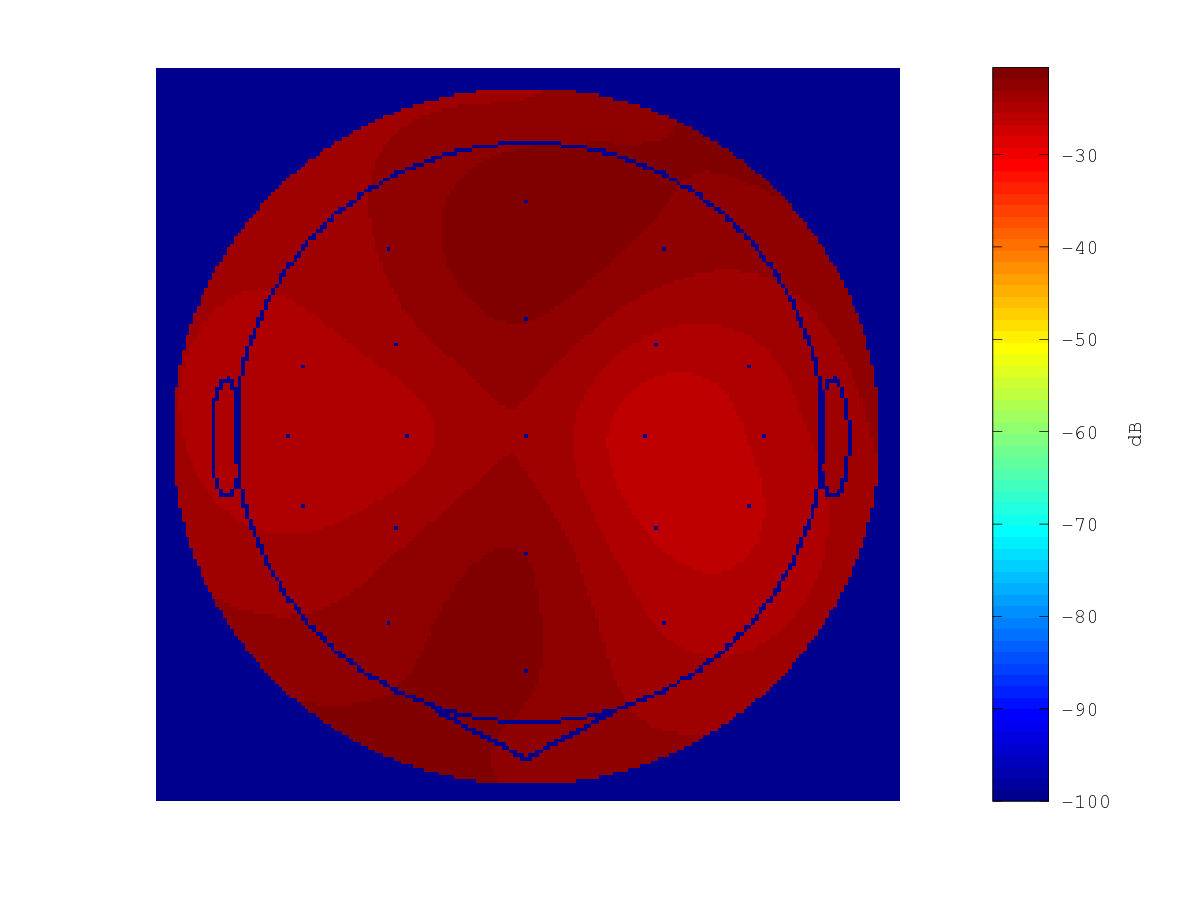
\includegraphics[width=2.5in]{scalpplot.png}}
\end{minipage}
\begin{minipage}[t]{0.5\textwidth}
~\\	
\IfStrEq{\PlotType}{scatter}{\textbf{\Large{Summary:}}\\
\if\IsConcussed1
\if\PrevConcussions0
Based on the results of the EEGlewave algorithm, the baseline brain signals have been classified as belonging to the concussed group. However, the past history and results from the SCAT do not seems to suggest that there is evidence of a previous recent concussion or any other condition that may lead to this result.\\
The EEGlewave algorithm is not 100\% accurate and there is a 10\% chance that some players will be misclassified. It is therefore possible that your child's brain signals fall into the group that are misclassified. However, if you have any concerns or if your child is showing any symptoms that might suggest any medical issues we suggest that your child is seen by your family physician for a physical examination.\\
Please feel free to contact Dr. Virji-Babul if you would like to discuss these results or would like more information.
\else
Based on the results of the EEGlewave algorithm the baseline brain signals have been classified as belonging to the concussed group. The past history and results from the SCAT also seems to suggest that there is evidence of a previous recent concussion. Given these results we suggest that your child is seen by your family physician for a physical examination and be cleared before he/she returns to play.\\
We will contact you again for a second EEG scan within a month to compare the baseline brain signals to determine if your brain signals are changing as a result of recovery. We will also repeat the SCAT to evaluate general changes in symptoms, balance and cognition from the initial assessment.\\
Please feel free to contact Dr. Virji-Babul if you would like more information.
\fi
\else
Based on the results of the EEGlewave algorithm the brain signals appear to be within normal range. If your child receives an impact to the head/body and a concussion is suspected please see your physician and contact EEGlewave at care@eeglewave.com. We will arrange for a second EEG scan and compare your baseline brain signals to the second EEG scan to determine if there have been any changes in your brain activity that may have resulted from the impact. We will also repeat the SCAT3 to evaluate changes in symptoms, balance and cognition from the baseline assessment.
\fi}{Electroencephalography (EEG) is a technique that records the electrical activity of the brain. Brain cells communicate using electrical impulses and are active all the time, even when sitting quietly or sleeping. The EEGlewave algorithm uses EEG signals from the whole brain to evaluate changes in these signals that may be due to a concussion.\\}
\end{minipage}
}}

 %comment starts
\iffalse
\fbox{\parbox{\textwidth}{
\textbf{\Large{Summary:}}\\
\if\IsConcussed1
\if\PrevConcussions0
Based on the results of the EEGlewave algorithm, the baseline brain signals have been classified as belonging to the concussed group. However, the past history and results from the SCAT do not seems to suggest that there is evidence of a previous recent concussion or any other condition that may lead to this result.\\
The EEGlewave algorithm is not 100\% accurate and there is a 10\% chance that some players will be misclassified. It is therefore possible that your child's brain signals fall into the group that are misclassified. However, if you have any concerns or if your child is showing any symptoms that might suggest any medical issues we suggest that your child is seen by your family physician for a physical examination.\\
Please feel free to contact Dr. Virji-Babul if you would like to discuss these results or would like more information.
\else
Based on the results of the EEGlewave algorithm the baseline brain signals have been classified as belonging to the concussed group. The past history and results from the SCAT also seems to suggest that there is evidence of a previous recent concussion. Given these results we suggest that your child is seen by your family physician for a physical examination and be cleared before he/she returns to play.\\
We will contact you again for a second EEG scan within a month to compare the baseline brain signals to determine if your brain signals are changing as a result of recovery. We will also repeat the SCAT to evaluate general changes in symptoms, balance and cognition from the initial assessment.\\
Please feel free to contact Dr. Virji-Babul if you would like more information.
\fi
\else
Based on the results of the EEGlewave algorithm the brain signals appear to be within normal range. If your child receives an impact to the head/body and a concussion is suspected please see your physician and contact EEGlewave at care@eeglewave.com. We will arrange for a second EEG scan and compare your baseline brain signals to the second EEG scan to determine if there have been any changes in your brain activity that may have resulted from the impact. We will also repeat the SCAT3 to evaluate changes in symptoms, balance and cognition from the baseline assessment.
\fi
}}
\fi % till here commenting out

% Add the footnote. A better way would be to use fancyhdr
\vfill
{\footnotesize\color{EWgray}\sffamily
	NOTE: EEGlewave does not provide medical advice. This report should not be used as a substitute for professional medical consultation.\\
}
\end{document}
}%The .tex filename goes here (NOT the same as \jobname)
\unless\ifdefined\FirstName
\endinput\expandafter\expandafter\expandafter\ReadFirstName\fi

\def\ReadLastName#1 {%
	\def\LastName{#1}%
	% NOTE: This report is to be compiled through the Octave command prompt.
% The following command should be typed into an Octave session to generate the report.
% system("pdflatex.exe -synctex=1 -interaction=nonstopmode -job-name=FirstName_LastName report.tex FirstName Lastname ParentName ID Handedness PrevConcussions Age ScanType")

% Definitions for command line arguments
\def\ReadFirstName#1 {%
	\def\FirstName{#1}%
	\input{report}}%The .tex filename goes here (NOT the same as \jobname)
\unless\ifdefined\FirstName
\endinput\expandafter\expandafter\expandafter\ReadFirstName\fi

\def\ReadLastName#1 {%
	\def\LastName{#1}%
	\input{report}}%The .tex filename goes here (NOT the same as \jobname)
\unless\ifdefined\LastName
\endinput\expandafter\expandafter\expandafter\ReadLastName\fi

\def\ReadParentFirstName#1 {%
	\def\ParentFirstName{#1}%
	\input{report}}%The .tex filename goes here (NOT the same as \jobname)
\unless\ifdefined\ParentFirstName
\endinput\expandafter\expandafter\expandafter\ReadParentFirstName\fi

\def\ReadParentLastName#1 {%
	\def\ParentLastName{#1}%
	\input{report}}%The .tex filename goes here (NOT the same as \jobname)
\unless\ifdefined\ParentLastName
\endinput\expandafter\expandafter\expandafter\ReadParentLastName\fi

\def\ReadID#1 {%
	\def\ID{#1}%
	\input{report}}%The .tex filename goes here (NOT the same as \jobname)
\unless\ifdefined\ID
\endinput\expandafter\expandafter\expandafter\ReadID\fi

\def\ReadHandedness#1 {%
	\def\Handedness{#1}%
	\input{report}}%The .tex filename goes here (NOT the same as \jobname)
\unless\ifdefined\Handedness
\endinput\expandafter\expandafter\expandafter\ReadHandedness\fi

\def\ReadPrevConcussions#1 {%
	\def\PrevConcussions{#1}%
	\input{report}}%The .tex filename goes here (NOT the same as \jobname)
\unless\ifdefined\PrevConcussions
\endinput\expandafter\expandafter\expandafter\ReadPrevConcussions\fi

\def\ReadMostRecentConcussion#1 {%
	\def\MostRecentConcussion{#1}%
	\input{report}}%The .tex filename goes here (NOT the same as \jobname)
\unless\ifdefined\MostRecentConcussion
\endinput\expandafter\expandafter\expandafter\ReadMostRecentConcussion\fi

\def\ReadIsConcussed#1 {%
	\def\IsConcussed{#1}%
	\input{report}}%The .tex filename goes here (NOT the same as \jobname)
\unless\ifdefined\IsConcussed
\endinput\expandafter\expandafter\expandafter\ReadIsConcussed\fi

\def\ReadDivision#1 {%
	\def\Division{#1}%
	\input{report}}%The .tex filename goes here (NOT the same as \jobname)
\unless\ifdefined\Division
\endinput\expandafter\expandafter\expandafter\ReadDivision\fi

\def\ReadGender#1 {%
	\def\Gender{#1}%
	\input{report}}%The .tex filename goes here (NOT the same as \jobname)
\unless\ifdefined\Gender
\endinput\expandafter\expandafter\expandafter\ReadGender\fi

\def\ReadAge#1 {%
	\def\Age{#1}%
	\input{report}}%The .tex filename goes here (NOT the same as \jobname)
\unless\ifdefined\Age
\endinput\expandafter\expandafter\expandafter\ReadAge\fi

\def\ReadDOS#1 {%
	\def\DOS{#1}%
	\input{report}}%The .tex filename goes here (NOT the same as \jobname)
\unless\ifdefined\DOS
\endinput\expandafter\expandafter\expandafter\ReadDOS\fi

\def\ReadScanType#1 {%
	\def\ScanType{#1}%
	\input{report}}%The .tex filename goes here (NOT the same as \jobname)
\unless\ifdefined\ScanType
\endinput\expandafter\expandafter\expandafter\ReadScanType\fi

\def\ReadNumSymptoms#1 {%
	\def\NumSymptoms{#1}%
	\input{report}}%The .tex filename goes here (NOT the same as \jobname)
\unless\ifdefined\NumSymptoms
\endinput\expandafter\expandafter\expandafter\ReadNumSymptoms\fi

\def\ReadSeverityScore#1 {%
	\def\SeverityScore{#1}%
	\input{report}}%The .tex filename goes here (NOT the same as \jobname)
\unless\ifdefined\SeverityScore
\endinput\expandafter\expandafter\expandafter\ReadSeverityScore\fi

\def\ReadOrientation#1 {%
	\def\Orientation{#1}%
	\input{report}}%The .tex filename goes here (NOT the same as \jobname)
\unless\ifdefined\Orientation
\endinput\expandafter\expandafter\expandafter\ReadOrientation\fi

\def\ReadOrientationTotal#1 {%
	\def\OrientationTotal{#1}%
	\input{report}}%The .tex filename goes here (NOT the same as \jobname)
\unless\ifdefined\OrientationTotal
\endinput\expandafter\expandafter\expandafter\ReadOrientationTotal\fi

\def\ReadImmMem#1 {%
	\def\ImmMem{#1}%
	\input{report}}%The .tex filename goes here (NOT the same as \jobname)
\unless\ifdefined\ImmMem
\endinput\expandafter\expandafter\expandafter\ReadImmMem\fi

\def\ReadConcentration#1 {%
	\def\Concentration{#1}%
	\input{report}}%The .tex filename goes here (NOT the same as \jobname)
\unless\ifdefined\Concentration
\endinput\expandafter\expandafter\expandafter\ReadConcentration\fi

\def\ReadConcentrationTotal#1 {%
	\def\ConcentrationTotal{#1}%
	\input{report}}%The .tex filename goes here (NOT the same as \jobname)
\unless\ifdefined\ConcentrationTotal
\endinput\expandafter\expandafter\expandafter\ReadConcentrationTotal\fi

\def\ReadDelayedRecall#1 {%
	\def\DelayedRecall{#1}%
	\input{report}}%The .tex filename goes here (NOT the same as \jobname)
\unless\ifdefined\DelayedRecall
\endinput\expandafter\expandafter\expandafter\ReadDelayedRecall\fi

\def\ReadSAC#1 {%
	\def\SAC{#1}%
	\input{report}}%The .tex filename goes here (NOT the same as \jobname)
\unless\ifdefined\SAC
\endinput\expandafter\expandafter\expandafter\ReadSAC\fi

\def\ReadBESS#1 {%
	\def\BESS{#1}%
	\input{report}}%The .tex filename goes here (NOT the same as \jobname)
\unless\ifdefined\BESS
\endinput\expandafter\expandafter\expandafter\ReadBESS\fi

\def\ReadTandemGait#1 {%
	\def\TandemGait{#1}%
	\input{report}}%The .tex filename goes here (NOT the same as \jobname)
\unless\ifdefined\TandemGait
\endinput\expandafter\expandafter\expandafter\ReadTandemGait\fi

\def\ReadCoordination#1 {%
	\def\Coordination{#1}%
	\input{report}}%The .tex filename goes here (NOT the same as \jobname)
\unless\ifdefined\Coordination
\endinput\expandafter\expandafter\expandafter\ReadCoordination\fi

\def\ReadPlotType#1 {%
	\def\PlotType{#1}%
	\input{report}}%The .tex filename goes here (NOT the same as \jobname)
\unless\ifdefined\PlotType
\endinput\expandafter\expandafter\expandafter\ReadPlotType\fi

\documentclass{article}

\usepackage[dvinames]{xcolor}
% Measurements are taken directly from the guide
\usepackage[top=2in,left=0.5in,bottom=0.5in,right=0.5in]{geometry}
\usepackage{graphicx}
\usepackage[colorlinks=false,
            pdfborder={0 0 0},
            ]{hyperref}
\usepackage{lipsum}
\usepackage[absolute]{textpos}
\usepackage{tikz}
\usetikzlibrary{calc}
% A nice serif font, but no the prescribed nonfree ITC stone
\usepackage[oldstylenums]{kpfonts}
\usepackage[T1]{fontenc	}
\usepackage[12pt]{moresize}
\usepackage{xstring}

% No paragraph indentation
\parindent0pt
\setlength{\parskip}{0.8\baselineskip}
\raggedright
\pagestyle{empty}


\definecolor{EWgray}{HTML}{5e6a71}

\begin{document}
	\begin{center}
		\HUGE{~}\\
		\HUGE{~}\\
		\HUGE{~}\\
		\textbf{\HUGE{EEGlewave Inc.}}\\[1in]
		\textbf{\huge{\ScanType~Report}}\\[1cm]
	\end{center}
	\newpage
\bigskip
% -------------------------------------------------------
% Add logo, the text under the crimson line, and the line itself
\begin{textblock*}{2in}[0.3066,0.39](1.25in,1.23in)
	
\includegraphics[width=1.5in]{eeglewave-front-211x128-88.png}
\end{textblock*}
\begin{textblock*}{6.375in}(1.5in,1.4in)   % 6.375=8.5 - 1.5 - 0.625
	\sffamily
	\hfill \color{EWgray} EEGlewave Inc.\\
	\hfill \url{care@eeglewave.com} \textbullet\ \url{http://eeglewave.com}
\end{textblock*}
\begin{tikzpicture}[remember picture,overlay]
\draw[line width=1pt] (current page.north west)+(0.5in,-1.85in) -- ($(-0.5in,-1.85in)+(current page.north east)$);
\end{tikzpicture}
\fbox{\parbox{\textwidth}{
\textbf{\Large{General Information:}}\\
\begin{minipage}[t]{0.55\textwidth}

\textbf{Name: } \FirstName~\LastName  \\
\textbf{Parent/Guardian's Name: } \ParentFirstName~\ParentLastName  \\
\textbf{ID: } \ID   \\
\textbf{Handedness: } \Handedness  \\
\textbf{Number of Previous Concussions: } \PrevConcussions \\
\textbf{Date of Most Recent Concussion: } \MostRecentConcussion
\end{minipage}
\begin{minipage}[t]{0.45\textwidth}
	\textbf{Division: } \Division  \\
	\textbf{Gender: } \Gender  \\
	\textbf{Age: } \Age  \\
	\textbf{Date of Scan: } \DOS \\
	\textbf{Type of Scan: } \ScanType  \\
\end{minipage}
}}

\fbox{\parbox{\textwidth}{
\textbf{\Large{SCAT3 Scoring Summary:}}\\
\begin{minipage}[t]{0.55\textwidth}
\textbf{Number of Symptoms (/22): } \\
\textbf{Symptom Severity Score (/132): } \\

\textbf{Orientation (/\OrientationTotal): }  \\
\textbf{Immediate Memory (/15): } \\
\textbf{Concentration (/\ConcentrationTotal): } \\
\textbf{Delayed Recall (/5): } \\
\textbf{SAC Total (/30): } \\

\textbf{BESS (total errors): } \\
\textbf{Tandem Gait (seconds): } \\
\textbf{Coordination (/1): } 
\end{minipage}
\begin{minipage}[t]{0.25\textwidth}
\NumSymptoms  \\
\SeverityScore  \\

\Orientation  \\
\ImmMem  \\
\Concentration  \\
\DelayedRecall \\
\SAC  \\

\BESS  \\
\TandemGait  \\
\Coordination
\end{minipage}
}}

\fbox{\parbox{\textwidth}{
\textbf{\Large{\IfStrEq{\PlotType}{scatter}{Scatter Plot:}{EEG Plot of Power at Rest:}}}\\
\begin{minipage}[t]{0.5\textwidth}
	~\\
	\IfStrEq{\PlotType}{scatter}{\includegraphics[width=3.25in]{scatterplot.png}}{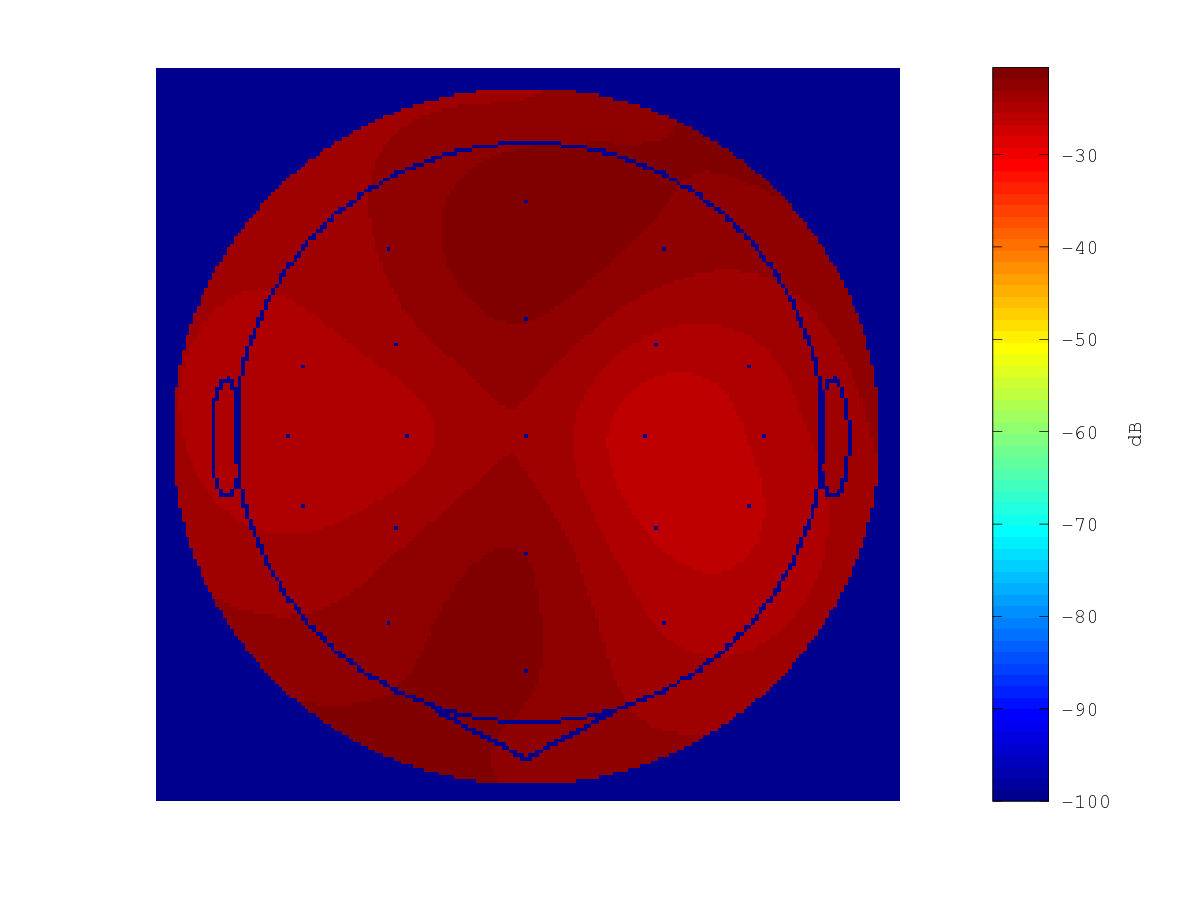
\includegraphics[width=2.5in]{scalpplot.png}}
\end{minipage}
\begin{minipage}[t]{0.5\textwidth}
~\\	
\IfStrEq{\PlotType}{scatter}{\textbf{\Large{Summary:}}\\
\if\IsConcussed1
\if\PrevConcussions0
Based on the results of the EEGlewave algorithm, the baseline brain signals have been classified as belonging to the concussed group. However, the past history and results from the SCAT do not seems to suggest that there is evidence of a previous recent concussion or any other condition that may lead to this result.\\
The EEGlewave algorithm is not 100\% accurate and there is a 10\% chance that some players will be misclassified. It is therefore possible that your child's brain signals fall into the group that are misclassified. However, if you have any concerns or if your child is showing any symptoms that might suggest any medical issues we suggest that your child is seen by your family physician for a physical examination.\\
Please feel free to contact Dr. Virji-Babul if you would like to discuss these results or would like more information.
\else
Based on the results of the EEGlewave algorithm the baseline brain signals have been classified as belonging to the concussed group. The past history and results from the SCAT also seems to suggest that there is evidence of a previous recent concussion. Given these results we suggest that your child is seen by your family physician for a physical examination and be cleared before he/she returns to play.\\
We will contact you again for a second EEG scan within a month to compare the baseline brain signals to determine if your brain signals are changing as a result of recovery. We will also repeat the SCAT to evaluate general changes in symptoms, balance and cognition from the initial assessment.\\
Please feel free to contact Dr. Virji-Babul if you would like more information.
\fi
\else
Based on the results of the EEGlewave algorithm the brain signals appear to be within normal range. If your child receives an impact to the head/body and a concussion is suspected please see your physician and contact EEGlewave at care@eeglewave.com. We will arrange for a second EEG scan and compare your baseline brain signals to the second EEG scan to determine if there have been any changes in your brain activity that may have resulted from the impact. We will also repeat the SCAT3 to evaluate changes in symptoms, balance and cognition from the baseline assessment.
\fi}{Electroencephalography (EEG) is a technique that records the electrical activity of the brain. Brain cells communicate using electrical impulses and are active all the time, even when sitting quietly or sleeping. The EEGlewave algorithm uses EEG signals from the whole brain to evaluate changes in these signals that may be due to a concussion.\\}
\end{minipage}
}}

 %comment starts
\iffalse
\fbox{\parbox{\textwidth}{
\textbf{\Large{Summary:}}\\
\if\IsConcussed1
\if\PrevConcussions0
Based on the results of the EEGlewave algorithm, the baseline brain signals have been classified as belonging to the concussed group. However, the past history and results from the SCAT do not seems to suggest that there is evidence of a previous recent concussion or any other condition that may lead to this result.\\
The EEGlewave algorithm is not 100\% accurate and there is a 10\% chance that some players will be misclassified. It is therefore possible that your child's brain signals fall into the group that are misclassified. However, if you have any concerns or if your child is showing any symptoms that might suggest any medical issues we suggest that your child is seen by your family physician for a physical examination.\\
Please feel free to contact Dr. Virji-Babul if you would like to discuss these results or would like more information.
\else
Based on the results of the EEGlewave algorithm the baseline brain signals have been classified as belonging to the concussed group. The past history and results from the SCAT also seems to suggest that there is evidence of a previous recent concussion. Given these results we suggest that your child is seen by your family physician for a physical examination and be cleared before he/she returns to play.\\
We will contact you again for a second EEG scan within a month to compare the baseline brain signals to determine if your brain signals are changing as a result of recovery. We will also repeat the SCAT to evaluate general changes in symptoms, balance and cognition from the initial assessment.\\
Please feel free to contact Dr. Virji-Babul if you would like more information.
\fi
\else
Based on the results of the EEGlewave algorithm the brain signals appear to be within normal range. If your child receives an impact to the head/body and a concussion is suspected please see your physician and contact EEGlewave at care@eeglewave.com. We will arrange for a second EEG scan and compare your baseline brain signals to the second EEG scan to determine if there have been any changes in your brain activity that may have resulted from the impact. We will also repeat the SCAT3 to evaluate changes in symptoms, balance and cognition from the baseline assessment.
\fi
}}
\fi % till here commenting out

% Add the footnote. A better way would be to use fancyhdr
\vfill
{\footnotesize\color{EWgray}\sffamily
	NOTE: EEGlewave does not provide medical advice. This report should not be used as a substitute for professional medical consultation.\\
}
\end{document}
}%The .tex filename goes here (NOT the same as \jobname)
\unless\ifdefined\LastName
\endinput\expandafter\expandafter\expandafter\ReadLastName\fi

\def\ReadParentFirstName#1 {%
	\def\ParentFirstName{#1}%
	% NOTE: This report is to be compiled through the Octave command prompt.
% The following command should be typed into an Octave session to generate the report.
% system("pdflatex.exe -synctex=1 -interaction=nonstopmode -job-name=FirstName_LastName report.tex FirstName Lastname ParentName ID Handedness PrevConcussions Age ScanType")

% Definitions for command line arguments
\def\ReadFirstName#1 {%
	\def\FirstName{#1}%
	\input{report}}%The .tex filename goes here (NOT the same as \jobname)
\unless\ifdefined\FirstName
\endinput\expandafter\expandafter\expandafter\ReadFirstName\fi

\def\ReadLastName#1 {%
	\def\LastName{#1}%
	\input{report}}%The .tex filename goes here (NOT the same as \jobname)
\unless\ifdefined\LastName
\endinput\expandafter\expandafter\expandafter\ReadLastName\fi

\def\ReadParentFirstName#1 {%
	\def\ParentFirstName{#1}%
	\input{report}}%The .tex filename goes here (NOT the same as \jobname)
\unless\ifdefined\ParentFirstName
\endinput\expandafter\expandafter\expandafter\ReadParentFirstName\fi

\def\ReadParentLastName#1 {%
	\def\ParentLastName{#1}%
	\input{report}}%The .tex filename goes here (NOT the same as \jobname)
\unless\ifdefined\ParentLastName
\endinput\expandafter\expandafter\expandafter\ReadParentLastName\fi

\def\ReadID#1 {%
	\def\ID{#1}%
	\input{report}}%The .tex filename goes here (NOT the same as \jobname)
\unless\ifdefined\ID
\endinput\expandafter\expandafter\expandafter\ReadID\fi

\def\ReadHandedness#1 {%
	\def\Handedness{#1}%
	\input{report}}%The .tex filename goes here (NOT the same as \jobname)
\unless\ifdefined\Handedness
\endinput\expandafter\expandafter\expandafter\ReadHandedness\fi

\def\ReadPrevConcussions#1 {%
	\def\PrevConcussions{#1}%
	\input{report}}%The .tex filename goes here (NOT the same as \jobname)
\unless\ifdefined\PrevConcussions
\endinput\expandafter\expandafter\expandafter\ReadPrevConcussions\fi

\def\ReadMostRecentConcussion#1 {%
	\def\MostRecentConcussion{#1}%
	\input{report}}%The .tex filename goes here (NOT the same as \jobname)
\unless\ifdefined\MostRecentConcussion
\endinput\expandafter\expandafter\expandafter\ReadMostRecentConcussion\fi

\def\ReadIsConcussed#1 {%
	\def\IsConcussed{#1}%
	\input{report}}%The .tex filename goes here (NOT the same as \jobname)
\unless\ifdefined\IsConcussed
\endinput\expandafter\expandafter\expandafter\ReadIsConcussed\fi

\def\ReadDivision#1 {%
	\def\Division{#1}%
	\input{report}}%The .tex filename goes here (NOT the same as \jobname)
\unless\ifdefined\Division
\endinput\expandafter\expandafter\expandafter\ReadDivision\fi

\def\ReadGender#1 {%
	\def\Gender{#1}%
	\input{report}}%The .tex filename goes here (NOT the same as \jobname)
\unless\ifdefined\Gender
\endinput\expandafter\expandafter\expandafter\ReadGender\fi

\def\ReadAge#1 {%
	\def\Age{#1}%
	\input{report}}%The .tex filename goes here (NOT the same as \jobname)
\unless\ifdefined\Age
\endinput\expandafter\expandafter\expandafter\ReadAge\fi

\def\ReadDOS#1 {%
	\def\DOS{#1}%
	\input{report}}%The .tex filename goes here (NOT the same as \jobname)
\unless\ifdefined\DOS
\endinput\expandafter\expandafter\expandafter\ReadDOS\fi

\def\ReadScanType#1 {%
	\def\ScanType{#1}%
	\input{report}}%The .tex filename goes here (NOT the same as \jobname)
\unless\ifdefined\ScanType
\endinput\expandafter\expandafter\expandafter\ReadScanType\fi

\def\ReadNumSymptoms#1 {%
	\def\NumSymptoms{#1}%
	\input{report}}%The .tex filename goes here (NOT the same as \jobname)
\unless\ifdefined\NumSymptoms
\endinput\expandafter\expandafter\expandafter\ReadNumSymptoms\fi

\def\ReadSeverityScore#1 {%
	\def\SeverityScore{#1}%
	\input{report}}%The .tex filename goes here (NOT the same as \jobname)
\unless\ifdefined\SeverityScore
\endinput\expandafter\expandafter\expandafter\ReadSeverityScore\fi

\def\ReadOrientation#1 {%
	\def\Orientation{#1}%
	\input{report}}%The .tex filename goes here (NOT the same as \jobname)
\unless\ifdefined\Orientation
\endinput\expandafter\expandafter\expandafter\ReadOrientation\fi

\def\ReadOrientationTotal#1 {%
	\def\OrientationTotal{#1}%
	\input{report}}%The .tex filename goes here (NOT the same as \jobname)
\unless\ifdefined\OrientationTotal
\endinput\expandafter\expandafter\expandafter\ReadOrientationTotal\fi

\def\ReadImmMem#1 {%
	\def\ImmMem{#1}%
	\input{report}}%The .tex filename goes here (NOT the same as \jobname)
\unless\ifdefined\ImmMem
\endinput\expandafter\expandafter\expandafter\ReadImmMem\fi

\def\ReadConcentration#1 {%
	\def\Concentration{#1}%
	\input{report}}%The .tex filename goes here (NOT the same as \jobname)
\unless\ifdefined\Concentration
\endinput\expandafter\expandafter\expandafter\ReadConcentration\fi

\def\ReadConcentrationTotal#1 {%
	\def\ConcentrationTotal{#1}%
	\input{report}}%The .tex filename goes here (NOT the same as \jobname)
\unless\ifdefined\ConcentrationTotal
\endinput\expandafter\expandafter\expandafter\ReadConcentrationTotal\fi

\def\ReadDelayedRecall#1 {%
	\def\DelayedRecall{#1}%
	\input{report}}%The .tex filename goes here (NOT the same as \jobname)
\unless\ifdefined\DelayedRecall
\endinput\expandafter\expandafter\expandafter\ReadDelayedRecall\fi

\def\ReadSAC#1 {%
	\def\SAC{#1}%
	\input{report}}%The .tex filename goes here (NOT the same as \jobname)
\unless\ifdefined\SAC
\endinput\expandafter\expandafter\expandafter\ReadSAC\fi

\def\ReadBESS#1 {%
	\def\BESS{#1}%
	\input{report}}%The .tex filename goes here (NOT the same as \jobname)
\unless\ifdefined\BESS
\endinput\expandafter\expandafter\expandafter\ReadBESS\fi

\def\ReadTandemGait#1 {%
	\def\TandemGait{#1}%
	\input{report}}%The .tex filename goes here (NOT the same as \jobname)
\unless\ifdefined\TandemGait
\endinput\expandafter\expandafter\expandafter\ReadTandemGait\fi

\def\ReadCoordination#1 {%
	\def\Coordination{#1}%
	\input{report}}%The .tex filename goes here (NOT the same as \jobname)
\unless\ifdefined\Coordination
\endinput\expandafter\expandafter\expandafter\ReadCoordination\fi

\def\ReadPlotType#1 {%
	\def\PlotType{#1}%
	\input{report}}%The .tex filename goes here (NOT the same as \jobname)
\unless\ifdefined\PlotType
\endinput\expandafter\expandafter\expandafter\ReadPlotType\fi

\documentclass{article}

\usepackage[dvinames]{xcolor}
% Measurements are taken directly from the guide
\usepackage[top=2in,left=0.5in,bottom=0.5in,right=0.5in]{geometry}
\usepackage{graphicx}
\usepackage[colorlinks=false,
            pdfborder={0 0 0},
            ]{hyperref}
\usepackage{lipsum}
\usepackage[absolute]{textpos}
\usepackage{tikz}
\usetikzlibrary{calc}
% A nice serif font, but no the prescribed nonfree ITC stone
\usepackage[oldstylenums]{kpfonts}
\usepackage[T1]{fontenc	}
\usepackage[12pt]{moresize}
\usepackage{xstring}

% No paragraph indentation
\parindent0pt
\setlength{\parskip}{0.8\baselineskip}
\raggedright
\pagestyle{empty}


\definecolor{EWgray}{HTML}{5e6a71}

\begin{document}
	\begin{center}
		\HUGE{~}\\
		\HUGE{~}\\
		\HUGE{~}\\
		\textbf{\HUGE{EEGlewave Inc.}}\\[1in]
		\textbf{\huge{\ScanType~Report}}\\[1cm]
	\end{center}
	\newpage
\bigskip
% -------------------------------------------------------
% Add logo, the text under the crimson line, and the line itself
\begin{textblock*}{2in}[0.3066,0.39](1.25in,1.23in)
	
\includegraphics[width=1.5in]{eeglewave-front-211x128-88.png}
\end{textblock*}
\begin{textblock*}{6.375in}(1.5in,1.4in)   % 6.375=8.5 - 1.5 - 0.625
	\sffamily
	\hfill \color{EWgray} EEGlewave Inc.\\
	\hfill \url{care@eeglewave.com} \textbullet\ \url{http://eeglewave.com}
\end{textblock*}
\begin{tikzpicture}[remember picture,overlay]
\draw[line width=1pt] (current page.north west)+(0.5in,-1.85in) -- ($(-0.5in,-1.85in)+(current page.north east)$);
\end{tikzpicture}
\fbox{\parbox{\textwidth}{
\textbf{\Large{General Information:}}\\
\begin{minipage}[t]{0.55\textwidth}

\textbf{Name: } \FirstName~\LastName  \\
\textbf{Parent/Guardian's Name: } \ParentFirstName~\ParentLastName  \\
\textbf{ID: } \ID   \\
\textbf{Handedness: } \Handedness  \\
\textbf{Number of Previous Concussions: } \PrevConcussions \\
\textbf{Date of Most Recent Concussion: } \MostRecentConcussion
\end{minipage}
\begin{minipage}[t]{0.45\textwidth}
	\textbf{Division: } \Division  \\
	\textbf{Gender: } \Gender  \\
	\textbf{Age: } \Age  \\
	\textbf{Date of Scan: } \DOS \\
	\textbf{Type of Scan: } \ScanType  \\
\end{minipage}
}}

\fbox{\parbox{\textwidth}{
\textbf{\Large{SCAT3 Scoring Summary:}}\\
\begin{minipage}[t]{0.55\textwidth}
\textbf{Number of Symptoms (/22): } \\
\textbf{Symptom Severity Score (/132): } \\

\textbf{Orientation (/\OrientationTotal): }  \\
\textbf{Immediate Memory (/15): } \\
\textbf{Concentration (/\ConcentrationTotal): } \\
\textbf{Delayed Recall (/5): } \\
\textbf{SAC Total (/30): } \\

\textbf{BESS (total errors): } \\
\textbf{Tandem Gait (seconds): } \\
\textbf{Coordination (/1): } 
\end{minipage}
\begin{minipage}[t]{0.25\textwidth}
\NumSymptoms  \\
\SeverityScore  \\

\Orientation  \\
\ImmMem  \\
\Concentration  \\
\DelayedRecall \\
\SAC  \\

\BESS  \\
\TandemGait  \\
\Coordination
\end{minipage}
}}

\fbox{\parbox{\textwidth}{
\textbf{\Large{\IfStrEq{\PlotType}{scatter}{Scatter Plot:}{EEG Plot of Power at Rest:}}}\\
\begin{minipage}[t]{0.5\textwidth}
	~\\
	\IfStrEq{\PlotType}{scatter}{\includegraphics[width=3.25in]{scatterplot.png}}{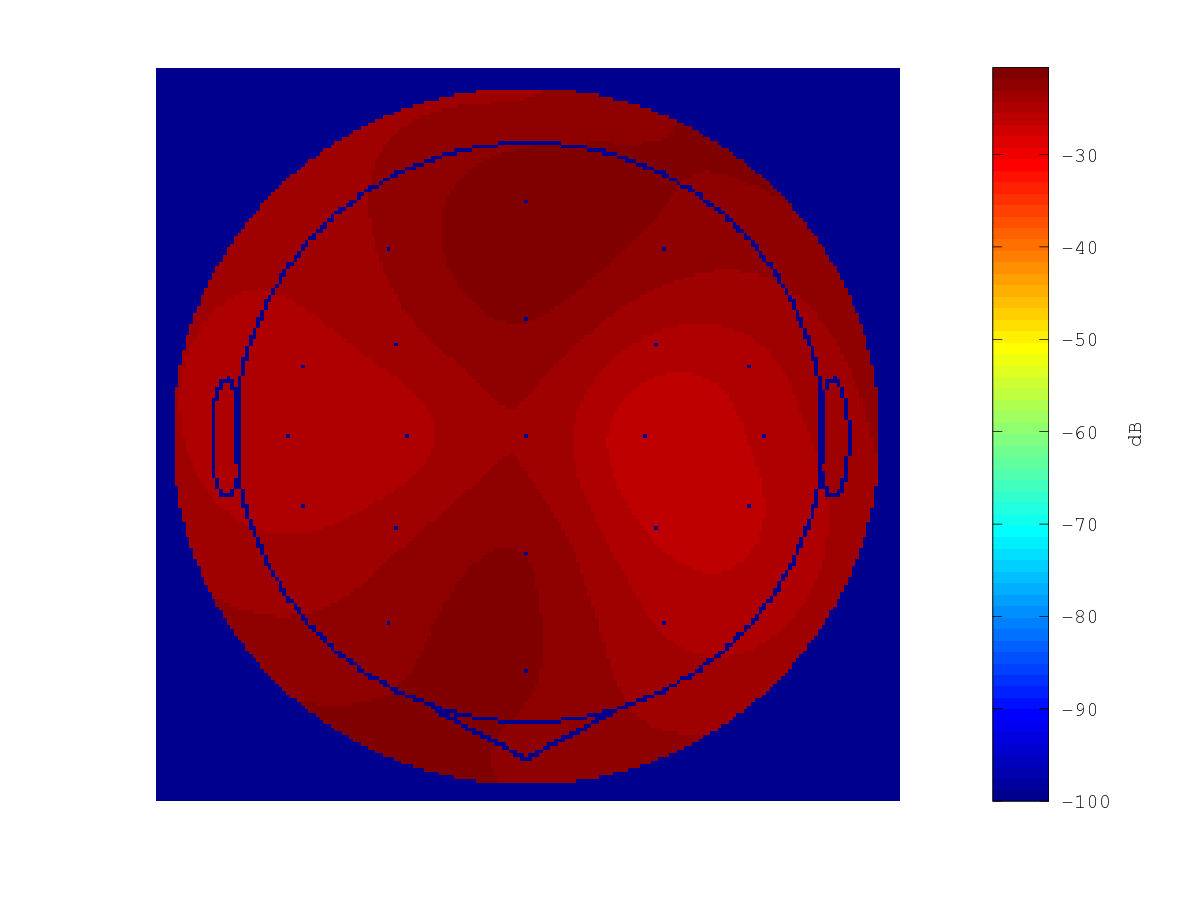
\includegraphics[width=2.5in]{scalpplot.png}}
\end{minipage}
\begin{minipage}[t]{0.5\textwidth}
~\\	
\IfStrEq{\PlotType}{scatter}{\textbf{\Large{Summary:}}\\
\if\IsConcussed1
\if\PrevConcussions0
Based on the results of the EEGlewave algorithm, the baseline brain signals have been classified as belonging to the concussed group. However, the past history and results from the SCAT do not seems to suggest that there is evidence of a previous recent concussion or any other condition that may lead to this result.\\
The EEGlewave algorithm is not 100\% accurate and there is a 10\% chance that some players will be misclassified. It is therefore possible that your child's brain signals fall into the group that are misclassified. However, if you have any concerns or if your child is showing any symptoms that might suggest any medical issues we suggest that your child is seen by your family physician for a physical examination.\\
Please feel free to contact Dr. Virji-Babul if you would like to discuss these results or would like more information.
\else
Based on the results of the EEGlewave algorithm the baseline brain signals have been classified as belonging to the concussed group. The past history and results from the SCAT also seems to suggest that there is evidence of a previous recent concussion. Given these results we suggest that your child is seen by your family physician for a physical examination and be cleared before he/she returns to play.\\
We will contact you again for a second EEG scan within a month to compare the baseline brain signals to determine if your brain signals are changing as a result of recovery. We will also repeat the SCAT to evaluate general changes in symptoms, balance and cognition from the initial assessment.\\
Please feel free to contact Dr. Virji-Babul if you would like more information.
\fi
\else
Based on the results of the EEGlewave algorithm the brain signals appear to be within normal range. If your child receives an impact to the head/body and a concussion is suspected please see your physician and contact EEGlewave at care@eeglewave.com. We will arrange for a second EEG scan and compare your baseline brain signals to the second EEG scan to determine if there have been any changes in your brain activity that may have resulted from the impact. We will also repeat the SCAT3 to evaluate changes in symptoms, balance and cognition from the baseline assessment.
\fi}{Electroencephalography (EEG) is a technique that records the electrical activity of the brain. Brain cells communicate using electrical impulses and are active all the time, even when sitting quietly or sleeping. The EEGlewave algorithm uses EEG signals from the whole brain to evaluate changes in these signals that may be due to a concussion.\\}
\end{minipage}
}}

 %comment starts
\iffalse
\fbox{\parbox{\textwidth}{
\textbf{\Large{Summary:}}\\
\if\IsConcussed1
\if\PrevConcussions0
Based on the results of the EEGlewave algorithm, the baseline brain signals have been classified as belonging to the concussed group. However, the past history and results from the SCAT do not seems to suggest that there is evidence of a previous recent concussion or any other condition that may lead to this result.\\
The EEGlewave algorithm is not 100\% accurate and there is a 10\% chance that some players will be misclassified. It is therefore possible that your child's brain signals fall into the group that are misclassified. However, if you have any concerns or if your child is showing any symptoms that might suggest any medical issues we suggest that your child is seen by your family physician for a physical examination.\\
Please feel free to contact Dr. Virji-Babul if you would like to discuss these results or would like more information.
\else
Based on the results of the EEGlewave algorithm the baseline brain signals have been classified as belonging to the concussed group. The past history and results from the SCAT also seems to suggest that there is evidence of a previous recent concussion. Given these results we suggest that your child is seen by your family physician for a physical examination and be cleared before he/she returns to play.\\
We will contact you again for a second EEG scan within a month to compare the baseline brain signals to determine if your brain signals are changing as a result of recovery. We will also repeat the SCAT to evaluate general changes in symptoms, balance and cognition from the initial assessment.\\
Please feel free to contact Dr. Virji-Babul if you would like more information.
\fi
\else
Based on the results of the EEGlewave algorithm the brain signals appear to be within normal range. If your child receives an impact to the head/body and a concussion is suspected please see your physician and contact EEGlewave at care@eeglewave.com. We will arrange for a second EEG scan and compare your baseline brain signals to the second EEG scan to determine if there have been any changes in your brain activity that may have resulted from the impact. We will also repeat the SCAT3 to evaluate changes in symptoms, balance and cognition from the baseline assessment.
\fi
}}
\fi % till here commenting out

% Add the footnote. A better way would be to use fancyhdr
\vfill
{\footnotesize\color{EWgray}\sffamily
	NOTE: EEGlewave does not provide medical advice. This report should not be used as a substitute for professional medical consultation.\\
}
\end{document}
}%The .tex filename goes here (NOT the same as \jobname)
\unless\ifdefined\ParentFirstName
\endinput\expandafter\expandafter\expandafter\ReadParentFirstName\fi

\def\ReadParentLastName#1 {%
	\def\ParentLastName{#1}%
	% NOTE: This report is to be compiled through the Octave command prompt.
% The following command should be typed into an Octave session to generate the report.
% system("pdflatex.exe -synctex=1 -interaction=nonstopmode -job-name=FirstName_LastName report.tex FirstName Lastname ParentName ID Handedness PrevConcussions Age ScanType")

% Definitions for command line arguments
\def\ReadFirstName#1 {%
	\def\FirstName{#1}%
	\input{report}}%The .tex filename goes here (NOT the same as \jobname)
\unless\ifdefined\FirstName
\endinput\expandafter\expandafter\expandafter\ReadFirstName\fi

\def\ReadLastName#1 {%
	\def\LastName{#1}%
	\input{report}}%The .tex filename goes here (NOT the same as \jobname)
\unless\ifdefined\LastName
\endinput\expandafter\expandafter\expandafter\ReadLastName\fi

\def\ReadParentFirstName#1 {%
	\def\ParentFirstName{#1}%
	\input{report}}%The .tex filename goes here (NOT the same as \jobname)
\unless\ifdefined\ParentFirstName
\endinput\expandafter\expandafter\expandafter\ReadParentFirstName\fi

\def\ReadParentLastName#1 {%
	\def\ParentLastName{#1}%
	\input{report}}%The .tex filename goes here (NOT the same as \jobname)
\unless\ifdefined\ParentLastName
\endinput\expandafter\expandafter\expandafter\ReadParentLastName\fi

\def\ReadID#1 {%
	\def\ID{#1}%
	\input{report}}%The .tex filename goes here (NOT the same as \jobname)
\unless\ifdefined\ID
\endinput\expandafter\expandafter\expandafter\ReadID\fi

\def\ReadHandedness#1 {%
	\def\Handedness{#1}%
	\input{report}}%The .tex filename goes here (NOT the same as \jobname)
\unless\ifdefined\Handedness
\endinput\expandafter\expandafter\expandafter\ReadHandedness\fi

\def\ReadPrevConcussions#1 {%
	\def\PrevConcussions{#1}%
	\input{report}}%The .tex filename goes here (NOT the same as \jobname)
\unless\ifdefined\PrevConcussions
\endinput\expandafter\expandafter\expandafter\ReadPrevConcussions\fi

\def\ReadMostRecentConcussion#1 {%
	\def\MostRecentConcussion{#1}%
	\input{report}}%The .tex filename goes here (NOT the same as \jobname)
\unless\ifdefined\MostRecentConcussion
\endinput\expandafter\expandafter\expandafter\ReadMostRecentConcussion\fi

\def\ReadIsConcussed#1 {%
	\def\IsConcussed{#1}%
	\input{report}}%The .tex filename goes here (NOT the same as \jobname)
\unless\ifdefined\IsConcussed
\endinput\expandafter\expandafter\expandafter\ReadIsConcussed\fi

\def\ReadDivision#1 {%
	\def\Division{#1}%
	\input{report}}%The .tex filename goes here (NOT the same as \jobname)
\unless\ifdefined\Division
\endinput\expandafter\expandafter\expandafter\ReadDivision\fi

\def\ReadGender#1 {%
	\def\Gender{#1}%
	\input{report}}%The .tex filename goes here (NOT the same as \jobname)
\unless\ifdefined\Gender
\endinput\expandafter\expandafter\expandafter\ReadGender\fi

\def\ReadAge#1 {%
	\def\Age{#1}%
	\input{report}}%The .tex filename goes here (NOT the same as \jobname)
\unless\ifdefined\Age
\endinput\expandafter\expandafter\expandafter\ReadAge\fi

\def\ReadDOS#1 {%
	\def\DOS{#1}%
	\input{report}}%The .tex filename goes here (NOT the same as \jobname)
\unless\ifdefined\DOS
\endinput\expandafter\expandafter\expandafter\ReadDOS\fi

\def\ReadScanType#1 {%
	\def\ScanType{#1}%
	\input{report}}%The .tex filename goes here (NOT the same as \jobname)
\unless\ifdefined\ScanType
\endinput\expandafter\expandafter\expandafter\ReadScanType\fi

\def\ReadNumSymptoms#1 {%
	\def\NumSymptoms{#1}%
	\input{report}}%The .tex filename goes here (NOT the same as \jobname)
\unless\ifdefined\NumSymptoms
\endinput\expandafter\expandafter\expandafter\ReadNumSymptoms\fi

\def\ReadSeverityScore#1 {%
	\def\SeverityScore{#1}%
	\input{report}}%The .tex filename goes here (NOT the same as \jobname)
\unless\ifdefined\SeverityScore
\endinput\expandafter\expandafter\expandafter\ReadSeverityScore\fi

\def\ReadOrientation#1 {%
	\def\Orientation{#1}%
	\input{report}}%The .tex filename goes here (NOT the same as \jobname)
\unless\ifdefined\Orientation
\endinput\expandafter\expandafter\expandafter\ReadOrientation\fi

\def\ReadOrientationTotal#1 {%
	\def\OrientationTotal{#1}%
	\input{report}}%The .tex filename goes here (NOT the same as \jobname)
\unless\ifdefined\OrientationTotal
\endinput\expandafter\expandafter\expandafter\ReadOrientationTotal\fi

\def\ReadImmMem#1 {%
	\def\ImmMem{#1}%
	\input{report}}%The .tex filename goes here (NOT the same as \jobname)
\unless\ifdefined\ImmMem
\endinput\expandafter\expandafter\expandafter\ReadImmMem\fi

\def\ReadConcentration#1 {%
	\def\Concentration{#1}%
	\input{report}}%The .tex filename goes here (NOT the same as \jobname)
\unless\ifdefined\Concentration
\endinput\expandafter\expandafter\expandafter\ReadConcentration\fi

\def\ReadConcentrationTotal#1 {%
	\def\ConcentrationTotal{#1}%
	\input{report}}%The .tex filename goes here (NOT the same as \jobname)
\unless\ifdefined\ConcentrationTotal
\endinput\expandafter\expandafter\expandafter\ReadConcentrationTotal\fi

\def\ReadDelayedRecall#1 {%
	\def\DelayedRecall{#1}%
	\input{report}}%The .tex filename goes here (NOT the same as \jobname)
\unless\ifdefined\DelayedRecall
\endinput\expandafter\expandafter\expandafter\ReadDelayedRecall\fi

\def\ReadSAC#1 {%
	\def\SAC{#1}%
	\input{report}}%The .tex filename goes here (NOT the same as \jobname)
\unless\ifdefined\SAC
\endinput\expandafter\expandafter\expandafter\ReadSAC\fi

\def\ReadBESS#1 {%
	\def\BESS{#1}%
	\input{report}}%The .tex filename goes here (NOT the same as \jobname)
\unless\ifdefined\BESS
\endinput\expandafter\expandafter\expandafter\ReadBESS\fi

\def\ReadTandemGait#1 {%
	\def\TandemGait{#1}%
	\input{report}}%The .tex filename goes here (NOT the same as \jobname)
\unless\ifdefined\TandemGait
\endinput\expandafter\expandafter\expandafter\ReadTandemGait\fi

\def\ReadCoordination#1 {%
	\def\Coordination{#1}%
	\input{report}}%The .tex filename goes here (NOT the same as \jobname)
\unless\ifdefined\Coordination
\endinput\expandafter\expandafter\expandafter\ReadCoordination\fi

\def\ReadPlotType#1 {%
	\def\PlotType{#1}%
	\input{report}}%The .tex filename goes here (NOT the same as \jobname)
\unless\ifdefined\PlotType
\endinput\expandafter\expandafter\expandafter\ReadPlotType\fi

\documentclass{article}

\usepackage[dvinames]{xcolor}
% Measurements are taken directly from the guide
\usepackage[top=2in,left=0.5in,bottom=0.5in,right=0.5in]{geometry}
\usepackage{graphicx}
\usepackage[colorlinks=false,
            pdfborder={0 0 0},
            ]{hyperref}
\usepackage{lipsum}
\usepackage[absolute]{textpos}
\usepackage{tikz}
\usetikzlibrary{calc}
% A nice serif font, but no the prescribed nonfree ITC stone
\usepackage[oldstylenums]{kpfonts}
\usepackage[T1]{fontenc	}
\usepackage[12pt]{moresize}
\usepackage{xstring}

% No paragraph indentation
\parindent0pt
\setlength{\parskip}{0.8\baselineskip}
\raggedright
\pagestyle{empty}


\definecolor{EWgray}{HTML}{5e6a71}

\begin{document}
	\begin{center}
		\HUGE{~}\\
		\HUGE{~}\\
		\HUGE{~}\\
		\textbf{\HUGE{EEGlewave Inc.}}\\[1in]
		\textbf{\huge{\ScanType~Report}}\\[1cm]
	\end{center}
	\newpage
\bigskip
% -------------------------------------------------------
% Add logo, the text under the crimson line, and the line itself
\begin{textblock*}{2in}[0.3066,0.39](1.25in,1.23in)
	
\includegraphics[width=1.5in]{eeglewave-front-211x128-88.png}
\end{textblock*}
\begin{textblock*}{6.375in}(1.5in,1.4in)   % 6.375=8.5 - 1.5 - 0.625
	\sffamily
	\hfill \color{EWgray} EEGlewave Inc.\\
	\hfill \url{care@eeglewave.com} \textbullet\ \url{http://eeglewave.com}
\end{textblock*}
\begin{tikzpicture}[remember picture,overlay]
\draw[line width=1pt] (current page.north west)+(0.5in,-1.85in) -- ($(-0.5in,-1.85in)+(current page.north east)$);
\end{tikzpicture}
\fbox{\parbox{\textwidth}{
\textbf{\Large{General Information:}}\\
\begin{minipage}[t]{0.55\textwidth}

\textbf{Name: } \FirstName~\LastName  \\
\textbf{Parent/Guardian's Name: } \ParentFirstName~\ParentLastName  \\
\textbf{ID: } \ID   \\
\textbf{Handedness: } \Handedness  \\
\textbf{Number of Previous Concussions: } \PrevConcussions \\
\textbf{Date of Most Recent Concussion: } \MostRecentConcussion
\end{minipage}
\begin{minipage}[t]{0.45\textwidth}
	\textbf{Division: } \Division  \\
	\textbf{Gender: } \Gender  \\
	\textbf{Age: } \Age  \\
	\textbf{Date of Scan: } \DOS \\
	\textbf{Type of Scan: } \ScanType  \\
\end{minipage}
}}

\fbox{\parbox{\textwidth}{
\textbf{\Large{SCAT3 Scoring Summary:}}\\
\begin{minipage}[t]{0.55\textwidth}
\textbf{Number of Symptoms (/22): } \\
\textbf{Symptom Severity Score (/132): } \\

\textbf{Orientation (/\OrientationTotal): }  \\
\textbf{Immediate Memory (/15): } \\
\textbf{Concentration (/\ConcentrationTotal): } \\
\textbf{Delayed Recall (/5): } \\
\textbf{SAC Total (/30): } \\

\textbf{BESS (total errors): } \\
\textbf{Tandem Gait (seconds): } \\
\textbf{Coordination (/1): } 
\end{minipage}
\begin{minipage}[t]{0.25\textwidth}
\NumSymptoms  \\
\SeverityScore  \\

\Orientation  \\
\ImmMem  \\
\Concentration  \\
\DelayedRecall \\
\SAC  \\

\BESS  \\
\TandemGait  \\
\Coordination
\end{minipage}
}}

\fbox{\parbox{\textwidth}{
\textbf{\Large{\IfStrEq{\PlotType}{scatter}{Scatter Plot:}{EEG Plot of Power at Rest:}}}\\
\begin{minipage}[t]{0.5\textwidth}
	~\\
	\IfStrEq{\PlotType}{scatter}{\includegraphics[width=3.25in]{scatterplot.png}}{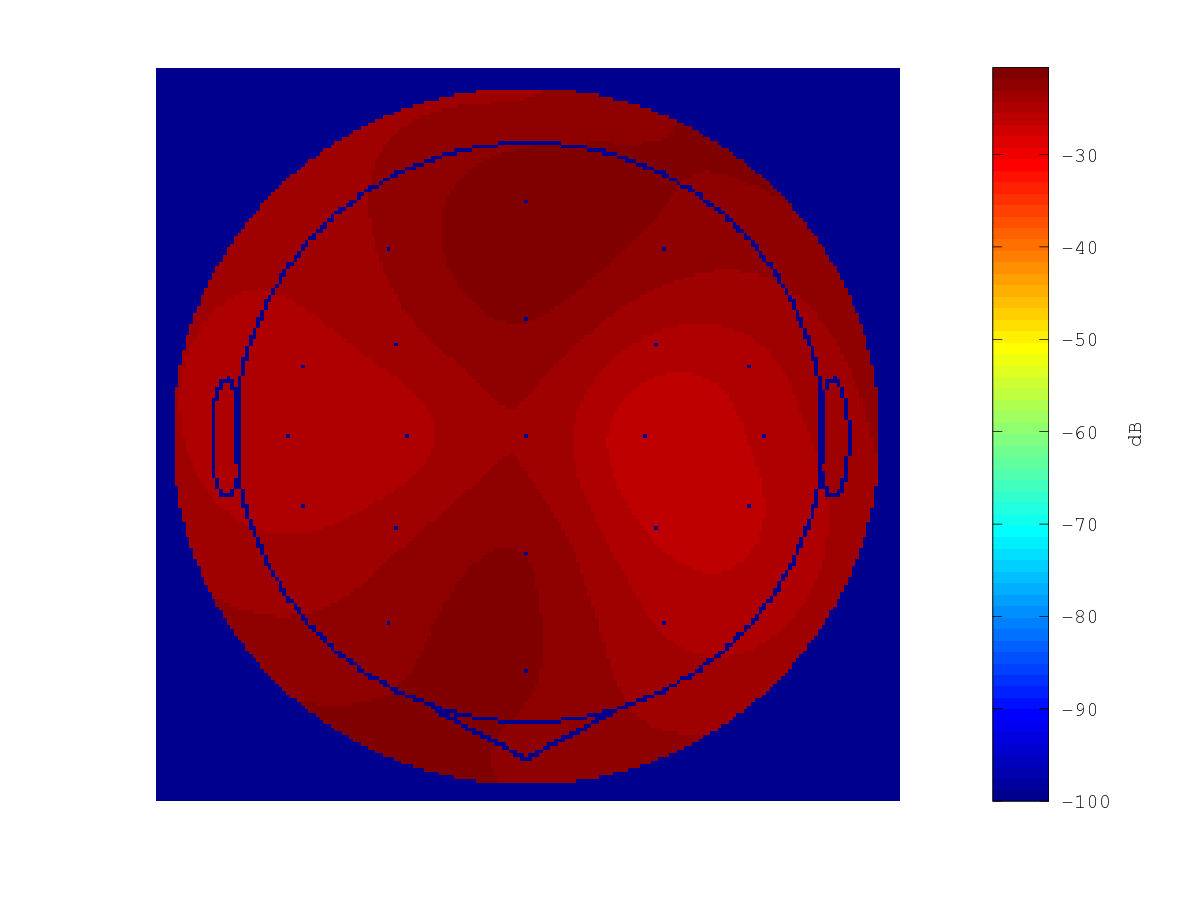
\includegraphics[width=2.5in]{scalpplot.png}}
\end{minipage}
\begin{minipage}[t]{0.5\textwidth}
~\\	
\IfStrEq{\PlotType}{scatter}{\textbf{\Large{Summary:}}\\
\if\IsConcussed1
\if\PrevConcussions0
Based on the results of the EEGlewave algorithm, the baseline brain signals have been classified as belonging to the concussed group. However, the past history and results from the SCAT do not seems to suggest that there is evidence of a previous recent concussion or any other condition that may lead to this result.\\
The EEGlewave algorithm is not 100\% accurate and there is a 10\% chance that some players will be misclassified. It is therefore possible that your child's brain signals fall into the group that are misclassified. However, if you have any concerns or if your child is showing any symptoms that might suggest any medical issues we suggest that your child is seen by your family physician for a physical examination.\\
Please feel free to contact Dr. Virji-Babul if you would like to discuss these results or would like more information.
\else
Based on the results of the EEGlewave algorithm the baseline brain signals have been classified as belonging to the concussed group. The past history and results from the SCAT also seems to suggest that there is evidence of a previous recent concussion. Given these results we suggest that your child is seen by your family physician for a physical examination and be cleared before he/she returns to play.\\
We will contact you again for a second EEG scan within a month to compare the baseline brain signals to determine if your brain signals are changing as a result of recovery. We will also repeat the SCAT to evaluate general changes in symptoms, balance and cognition from the initial assessment.\\
Please feel free to contact Dr. Virji-Babul if you would like more information.
\fi
\else
Based on the results of the EEGlewave algorithm the brain signals appear to be within normal range. If your child receives an impact to the head/body and a concussion is suspected please see your physician and contact EEGlewave at care@eeglewave.com. We will arrange for a second EEG scan and compare your baseline brain signals to the second EEG scan to determine if there have been any changes in your brain activity that may have resulted from the impact. We will also repeat the SCAT3 to evaluate changes in symptoms, balance and cognition from the baseline assessment.
\fi}{Electroencephalography (EEG) is a technique that records the electrical activity of the brain. Brain cells communicate using electrical impulses and are active all the time, even when sitting quietly or sleeping. The EEGlewave algorithm uses EEG signals from the whole brain to evaluate changes in these signals that may be due to a concussion.\\}
\end{minipage}
}}

 %comment starts
\iffalse
\fbox{\parbox{\textwidth}{
\textbf{\Large{Summary:}}\\
\if\IsConcussed1
\if\PrevConcussions0
Based on the results of the EEGlewave algorithm, the baseline brain signals have been classified as belonging to the concussed group. However, the past history and results from the SCAT do not seems to suggest that there is evidence of a previous recent concussion or any other condition that may lead to this result.\\
The EEGlewave algorithm is not 100\% accurate and there is a 10\% chance that some players will be misclassified. It is therefore possible that your child's brain signals fall into the group that are misclassified. However, if you have any concerns or if your child is showing any symptoms that might suggest any medical issues we suggest that your child is seen by your family physician for a physical examination.\\
Please feel free to contact Dr. Virji-Babul if you would like to discuss these results or would like more information.
\else
Based on the results of the EEGlewave algorithm the baseline brain signals have been classified as belonging to the concussed group. The past history and results from the SCAT also seems to suggest that there is evidence of a previous recent concussion. Given these results we suggest that your child is seen by your family physician for a physical examination and be cleared before he/she returns to play.\\
We will contact you again for a second EEG scan within a month to compare the baseline brain signals to determine if your brain signals are changing as a result of recovery. We will also repeat the SCAT to evaluate general changes in symptoms, balance and cognition from the initial assessment.\\
Please feel free to contact Dr. Virji-Babul if you would like more information.
\fi
\else
Based on the results of the EEGlewave algorithm the brain signals appear to be within normal range. If your child receives an impact to the head/body and a concussion is suspected please see your physician and contact EEGlewave at care@eeglewave.com. We will arrange for a second EEG scan and compare your baseline brain signals to the second EEG scan to determine if there have been any changes in your brain activity that may have resulted from the impact. We will also repeat the SCAT3 to evaluate changes in symptoms, balance and cognition from the baseline assessment.
\fi
}}
\fi % till here commenting out

% Add the footnote. A better way would be to use fancyhdr
\vfill
{\footnotesize\color{EWgray}\sffamily
	NOTE: EEGlewave does not provide medical advice. This report should not be used as a substitute for professional medical consultation.\\
}
\end{document}
}%The .tex filename goes here (NOT the same as \jobname)
\unless\ifdefined\ParentLastName
\endinput\expandafter\expandafter\expandafter\ReadParentLastName\fi

\def\ReadID#1 {%
	\def\ID{#1}%
	% NOTE: This report is to be compiled through the Octave command prompt.
% The following command should be typed into an Octave session to generate the report.
% system("pdflatex.exe -synctex=1 -interaction=nonstopmode -job-name=FirstName_LastName report.tex FirstName Lastname ParentName ID Handedness PrevConcussions Age ScanType")

% Definitions for command line arguments
\def\ReadFirstName#1 {%
	\def\FirstName{#1}%
	\input{report}}%The .tex filename goes here (NOT the same as \jobname)
\unless\ifdefined\FirstName
\endinput\expandafter\expandafter\expandafter\ReadFirstName\fi

\def\ReadLastName#1 {%
	\def\LastName{#1}%
	\input{report}}%The .tex filename goes here (NOT the same as \jobname)
\unless\ifdefined\LastName
\endinput\expandafter\expandafter\expandafter\ReadLastName\fi

\def\ReadParentFirstName#1 {%
	\def\ParentFirstName{#1}%
	\input{report}}%The .tex filename goes here (NOT the same as \jobname)
\unless\ifdefined\ParentFirstName
\endinput\expandafter\expandafter\expandafter\ReadParentFirstName\fi

\def\ReadParentLastName#1 {%
	\def\ParentLastName{#1}%
	\input{report}}%The .tex filename goes here (NOT the same as \jobname)
\unless\ifdefined\ParentLastName
\endinput\expandafter\expandafter\expandafter\ReadParentLastName\fi

\def\ReadID#1 {%
	\def\ID{#1}%
	\input{report}}%The .tex filename goes here (NOT the same as \jobname)
\unless\ifdefined\ID
\endinput\expandafter\expandafter\expandafter\ReadID\fi

\def\ReadHandedness#1 {%
	\def\Handedness{#1}%
	\input{report}}%The .tex filename goes here (NOT the same as \jobname)
\unless\ifdefined\Handedness
\endinput\expandafter\expandafter\expandafter\ReadHandedness\fi

\def\ReadPrevConcussions#1 {%
	\def\PrevConcussions{#1}%
	\input{report}}%The .tex filename goes here (NOT the same as \jobname)
\unless\ifdefined\PrevConcussions
\endinput\expandafter\expandafter\expandafter\ReadPrevConcussions\fi

\def\ReadMostRecentConcussion#1 {%
	\def\MostRecentConcussion{#1}%
	\input{report}}%The .tex filename goes here (NOT the same as \jobname)
\unless\ifdefined\MostRecentConcussion
\endinput\expandafter\expandafter\expandafter\ReadMostRecentConcussion\fi

\def\ReadIsConcussed#1 {%
	\def\IsConcussed{#1}%
	\input{report}}%The .tex filename goes here (NOT the same as \jobname)
\unless\ifdefined\IsConcussed
\endinput\expandafter\expandafter\expandafter\ReadIsConcussed\fi

\def\ReadDivision#1 {%
	\def\Division{#1}%
	\input{report}}%The .tex filename goes here (NOT the same as \jobname)
\unless\ifdefined\Division
\endinput\expandafter\expandafter\expandafter\ReadDivision\fi

\def\ReadGender#1 {%
	\def\Gender{#1}%
	\input{report}}%The .tex filename goes here (NOT the same as \jobname)
\unless\ifdefined\Gender
\endinput\expandafter\expandafter\expandafter\ReadGender\fi

\def\ReadAge#1 {%
	\def\Age{#1}%
	\input{report}}%The .tex filename goes here (NOT the same as \jobname)
\unless\ifdefined\Age
\endinput\expandafter\expandafter\expandafter\ReadAge\fi

\def\ReadDOS#1 {%
	\def\DOS{#1}%
	\input{report}}%The .tex filename goes here (NOT the same as \jobname)
\unless\ifdefined\DOS
\endinput\expandafter\expandafter\expandafter\ReadDOS\fi

\def\ReadScanType#1 {%
	\def\ScanType{#1}%
	\input{report}}%The .tex filename goes here (NOT the same as \jobname)
\unless\ifdefined\ScanType
\endinput\expandafter\expandafter\expandafter\ReadScanType\fi

\def\ReadNumSymptoms#1 {%
	\def\NumSymptoms{#1}%
	\input{report}}%The .tex filename goes here (NOT the same as \jobname)
\unless\ifdefined\NumSymptoms
\endinput\expandafter\expandafter\expandafter\ReadNumSymptoms\fi

\def\ReadSeverityScore#1 {%
	\def\SeverityScore{#1}%
	\input{report}}%The .tex filename goes here (NOT the same as \jobname)
\unless\ifdefined\SeverityScore
\endinput\expandafter\expandafter\expandafter\ReadSeverityScore\fi

\def\ReadOrientation#1 {%
	\def\Orientation{#1}%
	\input{report}}%The .tex filename goes here (NOT the same as \jobname)
\unless\ifdefined\Orientation
\endinput\expandafter\expandafter\expandafter\ReadOrientation\fi

\def\ReadOrientationTotal#1 {%
	\def\OrientationTotal{#1}%
	\input{report}}%The .tex filename goes here (NOT the same as \jobname)
\unless\ifdefined\OrientationTotal
\endinput\expandafter\expandafter\expandafter\ReadOrientationTotal\fi

\def\ReadImmMem#1 {%
	\def\ImmMem{#1}%
	\input{report}}%The .tex filename goes here (NOT the same as \jobname)
\unless\ifdefined\ImmMem
\endinput\expandafter\expandafter\expandafter\ReadImmMem\fi

\def\ReadConcentration#1 {%
	\def\Concentration{#1}%
	\input{report}}%The .tex filename goes here (NOT the same as \jobname)
\unless\ifdefined\Concentration
\endinput\expandafter\expandafter\expandafter\ReadConcentration\fi

\def\ReadConcentrationTotal#1 {%
	\def\ConcentrationTotal{#1}%
	\input{report}}%The .tex filename goes here (NOT the same as \jobname)
\unless\ifdefined\ConcentrationTotal
\endinput\expandafter\expandafter\expandafter\ReadConcentrationTotal\fi

\def\ReadDelayedRecall#1 {%
	\def\DelayedRecall{#1}%
	\input{report}}%The .tex filename goes here (NOT the same as \jobname)
\unless\ifdefined\DelayedRecall
\endinput\expandafter\expandafter\expandafter\ReadDelayedRecall\fi

\def\ReadSAC#1 {%
	\def\SAC{#1}%
	\input{report}}%The .tex filename goes here (NOT the same as \jobname)
\unless\ifdefined\SAC
\endinput\expandafter\expandafter\expandafter\ReadSAC\fi

\def\ReadBESS#1 {%
	\def\BESS{#1}%
	\input{report}}%The .tex filename goes here (NOT the same as \jobname)
\unless\ifdefined\BESS
\endinput\expandafter\expandafter\expandafter\ReadBESS\fi

\def\ReadTandemGait#1 {%
	\def\TandemGait{#1}%
	\input{report}}%The .tex filename goes here (NOT the same as \jobname)
\unless\ifdefined\TandemGait
\endinput\expandafter\expandafter\expandafter\ReadTandemGait\fi

\def\ReadCoordination#1 {%
	\def\Coordination{#1}%
	\input{report}}%The .tex filename goes here (NOT the same as \jobname)
\unless\ifdefined\Coordination
\endinput\expandafter\expandafter\expandafter\ReadCoordination\fi

\def\ReadPlotType#1 {%
	\def\PlotType{#1}%
	\input{report}}%The .tex filename goes here (NOT the same as \jobname)
\unless\ifdefined\PlotType
\endinput\expandafter\expandafter\expandafter\ReadPlotType\fi

\documentclass{article}

\usepackage[dvinames]{xcolor}
% Measurements are taken directly from the guide
\usepackage[top=2in,left=0.5in,bottom=0.5in,right=0.5in]{geometry}
\usepackage{graphicx}
\usepackage[colorlinks=false,
            pdfborder={0 0 0},
            ]{hyperref}
\usepackage{lipsum}
\usepackage[absolute]{textpos}
\usepackage{tikz}
\usetikzlibrary{calc}
% A nice serif font, but no the prescribed nonfree ITC stone
\usepackage[oldstylenums]{kpfonts}
\usepackage[T1]{fontenc	}
\usepackage[12pt]{moresize}
\usepackage{xstring}

% No paragraph indentation
\parindent0pt
\setlength{\parskip}{0.8\baselineskip}
\raggedright
\pagestyle{empty}


\definecolor{EWgray}{HTML}{5e6a71}

\begin{document}
	\begin{center}
		\HUGE{~}\\
		\HUGE{~}\\
		\HUGE{~}\\
		\textbf{\HUGE{EEGlewave Inc.}}\\[1in]
		\textbf{\huge{\ScanType~Report}}\\[1cm]
	\end{center}
	\newpage
\bigskip
% -------------------------------------------------------
% Add logo, the text under the crimson line, and the line itself
\begin{textblock*}{2in}[0.3066,0.39](1.25in,1.23in)
	
\includegraphics[width=1.5in]{eeglewave-front-211x128-88.png}
\end{textblock*}
\begin{textblock*}{6.375in}(1.5in,1.4in)   % 6.375=8.5 - 1.5 - 0.625
	\sffamily
	\hfill \color{EWgray} EEGlewave Inc.\\
	\hfill \url{care@eeglewave.com} \textbullet\ \url{http://eeglewave.com}
\end{textblock*}
\begin{tikzpicture}[remember picture,overlay]
\draw[line width=1pt] (current page.north west)+(0.5in,-1.85in) -- ($(-0.5in,-1.85in)+(current page.north east)$);
\end{tikzpicture}
\fbox{\parbox{\textwidth}{
\textbf{\Large{General Information:}}\\
\begin{minipage}[t]{0.55\textwidth}

\textbf{Name: } \FirstName~\LastName  \\
\textbf{Parent/Guardian's Name: } \ParentFirstName~\ParentLastName  \\
\textbf{ID: } \ID   \\
\textbf{Handedness: } \Handedness  \\
\textbf{Number of Previous Concussions: } \PrevConcussions \\
\textbf{Date of Most Recent Concussion: } \MostRecentConcussion
\end{minipage}
\begin{minipage}[t]{0.45\textwidth}
	\textbf{Division: } \Division  \\
	\textbf{Gender: } \Gender  \\
	\textbf{Age: } \Age  \\
	\textbf{Date of Scan: } \DOS \\
	\textbf{Type of Scan: } \ScanType  \\
\end{minipage}
}}

\fbox{\parbox{\textwidth}{
\textbf{\Large{SCAT3 Scoring Summary:}}\\
\begin{minipage}[t]{0.55\textwidth}
\textbf{Number of Symptoms (/22): } \\
\textbf{Symptom Severity Score (/132): } \\

\textbf{Orientation (/\OrientationTotal): }  \\
\textbf{Immediate Memory (/15): } \\
\textbf{Concentration (/\ConcentrationTotal): } \\
\textbf{Delayed Recall (/5): } \\
\textbf{SAC Total (/30): } \\

\textbf{BESS (total errors): } \\
\textbf{Tandem Gait (seconds): } \\
\textbf{Coordination (/1): } 
\end{minipage}
\begin{minipage}[t]{0.25\textwidth}
\NumSymptoms  \\
\SeverityScore  \\

\Orientation  \\
\ImmMem  \\
\Concentration  \\
\DelayedRecall \\
\SAC  \\

\BESS  \\
\TandemGait  \\
\Coordination
\end{minipage}
}}

\fbox{\parbox{\textwidth}{
\textbf{\Large{\IfStrEq{\PlotType}{scatter}{Scatter Plot:}{EEG Plot of Power at Rest:}}}\\
\begin{minipage}[t]{0.5\textwidth}
	~\\
	\IfStrEq{\PlotType}{scatter}{\includegraphics[width=3.25in]{scatterplot.png}}{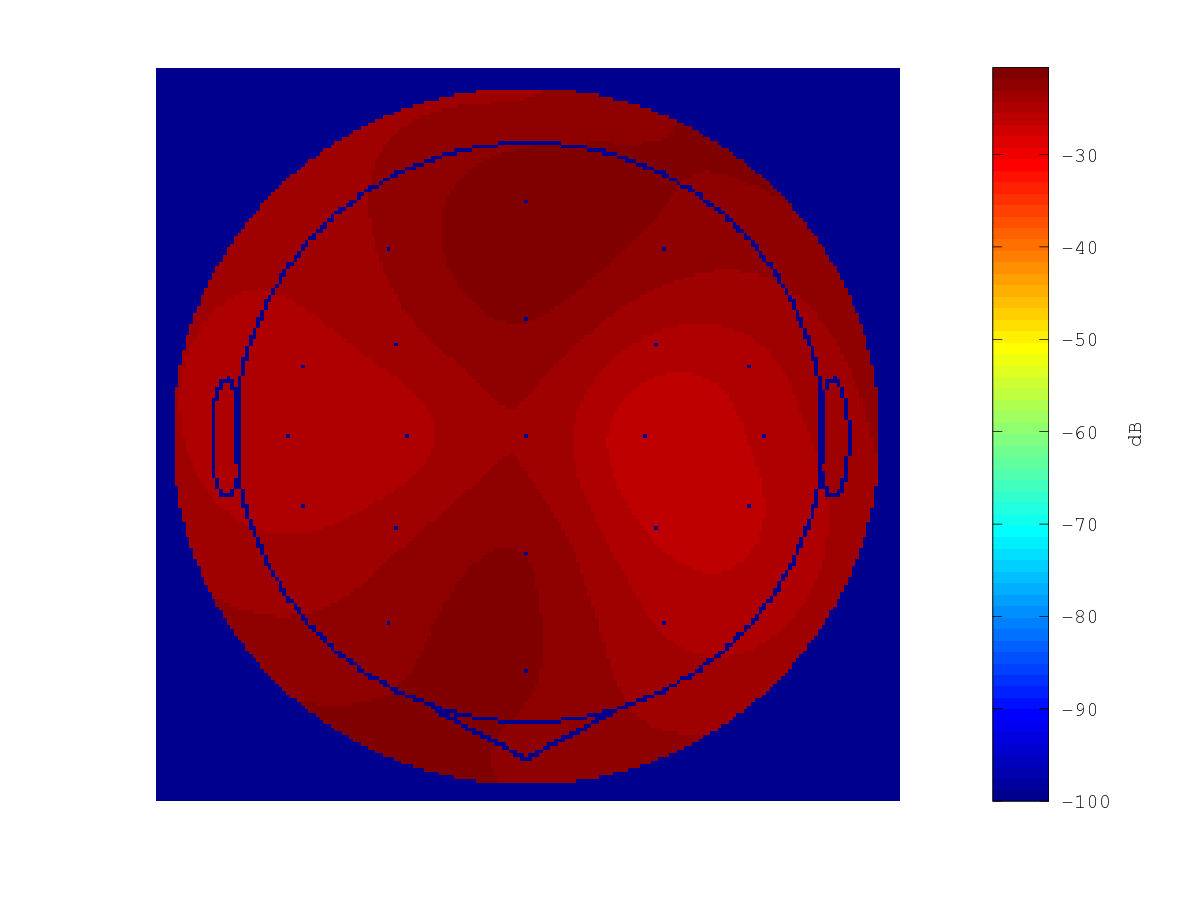
\includegraphics[width=2.5in]{scalpplot.png}}
\end{minipage}
\begin{minipage}[t]{0.5\textwidth}
~\\	
\IfStrEq{\PlotType}{scatter}{\textbf{\Large{Summary:}}\\
\if\IsConcussed1
\if\PrevConcussions0
Based on the results of the EEGlewave algorithm, the baseline brain signals have been classified as belonging to the concussed group. However, the past history and results from the SCAT do not seems to suggest that there is evidence of a previous recent concussion or any other condition that may lead to this result.\\
The EEGlewave algorithm is not 100\% accurate and there is a 10\% chance that some players will be misclassified. It is therefore possible that your child's brain signals fall into the group that are misclassified. However, if you have any concerns or if your child is showing any symptoms that might suggest any medical issues we suggest that your child is seen by your family physician for a physical examination.\\
Please feel free to contact Dr. Virji-Babul if you would like to discuss these results or would like more information.
\else
Based on the results of the EEGlewave algorithm the baseline brain signals have been classified as belonging to the concussed group. The past history and results from the SCAT also seems to suggest that there is evidence of a previous recent concussion. Given these results we suggest that your child is seen by your family physician for a physical examination and be cleared before he/she returns to play.\\
We will contact you again for a second EEG scan within a month to compare the baseline brain signals to determine if your brain signals are changing as a result of recovery. We will also repeat the SCAT to evaluate general changes in symptoms, balance and cognition from the initial assessment.\\
Please feel free to contact Dr. Virji-Babul if you would like more information.
\fi
\else
Based on the results of the EEGlewave algorithm the brain signals appear to be within normal range. If your child receives an impact to the head/body and a concussion is suspected please see your physician and contact EEGlewave at care@eeglewave.com. We will arrange for a second EEG scan and compare your baseline brain signals to the second EEG scan to determine if there have been any changes in your brain activity that may have resulted from the impact. We will also repeat the SCAT3 to evaluate changes in symptoms, balance and cognition from the baseline assessment.
\fi}{Electroencephalography (EEG) is a technique that records the electrical activity of the brain. Brain cells communicate using electrical impulses and are active all the time, even when sitting quietly or sleeping. The EEGlewave algorithm uses EEG signals from the whole brain to evaluate changes in these signals that may be due to a concussion.\\}
\end{minipage}
}}

 %comment starts
\iffalse
\fbox{\parbox{\textwidth}{
\textbf{\Large{Summary:}}\\
\if\IsConcussed1
\if\PrevConcussions0
Based on the results of the EEGlewave algorithm, the baseline brain signals have been classified as belonging to the concussed group. However, the past history and results from the SCAT do not seems to suggest that there is evidence of a previous recent concussion or any other condition that may lead to this result.\\
The EEGlewave algorithm is not 100\% accurate and there is a 10\% chance that some players will be misclassified. It is therefore possible that your child's brain signals fall into the group that are misclassified. However, if you have any concerns or if your child is showing any symptoms that might suggest any medical issues we suggest that your child is seen by your family physician for a physical examination.\\
Please feel free to contact Dr. Virji-Babul if you would like to discuss these results or would like more information.
\else
Based on the results of the EEGlewave algorithm the baseline brain signals have been classified as belonging to the concussed group. The past history and results from the SCAT also seems to suggest that there is evidence of a previous recent concussion. Given these results we suggest that your child is seen by your family physician for a physical examination and be cleared before he/she returns to play.\\
We will contact you again for a second EEG scan within a month to compare the baseline brain signals to determine if your brain signals are changing as a result of recovery. We will also repeat the SCAT to evaluate general changes in symptoms, balance and cognition from the initial assessment.\\
Please feel free to contact Dr. Virji-Babul if you would like more information.
\fi
\else
Based on the results of the EEGlewave algorithm the brain signals appear to be within normal range. If your child receives an impact to the head/body and a concussion is suspected please see your physician and contact EEGlewave at care@eeglewave.com. We will arrange for a second EEG scan and compare your baseline brain signals to the second EEG scan to determine if there have been any changes in your brain activity that may have resulted from the impact. We will also repeat the SCAT3 to evaluate changes in symptoms, balance and cognition from the baseline assessment.
\fi
}}
\fi % till here commenting out

% Add the footnote. A better way would be to use fancyhdr
\vfill
{\footnotesize\color{EWgray}\sffamily
	NOTE: EEGlewave does not provide medical advice. This report should not be used as a substitute for professional medical consultation.\\
}
\end{document}
}%The .tex filename goes here (NOT the same as \jobname)
\unless\ifdefined\ID
\endinput\expandafter\expandafter\expandafter\ReadID\fi

\def\ReadHandedness#1 {%
	\def\Handedness{#1}%
	% NOTE: This report is to be compiled through the Octave command prompt.
% The following command should be typed into an Octave session to generate the report.
% system("pdflatex.exe -synctex=1 -interaction=nonstopmode -job-name=FirstName_LastName report.tex FirstName Lastname ParentName ID Handedness PrevConcussions Age ScanType")

% Definitions for command line arguments
\def\ReadFirstName#1 {%
	\def\FirstName{#1}%
	\input{report}}%The .tex filename goes here (NOT the same as \jobname)
\unless\ifdefined\FirstName
\endinput\expandafter\expandafter\expandafter\ReadFirstName\fi

\def\ReadLastName#1 {%
	\def\LastName{#1}%
	\input{report}}%The .tex filename goes here (NOT the same as \jobname)
\unless\ifdefined\LastName
\endinput\expandafter\expandafter\expandafter\ReadLastName\fi

\def\ReadParentFirstName#1 {%
	\def\ParentFirstName{#1}%
	\input{report}}%The .tex filename goes here (NOT the same as \jobname)
\unless\ifdefined\ParentFirstName
\endinput\expandafter\expandafter\expandafter\ReadParentFirstName\fi

\def\ReadParentLastName#1 {%
	\def\ParentLastName{#1}%
	\input{report}}%The .tex filename goes here (NOT the same as \jobname)
\unless\ifdefined\ParentLastName
\endinput\expandafter\expandafter\expandafter\ReadParentLastName\fi

\def\ReadID#1 {%
	\def\ID{#1}%
	\input{report}}%The .tex filename goes here (NOT the same as \jobname)
\unless\ifdefined\ID
\endinput\expandafter\expandafter\expandafter\ReadID\fi

\def\ReadHandedness#1 {%
	\def\Handedness{#1}%
	\input{report}}%The .tex filename goes here (NOT the same as \jobname)
\unless\ifdefined\Handedness
\endinput\expandafter\expandafter\expandafter\ReadHandedness\fi

\def\ReadPrevConcussions#1 {%
	\def\PrevConcussions{#1}%
	\input{report}}%The .tex filename goes here (NOT the same as \jobname)
\unless\ifdefined\PrevConcussions
\endinput\expandafter\expandafter\expandafter\ReadPrevConcussions\fi

\def\ReadMostRecentConcussion#1 {%
	\def\MostRecentConcussion{#1}%
	\input{report}}%The .tex filename goes here (NOT the same as \jobname)
\unless\ifdefined\MostRecentConcussion
\endinput\expandafter\expandafter\expandafter\ReadMostRecentConcussion\fi

\def\ReadIsConcussed#1 {%
	\def\IsConcussed{#1}%
	\input{report}}%The .tex filename goes here (NOT the same as \jobname)
\unless\ifdefined\IsConcussed
\endinput\expandafter\expandafter\expandafter\ReadIsConcussed\fi

\def\ReadDivision#1 {%
	\def\Division{#1}%
	\input{report}}%The .tex filename goes here (NOT the same as \jobname)
\unless\ifdefined\Division
\endinput\expandafter\expandafter\expandafter\ReadDivision\fi

\def\ReadGender#1 {%
	\def\Gender{#1}%
	\input{report}}%The .tex filename goes here (NOT the same as \jobname)
\unless\ifdefined\Gender
\endinput\expandafter\expandafter\expandafter\ReadGender\fi

\def\ReadAge#1 {%
	\def\Age{#1}%
	\input{report}}%The .tex filename goes here (NOT the same as \jobname)
\unless\ifdefined\Age
\endinput\expandafter\expandafter\expandafter\ReadAge\fi

\def\ReadDOS#1 {%
	\def\DOS{#1}%
	\input{report}}%The .tex filename goes here (NOT the same as \jobname)
\unless\ifdefined\DOS
\endinput\expandafter\expandafter\expandafter\ReadDOS\fi

\def\ReadScanType#1 {%
	\def\ScanType{#1}%
	\input{report}}%The .tex filename goes here (NOT the same as \jobname)
\unless\ifdefined\ScanType
\endinput\expandafter\expandafter\expandafter\ReadScanType\fi

\def\ReadNumSymptoms#1 {%
	\def\NumSymptoms{#1}%
	\input{report}}%The .tex filename goes here (NOT the same as \jobname)
\unless\ifdefined\NumSymptoms
\endinput\expandafter\expandafter\expandafter\ReadNumSymptoms\fi

\def\ReadSeverityScore#1 {%
	\def\SeverityScore{#1}%
	\input{report}}%The .tex filename goes here (NOT the same as \jobname)
\unless\ifdefined\SeverityScore
\endinput\expandafter\expandafter\expandafter\ReadSeverityScore\fi

\def\ReadOrientation#1 {%
	\def\Orientation{#1}%
	\input{report}}%The .tex filename goes here (NOT the same as \jobname)
\unless\ifdefined\Orientation
\endinput\expandafter\expandafter\expandafter\ReadOrientation\fi

\def\ReadOrientationTotal#1 {%
	\def\OrientationTotal{#1}%
	\input{report}}%The .tex filename goes here (NOT the same as \jobname)
\unless\ifdefined\OrientationTotal
\endinput\expandafter\expandafter\expandafter\ReadOrientationTotal\fi

\def\ReadImmMem#1 {%
	\def\ImmMem{#1}%
	\input{report}}%The .tex filename goes here (NOT the same as \jobname)
\unless\ifdefined\ImmMem
\endinput\expandafter\expandafter\expandafter\ReadImmMem\fi

\def\ReadConcentration#1 {%
	\def\Concentration{#1}%
	\input{report}}%The .tex filename goes here (NOT the same as \jobname)
\unless\ifdefined\Concentration
\endinput\expandafter\expandafter\expandafter\ReadConcentration\fi

\def\ReadConcentrationTotal#1 {%
	\def\ConcentrationTotal{#1}%
	\input{report}}%The .tex filename goes here (NOT the same as \jobname)
\unless\ifdefined\ConcentrationTotal
\endinput\expandafter\expandafter\expandafter\ReadConcentrationTotal\fi

\def\ReadDelayedRecall#1 {%
	\def\DelayedRecall{#1}%
	\input{report}}%The .tex filename goes here (NOT the same as \jobname)
\unless\ifdefined\DelayedRecall
\endinput\expandafter\expandafter\expandafter\ReadDelayedRecall\fi

\def\ReadSAC#1 {%
	\def\SAC{#1}%
	\input{report}}%The .tex filename goes here (NOT the same as \jobname)
\unless\ifdefined\SAC
\endinput\expandafter\expandafter\expandafter\ReadSAC\fi

\def\ReadBESS#1 {%
	\def\BESS{#1}%
	\input{report}}%The .tex filename goes here (NOT the same as \jobname)
\unless\ifdefined\BESS
\endinput\expandafter\expandafter\expandafter\ReadBESS\fi

\def\ReadTandemGait#1 {%
	\def\TandemGait{#1}%
	\input{report}}%The .tex filename goes here (NOT the same as \jobname)
\unless\ifdefined\TandemGait
\endinput\expandafter\expandafter\expandafter\ReadTandemGait\fi

\def\ReadCoordination#1 {%
	\def\Coordination{#1}%
	\input{report}}%The .tex filename goes here (NOT the same as \jobname)
\unless\ifdefined\Coordination
\endinput\expandafter\expandafter\expandafter\ReadCoordination\fi

\def\ReadPlotType#1 {%
	\def\PlotType{#1}%
	\input{report}}%The .tex filename goes here (NOT the same as \jobname)
\unless\ifdefined\PlotType
\endinput\expandafter\expandafter\expandafter\ReadPlotType\fi

\documentclass{article}

\usepackage[dvinames]{xcolor}
% Measurements are taken directly from the guide
\usepackage[top=2in,left=0.5in,bottom=0.5in,right=0.5in]{geometry}
\usepackage{graphicx}
\usepackage[colorlinks=false,
            pdfborder={0 0 0},
            ]{hyperref}
\usepackage{lipsum}
\usepackage[absolute]{textpos}
\usepackage{tikz}
\usetikzlibrary{calc}
% A nice serif font, but no the prescribed nonfree ITC stone
\usepackage[oldstylenums]{kpfonts}
\usepackage[T1]{fontenc	}
\usepackage[12pt]{moresize}
\usepackage{xstring}

% No paragraph indentation
\parindent0pt
\setlength{\parskip}{0.8\baselineskip}
\raggedright
\pagestyle{empty}


\definecolor{EWgray}{HTML}{5e6a71}

\begin{document}
	\begin{center}
		\HUGE{~}\\
		\HUGE{~}\\
		\HUGE{~}\\
		\textbf{\HUGE{EEGlewave Inc.}}\\[1in]
		\textbf{\huge{\ScanType~Report}}\\[1cm]
	\end{center}
	\newpage
\bigskip
% -------------------------------------------------------
% Add logo, the text under the crimson line, and the line itself
\begin{textblock*}{2in}[0.3066,0.39](1.25in,1.23in)
	
\includegraphics[width=1.5in]{eeglewave-front-211x128-88.png}
\end{textblock*}
\begin{textblock*}{6.375in}(1.5in,1.4in)   % 6.375=8.5 - 1.5 - 0.625
	\sffamily
	\hfill \color{EWgray} EEGlewave Inc.\\
	\hfill \url{care@eeglewave.com} \textbullet\ \url{http://eeglewave.com}
\end{textblock*}
\begin{tikzpicture}[remember picture,overlay]
\draw[line width=1pt] (current page.north west)+(0.5in,-1.85in) -- ($(-0.5in,-1.85in)+(current page.north east)$);
\end{tikzpicture}
\fbox{\parbox{\textwidth}{
\textbf{\Large{General Information:}}\\
\begin{minipage}[t]{0.55\textwidth}

\textbf{Name: } \FirstName~\LastName  \\
\textbf{Parent/Guardian's Name: } \ParentFirstName~\ParentLastName  \\
\textbf{ID: } \ID   \\
\textbf{Handedness: } \Handedness  \\
\textbf{Number of Previous Concussions: } \PrevConcussions \\
\textbf{Date of Most Recent Concussion: } \MostRecentConcussion
\end{minipage}
\begin{minipage}[t]{0.45\textwidth}
	\textbf{Division: } \Division  \\
	\textbf{Gender: } \Gender  \\
	\textbf{Age: } \Age  \\
	\textbf{Date of Scan: } \DOS \\
	\textbf{Type of Scan: } \ScanType  \\
\end{minipage}
}}

\fbox{\parbox{\textwidth}{
\textbf{\Large{SCAT3 Scoring Summary:}}\\
\begin{minipage}[t]{0.55\textwidth}
\textbf{Number of Symptoms (/22): } \\
\textbf{Symptom Severity Score (/132): } \\

\textbf{Orientation (/\OrientationTotal): }  \\
\textbf{Immediate Memory (/15): } \\
\textbf{Concentration (/\ConcentrationTotal): } \\
\textbf{Delayed Recall (/5): } \\
\textbf{SAC Total (/30): } \\

\textbf{BESS (total errors): } \\
\textbf{Tandem Gait (seconds): } \\
\textbf{Coordination (/1): } 
\end{minipage}
\begin{minipage}[t]{0.25\textwidth}
\NumSymptoms  \\
\SeverityScore  \\

\Orientation  \\
\ImmMem  \\
\Concentration  \\
\DelayedRecall \\
\SAC  \\

\BESS  \\
\TandemGait  \\
\Coordination
\end{minipage}
}}

\fbox{\parbox{\textwidth}{
\textbf{\Large{\IfStrEq{\PlotType}{scatter}{Scatter Plot:}{EEG Plot of Power at Rest:}}}\\
\begin{minipage}[t]{0.5\textwidth}
	~\\
	\IfStrEq{\PlotType}{scatter}{\includegraphics[width=3.25in]{scatterplot.png}}{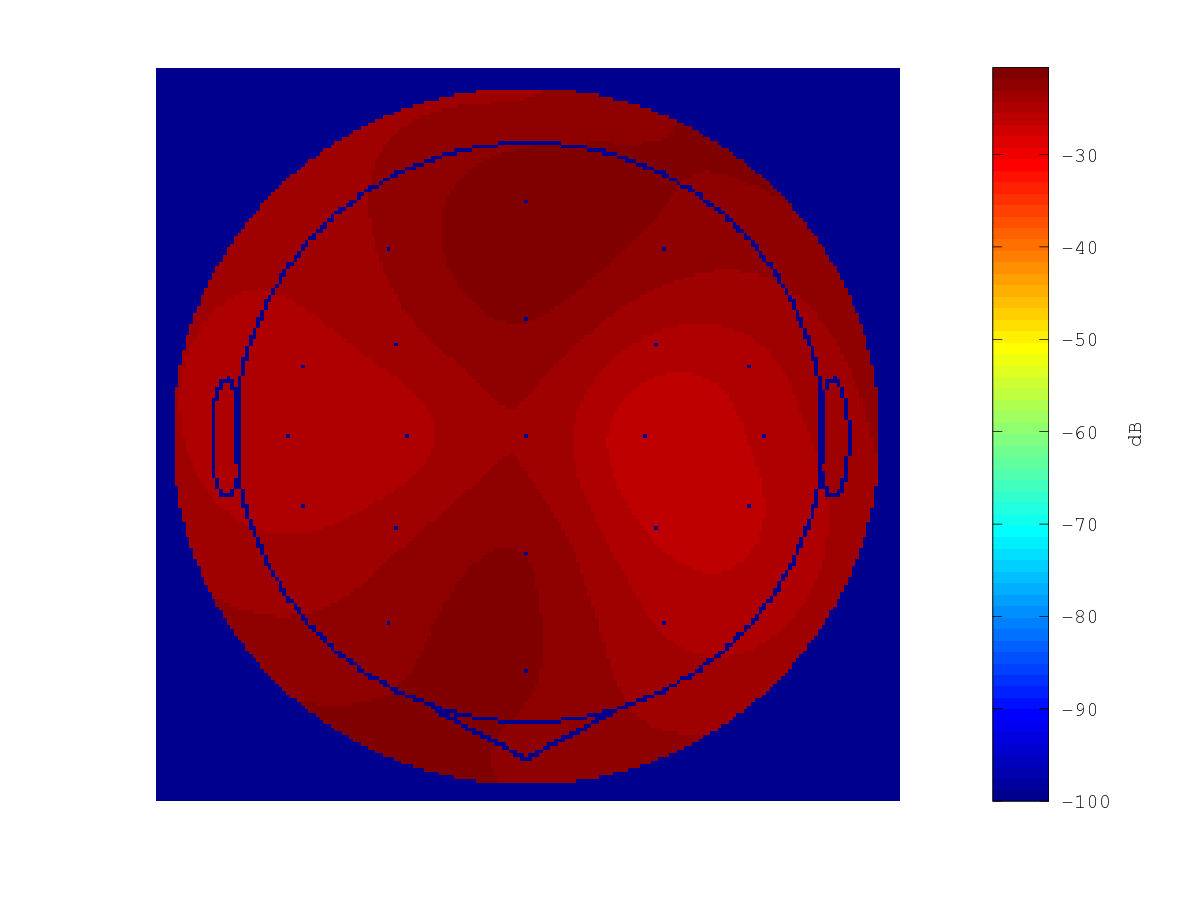
\includegraphics[width=2.5in]{scalpplot.png}}
\end{minipage}
\begin{minipage}[t]{0.5\textwidth}
~\\	
\IfStrEq{\PlotType}{scatter}{\textbf{\Large{Summary:}}\\
\if\IsConcussed1
\if\PrevConcussions0
Based on the results of the EEGlewave algorithm, the baseline brain signals have been classified as belonging to the concussed group. However, the past history and results from the SCAT do not seems to suggest that there is evidence of a previous recent concussion or any other condition that may lead to this result.\\
The EEGlewave algorithm is not 100\% accurate and there is a 10\% chance that some players will be misclassified. It is therefore possible that your child's brain signals fall into the group that are misclassified. However, if you have any concerns or if your child is showing any symptoms that might suggest any medical issues we suggest that your child is seen by your family physician for a physical examination.\\
Please feel free to contact Dr. Virji-Babul if you would like to discuss these results or would like more information.
\else
Based on the results of the EEGlewave algorithm the baseline brain signals have been classified as belonging to the concussed group. The past history and results from the SCAT also seems to suggest that there is evidence of a previous recent concussion. Given these results we suggest that your child is seen by your family physician for a physical examination and be cleared before he/she returns to play.\\
We will contact you again for a second EEG scan within a month to compare the baseline brain signals to determine if your brain signals are changing as a result of recovery. We will also repeat the SCAT to evaluate general changes in symptoms, balance and cognition from the initial assessment.\\
Please feel free to contact Dr. Virji-Babul if you would like more information.
\fi
\else
Based on the results of the EEGlewave algorithm the brain signals appear to be within normal range. If your child receives an impact to the head/body and a concussion is suspected please see your physician and contact EEGlewave at care@eeglewave.com. We will arrange for a second EEG scan and compare your baseline brain signals to the second EEG scan to determine if there have been any changes in your brain activity that may have resulted from the impact. We will also repeat the SCAT3 to evaluate changes in symptoms, balance and cognition from the baseline assessment.
\fi}{Electroencephalography (EEG) is a technique that records the electrical activity of the brain. Brain cells communicate using electrical impulses and are active all the time, even when sitting quietly or sleeping. The EEGlewave algorithm uses EEG signals from the whole brain to evaluate changes in these signals that may be due to a concussion.\\}
\end{minipage}
}}

 %comment starts
\iffalse
\fbox{\parbox{\textwidth}{
\textbf{\Large{Summary:}}\\
\if\IsConcussed1
\if\PrevConcussions0
Based on the results of the EEGlewave algorithm, the baseline brain signals have been classified as belonging to the concussed group. However, the past history and results from the SCAT do not seems to suggest that there is evidence of a previous recent concussion or any other condition that may lead to this result.\\
The EEGlewave algorithm is not 100\% accurate and there is a 10\% chance that some players will be misclassified. It is therefore possible that your child's brain signals fall into the group that are misclassified. However, if you have any concerns or if your child is showing any symptoms that might suggest any medical issues we suggest that your child is seen by your family physician for a physical examination.\\
Please feel free to contact Dr. Virji-Babul if you would like to discuss these results or would like more information.
\else
Based on the results of the EEGlewave algorithm the baseline brain signals have been classified as belonging to the concussed group. The past history and results from the SCAT also seems to suggest that there is evidence of a previous recent concussion. Given these results we suggest that your child is seen by your family physician for a physical examination and be cleared before he/she returns to play.\\
We will contact you again for a second EEG scan within a month to compare the baseline brain signals to determine if your brain signals are changing as a result of recovery. We will also repeat the SCAT to evaluate general changes in symptoms, balance and cognition from the initial assessment.\\
Please feel free to contact Dr. Virji-Babul if you would like more information.
\fi
\else
Based on the results of the EEGlewave algorithm the brain signals appear to be within normal range. If your child receives an impact to the head/body and a concussion is suspected please see your physician and contact EEGlewave at care@eeglewave.com. We will arrange for a second EEG scan and compare your baseline brain signals to the second EEG scan to determine if there have been any changes in your brain activity that may have resulted from the impact. We will also repeat the SCAT3 to evaluate changes in symptoms, balance and cognition from the baseline assessment.
\fi
}}
\fi % till here commenting out

% Add the footnote. A better way would be to use fancyhdr
\vfill
{\footnotesize\color{EWgray}\sffamily
	NOTE: EEGlewave does not provide medical advice. This report should not be used as a substitute for professional medical consultation.\\
}
\end{document}
}%The .tex filename goes here (NOT the same as \jobname)
\unless\ifdefined\Handedness
\endinput\expandafter\expandafter\expandafter\ReadHandedness\fi

\def\ReadPrevConcussions#1 {%
	\def\PrevConcussions{#1}%
	% NOTE: This report is to be compiled through the Octave command prompt.
% The following command should be typed into an Octave session to generate the report.
% system("pdflatex.exe -synctex=1 -interaction=nonstopmode -job-name=FirstName_LastName report.tex FirstName Lastname ParentName ID Handedness PrevConcussions Age ScanType")

% Definitions for command line arguments
\def\ReadFirstName#1 {%
	\def\FirstName{#1}%
	\input{report}}%The .tex filename goes here (NOT the same as \jobname)
\unless\ifdefined\FirstName
\endinput\expandafter\expandafter\expandafter\ReadFirstName\fi

\def\ReadLastName#1 {%
	\def\LastName{#1}%
	\input{report}}%The .tex filename goes here (NOT the same as \jobname)
\unless\ifdefined\LastName
\endinput\expandafter\expandafter\expandafter\ReadLastName\fi

\def\ReadParentFirstName#1 {%
	\def\ParentFirstName{#1}%
	\input{report}}%The .tex filename goes here (NOT the same as \jobname)
\unless\ifdefined\ParentFirstName
\endinput\expandafter\expandafter\expandafter\ReadParentFirstName\fi

\def\ReadParentLastName#1 {%
	\def\ParentLastName{#1}%
	\input{report}}%The .tex filename goes here (NOT the same as \jobname)
\unless\ifdefined\ParentLastName
\endinput\expandafter\expandafter\expandafter\ReadParentLastName\fi

\def\ReadID#1 {%
	\def\ID{#1}%
	\input{report}}%The .tex filename goes here (NOT the same as \jobname)
\unless\ifdefined\ID
\endinput\expandafter\expandafter\expandafter\ReadID\fi

\def\ReadHandedness#1 {%
	\def\Handedness{#1}%
	\input{report}}%The .tex filename goes here (NOT the same as \jobname)
\unless\ifdefined\Handedness
\endinput\expandafter\expandafter\expandafter\ReadHandedness\fi

\def\ReadPrevConcussions#1 {%
	\def\PrevConcussions{#1}%
	\input{report}}%The .tex filename goes here (NOT the same as \jobname)
\unless\ifdefined\PrevConcussions
\endinput\expandafter\expandafter\expandafter\ReadPrevConcussions\fi

\def\ReadMostRecentConcussion#1 {%
	\def\MostRecentConcussion{#1}%
	\input{report}}%The .tex filename goes here (NOT the same as \jobname)
\unless\ifdefined\MostRecentConcussion
\endinput\expandafter\expandafter\expandafter\ReadMostRecentConcussion\fi

\def\ReadIsConcussed#1 {%
	\def\IsConcussed{#1}%
	\input{report}}%The .tex filename goes here (NOT the same as \jobname)
\unless\ifdefined\IsConcussed
\endinput\expandafter\expandafter\expandafter\ReadIsConcussed\fi

\def\ReadDivision#1 {%
	\def\Division{#1}%
	\input{report}}%The .tex filename goes here (NOT the same as \jobname)
\unless\ifdefined\Division
\endinput\expandafter\expandafter\expandafter\ReadDivision\fi

\def\ReadGender#1 {%
	\def\Gender{#1}%
	\input{report}}%The .tex filename goes here (NOT the same as \jobname)
\unless\ifdefined\Gender
\endinput\expandafter\expandafter\expandafter\ReadGender\fi

\def\ReadAge#1 {%
	\def\Age{#1}%
	\input{report}}%The .tex filename goes here (NOT the same as \jobname)
\unless\ifdefined\Age
\endinput\expandafter\expandafter\expandafter\ReadAge\fi

\def\ReadDOS#1 {%
	\def\DOS{#1}%
	\input{report}}%The .tex filename goes here (NOT the same as \jobname)
\unless\ifdefined\DOS
\endinput\expandafter\expandafter\expandafter\ReadDOS\fi

\def\ReadScanType#1 {%
	\def\ScanType{#1}%
	\input{report}}%The .tex filename goes here (NOT the same as \jobname)
\unless\ifdefined\ScanType
\endinput\expandafter\expandafter\expandafter\ReadScanType\fi

\def\ReadNumSymptoms#1 {%
	\def\NumSymptoms{#1}%
	\input{report}}%The .tex filename goes here (NOT the same as \jobname)
\unless\ifdefined\NumSymptoms
\endinput\expandafter\expandafter\expandafter\ReadNumSymptoms\fi

\def\ReadSeverityScore#1 {%
	\def\SeverityScore{#1}%
	\input{report}}%The .tex filename goes here (NOT the same as \jobname)
\unless\ifdefined\SeverityScore
\endinput\expandafter\expandafter\expandafter\ReadSeverityScore\fi

\def\ReadOrientation#1 {%
	\def\Orientation{#1}%
	\input{report}}%The .tex filename goes here (NOT the same as \jobname)
\unless\ifdefined\Orientation
\endinput\expandafter\expandafter\expandafter\ReadOrientation\fi

\def\ReadOrientationTotal#1 {%
	\def\OrientationTotal{#1}%
	\input{report}}%The .tex filename goes here (NOT the same as \jobname)
\unless\ifdefined\OrientationTotal
\endinput\expandafter\expandafter\expandafter\ReadOrientationTotal\fi

\def\ReadImmMem#1 {%
	\def\ImmMem{#1}%
	\input{report}}%The .tex filename goes here (NOT the same as \jobname)
\unless\ifdefined\ImmMem
\endinput\expandafter\expandafter\expandafter\ReadImmMem\fi

\def\ReadConcentration#1 {%
	\def\Concentration{#1}%
	\input{report}}%The .tex filename goes here (NOT the same as \jobname)
\unless\ifdefined\Concentration
\endinput\expandafter\expandafter\expandafter\ReadConcentration\fi

\def\ReadConcentrationTotal#1 {%
	\def\ConcentrationTotal{#1}%
	\input{report}}%The .tex filename goes here (NOT the same as \jobname)
\unless\ifdefined\ConcentrationTotal
\endinput\expandafter\expandafter\expandafter\ReadConcentrationTotal\fi

\def\ReadDelayedRecall#1 {%
	\def\DelayedRecall{#1}%
	\input{report}}%The .tex filename goes here (NOT the same as \jobname)
\unless\ifdefined\DelayedRecall
\endinput\expandafter\expandafter\expandafter\ReadDelayedRecall\fi

\def\ReadSAC#1 {%
	\def\SAC{#1}%
	\input{report}}%The .tex filename goes here (NOT the same as \jobname)
\unless\ifdefined\SAC
\endinput\expandafter\expandafter\expandafter\ReadSAC\fi

\def\ReadBESS#1 {%
	\def\BESS{#1}%
	\input{report}}%The .tex filename goes here (NOT the same as \jobname)
\unless\ifdefined\BESS
\endinput\expandafter\expandafter\expandafter\ReadBESS\fi

\def\ReadTandemGait#1 {%
	\def\TandemGait{#1}%
	\input{report}}%The .tex filename goes here (NOT the same as \jobname)
\unless\ifdefined\TandemGait
\endinput\expandafter\expandafter\expandafter\ReadTandemGait\fi

\def\ReadCoordination#1 {%
	\def\Coordination{#1}%
	\input{report}}%The .tex filename goes here (NOT the same as \jobname)
\unless\ifdefined\Coordination
\endinput\expandafter\expandafter\expandafter\ReadCoordination\fi

\def\ReadPlotType#1 {%
	\def\PlotType{#1}%
	\input{report}}%The .tex filename goes here (NOT the same as \jobname)
\unless\ifdefined\PlotType
\endinput\expandafter\expandafter\expandafter\ReadPlotType\fi

\documentclass{article}

\usepackage[dvinames]{xcolor}
% Measurements are taken directly from the guide
\usepackage[top=2in,left=0.5in,bottom=0.5in,right=0.5in]{geometry}
\usepackage{graphicx}
\usepackage[colorlinks=false,
            pdfborder={0 0 0},
            ]{hyperref}
\usepackage{lipsum}
\usepackage[absolute]{textpos}
\usepackage{tikz}
\usetikzlibrary{calc}
% A nice serif font, but no the prescribed nonfree ITC stone
\usepackage[oldstylenums]{kpfonts}
\usepackage[T1]{fontenc	}
\usepackage[12pt]{moresize}
\usepackage{xstring}

% No paragraph indentation
\parindent0pt
\setlength{\parskip}{0.8\baselineskip}
\raggedright
\pagestyle{empty}


\definecolor{EWgray}{HTML}{5e6a71}

\begin{document}
	\begin{center}
		\HUGE{~}\\
		\HUGE{~}\\
		\HUGE{~}\\
		\textbf{\HUGE{EEGlewave Inc.}}\\[1in]
		\textbf{\huge{\ScanType~Report}}\\[1cm]
	\end{center}
	\newpage
\bigskip
% -------------------------------------------------------
% Add logo, the text under the crimson line, and the line itself
\begin{textblock*}{2in}[0.3066,0.39](1.25in,1.23in)
	
\includegraphics[width=1.5in]{eeglewave-front-211x128-88.png}
\end{textblock*}
\begin{textblock*}{6.375in}(1.5in,1.4in)   % 6.375=8.5 - 1.5 - 0.625
	\sffamily
	\hfill \color{EWgray} EEGlewave Inc.\\
	\hfill \url{care@eeglewave.com} \textbullet\ \url{http://eeglewave.com}
\end{textblock*}
\begin{tikzpicture}[remember picture,overlay]
\draw[line width=1pt] (current page.north west)+(0.5in,-1.85in) -- ($(-0.5in,-1.85in)+(current page.north east)$);
\end{tikzpicture}
\fbox{\parbox{\textwidth}{
\textbf{\Large{General Information:}}\\
\begin{minipage}[t]{0.55\textwidth}

\textbf{Name: } \FirstName~\LastName  \\
\textbf{Parent/Guardian's Name: } \ParentFirstName~\ParentLastName  \\
\textbf{ID: } \ID   \\
\textbf{Handedness: } \Handedness  \\
\textbf{Number of Previous Concussions: } \PrevConcussions \\
\textbf{Date of Most Recent Concussion: } \MostRecentConcussion
\end{minipage}
\begin{minipage}[t]{0.45\textwidth}
	\textbf{Division: } \Division  \\
	\textbf{Gender: } \Gender  \\
	\textbf{Age: } \Age  \\
	\textbf{Date of Scan: } \DOS \\
	\textbf{Type of Scan: } \ScanType  \\
\end{minipage}
}}

\fbox{\parbox{\textwidth}{
\textbf{\Large{SCAT3 Scoring Summary:}}\\
\begin{minipage}[t]{0.55\textwidth}
\textbf{Number of Symptoms (/22): } \\
\textbf{Symptom Severity Score (/132): } \\

\textbf{Orientation (/\OrientationTotal): }  \\
\textbf{Immediate Memory (/15): } \\
\textbf{Concentration (/\ConcentrationTotal): } \\
\textbf{Delayed Recall (/5): } \\
\textbf{SAC Total (/30): } \\

\textbf{BESS (total errors): } \\
\textbf{Tandem Gait (seconds): } \\
\textbf{Coordination (/1): } 
\end{minipage}
\begin{minipage}[t]{0.25\textwidth}
\NumSymptoms  \\
\SeverityScore  \\

\Orientation  \\
\ImmMem  \\
\Concentration  \\
\DelayedRecall \\
\SAC  \\

\BESS  \\
\TandemGait  \\
\Coordination
\end{minipage}
}}

\fbox{\parbox{\textwidth}{
\textbf{\Large{\IfStrEq{\PlotType}{scatter}{Scatter Plot:}{EEG Plot of Power at Rest:}}}\\
\begin{minipage}[t]{0.5\textwidth}
	~\\
	\IfStrEq{\PlotType}{scatter}{\includegraphics[width=3.25in]{scatterplot.png}}{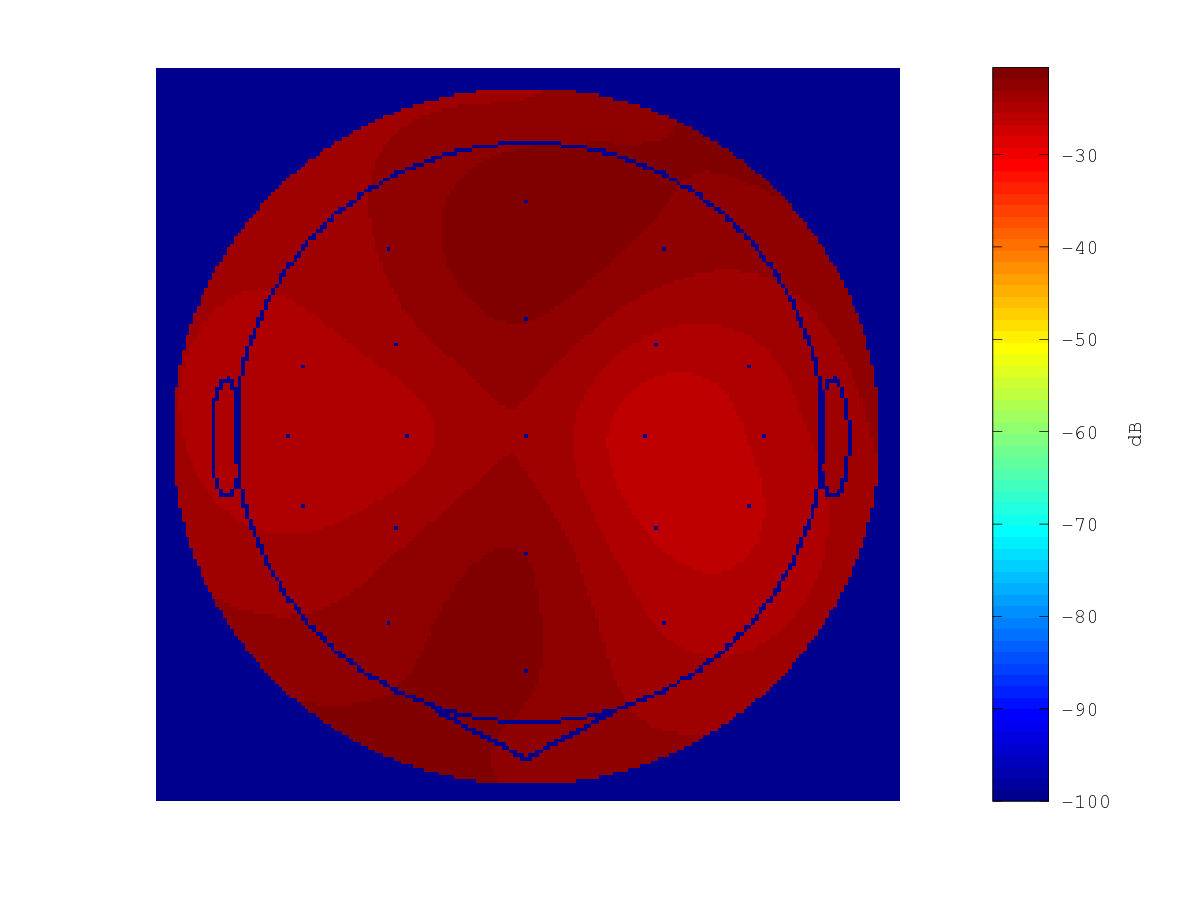
\includegraphics[width=2.5in]{scalpplot.png}}
\end{minipage}
\begin{minipage}[t]{0.5\textwidth}
~\\	
\IfStrEq{\PlotType}{scatter}{\textbf{\Large{Summary:}}\\
\if\IsConcussed1
\if\PrevConcussions0
Based on the results of the EEGlewave algorithm, the baseline brain signals have been classified as belonging to the concussed group. However, the past history and results from the SCAT do not seems to suggest that there is evidence of a previous recent concussion or any other condition that may lead to this result.\\
The EEGlewave algorithm is not 100\% accurate and there is a 10\% chance that some players will be misclassified. It is therefore possible that your child's brain signals fall into the group that are misclassified. However, if you have any concerns or if your child is showing any symptoms that might suggest any medical issues we suggest that your child is seen by your family physician for a physical examination.\\
Please feel free to contact Dr. Virji-Babul if you would like to discuss these results or would like more information.
\else
Based on the results of the EEGlewave algorithm the baseline brain signals have been classified as belonging to the concussed group. The past history and results from the SCAT also seems to suggest that there is evidence of a previous recent concussion. Given these results we suggest that your child is seen by your family physician for a physical examination and be cleared before he/she returns to play.\\
We will contact you again for a second EEG scan within a month to compare the baseline brain signals to determine if your brain signals are changing as a result of recovery. We will also repeat the SCAT to evaluate general changes in symptoms, balance and cognition from the initial assessment.\\
Please feel free to contact Dr. Virji-Babul if you would like more information.
\fi
\else
Based on the results of the EEGlewave algorithm the brain signals appear to be within normal range. If your child receives an impact to the head/body and a concussion is suspected please see your physician and contact EEGlewave at care@eeglewave.com. We will arrange for a second EEG scan and compare your baseline brain signals to the second EEG scan to determine if there have been any changes in your brain activity that may have resulted from the impact. We will also repeat the SCAT3 to evaluate changes in symptoms, balance and cognition from the baseline assessment.
\fi}{Electroencephalography (EEG) is a technique that records the electrical activity of the brain. Brain cells communicate using electrical impulses and are active all the time, even when sitting quietly or sleeping. The EEGlewave algorithm uses EEG signals from the whole brain to evaluate changes in these signals that may be due to a concussion.\\}
\end{minipage}
}}

 %comment starts
\iffalse
\fbox{\parbox{\textwidth}{
\textbf{\Large{Summary:}}\\
\if\IsConcussed1
\if\PrevConcussions0
Based on the results of the EEGlewave algorithm, the baseline brain signals have been classified as belonging to the concussed group. However, the past history and results from the SCAT do not seems to suggest that there is evidence of a previous recent concussion or any other condition that may lead to this result.\\
The EEGlewave algorithm is not 100\% accurate and there is a 10\% chance that some players will be misclassified. It is therefore possible that your child's brain signals fall into the group that are misclassified. However, if you have any concerns or if your child is showing any symptoms that might suggest any medical issues we suggest that your child is seen by your family physician for a physical examination.\\
Please feel free to contact Dr. Virji-Babul if you would like to discuss these results or would like more information.
\else
Based on the results of the EEGlewave algorithm the baseline brain signals have been classified as belonging to the concussed group. The past history and results from the SCAT also seems to suggest that there is evidence of a previous recent concussion. Given these results we suggest that your child is seen by your family physician for a physical examination and be cleared before he/she returns to play.\\
We will contact you again for a second EEG scan within a month to compare the baseline brain signals to determine if your brain signals are changing as a result of recovery. We will also repeat the SCAT to evaluate general changes in symptoms, balance and cognition from the initial assessment.\\
Please feel free to contact Dr. Virji-Babul if you would like more information.
\fi
\else
Based on the results of the EEGlewave algorithm the brain signals appear to be within normal range. If your child receives an impact to the head/body and a concussion is suspected please see your physician and contact EEGlewave at care@eeglewave.com. We will arrange for a second EEG scan and compare your baseline brain signals to the second EEG scan to determine if there have been any changes in your brain activity that may have resulted from the impact. We will also repeat the SCAT3 to evaluate changes in symptoms, balance and cognition from the baseline assessment.
\fi
}}
\fi % till here commenting out

% Add the footnote. A better way would be to use fancyhdr
\vfill
{\footnotesize\color{EWgray}\sffamily
	NOTE: EEGlewave does not provide medical advice. This report should not be used as a substitute for professional medical consultation.\\
}
\end{document}
}%The .tex filename goes here (NOT the same as \jobname)
\unless\ifdefined\PrevConcussions
\endinput\expandafter\expandafter\expandafter\ReadPrevConcussions\fi

\def\ReadMostRecentConcussion#1 {%
	\def\MostRecentConcussion{#1}%
	% NOTE: This report is to be compiled through the Octave command prompt.
% The following command should be typed into an Octave session to generate the report.
% system("pdflatex.exe -synctex=1 -interaction=nonstopmode -job-name=FirstName_LastName report.tex FirstName Lastname ParentName ID Handedness PrevConcussions Age ScanType")

% Definitions for command line arguments
\def\ReadFirstName#1 {%
	\def\FirstName{#1}%
	\input{report}}%The .tex filename goes here (NOT the same as \jobname)
\unless\ifdefined\FirstName
\endinput\expandafter\expandafter\expandafter\ReadFirstName\fi

\def\ReadLastName#1 {%
	\def\LastName{#1}%
	\input{report}}%The .tex filename goes here (NOT the same as \jobname)
\unless\ifdefined\LastName
\endinput\expandafter\expandafter\expandafter\ReadLastName\fi

\def\ReadParentFirstName#1 {%
	\def\ParentFirstName{#1}%
	\input{report}}%The .tex filename goes here (NOT the same as \jobname)
\unless\ifdefined\ParentFirstName
\endinput\expandafter\expandafter\expandafter\ReadParentFirstName\fi

\def\ReadParentLastName#1 {%
	\def\ParentLastName{#1}%
	\input{report}}%The .tex filename goes here (NOT the same as \jobname)
\unless\ifdefined\ParentLastName
\endinput\expandafter\expandafter\expandafter\ReadParentLastName\fi

\def\ReadID#1 {%
	\def\ID{#1}%
	\input{report}}%The .tex filename goes here (NOT the same as \jobname)
\unless\ifdefined\ID
\endinput\expandafter\expandafter\expandafter\ReadID\fi

\def\ReadHandedness#1 {%
	\def\Handedness{#1}%
	\input{report}}%The .tex filename goes here (NOT the same as \jobname)
\unless\ifdefined\Handedness
\endinput\expandafter\expandafter\expandafter\ReadHandedness\fi

\def\ReadPrevConcussions#1 {%
	\def\PrevConcussions{#1}%
	\input{report}}%The .tex filename goes here (NOT the same as \jobname)
\unless\ifdefined\PrevConcussions
\endinput\expandafter\expandafter\expandafter\ReadPrevConcussions\fi

\def\ReadMostRecentConcussion#1 {%
	\def\MostRecentConcussion{#1}%
	\input{report}}%The .tex filename goes here (NOT the same as \jobname)
\unless\ifdefined\MostRecentConcussion
\endinput\expandafter\expandafter\expandafter\ReadMostRecentConcussion\fi

\def\ReadIsConcussed#1 {%
	\def\IsConcussed{#1}%
	\input{report}}%The .tex filename goes here (NOT the same as \jobname)
\unless\ifdefined\IsConcussed
\endinput\expandafter\expandafter\expandafter\ReadIsConcussed\fi

\def\ReadDivision#1 {%
	\def\Division{#1}%
	\input{report}}%The .tex filename goes here (NOT the same as \jobname)
\unless\ifdefined\Division
\endinput\expandafter\expandafter\expandafter\ReadDivision\fi

\def\ReadGender#1 {%
	\def\Gender{#1}%
	\input{report}}%The .tex filename goes here (NOT the same as \jobname)
\unless\ifdefined\Gender
\endinput\expandafter\expandafter\expandafter\ReadGender\fi

\def\ReadAge#1 {%
	\def\Age{#1}%
	\input{report}}%The .tex filename goes here (NOT the same as \jobname)
\unless\ifdefined\Age
\endinput\expandafter\expandafter\expandafter\ReadAge\fi

\def\ReadDOS#1 {%
	\def\DOS{#1}%
	\input{report}}%The .tex filename goes here (NOT the same as \jobname)
\unless\ifdefined\DOS
\endinput\expandafter\expandafter\expandafter\ReadDOS\fi

\def\ReadScanType#1 {%
	\def\ScanType{#1}%
	\input{report}}%The .tex filename goes here (NOT the same as \jobname)
\unless\ifdefined\ScanType
\endinput\expandafter\expandafter\expandafter\ReadScanType\fi

\def\ReadNumSymptoms#1 {%
	\def\NumSymptoms{#1}%
	\input{report}}%The .tex filename goes here (NOT the same as \jobname)
\unless\ifdefined\NumSymptoms
\endinput\expandafter\expandafter\expandafter\ReadNumSymptoms\fi

\def\ReadSeverityScore#1 {%
	\def\SeverityScore{#1}%
	\input{report}}%The .tex filename goes here (NOT the same as \jobname)
\unless\ifdefined\SeverityScore
\endinput\expandafter\expandafter\expandafter\ReadSeverityScore\fi

\def\ReadOrientation#1 {%
	\def\Orientation{#1}%
	\input{report}}%The .tex filename goes here (NOT the same as \jobname)
\unless\ifdefined\Orientation
\endinput\expandafter\expandafter\expandafter\ReadOrientation\fi

\def\ReadOrientationTotal#1 {%
	\def\OrientationTotal{#1}%
	\input{report}}%The .tex filename goes here (NOT the same as \jobname)
\unless\ifdefined\OrientationTotal
\endinput\expandafter\expandafter\expandafter\ReadOrientationTotal\fi

\def\ReadImmMem#1 {%
	\def\ImmMem{#1}%
	\input{report}}%The .tex filename goes here (NOT the same as \jobname)
\unless\ifdefined\ImmMem
\endinput\expandafter\expandafter\expandafter\ReadImmMem\fi

\def\ReadConcentration#1 {%
	\def\Concentration{#1}%
	\input{report}}%The .tex filename goes here (NOT the same as \jobname)
\unless\ifdefined\Concentration
\endinput\expandafter\expandafter\expandafter\ReadConcentration\fi

\def\ReadConcentrationTotal#1 {%
	\def\ConcentrationTotal{#1}%
	\input{report}}%The .tex filename goes here (NOT the same as \jobname)
\unless\ifdefined\ConcentrationTotal
\endinput\expandafter\expandafter\expandafter\ReadConcentrationTotal\fi

\def\ReadDelayedRecall#1 {%
	\def\DelayedRecall{#1}%
	\input{report}}%The .tex filename goes here (NOT the same as \jobname)
\unless\ifdefined\DelayedRecall
\endinput\expandafter\expandafter\expandafter\ReadDelayedRecall\fi

\def\ReadSAC#1 {%
	\def\SAC{#1}%
	\input{report}}%The .tex filename goes here (NOT the same as \jobname)
\unless\ifdefined\SAC
\endinput\expandafter\expandafter\expandafter\ReadSAC\fi

\def\ReadBESS#1 {%
	\def\BESS{#1}%
	\input{report}}%The .tex filename goes here (NOT the same as \jobname)
\unless\ifdefined\BESS
\endinput\expandafter\expandafter\expandafter\ReadBESS\fi

\def\ReadTandemGait#1 {%
	\def\TandemGait{#1}%
	\input{report}}%The .tex filename goes here (NOT the same as \jobname)
\unless\ifdefined\TandemGait
\endinput\expandafter\expandafter\expandafter\ReadTandemGait\fi

\def\ReadCoordination#1 {%
	\def\Coordination{#1}%
	\input{report}}%The .tex filename goes here (NOT the same as \jobname)
\unless\ifdefined\Coordination
\endinput\expandafter\expandafter\expandafter\ReadCoordination\fi

\def\ReadPlotType#1 {%
	\def\PlotType{#1}%
	\input{report}}%The .tex filename goes here (NOT the same as \jobname)
\unless\ifdefined\PlotType
\endinput\expandafter\expandafter\expandafter\ReadPlotType\fi

\documentclass{article}

\usepackage[dvinames]{xcolor}
% Measurements are taken directly from the guide
\usepackage[top=2in,left=0.5in,bottom=0.5in,right=0.5in]{geometry}
\usepackage{graphicx}
\usepackage[colorlinks=false,
            pdfborder={0 0 0},
            ]{hyperref}
\usepackage{lipsum}
\usepackage[absolute]{textpos}
\usepackage{tikz}
\usetikzlibrary{calc}
% A nice serif font, but no the prescribed nonfree ITC stone
\usepackage[oldstylenums]{kpfonts}
\usepackage[T1]{fontenc	}
\usepackage[12pt]{moresize}
\usepackage{xstring}

% No paragraph indentation
\parindent0pt
\setlength{\parskip}{0.8\baselineskip}
\raggedright
\pagestyle{empty}


\definecolor{EWgray}{HTML}{5e6a71}

\begin{document}
	\begin{center}
		\HUGE{~}\\
		\HUGE{~}\\
		\HUGE{~}\\
		\textbf{\HUGE{EEGlewave Inc.}}\\[1in]
		\textbf{\huge{\ScanType~Report}}\\[1cm]
	\end{center}
	\newpage
\bigskip
% -------------------------------------------------------
% Add logo, the text under the crimson line, and the line itself
\begin{textblock*}{2in}[0.3066,0.39](1.25in,1.23in)
	
\includegraphics[width=1.5in]{eeglewave-front-211x128-88.png}
\end{textblock*}
\begin{textblock*}{6.375in}(1.5in,1.4in)   % 6.375=8.5 - 1.5 - 0.625
	\sffamily
	\hfill \color{EWgray} EEGlewave Inc.\\
	\hfill \url{care@eeglewave.com} \textbullet\ \url{http://eeglewave.com}
\end{textblock*}
\begin{tikzpicture}[remember picture,overlay]
\draw[line width=1pt] (current page.north west)+(0.5in,-1.85in) -- ($(-0.5in,-1.85in)+(current page.north east)$);
\end{tikzpicture}
\fbox{\parbox{\textwidth}{
\textbf{\Large{General Information:}}\\
\begin{minipage}[t]{0.55\textwidth}

\textbf{Name: } \FirstName~\LastName  \\
\textbf{Parent/Guardian's Name: } \ParentFirstName~\ParentLastName  \\
\textbf{ID: } \ID   \\
\textbf{Handedness: } \Handedness  \\
\textbf{Number of Previous Concussions: } \PrevConcussions \\
\textbf{Date of Most Recent Concussion: } \MostRecentConcussion
\end{minipage}
\begin{minipage}[t]{0.45\textwidth}
	\textbf{Division: } \Division  \\
	\textbf{Gender: } \Gender  \\
	\textbf{Age: } \Age  \\
	\textbf{Date of Scan: } \DOS \\
	\textbf{Type of Scan: } \ScanType  \\
\end{minipage}
}}

\fbox{\parbox{\textwidth}{
\textbf{\Large{SCAT3 Scoring Summary:}}\\
\begin{minipage}[t]{0.55\textwidth}
\textbf{Number of Symptoms (/22): } \\
\textbf{Symptom Severity Score (/132): } \\

\textbf{Orientation (/\OrientationTotal): }  \\
\textbf{Immediate Memory (/15): } \\
\textbf{Concentration (/\ConcentrationTotal): } \\
\textbf{Delayed Recall (/5): } \\
\textbf{SAC Total (/30): } \\

\textbf{BESS (total errors): } \\
\textbf{Tandem Gait (seconds): } \\
\textbf{Coordination (/1): } 
\end{minipage}
\begin{minipage}[t]{0.25\textwidth}
\NumSymptoms  \\
\SeverityScore  \\

\Orientation  \\
\ImmMem  \\
\Concentration  \\
\DelayedRecall \\
\SAC  \\

\BESS  \\
\TandemGait  \\
\Coordination
\end{minipage}
}}

\fbox{\parbox{\textwidth}{
\textbf{\Large{\IfStrEq{\PlotType}{scatter}{Scatter Plot:}{EEG Plot of Power at Rest:}}}\\
\begin{minipage}[t]{0.5\textwidth}
	~\\
	\IfStrEq{\PlotType}{scatter}{\includegraphics[width=3.25in]{scatterplot.png}}{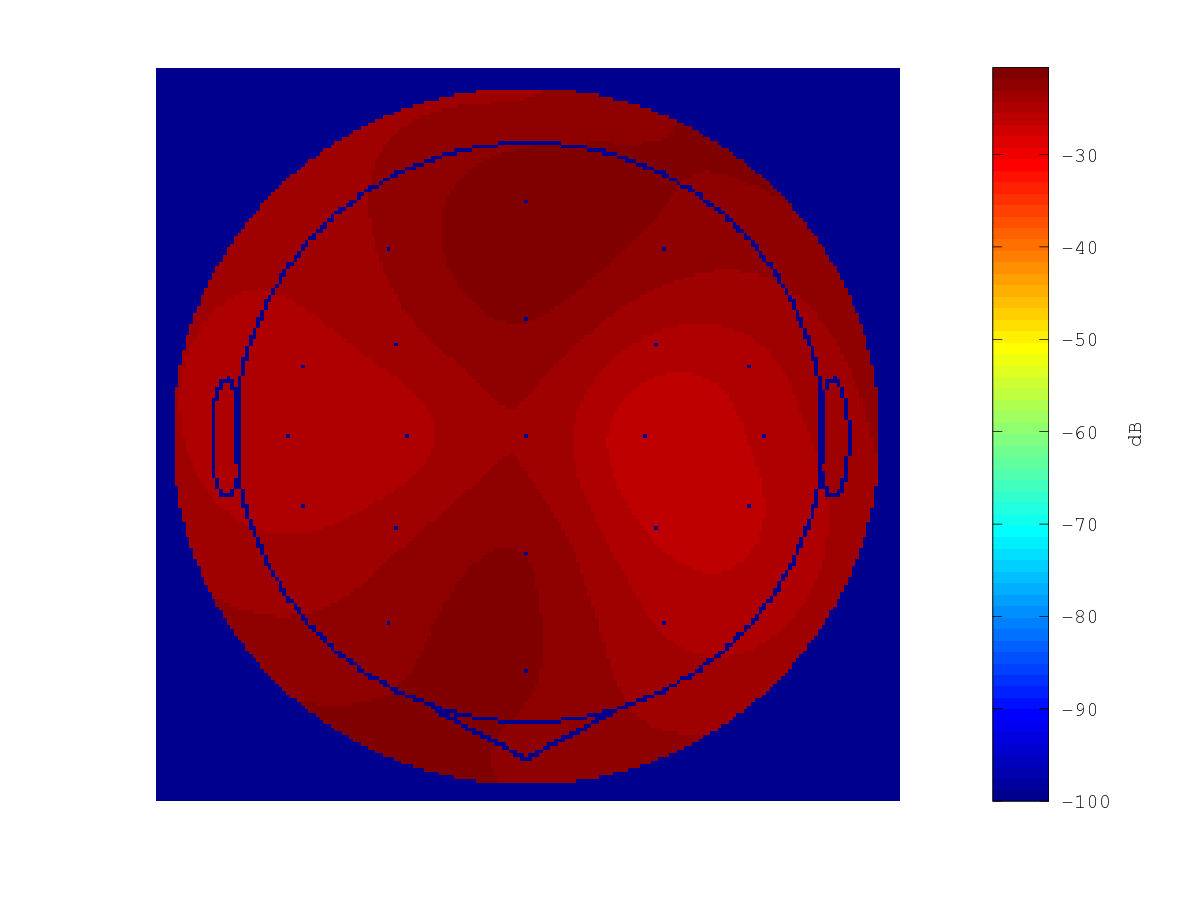
\includegraphics[width=2.5in]{scalpplot.png}}
\end{minipage}
\begin{minipage}[t]{0.5\textwidth}
~\\	
\IfStrEq{\PlotType}{scatter}{\textbf{\Large{Summary:}}\\
\if\IsConcussed1
\if\PrevConcussions0
Based on the results of the EEGlewave algorithm, the baseline brain signals have been classified as belonging to the concussed group. However, the past history and results from the SCAT do not seems to suggest that there is evidence of a previous recent concussion or any other condition that may lead to this result.\\
The EEGlewave algorithm is not 100\% accurate and there is a 10\% chance that some players will be misclassified. It is therefore possible that your child's brain signals fall into the group that are misclassified. However, if you have any concerns or if your child is showing any symptoms that might suggest any medical issues we suggest that your child is seen by your family physician for a physical examination.\\
Please feel free to contact Dr. Virji-Babul if you would like to discuss these results or would like more information.
\else
Based on the results of the EEGlewave algorithm the baseline brain signals have been classified as belonging to the concussed group. The past history and results from the SCAT also seems to suggest that there is evidence of a previous recent concussion. Given these results we suggest that your child is seen by your family physician for a physical examination and be cleared before he/she returns to play.\\
We will contact you again for a second EEG scan within a month to compare the baseline brain signals to determine if your brain signals are changing as a result of recovery. We will also repeat the SCAT to evaluate general changes in symptoms, balance and cognition from the initial assessment.\\
Please feel free to contact Dr. Virji-Babul if you would like more information.
\fi
\else
Based on the results of the EEGlewave algorithm the brain signals appear to be within normal range. If your child receives an impact to the head/body and a concussion is suspected please see your physician and contact EEGlewave at care@eeglewave.com. We will arrange for a second EEG scan and compare your baseline brain signals to the second EEG scan to determine if there have been any changes in your brain activity that may have resulted from the impact. We will also repeat the SCAT3 to evaluate changes in symptoms, balance and cognition from the baseline assessment.
\fi}{Electroencephalography (EEG) is a technique that records the electrical activity of the brain. Brain cells communicate using electrical impulses and are active all the time, even when sitting quietly or sleeping. The EEGlewave algorithm uses EEG signals from the whole brain to evaluate changes in these signals that may be due to a concussion.\\}
\end{minipage}
}}

 %comment starts
\iffalse
\fbox{\parbox{\textwidth}{
\textbf{\Large{Summary:}}\\
\if\IsConcussed1
\if\PrevConcussions0
Based on the results of the EEGlewave algorithm, the baseline brain signals have been classified as belonging to the concussed group. However, the past history and results from the SCAT do not seems to suggest that there is evidence of a previous recent concussion or any other condition that may lead to this result.\\
The EEGlewave algorithm is not 100\% accurate and there is a 10\% chance that some players will be misclassified. It is therefore possible that your child's brain signals fall into the group that are misclassified. However, if you have any concerns or if your child is showing any symptoms that might suggest any medical issues we suggest that your child is seen by your family physician for a physical examination.\\
Please feel free to contact Dr. Virji-Babul if you would like to discuss these results or would like more information.
\else
Based on the results of the EEGlewave algorithm the baseline brain signals have been classified as belonging to the concussed group. The past history and results from the SCAT also seems to suggest that there is evidence of a previous recent concussion. Given these results we suggest that your child is seen by your family physician for a physical examination and be cleared before he/she returns to play.\\
We will contact you again for a second EEG scan within a month to compare the baseline brain signals to determine if your brain signals are changing as a result of recovery. We will also repeat the SCAT to evaluate general changes in symptoms, balance and cognition from the initial assessment.\\
Please feel free to contact Dr. Virji-Babul if you would like more information.
\fi
\else
Based on the results of the EEGlewave algorithm the brain signals appear to be within normal range. If your child receives an impact to the head/body and a concussion is suspected please see your physician and contact EEGlewave at care@eeglewave.com. We will arrange for a second EEG scan and compare your baseline brain signals to the second EEG scan to determine if there have been any changes in your brain activity that may have resulted from the impact. We will also repeat the SCAT3 to evaluate changes in symptoms, balance and cognition from the baseline assessment.
\fi
}}
\fi % till here commenting out

% Add the footnote. A better way would be to use fancyhdr
\vfill
{\footnotesize\color{EWgray}\sffamily
	NOTE: EEGlewave does not provide medical advice. This report should not be used as a substitute for professional medical consultation.\\
}
\end{document}
}%The .tex filename goes here (NOT the same as \jobname)
\unless\ifdefined\MostRecentConcussion
\endinput\expandafter\expandafter\expandafter\ReadMostRecentConcussion\fi

\def\ReadIsConcussed#1 {%
	\def\IsConcussed{#1}%
	% NOTE: This report is to be compiled through the Octave command prompt.
% The following command should be typed into an Octave session to generate the report.
% system("pdflatex.exe -synctex=1 -interaction=nonstopmode -job-name=FirstName_LastName report.tex FirstName Lastname ParentName ID Handedness PrevConcussions Age ScanType")

% Definitions for command line arguments
\def\ReadFirstName#1 {%
	\def\FirstName{#1}%
	\input{report}}%The .tex filename goes here (NOT the same as \jobname)
\unless\ifdefined\FirstName
\endinput\expandafter\expandafter\expandafter\ReadFirstName\fi

\def\ReadLastName#1 {%
	\def\LastName{#1}%
	\input{report}}%The .tex filename goes here (NOT the same as \jobname)
\unless\ifdefined\LastName
\endinput\expandafter\expandafter\expandafter\ReadLastName\fi

\def\ReadParentFirstName#1 {%
	\def\ParentFirstName{#1}%
	\input{report}}%The .tex filename goes here (NOT the same as \jobname)
\unless\ifdefined\ParentFirstName
\endinput\expandafter\expandafter\expandafter\ReadParentFirstName\fi

\def\ReadParentLastName#1 {%
	\def\ParentLastName{#1}%
	\input{report}}%The .tex filename goes here (NOT the same as \jobname)
\unless\ifdefined\ParentLastName
\endinput\expandafter\expandafter\expandafter\ReadParentLastName\fi

\def\ReadID#1 {%
	\def\ID{#1}%
	\input{report}}%The .tex filename goes here (NOT the same as \jobname)
\unless\ifdefined\ID
\endinput\expandafter\expandafter\expandafter\ReadID\fi

\def\ReadHandedness#1 {%
	\def\Handedness{#1}%
	\input{report}}%The .tex filename goes here (NOT the same as \jobname)
\unless\ifdefined\Handedness
\endinput\expandafter\expandafter\expandafter\ReadHandedness\fi

\def\ReadPrevConcussions#1 {%
	\def\PrevConcussions{#1}%
	\input{report}}%The .tex filename goes here (NOT the same as \jobname)
\unless\ifdefined\PrevConcussions
\endinput\expandafter\expandafter\expandafter\ReadPrevConcussions\fi

\def\ReadMostRecentConcussion#1 {%
	\def\MostRecentConcussion{#1}%
	\input{report}}%The .tex filename goes here (NOT the same as \jobname)
\unless\ifdefined\MostRecentConcussion
\endinput\expandafter\expandafter\expandafter\ReadMostRecentConcussion\fi

\def\ReadIsConcussed#1 {%
	\def\IsConcussed{#1}%
	\input{report}}%The .tex filename goes here (NOT the same as \jobname)
\unless\ifdefined\IsConcussed
\endinput\expandafter\expandafter\expandafter\ReadIsConcussed\fi

\def\ReadDivision#1 {%
	\def\Division{#1}%
	\input{report}}%The .tex filename goes here (NOT the same as \jobname)
\unless\ifdefined\Division
\endinput\expandafter\expandafter\expandafter\ReadDivision\fi

\def\ReadGender#1 {%
	\def\Gender{#1}%
	\input{report}}%The .tex filename goes here (NOT the same as \jobname)
\unless\ifdefined\Gender
\endinput\expandafter\expandafter\expandafter\ReadGender\fi

\def\ReadAge#1 {%
	\def\Age{#1}%
	\input{report}}%The .tex filename goes here (NOT the same as \jobname)
\unless\ifdefined\Age
\endinput\expandafter\expandafter\expandafter\ReadAge\fi

\def\ReadDOS#1 {%
	\def\DOS{#1}%
	\input{report}}%The .tex filename goes here (NOT the same as \jobname)
\unless\ifdefined\DOS
\endinput\expandafter\expandafter\expandafter\ReadDOS\fi

\def\ReadScanType#1 {%
	\def\ScanType{#1}%
	\input{report}}%The .tex filename goes here (NOT the same as \jobname)
\unless\ifdefined\ScanType
\endinput\expandafter\expandafter\expandafter\ReadScanType\fi

\def\ReadNumSymptoms#1 {%
	\def\NumSymptoms{#1}%
	\input{report}}%The .tex filename goes here (NOT the same as \jobname)
\unless\ifdefined\NumSymptoms
\endinput\expandafter\expandafter\expandafter\ReadNumSymptoms\fi

\def\ReadSeverityScore#1 {%
	\def\SeverityScore{#1}%
	\input{report}}%The .tex filename goes here (NOT the same as \jobname)
\unless\ifdefined\SeverityScore
\endinput\expandafter\expandafter\expandafter\ReadSeverityScore\fi

\def\ReadOrientation#1 {%
	\def\Orientation{#1}%
	\input{report}}%The .tex filename goes here (NOT the same as \jobname)
\unless\ifdefined\Orientation
\endinput\expandafter\expandafter\expandafter\ReadOrientation\fi

\def\ReadOrientationTotal#1 {%
	\def\OrientationTotal{#1}%
	\input{report}}%The .tex filename goes here (NOT the same as \jobname)
\unless\ifdefined\OrientationTotal
\endinput\expandafter\expandafter\expandafter\ReadOrientationTotal\fi

\def\ReadImmMem#1 {%
	\def\ImmMem{#1}%
	\input{report}}%The .tex filename goes here (NOT the same as \jobname)
\unless\ifdefined\ImmMem
\endinput\expandafter\expandafter\expandafter\ReadImmMem\fi

\def\ReadConcentration#1 {%
	\def\Concentration{#1}%
	\input{report}}%The .tex filename goes here (NOT the same as \jobname)
\unless\ifdefined\Concentration
\endinput\expandafter\expandafter\expandafter\ReadConcentration\fi

\def\ReadConcentrationTotal#1 {%
	\def\ConcentrationTotal{#1}%
	\input{report}}%The .tex filename goes here (NOT the same as \jobname)
\unless\ifdefined\ConcentrationTotal
\endinput\expandafter\expandafter\expandafter\ReadConcentrationTotal\fi

\def\ReadDelayedRecall#1 {%
	\def\DelayedRecall{#1}%
	\input{report}}%The .tex filename goes here (NOT the same as \jobname)
\unless\ifdefined\DelayedRecall
\endinput\expandafter\expandafter\expandafter\ReadDelayedRecall\fi

\def\ReadSAC#1 {%
	\def\SAC{#1}%
	\input{report}}%The .tex filename goes here (NOT the same as \jobname)
\unless\ifdefined\SAC
\endinput\expandafter\expandafter\expandafter\ReadSAC\fi

\def\ReadBESS#1 {%
	\def\BESS{#1}%
	\input{report}}%The .tex filename goes here (NOT the same as \jobname)
\unless\ifdefined\BESS
\endinput\expandafter\expandafter\expandafter\ReadBESS\fi

\def\ReadTandemGait#1 {%
	\def\TandemGait{#1}%
	\input{report}}%The .tex filename goes here (NOT the same as \jobname)
\unless\ifdefined\TandemGait
\endinput\expandafter\expandafter\expandafter\ReadTandemGait\fi

\def\ReadCoordination#1 {%
	\def\Coordination{#1}%
	\input{report}}%The .tex filename goes here (NOT the same as \jobname)
\unless\ifdefined\Coordination
\endinput\expandafter\expandafter\expandafter\ReadCoordination\fi

\def\ReadPlotType#1 {%
	\def\PlotType{#1}%
	\input{report}}%The .tex filename goes here (NOT the same as \jobname)
\unless\ifdefined\PlotType
\endinput\expandafter\expandafter\expandafter\ReadPlotType\fi

\documentclass{article}

\usepackage[dvinames]{xcolor}
% Measurements are taken directly from the guide
\usepackage[top=2in,left=0.5in,bottom=0.5in,right=0.5in]{geometry}
\usepackage{graphicx}
\usepackage[colorlinks=false,
            pdfborder={0 0 0},
            ]{hyperref}
\usepackage{lipsum}
\usepackage[absolute]{textpos}
\usepackage{tikz}
\usetikzlibrary{calc}
% A nice serif font, but no the prescribed nonfree ITC stone
\usepackage[oldstylenums]{kpfonts}
\usepackage[T1]{fontenc	}
\usepackage[12pt]{moresize}
\usepackage{xstring}

% No paragraph indentation
\parindent0pt
\setlength{\parskip}{0.8\baselineskip}
\raggedright
\pagestyle{empty}


\definecolor{EWgray}{HTML}{5e6a71}

\begin{document}
	\begin{center}
		\HUGE{~}\\
		\HUGE{~}\\
		\HUGE{~}\\
		\textbf{\HUGE{EEGlewave Inc.}}\\[1in]
		\textbf{\huge{\ScanType~Report}}\\[1cm]
	\end{center}
	\newpage
\bigskip
% -------------------------------------------------------
% Add logo, the text under the crimson line, and the line itself
\begin{textblock*}{2in}[0.3066,0.39](1.25in,1.23in)
	
\includegraphics[width=1.5in]{eeglewave-front-211x128-88.png}
\end{textblock*}
\begin{textblock*}{6.375in}(1.5in,1.4in)   % 6.375=8.5 - 1.5 - 0.625
	\sffamily
	\hfill \color{EWgray} EEGlewave Inc.\\
	\hfill \url{care@eeglewave.com} \textbullet\ \url{http://eeglewave.com}
\end{textblock*}
\begin{tikzpicture}[remember picture,overlay]
\draw[line width=1pt] (current page.north west)+(0.5in,-1.85in) -- ($(-0.5in,-1.85in)+(current page.north east)$);
\end{tikzpicture}
\fbox{\parbox{\textwidth}{
\textbf{\Large{General Information:}}\\
\begin{minipage}[t]{0.55\textwidth}

\textbf{Name: } \FirstName~\LastName  \\
\textbf{Parent/Guardian's Name: } \ParentFirstName~\ParentLastName  \\
\textbf{ID: } \ID   \\
\textbf{Handedness: } \Handedness  \\
\textbf{Number of Previous Concussions: } \PrevConcussions \\
\textbf{Date of Most Recent Concussion: } \MostRecentConcussion
\end{minipage}
\begin{minipage}[t]{0.45\textwidth}
	\textbf{Division: } \Division  \\
	\textbf{Gender: } \Gender  \\
	\textbf{Age: } \Age  \\
	\textbf{Date of Scan: } \DOS \\
	\textbf{Type of Scan: } \ScanType  \\
\end{minipage}
}}

\fbox{\parbox{\textwidth}{
\textbf{\Large{SCAT3 Scoring Summary:}}\\
\begin{minipage}[t]{0.55\textwidth}
\textbf{Number of Symptoms (/22): } \\
\textbf{Symptom Severity Score (/132): } \\

\textbf{Orientation (/\OrientationTotal): }  \\
\textbf{Immediate Memory (/15): } \\
\textbf{Concentration (/\ConcentrationTotal): } \\
\textbf{Delayed Recall (/5): } \\
\textbf{SAC Total (/30): } \\

\textbf{BESS (total errors): } \\
\textbf{Tandem Gait (seconds): } \\
\textbf{Coordination (/1): } 
\end{minipage}
\begin{minipage}[t]{0.25\textwidth}
\NumSymptoms  \\
\SeverityScore  \\

\Orientation  \\
\ImmMem  \\
\Concentration  \\
\DelayedRecall \\
\SAC  \\

\BESS  \\
\TandemGait  \\
\Coordination
\end{minipage}
}}

\fbox{\parbox{\textwidth}{
\textbf{\Large{\IfStrEq{\PlotType}{scatter}{Scatter Plot:}{EEG Plot of Power at Rest:}}}\\
\begin{minipage}[t]{0.5\textwidth}
	~\\
	\IfStrEq{\PlotType}{scatter}{\includegraphics[width=3.25in]{scatterplot.png}}{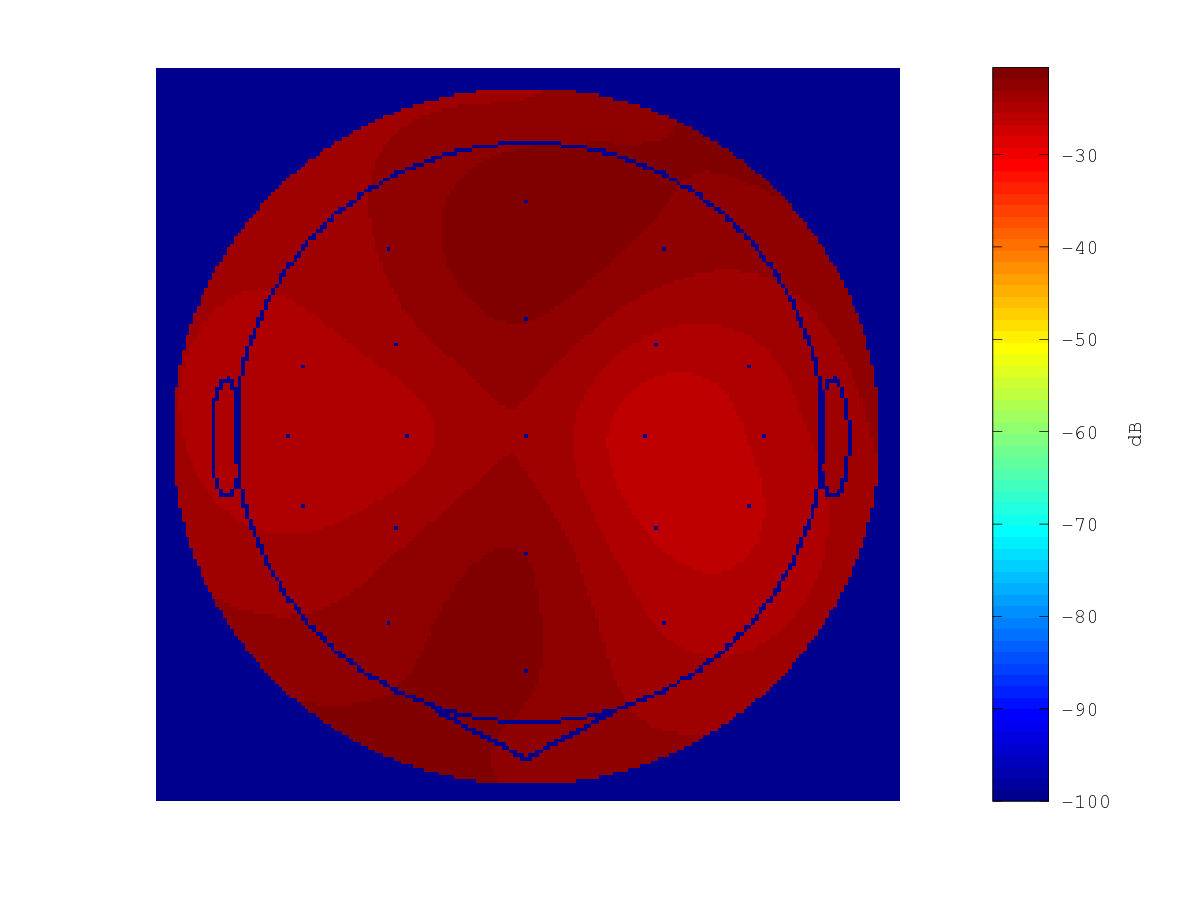
\includegraphics[width=2.5in]{scalpplot.png}}
\end{minipage}
\begin{minipage}[t]{0.5\textwidth}
~\\	
\IfStrEq{\PlotType}{scatter}{\textbf{\Large{Summary:}}\\
\if\IsConcussed1
\if\PrevConcussions0
Based on the results of the EEGlewave algorithm, the baseline brain signals have been classified as belonging to the concussed group. However, the past history and results from the SCAT do not seems to suggest that there is evidence of a previous recent concussion or any other condition that may lead to this result.\\
The EEGlewave algorithm is not 100\% accurate and there is a 10\% chance that some players will be misclassified. It is therefore possible that your child's brain signals fall into the group that are misclassified. However, if you have any concerns or if your child is showing any symptoms that might suggest any medical issues we suggest that your child is seen by your family physician for a physical examination.\\
Please feel free to contact Dr. Virji-Babul if you would like to discuss these results or would like more information.
\else
Based on the results of the EEGlewave algorithm the baseline brain signals have been classified as belonging to the concussed group. The past history and results from the SCAT also seems to suggest that there is evidence of a previous recent concussion. Given these results we suggest that your child is seen by your family physician for a physical examination and be cleared before he/she returns to play.\\
We will contact you again for a second EEG scan within a month to compare the baseline brain signals to determine if your brain signals are changing as a result of recovery. We will also repeat the SCAT to evaluate general changes in symptoms, balance and cognition from the initial assessment.\\
Please feel free to contact Dr. Virji-Babul if you would like more information.
\fi
\else
Based on the results of the EEGlewave algorithm the brain signals appear to be within normal range. If your child receives an impact to the head/body and a concussion is suspected please see your physician and contact EEGlewave at care@eeglewave.com. We will arrange for a second EEG scan and compare your baseline brain signals to the second EEG scan to determine if there have been any changes in your brain activity that may have resulted from the impact. We will also repeat the SCAT3 to evaluate changes in symptoms, balance and cognition from the baseline assessment.
\fi}{Electroencephalography (EEG) is a technique that records the electrical activity of the brain. Brain cells communicate using electrical impulses and are active all the time, even when sitting quietly or sleeping. The EEGlewave algorithm uses EEG signals from the whole brain to evaluate changes in these signals that may be due to a concussion.\\}
\end{minipage}
}}

 %comment starts
\iffalse
\fbox{\parbox{\textwidth}{
\textbf{\Large{Summary:}}\\
\if\IsConcussed1
\if\PrevConcussions0
Based on the results of the EEGlewave algorithm, the baseline brain signals have been classified as belonging to the concussed group. However, the past history and results from the SCAT do not seems to suggest that there is evidence of a previous recent concussion or any other condition that may lead to this result.\\
The EEGlewave algorithm is not 100\% accurate and there is a 10\% chance that some players will be misclassified. It is therefore possible that your child's brain signals fall into the group that are misclassified. However, if you have any concerns or if your child is showing any symptoms that might suggest any medical issues we suggest that your child is seen by your family physician for a physical examination.\\
Please feel free to contact Dr. Virji-Babul if you would like to discuss these results or would like more information.
\else
Based on the results of the EEGlewave algorithm the baseline brain signals have been classified as belonging to the concussed group. The past history and results from the SCAT also seems to suggest that there is evidence of a previous recent concussion. Given these results we suggest that your child is seen by your family physician for a physical examination and be cleared before he/she returns to play.\\
We will contact you again for a second EEG scan within a month to compare the baseline brain signals to determine if your brain signals are changing as a result of recovery. We will also repeat the SCAT to evaluate general changes in symptoms, balance and cognition from the initial assessment.\\
Please feel free to contact Dr. Virji-Babul if you would like more information.
\fi
\else
Based on the results of the EEGlewave algorithm the brain signals appear to be within normal range. If your child receives an impact to the head/body and a concussion is suspected please see your physician and contact EEGlewave at care@eeglewave.com. We will arrange for a second EEG scan and compare your baseline brain signals to the second EEG scan to determine if there have been any changes in your brain activity that may have resulted from the impact. We will also repeat the SCAT3 to evaluate changes in symptoms, balance and cognition from the baseline assessment.
\fi
}}
\fi % till here commenting out

% Add the footnote. A better way would be to use fancyhdr
\vfill
{\footnotesize\color{EWgray}\sffamily
	NOTE: EEGlewave does not provide medical advice. This report should not be used as a substitute for professional medical consultation.\\
}
\end{document}
}%The .tex filename goes here (NOT the same as \jobname)
\unless\ifdefined\IsConcussed
\endinput\expandafter\expandafter\expandafter\ReadIsConcussed\fi

\def\ReadDivision#1 {%
	\def\Division{#1}%
	% NOTE: This report is to be compiled through the Octave command prompt.
% The following command should be typed into an Octave session to generate the report.
% system("pdflatex.exe -synctex=1 -interaction=nonstopmode -job-name=FirstName_LastName report.tex FirstName Lastname ParentName ID Handedness PrevConcussions Age ScanType")

% Definitions for command line arguments
\def\ReadFirstName#1 {%
	\def\FirstName{#1}%
	\input{report}}%The .tex filename goes here (NOT the same as \jobname)
\unless\ifdefined\FirstName
\endinput\expandafter\expandafter\expandafter\ReadFirstName\fi

\def\ReadLastName#1 {%
	\def\LastName{#1}%
	\input{report}}%The .tex filename goes here (NOT the same as \jobname)
\unless\ifdefined\LastName
\endinput\expandafter\expandafter\expandafter\ReadLastName\fi

\def\ReadParentFirstName#1 {%
	\def\ParentFirstName{#1}%
	\input{report}}%The .tex filename goes here (NOT the same as \jobname)
\unless\ifdefined\ParentFirstName
\endinput\expandafter\expandafter\expandafter\ReadParentFirstName\fi

\def\ReadParentLastName#1 {%
	\def\ParentLastName{#1}%
	\input{report}}%The .tex filename goes here (NOT the same as \jobname)
\unless\ifdefined\ParentLastName
\endinput\expandafter\expandafter\expandafter\ReadParentLastName\fi

\def\ReadID#1 {%
	\def\ID{#1}%
	\input{report}}%The .tex filename goes here (NOT the same as \jobname)
\unless\ifdefined\ID
\endinput\expandafter\expandafter\expandafter\ReadID\fi

\def\ReadHandedness#1 {%
	\def\Handedness{#1}%
	\input{report}}%The .tex filename goes here (NOT the same as \jobname)
\unless\ifdefined\Handedness
\endinput\expandafter\expandafter\expandafter\ReadHandedness\fi

\def\ReadPrevConcussions#1 {%
	\def\PrevConcussions{#1}%
	\input{report}}%The .tex filename goes here (NOT the same as \jobname)
\unless\ifdefined\PrevConcussions
\endinput\expandafter\expandafter\expandafter\ReadPrevConcussions\fi

\def\ReadMostRecentConcussion#1 {%
	\def\MostRecentConcussion{#1}%
	\input{report}}%The .tex filename goes here (NOT the same as \jobname)
\unless\ifdefined\MostRecentConcussion
\endinput\expandafter\expandafter\expandafter\ReadMostRecentConcussion\fi

\def\ReadIsConcussed#1 {%
	\def\IsConcussed{#1}%
	\input{report}}%The .tex filename goes here (NOT the same as \jobname)
\unless\ifdefined\IsConcussed
\endinput\expandafter\expandafter\expandafter\ReadIsConcussed\fi

\def\ReadDivision#1 {%
	\def\Division{#1}%
	\input{report}}%The .tex filename goes here (NOT the same as \jobname)
\unless\ifdefined\Division
\endinput\expandafter\expandafter\expandafter\ReadDivision\fi

\def\ReadGender#1 {%
	\def\Gender{#1}%
	\input{report}}%The .tex filename goes here (NOT the same as \jobname)
\unless\ifdefined\Gender
\endinput\expandafter\expandafter\expandafter\ReadGender\fi

\def\ReadAge#1 {%
	\def\Age{#1}%
	\input{report}}%The .tex filename goes here (NOT the same as \jobname)
\unless\ifdefined\Age
\endinput\expandafter\expandafter\expandafter\ReadAge\fi

\def\ReadDOS#1 {%
	\def\DOS{#1}%
	\input{report}}%The .tex filename goes here (NOT the same as \jobname)
\unless\ifdefined\DOS
\endinput\expandafter\expandafter\expandafter\ReadDOS\fi

\def\ReadScanType#1 {%
	\def\ScanType{#1}%
	\input{report}}%The .tex filename goes here (NOT the same as \jobname)
\unless\ifdefined\ScanType
\endinput\expandafter\expandafter\expandafter\ReadScanType\fi

\def\ReadNumSymptoms#1 {%
	\def\NumSymptoms{#1}%
	\input{report}}%The .tex filename goes here (NOT the same as \jobname)
\unless\ifdefined\NumSymptoms
\endinput\expandafter\expandafter\expandafter\ReadNumSymptoms\fi

\def\ReadSeverityScore#1 {%
	\def\SeverityScore{#1}%
	\input{report}}%The .tex filename goes here (NOT the same as \jobname)
\unless\ifdefined\SeverityScore
\endinput\expandafter\expandafter\expandafter\ReadSeverityScore\fi

\def\ReadOrientation#1 {%
	\def\Orientation{#1}%
	\input{report}}%The .tex filename goes here (NOT the same as \jobname)
\unless\ifdefined\Orientation
\endinput\expandafter\expandafter\expandafter\ReadOrientation\fi

\def\ReadOrientationTotal#1 {%
	\def\OrientationTotal{#1}%
	\input{report}}%The .tex filename goes here (NOT the same as \jobname)
\unless\ifdefined\OrientationTotal
\endinput\expandafter\expandafter\expandafter\ReadOrientationTotal\fi

\def\ReadImmMem#1 {%
	\def\ImmMem{#1}%
	\input{report}}%The .tex filename goes here (NOT the same as \jobname)
\unless\ifdefined\ImmMem
\endinput\expandafter\expandafter\expandafter\ReadImmMem\fi

\def\ReadConcentration#1 {%
	\def\Concentration{#1}%
	\input{report}}%The .tex filename goes here (NOT the same as \jobname)
\unless\ifdefined\Concentration
\endinput\expandafter\expandafter\expandafter\ReadConcentration\fi

\def\ReadConcentrationTotal#1 {%
	\def\ConcentrationTotal{#1}%
	\input{report}}%The .tex filename goes here (NOT the same as \jobname)
\unless\ifdefined\ConcentrationTotal
\endinput\expandafter\expandafter\expandafter\ReadConcentrationTotal\fi

\def\ReadDelayedRecall#1 {%
	\def\DelayedRecall{#1}%
	\input{report}}%The .tex filename goes here (NOT the same as \jobname)
\unless\ifdefined\DelayedRecall
\endinput\expandafter\expandafter\expandafter\ReadDelayedRecall\fi

\def\ReadSAC#1 {%
	\def\SAC{#1}%
	\input{report}}%The .tex filename goes here (NOT the same as \jobname)
\unless\ifdefined\SAC
\endinput\expandafter\expandafter\expandafter\ReadSAC\fi

\def\ReadBESS#1 {%
	\def\BESS{#1}%
	\input{report}}%The .tex filename goes here (NOT the same as \jobname)
\unless\ifdefined\BESS
\endinput\expandafter\expandafter\expandafter\ReadBESS\fi

\def\ReadTandemGait#1 {%
	\def\TandemGait{#1}%
	\input{report}}%The .tex filename goes here (NOT the same as \jobname)
\unless\ifdefined\TandemGait
\endinput\expandafter\expandafter\expandafter\ReadTandemGait\fi

\def\ReadCoordination#1 {%
	\def\Coordination{#1}%
	\input{report}}%The .tex filename goes here (NOT the same as \jobname)
\unless\ifdefined\Coordination
\endinput\expandafter\expandafter\expandafter\ReadCoordination\fi

\def\ReadPlotType#1 {%
	\def\PlotType{#1}%
	\input{report}}%The .tex filename goes here (NOT the same as \jobname)
\unless\ifdefined\PlotType
\endinput\expandafter\expandafter\expandafter\ReadPlotType\fi

\documentclass{article}

\usepackage[dvinames]{xcolor}
% Measurements are taken directly from the guide
\usepackage[top=2in,left=0.5in,bottom=0.5in,right=0.5in]{geometry}
\usepackage{graphicx}
\usepackage[colorlinks=false,
            pdfborder={0 0 0},
            ]{hyperref}
\usepackage{lipsum}
\usepackage[absolute]{textpos}
\usepackage{tikz}
\usetikzlibrary{calc}
% A nice serif font, but no the prescribed nonfree ITC stone
\usepackage[oldstylenums]{kpfonts}
\usepackage[T1]{fontenc	}
\usepackage[12pt]{moresize}
\usepackage{xstring}

% No paragraph indentation
\parindent0pt
\setlength{\parskip}{0.8\baselineskip}
\raggedright
\pagestyle{empty}


\definecolor{EWgray}{HTML}{5e6a71}

\begin{document}
	\begin{center}
		\HUGE{~}\\
		\HUGE{~}\\
		\HUGE{~}\\
		\textbf{\HUGE{EEGlewave Inc.}}\\[1in]
		\textbf{\huge{\ScanType~Report}}\\[1cm]
	\end{center}
	\newpage
\bigskip
% -------------------------------------------------------
% Add logo, the text under the crimson line, and the line itself
\begin{textblock*}{2in}[0.3066,0.39](1.25in,1.23in)
	
\includegraphics[width=1.5in]{eeglewave-front-211x128-88.png}
\end{textblock*}
\begin{textblock*}{6.375in}(1.5in,1.4in)   % 6.375=8.5 - 1.5 - 0.625
	\sffamily
	\hfill \color{EWgray} EEGlewave Inc.\\
	\hfill \url{care@eeglewave.com} \textbullet\ \url{http://eeglewave.com}
\end{textblock*}
\begin{tikzpicture}[remember picture,overlay]
\draw[line width=1pt] (current page.north west)+(0.5in,-1.85in) -- ($(-0.5in,-1.85in)+(current page.north east)$);
\end{tikzpicture}
\fbox{\parbox{\textwidth}{
\textbf{\Large{General Information:}}\\
\begin{minipage}[t]{0.55\textwidth}

\textbf{Name: } \FirstName~\LastName  \\
\textbf{Parent/Guardian's Name: } \ParentFirstName~\ParentLastName  \\
\textbf{ID: } \ID   \\
\textbf{Handedness: } \Handedness  \\
\textbf{Number of Previous Concussions: } \PrevConcussions \\
\textbf{Date of Most Recent Concussion: } \MostRecentConcussion
\end{minipage}
\begin{minipage}[t]{0.45\textwidth}
	\textbf{Division: } \Division  \\
	\textbf{Gender: } \Gender  \\
	\textbf{Age: } \Age  \\
	\textbf{Date of Scan: } \DOS \\
	\textbf{Type of Scan: } \ScanType  \\
\end{minipage}
}}

\fbox{\parbox{\textwidth}{
\textbf{\Large{SCAT3 Scoring Summary:}}\\
\begin{minipage}[t]{0.55\textwidth}
\textbf{Number of Symptoms (/22): } \\
\textbf{Symptom Severity Score (/132): } \\

\textbf{Orientation (/\OrientationTotal): }  \\
\textbf{Immediate Memory (/15): } \\
\textbf{Concentration (/\ConcentrationTotal): } \\
\textbf{Delayed Recall (/5): } \\
\textbf{SAC Total (/30): } \\

\textbf{BESS (total errors): } \\
\textbf{Tandem Gait (seconds): } \\
\textbf{Coordination (/1): } 
\end{minipage}
\begin{minipage}[t]{0.25\textwidth}
\NumSymptoms  \\
\SeverityScore  \\

\Orientation  \\
\ImmMem  \\
\Concentration  \\
\DelayedRecall \\
\SAC  \\

\BESS  \\
\TandemGait  \\
\Coordination
\end{minipage}
}}

\fbox{\parbox{\textwidth}{
\textbf{\Large{\IfStrEq{\PlotType}{scatter}{Scatter Plot:}{EEG Plot of Power at Rest:}}}\\
\begin{minipage}[t]{0.5\textwidth}
	~\\
	\IfStrEq{\PlotType}{scatter}{\includegraphics[width=3.25in]{scatterplot.png}}{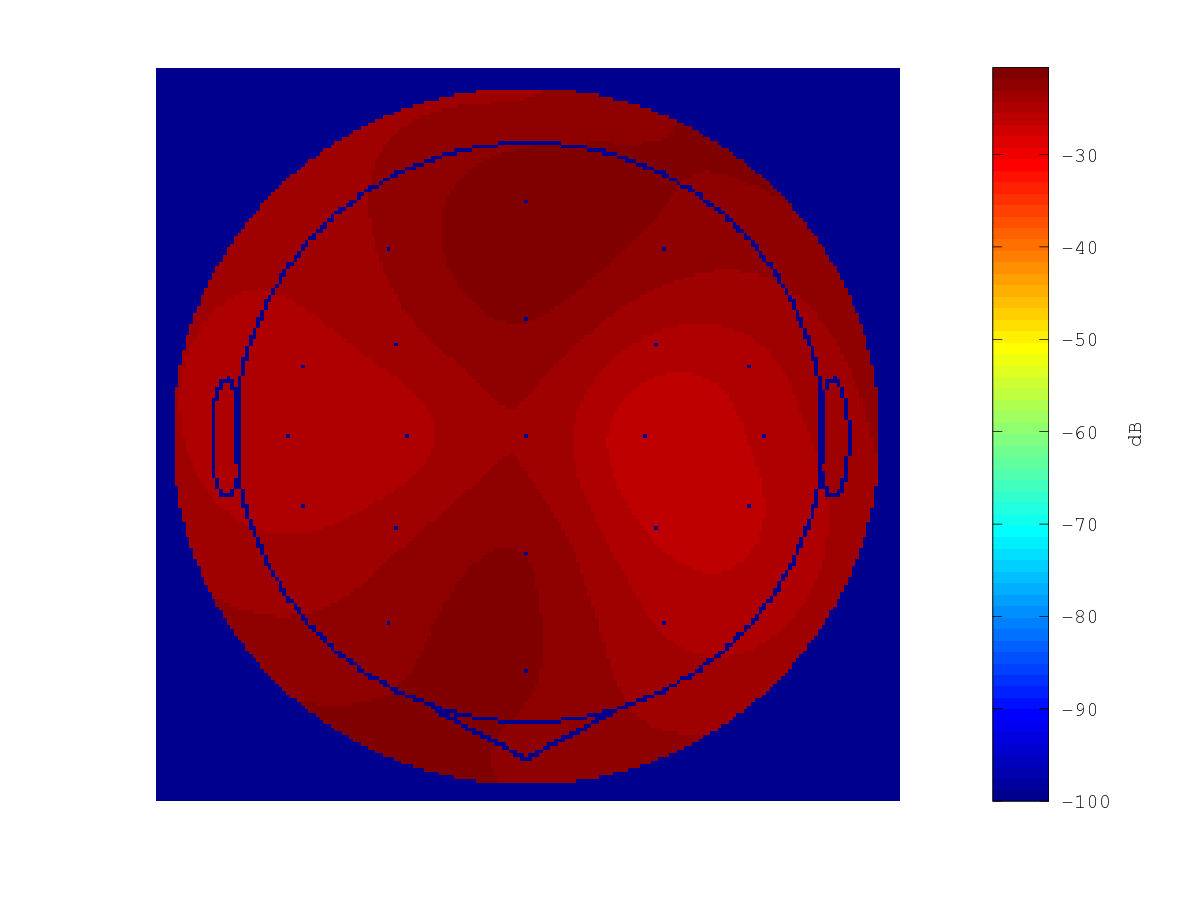
\includegraphics[width=2.5in]{scalpplot.png}}
\end{minipage}
\begin{minipage}[t]{0.5\textwidth}
~\\	
\IfStrEq{\PlotType}{scatter}{\textbf{\Large{Summary:}}\\
\if\IsConcussed1
\if\PrevConcussions0
Based on the results of the EEGlewave algorithm, the baseline brain signals have been classified as belonging to the concussed group. However, the past history and results from the SCAT do not seems to suggest that there is evidence of a previous recent concussion or any other condition that may lead to this result.\\
The EEGlewave algorithm is not 100\% accurate and there is a 10\% chance that some players will be misclassified. It is therefore possible that your child's brain signals fall into the group that are misclassified. However, if you have any concerns or if your child is showing any symptoms that might suggest any medical issues we suggest that your child is seen by your family physician for a physical examination.\\
Please feel free to contact Dr. Virji-Babul if you would like to discuss these results or would like more information.
\else
Based on the results of the EEGlewave algorithm the baseline brain signals have been classified as belonging to the concussed group. The past history and results from the SCAT also seems to suggest that there is evidence of a previous recent concussion. Given these results we suggest that your child is seen by your family physician for a physical examination and be cleared before he/she returns to play.\\
We will contact you again for a second EEG scan within a month to compare the baseline brain signals to determine if your brain signals are changing as a result of recovery. We will also repeat the SCAT to evaluate general changes in symptoms, balance and cognition from the initial assessment.\\
Please feel free to contact Dr. Virji-Babul if you would like more information.
\fi
\else
Based on the results of the EEGlewave algorithm the brain signals appear to be within normal range. If your child receives an impact to the head/body and a concussion is suspected please see your physician and contact EEGlewave at care@eeglewave.com. We will arrange for a second EEG scan and compare your baseline brain signals to the second EEG scan to determine if there have been any changes in your brain activity that may have resulted from the impact. We will also repeat the SCAT3 to evaluate changes in symptoms, balance and cognition from the baseline assessment.
\fi}{Electroencephalography (EEG) is a technique that records the electrical activity of the brain. Brain cells communicate using electrical impulses and are active all the time, even when sitting quietly or sleeping. The EEGlewave algorithm uses EEG signals from the whole brain to evaluate changes in these signals that may be due to a concussion.\\}
\end{minipage}
}}

 %comment starts
\iffalse
\fbox{\parbox{\textwidth}{
\textbf{\Large{Summary:}}\\
\if\IsConcussed1
\if\PrevConcussions0
Based on the results of the EEGlewave algorithm, the baseline brain signals have been classified as belonging to the concussed group. However, the past history and results from the SCAT do not seems to suggest that there is evidence of a previous recent concussion or any other condition that may lead to this result.\\
The EEGlewave algorithm is not 100\% accurate and there is a 10\% chance that some players will be misclassified. It is therefore possible that your child's brain signals fall into the group that are misclassified. However, if you have any concerns or if your child is showing any symptoms that might suggest any medical issues we suggest that your child is seen by your family physician for a physical examination.\\
Please feel free to contact Dr. Virji-Babul if you would like to discuss these results or would like more information.
\else
Based on the results of the EEGlewave algorithm the baseline brain signals have been classified as belonging to the concussed group. The past history and results from the SCAT also seems to suggest that there is evidence of a previous recent concussion. Given these results we suggest that your child is seen by your family physician for a physical examination and be cleared before he/she returns to play.\\
We will contact you again for a second EEG scan within a month to compare the baseline brain signals to determine if your brain signals are changing as a result of recovery. We will also repeat the SCAT to evaluate general changes in symptoms, balance and cognition from the initial assessment.\\
Please feel free to contact Dr. Virji-Babul if you would like more information.
\fi
\else
Based on the results of the EEGlewave algorithm the brain signals appear to be within normal range. If your child receives an impact to the head/body and a concussion is suspected please see your physician and contact EEGlewave at care@eeglewave.com. We will arrange for a second EEG scan and compare your baseline brain signals to the second EEG scan to determine if there have been any changes in your brain activity that may have resulted from the impact. We will also repeat the SCAT3 to evaluate changes in symptoms, balance and cognition from the baseline assessment.
\fi
}}
\fi % till here commenting out

% Add the footnote. A better way would be to use fancyhdr
\vfill
{\footnotesize\color{EWgray}\sffamily
	NOTE: EEGlewave does not provide medical advice. This report should not be used as a substitute for professional medical consultation.\\
}
\end{document}
}%The .tex filename goes here (NOT the same as \jobname)
\unless\ifdefined\Division
\endinput\expandafter\expandafter\expandafter\ReadDivision\fi

\def\ReadGender#1 {%
	\def\Gender{#1}%
	% NOTE: This report is to be compiled through the Octave command prompt.
% The following command should be typed into an Octave session to generate the report.
% system("pdflatex.exe -synctex=1 -interaction=nonstopmode -job-name=FirstName_LastName report.tex FirstName Lastname ParentName ID Handedness PrevConcussions Age ScanType")

% Definitions for command line arguments
\def\ReadFirstName#1 {%
	\def\FirstName{#1}%
	\input{report}}%The .tex filename goes here (NOT the same as \jobname)
\unless\ifdefined\FirstName
\endinput\expandafter\expandafter\expandafter\ReadFirstName\fi

\def\ReadLastName#1 {%
	\def\LastName{#1}%
	\input{report}}%The .tex filename goes here (NOT the same as \jobname)
\unless\ifdefined\LastName
\endinput\expandafter\expandafter\expandafter\ReadLastName\fi

\def\ReadParentFirstName#1 {%
	\def\ParentFirstName{#1}%
	\input{report}}%The .tex filename goes here (NOT the same as \jobname)
\unless\ifdefined\ParentFirstName
\endinput\expandafter\expandafter\expandafter\ReadParentFirstName\fi

\def\ReadParentLastName#1 {%
	\def\ParentLastName{#1}%
	\input{report}}%The .tex filename goes here (NOT the same as \jobname)
\unless\ifdefined\ParentLastName
\endinput\expandafter\expandafter\expandafter\ReadParentLastName\fi

\def\ReadID#1 {%
	\def\ID{#1}%
	\input{report}}%The .tex filename goes here (NOT the same as \jobname)
\unless\ifdefined\ID
\endinput\expandafter\expandafter\expandafter\ReadID\fi

\def\ReadHandedness#1 {%
	\def\Handedness{#1}%
	\input{report}}%The .tex filename goes here (NOT the same as \jobname)
\unless\ifdefined\Handedness
\endinput\expandafter\expandafter\expandafter\ReadHandedness\fi

\def\ReadPrevConcussions#1 {%
	\def\PrevConcussions{#1}%
	\input{report}}%The .tex filename goes here (NOT the same as \jobname)
\unless\ifdefined\PrevConcussions
\endinput\expandafter\expandafter\expandafter\ReadPrevConcussions\fi

\def\ReadMostRecentConcussion#1 {%
	\def\MostRecentConcussion{#1}%
	\input{report}}%The .tex filename goes here (NOT the same as \jobname)
\unless\ifdefined\MostRecentConcussion
\endinput\expandafter\expandafter\expandafter\ReadMostRecentConcussion\fi

\def\ReadIsConcussed#1 {%
	\def\IsConcussed{#1}%
	\input{report}}%The .tex filename goes here (NOT the same as \jobname)
\unless\ifdefined\IsConcussed
\endinput\expandafter\expandafter\expandafter\ReadIsConcussed\fi

\def\ReadDivision#1 {%
	\def\Division{#1}%
	\input{report}}%The .tex filename goes here (NOT the same as \jobname)
\unless\ifdefined\Division
\endinput\expandafter\expandafter\expandafter\ReadDivision\fi

\def\ReadGender#1 {%
	\def\Gender{#1}%
	\input{report}}%The .tex filename goes here (NOT the same as \jobname)
\unless\ifdefined\Gender
\endinput\expandafter\expandafter\expandafter\ReadGender\fi

\def\ReadAge#1 {%
	\def\Age{#1}%
	\input{report}}%The .tex filename goes here (NOT the same as \jobname)
\unless\ifdefined\Age
\endinput\expandafter\expandafter\expandafter\ReadAge\fi

\def\ReadDOS#1 {%
	\def\DOS{#1}%
	\input{report}}%The .tex filename goes here (NOT the same as \jobname)
\unless\ifdefined\DOS
\endinput\expandafter\expandafter\expandafter\ReadDOS\fi

\def\ReadScanType#1 {%
	\def\ScanType{#1}%
	\input{report}}%The .tex filename goes here (NOT the same as \jobname)
\unless\ifdefined\ScanType
\endinput\expandafter\expandafter\expandafter\ReadScanType\fi

\def\ReadNumSymptoms#1 {%
	\def\NumSymptoms{#1}%
	\input{report}}%The .tex filename goes here (NOT the same as \jobname)
\unless\ifdefined\NumSymptoms
\endinput\expandafter\expandafter\expandafter\ReadNumSymptoms\fi

\def\ReadSeverityScore#1 {%
	\def\SeverityScore{#1}%
	\input{report}}%The .tex filename goes here (NOT the same as \jobname)
\unless\ifdefined\SeverityScore
\endinput\expandafter\expandafter\expandafter\ReadSeverityScore\fi

\def\ReadOrientation#1 {%
	\def\Orientation{#1}%
	\input{report}}%The .tex filename goes here (NOT the same as \jobname)
\unless\ifdefined\Orientation
\endinput\expandafter\expandafter\expandafter\ReadOrientation\fi

\def\ReadOrientationTotal#1 {%
	\def\OrientationTotal{#1}%
	\input{report}}%The .tex filename goes here (NOT the same as \jobname)
\unless\ifdefined\OrientationTotal
\endinput\expandafter\expandafter\expandafter\ReadOrientationTotal\fi

\def\ReadImmMem#1 {%
	\def\ImmMem{#1}%
	\input{report}}%The .tex filename goes here (NOT the same as \jobname)
\unless\ifdefined\ImmMem
\endinput\expandafter\expandafter\expandafter\ReadImmMem\fi

\def\ReadConcentration#1 {%
	\def\Concentration{#1}%
	\input{report}}%The .tex filename goes here (NOT the same as \jobname)
\unless\ifdefined\Concentration
\endinput\expandafter\expandafter\expandafter\ReadConcentration\fi

\def\ReadConcentrationTotal#1 {%
	\def\ConcentrationTotal{#1}%
	\input{report}}%The .tex filename goes here (NOT the same as \jobname)
\unless\ifdefined\ConcentrationTotal
\endinput\expandafter\expandafter\expandafter\ReadConcentrationTotal\fi

\def\ReadDelayedRecall#1 {%
	\def\DelayedRecall{#1}%
	\input{report}}%The .tex filename goes here (NOT the same as \jobname)
\unless\ifdefined\DelayedRecall
\endinput\expandafter\expandafter\expandafter\ReadDelayedRecall\fi

\def\ReadSAC#1 {%
	\def\SAC{#1}%
	\input{report}}%The .tex filename goes here (NOT the same as \jobname)
\unless\ifdefined\SAC
\endinput\expandafter\expandafter\expandafter\ReadSAC\fi

\def\ReadBESS#1 {%
	\def\BESS{#1}%
	\input{report}}%The .tex filename goes here (NOT the same as \jobname)
\unless\ifdefined\BESS
\endinput\expandafter\expandafter\expandafter\ReadBESS\fi

\def\ReadTandemGait#1 {%
	\def\TandemGait{#1}%
	\input{report}}%The .tex filename goes here (NOT the same as \jobname)
\unless\ifdefined\TandemGait
\endinput\expandafter\expandafter\expandafter\ReadTandemGait\fi

\def\ReadCoordination#1 {%
	\def\Coordination{#1}%
	\input{report}}%The .tex filename goes here (NOT the same as \jobname)
\unless\ifdefined\Coordination
\endinput\expandafter\expandafter\expandafter\ReadCoordination\fi

\def\ReadPlotType#1 {%
	\def\PlotType{#1}%
	\input{report}}%The .tex filename goes here (NOT the same as \jobname)
\unless\ifdefined\PlotType
\endinput\expandafter\expandafter\expandafter\ReadPlotType\fi

\documentclass{article}

\usepackage[dvinames]{xcolor}
% Measurements are taken directly from the guide
\usepackage[top=2in,left=0.5in,bottom=0.5in,right=0.5in]{geometry}
\usepackage{graphicx}
\usepackage[colorlinks=false,
            pdfborder={0 0 0},
            ]{hyperref}
\usepackage{lipsum}
\usepackage[absolute]{textpos}
\usepackage{tikz}
\usetikzlibrary{calc}
% A nice serif font, but no the prescribed nonfree ITC stone
\usepackage[oldstylenums]{kpfonts}
\usepackage[T1]{fontenc	}
\usepackage[12pt]{moresize}
\usepackage{xstring}

% No paragraph indentation
\parindent0pt
\setlength{\parskip}{0.8\baselineskip}
\raggedright
\pagestyle{empty}


\definecolor{EWgray}{HTML}{5e6a71}

\begin{document}
	\begin{center}
		\HUGE{~}\\
		\HUGE{~}\\
		\HUGE{~}\\
		\textbf{\HUGE{EEGlewave Inc.}}\\[1in]
		\textbf{\huge{\ScanType~Report}}\\[1cm]
	\end{center}
	\newpage
\bigskip
% -------------------------------------------------------
% Add logo, the text under the crimson line, and the line itself
\begin{textblock*}{2in}[0.3066,0.39](1.25in,1.23in)
	
\includegraphics[width=1.5in]{eeglewave-front-211x128-88.png}
\end{textblock*}
\begin{textblock*}{6.375in}(1.5in,1.4in)   % 6.375=8.5 - 1.5 - 0.625
	\sffamily
	\hfill \color{EWgray} EEGlewave Inc.\\
	\hfill \url{care@eeglewave.com} \textbullet\ \url{http://eeglewave.com}
\end{textblock*}
\begin{tikzpicture}[remember picture,overlay]
\draw[line width=1pt] (current page.north west)+(0.5in,-1.85in) -- ($(-0.5in,-1.85in)+(current page.north east)$);
\end{tikzpicture}
\fbox{\parbox{\textwidth}{
\textbf{\Large{General Information:}}\\
\begin{minipage}[t]{0.55\textwidth}

\textbf{Name: } \FirstName~\LastName  \\
\textbf{Parent/Guardian's Name: } \ParentFirstName~\ParentLastName  \\
\textbf{ID: } \ID   \\
\textbf{Handedness: } \Handedness  \\
\textbf{Number of Previous Concussions: } \PrevConcussions \\
\textbf{Date of Most Recent Concussion: } \MostRecentConcussion
\end{minipage}
\begin{minipage}[t]{0.45\textwidth}
	\textbf{Division: } \Division  \\
	\textbf{Gender: } \Gender  \\
	\textbf{Age: } \Age  \\
	\textbf{Date of Scan: } \DOS \\
	\textbf{Type of Scan: } \ScanType  \\
\end{minipage}
}}

\fbox{\parbox{\textwidth}{
\textbf{\Large{SCAT3 Scoring Summary:}}\\
\begin{minipage}[t]{0.55\textwidth}
\textbf{Number of Symptoms (/22): } \\
\textbf{Symptom Severity Score (/132): } \\

\textbf{Orientation (/\OrientationTotal): }  \\
\textbf{Immediate Memory (/15): } \\
\textbf{Concentration (/\ConcentrationTotal): } \\
\textbf{Delayed Recall (/5): } \\
\textbf{SAC Total (/30): } \\

\textbf{BESS (total errors): } \\
\textbf{Tandem Gait (seconds): } \\
\textbf{Coordination (/1): } 
\end{minipage}
\begin{minipage}[t]{0.25\textwidth}
\NumSymptoms  \\
\SeverityScore  \\

\Orientation  \\
\ImmMem  \\
\Concentration  \\
\DelayedRecall \\
\SAC  \\

\BESS  \\
\TandemGait  \\
\Coordination
\end{minipage}
}}

\fbox{\parbox{\textwidth}{
\textbf{\Large{\IfStrEq{\PlotType}{scatter}{Scatter Plot:}{EEG Plot of Power at Rest:}}}\\
\begin{minipage}[t]{0.5\textwidth}
	~\\
	\IfStrEq{\PlotType}{scatter}{\includegraphics[width=3.25in]{scatterplot.png}}{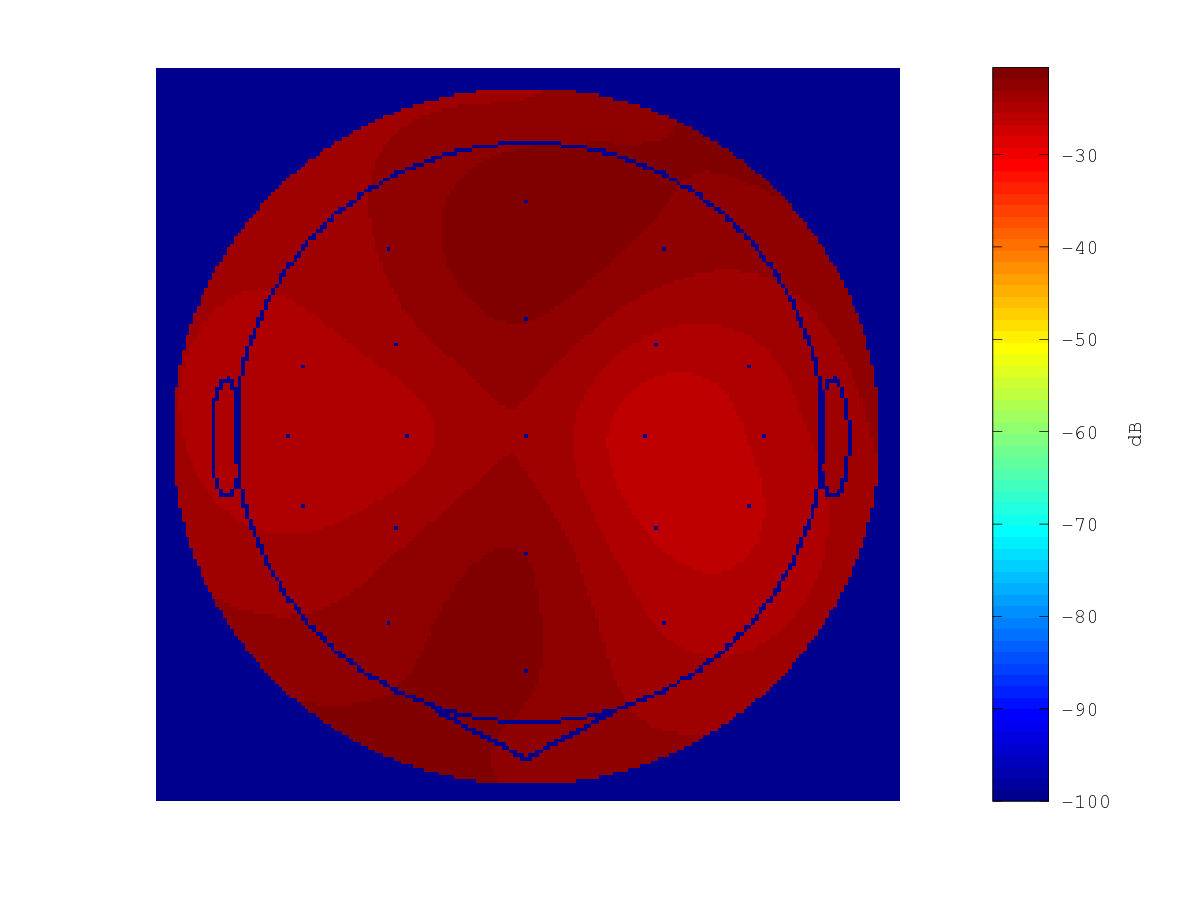
\includegraphics[width=2.5in]{scalpplot.png}}
\end{minipage}
\begin{minipage}[t]{0.5\textwidth}
~\\	
\IfStrEq{\PlotType}{scatter}{\textbf{\Large{Summary:}}\\
\if\IsConcussed1
\if\PrevConcussions0
Based on the results of the EEGlewave algorithm, the baseline brain signals have been classified as belonging to the concussed group. However, the past history and results from the SCAT do not seems to suggest that there is evidence of a previous recent concussion or any other condition that may lead to this result.\\
The EEGlewave algorithm is not 100\% accurate and there is a 10\% chance that some players will be misclassified. It is therefore possible that your child's brain signals fall into the group that are misclassified. However, if you have any concerns or if your child is showing any symptoms that might suggest any medical issues we suggest that your child is seen by your family physician for a physical examination.\\
Please feel free to contact Dr. Virji-Babul if you would like to discuss these results or would like more information.
\else
Based on the results of the EEGlewave algorithm the baseline brain signals have been classified as belonging to the concussed group. The past history and results from the SCAT also seems to suggest that there is evidence of a previous recent concussion. Given these results we suggest that your child is seen by your family physician for a physical examination and be cleared before he/she returns to play.\\
We will contact you again for a second EEG scan within a month to compare the baseline brain signals to determine if your brain signals are changing as a result of recovery. We will also repeat the SCAT to evaluate general changes in symptoms, balance and cognition from the initial assessment.\\
Please feel free to contact Dr. Virji-Babul if you would like more information.
\fi
\else
Based on the results of the EEGlewave algorithm the brain signals appear to be within normal range. If your child receives an impact to the head/body and a concussion is suspected please see your physician and contact EEGlewave at care@eeglewave.com. We will arrange for a second EEG scan and compare your baseline brain signals to the second EEG scan to determine if there have been any changes in your brain activity that may have resulted from the impact. We will also repeat the SCAT3 to evaluate changes in symptoms, balance and cognition from the baseline assessment.
\fi}{Electroencephalography (EEG) is a technique that records the electrical activity of the brain. Brain cells communicate using electrical impulses and are active all the time, even when sitting quietly or sleeping. The EEGlewave algorithm uses EEG signals from the whole brain to evaluate changes in these signals that may be due to a concussion.\\}
\end{minipage}
}}

 %comment starts
\iffalse
\fbox{\parbox{\textwidth}{
\textbf{\Large{Summary:}}\\
\if\IsConcussed1
\if\PrevConcussions0
Based on the results of the EEGlewave algorithm, the baseline brain signals have been classified as belonging to the concussed group. However, the past history and results from the SCAT do not seems to suggest that there is evidence of a previous recent concussion or any other condition that may lead to this result.\\
The EEGlewave algorithm is not 100\% accurate and there is a 10\% chance that some players will be misclassified. It is therefore possible that your child's brain signals fall into the group that are misclassified. However, if you have any concerns or if your child is showing any symptoms that might suggest any medical issues we suggest that your child is seen by your family physician for a physical examination.\\
Please feel free to contact Dr. Virji-Babul if you would like to discuss these results or would like more information.
\else
Based on the results of the EEGlewave algorithm the baseline brain signals have been classified as belonging to the concussed group. The past history and results from the SCAT also seems to suggest that there is evidence of a previous recent concussion. Given these results we suggest that your child is seen by your family physician for a physical examination and be cleared before he/she returns to play.\\
We will contact you again for a second EEG scan within a month to compare the baseline brain signals to determine if your brain signals are changing as a result of recovery. We will also repeat the SCAT to evaluate general changes in symptoms, balance and cognition from the initial assessment.\\
Please feel free to contact Dr. Virji-Babul if you would like more information.
\fi
\else
Based on the results of the EEGlewave algorithm the brain signals appear to be within normal range. If your child receives an impact to the head/body and a concussion is suspected please see your physician and contact EEGlewave at care@eeglewave.com. We will arrange for a second EEG scan and compare your baseline brain signals to the second EEG scan to determine if there have been any changes in your brain activity that may have resulted from the impact. We will also repeat the SCAT3 to evaluate changes in symptoms, balance and cognition from the baseline assessment.
\fi
}}
\fi % till here commenting out

% Add the footnote. A better way would be to use fancyhdr
\vfill
{\footnotesize\color{EWgray}\sffamily
	NOTE: EEGlewave does not provide medical advice. This report should not be used as a substitute for professional medical consultation.\\
}
\end{document}
}%The .tex filename goes here (NOT the same as \jobname)
\unless\ifdefined\Gender
\endinput\expandafter\expandafter\expandafter\ReadGender\fi

\def\ReadAge#1 {%
	\def\Age{#1}%
	% NOTE: This report is to be compiled through the Octave command prompt.
% The following command should be typed into an Octave session to generate the report.
% system("pdflatex.exe -synctex=1 -interaction=nonstopmode -job-name=FirstName_LastName report.tex FirstName Lastname ParentName ID Handedness PrevConcussions Age ScanType")

% Definitions for command line arguments
\def\ReadFirstName#1 {%
	\def\FirstName{#1}%
	\input{report}}%The .tex filename goes here (NOT the same as \jobname)
\unless\ifdefined\FirstName
\endinput\expandafter\expandafter\expandafter\ReadFirstName\fi

\def\ReadLastName#1 {%
	\def\LastName{#1}%
	\input{report}}%The .tex filename goes here (NOT the same as \jobname)
\unless\ifdefined\LastName
\endinput\expandafter\expandafter\expandafter\ReadLastName\fi

\def\ReadParentFirstName#1 {%
	\def\ParentFirstName{#1}%
	\input{report}}%The .tex filename goes here (NOT the same as \jobname)
\unless\ifdefined\ParentFirstName
\endinput\expandafter\expandafter\expandafter\ReadParentFirstName\fi

\def\ReadParentLastName#1 {%
	\def\ParentLastName{#1}%
	\input{report}}%The .tex filename goes here (NOT the same as \jobname)
\unless\ifdefined\ParentLastName
\endinput\expandafter\expandafter\expandafter\ReadParentLastName\fi

\def\ReadID#1 {%
	\def\ID{#1}%
	\input{report}}%The .tex filename goes here (NOT the same as \jobname)
\unless\ifdefined\ID
\endinput\expandafter\expandafter\expandafter\ReadID\fi

\def\ReadHandedness#1 {%
	\def\Handedness{#1}%
	\input{report}}%The .tex filename goes here (NOT the same as \jobname)
\unless\ifdefined\Handedness
\endinput\expandafter\expandafter\expandafter\ReadHandedness\fi

\def\ReadPrevConcussions#1 {%
	\def\PrevConcussions{#1}%
	\input{report}}%The .tex filename goes here (NOT the same as \jobname)
\unless\ifdefined\PrevConcussions
\endinput\expandafter\expandafter\expandafter\ReadPrevConcussions\fi

\def\ReadMostRecentConcussion#1 {%
	\def\MostRecentConcussion{#1}%
	\input{report}}%The .tex filename goes here (NOT the same as \jobname)
\unless\ifdefined\MostRecentConcussion
\endinput\expandafter\expandafter\expandafter\ReadMostRecentConcussion\fi

\def\ReadIsConcussed#1 {%
	\def\IsConcussed{#1}%
	\input{report}}%The .tex filename goes here (NOT the same as \jobname)
\unless\ifdefined\IsConcussed
\endinput\expandafter\expandafter\expandafter\ReadIsConcussed\fi

\def\ReadDivision#1 {%
	\def\Division{#1}%
	\input{report}}%The .tex filename goes here (NOT the same as \jobname)
\unless\ifdefined\Division
\endinput\expandafter\expandafter\expandafter\ReadDivision\fi

\def\ReadGender#1 {%
	\def\Gender{#1}%
	\input{report}}%The .tex filename goes here (NOT the same as \jobname)
\unless\ifdefined\Gender
\endinput\expandafter\expandafter\expandafter\ReadGender\fi

\def\ReadAge#1 {%
	\def\Age{#1}%
	\input{report}}%The .tex filename goes here (NOT the same as \jobname)
\unless\ifdefined\Age
\endinput\expandafter\expandafter\expandafter\ReadAge\fi

\def\ReadDOS#1 {%
	\def\DOS{#1}%
	\input{report}}%The .tex filename goes here (NOT the same as \jobname)
\unless\ifdefined\DOS
\endinput\expandafter\expandafter\expandafter\ReadDOS\fi

\def\ReadScanType#1 {%
	\def\ScanType{#1}%
	\input{report}}%The .tex filename goes here (NOT the same as \jobname)
\unless\ifdefined\ScanType
\endinput\expandafter\expandafter\expandafter\ReadScanType\fi

\def\ReadNumSymptoms#1 {%
	\def\NumSymptoms{#1}%
	\input{report}}%The .tex filename goes here (NOT the same as \jobname)
\unless\ifdefined\NumSymptoms
\endinput\expandafter\expandafter\expandafter\ReadNumSymptoms\fi

\def\ReadSeverityScore#1 {%
	\def\SeverityScore{#1}%
	\input{report}}%The .tex filename goes here (NOT the same as \jobname)
\unless\ifdefined\SeverityScore
\endinput\expandafter\expandafter\expandafter\ReadSeverityScore\fi

\def\ReadOrientation#1 {%
	\def\Orientation{#1}%
	\input{report}}%The .tex filename goes here (NOT the same as \jobname)
\unless\ifdefined\Orientation
\endinput\expandafter\expandafter\expandafter\ReadOrientation\fi

\def\ReadOrientationTotal#1 {%
	\def\OrientationTotal{#1}%
	\input{report}}%The .tex filename goes here (NOT the same as \jobname)
\unless\ifdefined\OrientationTotal
\endinput\expandafter\expandafter\expandafter\ReadOrientationTotal\fi

\def\ReadImmMem#1 {%
	\def\ImmMem{#1}%
	\input{report}}%The .tex filename goes here (NOT the same as \jobname)
\unless\ifdefined\ImmMem
\endinput\expandafter\expandafter\expandafter\ReadImmMem\fi

\def\ReadConcentration#1 {%
	\def\Concentration{#1}%
	\input{report}}%The .tex filename goes here (NOT the same as \jobname)
\unless\ifdefined\Concentration
\endinput\expandafter\expandafter\expandafter\ReadConcentration\fi

\def\ReadConcentrationTotal#1 {%
	\def\ConcentrationTotal{#1}%
	\input{report}}%The .tex filename goes here (NOT the same as \jobname)
\unless\ifdefined\ConcentrationTotal
\endinput\expandafter\expandafter\expandafter\ReadConcentrationTotal\fi

\def\ReadDelayedRecall#1 {%
	\def\DelayedRecall{#1}%
	\input{report}}%The .tex filename goes here (NOT the same as \jobname)
\unless\ifdefined\DelayedRecall
\endinput\expandafter\expandafter\expandafter\ReadDelayedRecall\fi

\def\ReadSAC#1 {%
	\def\SAC{#1}%
	\input{report}}%The .tex filename goes here (NOT the same as \jobname)
\unless\ifdefined\SAC
\endinput\expandafter\expandafter\expandafter\ReadSAC\fi

\def\ReadBESS#1 {%
	\def\BESS{#1}%
	\input{report}}%The .tex filename goes here (NOT the same as \jobname)
\unless\ifdefined\BESS
\endinput\expandafter\expandafter\expandafter\ReadBESS\fi

\def\ReadTandemGait#1 {%
	\def\TandemGait{#1}%
	\input{report}}%The .tex filename goes here (NOT the same as \jobname)
\unless\ifdefined\TandemGait
\endinput\expandafter\expandafter\expandafter\ReadTandemGait\fi

\def\ReadCoordination#1 {%
	\def\Coordination{#1}%
	\input{report}}%The .tex filename goes here (NOT the same as \jobname)
\unless\ifdefined\Coordination
\endinput\expandafter\expandafter\expandafter\ReadCoordination\fi

\def\ReadPlotType#1 {%
	\def\PlotType{#1}%
	\input{report}}%The .tex filename goes here (NOT the same as \jobname)
\unless\ifdefined\PlotType
\endinput\expandafter\expandafter\expandafter\ReadPlotType\fi

\documentclass{article}

\usepackage[dvinames]{xcolor}
% Measurements are taken directly from the guide
\usepackage[top=2in,left=0.5in,bottom=0.5in,right=0.5in]{geometry}
\usepackage{graphicx}
\usepackage[colorlinks=false,
            pdfborder={0 0 0},
            ]{hyperref}
\usepackage{lipsum}
\usepackage[absolute]{textpos}
\usepackage{tikz}
\usetikzlibrary{calc}
% A nice serif font, but no the prescribed nonfree ITC stone
\usepackage[oldstylenums]{kpfonts}
\usepackage[T1]{fontenc	}
\usepackage[12pt]{moresize}
\usepackage{xstring}

% No paragraph indentation
\parindent0pt
\setlength{\parskip}{0.8\baselineskip}
\raggedright
\pagestyle{empty}


\definecolor{EWgray}{HTML}{5e6a71}

\begin{document}
	\begin{center}
		\HUGE{~}\\
		\HUGE{~}\\
		\HUGE{~}\\
		\textbf{\HUGE{EEGlewave Inc.}}\\[1in]
		\textbf{\huge{\ScanType~Report}}\\[1cm]
	\end{center}
	\newpage
\bigskip
% -------------------------------------------------------
% Add logo, the text under the crimson line, and the line itself
\begin{textblock*}{2in}[0.3066,0.39](1.25in,1.23in)
	
\includegraphics[width=1.5in]{eeglewave-front-211x128-88.png}
\end{textblock*}
\begin{textblock*}{6.375in}(1.5in,1.4in)   % 6.375=8.5 - 1.5 - 0.625
	\sffamily
	\hfill \color{EWgray} EEGlewave Inc.\\
	\hfill \url{care@eeglewave.com} \textbullet\ \url{http://eeglewave.com}
\end{textblock*}
\begin{tikzpicture}[remember picture,overlay]
\draw[line width=1pt] (current page.north west)+(0.5in,-1.85in) -- ($(-0.5in,-1.85in)+(current page.north east)$);
\end{tikzpicture}
\fbox{\parbox{\textwidth}{
\textbf{\Large{General Information:}}\\
\begin{minipage}[t]{0.55\textwidth}

\textbf{Name: } \FirstName~\LastName  \\
\textbf{Parent/Guardian's Name: } \ParentFirstName~\ParentLastName  \\
\textbf{ID: } \ID   \\
\textbf{Handedness: } \Handedness  \\
\textbf{Number of Previous Concussions: } \PrevConcussions \\
\textbf{Date of Most Recent Concussion: } \MostRecentConcussion
\end{minipage}
\begin{minipage}[t]{0.45\textwidth}
	\textbf{Division: } \Division  \\
	\textbf{Gender: } \Gender  \\
	\textbf{Age: } \Age  \\
	\textbf{Date of Scan: } \DOS \\
	\textbf{Type of Scan: } \ScanType  \\
\end{minipage}
}}

\fbox{\parbox{\textwidth}{
\textbf{\Large{SCAT3 Scoring Summary:}}\\
\begin{minipage}[t]{0.55\textwidth}
\textbf{Number of Symptoms (/22): } \\
\textbf{Symptom Severity Score (/132): } \\

\textbf{Orientation (/\OrientationTotal): }  \\
\textbf{Immediate Memory (/15): } \\
\textbf{Concentration (/\ConcentrationTotal): } \\
\textbf{Delayed Recall (/5): } \\
\textbf{SAC Total (/30): } \\

\textbf{BESS (total errors): } \\
\textbf{Tandem Gait (seconds): } \\
\textbf{Coordination (/1): } 
\end{minipage}
\begin{minipage}[t]{0.25\textwidth}
\NumSymptoms  \\
\SeverityScore  \\

\Orientation  \\
\ImmMem  \\
\Concentration  \\
\DelayedRecall \\
\SAC  \\

\BESS  \\
\TandemGait  \\
\Coordination
\end{minipage}
}}

\fbox{\parbox{\textwidth}{
\textbf{\Large{\IfStrEq{\PlotType}{scatter}{Scatter Plot:}{EEG Plot of Power at Rest:}}}\\
\begin{minipage}[t]{0.5\textwidth}
	~\\
	\IfStrEq{\PlotType}{scatter}{\includegraphics[width=3.25in]{scatterplot.png}}{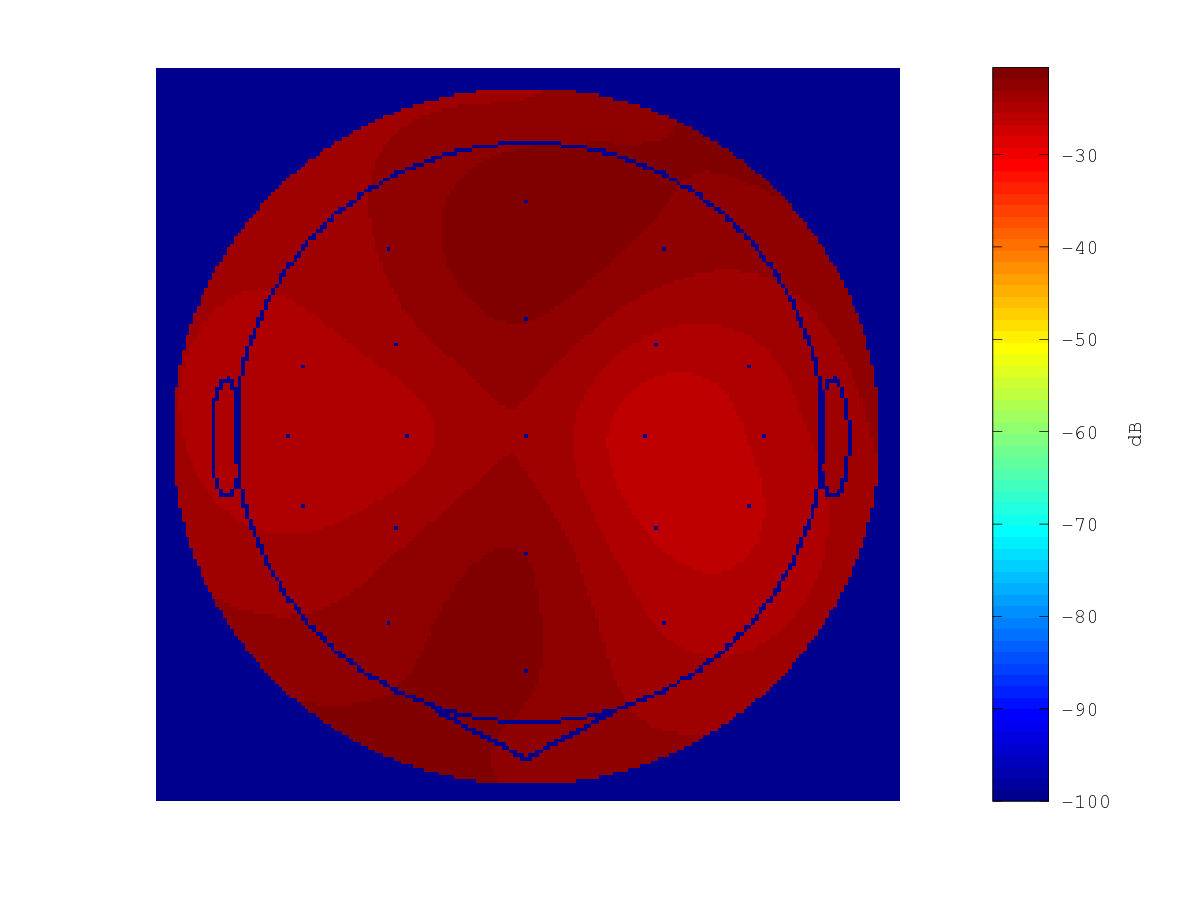
\includegraphics[width=2.5in]{scalpplot.png}}
\end{minipage}
\begin{minipage}[t]{0.5\textwidth}
~\\	
\IfStrEq{\PlotType}{scatter}{\textbf{\Large{Summary:}}\\
\if\IsConcussed1
\if\PrevConcussions0
Based on the results of the EEGlewave algorithm, the baseline brain signals have been classified as belonging to the concussed group. However, the past history and results from the SCAT do not seems to suggest that there is evidence of a previous recent concussion or any other condition that may lead to this result.\\
The EEGlewave algorithm is not 100\% accurate and there is a 10\% chance that some players will be misclassified. It is therefore possible that your child's brain signals fall into the group that are misclassified. However, if you have any concerns or if your child is showing any symptoms that might suggest any medical issues we suggest that your child is seen by your family physician for a physical examination.\\
Please feel free to contact Dr. Virji-Babul if you would like to discuss these results or would like more information.
\else
Based on the results of the EEGlewave algorithm the baseline brain signals have been classified as belonging to the concussed group. The past history and results from the SCAT also seems to suggest that there is evidence of a previous recent concussion. Given these results we suggest that your child is seen by your family physician for a physical examination and be cleared before he/she returns to play.\\
We will contact you again for a second EEG scan within a month to compare the baseline brain signals to determine if your brain signals are changing as a result of recovery. We will also repeat the SCAT to evaluate general changes in symptoms, balance and cognition from the initial assessment.\\
Please feel free to contact Dr. Virji-Babul if you would like more information.
\fi
\else
Based on the results of the EEGlewave algorithm the brain signals appear to be within normal range. If your child receives an impact to the head/body and a concussion is suspected please see your physician and contact EEGlewave at care@eeglewave.com. We will arrange for a second EEG scan and compare your baseline brain signals to the second EEG scan to determine if there have been any changes in your brain activity that may have resulted from the impact. We will also repeat the SCAT3 to evaluate changes in symptoms, balance and cognition from the baseline assessment.
\fi}{Electroencephalography (EEG) is a technique that records the electrical activity of the brain. Brain cells communicate using electrical impulses and are active all the time, even when sitting quietly or sleeping. The EEGlewave algorithm uses EEG signals from the whole brain to evaluate changes in these signals that may be due to a concussion.\\}
\end{minipage}
}}

 %comment starts
\iffalse
\fbox{\parbox{\textwidth}{
\textbf{\Large{Summary:}}\\
\if\IsConcussed1
\if\PrevConcussions0
Based on the results of the EEGlewave algorithm, the baseline brain signals have been classified as belonging to the concussed group. However, the past history and results from the SCAT do not seems to suggest that there is evidence of a previous recent concussion or any other condition that may lead to this result.\\
The EEGlewave algorithm is not 100\% accurate and there is a 10\% chance that some players will be misclassified. It is therefore possible that your child's brain signals fall into the group that are misclassified. However, if you have any concerns or if your child is showing any symptoms that might suggest any medical issues we suggest that your child is seen by your family physician for a physical examination.\\
Please feel free to contact Dr. Virji-Babul if you would like to discuss these results or would like more information.
\else
Based on the results of the EEGlewave algorithm the baseline brain signals have been classified as belonging to the concussed group. The past history and results from the SCAT also seems to suggest that there is evidence of a previous recent concussion. Given these results we suggest that your child is seen by your family physician for a physical examination and be cleared before he/she returns to play.\\
We will contact you again for a second EEG scan within a month to compare the baseline brain signals to determine if your brain signals are changing as a result of recovery. We will also repeat the SCAT to evaluate general changes in symptoms, balance and cognition from the initial assessment.\\
Please feel free to contact Dr. Virji-Babul if you would like more information.
\fi
\else
Based on the results of the EEGlewave algorithm the brain signals appear to be within normal range. If your child receives an impact to the head/body and a concussion is suspected please see your physician and contact EEGlewave at care@eeglewave.com. We will arrange for a second EEG scan and compare your baseline brain signals to the second EEG scan to determine if there have been any changes in your brain activity that may have resulted from the impact. We will also repeat the SCAT3 to evaluate changes in symptoms, balance and cognition from the baseline assessment.
\fi
}}
\fi % till here commenting out

% Add the footnote. A better way would be to use fancyhdr
\vfill
{\footnotesize\color{EWgray}\sffamily
	NOTE: EEGlewave does not provide medical advice. This report should not be used as a substitute for professional medical consultation.\\
}
\end{document}
}%The .tex filename goes here (NOT the same as \jobname)
\unless\ifdefined\Age
\endinput\expandafter\expandafter\expandafter\ReadAge\fi

\def\ReadDOS#1 {%
	\def\DOS{#1}%
	% NOTE: This report is to be compiled through the Octave command prompt.
% The following command should be typed into an Octave session to generate the report.
% system("pdflatex.exe -synctex=1 -interaction=nonstopmode -job-name=FirstName_LastName report.tex FirstName Lastname ParentName ID Handedness PrevConcussions Age ScanType")

% Definitions for command line arguments
\def\ReadFirstName#1 {%
	\def\FirstName{#1}%
	\input{report}}%The .tex filename goes here (NOT the same as \jobname)
\unless\ifdefined\FirstName
\endinput\expandafter\expandafter\expandafter\ReadFirstName\fi

\def\ReadLastName#1 {%
	\def\LastName{#1}%
	\input{report}}%The .tex filename goes here (NOT the same as \jobname)
\unless\ifdefined\LastName
\endinput\expandafter\expandafter\expandafter\ReadLastName\fi

\def\ReadParentFirstName#1 {%
	\def\ParentFirstName{#1}%
	\input{report}}%The .tex filename goes here (NOT the same as \jobname)
\unless\ifdefined\ParentFirstName
\endinput\expandafter\expandafter\expandafter\ReadParentFirstName\fi

\def\ReadParentLastName#1 {%
	\def\ParentLastName{#1}%
	\input{report}}%The .tex filename goes here (NOT the same as \jobname)
\unless\ifdefined\ParentLastName
\endinput\expandafter\expandafter\expandafter\ReadParentLastName\fi

\def\ReadID#1 {%
	\def\ID{#1}%
	\input{report}}%The .tex filename goes here (NOT the same as \jobname)
\unless\ifdefined\ID
\endinput\expandafter\expandafter\expandafter\ReadID\fi

\def\ReadHandedness#1 {%
	\def\Handedness{#1}%
	\input{report}}%The .tex filename goes here (NOT the same as \jobname)
\unless\ifdefined\Handedness
\endinput\expandafter\expandafter\expandafter\ReadHandedness\fi

\def\ReadPrevConcussions#1 {%
	\def\PrevConcussions{#1}%
	\input{report}}%The .tex filename goes here (NOT the same as \jobname)
\unless\ifdefined\PrevConcussions
\endinput\expandafter\expandafter\expandafter\ReadPrevConcussions\fi

\def\ReadMostRecentConcussion#1 {%
	\def\MostRecentConcussion{#1}%
	\input{report}}%The .tex filename goes here (NOT the same as \jobname)
\unless\ifdefined\MostRecentConcussion
\endinput\expandafter\expandafter\expandafter\ReadMostRecentConcussion\fi

\def\ReadIsConcussed#1 {%
	\def\IsConcussed{#1}%
	\input{report}}%The .tex filename goes here (NOT the same as \jobname)
\unless\ifdefined\IsConcussed
\endinput\expandafter\expandafter\expandafter\ReadIsConcussed\fi

\def\ReadDivision#1 {%
	\def\Division{#1}%
	\input{report}}%The .tex filename goes here (NOT the same as \jobname)
\unless\ifdefined\Division
\endinput\expandafter\expandafter\expandafter\ReadDivision\fi

\def\ReadGender#1 {%
	\def\Gender{#1}%
	\input{report}}%The .tex filename goes here (NOT the same as \jobname)
\unless\ifdefined\Gender
\endinput\expandafter\expandafter\expandafter\ReadGender\fi

\def\ReadAge#1 {%
	\def\Age{#1}%
	\input{report}}%The .tex filename goes here (NOT the same as \jobname)
\unless\ifdefined\Age
\endinput\expandafter\expandafter\expandafter\ReadAge\fi

\def\ReadDOS#1 {%
	\def\DOS{#1}%
	\input{report}}%The .tex filename goes here (NOT the same as \jobname)
\unless\ifdefined\DOS
\endinput\expandafter\expandafter\expandafter\ReadDOS\fi

\def\ReadScanType#1 {%
	\def\ScanType{#1}%
	\input{report}}%The .tex filename goes here (NOT the same as \jobname)
\unless\ifdefined\ScanType
\endinput\expandafter\expandafter\expandafter\ReadScanType\fi

\def\ReadNumSymptoms#1 {%
	\def\NumSymptoms{#1}%
	\input{report}}%The .tex filename goes here (NOT the same as \jobname)
\unless\ifdefined\NumSymptoms
\endinput\expandafter\expandafter\expandafter\ReadNumSymptoms\fi

\def\ReadSeverityScore#1 {%
	\def\SeverityScore{#1}%
	\input{report}}%The .tex filename goes here (NOT the same as \jobname)
\unless\ifdefined\SeverityScore
\endinput\expandafter\expandafter\expandafter\ReadSeverityScore\fi

\def\ReadOrientation#1 {%
	\def\Orientation{#1}%
	\input{report}}%The .tex filename goes here (NOT the same as \jobname)
\unless\ifdefined\Orientation
\endinput\expandafter\expandafter\expandafter\ReadOrientation\fi

\def\ReadOrientationTotal#1 {%
	\def\OrientationTotal{#1}%
	\input{report}}%The .tex filename goes here (NOT the same as \jobname)
\unless\ifdefined\OrientationTotal
\endinput\expandafter\expandafter\expandafter\ReadOrientationTotal\fi

\def\ReadImmMem#1 {%
	\def\ImmMem{#1}%
	\input{report}}%The .tex filename goes here (NOT the same as \jobname)
\unless\ifdefined\ImmMem
\endinput\expandafter\expandafter\expandafter\ReadImmMem\fi

\def\ReadConcentration#1 {%
	\def\Concentration{#1}%
	\input{report}}%The .tex filename goes here (NOT the same as \jobname)
\unless\ifdefined\Concentration
\endinput\expandafter\expandafter\expandafter\ReadConcentration\fi

\def\ReadConcentrationTotal#1 {%
	\def\ConcentrationTotal{#1}%
	\input{report}}%The .tex filename goes here (NOT the same as \jobname)
\unless\ifdefined\ConcentrationTotal
\endinput\expandafter\expandafter\expandafter\ReadConcentrationTotal\fi

\def\ReadDelayedRecall#1 {%
	\def\DelayedRecall{#1}%
	\input{report}}%The .tex filename goes here (NOT the same as \jobname)
\unless\ifdefined\DelayedRecall
\endinput\expandafter\expandafter\expandafter\ReadDelayedRecall\fi

\def\ReadSAC#1 {%
	\def\SAC{#1}%
	\input{report}}%The .tex filename goes here (NOT the same as \jobname)
\unless\ifdefined\SAC
\endinput\expandafter\expandafter\expandafter\ReadSAC\fi

\def\ReadBESS#1 {%
	\def\BESS{#1}%
	\input{report}}%The .tex filename goes here (NOT the same as \jobname)
\unless\ifdefined\BESS
\endinput\expandafter\expandafter\expandafter\ReadBESS\fi

\def\ReadTandemGait#1 {%
	\def\TandemGait{#1}%
	\input{report}}%The .tex filename goes here (NOT the same as \jobname)
\unless\ifdefined\TandemGait
\endinput\expandafter\expandafter\expandafter\ReadTandemGait\fi

\def\ReadCoordination#1 {%
	\def\Coordination{#1}%
	\input{report}}%The .tex filename goes here (NOT the same as \jobname)
\unless\ifdefined\Coordination
\endinput\expandafter\expandafter\expandafter\ReadCoordination\fi

\def\ReadPlotType#1 {%
	\def\PlotType{#1}%
	\input{report}}%The .tex filename goes here (NOT the same as \jobname)
\unless\ifdefined\PlotType
\endinput\expandafter\expandafter\expandafter\ReadPlotType\fi

\documentclass{article}

\usepackage[dvinames]{xcolor}
% Measurements are taken directly from the guide
\usepackage[top=2in,left=0.5in,bottom=0.5in,right=0.5in]{geometry}
\usepackage{graphicx}
\usepackage[colorlinks=false,
            pdfborder={0 0 0},
            ]{hyperref}
\usepackage{lipsum}
\usepackage[absolute]{textpos}
\usepackage{tikz}
\usetikzlibrary{calc}
% A nice serif font, but no the prescribed nonfree ITC stone
\usepackage[oldstylenums]{kpfonts}
\usepackage[T1]{fontenc	}
\usepackage[12pt]{moresize}
\usepackage{xstring}

% No paragraph indentation
\parindent0pt
\setlength{\parskip}{0.8\baselineskip}
\raggedright
\pagestyle{empty}


\definecolor{EWgray}{HTML}{5e6a71}

\begin{document}
	\begin{center}
		\HUGE{~}\\
		\HUGE{~}\\
		\HUGE{~}\\
		\textbf{\HUGE{EEGlewave Inc.}}\\[1in]
		\textbf{\huge{\ScanType~Report}}\\[1cm]
	\end{center}
	\newpage
\bigskip
% -------------------------------------------------------
% Add logo, the text under the crimson line, and the line itself
\begin{textblock*}{2in}[0.3066,0.39](1.25in,1.23in)
	
\includegraphics[width=1.5in]{eeglewave-front-211x128-88.png}
\end{textblock*}
\begin{textblock*}{6.375in}(1.5in,1.4in)   % 6.375=8.5 - 1.5 - 0.625
	\sffamily
	\hfill \color{EWgray} EEGlewave Inc.\\
	\hfill \url{care@eeglewave.com} \textbullet\ \url{http://eeglewave.com}
\end{textblock*}
\begin{tikzpicture}[remember picture,overlay]
\draw[line width=1pt] (current page.north west)+(0.5in,-1.85in) -- ($(-0.5in,-1.85in)+(current page.north east)$);
\end{tikzpicture}
\fbox{\parbox{\textwidth}{
\textbf{\Large{General Information:}}\\
\begin{minipage}[t]{0.55\textwidth}

\textbf{Name: } \FirstName~\LastName  \\
\textbf{Parent/Guardian's Name: } \ParentFirstName~\ParentLastName  \\
\textbf{ID: } \ID   \\
\textbf{Handedness: } \Handedness  \\
\textbf{Number of Previous Concussions: } \PrevConcussions \\
\textbf{Date of Most Recent Concussion: } \MostRecentConcussion
\end{minipage}
\begin{minipage}[t]{0.45\textwidth}
	\textbf{Division: } \Division  \\
	\textbf{Gender: } \Gender  \\
	\textbf{Age: } \Age  \\
	\textbf{Date of Scan: } \DOS \\
	\textbf{Type of Scan: } \ScanType  \\
\end{minipage}
}}

\fbox{\parbox{\textwidth}{
\textbf{\Large{SCAT3 Scoring Summary:}}\\
\begin{minipage}[t]{0.55\textwidth}
\textbf{Number of Symptoms (/22): } \\
\textbf{Symptom Severity Score (/132): } \\

\textbf{Orientation (/\OrientationTotal): }  \\
\textbf{Immediate Memory (/15): } \\
\textbf{Concentration (/\ConcentrationTotal): } \\
\textbf{Delayed Recall (/5): } \\
\textbf{SAC Total (/30): } \\

\textbf{BESS (total errors): } \\
\textbf{Tandem Gait (seconds): } \\
\textbf{Coordination (/1): } 
\end{minipage}
\begin{minipage}[t]{0.25\textwidth}
\NumSymptoms  \\
\SeverityScore  \\

\Orientation  \\
\ImmMem  \\
\Concentration  \\
\DelayedRecall \\
\SAC  \\

\BESS  \\
\TandemGait  \\
\Coordination
\end{minipage}
}}

\fbox{\parbox{\textwidth}{
\textbf{\Large{\IfStrEq{\PlotType}{scatter}{Scatter Plot:}{EEG Plot of Power at Rest:}}}\\
\begin{minipage}[t]{0.5\textwidth}
	~\\
	\IfStrEq{\PlotType}{scatter}{\includegraphics[width=3.25in]{scatterplot.png}}{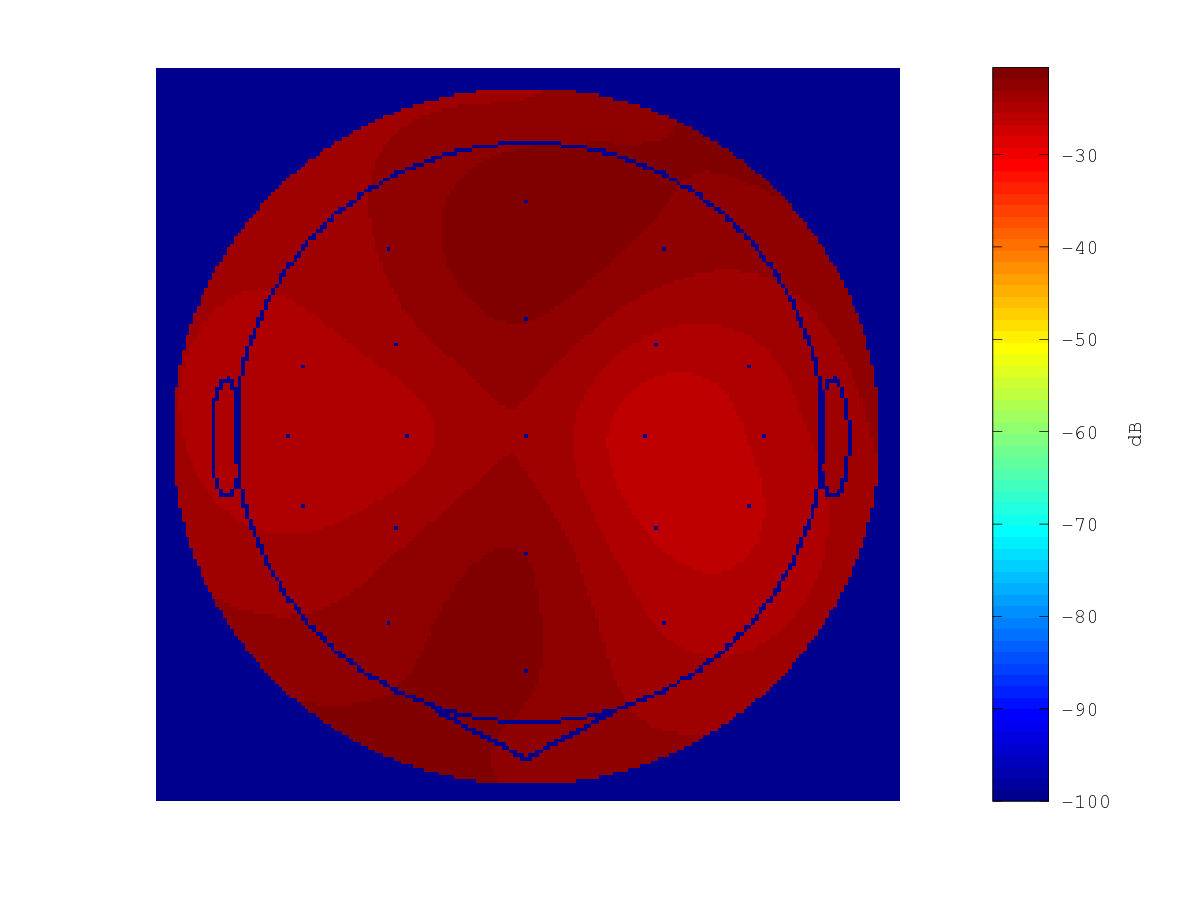
\includegraphics[width=2.5in]{scalpplot.png}}
\end{minipage}
\begin{minipage}[t]{0.5\textwidth}
~\\	
\IfStrEq{\PlotType}{scatter}{\textbf{\Large{Summary:}}\\
\if\IsConcussed1
\if\PrevConcussions0
Based on the results of the EEGlewave algorithm, the baseline brain signals have been classified as belonging to the concussed group. However, the past history and results from the SCAT do not seems to suggest that there is evidence of a previous recent concussion or any other condition that may lead to this result.\\
The EEGlewave algorithm is not 100\% accurate and there is a 10\% chance that some players will be misclassified. It is therefore possible that your child's brain signals fall into the group that are misclassified. However, if you have any concerns or if your child is showing any symptoms that might suggest any medical issues we suggest that your child is seen by your family physician for a physical examination.\\
Please feel free to contact Dr. Virji-Babul if you would like to discuss these results or would like more information.
\else
Based on the results of the EEGlewave algorithm the baseline brain signals have been classified as belonging to the concussed group. The past history and results from the SCAT also seems to suggest that there is evidence of a previous recent concussion. Given these results we suggest that your child is seen by your family physician for a physical examination and be cleared before he/she returns to play.\\
We will contact you again for a second EEG scan within a month to compare the baseline brain signals to determine if your brain signals are changing as a result of recovery. We will also repeat the SCAT to evaluate general changes in symptoms, balance and cognition from the initial assessment.\\
Please feel free to contact Dr. Virji-Babul if you would like more information.
\fi
\else
Based on the results of the EEGlewave algorithm the brain signals appear to be within normal range. If your child receives an impact to the head/body and a concussion is suspected please see your physician and contact EEGlewave at care@eeglewave.com. We will arrange for a second EEG scan and compare your baseline brain signals to the second EEG scan to determine if there have been any changes in your brain activity that may have resulted from the impact. We will also repeat the SCAT3 to evaluate changes in symptoms, balance and cognition from the baseline assessment.
\fi}{Electroencephalography (EEG) is a technique that records the electrical activity of the brain. Brain cells communicate using electrical impulses and are active all the time, even when sitting quietly or sleeping. The EEGlewave algorithm uses EEG signals from the whole brain to evaluate changes in these signals that may be due to a concussion.\\}
\end{minipage}
}}

 %comment starts
\iffalse
\fbox{\parbox{\textwidth}{
\textbf{\Large{Summary:}}\\
\if\IsConcussed1
\if\PrevConcussions0
Based on the results of the EEGlewave algorithm, the baseline brain signals have been classified as belonging to the concussed group. However, the past history and results from the SCAT do not seems to suggest that there is evidence of a previous recent concussion or any other condition that may lead to this result.\\
The EEGlewave algorithm is not 100\% accurate and there is a 10\% chance that some players will be misclassified. It is therefore possible that your child's brain signals fall into the group that are misclassified. However, if you have any concerns or if your child is showing any symptoms that might suggest any medical issues we suggest that your child is seen by your family physician for a physical examination.\\
Please feel free to contact Dr. Virji-Babul if you would like to discuss these results or would like more information.
\else
Based on the results of the EEGlewave algorithm the baseline brain signals have been classified as belonging to the concussed group. The past history and results from the SCAT also seems to suggest that there is evidence of a previous recent concussion. Given these results we suggest that your child is seen by your family physician for a physical examination and be cleared before he/she returns to play.\\
We will contact you again for a second EEG scan within a month to compare the baseline brain signals to determine if your brain signals are changing as a result of recovery. We will also repeat the SCAT to evaluate general changes in symptoms, balance and cognition from the initial assessment.\\
Please feel free to contact Dr. Virji-Babul if you would like more information.
\fi
\else
Based on the results of the EEGlewave algorithm the brain signals appear to be within normal range. If your child receives an impact to the head/body and a concussion is suspected please see your physician and contact EEGlewave at care@eeglewave.com. We will arrange for a second EEG scan and compare your baseline brain signals to the second EEG scan to determine if there have been any changes in your brain activity that may have resulted from the impact. We will also repeat the SCAT3 to evaluate changes in symptoms, balance and cognition from the baseline assessment.
\fi
}}
\fi % till here commenting out

% Add the footnote. A better way would be to use fancyhdr
\vfill
{\footnotesize\color{EWgray}\sffamily
	NOTE: EEGlewave does not provide medical advice. This report should not be used as a substitute for professional medical consultation.\\
}
\end{document}
}%The .tex filename goes here (NOT the same as \jobname)
\unless\ifdefined\DOS
\endinput\expandafter\expandafter\expandafter\ReadDOS\fi

\def\ReadScanType#1 {%
	\def\ScanType{#1}%
	% NOTE: This report is to be compiled through the Octave command prompt.
% The following command should be typed into an Octave session to generate the report.
% system("pdflatex.exe -synctex=1 -interaction=nonstopmode -job-name=FirstName_LastName report.tex FirstName Lastname ParentName ID Handedness PrevConcussions Age ScanType")

% Definitions for command line arguments
\def\ReadFirstName#1 {%
	\def\FirstName{#1}%
	\input{report}}%The .tex filename goes here (NOT the same as \jobname)
\unless\ifdefined\FirstName
\endinput\expandafter\expandafter\expandafter\ReadFirstName\fi

\def\ReadLastName#1 {%
	\def\LastName{#1}%
	\input{report}}%The .tex filename goes here (NOT the same as \jobname)
\unless\ifdefined\LastName
\endinput\expandafter\expandafter\expandafter\ReadLastName\fi

\def\ReadParentFirstName#1 {%
	\def\ParentFirstName{#1}%
	\input{report}}%The .tex filename goes here (NOT the same as \jobname)
\unless\ifdefined\ParentFirstName
\endinput\expandafter\expandafter\expandafter\ReadParentFirstName\fi

\def\ReadParentLastName#1 {%
	\def\ParentLastName{#1}%
	\input{report}}%The .tex filename goes here (NOT the same as \jobname)
\unless\ifdefined\ParentLastName
\endinput\expandafter\expandafter\expandafter\ReadParentLastName\fi

\def\ReadID#1 {%
	\def\ID{#1}%
	\input{report}}%The .tex filename goes here (NOT the same as \jobname)
\unless\ifdefined\ID
\endinput\expandafter\expandafter\expandafter\ReadID\fi

\def\ReadHandedness#1 {%
	\def\Handedness{#1}%
	\input{report}}%The .tex filename goes here (NOT the same as \jobname)
\unless\ifdefined\Handedness
\endinput\expandafter\expandafter\expandafter\ReadHandedness\fi

\def\ReadPrevConcussions#1 {%
	\def\PrevConcussions{#1}%
	\input{report}}%The .tex filename goes here (NOT the same as \jobname)
\unless\ifdefined\PrevConcussions
\endinput\expandafter\expandafter\expandafter\ReadPrevConcussions\fi

\def\ReadMostRecentConcussion#1 {%
	\def\MostRecentConcussion{#1}%
	\input{report}}%The .tex filename goes here (NOT the same as \jobname)
\unless\ifdefined\MostRecentConcussion
\endinput\expandafter\expandafter\expandafter\ReadMostRecentConcussion\fi

\def\ReadIsConcussed#1 {%
	\def\IsConcussed{#1}%
	\input{report}}%The .tex filename goes here (NOT the same as \jobname)
\unless\ifdefined\IsConcussed
\endinput\expandafter\expandafter\expandafter\ReadIsConcussed\fi

\def\ReadDivision#1 {%
	\def\Division{#1}%
	\input{report}}%The .tex filename goes here (NOT the same as \jobname)
\unless\ifdefined\Division
\endinput\expandafter\expandafter\expandafter\ReadDivision\fi

\def\ReadGender#1 {%
	\def\Gender{#1}%
	\input{report}}%The .tex filename goes here (NOT the same as \jobname)
\unless\ifdefined\Gender
\endinput\expandafter\expandafter\expandafter\ReadGender\fi

\def\ReadAge#1 {%
	\def\Age{#1}%
	\input{report}}%The .tex filename goes here (NOT the same as \jobname)
\unless\ifdefined\Age
\endinput\expandafter\expandafter\expandafter\ReadAge\fi

\def\ReadDOS#1 {%
	\def\DOS{#1}%
	\input{report}}%The .tex filename goes here (NOT the same as \jobname)
\unless\ifdefined\DOS
\endinput\expandafter\expandafter\expandafter\ReadDOS\fi

\def\ReadScanType#1 {%
	\def\ScanType{#1}%
	\input{report}}%The .tex filename goes here (NOT the same as \jobname)
\unless\ifdefined\ScanType
\endinput\expandafter\expandafter\expandafter\ReadScanType\fi

\def\ReadNumSymptoms#1 {%
	\def\NumSymptoms{#1}%
	\input{report}}%The .tex filename goes here (NOT the same as \jobname)
\unless\ifdefined\NumSymptoms
\endinput\expandafter\expandafter\expandafter\ReadNumSymptoms\fi

\def\ReadSeverityScore#1 {%
	\def\SeverityScore{#1}%
	\input{report}}%The .tex filename goes here (NOT the same as \jobname)
\unless\ifdefined\SeverityScore
\endinput\expandafter\expandafter\expandafter\ReadSeverityScore\fi

\def\ReadOrientation#1 {%
	\def\Orientation{#1}%
	\input{report}}%The .tex filename goes here (NOT the same as \jobname)
\unless\ifdefined\Orientation
\endinput\expandafter\expandafter\expandafter\ReadOrientation\fi

\def\ReadOrientationTotal#1 {%
	\def\OrientationTotal{#1}%
	\input{report}}%The .tex filename goes here (NOT the same as \jobname)
\unless\ifdefined\OrientationTotal
\endinput\expandafter\expandafter\expandafter\ReadOrientationTotal\fi

\def\ReadImmMem#1 {%
	\def\ImmMem{#1}%
	\input{report}}%The .tex filename goes here (NOT the same as \jobname)
\unless\ifdefined\ImmMem
\endinput\expandafter\expandafter\expandafter\ReadImmMem\fi

\def\ReadConcentration#1 {%
	\def\Concentration{#1}%
	\input{report}}%The .tex filename goes here (NOT the same as \jobname)
\unless\ifdefined\Concentration
\endinput\expandafter\expandafter\expandafter\ReadConcentration\fi

\def\ReadConcentrationTotal#1 {%
	\def\ConcentrationTotal{#1}%
	\input{report}}%The .tex filename goes here (NOT the same as \jobname)
\unless\ifdefined\ConcentrationTotal
\endinput\expandafter\expandafter\expandafter\ReadConcentrationTotal\fi

\def\ReadDelayedRecall#1 {%
	\def\DelayedRecall{#1}%
	\input{report}}%The .tex filename goes here (NOT the same as \jobname)
\unless\ifdefined\DelayedRecall
\endinput\expandafter\expandafter\expandafter\ReadDelayedRecall\fi

\def\ReadSAC#1 {%
	\def\SAC{#1}%
	\input{report}}%The .tex filename goes here (NOT the same as \jobname)
\unless\ifdefined\SAC
\endinput\expandafter\expandafter\expandafter\ReadSAC\fi

\def\ReadBESS#1 {%
	\def\BESS{#1}%
	\input{report}}%The .tex filename goes here (NOT the same as \jobname)
\unless\ifdefined\BESS
\endinput\expandafter\expandafter\expandafter\ReadBESS\fi

\def\ReadTandemGait#1 {%
	\def\TandemGait{#1}%
	\input{report}}%The .tex filename goes here (NOT the same as \jobname)
\unless\ifdefined\TandemGait
\endinput\expandafter\expandafter\expandafter\ReadTandemGait\fi

\def\ReadCoordination#1 {%
	\def\Coordination{#1}%
	\input{report}}%The .tex filename goes here (NOT the same as \jobname)
\unless\ifdefined\Coordination
\endinput\expandafter\expandafter\expandafter\ReadCoordination\fi

\def\ReadPlotType#1 {%
	\def\PlotType{#1}%
	\input{report}}%The .tex filename goes here (NOT the same as \jobname)
\unless\ifdefined\PlotType
\endinput\expandafter\expandafter\expandafter\ReadPlotType\fi

\documentclass{article}

\usepackage[dvinames]{xcolor}
% Measurements are taken directly from the guide
\usepackage[top=2in,left=0.5in,bottom=0.5in,right=0.5in]{geometry}
\usepackage{graphicx}
\usepackage[colorlinks=false,
            pdfborder={0 0 0},
            ]{hyperref}
\usepackage{lipsum}
\usepackage[absolute]{textpos}
\usepackage{tikz}
\usetikzlibrary{calc}
% A nice serif font, but no the prescribed nonfree ITC stone
\usepackage[oldstylenums]{kpfonts}
\usepackage[T1]{fontenc	}
\usepackage[12pt]{moresize}
\usepackage{xstring}

% No paragraph indentation
\parindent0pt
\setlength{\parskip}{0.8\baselineskip}
\raggedright
\pagestyle{empty}


\definecolor{EWgray}{HTML}{5e6a71}

\begin{document}
	\begin{center}
		\HUGE{~}\\
		\HUGE{~}\\
		\HUGE{~}\\
		\textbf{\HUGE{EEGlewave Inc.}}\\[1in]
		\textbf{\huge{\ScanType~Report}}\\[1cm]
	\end{center}
	\newpage
\bigskip
% -------------------------------------------------------
% Add logo, the text under the crimson line, and the line itself
\begin{textblock*}{2in}[0.3066,0.39](1.25in,1.23in)
	
\includegraphics[width=1.5in]{eeglewave-front-211x128-88.png}
\end{textblock*}
\begin{textblock*}{6.375in}(1.5in,1.4in)   % 6.375=8.5 - 1.5 - 0.625
	\sffamily
	\hfill \color{EWgray} EEGlewave Inc.\\
	\hfill \url{care@eeglewave.com} \textbullet\ \url{http://eeglewave.com}
\end{textblock*}
\begin{tikzpicture}[remember picture,overlay]
\draw[line width=1pt] (current page.north west)+(0.5in,-1.85in) -- ($(-0.5in,-1.85in)+(current page.north east)$);
\end{tikzpicture}
\fbox{\parbox{\textwidth}{
\textbf{\Large{General Information:}}\\
\begin{minipage}[t]{0.55\textwidth}

\textbf{Name: } \FirstName~\LastName  \\
\textbf{Parent/Guardian's Name: } \ParentFirstName~\ParentLastName  \\
\textbf{ID: } \ID   \\
\textbf{Handedness: } \Handedness  \\
\textbf{Number of Previous Concussions: } \PrevConcussions \\
\textbf{Date of Most Recent Concussion: } \MostRecentConcussion
\end{minipage}
\begin{minipage}[t]{0.45\textwidth}
	\textbf{Division: } \Division  \\
	\textbf{Gender: } \Gender  \\
	\textbf{Age: } \Age  \\
	\textbf{Date of Scan: } \DOS \\
	\textbf{Type of Scan: } \ScanType  \\
\end{minipage}
}}

\fbox{\parbox{\textwidth}{
\textbf{\Large{SCAT3 Scoring Summary:}}\\
\begin{minipage}[t]{0.55\textwidth}
\textbf{Number of Symptoms (/22): } \\
\textbf{Symptom Severity Score (/132): } \\

\textbf{Orientation (/\OrientationTotal): }  \\
\textbf{Immediate Memory (/15): } \\
\textbf{Concentration (/\ConcentrationTotal): } \\
\textbf{Delayed Recall (/5): } \\
\textbf{SAC Total (/30): } \\

\textbf{BESS (total errors): } \\
\textbf{Tandem Gait (seconds): } \\
\textbf{Coordination (/1): } 
\end{minipage}
\begin{minipage}[t]{0.25\textwidth}
\NumSymptoms  \\
\SeverityScore  \\

\Orientation  \\
\ImmMem  \\
\Concentration  \\
\DelayedRecall \\
\SAC  \\

\BESS  \\
\TandemGait  \\
\Coordination
\end{minipage}
}}

\fbox{\parbox{\textwidth}{
\textbf{\Large{\IfStrEq{\PlotType}{scatter}{Scatter Plot:}{EEG Plot of Power at Rest:}}}\\
\begin{minipage}[t]{0.5\textwidth}
	~\\
	\IfStrEq{\PlotType}{scatter}{\includegraphics[width=3.25in]{scatterplot.png}}{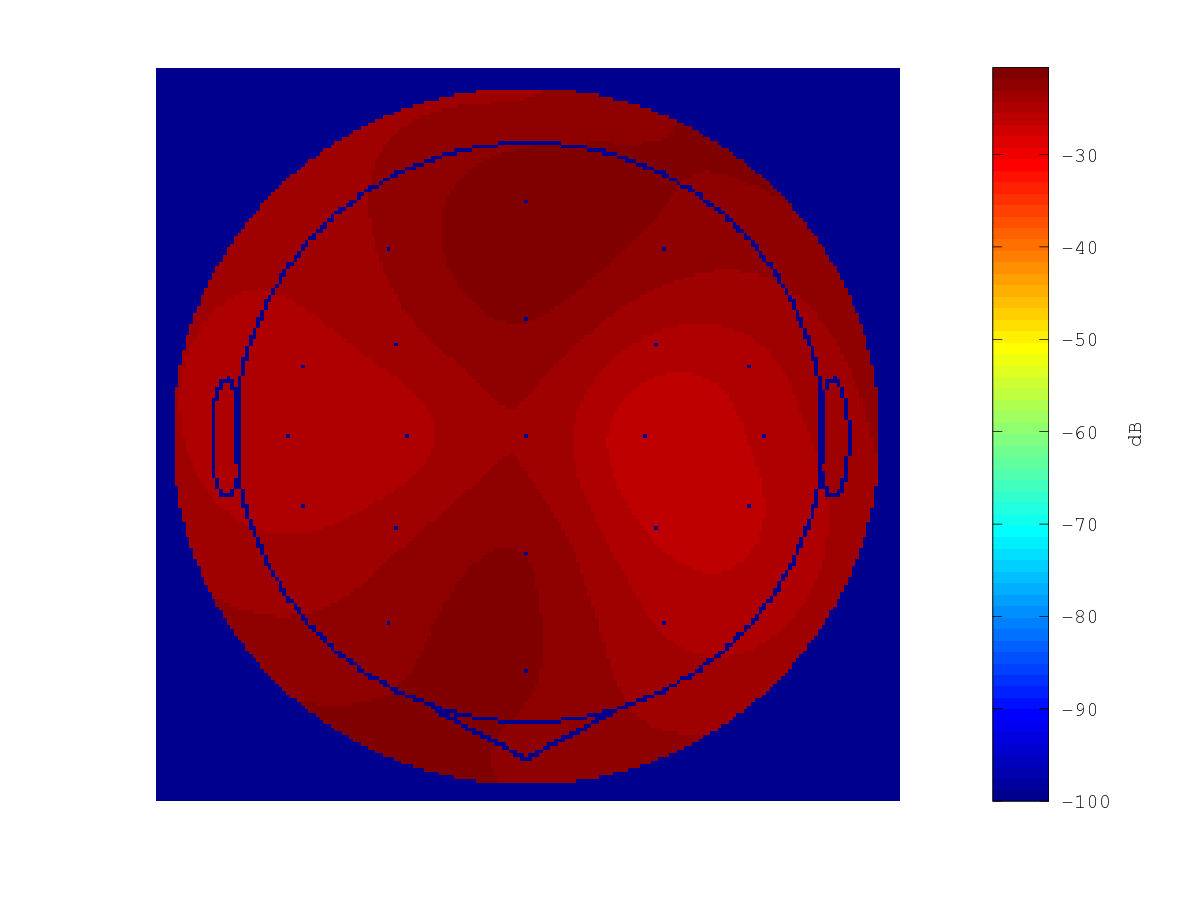
\includegraphics[width=2.5in]{scalpplot.png}}
\end{minipage}
\begin{minipage}[t]{0.5\textwidth}
~\\	
\IfStrEq{\PlotType}{scatter}{\textbf{\Large{Summary:}}\\
\if\IsConcussed1
\if\PrevConcussions0
Based on the results of the EEGlewave algorithm, the baseline brain signals have been classified as belonging to the concussed group. However, the past history and results from the SCAT do not seems to suggest that there is evidence of a previous recent concussion or any other condition that may lead to this result.\\
The EEGlewave algorithm is not 100\% accurate and there is a 10\% chance that some players will be misclassified. It is therefore possible that your child's brain signals fall into the group that are misclassified. However, if you have any concerns or if your child is showing any symptoms that might suggest any medical issues we suggest that your child is seen by your family physician for a physical examination.\\
Please feel free to contact Dr. Virji-Babul if you would like to discuss these results or would like more information.
\else
Based on the results of the EEGlewave algorithm the baseline brain signals have been classified as belonging to the concussed group. The past history and results from the SCAT also seems to suggest that there is evidence of a previous recent concussion. Given these results we suggest that your child is seen by your family physician for a physical examination and be cleared before he/she returns to play.\\
We will contact you again for a second EEG scan within a month to compare the baseline brain signals to determine if your brain signals are changing as a result of recovery. We will also repeat the SCAT to evaluate general changes in symptoms, balance and cognition from the initial assessment.\\
Please feel free to contact Dr. Virji-Babul if you would like more information.
\fi
\else
Based on the results of the EEGlewave algorithm the brain signals appear to be within normal range. If your child receives an impact to the head/body and a concussion is suspected please see your physician and contact EEGlewave at care@eeglewave.com. We will arrange for a second EEG scan and compare your baseline brain signals to the second EEG scan to determine if there have been any changes in your brain activity that may have resulted from the impact. We will also repeat the SCAT3 to evaluate changes in symptoms, balance and cognition from the baseline assessment.
\fi}{Electroencephalography (EEG) is a technique that records the electrical activity of the brain. Brain cells communicate using electrical impulses and are active all the time, even when sitting quietly or sleeping. The EEGlewave algorithm uses EEG signals from the whole brain to evaluate changes in these signals that may be due to a concussion.\\}
\end{minipage}
}}

 %comment starts
\iffalse
\fbox{\parbox{\textwidth}{
\textbf{\Large{Summary:}}\\
\if\IsConcussed1
\if\PrevConcussions0
Based on the results of the EEGlewave algorithm, the baseline brain signals have been classified as belonging to the concussed group. However, the past history and results from the SCAT do not seems to suggest that there is evidence of a previous recent concussion or any other condition that may lead to this result.\\
The EEGlewave algorithm is not 100\% accurate and there is a 10\% chance that some players will be misclassified. It is therefore possible that your child's brain signals fall into the group that are misclassified. However, if you have any concerns or if your child is showing any symptoms that might suggest any medical issues we suggest that your child is seen by your family physician for a physical examination.\\
Please feel free to contact Dr. Virji-Babul if you would like to discuss these results or would like more information.
\else
Based on the results of the EEGlewave algorithm the baseline brain signals have been classified as belonging to the concussed group. The past history and results from the SCAT also seems to suggest that there is evidence of a previous recent concussion. Given these results we suggest that your child is seen by your family physician for a physical examination and be cleared before he/she returns to play.\\
We will contact you again for a second EEG scan within a month to compare the baseline brain signals to determine if your brain signals are changing as a result of recovery. We will also repeat the SCAT to evaluate general changes in symptoms, balance and cognition from the initial assessment.\\
Please feel free to contact Dr. Virji-Babul if you would like more information.
\fi
\else
Based on the results of the EEGlewave algorithm the brain signals appear to be within normal range. If your child receives an impact to the head/body and a concussion is suspected please see your physician and contact EEGlewave at care@eeglewave.com. We will arrange for a second EEG scan and compare your baseline brain signals to the second EEG scan to determine if there have been any changes in your brain activity that may have resulted from the impact. We will also repeat the SCAT3 to evaluate changes in symptoms, balance and cognition from the baseline assessment.
\fi
}}
\fi % till here commenting out

% Add the footnote. A better way would be to use fancyhdr
\vfill
{\footnotesize\color{EWgray}\sffamily
	NOTE: EEGlewave does not provide medical advice. This report should not be used as a substitute for professional medical consultation.\\
}
\end{document}
}%The .tex filename goes here (NOT the same as \jobname)
\unless\ifdefined\ScanType
\endinput\expandafter\expandafter\expandafter\ReadScanType\fi

\def\ReadNumSymptoms#1 {%
	\def\NumSymptoms{#1}%
	% NOTE: This report is to be compiled through the Octave command prompt.
% The following command should be typed into an Octave session to generate the report.
% system("pdflatex.exe -synctex=1 -interaction=nonstopmode -job-name=FirstName_LastName report.tex FirstName Lastname ParentName ID Handedness PrevConcussions Age ScanType")

% Definitions for command line arguments
\def\ReadFirstName#1 {%
	\def\FirstName{#1}%
	\input{report}}%The .tex filename goes here (NOT the same as \jobname)
\unless\ifdefined\FirstName
\endinput\expandafter\expandafter\expandafter\ReadFirstName\fi

\def\ReadLastName#1 {%
	\def\LastName{#1}%
	\input{report}}%The .tex filename goes here (NOT the same as \jobname)
\unless\ifdefined\LastName
\endinput\expandafter\expandafter\expandafter\ReadLastName\fi

\def\ReadParentFirstName#1 {%
	\def\ParentFirstName{#1}%
	\input{report}}%The .tex filename goes here (NOT the same as \jobname)
\unless\ifdefined\ParentFirstName
\endinput\expandafter\expandafter\expandafter\ReadParentFirstName\fi

\def\ReadParentLastName#1 {%
	\def\ParentLastName{#1}%
	\input{report}}%The .tex filename goes here (NOT the same as \jobname)
\unless\ifdefined\ParentLastName
\endinput\expandafter\expandafter\expandafter\ReadParentLastName\fi

\def\ReadID#1 {%
	\def\ID{#1}%
	\input{report}}%The .tex filename goes here (NOT the same as \jobname)
\unless\ifdefined\ID
\endinput\expandafter\expandafter\expandafter\ReadID\fi

\def\ReadHandedness#1 {%
	\def\Handedness{#1}%
	\input{report}}%The .tex filename goes here (NOT the same as \jobname)
\unless\ifdefined\Handedness
\endinput\expandafter\expandafter\expandafter\ReadHandedness\fi

\def\ReadPrevConcussions#1 {%
	\def\PrevConcussions{#1}%
	\input{report}}%The .tex filename goes here (NOT the same as \jobname)
\unless\ifdefined\PrevConcussions
\endinput\expandafter\expandafter\expandafter\ReadPrevConcussions\fi

\def\ReadMostRecentConcussion#1 {%
	\def\MostRecentConcussion{#1}%
	\input{report}}%The .tex filename goes here (NOT the same as \jobname)
\unless\ifdefined\MostRecentConcussion
\endinput\expandafter\expandafter\expandafter\ReadMostRecentConcussion\fi

\def\ReadIsConcussed#1 {%
	\def\IsConcussed{#1}%
	\input{report}}%The .tex filename goes here (NOT the same as \jobname)
\unless\ifdefined\IsConcussed
\endinput\expandafter\expandafter\expandafter\ReadIsConcussed\fi

\def\ReadDivision#1 {%
	\def\Division{#1}%
	\input{report}}%The .tex filename goes here (NOT the same as \jobname)
\unless\ifdefined\Division
\endinput\expandafter\expandafter\expandafter\ReadDivision\fi

\def\ReadGender#1 {%
	\def\Gender{#1}%
	\input{report}}%The .tex filename goes here (NOT the same as \jobname)
\unless\ifdefined\Gender
\endinput\expandafter\expandafter\expandafter\ReadGender\fi

\def\ReadAge#1 {%
	\def\Age{#1}%
	\input{report}}%The .tex filename goes here (NOT the same as \jobname)
\unless\ifdefined\Age
\endinput\expandafter\expandafter\expandafter\ReadAge\fi

\def\ReadDOS#1 {%
	\def\DOS{#1}%
	\input{report}}%The .tex filename goes here (NOT the same as \jobname)
\unless\ifdefined\DOS
\endinput\expandafter\expandafter\expandafter\ReadDOS\fi

\def\ReadScanType#1 {%
	\def\ScanType{#1}%
	\input{report}}%The .tex filename goes here (NOT the same as \jobname)
\unless\ifdefined\ScanType
\endinput\expandafter\expandafter\expandafter\ReadScanType\fi

\def\ReadNumSymptoms#1 {%
	\def\NumSymptoms{#1}%
	\input{report}}%The .tex filename goes here (NOT the same as \jobname)
\unless\ifdefined\NumSymptoms
\endinput\expandafter\expandafter\expandafter\ReadNumSymptoms\fi

\def\ReadSeverityScore#1 {%
	\def\SeverityScore{#1}%
	\input{report}}%The .tex filename goes here (NOT the same as \jobname)
\unless\ifdefined\SeverityScore
\endinput\expandafter\expandafter\expandafter\ReadSeverityScore\fi

\def\ReadOrientation#1 {%
	\def\Orientation{#1}%
	\input{report}}%The .tex filename goes here (NOT the same as \jobname)
\unless\ifdefined\Orientation
\endinput\expandafter\expandafter\expandafter\ReadOrientation\fi

\def\ReadOrientationTotal#1 {%
	\def\OrientationTotal{#1}%
	\input{report}}%The .tex filename goes here (NOT the same as \jobname)
\unless\ifdefined\OrientationTotal
\endinput\expandafter\expandafter\expandafter\ReadOrientationTotal\fi

\def\ReadImmMem#1 {%
	\def\ImmMem{#1}%
	\input{report}}%The .tex filename goes here (NOT the same as \jobname)
\unless\ifdefined\ImmMem
\endinput\expandafter\expandafter\expandafter\ReadImmMem\fi

\def\ReadConcentration#1 {%
	\def\Concentration{#1}%
	\input{report}}%The .tex filename goes here (NOT the same as \jobname)
\unless\ifdefined\Concentration
\endinput\expandafter\expandafter\expandafter\ReadConcentration\fi

\def\ReadConcentrationTotal#1 {%
	\def\ConcentrationTotal{#1}%
	\input{report}}%The .tex filename goes here (NOT the same as \jobname)
\unless\ifdefined\ConcentrationTotal
\endinput\expandafter\expandafter\expandafter\ReadConcentrationTotal\fi

\def\ReadDelayedRecall#1 {%
	\def\DelayedRecall{#1}%
	\input{report}}%The .tex filename goes here (NOT the same as \jobname)
\unless\ifdefined\DelayedRecall
\endinput\expandafter\expandafter\expandafter\ReadDelayedRecall\fi

\def\ReadSAC#1 {%
	\def\SAC{#1}%
	\input{report}}%The .tex filename goes here (NOT the same as \jobname)
\unless\ifdefined\SAC
\endinput\expandafter\expandafter\expandafter\ReadSAC\fi

\def\ReadBESS#1 {%
	\def\BESS{#1}%
	\input{report}}%The .tex filename goes here (NOT the same as \jobname)
\unless\ifdefined\BESS
\endinput\expandafter\expandafter\expandafter\ReadBESS\fi

\def\ReadTandemGait#1 {%
	\def\TandemGait{#1}%
	\input{report}}%The .tex filename goes here (NOT the same as \jobname)
\unless\ifdefined\TandemGait
\endinput\expandafter\expandafter\expandafter\ReadTandemGait\fi

\def\ReadCoordination#1 {%
	\def\Coordination{#1}%
	\input{report}}%The .tex filename goes here (NOT the same as \jobname)
\unless\ifdefined\Coordination
\endinput\expandafter\expandafter\expandafter\ReadCoordination\fi

\def\ReadPlotType#1 {%
	\def\PlotType{#1}%
	\input{report}}%The .tex filename goes here (NOT the same as \jobname)
\unless\ifdefined\PlotType
\endinput\expandafter\expandafter\expandafter\ReadPlotType\fi

\documentclass{article}

\usepackage[dvinames]{xcolor}
% Measurements are taken directly from the guide
\usepackage[top=2in,left=0.5in,bottom=0.5in,right=0.5in]{geometry}
\usepackage{graphicx}
\usepackage[colorlinks=false,
            pdfborder={0 0 0},
            ]{hyperref}
\usepackage{lipsum}
\usepackage[absolute]{textpos}
\usepackage{tikz}
\usetikzlibrary{calc}
% A nice serif font, but no the prescribed nonfree ITC stone
\usepackage[oldstylenums]{kpfonts}
\usepackage[T1]{fontenc	}
\usepackage[12pt]{moresize}
\usepackage{xstring}

% No paragraph indentation
\parindent0pt
\setlength{\parskip}{0.8\baselineskip}
\raggedright
\pagestyle{empty}


\definecolor{EWgray}{HTML}{5e6a71}

\begin{document}
	\begin{center}
		\HUGE{~}\\
		\HUGE{~}\\
		\HUGE{~}\\
		\textbf{\HUGE{EEGlewave Inc.}}\\[1in]
		\textbf{\huge{\ScanType~Report}}\\[1cm]
	\end{center}
	\newpage
\bigskip
% -------------------------------------------------------
% Add logo, the text under the crimson line, and the line itself
\begin{textblock*}{2in}[0.3066,0.39](1.25in,1.23in)
	
\includegraphics[width=1.5in]{eeglewave-front-211x128-88.png}
\end{textblock*}
\begin{textblock*}{6.375in}(1.5in,1.4in)   % 6.375=8.5 - 1.5 - 0.625
	\sffamily
	\hfill \color{EWgray} EEGlewave Inc.\\
	\hfill \url{care@eeglewave.com} \textbullet\ \url{http://eeglewave.com}
\end{textblock*}
\begin{tikzpicture}[remember picture,overlay]
\draw[line width=1pt] (current page.north west)+(0.5in,-1.85in) -- ($(-0.5in,-1.85in)+(current page.north east)$);
\end{tikzpicture}
\fbox{\parbox{\textwidth}{
\textbf{\Large{General Information:}}\\
\begin{minipage}[t]{0.55\textwidth}

\textbf{Name: } \FirstName~\LastName  \\
\textbf{Parent/Guardian's Name: } \ParentFirstName~\ParentLastName  \\
\textbf{ID: } \ID   \\
\textbf{Handedness: } \Handedness  \\
\textbf{Number of Previous Concussions: } \PrevConcussions \\
\textbf{Date of Most Recent Concussion: } \MostRecentConcussion
\end{minipage}
\begin{minipage}[t]{0.45\textwidth}
	\textbf{Division: } \Division  \\
	\textbf{Gender: } \Gender  \\
	\textbf{Age: } \Age  \\
	\textbf{Date of Scan: } \DOS \\
	\textbf{Type of Scan: } \ScanType  \\
\end{minipage}
}}

\fbox{\parbox{\textwidth}{
\textbf{\Large{SCAT3 Scoring Summary:}}\\
\begin{minipage}[t]{0.55\textwidth}
\textbf{Number of Symptoms (/22): } \\
\textbf{Symptom Severity Score (/132): } \\

\textbf{Orientation (/\OrientationTotal): }  \\
\textbf{Immediate Memory (/15): } \\
\textbf{Concentration (/\ConcentrationTotal): } \\
\textbf{Delayed Recall (/5): } \\
\textbf{SAC Total (/30): } \\

\textbf{BESS (total errors): } \\
\textbf{Tandem Gait (seconds): } \\
\textbf{Coordination (/1): } 
\end{minipage}
\begin{minipage}[t]{0.25\textwidth}
\NumSymptoms  \\
\SeverityScore  \\

\Orientation  \\
\ImmMem  \\
\Concentration  \\
\DelayedRecall \\
\SAC  \\

\BESS  \\
\TandemGait  \\
\Coordination
\end{minipage}
}}

\fbox{\parbox{\textwidth}{
\textbf{\Large{\IfStrEq{\PlotType}{scatter}{Scatter Plot:}{EEG Plot of Power at Rest:}}}\\
\begin{minipage}[t]{0.5\textwidth}
	~\\
	\IfStrEq{\PlotType}{scatter}{\includegraphics[width=3.25in]{scatterplot.png}}{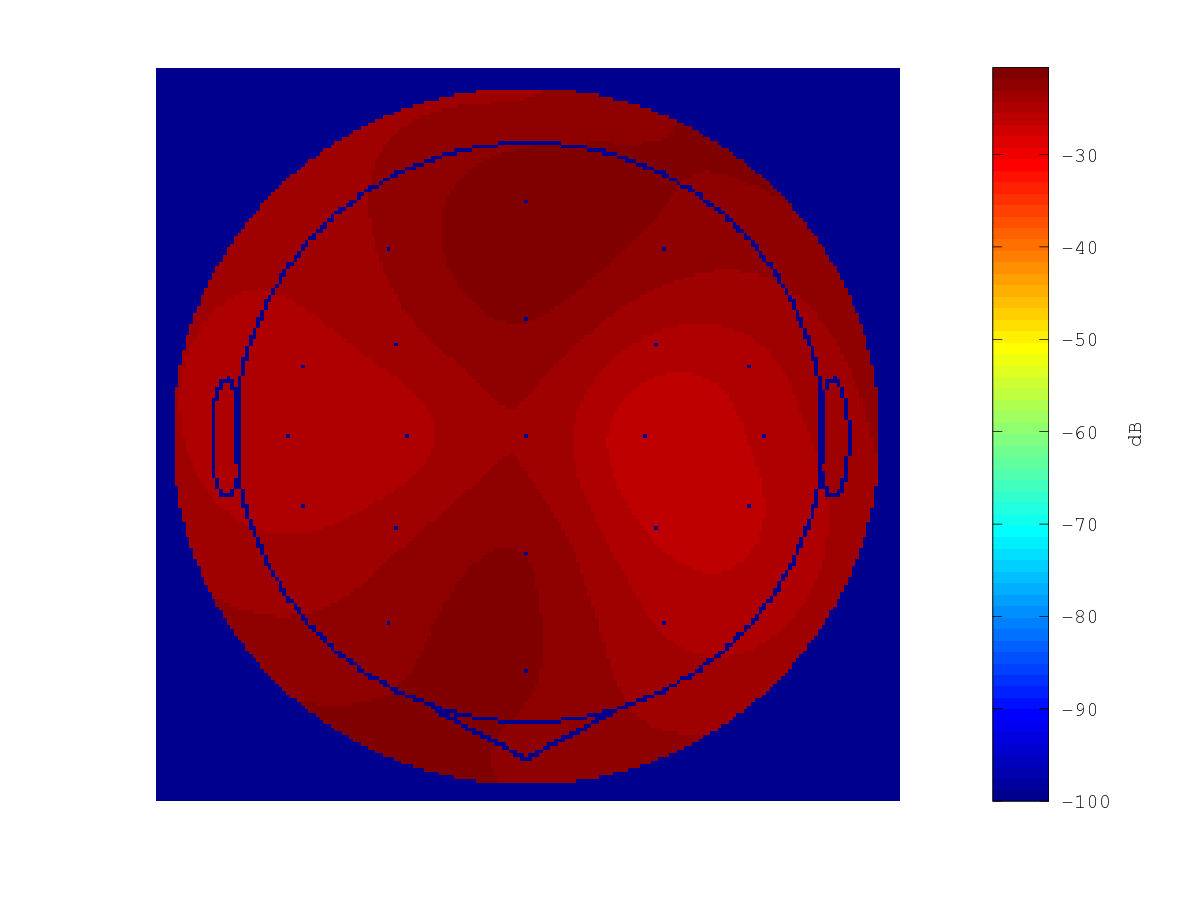
\includegraphics[width=2.5in]{scalpplot.png}}
\end{minipage}
\begin{minipage}[t]{0.5\textwidth}
~\\	
\IfStrEq{\PlotType}{scatter}{\textbf{\Large{Summary:}}\\
\if\IsConcussed1
\if\PrevConcussions0
Based on the results of the EEGlewave algorithm, the baseline brain signals have been classified as belonging to the concussed group. However, the past history and results from the SCAT do not seems to suggest that there is evidence of a previous recent concussion or any other condition that may lead to this result.\\
The EEGlewave algorithm is not 100\% accurate and there is a 10\% chance that some players will be misclassified. It is therefore possible that your child's brain signals fall into the group that are misclassified. However, if you have any concerns or if your child is showing any symptoms that might suggest any medical issues we suggest that your child is seen by your family physician for a physical examination.\\
Please feel free to contact Dr. Virji-Babul if you would like to discuss these results or would like more information.
\else
Based on the results of the EEGlewave algorithm the baseline brain signals have been classified as belonging to the concussed group. The past history and results from the SCAT also seems to suggest that there is evidence of a previous recent concussion. Given these results we suggest that your child is seen by your family physician for a physical examination and be cleared before he/she returns to play.\\
We will contact you again for a second EEG scan within a month to compare the baseline brain signals to determine if your brain signals are changing as a result of recovery. We will also repeat the SCAT to evaluate general changes in symptoms, balance and cognition from the initial assessment.\\
Please feel free to contact Dr. Virji-Babul if you would like more information.
\fi
\else
Based on the results of the EEGlewave algorithm the brain signals appear to be within normal range. If your child receives an impact to the head/body and a concussion is suspected please see your physician and contact EEGlewave at care@eeglewave.com. We will arrange for a second EEG scan and compare your baseline brain signals to the second EEG scan to determine if there have been any changes in your brain activity that may have resulted from the impact. We will also repeat the SCAT3 to evaluate changes in symptoms, balance and cognition from the baseline assessment.
\fi}{Electroencephalography (EEG) is a technique that records the electrical activity of the brain. Brain cells communicate using electrical impulses and are active all the time, even when sitting quietly or sleeping. The EEGlewave algorithm uses EEG signals from the whole brain to evaluate changes in these signals that may be due to a concussion.\\}
\end{minipage}
}}

 %comment starts
\iffalse
\fbox{\parbox{\textwidth}{
\textbf{\Large{Summary:}}\\
\if\IsConcussed1
\if\PrevConcussions0
Based on the results of the EEGlewave algorithm, the baseline brain signals have been classified as belonging to the concussed group. However, the past history and results from the SCAT do not seems to suggest that there is evidence of a previous recent concussion or any other condition that may lead to this result.\\
The EEGlewave algorithm is not 100\% accurate and there is a 10\% chance that some players will be misclassified. It is therefore possible that your child's brain signals fall into the group that are misclassified. However, if you have any concerns or if your child is showing any symptoms that might suggest any medical issues we suggest that your child is seen by your family physician for a physical examination.\\
Please feel free to contact Dr. Virji-Babul if you would like to discuss these results or would like more information.
\else
Based on the results of the EEGlewave algorithm the baseline brain signals have been classified as belonging to the concussed group. The past history and results from the SCAT also seems to suggest that there is evidence of a previous recent concussion. Given these results we suggest that your child is seen by your family physician for a physical examination and be cleared before he/she returns to play.\\
We will contact you again for a second EEG scan within a month to compare the baseline brain signals to determine if your brain signals are changing as a result of recovery. We will also repeat the SCAT to evaluate general changes in symptoms, balance and cognition from the initial assessment.\\
Please feel free to contact Dr. Virji-Babul if you would like more information.
\fi
\else
Based on the results of the EEGlewave algorithm the brain signals appear to be within normal range. If your child receives an impact to the head/body and a concussion is suspected please see your physician and contact EEGlewave at care@eeglewave.com. We will arrange for a second EEG scan and compare your baseline brain signals to the second EEG scan to determine if there have been any changes in your brain activity that may have resulted from the impact. We will also repeat the SCAT3 to evaluate changes in symptoms, balance and cognition from the baseline assessment.
\fi
}}
\fi % till here commenting out

% Add the footnote. A better way would be to use fancyhdr
\vfill
{\footnotesize\color{EWgray}\sffamily
	NOTE: EEGlewave does not provide medical advice. This report should not be used as a substitute for professional medical consultation.\\
}
\end{document}
}%The .tex filename goes here (NOT the same as \jobname)
\unless\ifdefined\NumSymptoms
\endinput\expandafter\expandafter\expandafter\ReadNumSymptoms\fi

\def\ReadSeverityScore#1 {%
	\def\SeverityScore{#1}%
	% NOTE: This report is to be compiled through the Octave command prompt.
% The following command should be typed into an Octave session to generate the report.
% system("pdflatex.exe -synctex=1 -interaction=nonstopmode -job-name=FirstName_LastName report.tex FirstName Lastname ParentName ID Handedness PrevConcussions Age ScanType")

% Definitions for command line arguments
\def\ReadFirstName#1 {%
	\def\FirstName{#1}%
	\input{report}}%The .tex filename goes here (NOT the same as \jobname)
\unless\ifdefined\FirstName
\endinput\expandafter\expandafter\expandafter\ReadFirstName\fi

\def\ReadLastName#1 {%
	\def\LastName{#1}%
	\input{report}}%The .tex filename goes here (NOT the same as \jobname)
\unless\ifdefined\LastName
\endinput\expandafter\expandafter\expandafter\ReadLastName\fi

\def\ReadParentFirstName#1 {%
	\def\ParentFirstName{#1}%
	\input{report}}%The .tex filename goes here (NOT the same as \jobname)
\unless\ifdefined\ParentFirstName
\endinput\expandafter\expandafter\expandafter\ReadParentFirstName\fi

\def\ReadParentLastName#1 {%
	\def\ParentLastName{#1}%
	\input{report}}%The .tex filename goes here (NOT the same as \jobname)
\unless\ifdefined\ParentLastName
\endinput\expandafter\expandafter\expandafter\ReadParentLastName\fi

\def\ReadID#1 {%
	\def\ID{#1}%
	\input{report}}%The .tex filename goes here (NOT the same as \jobname)
\unless\ifdefined\ID
\endinput\expandafter\expandafter\expandafter\ReadID\fi

\def\ReadHandedness#1 {%
	\def\Handedness{#1}%
	\input{report}}%The .tex filename goes here (NOT the same as \jobname)
\unless\ifdefined\Handedness
\endinput\expandafter\expandafter\expandafter\ReadHandedness\fi

\def\ReadPrevConcussions#1 {%
	\def\PrevConcussions{#1}%
	\input{report}}%The .tex filename goes here (NOT the same as \jobname)
\unless\ifdefined\PrevConcussions
\endinput\expandafter\expandafter\expandafter\ReadPrevConcussions\fi

\def\ReadMostRecentConcussion#1 {%
	\def\MostRecentConcussion{#1}%
	\input{report}}%The .tex filename goes here (NOT the same as \jobname)
\unless\ifdefined\MostRecentConcussion
\endinput\expandafter\expandafter\expandafter\ReadMostRecentConcussion\fi

\def\ReadIsConcussed#1 {%
	\def\IsConcussed{#1}%
	\input{report}}%The .tex filename goes here (NOT the same as \jobname)
\unless\ifdefined\IsConcussed
\endinput\expandafter\expandafter\expandafter\ReadIsConcussed\fi

\def\ReadDivision#1 {%
	\def\Division{#1}%
	\input{report}}%The .tex filename goes here (NOT the same as \jobname)
\unless\ifdefined\Division
\endinput\expandafter\expandafter\expandafter\ReadDivision\fi

\def\ReadGender#1 {%
	\def\Gender{#1}%
	\input{report}}%The .tex filename goes here (NOT the same as \jobname)
\unless\ifdefined\Gender
\endinput\expandafter\expandafter\expandafter\ReadGender\fi

\def\ReadAge#1 {%
	\def\Age{#1}%
	\input{report}}%The .tex filename goes here (NOT the same as \jobname)
\unless\ifdefined\Age
\endinput\expandafter\expandafter\expandafter\ReadAge\fi

\def\ReadDOS#1 {%
	\def\DOS{#1}%
	\input{report}}%The .tex filename goes here (NOT the same as \jobname)
\unless\ifdefined\DOS
\endinput\expandafter\expandafter\expandafter\ReadDOS\fi

\def\ReadScanType#1 {%
	\def\ScanType{#1}%
	\input{report}}%The .tex filename goes here (NOT the same as \jobname)
\unless\ifdefined\ScanType
\endinput\expandafter\expandafter\expandafter\ReadScanType\fi

\def\ReadNumSymptoms#1 {%
	\def\NumSymptoms{#1}%
	\input{report}}%The .tex filename goes here (NOT the same as \jobname)
\unless\ifdefined\NumSymptoms
\endinput\expandafter\expandafter\expandafter\ReadNumSymptoms\fi

\def\ReadSeverityScore#1 {%
	\def\SeverityScore{#1}%
	\input{report}}%The .tex filename goes here (NOT the same as \jobname)
\unless\ifdefined\SeverityScore
\endinput\expandafter\expandafter\expandafter\ReadSeverityScore\fi

\def\ReadOrientation#1 {%
	\def\Orientation{#1}%
	\input{report}}%The .tex filename goes here (NOT the same as \jobname)
\unless\ifdefined\Orientation
\endinput\expandafter\expandafter\expandafter\ReadOrientation\fi

\def\ReadOrientationTotal#1 {%
	\def\OrientationTotal{#1}%
	\input{report}}%The .tex filename goes here (NOT the same as \jobname)
\unless\ifdefined\OrientationTotal
\endinput\expandafter\expandafter\expandafter\ReadOrientationTotal\fi

\def\ReadImmMem#1 {%
	\def\ImmMem{#1}%
	\input{report}}%The .tex filename goes here (NOT the same as \jobname)
\unless\ifdefined\ImmMem
\endinput\expandafter\expandafter\expandafter\ReadImmMem\fi

\def\ReadConcentration#1 {%
	\def\Concentration{#1}%
	\input{report}}%The .tex filename goes here (NOT the same as \jobname)
\unless\ifdefined\Concentration
\endinput\expandafter\expandafter\expandafter\ReadConcentration\fi

\def\ReadConcentrationTotal#1 {%
	\def\ConcentrationTotal{#1}%
	\input{report}}%The .tex filename goes here (NOT the same as \jobname)
\unless\ifdefined\ConcentrationTotal
\endinput\expandafter\expandafter\expandafter\ReadConcentrationTotal\fi

\def\ReadDelayedRecall#1 {%
	\def\DelayedRecall{#1}%
	\input{report}}%The .tex filename goes here (NOT the same as \jobname)
\unless\ifdefined\DelayedRecall
\endinput\expandafter\expandafter\expandafter\ReadDelayedRecall\fi

\def\ReadSAC#1 {%
	\def\SAC{#1}%
	\input{report}}%The .tex filename goes here (NOT the same as \jobname)
\unless\ifdefined\SAC
\endinput\expandafter\expandafter\expandafter\ReadSAC\fi

\def\ReadBESS#1 {%
	\def\BESS{#1}%
	\input{report}}%The .tex filename goes here (NOT the same as \jobname)
\unless\ifdefined\BESS
\endinput\expandafter\expandafter\expandafter\ReadBESS\fi

\def\ReadTandemGait#1 {%
	\def\TandemGait{#1}%
	\input{report}}%The .tex filename goes here (NOT the same as \jobname)
\unless\ifdefined\TandemGait
\endinput\expandafter\expandafter\expandafter\ReadTandemGait\fi

\def\ReadCoordination#1 {%
	\def\Coordination{#1}%
	\input{report}}%The .tex filename goes here (NOT the same as \jobname)
\unless\ifdefined\Coordination
\endinput\expandafter\expandafter\expandafter\ReadCoordination\fi

\def\ReadPlotType#1 {%
	\def\PlotType{#1}%
	\input{report}}%The .tex filename goes here (NOT the same as \jobname)
\unless\ifdefined\PlotType
\endinput\expandafter\expandafter\expandafter\ReadPlotType\fi

\documentclass{article}

\usepackage[dvinames]{xcolor}
% Measurements are taken directly from the guide
\usepackage[top=2in,left=0.5in,bottom=0.5in,right=0.5in]{geometry}
\usepackage{graphicx}
\usepackage[colorlinks=false,
            pdfborder={0 0 0},
            ]{hyperref}
\usepackage{lipsum}
\usepackage[absolute]{textpos}
\usepackage{tikz}
\usetikzlibrary{calc}
% A nice serif font, but no the prescribed nonfree ITC stone
\usepackage[oldstylenums]{kpfonts}
\usepackage[T1]{fontenc	}
\usepackage[12pt]{moresize}
\usepackage{xstring}

% No paragraph indentation
\parindent0pt
\setlength{\parskip}{0.8\baselineskip}
\raggedright
\pagestyle{empty}


\definecolor{EWgray}{HTML}{5e6a71}

\begin{document}
	\begin{center}
		\HUGE{~}\\
		\HUGE{~}\\
		\HUGE{~}\\
		\textbf{\HUGE{EEGlewave Inc.}}\\[1in]
		\textbf{\huge{\ScanType~Report}}\\[1cm]
	\end{center}
	\newpage
\bigskip
% -------------------------------------------------------
% Add logo, the text under the crimson line, and the line itself
\begin{textblock*}{2in}[0.3066,0.39](1.25in,1.23in)
	
\includegraphics[width=1.5in]{eeglewave-front-211x128-88.png}
\end{textblock*}
\begin{textblock*}{6.375in}(1.5in,1.4in)   % 6.375=8.5 - 1.5 - 0.625
	\sffamily
	\hfill \color{EWgray} EEGlewave Inc.\\
	\hfill \url{care@eeglewave.com} \textbullet\ \url{http://eeglewave.com}
\end{textblock*}
\begin{tikzpicture}[remember picture,overlay]
\draw[line width=1pt] (current page.north west)+(0.5in,-1.85in) -- ($(-0.5in,-1.85in)+(current page.north east)$);
\end{tikzpicture}
\fbox{\parbox{\textwidth}{
\textbf{\Large{General Information:}}\\
\begin{minipage}[t]{0.55\textwidth}

\textbf{Name: } \FirstName~\LastName  \\
\textbf{Parent/Guardian's Name: } \ParentFirstName~\ParentLastName  \\
\textbf{ID: } \ID   \\
\textbf{Handedness: } \Handedness  \\
\textbf{Number of Previous Concussions: } \PrevConcussions \\
\textbf{Date of Most Recent Concussion: } \MostRecentConcussion
\end{minipage}
\begin{minipage}[t]{0.45\textwidth}
	\textbf{Division: } \Division  \\
	\textbf{Gender: } \Gender  \\
	\textbf{Age: } \Age  \\
	\textbf{Date of Scan: } \DOS \\
	\textbf{Type of Scan: } \ScanType  \\
\end{minipage}
}}

\fbox{\parbox{\textwidth}{
\textbf{\Large{SCAT3 Scoring Summary:}}\\
\begin{minipage}[t]{0.55\textwidth}
\textbf{Number of Symptoms (/22): } \\
\textbf{Symptom Severity Score (/132): } \\

\textbf{Orientation (/\OrientationTotal): }  \\
\textbf{Immediate Memory (/15): } \\
\textbf{Concentration (/\ConcentrationTotal): } \\
\textbf{Delayed Recall (/5): } \\
\textbf{SAC Total (/30): } \\

\textbf{BESS (total errors): } \\
\textbf{Tandem Gait (seconds): } \\
\textbf{Coordination (/1): } 
\end{minipage}
\begin{minipage}[t]{0.25\textwidth}
\NumSymptoms  \\
\SeverityScore  \\

\Orientation  \\
\ImmMem  \\
\Concentration  \\
\DelayedRecall \\
\SAC  \\

\BESS  \\
\TandemGait  \\
\Coordination
\end{minipage}
}}

\fbox{\parbox{\textwidth}{
\textbf{\Large{\IfStrEq{\PlotType}{scatter}{Scatter Plot:}{EEG Plot of Power at Rest:}}}\\
\begin{minipage}[t]{0.5\textwidth}
	~\\
	\IfStrEq{\PlotType}{scatter}{\includegraphics[width=3.25in]{scatterplot.png}}{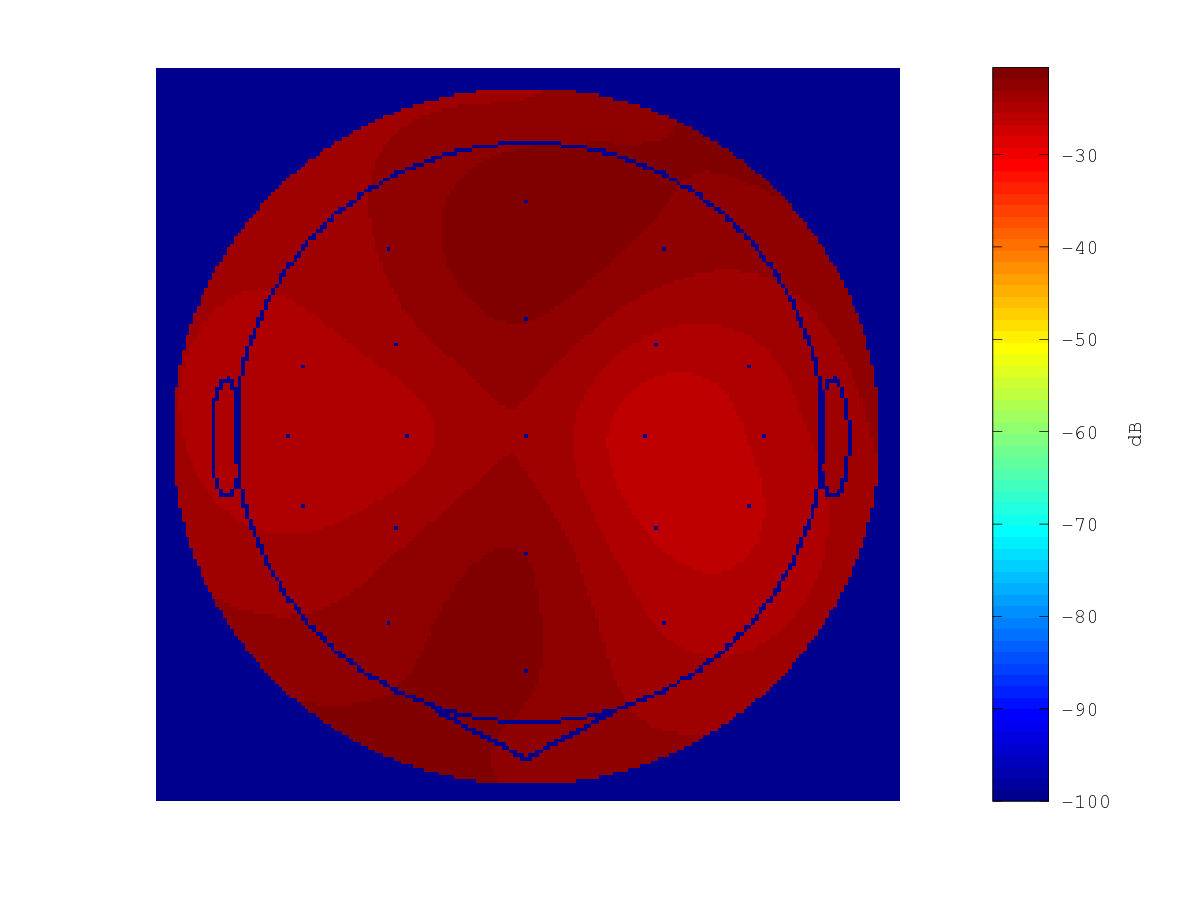
\includegraphics[width=2.5in]{scalpplot.png}}
\end{minipage}
\begin{minipage}[t]{0.5\textwidth}
~\\	
\IfStrEq{\PlotType}{scatter}{\textbf{\Large{Summary:}}\\
\if\IsConcussed1
\if\PrevConcussions0
Based on the results of the EEGlewave algorithm, the baseline brain signals have been classified as belonging to the concussed group. However, the past history and results from the SCAT do not seems to suggest that there is evidence of a previous recent concussion or any other condition that may lead to this result.\\
The EEGlewave algorithm is not 100\% accurate and there is a 10\% chance that some players will be misclassified. It is therefore possible that your child's brain signals fall into the group that are misclassified. However, if you have any concerns or if your child is showing any symptoms that might suggest any medical issues we suggest that your child is seen by your family physician for a physical examination.\\
Please feel free to contact Dr. Virji-Babul if you would like to discuss these results or would like more information.
\else
Based on the results of the EEGlewave algorithm the baseline brain signals have been classified as belonging to the concussed group. The past history and results from the SCAT also seems to suggest that there is evidence of a previous recent concussion. Given these results we suggest that your child is seen by your family physician for a physical examination and be cleared before he/she returns to play.\\
We will contact you again for a second EEG scan within a month to compare the baseline brain signals to determine if your brain signals are changing as a result of recovery. We will also repeat the SCAT to evaluate general changes in symptoms, balance and cognition from the initial assessment.\\
Please feel free to contact Dr. Virji-Babul if you would like more information.
\fi
\else
Based on the results of the EEGlewave algorithm the brain signals appear to be within normal range. If your child receives an impact to the head/body and a concussion is suspected please see your physician and contact EEGlewave at care@eeglewave.com. We will arrange for a second EEG scan and compare your baseline brain signals to the second EEG scan to determine if there have been any changes in your brain activity that may have resulted from the impact. We will also repeat the SCAT3 to evaluate changes in symptoms, balance and cognition from the baseline assessment.
\fi}{Electroencephalography (EEG) is a technique that records the electrical activity of the brain. Brain cells communicate using electrical impulses and are active all the time, even when sitting quietly or sleeping. The EEGlewave algorithm uses EEG signals from the whole brain to evaluate changes in these signals that may be due to a concussion.\\}
\end{minipage}
}}

 %comment starts
\iffalse
\fbox{\parbox{\textwidth}{
\textbf{\Large{Summary:}}\\
\if\IsConcussed1
\if\PrevConcussions0
Based on the results of the EEGlewave algorithm, the baseline brain signals have been classified as belonging to the concussed group. However, the past history and results from the SCAT do not seems to suggest that there is evidence of a previous recent concussion or any other condition that may lead to this result.\\
The EEGlewave algorithm is not 100\% accurate and there is a 10\% chance that some players will be misclassified. It is therefore possible that your child's brain signals fall into the group that are misclassified. However, if you have any concerns or if your child is showing any symptoms that might suggest any medical issues we suggest that your child is seen by your family physician for a physical examination.\\
Please feel free to contact Dr. Virji-Babul if you would like to discuss these results or would like more information.
\else
Based on the results of the EEGlewave algorithm the baseline brain signals have been classified as belonging to the concussed group. The past history and results from the SCAT also seems to suggest that there is evidence of a previous recent concussion. Given these results we suggest that your child is seen by your family physician for a physical examination and be cleared before he/she returns to play.\\
We will contact you again for a second EEG scan within a month to compare the baseline brain signals to determine if your brain signals are changing as a result of recovery. We will also repeat the SCAT to evaluate general changes in symptoms, balance and cognition from the initial assessment.\\
Please feel free to contact Dr. Virji-Babul if you would like more information.
\fi
\else
Based on the results of the EEGlewave algorithm the brain signals appear to be within normal range. If your child receives an impact to the head/body and a concussion is suspected please see your physician and contact EEGlewave at care@eeglewave.com. We will arrange for a second EEG scan and compare your baseline brain signals to the second EEG scan to determine if there have been any changes in your brain activity that may have resulted from the impact. We will also repeat the SCAT3 to evaluate changes in symptoms, balance and cognition from the baseline assessment.
\fi
}}
\fi % till here commenting out

% Add the footnote. A better way would be to use fancyhdr
\vfill
{\footnotesize\color{EWgray}\sffamily
	NOTE: EEGlewave does not provide medical advice. This report should not be used as a substitute for professional medical consultation.\\
}
\end{document}
}%The .tex filename goes here (NOT the same as \jobname)
\unless\ifdefined\SeverityScore
\endinput\expandafter\expandafter\expandafter\ReadSeverityScore\fi

\def\ReadOrientation#1 {%
	\def\Orientation{#1}%
	% NOTE: This report is to be compiled through the Octave command prompt.
% The following command should be typed into an Octave session to generate the report.
% system("pdflatex.exe -synctex=1 -interaction=nonstopmode -job-name=FirstName_LastName report.tex FirstName Lastname ParentName ID Handedness PrevConcussions Age ScanType")

% Definitions for command line arguments
\def\ReadFirstName#1 {%
	\def\FirstName{#1}%
	\input{report}}%The .tex filename goes here (NOT the same as \jobname)
\unless\ifdefined\FirstName
\endinput\expandafter\expandafter\expandafter\ReadFirstName\fi

\def\ReadLastName#1 {%
	\def\LastName{#1}%
	\input{report}}%The .tex filename goes here (NOT the same as \jobname)
\unless\ifdefined\LastName
\endinput\expandafter\expandafter\expandafter\ReadLastName\fi

\def\ReadParentFirstName#1 {%
	\def\ParentFirstName{#1}%
	\input{report}}%The .tex filename goes here (NOT the same as \jobname)
\unless\ifdefined\ParentFirstName
\endinput\expandafter\expandafter\expandafter\ReadParentFirstName\fi

\def\ReadParentLastName#1 {%
	\def\ParentLastName{#1}%
	\input{report}}%The .tex filename goes here (NOT the same as \jobname)
\unless\ifdefined\ParentLastName
\endinput\expandafter\expandafter\expandafter\ReadParentLastName\fi

\def\ReadID#1 {%
	\def\ID{#1}%
	\input{report}}%The .tex filename goes here (NOT the same as \jobname)
\unless\ifdefined\ID
\endinput\expandafter\expandafter\expandafter\ReadID\fi

\def\ReadHandedness#1 {%
	\def\Handedness{#1}%
	\input{report}}%The .tex filename goes here (NOT the same as \jobname)
\unless\ifdefined\Handedness
\endinput\expandafter\expandafter\expandafter\ReadHandedness\fi

\def\ReadPrevConcussions#1 {%
	\def\PrevConcussions{#1}%
	\input{report}}%The .tex filename goes here (NOT the same as \jobname)
\unless\ifdefined\PrevConcussions
\endinput\expandafter\expandafter\expandafter\ReadPrevConcussions\fi

\def\ReadMostRecentConcussion#1 {%
	\def\MostRecentConcussion{#1}%
	\input{report}}%The .tex filename goes here (NOT the same as \jobname)
\unless\ifdefined\MostRecentConcussion
\endinput\expandafter\expandafter\expandafter\ReadMostRecentConcussion\fi

\def\ReadIsConcussed#1 {%
	\def\IsConcussed{#1}%
	\input{report}}%The .tex filename goes here (NOT the same as \jobname)
\unless\ifdefined\IsConcussed
\endinput\expandafter\expandafter\expandafter\ReadIsConcussed\fi

\def\ReadDivision#1 {%
	\def\Division{#1}%
	\input{report}}%The .tex filename goes here (NOT the same as \jobname)
\unless\ifdefined\Division
\endinput\expandafter\expandafter\expandafter\ReadDivision\fi

\def\ReadGender#1 {%
	\def\Gender{#1}%
	\input{report}}%The .tex filename goes here (NOT the same as \jobname)
\unless\ifdefined\Gender
\endinput\expandafter\expandafter\expandafter\ReadGender\fi

\def\ReadAge#1 {%
	\def\Age{#1}%
	\input{report}}%The .tex filename goes here (NOT the same as \jobname)
\unless\ifdefined\Age
\endinput\expandafter\expandafter\expandafter\ReadAge\fi

\def\ReadDOS#1 {%
	\def\DOS{#1}%
	\input{report}}%The .tex filename goes here (NOT the same as \jobname)
\unless\ifdefined\DOS
\endinput\expandafter\expandafter\expandafter\ReadDOS\fi

\def\ReadScanType#1 {%
	\def\ScanType{#1}%
	\input{report}}%The .tex filename goes here (NOT the same as \jobname)
\unless\ifdefined\ScanType
\endinput\expandafter\expandafter\expandafter\ReadScanType\fi

\def\ReadNumSymptoms#1 {%
	\def\NumSymptoms{#1}%
	\input{report}}%The .tex filename goes here (NOT the same as \jobname)
\unless\ifdefined\NumSymptoms
\endinput\expandafter\expandafter\expandafter\ReadNumSymptoms\fi

\def\ReadSeverityScore#1 {%
	\def\SeverityScore{#1}%
	\input{report}}%The .tex filename goes here (NOT the same as \jobname)
\unless\ifdefined\SeverityScore
\endinput\expandafter\expandafter\expandafter\ReadSeverityScore\fi

\def\ReadOrientation#1 {%
	\def\Orientation{#1}%
	\input{report}}%The .tex filename goes here (NOT the same as \jobname)
\unless\ifdefined\Orientation
\endinput\expandafter\expandafter\expandafter\ReadOrientation\fi

\def\ReadOrientationTotal#1 {%
	\def\OrientationTotal{#1}%
	\input{report}}%The .tex filename goes here (NOT the same as \jobname)
\unless\ifdefined\OrientationTotal
\endinput\expandafter\expandafter\expandafter\ReadOrientationTotal\fi

\def\ReadImmMem#1 {%
	\def\ImmMem{#1}%
	\input{report}}%The .tex filename goes here (NOT the same as \jobname)
\unless\ifdefined\ImmMem
\endinput\expandafter\expandafter\expandafter\ReadImmMem\fi

\def\ReadConcentration#1 {%
	\def\Concentration{#1}%
	\input{report}}%The .tex filename goes here (NOT the same as \jobname)
\unless\ifdefined\Concentration
\endinput\expandafter\expandafter\expandafter\ReadConcentration\fi

\def\ReadConcentrationTotal#1 {%
	\def\ConcentrationTotal{#1}%
	\input{report}}%The .tex filename goes here (NOT the same as \jobname)
\unless\ifdefined\ConcentrationTotal
\endinput\expandafter\expandafter\expandafter\ReadConcentrationTotal\fi

\def\ReadDelayedRecall#1 {%
	\def\DelayedRecall{#1}%
	\input{report}}%The .tex filename goes here (NOT the same as \jobname)
\unless\ifdefined\DelayedRecall
\endinput\expandafter\expandafter\expandafter\ReadDelayedRecall\fi

\def\ReadSAC#1 {%
	\def\SAC{#1}%
	\input{report}}%The .tex filename goes here (NOT the same as \jobname)
\unless\ifdefined\SAC
\endinput\expandafter\expandafter\expandafter\ReadSAC\fi

\def\ReadBESS#1 {%
	\def\BESS{#1}%
	\input{report}}%The .tex filename goes here (NOT the same as \jobname)
\unless\ifdefined\BESS
\endinput\expandafter\expandafter\expandafter\ReadBESS\fi

\def\ReadTandemGait#1 {%
	\def\TandemGait{#1}%
	\input{report}}%The .tex filename goes here (NOT the same as \jobname)
\unless\ifdefined\TandemGait
\endinput\expandafter\expandafter\expandafter\ReadTandemGait\fi

\def\ReadCoordination#1 {%
	\def\Coordination{#1}%
	\input{report}}%The .tex filename goes here (NOT the same as \jobname)
\unless\ifdefined\Coordination
\endinput\expandafter\expandafter\expandafter\ReadCoordination\fi

\def\ReadPlotType#1 {%
	\def\PlotType{#1}%
	\input{report}}%The .tex filename goes here (NOT the same as \jobname)
\unless\ifdefined\PlotType
\endinput\expandafter\expandafter\expandafter\ReadPlotType\fi

\documentclass{article}

\usepackage[dvinames]{xcolor}
% Measurements are taken directly from the guide
\usepackage[top=2in,left=0.5in,bottom=0.5in,right=0.5in]{geometry}
\usepackage{graphicx}
\usepackage[colorlinks=false,
            pdfborder={0 0 0},
            ]{hyperref}
\usepackage{lipsum}
\usepackage[absolute]{textpos}
\usepackage{tikz}
\usetikzlibrary{calc}
% A nice serif font, but no the prescribed nonfree ITC stone
\usepackage[oldstylenums]{kpfonts}
\usepackage[T1]{fontenc	}
\usepackage[12pt]{moresize}
\usepackage{xstring}

% No paragraph indentation
\parindent0pt
\setlength{\parskip}{0.8\baselineskip}
\raggedright
\pagestyle{empty}


\definecolor{EWgray}{HTML}{5e6a71}

\begin{document}
	\begin{center}
		\HUGE{~}\\
		\HUGE{~}\\
		\HUGE{~}\\
		\textbf{\HUGE{EEGlewave Inc.}}\\[1in]
		\textbf{\huge{\ScanType~Report}}\\[1cm]
	\end{center}
	\newpage
\bigskip
% -------------------------------------------------------
% Add logo, the text under the crimson line, and the line itself
\begin{textblock*}{2in}[0.3066,0.39](1.25in,1.23in)
	
\includegraphics[width=1.5in]{eeglewave-front-211x128-88.png}
\end{textblock*}
\begin{textblock*}{6.375in}(1.5in,1.4in)   % 6.375=8.5 - 1.5 - 0.625
	\sffamily
	\hfill \color{EWgray} EEGlewave Inc.\\
	\hfill \url{care@eeglewave.com} \textbullet\ \url{http://eeglewave.com}
\end{textblock*}
\begin{tikzpicture}[remember picture,overlay]
\draw[line width=1pt] (current page.north west)+(0.5in,-1.85in) -- ($(-0.5in,-1.85in)+(current page.north east)$);
\end{tikzpicture}
\fbox{\parbox{\textwidth}{
\textbf{\Large{General Information:}}\\
\begin{minipage}[t]{0.55\textwidth}

\textbf{Name: } \FirstName~\LastName  \\
\textbf{Parent/Guardian's Name: } \ParentFirstName~\ParentLastName  \\
\textbf{ID: } \ID   \\
\textbf{Handedness: } \Handedness  \\
\textbf{Number of Previous Concussions: } \PrevConcussions \\
\textbf{Date of Most Recent Concussion: } \MostRecentConcussion
\end{minipage}
\begin{minipage}[t]{0.45\textwidth}
	\textbf{Division: } \Division  \\
	\textbf{Gender: } \Gender  \\
	\textbf{Age: } \Age  \\
	\textbf{Date of Scan: } \DOS \\
	\textbf{Type of Scan: } \ScanType  \\
\end{minipage}
}}

\fbox{\parbox{\textwidth}{
\textbf{\Large{SCAT3 Scoring Summary:}}\\
\begin{minipage}[t]{0.55\textwidth}
\textbf{Number of Symptoms (/22): } \\
\textbf{Symptom Severity Score (/132): } \\

\textbf{Orientation (/\OrientationTotal): }  \\
\textbf{Immediate Memory (/15): } \\
\textbf{Concentration (/\ConcentrationTotal): } \\
\textbf{Delayed Recall (/5): } \\
\textbf{SAC Total (/30): } \\

\textbf{BESS (total errors): } \\
\textbf{Tandem Gait (seconds): } \\
\textbf{Coordination (/1): } 
\end{minipage}
\begin{minipage}[t]{0.25\textwidth}
\NumSymptoms  \\
\SeverityScore  \\

\Orientation  \\
\ImmMem  \\
\Concentration  \\
\DelayedRecall \\
\SAC  \\

\BESS  \\
\TandemGait  \\
\Coordination
\end{minipage}
}}

\fbox{\parbox{\textwidth}{
\textbf{\Large{\IfStrEq{\PlotType}{scatter}{Scatter Plot:}{EEG Plot of Power at Rest:}}}\\
\begin{minipage}[t]{0.5\textwidth}
	~\\
	\IfStrEq{\PlotType}{scatter}{\includegraphics[width=3.25in]{scatterplot.png}}{\includegraphics[width=2.5in]{scalpplot.png}}
\end{minipage}
\begin{minipage}[t]{0.5\textwidth}
~\\	
\IfStrEq{\PlotType}{scatter}{\textbf{\Large{Summary:}}\\
\if\IsConcussed1
\if\PrevConcussions0
Based on the results of the EEGlewave algorithm, the baseline brain signals have been classified as belonging to the concussed group. However, the past history and results from the SCAT do not seems to suggest that there is evidence of a previous recent concussion or any other condition that may lead to this result.\\
The EEGlewave algorithm is not 100\% accurate and there is a 10\% chance that some players will be misclassified. It is therefore possible that your child's brain signals fall into the group that are misclassified. However, if you have any concerns or if your child is showing any symptoms that might suggest any medical issues we suggest that your child is seen by your family physician for a physical examination.\\
Please feel free to contact Dr. Virji-Babul if you would like to discuss these results or would like more information.
\else
Based on the results of the EEGlewave algorithm the baseline brain signals have been classified as belonging to the concussed group. The past history and results from the SCAT also seems to suggest that there is evidence of a previous recent concussion. Given these results we suggest that your child is seen by your family physician for a physical examination and be cleared before he/she returns to play.\\
We will contact you again for a second EEG scan within a month to compare the baseline brain signals to determine if your brain signals are changing as a result of recovery. We will also repeat the SCAT to evaluate general changes in symptoms, balance and cognition from the initial assessment.\\
Please feel free to contact Dr. Virji-Babul if you would like more information.
\fi
\else
Based on the results of the EEGlewave algorithm the brain signals appear to be within normal range. If your child receives an impact to the head/body and a concussion is suspected please see your physician and contact EEGlewave at care@eeglewave.com. We will arrange for a second EEG scan and compare your baseline brain signals to the second EEG scan to determine if there have been any changes in your brain activity that may have resulted from the impact. We will also repeat the SCAT3 to evaluate changes in symptoms, balance and cognition from the baseline assessment.
\fi}{Electroencephalography (EEG) is a technique that records the electrical activity of the brain. Brain cells communicate using electrical impulses and are active all the time, even when sitting quietly or sleeping. The EEGlewave algorithm uses EEG signals from the whole brain to evaluate changes in these signals that may be due to a concussion.\\}
\end{minipage}
}}

 %comment starts
\iffalse
\fbox{\parbox{\textwidth}{
\textbf{\Large{Summary:}}\\
\if\IsConcussed1
\if\PrevConcussions0
Based on the results of the EEGlewave algorithm, the baseline brain signals have been classified as belonging to the concussed group. However, the past history and results from the SCAT do not seems to suggest that there is evidence of a previous recent concussion or any other condition that may lead to this result.\\
The EEGlewave algorithm is not 100\% accurate and there is a 10\% chance that some players will be misclassified. It is therefore possible that your child's brain signals fall into the group that are misclassified. However, if you have any concerns or if your child is showing any symptoms that might suggest any medical issues we suggest that your child is seen by your family physician for a physical examination.\\
Please feel free to contact Dr. Virji-Babul if you would like to discuss these results or would like more information.
\else
Based on the results of the EEGlewave algorithm the baseline brain signals have been classified as belonging to the concussed group. The past history and results from the SCAT also seems to suggest that there is evidence of a previous recent concussion. Given these results we suggest that your child is seen by your family physician for a physical examination and be cleared before he/she returns to play.\\
We will contact you again for a second EEG scan within a month to compare the baseline brain signals to determine if your brain signals are changing as a result of recovery. We will also repeat the SCAT to evaluate general changes in symptoms, balance and cognition from the initial assessment.\\
Please feel free to contact Dr. Virji-Babul if you would like more information.
\fi
\else
Based on the results of the EEGlewave algorithm the brain signals appear to be within normal range. If your child receives an impact to the head/body and a concussion is suspected please see your physician and contact EEGlewave at care@eeglewave.com. We will arrange for a second EEG scan and compare your baseline brain signals to the second EEG scan to determine if there have been any changes in your brain activity that may have resulted from the impact. We will also repeat the SCAT3 to evaluate changes in symptoms, balance and cognition from the baseline assessment.
\fi
}}
\fi % till here commenting out

% Add the footnote. A better way would be to use fancyhdr
\vfill
{\footnotesize\color{EWgray}\sffamily
	NOTE: EEGlewave does not provide medical advice. This report should not be used as a substitute for professional medical consultation.\\
}
\end{document}
}%The .tex filename goes here (NOT the same as \jobname)
\unless\ifdefined\Orientation
\endinput\expandafter\expandafter\expandafter\ReadOrientation\fi

\def\ReadOrientationTotal#1 {%
	\def\OrientationTotal{#1}%
	% NOTE: This report is to be compiled through the Octave command prompt.
% The following command should be typed into an Octave session to generate the report.
% system("pdflatex.exe -synctex=1 -interaction=nonstopmode -job-name=FirstName_LastName report.tex FirstName Lastname ParentName ID Handedness PrevConcussions Age ScanType")

% Definitions for command line arguments
\def\ReadFirstName#1 {%
	\def\FirstName{#1}%
	\input{report}}%The .tex filename goes here (NOT the same as \jobname)
\unless\ifdefined\FirstName
\endinput\expandafter\expandafter\expandafter\ReadFirstName\fi

\def\ReadLastName#1 {%
	\def\LastName{#1}%
	\input{report}}%The .tex filename goes here (NOT the same as \jobname)
\unless\ifdefined\LastName
\endinput\expandafter\expandafter\expandafter\ReadLastName\fi

\def\ReadParentFirstName#1 {%
	\def\ParentFirstName{#1}%
	\input{report}}%The .tex filename goes here (NOT the same as \jobname)
\unless\ifdefined\ParentFirstName
\endinput\expandafter\expandafter\expandafter\ReadParentFirstName\fi

\def\ReadParentLastName#1 {%
	\def\ParentLastName{#1}%
	\input{report}}%The .tex filename goes here (NOT the same as \jobname)
\unless\ifdefined\ParentLastName
\endinput\expandafter\expandafter\expandafter\ReadParentLastName\fi

\def\ReadID#1 {%
	\def\ID{#1}%
	\input{report}}%The .tex filename goes here (NOT the same as \jobname)
\unless\ifdefined\ID
\endinput\expandafter\expandafter\expandafter\ReadID\fi

\def\ReadHandedness#1 {%
	\def\Handedness{#1}%
	\input{report}}%The .tex filename goes here (NOT the same as \jobname)
\unless\ifdefined\Handedness
\endinput\expandafter\expandafter\expandafter\ReadHandedness\fi

\def\ReadPrevConcussions#1 {%
	\def\PrevConcussions{#1}%
	\input{report}}%The .tex filename goes here (NOT the same as \jobname)
\unless\ifdefined\PrevConcussions
\endinput\expandafter\expandafter\expandafter\ReadPrevConcussions\fi

\def\ReadMostRecentConcussion#1 {%
	\def\MostRecentConcussion{#1}%
	\input{report}}%The .tex filename goes here (NOT the same as \jobname)
\unless\ifdefined\MostRecentConcussion
\endinput\expandafter\expandafter\expandafter\ReadMostRecentConcussion\fi

\def\ReadIsConcussed#1 {%
	\def\IsConcussed{#1}%
	\input{report}}%The .tex filename goes here (NOT the same as \jobname)
\unless\ifdefined\IsConcussed
\endinput\expandafter\expandafter\expandafter\ReadIsConcussed\fi

\def\ReadDivision#1 {%
	\def\Division{#1}%
	\input{report}}%The .tex filename goes here (NOT the same as \jobname)
\unless\ifdefined\Division
\endinput\expandafter\expandafter\expandafter\ReadDivision\fi

\def\ReadGender#1 {%
	\def\Gender{#1}%
	\input{report}}%The .tex filename goes here (NOT the same as \jobname)
\unless\ifdefined\Gender
\endinput\expandafter\expandafter\expandafter\ReadGender\fi

\def\ReadAge#1 {%
	\def\Age{#1}%
	\input{report}}%The .tex filename goes here (NOT the same as \jobname)
\unless\ifdefined\Age
\endinput\expandafter\expandafter\expandafter\ReadAge\fi

\def\ReadDOS#1 {%
	\def\DOS{#1}%
	\input{report}}%The .tex filename goes here (NOT the same as \jobname)
\unless\ifdefined\DOS
\endinput\expandafter\expandafter\expandafter\ReadDOS\fi

\def\ReadScanType#1 {%
	\def\ScanType{#1}%
	\input{report}}%The .tex filename goes here (NOT the same as \jobname)
\unless\ifdefined\ScanType
\endinput\expandafter\expandafter\expandafter\ReadScanType\fi

\def\ReadNumSymptoms#1 {%
	\def\NumSymptoms{#1}%
	\input{report}}%The .tex filename goes here (NOT the same as \jobname)
\unless\ifdefined\NumSymptoms
\endinput\expandafter\expandafter\expandafter\ReadNumSymptoms\fi

\def\ReadSeverityScore#1 {%
	\def\SeverityScore{#1}%
	\input{report}}%The .tex filename goes here (NOT the same as \jobname)
\unless\ifdefined\SeverityScore
\endinput\expandafter\expandafter\expandafter\ReadSeverityScore\fi

\def\ReadOrientation#1 {%
	\def\Orientation{#1}%
	\input{report}}%The .tex filename goes here (NOT the same as \jobname)
\unless\ifdefined\Orientation
\endinput\expandafter\expandafter\expandafter\ReadOrientation\fi

\def\ReadOrientationTotal#1 {%
	\def\OrientationTotal{#1}%
	\input{report}}%The .tex filename goes here (NOT the same as \jobname)
\unless\ifdefined\OrientationTotal
\endinput\expandafter\expandafter\expandafter\ReadOrientationTotal\fi

\def\ReadImmMem#1 {%
	\def\ImmMem{#1}%
	\input{report}}%The .tex filename goes here (NOT the same as \jobname)
\unless\ifdefined\ImmMem
\endinput\expandafter\expandafter\expandafter\ReadImmMem\fi

\def\ReadConcentration#1 {%
	\def\Concentration{#1}%
	\input{report}}%The .tex filename goes here (NOT the same as \jobname)
\unless\ifdefined\Concentration
\endinput\expandafter\expandafter\expandafter\ReadConcentration\fi

\def\ReadConcentrationTotal#1 {%
	\def\ConcentrationTotal{#1}%
	\input{report}}%The .tex filename goes here (NOT the same as \jobname)
\unless\ifdefined\ConcentrationTotal
\endinput\expandafter\expandafter\expandafter\ReadConcentrationTotal\fi

\def\ReadDelayedRecall#1 {%
	\def\DelayedRecall{#1}%
	\input{report}}%The .tex filename goes here (NOT the same as \jobname)
\unless\ifdefined\DelayedRecall
\endinput\expandafter\expandafter\expandafter\ReadDelayedRecall\fi

\def\ReadSAC#1 {%
	\def\SAC{#1}%
	\input{report}}%The .tex filename goes here (NOT the same as \jobname)
\unless\ifdefined\SAC
\endinput\expandafter\expandafter\expandafter\ReadSAC\fi

\def\ReadBESS#1 {%
	\def\BESS{#1}%
	\input{report}}%The .tex filename goes here (NOT the same as \jobname)
\unless\ifdefined\BESS
\endinput\expandafter\expandafter\expandafter\ReadBESS\fi

\def\ReadTandemGait#1 {%
	\def\TandemGait{#1}%
	\input{report}}%The .tex filename goes here (NOT the same as \jobname)
\unless\ifdefined\TandemGait
\endinput\expandafter\expandafter\expandafter\ReadTandemGait\fi

\def\ReadCoordination#1 {%
	\def\Coordination{#1}%
	\input{report}}%The .tex filename goes here (NOT the same as \jobname)
\unless\ifdefined\Coordination
\endinput\expandafter\expandafter\expandafter\ReadCoordination\fi

\def\ReadPlotType#1 {%
	\def\PlotType{#1}%
	\input{report}}%The .tex filename goes here (NOT the same as \jobname)
\unless\ifdefined\PlotType
\endinput\expandafter\expandafter\expandafter\ReadPlotType\fi

\documentclass{article}

\usepackage[dvinames]{xcolor}
% Measurements are taken directly from the guide
\usepackage[top=2in,left=0.5in,bottom=0.5in,right=0.5in]{geometry}
\usepackage{graphicx}
\usepackage[colorlinks=false,
            pdfborder={0 0 0},
            ]{hyperref}
\usepackage{lipsum}
\usepackage[absolute]{textpos}
\usepackage{tikz}
\usetikzlibrary{calc}
% A nice serif font, but no the prescribed nonfree ITC stone
\usepackage[oldstylenums]{kpfonts}
\usepackage[T1]{fontenc	}
\usepackage[12pt]{moresize}
\usepackage{xstring}

% No paragraph indentation
\parindent0pt
\setlength{\parskip}{0.8\baselineskip}
\raggedright
\pagestyle{empty}


\definecolor{EWgray}{HTML}{5e6a71}

\begin{document}
	\begin{center}
		\HUGE{~}\\
		\HUGE{~}\\
		\HUGE{~}\\
		\textbf{\HUGE{EEGlewave Inc.}}\\[1in]
		\textbf{\huge{\ScanType~Report}}\\[1cm]
	\end{center}
	\newpage
\bigskip
% -------------------------------------------------------
% Add logo, the text under the crimson line, and the line itself
\begin{textblock*}{2in}[0.3066,0.39](1.25in,1.23in)
	\includegraphics[width=1.5in]{eeglewave-front-211x128-88.png}
\end{textblock*}
\begin{textblock*}{6.375in}(1.5in,1.4in)   % 6.375=8.5 - 1.5 - 0.625
	\sffamily
	\hfill \color{EWgray} EEGlewave Inc.\\
	\hfill \url{care@eeglewave.com} \textbullet\ \url{http://eeglewave.com}
\end{textblock*}
\begin{tikzpicture}[remember picture,overlay]
\draw[line width=1pt] (current page.north west)+(0.5in,-1.85in) -- ($(-0.5in,-1.85in)+(current page.north east)$);
\end{tikzpicture}
\fbox{\parbox{\textwidth}{
\textbf{\Large{General Information:}}\\
\begin{minipage}[t]{0.55\textwidth}

\textbf{Name: } \FirstName~\LastName  \\
\textbf{Parent/Guardian's Name: } \ParentFirstName~\ParentLastName  \\
\textbf{ID: } \ID   \\
\textbf{Handedness: } \Handedness  \\
\textbf{Number of Previous Concussions: } \PrevConcussions \\
\textbf{Date of Most Recent Concussion: } \MostRecentConcussion
\end{minipage}
\begin{minipage}[t]{0.45\textwidth}
	\textbf{Division: } \Division  \\
	\textbf{Gender: } \Gender  \\
	\textbf{Age: } \Age  \\
	\textbf{Date of Scan: } \DOS \\
	\textbf{Type of Scan: } \ScanType  \\
\end{minipage}
}}

\fbox{\parbox{\textwidth}{
\textbf{\Large{SCAT3 Scoring Summary:}}\\
\begin{minipage}[t]{0.55\textwidth}
\textbf{Number of Symptoms (/22): } \\
\textbf{Symptom Severity Score (/132): } \\

\textbf{Orientation (/\OrientationTotal): }  \\
\textbf{Immediate Memory (/15): } \\
\textbf{Concentration (/\ConcentrationTotal): } \\
\textbf{Delayed Recall (/5): } \\
\textbf{SAC Total (/30): } \\

\textbf{BESS (total errors): } \\
\textbf{Tandem Gait (seconds): } \\
\textbf{Coordination (/1): } 
\end{minipage}
\begin{minipage}[t]{0.25\textwidth}
\NumSymptoms  \\
\SeverityScore  \\

\Orientation  \\
\ImmMem  \\
\Concentration  \\
\DelayedRecall \\
\SAC  \\

\BESS  \\
\TandemGait  \\
\Coordination
\end{minipage}
}}

\fbox{\parbox{\textwidth}{
\textbf{\Large{\IfStrEq{\PlotType}{scatter}{Scatter Plot:}{EEG Plot of Power at Rest:}}}\\
\begin{minipage}[t]{0.5\textwidth}
	~\\
	\IfStrEq{\PlotType}{scatter}{\includegraphics[width=3.25in]{scatterplot.png}}{\includegraphics[width=2.5in]{scalpplot.png}}
\end{minipage}
\begin{minipage}[t]{0.5\textwidth}
~\\	
\IfStrEq{\PlotType}{scatter}{\textbf{\Large{Summary:}}\\
\if\IsConcussed1
\if\PrevConcussions0
Based on the results of the EEGlewave algorithm, the baseline brain signals have been classified as belonging to the concussed group. However, the past history and results from the SCAT do not seems to suggest that there is evidence of a previous recent concussion or any other condition that may lead to this result.\\
The EEGlewave algorithm is not 100\% accurate and there is a 10\% chance that some players will be misclassified. It is therefore possible that your child's brain signals fall into the group that are misclassified. However, if you have any concerns or if your child is showing any symptoms that might suggest any medical issues we suggest that your child is seen by your family physician for a physical examination.\\
Please feel free to contact Dr. Virji-Babul if you would like to discuss these results or would like more information.
\else
Based on the results of the EEGlewave algorithm the baseline brain signals have been classified as belonging to the concussed group. The past history and results from the SCAT also seems to suggest that there is evidence of a previous recent concussion. Given these results we suggest that your child is seen by your family physician for a physical examination and be cleared before he/she returns to play.\\
We will contact you again for a second EEG scan within a month to compare the baseline brain signals to determine if your brain signals are changing as a result of recovery. We will also repeat the SCAT to evaluate general changes in symptoms, balance and cognition from the initial assessment.\\
Please feel free to contact Dr. Virji-Babul if you would like more information.
\fi
\else
Based on the results of the EEGlewave algorithm the brain signals appear to be within normal range. If your child receives an impact to the head/body and a concussion is suspected please see your physician and contact EEGlewave at care@eeglewave.com. We will arrange for a second EEG scan and compare your baseline brain signals to the second EEG scan to determine if there have been any changes in your brain activity that may have resulted from the impact. We will also repeat the SCAT3 to evaluate changes in symptoms, balance and cognition from the baseline assessment.
\fi}{Electroencephalography (EEG) is a technique that records the electrical activity of the brain. Brain cells communicate using electrical impulses and are active all the time, even when sitting quietly or sleeping. The EEGlewave algorithm uses EEG signals from the whole brain to evaluate changes in these signals that may be due to a concussion.\\}
\end{minipage}
}}

 %comment starts
\iffalse
\fbox{\parbox{\textwidth}{
\textbf{\Large{Summary:}}\\
\if\IsConcussed1
\if\PrevConcussions0
Based on the results of the EEGlewave algorithm, the baseline brain signals have been classified as belonging to the concussed group. However, the past history and results from the SCAT do not seems to suggest that there is evidence of a previous recent concussion or any other condition that may lead to this result.\\
The EEGlewave algorithm is not 100\% accurate and there is a 10\% chance that some players will be misclassified. It is therefore possible that your child's brain signals fall into the group that are misclassified. However, if you have any concerns or if your child is showing any symptoms that might suggest any medical issues we suggest that your child is seen by your family physician for a physical examination.\\
Please feel free to contact Dr. Virji-Babul if you would like to discuss these results or would like more information.
\else
Based on the results of the EEGlewave algorithm the baseline brain signals have been classified as belonging to the concussed group. The past history and results from the SCAT also seems to suggest that there is evidence of a previous recent concussion. Given these results we suggest that your child is seen by your family physician for a physical examination and be cleared before he/she returns to play.\\
We will contact you again for a second EEG scan within a month to compare the baseline brain signals to determine if your brain signals are changing as a result of recovery. We will also repeat the SCAT to evaluate general changes in symptoms, balance and cognition from the initial assessment.\\
Please feel free to contact Dr. Virji-Babul if you would like more information.
\fi
\else
Based on the results of the EEGlewave algorithm the brain signals appear to be within normal range. If your child receives an impact to the head/body and a concussion is suspected please see your physician and contact EEGlewave at care@eeglewave.com. We will arrange for a second EEG scan and compare your baseline brain signals to the second EEG scan to determine if there have been any changes in your brain activity that may have resulted from the impact. We will also repeat the SCAT3 to evaluate changes in symptoms, balance and cognition from the baseline assessment.
\fi
}}
\fi % till here commenting out

% Add the footnote. A better way would be to use fancyhdr
\vfill
{\footnotesize\color{EWgray}\sffamily
	NOTE: EEGlewave does not provide medical advice. This report should not be used as a substitute for professional medical consultation.\\
}
\end{document}
}%The .tex filename goes here (NOT the same as \jobname)
\unless\ifdefined\OrientationTotal
\endinput\expandafter\expandafter\expandafter\ReadOrientationTotal\fi

\def\ReadImmMem#1 {%
	\def\ImmMem{#1}%
	% NOTE: This report is to be compiled through the Octave command prompt.
% The following command should be typed into an Octave session to generate the report.
% system("pdflatex.exe -synctex=1 -interaction=nonstopmode -job-name=FirstName_LastName report.tex FirstName Lastname ParentName ID Handedness PrevConcussions Age ScanType")

% Definitions for command line arguments
\def\ReadFirstName#1 {%
	\def\FirstName{#1}%
	\input{report}}%The .tex filename goes here (NOT the same as \jobname)
\unless\ifdefined\FirstName
\endinput\expandafter\expandafter\expandafter\ReadFirstName\fi

\def\ReadLastName#1 {%
	\def\LastName{#1}%
	\input{report}}%The .tex filename goes here (NOT the same as \jobname)
\unless\ifdefined\LastName
\endinput\expandafter\expandafter\expandafter\ReadLastName\fi

\def\ReadParentFirstName#1 {%
	\def\ParentFirstName{#1}%
	\input{report}}%The .tex filename goes here (NOT the same as \jobname)
\unless\ifdefined\ParentFirstName
\endinput\expandafter\expandafter\expandafter\ReadParentFirstName\fi

\def\ReadParentLastName#1 {%
	\def\ParentLastName{#1}%
	\input{report}}%The .tex filename goes here (NOT the same as \jobname)
\unless\ifdefined\ParentLastName
\endinput\expandafter\expandafter\expandafter\ReadParentLastName\fi

\def\ReadID#1 {%
	\def\ID{#1}%
	\input{report}}%The .tex filename goes here (NOT the same as \jobname)
\unless\ifdefined\ID
\endinput\expandafter\expandafter\expandafter\ReadID\fi

\def\ReadHandedness#1 {%
	\def\Handedness{#1}%
	\input{report}}%The .tex filename goes here (NOT the same as \jobname)
\unless\ifdefined\Handedness
\endinput\expandafter\expandafter\expandafter\ReadHandedness\fi

\def\ReadPrevConcussions#1 {%
	\def\PrevConcussions{#1}%
	\input{report}}%The .tex filename goes here (NOT the same as \jobname)
\unless\ifdefined\PrevConcussions
\endinput\expandafter\expandafter\expandafter\ReadPrevConcussions\fi

\def\ReadMostRecentConcussion#1 {%
	\def\MostRecentConcussion{#1}%
	\input{report}}%The .tex filename goes here (NOT the same as \jobname)
\unless\ifdefined\MostRecentConcussion
\endinput\expandafter\expandafter\expandafter\ReadMostRecentConcussion\fi

\def\ReadIsConcussed#1 {%
	\def\IsConcussed{#1}%
	\input{report}}%The .tex filename goes here (NOT the same as \jobname)
\unless\ifdefined\IsConcussed
\endinput\expandafter\expandafter\expandafter\ReadIsConcussed\fi

\def\ReadDivision#1 {%
	\def\Division{#1}%
	\input{report}}%The .tex filename goes here (NOT the same as \jobname)
\unless\ifdefined\Division
\endinput\expandafter\expandafter\expandafter\ReadDivision\fi

\def\ReadGender#1 {%
	\def\Gender{#1}%
	\input{report}}%The .tex filename goes here (NOT the same as \jobname)
\unless\ifdefined\Gender
\endinput\expandafter\expandafter\expandafter\ReadGender\fi

\def\ReadAge#1 {%
	\def\Age{#1}%
	\input{report}}%The .tex filename goes here (NOT the same as \jobname)
\unless\ifdefined\Age
\endinput\expandafter\expandafter\expandafter\ReadAge\fi

\def\ReadDOS#1 {%
	\def\DOS{#1}%
	\input{report}}%The .tex filename goes here (NOT the same as \jobname)
\unless\ifdefined\DOS
\endinput\expandafter\expandafter\expandafter\ReadDOS\fi

\def\ReadScanType#1 {%
	\def\ScanType{#1}%
	\input{report}}%The .tex filename goes here (NOT the same as \jobname)
\unless\ifdefined\ScanType
\endinput\expandafter\expandafter\expandafter\ReadScanType\fi

\def\ReadNumSymptoms#1 {%
	\def\NumSymptoms{#1}%
	\input{report}}%The .tex filename goes here (NOT the same as \jobname)
\unless\ifdefined\NumSymptoms
\endinput\expandafter\expandafter\expandafter\ReadNumSymptoms\fi

\def\ReadSeverityScore#1 {%
	\def\SeverityScore{#1}%
	\input{report}}%The .tex filename goes here (NOT the same as \jobname)
\unless\ifdefined\SeverityScore
\endinput\expandafter\expandafter\expandafter\ReadSeverityScore\fi

\def\ReadOrientation#1 {%
	\def\Orientation{#1}%
	\input{report}}%The .tex filename goes here (NOT the same as \jobname)
\unless\ifdefined\Orientation
\endinput\expandafter\expandafter\expandafter\ReadOrientation\fi

\def\ReadOrientationTotal#1 {%
	\def\OrientationTotal{#1}%
	\input{report}}%The .tex filename goes here (NOT the same as \jobname)
\unless\ifdefined\OrientationTotal
\endinput\expandafter\expandafter\expandafter\ReadOrientationTotal\fi

\def\ReadImmMem#1 {%
	\def\ImmMem{#1}%
	\input{report}}%The .tex filename goes here (NOT the same as \jobname)
\unless\ifdefined\ImmMem
\endinput\expandafter\expandafter\expandafter\ReadImmMem\fi

\def\ReadConcentration#1 {%
	\def\Concentration{#1}%
	\input{report}}%The .tex filename goes here (NOT the same as \jobname)
\unless\ifdefined\Concentration
\endinput\expandafter\expandafter\expandafter\ReadConcentration\fi

\def\ReadConcentrationTotal#1 {%
	\def\ConcentrationTotal{#1}%
	\input{report}}%The .tex filename goes here (NOT the same as \jobname)
\unless\ifdefined\ConcentrationTotal
\endinput\expandafter\expandafter\expandafter\ReadConcentrationTotal\fi

\def\ReadDelayedRecall#1 {%
	\def\DelayedRecall{#1}%
	\input{report}}%The .tex filename goes here (NOT the same as \jobname)
\unless\ifdefined\DelayedRecall
\endinput\expandafter\expandafter\expandafter\ReadDelayedRecall\fi

\def\ReadSAC#1 {%
	\def\SAC{#1}%
	\input{report}}%The .tex filename goes here (NOT the same as \jobname)
\unless\ifdefined\SAC
\endinput\expandafter\expandafter\expandafter\ReadSAC\fi

\def\ReadBESS#1 {%
	\def\BESS{#1}%
	\input{report}}%The .tex filename goes here (NOT the same as \jobname)
\unless\ifdefined\BESS
\endinput\expandafter\expandafter\expandafter\ReadBESS\fi

\def\ReadTandemGait#1 {%
	\def\TandemGait{#1}%
	\input{report}}%The .tex filename goes here (NOT the same as \jobname)
\unless\ifdefined\TandemGait
\endinput\expandafter\expandafter\expandafter\ReadTandemGait\fi

\def\ReadCoordination#1 {%
	\def\Coordination{#1}%
	\input{report}}%The .tex filename goes here (NOT the same as \jobname)
\unless\ifdefined\Coordination
\endinput\expandafter\expandafter\expandafter\ReadCoordination\fi

\def\ReadPlotType#1 {%
	\def\PlotType{#1}%
	\input{report}}%The .tex filename goes here (NOT the same as \jobname)
\unless\ifdefined\PlotType
\endinput\expandafter\expandafter\expandafter\ReadPlotType\fi

\documentclass{article}

\usepackage[dvinames]{xcolor}
% Measurements are taken directly from the guide
\usepackage[top=2in,left=0.5in,bottom=0.5in,right=0.5in]{geometry}
\usepackage{graphicx}
\usepackage[colorlinks=false,
            pdfborder={0 0 0},
            ]{hyperref}
\usepackage{lipsum}
\usepackage[absolute]{textpos}
\usepackage{tikz}
\usetikzlibrary{calc}
% A nice serif font, but no the prescribed nonfree ITC stone
\usepackage[oldstylenums]{kpfonts}
\usepackage[T1]{fontenc	}
\usepackage[12pt]{moresize}
\usepackage{xstring}

% No paragraph indentation
\parindent0pt
\setlength{\parskip}{0.8\baselineskip}
\raggedright
\pagestyle{empty}


\definecolor{EWgray}{HTML}{5e6a71}

\begin{document}
	\begin{center}
		\HUGE{~}\\
		\HUGE{~}\\
		\HUGE{~}\\
		\textbf{\HUGE{EEGlewave Inc.}}\\[1in]
		\textbf{\huge{\ScanType~Report}}\\[1cm]
	\end{center}
	\newpage
\bigskip
% -------------------------------------------------------
% Add logo, the text under the crimson line, and the line itself
\begin{textblock*}{2in}[0.3066,0.39](1.25in,1.23in)
	\includegraphics[width=1.5in]{eeglewave-front-211x128-88.png}
\end{textblock*}
\begin{textblock*}{6.375in}(1.5in,1.4in)   % 6.375=8.5 - 1.5 - 0.625
	\sffamily
	\hfill \color{EWgray} EEGlewave Inc.\\
	\hfill \url{care@eeglewave.com} \textbullet\ \url{http://eeglewave.com}
\end{textblock*}
\begin{tikzpicture}[remember picture,overlay]
\draw[line width=1pt] (current page.north west)+(0.5in,-1.85in) -- ($(-0.5in,-1.85in)+(current page.north east)$);
\end{tikzpicture}
\fbox{\parbox{\textwidth}{
\textbf{\Large{General Information:}}\\
\begin{minipage}[t]{0.55\textwidth}

\textbf{Name: } \FirstName~\LastName  \\
\textbf{Parent/Guardian's Name: } \ParentFirstName~\ParentLastName  \\
\textbf{ID: } \ID   \\
\textbf{Handedness: } \Handedness  \\
\textbf{Number of Previous Concussions: } \PrevConcussions \\
\textbf{Date of Most Recent Concussion: } \MostRecentConcussion
\end{minipage}
\begin{minipage}[t]{0.45\textwidth}
	\textbf{Division: } \Division  \\
	\textbf{Gender: } \Gender  \\
	\textbf{Age: } \Age  \\
	\textbf{Date of Scan: } \DOS \\
	\textbf{Type of Scan: } \ScanType  \\
\end{minipage}
}}

\fbox{\parbox{\textwidth}{
\textbf{\Large{SCAT3 Scoring Summary:}}\\
\begin{minipage}[t]{0.55\textwidth}
\textbf{Number of Symptoms (/22): } \\
\textbf{Symptom Severity Score (/132): } \\

\textbf{Orientation (/\OrientationTotal): }  \\
\textbf{Immediate Memory (/15): } \\
\textbf{Concentration (/\ConcentrationTotal): } \\
\textbf{Delayed Recall (/5): } \\
\textbf{SAC Total (/30): } \\

\textbf{BESS (total errors): } \\
\textbf{Tandem Gait (seconds): } \\
\textbf{Coordination (/1): } 
\end{minipage}
\begin{minipage}[t]{0.25\textwidth}
\NumSymptoms  \\
\SeverityScore  \\

\Orientation  \\
\ImmMem  \\
\Concentration  \\
\DelayedRecall \\
\SAC  \\

\BESS  \\
\TandemGait  \\
\Coordination
\end{minipage}
}}

\fbox{\parbox{\textwidth}{
\textbf{\Large{\IfStrEq{\PlotType}{scatter}{Scatter Plot:}{EEG Plot of Power at Rest:}}}\\
\begin{minipage}[t]{0.5\textwidth}
	~\\
	\IfStrEq{\PlotType}{scatter}{\includegraphics[width=3.25in]{scatterplot.png}}{\includegraphics[width=2.5in]{scalpplot.png}}
\end{minipage}
\begin{minipage}[t]{0.5\textwidth}
~\\	
\IfStrEq{\PlotType}{scatter}{\textbf{\Large{Summary:}}\\
\if\IsConcussed1
\if\PrevConcussions0
Based on the results of the EEGlewave algorithm, the baseline brain signals have been classified as belonging to the concussed group. However, the past history and results from the SCAT do not seems to suggest that there is evidence of a previous recent concussion or any other condition that may lead to this result.\\
The EEGlewave algorithm is not 100\% accurate and there is a 10\% chance that some players will be misclassified. It is therefore possible that your child's brain signals fall into the group that are misclassified. However, if you have any concerns or if your child is showing any symptoms that might suggest any medical issues we suggest that your child is seen by your family physician for a physical examination.\\
Please feel free to contact Dr. Virji-Babul if you would like to discuss these results or would like more information.
\else
Based on the results of the EEGlewave algorithm the baseline brain signals have been classified as belonging to the concussed group. The past history and results from the SCAT also seems to suggest that there is evidence of a previous recent concussion. Given these results we suggest that your child is seen by your family physician for a physical examination and be cleared before he/she returns to play.\\
We will contact you again for a second EEG scan within a month to compare the baseline brain signals to determine if your brain signals are changing as a result of recovery. We will also repeat the SCAT to evaluate general changes in symptoms, balance and cognition from the initial assessment.\\
Please feel free to contact Dr. Virji-Babul if you would like more information.
\fi
\else
Based on the results of the EEGlewave algorithm the brain signals appear to be within normal range. If your child receives an impact to the head/body and a concussion is suspected please see your physician and contact EEGlewave at care@eeglewave.com. We will arrange for a second EEG scan and compare your baseline brain signals to the second EEG scan to determine if there have been any changes in your brain activity that may have resulted from the impact. We will also repeat the SCAT3 to evaluate changes in symptoms, balance and cognition from the baseline assessment.
\fi}{Electroencephalography (EEG) is a technique that records the electrical activity of the brain. Brain cells communicate using electrical impulses and are active all the time, even when sitting quietly or sleeping. The EEGlewave algorithm uses EEG signals from the whole brain to evaluate changes in these signals that may be due to a concussion.\\}
\end{minipage}
}}

 %comment starts
\iffalse
\fbox{\parbox{\textwidth}{
\textbf{\Large{Summary:}}\\
\if\IsConcussed1
\if\PrevConcussions0
Based on the results of the EEGlewave algorithm, the baseline brain signals have been classified as belonging to the concussed group. However, the past history and results from the SCAT do not seems to suggest that there is evidence of a previous recent concussion or any other condition that may lead to this result.\\
The EEGlewave algorithm is not 100\% accurate and there is a 10\% chance that some players will be misclassified. It is therefore possible that your child's brain signals fall into the group that are misclassified. However, if you have any concerns or if your child is showing any symptoms that might suggest any medical issues we suggest that your child is seen by your family physician for a physical examination.\\
Please feel free to contact Dr. Virji-Babul if you would like to discuss these results or would like more information.
\else
Based on the results of the EEGlewave algorithm the baseline brain signals have been classified as belonging to the concussed group. The past history and results from the SCAT also seems to suggest that there is evidence of a previous recent concussion. Given these results we suggest that your child is seen by your family physician for a physical examination and be cleared before he/she returns to play.\\
We will contact you again for a second EEG scan within a month to compare the baseline brain signals to determine if your brain signals are changing as a result of recovery. We will also repeat the SCAT to evaluate general changes in symptoms, balance and cognition from the initial assessment.\\
Please feel free to contact Dr. Virji-Babul if you would like more information.
\fi
\else
Based on the results of the EEGlewave algorithm the brain signals appear to be within normal range. If your child receives an impact to the head/body and a concussion is suspected please see your physician and contact EEGlewave at care@eeglewave.com. We will arrange for a second EEG scan and compare your baseline brain signals to the second EEG scan to determine if there have been any changes in your brain activity that may have resulted from the impact. We will also repeat the SCAT3 to evaluate changes in symptoms, balance and cognition from the baseline assessment.
\fi
}}
\fi % till here commenting out

% Add the footnote. A better way would be to use fancyhdr
\vfill
{\footnotesize\color{EWgray}\sffamily
	NOTE: EEGlewave does not provide medical advice. This report should not be used as a substitute for professional medical consultation.\\
}
\end{document}
}%The .tex filename goes here (NOT the same as \jobname)
\unless\ifdefined\ImmMem
\endinput\expandafter\expandafter\expandafter\ReadImmMem\fi

\def\ReadConcentration#1 {%
	\def\Concentration{#1}%
	% NOTE: This report is to be compiled through the Octave command prompt.
% The following command should be typed into an Octave session to generate the report.
% system("pdflatex.exe -synctex=1 -interaction=nonstopmode -job-name=FirstName_LastName report.tex FirstName Lastname ParentName ID Handedness PrevConcussions Age ScanType")

% Definitions for command line arguments
\def\ReadFirstName#1 {%
	\def\FirstName{#1}%
	\input{report}}%The .tex filename goes here (NOT the same as \jobname)
\unless\ifdefined\FirstName
\endinput\expandafter\expandafter\expandafter\ReadFirstName\fi

\def\ReadLastName#1 {%
	\def\LastName{#1}%
	\input{report}}%The .tex filename goes here (NOT the same as \jobname)
\unless\ifdefined\LastName
\endinput\expandafter\expandafter\expandafter\ReadLastName\fi

\def\ReadParentFirstName#1 {%
	\def\ParentFirstName{#1}%
	\input{report}}%The .tex filename goes here (NOT the same as \jobname)
\unless\ifdefined\ParentFirstName
\endinput\expandafter\expandafter\expandafter\ReadParentFirstName\fi

\def\ReadParentLastName#1 {%
	\def\ParentLastName{#1}%
	\input{report}}%The .tex filename goes here (NOT the same as \jobname)
\unless\ifdefined\ParentLastName
\endinput\expandafter\expandafter\expandafter\ReadParentLastName\fi

\def\ReadID#1 {%
	\def\ID{#1}%
	\input{report}}%The .tex filename goes here (NOT the same as \jobname)
\unless\ifdefined\ID
\endinput\expandafter\expandafter\expandafter\ReadID\fi

\def\ReadHandedness#1 {%
	\def\Handedness{#1}%
	\input{report}}%The .tex filename goes here (NOT the same as \jobname)
\unless\ifdefined\Handedness
\endinput\expandafter\expandafter\expandafter\ReadHandedness\fi

\def\ReadPrevConcussions#1 {%
	\def\PrevConcussions{#1}%
	\input{report}}%The .tex filename goes here (NOT the same as \jobname)
\unless\ifdefined\PrevConcussions
\endinput\expandafter\expandafter\expandafter\ReadPrevConcussions\fi

\def\ReadMostRecentConcussion#1 {%
	\def\MostRecentConcussion{#1}%
	\input{report}}%The .tex filename goes here (NOT the same as \jobname)
\unless\ifdefined\MostRecentConcussion
\endinput\expandafter\expandafter\expandafter\ReadMostRecentConcussion\fi

\def\ReadIsConcussed#1 {%
	\def\IsConcussed{#1}%
	\input{report}}%The .tex filename goes here (NOT the same as \jobname)
\unless\ifdefined\IsConcussed
\endinput\expandafter\expandafter\expandafter\ReadIsConcussed\fi

\def\ReadDivision#1 {%
	\def\Division{#1}%
	\input{report}}%The .tex filename goes here (NOT the same as \jobname)
\unless\ifdefined\Division
\endinput\expandafter\expandafter\expandafter\ReadDivision\fi

\def\ReadGender#1 {%
	\def\Gender{#1}%
	\input{report}}%The .tex filename goes here (NOT the same as \jobname)
\unless\ifdefined\Gender
\endinput\expandafter\expandafter\expandafter\ReadGender\fi

\def\ReadAge#1 {%
	\def\Age{#1}%
	\input{report}}%The .tex filename goes here (NOT the same as \jobname)
\unless\ifdefined\Age
\endinput\expandafter\expandafter\expandafter\ReadAge\fi

\def\ReadDOS#1 {%
	\def\DOS{#1}%
	\input{report}}%The .tex filename goes here (NOT the same as \jobname)
\unless\ifdefined\DOS
\endinput\expandafter\expandafter\expandafter\ReadDOS\fi

\def\ReadScanType#1 {%
	\def\ScanType{#1}%
	\input{report}}%The .tex filename goes here (NOT the same as \jobname)
\unless\ifdefined\ScanType
\endinput\expandafter\expandafter\expandafter\ReadScanType\fi

\def\ReadNumSymptoms#1 {%
	\def\NumSymptoms{#1}%
	\input{report}}%The .tex filename goes here (NOT the same as \jobname)
\unless\ifdefined\NumSymptoms
\endinput\expandafter\expandafter\expandafter\ReadNumSymptoms\fi

\def\ReadSeverityScore#1 {%
	\def\SeverityScore{#1}%
	\input{report}}%The .tex filename goes here (NOT the same as \jobname)
\unless\ifdefined\SeverityScore
\endinput\expandafter\expandafter\expandafter\ReadSeverityScore\fi

\def\ReadOrientation#1 {%
	\def\Orientation{#1}%
	\input{report}}%The .tex filename goes here (NOT the same as \jobname)
\unless\ifdefined\Orientation
\endinput\expandafter\expandafter\expandafter\ReadOrientation\fi

\def\ReadOrientationTotal#1 {%
	\def\OrientationTotal{#1}%
	\input{report}}%The .tex filename goes here (NOT the same as \jobname)
\unless\ifdefined\OrientationTotal
\endinput\expandafter\expandafter\expandafter\ReadOrientationTotal\fi

\def\ReadImmMem#1 {%
	\def\ImmMem{#1}%
	\input{report}}%The .tex filename goes here (NOT the same as \jobname)
\unless\ifdefined\ImmMem
\endinput\expandafter\expandafter\expandafter\ReadImmMem\fi

\def\ReadConcentration#1 {%
	\def\Concentration{#1}%
	\input{report}}%The .tex filename goes here (NOT the same as \jobname)
\unless\ifdefined\Concentration
\endinput\expandafter\expandafter\expandafter\ReadConcentration\fi

\def\ReadConcentrationTotal#1 {%
	\def\ConcentrationTotal{#1}%
	\input{report}}%The .tex filename goes here (NOT the same as \jobname)
\unless\ifdefined\ConcentrationTotal
\endinput\expandafter\expandafter\expandafter\ReadConcentrationTotal\fi

\def\ReadDelayedRecall#1 {%
	\def\DelayedRecall{#1}%
	\input{report}}%The .tex filename goes here (NOT the same as \jobname)
\unless\ifdefined\DelayedRecall
\endinput\expandafter\expandafter\expandafter\ReadDelayedRecall\fi

\def\ReadSAC#1 {%
	\def\SAC{#1}%
	\input{report}}%The .tex filename goes here (NOT the same as \jobname)
\unless\ifdefined\SAC
\endinput\expandafter\expandafter\expandafter\ReadSAC\fi

\def\ReadBESS#1 {%
	\def\BESS{#1}%
	\input{report}}%The .tex filename goes here (NOT the same as \jobname)
\unless\ifdefined\BESS
\endinput\expandafter\expandafter\expandafter\ReadBESS\fi

\def\ReadTandemGait#1 {%
	\def\TandemGait{#1}%
	\input{report}}%The .tex filename goes here (NOT the same as \jobname)
\unless\ifdefined\TandemGait
\endinput\expandafter\expandafter\expandafter\ReadTandemGait\fi

\def\ReadCoordination#1 {%
	\def\Coordination{#1}%
	\input{report}}%The .tex filename goes here (NOT the same as \jobname)
\unless\ifdefined\Coordination
\endinput\expandafter\expandafter\expandafter\ReadCoordination\fi

\def\ReadPlotType#1 {%
	\def\PlotType{#1}%
	\input{report}}%The .tex filename goes here (NOT the same as \jobname)
\unless\ifdefined\PlotType
\endinput\expandafter\expandafter\expandafter\ReadPlotType\fi

\documentclass{article}

\usepackage[dvinames]{xcolor}
% Measurements are taken directly from the guide
\usepackage[top=2in,left=0.5in,bottom=0.5in,right=0.5in]{geometry}
\usepackage{graphicx}
\usepackage[colorlinks=false,
            pdfborder={0 0 0},
            ]{hyperref}
\usepackage{lipsum}
\usepackage[absolute]{textpos}
\usepackage{tikz}
\usetikzlibrary{calc}
% A nice serif font, but no the prescribed nonfree ITC stone
\usepackage[oldstylenums]{kpfonts}
\usepackage[T1]{fontenc	}
\usepackage[12pt]{moresize}
\usepackage{xstring}

% No paragraph indentation
\parindent0pt
\setlength{\parskip}{0.8\baselineskip}
\raggedright
\pagestyle{empty}


\definecolor{EWgray}{HTML}{5e6a71}

\begin{document}
	\begin{center}
		\HUGE{~}\\
		\HUGE{~}\\
		\HUGE{~}\\
		\textbf{\HUGE{EEGlewave Inc.}}\\[1in]
		\textbf{\huge{\ScanType~Report}}\\[1cm]
	\end{center}
	\newpage
\bigskip
% -------------------------------------------------------
% Add logo, the text under the crimson line, and the line itself
\begin{textblock*}{2in}[0.3066,0.39](1.25in,1.23in)
	\includegraphics[width=1.5in]{eeglewave-front-211x128-88.png}
\end{textblock*}
\begin{textblock*}{6.375in}(1.5in,1.4in)   % 6.375=8.5 - 1.5 - 0.625
	\sffamily
	\hfill \color{EWgray} EEGlewave Inc.\\
	\hfill \url{care@eeglewave.com} \textbullet\ \url{http://eeglewave.com}
\end{textblock*}
\begin{tikzpicture}[remember picture,overlay]
\draw[line width=1pt] (current page.north west)+(0.5in,-1.85in) -- ($(-0.5in,-1.85in)+(current page.north east)$);
\end{tikzpicture}
\fbox{\parbox{\textwidth}{
\textbf{\Large{General Information:}}\\
\begin{minipage}[t]{0.55\textwidth}

\textbf{Name: } \FirstName~\LastName  \\
\textbf{Parent/Guardian's Name: } \ParentFirstName~\ParentLastName  \\
\textbf{ID: } \ID   \\
\textbf{Handedness: } \Handedness  \\
\textbf{Number of Previous Concussions: } \PrevConcussions \\
\textbf{Date of Most Recent Concussion: } \MostRecentConcussion
\end{minipage}
\begin{minipage}[t]{0.45\textwidth}
	\textbf{Division: } \Division  \\
	\textbf{Gender: } \Gender  \\
	\textbf{Age: } \Age  \\
	\textbf{Date of Scan: } \DOS \\
	\textbf{Type of Scan: } \ScanType  \\
\end{minipage}
}}

\fbox{\parbox{\textwidth}{
\textbf{\Large{SCAT3 Scoring Summary:}}\\
\begin{minipage}[t]{0.55\textwidth}
\textbf{Number of Symptoms (/22): } \\
\textbf{Symptom Severity Score (/132): } \\

\textbf{Orientation (/\OrientationTotal): }  \\
\textbf{Immediate Memory (/15): } \\
\textbf{Concentration (/\ConcentrationTotal): } \\
\textbf{Delayed Recall (/5): } \\
\textbf{SAC Total (/30): } \\

\textbf{BESS (total errors): } \\
\textbf{Tandem Gait (seconds): } \\
\textbf{Coordination (/1): } 
\end{minipage}
\begin{minipage}[t]{0.25\textwidth}
\NumSymptoms  \\
\SeverityScore  \\

\Orientation  \\
\ImmMem  \\
\Concentration  \\
\DelayedRecall \\
\SAC  \\

\BESS  \\
\TandemGait  \\
\Coordination
\end{minipage}
}}

\fbox{\parbox{\textwidth}{
\textbf{\Large{\IfStrEq{\PlotType}{scatter}{Scatter Plot:}{EEG Plot of Power at Rest:}}}\\
\begin{minipage}[t]{0.5\textwidth}
	~\\
	\IfStrEq{\PlotType}{scatter}{\includegraphics[width=3.25in]{scatterplot.png}}{\includegraphics[width=2.5in]{scalpplot.png}}
\end{minipage}
\begin{minipage}[t]{0.5\textwidth}
~\\	
\IfStrEq{\PlotType}{scatter}{\textbf{\Large{Summary:}}\\
\if\IsConcussed1
\if\PrevConcussions0
Based on the results of the EEGlewave algorithm, the baseline brain signals have been classified as belonging to the concussed group. However, the past history and results from the SCAT do not seems to suggest that there is evidence of a previous recent concussion or any other condition that may lead to this result.\\
The EEGlewave algorithm is not 100\% accurate and there is a 10\% chance that some players will be misclassified. It is therefore possible that your child's brain signals fall into the group that are misclassified. However, if you have any concerns or if your child is showing any symptoms that might suggest any medical issues we suggest that your child is seen by your family physician for a physical examination.\\
Please feel free to contact Dr. Virji-Babul if you would like to discuss these results or would like more information.
\else
Based on the results of the EEGlewave algorithm the baseline brain signals have been classified as belonging to the concussed group. The past history and results from the SCAT also seems to suggest that there is evidence of a previous recent concussion. Given these results we suggest that your child is seen by your family physician for a physical examination and be cleared before he/she returns to play.\\
We will contact you again for a second EEG scan within a month to compare the baseline brain signals to determine if your brain signals are changing as a result of recovery. We will also repeat the SCAT to evaluate general changes in symptoms, balance and cognition from the initial assessment.\\
Please feel free to contact Dr. Virji-Babul if you would like more information.
\fi
\else
Based on the results of the EEGlewave algorithm the brain signals appear to be within normal range. If your child receives an impact to the head/body and a concussion is suspected please see your physician and contact EEGlewave at care@eeglewave.com. We will arrange for a second EEG scan and compare your baseline brain signals to the second EEG scan to determine if there have been any changes in your brain activity that may have resulted from the impact. We will also repeat the SCAT3 to evaluate changes in symptoms, balance and cognition from the baseline assessment.
\fi}{Electroencephalography (EEG) is a technique that records the electrical activity of the brain. Brain cells communicate using electrical impulses and are active all the time, even when sitting quietly or sleeping. The EEGlewave algorithm uses EEG signals from the whole brain to evaluate changes in these signals that may be due to a concussion.\\}
\end{minipage}
}}

 %comment starts
\iffalse
\fbox{\parbox{\textwidth}{
\textbf{\Large{Summary:}}\\
\if\IsConcussed1
\if\PrevConcussions0
Based on the results of the EEGlewave algorithm, the baseline brain signals have been classified as belonging to the concussed group. However, the past history and results from the SCAT do not seems to suggest that there is evidence of a previous recent concussion or any other condition that may lead to this result.\\
The EEGlewave algorithm is not 100\% accurate and there is a 10\% chance that some players will be misclassified. It is therefore possible that your child's brain signals fall into the group that are misclassified. However, if you have any concerns or if your child is showing any symptoms that might suggest any medical issues we suggest that your child is seen by your family physician for a physical examination.\\
Please feel free to contact Dr. Virji-Babul if you would like to discuss these results or would like more information.
\else
Based on the results of the EEGlewave algorithm the baseline brain signals have been classified as belonging to the concussed group. The past history and results from the SCAT also seems to suggest that there is evidence of a previous recent concussion. Given these results we suggest that your child is seen by your family physician for a physical examination and be cleared before he/she returns to play.\\
We will contact you again for a second EEG scan within a month to compare the baseline brain signals to determine if your brain signals are changing as a result of recovery. We will also repeat the SCAT to evaluate general changes in symptoms, balance and cognition from the initial assessment.\\
Please feel free to contact Dr. Virji-Babul if you would like more information.
\fi
\else
Based on the results of the EEGlewave algorithm the brain signals appear to be within normal range. If your child receives an impact to the head/body and a concussion is suspected please see your physician and contact EEGlewave at care@eeglewave.com. We will arrange for a second EEG scan and compare your baseline brain signals to the second EEG scan to determine if there have been any changes in your brain activity that may have resulted from the impact. We will also repeat the SCAT3 to evaluate changes in symptoms, balance and cognition from the baseline assessment.
\fi
}}
\fi % till here commenting out

% Add the footnote. A better way would be to use fancyhdr
\vfill
{\footnotesize\color{EWgray}\sffamily
	NOTE: EEGlewave does not provide medical advice. This report should not be used as a substitute for professional medical consultation.\\
}
\end{document}
}%The .tex filename goes here (NOT the same as \jobname)
\unless\ifdefined\Concentration
\endinput\expandafter\expandafter\expandafter\ReadConcentration\fi

\def\ReadConcentrationTotal#1 {%
	\def\ConcentrationTotal{#1}%
	% NOTE: This report is to be compiled through the Octave command prompt.
% The following command should be typed into an Octave session to generate the report.
% system("pdflatex.exe -synctex=1 -interaction=nonstopmode -job-name=FirstName_LastName report.tex FirstName Lastname ParentName ID Handedness PrevConcussions Age ScanType")

% Definitions for command line arguments
\def\ReadFirstName#1 {%
	\def\FirstName{#1}%
	\input{report}}%The .tex filename goes here (NOT the same as \jobname)
\unless\ifdefined\FirstName
\endinput\expandafter\expandafter\expandafter\ReadFirstName\fi

\def\ReadLastName#1 {%
	\def\LastName{#1}%
	\input{report}}%The .tex filename goes here (NOT the same as \jobname)
\unless\ifdefined\LastName
\endinput\expandafter\expandafter\expandafter\ReadLastName\fi

\def\ReadParentFirstName#1 {%
	\def\ParentFirstName{#1}%
	\input{report}}%The .tex filename goes here (NOT the same as \jobname)
\unless\ifdefined\ParentFirstName
\endinput\expandafter\expandafter\expandafter\ReadParentFirstName\fi

\def\ReadParentLastName#1 {%
	\def\ParentLastName{#1}%
	\input{report}}%The .tex filename goes here (NOT the same as \jobname)
\unless\ifdefined\ParentLastName
\endinput\expandafter\expandafter\expandafter\ReadParentLastName\fi

\def\ReadID#1 {%
	\def\ID{#1}%
	\input{report}}%The .tex filename goes here (NOT the same as \jobname)
\unless\ifdefined\ID
\endinput\expandafter\expandafter\expandafter\ReadID\fi

\def\ReadHandedness#1 {%
	\def\Handedness{#1}%
	\input{report}}%The .tex filename goes here (NOT the same as \jobname)
\unless\ifdefined\Handedness
\endinput\expandafter\expandafter\expandafter\ReadHandedness\fi

\def\ReadPrevConcussions#1 {%
	\def\PrevConcussions{#1}%
	\input{report}}%The .tex filename goes here (NOT the same as \jobname)
\unless\ifdefined\PrevConcussions
\endinput\expandafter\expandafter\expandafter\ReadPrevConcussions\fi

\def\ReadMostRecentConcussion#1 {%
	\def\MostRecentConcussion{#1}%
	\input{report}}%The .tex filename goes here (NOT the same as \jobname)
\unless\ifdefined\MostRecentConcussion
\endinput\expandafter\expandafter\expandafter\ReadMostRecentConcussion\fi

\def\ReadIsConcussed#1 {%
	\def\IsConcussed{#1}%
	\input{report}}%The .tex filename goes here (NOT the same as \jobname)
\unless\ifdefined\IsConcussed
\endinput\expandafter\expandafter\expandafter\ReadIsConcussed\fi

\def\ReadDivision#1 {%
	\def\Division{#1}%
	\input{report}}%The .tex filename goes here (NOT the same as \jobname)
\unless\ifdefined\Division
\endinput\expandafter\expandafter\expandafter\ReadDivision\fi

\def\ReadGender#1 {%
	\def\Gender{#1}%
	\input{report}}%The .tex filename goes here (NOT the same as \jobname)
\unless\ifdefined\Gender
\endinput\expandafter\expandafter\expandafter\ReadGender\fi

\def\ReadAge#1 {%
	\def\Age{#1}%
	\input{report}}%The .tex filename goes here (NOT the same as \jobname)
\unless\ifdefined\Age
\endinput\expandafter\expandafter\expandafter\ReadAge\fi

\def\ReadDOS#1 {%
	\def\DOS{#1}%
	\input{report}}%The .tex filename goes here (NOT the same as \jobname)
\unless\ifdefined\DOS
\endinput\expandafter\expandafter\expandafter\ReadDOS\fi

\def\ReadScanType#1 {%
	\def\ScanType{#1}%
	\input{report}}%The .tex filename goes here (NOT the same as \jobname)
\unless\ifdefined\ScanType
\endinput\expandafter\expandafter\expandafter\ReadScanType\fi

\def\ReadNumSymptoms#1 {%
	\def\NumSymptoms{#1}%
	\input{report}}%The .tex filename goes here (NOT the same as \jobname)
\unless\ifdefined\NumSymptoms
\endinput\expandafter\expandafter\expandafter\ReadNumSymptoms\fi

\def\ReadSeverityScore#1 {%
	\def\SeverityScore{#1}%
	\input{report}}%The .tex filename goes here (NOT the same as \jobname)
\unless\ifdefined\SeverityScore
\endinput\expandafter\expandafter\expandafter\ReadSeverityScore\fi

\def\ReadOrientation#1 {%
	\def\Orientation{#1}%
	\input{report}}%The .tex filename goes here (NOT the same as \jobname)
\unless\ifdefined\Orientation
\endinput\expandafter\expandafter\expandafter\ReadOrientation\fi

\def\ReadOrientationTotal#1 {%
	\def\OrientationTotal{#1}%
	\input{report}}%The .tex filename goes here (NOT the same as \jobname)
\unless\ifdefined\OrientationTotal
\endinput\expandafter\expandafter\expandafter\ReadOrientationTotal\fi

\def\ReadImmMem#1 {%
	\def\ImmMem{#1}%
	\input{report}}%The .tex filename goes here (NOT the same as \jobname)
\unless\ifdefined\ImmMem
\endinput\expandafter\expandafter\expandafter\ReadImmMem\fi

\def\ReadConcentration#1 {%
	\def\Concentration{#1}%
	\input{report}}%The .tex filename goes here (NOT the same as \jobname)
\unless\ifdefined\Concentration
\endinput\expandafter\expandafter\expandafter\ReadConcentration\fi

\def\ReadConcentrationTotal#1 {%
	\def\ConcentrationTotal{#1}%
	\input{report}}%The .tex filename goes here (NOT the same as \jobname)
\unless\ifdefined\ConcentrationTotal
\endinput\expandafter\expandafter\expandafter\ReadConcentrationTotal\fi

\def\ReadDelayedRecall#1 {%
	\def\DelayedRecall{#1}%
	\input{report}}%The .tex filename goes here (NOT the same as \jobname)
\unless\ifdefined\DelayedRecall
\endinput\expandafter\expandafter\expandafter\ReadDelayedRecall\fi

\def\ReadSAC#1 {%
	\def\SAC{#1}%
	\input{report}}%The .tex filename goes here (NOT the same as \jobname)
\unless\ifdefined\SAC
\endinput\expandafter\expandafter\expandafter\ReadSAC\fi

\def\ReadBESS#1 {%
	\def\BESS{#1}%
	\input{report}}%The .tex filename goes here (NOT the same as \jobname)
\unless\ifdefined\BESS
\endinput\expandafter\expandafter\expandafter\ReadBESS\fi

\def\ReadTandemGait#1 {%
	\def\TandemGait{#1}%
	\input{report}}%The .tex filename goes here (NOT the same as \jobname)
\unless\ifdefined\TandemGait
\endinput\expandafter\expandafter\expandafter\ReadTandemGait\fi

\def\ReadCoordination#1 {%
	\def\Coordination{#1}%
	\input{report}}%The .tex filename goes here (NOT the same as \jobname)
\unless\ifdefined\Coordination
\endinput\expandafter\expandafter\expandafter\ReadCoordination\fi

\def\ReadPlotType#1 {%
	\def\PlotType{#1}%
	\input{report}}%The .tex filename goes here (NOT the same as \jobname)
\unless\ifdefined\PlotType
\endinput\expandafter\expandafter\expandafter\ReadPlotType\fi

\documentclass{article}

\usepackage[dvinames]{xcolor}
% Measurements are taken directly from the guide
\usepackage[top=2in,left=0.5in,bottom=0.5in,right=0.5in]{geometry}
\usepackage{graphicx}
\usepackage[colorlinks=false,
            pdfborder={0 0 0},
            ]{hyperref}
\usepackage{lipsum}
\usepackage[absolute]{textpos}
\usepackage{tikz}
\usetikzlibrary{calc}
% A nice serif font, but no the prescribed nonfree ITC stone
\usepackage[oldstylenums]{kpfonts}
\usepackage[T1]{fontenc	}
\usepackage[12pt]{moresize}
\usepackage{xstring}

% No paragraph indentation
\parindent0pt
\setlength{\parskip}{0.8\baselineskip}
\raggedright
\pagestyle{empty}


\definecolor{EWgray}{HTML}{5e6a71}

\begin{document}
	\begin{center}
		\HUGE{~}\\
		\HUGE{~}\\
		\HUGE{~}\\
		\textbf{\HUGE{EEGlewave Inc.}}\\[1in]
		\textbf{\huge{\ScanType~Report}}\\[1cm]
	\end{center}
	\newpage
\bigskip
% -------------------------------------------------------
% Add logo, the text under the crimson line, and the line itself
\begin{textblock*}{2in}[0.3066,0.39](1.25in,1.23in)
	\includegraphics[width=1.5in]{eeglewave-front-211x128-88.png}
\end{textblock*}
\begin{textblock*}{6.375in}(1.5in,1.4in)   % 6.375=8.5 - 1.5 - 0.625
	\sffamily
	\hfill \color{EWgray} EEGlewave Inc.\\
	\hfill \url{care@eeglewave.com} \textbullet\ \url{http://eeglewave.com}
\end{textblock*}
\begin{tikzpicture}[remember picture,overlay]
\draw[line width=1pt] (current page.north west)+(0.5in,-1.85in) -- ($(-0.5in,-1.85in)+(current page.north east)$);
\end{tikzpicture}
\fbox{\parbox{\textwidth}{
\textbf{\Large{General Information:}}\\
\begin{minipage}[t]{0.55\textwidth}

\textbf{Name: } \FirstName~\LastName  \\
\textbf{Parent/Guardian's Name: } \ParentFirstName~\ParentLastName  \\
\textbf{ID: } \ID   \\
\textbf{Handedness: } \Handedness  \\
\textbf{Number of Previous Concussions: } \PrevConcussions \\
\textbf{Date of Most Recent Concussion: } \MostRecentConcussion
\end{minipage}
\begin{minipage}[t]{0.45\textwidth}
	\textbf{Division: } \Division  \\
	\textbf{Gender: } \Gender  \\
	\textbf{Age: } \Age  \\
	\textbf{Date of Scan: } \DOS \\
	\textbf{Type of Scan: } \ScanType  \\
\end{minipage}
}}

\fbox{\parbox{\textwidth}{
\textbf{\Large{SCAT3 Scoring Summary:}}\\
\begin{minipage}[t]{0.55\textwidth}
\textbf{Number of Symptoms (/22): } \\
\textbf{Symptom Severity Score (/132): } \\

\textbf{Orientation (/\OrientationTotal): }  \\
\textbf{Immediate Memory (/15): } \\
\textbf{Concentration (/\ConcentrationTotal): } \\
\textbf{Delayed Recall (/5): } \\
\textbf{SAC Total (/30): } \\

\textbf{BESS (total errors): } \\
\textbf{Tandem Gait (seconds): } \\
\textbf{Coordination (/1): } 
\end{minipage}
\begin{minipage}[t]{0.25\textwidth}
\NumSymptoms  \\
\SeverityScore  \\

\Orientation  \\
\ImmMem  \\
\Concentration  \\
\DelayedRecall \\
\SAC  \\

\BESS  \\
\TandemGait  \\
\Coordination
\end{minipage}
}}

\fbox{\parbox{\textwidth}{
\textbf{\Large{\IfStrEq{\PlotType}{scatter}{Scatter Plot:}{EEG Plot of Power at Rest:}}}\\
\begin{minipage}[t]{0.5\textwidth}
	~\\
	\IfStrEq{\PlotType}{scatter}{\includegraphics[width=3.25in]{scatterplot.png}}{\includegraphics[width=2.5in]{scalpplot.png}}
\end{minipage}
\begin{minipage}[t]{0.5\textwidth}
~\\	
\IfStrEq{\PlotType}{scatter}{\textbf{\Large{Summary:}}\\
\if\IsConcussed1
\if\PrevConcussions0
Based on the results of the EEGlewave algorithm, the baseline brain signals have been classified as belonging to the concussed group. However, the past history and results from the SCAT do not seems to suggest that there is evidence of a previous recent concussion or any other condition that may lead to this result.\\
The EEGlewave algorithm is not 100\% accurate and there is a 10\% chance that some players will be misclassified. It is therefore possible that your child's brain signals fall into the group that are misclassified. However, if you have any concerns or if your child is showing any symptoms that might suggest any medical issues we suggest that your child is seen by your family physician for a physical examination.\\
Please feel free to contact Dr. Virji-Babul if you would like to discuss these results or would like more information.
\else
Based on the results of the EEGlewave algorithm the baseline brain signals have been classified as belonging to the concussed group. The past history and results from the SCAT also seems to suggest that there is evidence of a previous recent concussion. Given these results we suggest that your child is seen by your family physician for a physical examination and be cleared before he/she returns to play.\\
We will contact you again for a second EEG scan within a month to compare the baseline brain signals to determine if your brain signals are changing as a result of recovery. We will also repeat the SCAT to evaluate general changes in symptoms, balance and cognition from the initial assessment.\\
Please feel free to contact Dr. Virji-Babul if you would like more information.
\fi
\else
Based on the results of the EEGlewave algorithm the brain signals appear to be within normal range. If your child receives an impact to the head/body and a concussion is suspected please see your physician and contact EEGlewave at care@eeglewave.com. We will arrange for a second EEG scan and compare your baseline brain signals to the second EEG scan to determine if there have been any changes in your brain activity that may have resulted from the impact. We will also repeat the SCAT3 to evaluate changes in symptoms, balance and cognition from the baseline assessment.
\fi}{Electroencephalography (EEG) is a technique that records the electrical activity of the brain. Brain cells communicate using electrical impulses and are active all the time, even when sitting quietly or sleeping. The EEGlewave algorithm uses EEG signals from the whole brain to evaluate changes in these signals that may be due to a concussion.\\}
\end{minipage}
}}

 %comment starts
\iffalse
\fbox{\parbox{\textwidth}{
\textbf{\Large{Summary:}}\\
\if\IsConcussed1
\if\PrevConcussions0
Based on the results of the EEGlewave algorithm, the baseline brain signals have been classified as belonging to the concussed group. However, the past history and results from the SCAT do not seems to suggest that there is evidence of a previous recent concussion or any other condition that may lead to this result.\\
The EEGlewave algorithm is not 100\% accurate and there is a 10\% chance that some players will be misclassified. It is therefore possible that your child's brain signals fall into the group that are misclassified. However, if you have any concerns or if your child is showing any symptoms that might suggest any medical issues we suggest that your child is seen by your family physician for a physical examination.\\
Please feel free to contact Dr. Virji-Babul if you would like to discuss these results or would like more information.
\else
Based on the results of the EEGlewave algorithm the baseline brain signals have been classified as belonging to the concussed group. The past history and results from the SCAT also seems to suggest that there is evidence of a previous recent concussion. Given these results we suggest that your child is seen by your family physician for a physical examination and be cleared before he/she returns to play.\\
We will contact you again for a second EEG scan within a month to compare the baseline brain signals to determine if your brain signals are changing as a result of recovery. We will also repeat the SCAT to evaluate general changes in symptoms, balance and cognition from the initial assessment.\\
Please feel free to contact Dr. Virji-Babul if you would like more information.
\fi
\else
Based on the results of the EEGlewave algorithm the brain signals appear to be within normal range. If your child receives an impact to the head/body and a concussion is suspected please see your physician and contact EEGlewave at care@eeglewave.com. We will arrange for a second EEG scan and compare your baseline brain signals to the second EEG scan to determine if there have been any changes in your brain activity that may have resulted from the impact. We will also repeat the SCAT3 to evaluate changes in symptoms, balance and cognition from the baseline assessment.
\fi
}}
\fi % till here commenting out

% Add the footnote. A better way would be to use fancyhdr
\vfill
{\footnotesize\color{EWgray}\sffamily
	NOTE: EEGlewave does not provide medical advice. This report should not be used as a substitute for professional medical consultation.\\
}
\end{document}
}%The .tex filename goes here (NOT the same as \jobname)
\unless\ifdefined\ConcentrationTotal
\endinput\expandafter\expandafter\expandafter\ReadConcentrationTotal\fi

\def\ReadDelayedRecall#1 {%
	\def\DelayedRecall{#1}%
	% NOTE: This report is to be compiled through the Octave command prompt.
% The following command should be typed into an Octave session to generate the report.
% system("pdflatex.exe -synctex=1 -interaction=nonstopmode -job-name=FirstName_LastName report.tex FirstName Lastname ParentName ID Handedness PrevConcussions Age ScanType")

% Definitions for command line arguments
\def\ReadFirstName#1 {%
	\def\FirstName{#1}%
	\input{report}}%The .tex filename goes here (NOT the same as \jobname)
\unless\ifdefined\FirstName
\endinput\expandafter\expandafter\expandafter\ReadFirstName\fi

\def\ReadLastName#1 {%
	\def\LastName{#1}%
	\input{report}}%The .tex filename goes here (NOT the same as \jobname)
\unless\ifdefined\LastName
\endinput\expandafter\expandafter\expandafter\ReadLastName\fi

\def\ReadParentFirstName#1 {%
	\def\ParentFirstName{#1}%
	\input{report}}%The .tex filename goes here (NOT the same as \jobname)
\unless\ifdefined\ParentFirstName
\endinput\expandafter\expandafter\expandafter\ReadParentFirstName\fi

\def\ReadParentLastName#1 {%
	\def\ParentLastName{#1}%
	\input{report}}%The .tex filename goes here (NOT the same as \jobname)
\unless\ifdefined\ParentLastName
\endinput\expandafter\expandafter\expandafter\ReadParentLastName\fi

\def\ReadID#1 {%
	\def\ID{#1}%
	\input{report}}%The .tex filename goes here (NOT the same as \jobname)
\unless\ifdefined\ID
\endinput\expandafter\expandafter\expandafter\ReadID\fi

\def\ReadHandedness#1 {%
	\def\Handedness{#1}%
	\input{report}}%The .tex filename goes here (NOT the same as \jobname)
\unless\ifdefined\Handedness
\endinput\expandafter\expandafter\expandafter\ReadHandedness\fi

\def\ReadPrevConcussions#1 {%
	\def\PrevConcussions{#1}%
	\input{report}}%The .tex filename goes here (NOT the same as \jobname)
\unless\ifdefined\PrevConcussions
\endinput\expandafter\expandafter\expandafter\ReadPrevConcussions\fi

\def\ReadMostRecentConcussion#1 {%
	\def\MostRecentConcussion{#1}%
	\input{report}}%The .tex filename goes here (NOT the same as \jobname)
\unless\ifdefined\MostRecentConcussion
\endinput\expandafter\expandafter\expandafter\ReadMostRecentConcussion\fi

\def\ReadIsConcussed#1 {%
	\def\IsConcussed{#1}%
	\input{report}}%The .tex filename goes here (NOT the same as \jobname)
\unless\ifdefined\IsConcussed
\endinput\expandafter\expandafter\expandafter\ReadIsConcussed\fi

\def\ReadDivision#1 {%
	\def\Division{#1}%
	\input{report}}%The .tex filename goes here (NOT the same as \jobname)
\unless\ifdefined\Division
\endinput\expandafter\expandafter\expandafter\ReadDivision\fi

\def\ReadGender#1 {%
	\def\Gender{#1}%
	\input{report}}%The .tex filename goes here (NOT the same as \jobname)
\unless\ifdefined\Gender
\endinput\expandafter\expandafter\expandafter\ReadGender\fi

\def\ReadAge#1 {%
	\def\Age{#1}%
	\input{report}}%The .tex filename goes here (NOT the same as \jobname)
\unless\ifdefined\Age
\endinput\expandafter\expandafter\expandafter\ReadAge\fi

\def\ReadDOS#1 {%
	\def\DOS{#1}%
	\input{report}}%The .tex filename goes here (NOT the same as \jobname)
\unless\ifdefined\DOS
\endinput\expandafter\expandafter\expandafter\ReadDOS\fi

\def\ReadScanType#1 {%
	\def\ScanType{#1}%
	\input{report}}%The .tex filename goes here (NOT the same as \jobname)
\unless\ifdefined\ScanType
\endinput\expandafter\expandafter\expandafter\ReadScanType\fi

\def\ReadNumSymptoms#1 {%
	\def\NumSymptoms{#1}%
	\input{report}}%The .tex filename goes here (NOT the same as \jobname)
\unless\ifdefined\NumSymptoms
\endinput\expandafter\expandafter\expandafter\ReadNumSymptoms\fi

\def\ReadSeverityScore#1 {%
	\def\SeverityScore{#1}%
	\input{report}}%The .tex filename goes here (NOT the same as \jobname)
\unless\ifdefined\SeverityScore
\endinput\expandafter\expandafter\expandafter\ReadSeverityScore\fi

\def\ReadOrientation#1 {%
	\def\Orientation{#1}%
	\input{report}}%The .tex filename goes here (NOT the same as \jobname)
\unless\ifdefined\Orientation
\endinput\expandafter\expandafter\expandafter\ReadOrientation\fi

\def\ReadOrientationTotal#1 {%
	\def\OrientationTotal{#1}%
	\input{report}}%The .tex filename goes here (NOT the same as \jobname)
\unless\ifdefined\OrientationTotal
\endinput\expandafter\expandafter\expandafter\ReadOrientationTotal\fi

\def\ReadImmMem#1 {%
	\def\ImmMem{#1}%
	\input{report}}%The .tex filename goes here (NOT the same as \jobname)
\unless\ifdefined\ImmMem
\endinput\expandafter\expandafter\expandafter\ReadImmMem\fi

\def\ReadConcentration#1 {%
	\def\Concentration{#1}%
	\input{report}}%The .tex filename goes here (NOT the same as \jobname)
\unless\ifdefined\Concentration
\endinput\expandafter\expandafter\expandafter\ReadConcentration\fi

\def\ReadConcentrationTotal#1 {%
	\def\ConcentrationTotal{#1}%
	\input{report}}%The .tex filename goes here (NOT the same as \jobname)
\unless\ifdefined\ConcentrationTotal
\endinput\expandafter\expandafter\expandafter\ReadConcentrationTotal\fi

\def\ReadDelayedRecall#1 {%
	\def\DelayedRecall{#1}%
	\input{report}}%The .tex filename goes here (NOT the same as \jobname)
\unless\ifdefined\DelayedRecall
\endinput\expandafter\expandafter\expandafter\ReadDelayedRecall\fi

\def\ReadSAC#1 {%
	\def\SAC{#1}%
	\input{report}}%The .tex filename goes here (NOT the same as \jobname)
\unless\ifdefined\SAC
\endinput\expandafter\expandafter\expandafter\ReadSAC\fi

\def\ReadBESS#1 {%
	\def\BESS{#1}%
	\input{report}}%The .tex filename goes here (NOT the same as \jobname)
\unless\ifdefined\BESS
\endinput\expandafter\expandafter\expandafter\ReadBESS\fi

\def\ReadTandemGait#1 {%
	\def\TandemGait{#1}%
	\input{report}}%The .tex filename goes here (NOT the same as \jobname)
\unless\ifdefined\TandemGait
\endinput\expandafter\expandafter\expandafter\ReadTandemGait\fi

\def\ReadCoordination#1 {%
	\def\Coordination{#1}%
	\input{report}}%The .tex filename goes here (NOT the same as \jobname)
\unless\ifdefined\Coordination
\endinput\expandafter\expandafter\expandafter\ReadCoordination\fi

\def\ReadPlotType#1 {%
	\def\PlotType{#1}%
	\input{report}}%The .tex filename goes here (NOT the same as \jobname)
\unless\ifdefined\PlotType
\endinput\expandafter\expandafter\expandafter\ReadPlotType\fi

\documentclass{article}

\usepackage[dvinames]{xcolor}
% Measurements are taken directly from the guide
\usepackage[top=2in,left=0.5in,bottom=0.5in,right=0.5in]{geometry}
\usepackage{graphicx}
\usepackage[colorlinks=false,
            pdfborder={0 0 0},
            ]{hyperref}
\usepackage{lipsum}
\usepackage[absolute]{textpos}
\usepackage{tikz}
\usetikzlibrary{calc}
% A nice serif font, but no the prescribed nonfree ITC stone
\usepackage[oldstylenums]{kpfonts}
\usepackage[T1]{fontenc	}
\usepackage[12pt]{moresize}
\usepackage{xstring}

% No paragraph indentation
\parindent0pt
\setlength{\parskip}{0.8\baselineskip}
\raggedright
\pagestyle{empty}


\definecolor{EWgray}{HTML}{5e6a71}

\begin{document}
	\begin{center}
		\HUGE{~}\\
		\HUGE{~}\\
		\HUGE{~}\\
		\textbf{\HUGE{EEGlewave Inc.}}\\[1in]
		\textbf{\huge{\ScanType~Report}}\\[1cm]
	\end{center}
	\newpage
\bigskip
% -------------------------------------------------------
% Add logo, the text under the crimson line, and the line itself
\begin{textblock*}{2in}[0.3066,0.39](1.25in,1.23in)
	\includegraphics[width=1.5in]{eeglewave-front-211x128-88.png}
\end{textblock*}
\begin{textblock*}{6.375in}(1.5in,1.4in)   % 6.375=8.5 - 1.5 - 0.625
	\sffamily
	\hfill \color{EWgray} EEGlewave Inc.\\
	\hfill \url{care@eeglewave.com} \textbullet\ \url{http://eeglewave.com}
\end{textblock*}
\begin{tikzpicture}[remember picture,overlay]
\draw[line width=1pt] (current page.north west)+(0.5in,-1.85in) -- ($(-0.5in,-1.85in)+(current page.north east)$);
\end{tikzpicture}
\fbox{\parbox{\textwidth}{
\textbf{\Large{General Information:}}\\
\begin{minipage}[t]{0.55\textwidth}

\textbf{Name: } \FirstName~\LastName  \\
\textbf{Parent/Guardian's Name: } \ParentFirstName~\ParentLastName  \\
\textbf{ID: } \ID   \\
\textbf{Handedness: } \Handedness  \\
\textbf{Number of Previous Concussions: } \PrevConcussions \\
\textbf{Date of Most Recent Concussion: } \MostRecentConcussion
\end{minipage}
\begin{minipage}[t]{0.45\textwidth}
	\textbf{Division: } \Division  \\
	\textbf{Gender: } \Gender  \\
	\textbf{Age: } \Age  \\
	\textbf{Date of Scan: } \DOS \\
	\textbf{Type of Scan: } \ScanType  \\
\end{minipage}
}}

\fbox{\parbox{\textwidth}{
\textbf{\Large{SCAT3 Scoring Summary:}}\\
\begin{minipage}[t]{0.55\textwidth}
\textbf{Number of Symptoms (/22): } \\
\textbf{Symptom Severity Score (/132): } \\

\textbf{Orientation (/\OrientationTotal): }  \\
\textbf{Immediate Memory (/15): } \\
\textbf{Concentration (/\ConcentrationTotal): } \\
\textbf{Delayed Recall (/5): } \\
\textbf{SAC Total (/30): } \\

\textbf{BESS (total errors): } \\
\textbf{Tandem Gait (seconds): } \\
\textbf{Coordination (/1): } 
\end{minipage}
\begin{minipage}[t]{0.25\textwidth}
\NumSymptoms  \\
\SeverityScore  \\

\Orientation  \\
\ImmMem  \\
\Concentration  \\
\DelayedRecall \\
\SAC  \\

\BESS  \\
\TandemGait  \\
\Coordination
\end{minipage}
}}

\fbox{\parbox{\textwidth}{
\textbf{\Large{\IfStrEq{\PlotType}{scatter}{Scatter Plot:}{EEG Plot of Power at Rest:}}}\\
\begin{minipage}[t]{0.5\textwidth}
	~\\
	\IfStrEq{\PlotType}{scatter}{\includegraphics[width=3.25in]{scatterplot.png}}{\includegraphics[width=2.5in]{scalpplot.png}}
\end{minipage}
\begin{minipage}[t]{0.5\textwidth}
~\\	
\IfStrEq{\PlotType}{scatter}{\textbf{\Large{Summary:}}\\
\if\IsConcussed1
\if\PrevConcussions0
Based on the results of the EEGlewave algorithm, the baseline brain signals have been classified as belonging to the concussed group. However, the past history and results from the SCAT do not seems to suggest that there is evidence of a previous recent concussion or any other condition that may lead to this result.\\
The EEGlewave algorithm is not 100\% accurate and there is a 10\% chance that some players will be misclassified. It is therefore possible that your child's brain signals fall into the group that are misclassified. However, if you have any concerns or if your child is showing any symptoms that might suggest any medical issues we suggest that your child is seen by your family physician for a physical examination.\\
Please feel free to contact Dr. Virji-Babul if you would like to discuss these results or would like more information.
\else
Based on the results of the EEGlewave algorithm the baseline brain signals have been classified as belonging to the concussed group. The past history and results from the SCAT also seems to suggest that there is evidence of a previous recent concussion. Given these results we suggest that your child is seen by your family physician for a physical examination and be cleared before he/she returns to play.\\
We will contact you again for a second EEG scan within a month to compare the baseline brain signals to determine if your brain signals are changing as a result of recovery. We will also repeat the SCAT to evaluate general changes in symptoms, balance and cognition from the initial assessment.\\
Please feel free to contact Dr. Virji-Babul if you would like more information.
\fi
\else
Based on the results of the EEGlewave algorithm the brain signals appear to be within normal range. If your child receives an impact to the head/body and a concussion is suspected please see your physician and contact EEGlewave at care@eeglewave.com. We will arrange for a second EEG scan and compare your baseline brain signals to the second EEG scan to determine if there have been any changes in your brain activity that may have resulted from the impact. We will also repeat the SCAT3 to evaluate changes in symptoms, balance and cognition from the baseline assessment.
\fi}{Electroencephalography (EEG) is a technique that records the electrical activity of the brain. Brain cells communicate using electrical impulses and are active all the time, even when sitting quietly or sleeping. The EEGlewave algorithm uses EEG signals from the whole brain to evaluate changes in these signals that may be due to a concussion.\\}
\end{minipage}
}}

 %comment starts
\iffalse
\fbox{\parbox{\textwidth}{
\textbf{\Large{Summary:}}\\
\if\IsConcussed1
\if\PrevConcussions0
Based on the results of the EEGlewave algorithm, the baseline brain signals have been classified as belonging to the concussed group. However, the past history and results from the SCAT do not seems to suggest that there is evidence of a previous recent concussion or any other condition that may lead to this result.\\
The EEGlewave algorithm is not 100\% accurate and there is a 10\% chance that some players will be misclassified. It is therefore possible that your child's brain signals fall into the group that are misclassified. However, if you have any concerns or if your child is showing any symptoms that might suggest any medical issues we suggest that your child is seen by your family physician for a physical examination.\\
Please feel free to contact Dr. Virji-Babul if you would like to discuss these results or would like more information.
\else
Based on the results of the EEGlewave algorithm the baseline brain signals have been classified as belonging to the concussed group. The past history and results from the SCAT also seems to suggest that there is evidence of a previous recent concussion. Given these results we suggest that your child is seen by your family physician for a physical examination and be cleared before he/she returns to play.\\
We will contact you again for a second EEG scan within a month to compare the baseline brain signals to determine if your brain signals are changing as a result of recovery. We will also repeat the SCAT to evaluate general changes in symptoms, balance and cognition from the initial assessment.\\
Please feel free to contact Dr. Virji-Babul if you would like more information.
\fi
\else
Based on the results of the EEGlewave algorithm the brain signals appear to be within normal range. If your child receives an impact to the head/body and a concussion is suspected please see your physician and contact EEGlewave at care@eeglewave.com. We will arrange for a second EEG scan and compare your baseline brain signals to the second EEG scan to determine if there have been any changes in your brain activity that may have resulted from the impact. We will also repeat the SCAT3 to evaluate changes in symptoms, balance and cognition from the baseline assessment.
\fi
}}
\fi % till here commenting out

% Add the footnote. A better way would be to use fancyhdr
\vfill
{\footnotesize\color{EWgray}\sffamily
	NOTE: EEGlewave does not provide medical advice. This report should not be used as a substitute for professional medical consultation.\\
}
\end{document}
}%The .tex filename goes here (NOT the same as \jobname)
\unless\ifdefined\DelayedRecall
\endinput\expandafter\expandafter\expandafter\ReadDelayedRecall\fi

\def\ReadSAC#1 {%
	\def\SAC{#1}%
	% NOTE: This report is to be compiled through the Octave command prompt.
% The following command should be typed into an Octave session to generate the report.
% system("pdflatex.exe -synctex=1 -interaction=nonstopmode -job-name=FirstName_LastName report.tex FirstName Lastname ParentName ID Handedness PrevConcussions Age ScanType")

% Definitions for command line arguments
\def\ReadFirstName#1 {%
	\def\FirstName{#1}%
	\input{report}}%The .tex filename goes here (NOT the same as \jobname)
\unless\ifdefined\FirstName
\endinput\expandafter\expandafter\expandafter\ReadFirstName\fi

\def\ReadLastName#1 {%
	\def\LastName{#1}%
	\input{report}}%The .tex filename goes here (NOT the same as \jobname)
\unless\ifdefined\LastName
\endinput\expandafter\expandafter\expandafter\ReadLastName\fi

\def\ReadParentFirstName#1 {%
	\def\ParentFirstName{#1}%
	\input{report}}%The .tex filename goes here (NOT the same as \jobname)
\unless\ifdefined\ParentFirstName
\endinput\expandafter\expandafter\expandafter\ReadParentFirstName\fi

\def\ReadParentLastName#1 {%
	\def\ParentLastName{#1}%
	\input{report}}%The .tex filename goes here (NOT the same as \jobname)
\unless\ifdefined\ParentLastName
\endinput\expandafter\expandafter\expandafter\ReadParentLastName\fi

\def\ReadID#1 {%
	\def\ID{#1}%
	\input{report}}%The .tex filename goes here (NOT the same as \jobname)
\unless\ifdefined\ID
\endinput\expandafter\expandafter\expandafter\ReadID\fi

\def\ReadHandedness#1 {%
	\def\Handedness{#1}%
	\input{report}}%The .tex filename goes here (NOT the same as \jobname)
\unless\ifdefined\Handedness
\endinput\expandafter\expandafter\expandafter\ReadHandedness\fi

\def\ReadPrevConcussions#1 {%
	\def\PrevConcussions{#1}%
	\input{report}}%The .tex filename goes here (NOT the same as \jobname)
\unless\ifdefined\PrevConcussions
\endinput\expandafter\expandafter\expandafter\ReadPrevConcussions\fi

\def\ReadMostRecentConcussion#1 {%
	\def\MostRecentConcussion{#1}%
	\input{report}}%The .tex filename goes here (NOT the same as \jobname)
\unless\ifdefined\MostRecentConcussion
\endinput\expandafter\expandafter\expandafter\ReadMostRecentConcussion\fi

\def\ReadIsConcussed#1 {%
	\def\IsConcussed{#1}%
	\input{report}}%The .tex filename goes here (NOT the same as \jobname)
\unless\ifdefined\IsConcussed
\endinput\expandafter\expandafter\expandafter\ReadIsConcussed\fi

\def\ReadDivision#1 {%
	\def\Division{#1}%
	\input{report}}%The .tex filename goes here (NOT the same as \jobname)
\unless\ifdefined\Division
\endinput\expandafter\expandafter\expandafter\ReadDivision\fi

\def\ReadGender#1 {%
	\def\Gender{#1}%
	\input{report}}%The .tex filename goes here (NOT the same as \jobname)
\unless\ifdefined\Gender
\endinput\expandafter\expandafter\expandafter\ReadGender\fi

\def\ReadAge#1 {%
	\def\Age{#1}%
	\input{report}}%The .tex filename goes here (NOT the same as \jobname)
\unless\ifdefined\Age
\endinput\expandafter\expandafter\expandafter\ReadAge\fi

\def\ReadDOS#1 {%
	\def\DOS{#1}%
	\input{report}}%The .tex filename goes here (NOT the same as \jobname)
\unless\ifdefined\DOS
\endinput\expandafter\expandafter\expandafter\ReadDOS\fi

\def\ReadScanType#1 {%
	\def\ScanType{#1}%
	\input{report}}%The .tex filename goes here (NOT the same as \jobname)
\unless\ifdefined\ScanType
\endinput\expandafter\expandafter\expandafter\ReadScanType\fi

\def\ReadNumSymptoms#1 {%
	\def\NumSymptoms{#1}%
	\input{report}}%The .tex filename goes here (NOT the same as \jobname)
\unless\ifdefined\NumSymptoms
\endinput\expandafter\expandafter\expandafter\ReadNumSymptoms\fi

\def\ReadSeverityScore#1 {%
	\def\SeverityScore{#1}%
	\input{report}}%The .tex filename goes here (NOT the same as \jobname)
\unless\ifdefined\SeverityScore
\endinput\expandafter\expandafter\expandafter\ReadSeverityScore\fi

\def\ReadOrientation#1 {%
	\def\Orientation{#1}%
	\input{report}}%The .tex filename goes here (NOT the same as \jobname)
\unless\ifdefined\Orientation
\endinput\expandafter\expandafter\expandafter\ReadOrientation\fi

\def\ReadOrientationTotal#1 {%
	\def\OrientationTotal{#1}%
	\input{report}}%The .tex filename goes here (NOT the same as \jobname)
\unless\ifdefined\OrientationTotal
\endinput\expandafter\expandafter\expandafter\ReadOrientationTotal\fi

\def\ReadImmMem#1 {%
	\def\ImmMem{#1}%
	\input{report}}%The .tex filename goes here (NOT the same as \jobname)
\unless\ifdefined\ImmMem
\endinput\expandafter\expandafter\expandafter\ReadImmMem\fi

\def\ReadConcentration#1 {%
	\def\Concentration{#1}%
	\input{report}}%The .tex filename goes here (NOT the same as \jobname)
\unless\ifdefined\Concentration
\endinput\expandafter\expandafter\expandafter\ReadConcentration\fi

\def\ReadConcentrationTotal#1 {%
	\def\ConcentrationTotal{#1}%
	\input{report}}%The .tex filename goes here (NOT the same as \jobname)
\unless\ifdefined\ConcentrationTotal
\endinput\expandafter\expandafter\expandafter\ReadConcentrationTotal\fi

\def\ReadDelayedRecall#1 {%
	\def\DelayedRecall{#1}%
	\input{report}}%The .tex filename goes here (NOT the same as \jobname)
\unless\ifdefined\DelayedRecall
\endinput\expandafter\expandafter\expandafter\ReadDelayedRecall\fi

\def\ReadSAC#1 {%
	\def\SAC{#1}%
	\input{report}}%The .tex filename goes here (NOT the same as \jobname)
\unless\ifdefined\SAC
\endinput\expandafter\expandafter\expandafter\ReadSAC\fi

\def\ReadBESS#1 {%
	\def\BESS{#1}%
	\input{report}}%The .tex filename goes here (NOT the same as \jobname)
\unless\ifdefined\BESS
\endinput\expandafter\expandafter\expandafter\ReadBESS\fi

\def\ReadTandemGait#1 {%
	\def\TandemGait{#1}%
	\input{report}}%The .tex filename goes here (NOT the same as \jobname)
\unless\ifdefined\TandemGait
\endinput\expandafter\expandafter\expandafter\ReadTandemGait\fi

\def\ReadCoordination#1 {%
	\def\Coordination{#1}%
	\input{report}}%The .tex filename goes here (NOT the same as \jobname)
\unless\ifdefined\Coordination
\endinput\expandafter\expandafter\expandafter\ReadCoordination\fi

\def\ReadPlotType#1 {%
	\def\PlotType{#1}%
	\input{report}}%The .tex filename goes here (NOT the same as \jobname)
\unless\ifdefined\PlotType
\endinput\expandafter\expandafter\expandafter\ReadPlotType\fi

\documentclass{article}

\usepackage[dvinames]{xcolor}
% Measurements are taken directly from the guide
\usepackage[top=2in,left=0.5in,bottom=0.5in,right=0.5in]{geometry}
\usepackage{graphicx}
\usepackage[colorlinks=false,
            pdfborder={0 0 0},
            ]{hyperref}
\usepackage{lipsum}
\usepackage[absolute]{textpos}
\usepackage{tikz}
\usetikzlibrary{calc}
% A nice serif font, but no the prescribed nonfree ITC stone
\usepackage[oldstylenums]{kpfonts}
\usepackage[T1]{fontenc	}
\usepackage[12pt]{moresize}
\usepackage{xstring}

% No paragraph indentation
\parindent0pt
\setlength{\parskip}{0.8\baselineskip}
\raggedright
\pagestyle{empty}


\definecolor{EWgray}{HTML}{5e6a71}

\begin{document}
	\begin{center}
		\HUGE{~}\\
		\HUGE{~}\\
		\HUGE{~}\\
		\textbf{\HUGE{EEGlewave Inc.}}\\[1in]
		\textbf{\huge{\ScanType~Report}}\\[1cm]
	\end{center}
	\newpage
\bigskip
% -------------------------------------------------------
% Add logo, the text under the crimson line, and the line itself
\begin{textblock*}{2in}[0.3066,0.39](1.25in,1.23in)
	\includegraphics[width=1.5in]{eeglewave-front-211x128-88.png}
\end{textblock*}
\begin{textblock*}{6.375in}(1.5in,1.4in)   % 6.375=8.5 - 1.5 - 0.625
	\sffamily
	\hfill \color{EWgray} EEGlewave Inc.\\
	\hfill \url{care@eeglewave.com} \textbullet\ \url{http://eeglewave.com}
\end{textblock*}
\begin{tikzpicture}[remember picture,overlay]
\draw[line width=1pt] (current page.north west)+(0.5in,-1.85in) -- ($(-0.5in,-1.85in)+(current page.north east)$);
\end{tikzpicture}
\fbox{\parbox{\textwidth}{
\textbf{\Large{General Information:}}\\
\begin{minipage}[t]{0.55\textwidth}

\textbf{Name: } \FirstName~\LastName  \\
\textbf{Parent/Guardian's Name: } \ParentFirstName~\ParentLastName  \\
\textbf{ID: } \ID   \\
\textbf{Handedness: } \Handedness  \\
\textbf{Number of Previous Concussions: } \PrevConcussions \\
\textbf{Date of Most Recent Concussion: } \MostRecentConcussion
\end{minipage}
\begin{minipage}[t]{0.45\textwidth}
	\textbf{Division: } \Division  \\
	\textbf{Gender: } \Gender  \\
	\textbf{Age: } \Age  \\
	\textbf{Date of Scan: } \DOS \\
	\textbf{Type of Scan: } \ScanType  \\
\end{minipage}
}}

\fbox{\parbox{\textwidth}{
\textbf{\Large{SCAT3 Scoring Summary:}}\\
\begin{minipage}[t]{0.55\textwidth}
\textbf{Number of Symptoms (/22): } \\
\textbf{Symptom Severity Score (/132): } \\

\textbf{Orientation (/\OrientationTotal): }  \\
\textbf{Immediate Memory (/15): } \\
\textbf{Concentration (/\ConcentrationTotal): } \\
\textbf{Delayed Recall (/5): } \\
\textbf{SAC Total (/30): } \\

\textbf{BESS (total errors): } \\
\textbf{Tandem Gait (seconds): } \\
\textbf{Coordination (/1): } 
\end{minipage}
\begin{minipage}[t]{0.25\textwidth}
\NumSymptoms  \\
\SeverityScore  \\

\Orientation  \\
\ImmMem  \\
\Concentration  \\
\DelayedRecall \\
\SAC  \\

\BESS  \\
\TandemGait  \\
\Coordination
\end{minipage}
}}

\fbox{\parbox{\textwidth}{
\textbf{\Large{\IfStrEq{\PlotType}{scatter}{Scatter Plot:}{EEG Plot of Power at Rest:}}}\\
\begin{minipage}[t]{0.5\textwidth}
	~\\
	\IfStrEq{\PlotType}{scatter}{\includegraphics[width=3.25in]{scatterplot.png}}{\includegraphics[width=2.5in]{scalpplot.png}}
\end{minipage}
\begin{minipage}[t]{0.5\textwidth}
~\\	
\IfStrEq{\PlotType}{scatter}{\textbf{\Large{Summary:}}\\
\if\IsConcussed1
\if\PrevConcussions0
Based on the results of the EEGlewave algorithm, the baseline brain signals have been classified as belonging to the concussed group. However, the past history and results from the SCAT do not seems to suggest that there is evidence of a previous recent concussion or any other condition that may lead to this result.\\
The EEGlewave algorithm is not 100\% accurate and there is a 10\% chance that some players will be misclassified. It is therefore possible that your child's brain signals fall into the group that are misclassified. However, if you have any concerns or if your child is showing any symptoms that might suggest any medical issues we suggest that your child is seen by your family physician for a physical examination.\\
Please feel free to contact Dr. Virji-Babul if you would like to discuss these results or would like more information.
\else
Based on the results of the EEGlewave algorithm the baseline brain signals have been classified as belonging to the concussed group. The past history and results from the SCAT also seems to suggest that there is evidence of a previous recent concussion. Given these results we suggest that your child is seen by your family physician for a physical examination and be cleared before he/she returns to play.\\
We will contact you again for a second EEG scan within a month to compare the baseline brain signals to determine if your brain signals are changing as a result of recovery. We will also repeat the SCAT to evaluate general changes in symptoms, balance and cognition from the initial assessment.\\
Please feel free to contact Dr. Virji-Babul if you would like more information.
\fi
\else
Based on the results of the EEGlewave algorithm the brain signals appear to be within normal range. If your child receives an impact to the head/body and a concussion is suspected please see your physician and contact EEGlewave at care@eeglewave.com. We will arrange for a second EEG scan and compare your baseline brain signals to the second EEG scan to determine if there have been any changes in your brain activity that may have resulted from the impact. We will also repeat the SCAT3 to evaluate changes in symptoms, balance and cognition from the baseline assessment.
\fi}{Electroencephalography (EEG) is a technique that records the electrical activity of the brain. Brain cells communicate using electrical impulses and are active all the time, even when sitting quietly or sleeping. The EEGlewave algorithm uses EEG signals from the whole brain to evaluate changes in these signals that may be due to a concussion.\\}
\end{minipage}
}}

 %comment starts
\iffalse
\fbox{\parbox{\textwidth}{
\textbf{\Large{Summary:}}\\
\if\IsConcussed1
\if\PrevConcussions0
Based on the results of the EEGlewave algorithm, the baseline brain signals have been classified as belonging to the concussed group. However, the past history and results from the SCAT do not seems to suggest that there is evidence of a previous recent concussion or any other condition that may lead to this result.\\
The EEGlewave algorithm is not 100\% accurate and there is a 10\% chance that some players will be misclassified. It is therefore possible that your child's brain signals fall into the group that are misclassified. However, if you have any concerns or if your child is showing any symptoms that might suggest any medical issues we suggest that your child is seen by your family physician for a physical examination.\\
Please feel free to contact Dr. Virji-Babul if you would like to discuss these results or would like more information.
\else
Based on the results of the EEGlewave algorithm the baseline brain signals have been classified as belonging to the concussed group. The past history and results from the SCAT also seems to suggest that there is evidence of a previous recent concussion. Given these results we suggest that your child is seen by your family physician for a physical examination and be cleared before he/she returns to play.\\
We will contact you again for a second EEG scan within a month to compare the baseline brain signals to determine if your brain signals are changing as a result of recovery. We will also repeat the SCAT to evaluate general changes in symptoms, balance and cognition from the initial assessment.\\
Please feel free to contact Dr. Virji-Babul if you would like more information.
\fi
\else
Based on the results of the EEGlewave algorithm the brain signals appear to be within normal range. If your child receives an impact to the head/body and a concussion is suspected please see your physician and contact EEGlewave at care@eeglewave.com. We will arrange for a second EEG scan and compare your baseline brain signals to the second EEG scan to determine if there have been any changes in your brain activity that may have resulted from the impact. We will also repeat the SCAT3 to evaluate changes in symptoms, balance and cognition from the baseline assessment.
\fi
}}
\fi % till here commenting out

% Add the footnote. A better way would be to use fancyhdr
\vfill
{\footnotesize\color{EWgray}\sffamily
	NOTE: EEGlewave does not provide medical advice. This report should not be used as a substitute for professional medical consultation.\\
}
\end{document}
}%The .tex filename goes here (NOT the same as \jobname)
\unless\ifdefined\SAC
\endinput\expandafter\expandafter\expandafter\ReadSAC\fi

\def\ReadBESS#1 {%
	\def\BESS{#1}%
	% NOTE: This report is to be compiled through the Octave command prompt.
% The following command should be typed into an Octave session to generate the report.
% system("pdflatex.exe -synctex=1 -interaction=nonstopmode -job-name=FirstName_LastName report.tex FirstName Lastname ParentName ID Handedness PrevConcussions Age ScanType")

% Definitions for command line arguments
\def\ReadFirstName#1 {%
	\def\FirstName{#1}%
	\input{report}}%The .tex filename goes here (NOT the same as \jobname)
\unless\ifdefined\FirstName
\endinput\expandafter\expandafter\expandafter\ReadFirstName\fi

\def\ReadLastName#1 {%
	\def\LastName{#1}%
	\input{report}}%The .tex filename goes here (NOT the same as \jobname)
\unless\ifdefined\LastName
\endinput\expandafter\expandafter\expandafter\ReadLastName\fi

\def\ReadParentFirstName#1 {%
	\def\ParentFirstName{#1}%
	\input{report}}%The .tex filename goes here (NOT the same as \jobname)
\unless\ifdefined\ParentFirstName
\endinput\expandafter\expandafter\expandafter\ReadParentFirstName\fi

\def\ReadParentLastName#1 {%
	\def\ParentLastName{#1}%
	\input{report}}%The .tex filename goes here (NOT the same as \jobname)
\unless\ifdefined\ParentLastName
\endinput\expandafter\expandafter\expandafter\ReadParentLastName\fi

\def\ReadID#1 {%
	\def\ID{#1}%
	\input{report}}%The .tex filename goes here (NOT the same as \jobname)
\unless\ifdefined\ID
\endinput\expandafter\expandafter\expandafter\ReadID\fi

\def\ReadHandedness#1 {%
	\def\Handedness{#1}%
	\input{report}}%The .tex filename goes here (NOT the same as \jobname)
\unless\ifdefined\Handedness
\endinput\expandafter\expandafter\expandafter\ReadHandedness\fi

\def\ReadPrevConcussions#1 {%
	\def\PrevConcussions{#1}%
	\input{report}}%The .tex filename goes here (NOT the same as \jobname)
\unless\ifdefined\PrevConcussions
\endinput\expandafter\expandafter\expandafter\ReadPrevConcussions\fi

\def\ReadMostRecentConcussion#1 {%
	\def\MostRecentConcussion{#1}%
	\input{report}}%The .tex filename goes here (NOT the same as \jobname)
\unless\ifdefined\MostRecentConcussion
\endinput\expandafter\expandafter\expandafter\ReadMostRecentConcussion\fi

\def\ReadIsConcussed#1 {%
	\def\IsConcussed{#1}%
	\input{report}}%The .tex filename goes here (NOT the same as \jobname)
\unless\ifdefined\IsConcussed
\endinput\expandafter\expandafter\expandafter\ReadIsConcussed\fi

\def\ReadDivision#1 {%
	\def\Division{#1}%
	\input{report}}%The .tex filename goes here (NOT the same as \jobname)
\unless\ifdefined\Division
\endinput\expandafter\expandafter\expandafter\ReadDivision\fi

\def\ReadGender#1 {%
	\def\Gender{#1}%
	\input{report}}%The .tex filename goes here (NOT the same as \jobname)
\unless\ifdefined\Gender
\endinput\expandafter\expandafter\expandafter\ReadGender\fi

\def\ReadAge#1 {%
	\def\Age{#1}%
	\input{report}}%The .tex filename goes here (NOT the same as \jobname)
\unless\ifdefined\Age
\endinput\expandafter\expandafter\expandafter\ReadAge\fi

\def\ReadDOS#1 {%
	\def\DOS{#1}%
	\input{report}}%The .tex filename goes here (NOT the same as \jobname)
\unless\ifdefined\DOS
\endinput\expandafter\expandafter\expandafter\ReadDOS\fi

\def\ReadScanType#1 {%
	\def\ScanType{#1}%
	\input{report}}%The .tex filename goes here (NOT the same as \jobname)
\unless\ifdefined\ScanType
\endinput\expandafter\expandafter\expandafter\ReadScanType\fi

\def\ReadNumSymptoms#1 {%
	\def\NumSymptoms{#1}%
	\input{report}}%The .tex filename goes here (NOT the same as \jobname)
\unless\ifdefined\NumSymptoms
\endinput\expandafter\expandafter\expandafter\ReadNumSymptoms\fi

\def\ReadSeverityScore#1 {%
	\def\SeverityScore{#1}%
	\input{report}}%The .tex filename goes here (NOT the same as \jobname)
\unless\ifdefined\SeverityScore
\endinput\expandafter\expandafter\expandafter\ReadSeverityScore\fi

\def\ReadOrientation#1 {%
	\def\Orientation{#1}%
	\input{report}}%The .tex filename goes here (NOT the same as \jobname)
\unless\ifdefined\Orientation
\endinput\expandafter\expandafter\expandafter\ReadOrientation\fi

\def\ReadOrientationTotal#1 {%
	\def\OrientationTotal{#1}%
	\input{report}}%The .tex filename goes here (NOT the same as \jobname)
\unless\ifdefined\OrientationTotal
\endinput\expandafter\expandafter\expandafter\ReadOrientationTotal\fi

\def\ReadImmMem#1 {%
	\def\ImmMem{#1}%
	\input{report}}%The .tex filename goes here (NOT the same as \jobname)
\unless\ifdefined\ImmMem
\endinput\expandafter\expandafter\expandafter\ReadImmMem\fi

\def\ReadConcentration#1 {%
	\def\Concentration{#1}%
	\input{report}}%The .tex filename goes here (NOT the same as \jobname)
\unless\ifdefined\Concentration
\endinput\expandafter\expandafter\expandafter\ReadConcentration\fi

\def\ReadConcentrationTotal#1 {%
	\def\ConcentrationTotal{#1}%
	\input{report}}%The .tex filename goes here (NOT the same as \jobname)
\unless\ifdefined\ConcentrationTotal
\endinput\expandafter\expandafter\expandafter\ReadConcentrationTotal\fi

\def\ReadDelayedRecall#1 {%
	\def\DelayedRecall{#1}%
	\input{report}}%The .tex filename goes here (NOT the same as \jobname)
\unless\ifdefined\DelayedRecall
\endinput\expandafter\expandafter\expandafter\ReadDelayedRecall\fi

\def\ReadSAC#1 {%
	\def\SAC{#1}%
	\input{report}}%The .tex filename goes here (NOT the same as \jobname)
\unless\ifdefined\SAC
\endinput\expandafter\expandafter\expandafter\ReadSAC\fi

\def\ReadBESS#1 {%
	\def\BESS{#1}%
	\input{report}}%The .tex filename goes here (NOT the same as \jobname)
\unless\ifdefined\BESS
\endinput\expandafter\expandafter\expandafter\ReadBESS\fi

\def\ReadTandemGait#1 {%
	\def\TandemGait{#1}%
	\input{report}}%The .tex filename goes here (NOT the same as \jobname)
\unless\ifdefined\TandemGait
\endinput\expandafter\expandafter\expandafter\ReadTandemGait\fi

\def\ReadCoordination#1 {%
	\def\Coordination{#1}%
	\input{report}}%The .tex filename goes here (NOT the same as \jobname)
\unless\ifdefined\Coordination
\endinput\expandafter\expandafter\expandafter\ReadCoordination\fi

\def\ReadPlotType#1 {%
	\def\PlotType{#1}%
	\input{report}}%The .tex filename goes here (NOT the same as \jobname)
\unless\ifdefined\PlotType
\endinput\expandafter\expandafter\expandafter\ReadPlotType\fi

\documentclass{article}

\usepackage[dvinames]{xcolor}
% Measurements are taken directly from the guide
\usepackage[top=2in,left=0.5in,bottom=0.5in,right=0.5in]{geometry}
\usepackage{graphicx}
\usepackage[colorlinks=false,
            pdfborder={0 0 0},
            ]{hyperref}
\usepackage{lipsum}
\usepackage[absolute]{textpos}
\usepackage{tikz}
\usetikzlibrary{calc}
% A nice serif font, but no the prescribed nonfree ITC stone
\usepackage[oldstylenums]{kpfonts}
\usepackage[T1]{fontenc	}
\usepackage[12pt]{moresize}
\usepackage{xstring}

% No paragraph indentation
\parindent0pt
\setlength{\parskip}{0.8\baselineskip}
\raggedright
\pagestyle{empty}


\definecolor{EWgray}{HTML}{5e6a71}

\begin{document}
	\begin{center}
		\HUGE{~}\\
		\HUGE{~}\\
		\HUGE{~}\\
		\textbf{\HUGE{EEGlewave Inc.}}\\[1in]
		\textbf{\huge{\ScanType~Report}}\\[1cm]
	\end{center}
	\newpage
\bigskip
% -------------------------------------------------------
% Add logo, the text under the crimson line, and the line itself
\begin{textblock*}{2in}[0.3066,0.39](1.25in,1.23in)
	\includegraphics[width=1.5in]{eeglewave-front-211x128-88.png}
\end{textblock*}
\begin{textblock*}{6.375in}(1.5in,1.4in)   % 6.375=8.5 - 1.5 - 0.625
	\sffamily
	\hfill \color{EWgray} EEGlewave Inc.\\
	\hfill \url{care@eeglewave.com} \textbullet\ \url{http://eeglewave.com}
\end{textblock*}
\begin{tikzpicture}[remember picture,overlay]
\draw[line width=1pt] (current page.north west)+(0.5in,-1.85in) -- ($(-0.5in,-1.85in)+(current page.north east)$);
\end{tikzpicture}
\fbox{\parbox{\textwidth}{
\textbf{\Large{General Information:}}\\
\begin{minipage}[t]{0.55\textwidth}

\textbf{Name: } \FirstName~\LastName  \\
\textbf{Parent/Guardian's Name: } \ParentFirstName~\ParentLastName  \\
\textbf{ID: } \ID   \\
\textbf{Handedness: } \Handedness  \\
\textbf{Number of Previous Concussions: } \PrevConcussions \\
\textbf{Date of Most Recent Concussion: } \MostRecentConcussion
\end{minipage}
\begin{minipage}[t]{0.45\textwidth}
	\textbf{Division: } \Division  \\
	\textbf{Gender: } \Gender  \\
	\textbf{Age: } \Age  \\
	\textbf{Date of Scan: } \DOS \\
	\textbf{Type of Scan: } \ScanType  \\
\end{minipage}
}}

\fbox{\parbox{\textwidth}{
\textbf{\Large{SCAT3 Scoring Summary:}}\\
\begin{minipage}[t]{0.55\textwidth}
\textbf{Number of Symptoms (/22): } \\
\textbf{Symptom Severity Score (/132): } \\

\textbf{Orientation (/\OrientationTotal): }  \\
\textbf{Immediate Memory (/15): } \\
\textbf{Concentration (/\ConcentrationTotal): } \\
\textbf{Delayed Recall (/5): } \\
\textbf{SAC Total (/30): } \\

\textbf{BESS (total errors): } \\
\textbf{Tandem Gait (seconds): } \\
\textbf{Coordination (/1): } 
\end{minipage}
\begin{minipage}[t]{0.25\textwidth}
\NumSymptoms  \\
\SeverityScore  \\

\Orientation  \\
\ImmMem  \\
\Concentration  \\
\DelayedRecall \\
\SAC  \\

\BESS  \\
\TandemGait  \\
\Coordination
\end{minipage}
}}

\fbox{\parbox{\textwidth}{
\textbf{\Large{\IfStrEq{\PlotType}{scatter}{Scatter Plot:}{EEG Plot of Power at Rest:}}}\\
\begin{minipage}[t]{0.5\textwidth}
	~\\
	\IfStrEq{\PlotType}{scatter}{\includegraphics[width=3.25in]{scatterplot.png}}{\includegraphics[width=2.5in]{scalpplot.png}}
\end{minipage}
\begin{minipage}[t]{0.5\textwidth}
~\\	
\IfStrEq{\PlotType}{scatter}{\textbf{\Large{Summary:}}\\
\if\IsConcussed1
\if\PrevConcussions0
Based on the results of the EEGlewave algorithm, the baseline brain signals have been classified as belonging to the concussed group. However, the past history and results from the SCAT do not seems to suggest that there is evidence of a previous recent concussion or any other condition that may lead to this result.\\
The EEGlewave algorithm is not 100\% accurate and there is a 10\% chance that some players will be misclassified. It is therefore possible that your child's brain signals fall into the group that are misclassified. However, if you have any concerns or if your child is showing any symptoms that might suggest any medical issues we suggest that your child is seen by your family physician for a physical examination.\\
Please feel free to contact Dr. Virji-Babul if you would like to discuss these results or would like more information.
\else
Based on the results of the EEGlewave algorithm the baseline brain signals have been classified as belonging to the concussed group. The past history and results from the SCAT also seems to suggest that there is evidence of a previous recent concussion. Given these results we suggest that your child is seen by your family physician for a physical examination and be cleared before he/she returns to play.\\
We will contact you again for a second EEG scan within a month to compare the baseline brain signals to determine if your brain signals are changing as a result of recovery. We will also repeat the SCAT to evaluate general changes in symptoms, balance and cognition from the initial assessment.\\
Please feel free to contact Dr. Virji-Babul if you would like more information.
\fi
\else
Based on the results of the EEGlewave algorithm the brain signals appear to be within normal range. If your child receives an impact to the head/body and a concussion is suspected please see your physician and contact EEGlewave at care@eeglewave.com. We will arrange for a second EEG scan and compare your baseline brain signals to the second EEG scan to determine if there have been any changes in your brain activity that may have resulted from the impact. We will also repeat the SCAT3 to evaluate changes in symptoms, balance and cognition from the baseline assessment.
\fi}{Electroencephalography (EEG) is a technique that records the electrical activity of the brain. Brain cells communicate using electrical impulses and are active all the time, even when sitting quietly or sleeping. The EEGlewave algorithm uses EEG signals from the whole brain to evaluate changes in these signals that may be due to a concussion.\\}
\end{minipage}
}}

 %comment starts
\iffalse
\fbox{\parbox{\textwidth}{
\textbf{\Large{Summary:}}\\
\if\IsConcussed1
\if\PrevConcussions0
Based on the results of the EEGlewave algorithm, the baseline brain signals have been classified as belonging to the concussed group. However, the past history and results from the SCAT do not seems to suggest that there is evidence of a previous recent concussion or any other condition that may lead to this result.\\
The EEGlewave algorithm is not 100\% accurate and there is a 10\% chance that some players will be misclassified. It is therefore possible that your child's brain signals fall into the group that are misclassified. However, if you have any concerns or if your child is showing any symptoms that might suggest any medical issues we suggest that your child is seen by your family physician for a physical examination.\\
Please feel free to contact Dr. Virji-Babul if you would like to discuss these results or would like more information.
\else
Based on the results of the EEGlewave algorithm the baseline brain signals have been classified as belonging to the concussed group. The past history and results from the SCAT also seems to suggest that there is evidence of a previous recent concussion. Given these results we suggest that your child is seen by your family physician for a physical examination and be cleared before he/she returns to play.\\
We will contact you again for a second EEG scan within a month to compare the baseline brain signals to determine if your brain signals are changing as a result of recovery. We will also repeat the SCAT to evaluate general changes in symptoms, balance and cognition from the initial assessment.\\
Please feel free to contact Dr. Virji-Babul if you would like more information.
\fi
\else
Based on the results of the EEGlewave algorithm the brain signals appear to be within normal range. If your child receives an impact to the head/body and a concussion is suspected please see your physician and contact EEGlewave at care@eeglewave.com. We will arrange for a second EEG scan and compare your baseline brain signals to the second EEG scan to determine if there have been any changes in your brain activity that may have resulted from the impact. We will also repeat the SCAT3 to evaluate changes in symptoms, balance and cognition from the baseline assessment.
\fi
}}
\fi % till here commenting out

% Add the footnote. A better way would be to use fancyhdr
\vfill
{\footnotesize\color{EWgray}\sffamily
	NOTE: EEGlewave does not provide medical advice. This report should not be used as a substitute for professional medical consultation.\\
}
\end{document}
}%The .tex filename goes here (NOT the same as \jobname)
\unless\ifdefined\BESS
\endinput\expandafter\expandafter\expandafter\ReadBESS\fi

\def\ReadTandemGait#1 {%
	\def\TandemGait{#1}%
	% NOTE: This report is to be compiled through the Octave command prompt.
% The following command should be typed into an Octave session to generate the report.
% system("pdflatex.exe -synctex=1 -interaction=nonstopmode -job-name=FirstName_LastName report.tex FirstName Lastname ParentName ID Handedness PrevConcussions Age ScanType")

% Definitions for command line arguments
\def\ReadFirstName#1 {%
	\def\FirstName{#1}%
	\input{report}}%The .tex filename goes here (NOT the same as \jobname)
\unless\ifdefined\FirstName
\endinput\expandafter\expandafter\expandafter\ReadFirstName\fi

\def\ReadLastName#1 {%
	\def\LastName{#1}%
	\input{report}}%The .tex filename goes here (NOT the same as \jobname)
\unless\ifdefined\LastName
\endinput\expandafter\expandafter\expandafter\ReadLastName\fi

\def\ReadParentFirstName#1 {%
	\def\ParentFirstName{#1}%
	\input{report}}%The .tex filename goes here (NOT the same as \jobname)
\unless\ifdefined\ParentFirstName
\endinput\expandafter\expandafter\expandafter\ReadParentFirstName\fi

\def\ReadParentLastName#1 {%
	\def\ParentLastName{#1}%
	\input{report}}%The .tex filename goes here (NOT the same as \jobname)
\unless\ifdefined\ParentLastName
\endinput\expandafter\expandafter\expandafter\ReadParentLastName\fi

\def\ReadID#1 {%
	\def\ID{#1}%
	\input{report}}%The .tex filename goes here (NOT the same as \jobname)
\unless\ifdefined\ID
\endinput\expandafter\expandafter\expandafter\ReadID\fi

\def\ReadHandedness#1 {%
	\def\Handedness{#1}%
	\input{report}}%The .tex filename goes here (NOT the same as \jobname)
\unless\ifdefined\Handedness
\endinput\expandafter\expandafter\expandafter\ReadHandedness\fi

\def\ReadPrevConcussions#1 {%
	\def\PrevConcussions{#1}%
	\input{report}}%The .tex filename goes here (NOT the same as \jobname)
\unless\ifdefined\PrevConcussions
\endinput\expandafter\expandafter\expandafter\ReadPrevConcussions\fi

\def\ReadMostRecentConcussion#1 {%
	\def\MostRecentConcussion{#1}%
	\input{report}}%The .tex filename goes here (NOT the same as \jobname)
\unless\ifdefined\MostRecentConcussion
\endinput\expandafter\expandafter\expandafter\ReadMostRecentConcussion\fi

\def\ReadIsConcussed#1 {%
	\def\IsConcussed{#1}%
	\input{report}}%The .tex filename goes here (NOT the same as \jobname)
\unless\ifdefined\IsConcussed
\endinput\expandafter\expandafter\expandafter\ReadIsConcussed\fi

\def\ReadDivision#1 {%
	\def\Division{#1}%
	\input{report}}%The .tex filename goes here (NOT the same as \jobname)
\unless\ifdefined\Division
\endinput\expandafter\expandafter\expandafter\ReadDivision\fi

\def\ReadGender#1 {%
	\def\Gender{#1}%
	\input{report}}%The .tex filename goes here (NOT the same as \jobname)
\unless\ifdefined\Gender
\endinput\expandafter\expandafter\expandafter\ReadGender\fi

\def\ReadAge#1 {%
	\def\Age{#1}%
	\input{report}}%The .tex filename goes here (NOT the same as \jobname)
\unless\ifdefined\Age
\endinput\expandafter\expandafter\expandafter\ReadAge\fi

\def\ReadDOS#1 {%
	\def\DOS{#1}%
	\input{report}}%The .tex filename goes here (NOT the same as \jobname)
\unless\ifdefined\DOS
\endinput\expandafter\expandafter\expandafter\ReadDOS\fi

\def\ReadScanType#1 {%
	\def\ScanType{#1}%
	\input{report}}%The .tex filename goes here (NOT the same as \jobname)
\unless\ifdefined\ScanType
\endinput\expandafter\expandafter\expandafter\ReadScanType\fi

\def\ReadNumSymptoms#1 {%
	\def\NumSymptoms{#1}%
	\input{report}}%The .tex filename goes here (NOT the same as \jobname)
\unless\ifdefined\NumSymptoms
\endinput\expandafter\expandafter\expandafter\ReadNumSymptoms\fi

\def\ReadSeverityScore#1 {%
	\def\SeverityScore{#1}%
	\input{report}}%The .tex filename goes here (NOT the same as \jobname)
\unless\ifdefined\SeverityScore
\endinput\expandafter\expandafter\expandafter\ReadSeverityScore\fi

\def\ReadOrientation#1 {%
	\def\Orientation{#1}%
	\input{report}}%The .tex filename goes here (NOT the same as \jobname)
\unless\ifdefined\Orientation
\endinput\expandafter\expandafter\expandafter\ReadOrientation\fi

\def\ReadOrientationTotal#1 {%
	\def\OrientationTotal{#1}%
	\input{report}}%The .tex filename goes here (NOT the same as \jobname)
\unless\ifdefined\OrientationTotal
\endinput\expandafter\expandafter\expandafter\ReadOrientationTotal\fi

\def\ReadImmMem#1 {%
	\def\ImmMem{#1}%
	\input{report}}%The .tex filename goes here (NOT the same as \jobname)
\unless\ifdefined\ImmMem
\endinput\expandafter\expandafter\expandafter\ReadImmMem\fi

\def\ReadConcentration#1 {%
	\def\Concentration{#1}%
	\input{report}}%The .tex filename goes here (NOT the same as \jobname)
\unless\ifdefined\Concentration
\endinput\expandafter\expandafter\expandafter\ReadConcentration\fi

\def\ReadConcentrationTotal#1 {%
	\def\ConcentrationTotal{#1}%
	\input{report}}%The .tex filename goes here (NOT the same as \jobname)
\unless\ifdefined\ConcentrationTotal
\endinput\expandafter\expandafter\expandafter\ReadConcentrationTotal\fi

\def\ReadDelayedRecall#1 {%
	\def\DelayedRecall{#1}%
	\input{report}}%The .tex filename goes here (NOT the same as \jobname)
\unless\ifdefined\DelayedRecall
\endinput\expandafter\expandafter\expandafter\ReadDelayedRecall\fi

\def\ReadSAC#1 {%
	\def\SAC{#1}%
	\input{report}}%The .tex filename goes here (NOT the same as \jobname)
\unless\ifdefined\SAC
\endinput\expandafter\expandafter\expandafter\ReadSAC\fi

\def\ReadBESS#1 {%
	\def\BESS{#1}%
	\input{report}}%The .tex filename goes here (NOT the same as \jobname)
\unless\ifdefined\BESS
\endinput\expandafter\expandafter\expandafter\ReadBESS\fi

\def\ReadTandemGait#1 {%
	\def\TandemGait{#1}%
	\input{report}}%The .tex filename goes here (NOT the same as \jobname)
\unless\ifdefined\TandemGait
\endinput\expandafter\expandafter\expandafter\ReadTandemGait\fi

\def\ReadCoordination#1 {%
	\def\Coordination{#1}%
	\input{report}}%The .tex filename goes here (NOT the same as \jobname)
\unless\ifdefined\Coordination
\endinput\expandafter\expandafter\expandafter\ReadCoordination\fi

\def\ReadPlotType#1 {%
	\def\PlotType{#1}%
	\input{report}}%The .tex filename goes here (NOT the same as \jobname)
\unless\ifdefined\PlotType
\endinput\expandafter\expandafter\expandafter\ReadPlotType\fi

\documentclass{article}

\usepackage[dvinames]{xcolor}
% Measurements are taken directly from the guide
\usepackage[top=2in,left=0.5in,bottom=0.5in,right=0.5in]{geometry}
\usepackage{graphicx}
\usepackage[colorlinks=false,
            pdfborder={0 0 0},
            ]{hyperref}
\usepackage{lipsum}
\usepackage[absolute]{textpos}
\usepackage{tikz}
\usetikzlibrary{calc}
% A nice serif font, but no the prescribed nonfree ITC stone
\usepackage[oldstylenums]{kpfonts}
\usepackage[T1]{fontenc	}
\usepackage[12pt]{moresize}
\usepackage{xstring}

% No paragraph indentation
\parindent0pt
\setlength{\parskip}{0.8\baselineskip}
\raggedright
\pagestyle{empty}


\definecolor{EWgray}{HTML}{5e6a71}

\begin{document}
	\begin{center}
		\HUGE{~}\\
		\HUGE{~}\\
		\HUGE{~}\\
		\textbf{\HUGE{EEGlewave Inc.}}\\[1in]
		\textbf{\huge{\ScanType~Report}}\\[1cm]
	\end{center}
	\newpage
\bigskip
% -------------------------------------------------------
% Add logo, the text under the crimson line, and the line itself
\begin{textblock*}{2in}[0.3066,0.39](1.25in,1.23in)
	\includegraphics[width=1.5in]{eeglewave-front-211x128-88.png}
\end{textblock*}
\begin{textblock*}{6.375in}(1.5in,1.4in)   % 6.375=8.5 - 1.5 - 0.625
	\sffamily
	\hfill \color{EWgray} EEGlewave Inc.\\
	\hfill \url{care@eeglewave.com} \textbullet\ \url{http://eeglewave.com}
\end{textblock*}
\begin{tikzpicture}[remember picture,overlay]
\draw[line width=1pt] (current page.north west)+(0.5in,-1.85in) -- ($(-0.5in,-1.85in)+(current page.north east)$);
\end{tikzpicture}
\fbox{\parbox{\textwidth}{
\textbf{\Large{General Information:}}\\
\begin{minipage}[t]{0.55\textwidth}

\textbf{Name: } \FirstName~\LastName  \\
\textbf{Parent/Guardian's Name: } \ParentFirstName~\ParentLastName  \\
\textbf{ID: } \ID   \\
\textbf{Handedness: } \Handedness  \\
\textbf{Number of Previous Concussions: } \PrevConcussions \\
\textbf{Date of Most Recent Concussion: } \MostRecentConcussion
\end{minipage}
\begin{minipage}[t]{0.45\textwidth}
	\textbf{Division: } \Division  \\
	\textbf{Gender: } \Gender  \\
	\textbf{Age: } \Age  \\
	\textbf{Date of Scan: } \DOS \\
	\textbf{Type of Scan: } \ScanType  \\
\end{minipage}
}}

\fbox{\parbox{\textwidth}{
\textbf{\Large{SCAT3 Scoring Summary:}}\\
\begin{minipage}[t]{0.55\textwidth}
\textbf{Number of Symptoms (/22): } \\
\textbf{Symptom Severity Score (/132): } \\

\textbf{Orientation (/\OrientationTotal): }  \\
\textbf{Immediate Memory (/15): } \\
\textbf{Concentration (/\ConcentrationTotal): } \\
\textbf{Delayed Recall (/5): } \\
\textbf{SAC Total (/30): } \\

\textbf{BESS (total errors): } \\
\textbf{Tandem Gait (seconds): } \\
\textbf{Coordination (/1): } 
\end{minipage}
\begin{minipage}[t]{0.25\textwidth}
\NumSymptoms  \\
\SeverityScore  \\

\Orientation  \\
\ImmMem  \\
\Concentration  \\
\DelayedRecall \\
\SAC  \\

\BESS  \\
\TandemGait  \\
\Coordination
\end{minipage}
}}

\fbox{\parbox{\textwidth}{
\textbf{\Large{\IfStrEq{\PlotType}{scatter}{Scatter Plot:}{EEG Plot of Power at Rest:}}}\\
\begin{minipage}[t]{0.5\textwidth}
	~\\
	\IfStrEq{\PlotType}{scatter}{\includegraphics[width=3.25in]{scatterplot.png}}{\includegraphics[width=2.5in]{scalpplot.png}}
\end{minipage}
\begin{minipage}[t]{0.5\textwidth}
~\\	
\IfStrEq{\PlotType}{scatter}{\textbf{\Large{Summary:}}\\
\if\IsConcussed1
\if\PrevConcussions0
Based on the results of the EEGlewave algorithm, the baseline brain signals have been classified as belonging to the concussed group. However, the past history and results from the SCAT do not seems to suggest that there is evidence of a previous recent concussion or any other condition that may lead to this result.\\
The EEGlewave algorithm is not 100\% accurate and there is a 10\% chance that some players will be misclassified. It is therefore possible that your child's brain signals fall into the group that are misclassified. However, if you have any concerns or if your child is showing any symptoms that might suggest any medical issues we suggest that your child is seen by your family physician for a physical examination.\\
Please feel free to contact Dr. Virji-Babul if you would like to discuss these results or would like more information.
\else
Based on the results of the EEGlewave algorithm the baseline brain signals have been classified as belonging to the concussed group. The past history and results from the SCAT also seems to suggest that there is evidence of a previous recent concussion. Given these results we suggest that your child is seen by your family physician for a physical examination and be cleared before he/she returns to play.\\
We will contact you again for a second EEG scan within a month to compare the baseline brain signals to determine if your brain signals are changing as a result of recovery. We will also repeat the SCAT to evaluate general changes in symptoms, balance and cognition from the initial assessment.\\
Please feel free to contact Dr. Virji-Babul if you would like more information.
\fi
\else
Based on the results of the EEGlewave algorithm the brain signals appear to be within normal range. If your child receives an impact to the head/body and a concussion is suspected please see your physician and contact EEGlewave at care@eeglewave.com. We will arrange for a second EEG scan and compare your baseline brain signals to the second EEG scan to determine if there have been any changes in your brain activity that may have resulted from the impact. We will also repeat the SCAT3 to evaluate changes in symptoms, balance and cognition from the baseline assessment.
\fi}{Electroencephalography (EEG) is a technique that records the electrical activity of the brain. Brain cells communicate using electrical impulses and are active all the time, even when sitting quietly or sleeping. The EEGlewave algorithm uses EEG signals from the whole brain to evaluate changes in these signals that may be due to a concussion.\\}
\end{minipage}
}}

 %comment starts
\iffalse
\fbox{\parbox{\textwidth}{
\textbf{\Large{Summary:}}\\
\if\IsConcussed1
\if\PrevConcussions0
Based on the results of the EEGlewave algorithm, the baseline brain signals have been classified as belonging to the concussed group. However, the past history and results from the SCAT do not seems to suggest that there is evidence of a previous recent concussion or any other condition that may lead to this result.\\
The EEGlewave algorithm is not 100\% accurate and there is a 10\% chance that some players will be misclassified. It is therefore possible that your child's brain signals fall into the group that are misclassified. However, if you have any concerns or if your child is showing any symptoms that might suggest any medical issues we suggest that your child is seen by your family physician for a physical examination.\\
Please feel free to contact Dr. Virji-Babul if you would like to discuss these results or would like more information.
\else
Based on the results of the EEGlewave algorithm the baseline brain signals have been classified as belonging to the concussed group. The past history and results from the SCAT also seems to suggest that there is evidence of a previous recent concussion. Given these results we suggest that your child is seen by your family physician for a physical examination and be cleared before he/she returns to play.\\
We will contact you again for a second EEG scan within a month to compare the baseline brain signals to determine if your brain signals are changing as a result of recovery. We will also repeat the SCAT to evaluate general changes in symptoms, balance and cognition from the initial assessment.\\
Please feel free to contact Dr. Virji-Babul if you would like more information.
\fi
\else
Based on the results of the EEGlewave algorithm the brain signals appear to be within normal range. If your child receives an impact to the head/body and a concussion is suspected please see your physician and contact EEGlewave at care@eeglewave.com. We will arrange for a second EEG scan and compare your baseline brain signals to the second EEG scan to determine if there have been any changes in your brain activity that may have resulted from the impact. We will also repeat the SCAT3 to evaluate changes in symptoms, balance and cognition from the baseline assessment.
\fi
}}
\fi % till here commenting out

% Add the footnote. A better way would be to use fancyhdr
\vfill
{\footnotesize\color{EWgray}\sffamily
	NOTE: EEGlewave does not provide medical advice. This report should not be used as a substitute for professional medical consultation.\\
}
\end{document}
}%The .tex filename goes here (NOT the same as \jobname)
\unless\ifdefined\TandemGait
\endinput\expandafter\expandafter\expandafter\ReadTandemGait\fi

\def\ReadCoordination#1 {%
	\def\Coordination{#1}%
	% NOTE: This report is to be compiled through the Octave command prompt.
% The following command should be typed into an Octave session to generate the report.
% system("pdflatex.exe -synctex=1 -interaction=nonstopmode -job-name=FirstName_LastName report.tex FirstName Lastname ParentName ID Handedness PrevConcussions Age ScanType")

% Definitions for command line arguments
\def\ReadFirstName#1 {%
	\def\FirstName{#1}%
	\input{report}}%The .tex filename goes here (NOT the same as \jobname)
\unless\ifdefined\FirstName
\endinput\expandafter\expandafter\expandafter\ReadFirstName\fi

\def\ReadLastName#1 {%
	\def\LastName{#1}%
	\input{report}}%The .tex filename goes here (NOT the same as \jobname)
\unless\ifdefined\LastName
\endinput\expandafter\expandafter\expandafter\ReadLastName\fi

\def\ReadParentFirstName#1 {%
	\def\ParentFirstName{#1}%
	\input{report}}%The .tex filename goes here (NOT the same as \jobname)
\unless\ifdefined\ParentFirstName
\endinput\expandafter\expandafter\expandafter\ReadParentFirstName\fi

\def\ReadParentLastName#1 {%
	\def\ParentLastName{#1}%
	\input{report}}%The .tex filename goes here (NOT the same as \jobname)
\unless\ifdefined\ParentLastName
\endinput\expandafter\expandafter\expandafter\ReadParentLastName\fi

\def\ReadID#1 {%
	\def\ID{#1}%
	\input{report}}%The .tex filename goes here (NOT the same as \jobname)
\unless\ifdefined\ID
\endinput\expandafter\expandafter\expandafter\ReadID\fi

\def\ReadHandedness#1 {%
	\def\Handedness{#1}%
	\input{report}}%The .tex filename goes here (NOT the same as \jobname)
\unless\ifdefined\Handedness
\endinput\expandafter\expandafter\expandafter\ReadHandedness\fi

\def\ReadPrevConcussions#1 {%
	\def\PrevConcussions{#1}%
	\input{report}}%The .tex filename goes here (NOT the same as \jobname)
\unless\ifdefined\PrevConcussions
\endinput\expandafter\expandafter\expandafter\ReadPrevConcussions\fi

\def\ReadMostRecentConcussion#1 {%
	\def\MostRecentConcussion{#1}%
	\input{report}}%The .tex filename goes here (NOT the same as \jobname)
\unless\ifdefined\MostRecentConcussion
\endinput\expandafter\expandafter\expandafter\ReadMostRecentConcussion\fi

\def\ReadIsConcussed#1 {%
	\def\IsConcussed{#1}%
	\input{report}}%The .tex filename goes here (NOT the same as \jobname)
\unless\ifdefined\IsConcussed
\endinput\expandafter\expandafter\expandafter\ReadIsConcussed\fi

\def\ReadDivision#1 {%
	\def\Division{#1}%
	\input{report}}%The .tex filename goes here (NOT the same as \jobname)
\unless\ifdefined\Division
\endinput\expandafter\expandafter\expandafter\ReadDivision\fi

\def\ReadGender#1 {%
	\def\Gender{#1}%
	\input{report}}%The .tex filename goes here (NOT the same as \jobname)
\unless\ifdefined\Gender
\endinput\expandafter\expandafter\expandafter\ReadGender\fi

\def\ReadAge#1 {%
	\def\Age{#1}%
	\input{report}}%The .tex filename goes here (NOT the same as \jobname)
\unless\ifdefined\Age
\endinput\expandafter\expandafter\expandafter\ReadAge\fi

\def\ReadDOS#1 {%
	\def\DOS{#1}%
	\input{report}}%The .tex filename goes here (NOT the same as \jobname)
\unless\ifdefined\DOS
\endinput\expandafter\expandafter\expandafter\ReadDOS\fi

\def\ReadScanType#1 {%
	\def\ScanType{#1}%
	\input{report}}%The .tex filename goes here (NOT the same as \jobname)
\unless\ifdefined\ScanType
\endinput\expandafter\expandafter\expandafter\ReadScanType\fi

\def\ReadNumSymptoms#1 {%
	\def\NumSymptoms{#1}%
	\input{report}}%The .tex filename goes here (NOT the same as \jobname)
\unless\ifdefined\NumSymptoms
\endinput\expandafter\expandafter\expandafter\ReadNumSymptoms\fi

\def\ReadSeverityScore#1 {%
	\def\SeverityScore{#1}%
	\input{report}}%The .tex filename goes here (NOT the same as \jobname)
\unless\ifdefined\SeverityScore
\endinput\expandafter\expandafter\expandafter\ReadSeverityScore\fi

\def\ReadOrientation#1 {%
	\def\Orientation{#1}%
	\input{report}}%The .tex filename goes here (NOT the same as \jobname)
\unless\ifdefined\Orientation
\endinput\expandafter\expandafter\expandafter\ReadOrientation\fi

\def\ReadOrientationTotal#1 {%
	\def\OrientationTotal{#1}%
	\input{report}}%The .tex filename goes here (NOT the same as \jobname)
\unless\ifdefined\OrientationTotal
\endinput\expandafter\expandafter\expandafter\ReadOrientationTotal\fi

\def\ReadImmMem#1 {%
	\def\ImmMem{#1}%
	\input{report}}%The .tex filename goes here (NOT the same as \jobname)
\unless\ifdefined\ImmMem
\endinput\expandafter\expandafter\expandafter\ReadImmMem\fi

\def\ReadConcentration#1 {%
	\def\Concentration{#1}%
	\input{report}}%The .tex filename goes here (NOT the same as \jobname)
\unless\ifdefined\Concentration
\endinput\expandafter\expandafter\expandafter\ReadConcentration\fi

\def\ReadConcentrationTotal#1 {%
	\def\ConcentrationTotal{#1}%
	\input{report}}%The .tex filename goes here (NOT the same as \jobname)
\unless\ifdefined\ConcentrationTotal
\endinput\expandafter\expandafter\expandafter\ReadConcentrationTotal\fi

\def\ReadDelayedRecall#1 {%
	\def\DelayedRecall{#1}%
	\input{report}}%The .tex filename goes here (NOT the same as \jobname)
\unless\ifdefined\DelayedRecall
\endinput\expandafter\expandafter\expandafter\ReadDelayedRecall\fi

\def\ReadSAC#1 {%
	\def\SAC{#1}%
	\input{report}}%The .tex filename goes here (NOT the same as \jobname)
\unless\ifdefined\SAC
\endinput\expandafter\expandafter\expandafter\ReadSAC\fi

\def\ReadBESS#1 {%
	\def\BESS{#1}%
	\input{report}}%The .tex filename goes here (NOT the same as \jobname)
\unless\ifdefined\BESS
\endinput\expandafter\expandafter\expandafter\ReadBESS\fi

\def\ReadTandemGait#1 {%
	\def\TandemGait{#1}%
	\input{report}}%The .tex filename goes here (NOT the same as \jobname)
\unless\ifdefined\TandemGait
\endinput\expandafter\expandafter\expandafter\ReadTandemGait\fi

\def\ReadCoordination#1 {%
	\def\Coordination{#1}%
	\input{report}}%The .tex filename goes here (NOT the same as \jobname)
\unless\ifdefined\Coordination
\endinput\expandafter\expandafter\expandafter\ReadCoordination\fi

\def\ReadPlotType#1 {%
	\def\PlotType{#1}%
	\input{report}}%The .tex filename goes here (NOT the same as \jobname)
\unless\ifdefined\PlotType
\endinput\expandafter\expandafter\expandafter\ReadPlotType\fi

\documentclass{article}

\usepackage[dvinames]{xcolor}
% Measurements are taken directly from the guide
\usepackage[top=2in,left=0.5in,bottom=0.5in,right=0.5in]{geometry}
\usepackage{graphicx}
\usepackage[colorlinks=false,
            pdfborder={0 0 0},
            ]{hyperref}
\usepackage{lipsum}
\usepackage[absolute]{textpos}
\usepackage{tikz}
\usetikzlibrary{calc}
% A nice serif font, but no the prescribed nonfree ITC stone
\usepackage[oldstylenums]{kpfonts}
\usepackage[T1]{fontenc	}
\usepackage[12pt]{moresize}
\usepackage{xstring}

% No paragraph indentation
\parindent0pt
\setlength{\parskip}{0.8\baselineskip}
\raggedright
\pagestyle{empty}


\definecolor{EWgray}{HTML}{5e6a71}

\begin{document}
	\begin{center}
		\HUGE{~}\\
		\HUGE{~}\\
		\HUGE{~}\\
		\textbf{\HUGE{EEGlewave Inc.}}\\[1in]
		\textbf{\huge{\ScanType~Report}}\\[1cm]
	\end{center}
	\newpage
\bigskip
% -------------------------------------------------------
% Add logo, the text under the crimson line, and the line itself
\begin{textblock*}{2in}[0.3066,0.39](1.25in,1.23in)
	\includegraphics[width=1.5in]{eeglewave-front-211x128-88.png}
\end{textblock*}
\begin{textblock*}{6.375in}(1.5in,1.4in)   % 6.375=8.5 - 1.5 - 0.625
	\sffamily
	\hfill \color{EWgray} EEGlewave Inc.\\
	\hfill \url{care@eeglewave.com} \textbullet\ \url{http://eeglewave.com}
\end{textblock*}
\begin{tikzpicture}[remember picture,overlay]
\draw[line width=1pt] (current page.north west)+(0.5in,-1.85in) -- ($(-0.5in,-1.85in)+(current page.north east)$);
\end{tikzpicture}
\fbox{\parbox{\textwidth}{
\textbf{\Large{General Information:}}\\
\begin{minipage}[t]{0.55\textwidth}

\textbf{Name: } \FirstName~\LastName  \\
\textbf{Parent/Guardian's Name: } \ParentFirstName~\ParentLastName  \\
\textbf{ID: } \ID   \\
\textbf{Handedness: } \Handedness  \\
\textbf{Number of Previous Concussions: } \PrevConcussions \\
\textbf{Date of Most Recent Concussion: } \MostRecentConcussion
\end{minipage}
\begin{minipage}[t]{0.45\textwidth}
	\textbf{Division: } \Division  \\
	\textbf{Gender: } \Gender  \\
	\textbf{Age: } \Age  \\
	\textbf{Date of Scan: } \DOS \\
	\textbf{Type of Scan: } \ScanType  \\
\end{minipage}
}}

\fbox{\parbox{\textwidth}{
\textbf{\Large{SCAT3 Scoring Summary:}}\\
\begin{minipage}[t]{0.55\textwidth}
\textbf{Number of Symptoms (/22): } \\
\textbf{Symptom Severity Score (/132): } \\

\textbf{Orientation (/\OrientationTotal): }  \\
\textbf{Immediate Memory (/15): } \\
\textbf{Concentration (/\ConcentrationTotal): } \\
\textbf{Delayed Recall (/5): } \\
\textbf{SAC Total (/30): } \\

\textbf{BESS (total errors): } \\
\textbf{Tandem Gait (seconds): } \\
\textbf{Coordination (/1): } 
\end{minipage}
\begin{minipage}[t]{0.25\textwidth}
\NumSymptoms  \\
\SeverityScore  \\

\Orientation  \\
\ImmMem  \\
\Concentration  \\
\DelayedRecall \\
\SAC  \\

\BESS  \\
\TandemGait  \\
\Coordination
\end{minipage}
}}

\fbox{\parbox{\textwidth}{
\textbf{\Large{\IfStrEq{\PlotType}{scatter}{Scatter Plot:}{EEG Plot of Power at Rest:}}}\\
\begin{minipage}[t]{0.5\textwidth}
	~\\
	\IfStrEq{\PlotType}{scatter}{\includegraphics[width=3.25in]{scatterplot.png}}{\includegraphics[width=2.5in]{scalpplot.png}}
\end{minipage}
\begin{minipage}[t]{0.5\textwidth}
~\\	
\IfStrEq{\PlotType}{scatter}{\textbf{\Large{Summary:}}\\
\if\IsConcussed1
\if\PrevConcussions0
Based on the results of the EEGlewave algorithm, the baseline brain signals have been classified as belonging to the concussed group. However, the past history and results from the SCAT do not seems to suggest that there is evidence of a previous recent concussion or any other condition that may lead to this result.\\
The EEGlewave algorithm is not 100\% accurate and there is a 10\% chance that some players will be misclassified. It is therefore possible that your child's brain signals fall into the group that are misclassified. However, if you have any concerns or if your child is showing any symptoms that might suggest any medical issues we suggest that your child is seen by your family physician for a physical examination.\\
Please feel free to contact Dr. Virji-Babul if you would like to discuss these results or would like more information.
\else
Based on the results of the EEGlewave algorithm the baseline brain signals have been classified as belonging to the concussed group. The past history and results from the SCAT also seems to suggest that there is evidence of a previous recent concussion. Given these results we suggest that your child is seen by your family physician for a physical examination and be cleared before he/she returns to play.\\
We will contact you again for a second EEG scan within a month to compare the baseline brain signals to determine if your brain signals are changing as a result of recovery. We will also repeat the SCAT to evaluate general changes in symptoms, balance and cognition from the initial assessment.\\
Please feel free to contact Dr. Virji-Babul if you would like more information.
\fi
\else
Based on the results of the EEGlewave algorithm the brain signals appear to be within normal range. If your child receives an impact to the head/body and a concussion is suspected please see your physician and contact EEGlewave at care@eeglewave.com. We will arrange for a second EEG scan and compare your baseline brain signals to the second EEG scan to determine if there have been any changes in your brain activity that may have resulted from the impact. We will also repeat the SCAT3 to evaluate changes in symptoms, balance and cognition from the baseline assessment.
\fi}{Electroencephalography (EEG) is a technique that records the electrical activity of the brain. Brain cells communicate using electrical impulses and are active all the time, even when sitting quietly or sleeping. The EEGlewave algorithm uses EEG signals from the whole brain to evaluate changes in these signals that may be due to a concussion.\\}
\end{minipage}
}}

 %comment starts
\iffalse
\fbox{\parbox{\textwidth}{
\textbf{\Large{Summary:}}\\
\if\IsConcussed1
\if\PrevConcussions0
Based on the results of the EEGlewave algorithm, the baseline brain signals have been classified as belonging to the concussed group. However, the past history and results from the SCAT do not seems to suggest that there is evidence of a previous recent concussion or any other condition that may lead to this result.\\
The EEGlewave algorithm is not 100\% accurate and there is a 10\% chance that some players will be misclassified. It is therefore possible that your child's brain signals fall into the group that are misclassified. However, if you have any concerns or if your child is showing any symptoms that might suggest any medical issues we suggest that your child is seen by your family physician for a physical examination.\\
Please feel free to contact Dr. Virji-Babul if you would like to discuss these results or would like more information.
\else
Based on the results of the EEGlewave algorithm the baseline brain signals have been classified as belonging to the concussed group. The past history and results from the SCAT also seems to suggest that there is evidence of a previous recent concussion. Given these results we suggest that your child is seen by your family physician for a physical examination and be cleared before he/she returns to play.\\
We will contact you again for a second EEG scan within a month to compare the baseline brain signals to determine if your brain signals are changing as a result of recovery. We will also repeat the SCAT to evaluate general changes in symptoms, balance and cognition from the initial assessment.\\
Please feel free to contact Dr. Virji-Babul if you would like more information.
\fi
\else
Based on the results of the EEGlewave algorithm the brain signals appear to be within normal range. If your child receives an impact to the head/body and a concussion is suspected please see your physician and contact EEGlewave at care@eeglewave.com. We will arrange for a second EEG scan and compare your baseline brain signals to the second EEG scan to determine if there have been any changes in your brain activity that may have resulted from the impact. We will also repeat the SCAT3 to evaluate changes in symptoms, balance and cognition from the baseline assessment.
\fi
}}
\fi % till here commenting out

% Add the footnote. A better way would be to use fancyhdr
\vfill
{\footnotesize\color{EWgray}\sffamily
	NOTE: EEGlewave does not provide medical advice. This report should not be used as a substitute for professional medical consultation.\\
}
\end{document}
}%The .tex filename goes here (NOT the same as \jobname)
\unless\ifdefined\Coordination
\endinput\expandafter\expandafter\expandafter\ReadCoordination\fi

\def\ReadPlotType#1 {%
	\def\PlotType{#1}%
	% NOTE: This report is to be compiled through the Octave command prompt.
% The following command should be typed into an Octave session to generate the report.
% system("pdflatex.exe -synctex=1 -interaction=nonstopmode -job-name=FirstName_LastName report.tex FirstName Lastname ParentName ID Handedness PrevConcussions Age ScanType")

% Definitions for command line arguments
\def\ReadFirstName#1 {%
	\def\FirstName{#1}%
	\input{report}}%The .tex filename goes here (NOT the same as \jobname)
\unless\ifdefined\FirstName
\endinput\expandafter\expandafter\expandafter\ReadFirstName\fi

\def\ReadLastName#1 {%
	\def\LastName{#1}%
	\input{report}}%The .tex filename goes here (NOT the same as \jobname)
\unless\ifdefined\LastName
\endinput\expandafter\expandafter\expandafter\ReadLastName\fi

\def\ReadParentFirstName#1 {%
	\def\ParentFirstName{#1}%
	\input{report}}%The .tex filename goes here (NOT the same as \jobname)
\unless\ifdefined\ParentFirstName
\endinput\expandafter\expandafter\expandafter\ReadParentFirstName\fi

\def\ReadParentLastName#1 {%
	\def\ParentLastName{#1}%
	\input{report}}%The .tex filename goes here (NOT the same as \jobname)
\unless\ifdefined\ParentLastName
\endinput\expandafter\expandafter\expandafter\ReadParentLastName\fi

\def\ReadID#1 {%
	\def\ID{#1}%
	\input{report}}%The .tex filename goes here (NOT the same as \jobname)
\unless\ifdefined\ID
\endinput\expandafter\expandafter\expandafter\ReadID\fi

\def\ReadHandedness#1 {%
	\def\Handedness{#1}%
	\input{report}}%The .tex filename goes here (NOT the same as \jobname)
\unless\ifdefined\Handedness
\endinput\expandafter\expandafter\expandafter\ReadHandedness\fi

\def\ReadPrevConcussions#1 {%
	\def\PrevConcussions{#1}%
	\input{report}}%The .tex filename goes here (NOT the same as \jobname)
\unless\ifdefined\PrevConcussions
\endinput\expandafter\expandafter\expandafter\ReadPrevConcussions\fi

\def\ReadMostRecentConcussion#1 {%
	\def\MostRecentConcussion{#1}%
	\input{report}}%The .tex filename goes here (NOT the same as \jobname)
\unless\ifdefined\MostRecentConcussion
\endinput\expandafter\expandafter\expandafter\ReadMostRecentConcussion\fi

\def\ReadIsConcussed#1 {%
	\def\IsConcussed{#1}%
	\input{report}}%The .tex filename goes here (NOT the same as \jobname)
\unless\ifdefined\IsConcussed
\endinput\expandafter\expandafter\expandafter\ReadIsConcussed\fi

\def\ReadDivision#1 {%
	\def\Division{#1}%
	\input{report}}%The .tex filename goes here (NOT the same as \jobname)
\unless\ifdefined\Division
\endinput\expandafter\expandafter\expandafter\ReadDivision\fi

\def\ReadGender#1 {%
	\def\Gender{#1}%
	\input{report}}%The .tex filename goes here (NOT the same as \jobname)
\unless\ifdefined\Gender
\endinput\expandafter\expandafter\expandafter\ReadGender\fi

\def\ReadAge#1 {%
	\def\Age{#1}%
	\input{report}}%The .tex filename goes here (NOT the same as \jobname)
\unless\ifdefined\Age
\endinput\expandafter\expandafter\expandafter\ReadAge\fi

\def\ReadDOS#1 {%
	\def\DOS{#1}%
	\input{report}}%The .tex filename goes here (NOT the same as \jobname)
\unless\ifdefined\DOS
\endinput\expandafter\expandafter\expandafter\ReadDOS\fi

\def\ReadScanType#1 {%
	\def\ScanType{#1}%
	\input{report}}%The .tex filename goes here (NOT the same as \jobname)
\unless\ifdefined\ScanType
\endinput\expandafter\expandafter\expandafter\ReadScanType\fi

\def\ReadNumSymptoms#1 {%
	\def\NumSymptoms{#1}%
	\input{report}}%The .tex filename goes here (NOT the same as \jobname)
\unless\ifdefined\NumSymptoms
\endinput\expandafter\expandafter\expandafter\ReadNumSymptoms\fi

\def\ReadSeverityScore#1 {%
	\def\SeverityScore{#1}%
	\input{report}}%The .tex filename goes here (NOT the same as \jobname)
\unless\ifdefined\SeverityScore
\endinput\expandafter\expandafter\expandafter\ReadSeverityScore\fi

\def\ReadOrientation#1 {%
	\def\Orientation{#1}%
	\input{report}}%The .tex filename goes here (NOT the same as \jobname)
\unless\ifdefined\Orientation
\endinput\expandafter\expandafter\expandafter\ReadOrientation\fi

\def\ReadOrientationTotal#1 {%
	\def\OrientationTotal{#1}%
	\input{report}}%The .tex filename goes here (NOT the same as \jobname)
\unless\ifdefined\OrientationTotal
\endinput\expandafter\expandafter\expandafter\ReadOrientationTotal\fi

\def\ReadImmMem#1 {%
	\def\ImmMem{#1}%
	\input{report}}%The .tex filename goes here (NOT the same as \jobname)
\unless\ifdefined\ImmMem
\endinput\expandafter\expandafter\expandafter\ReadImmMem\fi

\def\ReadConcentration#1 {%
	\def\Concentration{#1}%
	\input{report}}%The .tex filename goes here (NOT the same as \jobname)
\unless\ifdefined\Concentration
\endinput\expandafter\expandafter\expandafter\ReadConcentration\fi

\def\ReadConcentrationTotal#1 {%
	\def\ConcentrationTotal{#1}%
	\input{report}}%The .tex filename goes here (NOT the same as \jobname)
\unless\ifdefined\ConcentrationTotal
\endinput\expandafter\expandafter\expandafter\ReadConcentrationTotal\fi

\def\ReadDelayedRecall#1 {%
	\def\DelayedRecall{#1}%
	\input{report}}%The .tex filename goes here (NOT the same as \jobname)
\unless\ifdefined\DelayedRecall
\endinput\expandafter\expandafter\expandafter\ReadDelayedRecall\fi

\def\ReadSAC#1 {%
	\def\SAC{#1}%
	\input{report}}%The .tex filename goes here (NOT the same as \jobname)
\unless\ifdefined\SAC
\endinput\expandafter\expandafter\expandafter\ReadSAC\fi

\def\ReadBESS#1 {%
	\def\BESS{#1}%
	\input{report}}%The .tex filename goes here (NOT the same as \jobname)
\unless\ifdefined\BESS
\endinput\expandafter\expandafter\expandafter\ReadBESS\fi

\def\ReadTandemGait#1 {%
	\def\TandemGait{#1}%
	\input{report}}%The .tex filename goes here (NOT the same as \jobname)
\unless\ifdefined\TandemGait
\endinput\expandafter\expandafter\expandafter\ReadTandemGait\fi

\def\ReadCoordination#1 {%
	\def\Coordination{#1}%
	\input{report}}%The .tex filename goes here (NOT the same as \jobname)
\unless\ifdefined\Coordination
\endinput\expandafter\expandafter\expandafter\ReadCoordination\fi

\def\ReadPlotType#1 {%
	\def\PlotType{#1}%
	\input{report}}%The .tex filename goes here (NOT the same as \jobname)
\unless\ifdefined\PlotType
\endinput\expandafter\expandafter\expandafter\ReadPlotType\fi

\documentclass{article}

\usepackage[dvinames]{xcolor}
% Measurements are taken directly from the guide
\usepackage[top=2in,left=0.5in,bottom=0.5in,right=0.5in]{geometry}
\usepackage{graphicx}
\usepackage[colorlinks=false,
            pdfborder={0 0 0},
            ]{hyperref}
\usepackage{lipsum}
\usepackage[absolute]{textpos}
\usepackage{tikz}
\usetikzlibrary{calc}
% A nice serif font, but no the prescribed nonfree ITC stone
\usepackage[oldstylenums]{kpfonts}
\usepackage[T1]{fontenc	}
\usepackage[12pt]{moresize}
\usepackage{xstring}

% No paragraph indentation
\parindent0pt
\setlength{\parskip}{0.8\baselineskip}
\raggedright
\pagestyle{empty}


\definecolor{EWgray}{HTML}{5e6a71}

\begin{document}
	\begin{center}
		\HUGE{~}\\
		\HUGE{~}\\
		\HUGE{~}\\
		\textbf{\HUGE{EEGlewave Inc.}}\\[1in]
		\textbf{\huge{\ScanType~Report}}\\[1cm]
	\end{center}
	\newpage
\bigskip
% -------------------------------------------------------
% Add logo, the text under the crimson line, and the line itself
\begin{textblock*}{2in}[0.3066,0.39](1.25in,1.23in)
	\includegraphics[width=1.5in]{eeglewave-front-211x128-88.png}
\end{textblock*}
\begin{textblock*}{6.375in}(1.5in,1.4in)   % 6.375=8.5 - 1.5 - 0.625
	\sffamily
	\hfill \color{EWgray} EEGlewave Inc.\\
	\hfill \url{care@eeglewave.com} \textbullet\ \url{http://eeglewave.com}
\end{textblock*}
\begin{tikzpicture}[remember picture,overlay]
\draw[line width=1pt] (current page.north west)+(0.5in,-1.85in) -- ($(-0.5in,-1.85in)+(current page.north east)$);
\end{tikzpicture}
\fbox{\parbox{\textwidth}{
\textbf{\Large{General Information:}}\\
\begin{minipage}[t]{0.55\textwidth}

\textbf{Name: } \FirstName~\LastName  \\
\textbf{Parent/Guardian's Name: } \ParentFirstName~\ParentLastName  \\
\textbf{ID: } \ID   \\
\textbf{Handedness: } \Handedness  \\
\textbf{Number of Previous Concussions: } \PrevConcussions \\
\textbf{Date of Most Recent Concussion: } \MostRecentConcussion
\end{minipage}
\begin{minipage}[t]{0.45\textwidth}
	\textbf{Division: } \Division  \\
	\textbf{Gender: } \Gender  \\
	\textbf{Age: } \Age  \\
	\textbf{Date of Scan: } \DOS \\
	\textbf{Type of Scan: } \ScanType  \\
\end{minipage}
}}

\fbox{\parbox{\textwidth}{
\textbf{\Large{SCAT3 Scoring Summary:}}\\
\begin{minipage}[t]{0.55\textwidth}
\textbf{Number of Symptoms (/22): } \\
\textbf{Symptom Severity Score (/132): } \\

\textbf{Orientation (/\OrientationTotal): }  \\
\textbf{Immediate Memory (/15): } \\
\textbf{Concentration (/\ConcentrationTotal): } \\
\textbf{Delayed Recall (/5): } \\
\textbf{SAC Total (/30): } \\

\textbf{BESS (total errors): } \\
\textbf{Tandem Gait (seconds): } \\
\textbf{Coordination (/1): } 
\end{minipage}
\begin{minipage}[t]{0.25\textwidth}
\NumSymptoms  \\
\SeverityScore  \\

\Orientation  \\
\ImmMem  \\
\Concentration  \\
\DelayedRecall \\
\SAC  \\

\BESS  \\
\TandemGait  \\
\Coordination
\end{minipage}
}}

\fbox{\parbox{\textwidth}{
\textbf{\Large{\IfStrEq{\PlotType}{scatter}{Scatter Plot:}{EEG Plot of Power at Rest:}}}\\
\begin{minipage}[t]{0.5\textwidth}
	~\\
	\IfStrEq{\PlotType}{scatter}{\includegraphics[width=3.25in]{scatterplot.png}}{\includegraphics[width=2.5in]{scalpplot.png}}
\end{minipage}
\begin{minipage}[t]{0.5\textwidth}
~\\	
\IfStrEq{\PlotType}{scatter}{\textbf{\Large{Summary:}}\\
\if\IsConcussed1
\if\PrevConcussions0
Based on the results of the EEGlewave algorithm, the baseline brain signals have been classified as belonging to the concussed group. However, the past history and results from the SCAT do not seems to suggest that there is evidence of a previous recent concussion or any other condition that may lead to this result.\\
The EEGlewave algorithm is not 100\% accurate and there is a 10\% chance that some players will be misclassified. It is therefore possible that your child's brain signals fall into the group that are misclassified. However, if you have any concerns or if your child is showing any symptoms that might suggest any medical issues we suggest that your child is seen by your family physician for a physical examination.\\
Please feel free to contact Dr. Virji-Babul if you would like to discuss these results or would like more information.
\else
Based on the results of the EEGlewave algorithm the baseline brain signals have been classified as belonging to the concussed group. The past history and results from the SCAT also seems to suggest that there is evidence of a previous recent concussion. Given these results we suggest that your child is seen by your family physician for a physical examination and be cleared before he/she returns to play.\\
We will contact you again for a second EEG scan within a month to compare the baseline brain signals to determine if your brain signals are changing as a result of recovery. We will also repeat the SCAT to evaluate general changes in symptoms, balance and cognition from the initial assessment.\\
Please feel free to contact Dr. Virji-Babul if you would like more information.
\fi
\else
Based on the results of the EEGlewave algorithm the brain signals appear to be within normal range. If your child receives an impact to the head/body and a concussion is suspected please see your physician and contact EEGlewave at care@eeglewave.com. We will arrange for a second EEG scan and compare your baseline brain signals to the second EEG scan to determine if there have been any changes in your brain activity that may have resulted from the impact. We will also repeat the SCAT3 to evaluate changes in symptoms, balance and cognition from the baseline assessment.
\fi}{Electroencephalography (EEG) is a technique that records the electrical activity of the brain. Brain cells communicate using electrical impulses and are active all the time, even when sitting quietly or sleeping. The EEGlewave algorithm uses EEG signals from the whole brain to evaluate changes in these signals that may be due to a concussion.\\}
\end{minipage}
}}

 %comment starts
\iffalse
\fbox{\parbox{\textwidth}{
\textbf{\Large{Summary:}}\\
\if\IsConcussed1
\if\PrevConcussions0
Based on the results of the EEGlewave algorithm, the baseline brain signals have been classified as belonging to the concussed group. However, the past history and results from the SCAT do not seems to suggest that there is evidence of a previous recent concussion or any other condition that may lead to this result.\\
The EEGlewave algorithm is not 100\% accurate and there is a 10\% chance that some players will be misclassified. It is therefore possible that your child's brain signals fall into the group that are misclassified. However, if you have any concerns or if your child is showing any symptoms that might suggest any medical issues we suggest that your child is seen by your family physician for a physical examination.\\
Please feel free to contact Dr. Virji-Babul if you would like to discuss these results or would like more information.
\else
Based on the results of the EEGlewave algorithm the baseline brain signals have been classified as belonging to the concussed group. The past history and results from the SCAT also seems to suggest that there is evidence of a previous recent concussion. Given these results we suggest that your child is seen by your family physician for a physical examination and be cleared before he/she returns to play.\\
We will contact you again for a second EEG scan within a month to compare the baseline brain signals to determine if your brain signals are changing as a result of recovery. We will also repeat the SCAT to evaluate general changes in symptoms, balance and cognition from the initial assessment.\\
Please feel free to contact Dr. Virji-Babul if you would like more information.
\fi
\else
Based on the results of the EEGlewave algorithm the brain signals appear to be within normal range. If your child receives an impact to the head/body and a concussion is suspected please see your physician and contact EEGlewave at care@eeglewave.com. We will arrange for a second EEG scan and compare your baseline brain signals to the second EEG scan to determine if there have been any changes in your brain activity that may have resulted from the impact. We will also repeat the SCAT3 to evaluate changes in symptoms, balance and cognition from the baseline assessment.
\fi
}}
\fi % till here commenting out

% Add the footnote. A better way would be to use fancyhdr
\vfill
{\footnotesize\color{EWgray}\sffamily
	NOTE: EEGlewave does not provide medical advice. This report should not be used as a substitute for professional medical consultation.\\
}
\end{document}
}%The .tex filename goes here (NOT the same as \jobname)
\unless\ifdefined\PlotType
\endinput\expandafter\expandafter\expandafter\ReadPlotType\fi

\documentclass{article}

\usepackage[dvinames]{xcolor}
% Measurements are taken directly from the guide
\usepackage[top=2in,left=0.5in,bottom=0.5in,right=0.5in]{geometry}
\usepackage{graphicx}
\usepackage[colorlinks=false,
            pdfborder={0 0 0},
            ]{hyperref}
\usepackage{lipsum}
\usepackage[absolute]{textpos}
\usepackage{tikz}
\usetikzlibrary{calc}
% A nice serif font, but no the prescribed nonfree ITC stone
\usepackage[oldstylenums]{kpfonts}
\usepackage[T1]{fontenc	}
\usepackage[12pt]{moresize}
\usepackage{xstring}

% No paragraph indentation
\parindent0pt
\setlength{\parskip}{0.8\baselineskip}
\raggedright
\pagestyle{empty}


\definecolor{EWgray}{HTML}{5e6a71}

\begin{document}
	\begin{center}
		\HUGE{~}\\
		\HUGE{~}\\
		\HUGE{~}\\
		\textbf{\HUGE{EEGlewave Inc.}}\\[1in]
		\textbf{\huge{\ScanType~Report}}\\[1cm]
	\end{center}
	\newpage
\bigskip
% -------------------------------------------------------
% Add logo, the text under the crimson line, and the line itself
\begin{textblock*}{2in}[0.3066,0.39](1.25in,1.23in)
	\includegraphics[width=1.5in]{eeglewave-front-211x128-88.png}
\end{textblock*}
\begin{textblock*}{6.375in}(1.5in,1.4in)   % 6.375=8.5 - 1.5 - 0.625
	\sffamily
	\hfill \color{EWgray} EEGlewave Inc.\\
	\hfill \url{care@eeglewave.com} \textbullet\ \url{http://eeglewave.com}
\end{textblock*}
\begin{tikzpicture}[remember picture,overlay]
\draw[line width=1pt] (current page.north west)+(0.5in,-1.85in) -- ($(-0.5in,-1.85in)+(current page.north east)$);
\end{tikzpicture}
\fbox{\parbox{\textwidth}{
\textbf{\Large{General Information:}}\\
\begin{minipage}[t]{0.55\textwidth}

\textbf{Name: } \FirstName~\LastName  \\
\textbf{Parent/Guardian's Name: } \ParentFirstName~\ParentLastName  \\
\textbf{ID: } \ID   \\
\textbf{Handedness: } \Handedness  \\
\textbf{Number of Previous Concussions: } \PrevConcussions \\
\textbf{Date of Most Recent Concussion: } \MostRecentConcussion
\end{minipage}
\begin{minipage}[t]{0.45\textwidth}
	\textbf{Division: } \Division  \\
	\textbf{Gender: } \Gender  \\
	\textbf{Age: } \Age  \\
	\textbf{Date of Scan: } \DOS \\
	\textbf{Type of Scan: } \ScanType  \\
\end{minipage}
}}

\fbox{\parbox{\textwidth}{
\textbf{\Large{SCAT3 Scoring Summary:}}\\
\begin{minipage}[t]{0.55\textwidth}
\textbf{Number of Symptoms (/22): } \\
\textbf{Symptom Severity Score (/132): } \\

\textbf{Orientation (/\OrientationTotal): }  \\
\textbf{Immediate Memory (/15): } \\
\textbf{Concentration (/\ConcentrationTotal): } \\
\textbf{Delayed Recall (/5): } \\
\textbf{SAC Total (/30): } \\

\textbf{BESS (total errors): } \\
\textbf{Tandem Gait (seconds): } \\
\textbf{Coordination (/1): } 
\end{minipage}
\begin{minipage}[t]{0.25\textwidth}
\NumSymptoms  \\
\SeverityScore  \\

\Orientation  \\
\ImmMem  \\
\Concentration  \\
\DelayedRecall \\
\SAC  \\

\BESS  \\
\TandemGait  \\
\Coordination
\end{minipage}
}}

\fbox{\parbox{\textwidth}{
\textbf{\Large{\IfStrEq{\PlotType}{scatter}{Scatter Plot:}{EEG Plot of Power at Rest:}}}\\
\begin{minipage}[t]{0.5\textwidth}
	~\\
	\IfStrEq{\PlotType}{scatter}{\includegraphics[width=3.25in]{scatterplot.png}}{\includegraphics[width=2.5in]{scalpplot.png}}
\end{minipage}
\begin{minipage}[t]{0.5\textwidth}
~\\	
\IfStrEq{\PlotType}{scatter}{\textbf{\Large{Summary:}}\\
\if\IsConcussed1
\if\PrevConcussions0
Based on the results of the EEGlewave algorithm, the baseline brain signals have been classified as belonging to the concussed group. However, the past history and results from the SCAT do not seems to suggest that there is evidence of a previous recent concussion or any other condition that may lead to this result.\\
The EEGlewave algorithm is not 100\% accurate and there is a 10\% chance that some players will be misclassified. It is therefore possible that your child's brain signals fall into the group that are misclassified. However, if you have any concerns or if your child is showing any symptoms that might suggest any medical issues we suggest that your child is seen by your family physician for a physical examination.\\
Please feel free to contact Dr. Virji-Babul if you would like to discuss these results or would like more information.
\else
Based on the results of the EEGlewave algorithm the baseline brain signals have been classified as belonging to the concussed group. The past history and results from the SCAT also seems to suggest that there is evidence of a previous recent concussion. Given these results we suggest that your child is seen by your family physician for a physical examination and be cleared before he/she returns to play.\\
We will contact you again for a second EEG scan within a month to compare the baseline brain signals to determine if your brain signals are changing as a result of recovery. We will also repeat the SCAT to evaluate general changes in symptoms, balance and cognition from the initial assessment.\\
Please feel free to contact Dr. Virji-Babul if you would like more information.
\fi
\else
Based on the results of the EEGlewave algorithm the brain signals appear to be within normal range. If your child receives an impact to the head/body and a concussion is suspected please see your physician and contact EEGlewave at care@eeglewave.com. We will arrange for a second EEG scan and compare your baseline brain signals to the second EEG scan to determine if there have been any changes in your brain activity that may have resulted from the impact. We will also repeat the SCAT3 to evaluate changes in symptoms, balance and cognition from the baseline assessment.
\fi}{Electroencephalography (EEG) is a technique that records the electrical activity of the brain. Brain cells communicate using electrical impulses and are active all the time, even when sitting quietly or sleeping. The EEGlewave algorithm uses EEG signals from the whole brain to evaluate changes in these signals that may be due to a concussion.\\}
\end{minipage}
}}

 %comment starts
\iffalse
\fbox{\parbox{\textwidth}{
\textbf{\Large{Summary:}}\\
\if\IsConcussed1
\if\PrevConcussions0
Based on the results of the EEGlewave algorithm, the baseline brain signals have been classified as belonging to the concussed group. However, the past history and results from the SCAT do not seems to suggest that there is evidence of a previous recent concussion or any other condition that may lead to this result.\\
The EEGlewave algorithm is not 100\% accurate and there is a 10\% chance that some players will be misclassified. It is therefore possible that your child's brain signals fall into the group that are misclassified. However, if you have any concerns or if your child is showing any symptoms that might suggest any medical issues we suggest that your child is seen by your family physician for a physical examination.\\
Please feel free to contact Dr. Virji-Babul if you would like to discuss these results or would like more information.
\else
Based on the results of the EEGlewave algorithm the baseline brain signals have been classified as belonging to the concussed group. The past history and results from the SCAT also seems to suggest that there is evidence of a previous recent concussion. Given these results we suggest that your child is seen by your family physician for a physical examination and be cleared before he/she returns to play.\\
We will contact you again for a second EEG scan within a month to compare the baseline brain signals to determine if your brain signals are changing as a result of recovery. We will also repeat the SCAT to evaluate general changes in symptoms, balance and cognition from the initial assessment.\\
Please feel free to contact Dr. Virji-Babul if you would like more information.
\fi
\else
Based on the results of the EEGlewave algorithm the brain signals appear to be within normal range. If your child receives an impact to the head/body and a concussion is suspected please see your physician and contact EEGlewave at care@eeglewave.com. We will arrange for a second EEG scan and compare your baseline brain signals to the second EEG scan to determine if there have been any changes in your brain activity that may have resulted from the impact. We will also repeat the SCAT3 to evaluate changes in symptoms, balance and cognition from the baseline assessment.
\fi
}}
\fi % till here commenting out

% Add the footnote. A better way would be to use fancyhdr
\vfill
{\footnotesize\color{EWgray}\sffamily
	NOTE: EEGlewave does not provide medical advice. This report should not be used as a substitute for professional medical consultation.\\
}
\end{document}
}%The .tex filename goes here (NOT the same as \jobname)
\unless\ifdefined\FirstName
\endinput\expandafter\expandafter\expandafter\ReadFirstName\fi

\def\ReadLastName#1 {%
	\def\LastName{#1}%
	% NOTE: This report is to be compiled through the Octave command prompt.
% The following command should be typed into an Octave session to generate the report.
% system("pdflatex.exe -synctex=1 -interaction=nonstopmode -job-name=FirstName_LastName report.tex FirstName Lastname ParentName ID Handedness PrevConcussions Age ScanType")

% Definitions for command line arguments
\def\ReadFirstName#1 {%
	\def\FirstName{#1}%
	% NOTE: This report is to be compiled through the Octave command prompt.
% The following command should be typed into an Octave session to generate the report.
% system("pdflatex.exe -synctex=1 -interaction=nonstopmode -job-name=FirstName_LastName report.tex FirstName Lastname ParentName ID Handedness PrevConcussions Age ScanType")

% Definitions for command line arguments
\def\ReadFirstName#1 {%
	\def\FirstName{#1}%
	\input{report}}%The .tex filename goes here (NOT the same as \jobname)
\unless\ifdefined\FirstName
\endinput\expandafter\expandafter\expandafter\ReadFirstName\fi

\def\ReadLastName#1 {%
	\def\LastName{#1}%
	\input{report}}%The .tex filename goes here (NOT the same as \jobname)
\unless\ifdefined\LastName
\endinput\expandafter\expandafter\expandafter\ReadLastName\fi

\def\ReadParentFirstName#1 {%
	\def\ParentFirstName{#1}%
	\input{report}}%The .tex filename goes here (NOT the same as \jobname)
\unless\ifdefined\ParentFirstName
\endinput\expandafter\expandafter\expandafter\ReadParentFirstName\fi

\def\ReadParentLastName#1 {%
	\def\ParentLastName{#1}%
	\input{report}}%The .tex filename goes here (NOT the same as \jobname)
\unless\ifdefined\ParentLastName
\endinput\expandafter\expandafter\expandafter\ReadParentLastName\fi

\def\ReadID#1 {%
	\def\ID{#1}%
	\input{report}}%The .tex filename goes here (NOT the same as \jobname)
\unless\ifdefined\ID
\endinput\expandafter\expandafter\expandafter\ReadID\fi

\def\ReadHandedness#1 {%
	\def\Handedness{#1}%
	\input{report}}%The .tex filename goes here (NOT the same as \jobname)
\unless\ifdefined\Handedness
\endinput\expandafter\expandafter\expandafter\ReadHandedness\fi

\def\ReadPrevConcussions#1 {%
	\def\PrevConcussions{#1}%
	\input{report}}%The .tex filename goes here (NOT the same as \jobname)
\unless\ifdefined\PrevConcussions
\endinput\expandafter\expandafter\expandafter\ReadPrevConcussions\fi

\def\ReadMostRecentConcussion#1 {%
	\def\MostRecentConcussion{#1}%
	\input{report}}%The .tex filename goes here (NOT the same as \jobname)
\unless\ifdefined\MostRecentConcussion
\endinput\expandafter\expandafter\expandafter\ReadMostRecentConcussion\fi

\def\ReadIsConcussed#1 {%
	\def\IsConcussed{#1}%
	\input{report}}%The .tex filename goes here (NOT the same as \jobname)
\unless\ifdefined\IsConcussed
\endinput\expandafter\expandafter\expandafter\ReadIsConcussed\fi

\def\ReadDivision#1 {%
	\def\Division{#1}%
	\input{report}}%The .tex filename goes here (NOT the same as \jobname)
\unless\ifdefined\Division
\endinput\expandafter\expandafter\expandafter\ReadDivision\fi

\def\ReadGender#1 {%
	\def\Gender{#1}%
	\input{report}}%The .tex filename goes here (NOT the same as \jobname)
\unless\ifdefined\Gender
\endinput\expandafter\expandafter\expandafter\ReadGender\fi

\def\ReadAge#1 {%
	\def\Age{#1}%
	\input{report}}%The .tex filename goes here (NOT the same as \jobname)
\unless\ifdefined\Age
\endinput\expandafter\expandafter\expandafter\ReadAge\fi

\def\ReadDOS#1 {%
	\def\DOS{#1}%
	\input{report}}%The .tex filename goes here (NOT the same as \jobname)
\unless\ifdefined\DOS
\endinput\expandafter\expandafter\expandafter\ReadDOS\fi

\def\ReadScanType#1 {%
	\def\ScanType{#1}%
	\input{report}}%The .tex filename goes here (NOT the same as \jobname)
\unless\ifdefined\ScanType
\endinput\expandafter\expandafter\expandafter\ReadScanType\fi

\def\ReadNumSymptoms#1 {%
	\def\NumSymptoms{#1}%
	\input{report}}%The .tex filename goes here (NOT the same as \jobname)
\unless\ifdefined\NumSymptoms
\endinput\expandafter\expandafter\expandafter\ReadNumSymptoms\fi

\def\ReadSeverityScore#1 {%
	\def\SeverityScore{#1}%
	\input{report}}%The .tex filename goes here (NOT the same as \jobname)
\unless\ifdefined\SeverityScore
\endinput\expandafter\expandafter\expandafter\ReadSeverityScore\fi

\def\ReadOrientation#1 {%
	\def\Orientation{#1}%
	\input{report}}%The .tex filename goes here (NOT the same as \jobname)
\unless\ifdefined\Orientation
\endinput\expandafter\expandafter\expandafter\ReadOrientation\fi

\def\ReadOrientationTotal#1 {%
	\def\OrientationTotal{#1}%
	\input{report}}%The .tex filename goes here (NOT the same as \jobname)
\unless\ifdefined\OrientationTotal
\endinput\expandafter\expandafter\expandafter\ReadOrientationTotal\fi

\def\ReadImmMem#1 {%
	\def\ImmMem{#1}%
	\input{report}}%The .tex filename goes here (NOT the same as \jobname)
\unless\ifdefined\ImmMem
\endinput\expandafter\expandafter\expandafter\ReadImmMem\fi

\def\ReadConcentration#1 {%
	\def\Concentration{#1}%
	\input{report}}%The .tex filename goes here (NOT the same as \jobname)
\unless\ifdefined\Concentration
\endinput\expandafter\expandafter\expandafter\ReadConcentration\fi

\def\ReadConcentrationTotal#1 {%
	\def\ConcentrationTotal{#1}%
	\input{report}}%The .tex filename goes here (NOT the same as \jobname)
\unless\ifdefined\ConcentrationTotal
\endinput\expandafter\expandafter\expandafter\ReadConcentrationTotal\fi

\def\ReadDelayedRecall#1 {%
	\def\DelayedRecall{#1}%
	\input{report}}%The .tex filename goes here (NOT the same as \jobname)
\unless\ifdefined\DelayedRecall
\endinput\expandafter\expandafter\expandafter\ReadDelayedRecall\fi

\def\ReadSAC#1 {%
	\def\SAC{#1}%
	\input{report}}%The .tex filename goes here (NOT the same as \jobname)
\unless\ifdefined\SAC
\endinput\expandafter\expandafter\expandafter\ReadSAC\fi

\def\ReadBESS#1 {%
	\def\BESS{#1}%
	\input{report}}%The .tex filename goes here (NOT the same as \jobname)
\unless\ifdefined\BESS
\endinput\expandafter\expandafter\expandafter\ReadBESS\fi

\def\ReadTandemGait#1 {%
	\def\TandemGait{#1}%
	\input{report}}%The .tex filename goes here (NOT the same as \jobname)
\unless\ifdefined\TandemGait
\endinput\expandafter\expandafter\expandafter\ReadTandemGait\fi

\def\ReadCoordination#1 {%
	\def\Coordination{#1}%
	\input{report}}%The .tex filename goes here (NOT the same as \jobname)
\unless\ifdefined\Coordination
\endinput\expandafter\expandafter\expandafter\ReadCoordination\fi

\def\ReadPlotType#1 {%
	\def\PlotType{#1}%
	\input{report}}%The .tex filename goes here (NOT the same as \jobname)
\unless\ifdefined\PlotType
\endinput\expandafter\expandafter\expandafter\ReadPlotType\fi

\documentclass{article}

\usepackage[dvinames]{xcolor}
% Measurements are taken directly from the guide
\usepackage[top=2in,left=0.5in,bottom=0.5in,right=0.5in]{geometry}
\usepackage{graphicx}
\usepackage[colorlinks=false,
            pdfborder={0 0 0},
            ]{hyperref}
\usepackage{lipsum}
\usepackage[absolute]{textpos}
\usepackage{tikz}
\usetikzlibrary{calc}
% A nice serif font, but no the prescribed nonfree ITC stone
\usepackage[oldstylenums]{kpfonts}
\usepackage[T1]{fontenc	}
\usepackage[12pt]{moresize}
\usepackage{xstring}

% No paragraph indentation
\parindent0pt
\setlength{\parskip}{0.8\baselineskip}
\raggedright
\pagestyle{empty}


\definecolor{EWgray}{HTML}{5e6a71}

\begin{document}
	\begin{center}
		\HUGE{~}\\
		\HUGE{~}\\
		\HUGE{~}\\
		\textbf{\HUGE{EEGlewave Inc.}}\\[1in]
		\textbf{\huge{\ScanType~Report}}\\[1cm]
	\end{center}
	\newpage
\bigskip
% -------------------------------------------------------
% Add logo, the text under the crimson line, and the line itself
\begin{textblock*}{2in}[0.3066,0.39](1.25in,1.23in)
	\includegraphics[width=1.5in]{eeglewave-front-211x128-88.png}
\end{textblock*}
\begin{textblock*}{6.375in}(1.5in,1.4in)   % 6.375=8.5 - 1.5 - 0.625
	\sffamily
	\hfill \color{EWgray} EEGlewave Inc.\\
	\hfill \url{care@eeglewave.com} \textbullet\ \url{http://eeglewave.com}
\end{textblock*}
\begin{tikzpicture}[remember picture,overlay]
\draw[line width=1pt] (current page.north west)+(0.5in,-1.85in) -- ($(-0.5in,-1.85in)+(current page.north east)$);
\end{tikzpicture}
\fbox{\parbox{\textwidth}{
\textbf{\Large{General Information:}}\\
\begin{minipage}[t]{0.55\textwidth}

\textbf{Name: } \FirstName~\LastName  \\
\textbf{Parent/Guardian's Name: } \ParentFirstName~\ParentLastName  \\
\textbf{ID: } \ID   \\
\textbf{Handedness: } \Handedness  \\
\textbf{Number of Previous Concussions: } \PrevConcussions \\
\textbf{Date of Most Recent Concussion: } \MostRecentConcussion
\end{minipage}
\begin{minipage}[t]{0.45\textwidth}
	\textbf{Division: } \Division  \\
	\textbf{Gender: } \Gender  \\
	\textbf{Age: } \Age  \\
	\textbf{Date of Scan: } \DOS \\
	\textbf{Type of Scan: } \ScanType  \\
\end{minipage}
}}

\fbox{\parbox{\textwidth}{
\textbf{\Large{SCAT3 Scoring Summary:}}\\
\begin{minipage}[t]{0.55\textwidth}
\textbf{Number of Symptoms (/22): } \\
\textbf{Symptom Severity Score (/132): } \\

\textbf{Orientation (/\OrientationTotal): }  \\
\textbf{Immediate Memory (/15): } \\
\textbf{Concentration (/\ConcentrationTotal): } \\
\textbf{Delayed Recall (/5): } \\
\textbf{SAC Total (/30): } \\

\textbf{BESS (total errors): } \\
\textbf{Tandem Gait (seconds): } \\
\textbf{Coordination (/1): } 
\end{minipage}
\begin{minipage}[t]{0.25\textwidth}
\NumSymptoms  \\
\SeverityScore  \\

\Orientation  \\
\ImmMem  \\
\Concentration  \\
\DelayedRecall \\
\SAC  \\

\BESS  \\
\TandemGait  \\
\Coordination
\end{minipage}
}}

\fbox{\parbox{\textwidth}{
\textbf{\Large{\IfStrEq{\PlotType}{scatter}{Scatter Plot:}{EEG Plot of Power at Rest:}}}\\
\begin{minipage}[t]{0.5\textwidth}
	~\\
	\IfStrEq{\PlotType}{scatter}{\includegraphics[width=3.25in]{scatterplot.png}}{\includegraphics[width=2.5in]{scalpplot.png}}
\end{minipage}
\begin{minipage}[t]{0.5\textwidth}
~\\	
\IfStrEq{\PlotType}{scatter}{\textbf{\Large{Summary:}}\\
\if\IsConcussed1
\if\PrevConcussions0
Based on the results of the EEGlewave algorithm, the baseline brain signals have been classified as belonging to the concussed group. However, the past history and results from the SCAT do not seems to suggest that there is evidence of a previous recent concussion or any other condition that may lead to this result.\\
The EEGlewave algorithm is not 100\% accurate and there is a 10\% chance that some players will be misclassified. It is therefore possible that your child's brain signals fall into the group that are misclassified. However, if you have any concerns or if your child is showing any symptoms that might suggest any medical issues we suggest that your child is seen by your family physician for a physical examination.\\
Please feel free to contact Dr. Virji-Babul if you would like to discuss these results or would like more information.
\else
Based on the results of the EEGlewave algorithm the baseline brain signals have been classified as belonging to the concussed group. The past history and results from the SCAT also seems to suggest that there is evidence of a previous recent concussion. Given these results we suggest that your child is seen by your family physician for a physical examination and be cleared before he/she returns to play.\\
We will contact you again for a second EEG scan within a month to compare the baseline brain signals to determine if your brain signals are changing as a result of recovery. We will also repeat the SCAT to evaluate general changes in symptoms, balance and cognition from the initial assessment.\\
Please feel free to contact Dr. Virji-Babul if you would like more information.
\fi
\else
Based on the results of the EEGlewave algorithm the brain signals appear to be within normal range. If your child receives an impact to the head/body and a concussion is suspected please see your physician and contact EEGlewave at care@eeglewave.com. We will arrange for a second EEG scan and compare your baseline brain signals to the second EEG scan to determine if there have been any changes in your brain activity that may have resulted from the impact. We will also repeat the SCAT3 to evaluate changes in symptoms, balance and cognition from the baseline assessment.
\fi}{Electroencephalography (EEG) is a technique that records the electrical activity of the brain. Brain cells communicate using electrical impulses and are active all the time, even when sitting quietly or sleeping. The EEGlewave algorithm uses EEG signals from the whole brain to evaluate changes in these signals that may be due to a concussion.\\}
\end{minipage}
}}

 %comment starts
\iffalse
\fbox{\parbox{\textwidth}{
\textbf{\Large{Summary:}}\\
\if\IsConcussed1
\if\PrevConcussions0
Based on the results of the EEGlewave algorithm, the baseline brain signals have been classified as belonging to the concussed group. However, the past history and results from the SCAT do not seems to suggest that there is evidence of a previous recent concussion or any other condition that may lead to this result.\\
The EEGlewave algorithm is not 100\% accurate and there is a 10\% chance that some players will be misclassified. It is therefore possible that your child's brain signals fall into the group that are misclassified. However, if you have any concerns or if your child is showing any symptoms that might suggest any medical issues we suggest that your child is seen by your family physician for a physical examination.\\
Please feel free to contact Dr. Virji-Babul if you would like to discuss these results or would like more information.
\else
Based on the results of the EEGlewave algorithm the baseline brain signals have been classified as belonging to the concussed group. The past history and results from the SCAT also seems to suggest that there is evidence of a previous recent concussion. Given these results we suggest that your child is seen by your family physician for a physical examination and be cleared before he/she returns to play.\\
We will contact you again for a second EEG scan within a month to compare the baseline brain signals to determine if your brain signals are changing as a result of recovery. We will also repeat the SCAT to evaluate general changes in symptoms, balance and cognition from the initial assessment.\\
Please feel free to contact Dr. Virji-Babul if you would like more information.
\fi
\else
Based on the results of the EEGlewave algorithm the brain signals appear to be within normal range. If your child receives an impact to the head/body and a concussion is suspected please see your physician and contact EEGlewave at care@eeglewave.com. We will arrange for a second EEG scan and compare your baseline brain signals to the second EEG scan to determine if there have been any changes in your brain activity that may have resulted from the impact. We will also repeat the SCAT3 to evaluate changes in symptoms, balance and cognition from the baseline assessment.
\fi
}}
\fi % till here commenting out

% Add the footnote. A better way would be to use fancyhdr
\vfill
{\footnotesize\color{EWgray}\sffamily
	NOTE: EEGlewave does not provide medical advice. This report should not be used as a substitute for professional medical consultation.\\
}
\end{document}
}%The .tex filename goes here (NOT the same as \jobname)
\unless\ifdefined\FirstName
\endinput\expandafter\expandafter\expandafter\ReadFirstName\fi

\def\ReadLastName#1 {%
	\def\LastName{#1}%
	% NOTE: This report is to be compiled through the Octave command prompt.
% The following command should be typed into an Octave session to generate the report.
% system("pdflatex.exe -synctex=1 -interaction=nonstopmode -job-name=FirstName_LastName report.tex FirstName Lastname ParentName ID Handedness PrevConcussions Age ScanType")

% Definitions for command line arguments
\def\ReadFirstName#1 {%
	\def\FirstName{#1}%
	\input{report}}%The .tex filename goes here (NOT the same as \jobname)
\unless\ifdefined\FirstName
\endinput\expandafter\expandafter\expandafter\ReadFirstName\fi

\def\ReadLastName#1 {%
	\def\LastName{#1}%
	\input{report}}%The .tex filename goes here (NOT the same as \jobname)
\unless\ifdefined\LastName
\endinput\expandafter\expandafter\expandafter\ReadLastName\fi

\def\ReadParentFirstName#1 {%
	\def\ParentFirstName{#1}%
	\input{report}}%The .tex filename goes here (NOT the same as \jobname)
\unless\ifdefined\ParentFirstName
\endinput\expandafter\expandafter\expandafter\ReadParentFirstName\fi

\def\ReadParentLastName#1 {%
	\def\ParentLastName{#1}%
	\input{report}}%The .tex filename goes here (NOT the same as \jobname)
\unless\ifdefined\ParentLastName
\endinput\expandafter\expandafter\expandafter\ReadParentLastName\fi

\def\ReadID#1 {%
	\def\ID{#1}%
	\input{report}}%The .tex filename goes here (NOT the same as \jobname)
\unless\ifdefined\ID
\endinput\expandafter\expandafter\expandafter\ReadID\fi

\def\ReadHandedness#1 {%
	\def\Handedness{#1}%
	\input{report}}%The .tex filename goes here (NOT the same as \jobname)
\unless\ifdefined\Handedness
\endinput\expandafter\expandafter\expandafter\ReadHandedness\fi

\def\ReadPrevConcussions#1 {%
	\def\PrevConcussions{#1}%
	\input{report}}%The .tex filename goes here (NOT the same as \jobname)
\unless\ifdefined\PrevConcussions
\endinput\expandafter\expandafter\expandafter\ReadPrevConcussions\fi

\def\ReadMostRecentConcussion#1 {%
	\def\MostRecentConcussion{#1}%
	\input{report}}%The .tex filename goes here (NOT the same as \jobname)
\unless\ifdefined\MostRecentConcussion
\endinput\expandafter\expandafter\expandafter\ReadMostRecentConcussion\fi

\def\ReadIsConcussed#1 {%
	\def\IsConcussed{#1}%
	\input{report}}%The .tex filename goes here (NOT the same as \jobname)
\unless\ifdefined\IsConcussed
\endinput\expandafter\expandafter\expandafter\ReadIsConcussed\fi

\def\ReadDivision#1 {%
	\def\Division{#1}%
	\input{report}}%The .tex filename goes here (NOT the same as \jobname)
\unless\ifdefined\Division
\endinput\expandafter\expandafter\expandafter\ReadDivision\fi

\def\ReadGender#1 {%
	\def\Gender{#1}%
	\input{report}}%The .tex filename goes here (NOT the same as \jobname)
\unless\ifdefined\Gender
\endinput\expandafter\expandafter\expandafter\ReadGender\fi

\def\ReadAge#1 {%
	\def\Age{#1}%
	\input{report}}%The .tex filename goes here (NOT the same as \jobname)
\unless\ifdefined\Age
\endinput\expandafter\expandafter\expandafter\ReadAge\fi

\def\ReadDOS#1 {%
	\def\DOS{#1}%
	\input{report}}%The .tex filename goes here (NOT the same as \jobname)
\unless\ifdefined\DOS
\endinput\expandafter\expandafter\expandafter\ReadDOS\fi

\def\ReadScanType#1 {%
	\def\ScanType{#1}%
	\input{report}}%The .tex filename goes here (NOT the same as \jobname)
\unless\ifdefined\ScanType
\endinput\expandafter\expandafter\expandafter\ReadScanType\fi

\def\ReadNumSymptoms#1 {%
	\def\NumSymptoms{#1}%
	\input{report}}%The .tex filename goes here (NOT the same as \jobname)
\unless\ifdefined\NumSymptoms
\endinput\expandafter\expandafter\expandafter\ReadNumSymptoms\fi

\def\ReadSeverityScore#1 {%
	\def\SeverityScore{#1}%
	\input{report}}%The .tex filename goes here (NOT the same as \jobname)
\unless\ifdefined\SeverityScore
\endinput\expandafter\expandafter\expandafter\ReadSeverityScore\fi

\def\ReadOrientation#1 {%
	\def\Orientation{#1}%
	\input{report}}%The .tex filename goes here (NOT the same as \jobname)
\unless\ifdefined\Orientation
\endinput\expandafter\expandafter\expandafter\ReadOrientation\fi

\def\ReadOrientationTotal#1 {%
	\def\OrientationTotal{#1}%
	\input{report}}%The .tex filename goes here (NOT the same as \jobname)
\unless\ifdefined\OrientationTotal
\endinput\expandafter\expandafter\expandafter\ReadOrientationTotal\fi

\def\ReadImmMem#1 {%
	\def\ImmMem{#1}%
	\input{report}}%The .tex filename goes here (NOT the same as \jobname)
\unless\ifdefined\ImmMem
\endinput\expandafter\expandafter\expandafter\ReadImmMem\fi

\def\ReadConcentration#1 {%
	\def\Concentration{#1}%
	\input{report}}%The .tex filename goes here (NOT the same as \jobname)
\unless\ifdefined\Concentration
\endinput\expandafter\expandafter\expandafter\ReadConcentration\fi

\def\ReadConcentrationTotal#1 {%
	\def\ConcentrationTotal{#1}%
	\input{report}}%The .tex filename goes here (NOT the same as \jobname)
\unless\ifdefined\ConcentrationTotal
\endinput\expandafter\expandafter\expandafter\ReadConcentrationTotal\fi

\def\ReadDelayedRecall#1 {%
	\def\DelayedRecall{#1}%
	\input{report}}%The .tex filename goes here (NOT the same as \jobname)
\unless\ifdefined\DelayedRecall
\endinput\expandafter\expandafter\expandafter\ReadDelayedRecall\fi

\def\ReadSAC#1 {%
	\def\SAC{#1}%
	\input{report}}%The .tex filename goes here (NOT the same as \jobname)
\unless\ifdefined\SAC
\endinput\expandafter\expandafter\expandafter\ReadSAC\fi

\def\ReadBESS#1 {%
	\def\BESS{#1}%
	\input{report}}%The .tex filename goes here (NOT the same as \jobname)
\unless\ifdefined\BESS
\endinput\expandafter\expandafter\expandafter\ReadBESS\fi

\def\ReadTandemGait#1 {%
	\def\TandemGait{#1}%
	\input{report}}%The .tex filename goes here (NOT the same as \jobname)
\unless\ifdefined\TandemGait
\endinput\expandafter\expandafter\expandafter\ReadTandemGait\fi

\def\ReadCoordination#1 {%
	\def\Coordination{#1}%
	\input{report}}%The .tex filename goes here (NOT the same as \jobname)
\unless\ifdefined\Coordination
\endinput\expandafter\expandafter\expandafter\ReadCoordination\fi

\def\ReadPlotType#1 {%
	\def\PlotType{#1}%
	\input{report}}%The .tex filename goes here (NOT the same as \jobname)
\unless\ifdefined\PlotType
\endinput\expandafter\expandafter\expandafter\ReadPlotType\fi

\documentclass{article}

\usepackage[dvinames]{xcolor}
% Measurements are taken directly from the guide
\usepackage[top=2in,left=0.5in,bottom=0.5in,right=0.5in]{geometry}
\usepackage{graphicx}
\usepackage[colorlinks=false,
            pdfborder={0 0 0},
            ]{hyperref}
\usepackage{lipsum}
\usepackage[absolute]{textpos}
\usepackage{tikz}
\usetikzlibrary{calc}
% A nice serif font, but no the prescribed nonfree ITC stone
\usepackage[oldstylenums]{kpfonts}
\usepackage[T1]{fontenc	}
\usepackage[12pt]{moresize}
\usepackage{xstring}

% No paragraph indentation
\parindent0pt
\setlength{\parskip}{0.8\baselineskip}
\raggedright
\pagestyle{empty}


\definecolor{EWgray}{HTML}{5e6a71}

\begin{document}
	\begin{center}
		\HUGE{~}\\
		\HUGE{~}\\
		\HUGE{~}\\
		\textbf{\HUGE{EEGlewave Inc.}}\\[1in]
		\textbf{\huge{\ScanType~Report}}\\[1cm]
	\end{center}
	\newpage
\bigskip
% -------------------------------------------------------
% Add logo, the text under the crimson line, and the line itself
\begin{textblock*}{2in}[0.3066,0.39](1.25in,1.23in)
	\includegraphics[width=1.5in]{eeglewave-front-211x128-88.png}
\end{textblock*}
\begin{textblock*}{6.375in}(1.5in,1.4in)   % 6.375=8.5 - 1.5 - 0.625
	\sffamily
	\hfill \color{EWgray} EEGlewave Inc.\\
	\hfill \url{care@eeglewave.com} \textbullet\ \url{http://eeglewave.com}
\end{textblock*}
\begin{tikzpicture}[remember picture,overlay]
\draw[line width=1pt] (current page.north west)+(0.5in,-1.85in) -- ($(-0.5in,-1.85in)+(current page.north east)$);
\end{tikzpicture}
\fbox{\parbox{\textwidth}{
\textbf{\Large{General Information:}}\\
\begin{minipage}[t]{0.55\textwidth}

\textbf{Name: } \FirstName~\LastName  \\
\textbf{Parent/Guardian's Name: } \ParentFirstName~\ParentLastName  \\
\textbf{ID: } \ID   \\
\textbf{Handedness: } \Handedness  \\
\textbf{Number of Previous Concussions: } \PrevConcussions \\
\textbf{Date of Most Recent Concussion: } \MostRecentConcussion
\end{minipage}
\begin{minipage}[t]{0.45\textwidth}
	\textbf{Division: } \Division  \\
	\textbf{Gender: } \Gender  \\
	\textbf{Age: } \Age  \\
	\textbf{Date of Scan: } \DOS \\
	\textbf{Type of Scan: } \ScanType  \\
\end{minipage}
}}

\fbox{\parbox{\textwidth}{
\textbf{\Large{SCAT3 Scoring Summary:}}\\
\begin{minipage}[t]{0.55\textwidth}
\textbf{Number of Symptoms (/22): } \\
\textbf{Symptom Severity Score (/132): } \\

\textbf{Orientation (/\OrientationTotal): }  \\
\textbf{Immediate Memory (/15): } \\
\textbf{Concentration (/\ConcentrationTotal): } \\
\textbf{Delayed Recall (/5): } \\
\textbf{SAC Total (/30): } \\

\textbf{BESS (total errors): } \\
\textbf{Tandem Gait (seconds): } \\
\textbf{Coordination (/1): } 
\end{minipage}
\begin{minipage}[t]{0.25\textwidth}
\NumSymptoms  \\
\SeverityScore  \\

\Orientation  \\
\ImmMem  \\
\Concentration  \\
\DelayedRecall \\
\SAC  \\

\BESS  \\
\TandemGait  \\
\Coordination
\end{minipage}
}}

\fbox{\parbox{\textwidth}{
\textbf{\Large{\IfStrEq{\PlotType}{scatter}{Scatter Plot:}{EEG Plot of Power at Rest:}}}\\
\begin{minipage}[t]{0.5\textwidth}
	~\\
	\IfStrEq{\PlotType}{scatter}{\includegraphics[width=3.25in]{scatterplot.png}}{\includegraphics[width=2.5in]{scalpplot.png}}
\end{minipage}
\begin{minipage}[t]{0.5\textwidth}
~\\	
\IfStrEq{\PlotType}{scatter}{\textbf{\Large{Summary:}}\\
\if\IsConcussed1
\if\PrevConcussions0
Based on the results of the EEGlewave algorithm, the baseline brain signals have been classified as belonging to the concussed group. However, the past history and results from the SCAT do not seems to suggest that there is evidence of a previous recent concussion or any other condition that may lead to this result.\\
The EEGlewave algorithm is not 100\% accurate and there is a 10\% chance that some players will be misclassified. It is therefore possible that your child's brain signals fall into the group that are misclassified. However, if you have any concerns or if your child is showing any symptoms that might suggest any medical issues we suggest that your child is seen by your family physician for a physical examination.\\
Please feel free to contact Dr. Virji-Babul if you would like to discuss these results or would like more information.
\else
Based on the results of the EEGlewave algorithm the baseline brain signals have been classified as belonging to the concussed group. The past history and results from the SCAT also seems to suggest that there is evidence of a previous recent concussion. Given these results we suggest that your child is seen by your family physician for a physical examination and be cleared before he/she returns to play.\\
We will contact you again for a second EEG scan within a month to compare the baseline brain signals to determine if your brain signals are changing as a result of recovery. We will also repeat the SCAT to evaluate general changes in symptoms, balance and cognition from the initial assessment.\\
Please feel free to contact Dr. Virji-Babul if you would like more information.
\fi
\else
Based on the results of the EEGlewave algorithm the brain signals appear to be within normal range. If your child receives an impact to the head/body and a concussion is suspected please see your physician and contact EEGlewave at care@eeglewave.com. We will arrange for a second EEG scan and compare your baseline brain signals to the second EEG scan to determine if there have been any changes in your brain activity that may have resulted from the impact. We will also repeat the SCAT3 to evaluate changes in symptoms, balance and cognition from the baseline assessment.
\fi}{Electroencephalography (EEG) is a technique that records the electrical activity of the brain. Brain cells communicate using electrical impulses and are active all the time, even when sitting quietly or sleeping. The EEGlewave algorithm uses EEG signals from the whole brain to evaluate changes in these signals that may be due to a concussion.\\}
\end{minipage}
}}

 %comment starts
\iffalse
\fbox{\parbox{\textwidth}{
\textbf{\Large{Summary:}}\\
\if\IsConcussed1
\if\PrevConcussions0
Based on the results of the EEGlewave algorithm, the baseline brain signals have been classified as belonging to the concussed group. However, the past history and results from the SCAT do not seems to suggest that there is evidence of a previous recent concussion or any other condition that may lead to this result.\\
The EEGlewave algorithm is not 100\% accurate and there is a 10\% chance that some players will be misclassified. It is therefore possible that your child's brain signals fall into the group that are misclassified. However, if you have any concerns or if your child is showing any symptoms that might suggest any medical issues we suggest that your child is seen by your family physician for a physical examination.\\
Please feel free to contact Dr. Virji-Babul if you would like to discuss these results or would like more information.
\else
Based on the results of the EEGlewave algorithm the baseline brain signals have been classified as belonging to the concussed group. The past history and results from the SCAT also seems to suggest that there is evidence of a previous recent concussion. Given these results we suggest that your child is seen by your family physician for a physical examination and be cleared before he/she returns to play.\\
We will contact you again for a second EEG scan within a month to compare the baseline brain signals to determine if your brain signals are changing as a result of recovery. We will also repeat the SCAT to evaluate general changes in symptoms, balance and cognition from the initial assessment.\\
Please feel free to contact Dr. Virji-Babul if you would like more information.
\fi
\else
Based on the results of the EEGlewave algorithm the brain signals appear to be within normal range. If your child receives an impact to the head/body and a concussion is suspected please see your physician and contact EEGlewave at care@eeglewave.com. We will arrange for a second EEG scan and compare your baseline brain signals to the second EEG scan to determine if there have been any changes in your brain activity that may have resulted from the impact. We will also repeat the SCAT3 to evaluate changes in symptoms, balance and cognition from the baseline assessment.
\fi
}}
\fi % till here commenting out

% Add the footnote. A better way would be to use fancyhdr
\vfill
{\footnotesize\color{EWgray}\sffamily
	NOTE: EEGlewave does not provide medical advice. This report should not be used as a substitute for professional medical consultation.\\
}
\end{document}
}%The .tex filename goes here (NOT the same as \jobname)
\unless\ifdefined\LastName
\endinput\expandafter\expandafter\expandafter\ReadLastName\fi

\def\ReadParentFirstName#1 {%
	\def\ParentFirstName{#1}%
	% NOTE: This report is to be compiled through the Octave command prompt.
% The following command should be typed into an Octave session to generate the report.
% system("pdflatex.exe -synctex=1 -interaction=nonstopmode -job-name=FirstName_LastName report.tex FirstName Lastname ParentName ID Handedness PrevConcussions Age ScanType")

% Definitions for command line arguments
\def\ReadFirstName#1 {%
	\def\FirstName{#1}%
	\input{report}}%The .tex filename goes here (NOT the same as \jobname)
\unless\ifdefined\FirstName
\endinput\expandafter\expandafter\expandafter\ReadFirstName\fi

\def\ReadLastName#1 {%
	\def\LastName{#1}%
	\input{report}}%The .tex filename goes here (NOT the same as \jobname)
\unless\ifdefined\LastName
\endinput\expandafter\expandafter\expandafter\ReadLastName\fi

\def\ReadParentFirstName#1 {%
	\def\ParentFirstName{#1}%
	\input{report}}%The .tex filename goes here (NOT the same as \jobname)
\unless\ifdefined\ParentFirstName
\endinput\expandafter\expandafter\expandafter\ReadParentFirstName\fi

\def\ReadParentLastName#1 {%
	\def\ParentLastName{#1}%
	\input{report}}%The .tex filename goes here (NOT the same as \jobname)
\unless\ifdefined\ParentLastName
\endinput\expandafter\expandafter\expandafter\ReadParentLastName\fi

\def\ReadID#1 {%
	\def\ID{#1}%
	\input{report}}%The .tex filename goes here (NOT the same as \jobname)
\unless\ifdefined\ID
\endinput\expandafter\expandafter\expandafter\ReadID\fi

\def\ReadHandedness#1 {%
	\def\Handedness{#1}%
	\input{report}}%The .tex filename goes here (NOT the same as \jobname)
\unless\ifdefined\Handedness
\endinput\expandafter\expandafter\expandafter\ReadHandedness\fi

\def\ReadPrevConcussions#1 {%
	\def\PrevConcussions{#1}%
	\input{report}}%The .tex filename goes here (NOT the same as \jobname)
\unless\ifdefined\PrevConcussions
\endinput\expandafter\expandafter\expandafter\ReadPrevConcussions\fi

\def\ReadMostRecentConcussion#1 {%
	\def\MostRecentConcussion{#1}%
	\input{report}}%The .tex filename goes here (NOT the same as \jobname)
\unless\ifdefined\MostRecentConcussion
\endinput\expandafter\expandafter\expandafter\ReadMostRecentConcussion\fi

\def\ReadIsConcussed#1 {%
	\def\IsConcussed{#1}%
	\input{report}}%The .tex filename goes here (NOT the same as \jobname)
\unless\ifdefined\IsConcussed
\endinput\expandafter\expandafter\expandafter\ReadIsConcussed\fi

\def\ReadDivision#1 {%
	\def\Division{#1}%
	\input{report}}%The .tex filename goes here (NOT the same as \jobname)
\unless\ifdefined\Division
\endinput\expandafter\expandafter\expandafter\ReadDivision\fi

\def\ReadGender#1 {%
	\def\Gender{#1}%
	\input{report}}%The .tex filename goes here (NOT the same as \jobname)
\unless\ifdefined\Gender
\endinput\expandafter\expandafter\expandafter\ReadGender\fi

\def\ReadAge#1 {%
	\def\Age{#1}%
	\input{report}}%The .tex filename goes here (NOT the same as \jobname)
\unless\ifdefined\Age
\endinput\expandafter\expandafter\expandafter\ReadAge\fi

\def\ReadDOS#1 {%
	\def\DOS{#1}%
	\input{report}}%The .tex filename goes here (NOT the same as \jobname)
\unless\ifdefined\DOS
\endinput\expandafter\expandafter\expandafter\ReadDOS\fi

\def\ReadScanType#1 {%
	\def\ScanType{#1}%
	\input{report}}%The .tex filename goes here (NOT the same as \jobname)
\unless\ifdefined\ScanType
\endinput\expandafter\expandafter\expandafter\ReadScanType\fi

\def\ReadNumSymptoms#1 {%
	\def\NumSymptoms{#1}%
	\input{report}}%The .tex filename goes here (NOT the same as \jobname)
\unless\ifdefined\NumSymptoms
\endinput\expandafter\expandafter\expandafter\ReadNumSymptoms\fi

\def\ReadSeverityScore#1 {%
	\def\SeverityScore{#1}%
	\input{report}}%The .tex filename goes here (NOT the same as \jobname)
\unless\ifdefined\SeverityScore
\endinput\expandafter\expandafter\expandafter\ReadSeverityScore\fi

\def\ReadOrientation#1 {%
	\def\Orientation{#1}%
	\input{report}}%The .tex filename goes here (NOT the same as \jobname)
\unless\ifdefined\Orientation
\endinput\expandafter\expandafter\expandafter\ReadOrientation\fi

\def\ReadOrientationTotal#1 {%
	\def\OrientationTotal{#1}%
	\input{report}}%The .tex filename goes here (NOT the same as \jobname)
\unless\ifdefined\OrientationTotal
\endinput\expandafter\expandafter\expandafter\ReadOrientationTotal\fi

\def\ReadImmMem#1 {%
	\def\ImmMem{#1}%
	\input{report}}%The .tex filename goes here (NOT the same as \jobname)
\unless\ifdefined\ImmMem
\endinput\expandafter\expandafter\expandafter\ReadImmMem\fi

\def\ReadConcentration#1 {%
	\def\Concentration{#1}%
	\input{report}}%The .tex filename goes here (NOT the same as \jobname)
\unless\ifdefined\Concentration
\endinput\expandafter\expandafter\expandafter\ReadConcentration\fi

\def\ReadConcentrationTotal#1 {%
	\def\ConcentrationTotal{#1}%
	\input{report}}%The .tex filename goes here (NOT the same as \jobname)
\unless\ifdefined\ConcentrationTotal
\endinput\expandafter\expandafter\expandafter\ReadConcentrationTotal\fi

\def\ReadDelayedRecall#1 {%
	\def\DelayedRecall{#1}%
	\input{report}}%The .tex filename goes here (NOT the same as \jobname)
\unless\ifdefined\DelayedRecall
\endinput\expandafter\expandafter\expandafter\ReadDelayedRecall\fi

\def\ReadSAC#1 {%
	\def\SAC{#1}%
	\input{report}}%The .tex filename goes here (NOT the same as \jobname)
\unless\ifdefined\SAC
\endinput\expandafter\expandafter\expandafter\ReadSAC\fi

\def\ReadBESS#1 {%
	\def\BESS{#1}%
	\input{report}}%The .tex filename goes here (NOT the same as \jobname)
\unless\ifdefined\BESS
\endinput\expandafter\expandafter\expandafter\ReadBESS\fi

\def\ReadTandemGait#1 {%
	\def\TandemGait{#1}%
	\input{report}}%The .tex filename goes here (NOT the same as \jobname)
\unless\ifdefined\TandemGait
\endinput\expandafter\expandafter\expandafter\ReadTandemGait\fi

\def\ReadCoordination#1 {%
	\def\Coordination{#1}%
	\input{report}}%The .tex filename goes here (NOT the same as \jobname)
\unless\ifdefined\Coordination
\endinput\expandafter\expandafter\expandafter\ReadCoordination\fi

\def\ReadPlotType#1 {%
	\def\PlotType{#1}%
	\input{report}}%The .tex filename goes here (NOT the same as \jobname)
\unless\ifdefined\PlotType
\endinput\expandafter\expandafter\expandafter\ReadPlotType\fi

\documentclass{article}

\usepackage[dvinames]{xcolor}
% Measurements are taken directly from the guide
\usepackage[top=2in,left=0.5in,bottom=0.5in,right=0.5in]{geometry}
\usepackage{graphicx}
\usepackage[colorlinks=false,
            pdfborder={0 0 0},
            ]{hyperref}
\usepackage{lipsum}
\usepackage[absolute]{textpos}
\usepackage{tikz}
\usetikzlibrary{calc}
% A nice serif font, but no the prescribed nonfree ITC stone
\usepackage[oldstylenums]{kpfonts}
\usepackage[T1]{fontenc	}
\usepackage[12pt]{moresize}
\usepackage{xstring}

% No paragraph indentation
\parindent0pt
\setlength{\parskip}{0.8\baselineskip}
\raggedright
\pagestyle{empty}


\definecolor{EWgray}{HTML}{5e6a71}

\begin{document}
	\begin{center}
		\HUGE{~}\\
		\HUGE{~}\\
		\HUGE{~}\\
		\textbf{\HUGE{EEGlewave Inc.}}\\[1in]
		\textbf{\huge{\ScanType~Report}}\\[1cm]
	\end{center}
	\newpage
\bigskip
% -------------------------------------------------------
% Add logo, the text under the crimson line, and the line itself
\begin{textblock*}{2in}[0.3066,0.39](1.25in,1.23in)
	\includegraphics[width=1.5in]{eeglewave-front-211x128-88.png}
\end{textblock*}
\begin{textblock*}{6.375in}(1.5in,1.4in)   % 6.375=8.5 - 1.5 - 0.625
	\sffamily
	\hfill \color{EWgray} EEGlewave Inc.\\
	\hfill \url{care@eeglewave.com} \textbullet\ \url{http://eeglewave.com}
\end{textblock*}
\begin{tikzpicture}[remember picture,overlay]
\draw[line width=1pt] (current page.north west)+(0.5in,-1.85in) -- ($(-0.5in,-1.85in)+(current page.north east)$);
\end{tikzpicture}
\fbox{\parbox{\textwidth}{
\textbf{\Large{General Information:}}\\
\begin{minipage}[t]{0.55\textwidth}

\textbf{Name: } \FirstName~\LastName  \\
\textbf{Parent/Guardian's Name: } \ParentFirstName~\ParentLastName  \\
\textbf{ID: } \ID   \\
\textbf{Handedness: } \Handedness  \\
\textbf{Number of Previous Concussions: } \PrevConcussions \\
\textbf{Date of Most Recent Concussion: } \MostRecentConcussion
\end{minipage}
\begin{minipage}[t]{0.45\textwidth}
	\textbf{Division: } \Division  \\
	\textbf{Gender: } \Gender  \\
	\textbf{Age: } \Age  \\
	\textbf{Date of Scan: } \DOS \\
	\textbf{Type of Scan: } \ScanType  \\
\end{minipage}
}}

\fbox{\parbox{\textwidth}{
\textbf{\Large{SCAT3 Scoring Summary:}}\\
\begin{minipage}[t]{0.55\textwidth}
\textbf{Number of Symptoms (/22): } \\
\textbf{Symptom Severity Score (/132): } \\

\textbf{Orientation (/\OrientationTotal): }  \\
\textbf{Immediate Memory (/15): } \\
\textbf{Concentration (/\ConcentrationTotal): } \\
\textbf{Delayed Recall (/5): } \\
\textbf{SAC Total (/30): } \\

\textbf{BESS (total errors): } \\
\textbf{Tandem Gait (seconds): } \\
\textbf{Coordination (/1): } 
\end{minipage}
\begin{minipage}[t]{0.25\textwidth}
\NumSymptoms  \\
\SeverityScore  \\

\Orientation  \\
\ImmMem  \\
\Concentration  \\
\DelayedRecall \\
\SAC  \\

\BESS  \\
\TandemGait  \\
\Coordination
\end{minipage}
}}

\fbox{\parbox{\textwidth}{
\textbf{\Large{\IfStrEq{\PlotType}{scatter}{Scatter Plot:}{EEG Plot of Power at Rest:}}}\\
\begin{minipage}[t]{0.5\textwidth}
	~\\
	\IfStrEq{\PlotType}{scatter}{\includegraphics[width=3.25in]{scatterplot.png}}{\includegraphics[width=2.5in]{scalpplot.png}}
\end{minipage}
\begin{minipage}[t]{0.5\textwidth}
~\\	
\IfStrEq{\PlotType}{scatter}{\textbf{\Large{Summary:}}\\
\if\IsConcussed1
\if\PrevConcussions0
Based on the results of the EEGlewave algorithm, the baseline brain signals have been classified as belonging to the concussed group. However, the past history and results from the SCAT do not seems to suggest that there is evidence of a previous recent concussion or any other condition that may lead to this result.\\
The EEGlewave algorithm is not 100\% accurate and there is a 10\% chance that some players will be misclassified. It is therefore possible that your child's brain signals fall into the group that are misclassified. However, if you have any concerns or if your child is showing any symptoms that might suggest any medical issues we suggest that your child is seen by your family physician for a physical examination.\\
Please feel free to contact Dr. Virji-Babul if you would like to discuss these results or would like more information.
\else
Based on the results of the EEGlewave algorithm the baseline brain signals have been classified as belonging to the concussed group. The past history and results from the SCAT also seems to suggest that there is evidence of a previous recent concussion. Given these results we suggest that your child is seen by your family physician for a physical examination and be cleared before he/she returns to play.\\
We will contact you again for a second EEG scan within a month to compare the baseline brain signals to determine if your brain signals are changing as a result of recovery. We will also repeat the SCAT to evaluate general changes in symptoms, balance and cognition from the initial assessment.\\
Please feel free to contact Dr. Virji-Babul if you would like more information.
\fi
\else
Based on the results of the EEGlewave algorithm the brain signals appear to be within normal range. If your child receives an impact to the head/body and a concussion is suspected please see your physician and contact EEGlewave at care@eeglewave.com. We will arrange for a second EEG scan and compare your baseline brain signals to the second EEG scan to determine if there have been any changes in your brain activity that may have resulted from the impact. We will also repeat the SCAT3 to evaluate changes in symptoms, balance and cognition from the baseline assessment.
\fi}{Electroencephalography (EEG) is a technique that records the electrical activity of the brain. Brain cells communicate using electrical impulses and are active all the time, even when sitting quietly or sleeping. The EEGlewave algorithm uses EEG signals from the whole brain to evaluate changes in these signals that may be due to a concussion.\\}
\end{minipage}
}}

 %comment starts
\iffalse
\fbox{\parbox{\textwidth}{
\textbf{\Large{Summary:}}\\
\if\IsConcussed1
\if\PrevConcussions0
Based on the results of the EEGlewave algorithm, the baseline brain signals have been classified as belonging to the concussed group. However, the past history and results from the SCAT do not seems to suggest that there is evidence of a previous recent concussion or any other condition that may lead to this result.\\
The EEGlewave algorithm is not 100\% accurate and there is a 10\% chance that some players will be misclassified. It is therefore possible that your child's brain signals fall into the group that are misclassified. However, if you have any concerns or if your child is showing any symptoms that might suggest any medical issues we suggest that your child is seen by your family physician for a physical examination.\\
Please feel free to contact Dr. Virji-Babul if you would like to discuss these results or would like more information.
\else
Based on the results of the EEGlewave algorithm the baseline brain signals have been classified as belonging to the concussed group. The past history and results from the SCAT also seems to suggest that there is evidence of a previous recent concussion. Given these results we suggest that your child is seen by your family physician for a physical examination and be cleared before he/she returns to play.\\
We will contact you again for a second EEG scan within a month to compare the baseline brain signals to determine if your brain signals are changing as a result of recovery. We will also repeat the SCAT to evaluate general changes in symptoms, balance and cognition from the initial assessment.\\
Please feel free to contact Dr. Virji-Babul if you would like more information.
\fi
\else
Based on the results of the EEGlewave algorithm the brain signals appear to be within normal range. If your child receives an impact to the head/body and a concussion is suspected please see your physician and contact EEGlewave at care@eeglewave.com. We will arrange for a second EEG scan and compare your baseline brain signals to the second EEG scan to determine if there have been any changes in your brain activity that may have resulted from the impact. We will also repeat the SCAT3 to evaluate changes in symptoms, balance and cognition from the baseline assessment.
\fi
}}
\fi % till here commenting out

% Add the footnote. A better way would be to use fancyhdr
\vfill
{\footnotesize\color{EWgray}\sffamily
	NOTE: EEGlewave does not provide medical advice. This report should not be used as a substitute for professional medical consultation.\\
}
\end{document}
}%The .tex filename goes here (NOT the same as \jobname)
\unless\ifdefined\ParentFirstName
\endinput\expandafter\expandafter\expandafter\ReadParentFirstName\fi

\def\ReadParentLastName#1 {%
	\def\ParentLastName{#1}%
	% NOTE: This report is to be compiled through the Octave command prompt.
% The following command should be typed into an Octave session to generate the report.
% system("pdflatex.exe -synctex=1 -interaction=nonstopmode -job-name=FirstName_LastName report.tex FirstName Lastname ParentName ID Handedness PrevConcussions Age ScanType")

% Definitions for command line arguments
\def\ReadFirstName#1 {%
	\def\FirstName{#1}%
	\input{report}}%The .tex filename goes here (NOT the same as \jobname)
\unless\ifdefined\FirstName
\endinput\expandafter\expandafter\expandafter\ReadFirstName\fi

\def\ReadLastName#1 {%
	\def\LastName{#1}%
	\input{report}}%The .tex filename goes here (NOT the same as \jobname)
\unless\ifdefined\LastName
\endinput\expandafter\expandafter\expandafter\ReadLastName\fi

\def\ReadParentFirstName#1 {%
	\def\ParentFirstName{#1}%
	\input{report}}%The .tex filename goes here (NOT the same as \jobname)
\unless\ifdefined\ParentFirstName
\endinput\expandafter\expandafter\expandafter\ReadParentFirstName\fi

\def\ReadParentLastName#1 {%
	\def\ParentLastName{#1}%
	\input{report}}%The .tex filename goes here (NOT the same as \jobname)
\unless\ifdefined\ParentLastName
\endinput\expandafter\expandafter\expandafter\ReadParentLastName\fi

\def\ReadID#1 {%
	\def\ID{#1}%
	\input{report}}%The .tex filename goes here (NOT the same as \jobname)
\unless\ifdefined\ID
\endinput\expandafter\expandafter\expandafter\ReadID\fi

\def\ReadHandedness#1 {%
	\def\Handedness{#1}%
	\input{report}}%The .tex filename goes here (NOT the same as \jobname)
\unless\ifdefined\Handedness
\endinput\expandafter\expandafter\expandafter\ReadHandedness\fi

\def\ReadPrevConcussions#1 {%
	\def\PrevConcussions{#1}%
	\input{report}}%The .tex filename goes here (NOT the same as \jobname)
\unless\ifdefined\PrevConcussions
\endinput\expandafter\expandafter\expandafter\ReadPrevConcussions\fi

\def\ReadMostRecentConcussion#1 {%
	\def\MostRecentConcussion{#1}%
	\input{report}}%The .tex filename goes here (NOT the same as \jobname)
\unless\ifdefined\MostRecentConcussion
\endinput\expandafter\expandafter\expandafter\ReadMostRecentConcussion\fi

\def\ReadIsConcussed#1 {%
	\def\IsConcussed{#1}%
	\input{report}}%The .tex filename goes here (NOT the same as \jobname)
\unless\ifdefined\IsConcussed
\endinput\expandafter\expandafter\expandafter\ReadIsConcussed\fi

\def\ReadDivision#1 {%
	\def\Division{#1}%
	\input{report}}%The .tex filename goes here (NOT the same as \jobname)
\unless\ifdefined\Division
\endinput\expandafter\expandafter\expandafter\ReadDivision\fi

\def\ReadGender#1 {%
	\def\Gender{#1}%
	\input{report}}%The .tex filename goes here (NOT the same as \jobname)
\unless\ifdefined\Gender
\endinput\expandafter\expandafter\expandafter\ReadGender\fi

\def\ReadAge#1 {%
	\def\Age{#1}%
	\input{report}}%The .tex filename goes here (NOT the same as \jobname)
\unless\ifdefined\Age
\endinput\expandafter\expandafter\expandafter\ReadAge\fi

\def\ReadDOS#1 {%
	\def\DOS{#1}%
	\input{report}}%The .tex filename goes here (NOT the same as \jobname)
\unless\ifdefined\DOS
\endinput\expandafter\expandafter\expandafter\ReadDOS\fi

\def\ReadScanType#1 {%
	\def\ScanType{#1}%
	\input{report}}%The .tex filename goes here (NOT the same as \jobname)
\unless\ifdefined\ScanType
\endinput\expandafter\expandafter\expandafter\ReadScanType\fi

\def\ReadNumSymptoms#1 {%
	\def\NumSymptoms{#1}%
	\input{report}}%The .tex filename goes here (NOT the same as \jobname)
\unless\ifdefined\NumSymptoms
\endinput\expandafter\expandafter\expandafter\ReadNumSymptoms\fi

\def\ReadSeverityScore#1 {%
	\def\SeverityScore{#1}%
	\input{report}}%The .tex filename goes here (NOT the same as \jobname)
\unless\ifdefined\SeverityScore
\endinput\expandafter\expandafter\expandafter\ReadSeverityScore\fi

\def\ReadOrientation#1 {%
	\def\Orientation{#1}%
	\input{report}}%The .tex filename goes here (NOT the same as \jobname)
\unless\ifdefined\Orientation
\endinput\expandafter\expandafter\expandafter\ReadOrientation\fi

\def\ReadOrientationTotal#1 {%
	\def\OrientationTotal{#1}%
	\input{report}}%The .tex filename goes here (NOT the same as \jobname)
\unless\ifdefined\OrientationTotal
\endinput\expandafter\expandafter\expandafter\ReadOrientationTotal\fi

\def\ReadImmMem#1 {%
	\def\ImmMem{#1}%
	\input{report}}%The .tex filename goes here (NOT the same as \jobname)
\unless\ifdefined\ImmMem
\endinput\expandafter\expandafter\expandafter\ReadImmMem\fi

\def\ReadConcentration#1 {%
	\def\Concentration{#1}%
	\input{report}}%The .tex filename goes here (NOT the same as \jobname)
\unless\ifdefined\Concentration
\endinput\expandafter\expandafter\expandafter\ReadConcentration\fi

\def\ReadConcentrationTotal#1 {%
	\def\ConcentrationTotal{#1}%
	\input{report}}%The .tex filename goes here (NOT the same as \jobname)
\unless\ifdefined\ConcentrationTotal
\endinput\expandafter\expandafter\expandafter\ReadConcentrationTotal\fi

\def\ReadDelayedRecall#1 {%
	\def\DelayedRecall{#1}%
	\input{report}}%The .tex filename goes here (NOT the same as \jobname)
\unless\ifdefined\DelayedRecall
\endinput\expandafter\expandafter\expandafter\ReadDelayedRecall\fi

\def\ReadSAC#1 {%
	\def\SAC{#1}%
	\input{report}}%The .tex filename goes here (NOT the same as \jobname)
\unless\ifdefined\SAC
\endinput\expandafter\expandafter\expandafter\ReadSAC\fi

\def\ReadBESS#1 {%
	\def\BESS{#1}%
	\input{report}}%The .tex filename goes here (NOT the same as \jobname)
\unless\ifdefined\BESS
\endinput\expandafter\expandafter\expandafter\ReadBESS\fi

\def\ReadTandemGait#1 {%
	\def\TandemGait{#1}%
	\input{report}}%The .tex filename goes here (NOT the same as \jobname)
\unless\ifdefined\TandemGait
\endinput\expandafter\expandafter\expandafter\ReadTandemGait\fi

\def\ReadCoordination#1 {%
	\def\Coordination{#1}%
	\input{report}}%The .tex filename goes here (NOT the same as \jobname)
\unless\ifdefined\Coordination
\endinput\expandafter\expandafter\expandafter\ReadCoordination\fi

\def\ReadPlotType#1 {%
	\def\PlotType{#1}%
	\input{report}}%The .tex filename goes here (NOT the same as \jobname)
\unless\ifdefined\PlotType
\endinput\expandafter\expandafter\expandafter\ReadPlotType\fi

\documentclass{article}

\usepackage[dvinames]{xcolor}
% Measurements are taken directly from the guide
\usepackage[top=2in,left=0.5in,bottom=0.5in,right=0.5in]{geometry}
\usepackage{graphicx}
\usepackage[colorlinks=false,
            pdfborder={0 0 0},
            ]{hyperref}
\usepackage{lipsum}
\usepackage[absolute]{textpos}
\usepackage{tikz}
\usetikzlibrary{calc}
% A nice serif font, but no the prescribed nonfree ITC stone
\usepackage[oldstylenums]{kpfonts}
\usepackage[T1]{fontenc	}
\usepackage[12pt]{moresize}
\usepackage{xstring}

% No paragraph indentation
\parindent0pt
\setlength{\parskip}{0.8\baselineskip}
\raggedright
\pagestyle{empty}


\definecolor{EWgray}{HTML}{5e6a71}

\begin{document}
	\begin{center}
		\HUGE{~}\\
		\HUGE{~}\\
		\HUGE{~}\\
		\textbf{\HUGE{EEGlewave Inc.}}\\[1in]
		\textbf{\huge{\ScanType~Report}}\\[1cm]
	\end{center}
	\newpage
\bigskip
% -------------------------------------------------------
% Add logo, the text under the crimson line, and the line itself
\begin{textblock*}{2in}[0.3066,0.39](1.25in,1.23in)
	\includegraphics[width=1.5in]{eeglewave-front-211x128-88.png}
\end{textblock*}
\begin{textblock*}{6.375in}(1.5in,1.4in)   % 6.375=8.5 - 1.5 - 0.625
	\sffamily
	\hfill \color{EWgray} EEGlewave Inc.\\
	\hfill \url{care@eeglewave.com} \textbullet\ \url{http://eeglewave.com}
\end{textblock*}
\begin{tikzpicture}[remember picture,overlay]
\draw[line width=1pt] (current page.north west)+(0.5in,-1.85in) -- ($(-0.5in,-1.85in)+(current page.north east)$);
\end{tikzpicture}
\fbox{\parbox{\textwidth}{
\textbf{\Large{General Information:}}\\
\begin{minipage}[t]{0.55\textwidth}

\textbf{Name: } \FirstName~\LastName  \\
\textbf{Parent/Guardian's Name: } \ParentFirstName~\ParentLastName  \\
\textbf{ID: } \ID   \\
\textbf{Handedness: } \Handedness  \\
\textbf{Number of Previous Concussions: } \PrevConcussions \\
\textbf{Date of Most Recent Concussion: } \MostRecentConcussion
\end{minipage}
\begin{minipage}[t]{0.45\textwidth}
	\textbf{Division: } \Division  \\
	\textbf{Gender: } \Gender  \\
	\textbf{Age: } \Age  \\
	\textbf{Date of Scan: } \DOS \\
	\textbf{Type of Scan: } \ScanType  \\
\end{minipage}
}}

\fbox{\parbox{\textwidth}{
\textbf{\Large{SCAT3 Scoring Summary:}}\\
\begin{minipage}[t]{0.55\textwidth}
\textbf{Number of Symptoms (/22): } \\
\textbf{Symptom Severity Score (/132): } \\

\textbf{Orientation (/\OrientationTotal): }  \\
\textbf{Immediate Memory (/15): } \\
\textbf{Concentration (/\ConcentrationTotal): } \\
\textbf{Delayed Recall (/5): } \\
\textbf{SAC Total (/30): } \\

\textbf{BESS (total errors): } \\
\textbf{Tandem Gait (seconds): } \\
\textbf{Coordination (/1): } 
\end{minipage}
\begin{minipage}[t]{0.25\textwidth}
\NumSymptoms  \\
\SeverityScore  \\

\Orientation  \\
\ImmMem  \\
\Concentration  \\
\DelayedRecall \\
\SAC  \\

\BESS  \\
\TandemGait  \\
\Coordination
\end{minipage}
}}

\fbox{\parbox{\textwidth}{
\textbf{\Large{\IfStrEq{\PlotType}{scatter}{Scatter Plot:}{EEG Plot of Power at Rest:}}}\\
\begin{minipage}[t]{0.5\textwidth}
	~\\
	\IfStrEq{\PlotType}{scatter}{\includegraphics[width=3.25in]{scatterplot.png}}{\includegraphics[width=2.5in]{scalpplot.png}}
\end{minipage}
\begin{minipage}[t]{0.5\textwidth}
~\\	
\IfStrEq{\PlotType}{scatter}{\textbf{\Large{Summary:}}\\
\if\IsConcussed1
\if\PrevConcussions0
Based on the results of the EEGlewave algorithm, the baseline brain signals have been classified as belonging to the concussed group. However, the past history and results from the SCAT do not seems to suggest that there is evidence of a previous recent concussion or any other condition that may lead to this result.\\
The EEGlewave algorithm is not 100\% accurate and there is a 10\% chance that some players will be misclassified. It is therefore possible that your child's brain signals fall into the group that are misclassified. However, if you have any concerns or if your child is showing any symptoms that might suggest any medical issues we suggest that your child is seen by your family physician for a physical examination.\\
Please feel free to contact Dr. Virji-Babul if you would like to discuss these results or would like more information.
\else
Based on the results of the EEGlewave algorithm the baseline brain signals have been classified as belonging to the concussed group. The past history and results from the SCAT also seems to suggest that there is evidence of a previous recent concussion. Given these results we suggest that your child is seen by your family physician for a physical examination and be cleared before he/she returns to play.\\
We will contact you again for a second EEG scan within a month to compare the baseline brain signals to determine if your brain signals are changing as a result of recovery. We will also repeat the SCAT to evaluate general changes in symptoms, balance and cognition from the initial assessment.\\
Please feel free to contact Dr. Virji-Babul if you would like more information.
\fi
\else
Based on the results of the EEGlewave algorithm the brain signals appear to be within normal range. If your child receives an impact to the head/body and a concussion is suspected please see your physician and contact EEGlewave at care@eeglewave.com. We will arrange for a second EEG scan and compare your baseline brain signals to the second EEG scan to determine if there have been any changes in your brain activity that may have resulted from the impact. We will also repeat the SCAT3 to evaluate changes in symptoms, balance and cognition from the baseline assessment.
\fi}{Electroencephalography (EEG) is a technique that records the electrical activity of the brain. Brain cells communicate using electrical impulses and are active all the time, even when sitting quietly or sleeping. The EEGlewave algorithm uses EEG signals from the whole brain to evaluate changes in these signals that may be due to a concussion.\\}
\end{minipage}
}}

 %comment starts
\iffalse
\fbox{\parbox{\textwidth}{
\textbf{\Large{Summary:}}\\
\if\IsConcussed1
\if\PrevConcussions0
Based on the results of the EEGlewave algorithm, the baseline brain signals have been classified as belonging to the concussed group. However, the past history and results from the SCAT do not seems to suggest that there is evidence of a previous recent concussion or any other condition that may lead to this result.\\
The EEGlewave algorithm is not 100\% accurate and there is a 10\% chance that some players will be misclassified. It is therefore possible that your child's brain signals fall into the group that are misclassified. However, if you have any concerns or if your child is showing any symptoms that might suggest any medical issues we suggest that your child is seen by your family physician for a physical examination.\\
Please feel free to contact Dr. Virji-Babul if you would like to discuss these results or would like more information.
\else
Based on the results of the EEGlewave algorithm the baseline brain signals have been classified as belonging to the concussed group. The past history and results from the SCAT also seems to suggest that there is evidence of a previous recent concussion. Given these results we suggest that your child is seen by your family physician for a physical examination and be cleared before he/she returns to play.\\
We will contact you again for a second EEG scan within a month to compare the baseline brain signals to determine if your brain signals are changing as a result of recovery. We will also repeat the SCAT to evaluate general changes in symptoms, balance and cognition from the initial assessment.\\
Please feel free to contact Dr. Virji-Babul if you would like more information.
\fi
\else
Based on the results of the EEGlewave algorithm the brain signals appear to be within normal range. If your child receives an impact to the head/body and a concussion is suspected please see your physician and contact EEGlewave at care@eeglewave.com. We will arrange for a second EEG scan and compare your baseline brain signals to the second EEG scan to determine if there have been any changes in your brain activity that may have resulted from the impact. We will also repeat the SCAT3 to evaluate changes in symptoms, balance and cognition from the baseline assessment.
\fi
}}
\fi % till here commenting out

% Add the footnote. A better way would be to use fancyhdr
\vfill
{\footnotesize\color{EWgray}\sffamily
	NOTE: EEGlewave does not provide medical advice. This report should not be used as a substitute for professional medical consultation.\\
}
\end{document}
}%The .tex filename goes here (NOT the same as \jobname)
\unless\ifdefined\ParentLastName
\endinput\expandafter\expandafter\expandafter\ReadParentLastName\fi

\def\ReadID#1 {%
	\def\ID{#1}%
	% NOTE: This report is to be compiled through the Octave command prompt.
% The following command should be typed into an Octave session to generate the report.
% system("pdflatex.exe -synctex=1 -interaction=nonstopmode -job-name=FirstName_LastName report.tex FirstName Lastname ParentName ID Handedness PrevConcussions Age ScanType")

% Definitions for command line arguments
\def\ReadFirstName#1 {%
	\def\FirstName{#1}%
	\input{report}}%The .tex filename goes here (NOT the same as \jobname)
\unless\ifdefined\FirstName
\endinput\expandafter\expandafter\expandafter\ReadFirstName\fi

\def\ReadLastName#1 {%
	\def\LastName{#1}%
	\input{report}}%The .tex filename goes here (NOT the same as \jobname)
\unless\ifdefined\LastName
\endinput\expandafter\expandafter\expandafter\ReadLastName\fi

\def\ReadParentFirstName#1 {%
	\def\ParentFirstName{#1}%
	\input{report}}%The .tex filename goes here (NOT the same as \jobname)
\unless\ifdefined\ParentFirstName
\endinput\expandafter\expandafter\expandafter\ReadParentFirstName\fi

\def\ReadParentLastName#1 {%
	\def\ParentLastName{#1}%
	\input{report}}%The .tex filename goes here (NOT the same as \jobname)
\unless\ifdefined\ParentLastName
\endinput\expandafter\expandafter\expandafter\ReadParentLastName\fi

\def\ReadID#1 {%
	\def\ID{#1}%
	\input{report}}%The .tex filename goes here (NOT the same as \jobname)
\unless\ifdefined\ID
\endinput\expandafter\expandafter\expandafter\ReadID\fi

\def\ReadHandedness#1 {%
	\def\Handedness{#1}%
	\input{report}}%The .tex filename goes here (NOT the same as \jobname)
\unless\ifdefined\Handedness
\endinput\expandafter\expandafter\expandafter\ReadHandedness\fi

\def\ReadPrevConcussions#1 {%
	\def\PrevConcussions{#1}%
	\input{report}}%The .tex filename goes here (NOT the same as \jobname)
\unless\ifdefined\PrevConcussions
\endinput\expandafter\expandafter\expandafter\ReadPrevConcussions\fi

\def\ReadMostRecentConcussion#1 {%
	\def\MostRecentConcussion{#1}%
	\input{report}}%The .tex filename goes here (NOT the same as \jobname)
\unless\ifdefined\MostRecentConcussion
\endinput\expandafter\expandafter\expandafter\ReadMostRecentConcussion\fi

\def\ReadIsConcussed#1 {%
	\def\IsConcussed{#1}%
	\input{report}}%The .tex filename goes here (NOT the same as \jobname)
\unless\ifdefined\IsConcussed
\endinput\expandafter\expandafter\expandafter\ReadIsConcussed\fi

\def\ReadDivision#1 {%
	\def\Division{#1}%
	\input{report}}%The .tex filename goes here (NOT the same as \jobname)
\unless\ifdefined\Division
\endinput\expandafter\expandafter\expandafter\ReadDivision\fi

\def\ReadGender#1 {%
	\def\Gender{#1}%
	\input{report}}%The .tex filename goes here (NOT the same as \jobname)
\unless\ifdefined\Gender
\endinput\expandafter\expandafter\expandafter\ReadGender\fi

\def\ReadAge#1 {%
	\def\Age{#1}%
	\input{report}}%The .tex filename goes here (NOT the same as \jobname)
\unless\ifdefined\Age
\endinput\expandafter\expandafter\expandafter\ReadAge\fi

\def\ReadDOS#1 {%
	\def\DOS{#1}%
	\input{report}}%The .tex filename goes here (NOT the same as \jobname)
\unless\ifdefined\DOS
\endinput\expandafter\expandafter\expandafter\ReadDOS\fi

\def\ReadScanType#1 {%
	\def\ScanType{#1}%
	\input{report}}%The .tex filename goes here (NOT the same as \jobname)
\unless\ifdefined\ScanType
\endinput\expandafter\expandafter\expandafter\ReadScanType\fi

\def\ReadNumSymptoms#1 {%
	\def\NumSymptoms{#1}%
	\input{report}}%The .tex filename goes here (NOT the same as \jobname)
\unless\ifdefined\NumSymptoms
\endinput\expandafter\expandafter\expandafter\ReadNumSymptoms\fi

\def\ReadSeverityScore#1 {%
	\def\SeverityScore{#1}%
	\input{report}}%The .tex filename goes here (NOT the same as \jobname)
\unless\ifdefined\SeverityScore
\endinput\expandafter\expandafter\expandafter\ReadSeverityScore\fi

\def\ReadOrientation#1 {%
	\def\Orientation{#1}%
	\input{report}}%The .tex filename goes here (NOT the same as \jobname)
\unless\ifdefined\Orientation
\endinput\expandafter\expandafter\expandafter\ReadOrientation\fi

\def\ReadOrientationTotal#1 {%
	\def\OrientationTotal{#1}%
	\input{report}}%The .tex filename goes here (NOT the same as \jobname)
\unless\ifdefined\OrientationTotal
\endinput\expandafter\expandafter\expandafter\ReadOrientationTotal\fi

\def\ReadImmMem#1 {%
	\def\ImmMem{#1}%
	\input{report}}%The .tex filename goes here (NOT the same as \jobname)
\unless\ifdefined\ImmMem
\endinput\expandafter\expandafter\expandafter\ReadImmMem\fi

\def\ReadConcentration#1 {%
	\def\Concentration{#1}%
	\input{report}}%The .tex filename goes here (NOT the same as \jobname)
\unless\ifdefined\Concentration
\endinput\expandafter\expandafter\expandafter\ReadConcentration\fi

\def\ReadConcentrationTotal#1 {%
	\def\ConcentrationTotal{#1}%
	\input{report}}%The .tex filename goes here (NOT the same as \jobname)
\unless\ifdefined\ConcentrationTotal
\endinput\expandafter\expandafter\expandafter\ReadConcentrationTotal\fi

\def\ReadDelayedRecall#1 {%
	\def\DelayedRecall{#1}%
	\input{report}}%The .tex filename goes here (NOT the same as \jobname)
\unless\ifdefined\DelayedRecall
\endinput\expandafter\expandafter\expandafter\ReadDelayedRecall\fi

\def\ReadSAC#1 {%
	\def\SAC{#1}%
	\input{report}}%The .tex filename goes here (NOT the same as \jobname)
\unless\ifdefined\SAC
\endinput\expandafter\expandafter\expandafter\ReadSAC\fi

\def\ReadBESS#1 {%
	\def\BESS{#1}%
	\input{report}}%The .tex filename goes here (NOT the same as \jobname)
\unless\ifdefined\BESS
\endinput\expandafter\expandafter\expandafter\ReadBESS\fi

\def\ReadTandemGait#1 {%
	\def\TandemGait{#1}%
	\input{report}}%The .tex filename goes here (NOT the same as \jobname)
\unless\ifdefined\TandemGait
\endinput\expandafter\expandafter\expandafter\ReadTandemGait\fi

\def\ReadCoordination#1 {%
	\def\Coordination{#1}%
	\input{report}}%The .tex filename goes here (NOT the same as \jobname)
\unless\ifdefined\Coordination
\endinput\expandafter\expandafter\expandafter\ReadCoordination\fi

\def\ReadPlotType#1 {%
	\def\PlotType{#1}%
	\input{report}}%The .tex filename goes here (NOT the same as \jobname)
\unless\ifdefined\PlotType
\endinput\expandafter\expandafter\expandafter\ReadPlotType\fi

\documentclass{article}

\usepackage[dvinames]{xcolor}
% Measurements are taken directly from the guide
\usepackage[top=2in,left=0.5in,bottom=0.5in,right=0.5in]{geometry}
\usepackage{graphicx}
\usepackage[colorlinks=false,
            pdfborder={0 0 0},
            ]{hyperref}
\usepackage{lipsum}
\usepackage[absolute]{textpos}
\usepackage{tikz}
\usetikzlibrary{calc}
% A nice serif font, but no the prescribed nonfree ITC stone
\usepackage[oldstylenums]{kpfonts}
\usepackage[T1]{fontenc	}
\usepackage[12pt]{moresize}
\usepackage{xstring}

% No paragraph indentation
\parindent0pt
\setlength{\parskip}{0.8\baselineskip}
\raggedright
\pagestyle{empty}


\definecolor{EWgray}{HTML}{5e6a71}

\begin{document}
	\begin{center}
		\HUGE{~}\\
		\HUGE{~}\\
		\HUGE{~}\\
		\textbf{\HUGE{EEGlewave Inc.}}\\[1in]
		\textbf{\huge{\ScanType~Report}}\\[1cm]
	\end{center}
	\newpage
\bigskip
% -------------------------------------------------------
% Add logo, the text under the crimson line, and the line itself
\begin{textblock*}{2in}[0.3066,0.39](1.25in,1.23in)
	\includegraphics[width=1.5in]{eeglewave-front-211x128-88.png}
\end{textblock*}
\begin{textblock*}{6.375in}(1.5in,1.4in)   % 6.375=8.5 - 1.5 - 0.625
	\sffamily
	\hfill \color{EWgray} EEGlewave Inc.\\
	\hfill \url{care@eeglewave.com} \textbullet\ \url{http://eeglewave.com}
\end{textblock*}
\begin{tikzpicture}[remember picture,overlay]
\draw[line width=1pt] (current page.north west)+(0.5in,-1.85in) -- ($(-0.5in,-1.85in)+(current page.north east)$);
\end{tikzpicture}
\fbox{\parbox{\textwidth}{
\textbf{\Large{General Information:}}\\
\begin{minipage}[t]{0.55\textwidth}

\textbf{Name: } \FirstName~\LastName  \\
\textbf{Parent/Guardian's Name: } \ParentFirstName~\ParentLastName  \\
\textbf{ID: } \ID   \\
\textbf{Handedness: } \Handedness  \\
\textbf{Number of Previous Concussions: } \PrevConcussions \\
\textbf{Date of Most Recent Concussion: } \MostRecentConcussion
\end{minipage}
\begin{minipage}[t]{0.45\textwidth}
	\textbf{Division: } \Division  \\
	\textbf{Gender: } \Gender  \\
	\textbf{Age: } \Age  \\
	\textbf{Date of Scan: } \DOS \\
	\textbf{Type of Scan: } \ScanType  \\
\end{minipage}
}}

\fbox{\parbox{\textwidth}{
\textbf{\Large{SCAT3 Scoring Summary:}}\\
\begin{minipage}[t]{0.55\textwidth}
\textbf{Number of Symptoms (/22): } \\
\textbf{Symptom Severity Score (/132): } \\

\textbf{Orientation (/\OrientationTotal): }  \\
\textbf{Immediate Memory (/15): } \\
\textbf{Concentration (/\ConcentrationTotal): } \\
\textbf{Delayed Recall (/5): } \\
\textbf{SAC Total (/30): } \\

\textbf{BESS (total errors): } \\
\textbf{Tandem Gait (seconds): } \\
\textbf{Coordination (/1): } 
\end{minipage}
\begin{minipage}[t]{0.25\textwidth}
\NumSymptoms  \\
\SeverityScore  \\

\Orientation  \\
\ImmMem  \\
\Concentration  \\
\DelayedRecall \\
\SAC  \\

\BESS  \\
\TandemGait  \\
\Coordination
\end{minipage}
}}

\fbox{\parbox{\textwidth}{
\textbf{\Large{\IfStrEq{\PlotType}{scatter}{Scatter Plot:}{EEG Plot of Power at Rest:}}}\\
\begin{minipage}[t]{0.5\textwidth}
	~\\
	\IfStrEq{\PlotType}{scatter}{\includegraphics[width=3.25in]{scatterplot.png}}{\includegraphics[width=2.5in]{scalpplot.png}}
\end{minipage}
\begin{minipage}[t]{0.5\textwidth}
~\\	
\IfStrEq{\PlotType}{scatter}{\textbf{\Large{Summary:}}\\
\if\IsConcussed1
\if\PrevConcussions0
Based on the results of the EEGlewave algorithm, the baseline brain signals have been classified as belonging to the concussed group. However, the past history and results from the SCAT do not seems to suggest that there is evidence of a previous recent concussion or any other condition that may lead to this result.\\
The EEGlewave algorithm is not 100\% accurate and there is a 10\% chance that some players will be misclassified. It is therefore possible that your child's brain signals fall into the group that are misclassified. However, if you have any concerns or if your child is showing any symptoms that might suggest any medical issues we suggest that your child is seen by your family physician for a physical examination.\\
Please feel free to contact Dr. Virji-Babul if you would like to discuss these results or would like more information.
\else
Based on the results of the EEGlewave algorithm the baseline brain signals have been classified as belonging to the concussed group. The past history and results from the SCAT also seems to suggest that there is evidence of a previous recent concussion. Given these results we suggest that your child is seen by your family physician for a physical examination and be cleared before he/she returns to play.\\
We will contact you again for a second EEG scan within a month to compare the baseline brain signals to determine if your brain signals are changing as a result of recovery. We will also repeat the SCAT to evaluate general changes in symptoms, balance and cognition from the initial assessment.\\
Please feel free to contact Dr. Virji-Babul if you would like more information.
\fi
\else
Based on the results of the EEGlewave algorithm the brain signals appear to be within normal range. If your child receives an impact to the head/body and a concussion is suspected please see your physician and contact EEGlewave at care@eeglewave.com. We will arrange for a second EEG scan and compare your baseline brain signals to the second EEG scan to determine if there have been any changes in your brain activity that may have resulted from the impact. We will also repeat the SCAT3 to evaluate changes in symptoms, balance and cognition from the baseline assessment.
\fi}{Electroencephalography (EEG) is a technique that records the electrical activity of the brain. Brain cells communicate using electrical impulses and are active all the time, even when sitting quietly or sleeping. The EEGlewave algorithm uses EEG signals from the whole brain to evaluate changes in these signals that may be due to a concussion.\\}
\end{minipage}
}}

 %comment starts
\iffalse
\fbox{\parbox{\textwidth}{
\textbf{\Large{Summary:}}\\
\if\IsConcussed1
\if\PrevConcussions0
Based on the results of the EEGlewave algorithm, the baseline brain signals have been classified as belonging to the concussed group. However, the past history and results from the SCAT do not seems to suggest that there is evidence of a previous recent concussion or any other condition that may lead to this result.\\
The EEGlewave algorithm is not 100\% accurate and there is a 10\% chance that some players will be misclassified. It is therefore possible that your child's brain signals fall into the group that are misclassified. However, if you have any concerns or if your child is showing any symptoms that might suggest any medical issues we suggest that your child is seen by your family physician for a physical examination.\\
Please feel free to contact Dr. Virji-Babul if you would like to discuss these results or would like more information.
\else
Based on the results of the EEGlewave algorithm the baseline brain signals have been classified as belonging to the concussed group. The past history and results from the SCAT also seems to suggest that there is evidence of a previous recent concussion. Given these results we suggest that your child is seen by your family physician for a physical examination and be cleared before he/she returns to play.\\
We will contact you again for a second EEG scan within a month to compare the baseline brain signals to determine if your brain signals are changing as a result of recovery. We will also repeat the SCAT to evaluate general changes in symptoms, balance and cognition from the initial assessment.\\
Please feel free to contact Dr. Virji-Babul if you would like more information.
\fi
\else
Based on the results of the EEGlewave algorithm the brain signals appear to be within normal range. If your child receives an impact to the head/body and a concussion is suspected please see your physician and contact EEGlewave at care@eeglewave.com. We will arrange for a second EEG scan and compare your baseline brain signals to the second EEG scan to determine if there have been any changes in your brain activity that may have resulted from the impact. We will also repeat the SCAT3 to evaluate changes in symptoms, balance and cognition from the baseline assessment.
\fi
}}
\fi % till here commenting out

% Add the footnote. A better way would be to use fancyhdr
\vfill
{\footnotesize\color{EWgray}\sffamily
	NOTE: EEGlewave does not provide medical advice. This report should not be used as a substitute for professional medical consultation.\\
}
\end{document}
}%The .tex filename goes here (NOT the same as \jobname)
\unless\ifdefined\ID
\endinput\expandafter\expandafter\expandafter\ReadID\fi

\def\ReadHandedness#1 {%
	\def\Handedness{#1}%
	% NOTE: This report is to be compiled through the Octave command prompt.
% The following command should be typed into an Octave session to generate the report.
% system("pdflatex.exe -synctex=1 -interaction=nonstopmode -job-name=FirstName_LastName report.tex FirstName Lastname ParentName ID Handedness PrevConcussions Age ScanType")

% Definitions for command line arguments
\def\ReadFirstName#1 {%
	\def\FirstName{#1}%
	\input{report}}%The .tex filename goes here (NOT the same as \jobname)
\unless\ifdefined\FirstName
\endinput\expandafter\expandafter\expandafter\ReadFirstName\fi

\def\ReadLastName#1 {%
	\def\LastName{#1}%
	\input{report}}%The .tex filename goes here (NOT the same as \jobname)
\unless\ifdefined\LastName
\endinput\expandafter\expandafter\expandafter\ReadLastName\fi

\def\ReadParentFirstName#1 {%
	\def\ParentFirstName{#1}%
	\input{report}}%The .tex filename goes here (NOT the same as \jobname)
\unless\ifdefined\ParentFirstName
\endinput\expandafter\expandafter\expandafter\ReadParentFirstName\fi

\def\ReadParentLastName#1 {%
	\def\ParentLastName{#1}%
	\input{report}}%The .tex filename goes here (NOT the same as \jobname)
\unless\ifdefined\ParentLastName
\endinput\expandafter\expandafter\expandafter\ReadParentLastName\fi

\def\ReadID#1 {%
	\def\ID{#1}%
	\input{report}}%The .tex filename goes here (NOT the same as \jobname)
\unless\ifdefined\ID
\endinput\expandafter\expandafter\expandafter\ReadID\fi

\def\ReadHandedness#1 {%
	\def\Handedness{#1}%
	\input{report}}%The .tex filename goes here (NOT the same as \jobname)
\unless\ifdefined\Handedness
\endinput\expandafter\expandafter\expandafter\ReadHandedness\fi

\def\ReadPrevConcussions#1 {%
	\def\PrevConcussions{#1}%
	\input{report}}%The .tex filename goes here (NOT the same as \jobname)
\unless\ifdefined\PrevConcussions
\endinput\expandafter\expandafter\expandafter\ReadPrevConcussions\fi

\def\ReadMostRecentConcussion#1 {%
	\def\MostRecentConcussion{#1}%
	\input{report}}%The .tex filename goes here (NOT the same as \jobname)
\unless\ifdefined\MostRecentConcussion
\endinput\expandafter\expandafter\expandafter\ReadMostRecentConcussion\fi

\def\ReadIsConcussed#1 {%
	\def\IsConcussed{#1}%
	\input{report}}%The .tex filename goes here (NOT the same as \jobname)
\unless\ifdefined\IsConcussed
\endinput\expandafter\expandafter\expandafter\ReadIsConcussed\fi

\def\ReadDivision#1 {%
	\def\Division{#1}%
	\input{report}}%The .tex filename goes here (NOT the same as \jobname)
\unless\ifdefined\Division
\endinput\expandafter\expandafter\expandafter\ReadDivision\fi

\def\ReadGender#1 {%
	\def\Gender{#1}%
	\input{report}}%The .tex filename goes here (NOT the same as \jobname)
\unless\ifdefined\Gender
\endinput\expandafter\expandafter\expandafter\ReadGender\fi

\def\ReadAge#1 {%
	\def\Age{#1}%
	\input{report}}%The .tex filename goes here (NOT the same as \jobname)
\unless\ifdefined\Age
\endinput\expandafter\expandafter\expandafter\ReadAge\fi

\def\ReadDOS#1 {%
	\def\DOS{#1}%
	\input{report}}%The .tex filename goes here (NOT the same as \jobname)
\unless\ifdefined\DOS
\endinput\expandafter\expandafter\expandafter\ReadDOS\fi

\def\ReadScanType#1 {%
	\def\ScanType{#1}%
	\input{report}}%The .tex filename goes here (NOT the same as \jobname)
\unless\ifdefined\ScanType
\endinput\expandafter\expandafter\expandafter\ReadScanType\fi

\def\ReadNumSymptoms#1 {%
	\def\NumSymptoms{#1}%
	\input{report}}%The .tex filename goes here (NOT the same as \jobname)
\unless\ifdefined\NumSymptoms
\endinput\expandafter\expandafter\expandafter\ReadNumSymptoms\fi

\def\ReadSeverityScore#1 {%
	\def\SeverityScore{#1}%
	\input{report}}%The .tex filename goes here (NOT the same as \jobname)
\unless\ifdefined\SeverityScore
\endinput\expandafter\expandafter\expandafter\ReadSeverityScore\fi

\def\ReadOrientation#1 {%
	\def\Orientation{#1}%
	\input{report}}%The .tex filename goes here (NOT the same as \jobname)
\unless\ifdefined\Orientation
\endinput\expandafter\expandafter\expandafter\ReadOrientation\fi

\def\ReadOrientationTotal#1 {%
	\def\OrientationTotal{#1}%
	\input{report}}%The .tex filename goes here (NOT the same as \jobname)
\unless\ifdefined\OrientationTotal
\endinput\expandafter\expandafter\expandafter\ReadOrientationTotal\fi

\def\ReadImmMem#1 {%
	\def\ImmMem{#1}%
	\input{report}}%The .tex filename goes here (NOT the same as \jobname)
\unless\ifdefined\ImmMem
\endinput\expandafter\expandafter\expandafter\ReadImmMem\fi

\def\ReadConcentration#1 {%
	\def\Concentration{#1}%
	\input{report}}%The .tex filename goes here (NOT the same as \jobname)
\unless\ifdefined\Concentration
\endinput\expandafter\expandafter\expandafter\ReadConcentration\fi

\def\ReadConcentrationTotal#1 {%
	\def\ConcentrationTotal{#1}%
	\input{report}}%The .tex filename goes here (NOT the same as \jobname)
\unless\ifdefined\ConcentrationTotal
\endinput\expandafter\expandafter\expandafter\ReadConcentrationTotal\fi

\def\ReadDelayedRecall#1 {%
	\def\DelayedRecall{#1}%
	\input{report}}%The .tex filename goes here (NOT the same as \jobname)
\unless\ifdefined\DelayedRecall
\endinput\expandafter\expandafter\expandafter\ReadDelayedRecall\fi

\def\ReadSAC#1 {%
	\def\SAC{#1}%
	\input{report}}%The .tex filename goes here (NOT the same as \jobname)
\unless\ifdefined\SAC
\endinput\expandafter\expandafter\expandafter\ReadSAC\fi

\def\ReadBESS#1 {%
	\def\BESS{#1}%
	\input{report}}%The .tex filename goes here (NOT the same as \jobname)
\unless\ifdefined\BESS
\endinput\expandafter\expandafter\expandafter\ReadBESS\fi

\def\ReadTandemGait#1 {%
	\def\TandemGait{#1}%
	\input{report}}%The .tex filename goes here (NOT the same as \jobname)
\unless\ifdefined\TandemGait
\endinput\expandafter\expandafter\expandafter\ReadTandemGait\fi

\def\ReadCoordination#1 {%
	\def\Coordination{#1}%
	\input{report}}%The .tex filename goes here (NOT the same as \jobname)
\unless\ifdefined\Coordination
\endinput\expandafter\expandafter\expandafter\ReadCoordination\fi

\def\ReadPlotType#1 {%
	\def\PlotType{#1}%
	\input{report}}%The .tex filename goes here (NOT the same as \jobname)
\unless\ifdefined\PlotType
\endinput\expandafter\expandafter\expandafter\ReadPlotType\fi

\documentclass{article}

\usepackage[dvinames]{xcolor}
% Measurements are taken directly from the guide
\usepackage[top=2in,left=0.5in,bottom=0.5in,right=0.5in]{geometry}
\usepackage{graphicx}
\usepackage[colorlinks=false,
            pdfborder={0 0 0},
            ]{hyperref}
\usepackage{lipsum}
\usepackage[absolute]{textpos}
\usepackage{tikz}
\usetikzlibrary{calc}
% A nice serif font, but no the prescribed nonfree ITC stone
\usepackage[oldstylenums]{kpfonts}
\usepackage[T1]{fontenc	}
\usepackage[12pt]{moresize}
\usepackage{xstring}

% No paragraph indentation
\parindent0pt
\setlength{\parskip}{0.8\baselineskip}
\raggedright
\pagestyle{empty}


\definecolor{EWgray}{HTML}{5e6a71}

\begin{document}
	\begin{center}
		\HUGE{~}\\
		\HUGE{~}\\
		\HUGE{~}\\
		\textbf{\HUGE{EEGlewave Inc.}}\\[1in]
		\textbf{\huge{\ScanType~Report}}\\[1cm]
	\end{center}
	\newpage
\bigskip
% -------------------------------------------------------
% Add logo, the text under the crimson line, and the line itself
\begin{textblock*}{2in}[0.3066,0.39](1.25in,1.23in)
	\includegraphics[width=1.5in]{eeglewave-front-211x128-88.png}
\end{textblock*}
\begin{textblock*}{6.375in}(1.5in,1.4in)   % 6.375=8.5 - 1.5 - 0.625
	\sffamily
	\hfill \color{EWgray} EEGlewave Inc.\\
	\hfill \url{care@eeglewave.com} \textbullet\ \url{http://eeglewave.com}
\end{textblock*}
\begin{tikzpicture}[remember picture,overlay]
\draw[line width=1pt] (current page.north west)+(0.5in,-1.85in) -- ($(-0.5in,-1.85in)+(current page.north east)$);
\end{tikzpicture}
\fbox{\parbox{\textwidth}{
\textbf{\Large{General Information:}}\\
\begin{minipage}[t]{0.55\textwidth}

\textbf{Name: } \FirstName~\LastName  \\
\textbf{Parent/Guardian's Name: } \ParentFirstName~\ParentLastName  \\
\textbf{ID: } \ID   \\
\textbf{Handedness: } \Handedness  \\
\textbf{Number of Previous Concussions: } \PrevConcussions \\
\textbf{Date of Most Recent Concussion: } \MostRecentConcussion
\end{minipage}
\begin{minipage}[t]{0.45\textwidth}
	\textbf{Division: } \Division  \\
	\textbf{Gender: } \Gender  \\
	\textbf{Age: } \Age  \\
	\textbf{Date of Scan: } \DOS \\
	\textbf{Type of Scan: } \ScanType  \\
\end{minipage}
}}

\fbox{\parbox{\textwidth}{
\textbf{\Large{SCAT3 Scoring Summary:}}\\
\begin{minipage}[t]{0.55\textwidth}
\textbf{Number of Symptoms (/22): } \\
\textbf{Symptom Severity Score (/132): } \\

\textbf{Orientation (/\OrientationTotal): }  \\
\textbf{Immediate Memory (/15): } \\
\textbf{Concentration (/\ConcentrationTotal): } \\
\textbf{Delayed Recall (/5): } \\
\textbf{SAC Total (/30): } \\

\textbf{BESS (total errors): } \\
\textbf{Tandem Gait (seconds): } \\
\textbf{Coordination (/1): } 
\end{minipage}
\begin{minipage}[t]{0.25\textwidth}
\NumSymptoms  \\
\SeverityScore  \\

\Orientation  \\
\ImmMem  \\
\Concentration  \\
\DelayedRecall \\
\SAC  \\

\BESS  \\
\TandemGait  \\
\Coordination
\end{minipage}
}}

\fbox{\parbox{\textwidth}{
\textbf{\Large{\IfStrEq{\PlotType}{scatter}{Scatter Plot:}{EEG Plot of Power at Rest:}}}\\
\begin{minipage}[t]{0.5\textwidth}
	~\\
	\IfStrEq{\PlotType}{scatter}{\includegraphics[width=3.25in]{scatterplot.png}}{\includegraphics[width=2.5in]{scalpplot.png}}
\end{minipage}
\begin{minipage}[t]{0.5\textwidth}
~\\	
\IfStrEq{\PlotType}{scatter}{\textbf{\Large{Summary:}}\\
\if\IsConcussed1
\if\PrevConcussions0
Based on the results of the EEGlewave algorithm, the baseline brain signals have been classified as belonging to the concussed group. However, the past history and results from the SCAT do not seems to suggest that there is evidence of a previous recent concussion or any other condition that may lead to this result.\\
The EEGlewave algorithm is not 100\% accurate and there is a 10\% chance that some players will be misclassified. It is therefore possible that your child's brain signals fall into the group that are misclassified. However, if you have any concerns or if your child is showing any symptoms that might suggest any medical issues we suggest that your child is seen by your family physician for a physical examination.\\
Please feel free to contact Dr. Virji-Babul if you would like to discuss these results or would like more information.
\else
Based on the results of the EEGlewave algorithm the baseline brain signals have been classified as belonging to the concussed group. The past history and results from the SCAT also seems to suggest that there is evidence of a previous recent concussion. Given these results we suggest that your child is seen by your family physician for a physical examination and be cleared before he/she returns to play.\\
We will contact you again for a second EEG scan within a month to compare the baseline brain signals to determine if your brain signals are changing as a result of recovery. We will also repeat the SCAT to evaluate general changes in symptoms, balance and cognition from the initial assessment.\\
Please feel free to contact Dr. Virji-Babul if you would like more information.
\fi
\else
Based on the results of the EEGlewave algorithm the brain signals appear to be within normal range. If your child receives an impact to the head/body and a concussion is suspected please see your physician and contact EEGlewave at care@eeglewave.com. We will arrange for a second EEG scan and compare your baseline brain signals to the second EEG scan to determine if there have been any changes in your brain activity that may have resulted from the impact. We will also repeat the SCAT3 to evaluate changes in symptoms, balance and cognition from the baseline assessment.
\fi}{Electroencephalography (EEG) is a technique that records the electrical activity of the brain. Brain cells communicate using electrical impulses and are active all the time, even when sitting quietly or sleeping. The EEGlewave algorithm uses EEG signals from the whole brain to evaluate changes in these signals that may be due to a concussion.\\}
\end{minipage}
}}

 %comment starts
\iffalse
\fbox{\parbox{\textwidth}{
\textbf{\Large{Summary:}}\\
\if\IsConcussed1
\if\PrevConcussions0
Based on the results of the EEGlewave algorithm, the baseline brain signals have been classified as belonging to the concussed group. However, the past history and results from the SCAT do not seems to suggest that there is evidence of a previous recent concussion or any other condition that may lead to this result.\\
The EEGlewave algorithm is not 100\% accurate and there is a 10\% chance that some players will be misclassified. It is therefore possible that your child's brain signals fall into the group that are misclassified. However, if you have any concerns or if your child is showing any symptoms that might suggest any medical issues we suggest that your child is seen by your family physician for a physical examination.\\
Please feel free to contact Dr. Virji-Babul if you would like to discuss these results or would like more information.
\else
Based on the results of the EEGlewave algorithm the baseline brain signals have been classified as belonging to the concussed group. The past history and results from the SCAT also seems to suggest that there is evidence of a previous recent concussion. Given these results we suggest that your child is seen by your family physician for a physical examination and be cleared before he/she returns to play.\\
We will contact you again for a second EEG scan within a month to compare the baseline brain signals to determine if your brain signals are changing as a result of recovery. We will also repeat the SCAT to evaluate general changes in symptoms, balance and cognition from the initial assessment.\\
Please feel free to contact Dr. Virji-Babul if you would like more information.
\fi
\else
Based on the results of the EEGlewave algorithm the brain signals appear to be within normal range. If your child receives an impact to the head/body and a concussion is suspected please see your physician and contact EEGlewave at care@eeglewave.com. We will arrange for a second EEG scan and compare your baseline brain signals to the second EEG scan to determine if there have been any changes in your brain activity that may have resulted from the impact. We will also repeat the SCAT3 to evaluate changes in symptoms, balance and cognition from the baseline assessment.
\fi
}}
\fi % till here commenting out

% Add the footnote. A better way would be to use fancyhdr
\vfill
{\footnotesize\color{EWgray}\sffamily
	NOTE: EEGlewave does not provide medical advice. This report should not be used as a substitute for professional medical consultation.\\
}
\end{document}
}%The .tex filename goes here (NOT the same as \jobname)
\unless\ifdefined\Handedness
\endinput\expandafter\expandafter\expandafter\ReadHandedness\fi

\def\ReadPrevConcussions#1 {%
	\def\PrevConcussions{#1}%
	% NOTE: This report is to be compiled through the Octave command prompt.
% The following command should be typed into an Octave session to generate the report.
% system("pdflatex.exe -synctex=1 -interaction=nonstopmode -job-name=FirstName_LastName report.tex FirstName Lastname ParentName ID Handedness PrevConcussions Age ScanType")

% Definitions for command line arguments
\def\ReadFirstName#1 {%
	\def\FirstName{#1}%
	\input{report}}%The .tex filename goes here (NOT the same as \jobname)
\unless\ifdefined\FirstName
\endinput\expandafter\expandafter\expandafter\ReadFirstName\fi

\def\ReadLastName#1 {%
	\def\LastName{#1}%
	\input{report}}%The .tex filename goes here (NOT the same as \jobname)
\unless\ifdefined\LastName
\endinput\expandafter\expandafter\expandafter\ReadLastName\fi

\def\ReadParentFirstName#1 {%
	\def\ParentFirstName{#1}%
	\input{report}}%The .tex filename goes here (NOT the same as \jobname)
\unless\ifdefined\ParentFirstName
\endinput\expandafter\expandafter\expandafter\ReadParentFirstName\fi

\def\ReadParentLastName#1 {%
	\def\ParentLastName{#1}%
	\input{report}}%The .tex filename goes here (NOT the same as \jobname)
\unless\ifdefined\ParentLastName
\endinput\expandafter\expandafter\expandafter\ReadParentLastName\fi

\def\ReadID#1 {%
	\def\ID{#1}%
	\input{report}}%The .tex filename goes here (NOT the same as \jobname)
\unless\ifdefined\ID
\endinput\expandafter\expandafter\expandafter\ReadID\fi

\def\ReadHandedness#1 {%
	\def\Handedness{#1}%
	\input{report}}%The .tex filename goes here (NOT the same as \jobname)
\unless\ifdefined\Handedness
\endinput\expandafter\expandafter\expandafter\ReadHandedness\fi

\def\ReadPrevConcussions#1 {%
	\def\PrevConcussions{#1}%
	\input{report}}%The .tex filename goes here (NOT the same as \jobname)
\unless\ifdefined\PrevConcussions
\endinput\expandafter\expandafter\expandafter\ReadPrevConcussions\fi

\def\ReadMostRecentConcussion#1 {%
	\def\MostRecentConcussion{#1}%
	\input{report}}%The .tex filename goes here (NOT the same as \jobname)
\unless\ifdefined\MostRecentConcussion
\endinput\expandafter\expandafter\expandafter\ReadMostRecentConcussion\fi

\def\ReadIsConcussed#1 {%
	\def\IsConcussed{#1}%
	\input{report}}%The .tex filename goes here (NOT the same as \jobname)
\unless\ifdefined\IsConcussed
\endinput\expandafter\expandafter\expandafter\ReadIsConcussed\fi

\def\ReadDivision#1 {%
	\def\Division{#1}%
	\input{report}}%The .tex filename goes here (NOT the same as \jobname)
\unless\ifdefined\Division
\endinput\expandafter\expandafter\expandafter\ReadDivision\fi

\def\ReadGender#1 {%
	\def\Gender{#1}%
	\input{report}}%The .tex filename goes here (NOT the same as \jobname)
\unless\ifdefined\Gender
\endinput\expandafter\expandafter\expandafter\ReadGender\fi

\def\ReadAge#1 {%
	\def\Age{#1}%
	\input{report}}%The .tex filename goes here (NOT the same as \jobname)
\unless\ifdefined\Age
\endinput\expandafter\expandafter\expandafter\ReadAge\fi

\def\ReadDOS#1 {%
	\def\DOS{#1}%
	\input{report}}%The .tex filename goes here (NOT the same as \jobname)
\unless\ifdefined\DOS
\endinput\expandafter\expandafter\expandafter\ReadDOS\fi

\def\ReadScanType#1 {%
	\def\ScanType{#1}%
	\input{report}}%The .tex filename goes here (NOT the same as \jobname)
\unless\ifdefined\ScanType
\endinput\expandafter\expandafter\expandafter\ReadScanType\fi

\def\ReadNumSymptoms#1 {%
	\def\NumSymptoms{#1}%
	\input{report}}%The .tex filename goes here (NOT the same as \jobname)
\unless\ifdefined\NumSymptoms
\endinput\expandafter\expandafter\expandafter\ReadNumSymptoms\fi

\def\ReadSeverityScore#1 {%
	\def\SeverityScore{#1}%
	\input{report}}%The .tex filename goes here (NOT the same as \jobname)
\unless\ifdefined\SeverityScore
\endinput\expandafter\expandafter\expandafter\ReadSeverityScore\fi

\def\ReadOrientation#1 {%
	\def\Orientation{#1}%
	\input{report}}%The .tex filename goes here (NOT the same as \jobname)
\unless\ifdefined\Orientation
\endinput\expandafter\expandafter\expandafter\ReadOrientation\fi

\def\ReadOrientationTotal#1 {%
	\def\OrientationTotal{#1}%
	\input{report}}%The .tex filename goes here (NOT the same as \jobname)
\unless\ifdefined\OrientationTotal
\endinput\expandafter\expandafter\expandafter\ReadOrientationTotal\fi

\def\ReadImmMem#1 {%
	\def\ImmMem{#1}%
	\input{report}}%The .tex filename goes here (NOT the same as \jobname)
\unless\ifdefined\ImmMem
\endinput\expandafter\expandafter\expandafter\ReadImmMem\fi

\def\ReadConcentration#1 {%
	\def\Concentration{#1}%
	\input{report}}%The .tex filename goes here (NOT the same as \jobname)
\unless\ifdefined\Concentration
\endinput\expandafter\expandafter\expandafter\ReadConcentration\fi

\def\ReadConcentrationTotal#1 {%
	\def\ConcentrationTotal{#1}%
	\input{report}}%The .tex filename goes here (NOT the same as \jobname)
\unless\ifdefined\ConcentrationTotal
\endinput\expandafter\expandafter\expandafter\ReadConcentrationTotal\fi

\def\ReadDelayedRecall#1 {%
	\def\DelayedRecall{#1}%
	\input{report}}%The .tex filename goes here (NOT the same as \jobname)
\unless\ifdefined\DelayedRecall
\endinput\expandafter\expandafter\expandafter\ReadDelayedRecall\fi

\def\ReadSAC#1 {%
	\def\SAC{#1}%
	\input{report}}%The .tex filename goes here (NOT the same as \jobname)
\unless\ifdefined\SAC
\endinput\expandafter\expandafter\expandafter\ReadSAC\fi

\def\ReadBESS#1 {%
	\def\BESS{#1}%
	\input{report}}%The .tex filename goes here (NOT the same as \jobname)
\unless\ifdefined\BESS
\endinput\expandafter\expandafter\expandafter\ReadBESS\fi

\def\ReadTandemGait#1 {%
	\def\TandemGait{#1}%
	\input{report}}%The .tex filename goes here (NOT the same as \jobname)
\unless\ifdefined\TandemGait
\endinput\expandafter\expandafter\expandafter\ReadTandemGait\fi

\def\ReadCoordination#1 {%
	\def\Coordination{#1}%
	\input{report}}%The .tex filename goes here (NOT the same as \jobname)
\unless\ifdefined\Coordination
\endinput\expandafter\expandafter\expandafter\ReadCoordination\fi

\def\ReadPlotType#1 {%
	\def\PlotType{#1}%
	\input{report}}%The .tex filename goes here (NOT the same as \jobname)
\unless\ifdefined\PlotType
\endinput\expandafter\expandafter\expandafter\ReadPlotType\fi

\documentclass{article}

\usepackage[dvinames]{xcolor}
% Measurements are taken directly from the guide
\usepackage[top=2in,left=0.5in,bottom=0.5in,right=0.5in]{geometry}
\usepackage{graphicx}
\usepackage[colorlinks=false,
            pdfborder={0 0 0},
            ]{hyperref}
\usepackage{lipsum}
\usepackage[absolute]{textpos}
\usepackage{tikz}
\usetikzlibrary{calc}
% A nice serif font, but no the prescribed nonfree ITC stone
\usepackage[oldstylenums]{kpfonts}
\usepackage[T1]{fontenc	}
\usepackage[12pt]{moresize}
\usepackage{xstring}

% No paragraph indentation
\parindent0pt
\setlength{\parskip}{0.8\baselineskip}
\raggedright
\pagestyle{empty}


\definecolor{EWgray}{HTML}{5e6a71}

\begin{document}
	\begin{center}
		\HUGE{~}\\
		\HUGE{~}\\
		\HUGE{~}\\
		\textbf{\HUGE{EEGlewave Inc.}}\\[1in]
		\textbf{\huge{\ScanType~Report}}\\[1cm]
	\end{center}
	\newpage
\bigskip
% -------------------------------------------------------
% Add logo, the text under the crimson line, and the line itself
\begin{textblock*}{2in}[0.3066,0.39](1.25in,1.23in)
	\includegraphics[width=1.5in]{eeglewave-front-211x128-88.png}
\end{textblock*}
\begin{textblock*}{6.375in}(1.5in,1.4in)   % 6.375=8.5 - 1.5 - 0.625
	\sffamily
	\hfill \color{EWgray} EEGlewave Inc.\\
	\hfill \url{care@eeglewave.com} \textbullet\ \url{http://eeglewave.com}
\end{textblock*}
\begin{tikzpicture}[remember picture,overlay]
\draw[line width=1pt] (current page.north west)+(0.5in,-1.85in) -- ($(-0.5in,-1.85in)+(current page.north east)$);
\end{tikzpicture}
\fbox{\parbox{\textwidth}{
\textbf{\Large{General Information:}}\\
\begin{minipage}[t]{0.55\textwidth}

\textbf{Name: } \FirstName~\LastName  \\
\textbf{Parent/Guardian's Name: } \ParentFirstName~\ParentLastName  \\
\textbf{ID: } \ID   \\
\textbf{Handedness: } \Handedness  \\
\textbf{Number of Previous Concussions: } \PrevConcussions \\
\textbf{Date of Most Recent Concussion: } \MostRecentConcussion
\end{minipage}
\begin{minipage}[t]{0.45\textwidth}
	\textbf{Division: } \Division  \\
	\textbf{Gender: } \Gender  \\
	\textbf{Age: } \Age  \\
	\textbf{Date of Scan: } \DOS \\
	\textbf{Type of Scan: } \ScanType  \\
\end{minipage}
}}

\fbox{\parbox{\textwidth}{
\textbf{\Large{SCAT3 Scoring Summary:}}\\
\begin{minipage}[t]{0.55\textwidth}
\textbf{Number of Symptoms (/22): } \\
\textbf{Symptom Severity Score (/132): } \\

\textbf{Orientation (/\OrientationTotal): }  \\
\textbf{Immediate Memory (/15): } \\
\textbf{Concentration (/\ConcentrationTotal): } \\
\textbf{Delayed Recall (/5): } \\
\textbf{SAC Total (/30): } \\

\textbf{BESS (total errors): } \\
\textbf{Tandem Gait (seconds): } \\
\textbf{Coordination (/1): } 
\end{minipage}
\begin{minipage}[t]{0.25\textwidth}
\NumSymptoms  \\
\SeverityScore  \\

\Orientation  \\
\ImmMem  \\
\Concentration  \\
\DelayedRecall \\
\SAC  \\

\BESS  \\
\TandemGait  \\
\Coordination
\end{minipage}
}}

\fbox{\parbox{\textwidth}{
\textbf{\Large{\IfStrEq{\PlotType}{scatter}{Scatter Plot:}{EEG Plot of Power at Rest:}}}\\
\begin{minipage}[t]{0.5\textwidth}
	~\\
	\IfStrEq{\PlotType}{scatter}{\includegraphics[width=3.25in]{scatterplot.png}}{\includegraphics[width=2.5in]{scalpplot.png}}
\end{minipage}
\begin{minipage}[t]{0.5\textwidth}
~\\	
\IfStrEq{\PlotType}{scatter}{\textbf{\Large{Summary:}}\\
\if\IsConcussed1
\if\PrevConcussions0
Based on the results of the EEGlewave algorithm, the baseline brain signals have been classified as belonging to the concussed group. However, the past history and results from the SCAT do not seems to suggest that there is evidence of a previous recent concussion or any other condition that may lead to this result.\\
The EEGlewave algorithm is not 100\% accurate and there is a 10\% chance that some players will be misclassified. It is therefore possible that your child's brain signals fall into the group that are misclassified. However, if you have any concerns or if your child is showing any symptoms that might suggest any medical issues we suggest that your child is seen by your family physician for a physical examination.\\
Please feel free to contact Dr. Virji-Babul if you would like to discuss these results or would like more information.
\else
Based on the results of the EEGlewave algorithm the baseline brain signals have been classified as belonging to the concussed group. The past history and results from the SCAT also seems to suggest that there is evidence of a previous recent concussion. Given these results we suggest that your child is seen by your family physician for a physical examination and be cleared before he/she returns to play.\\
We will contact you again for a second EEG scan within a month to compare the baseline brain signals to determine if your brain signals are changing as a result of recovery. We will also repeat the SCAT to evaluate general changes in symptoms, balance and cognition from the initial assessment.\\
Please feel free to contact Dr. Virji-Babul if you would like more information.
\fi
\else
Based on the results of the EEGlewave algorithm the brain signals appear to be within normal range. If your child receives an impact to the head/body and a concussion is suspected please see your physician and contact EEGlewave at care@eeglewave.com. We will arrange for a second EEG scan and compare your baseline brain signals to the second EEG scan to determine if there have been any changes in your brain activity that may have resulted from the impact. We will also repeat the SCAT3 to evaluate changes in symptoms, balance and cognition from the baseline assessment.
\fi}{Electroencephalography (EEG) is a technique that records the electrical activity of the brain. Brain cells communicate using electrical impulses and are active all the time, even when sitting quietly or sleeping. The EEGlewave algorithm uses EEG signals from the whole brain to evaluate changes in these signals that may be due to a concussion.\\}
\end{minipage}
}}

 %comment starts
\iffalse
\fbox{\parbox{\textwidth}{
\textbf{\Large{Summary:}}\\
\if\IsConcussed1
\if\PrevConcussions0
Based on the results of the EEGlewave algorithm, the baseline brain signals have been classified as belonging to the concussed group. However, the past history and results from the SCAT do not seems to suggest that there is evidence of a previous recent concussion or any other condition that may lead to this result.\\
The EEGlewave algorithm is not 100\% accurate and there is a 10\% chance that some players will be misclassified. It is therefore possible that your child's brain signals fall into the group that are misclassified. However, if you have any concerns or if your child is showing any symptoms that might suggest any medical issues we suggest that your child is seen by your family physician for a physical examination.\\
Please feel free to contact Dr. Virji-Babul if you would like to discuss these results or would like more information.
\else
Based on the results of the EEGlewave algorithm the baseline brain signals have been classified as belonging to the concussed group. The past history and results from the SCAT also seems to suggest that there is evidence of a previous recent concussion. Given these results we suggest that your child is seen by your family physician for a physical examination and be cleared before he/she returns to play.\\
We will contact you again for a second EEG scan within a month to compare the baseline brain signals to determine if your brain signals are changing as a result of recovery. We will also repeat the SCAT to evaluate general changes in symptoms, balance and cognition from the initial assessment.\\
Please feel free to contact Dr. Virji-Babul if you would like more information.
\fi
\else
Based on the results of the EEGlewave algorithm the brain signals appear to be within normal range. If your child receives an impact to the head/body and a concussion is suspected please see your physician and contact EEGlewave at care@eeglewave.com. We will arrange for a second EEG scan and compare your baseline brain signals to the second EEG scan to determine if there have been any changes in your brain activity that may have resulted from the impact. We will also repeat the SCAT3 to evaluate changes in symptoms, balance and cognition from the baseline assessment.
\fi
}}
\fi % till here commenting out

% Add the footnote. A better way would be to use fancyhdr
\vfill
{\footnotesize\color{EWgray}\sffamily
	NOTE: EEGlewave does not provide medical advice. This report should not be used as a substitute for professional medical consultation.\\
}
\end{document}
}%The .tex filename goes here (NOT the same as \jobname)
\unless\ifdefined\PrevConcussions
\endinput\expandafter\expandafter\expandafter\ReadPrevConcussions\fi

\def\ReadMostRecentConcussion#1 {%
	\def\MostRecentConcussion{#1}%
	% NOTE: This report is to be compiled through the Octave command prompt.
% The following command should be typed into an Octave session to generate the report.
% system("pdflatex.exe -synctex=1 -interaction=nonstopmode -job-name=FirstName_LastName report.tex FirstName Lastname ParentName ID Handedness PrevConcussions Age ScanType")

% Definitions for command line arguments
\def\ReadFirstName#1 {%
	\def\FirstName{#1}%
	\input{report}}%The .tex filename goes here (NOT the same as \jobname)
\unless\ifdefined\FirstName
\endinput\expandafter\expandafter\expandafter\ReadFirstName\fi

\def\ReadLastName#1 {%
	\def\LastName{#1}%
	\input{report}}%The .tex filename goes here (NOT the same as \jobname)
\unless\ifdefined\LastName
\endinput\expandafter\expandafter\expandafter\ReadLastName\fi

\def\ReadParentFirstName#1 {%
	\def\ParentFirstName{#1}%
	\input{report}}%The .tex filename goes here (NOT the same as \jobname)
\unless\ifdefined\ParentFirstName
\endinput\expandafter\expandafter\expandafter\ReadParentFirstName\fi

\def\ReadParentLastName#1 {%
	\def\ParentLastName{#1}%
	\input{report}}%The .tex filename goes here (NOT the same as \jobname)
\unless\ifdefined\ParentLastName
\endinput\expandafter\expandafter\expandafter\ReadParentLastName\fi

\def\ReadID#1 {%
	\def\ID{#1}%
	\input{report}}%The .tex filename goes here (NOT the same as \jobname)
\unless\ifdefined\ID
\endinput\expandafter\expandafter\expandafter\ReadID\fi

\def\ReadHandedness#1 {%
	\def\Handedness{#1}%
	\input{report}}%The .tex filename goes here (NOT the same as \jobname)
\unless\ifdefined\Handedness
\endinput\expandafter\expandafter\expandafter\ReadHandedness\fi

\def\ReadPrevConcussions#1 {%
	\def\PrevConcussions{#1}%
	\input{report}}%The .tex filename goes here (NOT the same as \jobname)
\unless\ifdefined\PrevConcussions
\endinput\expandafter\expandafter\expandafter\ReadPrevConcussions\fi

\def\ReadMostRecentConcussion#1 {%
	\def\MostRecentConcussion{#1}%
	\input{report}}%The .tex filename goes here (NOT the same as \jobname)
\unless\ifdefined\MostRecentConcussion
\endinput\expandafter\expandafter\expandafter\ReadMostRecentConcussion\fi

\def\ReadIsConcussed#1 {%
	\def\IsConcussed{#1}%
	\input{report}}%The .tex filename goes here (NOT the same as \jobname)
\unless\ifdefined\IsConcussed
\endinput\expandafter\expandafter\expandafter\ReadIsConcussed\fi

\def\ReadDivision#1 {%
	\def\Division{#1}%
	\input{report}}%The .tex filename goes here (NOT the same as \jobname)
\unless\ifdefined\Division
\endinput\expandafter\expandafter\expandafter\ReadDivision\fi

\def\ReadGender#1 {%
	\def\Gender{#1}%
	\input{report}}%The .tex filename goes here (NOT the same as \jobname)
\unless\ifdefined\Gender
\endinput\expandafter\expandafter\expandafter\ReadGender\fi

\def\ReadAge#1 {%
	\def\Age{#1}%
	\input{report}}%The .tex filename goes here (NOT the same as \jobname)
\unless\ifdefined\Age
\endinput\expandafter\expandafter\expandafter\ReadAge\fi

\def\ReadDOS#1 {%
	\def\DOS{#1}%
	\input{report}}%The .tex filename goes here (NOT the same as \jobname)
\unless\ifdefined\DOS
\endinput\expandafter\expandafter\expandafter\ReadDOS\fi

\def\ReadScanType#1 {%
	\def\ScanType{#1}%
	\input{report}}%The .tex filename goes here (NOT the same as \jobname)
\unless\ifdefined\ScanType
\endinput\expandafter\expandafter\expandafter\ReadScanType\fi

\def\ReadNumSymptoms#1 {%
	\def\NumSymptoms{#1}%
	\input{report}}%The .tex filename goes here (NOT the same as \jobname)
\unless\ifdefined\NumSymptoms
\endinput\expandafter\expandafter\expandafter\ReadNumSymptoms\fi

\def\ReadSeverityScore#1 {%
	\def\SeverityScore{#1}%
	\input{report}}%The .tex filename goes here (NOT the same as \jobname)
\unless\ifdefined\SeverityScore
\endinput\expandafter\expandafter\expandafter\ReadSeverityScore\fi

\def\ReadOrientation#1 {%
	\def\Orientation{#1}%
	\input{report}}%The .tex filename goes here (NOT the same as \jobname)
\unless\ifdefined\Orientation
\endinput\expandafter\expandafter\expandafter\ReadOrientation\fi

\def\ReadOrientationTotal#1 {%
	\def\OrientationTotal{#1}%
	\input{report}}%The .tex filename goes here (NOT the same as \jobname)
\unless\ifdefined\OrientationTotal
\endinput\expandafter\expandafter\expandafter\ReadOrientationTotal\fi

\def\ReadImmMem#1 {%
	\def\ImmMem{#1}%
	\input{report}}%The .tex filename goes here (NOT the same as \jobname)
\unless\ifdefined\ImmMem
\endinput\expandafter\expandafter\expandafter\ReadImmMem\fi

\def\ReadConcentration#1 {%
	\def\Concentration{#1}%
	\input{report}}%The .tex filename goes here (NOT the same as \jobname)
\unless\ifdefined\Concentration
\endinput\expandafter\expandafter\expandafter\ReadConcentration\fi

\def\ReadConcentrationTotal#1 {%
	\def\ConcentrationTotal{#1}%
	\input{report}}%The .tex filename goes here (NOT the same as \jobname)
\unless\ifdefined\ConcentrationTotal
\endinput\expandafter\expandafter\expandafter\ReadConcentrationTotal\fi

\def\ReadDelayedRecall#1 {%
	\def\DelayedRecall{#1}%
	\input{report}}%The .tex filename goes here (NOT the same as \jobname)
\unless\ifdefined\DelayedRecall
\endinput\expandafter\expandafter\expandafter\ReadDelayedRecall\fi

\def\ReadSAC#1 {%
	\def\SAC{#1}%
	\input{report}}%The .tex filename goes here (NOT the same as \jobname)
\unless\ifdefined\SAC
\endinput\expandafter\expandafter\expandafter\ReadSAC\fi

\def\ReadBESS#1 {%
	\def\BESS{#1}%
	\input{report}}%The .tex filename goes here (NOT the same as \jobname)
\unless\ifdefined\BESS
\endinput\expandafter\expandafter\expandafter\ReadBESS\fi

\def\ReadTandemGait#1 {%
	\def\TandemGait{#1}%
	\input{report}}%The .tex filename goes here (NOT the same as \jobname)
\unless\ifdefined\TandemGait
\endinput\expandafter\expandafter\expandafter\ReadTandemGait\fi

\def\ReadCoordination#1 {%
	\def\Coordination{#1}%
	\input{report}}%The .tex filename goes here (NOT the same as \jobname)
\unless\ifdefined\Coordination
\endinput\expandafter\expandafter\expandafter\ReadCoordination\fi

\def\ReadPlotType#1 {%
	\def\PlotType{#1}%
	\input{report}}%The .tex filename goes here (NOT the same as \jobname)
\unless\ifdefined\PlotType
\endinput\expandafter\expandafter\expandafter\ReadPlotType\fi

\documentclass{article}

\usepackage[dvinames]{xcolor}
% Measurements are taken directly from the guide
\usepackage[top=2in,left=0.5in,bottom=0.5in,right=0.5in]{geometry}
\usepackage{graphicx}
\usepackage[colorlinks=false,
            pdfborder={0 0 0},
            ]{hyperref}
\usepackage{lipsum}
\usepackage[absolute]{textpos}
\usepackage{tikz}
\usetikzlibrary{calc}
% A nice serif font, but no the prescribed nonfree ITC stone
\usepackage[oldstylenums]{kpfonts}
\usepackage[T1]{fontenc	}
\usepackage[12pt]{moresize}
\usepackage{xstring}

% No paragraph indentation
\parindent0pt
\setlength{\parskip}{0.8\baselineskip}
\raggedright
\pagestyle{empty}


\definecolor{EWgray}{HTML}{5e6a71}

\begin{document}
	\begin{center}
		\HUGE{~}\\
		\HUGE{~}\\
		\HUGE{~}\\
		\textbf{\HUGE{EEGlewave Inc.}}\\[1in]
		\textbf{\huge{\ScanType~Report}}\\[1cm]
	\end{center}
	\newpage
\bigskip
% -------------------------------------------------------
% Add logo, the text under the crimson line, and the line itself
\begin{textblock*}{2in}[0.3066,0.39](1.25in,1.23in)
	\includegraphics[width=1.5in]{eeglewave-front-211x128-88.png}
\end{textblock*}
\begin{textblock*}{6.375in}(1.5in,1.4in)   % 6.375=8.5 - 1.5 - 0.625
	\sffamily
	\hfill \color{EWgray} EEGlewave Inc.\\
	\hfill \url{care@eeglewave.com} \textbullet\ \url{http://eeglewave.com}
\end{textblock*}
\begin{tikzpicture}[remember picture,overlay]
\draw[line width=1pt] (current page.north west)+(0.5in,-1.85in) -- ($(-0.5in,-1.85in)+(current page.north east)$);
\end{tikzpicture}
\fbox{\parbox{\textwidth}{
\textbf{\Large{General Information:}}\\
\begin{minipage}[t]{0.55\textwidth}

\textbf{Name: } \FirstName~\LastName  \\
\textbf{Parent/Guardian's Name: } \ParentFirstName~\ParentLastName  \\
\textbf{ID: } \ID   \\
\textbf{Handedness: } \Handedness  \\
\textbf{Number of Previous Concussions: } \PrevConcussions \\
\textbf{Date of Most Recent Concussion: } \MostRecentConcussion
\end{minipage}
\begin{minipage}[t]{0.45\textwidth}
	\textbf{Division: } \Division  \\
	\textbf{Gender: } \Gender  \\
	\textbf{Age: } \Age  \\
	\textbf{Date of Scan: } \DOS \\
	\textbf{Type of Scan: } \ScanType  \\
\end{minipage}
}}

\fbox{\parbox{\textwidth}{
\textbf{\Large{SCAT3 Scoring Summary:}}\\
\begin{minipage}[t]{0.55\textwidth}
\textbf{Number of Symptoms (/22): } \\
\textbf{Symptom Severity Score (/132): } \\

\textbf{Orientation (/\OrientationTotal): }  \\
\textbf{Immediate Memory (/15): } \\
\textbf{Concentration (/\ConcentrationTotal): } \\
\textbf{Delayed Recall (/5): } \\
\textbf{SAC Total (/30): } \\

\textbf{BESS (total errors): } \\
\textbf{Tandem Gait (seconds): } \\
\textbf{Coordination (/1): } 
\end{minipage}
\begin{minipage}[t]{0.25\textwidth}
\NumSymptoms  \\
\SeverityScore  \\

\Orientation  \\
\ImmMem  \\
\Concentration  \\
\DelayedRecall \\
\SAC  \\

\BESS  \\
\TandemGait  \\
\Coordination
\end{minipage}
}}

\fbox{\parbox{\textwidth}{
\textbf{\Large{\IfStrEq{\PlotType}{scatter}{Scatter Plot:}{EEG Plot of Power at Rest:}}}\\
\begin{minipage}[t]{0.5\textwidth}
	~\\
	\IfStrEq{\PlotType}{scatter}{\includegraphics[width=3.25in]{scatterplot.png}}{\includegraphics[width=2.5in]{scalpplot.png}}
\end{minipage}
\begin{minipage}[t]{0.5\textwidth}
~\\	
\IfStrEq{\PlotType}{scatter}{\textbf{\Large{Summary:}}\\
\if\IsConcussed1
\if\PrevConcussions0
Based on the results of the EEGlewave algorithm, the baseline brain signals have been classified as belonging to the concussed group. However, the past history and results from the SCAT do not seems to suggest that there is evidence of a previous recent concussion or any other condition that may lead to this result.\\
The EEGlewave algorithm is not 100\% accurate and there is a 10\% chance that some players will be misclassified. It is therefore possible that your child's brain signals fall into the group that are misclassified. However, if you have any concerns or if your child is showing any symptoms that might suggest any medical issues we suggest that your child is seen by your family physician for a physical examination.\\
Please feel free to contact Dr. Virji-Babul if you would like to discuss these results or would like more information.
\else
Based on the results of the EEGlewave algorithm the baseline brain signals have been classified as belonging to the concussed group. The past history and results from the SCAT also seems to suggest that there is evidence of a previous recent concussion. Given these results we suggest that your child is seen by your family physician for a physical examination and be cleared before he/she returns to play.\\
We will contact you again for a second EEG scan within a month to compare the baseline brain signals to determine if your brain signals are changing as a result of recovery. We will also repeat the SCAT to evaluate general changes in symptoms, balance and cognition from the initial assessment.\\
Please feel free to contact Dr. Virji-Babul if you would like more information.
\fi
\else
Based on the results of the EEGlewave algorithm the brain signals appear to be within normal range. If your child receives an impact to the head/body and a concussion is suspected please see your physician and contact EEGlewave at care@eeglewave.com. We will arrange for a second EEG scan and compare your baseline brain signals to the second EEG scan to determine if there have been any changes in your brain activity that may have resulted from the impact. We will also repeat the SCAT3 to evaluate changes in symptoms, balance and cognition from the baseline assessment.
\fi}{Electroencephalography (EEG) is a technique that records the electrical activity of the brain. Brain cells communicate using electrical impulses and are active all the time, even when sitting quietly or sleeping. The EEGlewave algorithm uses EEG signals from the whole brain to evaluate changes in these signals that may be due to a concussion.\\}
\end{minipage}
}}

 %comment starts
\iffalse
\fbox{\parbox{\textwidth}{
\textbf{\Large{Summary:}}\\
\if\IsConcussed1
\if\PrevConcussions0
Based on the results of the EEGlewave algorithm, the baseline brain signals have been classified as belonging to the concussed group. However, the past history and results from the SCAT do not seems to suggest that there is evidence of a previous recent concussion or any other condition that may lead to this result.\\
The EEGlewave algorithm is not 100\% accurate and there is a 10\% chance that some players will be misclassified. It is therefore possible that your child's brain signals fall into the group that are misclassified. However, if you have any concerns or if your child is showing any symptoms that might suggest any medical issues we suggest that your child is seen by your family physician for a physical examination.\\
Please feel free to contact Dr. Virji-Babul if you would like to discuss these results or would like more information.
\else
Based on the results of the EEGlewave algorithm the baseline brain signals have been classified as belonging to the concussed group. The past history and results from the SCAT also seems to suggest that there is evidence of a previous recent concussion. Given these results we suggest that your child is seen by your family physician for a physical examination and be cleared before he/she returns to play.\\
We will contact you again for a second EEG scan within a month to compare the baseline brain signals to determine if your brain signals are changing as a result of recovery. We will also repeat the SCAT to evaluate general changes in symptoms, balance and cognition from the initial assessment.\\
Please feel free to contact Dr. Virji-Babul if you would like more information.
\fi
\else
Based on the results of the EEGlewave algorithm the brain signals appear to be within normal range. If your child receives an impact to the head/body and a concussion is suspected please see your physician and contact EEGlewave at care@eeglewave.com. We will arrange for a second EEG scan and compare your baseline brain signals to the second EEG scan to determine if there have been any changes in your brain activity that may have resulted from the impact. We will also repeat the SCAT3 to evaluate changes in symptoms, balance and cognition from the baseline assessment.
\fi
}}
\fi % till here commenting out

% Add the footnote. A better way would be to use fancyhdr
\vfill
{\footnotesize\color{EWgray}\sffamily
	NOTE: EEGlewave does not provide medical advice. This report should not be used as a substitute for professional medical consultation.\\
}
\end{document}
}%The .tex filename goes here (NOT the same as \jobname)
\unless\ifdefined\MostRecentConcussion
\endinput\expandafter\expandafter\expandafter\ReadMostRecentConcussion\fi

\def\ReadIsConcussed#1 {%
	\def\IsConcussed{#1}%
	% NOTE: This report is to be compiled through the Octave command prompt.
% The following command should be typed into an Octave session to generate the report.
% system("pdflatex.exe -synctex=1 -interaction=nonstopmode -job-name=FirstName_LastName report.tex FirstName Lastname ParentName ID Handedness PrevConcussions Age ScanType")

% Definitions for command line arguments
\def\ReadFirstName#1 {%
	\def\FirstName{#1}%
	\input{report}}%The .tex filename goes here (NOT the same as \jobname)
\unless\ifdefined\FirstName
\endinput\expandafter\expandafter\expandafter\ReadFirstName\fi

\def\ReadLastName#1 {%
	\def\LastName{#1}%
	\input{report}}%The .tex filename goes here (NOT the same as \jobname)
\unless\ifdefined\LastName
\endinput\expandafter\expandafter\expandafter\ReadLastName\fi

\def\ReadParentFirstName#1 {%
	\def\ParentFirstName{#1}%
	\input{report}}%The .tex filename goes here (NOT the same as \jobname)
\unless\ifdefined\ParentFirstName
\endinput\expandafter\expandafter\expandafter\ReadParentFirstName\fi

\def\ReadParentLastName#1 {%
	\def\ParentLastName{#1}%
	\input{report}}%The .tex filename goes here (NOT the same as \jobname)
\unless\ifdefined\ParentLastName
\endinput\expandafter\expandafter\expandafter\ReadParentLastName\fi

\def\ReadID#1 {%
	\def\ID{#1}%
	\input{report}}%The .tex filename goes here (NOT the same as \jobname)
\unless\ifdefined\ID
\endinput\expandafter\expandafter\expandafter\ReadID\fi

\def\ReadHandedness#1 {%
	\def\Handedness{#1}%
	\input{report}}%The .tex filename goes here (NOT the same as \jobname)
\unless\ifdefined\Handedness
\endinput\expandafter\expandafter\expandafter\ReadHandedness\fi

\def\ReadPrevConcussions#1 {%
	\def\PrevConcussions{#1}%
	\input{report}}%The .tex filename goes here (NOT the same as \jobname)
\unless\ifdefined\PrevConcussions
\endinput\expandafter\expandafter\expandafter\ReadPrevConcussions\fi

\def\ReadMostRecentConcussion#1 {%
	\def\MostRecentConcussion{#1}%
	\input{report}}%The .tex filename goes here (NOT the same as \jobname)
\unless\ifdefined\MostRecentConcussion
\endinput\expandafter\expandafter\expandafter\ReadMostRecentConcussion\fi

\def\ReadIsConcussed#1 {%
	\def\IsConcussed{#1}%
	\input{report}}%The .tex filename goes here (NOT the same as \jobname)
\unless\ifdefined\IsConcussed
\endinput\expandafter\expandafter\expandafter\ReadIsConcussed\fi

\def\ReadDivision#1 {%
	\def\Division{#1}%
	\input{report}}%The .tex filename goes here (NOT the same as \jobname)
\unless\ifdefined\Division
\endinput\expandafter\expandafter\expandafter\ReadDivision\fi

\def\ReadGender#1 {%
	\def\Gender{#1}%
	\input{report}}%The .tex filename goes here (NOT the same as \jobname)
\unless\ifdefined\Gender
\endinput\expandafter\expandafter\expandafter\ReadGender\fi

\def\ReadAge#1 {%
	\def\Age{#1}%
	\input{report}}%The .tex filename goes here (NOT the same as \jobname)
\unless\ifdefined\Age
\endinput\expandafter\expandafter\expandafter\ReadAge\fi

\def\ReadDOS#1 {%
	\def\DOS{#1}%
	\input{report}}%The .tex filename goes here (NOT the same as \jobname)
\unless\ifdefined\DOS
\endinput\expandafter\expandafter\expandafter\ReadDOS\fi

\def\ReadScanType#1 {%
	\def\ScanType{#1}%
	\input{report}}%The .tex filename goes here (NOT the same as \jobname)
\unless\ifdefined\ScanType
\endinput\expandafter\expandafter\expandafter\ReadScanType\fi

\def\ReadNumSymptoms#1 {%
	\def\NumSymptoms{#1}%
	\input{report}}%The .tex filename goes here (NOT the same as \jobname)
\unless\ifdefined\NumSymptoms
\endinput\expandafter\expandafter\expandafter\ReadNumSymptoms\fi

\def\ReadSeverityScore#1 {%
	\def\SeverityScore{#1}%
	\input{report}}%The .tex filename goes here (NOT the same as \jobname)
\unless\ifdefined\SeverityScore
\endinput\expandafter\expandafter\expandafter\ReadSeverityScore\fi

\def\ReadOrientation#1 {%
	\def\Orientation{#1}%
	\input{report}}%The .tex filename goes here (NOT the same as \jobname)
\unless\ifdefined\Orientation
\endinput\expandafter\expandafter\expandafter\ReadOrientation\fi

\def\ReadOrientationTotal#1 {%
	\def\OrientationTotal{#1}%
	\input{report}}%The .tex filename goes here (NOT the same as \jobname)
\unless\ifdefined\OrientationTotal
\endinput\expandafter\expandafter\expandafter\ReadOrientationTotal\fi

\def\ReadImmMem#1 {%
	\def\ImmMem{#1}%
	\input{report}}%The .tex filename goes here (NOT the same as \jobname)
\unless\ifdefined\ImmMem
\endinput\expandafter\expandafter\expandafter\ReadImmMem\fi

\def\ReadConcentration#1 {%
	\def\Concentration{#1}%
	\input{report}}%The .tex filename goes here (NOT the same as \jobname)
\unless\ifdefined\Concentration
\endinput\expandafter\expandafter\expandafter\ReadConcentration\fi

\def\ReadConcentrationTotal#1 {%
	\def\ConcentrationTotal{#1}%
	\input{report}}%The .tex filename goes here (NOT the same as \jobname)
\unless\ifdefined\ConcentrationTotal
\endinput\expandafter\expandafter\expandafter\ReadConcentrationTotal\fi

\def\ReadDelayedRecall#1 {%
	\def\DelayedRecall{#1}%
	\input{report}}%The .tex filename goes here (NOT the same as \jobname)
\unless\ifdefined\DelayedRecall
\endinput\expandafter\expandafter\expandafter\ReadDelayedRecall\fi

\def\ReadSAC#1 {%
	\def\SAC{#1}%
	\input{report}}%The .tex filename goes here (NOT the same as \jobname)
\unless\ifdefined\SAC
\endinput\expandafter\expandafter\expandafter\ReadSAC\fi

\def\ReadBESS#1 {%
	\def\BESS{#1}%
	\input{report}}%The .tex filename goes here (NOT the same as \jobname)
\unless\ifdefined\BESS
\endinput\expandafter\expandafter\expandafter\ReadBESS\fi

\def\ReadTandemGait#1 {%
	\def\TandemGait{#1}%
	\input{report}}%The .tex filename goes here (NOT the same as \jobname)
\unless\ifdefined\TandemGait
\endinput\expandafter\expandafter\expandafter\ReadTandemGait\fi

\def\ReadCoordination#1 {%
	\def\Coordination{#1}%
	\input{report}}%The .tex filename goes here (NOT the same as \jobname)
\unless\ifdefined\Coordination
\endinput\expandafter\expandafter\expandafter\ReadCoordination\fi

\def\ReadPlotType#1 {%
	\def\PlotType{#1}%
	\input{report}}%The .tex filename goes here (NOT the same as \jobname)
\unless\ifdefined\PlotType
\endinput\expandafter\expandafter\expandafter\ReadPlotType\fi

\documentclass{article}

\usepackage[dvinames]{xcolor}
% Measurements are taken directly from the guide
\usepackage[top=2in,left=0.5in,bottom=0.5in,right=0.5in]{geometry}
\usepackage{graphicx}
\usepackage[colorlinks=false,
            pdfborder={0 0 0},
            ]{hyperref}
\usepackage{lipsum}
\usepackage[absolute]{textpos}
\usepackage{tikz}
\usetikzlibrary{calc}
% A nice serif font, but no the prescribed nonfree ITC stone
\usepackage[oldstylenums]{kpfonts}
\usepackage[T1]{fontenc	}
\usepackage[12pt]{moresize}
\usepackage{xstring}

% No paragraph indentation
\parindent0pt
\setlength{\parskip}{0.8\baselineskip}
\raggedright
\pagestyle{empty}


\definecolor{EWgray}{HTML}{5e6a71}

\begin{document}
	\begin{center}
		\HUGE{~}\\
		\HUGE{~}\\
		\HUGE{~}\\
		\textbf{\HUGE{EEGlewave Inc.}}\\[1in]
		\textbf{\huge{\ScanType~Report}}\\[1cm]
	\end{center}
	\newpage
\bigskip
% -------------------------------------------------------
% Add logo, the text under the crimson line, and the line itself
\begin{textblock*}{2in}[0.3066,0.39](1.25in,1.23in)
	\includegraphics[width=1.5in]{eeglewave-front-211x128-88.png}
\end{textblock*}
\begin{textblock*}{6.375in}(1.5in,1.4in)   % 6.375=8.5 - 1.5 - 0.625
	\sffamily
	\hfill \color{EWgray} EEGlewave Inc.\\
	\hfill \url{care@eeglewave.com} \textbullet\ \url{http://eeglewave.com}
\end{textblock*}
\begin{tikzpicture}[remember picture,overlay]
\draw[line width=1pt] (current page.north west)+(0.5in,-1.85in) -- ($(-0.5in,-1.85in)+(current page.north east)$);
\end{tikzpicture}
\fbox{\parbox{\textwidth}{
\textbf{\Large{General Information:}}\\
\begin{minipage}[t]{0.55\textwidth}

\textbf{Name: } \FirstName~\LastName  \\
\textbf{Parent/Guardian's Name: } \ParentFirstName~\ParentLastName  \\
\textbf{ID: } \ID   \\
\textbf{Handedness: } \Handedness  \\
\textbf{Number of Previous Concussions: } \PrevConcussions \\
\textbf{Date of Most Recent Concussion: } \MostRecentConcussion
\end{minipage}
\begin{minipage}[t]{0.45\textwidth}
	\textbf{Division: } \Division  \\
	\textbf{Gender: } \Gender  \\
	\textbf{Age: } \Age  \\
	\textbf{Date of Scan: } \DOS \\
	\textbf{Type of Scan: } \ScanType  \\
\end{minipage}
}}

\fbox{\parbox{\textwidth}{
\textbf{\Large{SCAT3 Scoring Summary:}}\\
\begin{minipage}[t]{0.55\textwidth}
\textbf{Number of Symptoms (/22): } \\
\textbf{Symptom Severity Score (/132): } \\

\textbf{Orientation (/\OrientationTotal): }  \\
\textbf{Immediate Memory (/15): } \\
\textbf{Concentration (/\ConcentrationTotal): } \\
\textbf{Delayed Recall (/5): } \\
\textbf{SAC Total (/30): } \\

\textbf{BESS (total errors): } \\
\textbf{Tandem Gait (seconds): } \\
\textbf{Coordination (/1): } 
\end{minipage}
\begin{minipage}[t]{0.25\textwidth}
\NumSymptoms  \\
\SeverityScore  \\

\Orientation  \\
\ImmMem  \\
\Concentration  \\
\DelayedRecall \\
\SAC  \\

\BESS  \\
\TandemGait  \\
\Coordination
\end{minipage}
}}

\fbox{\parbox{\textwidth}{
\textbf{\Large{\IfStrEq{\PlotType}{scatter}{Scatter Plot:}{EEG Plot of Power at Rest:}}}\\
\begin{minipage}[t]{0.5\textwidth}
	~\\
	\IfStrEq{\PlotType}{scatter}{\includegraphics[width=3.25in]{scatterplot.png}}{\includegraphics[width=2.5in]{scalpplot.png}}
\end{minipage}
\begin{minipage}[t]{0.5\textwidth}
~\\	
\IfStrEq{\PlotType}{scatter}{\textbf{\Large{Summary:}}\\
\if\IsConcussed1
\if\PrevConcussions0
Based on the results of the EEGlewave algorithm, the baseline brain signals have been classified as belonging to the concussed group. However, the past history and results from the SCAT do not seems to suggest that there is evidence of a previous recent concussion or any other condition that may lead to this result.\\
The EEGlewave algorithm is not 100\% accurate and there is a 10\% chance that some players will be misclassified. It is therefore possible that your child's brain signals fall into the group that are misclassified. However, if you have any concerns or if your child is showing any symptoms that might suggest any medical issues we suggest that your child is seen by your family physician for a physical examination.\\
Please feel free to contact Dr. Virji-Babul if you would like to discuss these results or would like more information.
\else
Based on the results of the EEGlewave algorithm the baseline brain signals have been classified as belonging to the concussed group. The past history and results from the SCAT also seems to suggest that there is evidence of a previous recent concussion. Given these results we suggest that your child is seen by your family physician for a physical examination and be cleared before he/she returns to play.\\
We will contact you again for a second EEG scan within a month to compare the baseline brain signals to determine if your brain signals are changing as a result of recovery. We will also repeat the SCAT to evaluate general changes in symptoms, balance and cognition from the initial assessment.\\
Please feel free to contact Dr. Virji-Babul if you would like more information.
\fi
\else
Based on the results of the EEGlewave algorithm the brain signals appear to be within normal range. If your child receives an impact to the head/body and a concussion is suspected please see your physician and contact EEGlewave at care@eeglewave.com. We will arrange for a second EEG scan and compare your baseline brain signals to the second EEG scan to determine if there have been any changes in your brain activity that may have resulted from the impact. We will also repeat the SCAT3 to evaluate changes in symptoms, balance and cognition from the baseline assessment.
\fi}{Electroencephalography (EEG) is a technique that records the electrical activity of the brain. Brain cells communicate using electrical impulses and are active all the time, even when sitting quietly or sleeping. The EEGlewave algorithm uses EEG signals from the whole brain to evaluate changes in these signals that may be due to a concussion.\\}
\end{minipage}
}}

 %comment starts
\iffalse
\fbox{\parbox{\textwidth}{
\textbf{\Large{Summary:}}\\
\if\IsConcussed1
\if\PrevConcussions0
Based on the results of the EEGlewave algorithm, the baseline brain signals have been classified as belonging to the concussed group. However, the past history and results from the SCAT do not seems to suggest that there is evidence of a previous recent concussion or any other condition that may lead to this result.\\
The EEGlewave algorithm is not 100\% accurate and there is a 10\% chance that some players will be misclassified. It is therefore possible that your child's brain signals fall into the group that are misclassified. However, if you have any concerns or if your child is showing any symptoms that might suggest any medical issues we suggest that your child is seen by your family physician for a physical examination.\\
Please feel free to contact Dr. Virji-Babul if you would like to discuss these results or would like more information.
\else
Based on the results of the EEGlewave algorithm the baseline brain signals have been classified as belonging to the concussed group. The past history and results from the SCAT also seems to suggest that there is evidence of a previous recent concussion. Given these results we suggest that your child is seen by your family physician for a physical examination and be cleared before he/she returns to play.\\
We will contact you again for a second EEG scan within a month to compare the baseline brain signals to determine if your brain signals are changing as a result of recovery. We will also repeat the SCAT to evaluate general changes in symptoms, balance and cognition from the initial assessment.\\
Please feel free to contact Dr. Virji-Babul if you would like more information.
\fi
\else
Based on the results of the EEGlewave algorithm the brain signals appear to be within normal range. If your child receives an impact to the head/body and a concussion is suspected please see your physician and contact EEGlewave at care@eeglewave.com. We will arrange for a second EEG scan and compare your baseline brain signals to the second EEG scan to determine if there have been any changes in your brain activity that may have resulted from the impact. We will also repeat the SCAT3 to evaluate changes in symptoms, balance and cognition from the baseline assessment.
\fi
}}
\fi % till here commenting out

% Add the footnote. A better way would be to use fancyhdr
\vfill
{\footnotesize\color{EWgray}\sffamily
	NOTE: EEGlewave does not provide medical advice. This report should not be used as a substitute for professional medical consultation.\\
}
\end{document}
}%The .tex filename goes here (NOT the same as \jobname)
\unless\ifdefined\IsConcussed
\endinput\expandafter\expandafter\expandafter\ReadIsConcussed\fi

\def\ReadDivision#1 {%
	\def\Division{#1}%
	% NOTE: This report is to be compiled through the Octave command prompt.
% The following command should be typed into an Octave session to generate the report.
% system("pdflatex.exe -synctex=1 -interaction=nonstopmode -job-name=FirstName_LastName report.tex FirstName Lastname ParentName ID Handedness PrevConcussions Age ScanType")

% Definitions for command line arguments
\def\ReadFirstName#1 {%
	\def\FirstName{#1}%
	\input{report}}%The .tex filename goes here (NOT the same as \jobname)
\unless\ifdefined\FirstName
\endinput\expandafter\expandafter\expandafter\ReadFirstName\fi

\def\ReadLastName#1 {%
	\def\LastName{#1}%
	\input{report}}%The .tex filename goes here (NOT the same as \jobname)
\unless\ifdefined\LastName
\endinput\expandafter\expandafter\expandafter\ReadLastName\fi

\def\ReadParentFirstName#1 {%
	\def\ParentFirstName{#1}%
	\input{report}}%The .tex filename goes here (NOT the same as \jobname)
\unless\ifdefined\ParentFirstName
\endinput\expandafter\expandafter\expandafter\ReadParentFirstName\fi

\def\ReadParentLastName#1 {%
	\def\ParentLastName{#1}%
	\input{report}}%The .tex filename goes here (NOT the same as \jobname)
\unless\ifdefined\ParentLastName
\endinput\expandafter\expandafter\expandafter\ReadParentLastName\fi

\def\ReadID#1 {%
	\def\ID{#1}%
	\input{report}}%The .tex filename goes here (NOT the same as \jobname)
\unless\ifdefined\ID
\endinput\expandafter\expandafter\expandafter\ReadID\fi

\def\ReadHandedness#1 {%
	\def\Handedness{#1}%
	\input{report}}%The .tex filename goes here (NOT the same as \jobname)
\unless\ifdefined\Handedness
\endinput\expandafter\expandafter\expandafter\ReadHandedness\fi

\def\ReadPrevConcussions#1 {%
	\def\PrevConcussions{#1}%
	\input{report}}%The .tex filename goes here (NOT the same as \jobname)
\unless\ifdefined\PrevConcussions
\endinput\expandafter\expandafter\expandafter\ReadPrevConcussions\fi

\def\ReadMostRecentConcussion#1 {%
	\def\MostRecentConcussion{#1}%
	\input{report}}%The .tex filename goes here (NOT the same as \jobname)
\unless\ifdefined\MostRecentConcussion
\endinput\expandafter\expandafter\expandafter\ReadMostRecentConcussion\fi

\def\ReadIsConcussed#1 {%
	\def\IsConcussed{#1}%
	\input{report}}%The .tex filename goes here (NOT the same as \jobname)
\unless\ifdefined\IsConcussed
\endinput\expandafter\expandafter\expandafter\ReadIsConcussed\fi

\def\ReadDivision#1 {%
	\def\Division{#1}%
	\input{report}}%The .tex filename goes here (NOT the same as \jobname)
\unless\ifdefined\Division
\endinput\expandafter\expandafter\expandafter\ReadDivision\fi

\def\ReadGender#1 {%
	\def\Gender{#1}%
	\input{report}}%The .tex filename goes here (NOT the same as \jobname)
\unless\ifdefined\Gender
\endinput\expandafter\expandafter\expandafter\ReadGender\fi

\def\ReadAge#1 {%
	\def\Age{#1}%
	\input{report}}%The .tex filename goes here (NOT the same as \jobname)
\unless\ifdefined\Age
\endinput\expandafter\expandafter\expandafter\ReadAge\fi

\def\ReadDOS#1 {%
	\def\DOS{#1}%
	\input{report}}%The .tex filename goes here (NOT the same as \jobname)
\unless\ifdefined\DOS
\endinput\expandafter\expandafter\expandafter\ReadDOS\fi

\def\ReadScanType#1 {%
	\def\ScanType{#1}%
	\input{report}}%The .tex filename goes here (NOT the same as \jobname)
\unless\ifdefined\ScanType
\endinput\expandafter\expandafter\expandafter\ReadScanType\fi

\def\ReadNumSymptoms#1 {%
	\def\NumSymptoms{#1}%
	\input{report}}%The .tex filename goes here (NOT the same as \jobname)
\unless\ifdefined\NumSymptoms
\endinput\expandafter\expandafter\expandafter\ReadNumSymptoms\fi

\def\ReadSeverityScore#1 {%
	\def\SeverityScore{#1}%
	\input{report}}%The .tex filename goes here (NOT the same as \jobname)
\unless\ifdefined\SeverityScore
\endinput\expandafter\expandafter\expandafter\ReadSeverityScore\fi

\def\ReadOrientation#1 {%
	\def\Orientation{#1}%
	\input{report}}%The .tex filename goes here (NOT the same as \jobname)
\unless\ifdefined\Orientation
\endinput\expandafter\expandafter\expandafter\ReadOrientation\fi

\def\ReadOrientationTotal#1 {%
	\def\OrientationTotal{#1}%
	\input{report}}%The .tex filename goes here (NOT the same as \jobname)
\unless\ifdefined\OrientationTotal
\endinput\expandafter\expandafter\expandafter\ReadOrientationTotal\fi

\def\ReadImmMem#1 {%
	\def\ImmMem{#1}%
	\input{report}}%The .tex filename goes here (NOT the same as \jobname)
\unless\ifdefined\ImmMem
\endinput\expandafter\expandafter\expandafter\ReadImmMem\fi

\def\ReadConcentration#1 {%
	\def\Concentration{#1}%
	\input{report}}%The .tex filename goes here (NOT the same as \jobname)
\unless\ifdefined\Concentration
\endinput\expandafter\expandafter\expandafter\ReadConcentration\fi

\def\ReadConcentrationTotal#1 {%
	\def\ConcentrationTotal{#1}%
	\input{report}}%The .tex filename goes here (NOT the same as \jobname)
\unless\ifdefined\ConcentrationTotal
\endinput\expandafter\expandafter\expandafter\ReadConcentrationTotal\fi

\def\ReadDelayedRecall#1 {%
	\def\DelayedRecall{#1}%
	\input{report}}%The .tex filename goes here (NOT the same as \jobname)
\unless\ifdefined\DelayedRecall
\endinput\expandafter\expandafter\expandafter\ReadDelayedRecall\fi

\def\ReadSAC#1 {%
	\def\SAC{#1}%
	\input{report}}%The .tex filename goes here (NOT the same as \jobname)
\unless\ifdefined\SAC
\endinput\expandafter\expandafter\expandafter\ReadSAC\fi

\def\ReadBESS#1 {%
	\def\BESS{#1}%
	\input{report}}%The .tex filename goes here (NOT the same as \jobname)
\unless\ifdefined\BESS
\endinput\expandafter\expandafter\expandafter\ReadBESS\fi

\def\ReadTandemGait#1 {%
	\def\TandemGait{#1}%
	\input{report}}%The .tex filename goes here (NOT the same as \jobname)
\unless\ifdefined\TandemGait
\endinput\expandafter\expandafter\expandafter\ReadTandemGait\fi

\def\ReadCoordination#1 {%
	\def\Coordination{#1}%
	\input{report}}%The .tex filename goes here (NOT the same as \jobname)
\unless\ifdefined\Coordination
\endinput\expandafter\expandafter\expandafter\ReadCoordination\fi

\def\ReadPlotType#1 {%
	\def\PlotType{#1}%
	\input{report}}%The .tex filename goes here (NOT the same as \jobname)
\unless\ifdefined\PlotType
\endinput\expandafter\expandafter\expandafter\ReadPlotType\fi

\documentclass{article}

\usepackage[dvinames]{xcolor}
% Measurements are taken directly from the guide
\usepackage[top=2in,left=0.5in,bottom=0.5in,right=0.5in]{geometry}
\usepackage{graphicx}
\usepackage[colorlinks=false,
            pdfborder={0 0 0},
            ]{hyperref}
\usepackage{lipsum}
\usepackage[absolute]{textpos}
\usepackage{tikz}
\usetikzlibrary{calc}
% A nice serif font, but no the prescribed nonfree ITC stone
\usepackage[oldstylenums]{kpfonts}
\usepackage[T1]{fontenc	}
\usepackage[12pt]{moresize}
\usepackage{xstring}

% No paragraph indentation
\parindent0pt
\setlength{\parskip}{0.8\baselineskip}
\raggedright
\pagestyle{empty}


\definecolor{EWgray}{HTML}{5e6a71}

\begin{document}
	\begin{center}
		\HUGE{~}\\
		\HUGE{~}\\
		\HUGE{~}\\
		\textbf{\HUGE{EEGlewave Inc.}}\\[1in]
		\textbf{\huge{\ScanType~Report}}\\[1cm]
	\end{center}
	\newpage
\bigskip
% -------------------------------------------------------
% Add logo, the text under the crimson line, and the line itself
\begin{textblock*}{2in}[0.3066,0.39](1.25in,1.23in)
	\includegraphics[width=1.5in]{eeglewave-front-211x128-88.png}
\end{textblock*}
\begin{textblock*}{6.375in}(1.5in,1.4in)   % 6.375=8.5 - 1.5 - 0.625
	\sffamily
	\hfill \color{EWgray} EEGlewave Inc.\\
	\hfill \url{care@eeglewave.com} \textbullet\ \url{http://eeglewave.com}
\end{textblock*}
\begin{tikzpicture}[remember picture,overlay]
\draw[line width=1pt] (current page.north west)+(0.5in,-1.85in) -- ($(-0.5in,-1.85in)+(current page.north east)$);
\end{tikzpicture}
\fbox{\parbox{\textwidth}{
\textbf{\Large{General Information:}}\\
\begin{minipage}[t]{0.55\textwidth}

\textbf{Name: } \FirstName~\LastName  \\
\textbf{Parent/Guardian's Name: } \ParentFirstName~\ParentLastName  \\
\textbf{ID: } \ID   \\
\textbf{Handedness: } \Handedness  \\
\textbf{Number of Previous Concussions: } \PrevConcussions \\
\textbf{Date of Most Recent Concussion: } \MostRecentConcussion
\end{minipage}
\begin{minipage}[t]{0.45\textwidth}
	\textbf{Division: } \Division  \\
	\textbf{Gender: } \Gender  \\
	\textbf{Age: } \Age  \\
	\textbf{Date of Scan: } \DOS \\
	\textbf{Type of Scan: } \ScanType  \\
\end{minipage}
}}

\fbox{\parbox{\textwidth}{
\textbf{\Large{SCAT3 Scoring Summary:}}\\
\begin{minipage}[t]{0.55\textwidth}
\textbf{Number of Symptoms (/22): } \\
\textbf{Symptom Severity Score (/132): } \\

\textbf{Orientation (/\OrientationTotal): }  \\
\textbf{Immediate Memory (/15): } \\
\textbf{Concentration (/\ConcentrationTotal): } \\
\textbf{Delayed Recall (/5): } \\
\textbf{SAC Total (/30): } \\

\textbf{BESS (total errors): } \\
\textbf{Tandem Gait (seconds): } \\
\textbf{Coordination (/1): } 
\end{minipage}
\begin{minipage}[t]{0.25\textwidth}
\NumSymptoms  \\
\SeverityScore  \\

\Orientation  \\
\ImmMem  \\
\Concentration  \\
\DelayedRecall \\
\SAC  \\

\BESS  \\
\TandemGait  \\
\Coordination
\end{minipage}
}}

\fbox{\parbox{\textwidth}{
\textbf{\Large{\IfStrEq{\PlotType}{scatter}{Scatter Plot:}{EEG Plot of Power at Rest:}}}\\
\begin{minipage}[t]{0.5\textwidth}
	~\\
	\IfStrEq{\PlotType}{scatter}{\includegraphics[width=3.25in]{scatterplot.png}}{\includegraphics[width=2.5in]{scalpplot.png}}
\end{minipage}
\begin{minipage}[t]{0.5\textwidth}
~\\	
\IfStrEq{\PlotType}{scatter}{\textbf{\Large{Summary:}}\\
\if\IsConcussed1
\if\PrevConcussions0
Based on the results of the EEGlewave algorithm, the baseline brain signals have been classified as belonging to the concussed group. However, the past history and results from the SCAT do not seems to suggest that there is evidence of a previous recent concussion or any other condition that may lead to this result.\\
The EEGlewave algorithm is not 100\% accurate and there is a 10\% chance that some players will be misclassified. It is therefore possible that your child's brain signals fall into the group that are misclassified. However, if you have any concerns or if your child is showing any symptoms that might suggest any medical issues we suggest that your child is seen by your family physician for a physical examination.\\
Please feel free to contact Dr. Virji-Babul if you would like to discuss these results or would like more information.
\else
Based on the results of the EEGlewave algorithm the baseline brain signals have been classified as belonging to the concussed group. The past history and results from the SCAT also seems to suggest that there is evidence of a previous recent concussion. Given these results we suggest that your child is seen by your family physician for a physical examination and be cleared before he/she returns to play.\\
We will contact you again for a second EEG scan within a month to compare the baseline brain signals to determine if your brain signals are changing as a result of recovery. We will also repeat the SCAT to evaluate general changes in symptoms, balance and cognition from the initial assessment.\\
Please feel free to contact Dr. Virji-Babul if you would like more information.
\fi
\else
Based on the results of the EEGlewave algorithm the brain signals appear to be within normal range. If your child receives an impact to the head/body and a concussion is suspected please see your physician and contact EEGlewave at care@eeglewave.com. We will arrange for a second EEG scan and compare your baseline brain signals to the second EEG scan to determine if there have been any changes in your brain activity that may have resulted from the impact. We will also repeat the SCAT3 to evaluate changes in symptoms, balance and cognition from the baseline assessment.
\fi}{Electroencephalography (EEG) is a technique that records the electrical activity of the brain. Brain cells communicate using electrical impulses and are active all the time, even when sitting quietly or sleeping. The EEGlewave algorithm uses EEG signals from the whole brain to evaluate changes in these signals that may be due to a concussion.\\}
\end{minipage}
}}

 %comment starts
\iffalse
\fbox{\parbox{\textwidth}{
\textbf{\Large{Summary:}}\\
\if\IsConcussed1
\if\PrevConcussions0
Based on the results of the EEGlewave algorithm, the baseline brain signals have been classified as belonging to the concussed group. However, the past history and results from the SCAT do not seems to suggest that there is evidence of a previous recent concussion or any other condition that may lead to this result.\\
The EEGlewave algorithm is not 100\% accurate and there is a 10\% chance that some players will be misclassified. It is therefore possible that your child's brain signals fall into the group that are misclassified. However, if you have any concerns or if your child is showing any symptoms that might suggest any medical issues we suggest that your child is seen by your family physician for a physical examination.\\
Please feel free to contact Dr. Virji-Babul if you would like to discuss these results or would like more information.
\else
Based on the results of the EEGlewave algorithm the baseline brain signals have been classified as belonging to the concussed group. The past history and results from the SCAT also seems to suggest that there is evidence of a previous recent concussion. Given these results we suggest that your child is seen by your family physician for a physical examination and be cleared before he/she returns to play.\\
We will contact you again for a second EEG scan within a month to compare the baseline brain signals to determine if your brain signals are changing as a result of recovery. We will also repeat the SCAT to evaluate general changes in symptoms, balance and cognition from the initial assessment.\\
Please feel free to contact Dr. Virji-Babul if you would like more information.
\fi
\else
Based on the results of the EEGlewave algorithm the brain signals appear to be within normal range. If your child receives an impact to the head/body and a concussion is suspected please see your physician and contact EEGlewave at care@eeglewave.com. We will arrange for a second EEG scan and compare your baseline brain signals to the second EEG scan to determine if there have been any changes in your brain activity that may have resulted from the impact. We will also repeat the SCAT3 to evaluate changes in symptoms, balance and cognition from the baseline assessment.
\fi
}}
\fi % till here commenting out

% Add the footnote. A better way would be to use fancyhdr
\vfill
{\footnotesize\color{EWgray}\sffamily
	NOTE: EEGlewave does not provide medical advice. This report should not be used as a substitute for professional medical consultation.\\
}
\end{document}
}%The .tex filename goes here (NOT the same as \jobname)
\unless\ifdefined\Division
\endinput\expandafter\expandafter\expandafter\ReadDivision\fi

\def\ReadGender#1 {%
	\def\Gender{#1}%
	% NOTE: This report is to be compiled through the Octave command prompt.
% The following command should be typed into an Octave session to generate the report.
% system("pdflatex.exe -synctex=1 -interaction=nonstopmode -job-name=FirstName_LastName report.tex FirstName Lastname ParentName ID Handedness PrevConcussions Age ScanType")

% Definitions for command line arguments
\def\ReadFirstName#1 {%
	\def\FirstName{#1}%
	\input{report}}%The .tex filename goes here (NOT the same as \jobname)
\unless\ifdefined\FirstName
\endinput\expandafter\expandafter\expandafter\ReadFirstName\fi

\def\ReadLastName#1 {%
	\def\LastName{#1}%
	\input{report}}%The .tex filename goes here (NOT the same as \jobname)
\unless\ifdefined\LastName
\endinput\expandafter\expandafter\expandafter\ReadLastName\fi

\def\ReadParentFirstName#1 {%
	\def\ParentFirstName{#1}%
	\input{report}}%The .tex filename goes here (NOT the same as \jobname)
\unless\ifdefined\ParentFirstName
\endinput\expandafter\expandafter\expandafter\ReadParentFirstName\fi

\def\ReadParentLastName#1 {%
	\def\ParentLastName{#1}%
	\input{report}}%The .tex filename goes here (NOT the same as \jobname)
\unless\ifdefined\ParentLastName
\endinput\expandafter\expandafter\expandafter\ReadParentLastName\fi

\def\ReadID#1 {%
	\def\ID{#1}%
	\input{report}}%The .tex filename goes here (NOT the same as \jobname)
\unless\ifdefined\ID
\endinput\expandafter\expandafter\expandafter\ReadID\fi

\def\ReadHandedness#1 {%
	\def\Handedness{#1}%
	\input{report}}%The .tex filename goes here (NOT the same as \jobname)
\unless\ifdefined\Handedness
\endinput\expandafter\expandafter\expandafter\ReadHandedness\fi

\def\ReadPrevConcussions#1 {%
	\def\PrevConcussions{#1}%
	\input{report}}%The .tex filename goes here (NOT the same as \jobname)
\unless\ifdefined\PrevConcussions
\endinput\expandafter\expandafter\expandafter\ReadPrevConcussions\fi

\def\ReadMostRecentConcussion#1 {%
	\def\MostRecentConcussion{#1}%
	\input{report}}%The .tex filename goes here (NOT the same as \jobname)
\unless\ifdefined\MostRecentConcussion
\endinput\expandafter\expandafter\expandafter\ReadMostRecentConcussion\fi

\def\ReadIsConcussed#1 {%
	\def\IsConcussed{#1}%
	\input{report}}%The .tex filename goes here (NOT the same as \jobname)
\unless\ifdefined\IsConcussed
\endinput\expandafter\expandafter\expandafter\ReadIsConcussed\fi

\def\ReadDivision#1 {%
	\def\Division{#1}%
	\input{report}}%The .tex filename goes here (NOT the same as \jobname)
\unless\ifdefined\Division
\endinput\expandafter\expandafter\expandafter\ReadDivision\fi

\def\ReadGender#1 {%
	\def\Gender{#1}%
	\input{report}}%The .tex filename goes here (NOT the same as \jobname)
\unless\ifdefined\Gender
\endinput\expandafter\expandafter\expandafter\ReadGender\fi

\def\ReadAge#1 {%
	\def\Age{#1}%
	\input{report}}%The .tex filename goes here (NOT the same as \jobname)
\unless\ifdefined\Age
\endinput\expandafter\expandafter\expandafter\ReadAge\fi

\def\ReadDOS#1 {%
	\def\DOS{#1}%
	\input{report}}%The .tex filename goes here (NOT the same as \jobname)
\unless\ifdefined\DOS
\endinput\expandafter\expandafter\expandafter\ReadDOS\fi

\def\ReadScanType#1 {%
	\def\ScanType{#1}%
	\input{report}}%The .tex filename goes here (NOT the same as \jobname)
\unless\ifdefined\ScanType
\endinput\expandafter\expandafter\expandafter\ReadScanType\fi

\def\ReadNumSymptoms#1 {%
	\def\NumSymptoms{#1}%
	\input{report}}%The .tex filename goes here (NOT the same as \jobname)
\unless\ifdefined\NumSymptoms
\endinput\expandafter\expandafter\expandafter\ReadNumSymptoms\fi

\def\ReadSeverityScore#1 {%
	\def\SeverityScore{#1}%
	\input{report}}%The .tex filename goes here (NOT the same as \jobname)
\unless\ifdefined\SeverityScore
\endinput\expandafter\expandafter\expandafter\ReadSeverityScore\fi

\def\ReadOrientation#1 {%
	\def\Orientation{#1}%
	\input{report}}%The .tex filename goes here (NOT the same as \jobname)
\unless\ifdefined\Orientation
\endinput\expandafter\expandafter\expandafter\ReadOrientation\fi

\def\ReadOrientationTotal#1 {%
	\def\OrientationTotal{#1}%
	\input{report}}%The .tex filename goes here (NOT the same as \jobname)
\unless\ifdefined\OrientationTotal
\endinput\expandafter\expandafter\expandafter\ReadOrientationTotal\fi

\def\ReadImmMem#1 {%
	\def\ImmMem{#1}%
	\input{report}}%The .tex filename goes here (NOT the same as \jobname)
\unless\ifdefined\ImmMem
\endinput\expandafter\expandafter\expandafter\ReadImmMem\fi

\def\ReadConcentration#1 {%
	\def\Concentration{#1}%
	\input{report}}%The .tex filename goes here (NOT the same as \jobname)
\unless\ifdefined\Concentration
\endinput\expandafter\expandafter\expandafter\ReadConcentration\fi

\def\ReadConcentrationTotal#1 {%
	\def\ConcentrationTotal{#1}%
	\input{report}}%The .tex filename goes here (NOT the same as \jobname)
\unless\ifdefined\ConcentrationTotal
\endinput\expandafter\expandafter\expandafter\ReadConcentrationTotal\fi

\def\ReadDelayedRecall#1 {%
	\def\DelayedRecall{#1}%
	\input{report}}%The .tex filename goes here (NOT the same as \jobname)
\unless\ifdefined\DelayedRecall
\endinput\expandafter\expandafter\expandafter\ReadDelayedRecall\fi

\def\ReadSAC#1 {%
	\def\SAC{#1}%
	\input{report}}%The .tex filename goes here (NOT the same as \jobname)
\unless\ifdefined\SAC
\endinput\expandafter\expandafter\expandafter\ReadSAC\fi

\def\ReadBESS#1 {%
	\def\BESS{#1}%
	\input{report}}%The .tex filename goes here (NOT the same as \jobname)
\unless\ifdefined\BESS
\endinput\expandafter\expandafter\expandafter\ReadBESS\fi

\def\ReadTandemGait#1 {%
	\def\TandemGait{#1}%
	\input{report}}%The .tex filename goes here (NOT the same as \jobname)
\unless\ifdefined\TandemGait
\endinput\expandafter\expandafter\expandafter\ReadTandemGait\fi

\def\ReadCoordination#1 {%
	\def\Coordination{#1}%
	\input{report}}%The .tex filename goes here (NOT the same as \jobname)
\unless\ifdefined\Coordination
\endinput\expandafter\expandafter\expandafter\ReadCoordination\fi

\def\ReadPlotType#1 {%
	\def\PlotType{#1}%
	\input{report}}%The .tex filename goes here (NOT the same as \jobname)
\unless\ifdefined\PlotType
\endinput\expandafter\expandafter\expandafter\ReadPlotType\fi

\documentclass{article}

\usepackage[dvinames]{xcolor}
% Measurements are taken directly from the guide
\usepackage[top=2in,left=0.5in,bottom=0.5in,right=0.5in]{geometry}
\usepackage{graphicx}
\usepackage[colorlinks=false,
            pdfborder={0 0 0},
            ]{hyperref}
\usepackage{lipsum}
\usepackage[absolute]{textpos}
\usepackage{tikz}
\usetikzlibrary{calc}
% A nice serif font, but no the prescribed nonfree ITC stone
\usepackage[oldstylenums]{kpfonts}
\usepackage[T1]{fontenc	}
\usepackage[12pt]{moresize}
\usepackage{xstring}

% No paragraph indentation
\parindent0pt
\setlength{\parskip}{0.8\baselineskip}
\raggedright
\pagestyle{empty}


\definecolor{EWgray}{HTML}{5e6a71}

\begin{document}
	\begin{center}
		\HUGE{~}\\
		\HUGE{~}\\
		\HUGE{~}\\
		\textbf{\HUGE{EEGlewave Inc.}}\\[1in]
		\textbf{\huge{\ScanType~Report}}\\[1cm]
	\end{center}
	\newpage
\bigskip
% -------------------------------------------------------
% Add logo, the text under the crimson line, and the line itself
\begin{textblock*}{2in}[0.3066,0.39](1.25in,1.23in)
	\includegraphics[width=1.5in]{eeglewave-front-211x128-88.png}
\end{textblock*}
\begin{textblock*}{6.375in}(1.5in,1.4in)   % 6.375=8.5 - 1.5 - 0.625
	\sffamily
	\hfill \color{EWgray} EEGlewave Inc.\\
	\hfill \url{care@eeglewave.com} \textbullet\ \url{http://eeglewave.com}
\end{textblock*}
\begin{tikzpicture}[remember picture,overlay]
\draw[line width=1pt] (current page.north west)+(0.5in,-1.85in) -- ($(-0.5in,-1.85in)+(current page.north east)$);
\end{tikzpicture}
\fbox{\parbox{\textwidth}{
\textbf{\Large{General Information:}}\\
\begin{minipage}[t]{0.55\textwidth}

\textbf{Name: } \FirstName~\LastName  \\
\textbf{Parent/Guardian's Name: } \ParentFirstName~\ParentLastName  \\
\textbf{ID: } \ID   \\
\textbf{Handedness: } \Handedness  \\
\textbf{Number of Previous Concussions: } \PrevConcussions \\
\textbf{Date of Most Recent Concussion: } \MostRecentConcussion
\end{minipage}
\begin{minipage}[t]{0.45\textwidth}
	\textbf{Division: } \Division  \\
	\textbf{Gender: } \Gender  \\
	\textbf{Age: } \Age  \\
	\textbf{Date of Scan: } \DOS \\
	\textbf{Type of Scan: } \ScanType  \\
\end{minipage}
}}

\fbox{\parbox{\textwidth}{
\textbf{\Large{SCAT3 Scoring Summary:}}\\
\begin{minipage}[t]{0.55\textwidth}
\textbf{Number of Symptoms (/22): } \\
\textbf{Symptom Severity Score (/132): } \\

\textbf{Orientation (/\OrientationTotal): }  \\
\textbf{Immediate Memory (/15): } \\
\textbf{Concentration (/\ConcentrationTotal): } \\
\textbf{Delayed Recall (/5): } \\
\textbf{SAC Total (/30): } \\

\textbf{BESS (total errors): } \\
\textbf{Tandem Gait (seconds): } \\
\textbf{Coordination (/1): } 
\end{minipage}
\begin{minipage}[t]{0.25\textwidth}
\NumSymptoms  \\
\SeverityScore  \\

\Orientation  \\
\ImmMem  \\
\Concentration  \\
\DelayedRecall \\
\SAC  \\

\BESS  \\
\TandemGait  \\
\Coordination
\end{minipage}
}}

\fbox{\parbox{\textwidth}{
\textbf{\Large{\IfStrEq{\PlotType}{scatter}{Scatter Plot:}{EEG Plot of Power at Rest:}}}\\
\begin{minipage}[t]{0.5\textwidth}
	~\\
	\IfStrEq{\PlotType}{scatter}{\includegraphics[width=3.25in]{scatterplot.png}}{\includegraphics[width=2.5in]{scalpplot.png}}
\end{minipage}
\begin{minipage}[t]{0.5\textwidth}
~\\	
\IfStrEq{\PlotType}{scatter}{\textbf{\Large{Summary:}}\\
\if\IsConcussed1
\if\PrevConcussions0
Based on the results of the EEGlewave algorithm, the baseline brain signals have been classified as belonging to the concussed group. However, the past history and results from the SCAT do not seems to suggest that there is evidence of a previous recent concussion or any other condition that may lead to this result.\\
The EEGlewave algorithm is not 100\% accurate and there is a 10\% chance that some players will be misclassified. It is therefore possible that your child's brain signals fall into the group that are misclassified. However, if you have any concerns or if your child is showing any symptoms that might suggest any medical issues we suggest that your child is seen by your family physician for a physical examination.\\
Please feel free to contact Dr. Virji-Babul if you would like to discuss these results or would like more information.
\else
Based on the results of the EEGlewave algorithm the baseline brain signals have been classified as belonging to the concussed group. The past history and results from the SCAT also seems to suggest that there is evidence of a previous recent concussion. Given these results we suggest that your child is seen by your family physician for a physical examination and be cleared before he/she returns to play.\\
We will contact you again for a second EEG scan within a month to compare the baseline brain signals to determine if your brain signals are changing as a result of recovery. We will also repeat the SCAT to evaluate general changes in symptoms, balance and cognition from the initial assessment.\\
Please feel free to contact Dr. Virji-Babul if you would like more information.
\fi
\else
Based on the results of the EEGlewave algorithm the brain signals appear to be within normal range. If your child receives an impact to the head/body and a concussion is suspected please see your physician and contact EEGlewave at care@eeglewave.com. We will arrange for a second EEG scan and compare your baseline brain signals to the second EEG scan to determine if there have been any changes in your brain activity that may have resulted from the impact. We will also repeat the SCAT3 to evaluate changes in symptoms, balance and cognition from the baseline assessment.
\fi}{Electroencephalography (EEG) is a technique that records the electrical activity of the brain. Brain cells communicate using electrical impulses and are active all the time, even when sitting quietly or sleeping. The EEGlewave algorithm uses EEG signals from the whole brain to evaluate changes in these signals that may be due to a concussion.\\}
\end{minipage}
}}

 %comment starts
\iffalse
\fbox{\parbox{\textwidth}{
\textbf{\Large{Summary:}}\\
\if\IsConcussed1
\if\PrevConcussions0
Based on the results of the EEGlewave algorithm, the baseline brain signals have been classified as belonging to the concussed group. However, the past history and results from the SCAT do not seems to suggest that there is evidence of a previous recent concussion or any other condition that may lead to this result.\\
The EEGlewave algorithm is not 100\% accurate and there is a 10\% chance that some players will be misclassified. It is therefore possible that your child's brain signals fall into the group that are misclassified. However, if you have any concerns or if your child is showing any symptoms that might suggest any medical issues we suggest that your child is seen by your family physician for a physical examination.\\
Please feel free to contact Dr. Virji-Babul if you would like to discuss these results or would like more information.
\else
Based on the results of the EEGlewave algorithm the baseline brain signals have been classified as belonging to the concussed group. The past history and results from the SCAT also seems to suggest that there is evidence of a previous recent concussion. Given these results we suggest that your child is seen by your family physician for a physical examination and be cleared before he/she returns to play.\\
We will contact you again for a second EEG scan within a month to compare the baseline brain signals to determine if your brain signals are changing as a result of recovery. We will also repeat the SCAT to evaluate general changes in symptoms, balance and cognition from the initial assessment.\\
Please feel free to contact Dr. Virji-Babul if you would like more information.
\fi
\else
Based on the results of the EEGlewave algorithm the brain signals appear to be within normal range. If your child receives an impact to the head/body and a concussion is suspected please see your physician and contact EEGlewave at care@eeglewave.com. We will arrange for a second EEG scan and compare your baseline brain signals to the second EEG scan to determine if there have been any changes in your brain activity that may have resulted from the impact. We will also repeat the SCAT3 to evaluate changes in symptoms, balance and cognition from the baseline assessment.
\fi
}}
\fi % till here commenting out

% Add the footnote. A better way would be to use fancyhdr
\vfill
{\footnotesize\color{EWgray}\sffamily
	NOTE: EEGlewave does not provide medical advice. This report should not be used as a substitute for professional medical consultation.\\
}
\end{document}
}%The .tex filename goes here (NOT the same as \jobname)
\unless\ifdefined\Gender
\endinput\expandafter\expandafter\expandafter\ReadGender\fi

\def\ReadAge#1 {%
	\def\Age{#1}%
	% NOTE: This report is to be compiled through the Octave command prompt.
% The following command should be typed into an Octave session to generate the report.
% system("pdflatex.exe -synctex=1 -interaction=nonstopmode -job-name=FirstName_LastName report.tex FirstName Lastname ParentName ID Handedness PrevConcussions Age ScanType")

% Definitions for command line arguments
\def\ReadFirstName#1 {%
	\def\FirstName{#1}%
	\input{report}}%The .tex filename goes here (NOT the same as \jobname)
\unless\ifdefined\FirstName
\endinput\expandafter\expandafter\expandafter\ReadFirstName\fi

\def\ReadLastName#1 {%
	\def\LastName{#1}%
	\input{report}}%The .tex filename goes here (NOT the same as \jobname)
\unless\ifdefined\LastName
\endinput\expandafter\expandafter\expandafter\ReadLastName\fi

\def\ReadParentFirstName#1 {%
	\def\ParentFirstName{#1}%
	\input{report}}%The .tex filename goes here (NOT the same as \jobname)
\unless\ifdefined\ParentFirstName
\endinput\expandafter\expandafter\expandafter\ReadParentFirstName\fi

\def\ReadParentLastName#1 {%
	\def\ParentLastName{#1}%
	\input{report}}%The .tex filename goes here (NOT the same as \jobname)
\unless\ifdefined\ParentLastName
\endinput\expandafter\expandafter\expandafter\ReadParentLastName\fi

\def\ReadID#1 {%
	\def\ID{#1}%
	\input{report}}%The .tex filename goes here (NOT the same as \jobname)
\unless\ifdefined\ID
\endinput\expandafter\expandafter\expandafter\ReadID\fi

\def\ReadHandedness#1 {%
	\def\Handedness{#1}%
	\input{report}}%The .tex filename goes here (NOT the same as \jobname)
\unless\ifdefined\Handedness
\endinput\expandafter\expandafter\expandafter\ReadHandedness\fi

\def\ReadPrevConcussions#1 {%
	\def\PrevConcussions{#1}%
	\input{report}}%The .tex filename goes here (NOT the same as \jobname)
\unless\ifdefined\PrevConcussions
\endinput\expandafter\expandafter\expandafter\ReadPrevConcussions\fi

\def\ReadMostRecentConcussion#1 {%
	\def\MostRecentConcussion{#1}%
	\input{report}}%The .tex filename goes here (NOT the same as \jobname)
\unless\ifdefined\MostRecentConcussion
\endinput\expandafter\expandafter\expandafter\ReadMostRecentConcussion\fi

\def\ReadIsConcussed#1 {%
	\def\IsConcussed{#1}%
	\input{report}}%The .tex filename goes here (NOT the same as \jobname)
\unless\ifdefined\IsConcussed
\endinput\expandafter\expandafter\expandafter\ReadIsConcussed\fi

\def\ReadDivision#1 {%
	\def\Division{#1}%
	\input{report}}%The .tex filename goes here (NOT the same as \jobname)
\unless\ifdefined\Division
\endinput\expandafter\expandafter\expandafter\ReadDivision\fi

\def\ReadGender#1 {%
	\def\Gender{#1}%
	\input{report}}%The .tex filename goes here (NOT the same as \jobname)
\unless\ifdefined\Gender
\endinput\expandafter\expandafter\expandafter\ReadGender\fi

\def\ReadAge#1 {%
	\def\Age{#1}%
	\input{report}}%The .tex filename goes here (NOT the same as \jobname)
\unless\ifdefined\Age
\endinput\expandafter\expandafter\expandafter\ReadAge\fi

\def\ReadDOS#1 {%
	\def\DOS{#1}%
	\input{report}}%The .tex filename goes here (NOT the same as \jobname)
\unless\ifdefined\DOS
\endinput\expandafter\expandafter\expandafter\ReadDOS\fi

\def\ReadScanType#1 {%
	\def\ScanType{#1}%
	\input{report}}%The .tex filename goes here (NOT the same as \jobname)
\unless\ifdefined\ScanType
\endinput\expandafter\expandafter\expandafter\ReadScanType\fi

\def\ReadNumSymptoms#1 {%
	\def\NumSymptoms{#1}%
	\input{report}}%The .tex filename goes here (NOT the same as \jobname)
\unless\ifdefined\NumSymptoms
\endinput\expandafter\expandafter\expandafter\ReadNumSymptoms\fi

\def\ReadSeverityScore#1 {%
	\def\SeverityScore{#1}%
	\input{report}}%The .tex filename goes here (NOT the same as \jobname)
\unless\ifdefined\SeverityScore
\endinput\expandafter\expandafter\expandafter\ReadSeverityScore\fi

\def\ReadOrientation#1 {%
	\def\Orientation{#1}%
	\input{report}}%The .tex filename goes here (NOT the same as \jobname)
\unless\ifdefined\Orientation
\endinput\expandafter\expandafter\expandafter\ReadOrientation\fi

\def\ReadOrientationTotal#1 {%
	\def\OrientationTotal{#1}%
	\input{report}}%The .tex filename goes here (NOT the same as \jobname)
\unless\ifdefined\OrientationTotal
\endinput\expandafter\expandafter\expandafter\ReadOrientationTotal\fi

\def\ReadImmMem#1 {%
	\def\ImmMem{#1}%
	\input{report}}%The .tex filename goes here (NOT the same as \jobname)
\unless\ifdefined\ImmMem
\endinput\expandafter\expandafter\expandafter\ReadImmMem\fi

\def\ReadConcentration#1 {%
	\def\Concentration{#1}%
	\input{report}}%The .tex filename goes here (NOT the same as \jobname)
\unless\ifdefined\Concentration
\endinput\expandafter\expandafter\expandafter\ReadConcentration\fi

\def\ReadConcentrationTotal#1 {%
	\def\ConcentrationTotal{#1}%
	\input{report}}%The .tex filename goes here (NOT the same as \jobname)
\unless\ifdefined\ConcentrationTotal
\endinput\expandafter\expandafter\expandafter\ReadConcentrationTotal\fi

\def\ReadDelayedRecall#1 {%
	\def\DelayedRecall{#1}%
	\input{report}}%The .tex filename goes here (NOT the same as \jobname)
\unless\ifdefined\DelayedRecall
\endinput\expandafter\expandafter\expandafter\ReadDelayedRecall\fi

\def\ReadSAC#1 {%
	\def\SAC{#1}%
	\input{report}}%The .tex filename goes here (NOT the same as \jobname)
\unless\ifdefined\SAC
\endinput\expandafter\expandafter\expandafter\ReadSAC\fi

\def\ReadBESS#1 {%
	\def\BESS{#1}%
	\input{report}}%The .tex filename goes here (NOT the same as \jobname)
\unless\ifdefined\BESS
\endinput\expandafter\expandafter\expandafter\ReadBESS\fi

\def\ReadTandemGait#1 {%
	\def\TandemGait{#1}%
	\input{report}}%The .tex filename goes here (NOT the same as \jobname)
\unless\ifdefined\TandemGait
\endinput\expandafter\expandafter\expandafter\ReadTandemGait\fi

\def\ReadCoordination#1 {%
	\def\Coordination{#1}%
	\input{report}}%The .tex filename goes here (NOT the same as \jobname)
\unless\ifdefined\Coordination
\endinput\expandafter\expandafter\expandafter\ReadCoordination\fi

\def\ReadPlotType#1 {%
	\def\PlotType{#1}%
	\input{report}}%The .tex filename goes here (NOT the same as \jobname)
\unless\ifdefined\PlotType
\endinput\expandafter\expandafter\expandafter\ReadPlotType\fi

\documentclass{article}

\usepackage[dvinames]{xcolor}
% Measurements are taken directly from the guide
\usepackage[top=2in,left=0.5in,bottom=0.5in,right=0.5in]{geometry}
\usepackage{graphicx}
\usepackage[colorlinks=false,
            pdfborder={0 0 0},
            ]{hyperref}
\usepackage{lipsum}
\usepackage[absolute]{textpos}
\usepackage{tikz}
\usetikzlibrary{calc}
% A nice serif font, but no the prescribed nonfree ITC stone
\usepackage[oldstylenums]{kpfonts}
\usepackage[T1]{fontenc	}
\usepackage[12pt]{moresize}
\usepackage{xstring}

% No paragraph indentation
\parindent0pt
\setlength{\parskip}{0.8\baselineskip}
\raggedright
\pagestyle{empty}


\definecolor{EWgray}{HTML}{5e6a71}

\begin{document}
	\begin{center}
		\HUGE{~}\\
		\HUGE{~}\\
		\HUGE{~}\\
		\textbf{\HUGE{EEGlewave Inc.}}\\[1in]
		\textbf{\huge{\ScanType~Report}}\\[1cm]
	\end{center}
	\newpage
\bigskip
% -------------------------------------------------------
% Add logo, the text under the crimson line, and the line itself
\begin{textblock*}{2in}[0.3066,0.39](1.25in,1.23in)
	\includegraphics[width=1.5in]{eeglewave-front-211x128-88.png}
\end{textblock*}
\begin{textblock*}{6.375in}(1.5in,1.4in)   % 6.375=8.5 - 1.5 - 0.625
	\sffamily
	\hfill \color{EWgray} EEGlewave Inc.\\
	\hfill \url{care@eeglewave.com} \textbullet\ \url{http://eeglewave.com}
\end{textblock*}
\begin{tikzpicture}[remember picture,overlay]
\draw[line width=1pt] (current page.north west)+(0.5in,-1.85in) -- ($(-0.5in,-1.85in)+(current page.north east)$);
\end{tikzpicture}
\fbox{\parbox{\textwidth}{
\textbf{\Large{General Information:}}\\
\begin{minipage}[t]{0.55\textwidth}

\textbf{Name: } \FirstName~\LastName  \\
\textbf{Parent/Guardian's Name: } \ParentFirstName~\ParentLastName  \\
\textbf{ID: } \ID   \\
\textbf{Handedness: } \Handedness  \\
\textbf{Number of Previous Concussions: } \PrevConcussions \\
\textbf{Date of Most Recent Concussion: } \MostRecentConcussion
\end{minipage}
\begin{minipage}[t]{0.45\textwidth}
	\textbf{Division: } \Division  \\
	\textbf{Gender: } \Gender  \\
	\textbf{Age: } \Age  \\
	\textbf{Date of Scan: } \DOS \\
	\textbf{Type of Scan: } \ScanType  \\
\end{minipage}
}}

\fbox{\parbox{\textwidth}{
\textbf{\Large{SCAT3 Scoring Summary:}}\\
\begin{minipage}[t]{0.55\textwidth}
\textbf{Number of Symptoms (/22): } \\
\textbf{Symptom Severity Score (/132): } \\

\textbf{Orientation (/\OrientationTotal): }  \\
\textbf{Immediate Memory (/15): } \\
\textbf{Concentration (/\ConcentrationTotal): } \\
\textbf{Delayed Recall (/5): } \\
\textbf{SAC Total (/30): } \\

\textbf{BESS (total errors): } \\
\textbf{Tandem Gait (seconds): } \\
\textbf{Coordination (/1): } 
\end{minipage}
\begin{minipage}[t]{0.25\textwidth}
\NumSymptoms  \\
\SeverityScore  \\

\Orientation  \\
\ImmMem  \\
\Concentration  \\
\DelayedRecall \\
\SAC  \\

\BESS  \\
\TandemGait  \\
\Coordination
\end{minipage}
}}

\fbox{\parbox{\textwidth}{
\textbf{\Large{\IfStrEq{\PlotType}{scatter}{Scatter Plot:}{EEG Plot of Power at Rest:}}}\\
\begin{minipage}[t]{0.5\textwidth}
	~\\
	\IfStrEq{\PlotType}{scatter}{\includegraphics[width=3.25in]{scatterplot.png}}{\includegraphics[width=2.5in]{scalpplot.png}}
\end{minipage}
\begin{minipage}[t]{0.5\textwidth}
~\\	
\IfStrEq{\PlotType}{scatter}{\textbf{\Large{Summary:}}\\
\if\IsConcussed1
\if\PrevConcussions0
Based on the results of the EEGlewave algorithm, the baseline brain signals have been classified as belonging to the concussed group. However, the past history and results from the SCAT do not seems to suggest that there is evidence of a previous recent concussion or any other condition that may lead to this result.\\
The EEGlewave algorithm is not 100\% accurate and there is a 10\% chance that some players will be misclassified. It is therefore possible that your child's brain signals fall into the group that are misclassified. However, if you have any concerns or if your child is showing any symptoms that might suggest any medical issues we suggest that your child is seen by your family physician for a physical examination.\\
Please feel free to contact Dr. Virji-Babul if you would like to discuss these results or would like more information.
\else
Based on the results of the EEGlewave algorithm the baseline brain signals have been classified as belonging to the concussed group. The past history and results from the SCAT also seems to suggest that there is evidence of a previous recent concussion. Given these results we suggest that your child is seen by your family physician for a physical examination and be cleared before he/she returns to play.\\
We will contact you again for a second EEG scan within a month to compare the baseline brain signals to determine if your brain signals are changing as a result of recovery. We will also repeat the SCAT to evaluate general changes in symptoms, balance and cognition from the initial assessment.\\
Please feel free to contact Dr. Virji-Babul if you would like more information.
\fi
\else
Based on the results of the EEGlewave algorithm the brain signals appear to be within normal range. If your child receives an impact to the head/body and a concussion is suspected please see your physician and contact EEGlewave at care@eeglewave.com. We will arrange for a second EEG scan and compare your baseline brain signals to the second EEG scan to determine if there have been any changes in your brain activity that may have resulted from the impact. We will also repeat the SCAT3 to evaluate changes in symptoms, balance and cognition from the baseline assessment.
\fi}{Electroencephalography (EEG) is a technique that records the electrical activity of the brain. Brain cells communicate using electrical impulses and are active all the time, even when sitting quietly or sleeping. The EEGlewave algorithm uses EEG signals from the whole brain to evaluate changes in these signals that may be due to a concussion.\\}
\end{minipage}
}}

 %comment starts
\iffalse
\fbox{\parbox{\textwidth}{
\textbf{\Large{Summary:}}\\
\if\IsConcussed1
\if\PrevConcussions0
Based on the results of the EEGlewave algorithm, the baseline brain signals have been classified as belonging to the concussed group. However, the past history and results from the SCAT do not seems to suggest that there is evidence of a previous recent concussion or any other condition that may lead to this result.\\
The EEGlewave algorithm is not 100\% accurate and there is a 10\% chance that some players will be misclassified. It is therefore possible that your child's brain signals fall into the group that are misclassified. However, if you have any concerns or if your child is showing any symptoms that might suggest any medical issues we suggest that your child is seen by your family physician for a physical examination.\\
Please feel free to contact Dr. Virji-Babul if you would like to discuss these results or would like more information.
\else
Based on the results of the EEGlewave algorithm the baseline brain signals have been classified as belonging to the concussed group. The past history and results from the SCAT also seems to suggest that there is evidence of a previous recent concussion. Given these results we suggest that your child is seen by your family physician for a physical examination and be cleared before he/she returns to play.\\
We will contact you again for a second EEG scan within a month to compare the baseline brain signals to determine if your brain signals are changing as a result of recovery. We will also repeat the SCAT to evaluate general changes in symptoms, balance and cognition from the initial assessment.\\
Please feel free to contact Dr. Virji-Babul if you would like more information.
\fi
\else
Based on the results of the EEGlewave algorithm the brain signals appear to be within normal range. If your child receives an impact to the head/body and a concussion is suspected please see your physician and contact EEGlewave at care@eeglewave.com. We will arrange for a second EEG scan and compare your baseline brain signals to the second EEG scan to determine if there have been any changes in your brain activity that may have resulted from the impact. We will also repeat the SCAT3 to evaluate changes in symptoms, balance and cognition from the baseline assessment.
\fi
}}
\fi % till here commenting out

% Add the footnote. A better way would be to use fancyhdr
\vfill
{\footnotesize\color{EWgray}\sffamily
	NOTE: EEGlewave does not provide medical advice. This report should not be used as a substitute for professional medical consultation.\\
}
\end{document}
}%The .tex filename goes here (NOT the same as \jobname)
\unless\ifdefined\Age
\endinput\expandafter\expandafter\expandafter\ReadAge\fi

\def\ReadDOS#1 {%
	\def\DOS{#1}%
	% NOTE: This report is to be compiled through the Octave command prompt.
% The following command should be typed into an Octave session to generate the report.
% system("pdflatex.exe -synctex=1 -interaction=nonstopmode -job-name=FirstName_LastName report.tex FirstName Lastname ParentName ID Handedness PrevConcussions Age ScanType")

% Definitions for command line arguments
\def\ReadFirstName#1 {%
	\def\FirstName{#1}%
	\input{report}}%The .tex filename goes here (NOT the same as \jobname)
\unless\ifdefined\FirstName
\endinput\expandafter\expandafter\expandafter\ReadFirstName\fi

\def\ReadLastName#1 {%
	\def\LastName{#1}%
	\input{report}}%The .tex filename goes here (NOT the same as \jobname)
\unless\ifdefined\LastName
\endinput\expandafter\expandafter\expandafter\ReadLastName\fi

\def\ReadParentFirstName#1 {%
	\def\ParentFirstName{#1}%
	\input{report}}%The .tex filename goes here (NOT the same as \jobname)
\unless\ifdefined\ParentFirstName
\endinput\expandafter\expandafter\expandafter\ReadParentFirstName\fi

\def\ReadParentLastName#1 {%
	\def\ParentLastName{#1}%
	\input{report}}%The .tex filename goes here (NOT the same as \jobname)
\unless\ifdefined\ParentLastName
\endinput\expandafter\expandafter\expandafter\ReadParentLastName\fi

\def\ReadID#1 {%
	\def\ID{#1}%
	\input{report}}%The .tex filename goes here (NOT the same as \jobname)
\unless\ifdefined\ID
\endinput\expandafter\expandafter\expandafter\ReadID\fi

\def\ReadHandedness#1 {%
	\def\Handedness{#1}%
	\input{report}}%The .tex filename goes here (NOT the same as \jobname)
\unless\ifdefined\Handedness
\endinput\expandafter\expandafter\expandafter\ReadHandedness\fi

\def\ReadPrevConcussions#1 {%
	\def\PrevConcussions{#1}%
	\input{report}}%The .tex filename goes here (NOT the same as \jobname)
\unless\ifdefined\PrevConcussions
\endinput\expandafter\expandafter\expandafter\ReadPrevConcussions\fi

\def\ReadMostRecentConcussion#1 {%
	\def\MostRecentConcussion{#1}%
	\input{report}}%The .tex filename goes here (NOT the same as \jobname)
\unless\ifdefined\MostRecentConcussion
\endinput\expandafter\expandafter\expandafter\ReadMostRecentConcussion\fi

\def\ReadIsConcussed#1 {%
	\def\IsConcussed{#1}%
	\input{report}}%The .tex filename goes here (NOT the same as \jobname)
\unless\ifdefined\IsConcussed
\endinput\expandafter\expandafter\expandafter\ReadIsConcussed\fi

\def\ReadDivision#1 {%
	\def\Division{#1}%
	\input{report}}%The .tex filename goes here (NOT the same as \jobname)
\unless\ifdefined\Division
\endinput\expandafter\expandafter\expandafter\ReadDivision\fi

\def\ReadGender#1 {%
	\def\Gender{#1}%
	\input{report}}%The .tex filename goes here (NOT the same as \jobname)
\unless\ifdefined\Gender
\endinput\expandafter\expandafter\expandafter\ReadGender\fi

\def\ReadAge#1 {%
	\def\Age{#1}%
	\input{report}}%The .tex filename goes here (NOT the same as \jobname)
\unless\ifdefined\Age
\endinput\expandafter\expandafter\expandafter\ReadAge\fi

\def\ReadDOS#1 {%
	\def\DOS{#1}%
	\input{report}}%The .tex filename goes here (NOT the same as \jobname)
\unless\ifdefined\DOS
\endinput\expandafter\expandafter\expandafter\ReadDOS\fi

\def\ReadScanType#1 {%
	\def\ScanType{#1}%
	\input{report}}%The .tex filename goes here (NOT the same as \jobname)
\unless\ifdefined\ScanType
\endinput\expandafter\expandafter\expandafter\ReadScanType\fi

\def\ReadNumSymptoms#1 {%
	\def\NumSymptoms{#1}%
	\input{report}}%The .tex filename goes here (NOT the same as \jobname)
\unless\ifdefined\NumSymptoms
\endinput\expandafter\expandafter\expandafter\ReadNumSymptoms\fi

\def\ReadSeverityScore#1 {%
	\def\SeverityScore{#1}%
	\input{report}}%The .tex filename goes here (NOT the same as \jobname)
\unless\ifdefined\SeverityScore
\endinput\expandafter\expandafter\expandafter\ReadSeverityScore\fi

\def\ReadOrientation#1 {%
	\def\Orientation{#1}%
	\input{report}}%The .tex filename goes here (NOT the same as \jobname)
\unless\ifdefined\Orientation
\endinput\expandafter\expandafter\expandafter\ReadOrientation\fi

\def\ReadOrientationTotal#1 {%
	\def\OrientationTotal{#1}%
	\input{report}}%The .tex filename goes here (NOT the same as \jobname)
\unless\ifdefined\OrientationTotal
\endinput\expandafter\expandafter\expandafter\ReadOrientationTotal\fi

\def\ReadImmMem#1 {%
	\def\ImmMem{#1}%
	\input{report}}%The .tex filename goes here (NOT the same as \jobname)
\unless\ifdefined\ImmMem
\endinput\expandafter\expandafter\expandafter\ReadImmMem\fi

\def\ReadConcentration#1 {%
	\def\Concentration{#1}%
	\input{report}}%The .tex filename goes here (NOT the same as \jobname)
\unless\ifdefined\Concentration
\endinput\expandafter\expandafter\expandafter\ReadConcentration\fi

\def\ReadConcentrationTotal#1 {%
	\def\ConcentrationTotal{#1}%
	\input{report}}%The .tex filename goes here (NOT the same as \jobname)
\unless\ifdefined\ConcentrationTotal
\endinput\expandafter\expandafter\expandafter\ReadConcentrationTotal\fi

\def\ReadDelayedRecall#1 {%
	\def\DelayedRecall{#1}%
	\input{report}}%The .tex filename goes here (NOT the same as \jobname)
\unless\ifdefined\DelayedRecall
\endinput\expandafter\expandafter\expandafter\ReadDelayedRecall\fi

\def\ReadSAC#1 {%
	\def\SAC{#1}%
	\input{report}}%The .tex filename goes here (NOT the same as \jobname)
\unless\ifdefined\SAC
\endinput\expandafter\expandafter\expandafter\ReadSAC\fi

\def\ReadBESS#1 {%
	\def\BESS{#1}%
	\input{report}}%The .tex filename goes here (NOT the same as \jobname)
\unless\ifdefined\BESS
\endinput\expandafter\expandafter\expandafter\ReadBESS\fi

\def\ReadTandemGait#1 {%
	\def\TandemGait{#1}%
	\input{report}}%The .tex filename goes here (NOT the same as \jobname)
\unless\ifdefined\TandemGait
\endinput\expandafter\expandafter\expandafter\ReadTandemGait\fi

\def\ReadCoordination#1 {%
	\def\Coordination{#1}%
	\input{report}}%The .tex filename goes here (NOT the same as \jobname)
\unless\ifdefined\Coordination
\endinput\expandafter\expandafter\expandafter\ReadCoordination\fi

\def\ReadPlotType#1 {%
	\def\PlotType{#1}%
	\input{report}}%The .tex filename goes here (NOT the same as \jobname)
\unless\ifdefined\PlotType
\endinput\expandafter\expandafter\expandafter\ReadPlotType\fi

\documentclass{article}

\usepackage[dvinames]{xcolor}
% Measurements are taken directly from the guide
\usepackage[top=2in,left=0.5in,bottom=0.5in,right=0.5in]{geometry}
\usepackage{graphicx}
\usepackage[colorlinks=false,
            pdfborder={0 0 0},
            ]{hyperref}
\usepackage{lipsum}
\usepackage[absolute]{textpos}
\usepackage{tikz}
\usetikzlibrary{calc}
% A nice serif font, but no the prescribed nonfree ITC stone
\usepackage[oldstylenums]{kpfonts}
\usepackage[T1]{fontenc	}
\usepackage[12pt]{moresize}
\usepackage{xstring}

% No paragraph indentation
\parindent0pt
\setlength{\parskip}{0.8\baselineskip}
\raggedright
\pagestyle{empty}


\definecolor{EWgray}{HTML}{5e6a71}

\begin{document}
	\begin{center}
		\HUGE{~}\\
		\HUGE{~}\\
		\HUGE{~}\\
		\textbf{\HUGE{EEGlewave Inc.}}\\[1in]
		\textbf{\huge{\ScanType~Report}}\\[1cm]
	\end{center}
	\newpage
\bigskip
% -------------------------------------------------------
% Add logo, the text under the crimson line, and the line itself
\begin{textblock*}{2in}[0.3066,0.39](1.25in,1.23in)
	\includegraphics[width=1.5in]{eeglewave-front-211x128-88.png}
\end{textblock*}
\begin{textblock*}{6.375in}(1.5in,1.4in)   % 6.375=8.5 - 1.5 - 0.625
	\sffamily
	\hfill \color{EWgray} EEGlewave Inc.\\
	\hfill \url{care@eeglewave.com} \textbullet\ \url{http://eeglewave.com}
\end{textblock*}
\begin{tikzpicture}[remember picture,overlay]
\draw[line width=1pt] (current page.north west)+(0.5in,-1.85in) -- ($(-0.5in,-1.85in)+(current page.north east)$);
\end{tikzpicture}
\fbox{\parbox{\textwidth}{
\textbf{\Large{General Information:}}\\
\begin{minipage}[t]{0.55\textwidth}

\textbf{Name: } \FirstName~\LastName  \\
\textbf{Parent/Guardian's Name: } \ParentFirstName~\ParentLastName  \\
\textbf{ID: } \ID   \\
\textbf{Handedness: } \Handedness  \\
\textbf{Number of Previous Concussions: } \PrevConcussions \\
\textbf{Date of Most Recent Concussion: } \MostRecentConcussion
\end{minipage}
\begin{minipage}[t]{0.45\textwidth}
	\textbf{Division: } \Division  \\
	\textbf{Gender: } \Gender  \\
	\textbf{Age: } \Age  \\
	\textbf{Date of Scan: } \DOS \\
	\textbf{Type of Scan: } \ScanType  \\
\end{minipage}
}}

\fbox{\parbox{\textwidth}{
\textbf{\Large{SCAT3 Scoring Summary:}}\\
\begin{minipage}[t]{0.55\textwidth}
\textbf{Number of Symptoms (/22): } \\
\textbf{Symptom Severity Score (/132): } \\

\textbf{Orientation (/\OrientationTotal): }  \\
\textbf{Immediate Memory (/15): } \\
\textbf{Concentration (/\ConcentrationTotal): } \\
\textbf{Delayed Recall (/5): } \\
\textbf{SAC Total (/30): } \\

\textbf{BESS (total errors): } \\
\textbf{Tandem Gait (seconds): } \\
\textbf{Coordination (/1): } 
\end{minipage}
\begin{minipage}[t]{0.25\textwidth}
\NumSymptoms  \\
\SeverityScore  \\

\Orientation  \\
\ImmMem  \\
\Concentration  \\
\DelayedRecall \\
\SAC  \\

\BESS  \\
\TandemGait  \\
\Coordination
\end{minipage}
}}

\fbox{\parbox{\textwidth}{
\textbf{\Large{\IfStrEq{\PlotType}{scatter}{Scatter Plot:}{EEG Plot of Power at Rest:}}}\\
\begin{minipage}[t]{0.5\textwidth}
	~\\
	\IfStrEq{\PlotType}{scatter}{\includegraphics[width=3.25in]{scatterplot.png}}{\includegraphics[width=2.5in]{scalpplot.png}}
\end{minipage}
\begin{minipage}[t]{0.5\textwidth}
~\\	
\IfStrEq{\PlotType}{scatter}{\textbf{\Large{Summary:}}\\
\if\IsConcussed1
\if\PrevConcussions0
Based on the results of the EEGlewave algorithm, the baseline brain signals have been classified as belonging to the concussed group. However, the past history and results from the SCAT do not seems to suggest that there is evidence of a previous recent concussion or any other condition that may lead to this result.\\
The EEGlewave algorithm is not 100\% accurate and there is a 10\% chance that some players will be misclassified. It is therefore possible that your child's brain signals fall into the group that are misclassified. However, if you have any concerns or if your child is showing any symptoms that might suggest any medical issues we suggest that your child is seen by your family physician for a physical examination.\\
Please feel free to contact Dr. Virji-Babul if you would like to discuss these results or would like more information.
\else
Based on the results of the EEGlewave algorithm the baseline brain signals have been classified as belonging to the concussed group. The past history and results from the SCAT also seems to suggest that there is evidence of a previous recent concussion. Given these results we suggest that your child is seen by your family physician for a physical examination and be cleared before he/she returns to play.\\
We will contact you again for a second EEG scan within a month to compare the baseline brain signals to determine if your brain signals are changing as a result of recovery. We will also repeat the SCAT to evaluate general changes in symptoms, balance and cognition from the initial assessment.\\
Please feel free to contact Dr. Virji-Babul if you would like more information.
\fi
\else
Based on the results of the EEGlewave algorithm the brain signals appear to be within normal range. If your child receives an impact to the head/body and a concussion is suspected please see your physician and contact EEGlewave at care@eeglewave.com. We will arrange for a second EEG scan and compare your baseline brain signals to the second EEG scan to determine if there have been any changes in your brain activity that may have resulted from the impact. We will also repeat the SCAT3 to evaluate changes in symptoms, balance and cognition from the baseline assessment.
\fi}{Electroencephalography (EEG) is a technique that records the electrical activity of the brain. Brain cells communicate using electrical impulses and are active all the time, even when sitting quietly or sleeping. The EEGlewave algorithm uses EEG signals from the whole brain to evaluate changes in these signals that may be due to a concussion.\\}
\end{minipage}
}}

 %comment starts
\iffalse
\fbox{\parbox{\textwidth}{
\textbf{\Large{Summary:}}\\
\if\IsConcussed1
\if\PrevConcussions0
Based on the results of the EEGlewave algorithm, the baseline brain signals have been classified as belonging to the concussed group. However, the past history and results from the SCAT do not seems to suggest that there is evidence of a previous recent concussion or any other condition that may lead to this result.\\
The EEGlewave algorithm is not 100\% accurate and there is a 10\% chance that some players will be misclassified. It is therefore possible that your child's brain signals fall into the group that are misclassified. However, if you have any concerns or if your child is showing any symptoms that might suggest any medical issues we suggest that your child is seen by your family physician for a physical examination.\\
Please feel free to contact Dr. Virji-Babul if you would like to discuss these results or would like more information.
\else
Based on the results of the EEGlewave algorithm the baseline brain signals have been classified as belonging to the concussed group. The past history and results from the SCAT also seems to suggest that there is evidence of a previous recent concussion. Given these results we suggest that your child is seen by your family physician for a physical examination and be cleared before he/she returns to play.\\
We will contact you again for a second EEG scan within a month to compare the baseline brain signals to determine if your brain signals are changing as a result of recovery. We will also repeat the SCAT to evaluate general changes in symptoms, balance and cognition from the initial assessment.\\
Please feel free to contact Dr. Virji-Babul if you would like more information.
\fi
\else
Based on the results of the EEGlewave algorithm the brain signals appear to be within normal range. If your child receives an impact to the head/body and a concussion is suspected please see your physician and contact EEGlewave at care@eeglewave.com. We will arrange for a second EEG scan and compare your baseline brain signals to the second EEG scan to determine if there have been any changes in your brain activity that may have resulted from the impact. We will also repeat the SCAT3 to evaluate changes in symptoms, balance and cognition from the baseline assessment.
\fi
}}
\fi % till here commenting out

% Add the footnote. A better way would be to use fancyhdr
\vfill
{\footnotesize\color{EWgray}\sffamily
	NOTE: EEGlewave does not provide medical advice. This report should not be used as a substitute for professional medical consultation.\\
}
\end{document}
}%The .tex filename goes here (NOT the same as \jobname)
\unless\ifdefined\DOS
\endinput\expandafter\expandafter\expandafter\ReadDOS\fi

\def\ReadScanType#1 {%
	\def\ScanType{#1}%
	% NOTE: This report is to be compiled through the Octave command prompt.
% The following command should be typed into an Octave session to generate the report.
% system("pdflatex.exe -synctex=1 -interaction=nonstopmode -job-name=FirstName_LastName report.tex FirstName Lastname ParentName ID Handedness PrevConcussions Age ScanType")

% Definitions for command line arguments
\def\ReadFirstName#1 {%
	\def\FirstName{#1}%
	\input{report}}%The .tex filename goes here (NOT the same as \jobname)
\unless\ifdefined\FirstName
\endinput\expandafter\expandafter\expandafter\ReadFirstName\fi

\def\ReadLastName#1 {%
	\def\LastName{#1}%
	\input{report}}%The .tex filename goes here (NOT the same as \jobname)
\unless\ifdefined\LastName
\endinput\expandafter\expandafter\expandafter\ReadLastName\fi

\def\ReadParentFirstName#1 {%
	\def\ParentFirstName{#1}%
	\input{report}}%The .tex filename goes here (NOT the same as \jobname)
\unless\ifdefined\ParentFirstName
\endinput\expandafter\expandafter\expandafter\ReadParentFirstName\fi

\def\ReadParentLastName#1 {%
	\def\ParentLastName{#1}%
	\input{report}}%The .tex filename goes here (NOT the same as \jobname)
\unless\ifdefined\ParentLastName
\endinput\expandafter\expandafter\expandafter\ReadParentLastName\fi

\def\ReadID#1 {%
	\def\ID{#1}%
	\input{report}}%The .tex filename goes here (NOT the same as \jobname)
\unless\ifdefined\ID
\endinput\expandafter\expandafter\expandafter\ReadID\fi

\def\ReadHandedness#1 {%
	\def\Handedness{#1}%
	\input{report}}%The .tex filename goes here (NOT the same as \jobname)
\unless\ifdefined\Handedness
\endinput\expandafter\expandafter\expandafter\ReadHandedness\fi

\def\ReadPrevConcussions#1 {%
	\def\PrevConcussions{#1}%
	\input{report}}%The .tex filename goes here (NOT the same as \jobname)
\unless\ifdefined\PrevConcussions
\endinput\expandafter\expandafter\expandafter\ReadPrevConcussions\fi

\def\ReadMostRecentConcussion#1 {%
	\def\MostRecentConcussion{#1}%
	\input{report}}%The .tex filename goes here (NOT the same as \jobname)
\unless\ifdefined\MostRecentConcussion
\endinput\expandafter\expandafter\expandafter\ReadMostRecentConcussion\fi

\def\ReadIsConcussed#1 {%
	\def\IsConcussed{#1}%
	\input{report}}%The .tex filename goes here (NOT the same as \jobname)
\unless\ifdefined\IsConcussed
\endinput\expandafter\expandafter\expandafter\ReadIsConcussed\fi

\def\ReadDivision#1 {%
	\def\Division{#1}%
	\input{report}}%The .tex filename goes here (NOT the same as \jobname)
\unless\ifdefined\Division
\endinput\expandafter\expandafter\expandafter\ReadDivision\fi

\def\ReadGender#1 {%
	\def\Gender{#1}%
	\input{report}}%The .tex filename goes here (NOT the same as \jobname)
\unless\ifdefined\Gender
\endinput\expandafter\expandafter\expandafter\ReadGender\fi

\def\ReadAge#1 {%
	\def\Age{#1}%
	\input{report}}%The .tex filename goes here (NOT the same as \jobname)
\unless\ifdefined\Age
\endinput\expandafter\expandafter\expandafter\ReadAge\fi

\def\ReadDOS#1 {%
	\def\DOS{#1}%
	\input{report}}%The .tex filename goes here (NOT the same as \jobname)
\unless\ifdefined\DOS
\endinput\expandafter\expandafter\expandafter\ReadDOS\fi

\def\ReadScanType#1 {%
	\def\ScanType{#1}%
	\input{report}}%The .tex filename goes here (NOT the same as \jobname)
\unless\ifdefined\ScanType
\endinput\expandafter\expandafter\expandafter\ReadScanType\fi

\def\ReadNumSymptoms#1 {%
	\def\NumSymptoms{#1}%
	\input{report}}%The .tex filename goes here (NOT the same as \jobname)
\unless\ifdefined\NumSymptoms
\endinput\expandafter\expandafter\expandafter\ReadNumSymptoms\fi

\def\ReadSeverityScore#1 {%
	\def\SeverityScore{#1}%
	\input{report}}%The .tex filename goes here (NOT the same as \jobname)
\unless\ifdefined\SeverityScore
\endinput\expandafter\expandafter\expandafter\ReadSeverityScore\fi

\def\ReadOrientation#1 {%
	\def\Orientation{#1}%
	\input{report}}%The .tex filename goes here (NOT the same as \jobname)
\unless\ifdefined\Orientation
\endinput\expandafter\expandafter\expandafter\ReadOrientation\fi

\def\ReadOrientationTotal#1 {%
	\def\OrientationTotal{#1}%
	\input{report}}%The .tex filename goes here (NOT the same as \jobname)
\unless\ifdefined\OrientationTotal
\endinput\expandafter\expandafter\expandafter\ReadOrientationTotal\fi

\def\ReadImmMem#1 {%
	\def\ImmMem{#1}%
	\input{report}}%The .tex filename goes here (NOT the same as \jobname)
\unless\ifdefined\ImmMem
\endinput\expandafter\expandafter\expandafter\ReadImmMem\fi

\def\ReadConcentration#1 {%
	\def\Concentration{#1}%
	\input{report}}%The .tex filename goes here (NOT the same as \jobname)
\unless\ifdefined\Concentration
\endinput\expandafter\expandafter\expandafter\ReadConcentration\fi

\def\ReadConcentrationTotal#1 {%
	\def\ConcentrationTotal{#1}%
	\input{report}}%The .tex filename goes here (NOT the same as \jobname)
\unless\ifdefined\ConcentrationTotal
\endinput\expandafter\expandafter\expandafter\ReadConcentrationTotal\fi

\def\ReadDelayedRecall#1 {%
	\def\DelayedRecall{#1}%
	\input{report}}%The .tex filename goes here (NOT the same as \jobname)
\unless\ifdefined\DelayedRecall
\endinput\expandafter\expandafter\expandafter\ReadDelayedRecall\fi

\def\ReadSAC#1 {%
	\def\SAC{#1}%
	\input{report}}%The .tex filename goes here (NOT the same as \jobname)
\unless\ifdefined\SAC
\endinput\expandafter\expandafter\expandafter\ReadSAC\fi

\def\ReadBESS#1 {%
	\def\BESS{#1}%
	\input{report}}%The .tex filename goes here (NOT the same as \jobname)
\unless\ifdefined\BESS
\endinput\expandafter\expandafter\expandafter\ReadBESS\fi

\def\ReadTandemGait#1 {%
	\def\TandemGait{#1}%
	\input{report}}%The .tex filename goes here (NOT the same as \jobname)
\unless\ifdefined\TandemGait
\endinput\expandafter\expandafter\expandafter\ReadTandemGait\fi

\def\ReadCoordination#1 {%
	\def\Coordination{#1}%
	\input{report}}%The .tex filename goes here (NOT the same as \jobname)
\unless\ifdefined\Coordination
\endinput\expandafter\expandafter\expandafter\ReadCoordination\fi

\def\ReadPlotType#1 {%
	\def\PlotType{#1}%
	\input{report}}%The .tex filename goes here (NOT the same as \jobname)
\unless\ifdefined\PlotType
\endinput\expandafter\expandafter\expandafter\ReadPlotType\fi

\documentclass{article}

\usepackage[dvinames]{xcolor}
% Measurements are taken directly from the guide
\usepackage[top=2in,left=0.5in,bottom=0.5in,right=0.5in]{geometry}
\usepackage{graphicx}
\usepackage[colorlinks=false,
            pdfborder={0 0 0},
            ]{hyperref}
\usepackage{lipsum}
\usepackage[absolute]{textpos}
\usepackage{tikz}
\usetikzlibrary{calc}
% A nice serif font, but no the prescribed nonfree ITC stone
\usepackage[oldstylenums]{kpfonts}
\usepackage[T1]{fontenc	}
\usepackage[12pt]{moresize}
\usepackage{xstring}

% No paragraph indentation
\parindent0pt
\setlength{\parskip}{0.8\baselineskip}
\raggedright
\pagestyle{empty}


\definecolor{EWgray}{HTML}{5e6a71}

\begin{document}
	\begin{center}
		\HUGE{~}\\
		\HUGE{~}\\
		\HUGE{~}\\
		\textbf{\HUGE{EEGlewave Inc.}}\\[1in]
		\textbf{\huge{\ScanType~Report}}\\[1cm]
	\end{center}
	\newpage
\bigskip
% -------------------------------------------------------
% Add logo, the text under the crimson line, and the line itself
\begin{textblock*}{2in}[0.3066,0.39](1.25in,1.23in)
	\includegraphics[width=1.5in]{eeglewave-front-211x128-88.png}
\end{textblock*}
\begin{textblock*}{6.375in}(1.5in,1.4in)   % 6.375=8.5 - 1.5 - 0.625
	\sffamily
	\hfill \color{EWgray} EEGlewave Inc.\\
	\hfill \url{care@eeglewave.com} \textbullet\ \url{http://eeglewave.com}
\end{textblock*}
\begin{tikzpicture}[remember picture,overlay]
\draw[line width=1pt] (current page.north west)+(0.5in,-1.85in) -- ($(-0.5in,-1.85in)+(current page.north east)$);
\end{tikzpicture}
\fbox{\parbox{\textwidth}{
\textbf{\Large{General Information:}}\\
\begin{minipage}[t]{0.55\textwidth}

\textbf{Name: } \FirstName~\LastName  \\
\textbf{Parent/Guardian's Name: } \ParentFirstName~\ParentLastName  \\
\textbf{ID: } \ID   \\
\textbf{Handedness: } \Handedness  \\
\textbf{Number of Previous Concussions: } \PrevConcussions \\
\textbf{Date of Most Recent Concussion: } \MostRecentConcussion
\end{minipage}
\begin{minipage}[t]{0.45\textwidth}
	\textbf{Division: } \Division  \\
	\textbf{Gender: } \Gender  \\
	\textbf{Age: } \Age  \\
	\textbf{Date of Scan: } \DOS \\
	\textbf{Type of Scan: } \ScanType  \\
\end{minipage}
}}

\fbox{\parbox{\textwidth}{
\textbf{\Large{SCAT3 Scoring Summary:}}\\
\begin{minipage}[t]{0.55\textwidth}
\textbf{Number of Symptoms (/22): } \\
\textbf{Symptom Severity Score (/132): } \\

\textbf{Orientation (/\OrientationTotal): }  \\
\textbf{Immediate Memory (/15): } \\
\textbf{Concentration (/\ConcentrationTotal): } \\
\textbf{Delayed Recall (/5): } \\
\textbf{SAC Total (/30): } \\

\textbf{BESS (total errors): } \\
\textbf{Tandem Gait (seconds): } \\
\textbf{Coordination (/1): } 
\end{minipage}
\begin{minipage}[t]{0.25\textwidth}
\NumSymptoms  \\
\SeverityScore  \\

\Orientation  \\
\ImmMem  \\
\Concentration  \\
\DelayedRecall \\
\SAC  \\

\BESS  \\
\TandemGait  \\
\Coordination
\end{minipage}
}}

\fbox{\parbox{\textwidth}{
\textbf{\Large{\IfStrEq{\PlotType}{scatter}{Scatter Plot:}{EEG Plot of Power at Rest:}}}\\
\begin{minipage}[t]{0.5\textwidth}
	~\\
	\IfStrEq{\PlotType}{scatter}{\includegraphics[width=3.25in]{scatterplot.png}}{\includegraphics[width=2.5in]{scalpplot.png}}
\end{minipage}
\begin{minipage}[t]{0.5\textwidth}
~\\	
\IfStrEq{\PlotType}{scatter}{\textbf{\Large{Summary:}}\\
\if\IsConcussed1
\if\PrevConcussions0
Based on the results of the EEGlewave algorithm, the baseline brain signals have been classified as belonging to the concussed group. However, the past history and results from the SCAT do not seems to suggest that there is evidence of a previous recent concussion or any other condition that may lead to this result.\\
The EEGlewave algorithm is not 100\% accurate and there is a 10\% chance that some players will be misclassified. It is therefore possible that your child's brain signals fall into the group that are misclassified. However, if you have any concerns or if your child is showing any symptoms that might suggest any medical issues we suggest that your child is seen by your family physician for a physical examination.\\
Please feel free to contact Dr. Virji-Babul if you would like to discuss these results or would like more information.
\else
Based on the results of the EEGlewave algorithm the baseline brain signals have been classified as belonging to the concussed group. The past history and results from the SCAT also seems to suggest that there is evidence of a previous recent concussion. Given these results we suggest that your child is seen by your family physician for a physical examination and be cleared before he/she returns to play.\\
We will contact you again for a second EEG scan within a month to compare the baseline brain signals to determine if your brain signals are changing as a result of recovery. We will also repeat the SCAT to evaluate general changes in symptoms, balance and cognition from the initial assessment.\\
Please feel free to contact Dr. Virji-Babul if you would like more information.
\fi
\else
Based on the results of the EEGlewave algorithm the brain signals appear to be within normal range. If your child receives an impact to the head/body and a concussion is suspected please see your physician and contact EEGlewave at care@eeglewave.com. We will arrange for a second EEG scan and compare your baseline brain signals to the second EEG scan to determine if there have been any changes in your brain activity that may have resulted from the impact. We will also repeat the SCAT3 to evaluate changes in symptoms, balance and cognition from the baseline assessment.
\fi}{Electroencephalography (EEG) is a technique that records the electrical activity of the brain. Brain cells communicate using electrical impulses and are active all the time, even when sitting quietly or sleeping. The EEGlewave algorithm uses EEG signals from the whole brain to evaluate changes in these signals that may be due to a concussion.\\}
\end{minipage}
}}

 %comment starts
\iffalse
\fbox{\parbox{\textwidth}{
\textbf{\Large{Summary:}}\\
\if\IsConcussed1
\if\PrevConcussions0
Based on the results of the EEGlewave algorithm, the baseline brain signals have been classified as belonging to the concussed group. However, the past history and results from the SCAT do not seems to suggest that there is evidence of a previous recent concussion or any other condition that may lead to this result.\\
The EEGlewave algorithm is not 100\% accurate and there is a 10\% chance that some players will be misclassified. It is therefore possible that your child's brain signals fall into the group that are misclassified. However, if you have any concerns or if your child is showing any symptoms that might suggest any medical issues we suggest that your child is seen by your family physician for a physical examination.\\
Please feel free to contact Dr. Virji-Babul if you would like to discuss these results or would like more information.
\else
Based on the results of the EEGlewave algorithm the baseline brain signals have been classified as belonging to the concussed group. The past history and results from the SCAT also seems to suggest that there is evidence of a previous recent concussion. Given these results we suggest that your child is seen by your family physician for a physical examination and be cleared before he/she returns to play.\\
We will contact you again for a second EEG scan within a month to compare the baseline brain signals to determine if your brain signals are changing as a result of recovery. We will also repeat the SCAT to evaluate general changes in symptoms, balance and cognition from the initial assessment.\\
Please feel free to contact Dr. Virji-Babul if you would like more information.
\fi
\else
Based on the results of the EEGlewave algorithm the brain signals appear to be within normal range. If your child receives an impact to the head/body and a concussion is suspected please see your physician and contact EEGlewave at care@eeglewave.com. We will arrange for a second EEG scan and compare your baseline brain signals to the second EEG scan to determine if there have been any changes in your brain activity that may have resulted from the impact. We will also repeat the SCAT3 to evaluate changes in symptoms, balance and cognition from the baseline assessment.
\fi
}}
\fi % till here commenting out

% Add the footnote. A better way would be to use fancyhdr
\vfill
{\footnotesize\color{EWgray}\sffamily
	NOTE: EEGlewave does not provide medical advice. This report should not be used as a substitute for professional medical consultation.\\
}
\end{document}
}%The .tex filename goes here (NOT the same as \jobname)
\unless\ifdefined\ScanType
\endinput\expandafter\expandafter\expandafter\ReadScanType\fi

\def\ReadNumSymptoms#1 {%
	\def\NumSymptoms{#1}%
	% NOTE: This report is to be compiled through the Octave command prompt.
% The following command should be typed into an Octave session to generate the report.
% system("pdflatex.exe -synctex=1 -interaction=nonstopmode -job-name=FirstName_LastName report.tex FirstName Lastname ParentName ID Handedness PrevConcussions Age ScanType")

% Definitions for command line arguments
\def\ReadFirstName#1 {%
	\def\FirstName{#1}%
	\input{report}}%The .tex filename goes here (NOT the same as \jobname)
\unless\ifdefined\FirstName
\endinput\expandafter\expandafter\expandafter\ReadFirstName\fi

\def\ReadLastName#1 {%
	\def\LastName{#1}%
	\input{report}}%The .tex filename goes here (NOT the same as \jobname)
\unless\ifdefined\LastName
\endinput\expandafter\expandafter\expandafter\ReadLastName\fi

\def\ReadParentFirstName#1 {%
	\def\ParentFirstName{#1}%
	\input{report}}%The .tex filename goes here (NOT the same as \jobname)
\unless\ifdefined\ParentFirstName
\endinput\expandafter\expandafter\expandafter\ReadParentFirstName\fi

\def\ReadParentLastName#1 {%
	\def\ParentLastName{#1}%
	\input{report}}%The .tex filename goes here (NOT the same as \jobname)
\unless\ifdefined\ParentLastName
\endinput\expandafter\expandafter\expandafter\ReadParentLastName\fi

\def\ReadID#1 {%
	\def\ID{#1}%
	\input{report}}%The .tex filename goes here (NOT the same as \jobname)
\unless\ifdefined\ID
\endinput\expandafter\expandafter\expandafter\ReadID\fi

\def\ReadHandedness#1 {%
	\def\Handedness{#1}%
	\input{report}}%The .tex filename goes here (NOT the same as \jobname)
\unless\ifdefined\Handedness
\endinput\expandafter\expandafter\expandafter\ReadHandedness\fi

\def\ReadPrevConcussions#1 {%
	\def\PrevConcussions{#1}%
	\input{report}}%The .tex filename goes here (NOT the same as \jobname)
\unless\ifdefined\PrevConcussions
\endinput\expandafter\expandafter\expandafter\ReadPrevConcussions\fi

\def\ReadMostRecentConcussion#1 {%
	\def\MostRecentConcussion{#1}%
	\input{report}}%The .tex filename goes here (NOT the same as \jobname)
\unless\ifdefined\MostRecentConcussion
\endinput\expandafter\expandafter\expandafter\ReadMostRecentConcussion\fi

\def\ReadIsConcussed#1 {%
	\def\IsConcussed{#1}%
	\input{report}}%The .tex filename goes here (NOT the same as \jobname)
\unless\ifdefined\IsConcussed
\endinput\expandafter\expandafter\expandafter\ReadIsConcussed\fi

\def\ReadDivision#1 {%
	\def\Division{#1}%
	\input{report}}%The .tex filename goes here (NOT the same as \jobname)
\unless\ifdefined\Division
\endinput\expandafter\expandafter\expandafter\ReadDivision\fi

\def\ReadGender#1 {%
	\def\Gender{#1}%
	\input{report}}%The .tex filename goes here (NOT the same as \jobname)
\unless\ifdefined\Gender
\endinput\expandafter\expandafter\expandafter\ReadGender\fi

\def\ReadAge#1 {%
	\def\Age{#1}%
	\input{report}}%The .tex filename goes here (NOT the same as \jobname)
\unless\ifdefined\Age
\endinput\expandafter\expandafter\expandafter\ReadAge\fi

\def\ReadDOS#1 {%
	\def\DOS{#1}%
	\input{report}}%The .tex filename goes here (NOT the same as \jobname)
\unless\ifdefined\DOS
\endinput\expandafter\expandafter\expandafter\ReadDOS\fi

\def\ReadScanType#1 {%
	\def\ScanType{#1}%
	\input{report}}%The .tex filename goes here (NOT the same as \jobname)
\unless\ifdefined\ScanType
\endinput\expandafter\expandafter\expandafter\ReadScanType\fi

\def\ReadNumSymptoms#1 {%
	\def\NumSymptoms{#1}%
	\input{report}}%The .tex filename goes here (NOT the same as \jobname)
\unless\ifdefined\NumSymptoms
\endinput\expandafter\expandafter\expandafter\ReadNumSymptoms\fi

\def\ReadSeverityScore#1 {%
	\def\SeverityScore{#1}%
	\input{report}}%The .tex filename goes here (NOT the same as \jobname)
\unless\ifdefined\SeverityScore
\endinput\expandafter\expandafter\expandafter\ReadSeverityScore\fi

\def\ReadOrientation#1 {%
	\def\Orientation{#1}%
	\input{report}}%The .tex filename goes here (NOT the same as \jobname)
\unless\ifdefined\Orientation
\endinput\expandafter\expandafter\expandafter\ReadOrientation\fi

\def\ReadOrientationTotal#1 {%
	\def\OrientationTotal{#1}%
	\input{report}}%The .tex filename goes here (NOT the same as \jobname)
\unless\ifdefined\OrientationTotal
\endinput\expandafter\expandafter\expandafter\ReadOrientationTotal\fi

\def\ReadImmMem#1 {%
	\def\ImmMem{#1}%
	\input{report}}%The .tex filename goes here (NOT the same as \jobname)
\unless\ifdefined\ImmMem
\endinput\expandafter\expandafter\expandafter\ReadImmMem\fi

\def\ReadConcentration#1 {%
	\def\Concentration{#1}%
	\input{report}}%The .tex filename goes here (NOT the same as \jobname)
\unless\ifdefined\Concentration
\endinput\expandafter\expandafter\expandafter\ReadConcentration\fi

\def\ReadConcentrationTotal#1 {%
	\def\ConcentrationTotal{#1}%
	\input{report}}%The .tex filename goes here (NOT the same as \jobname)
\unless\ifdefined\ConcentrationTotal
\endinput\expandafter\expandafter\expandafter\ReadConcentrationTotal\fi

\def\ReadDelayedRecall#1 {%
	\def\DelayedRecall{#1}%
	\input{report}}%The .tex filename goes here (NOT the same as \jobname)
\unless\ifdefined\DelayedRecall
\endinput\expandafter\expandafter\expandafter\ReadDelayedRecall\fi

\def\ReadSAC#1 {%
	\def\SAC{#1}%
	\input{report}}%The .tex filename goes here (NOT the same as \jobname)
\unless\ifdefined\SAC
\endinput\expandafter\expandafter\expandafter\ReadSAC\fi

\def\ReadBESS#1 {%
	\def\BESS{#1}%
	\input{report}}%The .tex filename goes here (NOT the same as \jobname)
\unless\ifdefined\BESS
\endinput\expandafter\expandafter\expandafter\ReadBESS\fi

\def\ReadTandemGait#1 {%
	\def\TandemGait{#1}%
	\input{report}}%The .tex filename goes here (NOT the same as \jobname)
\unless\ifdefined\TandemGait
\endinput\expandafter\expandafter\expandafter\ReadTandemGait\fi

\def\ReadCoordination#1 {%
	\def\Coordination{#1}%
	\input{report}}%The .tex filename goes here (NOT the same as \jobname)
\unless\ifdefined\Coordination
\endinput\expandafter\expandafter\expandafter\ReadCoordination\fi

\def\ReadPlotType#1 {%
	\def\PlotType{#1}%
	\input{report}}%The .tex filename goes here (NOT the same as \jobname)
\unless\ifdefined\PlotType
\endinput\expandafter\expandafter\expandafter\ReadPlotType\fi

\documentclass{article}

\usepackage[dvinames]{xcolor}
% Measurements are taken directly from the guide
\usepackage[top=2in,left=0.5in,bottom=0.5in,right=0.5in]{geometry}
\usepackage{graphicx}
\usepackage[colorlinks=false,
            pdfborder={0 0 0},
            ]{hyperref}
\usepackage{lipsum}
\usepackage[absolute]{textpos}
\usepackage{tikz}
\usetikzlibrary{calc}
% A nice serif font, but no the prescribed nonfree ITC stone
\usepackage[oldstylenums]{kpfonts}
\usepackage[T1]{fontenc	}
\usepackage[12pt]{moresize}
\usepackage{xstring}

% No paragraph indentation
\parindent0pt
\setlength{\parskip}{0.8\baselineskip}
\raggedright
\pagestyle{empty}


\definecolor{EWgray}{HTML}{5e6a71}

\begin{document}
	\begin{center}
		\HUGE{~}\\
		\HUGE{~}\\
		\HUGE{~}\\
		\textbf{\HUGE{EEGlewave Inc.}}\\[1in]
		\textbf{\huge{\ScanType~Report}}\\[1cm]
	\end{center}
	\newpage
\bigskip
% -------------------------------------------------------
% Add logo, the text under the crimson line, and the line itself
\begin{textblock*}{2in}[0.3066,0.39](1.25in,1.23in)
	\includegraphics[width=1.5in]{eeglewave-front-211x128-88.png}
\end{textblock*}
\begin{textblock*}{6.375in}(1.5in,1.4in)   % 6.375=8.5 - 1.5 - 0.625
	\sffamily
	\hfill \color{EWgray} EEGlewave Inc.\\
	\hfill \url{care@eeglewave.com} \textbullet\ \url{http://eeglewave.com}
\end{textblock*}
\begin{tikzpicture}[remember picture,overlay]
\draw[line width=1pt] (current page.north west)+(0.5in,-1.85in) -- ($(-0.5in,-1.85in)+(current page.north east)$);
\end{tikzpicture}
\fbox{\parbox{\textwidth}{
\textbf{\Large{General Information:}}\\
\begin{minipage}[t]{0.55\textwidth}

\textbf{Name: } \FirstName~\LastName  \\
\textbf{Parent/Guardian's Name: } \ParentFirstName~\ParentLastName  \\
\textbf{ID: } \ID   \\
\textbf{Handedness: } \Handedness  \\
\textbf{Number of Previous Concussions: } \PrevConcussions \\
\textbf{Date of Most Recent Concussion: } \MostRecentConcussion
\end{minipage}
\begin{minipage}[t]{0.45\textwidth}
	\textbf{Division: } \Division  \\
	\textbf{Gender: } \Gender  \\
	\textbf{Age: } \Age  \\
	\textbf{Date of Scan: } \DOS \\
	\textbf{Type of Scan: } \ScanType  \\
\end{minipage}
}}

\fbox{\parbox{\textwidth}{
\textbf{\Large{SCAT3 Scoring Summary:}}\\
\begin{minipage}[t]{0.55\textwidth}
\textbf{Number of Symptoms (/22): } \\
\textbf{Symptom Severity Score (/132): } \\

\textbf{Orientation (/\OrientationTotal): }  \\
\textbf{Immediate Memory (/15): } \\
\textbf{Concentration (/\ConcentrationTotal): } \\
\textbf{Delayed Recall (/5): } \\
\textbf{SAC Total (/30): } \\

\textbf{BESS (total errors): } \\
\textbf{Tandem Gait (seconds): } \\
\textbf{Coordination (/1): } 
\end{minipage}
\begin{minipage}[t]{0.25\textwidth}
\NumSymptoms  \\
\SeverityScore  \\

\Orientation  \\
\ImmMem  \\
\Concentration  \\
\DelayedRecall \\
\SAC  \\

\BESS  \\
\TandemGait  \\
\Coordination
\end{minipage}
}}

\fbox{\parbox{\textwidth}{
\textbf{\Large{\IfStrEq{\PlotType}{scatter}{Scatter Plot:}{EEG Plot of Power at Rest:}}}\\
\begin{minipage}[t]{0.5\textwidth}
	~\\
	\IfStrEq{\PlotType}{scatter}{\includegraphics[width=3.25in]{scatterplot.png}}{\includegraphics[width=2.5in]{scalpplot.png}}
\end{minipage}
\begin{minipage}[t]{0.5\textwidth}
~\\	
\IfStrEq{\PlotType}{scatter}{\textbf{\Large{Summary:}}\\
\if\IsConcussed1
\if\PrevConcussions0
Based on the results of the EEGlewave algorithm, the baseline brain signals have been classified as belonging to the concussed group. However, the past history and results from the SCAT do not seems to suggest that there is evidence of a previous recent concussion or any other condition that may lead to this result.\\
The EEGlewave algorithm is not 100\% accurate and there is a 10\% chance that some players will be misclassified. It is therefore possible that your child's brain signals fall into the group that are misclassified. However, if you have any concerns or if your child is showing any symptoms that might suggest any medical issues we suggest that your child is seen by your family physician for a physical examination.\\
Please feel free to contact Dr. Virji-Babul if you would like to discuss these results or would like more information.
\else
Based on the results of the EEGlewave algorithm the baseline brain signals have been classified as belonging to the concussed group. The past history and results from the SCAT also seems to suggest that there is evidence of a previous recent concussion. Given these results we suggest that your child is seen by your family physician for a physical examination and be cleared before he/she returns to play.\\
We will contact you again for a second EEG scan within a month to compare the baseline brain signals to determine if your brain signals are changing as a result of recovery. We will also repeat the SCAT to evaluate general changes in symptoms, balance and cognition from the initial assessment.\\
Please feel free to contact Dr. Virji-Babul if you would like more information.
\fi
\else
Based on the results of the EEGlewave algorithm the brain signals appear to be within normal range. If your child receives an impact to the head/body and a concussion is suspected please see your physician and contact EEGlewave at care@eeglewave.com. We will arrange for a second EEG scan and compare your baseline brain signals to the second EEG scan to determine if there have been any changes in your brain activity that may have resulted from the impact. We will also repeat the SCAT3 to evaluate changes in symptoms, balance and cognition from the baseline assessment.
\fi}{Electroencephalography (EEG) is a technique that records the electrical activity of the brain. Brain cells communicate using electrical impulses and are active all the time, even when sitting quietly or sleeping. The EEGlewave algorithm uses EEG signals from the whole brain to evaluate changes in these signals that may be due to a concussion.\\}
\end{minipage}
}}

 %comment starts
\iffalse
\fbox{\parbox{\textwidth}{
\textbf{\Large{Summary:}}\\
\if\IsConcussed1
\if\PrevConcussions0
Based on the results of the EEGlewave algorithm, the baseline brain signals have been classified as belonging to the concussed group. However, the past history and results from the SCAT do not seems to suggest that there is evidence of a previous recent concussion or any other condition that may lead to this result.\\
The EEGlewave algorithm is not 100\% accurate and there is a 10\% chance that some players will be misclassified. It is therefore possible that your child's brain signals fall into the group that are misclassified. However, if you have any concerns or if your child is showing any symptoms that might suggest any medical issues we suggest that your child is seen by your family physician for a physical examination.\\
Please feel free to contact Dr. Virji-Babul if you would like to discuss these results or would like more information.
\else
Based on the results of the EEGlewave algorithm the baseline brain signals have been classified as belonging to the concussed group. The past history and results from the SCAT also seems to suggest that there is evidence of a previous recent concussion. Given these results we suggest that your child is seen by your family physician for a physical examination and be cleared before he/she returns to play.\\
We will contact you again for a second EEG scan within a month to compare the baseline brain signals to determine if your brain signals are changing as a result of recovery. We will also repeat the SCAT to evaluate general changes in symptoms, balance and cognition from the initial assessment.\\
Please feel free to contact Dr. Virji-Babul if you would like more information.
\fi
\else
Based on the results of the EEGlewave algorithm the brain signals appear to be within normal range. If your child receives an impact to the head/body and a concussion is suspected please see your physician and contact EEGlewave at care@eeglewave.com. We will arrange for a second EEG scan and compare your baseline brain signals to the second EEG scan to determine if there have been any changes in your brain activity that may have resulted from the impact. We will also repeat the SCAT3 to evaluate changes in symptoms, balance and cognition from the baseline assessment.
\fi
}}
\fi % till here commenting out

% Add the footnote. A better way would be to use fancyhdr
\vfill
{\footnotesize\color{EWgray}\sffamily
	NOTE: EEGlewave does not provide medical advice. This report should not be used as a substitute for professional medical consultation.\\
}
\end{document}
}%The .tex filename goes here (NOT the same as \jobname)
\unless\ifdefined\NumSymptoms
\endinput\expandafter\expandafter\expandafter\ReadNumSymptoms\fi

\def\ReadSeverityScore#1 {%
	\def\SeverityScore{#1}%
	% NOTE: This report is to be compiled through the Octave command prompt.
% The following command should be typed into an Octave session to generate the report.
% system("pdflatex.exe -synctex=1 -interaction=nonstopmode -job-name=FirstName_LastName report.tex FirstName Lastname ParentName ID Handedness PrevConcussions Age ScanType")

% Definitions for command line arguments
\def\ReadFirstName#1 {%
	\def\FirstName{#1}%
	\input{report}}%The .tex filename goes here (NOT the same as \jobname)
\unless\ifdefined\FirstName
\endinput\expandafter\expandafter\expandafter\ReadFirstName\fi

\def\ReadLastName#1 {%
	\def\LastName{#1}%
	\input{report}}%The .tex filename goes here (NOT the same as \jobname)
\unless\ifdefined\LastName
\endinput\expandafter\expandafter\expandafter\ReadLastName\fi

\def\ReadParentFirstName#1 {%
	\def\ParentFirstName{#1}%
	\input{report}}%The .tex filename goes here (NOT the same as \jobname)
\unless\ifdefined\ParentFirstName
\endinput\expandafter\expandafter\expandafter\ReadParentFirstName\fi

\def\ReadParentLastName#1 {%
	\def\ParentLastName{#1}%
	\input{report}}%The .tex filename goes here (NOT the same as \jobname)
\unless\ifdefined\ParentLastName
\endinput\expandafter\expandafter\expandafter\ReadParentLastName\fi

\def\ReadID#1 {%
	\def\ID{#1}%
	\input{report}}%The .tex filename goes here (NOT the same as \jobname)
\unless\ifdefined\ID
\endinput\expandafter\expandafter\expandafter\ReadID\fi

\def\ReadHandedness#1 {%
	\def\Handedness{#1}%
	\input{report}}%The .tex filename goes here (NOT the same as \jobname)
\unless\ifdefined\Handedness
\endinput\expandafter\expandafter\expandafter\ReadHandedness\fi

\def\ReadPrevConcussions#1 {%
	\def\PrevConcussions{#1}%
	\input{report}}%The .tex filename goes here (NOT the same as \jobname)
\unless\ifdefined\PrevConcussions
\endinput\expandafter\expandafter\expandafter\ReadPrevConcussions\fi

\def\ReadMostRecentConcussion#1 {%
	\def\MostRecentConcussion{#1}%
	\input{report}}%The .tex filename goes here (NOT the same as \jobname)
\unless\ifdefined\MostRecentConcussion
\endinput\expandafter\expandafter\expandafter\ReadMostRecentConcussion\fi

\def\ReadIsConcussed#1 {%
	\def\IsConcussed{#1}%
	\input{report}}%The .tex filename goes here (NOT the same as \jobname)
\unless\ifdefined\IsConcussed
\endinput\expandafter\expandafter\expandafter\ReadIsConcussed\fi

\def\ReadDivision#1 {%
	\def\Division{#1}%
	\input{report}}%The .tex filename goes here (NOT the same as \jobname)
\unless\ifdefined\Division
\endinput\expandafter\expandafter\expandafter\ReadDivision\fi

\def\ReadGender#1 {%
	\def\Gender{#1}%
	\input{report}}%The .tex filename goes here (NOT the same as \jobname)
\unless\ifdefined\Gender
\endinput\expandafter\expandafter\expandafter\ReadGender\fi

\def\ReadAge#1 {%
	\def\Age{#1}%
	\input{report}}%The .tex filename goes here (NOT the same as \jobname)
\unless\ifdefined\Age
\endinput\expandafter\expandafter\expandafter\ReadAge\fi

\def\ReadDOS#1 {%
	\def\DOS{#1}%
	\input{report}}%The .tex filename goes here (NOT the same as \jobname)
\unless\ifdefined\DOS
\endinput\expandafter\expandafter\expandafter\ReadDOS\fi

\def\ReadScanType#1 {%
	\def\ScanType{#1}%
	\input{report}}%The .tex filename goes here (NOT the same as \jobname)
\unless\ifdefined\ScanType
\endinput\expandafter\expandafter\expandafter\ReadScanType\fi

\def\ReadNumSymptoms#1 {%
	\def\NumSymptoms{#1}%
	\input{report}}%The .tex filename goes here (NOT the same as \jobname)
\unless\ifdefined\NumSymptoms
\endinput\expandafter\expandafter\expandafter\ReadNumSymptoms\fi

\def\ReadSeverityScore#1 {%
	\def\SeverityScore{#1}%
	\input{report}}%The .tex filename goes here (NOT the same as \jobname)
\unless\ifdefined\SeverityScore
\endinput\expandafter\expandafter\expandafter\ReadSeverityScore\fi

\def\ReadOrientation#1 {%
	\def\Orientation{#1}%
	\input{report}}%The .tex filename goes here (NOT the same as \jobname)
\unless\ifdefined\Orientation
\endinput\expandafter\expandafter\expandafter\ReadOrientation\fi

\def\ReadOrientationTotal#1 {%
	\def\OrientationTotal{#1}%
	\input{report}}%The .tex filename goes here (NOT the same as \jobname)
\unless\ifdefined\OrientationTotal
\endinput\expandafter\expandafter\expandafter\ReadOrientationTotal\fi

\def\ReadImmMem#1 {%
	\def\ImmMem{#1}%
	\input{report}}%The .tex filename goes here (NOT the same as \jobname)
\unless\ifdefined\ImmMem
\endinput\expandafter\expandafter\expandafter\ReadImmMem\fi

\def\ReadConcentration#1 {%
	\def\Concentration{#1}%
	\input{report}}%The .tex filename goes here (NOT the same as \jobname)
\unless\ifdefined\Concentration
\endinput\expandafter\expandafter\expandafter\ReadConcentration\fi

\def\ReadConcentrationTotal#1 {%
	\def\ConcentrationTotal{#1}%
	\input{report}}%The .tex filename goes here (NOT the same as \jobname)
\unless\ifdefined\ConcentrationTotal
\endinput\expandafter\expandafter\expandafter\ReadConcentrationTotal\fi

\def\ReadDelayedRecall#1 {%
	\def\DelayedRecall{#1}%
	\input{report}}%The .tex filename goes here (NOT the same as \jobname)
\unless\ifdefined\DelayedRecall
\endinput\expandafter\expandafter\expandafter\ReadDelayedRecall\fi

\def\ReadSAC#1 {%
	\def\SAC{#1}%
	\input{report}}%The .tex filename goes here (NOT the same as \jobname)
\unless\ifdefined\SAC
\endinput\expandafter\expandafter\expandafter\ReadSAC\fi

\def\ReadBESS#1 {%
	\def\BESS{#1}%
	\input{report}}%The .tex filename goes here (NOT the same as \jobname)
\unless\ifdefined\BESS
\endinput\expandafter\expandafter\expandafter\ReadBESS\fi

\def\ReadTandemGait#1 {%
	\def\TandemGait{#1}%
	\input{report}}%The .tex filename goes here (NOT the same as \jobname)
\unless\ifdefined\TandemGait
\endinput\expandafter\expandafter\expandafter\ReadTandemGait\fi

\def\ReadCoordination#1 {%
	\def\Coordination{#1}%
	\input{report}}%The .tex filename goes here (NOT the same as \jobname)
\unless\ifdefined\Coordination
\endinput\expandafter\expandafter\expandafter\ReadCoordination\fi

\def\ReadPlotType#1 {%
	\def\PlotType{#1}%
	\input{report}}%The .tex filename goes here (NOT the same as \jobname)
\unless\ifdefined\PlotType
\endinput\expandafter\expandafter\expandafter\ReadPlotType\fi

\documentclass{article}

\usepackage[dvinames]{xcolor}
% Measurements are taken directly from the guide
\usepackage[top=2in,left=0.5in,bottom=0.5in,right=0.5in]{geometry}
\usepackage{graphicx}
\usepackage[colorlinks=false,
            pdfborder={0 0 0},
            ]{hyperref}
\usepackage{lipsum}
\usepackage[absolute]{textpos}
\usepackage{tikz}
\usetikzlibrary{calc}
% A nice serif font, but no the prescribed nonfree ITC stone
\usepackage[oldstylenums]{kpfonts}
\usepackage[T1]{fontenc	}
\usepackage[12pt]{moresize}
\usepackage{xstring}

% No paragraph indentation
\parindent0pt
\setlength{\parskip}{0.8\baselineskip}
\raggedright
\pagestyle{empty}


\definecolor{EWgray}{HTML}{5e6a71}

\begin{document}
	\begin{center}
		\HUGE{~}\\
		\HUGE{~}\\
		\HUGE{~}\\
		\textbf{\HUGE{EEGlewave Inc.}}\\[1in]
		\textbf{\huge{\ScanType~Report}}\\[1cm]
	\end{center}
	\newpage
\bigskip
% -------------------------------------------------------
% Add logo, the text under the crimson line, and the line itself
\begin{textblock*}{2in}[0.3066,0.39](1.25in,1.23in)
	\includegraphics[width=1.5in]{eeglewave-front-211x128-88.png}
\end{textblock*}
\begin{textblock*}{6.375in}(1.5in,1.4in)   % 6.375=8.5 - 1.5 - 0.625
	\sffamily
	\hfill \color{EWgray} EEGlewave Inc.\\
	\hfill \url{care@eeglewave.com} \textbullet\ \url{http://eeglewave.com}
\end{textblock*}
\begin{tikzpicture}[remember picture,overlay]
\draw[line width=1pt] (current page.north west)+(0.5in,-1.85in) -- ($(-0.5in,-1.85in)+(current page.north east)$);
\end{tikzpicture}
\fbox{\parbox{\textwidth}{
\textbf{\Large{General Information:}}\\
\begin{minipage}[t]{0.55\textwidth}

\textbf{Name: } \FirstName~\LastName  \\
\textbf{Parent/Guardian's Name: } \ParentFirstName~\ParentLastName  \\
\textbf{ID: } \ID   \\
\textbf{Handedness: } \Handedness  \\
\textbf{Number of Previous Concussions: } \PrevConcussions \\
\textbf{Date of Most Recent Concussion: } \MostRecentConcussion
\end{minipage}
\begin{minipage}[t]{0.45\textwidth}
	\textbf{Division: } \Division  \\
	\textbf{Gender: } \Gender  \\
	\textbf{Age: } \Age  \\
	\textbf{Date of Scan: } \DOS \\
	\textbf{Type of Scan: } \ScanType  \\
\end{minipage}
}}

\fbox{\parbox{\textwidth}{
\textbf{\Large{SCAT3 Scoring Summary:}}\\
\begin{minipage}[t]{0.55\textwidth}
\textbf{Number of Symptoms (/22): } \\
\textbf{Symptom Severity Score (/132): } \\

\textbf{Orientation (/\OrientationTotal): }  \\
\textbf{Immediate Memory (/15): } \\
\textbf{Concentration (/\ConcentrationTotal): } \\
\textbf{Delayed Recall (/5): } \\
\textbf{SAC Total (/30): } \\

\textbf{BESS (total errors): } \\
\textbf{Tandem Gait (seconds): } \\
\textbf{Coordination (/1): } 
\end{minipage}
\begin{minipage}[t]{0.25\textwidth}
\NumSymptoms  \\
\SeverityScore  \\

\Orientation  \\
\ImmMem  \\
\Concentration  \\
\DelayedRecall \\
\SAC  \\

\BESS  \\
\TandemGait  \\
\Coordination
\end{minipage}
}}

\fbox{\parbox{\textwidth}{
\textbf{\Large{\IfStrEq{\PlotType}{scatter}{Scatter Plot:}{EEG Plot of Power at Rest:}}}\\
\begin{minipage}[t]{0.5\textwidth}
	~\\
	\IfStrEq{\PlotType}{scatter}{\includegraphics[width=3.25in]{scatterplot.png}}{\includegraphics[width=2.5in]{scalpplot.png}}
\end{minipage}
\begin{minipage}[t]{0.5\textwidth}
~\\	
\IfStrEq{\PlotType}{scatter}{\textbf{\Large{Summary:}}\\
\if\IsConcussed1
\if\PrevConcussions0
Based on the results of the EEGlewave algorithm, the baseline brain signals have been classified as belonging to the concussed group. However, the past history and results from the SCAT do not seems to suggest that there is evidence of a previous recent concussion or any other condition that may lead to this result.\\
The EEGlewave algorithm is not 100\% accurate and there is a 10\% chance that some players will be misclassified. It is therefore possible that your child's brain signals fall into the group that are misclassified. However, if you have any concerns or if your child is showing any symptoms that might suggest any medical issues we suggest that your child is seen by your family physician for a physical examination.\\
Please feel free to contact Dr. Virji-Babul if you would like to discuss these results or would like more information.
\else
Based on the results of the EEGlewave algorithm the baseline brain signals have been classified as belonging to the concussed group. The past history and results from the SCAT also seems to suggest that there is evidence of a previous recent concussion. Given these results we suggest that your child is seen by your family physician for a physical examination and be cleared before he/she returns to play.\\
We will contact you again for a second EEG scan within a month to compare the baseline brain signals to determine if your brain signals are changing as a result of recovery. We will also repeat the SCAT to evaluate general changes in symptoms, balance and cognition from the initial assessment.\\
Please feel free to contact Dr. Virji-Babul if you would like more information.
\fi
\else
Based on the results of the EEGlewave algorithm the brain signals appear to be within normal range. If your child receives an impact to the head/body and a concussion is suspected please see your physician and contact EEGlewave at care@eeglewave.com. We will arrange for a second EEG scan and compare your baseline brain signals to the second EEG scan to determine if there have been any changes in your brain activity that may have resulted from the impact. We will also repeat the SCAT3 to evaluate changes in symptoms, balance and cognition from the baseline assessment.
\fi}{Electroencephalography (EEG) is a technique that records the electrical activity of the brain. Brain cells communicate using electrical impulses and are active all the time, even when sitting quietly or sleeping. The EEGlewave algorithm uses EEG signals from the whole brain to evaluate changes in these signals that may be due to a concussion.\\}
\end{minipage}
}}

 %comment starts
\iffalse
\fbox{\parbox{\textwidth}{
\textbf{\Large{Summary:}}\\
\if\IsConcussed1
\if\PrevConcussions0
Based on the results of the EEGlewave algorithm, the baseline brain signals have been classified as belonging to the concussed group. However, the past history and results from the SCAT do not seems to suggest that there is evidence of a previous recent concussion or any other condition that may lead to this result.\\
The EEGlewave algorithm is not 100\% accurate and there is a 10\% chance that some players will be misclassified. It is therefore possible that your child's brain signals fall into the group that are misclassified. However, if you have any concerns or if your child is showing any symptoms that might suggest any medical issues we suggest that your child is seen by your family physician for a physical examination.\\
Please feel free to contact Dr. Virji-Babul if you would like to discuss these results or would like more information.
\else
Based on the results of the EEGlewave algorithm the baseline brain signals have been classified as belonging to the concussed group. The past history and results from the SCAT also seems to suggest that there is evidence of a previous recent concussion. Given these results we suggest that your child is seen by your family physician for a physical examination and be cleared before he/she returns to play.\\
We will contact you again for a second EEG scan within a month to compare the baseline brain signals to determine if your brain signals are changing as a result of recovery. We will also repeat the SCAT to evaluate general changes in symptoms, balance and cognition from the initial assessment.\\
Please feel free to contact Dr. Virji-Babul if you would like more information.
\fi
\else
Based on the results of the EEGlewave algorithm the brain signals appear to be within normal range. If your child receives an impact to the head/body and a concussion is suspected please see your physician and contact EEGlewave at care@eeglewave.com. We will arrange for a second EEG scan and compare your baseline brain signals to the second EEG scan to determine if there have been any changes in your brain activity that may have resulted from the impact. We will also repeat the SCAT3 to evaluate changes in symptoms, balance and cognition from the baseline assessment.
\fi
}}
\fi % till here commenting out

% Add the footnote. A better way would be to use fancyhdr
\vfill
{\footnotesize\color{EWgray}\sffamily
	NOTE: EEGlewave does not provide medical advice. This report should not be used as a substitute for professional medical consultation.\\
}
\end{document}
}%The .tex filename goes here (NOT the same as \jobname)
\unless\ifdefined\SeverityScore
\endinput\expandafter\expandafter\expandafter\ReadSeverityScore\fi

\def\ReadOrientation#1 {%
	\def\Orientation{#1}%
	% NOTE: This report is to be compiled through the Octave command prompt.
% The following command should be typed into an Octave session to generate the report.
% system("pdflatex.exe -synctex=1 -interaction=nonstopmode -job-name=FirstName_LastName report.tex FirstName Lastname ParentName ID Handedness PrevConcussions Age ScanType")

% Definitions for command line arguments
\def\ReadFirstName#1 {%
	\def\FirstName{#1}%
	\input{report}}%The .tex filename goes here (NOT the same as \jobname)
\unless\ifdefined\FirstName
\endinput\expandafter\expandafter\expandafter\ReadFirstName\fi

\def\ReadLastName#1 {%
	\def\LastName{#1}%
	\input{report}}%The .tex filename goes here (NOT the same as \jobname)
\unless\ifdefined\LastName
\endinput\expandafter\expandafter\expandafter\ReadLastName\fi

\def\ReadParentFirstName#1 {%
	\def\ParentFirstName{#1}%
	\input{report}}%The .tex filename goes here (NOT the same as \jobname)
\unless\ifdefined\ParentFirstName
\endinput\expandafter\expandafter\expandafter\ReadParentFirstName\fi

\def\ReadParentLastName#1 {%
	\def\ParentLastName{#1}%
	\input{report}}%The .tex filename goes here (NOT the same as \jobname)
\unless\ifdefined\ParentLastName
\endinput\expandafter\expandafter\expandafter\ReadParentLastName\fi

\def\ReadID#1 {%
	\def\ID{#1}%
	\input{report}}%The .tex filename goes here (NOT the same as \jobname)
\unless\ifdefined\ID
\endinput\expandafter\expandafter\expandafter\ReadID\fi

\def\ReadHandedness#1 {%
	\def\Handedness{#1}%
	\input{report}}%The .tex filename goes here (NOT the same as \jobname)
\unless\ifdefined\Handedness
\endinput\expandafter\expandafter\expandafter\ReadHandedness\fi

\def\ReadPrevConcussions#1 {%
	\def\PrevConcussions{#1}%
	\input{report}}%The .tex filename goes here (NOT the same as \jobname)
\unless\ifdefined\PrevConcussions
\endinput\expandafter\expandafter\expandafter\ReadPrevConcussions\fi

\def\ReadMostRecentConcussion#1 {%
	\def\MostRecentConcussion{#1}%
	\input{report}}%The .tex filename goes here (NOT the same as \jobname)
\unless\ifdefined\MostRecentConcussion
\endinput\expandafter\expandafter\expandafter\ReadMostRecentConcussion\fi

\def\ReadIsConcussed#1 {%
	\def\IsConcussed{#1}%
	\input{report}}%The .tex filename goes here (NOT the same as \jobname)
\unless\ifdefined\IsConcussed
\endinput\expandafter\expandafter\expandafter\ReadIsConcussed\fi

\def\ReadDivision#1 {%
	\def\Division{#1}%
	\input{report}}%The .tex filename goes here (NOT the same as \jobname)
\unless\ifdefined\Division
\endinput\expandafter\expandafter\expandafter\ReadDivision\fi

\def\ReadGender#1 {%
	\def\Gender{#1}%
	\input{report}}%The .tex filename goes here (NOT the same as \jobname)
\unless\ifdefined\Gender
\endinput\expandafter\expandafter\expandafter\ReadGender\fi

\def\ReadAge#1 {%
	\def\Age{#1}%
	\input{report}}%The .tex filename goes here (NOT the same as \jobname)
\unless\ifdefined\Age
\endinput\expandafter\expandafter\expandafter\ReadAge\fi

\def\ReadDOS#1 {%
	\def\DOS{#1}%
	\input{report}}%The .tex filename goes here (NOT the same as \jobname)
\unless\ifdefined\DOS
\endinput\expandafter\expandafter\expandafter\ReadDOS\fi

\def\ReadScanType#1 {%
	\def\ScanType{#1}%
	\input{report}}%The .tex filename goes here (NOT the same as \jobname)
\unless\ifdefined\ScanType
\endinput\expandafter\expandafter\expandafter\ReadScanType\fi

\def\ReadNumSymptoms#1 {%
	\def\NumSymptoms{#1}%
	\input{report}}%The .tex filename goes here (NOT the same as \jobname)
\unless\ifdefined\NumSymptoms
\endinput\expandafter\expandafter\expandafter\ReadNumSymptoms\fi

\def\ReadSeverityScore#1 {%
	\def\SeverityScore{#1}%
	\input{report}}%The .tex filename goes here (NOT the same as \jobname)
\unless\ifdefined\SeverityScore
\endinput\expandafter\expandafter\expandafter\ReadSeverityScore\fi

\def\ReadOrientation#1 {%
	\def\Orientation{#1}%
	\input{report}}%The .tex filename goes here (NOT the same as \jobname)
\unless\ifdefined\Orientation
\endinput\expandafter\expandafter\expandafter\ReadOrientation\fi

\def\ReadOrientationTotal#1 {%
	\def\OrientationTotal{#1}%
	\input{report}}%The .tex filename goes here (NOT the same as \jobname)
\unless\ifdefined\OrientationTotal
\endinput\expandafter\expandafter\expandafter\ReadOrientationTotal\fi

\def\ReadImmMem#1 {%
	\def\ImmMem{#1}%
	\input{report}}%The .tex filename goes here (NOT the same as \jobname)
\unless\ifdefined\ImmMem
\endinput\expandafter\expandafter\expandafter\ReadImmMem\fi

\def\ReadConcentration#1 {%
	\def\Concentration{#1}%
	\input{report}}%The .tex filename goes here (NOT the same as \jobname)
\unless\ifdefined\Concentration
\endinput\expandafter\expandafter\expandafter\ReadConcentration\fi

\def\ReadConcentrationTotal#1 {%
	\def\ConcentrationTotal{#1}%
	\input{report}}%The .tex filename goes here (NOT the same as \jobname)
\unless\ifdefined\ConcentrationTotal
\endinput\expandafter\expandafter\expandafter\ReadConcentrationTotal\fi

\def\ReadDelayedRecall#1 {%
	\def\DelayedRecall{#1}%
	\input{report}}%The .tex filename goes here (NOT the same as \jobname)
\unless\ifdefined\DelayedRecall
\endinput\expandafter\expandafter\expandafter\ReadDelayedRecall\fi

\def\ReadSAC#1 {%
	\def\SAC{#1}%
	\input{report}}%The .tex filename goes here (NOT the same as \jobname)
\unless\ifdefined\SAC
\endinput\expandafter\expandafter\expandafter\ReadSAC\fi

\def\ReadBESS#1 {%
	\def\BESS{#1}%
	\input{report}}%The .tex filename goes here (NOT the same as \jobname)
\unless\ifdefined\BESS
\endinput\expandafter\expandafter\expandafter\ReadBESS\fi

\def\ReadTandemGait#1 {%
	\def\TandemGait{#1}%
	\input{report}}%The .tex filename goes here (NOT the same as \jobname)
\unless\ifdefined\TandemGait
\endinput\expandafter\expandafter\expandafter\ReadTandemGait\fi

\def\ReadCoordination#1 {%
	\def\Coordination{#1}%
	\input{report}}%The .tex filename goes here (NOT the same as \jobname)
\unless\ifdefined\Coordination
\endinput\expandafter\expandafter\expandafter\ReadCoordination\fi

\def\ReadPlotType#1 {%
	\def\PlotType{#1}%
	\input{report}}%The .tex filename goes here (NOT the same as \jobname)
\unless\ifdefined\PlotType
\endinput\expandafter\expandafter\expandafter\ReadPlotType\fi

\documentclass{article}

\usepackage[dvinames]{xcolor}
% Measurements are taken directly from the guide
\usepackage[top=2in,left=0.5in,bottom=0.5in,right=0.5in]{geometry}
\usepackage{graphicx}
\usepackage[colorlinks=false,
            pdfborder={0 0 0},
            ]{hyperref}
\usepackage{lipsum}
\usepackage[absolute]{textpos}
\usepackage{tikz}
\usetikzlibrary{calc}
% A nice serif font, but no the prescribed nonfree ITC stone
\usepackage[oldstylenums]{kpfonts}
\usepackage[T1]{fontenc	}
\usepackage[12pt]{moresize}
\usepackage{xstring}

% No paragraph indentation
\parindent0pt
\setlength{\parskip}{0.8\baselineskip}
\raggedright
\pagestyle{empty}


\definecolor{EWgray}{HTML}{5e6a71}

\begin{document}
	\begin{center}
		\HUGE{~}\\
		\HUGE{~}\\
		\HUGE{~}\\
		\textbf{\HUGE{EEGlewave Inc.}}\\[1in]
		\textbf{\huge{\ScanType~Report}}\\[1cm]
	\end{center}
	\newpage
\bigskip
% -------------------------------------------------------
% Add logo, the text under the crimson line, and the line itself
\begin{textblock*}{2in}[0.3066,0.39](1.25in,1.23in)
	\includegraphics[width=1.5in]{eeglewave-front-211x128-88.png}
\end{textblock*}
\begin{textblock*}{6.375in}(1.5in,1.4in)   % 6.375=8.5 - 1.5 - 0.625
	\sffamily
	\hfill \color{EWgray} EEGlewave Inc.\\
	\hfill \url{care@eeglewave.com} \textbullet\ \url{http://eeglewave.com}
\end{textblock*}
\begin{tikzpicture}[remember picture,overlay]
\draw[line width=1pt] (current page.north west)+(0.5in,-1.85in) -- ($(-0.5in,-1.85in)+(current page.north east)$);
\end{tikzpicture}
\fbox{\parbox{\textwidth}{
\textbf{\Large{General Information:}}\\
\begin{minipage}[t]{0.55\textwidth}

\textbf{Name: } \FirstName~\LastName  \\
\textbf{Parent/Guardian's Name: } \ParentFirstName~\ParentLastName  \\
\textbf{ID: } \ID   \\
\textbf{Handedness: } \Handedness  \\
\textbf{Number of Previous Concussions: } \PrevConcussions \\
\textbf{Date of Most Recent Concussion: } \MostRecentConcussion
\end{minipage}
\begin{minipage}[t]{0.45\textwidth}
	\textbf{Division: } \Division  \\
	\textbf{Gender: } \Gender  \\
	\textbf{Age: } \Age  \\
	\textbf{Date of Scan: } \DOS \\
	\textbf{Type of Scan: } \ScanType  \\
\end{minipage}
}}

\fbox{\parbox{\textwidth}{
\textbf{\Large{SCAT3 Scoring Summary:}}\\
\begin{minipage}[t]{0.55\textwidth}
\textbf{Number of Symptoms (/22): } \\
\textbf{Symptom Severity Score (/132): } \\

\textbf{Orientation (/\OrientationTotal): }  \\
\textbf{Immediate Memory (/15): } \\
\textbf{Concentration (/\ConcentrationTotal): } \\
\textbf{Delayed Recall (/5): } \\
\textbf{SAC Total (/30): } \\

\textbf{BESS (total errors): } \\
\textbf{Tandem Gait (seconds): } \\
\textbf{Coordination (/1): } 
\end{minipage}
\begin{minipage}[t]{0.25\textwidth}
\NumSymptoms  \\
\SeverityScore  \\

\Orientation  \\
\ImmMem  \\
\Concentration  \\
\DelayedRecall \\
\SAC  \\

\BESS  \\
\TandemGait  \\
\Coordination
\end{minipage}
}}

\fbox{\parbox{\textwidth}{
\textbf{\Large{\IfStrEq{\PlotType}{scatter}{Scatter Plot:}{EEG Plot of Power at Rest:}}}\\
\begin{minipage}[t]{0.5\textwidth}
	~\\
	\IfStrEq{\PlotType}{scatter}{\includegraphics[width=3.25in]{scatterplot.png}}{\includegraphics[width=2.5in]{scalpplot.png}}
\end{minipage}
\begin{minipage}[t]{0.5\textwidth}
~\\	
\IfStrEq{\PlotType}{scatter}{\textbf{\Large{Summary:}}\\
\if\IsConcussed1
\if\PrevConcussions0
Based on the results of the EEGlewave algorithm, the baseline brain signals have been classified as belonging to the concussed group. However, the past history and results from the SCAT do not seems to suggest that there is evidence of a previous recent concussion or any other condition that may lead to this result.\\
The EEGlewave algorithm is not 100\% accurate and there is a 10\% chance that some players will be misclassified. It is therefore possible that your child's brain signals fall into the group that are misclassified. However, if you have any concerns or if your child is showing any symptoms that might suggest any medical issues we suggest that your child is seen by your family physician for a physical examination.\\
Please feel free to contact Dr. Virji-Babul if you would like to discuss these results or would like more information.
\else
Based on the results of the EEGlewave algorithm the baseline brain signals have been classified as belonging to the concussed group. The past history and results from the SCAT also seems to suggest that there is evidence of a previous recent concussion. Given these results we suggest that your child is seen by your family physician for a physical examination and be cleared before he/she returns to play.\\
We will contact you again for a second EEG scan within a month to compare the baseline brain signals to determine if your brain signals are changing as a result of recovery. We will also repeat the SCAT to evaluate general changes in symptoms, balance and cognition from the initial assessment.\\
Please feel free to contact Dr. Virji-Babul if you would like more information.
\fi
\else
Based on the results of the EEGlewave algorithm the brain signals appear to be within normal range. If your child receives an impact to the head/body and a concussion is suspected please see your physician and contact EEGlewave at care@eeglewave.com. We will arrange for a second EEG scan and compare your baseline brain signals to the second EEG scan to determine if there have been any changes in your brain activity that may have resulted from the impact. We will also repeat the SCAT3 to evaluate changes in symptoms, balance and cognition from the baseline assessment.
\fi}{Electroencephalography (EEG) is a technique that records the electrical activity of the brain. Brain cells communicate using electrical impulses and are active all the time, even when sitting quietly or sleeping. The EEGlewave algorithm uses EEG signals from the whole brain to evaluate changes in these signals that may be due to a concussion.\\}
\end{minipage}
}}

 %comment starts
\iffalse
\fbox{\parbox{\textwidth}{
\textbf{\Large{Summary:}}\\
\if\IsConcussed1
\if\PrevConcussions0
Based on the results of the EEGlewave algorithm, the baseline brain signals have been classified as belonging to the concussed group. However, the past history and results from the SCAT do not seems to suggest that there is evidence of a previous recent concussion or any other condition that may lead to this result.\\
The EEGlewave algorithm is not 100\% accurate and there is a 10\% chance that some players will be misclassified. It is therefore possible that your child's brain signals fall into the group that are misclassified. However, if you have any concerns or if your child is showing any symptoms that might suggest any medical issues we suggest that your child is seen by your family physician for a physical examination.\\
Please feel free to contact Dr. Virji-Babul if you would like to discuss these results or would like more information.
\else
Based on the results of the EEGlewave algorithm the baseline brain signals have been classified as belonging to the concussed group. The past history and results from the SCAT also seems to suggest that there is evidence of a previous recent concussion. Given these results we suggest that your child is seen by your family physician for a physical examination and be cleared before he/she returns to play.\\
We will contact you again for a second EEG scan within a month to compare the baseline brain signals to determine if your brain signals are changing as a result of recovery. We will also repeat the SCAT to evaluate general changes in symptoms, balance and cognition from the initial assessment.\\
Please feel free to contact Dr. Virji-Babul if you would like more information.
\fi
\else
Based on the results of the EEGlewave algorithm the brain signals appear to be within normal range. If your child receives an impact to the head/body and a concussion is suspected please see your physician and contact EEGlewave at care@eeglewave.com. We will arrange for a second EEG scan and compare your baseline brain signals to the second EEG scan to determine if there have been any changes in your brain activity that may have resulted from the impact. We will also repeat the SCAT3 to evaluate changes in symptoms, balance and cognition from the baseline assessment.
\fi
}}
\fi % till here commenting out

% Add the footnote. A better way would be to use fancyhdr
\vfill
{\footnotesize\color{EWgray}\sffamily
	NOTE: EEGlewave does not provide medical advice. This report should not be used as a substitute for professional medical consultation.\\
}
\end{document}
}%The .tex filename goes here (NOT the same as \jobname)
\unless\ifdefined\Orientation
\endinput\expandafter\expandafter\expandafter\ReadOrientation\fi

\def\ReadOrientationTotal#1 {%
	\def\OrientationTotal{#1}%
	% NOTE: This report is to be compiled through the Octave command prompt.
% The following command should be typed into an Octave session to generate the report.
% system("pdflatex.exe -synctex=1 -interaction=nonstopmode -job-name=FirstName_LastName report.tex FirstName Lastname ParentName ID Handedness PrevConcussions Age ScanType")

% Definitions for command line arguments
\def\ReadFirstName#1 {%
	\def\FirstName{#1}%
	\input{report}}%The .tex filename goes here (NOT the same as \jobname)
\unless\ifdefined\FirstName
\endinput\expandafter\expandafter\expandafter\ReadFirstName\fi

\def\ReadLastName#1 {%
	\def\LastName{#1}%
	\input{report}}%The .tex filename goes here (NOT the same as \jobname)
\unless\ifdefined\LastName
\endinput\expandafter\expandafter\expandafter\ReadLastName\fi

\def\ReadParentFirstName#1 {%
	\def\ParentFirstName{#1}%
	\input{report}}%The .tex filename goes here (NOT the same as \jobname)
\unless\ifdefined\ParentFirstName
\endinput\expandafter\expandafter\expandafter\ReadParentFirstName\fi

\def\ReadParentLastName#1 {%
	\def\ParentLastName{#1}%
	\input{report}}%The .tex filename goes here (NOT the same as \jobname)
\unless\ifdefined\ParentLastName
\endinput\expandafter\expandafter\expandafter\ReadParentLastName\fi

\def\ReadID#1 {%
	\def\ID{#1}%
	\input{report}}%The .tex filename goes here (NOT the same as \jobname)
\unless\ifdefined\ID
\endinput\expandafter\expandafter\expandafter\ReadID\fi

\def\ReadHandedness#1 {%
	\def\Handedness{#1}%
	\input{report}}%The .tex filename goes here (NOT the same as \jobname)
\unless\ifdefined\Handedness
\endinput\expandafter\expandafter\expandafter\ReadHandedness\fi

\def\ReadPrevConcussions#1 {%
	\def\PrevConcussions{#1}%
	\input{report}}%The .tex filename goes here (NOT the same as \jobname)
\unless\ifdefined\PrevConcussions
\endinput\expandafter\expandafter\expandafter\ReadPrevConcussions\fi

\def\ReadMostRecentConcussion#1 {%
	\def\MostRecentConcussion{#1}%
	\input{report}}%The .tex filename goes here (NOT the same as \jobname)
\unless\ifdefined\MostRecentConcussion
\endinput\expandafter\expandafter\expandafter\ReadMostRecentConcussion\fi

\def\ReadIsConcussed#1 {%
	\def\IsConcussed{#1}%
	\input{report}}%The .tex filename goes here (NOT the same as \jobname)
\unless\ifdefined\IsConcussed
\endinput\expandafter\expandafter\expandafter\ReadIsConcussed\fi

\def\ReadDivision#1 {%
	\def\Division{#1}%
	\input{report}}%The .tex filename goes here (NOT the same as \jobname)
\unless\ifdefined\Division
\endinput\expandafter\expandafter\expandafter\ReadDivision\fi

\def\ReadGender#1 {%
	\def\Gender{#1}%
	\input{report}}%The .tex filename goes here (NOT the same as \jobname)
\unless\ifdefined\Gender
\endinput\expandafter\expandafter\expandafter\ReadGender\fi

\def\ReadAge#1 {%
	\def\Age{#1}%
	\input{report}}%The .tex filename goes here (NOT the same as \jobname)
\unless\ifdefined\Age
\endinput\expandafter\expandafter\expandafter\ReadAge\fi

\def\ReadDOS#1 {%
	\def\DOS{#1}%
	\input{report}}%The .tex filename goes here (NOT the same as \jobname)
\unless\ifdefined\DOS
\endinput\expandafter\expandafter\expandafter\ReadDOS\fi

\def\ReadScanType#1 {%
	\def\ScanType{#1}%
	\input{report}}%The .tex filename goes here (NOT the same as \jobname)
\unless\ifdefined\ScanType
\endinput\expandafter\expandafter\expandafter\ReadScanType\fi

\def\ReadNumSymptoms#1 {%
	\def\NumSymptoms{#1}%
	\input{report}}%The .tex filename goes here (NOT the same as \jobname)
\unless\ifdefined\NumSymptoms
\endinput\expandafter\expandafter\expandafter\ReadNumSymptoms\fi

\def\ReadSeverityScore#1 {%
	\def\SeverityScore{#1}%
	\input{report}}%The .tex filename goes here (NOT the same as \jobname)
\unless\ifdefined\SeverityScore
\endinput\expandafter\expandafter\expandafter\ReadSeverityScore\fi

\def\ReadOrientation#1 {%
	\def\Orientation{#1}%
	\input{report}}%The .tex filename goes here (NOT the same as \jobname)
\unless\ifdefined\Orientation
\endinput\expandafter\expandafter\expandafter\ReadOrientation\fi

\def\ReadOrientationTotal#1 {%
	\def\OrientationTotal{#1}%
	\input{report}}%The .tex filename goes here (NOT the same as \jobname)
\unless\ifdefined\OrientationTotal
\endinput\expandafter\expandafter\expandafter\ReadOrientationTotal\fi

\def\ReadImmMem#1 {%
	\def\ImmMem{#1}%
	\input{report}}%The .tex filename goes here (NOT the same as \jobname)
\unless\ifdefined\ImmMem
\endinput\expandafter\expandafter\expandafter\ReadImmMem\fi

\def\ReadConcentration#1 {%
	\def\Concentration{#1}%
	\input{report}}%The .tex filename goes here (NOT the same as \jobname)
\unless\ifdefined\Concentration
\endinput\expandafter\expandafter\expandafter\ReadConcentration\fi

\def\ReadConcentrationTotal#1 {%
	\def\ConcentrationTotal{#1}%
	\input{report}}%The .tex filename goes here (NOT the same as \jobname)
\unless\ifdefined\ConcentrationTotal
\endinput\expandafter\expandafter\expandafter\ReadConcentrationTotal\fi

\def\ReadDelayedRecall#1 {%
	\def\DelayedRecall{#1}%
	\input{report}}%The .tex filename goes here (NOT the same as \jobname)
\unless\ifdefined\DelayedRecall
\endinput\expandafter\expandafter\expandafter\ReadDelayedRecall\fi

\def\ReadSAC#1 {%
	\def\SAC{#1}%
	\input{report}}%The .tex filename goes here (NOT the same as \jobname)
\unless\ifdefined\SAC
\endinput\expandafter\expandafter\expandafter\ReadSAC\fi

\def\ReadBESS#1 {%
	\def\BESS{#1}%
	\input{report}}%The .tex filename goes here (NOT the same as \jobname)
\unless\ifdefined\BESS
\endinput\expandafter\expandafter\expandafter\ReadBESS\fi

\def\ReadTandemGait#1 {%
	\def\TandemGait{#1}%
	\input{report}}%The .tex filename goes here (NOT the same as \jobname)
\unless\ifdefined\TandemGait
\endinput\expandafter\expandafter\expandafter\ReadTandemGait\fi

\def\ReadCoordination#1 {%
	\def\Coordination{#1}%
	\input{report}}%The .tex filename goes here (NOT the same as \jobname)
\unless\ifdefined\Coordination
\endinput\expandafter\expandafter\expandafter\ReadCoordination\fi

\def\ReadPlotType#1 {%
	\def\PlotType{#1}%
	\input{report}}%The .tex filename goes here (NOT the same as \jobname)
\unless\ifdefined\PlotType
\endinput\expandafter\expandafter\expandafter\ReadPlotType\fi

\documentclass{article}

\usepackage[dvinames]{xcolor}
% Measurements are taken directly from the guide
\usepackage[top=2in,left=0.5in,bottom=0.5in,right=0.5in]{geometry}
\usepackage{graphicx}
\usepackage[colorlinks=false,
            pdfborder={0 0 0},
            ]{hyperref}
\usepackage{lipsum}
\usepackage[absolute]{textpos}
\usepackage{tikz}
\usetikzlibrary{calc}
% A nice serif font, but no the prescribed nonfree ITC stone
\usepackage[oldstylenums]{kpfonts}
\usepackage[T1]{fontenc	}
\usepackage[12pt]{moresize}
\usepackage{xstring}

% No paragraph indentation
\parindent0pt
\setlength{\parskip}{0.8\baselineskip}
\raggedright
\pagestyle{empty}


\definecolor{EWgray}{HTML}{5e6a71}

\begin{document}
	\begin{center}
		\HUGE{~}\\
		\HUGE{~}\\
		\HUGE{~}\\
		\textbf{\HUGE{EEGlewave Inc.}}\\[1in]
		\textbf{\huge{\ScanType~Report}}\\[1cm]
	\end{center}
	\newpage
\bigskip
% -------------------------------------------------------
% Add logo, the text under the crimson line, and the line itself
\begin{textblock*}{2in}[0.3066,0.39](1.25in,1.23in)
	\includegraphics[width=1.5in]{eeglewave-front-211x128-88.png}
\end{textblock*}
\begin{textblock*}{6.375in}(1.5in,1.4in)   % 6.375=8.5 - 1.5 - 0.625
	\sffamily
	\hfill \color{EWgray} EEGlewave Inc.\\
	\hfill \url{care@eeglewave.com} \textbullet\ \url{http://eeglewave.com}
\end{textblock*}
\begin{tikzpicture}[remember picture,overlay]
\draw[line width=1pt] (current page.north west)+(0.5in,-1.85in) -- ($(-0.5in,-1.85in)+(current page.north east)$);
\end{tikzpicture}
\fbox{\parbox{\textwidth}{
\textbf{\Large{General Information:}}\\
\begin{minipage}[t]{0.55\textwidth}

\textbf{Name: } \FirstName~\LastName  \\
\textbf{Parent/Guardian's Name: } \ParentFirstName~\ParentLastName  \\
\textbf{ID: } \ID   \\
\textbf{Handedness: } \Handedness  \\
\textbf{Number of Previous Concussions: } \PrevConcussions \\
\textbf{Date of Most Recent Concussion: } \MostRecentConcussion
\end{minipage}
\begin{minipage}[t]{0.45\textwidth}
	\textbf{Division: } \Division  \\
	\textbf{Gender: } \Gender  \\
	\textbf{Age: } \Age  \\
	\textbf{Date of Scan: } \DOS \\
	\textbf{Type of Scan: } \ScanType  \\
\end{minipage}
}}

\fbox{\parbox{\textwidth}{
\textbf{\Large{SCAT3 Scoring Summary:}}\\
\begin{minipage}[t]{0.55\textwidth}
\textbf{Number of Symptoms (/22): } \\
\textbf{Symptom Severity Score (/132): } \\

\textbf{Orientation (/\OrientationTotal): }  \\
\textbf{Immediate Memory (/15): } \\
\textbf{Concentration (/\ConcentrationTotal): } \\
\textbf{Delayed Recall (/5): } \\
\textbf{SAC Total (/30): } \\

\textbf{BESS (total errors): } \\
\textbf{Tandem Gait (seconds): } \\
\textbf{Coordination (/1): } 
\end{minipage}
\begin{minipage}[t]{0.25\textwidth}
\NumSymptoms  \\
\SeverityScore  \\

\Orientation  \\
\ImmMem  \\
\Concentration  \\
\DelayedRecall \\
\SAC  \\

\BESS  \\
\TandemGait  \\
\Coordination
\end{minipage}
}}

\fbox{\parbox{\textwidth}{
\textbf{\Large{\IfStrEq{\PlotType}{scatter}{Scatter Plot:}{EEG Plot of Power at Rest:}}}\\
\begin{minipage}[t]{0.5\textwidth}
	~\\
	\IfStrEq{\PlotType}{scatter}{\includegraphics[width=3.25in]{scatterplot.png}}{\includegraphics[width=2.5in]{scalpplot.png}}
\end{minipage}
\begin{minipage}[t]{0.5\textwidth}
~\\	
\IfStrEq{\PlotType}{scatter}{\textbf{\Large{Summary:}}\\
\if\IsConcussed1
\if\PrevConcussions0
Based on the results of the EEGlewave algorithm, the baseline brain signals have been classified as belonging to the concussed group. However, the past history and results from the SCAT do not seems to suggest that there is evidence of a previous recent concussion or any other condition that may lead to this result.\\
The EEGlewave algorithm is not 100\% accurate and there is a 10\% chance that some players will be misclassified. It is therefore possible that your child's brain signals fall into the group that are misclassified. However, if you have any concerns or if your child is showing any symptoms that might suggest any medical issues we suggest that your child is seen by your family physician for a physical examination.\\
Please feel free to contact Dr. Virji-Babul if you would like to discuss these results or would like more information.
\else
Based on the results of the EEGlewave algorithm the baseline brain signals have been classified as belonging to the concussed group. The past history and results from the SCAT also seems to suggest that there is evidence of a previous recent concussion. Given these results we suggest that your child is seen by your family physician for a physical examination and be cleared before he/she returns to play.\\
We will contact you again for a second EEG scan within a month to compare the baseline brain signals to determine if your brain signals are changing as a result of recovery. We will also repeat the SCAT to evaluate general changes in symptoms, balance and cognition from the initial assessment.\\
Please feel free to contact Dr. Virji-Babul if you would like more information.
\fi
\else
Based on the results of the EEGlewave algorithm the brain signals appear to be within normal range. If your child receives an impact to the head/body and a concussion is suspected please see your physician and contact EEGlewave at care@eeglewave.com. We will arrange for a second EEG scan and compare your baseline brain signals to the second EEG scan to determine if there have been any changes in your brain activity that may have resulted from the impact. We will also repeat the SCAT3 to evaluate changes in symptoms, balance and cognition from the baseline assessment.
\fi}{Electroencephalography (EEG) is a technique that records the electrical activity of the brain. Brain cells communicate using electrical impulses and are active all the time, even when sitting quietly or sleeping. The EEGlewave algorithm uses EEG signals from the whole brain to evaluate changes in these signals that may be due to a concussion.\\}
\end{minipage}
}}

 %comment starts
\iffalse
\fbox{\parbox{\textwidth}{
\textbf{\Large{Summary:}}\\
\if\IsConcussed1
\if\PrevConcussions0
Based on the results of the EEGlewave algorithm, the baseline brain signals have been classified as belonging to the concussed group. However, the past history and results from the SCAT do not seems to suggest that there is evidence of a previous recent concussion or any other condition that may lead to this result.\\
The EEGlewave algorithm is not 100\% accurate and there is a 10\% chance that some players will be misclassified. It is therefore possible that your child's brain signals fall into the group that are misclassified. However, if you have any concerns or if your child is showing any symptoms that might suggest any medical issues we suggest that your child is seen by your family physician for a physical examination.\\
Please feel free to contact Dr. Virji-Babul if you would like to discuss these results or would like more information.
\else
Based on the results of the EEGlewave algorithm the baseline brain signals have been classified as belonging to the concussed group. The past history and results from the SCAT also seems to suggest that there is evidence of a previous recent concussion. Given these results we suggest that your child is seen by your family physician for a physical examination and be cleared before he/she returns to play.\\
We will contact you again for a second EEG scan within a month to compare the baseline brain signals to determine if your brain signals are changing as a result of recovery. We will also repeat the SCAT to evaluate general changes in symptoms, balance and cognition from the initial assessment.\\
Please feel free to contact Dr. Virji-Babul if you would like more information.
\fi
\else
Based on the results of the EEGlewave algorithm the brain signals appear to be within normal range. If your child receives an impact to the head/body and a concussion is suspected please see your physician and contact EEGlewave at care@eeglewave.com. We will arrange for a second EEG scan and compare your baseline brain signals to the second EEG scan to determine if there have been any changes in your brain activity that may have resulted from the impact. We will also repeat the SCAT3 to evaluate changes in symptoms, balance and cognition from the baseline assessment.
\fi
}}
\fi % till here commenting out

% Add the footnote. A better way would be to use fancyhdr
\vfill
{\footnotesize\color{EWgray}\sffamily
	NOTE: EEGlewave does not provide medical advice. This report should not be used as a substitute for professional medical consultation.\\
}
\end{document}
}%The .tex filename goes here (NOT the same as \jobname)
\unless\ifdefined\OrientationTotal
\endinput\expandafter\expandafter\expandafter\ReadOrientationTotal\fi

\def\ReadImmMem#1 {%
	\def\ImmMem{#1}%
	% NOTE: This report is to be compiled through the Octave command prompt.
% The following command should be typed into an Octave session to generate the report.
% system("pdflatex.exe -synctex=1 -interaction=nonstopmode -job-name=FirstName_LastName report.tex FirstName Lastname ParentName ID Handedness PrevConcussions Age ScanType")

% Definitions for command line arguments
\def\ReadFirstName#1 {%
	\def\FirstName{#1}%
	\input{report}}%The .tex filename goes here (NOT the same as \jobname)
\unless\ifdefined\FirstName
\endinput\expandafter\expandafter\expandafter\ReadFirstName\fi

\def\ReadLastName#1 {%
	\def\LastName{#1}%
	\input{report}}%The .tex filename goes here (NOT the same as \jobname)
\unless\ifdefined\LastName
\endinput\expandafter\expandafter\expandafter\ReadLastName\fi

\def\ReadParentFirstName#1 {%
	\def\ParentFirstName{#1}%
	\input{report}}%The .tex filename goes here (NOT the same as \jobname)
\unless\ifdefined\ParentFirstName
\endinput\expandafter\expandafter\expandafter\ReadParentFirstName\fi

\def\ReadParentLastName#1 {%
	\def\ParentLastName{#1}%
	\input{report}}%The .tex filename goes here (NOT the same as \jobname)
\unless\ifdefined\ParentLastName
\endinput\expandafter\expandafter\expandafter\ReadParentLastName\fi

\def\ReadID#1 {%
	\def\ID{#1}%
	\input{report}}%The .tex filename goes here (NOT the same as \jobname)
\unless\ifdefined\ID
\endinput\expandafter\expandafter\expandafter\ReadID\fi

\def\ReadHandedness#1 {%
	\def\Handedness{#1}%
	\input{report}}%The .tex filename goes here (NOT the same as \jobname)
\unless\ifdefined\Handedness
\endinput\expandafter\expandafter\expandafter\ReadHandedness\fi

\def\ReadPrevConcussions#1 {%
	\def\PrevConcussions{#1}%
	\input{report}}%The .tex filename goes here (NOT the same as \jobname)
\unless\ifdefined\PrevConcussions
\endinput\expandafter\expandafter\expandafter\ReadPrevConcussions\fi

\def\ReadMostRecentConcussion#1 {%
	\def\MostRecentConcussion{#1}%
	\input{report}}%The .tex filename goes here (NOT the same as \jobname)
\unless\ifdefined\MostRecentConcussion
\endinput\expandafter\expandafter\expandafter\ReadMostRecentConcussion\fi

\def\ReadIsConcussed#1 {%
	\def\IsConcussed{#1}%
	\input{report}}%The .tex filename goes here (NOT the same as \jobname)
\unless\ifdefined\IsConcussed
\endinput\expandafter\expandafter\expandafter\ReadIsConcussed\fi

\def\ReadDivision#1 {%
	\def\Division{#1}%
	\input{report}}%The .tex filename goes here (NOT the same as \jobname)
\unless\ifdefined\Division
\endinput\expandafter\expandafter\expandafter\ReadDivision\fi

\def\ReadGender#1 {%
	\def\Gender{#1}%
	\input{report}}%The .tex filename goes here (NOT the same as \jobname)
\unless\ifdefined\Gender
\endinput\expandafter\expandafter\expandafter\ReadGender\fi

\def\ReadAge#1 {%
	\def\Age{#1}%
	\input{report}}%The .tex filename goes here (NOT the same as \jobname)
\unless\ifdefined\Age
\endinput\expandafter\expandafter\expandafter\ReadAge\fi

\def\ReadDOS#1 {%
	\def\DOS{#1}%
	\input{report}}%The .tex filename goes here (NOT the same as \jobname)
\unless\ifdefined\DOS
\endinput\expandafter\expandafter\expandafter\ReadDOS\fi

\def\ReadScanType#1 {%
	\def\ScanType{#1}%
	\input{report}}%The .tex filename goes here (NOT the same as \jobname)
\unless\ifdefined\ScanType
\endinput\expandafter\expandafter\expandafter\ReadScanType\fi

\def\ReadNumSymptoms#1 {%
	\def\NumSymptoms{#1}%
	\input{report}}%The .tex filename goes here (NOT the same as \jobname)
\unless\ifdefined\NumSymptoms
\endinput\expandafter\expandafter\expandafter\ReadNumSymptoms\fi

\def\ReadSeverityScore#1 {%
	\def\SeverityScore{#1}%
	\input{report}}%The .tex filename goes here (NOT the same as \jobname)
\unless\ifdefined\SeverityScore
\endinput\expandafter\expandafter\expandafter\ReadSeverityScore\fi

\def\ReadOrientation#1 {%
	\def\Orientation{#1}%
	\input{report}}%The .tex filename goes here (NOT the same as \jobname)
\unless\ifdefined\Orientation
\endinput\expandafter\expandafter\expandafter\ReadOrientation\fi

\def\ReadOrientationTotal#1 {%
	\def\OrientationTotal{#1}%
	\input{report}}%The .tex filename goes here (NOT the same as \jobname)
\unless\ifdefined\OrientationTotal
\endinput\expandafter\expandafter\expandafter\ReadOrientationTotal\fi

\def\ReadImmMem#1 {%
	\def\ImmMem{#1}%
	\input{report}}%The .tex filename goes here (NOT the same as \jobname)
\unless\ifdefined\ImmMem
\endinput\expandafter\expandafter\expandafter\ReadImmMem\fi

\def\ReadConcentration#1 {%
	\def\Concentration{#1}%
	\input{report}}%The .tex filename goes here (NOT the same as \jobname)
\unless\ifdefined\Concentration
\endinput\expandafter\expandafter\expandafter\ReadConcentration\fi

\def\ReadConcentrationTotal#1 {%
	\def\ConcentrationTotal{#1}%
	\input{report}}%The .tex filename goes here (NOT the same as \jobname)
\unless\ifdefined\ConcentrationTotal
\endinput\expandafter\expandafter\expandafter\ReadConcentrationTotal\fi

\def\ReadDelayedRecall#1 {%
	\def\DelayedRecall{#1}%
	\input{report}}%The .tex filename goes here (NOT the same as \jobname)
\unless\ifdefined\DelayedRecall
\endinput\expandafter\expandafter\expandafter\ReadDelayedRecall\fi

\def\ReadSAC#1 {%
	\def\SAC{#1}%
	\input{report}}%The .tex filename goes here (NOT the same as \jobname)
\unless\ifdefined\SAC
\endinput\expandafter\expandafter\expandafter\ReadSAC\fi

\def\ReadBESS#1 {%
	\def\BESS{#1}%
	\input{report}}%The .tex filename goes here (NOT the same as \jobname)
\unless\ifdefined\BESS
\endinput\expandafter\expandafter\expandafter\ReadBESS\fi

\def\ReadTandemGait#1 {%
	\def\TandemGait{#1}%
	\input{report}}%The .tex filename goes here (NOT the same as \jobname)
\unless\ifdefined\TandemGait
\endinput\expandafter\expandafter\expandafter\ReadTandemGait\fi

\def\ReadCoordination#1 {%
	\def\Coordination{#1}%
	\input{report}}%The .tex filename goes here (NOT the same as \jobname)
\unless\ifdefined\Coordination
\endinput\expandafter\expandafter\expandafter\ReadCoordination\fi

\def\ReadPlotType#1 {%
	\def\PlotType{#1}%
	\input{report}}%The .tex filename goes here (NOT the same as \jobname)
\unless\ifdefined\PlotType
\endinput\expandafter\expandafter\expandafter\ReadPlotType\fi

\documentclass{article}

\usepackage[dvinames]{xcolor}
% Measurements are taken directly from the guide
\usepackage[top=2in,left=0.5in,bottom=0.5in,right=0.5in]{geometry}
\usepackage{graphicx}
\usepackage[colorlinks=false,
            pdfborder={0 0 0},
            ]{hyperref}
\usepackage{lipsum}
\usepackage[absolute]{textpos}
\usepackage{tikz}
\usetikzlibrary{calc}
% A nice serif font, but no the prescribed nonfree ITC stone
\usepackage[oldstylenums]{kpfonts}
\usepackage[T1]{fontenc	}
\usepackage[12pt]{moresize}
\usepackage{xstring}

% No paragraph indentation
\parindent0pt
\setlength{\parskip}{0.8\baselineskip}
\raggedright
\pagestyle{empty}


\definecolor{EWgray}{HTML}{5e6a71}

\begin{document}
	\begin{center}
		\HUGE{~}\\
		\HUGE{~}\\
		\HUGE{~}\\
		\textbf{\HUGE{EEGlewave Inc.}}\\[1in]
		\textbf{\huge{\ScanType~Report}}\\[1cm]
	\end{center}
	\newpage
\bigskip
% -------------------------------------------------------
% Add logo, the text under the crimson line, and the line itself
\begin{textblock*}{2in}[0.3066,0.39](1.25in,1.23in)
	\includegraphics[width=1.5in]{eeglewave-front-211x128-88.png}
\end{textblock*}
\begin{textblock*}{6.375in}(1.5in,1.4in)   % 6.375=8.5 - 1.5 - 0.625
	\sffamily
	\hfill \color{EWgray} EEGlewave Inc.\\
	\hfill \url{care@eeglewave.com} \textbullet\ \url{http://eeglewave.com}
\end{textblock*}
\begin{tikzpicture}[remember picture,overlay]
\draw[line width=1pt] (current page.north west)+(0.5in,-1.85in) -- ($(-0.5in,-1.85in)+(current page.north east)$);
\end{tikzpicture}
\fbox{\parbox{\textwidth}{
\textbf{\Large{General Information:}}\\
\begin{minipage}[t]{0.55\textwidth}

\textbf{Name: } \FirstName~\LastName  \\
\textbf{Parent/Guardian's Name: } \ParentFirstName~\ParentLastName  \\
\textbf{ID: } \ID   \\
\textbf{Handedness: } \Handedness  \\
\textbf{Number of Previous Concussions: } \PrevConcussions \\
\textbf{Date of Most Recent Concussion: } \MostRecentConcussion
\end{minipage}
\begin{minipage}[t]{0.45\textwidth}
	\textbf{Division: } \Division  \\
	\textbf{Gender: } \Gender  \\
	\textbf{Age: } \Age  \\
	\textbf{Date of Scan: } \DOS \\
	\textbf{Type of Scan: } \ScanType  \\
\end{minipage}
}}

\fbox{\parbox{\textwidth}{
\textbf{\Large{SCAT3 Scoring Summary:}}\\
\begin{minipage}[t]{0.55\textwidth}
\textbf{Number of Symptoms (/22): } \\
\textbf{Symptom Severity Score (/132): } \\

\textbf{Orientation (/\OrientationTotal): }  \\
\textbf{Immediate Memory (/15): } \\
\textbf{Concentration (/\ConcentrationTotal): } \\
\textbf{Delayed Recall (/5): } \\
\textbf{SAC Total (/30): } \\

\textbf{BESS (total errors): } \\
\textbf{Tandem Gait (seconds): } \\
\textbf{Coordination (/1): } 
\end{minipage}
\begin{minipage}[t]{0.25\textwidth}
\NumSymptoms  \\
\SeverityScore  \\

\Orientation  \\
\ImmMem  \\
\Concentration  \\
\DelayedRecall \\
\SAC  \\

\BESS  \\
\TandemGait  \\
\Coordination
\end{minipage}
}}

\fbox{\parbox{\textwidth}{
\textbf{\Large{\IfStrEq{\PlotType}{scatter}{Scatter Plot:}{EEG Plot of Power at Rest:}}}\\
\begin{minipage}[t]{0.5\textwidth}
	~\\
	\IfStrEq{\PlotType}{scatter}{\includegraphics[width=3.25in]{scatterplot.png}}{\includegraphics[width=2.5in]{scalpplot.png}}
\end{minipage}
\begin{minipage}[t]{0.5\textwidth}
~\\	
\IfStrEq{\PlotType}{scatter}{\textbf{\Large{Summary:}}\\
\if\IsConcussed1
\if\PrevConcussions0
Based on the results of the EEGlewave algorithm, the baseline brain signals have been classified as belonging to the concussed group. However, the past history and results from the SCAT do not seems to suggest that there is evidence of a previous recent concussion or any other condition that may lead to this result.\\
The EEGlewave algorithm is not 100\% accurate and there is a 10\% chance that some players will be misclassified. It is therefore possible that your child's brain signals fall into the group that are misclassified. However, if you have any concerns or if your child is showing any symptoms that might suggest any medical issues we suggest that your child is seen by your family physician for a physical examination.\\
Please feel free to contact Dr. Virji-Babul if you would like to discuss these results or would like more information.
\else
Based on the results of the EEGlewave algorithm the baseline brain signals have been classified as belonging to the concussed group. The past history and results from the SCAT also seems to suggest that there is evidence of a previous recent concussion. Given these results we suggest that your child is seen by your family physician for a physical examination and be cleared before he/she returns to play.\\
We will contact you again for a second EEG scan within a month to compare the baseline brain signals to determine if your brain signals are changing as a result of recovery. We will also repeat the SCAT to evaluate general changes in symptoms, balance and cognition from the initial assessment.\\
Please feel free to contact Dr. Virji-Babul if you would like more information.
\fi
\else
Based on the results of the EEGlewave algorithm the brain signals appear to be within normal range. If your child receives an impact to the head/body and a concussion is suspected please see your physician and contact EEGlewave at care@eeglewave.com. We will arrange for a second EEG scan and compare your baseline brain signals to the second EEG scan to determine if there have been any changes in your brain activity that may have resulted from the impact. We will also repeat the SCAT3 to evaluate changes in symptoms, balance and cognition from the baseline assessment.
\fi}{Electroencephalography (EEG) is a technique that records the electrical activity of the brain. Brain cells communicate using electrical impulses and are active all the time, even when sitting quietly or sleeping. The EEGlewave algorithm uses EEG signals from the whole brain to evaluate changes in these signals that may be due to a concussion.\\}
\end{minipage}
}}

 %comment starts
\iffalse
\fbox{\parbox{\textwidth}{
\textbf{\Large{Summary:}}\\
\if\IsConcussed1
\if\PrevConcussions0
Based on the results of the EEGlewave algorithm, the baseline brain signals have been classified as belonging to the concussed group. However, the past history and results from the SCAT do not seems to suggest that there is evidence of a previous recent concussion or any other condition that may lead to this result.\\
The EEGlewave algorithm is not 100\% accurate and there is a 10\% chance that some players will be misclassified. It is therefore possible that your child's brain signals fall into the group that are misclassified. However, if you have any concerns or if your child is showing any symptoms that might suggest any medical issues we suggest that your child is seen by your family physician for a physical examination.\\
Please feel free to contact Dr. Virji-Babul if you would like to discuss these results or would like more information.
\else
Based on the results of the EEGlewave algorithm the baseline brain signals have been classified as belonging to the concussed group. The past history and results from the SCAT also seems to suggest that there is evidence of a previous recent concussion. Given these results we suggest that your child is seen by your family physician for a physical examination and be cleared before he/she returns to play.\\
We will contact you again for a second EEG scan within a month to compare the baseline brain signals to determine if your brain signals are changing as a result of recovery. We will also repeat the SCAT to evaluate general changes in symptoms, balance and cognition from the initial assessment.\\
Please feel free to contact Dr. Virji-Babul if you would like more information.
\fi
\else
Based on the results of the EEGlewave algorithm the brain signals appear to be within normal range. If your child receives an impact to the head/body and a concussion is suspected please see your physician and contact EEGlewave at care@eeglewave.com. We will arrange for a second EEG scan and compare your baseline brain signals to the second EEG scan to determine if there have been any changes in your brain activity that may have resulted from the impact. We will also repeat the SCAT3 to evaluate changes in symptoms, balance and cognition from the baseline assessment.
\fi
}}
\fi % till here commenting out

% Add the footnote. A better way would be to use fancyhdr
\vfill
{\footnotesize\color{EWgray}\sffamily
	NOTE: EEGlewave does not provide medical advice. This report should not be used as a substitute for professional medical consultation.\\
}
\end{document}
}%The .tex filename goes here (NOT the same as \jobname)
\unless\ifdefined\ImmMem
\endinput\expandafter\expandafter\expandafter\ReadImmMem\fi

\def\ReadConcentration#1 {%
	\def\Concentration{#1}%
	% NOTE: This report is to be compiled through the Octave command prompt.
% The following command should be typed into an Octave session to generate the report.
% system("pdflatex.exe -synctex=1 -interaction=nonstopmode -job-name=FirstName_LastName report.tex FirstName Lastname ParentName ID Handedness PrevConcussions Age ScanType")

% Definitions for command line arguments
\def\ReadFirstName#1 {%
	\def\FirstName{#1}%
	\input{report}}%The .tex filename goes here (NOT the same as \jobname)
\unless\ifdefined\FirstName
\endinput\expandafter\expandafter\expandafter\ReadFirstName\fi

\def\ReadLastName#1 {%
	\def\LastName{#1}%
	\input{report}}%The .tex filename goes here (NOT the same as \jobname)
\unless\ifdefined\LastName
\endinput\expandafter\expandafter\expandafter\ReadLastName\fi

\def\ReadParentFirstName#1 {%
	\def\ParentFirstName{#1}%
	\input{report}}%The .tex filename goes here (NOT the same as \jobname)
\unless\ifdefined\ParentFirstName
\endinput\expandafter\expandafter\expandafter\ReadParentFirstName\fi

\def\ReadParentLastName#1 {%
	\def\ParentLastName{#1}%
	\input{report}}%The .tex filename goes here (NOT the same as \jobname)
\unless\ifdefined\ParentLastName
\endinput\expandafter\expandafter\expandafter\ReadParentLastName\fi

\def\ReadID#1 {%
	\def\ID{#1}%
	\input{report}}%The .tex filename goes here (NOT the same as \jobname)
\unless\ifdefined\ID
\endinput\expandafter\expandafter\expandafter\ReadID\fi

\def\ReadHandedness#1 {%
	\def\Handedness{#1}%
	\input{report}}%The .tex filename goes here (NOT the same as \jobname)
\unless\ifdefined\Handedness
\endinput\expandafter\expandafter\expandafter\ReadHandedness\fi

\def\ReadPrevConcussions#1 {%
	\def\PrevConcussions{#1}%
	\input{report}}%The .tex filename goes here (NOT the same as \jobname)
\unless\ifdefined\PrevConcussions
\endinput\expandafter\expandafter\expandafter\ReadPrevConcussions\fi

\def\ReadMostRecentConcussion#1 {%
	\def\MostRecentConcussion{#1}%
	\input{report}}%The .tex filename goes here (NOT the same as \jobname)
\unless\ifdefined\MostRecentConcussion
\endinput\expandafter\expandafter\expandafter\ReadMostRecentConcussion\fi

\def\ReadIsConcussed#1 {%
	\def\IsConcussed{#1}%
	\input{report}}%The .tex filename goes here (NOT the same as \jobname)
\unless\ifdefined\IsConcussed
\endinput\expandafter\expandafter\expandafter\ReadIsConcussed\fi

\def\ReadDivision#1 {%
	\def\Division{#1}%
	\input{report}}%The .tex filename goes here (NOT the same as \jobname)
\unless\ifdefined\Division
\endinput\expandafter\expandafter\expandafter\ReadDivision\fi

\def\ReadGender#1 {%
	\def\Gender{#1}%
	\input{report}}%The .tex filename goes here (NOT the same as \jobname)
\unless\ifdefined\Gender
\endinput\expandafter\expandafter\expandafter\ReadGender\fi

\def\ReadAge#1 {%
	\def\Age{#1}%
	\input{report}}%The .tex filename goes here (NOT the same as \jobname)
\unless\ifdefined\Age
\endinput\expandafter\expandafter\expandafter\ReadAge\fi

\def\ReadDOS#1 {%
	\def\DOS{#1}%
	\input{report}}%The .tex filename goes here (NOT the same as \jobname)
\unless\ifdefined\DOS
\endinput\expandafter\expandafter\expandafter\ReadDOS\fi

\def\ReadScanType#1 {%
	\def\ScanType{#1}%
	\input{report}}%The .tex filename goes here (NOT the same as \jobname)
\unless\ifdefined\ScanType
\endinput\expandafter\expandafter\expandafter\ReadScanType\fi

\def\ReadNumSymptoms#1 {%
	\def\NumSymptoms{#1}%
	\input{report}}%The .tex filename goes here (NOT the same as \jobname)
\unless\ifdefined\NumSymptoms
\endinput\expandafter\expandafter\expandafter\ReadNumSymptoms\fi

\def\ReadSeverityScore#1 {%
	\def\SeverityScore{#1}%
	\input{report}}%The .tex filename goes here (NOT the same as \jobname)
\unless\ifdefined\SeverityScore
\endinput\expandafter\expandafter\expandafter\ReadSeverityScore\fi

\def\ReadOrientation#1 {%
	\def\Orientation{#1}%
	\input{report}}%The .tex filename goes here (NOT the same as \jobname)
\unless\ifdefined\Orientation
\endinput\expandafter\expandafter\expandafter\ReadOrientation\fi

\def\ReadOrientationTotal#1 {%
	\def\OrientationTotal{#1}%
	\input{report}}%The .tex filename goes here (NOT the same as \jobname)
\unless\ifdefined\OrientationTotal
\endinput\expandafter\expandafter\expandafter\ReadOrientationTotal\fi

\def\ReadImmMem#1 {%
	\def\ImmMem{#1}%
	\input{report}}%The .tex filename goes here (NOT the same as \jobname)
\unless\ifdefined\ImmMem
\endinput\expandafter\expandafter\expandafter\ReadImmMem\fi

\def\ReadConcentration#1 {%
	\def\Concentration{#1}%
	\input{report}}%The .tex filename goes here (NOT the same as \jobname)
\unless\ifdefined\Concentration
\endinput\expandafter\expandafter\expandafter\ReadConcentration\fi

\def\ReadConcentrationTotal#1 {%
	\def\ConcentrationTotal{#1}%
	\input{report}}%The .tex filename goes here (NOT the same as \jobname)
\unless\ifdefined\ConcentrationTotal
\endinput\expandafter\expandafter\expandafter\ReadConcentrationTotal\fi

\def\ReadDelayedRecall#1 {%
	\def\DelayedRecall{#1}%
	\input{report}}%The .tex filename goes here (NOT the same as \jobname)
\unless\ifdefined\DelayedRecall
\endinput\expandafter\expandafter\expandafter\ReadDelayedRecall\fi

\def\ReadSAC#1 {%
	\def\SAC{#1}%
	\input{report}}%The .tex filename goes here (NOT the same as \jobname)
\unless\ifdefined\SAC
\endinput\expandafter\expandafter\expandafter\ReadSAC\fi

\def\ReadBESS#1 {%
	\def\BESS{#1}%
	\input{report}}%The .tex filename goes here (NOT the same as \jobname)
\unless\ifdefined\BESS
\endinput\expandafter\expandafter\expandafter\ReadBESS\fi

\def\ReadTandemGait#1 {%
	\def\TandemGait{#1}%
	\input{report}}%The .tex filename goes here (NOT the same as \jobname)
\unless\ifdefined\TandemGait
\endinput\expandafter\expandafter\expandafter\ReadTandemGait\fi

\def\ReadCoordination#1 {%
	\def\Coordination{#1}%
	\input{report}}%The .tex filename goes here (NOT the same as \jobname)
\unless\ifdefined\Coordination
\endinput\expandafter\expandafter\expandafter\ReadCoordination\fi

\def\ReadPlotType#1 {%
	\def\PlotType{#1}%
	\input{report}}%The .tex filename goes here (NOT the same as \jobname)
\unless\ifdefined\PlotType
\endinput\expandafter\expandafter\expandafter\ReadPlotType\fi

\documentclass{article}

\usepackage[dvinames]{xcolor}
% Measurements are taken directly from the guide
\usepackage[top=2in,left=0.5in,bottom=0.5in,right=0.5in]{geometry}
\usepackage{graphicx}
\usepackage[colorlinks=false,
            pdfborder={0 0 0},
            ]{hyperref}
\usepackage{lipsum}
\usepackage[absolute]{textpos}
\usepackage{tikz}
\usetikzlibrary{calc}
% A nice serif font, but no the prescribed nonfree ITC stone
\usepackage[oldstylenums]{kpfonts}
\usepackage[T1]{fontenc	}
\usepackage[12pt]{moresize}
\usepackage{xstring}

% No paragraph indentation
\parindent0pt
\setlength{\parskip}{0.8\baselineskip}
\raggedright
\pagestyle{empty}


\definecolor{EWgray}{HTML}{5e6a71}

\begin{document}
	\begin{center}
		\HUGE{~}\\
		\HUGE{~}\\
		\HUGE{~}\\
		\textbf{\HUGE{EEGlewave Inc.}}\\[1in]
		\textbf{\huge{\ScanType~Report}}\\[1cm]
	\end{center}
	\newpage
\bigskip
% -------------------------------------------------------
% Add logo, the text under the crimson line, and the line itself
\begin{textblock*}{2in}[0.3066,0.39](1.25in,1.23in)
	\includegraphics[width=1.5in]{eeglewave-front-211x128-88.png}
\end{textblock*}
\begin{textblock*}{6.375in}(1.5in,1.4in)   % 6.375=8.5 - 1.5 - 0.625
	\sffamily
	\hfill \color{EWgray} EEGlewave Inc.\\
	\hfill \url{care@eeglewave.com} \textbullet\ \url{http://eeglewave.com}
\end{textblock*}
\begin{tikzpicture}[remember picture,overlay]
\draw[line width=1pt] (current page.north west)+(0.5in,-1.85in) -- ($(-0.5in,-1.85in)+(current page.north east)$);
\end{tikzpicture}
\fbox{\parbox{\textwidth}{
\textbf{\Large{General Information:}}\\
\begin{minipage}[t]{0.55\textwidth}

\textbf{Name: } \FirstName~\LastName  \\
\textbf{Parent/Guardian's Name: } \ParentFirstName~\ParentLastName  \\
\textbf{ID: } \ID   \\
\textbf{Handedness: } \Handedness  \\
\textbf{Number of Previous Concussions: } \PrevConcussions \\
\textbf{Date of Most Recent Concussion: } \MostRecentConcussion
\end{minipage}
\begin{minipage}[t]{0.45\textwidth}
	\textbf{Division: } \Division  \\
	\textbf{Gender: } \Gender  \\
	\textbf{Age: } \Age  \\
	\textbf{Date of Scan: } \DOS \\
	\textbf{Type of Scan: } \ScanType  \\
\end{minipage}
}}

\fbox{\parbox{\textwidth}{
\textbf{\Large{SCAT3 Scoring Summary:}}\\
\begin{minipage}[t]{0.55\textwidth}
\textbf{Number of Symptoms (/22): } \\
\textbf{Symptom Severity Score (/132): } \\

\textbf{Orientation (/\OrientationTotal): }  \\
\textbf{Immediate Memory (/15): } \\
\textbf{Concentration (/\ConcentrationTotal): } \\
\textbf{Delayed Recall (/5): } \\
\textbf{SAC Total (/30): } \\

\textbf{BESS (total errors): } \\
\textbf{Tandem Gait (seconds): } \\
\textbf{Coordination (/1): } 
\end{minipage}
\begin{minipage}[t]{0.25\textwidth}
\NumSymptoms  \\
\SeverityScore  \\

\Orientation  \\
\ImmMem  \\
\Concentration  \\
\DelayedRecall \\
\SAC  \\

\BESS  \\
\TandemGait  \\
\Coordination
\end{minipage}
}}

\fbox{\parbox{\textwidth}{
\textbf{\Large{\IfStrEq{\PlotType}{scatter}{Scatter Plot:}{EEG Plot of Power at Rest:}}}\\
\begin{minipage}[t]{0.5\textwidth}
	~\\
	\IfStrEq{\PlotType}{scatter}{\includegraphics[width=3.25in]{scatterplot.png}}{\includegraphics[width=2.5in]{scalpplot.png}}
\end{minipage}
\begin{minipage}[t]{0.5\textwidth}
~\\	
\IfStrEq{\PlotType}{scatter}{\textbf{\Large{Summary:}}\\
\if\IsConcussed1
\if\PrevConcussions0
Based on the results of the EEGlewave algorithm, the baseline brain signals have been classified as belonging to the concussed group. However, the past history and results from the SCAT do not seems to suggest that there is evidence of a previous recent concussion or any other condition that may lead to this result.\\
The EEGlewave algorithm is not 100\% accurate and there is a 10\% chance that some players will be misclassified. It is therefore possible that your child's brain signals fall into the group that are misclassified. However, if you have any concerns or if your child is showing any symptoms that might suggest any medical issues we suggest that your child is seen by your family physician for a physical examination.\\
Please feel free to contact Dr. Virji-Babul if you would like to discuss these results or would like more information.
\else
Based on the results of the EEGlewave algorithm the baseline brain signals have been classified as belonging to the concussed group. The past history and results from the SCAT also seems to suggest that there is evidence of a previous recent concussion. Given these results we suggest that your child is seen by your family physician for a physical examination and be cleared before he/she returns to play.\\
We will contact you again for a second EEG scan within a month to compare the baseline brain signals to determine if your brain signals are changing as a result of recovery. We will also repeat the SCAT to evaluate general changes in symptoms, balance and cognition from the initial assessment.\\
Please feel free to contact Dr. Virji-Babul if you would like more information.
\fi
\else
Based on the results of the EEGlewave algorithm the brain signals appear to be within normal range. If your child receives an impact to the head/body and a concussion is suspected please see your physician and contact EEGlewave at care@eeglewave.com. We will arrange for a second EEG scan and compare your baseline brain signals to the second EEG scan to determine if there have been any changes in your brain activity that may have resulted from the impact. We will also repeat the SCAT3 to evaluate changes in symptoms, balance and cognition from the baseline assessment.
\fi}{Electroencephalography (EEG) is a technique that records the electrical activity of the brain. Brain cells communicate using electrical impulses and are active all the time, even when sitting quietly or sleeping. The EEGlewave algorithm uses EEG signals from the whole brain to evaluate changes in these signals that may be due to a concussion.\\}
\end{minipage}
}}

 %comment starts
\iffalse
\fbox{\parbox{\textwidth}{
\textbf{\Large{Summary:}}\\
\if\IsConcussed1
\if\PrevConcussions0
Based on the results of the EEGlewave algorithm, the baseline brain signals have been classified as belonging to the concussed group. However, the past history and results from the SCAT do not seems to suggest that there is evidence of a previous recent concussion or any other condition that may lead to this result.\\
The EEGlewave algorithm is not 100\% accurate and there is a 10\% chance that some players will be misclassified. It is therefore possible that your child's brain signals fall into the group that are misclassified. However, if you have any concerns or if your child is showing any symptoms that might suggest any medical issues we suggest that your child is seen by your family physician for a physical examination.\\
Please feel free to contact Dr. Virji-Babul if you would like to discuss these results or would like more information.
\else
Based on the results of the EEGlewave algorithm the baseline brain signals have been classified as belonging to the concussed group. The past history and results from the SCAT also seems to suggest that there is evidence of a previous recent concussion. Given these results we suggest that your child is seen by your family physician for a physical examination and be cleared before he/she returns to play.\\
We will contact you again for a second EEG scan within a month to compare the baseline brain signals to determine if your brain signals are changing as a result of recovery. We will also repeat the SCAT to evaluate general changes in symptoms, balance and cognition from the initial assessment.\\
Please feel free to contact Dr. Virji-Babul if you would like more information.
\fi
\else
Based on the results of the EEGlewave algorithm the brain signals appear to be within normal range. If your child receives an impact to the head/body and a concussion is suspected please see your physician and contact EEGlewave at care@eeglewave.com. We will arrange for a second EEG scan and compare your baseline brain signals to the second EEG scan to determine if there have been any changes in your brain activity that may have resulted from the impact. We will also repeat the SCAT3 to evaluate changes in symptoms, balance and cognition from the baseline assessment.
\fi
}}
\fi % till here commenting out

% Add the footnote. A better way would be to use fancyhdr
\vfill
{\footnotesize\color{EWgray}\sffamily
	NOTE: EEGlewave does not provide medical advice. This report should not be used as a substitute for professional medical consultation.\\
}
\end{document}
}%The .tex filename goes here (NOT the same as \jobname)
\unless\ifdefined\Concentration
\endinput\expandafter\expandafter\expandafter\ReadConcentration\fi

\def\ReadConcentrationTotal#1 {%
	\def\ConcentrationTotal{#1}%
	% NOTE: This report is to be compiled through the Octave command prompt.
% The following command should be typed into an Octave session to generate the report.
% system("pdflatex.exe -synctex=1 -interaction=nonstopmode -job-name=FirstName_LastName report.tex FirstName Lastname ParentName ID Handedness PrevConcussions Age ScanType")

% Definitions for command line arguments
\def\ReadFirstName#1 {%
	\def\FirstName{#1}%
	\input{report}}%The .tex filename goes here (NOT the same as \jobname)
\unless\ifdefined\FirstName
\endinput\expandafter\expandafter\expandafter\ReadFirstName\fi

\def\ReadLastName#1 {%
	\def\LastName{#1}%
	\input{report}}%The .tex filename goes here (NOT the same as \jobname)
\unless\ifdefined\LastName
\endinput\expandafter\expandafter\expandafter\ReadLastName\fi

\def\ReadParentFirstName#1 {%
	\def\ParentFirstName{#1}%
	\input{report}}%The .tex filename goes here (NOT the same as \jobname)
\unless\ifdefined\ParentFirstName
\endinput\expandafter\expandafter\expandafter\ReadParentFirstName\fi

\def\ReadParentLastName#1 {%
	\def\ParentLastName{#1}%
	\input{report}}%The .tex filename goes here (NOT the same as \jobname)
\unless\ifdefined\ParentLastName
\endinput\expandafter\expandafter\expandafter\ReadParentLastName\fi

\def\ReadID#1 {%
	\def\ID{#1}%
	\input{report}}%The .tex filename goes here (NOT the same as \jobname)
\unless\ifdefined\ID
\endinput\expandafter\expandafter\expandafter\ReadID\fi

\def\ReadHandedness#1 {%
	\def\Handedness{#1}%
	\input{report}}%The .tex filename goes here (NOT the same as \jobname)
\unless\ifdefined\Handedness
\endinput\expandafter\expandafter\expandafter\ReadHandedness\fi

\def\ReadPrevConcussions#1 {%
	\def\PrevConcussions{#1}%
	\input{report}}%The .tex filename goes here (NOT the same as \jobname)
\unless\ifdefined\PrevConcussions
\endinput\expandafter\expandafter\expandafter\ReadPrevConcussions\fi

\def\ReadMostRecentConcussion#1 {%
	\def\MostRecentConcussion{#1}%
	\input{report}}%The .tex filename goes here (NOT the same as \jobname)
\unless\ifdefined\MostRecentConcussion
\endinput\expandafter\expandafter\expandafter\ReadMostRecentConcussion\fi

\def\ReadIsConcussed#1 {%
	\def\IsConcussed{#1}%
	\input{report}}%The .tex filename goes here (NOT the same as \jobname)
\unless\ifdefined\IsConcussed
\endinput\expandafter\expandafter\expandafter\ReadIsConcussed\fi

\def\ReadDivision#1 {%
	\def\Division{#1}%
	\input{report}}%The .tex filename goes here (NOT the same as \jobname)
\unless\ifdefined\Division
\endinput\expandafter\expandafter\expandafter\ReadDivision\fi

\def\ReadGender#1 {%
	\def\Gender{#1}%
	\input{report}}%The .tex filename goes here (NOT the same as \jobname)
\unless\ifdefined\Gender
\endinput\expandafter\expandafter\expandafter\ReadGender\fi

\def\ReadAge#1 {%
	\def\Age{#1}%
	\input{report}}%The .tex filename goes here (NOT the same as \jobname)
\unless\ifdefined\Age
\endinput\expandafter\expandafter\expandafter\ReadAge\fi

\def\ReadDOS#1 {%
	\def\DOS{#1}%
	\input{report}}%The .tex filename goes here (NOT the same as \jobname)
\unless\ifdefined\DOS
\endinput\expandafter\expandafter\expandafter\ReadDOS\fi

\def\ReadScanType#1 {%
	\def\ScanType{#1}%
	\input{report}}%The .tex filename goes here (NOT the same as \jobname)
\unless\ifdefined\ScanType
\endinput\expandafter\expandafter\expandafter\ReadScanType\fi

\def\ReadNumSymptoms#1 {%
	\def\NumSymptoms{#1}%
	\input{report}}%The .tex filename goes here (NOT the same as \jobname)
\unless\ifdefined\NumSymptoms
\endinput\expandafter\expandafter\expandafter\ReadNumSymptoms\fi

\def\ReadSeverityScore#1 {%
	\def\SeverityScore{#1}%
	\input{report}}%The .tex filename goes here (NOT the same as \jobname)
\unless\ifdefined\SeverityScore
\endinput\expandafter\expandafter\expandafter\ReadSeverityScore\fi

\def\ReadOrientation#1 {%
	\def\Orientation{#1}%
	\input{report}}%The .tex filename goes here (NOT the same as \jobname)
\unless\ifdefined\Orientation
\endinput\expandafter\expandafter\expandafter\ReadOrientation\fi

\def\ReadOrientationTotal#1 {%
	\def\OrientationTotal{#1}%
	\input{report}}%The .tex filename goes here (NOT the same as \jobname)
\unless\ifdefined\OrientationTotal
\endinput\expandafter\expandafter\expandafter\ReadOrientationTotal\fi

\def\ReadImmMem#1 {%
	\def\ImmMem{#1}%
	\input{report}}%The .tex filename goes here (NOT the same as \jobname)
\unless\ifdefined\ImmMem
\endinput\expandafter\expandafter\expandafter\ReadImmMem\fi

\def\ReadConcentration#1 {%
	\def\Concentration{#1}%
	\input{report}}%The .tex filename goes here (NOT the same as \jobname)
\unless\ifdefined\Concentration
\endinput\expandafter\expandafter\expandafter\ReadConcentration\fi

\def\ReadConcentrationTotal#1 {%
	\def\ConcentrationTotal{#1}%
	\input{report}}%The .tex filename goes here (NOT the same as \jobname)
\unless\ifdefined\ConcentrationTotal
\endinput\expandafter\expandafter\expandafter\ReadConcentrationTotal\fi

\def\ReadDelayedRecall#1 {%
	\def\DelayedRecall{#1}%
	\input{report}}%The .tex filename goes here (NOT the same as \jobname)
\unless\ifdefined\DelayedRecall
\endinput\expandafter\expandafter\expandafter\ReadDelayedRecall\fi

\def\ReadSAC#1 {%
	\def\SAC{#1}%
	\input{report}}%The .tex filename goes here (NOT the same as \jobname)
\unless\ifdefined\SAC
\endinput\expandafter\expandafter\expandafter\ReadSAC\fi

\def\ReadBESS#1 {%
	\def\BESS{#1}%
	\input{report}}%The .tex filename goes here (NOT the same as \jobname)
\unless\ifdefined\BESS
\endinput\expandafter\expandafter\expandafter\ReadBESS\fi

\def\ReadTandemGait#1 {%
	\def\TandemGait{#1}%
	\input{report}}%The .tex filename goes here (NOT the same as \jobname)
\unless\ifdefined\TandemGait
\endinput\expandafter\expandafter\expandafter\ReadTandemGait\fi

\def\ReadCoordination#1 {%
	\def\Coordination{#1}%
	\input{report}}%The .tex filename goes here (NOT the same as \jobname)
\unless\ifdefined\Coordination
\endinput\expandafter\expandafter\expandafter\ReadCoordination\fi

\def\ReadPlotType#1 {%
	\def\PlotType{#1}%
	\input{report}}%The .tex filename goes here (NOT the same as \jobname)
\unless\ifdefined\PlotType
\endinput\expandafter\expandafter\expandafter\ReadPlotType\fi

\documentclass{article}

\usepackage[dvinames]{xcolor}
% Measurements are taken directly from the guide
\usepackage[top=2in,left=0.5in,bottom=0.5in,right=0.5in]{geometry}
\usepackage{graphicx}
\usepackage[colorlinks=false,
            pdfborder={0 0 0},
            ]{hyperref}
\usepackage{lipsum}
\usepackage[absolute]{textpos}
\usepackage{tikz}
\usetikzlibrary{calc}
% A nice serif font, but no the prescribed nonfree ITC stone
\usepackage[oldstylenums]{kpfonts}
\usepackage[T1]{fontenc	}
\usepackage[12pt]{moresize}
\usepackage{xstring}

% No paragraph indentation
\parindent0pt
\setlength{\parskip}{0.8\baselineskip}
\raggedright
\pagestyle{empty}


\definecolor{EWgray}{HTML}{5e6a71}

\begin{document}
	\begin{center}
		\HUGE{~}\\
		\HUGE{~}\\
		\HUGE{~}\\
		\textbf{\HUGE{EEGlewave Inc.}}\\[1in]
		\textbf{\huge{\ScanType~Report}}\\[1cm]
	\end{center}
	\newpage
\bigskip
% -------------------------------------------------------
% Add logo, the text under the crimson line, and the line itself
\begin{textblock*}{2in}[0.3066,0.39](1.25in,1.23in)
	\includegraphics[width=1.5in]{eeglewave-front-211x128-88.png}
\end{textblock*}
\begin{textblock*}{6.375in}(1.5in,1.4in)   % 6.375=8.5 - 1.5 - 0.625
	\sffamily
	\hfill \color{EWgray} EEGlewave Inc.\\
	\hfill \url{care@eeglewave.com} \textbullet\ \url{http://eeglewave.com}
\end{textblock*}
\begin{tikzpicture}[remember picture,overlay]
\draw[line width=1pt] (current page.north west)+(0.5in,-1.85in) -- ($(-0.5in,-1.85in)+(current page.north east)$);
\end{tikzpicture}
\fbox{\parbox{\textwidth}{
\textbf{\Large{General Information:}}\\
\begin{minipage}[t]{0.55\textwidth}

\textbf{Name: } \FirstName~\LastName  \\
\textbf{Parent/Guardian's Name: } \ParentFirstName~\ParentLastName  \\
\textbf{ID: } \ID   \\
\textbf{Handedness: } \Handedness  \\
\textbf{Number of Previous Concussions: } \PrevConcussions \\
\textbf{Date of Most Recent Concussion: } \MostRecentConcussion
\end{minipage}
\begin{minipage}[t]{0.45\textwidth}
	\textbf{Division: } \Division  \\
	\textbf{Gender: } \Gender  \\
	\textbf{Age: } \Age  \\
	\textbf{Date of Scan: } \DOS \\
	\textbf{Type of Scan: } \ScanType  \\
\end{minipage}
}}

\fbox{\parbox{\textwidth}{
\textbf{\Large{SCAT3 Scoring Summary:}}\\
\begin{minipage}[t]{0.55\textwidth}
\textbf{Number of Symptoms (/22): } \\
\textbf{Symptom Severity Score (/132): } \\

\textbf{Orientation (/\OrientationTotal): }  \\
\textbf{Immediate Memory (/15): } \\
\textbf{Concentration (/\ConcentrationTotal): } \\
\textbf{Delayed Recall (/5): } \\
\textbf{SAC Total (/30): } \\

\textbf{BESS (total errors): } \\
\textbf{Tandem Gait (seconds): } \\
\textbf{Coordination (/1): } 
\end{minipage}
\begin{minipage}[t]{0.25\textwidth}
\NumSymptoms  \\
\SeverityScore  \\

\Orientation  \\
\ImmMem  \\
\Concentration  \\
\DelayedRecall \\
\SAC  \\

\BESS  \\
\TandemGait  \\
\Coordination
\end{minipage}
}}

\fbox{\parbox{\textwidth}{
\textbf{\Large{\IfStrEq{\PlotType}{scatter}{Scatter Plot:}{EEG Plot of Power at Rest:}}}\\
\begin{minipage}[t]{0.5\textwidth}
	~\\
	\IfStrEq{\PlotType}{scatter}{\includegraphics[width=3.25in]{scatterplot.png}}{\includegraphics[width=2.5in]{scalpplot.png}}
\end{minipage}
\begin{minipage}[t]{0.5\textwidth}
~\\	
\IfStrEq{\PlotType}{scatter}{\textbf{\Large{Summary:}}\\
\if\IsConcussed1
\if\PrevConcussions0
Based on the results of the EEGlewave algorithm, the baseline brain signals have been classified as belonging to the concussed group. However, the past history and results from the SCAT do not seems to suggest that there is evidence of a previous recent concussion or any other condition that may lead to this result.\\
The EEGlewave algorithm is not 100\% accurate and there is a 10\% chance that some players will be misclassified. It is therefore possible that your child's brain signals fall into the group that are misclassified. However, if you have any concerns or if your child is showing any symptoms that might suggest any medical issues we suggest that your child is seen by your family physician for a physical examination.\\
Please feel free to contact Dr. Virji-Babul if you would like to discuss these results or would like more information.
\else
Based on the results of the EEGlewave algorithm the baseline brain signals have been classified as belonging to the concussed group. The past history and results from the SCAT also seems to suggest that there is evidence of a previous recent concussion. Given these results we suggest that your child is seen by your family physician for a physical examination and be cleared before he/she returns to play.\\
We will contact you again for a second EEG scan within a month to compare the baseline brain signals to determine if your brain signals are changing as a result of recovery. We will also repeat the SCAT to evaluate general changes in symptoms, balance and cognition from the initial assessment.\\
Please feel free to contact Dr. Virji-Babul if you would like more information.
\fi
\else
Based on the results of the EEGlewave algorithm the brain signals appear to be within normal range. If your child receives an impact to the head/body and a concussion is suspected please see your physician and contact EEGlewave at care@eeglewave.com. We will arrange for a second EEG scan and compare your baseline brain signals to the second EEG scan to determine if there have been any changes in your brain activity that may have resulted from the impact. We will also repeat the SCAT3 to evaluate changes in symptoms, balance and cognition from the baseline assessment.
\fi}{Electroencephalography (EEG) is a technique that records the electrical activity of the brain. Brain cells communicate using electrical impulses and are active all the time, even when sitting quietly or sleeping. The EEGlewave algorithm uses EEG signals from the whole brain to evaluate changes in these signals that may be due to a concussion.\\}
\end{minipage}
}}

 %comment starts
\iffalse
\fbox{\parbox{\textwidth}{
\textbf{\Large{Summary:}}\\
\if\IsConcussed1
\if\PrevConcussions0
Based on the results of the EEGlewave algorithm, the baseline brain signals have been classified as belonging to the concussed group. However, the past history and results from the SCAT do not seems to suggest that there is evidence of a previous recent concussion or any other condition that may lead to this result.\\
The EEGlewave algorithm is not 100\% accurate and there is a 10\% chance that some players will be misclassified. It is therefore possible that your child's brain signals fall into the group that are misclassified. However, if you have any concerns or if your child is showing any symptoms that might suggest any medical issues we suggest that your child is seen by your family physician for a physical examination.\\
Please feel free to contact Dr. Virji-Babul if you would like to discuss these results or would like more information.
\else
Based on the results of the EEGlewave algorithm the baseline brain signals have been classified as belonging to the concussed group. The past history and results from the SCAT also seems to suggest that there is evidence of a previous recent concussion. Given these results we suggest that your child is seen by your family physician for a physical examination and be cleared before he/she returns to play.\\
We will contact you again for a second EEG scan within a month to compare the baseline brain signals to determine if your brain signals are changing as a result of recovery. We will also repeat the SCAT to evaluate general changes in symptoms, balance and cognition from the initial assessment.\\
Please feel free to contact Dr. Virji-Babul if you would like more information.
\fi
\else
Based on the results of the EEGlewave algorithm the brain signals appear to be within normal range. If your child receives an impact to the head/body and a concussion is suspected please see your physician and contact EEGlewave at care@eeglewave.com. We will arrange for a second EEG scan and compare your baseline brain signals to the second EEG scan to determine if there have been any changes in your brain activity that may have resulted from the impact. We will also repeat the SCAT3 to evaluate changes in symptoms, balance and cognition from the baseline assessment.
\fi
}}
\fi % till here commenting out

% Add the footnote. A better way would be to use fancyhdr
\vfill
{\footnotesize\color{EWgray}\sffamily
	NOTE: EEGlewave does not provide medical advice. This report should not be used as a substitute for professional medical consultation.\\
}
\end{document}
}%The .tex filename goes here (NOT the same as \jobname)
\unless\ifdefined\ConcentrationTotal
\endinput\expandafter\expandafter\expandafter\ReadConcentrationTotal\fi

\def\ReadDelayedRecall#1 {%
	\def\DelayedRecall{#1}%
	% NOTE: This report is to be compiled through the Octave command prompt.
% The following command should be typed into an Octave session to generate the report.
% system("pdflatex.exe -synctex=1 -interaction=nonstopmode -job-name=FirstName_LastName report.tex FirstName Lastname ParentName ID Handedness PrevConcussions Age ScanType")

% Definitions for command line arguments
\def\ReadFirstName#1 {%
	\def\FirstName{#1}%
	\input{report}}%The .tex filename goes here (NOT the same as \jobname)
\unless\ifdefined\FirstName
\endinput\expandafter\expandafter\expandafter\ReadFirstName\fi

\def\ReadLastName#1 {%
	\def\LastName{#1}%
	\input{report}}%The .tex filename goes here (NOT the same as \jobname)
\unless\ifdefined\LastName
\endinput\expandafter\expandafter\expandafter\ReadLastName\fi

\def\ReadParentFirstName#1 {%
	\def\ParentFirstName{#1}%
	\input{report}}%The .tex filename goes here (NOT the same as \jobname)
\unless\ifdefined\ParentFirstName
\endinput\expandafter\expandafter\expandafter\ReadParentFirstName\fi

\def\ReadParentLastName#1 {%
	\def\ParentLastName{#1}%
	\input{report}}%The .tex filename goes here (NOT the same as \jobname)
\unless\ifdefined\ParentLastName
\endinput\expandafter\expandafter\expandafter\ReadParentLastName\fi

\def\ReadID#1 {%
	\def\ID{#1}%
	\input{report}}%The .tex filename goes here (NOT the same as \jobname)
\unless\ifdefined\ID
\endinput\expandafter\expandafter\expandafter\ReadID\fi

\def\ReadHandedness#1 {%
	\def\Handedness{#1}%
	\input{report}}%The .tex filename goes here (NOT the same as \jobname)
\unless\ifdefined\Handedness
\endinput\expandafter\expandafter\expandafter\ReadHandedness\fi

\def\ReadPrevConcussions#1 {%
	\def\PrevConcussions{#1}%
	\input{report}}%The .tex filename goes here (NOT the same as \jobname)
\unless\ifdefined\PrevConcussions
\endinput\expandafter\expandafter\expandafter\ReadPrevConcussions\fi

\def\ReadMostRecentConcussion#1 {%
	\def\MostRecentConcussion{#1}%
	\input{report}}%The .tex filename goes here (NOT the same as \jobname)
\unless\ifdefined\MostRecentConcussion
\endinput\expandafter\expandafter\expandafter\ReadMostRecentConcussion\fi

\def\ReadIsConcussed#1 {%
	\def\IsConcussed{#1}%
	\input{report}}%The .tex filename goes here (NOT the same as \jobname)
\unless\ifdefined\IsConcussed
\endinput\expandafter\expandafter\expandafter\ReadIsConcussed\fi

\def\ReadDivision#1 {%
	\def\Division{#1}%
	\input{report}}%The .tex filename goes here (NOT the same as \jobname)
\unless\ifdefined\Division
\endinput\expandafter\expandafter\expandafter\ReadDivision\fi

\def\ReadGender#1 {%
	\def\Gender{#1}%
	\input{report}}%The .tex filename goes here (NOT the same as \jobname)
\unless\ifdefined\Gender
\endinput\expandafter\expandafter\expandafter\ReadGender\fi

\def\ReadAge#1 {%
	\def\Age{#1}%
	\input{report}}%The .tex filename goes here (NOT the same as \jobname)
\unless\ifdefined\Age
\endinput\expandafter\expandafter\expandafter\ReadAge\fi

\def\ReadDOS#1 {%
	\def\DOS{#1}%
	\input{report}}%The .tex filename goes here (NOT the same as \jobname)
\unless\ifdefined\DOS
\endinput\expandafter\expandafter\expandafter\ReadDOS\fi

\def\ReadScanType#1 {%
	\def\ScanType{#1}%
	\input{report}}%The .tex filename goes here (NOT the same as \jobname)
\unless\ifdefined\ScanType
\endinput\expandafter\expandafter\expandafter\ReadScanType\fi

\def\ReadNumSymptoms#1 {%
	\def\NumSymptoms{#1}%
	\input{report}}%The .tex filename goes here (NOT the same as \jobname)
\unless\ifdefined\NumSymptoms
\endinput\expandafter\expandafter\expandafter\ReadNumSymptoms\fi

\def\ReadSeverityScore#1 {%
	\def\SeverityScore{#1}%
	\input{report}}%The .tex filename goes here (NOT the same as \jobname)
\unless\ifdefined\SeverityScore
\endinput\expandafter\expandafter\expandafter\ReadSeverityScore\fi

\def\ReadOrientation#1 {%
	\def\Orientation{#1}%
	\input{report}}%The .tex filename goes here (NOT the same as \jobname)
\unless\ifdefined\Orientation
\endinput\expandafter\expandafter\expandafter\ReadOrientation\fi

\def\ReadOrientationTotal#1 {%
	\def\OrientationTotal{#1}%
	\input{report}}%The .tex filename goes here (NOT the same as \jobname)
\unless\ifdefined\OrientationTotal
\endinput\expandafter\expandafter\expandafter\ReadOrientationTotal\fi

\def\ReadImmMem#1 {%
	\def\ImmMem{#1}%
	\input{report}}%The .tex filename goes here (NOT the same as \jobname)
\unless\ifdefined\ImmMem
\endinput\expandafter\expandafter\expandafter\ReadImmMem\fi

\def\ReadConcentration#1 {%
	\def\Concentration{#1}%
	\input{report}}%The .tex filename goes here (NOT the same as \jobname)
\unless\ifdefined\Concentration
\endinput\expandafter\expandafter\expandafter\ReadConcentration\fi

\def\ReadConcentrationTotal#1 {%
	\def\ConcentrationTotal{#1}%
	\input{report}}%The .tex filename goes here (NOT the same as \jobname)
\unless\ifdefined\ConcentrationTotal
\endinput\expandafter\expandafter\expandafter\ReadConcentrationTotal\fi

\def\ReadDelayedRecall#1 {%
	\def\DelayedRecall{#1}%
	\input{report}}%The .tex filename goes here (NOT the same as \jobname)
\unless\ifdefined\DelayedRecall
\endinput\expandafter\expandafter\expandafter\ReadDelayedRecall\fi

\def\ReadSAC#1 {%
	\def\SAC{#1}%
	\input{report}}%The .tex filename goes here (NOT the same as \jobname)
\unless\ifdefined\SAC
\endinput\expandafter\expandafter\expandafter\ReadSAC\fi

\def\ReadBESS#1 {%
	\def\BESS{#1}%
	\input{report}}%The .tex filename goes here (NOT the same as \jobname)
\unless\ifdefined\BESS
\endinput\expandafter\expandafter\expandafter\ReadBESS\fi

\def\ReadTandemGait#1 {%
	\def\TandemGait{#1}%
	\input{report}}%The .tex filename goes here (NOT the same as \jobname)
\unless\ifdefined\TandemGait
\endinput\expandafter\expandafter\expandafter\ReadTandemGait\fi

\def\ReadCoordination#1 {%
	\def\Coordination{#1}%
	\input{report}}%The .tex filename goes here (NOT the same as \jobname)
\unless\ifdefined\Coordination
\endinput\expandafter\expandafter\expandafter\ReadCoordination\fi

\def\ReadPlotType#1 {%
	\def\PlotType{#1}%
	\input{report}}%The .tex filename goes here (NOT the same as \jobname)
\unless\ifdefined\PlotType
\endinput\expandafter\expandafter\expandafter\ReadPlotType\fi

\documentclass{article}

\usepackage[dvinames]{xcolor}
% Measurements are taken directly from the guide
\usepackage[top=2in,left=0.5in,bottom=0.5in,right=0.5in]{geometry}
\usepackage{graphicx}
\usepackage[colorlinks=false,
            pdfborder={0 0 0},
            ]{hyperref}
\usepackage{lipsum}
\usepackage[absolute]{textpos}
\usepackage{tikz}
\usetikzlibrary{calc}
% A nice serif font, but no the prescribed nonfree ITC stone
\usepackage[oldstylenums]{kpfonts}
\usepackage[T1]{fontenc	}
\usepackage[12pt]{moresize}
\usepackage{xstring}

% No paragraph indentation
\parindent0pt
\setlength{\parskip}{0.8\baselineskip}
\raggedright
\pagestyle{empty}


\definecolor{EWgray}{HTML}{5e6a71}

\begin{document}
	\begin{center}
		\HUGE{~}\\
		\HUGE{~}\\
		\HUGE{~}\\
		\textbf{\HUGE{EEGlewave Inc.}}\\[1in]
		\textbf{\huge{\ScanType~Report}}\\[1cm]
	\end{center}
	\newpage
\bigskip
% -------------------------------------------------------
% Add logo, the text under the crimson line, and the line itself
\begin{textblock*}{2in}[0.3066,0.39](1.25in,1.23in)
	\includegraphics[width=1.5in]{eeglewave-front-211x128-88.png}
\end{textblock*}
\begin{textblock*}{6.375in}(1.5in,1.4in)   % 6.375=8.5 - 1.5 - 0.625
	\sffamily
	\hfill \color{EWgray} EEGlewave Inc.\\
	\hfill \url{care@eeglewave.com} \textbullet\ \url{http://eeglewave.com}
\end{textblock*}
\begin{tikzpicture}[remember picture,overlay]
\draw[line width=1pt] (current page.north west)+(0.5in,-1.85in) -- ($(-0.5in,-1.85in)+(current page.north east)$);
\end{tikzpicture}
\fbox{\parbox{\textwidth}{
\textbf{\Large{General Information:}}\\
\begin{minipage}[t]{0.55\textwidth}

\textbf{Name: } \FirstName~\LastName  \\
\textbf{Parent/Guardian's Name: } \ParentFirstName~\ParentLastName  \\
\textbf{ID: } \ID   \\
\textbf{Handedness: } \Handedness  \\
\textbf{Number of Previous Concussions: } \PrevConcussions \\
\textbf{Date of Most Recent Concussion: } \MostRecentConcussion
\end{minipage}
\begin{minipage}[t]{0.45\textwidth}
	\textbf{Division: } \Division  \\
	\textbf{Gender: } \Gender  \\
	\textbf{Age: } \Age  \\
	\textbf{Date of Scan: } \DOS \\
	\textbf{Type of Scan: } \ScanType  \\
\end{minipage}
}}

\fbox{\parbox{\textwidth}{
\textbf{\Large{SCAT3 Scoring Summary:}}\\
\begin{minipage}[t]{0.55\textwidth}
\textbf{Number of Symptoms (/22): } \\
\textbf{Symptom Severity Score (/132): } \\

\textbf{Orientation (/\OrientationTotal): }  \\
\textbf{Immediate Memory (/15): } \\
\textbf{Concentration (/\ConcentrationTotal): } \\
\textbf{Delayed Recall (/5): } \\
\textbf{SAC Total (/30): } \\

\textbf{BESS (total errors): } \\
\textbf{Tandem Gait (seconds): } \\
\textbf{Coordination (/1): } 
\end{minipage}
\begin{minipage}[t]{0.25\textwidth}
\NumSymptoms  \\
\SeverityScore  \\

\Orientation  \\
\ImmMem  \\
\Concentration  \\
\DelayedRecall \\
\SAC  \\

\BESS  \\
\TandemGait  \\
\Coordination
\end{minipage}
}}

\fbox{\parbox{\textwidth}{
\textbf{\Large{\IfStrEq{\PlotType}{scatter}{Scatter Plot:}{EEG Plot of Power at Rest:}}}\\
\begin{minipage}[t]{0.5\textwidth}
	~\\
	\IfStrEq{\PlotType}{scatter}{\includegraphics[width=3.25in]{scatterplot.png}}{\includegraphics[width=2.5in]{scalpplot.png}}
\end{minipage}
\begin{minipage}[t]{0.5\textwidth}
~\\	
\IfStrEq{\PlotType}{scatter}{\textbf{\Large{Summary:}}\\
\if\IsConcussed1
\if\PrevConcussions0
Based on the results of the EEGlewave algorithm, the baseline brain signals have been classified as belonging to the concussed group. However, the past history and results from the SCAT do not seems to suggest that there is evidence of a previous recent concussion or any other condition that may lead to this result.\\
The EEGlewave algorithm is not 100\% accurate and there is a 10\% chance that some players will be misclassified. It is therefore possible that your child's brain signals fall into the group that are misclassified. However, if you have any concerns or if your child is showing any symptoms that might suggest any medical issues we suggest that your child is seen by your family physician for a physical examination.\\
Please feel free to contact Dr. Virji-Babul if you would like to discuss these results or would like more information.
\else
Based on the results of the EEGlewave algorithm the baseline brain signals have been classified as belonging to the concussed group. The past history and results from the SCAT also seems to suggest that there is evidence of a previous recent concussion. Given these results we suggest that your child is seen by your family physician for a physical examination and be cleared before he/she returns to play.\\
We will contact you again for a second EEG scan within a month to compare the baseline brain signals to determine if your brain signals are changing as a result of recovery. We will also repeat the SCAT to evaluate general changes in symptoms, balance and cognition from the initial assessment.\\
Please feel free to contact Dr. Virji-Babul if you would like more information.
\fi
\else
Based on the results of the EEGlewave algorithm the brain signals appear to be within normal range. If your child receives an impact to the head/body and a concussion is suspected please see your physician and contact EEGlewave at care@eeglewave.com. We will arrange for a second EEG scan and compare your baseline brain signals to the second EEG scan to determine if there have been any changes in your brain activity that may have resulted from the impact. We will also repeat the SCAT3 to evaluate changes in symptoms, balance and cognition from the baseline assessment.
\fi}{Electroencephalography (EEG) is a technique that records the electrical activity of the brain. Brain cells communicate using electrical impulses and are active all the time, even when sitting quietly or sleeping. The EEGlewave algorithm uses EEG signals from the whole brain to evaluate changes in these signals that may be due to a concussion.\\}
\end{minipage}
}}

 %comment starts
\iffalse
\fbox{\parbox{\textwidth}{
\textbf{\Large{Summary:}}\\
\if\IsConcussed1
\if\PrevConcussions0
Based on the results of the EEGlewave algorithm, the baseline brain signals have been classified as belonging to the concussed group. However, the past history and results from the SCAT do not seems to suggest that there is evidence of a previous recent concussion or any other condition that may lead to this result.\\
The EEGlewave algorithm is not 100\% accurate and there is a 10\% chance that some players will be misclassified. It is therefore possible that your child's brain signals fall into the group that are misclassified. However, if you have any concerns or if your child is showing any symptoms that might suggest any medical issues we suggest that your child is seen by your family physician for a physical examination.\\
Please feel free to contact Dr. Virji-Babul if you would like to discuss these results or would like more information.
\else
Based on the results of the EEGlewave algorithm the baseline brain signals have been classified as belonging to the concussed group. The past history and results from the SCAT also seems to suggest that there is evidence of a previous recent concussion. Given these results we suggest that your child is seen by your family physician for a physical examination and be cleared before he/she returns to play.\\
We will contact you again for a second EEG scan within a month to compare the baseline brain signals to determine if your brain signals are changing as a result of recovery. We will also repeat the SCAT to evaluate general changes in symptoms, balance and cognition from the initial assessment.\\
Please feel free to contact Dr. Virji-Babul if you would like more information.
\fi
\else
Based on the results of the EEGlewave algorithm the brain signals appear to be within normal range. If your child receives an impact to the head/body and a concussion is suspected please see your physician and contact EEGlewave at care@eeglewave.com. We will arrange for a second EEG scan and compare your baseline brain signals to the second EEG scan to determine if there have been any changes in your brain activity that may have resulted from the impact. We will also repeat the SCAT3 to evaluate changes in symptoms, balance and cognition from the baseline assessment.
\fi
}}
\fi % till here commenting out

% Add the footnote. A better way would be to use fancyhdr
\vfill
{\footnotesize\color{EWgray}\sffamily
	NOTE: EEGlewave does not provide medical advice. This report should not be used as a substitute for professional medical consultation.\\
}
\end{document}
}%The .tex filename goes here (NOT the same as \jobname)
\unless\ifdefined\DelayedRecall
\endinput\expandafter\expandafter\expandafter\ReadDelayedRecall\fi

\def\ReadSAC#1 {%
	\def\SAC{#1}%
	% NOTE: This report is to be compiled through the Octave command prompt.
% The following command should be typed into an Octave session to generate the report.
% system("pdflatex.exe -synctex=1 -interaction=nonstopmode -job-name=FirstName_LastName report.tex FirstName Lastname ParentName ID Handedness PrevConcussions Age ScanType")

% Definitions for command line arguments
\def\ReadFirstName#1 {%
	\def\FirstName{#1}%
	\input{report}}%The .tex filename goes here (NOT the same as \jobname)
\unless\ifdefined\FirstName
\endinput\expandafter\expandafter\expandafter\ReadFirstName\fi

\def\ReadLastName#1 {%
	\def\LastName{#1}%
	\input{report}}%The .tex filename goes here (NOT the same as \jobname)
\unless\ifdefined\LastName
\endinput\expandafter\expandafter\expandafter\ReadLastName\fi

\def\ReadParentFirstName#1 {%
	\def\ParentFirstName{#1}%
	\input{report}}%The .tex filename goes here (NOT the same as \jobname)
\unless\ifdefined\ParentFirstName
\endinput\expandafter\expandafter\expandafter\ReadParentFirstName\fi

\def\ReadParentLastName#1 {%
	\def\ParentLastName{#1}%
	\input{report}}%The .tex filename goes here (NOT the same as \jobname)
\unless\ifdefined\ParentLastName
\endinput\expandafter\expandafter\expandafter\ReadParentLastName\fi

\def\ReadID#1 {%
	\def\ID{#1}%
	\input{report}}%The .tex filename goes here (NOT the same as \jobname)
\unless\ifdefined\ID
\endinput\expandafter\expandafter\expandafter\ReadID\fi

\def\ReadHandedness#1 {%
	\def\Handedness{#1}%
	\input{report}}%The .tex filename goes here (NOT the same as \jobname)
\unless\ifdefined\Handedness
\endinput\expandafter\expandafter\expandafter\ReadHandedness\fi

\def\ReadPrevConcussions#1 {%
	\def\PrevConcussions{#1}%
	\input{report}}%The .tex filename goes here (NOT the same as \jobname)
\unless\ifdefined\PrevConcussions
\endinput\expandafter\expandafter\expandafter\ReadPrevConcussions\fi

\def\ReadMostRecentConcussion#1 {%
	\def\MostRecentConcussion{#1}%
	\input{report}}%The .tex filename goes here (NOT the same as \jobname)
\unless\ifdefined\MostRecentConcussion
\endinput\expandafter\expandafter\expandafter\ReadMostRecentConcussion\fi

\def\ReadIsConcussed#1 {%
	\def\IsConcussed{#1}%
	\input{report}}%The .tex filename goes here (NOT the same as \jobname)
\unless\ifdefined\IsConcussed
\endinput\expandafter\expandafter\expandafter\ReadIsConcussed\fi

\def\ReadDivision#1 {%
	\def\Division{#1}%
	\input{report}}%The .tex filename goes here (NOT the same as \jobname)
\unless\ifdefined\Division
\endinput\expandafter\expandafter\expandafter\ReadDivision\fi

\def\ReadGender#1 {%
	\def\Gender{#1}%
	\input{report}}%The .tex filename goes here (NOT the same as \jobname)
\unless\ifdefined\Gender
\endinput\expandafter\expandafter\expandafter\ReadGender\fi

\def\ReadAge#1 {%
	\def\Age{#1}%
	\input{report}}%The .tex filename goes here (NOT the same as \jobname)
\unless\ifdefined\Age
\endinput\expandafter\expandafter\expandafter\ReadAge\fi

\def\ReadDOS#1 {%
	\def\DOS{#1}%
	\input{report}}%The .tex filename goes here (NOT the same as \jobname)
\unless\ifdefined\DOS
\endinput\expandafter\expandafter\expandafter\ReadDOS\fi

\def\ReadScanType#1 {%
	\def\ScanType{#1}%
	\input{report}}%The .tex filename goes here (NOT the same as \jobname)
\unless\ifdefined\ScanType
\endinput\expandafter\expandafter\expandafter\ReadScanType\fi

\def\ReadNumSymptoms#1 {%
	\def\NumSymptoms{#1}%
	\input{report}}%The .tex filename goes here (NOT the same as \jobname)
\unless\ifdefined\NumSymptoms
\endinput\expandafter\expandafter\expandafter\ReadNumSymptoms\fi

\def\ReadSeverityScore#1 {%
	\def\SeverityScore{#1}%
	\input{report}}%The .tex filename goes here (NOT the same as \jobname)
\unless\ifdefined\SeverityScore
\endinput\expandafter\expandafter\expandafter\ReadSeverityScore\fi

\def\ReadOrientation#1 {%
	\def\Orientation{#1}%
	\input{report}}%The .tex filename goes here (NOT the same as \jobname)
\unless\ifdefined\Orientation
\endinput\expandafter\expandafter\expandafter\ReadOrientation\fi

\def\ReadOrientationTotal#1 {%
	\def\OrientationTotal{#1}%
	\input{report}}%The .tex filename goes here (NOT the same as \jobname)
\unless\ifdefined\OrientationTotal
\endinput\expandafter\expandafter\expandafter\ReadOrientationTotal\fi

\def\ReadImmMem#1 {%
	\def\ImmMem{#1}%
	\input{report}}%The .tex filename goes here (NOT the same as \jobname)
\unless\ifdefined\ImmMem
\endinput\expandafter\expandafter\expandafter\ReadImmMem\fi

\def\ReadConcentration#1 {%
	\def\Concentration{#1}%
	\input{report}}%The .tex filename goes here (NOT the same as \jobname)
\unless\ifdefined\Concentration
\endinput\expandafter\expandafter\expandafter\ReadConcentration\fi

\def\ReadConcentrationTotal#1 {%
	\def\ConcentrationTotal{#1}%
	\input{report}}%The .tex filename goes here (NOT the same as \jobname)
\unless\ifdefined\ConcentrationTotal
\endinput\expandafter\expandafter\expandafter\ReadConcentrationTotal\fi

\def\ReadDelayedRecall#1 {%
	\def\DelayedRecall{#1}%
	\input{report}}%The .tex filename goes here (NOT the same as \jobname)
\unless\ifdefined\DelayedRecall
\endinput\expandafter\expandafter\expandafter\ReadDelayedRecall\fi

\def\ReadSAC#1 {%
	\def\SAC{#1}%
	\input{report}}%The .tex filename goes here (NOT the same as \jobname)
\unless\ifdefined\SAC
\endinput\expandafter\expandafter\expandafter\ReadSAC\fi

\def\ReadBESS#1 {%
	\def\BESS{#1}%
	\input{report}}%The .tex filename goes here (NOT the same as \jobname)
\unless\ifdefined\BESS
\endinput\expandafter\expandafter\expandafter\ReadBESS\fi

\def\ReadTandemGait#1 {%
	\def\TandemGait{#1}%
	\input{report}}%The .tex filename goes here (NOT the same as \jobname)
\unless\ifdefined\TandemGait
\endinput\expandafter\expandafter\expandafter\ReadTandemGait\fi

\def\ReadCoordination#1 {%
	\def\Coordination{#1}%
	\input{report}}%The .tex filename goes here (NOT the same as \jobname)
\unless\ifdefined\Coordination
\endinput\expandafter\expandafter\expandafter\ReadCoordination\fi

\def\ReadPlotType#1 {%
	\def\PlotType{#1}%
	\input{report}}%The .tex filename goes here (NOT the same as \jobname)
\unless\ifdefined\PlotType
\endinput\expandafter\expandafter\expandafter\ReadPlotType\fi

\documentclass{article}

\usepackage[dvinames]{xcolor}
% Measurements are taken directly from the guide
\usepackage[top=2in,left=0.5in,bottom=0.5in,right=0.5in]{geometry}
\usepackage{graphicx}
\usepackage[colorlinks=false,
            pdfborder={0 0 0},
            ]{hyperref}
\usepackage{lipsum}
\usepackage[absolute]{textpos}
\usepackage{tikz}
\usetikzlibrary{calc}
% A nice serif font, but no the prescribed nonfree ITC stone
\usepackage[oldstylenums]{kpfonts}
\usepackage[T1]{fontenc	}
\usepackage[12pt]{moresize}
\usepackage{xstring}

% No paragraph indentation
\parindent0pt
\setlength{\parskip}{0.8\baselineskip}
\raggedright
\pagestyle{empty}


\definecolor{EWgray}{HTML}{5e6a71}

\begin{document}
	\begin{center}
		\HUGE{~}\\
		\HUGE{~}\\
		\HUGE{~}\\
		\textbf{\HUGE{EEGlewave Inc.}}\\[1in]
		\textbf{\huge{\ScanType~Report}}\\[1cm]
	\end{center}
	\newpage
\bigskip
% -------------------------------------------------------
% Add logo, the text under the crimson line, and the line itself
\begin{textblock*}{2in}[0.3066,0.39](1.25in,1.23in)
	\includegraphics[width=1.5in]{eeglewave-front-211x128-88.png}
\end{textblock*}
\begin{textblock*}{6.375in}(1.5in,1.4in)   % 6.375=8.5 - 1.5 - 0.625
	\sffamily
	\hfill \color{EWgray} EEGlewave Inc.\\
	\hfill \url{care@eeglewave.com} \textbullet\ \url{http://eeglewave.com}
\end{textblock*}
\begin{tikzpicture}[remember picture,overlay]
\draw[line width=1pt] (current page.north west)+(0.5in,-1.85in) -- ($(-0.5in,-1.85in)+(current page.north east)$);
\end{tikzpicture}
\fbox{\parbox{\textwidth}{
\textbf{\Large{General Information:}}\\
\begin{minipage}[t]{0.55\textwidth}

\textbf{Name: } \FirstName~\LastName  \\
\textbf{Parent/Guardian's Name: } \ParentFirstName~\ParentLastName  \\
\textbf{ID: } \ID   \\
\textbf{Handedness: } \Handedness  \\
\textbf{Number of Previous Concussions: } \PrevConcussions \\
\textbf{Date of Most Recent Concussion: } \MostRecentConcussion
\end{minipage}
\begin{minipage}[t]{0.45\textwidth}
	\textbf{Division: } \Division  \\
	\textbf{Gender: } \Gender  \\
	\textbf{Age: } \Age  \\
	\textbf{Date of Scan: } \DOS \\
	\textbf{Type of Scan: } \ScanType  \\
\end{minipage}
}}

\fbox{\parbox{\textwidth}{
\textbf{\Large{SCAT3 Scoring Summary:}}\\
\begin{minipage}[t]{0.55\textwidth}
\textbf{Number of Symptoms (/22): } \\
\textbf{Symptom Severity Score (/132): } \\

\textbf{Orientation (/\OrientationTotal): }  \\
\textbf{Immediate Memory (/15): } \\
\textbf{Concentration (/\ConcentrationTotal): } \\
\textbf{Delayed Recall (/5): } \\
\textbf{SAC Total (/30): } \\

\textbf{BESS (total errors): } \\
\textbf{Tandem Gait (seconds): } \\
\textbf{Coordination (/1): } 
\end{minipage}
\begin{minipage}[t]{0.25\textwidth}
\NumSymptoms  \\
\SeverityScore  \\

\Orientation  \\
\ImmMem  \\
\Concentration  \\
\DelayedRecall \\
\SAC  \\

\BESS  \\
\TandemGait  \\
\Coordination
\end{minipage}
}}

\fbox{\parbox{\textwidth}{
\textbf{\Large{\IfStrEq{\PlotType}{scatter}{Scatter Plot:}{EEG Plot of Power at Rest:}}}\\
\begin{minipage}[t]{0.5\textwidth}
	~\\
	\IfStrEq{\PlotType}{scatter}{\includegraphics[width=3.25in]{scatterplot.png}}{\includegraphics[width=2.5in]{scalpplot.png}}
\end{minipage}
\begin{minipage}[t]{0.5\textwidth}
~\\	
\IfStrEq{\PlotType}{scatter}{\textbf{\Large{Summary:}}\\
\if\IsConcussed1
\if\PrevConcussions0
Based on the results of the EEGlewave algorithm, the baseline brain signals have been classified as belonging to the concussed group. However, the past history and results from the SCAT do not seems to suggest that there is evidence of a previous recent concussion or any other condition that may lead to this result.\\
The EEGlewave algorithm is not 100\% accurate and there is a 10\% chance that some players will be misclassified. It is therefore possible that your child's brain signals fall into the group that are misclassified. However, if you have any concerns or if your child is showing any symptoms that might suggest any medical issues we suggest that your child is seen by your family physician for a physical examination.\\
Please feel free to contact Dr. Virji-Babul if you would like to discuss these results or would like more information.
\else
Based on the results of the EEGlewave algorithm the baseline brain signals have been classified as belonging to the concussed group. The past history and results from the SCAT also seems to suggest that there is evidence of a previous recent concussion. Given these results we suggest that your child is seen by your family physician for a physical examination and be cleared before he/she returns to play.\\
We will contact you again for a second EEG scan within a month to compare the baseline brain signals to determine if your brain signals are changing as a result of recovery. We will also repeat the SCAT to evaluate general changes in symptoms, balance and cognition from the initial assessment.\\
Please feel free to contact Dr. Virji-Babul if you would like more information.
\fi
\else
Based on the results of the EEGlewave algorithm the brain signals appear to be within normal range. If your child receives an impact to the head/body and a concussion is suspected please see your physician and contact EEGlewave at care@eeglewave.com. We will arrange for a second EEG scan and compare your baseline brain signals to the second EEG scan to determine if there have been any changes in your brain activity that may have resulted from the impact. We will also repeat the SCAT3 to evaluate changes in symptoms, balance and cognition from the baseline assessment.
\fi}{Electroencephalography (EEG) is a technique that records the electrical activity of the brain. Brain cells communicate using electrical impulses and are active all the time, even when sitting quietly or sleeping. The EEGlewave algorithm uses EEG signals from the whole brain to evaluate changes in these signals that may be due to a concussion.\\}
\end{minipage}
}}

 %comment starts
\iffalse
\fbox{\parbox{\textwidth}{
\textbf{\Large{Summary:}}\\
\if\IsConcussed1
\if\PrevConcussions0
Based on the results of the EEGlewave algorithm, the baseline brain signals have been classified as belonging to the concussed group. However, the past history and results from the SCAT do not seems to suggest that there is evidence of a previous recent concussion or any other condition that may lead to this result.\\
The EEGlewave algorithm is not 100\% accurate and there is a 10\% chance that some players will be misclassified. It is therefore possible that your child's brain signals fall into the group that are misclassified. However, if you have any concerns or if your child is showing any symptoms that might suggest any medical issues we suggest that your child is seen by your family physician for a physical examination.\\
Please feel free to contact Dr. Virji-Babul if you would like to discuss these results or would like more information.
\else
Based on the results of the EEGlewave algorithm the baseline brain signals have been classified as belonging to the concussed group. The past history and results from the SCAT also seems to suggest that there is evidence of a previous recent concussion. Given these results we suggest that your child is seen by your family physician for a physical examination and be cleared before he/she returns to play.\\
We will contact you again for a second EEG scan within a month to compare the baseline brain signals to determine if your brain signals are changing as a result of recovery. We will also repeat the SCAT to evaluate general changes in symptoms, balance and cognition from the initial assessment.\\
Please feel free to contact Dr. Virji-Babul if you would like more information.
\fi
\else
Based on the results of the EEGlewave algorithm the brain signals appear to be within normal range. If your child receives an impact to the head/body and a concussion is suspected please see your physician and contact EEGlewave at care@eeglewave.com. We will arrange for a second EEG scan and compare your baseline brain signals to the second EEG scan to determine if there have been any changes in your brain activity that may have resulted from the impact. We will also repeat the SCAT3 to evaluate changes in symptoms, balance and cognition from the baseline assessment.
\fi
}}
\fi % till here commenting out

% Add the footnote. A better way would be to use fancyhdr
\vfill
{\footnotesize\color{EWgray}\sffamily
	NOTE: EEGlewave does not provide medical advice. This report should not be used as a substitute for professional medical consultation.\\
}
\end{document}
}%The .tex filename goes here (NOT the same as \jobname)
\unless\ifdefined\SAC
\endinput\expandafter\expandafter\expandafter\ReadSAC\fi

\def\ReadBESS#1 {%
	\def\BESS{#1}%
	% NOTE: This report is to be compiled through the Octave command prompt.
% The following command should be typed into an Octave session to generate the report.
% system("pdflatex.exe -synctex=1 -interaction=nonstopmode -job-name=FirstName_LastName report.tex FirstName Lastname ParentName ID Handedness PrevConcussions Age ScanType")

% Definitions for command line arguments
\def\ReadFirstName#1 {%
	\def\FirstName{#1}%
	\input{report}}%The .tex filename goes here (NOT the same as \jobname)
\unless\ifdefined\FirstName
\endinput\expandafter\expandafter\expandafter\ReadFirstName\fi

\def\ReadLastName#1 {%
	\def\LastName{#1}%
	\input{report}}%The .tex filename goes here (NOT the same as \jobname)
\unless\ifdefined\LastName
\endinput\expandafter\expandafter\expandafter\ReadLastName\fi

\def\ReadParentFirstName#1 {%
	\def\ParentFirstName{#1}%
	\input{report}}%The .tex filename goes here (NOT the same as \jobname)
\unless\ifdefined\ParentFirstName
\endinput\expandafter\expandafter\expandafter\ReadParentFirstName\fi

\def\ReadParentLastName#1 {%
	\def\ParentLastName{#1}%
	\input{report}}%The .tex filename goes here (NOT the same as \jobname)
\unless\ifdefined\ParentLastName
\endinput\expandafter\expandafter\expandafter\ReadParentLastName\fi

\def\ReadID#1 {%
	\def\ID{#1}%
	\input{report}}%The .tex filename goes here (NOT the same as \jobname)
\unless\ifdefined\ID
\endinput\expandafter\expandafter\expandafter\ReadID\fi

\def\ReadHandedness#1 {%
	\def\Handedness{#1}%
	\input{report}}%The .tex filename goes here (NOT the same as \jobname)
\unless\ifdefined\Handedness
\endinput\expandafter\expandafter\expandafter\ReadHandedness\fi

\def\ReadPrevConcussions#1 {%
	\def\PrevConcussions{#1}%
	\input{report}}%The .tex filename goes here (NOT the same as \jobname)
\unless\ifdefined\PrevConcussions
\endinput\expandafter\expandafter\expandafter\ReadPrevConcussions\fi

\def\ReadMostRecentConcussion#1 {%
	\def\MostRecentConcussion{#1}%
	\input{report}}%The .tex filename goes here (NOT the same as \jobname)
\unless\ifdefined\MostRecentConcussion
\endinput\expandafter\expandafter\expandafter\ReadMostRecentConcussion\fi

\def\ReadIsConcussed#1 {%
	\def\IsConcussed{#1}%
	\input{report}}%The .tex filename goes here (NOT the same as \jobname)
\unless\ifdefined\IsConcussed
\endinput\expandafter\expandafter\expandafter\ReadIsConcussed\fi

\def\ReadDivision#1 {%
	\def\Division{#1}%
	\input{report}}%The .tex filename goes here (NOT the same as \jobname)
\unless\ifdefined\Division
\endinput\expandafter\expandafter\expandafter\ReadDivision\fi

\def\ReadGender#1 {%
	\def\Gender{#1}%
	\input{report}}%The .tex filename goes here (NOT the same as \jobname)
\unless\ifdefined\Gender
\endinput\expandafter\expandafter\expandafter\ReadGender\fi

\def\ReadAge#1 {%
	\def\Age{#1}%
	\input{report}}%The .tex filename goes here (NOT the same as \jobname)
\unless\ifdefined\Age
\endinput\expandafter\expandafter\expandafter\ReadAge\fi

\def\ReadDOS#1 {%
	\def\DOS{#1}%
	\input{report}}%The .tex filename goes here (NOT the same as \jobname)
\unless\ifdefined\DOS
\endinput\expandafter\expandafter\expandafter\ReadDOS\fi

\def\ReadScanType#1 {%
	\def\ScanType{#1}%
	\input{report}}%The .tex filename goes here (NOT the same as \jobname)
\unless\ifdefined\ScanType
\endinput\expandafter\expandafter\expandafter\ReadScanType\fi

\def\ReadNumSymptoms#1 {%
	\def\NumSymptoms{#1}%
	\input{report}}%The .tex filename goes here (NOT the same as \jobname)
\unless\ifdefined\NumSymptoms
\endinput\expandafter\expandafter\expandafter\ReadNumSymptoms\fi

\def\ReadSeverityScore#1 {%
	\def\SeverityScore{#1}%
	\input{report}}%The .tex filename goes here (NOT the same as \jobname)
\unless\ifdefined\SeverityScore
\endinput\expandafter\expandafter\expandafter\ReadSeverityScore\fi

\def\ReadOrientation#1 {%
	\def\Orientation{#1}%
	\input{report}}%The .tex filename goes here (NOT the same as \jobname)
\unless\ifdefined\Orientation
\endinput\expandafter\expandafter\expandafter\ReadOrientation\fi

\def\ReadOrientationTotal#1 {%
	\def\OrientationTotal{#1}%
	\input{report}}%The .tex filename goes here (NOT the same as \jobname)
\unless\ifdefined\OrientationTotal
\endinput\expandafter\expandafter\expandafter\ReadOrientationTotal\fi

\def\ReadImmMem#1 {%
	\def\ImmMem{#1}%
	\input{report}}%The .tex filename goes here (NOT the same as \jobname)
\unless\ifdefined\ImmMem
\endinput\expandafter\expandafter\expandafter\ReadImmMem\fi

\def\ReadConcentration#1 {%
	\def\Concentration{#1}%
	\input{report}}%The .tex filename goes here (NOT the same as \jobname)
\unless\ifdefined\Concentration
\endinput\expandafter\expandafter\expandafter\ReadConcentration\fi

\def\ReadConcentrationTotal#1 {%
	\def\ConcentrationTotal{#1}%
	\input{report}}%The .tex filename goes here (NOT the same as \jobname)
\unless\ifdefined\ConcentrationTotal
\endinput\expandafter\expandafter\expandafter\ReadConcentrationTotal\fi

\def\ReadDelayedRecall#1 {%
	\def\DelayedRecall{#1}%
	\input{report}}%The .tex filename goes here (NOT the same as \jobname)
\unless\ifdefined\DelayedRecall
\endinput\expandafter\expandafter\expandafter\ReadDelayedRecall\fi

\def\ReadSAC#1 {%
	\def\SAC{#1}%
	\input{report}}%The .tex filename goes here (NOT the same as \jobname)
\unless\ifdefined\SAC
\endinput\expandafter\expandafter\expandafter\ReadSAC\fi

\def\ReadBESS#1 {%
	\def\BESS{#1}%
	\input{report}}%The .tex filename goes here (NOT the same as \jobname)
\unless\ifdefined\BESS
\endinput\expandafter\expandafter\expandafter\ReadBESS\fi

\def\ReadTandemGait#1 {%
	\def\TandemGait{#1}%
	\input{report}}%The .tex filename goes here (NOT the same as \jobname)
\unless\ifdefined\TandemGait
\endinput\expandafter\expandafter\expandafter\ReadTandemGait\fi

\def\ReadCoordination#1 {%
	\def\Coordination{#1}%
	\input{report}}%The .tex filename goes here (NOT the same as \jobname)
\unless\ifdefined\Coordination
\endinput\expandafter\expandafter\expandafter\ReadCoordination\fi

\def\ReadPlotType#1 {%
	\def\PlotType{#1}%
	\input{report}}%The .tex filename goes here (NOT the same as \jobname)
\unless\ifdefined\PlotType
\endinput\expandafter\expandafter\expandafter\ReadPlotType\fi

\documentclass{article}

\usepackage[dvinames]{xcolor}
% Measurements are taken directly from the guide
\usepackage[top=2in,left=0.5in,bottom=0.5in,right=0.5in]{geometry}
\usepackage{graphicx}
\usepackage[colorlinks=false,
            pdfborder={0 0 0},
            ]{hyperref}
\usepackage{lipsum}
\usepackage[absolute]{textpos}
\usepackage{tikz}
\usetikzlibrary{calc}
% A nice serif font, but no the prescribed nonfree ITC stone
\usepackage[oldstylenums]{kpfonts}
\usepackage[T1]{fontenc	}
\usepackage[12pt]{moresize}
\usepackage{xstring}

% No paragraph indentation
\parindent0pt
\setlength{\parskip}{0.8\baselineskip}
\raggedright
\pagestyle{empty}


\definecolor{EWgray}{HTML}{5e6a71}

\begin{document}
	\begin{center}
		\HUGE{~}\\
		\HUGE{~}\\
		\HUGE{~}\\
		\textbf{\HUGE{EEGlewave Inc.}}\\[1in]
		\textbf{\huge{\ScanType~Report}}\\[1cm]
	\end{center}
	\newpage
\bigskip
% -------------------------------------------------------
% Add logo, the text under the crimson line, and the line itself
\begin{textblock*}{2in}[0.3066,0.39](1.25in,1.23in)
	\includegraphics[width=1.5in]{eeglewave-front-211x128-88.png}
\end{textblock*}
\begin{textblock*}{6.375in}(1.5in,1.4in)   % 6.375=8.5 - 1.5 - 0.625
	\sffamily
	\hfill \color{EWgray} EEGlewave Inc.\\
	\hfill \url{care@eeglewave.com} \textbullet\ \url{http://eeglewave.com}
\end{textblock*}
\begin{tikzpicture}[remember picture,overlay]
\draw[line width=1pt] (current page.north west)+(0.5in,-1.85in) -- ($(-0.5in,-1.85in)+(current page.north east)$);
\end{tikzpicture}
\fbox{\parbox{\textwidth}{
\textbf{\Large{General Information:}}\\
\begin{minipage}[t]{0.55\textwidth}

\textbf{Name: } \FirstName~\LastName  \\
\textbf{Parent/Guardian's Name: } \ParentFirstName~\ParentLastName  \\
\textbf{ID: } \ID   \\
\textbf{Handedness: } \Handedness  \\
\textbf{Number of Previous Concussions: } \PrevConcussions \\
\textbf{Date of Most Recent Concussion: } \MostRecentConcussion
\end{minipage}
\begin{minipage}[t]{0.45\textwidth}
	\textbf{Division: } \Division  \\
	\textbf{Gender: } \Gender  \\
	\textbf{Age: } \Age  \\
	\textbf{Date of Scan: } \DOS \\
	\textbf{Type of Scan: } \ScanType  \\
\end{minipage}
}}

\fbox{\parbox{\textwidth}{
\textbf{\Large{SCAT3 Scoring Summary:}}\\
\begin{minipage}[t]{0.55\textwidth}
\textbf{Number of Symptoms (/22): } \\
\textbf{Symptom Severity Score (/132): } \\

\textbf{Orientation (/\OrientationTotal): }  \\
\textbf{Immediate Memory (/15): } \\
\textbf{Concentration (/\ConcentrationTotal): } \\
\textbf{Delayed Recall (/5): } \\
\textbf{SAC Total (/30): } \\

\textbf{BESS (total errors): } \\
\textbf{Tandem Gait (seconds): } \\
\textbf{Coordination (/1): } 
\end{minipage}
\begin{minipage}[t]{0.25\textwidth}
\NumSymptoms  \\
\SeverityScore  \\

\Orientation  \\
\ImmMem  \\
\Concentration  \\
\DelayedRecall \\
\SAC  \\

\BESS  \\
\TandemGait  \\
\Coordination
\end{minipage}
}}

\fbox{\parbox{\textwidth}{
\textbf{\Large{\IfStrEq{\PlotType}{scatter}{Scatter Plot:}{EEG Plot of Power at Rest:}}}\\
\begin{minipage}[t]{0.5\textwidth}
	~\\
	\IfStrEq{\PlotType}{scatter}{\includegraphics[width=3.25in]{scatterplot.png}}{\includegraphics[width=2.5in]{scalpplot.png}}
\end{minipage}
\begin{minipage}[t]{0.5\textwidth}
~\\	
\IfStrEq{\PlotType}{scatter}{\textbf{\Large{Summary:}}\\
\if\IsConcussed1
\if\PrevConcussions0
Based on the results of the EEGlewave algorithm, the baseline brain signals have been classified as belonging to the concussed group. However, the past history and results from the SCAT do not seems to suggest that there is evidence of a previous recent concussion or any other condition that may lead to this result.\\
The EEGlewave algorithm is not 100\% accurate and there is a 10\% chance that some players will be misclassified. It is therefore possible that your child's brain signals fall into the group that are misclassified. However, if you have any concerns or if your child is showing any symptoms that might suggest any medical issues we suggest that your child is seen by your family physician for a physical examination.\\
Please feel free to contact Dr. Virji-Babul if you would like to discuss these results or would like more information.
\else
Based on the results of the EEGlewave algorithm the baseline brain signals have been classified as belonging to the concussed group. The past history and results from the SCAT also seems to suggest that there is evidence of a previous recent concussion. Given these results we suggest that your child is seen by your family physician for a physical examination and be cleared before he/she returns to play.\\
We will contact you again for a second EEG scan within a month to compare the baseline brain signals to determine if your brain signals are changing as a result of recovery. We will also repeat the SCAT to evaluate general changes in symptoms, balance and cognition from the initial assessment.\\
Please feel free to contact Dr. Virji-Babul if you would like more information.
\fi
\else
Based on the results of the EEGlewave algorithm the brain signals appear to be within normal range. If your child receives an impact to the head/body and a concussion is suspected please see your physician and contact EEGlewave at care@eeglewave.com. We will arrange for a second EEG scan and compare your baseline brain signals to the second EEG scan to determine if there have been any changes in your brain activity that may have resulted from the impact. We will also repeat the SCAT3 to evaluate changes in symptoms, balance and cognition from the baseline assessment.
\fi}{Electroencephalography (EEG) is a technique that records the electrical activity of the brain. Brain cells communicate using electrical impulses and are active all the time, even when sitting quietly or sleeping. The EEGlewave algorithm uses EEG signals from the whole brain to evaluate changes in these signals that may be due to a concussion.\\}
\end{minipage}
}}

 %comment starts
\iffalse
\fbox{\parbox{\textwidth}{
\textbf{\Large{Summary:}}\\
\if\IsConcussed1
\if\PrevConcussions0
Based on the results of the EEGlewave algorithm, the baseline brain signals have been classified as belonging to the concussed group. However, the past history and results from the SCAT do not seems to suggest that there is evidence of a previous recent concussion or any other condition that may lead to this result.\\
The EEGlewave algorithm is not 100\% accurate and there is a 10\% chance that some players will be misclassified. It is therefore possible that your child's brain signals fall into the group that are misclassified. However, if you have any concerns or if your child is showing any symptoms that might suggest any medical issues we suggest that your child is seen by your family physician for a physical examination.\\
Please feel free to contact Dr. Virji-Babul if you would like to discuss these results or would like more information.
\else
Based on the results of the EEGlewave algorithm the baseline brain signals have been classified as belonging to the concussed group. The past history and results from the SCAT also seems to suggest that there is evidence of a previous recent concussion. Given these results we suggest that your child is seen by your family physician for a physical examination and be cleared before he/she returns to play.\\
We will contact you again for a second EEG scan within a month to compare the baseline brain signals to determine if your brain signals are changing as a result of recovery. We will also repeat the SCAT to evaluate general changes in symptoms, balance and cognition from the initial assessment.\\
Please feel free to contact Dr. Virji-Babul if you would like more information.
\fi
\else
Based on the results of the EEGlewave algorithm the brain signals appear to be within normal range. If your child receives an impact to the head/body and a concussion is suspected please see your physician and contact EEGlewave at care@eeglewave.com. We will arrange for a second EEG scan and compare your baseline brain signals to the second EEG scan to determine if there have been any changes in your brain activity that may have resulted from the impact. We will also repeat the SCAT3 to evaluate changes in symptoms, balance and cognition from the baseline assessment.
\fi
}}
\fi % till here commenting out

% Add the footnote. A better way would be to use fancyhdr
\vfill
{\footnotesize\color{EWgray}\sffamily
	NOTE: EEGlewave does not provide medical advice. This report should not be used as a substitute for professional medical consultation.\\
}
\end{document}
}%The .tex filename goes here (NOT the same as \jobname)
\unless\ifdefined\BESS
\endinput\expandafter\expandafter\expandafter\ReadBESS\fi

\def\ReadTandemGait#1 {%
	\def\TandemGait{#1}%
	% NOTE: This report is to be compiled through the Octave command prompt.
% The following command should be typed into an Octave session to generate the report.
% system("pdflatex.exe -synctex=1 -interaction=nonstopmode -job-name=FirstName_LastName report.tex FirstName Lastname ParentName ID Handedness PrevConcussions Age ScanType")

% Definitions for command line arguments
\def\ReadFirstName#1 {%
	\def\FirstName{#1}%
	\input{report}}%The .tex filename goes here (NOT the same as \jobname)
\unless\ifdefined\FirstName
\endinput\expandafter\expandafter\expandafter\ReadFirstName\fi

\def\ReadLastName#1 {%
	\def\LastName{#1}%
	\input{report}}%The .tex filename goes here (NOT the same as \jobname)
\unless\ifdefined\LastName
\endinput\expandafter\expandafter\expandafter\ReadLastName\fi

\def\ReadParentFirstName#1 {%
	\def\ParentFirstName{#1}%
	\input{report}}%The .tex filename goes here (NOT the same as \jobname)
\unless\ifdefined\ParentFirstName
\endinput\expandafter\expandafter\expandafter\ReadParentFirstName\fi

\def\ReadParentLastName#1 {%
	\def\ParentLastName{#1}%
	\input{report}}%The .tex filename goes here (NOT the same as \jobname)
\unless\ifdefined\ParentLastName
\endinput\expandafter\expandafter\expandafter\ReadParentLastName\fi

\def\ReadID#1 {%
	\def\ID{#1}%
	\input{report}}%The .tex filename goes here (NOT the same as \jobname)
\unless\ifdefined\ID
\endinput\expandafter\expandafter\expandafter\ReadID\fi

\def\ReadHandedness#1 {%
	\def\Handedness{#1}%
	\input{report}}%The .tex filename goes here (NOT the same as \jobname)
\unless\ifdefined\Handedness
\endinput\expandafter\expandafter\expandafter\ReadHandedness\fi

\def\ReadPrevConcussions#1 {%
	\def\PrevConcussions{#1}%
	\input{report}}%The .tex filename goes here (NOT the same as \jobname)
\unless\ifdefined\PrevConcussions
\endinput\expandafter\expandafter\expandafter\ReadPrevConcussions\fi

\def\ReadMostRecentConcussion#1 {%
	\def\MostRecentConcussion{#1}%
	\input{report}}%The .tex filename goes here (NOT the same as \jobname)
\unless\ifdefined\MostRecentConcussion
\endinput\expandafter\expandafter\expandafter\ReadMostRecentConcussion\fi

\def\ReadIsConcussed#1 {%
	\def\IsConcussed{#1}%
	\input{report}}%The .tex filename goes here (NOT the same as \jobname)
\unless\ifdefined\IsConcussed
\endinput\expandafter\expandafter\expandafter\ReadIsConcussed\fi

\def\ReadDivision#1 {%
	\def\Division{#1}%
	\input{report}}%The .tex filename goes here (NOT the same as \jobname)
\unless\ifdefined\Division
\endinput\expandafter\expandafter\expandafter\ReadDivision\fi

\def\ReadGender#1 {%
	\def\Gender{#1}%
	\input{report}}%The .tex filename goes here (NOT the same as \jobname)
\unless\ifdefined\Gender
\endinput\expandafter\expandafter\expandafter\ReadGender\fi

\def\ReadAge#1 {%
	\def\Age{#1}%
	\input{report}}%The .tex filename goes here (NOT the same as \jobname)
\unless\ifdefined\Age
\endinput\expandafter\expandafter\expandafter\ReadAge\fi

\def\ReadDOS#1 {%
	\def\DOS{#1}%
	\input{report}}%The .tex filename goes here (NOT the same as \jobname)
\unless\ifdefined\DOS
\endinput\expandafter\expandafter\expandafter\ReadDOS\fi

\def\ReadScanType#1 {%
	\def\ScanType{#1}%
	\input{report}}%The .tex filename goes here (NOT the same as \jobname)
\unless\ifdefined\ScanType
\endinput\expandafter\expandafter\expandafter\ReadScanType\fi

\def\ReadNumSymptoms#1 {%
	\def\NumSymptoms{#1}%
	\input{report}}%The .tex filename goes here (NOT the same as \jobname)
\unless\ifdefined\NumSymptoms
\endinput\expandafter\expandafter\expandafter\ReadNumSymptoms\fi

\def\ReadSeverityScore#1 {%
	\def\SeverityScore{#1}%
	\input{report}}%The .tex filename goes here (NOT the same as \jobname)
\unless\ifdefined\SeverityScore
\endinput\expandafter\expandafter\expandafter\ReadSeverityScore\fi

\def\ReadOrientation#1 {%
	\def\Orientation{#1}%
	\input{report}}%The .tex filename goes here (NOT the same as \jobname)
\unless\ifdefined\Orientation
\endinput\expandafter\expandafter\expandafter\ReadOrientation\fi

\def\ReadOrientationTotal#1 {%
	\def\OrientationTotal{#1}%
	\input{report}}%The .tex filename goes here (NOT the same as \jobname)
\unless\ifdefined\OrientationTotal
\endinput\expandafter\expandafter\expandafter\ReadOrientationTotal\fi

\def\ReadImmMem#1 {%
	\def\ImmMem{#1}%
	\input{report}}%The .tex filename goes here (NOT the same as \jobname)
\unless\ifdefined\ImmMem
\endinput\expandafter\expandafter\expandafter\ReadImmMem\fi

\def\ReadConcentration#1 {%
	\def\Concentration{#1}%
	\input{report}}%The .tex filename goes here (NOT the same as \jobname)
\unless\ifdefined\Concentration
\endinput\expandafter\expandafter\expandafter\ReadConcentration\fi

\def\ReadConcentrationTotal#1 {%
	\def\ConcentrationTotal{#1}%
	\input{report}}%The .tex filename goes here (NOT the same as \jobname)
\unless\ifdefined\ConcentrationTotal
\endinput\expandafter\expandafter\expandafter\ReadConcentrationTotal\fi

\def\ReadDelayedRecall#1 {%
	\def\DelayedRecall{#1}%
	\input{report}}%The .tex filename goes here (NOT the same as \jobname)
\unless\ifdefined\DelayedRecall
\endinput\expandafter\expandafter\expandafter\ReadDelayedRecall\fi

\def\ReadSAC#1 {%
	\def\SAC{#1}%
	\input{report}}%The .tex filename goes here (NOT the same as \jobname)
\unless\ifdefined\SAC
\endinput\expandafter\expandafter\expandafter\ReadSAC\fi

\def\ReadBESS#1 {%
	\def\BESS{#1}%
	\input{report}}%The .tex filename goes here (NOT the same as \jobname)
\unless\ifdefined\BESS
\endinput\expandafter\expandafter\expandafter\ReadBESS\fi

\def\ReadTandemGait#1 {%
	\def\TandemGait{#1}%
	\input{report}}%The .tex filename goes here (NOT the same as \jobname)
\unless\ifdefined\TandemGait
\endinput\expandafter\expandafter\expandafter\ReadTandemGait\fi

\def\ReadCoordination#1 {%
	\def\Coordination{#1}%
	\input{report}}%The .tex filename goes here (NOT the same as \jobname)
\unless\ifdefined\Coordination
\endinput\expandafter\expandafter\expandafter\ReadCoordination\fi

\def\ReadPlotType#1 {%
	\def\PlotType{#1}%
	\input{report}}%The .tex filename goes here (NOT the same as \jobname)
\unless\ifdefined\PlotType
\endinput\expandafter\expandafter\expandafter\ReadPlotType\fi

\documentclass{article}

\usepackage[dvinames]{xcolor}
% Measurements are taken directly from the guide
\usepackage[top=2in,left=0.5in,bottom=0.5in,right=0.5in]{geometry}
\usepackage{graphicx}
\usepackage[colorlinks=false,
            pdfborder={0 0 0},
            ]{hyperref}
\usepackage{lipsum}
\usepackage[absolute]{textpos}
\usepackage{tikz}
\usetikzlibrary{calc}
% A nice serif font, but no the prescribed nonfree ITC stone
\usepackage[oldstylenums]{kpfonts}
\usepackage[T1]{fontenc	}
\usepackage[12pt]{moresize}
\usepackage{xstring}

% No paragraph indentation
\parindent0pt
\setlength{\parskip}{0.8\baselineskip}
\raggedright
\pagestyle{empty}


\definecolor{EWgray}{HTML}{5e6a71}

\begin{document}
	\begin{center}
		\HUGE{~}\\
		\HUGE{~}\\
		\HUGE{~}\\
		\textbf{\HUGE{EEGlewave Inc.}}\\[1in]
		\textbf{\huge{\ScanType~Report}}\\[1cm]
	\end{center}
	\newpage
\bigskip
% -------------------------------------------------------
% Add logo, the text under the crimson line, and the line itself
\begin{textblock*}{2in}[0.3066,0.39](1.25in,1.23in)
	\includegraphics[width=1.5in]{eeglewave-front-211x128-88.png}
\end{textblock*}
\begin{textblock*}{6.375in}(1.5in,1.4in)   % 6.375=8.5 - 1.5 - 0.625
	\sffamily
	\hfill \color{EWgray} EEGlewave Inc.\\
	\hfill \url{care@eeglewave.com} \textbullet\ \url{http://eeglewave.com}
\end{textblock*}
\begin{tikzpicture}[remember picture,overlay]
\draw[line width=1pt] (current page.north west)+(0.5in,-1.85in) -- ($(-0.5in,-1.85in)+(current page.north east)$);
\end{tikzpicture}
\fbox{\parbox{\textwidth}{
\textbf{\Large{General Information:}}\\
\begin{minipage}[t]{0.55\textwidth}

\textbf{Name: } \FirstName~\LastName  \\
\textbf{Parent/Guardian's Name: } \ParentFirstName~\ParentLastName  \\
\textbf{ID: } \ID   \\
\textbf{Handedness: } \Handedness  \\
\textbf{Number of Previous Concussions: } \PrevConcussions \\
\textbf{Date of Most Recent Concussion: } \MostRecentConcussion
\end{minipage}
\begin{minipage}[t]{0.45\textwidth}
	\textbf{Division: } \Division  \\
	\textbf{Gender: } \Gender  \\
	\textbf{Age: } \Age  \\
	\textbf{Date of Scan: } \DOS \\
	\textbf{Type of Scan: } \ScanType  \\
\end{minipage}
}}

\fbox{\parbox{\textwidth}{
\textbf{\Large{SCAT3 Scoring Summary:}}\\
\begin{minipage}[t]{0.55\textwidth}
\textbf{Number of Symptoms (/22): } \\
\textbf{Symptom Severity Score (/132): } \\

\textbf{Orientation (/\OrientationTotal): }  \\
\textbf{Immediate Memory (/15): } \\
\textbf{Concentration (/\ConcentrationTotal): } \\
\textbf{Delayed Recall (/5): } \\
\textbf{SAC Total (/30): } \\

\textbf{BESS (total errors): } \\
\textbf{Tandem Gait (seconds): } \\
\textbf{Coordination (/1): } 
\end{minipage}
\begin{minipage}[t]{0.25\textwidth}
\NumSymptoms  \\
\SeverityScore  \\

\Orientation  \\
\ImmMem  \\
\Concentration  \\
\DelayedRecall \\
\SAC  \\

\BESS  \\
\TandemGait  \\
\Coordination
\end{minipage}
}}

\fbox{\parbox{\textwidth}{
\textbf{\Large{\IfStrEq{\PlotType}{scatter}{Scatter Plot:}{EEG Plot of Power at Rest:}}}\\
\begin{minipage}[t]{0.5\textwidth}
	~\\
	\IfStrEq{\PlotType}{scatter}{\includegraphics[width=3.25in]{scatterplot.png}}{\includegraphics[width=2.5in]{scalpplot.png}}
\end{minipage}
\begin{minipage}[t]{0.5\textwidth}
~\\	
\IfStrEq{\PlotType}{scatter}{\textbf{\Large{Summary:}}\\
\if\IsConcussed1
\if\PrevConcussions0
Based on the results of the EEGlewave algorithm, the baseline brain signals have been classified as belonging to the concussed group. However, the past history and results from the SCAT do not seems to suggest that there is evidence of a previous recent concussion or any other condition that may lead to this result.\\
The EEGlewave algorithm is not 100\% accurate and there is a 10\% chance that some players will be misclassified. It is therefore possible that your child's brain signals fall into the group that are misclassified. However, if you have any concerns or if your child is showing any symptoms that might suggest any medical issues we suggest that your child is seen by your family physician for a physical examination.\\
Please feel free to contact Dr. Virji-Babul if you would like to discuss these results or would like more information.
\else
Based on the results of the EEGlewave algorithm the baseline brain signals have been classified as belonging to the concussed group. The past history and results from the SCAT also seems to suggest that there is evidence of a previous recent concussion. Given these results we suggest that your child is seen by your family physician for a physical examination and be cleared before he/she returns to play.\\
We will contact you again for a second EEG scan within a month to compare the baseline brain signals to determine if your brain signals are changing as a result of recovery. We will also repeat the SCAT to evaluate general changes in symptoms, balance and cognition from the initial assessment.\\
Please feel free to contact Dr. Virji-Babul if you would like more information.
\fi
\else
Based on the results of the EEGlewave algorithm the brain signals appear to be within normal range. If your child receives an impact to the head/body and a concussion is suspected please see your physician and contact EEGlewave at care@eeglewave.com. We will arrange for a second EEG scan and compare your baseline brain signals to the second EEG scan to determine if there have been any changes in your brain activity that may have resulted from the impact. We will also repeat the SCAT3 to evaluate changes in symptoms, balance and cognition from the baseline assessment.
\fi}{Electroencephalography (EEG) is a technique that records the electrical activity of the brain. Brain cells communicate using electrical impulses and are active all the time, even when sitting quietly or sleeping. The EEGlewave algorithm uses EEG signals from the whole brain to evaluate changes in these signals that may be due to a concussion.\\}
\end{minipage}
}}

 %comment starts
\iffalse
\fbox{\parbox{\textwidth}{
\textbf{\Large{Summary:}}\\
\if\IsConcussed1
\if\PrevConcussions0
Based on the results of the EEGlewave algorithm, the baseline brain signals have been classified as belonging to the concussed group. However, the past history and results from the SCAT do not seems to suggest that there is evidence of a previous recent concussion or any other condition that may lead to this result.\\
The EEGlewave algorithm is not 100\% accurate and there is a 10\% chance that some players will be misclassified. It is therefore possible that your child's brain signals fall into the group that are misclassified. However, if you have any concerns or if your child is showing any symptoms that might suggest any medical issues we suggest that your child is seen by your family physician for a physical examination.\\
Please feel free to contact Dr. Virji-Babul if you would like to discuss these results or would like more information.
\else
Based on the results of the EEGlewave algorithm the baseline brain signals have been classified as belonging to the concussed group. The past history and results from the SCAT also seems to suggest that there is evidence of a previous recent concussion. Given these results we suggest that your child is seen by your family physician for a physical examination and be cleared before he/she returns to play.\\
We will contact you again for a second EEG scan within a month to compare the baseline brain signals to determine if your brain signals are changing as a result of recovery. We will also repeat the SCAT to evaluate general changes in symptoms, balance and cognition from the initial assessment.\\
Please feel free to contact Dr. Virji-Babul if you would like more information.
\fi
\else
Based on the results of the EEGlewave algorithm the brain signals appear to be within normal range. If your child receives an impact to the head/body and a concussion is suspected please see your physician and contact EEGlewave at care@eeglewave.com. We will arrange for a second EEG scan and compare your baseline brain signals to the second EEG scan to determine if there have been any changes in your brain activity that may have resulted from the impact. We will also repeat the SCAT3 to evaluate changes in symptoms, balance and cognition from the baseline assessment.
\fi
}}
\fi % till here commenting out

% Add the footnote. A better way would be to use fancyhdr
\vfill
{\footnotesize\color{EWgray}\sffamily
	NOTE: EEGlewave does not provide medical advice. This report should not be used as a substitute for professional medical consultation.\\
}
\end{document}
}%The .tex filename goes here (NOT the same as \jobname)
\unless\ifdefined\TandemGait
\endinput\expandafter\expandafter\expandafter\ReadTandemGait\fi

\def\ReadCoordination#1 {%
	\def\Coordination{#1}%
	% NOTE: This report is to be compiled through the Octave command prompt.
% The following command should be typed into an Octave session to generate the report.
% system("pdflatex.exe -synctex=1 -interaction=nonstopmode -job-name=FirstName_LastName report.tex FirstName Lastname ParentName ID Handedness PrevConcussions Age ScanType")

% Definitions for command line arguments
\def\ReadFirstName#1 {%
	\def\FirstName{#1}%
	\input{report}}%The .tex filename goes here (NOT the same as \jobname)
\unless\ifdefined\FirstName
\endinput\expandafter\expandafter\expandafter\ReadFirstName\fi

\def\ReadLastName#1 {%
	\def\LastName{#1}%
	\input{report}}%The .tex filename goes here (NOT the same as \jobname)
\unless\ifdefined\LastName
\endinput\expandafter\expandafter\expandafter\ReadLastName\fi

\def\ReadParentFirstName#1 {%
	\def\ParentFirstName{#1}%
	\input{report}}%The .tex filename goes here (NOT the same as \jobname)
\unless\ifdefined\ParentFirstName
\endinput\expandafter\expandafter\expandafter\ReadParentFirstName\fi

\def\ReadParentLastName#1 {%
	\def\ParentLastName{#1}%
	\input{report}}%The .tex filename goes here (NOT the same as \jobname)
\unless\ifdefined\ParentLastName
\endinput\expandafter\expandafter\expandafter\ReadParentLastName\fi

\def\ReadID#1 {%
	\def\ID{#1}%
	\input{report}}%The .tex filename goes here (NOT the same as \jobname)
\unless\ifdefined\ID
\endinput\expandafter\expandafter\expandafter\ReadID\fi

\def\ReadHandedness#1 {%
	\def\Handedness{#1}%
	\input{report}}%The .tex filename goes here (NOT the same as \jobname)
\unless\ifdefined\Handedness
\endinput\expandafter\expandafter\expandafter\ReadHandedness\fi

\def\ReadPrevConcussions#1 {%
	\def\PrevConcussions{#1}%
	\input{report}}%The .tex filename goes here (NOT the same as \jobname)
\unless\ifdefined\PrevConcussions
\endinput\expandafter\expandafter\expandafter\ReadPrevConcussions\fi

\def\ReadMostRecentConcussion#1 {%
	\def\MostRecentConcussion{#1}%
	\input{report}}%The .tex filename goes here (NOT the same as \jobname)
\unless\ifdefined\MostRecentConcussion
\endinput\expandafter\expandafter\expandafter\ReadMostRecentConcussion\fi

\def\ReadIsConcussed#1 {%
	\def\IsConcussed{#1}%
	\input{report}}%The .tex filename goes here (NOT the same as \jobname)
\unless\ifdefined\IsConcussed
\endinput\expandafter\expandafter\expandafter\ReadIsConcussed\fi

\def\ReadDivision#1 {%
	\def\Division{#1}%
	\input{report}}%The .tex filename goes here (NOT the same as \jobname)
\unless\ifdefined\Division
\endinput\expandafter\expandafter\expandafter\ReadDivision\fi

\def\ReadGender#1 {%
	\def\Gender{#1}%
	\input{report}}%The .tex filename goes here (NOT the same as \jobname)
\unless\ifdefined\Gender
\endinput\expandafter\expandafter\expandafter\ReadGender\fi

\def\ReadAge#1 {%
	\def\Age{#1}%
	\input{report}}%The .tex filename goes here (NOT the same as \jobname)
\unless\ifdefined\Age
\endinput\expandafter\expandafter\expandafter\ReadAge\fi

\def\ReadDOS#1 {%
	\def\DOS{#1}%
	\input{report}}%The .tex filename goes here (NOT the same as \jobname)
\unless\ifdefined\DOS
\endinput\expandafter\expandafter\expandafter\ReadDOS\fi

\def\ReadScanType#1 {%
	\def\ScanType{#1}%
	\input{report}}%The .tex filename goes here (NOT the same as \jobname)
\unless\ifdefined\ScanType
\endinput\expandafter\expandafter\expandafter\ReadScanType\fi

\def\ReadNumSymptoms#1 {%
	\def\NumSymptoms{#1}%
	\input{report}}%The .tex filename goes here (NOT the same as \jobname)
\unless\ifdefined\NumSymptoms
\endinput\expandafter\expandafter\expandafter\ReadNumSymptoms\fi

\def\ReadSeverityScore#1 {%
	\def\SeverityScore{#1}%
	\input{report}}%The .tex filename goes here (NOT the same as \jobname)
\unless\ifdefined\SeverityScore
\endinput\expandafter\expandafter\expandafter\ReadSeverityScore\fi

\def\ReadOrientation#1 {%
	\def\Orientation{#1}%
	\input{report}}%The .tex filename goes here (NOT the same as \jobname)
\unless\ifdefined\Orientation
\endinput\expandafter\expandafter\expandafter\ReadOrientation\fi

\def\ReadOrientationTotal#1 {%
	\def\OrientationTotal{#1}%
	\input{report}}%The .tex filename goes here (NOT the same as \jobname)
\unless\ifdefined\OrientationTotal
\endinput\expandafter\expandafter\expandafter\ReadOrientationTotal\fi

\def\ReadImmMem#1 {%
	\def\ImmMem{#1}%
	\input{report}}%The .tex filename goes here (NOT the same as \jobname)
\unless\ifdefined\ImmMem
\endinput\expandafter\expandafter\expandafter\ReadImmMem\fi

\def\ReadConcentration#1 {%
	\def\Concentration{#1}%
	\input{report}}%The .tex filename goes here (NOT the same as \jobname)
\unless\ifdefined\Concentration
\endinput\expandafter\expandafter\expandafter\ReadConcentration\fi

\def\ReadConcentrationTotal#1 {%
	\def\ConcentrationTotal{#1}%
	\input{report}}%The .tex filename goes here (NOT the same as \jobname)
\unless\ifdefined\ConcentrationTotal
\endinput\expandafter\expandafter\expandafter\ReadConcentrationTotal\fi

\def\ReadDelayedRecall#1 {%
	\def\DelayedRecall{#1}%
	\input{report}}%The .tex filename goes here (NOT the same as \jobname)
\unless\ifdefined\DelayedRecall
\endinput\expandafter\expandafter\expandafter\ReadDelayedRecall\fi

\def\ReadSAC#1 {%
	\def\SAC{#1}%
	\input{report}}%The .tex filename goes here (NOT the same as \jobname)
\unless\ifdefined\SAC
\endinput\expandafter\expandafter\expandafter\ReadSAC\fi

\def\ReadBESS#1 {%
	\def\BESS{#1}%
	\input{report}}%The .tex filename goes here (NOT the same as \jobname)
\unless\ifdefined\BESS
\endinput\expandafter\expandafter\expandafter\ReadBESS\fi

\def\ReadTandemGait#1 {%
	\def\TandemGait{#1}%
	\input{report}}%The .tex filename goes here (NOT the same as \jobname)
\unless\ifdefined\TandemGait
\endinput\expandafter\expandafter\expandafter\ReadTandemGait\fi

\def\ReadCoordination#1 {%
	\def\Coordination{#1}%
	\input{report}}%The .tex filename goes here (NOT the same as \jobname)
\unless\ifdefined\Coordination
\endinput\expandafter\expandafter\expandafter\ReadCoordination\fi

\def\ReadPlotType#1 {%
	\def\PlotType{#1}%
	\input{report}}%The .tex filename goes here (NOT the same as \jobname)
\unless\ifdefined\PlotType
\endinput\expandafter\expandafter\expandafter\ReadPlotType\fi

\documentclass{article}

\usepackage[dvinames]{xcolor}
% Measurements are taken directly from the guide
\usepackage[top=2in,left=0.5in,bottom=0.5in,right=0.5in]{geometry}
\usepackage{graphicx}
\usepackage[colorlinks=false,
            pdfborder={0 0 0},
            ]{hyperref}
\usepackage{lipsum}
\usepackage[absolute]{textpos}
\usepackage{tikz}
\usetikzlibrary{calc}
% A nice serif font, but no the prescribed nonfree ITC stone
\usepackage[oldstylenums]{kpfonts}
\usepackage[T1]{fontenc	}
\usepackage[12pt]{moresize}
\usepackage{xstring}

% No paragraph indentation
\parindent0pt
\setlength{\parskip}{0.8\baselineskip}
\raggedright
\pagestyle{empty}


\definecolor{EWgray}{HTML}{5e6a71}

\begin{document}
	\begin{center}
		\HUGE{~}\\
		\HUGE{~}\\
		\HUGE{~}\\
		\textbf{\HUGE{EEGlewave Inc.}}\\[1in]
		\textbf{\huge{\ScanType~Report}}\\[1cm]
	\end{center}
	\newpage
\bigskip
% -------------------------------------------------------
% Add logo, the text under the crimson line, and the line itself
\begin{textblock*}{2in}[0.3066,0.39](1.25in,1.23in)
	\includegraphics[width=1.5in]{eeglewave-front-211x128-88.png}
\end{textblock*}
\begin{textblock*}{6.375in}(1.5in,1.4in)   % 6.375=8.5 - 1.5 - 0.625
	\sffamily
	\hfill \color{EWgray} EEGlewave Inc.\\
	\hfill \url{care@eeglewave.com} \textbullet\ \url{http://eeglewave.com}
\end{textblock*}
\begin{tikzpicture}[remember picture,overlay]
\draw[line width=1pt] (current page.north west)+(0.5in,-1.85in) -- ($(-0.5in,-1.85in)+(current page.north east)$);
\end{tikzpicture}
\fbox{\parbox{\textwidth}{
\textbf{\Large{General Information:}}\\
\begin{minipage}[t]{0.55\textwidth}

\textbf{Name: } \FirstName~\LastName  \\
\textbf{Parent/Guardian's Name: } \ParentFirstName~\ParentLastName  \\
\textbf{ID: } \ID   \\
\textbf{Handedness: } \Handedness  \\
\textbf{Number of Previous Concussions: } \PrevConcussions \\
\textbf{Date of Most Recent Concussion: } \MostRecentConcussion
\end{minipage}
\begin{minipage}[t]{0.45\textwidth}
	\textbf{Division: } \Division  \\
	\textbf{Gender: } \Gender  \\
	\textbf{Age: } \Age  \\
	\textbf{Date of Scan: } \DOS \\
	\textbf{Type of Scan: } \ScanType  \\
\end{minipage}
}}

\fbox{\parbox{\textwidth}{
\textbf{\Large{SCAT3 Scoring Summary:}}\\
\begin{minipage}[t]{0.55\textwidth}
\textbf{Number of Symptoms (/22): } \\
\textbf{Symptom Severity Score (/132): } \\

\textbf{Orientation (/\OrientationTotal): }  \\
\textbf{Immediate Memory (/15): } \\
\textbf{Concentration (/\ConcentrationTotal): } \\
\textbf{Delayed Recall (/5): } \\
\textbf{SAC Total (/30): } \\

\textbf{BESS (total errors): } \\
\textbf{Tandem Gait (seconds): } \\
\textbf{Coordination (/1): } 
\end{minipage}
\begin{minipage}[t]{0.25\textwidth}
\NumSymptoms  \\
\SeverityScore  \\

\Orientation  \\
\ImmMem  \\
\Concentration  \\
\DelayedRecall \\
\SAC  \\

\BESS  \\
\TandemGait  \\
\Coordination
\end{minipage}
}}

\fbox{\parbox{\textwidth}{
\textbf{\Large{\IfStrEq{\PlotType}{scatter}{Scatter Plot:}{EEG Plot of Power at Rest:}}}\\
\begin{minipage}[t]{0.5\textwidth}
	~\\
	\IfStrEq{\PlotType}{scatter}{\includegraphics[width=3.25in]{scatterplot.png}}{\includegraphics[width=2.5in]{scalpplot.png}}
\end{minipage}
\begin{minipage}[t]{0.5\textwidth}
~\\	
\IfStrEq{\PlotType}{scatter}{\textbf{\Large{Summary:}}\\
\if\IsConcussed1
\if\PrevConcussions0
Based on the results of the EEGlewave algorithm, the baseline brain signals have been classified as belonging to the concussed group. However, the past history and results from the SCAT do not seems to suggest that there is evidence of a previous recent concussion or any other condition that may lead to this result.\\
The EEGlewave algorithm is not 100\% accurate and there is a 10\% chance that some players will be misclassified. It is therefore possible that your child's brain signals fall into the group that are misclassified. However, if you have any concerns or if your child is showing any symptoms that might suggest any medical issues we suggest that your child is seen by your family physician for a physical examination.\\
Please feel free to contact Dr. Virji-Babul if you would like to discuss these results or would like more information.
\else
Based on the results of the EEGlewave algorithm the baseline brain signals have been classified as belonging to the concussed group. The past history and results from the SCAT also seems to suggest that there is evidence of a previous recent concussion. Given these results we suggest that your child is seen by your family physician for a physical examination and be cleared before he/she returns to play.\\
We will contact you again for a second EEG scan within a month to compare the baseline brain signals to determine if your brain signals are changing as a result of recovery. We will also repeat the SCAT to evaluate general changes in symptoms, balance and cognition from the initial assessment.\\
Please feel free to contact Dr. Virji-Babul if you would like more information.
\fi
\else
Based on the results of the EEGlewave algorithm the brain signals appear to be within normal range. If your child receives an impact to the head/body and a concussion is suspected please see your physician and contact EEGlewave at care@eeglewave.com. We will arrange for a second EEG scan and compare your baseline brain signals to the second EEG scan to determine if there have been any changes in your brain activity that may have resulted from the impact. We will also repeat the SCAT3 to evaluate changes in symptoms, balance and cognition from the baseline assessment.
\fi}{Electroencephalography (EEG) is a technique that records the electrical activity of the brain. Brain cells communicate using electrical impulses and are active all the time, even when sitting quietly or sleeping. The EEGlewave algorithm uses EEG signals from the whole brain to evaluate changes in these signals that may be due to a concussion.\\}
\end{minipage}
}}

 %comment starts
\iffalse
\fbox{\parbox{\textwidth}{
\textbf{\Large{Summary:}}\\
\if\IsConcussed1
\if\PrevConcussions0
Based on the results of the EEGlewave algorithm, the baseline brain signals have been classified as belonging to the concussed group. However, the past history and results from the SCAT do not seems to suggest that there is evidence of a previous recent concussion or any other condition that may lead to this result.\\
The EEGlewave algorithm is not 100\% accurate and there is a 10\% chance that some players will be misclassified. It is therefore possible that your child's brain signals fall into the group that are misclassified. However, if you have any concerns or if your child is showing any symptoms that might suggest any medical issues we suggest that your child is seen by your family physician for a physical examination.\\
Please feel free to contact Dr. Virji-Babul if you would like to discuss these results or would like more information.
\else
Based on the results of the EEGlewave algorithm the baseline brain signals have been classified as belonging to the concussed group. The past history and results from the SCAT also seems to suggest that there is evidence of a previous recent concussion. Given these results we suggest that your child is seen by your family physician for a physical examination and be cleared before he/she returns to play.\\
We will contact you again for a second EEG scan within a month to compare the baseline brain signals to determine if your brain signals are changing as a result of recovery. We will also repeat the SCAT to evaluate general changes in symptoms, balance and cognition from the initial assessment.\\
Please feel free to contact Dr. Virji-Babul if you would like more information.
\fi
\else
Based on the results of the EEGlewave algorithm the brain signals appear to be within normal range. If your child receives an impact to the head/body and a concussion is suspected please see your physician and contact EEGlewave at care@eeglewave.com. We will arrange for a second EEG scan and compare your baseline brain signals to the second EEG scan to determine if there have been any changes in your brain activity that may have resulted from the impact. We will also repeat the SCAT3 to evaluate changes in symptoms, balance and cognition from the baseline assessment.
\fi
}}
\fi % till here commenting out

% Add the footnote. A better way would be to use fancyhdr
\vfill
{\footnotesize\color{EWgray}\sffamily
	NOTE: EEGlewave does not provide medical advice. This report should not be used as a substitute for professional medical consultation.\\
}
\end{document}
}%The .tex filename goes here (NOT the same as \jobname)
\unless\ifdefined\Coordination
\endinput\expandafter\expandafter\expandafter\ReadCoordination\fi

\def\ReadPlotType#1 {%
	\def\PlotType{#1}%
	% NOTE: This report is to be compiled through the Octave command prompt.
% The following command should be typed into an Octave session to generate the report.
% system("pdflatex.exe -synctex=1 -interaction=nonstopmode -job-name=FirstName_LastName report.tex FirstName Lastname ParentName ID Handedness PrevConcussions Age ScanType")

% Definitions for command line arguments
\def\ReadFirstName#1 {%
	\def\FirstName{#1}%
	\input{report}}%The .tex filename goes here (NOT the same as \jobname)
\unless\ifdefined\FirstName
\endinput\expandafter\expandafter\expandafter\ReadFirstName\fi

\def\ReadLastName#1 {%
	\def\LastName{#1}%
	\input{report}}%The .tex filename goes here (NOT the same as \jobname)
\unless\ifdefined\LastName
\endinput\expandafter\expandafter\expandafter\ReadLastName\fi

\def\ReadParentFirstName#1 {%
	\def\ParentFirstName{#1}%
	\input{report}}%The .tex filename goes here (NOT the same as \jobname)
\unless\ifdefined\ParentFirstName
\endinput\expandafter\expandafter\expandafter\ReadParentFirstName\fi

\def\ReadParentLastName#1 {%
	\def\ParentLastName{#1}%
	\input{report}}%The .tex filename goes here (NOT the same as \jobname)
\unless\ifdefined\ParentLastName
\endinput\expandafter\expandafter\expandafter\ReadParentLastName\fi

\def\ReadID#1 {%
	\def\ID{#1}%
	\input{report}}%The .tex filename goes here (NOT the same as \jobname)
\unless\ifdefined\ID
\endinput\expandafter\expandafter\expandafter\ReadID\fi

\def\ReadHandedness#1 {%
	\def\Handedness{#1}%
	\input{report}}%The .tex filename goes here (NOT the same as \jobname)
\unless\ifdefined\Handedness
\endinput\expandafter\expandafter\expandafter\ReadHandedness\fi

\def\ReadPrevConcussions#1 {%
	\def\PrevConcussions{#1}%
	\input{report}}%The .tex filename goes here (NOT the same as \jobname)
\unless\ifdefined\PrevConcussions
\endinput\expandafter\expandafter\expandafter\ReadPrevConcussions\fi

\def\ReadMostRecentConcussion#1 {%
	\def\MostRecentConcussion{#1}%
	\input{report}}%The .tex filename goes here (NOT the same as \jobname)
\unless\ifdefined\MostRecentConcussion
\endinput\expandafter\expandafter\expandafter\ReadMostRecentConcussion\fi

\def\ReadIsConcussed#1 {%
	\def\IsConcussed{#1}%
	\input{report}}%The .tex filename goes here (NOT the same as \jobname)
\unless\ifdefined\IsConcussed
\endinput\expandafter\expandafter\expandafter\ReadIsConcussed\fi

\def\ReadDivision#1 {%
	\def\Division{#1}%
	\input{report}}%The .tex filename goes here (NOT the same as \jobname)
\unless\ifdefined\Division
\endinput\expandafter\expandafter\expandafter\ReadDivision\fi

\def\ReadGender#1 {%
	\def\Gender{#1}%
	\input{report}}%The .tex filename goes here (NOT the same as \jobname)
\unless\ifdefined\Gender
\endinput\expandafter\expandafter\expandafter\ReadGender\fi

\def\ReadAge#1 {%
	\def\Age{#1}%
	\input{report}}%The .tex filename goes here (NOT the same as \jobname)
\unless\ifdefined\Age
\endinput\expandafter\expandafter\expandafter\ReadAge\fi

\def\ReadDOS#1 {%
	\def\DOS{#1}%
	\input{report}}%The .tex filename goes here (NOT the same as \jobname)
\unless\ifdefined\DOS
\endinput\expandafter\expandafter\expandafter\ReadDOS\fi

\def\ReadScanType#1 {%
	\def\ScanType{#1}%
	\input{report}}%The .tex filename goes here (NOT the same as \jobname)
\unless\ifdefined\ScanType
\endinput\expandafter\expandafter\expandafter\ReadScanType\fi

\def\ReadNumSymptoms#1 {%
	\def\NumSymptoms{#1}%
	\input{report}}%The .tex filename goes here (NOT the same as \jobname)
\unless\ifdefined\NumSymptoms
\endinput\expandafter\expandafter\expandafter\ReadNumSymptoms\fi

\def\ReadSeverityScore#1 {%
	\def\SeverityScore{#1}%
	\input{report}}%The .tex filename goes here (NOT the same as \jobname)
\unless\ifdefined\SeverityScore
\endinput\expandafter\expandafter\expandafter\ReadSeverityScore\fi

\def\ReadOrientation#1 {%
	\def\Orientation{#1}%
	\input{report}}%The .tex filename goes here (NOT the same as \jobname)
\unless\ifdefined\Orientation
\endinput\expandafter\expandafter\expandafter\ReadOrientation\fi

\def\ReadOrientationTotal#1 {%
	\def\OrientationTotal{#1}%
	\input{report}}%The .tex filename goes here (NOT the same as \jobname)
\unless\ifdefined\OrientationTotal
\endinput\expandafter\expandafter\expandafter\ReadOrientationTotal\fi

\def\ReadImmMem#1 {%
	\def\ImmMem{#1}%
	\input{report}}%The .tex filename goes here (NOT the same as \jobname)
\unless\ifdefined\ImmMem
\endinput\expandafter\expandafter\expandafter\ReadImmMem\fi

\def\ReadConcentration#1 {%
	\def\Concentration{#1}%
	\input{report}}%The .tex filename goes here (NOT the same as \jobname)
\unless\ifdefined\Concentration
\endinput\expandafter\expandafter\expandafter\ReadConcentration\fi

\def\ReadConcentrationTotal#1 {%
	\def\ConcentrationTotal{#1}%
	\input{report}}%The .tex filename goes here (NOT the same as \jobname)
\unless\ifdefined\ConcentrationTotal
\endinput\expandafter\expandafter\expandafter\ReadConcentrationTotal\fi

\def\ReadDelayedRecall#1 {%
	\def\DelayedRecall{#1}%
	\input{report}}%The .tex filename goes here (NOT the same as \jobname)
\unless\ifdefined\DelayedRecall
\endinput\expandafter\expandafter\expandafter\ReadDelayedRecall\fi

\def\ReadSAC#1 {%
	\def\SAC{#1}%
	\input{report}}%The .tex filename goes here (NOT the same as \jobname)
\unless\ifdefined\SAC
\endinput\expandafter\expandafter\expandafter\ReadSAC\fi

\def\ReadBESS#1 {%
	\def\BESS{#1}%
	\input{report}}%The .tex filename goes here (NOT the same as \jobname)
\unless\ifdefined\BESS
\endinput\expandafter\expandafter\expandafter\ReadBESS\fi

\def\ReadTandemGait#1 {%
	\def\TandemGait{#1}%
	\input{report}}%The .tex filename goes here (NOT the same as \jobname)
\unless\ifdefined\TandemGait
\endinput\expandafter\expandafter\expandafter\ReadTandemGait\fi

\def\ReadCoordination#1 {%
	\def\Coordination{#1}%
	\input{report}}%The .tex filename goes here (NOT the same as \jobname)
\unless\ifdefined\Coordination
\endinput\expandafter\expandafter\expandafter\ReadCoordination\fi

\def\ReadPlotType#1 {%
	\def\PlotType{#1}%
	\input{report}}%The .tex filename goes here (NOT the same as \jobname)
\unless\ifdefined\PlotType
\endinput\expandafter\expandafter\expandafter\ReadPlotType\fi

\documentclass{article}

\usepackage[dvinames]{xcolor}
% Measurements are taken directly from the guide
\usepackage[top=2in,left=0.5in,bottom=0.5in,right=0.5in]{geometry}
\usepackage{graphicx}
\usepackage[colorlinks=false,
            pdfborder={0 0 0},
            ]{hyperref}
\usepackage{lipsum}
\usepackage[absolute]{textpos}
\usepackage{tikz}
\usetikzlibrary{calc}
% A nice serif font, but no the prescribed nonfree ITC stone
\usepackage[oldstylenums]{kpfonts}
\usepackage[T1]{fontenc	}
\usepackage[12pt]{moresize}
\usepackage{xstring}

% No paragraph indentation
\parindent0pt
\setlength{\parskip}{0.8\baselineskip}
\raggedright
\pagestyle{empty}


\definecolor{EWgray}{HTML}{5e6a71}

\begin{document}
	\begin{center}
		\HUGE{~}\\
		\HUGE{~}\\
		\HUGE{~}\\
		\textbf{\HUGE{EEGlewave Inc.}}\\[1in]
		\textbf{\huge{\ScanType~Report}}\\[1cm]
	\end{center}
	\newpage
\bigskip
% -------------------------------------------------------
% Add logo, the text under the crimson line, and the line itself
\begin{textblock*}{2in}[0.3066,0.39](1.25in,1.23in)
	\includegraphics[width=1.5in]{eeglewave-front-211x128-88.png}
\end{textblock*}
\begin{textblock*}{6.375in}(1.5in,1.4in)   % 6.375=8.5 - 1.5 - 0.625
	\sffamily
	\hfill \color{EWgray} EEGlewave Inc.\\
	\hfill \url{care@eeglewave.com} \textbullet\ \url{http://eeglewave.com}
\end{textblock*}
\begin{tikzpicture}[remember picture,overlay]
\draw[line width=1pt] (current page.north west)+(0.5in,-1.85in) -- ($(-0.5in,-1.85in)+(current page.north east)$);
\end{tikzpicture}
\fbox{\parbox{\textwidth}{
\textbf{\Large{General Information:}}\\
\begin{minipage}[t]{0.55\textwidth}

\textbf{Name: } \FirstName~\LastName  \\
\textbf{Parent/Guardian's Name: } \ParentFirstName~\ParentLastName  \\
\textbf{ID: } \ID   \\
\textbf{Handedness: } \Handedness  \\
\textbf{Number of Previous Concussions: } \PrevConcussions \\
\textbf{Date of Most Recent Concussion: } \MostRecentConcussion
\end{minipage}
\begin{minipage}[t]{0.45\textwidth}
	\textbf{Division: } \Division  \\
	\textbf{Gender: } \Gender  \\
	\textbf{Age: } \Age  \\
	\textbf{Date of Scan: } \DOS \\
	\textbf{Type of Scan: } \ScanType  \\
\end{minipage}
}}

\fbox{\parbox{\textwidth}{
\textbf{\Large{SCAT3 Scoring Summary:}}\\
\begin{minipage}[t]{0.55\textwidth}
\textbf{Number of Symptoms (/22): } \\
\textbf{Symptom Severity Score (/132): } \\

\textbf{Orientation (/\OrientationTotal): }  \\
\textbf{Immediate Memory (/15): } \\
\textbf{Concentration (/\ConcentrationTotal): } \\
\textbf{Delayed Recall (/5): } \\
\textbf{SAC Total (/30): } \\

\textbf{BESS (total errors): } \\
\textbf{Tandem Gait (seconds): } \\
\textbf{Coordination (/1): } 
\end{minipage}
\begin{minipage}[t]{0.25\textwidth}
\NumSymptoms  \\
\SeverityScore  \\

\Orientation  \\
\ImmMem  \\
\Concentration  \\
\DelayedRecall \\
\SAC  \\

\BESS  \\
\TandemGait  \\
\Coordination
\end{minipage}
}}

\fbox{\parbox{\textwidth}{
\textbf{\Large{\IfStrEq{\PlotType}{scatter}{Scatter Plot:}{EEG Plot of Power at Rest:}}}\\
\begin{minipage}[t]{0.5\textwidth}
	~\\
	\IfStrEq{\PlotType}{scatter}{\includegraphics[width=3.25in]{scatterplot.png}}{\includegraphics[width=2.5in]{scalpplot.png}}
\end{minipage}
\begin{minipage}[t]{0.5\textwidth}
~\\	
\IfStrEq{\PlotType}{scatter}{\textbf{\Large{Summary:}}\\
\if\IsConcussed1
\if\PrevConcussions0
Based on the results of the EEGlewave algorithm, the baseline brain signals have been classified as belonging to the concussed group. However, the past history and results from the SCAT do not seems to suggest that there is evidence of a previous recent concussion or any other condition that may lead to this result.\\
The EEGlewave algorithm is not 100\% accurate and there is a 10\% chance that some players will be misclassified. It is therefore possible that your child's brain signals fall into the group that are misclassified. However, if you have any concerns or if your child is showing any symptoms that might suggest any medical issues we suggest that your child is seen by your family physician for a physical examination.\\
Please feel free to contact Dr. Virji-Babul if you would like to discuss these results or would like more information.
\else
Based on the results of the EEGlewave algorithm the baseline brain signals have been classified as belonging to the concussed group. The past history and results from the SCAT also seems to suggest that there is evidence of a previous recent concussion. Given these results we suggest that your child is seen by your family physician for a physical examination and be cleared before he/she returns to play.\\
We will contact you again for a second EEG scan within a month to compare the baseline brain signals to determine if your brain signals are changing as a result of recovery. We will also repeat the SCAT to evaluate general changes in symptoms, balance and cognition from the initial assessment.\\
Please feel free to contact Dr. Virji-Babul if you would like more information.
\fi
\else
Based on the results of the EEGlewave algorithm the brain signals appear to be within normal range. If your child receives an impact to the head/body and a concussion is suspected please see your physician and contact EEGlewave at care@eeglewave.com. We will arrange for a second EEG scan and compare your baseline brain signals to the second EEG scan to determine if there have been any changes in your brain activity that may have resulted from the impact. We will also repeat the SCAT3 to evaluate changes in symptoms, balance and cognition from the baseline assessment.
\fi}{Electroencephalography (EEG) is a technique that records the electrical activity of the brain. Brain cells communicate using electrical impulses and are active all the time, even when sitting quietly or sleeping. The EEGlewave algorithm uses EEG signals from the whole brain to evaluate changes in these signals that may be due to a concussion.\\}
\end{minipage}
}}

 %comment starts
\iffalse
\fbox{\parbox{\textwidth}{
\textbf{\Large{Summary:}}\\
\if\IsConcussed1
\if\PrevConcussions0
Based on the results of the EEGlewave algorithm, the baseline brain signals have been classified as belonging to the concussed group. However, the past history and results from the SCAT do not seems to suggest that there is evidence of a previous recent concussion or any other condition that may lead to this result.\\
The EEGlewave algorithm is not 100\% accurate and there is a 10\% chance that some players will be misclassified. It is therefore possible that your child's brain signals fall into the group that are misclassified. However, if you have any concerns or if your child is showing any symptoms that might suggest any medical issues we suggest that your child is seen by your family physician for a physical examination.\\
Please feel free to contact Dr. Virji-Babul if you would like to discuss these results or would like more information.
\else
Based on the results of the EEGlewave algorithm the baseline brain signals have been classified as belonging to the concussed group. The past history and results from the SCAT also seems to suggest that there is evidence of a previous recent concussion. Given these results we suggest that your child is seen by your family physician for a physical examination and be cleared before he/she returns to play.\\
We will contact you again for a second EEG scan within a month to compare the baseline brain signals to determine if your brain signals are changing as a result of recovery. We will also repeat the SCAT to evaluate general changes in symptoms, balance and cognition from the initial assessment.\\
Please feel free to contact Dr. Virji-Babul if you would like more information.
\fi
\else
Based on the results of the EEGlewave algorithm the brain signals appear to be within normal range. If your child receives an impact to the head/body and a concussion is suspected please see your physician and contact EEGlewave at care@eeglewave.com. We will arrange for a second EEG scan and compare your baseline brain signals to the second EEG scan to determine if there have been any changes in your brain activity that may have resulted from the impact. We will also repeat the SCAT3 to evaluate changes in symptoms, balance and cognition from the baseline assessment.
\fi
}}
\fi % till here commenting out

% Add the footnote. A better way would be to use fancyhdr
\vfill
{\footnotesize\color{EWgray}\sffamily
	NOTE: EEGlewave does not provide medical advice. This report should not be used as a substitute for professional medical consultation.\\
}
\end{document}
}%The .tex filename goes here (NOT the same as \jobname)
\unless\ifdefined\PlotType
\endinput\expandafter\expandafter\expandafter\ReadPlotType\fi

\documentclass{article}

\usepackage[dvinames]{xcolor}
% Measurements are taken directly from the guide
\usepackage[top=2in,left=0.5in,bottom=0.5in,right=0.5in]{geometry}
\usepackage{graphicx}
\usepackage[colorlinks=false,
            pdfborder={0 0 0},
            ]{hyperref}
\usepackage{lipsum}
\usepackage[absolute]{textpos}
\usepackage{tikz}
\usetikzlibrary{calc}
% A nice serif font, but no the prescribed nonfree ITC stone
\usepackage[oldstylenums]{kpfonts}
\usepackage[T1]{fontenc	}
\usepackage[12pt]{moresize}
\usepackage{xstring}

% No paragraph indentation
\parindent0pt
\setlength{\parskip}{0.8\baselineskip}
\raggedright
\pagestyle{empty}


\definecolor{EWgray}{HTML}{5e6a71}

\begin{document}
	\begin{center}
		\HUGE{~}\\
		\HUGE{~}\\
		\HUGE{~}\\
		\textbf{\HUGE{EEGlewave Inc.}}\\[1in]
		\textbf{\huge{\ScanType~Report}}\\[1cm]
	\end{center}
	\newpage
\bigskip
% -------------------------------------------------------
% Add logo, the text under the crimson line, and the line itself
\begin{textblock*}{2in}[0.3066,0.39](1.25in,1.23in)
	\includegraphics[width=1.5in]{eeglewave-front-211x128-88.png}
\end{textblock*}
\begin{textblock*}{6.375in}(1.5in,1.4in)   % 6.375=8.5 - 1.5 - 0.625
	\sffamily
	\hfill \color{EWgray} EEGlewave Inc.\\
	\hfill \url{care@eeglewave.com} \textbullet\ \url{http://eeglewave.com}
\end{textblock*}
\begin{tikzpicture}[remember picture,overlay]
\draw[line width=1pt] (current page.north west)+(0.5in,-1.85in) -- ($(-0.5in,-1.85in)+(current page.north east)$);
\end{tikzpicture}
\fbox{\parbox{\textwidth}{
\textbf{\Large{General Information:}}\\
\begin{minipage}[t]{0.55\textwidth}

\textbf{Name: } \FirstName~\LastName  \\
\textbf{Parent/Guardian's Name: } \ParentFirstName~\ParentLastName  \\
\textbf{ID: } \ID   \\
\textbf{Handedness: } \Handedness  \\
\textbf{Number of Previous Concussions: } \PrevConcussions \\
\textbf{Date of Most Recent Concussion: } \MostRecentConcussion
\end{minipage}
\begin{minipage}[t]{0.45\textwidth}
	\textbf{Division: } \Division  \\
	\textbf{Gender: } \Gender  \\
	\textbf{Age: } \Age  \\
	\textbf{Date of Scan: } \DOS \\
	\textbf{Type of Scan: } \ScanType  \\
\end{minipage}
}}

\fbox{\parbox{\textwidth}{
\textbf{\Large{SCAT3 Scoring Summary:}}\\
\begin{minipage}[t]{0.55\textwidth}
\textbf{Number of Symptoms (/22): } \\
\textbf{Symptom Severity Score (/132): } \\

\textbf{Orientation (/\OrientationTotal): }  \\
\textbf{Immediate Memory (/15): } \\
\textbf{Concentration (/\ConcentrationTotal): } \\
\textbf{Delayed Recall (/5): } \\
\textbf{SAC Total (/30): } \\

\textbf{BESS (total errors): } \\
\textbf{Tandem Gait (seconds): } \\
\textbf{Coordination (/1): } 
\end{minipage}
\begin{minipage}[t]{0.25\textwidth}
\NumSymptoms  \\
\SeverityScore  \\

\Orientation  \\
\ImmMem  \\
\Concentration  \\
\DelayedRecall \\
\SAC  \\

\BESS  \\
\TandemGait  \\
\Coordination
\end{minipage}
}}

\fbox{\parbox{\textwidth}{
\textbf{\Large{\IfStrEq{\PlotType}{scatter}{Scatter Plot:}{EEG Plot of Power at Rest:}}}\\
\begin{minipage}[t]{0.5\textwidth}
	~\\
	\IfStrEq{\PlotType}{scatter}{\includegraphics[width=3.25in]{scatterplot.png}}{\includegraphics[width=2.5in]{scalpplot.png}}
\end{minipage}
\begin{minipage}[t]{0.5\textwidth}
~\\	
\IfStrEq{\PlotType}{scatter}{\textbf{\Large{Summary:}}\\
\if\IsConcussed1
\if\PrevConcussions0
Based on the results of the EEGlewave algorithm, the baseline brain signals have been classified as belonging to the concussed group. However, the past history and results from the SCAT do not seems to suggest that there is evidence of a previous recent concussion or any other condition that may lead to this result.\\
The EEGlewave algorithm is not 100\% accurate and there is a 10\% chance that some players will be misclassified. It is therefore possible that your child's brain signals fall into the group that are misclassified. However, if you have any concerns or if your child is showing any symptoms that might suggest any medical issues we suggest that your child is seen by your family physician for a physical examination.\\
Please feel free to contact Dr. Virji-Babul if you would like to discuss these results or would like more information.
\else
Based on the results of the EEGlewave algorithm the baseline brain signals have been classified as belonging to the concussed group. The past history and results from the SCAT also seems to suggest that there is evidence of a previous recent concussion. Given these results we suggest that your child is seen by your family physician for a physical examination and be cleared before he/she returns to play.\\
We will contact you again for a second EEG scan within a month to compare the baseline brain signals to determine if your brain signals are changing as a result of recovery. We will also repeat the SCAT to evaluate general changes in symptoms, balance and cognition from the initial assessment.\\
Please feel free to contact Dr. Virji-Babul if you would like more information.
\fi
\else
Based on the results of the EEGlewave algorithm the brain signals appear to be within normal range. If your child receives an impact to the head/body and a concussion is suspected please see your physician and contact EEGlewave at care@eeglewave.com. We will arrange for a second EEG scan and compare your baseline brain signals to the second EEG scan to determine if there have been any changes in your brain activity that may have resulted from the impact. We will also repeat the SCAT3 to evaluate changes in symptoms, balance and cognition from the baseline assessment.
\fi}{Electroencephalography (EEG) is a technique that records the electrical activity of the brain. Brain cells communicate using electrical impulses and are active all the time, even when sitting quietly or sleeping. The EEGlewave algorithm uses EEG signals from the whole brain to evaluate changes in these signals that may be due to a concussion.\\}
\end{minipage}
}}

 %comment starts
\iffalse
\fbox{\parbox{\textwidth}{
\textbf{\Large{Summary:}}\\
\if\IsConcussed1
\if\PrevConcussions0
Based on the results of the EEGlewave algorithm, the baseline brain signals have been classified as belonging to the concussed group. However, the past history and results from the SCAT do not seems to suggest that there is evidence of a previous recent concussion or any other condition that may lead to this result.\\
The EEGlewave algorithm is not 100\% accurate and there is a 10\% chance that some players will be misclassified. It is therefore possible that your child's brain signals fall into the group that are misclassified. However, if you have any concerns or if your child is showing any symptoms that might suggest any medical issues we suggest that your child is seen by your family physician for a physical examination.\\
Please feel free to contact Dr. Virji-Babul if you would like to discuss these results or would like more information.
\else
Based on the results of the EEGlewave algorithm the baseline brain signals have been classified as belonging to the concussed group. The past history and results from the SCAT also seems to suggest that there is evidence of a previous recent concussion. Given these results we suggest that your child is seen by your family physician for a physical examination and be cleared before he/she returns to play.\\
We will contact you again for a second EEG scan within a month to compare the baseline brain signals to determine if your brain signals are changing as a result of recovery. We will also repeat the SCAT to evaluate general changes in symptoms, balance and cognition from the initial assessment.\\
Please feel free to contact Dr. Virji-Babul if you would like more information.
\fi
\else
Based on the results of the EEGlewave algorithm the brain signals appear to be within normal range. If your child receives an impact to the head/body and a concussion is suspected please see your physician and contact EEGlewave at care@eeglewave.com. We will arrange for a second EEG scan and compare your baseline brain signals to the second EEG scan to determine if there have been any changes in your brain activity that may have resulted from the impact. We will also repeat the SCAT3 to evaluate changes in symptoms, balance and cognition from the baseline assessment.
\fi
}}
\fi % till here commenting out

% Add the footnote. A better way would be to use fancyhdr
\vfill
{\footnotesize\color{EWgray}\sffamily
	NOTE: EEGlewave does not provide medical advice. This report should not be used as a substitute for professional medical consultation.\\
}
\end{document}
}%The .tex filename goes here (NOT the same as \jobname)
\unless\ifdefined\LastName
\endinput\expandafter\expandafter\expandafter\ReadLastName\fi

\def\ReadParentFirstName#1 {%
	\def\ParentFirstName{#1}%
	% NOTE: This report is to be compiled through the Octave command prompt.
% The following command should be typed into an Octave session to generate the report.
% system("pdflatex.exe -synctex=1 -interaction=nonstopmode -job-name=FirstName_LastName report.tex FirstName Lastname ParentName ID Handedness PrevConcussions Age ScanType")

% Definitions for command line arguments
\def\ReadFirstName#1 {%
	\def\FirstName{#1}%
	% NOTE: This report is to be compiled through the Octave command prompt.
% The following command should be typed into an Octave session to generate the report.
% system("pdflatex.exe -synctex=1 -interaction=nonstopmode -job-name=FirstName_LastName report.tex FirstName Lastname ParentName ID Handedness PrevConcussions Age ScanType")

% Definitions for command line arguments
\def\ReadFirstName#1 {%
	\def\FirstName{#1}%
	\input{report}}%The .tex filename goes here (NOT the same as \jobname)
\unless\ifdefined\FirstName
\endinput\expandafter\expandafter\expandafter\ReadFirstName\fi

\def\ReadLastName#1 {%
	\def\LastName{#1}%
	\input{report}}%The .tex filename goes here (NOT the same as \jobname)
\unless\ifdefined\LastName
\endinput\expandafter\expandafter\expandafter\ReadLastName\fi

\def\ReadParentFirstName#1 {%
	\def\ParentFirstName{#1}%
	\input{report}}%The .tex filename goes here (NOT the same as \jobname)
\unless\ifdefined\ParentFirstName
\endinput\expandafter\expandafter\expandafter\ReadParentFirstName\fi

\def\ReadParentLastName#1 {%
	\def\ParentLastName{#1}%
	\input{report}}%The .tex filename goes here (NOT the same as \jobname)
\unless\ifdefined\ParentLastName
\endinput\expandafter\expandafter\expandafter\ReadParentLastName\fi

\def\ReadID#1 {%
	\def\ID{#1}%
	\input{report}}%The .tex filename goes here (NOT the same as \jobname)
\unless\ifdefined\ID
\endinput\expandafter\expandafter\expandafter\ReadID\fi

\def\ReadHandedness#1 {%
	\def\Handedness{#1}%
	\input{report}}%The .tex filename goes here (NOT the same as \jobname)
\unless\ifdefined\Handedness
\endinput\expandafter\expandafter\expandafter\ReadHandedness\fi

\def\ReadPrevConcussions#1 {%
	\def\PrevConcussions{#1}%
	\input{report}}%The .tex filename goes here (NOT the same as \jobname)
\unless\ifdefined\PrevConcussions
\endinput\expandafter\expandafter\expandafter\ReadPrevConcussions\fi

\def\ReadMostRecentConcussion#1 {%
	\def\MostRecentConcussion{#1}%
	\input{report}}%The .tex filename goes here (NOT the same as \jobname)
\unless\ifdefined\MostRecentConcussion
\endinput\expandafter\expandafter\expandafter\ReadMostRecentConcussion\fi

\def\ReadIsConcussed#1 {%
	\def\IsConcussed{#1}%
	\input{report}}%The .tex filename goes here (NOT the same as \jobname)
\unless\ifdefined\IsConcussed
\endinput\expandafter\expandafter\expandafter\ReadIsConcussed\fi

\def\ReadDivision#1 {%
	\def\Division{#1}%
	\input{report}}%The .tex filename goes here (NOT the same as \jobname)
\unless\ifdefined\Division
\endinput\expandafter\expandafter\expandafter\ReadDivision\fi

\def\ReadGender#1 {%
	\def\Gender{#1}%
	\input{report}}%The .tex filename goes here (NOT the same as \jobname)
\unless\ifdefined\Gender
\endinput\expandafter\expandafter\expandafter\ReadGender\fi

\def\ReadAge#1 {%
	\def\Age{#1}%
	\input{report}}%The .tex filename goes here (NOT the same as \jobname)
\unless\ifdefined\Age
\endinput\expandafter\expandafter\expandafter\ReadAge\fi

\def\ReadDOS#1 {%
	\def\DOS{#1}%
	\input{report}}%The .tex filename goes here (NOT the same as \jobname)
\unless\ifdefined\DOS
\endinput\expandafter\expandafter\expandafter\ReadDOS\fi

\def\ReadScanType#1 {%
	\def\ScanType{#1}%
	\input{report}}%The .tex filename goes here (NOT the same as \jobname)
\unless\ifdefined\ScanType
\endinput\expandafter\expandafter\expandafter\ReadScanType\fi

\def\ReadNumSymptoms#1 {%
	\def\NumSymptoms{#1}%
	\input{report}}%The .tex filename goes here (NOT the same as \jobname)
\unless\ifdefined\NumSymptoms
\endinput\expandafter\expandafter\expandafter\ReadNumSymptoms\fi

\def\ReadSeverityScore#1 {%
	\def\SeverityScore{#1}%
	\input{report}}%The .tex filename goes here (NOT the same as \jobname)
\unless\ifdefined\SeverityScore
\endinput\expandafter\expandafter\expandafter\ReadSeverityScore\fi

\def\ReadOrientation#1 {%
	\def\Orientation{#1}%
	\input{report}}%The .tex filename goes here (NOT the same as \jobname)
\unless\ifdefined\Orientation
\endinput\expandafter\expandafter\expandafter\ReadOrientation\fi

\def\ReadOrientationTotal#1 {%
	\def\OrientationTotal{#1}%
	\input{report}}%The .tex filename goes here (NOT the same as \jobname)
\unless\ifdefined\OrientationTotal
\endinput\expandafter\expandafter\expandafter\ReadOrientationTotal\fi

\def\ReadImmMem#1 {%
	\def\ImmMem{#1}%
	\input{report}}%The .tex filename goes here (NOT the same as \jobname)
\unless\ifdefined\ImmMem
\endinput\expandafter\expandafter\expandafter\ReadImmMem\fi

\def\ReadConcentration#1 {%
	\def\Concentration{#1}%
	\input{report}}%The .tex filename goes here (NOT the same as \jobname)
\unless\ifdefined\Concentration
\endinput\expandafter\expandafter\expandafter\ReadConcentration\fi

\def\ReadConcentrationTotal#1 {%
	\def\ConcentrationTotal{#1}%
	\input{report}}%The .tex filename goes here (NOT the same as \jobname)
\unless\ifdefined\ConcentrationTotal
\endinput\expandafter\expandafter\expandafter\ReadConcentrationTotal\fi

\def\ReadDelayedRecall#1 {%
	\def\DelayedRecall{#1}%
	\input{report}}%The .tex filename goes here (NOT the same as \jobname)
\unless\ifdefined\DelayedRecall
\endinput\expandafter\expandafter\expandafter\ReadDelayedRecall\fi

\def\ReadSAC#1 {%
	\def\SAC{#1}%
	\input{report}}%The .tex filename goes here (NOT the same as \jobname)
\unless\ifdefined\SAC
\endinput\expandafter\expandafter\expandafter\ReadSAC\fi

\def\ReadBESS#1 {%
	\def\BESS{#1}%
	\input{report}}%The .tex filename goes here (NOT the same as \jobname)
\unless\ifdefined\BESS
\endinput\expandafter\expandafter\expandafter\ReadBESS\fi

\def\ReadTandemGait#1 {%
	\def\TandemGait{#1}%
	\input{report}}%The .tex filename goes here (NOT the same as \jobname)
\unless\ifdefined\TandemGait
\endinput\expandafter\expandafter\expandafter\ReadTandemGait\fi

\def\ReadCoordination#1 {%
	\def\Coordination{#1}%
	\input{report}}%The .tex filename goes here (NOT the same as \jobname)
\unless\ifdefined\Coordination
\endinput\expandafter\expandafter\expandafter\ReadCoordination\fi

\def\ReadPlotType#1 {%
	\def\PlotType{#1}%
	\input{report}}%The .tex filename goes here (NOT the same as \jobname)
\unless\ifdefined\PlotType
\endinput\expandafter\expandafter\expandafter\ReadPlotType\fi

\documentclass{article}

\usepackage[dvinames]{xcolor}
% Measurements are taken directly from the guide
\usepackage[top=2in,left=0.5in,bottom=0.5in,right=0.5in]{geometry}
\usepackage{graphicx}
\usepackage[colorlinks=false,
            pdfborder={0 0 0},
            ]{hyperref}
\usepackage{lipsum}
\usepackage[absolute]{textpos}
\usepackage{tikz}
\usetikzlibrary{calc}
% A nice serif font, but no the prescribed nonfree ITC stone
\usepackage[oldstylenums]{kpfonts}
\usepackage[T1]{fontenc	}
\usepackage[12pt]{moresize}
\usepackage{xstring}

% No paragraph indentation
\parindent0pt
\setlength{\parskip}{0.8\baselineskip}
\raggedright
\pagestyle{empty}


\definecolor{EWgray}{HTML}{5e6a71}

\begin{document}
	\begin{center}
		\HUGE{~}\\
		\HUGE{~}\\
		\HUGE{~}\\
		\textbf{\HUGE{EEGlewave Inc.}}\\[1in]
		\textbf{\huge{\ScanType~Report}}\\[1cm]
	\end{center}
	\newpage
\bigskip
% -------------------------------------------------------
% Add logo, the text under the crimson line, and the line itself
\begin{textblock*}{2in}[0.3066,0.39](1.25in,1.23in)
	\includegraphics[width=1.5in]{eeglewave-front-211x128-88.png}
\end{textblock*}
\begin{textblock*}{6.375in}(1.5in,1.4in)   % 6.375=8.5 - 1.5 - 0.625
	\sffamily
	\hfill \color{EWgray} EEGlewave Inc.\\
	\hfill \url{care@eeglewave.com} \textbullet\ \url{http://eeglewave.com}
\end{textblock*}
\begin{tikzpicture}[remember picture,overlay]
\draw[line width=1pt] (current page.north west)+(0.5in,-1.85in) -- ($(-0.5in,-1.85in)+(current page.north east)$);
\end{tikzpicture}
\fbox{\parbox{\textwidth}{
\textbf{\Large{General Information:}}\\
\begin{minipage}[t]{0.55\textwidth}

\textbf{Name: } \FirstName~\LastName  \\
\textbf{Parent/Guardian's Name: } \ParentFirstName~\ParentLastName  \\
\textbf{ID: } \ID   \\
\textbf{Handedness: } \Handedness  \\
\textbf{Number of Previous Concussions: } \PrevConcussions \\
\textbf{Date of Most Recent Concussion: } \MostRecentConcussion
\end{minipage}
\begin{minipage}[t]{0.45\textwidth}
	\textbf{Division: } \Division  \\
	\textbf{Gender: } \Gender  \\
	\textbf{Age: } \Age  \\
	\textbf{Date of Scan: } \DOS \\
	\textbf{Type of Scan: } \ScanType  \\
\end{minipage}
}}

\fbox{\parbox{\textwidth}{
\textbf{\Large{SCAT3 Scoring Summary:}}\\
\begin{minipage}[t]{0.55\textwidth}
\textbf{Number of Symptoms (/22): } \\
\textbf{Symptom Severity Score (/132): } \\

\textbf{Orientation (/\OrientationTotal): }  \\
\textbf{Immediate Memory (/15): } \\
\textbf{Concentration (/\ConcentrationTotal): } \\
\textbf{Delayed Recall (/5): } \\
\textbf{SAC Total (/30): } \\

\textbf{BESS (total errors): } \\
\textbf{Tandem Gait (seconds): } \\
\textbf{Coordination (/1): } 
\end{minipage}
\begin{minipage}[t]{0.25\textwidth}
\NumSymptoms  \\
\SeverityScore  \\

\Orientation  \\
\ImmMem  \\
\Concentration  \\
\DelayedRecall \\
\SAC  \\

\BESS  \\
\TandemGait  \\
\Coordination
\end{minipage}
}}

\fbox{\parbox{\textwidth}{
\textbf{\Large{\IfStrEq{\PlotType}{scatter}{Scatter Plot:}{EEG Plot of Power at Rest:}}}\\
\begin{minipage}[t]{0.5\textwidth}
	~\\
	\IfStrEq{\PlotType}{scatter}{\includegraphics[width=3.25in]{scatterplot.png}}{\includegraphics[width=2.5in]{scalpplot.png}}
\end{minipage}
\begin{minipage}[t]{0.5\textwidth}
~\\	
\IfStrEq{\PlotType}{scatter}{\textbf{\Large{Summary:}}\\
\if\IsConcussed1
\if\PrevConcussions0
Based on the results of the EEGlewave algorithm, the baseline brain signals have been classified as belonging to the concussed group. However, the past history and results from the SCAT do not seems to suggest that there is evidence of a previous recent concussion or any other condition that may lead to this result.\\
The EEGlewave algorithm is not 100\% accurate and there is a 10\% chance that some players will be misclassified. It is therefore possible that your child's brain signals fall into the group that are misclassified. However, if you have any concerns or if your child is showing any symptoms that might suggest any medical issues we suggest that your child is seen by your family physician for a physical examination.\\
Please feel free to contact Dr. Virji-Babul if you would like to discuss these results or would like more information.
\else
Based on the results of the EEGlewave algorithm the baseline brain signals have been classified as belonging to the concussed group. The past history and results from the SCAT also seems to suggest that there is evidence of a previous recent concussion. Given these results we suggest that your child is seen by your family physician for a physical examination and be cleared before he/she returns to play.\\
We will contact you again for a second EEG scan within a month to compare the baseline brain signals to determine if your brain signals are changing as a result of recovery. We will also repeat the SCAT to evaluate general changes in symptoms, balance and cognition from the initial assessment.\\
Please feel free to contact Dr. Virji-Babul if you would like more information.
\fi
\else
Based on the results of the EEGlewave algorithm the brain signals appear to be within normal range. If your child receives an impact to the head/body and a concussion is suspected please see your physician and contact EEGlewave at care@eeglewave.com. We will arrange for a second EEG scan and compare your baseline brain signals to the second EEG scan to determine if there have been any changes in your brain activity that may have resulted from the impact. We will also repeat the SCAT3 to evaluate changes in symptoms, balance and cognition from the baseline assessment.
\fi}{Electroencephalography (EEG) is a technique that records the electrical activity of the brain. Brain cells communicate using electrical impulses and are active all the time, even when sitting quietly or sleeping. The EEGlewave algorithm uses EEG signals from the whole brain to evaluate changes in these signals that may be due to a concussion.\\}
\end{minipage}
}}

 %comment starts
\iffalse
\fbox{\parbox{\textwidth}{
\textbf{\Large{Summary:}}\\
\if\IsConcussed1
\if\PrevConcussions0
Based on the results of the EEGlewave algorithm, the baseline brain signals have been classified as belonging to the concussed group. However, the past history and results from the SCAT do not seems to suggest that there is evidence of a previous recent concussion or any other condition that may lead to this result.\\
The EEGlewave algorithm is not 100\% accurate and there is a 10\% chance that some players will be misclassified. It is therefore possible that your child's brain signals fall into the group that are misclassified. However, if you have any concerns or if your child is showing any symptoms that might suggest any medical issues we suggest that your child is seen by your family physician for a physical examination.\\
Please feel free to contact Dr. Virji-Babul if you would like to discuss these results or would like more information.
\else
Based on the results of the EEGlewave algorithm the baseline brain signals have been classified as belonging to the concussed group. The past history and results from the SCAT also seems to suggest that there is evidence of a previous recent concussion. Given these results we suggest that your child is seen by your family physician for a physical examination and be cleared before he/she returns to play.\\
We will contact you again for a second EEG scan within a month to compare the baseline brain signals to determine if your brain signals are changing as a result of recovery. We will also repeat the SCAT to evaluate general changes in symptoms, balance and cognition from the initial assessment.\\
Please feel free to contact Dr. Virji-Babul if you would like more information.
\fi
\else
Based on the results of the EEGlewave algorithm the brain signals appear to be within normal range. If your child receives an impact to the head/body and a concussion is suspected please see your physician and contact EEGlewave at care@eeglewave.com. We will arrange for a second EEG scan and compare your baseline brain signals to the second EEG scan to determine if there have been any changes in your brain activity that may have resulted from the impact. We will also repeat the SCAT3 to evaluate changes in symptoms, balance and cognition from the baseline assessment.
\fi
}}
\fi % till here commenting out

% Add the footnote. A better way would be to use fancyhdr
\vfill
{\footnotesize\color{EWgray}\sffamily
	NOTE: EEGlewave does not provide medical advice. This report should not be used as a substitute for professional medical consultation.\\
}
\end{document}
}%The .tex filename goes here (NOT the same as \jobname)
\unless\ifdefined\FirstName
\endinput\expandafter\expandafter\expandafter\ReadFirstName\fi

\def\ReadLastName#1 {%
	\def\LastName{#1}%
	% NOTE: This report is to be compiled through the Octave command prompt.
% The following command should be typed into an Octave session to generate the report.
% system("pdflatex.exe -synctex=1 -interaction=nonstopmode -job-name=FirstName_LastName report.tex FirstName Lastname ParentName ID Handedness PrevConcussions Age ScanType")

% Definitions for command line arguments
\def\ReadFirstName#1 {%
	\def\FirstName{#1}%
	\input{report}}%The .tex filename goes here (NOT the same as \jobname)
\unless\ifdefined\FirstName
\endinput\expandafter\expandafter\expandafter\ReadFirstName\fi

\def\ReadLastName#1 {%
	\def\LastName{#1}%
	\input{report}}%The .tex filename goes here (NOT the same as \jobname)
\unless\ifdefined\LastName
\endinput\expandafter\expandafter\expandafter\ReadLastName\fi

\def\ReadParentFirstName#1 {%
	\def\ParentFirstName{#1}%
	\input{report}}%The .tex filename goes here (NOT the same as \jobname)
\unless\ifdefined\ParentFirstName
\endinput\expandafter\expandafter\expandafter\ReadParentFirstName\fi

\def\ReadParentLastName#1 {%
	\def\ParentLastName{#1}%
	\input{report}}%The .tex filename goes here (NOT the same as \jobname)
\unless\ifdefined\ParentLastName
\endinput\expandafter\expandafter\expandafter\ReadParentLastName\fi

\def\ReadID#1 {%
	\def\ID{#1}%
	\input{report}}%The .tex filename goes here (NOT the same as \jobname)
\unless\ifdefined\ID
\endinput\expandafter\expandafter\expandafter\ReadID\fi

\def\ReadHandedness#1 {%
	\def\Handedness{#1}%
	\input{report}}%The .tex filename goes here (NOT the same as \jobname)
\unless\ifdefined\Handedness
\endinput\expandafter\expandafter\expandafter\ReadHandedness\fi

\def\ReadPrevConcussions#1 {%
	\def\PrevConcussions{#1}%
	\input{report}}%The .tex filename goes here (NOT the same as \jobname)
\unless\ifdefined\PrevConcussions
\endinput\expandafter\expandafter\expandafter\ReadPrevConcussions\fi

\def\ReadMostRecentConcussion#1 {%
	\def\MostRecentConcussion{#1}%
	\input{report}}%The .tex filename goes here (NOT the same as \jobname)
\unless\ifdefined\MostRecentConcussion
\endinput\expandafter\expandafter\expandafter\ReadMostRecentConcussion\fi

\def\ReadIsConcussed#1 {%
	\def\IsConcussed{#1}%
	\input{report}}%The .tex filename goes here (NOT the same as \jobname)
\unless\ifdefined\IsConcussed
\endinput\expandafter\expandafter\expandafter\ReadIsConcussed\fi

\def\ReadDivision#1 {%
	\def\Division{#1}%
	\input{report}}%The .tex filename goes here (NOT the same as \jobname)
\unless\ifdefined\Division
\endinput\expandafter\expandafter\expandafter\ReadDivision\fi

\def\ReadGender#1 {%
	\def\Gender{#1}%
	\input{report}}%The .tex filename goes here (NOT the same as \jobname)
\unless\ifdefined\Gender
\endinput\expandafter\expandafter\expandafter\ReadGender\fi

\def\ReadAge#1 {%
	\def\Age{#1}%
	\input{report}}%The .tex filename goes here (NOT the same as \jobname)
\unless\ifdefined\Age
\endinput\expandafter\expandafter\expandafter\ReadAge\fi

\def\ReadDOS#1 {%
	\def\DOS{#1}%
	\input{report}}%The .tex filename goes here (NOT the same as \jobname)
\unless\ifdefined\DOS
\endinput\expandafter\expandafter\expandafter\ReadDOS\fi

\def\ReadScanType#1 {%
	\def\ScanType{#1}%
	\input{report}}%The .tex filename goes here (NOT the same as \jobname)
\unless\ifdefined\ScanType
\endinput\expandafter\expandafter\expandafter\ReadScanType\fi

\def\ReadNumSymptoms#1 {%
	\def\NumSymptoms{#1}%
	\input{report}}%The .tex filename goes here (NOT the same as \jobname)
\unless\ifdefined\NumSymptoms
\endinput\expandafter\expandafter\expandafter\ReadNumSymptoms\fi

\def\ReadSeverityScore#1 {%
	\def\SeverityScore{#1}%
	\input{report}}%The .tex filename goes here (NOT the same as \jobname)
\unless\ifdefined\SeverityScore
\endinput\expandafter\expandafter\expandafter\ReadSeverityScore\fi

\def\ReadOrientation#1 {%
	\def\Orientation{#1}%
	\input{report}}%The .tex filename goes here (NOT the same as \jobname)
\unless\ifdefined\Orientation
\endinput\expandafter\expandafter\expandafter\ReadOrientation\fi

\def\ReadOrientationTotal#1 {%
	\def\OrientationTotal{#1}%
	\input{report}}%The .tex filename goes here (NOT the same as \jobname)
\unless\ifdefined\OrientationTotal
\endinput\expandafter\expandafter\expandafter\ReadOrientationTotal\fi

\def\ReadImmMem#1 {%
	\def\ImmMem{#1}%
	\input{report}}%The .tex filename goes here (NOT the same as \jobname)
\unless\ifdefined\ImmMem
\endinput\expandafter\expandafter\expandafter\ReadImmMem\fi

\def\ReadConcentration#1 {%
	\def\Concentration{#1}%
	\input{report}}%The .tex filename goes here (NOT the same as \jobname)
\unless\ifdefined\Concentration
\endinput\expandafter\expandafter\expandafter\ReadConcentration\fi

\def\ReadConcentrationTotal#1 {%
	\def\ConcentrationTotal{#1}%
	\input{report}}%The .tex filename goes here (NOT the same as \jobname)
\unless\ifdefined\ConcentrationTotal
\endinput\expandafter\expandafter\expandafter\ReadConcentrationTotal\fi

\def\ReadDelayedRecall#1 {%
	\def\DelayedRecall{#1}%
	\input{report}}%The .tex filename goes here (NOT the same as \jobname)
\unless\ifdefined\DelayedRecall
\endinput\expandafter\expandafter\expandafter\ReadDelayedRecall\fi

\def\ReadSAC#1 {%
	\def\SAC{#1}%
	\input{report}}%The .tex filename goes here (NOT the same as \jobname)
\unless\ifdefined\SAC
\endinput\expandafter\expandafter\expandafter\ReadSAC\fi

\def\ReadBESS#1 {%
	\def\BESS{#1}%
	\input{report}}%The .tex filename goes here (NOT the same as \jobname)
\unless\ifdefined\BESS
\endinput\expandafter\expandafter\expandafter\ReadBESS\fi

\def\ReadTandemGait#1 {%
	\def\TandemGait{#1}%
	\input{report}}%The .tex filename goes here (NOT the same as \jobname)
\unless\ifdefined\TandemGait
\endinput\expandafter\expandafter\expandafter\ReadTandemGait\fi

\def\ReadCoordination#1 {%
	\def\Coordination{#1}%
	\input{report}}%The .tex filename goes here (NOT the same as \jobname)
\unless\ifdefined\Coordination
\endinput\expandafter\expandafter\expandafter\ReadCoordination\fi

\def\ReadPlotType#1 {%
	\def\PlotType{#1}%
	\input{report}}%The .tex filename goes here (NOT the same as \jobname)
\unless\ifdefined\PlotType
\endinput\expandafter\expandafter\expandafter\ReadPlotType\fi

\documentclass{article}

\usepackage[dvinames]{xcolor}
% Measurements are taken directly from the guide
\usepackage[top=2in,left=0.5in,bottom=0.5in,right=0.5in]{geometry}
\usepackage{graphicx}
\usepackage[colorlinks=false,
            pdfborder={0 0 0},
            ]{hyperref}
\usepackage{lipsum}
\usepackage[absolute]{textpos}
\usepackage{tikz}
\usetikzlibrary{calc}
% A nice serif font, but no the prescribed nonfree ITC stone
\usepackage[oldstylenums]{kpfonts}
\usepackage[T1]{fontenc	}
\usepackage[12pt]{moresize}
\usepackage{xstring}

% No paragraph indentation
\parindent0pt
\setlength{\parskip}{0.8\baselineskip}
\raggedright
\pagestyle{empty}


\definecolor{EWgray}{HTML}{5e6a71}

\begin{document}
	\begin{center}
		\HUGE{~}\\
		\HUGE{~}\\
		\HUGE{~}\\
		\textbf{\HUGE{EEGlewave Inc.}}\\[1in]
		\textbf{\huge{\ScanType~Report}}\\[1cm]
	\end{center}
	\newpage
\bigskip
% -------------------------------------------------------
% Add logo, the text under the crimson line, and the line itself
\begin{textblock*}{2in}[0.3066,0.39](1.25in,1.23in)
	\includegraphics[width=1.5in]{eeglewave-front-211x128-88.png}
\end{textblock*}
\begin{textblock*}{6.375in}(1.5in,1.4in)   % 6.375=8.5 - 1.5 - 0.625
	\sffamily
	\hfill \color{EWgray} EEGlewave Inc.\\
	\hfill \url{care@eeglewave.com} \textbullet\ \url{http://eeglewave.com}
\end{textblock*}
\begin{tikzpicture}[remember picture,overlay]
\draw[line width=1pt] (current page.north west)+(0.5in,-1.85in) -- ($(-0.5in,-1.85in)+(current page.north east)$);
\end{tikzpicture}
\fbox{\parbox{\textwidth}{
\textbf{\Large{General Information:}}\\
\begin{minipage}[t]{0.55\textwidth}

\textbf{Name: } \FirstName~\LastName  \\
\textbf{Parent/Guardian's Name: } \ParentFirstName~\ParentLastName  \\
\textbf{ID: } \ID   \\
\textbf{Handedness: } \Handedness  \\
\textbf{Number of Previous Concussions: } \PrevConcussions \\
\textbf{Date of Most Recent Concussion: } \MostRecentConcussion
\end{minipage}
\begin{minipage}[t]{0.45\textwidth}
	\textbf{Division: } \Division  \\
	\textbf{Gender: } \Gender  \\
	\textbf{Age: } \Age  \\
	\textbf{Date of Scan: } \DOS \\
	\textbf{Type of Scan: } \ScanType  \\
\end{minipage}
}}

\fbox{\parbox{\textwidth}{
\textbf{\Large{SCAT3 Scoring Summary:}}\\
\begin{minipage}[t]{0.55\textwidth}
\textbf{Number of Symptoms (/22): } \\
\textbf{Symptom Severity Score (/132): } \\

\textbf{Orientation (/\OrientationTotal): }  \\
\textbf{Immediate Memory (/15): } \\
\textbf{Concentration (/\ConcentrationTotal): } \\
\textbf{Delayed Recall (/5): } \\
\textbf{SAC Total (/30): } \\

\textbf{BESS (total errors): } \\
\textbf{Tandem Gait (seconds): } \\
\textbf{Coordination (/1): } 
\end{minipage}
\begin{minipage}[t]{0.25\textwidth}
\NumSymptoms  \\
\SeverityScore  \\

\Orientation  \\
\ImmMem  \\
\Concentration  \\
\DelayedRecall \\
\SAC  \\

\BESS  \\
\TandemGait  \\
\Coordination
\end{minipage}
}}

\fbox{\parbox{\textwidth}{
\textbf{\Large{\IfStrEq{\PlotType}{scatter}{Scatter Plot:}{EEG Plot of Power at Rest:}}}\\
\begin{minipage}[t]{0.5\textwidth}
	~\\
	\IfStrEq{\PlotType}{scatter}{\includegraphics[width=3.25in]{scatterplot.png}}{\includegraphics[width=2.5in]{scalpplot.png}}
\end{minipage}
\begin{minipage}[t]{0.5\textwidth}
~\\	
\IfStrEq{\PlotType}{scatter}{\textbf{\Large{Summary:}}\\
\if\IsConcussed1
\if\PrevConcussions0
Based on the results of the EEGlewave algorithm, the baseline brain signals have been classified as belonging to the concussed group. However, the past history and results from the SCAT do not seems to suggest that there is evidence of a previous recent concussion or any other condition that may lead to this result.\\
The EEGlewave algorithm is not 100\% accurate and there is a 10\% chance that some players will be misclassified. It is therefore possible that your child's brain signals fall into the group that are misclassified. However, if you have any concerns or if your child is showing any symptoms that might suggest any medical issues we suggest that your child is seen by your family physician for a physical examination.\\
Please feel free to contact Dr. Virji-Babul if you would like to discuss these results or would like more information.
\else
Based on the results of the EEGlewave algorithm the baseline brain signals have been classified as belonging to the concussed group. The past history and results from the SCAT also seems to suggest that there is evidence of a previous recent concussion. Given these results we suggest that your child is seen by your family physician for a physical examination and be cleared before he/she returns to play.\\
We will contact you again for a second EEG scan within a month to compare the baseline brain signals to determine if your brain signals are changing as a result of recovery. We will also repeat the SCAT to evaluate general changes in symptoms, balance and cognition from the initial assessment.\\
Please feel free to contact Dr. Virji-Babul if you would like more information.
\fi
\else
Based on the results of the EEGlewave algorithm the brain signals appear to be within normal range. If your child receives an impact to the head/body and a concussion is suspected please see your physician and contact EEGlewave at care@eeglewave.com. We will arrange for a second EEG scan and compare your baseline brain signals to the second EEG scan to determine if there have been any changes in your brain activity that may have resulted from the impact. We will also repeat the SCAT3 to evaluate changes in symptoms, balance and cognition from the baseline assessment.
\fi}{Electroencephalography (EEG) is a technique that records the electrical activity of the brain. Brain cells communicate using electrical impulses and are active all the time, even when sitting quietly or sleeping. The EEGlewave algorithm uses EEG signals from the whole brain to evaluate changes in these signals that may be due to a concussion.\\}
\end{minipage}
}}

 %comment starts
\iffalse
\fbox{\parbox{\textwidth}{
\textbf{\Large{Summary:}}\\
\if\IsConcussed1
\if\PrevConcussions0
Based on the results of the EEGlewave algorithm, the baseline brain signals have been classified as belonging to the concussed group. However, the past history and results from the SCAT do not seems to suggest that there is evidence of a previous recent concussion or any other condition that may lead to this result.\\
The EEGlewave algorithm is not 100\% accurate and there is a 10\% chance that some players will be misclassified. It is therefore possible that your child's brain signals fall into the group that are misclassified. However, if you have any concerns or if your child is showing any symptoms that might suggest any medical issues we suggest that your child is seen by your family physician for a physical examination.\\
Please feel free to contact Dr. Virji-Babul if you would like to discuss these results or would like more information.
\else
Based on the results of the EEGlewave algorithm the baseline brain signals have been classified as belonging to the concussed group. The past history and results from the SCAT also seems to suggest that there is evidence of a previous recent concussion. Given these results we suggest that your child is seen by your family physician for a physical examination and be cleared before he/she returns to play.\\
We will contact you again for a second EEG scan within a month to compare the baseline brain signals to determine if your brain signals are changing as a result of recovery. We will also repeat the SCAT to evaluate general changes in symptoms, balance and cognition from the initial assessment.\\
Please feel free to contact Dr. Virji-Babul if you would like more information.
\fi
\else
Based on the results of the EEGlewave algorithm the brain signals appear to be within normal range. If your child receives an impact to the head/body and a concussion is suspected please see your physician and contact EEGlewave at care@eeglewave.com. We will arrange for a second EEG scan and compare your baseline brain signals to the second EEG scan to determine if there have been any changes in your brain activity that may have resulted from the impact. We will also repeat the SCAT3 to evaluate changes in symptoms, balance and cognition from the baseline assessment.
\fi
}}
\fi % till here commenting out

% Add the footnote. A better way would be to use fancyhdr
\vfill
{\footnotesize\color{EWgray}\sffamily
	NOTE: EEGlewave does not provide medical advice. This report should not be used as a substitute for professional medical consultation.\\
}
\end{document}
}%The .tex filename goes here (NOT the same as \jobname)
\unless\ifdefined\LastName
\endinput\expandafter\expandafter\expandafter\ReadLastName\fi

\def\ReadParentFirstName#1 {%
	\def\ParentFirstName{#1}%
	% NOTE: This report is to be compiled through the Octave command prompt.
% The following command should be typed into an Octave session to generate the report.
% system("pdflatex.exe -synctex=1 -interaction=nonstopmode -job-name=FirstName_LastName report.tex FirstName Lastname ParentName ID Handedness PrevConcussions Age ScanType")

% Definitions for command line arguments
\def\ReadFirstName#1 {%
	\def\FirstName{#1}%
	\input{report}}%The .tex filename goes here (NOT the same as \jobname)
\unless\ifdefined\FirstName
\endinput\expandafter\expandafter\expandafter\ReadFirstName\fi

\def\ReadLastName#1 {%
	\def\LastName{#1}%
	\input{report}}%The .tex filename goes here (NOT the same as \jobname)
\unless\ifdefined\LastName
\endinput\expandafter\expandafter\expandafter\ReadLastName\fi

\def\ReadParentFirstName#1 {%
	\def\ParentFirstName{#1}%
	\input{report}}%The .tex filename goes here (NOT the same as \jobname)
\unless\ifdefined\ParentFirstName
\endinput\expandafter\expandafter\expandafter\ReadParentFirstName\fi

\def\ReadParentLastName#1 {%
	\def\ParentLastName{#1}%
	\input{report}}%The .tex filename goes here (NOT the same as \jobname)
\unless\ifdefined\ParentLastName
\endinput\expandafter\expandafter\expandafter\ReadParentLastName\fi

\def\ReadID#1 {%
	\def\ID{#1}%
	\input{report}}%The .tex filename goes here (NOT the same as \jobname)
\unless\ifdefined\ID
\endinput\expandafter\expandafter\expandafter\ReadID\fi

\def\ReadHandedness#1 {%
	\def\Handedness{#1}%
	\input{report}}%The .tex filename goes here (NOT the same as \jobname)
\unless\ifdefined\Handedness
\endinput\expandafter\expandafter\expandafter\ReadHandedness\fi

\def\ReadPrevConcussions#1 {%
	\def\PrevConcussions{#1}%
	\input{report}}%The .tex filename goes here (NOT the same as \jobname)
\unless\ifdefined\PrevConcussions
\endinput\expandafter\expandafter\expandafter\ReadPrevConcussions\fi

\def\ReadMostRecentConcussion#1 {%
	\def\MostRecentConcussion{#1}%
	\input{report}}%The .tex filename goes here (NOT the same as \jobname)
\unless\ifdefined\MostRecentConcussion
\endinput\expandafter\expandafter\expandafter\ReadMostRecentConcussion\fi

\def\ReadIsConcussed#1 {%
	\def\IsConcussed{#1}%
	\input{report}}%The .tex filename goes here (NOT the same as \jobname)
\unless\ifdefined\IsConcussed
\endinput\expandafter\expandafter\expandafter\ReadIsConcussed\fi

\def\ReadDivision#1 {%
	\def\Division{#1}%
	\input{report}}%The .tex filename goes here (NOT the same as \jobname)
\unless\ifdefined\Division
\endinput\expandafter\expandafter\expandafter\ReadDivision\fi

\def\ReadGender#1 {%
	\def\Gender{#1}%
	\input{report}}%The .tex filename goes here (NOT the same as \jobname)
\unless\ifdefined\Gender
\endinput\expandafter\expandafter\expandafter\ReadGender\fi

\def\ReadAge#1 {%
	\def\Age{#1}%
	\input{report}}%The .tex filename goes here (NOT the same as \jobname)
\unless\ifdefined\Age
\endinput\expandafter\expandafter\expandafter\ReadAge\fi

\def\ReadDOS#1 {%
	\def\DOS{#1}%
	\input{report}}%The .tex filename goes here (NOT the same as \jobname)
\unless\ifdefined\DOS
\endinput\expandafter\expandafter\expandafter\ReadDOS\fi

\def\ReadScanType#1 {%
	\def\ScanType{#1}%
	\input{report}}%The .tex filename goes here (NOT the same as \jobname)
\unless\ifdefined\ScanType
\endinput\expandafter\expandafter\expandafter\ReadScanType\fi

\def\ReadNumSymptoms#1 {%
	\def\NumSymptoms{#1}%
	\input{report}}%The .tex filename goes here (NOT the same as \jobname)
\unless\ifdefined\NumSymptoms
\endinput\expandafter\expandafter\expandafter\ReadNumSymptoms\fi

\def\ReadSeverityScore#1 {%
	\def\SeverityScore{#1}%
	\input{report}}%The .tex filename goes here (NOT the same as \jobname)
\unless\ifdefined\SeverityScore
\endinput\expandafter\expandafter\expandafter\ReadSeverityScore\fi

\def\ReadOrientation#1 {%
	\def\Orientation{#1}%
	\input{report}}%The .tex filename goes here (NOT the same as \jobname)
\unless\ifdefined\Orientation
\endinput\expandafter\expandafter\expandafter\ReadOrientation\fi

\def\ReadOrientationTotal#1 {%
	\def\OrientationTotal{#1}%
	\input{report}}%The .tex filename goes here (NOT the same as \jobname)
\unless\ifdefined\OrientationTotal
\endinput\expandafter\expandafter\expandafter\ReadOrientationTotal\fi

\def\ReadImmMem#1 {%
	\def\ImmMem{#1}%
	\input{report}}%The .tex filename goes here (NOT the same as \jobname)
\unless\ifdefined\ImmMem
\endinput\expandafter\expandafter\expandafter\ReadImmMem\fi

\def\ReadConcentration#1 {%
	\def\Concentration{#1}%
	\input{report}}%The .tex filename goes here (NOT the same as \jobname)
\unless\ifdefined\Concentration
\endinput\expandafter\expandafter\expandafter\ReadConcentration\fi

\def\ReadConcentrationTotal#1 {%
	\def\ConcentrationTotal{#1}%
	\input{report}}%The .tex filename goes here (NOT the same as \jobname)
\unless\ifdefined\ConcentrationTotal
\endinput\expandafter\expandafter\expandafter\ReadConcentrationTotal\fi

\def\ReadDelayedRecall#1 {%
	\def\DelayedRecall{#1}%
	\input{report}}%The .tex filename goes here (NOT the same as \jobname)
\unless\ifdefined\DelayedRecall
\endinput\expandafter\expandafter\expandafter\ReadDelayedRecall\fi

\def\ReadSAC#1 {%
	\def\SAC{#1}%
	\input{report}}%The .tex filename goes here (NOT the same as \jobname)
\unless\ifdefined\SAC
\endinput\expandafter\expandafter\expandafter\ReadSAC\fi

\def\ReadBESS#1 {%
	\def\BESS{#1}%
	\input{report}}%The .tex filename goes here (NOT the same as \jobname)
\unless\ifdefined\BESS
\endinput\expandafter\expandafter\expandafter\ReadBESS\fi

\def\ReadTandemGait#1 {%
	\def\TandemGait{#1}%
	\input{report}}%The .tex filename goes here (NOT the same as \jobname)
\unless\ifdefined\TandemGait
\endinput\expandafter\expandafter\expandafter\ReadTandemGait\fi

\def\ReadCoordination#1 {%
	\def\Coordination{#1}%
	\input{report}}%The .tex filename goes here (NOT the same as \jobname)
\unless\ifdefined\Coordination
\endinput\expandafter\expandafter\expandafter\ReadCoordination\fi

\def\ReadPlotType#1 {%
	\def\PlotType{#1}%
	\input{report}}%The .tex filename goes here (NOT the same as \jobname)
\unless\ifdefined\PlotType
\endinput\expandafter\expandafter\expandafter\ReadPlotType\fi

\documentclass{article}

\usepackage[dvinames]{xcolor}
% Measurements are taken directly from the guide
\usepackage[top=2in,left=0.5in,bottom=0.5in,right=0.5in]{geometry}
\usepackage{graphicx}
\usepackage[colorlinks=false,
            pdfborder={0 0 0},
            ]{hyperref}
\usepackage{lipsum}
\usepackage[absolute]{textpos}
\usepackage{tikz}
\usetikzlibrary{calc}
% A nice serif font, but no the prescribed nonfree ITC stone
\usepackage[oldstylenums]{kpfonts}
\usepackage[T1]{fontenc	}
\usepackage[12pt]{moresize}
\usepackage{xstring}

% No paragraph indentation
\parindent0pt
\setlength{\parskip}{0.8\baselineskip}
\raggedright
\pagestyle{empty}


\definecolor{EWgray}{HTML}{5e6a71}

\begin{document}
	\begin{center}
		\HUGE{~}\\
		\HUGE{~}\\
		\HUGE{~}\\
		\textbf{\HUGE{EEGlewave Inc.}}\\[1in]
		\textbf{\huge{\ScanType~Report}}\\[1cm]
	\end{center}
	\newpage
\bigskip
% -------------------------------------------------------
% Add logo, the text under the crimson line, and the line itself
\begin{textblock*}{2in}[0.3066,0.39](1.25in,1.23in)
	\includegraphics[width=1.5in]{eeglewave-front-211x128-88.png}
\end{textblock*}
\begin{textblock*}{6.375in}(1.5in,1.4in)   % 6.375=8.5 - 1.5 - 0.625
	\sffamily
	\hfill \color{EWgray} EEGlewave Inc.\\
	\hfill \url{care@eeglewave.com} \textbullet\ \url{http://eeglewave.com}
\end{textblock*}
\begin{tikzpicture}[remember picture,overlay]
\draw[line width=1pt] (current page.north west)+(0.5in,-1.85in) -- ($(-0.5in,-1.85in)+(current page.north east)$);
\end{tikzpicture}
\fbox{\parbox{\textwidth}{
\textbf{\Large{General Information:}}\\
\begin{minipage}[t]{0.55\textwidth}

\textbf{Name: } \FirstName~\LastName  \\
\textbf{Parent/Guardian's Name: } \ParentFirstName~\ParentLastName  \\
\textbf{ID: } \ID   \\
\textbf{Handedness: } \Handedness  \\
\textbf{Number of Previous Concussions: } \PrevConcussions \\
\textbf{Date of Most Recent Concussion: } \MostRecentConcussion
\end{minipage}
\begin{minipage}[t]{0.45\textwidth}
	\textbf{Division: } \Division  \\
	\textbf{Gender: } \Gender  \\
	\textbf{Age: } \Age  \\
	\textbf{Date of Scan: } \DOS \\
	\textbf{Type of Scan: } \ScanType  \\
\end{minipage}
}}

\fbox{\parbox{\textwidth}{
\textbf{\Large{SCAT3 Scoring Summary:}}\\
\begin{minipage}[t]{0.55\textwidth}
\textbf{Number of Symptoms (/22): } \\
\textbf{Symptom Severity Score (/132): } \\

\textbf{Orientation (/\OrientationTotal): }  \\
\textbf{Immediate Memory (/15): } \\
\textbf{Concentration (/\ConcentrationTotal): } \\
\textbf{Delayed Recall (/5): } \\
\textbf{SAC Total (/30): } \\

\textbf{BESS (total errors): } \\
\textbf{Tandem Gait (seconds): } \\
\textbf{Coordination (/1): } 
\end{minipage}
\begin{minipage}[t]{0.25\textwidth}
\NumSymptoms  \\
\SeverityScore  \\

\Orientation  \\
\ImmMem  \\
\Concentration  \\
\DelayedRecall \\
\SAC  \\

\BESS  \\
\TandemGait  \\
\Coordination
\end{minipage}
}}

\fbox{\parbox{\textwidth}{
\textbf{\Large{\IfStrEq{\PlotType}{scatter}{Scatter Plot:}{EEG Plot of Power at Rest:}}}\\
\begin{minipage}[t]{0.5\textwidth}
	~\\
	\IfStrEq{\PlotType}{scatter}{\includegraphics[width=3.25in]{scatterplot.png}}{\includegraphics[width=2.5in]{scalpplot.png}}
\end{minipage}
\begin{minipage}[t]{0.5\textwidth}
~\\	
\IfStrEq{\PlotType}{scatter}{\textbf{\Large{Summary:}}\\
\if\IsConcussed1
\if\PrevConcussions0
Based on the results of the EEGlewave algorithm, the baseline brain signals have been classified as belonging to the concussed group. However, the past history and results from the SCAT do not seems to suggest that there is evidence of a previous recent concussion or any other condition that may lead to this result.\\
The EEGlewave algorithm is not 100\% accurate and there is a 10\% chance that some players will be misclassified. It is therefore possible that your child's brain signals fall into the group that are misclassified. However, if you have any concerns or if your child is showing any symptoms that might suggest any medical issues we suggest that your child is seen by your family physician for a physical examination.\\
Please feel free to contact Dr. Virji-Babul if you would like to discuss these results or would like more information.
\else
Based on the results of the EEGlewave algorithm the baseline brain signals have been classified as belonging to the concussed group. The past history and results from the SCAT also seems to suggest that there is evidence of a previous recent concussion. Given these results we suggest that your child is seen by your family physician for a physical examination and be cleared before he/she returns to play.\\
We will contact you again for a second EEG scan within a month to compare the baseline brain signals to determine if your brain signals are changing as a result of recovery. We will also repeat the SCAT to evaluate general changes in symptoms, balance and cognition from the initial assessment.\\
Please feel free to contact Dr. Virji-Babul if you would like more information.
\fi
\else
Based on the results of the EEGlewave algorithm the brain signals appear to be within normal range. If your child receives an impact to the head/body and a concussion is suspected please see your physician and contact EEGlewave at care@eeglewave.com. We will arrange for a second EEG scan and compare your baseline brain signals to the second EEG scan to determine if there have been any changes in your brain activity that may have resulted from the impact. We will also repeat the SCAT3 to evaluate changes in symptoms, balance and cognition from the baseline assessment.
\fi}{Electroencephalography (EEG) is a technique that records the electrical activity of the brain. Brain cells communicate using electrical impulses and are active all the time, even when sitting quietly or sleeping. The EEGlewave algorithm uses EEG signals from the whole brain to evaluate changes in these signals that may be due to a concussion.\\}
\end{minipage}
}}

 %comment starts
\iffalse
\fbox{\parbox{\textwidth}{
\textbf{\Large{Summary:}}\\
\if\IsConcussed1
\if\PrevConcussions0
Based on the results of the EEGlewave algorithm, the baseline brain signals have been classified as belonging to the concussed group. However, the past history and results from the SCAT do not seems to suggest that there is evidence of a previous recent concussion or any other condition that may lead to this result.\\
The EEGlewave algorithm is not 100\% accurate and there is a 10\% chance that some players will be misclassified. It is therefore possible that your child's brain signals fall into the group that are misclassified. However, if you have any concerns or if your child is showing any symptoms that might suggest any medical issues we suggest that your child is seen by your family physician for a physical examination.\\
Please feel free to contact Dr. Virji-Babul if you would like to discuss these results or would like more information.
\else
Based on the results of the EEGlewave algorithm the baseline brain signals have been classified as belonging to the concussed group. The past history and results from the SCAT also seems to suggest that there is evidence of a previous recent concussion. Given these results we suggest that your child is seen by your family physician for a physical examination and be cleared before he/she returns to play.\\
We will contact you again for a second EEG scan within a month to compare the baseline brain signals to determine if your brain signals are changing as a result of recovery. We will also repeat the SCAT to evaluate general changes in symptoms, balance and cognition from the initial assessment.\\
Please feel free to contact Dr. Virji-Babul if you would like more information.
\fi
\else
Based on the results of the EEGlewave algorithm the brain signals appear to be within normal range. If your child receives an impact to the head/body and a concussion is suspected please see your physician and contact EEGlewave at care@eeglewave.com. We will arrange for a second EEG scan and compare your baseline brain signals to the second EEG scan to determine if there have been any changes in your brain activity that may have resulted from the impact. We will also repeat the SCAT3 to evaluate changes in symptoms, balance and cognition from the baseline assessment.
\fi
}}
\fi % till here commenting out

% Add the footnote. A better way would be to use fancyhdr
\vfill
{\footnotesize\color{EWgray}\sffamily
	NOTE: EEGlewave does not provide medical advice. This report should not be used as a substitute for professional medical consultation.\\
}
\end{document}
}%The .tex filename goes here (NOT the same as \jobname)
\unless\ifdefined\ParentFirstName
\endinput\expandafter\expandafter\expandafter\ReadParentFirstName\fi

\def\ReadParentLastName#1 {%
	\def\ParentLastName{#1}%
	% NOTE: This report is to be compiled through the Octave command prompt.
% The following command should be typed into an Octave session to generate the report.
% system("pdflatex.exe -synctex=1 -interaction=nonstopmode -job-name=FirstName_LastName report.tex FirstName Lastname ParentName ID Handedness PrevConcussions Age ScanType")

% Definitions for command line arguments
\def\ReadFirstName#1 {%
	\def\FirstName{#1}%
	\input{report}}%The .tex filename goes here (NOT the same as \jobname)
\unless\ifdefined\FirstName
\endinput\expandafter\expandafter\expandafter\ReadFirstName\fi

\def\ReadLastName#1 {%
	\def\LastName{#1}%
	\input{report}}%The .tex filename goes here (NOT the same as \jobname)
\unless\ifdefined\LastName
\endinput\expandafter\expandafter\expandafter\ReadLastName\fi

\def\ReadParentFirstName#1 {%
	\def\ParentFirstName{#1}%
	\input{report}}%The .tex filename goes here (NOT the same as \jobname)
\unless\ifdefined\ParentFirstName
\endinput\expandafter\expandafter\expandafter\ReadParentFirstName\fi

\def\ReadParentLastName#1 {%
	\def\ParentLastName{#1}%
	\input{report}}%The .tex filename goes here (NOT the same as \jobname)
\unless\ifdefined\ParentLastName
\endinput\expandafter\expandafter\expandafter\ReadParentLastName\fi

\def\ReadID#1 {%
	\def\ID{#1}%
	\input{report}}%The .tex filename goes here (NOT the same as \jobname)
\unless\ifdefined\ID
\endinput\expandafter\expandafter\expandafter\ReadID\fi

\def\ReadHandedness#1 {%
	\def\Handedness{#1}%
	\input{report}}%The .tex filename goes here (NOT the same as \jobname)
\unless\ifdefined\Handedness
\endinput\expandafter\expandafter\expandafter\ReadHandedness\fi

\def\ReadPrevConcussions#1 {%
	\def\PrevConcussions{#1}%
	\input{report}}%The .tex filename goes here (NOT the same as \jobname)
\unless\ifdefined\PrevConcussions
\endinput\expandafter\expandafter\expandafter\ReadPrevConcussions\fi

\def\ReadMostRecentConcussion#1 {%
	\def\MostRecentConcussion{#1}%
	\input{report}}%The .tex filename goes here (NOT the same as \jobname)
\unless\ifdefined\MostRecentConcussion
\endinput\expandafter\expandafter\expandafter\ReadMostRecentConcussion\fi

\def\ReadIsConcussed#1 {%
	\def\IsConcussed{#1}%
	\input{report}}%The .tex filename goes here (NOT the same as \jobname)
\unless\ifdefined\IsConcussed
\endinput\expandafter\expandafter\expandafter\ReadIsConcussed\fi

\def\ReadDivision#1 {%
	\def\Division{#1}%
	\input{report}}%The .tex filename goes here (NOT the same as \jobname)
\unless\ifdefined\Division
\endinput\expandafter\expandafter\expandafter\ReadDivision\fi

\def\ReadGender#1 {%
	\def\Gender{#1}%
	\input{report}}%The .tex filename goes here (NOT the same as \jobname)
\unless\ifdefined\Gender
\endinput\expandafter\expandafter\expandafter\ReadGender\fi

\def\ReadAge#1 {%
	\def\Age{#1}%
	\input{report}}%The .tex filename goes here (NOT the same as \jobname)
\unless\ifdefined\Age
\endinput\expandafter\expandafter\expandafter\ReadAge\fi

\def\ReadDOS#1 {%
	\def\DOS{#1}%
	\input{report}}%The .tex filename goes here (NOT the same as \jobname)
\unless\ifdefined\DOS
\endinput\expandafter\expandafter\expandafter\ReadDOS\fi

\def\ReadScanType#1 {%
	\def\ScanType{#1}%
	\input{report}}%The .tex filename goes here (NOT the same as \jobname)
\unless\ifdefined\ScanType
\endinput\expandafter\expandafter\expandafter\ReadScanType\fi

\def\ReadNumSymptoms#1 {%
	\def\NumSymptoms{#1}%
	\input{report}}%The .tex filename goes here (NOT the same as \jobname)
\unless\ifdefined\NumSymptoms
\endinput\expandafter\expandafter\expandafter\ReadNumSymptoms\fi

\def\ReadSeverityScore#1 {%
	\def\SeverityScore{#1}%
	\input{report}}%The .tex filename goes here (NOT the same as \jobname)
\unless\ifdefined\SeverityScore
\endinput\expandafter\expandafter\expandafter\ReadSeverityScore\fi

\def\ReadOrientation#1 {%
	\def\Orientation{#1}%
	\input{report}}%The .tex filename goes here (NOT the same as \jobname)
\unless\ifdefined\Orientation
\endinput\expandafter\expandafter\expandafter\ReadOrientation\fi

\def\ReadOrientationTotal#1 {%
	\def\OrientationTotal{#1}%
	\input{report}}%The .tex filename goes here (NOT the same as \jobname)
\unless\ifdefined\OrientationTotal
\endinput\expandafter\expandafter\expandafter\ReadOrientationTotal\fi

\def\ReadImmMem#1 {%
	\def\ImmMem{#1}%
	\input{report}}%The .tex filename goes here (NOT the same as \jobname)
\unless\ifdefined\ImmMem
\endinput\expandafter\expandafter\expandafter\ReadImmMem\fi

\def\ReadConcentration#1 {%
	\def\Concentration{#1}%
	\input{report}}%The .tex filename goes here (NOT the same as \jobname)
\unless\ifdefined\Concentration
\endinput\expandafter\expandafter\expandafter\ReadConcentration\fi

\def\ReadConcentrationTotal#1 {%
	\def\ConcentrationTotal{#1}%
	\input{report}}%The .tex filename goes here (NOT the same as \jobname)
\unless\ifdefined\ConcentrationTotal
\endinput\expandafter\expandafter\expandafter\ReadConcentrationTotal\fi

\def\ReadDelayedRecall#1 {%
	\def\DelayedRecall{#1}%
	\input{report}}%The .tex filename goes here (NOT the same as \jobname)
\unless\ifdefined\DelayedRecall
\endinput\expandafter\expandafter\expandafter\ReadDelayedRecall\fi

\def\ReadSAC#1 {%
	\def\SAC{#1}%
	\input{report}}%The .tex filename goes here (NOT the same as \jobname)
\unless\ifdefined\SAC
\endinput\expandafter\expandafter\expandafter\ReadSAC\fi

\def\ReadBESS#1 {%
	\def\BESS{#1}%
	\input{report}}%The .tex filename goes here (NOT the same as \jobname)
\unless\ifdefined\BESS
\endinput\expandafter\expandafter\expandafter\ReadBESS\fi

\def\ReadTandemGait#1 {%
	\def\TandemGait{#1}%
	\input{report}}%The .tex filename goes here (NOT the same as \jobname)
\unless\ifdefined\TandemGait
\endinput\expandafter\expandafter\expandafter\ReadTandemGait\fi

\def\ReadCoordination#1 {%
	\def\Coordination{#1}%
	\input{report}}%The .tex filename goes here (NOT the same as \jobname)
\unless\ifdefined\Coordination
\endinput\expandafter\expandafter\expandafter\ReadCoordination\fi

\def\ReadPlotType#1 {%
	\def\PlotType{#1}%
	\input{report}}%The .tex filename goes here (NOT the same as \jobname)
\unless\ifdefined\PlotType
\endinput\expandafter\expandafter\expandafter\ReadPlotType\fi

\documentclass{article}

\usepackage[dvinames]{xcolor}
% Measurements are taken directly from the guide
\usepackage[top=2in,left=0.5in,bottom=0.5in,right=0.5in]{geometry}
\usepackage{graphicx}
\usepackage[colorlinks=false,
            pdfborder={0 0 0},
            ]{hyperref}
\usepackage{lipsum}
\usepackage[absolute]{textpos}
\usepackage{tikz}
\usetikzlibrary{calc}
% A nice serif font, but no the prescribed nonfree ITC stone
\usepackage[oldstylenums]{kpfonts}
\usepackage[T1]{fontenc	}
\usepackage[12pt]{moresize}
\usepackage{xstring}

% No paragraph indentation
\parindent0pt
\setlength{\parskip}{0.8\baselineskip}
\raggedright
\pagestyle{empty}


\definecolor{EWgray}{HTML}{5e6a71}

\begin{document}
	\begin{center}
		\HUGE{~}\\
		\HUGE{~}\\
		\HUGE{~}\\
		\textbf{\HUGE{EEGlewave Inc.}}\\[1in]
		\textbf{\huge{\ScanType~Report}}\\[1cm]
	\end{center}
	\newpage
\bigskip
% -------------------------------------------------------
% Add logo, the text under the crimson line, and the line itself
\begin{textblock*}{2in}[0.3066,0.39](1.25in,1.23in)
	\includegraphics[width=1.5in]{eeglewave-front-211x128-88.png}
\end{textblock*}
\begin{textblock*}{6.375in}(1.5in,1.4in)   % 6.375=8.5 - 1.5 - 0.625
	\sffamily
	\hfill \color{EWgray} EEGlewave Inc.\\
	\hfill \url{care@eeglewave.com} \textbullet\ \url{http://eeglewave.com}
\end{textblock*}
\begin{tikzpicture}[remember picture,overlay]
\draw[line width=1pt] (current page.north west)+(0.5in,-1.85in) -- ($(-0.5in,-1.85in)+(current page.north east)$);
\end{tikzpicture}
\fbox{\parbox{\textwidth}{
\textbf{\Large{General Information:}}\\
\begin{minipage}[t]{0.55\textwidth}

\textbf{Name: } \FirstName~\LastName  \\
\textbf{Parent/Guardian's Name: } \ParentFirstName~\ParentLastName  \\
\textbf{ID: } \ID   \\
\textbf{Handedness: } \Handedness  \\
\textbf{Number of Previous Concussions: } \PrevConcussions \\
\textbf{Date of Most Recent Concussion: } \MostRecentConcussion
\end{minipage}
\begin{minipage}[t]{0.45\textwidth}
	\textbf{Division: } \Division  \\
	\textbf{Gender: } \Gender  \\
	\textbf{Age: } \Age  \\
	\textbf{Date of Scan: } \DOS \\
	\textbf{Type of Scan: } \ScanType  \\
\end{minipage}
}}

\fbox{\parbox{\textwidth}{
\textbf{\Large{SCAT3 Scoring Summary:}}\\
\begin{minipage}[t]{0.55\textwidth}
\textbf{Number of Symptoms (/22): } \\
\textbf{Symptom Severity Score (/132): } \\

\textbf{Orientation (/\OrientationTotal): }  \\
\textbf{Immediate Memory (/15): } \\
\textbf{Concentration (/\ConcentrationTotal): } \\
\textbf{Delayed Recall (/5): } \\
\textbf{SAC Total (/30): } \\

\textbf{BESS (total errors): } \\
\textbf{Tandem Gait (seconds): } \\
\textbf{Coordination (/1): } 
\end{minipage}
\begin{minipage}[t]{0.25\textwidth}
\NumSymptoms  \\
\SeverityScore  \\

\Orientation  \\
\ImmMem  \\
\Concentration  \\
\DelayedRecall \\
\SAC  \\

\BESS  \\
\TandemGait  \\
\Coordination
\end{minipage}
}}

\fbox{\parbox{\textwidth}{
\textbf{\Large{\IfStrEq{\PlotType}{scatter}{Scatter Plot:}{EEG Plot of Power at Rest:}}}\\
\begin{minipage}[t]{0.5\textwidth}
	~\\
	\IfStrEq{\PlotType}{scatter}{\includegraphics[width=3.25in]{scatterplot.png}}{\includegraphics[width=2.5in]{scalpplot.png}}
\end{minipage}
\begin{minipage}[t]{0.5\textwidth}
~\\	
\IfStrEq{\PlotType}{scatter}{\textbf{\Large{Summary:}}\\
\if\IsConcussed1
\if\PrevConcussions0
Based on the results of the EEGlewave algorithm, the baseline brain signals have been classified as belonging to the concussed group. However, the past history and results from the SCAT do not seems to suggest that there is evidence of a previous recent concussion or any other condition that may lead to this result.\\
The EEGlewave algorithm is not 100\% accurate and there is a 10\% chance that some players will be misclassified. It is therefore possible that your child's brain signals fall into the group that are misclassified. However, if you have any concerns or if your child is showing any symptoms that might suggest any medical issues we suggest that your child is seen by your family physician for a physical examination.\\
Please feel free to contact Dr. Virji-Babul if you would like to discuss these results or would like more information.
\else
Based on the results of the EEGlewave algorithm the baseline brain signals have been classified as belonging to the concussed group. The past history and results from the SCAT also seems to suggest that there is evidence of a previous recent concussion. Given these results we suggest that your child is seen by your family physician for a physical examination and be cleared before he/she returns to play.\\
We will contact you again for a second EEG scan within a month to compare the baseline brain signals to determine if your brain signals are changing as a result of recovery. We will also repeat the SCAT to evaluate general changes in symptoms, balance and cognition from the initial assessment.\\
Please feel free to contact Dr. Virji-Babul if you would like more information.
\fi
\else
Based on the results of the EEGlewave algorithm the brain signals appear to be within normal range. If your child receives an impact to the head/body and a concussion is suspected please see your physician and contact EEGlewave at care@eeglewave.com. We will arrange for a second EEG scan and compare your baseline brain signals to the second EEG scan to determine if there have been any changes in your brain activity that may have resulted from the impact. We will also repeat the SCAT3 to evaluate changes in symptoms, balance and cognition from the baseline assessment.
\fi}{Electroencephalography (EEG) is a technique that records the electrical activity of the brain. Brain cells communicate using electrical impulses and are active all the time, even when sitting quietly or sleeping. The EEGlewave algorithm uses EEG signals from the whole brain to evaluate changes in these signals that may be due to a concussion.\\}
\end{minipage}
}}

 %comment starts
\iffalse
\fbox{\parbox{\textwidth}{
\textbf{\Large{Summary:}}\\
\if\IsConcussed1
\if\PrevConcussions0
Based on the results of the EEGlewave algorithm, the baseline brain signals have been classified as belonging to the concussed group. However, the past history and results from the SCAT do not seems to suggest that there is evidence of a previous recent concussion or any other condition that may lead to this result.\\
The EEGlewave algorithm is not 100\% accurate and there is a 10\% chance that some players will be misclassified. It is therefore possible that your child's brain signals fall into the group that are misclassified. However, if you have any concerns or if your child is showing any symptoms that might suggest any medical issues we suggest that your child is seen by your family physician for a physical examination.\\
Please feel free to contact Dr. Virji-Babul if you would like to discuss these results or would like more information.
\else
Based on the results of the EEGlewave algorithm the baseline brain signals have been classified as belonging to the concussed group. The past history and results from the SCAT also seems to suggest that there is evidence of a previous recent concussion. Given these results we suggest that your child is seen by your family physician for a physical examination and be cleared before he/she returns to play.\\
We will contact you again for a second EEG scan within a month to compare the baseline brain signals to determine if your brain signals are changing as a result of recovery. We will also repeat the SCAT to evaluate general changes in symptoms, balance and cognition from the initial assessment.\\
Please feel free to contact Dr. Virji-Babul if you would like more information.
\fi
\else
Based on the results of the EEGlewave algorithm the brain signals appear to be within normal range. If your child receives an impact to the head/body and a concussion is suspected please see your physician and contact EEGlewave at care@eeglewave.com. We will arrange for a second EEG scan and compare your baseline brain signals to the second EEG scan to determine if there have been any changes in your brain activity that may have resulted from the impact. We will also repeat the SCAT3 to evaluate changes in symptoms, balance and cognition from the baseline assessment.
\fi
}}
\fi % till here commenting out

% Add the footnote. A better way would be to use fancyhdr
\vfill
{\footnotesize\color{EWgray}\sffamily
	NOTE: EEGlewave does not provide medical advice. This report should not be used as a substitute for professional medical consultation.\\
}
\end{document}
}%The .tex filename goes here (NOT the same as \jobname)
\unless\ifdefined\ParentLastName
\endinput\expandafter\expandafter\expandafter\ReadParentLastName\fi

\def\ReadID#1 {%
	\def\ID{#1}%
	% NOTE: This report is to be compiled through the Octave command prompt.
% The following command should be typed into an Octave session to generate the report.
% system("pdflatex.exe -synctex=1 -interaction=nonstopmode -job-name=FirstName_LastName report.tex FirstName Lastname ParentName ID Handedness PrevConcussions Age ScanType")

% Definitions for command line arguments
\def\ReadFirstName#1 {%
	\def\FirstName{#1}%
	\input{report}}%The .tex filename goes here (NOT the same as \jobname)
\unless\ifdefined\FirstName
\endinput\expandafter\expandafter\expandafter\ReadFirstName\fi

\def\ReadLastName#1 {%
	\def\LastName{#1}%
	\input{report}}%The .tex filename goes here (NOT the same as \jobname)
\unless\ifdefined\LastName
\endinput\expandafter\expandafter\expandafter\ReadLastName\fi

\def\ReadParentFirstName#1 {%
	\def\ParentFirstName{#1}%
	\input{report}}%The .tex filename goes here (NOT the same as \jobname)
\unless\ifdefined\ParentFirstName
\endinput\expandafter\expandafter\expandafter\ReadParentFirstName\fi

\def\ReadParentLastName#1 {%
	\def\ParentLastName{#1}%
	\input{report}}%The .tex filename goes here (NOT the same as \jobname)
\unless\ifdefined\ParentLastName
\endinput\expandafter\expandafter\expandafter\ReadParentLastName\fi

\def\ReadID#1 {%
	\def\ID{#1}%
	\input{report}}%The .tex filename goes here (NOT the same as \jobname)
\unless\ifdefined\ID
\endinput\expandafter\expandafter\expandafter\ReadID\fi

\def\ReadHandedness#1 {%
	\def\Handedness{#1}%
	\input{report}}%The .tex filename goes here (NOT the same as \jobname)
\unless\ifdefined\Handedness
\endinput\expandafter\expandafter\expandafter\ReadHandedness\fi

\def\ReadPrevConcussions#1 {%
	\def\PrevConcussions{#1}%
	\input{report}}%The .tex filename goes here (NOT the same as \jobname)
\unless\ifdefined\PrevConcussions
\endinput\expandafter\expandafter\expandafter\ReadPrevConcussions\fi

\def\ReadMostRecentConcussion#1 {%
	\def\MostRecentConcussion{#1}%
	\input{report}}%The .tex filename goes here (NOT the same as \jobname)
\unless\ifdefined\MostRecentConcussion
\endinput\expandafter\expandafter\expandafter\ReadMostRecentConcussion\fi

\def\ReadIsConcussed#1 {%
	\def\IsConcussed{#1}%
	\input{report}}%The .tex filename goes here (NOT the same as \jobname)
\unless\ifdefined\IsConcussed
\endinput\expandafter\expandafter\expandafter\ReadIsConcussed\fi

\def\ReadDivision#1 {%
	\def\Division{#1}%
	\input{report}}%The .tex filename goes here (NOT the same as \jobname)
\unless\ifdefined\Division
\endinput\expandafter\expandafter\expandafter\ReadDivision\fi

\def\ReadGender#1 {%
	\def\Gender{#1}%
	\input{report}}%The .tex filename goes here (NOT the same as \jobname)
\unless\ifdefined\Gender
\endinput\expandafter\expandafter\expandafter\ReadGender\fi

\def\ReadAge#1 {%
	\def\Age{#1}%
	\input{report}}%The .tex filename goes here (NOT the same as \jobname)
\unless\ifdefined\Age
\endinput\expandafter\expandafter\expandafter\ReadAge\fi

\def\ReadDOS#1 {%
	\def\DOS{#1}%
	\input{report}}%The .tex filename goes here (NOT the same as \jobname)
\unless\ifdefined\DOS
\endinput\expandafter\expandafter\expandafter\ReadDOS\fi

\def\ReadScanType#1 {%
	\def\ScanType{#1}%
	\input{report}}%The .tex filename goes here (NOT the same as \jobname)
\unless\ifdefined\ScanType
\endinput\expandafter\expandafter\expandafter\ReadScanType\fi

\def\ReadNumSymptoms#1 {%
	\def\NumSymptoms{#1}%
	\input{report}}%The .tex filename goes here (NOT the same as \jobname)
\unless\ifdefined\NumSymptoms
\endinput\expandafter\expandafter\expandafter\ReadNumSymptoms\fi

\def\ReadSeverityScore#1 {%
	\def\SeverityScore{#1}%
	\input{report}}%The .tex filename goes here (NOT the same as \jobname)
\unless\ifdefined\SeverityScore
\endinput\expandafter\expandafter\expandafter\ReadSeverityScore\fi

\def\ReadOrientation#1 {%
	\def\Orientation{#1}%
	\input{report}}%The .tex filename goes here (NOT the same as \jobname)
\unless\ifdefined\Orientation
\endinput\expandafter\expandafter\expandafter\ReadOrientation\fi

\def\ReadOrientationTotal#1 {%
	\def\OrientationTotal{#1}%
	\input{report}}%The .tex filename goes here (NOT the same as \jobname)
\unless\ifdefined\OrientationTotal
\endinput\expandafter\expandafter\expandafter\ReadOrientationTotal\fi

\def\ReadImmMem#1 {%
	\def\ImmMem{#1}%
	\input{report}}%The .tex filename goes here (NOT the same as \jobname)
\unless\ifdefined\ImmMem
\endinput\expandafter\expandafter\expandafter\ReadImmMem\fi

\def\ReadConcentration#1 {%
	\def\Concentration{#1}%
	\input{report}}%The .tex filename goes here (NOT the same as \jobname)
\unless\ifdefined\Concentration
\endinput\expandafter\expandafter\expandafter\ReadConcentration\fi

\def\ReadConcentrationTotal#1 {%
	\def\ConcentrationTotal{#1}%
	\input{report}}%The .tex filename goes here (NOT the same as \jobname)
\unless\ifdefined\ConcentrationTotal
\endinput\expandafter\expandafter\expandafter\ReadConcentrationTotal\fi

\def\ReadDelayedRecall#1 {%
	\def\DelayedRecall{#1}%
	\input{report}}%The .tex filename goes here (NOT the same as \jobname)
\unless\ifdefined\DelayedRecall
\endinput\expandafter\expandafter\expandafter\ReadDelayedRecall\fi

\def\ReadSAC#1 {%
	\def\SAC{#1}%
	\input{report}}%The .tex filename goes here (NOT the same as \jobname)
\unless\ifdefined\SAC
\endinput\expandafter\expandafter\expandafter\ReadSAC\fi

\def\ReadBESS#1 {%
	\def\BESS{#1}%
	\input{report}}%The .tex filename goes here (NOT the same as \jobname)
\unless\ifdefined\BESS
\endinput\expandafter\expandafter\expandafter\ReadBESS\fi

\def\ReadTandemGait#1 {%
	\def\TandemGait{#1}%
	\input{report}}%The .tex filename goes here (NOT the same as \jobname)
\unless\ifdefined\TandemGait
\endinput\expandafter\expandafter\expandafter\ReadTandemGait\fi

\def\ReadCoordination#1 {%
	\def\Coordination{#1}%
	\input{report}}%The .tex filename goes here (NOT the same as \jobname)
\unless\ifdefined\Coordination
\endinput\expandafter\expandafter\expandafter\ReadCoordination\fi

\def\ReadPlotType#1 {%
	\def\PlotType{#1}%
	\input{report}}%The .tex filename goes here (NOT the same as \jobname)
\unless\ifdefined\PlotType
\endinput\expandafter\expandafter\expandafter\ReadPlotType\fi

\documentclass{article}

\usepackage[dvinames]{xcolor}
% Measurements are taken directly from the guide
\usepackage[top=2in,left=0.5in,bottom=0.5in,right=0.5in]{geometry}
\usepackage{graphicx}
\usepackage[colorlinks=false,
            pdfborder={0 0 0},
            ]{hyperref}
\usepackage{lipsum}
\usepackage[absolute]{textpos}
\usepackage{tikz}
\usetikzlibrary{calc}
% A nice serif font, but no the prescribed nonfree ITC stone
\usepackage[oldstylenums]{kpfonts}
\usepackage[T1]{fontenc	}
\usepackage[12pt]{moresize}
\usepackage{xstring}

% No paragraph indentation
\parindent0pt
\setlength{\parskip}{0.8\baselineskip}
\raggedright
\pagestyle{empty}


\definecolor{EWgray}{HTML}{5e6a71}

\begin{document}
	\begin{center}
		\HUGE{~}\\
		\HUGE{~}\\
		\HUGE{~}\\
		\textbf{\HUGE{EEGlewave Inc.}}\\[1in]
		\textbf{\huge{\ScanType~Report}}\\[1cm]
	\end{center}
	\newpage
\bigskip
% -------------------------------------------------------
% Add logo, the text under the crimson line, and the line itself
\begin{textblock*}{2in}[0.3066,0.39](1.25in,1.23in)
	\includegraphics[width=1.5in]{eeglewave-front-211x128-88.png}
\end{textblock*}
\begin{textblock*}{6.375in}(1.5in,1.4in)   % 6.375=8.5 - 1.5 - 0.625
	\sffamily
	\hfill \color{EWgray} EEGlewave Inc.\\
	\hfill \url{care@eeglewave.com} \textbullet\ \url{http://eeglewave.com}
\end{textblock*}
\begin{tikzpicture}[remember picture,overlay]
\draw[line width=1pt] (current page.north west)+(0.5in,-1.85in) -- ($(-0.5in,-1.85in)+(current page.north east)$);
\end{tikzpicture}
\fbox{\parbox{\textwidth}{
\textbf{\Large{General Information:}}\\
\begin{minipage}[t]{0.55\textwidth}

\textbf{Name: } \FirstName~\LastName  \\
\textbf{Parent/Guardian's Name: } \ParentFirstName~\ParentLastName  \\
\textbf{ID: } \ID   \\
\textbf{Handedness: } \Handedness  \\
\textbf{Number of Previous Concussions: } \PrevConcussions \\
\textbf{Date of Most Recent Concussion: } \MostRecentConcussion
\end{minipage}
\begin{minipage}[t]{0.45\textwidth}
	\textbf{Division: } \Division  \\
	\textbf{Gender: } \Gender  \\
	\textbf{Age: } \Age  \\
	\textbf{Date of Scan: } \DOS \\
	\textbf{Type of Scan: } \ScanType  \\
\end{minipage}
}}

\fbox{\parbox{\textwidth}{
\textbf{\Large{SCAT3 Scoring Summary:}}\\
\begin{minipage}[t]{0.55\textwidth}
\textbf{Number of Symptoms (/22): } \\
\textbf{Symptom Severity Score (/132): } \\

\textbf{Orientation (/\OrientationTotal): }  \\
\textbf{Immediate Memory (/15): } \\
\textbf{Concentration (/\ConcentrationTotal): } \\
\textbf{Delayed Recall (/5): } \\
\textbf{SAC Total (/30): } \\

\textbf{BESS (total errors): } \\
\textbf{Tandem Gait (seconds): } \\
\textbf{Coordination (/1): } 
\end{minipage}
\begin{minipage}[t]{0.25\textwidth}
\NumSymptoms  \\
\SeverityScore  \\

\Orientation  \\
\ImmMem  \\
\Concentration  \\
\DelayedRecall \\
\SAC  \\

\BESS  \\
\TandemGait  \\
\Coordination
\end{minipage}
}}

\fbox{\parbox{\textwidth}{
\textbf{\Large{\IfStrEq{\PlotType}{scatter}{Scatter Plot:}{EEG Plot of Power at Rest:}}}\\
\begin{minipage}[t]{0.5\textwidth}
	~\\
	\IfStrEq{\PlotType}{scatter}{\includegraphics[width=3.25in]{scatterplot.png}}{\includegraphics[width=2.5in]{scalpplot.png}}
\end{minipage}
\begin{minipage}[t]{0.5\textwidth}
~\\	
\IfStrEq{\PlotType}{scatter}{\textbf{\Large{Summary:}}\\
\if\IsConcussed1
\if\PrevConcussions0
Based on the results of the EEGlewave algorithm, the baseline brain signals have been classified as belonging to the concussed group. However, the past history and results from the SCAT do not seems to suggest that there is evidence of a previous recent concussion or any other condition that may lead to this result.\\
The EEGlewave algorithm is not 100\% accurate and there is a 10\% chance that some players will be misclassified. It is therefore possible that your child's brain signals fall into the group that are misclassified. However, if you have any concerns or if your child is showing any symptoms that might suggest any medical issues we suggest that your child is seen by your family physician for a physical examination.\\
Please feel free to contact Dr. Virji-Babul if you would like to discuss these results or would like more information.
\else
Based on the results of the EEGlewave algorithm the baseline brain signals have been classified as belonging to the concussed group. The past history and results from the SCAT also seems to suggest that there is evidence of a previous recent concussion. Given these results we suggest that your child is seen by your family physician for a physical examination and be cleared before he/she returns to play.\\
We will contact you again for a second EEG scan within a month to compare the baseline brain signals to determine if your brain signals are changing as a result of recovery. We will also repeat the SCAT to evaluate general changes in symptoms, balance and cognition from the initial assessment.\\
Please feel free to contact Dr. Virji-Babul if you would like more information.
\fi
\else
Based on the results of the EEGlewave algorithm the brain signals appear to be within normal range. If your child receives an impact to the head/body and a concussion is suspected please see your physician and contact EEGlewave at care@eeglewave.com. We will arrange for a second EEG scan and compare your baseline brain signals to the second EEG scan to determine if there have been any changes in your brain activity that may have resulted from the impact. We will also repeat the SCAT3 to evaluate changes in symptoms, balance and cognition from the baseline assessment.
\fi}{Electroencephalography (EEG) is a technique that records the electrical activity of the brain. Brain cells communicate using electrical impulses and are active all the time, even when sitting quietly or sleeping. The EEGlewave algorithm uses EEG signals from the whole brain to evaluate changes in these signals that may be due to a concussion.\\}
\end{minipage}
}}

 %comment starts
\iffalse
\fbox{\parbox{\textwidth}{
\textbf{\Large{Summary:}}\\
\if\IsConcussed1
\if\PrevConcussions0
Based on the results of the EEGlewave algorithm, the baseline brain signals have been classified as belonging to the concussed group. However, the past history and results from the SCAT do not seems to suggest that there is evidence of a previous recent concussion or any other condition that may lead to this result.\\
The EEGlewave algorithm is not 100\% accurate and there is a 10\% chance that some players will be misclassified. It is therefore possible that your child's brain signals fall into the group that are misclassified. However, if you have any concerns or if your child is showing any symptoms that might suggest any medical issues we suggest that your child is seen by your family physician for a physical examination.\\
Please feel free to contact Dr. Virji-Babul if you would like to discuss these results or would like more information.
\else
Based on the results of the EEGlewave algorithm the baseline brain signals have been classified as belonging to the concussed group. The past history and results from the SCAT also seems to suggest that there is evidence of a previous recent concussion. Given these results we suggest that your child is seen by your family physician for a physical examination and be cleared before he/she returns to play.\\
We will contact you again for a second EEG scan within a month to compare the baseline brain signals to determine if your brain signals are changing as a result of recovery. We will also repeat the SCAT to evaluate general changes in symptoms, balance and cognition from the initial assessment.\\
Please feel free to contact Dr. Virji-Babul if you would like more information.
\fi
\else
Based on the results of the EEGlewave algorithm the brain signals appear to be within normal range. If your child receives an impact to the head/body and a concussion is suspected please see your physician and contact EEGlewave at care@eeglewave.com. We will arrange for a second EEG scan and compare your baseline brain signals to the second EEG scan to determine if there have been any changes in your brain activity that may have resulted from the impact. We will also repeat the SCAT3 to evaluate changes in symptoms, balance and cognition from the baseline assessment.
\fi
}}
\fi % till here commenting out

% Add the footnote. A better way would be to use fancyhdr
\vfill
{\footnotesize\color{EWgray}\sffamily
	NOTE: EEGlewave does not provide medical advice. This report should not be used as a substitute for professional medical consultation.\\
}
\end{document}
}%The .tex filename goes here (NOT the same as \jobname)
\unless\ifdefined\ID
\endinput\expandafter\expandafter\expandafter\ReadID\fi

\def\ReadHandedness#1 {%
	\def\Handedness{#1}%
	% NOTE: This report is to be compiled through the Octave command prompt.
% The following command should be typed into an Octave session to generate the report.
% system("pdflatex.exe -synctex=1 -interaction=nonstopmode -job-name=FirstName_LastName report.tex FirstName Lastname ParentName ID Handedness PrevConcussions Age ScanType")

% Definitions for command line arguments
\def\ReadFirstName#1 {%
	\def\FirstName{#1}%
	\input{report}}%The .tex filename goes here (NOT the same as \jobname)
\unless\ifdefined\FirstName
\endinput\expandafter\expandafter\expandafter\ReadFirstName\fi

\def\ReadLastName#1 {%
	\def\LastName{#1}%
	\input{report}}%The .tex filename goes here (NOT the same as \jobname)
\unless\ifdefined\LastName
\endinput\expandafter\expandafter\expandafter\ReadLastName\fi

\def\ReadParentFirstName#1 {%
	\def\ParentFirstName{#1}%
	\input{report}}%The .tex filename goes here (NOT the same as \jobname)
\unless\ifdefined\ParentFirstName
\endinput\expandafter\expandafter\expandafter\ReadParentFirstName\fi

\def\ReadParentLastName#1 {%
	\def\ParentLastName{#1}%
	\input{report}}%The .tex filename goes here (NOT the same as \jobname)
\unless\ifdefined\ParentLastName
\endinput\expandafter\expandafter\expandafter\ReadParentLastName\fi

\def\ReadID#1 {%
	\def\ID{#1}%
	\input{report}}%The .tex filename goes here (NOT the same as \jobname)
\unless\ifdefined\ID
\endinput\expandafter\expandafter\expandafter\ReadID\fi

\def\ReadHandedness#1 {%
	\def\Handedness{#1}%
	\input{report}}%The .tex filename goes here (NOT the same as \jobname)
\unless\ifdefined\Handedness
\endinput\expandafter\expandafter\expandafter\ReadHandedness\fi

\def\ReadPrevConcussions#1 {%
	\def\PrevConcussions{#1}%
	\input{report}}%The .tex filename goes here (NOT the same as \jobname)
\unless\ifdefined\PrevConcussions
\endinput\expandafter\expandafter\expandafter\ReadPrevConcussions\fi

\def\ReadMostRecentConcussion#1 {%
	\def\MostRecentConcussion{#1}%
	\input{report}}%The .tex filename goes here (NOT the same as \jobname)
\unless\ifdefined\MostRecentConcussion
\endinput\expandafter\expandafter\expandafter\ReadMostRecentConcussion\fi

\def\ReadIsConcussed#1 {%
	\def\IsConcussed{#1}%
	\input{report}}%The .tex filename goes here (NOT the same as \jobname)
\unless\ifdefined\IsConcussed
\endinput\expandafter\expandafter\expandafter\ReadIsConcussed\fi

\def\ReadDivision#1 {%
	\def\Division{#1}%
	\input{report}}%The .tex filename goes here (NOT the same as \jobname)
\unless\ifdefined\Division
\endinput\expandafter\expandafter\expandafter\ReadDivision\fi

\def\ReadGender#1 {%
	\def\Gender{#1}%
	\input{report}}%The .tex filename goes here (NOT the same as \jobname)
\unless\ifdefined\Gender
\endinput\expandafter\expandafter\expandafter\ReadGender\fi

\def\ReadAge#1 {%
	\def\Age{#1}%
	\input{report}}%The .tex filename goes here (NOT the same as \jobname)
\unless\ifdefined\Age
\endinput\expandafter\expandafter\expandafter\ReadAge\fi

\def\ReadDOS#1 {%
	\def\DOS{#1}%
	\input{report}}%The .tex filename goes here (NOT the same as \jobname)
\unless\ifdefined\DOS
\endinput\expandafter\expandafter\expandafter\ReadDOS\fi

\def\ReadScanType#1 {%
	\def\ScanType{#1}%
	\input{report}}%The .tex filename goes here (NOT the same as \jobname)
\unless\ifdefined\ScanType
\endinput\expandafter\expandafter\expandafter\ReadScanType\fi

\def\ReadNumSymptoms#1 {%
	\def\NumSymptoms{#1}%
	\input{report}}%The .tex filename goes here (NOT the same as \jobname)
\unless\ifdefined\NumSymptoms
\endinput\expandafter\expandafter\expandafter\ReadNumSymptoms\fi

\def\ReadSeverityScore#1 {%
	\def\SeverityScore{#1}%
	\input{report}}%The .tex filename goes here (NOT the same as \jobname)
\unless\ifdefined\SeverityScore
\endinput\expandafter\expandafter\expandafter\ReadSeverityScore\fi

\def\ReadOrientation#1 {%
	\def\Orientation{#1}%
	\input{report}}%The .tex filename goes here (NOT the same as \jobname)
\unless\ifdefined\Orientation
\endinput\expandafter\expandafter\expandafter\ReadOrientation\fi

\def\ReadOrientationTotal#1 {%
	\def\OrientationTotal{#1}%
	\input{report}}%The .tex filename goes here (NOT the same as \jobname)
\unless\ifdefined\OrientationTotal
\endinput\expandafter\expandafter\expandafter\ReadOrientationTotal\fi

\def\ReadImmMem#1 {%
	\def\ImmMem{#1}%
	\input{report}}%The .tex filename goes here (NOT the same as \jobname)
\unless\ifdefined\ImmMem
\endinput\expandafter\expandafter\expandafter\ReadImmMem\fi

\def\ReadConcentration#1 {%
	\def\Concentration{#1}%
	\input{report}}%The .tex filename goes here (NOT the same as \jobname)
\unless\ifdefined\Concentration
\endinput\expandafter\expandafter\expandafter\ReadConcentration\fi

\def\ReadConcentrationTotal#1 {%
	\def\ConcentrationTotal{#1}%
	\input{report}}%The .tex filename goes here (NOT the same as \jobname)
\unless\ifdefined\ConcentrationTotal
\endinput\expandafter\expandafter\expandafter\ReadConcentrationTotal\fi

\def\ReadDelayedRecall#1 {%
	\def\DelayedRecall{#1}%
	\input{report}}%The .tex filename goes here (NOT the same as \jobname)
\unless\ifdefined\DelayedRecall
\endinput\expandafter\expandafter\expandafter\ReadDelayedRecall\fi

\def\ReadSAC#1 {%
	\def\SAC{#1}%
	\input{report}}%The .tex filename goes here (NOT the same as \jobname)
\unless\ifdefined\SAC
\endinput\expandafter\expandafter\expandafter\ReadSAC\fi

\def\ReadBESS#1 {%
	\def\BESS{#1}%
	\input{report}}%The .tex filename goes here (NOT the same as \jobname)
\unless\ifdefined\BESS
\endinput\expandafter\expandafter\expandafter\ReadBESS\fi

\def\ReadTandemGait#1 {%
	\def\TandemGait{#1}%
	\input{report}}%The .tex filename goes here (NOT the same as \jobname)
\unless\ifdefined\TandemGait
\endinput\expandafter\expandafter\expandafter\ReadTandemGait\fi

\def\ReadCoordination#1 {%
	\def\Coordination{#1}%
	\input{report}}%The .tex filename goes here (NOT the same as \jobname)
\unless\ifdefined\Coordination
\endinput\expandafter\expandafter\expandafter\ReadCoordination\fi

\def\ReadPlotType#1 {%
	\def\PlotType{#1}%
	\input{report}}%The .tex filename goes here (NOT the same as \jobname)
\unless\ifdefined\PlotType
\endinput\expandafter\expandafter\expandafter\ReadPlotType\fi

\documentclass{article}

\usepackage[dvinames]{xcolor}
% Measurements are taken directly from the guide
\usepackage[top=2in,left=0.5in,bottom=0.5in,right=0.5in]{geometry}
\usepackage{graphicx}
\usepackage[colorlinks=false,
            pdfborder={0 0 0},
            ]{hyperref}
\usepackage{lipsum}
\usepackage[absolute]{textpos}
\usepackage{tikz}
\usetikzlibrary{calc}
% A nice serif font, but no the prescribed nonfree ITC stone
\usepackage[oldstylenums]{kpfonts}
\usepackage[T1]{fontenc	}
\usepackage[12pt]{moresize}
\usepackage{xstring}

% No paragraph indentation
\parindent0pt
\setlength{\parskip}{0.8\baselineskip}
\raggedright
\pagestyle{empty}


\definecolor{EWgray}{HTML}{5e6a71}

\begin{document}
	\begin{center}
		\HUGE{~}\\
		\HUGE{~}\\
		\HUGE{~}\\
		\textbf{\HUGE{EEGlewave Inc.}}\\[1in]
		\textbf{\huge{\ScanType~Report}}\\[1cm]
	\end{center}
	\newpage
\bigskip
% -------------------------------------------------------
% Add logo, the text under the crimson line, and the line itself
\begin{textblock*}{2in}[0.3066,0.39](1.25in,1.23in)
	\includegraphics[width=1.5in]{eeglewave-front-211x128-88.png}
\end{textblock*}
\begin{textblock*}{6.375in}(1.5in,1.4in)   % 6.375=8.5 - 1.5 - 0.625
	\sffamily
	\hfill \color{EWgray} EEGlewave Inc.\\
	\hfill \url{care@eeglewave.com} \textbullet\ \url{http://eeglewave.com}
\end{textblock*}
\begin{tikzpicture}[remember picture,overlay]
\draw[line width=1pt] (current page.north west)+(0.5in,-1.85in) -- ($(-0.5in,-1.85in)+(current page.north east)$);
\end{tikzpicture}
\fbox{\parbox{\textwidth}{
\textbf{\Large{General Information:}}\\
\begin{minipage}[t]{0.55\textwidth}

\textbf{Name: } \FirstName~\LastName  \\
\textbf{Parent/Guardian's Name: } \ParentFirstName~\ParentLastName  \\
\textbf{ID: } \ID   \\
\textbf{Handedness: } \Handedness  \\
\textbf{Number of Previous Concussions: } \PrevConcussions \\
\textbf{Date of Most Recent Concussion: } \MostRecentConcussion
\end{minipage}
\begin{minipage}[t]{0.45\textwidth}
	\textbf{Division: } \Division  \\
	\textbf{Gender: } \Gender  \\
	\textbf{Age: } \Age  \\
	\textbf{Date of Scan: } \DOS \\
	\textbf{Type of Scan: } \ScanType  \\
\end{minipage}
}}

\fbox{\parbox{\textwidth}{
\textbf{\Large{SCAT3 Scoring Summary:}}\\
\begin{minipage}[t]{0.55\textwidth}
\textbf{Number of Symptoms (/22): } \\
\textbf{Symptom Severity Score (/132): } \\

\textbf{Orientation (/\OrientationTotal): }  \\
\textbf{Immediate Memory (/15): } \\
\textbf{Concentration (/\ConcentrationTotal): } \\
\textbf{Delayed Recall (/5): } \\
\textbf{SAC Total (/30): } \\

\textbf{BESS (total errors): } \\
\textbf{Tandem Gait (seconds): } \\
\textbf{Coordination (/1): } 
\end{minipage}
\begin{minipage}[t]{0.25\textwidth}
\NumSymptoms  \\
\SeverityScore  \\

\Orientation  \\
\ImmMem  \\
\Concentration  \\
\DelayedRecall \\
\SAC  \\

\BESS  \\
\TandemGait  \\
\Coordination
\end{minipage}
}}

\fbox{\parbox{\textwidth}{
\textbf{\Large{\IfStrEq{\PlotType}{scatter}{Scatter Plot:}{EEG Plot of Power at Rest:}}}\\
\begin{minipage}[t]{0.5\textwidth}
	~\\
	\IfStrEq{\PlotType}{scatter}{\includegraphics[width=3.25in]{scatterplot.png}}{\includegraphics[width=2.5in]{scalpplot.png}}
\end{minipage}
\begin{minipage}[t]{0.5\textwidth}
~\\	
\IfStrEq{\PlotType}{scatter}{\textbf{\Large{Summary:}}\\
\if\IsConcussed1
\if\PrevConcussions0
Based on the results of the EEGlewave algorithm, the baseline brain signals have been classified as belonging to the concussed group. However, the past history and results from the SCAT do not seems to suggest that there is evidence of a previous recent concussion or any other condition that may lead to this result.\\
The EEGlewave algorithm is not 100\% accurate and there is a 10\% chance that some players will be misclassified. It is therefore possible that your child's brain signals fall into the group that are misclassified. However, if you have any concerns or if your child is showing any symptoms that might suggest any medical issues we suggest that your child is seen by your family physician for a physical examination.\\
Please feel free to contact Dr. Virji-Babul if you would like to discuss these results or would like more information.
\else
Based on the results of the EEGlewave algorithm the baseline brain signals have been classified as belonging to the concussed group. The past history and results from the SCAT also seems to suggest that there is evidence of a previous recent concussion. Given these results we suggest that your child is seen by your family physician for a physical examination and be cleared before he/she returns to play.\\
We will contact you again for a second EEG scan within a month to compare the baseline brain signals to determine if your brain signals are changing as a result of recovery. We will also repeat the SCAT to evaluate general changes in symptoms, balance and cognition from the initial assessment.\\
Please feel free to contact Dr. Virji-Babul if you would like more information.
\fi
\else
Based on the results of the EEGlewave algorithm the brain signals appear to be within normal range. If your child receives an impact to the head/body and a concussion is suspected please see your physician and contact EEGlewave at care@eeglewave.com. We will arrange for a second EEG scan and compare your baseline brain signals to the second EEG scan to determine if there have been any changes in your brain activity that may have resulted from the impact. We will also repeat the SCAT3 to evaluate changes in symptoms, balance and cognition from the baseline assessment.
\fi}{Electroencephalography (EEG) is a technique that records the electrical activity of the brain. Brain cells communicate using electrical impulses and are active all the time, even when sitting quietly or sleeping. The EEGlewave algorithm uses EEG signals from the whole brain to evaluate changes in these signals that may be due to a concussion.\\}
\end{minipage}
}}

 %comment starts
\iffalse
\fbox{\parbox{\textwidth}{
\textbf{\Large{Summary:}}\\
\if\IsConcussed1
\if\PrevConcussions0
Based on the results of the EEGlewave algorithm, the baseline brain signals have been classified as belonging to the concussed group. However, the past history and results from the SCAT do not seems to suggest that there is evidence of a previous recent concussion or any other condition that may lead to this result.\\
The EEGlewave algorithm is not 100\% accurate and there is a 10\% chance that some players will be misclassified. It is therefore possible that your child's brain signals fall into the group that are misclassified. However, if you have any concerns or if your child is showing any symptoms that might suggest any medical issues we suggest that your child is seen by your family physician for a physical examination.\\
Please feel free to contact Dr. Virji-Babul if you would like to discuss these results or would like more information.
\else
Based on the results of the EEGlewave algorithm the baseline brain signals have been classified as belonging to the concussed group. The past history and results from the SCAT also seems to suggest that there is evidence of a previous recent concussion. Given these results we suggest that your child is seen by your family physician for a physical examination and be cleared before he/she returns to play.\\
We will contact you again for a second EEG scan within a month to compare the baseline brain signals to determine if your brain signals are changing as a result of recovery. We will also repeat the SCAT to evaluate general changes in symptoms, balance and cognition from the initial assessment.\\
Please feel free to contact Dr. Virji-Babul if you would like more information.
\fi
\else
Based on the results of the EEGlewave algorithm the brain signals appear to be within normal range. If your child receives an impact to the head/body and a concussion is suspected please see your physician and contact EEGlewave at care@eeglewave.com. We will arrange for a second EEG scan and compare your baseline brain signals to the second EEG scan to determine if there have been any changes in your brain activity that may have resulted from the impact. We will also repeat the SCAT3 to evaluate changes in symptoms, balance and cognition from the baseline assessment.
\fi
}}
\fi % till here commenting out

% Add the footnote. A better way would be to use fancyhdr
\vfill
{\footnotesize\color{EWgray}\sffamily
	NOTE: EEGlewave does not provide medical advice. This report should not be used as a substitute for professional medical consultation.\\
}
\end{document}
}%The .tex filename goes here (NOT the same as \jobname)
\unless\ifdefined\Handedness
\endinput\expandafter\expandafter\expandafter\ReadHandedness\fi

\def\ReadPrevConcussions#1 {%
	\def\PrevConcussions{#1}%
	% NOTE: This report is to be compiled through the Octave command prompt.
% The following command should be typed into an Octave session to generate the report.
% system("pdflatex.exe -synctex=1 -interaction=nonstopmode -job-name=FirstName_LastName report.tex FirstName Lastname ParentName ID Handedness PrevConcussions Age ScanType")

% Definitions for command line arguments
\def\ReadFirstName#1 {%
	\def\FirstName{#1}%
	\input{report}}%The .tex filename goes here (NOT the same as \jobname)
\unless\ifdefined\FirstName
\endinput\expandafter\expandafter\expandafter\ReadFirstName\fi

\def\ReadLastName#1 {%
	\def\LastName{#1}%
	\input{report}}%The .tex filename goes here (NOT the same as \jobname)
\unless\ifdefined\LastName
\endinput\expandafter\expandafter\expandafter\ReadLastName\fi

\def\ReadParentFirstName#1 {%
	\def\ParentFirstName{#1}%
	\input{report}}%The .tex filename goes here (NOT the same as \jobname)
\unless\ifdefined\ParentFirstName
\endinput\expandafter\expandafter\expandafter\ReadParentFirstName\fi

\def\ReadParentLastName#1 {%
	\def\ParentLastName{#1}%
	\input{report}}%The .tex filename goes here (NOT the same as \jobname)
\unless\ifdefined\ParentLastName
\endinput\expandafter\expandafter\expandafter\ReadParentLastName\fi

\def\ReadID#1 {%
	\def\ID{#1}%
	\input{report}}%The .tex filename goes here (NOT the same as \jobname)
\unless\ifdefined\ID
\endinput\expandafter\expandafter\expandafter\ReadID\fi

\def\ReadHandedness#1 {%
	\def\Handedness{#1}%
	\input{report}}%The .tex filename goes here (NOT the same as \jobname)
\unless\ifdefined\Handedness
\endinput\expandafter\expandafter\expandafter\ReadHandedness\fi

\def\ReadPrevConcussions#1 {%
	\def\PrevConcussions{#1}%
	\input{report}}%The .tex filename goes here (NOT the same as \jobname)
\unless\ifdefined\PrevConcussions
\endinput\expandafter\expandafter\expandafter\ReadPrevConcussions\fi

\def\ReadMostRecentConcussion#1 {%
	\def\MostRecentConcussion{#1}%
	\input{report}}%The .tex filename goes here (NOT the same as \jobname)
\unless\ifdefined\MostRecentConcussion
\endinput\expandafter\expandafter\expandafter\ReadMostRecentConcussion\fi

\def\ReadIsConcussed#1 {%
	\def\IsConcussed{#1}%
	\input{report}}%The .tex filename goes here (NOT the same as \jobname)
\unless\ifdefined\IsConcussed
\endinput\expandafter\expandafter\expandafter\ReadIsConcussed\fi

\def\ReadDivision#1 {%
	\def\Division{#1}%
	\input{report}}%The .tex filename goes here (NOT the same as \jobname)
\unless\ifdefined\Division
\endinput\expandafter\expandafter\expandafter\ReadDivision\fi

\def\ReadGender#1 {%
	\def\Gender{#1}%
	\input{report}}%The .tex filename goes here (NOT the same as \jobname)
\unless\ifdefined\Gender
\endinput\expandafter\expandafter\expandafter\ReadGender\fi

\def\ReadAge#1 {%
	\def\Age{#1}%
	\input{report}}%The .tex filename goes here (NOT the same as \jobname)
\unless\ifdefined\Age
\endinput\expandafter\expandafter\expandafter\ReadAge\fi

\def\ReadDOS#1 {%
	\def\DOS{#1}%
	\input{report}}%The .tex filename goes here (NOT the same as \jobname)
\unless\ifdefined\DOS
\endinput\expandafter\expandafter\expandafter\ReadDOS\fi

\def\ReadScanType#1 {%
	\def\ScanType{#1}%
	\input{report}}%The .tex filename goes here (NOT the same as \jobname)
\unless\ifdefined\ScanType
\endinput\expandafter\expandafter\expandafter\ReadScanType\fi

\def\ReadNumSymptoms#1 {%
	\def\NumSymptoms{#1}%
	\input{report}}%The .tex filename goes here (NOT the same as \jobname)
\unless\ifdefined\NumSymptoms
\endinput\expandafter\expandafter\expandafter\ReadNumSymptoms\fi

\def\ReadSeverityScore#1 {%
	\def\SeverityScore{#1}%
	\input{report}}%The .tex filename goes here (NOT the same as \jobname)
\unless\ifdefined\SeverityScore
\endinput\expandafter\expandafter\expandafter\ReadSeverityScore\fi

\def\ReadOrientation#1 {%
	\def\Orientation{#1}%
	\input{report}}%The .tex filename goes here (NOT the same as \jobname)
\unless\ifdefined\Orientation
\endinput\expandafter\expandafter\expandafter\ReadOrientation\fi

\def\ReadOrientationTotal#1 {%
	\def\OrientationTotal{#1}%
	\input{report}}%The .tex filename goes here (NOT the same as \jobname)
\unless\ifdefined\OrientationTotal
\endinput\expandafter\expandafter\expandafter\ReadOrientationTotal\fi

\def\ReadImmMem#1 {%
	\def\ImmMem{#1}%
	\input{report}}%The .tex filename goes here (NOT the same as \jobname)
\unless\ifdefined\ImmMem
\endinput\expandafter\expandafter\expandafter\ReadImmMem\fi

\def\ReadConcentration#1 {%
	\def\Concentration{#1}%
	\input{report}}%The .tex filename goes here (NOT the same as \jobname)
\unless\ifdefined\Concentration
\endinput\expandafter\expandafter\expandafter\ReadConcentration\fi

\def\ReadConcentrationTotal#1 {%
	\def\ConcentrationTotal{#1}%
	\input{report}}%The .tex filename goes here (NOT the same as \jobname)
\unless\ifdefined\ConcentrationTotal
\endinput\expandafter\expandafter\expandafter\ReadConcentrationTotal\fi

\def\ReadDelayedRecall#1 {%
	\def\DelayedRecall{#1}%
	\input{report}}%The .tex filename goes here (NOT the same as \jobname)
\unless\ifdefined\DelayedRecall
\endinput\expandafter\expandafter\expandafter\ReadDelayedRecall\fi

\def\ReadSAC#1 {%
	\def\SAC{#1}%
	\input{report}}%The .tex filename goes here (NOT the same as \jobname)
\unless\ifdefined\SAC
\endinput\expandafter\expandafter\expandafter\ReadSAC\fi

\def\ReadBESS#1 {%
	\def\BESS{#1}%
	\input{report}}%The .tex filename goes here (NOT the same as \jobname)
\unless\ifdefined\BESS
\endinput\expandafter\expandafter\expandafter\ReadBESS\fi

\def\ReadTandemGait#1 {%
	\def\TandemGait{#1}%
	\input{report}}%The .tex filename goes here (NOT the same as \jobname)
\unless\ifdefined\TandemGait
\endinput\expandafter\expandafter\expandafter\ReadTandemGait\fi

\def\ReadCoordination#1 {%
	\def\Coordination{#1}%
	\input{report}}%The .tex filename goes here (NOT the same as \jobname)
\unless\ifdefined\Coordination
\endinput\expandafter\expandafter\expandafter\ReadCoordination\fi

\def\ReadPlotType#1 {%
	\def\PlotType{#1}%
	\input{report}}%The .tex filename goes here (NOT the same as \jobname)
\unless\ifdefined\PlotType
\endinput\expandafter\expandafter\expandafter\ReadPlotType\fi

\documentclass{article}

\usepackage[dvinames]{xcolor}
% Measurements are taken directly from the guide
\usepackage[top=2in,left=0.5in,bottom=0.5in,right=0.5in]{geometry}
\usepackage{graphicx}
\usepackage[colorlinks=false,
            pdfborder={0 0 0},
            ]{hyperref}
\usepackage{lipsum}
\usepackage[absolute]{textpos}
\usepackage{tikz}
\usetikzlibrary{calc}
% A nice serif font, but no the prescribed nonfree ITC stone
\usepackage[oldstylenums]{kpfonts}
\usepackage[T1]{fontenc	}
\usepackage[12pt]{moresize}
\usepackage{xstring}

% No paragraph indentation
\parindent0pt
\setlength{\parskip}{0.8\baselineskip}
\raggedright
\pagestyle{empty}


\definecolor{EWgray}{HTML}{5e6a71}

\begin{document}
	\begin{center}
		\HUGE{~}\\
		\HUGE{~}\\
		\HUGE{~}\\
		\textbf{\HUGE{EEGlewave Inc.}}\\[1in]
		\textbf{\huge{\ScanType~Report}}\\[1cm]
	\end{center}
	\newpage
\bigskip
% -------------------------------------------------------
% Add logo, the text under the crimson line, and the line itself
\begin{textblock*}{2in}[0.3066,0.39](1.25in,1.23in)
	\includegraphics[width=1.5in]{eeglewave-front-211x128-88.png}
\end{textblock*}
\begin{textblock*}{6.375in}(1.5in,1.4in)   % 6.375=8.5 - 1.5 - 0.625
	\sffamily
	\hfill \color{EWgray} EEGlewave Inc.\\
	\hfill \url{care@eeglewave.com} \textbullet\ \url{http://eeglewave.com}
\end{textblock*}
\begin{tikzpicture}[remember picture,overlay]
\draw[line width=1pt] (current page.north west)+(0.5in,-1.85in) -- ($(-0.5in,-1.85in)+(current page.north east)$);
\end{tikzpicture}
\fbox{\parbox{\textwidth}{
\textbf{\Large{General Information:}}\\
\begin{minipage}[t]{0.55\textwidth}

\textbf{Name: } \FirstName~\LastName  \\
\textbf{Parent/Guardian's Name: } \ParentFirstName~\ParentLastName  \\
\textbf{ID: } \ID   \\
\textbf{Handedness: } \Handedness  \\
\textbf{Number of Previous Concussions: } \PrevConcussions \\
\textbf{Date of Most Recent Concussion: } \MostRecentConcussion
\end{minipage}
\begin{minipage}[t]{0.45\textwidth}
	\textbf{Division: } \Division  \\
	\textbf{Gender: } \Gender  \\
	\textbf{Age: } \Age  \\
	\textbf{Date of Scan: } \DOS \\
	\textbf{Type of Scan: } \ScanType  \\
\end{minipage}
}}

\fbox{\parbox{\textwidth}{
\textbf{\Large{SCAT3 Scoring Summary:}}\\
\begin{minipage}[t]{0.55\textwidth}
\textbf{Number of Symptoms (/22): } \\
\textbf{Symptom Severity Score (/132): } \\

\textbf{Orientation (/\OrientationTotal): }  \\
\textbf{Immediate Memory (/15): } \\
\textbf{Concentration (/\ConcentrationTotal): } \\
\textbf{Delayed Recall (/5): } \\
\textbf{SAC Total (/30): } \\

\textbf{BESS (total errors): } \\
\textbf{Tandem Gait (seconds): } \\
\textbf{Coordination (/1): } 
\end{minipage}
\begin{minipage}[t]{0.25\textwidth}
\NumSymptoms  \\
\SeverityScore  \\

\Orientation  \\
\ImmMem  \\
\Concentration  \\
\DelayedRecall \\
\SAC  \\

\BESS  \\
\TandemGait  \\
\Coordination
\end{minipage}
}}

\fbox{\parbox{\textwidth}{
\textbf{\Large{\IfStrEq{\PlotType}{scatter}{Scatter Plot:}{EEG Plot of Power at Rest:}}}\\
\begin{minipage}[t]{0.5\textwidth}
	~\\
	\IfStrEq{\PlotType}{scatter}{\includegraphics[width=3.25in]{scatterplot.png}}{\includegraphics[width=2.5in]{scalpplot.png}}
\end{minipage}
\begin{minipage}[t]{0.5\textwidth}
~\\	
\IfStrEq{\PlotType}{scatter}{\textbf{\Large{Summary:}}\\
\if\IsConcussed1
\if\PrevConcussions0
Based on the results of the EEGlewave algorithm, the baseline brain signals have been classified as belonging to the concussed group. However, the past history and results from the SCAT do not seems to suggest that there is evidence of a previous recent concussion or any other condition that may lead to this result.\\
The EEGlewave algorithm is not 100\% accurate and there is a 10\% chance that some players will be misclassified. It is therefore possible that your child's brain signals fall into the group that are misclassified. However, if you have any concerns or if your child is showing any symptoms that might suggest any medical issues we suggest that your child is seen by your family physician for a physical examination.\\
Please feel free to contact Dr. Virji-Babul if you would like to discuss these results or would like more information.
\else
Based on the results of the EEGlewave algorithm the baseline brain signals have been classified as belonging to the concussed group. The past history and results from the SCAT also seems to suggest that there is evidence of a previous recent concussion. Given these results we suggest that your child is seen by your family physician for a physical examination and be cleared before he/she returns to play.\\
We will contact you again for a second EEG scan within a month to compare the baseline brain signals to determine if your brain signals are changing as a result of recovery. We will also repeat the SCAT to evaluate general changes in symptoms, balance and cognition from the initial assessment.\\
Please feel free to contact Dr. Virji-Babul if you would like more information.
\fi
\else
Based on the results of the EEGlewave algorithm the brain signals appear to be within normal range. If your child receives an impact to the head/body and a concussion is suspected please see your physician and contact EEGlewave at care@eeglewave.com. We will arrange for a second EEG scan and compare your baseline brain signals to the second EEG scan to determine if there have been any changes in your brain activity that may have resulted from the impact. We will also repeat the SCAT3 to evaluate changes in symptoms, balance and cognition from the baseline assessment.
\fi}{Electroencephalography (EEG) is a technique that records the electrical activity of the brain. Brain cells communicate using electrical impulses and are active all the time, even when sitting quietly or sleeping. The EEGlewave algorithm uses EEG signals from the whole brain to evaluate changes in these signals that may be due to a concussion.\\}
\end{minipage}
}}

 %comment starts
\iffalse
\fbox{\parbox{\textwidth}{
\textbf{\Large{Summary:}}\\
\if\IsConcussed1
\if\PrevConcussions0
Based on the results of the EEGlewave algorithm, the baseline brain signals have been classified as belonging to the concussed group. However, the past history and results from the SCAT do not seems to suggest that there is evidence of a previous recent concussion or any other condition that may lead to this result.\\
The EEGlewave algorithm is not 100\% accurate and there is a 10\% chance that some players will be misclassified. It is therefore possible that your child's brain signals fall into the group that are misclassified. However, if you have any concerns or if your child is showing any symptoms that might suggest any medical issues we suggest that your child is seen by your family physician for a physical examination.\\
Please feel free to contact Dr. Virji-Babul if you would like to discuss these results or would like more information.
\else
Based on the results of the EEGlewave algorithm the baseline brain signals have been classified as belonging to the concussed group. The past history and results from the SCAT also seems to suggest that there is evidence of a previous recent concussion. Given these results we suggest that your child is seen by your family physician for a physical examination and be cleared before he/she returns to play.\\
We will contact you again for a second EEG scan within a month to compare the baseline brain signals to determine if your brain signals are changing as a result of recovery. We will also repeat the SCAT to evaluate general changes in symptoms, balance and cognition from the initial assessment.\\
Please feel free to contact Dr. Virji-Babul if you would like more information.
\fi
\else
Based on the results of the EEGlewave algorithm the brain signals appear to be within normal range. If your child receives an impact to the head/body and a concussion is suspected please see your physician and contact EEGlewave at care@eeglewave.com. We will arrange for a second EEG scan and compare your baseline brain signals to the second EEG scan to determine if there have been any changes in your brain activity that may have resulted from the impact. We will also repeat the SCAT3 to evaluate changes in symptoms, balance and cognition from the baseline assessment.
\fi
}}
\fi % till here commenting out

% Add the footnote. A better way would be to use fancyhdr
\vfill
{\footnotesize\color{EWgray}\sffamily
	NOTE: EEGlewave does not provide medical advice. This report should not be used as a substitute for professional medical consultation.\\
}
\end{document}
}%The .tex filename goes here (NOT the same as \jobname)
\unless\ifdefined\PrevConcussions
\endinput\expandafter\expandafter\expandafter\ReadPrevConcussions\fi

\def\ReadMostRecentConcussion#1 {%
	\def\MostRecentConcussion{#1}%
	% NOTE: This report is to be compiled through the Octave command prompt.
% The following command should be typed into an Octave session to generate the report.
% system("pdflatex.exe -synctex=1 -interaction=nonstopmode -job-name=FirstName_LastName report.tex FirstName Lastname ParentName ID Handedness PrevConcussions Age ScanType")

% Definitions for command line arguments
\def\ReadFirstName#1 {%
	\def\FirstName{#1}%
	\input{report}}%The .tex filename goes here (NOT the same as \jobname)
\unless\ifdefined\FirstName
\endinput\expandafter\expandafter\expandafter\ReadFirstName\fi

\def\ReadLastName#1 {%
	\def\LastName{#1}%
	\input{report}}%The .tex filename goes here (NOT the same as \jobname)
\unless\ifdefined\LastName
\endinput\expandafter\expandafter\expandafter\ReadLastName\fi

\def\ReadParentFirstName#1 {%
	\def\ParentFirstName{#1}%
	\input{report}}%The .tex filename goes here (NOT the same as \jobname)
\unless\ifdefined\ParentFirstName
\endinput\expandafter\expandafter\expandafter\ReadParentFirstName\fi

\def\ReadParentLastName#1 {%
	\def\ParentLastName{#1}%
	\input{report}}%The .tex filename goes here (NOT the same as \jobname)
\unless\ifdefined\ParentLastName
\endinput\expandafter\expandafter\expandafter\ReadParentLastName\fi

\def\ReadID#1 {%
	\def\ID{#1}%
	\input{report}}%The .tex filename goes here (NOT the same as \jobname)
\unless\ifdefined\ID
\endinput\expandafter\expandafter\expandafter\ReadID\fi

\def\ReadHandedness#1 {%
	\def\Handedness{#1}%
	\input{report}}%The .tex filename goes here (NOT the same as \jobname)
\unless\ifdefined\Handedness
\endinput\expandafter\expandafter\expandafter\ReadHandedness\fi

\def\ReadPrevConcussions#1 {%
	\def\PrevConcussions{#1}%
	\input{report}}%The .tex filename goes here (NOT the same as \jobname)
\unless\ifdefined\PrevConcussions
\endinput\expandafter\expandafter\expandafter\ReadPrevConcussions\fi

\def\ReadMostRecentConcussion#1 {%
	\def\MostRecentConcussion{#1}%
	\input{report}}%The .tex filename goes here (NOT the same as \jobname)
\unless\ifdefined\MostRecentConcussion
\endinput\expandafter\expandafter\expandafter\ReadMostRecentConcussion\fi

\def\ReadIsConcussed#1 {%
	\def\IsConcussed{#1}%
	\input{report}}%The .tex filename goes here (NOT the same as \jobname)
\unless\ifdefined\IsConcussed
\endinput\expandafter\expandafter\expandafter\ReadIsConcussed\fi

\def\ReadDivision#1 {%
	\def\Division{#1}%
	\input{report}}%The .tex filename goes here (NOT the same as \jobname)
\unless\ifdefined\Division
\endinput\expandafter\expandafter\expandafter\ReadDivision\fi

\def\ReadGender#1 {%
	\def\Gender{#1}%
	\input{report}}%The .tex filename goes here (NOT the same as \jobname)
\unless\ifdefined\Gender
\endinput\expandafter\expandafter\expandafter\ReadGender\fi

\def\ReadAge#1 {%
	\def\Age{#1}%
	\input{report}}%The .tex filename goes here (NOT the same as \jobname)
\unless\ifdefined\Age
\endinput\expandafter\expandafter\expandafter\ReadAge\fi

\def\ReadDOS#1 {%
	\def\DOS{#1}%
	\input{report}}%The .tex filename goes here (NOT the same as \jobname)
\unless\ifdefined\DOS
\endinput\expandafter\expandafter\expandafter\ReadDOS\fi

\def\ReadScanType#1 {%
	\def\ScanType{#1}%
	\input{report}}%The .tex filename goes here (NOT the same as \jobname)
\unless\ifdefined\ScanType
\endinput\expandafter\expandafter\expandafter\ReadScanType\fi

\def\ReadNumSymptoms#1 {%
	\def\NumSymptoms{#1}%
	\input{report}}%The .tex filename goes here (NOT the same as \jobname)
\unless\ifdefined\NumSymptoms
\endinput\expandafter\expandafter\expandafter\ReadNumSymptoms\fi

\def\ReadSeverityScore#1 {%
	\def\SeverityScore{#1}%
	\input{report}}%The .tex filename goes here (NOT the same as \jobname)
\unless\ifdefined\SeverityScore
\endinput\expandafter\expandafter\expandafter\ReadSeverityScore\fi

\def\ReadOrientation#1 {%
	\def\Orientation{#1}%
	\input{report}}%The .tex filename goes here (NOT the same as \jobname)
\unless\ifdefined\Orientation
\endinput\expandafter\expandafter\expandafter\ReadOrientation\fi

\def\ReadOrientationTotal#1 {%
	\def\OrientationTotal{#1}%
	\input{report}}%The .tex filename goes here (NOT the same as \jobname)
\unless\ifdefined\OrientationTotal
\endinput\expandafter\expandafter\expandafter\ReadOrientationTotal\fi

\def\ReadImmMem#1 {%
	\def\ImmMem{#1}%
	\input{report}}%The .tex filename goes here (NOT the same as \jobname)
\unless\ifdefined\ImmMem
\endinput\expandafter\expandafter\expandafter\ReadImmMem\fi

\def\ReadConcentration#1 {%
	\def\Concentration{#1}%
	\input{report}}%The .tex filename goes here (NOT the same as \jobname)
\unless\ifdefined\Concentration
\endinput\expandafter\expandafter\expandafter\ReadConcentration\fi

\def\ReadConcentrationTotal#1 {%
	\def\ConcentrationTotal{#1}%
	\input{report}}%The .tex filename goes here (NOT the same as \jobname)
\unless\ifdefined\ConcentrationTotal
\endinput\expandafter\expandafter\expandafter\ReadConcentrationTotal\fi

\def\ReadDelayedRecall#1 {%
	\def\DelayedRecall{#1}%
	\input{report}}%The .tex filename goes here (NOT the same as \jobname)
\unless\ifdefined\DelayedRecall
\endinput\expandafter\expandafter\expandafter\ReadDelayedRecall\fi

\def\ReadSAC#1 {%
	\def\SAC{#1}%
	\input{report}}%The .tex filename goes here (NOT the same as \jobname)
\unless\ifdefined\SAC
\endinput\expandafter\expandafter\expandafter\ReadSAC\fi

\def\ReadBESS#1 {%
	\def\BESS{#1}%
	\input{report}}%The .tex filename goes here (NOT the same as \jobname)
\unless\ifdefined\BESS
\endinput\expandafter\expandafter\expandafter\ReadBESS\fi

\def\ReadTandemGait#1 {%
	\def\TandemGait{#1}%
	\input{report}}%The .tex filename goes here (NOT the same as \jobname)
\unless\ifdefined\TandemGait
\endinput\expandafter\expandafter\expandafter\ReadTandemGait\fi

\def\ReadCoordination#1 {%
	\def\Coordination{#1}%
	\input{report}}%The .tex filename goes here (NOT the same as \jobname)
\unless\ifdefined\Coordination
\endinput\expandafter\expandafter\expandafter\ReadCoordination\fi

\def\ReadPlotType#1 {%
	\def\PlotType{#1}%
	\input{report}}%The .tex filename goes here (NOT the same as \jobname)
\unless\ifdefined\PlotType
\endinput\expandafter\expandafter\expandafter\ReadPlotType\fi

\documentclass{article}

\usepackage[dvinames]{xcolor}
% Measurements are taken directly from the guide
\usepackage[top=2in,left=0.5in,bottom=0.5in,right=0.5in]{geometry}
\usepackage{graphicx}
\usepackage[colorlinks=false,
            pdfborder={0 0 0},
            ]{hyperref}
\usepackage{lipsum}
\usepackage[absolute]{textpos}
\usepackage{tikz}
\usetikzlibrary{calc}
% A nice serif font, but no the prescribed nonfree ITC stone
\usepackage[oldstylenums]{kpfonts}
\usepackage[T1]{fontenc	}
\usepackage[12pt]{moresize}
\usepackage{xstring}

% No paragraph indentation
\parindent0pt
\setlength{\parskip}{0.8\baselineskip}
\raggedright
\pagestyle{empty}


\definecolor{EWgray}{HTML}{5e6a71}

\begin{document}
	\begin{center}
		\HUGE{~}\\
		\HUGE{~}\\
		\HUGE{~}\\
		\textbf{\HUGE{EEGlewave Inc.}}\\[1in]
		\textbf{\huge{\ScanType~Report}}\\[1cm]
	\end{center}
	\newpage
\bigskip
% -------------------------------------------------------
% Add logo, the text under the crimson line, and the line itself
\begin{textblock*}{2in}[0.3066,0.39](1.25in,1.23in)
	\includegraphics[width=1.5in]{eeglewave-front-211x128-88.png}
\end{textblock*}
\begin{textblock*}{6.375in}(1.5in,1.4in)   % 6.375=8.5 - 1.5 - 0.625
	\sffamily
	\hfill \color{EWgray} EEGlewave Inc.\\
	\hfill \url{care@eeglewave.com} \textbullet\ \url{http://eeglewave.com}
\end{textblock*}
\begin{tikzpicture}[remember picture,overlay]
\draw[line width=1pt] (current page.north west)+(0.5in,-1.85in) -- ($(-0.5in,-1.85in)+(current page.north east)$);
\end{tikzpicture}
\fbox{\parbox{\textwidth}{
\textbf{\Large{General Information:}}\\
\begin{minipage}[t]{0.55\textwidth}

\textbf{Name: } \FirstName~\LastName  \\
\textbf{Parent/Guardian's Name: } \ParentFirstName~\ParentLastName  \\
\textbf{ID: } \ID   \\
\textbf{Handedness: } \Handedness  \\
\textbf{Number of Previous Concussions: } \PrevConcussions \\
\textbf{Date of Most Recent Concussion: } \MostRecentConcussion
\end{minipage}
\begin{minipage}[t]{0.45\textwidth}
	\textbf{Division: } \Division  \\
	\textbf{Gender: } \Gender  \\
	\textbf{Age: } \Age  \\
	\textbf{Date of Scan: } \DOS \\
	\textbf{Type of Scan: } \ScanType  \\
\end{minipage}
}}

\fbox{\parbox{\textwidth}{
\textbf{\Large{SCAT3 Scoring Summary:}}\\
\begin{minipage}[t]{0.55\textwidth}
\textbf{Number of Symptoms (/22): } \\
\textbf{Symptom Severity Score (/132): } \\

\textbf{Orientation (/\OrientationTotal): }  \\
\textbf{Immediate Memory (/15): } \\
\textbf{Concentration (/\ConcentrationTotal): } \\
\textbf{Delayed Recall (/5): } \\
\textbf{SAC Total (/30): } \\

\textbf{BESS (total errors): } \\
\textbf{Tandem Gait (seconds): } \\
\textbf{Coordination (/1): } 
\end{minipage}
\begin{minipage}[t]{0.25\textwidth}
\NumSymptoms  \\
\SeverityScore  \\

\Orientation  \\
\ImmMem  \\
\Concentration  \\
\DelayedRecall \\
\SAC  \\

\BESS  \\
\TandemGait  \\
\Coordination
\end{minipage}
}}

\fbox{\parbox{\textwidth}{
\textbf{\Large{\IfStrEq{\PlotType}{scatter}{Scatter Plot:}{EEG Plot of Power at Rest:}}}\\
\begin{minipage}[t]{0.5\textwidth}
	~\\
	\IfStrEq{\PlotType}{scatter}{\includegraphics[width=3.25in]{scatterplot.png}}{\includegraphics[width=2.5in]{scalpplot.png}}
\end{minipage}
\begin{minipage}[t]{0.5\textwidth}
~\\	
\IfStrEq{\PlotType}{scatter}{\textbf{\Large{Summary:}}\\
\if\IsConcussed1
\if\PrevConcussions0
Based on the results of the EEGlewave algorithm, the baseline brain signals have been classified as belonging to the concussed group. However, the past history and results from the SCAT do not seems to suggest that there is evidence of a previous recent concussion or any other condition that may lead to this result.\\
The EEGlewave algorithm is not 100\% accurate and there is a 10\% chance that some players will be misclassified. It is therefore possible that your child's brain signals fall into the group that are misclassified. However, if you have any concerns or if your child is showing any symptoms that might suggest any medical issues we suggest that your child is seen by your family physician for a physical examination.\\
Please feel free to contact Dr. Virji-Babul if you would like to discuss these results or would like more information.
\else
Based on the results of the EEGlewave algorithm the baseline brain signals have been classified as belonging to the concussed group. The past history and results from the SCAT also seems to suggest that there is evidence of a previous recent concussion. Given these results we suggest that your child is seen by your family physician for a physical examination and be cleared before he/she returns to play.\\
We will contact you again for a second EEG scan within a month to compare the baseline brain signals to determine if your brain signals are changing as a result of recovery. We will also repeat the SCAT to evaluate general changes in symptoms, balance and cognition from the initial assessment.\\
Please feel free to contact Dr. Virji-Babul if you would like more information.
\fi
\else
Based on the results of the EEGlewave algorithm the brain signals appear to be within normal range. If your child receives an impact to the head/body and a concussion is suspected please see your physician and contact EEGlewave at care@eeglewave.com. We will arrange for a second EEG scan and compare your baseline brain signals to the second EEG scan to determine if there have been any changes in your brain activity that may have resulted from the impact. We will also repeat the SCAT3 to evaluate changes in symptoms, balance and cognition from the baseline assessment.
\fi}{Electroencephalography (EEG) is a technique that records the electrical activity of the brain. Brain cells communicate using electrical impulses and are active all the time, even when sitting quietly or sleeping. The EEGlewave algorithm uses EEG signals from the whole brain to evaluate changes in these signals that may be due to a concussion.\\}
\end{minipage}
}}

 %comment starts
\iffalse
\fbox{\parbox{\textwidth}{
\textbf{\Large{Summary:}}\\
\if\IsConcussed1
\if\PrevConcussions0
Based on the results of the EEGlewave algorithm, the baseline brain signals have been classified as belonging to the concussed group. However, the past history and results from the SCAT do not seems to suggest that there is evidence of a previous recent concussion or any other condition that may lead to this result.\\
The EEGlewave algorithm is not 100\% accurate and there is a 10\% chance that some players will be misclassified. It is therefore possible that your child's brain signals fall into the group that are misclassified. However, if you have any concerns or if your child is showing any symptoms that might suggest any medical issues we suggest that your child is seen by your family physician for a physical examination.\\
Please feel free to contact Dr. Virji-Babul if you would like to discuss these results or would like more information.
\else
Based on the results of the EEGlewave algorithm the baseline brain signals have been classified as belonging to the concussed group. The past history and results from the SCAT also seems to suggest that there is evidence of a previous recent concussion. Given these results we suggest that your child is seen by your family physician for a physical examination and be cleared before he/she returns to play.\\
We will contact you again for a second EEG scan within a month to compare the baseline brain signals to determine if your brain signals are changing as a result of recovery. We will also repeat the SCAT to evaluate general changes in symptoms, balance and cognition from the initial assessment.\\
Please feel free to contact Dr. Virji-Babul if you would like more information.
\fi
\else
Based on the results of the EEGlewave algorithm the brain signals appear to be within normal range. If your child receives an impact to the head/body and a concussion is suspected please see your physician and contact EEGlewave at care@eeglewave.com. We will arrange for a second EEG scan and compare your baseline brain signals to the second EEG scan to determine if there have been any changes in your brain activity that may have resulted from the impact. We will also repeat the SCAT3 to evaluate changes in symptoms, balance and cognition from the baseline assessment.
\fi
}}
\fi % till here commenting out

% Add the footnote. A better way would be to use fancyhdr
\vfill
{\footnotesize\color{EWgray}\sffamily
	NOTE: EEGlewave does not provide medical advice. This report should not be used as a substitute for professional medical consultation.\\
}
\end{document}
}%The .tex filename goes here (NOT the same as \jobname)
\unless\ifdefined\MostRecentConcussion
\endinput\expandafter\expandafter\expandafter\ReadMostRecentConcussion\fi

\def\ReadIsConcussed#1 {%
	\def\IsConcussed{#1}%
	% NOTE: This report is to be compiled through the Octave command prompt.
% The following command should be typed into an Octave session to generate the report.
% system("pdflatex.exe -synctex=1 -interaction=nonstopmode -job-name=FirstName_LastName report.tex FirstName Lastname ParentName ID Handedness PrevConcussions Age ScanType")

% Definitions for command line arguments
\def\ReadFirstName#1 {%
	\def\FirstName{#1}%
	\input{report}}%The .tex filename goes here (NOT the same as \jobname)
\unless\ifdefined\FirstName
\endinput\expandafter\expandafter\expandafter\ReadFirstName\fi

\def\ReadLastName#1 {%
	\def\LastName{#1}%
	\input{report}}%The .tex filename goes here (NOT the same as \jobname)
\unless\ifdefined\LastName
\endinput\expandafter\expandafter\expandafter\ReadLastName\fi

\def\ReadParentFirstName#1 {%
	\def\ParentFirstName{#1}%
	\input{report}}%The .tex filename goes here (NOT the same as \jobname)
\unless\ifdefined\ParentFirstName
\endinput\expandafter\expandafter\expandafter\ReadParentFirstName\fi

\def\ReadParentLastName#1 {%
	\def\ParentLastName{#1}%
	\input{report}}%The .tex filename goes here (NOT the same as \jobname)
\unless\ifdefined\ParentLastName
\endinput\expandafter\expandafter\expandafter\ReadParentLastName\fi

\def\ReadID#1 {%
	\def\ID{#1}%
	\input{report}}%The .tex filename goes here (NOT the same as \jobname)
\unless\ifdefined\ID
\endinput\expandafter\expandafter\expandafter\ReadID\fi

\def\ReadHandedness#1 {%
	\def\Handedness{#1}%
	\input{report}}%The .tex filename goes here (NOT the same as \jobname)
\unless\ifdefined\Handedness
\endinput\expandafter\expandafter\expandafter\ReadHandedness\fi

\def\ReadPrevConcussions#1 {%
	\def\PrevConcussions{#1}%
	\input{report}}%The .tex filename goes here (NOT the same as \jobname)
\unless\ifdefined\PrevConcussions
\endinput\expandafter\expandafter\expandafter\ReadPrevConcussions\fi

\def\ReadMostRecentConcussion#1 {%
	\def\MostRecentConcussion{#1}%
	\input{report}}%The .tex filename goes here (NOT the same as \jobname)
\unless\ifdefined\MostRecentConcussion
\endinput\expandafter\expandafter\expandafter\ReadMostRecentConcussion\fi

\def\ReadIsConcussed#1 {%
	\def\IsConcussed{#1}%
	\input{report}}%The .tex filename goes here (NOT the same as \jobname)
\unless\ifdefined\IsConcussed
\endinput\expandafter\expandafter\expandafter\ReadIsConcussed\fi

\def\ReadDivision#1 {%
	\def\Division{#1}%
	\input{report}}%The .tex filename goes here (NOT the same as \jobname)
\unless\ifdefined\Division
\endinput\expandafter\expandafter\expandafter\ReadDivision\fi

\def\ReadGender#1 {%
	\def\Gender{#1}%
	\input{report}}%The .tex filename goes here (NOT the same as \jobname)
\unless\ifdefined\Gender
\endinput\expandafter\expandafter\expandafter\ReadGender\fi

\def\ReadAge#1 {%
	\def\Age{#1}%
	\input{report}}%The .tex filename goes here (NOT the same as \jobname)
\unless\ifdefined\Age
\endinput\expandafter\expandafter\expandafter\ReadAge\fi

\def\ReadDOS#1 {%
	\def\DOS{#1}%
	\input{report}}%The .tex filename goes here (NOT the same as \jobname)
\unless\ifdefined\DOS
\endinput\expandafter\expandafter\expandafter\ReadDOS\fi

\def\ReadScanType#1 {%
	\def\ScanType{#1}%
	\input{report}}%The .tex filename goes here (NOT the same as \jobname)
\unless\ifdefined\ScanType
\endinput\expandafter\expandafter\expandafter\ReadScanType\fi

\def\ReadNumSymptoms#1 {%
	\def\NumSymptoms{#1}%
	\input{report}}%The .tex filename goes here (NOT the same as \jobname)
\unless\ifdefined\NumSymptoms
\endinput\expandafter\expandafter\expandafter\ReadNumSymptoms\fi

\def\ReadSeverityScore#1 {%
	\def\SeverityScore{#1}%
	\input{report}}%The .tex filename goes here (NOT the same as \jobname)
\unless\ifdefined\SeverityScore
\endinput\expandafter\expandafter\expandafter\ReadSeverityScore\fi

\def\ReadOrientation#1 {%
	\def\Orientation{#1}%
	\input{report}}%The .tex filename goes here (NOT the same as \jobname)
\unless\ifdefined\Orientation
\endinput\expandafter\expandafter\expandafter\ReadOrientation\fi

\def\ReadOrientationTotal#1 {%
	\def\OrientationTotal{#1}%
	\input{report}}%The .tex filename goes here (NOT the same as \jobname)
\unless\ifdefined\OrientationTotal
\endinput\expandafter\expandafter\expandafter\ReadOrientationTotal\fi

\def\ReadImmMem#1 {%
	\def\ImmMem{#1}%
	\input{report}}%The .tex filename goes here (NOT the same as \jobname)
\unless\ifdefined\ImmMem
\endinput\expandafter\expandafter\expandafter\ReadImmMem\fi

\def\ReadConcentration#1 {%
	\def\Concentration{#1}%
	\input{report}}%The .tex filename goes here (NOT the same as \jobname)
\unless\ifdefined\Concentration
\endinput\expandafter\expandafter\expandafter\ReadConcentration\fi

\def\ReadConcentrationTotal#1 {%
	\def\ConcentrationTotal{#1}%
	\input{report}}%The .tex filename goes here (NOT the same as \jobname)
\unless\ifdefined\ConcentrationTotal
\endinput\expandafter\expandafter\expandafter\ReadConcentrationTotal\fi

\def\ReadDelayedRecall#1 {%
	\def\DelayedRecall{#1}%
	\input{report}}%The .tex filename goes here (NOT the same as \jobname)
\unless\ifdefined\DelayedRecall
\endinput\expandafter\expandafter\expandafter\ReadDelayedRecall\fi

\def\ReadSAC#1 {%
	\def\SAC{#1}%
	\input{report}}%The .tex filename goes here (NOT the same as \jobname)
\unless\ifdefined\SAC
\endinput\expandafter\expandafter\expandafter\ReadSAC\fi

\def\ReadBESS#1 {%
	\def\BESS{#1}%
	\input{report}}%The .tex filename goes here (NOT the same as \jobname)
\unless\ifdefined\BESS
\endinput\expandafter\expandafter\expandafter\ReadBESS\fi

\def\ReadTandemGait#1 {%
	\def\TandemGait{#1}%
	\input{report}}%The .tex filename goes here (NOT the same as \jobname)
\unless\ifdefined\TandemGait
\endinput\expandafter\expandafter\expandafter\ReadTandemGait\fi

\def\ReadCoordination#1 {%
	\def\Coordination{#1}%
	\input{report}}%The .tex filename goes here (NOT the same as \jobname)
\unless\ifdefined\Coordination
\endinput\expandafter\expandafter\expandafter\ReadCoordination\fi

\def\ReadPlotType#1 {%
	\def\PlotType{#1}%
	\input{report}}%The .tex filename goes here (NOT the same as \jobname)
\unless\ifdefined\PlotType
\endinput\expandafter\expandafter\expandafter\ReadPlotType\fi

\documentclass{article}

\usepackage[dvinames]{xcolor}
% Measurements are taken directly from the guide
\usepackage[top=2in,left=0.5in,bottom=0.5in,right=0.5in]{geometry}
\usepackage{graphicx}
\usepackage[colorlinks=false,
            pdfborder={0 0 0},
            ]{hyperref}
\usepackage{lipsum}
\usepackage[absolute]{textpos}
\usepackage{tikz}
\usetikzlibrary{calc}
% A nice serif font, but no the prescribed nonfree ITC stone
\usepackage[oldstylenums]{kpfonts}
\usepackage[T1]{fontenc	}
\usepackage[12pt]{moresize}
\usepackage{xstring}

% No paragraph indentation
\parindent0pt
\setlength{\parskip}{0.8\baselineskip}
\raggedright
\pagestyle{empty}


\definecolor{EWgray}{HTML}{5e6a71}

\begin{document}
	\begin{center}
		\HUGE{~}\\
		\HUGE{~}\\
		\HUGE{~}\\
		\textbf{\HUGE{EEGlewave Inc.}}\\[1in]
		\textbf{\huge{\ScanType~Report}}\\[1cm]
	\end{center}
	\newpage
\bigskip
% -------------------------------------------------------
% Add logo, the text under the crimson line, and the line itself
\begin{textblock*}{2in}[0.3066,0.39](1.25in,1.23in)
	\includegraphics[width=1.5in]{eeglewave-front-211x128-88.png}
\end{textblock*}
\begin{textblock*}{6.375in}(1.5in,1.4in)   % 6.375=8.5 - 1.5 - 0.625
	\sffamily
	\hfill \color{EWgray} EEGlewave Inc.\\
	\hfill \url{care@eeglewave.com} \textbullet\ \url{http://eeglewave.com}
\end{textblock*}
\begin{tikzpicture}[remember picture,overlay]
\draw[line width=1pt] (current page.north west)+(0.5in,-1.85in) -- ($(-0.5in,-1.85in)+(current page.north east)$);
\end{tikzpicture}
\fbox{\parbox{\textwidth}{
\textbf{\Large{General Information:}}\\
\begin{minipage}[t]{0.55\textwidth}

\textbf{Name: } \FirstName~\LastName  \\
\textbf{Parent/Guardian's Name: } \ParentFirstName~\ParentLastName  \\
\textbf{ID: } \ID   \\
\textbf{Handedness: } \Handedness  \\
\textbf{Number of Previous Concussions: } \PrevConcussions \\
\textbf{Date of Most Recent Concussion: } \MostRecentConcussion
\end{minipage}
\begin{minipage}[t]{0.45\textwidth}
	\textbf{Division: } \Division  \\
	\textbf{Gender: } \Gender  \\
	\textbf{Age: } \Age  \\
	\textbf{Date of Scan: } \DOS \\
	\textbf{Type of Scan: } \ScanType  \\
\end{minipage}
}}

\fbox{\parbox{\textwidth}{
\textbf{\Large{SCAT3 Scoring Summary:}}\\
\begin{minipage}[t]{0.55\textwidth}
\textbf{Number of Symptoms (/22): } \\
\textbf{Symptom Severity Score (/132): } \\

\textbf{Orientation (/\OrientationTotal): }  \\
\textbf{Immediate Memory (/15): } \\
\textbf{Concentration (/\ConcentrationTotal): } \\
\textbf{Delayed Recall (/5): } \\
\textbf{SAC Total (/30): } \\

\textbf{BESS (total errors): } \\
\textbf{Tandem Gait (seconds): } \\
\textbf{Coordination (/1): } 
\end{minipage}
\begin{minipage}[t]{0.25\textwidth}
\NumSymptoms  \\
\SeverityScore  \\

\Orientation  \\
\ImmMem  \\
\Concentration  \\
\DelayedRecall \\
\SAC  \\

\BESS  \\
\TandemGait  \\
\Coordination
\end{minipage}
}}

\fbox{\parbox{\textwidth}{
\textbf{\Large{\IfStrEq{\PlotType}{scatter}{Scatter Plot:}{EEG Plot of Power at Rest:}}}\\
\begin{minipage}[t]{0.5\textwidth}
	~\\
	\IfStrEq{\PlotType}{scatter}{\includegraphics[width=3.25in]{scatterplot.png}}{\includegraphics[width=2.5in]{scalpplot.png}}
\end{minipage}
\begin{minipage}[t]{0.5\textwidth}
~\\	
\IfStrEq{\PlotType}{scatter}{\textbf{\Large{Summary:}}\\
\if\IsConcussed1
\if\PrevConcussions0
Based on the results of the EEGlewave algorithm, the baseline brain signals have been classified as belonging to the concussed group. However, the past history and results from the SCAT do not seems to suggest that there is evidence of a previous recent concussion or any other condition that may lead to this result.\\
The EEGlewave algorithm is not 100\% accurate and there is a 10\% chance that some players will be misclassified. It is therefore possible that your child's brain signals fall into the group that are misclassified. However, if you have any concerns or if your child is showing any symptoms that might suggest any medical issues we suggest that your child is seen by your family physician for a physical examination.\\
Please feel free to contact Dr. Virji-Babul if you would like to discuss these results or would like more information.
\else
Based on the results of the EEGlewave algorithm the baseline brain signals have been classified as belonging to the concussed group. The past history and results from the SCAT also seems to suggest that there is evidence of a previous recent concussion. Given these results we suggest that your child is seen by your family physician for a physical examination and be cleared before he/she returns to play.\\
We will contact you again for a second EEG scan within a month to compare the baseline brain signals to determine if your brain signals are changing as a result of recovery. We will also repeat the SCAT to evaluate general changes in symptoms, balance and cognition from the initial assessment.\\
Please feel free to contact Dr. Virji-Babul if you would like more information.
\fi
\else
Based on the results of the EEGlewave algorithm the brain signals appear to be within normal range. If your child receives an impact to the head/body and a concussion is suspected please see your physician and contact EEGlewave at care@eeglewave.com. We will arrange for a second EEG scan and compare your baseline brain signals to the second EEG scan to determine if there have been any changes in your brain activity that may have resulted from the impact. We will also repeat the SCAT3 to evaluate changes in symptoms, balance and cognition from the baseline assessment.
\fi}{Electroencephalography (EEG) is a technique that records the electrical activity of the brain. Brain cells communicate using electrical impulses and are active all the time, even when sitting quietly or sleeping. The EEGlewave algorithm uses EEG signals from the whole brain to evaluate changes in these signals that may be due to a concussion.\\}
\end{minipage}
}}

 %comment starts
\iffalse
\fbox{\parbox{\textwidth}{
\textbf{\Large{Summary:}}\\
\if\IsConcussed1
\if\PrevConcussions0
Based on the results of the EEGlewave algorithm, the baseline brain signals have been classified as belonging to the concussed group. However, the past history and results from the SCAT do not seems to suggest that there is evidence of a previous recent concussion or any other condition that may lead to this result.\\
The EEGlewave algorithm is not 100\% accurate and there is a 10\% chance that some players will be misclassified. It is therefore possible that your child's brain signals fall into the group that are misclassified. However, if you have any concerns or if your child is showing any symptoms that might suggest any medical issues we suggest that your child is seen by your family physician for a physical examination.\\
Please feel free to contact Dr. Virji-Babul if you would like to discuss these results or would like more information.
\else
Based on the results of the EEGlewave algorithm the baseline brain signals have been classified as belonging to the concussed group. The past history and results from the SCAT also seems to suggest that there is evidence of a previous recent concussion. Given these results we suggest that your child is seen by your family physician for a physical examination and be cleared before he/she returns to play.\\
We will contact you again for a second EEG scan within a month to compare the baseline brain signals to determine if your brain signals are changing as a result of recovery. We will also repeat the SCAT to evaluate general changes in symptoms, balance and cognition from the initial assessment.\\
Please feel free to contact Dr. Virji-Babul if you would like more information.
\fi
\else
Based on the results of the EEGlewave algorithm the brain signals appear to be within normal range. If your child receives an impact to the head/body and a concussion is suspected please see your physician and contact EEGlewave at care@eeglewave.com. We will arrange for a second EEG scan and compare your baseline brain signals to the second EEG scan to determine if there have been any changes in your brain activity that may have resulted from the impact. We will also repeat the SCAT3 to evaluate changes in symptoms, balance and cognition from the baseline assessment.
\fi
}}
\fi % till here commenting out

% Add the footnote. A better way would be to use fancyhdr
\vfill
{\footnotesize\color{EWgray}\sffamily
	NOTE: EEGlewave does not provide medical advice. This report should not be used as a substitute for professional medical consultation.\\
}
\end{document}
}%The .tex filename goes here (NOT the same as \jobname)
\unless\ifdefined\IsConcussed
\endinput\expandafter\expandafter\expandafter\ReadIsConcussed\fi

\def\ReadDivision#1 {%
	\def\Division{#1}%
	% NOTE: This report is to be compiled through the Octave command prompt.
% The following command should be typed into an Octave session to generate the report.
% system("pdflatex.exe -synctex=1 -interaction=nonstopmode -job-name=FirstName_LastName report.tex FirstName Lastname ParentName ID Handedness PrevConcussions Age ScanType")

% Definitions for command line arguments
\def\ReadFirstName#1 {%
	\def\FirstName{#1}%
	\input{report}}%The .tex filename goes here (NOT the same as \jobname)
\unless\ifdefined\FirstName
\endinput\expandafter\expandafter\expandafter\ReadFirstName\fi

\def\ReadLastName#1 {%
	\def\LastName{#1}%
	\input{report}}%The .tex filename goes here (NOT the same as \jobname)
\unless\ifdefined\LastName
\endinput\expandafter\expandafter\expandafter\ReadLastName\fi

\def\ReadParentFirstName#1 {%
	\def\ParentFirstName{#1}%
	\input{report}}%The .tex filename goes here (NOT the same as \jobname)
\unless\ifdefined\ParentFirstName
\endinput\expandafter\expandafter\expandafter\ReadParentFirstName\fi

\def\ReadParentLastName#1 {%
	\def\ParentLastName{#1}%
	\input{report}}%The .tex filename goes here (NOT the same as \jobname)
\unless\ifdefined\ParentLastName
\endinput\expandafter\expandafter\expandafter\ReadParentLastName\fi

\def\ReadID#1 {%
	\def\ID{#1}%
	\input{report}}%The .tex filename goes here (NOT the same as \jobname)
\unless\ifdefined\ID
\endinput\expandafter\expandafter\expandafter\ReadID\fi

\def\ReadHandedness#1 {%
	\def\Handedness{#1}%
	\input{report}}%The .tex filename goes here (NOT the same as \jobname)
\unless\ifdefined\Handedness
\endinput\expandafter\expandafter\expandafter\ReadHandedness\fi

\def\ReadPrevConcussions#1 {%
	\def\PrevConcussions{#1}%
	\input{report}}%The .tex filename goes here (NOT the same as \jobname)
\unless\ifdefined\PrevConcussions
\endinput\expandafter\expandafter\expandafter\ReadPrevConcussions\fi

\def\ReadMostRecentConcussion#1 {%
	\def\MostRecentConcussion{#1}%
	\input{report}}%The .tex filename goes here (NOT the same as \jobname)
\unless\ifdefined\MostRecentConcussion
\endinput\expandafter\expandafter\expandafter\ReadMostRecentConcussion\fi

\def\ReadIsConcussed#1 {%
	\def\IsConcussed{#1}%
	\input{report}}%The .tex filename goes here (NOT the same as \jobname)
\unless\ifdefined\IsConcussed
\endinput\expandafter\expandafter\expandafter\ReadIsConcussed\fi

\def\ReadDivision#1 {%
	\def\Division{#1}%
	\input{report}}%The .tex filename goes here (NOT the same as \jobname)
\unless\ifdefined\Division
\endinput\expandafter\expandafter\expandafter\ReadDivision\fi

\def\ReadGender#1 {%
	\def\Gender{#1}%
	\input{report}}%The .tex filename goes here (NOT the same as \jobname)
\unless\ifdefined\Gender
\endinput\expandafter\expandafter\expandafter\ReadGender\fi

\def\ReadAge#1 {%
	\def\Age{#1}%
	\input{report}}%The .tex filename goes here (NOT the same as \jobname)
\unless\ifdefined\Age
\endinput\expandafter\expandafter\expandafter\ReadAge\fi

\def\ReadDOS#1 {%
	\def\DOS{#1}%
	\input{report}}%The .tex filename goes here (NOT the same as \jobname)
\unless\ifdefined\DOS
\endinput\expandafter\expandafter\expandafter\ReadDOS\fi

\def\ReadScanType#1 {%
	\def\ScanType{#1}%
	\input{report}}%The .tex filename goes here (NOT the same as \jobname)
\unless\ifdefined\ScanType
\endinput\expandafter\expandafter\expandafter\ReadScanType\fi

\def\ReadNumSymptoms#1 {%
	\def\NumSymptoms{#1}%
	\input{report}}%The .tex filename goes here (NOT the same as \jobname)
\unless\ifdefined\NumSymptoms
\endinput\expandafter\expandafter\expandafter\ReadNumSymptoms\fi

\def\ReadSeverityScore#1 {%
	\def\SeverityScore{#1}%
	\input{report}}%The .tex filename goes here (NOT the same as \jobname)
\unless\ifdefined\SeverityScore
\endinput\expandafter\expandafter\expandafter\ReadSeverityScore\fi

\def\ReadOrientation#1 {%
	\def\Orientation{#1}%
	\input{report}}%The .tex filename goes here (NOT the same as \jobname)
\unless\ifdefined\Orientation
\endinput\expandafter\expandafter\expandafter\ReadOrientation\fi

\def\ReadOrientationTotal#1 {%
	\def\OrientationTotal{#1}%
	\input{report}}%The .tex filename goes here (NOT the same as \jobname)
\unless\ifdefined\OrientationTotal
\endinput\expandafter\expandafter\expandafter\ReadOrientationTotal\fi

\def\ReadImmMem#1 {%
	\def\ImmMem{#1}%
	\input{report}}%The .tex filename goes here (NOT the same as \jobname)
\unless\ifdefined\ImmMem
\endinput\expandafter\expandafter\expandafter\ReadImmMem\fi

\def\ReadConcentration#1 {%
	\def\Concentration{#1}%
	\input{report}}%The .tex filename goes here (NOT the same as \jobname)
\unless\ifdefined\Concentration
\endinput\expandafter\expandafter\expandafter\ReadConcentration\fi

\def\ReadConcentrationTotal#1 {%
	\def\ConcentrationTotal{#1}%
	\input{report}}%The .tex filename goes here (NOT the same as \jobname)
\unless\ifdefined\ConcentrationTotal
\endinput\expandafter\expandafter\expandafter\ReadConcentrationTotal\fi

\def\ReadDelayedRecall#1 {%
	\def\DelayedRecall{#1}%
	\input{report}}%The .tex filename goes here (NOT the same as \jobname)
\unless\ifdefined\DelayedRecall
\endinput\expandafter\expandafter\expandafter\ReadDelayedRecall\fi

\def\ReadSAC#1 {%
	\def\SAC{#1}%
	\input{report}}%The .tex filename goes here (NOT the same as \jobname)
\unless\ifdefined\SAC
\endinput\expandafter\expandafter\expandafter\ReadSAC\fi

\def\ReadBESS#1 {%
	\def\BESS{#1}%
	\input{report}}%The .tex filename goes here (NOT the same as \jobname)
\unless\ifdefined\BESS
\endinput\expandafter\expandafter\expandafter\ReadBESS\fi

\def\ReadTandemGait#1 {%
	\def\TandemGait{#1}%
	\input{report}}%The .tex filename goes here (NOT the same as \jobname)
\unless\ifdefined\TandemGait
\endinput\expandafter\expandafter\expandafter\ReadTandemGait\fi

\def\ReadCoordination#1 {%
	\def\Coordination{#1}%
	\input{report}}%The .tex filename goes here (NOT the same as \jobname)
\unless\ifdefined\Coordination
\endinput\expandafter\expandafter\expandafter\ReadCoordination\fi

\def\ReadPlotType#1 {%
	\def\PlotType{#1}%
	\input{report}}%The .tex filename goes here (NOT the same as \jobname)
\unless\ifdefined\PlotType
\endinput\expandafter\expandafter\expandafter\ReadPlotType\fi

\documentclass{article}

\usepackage[dvinames]{xcolor}
% Measurements are taken directly from the guide
\usepackage[top=2in,left=0.5in,bottom=0.5in,right=0.5in]{geometry}
\usepackage{graphicx}
\usepackage[colorlinks=false,
            pdfborder={0 0 0},
            ]{hyperref}
\usepackage{lipsum}
\usepackage[absolute]{textpos}
\usepackage{tikz}
\usetikzlibrary{calc}
% A nice serif font, but no the prescribed nonfree ITC stone
\usepackage[oldstylenums]{kpfonts}
\usepackage[T1]{fontenc	}
\usepackage[12pt]{moresize}
\usepackage{xstring}

% No paragraph indentation
\parindent0pt
\setlength{\parskip}{0.8\baselineskip}
\raggedright
\pagestyle{empty}


\definecolor{EWgray}{HTML}{5e6a71}

\begin{document}
	\begin{center}
		\HUGE{~}\\
		\HUGE{~}\\
		\HUGE{~}\\
		\textbf{\HUGE{EEGlewave Inc.}}\\[1in]
		\textbf{\huge{\ScanType~Report}}\\[1cm]
	\end{center}
	\newpage
\bigskip
% -------------------------------------------------------
% Add logo, the text under the crimson line, and the line itself
\begin{textblock*}{2in}[0.3066,0.39](1.25in,1.23in)
	\includegraphics[width=1.5in]{eeglewave-front-211x128-88.png}
\end{textblock*}
\begin{textblock*}{6.375in}(1.5in,1.4in)   % 6.375=8.5 - 1.5 - 0.625
	\sffamily
	\hfill \color{EWgray} EEGlewave Inc.\\
	\hfill \url{care@eeglewave.com} \textbullet\ \url{http://eeglewave.com}
\end{textblock*}
\begin{tikzpicture}[remember picture,overlay]
\draw[line width=1pt] (current page.north west)+(0.5in,-1.85in) -- ($(-0.5in,-1.85in)+(current page.north east)$);
\end{tikzpicture}
\fbox{\parbox{\textwidth}{
\textbf{\Large{General Information:}}\\
\begin{minipage}[t]{0.55\textwidth}

\textbf{Name: } \FirstName~\LastName  \\
\textbf{Parent/Guardian's Name: } \ParentFirstName~\ParentLastName  \\
\textbf{ID: } \ID   \\
\textbf{Handedness: } \Handedness  \\
\textbf{Number of Previous Concussions: } \PrevConcussions \\
\textbf{Date of Most Recent Concussion: } \MostRecentConcussion
\end{minipage}
\begin{minipage}[t]{0.45\textwidth}
	\textbf{Division: } \Division  \\
	\textbf{Gender: } \Gender  \\
	\textbf{Age: } \Age  \\
	\textbf{Date of Scan: } \DOS \\
	\textbf{Type of Scan: } \ScanType  \\
\end{minipage}
}}

\fbox{\parbox{\textwidth}{
\textbf{\Large{SCAT3 Scoring Summary:}}\\
\begin{minipage}[t]{0.55\textwidth}
\textbf{Number of Symptoms (/22): } \\
\textbf{Symptom Severity Score (/132): } \\

\textbf{Orientation (/\OrientationTotal): }  \\
\textbf{Immediate Memory (/15): } \\
\textbf{Concentration (/\ConcentrationTotal): } \\
\textbf{Delayed Recall (/5): } \\
\textbf{SAC Total (/30): } \\

\textbf{BESS (total errors): } \\
\textbf{Tandem Gait (seconds): } \\
\textbf{Coordination (/1): } 
\end{minipage}
\begin{minipage}[t]{0.25\textwidth}
\NumSymptoms  \\
\SeverityScore  \\

\Orientation  \\
\ImmMem  \\
\Concentration  \\
\DelayedRecall \\
\SAC  \\

\BESS  \\
\TandemGait  \\
\Coordination
\end{minipage}
}}

\fbox{\parbox{\textwidth}{
\textbf{\Large{\IfStrEq{\PlotType}{scatter}{Scatter Plot:}{EEG Plot of Power at Rest:}}}\\
\begin{minipage}[t]{0.5\textwidth}
	~\\
	\IfStrEq{\PlotType}{scatter}{\includegraphics[width=3.25in]{scatterplot.png}}{\includegraphics[width=2.5in]{scalpplot.png}}
\end{minipage}
\begin{minipage}[t]{0.5\textwidth}
~\\	
\IfStrEq{\PlotType}{scatter}{\textbf{\Large{Summary:}}\\
\if\IsConcussed1
\if\PrevConcussions0
Based on the results of the EEGlewave algorithm, the baseline brain signals have been classified as belonging to the concussed group. However, the past history and results from the SCAT do not seems to suggest that there is evidence of a previous recent concussion or any other condition that may lead to this result.\\
The EEGlewave algorithm is not 100\% accurate and there is a 10\% chance that some players will be misclassified. It is therefore possible that your child's brain signals fall into the group that are misclassified. However, if you have any concerns or if your child is showing any symptoms that might suggest any medical issues we suggest that your child is seen by your family physician for a physical examination.\\
Please feel free to contact Dr. Virji-Babul if you would like to discuss these results or would like more information.
\else
Based on the results of the EEGlewave algorithm the baseline brain signals have been classified as belonging to the concussed group. The past history and results from the SCAT also seems to suggest that there is evidence of a previous recent concussion. Given these results we suggest that your child is seen by your family physician for a physical examination and be cleared before he/she returns to play.\\
We will contact you again for a second EEG scan within a month to compare the baseline brain signals to determine if your brain signals are changing as a result of recovery. We will also repeat the SCAT to evaluate general changes in symptoms, balance and cognition from the initial assessment.\\
Please feel free to contact Dr. Virji-Babul if you would like more information.
\fi
\else
Based on the results of the EEGlewave algorithm the brain signals appear to be within normal range. If your child receives an impact to the head/body and a concussion is suspected please see your physician and contact EEGlewave at care@eeglewave.com. We will arrange for a second EEG scan and compare your baseline brain signals to the second EEG scan to determine if there have been any changes in your brain activity that may have resulted from the impact. We will also repeat the SCAT3 to evaluate changes in symptoms, balance and cognition from the baseline assessment.
\fi}{Electroencephalography (EEG) is a technique that records the electrical activity of the brain. Brain cells communicate using electrical impulses and are active all the time, even when sitting quietly or sleeping. The EEGlewave algorithm uses EEG signals from the whole brain to evaluate changes in these signals that may be due to a concussion.\\}
\end{minipage}
}}

 %comment starts
\iffalse
\fbox{\parbox{\textwidth}{
\textbf{\Large{Summary:}}\\
\if\IsConcussed1
\if\PrevConcussions0
Based on the results of the EEGlewave algorithm, the baseline brain signals have been classified as belonging to the concussed group. However, the past history and results from the SCAT do not seems to suggest that there is evidence of a previous recent concussion or any other condition that may lead to this result.\\
The EEGlewave algorithm is not 100\% accurate and there is a 10\% chance that some players will be misclassified. It is therefore possible that your child's brain signals fall into the group that are misclassified. However, if you have any concerns or if your child is showing any symptoms that might suggest any medical issues we suggest that your child is seen by your family physician for a physical examination.\\
Please feel free to contact Dr. Virji-Babul if you would like to discuss these results or would like more information.
\else
Based on the results of the EEGlewave algorithm the baseline brain signals have been classified as belonging to the concussed group. The past history and results from the SCAT also seems to suggest that there is evidence of a previous recent concussion. Given these results we suggest that your child is seen by your family physician for a physical examination and be cleared before he/she returns to play.\\
We will contact you again for a second EEG scan within a month to compare the baseline brain signals to determine if your brain signals are changing as a result of recovery. We will also repeat the SCAT to evaluate general changes in symptoms, balance and cognition from the initial assessment.\\
Please feel free to contact Dr. Virji-Babul if you would like more information.
\fi
\else
Based on the results of the EEGlewave algorithm the brain signals appear to be within normal range. If your child receives an impact to the head/body and a concussion is suspected please see your physician and contact EEGlewave at care@eeglewave.com. We will arrange for a second EEG scan and compare your baseline brain signals to the second EEG scan to determine if there have been any changes in your brain activity that may have resulted from the impact. We will also repeat the SCAT3 to evaluate changes in symptoms, balance and cognition from the baseline assessment.
\fi
}}
\fi % till here commenting out

% Add the footnote. A better way would be to use fancyhdr
\vfill
{\footnotesize\color{EWgray}\sffamily
	NOTE: EEGlewave does not provide medical advice. This report should not be used as a substitute for professional medical consultation.\\
}
\end{document}
}%The .tex filename goes here (NOT the same as \jobname)
\unless\ifdefined\Division
\endinput\expandafter\expandafter\expandafter\ReadDivision\fi

\def\ReadGender#1 {%
	\def\Gender{#1}%
	% NOTE: This report is to be compiled through the Octave command prompt.
% The following command should be typed into an Octave session to generate the report.
% system("pdflatex.exe -synctex=1 -interaction=nonstopmode -job-name=FirstName_LastName report.tex FirstName Lastname ParentName ID Handedness PrevConcussions Age ScanType")

% Definitions for command line arguments
\def\ReadFirstName#1 {%
	\def\FirstName{#1}%
	\input{report}}%The .tex filename goes here (NOT the same as \jobname)
\unless\ifdefined\FirstName
\endinput\expandafter\expandafter\expandafter\ReadFirstName\fi

\def\ReadLastName#1 {%
	\def\LastName{#1}%
	\input{report}}%The .tex filename goes here (NOT the same as \jobname)
\unless\ifdefined\LastName
\endinput\expandafter\expandafter\expandafter\ReadLastName\fi

\def\ReadParentFirstName#1 {%
	\def\ParentFirstName{#1}%
	\input{report}}%The .tex filename goes here (NOT the same as \jobname)
\unless\ifdefined\ParentFirstName
\endinput\expandafter\expandafter\expandafter\ReadParentFirstName\fi

\def\ReadParentLastName#1 {%
	\def\ParentLastName{#1}%
	\input{report}}%The .tex filename goes here (NOT the same as \jobname)
\unless\ifdefined\ParentLastName
\endinput\expandafter\expandafter\expandafter\ReadParentLastName\fi

\def\ReadID#1 {%
	\def\ID{#1}%
	\input{report}}%The .tex filename goes here (NOT the same as \jobname)
\unless\ifdefined\ID
\endinput\expandafter\expandafter\expandafter\ReadID\fi

\def\ReadHandedness#1 {%
	\def\Handedness{#1}%
	\input{report}}%The .tex filename goes here (NOT the same as \jobname)
\unless\ifdefined\Handedness
\endinput\expandafter\expandafter\expandafter\ReadHandedness\fi

\def\ReadPrevConcussions#1 {%
	\def\PrevConcussions{#1}%
	\input{report}}%The .tex filename goes here (NOT the same as \jobname)
\unless\ifdefined\PrevConcussions
\endinput\expandafter\expandafter\expandafter\ReadPrevConcussions\fi

\def\ReadMostRecentConcussion#1 {%
	\def\MostRecentConcussion{#1}%
	\input{report}}%The .tex filename goes here (NOT the same as \jobname)
\unless\ifdefined\MostRecentConcussion
\endinput\expandafter\expandafter\expandafter\ReadMostRecentConcussion\fi

\def\ReadIsConcussed#1 {%
	\def\IsConcussed{#1}%
	\input{report}}%The .tex filename goes here (NOT the same as \jobname)
\unless\ifdefined\IsConcussed
\endinput\expandafter\expandafter\expandafter\ReadIsConcussed\fi

\def\ReadDivision#1 {%
	\def\Division{#1}%
	\input{report}}%The .tex filename goes here (NOT the same as \jobname)
\unless\ifdefined\Division
\endinput\expandafter\expandafter\expandafter\ReadDivision\fi

\def\ReadGender#1 {%
	\def\Gender{#1}%
	\input{report}}%The .tex filename goes here (NOT the same as \jobname)
\unless\ifdefined\Gender
\endinput\expandafter\expandafter\expandafter\ReadGender\fi

\def\ReadAge#1 {%
	\def\Age{#1}%
	\input{report}}%The .tex filename goes here (NOT the same as \jobname)
\unless\ifdefined\Age
\endinput\expandafter\expandafter\expandafter\ReadAge\fi

\def\ReadDOS#1 {%
	\def\DOS{#1}%
	\input{report}}%The .tex filename goes here (NOT the same as \jobname)
\unless\ifdefined\DOS
\endinput\expandafter\expandafter\expandafter\ReadDOS\fi

\def\ReadScanType#1 {%
	\def\ScanType{#1}%
	\input{report}}%The .tex filename goes here (NOT the same as \jobname)
\unless\ifdefined\ScanType
\endinput\expandafter\expandafter\expandafter\ReadScanType\fi

\def\ReadNumSymptoms#1 {%
	\def\NumSymptoms{#1}%
	\input{report}}%The .tex filename goes here (NOT the same as \jobname)
\unless\ifdefined\NumSymptoms
\endinput\expandafter\expandafter\expandafter\ReadNumSymptoms\fi

\def\ReadSeverityScore#1 {%
	\def\SeverityScore{#1}%
	\input{report}}%The .tex filename goes here (NOT the same as \jobname)
\unless\ifdefined\SeverityScore
\endinput\expandafter\expandafter\expandafter\ReadSeverityScore\fi

\def\ReadOrientation#1 {%
	\def\Orientation{#1}%
	\input{report}}%The .tex filename goes here (NOT the same as \jobname)
\unless\ifdefined\Orientation
\endinput\expandafter\expandafter\expandafter\ReadOrientation\fi

\def\ReadOrientationTotal#1 {%
	\def\OrientationTotal{#1}%
	\input{report}}%The .tex filename goes here (NOT the same as \jobname)
\unless\ifdefined\OrientationTotal
\endinput\expandafter\expandafter\expandafter\ReadOrientationTotal\fi

\def\ReadImmMem#1 {%
	\def\ImmMem{#1}%
	\input{report}}%The .tex filename goes here (NOT the same as \jobname)
\unless\ifdefined\ImmMem
\endinput\expandafter\expandafter\expandafter\ReadImmMem\fi

\def\ReadConcentration#1 {%
	\def\Concentration{#1}%
	\input{report}}%The .tex filename goes here (NOT the same as \jobname)
\unless\ifdefined\Concentration
\endinput\expandafter\expandafter\expandafter\ReadConcentration\fi

\def\ReadConcentrationTotal#1 {%
	\def\ConcentrationTotal{#1}%
	\input{report}}%The .tex filename goes here (NOT the same as \jobname)
\unless\ifdefined\ConcentrationTotal
\endinput\expandafter\expandafter\expandafter\ReadConcentrationTotal\fi

\def\ReadDelayedRecall#1 {%
	\def\DelayedRecall{#1}%
	\input{report}}%The .tex filename goes here (NOT the same as \jobname)
\unless\ifdefined\DelayedRecall
\endinput\expandafter\expandafter\expandafter\ReadDelayedRecall\fi

\def\ReadSAC#1 {%
	\def\SAC{#1}%
	\input{report}}%The .tex filename goes here (NOT the same as \jobname)
\unless\ifdefined\SAC
\endinput\expandafter\expandafter\expandafter\ReadSAC\fi

\def\ReadBESS#1 {%
	\def\BESS{#1}%
	\input{report}}%The .tex filename goes here (NOT the same as \jobname)
\unless\ifdefined\BESS
\endinput\expandafter\expandafter\expandafter\ReadBESS\fi

\def\ReadTandemGait#1 {%
	\def\TandemGait{#1}%
	\input{report}}%The .tex filename goes here (NOT the same as \jobname)
\unless\ifdefined\TandemGait
\endinput\expandafter\expandafter\expandafter\ReadTandemGait\fi

\def\ReadCoordination#1 {%
	\def\Coordination{#1}%
	\input{report}}%The .tex filename goes here (NOT the same as \jobname)
\unless\ifdefined\Coordination
\endinput\expandafter\expandafter\expandafter\ReadCoordination\fi

\def\ReadPlotType#1 {%
	\def\PlotType{#1}%
	\input{report}}%The .tex filename goes here (NOT the same as \jobname)
\unless\ifdefined\PlotType
\endinput\expandafter\expandafter\expandafter\ReadPlotType\fi

\documentclass{article}

\usepackage[dvinames]{xcolor}
% Measurements are taken directly from the guide
\usepackage[top=2in,left=0.5in,bottom=0.5in,right=0.5in]{geometry}
\usepackage{graphicx}
\usepackage[colorlinks=false,
            pdfborder={0 0 0},
            ]{hyperref}
\usepackage{lipsum}
\usepackage[absolute]{textpos}
\usepackage{tikz}
\usetikzlibrary{calc}
% A nice serif font, but no the prescribed nonfree ITC stone
\usepackage[oldstylenums]{kpfonts}
\usepackage[T1]{fontenc	}
\usepackage[12pt]{moresize}
\usepackage{xstring}

% No paragraph indentation
\parindent0pt
\setlength{\parskip}{0.8\baselineskip}
\raggedright
\pagestyle{empty}


\definecolor{EWgray}{HTML}{5e6a71}

\begin{document}
	\begin{center}
		\HUGE{~}\\
		\HUGE{~}\\
		\HUGE{~}\\
		\textbf{\HUGE{EEGlewave Inc.}}\\[1in]
		\textbf{\huge{\ScanType~Report}}\\[1cm]
	\end{center}
	\newpage
\bigskip
% -------------------------------------------------------
% Add logo, the text under the crimson line, and the line itself
\begin{textblock*}{2in}[0.3066,0.39](1.25in,1.23in)
	\includegraphics[width=1.5in]{eeglewave-front-211x128-88.png}
\end{textblock*}
\begin{textblock*}{6.375in}(1.5in,1.4in)   % 6.375=8.5 - 1.5 - 0.625
	\sffamily
	\hfill \color{EWgray} EEGlewave Inc.\\
	\hfill \url{care@eeglewave.com} \textbullet\ \url{http://eeglewave.com}
\end{textblock*}
\begin{tikzpicture}[remember picture,overlay]
\draw[line width=1pt] (current page.north west)+(0.5in,-1.85in) -- ($(-0.5in,-1.85in)+(current page.north east)$);
\end{tikzpicture}
\fbox{\parbox{\textwidth}{
\textbf{\Large{General Information:}}\\
\begin{minipage}[t]{0.55\textwidth}

\textbf{Name: } \FirstName~\LastName  \\
\textbf{Parent/Guardian's Name: } \ParentFirstName~\ParentLastName  \\
\textbf{ID: } \ID   \\
\textbf{Handedness: } \Handedness  \\
\textbf{Number of Previous Concussions: } \PrevConcussions \\
\textbf{Date of Most Recent Concussion: } \MostRecentConcussion
\end{minipage}
\begin{minipage}[t]{0.45\textwidth}
	\textbf{Division: } \Division  \\
	\textbf{Gender: } \Gender  \\
	\textbf{Age: } \Age  \\
	\textbf{Date of Scan: } \DOS \\
	\textbf{Type of Scan: } \ScanType  \\
\end{minipage}
}}

\fbox{\parbox{\textwidth}{
\textbf{\Large{SCAT3 Scoring Summary:}}\\
\begin{minipage}[t]{0.55\textwidth}
\textbf{Number of Symptoms (/22): } \\
\textbf{Symptom Severity Score (/132): } \\

\textbf{Orientation (/\OrientationTotal): }  \\
\textbf{Immediate Memory (/15): } \\
\textbf{Concentration (/\ConcentrationTotal): } \\
\textbf{Delayed Recall (/5): } \\
\textbf{SAC Total (/30): } \\

\textbf{BESS (total errors): } \\
\textbf{Tandem Gait (seconds): } \\
\textbf{Coordination (/1): } 
\end{minipage}
\begin{minipage}[t]{0.25\textwidth}
\NumSymptoms  \\
\SeverityScore  \\

\Orientation  \\
\ImmMem  \\
\Concentration  \\
\DelayedRecall \\
\SAC  \\

\BESS  \\
\TandemGait  \\
\Coordination
\end{minipage}
}}

\fbox{\parbox{\textwidth}{
\textbf{\Large{\IfStrEq{\PlotType}{scatter}{Scatter Plot:}{EEG Plot of Power at Rest:}}}\\
\begin{minipage}[t]{0.5\textwidth}
	~\\
	\IfStrEq{\PlotType}{scatter}{\includegraphics[width=3.25in]{scatterplot.png}}{\includegraphics[width=2.5in]{scalpplot.png}}
\end{minipage}
\begin{minipage}[t]{0.5\textwidth}
~\\	
\IfStrEq{\PlotType}{scatter}{\textbf{\Large{Summary:}}\\
\if\IsConcussed1
\if\PrevConcussions0
Based on the results of the EEGlewave algorithm, the baseline brain signals have been classified as belonging to the concussed group. However, the past history and results from the SCAT do not seems to suggest that there is evidence of a previous recent concussion or any other condition that may lead to this result.\\
The EEGlewave algorithm is not 100\% accurate and there is a 10\% chance that some players will be misclassified. It is therefore possible that your child's brain signals fall into the group that are misclassified. However, if you have any concerns or if your child is showing any symptoms that might suggest any medical issues we suggest that your child is seen by your family physician for a physical examination.\\
Please feel free to contact Dr. Virji-Babul if you would like to discuss these results or would like more information.
\else
Based on the results of the EEGlewave algorithm the baseline brain signals have been classified as belonging to the concussed group. The past history and results from the SCAT also seems to suggest that there is evidence of a previous recent concussion. Given these results we suggest that your child is seen by your family physician for a physical examination and be cleared before he/she returns to play.\\
We will contact you again for a second EEG scan within a month to compare the baseline brain signals to determine if your brain signals are changing as a result of recovery. We will also repeat the SCAT to evaluate general changes in symptoms, balance and cognition from the initial assessment.\\
Please feel free to contact Dr. Virji-Babul if you would like more information.
\fi
\else
Based on the results of the EEGlewave algorithm the brain signals appear to be within normal range. If your child receives an impact to the head/body and a concussion is suspected please see your physician and contact EEGlewave at care@eeglewave.com. We will arrange for a second EEG scan and compare your baseline brain signals to the second EEG scan to determine if there have been any changes in your brain activity that may have resulted from the impact. We will also repeat the SCAT3 to evaluate changes in symptoms, balance and cognition from the baseline assessment.
\fi}{Electroencephalography (EEG) is a technique that records the electrical activity of the brain. Brain cells communicate using electrical impulses and are active all the time, even when sitting quietly or sleeping. The EEGlewave algorithm uses EEG signals from the whole brain to evaluate changes in these signals that may be due to a concussion.\\}
\end{minipage}
}}

 %comment starts
\iffalse
\fbox{\parbox{\textwidth}{
\textbf{\Large{Summary:}}\\
\if\IsConcussed1
\if\PrevConcussions0
Based on the results of the EEGlewave algorithm, the baseline brain signals have been classified as belonging to the concussed group. However, the past history and results from the SCAT do not seems to suggest that there is evidence of a previous recent concussion or any other condition that may lead to this result.\\
The EEGlewave algorithm is not 100\% accurate and there is a 10\% chance that some players will be misclassified. It is therefore possible that your child's brain signals fall into the group that are misclassified. However, if you have any concerns or if your child is showing any symptoms that might suggest any medical issues we suggest that your child is seen by your family physician for a physical examination.\\
Please feel free to contact Dr. Virji-Babul if you would like to discuss these results or would like more information.
\else
Based on the results of the EEGlewave algorithm the baseline brain signals have been classified as belonging to the concussed group. The past history and results from the SCAT also seems to suggest that there is evidence of a previous recent concussion. Given these results we suggest that your child is seen by your family physician for a physical examination and be cleared before he/she returns to play.\\
We will contact you again for a second EEG scan within a month to compare the baseline brain signals to determine if your brain signals are changing as a result of recovery. We will also repeat the SCAT to evaluate general changes in symptoms, balance and cognition from the initial assessment.\\
Please feel free to contact Dr. Virji-Babul if you would like more information.
\fi
\else
Based on the results of the EEGlewave algorithm the brain signals appear to be within normal range. If your child receives an impact to the head/body and a concussion is suspected please see your physician and contact EEGlewave at care@eeglewave.com. We will arrange for a second EEG scan and compare your baseline brain signals to the second EEG scan to determine if there have been any changes in your brain activity that may have resulted from the impact. We will also repeat the SCAT3 to evaluate changes in symptoms, balance and cognition from the baseline assessment.
\fi
}}
\fi % till here commenting out

% Add the footnote. A better way would be to use fancyhdr
\vfill
{\footnotesize\color{EWgray}\sffamily
	NOTE: EEGlewave does not provide medical advice. This report should not be used as a substitute for professional medical consultation.\\
}
\end{document}
}%The .tex filename goes here (NOT the same as \jobname)
\unless\ifdefined\Gender
\endinput\expandafter\expandafter\expandafter\ReadGender\fi

\def\ReadAge#1 {%
	\def\Age{#1}%
	% NOTE: This report is to be compiled through the Octave command prompt.
% The following command should be typed into an Octave session to generate the report.
% system("pdflatex.exe -synctex=1 -interaction=nonstopmode -job-name=FirstName_LastName report.tex FirstName Lastname ParentName ID Handedness PrevConcussions Age ScanType")

% Definitions for command line arguments
\def\ReadFirstName#1 {%
	\def\FirstName{#1}%
	\input{report}}%The .tex filename goes here (NOT the same as \jobname)
\unless\ifdefined\FirstName
\endinput\expandafter\expandafter\expandafter\ReadFirstName\fi

\def\ReadLastName#1 {%
	\def\LastName{#1}%
	\input{report}}%The .tex filename goes here (NOT the same as \jobname)
\unless\ifdefined\LastName
\endinput\expandafter\expandafter\expandafter\ReadLastName\fi

\def\ReadParentFirstName#1 {%
	\def\ParentFirstName{#1}%
	\input{report}}%The .tex filename goes here (NOT the same as \jobname)
\unless\ifdefined\ParentFirstName
\endinput\expandafter\expandafter\expandafter\ReadParentFirstName\fi

\def\ReadParentLastName#1 {%
	\def\ParentLastName{#1}%
	\input{report}}%The .tex filename goes here (NOT the same as \jobname)
\unless\ifdefined\ParentLastName
\endinput\expandafter\expandafter\expandafter\ReadParentLastName\fi

\def\ReadID#1 {%
	\def\ID{#1}%
	\input{report}}%The .tex filename goes here (NOT the same as \jobname)
\unless\ifdefined\ID
\endinput\expandafter\expandafter\expandafter\ReadID\fi

\def\ReadHandedness#1 {%
	\def\Handedness{#1}%
	\input{report}}%The .tex filename goes here (NOT the same as \jobname)
\unless\ifdefined\Handedness
\endinput\expandafter\expandafter\expandafter\ReadHandedness\fi

\def\ReadPrevConcussions#1 {%
	\def\PrevConcussions{#1}%
	\input{report}}%The .tex filename goes here (NOT the same as \jobname)
\unless\ifdefined\PrevConcussions
\endinput\expandafter\expandafter\expandafter\ReadPrevConcussions\fi

\def\ReadMostRecentConcussion#1 {%
	\def\MostRecentConcussion{#1}%
	\input{report}}%The .tex filename goes here (NOT the same as \jobname)
\unless\ifdefined\MostRecentConcussion
\endinput\expandafter\expandafter\expandafter\ReadMostRecentConcussion\fi

\def\ReadIsConcussed#1 {%
	\def\IsConcussed{#1}%
	\input{report}}%The .tex filename goes here (NOT the same as \jobname)
\unless\ifdefined\IsConcussed
\endinput\expandafter\expandafter\expandafter\ReadIsConcussed\fi

\def\ReadDivision#1 {%
	\def\Division{#1}%
	\input{report}}%The .tex filename goes here (NOT the same as \jobname)
\unless\ifdefined\Division
\endinput\expandafter\expandafter\expandafter\ReadDivision\fi

\def\ReadGender#1 {%
	\def\Gender{#1}%
	\input{report}}%The .tex filename goes here (NOT the same as \jobname)
\unless\ifdefined\Gender
\endinput\expandafter\expandafter\expandafter\ReadGender\fi

\def\ReadAge#1 {%
	\def\Age{#1}%
	\input{report}}%The .tex filename goes here (NOT the same as \jobname)
\unless\ifdefined\Age
\endinput\expandafter\expandafter\expandafter\ReadAge\fi

\def\ReadDOS#1 {%
	\def\DOS{#1}%
	\input{report}}%The .tex filename goes here (NOT the same as \jobname)
\unless\ifdefined\DOS
\endinput\expandafter\expandafter\expandafter\ReadDOS\fi

\def\ReadScanType#1 {%
	\def\ScanType{#1}%
	\input{report}}%The .tex filename goes here (NOT the same as \jobname)
\unless\ifdefined\ScanType
\endinput\expandafter\expandafter\expandafter\ReadScanType\fi

\def\ReadNumSymptoms#1 {%
	\def\NumSymptoms{#1}%
	\input{report}}%The .tex filename goes here (NOT the same as \jobname)
\unless\ifdefined\NumSymptoms
\endinput\expandafter\expandafter\expandafter\ReadNumSymptoms\fi

\def\ReadSeverityScore#1 {%
	\def\SeverityScore{#1}%
	\input{report}}%The .tex filename goes here (NOT the same as \jobname)
\unless\ifdefined\SeverityScore
\endinput\expandafter\expandafter\expandafter\ReadSeverityScore\fi

\def\ReadOrientation#1 {%
	\def\Orientation{#1}%
	\input{report}}%The .tex filename goes here (NOT the same as \jobname)
\unless\ifdefined\Orientation
\endinput\expandafter\expandafter\expandafter\ReadOrientation\fi

\def\ReadOrientationTotal#1 {%
	\def\OrientationTotal{#1}%
	\input{report}}%The .tex filename goes here (NOT the same as \jobname)
\unless\ifdefined\OrientationTotal
\endinput\expandafter\expandafter\expandafter\ReadOrientationTotal\fi

\def\ReadImmMem#1 {%
	\def\ImmMem{#1}%
	\input{report}}%The .tex filename goes here (NOT the same as \jobname)
\unless\ifdefined\ImmMem
\endinput\expandafter\expandafter\expandafter\ReadImmMem\fi

\def\ReadConcentration#1 {%
	\def\Concentration{#1}%
	\input{report}}%The .tex filename goes here (NOT the same as \jobname)
\unless\ifdefined\Concentration
\endinput\expandafter\expandafter\expandafter\ReadConcentration\fi

\def\ReadConcentrationTotal#1 {%
	\def\ConcentrationTotal{#1}%
	\input{report}}%The .tex filename goes here (NOT the same as \jobname)
\unless\ifdefined\ConcentrationTotal
\endinput\expandafter\expandafter\expandafter\ReadConcentrationTotal\fi

\def\ReadDelayedRecall#1 {%
	\def\DelayedRecall{#1}%
	\input{report}}%The .tex filename goes here (NOT the same as \jobname)
\unless\ifdefined\DelayedRecall
\endinput\expandafter\expandafter\expandafter\ReadDelayedRecall\fi

\def\ReadSAC#1 {%
	\def\SAC{#1}%
	\input{report}}%The .tex filename goes here (NOT the same as \jobname)
\unless\ifdefined\SAC
\endinput\expandafter\expandafter\expandafter\ReadSAC\fi

\def\ReadBESS#1 {%
	\def\BESS{#1}%
	\input{report}}%The .tex filename goes here (NOT the same as \jobname)
\unless\ifdefined\BESS
\endinput\expandafter\expandafter\expandafter\ReadBESS\fi

\def\ReadTandemGait#1 {%
	\def\TandemGait{#1}%
	\input{report}}%The .tex filename goes here (NOT the same as \jobname)
\unless\ifdefined\TandemGait
\endinput\expandafter\expandafter\expandafter\ReadTandemGait\fi

\def\ReadCoordination#1 {%
	\def\Coordination{#1}%
	\input{report}}%The .tex filename goes here (NOT the same as \jobname)
\unless\ifdefined\Coordination
\endinput\expandafter\expandafter\expandafter\ReadCoordination\fi

\def\ReadPlotType#1 {%
	\def\PlotType{#1}%
	\input{report}}%The .tex filename goes here (NOT the same as \jobname)
\unless\ifdefined\PlotType
\endinput\expandafter\expandafter\expandafter\ReadPlotType\fi

\documentclass{article}

\usepackage[dvinames]{xcolor}
% Measurements are taken directly from the guide
\usepackage[top=2in,left=0.5in,bottom=0.5in,right=0.5in]{geometry}
\usepackage{graphicx}
\usepackage[colorlinks=false,
            pdfborder={0 0 0},
            ]{hyperref}
\usepackage{lipsum}
\usepackage[absolute]{textpos}
\usepackage{tikz}
\usetikzlibrary{calc}
% A nice serif font, but no the prescribed nonfree ITC stone
\usepackage[oldstylenums]{kpfonts}
\usepackage[T1]{fontenc	}
\usepackage[12pt]{moresize}
\usepackage{xstring}

% No paragraph indentation
\parindent0pt
\setlength{\parskip}{0.8\baselineskip}
\raggedright
\pagestyle{empty}


\definecolor{EWgray}{HTML}{5e6a71}

\begin{document}
	\begin{center}
		\HUGE{~}\\
		\HUGE{~}\\
		\HUGE{~}\\
		\textbf{\HUGE{EEGlewave Inc.}}\\[1in]
		\textbf{\huge{\ScanType~Report}}\\[1cm]
	\end{center}
	\newpage
\bigskip
% -------------------------------------------------------
% Add logo, the text under the crimson line, and the line itself
\begin{textblock*}{2in}[0.3066,0.39](1.25in,1.23in)
	\includegraphics[width=1.5in]{eeglewave-front-211x128-88.png}
\end{textblock*}
\begin{textblock*}{6.375in}(1.5in,1.4in)   % 6.375=8.5 - 1.5 - 0.625
	\sffamily
	\hfill \color{EWgray} EEGlewave Inc.\\
	\hfill \url{care@eeglewave.com} \textbullet\ \url{http://eeglewave.com}
\end{textblock*}
\begin{tikzpicture}[remember picture,overlay]
\draw[line width=1pt] (current page.north west)+(0.5in,-1.85in) -- ($(-0.5in,-1.85in)+(current page.north east)$);
\end{tikzpicture}
\fbox{\parbox{\textwidth}{
\textbf{\Large{General Information:}}\\
\begin{minipage}[t]{0.55\textwidth}

\textbf{Name: } \FirstName~\LastName  \\
\textbf{Parent/Guardian's Name: } \ParentFirstName~\ParentLastName  \\
\textbf{ID: } \ID   \\
\textbf{Handedness: } \Handedness  \\
\textbf{Number of Previous Concussions: } \PrevConcussions \\
\textbf{Date of Most Recent Concussion: } \MostRecentConcussion
\end{minipage}
\begin{minipage}[t]{0.45\textwidth}
	\textbf{Division: } \Division  \\
	\textbf{Gender: } \Gender  \\
	\textbf{Age: } \Age  \\
	\textbf{Date of Scan: } \DOS \\
	\textbf{Type of Scan: } \ScanType  \\
\end{minipage}
}}

\fbox{\parbox{\textwidth}{
\textbf{\Large{SCAT3 Scoring Summary:}}\\
\begin{minipage}[t]{0.55\textwidth}
\textbf{Number of Symptoms (/22): } \\
\textbf{Symptom Severity Score (/132): } \\

\textbf{Orientation (/\OrientationTotal): }  \\
\textbf{Immediate Memory (/15): } \\
\textbf{Concentration (/\ConcentrationTotal): } \\
\textbf{Delayed Recall (/5): } \\
\textbf{SAC Total (/30): } \\

\textbf{BESS (total errors): } \\
\textbf{Tandem Gait (seconds): } \\
\textbf{Coordination (/1): } 
\end{minipage}
\begin{minipage}[t]{0.25\textwidth}
\NumSymptoms  \\
\SeverityScore  \\

\Orientation  \\
\ImmMem  \\
\Concentration  \\
\DelayedRecall \\
\SAC  \\

\BESS  \\
\TandemGait  \\
\Coordination
\end{minipage}
}}

\fbox{\parbox{\textwidth}{
\textbf{\Large{\IfStrEq{\PlotType}{scatter}{Scatter Plot:}{EEG Plot of Power at Rest:}}}\\
\begin{minipage}[t]{0.5\textwidth}
	~\\
	\IfStrEq{\PlotType}{scatter}{\includegraphics[width=3.25in]{scatterplot.png}}{\includegraphics[width=2.5in]{scalpplot.png}}
\end{minipage}
\begin{minipage}[t]{0.5\textwidth}
~\\	
\IfStrEq{\PlotType}{scatter}{\textbf{\Large{Summary:}}\\
\if\IsConcussed1
\if\PrevConcussions0
Based on the results of the EEGlewave algorithm, the baseline brain signals have been classified as belonging to the concussed group. However, the past history and results from the SCAT do not seems to suggest that there is evidence of a previous recent concussion or any other condition that may lead to this result.\\
The EEGlewave algorithm is not 100\% accurate and there is a 10\% chance that some players will be misclassified. It is therefore possible that your child's brain signals fall into the group that are misclassified. However, if you have any concerns or if your child is showing any symptoms that might suggest any medical issues we suggest that your child is seen by your family physician for a physical examination.\\
Please feel free to contact Dr. Virji-Babul if you would like to discuss these results or would like more information.
\else
Based on the results of the EEGlewave algorithm the baseline brain signals have been classified as belonging to the concussed group. The past history and results from the SCAT also seems to suggest that there is evidence of a previous recent concussion. Given these results we suggest that your child is seen by your family physician for a physical examination and be cleared before he/she returns to play.\\
We will contact you again for a second EEG scan within a month to compare the baseline brain signals to determine if your brain signals are changing as a result of recovery. We will also repeat the SCAT to evaluate general changes in symptoms, balance and cognition from the initial assessment.\\
Please feel free to contact Dr. Virji-Babul if you would like more information.
\fi
\else
Based on the results of the EEGlewave algorithm the brain signals appear to be within normal range. If your child receives an impact to the head/body and a concussion is suspected please see your physician and contact EEGlewave at care@eeglewave.com. We will arrange for a second EEG scan and compare your baseline brain signals to the second EEG scan to determine if there have been any changes in your brain activity that may have resulted from the impact. We will also repeat the SCAT3 to evaluate changes in symptoms, balance and cognition from the baseline assessment.
\fi}{Electroencephalography (EEG) is a technique that records the electrical activity of the brain. Brain cells communicate using electrical impulses and are active all the time, even when sitting quietly or sleeping. The EEGlewave algorithm uses EEG signals from the whole brain to evaluate changes in these signals that may be due to a concussion.\\}
\end{minipage}
}}

 %comment starts
\iffalse
\fbox{\parbox{\textwidth}{
\textbf{\Large{Summary:}}\\
\if\IsConcussed1
\if\PrevConcussions0
Based on the results of the EEGlewave algorithm, the baseline brain signals have been classified as belonging to the concussed group. However, the past history and results from the SCAT do not seems to suggest that there is evidence of a previous recent concussion or any other condition that may lead to this result.\\
The EEGlewave algorithm is not 100\% accurate and there is a 10\% chance that some players will be misclassified. It is therefore possible that your child's brain signals fall into the group that are misclassified. However, if you have any concerns or if your child is showing any symptoms that might suggest any medical issues we suggest that your child is seen by your family physician for a physical examination.\\
Please feel free to contact Dr. Virji-Babul if you would like to discuss these results or would like more information.
\else
Based on the results of the EEGlewave algorithm the baseline brain signals have been classified as belonging to the concussed group. The past history and results from the SCAT also seems to suggest that there is evidence of a previous recent concussion. Given these results we suggest that your child is seen by your family physician for a physical examination and be cleared before he/she returns to play.\\
We will contact you again for a second EEG scan within a month to compare the baseline brain signals to determine if your brain signals are changing as a result of recovery. We will also repeat the SCAT to evaluate general changes in symptoms, balance and cognition from the initial assessment.\\
Please feel free to contact Dr. Virji-Babul if you would like more information.
\fi
\else
Based on the results of the EEGlewave algorithm the brain signals appear to be within normal range. If your child receives an impact to the head/body and a concussion is suspected please see your physician and contact EEGlewave at care@eeglewave.com. We will arrange for a second EEG scan and compare your baseline brain signals to the second EEG scan to determine if there have been any changes in your brain activity that may have resulted from the impact. We will also repeat the SCAT3 to evaluate changes in symptoms, balance and cognition from the baseline assessment.
\fi
}}
\fi % till here commenting out

% Add the footnote. A better way would be to use fancyhdr
\vfill
{\footnotesize\color{EWgray}\sffamily
	NOTE: EEGlewave does not provide medical advice. This report should not be used as a substitute for professional medical consultation.\\
}
\end{document}
}%The .tex filename goes here (NOT the same as \jobname)
\unless\ifdefined\Age
\endinput\expandafter\expandafter\expandafter\ReadAge\fi

\def\ReadDOS#1 {%
	\def\DOS{#1}%
	% NOTE: This report is to be compiled through the Octave command prompt.
% The following command should be typed into an Octave session to generate the report.
% system("pdflatex.exe -synctex=1 -interaction=nonstopmode -job-name=FirstName_LastName report.tex FirstName Lastname ParentName ID Handedness PrevConcussions Age ScanType")

% Definitions for command line arguments
\def\ReadFirstName#1 {%
	\def\FirstName{#1}%
	\input{report}}%The .tex filename goes here (NOT the same as \jobname)
\unless\ifdefined\FirstName
\endinput\expandafter\expandafter\expandafter\ReadFirstName\fi

\def\ReadLastName#1 {%
	\def\LastName{#1}%
	\input{report}}%The .tex filename goes here (NOT the same as \jobname)
\unless\ifdefined\LastName
\endinput\expandafter\expandafter\expandafter\ReadLastName\fi

\def\ReadParentFirstName#1 {%
	\def\ParentFirstName{#1}%
	\input{report}}%The .tex filename goes here (NOT the same as \jobname)
\unless\ifdefined\ParentFirstName
\endinput\expandafter\expandafter\expandafter\ReadParentFirstName\fi

\def\ReadParentLastName#1 {%
	\def\ParentLastName{#1}%
	\input{report}}%The .tex filename goes here (NOT the same as \jobname)
\unless\ifdefined\ParentLastName
\endinput\expandafter\expandafter\expandafter\ReadParentLastName\fi

\def\ReadID#1 {%
	\def\ID{#1}%
	\input{report}}%The .tex filename goes here (NOT the same as \jobname)
\unless\ifdefined\ID
\endinput\expandafter\expandafter\expandafter\ReadID\fi

\def\ReadHandedness#1 {%
	\def\Handedness{#1}%
	\input{report}}%The .tex filename goes here (NOT the same as \jobname)
\unless\ifdefined\Handedness
\endinput\expandafter\expandafter\expandafter\ReadHandedness\fi

\def\ReadPrevConcussions#1 {%
	\def\PrevConcussions{#1}%
	\input{report}}%The .tex filename goes here (NOT the same as \jobname)
\unless\ifdefined\PrevConcussions
\endinput\expandafter\expandafter\expandafter\ReadPrevConcussions\fi

\def\ReadMostRecentConcussion#1 {%
	\def\MostRecentConcussion{#1}%
	\input{report}}%The .tex filename goes here (NOT the same as \jobname)
\unless\ifdefined\MostRecentConcussion
\endinput\expandafter\expandafter\expandafter\ReadMostRecentConcussion\fi

\def\ReadIsConcussed#1 {%
	\def\IsConcussed{#1}%
	\input{report}}%The .tex filename goes here (NOT the same as \jobname)
\unless\ifdefined\IsConcussed
\endinput\expandafter\expandafter\expandafter\ReadIsConcussed\fi

\def\ReadDivision#1 {%
	\def\Division{#1}%
	\input{report}}%The .tex filename goes here (NOT the same as \jobname)
\unless\ifdefined\Division
\endinput\expandafter\expandafter\expandafter\ReadDivision\fi

\def\ReadGender#1 {%
	\def\Gender{#1}%
	\input{report}}%The .tex filename goes here (NOT the same as \jobname)
\unless\ifdefined\Gender
\endinput\expandafter\expandafter\expandafter\ReadGender\fi

\def\ReadAge#1 {%
	\def\Age{#1}%
	\input{report}}%The .tex filename goes here (NOT the same as \jobname)
\unless\ifdefined\Age
\endinput\expandafter\expandafter\expandafter\ReadAge\fi

\def\ReadDOS#1 {%
	\def\DOS{#1}%
	\input{report}}%The .tex filename goes here (NOT the same as \jobname)
\unless\ifdefined\DOS
\endinput\expandafter\expandafter\expandafter\ReadDOS\fi

\def\ReadScanType#1 {%
	\def\ScanType{#1}%
	\input{report}}%The .tex filename goes here (NOT the same as \jobname)
\unless\ifdefined\ScanType
\endinput\expandafter\expandafter\expandafter\ReadScanType\fi

\def\ReadNumSymptoms#1 {%
	\def\NumSymptoms{#1}%
	\input{report}}%The .tex filename goes here (NOT the same as \jobname)
\unless\ifdefined\NumSymptoms
\endinput\expandafter\expandafter\expandafter\ReadNumSymptoms\fi

\def\ReadSeverityScore#1 {%
	\def\SeverityScore{#1}%
	\input{report}}%The .tex filename goes here (NOT the same as \jobname)
\unless\ifdefined\SeverityScore
\endinput\expandafter\expandafter\expandafter\ReadSeverityScore\fi

\def\ReadOrientation#1 {%
	\def\Orientation{#1}%
	\input{report}}%The .tex filename goes here (NOT the same as \jobname)
\unless\ifdefined\Orientation
\endinput\expandafter\expandafter\expandafter\ReadOrientation\fi

\def\ReadOrientationTotal#1 {%
	\def\OrientationTotal{#1}%
	\input{report}}%The .tex filename goes here (NOT the same as \jobname)
\unless\ifdefined\OrientationTotal
\endinput\expandafter\expandafter\expandafter\ReadOrientationTotal\fi

\def\ReadImmMem#1 {%
	\def\ImmMem{#1}%
	\input{report}}%The .tex filename goes here (NOT the same as \jobname)
\unless\ifdefined\ImmMem
\endinput\expandafter\expandafter\expandafter\ReadImmMem\fi

\def\ReadConcentration#1 {%
	\def\Concentration{#1}%
	\input{report}}%The .tex filename goes here (NOT the same as \jobname)
\unless\ifdefined\Concentration
\endinput\expandafter\expandafter\expandafter\ReadConcentration\fi

\def\ReadConcentrationTotal#1 {%
	\def\ConcentrationTotal{#1}%
	\input{report}}%The .tex filename goes here (NOT the same as \jobname)
\unless\ifdefined\ConcentrationTotal
\endinput\expandafter\expandafter\expandafter\ReadConcentrationTotal\fi

\def\ReadDelayedRecall#1 {%
	\def\DelayedRecall{#1}%
	\input{report}}%The .tex filename goes here (NOT the same as \jobname)
\unless\ifdefined\DelayedRecall
\endinput\expandafter\expandafter\expandafter\ReadDelayedRecall\fi

\def\ReadSAC#1 {%
	\def\SAC{#1}%
	\input{report}}%The .tex filename goes here (NOT the same as \jobname)
\unless\ifdefined\SAC
\endinput\expandafter\expandafter\expandafter\ReadSAC\fi

\def\ReadBESS#1 {%
	\def\BESS{#1}%
	\input{report}}%The .tex filename goes here (NOT the same as \jobname)
\unless\ifdefined\BESS
\endinput\expandafter\expandafter\expandafter\ReadBESS\fi

\def\ReadTandemGait#1 {%
	\def\TandemGait{#1}%
	\input{report}}%The .tex filename goes here (NOT the same as \jobname)
\unless\ifdefined\TandemGait
\endinput\expandafter\expandafter\expandafter\ReadTandemGait\fi

\def\ReadCoordination#1 {%
	\def\Coordination{#1}%
	\input{report}}%The .tex filename goes here (NOT the same as \jobname)
\unless\ifdefined\Coordination
\endinput\expandafter\expandafter\expandafter\ReadCoordination\fi

\def\ReadPlotType#1 {%
	\def\PlotType{#1}%
	\input{report}}%The .tex filename goes here (NOT the same as \jobname)
\unless\ifdefined\PlotType
\endinput\expandafter\expandafter\expandafter\ReadPlotType\fi

\documentclass{article}

\usepackage[dvinames]{xcolor}
% Measurements are taken directly from the guide
\usepackage[top=2in,left=0.5in,bottom=0.5in,right=0.5in]{geometry}
\usepackage{graphicx}
\usepackage[colorlinks=false,
            pdfborder={0 0 0},
            ]{hyperref}
\usepackage{lipsum}
\usepackage[absolute]{textpos}
\usepackage{tikz}
\usetikzlibrary{calc}
% A nice serif font, but no the prescribed nonfree ITC stone
\usepackage[oldstylenums]{kpfonts}
\usepackage[T1]{fontenc	}
\usepackage[12pt]{moresize}
\usepackage{xstring}

% No paragraph indentation
\parindent0pt
\setlength{\parskip}{0.8\baselineskip}
\raggedright
\pagestyle{empty}


\definecolor{EWgray}{HTML}{5e6a71}

\begin{document}
	\begin{center}
		\HUGE{~}\\
		\HUGE{~}\\
		\HUGE{~}\\
		\textbf{\HUGE{EEGlewave Inc.}}\\[1in]
		\textbf{\huge{\ScanType~Report}}\\[1cm]
	\end{center}
	\newpage
\bigskip
% -------------------------------------------------------
% Add logo, the text under the crimson line, and the line itself
\begin{textblock*}{2in}[0.3066,0.39](1.25in,1.23in)
	\includegraphics[width=1.5in]{eeglewave-front-211x128-88.png}
\end{textblock*}
\begin{textblock*}{6.375in}(1.5in,1.4in)   % 6.375=8.5 - 1.5 - 0.625
	\sffamily
	\hfill \color{EWgray} EEGlewave Inc.\\
	\hfill \url{care@eeglewave.com} \textbullet\ \url{http://eeglewave.com}
\end{textblock*}
\begin{tikzpicture}[remember picture,overlay]
\draw[line width=1pt] (current page.north west)+(0.5in,-1.85in) -- ($(-0.5in,-1.85in)+(current page.north east)$);
\end{tikzpicture}
\fbox{\parbox{\textwidth}{
\textbf{\Large{General Information:}}\\
\begin{minipage}[t]{0.55\textwidth}

\textbf{Name: } \FirstName~\LastName  \\
\textbf{Parent/Guardian's Name: } \ParentFirstName~\ParentLastName  \\
\textbf{ID: } \ID   \\
\textbf{Handedness: } \Handedness  \\
\textbf{Number of Previous Concussions: } \PrevConcussions \\
\textbf{Date of Most Recent Concussion: } \MostRecentConcussion
\end{minipage}
\begin{minipage}[t]{0.45\textwidth}
	\textbf{Division: } \Division  \\
	\textbf{Gender: } \Gender  \\
	\textbf{Age: } \Age  \\
	\textbf{Date of Scan: } \DOS \\
	\textbf{Type of Scan: } \ScanType  \\
\end{minipage}
}}

\fbox{\parbox{\textwidth}{
\textbf{\Large{SCAT3 Scoring Summary:}}\\
\begin{minipage}[t]{0.55\textwidth}
\textbf{Number of Symptoms (/22): } \\
\textbf{Symptom Severity Score (/132): } \\

\textbf{Orientation (/\OrientationTotal): }  \\
\textbf{Immediate Memory (/15): } \\
\textbf{Concentration (/\ConcentrationTotal): } \\
\textbf{Delayed Recall (/5): } \\
\textbf{SAC Total (/30): } \\

\textbf{BESS (total errors): } \\
\textbf{Tandem Gait (seconds): } \\
\textbf{Coordination (/1): } 
\end{minipage}
\begin{minipage}[t]{0.25\textwidth}
\NumSymptoms  \\
\SeverityScore  \\

\Orientation  \\
\ImmMem  \\
\Concentration  \\
\DelayedRecall \\
\SAC  \\

\BESS  \\
\TandemGait  \\
\Coordination
\end{minipage}
}}

\fbox{\parbox{\textwidth}{
\textbf{\Large{\IfStrEq{\PlotType}{scatter}{Scatter Plot:}{EEG Plot of Power at Rest:}}}\\
\begin{minipage}[t]{0.5\textwidth}
	~\\
	\IfStrEq{\PlotType}{scatter}{\includegraphics[width=3.25in]{scatterplot.png}}{\includegraphics[width=2.5in]{scalpplot.png}}
\end{minipage}
\begin{minipage}[t]{0.5\textwidth}
~\\	
\IfStrEq{\PlotType}{scatter}{\textbf{\Large{Summary:}}\\
\if\IsConcussed1
\if\PrevConcussions0
Based on the results of the EEGlewave algorithm, the baseline brain signals have been classified as belonging to the concussed group. However, the past history and results from the SCAT do not seems to suggest that there is evidence of a previous recent concussion or any other condition that may lead to this result.\\
The EEGlewave algorithm is not 100\% accurate and there is a 10\% chance that some players will be misclassified. It is therefore possible that your child's brain signals fall into the group that are misclassified. However, if you have any concerns or if your child is showing any symptoms that might suggest any medical issues we suggest that your child is seen by your family physician for a physical examination.\\
Please feel free to contact Dr. Virji-Babul if you would like to discuss these results or would like more information.
\else
Based on the results of the EEGlewave algorithm the baseline brain signals have been classified as belonging to the concussed group. The past history and results from the SCAT also seems to suggest that there is evidence of a previous recent concussion. Given these results we suggest that your child is seen by your family physician for a physical examination and be cleared before he/she returns to play.\\
We will contact you again for a second EEG scan within a month to compare the baseline brain signals to determine if your brain signals are changing as a result of recovery. We will also repeat the SCAT to evaluate general changes in symptoms, balance and cognition from the initial assessment.\\
Please feel free to contact Dr. Virji-Babul if you would like more information.
\fi
\else
Based on the results of the EEGlewave algorithm the brain signals appear to be within normal range. If your child receives an impact to the head/body and a concussion is suspected please see your physician and contact EEGlewave at care@eeglewave.com. We will arrange for a second EEG scan and compare your baseline brain signals to the second EEG scan to determine if there have been any changes in your brain activity that may have resulted from the impact. We will also repeat the SCAT3 to evaluate changes in symptoms, balance and cognition from the baseline assessment.
\fi}{Electroencephalography (EEG) is a technique that records the electrical activity of the brain. Brain cells communicate using electrical impulses and are active all the time, even when sitting quietly or sleeping. The EEGlewave algorithm uses EEG signals from the whole brain to evaluate changes in these signals that may be due to a concussion.\\}
\end{minipage}
}}

 %comment starts
\iffalse
\fbox{\parbox{\textwidth}{
\textbf{\Large{Summary:}}\\
\if\IsConcussed1
\if\PrevConcussions0
Based on the results of the EEGlewave algorithm, the baseline brain signals have been classified as belonging to the concussed group. However, the past history and results from the SCAT do not seems to suggest that there is evidence of a previous recent concussion or any other condition that may lead to this result.\\
The EEGlewave algorithm is not 100\% accurate and there is a 10\% chance that some players will be misclassified. It is therefore possible that your child's brain signals fall into the group that are misclassified. However, if you have any concerns or if your child is showing any symptoms that might suggest any medical issues we suggest that your child is seen by your family physician for a physical examination.\\
Please feel free to contact Dr. Virji-Babul if you would like to discuss these results or would like more information.
\else
Based on the results of the EEGlewave algorithm the baseline brain signals have been classified as belonging to the concussed group. The past history and results from the SCAT also seems to suggest that there is evidence of a previous recent concussion. Given these results we suggest that your child is seen by your family physician for a physical examination and be cleared before he/she returns to play.\\
We will contact you again for a second EEG scan within a month to compare the baseline brain signals to determine if your brain signals are changing as a result of recovery. We will also repeat the SCAT to evaluate general changes in symptoms, balance and cognition from the initial assessment.\\
Please feel free to contact Dr. Virji-Babul if you would like more information.
\fi
\else
Based on the results of the EEGlewave algorithm the brain signals appear to be within normal range. If your child receives an impact to the head/body and a concussion is suspected please see your physician and contact EEGlewave at care@eeglewave.com. We will arrange for a second EEG scan and compare your baseline brain signals to the second EEG scan to determine if there have been any changes in your brain activity that may have resulted from the impact. We will also repeat the SCAT3 to evaluate changes in symptoms, balance and cognition from the baseline assessment.
\fi
}}
\fi % till here commenting out

% Add the footnote. A better way would be to use fancyhdr
\vfill
{\footnotesize\color{EWgray}\sffamily
	NOTE: EEGlewave does not provide medical advice. This report should not be used as a substitute for professional medical consultation.\\
}
\end{document}
}%The .tex filename goes here (NOT the same as \jobname)
\unless\ifdefined\DOS
\endinput\expandafter\expandafter\expandafter\ReadDOS\fi

\def\ReadScanType#1 {%
	\def\ScanType{#1}%
	% NOTE: This report is to be compiled through the Octave command prompt.
% The following command should be typed into an Octave session to generate the report.
% system("pdflatex.exe -synctex=1 -interaction=nonstopmode -job-name=FirstName_LastName report.tex FirstName Lastname ParentName ID Handedness PrevConcussions Age ScanType")

% Definitions for command line arguments
\def\ReadFirstName#1 {%
	\def\FirstName{#1}%
	\input{report}}%The .tex filename goes here (NOT the same as \jobname)
\unless\ifdefined\FirstName
\endinput\expandafter\expandafter\expandafter\ReadFirstName\fi

\def\ReadLastName#1 {%
	\def\LastName{#1}%
	\input{report}}%The .tex filename goes here (NOT the same as \jobname)
\unless\ifdefined\LastName
\endinput\expandafter\expandafter\expandafter\ReadLastName\fi

\def\ReadParentFirstName#1 {%
	\def\ParentFirstName{#1}%
	\input{report}}%The .tex filename goes here (NOT the same as \jobname)
\unless\ifdefined\ParentFirstName
\endinput\expandafter\expandafter\expandafter\ReadParentFirstName\fi

\def\ReadParentLastName#1 {%
	\def\ParentLastName{#1}%
	\input{report}}%The .tex filename goes here (NOT the same as \jobname)
\unless\ifdefined\ParentLastName
\endinput\expandafter\expandafter\expandafter\ReadParentLastName\fi

\def\ReadID#1 {%
	\def\ID{#1}%
	\input{report}}%The .tex filename goes here (NOT the same as \jobname)
\unless\ifdefined\ID
\endinput\expandafter\expandafter\expandafter\ReadID\fi

\def\ReadHandedness#1 {%
	\def\Handedness{#1}%
	\input{report}}%The .tex filename goes here (NOT the same as \jobname)
\unless\ifdefined\Handedness
\endinput\expandafter\expandafter\expandafter\ReadHandedness\fi

\def\ReadPrevConcussions#1 {%
	\def\PrevConcussions{#1}%
	\input{report}}%The .tex filename goes here (NOT the same as \jobname)
\unless\ifdefined\PrevConcussions
\endinput\expandafter\expandafter\expandafter\ReadPrevConcussions\fi

\def\ReadMostRecentConcussion#1 {%
	\def\MostRecentConcussion{#1}%
	\input{report}}%The .tex filename goes here (NOT the same as \jobname)
\unless\ifdefined\MostRecentConcussion
\endinput\expandafter\expandafter\expandafter\ReadMostRecentConcussion\fi

\def\ReadIsConcussed#1 {%
	\def\IsConcussed{#1}%
	\input{report}}%The .tex filename goes here (NOT the same as \jobname)
\unless\ifdefined\IsConcussed
\endinput\expandafter\expandafter\expandafter\ReadIsConcussed\fi

\def\ReadDivision#1 {%
	\def\Division{#1}%
	\input{report}}%The .tex filename goes here (NOT the same as \jobname)
\unless\ifdefined\Division
\endinput\expandafter\expandafter\expandafter\ReadDivision\fi

\def\ReadGender#1 {%
	\def\Gender{#1}%
	\input{report}}%The .tex filename goes here (NOT the same as \jobname)
\unless\ifdefined\Gender
\endinput\expandafter\expandafter\expandafter\ReadGender\fi

\def\ReadAge#1 {%
	\def\Age{#1}%
	\input{report}}%The .tex filename goes here (NOT the same as \jobname)
\unless\ifdefined\Age
\endinput\expandafter\expandafter\expandafter\ReadAge\fi

\def\ReadDOS#1 {%
	\def\DOS{#1}%
	\input{report}}%The .tex filename goes here (NOT the same as \jobname)
\unless\ifdefined\DOS
\endinput\expandafter\expandafter\expandafter\ReadDOS\fi

\def\ReadScanType#1 {%
	\def\ScanType{#1}%
	\input{report}}%The .tex filename goes here (NOT the same as \jobname)
\unless\ifdefined\ScanType
\endinput\expandafter\expandafter\expandafter\ReadScanType\fi

\def\ReadNumSymptoms#1 {%
	\def\NumSymptoms{#1}%
	\input{report}}%The .tex filename goes here (NOT the same as \jobname)
\unless\ifdefined\NumSymptoms
\endinput\expandafter\expandafter\expandafter\ReadNumSymptoms\fi

\def\ReadSeverityScore#1 {%
	\def\SeverityScore{#1}%
	\input{report}}%The .tex filename goes here (NOT the same as \jobname)
\unless\ifdefined\SeverityScore
\endinput\expandafter\expandafter\expandafter\ReadSeverityScore\fi

\def\ReadOrientation#1 {%
	\def\Orientation{#1}%
	\input{report}}%The .tex filename goes here (NOT the same as \jobname)
\unless\ifdefined\Orientation
\endinput\expandafter\expandafter\expandafter\ReadOrientation\fi

\def\ReadOrientationTotal#1 {%
	\def\OrientationTotal{#1}%
	\input{report}}%The .tex filename goes here (NOT the same as \jobname)
\unless\ifdefined\OrientationTotal
\endinput\expandafter\expandafter\expandafter\ReadOrientationTotal\fi

\def\ReadImmMem#1 {%
	\def\ImmMem{#1}%
	\input{report}}%The .tex filename goes here (NOT the same as \jobname)
\unless\ifdefined\ImmMem
\endinput\expandafter\expandafter\expandafter\ReadImmMem\fi

\def\ReadConcentration#1 {%
	\def\Concentration{#1}%
	\input{report}}%The .tex filename goes here (NOT the same as \jobname)
\unless\ifdefined\Concentration
\endinput\expandafter\expandafter\expandafter\ReadConcentration\fi

\def\ReadConcentrationTotal#1 {%
	\def\ConcentrationTotal{#1}%
	\input{report}}%The .tex filename goes here (NOT the same as \jobname)
\unless\ifdefined\ConcentrationTotal
\endinput\expandafter\expandafter\expandafter\ReadConcentrationTotal\fi

\def\ReadDelayedRecall#1 {%
	\def\DelayedRecall{#1}%
	\input{report}}%The .tex filename goes here (NOT the same as \jobname)
\unless\ifdefined\DelayedRecall
\endinput\expandafter\expandafter\expandafter\ReadDelayedRecall\fi

\def\ReadSAC#1 {%
	\def\SAC{#1}%
	\input{report}}%The .tex filename goes here (NOT the same as \jobname)
\unless\ifdefined\SAC
\endinput\expandafter\expandafter\expandafter\ReadSAC\fi

\def\ReadBESS#1 {%
	\def\BESS{#1}%
	\input{report}}%The .tex filename goes here (NOT the same as \jobname)
\unless\ifdefined\BESS
\endinput\expandafter\expandafter\expandafter\ReadBESS\fi

\def\ReadTandemGait#1 {%
	\def\TandemGait{#1}%
	\input{report}}%The .tex filename goes here (NOT the same as \jobname)
\unless\ifdefined\TandemGait
\endinput\expandafter\expandafter\expandafter\ReadTandemGait\fi

\def\ReadCoordination#1 {%
	\def\Coordination{#1}%
	\input{report}}%The .tex filename goes here (NOT the same as \jobname)
\unless\ifdefined\Coordination
\endinput\expandafter\expandafter\expandafter\ReadCoordination\fi

\def\ReadPlotType#1 {%
	\def\PlotType{#1}%
	\input{report}}%The .tex filename goes here (NOT the same as \jobname)
\unless\ifdefined\PlotType
\endinput\expandafter\expandafter\expandafter\ReadPlotType\fi

\documentclass{article}

\usepackage[dvinames]{xcolor}
% Measurements are taken directly from the guide
\usepackage[top=2in,left=0.5in,bottom=0.5in,right=0.5in]{geometry}
\usepackage{graphicx}
\usepackage[colorlinks=false,
            pdfborder={0 0 0},
            ]{hyperref}
\usepackage{lipsum}
\usepackage[absolute]{textpos}
\usepackage{tikz}
\usetikzlibrary{calc}
% A nice serif font, but no the prescribed nonfree ITC stone
\usepackage[oldstylenums]{kpfonts}
\usepackage[T1]{fontenc	}
\usepackage[12pt]{moresize}
\usepackage{xstring}

% No paragraph indentation
\parindent0pt
\setlength{\parskip}{0.8\baselineskip}
\raggedright
\pagestyle{empty}


\definecolor{EWgray}{HTML}{5e6a71}

\begin{document}
	\begin{center}
		\HUGE{~}\\
		\HUGE{~}\\
		\HUGE{~}\\
		\textbf{\HUGE{EEGlewave Inc.}}\\[1in]
		\textbf{\huge{\ScanType~Report}}\\[1cm]
	\end{center}
	\newpage
\bigskip
% -------------------------------------------------------
% Add logo, the text under the crimson line, and the line itself
\begin{textblock*}{2in}[0.3066,0.39](1.25in,1.23in)
	\includegraphics[width=1.5in]{eeglewave-front-211x128-88.png}
\end{textblock*}
\begin{textblock*}{6.375in}(1.5in,1.4in)   % 6.375=8.5 - 1.5 - 0.625
	\sffamily
	\hfill \color{EWgray} EEGlewave Inc.\\
	\hfill \url{care@eeglewave.com} \textbullet\ \url{http://eeglewave.com}
\end{textblock*}
\begin{tikzpicture}[remember picture,overlay]
\draw[line width=1pt] (current page.north west)+(0.5in,-1.85in) -- ($(-0.5in,-1.85in)+(current page.north east)$);
\end{tikzpicture}
\fbox{\parbox{\textwidth}{
\textbf{\Large{General Information:}}\\
\begin{minipage}[t]{0.55\textwidth}

\textbf{Name: } \FirstName~\LastName  \\
\textbf{Parent/Guardian's Name: } \ParentFirstName~\ParentLastName  \\
\textbf{ID: } \ID   \\
\textbf{Handedness: } \Handedness  \\
\textbf{Number of Previous Concussions: } \PrevConcussions \\
\textbf{Date of Most Recent Concussion: } \MostRecentConcussion
\end{minipage}
\begin{minipage}[t]{0.45\textwidth}
	\textbf{Division: } \Division  \\
	\textbf{Gender: } \Gender  \\
	\textbf{Age: } \Age  \\
	\textbf{Date of Scan: } \DOS \\
	\textbf{Type of Scan: } \ScanType  \\
\end{minipage}
}}

\fbox{\parbox{\textwidth}{
\textbf{\Large{SCAT3 Scoring Summary:}}\\
\begin{minipage}[t]{0.55\textwidth}
\textbf{Number of Symptoms (/22): } \\
\textbf{Symptom Severity Score (/132): } \\

\textbf{Orientation (/\OrientationTotal): }  \\
\textbf{Immediate Memory (/15): } \\
\textbf{Concentration (/\ConcentrationTotal): } \\
\textbf{Delayed Recall (/5): } \\
\textbf{SAC Total (/30): } \\

\textbf{BESS (total errors): } \\
\textbf{Tandem Gait (seconds): } \\
\textbf{Coordination (/1): } 
\end{minipage}
\begin{minipage}[t]{0.25\textwidth}
\NumSymptoms  \\
\SeverityScore  \\

\Orientation  \\
\ImmMem  \\
\Concentration  \\
\DelayedRecall \\
\SAC  \\

\BESS  \\
\TandemGait  \\
\Coordination
\end{minipage}
}}

\fbox{\parbox{\textwidth}{
\textbf{\Large{\IfStrEq{\PlotType}{scatter}{Scatter Plot:}{EEG Plot of Power at Rest:}}}\\
\begin{minipage}[t]{0.5\textwidth}
	~\\
	\IfStrEq{\PlotType}{scatter}{\includegraphics[width=3.25in]{scatterplot.png}}{\includegraphics[width=2.5in]{scalpplot.png}}
\end{minipage}
\begin{minipage}[t]{0.5\textwidth}
~\\	
\IfStrEq{\PlotType}{scatter}{\textbf{\Large{Summary:}}\\
\if\IsConcussed1
\if\PrevConcussions0
Based on the results of the EEGlewave algorithm, the baseline brain signals have been classified as belonging to the concussed group. However, the past history and results from the SCAT do not seems to suggest that there is evidence of a previous recent concussion or any other condition that may lead to this result.\\
The EEGlewave algorithm is not 100\% accurate and there is a 10\% chance that some players will be misclassified. It is therefore possible that your child's brain signals fall into the group that are misclassified. However, if you have any concerns or if your child is showing any symptoms that might suggest any medical issues we suggest that your child is seen by your family physician for a physical examination.\\
Please feel free to contact Dr. Virji-Babul if you would like to discuss these results or would like more information.
\else
Based on the results of the EEGlewave algorithm the baseline brain signals have been classified as belonging to the concussed group. The past history and results from the SCAT also seems to suggest that there is evidence of a previous recent concussion. Given these results we suggest that your child is seen by your family physician for a physical examination and be cleared before he/she returns to play.\\
We will contact you again for a second EEG scan within a month to compare the baseline brain signals to determine if your brain signals are changing as a result of recovery. We will also repeat the SCAT to evaluate general changes in symptoms, balance and cognition from the initial assessment.\\
Please feel free to contact Dr. Virji-Babul if you would like more information.
\fi
\else
Based on the results of the EEGlewave algorithm the brain signals appear to be within normal range. If your child receives an impact to the head/body and a concussion is suspected please see your physician and contact EEGlewave at care@eeglewave.com. We will arrange for a second EEG scan and compare your baseline brain signals to the second EEG scan to determine if there have been any changes in your brain activity that may have resulted from the impact. We will also repeat the SCAT3 to evaluate changes in symptoms, balance and cognition from the baseline assessment.
\fi}{Electroencephalography (EEG) is a technique that records the electrical activity of the brain. Brain cells communicate using electrical impulses and are active all the time, even when sitting quietly or sleeping. The EEGlewave algorithm uses EEG signals from the whole brain to evaluate changes in these signals that may be due to a concussion.\\}
\end{minipage}
}}

 %comment starts
\iffalse
\fbox{\parbox{\textwidth}{
\textbf{\Large{Summary:}}\\
\if\IsConcussed1
\if\PrevConcussions0
Based on the results of the EEGlewave algorithm, the baseline brain signals have been classified as belonging to the concussed group. However, the past history and results from the SCAT do not seems to suggest that there is evidence of a previous recent concussion or any other condition that may lead to this result.\\
The EEGlewave algorithm is not 100\% accurate and there is a 10\% chance that some players will be misclassified. It is therefore possible that your child's brain signals fall into the group that are misclassified. However, if you have any concerns or if your child is showing any symptoms that might suggest any medical issues we suggest that your child is seen by your family physician for a physical examination.\\
Please feel free to contact Dr. Virji-Babul if you would like to discuss these results or would like more information.
\else
Based on the results of the EEGlewave algorithm the baseline brain signals have been classified as belonging to the concussed group. The past history and results from the SCAT also seems to suggest that there is evidence of a previous recent concussion. Given these results we suggest that your child is seen by your family physician for a physical examination and be cleared before he/she returns to play.\\
We will contact you again for a second EEG scan within a month to compare the baseline brain signals to determine if your brain signals are changing as a result of recovery. We will also repeat the SCAT to evaluate general changes in symptoms, balance and cognition from the initial assessment.\\
Please feel free to contact Dr. Virji-Babul if you would like more information.
\fi
\else
Based on the results of the EEGlewave algorithm the brain signals appear to be within normal range. If your child receives an impact to the head/body and a concussion is suspected please see your physician and contact EEGlewave at care@eeglewave.com. We will arrange for a second EEG scan and compare your baseline brain signals to the second EEG scan to determine if there have been any changes in your brain activity that may have resulted from the impact. We will also repeat the SCAT3 to evaluate changes in symptoms, balance and cognition from the baseline assessment.
\fi
}}
\fi % till here commenting out

% Add the footnote. A better way would be to use fancyhdr
\vfill
{\footnotesize\color{EWgray}\sffamily
	NOTE: EEGlewave does not provide medical advice. This report should not be used as a substitute for professional medical consultation.\\
}
\end{document}
}%The .tex filename goes here (NOT the same as \jobname)
\unless\ifdefined\ScanType
\endinput\expandafter\expandafter\expandafter\ReadScanType\fi

\def\ReadNumSymptoms#1 {%
	\def\NumSymptoms{#1}%
	% NOTE: This report is to be compiled through the Octave command prompt.
% The following command should be typed into an Octave session to generate the report.
% system("pdflatex.exe -synctex=1 -interaction=nonstopmode -job-name=FirstName_LastName report.tex FirstName Lastname ParentName ID Handedness PrevConcussions Age ScanType")

% Definitions for command line arguments
\def\ReadFirstName#1 {%
	\def\FirstName{#1}%
	\input{report}}%The .tex filename goes here (NOT the same as \jobname)
\unless\ifdefined\FirstName
\endinput\expandafter\expandafter\expandafter\ReadFirstName\fi

\def\ReadLastName#1 {%
	\def\LastName{#1}%
	\input{report}}%The .tex filename goes here (NOT the same as \jobname)
\unless\ifdefined\LastName
\endinput\expandafter\expandafter\expandafter\ReadLastName\fi

\def\ReadParentFirstName#1 {%
	\def\ParentFirstName{#1}%
	\input{report}}%The .tex filename goes here (NOT the same as \jobname)
\unless\ifdefined\ParentFirstName
\endinput\expandafter\expandafter\expandafter\ReadParentFirstName\fi

\def\ReadParentLastName#1 {%
	\def\ParentLastName{#1}%
	\input{report}}%The .tex filename goes here (NOT the same as \jobname)
\unless\ifdefined\ParentLastName
\endinput\expandafter\expandafter\expandafter\ReadParentLastName\fi

\def\ReadID#1 {%
	\def\ID{#1}%
	\input{report}}%The .tex filename goes here (NOT the same as \jobname)
\unless\ifdefined\ID
\endinput\expandafter\expandafter\expandafter\ReadID\fi

\def\ReadHandedness#1 {%
	\def\Handedness{#1}%
	\input{report}}%The .tex filename goes here (NOT the same as \jobname)
\unless\ifdefined\Handedness
\endinput\expandafter\expandafter\expandafter\ReadHandedness\fi

\def\ReadPrevConcussions#1 {%
	\def\PrevConcussions{#1}%
	\input{report}}%The .tex filename goes here (NOT the same as \jobname)
\unless\ifdefined\PrevConcussions
\endinput\expandafter\expandafter\expandafter\ReadPrevConcussions\fi

\def\ReadMostRecentConcussion#1 {%
	\def\MostRecentConcussion{#1}%
	\input{report}}%The .tex filename goes here (NOT the same as \jobname)
\unless\ifdefined\MostRecentConcussion
\endinput\expandafter\expandafter\expandafter\ReadMostRecentConcussion\fi

\def\ReadIsConcussed#1 {%
	\def\IsConcussed{#1}%
	\input{report}}%The .tex filename goes here (NOT the same as \jobname)
\unless\ifdefined\IsConcussed
\endinput\expandafter\expandafter\expandafter\ReadIsConcussed\fi

\def\ReadDivision#1 {%
	\def\Division{#1}%
	\input{report}}%The .tex filename goes here (NOT the same as \jobname)
\unless\ifdefined\Division
\endinput\expandafter\expandafter\expandafter\ReadDivision\fi

\def\ReadGender#1 {%
	\def\Gender{#1}%
	\input{report}}%The .tex filename goes here (NOT the same as \jobname)
\unless\ifdefined\Gender
\endinput\expandafter\expandafter\expandafter\ReadGender\fi

\def\ReadAge#1 {%
	\def\Age{#1}%
	\input{report}}%The .tex filename goes here (NOT the same as \jobname)
\unless\ifdefined\Age
\endinput\expandafter\expandafter\expandafter\ReadAge\fi

\def\ReadDOS#1 {%
	\def\DOS{#1}%
	\input{report}}%The .tex filename goes here (NOT the same as \jobname)
\unless\ifdefined\DOS
\endinput\expandafter\expandafter\expandafter\ReadDOS\fi

\def\ReadScanType#1 {%
	\def\ScanType{#1}%
	\input{report}}%The .tex filename goes here (NOT the same as \jobname)
\unless\ifdefined\ScanType
\endinput\expandafter\expandafter\expandafter\ReadScanType\fi

\def\ReadNumSymptoms#1 {%
	\def\NumSymptoms{#1}%
	\input{report}}%The .tex filename goes here (NOT the same as \jobname)
\unless\ifdefined\NumSymptoms
\endinput\expandafter\expandafter\expandafter\ReadNumSymptoms\fi

\def\ReadSeverityScore#1 {%
	\def\SeverityScore{#1}%
	\input{report}}%The .tex filename goes here (NOT the same as \jobname)
\unless\ifdefined\SeverityScore
\endinput\expandafter\expandafter\expandafter\ReadSeverityScore\fi

\def\ReadOrientation#1 {%
	\def\Orientation{#1}%
	\input{report}}%The .tex filename goes here (NOT the same as \jobname)
\unless\ifdefined\Orientation
\endinput\expandafter\expandafter\expandafter\ReadOrientation\fi

\def\ReadOrientationTotal#1 {%
	\def\OrientationTotal{#1}%
	\input{report}}%The .tex filename goes here (NOT the same as \jobname)
\unless\ifdefined\OrientationTotal
\endinput\expandafter\expandafter\expandafter\ReadOrientationTotal\fi

\def\ReadImmMem#1 {%
	\def\ImmMem{#1}%
	\input{report}}%The .tex filename goes here (NOT the same as \jobname)
\unless\ifdefined\ImmMem
\endinput\expandafter\expandafter\expandafter\ReadImmMem\fi

\def\ReadConcentration#1 {%
	\def\Concentration{#1}%
	\input{report}}%The .tex filename goes here (NOT the same as \jobname)
\unless\ifdefined\Concentration
\endinput\expandafter\expandafter\expandafter\ReadConcentration\fi

\def\ReadConcentrationTotal#1 {%
	\def\ConcentrationTotal{#1}%
	\input{report}}%The .tex filename goes here (NOT the same as \jobname)
\unless\ifdefined\ConcentrationTotal
\endinput\expandafter\expandafter\expandafter\ReadConcentrationTotal\fi

\def\ReadDelayedRecall#1 {%
	\def\DelayedRecall{#1}%
	\input{report}}%The .tex filename goes here (NOT the same as \jobname)
\unless\ifdefined\DelayedRecall
\endinput\expandafter\expandafter\expandafter\ReadDelayedRecall\fi

\def\ReadSAC#1 {%
	\def\SAC{#1}%
	\input{report}}%The .tex filename goes here (NOT the same as \jobname)
\unless\ifdefined\SAC
\endinput\expandafter\expandafter\expandafter\ReadSAC\fi

\def\ReadBESS#1 {%
	\def\BESS{#1}%
	\input{report}}%The .tex filename goes here (NOT the same as \jobname)
\unless\ifdefined\BESS
\endinput\expandafter\expandafter\expandafter\ReadBESS\fi

\def\ReadTandemGait#1 {%
	\def\TandemGait{#1}%
	\input{report}}%The .tex filename goes here (NOT the same as \jobname)
\unless\ifdefined\TandemGait
\endinput\expandafter\expandafter\expandafter\ReadTandemGait\fi

\def\ReadCoordination#1 {%
	\def\Coordination{#1}%
	\input{report}}%The .tex filename goes here (NOT the same as \jobname)
\unless\ifdefined\Coordination
\endinput\expandafter\expandafter\expandafter\ReadCoordination\fi

\def\ReadPlotType#1 {%
	\def\PlotType{#1}%
	\input{report}}%The .tex filename goes here (NOT the same as \jobname)
\unless\ifdefined\PlotType
\endinput\expandafter\expandafter\expandafter\ReadPlotType\fi

\documentclass{article}

\usepackage[dvinames]{xcolor}
% Measurements are taken directly from the guide
\usepackage[top=2in,left=0.5in,bottom=0.5in,right=0.5in]{geometry}
\usepackage{graphicx}
\usepackage[colorlinks=false,
            pdfborder={0 0 0},
            ]{hyperref}
\usepackage{lipsum}
\usepackage[absolute]{textpos}
\usepackage{tikz}
\usetikzlibrary{calc}
% A nice serif font, but no the prescribed nonfree ITC stone
\usepackage[oldstylenums]{kpfonts}
\usepackage[T1]{fontenc	}
\usepackage[12pt]{moresize}
\usepackage{xstring}

% No paragraph indentation
\parindent0pt
\setlength{\parskip}{0.8\baselineskip}
\raggedright
\pagestyle{empty}


\definecolor{EWgray}{HTML}{5e6a71}

\begin{document}
	\begin{center}
		\HUGE{~}\\
		\HUGE{~}\\
		\HUGE{~}\\
		\textbf{\HUGE{EEGlewave Inc.}}\\[1in]
		\textbf{\huge{\ScanType~Report}}\\[1cm]
	\end{center}
	\newpage
\bigskip
% -------------------------------------------------------
% Add logo, the text under the crimson line, and the line itself
\begin{textblock*}{2in}[0.3066,0.39](1.25in,1.23in)
	\includegraphics[width=1.5in]{eeglewave-front-211x128-88.png}
\end{textblock*}
\begin{textblock*}{6.375in}(1.5in,1.4in)   % 6.375=8.5 - 1.5 - 0.625
	\sffamily
	\hfill \color{EWgray} EEGlewave Inc.\\
	\hfill \url{care@eeglewave.com} \textbullet\ \url{http://eeglewave.com}
\end{textblock*}
\begin{tikzpicture}[remember picture,overlay]
\draw[line width=1pt] (current page.north west)+(0.5in,-1.85in) -- ($(-0.5in,-1.85in)+(current page.north east)$);
\end{tikzpicture}
\fbox{\parbox{\textwidth}{
\textbf{\Large{General Information:}}\\
\begin{minipage}[t]{0.55\textwidth}

\textbf{Name: } \FirstName~\LastName  \\
\textbf{Parent/Guardian's Name: } \ParentFirstName~\ParentLastName  \\
\textbf{ID: } \ID   \\
\textbf{Handedness: } \Handedness  \\
\textbf{Number of Previous Concussions: } \PrevConcussions \\
\textbf{Date of Most Recent Concussion: } \MostRecentConcussion
\end{minipage}
\begin{minipage}[t]{0.45\textwidth}
	\textbf{Division: } \Division  \\
	\textbf{Gender: } \Gender  \\
	\textbf{Age: } \Age  \\
	\textbf{Date of Scan: } \DOS \\
	\textbf{Type of Scan: } \ScanType  \\
\end{minipage}
}}

\fbox{\parbox{\textwidth}{
\textbf{\Large{SCAT3 Scoring Summary:}}\\
\begin{minipage}[t]{0.55\textwidth}
\textbf{Number of Symptoms (/22): } \\
\textbf{Symptom Severity Score (/132): } \\

\textbf{Orientation (/\OrientationTotal): }  \\
\textbf{Immediate Memory (/15): } \\
\textbf{Concentration (/\ConcentrationTotal): } \\
\textbf{Delayed Recall (/5): } \\
\textbf{SAC Total (/30): } \\

\textbf{BESS (total errors): } \\
\textbf{Tandem Gait (seconds): } \\
\textbf{Coordination (/1): } 
\end{minipage}
\begin{minipage}[t]{0.25\textwidth}
\NumSymptoms  \\
\SeverityScore  \\

\Orientation  \\
\ImmMem  \\
\Concentration  \\
\DelayedRecall \\
\SAC  \\

\BESS  \\
\TandemGait  \\
\Coordination
\end{minipage}
}}

\fbox{\parbox{\textwidth}{
\textbf{\Large{\IfStrEq{\PlotType}{scatter}{Scatter Plot:}{EEG Plot of Power at Rest:}}}\\
\begin{minipage}[t]{0.5\textwidth}
	~\\
	\IfStrEq{\PlotType}{scatter}{\includegraphics[width=3.25in]{scatterplot.png}}{\includegraphics[width=2.5in]{scalpplot.png}}
\end{minipage}
\begin{minipage}[t]{0.5\textwidth}
~\\	
\IfStrEq{\PlotType}{scatter}{\textbf{\Large{Summary:}}\\
\if\IsConcussed1
\if\PrevConcussions0
Based on the results of the EEGlewave algorithm, the baseline brain signals have been classified as belonging to the concussed group. However, the past history and results from the SCAT do not seems to suggest that there is evidence of a previous recent concussion or any other condition that may lead to this result.\\
The EEGlewave algorithm is not 100\% accurate and there is a 10\% chance that some players will be misclassified. It is therefore possible that your child's brain signals fall into the group that are misclassified. However, if you have any concerns or if your child is showing any symptoms that might suggest any medical issues we suggest that your child is seen by your family physician for a physical examination.\\
Please feel free to contact Dr. Virji-Babul if you would like to discuss these results or would like more information.
\else
Based on the results of the EEGlewave algorithm the baseline brain signals have been classified as belonging to the concussed group. The past history and results from the SCAT also seems to suggest that there is evidence of a previous recent concussion. Given these results we suggest that your child is seen by your family physician for a physical examination and be cleared before he/she returns to play.\\
We will contact you again for a second EEG scan within a month to compare the baseline brain signals to determine if your brain signals are changing as a result of recovery. We will also repeat the SCAT to evaluate general changes in symptoms, balance and cognition from the initial assessment.\\
Please feel free to contact Dr. Virji-Babul if you would like more information.
\fi
\else
Based on the results of the EEGlewave algorithm the brain signals appear to be within normal range. If your child receives an impact to the head/body and a concussion is suspected please see your physician and contact EEGlewave at care@eeglewave.com. We will arrange for a second EEG scan and compare your baseline brain signals to the second EEG scan to determine if there have been any changes in your brain activity that may have resulted from the impact. We will also repeat the SCAT3 to evaluate changes in symptoms, balance and cognition from the baseline assessment.
\fi}{Electroencephalography (EEG) is a technique that records the electrical activity of the brain. Brain cells communicate using electrical impulses and are active all the time, even when sitting quietly or sleeping. The EEGlewave algorithm uses EEG signals from the whole brain to evaluate changes in these signals that may be due to a concussion.\\}
\end{minipage}
}}

 %comment starts
\iffalse
\fbox{\parbox{\textwidth}{
\textbf{\Large{Summary:}}\\
\if\IsConcussed1
\if\PrevConcussions0
Based on the results of the EEGlewave algorithm, the baseline brain signals have been classified as belonging to the concussed group. However, the past history and results from the SCAT do not seems to suggest that there is evidence of a previous recent concussion or any other condition that may lead to this result.\\
The EEGlewave algorithm is not 100\% accurate and there is a 10\% chance that some players will be misclassified. It is therefore possible that your child's brain signals fall into the group that are misclassified. However, if you have any concerns or if your child is showing any symptoms that might suggest any medical issues we suggest that your child is seen by your family physician for a physical examination.\\
Please feel free to contact Dr. Virji-Babul if you would like to discuss these results or would like more information.
\else
Based on the results of the EEGlewave algorithm the baseline brain signals have been classified as belonging to the concussed group. The past history and results from the SCAT also seems to suggest that there is evidence of a previous recent concussion. Given these results we suggest that your child is seen by your family physician for a physical examination and be cleared before he/she returns to play.\\
We will contact you again for a second EEG scan within a month to compare the baseline brain signals to determine if your brain signals are changing as a result of recovery. We will also repeat the SCAT to evaluate general changes in symptoms, balance and cognition from the initial assessment.\\
Please feel free to contact Dr. Virji-Babul if you would like more information.
\fi
\else
Based on the results of the EEGlewave algorithm the brain signals appear to be within normal range. If your child receives an impact to the head/body and a concussion is suspected please see your physician and contact EEGlewave at care@eeglewave.com. We will arrange for a second EEG scan and compare your baseline brain signals to the second EEG scan to determine if there have been any changes in your brain activity that may have resulted from the impact. We will also repeat the SCAT3 to evaluate changes in symptoms, balance and cognition from the baseline assessment.
\fi
}}
\fi % till here commenting out

% Add the footnote. A better way would be to use fancyhdr
\vfill
{\footnotesize\color{EWgray}\sffamily
	NOTE: EEGlewave does not provide medical advice. This report should not be used as a substitute for professional medical consultation.\\
}
\end{document}
}%The .tex filename goes here (NOT the same as \jobname)
\unless\ifdefined\NumSymptoms
\endinput\expandafter\expandafter\expandafter\ReadNumSymptoms\fi

\def\ReadSeverityScore#1 {%
	\def\SeverityScore{#1}%
	% NOTE: This report is to be compiled through the Octave command prompt.
% The following command should be typed into an Octave session to generate the report.
% system("pdflatex.exe -synctex=1 -interaction=nonstopmode -job-name=FirstName_LastName report.tex FirstName Lastname ParentName ID Handedness PrevConcussions Age ScanType")

% Definitions for command line arguments
\def\ReadFirstName#1 {%
	\def\FirstName{#1}%
	\input{report}}%The .tex filename goes here (NOT the same as \jobname)
\unless\ifdefined\FirstName
\endinput\expandafter\expandafter\expandafter\ReadFirstName\fi

\def\ReadLastName#1 {%
	\def\LastName{#1}%
	\input{report}}%The .tex filename goes here (NOT the same as \jobname)
\unless\ifdefined\LastName
\endinput\expandafter\expandafter\expandafter\ReadLastName\fi

\def\ReadParentFirstName#1 {%
	\def\ParentFirstName{#1}%
	\input{report}}%The .tex filename goes here (NOT the same as \jobname)
\unless\ifdefined\ParentFirstName
\endinput\expandafter\expandafter\expandafter\ReadParentFirstName\fi

\def\ReadParentLastName#1 {%
	\def\ParentLastName{#1}%
	\input{report}}%The .tex filename goes here (NOT the same as \jobname)
\unless\ifdefined\ParentLastName
\endinput\expandafter\expandafter\expandafter\ReadParentLastName\fi

\def\ReadID#1 {%
	\def\ID{#1}%
	\input{report}}%The .tex filename goes here (NOT the same as \jobname)
\unless\ifdefined\ID
\endinput\expandafter\expandafter\expandafter\ReadID\fi

\def\ReadHandedness#1 {%
	\def\Handedness{#1}%
	\input{report}}%The .tex filename goes here (NOT the same as \jobname)
\unless\ifdefined\Handedness
\endinput\expandafter\expandafter\expandafter\ReadHandedness\fi

\def\ReadPrevConcussions#1 {%
	\def\PrevConcussions{#1}%
	\input{report}}%The .tex filename goes here (NOT the same as \jobname)
\unless\ifdefined\PrevConcussions
\endinput\expandafter\expandafter\expandafter\ReadPrevConcussions\fi

\def\ReadMostRecentConcussion#1 {%
	\def\MostRecentConcussion{#1}%
	\input{report}}%The .tex filename goes here (NOT the same as \jobname)
\unless\ifdefined\MostRecentConcussion
\endinput\expandafter\expandafter\expandafter\ReadMostRecentConcussion\fi

\def\ReadIsConcussed#1 {%
	\def\IsConcussed{#1}%
	\input{report}}%The .tex filename goes here (NOT the same as \jobname)
\unless\ifdefined\IsConcussed
\endinput\expandafter\expandafter\expandafter\ReadIsConcussed\fi

\def\ReadDivision#1 {%
	\def\Division{#1}%
	\input{report}}%The .tex filename goes here (NOT the same as \jobname)
\unless\ifdefined\Division
\endinput\expandafter\expandafter\expandafter\ReadDivision\fi

\def\ReadGender#1 {%
	\def\Gender{#1}%
	\input{report}}%The .tex filename goes here (NOT the same as \jobname)
\unless\ifdefined\Gender
\endinput\expandafter\expandafter\expandafter\ReadGender\fi

\def\ReadAge#1 {%
	\def\Age{#1}%
	\input{report}}%The .tex filename goes here (NOT the same as \jobname)
\unless\ifdefined\Age
\endinput\expandafter\expandafter\expandafter\ReadAge\fi

\def\ReadDOS#1 {%
	\def\DOS{#1}%
	\input{report}}%The .tex filename goes here (NOT the same as \jobname)
\unless\ifdefined\DOS
\endinput\expandafter\expandafter\expandafter\ReadDOS\fi

\def\ReadScanType#1 {%
	\def\ScanType{#1}%
	\input{report}}%The .tex filename goes here (NOT the same as \jobname)
\unless\ifdefined\ScanType
\endinput\expandafter\expandafter\expandafter\ReadScanType\fi

\def\ReadNumSymptoms#1 {%
	\def\NumSymptoms{#1}%
	\input{report}}%The .tex filename goes here (NOT the same as \jobname)
\unless\ifdefined\NumSymptoms
\endinput\expandafter\expandafter\expandafter\ReadNumSymptoms\fi

\def\ReadSeverityScore#1 {%
	\def\SeverityScore{#1}%
	\input{report}}%The .tex filename goes here (NOT the same as \jobname)
\unless\ifdefined\SeverityScore
\endinput\expandafter\expandafter\expandafter\ReadSeverityScore\fi

\def\ReadOrientation#1 {%
	\def\Orientation{#1}%
	\input{report}}%The .tex filename goes here (NOT the same as \jobname)
\unless\ifdefined\Orientation
\endinput\expandafter\expandafter\expandafter\ReadOrientation\fi

\def\ReadOrientationTotal#1 {%
	\def\OrientationTotal{#1}%
	\input{report}}%The .tex filename goes here (NOT the same as \jobname)
\unless\ifdefined\OrientationTotal
\endinput\expandafter\expandafter\expandafter\ReadOrientationTotal\fi

\def\ReadImmMem#1 {%
	\def\ImmMem{#1}%
	\input{report}}%The .tex filename goes here (NOT the same as \jobname)
\unless\ifdefined\ImmMem
\endinput\expandafter\expandafter\expandafter\ReadImmMem\fi

\def\ReadConcentration#1 {%
	\def\Concentration{#1}%
	\input{report}}%The .tex filename goes here (NOT the same as \jobname)
\unless\ifdefined\Concentration
\endinput\expandafter\expandafter\expandafter\ReadConcentration\fi

\def\ReadConcentrationTotal#1 {%
	\def\ConcentrationTotal{#1}%
	\input{report}}%The .tex filename goes here (NOT the same as \jobname)
\unless\ifdefined\ConcentrationTotal
\endinput\expandafter\expandafter\expandafter\ReadConcentrationTotal\fi

\def\ReadDelayedRecall#1 {%
	\def\DelayedRecall{#1}%
	\input{report}}%The .tex filename goes here (NOT the same as \jobname)
\unless\ifdefined\DelayedRecall
\endinput\expandafter\expandafter\expandafter\ReadDelayedRecall\fi

\def\ReadSAC#1 {%
	\def\SAC{#1}%
	\input{report}}%The .tex filename goes here (NOT the same as \jobname)
\unless\ifdefined\SAC
\endinput\expandafter\expandafter\expandafter\ReadSAC\fi

\def\ReadBESS#1 {%
	\def\BESS{#1}%
	\input{report}}%The .tex filename goes here (NOT the same as \jobname)
\unless\ifdefined\BESS
\endinput\expandafter\expandafter\expandafter\ReadBESS\fi

\def\ReadTandemGait#1 {%
	\def\TandemGait{#1}%
	\input{report}}%The .tex filename goes here (NOT the same as \jobname)
\unless\ifdefined\TandemGait
\endinput\expandafter\expandafter\expandafter\ReadTandemGait\fi

\def\ReadCoordination#1 {%
	\def\Coordination{#1}%
	\input{report}}%The .tex filename goes here (NOT the same as \jobname)
\unless\ifdefined\Coordination
\endinput\expandafter\expandafter\expandafter\ReadCoordination\fi

\def\ReadPlotType#1 {%
	\def\PlotType{#1}%
	\input{report}}%The .tex filename goes here (NOT the same as \jobname)
\unless\ifdefined\PlotType
\endinput\expandafter\expandafter\expandafter\ReadPlotType\fi

\documentclass{article}

\usepackage[dvinames]{xcolor}
% Measurements are taken directly from the guide
\usepackage[top=2in,left=0.5in,bottom=0.5in,right=0.5in]{geometry}
\usepackage{graphicx}
\usepackage[colorlinks=false,
            pdfborder={0 0 0},
            ]{hyperref}
\usepackage{lipsum}
\usepackage[absolute]{textpos}
\usepackage{tikz}
\usetikzlibrary{calc}
% A nice serif font, but no the prescribed nonfree ITC stone
\usepackage[oldstylenums]{kpfonts}
\usepackage[T1]{fontenc	}
\usepackage[12pt]{moresize}
\usepackage{xstring}

% No paragraph indentation
\parindent0pt
\setlength{\parskip}{0.8\baselineskip}
\raggedright
\pagestyle{empty}


\definecolor{EWgray}{HTML}{5e6a71}

\begin{document}
	\begin{center}
		\HUGE{~}\\
		\HUGE{~}\\
		\HUGE{~}\\
		\textbf{\HUGE{EEGlewave Inc.}}\\[1in]
		\textbf{\huge{\ScanType~Report}}\\[1cm]
	\end{center}
	\newpage
\bigskip
% -------------------------------------------------------
% Add logo, the text under the crimson line, and the line itself
\begin{textblock*}{2in}[0.3066,0.39](1.25in,1.23in)
	\includegraphics[width=1.5in]{eeglewave-front-211x128-88.png}
\end{textblock*}
\begin{textblock*}{6.375in}(1.5in,1.4in)   % 6.375=8.5 - 1.5 - 0.625
	\sffamily
	\hfill \color{EWgray} EEGlewave Inc.\\
	\hfill \url{care@eeglewave.com} \textbullet\ \url{http://eeglewave.com}
\end{textblock*}
\begin{tikzpicture}[remember picture,overlay]
\draw[line width=1pt] (current page.north west)+(0.5in,-1.85in) -- ($(-0.5in,-1.85in)+(current page.north east)$);
\end{tikzpicture}
\fbox{\parbox{\textwidth}{
\textbf{\Large{General Information:}}\\
\begin{minipage}[t]{0.55\textwidth}

\textbf{Name: } \FirstName~\LastName  \\
\textbf{Parent/Guardian's Name: } \ParentFirstName~\ParentLastName  \\
\textbf{ID: } \ID   \\
\textbf{Handedness: } \Handedness  \\
\textbf{Number of Previous Concussions: } \PrevConcussions \\
\textbf{Date of Most Recent Concussion: } \MostRecentConcussion
\end{minipage}
\begin{minipage}[t]{0.45\textwidth}
	\textbf{Division: } \Division  \\
	\textbf{Gender: } \Gender  \\
	\textbf{Age: } \Age  \\
	\textbf{Date of Scan: } \DOS \\
	\textbf{Type of Scan: } \ScanType  \\
\end{minipage}
}}

\fbox{\parbox{\textwidth}{
\textbf{\Large{SCAT3 Scoring Summary:}}\\
\begin{minipage}[t]{0.55\textwidth}
\textbf{Number of Symptoms (/22): } \\
\textbf{Symptom Severity Score (/132): } \\

\textbf{Orientation (/\OrientationTotal): }  \\
\textbf{Immediate Memory (/15): } \\
\textbf{Concentration (/\ConcentrationTotal): } \\
\textbf{Delayed Recall (/5): } \\
\textbf{SAC Total (/30): } \\

\textbf{BESS (total errors): } \\
\textbf{Tandem Gait (seconds): } \\
\textbf{Coordination (/1): } 
\end{minipage}
\begin{minipage}[t]{0.25\textwidth}
\NumSymptoms  \\
\SeverityScore  \\

\Orientation  \\
\ImmMem  \\
\Concentration  \\
\DelayedRecall \\
\SAC  \\

\BESS  \\
\TandemGait  \\
\Coordination
\end{minipage}
}}

\fbox{\parbox{\textwidth}{
\textbf{\Large{\IfStrEq{\PlotType}{scatter}{Scatter Plot:}{EEG Plot of Power at Rest:}}}\\
\begin{minipage}[t]{0.5\textwidth}
	~\\
	\IfStrEq{\PlotType}{scatter}{\includegraphics[width=3.25in]{scatterplot.png}}{\includegraphics[width=2.5in]{scalpplot.png}}
\end{minipage}
\begin{minipage}[t]{0.5\textwidth}
~\\	
\IfStrEq{\PlotType}{scatter}{\textbf{\Large{Summary:}}\\
\if\IsConcussed1
\if\PrevConcussions0
Based on the results of the EEGlewave algorithm, the baseline brain signals have been classified as belonging to the concussed group. However, the past history and results from the SCAT do not seems to suggest that there is evidence of a previous recent concussion or any other condition that may lead to this result.\\
The EEGlewave algorithm is not 100\% accurate and there is a 10\% chance that some players will be misclassified. It is therefore possible that your child's brain signals fall into the group that are misclassified. However, if you have any concerns or if your child is showing any symptoms that might suggest any medical issues we suggest that your child is seen by your family physician for a physical examination.\\
Please feel free to contact Dr. Virji-Babul if you would like to discuss these results or would like more information.
\else
Based on the results of the EEGlewave algorithm the baseline brain signals have been classified as belonging to the concussed group. The past history and results from the SCAT also seems to suggest that there is evidence of a previous recent concussion. Given these results we suggest that your child is seen by your family physician for a physical examination and be cleared before he/she returns to play.\\
We will contact you again for a second EEG scan within a month to compare the baseline brain signals to determine if your brain signals are changing as a result of recovery. We will also repeat the SCAT to evaluate general changes in symptoms, balance and cognition from the initial assessment.\\
Please feel free to contact Dr. Virji-Babul if you would like more information.
\fi
\else
Based on the results of the EEGlewave algorithm the brain signals appear to be within normal range. If your child receives an impact to the head/body and a concussion is suspected please see your physician and contact EEGlewave at care@eeglewave.com. We will arrange for a second EEG scan and compare your baseline brain signals to the second EEG scan to determine if there have been any changes in your brain activity that may have resulted from the impact. We will also repeat the SCAT3 to evaluate changes in symptoms, balance and cognition from the baseline assessment.
\fi}{Electroencephalography (EEG) is a technique that records the electrical activity of the brain. Brain cells communicate using electrical impulses and are active all the time, even when sitting quietly or sleeping. The EEGlewave algorithm uses EEG signals from the whole brain to evaluate changes in these signals that may be due to a concussion.\\}
\end{minipage}
}}

 %comment starts
\iffalse
\fbox{\parbox{\textwidth}{
\textbf{\Large{Summary:}}\\
\if\IsConcussed1
\if\PrevConcussions0
Based on the results of the EEGlewave algorithm, the baseline brain signals have been classified as belonging to the concussed group. However, the past history and results from the SCAT do not seems to suggest that there is evidence of a previous recent concussion or any other condition that may lead to this result.\\
The EEGlewave algorithm is not 100\% accurate and there is a 10\% chance that some players will be misclassified. It is therefore possible that your child's brain signals fall into the group that are misclassified. However, if you have any concerns or if your child is showing any symptoms that might suggest any medical issues we suggest that your child is seen by your family physician for a physical examination.\\
Please feel free to contact Dr. Virji-Babul if you would like to discuss these results or would like more information.
\else
Based on the results of the EEGlewave algorithm the baseline brain signals have been classified as belonging to the concussed group. The past history and results from the SCAT also seems to suggest that there is evidence of a previous recent concussion. Given these results we suggest that your child is seen by your family physician for a physical examination and be cleared before he/she returns to play.\\
We will contact you again for a second EEG scan within a month to compare the baseline brain signals to determine if your brain signals are changing as a result of recovery. We will also repeat the SCAT to evaluate general changes in symptoms, balance and cognition from the initial assessment.\\
Please feel free to contact Dr. Virji-Babul if you would like more information.
\fi
\else
Based on the results of the EEGlewave algorithm the brain signals appear to be within normal range. If your child receives an impact to the head/body and a concussion is suspected please see your physician and contact EEGlewave at care@eeglewave.com. We will arrange for a second EEG scan and compare your baseline brain signals to the second EEG scan to determine if there have been any changes in your brain activity that may have resulted from the impact. We will also repeat the SCAT3 to evaluate changes in symptoms, balance and cognition from the baseline assessment.
\fi
}}
\fi % till here commenting out

% Add the footnote. A better way would be to use fancyhdr
\vfill
{\footnotesize\color{EWgray}\sffamily
	NOTE: EEGlewave does not provide medical advice. This report should not be used as a substitute for professional medical consultation.\\
}
\end{document}
}%The .tex filename goes here (NOT the same as \jobname)
\unless\ifdefined\SeverityScore
\endinput\expandafter\expandafter\expandafter\ReadSeverityScore\fi

\def\ReadOrientation#1 {%
	\def\Orientation{#1}%
	% NOTE: This report is to be compiled through the Octave command prompt.
% The following command should be typed into an Octave session to generate the report.
% system("pdflatex.exe -synctex=1 -interaction=nonstopmode -job-name=FirstName_LastName report.tex FirstName Lastname ParentName ID Handedness PrevConcussions Age ScanType")

% Definitions for command line arguments
\def\ReadFirstName#1 {%
	\def\FirstName{#1}%
	\input{report}}%The .tex filename goes here (NOT the same as \jobname)
\unless\ifdefined\FirstName
\endinput\expandafter\expandafter\expandafter\ReadFirstName\fi

\def\ReadLastName#1 {%
	\def\LastName{#1}%
	\input{report}}%The .tex filename goes here (NOT the same as \jobname)
\unless\ifdefined\LastName
\endinput\expandafter\expandafter\expandafter\ReadLastName\fi

\def\ReadParentFirstName#1 {%
	\def\ParentFirstName{#1}%
	\input{report}}%The .tex filename goes here (NOT the same as \jobname)
\unless\ifdefined\ParentFirstName
\endinput\expandafter\expandafter\expandafter\ReadParentFirstName\fi

\def\ReadParentLastName#1 {%
	\def\ParentLastName{#1}%
	\input{report}}%The .tex filename goes here (NOT the same as \jobname)
\unless\ifdefined\ParentLastName
\endinput\expandafter\expandafter\expandafter\ReadParentLastName\fi

\def\ReadID#1 {%
	\def\ID{#1}%
	\input{report}}%The .tex filename goes here (NOT the same as \jobname)
\unless\ifdefined\ID
\endinput\expandafter\expandafter\expandafter\ReadID\fi

\def\ReadHandedness#1 {%
	\def\Handedness{#1}%
	\input{report}}%The .tex filename goes here (NOT the same as \jobname)
\unless\ifdefined\Handedness
\endinput\expandafter\expandafter\expandafter\ReadHandedness\fi

\def\ReadPrevConcussions#1 {%
	\def\PrevConcussions{#1}%
	\input{report}}%The .tex filename goes here (NOT the same as \jobname)
\unless\ifdefined\PrevConcussions
\endinput\expandafter\expandafter\expandafter\ReadPrevConcussions\fi

\def\ReadMostRecentConcussion#1 {%
	\def\MostRecentConcussion{#1}%
	\input{report}}%The .tex filename goes here (NOT the same as \jobname)
\unless\ifdefined\MostRecentConcussion
\endinput\expandafter\expandafter\expandafter\ReadMostRecentConcussion\fi

\def\ReadIsConcussed#1 {%
	\def\IsConcussed{#1}%
	\input{report}}%The .tex filename goes here (NOT the same as \jobname)
\unless\ifdefined\IsConcussed
\endinput\expandafter\expandafter\expandafter\ReadIsConcussed\fi

\def\ReadDivision#1 {%
	\def\Division{#1}%
	\input{report}}%The .tex filename goes here (NOT the same as \jobname)
\unless\ifdefined\Division
\endinput\expandafter\expandafter\expandafter\ReadDivision\fi

\def\ReadGender#1 {%
	\def\Gender{#1}%
	\input{report}}%The .tex filename goes here (NOT the same as \jobname)
\unless\ifdefined\Gender
\endinput\expandafter\expandafter\expandafter\ReadGender\fi

\def\ReadAge#1 {%
	\def\Age{#1}%
	\input{report}}%The .tex filename goes here (NOT the same as \jobname)
\unless\ifdefined\Age
\endinput\expandafter\expandafter\expandafter\ReadAge\fi

\def\ReadDOS#1 {%
	\def\DOS{#1}%
	\input{report}}%The .tex filename goes here (NOT the same as \jobname)
\unless\ifdefined\DOS
\endinput\expandafter\expandafter\expandafter\ReadDOS\fi

\def\ReadScanType#1 {%
	\def\ScanType{#1}%
	\input{report}}%The .tex filename goes here (NOT the same as \jobname)
\unless\ifdefined\ScanType
\endinput\expandafter\expandafter\expandafter\ReadScanType\fi

\def\ReadNumSymptoms#1 {%
	\def\NumSymptoms{#1}%
	\input{report}}%The .tex filename goes here (NOT the same as \jobname)
\unless\ifdefined\NumSymptoms
\endinput\expandafter\expandafter\expandafter\ReadNumSymptoms\fi

\def\ReadSeverityScore#1 {%
	\def\SeverityScore{#1}%
	\input{report}}%The .tex filename goes here (NOT the same as \jobname)
\unless\ifdefined\SeverityScore
\endinput\expandafter\expandafter\expandafter\ReadSeverityScore\fi

\def\ReadOrientation#1 {%
	\def\Orientation{#1}%
	\input{report}}%The .tex filename goes here (NOT the same as \jobname)
\unless\ifdefined\Orientation
\endinput\expandafter\expandafter\expandafter\ReadOrientation\fi

\def\ReadOrientationTotal#1 {%
	\def\OrientationTotal{#1}%
	\input{report}}%The .tex filename goes here (NOT the same as \jobname)
\unless\ifdefined\OrientationTotal
\endinput\expandafter\expandafter\expandafter\ReadOrientationTotal\fi

\def\ReadImmMem#1 {%
	\def\ImmMem{#1}%
	\input{report}}%The .tex filename goes here (NOT the same as \jobname)
\unless\ifdefined\ImmMem
\endinput\expandafter\expandafter\expandafter\ReadImmMem\fi

\def\ReadConcentration#1 {%
	\def\Concentration{#1}%
	\input{report}}%The .tex filename goes here (NOT the same as \jobname)
\unless\ifdefined\Concentration
\endinput\expandafter\expandafter\expandafter\ReadConcentration\fi

\def\ReadConcentrationTotal#1 {%
	\def\ConcentrationTotal{#1}%
	\input{report}}%The .tex filename goes here (NOT the same as \jobname)
\unless\ifdefined\ConcentrationTotal
\endinput\expandafter\expandafter\expandafter\ReadConcentrationTotal\fi

\def\ReadDelayedRecall#1 {%
	\def\DelayedRecall{#1}%
	\input{report}}%The .tex filename goes here (NOT the same as \jobname)
\unless\ifdefined\DelayedRecall
\endinput\expandafter\expandafter\expandafter\ReadDelayedRecall\fi

\def\ReadSAC#1 {%
	\def\SAC{#1}%
	\input{report}}%The .tex filename goes here (NOT the same as \jobname)
\unless\ifdefined\SAC
\endinput\expandafter\expandafter\expandafter\ReadSAC\fi

\def\ReadBESS#1 {%
	\def\BESS{#1}%
	\input{report}}%The .tex filename goes here (NOT the same as \jobname)
\unless\ifdefined\BESS
\endinput\expandafter\expandafter\expandafter\ReadBESS\fi

\def\ReadTandemGait#1 {%
	\def\TandemGait{#1}%
	\input{report}}%The .tex filename goes here (NOT the same as \jobname)
\unless\ifdefined\TandemGait
\endinput\expandafter\expandafter\expandafter\ReadTandemGait\fi

\def\ReadCoordination#1 {%
	\def\Coordination{#1}%
	\input{report}}%The .tex filename goes here (NOT the same as \jobname)
\unless\ifdefined\Coordination
\endinput\expandafter\expandafter\expandafter\ReadCoordination\fi

\def\ReadPlotType#1 {%
	\def\PlotType{#1}%
	\input{report}}%The .tex filename goes here (NOT the same as \jobname)
\unless\ifdefined\PlotType
\endinput\expandafter\expandafter\expandafter\ReadPlotType\fi

\documentclass{article}

\usepackage[dvinames]{xcolor}
% Measurements are taken directly from the guide
\usepackage[top=2in,left=0.5in,bottom=0.5in,right=0.5in]{geometry}
\usepackage{graphicx}
\usepackage[colorlinks=false,
            pdfborder={0 0 0},
            ]{hyperref}
\usepackage{lipsum}
\usepackage[absolute]{textpos}
\usepackage{tikz}
\usetikzlibrary{calc}
% A nice serif font, but no the prescribed nonfree ITC stone
\usepackage[oldstylenums]{kpfonts}
\usepackage[T1]{fontenc	}
\usepackage[12pt]{moresize}
\usepackage{xstring}

% No paragraph indentation
\parindent0pt
\setlength{\parskip}{0.8\baselineskip}
\raggedright
\pagestyle{empty}


\definecolor{EWgray}{HTML}{5e6a71}

\begin{document}
	\begin{center}
		\HUGE{~}\\
		\HUGE{~}\\
		\HUGE{~}\\
		\textbf{\HUGE{EEGlewave Inc.}}\\[1in]
		\textbf{\huge{\ScanType~Report}}\\[1cm]
	\end{center}
	\newpage
\bigskip
% -------------------------------------------------------
% Add logo, the text under the crimson line, and the line itself
\begin{textblock*}{2in}[0.3066,0.39](1.25in,1.23in)
	\includegraphics[width=1.5in]{eeglewave-front-211x128-88.png}
\end{textblock*}
\begin{textblock*}{6.375in}(1.5in,1.4in)   % 6.375=8.5 - 1.5 - 0.625
	\sffamily
	\hfill \color{EWgray} EEGlewave Inc.\\
	\hfill \url{care@eeglewave.com} \textbullet\ \url{http://eeglewave.com}
\end{textblock*}
\begin{tikzpicture}[remember picture,overlay]
\draw[line width=1pt] (current page.north west)+(0.5in,-1.85in) -- ($(-0.5in,-1.85in)+(current page.north east)$);
\end{tikzpicture}
\fbox{\parbox{\textwidth}{
\textbf{\Large{General Information:}}\\
\begin{minipage}[t]{0.55\textwidth}

\textbf{Name: } \FirstName~\LastName  \\
\textbf{Parent/Guardian's Name: } \ParentFirstName~\ParentLastName  \\
\textbf{ID: } \ID   \\
\textbf{Handedness: } \Handedness  \\
\textbf{Number of Previous Concussions: } \PrevConcussions \\
\textbf{Date of Most Recent Concussion: } \MostRecentConcussion
\end{minipage}
\begin{minipage}[t]{0.45\textwidth}
	\textbf{Division: } \Division  \\
	\textbf{Gender: } \Gender  \\
	\textbf{Age: } \Age  \\
	\textbf{Date of Scan: } \DOS \\
	\textbf{Type of Scan: } \ScanType  \\
\end{minipage}
}}

\fbox{\parbox{\textwidth}{
\textbf{\Large{SCAT3 Scoring Summary:}}\\
\begin{minipage}[t]{0.55\textwidth}
\textbf{Number of Symptoms (/22): } \\
\textbf{Symptom Severity Score (/132): } \\

\textbf{Orientation (/\OrientationTotal): }  \\
\textbf{Immediate Memory (/15): } \\
\textbf{Concentration (/\ConcentrationTotal): } \\
\textbf{Delayed Recall (/5): } \\
\textbf{SAC Total (/30): } \\

\textbf{BESS (total errors): } \\
\textbf{Tandem Gait (seconds): } \\
\textbf{Coordination (/1): } 
\end{minipage}
\begin{minipage}[t]{0.25\textwidth}
\NumSymptoms  \\
\SeverityScore  \\

\Orientation  \\
\ImmMem  \\
\Concentration  \\
\DelayedRecall \\
\SAC  \\

\BESS  \\
\TandemGait  \\
\Coordination
\end{minipage}
}}

\fbox{\parbox{\textwidth}{
\textbf{\Large{\IfStrEq{\PlotType}{scatter}{Scatter Plot:}{EEG Plot of Power at Rest:}}}\\
\begin{minipage}[t]{0.5\textwidth}
	~\\
	\IfStrEq{\PlotType}{scatter}{\includegraphics[width=3.25in]{scatterplot.png}}{\includegraphics[width=2.5in]{scalpplot.png}}
\end{minipage}
\begin{minipage}[t]{0.5\textwidth}
~\\	
\IfStrEq{\PlotType}{scatter}{\textbf{\Large{Summary:}}\\
\if\IsConcussed1
\if\PrevConcussions0
Based on the results of the EEGlewave algorithm, the baseline brain signals have been classified as belonging to the concussed group. However, the past history and results from the SCAT do not seems to suggest that there is evidence of a previous recent concussion or any other condition that may lead to this result.\\
The EEGlewave algorithm is not 100\% accurate and there is a 10\% chance that some players will be misclassified. It is therefore possible that your child's brain signals fall into the group that are misclassified. However, if you have any concerns or if your child is showing any symptoms that might suggest any medical issues we suggest that your child is seen by your family physician for a physical examination.\\
Please feel free to contact Dr. Virji-Babul if you would like to discuss these results or would like more information.
\else
Based on the results of the EEGlewave algorithm the baseline brain signals have been classified as belonging to the concussed group. The past history and results from the SCAT also seems to suggest that there is evidence of a previous recent concussion. Given these results we suggest that your child is seen by your family physician for a physical examination and be cleared before he/she returns to play.\\
We will contact you again for a second EEG scan within a month to compare the baseline brain signals to determine if your brain signals are changing as a result of recovery. We will also repeat the SCAT to evaluate general changes in symptoms, balance and cognition from the initial assessment.\\
Please feel free to contact Dr. Virji-Babul if you would like more information.
\fi
\else
Based on the results of the EEGlewave algorithm the brain signals appear to be within normal range. If your child receives an impact to the head/body and a concussion is suspected please see your physician and contact EEGlewave at care@eeglewave.com. We will arrange for a second EEG scan and compare your baseline brain signals to the second EEG scan to determine if there have been any changes in your brain activity that may have resulted from the impact. We will also repeat the SCAT3 to evaluate changes in symptoms, balance and cognition from the baseline assessment.
\fi}{Electroencephalography (EEG) is a technique that records the electrical activity of the brain. Brain cells communicate using electrical impulses and are active all the time, even when sitting quietly or sleeping. The EEGlewave algorithm uses EEG signals from the whole brain to evaluate changes in these signals that may be due to a concussion.\\}
\end{minipage}
}}

 %comment starts
\iffalse
\fbox{\parbox{\textwidth}{
\textbf{\Large{Summary:}}\\
\if\IsConcussed1
\if\PrevConcussions0
Based on the results of the EEGlewave algorithm, the baseline brain signals have been classified as belonging to the concussed group. However, the past history and results from the SCAT do not seems to suggest that there is evidence of a previous recent concussion or any other condition that may lead to this result.\\
The EEGlewave algorithm is not 100\% accurate and there is a 10\% chance that some players will be misclassified. It is therefore possible that your child's brain signals fall into the group that are misclassified. However, if you have any concerns or if your child is showing any symptoms that might suggest any medical issues we suggest that your child is seen by your family physician for a physical examination.\\
Please feel free to contact Dr. Virji-Babul if you would like to discuss these results or would like more information.
\else
Based on the results of the EEGlewave algorithm the baseline brain signals have been classified as belonging to the concussed group. The past history and results from the SCAT also seems to suggest that there is evidence of a previous recent concussion. Given these results we suggest that your child is seen by your family physician for a physical examination and be cleared before he/she returns to play.\\
We will contact you again for a second EEG scan within a month to compare the baseline brain signals to determine if your brain signals are changing as a result of recovery. We will also repeat the SCAT to evaluate general changes in symptoms, balance and cognition from the initial assessment.\\
Please feel free to contact Dr. Virji-Babul if you would like more information.
\fi
\else
Based on the results of the EEGlewave algorithm the brain signals appear to be within normal range. If your child receives an impact to the head/body and a concussion is suspected please see your physician and contact EEGlewave at care@eeglewave.com. We will arrange for a second EEG scan and compare your baseline brain signals to the second EEG scan to determine if there have been any changes in your brain activity that may have resulted from the impact. We will also repeat the SCAT3 to evaluate changes in symptoms, balance and cognition from the baseline assessment.
\fi
}}
\fi % till here commenting out

% Add the footnote. A better way would be to use fancyhdr
\vfill
{\footnotesize\color{EWgray}\sffamily
	NOTE: EEGlewave does not provide medical advice. This report should not be used as a substitute for professional medical consultation.\\
}
\end{document}
}%The .tex filename goes here (NOT the same as \jobname)
\unless\ifdefined\Orientation
\endinput\expandafter\expandafter\expandafter\ReadOrientation\fi

\def\ReadOrientationTotal#1 {%
	\def\OrientationTotal{#1}%
	% NOTE: This report is to be compiled through the Octave command prompt.
% The following command should be typed into an Octave session to generate the report.
% system("pdflatex.exe -synctex=1 -interaction=nonstopmode -job-name=FirstName_LastName report.tex FirstName Lastname ParentName ID Handedness PrevConcussions Age ScanType")

% Definitions for command line arguments
\def\ReadFirstName#1 {%
	\def\FirstName{#1}%
	\input{report}}%The .tex filename goes here (NOT the same as \jobname)
\unless\ifdefined\FirstName
\endinput\expandafter\expandafter\expandafter\ReadFirstName\fi

\def\ReadLastName#1 {%
	\def\LastName{#1}%
	\input{report}}%The .tex filename goes here (NOT the same as \jobname)
\unless\ifdefined\LastName
\endinput\expandafter\expandafter\expandafter\ReadLastName\fi

\def\ReadParentFirstName#1 {%
	\def\ParentFirstName{#1}%
	\input{report}}%The .tex filename goes here (NOT the same as \jobname)
\unless\ifdefined\ParentFirstName
\endinput\expandafter\expandafter\expandafter\ReadParentFirstName\fi

\def\ReadParentLastName#1 {%
	\def\ParentLastName{#1}%
	\input{report}}%The .tex filename goes here (NOT the same as \jobname)
\unless\ifdefined\ParentLastName
\endinput\expandafter\expandafter\expandafter\ReadParentLastName\fi

\def\ReadID#1 {%
	\def\ID{#1}%
	\input{report}}%The .tex filename goes here (NOT the same as \jobname)
\unless\ifdefined\ID
\endinput\expandafter\expandafter\expandafter\ReadID\fi

\def\ReadHandedness#1 {%
	\def\Handedness{#1}%
	\input{report}}%The .tex filename goes here (NOT the same as \jobname)
\unless\ifdefined\Handedness
\endinput\expandafter\expandafter\expandafter\ReadHandedness\fi

\def\ReadPrevConcussions#1 {%
	\def\PrevConcussions{#1}%
	\input{report}}%The .tex filename goes here (NOT the same as \jobname)
\unless\ifdefined\PrevConcussions
\endinput\expandafter\expandafter\expandafter\ReadPrevConcussions\fi

\def\ReadMostRecentConcussion#1 {%
	\def\MostRecentConcussion{#1}%
	\input{report}}%The .tex filename goes here (NOT the same as \jobname)
\unless\ifdefined\MostRecentConcussion
\endinput\expandafter\expandafter\expandafter\ReadMostRecentConcussion\fi

\def\ReadIsConcussed#1 {%
	\def\IsConcussed{#1}%
	\input{report}}%The .tex filename goes here (NOT the same as \jobname)
\unless\ifdefined\IsConcussed
\endinput\expandafter\expandafter\expandafter\ReadIsConcussed\fi

\def\ReadDivision#1 {%
	\def\Division{#1}%
	\input{report}}%The .tex filename goes here (NOT the same as \jobname)
\unless\ifdefined\Division
\endinput\expandafter\expandafter\expandafter\ReadDivision\fi

\def\ReadGender#1 {%
	\def\Gender{#1}%
	\input{report}}%The .tex filename goes here (NOT the same as \jobname)
\unless\ifdefined\Gender
\endinput\expandafter\expandafter\expandafter\ReadGender\fi

\def\ReadAge#1 {%
	\def\Age{#1}%
	\input{report}}%The .tex filename goes here (NOT the same as \jobname)
\unless\ifdefined\Age
\endinput\expandafter\expandafter\expandafter\ReadAge\fi

\def\ReadDOS#1 {%
	\def\DOS{#1}%
	\input{report}}%The .tex filename goes here (NOT the same as \jobname)
\unless\ifdefined\DOS
\endinput\expandafter\expandafter\expandafter\ReadDOS\fi

\def\ReadScanType#1 {%
	\def\ScanType{#1}%
	\input{report}}%The .tex filename goes here (NOT the same as \jobname)
\unless\ifdefined\ScanType
\endinput\expandafter\expandafter\expandafter\ReadScanType\fi

\def\ReadNumSymptoms#1 {%
	\def\NumSymptoms{#1}%
	\input{report}}%The .tex filename goes here (NOT the same as \jobname)
\unless\ifdefined\NumSymptoms
\endinput\expandafter\expandafter\expandafter\ReadNumSymptoms\fi

\def\ReadSeverityScore#1 {%
	\def\SeverityScore{#1}%
	\input{report}}%The .tex filename goes here (NOT the same as \jobname)
\unless\ifdefined\SeverityScore
\endinput\expandafter\expandafter\expandafter\ReadSeverityScore\fi

\def\ReadOrientation#1 {%
	\def\Orientation{#1}%
	\input{report}}%The .tex filename goes here (NOT the same as \jobname)
\unless\ifdefined\Orientation
\endinput\expandafter\expandafter\expandafter\ReadOrientation\fi

\def\ReadOrientationTotal#1 {%
	\def\OrientationTotal{#1}%
	\input{report}}%The .tex filename goes here (NOT the same as \jobname)
\unless\ifdefined\OrientationTotal
\endinput\expandafter\expandafter\expandafter\ReadOrientationTotal\fi

\def\ReadImmMem#1 {%
	\def\ImmMem{#1}%
	\input{report}}%The .tex filename goes here (NOT the same as \jobname)
\unless\ifdefined\ImmMem
\endinput\expandafter\expandafter\expandafter\ReadImmMem\fi

\def\ReadConcentration#1 {%
	\def\Concentration{#1}%
	\input{report}}%The .tex filename goes here (NOT the same as \jobname)
\unless\ifdefined\Concentration
\endinput\expandafter\expandafter\expandafter\ReadConcentration\fi

\def\ReadConcentrationTotal#1 {%
	\def\ConcentrationTotal{#1}%
	\input{report}}%The .tex filename goes here (NOT the same as \jobname)
\unless\ifdefined\ConcentrationTotal
\endinput\expandafter\expandafter\expandafter\ReadConcentrationTotal\fi

\def\ReadDelayedRecall#1 {%
	\def\DelayedRecall{#1}%
	\input{report}}%The .tex filename goes here (NOT the same as \jobname)
\unless\ifdefined\DelayedRecall
\endinput\expandafter\expandafter\expandafter\ReadDelayedRecall\fi

\def\ReadSAC#1 {%
	\def\SAC{#1}%
	\input{report}}%The .tex filename goes here (NOT the same as \jobname)
\unless\ifdefined\SAC
\endinput\expandafter\expandafter\expandafter\ReadSAC\fi

\def\ReadBESS#1 {%
	\def\BESS{#1}%
	\input{report}}%The .tex filename goes here (NOT the same as \jobname)
\unless\ifdefined\BESS
\endinput\expandafter\expandafter\expandafter\ReadBESS\fi

\def\ReadTandemGait#1 {%
	\def\TandemGait{#1}%
	\input{report}}%The .tex filename goes here (NOT the same as \jobname)
\unless\ifdefined\TandemGait
\endinput\expandafter\expandafter\expandafter\ReadTandemGait\fi

\def\ReadCoordination#1 {%
	\def\Coordination{#1}%
	\input{report}}%The .tex filename goes here (NOT the same as \jobname)
\unless\ifdefined\Coordination
\endinput\expandafter\expandafter\expandafter\ReadCoordination\fi

\def\ReadPlotType#1 {%
	\def\PlotType{#1}%
	\input{report}}%The .tex filename goes here (NOT the same as \jobname)
\unless\ifdefined\PlotType
\endinput\expandafter\expandafter\expandafter\ReadPlotType\fi

\documentclass{article}

\usepackage[dvinames]{xcolor}
% Measurements are taken directly from the guide
\usepackage[top=2in,left=0.5in,bottom=0.5in,right=0.5in]{geometry}
\usepackage{graphicx}
\usepackage[colorlinks=false,
            pdfborder={0 0 0},
            ]{hyperref}
\usepackage{lipsum}
\usepackage[absolute]{textpos}
\usepackage{tikz}
\usetikzlibrary{calc}
% A nice serif font, but no the prescribed nonfree ITC stone
\usepackage[oldstylenums]{kpfonts}
\usepackage[T1]{fontenc	}
\usepackage[12pt]{moresize}
\usepackage{xstring}

% No paragraph indentation
\parindent0pt
\setlength{\parskip}{0.8\baselineskip}
\raggedright
\pagestyle{empty}


\definecolor{EWgray}{HTML}{5e6a71}

\begin{document}
	\begin{center}
		\HUGE{~}\\
		\HUGE{~}\\
		\HUGE{~}\\
		\textbf{\HUGE{EEGlewave Inc.}}\\[1in]
		\textbf{\huge{\ScanType~Report}}\\[1cm]
	\end{center}
	\newpage
\bigskip
% -------------------------------------------------------
% Add logo, the text under the crimson line, and the line itself
\begin{textblock*}{2in}[0.3066,0.39](1.25in,1.23in)
	\includegraphics[width=1.5in]{eeglewave-front-211x128-88.png}
\end{textblock*}
\begin{textblock*}{6.375in}(1.5in,1.4in)   % 6.375=8.5 - 1.5 - 0.625
	\sffamily
	\hfill \color{EWgray} EEGlewave Inc.\\
	\hfill \url{care@eeglewave.com} \textbullet\ \url{http://eeglewave.com}
\end{textblock*}
\begin{tikzpicture}[remember picture,overlay]
\draw[line width=1pt] (current page.north west)+(0.5in,-1.85in) -- ($(-0.5in,-1.85in)+(current page.north east)$);
\end{tikzpicture}
\fbox{\parbox{\textwidth}{
\textbf{\Large{General Information:}}\\
\begin{minipage}[t]{0.55\textwidth}

\textbf{Name: } \FirstName~\LastName  \\
\textbf{Parent/Guardian's Name: } \ParentFirstName~\ParentLastName  \\
\textbf{ID: } \ID   \\
\textbf{Handedness: } \Handedness  \\
\textbf{Number of Previous Concussions: } \PrevConcussions \\
\textbf{Date of Most Recent Concussion: } \MostRecentConcussion
\end{minipage}
\begin{minipage}[t]{0.45\textwidth}
	\textbf{Division: } \Division  \\
	\textbf{Gender: } \Gender  \\
	\textbf{Age: } \Age  \\
	\textbf{Date of Scan: } \DOS \\
	\textbf{Type of Scan: } \ScanType  \\
\end{minipage}
}}

\fbox{\parbox{\textwidth}{
\textbf{\Large{SCAT3 Scoring Summary:}}\\
\begin{minipage}[t]{0.55\textwidth}
\textbf{Number of Symptoms (/22): } \\
\textbf{Symptom Severity Score (/132): } \\

\textbf{Orientation (/\OrientationTotal): }  \\
\textbf{Immediate Memory (/15): } \\
\textbf{Concentration (/\ConcentrationTotal): } \\
\textbf{Delayed Recall (/5): } \\
\textbf{SAC Total (/30): } \\

\textbf{BESS (total errors): } \\
\textbf{Tandem Gait (seconds): } \\
\textbf{Coordination (/1): } 
\end{minipage}
\begin{minipage}[t]{0.25\textwidth}
\NumSymptoms  \\
\SeverityScore  \\

\Orientation  \\
\ImmMem  \\
\Concentration  \\
\DelayedRecall \\
\SAC  \\

\BESS  \\
\TandemGait  \\
\Coordination
\end{minipage}
}}

\fbox{\parbox{\textwidth}{
\textbf{\Large{\IfStrEq{\PlotType}{scatter}{Scatter Plot:}{EEG Plot of Power at Rest:}}}\\
\begin{minipage}[t]{0.5\textwidth}
	~\\
	\IfStrEq{\PlotType}{scatter}{\includegraphics[width=3.25in]{scatterplot.png}}{\includegraphics[width=2.5in]{scalpplot.png}}
\end{minipage}
\begin{minipage}[t]{0.5\textwidth}
~\\	
\IfStrEq{\PlotType}{scatter}{\textbf{\Large{Summary:}}\\
\if\IsConcussed1
\if\PrevConcussions0
Based on the results of the EEGlewave algorithm, the baseline brain signals have been classified as belonging to the concussed group. However, the past history and results from the SCAT do not seems to suggest that there is evidence of a previous recent concussion or any other condition that may lead to this result.\\
The EEGlewave algorithm is not 100\% accurate and there is a 10\% chance that some players will be misclassified. It is therefore possible that your child's brain signals fall into the group that are misclassified. However, if you have any concerns or if your child is showing any symptoms that might suggest any medical issues we suggest that your child is seen by your family physician for a physical examination.\\
Please feel free to contact Dr. Virji-Babul if you would like to discuss these results or would like more information.
\else
Based on the results of the EEGlewave algorithm the baseline brain signals have been classified as belonging to the concussed group. The past history and results from the SCAT also seems to suggest that there is evidence of a previous recent concussion. Given these results we suggest that your child is seen by your family physician for a physical examination and be cleared before he/she returns to play.\\
We will contact you again for a second EEG scan within a month to compare the baseline brain signals to determine if your brain signals are changing as a result of recovery. We will also repeat the SCAT to evaluate general changes in symptoms, balance and cognition from the initial assessment.\\
Please feel free to contact Dr. Virji-Babul if you would like more information.
\fi
\else
Based on the results of the EEGlewave algorithm the brain signals appear to be within normal range. If your child receives an impact to the head/body and a concussion is suspected please see your physician and contact EEGlewave at care@eeglewave.com. We will arrange for a second EEG scan and compare your baseline brain signals to the second EEG scan to determine if there have been any changes in your brain activity that may have resulted from the impact. We will also repeat the SCAT3 to evaluate changes in symptoms, balance and cognition from the baseline assessment.
\fi}{Electroencephalography (EEG) is a technique that records the electrical activity of the brain. Brain cells communicate using electrical impulses and are active all the time, even when sitting quietly or sleeping. The EEGlewave algorithm uses EEG signals from the whole brain to evaluate changes in these signals that may be due to a concussion.\\}
\end{minipage}
}}

 %comment starts
\iffalse
\fbox{\parbox{\textwidth}{
\textbf{\Large{Summary:}}\\
\if\IsConcussed1
\if\PrevConcussions0
Based on the results of the EEGlewave algorithm, the baseline brain signals have been classified as belonging to the concussed group. However, the past history and results from the SCAT do not seems to suggest that there is evidence of a previous recent concussion or any other condition that may lead to this result.\\
The EEGlewave algorithm is not 100\% accurate and there is a 10\% chance that some players will be misclassified. It is therefore possible that your child's brain signals fall into the group that are misclassified. However, if you have any concerns or if your child is showing any symptoms that might suggest any medical issues we suggest that your child is seen by your family physician for a physical examination.\\
Please feel free to contact Dr. Virji-Babul if you would like to discuss these results or would like more information.
\else
Based on the results of the EEGlewave algorithm the baseline brain signals have been classified as belonging to the concussed group. The past history and results from the SCAT also seems to suggest that there is evidence of a previous recent concussion. Given these results we suggest that your child is seen by your family physician for a physical examination and be cleared before he/she returns to play.\\
We will contact you again for a second EEG scan within a month to compare the baseline brain signals to determine if your brain signals are changing as a result of recovery. We will also repeat the SCAT to evaluate general changes in symptoms, balance and cognition from the initial assessment.\\
Please feel free to contact Dr. Virji-Babul if you would like more information.
\fi
\else
Based on the results of the EEGlewave algorithm the brain signals appear to be within normal range. If your child receives an impact to the head/body and a concussion is suspected please see your physician and contact EEGlewave at care@eeglewave.com. We will arrange for a second EEG scan and compare your baseline brain signals to the second EEG scan to determine if there have been any changes in your brain activity that may have resulted from the impact. We will also repeat the SCAT3 to evaluate changes in symptoms, balance and cognition from the baseline assessment.
\fi
}}
\fi % till here commenting out

% Add the footnote. A better way would be to use fancyhdr
\vfill
{\footnotesize\color{EWgray}\sffamily
	NOTE: EEGlewave does not provide medical advice. This report should not be used as a substitute for professional medical consultation.\\
}
\end{document}
}%The .tex filename goes here (NOT the same as \jobname)
\unless\ifdefined\OrientationTotal
\endinput\expandafter\expandafter\expandafter\ReadOrientationTotal\fi

\def\ReadImmMem#1 {%
	\def\ImmMem{#1}%
	% NOTE: This report is to be compiled through the Octave command prompt.
% The following command should be typed into an Octave session to generate the report.
% system("pdflatex.exe -synctex=1 -interaction=nonstopmode -job-name=FirstName_LastName report.tex FirstName Lastname ParentName ID Handedness PrevConcussions Age ScanType")

% Definitions for command line arguments
\def\ReadFirstName#1 {%
	\def\FirstName{#1}%
	\input{report}}%The .tex filename goes here (NOT the same as \jobname)
\unless\ifdefined\FirstName
\endinput\expandafter\expandafter\expandafter\ReadFirstName\fi

\def\ReadLastName#1 {%
	\def\LastName{#1}%
	\input{report}}%The .tex filename goes here (NOT the same as \jobname)
\unless\ifdefined\LastName
\endinput\expandafter\expandafter\expandafter\ReadLastName\fi

\def\ReadParentFirstName#1 {%
	\def\ParentFirstName{#1}%
	\input{report}}%The .tex filename goes here (NOT the same as \jobname)
\unless\ifdefined\ParentFirstName
\endinput\expandafter\expandafter\expandafter\ReadParentFirstName\fi

\def\ReadParentLastName#1 {%
	\def\ParentLastName{#1}%
	\input{report}}%The .tex filename goes here (NOT the same as \jobname)
\unless\ifdefined\ParentLastName
\endinput\expandafter\expandafter\expandafter\ReadParentLastName\fi

\def\ReadID#1 {%
	\def\ID{#1}%
	\input{report}}%The .tex filename goes here (NOT the same as \jobname)
\unless\ifdefined\ID
\endinput\expandafter\expandafter\expandafter\ReadID\fi

\def\ReadHandedness#1 {%
	\def\Handedness{#1}%
	\input{report}}%The .tex filename goes here (NOT the same as \jobname)
\unless\ifdefined\Handedness
\endinput\expandafter\expandafter\expandafter\ReadHandedness\fi

\def\ReadPrevConcussions#1 {%
	\def\PrevConcussions{#1}%
	\input{report}}%The .tex filename goes here (NOT the same as \jobname)
\unless\ifdefined\PrevConcussions
\endinput\expandafter\expandafter\expandafter\ReadPrevConcussions\fi

\def\ReadMostRecentConcussion#1 {%
	\def\MostRecentConcussion{#1}%
	\input{report}}%The .tex filename goes here (NOT the same as \jobname)
\unless\ifdefined\MostRecentConcussion
\endinput\expandafter\expandafter\expandafter\ReadMostRecentConcussion\fi

\def\ReadIsConcussed#1 {%
	\def\IsConcussed{#1}%
	\input{report}}%The .tex filename goes here (NOT the same as \jobname)
\unless\ifdefined\IsConcussed
\endinput\expandafter\expandafter\expandafter\ReadIsConcussed\fi

\def\ReadDivision#1 {%
	\def\Division{#1}%
	\input{report}}%The .tex filename goes here (NOT the same as \jobname)
\unless\ifdefined\Division
\endinput\expandafter\expandafter\expandafter\ReadDivision\fi

\def\ReadGender#1 {%
	\def\Gender{#1}%
	\input{report}}%The .tex filename goes here (NOT the same as \jobname)
\unless\ifdefined\Gender
\endinput\expandafter\expandafter\expandafter\ReadGender\fi

\def\ReadAge#1 {%
	\def\Age{#1}%
	\input{report}}%The .tex filename goes here (NOT the same as \jobname)
\unless\ifdefined\Age
\endinput\expandafter\expandafter\expandafter\ReadAge\fi

\def\ReadDOS#1 {%
	\def\DOS{#1}%
	\input{report}}%The .tex filename goes here (NOT the same as \jobname)
\unless\ifdefined\DOS
\endinput\expandafter\expandafter\expandafter\ReadDOS\fi

\def\ReadScanType#1 {%
	\def\ScanType{#1}%
	\input{report}}%The .tex filename goes here (NOT the same as \jobname)
\unless\ifdefined\ScanType
\endinput\expandafter\expandafter\expandafter\ReadScanType\fi

\def\ReadNumSymptoms#1 {%
	\def\NumSymptoms{#1}%
	\input{report}}%The .tex filename goes here (NOT the same as \jobname)
\unless\ifdefined\NumSymptoms
\endinput\expandafter\expandafter\expandafter\ReadNumSymptoms\fi

\def\ReadSeverityScore#1 {%
	\def\SeverityScore{#1}%
	\input{report}}%The .tex filename goes here (NOT the same as \jobname)
\unless\ifdefined\SeverityScore
\endinput\expandafter\expandafter\expandafter\ReadSeverityScore\fi

\def\ReadOrientation#1 {%
	\def\Orientation{#1}%
	\input{report}}%The .tex filename goes here (NOT the same as \jobname)
\unless\ifdefined\Orientation
\endinput\expandafter\expandafter\expandafter\ReadOrientation\fi

\def\ReadOrientationTotal#1 {%
	\def\OrientationTotal{#1}%
	\input{report}}%The .tex filename goes here (NOT the same as \jobname)
\unless\ifdefined\OrientationTotal
\endinput\expandafter\expandafter\expandafter\ReadOrientationTotal\fi

\def\ReadImmMem#1 {%
	\def\ImmMem{#1}%
	\input{report}}%The .tex filename goes here (NOT the same as \jobname)
\unless\ifdefined\ImmMem
\endinput\expandafter\expandafter\expandafter\ReadImmMem\fi

\def\ReadConcentration#1 {%
	\def\Concentration{#1}%
	\input{report}}%The .tex filename goes here (NOT the same as \jobname)
\unless\ifdefined\Concentration
\endinput\expandafter\expandafter\expandafter\ReadConcentration\fi

\def\ReadConcentrationTotal#1 {%
	\def\ConcentrationTotal{#1}%
	\input{report}}%The .tex filename goes here (NOT the same as \jobname)
\unless\ifdefined\ConcentrationTotal
\endinput\expandafter\expandafter\expandafter\ReadConcentrationTotal\fi

\def\ReadDelayedRecall#1 {%
	\def\DelayedRecall{#1}%
	\input{report}}%The .tex filename goes here (NOT the same as \jobname)
\unless\ifdefined\DelayedRecall
\endinput\expandafter\expandafter\expandafter\ReadDelayedRecall\fi

\def\ReadSAC#1 {%
	\def\SAC{#1}%
	\input{report}}%The .tex filename goes here (NOT the same as \jobname)
\unless\ifdefined\SAC
\endinput\expandafter\expandafter\expandafter\ReadSAC\fi

\def\ReadBESS#1 {%
	\def\BESS{#1}%
	\input{report}}%The .tex filename goes here (NOT the same as \jobname)
\unless\ifdefined\BESS
\endinput\expandafter\expandafter\expandafter\ReadBESS\fi

\def\ReadTandemGait#1 {%
	\def\TandemGait{#1}%
	\input{report}}%The .tex filename goes here (NOT the same as \jobname)
\unless\ifdefined\TandemGait
\endinput\expandafter\expandafter\expandafter\ReadTandemGait\fi

\def\ReadCoordination#1 {%
	\def\Coordination{#1}%
	\input{report}}%The .tex filename goes here (NOT the same as \jobname)
\unless\ifdefined\Coordination
\endinput\expandafter\expandafter\expandafter\ReadCoordination\fi

\def\ReadPlotType#1 {%
	\def\PlotType{#1}%
	\input{report}}%The .tex filename goes here (NOT the same as \jobname)
\unless\ifdefined\PlotType
\endinput\expandafter\expandafter\expandafter\ReadPlotType\fi

\documentclass{article}

\usepackage[dvinames]{xcolor}
% Measurements are taken directly from the guide
\usepackage[top=2in,left=0.5in,bottom=0.5in,right=0.5in]{geometry}
\usepackage{graphicx}
\usepackage[colorlinks=false,
            pdfborder={0 0 0},
            ]{hyperref}
\usepackage{lipsum}
\usepackage[absolute]{textpos}
\usepackage{tikz}
\usetikzlibrary{calc}
% A nice serif font, but no the prescribed nonfree ITC stone
\usepackage[oldstylenums]{kpfonts}
\usepackage[T1]{fontenc	}
\usepackage[12pt]{moresize}
\usepackage{xstring}

% No paragraph indentation
\parindent0pt
\setlength{\parskip}{0.8\baselineskip}
\raggedright
\pagestyle{empty}


\definecolor{EWgray}{HTML}{5e6a71}

\begin{document}
	\begin{center}
		\HUGE{~}\\
		\HUGE{~}\\
		\HUGE{~}\\
		\textbf{\HUGE{EEGlewave Inc.}}\\[1in]
		\textbf{\huge{\ScanType~Report}}\\[1cm]
	\end{center}
	\newpage
\bigskip
% -------------------------------------------------------
% Add logo, the text under the crimson line, and the line itself
\begin{textblock*}{2in}[0.3066,0.39](1.25in,1.23in)
	\includegraphics[width=1.5in]{eeglewave-front-211x128-88.png}
\end{textblock*}
\begin{textblock*}{6.375in}(1.5in,1.4in)   % 6.375=8.5 - 1.5 - 0.625
	\sffamily
	\hfill \color{EWgray} EEGlewave Inc.\\
	\hfill \url{care@eeglewave.com} \textbullet\ \url{http://eeglewave.com}
\end{textblock*}
\begin{tikzpicture}[remember picture,overlay]
\draw[line width=1pt] (current page.north west)+(0.5in,-1.85in) -- ($(-0.5in,-1.85in)+(current page.north east)$);
\end{tikzpicture}
\fbox{\parbox{\textwidth}{
\textbf{\Large{General Information:}}\\
\begin{minipage}[t]{0.55\textwidth}

\textbf{Name: } \FirstName~\LastName  \\
\textbf{Parent/Guardian's Name: } \ParentFirstName~\ParentLastName  \\
\textbf{ID: } \ID   \\
\textbf{Handedness: } \Handedness  \\
\textbf{Number of Previous Concussions: } \PrevConcussions \\
\textbf{Date of Most Recent Concussion: } \MostRecentConcussion
\end{minipage}
\begin{minipage}[t]{0.45\textwidth}
	\textbf{Division: } \Division  \\
	\textbf{Gender: } \Gender  \\
	\textbf{Age: } \Age  \\
	\textbf{Date of Scan: } \DOS \\
	\textbf{Type of Scan: } \ScanType  \\
\end{minipage}
}}

\fbox{\parbox{\textwidth}{
\textbf{\Large{SCAT3 Scoring Summary:}}\\
\begin{minipage}[t]{0.55\textwidth}
\textbf{Number of Symptoms (/22): } \\
\textbf{Symptom Severity Score (/132): } \\

\textbf{Orientation (/\OrientationTotal): }  \\
\textbf{Immediate Memory (/15): } \\
\textbf{Concentration (/\ConcentrationTotal): } \\
\textbf{Delayed Recall (/5): } \\
\textbf{SAC Total (/30): } \\

\textbf{BESS (total errors): } \\
\textbf{Tandem Gait (seconds): } \\
\textbf{Coordination (/1): } 
\end{minipage}
\begin{minipage}[t]{0.25\textwidth}
\NumSymptoms  \\
\SeverityScore  \\

\Orientation  \\
\ImmMem  \\
\Concentration  \\
\DelayedRecall \\
\SAC  \\

\BESS  \\
\TandemGait  \\
\Coordination
\end{minipage}
}}

\fbox{\parbox{\textwidth}{
\textbf{\Large{\IfStrEq{\PlotType}{scatter}{Scatter Plot:}{EEG Plot of Power at Rest:}}}\\
\begin{minipage}[t]{0.5\textwidth}
	~\\
	\IfStrEq{\PlotType}{scatter}{\includegraphics[width=3.25in]{scatterplot.png}}{\includegraphics[width=2.5in]{scalpplot.png}}
\end{minipage}
\begin{minipage}[t]{0.5\textwidth}
~\\	
\IfStrEq{\PlotType}{scatter}{\textbf{\Large{Summary:}}\\
\if\IsConcussed1
\if\PrevConcussions0
Based on the results of the EEGlewave algorithm, the baseline brain signals have been classified as belonging to the concussed group. However, the past history and results from the SCAT do not seems to suggest that there is evidence of a previous recent concussion or any other condition that may lead to this result.\\
The EEGlewave algorithm is not 100\% accurate and there is a 10\% chance that some players will be misclassified. It is therefore possible that your child's brain signals fall into the group that are misclassified. However, if you have any concerns or if your child is showing any symptoms that might suggest any medical issues we suggest that your child is seen by your family physician for a physical examination.\\
Please feel free to contact Dr. Virji-Babul if you would like to discuss these results or would like more information.
\else
Based on the results of the EEGlewave algorithm the baseline brain signals have been classified as belonging to the concussed group. The past history and results from the SCAT also seems to suggest that there is evidence of a previous recent concussion. Given these results we suggest that your child is seen by your family physician for a physical examination and be cleared before he/she returns to play.\\
We will contact you again for a second EEG scan within a month to compare the baseline brain signals to determine if your brain signals are changing as a result of recovery. We will also repeat the SCAT to evaluate general changes in symptoms, balance and cognition from the initial assessment.\\
Please feel free to contact Dr. Virji-Babul if you would like more information.
\fi
\else
Based on the results of the EEGlewave algorithm the brain signals appear to be within normal range. If your child receives an impact to the head/body and a concussion is suspected please see your physician and contact EEGlewave at care@eeglewave.com. We will arrange for a second EEG scan and compare your baseline brain signals to the second EEG scan to determine if there have been any changes in your brain activity that may have resulted from the impact. We will also repeat the SCAT3 to evaluate changes in symptoms, balance and cognition from the baseline assessment.
\fi}{Electroencephalography (EEG) is a technique that records the electrical activity of the brain. Brain cells communicate using electrical impulses and are active all the time, even when sitting quietly or sleeping. The EEGlewave algorithm uses EEG signals from the whole brain to evaluate changes in these signals that may be due to a concussion.\\}
\end{minipage}
}}

 %comment starts
\iffalse
\fbox{\parbox{\textwidth}{
\textbf{\Large{Summary:}}\\
\if\IsConcussed1
\if\PrevConcussions0
Based on the results of the EEGlewave algorithm, the baseline brain signals have been classified as belonging to the concussed group. However, the past history and results from the SCAT do not seems to suggest that there is evidence of a previous recent concussion or any other condition that may lead to this result.\\
The EEGlewave algorithm is not 100\% accurate and there is a 10\% chance that some players will be misclassified. It is therefore possible that your child's brain signals fall into the group that are misclassified. However, if you have any concerns or if your child is showing any symptoms that might suggest any medical issues we suggest that your child is seen by your family physician for a physical examination.\\
Please feel free to contact Dr. Virji-Babul if you would like to discuss these results or would like more information.
\else
Based on the results of the EEGlewave algorithm the baseline brain signals have been classified as belonging to the concussed group. The past history and results from the SCAT also seems to suggest that there is evidence of a previous recent concussion. Given these results we suggest that your child is seen by your family physician for a physical examination and be cleared before he/she returns to play.\\
We will contact you again for a second EEG scan within a month to compare the baseline brain signals to determine if your brain signals are changing as a result of recovery. We will also repeat the SCAT to evaluate general changes in symptoms, balance and cognition from the initial assessment.\\
Please feel free to contact Dr. Virji-Babul if you would like more information.
\fi
\else
Based on the results of the EEGlewave algorithm the brain signals appear to be within normal range. If your child receives an impact to the head/body and a concussion is suspected please see your physician and contact EEGlewave at care@eeglewave.com. We will arrange for a second EEG scan and compare your baseline brain signals to the second EEG scan to determine if there have been any changes in your brain activity that may have resulted from the impact. We will also repeat the SCAT3 to evaluate changes in symptoms, balance and cognition from the baseline assessment.
\fi
}}
\fi % till here commenting out

% Add the footnote. A better way would be to use fancyhdr
\vfill
{\footnotesize\color{EWgray}\sffamily
	NOTE: EEGlewave does not provide medical advice. This report should not be used as a substitute for professional medical consultation.\\
}
\end{document}
}%The .tex filename goes here (NOT the same as \jobname)
\unless\ifdefined\ImmMem
\endinput\expandafter\expandafter\expandafter\ReadImmMem\fi

\def\ReadConcentration#1 {%
	\def\Concentration{#1}%
	% NOTE: This report is to be compiled through the Octave command prompt.
% The following command should be typed into an Octave session to generate the report.
% system("pdflatex.exe -synctex=1 -interaction=nonstopmode -job-name=FirstName_LastName report.tex FirstName Lastname ParentName ID Handedness PrevConcussions Age ScanType")

% Definitions for command line arguments
\def\ReadFirstName#1 {%
	\def\FirstName{#1}%
	\input{report}}%The .tex filename goes here (NOT the same as \jobname)
\unless\ifdefined\FirstName
\endinput\expandafter\expandafter\expandafter\ReadFirstName\fi

\def\ReadLastName#1 {%
	\def\LastName{#1}%
	\input{report}}%The .tex filename goes here (NOT the same as \jobname)
\unless\ifdefined\LastName
\endinput\expandafter\expandafter\expandafter\ReadLastName\fi

\def\ReadParentFirstName#1 {%
	\def\ParentFirstName{#1}%
	\input{report}}%The .tex filename goes here (NOT the same as \jobname)
\unless\ifdefined\ParentFirstName
\endinput\expandafter\expandafter\expandafter\ReadParentFirstName\fi

\def\ReadParentLastName#1 {%
	\def\ParentLastName{#1}%
	\input{report}}%The .tex filename goes here (NOT the same as \jobname)
\unless\ifdefined\ParentLastName
\endinput\expandafter\expandafter\expandafter\ReadParentLastName\fi

\def\ReadID#1 {%
	\def\ID{#1}%
	\input{report}}%The .tex filename goes here (NOT the same as \jobname)
\unless\ifdefined\ID
\endinput\expandafter\expandafter\expandafter\ReadID\fi

\def\ReadHandedness#1 {%
	\def\Handedness{#1}%
	\input{report}}%The .tex filename goes here (NOT the same as \jobname)
\unless\ifdefined\Handedness
\endinput\expandafter\expandafter\expandafter\ReadHandedness\fi

\def\ReadPrevConcussions#1 {%
	\def\PrevConcussions{#1}%
	\input{report}}%The .tex filename goes here (NOT the same as \jobname)
\unless\ifdefined\PrevConcussions
\endinput\expandafter\expandafter\expandafter\ReadPrevConcussions\fi

\def\ReadMostRecentConcussion#1 {%
	\def\MostRecentConcussion{#1}%
	\input{report}}%The .tex filename goes here (NOT the same as \jobname)
\unless\ifdefined\MostRecentConcussion
\endinput\expandafter\expandafter\expandafter\ReadMostRecentConcussion\fi

\def\ReadIsConcussed#1 {%
	\def\IsConcussed{#1}%
	\input{report}}%The .tex filename goes here (NOT the same as \jobname)
\unless\ifdefined\IsConcussed
\endinput\expandafter\expandafter\expandafter\ReadIsConcussed\fi

\def\ReadDivision#1 {%
	\def\Division{#1}%
	\input{report}}%The .tex filename goes here (NOT the same as \jobname)
\unless\ifdefined\Division
\endinput\expandafter\expandafter\expandafter\ReadDivision\fi

\def\ReadGender#1 {%
	\def\Gender{#1}%
	\input{report}}%The .tex filename goes here (NOT the same as \jobname)
\unless\ifdefined\Gender
\endinput\expandafter\expandafter\expandafter\ReadGender\fi

\def\ReadAge#1 {%
	\def\Age{#1}%
	\input{report}}%The .tex filename goes here (NOT the same as \jobname)
\unless\ifdefined\Age
\endinput\expandafter\expandafter\expandafter\ReadAge\fi

\def\ReadDOS#1 {%
	\def\DOS{#1}%
	\input{report}}%The .tex filename goes here (NOT the same as \jobname)
\unless\ifdefined\DOS
\endinput\expandafter\expandafter\expandafter\ReadDOS\fi

\def\ReadScanType#1 {%
	\def\ScanType{#1}%
	\input{report}}%The .tex filename goes here (NOT the same as \jobname)
\unless\ifdefined\ScanType
\endinput\expandafter\expandafter\expandafter\ReadScanType\fi

\def\ReadNumSymptoms#1 {%
	\def\NumSymptoms{#1}%
	\input{report}}%The .tex filename goes here (NOT the same as \jobname)
\unless\ifdefined\NumSymptoms
\endinput\expandafter\expandafter\expandafter\ReadNumSymptoms\fi

\def\ReadSeverityScore#1 {%
	\def\SeverityScore{#1}%
	\input{report}}%The .tex filename goes here (NOT the same as \jobname)
\unless\ifdefined\SeverityScore
\endinput\expandafter\expandafter\expandafter\ReadSeverityScore\fi

\def\ReadOrientation#1 {%
	\def\Orientation{#1}%
	\input{report}}%The .tex filename goes here (NOT the same as \jobname)
\unless\ifdefined\Orientation
\endinput\expandafter\expandafter\expandafter\ReadOrientation\fi

\def\ReadOrientationTotal#1 {%
	\def\OrientationTotal{#1}%
	\input{report}}%The .tex filename goes here (NOT the same as \jobname)
\unless\ifdefined\OrientationTotal
\endinput\expandafter\expandafter\expandafter\ReadOrientationTotal\fi

\def\ReadImmMem#1 {%
	\def\ImmMem{#1}%
	\input{report}}%The .tex filename goes here (NOT the same as \jobname)
\unless\ifdefined\ImmMem
\endinput\expandafter\expandafter\expandafter\ReadImmMem\fi

\def\ReadConcentration#1 {%
	\def\Concentration{#1}%
	\input{report}}%The .tex filename goes here (NOT the same as \jobname)
\unless\ifdefined\Concentration
\endinput\expandafter\expandafter\expandafter\ReadConcentration\fi

\def\ReadConcentrationTotal#1 {%
	\def\ConcentrationTotal{#1}%
	\input{report}}%The .tex filename goes here (NOT the same as \jobname)
\unless\ifdefined\ConcentrationTotal
\endinput\expandafter\expandafter\expandafter\ReadConcentrationTotal\fi

\def\ReadDelayedRecall#1 {%
	\def\DelayedRecall{#1}%
	\input{report}}%The .tex filename goes here (NOT the same as \jobname)
\unless\ifdefined\DelayedRecall
\endinput\expandafter\expandafter\expandafter\ReadDelayedRecall\fi

\def\ReadSAC#1 {%
	\def\SAC{#1}%
	\input{report}}%The .tex filename goes here (NOT the same as \jobname)
\unless\ifdefined\SAC
\endinput\expandafter\expandafter\expandafter\ReadSAC\fi

\def\ReadBESS#1 {%
	\def\BESS{#1}%
	\input{report}}%The .tex filename goes here (NOT the same as \jobname)
\unless\ifdefined\BESS
\endinput\expandafter\expandafter\expandafter\ReadBESS\fi

\def\ReadTandemGait#1 {%
	\def\TandemGait{#1}%
	\input{report}}%The .tex filename goes here (NOT the same as \jobname)
\unless\ifdefined\TandemGait
\endinput\expandafter\expandafter\expandafter\ReadTandemGait\fi

\def\ReadCoordination#1 {%
	\def\Coordination{#1}%
	\input{report}}%The .tex filename goes here (NOT the same as \jobname)
\unless\ifdefined\Coordination
\endinput\expandafter\expandafter\expandafter\ReadCoordination\fi

\def\ReadPlotType#1 {%
	\def\PlotType{#1}%
	\input{report}}%The .tex filename goes here (NOT the same as \jobname)
\unless\ifdefined\PlotType
\endinput\expandafter\expandafter\expandafter\ReadPlotType\fi

\documentclass{article}

\usepackage[dvinames]{xcolor}
% Measurements are taken directly from the guide
\usepackage[top=2in,left=0.5in,bottom=0.5in,right=0.5in]{geometry}
\usepackage{graphicx}
\usepackage[colorlinks=false,
            pdfborder={0 0 0},
            ]{hyperref}
\usepackage{lipsum}
\usepackage[absolute]{textpos}
\usepackage{tikz}
\usetikzlibrary{calc}
% A nice serif font, but no the prescribed nonfree ITC stone
\usepackage[oldstylenums]{kpfonts}
\usepackage[T1]{fontenc	}
\usepackage[12pt]{moresize}
\usepackage{xstring}

% No paragraph indentation
\parindent0pt
\setlength{\parskip}{0.8\baselineskip}
\raggedright
\pagestyle{empty}


\definecolor{EWgray}{HTML}{5e6a71}

\begin{document}
	\begin{center}
		\HUGE{~}\\
		\HUGE{~}\\
		\HUGE{~}\\
		\textbf{\HUGE{EEGlewave Inc.}}\\[1in]
		\textbf{\huge{\ScanType~Report}}\\[1cm]
	\end{center}
	\newpage
\bigskip
% -------------------------------------------------------
% Add logo, the text under the crimson line, and the line itself
\begin{textblock*}{2in}[0.3066,0.39](1.25in,1.23in)
	\includegraphics[width=1.5in]{eeglewave-front-211x128-88.png}
\end{textblock*}
\begin{textblock*}{6.375in}(1.5in,1.4in)   % 6.375=8.5 - 1.5 - 0.625
	\sffamily
	\hfill \color{EWgray} EEGlewave Inc.\\
	\hfill \url{care@eeglewave.com} \textbullet\ \url{http://eeglewave.com}
\end{textblock*}
\begin{tikzpicture}[remember picture,overlay]
\draw[line width=1pt] (current page.north west)+(0.5in,-1.85in) -- ($(-0.5in,-1.85in)+(current page.north east)$);
\end{tikzpicture}
\fbox{\parbox{\textwidth}{
\textbf{\Large{General Information:}}\\
\begin{minipage}[t]{0.55\textwidth}

\textbf{Name: } \FirstName~\LastName  \\
\textbf{Parent/Guardian's Name: } \ParentFirstName~\ParentLastName  \\
\textbf{ID: } \ID   \\
\textbf{Handedness: } \Handedness  \\
\textbf{Number of Previous Concussions: } \PrevConcussions \\
\textbf{Date of Most Recent Concussion: } \MostRecentConcussion
\end{minipage}
\begin{minipage}[t]{0.45\textwidth}
	\textbf{Division: } \Division  \\
	\textbf{Gender: } \Gender  \\
	\textbf{Age: } \Age  \\
	\textbf{Date of Scan: } \DOS \\
	\textbf{Type of Scan: } \ScanType  \\
\end{minipage}
}}

\fbox{\parbox{\textwidth}{
\textbf{\Large{SCAT3 Scoring Summary:}}\\
\begin{minipage}[t]{0.55\textwidth}
\textbf{Number of Symptoms (/22): } \\
\textbf{Symptom Severity Score (/132): } \\

\textbf{Orientation (/\OrientationTotal): }  \\
\textbf{Immediate Memory (/15): } \\
\textbf{Concentration (/\ConcentrationTotal): } \\
\textbf{Delayed Recall (/5): } \\
\textbf{SAC Total (/30): } \\

\textbf{BESS (total errors): } \\
\textbf{Tandem Gait (seconds): } \\
\textbf{Coordination (/1): } 
\end{minipage}
\begin{minipage}[t]{0.25\textwidth}
\NumSymptoms  \\
\SeverityScore  \\

\Orientation  \\
\ImmMem  \\
\Concentration  \\
\DelayedRecall \\
\SAC  \\

\BESS  \\
\TandemGait  \\
\Coordination
\end{minipage}
}}

\fbox{\parbox{\textwidth}{
\textbf{\Large{\IfStrEq{\PlotType}{scatter}{Scatter Plot:}{EEG Plot of Power at Rest:}}}\\
\begin{minipage}[t]{0.5\textwidth}
	~\\
	\IfStrEq{\PlotType}{scatter}{\includegraphics[width=3.25in]{scatterplot.png}}{\includegraphics[width=2.5in]{scalpplot.png}}
\end{minipage}
\begin{minipage}[t]{0.5\textwidth}
~\\	
\IfStrEq{\PlotType}{scatter}{\textbf{\Large{Summary:}}\\
\if\IsConcussed1
\if\PrevConcussions0
Based on the results of the EEGlewave algorithm, the baseline brain signals have been classified as belonging to the concussed group. However, the past history and results from the SCAT do not seems to suggest that there is evidence of a previous recent concussion or any other condition that may lead to this result.\\
The EEGlewave algorithm is not 100\% accurate and there is a 10\% chance that some players will be misclassified. It is therefore possible that your child's brain signals fall into the group that are misclassified. However, if you have any concerns or if your child is showing any symptoms that might suggest any medical issues we suggest that your child is seen by your family physician for a physical examination.\\
Please feel free to contact Dr. Virji-Babul if you would like to discuss these results or would like more information.
\else
Based on the results of the EEGlewave algorithm the baseline brain signals have been classified as belonging to the concussed group. The past history and results from the SCAT also seems to suggest that there is evidence of a previous recent concussion. Given these results we suggest that your child is seen by your family physician for a physical examination and be cleared before he/she returns to play.\\
We will contact you again for a second EEG scan within a month to compare the baseline brain signals to determine if your brain signals are changing as a result of recovery. We will also repeat the SCAT to evaluate general changes in symptoms, balance and cognition from the initial assessment.\\
Please feel free to contact Dr. Virji-Babul if you would like more information.
\fi
\else
Based on the results of the EEGlewave algorithm the brain signals appear to be within normal range. If your child receives an impact to the head/body and a concussion is suspected please see your physician and contact EEGlewave at care@eeglewave.com. We will arrange for a second EEG scan and compare your baseline brain signals to the second EEG scan to determine if there have been any changes in your brain activity that may have resulted from the impact. We will also repeat the SCAT3 to evaluate changes in symptoms, balance and cognition from the baseline assessment.
\fi}{Electroencephalography (EEG) is a technique that records the electrical activity of the brain. Brain cells communicate using electrical impulses and are active all the time, even when sitting quietly or sleeping. The EEGlewave algorithm uses EEG signals from the whole brain to evaluate changes in these signals that may be due to a concussion.\\}
\end{minipage}
}}

 %comment starts
\iffalse
\fbox{\parbox{\textwidth}{
\textbf{\Large{Summary:}}\\
\if\IsConcussed1
\if\PrevConcussions0
Based on the results of the EEGlewave algorithm, the baseline brain signals have been classified as belonging to the concussed group. However, the past history and results from the SCAT do not seems to suggest that there is evidence of a previous recent concussion or any other condition that may lead to this result.\\
The EEGlewave algorithm is not 100\% accurate and there is a 10\% chance that some players will be misclassified. It is therefore possible that your child's brain signals fall into the group that are misclassified. However, if you have any concerns or if your child is showing any symptoms that might suggest any medical issues we suggest that your child is seen by your family physician for a physical examination.\\
Please feel free to contact Dr. Virji-Babul if you would like to discuss these results or would like more information.
\else
Based on the results of the EEGlewave algorithm the baseline brain signals have been classified as belonging to the concussed group. The past history and results from the SCAT also seems to suggest that there is evidence of a previous recent concussion. Given these results we suggest that your child is seen by your family physician for a physical examination and be cleared before he/she returns to play.\\
We will contact you again for a second EEG scan within a month to compare the baseline brain signals to determine if your brain signals are changing as a result of recovery. We will also repeat the SCAT to evaluate general changes in symptoms, balance and cognition from the initial assessment.\\
Please feel free to contact Dr. Virji-Babul if you would like more information.
\fi
\else
Based on the results of the EEGlewave algorithm the brain signals appear to be within normal range. If your child receives an impact to the head/body and a concussion is suspected please see your physician and contact EEGlewave at care@eeglewave.com. We will arrange for a second EEG scan and compare your baseline brain signals to the second EEG scan to determine if there have been any changes in your brain activity that may have resulted from the impact. We will also repeat the SCAT3 to evaluate changes in symptoms, balance and cognition from the baseline assessment.
\fi
}}
\fi % till here commenting out

% Add the footnote. A better way would be to use fancyhdr
\vfill
{\footnotesize\color{EWgray}\sffamily
	NOTE: EEGlewave does not provide medical advice. This report should not be used as a substitute for professional medical consultation.\\
}
\end{document}
}%The .tex filename goes here (NOT the same as \jobname)
\unless\ifdefined\Concentration
\endinput\expandafter\expandafter\expandafter\ReadConcentration\fi

\def\ReadConcentrationTotal#1 {%
	\def\ConcentrationTotal{#1}%
	% NOTE: This report is to be compiled through the Octave command prompt.
% The following command should be typed into an Octave session to generate the report.
% system("pdflatex.exe -synctex=1 -interaction=nonstopmode -job-name=FirstName_LastName report.tex FirstName Lastname ParentName ID Handedness PrevConcussions Age ScanType")

% Definitions for command line arguments
\def\ReadFirstName#1 {%
	\def\FirstName{#1}%
	\input{report}}%The .tex filename goes here (NOT the same as \jobname)
\unless\ifdefined\FirstName
\endinput\expandafter\expandafter\expandafter\ReadFirstName\fi

\def\ReadLastName#1 {%
	\def\LastName{#1}%
	\input{report}}%The .tex filename goes here (NOT the same as \jobname)
\unless\ifdefined\LastName
\endinput\expandafter\expandafter\expandafter\ReadLastName\fi

\def\ReadParentFirstName#1 {%
	\def\ParentFirstName{#1}%
	\input{report}}%The .tex filename goes here (NOT the same as \jobname)
\unless\ifdefined\ParentFirstName
\endinput\expandafter\expandafter\expandafter\ReadParentFirstName\fi

\def\ReadParentLastName#1 {%
	\def\ParentLastName{#1}%
	\input{report}}%The .tex filename goes here (NOT the same as \jobname)
\unless\ifdefined\ParentLastName
\endinput\expandafter\expandafter\expandafter\ReadParentLastName\fi

\def\ReadID#1 {%
	\def\ID{#1}%
	\input{report}}%The .tex filename goes here (NOT the same as \jobname)
\unless\ifdefined\ID
\endinput\expandafter\expandafter\expandafter\ReadID\fi

\def\ReadHandedness#1 {%
	\def\Handedness{#1}%
	\input{report}}%The .tex filename goes here (NOT the same as \jobname)
\unless\ifdefined\Handedness
\endinput\expandafter\expandafter\expandafter\ReadHandedness\fi

\def\ReadPrevConcussions#1 {%
	\def\PrevConcussions{#1}%
	\input{report}}%The .tex filename goes here (NOT the same as \jobname)
\unless\ifdefined\PrevConcussions
\endinput\expandafter\expandafter\expandafter\ReadPrevConcussions\fi

\def\ReadMostRecentConcussion#1 {%
	\def\MostRecentConcussion{#1}%
	\input{report}}%The .tex filename goes here (NOT the same as \jobname)
\unless\ifdefined\MostRecentConcussion
\endinput\expandafter\expandafter\expandafter\ReadMostRecentConcussion\fi

\def\ReadIsConcussed#1 {%
	\def\IsConcussed{#1}%
	\input{report}}%The .tex filename goes here (NOT the same as \jobname)
\unless\ifdefined\IsConcussed
\endinput\expandafter\expandafter\expandafter\ReadIsConcussed\fi

\def\ReadDivision#1 {%
	\def\Division{#1}%
	\input{report}}%The .tex filename goes here (NOT the same as \jobname)
\unless\ifdefined\Division
\endinput\expandafter\expandafter\expandafter\ReadDivision\fi

\def\ReadGender#1 {%
	\def\Gender{#1}%
	\input{report}}%The .tex filename goes here (NOT the same as \jobname)
\unless\ifdefined\Gender
\endinput\expandafter\expandafter\expandafter\ReadGender\fi

\def\ReadAge#1 {%
	\def\Age{#1}%
	\input{report}}%The .tex filename goes here (NOT the same as \jobname)
\unless\ifdefined\Age
\endinput\expandafter\expandafter\expandafter\ReadAge\fi

\def\ReadDOS#1 {%
	\def\DOS{#1}%
	\input{report}}%The .tex filename goes here (NOT the same as \jobname)
\unless\ifdefined\DOS
\endinput\expandafter\expandafter\expandafter\ReadDOS\fi

\def\ReadScanType#1 {%
	\def\ScanType{#1}%
	\input{report}}%The .tex filename goes here (NOT the same as \jobname)
\unless\ifdefined\ScanType
\endinput\expandafter\expandafter\expandafter\ReadScanType\fi

\def\ReadNumSymptoms#1 {%
	\def\NumSymptoms{#1}%
	\input{report}}%The .tex filename goes here (NOT the same as \jobname)
\unless\ifdefined\NumSymptoms
\endinput\expandafter\expandafter\expandafter\ReadNumSymptoms\fi

\def\ReadSeverityScore#1 {%
	\def\SeverityScore{#1}%
	\input{report}}%The .tex filename goes here (NOT the same as \jobname)
\unless\ifdefined\SeverityScore
\endinput\expandafter\expandafter\expandafter\ReadSeverityScore\fi

\def\ReadOrientation#1 {%
	\def\Orientation{#1}%
	\input{report}}%The .tex filename goes here (NOT the same as \jobname)
\unless\ifdefined\Orientation
\endinput\expandafter\expandafter\expandafter\ReadOrientation\fi

\def\ReadOrientationTotal#1 {%
	\def\OrientationTotal{#1}%
	\input{report}}%The .tex filename goes here (NOT the same as \jobname)
\unless\ifdefined\OrientationTotal
\endinput\expandafter\expandafter\expandafter\ReadOrientationTotal\fi

\def\ReadImmMem#1 {%
	\def\ImmMem{#1}%
	\input{report}}%The .tex filename goes here (NOT the same as \jobname)
\unless\ifdefined\ImmMem
\endinput\expandafter\expandafter\expandafter\ReadImmMem\fi

\def\ReadConcentration#1 {%
	\def\Concentration{#1}%
	\input{report}}%The .tex filename goes here (NOT the same as \jobname)
\unless\ifdefined\Concentration
\endinput\expandafter\expandafter\expandafter\ReadConcentration\fi

\def\ReadConcentrationTotal#1 {%
	\def\ConcentrationTotal{#1}%
	\input{report}}%The .tex filename goes here (NOT the same as \jobname)
\unless\ifdefined\ConcentrationTotal
\endinput\expandafter\expandafter\expandafter\ReadConcentrationTotal\fi

\def\ReadDelayedRecall#1 {%
	\def\DelayedRecall{#1}%
	\input{report}}%The .tex filename goes here (NOT the same as \jobname)
\unless\ifdefined\DelayedRecall
\endinput\expandafter\expandafter\expandafter\ReadDelayedRecall\fi

\def\ReadSAC#1 {%
	\def\SAC{#1}%
	\input{report}}%The .tex filename goes here (NOT the same as \jobname)
\unless\ifdefined\SAC
\endinput\expandafter\expandafter\expandafter\ReadSAC\fi

\def\ReadBESS#1 {%
	\def\BESS{#1}%
	\input{report}}%The .tex filename goes here (NOT the same as \jobname)
\unless\ifdefined\BESS
\endinput\expandafter\expandafter\expandafter\ReadBESS\fi

\def\ReadTandemGait#1 {%
	\def\TandemGait{#1}%
	\input{report}}%The .tex filename goes here (NOT the same as \jobname)
\unless\ifdefined\TandemGait
\endinput\expandafter\expandafter\expandafter\ReadTandemGait\fi

\def\ReadCoordination#1 {%
	\def\Coordination{#1}%
	\input{report}}%The .tex filename goes here (NOT the same as \jobname)
\unless\ifdefined\Coordination
\endinput\expandafter\expandafter\expandafter\ReadCoordination\fi

\def\ReadPlotType#1 {%
	\def\PlotType{#1}%
	\input{report}}%The .tex filename goes here (NOT the same as \jobname)
\unless\ifdefined\PlotType
\endinput\expandafter\expandafter\expandafter\ReadPlotType\fi

\documentclass{article}

\usepackage[dvinames]{xcolor}
% Measurements are taken directly from the guide
\usepackage[top=2in,left=0.5in,bottom=0.5in,right=0.5in]{geometry}
\usepackage{graphicx}
\usepackage[colorlinks=false,
            pdfborder={0 0 0},
            ]{hyperref}
\usepackage{lipsum}
\usepackage[absolute]{textpos}
\usepackage{tikz}
\usetikzlibrary{calc}
% A nice serif font, but no the prescribed nonfree ITC stone
\usepackage[oldstylenums]{kpfonts}
\usepackage[T1]{fontenc	}
\usepackage[12pt]{moresize}
\usepackage{xstring}

% No paragraph indentation
\parindent0pt
\setlength{\parskip}{0.8\baselineskip}
\raggedright
\pagestyle{empty}


\definecolor{EWgray}{HTML}{5e6a71}

\begin{document}
	\begin{center}
		\HUGE{~}\\
		\HUGE{~}\\
		\HUGE{~}\\
		\textbf{\HUGE{EEGlewave Inc.}}\\[1in]
		\textbf{\huge{\ScanType~Report}}\\[1cm]
	\end{center}
	\newpage
\bigskip
% -------------------------------------------------------
% Add logo, the text under the crimson line, and the line itself
\begin{textblock*}{2in}[0.3066,0.39](1.25in,1.23in)
	\includegraphics[width=1.5in]{eeglewave-front-211x128-88.png}
\end{textblock*}
\begin{textblock*}{6.375in}(1.5in,1.4in)   % 6.375=8.5 - 1.5 - 0.625
	\sffamily
	\hfill \color{EWgray} EEGlewave Inc.\\
	\hfill \url{care@eeglewave.com} \textbullet\ \url{http://eeglewave.com}
\end{textblock*}
\begin{tikzpicture}[remember picture,overlay]
\draw[line width=1pt] (current page.north west)+(0.5in,-1.85in) -- ($(-0.5in,-1.85in)+(current page.north east)$);
\end{tikzpicture}
\fbox{\parbox{\textwidth}{
\textbf{\Large{General Information:}}\\
\begin{minipage}[t]{0.55\textwidth}

\textbf{Name: } \FirstName~\LastName  \\
\textbf{Parent/Guardian's Name: } \ParentFirstName~\ParentLastName  \\
\textbf{ID: } \ID   \\
\textbf{Handedness: } \Handedness  \\
\textbf{Number of Previous Concussions: } \PrevConcussions \\
\textbf{Date of Most Recent Concussion: } \MostRecentConcussion
\end{minipage}
\begin{minipage}[t]{0.45\textwidth}
	\textbf{Division: } \Division  \\
	\textbf{Gender: } \Gender  \\
	\textbf{Age: } \Age  \\
	\textbf{Date of Scan: } \DOS \\
	\textbf{Type of Scan: } \ScanType  \\
\end{minipage}
}}

\fbox{\parbox{\textwidth}{
\textbf{\Large{SCAT3 Scoring Summary:}}\\
\begin{minipage}[t]{0.55\textwidth}
\textbf{Number of Symptoms (/22): } \\
\textbf{Symptom Severity Score (/132): } \\

\textbf{Orientation (/\OrientationTotal): }  \\
\textbf{Immediate Memory (/15): } \\
\textbf{Concentration (/\ConcentrationTotal): } \\
\textbf{Delayed Recall (/5): } \\
\textbf{SAC Total (/30): } \\

\textbf{BESS (total errors): } \\
\textbf{Tandem Gait (seconds): } \\
\textbf{Coordination (/1): } 
\end{minipage}
\begin{minipage}[t]{0.25\textwidth}
\NumSymptoms  \\
\SeverityScore  \\

\Orientation  \\
\ImmMem  \\
\Concentration  \\
\DelayedRecall \\
\SAC  \\

\BESS  \\
\TandemGait  \\
\Coordination
\end{minipage}
}}

\fbox{\parbox{\textwidth}{
\textbf{\Large{\IfStrEq{\PlotType}{scatter}{Scatter Plot:}{EEG Plot of Power at Rest:}}}\\
\begin{minipage}[t]{0.5\textwidth}
	~\\
	\IfStrEq{\PlotType}{scatter}{\includegraphics[width=3.25in]{scatterplot.png}}{\includegraphics[width=2.5in]{scalpplot.png}}
\end{minipage}
\begin{minipage}[t]{0.5\textwidth}
~\\	
\IfStrEq{\PlotType}{scatter}{\textbf{\Large{Summary:}}\\
\if\IsConcussed1
\if\PrevConcussions0
Based on the results of the EEGlewave algorithm, the baseline brain signals have been classified as belonging to the concussed group. However, the past history and results from the SCAT do not seems to suggest that there is evidence of a previous recent concussion or any other condition that may lead to this result.\\
The EEGlewave algorithm is not 100\% accurate and there is a 10\% chance that some players will be misclassified. It is therefore possible that your child's brain signals fall into the group that are misclassified. However, if you have any concerns or if your child is showing any symptoms that might suggest any medical issues we suggest that your child is seen by your family physician for a physical examination.\\
Please feel free to contact Dr. Virji-Babul if you would like to discuss these results or would like more information.
\else
Based on the results of the EEGlewave algorithm the baseline brain signals have been classified as belonging to the concussed group. The past history and results from the SCAT also seems to suggest that there is evidence of a previous recent concussion. Given these results we suggest that your child is seen by your family physician for a physical examination and be cleared before he/she returns to play.\\
We will contact you again for a second EEG scan within a month to compare the baseline brain signals to determine if your brain signals are changing as a result of recovery. We will also repeat the SCAT to evaluate general changes in symptoms, balance and cognition from the initial assessment.\\
Please feel free to contact Dr. Virji-Babul if you would like more information.
\fi
\else
Based on the results of the EEGlewave algorithm the brain signals appear to be within normal range. If your child receives an impact to the head/body and a concussion is suspected please see your physician and contact EEGlewave at care@eeglewave.com. We will arrange for a second EEG scan and compare your baseline brain signals to the second EEG scan to determine if there have been any changes in your brain activity that may have resulted from the impact. We will also repeat the SCAT3 to evaluate changes in symptoms, balance and cognition from the baseline assessment.
\fi}{Electroencephalography (EEG) is a technique that records the electrical activity of the brain. Brain cells communicate using electrical impulses and are active all the time, even when sitting quietly or sleeping. The EEGlewave algorithm uses EEG signals from the whole brain to evaluate changes in these signals that may be due to a concussion.\\}
\end{minipage}
}}

 %comment starts
\iffalse
\fbox{\parbox{\textwidth}{
\textbf{\Large{Summary:}}\\
\if\IsConcussed1
\if\PrevConcussions0
Based on the results of the EEGlewave algorithm, the baseline brain signals have been classified as belonging to the concussed group. However, the past history and results from the SCAT do not seems to suggest that there is evidence of a previous recent concussion or any other condition that may lead to this result.\\
The EEGlewave algorithm is not 100\% accurate and there is a 10\% chance that some players will be misclassified. It is therefore possible that your child's brain signals fall into the group that are misclassified. However, if you have any concerns or if your child is showing any symptoms that might suggest any medical issues we suggest that your child is seen by your family physician for a physical examination.\\
Please feel free to contact Dr. Virji-Babul if you would like to discuss these results or would like more information.
\else
Based on the results of the EEGlewave algorithm the baseline brain signals have been classified as belonging to the concussed group. The past history and results from the SCAT also seems to suggest that there is evidence of a previous recent concussion. Given these results we suggest that your child is seen by your family physician for a physical examination and be cleared before he/she returns to play.\\
We will contact you again for a second EEG scan within a month to compare the baseline brain signals to determine if your brain signals are changing as a result of recovery. We will also repeat the SCAT to evaluate general changes in symptoms, balance and cognition from the initial assessment.\\
Please feel free to contact Dr. Virji-Babul if you would like more information.
\fi
\else
Based on the results of the EEGlewave algorithm the brain signals appear to be within normal range. If your child receives an impact to the head/body and a concussion is suspected please see your physician and contact EEGlewave at care@eeglewave.com. We will arrange for a second EEG scan and compare your baseline brain signals to the second EEG scan to determine if there have been any changes in your brain activity that may have resulted from the impact. We will also repeat the SCAT3 to evaluate changes in symptoms, balance and cognition from the baseline assessment.
\fi
}}
\fi % till here commenting out

% Add the footnote. A better way would be to use fancyhdr
\vfill
{\footnotesize\color{EWgray}\sffamily
	NOTE: EEGlewave does not provide medical advice. This report should not be used as a substitute for professional medical consultation.\\
}
\end{document}
}%The .tex filename goes here (NOT the same as \jobname)
\unless\ifdefined\ConcentrationTotal
\endinput\expandafter\expandafter\expandafter\ReadConcentrationTotal\fi

\def\ReadDelayedRecall#1 {%
	\def\DelayedRecall{#1}%
	% NOTE: This report is to be compiled through the Octave command prompt.
% The following command should be typed into an Octave session to generate the report.
% system("pdflatex.exe -synctex=1 -interaction=nonstopmode -job-name=FirstName_LastName report.tex FirstName Lastname ParentName ID Handedness PrevConcussions Age ScanType")

% Definitions for command line arguments
\def\ReadFirstName#1 {%
	\def\FirstName{#1}%
	\input{report}}%The .tex filename goes here (NOT the same as \jobname)
\unless\ifdefined\FirstName
\endinput\expandafter\expandafter\expandafter\ReadFirstName\fi

\def\ReadLastName#1 {%
	\def\LastName{#1}%
	\input{report}}%The .tex filename goes here (NOT the same as \jobname)
\unless\ifdefined\LastName
\endinput\expandafter\expandafter\expandafter\ReadLastName\fi

\def\ReadParentFirstName#1 {%
	\def\ParentFirstName{#1}%
	\input{report}}%The .tex filename goes here (NOT the same as \jobname)
\unless\ifdefined\ParentFirstName
\endinput\expandafter\expandafter\expandafter\ReadParentFirstName\fi

\def\ReadParentLastName#1 {%
	\def\ParentLastName{#1}%
	\input{report}}%The .tex filename goes here (NOT the same as \jobname)
\unless\ifdefined\ParentLastName
\endinput\expandafter\expandafter\expandafter\ReadParentLastName\fi

\def\ReadID#1 {%
	\def\ID{#1}%
	\input{report}}%The .tex filename goes here (NOT the same as \jobname)
\unless\ifdefined\ID
\endinput\expandafter\expandafter\expandafter\ReadID\fi

\def\ReadHandedness#1 {%
	\def\Handedness{#1}%
	\input{report}}%The .tex filename goes here (NOT the same as \jobname)
\unless\ifdefined\Handedness
\endinput\expandafter\expandafter\expandafter\ReadHandedness\fi

\def\ReadPrevConcussions#1 {%
	\def\PrevConcussions{#1}%
	\input{report}}%The .tex filename goes here (NOT the same as \jobname)
\unless\ifdefined\PrevConcussions
\endinput\expandafter\expandafter\expandafter\ReadPrevConcussions\fi

\def\ReadMostRecentConcussion#1 {%
	\def\MostRecentConcussion{#1}%
	\input{report}}%The .tex filename goes here (NOT the same as \jobname)
\unless\ifdefined\MostRecentConcussion
\endinput\expandafter\expandafter\expandafter\ReadMostRecentConcussion\fi

\def\ReadIsConcussed#1 {%
	\def\IsConcussed{#1}%
	\input{report}}%The .tex filename goes here (NOT the same as \jobname)
\unless\ifdefined\IsConcussed
\endinput\expandafter\expandafter\expandafter\ReadIsConcussed\fi

\def\ReadDivision#1 {%
	\def\Division{#1}%
	\input{report}}%The .tex filename goes here (NOT the same as \jobname)
\unless\ifdefined\Division
\endinput\expandafter\expandafter\expandafter\ReadDivision\fi

\def\ReadGender#1 {%
	\def\Gender{#1}%
	\input{report}}%The .tex filename goes here (NOT the same as \jobname)
\unless\ifdefined\Gender
\endinput\expandafter\expandafter\expandafter\ReadGender\fi

\def\ReadAge#1 {%
	\def\Age{#1}%
	\input{report}}%The .tex filename goes here (NOT the same as \jobname)
\unless\ifdefined\Age
\endinput\expandafter\expandafter\expandafter\ReadAge\fi

\def\ReadDOS#1 {%
	\def\DOS{#1}%
	\input{report}}%The .tex filename goes here (NOT the same as \jobname)
\unless\ifdefined\DOS
\endinput\expandafter\expandafter\expandafter\ReadDOS\fi

\def\ReadScanType#1 {%
	\def\ScanType{#1}%
	\input{report}}%The .tex filename goes here (NOT the same as \jobname)
\unless\ifdefined\ScanType
\endinput\expandafter\expandafter\expandafter\ReadScanType\fi

\def\ReadNumSymptoms#1 {%
	\def\NumSymptoms{#1}%
	\input{report}}%The .tex filename goes here (NOT the same as \jobname)
\unless\ifdefined\NumSymptoms
\endinput\expandafter\expandafter\expandafter\ReadNumSymptoms\fi

\def\ReadSeverityScore#1 {%
	\def\SeverityScore{#1}%
	\input{report}}%The .tex filename goes here (NOT the same as \jobname)
\unless\ifdefined\SeverityScore
\endinput\expandafter\expandafter\expandafter\ReadSeverityScore\fi

\def\ReadOrientation#1 {%
	\def\Orientation{#1}%
	\input{report}}%The .tex filename goes here (NOT the same as \jobname)
\unless\ifdefined\Orientation
\endinput\expandafter\expandafter\expandafter\ReadOrientation\fi

\def\ReadOrientationTotal#1 {%
	\def\OrientationTotal{#1}%
	\input{report}}%The .tex filename goes here (NOT the same as \jobname)
\unless\ifdefined\OrientationTotal
\endinput\expandafter\expandafter\expandafter\ReadOrientationTotal\fi

\def\ReadImmMem#1 {%
	\def\ImmMem{#1}%
	\input{report}}%The .tex filename goes here (NOT the same as \jobname)
\unless\ifdefined\ImmMem
\endinput\expandafter\expandafter\expandafter\ReadImmMem\fi

\def\ReadConcentration#1 {%
	\def\Concentration{#1}%
	\input{report}}%The .tex filename goes here (NOT the same as \jobname)
\unless\ifdefined\Concentration
\endinput\expandafter\expandafter\expandafter\ReadConcentration\fi

\def\ReadConcentrationTotal#1 {%
	\def\ConcentrationTotal{#1}%
	\input{report}}%The .tex filename goes here (NOT the same as \jobname)
\unless\ifdefined\ConcentrationTotal
\endinput\expandafter\expandafter\expandafter\ReadConcentrationTotal\fi

\def\ReadDelayedRecall#1 {%
	\def\DelayedRecall{#1}%
	\input{report}}%The .tex filename goes here (NOT the same as \jobname)
\unless\ifdefined\DelayedRecall
\endinput\expandafter\expandafter\expandafter\ReadDelayedRecall\fi

\def\ReadSAC#1 {%
	\def\SAC{#1}%
	\input{report}}%The .tex filename goes here (NOT the same as \jobname)
\unless\ifdefined\SAC
\endinput\expandafter\expandafter\expandafter\ReadSAC\fi

\def\ReadBESS#1 {%
	\def\BESS{#1}%
	\input{report}}%The .tex filename goes here (NOT the same as \jobname)
\unless\ifdefined\BESS
\endinput\expandafter\expandafter\expandafter\ReadBESS\fi

\def\ReadTandemGait#1 {%
	\def\TandemGait{#1}%
	\input{report}}%The .tex filename goes here (NOT the same as \jobname)
\unless\ifdefined\TandemGait
\endinput\expandafter\expandafter\expandafter\ReadTandemGait\fi

\def\ReadCoordination#1 {%
	\def\Coordination{#1}%
	\input{report}}%The .tex filename goes here (NOT the same as \jobname)
\unless\ifdefined\Coordination
\endinput\expandafter\expandafter\expandafter\ReadCoordination\fi

\def\ReadPlotType#1 {%
	\def\PlotType{#1}%
	\input{report}}%The .tex filename goes here (NOT the same as \jobname)
\unless\ifdefined\PlotType
\endinput\expandafter\expandafter\expandafter\ReadPlotType\fi

\documentclass{article}

\usepackage[dvinames]{xcolor}
% Measurements are taken directly from the guide
\usepackage[top=2in,left=0.5in,bottom=0.5in,right=0.5in]{geometry}
\usepackage{graphicx}
\usepackage[colorlinks=false,
            pdfborder={0 0 0},
            ]{hyperref}
\usepackage{lipsum}
\usepackage[absolute]{textpos}
\usepackage{tikz}
\usetikzlibrary{calc}
% A nice serif font, but no the prescribed nonfree ITC stone
\usepackage[oldstylenums]{kpfonts}
\usepackage[T1]{fontenc	}
\usepackage[12pt]{moresize}
\usepackage{xstring}

% No paragraph indentation
\parindent0pt
\setlength{\parskip}{0.8\baselineskip}
\raggedright
\pagestyle{empty}


\definecolor{EWgray}{HTML}{5e6a71}

\begin{document}
	\begin{center}
		\HUGE{~}\\
		\HUGE{~}\\
		\HUGE{~}\\
		\textbf{\HUGE{EEGlewave Inc.}}\\[1in]
		\textbf{\huge{\ScanType~Report}}\\[1cm]
	\end{center}
	\newpage
\bigskip
% -------------------------------------------------------
% Add logo, the text under the crimson line, and the line itself
\begin{textblock*}{2in}[0.3066,0.39](1.25in,1.23in)
	\includegraphics[width=1.5in]{eeglewave-front-211x128-88.png}
\end{textblock*}
\begin{textblock*}{6.375in}(1.5in,1.4in)   % 6.375=8.5 - 1.5 - 0.625
	\sffamily
	\hfill \color{EWgray} EEGlewave Inc.\\
	\hfill \url{care@eeglewave.com} \textbullet\ \url{http://eeglewave.com}
\end{textblock*}
\begin{tikzpicture}[remember picture,overlay]
\draw[line width=1pt] (current page.north west)+(0.5in,-1.85in) -- ($(-0.5in,-1.85in)+(current page.north east)$);
\end{tikzpicture}
\fbox{\parbox{\textwidth}{
\textbf{\Large{General Information:}}\\
\begin{minipage}[t]{0.55\textwidth}

\textbf{Name: } \FirstName~\LastName  \\
\textbf{Parent/Guardian's Name: } \ParentFirstName~\ParentLastName  \\
\textbf{ID: } \ID   \\
\textbf{Handedness: } \Handedness  \\
\textbf{Number of Previous Concussions: } \PrevConcussions \\
\textbf{Date of Most Recent Concussion: } \MostRecentConcussion
\end{minipage}
\begin{minipage}[t]{0.45\textwidth}
	\textbf{Division: } \Division  \\
	\textbf{Gender: } \Gender  \\
	\textbf{Age: } \Age  \\
	\textbf{Date of Scan: } \DOS \\
	\textbf{Type of Scan: } \ScanType  \\
\end{minipage}
}}

\fbox{\parbox{\textwidth}{
\textbf{\Large{SCAT3 Scoring Summary:}}\\
\begin{minipage}[t]{0.55\textwidth}
\textbf{Number of Symptoms (/22): } \\
\textbf{Symptom Severity Score (/132): } \\

\textbf{Orientation (/\OrientationTotal): }  \\
\textbf{Immediate Memory (/15): } \\
\textbf{Concentration (/\ConcentrationTotal): } \\
\textbf{Delayed Recall (/5): } \\
\textbf{SAC Total (/30): } \\

\textbf{BESS (total errors): } \\
\textbf{Tandem Gait (seconds): } \\
\textbf{Coordination (/1): } 
\end{minipage}
\begin{minipage}[t]{0.25\textwidth}
\NumSymptoms  \\
\SeverityScore  \\

\Orientation  \\
\ImmMem  \\
\Concentration  \\
\DelayedRecall \\
\SAC  \\

\BESS  \\
\TandemGait  \\
\Coordination
\end{minipage}
}}

\fbox{\parbox{\textwidth}{
\textbf{\Large{\IfStrEq{\PlotType}{scatter}{Scatter Plot:}{EEG Plot of Power at Rest:}}}\\
\begin{minipage}[t]{0.5\textwidth}
	~\\
	\IfStrEq{\PlotType}{scatter}{\includegraphics[width=3.25in]{scatterplot.png}}{\includegraphics[width=2.5in]{scalpplot.png}}
\end{minipage}
\begin{minipage}[t]{0.5\textwidth}
~\\	
\IfStrEq{\PlotType}{scatter}{\textbf{\Large{Summary:}}\\
\if\IsConcussed1
\if\PrevConcussions0
Based on the results of the EEGlewave algorithm, the baseline brain signals have been classified as belonging to the concussed group. However, the past history and results from the SCAT do not seems to suggest that there is evidence of a previous recent concussion or any other condition that may lead to this result.\\
The EEGlewave algorithm is not 100\% accurate and there is a 10\% chance that some players will be misclassified. It is therefore possible that your child's brain signals fall into the group that are misclassified. However, if you have any concerns or if your child is showing any symptoms that might suggest any medical issues we suggest that your child is seen by your family physician for a physical examination.\\
Please feel free to contact Dr. Virji-Babul if you would like to discuss these results or would like more information.
\else
Based on the results of the EEGlewave algorithm the baseline brain signals have been classified as belonging to the concussed group. The past history and results from the SCAT also seems to suggest that there is evidence of a previous recent concussion. Given these results we suggest that your child is seen by your family physician for a physical examination and be cleared before he/she returns to play.\\
We will contact you again for a second EEG scan within a month to compare the baseline brain signals to determine if your brain signals are changing as a result of recovery. We will also repeat the SCAT to evaluate general changes in symptoms, balance and cognition from the initial assessment.\\
Please feel free to contact Dr. Virji-Babul if you would like more information.
\fi
\else
Based on the results of the EEGlewave algorithm the brain signals appear to be within normal range. If your child receives an impact to the head/body and a concussion is suspected please see your physician and contact EEGlewave at care@eeglewave.com. We will arrange for a second EEG scan and compare your baseline brain signals to the second EEG scan to determine if there have been any changes in your brain activity that may have resulted from the impact. We will also repeat the SCAT3 to evaluate changes in symptoms, balance and cognition from the baseline assessment.
\fi}{Electroencephalography (EEG) is a technique that records the electrical activity of the brain. Brain cells communicate using electrical impulses and are active all the time, even when sitting quietly or sleeping. The EEGlewave algorithm uses EEG signals from the whole brain to evaluate changes in these signals that may be due to a concussion.\\}
\end{minipage}
}}

 %comment starts
\iffalse
\fbox{\parbox{\textwidth}{
\textbf{\Large{Summary:}}\\
\if\IsConcussed1
\if\PrevConcussions0
Based on the results of the EEGlewave algorithm, the baseline brain signals have been classified as belonging to the concussed group. However, the past history and results from the SCAT do not seems to suggest that there is evidence of a previous recent concussion or any other condition that may lead to this result.\\
The EEGlewave algorithm is not 100\% accurate and there is a 10\% chance that some players will be misclassified. It is therefore possible that your child's brain signals fall into the group that are misclassified. However, if you have any concerns or if your child is showing any symptoms that might suggest any medical issues we suggest that your child is seen by your family physician for a physical examination.\\
Please feel free to contact Dr. Virji-Babul if you would like to discuss these results or would like more information.
\else
Based on the results of the EEGlewave algorithm the baseline brain signals have been classified as belonging to the concussed group. The past history and results from the SCAT also seems to suggest that there is evidence of a previous recent concussion. Given these results we suggest that your child is seen by your family physician for a physical examination and be cleared before he/she returns to play.\\
We will contact you again for a second EEG scan within a month to compare the baseline brain signals to determine if your brain signals are changing as a result of recovery. We will also repeat the SCAT to evaluate general changes in symptoms, balance and cognition from the initial assessment.\\
Please feel free to contact Dr. Virji-Babul if you would like more information.
\fi
\else
Based on the results of the EEGlewave algorithm the brain signals appear to be within normal range. If your child receives an impact to the head/body and a concussion is suspected please see your physician and contact EEGlewave at care@eeglewave.com. We will arrange for a second EEG scan and compare your baseline brain signals to the second EEG scan to determine if there have been any changes in your brain activity that may have resulted from the impact. We will also repeat the SCAT3 to evaluate changes in symptoms, balance and cognition from the baseline assessment.
\fi
}}
\fi % till here commenting out

% Add the footnote. A better way would be to use fancyhdr
\vfill
{\footnotesize\color{EWgray}\sffamily
	NOTE: EEGlewave does not provide medical advice. This report should not be used as a substitute for professional medical consultation.\\
}
\end{document}
}%The .tex filename goes here (NOT the same as \jobname)
\unless\ifdefined\DelayedRecall
\endinput\expandafter\expandafter\expandafter\ReadDelayedRecall\fi

\def\ReadSAC#1 {%
	\def\SAC{#1}%
	% NOTE: This report is to be compiled through the Octave command prompt.
% The following command should be typed into an Octave session to generate the report.
% system("pdflatex.exe -synctex=1 -interaction=nonstopmode -job-name=FirstName_LastName report.tex FirstName Lastname ParentName ID Handedness PrevConcussions Age ScanType")

% Definitions for command line arguments
\def\ReadFirstName#1 {%
	\def\FirstName{#1}%
	\input{report}}%The .tex filename goes here (NOT the same as \jobname)
\unless\ifdefined\FirstName
\endinput\expandafter\expandafter\expandafter\ReadFirstName\fi

\def\ReadLastName#1 {%
	\def\LastName{#1}%
	\input{report}}%The .tex filename goes here (NOT the same as \jobname)
\unless\ifdefined\LastName
\endinput\expandafter\expandafter\expandafter\ReadLastName\fi

\def\ReadParentFirstName#1 {%
	\def\ParentFirstName{#1}%
	\input{report}}%The .tex filename goes here (NOT the same as \jobname)
\unless\ifdefined\ParentFirstName
\endinput\expandafter\expandafter\expandafter\ReadParentFirstName\fi

\def\ReadParentLastName#1 {%
	\def\ParentLastName{#1}%
	\input{report}}%The .tex filename goes here (NOT the same as \jobname)
\unless\ifdefined\ParentLastName
\endinput\expandafter\expandafter\expandafter\ReadParentLastName\fi

\def\ReadID#1 {%
	\def\ID{#1}%
	\input{report}}%The .tex filename goes here (NOT the same as \jobname)
\unless\ifdefined\ID
\endinput\expandafter\expandafter\expandafter\ReadID\fi

\def\ReadHandedness#1 {%
	\def\Handedness{#1}%
	\input{report}}%The .tex filename goes here (NOT the same as \jobname)
\unless\ifdefined\Handedness
\endinput\expandafter\expandafter\expandafter\ReadHandedness\fi

\def\ReadPrevConcussions#1 {%
	\def\PrevConcussions{#1}%
	\input{report}}%The .tex filename goes here (NOT the same as \jobname)
\unless\ifdefined\PrevConcussions
\endinput\expandafter\expandafter\expandafter\ReadPrevConcussions\fi

\def\ReadMostRecentConcussion#1 {%
	\def\MostRecentConcussion{#1}%
	\input{report}}%The .tex filename goes here (NOT the same as \jobname)
\unless\ifdefined\MostRecentConcussion
\endinput\expandafter\expandafter\expandafter\ReadMostRecentConcussion\fi

\def\ReadIsConcussed#1 {%
	\def\IsConcussed{#1}%
	\input{report}}%The .tex filename goes here (NOT the same as \jobname)
\unless\ifdefined\IsConcussed
\endinput\expandafter\expandafter\expandafter\ReadIsConcussed\fi

\def\ReadDivision#1 {%
	\def\Division{#1}%
	\input{report}}%The .tex filename goes here (NOT the same as \jobname)
\unless\ifdefined\Division
\endinput\expandafter\expandafter\expandafter\ReadDivision\fi

\def\ReadGender#1 {%
	\def\Gender{#1}%
	\input{report}}%The .tex filename goes here (NOT the same as \jobname)
\unless\ifdefined\Gender
\endinput\expandafter\expandafter\expandafter\ReadGender\fi

\def\ReadAge#1 {%
	\def\Age{#1}%
	\input{report}}%The .tex filename goes here (NOT the same as \jobname)
\unless\ifdefined\Age
\endinput\expandafter\expandafter\expandafter\ReadAge\fi

\def\ReadDOS#1 {%
	\def\DOS{#1}%
	\input{report}}%The .tex filename goes here (NOT the same as \jobname)
\unless\ifdefined\DOS
\endinput\expandafter\expandafter\expandafter\ReadDOS\fi

\def\ReadScanType#1 {%
	\def\ScanType{#1}%
	\input{report}}%The .tex filename goes here (NOT the same as \jobname)
\unless\ifdefined\ScanType
\endinput\expandafter\expandafter\expandafter\ReadScanType\fi

\def\ReadNumSymptoms#1 {%
	\def\NumSymptoms{#1}%
	\input{report}}%The .tex filename goes here (NOT the same as \jobname)
\unless\ifdefined\NumSymptoms
\endinput\expandafter\expandafter\expandafter\ReadNumSymptoms\fi

\def\ReadSeverityScore#1 {%
	\def\SeverityScore{#1}%
	\input{report}}%The .tex filename goes here (NOT the same as \jobname)
\unless\ifdefined\SeverityScore
\endinput\expandafter\expandafter\expandafter\ReadSeverityScore\fi

\def\ReadOrientation#1 {%
	\def\Orientation{#1}%
	\input{report}}%The .tex filename goes here (NOT the same as \jobname)
\unless\ifdefined\Orientation
\endinput\expandafter\expandafter\expandafter\ReadOrientation\fi

\def\ReadOrientationTotal#1 {%
	\def\OrientationTotal{#1}%
	\input{report}}%The .tex filename goes here (NOT the same as \jobname)
\unless\ifdefined\OrientationTotal
\endinput\expandafter\expandafter\expandafter\ReadOrientationTotal\fi

\def\ReadImmMem#1 {%
	\def\ImmMem{#1}%
	\input{report}}%The .tex filename goes here (NOT the same as \jobname)
\unless\ifdefined\ImmMem
\endinput\expandafter\expandafter\expandafter\ReadImmMem\fi

\def\ReadConcentration#1 {%
	\def\Concentration{#1}%
	\input{report}}%The .tex filename goes here (NOT the same as \jobname)
\unless\ifdefined\Concentration
\endinput\expandafter\expandafter\expandafter\ReadConcentration\fi

\def\ReadConcentrationTotal#1 {%
	\def\ConcentrationTotal{#1}%
	\input{report}}%The .tex filename goes here (NOT the same as \jobname)
\unless\ifdefined\ConcentrationTotal
\endinput\expandafter\expandafter\expandafter\ReadConcentrationTotal\fi

\def\ReadDelayedRecall#1 {%
	\def\DelayedRecall{#1}%
	\input{report}}%The .tex filename goes here (NOT the same as \jobname)
\unless\ifdefined\DelayedRecall
\endinput\expandafter\expandafter\expandafter\ReadDelayedRecall\fi

\def\ReadSAC#1 {%
	\def\SAC{#1}%
	\input{report}}%The .tex filename goes here (NOT the same as \jobname)
\unless\ifdefined\SAC
\endinput\expandafter\expandafter\expandafter\ReadSAC\fi

\def\ReadBESS#1 {%
	\def\BESS{#1}%
	\input{report}}%The .tex filename goes here (NOT the same as \jobname)
\unless\ifdefined\BESS
\endinput\expandafter\expandafter\expandafter\ReadBESS\fi

\def\ReadTandemGait#1 {%
	\def\TandemGait{#1}%
	\input{report}}%The .tex filename goes here (NOT the same as \jobname)
\unless\ifdefined\TandemGait
\endinput\expandafter\expandafter\expandafter\ReadTandemGait\fi

\def\ReadCoordination#1 {%
	\def\Coordination{#1}%
	\input{report}}%The .tex filename goes here (NOT the same as \jobname)
\unless\ifdefined\Coordination
\endinput\expandafter\expandafter\expandafter\ReadCoordination\fi

\def\ReadPlotType#1 {%
	\def\PlotType{#1}%
	\input{report}}%The .tex filename goes here (NOT the same as \jobname)
\unless\ifdefined\PlotType
\endinput\expandafter\expandafter\expandafter\ReadPlotType\fi

\documentclass{article}

\usepackage[dvinames]{xcolor}
% Measurements are taken directly from the guide
\usepackage[top=2in,left=0.5in,bottom=0.5in,right=0.5in]{geometry}
\usepackage{graphicx}
\usepackage[colorlinks=false,
            pdfborder={0 0 0},
            ]{hyperref}
\usepackage{lipsum}
\usepackage[absolute]{textpos}
\usepackage{tikz}
\usetikzlibrary{calc}
% A nice serif font, but no the prescribed nonfree ITC stone
\usepackage[oldstylenums]{kpfonts}
\usepackage[T1]{fontenc	}
\usepackage[12pt]{moresize}
\usepackage{xstring}

% No paragraph indentation
\parindent0pt
\setlength{\parskip}{0.8\baselineskip}
\raggedright
\pagestyle{empty}


\definecolor{EWgray}{HTML}{5e6a71}

\begin{document}
	\begin{center}
		\HUGE{~}\\
		\HUGE{~}\\
		\HUGE{~}\\
		\textbf{\HUGE{EEGlewave Inc.}}\\[1in]
		\textbf{\huge{\ScanType~Report}}\\[1cm]
	\end{center}
	\newpage
\bigskip
% -------------------------------------------------------
% Add logo, the text under the crimson line, and the line itself
\begin{textblock*}{2in}[0.3066,0.39](1.25in,1.23in)
	\includegraphics[width=1.5in]{eeglewave-front-211x128-88.png}
\end{textblock*}
\begin{textblock*}{6.375in}(1.5in,1.4in)   % 6.375=8.5 - 1.5 - 0.625
	\sffamily
	\hfill \color{EWgray} EEGlewave Inc.\\
	\hfill \url{care@eeglewave.com} \textbullet\ \url{http://eeglewave.com}
\end{textblock*}
\begin{tikzpicture}[remember picture,overlay]
\draw[line width=1pt] (current page.north west)+(0.5in,-1.85in) -- ($(-0.5in,-1.85in)+(current page.north east)$);
\end{tikzpicture}
\fbox{\parbox{\textwidth}{
\textbf{\Large{General Information:}}\\
\begin{minipage}[t]{0.55\textwidth}

\textbf{Name: } \FirstName~\LastName  \\
\textbf{Parent/Guardian's Name: } \ParentFirstName~\ParentLastName  \\
\textbf{ID: } \ID   \\
\textbf{Handedness: } \Handedness  \\
\textbf{Number of Previous Concussions: } \PrevConcussions \\
\textbf{Date of Most Recent Concussion: } \MostRecentConcussion
\end{minipage}
\begin{minipage}[t]{0.45\textwidth}
	\textbf{Division: } \Division  \\
	\textbf{Gender: } \Gender  \\
	\textbf{Age: } \Age  \\
	\textbf{Date of Scan: } \DOS \\
	\textbf{Type of Scan: } \ScanType  \\
\end{minipage}
}}

\fbox{\parbox{\textwidth}{
\textbf{\Large{SCAT3 Scoring Summary:}}\\
\begin{minipage}[t]{0.55\textwidth}
\textbf{Number of Symptoms (/22): } \\
\textbf{Symptom Severity Score (/132): } \\

\textbf{Orientation (/\OrientationTotal): }  \\
\textbf{Immediate Memory (/15): } \\
\textbf{Concentration (/\ConcentrationTotal): } \\
\textbf{Delayed Recall (/5): } \\
\textbf{SAC Total (/30): } \\

\textbf{BESS (total errors): } \\
\textbf{Tandem Gait (seconds): } \\
\textbf{Coordination (/1): } 
\end{minipage}
\begin{minipage}[t]{0.25\textwidth}
\NumSymptoms  \\
\SeverityScore  \\

\Orientation  \\
\ImmMem  \\
\Concentration  \\
\DelayedRecall \\
\SAC  \\

\BESS  \\
\TandemGait  \\
\Coordination
\end{minipage}
}}

\fbox{\parbox{\textwidth}{
\textbf{\Large{\IfStrEq{\PlotType}{scatter}{Scatter Plot:}{EEG Plot of Power at Rest:}}}\\
\begin{minipage}[t]{0.5\textwidth}
	~\\
	\IfStrEq{\PlotType}{scatter}{\includegraphics[width=3.25in]{scatterplot.png}}{\includegraphics[width=2.5in]{scalpplot.png}}
\end{minipage}
\begin{minipage}[t]{0.5\textwidth}
~\\	
\IfStrEq{\PlotType}{scatter}{\textbf{\Large{Summary:}}\\
\if\IsConcussed1
\if\PrevConcussions0
Based on the results of the EEGlewave algorithm, the baseline brain signals have been classified as belonging to the concussed group. However, the past history and results from the SCAT do not seems to suggest that there is evidence of a previous recent concussion or any other condition that may lead to this result.\\
The EEGlewave algorithm is not 100\% accurate and there is a 10\% chance that some players will be misclassified. It is therefore possible that your child's brain signals fall into the group that are misclassified. However, if you have any concerns or if your child is showing any symptoms that might suggest any medical issues we suggest that your child is seen by your family physician for a physical examination.\\
Please feel free to contact Dr. Virji-Babul if you would like to discuss these results or would like more information.
\else
Based on the results of the EEGlewave algorithm the baseline brain signals have been classified as belonging to the concussed group. The past history and results from the SCAT also seems to suggest that there is evidence of a previous recent concussion. Given these results we suggest that your child is seen by your family physician for a physical examination and be cleared before he/she returns to play.\\
We will contact you again for a second EEG scan within a month to compare the baseline brain signals to determine if your brain signals are changing as a result of recovery. We will also repeat the SCAT to evaluate general changes in symptoms, balance and cognition from the initial assessment.\\
Please feel free to contact Dr. Virji-Babul if you would like more information.
\fi
\else
Based on the results of the EEGlewave algorithm the brain signals appear to be within normal range. If your child receives an impact to the head/body and a concussion is suspected please see your physician and contact EEGlewave at care@eeglewave.com. We will arrange for a second EEG scan and compare your baseline brain signals to the second EEG scan to determine if there have been any changes in your brain activity that may have resulted from the impact. We will also repeat the SCAT3 to evaluate changes in symptoms, balance and cognition from the baseline assessment.
\fi}{Electroencephalography (EEG) is a technique that records the electrical activity of the brain. Brain cells communicate using electrical impulses and are active all the time, even when sitting quietly or sleeping. The EEGlewave algorithm uses EEG signals from the whole brain to evaluate changes in these signals that may be due to a concussion.\\}
\end{minipage}
}}

 %comment starts
\iffalse
\fbox{\parbox{\textwidth}{
\textbf{\Large{Summary:}}\\
\if\IsConcussed1
\if\PrevConcussions0
Based on the results of the EEGlewave algorithm, the baseline brain signals have been classified as belonging to the concussed group. However, the past history and results from the SCAT do not seems to suggest that there is evidence of a previous recent concussion or any other condition that may lead to this result.\\
The EEGlewave algorithm is not 100\% accurate and there is a 10\% chance that some players will be misclassified. It is therefore possible that your child's brain signals fall into the group that are misclassified. However, if you have any concerns or if your child is showing any symptoms that might suggest any medical issues we suggest that your child is seen by your family physician for a physical examination.\\
Please feel free to contact Dr. Virji-Babul if you would like to discuss these results or would like more information.
\else
Based on the results of the EEGlewave algorithm the baseline brain signals have been classified as belonging to the concussed group. The past history and results from the SCAT also seems to suggest that there is evidence of a previous recent concussion. Given these results we suggest that your child is seen by your family physician for a physical examination and be cleared before he/she returns to play.\\
We will contact you again for a second EEG scan within a month to compare the baseline brain signals to determine if your brain signals are changing as a result of recovery. We will also repeat the SCAT to evaluate general changes in symptoms, balance and cognition from the initial assessment.\\
Please feel free to contact Dr. Virji-Babul if you would like more information.
\fi
\else
Based on the results of the EEGlewave algorithm the brain signals appear to be within normal range. If your child receives an impact to the head/body and a concussion is suspected please see your physician and contact EEGlewave at care@eeglewave.com. We will arrange for a second EEG scan and compare your baseline brain signals to the second EEG scan to determine if there have been any changes in your brain activity that may have resulted from the impact. We will also repeat the SCAT3 to evaluate changes in symptoms, balance and cognition from the baseline assessment.
\fi
}}
\fi % till here commenting out

% Add the footnote. A better way would be to use fancyhdr
\vfill
{\footnotesize\color{EWgray}\sffamily
	NOTE: EEGlewave does not provide medical advice. This report should not be used as a substitute for professional medical consultation.\\
}
\end{document}
}%The .tex filename goes here (NOT the same as \jobname)
\unless\ifdefined\SAC
\endinput\expandafter\expandafter\expandafter\ReadSAC\fi

\def\ReadBESS#1 {%
	\def\BESS{#1}%
	% NOTE: This report is to be compiled through the Octave command prompt.
% The following command should be typed into an Octave session to generate the report.
% system("pdflatex.exe -synctex=1 -interaction=nonstopmode -job-name=FirstName_LastName report.tex FirstName Lastname ParentName ID Handedness PrevConcussions Age ScanType")

% Definitions for command line arguments
\def\ReadFirstName#1 {%
	\def\FirstName{#1}%
	\input{report}}%The .tex filename goes here (NOT the same as \jobname)
\unless\ifdefined\FirstName
\endinput\expandafter\expandafter\expandafter\ReadFirstName\fi

\def\ReadLastName#1 {%
	\def\LastName{#1}%
	\input{report}}%The .tex filename goes here (NOT the same as \jobname)
\unless\ifdefined\LastName
\endinput\expandafter\expandafter\expandafter\ReadLastName\fi

\def\ReadParentFirstName#1 {%
	\def\ParentFirstName{#1}%
	\input{report}}%The .tex filename goes here (NOT the same as \jobname)
\unless\ifdefined\ParentFirstName
\endinput\expandafter\expandafter\expandafter\ReadParentFirstName\fi

\def\ReadParentLastName#1 {%
	\def\ParentLastName{#1}%
	\input{report}}%The .tex filename goes here (NOT the same as \jobname)
\unless\ifdefined\ParentLastName
\endinput\expandafter\expandafter\expandafter\ReadParentLastName\fi

\def\ReadID#1 {%
	\def\ID{#1}%
	\input{report}}%The .tex filename goes here (NOT the same as \jobname)
\unless\ifdefined\ID
\endinput\expandafter\expandafter\expandafter\ReadID\fi

\def\ReadHandedness#1 {%
	\def\Handedness{#1}%
	\input{report}}%The .tex filename goes here (NOT the same as \jobname)
\unless\ifdefined\Handedness
\endinput\expandafter\expandafter\expandafter\ReadHandedness\fi

\def\ReadPrevConcussions#1 {%
	\def\PrevConcussions{#1}%
	\input{report}}%The .tex filename goes here (NOT the same as \jobname)
\unless\ifdefined\PrevConcussions
\endinput\expandafter\expandafter\expandafter\ReadPrevConcussions\fi

\def\ReadMostRecentConcussion#1 {%
	\def\MostRecentConcussion{#1}%
	\input{report}}%The .tex filename goes here (NOT the same as \jobname)
\unless\ifdefined\MostRecentConcussion
\endinput\expandafter\expandafter\expandafter\ReadMostRecentConcussion\fi

\def\ReadIsConcussed#1 {%
	\def\IsConcussed{#1}%
	\input{report}}%The .tex filename goes here (NOT the same as \jobname)
\unless\ifdefined\IsConcussed
\endinput\expandafter\expandafter\expandafter\ReadIsConcussed\fi

\def\ReadDivision#1 {%
	\def\Division{#1}%
	\input{report}}%The .tex filename goes here (NOT the same as \jobname)
\unless\ifdefined\Division
\endinput\expandafter\expandafter\expandafter\ReadDivision\fi

\def\ReadGender#1 {%
	\def\Gender{#1}%
	\input{report}}%The .tex filename goes here (NOT the same as \jobname)
\unless\ifdefined\Gender
\endinput\expandafter\expandafter\expandafter\ReadGender\fi

\def\ReadAge#1 {%
	\def\Age{#1}%
	\input{report}}%The .tex filename goes here (NOT the same as \jobname)
\unless\ifdefined\Age
\endinput\expandafter\expandafter\expandafter\ReadAge\fi

\def\ReadDOS#1 {%
	\def\DOS{#1}%
	\input{report}}%The .tex filename goes here (NOT the same as \jobname)
\unless\ifdefined\DOS
\endinput\expandafter\expandafter\expandafter\ReadDOS\fi

\def\ReadScanType#1 {%
	\def\ScanType{#1}%
	\input{report}}%The .tex filename goes here (NOT the same as \jobname)
\unless\ifdefined\ScanType
\endinput\expandafter\expandafter\expandafter\ReadScanType\fi

\def\ReadNumSymptoms#1 {%
	\def\NumSymptoms{#1}%
	\input{report}}%The .tex filename goes here (NOT the same as \jobname)
\unless\ifdefined\NumSymptoms
\endinput\expandafter\expandafter\expandafter\ReadNumSymptoms\fi

\def\ReadSeverityScore#1 {%
	\def\SeverityScore{#1}%
	\input{report}}%The .tex filename goes here (NOT the same as \jobname)
\unless\ifdefined\SeverityScore
\endinput\expandafter\expandafter\expandafter\ReadSeverityScore\fi

\def\ReadOrientation#1 {%
	\def\Orientation{#1}%
	\input{report}}%The .tex filename goes here (NOT the same as \jobname)
\unless\ifdefined\Orientation
\endinput\expandafter\expandafter\expandafter\ReadOrientation\fi

\def\ReadOrientationTotal#1 {%
	\def\OrientationTotal{#1}%
	\input{report}}%The .tex filename goes here (NOT the same as \jobname)
\unless\ifdefined\OrientationTotal
\endinput\expandafter\expandafter\expandafter\ReadOrientationTotal\fi

\def\ReadImmMem#1 {%
	\def\ImmMem{#1}%
	\input{report}}%The .tex filename goes here (NOT the same as \jobname)
\unless\ifdefined\ImmMem
\endinput\expandafter\expandafter\expandafter\ReadImmMem\fi

\def\ReadConcentration#1 {%
	\def\Concentration{#1}%
	\input{report}}%The .tex filename goes here (NOT the same as \jobname)
\unless\ifdefined\Concentration
\endinput\expandafter\expandafter\expandafter\ReadConcentration\fi

\def\ReadConcentrationTotal#1 {%
	\def\ConcentrationTotal{#1}%
	\input{report}}%The .tex filename goes here (NOT the same as \jobname)
\unless\ifdefined\ConcentrationTotal
\endinput\expandafter\expandafter\expandafter\ReadConcentrationTotal\fi

\def\ReadDelayedRecall#1 {%
	\def\DelayedRecall{#1}%
	\input{report}}%The .tex filename goes here (NOT the same as \jobname)
\unless\ifdefined\DelayedRecall
\endinput\expandafter\expandafter\expandafter\ReadDelayedRecall\fi

\def\ReadSAC#1 {%
	\def\SAC{#1}%
	\input{report}}%The .tex filename goes here (NOT the same as \jobname)
\unless\ifdefined\SAC
\endinput\expandafter\expandafter\expandafter\ReadSAC\fi

\def\ReadBESS#1 {%
	\def\BESS{#1}%
	\input{report}}%The .tex filename goes here (NOT the same as \jobname)
\unless\ifdefined\BESS
\endinput\expandafter\expandafter\expandafter\ReadBESS\fi

\def\ReadTandemGait#1 {%
	\def\TandemGait{#1}%
	\input{report}}%The .tex filename goes here (NOT the same as \jobname)
\unless\ifdefined\TandemGait
\endinput\expandafter\expandafter\expandafter\ReadTandemGait\fi

\def\ReadCoordination#1 {%
	\def\Coordination{#1}%
	\input{report}}%The .tex filename goes here (NOT the same as \jobname)
\unless\ifdefined\Coordination
\endinput\expandafter\expandafter\expandafter\ReadCoordination\fi

\def\ReadPlotType#1 {%
	\def\PlotType{#1}%
	\input{report}}%The .tex filename goes here (NOT the same as \jobname)
\unless\ifdefined\PlotType
\endinput\expandafter\expandafter\expandafter\ReadPlotType\fi

\documentclass{article}

\usepackage[dvinames]{xcolor}
% Measurements are taken directly from the guide
\usepackage[top=2in,left=0.5in,bottom=0.5in,right=0.5in]{geometry}
\usepackage{graphicx}
\usepackage[colorlinks=false,
            pdfborder={0 0 0},
            ]{hyperref}
\usepackage{lipsum}
\usepackage[absolute]{textpos}
\usepackage{tikz}
\usetikzlibrary{calc}
% A nice serif font, but no the prescribed nonfree ITC stone
\usepackage[oldstylenums]{kpfonts}
\usepackage[T1]{fontenc	}
\usepackage[12pt]{moresize}
\usepackage{xstring}

% No paragraph indentation
\parindent0pt
\setlength{\parskip}{0.8\baselineskip}
\raggedright
\pagestyle{empty}


\definecolor{EWgray}{HTML}{5e6a71}

\begin{document}
	\begin{center}
		\HUGE{~}\\
		\HUGE{~}\\
		\HUGE{~}\\
		\textbf{\HUGE{EEGlewave Inc.}}\\[1in]
		\textbf{\huge{\ScanType~Report}}\\[1cm]
	\end{center}
	\newpage
\bigskip
% -------------------------------------------------------
% Add logo, the text under the crimson line, and the line itself
\begin{textblock*}{2in}[0.3066,0.39](1.25in,1.23in)
	\includegraphics[width=1.5in]{eeglewave-front-211x128-88.png}
\end{textblock*}
\begin{textblock*}{6.375in}(1.5in,1.4in)   % 6.375=8.5 - 1.5 - 0.625
	\sffamily
	\hfill \color{EWgray} EEGlewave Inc.\\
	\hfill \url{care@eeglewave.com} \textbullet\ \url{http://eeglewave.com}
\end{textblock*}
\begin{tikzpicture}[remember picture,overlay]
\draw[line width=1pt] (current page.north west)+(0.5in,-1.85in) -- ($(-0.5in,-1.85in)+(current page.north east)$);
\end{tikzpicture}
\fbox{\parbox{\textwidth}{
\textbf{\Large{General Information:}}\\
\begin{minipage}[t]{0.55\textwidth}

\textbf{Name: } \FirstName~\LastName  \\
\textbf{Parent/Guardian's Name: } \ParentFirstName~\ParentLastName  \\
\textbf{ID: } \ID   \\
\textbf{Handedness: } \Handedness  \\
\textbf{Number of Previous Concussions: } \PrevConcussions \\
\textbf{Date of Most Recent Concussion: } \MostRecentConcussion
\end{minipage}
\begin{minipage}[t]{0.45\textwidth}
	\textbf{Division: } \Division  \\
	\textbf{Gender: } \Gender  \\
	\textbf{Age: } \Age  \\
	\textbf{Date of Scan: } \DOS \\
	\textbf{Type of Scan: } \ScanType  \\
\end{minipage}
}}

\fbox{\parbox{\textwidth}{
\textbf{\Large{SCAT3 Scoring Summary:}}\\
\begin{minipage}[t]{0.55\textwidth}
\textbf{Number of Symptoms (/22): } \\
\textbf{Symptom Severity Score (/132): } \\

\textbf{Orientation (/\OrientationTotal): }  \\
\textbf{Immediate Memory (/15): } \\
\textbf{Concentration (/\ConcentrationTotal): } \\
\textbf{Delayed Recall (/5): } \\
\textbf{SAC Total (/30): } \\

\textbf{BESS (total errors): } \\
\textbf{Tandem Gait (seconds): } \\
\textbf{Coordination (/1): } 
\end{minipage}
\begin{minipage}[t]{0.25\textwidth}
\NumSymptoms  \\
\SeverityScore  \\

\Orientation  \\
\ImmMem  \\
\Concentration  \\
\DelayedRecall \\
\SAC  \\

\BESS  \\
\TandemGait  \\
\Coordination
\end{minipage}
}}

\fbox{\parbox{\textwidth}{
\textbf{\Large{\IfStrEq{\PlotType}{scatter}{Scatter Plot:}{EEG Plot of Power at Rest:}}}\\
\begin{minipage}[t]{0.5\textwidth}
	~\\
	\IfStrEq{\PlotType}{scatter}{\includegraphics[width=3.25in]{scatterplot.png}}{\includegraphics[width=2.5in]{scalpplot.png}}
\end{minipage}
\begin{minipage}[t]{0.5\textwidth}
~\\	
\IfStrEq{\PlotType}{scatter}{\textbf{\Large{Summary:}}\\
\if\IsConcussed1
\if\PrevConcussions0
Based on the results of the EEGlewave algorithm, the baseline brain signals have been classified as belonging to the concussed group. However, the past history and results from the SCAT do not seems to suggest that there is evidence of a previous recent concussion or any other condition that may lead to this result.\\
The EEGlewave algorithm is not 100\% accurate and there is a 10\% chance that some players will be misclassified. It is therefore possible that your child's brain signals fall into the group that are misclassified. However, if you have any concerns or if your child is showing any symptoms that might suggest any medical issues we suggest that your child is seen by your family physician for a physical examination.\\
Please feel free to contact Dr. Virji-Babul if you would like to discuss these results or would like more information.
\else
Based on the results of the EEGlewave algorithm the baseline brain signals have been classified as belonging to the concussed group. The past history and results from the SCAT also seems to suggest that there is evidence of a previous recent concussion. Given these results we suggest that your child is seen by your family physician for a physical examination and be cleared before he/she returns to play.\\
We will contact you again for a second EEG scan within a month to compare the baseline brain signals to determine if your brain signals are changing as a result of recovery. We will also repeat the SCAT to evaluate general changes in symptoms, balance and cognition from the initial assessment.\\
Please feel free to contact Dr. Virji-Babul if you would like more information.
\fi
\else
Based on the results of the EEGlewave algorithm the brain signals appear to be within normal range. If your child receives an impact to the head/body and a concussion is suspected please see your physician and contact EEGlewave at care@eeglewave.com. We will arrange for a second EEG scan and compare your baseline brain signals to the second EEG scan to determine if there have been any changes in your brain activity that may have resulted from the impact. We will also repeat the SCAT3 to evaluate changes in symptoms, balance and cognition from the baseline assessment.
\fi}{Electroencephalography (EEG) is a technique that records the electrical activity of the brain. Brain cells communicate using electrical impulses and are active all the time, even when sitting quietly or sleeping. The EEGlewave algorithm uses EEG signals from the whole brain to evaluate changes in these signals that may be due to a concussion.\\}
\end{minipage}
}}

 %comment starts
\iffalse
\fbox{\parbox{\textwidth}{
\textbf{\Large{Summary:}}\\
\if\IsConcussed1
\if\PrevConcussions0
Based on the results of the EEGlewave algorithm, the baseline brain signals have been classified as belonging to the concussed group. However, the past history and results from the SCAT do not seems to suggest that there is evidence of a previous recent concussion or any other condition that may lead to this result.\\
The EEGlewave algorithm is not 100\% accurate and there is a 10\% chance that some players will be misclassified. It is therefore possible that your child's brain signals fall into the group that are misclassified. However, if you have any concerns or if your child is showing any symptoms that might suggest any medical issues we suggest that your child is seen by your family physician for a physical examination.\\
Please feel free to contact Dr. Virji-Babul if you would like to discuss these results or would like more information.
\else
Based on the results of the EEGlewave algorithm the baseline brain signals have been classified as belonging to the concussed group. The past history and results from the SCAT also seems to suggest that there is evidence of a previous recent concussion. Given these results we suggest that your child is seen by your family physician for a physical examination and be cleared before he/she returns to play.\\
We will contact you again for a second EEG scan within a month to compare the baseline brain signals to determine if your brain signals are changing as a result of recovery. We will also repeat the SCAT to evaluate general changes in symptoms, balance and cognition from the initial assessment.\\
Please feel free to contact Dr. Virji-Babul if you would like more information.
\fi
\else
Based on the results of the EEGlewave algorithm the brain signals appear to be within normal range. If your child receives an impact to the head/body and a concussion is suspected please see your physician and contact EEGlewave at care@eeglewave.com. We will arrange for a second EEG scan and compare your baseline brain signals to the second EEG scan to determine if there have been any changes in your brain activity that may have resulted from the impact. We will also repeat the SCAT3 to evaluate changes in symptoms, balance and cognition from the baseline assessment.
\fi
}}
\fi % till here commenting out

% Add the footnote. A better way would be to use fancyhdr
\vfill
{\footnotesize\color{EWgray}\sffamily
	NOTE: EEGlewave does not provide medical advice. This report should not be used as a substitute for professional medical consultation.\\
}
\end{document}
}%The .tex filename goes here (NOT the same as \jobname)
\unless\ifdefined\BESS
\endinput\expandafter\expandafter\expandafter\ReadBESS\fi

\def\ReadTandemGait#1 {%
	\def\TandemGait{#1}%
	% NOTE: This report is to be compiled through the Octave command prompt.
% The following command should be typed into an Octave session to generate the report.
% system("pdflatex.exe -synctex=1 -interaction=nonstopmode -job-name=FirstName_LastName report.tex FirstName Lastname ParentName ID Handedness PrevConcussions Age ScanType")

% Definitions for command line arguments
\def\ReadFirstName#1 {%
	\def\FirstName{#1}%
	\input{report}}%The .tex filename goes here (NOT the same as \jobname)
\unless\ifdefined\FirstName
\endinput\expandafter\expandafter\expandafter\ReadFirstName\fi

\def\ReadLastName#1 {%
	\def\LastName{#1}%
	\input{report}}%The .tex filename goes here (NOT the same as \jobname)
\unless\ifdefined\LastName
\endinput\expandafter\expandafter\expandafter\ReadLastName\fi

\def\ReadParentFirstName#1 {%
	\def\ParentFirstName{#1}%
	\input{report}}%The .tex filename goes here (NOT the same as \jobname)
\unless\ifdefined\ParentFirstName
\endinput\expandafter\expandafter\expandafter\ReadParentFirstName\fi

\def\ReadParentLastName#1 {%
	\def\ParentLastName{#1}%
	\input{report}}%The .tex filename goes here (NOT the same as \jobname)
\unless\ifdefined\ParentLastName
\endinput\expandafter\expandafter\expandafter\ReadParentLastName\fi

\def\ReadID#1 {%
	\def\ID{#1}%
	\input{report}}%The .tex filename goes here (NOT the same as \jobname)
\unless\ifdefined\ID
\endinput\expandafter\expandafter\expandafter\ReadID\fi

\def\ReadHandedness#1 {%
	\def\Handedness{#1}%
	\input{report}}%The .tex filename goes here (NOT the same as \jobname)
\unless\ifdefined\Handedness
\endinput\expandafter\expandafter\expandafter\ReadHandedness\fi

\def\ReadPrevConcussions#1 {%
	\def\PrevConcussions{#1}%
	\input{report}}%The .tex filename goes here (NOT the same as \jobname)
\unless\ifdefined\PrevConcussions
\endinput\expandafter\expandafter\expandafter\ReadPrevConcussions\fi

\def\ReadMostRecentConcussion#1 {%
	\def\MostRecentConcussion{#1}%
	\input{report}}%The .tex filename goes here (NOT the same as \jobname)
\unless\ifdefined\MostRecentConcussion
\endinput\expandafter\expandafter\expandafter\ReadMostRecentConcussion\fi

\def\ReadIsConcussed#1 {%
	\def\IsConcussed{#1}%
	\input{report}}%The .tex filename goes here (NOT the same as \jobname)
\unless\ifdefined\IsConcussed
\endinput\expandafter\expandafter\expandafter\ReadIsConcussed\fi

\def\ReadDivision#1 {%
	\def\Division{#1}%
	\input{report}}%The .tex filename goes here (NOT the same as \jobname)
\unless\ifdefined\Division
\endinput\expandafter\expandafter\expandafter\ReadDivision\fi

\def\ReadGender#1 {%
	\def\Gender{#1}%
	\input{report}}%The .tex filename goes here (NOT the same as \jobname)
\unless\ifdefined\Gender
\endinput\expandafter\expandafter\expandafter\ReadGender\fi

\def\ReadAge#1 {%
	\def\Age{#1}%
	\input{report}}%The .tex filename goes here (NOT the same as \jobname)
\unless\ifdefined\Age
\endinput\expandafter\expandafter\expandafter\ReadAge\fi

\def\ReadDOS#1 {%
	\def\DOS{#1}%
	\input{report}}%The .tex filename goes here (NOT the same as \jobname)
\unless\ifdefined\DOS
\endinput\expandafter\expandafter\expandafter\ReadDOS\fi

\def\ReadScanType#1 {%
	\def\ScanType{#1}%
	\input{report}}%The .tex filename goes here (NOT the same as \jobname)
\unless\ifdefined\ScanType
\endinput\expandafter\expandafter\expandafter\ReadScanType\fi

\def\ReadNumSymptoms#1 {%
	\def\NumSymptoms{#1}%
	\input{report}}%The .tex filename goes here (NOT the same as \jobname)
\unless\ifdefined\NumSymptoms
\endinput\expandafter\expandafter\expandafter\ReadNumSymptoms\fi

\def\ReadSeverityScore#1 {%
	\def\SeverityScore{#1}%
	\input{report}}%The .tex filename goes here (NOT the same as \jobname)
\unless\ifdefined\SeverityScore
\endinput\expandafter\expandafter\expandafter\ReadSeverityScore\fi

\def\ReadOrientation#1 {%
	\def\Orientation{#1}%
	\input{report}}%The .tex filename goes here (NOT the same as \jobname)
\unless\ifdefined\Orientation
\endinput\expandafter\expandafter\expandafter\ReadOrientation\fi

\def\ReadOrientationTotal#1 {%
	\def\OrientationTotal{#1}%
	\input{report}}%The .tex filename goes here (NOT the same as \jobname)
\unless\ifdefined\OrientationTotal
\endinput\expandafter\expandafter\expandafter\ReadOrientationTotal\fi

\def\ReadImmMem#1 {%
	\def\ImmMem{#1}%
	\input{report}}%The .tex filename goes here (NOT the same as \jobname)
\unless\ifdefined\ImmMem
\endinput\expandafter\expandafter\expandafter\ReadImmMem\fi

\def\ReadConcentration#1 {%
	\def\Concentration{#1}%
	\input{report}}%The .tex filename goes here (NOT the same as \jobname)
\unless\ifdefined\Concentration
\endinput\expandafter\expandafter\expandafter\ReadConcentration\fi

\def\ReadConcentrationTotal#1 {%
	\def\ConcentrationTotal{#1}%
	\input{report}}%The .tex filename goes here (NOT the same as \jobname)
\unless\ifdefined\ConcentrationTotal
\endinput\expandafter\expandafter\expandafter\ReadConcentrationTotal\fi

\def\ReadDelayedRecall#1 {%
	\def\DelayedRecall{#1}%
	\input{report}}%The .tex filename goes here (NOT the same as \jobname)
\unless\ifdefined\DelayedRecall
\endinput\expandafter\expandafter\expandafter\ReadDelayedRecall\fi

\def\ReadSAC#1 {%
	\def\SAC{#1}%
	\input{report}}%The .tex filename goes here (NOT the same as \jobname)
\unless\ifdefined\SAC
\endinput\expandafter\expandafter\expandafter\ReadSAC\fi

\def\ReadBESS#1 {%
	\def\BESS{#1}%
	\input{report}}%The .tex filename goes here (NOT the same as \jobname)
\unless\ifdefined\BESS
\endinput\expandafter\expandafter\expandafter\ReadBESS\fi

\def\ReadTandemGait#1 {%
	\def\TandemGait{#1}%
	\input{report}}%The .tex filename goes here (NOT the same as \jobname)
\unless\ifdefined\TandemGait
\endinput\expandafter\expandafter\expandafter\ReadTandemGait\fi

\def\ReadCoordination#1 {%
	\def\Coordination{#1}%
	\input{report}}%The .tex filename goes here (NOT the same as \jobname)
\unless\ifdefined\Coordination
\endinput\expandafter\expandafter\expandafter\ReadCoordination\fi

\def\ReadPlotType#1 {%
	\def\PlotType{#1}%
	\input{report}}%The .tex filename goes here (NOT the same as \jobname)
\unless\ifdefined\PlotType
\endinput\expandafter\expandafter\expandafter\ReadPlotType\fi

\documentclass{article}

\usepackage[dvinames]{xcolor}
% Measurements are taken directly from the guide
\usepackage[top=2in,left=0.5in,bottom=0.5in,right=0.5in]{geometry}
\usepackage{graphicx}
\usepackage[colorlinks=false,
            pdfborder={0 0 0},
            ]{hyperref}
\usepackage{lipsum}
\usepackage[absolute]{textpos}
\usepackage{tikz}
\usetikzlibrary{calc}
% A nice serif font, but no the prescribed nonfree ITC stone
\usepackage[oldstylenums]{kpfonts}
\usepackage[T1]{fontenc	}
\usepackage[12pt]{moresize}
\usepackage{xstring}

% No paragraph indentation
\parindent0pt
\setlength{\parskip}{0.8\baselineskip}
\raggedright
\pagestyle{empty}


\definecolor{EWgray}{HTML}{5e6a71}

\begin{document}
	\begin{center}
		\HUGE{~}\\
		\HUGE{~}\\
		\HUGE{~}\\
		\textbf{\HUGE{EEGlewave Inc.}}\\[1in]
		\textbf{\huge{\ScanType~Report}}\\[1cm]
	\end{center}
	\newpage
\bigskip
% -------------------------------------------------------
% Add logo, the text under the crimson line, and the line itself
\begin{textblock*}{2in}[0.3066,0.39](1.25in,1.23in)
	\includegraphics[width=1.5in]{eeglewave-front-211x128-88.png}
\end{textblock*}
\begin{textblock*}{6.375in}(1.5in,1.4in)   % 6.375=8.5 - 1.5 - 0.625
	\sffamily
	\hfill \color{EWgray} EEGlewave Inc.\\
	\hfill \url{care@eeglewave.com} \textbullet\ \url{http://eeglewave.com}
\end{textblock*}
\begin{tikzpicture}[remember picture,overlay]
\draw[line width=1pt] (current page.north west)+(0.5in,-1.85in) -- ($(-0.5in,-1.85in)+(current page.north east)$);
\end{tikzpicture}
\fbox{\parbox{\textwidth}{
\textbf{\Large{General Information:}}\\
\begin{minipage}[t]{0.55\textwidth}

\textbf{Name: } \FirstName~\LastName  \\
\textbf{Parent/Guardian's Name: } \ParentFirstName~\ParentLastName  \\
\textbf{ID: } \ID   \\
\textbf{Handedness: } \Handedness  \\
\textbf{Number of Previous Concussions: } \PrevConcussions \\
\textbf{Date of Most Recent Concussion: } \MostRecentConcussion
\end{minipage}
\begin{minipage}[t]{0.45\textwidth}
	\textbf{Division: } \Division  \\
	\textbf{Gender: } \Gender  \\
	\textbf{Age: } \Age  \\
	\textbf{Date of Scan: } \DOS \\
	\textbf{Type of Scan: } \ScanType  \\
\end{minipage}
}}

\fbox{\parbox{\textwidth}{
\textbf{\Large{SCAT3 Scoring Summary:}}\\
\begin{minipage}[t]{0.55\textwidth}
\textbf{Number of Symptoms (/22): } \\
\textbf{Symptom Severity Score (/132): } \\

\textbf{Orientation (/\OrientationTotal): }  \\
\textbf{Immediate Memory (/15): } \\
\textbf{Concentration (/\ConcentrationTotal): } \\
\textbf{Delayed Recall (/5): } \\
\textbf{SAC Total (/30): } \\

\textbf{BESS (total errors): } \\
\textbf{Tandem Gait (seconds): } \\
\textbf{Coordination (/1): } 
\end{minipage}
\begin{minipage}[t]{0.25\textwidth}
\NumSymptoms  \\
\SeverityScore  \\

\Orientation  \\
\ImmMem  \\
\Concentration  \\
\DelayedRecall \\
\SAC  \\

\BESS  \\
\TandemGait  \\
\Coordination
\end{minipage}
}}

\fbox{\parbox{\textwidth}{
\textbf{\Large{\IfStrEq{\PlotType}{scatter}{Scatter Plot:}{EEG Plot of Power at Rest:}}}\\
\begin{minipage}[t]{0.5\textwidth}
	~\\
	\IfStrEq{\PlotType}{scatter}{\includegraphics[width=3.25in]{scatterplot.png}}{\includegraphics[width=2.5in]{scalpplot.png}}
\end{minipage}
\begin{minipage}[t]{0.5\textwidth}
~\\	
\IfStrEq{\PlotType}{scatter}{\textbf{\Large{Summary:}}\\
\if\IsConcussed1
\if\PrevConcussions0
Based on the results of the EEGlewave algorithm, the baseline brain signals have been classified as belonging to the concussed group. However, the past history and results from the SCAT do not seems to suggest that there is evidence of a previous recent concussion or any other condition that may lead to this result.\\
The EEGlewave algorithm is not 100\% accurate and there is a 10\% chance that some players will be misclassified. It is therefore possible that your child's brain signals fall into the group that are misclassified. However, if you have any concerns or if your child is showing any symptoms that might suggest any medical issues we suggest that your child is seen by your family physician for a physical examination.\\
Please feel free to contact Dr. Virji-Babul if you would like to discuss these results or would like more information.
\else
Based on the results of the EEGlewave algorithm the baseline brain signals have been classified as belonging to the concussed group. The past history and results from the SCAT also seems to suggest that there is evidence of a previous recent concussion. Given these results we suggest that your child is seen by your family physician for a physical examination and be cleared before he/she returns to play.\\
We will contact you again for a second EEG scan within a month to compare the baseline brain signals to determine if your brain signals are changing as a result of recovery. We will also repeat the SCAT to evaluate general changes in symptoms, balance and cognition from the initial assessment.\\
Please feel free to contact Dr. Virji-Babul if you would like more information.
\fi
\else
Based on the results of the EEGlewave algorithm the brain signals appear to be within normal range. If your child receives an impact to the head/body and a concussion is suspected please see your physician and contact EEGlewave at care@eeglewave.com. We will arrange for a second EEG scan and compare your baseline brain signals to the second EEG scan to determine if there have been any changes in your brain activity that may have resulted from the impact. We will also repeat the SCAT3 to evaluate changes in symptoms, balance and cognition from the baseline assessment.
\fi}{Electroencephalography (EEG) is a technique that records the electrical activity of the brain. Brain cells communicate using electrical impulses and are active all the time, even when sitting quietly or sleeping. The EEGlewave algorithm uses EEG signals from the whole brain to evaluate changes in these signals that may be due to a concussion.\\}
\end{minipage}
}}

 %comment starts
\iffalse
\fbox{\parbox{\textwidth}{
\textbf{\Large{Summary:}}\\
\if\IsConcussed1
\if\PrevConcussions0
Based on the results of the EEGlewave algorithm, the baseline brain signals have been classified as belonging to the concussed group. However, the past history and results from the SCAT do not seems to suggest that there is evidence of a previous recent concussion or any other condition that may lead to this result.\\
The EEGlewave algorithm is not 100\% accurate and there is a 10\% chance that some players will be misclassified. It is therefore possible that your child's brain signals fall into the group that are misclassified. However, if you have any concerns or if your child is showing any symptoms that might suggest any medical issues we suggest that your child is seen by your family physician for a physical examination.\\
Please feel free to contact Dr. Virji-Babul if you would like to discuss these results or would like more information.
\else
Based on the results of the EEGlewave algorithm the baseline brain signals have been classified as belonging to the concussed group. The past history and results from the SCAT also seems to suggest that there is evidence of a previous recent concussion. Given these results we suggest that your child is seen by your family physician for a physical examination and be cleared before he/she returns to play.\\
We will contact you again for a second EEG scan within a month to compare the baseline brain signals to determine if your brain signals are changing as a result of recovery. We will also repeat the SCAT to evaluate general changes in symptoms, balance and cognition from the initial assessment.\\
Please feel free to contact Dr. Virji-Babul if you would like more information.
\fi
\else
Based on the results of the EEGlewave algorithm the brain signals appear to be within normal range. If your child receives an impact to the head/body and a concussion is suspected please see your physician and contact EEGlewave at care@eeglewave.com. We will arrange for a second EEG scan and compare your baseline brain signals to the second EEG scan to determine if there have been any changes in your brain activity that may have resulted from the impact. We will also repeat the SCAT3 to evaluate changes in symptoms, balance and cognition from the baseline assessment.
\fi
}}
\fi % till here commenting out

% Add the footnote. A better way would be to use fancyhdr
\vfill
{\footnotesize\color{EWgray}\sffamily
	NOTE: EEGlewave does not provide medical advice. This report should not be used as a substitute for professional medical consultation.\\
}
\end{document}
}%The .tex filename goes here (NOT the same as \jobname)
\unless\ifdefined\TandemGait
\endinput\expandafter\expandafter\expandafter\ReadTandemGait\fi

\def\ReadCoordination#1 {%
	\def\Coordination{#1}%
	% NOTE: This report is to be compiled through the Octave command prompt.
% The following command should be typed into an Octave session to generate the report.
% system("pdflatex.exe -synctex=1 -interaction=nonstopmode -job-name=FirstName_LastName report.tex FirstName Lastname ParentName ID Handedness PrevConcussions Age ScanType")

% Definitions for command line arguments
\def\ReadFirstName#1 {%
	\def\FirstName{#1}%
	\input{report}}%The .tex filename goes here (NOT the same as \jobname)
\unless\ifdefined\FirstName
\endinput\expandafter\expandafter\expandafter\ReadFirstName\fi

\def\ReadLastName#1 {%
	\def\LastName{#1}%
	\input{report}}%The .tex filename goes here (NOT the same as \jobname)
\unless\ifdefined\LastName
\endinput\expandafter\expandafter\expandafter\ReadLastName\fi

\def\ReadParentFirstName#1 {%
	\def\ParentFirstName{#1}%
	\input{report}}%The .tex filename goes here (NOT the same as \jobname)
\unless\ifdefined\ParentFirstName
\endinput\expandafter\expandafter\expandafter\ReadParentFirstName\fi

\def\ReadParentLastName#1 {%
	\def\ParentLastName{#1}%
	\input{report}}%The .tex filename goes here (NOT the same as \jobname)
\unless\ifdefined\ParentLastName
\endinput\expandafter\expandafter\expandafter\ReadParentLastName\fi

\def\ReadID#1 {%
	\def\ID{#1}%
	\input{report}}%The .tex filename goes here (NOT the same as \jobname)
\unless\ifdefined\ID
\endinput\expandafter\expandafter\expandafter\ReadID\fi

\def\ReadHandedness#1 {%
	\def\Handedness{#1}%
	\input{report}}%The .tex filename goes here (NOT the same as \jobname)
\unless\ifdefined\Handedness
\endinput\expandafter\expandafter\expandafter\ReadHandedness\fi

\def\ReadPrevConcussions#1 {%
	\def\PrevConcussions{#1}%
	\input{report}}%The .tex filename goes here (NOT the same as \jobname)
\unless\ifdefined\PrevConcussions
\endinput\expandafter\expandafter\expandafter\ReadPrevConcussions\fi

\def\ReadMostRecentConcussion#1 {%
	\def\MostRecentConcussion{#1}%
	\input{report}}%The .tex filename goes here (NOT the same as \jobname)
\unless\ifdefined\MostRecentConcussion
\endinput\expandafter\expandafter\expandafter\ReadMostRecentConcussion\fi

\def\ReadIsConcussed#1 {%
	\def\IsConcussed{#1}%
	\input{report}}%The .tex filename goes here (NOT the same as \jobname)
\unless\ifdefined\IsConcussed
\endinput\expandafter\expandafter\expandafter\ReadIsConcussed\fi

\def\ReadDivision#1 {%
	\def\Division{#1}%
	\input{report}}%The .tex filename goes here (NOT the same as \jobname)
\unless\ifdefined\Division
\endinput\expandafter\expandafter\expandafter\ReadDivision\fi

\def\ReadGender#1 {%
	\def\Gender{#1}%
	\input{report}}%The .tex filename goes here (NOT the same as \jobname)
\unless\ifdefined\Gender
\endinput\expandafter\expandafter\expandafter\ReadGender\fi

\def\ReadAge#1 {%
	\def\Age{#1}%
	\input{report}}%The .tex filename goes here (NOT the same as \jobname)
\unless\ifdefined\Age
\endinput\expandafter\expandafter\expandafter\ReadAge\fi

\def\ReadDOS#1 {%
	\def\DOS{#1}%
	\input{report}}%The .tex filename goes here (NOT the same as \jobname)
\unless\ifdefined\DOS
\endinput\expandafter\expandafter\expandafter\ReadDOS\fi

\def\ReadScanType#1 {%
	\def\ScanType{#1}%
	\input{report}}%The .tex filename goes here (NOT the same as \jobname)
\unless\ifdefined\ScanType
\endinput\expandafter\expandafter\expandafter\ReadScanType\fi

\def\ReadNumSymptoms#1 {%
	\def\NumSymptoms{#1}%
	\input{report}}%The .tex filename goes here (NOT the same as \jobname)
\unless\ifdefined\NumSymptoms
\endinput\expandafter\expandafter\expandafter\ReadNumSymptoms\fi

\def\ReadSeverityScore#1 {%
	\def\SeverityScore{#1}%
	\input{report}}%The .tex filename goes here (NOT the same as \jobname)
\unless\ifdefined\SeverityScore
\endinput\expandafter\expandafter\expandafter\ReadSeverityScore\fi

\def\ReadOrientation#1 {%
	\def\Orientation{#1}%
	\input{report}}%The .tex filename goes here (NOT the same as \jobname)
\unless\ifdefined\Orientation
\endinput\expandafter\expandafter\expandafter\ReadOrientation\fi

\def\ReadOrientationTotal#1 {%
	\def\OrientationTotal{#1}%
	\input{report}}%The .tex filename goes here (NOT the same as \jobname)
\unless\ifdefined\OrientationTotal
\endinput\expandafter\expandafter\expandafter\ReadOrientationTotal\fi

\def\ReadImmMem#1 {%
	\def\ImmMem{#1}%
	\input{report}}%The .tex filename goes here (NOT the same as \jobname)
\unless\ifdefined\ImmMem
\endinput\expandafter\expandafter\expandafter\ReadImmMem\fi

\def\ReadConcentration#1 {%
	\def\Concentration{#1}%
	\input{report}}%The .tex filename goes here (NOT the same as \jobname)
\unless\ifdefined\Concentration
\endinput\expandafter\expandafter\expandafter\ReadConcentration\fi

\def\ReadConcentrationTotal#1 {%
	\def\ConcentrationTotal{#1}%
	\input{report}}%The .tex filename goes here (NOT the same as \jobname)
\unless\ifdefined\ConcentrationTotal
\endinput\expandafter\expandafter\expandafter\ReadConcentrationTotal\fi

\def\ReadDelayedRecall#1 {%
	\def\DelayedRecall{#1}%
	\input{report}}%The .tex filename goes here (NOT the same as \jobname)
\unless\ifdefined\DelayedRecall
\endinput\expandafter\expandafter\expandafter\ReadDelayedRecall\fi

\def\ReadSAC#1 {%
	\def\SAC{#1}%
	\input{report}}%The .tex filename goes here (NOT the same as \jobname)
\unless\ifdefined\SAC
\endinput\expandafter\expandafter\expandafter\ReadSAC\fi

\def\ReadBESS#1 {%
	\def\BESS{#1}%
	\input{report}}%The .tex filename goes here (NOT the same as \jobname)
\unless\ifdefined\BESS
\endinput\expandafter\expandafter\expandafter\ReadBESS\fi

\def\ReadTandemGait#1 {%
	\def\TandemGait{#1}%
	\input{report}}%The .tex filename goes here (NOT the same as \jobname)
\unless\ifdefined\TandemGait
\endinput\expandafter\expandafter\expandafter\ReadTandemGait\fi

\def\ReadCoordination#1 {%
	\def\Coordination{#1}%
	\input{report}}%The .tex filename goes here (NOT the same as \jobname)
\unless\ifdefined\Coordination
\endinput\expandafter\expandafter\expandafter\ReadCoordination\fi

\def\ReadPlotType#1 {%
	\def\PlotType{#1}%
	\input{report}}%The .tex filename goes here (NOT the same as \jobname)
\unless\ifdefined\PlotType
\endinput\expandafter\expandafter\expandafter\ReadPlotType\fi

\documentclass{article}

\usepackage[dvinames]{xcolor}
% Measurements are taken directly from the guide
\usepackage[top=2in,left=0.5in,bottom=0.5in,right=0.5in]{geometry}
\usepackage{graphicx}
\usepackage[colorlinks=false,
            pdfborder={0 0 0},
            ]{hyperref}
\usepackage{lipsum}
\usepackage[absolute]{textpos}
\usepackage{tikz}
\usetikzlibrary{calc}
% A nice serif font, but no the prescribed nonfree ITC stone
\usepackage[oldstylenums]{kpfonts}
\usepackage[T1]{fontenc	}
\usepackage[12pt]{moresize}
\usepackage{xstring}

% No paragraph indentation
\parindent0pt
\setlength{\parskip}{0.8\baselineskip}
\raggedright
\pagestyle{empty}


\definecolor{EWgray}{HTML}{5e6a71}

\begin{document}
	\begin{center}
		\HUGE{~}\\
		\HUGE{~}\\
		\HUGE{~}\\
		\textbf{\HUGE{EEGlewave Inc.}}\\[1in]
		\textbf{\huge{\ScanType~Report}}\\[1cm]
	\end{center}
	\newpage
\bigskip
% -------------------------------------------------------
% Add logo, the text under the crimson line, and the line itself
\begin{textblock*}{2in}[0.3066,0.39](1.25in,1.23in)
	\includegraphics[width=1.5in]{eeglewave-front-211x128-88.png}
\end{textblock*}
\begin{textblock*}{6.375in}(1.5in,1.4in)   % 6.375=8.5 - 1.5 - 0.625
	\sffamily
	\hfill \color{EWgray} EEGlewave Inc.\\
	\hfill \url{care@eeglewave.com} \textbullet\ \url{http://eeglewave.com}
\end{textblock*}
\begin{tikzpicture}[remember picture,overlay]
\draw[line width=1pt] (current page.north west)+(0.5in,-1.85in) -- ($(-0.5in,-1.85in)+(current page.north east)$);
\end{tikzpicture}
\fbox{\parbox{\textwidth}{
\textbf{\Large{General Information:}}\\
\begin{minipage}[t]{0.55\textwidth}

\textbf{Name: } \FirstName~\LastName  \\
\textbf{Parent/Guardian's Name: } \ParentFirstName~\ParentLastName  \\
\textbf{ID: } \ID   \\
\textbf{Handedness: } \Handedness  \\
\textbf{Number of Previous Concussions: } \PrevConcussions \\
\textbf{Date of Most Recent Concussion: } \MostRecentConcussion
\end{minipage}
\begin{minipage}[t]{0.45\textwidth}
	\textbf{Division: } \Division  \\
	\textbf{Gender: } \Gender  \\
	\textbf{Age: } \Age  \\
	\textbf{Date of Scan: } \DOS \\
	\textbf{Type of Scan: } \ScanType  \\
\end{minipage}
}}

\fbox{\parbox{\textwidth}{
\textbf{\Large{SCAT3 Scoring Summary:}}\\
\begin{minipage}[t]{0.55\textwidth}
\textbf{Number of Symptoms (/22): } \\
\textbf{Symptom Severity Score (/132): } \\

\textbf{Orientation (/\OrientationTotal): }  \\
\textbf{Immediate Memory (/15): } \\
\textbf{Concentration (/\ConcentrationTotal): } \\
\textbf{Delayed Recall (/5): } \\
\textbf{SAC Total (/30): } \\

\textbf{BESS (total errors): } \\
\textbf{Tandem Gait (seconds): } \\
\textbf{Coordination (/1): } 
\end{minipage}
\begin{minipage}[t]{0.25\textwidth}
\NumSymptoms  \\
\SeverityScore  \\

\Orientation  \\
\ImmMem  \\
\Concentration  \\
\DelayedRecall \\
\SAC  \\

\BESS  \\
\TandemGait  \\
\Coordination
\end{minipage}
}}

\fbox{\parbox{\textwidth}{
\textbf{\Large{\IfStrEq{\PlotType}{scatter}{Scatter Plot:}{EEG Plot of Power at Rest:}}}\\
\begin{minipage}[t]{0.5\textwidth}
	~\\
	\IfStrEq{\PlotType}{scatter}{\includegraphics[width=3.25in]{scatterplot.png}}{\includegraphics[width=2.5in]{scalpplot.png}}
\end{minipage}
\begin{minipage}[t]{0.5\textwidth}
~\\	
\IfStrEq{\PlotType}{scatter}{\textbf{\Large{Summary:}}\\
\if\IsConcussed1
\if\PrevConcussions0
Based on the results of the EEGlewave algorithm, the baseline brain signals have been classified as belonging to the concussed group. However, the past history and results from the SCAT do not seems to suggest that there is evidence of a previous recent concussion or any other condition that may lead to this result.\\
The EEGlewave algorithm is not 100\% accurate and there is a 10\% chance that some players will be misclassified. It is therefore possible that your child's brain signals fall into the group that are misclassified. However, if you have any concerns or if your child is showing any symptoms that might suggest any medical issues we suggest that your child is seen by your family physician for a physical examination.\\
Please feel free to contact Dr. Virji-Babul if you would like to discuss these results or would like more information.
\else
Based on the results of the EEGlewave algorithm the baseline brain signals have been classified as belonging to the concussed group. The past history and results from the SCAT also seems to suggest that there is evidence of a previous recent concussion. Given these results we suggest that your child is seen by your family physician for a physical examination and be cleared before he/she returns to play.\\
We will contact you again for a second EEG scan within a month to compare the baseline brain signals to determine if your brain signals are changing as a result of recovery. We will also repeat the SCAT to evaluate general changes in symptoms, balance and cognition from the initial assessment.\\
Please feel free to contact Dr. Virji-Babul if you would like more information.
\fi
\else
Based on the results of the EEGlewave algorithm the brain signals appear to be within normal range. If your child receives an impact to the head/body and a concussion is suspected please see your physician and contact EEGlewave at care@eeglewave.com. We will arrange for a second EEG scan and compare your baseline brain signals to the second EEG scan to determine if there have been any changes in your brain activity that may have resulted from the impact. We will also repeat the SCAT3 to evaluate changes in symptoms, balance and cognition from the baseline assessment.
\fi}{Electroencephalography (EEG) is a technique that records the electrical activity of the brain. Brain cells communicate using electrical impulses and are active all the time, even when sitting quietly or sleeping. The EEGlewave algorithm uses EEG signals from the whole brain to evaluate changes in these signals that may be due to a concussion.\\}
\end{minipage}
}}

 %comment starts
\iffalse
\fbox{\parbox{\textwidth}{
\textbf{\Large{Summary:}}\\
\if\IsConcussed1
\if\PrevConcussions0
Based on the results of the EEGlewave algorithm, the baseline brain signals have been classified as belonging to the concussed group. However, the past history and results from the SCAT do not seems to suggest that there is evidence of a previous recent concussion or any other condition that may lead to this result.\\
The EEGlewave algorithm is not 100\% accurate and there is a 10\% chance that some players will be misclassified. It is therefore possible that your child's brain signals fall into the group that are misclassified. However, if you have any concerns or if your child is showing any symptoms that might suggest any medical issues we suggest that your child is seen by your family physician for a physical examination.\\
Please feel free to contact Dr. Virji-Babul if you would like to discuss these results or would like more information.
\else
Based on the results of the EEGlewave algorithm the baseline brain signals have been classified as belonging to the concussed group. The past history and results from the SCAT also seems to suggest that there is evidence of a previous recent concussion. Given these results we suggest that your child is seen by your family physician for a physical examination and be cleared before he/she returns to play.\\
We will contact you again for a second EEG scan within a month to compare the baseline brain signals to determine if your brain signals are changing as a result of recovery. We will also repeat the SCAT to evaluate general changes in symptoms, balance and cognition from the initial assessment.\\
Please feel free to contact Dr. Virji-Babul if you would like more information.
\fi
\else
Based on the results of the EEGlewave algorithm the brain signals appear to be within normal range. If your child receives an impact to the head/body and a concussion is suspected please see your physician and contact EEGlewave at care@eeglewave.com. We will arrange for a second EEG scan and compare your baseline brain signals to the second EEG scan to determine if there have been any changes in your brain activity that may have resulted from the impact. We will also repeat the SCAT3 to evaluate changes in symptoms, balance and cognition from the baseline assessment.
\fi
}}
\fi % till here commenting out

% Add the footnote. A better way would be to use fancyhdr
\vfill
{\footnotesize\color{EWgray}\sffamily
	NOTE: EEGlewave does not provide medical advice. This report should not be used as a substitute for professional medical consultation.\\
}
\end{document}
}%The .tex filename goes here (NOT the same as \jobname)
\unless\ifdefined\Coordination
\endinput\expandafter\expandafter\expandafter\ReadCoordination\fi

\def\ReadPlotType#1 {%
	\def\PlotType{#1}%
	% NOTE: This report is to be compiled through the Octave command prompt.
% The following command should be typed into an Octave session to generate the report.
% system("pdflatex.exe -synctex=1 -interaction=nonstopmode -job-name=FirstName_LastName report.tex FirstName Lastname ParentName ID Handedness PrevConcussions Age ScanType")

% Definitions for command line arguments
\def\ReadFirstName#1 {%
	\def\FirstName{#1}%
	\input{report}}%The .tex filename goes here (NOT the same as \jobname)
\unless\ifdefined\FirstName
\endinput\expandafter\expandafter\expandafter\ReadFirstName\fi

\def\ReadLastName#1 {%
	\def\LastName{#1}%
	\input{report}}%The .tex filename goes here (NOT the same as \jobname)
\unless\ifdefined\LastName
\endinput\expandafter\expandafter\expandafter\ReadLastName\fi

\def\ReadParentFirstName#1 {%
	\def\ParentFirstName{#1}%
	\input{report}}%The .tex filename goes here (NOT the same as \jobname)
\unless\ifdefined\ParentFirstName
\endinput\expandafter\expandafter\expandafter\ReadParentFirstName\fi

\def\ReadParentLastName#1 {%
	\def\ParentLastName{#1}%
	\input{report}}%The .tex filename goes here (NOT the same as \jobname)
\unless\ifdefined\ParentLastName
\endinput\expandafter\expandafter\expandafter\ReadParentLastName\fi

\def\ReadID#1 {%
	\def\ID{#1}%
	\input{report}}%The .tex filename goes here (NOT the same as \jobname)
\unless\ifdefined\ID
\endinput\expandafter\expandafter\expandafter\ReadID\fi

\def\ReadHandedness#1 {%
	\def\Handedness{#1}%
	\input{report}}%The .tex filename goes here (NOT the same as \jobname)
\unless\ifdefined\Handedness
\endinput\expandafter\expandafter\expandafter\ReadHandedness\fi

\def\ReadPrevConcussions#1 {%
	\def\PrevConcussions{#1}%
	\input{report}}%The .tex filename goes here (NOT the same as \jobname)
\unless\ifdefined\PrevConcussions
\endinput\expandafter\expandafter\expandafter\ReadPrevConcussions\fi

\def\ReadMostRecentConcussion#1 {%
	\def\MostRecentConcussion{#1}%
	\input{report}}%The .tex filename goes here (NOT the same as \jobname)
\unless\ifdefined\MostRecentConcussion
\endinput\expandafter\expandafter\expandafter\ReadMostRecentConcussion\fi

\def\ReadIsConcussed#1 {%
	\def\IsConcussed{#1}%
	\input{report}}%The .tex filename goes here (NOT the same as \jobname)
\unless\ifdefined\IsConcussed
\endinput\expandafter\expandafter\expandafter\ReadIsConcussed\fi

\def\ReadDivision#1 {%
	\def\Division{#1}%
	\input{report}}%The .tex filename goes here (NOT the same as \jobname)
\unless\ifdefined\Division
\endinput\expandafter\expandafter\expandafter\ReadDivision\fi

\def\ReadGender#1 {%
	\def\Gender{#1}%
	\input{report}}%The .tex filename goes here (NOT the same as \jobname)
\unless\ifdefined\Gender
\endinput\expandafter\expandafter\expandafter\ReadGender\fi

\def\ReadAge#1 {%
	\def\Age{#1}%
	\input{report}}%The .tex filename goes here (NOT the same as \jobname)
\unless\ifdefined\Age
\endinput\expandafter\expandafter\expandafter\ReadAge\fi

\def\ReadDOS#1 {%
	\def\DOS{#1}%
	\input{report}}%The .tex filename goes here (NOT the same as \jobname)
\unless\ifdefined\DOS
\endinput\expandafter\expandafter\expandafter\ReadDOS\fi

\def\ReadScanType#1 {%
	\def\ScanType{#1}%
	\input{report}}%The .tex filename goes here (NOT the same as \jobname)
\unless\ifdefined\ScanType
\endinput\expandafter\expandafter\expandafter\ReadScanType\fi

\def\ReadNumSymptoms#1 {%
	\def\NumSymptoms{#1}%
	\input{report}}%The .tex filename goes here (NOT the same as \jobname)
\unless\ifdefined\NumSymptoms
\endinput\expandafter\expandafter\expandafter\ReadNumSymptoms\fi

\def\ReadSeverityScore#1 {%
	\def\SeverityScore{#1}%
	\input{report}}%The .tex filename goes here (NOT the same as \jobname)
\unless\ifdefined\SeverityScore
\endinput\expandafter\expandafter\expandafter\ReadSeverityScore\fi

\def\ReadOrientation#1 {%
	\def\Orientation{#1}%
	\input{report}}%The .tex filename goes here (NOT the same as \jobname)
\unless\ifdefined\Orientation
\endinput\expandafter\expandafter\expandafter\ReadOrientation\fi

\def\ReadOrientationTotal#1 {%
	\def\OrientationTotal{#1}%
	\input{report}}%The .tex filename goes here (NOT the same as \jobname)
\unless\ifdefined\OrientationTotal
\endinput\expandafter\expandafter\expandafter\ReadOrientationTotal\fi

\def\ReadImmMem#1 {%
	\def\ImmMem{#1}%
	\input{report}}%The .tex filename goes here (NOT the same as \jobname)
\unless\ifdefined\ImmMem
\endinput\expandafter\expandafter\expandafter\ReadImmMem\fi

\def\ReadConcentration#1 {%
	\def\Concentration{#1}%
	\input{report}}%The .tex filename goes here (NOT the same as \jobname)
\unless\ifdefined\Concentration
\endinput\expandafter\expandafter\expandafter\ReadConcentration\fi

\def\ReadConcentrationTotal#1 {%
	\def\ConcentrationTotal{#1}%
	\input{report}}%The .tex filename goes here (NOT the same as \jobname)
\unless\ifdefined\ConcentrationTotal
\endinput\expandafter\expandafter\expandafter\ReadConcentrationTotal\fi

\def\ReadDelayedRecall#1 {%
	\def\DelayedRecall{#1}%
	\input{report}}%The .tex filename goes here (NOT the same as \jobname)
\unless\ifdefined\DelayedRecall
\endinput\expandafter\expandafter\expandafter\ReadDelayedRecall\fi

\def\ReadSAC#1 {%
	\def\SAC{#1}%
	\input{report}}%The .tex filename goes here (NOT the same as \jobname)
\unless\ifdefined\SAC
\endinput\expandafter\expandafter\expandafter\ReadSAC\fi

\def\ReadBESS#1 {%
	\def\BESS{#1}%
	\input{report}}%The .tex filename goes here (NOT the same as \jobname)
\unless\ifdefined\BESS
\endinput\expandafter\expandafter\expandafter\ReadBESS\fi

\def\ReadTandemGait#1 {%
	\def\TandemGait{#1}%
	\input{report}}%The .tex filename goes here (NOT the same as \jobname)
\unless\ifdefined\TandemGait
\endinput\expandafter\expandafter\expandafter\ReadTandemGait\fi

\def\ReadCoordination#1 {%
	\def\Coordination{#1}%
	\input{report}}%The .tex filename goes here (NOT the same as \jobname)
\unless\ifdefined\Coordination
\endinput\expandafter\expandafter\expandafter\ReadCoordination\fi

\def\ReadPlotType#1 {%
	\def\PlotType{#1}%
	\input{report}}%The .tex filename goes here (NOT the same as \jobname)
\unless\ifdefined\PlotType
\endinput\expandafter\expandafter\expandafter\ReadPlotType\fi

\documentclass{article}

\usepackage[dvinames]{xcolor}
% Measurements are taken directly from the guide
\usepackage[top=2in,left=0.5in,bottom=0.5in,right=0.5in]{geometry}
\usepackage{graphicx}
\usepackage[colorlinks=false,
            pdfborder={0 0 0},
            ]{hyperref}
\usepackage{lipsum}
\usepackage[absolute]{textpos}
\usepackage{tikz}
\usetikzlibrary{calc}
% A nice serif font, but no the prescribed nonfree ITC stone
\usepackage[oldstylenums]{kpfonts}
\usepackage[T1]{fontenc	}
\usepackage[12pt]{moresize}
\usepackage{xstring}

% No paragraph indentation
\parindent0pt
\setlength{\parskip}{0.8\baselineskip}
\raggedright
\pagestyle{empty}


\definecolor{EWgray}{HTML}{5e6a71}

\begin{document}
	\begin{center}
		\HUGE{~}\\
		\HUGE{~}\\
		\HUGE{~}\\
		\textbf{\HUGE{EEGlewave Inc.}}\\[1in]
		\textbf{\huge{\ScanType~Report}}\\[1cm]
	\end{center}
	\newpage
\bigskip
% -------------------------------------------------------
% Add logo, the text under the crimson line, and the line itself
\begin{textblock*}{2in}[0.3066,0.39](1.25in,1.23in)
	\includegraphics[width=1.5in]{eeglewave-front-211x128-88.png}
\end{textblock*}
\begin{textblock*}{6.375in}(1.5in,1.4in)   % 6.375=8.5 - 1.5 - 0.625
	\sffamily
	\hfill \color{EWgray} EEGlewave Inc.\\
	\hfill \url{care@eeglewave.com} \textbullet\ \url{http://eeglewave.com}
\end{textblock*}
\begin{tikzpicture}[remember picture,overlay]
\draw[line width=1pt] (current page.north west)+(0.5in,-1.85in) -- ($(-0.5in,-1.85in)+(current page.north east)$);
\end{tikzpicture}
\fbox{\parbox{\textwidth}{
\textbf{\Large{General Information:}}\\
\begin{minipage}[t]{0.55\textwidth}

\textbf{Name: } \FirstName~\LastName  \\
\textbf{Parent/Guardian's Name: } \ParentFirstName~\ParentLastName  \\
\textbf{ID: } \ID   \\
\textbf{Handedness: } \Handedness  \\
\textbf{Number of Previous Concussions: } \PrevConcussions \\
\textbf{Date of Most Recent Concussion: } \MostRecentConcussion
\end{minipage}
\begin{minipage}[t]{0.45\textwidth}
	\textbf{Division: } \Division  \\
	\textbf{Gender: } \Gender  \\
	\textbf{Age: } \Age  \\
	\textbf{Date of Scan: } \DOS \\
	\textbf{Type of Scan: } \ScanType  \\
\end{minipage}
}}

\fbox{\parbox{\textwidth}{
\textbf{\Large{SCAT3 Scoring Summary:}}\\
\begin{minipage}[t]{0.55\textwidth}
\textbf{Number of Symptoms (/22): } \\
\textbf{Symptom Severity Score (/132): } \\

\textbf{Orientation (/\OrientationTotal): }  \\
\textbf{Immediate Memory (/15): } \\
\textbf{Concentration (/\ConcentrationTotal): } \\
\textbf{Delayed Recall (/5): } \\
\textbf{SAC Total (/30): } \\

\textbf{BESS (total errors): } \\
\textbf{Tandem Gait (seconds): } \\
\textbf{Coordination (/1): } 
\end{minipage}
\begin{minipage}[t]{0.25\textwidth}
\NumSymptoms  \\
\SeverityScore  \\

\Orientation  \\
\ImmMem  \\
\Concentration  \\
\DelayedRecall \\
\SAC  \\

\BESS  \\
\TandemGait  \\
\Coordination
\end{minipage}
}}

\fbox{\parbox{\textwidth}{
\textbf{\Large{\IfStrEq{\PlotType}{scatter}{Scatter Plot:}{EEG Plot of Power at Rest:}}}\\
\begin{minipage}[t]{0.5\textwidth}
	~\\
	\IfStrEq{\PlotType}{scatter}{\includegraphics[width=3.25in]{scatterplot.png}}{\includegraphics[width=2.5in]{scalpplot.png}}
\end{minipage}
\begin{minipage}[t]{0.5\textwidth}
~\\	
\IfStrEq{\PlotType}{scatter}{\textbf{\Large{Summary:}}\\
\if\IsConcussed1
\if\PrevConcussions0
Based on the results of the EEGlewave algorithm, the baseline brain signals have been classified as belonging to the concussed group. However, the past history and results from the SCAT do not seems to suggest that there is evidence of a previous recent concussion or any other condition that may lead to this result.\\
The EEGlewave algorithm is not 100\% accurate and there is a 10\% chance that some players will be misclassified. It is therefore possible that your child's brain signals fall into the group that are misclassified. However, if you have any concerns or if your child is showing any symptoms that might suggest any medical issues we suggest that your child is seen by your family physician for a physical examination.\\
Please feel free to contact Dr. Virji-Babul if you would like to discuss these results or would like more information.
\else
Based on the results of the EEGlewave algorithm the baseline brain signals have been classified as belonging to the concussed group. The past history and results from the SCAT also seems to suggest that there is evidence of a previous recent concussion. Given these results we suggest that your child is seen by your family physician for a physical examination and be cleared before he/she returns to play.\\
We will contact you again for a second EEG scan within a month to compare the baseline brain signals to determine if your brain signals are changing as a result of recovery. We will also repeat the SCAT to evaluate general changes in symptoms, balance and cognition from the initial assessment.\\
Please feel free to contact Dr. Virji-Babul if you would like more information.
\fi
\else
Based on the results of the EEGlewave algorithm the brain signals appear to be within normal range. If your child receives an impact to the head/body and a concussion is suspected please see your physician and contact EEGlewave at care@eeglewave.com. We will arrange for a second EEG scan and compare your baseline brain signals to the second EEG scan to determine if there have been any changes in your brain activity that may have resulted from the impact. We will also repeat the SCAT3 to evaluate changes in symptoms, balance and cognition from the baseline assessment.
\fi}{Electroencephalography (EEG) is a technique that records the electrical activity of the brain. Brain cells communicate using electrical impulses and are active all the time, even when sitting quietly or sleeping. The EEGlewave algorithm uses EEG signals from the whole brain to evaluate changes in these signals that may be due to a concussion.\\}
\end{minipage}
}}

 %comment starts
\iffalse
\fbox{\parbox{\textwidth}{
\textbf{\Large{Summary:}}\\
\if\IsConcussed1
\if\PrevConcussions0
Based on the results of the EEGlewave algorithm, the baseline brain signals have been classified as belonging to the concussed group. However, the past history and results from the SCAT do not seems to suggest that there is evidence of a previous recent concussion or any other condition that may lead to this result.\\
The EEGlewave algorithm is not 100\% accurate and there is a 10\% chance that some players will be misclassified. It is therefore possible that your child's brain signals fall into the group that are misclassified. However, if you have any concerns or if your child is showing any symptoms that might suggest any medical issues we suggest that your child is seen by your family physician for a physical examination.\\
Please feel free to contact Dr. Virji-Babul if you would like to discuss these results or would like more information.
\else
Based on the results of the EEGlewave algorithm the baseline brain signals have been classified as belonging to the concussed group. The past history and results from the SCAT also seems to suggest that there is evidence of a previous recent concussion. Given these results we suggest that your child is seen by your family physician for a physical examination and be cleared before he/she returns to play.\\
We will contact you again for a second EEG scan within a month to compare the baseline brain signals to determine if your brain signals are changing as a result of recovery. We will also repeat the SCAT to evaluate general changes in symptoms, balance and cognition from the initial assessment.\\
Please feel free to contact Dr. Virji-Babul if you would like more information.
\fi
\else
Based on the results of the EEGlewave algorithm the brain signals appear to be within normal range. If your child receives an impact to the head/body and a concussion is suspected please see your physician and contact EEGlewave at care@eeglewave.com. We will arrange for a second EEG scan and compare your baseline brain signals to the second EEG scan to determine if there have been any changes in your brain activity that may have resulted from the impact. We will also repeat the SCAT3 to evaluate changes in symptoms, balance and cognition from the baseline assessment.
\fi
}}
\fi % till here commenting out

% Add the footnote. A better way would be to use fancyhdr
\vfill
{\footnotesize\color{EWgray}\sffamily
	NOTE: EEGlewave does not provide medical advice. This report should not be used as a substitute for professional medical consultation.\\
}
\end{document}
}%The .tex filename goes here (NOT the same as \jobname)
\unless\ifdefined\PlotType
\endinput\expandafter\expandafter\expandafter\ReadPlotType\fi

\documentclass{article}

\usepackage[dvinames]{xcolor}
% Measurements are taken directly from the guide
\usepackage[top=2in,left=0.5in,bottom=0.5in,right=0.5in]{geometry}
\usepackage{graphicx}
\usepackage[colorlinks=false,
            pdfborder={0 0 0},
            ]{hyperref}
\usepackage{lipsum}
\usepackage[absolute]{textpos}
\usepackage{tikz}
\usetikzlibrary{calc}
% A nice serif font, but no the prescribed nonfree ITC stone
\usepackage[oldstylenums]{kpfonts}
\usepackage[T1]{fontenc	}
\usepackage[12pt]{moresize}
\usepackage{xstring}

% No paragraph indentation
\parindent0pt
\setlength{\parskip}{0.8\baselineskip}
\raggedright
\pagestyle{empty}


\definecolor{EWgray}{HTML}{5e6a71}

\begin{document}
	\begin{center}
		\HUGE{~}\\
		\HUGE{~}\\
		\HUGE{~}\\
		\textbf{\HUGE{EEGlewave Inc.}}\\[1in]
		\textbf{\huge{\ScanType~Report}}\\[1cm]
	\end{center}
	\newpage
\bigskip
% -------------------------------------------------------
% Add logo, the text under the crimson line, and the line itself
\begin{textblock*}{2in}[0.3066,0.39](1.25in,1.23in)
	\includegraphics[width=1.5in]{eeglewave-front-211x128-88.png}
\end{textblock*}
\begin{textblock*}{6.375in}(1.5in,1.4in)   % 6.375=8.5 - 1.5 - 0.625
	\sffamily
	\hfill \color{EWgray} EEGlewave Inc.\\
	\hfill \url{care@eeglewave.com} \textbullet\ \url{http://eeglewave.com}
\end{textblock*}
\begin{tikzpicture}[remember picture,overlay]
\draw[line width=1pt] (current page.north west)+(0.5in,-1.85in) -- ($(-0.5in,-1.85in)+(current page.north east)$);
\end{tikzpicture}
\fbox{\parbox{\textwidth}{
\textbf{\Large{General Information:}}\\
\begin{minipage}[t]{0.55\textwidth}

\textbf{Name: } \FirstName~\LastName  \\
\textbf{Parent/Guardian's Name: } \ParentFirstName~\ParentLastName  \\
\textbf{ID: } \ID   \\
\textbf{Handedness: } \Handedness  \\
\textbf{Number of Previous Concussions: } \PrevConcussions \\
\textbf{Date of Most Recent Concussion: } \MostRecentConcussion
\end{minipage}
\begin{minipage}[t]{0.45\textwidth}
	\textbf{Division: } \Division  \\
	\textbf{Gender: } \Gender  \\
	\textbf{Age: } \Age  \\
	\textbf{Date of Scan: } \DOS \\
	\textbf{Type of Scan: } \ScanType  \\
\end{minipage}
}}

\fbox{\parbox{\textwidth}{
\textbf{\Large{SCAT3 Scoring Summary:}}\\
\begin{minipage}[t]{0.55\textwidth}
\textbf{Number of Symptoms (/22): } \\
\textbf{Symptom Severity Score (/132): } \\

\textbf{Orientation (/\OrientationTotal): }  \\
\textbf{Immediate Memory (/15): } \\
\textbf{Concentration (/\ConcentrationTotal): } \\
\textbf{Delayed Recall (/5): } \\
\textbf{SAC Total (/30): } \\

\textbf{BESS (total errors): } \\
\textbf{Tandem Gait (seconds): } \\
\textbf{Coordination (/1): } 
\end{minipage}
\begin{minipage}[t]{0.25\textwidth}
\NumSymptoms  \\
\SeverityScore  \\

\Orientation  \\
\ImmMem  \\
\Concentration  \\
\DelayedRecall \\
\SAC  \\

\BESS  \\
\TandemGait  \\
\Coordination
\end{minipage}
}}

\fbox{\parbox{\textwidth}{
\textbf{\Large{\IfStrEq{\PlotType}{scatter}{Scatter Plot:}{EEG Plot of Power at Rest:}}}\\
\begin{minipage}[t]{0.5\textwidth}
	~\\
	\IfStrEq{\PlotType}{scatter}{\includegraphics[width=3.25in]{scatterplot.png}}{\includegraphics[width=2.5in]{scalpplot.png}}
\end{minipage}
\begin{minipage}[t]{0.5\textwidth}
~\\	
\IfStrEq{\PlotType}{scatter}{\textbf{\Large{Summary:}}\\
\if\IsConcussed1
\if\PrevConcussions0
Based on the results of the EEGlewave algorithm, the baseline brain signals have been classified as belonging to the concussed group. However, the past history and results from the SCAT do not seems to suggest that there is evidence of a previous recent concussion or any other condition that may lead to this result.\\
The EEGlewave algorithm is not 100\% accurate and there is a 10\% chance that some players will be misclassified. It is therefore possible that your child's brain signals fall into the group that are misclassified. However, if you have any concerns or if your child is showing any symptoms that might suggest any medical issues we suggest that your child is seen by your family physician for a physical examination.\\
Please feel free to contact Dr. Virji-Babul if you would like to discuss these results or would like more information.
\else
Based on the results of the EEGlewave algorithm the baseline brain signals have been classified as belonging to the concussed group. The past history and results from the SCAT also seems to suggest that there is evidence of a previous recent concussion. Given these results we suggest that your child is seen by your family physician for a physical examination and be cleared before he/she returns to play.\\
We will contact you again for a second EEG scan within a month to compare the baseline brain signals to determine if your brain signals are changing as a result of recovery. We will also repeat the SCAT to evaluate general changes in symptoms, balance and cognition from the initial assessment.\\
Please feel free to contact Dr. Virji-Babul if you would like more information.
\fi
\else
Based on the results of the EEGlewave algorithm the brain signals appear to be within normal range. If your child receives an impact to the head/body and a concussion is suspected please see your physician and contact EEGlewave at care@eeglewave.com. We will arrange for a second EEG scan and compare your baseline brain signals to the second EEG scan to determine if there have been any changes in your brain activity that may have resulted from the impact. We will also repeat the SCAT3 to evaluate changes in symptoms, balance and cognition from the baseline assessment.
\fi}{Electroencephalography (EEG) is a technique that records the electrical activity of the brain. Brain cells communicate using electrical impulses and are active all the time, even when sitting quietly or sleeping. The EEGlewave algorithm uses EEG signals from the whole brain to evaluate changes in these signals that may be due to a concussion.\\}
\end{minipage}
}}

 %comment starts
\iffalse
\fbox{\parbox{\textwidth}{
\textbf{\Large{Summary:}}\\
\if\IsConcussed1
\if\PrevConcussions0
Based on the results of the EEGlewave algorithm, the baseline brain signals have been classified as belonging to the concussed group. However, the past history and results from the SCAT do not seems to suggest that there is evidence of a previous recent concussion or any other condition that may lead to this result.\\
The EEGlewave algorithm is not 100\% accurate and there is a 10\% chance that some players will be misclassified. It is therefore possible that your child's brain signals fall into the group that are misclassified. However, if you have any concerns or if your child is showing any symptoms that might suggest any medical issues we suggest that your child is seen by your family physician for a physical examination.\\
Please feel free to contact Dr. Virji-Babul if you would like to discuss these results or would like more information.
\else
Based on the results of the EEGlewave algorithm the baseline brain signals have been classified as belonging to the concussed group. The past history and results from the SCAT also seems to suggest that there is evidence of a previous recent concussion. Given these results we suggest that your child is seen by your family physician for a physical examination and be cleared before he/she returns to play.\\
We will contact you again for a second EEG scan within a month to compare the baseline brain signals to determine if your brain signals are changing as a result of recovery. We will also repeat the SCAT to evaluate general changes in symptoms, balance and cognition from the initial assessment.\\
Please feel free to contact Dr. Virji-Babul if you would like more information.
\fi
\else
Based on the results of the EEGlewave algorithm the brain signals appear to be within normal range. If your child receives an impact to the head/body and a concussion is suspected please see your physician and contact EEGlewave at care@eeglewave.com. We will arrange for a second EEG scan and compare your baseline brain signals to the second EEG scan to determine if there have been any changes in your brain activity that may have resulted from the impact. We will also repeat the SCAT3 to evaluate changes in symptoms, balance and cognition from the baseline assessment.
\fi
}}
\fi % till here commenting out

% Add the footnote. A better way would be to use fancyhdr
\vfill
{\footnotesize\color{EWgray}\sffamily
	NOTE: EEGlewave does not provide medical advice. This report should not be used as a substitute for professional medical consultation.\\
}
\end{document}
}%The .tex filename goes here (NOT the same as \jobname)
\unless\ifdefined\ParentFirstName
\endinput\expandafter\expandafter\expandafter\ReadParentFirstName\fi

\def\ReadParentLastName#1 {%
	\def\ParentLastName{#1}%
	% NOTE: This report is to be compiled through the Octave command prompt.
% The following command should be typed into an Octave session to generate the report.
% system("pdflatex.exe -synctex=1 -interaction=nonstopmode -job-name=FirstName_LastName report.tex FirstName Lastname ParentName ID Handedness PrevConcussions Age ScanType")

% Definitions for command line arguments
\def\ReadFirstName#1 {%
	\def\FirstName{#1}%
	% NOTE: This report is to be compiled through the Octave command prompt.
% The following command should be typed into an Octave session to generate the report.
% system("pdflatex.exe -synctex=1 -interaction=nonstopmode -job-name=FirstName_LastName report.tex FirstName Lastname ParentName ID Handedness PrevConcussions Age ScanType")

% Definitions for command line arguments
\def\ReadFirstName#1 {%
	\def\FirstName{#1}%
	\input{report}}%The .tex filename goes here (NOT the same as \jobname)
\unless\ifdefined\FirstName
\endinput\expandafter\expandafter\expandafter\ReadFirstName\fi

\def\ReadLastName#1 {%
	\def\LastName{#1}%
	\input{report}}%The .tex filename goes here (NOT the same as \jobname)
\unless\ifdefined\LastName
\endinput\expandafter\expandafter\expandafter\ReadLastName\fi

\def\ReadParentFirstName#1 {%
	\def\ParentFirstName{#1}%
	\input{report}}%The .tex filename goes here (NOT the same as \jobname)
\unless\ifdefined\ParentFirstName
\endinput\expandafter\expandafter\expandafter\ReadParentFirstName\fi

\def\ReadParentLastName#1 {%
	\def\ParentLastName{#1}%
	\input{report}}%The .tex filename goes here (NOT the same as \jobname)
\unless\ifdefined\ParentLastName
\endinput\expandafter\expandafter\expandafter\ReadParentLastName\fi

\def\ReadID#1 {%
	\def\ID{#1}%
	\input{report}}%The .tex filename goes here (NOT the same as \jobname)
\unless\ifdefined\ID
\endinput\expandafter\expandafter\expandafter\ReadID\fi

\def\ReadHandedness#1 {%
	\def\Handedness{#1}%
	\input{report}}%The .tex filename goes here (NOT the same as \jobname)
\unless\ifdefined\Handedness
\endinput\expandafter\expandafter\expandafter\ReadHandedness\fi

\def\ReadPrevConcussions#1 {%
	\def\PrevConcussions{#1}%
	\input{report}}%The .tex filename goes here (NOT the same as \jobname)
\unless\ifdefined\PrevConcussions
\endinput\expandafter\expandafter\expandafter\ReadPrevConcussions\fi

\def\ReadMostRecentConcussion#1 {%
	\def\MostRecentConcussion{#1}%
	\input{report}}%The .tex filename goes here (NOT the same as \jobname)
\unless\ifdefined\MostRecentConcussion
\endinput\expandafter\expandafter\expandafter\ReadMostRecentConcussion\fi

\def\ReadIsConcussed#1 {%
	\def\IsConcussed{#1}%
	\input{report}}%The .tex filename goes here (NOT the same as \jobname)
\unless\ifdefined\IsConcussed
\endinput\expandafter\expandafter\expandafter\ReadIsConcussed\fi

\def\ReadDivision#1 {%
	\def\Division{#1}%
	\input{report}}%The .tex filename goes here (NOT the same as \jobname)
\unless\ifdefined\Division
\endinput\expandafter\expandafter\expandafter\ReadDivision\fi

\def\ReadGender#1 {%
	\def\Gender{#1}%
	\input{report}}%The .tex filename goes here (NOT the same as \jobname)
\unless\ifdefined\Gender
\endinput\expandafter\expandafter\expandafter\ReadGender\fi

\def\ReadAge#1 {%
	\def\Age{#1}%
	\input{report}}%The .tex filename goes here (NOT the same as \jobname)
\unless\ifdefined\Age
\endinput\expandafter\expandafter\expandafter\ReadAge\fi

\def\ReadDOS#1 {%
	\def\DOS{#1}%
	\input{report}}%The .tex filename goes here (NOT the same as \jobname)
\unless\ifdefined\DOS
\endinput\expandafter\expandafter\expandafter\ReadDOS\fi

\def\ReadScanType#1 {%
	\def\ScanType{#1}%
	\input{report}}%The .tex filename goes here (NOT the same as \jobname)
\unless\ifdefined\ScanType
\endinput\expandafter\expandafter\expandafter\ReadScanType\fi

\def\ReadNumSymptoms#1 {%
	\def\NumSymptoms{#1}%
	\input{report}}%The .tex filename goes here (NOT the same as \jobname)
\unless\ifdefined\NumSymptoms
\endinput\expandafter\expandafter\expandafter\ReadNumSymptoms\fi

\def\ReadSeverityScore#1 {%
	\def\SeverityScore{#1}%
	\input{report}}%The .tex filename goes here (NOT the same as \jobname)
\unless\ifdefined\SeverityScore
\endinput\expandafter\expandafter\expandafter\ReadSeverityScore\fi

\def\ReadOrientation#1 {%
	\def\Orientation{#1}%
	\input{report}}%The .tex filename goes here (NOT the same as \jobname)
\unless\ifdefined\Orientation
\endinput\expandafter\expandafter\expandafter\ReadOrientation\fi

\def\ReadOrientationTotal#1 {%
	\def\OrientationTotal{#1}%
	\input{report}}%The .tex filename goes here (NOT the same as \jobname)
\unless\ifdefined\OrientationTotal
\endinput\expandafter\expandafter\expandafter\ReadOrientationTotal\fi

\def\ReadImmMem#1 {%
	\def\ImmMem{#1}%
	\input{report}}%The .tex filename goes here (NOT the same as \jobname)
\unless\ifdefined\ImmMem
\endinput\expandafter\expandafter\expandafter\ReadImmMem\fi

\def\ReadConcentration#1 {%
	\def\Concentration{#1}%
	\input{report}}%The .tex filename goes here (NOT the same as \jobname)
\unless\ifdefined\Concentration
\endinput\expandafter\expandafter\expandafter\ReadConcentration\fi

\def\ReadConcentrationTotal#1 {%
	\def\ConcentrationTotal{#1}%
	\input{report}}%The .tex filename goes here (NOT the same as \jobname)
\unless\ifdefined\ConcentrationTotal
\endinput\expandafter\expandafter\expandafter\ReadConcentrationTotal\fi

\def\ReadDelayedRecall#1 {%
	\def\DelayedRecall{#1}%
	\input{report}}%The .tex filename goes here (NOT the same as \jobname)
\unless\ifdefined\DelayedRecall
\endinput\expandafter\expandafter\expandafter\ReadDelayedRecall\fi

\def\ReadSAC#1 {%
	\def\SAC{#1}%
	\input{report}}%The .tex filename goes here (NOT the same as \jobname)
\unless\ifdefined\SAC
\endinput\expandafter\expandafter\expandafter\ReadSAC\fi

\def\ReadBESS#1 {%
	\def\BESS{#1}%
	\input{report}}%The .tex filename goes here (NOT the same as \jobname)
\unless\ifdefined\BESS
\endinput\expandafter\expandafter\expandafter\ReadBESS\fi

\def\ReadTandemGait#1 {%
	\def\TandemGait{#1}%
	\input{report}}%The .tex filename goes here (NOT the same as \jobname)
\unless\ifdefined\TandemGait
\endinput\expandafter\expandafter\expandafter\ReadTandemGait\fi

\def\ReadCoordination#1 {%
	\def\Coordination{#1}%
	\input{report}}%The .tex filename goes here (NOT the same as \jobname)
\unless\ifdefined\Coordination
\endinput\expandafter\expandafter\expandafter\ReadCoordination\fi

\def\ReadPlotType#1 {%
	\def\PlotType{#1}%
	\input{report}}%The .tex filename goes here (NOT the same as \jobname)
\unless\ifdefined\PlotType
\endinput\expandafter\expandafter\expandafter\ReadPlotType\fi

\documentclass{article}

\usepackage[dvinames]{xcolor}
% Measurements are taken directly from the guide
\usepackage[top=2in,left=0.5in,bottom=0.5in,right=0.5in]{geometry}
\usepackage{graphicx}
\usepackage[colorlinks=false,
            pdfborder={0 0 0},
            ]{hyperref}
\usepackage{lipsum}
\usepackage[absolute]{textpos}
\usepackage{tikz}
\usetikzlibrary{calc}
% A nice serif font, but no the prescribed nonfree ITC stone
\usepackage[oldstylenums]{kpfonts}
\usepackage[T1]{fontenc	}
\usepackage[12pt]{moresize}
\usepackage{xstring}

% No paragraph indentation
\parindent0pt
\setlength{\parskip}{0.8\baselineskip}
\raggedright
\pagestyle{empty}


\definecolor{EWgray}{HTML}{5e6a71}

\begin{document}
	\begin{center}
		\HUGE{~}\\
		\HUGE{~}\\
		\HUGE{~}\\
		\textbf{\HUGE{EEGlewave Inc.}}\\[1in]
		\textbf{\huge{\ScanType~Report}}\\[1cm]
	\end{center}
	\newpage
\bigskip
% -------------------------------------------------------
% Add logo, the text under the crimson line, and the line itself
\begin{textblock*}{2in}[0.3066,0.39](1.25in,1.23in)
	\includegraphics[width=1.5in]{eeglewave-front-211x128-88.png}
\end{textblock*}
\begin{textblock*}{6.375in}(1.5in,1.4in)   % 6.375=8.5 - 1.5 - 0.625
	\sffamily
	\hfill \color{EWgray} EEGlewave Inc.\\
	\hfill \url{care@eeglewave.com} \textbullet\ \url{http://eeglewave.com}
\end{textblock*}
\begin{tikzpicture}[remember picture,overlay]
\draw[line width=1pt] (current page.north west)+(0.5in,-1.85in) -- ($(-0.5in,-1.85in)+(current page.north east)$);
\end{tikzpicture}
\fbox{\parbox{\textwidth}{
\textbf{\Large{General Information:}}\\
\begin{minipage}[t]{0.55\textwidth}

\textbf{Name: } \FirstName~\LastName  \\
\textbf{Parent/Guardian's Name: } \ParentFirstName~\ParentLastName  \\
\textbf{ID: } \ID   \\
\textbf{Handedness: } \Handedness  \\
\textbf{Number of Previous Concussions: } \PrevConcussions \\
\textbf{Date of Most Recent Concussion: } \MostRecentConcussion
\end{minipage}
\begin{minipage}[t]{0.45\textwidth}
	\textbf{Division: } \Division  \\
	\textbf{Gender: } \Gender  \\
	\textbf{Age: } \Age  \\
	\textbf{Date of Scan: } \DOS \\
	\textbf{Type of Scan: } \ScanType  \\
\end{minipage}
}}

\fbox{\parbox{\textwidth}{
\textbf{\Large{SCAT3 Scoring Summary:}}\\
\begin{minipage}[t]{0.55\textwidth}
\textbf{Number of Symptoms (/22): } \\
\textbf{Symptom Severity Score (/132): } \\

\textbf{Orientation (/\OrientationTotal): }  \\
\textbf{Immediate Memory (/15): } \\
\textbf{Concentration (/\ConcentrationTotal): } \\
\textbf{Delayed Recall (/5): } \\
\textbf{SAC Total (/30): } \\

\textbf{BESS (total errors): } \\
\textbf{Tandem Gait (seconds): } \\
\textbf{Coordination (/1): } 
\end{minipage}
\begin{minipage}[t]{0.25\textwidth}
\NumSymptoms  \\
\SeverityScore  \\

\Orientation  \\
\ImmMem  \\
\Concentration  \\
\DelayedRecall \\
\SAC  \\

\BESS  \\
\TandemGait  \\
\Coordination
\end{minipage}
}}

\fbox{\parbox{\textwidth}{
\textbf{\Large{\IfStrEq{\PlotType}{scatter}{Scatter Plot:}{EEG Plot of Power at Rest:}}}\\
\begin{minipage}[t]{0.5\textwidth}
	~\\
	\IfStrEq{\PlotType}{scatter}{\includegraphics[width=3.25in]{scatterplot.png}}{\includegraphics[width=2.5in]{scalpplot.png}}
\end{minipage}
\begin{minipage}[t]{0.5\textwidth}
~\\	
\IfStrEq{\PlotType}{scatter}{\textbf{\Large{Summary:}}\\
\if\IsConcussed1
\if\PrevConcussions0
Based on the results of the EEGlewave algorithm, the baseline brain signals have been classified as belonging to the concussed group. However, the past history and results from the SCAT do not seems to suggest that there is evidence of a previous recent concussion or any other condition that may lead to this result.\\
The EEGlewave algorithm is not 100\% accurate and there is a 10\% chance that some players will be misclassified. It is therefore possible that your child's brain signals fall into the group that are misclassified. However, if you have any concerns or if your child is showing any symptoms that might suggest any medical issues we suggest that your child is seen by your family physician for a physical examination.\\
Please feel free to contact Dr. Virji-Babul if you would like to discuss these results or would like more information.
\else
Based on the results of the EEGlewave algorithm the baseline brain signals have been classified as belonging to the concussed group. The past history and results from the SCAT also seems to suggest that there is evidence of a previous recent concussion. Given these results we suggest that your child is seen by your family physician for a physical examination and be cleared before he/she returns to play.\\
We will contact you again for a second EEG scan within a month to compare the baseline brain signals to determine if your brain signals are changing as a result of recovery. We will also repeat the SCAT to evaluate general changes in symptoms, balance and cognition from the initial assessment.\\
Please feel free to contact Dr. Virji-Babul if you would like more information.
\fi
\else
Based on the results of the EEGlewave algorithm the brain signals appear to be within normal range. If your child receives an impact to the head/body and a concussion is suspected please see your physician and contact EEGlewave at care@eeglewave.com. We will arrange for a second EEG scan and compare your baseline brain signals to the second EEG scan to determine if there have been any changes in your brain activity that may have resulted from the impact. We will also repeat the SCAT3 to evaluate changes in symptoms, balance and cognition from the baseline assessment.
\fi}{Electroencephalography (EEG) is a technique that records the electrical activity of the brain. Brain cells communicate using electrical impulses and are active all the time, even when sitting quietly or sleeping. The EEGlewave algorithm uses EEG signals from the whole brain to evaluate changes in these signals that may be due to a concussion.\\}
\end{minipage}
}}

 %comment starts
\iffalse
\fbox{\parbox{\textwidth}{
\textbf{\Large{Summary:}}\\
\if\IsConcussed1
\if\PrevConcussions0
Based on the results of the EEGlewave algorithm, the baseline brain signals have been classified as belonging to the concussed group. However, the past history and results from the SCAT do not seems to suggest that there is evidence of a previous recent concussion or any other condition that may lead to this result.\\
The EEGlewave algorithm is not 100\% accurate and there is a 10\% chance that some players will be misclassified. It is therefore possible that your child's brain signals fall into the group that are misclassified. However, if you have any concerns or if your child is showing any symptoms that might suggest any medical issues we suggest that your child is seen by your family physician for a physical examination.\\
Please feel free to contact Dr. Virji-Babul if you would like to discuss these results or would like more information.
\else
Based on the results of the EEGlewave algorithm the baseline brain signals have been classified as belonging to the concussed group. The past history and results from the SCAT also seems to suggest that there is evidence of a previous recent concussion. Given these results we suggest that your child is seen by your family physician for a physical examination and be cleared before he/she returns to play.\\
We will contact you again for a second EEG scan within a month to compare the baseline brain signals to determine if your brain signals are changing as a result of recovery. We will also repeat the SCAT to evaluate general changes in symptoms, balance and cognition from the initial assessment.\\
Please feel free to contact Dr. Virji-Babul if you would like more information.
\fi
\else
Based on the results of the EEGlewave algorithm the brain signals appear to be within normal range. If your child receives an impact to the head/body and a concussion is suspected please see your physician and contact EEGlewave at care@eeglewave.com. We will arrange for a second EEG scan and compare your baseline brain signals to the second EEG scan to determine if there have been any changes in your brain activity that may have resulted from the impact. We will also repeat the SCAT3 to evaluate changes in symptoms, balance and cognition from the baseline assessment.
\fi
}}
\fi % till here commenting out

% Add the footnote. A better way would be to use fancyhdr
\vfill
{\footnotesize\color{EWgray}\sffamily
	NOTE: EEGlewave does not provide medical advice. This report should not be used as a substitute for professional medical consultation.\\
}
\end{document}
}%The .tex filename goes here (NOT the same as \jobname)
\unless\ifdefined\FirstName
\endinput\expandafter\expandafter\expandafter\ReadFirstName\fi

\def\ReadLastName#1 {%
	\def\LastName{#1}%
	% NOTE: This report is to be compiled through the Octave command prompt.
% The following command should be typed into an Octave session to generate the report.
% system("pdflatex.exe -synctex=1 -interaction=nonstopmode -job-name=FirstName_LastName report.tex FirstName Lastname ParentName ID Handedness PrevConcussions Age ScanType")

% Definitions for command line arguments
\def\ReadFirstName#1 {%
	\def\FirstName{#1}%
	\input{report}}%The .tex filename goes here (NOT the same as \jobname)
\unless\ifdefined\FirstName
\endinput\expandafter\expandafter\expandafter\ReadFirstName\fi

\def\ReadLastName#1 {%
	\def\LastName{#1}%
	\input{report}}%The .tex filename goes here (NOT the same as \jobname)
\unless\ifdefined\LastName
\endinput\expandafter\expandafter\expandafter\ReadLastName\fi

\def\ReadParentFirstName#1 {%
	\def\ParentFirstName{#1}%
	\input{report}}%The .tex filename goes here (NOT the same as \jobname)
\unless\ifdefined\ParentFirstName
\endinput\expandafter\expandafter\expandafter\ReadParentFirstName\fi

\def\ReadParentLastName#1 {%
	\def\ParentLastName{#1}%
	\input{report}}%The .tex filename goes here (NOT the same as \jobname)
\unless\ifdefined\ParentLastName
\endinput\expandafter\expandafter\expandafter\ReadParentLastName\fi

\def\ReadID#1 {%
	\def\ID{#1}%
	\input{report}}%The .tex filename goes here (NOT the same as \jobname)
\unless\ifdefined\ID
\endinput\expandafter\expandafter\expandafter\ReadID\fi

\def\ReadHandedness#1 {%
	\def\Handedness{#1}%
	\input{report}}%The .tex filename goes here (NOT the same as \jobname)
\unless\ifdefined\Handedness
\endinput\expandafter\expandafter\expandafter\ReadHandedness\fi

\def\ReadPrevConcussions#1 {%
	\def\PrevConcussions{#1}%
	\input{report}}%The .tex filename goes here (NOT the same as \jobname)
\unless\ifdefined\PrevConcussions
\endinput\expandafter\expandafter\expandafter\ReadPrevConcussions\fi

\def\ReadMostRecentConcussion#1 {%
	\def\MostRecentConcussion{#1}%
	\input{report}}%The .tex filename goes here (NOT the same as \jobname)
\unless\ifdefined\MostRecentConcussion
\endinput\expandafter\expandafter\expandafter\ReadMostRecentConcussion\fi

\def\ReadIsConcussed#1 {%
	\def\IsConcussed{#1}%
	\input{report}}%The .tex filename goes here (NOT the same as \jobname)
\unless\ifdefined\IsConcussed
\endinput\expandafter\expandafter\expandafter\ReadIsConcussed\fi

\def\ReadDivision#1 {%
	\def\Division{#1}%
	\input{report}}%The .tex filename goes here (NOT the same as \jobname)
\unless\ifdefined\Division
\endinput\expandafter\expandafter\expandafter\ReadDivision\fi

\def\ReadGender#1 {%
	\def\Gender{#1}%
	\input{report}}%The .tex filename goes here (NOT the same as \jobname)
\unless\ifdefined\Gender
\endinput\expandafter\expandafter\expandafter\ReadGender\fi

\def\ReadAge#1 {%
	\def\Age{#1}%
	\input{report}}%The .tex filename goes here (NOT the same as \jobname)
\unless\ifdefined\Age
\endinput\expandafter\expandafter\expandafter\ReadAge\fi

\def\ReadDOS#1 {%
	\def\DOS{#1}%
	\input{report}}%The .tex filename goes here (NOT the same as \jobname)
\unless\ifdefined\DOS
\endinput\expandafter\expandafter\expandafter\ReadDOS\fi

\def\ReadScanType#1 {%
	\def\ScanType{#1}%
	\input{report}}%The .tex filename goes here (NOT the same as \jobname)
\unless\ifdefined\ScanType
\endinput\expandafter\expandafter\expandafter\ReadScanType\fi

\def\ReadNumSymptoms#1 {%
	\def\NumSymptoms{#1}%
	\input{report}}%The .tex filename goes here (NOT the same as \jobname)
\unless\ifdefined\NumSymptoms
\endinput\expandafter\expandafter\expandafter\ReadNumSymptoms\fi

\def\ReadSeverityScore#1 {%
	\def\SeverityScore{#1}%
	\input{report}}%The .tex filename goes here (NOT the same as \jobname)
\unless\ifdefined\SeverityScore
\endinput\expandafter\expandafter\expandafter\ReadSeverityScore\fi

\def\ReadOrientation#1 {%
	\def\Orientation{#1}%
	\input{report}}%The .tex filename goes here (NOT the same as \jobname)
\unless\ifdefined\Orientation
\endinput\expandafter\expandafter\expandafter\ReadOrientation\fi

\def\ReadOrientationTotal#1 {%
	\def\OrientationTotal{#1}%
	\input{report}}%The .tex filename goes here (NOT the same as \jobname)
\unless\ifdefined\OrientationTotal
\endinput\expandafter\expandafter\expandafter\ReadOrientationTotal\fi

\def\ReadImmMem#1 {%
	\def\ImmMem{#1}%
	\input{report}}%The .tex filename goes here (NOT the same as \jobname)
\unless\ifdefined\ImmMem
\endinput\expandafter\expandafter\expandafter\ReadImmMem\fi

\def\ReadConcentration#1 {%
	\def\Concentration{#1}%
	\input{report}}%The .tex filename goes here (NOT the same as \jobname)
\unless\ifdefined\Concentration
\endinput\expandafter\expandafter\expandafter\ReadConcentration\fi

\def\ReadConcentrationTotal#1 {%
	\def\ConcentrationTotal{#1}%
	\input{report}}%The .tex filename goes here (NOT the same as \jobname)
\unless\ifdefined\ConcentrationTotal
\endinput\expandafter\expandafter\expandafter\ReadConcentrationTotal\fi

\def\ReadDelayedRecall#1 {%
	\def\DelayedRecall{#1}%
	\input{report}}%The .tex filename goes here (NOT the same as \jobname)
\unless\ifdefined\DelayedRecall
\endinput\expandafter\expandafter\expandafter\ReadDelayedRecall\fi

\def\ReadSAC#1 {%
	\def\SAC{#1}%
	\input{report}}%The .tex filename goes here (NOT the same as \jobname)
\unless\ifdefined\SAC
\endinput\expandafter\expandafter\expandafter\ReadSAC\fi

\def\ReadBESS#1 {%
	\def\BESS{#1}%
	\input{report}}%The .tex filename goes here (NOT the same as \jobname)
\unless\ifdefined\BESS
\endinput\expandafter\expandafter\expandafter\ReadBESS\fi

\def\ReadTandemGait#1 {%
	\def\TandemGait{#1}%
	\input{report}}%The .tex filename goes here (NOT the same as \jobname)
\unless\ifdefined\TandemGait
\endinput\expandafter\expandafter\expandafter\ReadTandemGait\fi

\def\ReadCoordination#1 {%
	\def\Coordination{#1}%
	\input{report}}%The .tex filename goes here (NOT the same as \jobname)
\unless\ifdefined\Coordination
\endinput\expandafter\expandafter\expandafter\ReadCoordination\fi

\def\ReadPlotType#1 {%
	\def\PlotType{#1}%
	\input{report}}%The .tex filename goes here (NOT the same as \jobname)
\unless\ifdefined\PlotType
\endinput\expandafter\expandafter\expandafter\ReadPlotType\fi

\documentclass{article}

\usepackage[dvinames]{xcolor}
% Measurements are taken directly from the guide
\usepackage[top=2in,left=0.5in,bottom=0.5in,right=0.5in]{geometry}
\usepackage{graphicx}
\usepackage[colorlinks=false,
            pdfborder={0 0 0},
            ]{hyperref}
\usepackage{lipsum}
\usepackage[absolute]{textpos}
\usepackage{tikz}
\usetikzlibrary{calc}
% A nice serif font, but no the prescribed nonfree ITC stone
\usepackage[oldstylenums]{kpfonts}
\usepackage[T1]{fontenc	}
\usepackage[12pt]{moresize}
\usepackage{xstring}

% No paragraph indentation
\parindent0pt
\setlength{\parskip}{0.8\baselineskip}
\raggedright
\pagestyle{empty}


\definecolor{EWgray}{HTML}{5e6a71}

\begin{document}
	\begin{center}
		\HUGE{~}\\
		\HUGE{~}\\
		\HUGE{~}\\
		\textbf{\HUGE{EEGlewave Inc.}}\\[1in]
		\textbf{\huge{\ScanType~Report}}\\[1cm]
	\end{center}
	\newpage
\bigskip
% -------------------------------------------------------
% Add logo, the text under the crimson line, and the line itself
\begin{textblock*}{2in}[0.3066,0.39](1.25in,1.23in)
	\includegraphics[width=1.5in]{eeglewave-front-211x128-88.png}
\end{textblock*}
\begin{textblock*}{6.375in}(1.5in,1.4in)   % 6.375=8.5 - 1.5 - 0.625
	\sffamily
	\hfill \color{EWgray} EEGlewave Inc.\\
	\hfill \url{care@eeglewave.com} \textbullet\ \url{http://eeglewave.com}
\end{textblock*}
\begin{tikzpicture}[remember picture,overlay]
\draw[line width=1pt] (current page.north west)+(0.5in,-1.85in) -- ($(-0.5in,-1.85in)+(current page.north east)$);
\end{tikzpicture}
\fbox{\parbox{\textwidth}{
\textbf{\Large{General Information:}}\\
\begin{minipage}[t]{0.55\textwidth}

\textbf{Name: } \FirstName~\LastName  \\
\textbf{Parent/Guardian's Name: } \ParentFirstName~\ParentLastName  \\
\textbf{ID: } \ID   \\
\textbf{Handedness: } \Handedness  \\
\textbf{Number of Previous Concussions: } \PrevConcussions \\
\textbf{Date of Most Recent Concussion: } \MostRecentConcussion
\end{minipage}
\begin{minipage}[t]{0.45\textwidth}
	\textbf{Division: } \Division  \\
	\textbf{Gender: } \Gender  \\
	\textbf{Age: } \Age  \\
	\textbf{Date of Scan: } \DOS \\
	\textbf{Type of Scan: } \ScanType  \\
\end{minipage}
}}

\fbox{\parbox{\textwidth}{
\textbf{\Large{SCAT3 Scoring Summary:}}\\
\begin{minipage}[t]{0.55\textwidth}
\textbf{Number of Symptoms (/22): } \\
\textbf{Symptom Severity Score (/132): } \\

\textbf{Orientation (/\OrientationTotal): }  \\
\textbf{Immediate Memory (/15): } \\
\textbf{Concentration (/\ConcentrationTotal): } \\
\textbf{Delayed Recall (/5): } \\
\textbf{SAC Total (/30): } \\

\textbf{BESS (total errors): } \\
\textbf{Tandem Gait (seconds): } \\
\textbf{Coordination (/1): } 
\end{minipage}
\begin{minipage}[t]{0.25\textwidth}
\NumSymptoms  \\
\SeverityScore  \\

\Orientation  \\
\ImmMem  \\
\Concentration  \\
\DelayedRecall \\
\SAC  \\

\BESS  \\
\TandemGait  \\
\Coordination
\end{minipage}
}}

\fbox{\parbox{\textwidth}{
\textbf{\Large{\IfStrEq{\PlotType}{scatter}{Scatter Plot:}{EEG Plot of Power at Rest:}}}\\
\begin{minipage}[t]{0.5\textwidth}
	~\\
	\IfStrEq{\PlotType}{scatter}{\includegraphics[width=3.25in]{scatterplot.png}}{\includegraphics[width=2.5in]{scalpplot.png}}
\end{minipage}
\begin{minipage}[t]{0.5\textwidth}
~\\	
\IfStrEq{\PlotType}{scatter}{\textbf{\Large{Summary:}}\\
\if\IsConcussed1
\if\PrevConcussions0
Based on the results of the EEGlewave algorithm, the baseline brain signals have been classified as belonging to the concussed group. However, the past history and results from the SCAT do not seems to suggest that there is evidence of a previous recent concussion or any other condition that may lead to this result.\\
The EEGlewave algorithm is not 100\% accurate and there is a 10\% chance that some players will be misclassified. It is therefore possible that your child's brain signals fall into the group that are misclassified. However, if you have any concerns or if your child is showing any symptoms that might suggest any medical issues we suggest that your child is seen by your family physician for a physical examination.\\
Please feel free to contact Dr. Virji-Babul if you would like to discuss these results or would like more information.
\else
Based on the results of the EEGlewave algorithm the baseline brain signals have been classified as belonging to the concussed group. The past history and results from the SCAT also seems to suggest that there is evidence of a previous recent concussion. Given these results we suggest that your child is seen by your family physician for a physical examination and be cleared before he/she returns to play.\\
We will contact you again for a second EEG scan within a month to compare the baseline brain signals to determine if your brain signals are changing as a result of recovery. We will also repeat the SCAT to evaluate general changes in symptoms, balance and cognition from the initial assessment.\\
Please feel free to contact Dr. Virji-Babul if you would like more information.
\fi
\else
Based on the results of the EEGlewave algorithm the brain signals appear to be within normal range. If your child receives an impact to the head/body and a concussion is suspected please see your physician and contact EEGlewave at care@eeglewave.com. We will arrange for a second EEG scan and compare your baseline brain signals to the second EEG scan to determine if there have been any changes in your brain activity that may have resulted from the impact. We will also repeat the SCAT3 to evaluate changes in symptoms, balance and cognition from the baseline assessment.
\fi}{Electroencephalography (EEG) is a technique that records the electrical activity of the brain. Brain cells communicate using electrical impulses and are active all the time, even when sitting quietly or sleeping. The EEGlewave algorithm uses EEG signals from the whole brain to evaluate changes in these signals that may be due to a concussion.\\}
\end{minipage}
}}

 %comment starts
\iffalse
\fbox{\parbox{\textwidth}{
\textbf{\Large{Summary:}}\\
\if\IsConcussed1
\if\PrevConcussions0
Based on the results of the EEGlewave algorithm, the baseline brain signals have been classified as belonging to the concussed group. However, the past history and results from the SCAT do not seems to suggest that there is evidence of a previous recent concussion or any other condition that may lead to this result.\\
The EEGlewave algorithm is not 100\% accurate and there is a 10\% chance that some players will be misclassified. It is therefore possible that your child's brain signals fall into the group that are misclassified. However, if you have any concerns or if your child is showing any symptoms that might suggest any medical issues we suggest that your child is seen by your family physician for a physical examination.\\
Please feel free to contact Dr. Virji-Babul if you would like to discuss these results or would like more information.
\else
Based on the results of the EEGlewave algorithm the baseline brain signals have been classified as belonging to the concussed group. The past history and results from the SCAT also seems to suggest that there is evidence of a previous recent concussion. Given these results we suggest that your child is seen by your family physician for a physical examination and be cleared before he/she returns to play.\\
We will contact you again for a second EEG scan within a month to compare the baseline brain signals to determine if your brain signals are changing as a result of recovery. We will also repeat the SCAT to evaluate general changes in symptoms, balance and cognition from the initial assessment.\\
Please feel free to contact Dr. Virji-Babul if you would like more information.
\fi
\else
Based on the results of the EEGlewave algorithm the brain signals appear to be within normal range. If your child receives an impact to the head/body and a concussion is suspected please see your physician and contact EEGlewave at care@eeglewave.com. We will arrange for a second EEG scan and compare your baseline brain signals to the second EEG scan to determine if there have been any changes in your brain activity that may have resulted from the impact. We will also repeat the SCAT3 to evaluate changes in symptoms, balance and cognition from the baseline assessment.
\fi
}}
\fi % till here commenting out

% Add the footnote. A better way would be to use fancyhdr
\vfill
{\footnotesize\color{EWgray}\sffamily
	NOTE: EEGlewave does not provide medical advice. This report should not be used as a substitute for professional medical consultation.\\
}
\end{document}
}%The .tex filename goes here (NOT the same as \jobname)
\unless\ifdefined\LastName
\endinput\expandafter\expandafter\expandafter\ReadLastName\fi

\def\ReadParentFirstName#1 {%
	\def\ParentFirstName{#1}%
	% NOTE: This report is to be compiled through the Octave command prompt.
% The following command should be typed into an Octave session to generate the report.
% system("pdflatex.exe -synctex=1 -interaction=nonstopmode -job-name=FirstName_LastName report.tex FirstName Lastname ParentName ID Handedness PrevConcussions Age ScanType")

% Definitions for command line arguments
\def\ReadFirstName#1 {%
	\def\FirstName{#1}%
	\input{report}}%The .tex filename goes here (NOT the same as \jobname)
\unless\ifdefined\FirstName
\endinput\expandafter\expandafter\expandafter\ReadFirstName\fi

\def\ReadLastName#1 {%
	\def\LastName{#1}%
	\input{report}}%The .tex filename goes here (NOT the same as \jobname)
\unless\ifdefined\LastName
\endinput\expandafter\expandafter\expandafter\ReadLastName\fi

\def\ReadParentFirstName#1 {%
	\def\ParentFirstName{#1}%
	\input{report}}%The .tex filename goes here (NOT the same as \jobname)
\unless\ifdefined\ParentFirstName
\endinput\expandafter\expandafter\expandafter\ReadParentFirstName\fi

\def\ReadParentLastName#1 {%
	\def\ParentLastName{#1}%
	\input{report}}%The .tex filename goes here (NOT the same as \jobname)
\unless\ifdefined\ParentLastName
\endinput\expandafter\expandafter\expandafter\ReadParentLastName\fi

\def\ReadID#1 {%
	\def\ID{#1}%
	\input{report}}%The .tex filename goes here (NOT the same as \jobname)
\unless\ifdefined\ID
\endinput\expandafter\expandafter\expandafter\ReadID\fi

\def\ReadHandedness#1 {%
	\def\Handedness{#1}%
	\input{report}}%The .tex filename goes here (NOT the same as \jobname)
\unless\ifdefined\Handedness
\endinput\expandafter\expandafter\expandafter\ReadHandedness\fi

\def\ReadPrevConcussions#1 {%
	\def\PrevConcussions{#1}%
	\input{report}}%The .tex filename goes here (NOT the same as \jobname)
\unless\ifdefined\PrevConcussions
\endinput\expandafter\expandafter\expandafter\ReadPrevConcussions\fi

\def\ReadMostRecentConcussion#1 {%
	\def\MostRecentConcussion{#1}%
	\input{report}}%The .tex filename goes here (NOT the same as \jobname)
\unless\ifdefined\MostRecentConcussion
\endinput\expandafter\expandafter\expandafter\ReadMostRecentConcussion\fi

\def\ReadIsConcussed#1 {%
	\def\IsConcussed{#1}%
	\input{report}}%The .tex filename goes here (NOT the same as \jobname)
\unless\ifdefined\IsConcussed
\endinput\expandafter\expandafter\expandafter\ReadIsConcussed\fi

\def\ReadDivision#1 {%
	\def\Division{#1}%
	\input{report}}%The .tex filename goes here (NOT the same as \jobname)
\unless\ifdefined\Division
\endinput\expandafter\expandafter\expandafter\ReadDivision\fi

\def\ReadGender#1 {%
	\def\Gender{#1}%
	\input{report}}%The .tex filename goes here (NOT the same as \jobname)
\unless\ifdefined\Gender
\endinput\expandafter\expandafter\expandafter\ReadGender\fi

\def\ReadAge#1 {%
	\def\Age{#1}%
	\input{report}}%The .tex filename goes here (NOT the same as \jobname)
\unless\ifdefined\Age
\endinput\expandafter\expandafter\expandafter\ReadAge\fi

\def\ReadDOS#1 {%
	\def\DOS{#1}%
	\input{report}}%The .tex filename goes here (NOT the same as \jobname)
\unless\ifdefined\DOS
\endinput\expandafter\expandafter\expandafter\ReadDOS\fi

\def\ReadScanType#1 {%
	\def\ScanType{#1}%
	\input{report}}%The .tex filename goes here (NOT the same as \jobname)
\unless\ifdefined\ScanType
\endinput\expandafter\expandafter\expandafter\ReadScanType\fi

\def\ReadNumSymptoms#1 {%
	\def\NumSymptoms{#1}%
	\input{report}}%The .tex filename goes here (NOT the same as \jobname)
\unless\ifdefined\NumSymptoms
\endinput\expandafter\expandafter\expandafter\ReadNumSymptoms\fi

\def\ReadSeverityScore#1 {%
	\def\SeverityScore{#1}%
	\input{report}}%The .tex filename goes here (NOT the same as \jobname)
\unless\ifdefined\SeverityScore
\endinput\expandafter\expandafter\expandafter\ReadSeverityScore\fi

\def\ReadOrientation#1 {%
	\def\Orientation{#1}%
	\input{report}}%The .tex filename goes here (NOT the same as \jobname)
\unless\ifdefined\Orientation
\endinput\expandafter\expandafter\expandafter\ReadOrientation\fi

\def\ReadOrientationTotal#1 {%
	\def\OrientationTotal{#1}%
	\input{report}}%The .tex filename goes here (NOT the same as \jobname)
\unless\ifdefined\OrientationTotal
\endinput\expandafter\expandafter\expandafter\ReadOrientationTotal\fi

\def\ReadImmMem#1 {%
	\def\ImmMem{#1}%
	\input{report}}%The .tex filename goes here (NOT the same as \jobname)
\unless\ifdefined\ImmMem
\endinput\expandafter\expandafter\expandafter\ReadImmMem\fi

\def\ReadConcentration#1 {%
	\def\Concentration{#1}%
	\input{report}}%The .tex filename goes here (NOT the same as \jobname)
\unless\ifdefined\Concentration
\endinput\expandafter\expandafter\expandafter\ReadConcentration\fi

\def\ReadConcentrationTotal#1 {%
	\def\ConcentrationTotal{#1}%
	\input{report}}%The .tex filename goes here (NOT the same as \jobname)
\unless\ifdefined\ConcentrationTotal
\endinput\expandafter\expandafter\expandafter\ReadConcentrationTotal\fi

\def\ReadDelayedRecall#1 {%
	\def\DelayedRecall{#1}%
	\input{report}}%The .tex filename goes here (NOT the same as \jobname)
\unless\ifdefined\DelayedRecall
\endinput\expandafter\expandafter\expandafter\ReadDelayedRecall\fi

\def\ReadSAC#1 {%
	\def\SAC{#1}%
	\input{report}}%The .tex filename goes here (NOT the same as \jobname)
\unless\ifdefined\SAC
\endinput\expandafter\expandafter\expandafter\ReadSAC\fi

\def\ReadBESS#1 {%
	\def\BESS{#1}%
	\input{report}}%The .tex filename goes here (NOT the same as \jobname)
\unless\ifdefined\BESS
\endinput\expandafter\expandafter\expandafter\ReadBESS\fi

\def\ReadTandemGait#1 {%
	\def\TandemGait{#1}%
	\input{report}}%The .tex filename goes here (NOT the same as \jobname)
\unless\ifdefined\TandemGait
\endinput\expandafter\expandafter\expandafter\ReadTandemGait\fi

\def\ReadCoordination#1 {%
	\def\Coordination{#1}%
	\input{report}}%The .tex filename goes here (NOT the same as \jobname)
\unless\ifdefined\Coordination
\endinput\expandafter\expandafter\expandafter\ReadCoordination\fi

\def\ReadPlotType#1 {%
	\def\PlotType{#1}%
	\input{report}}%The .tex filename goes here (NOT the same as \jobname)
\unless\ifdefined\PlotType
\endinput\expandafter\expandafter\expandafter\ReadPlotType\fi

\documentclass{article}

\usepackage[dvinames]{xcolor}
% Measurements are taken directly from the guide
\usepackage[top=2in,left=0.5in,bottom=0.5in,right=0.5in]{geometry}
\usepackage{graphicx}
\usepackage[colorlinks=false,
            pdfborder={0 0 0},
            ]{hyperref}
\usepackage{lipsum}
\usepackage[absolute]{textpos}
\usepackage{tikz}
\usetikzlibrary{calc}
% A nice serif font, but no the prescribed nonfree ITC stone
\usepackage[oldstylenums]{kpfonts}
\usepackage[T1]{fontenc	}
\usepackage[12pt]{moresize}
\usepackage{xstring}

% No paragraph indentation
\parindent0pt
\setlength{\parskip}{0.8\baselineskip}
\raggedright
\pagestyle{empty}


\definecolor{EWgray}{HTML}{5e6a71}

\begin{document}
	\begin{center}
		\HUGE{~}\\
		\HUGE{~}\\
		\HUGE{~}\\
		\textbf{\HUGE{EEGlewave Inc.}}\\[1in]
		\textbf{\huge{\ScanType~Report}}\\[1cm]
	\end{center}
	\newpage
\bigskip
% -------------------------------------------------------
% Add logo, the text under the crimson line, and the line itself
\begin{textblock*}{2in}[0.3066,0.39](1.25in,1.23in)
	\includegraphics[width=1.5in]{eeglewave-front-211x128-88.png}
\end{textblock*}
\begin{textblock*}{6.375in}(1.5in,1.4in)   % 6.375=8.5 - 1.5 - 0.625
	\sffamily
	\hfill \color{EWgray} EEGlewave Inc.\\
	\hfill \url{care@eeglewave.com} \textbullet\ \url{http://eeglewave.com}
\end{textblock*}
\begin{tikzpicture}[remember picture,overlay]
\draw[line width=1pt] (current page.north west)+(0.5in,-1.85in) -- ($(-0.5in,-1.85in)+(current page.north east)$);
\end{tikzpicture}
\fbox{\parbox{\textwidth}{
\textbf{\Large{General Information:}}\\
\begin{minipage}[t]{0.55\textwidth}

\textbf{Name: } \FirstName~\LastName  \\
\textbf{Parent/Guardian's Name: } \ParentFirstName~\ParentLastName  \\
\textbf{ID: } \ID   \\
\textbf{Handedness: } \Handedness  \\
\textbf{Number of Previous Concussions: } \PrevConcussions \\
\textbf{Date of Most Recent Concussion: } \MostRecentConcussion
\end{minipage}
\begin{minipage}[t]{0.45\textwidth}
	\textbf{Division: } \Division  \\
	\textbf{Gender: } \Gender  \\
	\textbf{Age: } \Age  \\
	\textbf{Date of Scan: } \DOS \\
	\textbf{Type of Scan: } \ScanType  \\
\end{minipage}
}}

\fbox{\parbox{\textwidth}{
\textbf{\Large{SCAT3 Scoring Summary:}}\\
\begin{minipage}[t]{0.55\textwidth}
\textbf{Number of Symptoms (/22): } \\
\textbf{Symptom Severity Score (/132): } \\

\textbf{Orientation (/\OrientationTotal): }  \\
\textbf{Immediate Memory (/15): } \\
\textbf{Concentration (/\ConcentrationTotal): } \\
\textbf{Delayed Recall (/5): } \\
\textbf{SAC Total (/30): } \\

\textbf{BESS (total errors): } \\
\textbf{Tandem Gait (seconds): } \\
\textbf{Coordination (/1): } 
\end{minipage}
\begin{minipage}[t]{0.25\textwidth}
\NumSymptoms  \\
\SeverityScore  \\

\Orientation  \\
\ImmMem  \\
\Concentration  \\
\DelayedRecall \\
\SAC  \\

\BESS  \\
\TandemGait  \\
\Coordination
\end{minipage}
}}

\fbox{\parbox{\textwidth}{
\textbf{\Large{\IfStrEq{\PlotType}{scatter}{Scatter Plot:}{EEG Plot of Power at Rest:}}}\\
\begin{minipage}[t]{0.5\textwidth}
	~\\
	\IfStrEq{\PlotType}{scatter}{\includegraphics[width=3.25in]{scatterplot.png}}{\includegraphics[width=2.5in]{scalpplot.png}}
\end{minipage}
\begin{minipage}[t]{0.5\textwidth}
~\\	
\IfStrEq{\PlotType}{scatter}{\textbf{\Large{Summary:}}\\
\if\IsConcussed1
\if\PrevConcussions0
Based on the results of the EEGlewave algorithm, the baseline brain signals have been classified as belonging to the concussed group. However, the past history and results from the SCAT do not seems to suggest that there is evidence of a previous recent concussion or any other condition that may lead to this result.\\
The EEGlewave algorithm is not 100\% accurate and there is a 10\% chance that some players will be misclassified. It is therefore possible that your child's brain signals fall into the group that are misclassified. However, if you have any concerns or if your child is showing any symptoms that might suggest any medical issues we suggest that your child is seen by your family physician for a physical examination.\\
Please feel free to contact Dr. Virji-Babul if you would like to discuss these results or would like more information.
\else
Based on the results of the EEGlewave algorithm the baseline brain signals have been classified as belonging to the concussed group. The past history and results from the SCAT also seems to suggest that there is evidence of a previous recent concussion. Given these results we suggest that your child is seen by your family physician for a physical examination and be cleared before he/she returns to play.\\
We will contact you again for a second EEG scan within a month to compare the baseline brain signals to determine if your brain signals are changing as a result of recovery. We will also repeat the SCAT to evaluate general changes in symptoms, balance and cognition from the initial assessment.\\
Please feel free to contact Dr. Virji-Babul if you would like more information.
\fi
\else
Based on the results of the EEGlewave algorithm the brain signals appear to be within normal range. If your child receives an impact to the head/body and a concussion is suspected please see your physician and contact EEGlewave at care@eeglewave.com. We will arrange for a second EEG scan and compare your baseline brain signals to the second EEG scan to determine if there have been any changes in your brain activity that may have resulted from the impact. We will also repeat the SCAT3 to evaluate changes in symptoms, balance and cognition from the baseline assessment.
\fi}{Electroencephalography (EEG) is a technique that records the electrical activity of the brain. Brain cells communicate using electrical impulses and are active all the time, even when sitting quietly or sleeping. The EEGlewave algorithm uses EEG signals from the whole brain to evaluate changes in these signals that may be due to a concussion.\\}
\end{minipage}
}}

 %comment starts
\iffalse
\fbox{\parbox{\textwidth}{
\textbf{\Large{Summary:}}\\
\if\IsConcussed1
\if\PrevConcussions0
Based on the results of the EEGlewave algorithm, the baseline brain signals have been classified as belonging to the concussed group. However, the past history and results from the SCAT do not seems to suggest that there is evidence of a previous recent concussion or any other condition that may lead to this result.\\
The EEGlewave algorithm is not 100\% accurate and there is a 10\% chance that some players will be misclassified. It is therefore possible that your child's brain signals fall into the group that are misclassified. However, if you have any concerns or if your child is showing any symptoms that might suggest any medical issues we suggest that your child is seen by your family physician for a physical examination.\\
Please feel free to contact Dr. Virji-Babul if you would like to discuss these results or would like more information.
\else
Based on the results of the EEGlewave algorithm the baseline brain signals have been classified as belonging to the concussed group. The past history and results from the SCAT also seems to suggest that there is evidence of a previous recent concussion. Given these results we suggest that your child is seen by your family physician for a physical examination and be cleared before he/she returns to play.\\
We will contact you again for a second EEG scan within a month to compare the baseline brain signals to determine if your brain signals are changing as a result of recovery. We will also repeat the SCAT to evaluate general changes in symptoms, balance and cognition from the initial assessment.\\
Please feel free to contact Dr. Virji-Babul if you would like more information.
\fi
\else
Based on the results of the EEGlewave algorithm the brain signals appear to be within normal range. If your child receives an impact to the head/body and a concussion is suspected please see your physician and contact EEGlewave at care@eeglewave.com. We will arrange for a second EEG scan and compare your baseline brain signals to the second EEG scan to determine if there have been any changes in your brain activity that may have resulted from the impact. We will also repeat the SCAT3 to evaluate changes in symptoms, balance and cognition from the baseline assessment.
\fi
}}
\fi % till here commenting out

% Add the footnote. A better way would be to use fancyhdr
\vfill
{\footnotesize\color{EWgray}\sffamily
	NOTE: EEGlewave does not provide medical advice. This report should not be used as a substitute for professional medical consultation.\\
}
\end{document}
}%The .tex filename goes here (NOT the same as \jobname)
\unless\ifdefined\ParentFirstName
\endinput\expandafter\expandafter\expandafter\ReadParentFirstName\fi

\def\ReadParentLastName#1 {%
	\def\ParentLastName{#1}%
	% NOTE: This report is to be compiled through the Octave command prompt.
% The following command should be typed into an Octave session to generate the report.
% system("pdflatex.exe -synctex=1 -interaction=nonstopmode -job-name=FirstName_LastName report.tex FirstName Lastname ParentName ID Handedness PrevConcussions Age ScanType")

% Definitions for command line arguments
\def\ReadFirstName#1 {%
	\def\FirstName{#1}%
	\input{report}}%The .tex filename goes here (NOT the same as \jobname)
\unless\ifdefined\FirstName
\endinput\expandafter\expandafter\expandafter\ReadFirstName\fi

\def\ReadLastName#1 {%
	\def\LastName{#1}%
	\input{report}}%The .tex filename goes here (NOT the same as \jobname)
\unless\ifdefined\LastName
\endinput\expandafter\expandafter\expandafter\ReadLastName\fi

\def\ReadParentFirstName#1 {%
	\def\ParentFirstName{#1}%
	\input{report}}%The .tex filename goes here (NOT the same as \jobname)
\unless\ifdefined\ParentFirstName
\endinput\expandafter\expandafter\expandafter\ReadParentFirstName\fi

\def\ReadParentLastName#1 {%
	\def\ParentLastName{#1}%
	\input{report}}%The .tex filename goes here (NOT the same as \jobname)
\unless\ifdefined\ParentLastName
\endinput\expandafter\expandafter\expandafter\ReadParentLastName\fi

\def\ReadID#1 {%
	\def\ID{#1}%
	\input{report}}%The .tex filename goes here (NOT the same as \jobname)
\unless\ifdefined\ID
\endinput\expandafter\expandafter\expandafter\ReadID\fi

\def\ReadHandedness#1 {%
	\def\Handedness{#1}%
	\input{report}}%The .tex filename goes here (NOT the same as \jobname)
\unless\ifdefined\Handedness
\endinput\expandafter\expandafter\expandafter\ReadHandedness\fi

\def\ReadPrevConcussions#1 {%
	\def\PrevConcussions{#1}%
	\input{report}}%The .tex filename goes here (NOT the same as \jobname)
\unless\ifdefined\PrevConcussions
\endinput\expandafter\expandafter\expandafter\ReadPrevConcussions\fi

\def\ReadMostRecentConcussion#1 {%
	\def\MostRecentConcussion{#1}%
	\input{report}}%The .tex filename goes here (NOT the same as \jobname)
\unless\ifdefined\MostRecentConcussion
\endinput\expandafter\expandafter\expandafter\ReadMostRecentConcussion\fi

\def\ReadIsConcussed#1 {%
	\def\IsConcussed{#1}%
	\input{report}}%The .tex filename goes here (NOT the same as \jobname)
\unless\ifdefined\IsConcussed
\endinput\expandafter\expandafter\expandafter\ReadIsConcussed\fi

\def\ReadDivision#1 {%
	\def\Division{#1}%
	\input{report}}%The .tex filename goes here (NOT the same as \jobname)
\unless\ifdefined\Division
\endinput\expandafter\expandafter\expandafter\ReadDivision\fi

\def\ReadGender#1 {%
	\def\Gender{#1}%
	\input{report}}%The .tex filename goes here (NOT the same as \jobname)
\unless\ifdefined\Gender
\endinput\expandafter\expandafter\expandafter\ReadGender\fi

\def\ReadAge#1 {%
	\def\Age{#1}%
	\input{report}}%The .tex filename goes here (NOT the same as \jobname)
\unless\ifdefined\Age
\endinput\expandafter\expandafter\expandafter\ReadAge\fi

\def\ReadDOS#1 {%
	\def\DOS{#1}%
	\input{report}}%The .tex filename goes here (NOT the same as \jobname)
\unless\ifdefined\DOS
\endinput\expandafter\expandafter\expandafter\ReadDOS\fi

\def\ReadScanType#1 {%
	\def\ScanType{#1}%
	\input{report}}%The .tex filename goes here (NOT the same as \jobname)
\unless\ifdefined\ScanType
\endinput\expandafter\expandafter\expandafter\ReadScanType\fi

\def\ReadNumSymptoms#1 {%
	\def\NumSymptoms{#1}%
	\input{report}}%The .tex filename goes here (NOT the same as \jobname)
\unless\ifdefined\NumSymptoms
\endinput\expandafter\expandafter\expandafter\ReadNumSymptoms\fi

\def\ReadSeverityScore#1 {%
	\def\SeverityScore{#1}%
	\input{report}}%The .tex filename goes here (NOT the same as \jobname)
\unless\ifdefined\SeverityScore
\endinput\expandafter\expandafter\expandafter\ReadSeverityScore\fi

\def\ReadOrientation#1 {%
	\def\Orientation{#1}%
	\input{report}}%The .tex filename goes here (NOT the same as \jobname)
\unless\ifdefined\Orientation
\endinput\expandafter\expandafter\expandafter\ReadOrientation\fi

\def\ReadOrientationTotal#1 {%
	\def\OrientationTotal{#1}%
	\input{report}}%The .tex filename goes here (NOT the same as \jobname)
\unless\ifdefined\OrientationTotal
\endinput\expandafter\expandafter\expandafter\ReadOrientationTotal\fi

\def\ReadImmMem#1 {%
	\def\ImmMem{#1}%
	\input{report}}%The .tex filename goes here (NOT the same as \jobname)
\unless\ifdefined\ImmMem
\endinput\expandafter\expandafter\expandafter\ReadImmMem\fi

\def\ReadConcentration#1 {%
	\def\Concentration{#1}%
	\input{report}}%The .tex filename goes here (NOT the same as \jobname)
\unless\ifdefined\Concentration
\endinput\expandafter\expandafter\expandafter\ReadConcentration\fi

\def\ReadConcentrationTotal#1 {%
	\def\ConcentrationTotal{#1}%
	\input{report}}%The .tex filename goes here (NOT the same as \jobname)
\unless\ifdefined\ConcentrationTotal
\endinput\expandafter\expandafter\expandafter\ReadConcentrationTotal\fi

\def\ReadDelayedRecall#1 {%
	\def\DelayedRecall{#1}%
	\input{report}}%The .tex filename goes here (NOT the same as \jobname)
\unless\ifdefined\DelayedRecall
\endinput\expandafter\expandafter\expandafter\ReadDelayedRecall\fi

\def\ReadSAC#1 {%
	\def\SAC{#1}%
	\input{report}}%The .tex filename goes here (NOT the same as \jobname)
\unless\ifdefined\SAC
\endinput\expandafter\expandafter\expandafter\ReadSAC\fi

\def\ReadBESS#1 {%
	\def\BESS{#1}%
	\input{report}}%The .tex filename goes here (NOT the same as \jobname)
\unless\ifdefined\BESS
\endinput\expandafter\expandafter\expandafter\ReadBESS\fi

\def\ReadTandemGait#1 {%
	\def\TandemGait{#1}%
	\input{report}}%The .tex filename goes here (NOT the same as \jobname)
\unless\ifdefined\TandemGait
\endinput\expandafter\expandafter\expandafter\ReadTandemGait\fi

\def\ReadCoordination#1 {%
	\def\Coordination{#1}%
	\input{report}}%The .tex filename goes here (NOT the same as \jobname)
\unless\ifdefined\Coordination
\endinput\expandafter\expandafter\expandafter\ReadCoordination\fi

\def\ReadPlotType#1 {%
	\def\PlotType{#1}%
	\input{report}}%The .tex filename goes here (NOT the same as \jobname)
\unless\ifdefined\PlotType
\endinput\expandafter\expandafter\expandafter\ReadPlotType\fi

\documentclass{article}

\usepackage[dvinames]{xcolor}
% Measurements are taken directly from the guide
\usepackage[top=2in,left=0.5in,bottom=0.5in,right=0.5in]{geometry}
\usepackage{graphicx}
\usepackage[colorlinks=false,
            pdfborder={0 0 0},
            ]{hyperref}
\usepackage{lipsum}
\usepackage[absolute]{textpos}
\usepackage{tikz}
\usetikzlibrary{calc}
% A nice serif font, but no the prescribed nonfree ITC stone
\usepackage[oldstylenums]{kpfonts}
\usepackage[T1]{fontenc	}
\usepackage[12pt]{moresize}
\usepackage{xstring}

% No paragraph indentation
\parindent0pt
\setlength{\parskip}{0.8\baselineskip}
\raggedright
\pagestyle{empty}


\definecolor{EWgray}{HTML}{5e6a71}

\begin{document}
	\begin{center}
		\HUGE{~}\\
		\HUGE{~}\\
		\HUGE{~}\\
		\textbf{\HUGE{EEGlewave Inc.}}\\[1in]
		\textbf{\huge{\ScanType~Report}}\\[1cm]
	\end{center}
	\newpage
\bigskip
% -------------------------------------------------------
% Add logo, the text under the crimson line, and the line itself
\begin{textblock*}{2in}[0.3066,0.39](1.25in,1.23in)
	\includegraphics[width=1.5in]{eeglewave-front-211x128-88.png}
\end{textblock*}
\begin{textblock*}{6.375in}(1.5in,1.4in)   % 6.375=8.5 - 1.5 - 0.625
	\sffamily
	\hfill \color{EWgray} EEGlewave Inc.\\
	\hfill \url{care@eeglewave.com} \textbullet\ \url{http://eeglewave.com}
\end{textblock*}
\begin{tikzpicture}[remember picture,overlay]
\draw[line width=1pt] (current page.north west)+(0.5in,-1.85in) -- ($(-0.5in,-1.85in)+(current page.north east)$);
\end{tikzpicture}
\fbox{\parbox{\textwidth}{
\textbf{\Large{General Information:}}\\
\begin{minipage}[t]{0.55\textwidth}

\textbf{Name: } \FirstName~\LastName  \\
\textbf{Parent/Guardian's Name: } \ParentFirstName~\ParentLastName  \\
\textbf{ID: } \ID   \\
\textbf{Handedness: } \Handedness  \\
\textbf{Number of Previous Concussions: } \PrevConcussions \\
\textbf{Date of Most Recent Concussion: } \MostRecentConcussion
\end{minipage}
\begin{minipage}[t]{0.45\textwidth}
	\textbf{Division: } \Division  \\
	\textbf{Gender: } \Gender  \\
	\textbf{Age: } \Age  \\
	\textbf{Date of Scan: } \DOS \\
	\textbf{Type of Scan: } \ScanType  \\
\end{minipage}
}}

\fbox{\parbox{\textwidth}{
\textbf{\Large{SCAT3 Scoring Summary:}}\\
\begin{minipage}[t]{0.55\textwidth}
\textbf{Number of Symptoms (/22): } \\
\textbf{Symptom Severity Score (/132): } \\

\textbf{Orientation (/\OrientationTotal): }  \\
\textbf{Immediate Memory (/15): } \\
\textbf{Concentration (/\ConcentrationTotal): } \\
\textbf{Delayed Recall (/5): } \\
\textbf{SAC Total (/30): } \\

\textbf{BESS (total errors): } \\
\textbf{Tandem Gait (seconds): } \\
\textbf{Coordination (/1): } 
\end{minipage}
\begin{minipage}[t]{0.25\textwidth}
\NumSymptoms  \\
\SeverityScore  \\

\Orientation  \\
\ImmMem  \\
\Concentration  \\
\DelayedRecall \\
\SAC  \\

\BESS  \\
\TandemGait  \\
\Coordination
\end{minipage}
}}

\fbox{\parbox{\textwidth}{
\textbf{\Large{\IfStrEq{\PlotType}{scatter}{Scatter Plot:}{EEG Plot of Power at Rest:}}}\\
\begin{minipage}[t]{0.5\textwidth}
	~\\
	\IfStrEq{\PlotType}{scatter}{\includegraphics[width=3.25in]{scatterplot.png}}{\includegraphics[width=2.5in]{scalpplot.png}}
\end{minipage}
\begin{minipage}[t]{0.5\textwidth}
~\\	
\IfStrEq{\PlotType}{scatter}{\textbf{\Large{Summary:}}\\
\if\IsConcussed1
\if\PrevConcussions0
Based on the results of the EEGlewave algorithm, the baseline brain signals have been classified as belonging to the concussed group. However, the past history and results from the SCAT do not seems to suggest that there is evidence of a previous recent concussion or any other condition that may lead to this result.\\
The EEGlewave algorithm is not 100\% accurate and there is a 10\% chance that some players will be misclassified. It is therefore possible that your child's brain signals fall into the group that are misclassified. However, if you have any concerns or if your child is showing any symptoms that might suggest any medical issues we suggest that your child is seen by your family physician for a physical examination.\\
Please feel free to contact Dr. Virji-Babul if you would like to discuss these results or would like more information.
\else
Based on the results of the EEGlewave algorithm the baseline brain signals have been classified as belonging to the concussed group. The past history and results from the SCAT also seems to suggest that there is evidence of a previous recent concussion. Given these results we suggest that your child is seen by your family physician for a physical examination and be cleared before he/she returns to play.\\
We will contact you again for a second EEG scan within a month to compare the baseline brain signals to determine if your brain signals are changing as a result of recovery. We will also repeat the SCAT to evaluate general changes in symptoms, balance and cognition from the initial assessment.\\
Please feel free to contact Dr. Virji-Babul if you would like more information.
\fi
\else
Based on the results of the EEGlewave algorithm the brain signals appear to be within normal range. If your child receives an impact to the head/body and a concussion is suspected please see your physician and contact EEGlewave at care@eeglewave.com. We will arrange for a second EEG scan and compare your baseline brain signals to the second EEG scan to determine if there have been any changes in your brain activity that may have resulted from the impact. We will also repeat the SCAT3 to evaluate changes in symptoms, balance and cognition from the baseline assessment.
\fi}{Electroencephalography (EEG) is a technique that records the electrical activity of the brain. Brain cells communicate using electrical impulses and are active all the time, even when sitting quietly or sleeping. The EEGlewave algorithm uses EEG signals from the whole brain to evaluate changes in these signals that may be due to a concussion.\\}
\end{minipage}
}}

 %comment starts
\iffalse
\fbox{\parbox{\textwidth}{
\textbf{\Large{Summary:}}\\
\if\IsConcussed1
\if\PrevConcussions0
Based on the results of the EEGlewave algorithm, the baseline brain signals have been classified as belonging to the concussed group. However, the past history and results from the SCAT do not seems to suggest that there is evidence of a previous recent concussion or any other condition that may lead to this result.\\
The EEGlewave algorithm is not 100\% accurate and there is a 10\% chance that some players will be misclassified. It is therefore possible that your child's brain signals fall into the group that are misclassified. However, if you have any concerns or if your child is showing any symptoms that might suggest any medical issues we suggest that your child is seen by your family physician for a physical examination.\\
Please feel free to contact Dr. Virji-Babul if you would like to discuss these results or would like more information.
\else
Based on the results of the EEGlewave algorithm the baseline brain signals have been classified as belonging to the concussed group. The past history and results from the SCAT also seems to suggest that there is evidence of a previous recent concussion. Given these results we suggest that your child is seen by your family physician for a physical examination and be cleared before he/she returns to play.\\
We will contact you again for a second EEG scan within a month to compare the baseline brain signals to determine if your brain signals are changing as a result of recovery. We will also repeat the SCAT to evaluate general changes in symptoms, balance and cognition from the initial assessment.\\
Please feel free to contact Dr. Virji-Babul if you would like more information.
\fi
\else
Based on the results of the EEGlewave algorithm the brain signals appear to be within normal range. If your child receives an impact to the head/body and a concussion is suspected please see your physician and contact EEGlewave at care@eeglewave.com. We will arrange for a second EEG scan and compare your baseline brain signals to the second EEG scan to determine if there have been any changes in your brain activity that may have resulted from the impact. We will also repeat the SCAT3 to evaluate changes in symptoms, balance and cognition from the baseline assessment.
\fi
}}
\fi % till here commenting out

% Add the footnote. A better way would be to use fancyhdr
\vfill
{\footnotesize\color{EWgray}\sffamily
	NOTE: EEGlewave does not provide medical advice. This report should not be used as a substitute for professional medical consultation.\\
}
\end{document}
}%The .tex filename goes here (NOT the same as \jobname)
\unless\ifdefined\ParentLastName
\endinput\expandafter\expandafter\expandafter\ReadParentLastName\fi

\def\ReadID#1 {%
	\def\ID{#1}%
	% NOTE: This report is to be compiled through the Octave command prompt.
% The following command should be typed into an Octave session to generate the report.
% system("pdflatex.exe -synctex=1 -interaction=nonstopmode -job-name=FirstName_LastName report.tex FirstName Lastname ParentName ID Handedness PrevConcussions Age ScanType")

% Definitions for command line arguments
\def\ReadFirstName#1 {%
	\def\FirstName{#1}%
	\input{report}}%The .tex filename goes here (NOT the same as \jobname)
\unless\ifdefined\FirstName
\endinput\expandafter\expandafter\expandafter\ReadFirstName\fi

\def\ReadLastName#1 {%
	\def\LastName{#1}%
	\input{report}}%The .tex filename goes here (NOT the same as \jobname)
\unless\ifdefined\LastName
\endinput\expandafter\expandafter\expandafter\ReadLastName\fi

\def\ReadParentFirstName#1 {%
	\def\ParentFirstName{#1}%
	\input{report}}%The .tex filename goes here (NOT the same as \jobname)
\unless\ifdefined\ParentFirstName
\endinput\expandafter\expandafter\expandafter\ReadParentFirstName\fi

\def\ReadParentLastName#1 {%
	\def\ParentLastName{#1}%
	\input{report}}%The .tex filename goes here (NOT the same as \jobname)
\unless\ifdefined\ParentLastName
\endinput\expandafter\expandafter\expandafter\ReadParentLastName\fi

\def\ReadID#1 {%
	\def\ID{#1}%
	\input{report}}%The .tex filename goes here (NOT the same as \jobname)
\unless\ifdefined\ID
\endinput\expandafter\expandafter\expandafter\ReadID\fi

\def\ReadHandedness#1 {%
	\def\Handedness{#1}%
	\input{report}}%The .tex filename goes here (NOT the same as \jobname)
\unless\ifdefined\Handedness
\endinput\expandafter\expandafter\expandafter\ReadHandedness\fi

\def\ReadPrevConcussions#1 {%
	\def\PrevConcussions{#1}%
	\input{report}}%The .tex filename goes here (NOT the same as \jobname)
\unless\ifdefined\PrevConcussions
\endinput\expandafter\expandafter\expandafter\ReadPrevConcussions\fi

\def\ReadMostRecentConcussion#1 {%
	\def\MostRecentConcussion{#1}%
	\input{report}}%The .tex filename goes here (NOT the same as \jobname)
\unless\ifdefined\MostRecentConcussion
\endinput\expandafter\expandafter\expandafter\ReadMostRecentConcussion\fi

\def\ReadIsConcussed#1 {%
	\def\IsConcussed{#1}%
	\input{report}}%The .tex filename goes here (NOT the same as \jobname)
\unless\ifdefined\IsConcussed
\endinput\expandafter\expandafter\expandafter\ReadIsConcussed\fi

\def\ReadDivision#1 {%
	\def\Division{#1}%
	\input{report}}%The .tex filename goes here (NOT the same as \jobname)
\unless\ifdefined\Division
\endinput\expandafter\expandafter\expandafter\ReadDivision\fi

\def\ReadGender#1 {%
	\def\Gender{#1}%
	\input{report}}%The .tex filename goes here (NOT the same as \jobname)
\unless\ifdefined\Gender
\endinput\expandafter\expandafter\expandafter\ReadGender\fi

\def\ReadAge#1 {%
	\def\Age{#1}%
	\input{report}}%The .tex filename goes here (NOT the same as \jobname)
\unless\ifdefined\Age
\endinput\expandafter\expandafter\expandafter\ReadAge\fi

\def\ReadDOS#1 {%
	\def\DOS{#1}%
	\input{report}}%The .tex filename goes here (NOT the same as \jobname)
\unless\ifdefined\DOS
\endinput\expandafter\expandafter\expandafter\ReadDOS\fi

\def\ReadScanType#1 {%
	\def\ScanType{#1}%
	\input{report}}%The .tex filename goes here (NOT the same as \jobname)
\unless\ifdefined\ScanType
\endinput\expandafter\expandafter\expandafter\ReadScanType\fi

\def\ReadNumSymptoms#1 {%
	\def\NumSymptoms{#1}%
	\input{report}}%The .tex filename goes here (NOT the same as \jobname)
\unless\ifdefined\NumSymptoms
\endinput\expandafter\expandafter\expandafter\ReadNumSymptoms\fi

\def\ReadSeverityScore#1 {%
	\def\SeverityScore{#1}%
	\input{report}}%The .tex filename goes here (NOT the same as \jobname)
\unless\ifdefined\SeverityScore
\endinput\expandafter\expandafter\expandafter\ReadSeverityScore\fi

\def\ReadOrientation#1 {%
	\def\Orientation{#1}%
	\input{report}}%The .tex filename goes here (NOT the same as \jobname)
\unless\ifdefined\Orientation
\endinput\expandafter\expandafter\expandafter\ReadOrientation\fi

\def\ReadOrientationTotal#1 {%
	\def\OrientationTotal{#1}%
	\input{report}}%The .tex filename goes here (NOT the same as \jobname)
\unless\ifdefined\OrientationTotal
\endinput\expandafter\expandafter\expandafter\ReadOrientationTotal\fi

\def\ReadImmMem#1 {%
	\def\ImmMem{#1}%
	\input{report}}%The .tex filename goes here (NOT the same as \jobname)
\unless\ifdefined\ImmMem
\endinput\expandafter\expandafter\expandafter\ReadImmMem\fi

\def\ReadConcentration#1 {%
	\def\Concentration{#1}%
	\input{report}}%The .tex filename goes here (NOT the same as \jobname)
\unless\ifdefined\Concentration
\endinput\expandafter\expandafter\expandafter\ReadConcentration\fi

\def\ReadConcentrationTotal#1 {%
	\def\ConcentrationTotal{#1}%
	\input{report}}%The .tex filename goes here (NOT the same as \jobname)
\unless\ifdefined\ConcentrationTotal
\endinput\expandafter\expandafter\expandafter\ReadConcentrationTotal\fi

\def\ReadDelayedRecall#1 {%
	\def\DelayedRecall{#1}%
	\input{report}}%The .tex filename goes here (NOT the same as \jobname)
\unless\ifdefined\DelayedRecall
\endinput\expandafter\expandafter\expandafter\ReadDelayedRecall\fi

\def\ReadSAC#1 {%
	\def\SAC{#1}%
	\input{report}}%The .tex filename goes here (NOT the same as \jobname)
\unless\ifdefined\SAC
\endinput\expandafter\expandafter\expandafter\ReadSAC\fi

\def\ReadBESS#1 {%
	\def\BESS{#1}%
	\input{report}}%The .tex filename goes here (NOT the same as \jobname)
\unless\ifdefined\BESS
\endinput\expandafter\expandafter\expandafter\ReadBESS\fi

\def\ReadTandemGait#1 {%
	\def\TandemGait{#1}%
	\input{report}}%The .tex filename goes here (NOT the same as \jobname)
\unless\ifdefined\TandemGait
\endinput\expandafter\expandafter\expandafter\ReadTandemGait\fi

\def\ReadCoordination#1 {%
	\def\Coordination{#1}%
	\input{report}}%The .tex filename goes here (NOT the same as \jobname)
\unless\ifdefined\Coordination
\endinput\expandafter\expandafter\expandafter\ReadCoordination\fi

\def\ReadPlotType#1 {%
	\def\PlotType{#1}%
	\input{report}}%The .tex filename goes here (NOT the same as \jobname)
\unless\ifdefined\PlotType
\endinput\expandafter\expandafter\expandafter\ReadPlotType\fi

\documentclass{article}

\usepackage[dvinames]{xcolor}
% Measurements are taken directly from the guide
\usepackage[top=2in,left=0.5in,bottom=0.5in,right=0.5in]{geometry}
\usepackage{graphicx}
\usepackage[colorlinks=false,
            pdfborder={0 0 0},
            ]{hyperref}
\usepackage{lipsum}
\usepackage[absolute]{textpos}
\usepackage{tikz}
\usetikzlibrary{calc}
% A nice serif font, but no the prescribed nonfree ITC stone
\usepackage[oldstylenums]{kpfonts}
\usepackage[T1]{fontenc	}
\usepackage[12pt]{moresize}
\usepackage{xstring}

% No paragraph indentation
\parindent0pt
\setlength{\parskip}{0.8\baselineskip}
\raggedright
\pagestyle{empty}


\definecolor{EWgray}{HTML}{5e6a71}

\begin{document}
	\begin{center}
		\HUGE{~}\\
		\HUGE{~}\\
		\HUGE{~}\\
		\textbf{\HUGE{EEGlewave Inc.}}\\[1in]
		\textbf{\huge{\ScanType~Report}}\\[1cm]
	\end{center}
	\newpage
\bigskip
% -------------------------------------------------------
% Add logo, the text under the crimson line, and the line itself
\begin{textblock*}{2in}[0.3066,0.39](1.25in,1.23in)
	\includegraphics[width=1.5in]{eeglewave-front-211x128-88.png}
\end{textblock*}
\begin{textblock*}{6.375in}(1.5in,1.4in)   % 6.375=8.5 - 1.5 - 0.625
	\sffamily
	\hfill \color{EWgray} EEGlewave Inc.\\
	\hfill \url{care@eeglewave.com} \textbullet\ \url{http://eeglewave.com}
\end{textblock*}
\begin{tikzpicture}[remember picture,overlay]
\draw[line width=1pt] (current page.north west)+(0.5in,-1.85in) -- ($(-0.5in,-1.85in)+(current page.north east)$);
\end{tikzpicture}
\fbox{\parbox{\textwidth}{
\textbf{\Large{General Information:}}\\
\begin{minipage}[t]{0.55\textwidth}

\textbf{Name: } \FirstName~\LastName  \\
\textbf{Parent/Guardian's Name: } \ParentFirstName~\ParentLastName  \\
\textbf{ID: } \ID   \\
\textbf{Handedness: } \Handedness  \\
\textbf{Number of Previous Concussions: } \PrevConcussions \\
\textbf{Date of Most Recent Concussion: } \MostRecentConcussion
\end{minipage}
\begin{minipage}[t]{0.45\textwidth}
	\textbf{Division: } \Division  \\
	\textbf{Gender: } \Gender  \\
	\textbf{Age: } \Age  \\
	\textbf{Date of Scan: } \DOS \\
	\textbf{Type of Scan: } \ScanType  \\
\end{minipage}
}}

\fbox{\parbox{\textwidth}{
\textbf{\Large{SCAT3 Scoring Summary:}}\\
\begin{minipage}[t]{0.55\textwidth}
\textbf{Number of Symptoms (/22): } \\
\textbf{Symptom Severity Score (/132): } \\

\textbf{Orientation (/\OrientationTotal): }  \\
\textbf{Immediate Memory (/15): } \\
\textbf{Concentration (/\ConcentrationTotal): } \\
\textbf{Delayed Recall (/5): } \\
\textbf{SAC Total (/30): } \\

\textbf{BESS (total errors): } \\
\textbf{Tandem Gait (seconds): } \\
\textbf{Coordination (/1): } 
\end{minipage}
\begin{minipage}[t]{0.25\textwidth}
\NumSymptoms  \\
\SeverityScore  \\

\Orientation  \\
\ImmMem  \\
\Concentration  \\
\DelayedRecall \\
\SAC  \\

\BESS  \\
\TandemGait  \\
\Coordination
\end{minipage}
}}

\fbox{\parbox{\textwidth}{
\textbf{\Large{\IfStrEq{\PlotType}{scatter}{Scatter Plot:}{EEG Plot of Power at Rest:}}}\\
\begin{minipage}[t]{0.5\textwidth}
	~\\
	\IfStrEq{\PlotType}{scatter}{\includegraphics[width=3.25in]{scatterplot.png}}{\includegraphics[width=2.5in]{scalpplot.png}}
\end{minipage}
\begin{minipage}[t]{0.5\textwidth}
~\\	
\IfStrEq{\PlotType}{scatter}{\textbf{\Large{Summary:}}\\
\if\IsConcussed1
\if\PrevConcussions0
Based on the results of the EEGlewave algorithm, the baseline brain signals have been classified as belonging to the concussed group. However, the past history and results from the SCAT do not seems to suggest that there is evidence of a previous recent concussion or any other condition that may lead to this result.\\
The EEGlewave algorithm is not 100\% accurate and there is a 10\% chance that some players will be misclassified. It is therefore possible that your child's brain signals fall into the group that are misclassified. However, if you have any concerns or if your child is showing any symptoms that might suggest any medical issues we suggest that your child is seen by your family physician for a physical examination.\\
Please feel free to contact Dr. Virji-Babul if you would like to discuss these results or would like more information.
\else
Based on the results of the EEGlewave algorithm the baseline brain signals have been classified as belonging to the concussed group. The past history and results from the SCAT also seems to suggest that there is evidence of a previous recent concussion. Given these results we suggest that your child is seen by your family physician for a physical examination and be cleared before he/she returns to play.\\
We will contact you again for a second EEG scan within a month to compare the baseline brain signals to determine if your brain signals are changing as a result of recovery. We will also repeat the SCAT to evaluate general changes in symptoms, balance and cognition from the initial assessment.\\
Please feel free to contact Dr. Virji-Babul if you would like more information.
\fi
\else
Based on the results of the EEGlewave algorithm the brain signals appear to be within normal range. If your child receives an impact to the head/body and a concussion is suspected please see your physician and contact EEGlewave at care@eeglewave.com. We will arrange for a second EEG scan and compare your baseline brain signals to the second EEG scan to determine if there have been any changes in your brain activity that may have resulted from the impact. We will also repeat the SCAT3 to evaluate changes in symptoms, balance and cognition from the baseline assessment.
\fi}{Electroencephalography (EEG) is a technique that records the electrical activity of the brain. Brain cells communicate using electrical impulses and are active all the time, even when sitting quietly or sleeping. The EEGlewave algorithm uses EEG signals from the whole brain to evaluate changes in these signals that may be due to a concussion.\\}
\end{minipage}
}}

 %comment starts
\iffalse
\fbox{\parbox{\textwidth}{
\textbf{\Large{Summary:}}\\
\if\IsConcussed1
\if\PrevConcussions0
Based on the results of the EEGlewave algorithm, the baseline brain signals have been classified as belonging to the concussed group. However, the past history and results from the SCAT do not seems to suggest that there is evidence of a previous recent concussion or any other condition that may lead to this result.\\
The EEGlewave algorithm is not 100\% accurate and there is a 10\% chance that some players will be misclassified. It is therefore possible that your child's brain signals fall into the group that are misclassified. However, if you have any concerns or if your child is showing any symptoms that might suggest any medical issues we suggest that your child is seen by your family physician for a physical examination.\\
Please feel free to contact Dr. Virji-Babul if you would like to discuss these results or would like more information.
\else
Based on the results of the EEGlewave algorithm the baseline brain signals have been classified as belonging to the concussed group. The past history and results from the SCAT also seems to suggest that there is evidence of a previous recent concussion. Given these results we suggest that your child is seen by your family physician for a physical examination and be cleared before he/she returns to play.\\
We will contact you again for a second EEG scan within a month to compare the baseline brain signals to determine if your brain signals are changing as a result of recovery. We will also repeat the SCAT to evaluate general changes in symptoms, balance and cognition from the initial assessment.\\
Please feel free to contact Dr. Virji-Babul if you would like more information.
\fi
\else
Based on the results of the EEGlewave algorithm the brain signals appear to be within normal range. If your child receives an impact to the head/body and a concussion is suspected please see your physician and contact EEGlewave at care@eeglewave.com. We will arrange for a second EEG scan and compare your baseline brain signals to the second EEG scan to determine if there have been any changes in your brain activity that may have resulted from the impact. We will also repeat the SCAT3 to evaluate changes in symptoms, balance and cognition from the baseline assessment.
\fi
}}
\fi % till here commenting out

% Add the footnote. A better way would be to use fancyhdr
\vfill
{\footnotesize\color{EWgray}\sffamily
	NOTE: EEGlewave does not provide medical advice. This report should not be used as a substitute for professional medical consultation.\\
}
\end{document}
}%The .tex filename goes here (NOT the same as \jobname)
\unless\ifdefined\ID
\endinput\expandafter\expandafter\expandafter\ReadID\fi

\def\ReadHandedness#1 {%
	\def\Handedness{#1}%
	% NOTE: This report is to be compiled through the Octave command prompt.
% The following command should be typed into an Octave session to generate the report.
% system("pdflatex.exe -synctex=1 -interaction=nonstopmode -job-name=FirstName_LastName report.tex FirstName Lastname ParentName ID Handedness PrevConcussions Age ScanType")

% Definitions for command line arguments
\def\ReadFirstName#1 {%
	\def\FirstName{#1}%
	\input{report}}%The .tex filename goes here (NOT the same as \jobname)
\unless\ifdefined\FirstName
\endinput\expandafter\expandafter\expandafter\ReadFirstName\fi

\def\ReadLastName#1 {%
	\def\LastName{#1}%
	\input{report}}%The .tex filename goes here (NOT the same as \jobname)
\unless\ifdefined\LastName
\endinput\expandafter\expandafter\expandafter\ReadLastName\fi

\def\ReadParentFirstName#1 {%
	\def\ParentFirstName{#1}%
	\input{report}}%The .tex filename goes here (NOT the same as \jobname)
\unless\ifdefined\ParentFirstName
\endinput\expandafter\expandafter\expandafter\ReadParentFirstName\fi

\def\ReadParentLastName#1 {%
	\def\ParentLastName{#1}%
	\input{report}}%The .tex filename goes here (NOT the same as \jobname)
\unless\ifdefined\ParentLastName
\endinput\expandafter\expandafter\expandafter\ReadParentLastName\fi

\def\ReadID#1 {%
	\def\ID{#1}%
	\input{report}}%The .tex filename goes here (NOT the same as \jobname)
\unless\ifdefined\ID
\endinput\expandafter\expandafter\expandafter\ReadID\fi

\def\ReadHandedness#1 {%
	\def\Handedness{#1}%
	\input{report}}%The .tex filename goes here (NOT the same as \jobname)
\unless\ifdefined\Handedness
\endinput\expandafter\expandafter\expandafter\ReadHandedness\fi

\def\ReadPrevConcussions#1 {%
	\def\PrevConcussions{#1}%
	\input{report}}%The .tex filename goes here (NOT the same as \jobname)
\unless\ifdefined\PrevConcussions
\endinput\expandafter\expandafter\expandafter\ReadPrevConcussions\fi

\def\ReadMostRecentConcussion#1 {%
	\def\MostRecentConcussion{#1}%
	\input{report}}%The .tex filename goes here (NOT the same as \jobname)
\unless\ifdefined\MostRecentConcussion
\endinput\expandafter\expandafter\expandafter\ReadMostRecentConcussion\fi

\def\ReadIsConcussed#1 {%
	\def\IsConcussed{#1}%
	\input{report}}%The .tex filename goes here (NOT the same as \jobname)
\unless\ifdefined\IsConcussed
\endinput\expandafter\expandafter\expandafter\ReadIsConcussed\fi

\def\ReadDivision#1 {%
	\def\Division{#1}%
	\input{report}}%The .tex filename goes here (NOT the same as \jobname)
\unless\ifdefined\Division
\endinput\expandafter\expandafter\expandafter\ReadDivision\fi

\def\ReadGender#1 {%
	\def\Gender{#1}%
	\input{report}}%The .tex filename goes here (NOT the same as \jobname)
\unless\ifdefined\Gender
\endinput\expandafter\expandafter\expandafter\ReadGender\fi

\def\ReadAge#1 {%
	\def\Age{#1}%
	\input{report}}%The .tex filename goes here (NOT the same as \jobname)
\unless\ifdefined\Age
\endinput\expandafter\expandafter\expandafter\ReadAge\fi

\def\ReadDOS#1 {%
	\def\DOS{#1}%
	\input{report}}%The .tex filename goes here (NOT the same as \jobname)
\unless\ifdefined\DOS
\endinput\expandafter\expandafter\expandafter\ReadDOS\fi

\def\ReadScanType#1 {%
	\def\ScanType{#1}%
	\input{report}}%The .tex filename goes here (NOT the same as \jobname)
\unless\ifdefined\ScanType
\endinput\expandafter\expandafter\expandafter\ReadScanType\fi

\def\ReadNumSymptoms#1 {%
	\def\NumSymptoms{#1}%
	\input{report}}%The .tex filename goes here (NOT the same as \jobname)
\unless\ifdefined\NumSymptoms
\endinput\expandafter\expandafter\expandafter\ReadNumSymptoms\fi

\def\ReadSeverityScore#1 {%
	\def\SeverityScore{#1}%
	\input{report}}%The .tex filename goes here (NOT the same as \jobname)
\unless\ifdefined\SeverityScore
\endinput\expandafter\expandafter\expandafter\ReadSeverityScore\fi

\def\ReadOrientation#1 {%
	\def\Orientation{#1}%
	\input{report}}%The .tex filename goes here (NOT the same as \jobname)
\unless\ifdefined\Orientation
\endinput\expandafter\expandafter\expandafter\ReadOrientation\fi

\def\ReadOrientationTotal#1 {%
	\def\OrientationTotal{#1}%
	\input{report}}%The .tex filename goes here (NOT the same as \jobname)
\unless\ifdefined\OrientationTotal
\endinput\expandafter\expandafter\expandafter\ReadOrientationTotal\fi

\def\ReadImmMem#1 {%
	\def\ImmMem{#1}%
	\input{report}}%The .tex filename goes here (NOT the same as \jobname)
\unless\ifdefined\ImmMem
\endinput\expandafter\expandafter\expandafter\ReadImmMem\fi

\def\ReadConcentration#1 {%
	\def\Concentration{#1}%
	\input{report}}%The .tex filename goes here (NOT the same as \jobname)
\unless\ifdefined\Concentration
\endinput\expandafter\expandafter\expandafter\ReadConcentration\fi

\def\ReadConcentrationTotal#1 {%
	\def\ConcentrationTotal{#1}%
	\input{report}}%The .tex filename goes here (NOT the same as \jobname)
\unless\ifdefined\ConcentrationTotal
\endinput\expandafter\expandafter\expandafter\ReadConcentrationTotal\fi

\def\ReadDelayedRecall#1 {%
	\def\DelayedRecall{#1}%
	\input{report}}%The .tex filename goes here (NOT the same as \jobname)
\unless\ifdefined\DelayedRecall
\endinput\expandafter\expandafter\expandafter\ReadDelayedRecall\fi

\def\ReadSAC#1 {%
	\def\SAC{#1}%
	\input{report}}%The .tex filename goes here (NOT the same as \jobname)
\unless\ifdefined\SAC
\endinput\expandafter\expandafter\expandafter\ReadSAC\fi

\def\ReadBESS#1 {%
	\def\BESS{#1}%
	\input{report}}%The .tex filename goes here (NOT the same as \jobname)
\unless\ifdefined\BESS
\endinput\expandafter\expandafter\expandafter\ReadBESS\fi

\def\ReadTandemGait#1 {%
	\def\TandemGait{#1}%
	\input{report}}%The .tex filename goes here (NOT the same as \jobname)
\unless\ifdefined\TandemGait
\endinput\expandafter\expandafter\expandafter\ReadTandemGait\fi

\def\ReadCoordination#1 {%
	\def\Coordination{#1}%
	\input{report}}%The .tex filename goes here (NOT the same as \jobname)
\unless\ifdefined\Coordination
\endinput\expandafter\expandafter\expandafter\ReadCoordination\fi

\def\ReadPlotType#1 {%
	\def\PlotType{#1}%
	\input{report}}%The .tex filename goes here (NOT the same as \jobname)
\unless\ifdefined\PlotType
\endinput\expandafter\expandafter\expandafter\ReadPlotType\fi

\documentclass{article}

\usepackage[dvinames]{xcolor}
% Measurements are taken directly from the guide
\usepackage[top=2in,left=0.5in,bottom=0.5in,right=0.5in]{geometry}
\usepackage{graphicx}
\usepackage[colorlinks=false,
            pdfborder={0 0 0},
            ]{hyperref}
\usepackage{lipsum}
\usepackage[absolute]{textpos}
\usepackage{tikz}
\usetikzlibrary{calc}
% A nice serif font, but no the prescribed nonfree ITC stone
\usepackage[oldstylenums]{kpfonts}
\usepackage[T1]{fontenc	}
\usepackage[12pt]{moresize}
\usepackage{xstring}

% No paragraph indentation
\parindent0pt
\setlength{\parskip}{0.8\baselineskip}
\raggedright
\pagestyle{empty}


\definecolor{EWgray}{HTML}{5e6a71}

\begin{document}
	\begin{center}
		\HUGE{~}\\
		\HUGE{~}\\
		\HUGE{~}\\
		\textbf{\HUGE{EEGlewave Inc.}}\\[1in]
		\textbf{\huge{\ScanType~Report}}\\[1cm]
	\end{center}
	\newpage
\bigskip
% -------------------------------------------------------
% Add logo, the text under the crimson line, and the line itself
\begin{textblock*}{2in}[0.3066,0.39](1.25in,1.23in)
	\includegraphics[width=1.5in]{eeglewave-front-211x128-88.png}
\end{textblock*}
\begin{textblock*}{6.375in}(1.5in,1.4in)   % 6.375=8.5 - 1.5 - 0.625
	\sffamily
	\hfill \color{EWgray} EEGlewave Inc.\\
	\hfill \url{care@eeglewave.com} \textbullet\ \url{http://eeglewave.com}
\end{textblock*}
\begin{tikzpicture}[remember picture,overlay]
\draw[line width=1pt] (current page.north west)+(0.5in,-1.85in) -- ($(-0.5in,-1.85in)+(current page.north east)$);
\end{tikzpicture}
\fbox{\parbox{\textwidth}{
\textbf{\Large{General Information:}}\\
\begin{minipage}[t]{0.55\textwidth}

\textbf{Name: } \FirstName~\LastName  \\
\textbf{Parent/Guardian's Name: } \ParentFirstName~\ParentLastName  \\
\textbf{ID: } \ID   \\
\textbf{Handedness: } \Handedness  \\
\textbf{Number of Previous Concussions: } \PrevConcussions \\
\textbf{Date of Most Recent Concussion: } \MostRecentConcussion
\end{minipage}
\begin{minipage}[t]{0.45\textwidth}
	\textbf{Division: } \Division  \\
	\textbf{Gender: } \Gender  \\
	\textbf{Age: } \Age  \\
	\textbf{Date of Scan: } \DOS \\
	\textbf{Type of Scan: } \ScanType  \\
\end{minipage}
}}

\fbox{\parbox{\textwidth}{
\textbf{\Large{SCAT3 Scoring Summary:}}\\
\begin{minipage}[t]{0.55\textwidth}
\textbf{Number of Symptoms (/22): } \\
\textbf{Symptom Severity Score (/132): } \\

\textbf{Orientation (/\OrientationTotal): }  \\
\textbf{Immediate Memory (/15): } \\
\textbf{Concentration (/\ConcentrationTotal): } \\
\textbf{Delayed Recall (/5): } \\
\textbf{SAC Total (/30): } \\

\textbf{BESS (total errors): } \\
\textbf{Tandem Gait (seconds): } \\
\textbf{Coordination (/1): } 
\end{minipage}
\begin{minipage}[t]{0.25\textwidth}
\NumSymptoms  \\
\SeverityScore  \\

\Orientation  \\
\ImmMem  \\
\Concentration  \\
\DelayedRecall \\
\SAC  \\

\BESS  \\
\TandemGait  \\
\Coordination
\end{minipage}
}}

\fbox{\parbox{\textwidth}{
\textbf{\Large{\IfStrEq{\PlotType}{scatter}{Scatter Plot:}{EEG Plot of Power at Rest:}}}\\
\begin{minipage}[t]{0.5\textwidth}
	~\\
	\IfStrEq{\PlotType}{scatter}{\includegraphics[width=3.25in]{scatterplot.png}}{\includegraphics[width=2.5in]{scalpplot.png}}
\end{minipage}
\begin{minipage}[t]{0.5\textwidth}
~\\	
\IfStrEq{\PlotType}{scatter}{\textbf{\Large{Summary:}}\\
\if\IsConcussed1
\if\PrevConcussions0
Based on the results of the EEGlewave algorithm, the baseline brain signals have been classified as belonging to the concussed group. However, the past history and results from the SCAT do not seems to suggest that there is evidence of a previous recent concussion or any other condition that may lead to this result.\\
The EEGlewave algorithm is not 100\% accurate and there is a 10\% chance that some players will be misclassified. It is therefore possible that your child's brain signals fall into the group that are misclassified. However, if you have any concerns or if your child is showing any symptoms that might suggest any medical issues we suggest that your child is seen by your family physician for a physical examination.\\
Please feel free to contact Dr. Virji-Babul if you would like to discuss these results or would like more information.
\else
Based on the results of the EEGlewave algorithm the baseline brain signals have been classified as belonging to the concussed group. The past history and results from the SCAT also seems to suggest that there is evidence of a previous recent concussion. Given these results we suggest that your child is seen by your family physician for a physical examination and be cleared before he/she returns to play.\\
We will contact you again for a second EEG scan within a month to compare the baseline brain signals to determine if your brain signals are changing as a result of recovery. We will also repeat the SCAT to evaluate general changes in symptoms, balance and cognition from the initial assessment.\\
Please feel free to contact Dr. Virji-Babul if you would like more information.
\fi
\else
Based on the results of the EEGlewave algorithm the brain signals appear to be within normal range. If your child receives an impact to the head/body and a concussion is suspected please see your physician and contact EEGlewave at care@eeglewave.com. We will arrange for a second EEG scan and compare your baseline brain signals to the second EEG scan to determine if there have been any changes in your brain activity that may have resulted from the impact. We will also repeat the SCAT3 to evaluate changes in symptoms, balance and cognition from the baseline assessment.
\fi}{Electroencephalography (EEG) is a technique that records the electrical activity of the brain. Brain cells communicate using electrical impulses and are active all the time, even when sitting quietly or sleeping. The EEGlewave algorithm uses EEG signals from the whole brain to evaluate changes in these signals that may be due to a concussion.\\}
\end{minipage}
}}

 %comment starts
\iffalse
\fbox{\parbox{\textwidth}{
\textbf{\Large{Summary:}}\\
\if\IsConcussed1
\if\PrevConcussions0
Based on the results of the EEGlewave algorithm, the baseline brain signals have been classified as belonging to the concussed group. However, the past history and results from the SCAT do not seems to suggest that there is evidence of a previous recent concussion or any other condition that may lead to this result.\\
The EEGlewave algorithm is not 100\% accurate and there is a 10\% chance that some players will be misclassified. It is therefore possible that your child's brain signals fall into the group that are misclassified. However, if you have any concerns or if your child is showing any symptoms that might suggest any medical issues we suggest that your child is seen by your family physician for a physical examination.\\
Please feel free to contact Dr. Virji-Babul if you would like to discuss these results or would like more information.
\else
Based on the results of the EEGlewave algorithm the baseline brain signals have been classified as belonging to the concussed group. The past history and results from the SCAT also seems to suggest that there is evidence of a previous recent concussion. Given these results we suggest that your child is seen by your family physician for a physical examination and be cleared before he/she returns to play.\\
We will contact you again for a second EEG scan within a month to compare the baseline brain signals to determine if your brain signals are changing as a result of recovery. We will also repeat the SCAT to evaluate general changes in symptoms, balance and cognition from the initial assessment.\\
Please feel free to contact Dr. Virji-Babul if you would like more information.
\fi
\else
Based on the results of the EEGlewave algorithm the brain signals appear to be within normal range. If your child receives an impact to the head/body and a concussion is suspected please see your physician and contact EEGlewave at care@eeglewave.com. We will arrange for a second EEG scan and compare your baseline brain signals to the second EEG scan to determine if there have been any changes in your brain activity that may have resulted from the impact. We will also repeat the SCAT3 to evaluate changes in symptoms, balance and cognition from the baseline assessment.
\fi
}}
\fi % till here commenting out

% Add the footnote. A better way would be to use fancyhdr
\vfill
{\footnotesize\color{EWgray}\sffamily
	NOTE: EEGlewave does not provide medical advice. This report should not be used as a substitute for professional medical consultation.\\
}
\end{document}
}%The .tex filename goes here (NOT the same as \jobname)
\unless\ifdefined\Handedness
\endinput\expandafter\expandafter\expandafter\ReadHandedness\fi

\def\ReadPrevConcussions#1 {%
	\def\PrevConcussions{#1}%
	% NOTE: This report is to be compiled through the Octave command prompt.
% The following command should be typed into an Octave session to generate the report.
% system("pdflatex.exe -synctex=1 -interaction=nonstopmode -job-name=FirstName_LastName report.tex FirstName Lastname ParentName ID Handedness PrevConcussions Age ScanType")

% Definitions for command line arguments
\def\ReadFirstName#1 {%
	\def\FirstName{#1}%
	\input{report}}%The .tex filename goes here (NOT the same as \jobname)
\unless\ifdefined\FirstName
\endinput\expandafter\expandafter\expandafter\ReadFirstName\fi

\def\ReadLastName#1 {%
	\def\LastName{#1}%
	\input{report}}%The .tex filename goes here (NOT the same as \jobname)
\unless\ifdefined\LastName
\endinput\expandafter\expandafter\expandafter\ReadLastName\fi

\def\ReadParentFirstName#1 {%
	\def\ParentFirstName{#1}%
	\input{report}}%The .tex filename goes here (NOT the same as \jobname)
\unless\ifdefined\ParentFirstName
\endinput\expandafter\expandafter\expandafter\ReadParentFirstName\fi

\def\ReadParentLastName#1 {%
	\def\ParentLastName{#1}%
	\input{report}}%The .tex filename goes here (NOT the same as \jobname)
\unless\ifdefined\ParentLastName
\endinput\expandafter\expandafter\expandafter\ReadParentLastName\fi

\def\ReadID#1 {%
	\def\ID{#1}%
	\input{report}}%The .tex filename goes here (NOT the same as \jobname)
\unless\ifdefined\ID
\endinput\expandafter\expandafter\expandafter\ReadID\fi

\def\ReadHandedness#1 {%
	\def\Handedness{#1}%
	\input{report}}%The .tex filename goes here (NOT the same as \jobname)
\unless\ifdefined\Handedness
\endinput\expandafter\expandafter\expandafter\ReadHandedness\fi

\def\ReadPrevConcussions#1 {%
	\def\PrevConcussions{#1}%
	\input{report}}%The .tex filename goes here (NOT the same as \jobname)
\unless\ifdefined\PrevConcussions
\endinput\expandafter\expandafter\expandafter\ReadPrevConcussions\fi

\def\ReadMostRecentConcussion#1 {%
	\def\MostRecentConcussion{#1}%
	\input{report}}%The .tex filename goes here (NOT the same as \jobname)
\unless\ifdefined\MostRecentConcussion
\endinput\expandafter\expandafter\expandafter\ReadMostRecentConcussion\fi

\def\ReadIsConcussed#1 {%
	\def\IsConcussed{#1}%
	\input{report}}%The .tex filename goes here (NOT the same as \jobname)
\unless\ifdefined\IsConcussed
\endinput\expandafter\expandafter\expandafter\ReadIsConcussed\fi

\def\ReadDivision#1 {%
	\def\Division{#1}%
	\input{report}}%The .tex filename goes here (NOT the same as \jobname)
\unless\ifdefined\Division
\endinput\expandafter\expandafter\expandafter\ReadDivision\fi

\def\ReadGender#1 {%
	\def\Gender{#1}%
	\input{report}}%The .tex filename goes here (NOT the same as \jobname)
\unless\ifdefined\Gender
\endinput\expandafter\expandafter\expandafter\ReadGender\fi

\def\ReadAge#1 {%
	\def\Age{#1}%
	\input{report}}%The .tex filename goes here (NOT the same as \jobname)
\unless\ifdefined\Age
\endinput\expandafter\expandafter\expandafter\ReadAge\fi

\def\ReadDOS#1 {%
	\def\DOS{#1}%
	\input{report}}%The .tex filename goes here (NOT the same as \jobname)
\unless\ifdefined\DOS
\endinput\expandafter\expandafter\expandafter\ReadDOS\fi

\def\ReadScanType#1 {%
	\def\ScanType{#1}%
	\input{report}}%The .tex filename goes here (NOT the same as \jobname)
\unless\ifdefined\ScanType
\endinput\expandafter\expandafter\expandafter\ReadScanType\fi

\def\ReadNumSymptoms#1 {%
	\def\NumSymptoms{#1}%
	\input{report}}%The .tex filename goes here (NOT the same as \jobname)
\unless\ifdefined\NumSymptoms
\endinput\expandafter\expandafter\expandafter\ReadNumSymptoms\fi

\def\ReadSeverityScore#1 {%
	\def\SeverityScore{#1}%
	\input{report}}%The .tex filename goes here (NOT the same as \jobname)
\unless\ifdefined\SeverityScore
\endinput\expandafter\expandafter\expandafter\ReadSeverityScore\fi

\def\ReadOrientation#1 {%
	\def\Orientation{#1}%
	\input{report}}%The .tex filename goes here (NOT the same as \jobname)
\unless\ifdefined\Orientation
\endinput\expandafter\expandafter\expandafter\ReadOrientation\fi

\def\ReadOrientationTotal#1 {%
	\def\OrientationTotal{#1}%
	\input{report}}%The .tex filename goes here (NOT the same as \jobname)
\unless\ifdefined\OrientationTotal
\endinput\expandafter\expandafter\expandafter\ReadOrientationTotal\fi

\def\ReadImmMem#1 {%
	\def\ImmMem{#1}%
	\input{report}}%The .tex filename goes here (NOT the same as \jobname)
\unless\ifdefined\ImmMem
\endinput\expandafter\expandafter\expandafter\ReadImmMem\fi

\def\ReadConcentration#1 {%
	\def\Concentration{#1}%
	\input{report}}%The .tex filename goes here (NOT the same as \jobname)
\unless\ifdefined\Concentration
\endinput\expandafter\expandafter\expandafter\ReadConcentration\fi

\def\ReadConcentrationTotal#1 {%
	\def\ConcentrationTotal{#1}%
	\input{report}}%The .tex filename goes here (NOT the same as \jobname)
\unless\ifdefined\ConcentrationTotal
\endinput\expandafter\expandafter\expandafter\ReadConcentrationTotal\fi

\def\ReadDelayedRecall#1 {%
	\def\DelayedRecall{#1}%
	\input{report}}%The .tex filename goes here (NOT the same as \jobname)
\unless\ifdefined\DelayedRecall
\endinput\expandafter\expandafter\expandafter\ReadDelayedRecall\fi

\def\ReadSAC#1 {%
	\def\SAC{#1}%
	\input{report}}%The .tex filename goes here (NOT the same as \jobname)
\unless\ifdefined\SAC
\endinput\expandafter\expandafter\expandafter\ReadSAC\fi

\def\ReadBESS#1 {%
	\def\BESS{#1}%
	\input{report}}%The .tex filename goes here (NOT the same as \jobname)
\unless\ifdefined\BESS
\endinput\expandafter\expandafter\expandafter\ReadBESS\fi

\def\ReadTandemGait#1 {%
	\def\TandemGait{#1}%
	\input{report}}%The .tex filename goes here (NOT the same as \jobname)
\unless\ifdefined\TandemGait
\endinput\expandafter\expandafter\expandafter\ReadTandemGait\fi

\def\ReadCoordination#1 {%
	\def\Coordination{#1}%
	\input{report}}%The .tex filename goes here (NOT the same as \jobname)
\unless\ifdefined\Coordination
\endinput\expandafter\expandafter\expandafter\ReadCoordination\fi

\def\ReadPlotType#1 {%
	\def\PlotType{#1}%
	\input{report}}%The .tex filename goes here (NOT the same as \jobname)
\unless\ifdefined\PlotType
\endinput\expandafter\expandafter\expandafter\ReadPlotType\fi

\documentclass{article}

\usepackage[dvinames]{xcolor}
% Measurements are taken directly from the guide
\usepackage[top=2in,left=0.5in,bottom=0.5in,right=0.5in]{geometry}
\usepackage{graphicx}
\usepackage[colorlinks=false,
            pdfborder={0 0 0},
            ]{hyperref}
\usepackage{lipsum}
\usepackage[absolute]{textpos}
\usepackage{tikz}
\usetikzlibrary{calc}
% A nice serif font, but no the prescribed nonfree ITC stone
\usepackage[oldstylenums]{kpfonts}
\usepackage[T1]{fontenc	}
\usepackage[12pt]{moresize}
\usepackage{xstring}

% No paragraph indentation
\parindent0pt
\setlength{\parskip}{0.8\baselineskip}
\raggedright
\pagestyle{empty}


\definecolor{EWgray}{HTML}{5e6a71}

\begin{document}
	\begin{center}
		\HUGE{~}\\
		\HUGE{~}\\
		\HUGE{~}\\
		\textbf{\HUGE{EEGlewave Inc.}}\\[1in]
		\textbf{\huge{\ScanType~Report}}\\[1cm]
	\end{center}
	\newpage
\bigskip
% -------------------------------------------------------
% Add logo, the text under the crimson line, and the line itself
\begin{textblock*}{2in}[0.3066,0.39](1.25in,1.23in)
	\includegraphics[width=1.5in]{eeglewave-front-211x128-88.png}
\end{textblock*}
\begin{textblock*}{6.375in}(1.5in,1.4in)   % 6.375=8.5 - 1.5 - 0.625
	\sffamily
	\hfill \color{EWgray} EEGlewave Inc.\\
	\hfill \url{care@eeglewave.com} \textbullet\ \url{http://eeglewave.com}
\end{textblock*}
\begin{tikzpicture}[remember picture,overlay]
\draw[line width=1pt] (current page.north west)+(0.5in,-1.85in) -- ($(-0.5in,-1.85in)+(current page.north east)$);
\end{tikzpicture}
\fbox{\parbox{\textwidth}{
\textbf{\Large{General Information:}}\\
\begin{minipage}[t]{0.55\textwidth}

\textbf{Name: } \FirstName~\LastName  \\
\textbf{Parent/Guardian's Name: } \ParentFirstName~\ParentLastName  \\
\textbf{ID: } \ID   \\
\textbf{Handedness: } \Handedness  \\
\textbf{Number of Previous Concussions: } \PrevConcussions \\
\textbf{Date of Most Recent Concussion: } \MostRecentConcussion
\end{minipage}
\begin{minipage}[t]{0.45\textwidth}
	\textbf{Division: } \Division  \\
	\textbf{Gender: } \Gender  \\
	\textbf{Age: } \Age  \\
	\textbf{Date of Scan: } \DOS \\
	\textbf{Type of Scan: } \ScanType  \\
\end{minipage}
}}

\fbox{\parbox{\textwidth}{
\textbf{\Large{SCAT3 Scoring Summary:}}\\
\begin{minipage}[t]{0.55\textwidth}
\textbf{Number of Symptoms (/22): } \\
\textbf{Symptom Severity Score (/132): } \\

\textbf{Orientation (/\OrientationTotal): }  \\
\textbf{Immediate Memory (/15): } \\
\textbf{Concentration (/\ConcentrationTotal): } \\
\textbf{Delayed Recall (/5): } \\
\textbf{SAC Total (/30): } \\

\textbf{BESS (total errors): } \\
\textbf{Tandem Gait (seconds): } \\
\textbf{Coordination (/1): } 
\end{minipage}
\begin{minipage}[t]{0.25\textwidth}
\NumSymptoms  \\
\SeverityScore  \\

\Orientation  \\
\ImmMem  \\
\Concentration  \\
\DelayedRecall \\
\SAC  \\

\BESS  \\
\TandemGait  \\
\Coordination
\end{minipage}
}}

\fbox{\parbox{\textwidth}{
\textbf{\Large{\IfStrEq{\PlotType}{scatter}{Scatter Plot:}{EEG Plot of Power at Rest:}}}\\
\begin{minipage}[t]{0.5\textwidth}
	~\\
	\IfStrEq{\PlotType}{scatter}{\includegraphics[width=3.25in]{scatterplot.png}}{\includegraphics[width=2.5in]{scalpplot.png}}
\end{minipage}
\begin{minipage}[t]{0.5\textwidth}
~\\	
\IfStrEq{\PlotType}{scatter}{\textbf{\Large{Summary:}}\\
\if\IsConcussed1
\if\PrevConcussions0
Based on the results of the EEGlewave algorithm, the baseline brain signals have been classified as belonging to the concussed group. However, the past history and results from the SCAT do not seems to suggest that there is evidence of a previous recent concussion or any other condition that may lead to this result.\\
The EEGlewave algorithm is not 100\% accurate and there is a 10\% chance that some players will be misclassified. It is therefore possible that your child's brain signals fall into the group that are misclassified. However, if you have any concerns or if your child is showing any symptoms that might suggest any medical issues we suggest that your child is seen by your family physician for a physical examination.\\
Please feel free to contact Dr. Virji-Babul if you would like to discuss these results or would like more information.
\else
Based on the results of the EEGlewave algorithm the baseline brain signals have been classified as belonging to the concussed group. The past history and results from the SCAT also seems to suggest that there is evidence of a previous recent concussion. Given these results we suggest that your child is seen by your family physician for a physical examination and be cleared before he/she returns to play.\\
We will contact you again for a second EEG scan within a month to compare the baseline brain signals to determine if your brain signals are changing as a result of recovery. We will also repeat the SCAT to evaluate general changes in symptoms, balance and cognition from the initial assessment.\\
Please feel free to contact Dr. Virji-Babul if you would like more information.
\fi
\else
Based on the results of the EEGlewave algorithm the brain signals appear to be within normal range. If your child receives an impact to the head/body and a concussion is suspected please see your physician and contact EEGlewave at care@eeglewave.com. We will arrange for a second EEG scan and compare your baseline brain signals to the second EEG scan to determine if there have been any changes in your brain activity that may have resulted from the impact. We will also repeat the SCAT3 to evaluate changes in symptoms, balance and cognition from the baseline assessment.
\fi}{Electroencephalography (EEG) is a technique that records the electrical activity of the brain. Brain cells communicate using electrical impulses and are active all the time, even when sitting quietly or sleeping. The EEGlewave algorithm uses EEG signals from the whole brain to evaluate changes in these signals that may be due to a concussion.\\}
\end{minipage}
}}

 %comment starts
\iffalse
\fbox{\parbox{\textwidth}{
\textbf{\Large{Summary:}}\\
\if\IsConcussed1
\if\PrevConcussions0
Based on the results of the EEGlewave algorithm, the baseline brain signals have been classified as belonging to the concussed group. However, the past history and results from the SCAT do not seems to suggest that there is evidence of a previous recent concussion or any other condition that may lead to this result.\\
The EEGlewave algorithm is not 100\% accurate and there is a 10\% chance that some players will be misclassified. It is therefore possible that your child's brain signals fall into the group that are misclassified. However, if you have any concerns or if your child is showing any symptoms that might suggest any medical issues we suggest that your child is seen by your family physician for a physical examination.\\
Please feel free to contact Dr. Virji-Babul if you would like to discuss these results or would like more information.
\else
Based on the results of the EEGlewave algorithm the baseline brain signals have been classified as belonging to the concussed group. The past history and results from the SCAT also seems to suggest that there is evidence of a previous recent concussion. Given these results we suggest that your child is seen by your family physician for a physical examination and be cleared before he/she returns to play.\\
We will contact you again for a second EEG scan within a month to compare the baseline brain signals to determine if your brain signals are changing as a result of recovery. We will also repeat the SCAT to evaluate general changes in symptoms, balance and cognition from the initial assessment.\\
Please feel free to contact Dr. Virji-Babul if you would like more information.
\fi
\else
Based on the results of the EEGlewave algorithm the brain signals appear to be within normal range. If your child receives an impact to the head/body and a concussion is suspected please see your physician and contact EEGlewave at care@eeglewave.com. We will arrange for a second EEG scan and compare your baseline brain signals to the second EEG scan to determine if there have been any changes in your brain activity that may have resulted from the impact. We will also repeat the SCAT3 to evaluate changes in symptoms, balance and cognition from the baseline assessment.
\fi
}}
\fi % till here commenting out

% Add the footnote. A better way would be to use fancyhdr
\vfill
{\footnotesize\color{EWgray}\sffamily
	NOTE: EEGlewave does not provide medical advice. This report should not be used as a substitute for professional medical consultation.\\
}
\end{document}
}%The .tex filename goes here (NOT the same as \jobname)
\unless\ifdefined\PrevConcussions
\endinput\expandafter\expandafter\expandafter\ReadPrevConcussions\fi

\def\ReadMostRecentConcussion#1 {%
	\def\MostRecentConcussion{#1}%
	% NOTE: This report is to be compiled through the Octave command prompt.
% The following command should be typed into an Octave session to generate the report.
% system("pdflatex.exe -synctex=1 -interaction=nonstopmode -job-name=FirstName_LastName report.tex FirstName Lastname ParentName ID Handedness PrevConcussions Age ScanType")

% Definitions for command line arguments
\def\ReadFirstName#1 {%
	\def\FirstName{#1}%
	\input{report}}%The .tex filename goes here (NOT the same as \jobname)
\unless\ifdefined\FirstName
\endinput\expandafter\expandafter\expandafter\ReadFirstName\fi

\def\ReadLastName#1 {%
	\def\LastName{#1}%
	\input{report}}%The .tex filename goes here (NOT the same as \jobname)
\unless\ifdefined\LastName
\endinput\expandafter\expandafter\expandafter\ReadLastName\fi

\def\ReadParentFirstName#1 {%
	\def\ParentFirstName{#1}%
	\input{report}}%The .tex filename goes here (NOT the same as \jobname)
\unless\ifdefined\ParentFirstName
\endinput\expandafter\expandafter\expandafter\ReadParentFirstName\fi

\def\ReadParentLastName#1 {%
	\def\ParentLastName{#1}%
	\input{report}}%The .tex filename goes here (NOT the same as \jobname)
\unless\ifdefined\ParentLastName
\endinput\expandafter\expandafter\expandafter\ReadParentLastName\fi

\def\ReadID#1 {%
	\def\ID{#1}%
	\input{report}}%The .tex filename goes here (NOT the same as \jobname)
\unless\ifdefined\ID
\endinput\expandafter\expandafter\expandafter\ReadID\fi

\def\ReadHandedness#1 {%
	\def\Handedness{#1}%
	\input{report}}%The .tex filename goes here (NOT the same as \jobname)
\unless\ifdefined\Handedness
\endinput\expandafter\expandafter\expandafter\ReadHandedness\fi

\def\ReadPrevConcussions#1 {%
	\def\PrevConcussions{#1}%
	\input{report}}%The .tex filename goes here (NOT the same as \jobname)
\unless\ifdefined\PrevConcussions
\endinput\expandafter\expandafter\expandafter\ReadPrevConcussions\fi

\def\ReadMostRecentConcussion#1 {%
	\def\MostRecentConcussion{#1}%
	\input{report}}%The .tex filename goes here (NOT the same as \jobname)
\unless\ifdefined\MostRecentConcussion
\endinput\expandafter\expandafter\expandafter\ReadMostRecentConcussion\fi

\def\ReadIsConcussed#1 {%
	\def\IsConcussed{#1}%
	\input{report}}%The .tex filename goes here (NOT the same as \jobname)
\unless\ifdefined\IsConcussed
\endinput\expandafter\expandafter\expandafter\ReadIsConcussed\fi

\def\ReadDivision#1 {%
	\def\Division{#1}%
	\input{report}}%The .tex filename goes here (NOT the same as \jobname)
\unless\ifdefined\Division
\endinput\expandafter\expandafter\expandafter\ReadDivision\fi

\def\ReadGender#1 {%
	\def\Gender{#1}%
	\input{report}}%The .tex filename goes here (NOT the same as \jobname)
\unless\ifdefined\Gender
\endinput\expandafter\expandafter\expandafter\ReadGender\fi

\def\ReadAge#1 {%
	\def\Age{#1}%
	\input{report}}%The .tex filename goes here (NOT the same as \jobname)
\unless\ifdefined\Age
\endinput\expandafter\expandafter\expandafter\ReadAge\fi

\def\ReadDOS#1 {%
	\def\DOS{#1}%
	\input{report}}%The .tex filename goes here (NOT the same as \jobname)
\unless\ifdefined\DOS
\endinput\expandafter\expandafter\expandafter\ReadDOS\fi

\def\ReadScanType#1 {%
	\def\ScanType{#1}%
	\input{report}}%The .tex filename goes here (NOT the same as \jobname)
\unless\ifdefined\ScanType
\endinput\expandafter\expandafter\expandafter\ReadScanType\fi

\def\ReadNumSymptoms#1 {%
	\def\NumSymptoms{#1}%
	\input{report}}%The .tex filename goes here (NOT the same as \jobname)
\unless\ifdefined\NumSymptoms
\endinput\expandafter\expandafter\expandafter\ReadNumSymptoms\fi

\def\ReadSeverityScore#1 {%
	\def\SeverityScore{#1}%
	\input{report}}%The .tex filename goes here (NOT the same as \jobname)
\unless\ifdefined\SeverityScore
\endinput\expandafter\expandafter\expandafter\ReadSeverityScore\fi

\def\ReadOrientation#1 {%
	\def\Orientation{#1}%
	\input{report}}%The .tex filename goes here (NOT the same as \jobname)
\unless\ifdefined\Orientation
\endinput\expandafter\expandafter\expandafter\ReadOrientation\fi

\def\ReadOrientationTotal#1 {%
	\def\OrientationTotal{#1}%
	\input{report}}%The .tex filename goes here (NOT the same as \jobname)
\unless\ifdefined\OrientationTotal
\endinput\expandafter\expandafter\expandafter\ReadOrientationTotal\fi

\def\ReadImmMem#1 {%
	\def\ImmMem{#1}%
	\input{report}}%The .tex filename goes here (NOT the same as \jobname)
\unless\ifdefined\ImmMem
\endinput\expandafter\expandafter\expandafter\ReadImmMem\fi

\def\ReadConcentration#1 {%
	\def\Concentration{#1}%
	\input{report}}%The .tex filename goes here (NOT the same as \jobname)
\unless\ifdefined\Concentration
\endinput\expandafter\expandafter\expandafter\ReadConcentration\fi

\def\ReadConcentrationTotal#1 {%
	\def\ConcentrationTotal{#1}%
	\input{report}}%The .tex filename goes here (NOT the same as \jobname)
\unless\ifdefined\ConcentrationTotal
\endinput\expandafter\expandafter\expandafter\ReadConcentrationTotal\fi

\def\ReadDelayedRecall#1 {%
	\def\DelayedRecall{#1}%
	\input{report}}%The .tex filename goes here (NOT the same as \jobname)
\unless\ifdefined\DelayedRecall
\endinput\expandafter\expandafter\expandafter\ReadDelayedRecall\fi

\def\ReadSAC#1 {%
	\def\SAC{#1}%
	\input{report}}%The .tex filename goes here (NOT the same as \jobname)
\unless\ifdefined\SAC
\endinput\expandafter\expandafter\expandafter\ReadSAC\fi

\def\ReadBESS#1 {%
	\def\BESS{#1}%
	\input{report}}%The .tex filename goes here (NOT the same as \jobname)
\unless\ifdefined\BESS
\endinput\expandafter\expandafter\expandafter\ReadBESS\fi

\def\ReadTandemGait#1 {%
	\def\TandemGait{#1}%
	\input{report}}%The .tex filename goes here (NOT the same as \jobname)
\unless\ifdefined\TandemGait
\endinput\expandafter\expandafter\expandafter\ReadTandemGait\fi

\def\ReadCoordination#1 {%
	\def\Coordination{#1}%
	\input{report}}%The .tex filename goes here (NOT the same as \jobname)
\unless\ifdefined\Coordination
\endinput\expandafter\expandafter\expandafter\ReadCoordination\fi

\def\ReadPlotType#1 {%
	\def\PlotType{#1}%
	\input{report}}%The .tex filename goes here (NOT the same as \jobname)
\unless\ifdefined\PlotType
\endinput\expandafter\expandafter\expandafter\ReadPlotType\fi

\documentclass{article}

\usepackage[dvinames]{xcolor}
% Measurements are taken directly from the guide
\usepackage[top=2in,left=0.5in,bottom=0.5in,right=0.5in]{geometry}
\usepackage{graphicx}
\usepackage[colorlinks=false,
            pdfborder={0 0 0},
            ]{hyperref}
\usepackage{lipsum}
\usepackage[absolute]{textpos}
\usepackage{tikz}
\usetikzlibrary{calc}
% A nice serif font, but no the prescribed nonfree ITC stone
\usepackage[oldstylenums]{kpfonts}
\usepackage[T1]{fontenc	}
\usepackage[12pt]{moresize}
\usepackage{xstring}

% No paragraph indentation
\parindent0pt
\setlength{\parskip}{0.8\baselineskip}
\raggedright
\pagestyle{empty}


\definecolor{EWgray}{HTML}{5e6a71}

\begin{document}
	\begin{center}
		\HUGE{~}\\
		\HUGE{~}\\
		\HUGE{~}\\
		\textbf{\HUGE{EEGlewave Inc.}}\\[1in]
		\textbf{\huge{\ScanType~Report}}\\[1cm]
	\end{center}
	\newpage
\bigskip
% -------------------------------------------------------
% Add logo, the text under the crimson line, and the line itself
\begin{textblock*}{2in}[0.3066,0.39](1.25in,1.23in)
	\includegraphics[width=1.5in]{eeglewave-front-211x128-88.png}
\end{textblock*}
\begin{textblock*}{6.375in}(1.5in,1.4in)   % 6.375=8.5 - 1.5 - 0.625
	\sffamily
	\hfill \color{EWgray} EEGlewave Inc.\\
	\hfill \url{care@eeglewave.com} \textbullet\ \url{http://eeglewave.com}
\end{textblock*}
\begin{tikzpicture}[remember picture,overlay]
\draw[line width=1pt] (current page.north west)+(0.5in,-1.85in) -- ($(-0.5in,-1.85in)+(current page.north east)$);
\end{tikzpicture}
\fbox{\parbox{\textwidth}{
\textbf{\Large{General Information:}}\\
\begin{minipage}[t]{0.55\textwidth}

\textbf{Name: } \FirstName~\LastName  \\
\textbf{Parent/Guardian's Name: } \ParentFirstName~\ParentLastName  \\
\textbf{ID: } \ID   \\
\textbf{Handedness: } \Handedness  \\
\textbf{Number of Previous Concussions: } \PrevConcussions \\
\textbf{Date of Most Recent Concussion: } \MostRecentConcussion
\end{minipage}
\begin{minipage}[t]{0.45\textwidth}
	\textbf{Division: } \Division  \\
	\textbf{Gender: } \Gender  \\
	\textbf{Age: } \Age  \\
	\textbf{Date of Scan: } \DOS \\
	\textbf{Type of Scan: } \ScanType  \\
\end{minipage}
}}

\fbox{\parbox{\textwidth}{
\textbf{\Large{SCAT3 Scoring Summary:}}\\
\begin{minipage}[t]{0.55\textwidth}
\textbf{Number of Symptoms (/22): } \\
\textbf{Symptom Severity Score (/132): } \\

\textbf{Orientation (/\OrientationTotal): }  \\
\textbf{Immediate Memory (/15): } \\
\textbf{Concentration (/\ConcentrationTotal): } \\
\textbf{Delayed Recall (/5): } \\
\textbf{SAC Total (/30): } \\

\textbf{BESS (total errors): } \\
\textbf{Tandem Gait (seconds): } \\
\textbf{Coordination (/1): } 
\end{minipage}
\begin{minipage}[t]{0.25\textwidth}
\NumSymptoms  \\
\SeverityScore  \\

\Orientation  \\
\ImmMem  \\
\Concentration  \\
\DelayedRecall \\
\SAC  \\

\BESS  \\
\TandemGait  \\
\Coordination
\end{minipage}
}}

\fbox{\parbox{\textwidth}{
\textbf{\Large{\IfStrEq{\PlotType}{scatter}{Scatter Plot:}{EEG Plot of Power at Rest:}}}\\
\begin{minipage}[t]{0.5\textwidth}
	~\\
	\IfStrEq{\PlotType}{scatter}{\includegraphics[width=3.25in]{scatterplot.png}}{\includegraphics[width=2.5in]{scalpplot.png}}
\end{minipage}
\begin{minipage}[t]{0.5\textwidth}
~\\	
\IfStrEq{\PlotType}{scatter}{\textbf{\Large{Summary:}}\\
\if\IsConcussed1
\if\PrevConcussions0
Based on the results of the EEGlewave algorithm, the baseline brain signals have been classified as belonging to the concussed group. However, the past history and results from the SCAT do not seems to suggest that there is evidence of a previous recent concussion or any other condition that may lead to this result.\\
The EEGlewave algorithm is not 100\% accurate and there is a 10\% chance that some players will be misclassified. It is therefore possible that your child's brain signals fall into the group that are misclassified. However, if you have any concerns or if your child is showing any symptoms that might suggest any medical issues we suggest that your child is seen by your family physician for a physical examination.\\
Please feel free to contact Dr. Virji-Babul if you would like to discuss these results or would like more information.
\else
Based on the results of the EEGlewave algorithm the baseline brain signals have been classified as belonging to the concussed group. The past history and results from the SCAT also seems to suggest that there is evidence of a previous recent concussion. Given these results we suggest that your child is seen by your family physician for a physical examination and be cleared before he/she returns to play.\\
We will contact you again for a second EEG scan within a month to compare the baseline brain signals to determine if your brain signals are changing as a result of recovery. We will also repeat the SCAT to evaluate general changes in symptoms, balance and cognition from the initial assessment.\\
Please feel free to contact Dr. Virji-Babul if you would like more information.
\fi
\else
Based on the results of the EEGlewave algorithm the brain signals appear to be within normal range. If your child receives an impact to the head/body and a concussion is suspected please see your physician and contact EEGlewave at care@eeglewave.com. We will arrange for a second EEG scan and compare your baseline brain signals to the second EEG scan to determine if there have been any changes in your brain activity that may have resulted from the impact. We will also repeat the SCAT3 to evaluate changes in symptoms, balance and cognition from the baseline assessment.
\fi}{Electroencephalography (EEG) is a technique that records the electrical activity of the brain. Brain cells communicate using electrical impulses and are active all the time, even when sitting quietly or sleeping. The EEGlewave algorithm uses EEG signals from the whole brain to evaluate changes in these signals that may be due to a concussion.\\}
\end{minipage}
}}

 %comment starts
\iffalse
\fbox{\parbox{\textwidth}{
\textbf{\Large{Summary:}}\\
\if\IsConcussed1
\if\PrevConcussions0
Based on the results of the EEGlewave algorithm, the baseline brain signals have been classified as belonging to the concussed group. However, the past history and results from the SCAT do not seems to suggest that there is evidence of a previous recent concussion or any other condition that may lead to this result.\\
The EEGlewave algorithm is not 100\% accurate and there is a 10\% chance that some players will be misclassified. It is therefore possible that your child's brain signals fall into the group that are misclassified. However, if you have any concerns or if your child is showing any symptoms that might suggest any medical issues we suggest that your child is seen by your family physician for a physical examination.\\
Please feel free to contact Dr. Virji-Babul if you would like to discuss these results or would like more information.
\else
Based on the results of the EEGlewave algorithm the baseline brain signals have been classified as belonging to the concussed group. The past history and results from the SCAT also seems to suggest that there is evidence of a previous recent concussion. Given these results we suggest that your child is seen by your family physician for a physical examination and be cleared before he/she returns to play.\\
We will contact you again for a second EEG scan within a month to compare the baseline brain signals to determine if your brain signals are changing as a result of recovery. We will also repeat the SCAT to evaluate general changes in symptoms, balance and cognition from the initial assessment.\\
Please feel free to contact Dr. Virji-Babul if you would like more information.
\fi
\else
Based on the results of the EEGlewave algorithm the brain signals appear to be within normal range. If your child receives an impact to the head/body and a concussion is suspected please see your physician and contact EEGlewave at care@eeglewave.com. We will arrange for a second EEG scan and compare your baseline brain signals to the second EEG scan to determine if there have been any changes in your brain activity that may have resulted from the impact. We will also repeat the SCAT3 to evaluate changes in symptoms, balance and cognition from the baseline assessment.
\fi
}}
\fi % till here commenting out

% Add the footnote. A better way would be to use fancyhdr
\vfill
{\footnotesize\color{EWgray}\sffamily
	NOTE: EEGlewave does not provide medical advice. This report should not be used as a substitute for professional medical consultation.\\
}
\end{document}
}%The .tex filename goes here (NOT the same as \jobname)
\unless\ifdefined\MostRecentConcussion
\endinput\expandafter\expandafter\expandafter\ReadMostRecentConcussion\fi

\def\ReadIsConcussed#1 {%
	\def\IsConcussed{#1}%
	% NOTE: This report is to be compiled through the Octave command prompt.
% The following command should be typed into an Octave session to generate the report.
% system("pdflatex.exe -synctex=1 -interaction=nonstopmode -job-name=FirstName_LastName report.tex FirstName Lastname ParentName ID Handedness PrevConcussions Age ScanType")

% Definitions for command line arguments
\def\ReadFirstName#1 {%
	\def\FirstName{#1}%
	\input{report}}%The .tex filename goes here (NOT the same as \jobname)
\unless\ifdefined\FirstName
\endinput\expandafter\expandafter\expandafter\ReadFirstName\fi

\def\ReadLastName#1 {%
	\def\LastName{#1}%
	\input{report}}%The .tex filename goes here (NOT the same as \jobname)
\unless\ifdefined\LastName
\endinput\expandafter\expandafter\expandafter\ReadLastName\fi

\def\ReadParentFirstName#1 {%
	\def\ParentFirstName{#1}%
	\input{report}}%The .tex filename goes here (NOT the same as \jobname)
\unless\ifdefined\ParentFirstName
\endinput\expandafter\expandafter\expandafter\ReadParentFirstName\fi

\def\ReadParentLastName#1 {%
	\def\ParentLastName{#1}%
	\input{report}}%The .tex filename goes here (NOT the same as \jobname)
\unless\ifdefined\ParentLastName
\endinput\expandafter\expandafter\expandafter\ReadParentLastName\fi

\def\ReadID#1 {%
	\def\ID{#1}%
	\input{report}}%The .tex filename goes here (NOT the same as \jobname)
\unless\ifdefined\ID
\endinput\expandafter\expandafter\expandafter\ReadID\fi

\def\ReadHandedness#1 {%
	\def\Handedness{#1}%
	\input{report}}%The .tex filename goes here (NOT the same as \jobname)
\unless\ifdefined\Handedness
\endinput\expandafter\expandafter\expandafter\ReadHandedness\fi

\def\ReadPrevConcussions#1 {%
	\def\PrevConcussions{#1}%
	\input{report}}%The .tex filename goes here (NOT the same as \jobname)
\unless\ifdefined\PrevConcussions
\endinput\expandafter\expandafter\expandafter\ReadPrevConcussions\fi

\def\ReadMostRecentConcussion#1 {%
	\def\MostRecentConcussion{#1}%
	\input{report}}%The .tex filename goes here (NOT the same as \jobname)
\unless\ifdefined\MostRecentConcussion
\endinput\expandafter\expandafter\expandafter\ReadMostRecentConcussion\fi

\def\ReadIsConcussed#1 {%
	\def\IsConcussed{#1}%
	\input{report}}%The .tex filename goes here (NOT the same as \jobname)
\unless\ifdefined\IsConcussed
\endinput\expandafter\expandafter\expandafter\ReadIsConcussed\fi

\def\ReadDivision#1 {%
	\def\Division{#1}%
	\input{report}}%The .tex filename goes here (NOT the same as \jobname)
\unless\ifdefined\Division
\endinput\expandafter\expandafter\expandafter\ReadDivision\fi

\def\ReadGender#1 {%
	\def\Gender{#1}%
	\input{report}}%The .tex filename goes here (NOT the same as \jobname)
\unless\ifdefined\Gender
\endinput\expandafter\expandafter\expandafter\ReadGender\fi

\def\ReadAge#1 {%
	\def\Age{#1}%
	\input{report}}%The .tex filename goes here (NOT the same as \jobname)
\unless\ifdefined\Age
\endinput\expandafter\expandafter\expandafter\ReadAge\fi

\def\ReadDOS#1 {%
	\def\DOS{#1}%
	\input{report}}%The .tex filename goes here (NOT the same as \jobname)
\unless\ifdefined\DOS
\endinput\expandafter\expandafter\expandafter\ReadDOS\fi

\def\ReadScanType#1 {%
	\def\ScanType{#1}%
	\input{report}}%The .tex filename goes here (NOT the same as \jobname)
\unless\ifdefined\ScanType
\endinput\expandafter\expandafter\expandafter\ReadScanType\fi

\def\ReadNumSymptoms#1 {%
	\def\NumSymptoms{#1}%
	\input{report}}%The .tex filename goes here (NOT the same as \jobname)
\unless\ifdefined\NumSymptoms
\endinput\expandafter\expandafter\expandafter\ReadNumSymptoms\fi

\def\ReadSeverityScore#1 {%
	\def\SeverityScore{#1}%
	\input{report}}%The .tex filename goes here (NOT the same as \jobname)
\unless\ifdefined\SeverityScore
\endinput\expandafter\expandafter\expandafter\ReadSeverityScore\fi

\def\ReadOrientation#1 {%
	\def\Orientation{#1}%
	\input{report}}%The .tex filename goes here (NOT the same as \jobname)
\unless\ifdefined\Orientation
\endinput\expandafter\expandafter\expandafter\ReadOrientation\fi

\def\ReadOrientationTotal#1 {%
	\def\OrientationTotal{#1}%
	\input{report}}%The .tex filename goes here (NOT the same as \jobname)
\unless\ifdefined\OrientationTotal
\endinput\expandafter\expandafter\expandafter\ReadOrientationTotal\fi

\def\ReadImmMem#1 {%
	\def\ImmMem{#1}%
	\input{report}}%The .tex filename goes here (NOT the same as \jobname)
\unless\ifdefined\ImmMem
\endinput\expandafter\expandafter\expandafter\ReadImmMem\fi

\def\ReadConcentration#1 {%
	\def\Concentration{#1}%
	\input{report}}%The .tex filename goes here (NOT the same as \jobname)
\unless\ifdefined\Concentration
\endinput\expandafter\expandafter\expandafter\ReadConcentration\fi

\def\ReadConcentrationTotal#1 {%
	\def\ConcentrationTotal{#1}%
	\input{report}}%The .tex filename goes here (NOT the same as \jobname)
\unless\ifdefined\ConcentrationTotal
\endinput\expandafter\expandafter\expandafter\ReadConcentrationTotal\fi

\def\ReadDelayedRecall#1 {%
	\def\DelayedRecall{#1}%
	\input{report}}%The .tex filename goes here (NOT the same as \jobname)
\unless\ifdefined\DelayedRecall
\endinput\expandafter\expandafter\expandafter\ReadDelayedRecall\fi

\def\ReadSAC#1 {%
	\def\SAC{#1}%
	\input{report}}%The .tex filename goes here (NOT the same as \jobname)
\unless\ifdefined\SAC
\endinput\expandafter\expandafter\expandafter\ReadSAC\fi

\def\ReadBESS#1 {%
	\def\BESS{#1}%
	\input{report}}%The .tex filename goes here (NOT the same as \jobname)
\unless\ifdefined\BESS
\endinput\expandafter\expandafter\expandafter\ReadBESS\fi

\def\ReadTandemGait#1 {%
	\def\TandemGait{#1}%
	\input{report}}%The .tex filename goes here (NOT the same as \jobname)
\unless\ifdefined\TandemGait
\endinput\expandafter\expandafter\expandafter\ReadTandemGait\fi

\def\ReadCoordination#1 {%
	\def\Coordination{#1}%
	\input{report}}%The .tex filename goes here (NOT the same as \jobname)
\unless\ifdefined\Coordination
\endinput\expandafter\expandafter\expandafter\ReadCoordination\fi

\def\ReadPlotType#1 {%
	\def\PlotType{#1}%
	\input{report}}%The .tex filename goes here (NOT the same as \jobname)
\unless\ifdefined\PlotType
\endinput\expandafter\expandafter\expandafter\ReadPlotType\fi

\documentclass{article}

\usepackage[dvinames]{xcolor}
% Measurements are taken directly from the guide
\usepackage[top=2in,left=0.5in,bottom=0.5in,right=0.5in]{geometry}
\usepackage{graphicx}
\usepackage[colorlinks=false,
            pdfborder={0 0 0},
            ]{hyperref}
\usepackage{lipsum}
\usepackage[absolute]{textpos}
\usepackage{tikz}
\usetikzlibrary{calc}
% A nice serif font, but no the prescribed nonfree ITC stone
\usepackage[oldstylenums]{kpfonts}
\usepackage[T1]{fontenc	}
\usepackage[12pt]{moresize}
\usepackage{xstring}

% No paragraph indentation
\parindent0pt
\setlength{\parskip}{0.8\baselineskip}
\raggedright
\pagestyle{empty}


\definecolor{EWgray}{HTML}{5e6a71}

\begin{document}
	\begin{center}
		\HUGE{~}\\
		\HUGE{~}\\
		\HUGE{~}\\
		\textbf{\HUGE{EEGlewave Inc.}}\\[1in]
		\textbf{\huge{\ScanType~Report}}\\[1cm]
	\end{center}
	\newpage
\bigskip
% -------------------------------------------------------
% Add logo, the text under the crimson line, and the line itself
\begin{textblock*}{2in}[0.3066,0.39](1.25in,1.23in)
	\includegraphics[width=1.5in]{eeglewave-front-211x128-88.png}
\end{textblock*}
\begin{textblock*}{6.375in}(1.5in,1.4in)   % 6.375=8.5 - 1.5 - 0.625
	\sffamily
	\hfill \color{EWgray} EEGlewave Inc.\\
	\hfill \url{care@eeglewave.com} \textbullet\ \url{http://eeglewave.com}
\end{textblock*}
\begin{tikzpicture}[remember picture,overlay]
\draw[line width=1pt] (current page.north west)+(0.5in,-1.85in) -- ($(-0.5in,-1.85in)+(current page.north east)$);
\end{tikzpicture}
\fbox{\parbox{\textwidth}{
\textbf{\Large{General Information:}}\\
\begin{minipage}[t]{0.55\textwidth}

\textbf{Name: } \FirstName~\LastName  \\
\textbf{Parent/Guardian's Name: } \ParentFirstName~\ParentLastName  \\
\textbf{ID: } \ID   \\
\textbf{Handedness: } \Handedness  \\
\textbf{Number of Previous Concussions: } \PrevConcussions \\
\textbf{Date of Most Recent Concussion: } \MostRecentConcussion
\end{minipage}
\begin{minipage}[t]{0.45\textwidth}
	\textbf{Division: } \Division  \\
	\textbf{Gender: } \Gender  \\
	\textbf{Age: } \Age  \\
	\textbf{Date of Scan: } \DOS \\
	\textbf{Type of Scan: } \ScanType  \\
\end{minipage}
}}

\fbox{\parbox{\textwidth}{
\textbf{\Large{SCAT3 Scoring Summary:}}\\
\begin{minipage}[t]{0.55\textwidth}
\textbf{Number of Symptoms (/22): } \\
\textbf{Symptom Severity Score (/132): } \\

\textbf{Orientation (/\OrientationTotal): }  \\
\textbf{Immediate Memory (/15): } \\
\textbf{Concentration (/\ConcentrationTotal): } \\
\textbf{Delayed Recall (/5): } \\
\textbf{SAC Total (/30): } \\

\textbf{BESS (total errors): } \\
\textbf{Tandem Gait (seconds): } \\
\textbf{Coordination (/1): } 
\end{minipage}
\begin{minipage}[t]{0.25\textwidth}
\NumSymptoms  \\
\SeverityScore  \\

\Orientation  \\
\ImmMem  \\
\Concentration  \\
\DelayedRecall \\
\SAC  \\

\BESS  \\
\TandemGait  \\
\Coordination
\end{minipage}
}}

\fbox{\parbox{\textwidth}{
\textbf{\Large{\IfStrEq{\PlotType}{scatter}{Scatter Plot:}{EEG Plot of Power at Rest:}}}\\
\begin{minipage}[t]{0.5\textwidth}
	~\\
	\IfStrEq{\PlotType}{scatter}{\includegraphics[width=3.25in]{scatterplot.png}}{\includegraphics[width=2.5in]{scalpplot.png}}
\end{minipage}
\begin{minipage}[t]{0.5\textwidth}
~\\	
\IfStrEq{\PlotType}{scatter}{\textbf{\Large{Summary:}}\\
\if\IsConcussed1
\if\PrevConcussions0
Based on the results of the EEGlewave algorithm, the baseline brain signals have been classified as belonging to the concussed group. However, the past history and results from the SCAT do not seems to suggest that there is evidence of a previous recent concussion or any other condition that may lead to this result.\\
The EEGlewave algorithm is not 100\% accurate and there is a 10\% chance that some players will be misclassified. It is therefore possible that your child's brain signals fall into the group that are misclassified. However, if you have any concerns or if your child is showing any symptoms that might suggest any medical issues we suggest that your child is seen by your family physician for a physical examination.\\
Please feel free to contact Dr. Virji-Babul if you would like to discuss these results or would like more information.
\else
Based on the results of the EEGlewave algorithm the baseline brain signals have been classified as belonging to the concussed group. The past history and results from the SCAT also seems to suggest that there is evidence of a previous recent concussion. Given these results we suggest that your child is seen by your family physician for a physical examination and be cleared before he/she returns to play.\\
We will contact you again for a second EEG scan within a month to compare the baseline brain signals to determine if your brain signals are changing as a result of recovery. We will also repeat the SCAT to evaluate general changes in symptoms, balance and cognition from the initial assessment.\\
Please feel free to contact Dr. Virji-Babul if you would like more information.
\fi
\else
Based on the results of the EEGlewave algorithm the brain signals appear to be within normal range. If your child receives an impact to the head/body and a concussion is suspected please see your physician and contact EEGlewave at care@eeglewave.com. We will arrange for a second EEG scan and compare your baseline brain signals to the second EEG scan to determine if there have been any changes in your brain activity that may have resulted from the impact. We will also repeat the SCAT3 to evaluate changes in symptoms, balance and cognition from the baseline assessment.
\fi}{Electroencephalography (EEG) is a technique that records the electrical activity of the brain. Brain cells communicate using electrical impulses and are active all the time, even when sitting quietly or sleeping. The EEGlewave algorithm uses EEG signals from the whole brain to evaluate changes in these signals that may be due to a concussion.\\}
\end{minipage}
}}

 %comment starts
\iffalse
\fbox{\parbox{\textwidth}{
\textbf{\Large{Summary:}}\\
\if\IsConcussed1
\if\PrevConcussions0
Based on the results of the EEGlewave algorithm, the baseline brain signals have been classified as belonging to the concussed group. However, the past history and results from the SCAT do not seems to suggest that there is evidence of a previous recent concussion or any other condition that may lead to this result.\\
The EEGlewave algorithm is not 100\% accurate and there is a 10\% chance that some players will be misclassified. It is therefore possible that your child's brain signals fall into the group that are misclassified. However, if you have any concerns or if your child is showing any symptoms that might suggest any medical issues we suggest that your child is seen by your family physician for a physical examination.\\
Please feel free to contact Dr. Virji-Babul if you would like to discuss these results or would like more information.
\else
Based on the results of the EEGlewave algorithm the baseline brain signals have been classified as belonging to the concussed group. The past history and results from the SCAT also seems to suggest that there is evidence of a previous recent concussion. Given these results we suggest that your child is seen by your family physician for a physical examination and be cleared before he/she returns to play.\\
We will contact you again for a second EEG scan within a month to compare the baseline brain signals to determine if your brain signals are changing as a result of recovery. We will also repeat the SCAT to evaluate general changes in symptoms, balance and cognition from the initial assessment.\\
Please feel free to contact Dr. Virji-Babul if you would like more information.
\fi
\else
Based on the results of the EEGlewave algorithm the brain signals appear to be within normal range. If your child receives an impact to the head/body and a concussion is suspected please see your physician and contact EEGlewave at care@eeglewave.com. We will arrange for a second EEG scan and compare your baseline brain signals to the second EEG scan to determine if there have been any changes in your brain activity that may have resulted from the impact. We will also repeat the SCAT3 to evaluate changes in symptoms, balance and cognition from the baseline assessment.
\fi
}}
\fi % till here commenting out

% Add the footnote. A better way would be to use fancyhdr
\vfill
{\footnotesize\color{EWgray}\sffamily
	NOTE: EEGlewave does not provide medical advice. This report should not be used as a substitute for professional medical consultation.\\
}
\end{document}
}%The .tex filename goes here (NOT the same as \jobname)
\unless\ifdefined\IsConcussed
\endinput\expandafter\expandafter\expandafter\ReadIsConcussed\fi

\def\ReadDivision#1 {%
	\def\Division{#1}%
	% NOTE: This report is to be compiled through the Octave command prompt.
% The following command should be typed into an Octave session to generate the report.
% system("pdflatex.exe -synctex=1 -interaction=nonstopmode -job-name=FirstName_LastName report.tex FirstName Lastname ParentName ID Handedness PrevConcussions Age ScanType")

% Definitions for command line arguments
\def\ReadFirstName#1 {%
	\def\FirstName{#1}%
	\input{report}}%The .tex filename goes here (NOT the same as \jobname)
\unless\ifdefined\FirstName
\endinput\expandafter\expandafter\expandafter\ReadFirstName\fi

\def\ReadLastName#1 {%
	\def\LastName{#1}%
	\input{report}}%The .tex filename goes here (NOT the same as \jobname)
\unless\ifdefined\LastName
\endinput\expandafter\expandafter\expandafter\ReadLastName\fi

\def\ReadParentFirstName#1 {%
	\def\ParentFirstName{#1}%
	\input{report}}%The .tex filename goes here (NOT the same as \jobname)
\unless\ifdefined\ParentFirstName
\endinput\expandafter\expandafter\expandafter\ReadParentFirstName\fi

\def\ReadParentLastName#1 {%
	\def\ParentLastName{#1}%
	\input{report}}%The .tex filename goes here (NOT the same as \jobname)
\unless\ifdefined\ParentLastName
\endinput\expandafter\expandafter\expandafter\ReadParentLastName\fi

\def\ReadID#1 {%
	\def\ID{#1}%
	\input{report}}%The .tex filename goes here (NOT the same as \jobname)
\unless\ifdefined\ID
\endinput\expandafter\expandafter\expandafter\ReadID\fi

\def\ReadHandedness#1 {%
	\def\Handedness{#1}%
	\input{report}}%The .tex filename goes here (NOT the same as \jobname)
\unless\ifdefined\Handedness
\endinput\expandafter\expandafter\expandafter\ReadHandedness\fi

\def\ReadPrevConcussions#1 {%
	\def\PrevConcussions{#1}%
	\input{report}}%The .tex filename goes here (NOT the same as \jobname)
\unless\ifdefined\PrevConcussions
\endinput\expandafter\expandafter\expandafter\ReadPrevConcussions\fi

\def\ReadMostRecentConcussion#1 {%
	\def\MostRecentConcussion{#1}%
	\input{report}}%The .tex filename goes here (NOT the same as \jobname)
\unless\ifdefined\MostRecentConcussion
\endinput\expandafter\expandafter\expandafter\ReadMostRecentConcussion\fi

\def\ReadIsConcussed#1 {%
	\def\IsConcussed{#1}%
	\input{report}}%The .tex filename goes here (NOT the same as \jobname)
\unless\ifdefined\IsConcussed
\endinput\expandafter\expandafter\expandafter\ReadIsConcussed\fi

\def\ReadDivision#1 {%
	\def\Division{#1}%
	\input{report}}%The .tex filename goes here (NOT the same as \jobname)
\unless\ifdefined\Division
\endinput\expandafter\expandafter\expandafter\ReadDivision\fi

\def\ReadGender#1 {%
	\def\Gender{#1}%
	\input{report}}%The .tex filename goes here (NOT the same as \jobname)
\unless\ifdefined\Gender
\endinput\expandafter\expandafter\expandafter\ReadGender\fi

\def\ReadAge#1 {%
	\def\Age{#1}%
	\input{report}}%The .tex filename goes here (NOT the same as \jobname)
\unless\ifdefined\Age
\endinput\expandafter\expandafter\expandafter\ReadAge\fi

\def\ReadDOS#1 {%
	\def\DOS{#1}%
	\input{report}}%The .tex filename goes here (NOT the same as \jobname)
\unless\ifdefined\DOS
\endinput\expandafter\expandafter\expandafter\ReadDOS\fi

\def\ReadScanType#1 {%
	\def\ScanType{#1}%
	\input{report}}%The .tex filename goes here (NOT the same as \jobname)
\unless\ifdefined\ScanType
\endinput\expandafter\expandafter\expandafter\ReadScanType\fi

\def\ReadNumSymptoms#1 {%
	\def\NumSymptoms{#1}%
	\input{report}}%The .tex filename goes here (NOT the same as \jobname)
\unless\ifdefined\NumSymptoms
\endinput\expandafter\expandafter\expandafter\ReadNumSymptoms\fi

\def\ReadSeverityScore#1 {%
	\def\SeverityScore{#1}%
	\input{report}}%The .tex filename goes here (NOT the same as \jobname)
\unless\ifdefined\SeverityScore
\endinput\expandafter\expandafter\expandafter\ReadSeverityScore\fi

\def\ReadOrientation#1 {%
	\def\Orientation{#1}%
	\input{report}}%The .tex filename goes here (NOT the same as \jobname)
\unless\ifdefined\Orientation
\endinput\expandafter\expandafter\expandafter\ReadOrientation\fi

\def\ReadOrientationTotal#1 {%
	\def\OrientationTotal{#1}%
	\input{report}}%The .tex filename goes here (NOT the same as \jobname)
\unless\ifdefined\OrientationTotal
\endinput\expandafter\expandafter\expandafter\ReadOrientationTotal\fi

\def\ReadImmMem#1 {%
	\def\ImmMem{#1}%
	\input{report}}%The .tex filename goes here (NOT the same as \jobname)
\unless\ifdefined\ImmMem
\endinput\expandafter\expandafter\expandafter\ReadImmMem\fi

\def\ReadConcentration#1 {%
	\def\Concentration{#1}%
	\input{report}}%The .tex filename goes here (NOT the same as \jobname)
\unless\ifdefined\Concentration
\endinput\expandafter\expandafter\expandafter\ReadConcentration\fi

\def\ReadConcentrationTotal#1 {%
	\def\ConcentrationTotal{#1}%
	\input{report}}%The .tex filename goes here (NOT the same as \jobname)
\unless\ifdefined\ConcentrationTotal
\endinput\expandafter\expandafter\expandafter\ReadConcentrationTotal\fi

\def\ReadDelayedRecall#1 {%
	\def\DelayedRecall{#1}%
	\input{report}}%The .tex filename goes here (NOT the same as \jobname)
\unless\ifdefined\DelayedRecall
\endinput\expandafter\expandafter\expandafter\ReadDelayedRecall\fi

\def\ReadSAC#1 {%
	\def\SAC{#1}%
	\input{report}}%The .tex filename goes here (NOT the same as \jobname)
\unless\ifdefined\SAC
\endinput\expandafter\expandafter\expandafter\ReadSAC\fi

\def\ReadBESS#1 {%
	\def\BESS{#1}%
	\input{report}}%The .tex filename goes here (NOT the same as \jobname)
\unless\ifdefined\BESS
\endinput\expandafter\expandafter\expandafter\ReadBESS\fi

\def\ReadTandemGait#1 {%
	\def\TandemGait{#1}%
	\input{report}}%The .tex filename goes here (NOT the same as \jobname)
\unless\ifdefined\TandemGait
\endinput\expandafter\expandafter\expandafter\ReadTandemGait\fi

\def\ReadCoordination#1 {%
	\def\Coordination{#1}%
	\input{report}}%The .tex filename goes here (NOT the same as \jobname)
\unless\ifdefined\Coordination
\endinput\expandafter\expandafter\expandafter\ReadCoordination\fi

\def\ReadPlotType#1 {%
	\def\PlotType{#1}%
	\input{report}}%The .tex filename goes here (NOT the same as \jobname)
\unless\ifdefined\PlotType
\endinput\expandafter\expandafter\expandafter\ReadPlotType\fi

\documentclass{article}

\usepackage[dvinames]{xcolor}
% Measurements are taken directly from the guide
\usepackage[top=2in,left=0.5in,bottom=0.5in,right=0.5in]{geometry}
\usepackage{graphicx}
\usepackage[colorlinks=false,
            pdfborder={0 0 0},
            ]{hyperref}
\usepackage{lipsum}
\usepackage[absolute]{textpos}
\usepackage{tikz}
\usetikzlibrary{calc}
% A nice serif font, but no the prescribed nonfree ITC stone
\usepackage[oldstylenums]{kpfonts}
\usepackage[T1]{fontenc	}
\usepackage[12pt]{moresize}
\usepackage{xstring}

% No paragraph indentation
\parindent0pt
\setlength{\parskip}{0.8\baselineskip}
\raggedright
\pagestyle{empty}


\definecolor{EWgray}{HTML}{5e6a71}

\begin{document}
	\begin{center}
		\HUGE{~}\\
		\HUGE{~}\\
		\HUGE{~}\\
		\textbf{\HUGE{EEGlewave Inc.}}\\[1in]
		\textbf{\huge{\ScanType~Report}}\\[1cm]
	\end{center}
	\newpage
\bigskip
% -------------------------------------------------------
% Add logo, the text under the crimson line, and the line itself
\begin{textblock*}{2in}[0.3066,0.39](1.25in,1.23in)
	\includegraphics[width=1.5in]{eeglewave-front-211x128-88.png}
\end{textblock*}
\begin{textblock*}{6.375in}(1.5in,1.4in)   % 6.375=8.5 - 1.5 - 0.625
	\sffamily
	\hfill \color{EWgray} EEGlewave Inc.\\
	\hfill \url{care@eeglewave.com} \textbullet\ \url{http://eeglewave.com}
\end{textblock*}
\begin{tikzpicture}[remember picture,overlay]
\draw[line width=1pt] (current page.north west)+(0.5in,-1.85in) -- ($(-0.5in,-1.85in)+(current page.north east)$);
\end{tikzpicture}
\fbox{\parbox{\textwidth}{
\textbf{\Large{General Information:}}\\
\begin{minipage}[t]{0.55\textwidth}

\textbf{Name: } \FirstName~\LastName  \\
\textbf{Parent/Guardian's Name: } \ParentFirstName~\ParentLastName  \\
\textbf{ID: } \ID   \\
\textbf{Handedness: } \Handedness  \\
\textbf{Number of Previous Concussions: } \PrevConcussions \\
\textbf{Date of Most Recent Concussion: } \MostRecentConcussion
\end{minipage}
\begin{minipage}[t]{0.45\textwidth}
	\textbf{Division: } \Division  \\
	\textbf{Gender: } \Gender  \\
	\textbf{Age: } \Age  \\
	\textbf{Date of Scan: } \DOS \\
	\textbf{Type of Scan: } \ScanType  \\
\end{minipage}
}}

\fbox{\parbox{\textwidth}{
\textbf{\Large{SCAT3 Scoring Summary:}}\\
\begin{minipage}[t]{0.55\textwidth}
\textbf{Number of Symptoms (/22): } \\
\textbf{Symptom Severity Score (/132): } \\

\textbf{Orientation (/\OrientationTotal): }  \\
\textbf{Immediate Memory (/15): } \\
\textbf{Concentration (/\ConcentrationTotal): } \\
\textbf{Delayed Recall (/5): } \\
\textbf{SAC Total (/30): } \\

\textbf{BESS (total errors): } \\
\textbf{Tandem Gait (seconds): } \\
\textbf{Coordination (/1): } 
\end{minipage}
\begin{minipage}[t]{0.25\textwidth}
\NumSymptoms  \\
\SeverityScore  \\

\Orientation  \\
\ImmMem  \\
\Concentration  \\
\DelayedRecall \\
\SAC  \\

\BESS  \\
\TandemGait  \\
\Coordination
\end{minipage}
}}

\fbox{\parbox{\textwidth}{
\textbf{\Large{\IfStrEq{\PlotType}{scatter}{Scatter Plot:}{EEG Plot of Power at Rest:}}}\\
\begin{minipage}[t]{0.5\textwidth}
	~\\
	\IfStrEq{\PlotType}{scatter}{\includegraphics[width=3.25in]{scatterplot.png}}{\includegraphics[width=2.5in]{scalpplot.png}}
\end{minipage}
\begin{minipage}[t]{0.5\textwidth}
~\\	
\IfStrEq{\PlotType}{scatter}{\textbf{\Large{Summary:}}\\
\if\IsConcussed1
\if\PrevConcussions0
Based on the results of the EEGlewave algorithm, the baseline brain signals have been classified as belonging to the concussed group. However, the past history and results from the SCAT do not seems to suggest that there is evidence of a previous recent concussion or any other condition that may lead to this result.\\
The EEGlewave algorithm is not 100\% accurate and there is a 10\% chance that some players will be misclassified. It is therefore possible that your child's brain signals fall into the group that are misclassified. However, if you have any concerns or if your child is showing any symptoms that might suggest any medical issues we suggest that your child is seen by your family physician for a physical examination.\\
Please feel free to contact Dr. Virji-Babul if you would like to discuss these results or would like more information.
\else
Based on the results of the EEGlewave algorithm the baseline brain signals have been classified as belonging to the concussed group. The past history and results from the SCAT also seems to suggest that there is evidence of a previous recent concussion. Given these results we suggest that your child is seen by your family physician for a physical examination and be cleared before he/she returns to play.\\
We will contact you again for a second EEG scan within a month to compare the baseline brain signals to determine if your brain signals are changing as a result of recovery. We will also repeat the SCAT to evaluate general changes in symptoms, balance and cognition from the initial assessment.\\
Please feel free to contact Dr. Virji-Babul if you would like more information.
\fi
\else
Based on the results of the EEGlewave algorithm the brain signals appear to be within normal range. If your child receives an impact to the head/body and a concussion is suspected please see your physician and contact EEGlewave at care@eeglewave.com. We will arrange for a second EEG scan and compare your baseline brain signals to the second EEG scan to determine if there have been any changes in your brain activity that may have resulted from the impact. We will also repeat the SCAT3 to evaluate changes in symptoms, balance and cognition from the baseline assessment.
\fi}{Electroencephalography (EEG) is a technique that records the electrical activity of the brain. Brain cells communicate using electrical impulses and are active all the time, even when sitting quietly or sleeping. The EEGlewave algorithm uses EEG signals from the whole brain to evaluate changes in these signals that may be due to a concussion.\\}
\end{minipage}
}}

 %comment starts
\iffalse
\fbox{\parbox{\textwidth}{
\textbf{\Large{Summary:}}\\
\if\IsConcussed1
\if\PrevConcussions0
Based on the results of the EEGlewave algorithm, the baseline brain signals have been classified as belonging to the concussed group. However, the past history and results from the SCAT do not seems to suggest that there is evidence of a previous recent concussion or any other condition that may lead to this result.\\
The EEGlewave algorithm is not 100\% accurate and there is a 10\% chance that some players will be misclassified. It is therefore possible that your child's brain signals fall into the group that are misclassified. However, if you have any concerns or if your child is showing any symptoms that might suggest any medical issues we suggest that your child is seen by your family physician for a physical examination.\\
Please feel free to contact Dr. Virji-Babul if you would like to discuss these results or would like more information.
\else
Based on the results of the EEGlewave algorithm the baseline brain signals have been classified as belonging to the concussed group. The past history and results from the SCAT also seems to suggest that there is evidence of a previous recent concussion. Given these results we suggest that your child is seen by your family physician for a physical examination and be cleared before he/she returns to play.\\
We will contact you again for a second EEG scan within a month to compare the baseline brain signals to determine if your brain signals are changing as a result of recovery. We will also repeat the SCAT to evaluate general changes in symptoms, balance and cognition from the initial assessment.\\
Please feel free to contact Dr. Virji-Babul if you would like more information.
\fi
\else
Based on the results of the EEGlewave algorithm the brain signals appear to be within normal range. If your child receives an impact to the head/body and a concussion is suspected please see your physician and contact EEGlewave at care@eeglewave.com. We will arrange for a second EEG scan and compare your baseline brain signals to the second EEG scan to determine if there have been any changes in your brain activity that may have resulted from the impact. We will also repeat the SCAT3 to evaluate changes in symptoms, balance and cognition from the baseline assessment.
\fi
}}
\fi % till here commenting out

% Add the footnote. A better way would be to use fancyhdr
\vfill
{\footnotesize\color{EWgray}\sffamily
	NOTE: EEGlewave does not provide medical advice. This report should not be used as a substitute for professional medical consultation.\\
}
\end{document}
}%The .tex filename goes here (NOT the same as \jobname)
\unless\ifdefined\Division
\endinput\expandafter\expandafter\expandafter\ReadDivision\fi

\def\ReadGender#1 {%
	\def\Gender{#1}%
	% NOTE: This report is to be compiled through the Octave command prompt.
% The following command should be typed into an Octave session to generate the report.
% system("pdflatex.exe -synctex=1 -interaction=nonstopmode -job-name=FirstName_LastName report.tex FirstName Lastname ParentName ID Handedness PrevConcussions Age ScanType")

% Definitions for command line arguments
\def\ReadFirstName#1 {%
	\def\FirstName{#1}%
	\input{report}}%The .tex filename goes here (NOT the same as \jobname)
\unless\ifdefined\FirstName
\endinput\expandafter\expandafter\expandafter\ReadFirstName\fi

\def\ReadLastName#1 {%
	\def\LastName{#1}%
	\input{report}}%The .tex filename goes here (NOT the same as \jobname)
\unless\ifdefined\LastName
\endinput\expandafter\expandafter\expandafter\ReadLastName\fi

\def\ReadParentFirstName#1 {%
	\def\ParentFirstName{#1}%
	\input{report}}%The .tex filename goes here (NOT the same as \jobname)
\unless\ifdefined\ParentFirstName
\endinput\expandafter\expandafter\expandafter\ReadParentFirstName\fi

\def\ReadParentLastName#1 {%
	\def\ParentLastName{#1}%
	\input{report}}%The .tex filename goes here (NOT the same as \jobname)
\unless\ifdefined\ParentLastName
\endinput\expandafter\expandafter\expandafter\ReadParentLastName\fi

\def\ReadID#1 {%
	\def\ID{#1}%
	\input{report}}%The .tex filename goes here (NOT the same as \jobname)
\unless\ifdefined\ID
\endinput\expandafter\expandafter\expandafter\ReadID\fi

\def\ReadHandedness#1 {%
	\def\Handedness{#1}%
	\input{report}}%The .tex filename goes here (NOT the same as \jobname)
\unless\ifdefined\Handedness
\endinput\expandafter\expandafter\expandafter\ReadHandedness\fi

\def\ReadPrevConcussions#1 {%
	\def\PrevConcussions{#1}%
	\input{report}}%The .tex filename goes here (NOT the same as \jobname)
\unless\ifdefined\PrevConcussions
\endinput\expandafter\expandafter\expandafter\ReadPrevConcussions\fi

\def\ReadMostRecentConcussion#1 {%
	\def\MostRecentConcussion{#1}%
	\input{report}}%The .tex filename goes here (NOT the same as \jobname)
\unless\ifdefined\MostRecentConcussion
\endinput\expandafter\expandafter\expandafter\ReadMostRecentConcussion\fi

\def\ReadIsConcussed#1 {%
	\def\IsConcussed{#1}%
	\input{report}}%The .tex filename goes here (NOT the same as \jobname)
\unless\ifdefined\IsConcussed
\endinput\expandafter\expandafter\expandafter\ReadIsConcussed\fi

\def\ReadDivision#1 {%
	\def\Division{#1}%
	\input{report}}%The .tex filename goes here (NOT the same as \jobname)
\unless\ifdefined\Division
\endinput\expandafter\expandafter\expandafter\ReadDivision\fi

\def\ReadGender#1 {%
	\def\Gender{#1}%
	\input{report}}%The .tex filename goes here (NOT the same as \jobname)
\unless\ifdefined\Gender
\endinput\expandafter\expandafter\expandafter\ReadGender\fi

\def\ReadAge#1 {%
	\def\Age{#1}%
	\input{report}}%The .tex filename goes here (NOT the same as \jobname)
\unless\ifdefined\Age
\endinput\expandafter\expandafter\expandafter\ReadAge\fi

\def\ReadDOS#1 {%
	\def\DOS{#1}%
	\input{report}}%The .tex filename goes here (NOT the same as \jobname)
\unless\ifdefined\DOS
\endinput\expandafter\expandafter\expandafter\ReadDOS\fi

\def\ReadScanType#1 {%
	\def\ScanType{#1}%
	\input{report}}%The .tex filename goes here (NOT the same as \jobname)
\unless\ifdefined\ScanType
\endinput\expandafter\expandafter\expandafter\ReadScanType\fi

\def\ReadNumSymptoms#1 {%
	\def\NumSymptoms{#1}%
	\input{report}}%The .tex filename goes here (NOT the same as \jobname)
\unless\ifdefined\NumSymptoms
\endinput\expandafter\expandafter\expandafter\ReadNumSymptoms\fi

\def\ReadSeverityScore#1 {%
	\def\SeverityScore{#1}%
	\input{report}}%The .tex filename goes here (NOT the same as \jobname)
\unless\ifdefined\SeverityScore
\endinput\expandafter\expandafter\expandafter\ReadSeverityScore\fi

\def\ReadOrientation#1 {%
	\def\Orientation{#1}%
	\input{report}}%The .tex filename goes here (NOT the same as \jobname)
\unless\ifdefined\Orientation
\endinput\expandafter\expandafter\expandafter\ReadOrientation\fi

\def\ReadOrientationTotal#1 {%
	\def\OrientationTotal{#1}%
	\input{report}}%The .tex filename goes here (NOT the same as \jobname)
\unless\ifdefined\OrientationTotal
\endinput\expandafter\expandafter\expandafter\ReadOrientationTotal\fi

\def\ReadImmMem#1 {%
	\def\ImmMem{#1}%
	\input{report}}%The .tex filename goes here (NOT the same as \jobname)
\unless\ifdefined\ImmMem
\endinput\expandafter\expandafter\expandafter\ReadImmMem\fi

\def\ReadConcentration#1 {%
	\def\Concentration{#1}%
	\input{report}}%The .tex filename goes here (NOT the same as \jobname)
\unless\ifdefined\Concentration
\endinput\expandafter\expandafter\expandafter\ReadConcentration\fi

\def\ReadConcentrationTotal#1 {%
	\def\ConcentrationTotal{#1}%
	\input{report}}%The .tex filename goes here (NOT the same as \jobname)
\unless\ifdefined\ConcentrationTotal
\endinput\expandafter\expandafter\expandafter\ReadConcentrationTotal\fi

\def\ReadDelayedRecall#1 {%
	\def\DelayedRecall{#1}%
	\input{report}}%The .tex filename goes here (NOT the same as \jobname)
\unless\ifdefined\DelayedRecall
\endinput\expandafter\expandafter\expandafter\ReadDelayedRecall\fi

\def\ReadSAC#1 {%
	\def\SAC{#1}%
	\input{report}}%The .tex filename goes here (NOT the same as \jobname)
\unless\ifdefined\SAC
\endinput\expandafter\expandafter\expandafter\ReadSAC\fi

\def\ReadBESS#1 {%
	\def\BESS{#1}%
	\input{report}}%The .tex filename goes here (NOT the same as \jobname)
\unless\ifdefined\BESS
\endinput\expandafter\expandafter\expandafter\ReadBESS\fi

\def\ReadTandemGait#1 {%
	\def\TandemGait{#1}%
	\input{report}}%The .tex filename goes here (NOT the same as \jobname)
\unless\ifdefined\TandemGait
\endinput\expandafter\expandafter\expandafter\ReadTandemGait\fi

\def\ReadCoordination#1 {%
	\def\Coordination{#1}%
	\input{report}}%The .tex filename goes here (NOT the same as \jobname)
\unless\ifdefined\Coordination
\endinput\expandafter\expandafter\expandafter\ReadCoordination\fi

\def\ReadPlotType#1 {%
	\def\PlotType{#1}%
	\input{report}}%The .tex filename goes here (NOT the same as \jobname)
\unless\ifdefined\PlotType
\endinput\expandafter\expandafter\expandafter\ReadPlotType\fi

\documentclass{article}

\usepackage[dvinames]{xcolor}
% Measurements are taken directly from the guide
\usepackage[top=2in,left=0.5in,bottom=0.5in,right=0.5in]{geometry}
\usepackage{graphicx}
\usepackage[colorlinks=false,
            pdfborder={0 0 0},
            ]{hyperref}
\usepackage{lipsum}
\usepackage[absolute]{textpos}
\usepackage{tikz}
\usetikzlibrary{calc}
% A nice serif font, but no the prescribed nonfree ITC stone
\usepackage[oldstylenums]{kpfonts}
\usepackage[T1]{fontenc	}
\usepackage[12pt]{moresize}
\usepackage{xstring}

% No paragraph indentation
\parindent0pt
\setlength{\parskip}{0.8\baselineskip}
\raggedright
\pagestyle{empty}


\definecolor{EWgray}{HTML}{5e6a71}

\begin{document}
	\begin{center}
		\HUGE{~}\\
		\HUGE{~}\\
		\HUGE{~}\\
		\textbf{\HUGE{EEGlewave Inc.}}\\[1in]
		\textbf{\huge{\ScanType~Report}}\\[1cm]
	\end{center}
	\newpage
\bigskip
% -------------------------------------------------------
% Add logo, the text under the crimson line, and the line itself
\begin{textblock*}{2in}[0.3066,0.39](1.25in,1.23in)
	\includegraphics[width=1.5in]{eeglewave-front-211x128-88.png}
\end{textblock*}
\begin{textblock*}{6.375in}(1.5in,1.4in)   % 6.375=8.5 - 1.5 - 0.625
	\sffamily
	\hfill \color{EWgray} EEGlewave Inc.\\
	\hfill \url{care@eeglewave.com} \textbullet\ \url{http://eeglewave.com}
\end{textblock*}
\begin{tikzpicture}[remember picture,overlay]
\draw[line width=1pt] (current page.north west)+(0.5in,-1.85in) -- ($(-0.5in,-1.85in)+(current page.north east)$);
\end{tikzpicture}
\fbox{\parbox{\textwidth}{
\textbf{\Large{General Information:}}\\
\begin{minipage}[t]{0.55\textwidth}

\textbf{Name: } \FirstName~\LastName  \\
\textbf{Parent/Guardian's Name: } \ParentFirstName~\ParentLastName  \\
\textbf{ID: } \ID   \\
\textbf{Handedness: } \Handedness  \\
\textbf{Number of Previous Concussions: } \PrevConcussions \\
\textbf{Date of Most Recent Concussion: } \MostRecentConcussion
\end{minipage}
\begin{minipage}[t]{0.45\textwidth}
	\textbf{Division: } \Division  \\
	\textbf{Gender: } \Gender  \\
	\textbf{Age: } \Age  \\
	\textbf{Date of Scan: } \DOS \\
	\textbf{Type of Scan: } \ScanType  \\
\end{minipage}
}}

\fbox{\parbox{\textwidth}{
\textbf{\Large{SCAT3 Scoring Summary:}}\\
\begin{minipage}[t]{0.55\textwidth}
\textbf{Number of Symptoms (/22): } \\
\textbf{Symptom Severity Score (/132): } \\

\textbf{Orientation (/\OrientationTotal): }  \\
\textbf{Immediate Memory (/15): } \\
\textbf{Concentration (/\ConcentrationTotal): } \\
\textbf{Delayed Recall (/5): } \\
\textbf{SAC Total (/30): } \\

\textbf{BESS (total errors): } \\
\textbf{Tandem Gait (seconds): } \\
\textbf{Coordination (/1): } 
\end{minipage}
\begin{minipage}[t]{0.25\textwidth}
\NumSymptoms  \\
\SeverityScore  \\

\Orientation  \\
\ImmMem  \\
\Concentration  \\
\DelayedRecall \\
\SAC  \\

\BESS  \\
\TandemGait  \\
\Coordination
\end{minipage}
}}

\fbox{\parbox{\textwidth}{
\textbf{\Large{\IfStrEq{\PlotType}{scatter}{Scatter Plot:}{EEG Plot of Power at Rest:}}}\\
\begin{minipage}[t]{0.5\textwidth}
	~\\
	\IfStrEq{\PlotType}{scatter}{\includegraphics[width=3.25in]{scatterplot.png}}{\includegraphics[width=2.5in]{scalpplot.png}}
\end{minipage}
\begin{minipage}[t]{0.5\textwidth}
~\\	
\IfStrEq{\PlotType}{scatter}{\textbf{\Large{Summary:}}\\
\if\IsConcussed1
\if\PrevConcussions0
Based on the results of the EEGlewave algorithm, the baseline brain signals have been classified as belonging to the concussed group. However, the past history and results from the SCAT do not seems to suggest that there is evidence of a previous recent concussion or any other condition that may lead to this result.\\
The EEGlewave algorithm is not 100\% accurate and there is a 10\% chance that some players will be misclassified. It is therefore possible that your child's brain signals fall into the group that are misclassified. However, if you have any concerns or if your child is showing any symptoms that might suggest any medical issues we suggest that your child is seen by your family physician for a physical examination.\\
Please feel free to contact Dr. Virji-Babul if you would like to discuss these results or would like more information.
\else
Based on the results of the EEGlewave algorithm the baseline brain signals have been classified as belonging to the concussed group. The past history and results from the SCAT also seems to suggest that there is evidence of a previous recent concussion. Given these results we suggest that your child is seen by your family physician for a physical examination and be cleared before he/she returns to play.\\
We will contact you again for a second EEG scan within a month to compare the baseline brain signals to determine if your brain signals are changing as a result of recovery. We will also repeat the SCAT to evaluate general changes in symptoms, balance and cognition from the initial assessment.\\
Please feel free to contact Dr. Virji-Babul if you would like more information.
\fi
\else
Based on the results of the EEGlewave algorithm the brain signals appear to be within normal range. If your child receives an impact to the head/body and a concussion is suspected please see your physician and contact EEGlewave at care@eeglewave.com. We will arrange for a second EEG scan and compare your baseline brain signals to the second EEG scan to determine if there have been any changes in your brain activity that may have resulted from the impact. We will also repeat the SCAT3 to evaluate changes in symptoms, balance and cognition from the baseline assessment.
\fi}{Electroencephalography (EEG) is a technique that records the electrical activity of the brain. Brain cells communicate using electrical impulses and are active all the time, even when sitting quietly or sleeping. The EEGlewave algorithm uses EEG signals from the whole brain to evaluate changes in these signals that may be due to a concussion.\\}
\end{minipage}
}}

 %comment starts
\iffalse
\fbox{\parbox{\textwidth}{
\textbf{\Large{Summary:}}\\
\if\IsConcussed1
\if\PrevConcussions0
Based on the results of the EEGlewave algorithm, the baseline brain signals have been classified as belonging to the concussed group. However, the past history and results from the SCAT do not seems to suggest that there is evidence of a previous recent concussion or any other condition that may lead to this result.\\
The EEGlewave algorithm is not 100\% accurate and there is a 10\% chance that some players will be misclassified. It is therefore possible that your child's brain signals fall into the group that are misclassified. However, if you have any concerns or if your child is showing any symptoms that might suggest any medical issues we suggest that your child is seen by your family physician for a physical examination.\\
Please feel free to contact Dr. Virji-Babul if you would like to discuss these results or would like more information.
\else
Based on the results of the EEGlewave algorithm the baseline brain signals have been classified as belonging to the concussed group. The past history and results from the SCAT also seems to suggest that there is evidence of a previous recent concussion. Given these results we suggest that your child is seen by your family physician for a physical examination and be cleared before he/she returns to play.\\
We will contact you again for a second EEG scan within a month to compare the baseline brain signals to determine if your brain signals are changing as a result of recovery. We will also repeat the SCAT to evaluate general changes in symptoms, balance and cognition from the initial assessment.\\
Please feel free to contact Dr. Virji-Babul if you would like more information.
\fi
\else
Based on the results of the EEGlewave algorithm the brain signals appear to be within normal range. If your child receives an impact to the head/body and a concussion is suspected please see your physician and contact EEGlewave at care@eeglewave.com. We will arrange for a second EEG scan and compare your baseline brain signals to the second EEG scan to determine if there have been any changes in your brain activity that may have resulted from the impact. We will also repeat the SCAT3 to evaluate changes in symptoms, balance and cognition from the baseline assessment.
\fi
}}
\fi % till here commenting out

% Add the footnote. A better way would be to use fancyhdr
\vfill
{\footnotesize\color{EWgray}\sffamily
	NOTE: EEGlewave does not provide medical advice. This report should not be used as a substitute for professional medical consultation.\\
}
\end{document}
}%The .tex filename goes here (NOT the same as \jobname)
\unless\ifdefined\Gender
\endinput\expandafter\expandafter\expandafter\ReadGender\fi

\def\ReadAge#1 {%
	\def\Age{#1}%
	% NOTE: This report is to be compiled through the Octave command prompt.
% The following command should be typed into an Octave session to generate the report.
% system("pdflatex.exe -synctex=1 -interaction=nonstopmode -job-name=FirstName_LastName report.tex FirstName Lastname ParentName ID Handedness PrevConcussions Age ScanType")

% Definitions for command line arguments
\def\ReadFirstName#1 {%
	\def\FirstName{#1}%
	\input{report}}%The .tex filename goes here (NOT the same as \jobname)
\unless\ifdefined\FirstName
\endinput\expandafter\expandafter\expandafter\ReadFirstName\fi

\def\ReadLastName#1 {%
	\def\LastName{#1}%
	\input{report}}%The .tex filename goes here (NOT the same as \jobname)
\unless\ifdefined\LastName
\endinput\expandafter\expandafter\expandafter\ReadLastName\fi

\def\ReadParentFirstName#1 {%
	\def\ParentFirstName{#1}%
	\input{report}}%The .tex filename goes here (NOT the same as \jobname)
\unless\ifdefined\ParentFirstName
\endinput\expandafter\expandafter\expandafter\ReadParentFirstName\fi

\def\ReadParentLastName#1 {%
	\def\ParentLastName{#1}%
	\input{report}}%The .tex filename goes here (NOT the same as \jobname)
\unless\ifdefined\ParentLastName
\endinput\expandafter\expandafter\expandafter\ReadParentLastName\fi

\def\ReadID#1 {%
	\def\ID{#1}%
	\input{report}}%The .tex filename goes here (NOT the same as \jobname)
\unless\ifdefined\ID
\endinput\expandafter\expandafter\expandafter\ReadID\fi

\def\ReadHandedness#1 {%
	\def\Handedness{#1}%
	\input{report}}%The .tex filename goes here (NOT the same as \jobname)
\unless\ifdefined\Handedness
\endinput\expandafter\expandafter\expandafter\ReadHandedness\fi

\def\ReadPrevConcussions#1 {%
	\def\PrevConcussions{#1}%
	\input{report}}%The .tex filename goes here (NOT the same as \jobname)
\unless\ifdefined\PrevConcussions
\endinput\expandafter\expandafter\expandafter\ReadPrevConcussions\fi

\def\ReadMostRecentConcussion#1 {%
	\def\MostRecentConcussion{#1}%
	\input{report}}%The .tex filename goes here (NOT the same as \jobname)
\unless\ifdefined\MostRecentConcussion
\endinput\expandafter\expandafter\expandafter\ReadMostRecentConcussion\fi

\def\ReadIsConcussed#1 {%
	\def\IsConcussed{#1}%
	\input{report}}%The .tex filename goes here (NOT the same as \jobname)
\unless\ifdefined\IsConcussed
\endinput\expandafter\expandafter\expandafter\ReadIsConcussed\fi

\def\ReadDivision#1 {%
	\def\Division{#1}%
	\input{report}}%The .tex filename goes here (NOT the same as \jobname)
\unless\ifdefined\Division
\endinput\expandafter\expandafter\expandafter\ReadDivision\fi

\def\ReadGender#1 {%
	\def\Gender{#1}%
	\input{report}}%The .tex filename goes here (NOT the same as \jobname)
\unless\ifdefined\Gender
\endinput\expandafter\expandafter\expandafter\ReadGender\fi

\def\ReadAge#1 {%
	\def\Age{#1}%
	\input{report}}%The .tex filename goes here (NOT the same as \jobname)
\unless\ifdefined\Age
\endinput\expandafter\expandafter\expandafter\ReadAge\fi

\def\ReadDOS#1 {%
	\def\DOS{#1}%
	\input{report}}%The .tex filename goes here (NOT the same as \jobname)
\unless\ifdefined\DOS
\endinput\expandafter\expandafter\expandafter\ReadDOS\fi

\def\ReadScanType#1 {%
	\def\ScanType{#1}%
	\input{report}}%The .tex filename goes here (NOT the same as \jobname)
\unless\ifdefined\ScanType
\endinput\expandafter\expandafter\expandafter\ReadScanType\fi

\def\ReadNumSymptoms#1 {%
	\def\NumSymptoms{#1}%
	\input{report}}%The .tex filename goes here (NOT the same as \jobname)
\unless\ifdefined\NumSymptoms
\endinput\expandafter\expandafter\expandafter\ReadNumSymptoms\fi

\def\ReadSeverityScore#1 {%
	\def\SeverityScore{#1}%
	\input{report}}%The .tex filename goes here (NOT the same as \jobname)
\unless\ifdefined\SeverityScore
\endinput\expandafter\expandafter\expandafter\ReadSeverityScore\fi

\def\ReadOrientation#1 {%
	\def\Orientation{#1}%
	\input{report}}%The .tex filename goes here (NOT the same as \jobname)
\unless\ifdefined\Orientation
\endinput\expandafter\expandafter\expandafter\ReadOrientation\fi

\def\ReadOrientationTotal#1 {%
	\def\OrientationTotal{#1}%
	\input{report}}%The .tex filename goes here (NOT the same as \jobname)
\unless\ifdefined\OrientationTotal
\endinput\expandafter\expandafter\expandafter\ReadOrientationTotal\fi

\def\ReadImmMem#1 {%
	\def\ImmMem{#1}%
	\input{report}}%The .tex filename goes here (NOT the same as \jobname)
\unless\ifdefined\ImmMem
\endinput\expandafter\expandafter\expandafter\ReadImmMem\fi

\def\ReadConcentration#1 {%
	\def\Concentration{#1}%
	\input{report}}%The .tex filename goes here (NOT the same as \jobname)
\unless\ifdefined\Concentration
\endinput\expandafter\expandafter\expandafter\ReadConcentration\fi

\def\ReadConcentrationTotal#1 {%
	\def\ConcentrationTotal{#1}%
	\input{report}}%The .tex filename goes here (NOT the same as \jobname)
\unless\ifdefined\ConcentrationTotal
\endinput\expandafter\expandafter\expandafter\ReadConcentrationTotal\fi

\def\ReadDelayedRecall#1 {%
	\def\DelayedRecall{#1}%
	\input{report}}%The .tex filename goes here (NOT the same as \jobname)
\unless\ifdefined\DelayedRecall
\endinput\expandafter\expandafter\expandafter\ReadDelayedRecall\fi

\def\ReadSAC#1 {%
	\def\SAC{#1}%
	\input{report}}%The .tex filename goes here (NOT the same as \jobname)
\unless\ifdefined\SAC
\endinput\expandafter\expandafter\expandafter\ReadSAC\fi

\def\ReadBESS#1 {%
	\def\BESS{#1}%
	\input{report}}%The .tex filename goes here (NOT the same as \jobname)
\unless\ifdefined\BESS
\endinput\expandafter\expandafter\expandafter\ReadBESS\fi

\def\ReadTandemGait#1 {%
	\def\TandemGait{#1}%
	\input{report}}%The .tex filename goes here (NOT the same as \jobname)
\unless\ifdefined\TandemGait
\endinput\expandafter\expandafter\expandafter\ReadTandemGait\fi

\def\ReadCoordination#1 {%
	\def\Coordination{#1}%
	\input{report}}%The .tex filename goes here (NOT the same as \jobname)
\unless\ifdefined\Coordination
\endinput\expandafter\expandafter\expandafter\ReadCoordination\fi

\def\ReadPlotType#1 {%
	\def\PlotType{#1}%
	\input{report}}%The .tex filename goes here (NOT the same as \jobname)
\unless\ifdefined\PlotType
\endinput\expandafter\expandafter\expandafter\ReadPlotType\fi

\documentclass{article}

\usepackage[dvinames]{xcolor}
% Measurements are taken directly from the guide
\usepackage[top=2in,left=0.5in,bottom=0.5in,right=0.5in]{geometry}
\usepackage{graphicx}
\usepackage[colorlinks=false,
            pdfborder={0 0 0},
            ]{hyperref}
\usepackage{lipsum}
\usepackage[absolute]{textpos}
\usepackage{tikz}
\usetikzlibrary{calc}
% A nice serif font, but no the prescribed nonfree ITC stone
\usepackage[oldstylenums]{kpfonts}
\usepackage[T1]{fontenc	}
\usepackage[12pt]{moresize}
\usepackage{xstring}

% No paragraph indentation
\parindent0pt
\setlength{\parskip}{0.8\baselineskip}
\raggedright
\pagestyle{empty}


\definecolor{EWgray}{HTML}{5e6a71}

\begin{document}
	\begin{center}
		\HUGE{~}\\
		\HUGE{~}\\
		\HUGE{~}\\
		\textbf{\HUGE{EEGlewave Inc.}}\\[1in]
		\textbf{\huge{\ScanType~Report}}\\[1cm]
	\end{center}
	\newpage
\bigskip
% -------------------------------------------------------
% Add logo, the text under the crimson line, and the line itself
\begin{textblock*}{2in}[0.3066,0.39](1.25in,1.23in)
	\includegraphics[width=1.5in]{eeglewave-front-211x128-88.png}
\end{textblock*}
\begin{textblock*}{6.375in}(1.5in,1.4in)   % 6.375=8.5 - 1.5 - 0.625
	\sffamily
	\hfill \color{EWgray} EEGlewave Inc.\\
	\hfill \url{care@eeglewave.com} \textbullet\ \url{http://eeglewave.com}
\end{textblock*}
\begin{tikzpicture}[remember picture,overlay]
\draw[line width=1pt] (current page.north west)+(0.5in,-1.85in) -- ($(-0.5in,-1.85in)+(current page.north east)$);
\end{tikzpicture}
\fbox{\parbox{\textwidth}{
\textbf{\Large{General Information:}}\\
\begin{minipage}[t]{0.55\textwidth}

\textbf{Name: } \FirstName~\LastName  \\
\textbf{Parent/Guardian's Name: } \ParentFirstName~\ParentLastName  \\
\textbf{ID: } \ID   \\
\textbf{Handedness: } \Handedness  \\
\textbf{Number of Previous Concussions: } \PrevConcussions \\
\textbf{Date of Most Recent Concussion: } \MostRecentConcussion
\end{minipage}
\begin{minipage}[t]{0.45\textwidth}
	\textbf{Division: } \Division  \\
	\textbf{Gender: } \Gender  \\
	\textbf{Age: } \Age  \\
	\textbf{Date of Scan: } \DOS \\
	\textbf{Type of Scan: } \ScanType  \\
\end{minipage}
}}

\fbox{\parbox{\textwidth}{
\textbf{\Large{SCAT3 Scoring Summary:}}\\
\begin{minipage}[t]{0.55\textwidth}
\textbf{Number of Symptoms (/22): } \\
\textbf{Symptom Severity Score (/132): } \\

\textbf{Orientation (/\OrientationTotal): }  \\
\textbf{Immediate Memory (/15): } \\
\textbf{Concentration (/\ConcentrationTotal): } \\
\textbf{Delayed Recall (/5): } \\
\textbf{SAC Total (/30): } \\

\textbf{BESS (total errors): } \\
\textbf{Tandem Gait (seconds): } \\
\textbf{Coordination (/1): } 
\end{minipage}
\begin{minipage}[t]{0.25\textwidth}
\NumSymptoms  \\
\SeverityScore  \\

\Orientation  \\
\ImmMem  \\
\Concentration  \\
\DelayedRecall \\
\SAC  \\

\BESS  \\
\TandemGait  \\
\Coordination
\end{minipage}
}}

\fbox{\parbox{\textwidth}{
\textbf{\Large{\IfStrEq{\PlotType}{scatter}{Scatter Plot:}{EEG Plot of Power at Rest:}}}\\
\begin{minipage}[t]{0.5\textwidth}
	~\\
	\IfStrEq{\PlotType}{scatter}{\includegraphics[width=3.25in]{scatterplot.png}}{\includegraphics[width=2.5in]{scalpplot.png}}
\end{minipage}
\begin{minipage}[t]{0.5\textwidth}
~\\	
\IfStrEq{\PlotType}{scatter}{\textbf{\Large{Summary:}}\\
\if\IsConcussed1
\if\PrevConcussions0
Based on the results of the EEGlewave algorithm, the baseline brain signals have been classified as belonging to the concussed group. However, the past history and results from the SCAT do not seems to suggest that there is evidence of a previous recent concussion or any other condition that may lead to this result.\\
The EEGlewave algorithm is not 100\% accurate and there is a 10\% chance that some players will be misclassified. It is therefore possible that your child's brain signals fall into the group that are misclassified. However, if you have any concerns or if your child is showing any symptoms that might suggest any medical issues we suggest that your child is seen by your family physician for a physical examination.\\
Please feel free to contact Dr. Virji-Babul if you would like to discuss these results or would like more information.
\else
Based on the results of the EEGlewave algorithm the baseline brain signals have been classified as belonging to the concussed group. The past history and results from the SCAT also seems to suggest that there is evidence of a previous recent concussion. Given these results we suggest that your child is seen by your family physician for a physical examination and be cleared before he/she returns to play.\\
We will contact you again for a second EEG scan within a month to compare the baseline brain signals to determine if your brain signals are changing as a result of recovery. We will also repeat the SCAT to evaluate general changes in symptoms, balance and cognition from the initial assessment.\\
Please feel free to contact Dr. Virji-Babul if you would like more information.
\fi
\else
Based on the results of the EEGlewave algorithm the brain signals appear to be within normal range. If your child receives an impact to the head/body and a concussion is suspected please see your physician and contact EEGlewave at care@eeglewave.com. We will arrange for a second EEG scan and compare your baseline brain signals to the second EEG scan to determine if there have been any changes in your brain activity that may have resulted from the impact. We will also repeat the SCAT3 to evaluate changes in symptoms, balance and cognition from the baseline assessment.
\fi}{Electroencephalography (EEG) is a technique that records the electrical activity of the brain. Brain cells communicate using electrical impulses and are active all the time, even when sitting quietly or sleeping. The EEGlewave algorithm uses EEG signals from the whole brain to evaluate changes in these signals that may be due to a concussion.\\}
\end{minipage}
}}

 %comment starts
\iffalse
\fbox{\parbox{\textwidth}{
\textbf{\Large{Summary:}}\\
\if\IsConcussed1
\if\PrevConcussions0
Based on the results of the EEGlewave algorithm, the baseline brain signals have been classified as belonging to the concussed group. However, the past history and results from the SCAT do not seems to suggest that there is evidence of a previous recent concussion or any other condition that may lead to this result.\\
The EEGlewave algorithm is not 100\% accurate and there is a 10\% chance that some players will be misclassified. It is therefore possible that your child's brain signals fall into the group that are misclassified. However, if you have any concerns or if your child is showing any symptoms that might suggest any medical issues we suggest that your child is seen by your family physician for a physical examination.\\
Please feel free to contact Dr. Virji-Babul if you would like to discuss these results or would like more information.
\else
Based on the results of the EEGlewave algorithm the baseline brain signals have been classified as belonging to the concussed group. The past history and results from the SCAT also seems to suggest that there is evidence of a previous recent concussion. Given these results we suggest that your child is seen by your family physician for a physical examination and be cleared before he/she returns to play.\\
We will contact you again for a second EEG scan within a month to compare the baseline brain signals to determine if your brain signals are changing as a result of recovery. We will also repeat the SCAT to evaluate general changes in symptoms, balance and cognition from the initial assessment.\\
Please feel free to contact Dr. Virji-Babul if you would like more information.
\fi
\else
Based on the results of the EEGlewave algorithm the brain signals appear to be within normal range. If your child receives an impact to the head/body and a concussion is suspected please see your physician and contact EEGlewave at care@eeglewave.com. We will arrange for a second EEG scan and compare your baseline brain signals to the second EEG scan to determine if there have been any changes in your brain activity that may have resulted from the impact. We will also repeat the SCAT3 to evaluate changes in symptoms, balance and cognition from the baseline assessment.
\fi
}}
\fi % till here commenting out

% Add the footnote. A better way would be to use fancyhdr
\vfill
{\footnotesize\color{EWgray}\sffamily
	NOTE: EEGlewave does not provide medical advice. This report should not be used as a substitute for professional medical consultation.\\
}
\end{document}
}%The .tex filename goes here (NOT the same as \jobname)
\unless\ifdefined\Age
\endinput\expandafter\expandafter\expandafter\ReadAge\fi

\def\ReadDOS#1 {%
	\def\DOS{#1}%
	% NOTE: This report is to be compiled through the Octave command prompt.
% The following command should be typed into an Octave session to generate the report.
% system("pdflatex.exe -synctex=1 -interaction=nonstopmode -job-name=FirstName_LastName report.tex FirstName Lastname ParentName ID Handedness PrevConcussions Age ScanType")

% Definitions for command line arguments
\def\ReadFirstName#1 {%
	\def\FirstName{#1}%
	\input{report}}%The .tex filename goes here (NOT the same as \jobname)
\unless\ifdefined\FirstName
\endinput\expandafter\expandafter\expandafter\ReadFirstName\fi

\def\ReadLastName#1 {%
	\def\LastName{#1}%
	\input{report}}%The .tex filename goes here (NOT the same as \jobname)
\unless\ifdefined\LastName
\endinput\expandafter\expandafter\expandafter\ReadLastName\fi

\def\ReadParentFirstName#1 {%
	\def\ParentFirstName{#1}%
	\input{report}}%The .tex filename goes here (NOT the same as \jobname)
\unless\ifdefined\ParentFirstName
\endinput\expandafter\expandafter\expandafter\ReadParentFirstName\fi

\def\ReadParentLastName#1 {%
	\def\ParentLastName{#1}%
	\input{report}}%The .tex filename goes here (NOT the same as \jobname)
\unless\ifdefined\ParentLastName
\endinput\expandafter\expandafter\expandafter\ReadParentLastName\fi

\def\ReadID#1 {%
	\def\ID{#1}%
	\input{report}}%The .tex filename goes here (NOT the same as \jobname)
\unless\ifdefined\ID
\endinput\expandafter\expandafter\expandafter\ReadID\fi

\def\ReadHandedness#1 {%
	\def\Handedness{#1}%
	\input{report}}%The .tex filename goes here (NOT the same as \jobname)
\unless\ifdefined\Handedness
\endinput\expandafter\expandafter\expandafter\ReadHandedness\fi

\def\ReadPrevConcussions#1 {%
	\def\PrevConcussions{#1}%
	\input{report}}%The .tex filename goes here (NOT the same as \jobname)
\unless\ifdefined\PrevConcussions
\endinput\expandafter\expandafter\expandafter\ReadPrevConcussions\fi

\def\ReadMostRecentConcussion#1 {%
	\def\MostRecentConcussion{#1}%
	\input{report}}%The .tex filename goes here (NOT the same as \jobname)
\unless\ifdefined\MostRecentConcussion
\endinput\expandafter\expandafter\expandafter\ReadMostRecentConcussion\fi

\def\ReadIsConcussed#1 {%
	\def\IsConcussed{#1}%
	\input{report}}%The .tex filename goes here (NOT the same as \jobname)
\unless\ifdefined\IsConcussed
\endinput\expandafter\expandafter\expandafter\ReadIsConcussed\fi

\def\ReadDivision#1 {%
	\def\Division{#1}%
	\input{report}}%The .tex filename goes here (NOT the same as \jobname)
\unless\ifdefined\Division
\endinput\expandafter\expandafter\expandafter\ReadDivision\fi

\def\ReadGender#1 {%
	\def\Gender{#1}%
	\input{report}}%The .tex filename goes here (NOT the same as \jobname)
\unless\ifdefined\Gender
\endinput\expandafter\expandafter\expandafter\ReadGender\fi

\def\ReadAge#1 {%
	\def\Age{#1}%
	\input{report}}%The .tex filename goes here (NOT the same as \jobname)
\unless\ifdefined\Age
\endinput\expandafter\expandafter\expandafter\ReadAge\fi

\def\ReadDOS#1 {%
	\def\DOS{#1}%
	\input{report}}%The .tex filename goes here (NOT the same as \jobname)
\unless\ifdefined\DOS
\endinput\expandafter\expandafter\expandafter\ReadDOS\fi

\def\ReadScanType#1 {%
	\def\ScanType{#1}%
	\input{report}}%The .tex filename goes here (NOT the same as \jobname)
\unless\ifdefined\ScanType
\endinput\expandafter\expandafter\expandafter\ReadScanType\fi

\def\ReadNumSymptoms#1 {%
	\def\NumSymptoms{#1}%
	\input{report}}%The .tex filename goes here (NOT the same as \jobname)
\unless\ifdefined\NumSymptoms
\endinput\expandafter\expandafter\expandafter\ReadNumSymptoms\fi

\def\ReadSeverityScore#1 {%
	\def\SeverityScore{#1}%
	\input{report}}%The .tex filename goes here (NOT the same as \jobname)
\unless\ifdefined\SeverityScore
\endinput\expandafter\expandafter\expandafter\ReadSeverityScore\fi

\def\ReadOrientation#1 {%
	\def\Orientation{#1}%
	\input{report}}%The .tex filename goes here (NOT the same as \jobname)
\unless\ifdefined\Orientation
\endinput\expandafter\expandafter\expandafter\ReadOrientation\fi

\def\ReadOrientationTotal#1 {%
	\def\OrientationTotal{#1}%
	\input{report}}%The .tex filename goes here (NOT the same as \jobname)
\unless\ifdefined\OrientationTotal
\endinput\expandafter\expandafter\expandafter\ReadOrientationTotal\fi

\def\ReadImmMem#1 {%
	\def\ImmMem{#1}%
	\input{report}}%The .tex filename goes here (NOT the same as \jobname)
\unless\ifdefined\ImmMem
\endinput\expandafter\expandafter\expandafter\ReadImmMem\fi

\def\ReadConcentration#1 {%
	\def\Concentration{#1}%
	\input{report}}%The .tex filename goes here (NOT the same as \jobname)
\unless\ifdefined\Concentration
\endinput\expandafter\expandafter\expandafter\ReadConcentration\fi

\def\ReadConcentrationTotal#1 {%
	\def\ConcentrationTotal{#1}%
	\input{report}}%The .tex filename goes here (NOT the same as \jobname)
\unless\ifdefined\ConcentrationTotal
\endinput\expandafter\expandafter\expandafter\ReadConcentrationTotal\fi

\def\ReadDelayedRecall#1 {%
	\def\DelayedRecall{#1}%
	\input{report}}%The .tex filename goes here (NOT the same as \jobname)
\unless\ifdefined\DelayedRecall
\endinput\expandafter\expandafter\expandafter\ReadDelayedRecall\fi

\def\ReadSAC#1 {%
	\def\SAC{#1}%
	\input{report}}%The .tex filename goes here (NOT the same as \jobname)
\unless\ifdefined\SAC
\endinput\expandafter\expandafter\expandafter\ReadSAC\fi

\def\ReadBESS#1 {%
	\def\BESS{#1}%
	\input{report}}%The .tex filename goes here (NOT the same as \jobname)
\unless\ifdefined\BESS
\endinput\expandafter\expandafter\expandafter\ReadBESS\fi

\def\ReadTandemGait#1 {%
	\def\TandemGait{#1}%
	\input{report}}%The .tex filename goes here (NOT the same as \jobname)
\unless\ifdefined\TandemGait
\endinput\expandafter\expandafter\expandafter\ReadTandemGait\fi

\def\ReadCoordination#1 {%
	\def\Coordination{#1}%
	\input{report}}%The .tex filename goes here (NOT the same as \jobname)
\unless\ifdefined\Coordination
\endinput\expandafter\expandafter\expandafter\ReadCoordination\fi

\def\ReadPlotType#1 {%
	\def\PlotType{#1}%
	\input{report}}%The .tex filename goes here (NOT the same as \jobname)
\unless\ifdefined\PlotType
\endinput\expandafter\expandafter\expandafter\ReadPlotType\fi

\documentclass{article}

\usepackage[dvinames]{xcolor}
% Measurements are taken directly from the guide
\usepackage[top=2in,left=0.5in,bottom=0.5in,right=0.5in]{geometry}
\usepackage{graphicx}
\usepackage[colorlinks=false,
            pdfborder={0 0 0},
            ]{hyperref}
\usepackage{lipsum}
\usepackage[absolute]{textpos}
\usepackage{tikz}
\usetikzlibrary{calc}
% A nice serif font, but no the prescribed nonfree ITC stone
\usepackage[oldstylenums]{kpfonts}
\usepackage[T1]{fontenc	}
\usepackage[12pt]{moresize}
\usepackage{xstring}

% No paragraph indentation
\parindent0pt
\setlength{\parskip}{0.8\baselineskip}
\raggedright
\pagestyle{empty}


\definecolor{EWgray}{HTML}{5e6a71}

\begin{document}
	\begin{center}
		\HUGE{~}\\
		\HUGE{~}\\
		\HUGE{~}\\
		\textbf{\HUGE{EEGlewave Inc.}}\\[1in]
		\textbf{\huge{\ScanType~Report}}\\[1cm]
	\end{center}
	\newpage
\bigskip
% -------------------------------------------------------
% Add logo, the text under the crimson line, and the line itself
\begin{textblock*}{2in}[0.3066,0.39](1.25in,1.23in)
	\includegraphics[width=1.5in]{eeglewave-front-211x128-88.png}
\end{textblock*}
\begin{textblock*}{6.375in}(1.5in,1.4in)   % 6.375=8.5 - 1.5 - 0.625
	\sffamily
	\hfill \color{EWgray} EEGlewave Inc.\\
	\hfill \url{care@eeglewave.com} \textbullet\ \url{http://eeglewave.com}
\end{textblock*}
\begin{tikzpicture}[remember picture,overlay]
\draw[line width=1pt] (current page.north west)+(0.5in,-1.85in) -- ($(-0.5in,-1.85in)+(current page.north east)$);
\end{tikzpicture}
\fbox{\parbox{\textwidth}{
\textbf{\Large{General Information:}}\\
\begin{minipage}[t]{0.55\textwidth}

\textbf{Name: } \FirstName~\LastName  \\
\textbf{Parent/Guardian's Name: } \ParentFirstName~\ParentLastName  \\
\textbf{ID: } \ID   \\
\textbf{Handedness: } \Handedness  \\
\textbf{Number of Previous Concussions: } \PrevConcussions \\
\textbf{Date of Most Recent Concussion: } \MostRecentConcussion
\end{minipage}
\begin{minipage}[t]{0.45\textwidth}
	\textbf{Division: } \Division  \\
	\textbf{Gender: } \Gender  \\
	\textbf{Age: } \Age  \\
	\textbf{Date of Scan: } \DOS \\
	\textbf{Type of Scan: } \ScanType  \\
\end{minipage}
}}

\fbox{\parbox{\textwidth}{
\textbf{\Large{SCAT3 Scoring Summary:}}\\
\begin{minipage}[t]{0.55\textwidth}
\textbf{Number of Symptoms (/22): } \\
\textbf{Symptom Severity Score (/132): } \\

\textbf{Orientation (/\OrientationTotal): }  \\
\textbf{Immediate Memory (/15): } \\
\textbf{Concentration (/\ConcentrationTotal): } \\
\textbf{Delayed Recall (/5): } \\
\textbf{SAC Total (/30): } \\

\textbf{BESS (total errors): } \\
\textbf{Tandem Gait (seconds): } \\
\textbf{Coordination (/1): } 
\end{minipage}
\begin{minipage}[t]{0.25\textwidth}
\NumSymptoms  \\
\SeverityScore  \\

\Orientation  \\
\ImmMem  \\
\Concentration  \\
\DelayedRecall \\
\SAC  \\

\BESS  \\
\TandemGait  \\
\Coordination
\end{minipage}
}}

\fbox{\parbox{\textwidth}{
\textbf{\Large{\IfStrEq{\PlotType}{scatter}{Scatter Plot:}{EEG Plot of Power at Rest:}}}\\
\begin{minipage}[t]{0.5\textwidth}
	~\\
	\IfStrEq{\PlotType}{scatter}{\includegraphics[width=3.25in]{scatterplot.png}}{\includegraphics[width=2.5in]{scalpplot.png}}
\end{minipage}
\begin{minipage}[t]{0.5\textwidth}
~\\	
\IfStrEq{\PlotType}{scatter}{\textbf{\Large{Summary:}}\\
\if\IsConcussed1
\if\PrevConcussions0
Based on the results of the EEGlewave algorithm, the baseline brain signals have been classified as belonging to the concussed group. However, the past history and results from the SCAT do not seems to suggest that there is evidence of a previous recent concussion or any other condition that may lead to this result.\\
The EEGlewave algorithm is not 100\% accurate and there is a 10\% chance that some players will be misclassified. It is therefore possible that your child's brain signals fall into the group that are misclassified. However, if you have any concerns or if your child is showing any symptoms that might suggest any medical issues we suggest that your child is seen by your family physician for a physical examination.\\
Please feel free to contact Dr. Virji-Babul if you would like to discuss these results or would like more information.
\else
Based on the results of the EEGlewave algorithm the baseline brain signals have been classified as belonging to the concussed group. The past history and results from the SCAT also seems to suggest that there is evidence of a previous recent concussion. Given these results we suggest that your child is seen by your family physician for a physical examination and be cleared before he/she returns to play.\\
We will contact you again for a second EEG scan within a month to compare the baseline brain signals to determine if your brain signals are changing as a result of recovery. We will also repeat the SCAT to evaluate general changes in symptoms, balance and cognition from the initial assessment.\\
Please feel free to contact Dr. Virji-Babul if you would like more information.
\fi
\else
Based on the results of the EEGlewave algorithm the brain signals appear to be within normal range. If your child receives an impact to the head/body and a concussion is suspected please see your physician and contact EEGlewave at care@eeglewave.com. We will arrange for a second EEG scan and compare your baseline brain signals to the second EEG scan to determine if there have been any changes in your brain activity that may have resulted from the impact. We will also repeat the SCAT3 to evaluate changes in symptoms, balance and cognition from the baseline assessment.
\fi}{Electroencephalography (EEG) is a technique that records the electrical activity of the brain. Brain cells communicate using electrical impulses and are active all the time, even when sitting quietly or sleeping. The EEGlewave algorithm uses EEG signals from the whole brain to evaluate changes in these signals that may be due to a concussion.\\}
\end{minipage}
}}

 %comment starts
\iffalse
\fbox{\parbox{\textwidth}{
\textbf{\Large{Summary:}}\\
\if\IsConcussed1
\if\PrevConcussions0
Based on the results of the EEGlewave algorithm, the baseline brain signals have been classified as belonging to the concussed group. However, the past history and results from the SCAT do not seems to suggest that there is evidence of a previous recent concussion or any other condition that may lead to this result.\\
The EEGlewave algorithm is not 100\% accurate and there is a 10\% chance that some players will be misclassified. It is therefore possible that your child's brain signals fall into the group that are misclassified. However, if you have any concerns or if your child is showing any symptoms that might suggest any medical issues we suggest that your child is seen by your family physician for a physical examination.\\
Please feel free to contact Dr. Virji-Babul if you would like to discuss these results or would like more information.
\else
Based on the results of the EEGlewave algorithm the baseline brain signals have been classified as belonging to the concussed group. The past history and results from the SCAT also seems to suggest that there is evidence of a previous recent concussion. Given these results we suggest that your child is seen by your family physician for a physical examination and be cleared before he/she returns to play.\\
We will contact you again for a second EEG scan within a month to compare the baseline brain signals to determine if your brain signals are changing as a result of recovery. We will also repeat the SCAT to evaluate general changes in symptoms, balance and cognition from the initial assessment.\\
Please feel free to contact Dr. Virji-Babul if you would like more information.
\fi
\else
Based on the results of the EEGlewave algorithm the brain signals appear to be within normal range. If your child receives an impact to the head/body and a concussion is suspected please see your physician and contact EEGlewave at care@eeglewave.com. We will arrange for a second EEG scan and compare your baseline brain signals to the second EEG scan to determine if there have been any changes in your brain activity that may have resulted from the impact. We will also repeat the SCAT3 to evaluate changes in symptoms, balance and cognition from the baseline assessment.
\fi
}}
\fi % till here commenting out

% Add the footnote. A better way would be to use fancyhdr
\vfill
{\footnotesize\color{EWgray}\sffamily
	NOTE: EEGlewave does not provide medical advice. This report should not be used as a substitute for professional medical consultation.\\
}
\end{document}
}%The .tex filename goes here (NOT the same as \jobname)
\unless\ifdefined\DOS
\endinput\expandafter\expandafter\expandafter\ReadDOS\fi

\def\ReadScanType#1 {%
	\def\ScanType{#1}%
	% NOTE: This report is to be compiled through the Octave command prompt.
% The following command should be typed into an Octave session to generate the report.
% system("pdflatex.exe -synctex=1 -interaction=nonstopmode -job-name=FirstName_LastName report.tex FirstName Lastname ParentName ID Handedness PrevConcussions Age ScanType")

% Definitions for command line arguments
\def\ReadFirstName#1 {%
	\def\FirstName{#1}%
	\input{report}}%The .tex filename goes here (NOT the same as \jobname)
\unless\ifdefined\FirstName
\endinput\expandafter\expandafter\expandafter\ReadFirstName\fi

\def\ReadLastName#1 {%
	\def\LastName{#1}%
	\input{report}}%The .tex filename goes here (NOT the same as \jobname)
\unless\ifdefined\LastName
\endinput\expandafter\expandafter\expandafter\ReadLastName\fi

\def\ReadParentFirstName#1 {%
	\def\ParentFirstName{#1}%
	\input{report}}%The .tex filename goes here (NOT the same as \jobname)
\unless\ifdefined\ParentFirstName
\endinput\expandafter\expandafter\expandafter\ReadParentFirstName\fi

\def\ReadParentLastName#1 {%
	\def\ParentLastName{#1}%
	\input{report}}%The .tex filename goes here (NOT the same as \jobname)
\unless\ifdefined\ParentLastName
\endinput\expandafter\expandafter\expandafter\ReadParentLastName\fi

\def\ReadID#1 {%
	\def\ID{#1}%
	\input{report}}%The .tex filename goes here (NOT the same as \jobname)
\unless\ifdefined\ID
\endinput\expandafter\expandafter\expandafter\ReadID\fi

\def\ReadHandedness#1 {%
	\def\Handedness{#1}%
	\input{report}}%The .tex filename goes here (NOT the same as \jobname)
\unless\ifdefined\Handedness
\endinput\expandafter\expandafter\expandafter\ReadHandedness\fi

\def\ReadPrevConcussions#1 {%
	\def\PrevConcussions{#1}%
	\input{report}}%The .tex filename goes here (NOT the same as \jobname)
\unless\ifdefined\PrevConcussions
\endinput\expandafter\expandafter\expandafter\ReadPrevConcussions\fi

\def\ReadMostRecentConcussion#1 {%
	\def\MostRecentConcussion{#1}%
	\input{report}}%The .tex filename goes here (NOT the same as \jobname)
\unless\ifdefined\MostRecentConcussion
\endinput\expandafter\expandafter\expandafter\ReadMostRecentConcussion\fi

\def\ReadIsConcussed#1 {%
	\def\IsConcussed{#1}%
	\input{report}}%The .tex filename goes here (NOT the same as \jobname)
\unless\ifdefined\IsConcussed
\endinput\expandafter\expandafter\expandafter\ReadIsConcussed\fi

\def\ReadDivision#1 {%
	\def\Division{#1}%
	\input{report}}%The .tex filename goes here (NOT the same as \jobname)
\unless\ifdefined\Division
\endinput\expandafter\expandafter\expandafter\ReadDivision\fi

\def\ReadGender#1 {%
	\def\Gender{#1}%
	\input{report}}%The .tex filename goes here (NOT the same as \jobname)
\unless\ifdefined\Gender
\endinput\expandafter\expandafter\expandafter\ReadGender\fi

\def\ReadAge#1 {%
	\def\Age{#1}%
	\input{report}}%The .tex filename goes here (NOT the same as \jobname)
\unless\ifdefined\Age
\endinput\expandafter\expandafter\expandafter\ReadAge\fi

\def\ReadDOS#1 {%
	\def\DOS{#1}%
	\input{report}}%The .tex filename goes here (NOT the same as \jobname)
\unless\ifdefined\DOS
\endinput\expandafter\expandafter\expandafter\ReadDOS\fi

\def\ReadScanType#1 {%
	\def\ScanType{#1}%
	\input{report}}%The .tex filename goes here (NOT the same as \jobname)
\unless\ifdefined\ScanType
\endinput\expandafter\expandafter\expandafter\ReadScanType\fi

\def\ReadNumSymptoms#1 {%
	\def\NumSymptoms{#1}%
	\input{report}}%The .tex filename goes here (NOT the same as \jobname)
\unless\ifdefined\NumSymptoms
\endinput\expandafter\expandafter\expandafter\ReadNumSymptoms\fi

\def\ReadSeverityScore#1 {%
	\def\SeverityScore{#1}%
	\input{report}}%The .tex filename goes here (NOT the same as \jobname)
\unless\ifdefined\SeverityScore
\endinput\expandafter\expandafter\expandafter\ReadSeverityScore\fi

\def\ReadOrientation#1 {%
	\def\Orientation{#1}%
	\input{report}}%The .tex filename goes here (NOT the same as \jobname)
\unless\ifdefined\Orientation
\endinput\expandafter\expandafter\expandafter\ReadOrientation\fi

\def\ReadOrientationTotal#1 {%
	\def\OrientationTotal{#1}%
	\input{report}}%The .tex filename goes here (NOT the same as \jobname)
\unless\ifdefined\OrientationTotal
\endinput\expandafter\expandafter\expandafter\ReadOrientationTotal\fi

\def\ReadImmMem#1 {%
	\def\ImmMem{#1}%
	\input{report}}%The .tex filename goes here (NOT the same as \jobname)
\unless\ifdefined\ImmMem
\endinput\expandafter\expandafter\expandafter\ReadImmMem\fi

\def\ReadConcentration#1 {%
	\def\Concentration{#1}%
	\input{report}}%The .tex filename goes here (NOT the same as \jobname)
\unless\ifdefined\Concentration
\endinput\expandafter\expandafter\expandafter\ReadConcentration\fi

\def\ReadConcentrationTotal#1 {%
	\def\ConcentrationTotal{#1}%
	\input{report}}%The .tex filename goes here (NOT the same as \jobname)
\unless\ifdefined\ConcentrationTotal
\endinput\expandafter\expandafter\expandafter\ReadConcentrationTotal\fi

\def\ReadDelayedRecall#1 {%
	\def\DelayedRecall{#1}%
	\input{report}}%The .tex filename goes here (NOT the same as \jobname)
\unless\ifdefined\DelayedRecall
\endinput\expandafter\expandafter\expandafter\ReadDelayedRecall\fi

\def\ReadSAC#1 {%
	\def\SAC{#1}%
	\input{report}}%The .tex filename goes here (NOT the same as \jobname)
\unless\ifdefined\SAC
\endinput\expandafter\expandafter\expandafter\ReadSAC\fi

\def\ReadBESS#1 {%
	\def\BESS{#1}%
	\input{report}}%The .tex filename goes here (NOT the same as \jobname)
\unless\ifdefined\BESS
\endinput\expandafter\expandafter\expandafter\ReadBESS\fi

\def\ReadTandemGait#1 {%
	\def\TandemGait{#1}%
	\input{report}}%The .tex filename goes here (NOT the same as \jobname)
\unless\ifdefined\TandemGait
\endinput\expandafter\expandafter\expandafter\ReadTandemGait\fi

\def\ReadCoordination#1 {%
	\def\Coordination{#1}%
	\input{report}}%The .tex filename goes here (NOT the same as \jobname)
\unless\ifdefined\Coordination
\endinput\expandafter\expandafter\expandafter\ReadCoordination\fi

\def\ReadPlotType#1 {%
	\def\PlotType{#1}%
	\input{report}}%The .tex filename goes here (NOT the same as \jobname)
\unless\ifdefined\PlotType
\endinput\expandafter\expandafter\expandafter\ReadPlotType\fi

\documentclass{article}

\usepackage[dvinames]{xcolor}
% Measurements are taken directly from the guide
\usepackage[top=2in,left=0.5in,bottom=0.5in,right=0.5in]{geometry}
\usepackage{graphicx}
\usepackage[colorlinks=false,
            pdfborder={0 0 0},
            ]{hyperref}
\usepackage{lipsum}
\usepackage[absolute]{textpos}
\usepackage{tikz}
\usetikzlibrary{calc}
% A nice serif font, but no the prescribed nonfree ITC stone
\usepackage[oldstylenums]{kpfonts}
\usepackage[T1]{fontenc	}
\usepackage[12pt]{moresize}
\usepackage{xstring}

% No paragraph indentation
\parindent0pt
\setlength{\parskip}{0.8\baselineskip}
\raggedright
\pagestyle{empty}


\definecolor{EWgray}{HTML}{5e6a71}

\begin{document}
	\begin{center}
		\HUGE{~}\\
		\HUGE{~}\\
		\HUGE{~}\\
		\textbf{\HUGE{EEGlewave Inc.}}\\[1in]
		\textbf{\huge{\ScanType~Report}}\\[1cm]
	\end{center}
	\newpage
\bigskip
% -------------------------------------------------------
% Add logo, the text under the crimson line, and the line itself
\begin{textblock*}{2in}[0.3066,0.39](1.25in,1.23in)
	\includegraphics[width=1.5in]{eeglewave-front-211x128-88.png}
\end{textblock*}
\begin{textblock*}{6.375in}(1.5in,1.4in)   % 6.375=8.5 - 1.5 - 0.625
	\sffamily
	\hfill \color{EWgray} EEGlewave Inc.\\
	\hfill \url{care@eeglewave.com} \textbullet\ \url{http://eeglewave.com}
\end{textblock*}
\begin{tikzpicture}[remember picture,overlay]
\draw[line width=1pt] (current page.north west)+(0.5in,-1.85in) -- ($(-0.5in,-1.85in)+(current page.north east)$);
\end{tikzpicture}
\fbox{\parbox{\textwidth}{
\textbf{\Large{General Information:}}\\
\begin{minipage}[t]{0.55\textwidth}

\textbf{Name: } \FirstName~\LastName  \\
\textbf{Parent/Guardian's Name: } \ParentFirstName~\ParentLastName  \\
\textbf{ID: } \ID   \\
\textbf{Handedness: } \Handedness  \\
\textbf{Number of Previous Concussions: } \PrevConcussions \\
\textbf{Date of Most Recent Concussion: } \MostRecentConcussion
\end{minipage}
\begin{minipage}[t]{0.45\textwidth}
	\textbf{Division: } \Division  \\
	\textbf{Gender: } \Gender  \\
	\textbf{Age: } \Age  \\
	\textbf{Date of Scan: } \DOS \\
	\textbf{Type of Scan: } \ScanType  \\
\end{minipage}
}}

\fbox{\parbox{\textwidth}{
\textbf{\Large{SCAT3 Scoring Summary:}}\\
\begin{minipage}[t]{0.55\textwidth}
\textbf{Number of Symptoms (/22): } \\
\textbf{Symptom Severity Score (/132): } \\

\textbf{Orientation (/\OrientationTotal): }  \\
\textbf{Immediate Memory (/15): } \\
\textbf{Concentration (/\ConcentrationTotal): } \\
\textbf{Delayed Recall (/5): } \\
\textbf{SAC Total (/30): } \\

\textbf{BESS (total errors): } \\
\textbf{Tandem Gait (seconds): } \\
\textbf{Coordination (/1): } 
\end{minipage}
\begin{minipage}[t]{0.25\textwidth}
\NumSymptoms  \\
\SeverityScore  \\

\Orientation  \\
\ImmMem  \\
\Concentration  \\
\DelayedRecall \\
\SAC  \\

\BESS  \\
\TandemGait  \\
\Coordination
\end{minipage}
}}

\fbox{\parbox{\textwidth}{
\textbf{\Large{\IfStrEq{\PlotType}{scatter}{Scatter Plot:}{EEG Plot of Power at Rest:}}}\\
\begin{minipage}[t]{0.5\textwidth}
	~\\
	\IfStrEq{\PlotType}{scatter}{\includegraphics[width=3.25in]{scatterplot.png}}{\includegraphics[width=2.5in]{scalpplot.png}}
\end{minipage}
\begin{minipage}[t]{0.5\textwidth}
~\\	
\IfStrEq{\PlotType}{scatter}{\textbf{\Large{Summary:}}\\
\if\IsConcussed1
\if\PrevConcussions0
Based on the results of the EEGlewave algorithm, the baseline brain signals have been classified as belonging to the concussed group. However, the past history and results from the SCAT do not seems to suggest that there is evidence of a previous recent concussion or any other condition that may lead to this result.\\
The EEGlewave algorithm is not 100\% accurate and there is a 10\% chance that some players will be misclassified. It is therefore possible that your child's brain signals fall into the group that are misclassified. However, if you have any concerns or if your child is showing any symptoms that might suggest any medical issues we suggest that your child is seen by your family physician for a physical examination.\\
Please feel free to contact Dr. Virji-Babul if you would like to discuss these results or would like more information.
\else
Based on the results of the EEGlewave algorithm the baseline brain signals have been classified as belonging to the concussed group. The past history and results from the SCAT also seems to suggest that there is evidence of a previous recent concussion. Given these results we suggest that your child is seen by your family physician for a physical examination and be cleared before he/she returns to play.\\
We will contact you again for a second EEG scan within a month to compare the baseline brain signals to determine if your brain signals are changing as a result of recovery. We will also repeat the SCAT to evaluate general changes in symptoms, balance and cognition from the initial assessment.\\
Please feel free to contact Dr. Virji-Babul if you would like more information.
\fi
\else
Based on the results of the EEGlewave algorithm the brain signals appear to be within normal range. If your child receives an impact to the head/body and a concussion is suspected please see your physician and contact EEGlewave at care@eeglewave.com. We will arrange for a second EEG scan and compare your baseline brain signals to the second EEG scan to determine if there have been any changes in your brain activity that may have resulted from the impact. We will also repeat the SCAT3 to evaluate changes in symptoms, balance and cognition from the baseline assessment.
\fi}{Electroencephalography (EEG) is a technique that records the electrical activity of the brain. Brain cells communicate using electrical impulses and are active all the time, even when sitting quietly or sleeping. The EEGlewave algorithm uses EEG signals from the whole brain to evaluate changes in these signals that may be due to a concussion.\\}
\end{minipage}
}}

 %comment starts
\iffalse
\fbox{\parbox{\textwidth}{
\textbf{\Large{Summary:}}\\
\if\IsConcussed1
\if\PrevConcussions0
Based on the results of the EEGlewave algorithm, the baseline brain signals have been classified as belonging to the concussed group. However, the past history and results from the SCAT do not seems to suggest that there is evidence of a previous recent concussion or any other condition that may lead to this result.\\
The EEGlewave algorithm is not 100\% accurate and there is a 10\% chance that some players will be misclassified. It is therefore possible that your child's brain signals fall into the group that are misclassified. However, if you have any concerns or if your child is showing any symptoms that might suggest any medical issues we suggest that your child is seen by your family physician for a physical examination.\\
Please feel free to contact Dr. Virji-Babul if you would like to discuss these results or would like more information.
\else
Based on the results of the EEGlewave algorithm the baseline brain signals have been classified as belonging to the concussed group. The past history and results from the SCAT also seems to suggest that there is evidence of a previous recent concussion. Given these results we suggest that your child is seen by your family physician for a physical examination and be cleared before he/she returns to play.\\
We will contact you again for a second EEG scan within a month to compare the baseline brain signals to determine if your brain signals are changing as a result of recovery. We will also repeat the SCAT to evaluate general changes in symptoms, balance and cognition from the initial assessment.\\
Please feel free to contact Dr. Virji-Babul if you would like more information.
\fi
\else
Based on the results of the EEGlewave algorithm the brain signals appear to be within normal range. If your child receives an impact to the head/body and a concussion is suspected please see your physician and contact EEGlewave at care@eeglewave.com. We will arrange for a second EEG scan and compare your baseline brain signals to the second EEG scan to determine if there have been any changes in your brain activity that may have resulted from the impact. We will also repeat the SCAT3 to evaluate changes in symptoms, balance and cognition from the baseline assessment.
\fi
}}
\fi % till here commenting out

% Add the footnote. A better way would be to use fancyhdr
\vfill
{\footnotesize\color{EWgray}\sffamily
	NOTE: EEGlewave does not provide medical advice. This report should not be used as a substitute for professional medical consultation.\\
}
\end{document}
}%The .tex filename goes here (NOT the same as \jobname)
\unless\ifdefined\ScanType
\endinput\expandafter\expandafter\expandafter\ReadScanType\fi

\def\ReadNumSymptoms#1 {%
	\def\NumSymptoms{#1}%
	% NOTE: This report is to be compiled through the Octave command prompt.
% The following command should be typed into an Octave session to generate the report.
% system("pdflatex.exe -synctex=1 -interaction=nonstopmode -job-name=FirstName_LastName report.tex FirstName Lastname ParentName ID Handedness PrevConcussions Age ScanType")

% Definitions for command line arguments
\def\ReadFirstName#1 {%
	\def\FirstName{#1}%
	\input{report}}%The .tex filename goes here (NOT the same as \jobname)
\unless\ifdefined\FirstName
\endinput\expandafter\expandafter\expandafter\ReadFirstName\fi

\def\ReadLastName#1 {%
	\def\LastName{#1}%
	\input{report}}%The .tex filename goes here (NOT the same as \jobname)
\unless\ifdefined\LastName
\endinput\expandafter\expandafter\expandafter\ReadLastName\fi

\def\ReadParentFirstName#1 {%
	\def\ParentFirstName{#1}%
	\input{report}}%The .tex filename goes here (NOT the same as \jobname)
\unless\ifdefined\ParentFirstName
\endinput\expandafter\expandafter\expandafter\ReadParentFirstName\fi

\def\ReadParentLastName#1 {%
	\def\ParentLastName{#1}%
	\input{report}}%The .tex filename goes here (NOT the same as \jobname)
\unless\ifdefined\ParentLastName
\endinput\expandafter\expandafter\expandafter\ReadParentLastName\fi

\def\ReadID#1 {%
	\def\ID{#1}%
	\input{report}}%The .tex filename goes here (NOT the same as \jobname)
\unless\ifdefined\ID
\endinput\expandafter\expandafter\expandafter\ReadID\fi

\def\ReadHandedness#1 {%
	\def\Handedness{#1}%
	\input{report}}%The .tex filename goes here (NOT the same as \jobname)
\unless\ifdefined\Handedness
\endinput\expandafter\expandafter\expandafter\ReadHandedness\fi

\def\ReadPrevConcussions#1 {%
	\def\PrevConcussions{#1}%
	\input{report}}%The .tex filename goes here (NOT the same as \jobname)
\unless\ifdefined\PrevConcussions
\endinput\expandafter\expandafter\expandafter\ReadPrevConcussions\fi

\def\ReadMostRecentConcussion#1 {%
	\def\MostRecentConcussion{#1}%
	\input{report}}%The .tex filename goes here (NOT the same as \jobname)
\unless\ifdefined\MostRecentConcussion
\endinput\expandafter\expandafter\expandafter\ReadMostRecentConcussion\fi

\def\ReadIsConcussed#1 {%
	\def\IsConcussed{#1}%
	\input{report}}%The .tex filename goes here (NOT the same as \jobname)
\unless\ifdefined\IsConcussed
\endinput\expandafter\expandafter\expandafter\ReadIsConcussed\fi

\def\ReadDivision#1 {%
	\def\Division{#1}%
	\input{report}}%The .tex filename goes here (NOT the same as \jobname)
\unless\ifdefined\Division
\endinput\expandafter\expandafter\expandafter\ReadDivision\fi

\def\ReadGender#1 {%
	\def\Gender{#1}%
	\input{report}}%The .tex filename goes here (NOT the same as \jobname)
\unless\ifdefined\Gender
\endinput\expandafter\expandafter\expandafter\ReadGender\fi

\def\ReadAge#1 {%
	\def\Age{#1}%
	\input{report}}%The .tex filename goes here (NOT the same as \jobname)
\unless\ifdefined\Age
\endinput\expandafter\expandafter\expandafter\ReadAge\fi

\def\ReadDOS#1 {%
	\def\DOS{#1}%
	\input{report}}%The .tex filename goes here (NOT the same as \jobname)
\unless\ifdefined\DOS
\endinput\expandafter\expandafter\expandafter\ReadDOS\fi

\def\ReadScanType#1 {%
	\def\ScanType{#1}%
	\input{report}}%The .tex filename goes here (NOT the same as \jobname)
\unless\ifdefined\ScanType
\endinput\expandafter\expandafter\expandafter\ReadScanType\fi

\def\ReadNumSymptoms#1 {%
	\def\NumSymptoms{#1}%
	\input{report}}%The .tex filename goes here (NOT the same as \jobname)
\unless\ifdefined\NumSymptoms
\endinput\expandafter\expandafter\expandafter\ReadNumSymptoms\fi

\def\ReadSeverityScore#1 {%
	\def\SeverityScore{#1}%
	\input{report}}%The .tex filename goes here (NOT the same as \jobname)
\unless\ifdefined\SeverityScore
\endinput\expandafter\expandafter\expandafter\ReadSeverityScore\fi

\def\ReadOrientation#1 {%
	\def\Orientation{#1}%
	\input{report}}%The .tex filename goes here (NOT the same as \jobname)
\unless\ifdefined\Orientation
\endinput\expandafter\expandafter\expandafter\ReadOrientation\fi

\def\ReadOrientationTotal#1 {%
	\def\OrientationTotal{#1}%
	\input{report}}%The .tex filename goes here (NOT the same as \jobname)
\unless\ifdefined\OrientationTotal
\endinput\expandafter\expandafter\expandafter\ReadOrientationTotal\fi

\def\ReadImmMem#1 {%
	\def\ImmMem{#1}%
	\input{report}}%The .tex filename goes here (NOT the same as \jobname)
\unless\ifdefined\ImmMem
\endinput\expandafter\expandafter\expandafter\ReadImmMem\fi

\def\ReadConcentration#1 {%
	\def\Concentration{#1}%
	\input{report}}%The .tex filename goes here (NOT the same as \jobname)
\unless\ifdefined\Concentration
\endinput\expandafter\expandafter\expandafter\ReadConcentration\fi

\def\ReadConcentrationTotal#1 {%
	\def\ConcentrationTotal{#1}%
	\input{report}}%The .tex filename goes here (NOT the same as \jobname)
\unless\ifdefined\ConcentrationTotal
\endinput\expandafter\expandafter\expandafter\ReadConcentrationTotal\fi

\def\ReadDelayedRecall#1 {%
	\def\DelayedRecall{#1}%
	\input{report}}%The .tex filename goes here (NOT the same as \jobname)
\unless\ifdefined\DelayedRecall
\endinput\expandafter\expandafter\expandafter\ReadDelayedRecall\fi

\def\ReadSAC#1 {%
	\def\SAC{#1}%
	\input{report}}%The .tex filename goes here (NOT the same as \jobname)
\unless\ifdefined\SAC
\endinput\expandafter\expandafter\expandafter\ReadSAC\fi

\def\ReadBESS#1 {%
	\def\BESS{#1}%
	\input{report}}%The .tex filename goes here (NOT the same as \jobname)
\unless\ifdefined\BESS
\endinput\expandafter\expandafter\expandafter\ReadBESS\fi

\def\ReadTandemGait#1 {%
	\def\TandemGait{#1}%
	\input{report}}%The .tex filename goes here (NOT the same as \jobname)
\unless\ifdefined\TandemGait
\endinput\expandafter\expandafter\expandafter\ReadTandemGait\fi

\def\ReadCoordination#1 {%
	\def\Coordination{#1}%
	\input{report}}%The .tex filename goes here (NOT the same as \jobname)
\unless\ifdefined\Coordination
\endinput\expandafter\expandafter\expandafter\ReadCoordination\fi

\def\ReadPlotType#1 {%
	\def\PlotType{#1}%
	\input{report}}%The .tex filename goes here (NOT the same as \jobname)
\unless\ifdefined\PlotType
\endinput\expandafter\expandafter\expandafter\ReadPlotType\fi

\documentclass{article}

\usepackage[dvinames]{xcolor}
% Measurements are taken directly from the guide
\usepackage[top=2in,left=0.5in,bottom=0.5in,right=0.5in]{geometry}
\usepackage{graphicx}
\usepackage[colorlinks=false,
            pdfborder={0 0 0},
            ]{hyperref}
\usepackage{lipsum}
\usepackage[absolute]{textpos}
\usepackage{tikz}
\usetikzlibrary{calc}
% A nice serif font, but no the prescribed nonfree ITC stone
\usepackage[oldstylenums]{kpfonts}
\usepackage[T1]{fontenc	}
\usepackage[12pt]{moresize}
\usepackage{xstring}

% No paragraph indentation
\parindent0pt
\setlength{\parskip}{0.8\baselineskip}
\raggedright
\pagestyle{empty}


\definecolor{EWgray}{HTML}{5e6a71}

\begin{document}
	\begin{center}
		\HUGE{~}\\
		\HUGE{~}\\
		\HUGE{~}\\
		\textbf{\HUGE{EEGlewave Inc.}}\\[1in]
		\textbf{\huge{\ScanType~Report}}\\[1cm]
	\end{center}
	\newpage
\bigskip
% -------------------------------------------------------
% Add logo, the text under the crimson line, and the line itself
\begin{textblock*}{2in}[0.3066,0.39](1.25in,1.23in)
	\includegraphics[width=1.5in]{eeglewave-front-211x128-88.png}
\end{textblock*}
\begin{textblock*}{6.375in}(1.5in,1.4in)   % 6.375=8.5 - 1.5 - 0.625
	\sffamily
	\hfill \color{EWgray} EEGlewave Inc.\\
	\hfill \url{care@eeglewave.com} \textbullet\ \url{http://eeglewave.com}
\end{textblock*}
\begin{tikzpicture}[remember picture,overlay]
\draw[line width=1pt] (current page.north west)+(0.5in,-1.85in) -- ($(-0.5in,-1.85in)+(current page.north east)$);
\end{tikzpicture}
\fbox{\parbox{\textwidth}{
\textbf{\Large{General Information:}}\\
\begin{minipage}[t]{0.55\textwidth}

\textbf{Name: } \FirstName~\LastName  \\
\textbf{Parent/Guardian's Name: } \ParentFirstName~\ParentLastName  \\
\textbf{ID: } \ID   \\
\textbf{Handedness: } \Handedness  \\
\textbf{Number of Previous Concussions: } \PrevConcussions \\
\textbf{Date of Most Recent Concussion: } \MostRecentConcussion
\end{minipage}
\begin{minipage}[t]{0.45\textwidth}
	\textbf{Division: } \Division  \\
	\textbf{Gender: } \Gender  \\
	\textbf{Age: } \Age  \\
	\textbf{Date of Scan: } \DOS \\
	\textbf{Type of Scan: } \ScanType  \\
\end{minipage}
}}

\fbox{\parbox{\textwidth}{
\textbf{\Large{SCAT3 Scoring Summary:}}\\
\begin{minipage}[t]{0.55\textwidth}
\textbf{Number of Symptoms (/22): } \\
\textbf{Symptom Severity Score (/132): } \\

\textbf{Orientation (/\OrientationTotal): }  \\
\textbf{Immediate Memory (/15): } \\
\textbf{Concentration (/\ConcentrationTotal): } \\
\textbf{Delayed Recall (/5): } \\
\textbf{SAC Total (/30): } \\

\textbf{BESS (total errors): } \\
\textbf{Tandem Gait (seconds): } \\
\textbf{Coordination (/1): } 
\end{minipage}
\begin{minipage}[t]{0.25\textwidth}
\NumSymptoms  \\
\SeverityScore  \\

\Orientation  \\
\ImmMem  \\
\Concentration  \\
\DelayedRecall \\
\SAC  \\

\BESS  \\
\TandemGait  \\
\Coordination
\end{minipage}
}}

\fbox{\parbox{\textwidth}{
\textbf{\Large{\IfStrEq{\PlotType}{scatter}{Scatter Plot:}{EEG Plot of Power at Rest:}}}\\
\begin{minipage}[t]{0.5\textwidth}
	~\\
	\IfStrEq{\PlotType}{scatter}{\includegraphics[width=3.25in]{scatterplot.png}}{\includegraphics[width=2.5in]{scalpplot.png}}
\end{minipage}
\begin{minipage}[t]{0.5\textwidth}
~\\	
\IfStrEq{\PlotType}{scatter}{\textbf{\Large{Summary:}}\\
\if\IsConcussed1
\if\PrevConcussions0
Based on the results of the EEGlewave algorithm, the baseline brain signals have been classified as belonging to the concussed group. However, the past history and results from the SCAT do not seems to suggest that there is evidence of a previous recent concussion or any other condition that may lead to this result.\\
The EEGlewave algorithm is not 100\% accurate and there is a 10\% chance that some players will be misclassified. It is therefore possible that your child's brain signals fall into the group that are misclassified. However, if you have any concerns or if your child is showing any symptoms that might suggest any medical issues we suggest that your child is seen by your family physician for a physical examination.\\
Please feel free to contact Dr. Virji-Babul if you would like to discuss these results or would like more information.
\else
Based on the results of the EEGlewave algorithm the baseline brain signals have been classified as belonging to the concussed group. The past history and results from the SCAT also seems to suggest that there is evidence of a previous recent concussion. Given these results we suggest that your child is seen by your family physician for a physical examination and be cleared before he/she returns to play.\\
We will contact you again for a second EEG scan within a month to compare the baseline brain signals to determine if your brain signals are changing as a result of recovery. We will also repeat the SCAT to evaluate general changes in symptoms, balance and cognition from the initial assessment.\\
Please feel free to contact Dr. Virji-Babul if you would like more information.
\fi
\else
Based on the results of the EEGlewave algorithm the brain signals appear to be within normal range. If your child receives an impact to the head/body and a concussion is suspected please see your physician and contact EEGlewave at care@eeglewave.com. We will arrange for a second EEG scan and compare your baseline brain signals to the second EEG scan to determine if there have been any changes in your brain activity that may have resulted from the impact. We will also repeat the SCAT3 to evaluate changes in symptoms, balance and cognition from the baseline assessment.
\fi}{Electroencephalography (EEG) is a technique that records the electrical activity of the brain. Brain cells communicate using electrical impulses and are active all the time, even when sitting quietly or sleeping. The EEGlewave algorithm uses EEG signals from the whole brain to evaluate changes in these signals that may be due to a concussion.\\}
\end{minipage}
}}

 %comment starts
\iffalse
\fbox{\parbox{\textwidth}{
\textbf{\Large{Summary:}}\\
\if\IsConcussed1
\if\PrevConcussions0
Based on the results of the EEGlewave algorithm, the baseline brain signals have been classified as belonging to the concussed group. However, the past history and results from the SCAT do not seems to suggest that there is evidence of a previous recent concussion or any other condition that may lead to this result.\\
The EEGlewave algorithm is not 100\% accurate and there is a 10\% chance that some players will be misclassified. It is therefore possible that your child's brain signals fall into the group that are misclassified. However, if you have any concerns or if your child is showing any symptoms that might suggest any medical issues we suggest that your child is seen by your family physician for a physical examination.\\
Please feel free to contact Dr. Virji-Babul if you would like to discuss these results or would like more information.
\else
Based on the results of the EEGlewave algorithm the baseline brain signals have been classified as belonging to the concussed group. The past history and results from the SCAT also seems to suggest that there is evidence of a previous recent concussion. Given these results we suggest that your child is seen by your family physician for a physical examination and be cleared before he/she returns to play.\\
We will contact you again for a second EEG scan within a month to compare the baseline brain signals to determine if your brain signals are changing as a result of recovery. We will also repeat the SCAT to evaluate general changes in symptoms, balance and cognition from the initial assessment.\\
Please feel free to contact Dr. Virji-Babul if you would like more information.
\fi
\else
Based on the results of the EEGlewave algorithm the brain signals appear to be within normal range. If your child receives an impact to the head/body and a concussion is suspected please see your physician and contact EEGlewave at care@eeglewave.com. We will arrange for a second EEG scan and compare your baseline brain signals to the second EEG scan to determine if there have been any changes in your brain activity that may have resulted from the impact. We will also repeat the SCAT3 to evaluate changes in symptoms, balance and cognition from the baseline assessment.
\fi
}}
\fi % till here commenting out

% Add the footnote. A better way would be to use fancyhdr
\vfill
{\footnotesize\color{EWgray}\sffamily
	NOTE: EEGlewave does not provide medical advice. This report should not be used as a substitute for professional medical consultation.\\
}
\end{document}
}%The .tex filename goes here (NOT the same as \jobname)
\unless\ifdefined\NumSymptoms
\endinput\expandafter\expandafter\expandafter\ReadNumSymptoms\fi

\def\ReadSeverityScore#1 {%
	\def\SeverityScore{#1}%
	% NOTE: This report is to be compiled through the Octave command prompt.
% The following command should be typed into an Octave session to generate the report.
% system("pdflatex.exe -synctex=1 -interaction=nonstopmode -job-name=FirstName_LastName report.tex FirstName Lastname ParentName ID Handedness PrevConcussions Age ScanType")

% Definitions for command line arguments
\def\ReadFirstName#1 {%
	\def\FirstName{#1}%
	\input{report}}%The .tex filename goes here (NOT the same as \jobname)
\unless\ifdefined\FirstName
\endinput\expandafter\expandafter\expandafter\ReadFirstName\fi

\def\ReadLastName#1 {%
	\def\LastName{#1}%
	\input{report}}%The .tex filename goes here (NOT the same as \jobname)
\unless\ifdefined\LastName
\endinput\expandafter\expandafter\expandafter\ReadLastName\fi

\def\ReadParentFirstName#1 {%
	\def\ParentFirstName{#1}%
	\input{report}}%The .tex filename goes here (NOT the same as \jobname)
\unless\ifdefined\ParentFirstName
\endinput\expandafter\expandafter\expandafter\ReadParentFirstName\fi

\def\ReadParentLastName#1 {%
	\def\ParentLastName{#1}%
	\input{report}}%The .tex filename goes here (NOT the same as \jobname)
\unless\ifdefined\ParentLastName
\endinput\expandafter\expandafter\expandafter\ReadParentLastName\fi

\def\ReadID#1 {%
	\def\ID{#1}%
	\input{report}}%The .tex filename goes here (NOT the same as \jobname)
\unless\ifdefined\ID
\endinput\expandafter\expandafter\expandafter\ReadID\fi

\def\ReadHandedness#1 {%
	\def\Handedness{#1}%
	\input{report}}%The .tex filename goes here (NOT the same as \jobname)
\unless\ifdefined\Handedness
\endinput\expandafter\expandafter\expandafter\ReadHandedness\fi

\def\ReadPrevConcussions#1 {%
	\def\PrevConcussions{#1}%
	\input{report}}%The .tex filename goes here (NOT the same as \jobname)
\unless\ifdefined\PrevConcussions
\endinput\expandafter\expandafter\expandafter\ReadPrevConcussions\fi

\def\ReadMostRecentConcussion#1 {%
	\def\MostRecentConcussion{#1}%
	\input{report}}%The .tex filename goes here (NOT the same as \jobname)
\unless\ifdefined\MostRecentConcussion
\endinput\expandafter\expandafter\expandafter\ReadMostRecentConcussion\fi

\def\ReadIsConcussed#1 {%
	\def\IsConcussed{#1}%
	\input{report}}%The .tex filename goes here (NOT the same as \jobname)
\unless\ifdefined\IsConcussed
\endinput\expandafter\expandafter\expandafter\ReadIsConcussed\fi

\def\ReadDivision#1 {%
	\def\Division{#1}%
	\input{report}}%The .tex filename goes here (NOT the same as \jobname)
\unless\ifdefined\Division
\endinput\expandafter\expandafter\expandafter\ReadDivision\fi

\def\ReadGender#1 {%
	\def\Gender{#1}%
	\input{report}}%The .tex filename goes here (NOT the same as \jobname)
\unless\ifdefined\Gender
\endinput\expandafter\expandafter\expandafter\ReadGender\fi

\def\ReadAge#1 {%
	\def\Age{#1}%
	\input{report}}%The .tex filename goes here (NOT the same as \jobname)
\unless\ifdefined\Age
\endinput\expandafter\expandafter\expandafter\ReadAge\fi

\def\ReadDOS#1 {%
	\def\DOS{#1}%
	\input{report}}%The .tex filename goes here (NOT the same as \jobname)
\unless\ifdefined\DOS
\endinput\expandafter\expandafter\expandafter\ReadDOS\fi

\def\ReadScanType#1 {%
	\def\ScanType{#1}%
	\input{report}}%The .tex filename goes here (NOT the same as \jobname)
\unless\ifdefined\ScanType
\endinput\expandafter\expandafter\expandafter\ReadScanType\fi

\def\ReadNumSymptoms#1 {%
	\def\NumSymptoms{#1}%
	\input{report}}%The .tex filename goes here (NOT the same as \jobname)
\unless\ifdefined\NumSymptoms
\endinput\expandafter\expandafter\expandafter\ReadNumSymptoms\fi

\def\ReadSeverityScore#1 {%
	\def\SeverityScore{#1}%
	\input{report}}%The .tex filename goes here (NOT the same as \jobname)
\unless\ifdefined\SeverityScore
\endinput\expandafter\expandafter\expandafter\ReadSeverityScore\fi

\def\ReadOrientation#1 {%
	\def\Orientation{#1}%
	\input{report}}%The .tex filename goes here (NOT the same as \jobname)
\unless\ifdefined\Orientation
\endinput\expandafter\expandafter\expandafter\ReadOrientation\fi

\def\ReadOrientationTotal#1 {%
	\def\OrientationTotal{#1}%
	\input{report}}%The .tex filename goes here (NOT the same as \jobname)
\unless\ifdefined\OrientationTotal
\endinput\expandafter\expandafter\expandafter\ReadOrientationTotal\fi

\def\ReadImmMem#1 {%
	\def\ImmMem{#1}%
	\input{report}}%The .tex filename goes here (NOT the same as \jobname)
\unless\ifdefined\ImmMem
\endinput\expandafter\expandafter\expandafter\ReadImmMem\fi

\def\ReadConcentration#1 {%
	\def\Concentration{#1}%
	\input{report}}%The .tex filename goes here (NOT the same as \jobname)
\unless\ifdefined\Concentration
\endinput\expandafter\expandafter\expandafter\ReadConcentration\fi

\def\ReadConcentrationTotal#1 {%
	\def\ConcentrationTotal{#1}%
	\input{report}}%The .tex filename goes here (NOT the same as \jobname)
\unless\ifdefined\ConcentrationTotal
\endinput\expandafter\expandafter\expandafter\ReadConcentrationTotal\fi

\def\ReadDelayedRecall#1 {%
	\def\DelayedRecall{#1}%
	\input{report}}%The .tex filename goes here (NOT the same as \jobname)
\unless\ifdefined\DelayedRecall
\endinput\expandafter\expandafter\expandafter\ReadDelayedRecall\fi

\def\ReadSAC#1 {%
	\def\SAC{#1}%
	\input{report}}%The .tex filename goes here (NOT the same as \jobname)
\unless\ifdefined\SAC
\endinput\expandafter\expandafter\expandafter\ReadSAC\fi

\def\ReadBESS#1 {%
	\def\BESS{#1}%
	\input{report}}%The .tex filename goes here (NOT the same as \jobname)
\unless\ifdefined\BESS
\endinput\expandafter\expandafter\expandafter\ReadBESS\fi

\def\ReadTandemGait#1 {%
	\def\TandemGait{#1}%
	\input{report}}%The .tex filename goes here (NOT the same as \jobname)
\unless\ifdefined\TandemGait
\endinput\expandafter\expandafter\expandafter\ReadTandemGait\fi

\def\ReadCoordination#1 {%
	\def\Coordination{#1}%
	\input{report}}%The .tex filename goes here (NOT the same as \jobname)
\unless\ifdefined\Coordination
\endinput\expandafter\expandafter\expandafter\ReadCoordination\fi

\def\ReadPlotType#1 {%
	\def\PlotType{#1}%
	\input{report}}%The .tex filename goes here (NOT the same as \jobname)
\unless\ifdefined\PlotType
\endinput\expandafter\expandafter\expandafter\ReadPlotType\fi

\documentclass{article}

\usepackage[dvinames]{xcolor}
% Measurements are taken directly from the guide
\usepackage[top=2in,left=0.5in,bottom=0.5in,right=0.5in]{geometry}
\usepackage{graphicx}
\usepackage[colorlinks=false,
            pdfborder={0 0 0},
            ]{hyperref}
\usepackage{lipsum}
\usepackage[absolute]{textpos}
\usepackage{tikz}
\usetikzlibrary{calc}
% A nice serif font, but no the prescribed nonfree ITC stone
\usepackage[oldstylenums]{kpfonts}
\usepackage[T1]{fontenc	}
\usepackage[12pt]{moresize}
\usepackage{xstring}

% No paragraph indentation
\parindent0pt
\setlength{\parskip}{0.8\baselineskip}
\raggedright
\pagestyle{empty}


\definecolor{EWgray}{HTML}{5e6a71}

\begin{document}
	\begin{center}
		\HUGE{~}\\
		\HUGE{~}\\
		\HUGE{~}\\
		\textbf{\HUGE{EEGlewave Inc.}}\\[1in]
		\textbf{\huge{\ScanType~Report}}\\[1cm]
	\end{center}
	\newpage
\bigskip
% -------------------------------------------------------
% Add logo, the text under the crimson line, and the line itself
\begin{textblock*}{2in}[0.3066,0.39](1.25in,1.23in)
	\includegraphics[width=1.5in]{eeglewave-front-211x128-88.png}
\end{textblock*}
\begin{textblock*}{6.375in}(1.5in,1.4in)   % 6.375=8.5 - 1.5 - 0.625
	\sffamily
	\hfill \color{EWgray} EEGlewave Inc.\\
	\hfill \url{care@eeglewave.com} \textbullet\ \url{http://eeglewave.com}
\end{textblock*}
\begin{tikzpicture}[remember picture,overlay]
\draw[line width=1pt] (current page.north west)+(0.5in,-1.85in) -- ($(-0.5in,-1.85in)+(current page.north east)$);
\end{tikzpicture}
\fbox{\parbox{\textwidth}{
\textbf{\Large{General Information:}}\\
\begin{minipage}[t]{0.55\textwidth}

\textbf{Name: } \FirstName~\LastName  \\
\textbf{Parent/Guardian's Name: } \ParentFirstName~\ParentLastName  \\
\textbf{ID: } \ID   \\
\textbf{Handedness: } \Handedness  \\
\textbf{Number of Previous Concussions: } \PrevConcussions \\
\textbf{Date of Most Recent Concussion: } \MostRecentConcussion
\end{minipage}
\begin{minipage}[t]{0.45\textwidth}
	\textbf{Division: } \Division  \\
	\textbf{Gender: } \Gender  \\
	\textbf{Age: } \Age  \\
	\textbf{Date of Scan: } \DOS \\
	\textbf{Type of Scan: } \ScanType  \\
\end{minipage}
}}

\fbox{\parbox{\textwidth}{
\textbf{\Large{SCAT3 Scoring Summary:}}\\
\begin{minipage}[t]{0.55\textwidth}
\textbf{Number of Symptoms (/22): } \\
\textbf{Symptom Severity Score (/132): } \\

\textbf{Orientation (/\OrientationTotal): }  \\
\textbf{Immediate Memory (/15): } \\
\textbf{Concentration (/\ConcentrationTotal): } \\
\textbf{Delayed Recall (/5): } \\
\textbf{SAC Total (/30): } \\

\textbf{BESS (total errors): } \\
\textbf{Tandem Gait (seconds): } \\
\textbf{Coordination (/1): } 
\end{minipage}
\begin{minipage}[t]{0.25\textwidth}
\NumSymptoms  \\
\SeverityScore  \\

\Orientation  \\
\ImmMem  \\
\Concentration  \\
\DelayedRecall \\
\SAC  \\

\BESS  \\
\TandemGait  \\
\Coordination
\end{minipage}
}}

\fbox{\parbox{\textwidth}{
\textbf{\Large{\IfStrEq{\PlotType}{scatter}{Scatter Plot:}{EEG Plot of Power at Rest:}}}\\
\begin{minipage}[t]{0.5\textwidth}
	~\\
	\IfStrEq{\PlotType}{scatter}{\includegraphics[width=3.25in]{scatterplot.png}}{\includegraphics[width=2.5in]{scalpplot.png}}
\end{minipage}
\begin{minipage}[t]{0.5\textwidth}
~\\	
\IfStrEq{\PlotType}{scatter}{\textbf{\Large{Summary:}}\\
\if\IsConcussed1
\if\PrevConcussions0
Based on the results of the EEGlewave algorithm, the baseline brain signals have been classified as belonging to the concussed group. However, the past history and results from the SCAT do not seems to suggest that there is evidence of a previous recent concussion or any other condition that may lead to this result.\\
The EEGlewave algorithm is not 100\% accurate and there is a 10\% chance that some players will be misclassified. It is therefore possible that your child's brain signals fall into the group that are misclassified. However, if you have any concerns or if your child is showing any symptoms that might suggest any medical issues we suggest that your child is seen by your family physician for a physical examination.\\
Please feel free to contact Dr. Virji-Babul if you would like to discuss these results or would like more information.
\else
Based on the results of the EEGlewave algorithm the baseline brain signals have been classified as belonging to the concussed group. The past history and results from the SCAT also seems to suggest that there is evidence of a previous recent concussion. Given these results we suggest that your child is seen by your family physician for a physical examination and be cleared before he/she returns to play.\\
We will contact you again for a second EEG scan within a month to compare the baseline brain signals to determine if your brain signals are changing as a result of recovery. We will also repeat the SCAT to evaluate general changes in symptoms, balance and cognition from the initial assessment.\\
Please feel free to contact Dr. Virji-Babul if you would like more information.
\fi
\else
Based on the results of the EEGlewave algorithm the brain signals appear to be within normal range. If your child receives an impact to the head/body and a concussion is suspected please see your physician and contact EEGlewave at care@eeglewave.com. We will arrange for a second EEG scan and compare your baseline brain signals to the second EEG scan to determine if there have been any changes in your brain activity that may have resulted from the impact. We will also repeat the SCAT3 to evaluate changes in symptoms, balance and cognition from the baseline assessment.
\fi}{Electroencephalography (EEG) is a technique that records the electrical activity of the brain. Brain cells communicate using electrical impulses and are active all the time, even when sitting quietly or sleeping. The EEGlewave algorithm uses EEG signals from the whole brain to evaluate changes in these signals that may be due to a concussion.\\}
\end{minipage}
}}

 %comment starts
\iffalse
\fbox{\parbox{\textwidth}{
\textbf{\Large{Summary:}}\\
\if\IsConcussed1
\if\PrevConcussions0
Based on the results of the EEGlewave algorithm, the baseline brain signals have been classified as belonging to the concussed group. However, the past history and results from the SCAT do not seems to suggest that there is evidence of a previous recent concussion or any other condition that may lead to this result.\\
The EEGlewave algorithm is not 100\% accurate and there is a 10\% chance that some players will be misclassified. It is therefore possible that your child's brain signals fall into the group that are misclassified. However, if you have any concerns or if your child is showing any symptoms that might suggest any medical issues we suggest that your child is seen by your family physician for a physical examination.\\
Please feel free to contact Dr. Virji-Babul if you would like to discuss these results or would like more information.
\else
Based on the results of the EEGlewave algorithm the baseline brain signals have been classified as belonging to the concussed group. The past history and results from the SCAT also seems to suggest that there is evidence of a previous recent concussion. Given these results we suggest that your child is seen by your family physician for a physical examination and be cleared before he/she returns to play.\\
We will contact you again for a second EEG scan within a month to compare the baseline brain signals to determine if your brain signals are changing as a result of recovery. We will also repeat the SCAT to evaluate general changes in symptoms, balance and cognition from the initial assessment.\\
Please feel free to contact Dr. Virji-Babul if you would like more information.
\fi
\else
Based on the results of the EEGlewave algorithm the brain signals appear to be within normal range. If your child receives an impact to the head/body and a concussion is suspected please see your physician and contact EEGlewave at care@eeglewave.com. We will arrange for a second EEG scan and compare your baseline brain signals to the second EEG scan to determine if there have been any changes in your brain activity that may have resulted from the impact. We will also repeat the SCAT3 to evaluate changes in symptoms, balance and cognition from the baseline assessment.
\fi
}}
\fi % till here commenting out

% Add the footnote. A better way would be to use fancyhdr
\vfill
{\footnotesize\color{EWgray}\sffamily
	NOTE: EEGlewave does not provide medical advice. This report should not be used as a substitute for professional medical consultation.\\
}
\end{document}
}%The .tex filename goes here (NOT the same as \jobname)
\unless\ifdefined\SeverityScore
\endinput\expandafter\expandafter\expandafter\ReadSeverityScore\fi

\def\ReadOrientation#1 {%
	\def\Orientation{#1}%
	% NOTE: This report is to be compiled through the Octave command prompt.
% The following command should be typed into an Octave session to generate the report.
% system("pdflatex.exe -synctex=1 -interaction=nonstopmode -job-name=FirstName_LastName report.tex FirstName Lastname ParentName ID Handedness PrevConcussions Age ScanType")

% Definitions for command line arguments
\def\ReadFirstName#1 {%
	\def\FirstName{#1}%
	\input{report}}%The .tex filename goes here (NOT the same as \jobname)
\unless\ifdefined\FirstName
\endinput\expandafter\expandafter\expandafter\ReadFirstName\fi

\def\ReadLastName#1 {%
	\def\LastName{#1}%
	\input{report}}%The .tex filename goes here (NOT the same as \jobname)
\unless\ifdefined\LastName
\endinput\expandafter\expandafter\expandafter\ReadLastName\fi

\def\ReadParentFirstName#1 {%
	\def\ParentFirstName{#1}%
	\input{report}}%The .tex filename goes here (NOT the same as \jobname)
\unless\ifdefined\ParentFirstName
\endinput\expandafter\expandafter\expandafter\ReadParentFirstName\fi

\def\ReadParentLastName#1 {%
	\def\ParentLastName{#1}%
	\input{report}}%The .tex filename goes here (NOT the same as \jobname)
\unless\ifdefined\ParentLastName
\endinput\expandafter\expandafter\expandafter\ReadParentLastName\fi

\def\ReadID#1 {%
	\def\ID{#1}%
	\input{report}}%The .tex filename goes here (NOT the same as \jobname)
\unless\ifdefined\ID
\endinput\expandafter\expandafter\expandafter\ReadID\fi

\def\ReadHandedness#1 {%
	\def\Handedness{#1}%
	\input{report}}%The .tex filename goes here (NOT the same as \jobname)
\unless\ifdefined\Handedness
\endinput\expandafter\expandafter\expandafter\ReadHandedness\fi

\def\ReadPrevConcussions#1 {%
	\def\PrevConcussions{#1}%
	\input{report}}%The .tex filename goes here (NOT the same as \jobname)
\unless\ifdefined\PrevConcussions
\endinput\expandafter\expandafter\expandafter\ReadPrevConcussions\fi

\def\ReadMostRecentConcussion#1 {%
	\def\MostRecentConcussion{#1}%
	\input{report}}%The .tex filename goes here (NOT the same as \jobname)
\unless\ifdefined\MostRecentConcussion
\endinput\expandafter\expandafter\expandafter\ReadMostRecentConcussion\fi

\def\ReadIsConcussed#1 {%
	\def\IsConcussed{#1}%
	\input{report}}%The .tex filename goes here (NOT the same as \jobname)
\unless\ifdefined\IsConcussed
\endinput\expandafter\expandafter\expandafter\ReadIsConcussed\fi

\def\ReadDivision#1 {%
	\def\Division{#1}%
	\input{report}}%The .tex filename goes here (NOT the same as \jobname)
\unless\ifdefined\Division
\endinput\expandafter\expandafter\expandafter\ReadDivision\fi

\def\ReadGender#1 {%
	\def\Gender{#1}%
	\input{report}}%The .tex filename goes here (NOT the same as \jobname)
\unless\ifdefined\Gender
\endinput\expandafter\expandafter\expandafter\ReadGender\fi

\def\ReadAge#1 {%
	\def\Age{#1}%
	\input{report}}%The .tex filename goes here (NOT the same as \jobname)
\unless\ifdefined\Age
\endinput\expandafter\expandafter\expandafter\ReadAge\fi

\def\ReadDOS#1 {%
	\def\DOS{#1}%
	\input{report}}%The .tex filename goes here (NOT the same as \jobname)
\unless\ifdefined\DOS
\endinput\expandafter\expandafter\expandafter\ReadDOS\fi

\def\ReadScanType#1 {%
	\def\ScanType{#1}%
	\input{report}}%The .tex filename goes here (NOT the same as \jobname)
\unless\ifdefined\ScanType
\endinput\expandafter\expandafter\expandafter\ReadScanType\fi

\def\ReadNumSymptoms#1 {%
	\def\NumSymptoms{#1}%
	\input{report}}%The .tex filename goes here (NOT the same as \jobname)
\unless\ifdefined\NumSymptoms
\endinput\expandafter\expandafter\expandafter\ReadNumSymptoms\fi

\def\ReadSeverityScore#1 {%
	\def\SeverityScore{#1}%
	\input{report}}%The .tex filename goes here (NOT the same as \jobname)
\unless\ifdefined\SeverityScore
\endinput\expandafter\expandafter\expandafter\ReadSeverityScore\fi

\def\ReadOrientation#1 {%
	\def\Orientation{#1}%
	\input{report}}%The .tex filename goes here (NOT the same as \jobname)
\unless\ifdefined\Orientation
\endinput\expandafter\expandafter\expandafter\ReadOrientation\fi

\def\ReadOrientationTotal#1 {%
	\def\OrientationTotal{#1}%
	\input{report}}%The .tex filename goes here (NOT the same as \jobname)
\unless\ifdefined\OrientationTotal
\endinput\expandafter\expandafter\expandafter\ReadOrientationTotal\fi

\def\ReadImmMem#1 {%
	\def\ImmMem{#1}%
	\input{report}}%The .tex filename goes here (NOT the same as \jobname)
\unless\ifdefined\ImmMem
\endinput\expandafter\expandafter\expandafter\ReadImmMem\fi

\def\ReadConcentration#1 {%
	\def\Concentration{#1}%
	\input{report}}%The .tex filename goes here (NOT the same as \jobname)
\unless\ifdefined\Concentration
\endinput\expandafter\expandafter\expandafter\ReadConcentration\fi

\def\ReadConcentrationTotal#1 {%
	\def\ConcentrationTotal{#1}%
	\input{report}}%The .tex filename goes here (NOT the same as \jobname)
\unless\ifdefined\ConcentrationTotal
\endinput\expandafter\expandafter\expandafter\ReadConcentrationTotal\fi

\def\ReadDelayedRecall#1 {%
	\def\DelayedRecall{#1}%
	\input{report}}%The .tex filename goes here (NOT the same as \jobname)
\unless\ifdefined\DelayedRecall
\endinput\expandafter\expandafter\expandafter\ReadDelayedRecall\fi

\def\ReadSAC#1 {%
	\def\SAC{#1}%
	\input{report}}%The .tex filename goes here (NOT the same as \jobname)
\unless\ifdefined\SAC
\endinput\expandafter\expandafter\expandafter\ReadSAC\fi

\def\ReadBESS#1 {%
	\def\BESS{#1}%
	\input{report}}%The .tex filename goes here (NOT the same as \jobname)
\unless\ifdefined\BESS
\endinput\expandafter\expandafter\expandafter\ReadBESS\fi

\def\ReadTandemGait#1 {%
	\def\TandemGait{#1}%
	\input{report}}%The .tex filename goes here (NOT the same as \jobname)
\unless\ifdefined\TandemGait
\endinput\expandafter\expandafter\expandafter\ReadTandemGait\fi

\def\ReadCoordination#1 {%
	\def\Coordination{#1}%
	\input{report}}%The .tex filename goes here (NOT the same as \jobname)
\unless\ifdefined\Coordination
\endinput\expandafter\expandafter\expandafter\ReadCoordination\fi

\def\ReadPlotType#1 {%
	\def\PlotType{#1}%
	\input{report}}%The .tex filename goes here (NOT the same as \jobname)
\unless\ifdefined\PlotType
\endinput\expandafter\expandafter\expandafter\ReadPlotType\fi

\documentclass{article}

\usepackage[dvinames]{xcolor}
% Measurements are taken directly from the guide
\usepackage[top=2in,left=0.5in,bottom=0.5in,right=0.5in]{geometry}
\usepackage{graphicx}
\usepackage[colorlinks=false,
            pdfborder={0 0 0},
            ]{hyperref}
\usepackage{lipsum}
\usepackage[absolute]{textpos}
\usepackage{tikz}
\usetikzlibrary{calc}
% A nice serif font, but no the prescribed nonfree ITC stone
\usepackage[oldstylenums]{kpfonts}
\usepackage[T1]{fontenc	}
\usepackage[12pt]{moresize}
\usepackage{xstring}

% No paragraph indentation
\parindent0pt
\setlength{\parskip}{0.8\baselineskip}
\raggedright
\pagestyle{empty}


\definecolor{EWgray}{HTML}{5e6a71}

\begin{document}
	\begin{center}
		\HUGE{~}\\
		\HUGE{~}\\
		\HUGE{~}\\
		\textbf{\HUGE{EEGlewave Inc.}}\\[1in]
		\textbf{\huge{\ScanType~Report}}\\[1cm]
	\end{center}
	\newpage
\bigskip
% -------------------------------------------------------
% Add logo, the text under the crimson line, and the line itself
\begin{textblock*}{2in}[0.3066,0.39](1.25in,1.23in)
	\includegraphics[width=1.5in]{eeglewave-front-211x128-88.png}
\end{textblock*}
\begin{textblock*}{6.375in}(1.5in,1.4in)   % 6.375=8.5 - 1.5 - 0.625
	\sffamily
	\hfill \color{EWgray} EEGlewave Inc.\\
	\hfill \url{care@eeglewave.com} \textbullet\ \url{http://eeglewave.com}
\end{textblock*}
\begin{tikzpicture}[remember picture,overlay]
\draw[line width=1pt] (current page.north west)+(0.5in,-1.85in) -- ($(-0.5in,-1.85in)+(current page.north east)$);
\end{tikzpicture}
\fbox{\parbox{\textwidth}{
\textbf{\Large{General Information:}}\\
\begin{minipage}[t]{0.55\textwidth}

\textbf{Name: } \FirstName~\LastName  \\
\textbf{Parent/Guardian's Name: } \ParentFirstName~\ParentLastName  \\
\textbf{ID: } \ID   \\
\textbf{Handedness: } \Handedness  \\
\textbf{Number of Previous Concussions: } \PrevConcussions \\
\textbf{Date of Most Recent Concussion: } \MostRecentConcussion
\end{minipage}
\begin{minipage}[t]{0.45\textwidth}
	\textbf{Division: } \Division  \\
	\textbf{Gender: } \Gender  \\
	\textbf{Age: } \Age  \\
	\textbf{Date of Scan: } \DOS \\
	\textbf{Type of Scan: } \ScanType  \\
\end{minipage}
}}

\fbox{\parbox{\textwidth}{
\textbf{\Large{SCAT3 Scoring Summary:}}\\
\begin{minipage}[t]{0.55\textwidth}
\textbf{Number of Symptoms (/22): } \\
\textbf{Symptom Severity Score (/132): } \\

\textbf{Orientation (/\OrientationTotal): }  \\
\textbf{Immediate Memory (/15): } \\
\textbf{Concentration (/\ConcentrationTotal): } \\
\textbf{Delayed Recall (/5): } \\
\textbf{SAC Total (/30): } \\

\textbf{BESS (total errors): } \\
\textbf{Tandem Gait (seconds): } \\
\textbf{Coordination (/1): } 
\end{minipage}
\begin{minipage}[t]{0.25\textwidth}
\NumSymptoms  \\
\SeverityScore  \\

\Orientation  \\
\ImmMem  \\
\Concentration  \\
\DelayedRecall \\
\SAC  \\

\BESS  \\
\TandemGait  \\
\Coordination
\end{minipage}
}}

\fbox{\parbox{\textwidth}{
\textbf{\Large{\IfStrEq{\PlotType}{scatter}{Scatter Plot:}{EEG Plot of Power at Rest:}}}\\
\begin{minipage}[t]{0.5\textwidth}
	~\\
	\IfStrEq{\PlotType}{scatter}{\includegraphics[width=3.25in]{scatterplot.png}}{\includegraphics[width=2.5in]{scalpplot.png}}
\end{minipage}
\begin{minipage}[t]{0.5\textwidth}
~\\	
\IfStrEq{\PlotType}{scatter}{\textbf{\Large{Summary:}}\\
\if\IsConcussed1
\if\PrevConcussions0
Based on the results of the EEGlewave algorithm, the baseline brain signals have been classified as belonging to the concussed group. However, the past history and results from the SCAT do not seems to suggest that there is evidence of a previous recent concussion or any other condition that may lead to this result.\\
The EEGlewave algorithm is not 100\% accurate and there is a 10\% chance that some players will be misclassified. It is therefore possible that your child's brain signals fall into the group that are misclassified. However, if you have any concerns or if your child is showing any symptoms that might suggest any medical issues we suggest that your child is seen by your family physician for a physical examination.\\
Please feel free to contact Dr. Virji-Babul if you would like to discuss these results or would like more information.
\else
Based on the results of the EEGlewave algorithm the baseline brain signals have been classified as belonging to the concussed group. The past history and results from the SCAT also seems to suggest that there is evidence of a previous recent concussion. Given these results we suggest that your child is seen by your family physician for a physical examination and be cleared before he/she returns to play.\\
We will contact you again for a second EEG scan within a month to compare the baseline brain signals to determine if your brain signals are changing as a result of recovery. We will also repeat the SCAT to evaluate general changes in symptoms, balance and cognition from the initial assessment.\\
Please feel free to contact Dr. Virji-Babul if you would like more information.
\fi
\else
Based on the results of the EEGlewave algorithm the brain signals appear to be within normal range. If your child receives an impact to the head/body and a concussion is suspected please see your physician and contact EEGlewave at care@eeglewave.com. We will arrange for a second EEG scan and compare your baseline brain signals to the second EEG scan to determine if there have been any changes in your brain activity that may have resulted from the impact. We will also repeat the SCAT3 to evaluate changes in symptoms, balance and cognition from the baseline assessment.
\fi}{Electroencephalography (EEG) is a technique that records the electrical activity of the brain. Brain cells communicate using electrical impulses and are active all the time, even when sitting quietly or sleeping. The EEGlewave algorithm uses EEG signals from the whole brain to evaluate changes in these signals that may be due to a concussion.\\}
\end{minipage}
}}

 %comment starts
\iffalse
\fbox{\parbox{\textwidth}{
\textbf{\Large{Summary:}}\\
\if\IsConcussed1
\if\PrevConcussions0
Based on the results of the EEGlewave algorithm, the baseline brain signals have been classified as belonging to the concussed group. However, the past history and results from the SCAT do not seems to suggest that there is evidence of a previous recent concussion or any other condition that may lead to this result.\\
The EEGlewave algorithm is not 100\% accurate and there is a 10\% chance that some players will be misclassified. It is therefore possible that your child's brain signals fall into the group that are misclassified. However, if you have any concerns or if your child is showing any symptoms that might suggest any medical issues we suggest that your child is seen by your family physician for a physical examination.\\
Please feel free to contact Dr. Virji-Babul if you would like to discuss these results or would like more information.
\else
Based on the results of the EEGlewave algorithm the baseline brain signals have been classified as belonging to the concussed group. The past history and results from the SCAT also seems to suggest that there is evidence of a previous recent concussion. Given these results we suggest that your child is seen by your family physician for a physical examination and be cleared before he/she returns to play.\\
We will contact you again for a second EEG scan within a month to compare the baseline brain signals to determine if your brain signals are changing as a result of recovery. We will also repeat the SCAT to evaluate general changes in symptoms, balance and cognition from the initial assessment.\\
Please feel free to contact Dr. Virji-Babul if you would like more information.
\fi
\else
Based on the results of the EEGlewave algorithm the brain signals appear to be within normal range. If your child receives an impact to the head/body and a concussion is suspected please see your physician and contact EEGlewave at care@eeglewave.com. We will arrange for a second EEG scan and compare your baseline brain signals to the second EEG scan to determine if there have been any changes in your brain activity that may have resulted from the impact. We will also repeat the SCAT3 to evaluate changes in symptoms, balance and cognition from the baseline assessment.
\fi
}}
\fi % till here commenting out

% Add the footnote. A better way would be to use fancyhdr
\vfill
{\footnotesize\color{EWgray}\sffamily
	NOTE: EEGlewave does not provide medical advice. This report should not be used as a substitute for professional medical consultation.\\
}
\end{document}
}%The .tex filename goes here (NOT the same as \jobname)
\unless\ifdefined\Orientation
\endinput\expandafter\expandafter\expandafter\ReadOrientation\fi

\def\ReadOrientationTotal#1 {%
	\def\OrientationTotal{#1}%
	% NOTE: This report is to be compiled through the Octave command prompt.
% The following command should be typed into an Octave session to generate the report.
% system("pdflatex.exe -synctex=1 -interaction=nonstopmode -job-name=FirstName_LastName report.tex FirstName Lastname ParentName ID Handedness PrevConcussions Age ScanType")

% Definitions for command line arguments
\def\ReadFirstName#1 {%
	\def\FirstName{#1}%
	\input{report}}%The .tex filename goes here (NOT the same as \jobname)
\unless\ifdefined\FirstName
\endinput\expandafter\expandafter\expandafter\ReadFirstName\fi

\def\ReadLastName#1 {%
	\def\LastName{#1}%
	\input{report}}%The .tex filename goes here (NOT the same as \jobname)
\unless\ifdefined\LastName
\endinput\expandafter\expandafter\expandafter\ReadLastName\fi

\def\ReadParentFirstName#1 {%
	\def\ParentFirstName{#1}%
	\input{report}}%The .tex filename goes here (NOT the same as \jobname)
\unless\ifdefined\ParentFirstName
\endinput\expandafter\expandafter\expandafter\ReadParentFirstName\fi

\def\ReadParentLastName#1 {%
	\def\ParentLastName{#1}%
	\input{report}}%The .tex filename goes here (NOT the same as \jobname)
\unless\ifdefined\ParentLastName
\endinput\expandafter\expandafter\expandafter\ReadParentLastName\fi

\def\ReadID#1 {%
	\def\ID{#1}%
	\input{report}}%The .tex filename goes here (NOT the same as \jobname)
\unless\ifdefined\ID
\endinput\expandafter\expandafter\expandafter\ReadID\fi

\def\ReadHandedness#1 {%
	\def\Handedness{#1}%
	\input{report}}%The .tex filename goes here (NOT the same as \jobname)
\unless\ifdefined\Handedness
\endinput\expandafter\expandafter\expandafter\ReadHandedness\fi

\def\ReadPrevConcussions#1 {%
	\def\PrevConcussions{#1}%
	\input{report}}%The .tex filename goes here (NOT the same as \jobname)
\unless\ifdefined\PrevConcussions
\endinput\expandafter\expandafter\expandafter\ReadPrevConcussions\fi

\def\ReadMostRecentConcussion#1 {%
	\def\MostRecentConcussion{#1}%
	\input{report}}%The .tex filename goes here (NOT the same as \jobname)
\unless\ifdefined\MostRecentConcussion
\endinput\expandafter\expandafter\expandafter\ReadMostRecentConcussion\fi

\def\ReadIsConcussed#1 {%
	\def\IsConcussed{#1}%
	\input{report}}%The .tex filename goes here (NOT the same as \jobname)
\unless\ifdefined\IsConcussed
\endinput\expandafter\expandafter\expandafter\ReadIsConcussed\fi

\def\ReadDivision#1 {%
	\def\Division{#1}%
	\input{report}}%The .tex filename goes here (NOT the same as \jobname)
\unless\ifdefined\Division
\endinput\expandafter\expandafter\expandafter\ReadDivision\fi

\def\ReadGender#1 {%
	\def\Gender{#1}%
	\input{report}}%The .tex filename goes here (NOT the same as \jobname)
\unless\ifdefined\Gender
\endinput\expandafter\expandafter\expandafter\ReadGender\fi

\def\ReadAge#1 {%
	\def\Age{#1}%
	\input{report}}%The .tex filename goes here (NOT the same as \jobname)
\unless\ifdefined\Age
\endinput\expandafter\expandafter\expandafter\ReadAge\fi

\def\ReadDOS#1 {%
	\def\DOS{#1}%
	\input{report}}%The .tex filename goes here (NOT the same as \jobname)
\unless\ifdefined\DOS
\endinput\expandafter\expandafter\expandafter\ReadDOS\fi

\def\ReadScanType#1 {%
	\def\ScanType{#1}%
	\input{report}}%The .tex filename goes here (NOT the same as \jobname)
\unless\ifdefined\ScanType
\endinput\expandafter\expandafter\expandafter\ReadScanType\fi

\def\ReadNumSymptoms#1 {%
	\def\NumSymptoms{#1}%
	\input{report}}%The .tex filename goes here (NOT the same as \jobname)
\unless\ifdefined\NumSymptoms
\endinput\expandafter\expandafter\expandafter\ReadNumSymptoms\fi

\def\ReadSeverityScore#1 {%
	\def\SeverityScore{#1}%
	\input{report}}%The .tex filename goes here (NOT the same as \jobname)
\unless\ifdefined\SeverityScore
\endinput\expandafter\expandafter\expandafter\ReadSeverityScore\fi

\def\ReadOrientation#1 {%
	\def\Orientation{#1}%
	\input{report}}%The .tex filename goes here (NOT the same as \jobname)
\unless\ifdefined\Orientation
\endinput\expandafter\expandafter\expandafter\ReadOrientation\fi

\def\ReadOrientationTotal#1 {%
	\def\OrientationTotal{#1}%
	\input{report}}%The .tex filename goes here (NOT the same as \jobname)
\unless\ifdefined\OrientationTotal
\endinput\expandafter\expandafter\expandafter\ReadOrientationTotal\fi

\def\ReadImmMem#1 {%
	\def\ImmMem{#1}%
	\input{report}}%The .tex filename goes here (NOT the same as \jobname)
\unless\ifdefined\ImmMem
\endinput\expandafter\expandafter\expandafter\ReadImmMem\fi

\def\ReadConcentration#1 {%
	\def\Concentration{#1}%
	\input{report}}%The .tex filename goes here (NOT the same as \jobname)
\unless\ifdefined\Concentration
\endinput\expandafter\expandafter\expandafter\ReadConcentration\fi

\def\ReadConcentrationTotal#1 {%
	\def\ConcentrationTotal{#1}%
	\input{report}}%The .tex filename goes here (NOT the same as \jobname)
\unless\ifdefined\ConcentrationTotal
\endinput\expandafter\expandafter\expandafter\ReadConcentrationTotal\fi

\def\ReadDelayedRecall#1 {%
	\def\DelayedRecall{#1}%
	\input{report}}%The .tex filename goes here (NOT the same as \jobname)
\unless\ifdefined\DelayedRecall
\endinput\expandafter\expandafter\expandafter\ReadDelayedRecall\fi

\def\ReadSAC#1 {%
	\def\SAC{#1}%
	\input{report}}%The .tex filename goes here (NOT the same as \jobname)
\unless\ifdefined\SAC
\endinput\expandafter\expandafter\expandafter\ReadSAC\fi

\def\ReadBESS#1 {%
	\def\BESS{#1}%
	\input{report}}%The .tex filename goes here (NOT the same as \jobname)
\unless\ifdefined\BESS
\endinput\expandafter\expandafter\expandafter\ReadBESS\fi

\def\ReadTandemGait#1 {%
	\def\TandemGait{#1}%
	\input{report}}%The .tex filename goes here (NOT the same as \jobname)
\unless\ifdefined\TandemGait
\endinput\expandafter\expandafter\expandafter\ReadTandemGait\fi

\def\ReadCoordination#1 {%
	\def\Coordination{#1}%
	\input{report}}%The .tex filename goes here (NOT the same as \jobname)
\unless\ifdefined\Coordination
\endinput\expandafter\expandafter\expandafter\ReadCoordination\fi

\def\ReadPlotType#1 {%
	\def\PlotType{#1}%
	\input{report}}%The .tex filename goes here (NOT the same as \jobname)
\unless\ifdefined\PlotType
\endinput\expandafter\expandafter\expandafter\ReadPlotType\fi

\documentclass{article}

\usepackage[dvinames]{xcolor}
% Measurements are taken directly from the guide
\usepackage[top=2in,left=0.5in,bottom=0.5in,right=0.5in]{geometry}
\usepackage{graphicx}
\usepackage[colorlinks=false,
            pdfborder={0 0 0},
            ]{hyperref}
\usepackage{lipsum}
\usepackage[absolute]{textpos}
\usepackage{tikz}
\usetikzlibrary{calc}
% A nice serif font, but no the prescribed nonfree ITC stone
\usepackage[oldstylenums]{kpfonts}
\usepackage[T1]{fontenc	}
\usepackage[12pt]{moresize}
\usepackage{xstring}

% No paragraph indentation
\parindent0pt
\setlength{\parskip}{0.8\baselineskip}
\raggedright
\pagestyle{empty}


\definecolor{EWgray}{HTML}{5e6a71}

\begin{document}
	\begin{center}
		\HUGE{~}\\
		\HUGE{~}\\
		\HUGE{~}\\
		\textbf{\HUGE{EEGlewave Inc.}}\\[1in]
		\textbf{\huge{\ScanType~Report}}\\[1cm]
	\end{center}
	\newpage
\bigskip
% -------------------------------------------------------
% Add logo, the text under the crimson line, and the line itself
\begin{textblock*}{2in}[0.3066,0.39](1.25in,1.23in)
	\includegraphics[width=1.5in]{eeglewave-front-211x128-88.png}
\end{textblock*}
\begin{textblock*}{6.375in}(1.5in,1.4in)   % 6.375=8.5 - 1.5 - 0.625
	\sffamily
	\hfill \color{EWgray} EEGlewave Inc.\\
	\hfill \url{care@eeglewave.com} \textbullet\ \url{http://eeglewave.com}
\end{textblock*}
\begin{tikzpicture}[remember picture,overlay]
\draw[line width=1pt] (current page.north west)+(0.5in,-1.85in) -- ($(-0.5in,-1.85in)+(current page.north east)$);
\end{tikzpicture}
\fbox{\parbox{\textwidth}{
\textbf{\Large{General Information:}}\\
\begin{minipage}[t]{0.55\textwidth}

\textbf{Name: } \FirstName~\LastName  \\
\textbf{Parent/Guardian's Name: } \ParentFirstName~\ParentLastName  \\
\textbf{ID: } \ID   \\
\textbf{Handedness: } \Handedness  \\
\textbf{Number of Previous Concussions: } \PrevConcussions \\
\textbf{Date of Most Recent Concussion: } \MostRecentConcussion
\end{minipage}
\begin{minipage}[t]{0.45\textwidth}
	\textbf{Division: } \Division  \\
	\textbf{Gender: } \Gender  \\
	\textbf{Age: } \Age  \\
	\textbf{Date of Scan: } \DOS \\
	\textbf{Type of Scan: } \ScanType  \\
\end{minipage}
}}

\fbox{\parbox{\textwidth}{
\textbf{\Large{SCAT3 Scoring Summary:}}\\
\begin{minipage}[t]{0.55\textwidth}
\textbf{Number of Symptoms (/22): } \\
\textbf{Symptom Severity Score (/132): } \\

\textbf{Orientation (/\OrientationTotal): }  \\
\textbf{Immediate Memory (/15): } \\
\textbf{Concentration (/\ConcentrationTotal): } \\
\textbf{Delayed Recall (/5): } \\
\textbf{SAC Total (/30): } \\

\textbf{BESS (total errors): } \\
\textbf{Tandem Gait (seconds): } \\
\textbf{Coordination (/1): } 
\end{minipage}
\begin{minipage}[t]{0.25\textwidth}
\NumSymptoms  \\
\SeverityScore  \\

\Orientation  \\
\ImmMem  \\
\Concentration  \\
\DelayedRecall \\
\SAC  \\

\BESS  \\
\TandemGait  \\
\Coordination
\end{minipage}
}}

\fbox{\parbox{\textwidth}{
\textbf{\Large{\IfStrEq{\PlotType}{scatter}{Scatter Plot:}{EEG Plot of Power at Rest:}}}\\
\begin{minipage}[t]{0.5\textwidth}
	~\\
	\IfStrEq{\PlotType}{scatter}{\includegraphics[width=3.25in]{scatterplot.png}}{\includegraphics[width=2.5in]{scalpplot.png}}
\end{minipage}
\begin{minipage}[t]{0.5\textwidth}
~\\	
\IfStrEq{\PlotType}{scatter}{\textbf{\Large{Summary:}}\\
\if\IsConcussed1
\if\PrevConcussions0
Based on the results of the EEGlewave algorithm, the baseline brain signals have been classified as belonging to the concussed group. However, the past history and results from the SCAT do not seems to suggest that there is evidence of a previous recent concussion or any other condition that may lead to this result.\\
The EEGlewave algorithm is not 100\% accurate and there is a 10\% chance that some players will be misclassified. It is therefore possible that your child's brain signals fall into the group that are misclassified. However, if you have any concerns or if your child is showing any symptoms that might suggest any medical issues we suggest that your child is seen by your family physician for a physical examination.\\
Please feel free to contact Dr. Virji-Babul if you would like to discuss these results or would like more information.
\else
Based on the results of the EEGlewave algorithm the baseline brain signals have been classified as belonging to the concussed group. The past history and results from the SCAT also seems to suggest that there is evidence of a previous recent concussion. Given these results we suggest that your child is seen by your family physician for a physical examination and be cleared before he/she returns to play.\\
We will contact you again for a second EEG scan within a month to compare the baseline brain signals to determine if your brain signals are changing as a result of recovery. We will also repeat the SCAT to evaluate general changes in symptoms, balance and cognition from the initial assessment.\\
Please feel free to contact Dr. Virji-Babul if you would like more information.
\fi
\else
Based on the results of the EEGlewave algorithm the brain signals appear to be within normal range. If your child receives an impact to the head/body and a concussion is suspected please see your physician and contact EEGlewave at care@eeglewave.com. We will arrange for a second EEG scan and compare your baseline brain signals to the second EEG scan to determine if there have been any changes in your brain activity that may have resulted from the impact. We will also repeat the SCAT3 to evaluate changes in symptoms, balance and cognition from the baseline assessment.
\fi}{Electroencephalography (EEG) is a technique that records the electrical activity of the brain. Brain cells communicate using electrical impulses and are active all the time, even when sitting quietly or sleeping. The EEGlewave algorithm uses EEG signals from the whole brain to evaluate changes in these signals that may be due to a concussion.\\}
\end{minipage}
}}

 %comment starts
\iffalse
\fbox{\parbox{\textwidth}{
\textbf{\Large{Summary:}}\\
\if\IsConcussed1
\if\PrevConcussions0
Based on the results of the EEGlewave algorithm, the baseline brain signals have been classified as belonging to the concussed group. However, the past history and results from the SCAT do not seems to suggest that there is evidence of a previous recent concussion or any other condition that may lead to this result.\\
The EEGlewave algorithm is not 100\% accurate and there is a 10\% chance that some players will be misclassified. It is therefore possible that your child's brain signals fall into the group that are misclassified. However, if you have any concerns or if your child is showing any symptoms that might suggest any medical issues we suggest that your child is seen by your family physician for a physical examination.\\
Please feel free to contact Dr. Virji-Babul if you would like to discuss these results or would like more information.
\else
Based on the results of the EEGlewave algorithm the baseline brain signals have been classified as belonging to the concussed group. The past history and results from the SCAT also seems to suggest that there is evidence of a previous recent concussion. Given these results we suggest that your child is seen by your family physician for a physical examination and be cleared before he/she returns to play.\\
We will contact you again for a second EEG scan within a month to compare the baseline brain signals to determine if your brain signals are changing as a result of recovery. We will also repeat the SCAT to evaluate general changes in symptoms, balance and cognition from the initial assessment.\\
Please feel free to contact Dr. Virji-Babul if you would like more information.
\fi
\else
Based on the results of the EEGlewave algorithm the brain signals appear to be within normal range. If your child receives an impact to the head/body and a concussion is suspected please see your physician and contact EEGlewave at care@eeglewave.com. We will arrange for a second EEG scan and compare your baseline brain signals to the second EEG scan to determine if there have been any changes in your brain activity that may have resulted from the impact. We will also repeat the SCAT3 to evaluate changes in symptoms, balance and cognition from the baseline assessment.
\fi
}}
\fi % till here commenting out

% Add the footnote. A better way would be to use fancyhdr
\vfill
{\footnotesize\color{EWgray}\sffamily
	NOTE: EEGlewave does not provide medical advice. This report should not be used as a substitute for professional medical consultation.\\
}
\end{document}
}%The .tex filename goes here (NOT the same as \jobname)
\unless\ifdefined\OrientationTotal
\endinput\expandafter\expandafter\expandafter\ReadOrientationTotal\fi

\def\ReadImmMem#1 {%
	\def\ImmMem{#1}%
	% NOTE: This report is to be compiled through the Octave command prompt.
% The following command should be typed into an Octave session to generate the report.
% system("pdflatex.exe -synctex=1 -interaction=nonstopmode -job-name=FirstName_LastName report.tex FirstName Lastname ParentName ID Handedness PrevConcussions Age ScanType")

% Definitions for command line arguments
\def\ReadFirstName#1 {%
	\def\FirstName{#1}%
	\input{report}}%The .tex filename goes here (NOT the same as \jobname)
\unless\ifdefined\FirstName
\endinput\expandafter\expandafter\expandafter\ReadFirstName\fi

\def\ReadLastName#1 {%
	\def\LastName{#1}%
	\input{report}}%The .tex filename goes here (NOT the same as \jobname)
\unless\ifdefined\LastName
\endinput\expandafter\expandafter\expandafter\ReadLastName\fi

\def\ReadParentFirstName#1 {%
	\def\ParentFirstName{#1}%
	\input{report}}%The .tex filename goes here (NOT the same as \jobname)
\unless\ifdefined\ParentFirstName
\endinput\expandafter\expandafter\expandafter\ReadParentFirstName\fi

\def\ReadParentLastName#1 {%
	\def\ParentLastName{#1}%
	\input{report}}%The .tex filename goes here (NOT the same as \jobname)
\unless\ifdefined\ParentLastName
\endinput\expandafter\expandafter\expandafter\ReadParentLastName\fi

\def\ReadID#1 {%
	\def\ID{#1}%
	\input{report}}%The .tex filename goes here (NOT the same as \jobname)
\unless\ifdefined\ID
\endinput\expandafter\expandafter\expandafter\ReadID\fi

\def\ReadHandedness#1 {%
	\def\Handedness{#1}%
	\input{report}}%The .tex filename goes here (NOT the same as \jobname)
\unless\ifdefined\Handedness
\endinput\expandafter\expandafter\expandafter\ReadHandedness\fi

\def\ReadPrevConcussions#1 {%
	\def\PrevConcussions{#1}%
	\input{report}}%The .tex filename goes here (NOT the same as \jobname)
\unless\ifdefined\PrevConcussions
\endinput\expandafter\expandafter\expandafter\ReadPrevConcussions\fi

\def\ReadMostRecentConcussion#1 {%
	\def\MostRecentConcussion{#1}%
	\input{report}}%The .tex filename goes here (NOT the same as \jobname)
\unless\ifdefined\MostRecentConcussion
\endinput\expandafter\expandafter\expandafter\ReadMostRecentConcussion\fi

\def\ReadIsConcussed#1 {%
	\def\IsConcussed{#1}%
	\input{report}}%The .tex filename goes here (NOT the same as \jobname)
\unless\ifdefined\IsConcussed
\endinput\expandafter\expandafter\expandafter\ReadIsConcussed\fi

\def\ReadDivision#1 {%
	\def\Division{#1}%
	\input{report}}%The .tex filename goes here (NOT the same as \jobname)
\unless\ifdefined\Division
\endinput\expandafter\expandafter\expandafter\ReadDivision\fi

\def\ReadGender#1 {%
	\def\Gender{#1}%
	\input{report}}%The .tex filename goes here (NOT the same as \jobname)
\unless\ifdefined\Gender
\endinput\expandafter\expandafter\expandafter\ReadGender\fi

\def\ReadAge#1 {%
	\def\Age{#1}%
	\input{report}}%The .tex filename goes here (NOT the same as \jobname)
\unless\ifdefined\Age
\endinput\expandafter\expandafter\expandafter\ReadAge\fi

\def\ReadDOS#1 {%
	\def\DOS{#1}%
	\input{report}}%The .tex filename goes here (NOT the same as \jobname)
\unless\ifdefined\DOS
\endinput\expandafter\expandafter\expandafter\ReadDOS\fi

\def\ReadScanType#1 {%
	\def\ScanType{#1}%
	\input{report}}%The .tex filename goes here (NOT the same as \jobname)
\unless\ifdefined\ScanType
\endinput\expandafter\expandafter\expandafter\ReadScanType\fi

\def\ReadNumSymptoms#1 {%
	\def\NumSymptoms{#1}%
	\input{report}}%The .tex filename goes here (NOT the same as \jobname)
\unless\ifdefined\NumSymptoms
\endinput\expandafter\expandafter\expandafter\ReadNumSymptoms\fi

\def\ReadSeverityScore#1 {%
	\def\SeverityScore{#1}%
	\input{report}}%The .tex filename goes here (NOT the same as \jobname)
\unless\ifdefined\SeverityScore
\endinput\expandafter\expandafter\expandafter\ReadSeverityScore\fi

\def\ReadOrientation#1 {%
	\def\Orientation{#1}%
	\input{report}}%The .tex filename goes here (NOT the same as \jobname)
\unless\ifdefined\Orientation
\endinput\expandafter\expandafter\expandafter\ReadOrientation\fi

\def\ReadOrientationTotal#1 {%
	\def\OrientationTotal{#1}%
	\input{report}}%The .tex filename goes here (NOT the same as \jobname)
\unless\ifdefined\OrientationTotal
\endinput\expandafter\expandafter\expandafter\ReadOrientationTotal\fi

\def\ReadImmMem#1 {%
	\def\ImmMem{#1}%
	\input{report}}%The .tex filename goes here (NOT the same as \jobname)
\unless\ifdefined\ImmMem
\endinput\expandafter\expandafter\expandafter\ReadImmMem\fi

\def\ReadConcentration#1 {%
	\def\Concentration{#1}%
	\input{report}}%The .tex filename goes here (NOT the same as \jobname)
\unless\ifdefined\Concentration
\endinput\expandafter\expandafter\expandafter\ReadConcentration\fi

\def\ReadConcentrationTotal#1 {%
	\def\ConcentrationTotal{#1}%
	\input{report}}%The .tex filename goes here (NOT the same as \jobname)
\unless\ifdefined\ConcentrationTotal
\endinput\expandafter\expandafter\expandafter\ReadConcentrationTotal\fi

\def\ReadDelayedRecall#1 {%
	\def\DelayedRecall{#1}%
	\input{report}}%The .tex filename goes here (NOT the same as \jobname)
\unless\ifdefined\DelayedRecall
\endinput\expandafter\expandafter\expandafter\ReadDelayedRecall\fi

\def\ReadSAC#1 {%
	\def\SAC{#1}%
	\input{report}}%The .tex filename goes here (NOT the same as \jobname)
\unless\ifdefined\SAC
\endinput\expandafter\expandafter\expandafter\ReadSAC\fi

\def\ReadBESS#1 {%
	\def\BESS{#1}%
	\input{report}}%The .tex filename goes here (NOT the same as \jobname)
\unless\ifdefined\BESS
\endinput\expandafter\expandafter\expandafter\ReadBESS\fi

\def\ReadTandemGait#1 {%
	\def\TandemGait{#1}%
	\input{report}}%The .tex filename goes here (NOT the same as \jobname)
\unless\ifdefined\TandemGait
\endinput\expandafter\expandafter\expandafter\ReadTandemGait\fi

\def\ReadCoordination#1 {%
	\def\Coordination{#1}%
	\input{report}}%The .tex filename goes here (NOT the same as \jobname)
\unless\ifdefined\Coordination
\endinput\expandafter\expandafter\expandafter\ReadCoordination\fi

\def\ReadPlotType#1 {%
	\def\PlotType{#1}%
	\input{report}}%The .tex filename goes here (NOT the same as \jobname)
\unless\ifdefined\PlotType
\endinput\expandafter\expandafter\expandafter\ReadPlotType\fi

\documentclass{article}

\usepackage[dvinames]{xcolor}
% Measurements are taken directly from the guide
\usepackage[top=2in,left=0.5in,bottom=0.5in,right=0.5in]{geometry}
\usepackage{graphicx}
\usepackage[colorlinks=false,
            pdfborder={0 0 0},
            ]{hyperref}
\usepackage{lipsum}
\usepackage[absolute]{textpos}
\usepackage{tikz}
\usetikzlibrary{calc}
% A nice serif font, but no the prescribed nonfree ITC stone
\usepackage[oldstylenums]{kpfonts}
\usepackage[T1]{fontenc	}
\usepackage[12pt]{moresize}
\usepackage{xstring}

% No paragraph indentation
\parindent0pt
\setlength{\parskip}{0.8\baselineskip}
\raggedright
\pagestyle{empty}


\definecolor{EWgray}{HTML}{5e6a71}

\begin{document}
	\begin{center}
		\HUGE{~}\\
		\HUGE{~}\\
		\HUGE{~}\\
		\textbf{\HUGE{EEGlewave Inc.}}\\[1in]
		\textbf{\huge{\ScanType~Report}}\\[1cm]
	\end{center}
	\newpage
\bigskip
% -------------------------------------------------------
% Add logo, the text under the crimson line, and the line itself
\begin{textblock*}{2in}[0.3066,0.39](1.25in,1.23in)
	\includegraphics[width=1.5in]{eeglewave-front-211x128-88.png}
\end{textblock*}
\begin{textblock*}{6.375in}(1.5in,1.4in)   % 6.375=8.5 - 1.5 - 0.625
	\sffamily
	\hfill \color{EWgray} EEGlewave Inc.\\
	\hfill \url{care@eeglewave.com} \textbullet\ \url{http://eeglewave.com}
\end{textblock*}
\begin{tikzpicture}[remember picture,overlay]
\draw[line width=1pt] (current page.north west)+(0.5in,-1.85in) -- ($(-0.5in,-1.85in)+(current page.north east)$);
\end{tikzpicture}
\fbox{\parbox{\textwidth}{
\textbf{\Large{General Information:}}\\
\begin{minipage}[t]{0.55\textwidth}

\textbf{Name: } \FirstName~\LastName  \\
\textbf{Parent/Guardian's Name: } \ParentFirstName~\ParentLastName  \\
\textbf{ID: } \ID   \\
\textbf{Handedness: } \Handedness  \\
\textbf{Number of Previous Concussions: } \PrevConcussions \\
\textbf{Date of Most Recent Concussion: } \MostRecentConcussion
\end{minipage}
\begin{minipage}[t]{0.45\textwidth}
	\textbf{Division: } \Division  \\
	\textbf{Gender: } \Gender  \\
	\textbf{Age: } \Age  \\
	\textbf{Date of Scan: } \DOS \\
	\textbf{Type of Scan: } \ScanType  \\
\end{minipage}
}}

\fbox{\parbox{\textwidth}{
\textbf{\Large{SCAT3 Scoring Summary:}}\\
\begin{minipage}[t]{0.55\textwidth}
\textbf{Number of Symptoms (/22): } \\
\textbf{Symptom Severity Score (/132): } \\

\textbf{Orientation (/\OrientationTotal): }  \\
\textbf{Immediate Memory (/15): } \\
\textbf{Concentration (/\ConcentrationTotal): } \\
\textbf{Delayed Recall (/5): } \\
\textbf{SAC Total (/30): } \\

\textbf{BESS (total errors): } \\
\textbf{Tandem Gait (seconds): } \\
\textbf{Coordination (/1): } 
\end{minipage}
\begin{minipage}[t]{0.25\textwidth}
\NumSymptoms  \\
\SeverityScore  \\

\Orientation  \\
\ImmMem  \\
\Concentration  \\
\DelayedRecall \\
\SAC  \\

\BESS  \\
\TandemGait  \\
\Coordination
\end{minipage}
}}

\fbox{\parbox{\textwidth}{
\textbf{\Large{\IfStrEq{\PlotType}{scatter}{Scatter Plot:}{EEG Plot of Power at Rest:}}}\\
\begin{minipage}[t]{0.5\textwidth}
	~\\
	\IfStrEq{\PlotType}{scatter}{\includegraphics[width=3.25in]{scatterplot.png}}{\includegraphics[width=2.5in]{scalpplot.png}}
\end{minipage}
\begin{minipage}[t]{0.5\textwidth}
~\\	
\IfStrEq{\PlotType}{scatter}{\textbf{\Large{Summary:}}\\
\if\IsConcussed1
\if\PrevConcussions0
Based on the results of the EEGlewave algorithm, the baseline brain signals have been classified as belonging to the concussed group. However, the past history and results from the SCAT do not seems to suggest that there is evidence of a previous recent concussion or any other condition that may lead to this result.\\
The EEGlewave algorithm is not 100\% accurate and there is a 10\% chance that some players will be misclassified. It is therefore possible that your child's brain signals fall into the group that are misclassified. However, if you have any concerns or if your child is showing any symptoms that might suggest any medical issues we suggest that your child is seen by your family physician for a physical examination.\\
Please feel free to contact Dr. Virji-Babul if you would like to discuss these results or would like more information.
\else
Based on the results of the EEGlewave algorithm the baseline brain signals have been classified as belonging to the concussed group. The past history and results from the SCAT also seems to suggest that there is evidence of a previous recent concussion. Given these results we suggest that your child is seen by your family physician for a physical examination and be cleared before he/she returns to play.\\
We will contact you again for a second EEG scan within a month to compare the baseline brain signals to determine if your brain signals are changing as a result of recovery. We will also repeat the SCAT to evaluate general changes in symptoms, balance and cognition from the initial assessment.\\
Please feel free to contact Dr. Virji-Babul if you would like more information.
\fi
\else
Based on the results of the EEGlewave algorithm the brain signals appear to be within normal range. If your child receives an impact to the head/body and a concussion is suspected please see your physician and contact EEGlewave at care@eeglewave.com. We will arrange for a second EEG scan and compare your baseline brain signals to the second EEG scan to determine if there have been any changes in your brain activity that may have resulted from the impact. We will also repeat the SCAT3 to evaluate changes in symptoms, balance and cognition from the baseline assessment.
\fi}{Electroencephalography (EEG) is a technique that records the electrical activity of the brain. Brain cells communicate using electrical impulses and are active all the time, even when sitting quietly or sleeping. The EEGlewave algorithm uses EEG signals from the whole brain to evaluate changes in these signals that may be due to a concussion.\\}
\end{minipage}
}}

 %comment starts
\iffalse
\fbox{\parbox{\textwidth}{
\textbf{\Large{Summary:}}\\
\if\IsConcussed1
\if\PrevConcussions0
Based on the results of the EEGlewave algorithm, the baseline brain signals have been classified as belonging to the concussed group. However, the past history and results from the SCAT do not seems to suggest that there is evidence of a previous recent concussion or any other condition that may lead to this result.\\
The EEGlewave algorithm is not 100\% accurate and there is a 10\% chance that some players will be misclassified. It is therefore possible that your child's brain signals fall into the group that are misclassified. However, if you have any concerns or if your child is showing any symptoms that might suggest any medical issues we suggest that your child is seen by your family physician for a physical examination.\\
Please feel free to contact Dr. Virji-Babul if you would like to discuss these results or would like more information.
\else
Based on the results of the EEGlewave algorithm the baseline brain signals have been classified as belonging to the concussed group. The past history and results from the SCAT also seems to suggest that there is evidence of a previous recent concussion. Given these results we suggest that your child is seen by your family physician for a physical examination and be cleared before he/she returns to play.\\
We will contact you again for a second EEG scan within a month to compare the baseline brain signals to determine if your brain signals are changing as a result of recovery. We will also repeat the SCAT to evaluate general changes in symptoms, balance and cognition from the initial assessment.\\
Please feel free to contact Dr. Virji-Babul if you would like more information.
\fi
\else
Based on the results of the EEGlewave algorithm the brain signals appear to be within normal range. If your child receives an impact to the head/body and a concussion is suspected please see your physician and contact EEGlewave at care@eeglewave.com. We will arrange for a second EEG scan and compare your baseline brain signals to the second EEG scan to determine if there have been any changes in your brain activity that may have resulted from the impact. We will also repeat the SCAT3 to evaluate changes in symptoms, balance and cognition from the baseline assessment.
\fi
}}
\fi % till here commenting out

% Add the footnote. A better way would be to use fancyhdr
\vfill
{\footnotesize\color{EWgray}\sffamily
	NOTE: EEGlewave does not provide medical advice. This report should not be used as a substitute for professional medical consultation.\\
}
\end{document}
}%The .tex filename goes here (NOT the same as \jobname)
\unless\ifdefined\ImmMem
\endinput\expandafter\expandafter\expandafter\ReadImmMem\fi

\def\ReadConcentration#1 {%
	\def\Concentration{#1}%
	% NOTE: This report is to be compiled through the Octave command prompt.
% The following command should be typed into an Octave session to generate the report.
% system("pdflatex.exe -synctex=1 -interaction=nonstopmode -job-name=FirstName_LastName report.tex FirstName Lastname ParentName ID Handedness PrevConcussions Age ScanType")

% Definitions for command line arguments
\def\ReadFirstName#1 {%
	\def\FirstName{#1}%
	\input{report}}%The .tex filename goes here (NOT the same as \jobname)
\unless\ifdefined\FirstName
\endinput\expandafter\expandafter\expandafter\ReadFirstName\fi

\def\ReadLastName#1 {%
	\def\LastName{#1}%
	\input{report}}%The .tex filename goes here (NOT the same as \jobname)
\unless\ifdefined\LastName
\endinput\expandafter\expandafter\expandafter\ReadLastName\fi

\def\ReadParentFirstName#1 {%
	\def\ParentFirstName{#1}%
	\input{report}}%The .tex filename goes here (NOT the same as \jobname)
\unless\ifdefined\ParentFirstName
\endinput\expandafter\expandafter\expandafter\ReadParentFirstName\fi

\def\ReadParentLastName#1 {%
	\def\ParentLastName{#1}%
	\input{report}}%The .tex filename goes here (NOT the same as \jobname)
\unless\ifdefined\ParentLastName
\endinput\expandafter\expandafter\expandafter\ReadParentLastName\fi

\def\ReadID#1 {%
	\def\ID{#1}%
	\input{report}}%The .tex filename goes here (NOT the same as \jobname)
\unless\ifdefined\ID
\endinput\expandafter\expandafter\expandafter\ReadID\fi

\def\ReadHandedness#1 {%
	\def\Handedness{#1}%
	\input{report}}%The .tex filename goes here (NOT the same as \jobname)
\unless\ifdefined\Handedness
\endinput\expandafter\expandafter\expandafter\ReadHandedness\fi

\def\ReadPrevConcussions#1 {%
	\def\PrevConcussions{#1}%
	\input{report}}%The .tex filename goes here (NOT the same as \jobname)
\unless\ifdefined\PrevConcussions
\endinput\expandafter\expandafter\expandafter\ReadPrevConcussions\fi

\def\ReadMostRecentConcussion#1 {%
	\def\MostRecentConcussion{#1}%
	\input{report}}%The .tex filename goes here (NOT the same as \jobname)
\unless\ifdefined\MostRecentConcussion
\endinput\expandafter\expandafter\expandafter\ReadMostRecentConcussion\fi

\def\ReadIsConcussed#1 {%
	\def\IsConcussed{#1}%
	\input{report}}%The .tex filename goes here (NOT the same as \jobname)
\unless\ifdefined\IsConcussed
\endinput\expandafter\expandafter\expandafter\ReadIsConcussed\fi

\def\ReadDivision#1 {%
	\def\Division{#1}%
	\input{report}}%The .tex filename goes here (NOT the same as \jobname)
\unless\ifdefined\Division
\endinput\expandafter\expandafter\expandafter\ReadDivision\fi

\def\ReadGender#1 {%
	\def\Gender{#1}%
	\input{report}}%The .tex filename goes here (NOT the same as \jobname)
\unless\ifdefined\Gender
\endinput\expandafter\expandafter\expandafter\ReadGender\fi

\def\ReadAge#1 {%
	\def\Age{#1}%
	\input{report}}%The .tex filename goes here (NOT the same as \jobname)
\unless\ifdefined\Age
\endinput\expandafter\expandafter\expandafter\ReadAge\fi

\def\ReadDOS#1 {%
	\def\DOS{#1}%
	\input{report}}%The .tex filename goes here (NOT the same as \jobname)
\unless\ifdefined\DOS
\endinput\expandafter\expandafter\expandafter\ReadDOS\fi

\def\ReadScanType#1 {%
	\def\ScanType{#1}%
	\input{report}}%The .tex filename goes here (NOT the same as \jobname)
\unless\ifdefined\ScanType
\endinput\expandafter\expandafter\expandafter\ReadScanType\fi

\def\ReadNumSymptoms#1 {%
	\def\NumSymptoms{#1}%
	\input{report}}%The .tex filename goes here (NOT the same as \jobname)
\unless\ifdefined\NumSymptoms
\endinput\expandafter\expandafter\expandafter\ReadNumSymptoms\fi

\def\ReadSeverityScore#1 {%
	\def\SeverityScore{#1}%
	\input{report}}%The .tex filename goes here (NOT the same as \jobname)
\unless\ifdefined\SeverityScore
\endinput\expandafter\expandafter\expandafter\ReadSeverityScore\fi

\def\ReadOrientation#1 {%
	\def\Orientation{#1}%
	\input{report}}%The .tex filename goes here (NOT the same as \jobname)
\unless\ifdefined\Orientation
\endinput\expandafter\expandafter\expandafter\ReadOrientation\fi

\def\ReadOrientationTotal#1 {%
	\def\OrientationTotal{#1}%
	\input{report}}%The .tex filename goes here (NOT the same as \jobname)
\unless\ifdefined\OrientationTotal
\endinput\expandafter\expandafter\expandafter\ReadOrientationTotal\fi

\def\ReadImmMem#1 {%
	\def\ImmMem{#1}%
	\input{report}}%The .tex filename goes here (NOT the same as \jobname)
\unless\ifdefined\ImmMem
\endinput\expandafter\expandafter\expandafter\ReadImmMem\fi

\def\ReadConcentration#1 {%
	\def\Concentration{#1}%
	\input{report}}%The .tex filename goes here (NOT the same as \jobname)
\unless\ifdefined\Concentration
\endinput\expandafter\expandafter\expandafter\ReadConcentration\fi

\def\ReadConcentrationTotal#1 {%
	\def\ConcentrationTotal{#1}%
	\input{report}}%The .tex filename goes here (NOT the same as \jobname)
\unless\ifdefined\ConcentrationTotal
\endinput\expandafter\expandafter\expandafter\ReadConcentrationTotal\fi

\def\ReadDelayedRecall#1 {%
	\def\DelayedRecall{#1}%
	\input{report}}%The .tex filename goes here (NOT the same as \jobname)
\unless\ifdefined\DelayedRecall
\endinput\expandafter\expandafter\expandafter\ReadDelayedRecall\fi

\def\ReadSAC#1 {%
	\def\SAC{#1}%
	\input{report}}%The .tex filename goes here (NOT the same as \jobname)
\unless\ifdefined\SAC
\endinput\expandafter\expandafter\expandafter\ReadSAC\fi

\def\ReadBESS#1 {%
	\def\BESS{#1}%
	\input{report}}%The .tex filename goes here (NOT the same as \jobname)
\unless\ifdefined\BESS
\endinput\expandafter\expandafter\expandafter\ReadBESS\fi

\def\ReadTandemGait#1 {%
	\def\TandemGait{#1}%
	\input{report}}%The .tex filename goes here (NOT the same as \jobname)
\unless\ifdefined\TandemGait
\endinput\expandafter\expandafter\expandafter\ReadTandemGait\fi

\def\ReadCoordination#1 {%
	\def\Coordination{#1}%
	\input{report}}%The .tex filename goes here (NOT the same as \jobname)
\unless\ifdefined\Coordination
\endinput\expandafter\expandafter\expandafter\ReadCoordination\fi

\def\ReadPlotType#1 {%
	\def\PlotType{#1}%
	\input{report}}%The .tex filename goes here (NOT the same as \jobname)
\unless\ifdefined\PlotType
\endinput\expandafter\expandafter\expandafter\ReadPlotType\fi

\documentclass{article}

\usepackage[dvinames]{xcolor}
% Measurements are taken directly from the guide
\usepackage[top=2in,left=0.5in,bottom=0.5in,right=0.5in]{geometry}
\usepackage{graphicx}
\usepackage[colorlinks=false,
            pdfborder={0 0 0},
            ]{hyperref}
\usepackage{lipsum}
\usepackage[absolute]{textpos}
\usepackage{tikz}
\usetikzlibrary{calc}
% A nice serif font, but no the prescribed nonfree ITC stone
\usepackage[oldstylenums]{kpfonts}
\usepackage[T1]{fontenc	}
\usepackage[12pt]{moresize}
\usepackage{xstring}

% No paragraph indentation
\parindent0pt
\setlength{\parskip}{0.8\baselineskip}
\raggedright
\pagestyle{empty}


\definecolor{EWgray}{HTML}{5e6a71}

\begin{document}
	\begin{center}
		\HUGE{~}\\
		\HUGE{~}\\
		\HUGE{~}\\
		\textbf{\HUGE{EEGlewave Inc.}}\\[1in]
		\textbf{\huge{\ScanType~Report}}\\[1cm]
	\end{center}
	\newpage
\bigskip
% -------------------------------------------------------
% Add logo, the text under the crimson line, and the line itself
\begin{textblock*}{2in}[0.3066,0.39](1.25in,1.23in)
	\includegraphics[width=1.5in]{eeglewave-front-211x128-88.png}
\end{textblock*}
\begin{textblock*}{6.375in}(1.5in,1.4in)   % 6.375=8.5 - 1.5 - 0.625
	\sffamily
	\hfill \color{EWgray} EEGlewave Inc.\\
	\hfill \url{care@eeglewave.com} \textbullet\ \url{http://eeglewave.com}
\end{textblock*}
\begin{tikzpicture}[remember picture,overlay]
\draw[line width=1pt] (current page.north west)+(0.5in,-1.85in) -- ($(-0.5in,-1.85in)+(current page.north east)$);
\end{tikzpicture}
\fbox{\parbox{\textwidth}{
\textbf{\Large{General Information:}}\\
\begin{minipage}[t]{0.55\textwidth}

\textbf{Name: } \FirstName~\LastName  \\
\textbf{Parent/Guardian's Name: } \ParentFirstName~\ParentLastName  \\
\textbf{ID: } \ID   \\
\textbf{Handedness: } \Handedness  \\
\textbf{Number of Previous Concussions: } \PrevConcussions \\
\textbf{Date of Most Recent Concussion: } \MostRecentConcussion
\end{minipage}
\begin{minipage}[t]{0.45\textwidth}
	\textbf{Division: } \Division  \\
	\textbf{Gender: } \Gender  \\
	\textbf{Age: } \Age  \\
	\textbf{Date of Scan: } \DOS \\
	\textbf{Type of Scan: } \ScanType  \\
\end{minipage}
}}

\fbox{\parbox{\textwidth}{
\textbf{\Large{SCAT3 Scoring Summary:}}\\
\begin{minipage}[t]{0.55\textwidth}
\textbf{Number of Symptoms (/22): } \\
\textbf{Symptom Severity Score (/132): } \\

\textbf{Orientation (/\OrientationTotal): }  \\
\textbf{Immediate Memory (/15): } \\
\textbf{Concentration (/\ConcentrationTotal): } \\
\textbf{Delayed Recall (/5): } \\
\textbf{SAC Total (/30): } \\

\textbf{BESS (total errors): } \\
\textbf{Tandem Gait (seconds): } \\
\textbf{Coordination (/1): } 
\end{minipage}
\begin{minipage}[t]{0.25\textwidth}
\NumSymptoms  \\
\SeverityScore  \\

\Orientation  \\
\ImmMem  \\
\Concentration  \\
\DelayedRecall \\
\SAC  \\

\BESS  \\
\TandemGait  \\
\Coordination
\end{minipage}
}}

\fbox{\parbox{\textwidth}{
\textbf{\Large{\IfStrEq{\PlotType}{scatter}{Scatter Plot:}{EEG Plot of Power at Rest:}}}\\
\begin{minipage}[t]{0.5\textwidth}
	~\\
	\IfStrEq{\PlotType}{scatter}{\includegraphics[width=3.25in]{scatterplot.png}}{\includegraphics[width=2.5in]{scalpplot.png}}
\end{minipage}
\begin{minipage}[t]{0.5\textwidth}
~\\	
\IfStrEq{\PlotType}{scatter}{\textbf{\Large{Summary:}}\\
\if\IsConcussed1
\if\PrevConcussions0
Based on the results of the EEGlewave algorithm, the baseline brain signals have been classified as belonging to the concussed group. However, the past history and results from the SCAT do not seems to suggest that there is evidence of a previous recent concussion or any other condition that may lead to this result.\\
The EEGlewave algorithm is not 100\% accurate and there is a 10\% chance that some players will be misclassified. It is therefore possible that your child's brain signals fall into the group that are misclassified. However, if you have any concerns or if your child is showing any symptoms that might suggest any medical issues we suggest that your child is seen by your family physician for a physical examination.\\
Please feel free to contact Dr. Virji-Babul if you would like to discuss these results or would like more information.
\else
Based on the results of the EEGlewave algorithm the baseline brain signals have been classified as belonging to the concussed group. The past history and results from the SCAT also seems to suggest that there is evidence of a previous recent concussion. Given these results we suggest that your child is seen by your family physician for a physical examination and be cleared before he/she returns to play.\\
We will contact you again for a second EEG scan within a month to compare the baseline brain signals to determine if your brain signals are changing as a result of recovery. We will also repeat the SCAT to evaluate general changes in symptoms, balance and cognition from the initial assessment.\\
Please feel free to contact Dr. Virji-Babul if you would like more information.
\fi
\else
Based on the results of the EEGlewave algorithm the brain signals appear to be within normal range. If your child receives an impact to the head/body and a concussion is suspected please see your physician and contact EEGlewave at care@eeglewave.com. We will arrange for a second EEG scan and compare your baseline brain signals to the second EEG scan to determine if there have been any changes in your brain activity that may have resulted from the impact. We will also repeat the SCAT3 to evaluate changes in symptoms, balance and cognition from the baseline assessment.
\fi}{Electroencephalography (EEG) is a technique that records the electrical activity of the brain. Brain cells communicate using electrical impulses and are active all the time, even when sitting quietly or sleeping. The EEGlewave algorithm uses EEG signals from the whole brain to evaluate changes in these signals that may be due to a concussion.\\}
\end{minipage}
}}

 %comment starts
\iffalse
\fbox{\parbox{\textwidth}{
\textbf{\Large{Summary:}}\\
\if\IsConcussed1
\if\PrevConcussions0
Based on the results of the EEGlewave algorithm, the baseline brain signals have been classified as belonging to the concussed group. However, the past history and results from the SCAT do not seems to suggest that there is evidence of a previous recent concussion or any other condition that may lead to this result.\\
The EEGlewave algorithm is not 100\% accurate and there is a 10\% chance that some players will be misclassified. It is therefore possible that your child's brain signals fall into the group that are misclassified. However, if you have any concerns or if your child is showing any symptoms that might suggest any medical issues we suggest that your child is seen by your family physician for a physical examination.\\
Please feel free to contact Dr. Virji-Babul if you would like to discuss these results or would like more information.
\else
Based on the results of the EEGlewave algorithm the baseline brain signals have been classified as belonging to the concussed group. The past history and results from the SCAT also seems to suggest that there is evidence of a previous recent concussion. Given these results we suggest that your child is seen by your family physician for a physical examination and be cleared before he/she returns to play.\\
We will contact you again for a second EEG scan within a month to compare the baseline brain signals to determine if your brain signals are changing as a result of recovery. We will also repeat the SCAT to evaluate general changes in symptoms, balance and cognition from the initial assessment.\\
Please feel free to contact Dr. Virji-Babul if you would like more information.
\fi
\else
Based on the results of the EEGlewave algorithm the brain signals appear to be within normal range. If your child receives an impact to the head/body and a concussion is suspected please see your physician and contact EEGlewave at care@eeglewave.com. We will arrange for a second EEG scan and compare your baseline brain signals to the second EEG scan to determine if there have been any changes in your brain activity that may have resulted from the impact. We will also repeat the SCAT3 to evaluate changes in symptoms, balance and cognition from the baseline assessment.
\fi
}}
\fi % till here commenting out

% Add the footnote. A better way would be to use fancyhdr
\vfill
{\footnotesize\color{EWgray}\sffamily
	NOTE: EEGlewave does not provide medical advice. This report should not be used as a substitute for professional medical consultation.\\
}
\end{document}
}%The .tex filename goes here (NOT the same as \jobname)
\unless\ifdefined\Concentration
\endinput\expandafter\expandafter\expandafter\ReadConcentration\fi

\def\ReadConcentrationTotal#1 {%
	\def\ConcentrationTotal{#1}%
	% NOTE: This report is to be compiled through the Octave command prompt.
% The following command should be typed into an Octave session to generate the report.
% system("pdflatex.exe -synctex=1 -interaction=nonstopmode -job-name=FirstName_LastName report.tex FirstName Lastname ParentName ID Handedness PrevConcussions Age ScanType")

% Definitions for command line arguments
\def\ReadFirstName#1 {%
	\def\FirstName{#1}%
	\input{report}}%The .tex filename goes here (NOT the same as \jobname)
\unless\ifdefined\FirstName
\endinput\expandafter\expandafter\expandafter\ReadFirstName\fi

\def\ReadLastName#1 {%
	\def\LastName{#1}%
	\input{report}}%The .tex filename goes here (NOT the same as \jobname)
\unless\ifdefined\LastName
\endinput\expandafter\expandafter\expandafter\ReadLastName\fi

\def\ReadParentFirstName#1 {%
	\def\ParentFirstName{#1}%
	\input{report}}%The .tex filename goes here (NOT the same as \jobname)
\unless\ifdefined\ParentFirstName
\endinput\expandafter\expandafter\expandafter\ReadParentFirstName\fi

\def\ReadParentLastName#1 {%
	\def\ParentLastName{#1}%
	\input{report}}%The .tex filename goes here (NOT the same as \jobname)
\unless\ifdefined\ParentLastName
\endinput\expandafter\expandafter\expandafter\ReadParentLastName\fi

\def\ReadID#1 {%
	\def\ID{#1}%
	\input{report}}%The .tex filename goes here (NOT the same as \jobname)
\unless\ifdefined\ID
\endinput\expandafter\expandafter\expandafter\ReadID\fi

\def\ReadHandedness#1 {%
	\def\Handedness{#1}%
	\input{report}}%The .tex filename goes here (NOT the same as \jobname)
\unless\ifdefined\Handedness
\endinput\expandafter\expandafter\expandafter\ReadHandedness\fi

\def\ReadPrevConcussions#1 {%
	\def\PrevConcussions{#1}%
	\input{report}}%The .tex filename goes here (NOT the same as \jobname)
\unless\ifdefined\PrevConcussions
\endinput\expandafter\expandafter\expandafter\ReadPrevConcussions\fi

\def\ReadMostRecentConcussion#1 {%
	\def\MostRecentConcussion{#1}%
	\input{report}}%The .tex filename goes here (NOT the same as \jobname)
\unless\ifdefined\MostRecentConcussion
\endinput\expandafter\expandafter\expandafter\ReadMostRecentConcussion\fi

\def\ReadIsConcussed#1 {%
	\def\IsConcussed{#1}%
	\input{report}}%The .tex filename goes here (NOT the same as \jobname)
\unless\ifdefined\IsConcussed
\endinput\expandafter\expandafter\expandafter\ReadIsConcussed\fi

\def\ReadDivision#1 {%
	\def\Division{#1}%
	\input{report}}%The .tex filename goes here (NOT the same as \jobname)
\unless\ifdefined\Division
\endinput\expandafter\expandafter\expandafter\ReadDivision\fi

\def\ReadGender#1 {%
	\def\Gender{#1}%
	\input{report}}%The .tex filename goes here (NOT the same as \jobname)
\unless\ifdefined\Gender
\endinput\expandafter\expandafter\expandafter\ReadGender\fi

\def\ReadAge#1 {%
	\def\Age{#1}%
	\input{report}}%The .tex filename goes here (NOT the same as \jobname)
\unless\ifdefined\Age
\endinput\expandafter\expandafter\expandafter\ReadAge\fi

\def\ReadDOS#1 {%
	\def\DOS{#1}%
	\input{report}}%The .tex filename goes here (NOT the same as \jobname)
\unless\ifdefined\DOS
\endinput\expandafter\expandafter\expandafter\ReadDOS\fi

\def\ReadScanType#1 {%
	\def\ScanType{#1}%
	\input{report}}%The .tex filename goes here (NOT the same as \jobname)
\unless\ifdefined\ScanType
\endinput\expandafter\expandafter\expandafter\ReadScanType\fi

\def\ReadNumSymptoms#1 {%
	\def\NumSymptoms{#1}%
	\input{report}}%The .tex filename goes here (NOT the same as \jobname)
\unless\ifdefined\NumSymptoms
\endinput\expandafter\expandafter\expandafter\ReadNumSymptoms\fi

\def\ReadSeverityScore#1 {%
	\def\SeverityScore{#1}%
	\input{report}}%The .tex filename goes here (NOT the same as \jobname)
\unless\ifdefined\SeverityScore
\endinput\expandafter\expandafter\expandafter\ReadSeverityScore\fi

\def\ReadOrientation#1 {%
	\def\Orientation{#1}%
	\input{report}}%The .tex filename goes here (NOT the same as \jobname)
\unless\ifdefined\Orientation
\endinput\expandafter\expandafter\expandafter\ReadOrientation\fi

\def\ReadOrientationTotal#1 {%
	\def\OrientationTotal{#1}%
	\input{report}}%The .tex filename goes here (NOT the same as \jobname)
\unless\ifdefined\OrientationTotal
\endinput\expandafter\expandafter\expandafter\ReadOrientationTotal\fi

\def\ReadImmMem#1 {%
	\def\ImmMem{#1}%
	\input{report}}%The .tex filename goes here (NOT the same as \jobname)
\unless\ifdefined\ImmMem
\endinput\expandafter\expandafter\expandafter\ReadImmMem\fi

\def\ReadConcentration#1 {%
	\def\Concentration{#1}%
	\input{report}}%The .tex filename goes here (NOT the same as \jobname)
\unless\ifdefined\Concentration
\endinput\expandafter\expandafter\expandafter\ReadConcentration\fi

\def\ReadConcentrationTotal#1 {%
	\def\ConcentrationTotal{#1}%
	\input{report}}%The .tex filename goes here (NOT the same as \jobname)
\unless\ifdefined\ConcentrationTotal
\endinput\expandafter\expandafter\expandafter\ReadConcentrationTotal\fi

\def\ReadDelayedRecall#1 {%
	\def\DelayedRecall{#1}%
	\input{report}}%The .tex filename goes here (NOT the same as \jobname)
\unless\ifdefined\DelayedRecall
\endinput\expandafter\expandafter\expandafter\ReadDelayedRecall\fi

\def\ReadSAC#1 {%
	\def\SAC{#1}%
	\input{report}}%The .tex filename goes here (NOT the same as \jobname)
\unless\ifdefined\SAC
\endinput\expandafter\expandafter\expandafter\ReadSAC\fi

\def\ReadBESS#1 {%
	\def\BESS{#1}%
	\input{report}}%The .tex filename goes here (NOT the same as \jobname)
\unless\ifdefined\BESS
\endinput\expandafter\expandafter\expandafter\ReadBESS\fi

\def\ReadTandemGait#1 {%
	\def\TandemGait{#1}%
	\input{report}}%The .tex filename goes here (NOT the same as \jobname)
\unless\ifdefined\TandemGait
\endinput\expandafter\expandafter\expandafter\ReadTandemGait\fi

\def\ReadCoordination#1 {%
	\def\Coordination{#1}%
	\input{report}}%The .tex filename goes here (NOT the same as \jobname)
\unless\ifdefined\Coordination
\endinput\expandafter\expandafter\expandafter\ReadCoordination\fi

\def\ReadPlotType#1 {%
	\def\PlotType{#1}%
	\input{report}}%The .tex filename goes here (NOT the same as \jobname)
\unless\ifdefined\PlotType
\endinput\expandafter\expandafter\expandafter\ReadPlotType\fi

\documentclass{article}

\usepackage[dvinames]{xcolor}
% Measurements are taken directly from the guide
\usepackage[top=2in,left=0.5in,bottom=0.5in,right=0.5in]{geometry}
\usepackage{graphicx}
\usepackage[colorlinks=false,
            pdfborder={0 0 0},
            ]{hyperref}
\usepackage{lipsum}
\usepackage[absolute]{textpos}
\usepackage{tikz}
\usetikzlibrary{calc}
% A nice serif font, but no the prescribed nonfree ITC stone
\usepackage[oldstylenums]{kpfonts}
\usepackage[T1]{fontenc	}
\usepackage[12pt]{moresize}
\usepackage{xstring}

% No paragraph indentation
\parindent0pt
\setlength{\parskip}{0.8\baselineskip}
\raggedright
\pagestyle{empty}


\definecolor{EWgray}{HTML}{5e6a71}

\begin{document}
	\begin{center}
		\HUGE{~}\\
		\HUGE{~}\\
		\HUGE{~}\\
		\textbf{\HUGE{EEGlewave Inc.}}\\[1in]
		\textbf{\huge{\ScanType~Report}}\\[1cm]
	\end{center}
	\newpage
\bigskip
% -------------------------------------------------------
% Add logo, the text under the crimson line, and the line itself
\begin{textblock*}{2in}[0.3066,0.39](1.25in,1.23in)
	\includegraphics[width=1.5in]{eeglewave-front-211x128-88.png}
\end{textblock*}
\begin{textblock*}{6.375in}(1.5in,1.4in)   % 6.375=8.5 - 1.5 - 0.625
	\sffamily
	\hfill \color{EWgray} EEGlewave Inc.\\
	\hfill \url{care@eeglewave.com} \textbullet\ \url{http://eeglewave.com}
\end{textblock*}
\begin{tikzpicture}[remember picture,overlay]
\draw[line width=1pt] (current page.north west)+(0.5in,-1.85in) -- ($(-0.5in,-1.85in)+(current page.north east)$);
\end{tikzpicture}
\fbox{\parbox{\textwidth}{
\textbf{\Large{General Information:}}\\
\begin{minipage}[t]{0.55\textwidth}

\textbf{Name: } \FirstName~\LastName  \\
\textbf{Parent/Guardian's Name: } \ParentFirstName~\ParentLastName  \\
\textbf{ID: } \ID   \\
\textbf{Handedness: } \Handedness  \\
\textbf{Number of Previous Concussions: } \PrevConcussions \\
\textbf{Date of Most Recent Concussion: } \MostRecentConcussion
\end{minipage}
\begin{minipage}[t]{0.45\textwidth}
	\textbf{Division: } \Division  \\
	\textbf{Gender: } \Gender  \\
	\textbf{Age: } \Age  \\
	\textbf{Date of Scan: } \DOS \\
	\textbf{Type of Scan: } \ScanType  \\
\end{minipage}
}}

\fbox{\parbox{\textwidth}{
\textbf{\Large{SCAT3 Scoring Summary:}}\\
\begin{minipage}[t]{0.55\textwidth}
\textbf{Number of Symptoms (/22): } \\
\textbf{Symptom Severity Score (/132): } \\

\textbf{Orientation (/\OrientationTotal): }  \\
\textbf{Immediate Memory (/15): } \\
\textbf{Concentration (/\ConcentrationTotal): } \\
\textbf{Delayed Recall (/5): } \\
\textbf{SAC Total (/30): } \\

\textbf{BESS (total errors): } \\
\textbf{Tandem Gait (seconds): } \\
\textbf{Coordination (/1): } 
\end{minipage}
\begin{minipage}[t]{0.25\textwidth}
\NumSymptoms  \\
\SeverityScore  \\

\Orientation  \\
\ImmMem  \\
\Concentration  \\
\DelayedRecall \\
\SAC  \\

\BESS  \\
\TandemGait  \\
\Coordination
\end{minipage}
}}

\fbox{\parbox{\textwidth}{
\textbf{\Large{\IfStrEq{\PlotType}{scatter}{Scatter Plot:}{EEG Plot of Power at Rest:}}}\\
\begin{minipage}[t]{0.5\textwidth}
	~\\
	\IfStrEq{\PlotType}{scatter}{\includegraphics[width=3.25in]{scatterplot.png}}{\includegraphics[width=2.5in]{scalpplot.png}}
\end{minipage}
\begin{minipage}[t]{0.5\textwidth}
~\\	
\IfStrEq{\PlotType}{scatter}{\textbf{\Large{Summary:}}\\
\if\IsConcussed1
\if\PrevConcussions0
Based on the results of the EEGlewave algorithm, the baseline brain signals have been classified as belonging to the concussed group. However, the past history and results from the SCAT do not seems to suggest that there is evidence of a previous recent concussion or any other condition that may lead to this result.\\
The EEGlewave algorithm is not 100\% accurate and there is a 10\% chance that some players will be misclassified. It is therefore possible that your child's brain signals fall into the group that are misclassified. However, if you have any concerns or if your child is showing any symptoms that might suggest any medical issues we suggest that your child is seen by your family physician for a physical examination.\\
Please feel free to contact Dr. Virji-Babul if you would like to discuss these results or would like more information.
\else
Based on the results of the EEGlewave algorithm the baseline brain signals have been classified as belonging to the concussed group. The past history and results from the SCAT also seems to suggest that there is evidence of a previous recent concussion. Given these results we suggest that your child is seen by your family physician for a physical examination and be cleared before he/she returns to play.\\
We will contact you again for a second EEG scan within a month to compare the baseline brain signals to determine if your brain signals are changing as a result of recovery. We will also repeat the SCAT to evaluate general changes in symptoms, balance and cognition from the initial assessment.\\
Please feel free to contact Dr. Virji-Babul if you would like more information.
\fi
\else
Based on the results of the EEGlewave algorithm the brain signals appear to be within normal range. If your child receives an impact to the head/body and a concussion is suspected please see your physician and contact EEGlewave at care@eeglewave.com. We will arrange for a second EEG scan and compare your baseline brain signals to the second EEG scan to determine if there have been any changes in your brain activity that may have resulted from the impact. We will also repeat the SCAT3 to evaluate changes in symptoms, balance and cognition from the baseline assessment.
\fi}{Electroencephalography (EEG) is a technique that records the electrical activity of the brain. Brain cells communicate using electrical impulses and are active all the time, even when sitting quietly or sleeping. The EEGlewave algorithm uses EEG signals from the whole brain to evaluate changes in these signals that may be due to a concussion.\\}
\end{minipage}
}}

 %comment starts
\iffalse
\fbox{\parbox{\textwidth}{
\textbf{\Large{Summary:}}\\
\if\IsConcussed1
\if\PrevConcussions0
Based on the results of the EEGlewave algorithm, the baseline brain signals have been classified as belonging to the concussed group. However, the past history and results from the SCAT do not seems to suggest that there is evidence of a previous recent concussion or any other condition that may lead to this result.\\
The EEGlewave algorithm is not 100\% accurate and there is a 10\% chance that some players will be misclassified. It is therefore possible that your child's brain signals fall into the group that are misclassified. However, if you have any concerns or if your child is showing any symptoms that might suggest any medical issues we suggest that your child is seen by your family physician for a physical examination.\\
Please feel free to contact Dr. Virji-Babul if you would like to discuss these results or would like more information.
\else
Based on the results of the EEGlewave algorithm the baseline brain signals have been classified as belonging to the concussed group. The past history and results from the SCAT also seems to suggest that there is evidence of a previous recent concussion. Given these results we suggest that your child is seen by your family physician for a physical examination and be cleared before he/she returns to play.\\
We will contact you again for a second EEG scan within a month to compare the baseline brain signals to determine if your brain signals are changing as a result of recovery. We will also repeat the SCAT to evaluate general changes in symptoms, balance and cognition from the initial assessment.\\
Please feel free to contact Dr. Virji-Babul if you would like more information.
\fi
\else
Based on the results of the EEGlewave algorithm the brain signals appear to be within normal range. If your child receives an impact to the head/body and a concussion is suspected please see your physician and contact EEGlewave at care@eeglewave.com. We will arrange for a second EEG scan and compare your baseline brain signals to the second EEG scan to determine if there have been any changes in your brain activity that may have resulted from the impact. We will also repeat the SCAT3 to evaluate changes in symptoms, balance and cognition from the baseline assessment.
\fi
}}
\fi % till here commenting out

% Add the footnote. A better way would be to use fancyhdr
\vfill
{\footnotesize\color{EWgray}\sffamily
	NOTE: EEGlewave does not provide medical advice. This report should not be used as a substitute for professional medical consultation.\\
}
\end{document}
}%The .tex filename goes here (NOT the same as \jobname)
\unless\ifdefined\ConcentrationTotal
\endinput\expandafter\expandafter\expandafter\ReadConcentrationTotal\fi

\def\ReadDelayedRecall#1 {%
	\def\DelayedRecall{#1}%
	% NOTE: This report is to be compiled through the Octave command prompt.
% The following command should be typed into an Octave session to generate the report.
% system("pdflatex.exe -synctex=1 -interaction=nonstopmode -job-name=FirstName_LastName report.tex FirstName Lastname ParentName ID Handedness PrevConcussions Age ScanType")

% Definitions for command line arguments
\def\ReadFirstName#1 {%
	\def\FirstName{#1}%
	\input{report}}%The .tex filename goes here (NOT the same as \jobname)
\unless\ifdefined\FirstName
\endinput\expandafter\expandafter\expandafter\ReadFirstName\fi

\def\ReadLastName#1 {%
	\def\LastName{#1}%
	\input{report}}%The .tex filename goes here (NOT the same as \jobname)
\unless\ifdefined\LastName
\endinput\expandafter\expandafter\expandafter\ReadLastName\fi

\def\ReadParentFirstName#1 {%
	\def\ParentFirstName{#1}%
	\input{report}}%The .tex filename goes here (NOT the same as \jobname)
\unless\ifdefined\ParentFirstName
\endinput\expandafter\expandafter\expandafter\ReadParentFirstName\fi

\def\ReadParentLastName#1 {%
	\def\ParentLastName{#1}%
	\input{report}}%The .tex filename goes here (NOT the same as \jobname)
\unless\ifdefined\ParentLastName
\endinput\expandafter\expandafter\expandafter\ReadParentLastName\fi

\def\ReadID#1 {%
	\def\ID{#1}%
	\input{report}}%The .tex filename goes here (NOT the same as \jobname)
\unless\ifdefined\ID
\endinput\expandafter\expandafter\expandafter\ReadID\fi

\def\ReadHandedness#1 {%
	\def\Handedness{#1}%
	\input{report}}%The .tex filename goes here (NOT the same as \jobname)
\unless\ifdefined\Handedness
\endinput\expandafter\expandafter\expandafter\ReadHandedness\fi

\def\ReadPrevConcussions#1 {%
	\def\PrevConcussions{#1}%
	\input{report}}%The .tex filename goes here (NOT the same as \jobname)
\unless\ifdefined\PrevConcussions
\endinput\expandafter\expandafter\expandafter\ReadPrevConcussions\fi

\def\ReadMostRecentConcussion#1 {%
	\def\MostRecentConcussion{#1}%
	\input{report}}%The .tex filename goes here (NOT the same as \jobname)
\unless\ifdefined\MostRecentConcussion
\endinput\expandafter\expandafter\expandafter\ReadMostRecentConcussion\fi

\def\ReadIsConcussed#1 {%
	\def\IsConcussed{#1}%
	\input{report}}%The .tex filename goes here (NOT the same as \jobname)
\unless\ifdefined\IsConcussed
\endinput\expandafter\expandafter\expandafter\ReadIsConcussed\fi

\def\ReadDivision#1 {%
	\def\Division{#1}%
	\input{report}}%The .tex filename goes here (NOT the same as \jobname)
\unless\ifdefined\Division
\endinput\expandafter\expandafter\expandafter\ReadDivision\fi

\def\ReadGender#1 {%
	\def\Gender{#1}%
	\input{report}}%The .tex filename goes here (NOT the same as \jobname)
\unless\ifdefined\Gender
\endinput\expandafter\expandafter\expandafter\ReadGender\fi

\def\ReadAge#1 {%
	\def\Age{#1}%
	\input{report}}%The .tex filename goes here (NOT the same as \jobname)
\unless\ifdefined\Age
\endinput\expandafter\expandafter\expandafter\ReadAge\fi

\def\ReadDOS#1 {%
	\def\DOS{#1}%
	\input{report}}%The .tex filename goes here (NOT the same as \jobname)
\unless\ifdefined\DOS
\endinput\expandafter\expandafter\expandafter\ReadDOS\fi

\def\ReadScanType#1 {%
	\def\ScanType{#1}%
	\input{report}}%The .tex filename goes here (NOT the same as \jobname)
\unless\ifdefined\ScanType
\endinput\expandafter\expandafter\expandafter\ReadScanType\fi

\def\ReadNumSymptoms#1 {%
	\def\NumSymptoms{#1}%
	\input{report}}%The .tex filename goes here (NOT the same as \jobname)
\unless\ifdefined\NumSymptoms
\endinput\expandafter\expandafter\expandafter\ReadNumSymptoms\fi

\def\ReadSeverityScore#1 {%
	\def\SeverityScore{#1}%
	\input{report}}%The .tex filename goes here (NOT the same as \jobname)
\unless\ifdefined\SeverityScore
\endinput\expandafter\expandafter\expandafter\ReadSeverityScore\fi

\def\ReadOrientation#1 {%
	\def\Orientation{#1}%
	\input{report}}%The .tex filename goes here (NOT the same as \jobname)
\unless\ifdefined\Orientation
\endinput\expandafter\expandafter\expandafter\ReadOrientation\fi

\def\ReadOrientationTotal#1 {%
	\def\OrientationTotal{#1}%
	\input{report}}%The .tex filename goes here (NOT the same as \jobname)
\unless\ifdefined\OrientationTotal
\endinput\expandafter\expandafter\expandafter\ReadOrientationTotal\fi

\def\ReadImmMem#1 {%
	\def\ImmMem{#1}%
	\input{report}}%The .tex filename goes here (NOT the same as \jobname)
\unless\ifdefined\ImmMem
\endinput\expandafter\expandafter\expandafter\ReadImmMem\fi

\def\ReadConcentration#1 {%
	\def\Concentration{#1}%
	\input{report}}%The .tex filename goes here (NOT the same as \jobname)
\unless\ifdefined\Concentration
\endinput\expandafter\expandafter\expandafter\ReadConcentration\fi

\def\ReadConcentrationTotal#1 {%
	\def\ConcentrationTotal{#1}%
	\input{report}}%The .tex filename goes here (NOT the same as \jobname)
\unless\ifdefined\ConcentrationTotal
\endinput\expandafter\expandafter\expandafter\ReadConcentrationTotal\fi

\def\ReadDelayedRecall#1 {%
	\def\DelayedRecall{#1}%
	\input{report}}%The .tex filename goes here (NOT the same as \jobname)
\unless\ifdefined\DelayedRecall
\endinput\expandafter\expandafter\expandafter\ReadDelayedRecall\fi

\def\ReadSAC#1 {%
	\def\SAC{#1}%
	\input{report}}%The .tex filename goes here (NOT the same as \jobname)
\unless\ifdefined\SAC
\endinput\expandafter\expandafter\expandafter\ReadSAC\fi

\def\ReadBESS#1 {%
	\def\BESS{#1}%
	\input{report}}%The .tex filename goes here (NOT the same as \jobname)
\unless\ifdefined\BESS
\endinput\expandafter\expandafter\expandafter\ReadBESS\fi

\def\ReadTandemGait#1 {%
	\def\TandemGait{#1}%
	\input{report}}%The .tex filename goes here (NOT the same as \jobname)
\unless\ifdefined\TandemGait
\endinput\expandafter\expandafter\expandafter\ReadTandemGait\fi

\def\ReadCoordination#1 {%
	\def\Coordination{#1}%
	\input{report}}%The .tex filename goes here (NOT the same as \jobname)
\unless\ifdefined\Coordination
\endinput\expandafter\expandafter\expandafter\ReadCoordination\fi

\def\ReadPlotType#1 {%
	\def\PlotType{#1}%
	\input{report}}%The .tex filename goes here (NOT the same as \jobname)
\unless\ifdefined\PlotType
\endinput\expandafter\expandafter\expandafter\ReadPlotType\fi

\documentclass{article}

\usepackage[dvinames]{xcolor}
% Measurements are taken directly from the guide
\usepackage[top=2in,left=0.5in,bottom=0.5in,right=0.5in]{geometry}
\usepackage{graphicx}
\usepackage[colorlinks=false,
            pdfborder={0 0 0},
            ]{hyperref}
\usepackage{lipsum}
\usepackage[absolute]{textpos}
\usepackage{tikz}
\usetikzlibrary{calc}
% A nice serif font, but no the prescribed nonfree ITC stone
\usepackage[oldstylenums]{kpfonts}
\usepackage[T1]{fontenc	}
\usepackage[12pt]{moresize}
\usepackage{xstring}

% No paragraph indentation
\parindent0pt
\setlength{\parskip}{0.8\baselineskip}
\raggedright
\pagestyle{empty}


\definecolor{EWgray}{HTML}{5e6a71}

\begin{document}
	\begin{center}
		\HUGE{~}\\
		\HUGE{~}\\
		\HUGE{~}\\
		\textbf{\HUGE{EEGlewave Inc.}}\\[1in]
		\textbf{\huge{\ScanType~Report}}\\[1cm]
	\end{center}
	\newpage
\bigskip
% -------------------------------------------------------
% Add logo, the text under the crimson line, and the line itself
\begin{textblock*}{2in}[0.3066,0.39](1.25in,1.23in)
	\includegraphics[width=1.5in]{eeglewave-front-211x128-88.png}
\end{textblock*}
\begin{textblock*}{6.375in}(1.5in,1.4in)   % 6.375=8.5 - 1.5 - 0.625
	\sffamily
	\hfill \color{EWgray} EEGlewave Inc.\\
	\hfill \url{care@eeglewave.com} \textbullet\ \url{http://eeglewave.com}
\end{textblock*}
\begin{tikzpicture}[remember picture,overlay]
\draw[line width=1pt] (current page.north west)+(0.5in,-1.85in) -- ($(-0.5in,-1.85in)+(current page.north east)$);
\end{tikzpicture}
\fbox{\parbox{\textwidth}{
\textbf{\Large{General Information:}}\\
\begin{minipage}[t]{0.55\textwidth}

\textbf{Name: } \FirstName~\LastName  \\
\textbf{Parent/Guardian's Name: } \ParentFirstName~\ParentLastName  \\
\textbf{ID: } \ID   \\
\textbf{Handedness: } \Handedness  \\
\textbf{Number of Previous Concussions: } \PrevConcussions \\
\textbf{Date of Most Recent Concussion: } \MostRecentConcussion
\end{minipage}
\begin{minipage}[t]{0.45\textwidth}
	\textbf{Division: } \Division  \\
	\textbf{Gender: } \Gender  \\
	\textbf{Age: } \Age  \\
	\textbf{Date of Scan: } \DOS \\
	\textbf{Type of Scan: } \ScanType  \\
\end{minipage}
}}

\fbox{\parbox{\textwidth}{
\textbf{\Large{SCAT3 Scoring Summary:}}\\
\begin{minipage}[t]{0.55\textwidth}
\textbf{Number of Symptoms (/22): } \\
\textbf{Symptom Severity Score (/132): } \\

\textbf{Orientation (/\OrientationTotal): }  \\
\textbf{Immediate Memory (/15): } \\
\textbf{Concentration (/\ConcentrationTotal): } \\
\textbf{Delayed Recall (/5): } \\
\textbf{SAC Total (/30): } \\

\textbf{BESS (total errors): } \\
\textbf{Tandem Gait (seconds): } \\
\textbf{Coordination (/1): } 
\end{minipage}
\begin{minipage}[t]{0.25\textwidth}
\NumSymptoms  \\
\SeverityScore  \\

\Orientation  \\
\ImmMem  \\
\Concentration  \\
\DelayedRecall \\
\SAC  \\

\BESS  \\
\TandemGait  \\
\Coordination
\end{minipage}
}}

\fbox{\parbox{\textwidth}{
\textbf{\Large{\IfStrEq{\PlotType}{scatter}{Scatter Plot:}{EEG Plot of Power at Rest:}}}\\
\begin{minipage}[t]{0.5\textwidth}
	~\\
	\IfStrEq{\PlotType}{scatter}{\includegraphics[width=3.25in]{scatterplot.png}}{\includegraphics[width=2.5in]{scalpplot.png}}
\end{minipage}
\begin{minipage}[t]{0.5\textwidth}
~\\	
\IfStrEq{\PlotType}{scatter}{\textbf{\Large{Summary:}}\\
\if\IsConcussed1
\if\PrevConcussions0
Based on the results of the EEGlewave algorithm, the baseline brain signals have been classified as belonging to the concussed group. However, the past history and results from the SCAT do not seems to suggest that there is evidence of a previous recent concussion or any other condition that may lead to this result.\\
The EEGlewave algorithm is not 100\% accurate and there is a 10\% chance that some players will be misclassified. It is therefore possible that your child's brain signals fall into the group that are misclassified. However, if you have any concerns or if your child is showing any symptoms that might suggest any medical issues we suggest that your child is seen by your family physician for a physical examination.\\
Please feel free to contact Dr. Virji-Babul if you would like to discuss these results or would like more information.
\else
Based on the results of the EEGlewave algorithm the baseline brain signals have been classified as belonging to the concussed group. The past history and results from the SCAT also seems to suggest that there is evidence of a previous recent concussion. Given these results we suggest that your child is seen by your family physician for a physical examination and be cleared before he/she returns to play.\\
We will contact you again for a second EEG scan within a month to compare the baseline brain signals to determine if your brain signals are changing as a result of recovery. We will also repeat the SCAT to evaluate general changes in symptoms, balance and cognition from the initial assessment.\\
Please feel free to contact Dr. Virji-Babul if you would like more information.
\fi
\else
Based on the results of the EEGlewave algorithm the brain signals appear to be within normal range. If your child receives an impact to the head/body and a concussion is suspected please see your physician and contact EEGlewave at care@eeglewave.com. We will arrange for a second EEG scan and compare your baseline brain signals to the second EEG scan to determine if there have been any changes in your brain activity that may have resulted from the impact. We will also repeat the SCAT3 to evaluate changes in symptoms, balance and cognition from the baseline assessment.
\fi}{Electroencephalography (EEG) is a technique that records the electrical activity of the brain. Brain cells communicate using electrical impulses and are active all the time, even when sitting quietly or sleeping. The EEGlewave algorithm uses EEG signals from the whole brain to evaluate changes in these signals that may be due to a concussion.\\}
\end{minipage}
}}

 %comment starts
\iffalse
\fbox{\parbox{\textwidth}{
\textbf{\Large{Summary:}}\\
\if\IsConcussed1
\if\PrevConcussions0
Based on the results of the EEGlewave algorithm, the baseline brain signals have been classified as belonging to the concussed group. However, the past history and results from the SCAT do not seems to suggest that there is evidence of a previous recent concussion or any other condition that may lead to this result.\\
The EEGlewave algorithm is not 100\% accurate and there is a 10\% chance that some players will be misclassified. It is therefore possible that your child's brain signals fall into the group that are misclassified. However, if you have any concerns or if your child is showing any symptoms that might suggest any medical issues we suggest that your child is seen by your family physician for a physical examination.\\
Please feel free to contact Dr. Virji-Babul if you would like to discuss these results or would like more information.
\else
Based on the results of the EEGlewave algorithm the baseline brain signals have been classified as belonging to the concussed group. The past history and results from the SCAT also seems to suggest that there is evidence of a previous recent concussion. Given these results we suggest that your child is seen by your family physician for a physical examination and be cleared before he/she returns to play.\\
We will contact you again for a second EEG scan within a month to compare the baseline brain signals to determine if your brain signals are changing as a result of recovery. We will also repeat the SCAT to evaluate general changes in symptoms, balance and cognition from the initial assessment.\\
Please feel free to contact Dr. Virji-Babul if you would like more information.
\fi
\else
Based on the results of the EEGlewave algorithm the brain signals appear to be within normal range. If your child receives an impact to the head/body and a concussion is suspected please see your physician and contact EEGlewave at care@eeglewave.com. We will arrange for a second EEG scan and compare your baseline brain signals to the second EEG scan to determine if there have been any changes in your brain activity that may have resulted from the impact. We will also repeat the SCAT3 to evaluate changes in symptoms, balance and cognition from the baseline assessment.
\fi
}}
\fi % till here commenting out

% Add the footnote. A better way would be to use fancyhdr
\vfill
{\footnotesize\color{EWgray}\sffamily
	NOTE: EEGlewave does not provide medical advice. This report should not be used as a substitute for professional medical consultation.\\
}
\end{document}
}%The .tex filename goes here (NOT the same as \jobname)
\unless\ifdefined\DelayedRecall
\endinput\expandafter\expandafter\expandafter\ReadDelayedRecall\fi

\def\ReadSAC#1 {%
	\def\SAC{#1}%
	% NOTE: This report is to be compiled through the Octave command prompt.
% The following command should be typed into an Octave session to generate the report.
% system("pdflatex.exe -synctex=1 -interaction=nonstopmode -job-name=FirstName_LastName report.tex FirstName Lastname ParentName ID Handedness PrevConcussions Age ScanType")

% Definitions for command line arguments
\def\ReadFirstName#1 {%
	\def\FirstName{#1}%
	\input{report}}%The .tex filename goes here (NOT the same as \jobname)
\unless\ifdefined\FirstName
\endinput\expandafter\expandafter\expandafter\ReadFirstName\fi

\def\ReadLastName#1 {%
	\def\LastName{#1}%
	\input{report}}%The .tex filename goes here (NOT the same as \jobname)
\unless\ifdefined\LastName
\endinput\expandafter\expandafter\expandafter\ReadLastName\fi

\def\ReadParentFirstName#1 {%
	\def\ParentFirstName{#1}%
	\input{report}}%The .tex filename goes here (NOT the same as \jobname)
\unless\ifdefined\ParentFirstName
\endinput\expandafter\expandafter\expandafter\ReadParentFirstName\fi

\def\ReadParentLastName#1 {%
	\def\ParentLastName{#1}%
	\input{report}}%The .tex filename goes here (NOT the same as \jobname)
\unless\ifdefined\ParentLastName
\endinput\expandafter\expandafter\expandafter\ReadParentLastName\fi

\def\ReadID#1 {%
	\def\ID{#1}%
	\input{report}}%The .tex filename goes here (NOT the same as \jobname)
\unless\ifdefined\ID
\endinput\expandafter\expandafter\expandafter\ReadID\fi

\def\ReadHandedness#1 {%
	\def\Handedness{#1}%
	\input{report}}%The .tex filename goes here (NOT the same as \jobname)
\unless\ifdefined\Handedness
\endinput\expandafter\expandafter\expandafter\ReadHandedness\fi

\def\ReadPrevConcussions#1 {%
	\def\PrevConcussions{#1}%
	\input{report}}%The .tex filename goes here (NOT the same as \jobname)
\unless\ifdefined\PrevConcussions
\endinput\expandafter\expandafter\expandafter\ReadPrevConcussions\fi

\def\ReadMostRecentConcussion#1 {%
	\def\MostRecentConcussion{#1}%
	\input{report}}%The .tex filename goes here (NOT the same as \jobname)
\unless\ifdefined\MostRecentConcussion
\endinput\expandafter\expandafter\expandafter\ReadMostRecentConcussion\fi

\def\ReadIsConcussed#1 {%
	\def\IsConcussed{#1}%
	\input{report}}%The .tex filename goes here (NOT the same as \jobname)
\unless\ifdefined\IsConcussed
\endinput\expandafter\expandafter\expandafter\ReadIsConcussed\fi

\def\ReadDivision#1 {%
	\def\Division{#1}%
	\input{report}}%The .tex filename goes here (NOT the same as \jobname)
\unless\ifdefined\Division
\endinput\expandafter\expandafter\expandafter\ReadDivision\fi

\def\ReadGender#1 {%
	\def\Gender{#1}%
	\input{report}}%The .tex filename goes here (NOT the same as \jobname)
\unless\ifdefined\Gender
\endinput\expandafter\expandafter\expandafter\ReadGender\fi

\def\ReadAge#1 {%
	\def\Age{#1}%
	\input{report}}%The .tex filename goes here (NOT the same as \jobname)
\unless\ifdefined\Age
\endinput\expandafter\expandafter\expandafter\ReadAge\fi

\def\ReadDOS#1 {%
	\def\DOS{#1}%
	\input{report}}%The .tex filename goes here (NOT the same as \jobname)
\unless\ifdefined\DOS
\endinput\expandafter\expandafter\expandafter\ReadDOS\fi

\def\ReadScanType#1 {%
	\def\ScanType{#1}%
	\input{report}}%The .tex filename goes here (NOT the same as \jobname)
\unless\ifdefined\ScanType
\endinput\expandafter\expandafter\expandafter\ReadScanType\fi

\def\ReadNumSymptoms#1 {%
	\def\NumSymptoms{#1}%
	\input{report}}%The .tex filename goes here (NOT the same as \jobname)
\unless\ifdefined\NumSymptoms
\endinput\expandafter\expandafter\expandafter\ReadNumSymptoms\fi

\def\ReadSeverityScore#1 {%
	\def\SeverityScore{#1}%
	\input{report}}%The .tex filename goes here (NOT the same as \jobname)
\unless\ifdefined\SeverityScore
\endinput\expandafter\expandafter\expandafter\ReadSeverityScore\fi

\def\ReadOrientation#1 {%
	\def\Orientation{#1}%
	\input{report}}%The .tex filename goes here (NOT the same as \jobname)
\unless\ifdefined\Orientation
\endinput\expandafter\expandafter\expandafter\ReadOrientation\fi

\def\ReadOrientationTotal#1 {%
	\def\OrientationTotal{#1}%
	\input{report}}%The .tex filename goes here (NOT the same as \jobname)
\unless\ifdefined\OrientationTotal
\endinput\expandafter\expandafter\expandafter\ReadOrientationTotal\fi

\def\ReadImmMem#1 {%
	\def\ImmMem{#1}%
	\input{report}}%The .tex filename goes here (NOT the same as \jobname)
\unless\ifdefined\ImmMem
\endinput\expandafter\expandafter\expandafter\ReadImmMem\fi

\def\ReadConcentration#1 {%
	\def\Concentration{#1}%
	\input{report}}%The .tex filename goes here (NOT the same as \jobname)
\unless\ifdefined\Concentration
\endinput\expandafter\expandafter\expandafter\ReadConcentration\fi

\def\ReadConcentrationTotal#1 {%
	\def\ConcentrationTotal{#1}%
	\input{report}}%The .tex filename goes here (NOT the same as \jobname)
\unless\ifdefined\ConcentrationTotal
\endinput\expandafter\expandafter\expandafter\ReadConcentrationTotal\fi

\def\ReadDelayedRecall#1 {%
	\def\DelayedRecall{#1}%
	\input{report}}%The .tex filename goes here (NOT the same as \jobname)
\unless\ifdefined\DelayedRecall
\endinput\expandafter\expandafter\expandafter\ReadDelayedRecall\fi

\def\ReadSAC#1 {%
	\def\SAC{#1}%
	\input{report}}%The .tex filename goes here (NOT the same as \jobname)
\unless\ifdefined\SAC
\endinput\expandafter\expandafter\expandafter\ReadSAC\fi

\def\ReadBESS#1 {%
	\def\BESS{#1}%
	\input{report}}%The .tex filename goes here (NOT the same as \jobname)
\unless\ifdefined\BESS
\endinput\expandafter\expandafter\expandafter\ReadBESS\fi

\def\ReadTandemGait#1 {%
	\def\TandemGait{#1}%
	\input{report}}%The .tex filename goes here (NOT the same as \jobname)
\unless\ifdefined\TandemGait
\endinput\expandafter\expandafter\expandafter\ReadTandemGait\fi

\def\ReadCoordination#1 {%
	\def\Coordination{#1}%
	\input{report}}%The .tex filename goes here (NOT the same as \jobname)
\unless\ifdefined\Coordination
\endinput\expandafter\expandafter\expandafter\ReadCoordination\fi

\def\ReadPlotType#1 {%
	\def\PlotType{#1}%
	\input{report}}%The .tex filename goes here (NOT the same as \jobname)
\unless\ifdefined\PlotType
\endinput\expandafter\expandafter\expandafter\ReadPlotType\fi

\documentclass{article}

\usepackage[dvinames]{xcolor}
% Measurements are taken directly from the guide
\usepackage[top=2in,left=0.5in,bottom=0.5in,right=0.5in]{geometry}
\usepackage{graphicx}
\usepackage[colorlinks=false,
            pdfborder={0 0 0},
            ]{hyperref}
\usepackage{lipsum}
\usepackage[absolute]{textpos}
\usepackage{tikz}
\usetikzlibrary{calc}
% A nice serif font, but no the prescribed nonfree ITC stone
\usepackage[oldstylenums]{kpfonts}
\usepackage[T1]{fontenc	}
\usepackage[12pt]{moresize}
\usepackage{xstring}

% No paragraph indentation
\parindent0pt
\setlength{\parskip}{0.8\baselineskip}
\raggedright
\pagestyle{empty}


\definecolor{EWgray}{HTML}{5e6a71}

\begin{document}
	\begin{center}
		\HUGE{~}\\
		\HUGE{~}\\
		\HUGE{~}\\
		\textbf{\HUGE{EEGlewave Inc.}}\\[1in]
		\textbf{\huge{\ScanType~Report}}\\[1cm]
	\end{center}
	\newpage
\bigskip
% -------------------------------------------------------
% Add logo, the text under the crimson line, and the line itself
\begin{textblock*}{2in}[0.3066,0.39](1.25in,1.23in)
	\includegraphics[width=1.5in]{eeglewave-front-211x128-88.png}
\end{textblock*}
\begin{textblock*}{6.375in}(1.5in,1.4in)   % 6.375=8.5 - 1.5 - 0.625
	\sffamily
	\hfill \color{EWgray} EEGlewave Inc.\\
	\hfill \url{care@eeglewave.com} \textbullet\ \url{http://eeglewave.com}
\end{textblock*}
\begin{tikzpicture}[remember picture,overlay]
\draw[line width=1pt] (current page.north west)+(0.5in,-1.85in) -- ($(-0.5in,-1.85in)+(current page.north east)$);
\end{tikzpicture}
\fbox{\parbox{\textwidth}{
\textbf{\Large{General Information:}}\\
\begin{minipage}[t]{0.55\textwidth}

\textbf{Name: } \FirstName~\LastName  \\
\textbf{Parent/Guardian's Name: } \ParentFirstName~\ParentLastName  \\
\textbf{ID: } \ID   \\
\textbf{Handedness: } \Handedness  \\
\textbf{Number of Previous Concussions: } \PrevConcussions \\
\textbf{Date of Most Recent Concussion: } \MostRecentConcussion
\end{minipage}
\begin{minipage}[t]{0.45\textwidth}
	\textbf{Division: } \Division  \\
	\textbf{Gender: } \Gender  \\
	\textbf{Age: } \Age  \\
	\textbf{Date of Scan: } \DOS \\
	\textbf{Type of Scan: } \ScanType  \\
\end{minipage}
}}

\fbox{\parbox{\textwidth}{
\textbf{\Large{SCAT3 Scoring Summary:}}\\
\begin{minipage}[t]{0.55\textwidth}
\textbf{Number of Symptoms (/22): } \\
\textbf{Symptom Severity Score (/132): } \\

\textbf{Orientation (/\OrientationTotal): }  \\
\textbf{Immediate Memory (/15): } \\
\textbf{Concentration (/\ConcentrationTotal): } \\
\textbf{Delayed Recall (/5): } \\
\textbf{SAC Total (/30): } \\

\textbf{BESS (total errors): } \\
\textbf{Tandem Gait (seconds): } \\
\textbf{Coordination (/1): } 
\end{minipage}
\begin{minipage}[t]{0.25\textwidth}
\NumSymptoms  \\
\SeverityScore  \\

\Orientation  \\
\ImmMem  \\
\Concentration  \\
\DelayedRecall \\
\SAC  \\

\BESS  \\
\TandemGait  \\
\Coordination
\end{minipage}
}}

\fbox{\parbox{\textwidth}{
\textbf{\Large{\IfStrEq{\PlotType}{scatter}{Scatter Plot:}{EEG Plot of Power at Rest:}}}\\
\begin{minipage}[t]{0.5\textwidth}
	~\\
	\IfStrEq{\PlotType}{scatter}{\includegraphics[width=3.25in]{scatterplot.png}}{\includegraphics[width=2.5in]{scalpplot.png}}
\end{minipage}
\begin{minipage}[t]{0.5\textwidth}
~\\	
\IfStrEq{\PlotType}{scatter}{\textbf{\Large{Summary:}}\\
\if\IsConcussed1
\if\PrevConcussions0
Based on the results of the EEGlewave algorithm, the baseline brain signals have been classified as belonging to the concussed group. However, the past history and results from the SCAT do not seems to suggest that there is evidence of a previous recent concussion or any other condition that may lead to this result.\\
The EEGlewave algorithm is not 100\% accurate and there is a 10\% chance that some players will be misclassified. It is therefore possible that your child's brain signals fall into the group that are misclassified. However, if you have any concerns or if your child is showing any symptoms that might suggest any medical issues we suggest that your child is seen by your family physician for a physical examination.\\
Please feel free to contact Dr. Virji-Babul if you would like to discuss these results or would like more information.
\else
Based on the results of the EEGlewave algorithm the baseline brain signals have been classified as belonging to the concussed group. The past history and results from the SCAT also seems to suggest that there is evidence of a previous recent concussion. Given these results we suggest that your child is seen by your family physician for a physical examination and be cleared before he/she returns to play.\\
We will contact you again for a second EEG scan within a month to compare the baseline brain signals to determine if your brain signals are changing as a result of recovery. We will also repeat the SCAT to evaluate general changes in symptoms, balance and cognition from the initial assessment.\\
Please feel free to contact Dr. Virji-Babul if you would like more information.
\fi
\else
Based on the results of the EEGlewave algorithm the brain signals appear to be within normal range. If your child receives an impact to the head/body and a concussion is suspected please see your physician and contact EEGlewave at care@eeglewave.com. We will arrange for a second EEG scan and compare your baseline brain signals to the second EEG scan to determine if there have been any changes in your brain activity that may have resulted from the impact. We will also repeat the SCAT3 to evaluate changes in symptoms, balance and cognition from the baseline assessment.
\fi}{Electroencephalography (EEG) is a technique that records the electrical activity of the brain. Brain cells communicate using electrical impulses and are active all the time, even when sitting quietly or sleeping. The EEGlewave algorithm uses EEG signals from the whole brain to evaluate changes in these signals that may be due to a concussion.\\}
\end{minipage}
}}

 %comment starts
\iffalse
\fbox{\parbox{\textwidth}{
\textbf{\Large{Summary:}}\\
\if\IsConcussed1
\if\PrevConcussions0
Based on the results of the EEGlewave algorithm, the baseline brain signals have been classified as belonging to the concussed group. However, the past history and results from the SCAT do not seems to suggest that there is evidence of a previous recent concussion or any other condition that may lead to this result.\\
The EEGlewave algorithm is not 100\% accurate and there is a 10\% chance that some players will be misclassified. It is therefore possible that your child's brain signals fall into the group that are misclassified. However, if you have any concerns or if your child is showing any symptoms that might suggest any medical issues we suggest that your child is seen by your family physician for a physical examination.\\
Please feel free to contact Dr. Virji-Babul if you would like to discuss these results or would like more information.
\else
Based on the results of the EEGlewave algorithm the baseline brain signals have been classified as belonging to the concussed group. The past history and results from the SCAT also seems to suggest that there is evidence of a previous recent concussion. Given these results we suggest that your child is seen by your family physician for a physical examination and be cleared before he/she returns to play.\\
We will contact you again for a second EEG scan within a month to compare the baseline brain signals to determine if your brain signals are changing as a result of recovery. We will also repeat the SCAT to evaluate general changes in symptoms, balance and cognition from the initial assessment.\\
Please feel free to contact Dr. Virji-Babul if you would like more information.
\fi
\else
Based on the results of the EEGlewave algorithm the brain signals appear to be within normal range. If your child receives an impact to the head/body and a concussion is suspected please see your physician and contact EEGlewave at care@eeglewave.com. We will arrange for a second EEG scan and compare your baseline brain signals to the second EEG scan to determine if there have been any changes in your brain activity that may have resulted from the impact. We will also repeat the SCAT3 to evaluate changes in symptoms, balance and cognition from the baseline assessment.
\fi
}}
\fi % till here commenting out

% Add the footnote. A better way would be to use fancyhdr
\vfill
{\footnotesize\color{EWgray}\sffamily
	NOTE: EEGlewave does not provide medical advice. This report should not be used as a substitute for professional medical consultation.\\
}
\end{document}
}%The .tex filename goes here (NOT the same as \jobname)
\unless\ifdefined\SAC
\endinput\expandafter\expandafter\expandafter\ReadSAC\fi

\def\ReadBESS#1 {%
	\def\BESS{#1}%
	% NOTE: This report is to be compiled through the Octave command prompt.
% The following command should be typed into an Octave session to generate the report.
% system("pdflatex.exe -synctex=1 -interaction=nonstopmode -job-name=FirstName_LastName report.tex FirstName Lastname ParentName ID Handedness PrevConcussions Age ScanType")

% Definitions for command line arguments
\def\ReadFirstName#1 {%
	\def\FirstName{#1}%
	\input{report}}%The .tex filename goes here (NOT the same as \jobname)
\unless\ifdefined\FirstName
\endinput\expandafter\expandafter\expandafter\ReadFirstName\fi

\def\ReadLastName#1 {%
	\def\LastName{#1}%
	\input{report}}%The .tex filename goes here (NOT the same as \jobname)
\unless\ifdefined\LastName
\endinput\expandafter\expandafter\expandafter\ReadLastName\fi

\def\ReadParentFirstName#1 {%
	\def\ParentFirstName{#1}%
	\input{report}}%The .tex filename goes here (NOT the same as \jobname)
\unless\ifdefined\ParentFirstName
\endinput\expandafter\expandafter\expandafter\ReadParentFirstName\fi

\def\ReadParentLastName#1 {%
	\def\ParentLastName{#1}%
	\input{report}}%The .tex filename goes here (NOT the same as \jobname)
\unless\ifdefined\ParentLastName
\endinput\expandafter\expandafter\expandafter\ReadParentLastName\fi

\def\ReadID#1 {%
	\def\ID{#1}%
	\input{report}}%The .tex filename goes here (NOT the same as \jobname)
\unless\ifdefined\ID
\endinput\expandafter\expandafter\expandafter\ReadID\fi

\def\ReadHandedness#1 {%
	\def\Handedness{#1}%
	\input{report}}%The .tex filename goes here (NOT the same as \jobname)
\unless\ifdefined\Handedness
\endinput\expandafter\expandafter\expandafter\ReadHandedness\fi

\def\ReadPrevConcussions#1 {%
	\def\PrevConcussions{#1}%
	\input{report}}%The .tex filename goes here (NOT the same as \jobname)
\unless\ifdefined\PrevConcussions
\endinput\expandafter\expandafter\expandafter\ReadPrevConcussions\fi

\def\ReadMostRecentConcussion#1 {%
	\def\MostRecentConcussion{#1}%
	\input{report}}%The .tex filename goes here (NOT the same as \jobname)
\unless\ifdefined\MostRecentConcussion
\endinput\expandafter\expandafter\expandafter\ReadMostRecentConcussion\fi

\def\ReadIsConcussed#1 {%
	\def\IsConcussed{#1}%
	\input{report}}%The .tex filename goes here (NOT the same as \jobname)
\unless\ifdefined\IsConcussed
\endinput\expandafter\expandafter\expandafter\ReadIsConcussed\fi

\def\ReadDivision#1 {%
	\def\Division{#1}%
	\input{report}}%The .tex filename goes here (NOT the same as \jobname)
\unless\ifdefined\Division
\endinput\expandafter\expandafter\expandafter\ReadDivision\fi

\def\ReadGender#1 {%
	\def\Gender{#1}%
	\input{report}}%The .tex filename goes here (NOT the same as \jobname)
\unless\ifdefined\Gender
\endinput\expandafter\expandafter\expandafter\ReadGender\fi

\def\ReadAge#1 {%
	\def\Age{#1}%
	\input{report}}%The .tex filename goes here (NOT the same as \jobname)
\unless\ifdefined\Age
\endinput\expandafter\expandafter\expandafter\ReadAge\fi

\def\ReadDOS#1 {%
	\def\DOS{#1}%
	\input{report}}%The .tex filename goes here (NOT the same as \jobname)
\unless\ifdefined\DOS
\endinput\expandafter\expandafter\expandafter\ReadDOS\fi

\def\ReadScanType#1 {%
	\def\ScanType{#1}%
	\input{report}}%The .tex filename goes here (NOT the same as \jobname)
\unless\ifdefined\ScanType
\endinput\expandafter\expandafter\expandafter\ReadScanType\fi

\def\ReadNumSymptoms#1 {%
	\def\NumSymptoms{#1}%
	\input{report}}%The .tex filename goes here (NOT the same as \jobname)
\unless\ifdefined\NumSymptoms
\endinput\expandafter\expandafter\expandafter\ReadNumSymptoms\fi

\def\ReadSeverityScore#1 {%
	\def\SeverityScore{#1}%
	\input{report}}%The .tex filename goes here (NOT the same as \jobname)
\unless\ifdefined\SeverityScore
\endinput\expandafter\expandafter\expandafter\ReadSeverityScore\fi

\def\ReadOrientation#1 {%
	\def\Orientation{#1}%
	\input{report}}%The .tex filename goes here (NOT the same as \jobname)
\unless\ifdefined\Orientation
\endinput\expandafter\expandafter\expandafter\ReadOrientation\fi

\def\ReadOrientationTotal#1 {%
	\def\OrientationTotal{#1}%
	\input{report}}%The .tex filename goes here (NOT the same as \jobname)
\unless\ifdefined\OrientationTotal
\endinput\expandafter\expandafter\expandafter\ReadOrientationTotal\fi

\def\ReadImmMem#1 {%
	\def\ImmMem{#1}%
	\input{report}}%The .tex filename goes here (NOT the same as \jobname)
\unless\ifdefined\ImmMem
\endinput\expandafter\expandafter\expandafter\ReadImmMem\fi

\def\ReadConcentration#1 {%
	\def\Concentration{#1}%
	\input{report}}%The .tex filename goes here (NOT the same as \jobname)
\unless\ifdefined\Concentration
\endinput\expandafter\expandafter\expandafter\ReadConcentration\fi

\def\ReadConcentrationTotal#1 {%
	\def\ConcentrationTotal{#1}%
	\input{report}}%The .tex filename goes here (NOT the same as \jobname)
\unless\ifdefined\ConcentrationTotal
\endinput\expandafter\expandafter\expandafter\ReadConcentrationTotal\fi

\def\ReadDelayedRecall#1 {%
	\def\DelayedRecall{#1}%
	\input{report}}%The .tex filename goes here (NOT the same as \jobname)
\unless\ifdefined\DelayedRecall
\endinput\expandafter\expandafter\expandafter\ReadDelayedRecall\fi

\def\ReadSAC#1 {%
	\def\SAC{#1}%
	\input{report}}%The .tex filename goes here (NOT the same as \jobname)
\unless\ifdefined\SAC
\endinput\expandafter\expandafter\expandafter\ReadSAC\fi

\def\ReadBESS#1 {%
	\def\BESS{#1}%
	\input{report}}%The .tex filename goes here (NOT the same as \jobname)
\unless\ifdefined\BESS
\endinput\expandafter\expandafter\expandafter\ReadBESS\fi

\def\ReadTandemGait#1 {%
	\def\TandemGait{#1}%
	\input{report}}%The .tex filename goes here (NOT the same as \jobname)
\unless\ifdefined\TandemGait
\endinput\expandafter\expandafter\expandafter\ReadTandemGait\fi

\def\ReadCoordination#1 {%
	\def\Coordination{#1}%
	\input{report}}%The .tex filename goes here (NOT the same as \jobname)
\unless\ifdefined\Coordination
\endinput\expandafter\expandafter\expandafter\ReadCoordination\fi

\def\ReadPlotType#1 {%
	\def\PlotType{#1}%
	\input{report}}%The .tex filename goes here (NOT the same as \jobname)
\unless\ifdefined\PlotType
\endinput\expandafter\expandafter\expandafter\ReadPlotType\fi

\documentclass{article}

\usepackage[dvinames]{xcolor}
% Measurements are taken directly from the guide
\usepackage[top=2in,left=0.5in,bottom=0.5in,right=0.5in]{geometry}
\usepackage{graphicx}
\usepackage[colorlinks=false,
            pdfborder={0 0 0},
            ]{hyperref}
\usepackage{lipsum}
\usepackage[absolute]{textpos}
\usepackage{tikz}
\usetikzlibrary{calc}
% A nice serif font, but no the prescribed nonfree ITC stone
\usepackage[oldstylenums]{kpfonts}
\usepackage[T1]{fontenc	}
\usepackage[12pt]{moresize}
\usepackage{xstring}

% No paragraph indentation
\parindent0pt
\setlength{\parskip}{0.8\baselineskip}
\raggedright
\pagestyle{empty}


\definecolor{EWgray}{HTML}{5e6a71}

\begin{document}
	\begin{center}
		\HUGE{~}\\
		\HUGE{~}\\
		\HUGE{~}\\
		\textbf{\HUGE{EEGlewave Inc.}}\\[1in]
		\textbf{\huge{\ScanType~Report}}\\[1cm]
	\end{center}
	\newpage
\bigskip
% -------------------------------------------------------
% Add logo, the text under the crimson line, and the line itself
\begin{textblock*}{2in}[0.3066,0.39](1.25in,1.23in)
	\includegraphics[width=1.5in]{eeglewave-front-211x128-88.png}
\end{textblock*}
\begin{textblock*}{6.375in}(1.5in,1.4in)   % 6.375=8.5 - 1.5 - 0.625
	\sffamily
	\hfill \color{EWgray} EEGlewave Inc.\\
	\hfill \url{care@eeglewave.com} \textbullet\ \url{http://eeglewave.com}
\end{textblock*}
\begin{tikzpicture}[remember picture,overlay]
\draw[line width=1pt] (current page.north west)+(0.5in,-1.85in) -- ($(-0.5in,-1.85in)+(current page.north east)$);
\end{tikzpicture}
\fbox{\parbox{\textwidth}{
\textbf{\Large{General Information:}}\\
\begin{minipage}[t]{0.55\textwidth}

\textbf{Name: } \FirstName~\LastName  \\
\textbf{Parent/Guardian's Name: } \ParentFirstName~\ParentLastName  \\
\textbf{ID: } \ID   \\
\textbf{Handedness: } \Handedness  \\
\textbf{Number of Previous Concussions: } \PrevConcussions \\
\textbf{Date of Most Recent Concussion: } \MostRecentConcussion
\end{minipage}
\begin{minipage}[t]{0.45\textwidth}
	\textbf{Division: } \Division  \\
	\textbf{Gender: } \Gender  \\
	\textbf{Age: } \Age  \\
	\textbf{Date of Scan: } \DOS \\
	\textbf{Type of Scan: } \ScanType  \\
\end{minipage}
}}

\fbox{\parbox{\textwidth}{
\textbf{\Large{SCAT3 Scoring Summary:}}\\
\begin{minipage}[t]{0.55\textwidth}
\textbf{Number of Symptoms (/22): } \\
\textbf{Symptom Severity Score (/132): } \\

\textbf{Orientation (/\OrientationTotal): }  \\
\textbf{Immediate Memory (/15): } \\
\textbf{Concentration (/\ConcentrationTotal): } \\
\textbf{Delayed Recall (/5): } \\
\textbf{SAC Total (/30): } \\

\textbf{BESS (total errors): } \\
\textbf{Tandem Gait (seconds): } \\
\textbf{Coordination (/1): } 
\end{minipage}
\begin{minipage}[t]{0.25\textwidth}
\NumSymptoms  \\
\SeverityScore  \\

\Orientation  \\
\ImmMem  \\
\Concentration  \\
\DelayedRecall \\
\SAC  \\

\BESS  \\
\TandemGait  \\
\Coordination
\end{minipage}
}}

\fbox{\parbox{\textwidth}{
\textbf{\Large{\IfStrEq{\PlotType}{scatter}{Scatter Plot:}{EEG Plot of Power at Rest:}}}\\
\begin{minipage}[t]{0.5\textwidth}
	~\\
	\IfStrEq{\PlotType}{scatter}{\includegraphics[width=3.25in]{scatterplot.png}}{\includegraphics[width=2.5in]{scalpplot.png}}
\end{minipage}
\begin{minipage}[t]{0.5\textwidth}
~\\	
\IfStrEq{\PlotType}{scatter}{\textbf{\Large{Summary:}}\\
\if\IsConcussed1
\if\PrevConcussions0
Based on the results of the EEGlewave algorithm, the baseline brain signals have been classified as belonging to the concussed group. However, the past history and results from the SCAT do not seems to suggest that there is evidence of a previous recent concussion or any other condition that may lead to this result.\\
The EEGlewave algorithm is not 100\% accurate and there is a 10\% chance that some players will be misclassified. It is therefore possible that your child's brain signals fall into the group that are misclassified. However, if you have any concerns or if your child is showing any symptoms that might suggest any medical issues we suggest that your child is seen by your family physician for a physical examination.\\
Please feel free to contact Dr. Virji-Babul if you would like to discuss these results or would like more information.
\else
Based on the results of the EEGlewave algorithm the baseline brain signals have been classified as belonging to the concussed group. The past history and results from the SCAT also seems to suggest that there is evidence of a previous recent concussion. Given these results we suggest that your child is seen by your family physician for a physical examination and be cleared before he/she returns to play.\\
We will contact you again for a second EEG scan within a month to compare the baseline brain signals to determine if your brain signals are changing as a result of recovery. We will also repeat the SCAT to evaluate general changes in symptoms, balance and cognition from the initial assessment.\\
Please feel free to contact Dr. Virji-Babul if you would like more information.
\fi
\else
Based on the results of the EEGlewave algorithm the brain signals appear to be within normal range. If your child receives an impact to the head/body and a concussion is suspected please see your physician and contact EEGlewave at care@eeglewave.com. We will arrange for a second EEG scan and compare your baseline brain signals to the second EEG scan to determine if there have been any changes in your brain activity that may have resulted from the impact. We will also repeat the SCAT3 to evaluate changes in symptoms, balance and cognition from the baseline assessment.
\fi}{Electroencephalography (EEG) is a technique that records the electrical activity of the brain. Brain cells communicate using electrical impulses and are active all the time, even when sitting quietly or sleeping. The EEGlewave algorithm uses EEG signals from the whole brain to evaluate changes in these signals that may be due to a concussion.\\}
\end{minipage}
}}

 %comment starts
\iffalse
\fbox{\parbox{\textwidth}{
\textbf{\Large{Summary:}}\\
\if\IsConcussed1
\if\PrevConcussions0
Based on the results of the EEGlewave algorithm, the baseline brain signals have been classified as belonging to the concussed group. However, the past history and results from the SCAT do not seems to suggest that there is evidence of a previous recent concussion or any other condition that may lead to this result.\\
The EEGlewave algorithm is not 100\% accurate and there is a 10\% chance that some players will be misclassified. It is therefore possible that your child's brain signals fall into the group that are misclassified. However, if you have any concerns or if your child is showing any symptoms that might suggest any medical issues we suggest that your child is seen by your family physician for a physical examination.\\
Please feel free to contact Dr. Virji-Babul if you would like to discuss these results or would like more information.
\else
Based on the results of the EEGlewave algorithm the baseline brain signals have been classified as belonging to the concussed group. The past history and results from the SCAT also seems to suggest that there is evidence of a previous recent concussion. Given these results we suggest that your child is seen by your family physician for a physical examination and be cleared before he/she returns to play.\\
We will contact you again for a second EEG scan within a month to compare the baseline brain signals to determine if your brain signals are changing as a result of recovery. We will also repeat the SCAT to evaluate general changes in symptoms, balance and cognition from the initial assessment.\\
Please feel free to contact Dr. Virji-Babul if you would like more information.
\fi
\else
Based on the results of the EEGlewave algorithm the brain signals appear to be within normal range. If your child receives an impact to the head/body and a concussion is suspected please see your physician and contact EEGlewave at care@eeglewave.com. We will arrange for a second EEG scan and compare your baseline brain signals to the second EEG scan to determine if there have been any changes in your brain activity that may have resulted from the impact. We will also repeat the SCAT3 to evaluate changes in symptoms, balance and cognition from the baseline assessment.
\fi
}}
\fi % till here commenting out

% Add the footnote. A better way would be to use fancyhdr
\vfill
{\footnotesize\color{EWgray}\sffamily
	NOTE: EEGlewave does not provide medical advice. This report should not be used as a substitute for professional medical consultation.\\
}
\end{document}
}%The .tex filename goes here (NOT the same as \jobname)
\unless\ifdefined\BESS
\endinput\expandafter\expandafter\expandafter\ReadBESS\fi

\def\ReadTandemGait#1 {%
	\def\TandemGait{#1}%
	% NOTE: This report is to be compiled through the Octave command prompt.
% The following command should be typed into an Octave session to generate the report.
% system("pdflatex.exe -synctex=1 -interaction=nonstopmode -job-name=FirstName_LastName report.tex FirstName Lastname ParentName ID Handedness PrevConcussions Age ScanType")

% Definitions for command line arguments
\def\ReadFirstName#1 {%
	\def\FirstName{#1}%
	\input{report}}%The .tex filename goes here (NOT the same as \jobname)
\unless\ifdefined\FirstName
\endinput\expandafter\expandafter\expandafter\ReadFirstName\fi

\def\ReadLastName#1 {%
	\def\LastName{#1}%
	\input{report}}%The .tex filename goes here (NOT the same as \jobname)
\unless\ifdefined\LastName
\endinput\expandafter\expandafter\expandafter\ReadLastName\fi

\def\ReadParentFirstName#1 {%
	\def\ParentFirstName{#1}%
	\input{report}}%The .tex filename goes here (NOT the same as \jobname)
\unless\ifdefined\ParentFirstName
\endinput\expandafter\expandafter\expandafter\ReadParentFirstName\fi

\def\ReadParentLastName#1 {%
	\def\ParentLastName{#1}%
	\input{report}}%The .tex filename goes here (NOT the same as \jobname)
\unless\ifdefined\ParentLastName
\endinput\expandafter\expandafter\expandafter\ReadParentLastName\fi

\def\ReadID#1 {%
	\def\ID{#1}%
	\input{report}}%The .tex filename goes here (NOT the same as \jobname)
\unless\ifdefined\ID
\endinput\expandafter\expandafter\expandafter\ReadID\fi

\def\ReadHandedness#1 {%
	\def\Handedness{#1}%
	\input{report}}%The .tex filename goes here (NOT the same as \jobname)
\unless\ifdefined\Handedness
\endinput\expandafter\expandafter\expandafter\ReadHandedness\fi

\def\ReadPrevConcussions#1 {%
	\def\PrevConcussions{#1}%
	\input{report}}%The .tex filename goes here (NOT the same as \jobname)
\unless\ifdefined\PrevConcussions
\endinput\expandafter\expandafter\expandafter\ReadPrevConcussions\fi

\def\ReadMostRecentConcussion#1 {%
	\def\MostRecentConcussion{#1}%
	\input{report}}%The .tex filename goes here (NOT the same as \jobname)
\unless\ifdefined\MostRecentConcussion
\endinput\expandafter\expandafter\expandafter\ReadMostRecentConcussion\fi

\def\ReadIsConcussed#1 {%
	\def\IsConcussed{#1}%
	\input{report}}%The .tex filename goes here (NOT the same as \jobname)
\unless\ifdefined\IsConcussed
\endinput\expandafter\expandafter\expandafter\ReadIsConcussed\fi

\def\ReadDivision#1 {%
	\def\Division{#1}%
	\input{report}}%The .tex filename goes here (NOT the same as \jobname)
\unless\ifdefined\Division
\endinput\expandafter\expandafter\expandafter\ReadDivision\fi

\def\ReadGender#1 {%
	\def\Gender{#1}%
	\input{report}}%The .tex filename goes here (NOT the same as \jobname)
\unless\ifdefined\Gender
\endinput\expandafter\expandafter\expandafter\ReadGender\fi

\def\ReadAge#1 {%
	\def\Age{#1}%
	\input{report}}%The .tex filename goes here (NOT the same as \jobname)
\unless\ifdefined\Age
\endinput\expandafter\expandafter\expandafter\ReadAge\fi

\def\ReadDOS#1 {%
	\def\DOS{#1}%
	\input{report}}%The .tex filename goes here (NOT the same as \jobname)
\unless\ifdefined\DOS
\endinput\expandafter\expandafter\expandafter\ReadDOS\fi

\def\ReadScanType#1 {%
	\def\ScanType{#1}%
	\input{report}}%The .tex filename goes here (NOT the same as \jobname)
\unless\ifdefined\ScanType
\endinput\expandafter\expandafter\expandafter\ReadScanType\fi

\def\ReadNumSymptoms#1 {%
	\def\NumSymptoms{#1}%
	\input{report}}%The .tex filename goes here (NOT the same as \jobname)
\unless\ifdefined\NumSymptoms
\endinput\expandafter\expandafter\expandafter\ReadNumSymptoms\fi

\def\ReadSeverityScore#1 {%
	\def\SeverityScore{#1}%
	\input{report}}%The .tex filename goes here (NOT the same as \jobname)
\unless\ifdefined\SeverityScore
\endinput\expandafter\expandafter\expandafter\ReadSeverityScore\fi

\def\ReadOrientation#1 {%
	\def\Orientation{#1}%
	\input{report}}%The .tex filename goes here (NOT the same as \jobname)
\unless\ifdefined\Orientation
\endinput\expandafter\expandafter\expandafter\ReadOrientation\fi

\def\ReadOrientationTotal#1 {%
	\def\OrientationTotal{#1}%
	\input{report}}%The .tex filename goes here (NOT the same as \jobname)
\unless\ifdefined\OrientationTotal
\endinput\expandafter\expandafter\expandafter\ReadOrientationTotal\fi

\def\ReadImmMem#1 {%
	\def\ImmMem{#1}%
	\input{report}}%The .tex filename goes here (NOT the same as \jobname)
\unless\ifdefined\ImmMem
\endinput\expandafter\expandafter\expandafter\ReadImmMem\fi

\def\ReadConcentration#1 {%
	\def\Concentration{#1}%
	\input{report}}%The .tex filename goes here (NOT the same as \jobname)
\unless\ifdefined\Concentration
\endinput\expandafter\expandafter\expandafter\ReadConcentration\fi

\def\ReadConcentrationTotal#1 {%
	\def\ConcentrationTotal{#1}%
	\input{report}}%The .tex filename goes here (NOT the same as \jobname)
\unless\ifdefined\ConcentrationTotal
\endinput\expandafter\expandafter\expandafter\ReadConcentrationTotal\fi

\def\ReadDelayedRecall#1 {%
	\def\DelayedRecall{#1}%
	\input{report}}%The .tex filename goes here (NOT the same as \jobname)
\unless\ifdefined\DelayedRecall
\endinput\expandafter\expandafter\expandafter\ReadDelayedRecall\fi

\def\ReadSAC#1 {%
	\def\SAC{#1}%
	\input{report}}%The .tex filename goes here (NOT the same as \jobname)
\unless\ifdefined\SAC
\endinput\expandafter\expandafter\expandafter\ReadSAC\fi

\def\ReadBESS#1 {%
	\def\BESS{#1}%
	\input{report}}%The .tex filename goes here (NOT the same as \jobname)
\unless\ifdefined\BESS
\endinput\expandafter\expandafter\expandafter\ReadBESS\fi

\def\ReadTandemGait#1 {%
	\def\TandemGait{#1}%
	\input{report}}%The .tex filename goes here (NOT the same as \jobname)
\unless\ifdefined\TandemGait
\endinput\expandafter\expandafter\expandafter\ReadTandemGait\fi

\def\ReadCoordination#1 {%
	\def\Coordination{#1}%
	\input{report}}%The .tex filename goes here (NOT the same as \jobname)
\unless\ifdefined\Coordination
\endinput\expandafter\expandafter\expandafter\ReadCoordination\fi

\def\ReadPlotType#1 {%
	\def\PlotType{#1}%
	\input{report}}%The .tex filename goes here (NOT the same as \jobname)
\unless\ifdefined\PlotType
\endinput\expandafter\expandafter\expandafter\ReadPlotType\fi

\documentclass{article}

\usepackage[dvinames]{xcolor}
% Measurements are taken directly from the guide
\usepackage[top=2in,left=0.5in,bottom=0.5in,right=0.5in]{geometry}
\usepackage{graphicx}
\usepackage[colorlinks=false,
            pdfborder={0 0 0},
            ]{hyperref}
\usepackage{lipsum}
\usepackage[absolute]{textpos}
\usepackage{tikz}
\usetikzlibrary{calc}
% A nice serif font, but no the prescribed nonfree ITC stone
\usepackage[oldstylenums]{kpfonts}
\usepackage[T1]{fontenc	}
\usepackage[12pt]{moresize}
\usepackage{xstring}

% No paragraph indentation
\parindent0pt
\setlength{\parskip}{0.8\baselineskip}
\raggedright
\pagestyle{empty}


\definecolor{EWgray}{HTML}{5e6a71}

\begin{document}
	\begin{center}
		\HUGE{~}\\
		\HUGE{~}\\
		\HUGE{~}\\
		\textbf{\HUGE{EEGlewave Inc.}}\\[1in]
		\textbf{\huge{\ScanType~Report}}\\[1cm]
	\end{center}
	\newpage
\bigskip
% -------------------------------------------------------
% Add logo, the text under the crimson line, and the line itself
\begin{textblock*}{2in}[0.3066,0.39](1.25in,1.23in)
	\includegraphics[width=1.5in]{eeglewave-front-211x128-88.png}
\end{textblock*}
\begin{textblock*}{6.375in}(1.5in,1.4in)   % 6.375=8.5 - 1.5 - 0.625
	\sffamily
	\hfill \color{EWgray} EEGlewave Inc.\\
	\hfill \url{care@eeglewave.com} \textbullet\ \url{http://eeglewave.com}
\end{textblock*}
\begin{tikzpicture}[remember picture,overlay]
\draw[line width=1pt] (current page.north west)+(0.5in,-1.85in) -- ($(-0.5in,-1.85in)+(current page.north east)$);
\end{tikzpicture}
\fbox{\parbox{\textwidth}{
\textbf{\Large{General Information:}}\\
\begin{minipage}[t]{0.55\textwidth}

\textbf{Name: } \FirstName~\LastName  \\
\textbf{Parent/Guardian's Name: } \ParentFirstName~\ParentLastName  \\
\textbf{ID: } \ID   \\
\textbf{Handedness: } \Handedness  \\
\textbf{Number of Previous Concussions: } \PrevConcussions \\
\textbf{Date of Most Recent Concussion: } \MostRecentConcussion
\end{minipage}
\begin{minipage}[t]{0.45\textwidth}
	\textbf{Division: } \Division  \\
	\textbf{Gender: } \Gender  \\
	\textbf{Age: } \Age  \\
	\textbf{Date of Scan: } \DOS \\
	\textbf{Type of Scan: } \ScanType  \\
\end{minipage}
}}

\fbox{\parbox{\textwidth}{
\textbf{\Large{SCAT3 Scoring Summary:}}\\
\begin{minipage}[t]{0.55\textwidth}
\textbf{Number of Symptoms (/22): } \\
\textbf{Symptom Severity Score (/132): } \\

\textbf{Orientation (/\OrientationTotal): }  \\
\textbf{Immediate Memory (/15): } \\
\textbf{Concentration (/\ConcentrationTotal): } \\
\textbf{Delayed Recall (/5): } \\
\textbf{SAC Total (/30): } \\

\textbf{BESS (total errors): } \\
\textbf{Tandem Gait (seconds): } \\
\textbf{Coordination (/1): } 
\end{minipage}
\begin{minipage}[t]{0.25\textwidth}
\NumSymptoms  \\
\SeverityScore  \\

\Orientation  \\
\ImmMem  \\
\Concentration  \\
\DelayedRecall \\
\SAC  \\

\BESS  \\
\TandemGait  \\
\Coordination
\end{minipage}
}}

\fbox{\parbox{\textwidth}{
\textbf{\Large{\IfStrEq{\PlotType}{scatter}{Scatter Plot:}{EEG Plot of Power at Rest:}}}\\
\begin{minipage}[t]{0.5\textwidth}
	~\\
	\IfStrEq{\PlotType}{scatter}{\includegraphics[width=3.25in]{scatterplot.png}}{\includegraphics[width=2.5in]{scalpplot.png}}
\end{minipage}
\begin{minipage}[t]{0.5\textwidth}
~\\	
\IfStrEq{\PlotType}{scatter}{\textbf{\Large{Summary:}}\\
\if\IsConcussed1
\if\PrevConcussions0
Based on the results of the EEGlewave algorithm, the baseline brain signals have been classified as belonging to the concussed group. However, the past history and results from the SCAT do not seems to suggest that there is evidence of a previous recent concussion or any other condition that may lead to this result.\\
The EEGlewave algorithm is not 100\% accurate and there is a 10\% chance that some players will be misclassified. It is therefore possible that your child's brain signals fall into the group that are misclassified. However, if you have any concerns or if your child is showing any symptoms that might suggest any medical issues we suggest that your child is seen by your family physician for a physical examination.\\
Please feel free to contact Dr. Virji-Babul if you would like to discuss these results or would like more information.
\else
Based on the results of the EEGlewave algorithm the baseline brain signals have been classified as belonging to the concussed group. The past history and results from the SCAT also seems to suggest that there is evidence of a previous recent concussion. Given these results we suggest that your child is seen by your family physician for a physical examination and be cleared before he/she returns to play.\\
We will contact you again for a second EEG scan within a month to compare the baseline brain signals to determine if your brain signals are changing as a result of recovery. We will also repeat the SCAT to evaluate general changes in symptoms, balance and cognition from the initial assessment.\\
Please feel free to contact Dr. Virji-Babul if you would like more information.
\fi
\else
Based on the results of the EEGlewave algorithm the brain signals appear to be within normal range. If your child receives an impact to the head/body and a concussion is suspected please see your physician and contact EEGlewave at care@eeglewave.com. We will arrange for a second EEG scan and compare your baseline brain signals to the second EEG scan to determine if there have been any changes in your brain activity that may have resulted from the impact. We will also repeat the SCAT3 to evaluate changes in symptoms, balance and cognition from the baseline assessment.
\fi}{Electroencephalography (EEG) is a technique that records the electrical activity of the brain. Brain cells communicate using electrical impulses and are active all the time, even when sitting quietly or sleeping. The EEGlewave algorithm uses EEG signals from the whole brain to evaluate changes in these signals that may be due to a concussion.\\}
\end{minipage}
}}

 %comment starts
\iffalse
\fbox{\parbox{\textwidth}{
\textbf{\Large{Summary:}}\\
\if\IsConcussed1
\if\PrevConcussions0
Based on the results of the EEGlewave algorithm, the baseline brain signals have been classified as belonging to the concussed group. However, the past history and results from the SCAT do not seems to suggest that there is evidence of a previous recent concussion or any other condition that may lead to this result.\\
The EEGlewave algorithm is not 100\% accurate and there is a 10\% chance that some players will be misclassified. It is therefore possible that your child's brain signals fall into the group that are misclassified. However, if you have any concerns or if your child is showing any symptoms that might suggest any medical issues we suggest that your child is seen by your family physician for a physical examination.\\
Please feel free to contact Dr. Virji-Babul if you would like to discuss these results or would like more information.
\else
Based on the results of the EEGlewave algorithm the baseline brain signals have been classified as belonging to the concussed group. The past history and results from the SCAT also seems to suggest that there is evidence of a previous recent concussion. Given these results we suggest that your child is seen by your family physician for a physical examination and be cleared before he/she returns to play.\\
We will contact you again for a second EEG scan within a month to compare the baseline brain signals to determine if your brain signals are changing as a result of recovery. We will also repeat the SCAT to evaluate general changes in symptoms, balance and cognition from the initial assessment.\\
Please feel free to contact Dr. Virji-Babul if you would like more information.
\fi
\else
Based on the results of the EEGlewave algorithm the brain signals appear to be within normal range. If your child receives an impact to the head/body and a concussion is suspected please see your physician and contact EEGlewave at care@eeglewave.com. We will arrange for a second EEG scan and compare your baseline brain signals to the second EEG scan to determine if there have been any changes in your brain activity that may have resulted from the impact. We will also repeat the SCAT3 to evaluate changes in symptoms, balance and cognition from the baseline assessment.
\fi
}}
\fi % till here commenting out

% Add the footnote. A better way would be to use fancyhdr
\vfill
{\footnotesize\color{EWgray}\sffamily
	NOTE: EEGlewave does not provide medical advice. This report should not be used as a substitute for professional medical consultation.\\
}
\end{document}
}%The .tex filename goes here (NOT the same as \jobname)
\unless\ifdefined\TandemGait
\endinput\expandafter\expandafter\expandafter\ReadTandemGait\fi

\def\ReadCoordination#1 {%
	\def\Coordination{#1}%
	% NOTE: This report is to be compiled through the Octave command prompt.
% The following command should be typed into an Octave session to generate the report.
% system("pdflatex.exe -synctex=1 -interaction=nonstopmode -job-name=FirstName_LastName report.tex FirstName Lastname ParentName ID Handedness PrevConcussions Age ScanType")

% Definitions for command line arguments
\def\ReadFirstName#1 {%
	\def\FirstName{#1}%
	\input{report}}%The .tex filename goes here (NOT the same as \jobname)
\unless\ifdefined\FirstName
\endinput\expandafter\expandafter\expandafter\ReadFirstName\fi

\def\ReadLastName#1 {%
	\def\LastName{#1}%
	\input{report}}%The .tex filename goes here (NOT the same as \jobname)
\unless\ifdefined\LastName
\endinput\expandafter\expandafter\expandafter\ReadLastName\fi

\def\ReadParentFirstName#1 {%
	\def\ParentFirstName{#1}%
	\input{report}}%The .tex filename goes here (NOT the same as \jobname)
\unless\ifdefined\ParentFirstName
\endinput\expandafter\expandafter\expandafter\ReadParentFirstName\fi

\def\ReadParentLastName#1 {%
	\def\ParentLastName{#1}%
	\input{report}}%The .tex filename goes here (NOT the same as \jobname)
\unless\ifdefined\ParentLastName
\endinput\expandafter\expandafter\expandafter\ReadParentLastName\fi

\def\ReadID#1 {%
	\def\ID{#1}%
	\input{report}}%The .tex filename goes here (NOT the same as \jobname)
\unless\ifdefined\ID
\endinput\expandafter\expandafter\expandafter\ReadID\fi

\def\ReadHandedness#1 {%
	\def\Handedness{#1}%
	\input{report}}%The .tex filename goes here (NOT the same as \jobname)
\unless\ifdefined\Handedness
\endinput\expandafter\expandafter\expandafter\ReadHandedness\fi

\def\ReadPrevConcussions#1 {%
	\def\PrevConcussions{#1}%
	\input{report}}%The .tex filename goes here (NOT the same as \jobname)
\unless\ifdefined\PrevConcussions
\endinput\expandafter\expandafter\expandafter\ReadPrevConcussions\fi

\def\ReadMostRecentConcussion#1 {%
	\def\MostRecentConcussion{#1}%
	\input{report}}%The .tex filename goes here (NOT the same as \jobname)
\unless\ifdefined\MostRecentConcussion
\endinput\expandafter\expandafter\expandafter\ReadMostRecentConcussion\fi

\def\ReadIsConcussed#1 {%
	\def\IsConcussed{#1}%
	\input{report}}%The .tex filename goes here (NOT the same as \jobname)
\unless\ifdefined\IsConcussed
\endinput\expandafter\expandafter\expandafter\ReadIsConcussed\fi

\def\ReadDivision#1 {%
	\def\Division{#1}%
	\input{report}}%The .tex filename goes here (NOT the same as \jobname)
\unless\ifdefined\Division
\endinput\expandafter\expandafter\expandafter\ReadDivision\fi

\def\ReadGender#1 {%
	\def\Gender{#1}%
	\input{report}}%The .tex filename goes here (NOT the same as \jobname)
\unless\ifdefined\Gender
\endinput\expandafter\expandafter\expandafter\ReadGender\fi

\def\ReadAge#1 {%
	\def\Age{#1}%
	\input{report}}%The .tex filename goes here (NOT the same as \jobname)
\unless\ifdefined\Age
\endinput\expandafter\expandafter\expandafter\ReadAge\fi

\def\ReadDOS#1 {%
	\def\DOS{#1}%
	\input{report}}%The .tex filename goes here (NOT the same as \jobname)
\unless\ifdefined\DOS
\endinput\expandafter\expandafter\expandafter\ReadDOS\fi

\def\ReadScanType#1 {%
	\def\ScanType{#1}%
	\input{report}}%The .tex filename goes here (NOT the same as \jobname)
\unless\ifdefined\ScanType
\endinput\expandafter\expandafter\expandafter\ReadScanType\fi

\def\ReadNumSymptoms#1 {%
	\def\NumSymptoms{#1}%
	\input{report}}%The .tex filename goes here (NOT the same as \jobname)
\unless\ifdefined\NumSymptoms
\endinput\expandafter\expandafter\expandafter\ReadNumSymptoms\fi

\def\ReadSeverityScore#1 {%
	\def\SeverityScore{#1}%
	\input{report}}%The .tex filename goes here (NOT the same as \jobname)
\unless\ifdefined\SeverityScore
\endinput\expandafter\expandafter\expandafter\ReadSeverityScore\fi

\def\ReadOrientation#1 {%
	\def\Orientation{#1}%
	\input{report}}%The .tex filename goes here (NOT the same as \jobname)
\unless\ifdefined\Orientation
\endinput\expandafter\expandafter\expandafter\ReadOrientation\fi

\def\ReadOrientationTotal#1 {%
	\def\OrientationTotal{#1}%
	\input{report}}%The .tex filename goes here (NOT the same as \jobname)
\unless\ifdefined\OrientationTotal
\endinput\expandafter\expandafter\expandafter\ReadOrientationTotal\fi

\def\ReadImmMem#1 {%
	\def\ImmMem{#1}%
	\input{report}}%The .tex filename goes here (NOT the same as \jobname)
\unless\ifdefined\ImmMem
\endinput\expandafter\expandafter\expandafter\ReadImmMem\fi

\def\ReadConcentration#1 {%
	\def\Concentration{#1}%
	\input{report}}%The .tex filename goes here (NOT the same as \jobname)
\unless\ifdefined\Concentration
\endinput\expandafter\expandafter\expandafter\ReadConcentration\fi

\def\ReadConcentrationTotal#1 {%
	\def\ConcentrationTotal{#1}%
	\input{report}}%The .tex filename goes here (NOT the same as \jobname)
\unless\ifdefined\ConcentrationTotal
\endinput\expandafter\expandafter\expandafter\ReadConcentrationTotal\fi

\def\ReadDelayedRecall#1 {%
	\def\DelayedRecall{#1}%
	\input{report}}%The .tex filename goes here (NOT the same as \jobname)
\unless\ifdefined\DelayedRecall
\endinput\expandafter\expandafter\expandafter\ReadDelayedRecall\fi

\def\ReadSAC#1 {%
	\def\SAC{#1}%
	\input{report}}%The .tex filename goes here (NOT the same as \jobname)
\unless\ifdefined\SAC
\endinput\expandafter\expandafter\expandafter\ReadSAC\fi

\def\ReadBESS#1 {%
	\def\BESS{#1}%
	\input{report}}%The .tex filename goes here (NOT the same as \jobname)
\unless\ifdefined\BESS
\endinput\expandafter\expandafter\expandafter\ReadBESS\fi

\def\ReadTandemGait#1 {%
	\def\TandemGait{#1}%
	\input{report}}%The .tex filename goes here (NOT the same as \jobname)
\unless\ifdefined\TandemGait
\endinput\expandafter\expandafter\expandafter\ReadTandemGait\fi

\def\ReadCoordination#1 {%
	\def\Coordination{#1}%
	\input{report}}%The .tex filename goes here (NOT the same as \jobname)
\unless\ifdefined\Coordination
\endinput\expandafter\expandafter\expandafter\ReadCoordination\fi

\def\ReadPlotType#1 {%
	\def\PlotType{#1}%
	\input{report}}%The .tex filename goes here (NOT the same as \jobname)
\unless\ifdefined\PlotType
\endinput\expandafter\expandafter\expandafter\ReadPlotType\fi

\documentclass{article}

\usepackage[dvinames]{xcolor}
% Measurements are taken directly from the guide
\usepackage[top=2in,left=0.5in,bottom=0.5in,right=0.5in]{geometry}
\usepackage{graphicx}
\usepackage[colorlinks=false,
            pdfborder={0 0 0},
            ]{hyperref}
\usepackage{lipsum}
\usepackage[absolute]{textpos}
\usepackage{tikz}
\usetikzlibrary{calc}
% A nice serif font, but no the prescribed nonfree ITC stone
\usepackage[oldstylenums]{kpfonts}
\usepackage[T1]{fontenc	}
\usepackage[12pt]{moresize}
\usepackage{xstring}

% No paragraph indentation
\parindent0pt
\setlength{\parskip}{0.8\baselineskip}
\raggedright
\pagestyle{empty}


\definecolor{EWgray}{HTML}{5e6a71}

\begin{document}
	\begin{center}
		\HUGE{~}\\
		\HUGE{~}\\
		\HUGE{~}\\
		\textbf{\HUGE{EEGlewave Inc.}}\\[1in]
		\textbf{\huge{\ScanType~Report}}\\[1cm]
	\end{center}
	\newpage
\bigskip
% -------------------------------------------------------
% Add logo, the text under the crimson line, and the line itself
\begin{textblock*}{2in}[0.3066,0.39](1.25in,1.23in)
	\includegraphics[width=1.5in]{eeglewave-front-211x128-88.png}
\end{textblock*}
\begin{textblock*}{6.375in}(1.5in,1.4in)   % 6.375=8.5 - 1.5 - 0.625
	\sffamily
	\hfill \color{EWgray} EEGlewave Inc.\\
	\hfill \url{care@eeglewave.com} \textbullet\ \url{http://eeglewave.com}
\end{textblock*}
\begin{tikzpicture}[remember picture,overlay]
\draw[line width=1pt] (current page.north west)+(0.5in,-1.85in) -- ($(-0.5in,-1.85in)+(current page.north east)$);
\end{tikzpicture}
\fbox{\parbox{\textwidth}{
\textbf{\Large{General Information:}}\\
\begin{minipage}[t]{0.55\textwidth}

\textbf{Name: } \FirstName~\LastName  \\
\textbf{Parent/Guardian's Name: } \ParentFirstName~\ParentLastName  \\
\textbf{ID: } \ID   \\
\textbf{Handedness: } \Handedness  \\
\textbf{Number of Previous Concussions: } \PrevConcussions \\
\textbf{Date of Most Recent Concussion: } \MostRecentConcussion
\end{minipage}
\begin{minipage}[t]{0.45\textwidth}
	\textbf{Division: } \Division  \\
	\textbf{Gender: } \Gender  \\
	\textbf{Age: } \Age  \\
	\textbf{Date of Scan: } \DOS \\
	\textbf{Type of Scan: } \ScanType  \\
\end{minipage}
}}

\fbox{\parbox{\textwidth}{
\textbf{\Large{SCAT3 Scoring Summary:}}\\
\begin{minipage}[t]{0.55\textwidth}
\textbf{Number of Symptoms (/22): } \\
\textbf{Symptom Severity Score (/132): } \\

\textbf{Orientation (/\OrientationTotal): }  \\
\textbf{Immediate Memory (/15): } \\
\textbf{Concentration (/\ConcentrationTotal): } \\
\textbf{Delayed Recall (/5): } \\
\textbf{SAC Total (/30): } \\

\textbf{BESS (total errors): } \\
\textbf{Tandem Gait (seconds): } \\
\textbf{Coordination (/1): } 
\end{minipage}
\begin{minipage}[t]{0.25\textwidth}
\NumSymptoms  \\
\SeverityScore  \\

\Orientation  \\
\ImmMem  \\
\Concentration  \\
\DelayedRecall \\
\SAC  \\

\BESS  \\
\TandemGait  \\
\Coordination
\end{minipage}
}}

\fbox{\parbox{\textwidth}{
\textbf{\Large{\IfStrEq{\PlotType}{scatter}{Scatter Plot:}{EEG Plot of Power at Rest:}}}\\
\begin{minipage}[t]{0.5\textwidth}
	~\\
	\IfStrEq{\PlotType}{scatter}{\includegraphics[width=3.25in]{scatterplot.png}}{\includegraphics[width=2.5in]{scalpplot.png}}
\end{minipage}
\begin{minipage}[t]{0.5\textwidth}
~\\	
\IfStrEq{\PlotType}{scatter}{\textbf{\Large{Summary:}}\\
\if\IsConcussed1
\if\PrevConcussions0
Based on the results of the EEGlewave algorithm, the baseline brain signals have been classified as belonging to the concussed group. However, the past history and results from the SCAT do not seems to suggest that there is evidence of a previous recent concussion or any other condition that may lead to this result.\\
The EEGlewave algorithm is not 100\% accurate and there is a 10\% chance that some players will be misclassified. It is therefore possible that your child's brain signals fall into the group that are misclassified. However, if you have any concerns or if your child is showing any symptoms that might suggest any medical issues we suggest that your child is seen by your family physician for a physical examination.\\
Please feel free to contact Dr. Virji-Babul if you would like to discuss these results or would like more information.
\else
Based on the results of the EEGlewave algorithm the baseline brain signals have been classified as belonging to the concussed group. The past history and results from the SCAT also seems to suggest that there is evidence of a previous recent concussion. Given these results we suggest that your child is seen by your family physician for a physical examination and be cleared before he/she returns to play.\\
We will contact you again for a second EEG scan within a month to compare the baseline brain signals to determine if your brain signals are changing as a result of recovery. We will also repeat the SCAT to evaluate general changes in symptoms, balance and cognition from the initial assessment.\\
Please feel free to contact Dr. Virji-Babul if you would like more information.
\fi
\else
Based on the results of the EEGlewave algorithm the brain signals appear to be within normal range. If your child receives an impact to the head/body and a concussion is suspected please see your physician and contact EEGlewave at care@eeglewave.com. We will arrange for a second EEG scan and compare your baseline brain signals to the second EEG scan to determine if there have been any changes in your brain activity that may have resulted from the impact. We will also repeat the SCAT3 to evaluate changes in symptoms, balance and cognition from the baseline assessment.
\fi}{Electroencephalography (EEG) is a technique that records the electrical activity of the brain. Brain cells communicate using electrical impulses and are active all the time, even when sitting quietly or sleeping. The EEGlewave algorithm uses EEG signals from the whole brain to evaluate changes in these signals that may be due to a concussion.\\}
\end{minipage}
}}

 %comment starts
\iffalse
\fbox{\parbox{\textwidth}{
\textbf{\Large{Summary:}}\\
\if\IsConcussed1
\if\PrevConcussions0
Based on the results of the EEGlewave algorithm, the baseline brain signals have been classified as belonging to the concussed group. However, the past history and results from the SCAT do not seems to suggest that there is evidence of a previous recent concussion or any other condition that may lead to this result.\\
The EEGlewave algorithm is not 100\% accurate and there is a 10\% chance that some players will be misclassified. It is therefore possible that your child's brain signals fall into the group that are misclassified. However, if you have any concerns or if your child is showing any symptoms that might suggest any medical issues we suggest that your child is seen by your family physician for a physical examination.\\
Please feel free to contact Dr. Virji-Babul if you would like to discuss these results or would like more information.
\else
Based on the results of the EEGlewave algorithm the baseline brain signals have been classified as belonging to the concussed group. The past history and results from the SCAT also seems to suggest that there is evidence of a previous recent concussion. Given these results we suggest that your child is seen by your family physician for a physical examination and be cleared before he/she returns to play.\\
We will contact you again for a second EEG scan within a month to compare the baseline brain signals to determine if your brain signals are changing as a result of recovery. We will also repeat the SCAT to evaluate general changes in symptoms, balance and cognition from the initial assessment.\\
Please feel free to contact Dr. Virji-Babul if you would like more information.
\fi
\else
Based on the results of the EEGlewave algorithm the brain signals appear to be within normal range. If your child receives an impact to the head/body and a concussion is suspected please see your physician and contact EEGlewave at care@eeglewave.com. We will arrange for a second EEG scan and compare your baseline brain signals to the second EEG scan to determine if there have been any changes in your brain activity that may have resulted from the impact. We will also repeat the SCAT3 to evaluate changes in symptoms, balance and cognition from the baseline assessment.
\fi
}}
\fi % till here commenting out

% Add the footnote. A better way would be to use fancyhdr
\vfill
{\footnotesize\color{EWgray}\sffamily
	NOTE: EEGlewave does not provide medical advice. This report should not be used as a substitute for professional medical consultation.\\
}
\end{document}
}%The .tex filename goes here (NOT the same as \jobname)
\unless\ifdefined\Coordination
\endinput\expandafter\expandafter\expandafter\ReadCoordination\fi

\def\ReadPlotType#1 {%
	\def\PlotType{#1}%
	% NOTE: This report is to be compiled through the Octave command prompt.
% The following command should be typed into an Octave session to generate the report.
% system("pdflatex.exe -synctex=1 -interaction=nonstopmode -job-name=FirstName_LastName report.tex FirstName Lastname ParentName ID Handedness PrevConcussions Age ScanType")

% Definitions for command line arguments
\def\ReadFirstName#1 {%
	\def\FirstName{#1}%
	\input{report}}%The .tex filename goes here (NOT the same as \jobname)
\unless\ifdefined\FirstName
\endinput\expandafter\expandafter\expandafter\ReadFirstName\fi

\def\ReadLastName#1 {%
	\def\LastName{#1}%
	\input{report}}%The .tex filename goes here (NOT the same as \jobname)
\unless\ifdefined\LastName
\endinput\expandafter\expandafter\expandafter\ReadLastName\fi

\def\ReadParentFirstName#1 {%
	\def\ParentFirstName{#1}%
	\input{report}}%The .tex filename goes here (NOT the same as \jobname)
\unless\ifdefined\ParentFirstName
\endinput\expandafter\expandafter\expandafter\ReadParentFirstName\fi

\def\ReadParentLastName#1 {%
	\def\ParentLastName{#1}%
	\input{report}}%The .tex filename goes here (NOT the same as \jobname)
\unless\ifdefined\ParentLastName
\endinput\expandafter\expandafter\expandafter\ReadParentLastName\fi

\def\ReadID#1 {%
	\def\ID{#1}%
	\input{report}}%The .tex filename goes here (NOT the same as \jobname)
\unless\ifdefined\ID
\endinput\expandafter\expandafter\expandafter\ReadID\fi

\def\ReadHandedness#1 {%
	\def\Handedness{#1}%
	\input{report}}%The .tex filename goes here (NOT the same as \jobname)
\unless\ifdefined\Handedness
\endinput\expandafter\expandafter\expandafter\ReadHandedness\fi

\def\ReadPrevConcussions#1 {%
	\def\PrevConcussions{#1}%
	\input{report}}%The .tex filename goes here (NOT the same as \jobname)
\unless\ifdefined\PrevConcussions
\endinput\expandafter\expandafter\expandafter\ReadPrevConcussions\fi

\def\ReadMostRecentConcussion#1 {%
	\def\MostRecentConcussion{#1}%
	\input{report}}%The .tex filename goes here (NOT the same as \jobname)
\unless\ifdefined\MostRecentConcussion
\endinput\expandafter\expandafter\expandafter\ReadMostRecentConcussion\fi

\def\ReadIsConcussed#1 {%
	\def\IsConcussed{#1}%
	\input{report}}%The .tex filename goes here (NOT the same as \jobname)
\unless\ifdefined\IsConcussed
\endinput\expandafter\expandafter\expandafter\ReadIsConcussed\fi

\def\ReadDivision#1 {%
	\def\Division{#1}%
	\input{report}}%The .tex filename goes here (NOT the same as \jobname)
\unless\ifdefined\Division
\endinput\expandafter\expandafter\expandafter\ReadDivision\fi

\def\ReadGender#1 {%
	\def\Gender{#1}%
	\input{report}}%The .tex filename goes here (NOT the same as \jobname)
\unless\ifdefined\Gender
\endinput\expandafter\expandafter\expandafter\ReadGender\fi

\def\ReadAge#1 {%
	\def\Age{#1}%
	\input{report}}%The .tex filename goes here (NOT the same as \jobname)
\unless\ifdefined\Age
\endinput\expandafter\expandafter\expandafter\ReadAge\fi

\def\ReadDOS#1 {%
	\def\DOS{#1}%
	\input{report}}%The .tex filename goes here (NOT the same as \jobname)
\unless\ifdefined\DOS
\endinput\expandafter\expandafter\expandafter\ReadDOS\fi

\def\ReadScanType#1 {%
	\def\ScanType{#1}%
	\input{report}}%The .tex filename goes here (NOT the same as \jobname)
\unless\ifdefined\ScanType
\endinput\expandafter\expandafter\expandafter\ReadScanType\fi

\def\ReadNumSymptoms#1 {%
	\def\NumSymptoms{#1}%
	\input{report}}%The .tex filename goes here (NOT the same as \jobname)
\unless\ifdefined\NumSymptoms
\endinput\expandafter\expandafter\expandafter\ReadNumSymptoms\fi

\def\ReadSeverityScore#1 {%
	\def\SeverityScore{#1}%
	\input{report}}%The .tex filename goes here (NOT the same as \jobname)
\unless\ifdefined\SeverityScore
\endinput\expandafter\expandafter\expandafter\ReadSeverityScore\fi

\def\ReadOrientation#1 {%
	\def\Orientation{#1}%
	\input{report}}%The .tex filename goes here (NOT the same as \jobname)
\unless\ifdefined\Orientation
\endinput\expandafter\expandafter\expandafter\ReadOrientation\fi

\def\ReadOrientationTotal#1 {%
	\def\OrientationTotal{#1}%
	\input{report}}%The .tex filename goes here (NOT the same as \jobname)
\unless\ifdefined\OrientationTotal
\endinput\expandafter\expandafter\expandafter\ReadOrientationTotal\fi

\def\ReadImmMem#1 {%
	\def\ImmMem{#1}%
	\input{report}}%The .tex filename goes here (NOT the same as \jobname)
\unless\ifdefined\ImmMem
\endinput\expandafter\expandafter\expandafter\ReadImmMem\fi

\def\ReadConcentration#1 {%
	\def\Concentration{#1}%
	\input{report}}%The .tex filename goes here (NOT the same as \jobname)
\unless\ifdefined\Concentration
\endinput\expandafter\expandafter\expandafter\ReadConcentration\fi

\def\ReadConcentrationTotal#1 {%
	\def\ConcentrationTotal{#1}%
	\input{report}}%The .tex filename goes here (NOT the same as \jobname)
\unless\ifdefined\ConcentrationTotal
\endinput\expandafter\expandafter\expandafter\ReadConcentrationTotal\fi

\def\ReadDelayedRecall#1 {%
	\def\DelayedRecall{#1}%
	\input{report}}%The .tex filename goes here (NOT the same as \jobname)
\unless\ifdefined\DelayedRecall
\endinput\expandafter\expandafter\expandafter\ReadDelayedRecall\fi

\def\ReadSAC#1 {%
	\def\SAC{#1}%
	\input{report}}%The .tex filename goes here (NOT the same as \jobname)
\unless\ifdefined\SAC
\endinput\expandafter\expandafter\expandafter\ReadSAC\fi

\def\ReadBESS#1 {%
	\def\BESS{#1}%
	\input{report}}%The .tex filename goes here (NOT the same as \jobname)
\unless\ifdefined\BESS
\endinput\expandafter\expandafter\expandafter\ReadBESS\fi

\def\ReadTandemGait#1 {%
	\def\TandemGait{#1}%
	\input{report}}%The .tex filename goes here (NOT the same as \jobname)
\unless\ifdefined\TandemGait
\endinput\expandafter\expandafter\expandafter\ReadTandemGait\fi

\def\ReadCoordination#1 {%
	\def\Coordination{#1}%
	\input{report}}%The .tex filename goes here (NOT the same as \jobname)
\unless\ifdefined\Coordination
\endinput\expandafter\expandafter\expandafter\ReadCoordination\fi

\def\ReadPlotType#1 {%
	\def\PlotType{#1}%
	\input{report}}%The .tex filename goes here (NOT the same as \jobname)
\unless\ifdefined\PlotType
\endinput\expandafter\expandafter\expandafter\ReadPlotType\fi

\documentclass{article}

\usepackage[dvinames]{xcolor}
% Measurements are taken directly from the guide
\usepackage[top=2in,left=0.5in,bottom=0.5in,right=0.5in]{geometry}
\usepackage{graphicx}
\usepackage[colorlinks=false,
            pdfborder={0 0 0},
            ]{hyperref}
\usepackage{lipsum}
\usepackage[absolute]{textpos}
\usepackage{tikz}
\usetikzlibrary{calc}
% A nice serif font, but no the prescribed nonfree ITC stone
\usepackage[oldstylenums]{kpfonts}
\usepackage[T1]{fontenc	}
\usepackage[12pt]{moresize}
\usepackage{xstring}

% No paragraph indentation
\parindent0pt
\setlength{\parskip}{0.8\baselineskip}
\raggedright
\pagestyle{empty}


\definecolor{EWgray}{HTML}{5e6a71}

\begin{document}
	\begin{center}
		\HUGE{~}\\
		\HUGE{~}\\
		\HUGE{~}\\
		\textbf{\HUGE{EEGlewave Inc.}}\\[1in]
		\textbf{\huge{\ScanType~Report}}\\[1cm]
	\end{center}
	\newpage
\bigskip
% -------------------------------------------------------
% Add logo, the text under the crimson line, and the line itself
\begin{textblock*}{2in}[0.3066,0.39](1.25in,1.23in)
	\includegraphics[width=1.5in]{eeglewave-front-211x128-88.png}
\end{textblock*}
\begin{textblock*}{6.375in}(1.5in,1.4in)   % 6.375=8.5 - 1.5 - 0.625
	\sffamily
	\hfill \color{EWgray} EEGlewave Inc.\\
	\hfill \url{care@eeglewave.com} \textbullet\ \url{http://eeglewave.com}
\end{textblock*}
\begin{tikzpicture}[remember picture,overlay]
\draw[line width=1pt] (current page.north west)+(0.5in,-1.85in) -- ($(-0.5in,-1.85in)+(current page.north east)$);
\end{tikzpicture}
\fbox{\parbox{\textwidth}{
\textbf{\Large{General Information:}}\\
\begin{minipage}[t]{0.55\textwidth}

\textbf{Name: } \FirstName~\LastName  \\
\textbf{Parent/Guardian's Name: } \ParentFirstName~\ParentLastName  \\
\textbf{ID: } \ID   \\
\textbf{Handedness: } \Handedness  \\
\textbf{Number of Previous Concussions: } \PrevConcussions \\
\textbf{Date of Most Recent Concussion: } \MostRecentConcussion
\end{minipage}
\begin{minipage}[t]{0.45\textwidth}
	\textbf{Division: } \Division  \\
	\textbf{Gender: } \Gender  \\
	\textbf{Age: } \Age  \\
	\textbf{Date of Scan: } \DOS \\
	\textbf{Type of Scan: } \ScanType  \\
\end{minipage}
}}

\fbox{\parbox{\textwidth}{
\textbf{\Large{SCAT3 Scoring Summary:}}\\
\begin{minipage}[t]{0.55\textwidth}
\textbf{Number of Symptoms (/22): } \\
\textbf{Symptom Severity Score (/132): } \\

\textbf{Orientation (/\OrientationTotal): }  \\
\textbf{Immediate Memory (/15): } \\
\textbf{Concentration (/\ConcentrationTotal): } \\
\textbf{Delayed Recall (/5): } \\
\textbf{SAC Total (/30): } \\

\textbf{BESS (total errors): } \\
\textbf{Tandem Gait (seconds): } \\
\textbf{Coordination (/1): } 
\end{minipage}
\begin{minipage}[t]{0.25\textwidth}
\NumSymptoms  \\
\SeverityScore  \\

\Orientation  \\
\ImmMem  \\
\Concentration  \\
\DelayedRecall \\
\SAC  \\

\BESS  \\
\TandemGait  \\
\Coordination
\end{minipage}
}}

\fbox{\parbox{\textwidth}{
\textbf{\Large{\IfStrEq{\PlotType}{scatter}{Scatter Plot:}{EEG Plot of Power at Rest:}}}\\
\begin{minipage}[t]{0.5\textwidth}
	~\\
	\IfStrEq{\PlotType}{scatter}{\includegraphics[width=3.25in]{scatterplot.png}}{\includegraphics[width=2.5in]{scalpplot.png}}
\end{minipage}
\begin{minipage}[t]{0.5\textwidth}
~\\	
\IfStrEq{\PlotType}{scatter}{\textbf{\Large{Summary:}}\\
\if\IsConcussed1
\if\PrevConcussions0
Based on the results of the EEGlewave algorithm, the baseline brain signals have been classified as belonging to the concussed group. However, the past history and results from the SCAT do not seems to suggest that there is evidence of a previous recent concussion or any other condition that may lead to this result.\\
The EEGlewave algorithm is not 100\% accurate and there is a 10\% chance that some players will be misclassified. It is therefore possible that your child's brain signals fall into the group that are misclassified. However, if you have any concerns or if your child is showing any symptoms that might suggest any medical issues we suggest that your child is seen by your family physician for a physical examination.\\
Please feel free to contact Dr. Virji-Babul if you would like to discuss these results or would like more information.
\else
Based on the results of the EEGlewave algorithm the baseline brain signals have been classified as belonging to the concussed group. The past history and results from the SCAT also seems to suggest that there is evidence of a previous recent concussion. Given these results we suggest that your child is seen by your family physician for a physical examination and be cleared before he/she returns to play.\\
We will contact you again for a second EEG scan within a month to compare the baseline brain signals to determine if your brain signals are changing as a result of recovery. We will also repeat the SCAT to evaluate general changes in symptoms, balance and cognition from the initial assessment.\\
Please feel free to contact Dr. Virji-Babul if you would like more information.
\fi
\else
Based on the results of the EEGlewave algorithm the brain signals appear to be within normal range. If your child receives an impact to the head/body and a concussion is suspected please see your physician and contact EEGlewave at care@eeglewave.com. We will arrange for a second EEG scan and compare your baseline brain signals to the second EEG scan to determine if there have been any changes in your brain activity that may have resulted from the impact. We will also repeat the SCAT3 to evaluate changes in symptoms, balance and cognition from the baseline assessment.
\fi}{Electroencephalography (EEG) is a technique that records the electrical activity of the brain. Brain cells communicate using electrical impulses and are active all the time, even when sitting quietly or sleeping. The EEGlewave algorithm uses EEG signals from the whole brain to evaluate changes in these signals that may be due to a concussion.\\}
\end{minipage}
}}

 %comment starts
\iffalse
\fbox{\parbox{\textwidth}{
\textbf{\Large{Summary:}}\\
\if\IsConcussed1
\if\PrevConcussions0
Based on the results of the EEGlewave algorithm, the baseline brain signals have been classified as belonging to the concussed group. However, the past history and results from the SCAT do not seems to suggest that there is evidence of a previous recent concussion or any other condition that may lead to this result.\\
The EEGlewave algorithm is not 100\% accurate and there is a 10\% chance that some players will be misclassified. It is therefore possible that your child's brain signals fall into the group that are misclassified. However, if you have any concerns or if your child is showing any symptoms that might suggest any medical issues we suggest that your child is seen by your family physician for a physical examination.\\
Please feel free to contact Dr. Virji-Babul if you would like to discuss these results or would like more information.
\else
Based on the results of the EEGlewave algorithm the baseline brain signals have been classified as belonging to the concussed group. The past history and results from the SCAT also seems to suggest that there is evidence of a previous recent concussion. Given these results we suggest that your child is seen by your family physician for a physical examination and be cleared before he/she returns to play.\\
We will contact you again for a second EEG scan within a month to compare the baseline brain signals to determine if your brain signals are changing as a result of recovery. We will also repeat the SCAT to evaluate general changes in symptoms, balance and cognition from the initial assessment.\\
Please feel free to contact Dr. Virji-Babul if you would like more information.
\fi
\else
Based on the results of the EEGlewave algorithm the brain signals appear to be within normal range. If your child receives an impact to the head/body and a concussion is suspected please see your physician and contact EEGlewave at care@eeglewave.com. We will arrange for a second EEG scan and compare your baseline brain signals to the second EEG scan to determine if there have been any changes in your brain activity that may have resulted from the impact. We will also repeat the SCAT3 to evaluate changes in symptoms, balance and cognition from the baseline assessment.
\fi
}}
\fi % till here commenting out

% Add the footnote. A better way would be to use fancyhdr
\vfill
{\footnotesize\color{EWgray}\sffamily
	NOTE: EEGlewave does not provide medical advice. This report should not be used as a substitute for professional medical consultation.\\
}
\end{document}
}%The .tex filename goes here (NOT the same as \jobname)
\unless\ifdefined\PlotType
\endinput\expandafter\expandafter\expandafter\ReadPlotType\fi

\documentclass{article}

\usepackage[dvinames]{xcolor}
% Measurements are taken directly from the guide
\usepackage[top=2in,left=0.5in,bottom=0.5in,right=0.5in]{geometry}
\usepackage{graphicx}
\usepackage[colorlinks=false,
            pdfborder={0 0 0},
            ]{hyperref}
\usepackage{lipsum}
\usepackage[absolute]{textpos}
\usepackage{tikz}
\usetikzlibrary{calc}
% A nice serif font, but no the prescribed nonfree ITC stone
\usepackage[oldstylenums]{kpfonts}
\usepackage[T1]{fontenc	}
\usepackage[12pt]{moresize}
\usepackage{xstring}

% No paragraph indentation
\parindent0pt
\setlength{\parskip}{0.8\baselineskip}
\raggedright
\pagestyle{empty}


\definecolor{EWgray}{HTML}{5e6a71}

\begin{document}
	\begin{center}
		\HUGE{~}\\
		\HUGE{~}\\
		\HUGE{~}\\
		\textbf{\HUGE{EEGlewave Inc.}}\\[1in]
		\textbf{\huge{\ScanType~Report}}\\[1cm]
	\end{center}
	\newpage
\bigskip
% -------------------------------------------------------
% Add logo, the text under the crimson line, and the line itself
\begin{textblock*}{2in}[0.3066,0.39](1.25in,1.23in)
	\includegraphics[width=1.5in]{eeglewave-front-211x128-88.png}
\end{textblock*}
\begin{textblock*}{6.375in}(1.5in,1.4in)   % 6.375=8.5 - 1.5 - 0.625
	\sffamily
	\hfill \color{EWgray} EEGlewave Inc.\\
	\hfill \url{care@eeglewave.com} \textbullet\ \url{http://eeglewave.com}
\end{textblock*}
\begin{tikzpicture}[remember picture,overlay]
\draw[line width=1pt] (current page.north west)+(0.5in,-1.85in) -- ($(-0.5in,-1.85in)+(current page.north east)$);
\end{tikzpicture}
\fbox{\parbox{\textwidth}{
\textbf{\Large{General Information:}}\\
\begin{minipage}[t]{0.55\textwidth}

\textbf{Name: } \FirstName~\LastName  \\
\textbf{Parent/Guardian's Name: } \ParentFirstName~\ParentLastName  \\
\textbf{ID: } \ID   \\
\textbf{Handedness: } \Handedness  \\
\textbf{Number of Previous Concussions: } \PrevConcussions \\
\textbf{Date of Most Recent Concussion: } \MostRecentConcussion
\end{minipage}
\begin{minipage}[t]{0.45\textwidth}
	\textbf{Division: } \Division  \\
	\textbf{Gender: } \Gender  \\
	\textbf{Age: } \Age  \\
	\textbf{Date of Scan: } \DOS \\
	\textbf{Type of Scan: } \ScanType  \\
\end{minipage}
}}

\fbox{\parbox{\textwidth}{
\textbf{\Large{SCAT3 Scoring Summary:}}\\
\begin{minipage}[t]{0.55\textwidth}
\textbf{Number of Symptoms (/22): } \\
\textbf{Symptom Severity Score (/132): } \\

\textbf{Orientation (/\OrientationTotal): }  \\
\textbf{Immediate Memory (/15): } \\
\textbf{Concentration (/\ConcentrationTotal): } \\
\textbf{Delayed Recall (/5): } \\
\textbf{SAC Total (/30): } \\

\textbf{BESS (total errors): } \\
\textbf{Tandem Gait (seconds): } \\
\textbf{Coordination (/1): } 
\end{minipage}
\begin{minipage}[t]{0.25\textwidth}
\NumSymptoms  \\
\SeverityScore  \\

\Orientation  \\
\ImmMem  \\
\Concentration  \\
\DelayedRecall \\
\SAC  \\

\BESS  \\
\TandemGait  \\
\Coordination
\end{minipage}
}}

\fbox{\parbox{\textwidth}{
\textbf{\Large{\IfStrEq{\PlotType}{scatter}{Scatter Plot:}{EEG Plot of Power at Rest:}}}\\
\begin{minipage}[t]{0.5\textwidth}
	~\\
	\IfStrEq{\PlotType}{scatter}{\includegraphics[width=3.25in]{scatterplot.png}}{\includegraphics[width=2.5in]{scalpplot.png}}
\end{minipage}
\begin{minipage}[t]{0.5\textwidth}
~\\	
\IfStrEq{\PlotType}{scatter}{\textbf{\Large{Summary:}}\\
\if\IsConcussed1
\if\PrevConcussions0
Based on the results of the EEGlewave algorithm, the baseline brain signals have been classified as belonging to the concussed group. However, the past history and results from the SCAT do not seems to suggest that there is evidence of a previous recent concussion or any other condition that may lead to this result.\\
The EEGlewave algorithm is not 100\% accurate and there is a 10\% chance that some players will be misclassified. It is therefore possible that your child's brain signals fall into the group that are misclassified. However, if you have any concerns or if your child is showing any symptoms that might suggest any medical issues we suggest that your child is seen by your family physician for a physical examination.\\
Please feel free to contact Dr. Virji-Babul if you would like to discuss these results or would like more information.
\else
Based on the results of the EEGlewave algorithm the baseline brain signals have been classified as belonging to the concussed group. The past history and results from the SCAT also seems to suggest that there is evidence of a previous recent concussion. Given these results we suggest that your child is seen by your family physician for a physical examination and be cleared before he/she returns to play.\\
We will contact you again for a second EEG scan within a month to compare the baseline brain signals to determine if your brain signals are changing as a result of recovery. We will also repeat the SCAT to evaluate general changes in symptoms, balance and cognition from the initial assessment.\\
Please feel free to contact Dr. Virji-Babul if you would like more information.
\fi
\else
Based on the results of the EEGlewave algorithm the brain signals appear to be within normal range. If your child receives an impact to the head/body and a concussion is suspected please see your physician and contact EEGlewave at care@eeglewave.com. We will arrange for a second EEG scan and compare your baseline brain signals to the second EEG scan to determine if there have been any changes in your brain activity that may have resulted from the impact. We will also repeat the SCAT3 to evaluate changes in symptoms, balance and cognition from the baseline assessment.
\fi}{Electroencephalography (EEG) is a technique that records the electrical activity of the brain. Brain cells communicate using electrical impulses and are active all the time, even when sitting quietly or sleeping. The EEGlewave algorithm uses EEG signals from the whole brain to evaluate changes in these signals that may be due to a concussion.\\}
\end{minipage}
}}

 %comment starts
\iffalse
\fbox{\parbox{\textwidth}{
\textbf{\Large{Summary:}}\\
\if\IsConcussed1
\if\PrevConcussions0
Based on the results of the EEGlewave algorithm, the baseline brain signals have been classified as belonging to the concussed group. However, the past history and results from the SCAT do not seems to suggest that there is evidence of a previous recent concussion or any other condition that may lead to this result.\\
The EEGlewave algorithm is not 100\% accurate and there is a 10\% chance that some players will be misclassified. It is therefore possible that your child's brain signals fall into the group that are misclassified. However, if you have any concerns or if your child is showing any symptoms that might suggest any medical issues we suggest that your child is seen by your family physician for a physical examination.\\
Please feel free to contact Dr. Virji-Babul if you would like to discuss these results or would like more information.
\else
Based on the results of the EEGlewave algorithm the baseline brain signals have been classified as belonging to the concussed group. The past history and results from the SCAT also seems to suggest that there is evidence of a previous recent concussion. Given these results we suggest that your child is seen by your family physician for a physical examination and be cleared before he/she returns to play.\\
We will contact you again for a second EEG scan within a month to compare the baseline brain signals to determine if your brain signals are changing as a result of recovery. We will also repeat the SCAT to evaluate general changes in symptoms, balance and cognition from the initial assessment.\\
Please feel free to contact Dr. Virji-Babul if you would like more information.
\fi
\else
Based on the results of the EEGlewave algorithm the brain signals appear to be within normal range. If your child receives an impact to the head/body and a concussion is suspected please see your physician and contact EEGlewave at care@eeglewave.com. We will arrange for a second EEG scan and compare your baseline brain signals to the second EEG scan to determine if there have been any changes in your brain activity that may have resulted from the impact. We will also repeat the SCAT3 to evaluate changes in symptoms, balance and cognition from the baseline assessment.
\fi
}}
\fi % till here commenting out

% Add the footnote. A better way would be to use fancyhdr
\vfill
{\footnotesize\color{EWgray}\sffamily
	NOTE: EEGlewave does not provide medical advice. This report should not be used as a substitute for professional medical consultation.\\
}
\end{document}
}%The .tex filename goes here (NOT the same as \jobname)
\unless\ifdefined\ParentLastName
\endinput\expandafter\expandafter\expandafter\ReadParentLastName\fi

\def\ReadID#1 {%
	\def\ID{#1}%
	% NOTE: This report is to be compiled through the Octave command prompt.
% The following command should be typed into an Octave session to generate the report.
% system("pdflatex.exe -synctex=1 -interaction=nonstopmode -job-name=FirstName_LastName report.tex FirstName Lastname ParentName ID Handedness PrevConcussions Age ScanType")

% Definitions for command line arguments
\def\ReadFirstName#1 {%
	\def\FirstName{#1}%
	% NOTE: This report is to be compiled through the Octave command prompt.
% The following command should be typed into an Octave session to generate the report.
% system("pdflatex.exe -synctex=1 -interaction=nonstopmode -job-name=FirstName_LastName report.tex FirstName Lastname ParentName ID Handedness PrevConcussions Age ScanType")

% Definitions for command line arguments
\def\ReadFirstName#1 {%
	\def\FirstName{#1}%
	\input{report}}%The .tex filename goes here (NOT the same as \jobname)
\unless\ifdefined\FirstName
\endinput\expandafter\expandafter\expandafter\ReadFirstName\fi

\def\ReadLastName#1 {%
	\def\LastName{#1}%
	\input{report}}%The .tex filename goes here (NOT the same as \jobname)
\unless\ifdefined\LastName
\endinput\expandafter\expandafter\expandafter\ReadLastName\fi

\def\ReadParentFirstName#1 {%
	\def\ParentFirstName{#1}%
	\input{report}}%The .tex filename goes here (NOT the same as \jobname)
\unless\ifdefined\ParentFirstName
\endinput\expandafter\expandafter\expandafter\ReadParentFirstName\fi

\def\ReadParentLastName#1 {%
	\def\ParentLastName{#1}%
	\input{report}}%The .tex filename goes here (NOT the same as \jobname)
\unless\ifdefined\ParentLastName
\endinput\expandafter\expandafter\expandafter\ReadParentLastName\fi

\def\ReadID#1 {%
	\def\ID{#1}%
	\input{report}}%The .tex filename goes here (NOT the same as \jobname)
\unless\ifdefined\ID
\endinput\expandafter\expandafter\expandafter\ReadID\fi

\def\ReadHandedness#1 {%
	\def\Handedness{#1}%
	\input{report}}%The .tex filename goes here (NOT the same as \jobname)
\unless\ifdefined\Handedness
\endinput\expandafter\expandafter\expandafter\ReadHandedness\fi

\def\ReadPrevConcussions#1 {%
	\def\PrevConcussions{#1}%
	\input{report}}%The .tex filename goes here (NOT the same as \jobname)
\unless\ifdefined\PrevConcussions
\endinput\expandafter\expandafter\expandafter\ReadPrevConcussions\fi

\def\ReadMostRecentConcussion#1 {%
	\def\MostRecentConcussion{#1}%
	\input{report}}%The .tex filename goes here (NOT the same as \jobname)
\unless\ifdefined\MostRecentConcussion
\endinput\expandafter\expandafter\expandafter\ReadMostRecentConcussion\fi

\def\ReadIsConcussed#1 {%
	\def\IsConcussed{#1}%
	\input{report}}%The .tex filename goes here (NOT the same as \jobname)
\unless\ifdefined\IsConcussed
\endinput\expandafter\expandafter\expandafter\ReadIsConcussed\fi

\def\ReadDivision#1 {%
	\def\Division{#1}%
	\input{report}}%The .tex filename goes here (NOT the same as \jobname)
\unless\ifdefined\Division
\endinput\expandafter\expandafter\expandafter\ReadDivision\fi

\def\ReadGender#1 {%
	\def\Gender{#1}%
	\input{report}}%The .tex filename goes here (NOT the same as \jobname)
\unless\ifdefined\Gender
\endinput\expandafter\expandafter\expandafter\ReadGender\fi

\def\ReadAge#1 {%
	\def\Age{#1}%
	\input{report}}%The .tex filename goes here (NOT the same as \jobname)
\unless\ifdefined\Age
\endinput\expandafter\expandafter\expandafter\ReadAge\fi

\def\ReadDOS#1 {%
	\def\DOS{#1}%
	\input{report}}%The .tex filename goes here (NOT the same as \jobname)
\unless\ifdefined\DOS
\endinput\expandafter\expandafter\expandafter\ReadDOS\fi

\def\ReadScanType#1 {%
	\def\ScanType{#1}%
	\input{report}}%The .tex filename goes here (NOT the same as \jobname)
\unless\ifdefined\ScanType
\endinput\expandafter\expandafter\expandafter\ReadScanType\fi

\def\ReadNumSymptoms#1 {%
	\def\NumSymptoms{#1}%
	\input{report}}%The .tex filename goes here (NOT the same as \jobname)
\unless\ifdefined\NumSymptoms
\endinput\expandafter\expandafter\expandafter\ReadNumSymptoms\fi

\def\ReadSeverityScore#1 {%
	\def\SeverityScore{#1}%
	\input{report}}%The .tex filename goes here (NOT the same as \jobname)
\unless\ifdefined\SeverityScore
\endinput\expandafter\expandafter\expandafter\ReadSeverityScore\fi

\def\ReadOrientation#1 {%
	\def\Orientation{#1}%
	\input{report}}%The .tex filename goes here (NOT the same as \jobname)
\unless\ifdefined\Orientation
\endinput\expandafter\expandafter\expandafter\ReadOrientation\fi

\def\ReadOrientationTotal#1 {%
	\def\OrientationTotal{#1}%
	\input{report}}%The .tex filename goes here (NOT the same as \jobname)
\unless\ifdefined\OrientationTotal
\endinput\expandafter\expandafter\expandafter\ReadOrientationTotal\fi

\def\ReadImmMem#1 {%
	\def\ImmMem{#1}%
	\input{report}}%The .tex filename goes here (NOT the same as \jobname)
\unless\ifdefined\ImmMem
\endinput\expandafter\expandafter\expandafter\ReadImmMem\fi

\def\ReadConcentration#1 {%
	\def\Concentration{#1}%
	\input{report}}%The .tex filename goes here (NOT the same as \jobname)
\unless\ifdefined\Concentration
\endinput\expandafter\expandafter\expandafter\ReadConcentration\fi

\def\ReadConcentrationTotal#1 {%
	\def\ConcentrationTotal{#1}%
	\input{report}}%The .tex filename goes here (NOT the same as \jobname)
\unless\ifdefined\ConcentrationTotal
\endinput\expandafter\expandafter\expandafter\ReadConcentrationTotal\fi

\def\ReadDelayedRecall#1 {%
	\def\DelayedRecall{#1}%
	\input{report}}%The .tex filename goes here (NOT the same as \jobname)
\unless\ifdefined\DelayedRecall
\endinput\expandafter\expandafter\expandafter\ReadDelayedRecall\fi

\def\ReadSAC#1 {%
	\def\SAC{#1}%
	\input{report}}%The .tex filename goes here (NOT the same as \jobname)
\unless\ifdefined\SAC
\endinput\expandafter\expandafter\expandafter\ReadSAC\fi

\def\ReadBESS#1 {%
	\def\BESS{#1}%
	\input{report}}%The .tex filename goes here (NOT the same as \jobname)
\unless\ifdefined\BESS
\endinput\expandafter\expandafter\expandafter\ReadBESS\fi

\def\ReadTandemGait#1 {%
	\def\TandemGait{#1}%
	\input{report}}%The .tex filename goes here (NOT the same as \jobname)
\unless\ifdefined\TandemGait
\endinput\expandafter\expandafter\expandafter\ReadTandemGait\fi

\def\ReadCoordination#1 {%
	\def\Coordination{#1}%
	\input{report}}%The .tex filename goes here (NOT the same as \jobname)
\unless\ifdefined\Coordination
\endinput\expandafter\expandafter\expandafter\ReadCoordination\fi

\def\ReadPlotType#1 {%
	\def\PlotType{#1}%
	\input{report}}%The .tex filename goes here (NOT the same as \jobname)
\unless\ifdefined\PlotType
\endinput\expandafter\expandafter\expandafter\ReadPlotType\fi

\documentclass{article}

\usepackage[dvinames]{xcolor}
% Measurements are taken directly from the guide
\usepackage[top=2in,left=0.5in,bottom=0.5in,right=0.5in]{geometry}
\usepackage{graphicx}
\usepackage[colorlinks=false,
            pdfborder={0 0 0},
            ]{hyperref}
\usepackage{lipsum}
\usepackage[absolute]{textpos}
\usepackage{tikz}
\usetikzlibrary{calc}
% A nice serif font, but no the prescribed nonfree ITC stone
\usepackage[oldstylenums]{kpfonts}
\usepackage[T1]{fontenc	}
\usepackage[12pt]{moresize}
\usepackage{xstring}

% No paragraph indentation
\parindent0pt
\setlength{\parskip}{0.8\baselineskip}
\raggedright
\pagestyle{empty}


\definecolor{EWgray}{HTML}{5e6a71}

\begin{document}
	\begin{center}
		\HUGE{~}\\
		\HUGE{~}\\
		\HUGE{~}\\
		\textbf{\HUGE{EEGlewave Inc.}}\\[1in]
		\textbf{\huge{\ScanType~Report}}\\[1cm]
	\end{center}
	\newpage
\bigskip
% -------------------------------------------------------
% Add logo, the text under the crimson line, and the line itself
\begin{textblock*}{2in}[0.3066,0.39](1.25in,1.23in)
	\includegraphics[width=1.5in]{eeglewave-front-211x128-88.png}
\end{textblock*}
\begin{textblock*}{6.375in}(1.5in,1.4in)   % 6.375=8.5 - 1.5 - 0.625
	\sffamily
	\hfill \color{EWgray} EEGlewave Inc.\\
	\hfill \url{care@eeglewave.com} \textbullet\ \url{http://eeglewave.com}
\end{textblock*}
\begin{tikzpicture}[remember picture,overlay]
\draw[line width=1pt] (current page.north west)+(0.5in,-1.85in) -- ($(-0.5in,-1.85in)+(current page.north east)$);
\end{tikzpicture}
\fbox{\parbox{\textwidth}{
\textbf{\Large{General Information:}}\\
\begin{minipage}[t]{0.55\textwidth}

\textbf{Name: } \FirstName~\LastName  \\
\textbf{Parent/Guardian's Name: } \ParentFirstName~\ParentLastName  \\
\textbf{ID: } \ID   \\
\textbf{Handedness: } \Handedness  \\
\textbf{Number of Previous Concussions: } \PrevConcussions \\
\textbf{Date of Most Recent Concussion: } \MostRecentConcussion
\end{minipage}
\begin{minipage}[t]{0.45\textwidth}
	\textbf{Division: } \Division  \\
	\textbf{Gender: } \Gender  \\
	\textbf{Age: } \Age  \\
	\textbf{Date of Scan: } \DOS \\
	\textbf{Type of Scan: } \ScanType  \\
\end{minipage}
}}

\fbox{\parbox{\textwidth}{
\textbf{\Large{SCAT3 Scoring Summary:}}\\
\begin{minipage}[t]{0.55\textwidth}
\textbf{Number of Symptoms (/22): } \\
\textbf{Symptom Severity Score (/132): } \\

\textbf{Orientation (/\OrientationTotal): }  \\
\textbf{Immediate Memory (/15): } \\
\textbf{Concentration (/\ConcentrationTotal): } \\
\textbf{Delayed Recall (/5): } \\
\textbf{SAC Total (/30): } \\

\textbf{BESS (total errors): } \\
\textbf{Tandem Gait (seconds): } \\
\textbf{Coordination (/1): } 
\end{minipage}
\begin{minipage}[t]{0.25\textwidth}
\NumSymptoms  \\
\SeverityScore  \\

\Orientation  \\
\ImmMem  \\
\Concentration  \\
\DelayedRecall \\
\SAC  \\

\BESS  \\
\TandemGait  \\
\Coordination
\end{minipage}
}}

\fbox{\parbox{\textwidth}{
\textbf{\Large{\IfStrEq{\PlotType}{scatter}{Scatter Plot:}{EEG Plot of Power at Rest:}}}\\
\begin{minipage}[t]{0.5\textwidth}
	~\\
	\IfStrEq{\PlotType}{scatter}{\includegraphics[width=3.25in]{scatterplot.png}}{\includegraphics[width=2.5in]{scalpplot.png}}
\end{minipage}
\begin{minipage}[t]{0.5\textwidth}
~\\	
\IfStrEq{\PlotType}{scatter}{\textbf{\Large{Summary:}}\\
\if\IsConcussed1
\if\PrevConcussions0
Based on the results of the EEGlewave algorithm, the baseline brain signals have been classified as belonging to the concussed group. However, the past history and results from the SCAT do not seems to suggest that there is evidence of a previous recent concussion or any other condition that may lead to this result.\\
The EEGlewave algorithm is not 100\% accurate and there is a 10\% chance that some players will be misclassified. It is therefore possible that your child's brain signals fall into the group that are misclassified. However, if you have any concerns or if your child is showing any symptoms that might suggest any medical issues we suggest that your child is seen by your family physician for a physical examination.\\
Please feel free to contact Dr. Virji-Babul if you would like to discuss these results or would like more information.
\else
Based on the results of the EEGlewave algorithm the baseline brain signals have been classified as belonging to the concussed group. The past history and results from the SCAT also seems to suggest that there is evidence of a previous recent concussion. Given these results we suggest that your child is seen by your family physician for a physical examination and be cleared before he/she returns to play.\\
We will contact you again for a second EEG scan within a month to compare the baseline brain signals to determine if your brain signals are changing as a result of recovery. We will also repeat the SCAT to evaluate general changes in symptoms, balance and cognition from the initial assessment.\\
Please feel free to contact Dr. Virji-Babul if you would like more information.
\fi
\else
Based on the results of the EEGlewave algorithm the brain signals appear to be within normal range. If your child receives an impact to the head/body and a concussion is suspected please see your physician and contact EEGlewave at care@eeglewave.com. We will arrange for a second EEG scan and compare your baseline brain signals to the second EEG scan to determine if there have been any changes in your brain activity that may have resulted from the impact. We will also repeat the SCAT3 to evaluate changes in symptoms, balance and cognition from the baseline assessment.
\fi}{Electroencephalography (EEG) is a technique that records the electrical activity of the brain. Brain cells communicate using electrical impulses and are active all the time, even when sitting quietly or sleeping. The EEGlewave algorithm uses EEG signals from the whole brain to evaluate changes in these signals that may be due to a concussion.\\}
\end{minipage}
}}

 %comment starts
\iffalse
\fbox{\parbox{\textwidth}{
\textbf{\Large{Summary:}}\\
\if\IsConcussed1
\if\PrevConcussions0
Based on the results of the EEGlewave algorithm, the baseline brain signals have been classified as belonging to the concussed group. However, the past history and results from the SCAT do not seems to suggest that there is evidence of a previous recent concussion or any other condition that may lead to this result.\\
The EEGlewave algorithm is not 100\% accurate and there is a 10\% chance that some players will be misclassified. It is therefore possible that your child's brain signals fall into the group that are misclassified. However, if you have any concerns or if your child is showing any symptoms that might suggest any medical issues we suggest that your child is seen by your family physician for a physical examination.\\
Please feel free to contact Dr. Virji-Babul if you would like to discuss these results or would like more information.
\else
Based on the results of the EEGlewave algorithm the baseline brain signals have been classified as belonging to the concussed group. The past history and results from the SCAT also seems to suggest that there is evidence of a previous recent concussion. Given these results we suggest that your child is seen by your family physician for a physical examination and be cleared before he/she returns to play.\\
We will contact you again for a second EEG scan within a month to compare the baseline brain signals to determine if your brain signals are changing as a result of recovery. We will also repeat the SCAT to evaluate general changes in symptoms, balance and cognition from the initial assessment.\\
Please feel free to contact Dr. Virji-Babul if you would like more information.
\fi
\else
Based on the results of the EEGlewave algorithm the brain signals appear to be within normal range. If your child receives an impact to the head/body and a concussion is suspected please see your physician and contact EEGlewave at care@eeglewave.com. We will arrange for a second EEG scan and compare your baseline brain signals to the second EEG scan to determine if there have been any changes in your brain activity that may have resulted from the impact. We will also repeat the SCAT3 to evaluate changes in symptoms, balance and cognition from the baseline assessment.
\fi
}}
\fi % till here commenting out

% Add the footnote. A better way would be to use fancyhdr
\vfill
{\footnotesize\color{EWgray}\sffamily
	NOTE: EEGlewave does not provide medical advice. This report should not be used as a substitute for professional medical consultation.\\
}
\end{document}
}%The .tex filename goes here (NOT the same as \jobname)
\unless\ifdefined\FirstName
\endinput\expandafter\expandafter\expandafter\ReadFirstName\fi

\def\ReadLastName#1 {%
	\def\LastName{#1}%
	% NOTE: This report is to be compiled through the Octave command prompt.
% The following command should be typed into an Octave session to generate the report.
% system("pdflatex.exe -synctex=1 -interaction=nonstopmode -job-name=FirstName_LastName report.tex FirstName Lastname ParentName ID Handedness PrevConcussions Age ScanType")

% Definitions for command line arguments
\def\ReadFirstName#1 {%
	\def\FirstName{#1}%
	\input{report}}%The .tex filename goes here (NOT the same as \jobname)
\unless\ifdefined\FirstName
\endinput\expandafter\expandafter\expandafter\ReadFirstName\fi

\def\ReadLastName#1 {%
	\def\LastName{#1}%
	\input{report}}%The .tex filename goes here (NOT the same as \jobname)
\unless\ifdefined\LastName
\endinput\expandafter\expandafter\expandafter\ReadLastName\fi

\def\ReadParentFirstName#1 {%
	\def\ParentFirstName{#1}%
	\input{report}}%The .tex filename goes here (NOT the same as \jobname)
\unless\ifdefined\ParentFirstName
\endinput\expandafter\expandafter\expandafter\ReadParentFirstName\fi

\def\ReadParentLastName#1 {%
	\def\ParentLastName{#1}%
	\input{report}}%The .tex filename goes here (NOT the same as \jobname)
\unless\ifdefined\ParentLastName
\endinput\expandafter\expandafter\expandafter\ReadParentLastName\fi

\def\ReadID#1 {%
	\def\ID{#1}%
	\input{report}}%The .tex filename goes here (NOT the same as \jobname)
\unless\ifdefined\ID
\endinput\expandafter\expandafter\expandafter\ReadID\fi

\def\ReadHandedness#1 {%
	\def\Handedness{#1}%
	\input{report}}%The .tex filename goes here (NOT the same as \jobname)
\unless\ifdefined\Handedness
\endinput\expandafter\expandafter\expandafter\ReadHandedness\fi

\def\ReadPrevConcussions#1 {%
	\def\PrevConcussions{#1}%
	\input{report}}%The .tex filename goes here (NOT the same as \jobname)
\unless\ifdefined\PrevConcussions
\endinput\expandafter\expandafter\expandafter\ReadPrevConcussions\fi

\def\ReadMostRecentConcussion#1 {%
	\def\MostRecentConcussion{#1}%
	\input{report}}%The .tex filename goes here (NOT the same as \jobname)
\unless\ifdefined\MostRecentConcussion
\endinput\expandafter\expandafter\expandafter\ReadMostRecentConcussion\fi

\def\ReadIsConcussed#1 {%
	\def\IsConcussed{#1}%
	\input{report}}%The .tex filename goes here (NOT the same as \jobname)
\unless\ifdefined\IsConcussed
\endinput\expandafter\expandafter\expandafter\ReadIsConcussed\fi

\def\ReadDivision#1 {%
	\def\Division{#1}%
	\input{report}}%The .tex filename goes here (NOT the same as \jobname)
\unless\ifdefined\Division
\endinput\expandafter\expandafter\expandafter\ReadDivision\fi

\def\ReadGender#1 {%
	\def\Gender{#1}%
	\input{report}}%The .tex filename goes here (NOT the same as \jobname)
\unless\ifdefined\Gender
\endinput\expandafter\expandafter\expandafter\ReadGender\fi

\def\ReadAge#1 {%
	\def\Age{#1}%
	\input{report}}%The .tex filename goes here (NOT the same as \jobname)
\unless\ifdefined\Age
\endinput\expandafter\expandafter\expandafter\ReadAge\fi

\def\ReadDOS#1 {%
	\def\DOS{#1}%
	\input{report}}%The .tex filename goes here (NOT the same as \jobname)
\unless\ifdefined\DOS
\endinput\expandafter\expandafter\expandafter\ReadDOS\fi

\def\ReadScanType#1 {%
	\def\ScanType{#1}%
	\input{report}}%The .tex filename goes here (NOT the same as \jobname)
\unless\ifdefined\ScanType
\endinput\expandafter\expandafter\expandafter\ReadScanType\fi

\def\ReadNumSymptoms#1 {%
	\def\NumSymptoms{#1}%
	\input{report}}%The .tex filename goes here (NOT the same as \jobname)
\unless\ifdefined\NumSymptoms
\endinput\expandafter\expandafter\expandafter\ReadNumSymptoms\fi

\def\ReadSeverityScore#1 {%
	\def\SeverityScore{#1}%
	\input{report}}%The .tex filename goes here (NOT the same as \jobname)
\unless\ifdefined\SeverityScore
\endinput\expandafter\expandafter\expandafter\ReadSeverityScore\fi

\def\ReadOrientation#1 {%
	\def\Orientation{#1}%
	\input{report}}%The .tex filename goes here (NOT the same as \jobname)
\unless\ifdefined\Orientation
\endinput\expandafter\expandafter\expandafter\ReadOrientation\fi

\def\ReadOrientationTotal#1 {%
	\def\OrientationTotal{#1}%
	\input{report}}%The .tex filename goes here (NOT the same as \jobname)
\unless\ifdefined\OrientationTotal
\endinput\expandafter\expandafter\expandafter\ReadOrientationTotal\fi

\def\ReadImmMem#1 {%
	\def\ImmMem{#1}%
	\input{report}}%The .tex filename goes here (NOT the same as \jobname)
\unless\ifdefined\ImmMem
\endinput\expandafter\expandafter\expandafter\ReadImmMem\fi

\def\ReadConcentration#1 {%
	\def\Concentration{#1}%
	\input{report}}%The .tex filename goes here (NOT the same as \jobname)
\unless\ifdefined\Concentration
\endinput\expandafter\expandafter\expandafter\ReadConcentration\fi

\def\ReadConcentrationTotal#1 {%
	\def\ConcentrationTotal{#1}%
	\input{report}}%The .tex filename goes here (NOT the same as \jobname)
\unless\ifdefined\ConcentrationTotal
\endinput\expandafter\expandafter\expandafter\ReadConcentrationTotal\fi

\def\ReadDelayedRecall#1 {%
	\def\DelayedRecall{#1}%
	\input{report}}%The .tex filename goes here (NOT the same as \jobname)
\unless\ifdefined\DelayedRecall
\endinput\expandafter\expandafter\expandafter\ReadDelayedRecall\fi

\def\ReadSAC#1 {%
	\def\SAC{#1}%
	\input{report}}%The .tex filename goes here (NOT the same as \jobname)
\unless\ifdefined\SAC
\endinput\expandafter\expandafter\expandafter\ReadSAC\fi

\def\ReadBESS#1 {%
	\def\BESS{#1}%
	\input{report}}%The .tex filename goes here (NOT the same as \jobname)
\unless\ifdefined\BESS
\endinput\expandafter\expandafter\expandafter\ReadBESS\fi

\def\ReadTandemGait#1 {%
	\def\TandemGait{#1}%
	\input{report}}%The .tex filename goes here (NOT the same as \jobname)
\unless\ifdefined\TandemGait
\endinput\expandafter\expandafter\expandafter\ReadTandemGait\fi

\def\ReadCoordination#1 {%
	\def\Coordination{#1}%
	\input{report}}%The .tex filename goes here (NOT the same as \jobname)
\unless\ifdefined\Coordination
\endinput\expandafter\expandafter\expandafter\ReadCoordination\fi

\def\ReadPlotType#1 {%
	\def\PlotType{#1}%
	\input{report}}%The .tex filename goes here (NOT the same as \jobname)
\unless\ifdefined\PlotType
\endinput\expandafter\expandafter\expandafter\ReadPlotType\fi

\documentclass{article}

\usepackage[dvinames]{xcolor}
% Measurements are taken directly from the guide
\usepackage[top=2in,left=0.5in,bottom=0.5in,right=0.5in]{geometry}
\usepackage{graphicx}
\usepackage[colorlinks=false,
            pdfborder={0 0 0},
            ]{hyperref}
\usepackage{lipsum}
\usepackage[absolute]{textpos}
\usepackage{tikz}
\usetikzlibrary{calc}
% A nice serif font, but no the prescribed nonfree ITC stone
\usepackage[oldstylenums]{kpfonts}
\usepackage[T1]{fontenc	}
\usepackage[12pt]{moresize}
\usepackage{xstring}

% No paragraph indentation
\parindent0pt
\setlength{\parskip}{0.8\baselineskip}
\raggedright
\pagestyle{empty}


\definecolor{EWgray}{HTML}{5e6a71}

\begin{document}
	\begin{center}
		\HUGE{~}\\
		\HUGE{~}\\
		\HUGE{~}\\
		\textbf{\HUGE{EEGlewave Inc.}}\\[1in]
		\textbf{\huge{\ScanType~Report}}\\[1cm]
	\end{center}
	\newpage
\bigskip
% -------------------------------------------------------
% Add logo, the text under the crimson line, and the line itself
\begin{textblock*}{2in}[0.3066,0.39](1.25in,1.23in)
	\includegraphics[width=1.5in]{eeglewave-front-211x128-88.png}
\end{textblock*}
\begin{textblock*}{6.375in}(1.5in,1.4in)   % 6.375=8.5 - 1.5 - 0.625
	\sffamily
	\hfill \color{EWgray} EEGlewave Inc.\\
	\hfill \url{care@eeglewave.com} \textbullet\ \url{http://eeglewave.com}
\end{textblock*}
\begin{tikzpicture}[remember picture,overlay]
\draw[line width=1pt] (current page.north west)+(0.5in,-1.85in) -- ($(-0.5in,-1.85in)+(current page.north east)$);
\end{tikzpicture}
\fbox{\parbox{\textwidth}{
\textbf{\Large{General Information:}}\\
\begin{minipage}[t]{0.55\textwidth}

\textbf{Name: } \FirstName~\LastName  \\
\textbf{Parent/Guardian's Name: } \ParentFirstName~\ParentLastName  \\
\textbf{ID: } \ID   \\
\textbf{Handedness: } \Handedness  \\
\textbf{Number of Previous Concussions: } \PrevConcussions \\
\textbf{Date of Most Recent Concussion: } \MostRecentConcussion
\end{minipage}
\begin{minipage}[t]{0.45\textwidth}
	\textbf{Division: } \Division  \\
	\textbf{Gender: } \Gender  \\
	\textbf{Age: } \Age  \\
	\textbf{Date of Scan: } \DOS \\
	\textbf{Type of Scan: } \ScanType  \\
\end{minipage}
}}

\fbox{\parbox{\textwidth}{
\textbf{\Large{SCAT3 Scoring Summary:}}\\
\begin{minipage}[t]{0.55\textwidth}
\textbf{Number of Symptoms (/22): } \\
\textbf{Symptom Severity Score (/132): } \\

\textbf{Orientation (/\OrientationTotal): }  \\
\textbf{Immediate Memory (/15): } \\
\textbf{Concentration (/\ConcentrationTotal): } \\
\textbf{Delayed Recall (/5): } \\
\textbf{SAC Total (/30): } \\

\textbf{BESS (total errors): } \\
\textbf{Tandem Gait (seconds): } \\
\textbf{Coordination (/1): } 
\end{minipage}
\begin{minipage}[t]{0.25\textwidth}
\NumSymptoms  \\
\SeverityScore  \\

\Orientation  \\
\ImmMem  \\
\Concentration  \\
\DelayedRecall \\
\SAC  \\

\BESS  \\
\TandemGait  \\
\Coordination
\end{minipage}
}}

\fbox{\parbox{\textwidth}{
\textbf{\Large{\IfStrEq{\PlotType}{scatter}{Scatter Plot:}{EEG Plot of Power at Rest:}}}\\
\begin{minipage}[t]{0.5\textwidth}
	~\\
	\IfStrEq{\PlotType}{scatter}{\includegraphics[width=3.25in]{scatterplot.png}}{\includegraphics[width=2.5in]{scalpplot.png}}
\end{minipage}
\begin{minipage}[t]{0.5\textwidth}
~\\	
\IfStrEq{\PlotType}{scatter}{\textbf{\Large{Summary:}}\\
\if\IsConcussed1
\if\PrevConcussions0
Based on the results of the EEGlewave algorithm, the baseline brain signals have been classified as belonging to the concussed group. However, the past history and results from the SCAT do not seems to suggest that there is evidence of a previous recent concussion or any other condition that may lead to this result.\\
The EEGlewave algorithm is not 100\% accurate and there is a 10\% chance that some players will be misclassified. It is therefore possible that your child's brain signals fall into the group that are misclassified. However, if you have any concerns or if your child is showing any symptoms that might suggest any medical issues we suggest that your child is seen by your family physician for a physical examination.\\
Please feel free to contact Dr. Virji-Babul if you would like to discuss these results or would like more information.
\else
Based on the results of the EEGlewave algorithm the baseline brain signals have been classified as belonging to the concussed group. The past history and results from the SCAT also seems to suggest that there is evidence of a previous recent concussion. Given these results we suggest that your child is seen by your family physician for a physical examination and be cleared before he/she returns to play.\\
We will contact you again for a second EEG scan within a month to compare the baseline brain signals to determine if your brain signals are changing as a result of recovery. We will also repeat the SCAT to evaluate general changes in symptoms, balance and cognition from the initial assessment.\\
Please feel free to contact Dr. Virji-Babul if you would like more information.
\fi
\else
Based on the results of the EEGlewave algorithm the brain signals appear to be within normal range. If your child receives an impact to the head/body and a concussion is suspected please see your physician and contact EEGlewave at care@eeglewave.com. We will arrange for a second EEG scan and compare your baseline brain signals to the second EEG scan to determine if there have been any changes in your brain activity that may have resulted from the impact. We will also repeat the SCAT3 to evaluate changes in symptoms, balance and cognition from the baseline assessment.
\fi}{Electroencephalography (EEG) is a technique that records the electrical activity of the brain. Brain cells communicate using electrical impulses and are active all the time, even when sitting quietly or sleeping. The EEGlewave algorithm uses EEG signals from the whole brain to evaluate changes in these signals that may be due to a concussion.\\}
\end{minipage}
}}

 %comment starts
\iffalse
\fbox{\parbox{\textwidth}{
\textbf{\Large{Summary:}}\\
\if\IsConcussed1
\if\PrevConcussions0
Based on the results of the EEGlewave algorithm, the baseline brain signals have been classified as belonging to the concussed group. However, the past history and results from the SCAT do not seems to suggest that there is evidence of a previous recent concussion or any other condition that may lead to this result.\\
The EEGlewave algorithm is not 100\% accurate and there is a 10\% chance that some players will be misclassified. It is therefore possible that your child's brain signals fall into the group that are misclassified. However, if you have any concerns or if your child is showing any symptoms that might suggest any medical issues we suggest that your child is seen by your family physician for a physical examination.\\
Please feel free to contact Dr. Virji-Babul if you would like to discuss these results or would like more information.
\else
Based on the results of the EEGlewave algorithm the baseline brain signals have been classified as belonging to the concussed group. The past history and results from the SCAT also seems to suggest that there is evidence of a previous recent concussion. Given these results we suggest that your child is seen by your family physician for a physical examination and be cleared before he/she returns to play.\\
We will contact you again for a second EEG scan within a month to compare the baseline brain signals to determine if your brain signals are changing as a result of recovery. We will also repeat the SCAT to evaluate general changes in symptoms, balance and cognition from the initial assessment.\\
Please feel free to contact Dr. Virji-Babul if you would like more information.
\fi
\else
Based on the results of the EEGlewave algorithm the brain signals appear to be within normal range. If your child receives an impact to the head/body and a concussion is suspected please see your physician and contact EEGlewave at care@eeglewave.com. We will arrange for a second EEG scan and compare your baseline brain signals to the second EEG scan to determine if there have been any changes in your brain activity that may have resulted from the impact. We will also repeat the SCAT3 to evaluate changes in symptoms, balance and cognition from the baseline assessment.
\fi
}}
\fi % till here commenting out

% Add the footnote. A better way would be to use fancyhdr
\vfill
{\footnotesize\color{EWgray}\sffamily
	NOTE: EEGlewave does not provide medical advice. This report should not be used as a substitute for professional medical consultation.\\
}
\end{document}
}%The .tex filename goes here (NOT the same as \jobname)
\unless\ifdefined\LastName
\endinput\expandafter\expandafter\expandafter\ReadLastName\fi

\def\ReadParentFirstName#1 {%
	\def\ParentFirstName{#1}%
	% NOTE: This report is to be compiled through the Octave command prompt.
% The following command should be typed into an Octave session to generate the report.
% system("pdflatex.exe -synctex=1 -interaction=nonstopmode -job-name=FirstName_LastName report.tex FirstName Lastname ParentName ID Handedness PrevConcussions Age ScanType")

% Definitions for command line arguments
\def\ReadFirstName#1 {%
	\def\FirstName{#1}%
	\input{report}}%The .tex filename goes here (NOT the same as \jobname)
\unless\ifdefined\FirstName
\endinput\expandafter\expandafter\expandafter\ReadFirstName\fi

\def\ReadLastName#1 {%
	\def\LastName{#1}%
	\input{report}}%The .tex filename goes here (NOT the same as \jobname)
\unless\ifdefined\LastName
\endinput\expandafter\expandafter\expandafter\ReadLastName\fi

\def\ReadParentFirstName#1 {%
	\def\ParentFirstName{#1}%
	\input{report}}%The .tex filename goes here (NOT the same as \jobname)
\unless\ifdefined\ParentFirstName
\endinput\expandafter\expandafter\expandafter\ReadParentFirstName\fi

\def\ReadParentLastName#1 {%
	\def\ParentLastName{#1}%
	\input{report}}%The .tex filename goes here (NOT the same as \jobname)
\unless\ifdefined\ParentLastName
\endinput\expandafter\expandafter\expandafter\ReadParentLastName\fi

\def\ReadID#1 {%
	\def\ID{#1}%
	\input{report}}%The .tex filename goes here (NOT the same as \jobname)
\unless\ifdefined\ID
\endinput\expandafter\expandafter\expandafter\ReadID\fi

\def\ReadHandedness#1 {%
	\def\Handedness{#1}%
	\input{report}}%The .tex filename goes here (NOT the same as \jobname)
\unless\ifdefined\Handedness
\endinput\expandafter\expandafter\expandafter\ReadHandedness\fi

\def\ReadPrevConcussions#1 {%
	\def\PrevConcussions{#1}%
	\input{report}}%The .tex filename goes here (NOT the same as \jobname)
\unless\ifdefined\PrevConcussions
\endinput\expandafter\expandafter\expandafter\ReadPrevConcussions\fi

\def\ReadMostRecentConcussion#1 {%
	\def\MostRecentConcussion{#1}%
	\input{report}}%The .tex filename goes here (NOT the same as \jobname)
\unless\ifdefined\MostRecentConcussion
\endinput\expandafter\expandafter\expandafter\ReadMostRecentConcussion\fi

\def\ReadIsConcussed#1 {%
	\def\IsConcussed{#1}%
	\input{report}}%The .tex filename goes here (NOT the same as \jobname)
\unless\ifdefined\IsConcussed
\endinput\expandafter\expandafter\expandafter\ReadIsConcussed\fi

\def\ReadDivision#1 {%
	\def\Division{#1}%
	\input{report}}%The .tex filename goes here (NOT the same as \jobname)
\unless\ifdefined\Division
\endinput\expandafter\expandafter\expandafter\ReadDivision\fi

\def\ReadGender#1 {%
	\def\Gender{#1}%
	\input{report}}%The .tex filename goes here (NOT the same as \jobname)
\unless\ifdefined\Gender
\endinput\expandafter\expandafter\expandafter\ReadGender\fi

\def\ReadAge#1 {%
	\def\Age{#1}%
	\input{report}}%The .tex filename goes here (NOT the same as \jobname)
\unless\ifdefined\Age
\endinput\expandafter\expandafter\expandafter\ReadAge\fi

\def\ReadDOS#1 {%
	\def\DOS{#1}%
	\input{report}}%The .tex filename goes here (NOT the same as \jobname)
\unless\ifdefined\DOS
\endinput\expandafter\expandafter\expandafter\ReadDOS\fi

\def\ReadScanType#1 {%
	\def\ScanType{#1}%
	\input{report}}%The .tex filename goes here (NOT the same as \jobname)
\unless\ifdefined\ScanType
\endinput\expandafter\expandafter\expandafter\ReadScanType\fi

\def\ReadNumSymptoms#1 {%
	\def\NumSymptoms{#1}%
	\input{report}}%The .tex filename goes here (NOT the same as \jobname)
\unless\ifdefined\NumSymptoms
\endinput\expandafter\expandafter\expandafter\ReadNumSymptoms\fi

\def\ReadSeverityScore#1 {%
	\def\SeverityScore{#1}%
	\input{report}}%The .tex filename goes here (NOT the same as \jobname)
\unless\ifdefined\SeverityScore
\endinput\expandafter\expandafter\expandafter\ReadSeverityScore\fi

\def\ReadOrientation#1 {%
	\def\Orientation{#1}%
	\input{report}}%The .tex filename goes here (NOT the same as \jobname)
\unless\ifdefined\Orientation
\endinput\expandafter\expandafter\expandafter\ReadOrientation\fi

\def\ReadOrientationTotal#1 {%
	\def\OrientationTotal{#1}%
	\input{report}}%The .tex filename goes here (NOT the same as \jobname)
\unless\ifdefined\OrientationTotal
\endinput\expandafter\expandafter\expandafter\ReadOrientationTotal\fi

\def\ReadImmMem#1 {%
	\def\ImmMem{#1}%
	\input{report}}%The .tex filename goes here (NOT the same as \jobname)
\unless\ifdefined\ImmMem
\endinput\expandafter\expandafter\expandafter\ReadImmMem\fi

\def\ReadConcentration#1 {%
	\def\Concentration{#1}%
	\input{report}}%The .tex filename goes here (NOT the same as \jobname)
\unless\ifdefined\Concentration
\endinput\expandafter\expandafter\expandafter\ReadConcentration\fi

\def\ReadConcentrationTotal#1 {%
	\def\ConcentrationTotal{#1}%
	\input{report}}%The .tex filename goes here (NOT the same as \jobname)
\unless\ifdefined\ConcentrationTotal
\endinput\expandafter\expandafter\expandafter\ReadConcentrationTotal\fi

\def\ReadDelayedRecall#1 {%
	\def\DelayedRecall{#1}%
	\input{report}}%The .tex filename goes here (NOT the same as \jobname)
\unless\ifdefined\DelayedRecall
\endinput\expandafter\expandafter\expandafter\ReadDelayedRecall\fi

\def\ReadSAC#1 {%
	\def\SAC{#1}%
	\input{report}}%The .tex filename goes here (NOT the same as \jobname)
\unless\ifdefined\SAC
\endinput\expandafter\expandafter\expandafter\ReadSAC\fi

\def\ReadBESS#1 {%
	\def\BESS{#1}%
	\input{report}}%The .tex filename goes here (NOT the same as \jobname)
\unless\ifdefined\BESS
\endinput\expandafter\expandafter\expandafter\ReadBESS\fi

\def\ReadTandemGait#1 {%
	\def\TandemGait{#1}%
	\input{report}}%The .tex filename goes here (NOT the same as \jobname)
\unless\ifdefined\TandemGait
\endinput\expandafter\expandafter\expandafter\ReadTandemGait\fi

\def\ReadCoordination#1 {%
	\def\Coordination{#1}%
	\input{report}}%The .tex filename goes here (NOT the same as \jobname)
\unless\ifdefined\Coordination
\endinput\expandafter\expandafter\expandafter\ReadCoordination\fi

\def\ReadPlotType#1 {%
	\def\PlotType{#1}%
	\input{report}}%The .tex filename goes here (NOT the same as \jobname)
\unless\ifdefined\PlotType
\endinput\expandafter\expandafter\expandafter\ReadPlotType\fi

\documentclass{article}

\usepackage[dvinames]{xcolor}
% Measurements are taken directly from the guide
\usepackage[top=2in,left=0.5in,bottom=0.5in,right=0.5in]{geometry}
\usepackage{graphicx}
\usepackage[colorlinks=false,
            pdfborder={0 0 0},
            ]{hyperref}
\usepackage{lipsum}
\usepackage[absolute]{textpos}
\usepackage{tikz}
\usetikzlibrary{calc}
% A nice serif font, but no the prescribed nonfree ITC stone
\usepackage[oldstylenums]{kpfonts}
\usepackage[T1]{fontenc	}
\usepackage[12pt]{moresize}
\usepackage{xstring}

% No paragraph indentation
\parindent0pt
\setlength{\parskip}{0.8\baselineskip}
\raggedright
\pagestyle{empty}


\definecolor{EWgray}{HTML}{5e6a71}

\begin{document}
	\begin{center}
		\HUGE{~}\\
		\HUGE{~}\\
		\HUGE{~}\\
		\textbf{\HUGE{EEGlewave Inc.}}\\[1in]
		\textbf{\huge{\ScanType~Report}}\\[1cm]
	\end{center}
	\newpage
\bigskip
% -------------------------------------------------------
% Add logo, the text under the crimson line, and the line itself
\begin{textblock*}{2in}[0.3066,0.39](1.25in,1.23in)
	\includegraphics[width=1.5in]{eeglewave-front-211x128-88.png}
\end{textblock*}
\begin{textblock*}{6.375in}(1.5in,1.4in)   % 6.375=8.5 - 1.5 - 0.625
	\sffamily
	\hfill \color{EWgray} EEGlewave Inc.\\
	\hfill \url{care@eeglewave.com} \textbullet\ \url{http://eeglewave.com}
\end{textblock*}
\begin{tikzpicture}[remember picture,overlay]
\draw[line width=1pt] (current page.north west)+(0.5in,-1.85in) -- ($(-0.5in,-1.85in)+(current page.north east)$);
\end{tikzpicture}
\fbox{\parbox{\textwidth}{
\textbf{\Large{General Information:}}\\
\begin{minipage}[t]{0.55\textwidth}

\textbf{Name: } \FirstName~\LastName  \\
\textbf{Parent/Guardian's Name: } \ParentFirstName~\ParentLastName  \\
\textbf{ID: } \ID   \\
\textbf{Handedness: } \Handedness  \\
\textbf{Number of Previous Concussions: } \PrevConcussions \\
\textbf{Date of Most Recent Concussion: } \MostRecentConcussion
\end{minipage}
\begin{minipage}[t]{0.45\textwidth}
	\textbf{Division: } \Division  \\
	\textbf{Gender: } \Gender  \\
	\textbf{Age: } \Age  \\
	\textbf{Date of Scan: } \DOS \\
	\textbf{Type of Scan: } \ScanType  \\
\end{minipage}
}}

\fbox{\parbox{\textwidth}{
\textbf{\Large{SCAT3 Scoring Summary:}}\\
\begin{minipage}[t]{0.55\textwidth}
\textbf{Number of Symptoms (/22): } \\
\textbf{Symptom Severity Score (/132): } \\

\textbf{Orientation (/\OrientationTotal): }  \\
\textbf{Immediate Memory (/15): } \\
\textbf{Concentration (/\ConcentrationTotal): } \\
\textbf{Delayed Recall (/5): } \\
\textbf{SAC Total (/30): } \\

\textbf{BESS (total errors): } \\
\textbf{Tandem Gait (seconds): } \\
\textbf{Coordination (/1): } 
\end{minipage}
\begin{minipage}[t]{0.25\textwidth}
\NumSymptoms  \\
\SeverityScore  \\

\Orientation  \\
\ImmMem  \\
\Concentration  \\
\DelayedRecall \\
\SAC  \\

\BESS  \\
\TandemGait  \\
\Coordination
\end{minipage}
}}

\fbox{\parbox{\textwidth}{
\textbf{\Large{\IfStrEq{\PlotType}{scatter}{Scatter Plot:}{EEG Plot of Power at Rest:}}}\\
\begin{minipage}[t]{0.5\textwidth}
	~\\
	\IfStrEq{\PlotType}{scatter}{\includegraphics[width=3.25in]{scatterplot.png}}{\includegraphics[width=2.5in]{scalpplot.png}}
\end{minipage}
\begin{minipage}[t]{0.5\textwidth}
~\\	
\IfStrEq{\PlotType}{scatter}{\textbf{\Large{Summary:}}\\
\if\IsConcussed1
\if\PrevConcussions0
Based on the results of the EEGlewave algorithm, the baseline brain signals have been classified as belonging to the concussed group. However, the past history and results from the SCAT do not seems to suggest that there is evidence of a previous recent concussion or any other condition that may lead to this result.\\
The EEGlewave algorithm is not 100\% accurate and there is a 10\% chance that some players will be misclassified. It is therefore possible that your child's brain signals fall into the group that are misclassified. However, if you have any concerns or if your child is showing any symptoms that might suggest any medical issues we suggest that your child is seen by your family physician for a physical examination.\\
Please feel free to contact Dr. Virji-Babul if you would like to discuss these results or would like more information.
\else
Based on the results of the EEGlewave algorithm the baseline brain signals have been classified as belonging to the concussed group. The past history and results from the SCAT also seems to suggest that there is evidence of a previous recent concussion. Given these results we suggest that your child is seen by your family physician for a physical examination and be cleared before he/she returns to play.\\
We will contact you again for a second EEG scan within a month to compare the baseline brain signals to determine if your brain signals are changing as a result of recovery. We will also repeat the SCAT to evaluate general changes in symptoms, balance and cognition from the initial assessment.\\
Please feel free to contact Dr. Virji-Babul if you would like more information.
\fi
\else
Based on the results of the EEGlewave algorithm the brain signals appear to be within normal range. If your child receives an impact to the head/body and a concussion is suspected please see your physician and contact EEGlewave at care@eeglewave.com. We will arrange for a second EEG scan and compare your baseline brain signals to the second EEG scan to determine if there have been any changes in your brain activity that may have resulted from the impact. We will also repeat the SCAT3 to evaluate changes in symptoms, balance and cognition from the baseline assessment.
\fi}{Electroencephalography (EEG) is a technique that records the electrical activity of the brain. Brain cells communicate using electrical impulses and are active all the time, even when sitting quietly or sleeping. The EEGlewave algorithm uses EEG signals from the whole brain to evaluate changes in these signals that may be due to a concussion.\\}
\end{minipage}
}}

 %comment starts
\iffalse
\fbox{\parbox{\textwidth}{
\textbf{\Large{Summary:}}\\
\if\IsConcussed1
\if\PrevConcussions0
Based on the results of the EEGlewave algorithm, the baseline brain signals have been classified as belonging to the concussed group. However, the past history and results from the SCAT do not seems to suggest that there is evidence of a previous recent concussion or any other condition that may lead to this result.\\
The EEGlewave algorithm is not 100\% accurate and there is a 10\% chance that some players will be misclassified. It is therefore possible that your child's brain signals fall into the group that are misclassified. However, if you have any concerns or if your child is showing any symptoms that might suggest any medical issues we suggest that your child is seen by your family physician for a physical examination.\\
Please feel free to contact Dr. Virji-Babul if you would like to discuss these results or would like more information.
\else
Based on the results of the EEGlewave algorithm the baseline brain signals have been classified as belonging to the concussed group. The past history and results from the SCAT also seems to suggest that there is evidence of a previous recent concussion. Given these results we suggest that your child is seen by your family physician for a physical examination and be cleared before he/she returns to play.\\
We will contact you again for a second EEG scan within a month to compare the baseline brain signals to determine if your brain signals are changing as a result of recovery. We will also repeat the SCAT to evaluate general changes in symptoms, balance and cognition from the initial assessment.\\
Please feel free to contact Dr. Virji-Babul if you would like more information.
\fi
\else
Based on the results of the EEGlewave algorithm the brain signals appear to be within normal range. If your child receives an impact to the head/body and a concussion is suspected please see your physician and contact EEGlewave at care@eeglewave.com. We will arrange for a second EEG scan and compare your baseline brain signals to the second EEG scan to determine if there have been any changes in your brain activity that may have resulted from the impact. We will also repeat the SCAT3 to evaluate changes in symptoms, balance and cognition from the baseline assessment.
\fi
}}
\fi % till here commenting out

% Add the footnote. A better way would be to use fancyhdr
\vfill
{\footnotesize\color{EWgray}\sffamily
	NOTE: EEGlewave does not provide medical advice. This report should not be used as a substitute for professional medical consultation.\\
}
\end{document}
}%The .tex filename goes here (NOT the same as \jobname)
\unless\ifdefined\ParentFirstName
\endinput\expandafter\expandafter\expandafter\ReadParentFirstName\fi

\def\ReadParentLastName#1 {%
	\def\ParentLastName{#1}%
	% NOTE: This report is to be compiled through the Octave command prompt.
% The following command should be typed into an Octave session to generate the report.
% system("pdflatex.exe -synctex=1 -interaction=nonstopmode -job-name=FirstName_LastName report.tex FirstName Lastname ParentName ID Handedness PrevConcussions Age ScanType")

% Definitions for command line arguments
\def\ReadFirstName#1 {%
	\def\FirstName{#1}%
	\input{report}}%The .tex filename goes here (NOT the same as \jobname)
\unless\ifdefined\FirstName
\endinput\expandafter\expandafter\expandafter\ReadFirstName\fi

\def\ReadLastName#1 {%
	\def\LastName{#1}%
	\input{report}}%The .tex filename goes here (NOT the same as \jobname)
\unless\ifdefined\LastName
\endinput\expandafter\expandafter\expandafter\ReadLastName\fi

\def\ReadParentFirstName#1 {%
	\def\ParentFirstName{#1}%
	\input{report}}%The .tex filename goes here (NOT the same as \jobname)
\unless\ifdefined\ParentFirstName
\endinput\expandafter\expandafter\expandafter\ReadParentFirstName\fi

\def\ReadParentLastName#1 {%
	\def\ParentLastName{#1}%
	\input{report}}%The .tex filename goes here (NOT the same as \jobname)
\unless\ifdefined\ParentLastName
\endinput\expandafter\expandafter\expandafter\ReadParentLastName\fi

\def\ReadID#1 {%
	\def\ID{#1}%
	\input{report}}%The .tex filename goes here (NOT the same as \jobname)
\unless\ifdefined\ID
\endinput\expandafter\expandafter\expandafter\ReadID\fi

\def\ReadHandedness#1 {%
	\def\Handedness{#1}%
	\input{report}}%The .tex filename goes here (NOT the same as \jobname)
\unless\ifdefined\Handedness
\endinput\expandafter\expandafter\expandafter\ReadHandedness\fi

\def\ReadPrevConcussions#1 {%
	\def\PrevConcussions{#1}%
	\input{report}}%The .tex filename goes here (NOT the same as \jobname)
\unless\ifdefined\PrevConcussions
\endinput\expandafter\expandafter\expandafter\ReadPrevConcussions\fi

\def\ReadMostRecentConcussion#1 {%
	\def\MostRecentConcussion{#1}%
	\input{report}}%The .tex filename goes here (NOT the same as \jobname)
\unless\ifdefined\MostRecentConcussion
\endinput\expandafter\expandafter\expandafter\ReadMostRecentConcussion\fi

\def\ReadIsConcussed#1 {%
	\def\IsConcussed{#1}%
	\input{report}}%The .tex filename goes here (NOT the same as \jobname)
\unless\ifdefined\IsConcussed
\endinput\expandafter\expandafter\expandafter\ReadIsConcussed\fi

\def\ReadDivision#1 {%
	\def\Division{#1}%
	\input{report}}%The .tex filename goes here (NOT the same as \jobname)
\unless\ifdefined\Division
\endinput\expandafter\expandafter\expandafter\ReadDivision\fi

\def\ReadGender#1 {%
	\def\Gender{#1}%
	\input{report}}%The .tex filename goes here (NOT the same as \jobname)
\unless\ifdefined\Gender
\endinput\expandafter\expandafter\expandafter\ReadGender\fi

\def\ReadAge#1 {%
	\def\Age{#1}%
	\input{report}}%The .tex filename goes here (NOT the same as \jobname)
\unless\ifdefined\Age
\endinput\expandafter\expandafter\expandafter\ReadAge\fi

\def\ReadDOS#1 {%
	\def\DOS{#1}%
	\input{report}}%The .tex filename goes here (NOT the same as \jobname)
\unless\ifdefined\DOS
\endinput\expandafter\expandafter\expandafter\ReadDOS\fi

\def\ReadScanType#1 {%
	\def\ScanType{#1}%
	\input{report}}%The .tex filename goes here (NOT the same as \jobname)
\unless\ifdefined\ScanType
\endinput\expandafter\expandafter\expandafter\ReadScanType\fi

\def\ReadNumSymptoms#1 {%
	\def\NumSymptoms{#1}%
	\input{report}}%The .tex filename goes here (NOT the same as \jobname)
\unless\ifdefined\NumSymptoms
\endinput\expandafter\expandafter\expandafter\ReadNumSymptoms\fi

\def\ReadSeverityScore#1 {%
	\def\SeverityScore{#1}%
	\input{report}}%The .tex filename goes here (NOT the same as \jobname)
\unless\ifdefined\SeverityScore
\endinput\expandafter\expandafter\expandafter\ReadSeverityScore\fi

\def\ReadOrientation#1 {%
	\def\Orientation{#1}%
	\input{report}}%The .tex filename goes here (NOT the same as \jobname)
\unless\ifdefined\Orientation
\endinput\expandafter\expandafter\expandafter\ReadOrientation\fi

\def\ReadOrientationTotal#1 {%
	\def\OrientationTotal{#1}%
	\input{report}}%The .tex filename goes here (NOT the same as \jobname)
\unless\ifdefined\OrientationTotal
\endinput\expandafter\expandafter\expandafter\ReadOrientationTotal\fi

\def\ReadImmMem#1 {%
	\def\ImmMem{#1}%
	\input{report}}%The .tex filename goes here (NOT the same as \jobname)
\unless\ifdefined\ImmMem
\endinput\expandafter\expandafter\expandafter\ReadImmMem\fi

\def\ReadConcentration#1 {%
	\def\Concentration{#1}%
	\input{report}}%The .tex filename goes here (NOT the same as \jobname)
\unless\ifdefined\Concentration
\endinput\expandafter\expandafter\expandafter\ReadConcentration\fi

\def\ReadConcentrationTotal#1 {%
	\def\ConcentrationTotal{#1}%
	\input{report}}%The .tex filename goes here (NOT the same as \jobname)
\unless\ifdefined\ConcentrationTotal
\endinput\expandafter\expandafter\expandafter\ReadConcentrationTotal\fi

\def\ReadDelayedRecall#1 {%
	\def\DelayedRecall{#1}%
	\input{report}}%The .tex filename goes here (NOT the same as \jobname)
\unless\ifdefined\DelayedRecall
\endinput\expandafter\expandafter\expandafter\ReadDelayedRecall\fi

\def\ReadSAC#1 {%
	\def\SAC{#1}%
	\input{report}}%The .tex filename goes here (NOT the same as \jobname)
\unless\ifdefined\SAC
\endinput\expandafter\expandafter\expandafter\ReadSAC\fi

\def\ReadBESS#1 {%
	\def\BESS{#1}%
	\input{report}}%The .tex filename goes here (NOT the same as \jobname)
\unless\ifdefined\BESS
\endinput\expandafter\expandafter\expandafter\ReadBESS\fi

\def\ReadTandemGait#1 {%
	\def\TandemGait{#1}%
	\input{report}}%The .tex filename goes here (NOT the same as \jobname)
\unless\ifdefined\TandemGait
\endinput\expandafter\expandafter\expandafter\ReadTandemGait\fi

\def\ReadCoordination#1 {%
	\def\Coordination{#1}%
	\input{report}}%The .tex filename goes here (NOT the same as \jobname)
\unless\ifdefined\Coordination
\endinput\expandafter\expandafter\expandafter\ReadCoordination\fi

\def\ReadPlotType#1 {%
	\def\PlotType{#1}%
	\input{report}}%The .tex filename goes here (NOT the same as \jobname)
\unless\ifdefined\PlotType
\endinput\expandafter\expandafter\expandafter\ReadPlotType\fi

\documentclass{article}

\usepackage[dvinames]{xcolor}
% Measurements are taken directly from the guide
\usepackage[top=2in,left=0.5in,bottom=0.5in,right=0.5in]{geometry}
\usepackage{graphicx}
\usepackage[colorlinks=false,
            pdfborder={0 0 0},
            ]{hyperref}
\usepackage{lipsum}
\usepackage[absolute]{textpos}
\usepackage{tikz}
\usetikzlibrary{calc}
% A nice serif font, but no the prescribed nonfree ITC stone
\usepackage[oldstylenums]{kpfonts}
\usepackage[T1]{fontenc	}
\usepackage[12pt]{moresize}
\usepackage{xstring}

% No paragraph indentation
\parindent0pt
\setlength{\parskip}{0.8\baselineskip}
\raggedright
\pagestyle{empty}


\definecolor{EWgray}{HTML}{5e6a71}

\begin{document}
	\begin{center}
		\HUGE{~}\\
		\HUGE{~}\\
		\HUGE{~}\\
		\textbf{\HUGE{EEGlewave Inc.}}\\[1in]
		\textbf{\huge{\ScanType~Report}}\\[1cm]
	\end{center}
	\newpage
\bigskip
% -------------------------------------------------------
% Add logo, the text under the crimson line, and the line itself
\begin{textblock*}{2in}[0.3066,0.39](1.25in,1.23in)
	\includegraphics[width=1.5in]{eeglewave-front-211x128-88.png}
\end{textblock*}
\begin{textblock*}{6.375in}(1.5in,1.4in)   % 6.375=8.5 - 1.5 - 0.625
	\sffamily
	\hfill \color{EWgray} EEGlewave Inc.\\
	\hfill \url{care@eeglewave.com} \textbullet\ \url{http://eeglewave.com}
\end{textblock*}
\begin{tikzpicture}[remember picture,overlay]
\draw[line width=1pt] (current page.north west)+(0.5in,-1.85in) -- ($(-0.5in,-1.85in)+(current page.north east)$);
\end{tikzpicture}
\fbox{\parbox{\textwidth}{
\textbf{\Large{General Information:}}\\
\begin{minipage}[t]{0.55\textwidth}

\textbf{Name: } \FirstName~\LastName  \\
\textbf{Parent/Guardian's Name: } \ParentFirstName~\ParentLastName  \\
\textbf{ID: } \ID   \\
\textbf{Handedness: } \Handedness  \\
\textbf{Number of Previous Concussions: } \PrevConcussions \\
\textbf{Date of Most Recent Concussion: } \MostRecentConcussion
\end{minipage}
\begin{minipage}[t]{0.45\textwidth}
	\textbf{Division: } \Division  \\
	\textbf{Gender: } \Gender  \\
	\textbf{Age: } \Age  \\
	\textbf{Date of Scan: } \DOS \\
	\textbf{Type of Scan: } \ScanType  \\
\end{minipage}
}}

\fbox{\parbox{\textwidth}{
\textbf{\Large{SCAT3 Scoring Summary:}}\\
\begin{minipage}[t]{0.55\textwidth}
\textbf{Number of Symptoms (/22): } \\
\textbf{Symptom Severity Score (/132): } \\

\textbf{Orientation (/\OrientationTotal): }  \\
\textbf{Immediate Memory (/15): } \\
\textbf{Concentration (/\ConcentrationTotal): } \\
\textbf{Delayed Recall (/5): } \\
\textbf{SAC Total (/30): } \\

\textbf{BESS (total errors): } \\
\textbf{Tandem Gait (seconds): } \\
\textbf{Coordination (/1): } 
\end{minipage}
\begin{minipage}[t]{0.25\textwidth}
\NumSymptoms  \\
\SeverityScore  \\

\Orientation  \\
\ImmMem  \\
\Concentration  \\
\DelayedRecall \\
\SAC  \\

\BESS  \\
\TandemGait  \\
\Coordination
\end{minipage}
}}

\fbox{\parbox{\textwidth}{
\textbf{\Large{\IfStrEq{\PlotType}{scatter}{Scatter Plot:}{EEG Plot of Power at Rest:}}}\\
\begin{minipage}[t]{0.5\textwidth}
	~\\
	\IfStrEq{\PlotType}{scatter}{\includegraphics[width=3.25in]{scatterplot.png}}{\includegraphics[width=2.5in]{scalpplot.png}}
\end{minipage}
\begin{minipage}[t]{0.5\textwidth}
~\\	
\IfStrEq{\PlotType}{scatter}{\textbf{\Large{Summary:}}\\
\if\IsConcussed1
\if\PrevConcussions0
Based on the results of the EEGlewave algorithm, the baseline brain signals have been classified as belonging to the concussed group. However, the past history and results from the SCAT do not seems to suggest that there is evidence of a previous recent concussion or any other condition that may lead to this result.\\
The EEGlewave algorithm is not 100\% accurate and there is a 10\% chance that some players will be misclassified. It is therefore possible that your child's brain signals fall into the group that are misclassified. However, if you have any concerns or if your child is showing any symptoms that might suggest any medical issues we suggest that your child is seen by your family physician for a physical examination.\\
Please feel free to contact Dr. Virji-Babul if you would like to discuss these results or would like more information.
\else
Based on the results of the EEGlewave algorithm the baseline brain signals have been classified as belonging to the concussed group. The past history and results from the SCAT also seems to suggest that there is evidence of a previous recent concussion. Given these results we suggest that your child is seen by your family physician for a physical examination and be cleared before he/she returns to play.\\
We will contact you again for a second EEG scan within a month to compare the baseline brain signals to determine if your brain signals are changing as a result of recovery. We will also repeat the SCAT to evaluate general changes in symptoms, balance and cognition from the initial assessment.\\
Please feel free to contact Dr. Virji-Babul if you would like more information.
\fi
\else
Based on the results of the EEGlewave algorithm the brain signals appear to be within normal range. If your child receives an impact to the head/body and a concussion is suspected please see your physician and contact EEGlewave at care@eeglewave.com. We will arrange for a second EEG scan and compare your baseline brain signals to the second EEG scan to determine if there have been any changes in your brain activity that may have resulted from the impact. We will also repeat the SCAT3 to evaluate changes in symptoms, balance and cognition from the baseline assessment.
\fi}{Electroencephalography (EEG) is a technique that records the electrical activity of the brain. Brain cells communicate using electrical impulses and are active all the time, even when sitting quietly or sleeping. The EEGlewave algorithm uses EEG signals from the whole brain to evaluate changes in these signals that may be due to a concussion.\\}
\end{minipage}
}}

 %comment starts
\iffalse
\fbox{\parbox{\textwidth}{
\textbf{\Large{Summary:}}\\
\if\IsConcussed1
\if\PrevConcussions0
Based on the results of the EEGlewave algorithm, the baseline brain signals have been classified as belonging to the concussed group. However, the past history and results from the SCAT do not seems to suggest that there is evidence of a previous recent concussion or any other condition that may lead to this result.\\
The EEGlewave algorithm is not 100\% accurate and there is a 10\% chance that some players will be misclassified. It is therefore possible that your child's brain signals fall into the group that are misclassified. However, if you have any concerns or if your child is showing any symptoms that might suggest any medical issues we suggest that your child is seen by your family physician for a physical examination.\\
Please feel free to contact Dr. Virji-Babul if you would like to discuss these results or would like more information.
\else
Based on the results of the EEGlewave algorithm the baseline brain signals have been classified as belonging to the concussed group. The past history and results from the SCAT also seems to suggest that there is evidence of a previous recent concussion. Given these results we suggest that your child is seen by your family physician for a physical examination and be cleared before he/she returns to play.\\
We will contact you again for a second EEG scan within a month to compare the baseline brain signals to determine if your brain signals are changing as a result of recovery. We will also repeat the SCAT to evaluate general changes in symptoms, balance and cognition from the initial assessment.\\
Please feel free to contact Dr. Virji-Babul if you would like more information.
\fi
\else
Based on the results of the EEGlewave algorithm the brain signals appear to be within normal range. If your child receives an impact to the head/body and a concussion is suspected please see your physician and contact EEGlewave at care@eeglewave.com. We will arrange for a second EEG scan and compare your baseline brain signals to the second EEG scan to determine if there have been any changes in your brain activity that may have resulted from the impact. We will also repeat the SCAT3 to evaluate changes in symptoms, balance and cognition from the baseline assessment.
\fi
}}
\fi % till here commenting out

% Add the footnote. A better way would be to use fancyhdr
\vfill
{\footnotesize\color{EWgray}\sffamily
	NOTE: EEGlewave does not provide medical advice. This report should not be used as a substitute for professional medical consultation.\\
}
\end{document}
}%The .tex filename goes here (NOT the same as \jobname)
\unless\ifdefined\ParentLastName
\endinput\expandafter\expandafter\expandafter\ReadParentLastName\fi

\def\ReadID#1 {%
	\def\ID{#1}%
	% NOTE: This report is to be compiled through the Octave command prompt.
% The following command should be typed into an Octave session to generate the report.
% system("pdflatex.exe -synctex=1 -interaction=nonstopmode -job-name=FirstName_LastName report.tex FirstName Lastname ParentName ID Handedness PrevConcussions Age ScanType")

% Definitions for command line arguments
\def\ReadFirstName#1 {%
	\def\FirstName{#1}%
	\input{report}}%The .tex filename goes here (NOT the same as \jobname)
\unless\ifdefined\FirstName
\endinput\expandafter\expandafter\expandafter\ReadFirstName\fi

\def\ReadLastName#1 {%
	\def\LastName{#1}%
	\input{report}}%The .tex filename goes here (NOT the same as \jobname)
\unless\ifdefined\LastName
\endinput\expandafter\expandafter\expandafter\ReadLastName\fi

\def\ReadParentFirstName#1 {%
	\def\ParentFirstName{#1}%
	\input{report}}%The .tex filename goes here (NOT the same as \jobname)
\unless\ifdefined\ParentFirstName
\endinput\expandafter\expandafter\expandafter\ReadParentFirstName\fi

\def\ReadParentLastName#1 {%
	\def\ParentLastName{#1}%
	\input{report}}%The .tex filename goes here (NOT the same as \jobname)
\unless\ifdefined\ParentLastName
\endinput\expandafter\expandafter\expandafter\ReadParentLastName\fi

\def\ReadID#1 {%
	\def\ID{#1}%
	\input{report}}%The .tex filename goes here (NOT the same as \jobname)
\unless\ifdefined\ID
\endinput\expandafter\expandafter\expandafter\ReadID\fi

\def\ReadHandedness#1 {%
	\def\Handedness{#1}%
	\input{report}}%The .tex filename goes here (NOT the same as \jobname)
\unless\ifdefined\Handedness
\endinput\expandafter\expandafter\expandafter\ReadHandedness\fi

\def\ReadPrevConcussions#1 {%
	\def\PrevConcussions{#1}%
	\input{report}}%The .tex filename goes here (NOT the same as \jobname)
\unless\ifdefined\PrevConcussions
\endinput\expandafter\expandafter\expandafter\ReadPrevConcussions\fi

\def\ReadMostRecentConcussion#1 {%
	\def\MostRecentConcussion{#1}%
	\input{report}}%The .tex filename goes here (NOT the same as \jobname)
\unless\ifdefined\MostRecentConcussion
\endinput\expandafter\expandafter\expandafter\ReadMostRecentConcussion\fi

\def\ReadIsConcussed#1 {%
	\def\IsConcussed{#1}%
	\input{report}}%The .tex filename goes here (NOT the same as \jobname)
\unless\ifdefined\IsConcussed
\endinput\expandafter\expandafter\expandafter\ReadIsConcussed\fi

\def\ReadDivision#1 {%
	\def\Division{#1}%
	\input{report}}%The .tex filename goes here (NOT the same as \jobname)
\unless\ifdefined\Division
\endinput\expandafter\expandafter\expandafter\ReadDivision\fi

\def\ReadGender#1 {%
	\def\Gender{#1}%
	\input{report}}%The .tex filename goes here (NOT the same as \jobname)
\unless\ifdefined\Gender
\endinput\expandafter\expandafter\expandafter\ReadGender\fi

\def\ReadAge#1 {%
	\def\Age{#1}%
	\input{report}}%The .tex filename goes here (NOT the same as \jobname)
\unless\ifdefined\Age
\endinput\expandafter\expandafter\expandafter\ReadAge\fi

\def\ReadDOS#1 {%
	\def\DOS{#1}%
	\input{report}}%The .tex filename goes here (NOT the same as \jobname)
\unless\ifdefined\DOS
\endinput\expandafter\expandafter\expandafter\ReadDOS\fi

\def\ReadScanType#1 {%
	\def\ScanType{#1}%
	\input{report}}%The .tex filename goes here (NOT the same as \jobname)
\unless\ifdefined\ScanType
\endinput\expandafter\expandafter\expandafter\ReadScanType\fi

\def\ReadNumSymptoms#1 {%
	\def\NumSymptoms{#1}%
	\input{report}}%The .tex filename goes here (NOT the same as \jobname)
\unless\ifdefined\NumSymptoms
\endinput\expandafter\expandafter\expandafter\ReadNumSymptoms\fi

\def\ReadSeverityScore#1 {%
	\def\SeverityScore{#1}%
	\input{report}}%The .tex filename goes here (NOT the same as \jobname)
\unless\ifdefined\SeverityScore
\endinput\expandafter\expandafter\expandafter\ReadSeverityScore\fi

\def\ReadOrientation#1 {%
	\def\Orientation{#1}%
	\input{report}}%The .tex filename goes here (NOT the same as \jobname)
\unless\ifdefined\Orientation
\endinput\expandafter\expandafter\expandafter\ReadOrientation\fi

\def\ReadOrientationTotal#1 {%
	\def\OrientationTotal{#1}%
	\input{report}}%The .tex filename goes here (NOT the same as \jobname)
\unless\ifdefined\OrientationTotal
\endinput\expandafter\expandafter\expandafter\ReadOrientationTotal\fi

\def\ReadImmMem#1 {%
	\def\ImmMem{#1}%
	\input{report}}%The .tex filename goes here (NOT the same as \jobname)
\unless\ifdefined\ImmMem
\endinput\expandafter\expandafter\expandafter\ReadImmMem\fi

\def\ReadConcentration#1 {%
	\def\Concentration{#1}%
	\input{report}}%The .tex filename goes here (NOT the same as \jobname)
\unless\ifdefined\Concentration
\endinput\expandafter\expandafter\expandafter\ReadConcentration\fi

\def\ReadConcentrationTotal#1 {%
	\def\ConcentrationTotal{#1}%
	\input{report}}%The .tex filename goes here (NOT the same as \jobname)
\unless\ifdefined\ConcentrationTotal
\endinput\expandafter\expandafter\expandafter\ReadConcentrationTotal\fi

\def\ReadDelayedRecall#1 {%
	\def\DelayedRecall{#1}%
	\input{report}}%The .tex filename goes here (NOT the same as \jobname)
\unless\ifdefined\DelayedRecall
\endinput\expandafter\expandafter\expandafter\ReadDelayedRecall\fi

\def\ReadSAC#1 {%
	\def\SAC{#1}%
	\input{report}}%The .tex filename goes here (NOT the same as \jobname)
\unless\ifdefined\SAC
\endinput\expandafter\expandafter\expandafter\ReadSAC\fi

\def\ReadBESS#1 {%
	\def\BESS{#1}%
	\input{report}}%The .tex filename goes here (NOT the same as \jobname)
\unless\ifdefined\BESS
\endinput\expandafter\expandafter\expandafter\ReadBESS\fi

\def\ReadTandemGait#1 {%
	\def\TandemGait{#1}%
	\input{report}}%The .tex filename goes here (NOT the same as \jobname)
\unless\ifdefined\TandemGait
\endinput\expandafter\expandafter\expandafter\ReadTandemGait\fi

\def\ReadCoordination#1 {%
	\def\Coordination{#1}%
	\input{report}}%The .tex filename goes here (NOT the same as \jobname)
\unless\ifdefined\Coordination
\endinput\expandafter\expandafter\expandafter\ReadCoordination\fi

\def\ReadPlotType#1 {%
	\def\PlotType{#1}%
	\input{report}}%The .tex filename goes here (NOT the same as \jobname)
\unless\ifdefined\PlotType
\endinput\expandafter\expandafter\expandafter\ReadPlotType\fi

\documentclass{article}

\usepackage[dvinames]{xcolor}
% Measurements are taken directly from the guide
\usepackage[top=2in,left=0.5in,bottom=0.5in,right=0.5in]{geometry}
\usepackage{graphicx}
\usepackage[colorlinks=false,
            pdfborder={0 0 0},
            ]{hyperref}
\usepackage{lipsum}
\usepackage[absolute]{textpos}
\usepackage{tikz}
\usetikzlibrary{calc}
% A nice serif font, but no the prescribed nonfree ITC stone
\usepackage[oldstylenums]{kpfonts}
\usepackage[T1]{fontenc	}
\usepackage[12pt]{moresize}
\usepackage{xstring}

% No paragraph indentation
\parindent0pt
\setlength{\parskip}{0.8\baselineskip}
\raggedright
\pagestyle{empty}


\definecolor{EWgray}{HTML}{5e6a71}

\begin{document}
	\begin{center}
		\HUGE{~}\\
		\HUGE{~}\\
		\HUGE{~}\\
		\textbf{\HUGE{EEGlewave Inc.}}\\[1in]
		\textbf{\huge{\ScanType~Report}}\\[1cm]
	\end{center}
	\newpage
\bigskip
% -------------------------------------------------------
% Add logo, the text under the crimson line, and the line itself
\begin{textblock*}{2in}[0.3066,0.39](1.25in,1.23in)
	\includegraphics[width=1.5in]{eeglewave-front-211x128-88.png}
\end{textblock*}
\begin{textblock*}{6.375in}(1.5in,1.4in)   % 6.375=8.5 - 1.5 - 0.625
	\sffamily
	\hfill \color{EWgray} EEGlewave Inc.\\
	\hfill \url{care@eeglewave.com} \textbullet\ \url{http://eeglewave.com}
\end{textblock*}
\begin{tikzpicture}[remember picture,overlay]
\draw[line width=1pt] (current page.north west)+(0.5in,-1.85in) -- ($(-0.5in,-1.85in)+(current page.north east)$);
\end{tikzpicture}
\fbox{\parbox{\textwidth}{
\textbf{\Large{General Information:}}\\
\begin{minipage}[t]{0.55\textwidth}

\textbf{Name: } \FirstName~\LastName  \\
\textbf{Parent/Guardian's Name: } \ParentFirstName~\ParentLastName  \\
\textbf{ID: } \ID   \\
\textbf{Handedness: } \Handedness  \\
\textbf{Number of Previous Concussions: } \PrevConcussions \\
\textbf{Date of Most Recent Concussion: } \MostRecentConcussion
\end{minipage}
\begin{minipage}[t]{0.45\textwidth}
	\textbf{Division: } \Division  \\
	\textbf{Gender: } \Gender  \\
	\textbf{Age: } \Age  \\
	\textbf{Date of Scan: } \DOS \\
	\textbf{Type of Scan: } \ScanType  \\
\end{minipage}
}}

\fbox{\parbox{\textwidth}{
\textbf{\Large{SCAT3 Scoring Summary:}}\\
\begin{minipage}[t]{0.55\textwidth}
\textbf{Number of Symptoms (/22): } \\
\textbf{Symptom Severity Score (/132): } \\

\textbf{Orientation (/\OrientationTotal): }  \\
\textbf{Immediate Memory (/15): } \\
\textbf{Concentration (/\ConcentrationTotal): } \\
\textbf{Delayed Recall (/5): } \\
\textbf{SAC Total (/30): } \\

\textbf{BESS (total errors): } \\
\textbf{Tandem Gait (seconds): } \\
\textbf{Coordination (/1): } 
\end{minipage}
\begin{minipage}[t]{0.25\textwidth}
\NumSymptoms  \\
\SeverityScore  \\

\Orientation  \\
\ImmMem  \\
\Concentration  \\
\DelayedRecall \\
\SAC  \\

\BESS  \\
\TandemGait  \\
\Coordination
\end{minipage}
}}

\fbox{\parbox{\textwidth}{
\textbf{\Large{\IfStrEq{\PlotType}{scatter}{Scatter Plot:}{EEG Plot of Power at Rest:}}}\\
\begin{minipage}[t]{0.5\textwidth}
	~\\
	\IfStrEq{\PlotType}{scatter}{\includegraphics[width=3.25in]{scatterplot.png}}{\includegraphics[width=2.5in]{scalpplot.png}}
\end{minipage}
\begin{minipage}[t]{0.5\textwidth}
~\\	
\IfStrEq{\PlotType}{scatter}{\textbf{\Large{Summary:}}\\
\if\IsConcussed1
\if\PrevConcussions0
Based on the results of the EEGlewave algorithm, the baseline brain signals have been classified as belonging to the concussed group. However, the past history and results from the SCAT do not seems to suggest that there is evidence of a previous recent concussion or any other condition that may lead to this result.\\
The EEGlewave algorithm is not 100\% accurate and there is a 10\% chance that some players will be misclassified. It is therefore possible that your child's brain signals fall into the group that are misclassified. However, if you have any concerns or if your child is showing any symptoms that might suggest any medical issues we suggest that your child is seen by your family physician for a physical examination.\\
Please feel free to contact Dr. Virji-Babul if you would like to discuss these results or would like more information.
\else
Based on the results of the EEGlewave algorithm the baseline brain signals have been classified as belonging to the concussed group. The past history and results from the SCAT also seems to suggest that there is evidence of a previous recent concussion. Given these results we suggest that your child is seen by your family physician for a physical examination and be cleared before he/she returns to play.\\
We will contact you again for a second EEG scan within a month to compare the baseline brain signals to determine if your brain signals are changing as a result of recovery. We will also repeat the SCAT to evaluate general changes in symptoms, balance and cognition from the initial assessment.\\
Please feel free to contact Dr. Virji-Babul if you would like more information.
\fi
\else
Based on the results of the EEGlewave algorithm the brain signals appear to be within normal range. If your child receives an impact to the head/body and a concussion is suspected please see your physician and contact EEGlewave at care@eeglewave.com. We will arrange for a second EEG scan and compare your baseline brain signals to the second EEG scan to determine if there have been any changes in your brain activity that may have resulted from the impact. We will also repeat the SCAT3 to evaluate changes in symptoms, balance and cognition from the baseline assessment.
\fi}{Electroencephalography (EEG) is a technique that records the electrical activity of the brain. Brain cells communicate using electrical impulses and are active all the time, even when sitting quietly or sleeping. The EEGlewave algorithm uses EEG signals from the whole brain to evaluate changes in these signals that may be due to a concussion.\\}
\end{minipage}
}}

 %comment starts
\iffalse
\fbox{\parbox{\textwidth}{
\textbf{\Large{Summary:}}\\
\if\IsConcussed1
\if\PrevConcussions0
Based on the results of the EEGlewave algorithm, the baseline brain signals have been classified as belonging to the concussed group. However, the past history and results from the SCAT do not seems to suggest that there is evidence of a previous recent concussion or any other condition that may lead to this result.\\
The EEGlewave algorithm is not 100\% accurate and there is a 10\% chance that some players will be misclassified. It is therefore possible that your child's brain signals fall into the group that are misclassified. However, if you have any concerns or if your child is showing any symptoms that might suggest any medical issues we suggest that your child is seen by your family physician for a physical examination.\\
Please feel free to contact Dr. Virji-Babul if you would like to discuss these results or would like more information.
\else
Based on the results of the EEGlewave algorithm the baseline brain signals have been classified as belonging to the concussed group. The past history and results from the SCAT also seems to suggest that there is evidence of a previous recent concussion. Given these results we suggest that your child is seen by your family physician for a physical examination and be cleared before he/she returns to play.\\
We will contact you again for a second EEG scan within a month to compare the baseline brain signals to determine if your brain signals are changing as a result of recovery. We will also repeat the SCAT to evaluate general changes in symptoms, balance and cognition from the initial assessment.\\
Please feel free to contact Dr. Virji-Babul if you would like more information.
\fi
\else
Based on the results of the EEGlewave algorithm the brain signals appear to be within normal range. If your child receives an impact to the head/body and a concussion is suspected please see your physician and contact EEGlewave at care@eeglewave.com. We will arrange for a second EEG scan and compare your baseline brain signals to the second EEG scan to determine if there have been any changes in your brain activity that may have resulted from the impact. We will also repeat the SCAT3 to evaluate changes in symptoms, balance and cognition from the baseline assessment.
\fi
}}
\fi % till here commenting out

% Add the footnote. A better way would be to use fancyhdr
\vfill
{\footnotesize\color{EWgray}\sffamily
	NOTE: EEGlewave does not provide medical advice. This report should not be used as a substitute for professional medical consultation.\\
}
\end{document}
}%The .tex filename goes here (NOT the same as \jobname)
\unless\ifdefined\ID
\endinput\expandafter\expandafter\expandafter\ReadID\fi

\def\ReadHandedness#1 {%
	\def\Handedness{#1}%
	% NOTE: This report is to be compiled through the Octave command prompt.
% The following command should be typed into an Octave session to generate the report.
% system("pdflatex.exe -synctex=1 -interaction=nonstopmode -job-name=FirstName_LastName report.tex FirstName Lastname ParentName ID Handedness PrevConcussions Age ScanType")

% Definitions for command line arguments
\def\ReadFirstName#1 {%
	\def\FirstName{#1}%
	\input{report}}%The .tex filename goes here (NOT the same as \jobname)
\unless\ifdefined\FirstName
\endinput\expandafter\expandafter\expandafter\ReadFirstName\fi

\def\ReadLastName#1 {%
	\def\LastName{#1}%
	\input{report}}%The .tex filename goes here (NOT the same as \jobname)
\unless\ifdefined\LastName
\endinput\expandafter\expandafter\expandafter\ReadLastName\fi

\def\ReadParentFirstName#1 {%
	\def\ParentFirstName{#1}%
	\input{report}}%The .tex filename goes here (NOT the same as \jobname)
\unless\ifdefined\ParentFirstName
\endinput\expandafter\expandafter\expandafter\ReadParentFirstName\fi

\def\ReadParentLastName#1 {%
	\def\ParentLastName{#1}%
	\input{report}}%The .tex filename goes here (NOT the same as \jobname)
\unless\ifdefined\ParentLastName
\endinput\expandafter\expandafter\expandafter\ReadParentLastName\fi

\def\ReadID#1 {%
	\def\ID{#1}%
	\input{report}}%The .tex filename goes here (NOT the same as \jobname)
\unless\ifdefined\ID
\endinput\expandafter\expandafter\expandafter\ReadID\fi

\def\ReadHandedness#1 {%
	\def\Handedness{#1}%
	\input{report}}%The .tex filename goes here (NOT the same as \jobname)
\unless\ifdefined\Handedness
\endinput\expandafter\expandafter\expandafter\ReadHandedness\fi

\def\ReadPrevConcussions#1 {%
	\def\PrevConcussions{#1}%
	\input{report}}%The .tex filename goes here (NOT the same as \jobname)
\unless\ifdefined\PrevConcussions
\endinput\expandafter\expandafter\expandafter\ReadPrevConcussions\fi

\def\ReadMostRecentConcussion#1 {%
	\def\MostRecentConcussion{#1}%
	\input{report}}%The .tex filename goes here (NOT the same as \jobname)
\unless\ifdefined\MostRecentConcussion
\endinput\expandafter\expandafter\expandafter\ReadMostRecentConcussion\fi

\def\ReadIsConcussed#1 {%
	\def\IsConcussed{#1}%
	\input{report}}%The .tex filename goes here (NOT the same as \jobname)
\unless\ifdefined\IsConcussed
\endinput\expandafter\expandafter\expandafter\ReadIsConcussed\fi

\def\ReadDivision#1 {%
	\def\Division{#1}%
	\input{report}}%The .tex filename goes here (NOT the same as \jobname)
\unless\ifdefined\Division
\endinput\expandafter\expandafter\expandafter\ReadDivision\fi

\def\ReadGender#1 {%
	\def\Gender{#1}%
	\input{report}}%The .tex filename goes here (NOT the same as \jobname)
\unless\ifdefined\Gender
\endinput\expandafter\expandafter\expandafter\ReadGender\fi

\def\ReadAge#1 {%
	\def\Age{#1}%
	\input{report}}%The .tex filename goes here (NOT the same as \jobname)
\unless\ifdefined\Age
\endinput\expandafter\expandafter\expandafter\ReadAge\fi

\def\ReadDOS#1 {%
	\def\DOS{#1}%
	\input{report}}%The .tex filename goes here (NOT the same as \jobname)
\unless\ifdefined\DOS
\endinput\expandafter\expandafter\expandafter\ReadDOS\fi

\def\ReadScanType#1 {%
	\def\ScanType{#1}%
	\input{report}}%The .tex filename goes here (NOT the same as \jobname)
\unless\ifdefined\ScanType
\endinput\expandafter\expandafter\expandafter\ReadScanType\fi

\def\ReadNumSymptoms#1 {%
	\def\NumSymptoms{#1}%
	\input{report}}%The .tex filename goes here (NOT the same as \jobname)
\unless\ifdefined\NumSymptoms
\endinput\expandafter\expandafter\expandafter\ReadNumSymptoms\fi

\def\ReadSeverityScore#1 {%
	\def\SeverityScore{#1}%
	\input{report}}%The .tex filename goes here (NOT the same as \jobname)
\unless\ifdefined\SeverityScore
\endinput\expandafter\expandafter\expandafter\ReadSeverityScore\fi

\def\ReadOrientation#1 {%
	\def\Orientation{#1}%
	\input{report}}%The .tex filename goes here (NOT the same as \jobname)
\unless\ifdefined\Orientation
\endinput\expandafter\expandafter\expandafter\ReadOrientation\fi

\def\ReadOrientationTotal#1 {%
	\def\OrientationTotal{#1}%
	\input{report}}%The .tex filename goes here (NOT the same as \jobname)
\unless\ifdefined\OrientationTotal
\endinput\expandafter\expandafter\expandafter\ReadOrientationTotal\fi

\def\ReadImmMem#1 {%
	\def\ImmMem{#1}%
	\input{report}}%The .tex filename goes here (NOT the same as \jobname)
\unless\ifdefined\ImmMem
\endinput\expandafter\expandafter\expandafter\ReadImmMem\fi

\def\ReadConcentration#1 {%
	\def\Concentration{#1}%
	\input{report}}%The .tex filename goes here (NOT the same as \jobname)
\unless\ifdefined\Concentration
\endinput\expandafter\expandafter\expandafter\ReadConcentration\fi

\def\ReadConcentrationTotal#1 {%
	\def\ConcentrationTotal{#1}%
	\input{report}}%The .tex filename goes here (NOT the same as \jobname)
\unless\ifdefined\ConcentrationTotal
\endinput\expandafter\expandafter\expandafter\ReadConcentrationTotal\fi

\def\ReadDelayedRecall#1 {%
	\def\DelayedRecall{#1}%
	\input{report}}%The .tex filename goes here (NOT the same as \jobname)
\unless\ifdefined\DelayedRecall
\endinput\expandafter\expandafter\expandafter\ReadDelayedRecall\fi

\def\ReadSAC#1 {%
	\def\SAC{#1}%
	\input{report}}%The .tex filename goes here (NOT the same as \jobname)
\unless\ifdefined\SAC
\endinput\expandafter\expandafter\expandafter\ReadSAC\fi

\def\ReadBESS#1 {%
	\def\BESS{#1}%
	\input{report}}%The .tex filename goes here (NOT the same as \jobname)
\unless\ifdefined\BESS
\endinput\expandafter\expandafter\expandafter\ReadBESS\fi

\def\ReadTandemGait#1 {%
	\def\TandemGait{#1}%
	\input{report}}%The .tex filename goes here (NOT the same as \jobname)
\unless\ifdefined\TandemGait
\endinput\expandafter\expandafter\expandafter\ReadTandemGait\fi

\def\ReadCoordination#1 {%
	\def\Coordination{#1}%
	\input{report}}%The .tex filename goes here (NOT the same as \jobname)
\unless\ifdefined\Coordination
\endinput\expandafter\expandafter\expandafter\ReadCoordination\fi

\def\ReadPlotType#1 {%
	\def\PlotType{#1}%
	\input{report}}%The .tex filename goes here (NOT the same as \jobname)
\unless\ifdefined\PlotType
\endinput\expandafter\expandafter\expandafter\ReadPlotType\fi

\documentclass{article}

\usepackage[dvinames]{xcolor}
% Measurements are taken directly from the guide
\usepackage[top=2in,left=0.5in,bottom=0.5in,right=0.5in]{geometry}
\usepackage{graphicx}
\usepackage[colorlinks=false,
            pdfborder={0 0 0},
            ]{hyperref}
\usepackage{lipsum}
\usepackage[absolute]{textpos}
\usepackage{tikz}
\usetikzlibrary{calc}
% A nice serif font, but no the prescribed nonfree ITC stone
\usepackage[oldstylenums]{kpfonts}
\usepackage[T1]{fontenc	}
\usepackage[12pt]{moresize}
\usepackage{xstring}

% No paragraph indentation
\parindent0pt
\setlength{\parskip}{0.8\baselineskip}
\raggedright
\pagestyle{empty}


\definecolor{EWgray}{HTML}{5e6a71}

\begin{document}
	\begin{center}
		\HUGE{~}\\
		\HUGE{~}\\
		\HUGE{~}\\
		\textbf{\HUGE{EEGlewave Inc.}}\\[1in]
		\textbf{\huge{\ScanType~Report}}\\[1cm]
	\end{center}
	\newpage
\bigskip
% -------------------------------------------------------
% Add logo, the text under the crimson line, and the line itself
\begin{textblock*}{2in}[0.3066,0.39](1.25in,1.23in)
	\includegraphics[width=1.5in]{eeglewave-front-211x128-88.png}
\end{textblock*}
\begin{textblock*}{6.375in}(1.5in,1.4in)   % 6.375=8.5 - 1.5 - 0.625
	\sffamily
	\hfill \color{EWgray} EEGlewave Inc.\\
	\hfill \url{care@eeglewave.com} \textbullet\ \url{http://eeglewave.com}
\end{textblock*}
\begin{tikzpicture}[remember picture,overlay]
\draw[line width=1pt] (current page.north west)+(0.5in,-1.85in) -- ($(-0.5in,-1.85in)+(current page.north east)$);
\end{tikzpicture}
\fbox{\parbox{\textwidth}{
\textbf{\Large{General Information:}}\\
\begin{minipage}[t]{0.55\textwidth}

\textbf{Name: } \FirstName~\LastName  \\
\textbf{Parent/Guardian's Name: } \ParentFirstName~\ParentLastName  \\
\textbf{ID: } \ID   \\
\textbf{Handedness: } \Handedness  \\
\textbf{Number of Previous Concussions: } \PrevConcussions \\
\textbf{Date of Most Recent Concussion: } \MostRecentConcussion
\end{minipage}
\begin{minipage}[t]{0.45\textwidth}
	\textbf{Division: } \Division  \\
	\textbf{Gender: } \Gender  \\
	\textbf{Age: } \Age  \\
	\textbf{Date of Scan: } \DOS \\
	\textbf{Type of Scan: } \ScanType  \\
\end{minipage}
}}

\fbox{\parbox{\textwidth}{
\textbf{\Large{SCAT3 Scoring Summary:}}\\
\begin{minipage}[t]{0.55\textwidth}
\textbf{Number of Symptoms (/22): } \\
\textbf{Symptom Severity Score (/132): } \\

\textbf{Orientation (/\OrientationTotal): }  \\
\textbf{Immediate Memory (/15): } \\
\textbf{Concentration (/\ConcentrationTotal): } \\
\textbf{Delayed Recall (/5): } \\
\textbf{SAC Total (/30): } \\

\textbf{BESS (total errors): } \\
\textbf{Tandem Gait (seconds): } \\
\textbf{Coordination (/1): } 
\end{minipage}
\begin{minipage}[t]{0.25\textwidth}
\NumSymptoms  \\
\SeverityScore  \\

\Orientation  \\
\ImmMem  \\
\Concentration  \\
\DelayedRecall \\
\SAC  \\

\BESS  \\
\TandemGait  \\
\Coordination
\end{minipage}
}}

\fbox{\parbox{\textwidth}{
\textbf{\Large{\IfStrEq{\PlotType}{scatter}{Scatter Plot:}{EEG Plot of Power at Rest:}}}\\
\begin{minipage}[t]{0.5\textwidth}
	~\\
	\IfStrEq{\PlotType}{scatter}{\includegraphics[width=3.25in]{scatterplot.png}}{\includegraphics[width=2.5in]{scalpplot.png}}
\end{minipage}
\begin{minipage}[t]{0.5\textwidth}
~\\	
\IfStrEq{\PlotType}{scatter}{\textbf{\Large{Summary:}}\\
\if\IsConcussed1
\if\PrevConcussions0
Based on the results of the EEGlewave algorithm, the baseline brain signals have been classified as belonging to the concussed group. However, the past history and results from the SCAT do not seems to suggest that there is evidence of a previous recent concussion or any other condition that may lead to this result.\\
The EEGlewave algorithm is not 100\% accurate and there is a 10\% chance that some players will be misclassified. It is therefore possible that your child's brain signals fall into the group that are misclassified. However, if you have any concerns or if your child is showing any symptoms that might suggest any medical issues we suggest that your child is seen by your family physician for a physical examination.\\
Please feel free to contact Dr. Virji-Babul if you would like to discuss these results or would like more information.
\else
Based on the results of the EEGlewave algorithm the baseline brain signals have been classified as belonging to the concussed group. The past history and results from the SCAT also seems to suggest that there is evidence of a previous recent concussion. Given these results we suggest that your child is seen by your family physician for a physical examination and be cleared before he/she returns to play.\\
We will contact you again for a second EEG scan within a month to compare the baseline brain signals to determine if your brain signals are changing as a result of recovery. We will also repeat the SCAT to evaluate general changes in symptoms, balance and cognition from the initial assessment.\\
Please feel free to contact Dr. Virji-Babul if you would like more information.
\fi
\else
Based on the results of the EEGlewave algorithm the brain signals appear to be within normal range. If your child receives an impact to the head/body and a concussion is suspected please see your physician and contact EEGlewave at care@eeglewave.com. We will arrange for a second EEG scan and compare your baseline brain signals to the second EEG scan to determine if there have been any changes in your brain activity that may have resulted from the impact. We will also repeat the SCAT3 to evaluate changes in symptoms, balance and cognition from the baseline assessment.
\fi}{Electroencephalography (EEG) is a technique that records the electrical activity of the brain. Brain cells communicate using electrical impulses and are active all the time, even when sitting quietly or sleeping. The EEGlewave algorithm uses EEG signals from the whole brain to evaluate changes in these signals that may be due to a concussion.\\}
\end{minipage}
}}

 %comment starts
\iffalse
\fbox{\parbox{\textwidth}{
\textbf{\Large{Summary:}}\\
\if\IsConcussed1
\if\PrevConcussions0
Based on the results of the EEGlewave algorithm, the baseline brain signals have been classified as belonging to the concussed group. However, the past history and results from the SCAT do not seems to suggest that there is evidence of a previous recent concussion or any other condition that may lead to this result.\\
The EEGlewave algorithm is not 100\% accurate and there is a 10\% chance that some players will be misclassified. It is therefore possible that your child's brain signals fall into the group that are misclassified. However, if you have any concerns or if your child is showing any symptoms that might suggest any medical issues we suggest that your child is seen by your family physician for a physical examination.\\
Please feel free to contact Dr. Virji-Babul if you would like to discuss these results or would like more information.
\else
Based on the results of the EEGlewave algorithm the baseline brain signals have been classified as belonging to the concussed group. The past history and results from the SCAT also seems to suggest that there is evidence of a previous recent concussion. Given these results we suggest that your child is seen by your family physician for a physical examination and be cleared before he/she returns to play.\\
We will contact you again for a second EEG scan within a month to compare the baseline brain signals to determine if your brain signals are changing as a result of recovery. We will also repeat the SCAT to evaluate general changes in symptoms, balance and cognition from the initial assessment.\\
Please feel free to contact Dr. Virji-Babul if you would like more information.
\fi
\else
Based on the results of the EEGlewave algorithm the brain signals appear to be within normal range. If your child receives an impact to the head/body and a concussion is suspected please see your physician and contact EEGlewave at care@eeglewave.com. We will arrange for a second EEG scan and compare your baseline brain signals to the second EEG scan to determine if there have been any changes in your brain activity that may have resulted from the impact. We will also repeat the SCAT3 to evaluate changes in symptoms, balance and cognition from the baseline assessment.
\fi
}}
\fi % till here commenting out

% Add the footnote. A better way would be to use fancyhdr
\vfill
{\footnotesize\color{EWgray}\sffamily
	NOTE: EEGlewave does not provide medical advice. This report should not be used as a substitute for professional medical consultation.\\
}
\end{document}
}%The .tex filename goes here (NOT the same as \jobname)
\unless\ifdefined\Handedness
\endinput\expandafter\expandafter\expandafter\ReadHandedness\fi

\def\ReadPrevConcussions#1 {%
	\def\PrevConcussions{#1}%
	% NOTE: This report is to be compiled through the Octave command prompt.
% The following command should be typed into an Octave session to generate the report.
% system("pdflatex.exe -synctex=1 -interaction=nonstopmode -job-name=FirstName_LastName report.tex FirstName Lastname ParentName ID Handedness PrevConcussions Age ScanType")

% Definitions for command line arguments
\def\ReadFirstName#1 {%
	\def\FirstName{#1}%
	\input{report}}%The .tex filename goes here (NOT the same as \jobname)
\unless\ifdefined\FirstName
\endinput\expandafter\expandafter\expandafter\ReadFirstName\fi

\def\ReadLastName#1 {%
	\def\LastName{#1}%
	\input{report}}%The .tex filename goes here (NOT the same as \jobname)
\unless\ifdefined\LastName
\endinput\expandafter\expandafter\expandafter\ReadLastName\fi

\def\ReadParentFirstName#1 {%
	\def\ParentFirstName{#1}%
	\input{report}}%The .tex filename goes here (NOT the same as \jobname)
\unless\ifdefined\ParentFirstName
\endinput\expandafter\expandafter\expandafter\ReadParentFirstName\fi

\def\ReadParentLastName#1 {%
	\def\ParentLastName{#1}%
	\input{report}}%The .tex filename goes here (NOT the same as \jobname)
\unless\ifdefined\ParentLastName
\endinput\expandafter\expandafter\expandafter\ReadParentLastName\fi

\def\ReadID#1 {%
	\def\ID{#1}%
	\input{report}}%The .tex filename goes here (NOT the same as \jobname)
\unless\ifdefined\ID
\endinput\expandafter\expandafter\expandafter\ReadID\fi

\def\ReadHandedness#1 {%
	\def\Handedness{#1}%
	\input{report}}%The .tex filename goes here (NOT the same as \jobname)
\unless\ifdefined\Handedness
\endinput\expandafter\expandafter\expandafter\ReadHandedness\fi

\def\ReadPrevConcussions#1 {%
	\def\PrevConcussions{#1}%
	\input{report}}%The .tex filename goes here (NOT the same as \jobname)
\unless\ifdefined\PrevConcussions
\endinput\expandafter\expandafter\expandafter\ReadPrevConcussions\fi

\def\ReadMostRecentConcussion#1 {%
	\def\MostRecentConcussion{#1}%
	\input{report}}%The .tex filename goes here (NOT the same as \jobname)
\unless\ifdefined\MostRecentConcussion
\endinput\expandafter\expandafter\expandafter\ReadMostRecentConcussion\fi

\def\ReadIsConcussed#1 {%
	\def\IsConcussed{#1}%
	\input{report}}%The .tex filename goes here (NOT the same as \jobname)
\unless\ifdefined\IsConcussed
\endinput\expandafter\expandafter\expandafter\ReadIsConcussed\fi

\def\ReadDivision#1 {%
	\def\Division{#1}%
	\input{report}}%The .tex filename goes here (NOT the same as \jobname)
\unless\ifdefined\Division
\endinput\expandafter\expandafter\expandafter\ReadDivision\fi

\def\ReadGender#1 {%
	\def\Gender{#1}%
	\input{report}}%The .tex filename goes here (NOT the same as \jobname)
\unless\ifdefined\Gender
\endinput\expandafter\expandafter\expandafter\ReadGender\fi

\def\ReadAge#1 {%
	\def\Age{#1}%
	\input{report}}%The .tex filename goes here (NOT the same as \jobname)
\unless\ifdefined\Age
\endinput\expandafter\expandafter\expandafter\ReadAge\fi

\def\ReadDOS#1 {%
	\def\DOS{#1}%
	\input{report}}%The .tex filename goes here (NOT the same as \jobname)
\unless\ifdefined\DOS
\endinput\expandafter\expandafter\expandafter\ReadDOS\fi

\def\ReadScanType#1 {%
	\def\ScanType{#1}%
	\input{report}}%The .tex filename goes here (NOT the same as \jobname)
\unless\ifdefined\ScanType
\endinput\expandafter\expandafter\expandafter\ReadScanType\fi

\def\ReadNumSymptoms#1 {%
	\def\NumSymptoms{#1}%
	\input{report}}%The .tex filename goes here (NOT the same as \jobname)
\unless\ifdefined\NumSymptoms
\endinput\expandafter\expandafter\expandafter\ReadNumSymptoms\fi

\def\ReadSeverityScore#1 {%
	\def\SeverityScore{#1}%
	\input{report}}%The .tex filename goes here (NOT the same as \jobname)
\unless\ifdefined\SeverityScore
\endinput\expandafter\expandafter\expandafter\ReadSeverityScore\fi

\def\ReadOrientation#1 {%
	\def\Orientation{#1}%
	\input{report}}%The .tex filename goes here (NOT the same as \jobname)
\unless\ifdefined\Orientation
\endinput\expandafter\expandafter\expandafter\ReadOrientation\fi

\def\ReadOrientationTotal#1 {%
	\def\OrientationTotal{#1}%
	\input{report}}%The .tex filename goes here (NOT the same as \jobname)
\unless\ifdefined\OrientationTotal
\endinput\expandafter\expandafter\expandafter\ReadOrientationTotal\fi

\def\ReadImmMem#1 {%
	\def\ImmMem{#1}%
	\input{report}}%The .tex filename goes here (NOT the same as \jobname)
\unless\ifdefined\ImmMem
\endinput\expandafter\expandafter\expandafter\ReadImmMem\fi

\def\ReadConcentration#1 {%
	\def\Concentration{#1}%
	\input{report}}%The .tex filename goes here (NOT the same as \jobname)
\unless\ifdefined\Concentration
\endinput\expandafter\expandafter\expandafter\ReadConcentration\fi

\def\ReadConcentrationTotal#1 {%
	\def\ConcentrationTotal{#1}%
	\input{report}}%The .tex filename goes here (NOT the same as \jobname)
\unless\ifdefined\ConcentrationTotal
\endinput\expandafter\expandafter\expandafter\ReadConcentrationTotal\fi

\def\ReadDelayedRecall#1 {%
	\def\DelayedRecall{#1}%
	\input{report}}%The .tex filename goes here (NOT the same as \jobname)
\unless\ifdefined\DelayedRecall
\endinput\expandafter\expandafter\expandafter\ReadDelayedRecall\fi

\def\ReadSAC#1 {%
	\def\SAC{#1}%
	\input{report}}%The .tex filename goes here (NOT the same as \jobname)
\unless\ifdefined\SAC
\endinput\expandafter\expandafter\expandafter\ReadSAC\fi

\def\ReadBESS#1 {%
	\def\BESS{#1}%
	\input{report}}%The .tex filename goes here (NOT the same as \jobname)
\unless\ifdefined\BESS
\endinput\expandafter\expandafter\expandafter\ReadBESS\fi

\def\ReadTandemGait#1 {%
	\def\TandemGait{#1}%
	\input{report}}%The .tex filename goes here (NOT the same as \jobname)
\unless\ifdefined\TandemGait
\endinput\expandafter\expandafter\expandafter\ReadTandemGait\fi

\def\ReadCoordination#1 {%
	\def\Coordination{#1}%
	\input{report}}%The .tex filename goes here (NOT the same as \jobname)
\unless\ifdefined\Coordination
\endinput\expandafter\expandafter\expandafter\ReadCoordination\fi

\def\ReadPlotType#1 {%
	\def\PlotType{#1}%
	\input{report}}%The .tex filename goes here (NOT the same as \jobname)
\unless\ifdefined\PlotType
\endinput\expandafter\expandafter\expandafter\ReadPlotType\fi

\documentclass{article}

\usepackage[dvinames]{xcolor}
% Measurements are taken directly from the guide
\usepackage[top=2in,left=0.5in,bottom=0.5in,right=0.5in]{geometry}
\usepackage{graphicx}
\usepackage[colorlinks=false,
            pdfborder={0 0 0},
            ]{hyperref}
\usepackage{lipsum}
\usepackage[absolute]{textpos}
\usepackage{tikz}
\usetikzlibrary{calc}
% A nice serif font, but no the prescribed nonfree ITC stone
\usepackage[oldstylenums]{kpfonts}
\usepackage[T1]{fontenc	}
\usepackage[12pt]{moresize}
\usepackage{xstring}

% No paragraph indentation
\parindent0pt
\setlength{\parskip}{0.8\baselineskip}
\raggedright
\pagestyle{empty}


\definecolor{EWgray}{HTML}{5e6a71}

\begin{document}
	\begin{center}
		\HUGE{~}\\
		\HUGE{~}\\
		\HUGE{~}\\
		\textbf{\HUGE{EEGlewave Inc.}}\\[1in]
		\textbf{\huge{\ScanType~Report}}\\[1cm]
	\end{center}
	\newpage
\bigskip
% -------------------------------------------------------
% Add logo, the text under the crimson line, and the line itself
\begin{textblock*}{2in}[0.3066,0.39](1.25in,1.23in)
	\includegraphics[width=1.5in]{eeglewave-front-211x128-88.png}
\end{textblock*}
\begin{textblock*}{6.375in}(1.5in,1.4in)   % 6.375=8.5 - 1.5 - 0.625
	\sffamily
	\hfill \color{EWgray} EEGlewave Inc.\\
	\hfill \url{care@eeglewave.com} \textbullet\ \url{http://eeglewave.com}
\end{textblock*}
\begin{tikzpicture}[remember picture,overlay]
\draw[line width=1pt] (current page.north west)+(0.5in,-1.85in) -- ($(-0.5in,-1.85in)+(current page.north east)$);
\end{tikzpicture}
\fbox{\parbox{\textwidth}{
\textbf{\Large{General Information:}}\\
\begin{minipage}[t]{0.55\textwidth}

\textbf{Name: } \FirstName~\LastName  \\
\textbf{Parent/Guardian's Name: } \ParentFirstName~\ParentLastName  \\
\textbf{ID: } \ID   \\
\textbf{Handedness: } \Handedness  \\
\textbf{Number of Previous Concussions: } \PrevConcussions \\
\textbf{Date of Most Recent Concussion: } \MostRecentConcussion
\end{minipage}
\begin{minipage}[t]{0.45\textwidth}
	\textbf{Division: } \Division  \\
	\textbf{Gender: } \Gender  \\
	\textbf{Age: } \Age  \\
	\textbf{Date of Scan: } \DOS \\
	\textbf{Type of Scan: } \ScanType  \\
\end{minipage}
}}

\fbox{\parbox{\textwidth}{
\textbf{\Large{SCAT3 Scoring Summary:}}\\
\begin{minipage}[t]{0.55\textwidth}
\textbf{Number of Symptoms (/22): } \\
\textbf{Symptom Severity Score (/132): } \\

\textbf{Orientation (/\OrientationTotal): }  \\
\textbf{Immediate Memory (/15): } \\
\textbf{Concentration (/\ConcentrationTotal): } \\
\textbf{Delayed Recall (/5): } \\
\textbf{SAC Total (/30): } \\

\textbf{BESS (total errors): } \\
\textbf{Tandem Gait (seconds): } \\
\textbf{Coordination (/1): } 
\end{minipage}
\begin{minipage}[t]{0.25\textwidth}
\NumSymptoms  \\
\SeverityScore  \\

\Orientation  \\
\ImmMem  \\
\Concentration  \\
\DelayedRecall \\
\SAC  \\

\BESS  \\
\TandemGait  \\
\Coordination
\end{minipage}
}}

\fbox{\parbox{\textwidth}{
\textbf{\Large{\IfStrEq{\PlotType}{scatter}{Scatter Plot:}{EEG Plot of Power at Rest:}}}\\
\begin{minipage}[t]{0.5\textwidth}
	~\\
	\IfStrEq{\PlotType}{scatter}{\includegraphics[width=3.25in]{scatterplot.png}}{\includegraphics[width=2.5in]{scalpplot.png}}
\end{minipage}
\begin{minipage}[t]{0.5\textwidth}
~\\	
\IfStrEq{\PlotType}{scatter}{\textbf{\Large{Summary:}}\\
\if\IsConcussed1
\if\PrevConcussions0
Based on the results of the EEGlewave algorithm, the baseline brain signals have been classified as belonging to the concussed group. However, the past history and results from the SCAT do not seems to suggest that there is evidence of a previous recent concussion or any other condition that may lead to this result.\\
The EEGlewave algorithm is not 100\% accurate and there is a 10\% chance that some players will be misclassified. It is therefore possible that your child's brain signals fall into the group that are misclassified. However, if you have any concerns or if your child is showing any symptoms that might suggest any medical issues we suggest that your child is seen by your family physician for a physical examination.\\
Please feel free to contact Dr. Virji-Babul if you would like to discuss these results or would like more information.
\else
Based on the results of the EEGlewave algorithm the baseline brain signals have been classified as belonging to the concussed group. The past history and results from the SCAT also seems to suggest that there is evidence of a previous recent concussion. Given these results we suggest that your child is seen by your family physician for a physical examination and be cleared before he/she returns to play.\\
We will contact you again for a second EEG scan within a month to compare the baseline brain signals to determine if your brain signals are changing as a result of recovery. We will also repeat the SCAT to evaluate general changes in symptoms, balance and cognition from the initial assessment.\\
Please feel free to contact Dr. Virji-Babul if you would like more information.
\fi
\else
Based on the results of the EEGlewave algorithm the brain signals appear to be within normal range. If your child receives an impact to the head/body and a concussion is suspected please see your physician and contact EEGlewave at care@eeglewave.com. We will arrange for a second EEG scan and compare your baseline brain signals to the second EEG scan to determine if there have been any changes in your brain activity that may have resulted from the impact. We will also repeat the SCAT3 to evaluate changes in symptoms, balance and cognition from the baseline assessment.
\fi}{Electroencephalography (EEG) is a technique that records the electrical activity of the brain. Brain cells communicate using electrical impulses and are active all the time, even when sitting quietly or sleeping. The EEGlewave algorithm uses EEG signals from the whole brain to evaluate changes in these signals that may be due to a concussion.\\}
\end{minipage}
}}

 %comment starts
\iffalse
\fbox{\parbox{\textwidth}{
\textbf{\Large{Summary:}}\\
\if\IsConcussed1
\if\PrevConcussions0
Based on the results of the EEGlewave algorithm, the baseline brain signals have been classified as belonging to the concussed group. However, the past history and results from the SCAT do not seems to suggest that there is evidence of a previous recent concussion or any other condition that may lead to this result.\\
The EEGlewave algorithm is not 100\% accurate and there is a 10\% chance that some players will be misclassified. It is therefore possible that your child's brain signals fall into the group that are misclassified. However, if you have any concerns or if your child is showing any symptoms that might suggest any medical issues we suggest that your child is seen by your family physician for a physical examination.\\
Please feel free to contact Dr. Virji-Babul if you would like to discuss these results or would like more information.
\else
Based on the results of the EEGlewave algorithm the baseline brain signals have been classified as belonging to the concussed group. The past history and results from the SCAT also seems to suggest that there is evidence of a previous recent concussion. Given these results we suggest that your child is seen by your family physician for a physical examination and be cleared before he/she returns to play.\\
We will contact you again for a second EEG scan within a month to compare the baseline brain signals to determine if your brain signals are changing as a result of recovery. We will also repeat the SCAT to evaluate general changes in symptoms, balance and cognition from the initial assessment.\\
Please feel free to contact Dr. Virji-Babul if you would like more information.
\fi
\else
Based on the results of the EEGlewave algorithm the brain signals appear to be within normal range. If your child receives an impact to the head/body and a concussion is suspected please see your physician and contact EEGlewave at care@eeglewave.com. We will arrange for a second EEG scan and compare your baseline brain signals to the second EEG scan to determine if there have been any changes in your brain activity that may have resulted from the impact. We will also repeat the SCAT3 to evaluate changes in symptoms, balance and cognition from the baseline assessment.
\fi
}}
\fi % till here commenting out

% Add the footnote. A better way would be to use fancyhdr
\vfill
{\footnotesize\color{EWgray}\sffamily
	NOTE: EEGlewave does not provide medical advice. This report should not be used as a substitute for professional medical consultation.\\
}
\end{document}
}%The .tex filename goes here (NOT the same as \jobname)
\unless\ifdefined\PrevConcussions
\endinput\expandafter\expandafter\expandafter\ReadPrevConcussions\fi

\def\ReadMostRecentConcussion#1 {%
	\def\MostRecentConcussion{#1}%
	% NOTE: This report is to be compiled through the Octave command prompt.
% The following command should be typed into an Octave session to generate the report.
% system("pdflatex.exe -synctex=1 -interaction=nonstopmode -job-name=FirstName_LastName report.tex FirstName Lastname ParentName ID Handedness PrevConcussions Age ScanType")

% Definitions for command line arguments
\def\ReadFirstName#1 {%
	\def\FirstName{#1}%
	\input{report}}%The .tex filename goes here (NOT the same as \jobname)
\unless\ifdefined\FirstName
\endinput\expandafter\expandafter\expandafter\ReadFirstName\fi

\def\ReadLastName#1 {%
	\def\LastName{#1}%
	\input{report}}%The .tex filename goes here (NOT the same as \jobname)
\unless\ifdefined\LastName
\endinput\expandafter\expandafter\expandafter\ReadLastName\fi

\def\ReadParentFirstName#1 {%
	\def\ParentFirstName{#1}%
	\input{report}}%The .tex filename goes here (NOT the same as \jobname)
\unless\ifdefined\ParentFirstName
\endinput\expandafter\expandafter\expandafter\ReadParentFirstName\fi

\def\ReadParentLastName#1 {%
	\def\ParentLastName{#1}%
	\input{report}}%The .tex filename goes here (NOT the same as \jobname)
\unless\ifdefined\ParentLastName
\endinput\expandafter\expandafter\expandafter\ReadParentLastName\fi

\def\ReadID#1 {%
	\def\ID{#1}%
	\input{report}}%The .tex filename goes here (NOT the same as \jobname)
\unless\ifdefined\ID
\endinput\expandafter\expandafter\expandafter\ReadID\fi

\def\ReadHandedness#1 {%
	\def\Handedness{#1}%
	\input{report}}%The .tex filename goes here (NOT the same as \jobname)
\unless\ifdefined\Handedness
\endinput\expandafter\expandafter\expandafter\ReadHandedness\fi

\def\ReadPrevConcussions#1 {%
	\def\PrevConcussions{#1}%
	\input{report}}%The .tex filename goes here (NOT the same as \jobname)
\unless\ifdefined\PrevConcussions
\endinput\expandafter\expandafter\expandafter\ReadPrevConcussions\fi

\def\ReadMostRecentConcussion#1 {%
	\def\MostRecentConcussion{#1}%
	\input{report}}%The .tex filename goes here (NOT the same as \jobname)
\unless\ifdefined\MostRecentConcussion
\endinput\expandafter\expandafter\expandafter\ReadMostRecentConcussion\fi

\def\ReadIsConcussed#1 {%
	\def\IsConcussed{#1}%
	\input{report}}%The .tex filename goes here (NOT the same as \jobname)
\unless\ifdefined\IsConcussed
\endinput\expandafter\expandafter\expandafter\ReadIsConcussed\fi

\def\ReadDivision#1 {%
	\def\Division{#1}%
	\input{report}}%The .tex filename goes here (NOT the same as \jobname)
\unless\ifdefined\Division
\endinput\expandafter\expandafter\expandafter\ReadDivision\fi

\def\ReadGender#1 {%
	\def\Gender{#1}%
	\input{report}}%The .tex filename goes here (NOT the same as \jobname)
\unless\ifdefined\Gender
\endinput\expandafter\expandafter\expandafter\ReadGender\fi

\def\ReadAge#1 {%
	\def\Age{#1}%
	\input{report}}%The .tex filename goes here (NOT the same as \jobname)
\unless\ifdefined\Age
\endinput\expandafter\expandafter\expandafter\ReadAge\fi

\def\ReadDOS#1 {%
	\def\DOS{#1}%
	\input{report}}%The .tex filename goes here (NOT the same as \jobname)
\unless\ifdefined\DOS
\endinput\expandafter\expandafter\expandafter\ReadDOS\fi

\def\ReadScanType#1 {%
	\def\ScanType{#1}%
	\input{report}}%The .tex filename goes here (NOT the same as \jobname)
\unless\ifdefined\ScanType
\endinput\expandafter\expandafter\expandafter\ReadScanType\fi

\def\ReadNumSymptoms#1 {%
	\def\NumSymptoms{#1}%
	\input{report}}%The .tex filename goes here (NOT the same as \jobname)
\unless\ifdefined\NumSymptoms
\endinput\expandafter\expandafter\expandafter\ReadNumSymptoms\fi

\def\ReadSeverityScore#1 {%
	\def\SeverityScore{#1}%
	\input{report}}%The .tex filename goes here (NOT the same as \jobname)
\unless\ifdefined\SeverityScore
\endinput\expandafter\expandafter\expandafter\ReadSeverityScore\fi

\def\ReadOrientation#1 {%
	\def\Orientation{#1}%
	\input{report}}%The .tex filename goes here (NOT the same as \jobname)
\unless\ifdefined\Orientation
\endinput\expandafter\expandafter\expandafter\ReadOrientation\fi

\def\ReadOrientationTotal#1 {%
	\def\OrientationTotal{#1}%
	\input{report}}%The .tex filename goes here (NOT the same as \jobname)
\unless\ifdefined\OrientationTotal
\endinput\expandafter\expandafter\expandafter\ReadOrientationTotal\fi

\def\ReadImmMem#1 {%
	\def\ImmMem{#1}%
	\input{report}}%The .tex filename goes here (NOT the same as \jobname)
\unless\ifdefined\ImmMem
\endinput\expandafter\expandafter\expandafter\ReadImmMem\fi

\def\ReadConcentration#1 {%
	\def\Concentration{#1}%
	\input{report}}%The .tex filename goes here (NOT the same as \jobname)
\unless\ifdefined\Concentration
\endinput\expandafter\expandafter\expandafter\ReadConcentration\fi

\def\ReadConcentrationTotal#1 {%
	\def\ConcentrationTotal{#1}%
	\input{report}}%The .tex filename goes here (NOT the same as \jobname)
\unless\ifdefined\ConcentrationTotal
\endinput\expandafter\expandafter\expandafter\ReadConcentrationTotal\fi

\def\ReadDelayedRecall#1 {%
	\def\DelayedRecall{#1}%
	\input{report}}%The .tex filename goes here (NOT the same as \jobname)
\unless\ifdefined\DelayedRecall
\endinput\expandafter\expandafter\expandafter\ReadDelayedRecall\fi

\def\ReadSAC#1 {%
	\def\SAC{#1}%
	\input{report}}%The .tex filename goes here (NOT the same as \jobname)
\unless\ifdefined\SAC
\endinput\expandafter\expandafter\expandafter\ReadSAC\fi

\def\ReadBESS#1 {%
	\def\BESS{#1}%
	\input{report}}%The .tex filename goes here (NOT the same as \jobname)
\unless\ifdefined\BESS
\endinput\expandafter\expandafter\expandafter\ReadBESS\fi

\def\ReadTandemGait#1 {%
	\def\TandemGait{#1}%
	\input{report}}%The .tex filename goes here (NOT the same as \jobname)
\unless\ifdefined\TandemGait
\endinput\expandafter\expandafter\expandafter\ReadTandemGait\fi

\def\ReadCoordination#1 {%
	\def\Coordination{#1}%
	\input{report}}%The .tex filename goes here (NOT the same as \jobname)
\unless\ifdefined\Coordination
\endinput\expandafter\expandafter\expandafter\ReadCoordination\fi

\def\ReadPlotType#1 {%
	\def\PlotType{#1}%
	\input{report}}%The .tex filename goes here (NOT the same as \jobname)
\unless\ifdefined\PlotType
\endinput\expandafter\expandafter\expandafter\ReadPlotType\fi

\documentclass{article}

\usepackage[dvinames]{xcolor}
% Measurements are taken directly from the guide
\usepackage[top=2in,left=0.5in,bottom=0.5in,right=0.5in]{geometry}
\usepackage{graphicx}
\usepackage[colorlinks=false,
            pdfborder={0 0 0},
            ]{hyperref}
\usepackage{lipsum}
\usepackage[absolute]{textpos}
\usepackage{tikz}
\usetikzlibrary{calc}
% A nice serif font, but no the prescribed nonfree ITC stone
\usepackage[oldstylenums]{kpfonts}
\usepackage[T1]{fontenc	}
\usepackage[12pt]{moresize}
\usepackage{xstring}

% No paragraph indentation
\parindent0pt
\setlength{\parskip}{0.8\baselineskip}
\raggedright
\pagestyle{empty}


\definecolor{EWgray}{HTML}{5e6a71}

\begin{document}
	\begin{center}
		\HUGE{~}\\
		\HUGE{~}\\
		\HUGE{~}\\
		\textbf{\HUGE{EEGlewave Inc.}}\\[1in]
		\textbf{\huge{\ScanType~Report}}\\[1cm]
	\end{center}
	\newpage
\bigskip
% -------------------------------------------------------
% Add logo, the text under the crimson line, and the line itself
\begin{textblock*}{2in}[0.3066,0.39](1.25in,1.23in)
	\includegraphics[width=1.5in]{eeglewave-front-211x128-88.png}
\end{textblock*}
\begin{textblock*}{6.375in}(1.5in,1.4in)   % 6.375=8.5 - 1.5 - 0.625
	\sffamily
	\hfill \color{EWgray} EEGlewave Inc.\\
	\hfill \url{care@eeglewave.com} \textbullet\ \url{http://eeglewave.com}
\end{textblock*}
\begin{tikzpicture}[remember picture,overlay]
\draw[line width=1pt] (current page.north west)+(0.5in,-1.85in) -- ($(-0.5in,-1.85in)+(current page.north east)$);
\end{tikzpicture}
\fbox{\parbox{\textwidth}{
\textbf{\Large{General Information:}}\\
\begin{minipage}[t]{0.55\textwidth}

\textbf{Name: } \FirstName~\LastName  \\
\textbf{Parent/Guardian's Name: } \ParentFirstName~\ParentLastName  \\
\textbf{ID: } \ID   \\
\textbf{Handedness: } \Handedness  \\
\textbf{Number of Previous Concussions: } \PrevConcussions \\
\textbf{Date of Most Recent Concussion: } \MostRecentConcussion
\end{minipage}
\begin{minipage}[t]{0.45\textwidth}
	\textbf{Division: } \Division  \\
	\textbf{Gender: } \Gender  \\
	\textbf{Age: } \Age  \\
	\textbf{Date of Scan: } \DOS \\
	\textbf{Type of Scan: } \ScanType  \\
\end{minipage}
}}

\fbox{\parbox{\textwidth}{
\textbf{\Large{SCAT3 Scoring Summary:}}\\
\begin{minipage}[t]{0.55\textwidth}
\textbf{Number of Symptoms (/22): } \\
\textbf{Symptom Severity Score (/132): } \\

\textbf{Orientation (/\OrientationTotal): }  \\
\textbf{Immediate Memory (/15): } \\
\textbf{Concentration (/\ConcentrationTotal): } \\
\textbf{Delayed Recall (/5): } \\
\textbf{SAC Total (/30): } \\

\textbf{BESS (total errors): } \\
\textbf{Tandem Gait (seconds): } \\
\textbf{Coordination (/1): } 
\end{minipage}
\begin{minipage}[t]{0.25\textwidth}
\NumSymptoms  \\
\SeverityScore  \\

\Orientation  \\
\ImmMem  \\
\Concentration  \\
\DelayedRecall \\
\SAC  \\

\BESS  \\
\TandemGait  \\
\Coordination
\end{minipage}
}}

\fbox{\parbox{\textwidth}{
\textbf{\Large{\IfStrEq{\PlotType}{scatter}{Scatter Plot:}{EEG Plot of Power at Rest:}}}\\
\begin{minipage}[t]{0.5\textwidth}
	~\\
	\IfStrEq{\PlotType}{scatter}{\includegraphics[width=3.25in]{scatterplot.png}}{\includegraphics[width=2.5in]{scalpplot.png}}
\end{minipage}
\begin{minipage}[t]{0.5\textwidth}
~\\	
\IfStrEq{\PlotType}{scatter}{\textbf{\Large{Summary:}}\\
\if\IsConcussed1
\if\PrevConcussions0
Based on the results of the EEGlewave algorithm, the baseline brain signals have been classified as belonging to the concussed group. However, the past history and results from the SCAT do not seems to suggest that there is evidence of a previous recent concussion or any other condition that may lead to this result.\\
The EEGlewave algorithm is not 100\% accurate and there is a 10\% chance that some players will be misclassified. It is therefore possible that your child's brain signals fall into the group that are misclassified. However, if you have any concerns or if your child is showing any symptoms that might suggest any medical issues we suggest that your child is seen by your family physician for a physical examination.\\
Please feel free to contact Dr. Virji-Babul if you would like to discuss these results or would like more information.
\else
Based on the results of the EEGlewave algorithm the baseline brain signals have been classified as belonging to the concussed group. The past history and results from the SCAT also seems to suggest that there is evidence of a previous recent concussion. Given these results we suggest that your child is seen by your family physician for a physical examination and be cleared before he/she returns to play.\\
We will contact you again for a second EEG scan within a month to compare the baseline brain signals to determine if your brain signals are changing as a result of recovery. We will also repeat the SCAT to evaluate general changes in symptoms, balance and cognition from the initial assessment.\\
Please feel free to contact Dr. Virji-Babul if you would like more information.
\fi
\else
Based on the results of the EEGlewave algorithm the brain signals appear to be within normal range. If your child receives an impact to the head/body and a concussion is suspected please see your physician and contact EEGlewave at care@eeglewave.com. We will arrange for a second EEG scan and compare your baseline brain signals to the second EEG scan to determine if there have been any changes in your brain activity that may have resulted from the impact. We will also repeat the SCAT3 to evaluate changes in symptoms, balance and cognition from the baseline assessment.
\fi}{Electroencephalography (EEG) is a technique that records the electrical activity of the brain. Brain cells communicate using electrical impulses and are active all the time, even when sitting quietly or sleeping. The EEGlewave algorithm uses EEG signals from the whole brain to evaluate changes in these signals that may be due to a concussion.\\}
\end{minipage}
}}

 %comment starts
\iffalse
\fbox{\parbox{\textwidth}{
\textbf{\Large{Summary:}}\\
\if\IsConcussed1
\if\PrevConcussions0
Based on the results of the EEGlewave algorithm, the baseline brain signals have been classified as belonging to the concussed group. However, the past history and results from the SCAT do not seems to suggest that there is evidence of a previous recent concussion or any other condition that may lead to this result.\\
The EEGlewave algorithm is not 100\% accurate and there is a 10\% chance that some players will be misclassified. It is therefore possible that your child's brain signals fall into the group that are misclassified. However, if you have any concerns or if your child is showing any symptoms that might suggest any medical issues we suggest that your child is seen by your family physician for a physical examination.\\
Please feel free to contact Dr. Virji-Babul if you would like to discuss these results or would like more information.
\else
Based on the results of the EEGlewave algorithm the baseline brain signals have been classified as belonging to the concussed group. The past history and results from the SCAT also seems to suggest that there is evidence of a previous recent concussion. Given these results we suggest that your child is seen by your family physician for a physical examination and be cleared before he/she returns to play.\\
We will contact you again for a second EEG scan within a month to compare the baseline brain signals to determine if your brain signals are changing as a result of recovery. We will also repeat the SCAT to evaluate general changes in symptoms, balance and cognition from the initial assessment.\\
Please feel free to contact Dr. Virji-Babul if you would like more information.
\fi
\else
Based on the results of the EEGlewave algorithm the brain signals appear to be within normal range. If your child receives an impact to the head/body and a concussion is suspected please see your physician and contact EEGlewave at care@eeglewave.com. We will arrange for a second EEG scan and compare your baseline brain signals to the second EEG scan to determine if there have been any changes in your brain activity that may have resulted from the impact. We will also repeat the SCAT3 to evaluate changes in symptoms, balance and cognition from the baseline assessment.
\fi
}}
\fi % till here commenting out

% Add the footnote. A better way would be to use fancyhdr
\vfill
{\footnotesize\color{EWgray}\sffamily
	NOTE: EEGlewave does not provide medical advice. This report should not be used as a substitute for professional medical consultation.\\
}
\end{document}
}%The .tex filename goes here (NOT the same as \jobname)
\unless\ifdefined\MostRecentConcussion
\endinput\expandafter\expandafter\expandafter\ReadMostRecentConcussion\fi

\def\ReadIsConcussed#1 {%
	\def\IsConcussed{#1}%
	% NOTE: This report is to be compiled through the Octave command prompt.
% The following command should be typed into an Octave session to generate the report.
% system("pdflatex.exe -synctex=1 -interaction=nonstopmode -job-name=FirstName_LastName report.tex FirstName Lastname ParentName ID Handedness PrevConcussions Age ScanType")

% Definitions for command line arguments
\def\ReadFirstName#1 {%
	\def\FirstName{#1}%
	\input{report}}%The .tex filename goes here (NOT the same as \jobname)
\unless\ifdefined\FirstName
\endinput\expandafter\expandafter\expandafter\ReadFirstName\fi

\def\ReadLastName#1 {%
	\def\LastName{#1}%
	\input{report}}%The .tex filename goes here (NOT the same as \jobname)
\unless\ifdefined\LastName
\endinput\expandafter\expandafter\expandafter\ReadLastName\fi

\def\ReadParentFirstName#1 {%
	\def\ParentFirstName{#1}%
	\input{report}}%The .tex filename goes here (NOT the same as \jobname)
\unless\ifdefined\ParentFirstName
\endinput\expandafter\expandafter\expandafter\ReadParentFirstName\fi

\def\ReadParentLastName#1 {%
	\def\ParentLastName{#1}%
	\input{report}}%The .tex filename goes here (NOT the same as \jobname)
\unless\ifdefined\ParentLastName
\endinput\expandafter\expandafter\expandafter\ReadParentLastName\fi

\def\ReadID#1 {%
	\def\ID{#1}%
	\input{report}}%The .tex filename goes here (NOT the same as \jobname)
\unless\ifdefined\ID
\endinput\expandafter\expandafter\expandafter\ReadID\fi

\def\ReadHandedness#1 {%
	\def\Handedness{#1}%
	\input{report}}%The .tex filename goes here (NOT the same as \jobname)
\unless\ifdefined\Handedness
\endinput\expandafter\expandafter\expandafter\ReadHandedness\fi

\def\ReadPrevConcussions#1 {%
	\def\PrevConcussions{#1}%
	\input{report}}%The .tex filename goes here (NOT the same as \jobname)
\unless\ifdefined\PrevConcussions
\endinput\expandafter\expandafter\expandafter\ReadPrevConcussions\fi

\def\ReadMostRecentConcussion#1 {%
	\def\MostRecentConcussion{#1}%
	\input{report}}%The .tex filename goes here (NOT the same as \jobname)
\unless\ifdefined\MostRecentConcussion
\endinput\expandafter\expandafter\expandafter\ReadMostRecentConcussion\fi

\def\ReadIsConcussed#1 {%
	\def\IsConcussed{#1}%
	\input{report}}%The .tex filename goes here (NOT the same as \jobname)
\unless\ifdefined\IsConcussed
\endinput\expandafter\expandafter\expandafter\ReadIsConcussed\fi

\def\ReadDivision#1 {%
	\def\Division{#1}%
	\input{report}}%The .tex filename goes here (NOT the same as \jobname)
\unless\ifdefined\Division
\endinput\expandafter\expandafter\expandafter\ReadDivision\fi

\def\ReadGender#1 {%
	\def\Gender{#1}%
	\input{report}}%The .tex filename goes here (NOT the same as \jobname)
\unless\ifdefined\Gender
\endinput\expandafter\expandafter\expandafter\ReadGender\fi

\def\ReadAge#1 {%
	\def\Age{#1}%
	\input{report}}%The .tex filename goes here (NOT the same as \jobname)
\unless\ifdefined\Age
\endinput\expandafter\expandafter\expandafter\ReadAge\fi

\def\ReadDOS#1 {%
	\def\DOS{#1}%
	\input{report}}%The .tex filename goes here (NOT the same as \jobname)
\unless\ifdefined\DOS
\endinput\expandafter\expandafter\expandafter\ReadDOS\fi

\def\ReadScanType#1 {%
	\def\ScanType{#1}%
	\input{report}}%The .tex filename goes here (NOT the same as \jobname)
\unless\ifdefined\ScanType
\endinput\expandafter\expandafter\expandafter\ReadScanType\fi

\def\ReadNumSymptoms#1 {%
	\def\NumSymptoms{#1}%
	\input{report}}%The .tex filename goes here (NOT the same as \jobname)
\unless\ifdefined\NumSymptoms
\endinput\expandafter\expandafter\expandafter\ReadNumSymptoms\fi

\def\ReadSeverityScore#1 {%
	\def\SeverityScore{#1}%
	\input{report}}%The .tex filename goes here (NOT the same as \jobname)
\unless\ifdefined\SeverityScore
\endinput\expandafter\expandafter\expandafter\ReadSeverityScore\fi

\def\ReadOrientation#1 {%
	\def\Orientation{#1}%
	\input{report}}%The .tex filename goes here (NOT the same as \jobname)
\unless\ifdefined\Orientation
\endinput\expandafter\expandafter\expandafter\ReadOrientation\fi

\def\ReadOrientationTotal#1 {%
	\def\OrientationTotal{#1}%
	\input{report}}%The .tex filename goes here (NOT the same as \jobname)
\unless\ifdefined\OrientationTotal
\endinput\expandafter\expandafter\expandafter\ReadOrientationTotal\fi

\def\ReadImmMem#1 {%
	\def\ImmMem{#1}%
	\input{report}}%The .tex filename goes here (NOT the same as \jobname)
\unless\ifdefined\ImmMem
\endinput\expandafter\expandafter\expandafter\ReadImmMem\fi

\def\ReadConcentration#1 {%
	\def\Concentration{#1}%
	\input{report}}%The .tex filename goes here (NOT the same as \jobname)
\unless\ifdefined\Concentration
\endinput\expandafter\expandafter\expandafter\ReadConcentration\fi

\def\ReadConcentrationTotal#1 {%
	\def\ConcentrationTotal{#1}%
	\input{report}}%The .tex filename goes here (NOT the same as \jobname)
\unless\ifdefined\ConcentrationTotal
\endinput\expandafter\expandafter\expandafter\ReadConcentrationTotal\fi

\def\ReadDelayedRecall#1 {%
	\def\DelayedRecall{#1}%
	\input{report}}%The .tex filename goes here (NOT the same as \jobname)
\unless\ifdefined\DelayedRecall
\endinput\expandafter\expandafter\expandafter\ReadDelayedRecall\fi

\def\ReadSAC#1 {%
	\def\SAC{#1}%
	\input{report}}%The .tex filename goes here (NOT the same as \jobname)
\unless\ifdefined\SAC
\endinput\expandafter\expandafter\expandafter\ReadSAC\fi

\def\ReadBESS#1 {%
	\def\BESS{#1}%
	\input{report}}%The .tex filename goes here (NOT the same as \jobname)
\unless\ifdefined\BESS
\endinput\expandafter\expandafter\expandafter\ReadBESS\fi

\def\ReadTandemGait#1 {%
	\def\TandemGait{#1}%
	\input{report}}%The .tex filename goes here (NOT the same as \jobname)
\unless\ifdefined\TandemGait
\endinput\expandafter\expandafter\expandafter\ReadTandemGait\fi

\def\ReadCoordination#1 {%
	\def\Coordination{#1}%
	\input{report}}%The .tex filename goes here (NOT the same as \jobname)
\unless\ifdefined\Coordination
\endinput\expandafter\expandafter\expandafter\ReadCoordination\fi

\def\ReadPlotType#1 {%
	\def\PlotType{#1}%
	\input{report}}%The .tex filename goes here (NOT the same as \jobname)
\unless\ifdefined\PlotType
\endinput\expandafter\expandafter\expandafter\ReadPlotType\fi

\documentclass{article}

\usepackage[dvinames]{xcolor}
% Measurements are taken directly from the guide
\usepackage[top=2in,left=0.5in,bottom=0.5in,right=0.5in]{geometry}
\usepackage{graphicx}
\usepackage[colorlinks=false,
            pdfborder={0 0 0},
            ]{hyperref}
\usepackage{lipsum}
\usepackage[absolute]{textpos}
\usepackage{tikz}
\usetikzlibrary{calc}
% A nice serif font, but no the prescribed nonfree ITC stone
\usepackage[oldstylenums]{kpfonts}
\usepackage[T1]{fontenc	}
\usepackage[12pt]{moresize}
\usepackage{xstring}

% No paragraph indentation
\parindent0pt
\setlength{\parskip}{0.8\baselineskip}
\raggedright
\pagestyle{empty}


\definecolor{EWgray}{HTML}{5e6a71}

\begin{document}
	\begin{center}
		\HUGE{~}\\
		\HUGE{~}\\
		\HUGE{~}\\
		\textbf{\HUGE{EEGlewave Inc.}}\\[1in]
		\textbf{\huge{\ScanType~Report}}\\[1cm]
	\end{center}
	\newpage
\bigskip
% -------------------------------------------------------
% Add logo, the text under the crimson line, and the line itself
\begin{textblock*}{2in}[0.3066,0.39](1.25in,1.23in)
	\includegraphics[width=1.5in]{eeglewave-front-211x128-88.png}
\end{textblock*}
\begin{textblock*}{6.375in}(1.5in,1.4in)   % 6.375=8.5 - 1.5 - 0.625
	\sffamily
	\hfill \color{EWgray} EEGlewave Inc.\\
	\hfill \url{care@eeglewave.com} \textbullet\ \url{http://eeglewave.com}
\end{textblock*}
\begin{tikzpicture}[remember picture,overlay]
\draw[line width=1pt] (current page.north west)+(0.5in,-1.85in) -- ($(-0.5in,-1.85in)+(current page.north east)$);
\end{tikzpicture}
\fbox{\parbox{\textwidth}{
\textbf{\Large{General Information:}}\\
\begin{minipage}[t]{0.55\textwidth}

\textbf{Name: } \FirstName~\LastName  \\
\textbf{Parent/Guardian's Name: } \ParentFirstName~\ParentLastName  \\
\textbf{ID: } \ID   \\
\textbf{Handedness: } \Handedness  \\
\textbf{Number of Previous Concussions: } \PrevConcussions \\
\textbf{Date of Most Recent Concussion: } \MostRecentConcussion
\end{minipage}
\begin{minipage}[t]{0.45\textwidth}
	\textbf{Division: } \Division  \\
	\textbf{Gender: } \Gender  \\
	\textbf{Age: } \Age  \\
	\textbf{Date of Scan: } \DOS \\
	\textbf{Type of Scan: } \ScanType  \\
\end{minipage}
}}

\fbox{\parbox{\textwidth}{
\textbf{\Large{SCAT3 Scoring Summary:}}\\
\begin{minipage}[t]{0.55\textwidth}
\textbf{Number of Symptoms (/22): } \\
\textbf{Symptom Severity Score (/132): } \\

\textbf{Orientation (/\OrientationTotal): }  \\
\textbf{Immediate Memory (/15): } \\
\textbf{Concentration (/\ConcentrationTotal): } \\
\textbf{Delayed Recall (/5): } \\
\textbf{SAC Total (/30): } \\

\textbf{BESS (total errors): } \\
\textbf{Tandem Gait (seconds): } \\
\textbf{Coordination (/1): } 
\end{minipage}
\begin{minipage}[t]{0.25\textwidth}
\NumSymptoms  \\
\SeverityScore  \\

\Orientation  \\
\ImmMem  \\
\Concentration  \\
\DelayedRecall \\
\SAC  \\

\BESS  \\
\TandemGait  \\
\Coordination
\end{minipage}
}}

\fbox{\parbox{\textwidth}{
\textbf{\Large{\IfStrEq{\PlotType}{scatter}{Scatter Plot:}{EEG Plot of Power at Rest:}}}\\
\begin{minipage}[t]{0.5\textwidth}
	~\\
	\IfStrEq{\PlotType}{scatter}{\includegraphics[width=3.25in]{scatterplot.png}}{\includegraphics[width=2.5in]{scalpplot.png}}
\end{minipage}
\begin{minipage}[t]{0.5\textwidth}
~\\	
\IfStrEq{\PlotType}{scatter}{\textbf{\Large{Summary:}}\\
\if\IsConcussed1
\if\PrevConcussions0
Based on the results of the EEGlewave algorithm, the baseline brain signals have been classified as belonging to the concussed group. However, the past history and results from the SCAT do not seems to suggest that there is evidence of a previous recent concussion or any other condition that may lead to this result.\\
The EEGlewave algorithm is not 100\% accurate and there is a 10\% chance that some players will be misclassified. It is therefore possible that your child's brain signals fall into the group that are misclassified. However, if you have any concerns or if your child is showing any symptoms that might suggest any medical issues we suggest that your child is seen by your family physician for a physical examination.\\
Please feel free to contact Dr. Virji-Babul if you would like to discuss these results or would like more information.
\else
Based on the results of the EEGlewave algorithm the baseline brain signals have been classified as belonging to the concussed group. The past history and results from the SCAT also seems to suggest that there is evidence of a previous recent concussion. Given these results we suggest that your child is seen by your family physician for a physical examination and be cleared before he/she returns to play.\\
We will contact you again for a second EEG scan within a month to compare the baseline brain signals to determine if your brain signals are changing as a result of recovery. We will also repeat the SCAT to evaluate general changes in symptoms, balance and cognition from the initial assessment.\\
Please feel free to contact Dr. Virji-Babul if you would like more information.
\fi
\else
Based on the results of the EEGlewave algorithm the brain signals appear to be within normal range. If your child receives an impact to the head/body and a concussion is suspected please see your physician and contact EEGlewave at care@eeglewave.com. We will arrange for a second EEG scan and compare your baseline brain signals to the second EEG scan to determine if there have been any changes in your brain activity that may have resulted from the impact. We will also repeat the SCAT3 to evaluate changes in symptoms, balance and cognition from the baseline assessment.
\fi}{Electroencephalography (EEG) is a technique that records the electrical activity of the brain. Brain cells communicate using electrical impulses and are active all the time, even when sitting quietly or sleeping. The EEGlewave algorithm uses EEG signals from the whole brain to evaluate changes in these signals that may be due to a concussion.\\}
\end{minipage}
}}

 %comment starts
\iffalse
\fbox{\parbox{\textwidth}{
\textbf{\Large{Summary:}}\\
\if\IsConcussed1
\if\PrevConcussions0
Based on the results of the EEGlewave algorithm, the baseline brain signals have been classified as belonging to the concussed group. However, the past history and results from the SCAT do not seems to suggest that there is evidence of a previous recent concussion or any other condition that may lead to this result.\\
The EEGlewave algorithm is not 100\% accurate and there is a 10\% chance that some players will be misclassified. It is therefore possible that your child's brain signals fall into the group that are misclassified. However, if you have any concerns or if your child is showing any symptoms that might suggest any medical issues we suggest that your child is seen by your family physician for a physical examination.\\
Please feel free to contact Dr. Virji-Babul if you would like to discuss these results or would like more information.
\else
Based on the results of the EEGlewave algorithm the baseline brain signals have been classified as belonging to the concussed group. The past history and results from the SCAT also seems to suggest that there is evidence of a previous recent concussion. Given these results we suggest that your child is seen by your family physician for a physical examination and be cleared before he/she returns to play.\\
We will contact you again for a second EEG scan within a month to compare the baseline brain signals to determine if your brain signals are changing as a result of recovery. We will also repeat the SCAT to evaluate general changes in symptoms, balance and cognition from the initial assessment.\\
Please feel free to contact Dr. Virji-Babul if you would like more information.
\fi
\else
Based on the results of the EEGlewave algorithm the brain signals appear to be within normal range. If your child receives an impact to the head/body and a concussion is suspected please see your physician and contact EEGlewave at care@eeglewave.com. We will arrange for a second EEG scan and compare your baseline brain signals to the second EEG scan to determine if there have been any changes in your brain activity that may have resulted from the impact. We will also repeat the SCAT3 to evaluate changes in symptoms, balance and cognition from the baseline assessment.
\fi
}}
\fi % till here commenting out

% Add the footnote. A better way would be to use fancyhdr
\vfill
{\footnotesize\color{EWgray}\sffamily
	NOTE: EEGlewave does not provide medical advice. This report should not be used as a substitute for professional medical consultation.\\
}
\end{document}
}%The .tex filename goes here (NOT the same as \jobname)
\unless\ifdefined\IsConcussed
\endinput\expandafter\expandafter\expandafter\ReadIsConcussed\fi

\def\ReadDivision#1 {%
	\def\Division{#1}%
	% NOTE: This report is to be compiled through the Octave command prompt.
% The following command should be typed into an Octave session to generate the report.
% system("pdflatex.exe -synctex=1 -interaction=nonstopmode -job-name=FirstName_LastName report.tex FirstName Lastname ParentName ID Handedness PrevConcussions Age ScanType")

% Definitions for command line arguments
\def\ReadFirstName#1 {%
	\def\FirstName{#1}%
	\input{report}}%The .tex filename goes here (NOT the same as \jobname)
\unless\ifdefined\FirstName
\endinput\expandafter\expandafter\expandafter\ReadFirstName\fi

\def\ReadLastName#1 {%
	\def\LastName{#1}%
	\input{report}}%The .tex filename goes here (NOT the same as \jobname)
\unless\ifdefined\LastName
\endinput\expandafter\expandafter\expandafter\ReadLastName\fi

\def\ReadParentFirstName#1 {%
	\def\ParentFirstName{#1}%
	\input{report}}%The .tex filename goes here (NOT the same as \jobname)
\unless\ifdefined\ParentFirstName
\endinput\expandafter\expandafter\expandafter\ReadParentFirstName\fi

\def\ReadParentLastName#1 {%
	\def\ParentLastName{#1}%
	\input{report}}%The .tex filename goes here (NOT the same as \jobname)
\unless\ifdefined\ParentLastName
\endinput\expandafter\expandafter\expandafter\ReadParentLastName\fi

\def\ReadID#1 {%
	\def\ID{#1}%
	\input{report}}%The .tex filename goes here (NOT the same as \jobname)
\unless\ifdefined\ID
\endinput\expandafter\expandafter\expandafter\ReadID\fi

\def\ReadHandedness#1 {%
	\def\Handedness{#1}%
	\input{report}}%The .tex filename goes here (NOT the same as \jobname)
\unless\ifdefined\Handedness
\endinput\expandafter\expandafter\expandafter\ReadHandedness\fi

\def\ReadPrevConcussions#1 {%
	\def\PrevConcussions{#1}%
	\input{report}}%The .tex filename goes here (NOT the same as \jobname)
\unless\ifdefined\PrevConcussions
\endinput\expandafter\expandafter\expandafter\ReadPrevConcussions\fi

\def\ReadMostRecentConcussion#1 {%
	\def\MostRecentConcussion{#1}%
	\input{report}}%The .tex filename goes here (NOT the same as \jobname)
\unless\ifdefined\MostRecentConcussion
\endinput\expandafter\expandafter\expandafter\ReadMostRecentConcussion\fi

\def\ReadIsConcussed#1 {%
	\def\IsConcussed{#1}%
	\input{report}}%The .tex filename goes here (NOT the same as \jobname)
\unless\ifdefined\IsConcussed
\endinput\expandafter\expandafter\expandafter\ReadIsConcussed\fi

\def\ReadDivision#1 {%
	\def\Division{#1}%
	\input{report}}%The .tex filename goes here (NOT the same as \jobname)
\unless\ifdefined\Division
\endinput\expandafter\expandafter\expandafter\ReadDivision\fi

\def\ReadGender#1 {%
	\def\Gender{#1}%
	\input{report}}%The .tex filename goes here (NOT the same as \jobname)
\unless\ifdefined\Gender
\endinput\expandafter\expandafter\expandafter\ReadGender\fi

\def\ReadAge#1 {%
	\def\Age{#1}%
	\input{report}}%The .tex filename goes here (NOT the same as \jobname)
\unless\ifdefined\Age
\endinput\expandafter\expandafter\expandafter\ReadAge\fi

\def\ReadDOS#1 {%
	\def\DOS{#1}%
	\input{report}}%The .tex filename goes here (NOT the same as \jobname)
\unless\ifdefined\DOS
\endinput\expandafter\expandafter\expandafter\ReadDOS\fi

\def\ReadScanType#1 {%
	\def\ScanType{#1}%
	\input{report}}%The .tex filename goes here (NOT the same as \jobname)
\unless\ifdefined\ScanType
\endinput\expandafter\expandafter\expandafter\ReadScanType\fi

\def\ReadNumSymptoms#1 {%
	\def\NumSymptoms{#1}%
	\input{report}}%The .tex filename goes here (NOT the same as \jobname)
\unless\ifdefined\NumSymptoms
\endinput\expandafter\expandafter\expandafter\ReadNumSymptoms\fi

\def\ReadSeverityScore#1 {%
	\def\SeverityScore{#1}%
	\input{report}}%The .tex filename goes here (NOT the same as \jobname)
\unless\ifdefined\SeverityScore
\endinput\expandafter\expandafter\expandafter\ReadSeverityScore\fi

\def\ReadOrientation#1 {%
	\def\Orientation{#1}%
	\input{report}}%The .tex filename goes here (NOT the same as \jobname)
\unless\ifdefined\Orientation
\endinput\expandafter\expandafter\expandafter\ReadOrientation\fi

\def\ReadOrientationTotal#1 {%
	\def\OrientationTotal{#1}%
	\input{report}}%The .tex filename goes here (NOT the same as \jobname)
\unless\ifdefined\OrientationTotal
\endinput\expandafter\expandafter\expandafter\ReadOrientationTotal\fi

\def\ReadImmMem#1 {%
	\def\ImmMem{#1}%
	\input{report}}%The .tex filename goes here (NOT the same as \jobname)
\unless\ifdefined\ImmMem
\endinput\expandafter\expandafter\expandafter\ReadImmMem\fi

\def\ReadConcentration#1 {%
	\def\Concentration{#1}%
	\input{report}}%The .tex filename goes here (NOT the same as \jobname)
\unless\ifdefined\Concentration
\endinput\expandafter\expandafter\expandafter\ReadConcentration\fi

\def\ReadConcentrationTotal#1 {%
	\def\ConcentrationTotal{#1}%
	\input{report}}%The .tex filename goes here (NOT the same as \jobname)
\unless\ifdefined\ConcentrationTotal
\endinput\expandafter\expandafter\expandafter\ReadConcentrationTotal\fi

\def\ReadDelayedRecall#1 {%
	\def\DelayedRecall{#1}%
	\input{report}}%The .tex filename goes here (NOT the same as \jobname)
\unless\ifdefined\DelayedRecall
\endinput\expandafter\expandafter\expandafter\ReadDelayedRecall\fi

\def\ReadSAC#1 {%
	\def\SAC{#1}%
	\input{report}}%The .tex filename goes here (NOT the same as \jobname)
\unless\ifdefined\SAC
\endinput\expandafter\expandafter\expandafter\ReadSAC\fi

\def\ReadBESS#1 {%
	\def\BESS{#1}%
	\input{report}}%The .tex filename goes here (NOT the same as \jobname)
\unless\ifdefined\BESS
\endinput\expandafter\expandafter\expandafter\ReadBESS\fi

\def\ReadTandemGait#1 {%
	\def\TandemGait{#1}%
	\input{report}}%The .tex filename goes here (NOT the same as \jobname)
\unless\ifdefined\TandemGait
\endinput\expandafter\expandafter\expandafter\ReadTandemGait\fi

\def\ReadCoordination#1 {%
	\def\Coordination{#1}%
	\input{report}}%The .tex filename goes here (NOT the same as \jobname)
\unless\ifdefined\Coordination
\endinput\expandafter\expandafter\expandafter\ReadCoordination\fi

\def\ReadPlotType#1 {%
	\def\PlotType{#1}%
	\input{report}}%The .tex filename goes here (NOT the same as \jobname)
\unless\ifdefined\PlotType
\endinput\expandafter\expandafter\expandafter\ReadPlotType\fi

\documentclass{article}

\usepackage[dvinames]{xcolor}
% Measurements are taken directly from the guide
\usepackage[top=2in,left=0.5in,bottom=0.5in,right=0.5in]{geometry}
\usepackage{graphicx}
\usepackage[colorlinks=false,
            pdfborder={0 0 0},
            ]{hyperref}
\usepackage{lipsum}
\usepackage[absolute]{textpos}
\usepackage{tikz}
\usetikzlibrary{calc}
% A nice serif font, but no the prescribed nonfree ITC stone
\usepackage[oldstylenums]{kpfonts}
\usepackage[T1]{fontenc	}
\usepackage[12pt]{moresize}
\usepackage{xstring}

% No paragraph indentation
\parindent0pt
\setlength{\parskip}{0.8\baselineskip}
\raggedright
\pagestyle{empty}


\definecolor{EWgray}{HTML}{5e6a71}

\begin{document}
	\begin{center}
		\HUGE{~}\\
		\HUGE{~}\\
		\HUGE{~}\\
		\textbf{\HUGE{EEGlewave Inc.}}\\[1in]
		\textbf{\huge{\ScanType~Report}}\\[1cm]
	\end{center}
	\newpage
\bigskip
% -------------------------------------------------------
% Add logo, the text under the crimson line, and the line itself
\begin{textblock*}{2in}[0.3066,0.39](1.25in,1.23in)
	\includegraphics[width=1.5in]{eeglewave-front-211x128-88.png}
\end{textblock*}
\begin{textblock*}{6.375in}(1.5in,1.4in)   % 6.375=8.5 - 1.5 - 0.625
	\sffamily
	\hfill \color{EWgray} EEGlewave Inc.\\
	\hfill \url{care@eeglewave.com} \textbullet\ \url{http://eeglewave.com}
\end{textblock*}
\begin{tikzpicture}[remember picture,overlay]
\draw[line width=1pt] (current page.north west)+(0.5in,-1.85in) -- ($(-0.5in,-1.85in)+(current page.north east)$);
\end{tikzpicture}
\fbox{\parbox{\textwidth}{
\textbf{\Large{General Information:}}\\
\begin{minipage}[t]{0.55\textwidth}

\textbf{Name: } \FirstName~\LastName  \\
\textbf{Parent/Guardian's Name: } \ParentFirstName~\ParentLastName  \\
\textbf{ID: } \ID   \\
\textbf{Handedness: } \Handedness  \\
\textbf{Number of Previous Concussions: } \PrevConcussions \\
\textbf{Date of Most Recent Concussion: } \MostRecentConcussion
\end{minipage}
\begin{minipage}[t]{0.45\textwidth}
	\textbf{Division: } \Division  \\
	\textbf{Gender: } \Gender  \\
	\textbf{Age: } \Age  \\
	\textbf{Date of Scan: } \DOS \\
	\textbf{Type of Scan: } \ScanType  \\
\end{minipage}
}}

\fbox{\parbox{\textwidth}{
\textbf{\Large{SCAT3 Scoring Summary:}}\\
\begin{minipage}[t]{0.55\textwidth}
\textbf{Number of Symptoms (/22): } \\
\textbf{Symptom Severity Score (/132): } \\

\textbf{Orientation (/\OrientationTotal): }  \\
\textbf{Immediate Memory (/15): } \\
\textbf{Concentration (/\ConcentrationTotal): } \\
\textbf{Delayed Recall (/5): } \\
\textbf{SAC Total (/30): } \\

\textbf{BESS (total errors): } \\
\textbf{Tandem Gait (seconds): } \\
\textbf{Coordination (/1): } 
\end{minipage}
\begin{minipage}[t]{0.25\textwidth}
\NumSymptoms  \\
\SeverityScore  \\

\Orientation  \\
\ImmMem  \\
\Concentration  \\
\DelayedRecall \\
\SAC  \\

\BESS  \\
\TandemGait  \\
\Coordination
\end{minipage}
}}

\fbox{\parbox{\textwidth}{
\textbf{\Large{\IfStrEq{\PlotType}{scatter}{Scatter Plot:}{EEG Plot of Power at Rest:}}}\\
\begin{minipage}[t]{0.5\textwidth}
	~\\
	\IfStrEq{\PlotType}{scatter}{\includegraphics[width=3.25in]{scatterplot.png}}{\includegraphics[width=2.5in]{scalpplot.png}}
\end{minipage}
\begin{minipage}[t]{0.5\textwidth}
~\\	
\IfStrEq{\PlotType}{scatter}{\textbf{\Large{Summary:}}\\
\if\IsConcussed1
\if\PrevConcussions0
Based on the results of the EEGlewave algorithm, the baseline brain signals have been classified as belonging to the concussed group. However, the past history and results from the SCAT do not seems to suggest that there is evidence of a previous recent concussion or any other condition that may lead to this result.\\
The EEGlewave algorithm is not 100\% accurate and there is a 10\% chance that some players will be misclassified. It is therefore possible that your child's brain signals fall into the group that are misclassified. However, if you have any concerns or if your child is showing any symptoms that might suggest any medical issues we suggest that your child is seen by your family physician for a physical examination.\\
Please feel free to contact Dr. Virji-Babul if you would like to discuss these results or would like more information.
\else
Based on the results of the EEGlewave algorithm the baseline brain signals have been classified as belonging to the concussed group. The past history and results from the SCAT also seems to suggest that there is evidence of a previous recent concussion. Given these results we suggest that your child is seen by your family physician for a physical examination and be cleared before he/she returns to play.\\
We will contact you again for a second EEG scan within a month to compare the baseline brain signals to determine if your brain signals are changing as a result of recovery. We will also repeat the SCAT to evaluate general changes in symptoms, balance and cognition from the initial assessment.\\
Please feel free to contact Dr. Virji-Babul if you would like more information.
\fi
\else
Based on the results of the EEGlewave algorithm the brain signals appear to be within normal range. If your child receives an impact to the head/body and a concussion is suspected please see your physician and contact EEGlewave at care@eeglewave.com. We will arrange for a second EEG scan and compare your baseline brain signals to the second EEG scan to determine if there have been any changes in your brain activity that may have resulted from the impact. We will also repeat the SCAT3 to evaluate changes in symptoms, balance and cognition from the baseline assessment.
\fi}{Electroencephalography (EEG) is a technique that records the electrical activity of the brain. Brain cells communicate using electrical impulses and are active all the time, even when sitting quietly or sleeping. The EEGlewave algorithm uses EEG signals from the whole brain to evaluate changes in these signals that may be due to a concussion.\\}
\end{minipage}
}}

 %comment starts
\iffalse
\fbox{\parbox{\textwidth}{
\textbf{\Large{Summary:}}\\
\if\IsConcussed1
\if\PrevConcussions0
Based on the results of the EEGlewave algorithm, the baseline brain signals have been classified as belonging to the concussed group. However, the past history and results from the SCAT do not seems to suggest that there is evidence of a previous recent concussion or any other condition that may lead to this result.\\
The EEGlewave algorithm is not 100\% accurate and there is a 10\% chance that some players will be misclassified. It is therefore possible that your child's brain signals fall into the group that are misclassified. However, if you have any concerns or if your child is showing any symptoms that might suggest any medical issues we suggest that your child is seen by your family physician for a physical examination.\\
Please feel free to contact Dr. Virji-Babul if you would like to discuss these results or would like more information.
\else
Based on the results of the EEGlewave algorithm the baseline brain signals have been classified as belonging to the concussed group. The past history and results from the SCAT also seems to suggest that there is evidence of a previous recent concussion. Given these results we suggest that your child is seen by your family physician for a physical examination and be cleared before he/she returns to play.\\
We will contact you again for a second EEG scan within a month to compare the baseline brain signals to determine if your brain signals are changing as a result of recovery. We will also repeat the SCAT to evaluate general changes in symptoms, balance and cognition from the initial assessment.\\
Please feel free to contact Dr. Virji-Babul if you would like more information.
\fi
\else
Based on the results of the EEGlewave algorithm the brain signals appear to be within normal range. If your child receives an impact to the head/body and a concussion is suspected please see your physician and contact EEGlewave at care@eeglewave.com. We will arrange for a second EEG scan and compare your baseline brain signals to the second EEG scan to determine if there have been any changes in your brain activity that may have resulted from the impact. We will also repeat the SCAT3 to evaluate changes in symptoms, balance and cognition from the baseline assessment.
\fi
}}
\fi % till here commenting out

% Add the footnote. A better way would be to use fancyhdr
\vfill
{\footnotesize\color{EWgray}\sffamily
	NOTE: EEGlewave does not provide medical advice. This report should not be used as a substitute for professional medical consultation.\\
}
\end{document}
}%The .tex filename goes here (NOT the same as \jobname)
\unless\ifdefined\Division
\endinput\expandafter\expandafter\expandafter\ReadDivision\fi

\def\ReadGender#1 {%
	\def\Gender{#1}%
	% NOTE: This report is to be compiled through the Octave command prompt.
% The following command should be typed into an Octave session to generate the report.
% system("pdflatex.exe -synctex=1 -interaction=nonstopmode -job-name=FirstName_LastName report.tex FirstName Lastname ParentName ID Handedness PrevConcussions Age ScanType")

% Definitions for command line arguments
\def\ReadFirstName#1 {%
	\def\FirstName{#1}%
	\input{report}}%The .tex filename goes here (NOT the same as \jobname)
\unless\ifdefined\FirstName
\endinput\expandafter\expandafter\expandafter\ReadFirstName\fi

\def\ReadLastName#1 {%
	\def\LastName{#1}%
	\input{report}}%The .tex filename goes here (NOT the same as \jobname)
\unless\ifdefined\LastName
\endinput\expandafter\expandafter\expandafter\ReadLastName\fi

\def\ReadParentFirstName#1 {%
	\def\ParentFirstName{#1}%
	\input{report}}%The .tex filename goes here (NOT the same as \jobname)
\unless\ifdefined\ParentFirstName
\endinput\expandafter\expandafter\expandafter\ReadParentFirstName\fi

\def\ReadParentLastName#1 {%
	\def\ParentLastName{#1}%
	\input{report}}%The .tex filename goes here (NOT the same as \jobname)
\unless\ifdefined\ParentLastName
\endinput\expandafter\expandafter\expandafter\ReadParentLastName\fi

\def\ReadID#1 {%
	\def\ID{#1}%
	\input{report}}%The .tex filename goes here (NOT the same as \jobname)
\unless\ifdefined\ID
\endinput\expandafter\expandafter\expandafter\ReadID\fi

\def\ReadHandedness#1 {%
	\def\Handedness{#1}%
	\input{report}}%The .tex filename goes here (NOT the same as \jobname)
\unless\ifdefined\Handedness
\endinput\expandafter\expandafter\expandafter\ReadHandedness\fi

\def\ReadPrevConcussions#1 {%
	\def\PrevConcussions{#1}%
	\input{report}}%The .tex filename goes here (NOT the same as \jobname)
\unless\ifdefined\PrevConcussions
\endinput\expandafter\expandafter\expandafter\ReadPrevConcussions\fi

\def\ReadMostRecentConcussion#1 {%
	\def\MostRecentConcussion{#1}%
	\input{report}}%The .tex filename goes here (NOT the same as \jobname)
\unless\ifdefined\MostRecentConcussion
\endinput\expandafter\expandafter\expandafter\ReadMostRecentConcussion\fi

\def\ReadIsConcussed#1 {%
	\def\IsConcussed{#1}%
	\input{report}}%The .tex filename goes here (NOT the same as \jobname)
\unless\ifdefined\IsConcussed
\endinput\expandafter\expandafter\expandafter\ReadIsConcussed\fi

\def\ReadDivision#1 {%
	\def\Division{#1}%
	\input{report}}%The .tex filename goes here (NOT the same as \jobname)
\unless\ifdefined\Division
\endinput\expandafter\expandafter\expandafter\ReadDivision\fi

\def\ReadGender#1 {%
	\def\Gender{#1}%
	\input{report}}%The .tex filename goes here (NOT the same as \jobname)
\unless\ifdefined\Gender
\endinput\expandafter\expandafter\expandafter\ReadGender\fi

\def\ReadAge#1 {%
	\def\Age{#1}%
	\input{report}}%The .tex filename goes here (NOT the same as \jobname)
\unless\ifdefined\Age
\endinput\expandafter\expandafter\expandafter\ReadAge\fi

\def\ReadDOS#1 {%
	\def\DOS{#1}%
	\input{report}}%The .tex filename goes here (NOT the same as \jobname)
\unless\ifdefined\DOS
\endinput\expandafter\expandafter\expandafter\ReadDOS\fi

\def\ReadScanType#1 {%
	\def\ScanType{#1}%
	\input{report}}%The .tex filename goes here (NOT the same as \jobname)
\unless\ifdefined\ScanType
\endinput\expandafter\expandafter\expandafter\ReadScanType\fi

\def\ReadNumSymptoms#1 {%
	\def\NumSymptoms{#1}%
	\input{report}}%The .tex filename goes here (NOT the same as \jobname)
\unless\ifdefined\NumSymptoms
\endinput\expandafter\expandafter\expandafter\ReadNumSymptoms\fi

\def\ReadSeverityScore#1 {%
	\def\SeverityScore{#1}%
	\input{report}}%The .tex filename goes here (NOT the same as \jobname)
\unless\ifdefined\SeverityScore
\endinput\expandafter\expandafter\expandafter\ReadSeverityScore\fi

\def\ReadOrientation#1 {%
	\def\Orientation{#1}%
	\input{report}}%The .tex filename goes here (NOT the same as \jobname)
\unless\ifdefined\Orientation
\endinput\expandafter\expandafter\expandafter\ReadOrientation\fi

\def\ReadOrientationTotal#1 {%
	\def\OrientationTotal{#1}%
	\input{report}}%The .tex filename goes here (NOT the same as \jobname)
\unless\ifdefined\OrientationTotal
\endinput\expandafter\expandafter\expandafter\ReadOrientationTotal\fi

\def\ReadImmMem#1 {%
	\def\ImmMem{#1}%
	\input{report}}%The .tex filename goes here (NOT the same as \jobname)
\unless\ifdefined\ImmMem
\endinput\expandafter\expandafter\expandafter\ReadImmMem\fi

\def\ReadConcentration#1 {%
	\def\Concentration{#1}%
	\input{report}}%The .tex filename goes here (NOT the same as \jobname)
\unless\ifdefined\Concentration
\endinput\expandafter\expandafter\expandafter\ReadConcentration\fi

\def\ReadConcentrationTotal#1 {%
	\def\ConcentrationTotal{#1}%
	\input{report}}%The .tex filename goes here (NOT the same as \jobname)
\unless\ifdefined\ConcentrationTotal
\endinput\expandafter\expandafter\expandafter\ReadConcentrationTotal\fi

\def\ReadDelayedRecall#1 {%
	\def\DelayedRecall{#1}%
	\input{report}}%The .tex filename goes here (NOT the same as \jobname)
\unless\ifdefined\DelayedRecall
\endinput\expandafter\expandafter\expandafter\ReadDelayedRecall\fi

\def\ReadSAC#1 {%
	\def\SAC{#1}%
	\input{report}}%The .tex filename goes here (NOT the same as \jobname)
\unless\ifdefined\SAC
\endinput\expandafter\expandafter\expandafter\ReadSAC\fi

\def\ReadBESS#1 {%
	\def\BESS{#1}%
	\input{report}}%The .tex filename goes here (NOT the same as \jobname)
\unless\ifdefined\BESS
\endinput\expandafter\expandafter\expandafter\ReadBESS\fi

\def\ReadTandemGait#1 {%
	\def\TandemGait{#1}%
	\input{report}}%The .tex filename goes here (NOT the same as \jobname)
\unless\ifdefined\TandemGait
\endinput\expandafter\expandafter\expandafter\ReadTandemGait\fi

\def\ReadCoordination#1 {%
	\def\Coordination{#1}%
	\input{report}}%The .tex filename goes here (NOT the same as \jobname)
\unless\ifdefined\Coordination
\endinput\expandafter\expandafter\expandafter\ReadCoordination\fi

\def\ReadPlotType#1 {%
	\def\PlotType{#1}%
	\input{report}}%The .tex filename goes here (NOT the same as \jobname)
\unless\ifdefined\PlotType
\endinput\expandafter\expandafter\expandafter\ReadPlotType\fi

\documentclass{article}

\usepackage[dvinames]{xcolor}
% Measurements are taken directly from the guide
\usepackage[top=2in,left=0.5in,bottom=0.5in,right=0.5in]{geometry}
\usepackage{graphicx}
\usepackage[colorlinks=false,
            pdfborder={0 0 0},
            ]{hyperref}
\usepackage{lipsum}
\usepackage[absolute]{textpos}
\usepackage{tikz}
\usetikzlibrary{calc}
% A nice serif font, but no the prescribed nonfree ITC stone
\usepackage[oldstylenums]{kpfonts}
\usepackage[T1]{fontenc	}
\usepackage[12pt]{moresize}
\usepackage{xstring}

% No paragraph indentation
\parindent0pt
\setlength{\parskip}{0.8\baselineskip}
\raggedright
\pagestyle{empty}


\definecolor{EWgray}{HTML}{5e6a71}

\begin{document}
	\begin{center}
		\HUGE{~}\\
		\HUGE{~}\\
		\HUGE{~}\\
		\textbf{\HUGE{EEGlewave Inc.}}\\[1in]
		\textbf{\huge{\ScanType~Report}}\\[1cm]
	\end{center}
	\newpage
\bigskip
% -------------------------------------------------------
% Add logo, the text under the crimson line, and the line itself
\begin{textblock*}{2in}[0.3066,0.39](1.25in,1.23in)
	\includegraphics[width=1.5in]{eeglewave-front-211x128-88.png}
\end{textblock*}
\begin{textblock*}{6.375in}(1.5in,1.4in)   % 6.375=8.5 - 1.5 - 0.625
	\sffamily
	\hfill \color{EWgray} EEGlewave Inc.\\
	\hfill \url{care@eeglewave.com} \textbullet\ \url{http://eeglewave.com}
\end{textblock*}
\begin{tikzpicture}[remember picture,overlay]
\draw[line width=1pt] (current page.north west)+(0.5in,-1.85in) -- ($(-0.5in,-1.85in)+(current page.north east)$);
\end{tikzpicture}
\fbox{\parbox{\textwidth}{
\textbf{\Large{General Information:}}\\
\begin{minipage}[t]{0.55\textwidth}

\textbf{Name: } \FirstName~\LastName  \\
\textbf{Parent/Guardian's Name: } \ParentFirstName~\ParentLastName  \\
\textbf{ID: } \ID   \\
\textbf{Handedness: } \Handedness  \\
\textbf{Number of Previous Concussions: } \PrevConcussions \\
\textbf{Date of Most Recent Concussion: } \MostRecentConcussion
\end{minipage}
\begin{minipage}[t]{0.45\textwidth}
	\textbf{Division: } \Division  \\
	\textbf{Gender: } \Gender  \\
	\textbf{Age: } \Age  \\
	\textbf{Date of Scan: } \DOS \\
	\textbf{Type of Scan: } \ScanType  \\
\end{minipage}
}}

\fbox{\parbox{\textwidth}{
\textbf{\Large{SCAT3 Scoring Summary:}}\\
\begin{minipage}[t]{0.55\textwidth}
\textbf{Number of Symptoms (/22): } \\
\textbf{Symptom Severity Score (/132): } \\

\textbf{Orientation (/\OrientationTotal): }  \\
\textbf{Immediate Memory (/15): } \\
\textbf{Concentration (/\ConcentrationTotal): } \\
\textbf{Delayed Recall (/5): } \\
\textbf{SAC Total (/30): } \\

\textbf{BESS (total errors): } \\
\textbf{Tandem Gait (seconds): } \\
\textbf{Coordination (/1): } 
\end{minipage}
\begin{minipage}[t]{0.25\textwidth}
\NumSymptoms  \\
\SeverityScore  \\

\Orientation  \\
\ImmMem  \\
\Concentration  \\
\DelayedRecall \\
\SAC  \\

\BESS  \\
\TandemGait  \\
\Coordination
\end{minipage}
}}

\fbox{\parbox{\textwidth}{
\textbf{\Large{\IfStrEq{\PlotType}{scatter}{Scatter Plot:}{EEG Plot of Power at Rest:}}}\\
\begin{minipage}[t]{0.5\textwidth}
	~\\
	\IfStrEq{\PlotType}{scatter}{\includegraphics[width=3.25in]{scatterplot.png}}{\includegraphics[width=2.5in]{scalpplot.png}}
\end{minipage}
\begin{minipage}[t]{0.5\textwidth}
~\\	
\IfStrEq{\PlotType}{scatter}{\textbf{\Large{Summary:}}\\
\if\IsConcussed1
\if\PrevConcussions0
Based on the results of the EEGlewave algorithm, the baseline brain signals have been classified as belonging to the concussed group. However, the past history and results from the SCAT do not seems to suggest that there is evidence of a previous recent concussion or any other condition that may lead to this result.\\
The EEGlewave algorithm is not 100\% accurate and there is a 10\% chance that some players will be misclassified. It is therefore possible that your child's brain signals fall into the group that are misclassified. However, if you have any concerns or if your child is showing any symptoms that might suggest any medical issues we suggest that your child is seen by your family physician for a physical examination.\\
Please feel free to contact Dr. Virji-Babul if you would like to discuss these results or would like more information.
\else
Based on the results of the EEGlewave algorithm the baseline brain signals have been classified as belonging to the concussed group. The past history and results from the SCAT also seems to suggest that there is evidence of a previous recent concussion. Given these results we suggest that your child is seen by your family physician for a physical examination and be cleared before he/she returns to play.\\
We will contact you again for a second EEG scan within a month to compare the baseline brain signals to determine if your brain signals are changing as a result of recovery. We will also repeat the SCAT to evaluate general changes in symptoms, balance and cognition from the initial assessment.\\
Please feel free to contact Dr. Virji-Babul if you would like more information.
\fi
\else
Based on the results of the EEGlewave algorithm the brain signals appear to be within normal range. If your child receives an impact to the head/body and a concussion is suspected please see your physician and contact EEGlewave at care@eeglewave.com. We will arrange for a second EEG scan and compare your baseline brain signals to the second EEG scan to determine if there have been any changes in your brain activity that may have resulted from the impact. We will also repeat the SCAT3 to evaluate changes in symptoms, balance and cognition from the baseline assessment.
\fi}{Electroencephalography (EEG) is a technique that records the electrical activity of the brain. Brain cells communicate using electrical impulses and are active all the time, even when sitting quietly or sleeping. The EEGlewave algorithm uses EEG signals from the whole brain to evaluate changes in these signals that may be due to a concussion.\\}
\end{minipage}
}}

 %comment starts
\iffalse
\fbox{\parbox{\textwidth}{
\textbf{\Large{Summary:}}\\
\if\IsConcussed1
\if\PrevConcussions0
Based on the results of the EEGlewave algorithm, the baseline brain signals have been classified as belonging to the concussed group. However, the past history and results from the SCAT do not seems to suggest that there is evidence of a previous recent concussion or any other condition that may lead to this result.\\
The EEGlewave algorithm is not 100\% accurate and there is a 10\% chance that some players will be misclassified. It is therefore possible that your child's brain signals fall into the group that are misclassified. However, if you have any concerns or if your child is showing any symptoms that might suggest any medical issues we suggest that your child is seen by your family physician for a physical examination.\\
Please feel free to contact Dr. Virji-Babul if you would like to discuss these results or would like more information.
\else
Based on the results of the EEGlewave algorithm the baseline brain signals have been classified as belonging to the concussed group. The past history and results from the SCAT also seems to suggest that there is evidence of a previous recent concussion. Given these results we suggest that your child is seen by your family physician for a physical examination and be cleared before he/she returns to play.\\
We will contact you again for a second EEG scan within a month to compare the baseline brain signals to determine if your brain signals are changing as a result of recovery. We will also repeat the SCAT to evaluate general changes in symptoms, balance and cognition from the initial assessment.\\
Please feel free to contact Dr. Virji-Babul if you would like more information.
\fi
\else
Based on the results of the EEGlewave algorithm the brain signals appear to be within normal range. If your child receives an impact to the head/body and a concussion is suspected please see your physician and contact EEGlewave at care@eeglewave.com. We will arrange for a second EEG scan and compare your baseline brain signals to the second EEG scan to determine if there have been any changes in your brain activity that may have resulted from the impact. We will also repeat the SCAT3 to evaluate changes in symptoms, balance and cognition from the baseline assessment.
\fi
}}
\fi % till here commenting out

% Add the footnote. A better way would be to use fancyhdr
\vfill
{\footnotesize\color{EWgray}\sffamily
	NOTE: EEGlewave does not provide medical advice. This report should not be used as a substitute for professional medical consultation.\\
}
\end{document}
}%The .tex filename goes here (NOT the same as \jobname)
\unless\ifdefined\Gender
\endinput\expandafter\expandafter\expandafter\ReadGender\fi

\def\ReadAge#1 {%
	\def\Age{#1}%
	% NOTE: This report is to be compiled through the Octave command prompt.
% The following command should be typed into an Octave session to generate the report.
% system("pdflatex.exe -synctex=1 -interaction=nonstopmode -job-name=FirstName_LastName report.tex FirstName Lastname ParentName ID Handedness PrevConcussions Age ScanType")

% Definitions for command line arguments
\def\ReadFirstName#1 {%
	\def\FirstName{#1}%
	\input{report}}%The .tex filename goes here (NOT the same as \jobname)
\unless\ifdefined\FirstName
\endinput\expandafter\expandafter\expandafter\ReadFirstName\fi

\def\ReadLastName#1 {%
	\def\LastName{#1}%
	\input{report}}%The .tex filename goes here (NOT the same as \jobname)
\unless\ifdefined\LastName
\endinput\expandafter\expandafter\expandafter\ReadLastName\fi

\def\ReadParentFirstName#1 {%
	\def\ParentFirstName{#1}%
	\input{report}}%The .tex filename goes here (NOT the same as \jobname)
\unless\ifdefined\ParentFirstName
\endinput\expandafter\expandafter\expandafter\ReadParentFirstName\fi

\def\ReadParentLastName#1 {%
	\def\ParentLastName{#1}%
	\input{report}}%The .tex filename goes here (NOT the same as \jobname)
\unless\ifdefined\ParentLastName
\endinput\expandafter\expandafter\expandafter\ReadParentLastName\fi

\def\ReadID#1 {%
	\def\ID{#1}%
	\input{report}}%The .tex filename goes here (NOT the same as \jobname)
\unless\ifdefined\ID
\endinput\expandafter\expandafter\expandafter\ReadID\fi

\def\ReadHandedness#1 {%
	\def\Handedness{#1}%
	\input{report}}%The .tex filename goes here (NOT the same as \jobname)
\unless\ifdefined\Handedness
\endinput\expandafter\expandafter\expandafter\ReadHandedness\fi

\def\ReadPrevConcussions#1 {%
	\def\PrevConcussions{#1}%
	\input{report}}%The .tex filename goes here (NOT the same as \jobname)
\unless\ifdefined\PrevConcussions
\endinput\expandafter\expandafter\expandafter\ReadPrevConcussions\fi

\def\ReadMostRecentConcussion#1 {%
	\def\MostRecentConcussion{#1}%
	\input{report}}%The .tex filename goes here (NOT the same as \jobname)
\unless\ifdefined\MostRecentConcussion
\endinput\expandafter\expandafter\expandafter\ReadMostRecentConcussion\fi

\def\ReadIsConcussed#1 {%
	\def\IsConcussed{#1}%
	\input{report}}%The .tex filename goes here (NOT the same as \jobname)
\unless\ifdefined\IsConcussed
\endinput\expandafter\expandafter\expandafter\ReadIsConcussed\fi

\def\ReadDivision#1 {%
	\def\Division{#1}%
	\input{report}}%The .tex filename goes here (NOT the same as \jobname)
\unless\ifdefined\Division
\endinput\expandafter\expandafter\expandafter\ReadDivision\fi

\def\ReadGender#1 {%
	\def\Gender{#1}%
	\input{report}}%The .tex filename goes here (NOT the same as \jobname)
\unless\ifdefined\Gender
\endinput\expandafter\expandafter\expandafter\ReadGender\fi

\def\ReadAge#1 {%
	\def\Age{#1}%
	\input{report}}%The .tex filename goes here (NOT the same as \jobname)
\unless\ifdefined\Age
\endinput\expandafter\expandafter\expandafter\ReadAge\fi

\def\ReadDOS#1 {%
	\def\DOS{#1}%
	\input{report}}%The .tex filename goes here (NOT the same as \jobname)
\unless\ifdefined\DOS
\endinput\expandafter\expandafter\expandafter\ReadDOS\fi

\def\ReadScanType#1 {%
	\def\ScanType{#1}%
	\input{report}}%The .tex filename goes here (NOT the same as \jobname)
\unless\ifdefined\ScanType
\endinput\expandafter\expandafter\expandafter\ReadScanType\fi

\def\ReadNumSymptoms#1 {%
	\def\NumSymptoms{#1}%
	\input{report}}%The .tex filename goes here (NOT the same as \jobname)
\unless\ifdefined\NumSymptoms
\endinput\expandafter\expandafter\expandafter\ReadNumSymptoms\fi

\def\ReadSeverityScore#1 {%
	\def\SeverityScore{#1}%
	\input{report}}%The .tex filename goes here (NOT the same as \jobname)
\unless\ifdefined\SeverityScore
\endinput\expandafter\expandafter\expandafter\ReadSeverityScore\fi

\def\ReadOrientation#1 {%
	\def\Orientation{#1}%
	\input{report}}%The .tex filename goes here (NOT the same as \jobname)
\unless\ifdefined\Orientation
\endinput\expandafter\expandafter\expandafter\ReadOrientation\fi

\def\ReadOrientationTotal#1 {%
	\def\OrientationTotal{#1}%
	\input{report}}%The .tex filename goes here (NOT the same as \jobname)
\unless\ifdefined\OrientationTotal
\endinput\expandafter\expandafter\expandafter\ReadOrientationTotal\fi

\def\ReadImmMem#1 {%
	\def\ImmMem{#1}%
	\input{report}}%The .tex filename goes here (NOT the same as \jobname)
\unless\ifdefined\ImmMem
\endinput\expandafter\expandafter\expandafter\ReadImmMem\fi

\def\ReadConcentration#1 {%
	\def\Concentration{#1}%
	\input{report}}%The .tex filename goes here (NOT the same as \jobname)
\unless\ifdefined\Concentration
\endinput\expandafter\expandafter\expandafter\ReadConcentration\fi

\def\ReadConcentrationTotal#1 {%
	\def\ConcentrationTotal{#1}%
	\input{report}}%The .tex filename goes here (NOT the same as \jobname)
\unless\ifdefined\ConcentrationTotal
\endinput\expandafter\expandafter\expandafter\ReadConcentrationTotal\fi

\def\ReadDelayedRecall#1 {%
	\def\DelayedRecall{#1}%
	\input{report}}%The .tex filename goes here (NOT the same as \jobname)
\unless\ifdefined\DelayedRecall
\endinput\expandafter\expandafter\expandafter\ReadDelayedRecall\fi

\def\ReadSAC#1 {%
	\def\SAC{#1}%
	\input{report}}%The .tex filename goes here (NOT the same as \jobname)
\unless\ifdefined\SAC
\endinput\expandafter\expandafter\expandafter\ReadSAC\fi

\def\ReadBESS#1 {%
	\def\BESS{#1}%
	\input{report}}%The .tex filename goes here (NOT the same as \jobname)
\unless\ifdefined\BESS
\endinput\expandafter\expandafter\expandafter\ReadBESS\fi

\def\ReadTandemGait#1 {%
	\def\TandemGait{#1}%
	\input{report}}%The .tex filename goes here (NOT the same as \jobname)
\unless\ifdefined\TandemGait
\endinput\expandafter\expandafter\expandafter\ReadTandemGait\fi

\def\ReadCoordination#1 {%
	\def\Coordination{#1}%
	\input{report}}%The .tex filename goes here (NOT the same as \jobname)
\unless\ifdefined\Coordination
\endinput\expandafter\expandafter\expandafter\ReadCoordination\fi

\def\ReadPlotType#1 {%
	\def\PlotType{#1}%
	\input{report}}%The .tex filename goes here (NOT the same as \jobname)
\unless\ifdefined\PlotType
\endinput\expandafter\expandafter\expandafter\ReadPlotType\fi

\documentclass{article}

\usepackage[dvinames]{xcolor}
% Measurements are taken directly from the guide
\usepackage[top=2in,left=0.5in,bottom=0.5in,right=0.5in]{geometry}
\usepackage{graphicx}
\usepackage[colorlinks=false,
            pdfborder={0 0 0},
            ]{hyperref}
\usepackage{lipsum}
\usepackage[absolute]{textpos}
\usepackage{tikz}
\usetikzlibrary{calc}
% A nice serif font, but no the prescribed nonfree ITC stone
\usepackage[oldstylenums]{kpfonts}
\usepackage[T1]{fontenc	}
\usepackage[12pt]{moresize}
\usepackage{xstring}

% No paragraph indentation
\parindent0pt
\setlength{\parskip}{0.8\baselineskip}
\raggedright
\pagestyle{empty}


\definecolor{EWgray}{HTML}{5e6a71}

\begin{document}
	\begin{center}
		\HUGE{~}\\
		\HUGE{~}\\
		\HUGE{~}\\
		\textbf{\HUGE{EEGlewave Inc.}}\\[1in]
		\textbf{\huge{\ScanType~Report}}\\[1cm]
	\end{center}
	\newpage
\bigskip
% -------------------------------------------------------
% Add logo, the text under the crimson line, and the line itself
\begin{textblock*}{2in}[0.3066,0.39](1.25in,1.23in)
	\includegraphics[width=1.5in]{eeglewave-front-211x128-88.png}
\end{textblock*}
\begin{textblock*}{6.375in}(1.5in,1.4in)   % 6.375=8.5 - 1.5 - 0.625
	\sffamily
	\hfill \color{EWgray} EEGlewave Inc.\\
	\hfill \url{care@eeglewave.com} \textbullet\ \url{http://eeglewave.com}
\end{textblock*}
\begin{tikzpicture}[remember picture,overlay]
\draw[line width=1pt] (current page.north west)+(0.5in,-1.85in) -- ($(-0.5in,-1.85in)+(current page.north east)$);
\end{tikzpicture}
\fbox{\parbox{\textwidth}{
\textbf{\Large{General Information:}}\\
\begin{minipage}[t]{0.55\textwidth}

\textbf{Name: } \FirstName~\LastName  \\
\textbf{Parent/Guardian's Name: } \ParentFirstName~\ParentLastName  \\
\textbf{ID: } \ID   \\
\textbf{Handedness: } \Handedness  \\
\textbf{Number of Previous Concussions: } \PrevConcussions \\
\textbf{Date of Most Recent Concussion: } \MostRecentConcussion
\end{minipage}
\begin{minipage}[t]{0.45\textwidth}
	\textbf{Division: } \Division  \\
	\textbf{Gender: } \Gender  \\
	\textbf{Age: } \Age  \\
	\textbf{Date of Scan: } \DOS \\
	\textbf{Type of Scan: } \ScanType  \\
\end{minipage}
}}

\fbox{\parbox{\textwidth}{
\textbf{\Large{SCAT3 Scoring Summary:}}\\
\begin{minipage}[t]{0.55\textwidth}
\textbf{Number of Symptoms (/22): } \\
\textbf{Symptom Severity Score (/132): } \\

\textbf{Orientation (/\OrientationTotal): }  \\
\textbf{Immediate Memory (/15): } \\
\textbf{Concentration (/\ConcentrationTotal): } \\
\textbf{Delayed Recall (/5): } \\
\textbf{SAC Total (/30): } \\

\textbf{BESS (total errors): } \\
\textbf{Tandem Gait (seconds): } \\
\textbf{Coordination (/1): } 
\end{minipage}
\begin{minipage}[t]{0.25\textwidth}
\NumSymptoms  \\
\SeverityScore  \\

\Orientation  \\
\ImmMem  \\
\Concentration  \\
\DelayedRecall \\
\SAC  \\

\BESS  \\
\TandemGait  \\
\Coordination
\end{minipage}
}}

\fbox{\parbox{\textwidth}{
\textbf{\Large{\IfStrEq{\PlotType}{scatter}{Scatter Plot:}{EEG Plot of Power at Rest:}}}\\
\begin{minipage}[t]{0.5\textwidth}
	~\\
	\IfStrEq{\PlotType}{scatter}{\includegraphics[width=3.25in]{scatterplot.png}}{\includegraphics[width=2.5in]{scalpplot.png}}
\end{minipage}
\begin{minipage}[t]{0.5\textwidth}
~\\	
\IfStrEq{\PlotType}{scatter}{\textbf{\Large{Summary:}}\\
\if\IsConcussed1
\if\PrevConcussions0
Based on the results of the EEGlewave algorithm, the baseline brain signals have been classified as belonging to the concussed group. However, the past history and results from the SCAT do not seems to suggest that there is evidence of a previous recent concussion or any other condition that may lead to this result.\\
The EEGlewave algorithm is not 100\% accurate and there is a 10\% chance that some players will be misclassified. It is therefore possible that your child's brain signals fall into the group that are misclassified. However, if you have any concerns or if your child is showing any symptoms that might suggest any medical issues we suggest that your child is seen by your family physician for a physical examination.\\
Please feel free to contact Dr. Virji-Babul if you would like to discuss these results or would like more information.
\else
Based on the results of the EEGlewave algorithm the baseline brain signals have been classified as belonging to the concussed group. The past history and results from the SCAT also seems to suggest that there is evidence of a previous recent concussion. Given these results we suggest that your child is seen by your family physician for a physical examination and be cleared before he/she returns to play.\\
We will contact you again for a second EEG scan within a month to compare the baseline brain signals to determine if your brain signals are changing as a result of recovery. We will also repeat the SCAT to evaluate general changes in symptoms, balance and cognition from the initial assessment.\\
Please feel free to contact Dr. Virji-Babul if you would like more information.
\fi
\else
Based on the results of the EEGlewave algorithm the brain signals appear to be within normal range. If your child receives an impact to the head/body and a concussion is suspected please see your physician and contact EEGlewave at care@eeglewave.com. We will arrange for a second EEG scan and compare your baseline brain signals to the second EEG scan to determine if there have been any changes in your brain activity that may have resulted from the impact. We will also repeat the SCAT3 to evaluate changes in symptoms, balance and cognition from the baseline assessment.
\fi}{Electroencephalography (EEG) is a technique that records the electrical activity of the brain. Brain cells communicate using electrical impulses and are active all the time, even when sitting quietly or sleeping. The EEGlewave algorithm uses EEG signals from the whole brain to evaluate changes in these signals that may be due to a concussion.\\}
\end{minipage}
}}

 %comment starts
\iffalse
\fbox{\parbox{\textwidth}{
\textbf{\Large{Summary:}}\\
\if\IsConcussed1
\if\PrevConcussions0
Based on the results of the EEGlewave algorithm, the baseline brain signals have been classified as belonging to the concussed group. However, the past history and results from the SCAT do not seems to suggest that there is evidence of a previous recent concussion or any other condition that may lead to this result.\\
The EEGlewave algorithm is not 100\% accurate and there is a 10\% chance that some players will be misclassified. It is therefore possible that your child's brain signals fall into the group that are misclassified. However, if you have any concerns or if your child is showing any symptoms that might suggest any medical issues we suggest that your child is seen by your family physician for a physical examination.\\
Please feel free to contact Dr. Virji-Babul if you would like to discuss these results or would like more information.
\else
Based on the results of the EEGlewave algorithm the baseline brain signals have been classified as belonging to the concussed group. The past history and results from the SCAT also seems to suggest that there is evidence of a previous recent concussion. Given these results we suggest that your child is seen by your family physician for a physical examination and be cleared before he/she returns to play.\\
We will contact you again for a second EEG scan within a month to compare the baseline brain signals to determine if your brain signals are changing as a result of recovery. We will also repeat the SCAT to evaluate general changes in symptoms, balance and cognition from the initial assessment.\\
Please feel free to contact Dr. Virji-Babul if you would like more information.
\fi
\else
Based on the results of the EEGlewave algorithm the brain signals appear to be within normal range. If your child receives an impact to the head/body and a concussion is suspected please see your physician and contact EEGlewave at care@eeglewave.com. We will arrange for a second EEG scan and compare your baseline brain signals to the second EEG scan to determine if there have been any changes in your brain activity that may have resulted from the impact. We will also repeat the SCAT3 to evaluate changes in symptoms, balance and cognition from the baseline assessment.
\fi
}}
\fi % till here commenting out

% Add the footnote. A better way would be to use fancyhdr
\vfill
{\footnotesize\color{EWgray}\sffamily
	NOTE: EEGlewave does not provide medical advice. This report should not be used as a substitute for professional medical consultation.\\
}
\end{document}
}%The .tex filename goes here (NOT the same as \jobname)
\unless\ifdefined\Age
\endinput\expandafter\expandafter\expandafter\ReadAge\fi

\def\ReadDOS#1 {%
	\def\DOS{#1}%
	% NOTE: This report is to be compiled through the Octave command prompt.
% The following command should be typed into an Octave session to generate the report.
% system("pdflatex.exe -synctex=1 -interaction=nonstopmode -job-name=FirstName_LastName report.tex FirstName Lastname ParentName ID Handedness PrevConcussions Age ScanType")

% Definitions for command line arguments
\def\ReadFirstName#1 {%
	\def\FirstName{#1}%
	\input{report}}%The .tex filename goes here (NOT the same as \jobname)
\unless\ifdefined\FirstName
\endinput\expandafter\expandafter\expandafter\ReadFirstName\fi

\def\ReadLastName#1 {%
	\def\LastName{#1}%
	\input{report}}%The .tex filename goes here (NOT the same as \jobname)
\unless\ifdefined\LastName
\endinput\expandafter\expandafter\expandafter\ReadLastName\fi

\def\ReadParentFirstName#1 {%
	\def\ParentFirstName{#1}%
	\input{report}}%The .tex filename goes here (NOT the same as \jobname)
\unless\ifdefined\ParentFirstName
\endinput\expandafter\expandafter\expandafter\ReadParentFirstName\fi

\def\ReadParentLastName#1 {%
	\def\ParentLastName{#1}%
	\input{report}}%The .tex filename goes here (NOT the same as \jobname)
\unless\ifdefined\ParentLastName
\endinput\expandafter\expandafter\expandafter\ReadParentLastName\fi

\def\ReadID#1 {%
	\def\ID{#1}%
	\input{report}}%The .tex filename goes here (NOT the same as \jobname)
\unless\ifdefined\ID
\endinput\expandafter\expandafter\expandafter\ReadID\fi

\def\ReadHandedness#1 {%
	\def\Handedness{#1}%
	\input{report}}%The .tex filename goes here (NOT the same as \jobname)
\unless\ifdefined\Handedness
\endinput\expandafter\expandafter\expandafter\ReadHandedness\fi

\def\ReadPrevConcussions#1 {%
	\def\PrevConcussions{#1}%
	\input{report}}%The .tex filename goes here (NOT the same as \jobname)
\unless\ifdefined\PrevConcussions
\endinput\expandafter\expandafter\expandafter\ReadPrevConcussions\fi

\def\ReadMostRecentConcussion#1 {%
	\def\MostRecentConcussion{#1}%
	\input{report}}%The .tex filename goes here (NOT the same as \jobname)
\unless\ifdefined\MostRecentConcussion
\endinput\expandafter\expandafter\expandafter\ReadMostRecentConcussion\fi

\def\ReadIsConcussed#1 {%
	\def\IsConcussed{#1}%
	\input{report}}%The .tex filename goes here (NOT the same as \jobname)
\unless\ifdefined\IsConcussed
\endinput\expandafter\expandafter\expandafter\ReadIsConcussed\fi

\def\ReadDivision#1 {%
	\def\Division{#1}%
	\input{report}}%The .tex filename goes here (NOT the same as \jobname)
\unless\ifdefined\Division
\endinput\expandafter\expandafter\expandafter\ReadDivision\fi

\def\ReadGender#1 {%
	\def\Gender{#1}%
	\input{report}}%The .tex filename goes here (NOT the same as \jobname)
\unless\ifdefined\Gender
\endinput\expandafter\expandafter\expandafter\ReadGender\fi

\def\ReadAge#1 {%
	\def\Age{#1}%
	\input{report}}%The .tex filename goes here (NOT the same as \jobname)
\unless\ifdefined\Age
\endinput\expandafter\expandafter\expandafter\ReadAge\fi

\def\ReadDOS#1 {%
	\def\DOS{#1}%
	\input{report}}%The .tex filename goes here (NOT the same as \jobname)
\unless\ifdefined\DOS
\endinput\expandafter\expandafter\expandafter\ReadDOS\fi

\def\ReadScanType#1 {%
	\def\ScanType{#1}%
	\input{report}}%The .tex filename goes here (NOT the same as \jobname)
\unless\ifdefined\ScanType
\endinput\expandafter\expandafter\expandafter\ReadScanType\fi

\def\ReadNumSymptoms#1 {%
	\def\NumSymptoms{#1}%
	\input{report}}%The .tex filename goes here (NOT the same as \jobname)
\unless\ifdefined\NumSymptoms
\endinput\expandafter\expandafter\expandafter\ReadNumSymptoms\fi

\def\ReadSeverityScore#1 {%
	\def\SeverityScore{#1}%
	\input{report}}%The .tex filename goes here (NOT the same as \jobname)
\unless\ifdefined\SeverityScore
\endinput\expandafter\expandafter\expandafter\ReadSeverityScore\fi

\def\ReadOrientation#1 {%
	\def\Orientation{#1}%
	\input{report}}%The .tex filename goes here (NOT the same as \jobname)
\unless\ifdefined\Orientation
\endinput\expandafter\expandafter\expandafter\ReadOrientation\fi

\def\ReadOrientationTotal#1 {%
	\def\OrientationTotal{#1}%
	\input{report}}%The .tex filename goes here (NOT the same as \jobname)
\unless\ifdefined\OrientationTotal
\endinput\expandafter\expandafter\expandafter\ReadOrientationTotal\fi

\def\ReadImmMem#1 {%
	\def\ImmMem{#1}%
	\input{report}}%The .tex filename goes here (NOT the same as \jobname)
\unless\ifdefined\ImmMem
\endinput\expandafter\expandafter\expandafter\ReadImmMem\fi

\def\ReadConcentration#1 {%
	\def\Concentration{#1}%
	\input{report}}%The .tex filename goes here (NOT the same as \jobname)
\unless\ifdefined\Concentration
\endinput\expandafter\expandafter\expandafter\ReadConcentration\fi

\def\ReadConcentrationTotal#1 {%
	\def\ConcentrationTotal{#1}%
	\input{report}}%The .tex filename goes here (NOT the same as \jobname)
\unless\ifdefined\ConcentrationTotal
\endinput\expandafter\expandafter\expandafter\ReadConcentrationTotal\fi

\def\ReadDelayedRecall#1 {%
	\def\DelayedRecall{#1}%
	\input{report}}%The .tex filename goes here (NOT the same as \jobname)
\unless\ifdefined\DelayedRecall
\endinput\expandafter\expandafter\expandafter\ReadDelayedRecall\fi

\def\ReadSAC#1 {%
	\def\SAC{#1}%
	\input{report}}%The .tex filename goes here (NOT the same as \jobname)
\unless\ifdefined\SAC
\endinput\expandafter\expandafter\expandafter\ReadSAC\fi

\def\ReadBESS#1 {%
	\def\BESS{#1}%
	\input{report}}%The .tex filename goes here (NOT the same as \jobname)
\unless\ifdefined\BESS
\endinput\expandafter\expandafter\expandafter\ReadBESS\fi

\def\ReadTandemGait#1 {%
	\def\TandemGait{#1}%
	\input{report}}%The .tex filename goes here (NOT the same as \jobname)
\unless\ifdefined\TandemGait
\endinput\expandafter\expandafter\expandafter\ReadTandemGait\fi

\def\ReadCoordination#1 {%
	\def\Coordination{#1}%
	\input{report}}%The .tex filename goes here (NOT the same as \jobname)
\unless\ifdefined\Coordination
\endinput\expandafter\expandafter\expandafter\ReadCoordination\fi

\def\ReadPlotType#1 {%
	\def\PlotType{#1}%
	\input{report}}%The .tex filename goes here (NOT the same as \jobname)
\unless\ifdefined\PlotType
\endinput\expandafter\expandafter\expandafter\ReadPlotType\fi

\documentclass{article}

\usepackage[dvinames]{xcolor}
% Measurements are taken directly from the guide
\usepackage[top=2in,left=0.5in,bottom=0.5in,right=0.5in]{geometry}
\usepackage{graphicx}
\usepackage[colorlinks=false,
            pdfborder={0 0 0},
            ]{hyperref}
\usepackage{lipsum}
\usepackage[absolute]{textpos}
\usepackage{tikz}
\usetikzlibrary{calc}
% A nice serif font, but no the prescribed nonfree ITC stone
\usepackage[oldstylenums]{kpfonts}
\usepackage[T1]{fontenc	}
\usepackage[12pt]{moresize}
\usepackage{xstring}

% No paragraph indentation
\parindent0pt
\setlength{\parskip}{0.8\baselineskip}
\raggedright
\pagestyle{empty}


\definecolor{EWgray}{HTML}{5e6a71}

\begin{document}
	\begin{center}
		\HUGE{~}\\
		\HUGE{~}\\
		\HUGE{~}\\
		\textbf{\HUGE{EEGlewave Inc.}}\\[1in]
		\textbf{\huge{\ScanType~Report}}\\[1cm]
	\end{center}
	\newpage
\bigskip
% -------------------------------------------------------
% Add logo, the text under the crimson line, and the line itself
\begin{textblock*}{2in}[0.3066,0.39](1.25in,1.23in)
	\includegraphics[width=1.5in]{eeglewave-front-211x128-88.png}
\end{textblock*}
\begin{textblock*}{6.375in}(1.5in,1.4in)   % 6.375=8.5 - 1.5 - 0.625
	\sffamily
	\hfill \color{EWgray} EEGlewave Inc.\\
	\hfill \url{care@eeglewave.com} \textbullet\ \url{http://eeglewave.com}
\end{textblock*}
\begin{tikzpicture}[remember picture,overlay]
\draw[line width=1pt] (current page.north west)+(0.5in,-1.85in) -- ($(-0.5in,-1.85in)+(current page.north east)$);
\end{tikzpicture}
\fbox{\parbox{\textwidth}{
\textbf{\Large{General Information:}}\\
\begin{minipage}[t]{0.55\textwidth}

\textbf{Name: } \FirstName~\LastName  \\
\textbf{Parent/Guardian's Name: } \ParentFirstName~\ParentLastName  \\
\textbf{ID: } \ID   \\
\textbf{Handedness: } \Handedness  \\
\textbf{Number of Previous Concussions: } \PrevConcussions \\
\textbf{Date of Most Recent Concussion: } \MostRecentConcussion
\end{minipage}
\begin{minipage}[t]{0.45\textwidth}
	\textbf{Division: } \Division  \\
	\textbf{Gender: } \Gender  \\
	\textbf{Age: } \Age  \\
	\textbf{Date of Scan: } \DOS \\
	\textbf{Type of Scan: } \ScanType  \\
\end{minipage}
}}

\fbox{\parbox{\textwidth}{
\textbf{\Large{SCAT3 Scoring Summary:}}\\
\begin{minipage}[t]{0.55\textwidth}
\textbf{Number of Symptoms (/22): } \\
\textbf{Symptom Severity Score (/132): } \\

\textbf{Orientation (/\OrientationTotal): }  \\
\textbf{Immediate Memory (/15): } \\
\textbf{Concentration (/\ConcentrationTotal): } \\
\textbf{Delayed Recall (/5): } \\
\textbf{SAC Total (/30): } \\

\textbf{BESS (total errors): } \\
\textbf{Tandem Gait (seconds): } \\
\textbf{Coordination (/1): } 
\end{minipage}
\begin{minipage}[t]{0.25\textwidth}
\NumSymptoms  \\
\SeverityScore  \\

\Orientation  \\
\ImmMem  \\
\Concentration  \\
\DelayedRecall \\
\SAC  \\

\BESS  \\
\TandemGait  \\
\Coordination
\end{minipage}
}}

\fbox{\parbox{\textwidth}{
\textbf{\Large{\IfStrEq{\PlotType}{scatter}{Scatter Plot:}{EEG Plot of Power at Rest:}}}\\
\begin{minipage}[t]{0.5\textwidth}
	~\\
	\IfStrEq{\PlotType}{scatter}{\includegraphics[width=3.25in]{scatterplot.png}}{\includegraphics[width=2.5in]{scalpplot.png}}
\end{minipage}
\begin{minipage}[t]{0.5\textwidth}
~\\	
\IfStrEq{\PlotType}{scatter}{\textbf{\Large{Summary:}}\\
\if\IsConcussed1
\if\PrevConcussions0
Based on the results of the EEGlewave algorithm, the baseline brain signals have been classified as belonging to the concussed group. However, the past history and results from the SCAT do not seems to suggest that there is evidence of a previous recent concussion or any other condition that may lead to this result.\\
The EEGlewave algorithm is not 100\% accurate and there is a 10\% chance that some players will be misclassified. It is therefore possible that your child's brain signals fall into the group that are misclassified. However, if you have any concerns or if your child is showing any symptoms that might suggest any medical issues we suggest that your child is seen by your family physician for a physical examination.\\
Please feel free to contact Dr. Virji-Babul if you would like to discuss these results or would like more information.
\else
Based on the results of the EEGlewave algorithm the baseline brain signals have been classified as belonging to the concussed group. The past history and results from the SCAT also seems to suggest that there is evidence of a previous recent concussion. Given these results we suggest that your child is seen by your family physician for a physical examination and be cleared before he/she returns to play.\\
We will contact you again for a second EEG scan within a month to compare the baseline brain signals to determine if your brain signals are changing as a result of recovery. We will also repeat the SCAT to evaluate general changes in symptoms, balance and cognition from the initial assessment.\\
Please feel free to contact Dr. Virji-Babul if you would like more information.
\fi
\else
Based on the results of the EEGlewave algorithm the brain signals appear to be within normal range. If your child receives an impact to the head/body and a concussion is suspected please see your physician and contact EEGlewave at care@eeglewave.com. We will arrange for a second EEG scan and compare your baseline brain signals to the second EEG scan to determine if there have been any changes in your brain activity that may have resulted from the impact. We will also repeat the SCAT3 to evaluate changes in symptoms, balance and cognition from the baseline assessment.
\fi}{Electroencephalography (EEG) is a technique that records the electrical activity of the brain. Brain cells communicate using electrical impulses and are active all the time, even when sitting quietly or sleeping. The EEGlewave algorithm uses EEG signals from the whole brain to evaluate changes in these signals that may be due to a concussion.\\}
\end{minipage}
}}

 %comment starts
\iffalse
\fbox{\parbox{\textwidth}{
\textbf{\Large{Summary:}}\\
\if\IsConcussed1
\if\PrevConcussions0
Based on the results of the EEGlewave algorithm, the baseline brain signals have been classified as belonging to the concussed group. However, the past history and results from the SCAT do not seems to suggest that there is evidence of a previous recent concussion or any other condition that may lead to this result.\\
The EEGlewave algorithm is not 100\% accurate and there is a 10\% chance that some players will be misclassified. It is therefore possible that your child's brain signals fall into the group that are misclassified. However, if you have any concerns or if your child is showing any symptoms that might suggest any medical issues we suggest that your child is seen by your family physician for a physical examination.\\
Please feel free to contact Dr. Virji-Babul if you would like to discuss these results or would like more information.
\else
Based on the results of the EEGlewave algorithm the baseline brain signals have been classified as belonging to the concussed group. The past history and results from the SCAT also seems to suggest that there is evidence of a previous recent concussion. Given these results we suggest that your child is seen by your family physician for a physical examination and be cleared before he/she returns to play.\\
We will contact you again for a second EEG scan within a month to compare the baseline brain signals to determine if your brain signals are changing as a result of recovery. We will also repeat the SCAT to evaluate general changes in symptoms, balance and cognition from the initial assessment.\\
Please feel free to contact Dr. Virji-Babul if you would like more information.
\fi
\else
Based on the results of the EEGlewave algorithm the brain signals appear to be within normal range. If your child receives an impact to the head/body and a concussion is suspected please see your physician and contact EEGlewave at care@eeglewave.com. We will arrange for a second EEG scan and compare your baseline brain signals to the second EEG scan to determine if there have been any changes in your brain activity that may have resulted from the impact. We will also repeat the SCAT3 to evaluate changes in symptoms, balance and cognition from the baseline assessment.
\fi
}}
\fi % till here commenting out

% Add the footnote. A better way would be to use fancyhdr
\vfill
{\footnotesize\color{EWgray}\sffamily
	NOTE: EEGlewave does not provide medical advice. This report should not be used as a substitute for professional medical consultation.\\
}
\end{document}
}%The .tex filename goes here (NOT the same as \jobname)
\unless\ifdefined\DOS
\endinput\expandafter\expandafter\expandafter\ReadDOS\fi

\def\ReadScanType#1 {%
	\def\ScanType{#1}%
	% NOTE: This report is to be compiled through the Octave command prompt.
% The following command should be typed into an Octave session to generate the report.
% system("pdflatex.exe -synctex=1 -interaction=nonstopmode -job-name=FirstName_LastName report.tex FirstName Lastname ParentName ID Handedness PrevConcussions Age ScanType")

% Definitions for command line arguments
\def\ReadFirstName#1 {%
	\def\FirstName{#1}%
	\input{report}}%The .tex filename goes here (NOT the same as \jobname)
\unless\ifdefined\FirstName
\endinput\expandafter\expandafter\expandafter\ReadFirstName\fi

\def\ReadLastName#1 {%
	\def\LastName{#1}%
	\input{report}}%The .tex filename goes here (NOT the same as \jobname)
\unless\ifdefined\LastName
\endinput\expandafter\expandafter\expandafter\ReadLastName\fi

\def\ReadParentFirstName#1 {%
	\def\ParentFirstName{#1}%
	\input{report}}%The .tex filename goes here (NOT the same as \jobname)
\unless\ifdefined\ParentFirstName
\endinput\expandafter\expandafter\expandafter\ReadParentFirstName\fi

\def\ReadParentLastName#1 {%
	\def\ParentLastName{#1}%
	\input{report}}%The .tex filename goes here (NOT the same as \jobname)
\unless\ifdefined\ParentLastName
\endinput\expandafter\expandafter\expandafter\ReadParentLastName\fi

\def\ReadID#1 {%
	\def\ID{#1}%
	\input{report}}%The .tex filename goes here (NOT the same as \jobname)
\unless\ifdefined\ID
\endinput\expandafter\expandafter\expandafter\ReadID\fi

\def\ReadHandedness#1 {%
	\def\Handedness{#1}%
	\input{report}}%The .tex filename goes here (NOT the same as \jobname)
\unless\ifdefined\Handedness
\endinput\expandafter\expandafter\expandafter\ReadHandedness\fi

\def\ReadPrevConcussions#1 {%
	\def\PrevConcussions{#1}%
	\input{report}}%The .tex filename goes here (NOT the same as \jobname)
\unless\ifdefined\PrevConcussions
\endinput\expandafter\expandafter\expandafter\ReadPrevConcussions\fi

\def\ReadMostRecentConcussion#1 {%
	\def\MostRecentConcussion{#1}%
	\input{report}}%The .tex filename goes here (NOT the same as \jobname)
\unless\ifdefined\MostRecentConcussion
\endinput\expandafter\expandafter\expandafter\ReadMostRecentConcussion\fi

\def\ReadIsConcussed#1 {%
	\def\IsConcussed{#1}%
	\input{report}}%The .tex filename goes here (NOT the same as \jobname)
\unless\ifdefined\IsConcussed
\endinput\expandafter\expandafter\expandafter\ReadIsConcussed\fi

\def\ReadDivision#1 {%
	\def\Division{#1}%
	\input{report}}%The .tex filename goes here (NOT the same as \jobname)
\unless\ifdefined\Division
\endinput\expandafter\expandafter\expandafter\ReadDivision\fi

\def\ReadGender#1 {%
	\def\Gender{#1}%
	\input{report}}%The .tex filename goes here (NOT the same as \jobname)
\unless\ifdefined\Gender
\endinput\expandafter\expandafter\expandafter\ReadGender\fi

\def\ReadAge#1 {%
	\def\Age{#1}%
	\input{report}}%The .tex filename goes here (NOT the same as \jobname)
\unless\ifdefined\Age
\endinput\expandafter\expandafter\expandafter\ReadAge\fi

\def\ReadDOS#1 {%
	\def\DOS{#1}%
	\input{report}}%The .tex filename goes here (NOT the same as \jobname)
\unless\ifdefined\DOS
\endinput\expandafter\expandafter\expandafter\ReadDOS\fi

\def\ReadScanType#1 {%
	\def\ScanType{#1}%
	\input{report}}%The .tex filename goes here (NOT the same as \jobname)
\unless\ifdefined\ScanType
\endinput\expandafter\expandafter\expandafter\ReadScanType\fi

\def\ReadNumSymptoms#1 {%
	\def\NumSymptoms{#1}%
	\input{report}}%The .tex filename goes here (NOT the same as \jobname)
\unless\ifdefined\NumSymptoms
\endinput\expandafter\expandafter\expandafter\ReadNumSymptoms\fi

\def\ReadSeverityScore#1 {%
	\def\SeverityScore{#1}%
	\input{report}}%The .tex filename goes here (NOT the same as \jobname)
\unless\ifdefined\SeverityScore
\endinput\expandafter\expandafter\expandafter\ReadSeverityScore\fi

\def\ReadOrientation#1 {%
	\def\Orientation{#1}%
	\input{report}}%The .tex filename goes here (NOT the same as \jobname)
\unless\ifdefined\Orientation
\endinput\expandafter\expandafter\expandafter\ReadOrientation\fi

\def\ReadOrientationTotal#1 {%
	\def\OrientationTotal{#1}%
	\input{report}}%The .tex filename goes here (NOT the same as \jobname)
\unless\ifdefined\OrientationTotal
\endinput\expandafter\expandafter\expandafter\ReadOrientationTotal\fi

\def\ReadImmMem#1 {%
	\def\ImmMem{#1}%
	\input{report}}%The .tex filename goes here (NOT the same as \jobname)
\unless\ifdefined\ImmMem
\endinput\expandafter\expandafter\expandafter\ReadImmMem\fi

\def\ReadConcentration#1 {%
	\def\Concentration{#1}%
	\input{report}}%The .tex filename goes here (NOT the same as \jobname)
\unless\ifdefined\Concentration
\endinput\expandafter\expandafter\expandafter\ReadConcentration\fi

\def\ReadConcentrationTotal#1 {%
	\def\ConcentrationTotal{#1}%
	\input{report}}%The .tex filename goes here (NOT the same as \jobname)
\unless\ifdefined\ConcentrationTotal
\endinput\expandafter\expandafter\expandafter\ReadConcentrationTotal\fi

\def\ReadDelayedRecall#1 {%
	\def\DelayedRecall{#1}%
	\input{report}}%The .tex filename goes here (NOT the same as \jobname)
\unless\ifdefined\DelayedRecall
\endinput\expandafter\expandafter\expandafter\ReadDelayedRecall\fi

\def\ReadSAC#1 {%
	\def\SAC{#1}%
	\input{report}}%The .tex filename goes here (NOT the same as \jobname)
\unless\ifdefined\SAC
\endinput\expandafter\expandafter\expandafter\ReadSAC\fi

\def\ReadBESS#1 {%
	\def\BESS{#1}%
	\input{report}}%The .tex filename goes here (NOT the same as \jobname)
\unless\ifdefined\BESS
\endinput\expandafter\expandafter\expandafter\ReadBESS\fi

\def\ReadTandemGait#1 {%
	\def\TandemGait{#1}%
	\input{report}}%The .tex filename goes here (NOT the same as \jobname)
\unless\ifdefined\TandemGait
\endinput\expandafter\expandafter\expandafter\ReadTandemGait\fi

\def\ReadCoordination#1 {%
	\def\Coordination{#1}%
	\input{report}}%The .tex filename goes here (NOT the same as \jobname)
\unless\ifdefined\Coordination
\endinput\expandafter\expandafter\expandafter\ReadCoordination\fi

\def\ReadPlotType#1 {%
	\def\PlotType{#1}%
	\input{report}}%The .tex filename goes here (NOT the same as \jobname)
\unless\ifdefined\PlotType
\endinput\expandafter\expandafter\expandafter\ReadPlotType\fi

\documentclass{article}

\usepackage[dvinames]{xcolor}
% Measurements are taken directly from the guide
\usepackage[top=2in,left=0.5in,bottom=0.5in,right=0.5in]{geometry}
\usepackage{graphicx}
\usepackage[colorlinks=false,
            pdfborder={0 0 0},
            ]{hyperref}
\usepackage{lipsum}
\usepackage[absolute]{textpos}
\usepackage{tikz}
\usetikzlibrary{calc}
% A nice serif font, but no the prescribed nonfree ITC stone
\usepackage[oldstylenums]{kpfonts}
\usepackage[T1]{fontenc	}
\usepackage[12pt]{moresize}
\usepackage{xstring}

% No paragraph indentation
\parindent0pt
\setlength{\parskip}{0.8\baselineskip}
\raggedright
\pagestyle{empty}


\definecolor{EWgray}{HTML}{5e6a71}

\begin{document}
	\begin{center}
		\HUGE{~}\\
		\HUGE{~}\\
		\HUGE{~}\\
		\textbf{\HUGE{EEGlewave Inc.}}\\[1in]
		\textbf{\huge{\ScanType~Report}}\\[1cm]
	\end{center}
	\newpage
\bigskip
% -------------------------------------------------------
% Add logo, the text under the crimson line, and the line itself
\begin{textblock*}{2in}[0.3066,0.39](1.25in,1.23in)
	\includegraphics[width=1.5in]{eeglewave-front-211x128-88.png}
\end{textblock*}
\begin{textblock*}{6.375in}(1.5in,1.4in)   % 6.375=8.5 - 1.5 - 0.625
	\sffamily
	\hfill \color{EWgray} EEGlewave Inc.\\
	\hfill \url{care@eeglewave.com} \textbullet\ \url{http://eeglewave.com}
\end{textblock*}
\begin{tikzpicture}[remember picture,overlay]
\draw[line width=1pt] (current page.north west)+(0.5in,-1.85in) -- ($(-0.5in,-1.85in)+(current page.north east)$);
\end{tikzpicture}
\fbox{\parbox{\textwidth}{
\textbf{\Large{General Information:}}\\
\begin{minipage}[t]{0.55\textwidth}

\textbf{Name: } \FirstName~\LastName  \\
\textbf{Parent/Guardian's Name: } \ParentFirstName~\ParentLastName  \\
\textbf{ID: } \ID   \\
\textbf{Handedness: } \Handedness  \\
\textbf{Number of Previous Concussions: } \PrevConcussions \\
\textbf{Date of Most Recent Concussion: } \MostRecentConcussion
\end{minipage}
\begin{minipage}[t]{0.45\textwidth}
	\textbf{Division: } \Division  \\
	\textbf{Gender: } \Gender  \\
	\textbf{Age: } \Age  \\
	\textbf{Date of Scan: } \DOS \\
	\textbf{Type of Scan: } \ScanType  \\
\end{minipage}
}}

\fbox{\parbox{\textwidth}{
\textbf{\Large{SCAT3 Scoring Summary:}}\\
\begin{minipage}[t]{0.55\textwidth}
\textbf{Number of Symptoms (/22): } \\
\textbf{Symptom Severity Score (/132): } \\

\textbf{Orientation (/\OrientationTotal): }  \\
\textbf{Immediate Memory (/15): } \\
\textbf{Concentration (/\ConcentrationTotal): } \\
\textbf{Delayed Recall (/5): } \\
\textbf{SAC Total (/30): } \\

\textbf{BESS (total errors): } \\
\textbf{Tandem Gait (seconds): } \\
\textbf{Coordination (/1): } 
\end{minipage}
\begin{minipage}[t]{0.25\textwidth}
\NumSymptoms  \\
\SeverityScore  \\

\Orientation  \\
\ImmMem  \\
\Concentration  \\
\DelayedRecall \\
\SAC  \\

\BESS  \\
\TandemGait  \\
\Coordination
\end{minipage}
}}

\fbox{\parbox{\textwidth}{
\textbf{\Large{\IfStrEq{\PlotType}{scatter}{Scatter Plot:}{EEG Plot of Power at Rest:}}}\\
\begin{minipage}[t]{0.5\textwidth}
	~\\
	\IfStrEq{\PlotType}{scatter}{\includegraphics[width=3.25in]{scatterplot.png}}{\includegraphics[width=2.5in]{scalpplot.png}}
\end{minipage}
\begin{minipage}[t]{0.5\textwidth}
~\\	
\IfStrEq{\PlotType}{scatter}{\textbf{\Large{Summary:}}\\
\if\IsConcussed1
\if\PrevConcussions0
Based on the results of the EEGlewave algorithm, the baseline brain signals have been classified as belonging to the concussed group. However, the past history and results from the SCAT do not seems to suggest that there is evidence of a previous recent concussion or any other condition that may lead to this result.\\
The EEGlewave algorithm is not 100\% accurate and there is a 10\% chance that some players will be misclassified. It is therefore possible that your child's brain signals fall into the group that are misclassified. However, if you have any concerns or if your child is showing any symptoms that might suggest any medical issues we suggest that your child is seen by your family physician for a physical examination.\\
Please feel free to contact Dr. Virji-Babul if you would like to discuss these results or would like more information.
\else
Based on the results of the EEGlewave algorithm the baseline brain signals have been classified as belonging to the concussed group. The past history and results from the SCAT also seems to suggest that there is evidence of a previous recent concussion. Given these results we suggest that your child is seen by your family physician for a physical examination and be cleared before he/she returns to play.\\
We will contact you again for a second EEG scan within a month to compare the baseline brain signals to determine if your brain signals are changing as a result of recovery. We will also repeat the SCAT to evaluate general changes in symptoms, balance and cognition from the initial assessment.\\
Please feel free to contact Dr. Virji-Babul if you would like more information.
\fi
\else
Based on the results of the EEGlewave algorithm the brain signals appear to be within normal range. If your child receives an impact to the head/body and a concussion is suspected please see your physician and contact EEGlewave at care@eeglewave.com. We will arrange for a second EEG scan and compare your baseline brain signals to the second EEG scan to determine if there have been any changes in your brain activity that may have resulted from the impact. We will also repeat the SCAT3 to evaluate changes in symptoms, balance and cognition from the baseline assessment.
\fi}{Electroencephalography (EEG) is a technique that records the electrical activity of the brain. Brain cells communicate using electrical impulses and are active all the time, even when sitting quietly or sleeping. The EEGlewave algorithm uses EEG signals from the whole brain to evaluate changes in these signals that may be due to a concussion.\\}
\end{minipage}
}}

 %comment starts
\iffalse
\fbox{\parbox{\textwidth}{
\textbf{\Large{Summary:}}\\
\if\IsConcussed1
\if\PrevConcussions0
Based on the results of the EEGlewave algorithm, the baseline brain signals have been classified as belonging to the concussed group. However, the past history and results from the SCAT do not seems to suggest that there is evidence of a previous recent concussion or any other condition that may lead to this result.\\
The EEGlewave algorithm is not 100\% accurate and there is a 10\% chance that some players will be misclassified. It is therefore possible that your child's brain signals fall into the group that are misclassified. However, if you have any concerns or if your child is showing any symptoms that might suggest any medical issues we suggest that your child is seen by your family physician for a physical examination.\\
Please feel free to contact Dr. Virji-Babul if you would like to discuss these results or would like more information.
\else
Based on the results of the EEGlewave algorithm the baseline brain signals have been classified as belonging to the concussed group. The past history and results from the SCAT also seems to suggest that there is evidence of a previous recent concussion. Given these results we suggest that your child is seen by your family physician for a physical examination and be cleared before he/she returns to play.\\
We will contact you again for a second EEG scan within a month to compare the baseline brain signals to determine if your brain signals are changing as a result of recovery. We will also repeat the SCAT to evaluate general changes in symptoms, balance and cognition from the initial assessment.\\
Please feel free to contact Dr. Virji-Babul if you would like more information.
\fi
\else
Based on the results of the EEGlewave algorithm the brain signals appear to be within normal range. If your child receives an impact to the head/body and a concussion is suspected please see your physician and contact EEGlewave at care@eeglewave.com. We will arrange for a second EEG scan and compare your baseline brain signals to the second EEG scan to determine if there have been any changes in your brain activity that may have resulted from the impact. We will also repeat the SCAT3 to evaluate changes in symptoms, balance and cognition from the baseline assessment.
\fi
}}
\fi % till here commenting out

% Add the footnote. A better way would be to use fancyhdr
\vfill
{\footnotesize\color{EWgray}\sffamily
	NOTE: EEGlewave does not provide medical advice. This report should not be used as a substitute for professional medical consultation.\\
}
\end{document}
}%The .tex filename goes here (NOT the same as \jobname)
\unless\ifdefined\ScanType
\endinput\expandafter\expandafter\expandafter\ReadScanType\fi

\def\ReadNumSymptoms#1 {%
	\def\NumSymptoms{#1}%
	% NOTE: This report is to be compiled through the Octave command prompt.
% The following command should be typed into an Octave session to generate the report.
% system("pdflatex.exe -synctex=1 -interaction=nonstopmode -job-name=FirstName_LastName report.tex FirstName Lastname ParentName ID Handedness PrevConcussions Age ScanType")

% Definitions for command line arguments
\def\ReadFirstName#1 {%
	\def\FirstName{#1}%
	\input{report}}%The .tex filename goes here (NOT the same as \jobname)
\unless\ifdefined\FirstName
\endinput\expandafter\expandafter\expandafter\ReadFirstName\fi

\def\ReadLastName#1 {%
	\def\LastName{#1}%
	\input{report}}%The .tex filename goes here (NOT the same as \jobname)
\unless\ifdefined\LastName
\endinput\expandafter\expandafter\expandafter\ReadLastName\fi

\def\ReadParentFirstName#1 {%
	\def\ParentFirstName{#1}%
	\input{report}}%The .tex filename goes here (NOT the same as \jobname)
\unless\ifdefined\ParentFirstName
\endinput\expandafter\expandafter\expandafter\ReadParentFirstName\fi

\def\ReadParentLastName#1 {%
	\def\ParentLastName{#1}%
	\input{report}}%The .tex filename goes here (NOT the same as \jobname)
\unless\ifdefined\ParentLastName
\endinput\expandafter\expandafter\expandafter\ReadParentLastName\fi

\def\ReadID#1 {%
	\def\ID{#1}%
	\input{report}}%The .tex filename goes here (NOT the same as \jobname)
\unless\ifdefined\ID
\endinput\expandafter\expandafter\expandafter\ReadID\fi

\def\ReadHandedness#1 {%
	\def\Handedness{#1}%
	\input{report}}%The .tex filename goes here (NOT the same as \jobname)
\unless\ifdefined\Handedness
\endinput\expandafter\expandafter\expandafter\ReadHandedness\fi

\def\ReadPrevConcussions#1 {%
	\def\PrevConcussions{#1}%
	\input{report}}%The .tex filename goes here (NOT the same as \jobname)
\unless\ifdefined\PrevConcussions
\endinput\expandafter\expandafter\expandafter\ReadPrevConcussions\fi

\def\ReadMostRecentConcussion#1 {%
	\def\MostRecentConcussion{#1}%
	\input{report}}%The .tex filename goes here (NOT the same as \jobname)
\unless\ifdefined\MostRecentConcussion
\endinput\expandafter\expandafter\expandafter\ReadMostRecentConcussion\fi

\def\ReadIsConcussed#1 {%
	\def\IsConcussed{#1}%
	\input{report}}%The .tex filename goes here (NOT the same as \jobname)
\unless\ifdefined\IsConcussed
\endinput\expandafter\expandafter\expandafter\ReadIsConcussed\fi

\def\ReadDivision#1 {%
	\def\Division{#1}%
	\input{report}}%The .tex filename goes here (NOT the same as \jobname)
\unless\ifdefined\Division
\endinput\expandafter\expandafter\expandafter\ReadDivision\fi

\def\ReadGender#1 {%
	\def\Gender{#1}%
	\input{report}}%The .tex filename goes here (NOT the same as \jobname)
\unless\ifdefined\Gender
\endinput\expandafter\expandafter\expandafter\ReadGender\fi

\def\ReadAge#1 {%
	\def\Age{#1}%
	\input{report}}%The .tex filename goes here (NOT the same as \jobname)
\unless\ifdefined\Age
\endinput\expandafter\expandafter\expandafter\ReadAge\fi

\def\ReadDOS#1 {%
	\def\DOS{#1}%
	\input{report}}%The .tex filename goes here (NOT the same as \jobname)
\unless\ifdefined\DOS
\endinput\expandafter\expandafter\expandafter\ReadDOS\fi

\def\ReadScanType#1 {%
	\def\ScanType{#1}%
	\input{report}}%The .tex filename goes here (NOT the same as \jobname)
\unless\ifdefined\ScanType
\endinput\expandafter\expandafter\expandafter\ReadScanType\fi

\def\ReadNumSymptoms#1 {%
	\def\NumSymptoms{#1}%
	\input{report}}%The .tex filename goes here (NOT the same as \jobname)
\unless\ifdefined\NumSymptoms
\endinput\expandafter\expandafter\expandafter\ReadNumSymptoms\fi

\def\ReadSeverityScore#1 {%
	\def\SeverityScore{#1}%
	\input{report}}%The .tex filename goes here (NOT the same as \jobname)
\unless\ifdefined\SeverityScore
\endinput\expandafter\expandafter\expandafter\ReadSeverityScore\fi

\def\ReadOrientation#1 {%
	\def\Orientation{#1}%
	\input{report}}%The .tex filename goes here (NOT the same as \jobname)
\unless\ifdefined\Orientation
\endinput\expandafter\expandafter\expandafter\ReadOrientation\fi

\def\ReadOrientationTotal#1 {%
	\def\OrientationTotal{#1}%
	\input{report}}%The .tex filename goes here (NOT the same as \jobname)
\unless\ifdefined\OrientationTotal
\endinput\expandafter\expandafter\expandafter\ReadOrientationTotal\fi

\def\ReadImmMem#1 {%
	\def\ImmMem{#1}%
	\input{report}}%The .tex filename goes here (NOT the same as \jobname)
\unless\ifdefined\ImmMem
\endinput\expandafter\expandafter\expandafter\ReadImmMem\fi

\def\ReadConcentration#1 {%
	\def\Concentration{#1}%
	\input{report}}%The .tex filename goes here (NOT the same as \jobname)
\unless\ifdefined\Concentration
\endinput\expandafter\expandafter\expandafter\ReadConcentration\fi

\def\ReadConcentrationTotal#1 {%
	\def\ConcentrationTotal{#1}%
	\input{report}}%The .tex filename goes here (NOT the same as \jobname)
\unless\ifdefined\ConcentrationTotal
\endinput\expandafter\expandafter\expandafter\ReadConcentrationTotal\fi

\def\ReadDelayedRecall#1 {%
	\def\DelayedRecall{#1}%
	\input{report}}%The .tex filename goes here (NOT the same as \jobname)
\unless\ifdefined\DelayedRecall
\endinput\expandafter\expandafter\expandafter\ReadDelayedRecall\fi

\def\ReadSAC#1 {%
	\def\SAC{#1}%
	\input{report}}%The .tex filename goes here (NOT the same as \jobname)
\unless\ifdefined\SAC
\endinput\expandafter\expandafter\expandafter\ReadSAC\fi

\def\ReadBESS#1 {%
	\def\BESS{#1}%
	\input{report}}%The .tex filename goes here (NOT the same as \jobname)
\unless\ifdefined\BESS
\endinput\expandafter\expandafter\expandafter\ReadBESS\fi

\def\ReadTandemGait#1 {%
	\def\TandemGait{#1}%
	\input{report}}%The .tex filename goes here (NOT the same as \jobname)
\unless\ifdefined\TandemGait
\endinput\expandafter\expandafter\expandafter\ReadTandemGait\fi

\def\ReadCoordination#1 {%
	\def\Coordination{#1}%
	\input{report}}%The .tex filename goes here (NOT the same as \jobname)
\unless\ifdefined\Coordination
\endinput\expandafter\expandafter\expandafter\ReadCoordination\fi

\def\ReadPlotType#1 {%
	\def\PlotType{#1}%
	\input{report}}%The .tex filename goes here (NOT the same as \jobname)
\unless\ifdefined\PlotType
\endinput\expandafter\expandafter\expandafter\ReadPlotType\fi

\documentclass{article}

\usepackage[dvinames]{xcolor}
% Measurements are taken directly from the guide
\usepackage[top=2in,left=0.5in,bottom=0.5in,right=0.5in]{geometry}
\usepackage{graphicx}
\usepackage[colorlinks=false,
            pdfborder={0 0 0},
            ]{hyperref}
\usepackage{lipsum}
\usepackage[absolute]{textpos}
\usepackage{tikz}
\usetikzlibrary{calc}
% A nice serif font, but no the prescribed nonfree ITC stone
\usepackage[oldstylenums]{kpfonts}
\usepackage[T1]{fontenc	}
\usepackage[12pt]{moresize}
\usepackage{xstring}

% No paragraph indentation
\parindent0pt
\setlength{\parskip}{0.8\baselineskip}
\raggedright
\pagestyle{empty}


\definecolor{EWgray}{HTML}{5e6a71}

\begin{document}
	\begin{center}
		\HUGE{~}\\
		\HUGE{~}\\
		\HUGE{~}\\
		\textbf{\HUGE{EEGlewave Inc.}}\\[1in]
		\textbf{\huge{\ScanType~Report}}\\[1cm]
	\end{center}
	\newpage
\bigskip
% -------------------------------------------------------
% Add logo, the text under the crimson line, and the line itself
\begin{textblock*}{2in}[0.3066,0.39](1.25in,1.23in)
	\includegraphics[width=1.5in]{eeglewave-front-211x128-88.png}
\end{textblock*}
\begin{textblock*}{6.375in}(1.5in,1.4in)   % 6.375=8.5 - 1.5 - 0.625
	\sffamily
	\hfill \color{EWgray} EEGlewave Inc.\\
	\hfill \url{care@eeglewave.com} \textbullet\ \url{http://eeglewave.com}
\end{textblock*}
\begin{tikzpicture}[remember picture,overlay]
\draw[line width=1pt] (current page.north west)+(0.5in,-1.85in) -- ($(-0.5in,-1.85in)+(current page.north east)$);
\end{tikzpicture}
\fbox{\parbox{\textwidth}{
\textbf{\Large{General Information:}}\\
\begin{minipage}[t]{0.55\textwidth}

\textbf{Name: } \FirstName~\LastName  \\
\textbf{Parent/Guardian's Name: } \ParentFirstName~\ParentLastName  \\
\textbf{ID: } \ID   \\
\textbf{Handedness: } \Handedness  \\
\textbf{Number of Previous Concussions: } \PrevConcussions \\
\textbf{Date of Most Recent Concussion: } \MostRecentConcussion
\end{minipage}
\begin{minipage}[t]{0.45\textwidth}
	\textbf{Division: } \Division  \\
	\textbf{Gender: } \Gender  \\
	\textbf{Age: } \Age  \\
	\textbf{Date of Scan: } \DOS \\
	\textbf{Type of Scan: } \ScanType  \\
\end{minipage}
}}

\fbox{\parbox{\textwidth}{
\textbf{\Large{SCAT3 Scoring Summary:}}\\
\begin{minipage}[t]{0.55\textwidth}
\textbf{Number of Symptoms (/22): } \\
\textbf{Symptom Severity Score (/132): } \\

\textbf{Orientation (/\OrientationTotal): }  \\
\textbf{Immediate Memory (/15): } \\
\textbf{Concentration (/\ConcentrationTotal): } \\
\textbf{Delayed Recall (/5): } \\
\textbf{SAC Total (/30): } \\

\textbf{BESS (total errors): } \\
\textbf{Tandem Gait (seconds): } \\
\textbf{Coordination (/1): } 
\end{minipage}
\begin{minipage}[t]{0.25\textwidth}
\NumSymptoms  \\
\SeverityScore  \\

\Orientation  \\
\ImmMem  \\
\Concentration  \\
\DelayedRecall \\
\SAC  \\

\BESS  \\
\TandemGait  \\
\Coordination
\end{minipage}
}}

\fbox{\parbox{\textwidth}{
\textbf{\Large{\IfStrEq{\PlotType}{scatter}{Scatter Plot:}{EEG Plot of Power at Rest:}}}\\
\begin{minipage}[t]{0.5\textwidth}
	~\\
	\IfStrEq{\PlotType}{scatter}{\includegraphics[width=3.25in]{scatterplot.png}}{\includegraphics[width=2.5in]{scalpplot.png}}
\end{minipage}
\begin{minipage}[t]{0.5\textwidth}
~\\	
\IfStrEq{\PlotType}{scatter}{\textbf{\Large{Summary:}}\\
\if\IsConcussed1
\if\PrevConcussions0
Based on the results of the EEGlewave algorithm, the baseline brain signals have been classified as belonging to the concussed group. However, the past history and results from the SCAT do not seems to suggest that there is evidence of a previous recent concussion or any other condition that may lead to this result.\\
The EEGlewave algorithm is not 100\% accurate and there is a 10\% chance that some players will be misclassified. It is therefore possible that your child's brain signals fall into the group that are misclassified. However, if you have any concerns or if your child is showing any symptoms that might suggest any medical issues we suggest that your child is seen by your family physician for a physical examination.\\
Please feel free to contact Dr. Virji-Babul if you would like to discuss these results or would like more information.
\else
Based on the results of the EEGlewave algorithm the baseline brain signals have been classified as belonging to the concussed group. The past history and results from the SCAT also seems to suggest that there is evidence of a previous recent concussion. Given these results we suggest that your child is seen by your family physician for a physical examination and be cleared before he/she returns to play.\\
We will contact you again for a second EEG scan within a month to compare the baseline brain signals to determine if your brain signals are changing as a result of recovery. We will also repeat the SCAT to evaluate general changes in symptoms, balance and cognition from the initial assessment.\\
Please feel free to contact Dr. Virji-Babul if you would like more information.
\fi
\else
Based on the results of the EEGlewave algorithm the brain signals appear to be within normal range. If your child receives an impact to the head/body and a concussion is suspected please see your physician and contact EEGlewave at care@eeglewave.com. We will arrange for a second EEG scan and compare your baseline brain signals to the second EEG scan to determine if there have been any changes in your brain activity that may have resulted from the impact. We will also repeat the SCAT3 to evaluate changes in symptoms, balance and cognition from the baseline assessment.
\fi}{Electroencephalography (EEG) is a technique that records the electrical activity of the brain. Brain cells communicate using electrical impulses and are active all the time, even when sitting quietly or sleeping. The EEGlewave algorithm uses EEG signals from the whole brain to evaluate changes in these signals that may be due to a concussion.\\}
\end{minipage}
}}

 %comment starts
\iffalse
\fbox{\parbox{\textwidth}{
\textbf{\Large{Summary:}}\\
\if\IsConcussed1
\if\PrevConcussions0
Based on the results of the EEGlewave algorithm, the baseline brain signals have been classified as belonging to the concussed group. However, the past history and results from the SCAT do not seems to suggest that there is evidence of a previous recent concussion or any other condition that may lead to this result.\\
The EEGlewave algorithm is not 100\% accurate and there is a 10\% chance that some players will be misclassified. It is therefore possible that your child's brain signals fall into the group that are misclassified. However, if you have any concerns or if your child is showing any symptoms that might suggest any medical issues we suggest that your child is seen by your family physician for a physical examination.\\
Please feel free to contact Dr. Virji-Babul if you would like to discuss these results or would like more information.
\else
Based on the results of the EEGlewave algorithm the baseline brain signals have been classified as belonging to the concussed group. The past history and results from the SCAT also seems to suggest that there is evidence of a previous recent concussion. Given these results we suggest that your child is seen by your family physician for a physical examination and be cleared before he/she returns to play.\\
We will contact you again for a second EEG scan within a month to compare the baseline brain signals to determine if your brain signals are changing as a result of recovery. We will also repeat the SCAT to evaluate general changes in symptoms, balance and cognition from the initial assessment.\\
Please feel free to contact Dr. Virji-Babul if you would like more information.
\fi
\else
Based on the results of the EEGlewave algorithm the brain signals appear to be within normal range. If your child receives an impact to the head/body and a concussion is suspected please see your physician and contact EEGlewave at care@eeglewave.com. We will arrange for a second EEG scan and compare your baseline brain signals to the second EEG scan to determine if there have been any changes in your brain activity that may have resulted from the impact. We will also repeat the SCAT3 to evaluate changes in symptoms, balance and cognition from the baseline assessment.
\fi
}}
\fi % till here commenting out

% Add the footnote. A better way would be to use fancyhdr
\vfill
{\footnotesize\color{EWgray}\sffamily
	NOTE: EEGlewave does not provide medical advice. This report should not be used as a substitute for professional medical consultation.\\
}
\end{document}
}%The .tex filename goes here (NOT the same as \jobname)
\unless\ifdefined\NumSymptoms
\endinput\expandafter\expandafter\expandafter\ReadNumSymptoms\fi

\def\ReadSeverityScore#1 {%
	\def\SeverityScore{#1}%
	% NOTE: This report is to be compiled through the Octave command prompt.
% The following command should be typed into an Octave session to generate the report.
% system("pdflatex.exe -synctex=1 -interaction=nonstopmode -job-name=FirstName_LastName report.tex FirstName Lastname ParentName ID Handedness PrevConcussions Age ScanType")

% Definitions for command line arguments
\def\ReadFirstName#1 {%
	\def\FirstName{#1}%
	\input{report}}%The .tex filename goes here (NOT the same as \jobname)
\unless\ifdefined\FirstName
\endinput\expandafter\expandafter\expandafter\ReadFirstName\fi

\def\ReadLastName#1 {%
	\def\LastName{#1}%
	\input{report}}%The .tex filename goes here (NOT the same as \jobname)
\unless\ifdefined\LastName
\endinput\expandafter\expandafter\expandafter\ReadLastName\fi

\def\ReadParentFirstName#1 {%
	\def\ParentFirstName{#1}%
	\input{report}}%The .tex filename goes here (NOT the same as \jobname)
\unless\ifdefined\ParentFirstName
\endinput\expandafter\expandafter\expandafter\ReadParentFirstName\fi

\def\ReadParentLastName#1 {%
	\def\ParentLastName{#1}%
	\input{report}}%The .tex filename goes here (NOT the same as \jobname)
\unless\ifdefined\ParentLastName
\endinput\expandafter\expandafter\expandafter\ReadParentLastName\fi

\def\ReadID#1 {%
	\def\ID{#1}%
	\input{report}}%The .tex filename goes here (NOT the same as \jobname)
\unless\ifdefined\ID
\endinput\expandafter\expandafter\expandafter\ReadID\fi

\def\ReadHandedness#1 {%
	\def\Handedness{#1}%
	\input{report}}%The .tex filename goes here (NOT the same as \jobname)
\unless\ifdefined\Handedness
\endinput\expandafter\expandafter\expandafter\ReadHandedness\fi

\def\ReadPrevConcussions#1 {%
	\def\PrevConcussions{#1}%
	\input{report}}%The .tex filename goes here (NOT the same as \jobname)
\unless\ifdefined\PrevConcussions
\endinput\expandafter\expandafter\expandafter\ReadPrevConcussions\fi

\def\ReadMostRecentConcussion#1 {%
	\def\MostRecentConcussion{#1}%
	\input{report}}%The .tex filename goes here (NOT the same as \jobname)
\unless\ifdefined\MostRecentConcussion
\endinput\expandafter\expandafter\expandafter\ReadMostRecentConcussion\fi

\def\ReadIsConcussed#1 {%
	\def\IsConcussed{#1}%
	\input{report}}%The .tex filename goes here (NOT the same as \jobname)
\unless\ifdefined\IsConcussed
\endinput\expandafter\expandafter\expandafter\ReadIsConcussed\fi

\def\ReadDivision#1 {%
	\def\Division{#1}%
	\input{report}}%The .tex filename goes here (NOT the same as \jobname)
\unless\ifdefined\Division
\endinput\expandafter\expandafter\expandafter\ReadDivision\fi

\def\ReadGender#1 {%
	\def\Gender{#1}%
	\input{report}}%The .tex filename goes here (NOT the same as \jobname)
\unless\ifdefined\Gender
\endinput\expandafter\expandafter\expandafter\ReadGender\fi

\def\ReadAge#1 {%
	\def\Age{#1}%
	\input{report}}%The .tex filename goes here (NOT the same as \jobname)
\unless\ifdefined\Age
\endinput\expandafter\expandafter\expandafter\ReadAge\fi

\def\ReadDOS#1 {%
	\def\DOS{#1}%
	\input{report}}%The .tex filename goes here (NOT the same as \jobname)
\unless\ifdefined\DOS
\endinput\expandafter\expandafter\expandafter\ReadDOS\fi

\def\ReadScanType#1 {%
	\def\ScanType{#1}%
	\input{report}}%The .tex filename goes here (NOT the same as \jobname)
\unless\ifdefined\ScanType
\endinput\expandafter\expandafter\expandafter\ReadScanType\fi

\def\ReadNumSymptoms#1 {%
	\def\NumSymptoms{#1}%
	\input{report}}%The .tex filename goes here (NOT the same as \jobname)
\unless\ifdefined\NumSymptoms
\endinput\expandafter\expandafter\expandafter\ReadNumSymptoms\fi

\def\ReadSeverityScore#1 {%
	\def\SeverityScore{#1}%
	\input{report}}%The .tex filename goes here (NOT the same as \jobname)
\unless\ifdefined\SeverityScore
\endinput\expandafter\expandafter\expandafter\ReadSeverityScore\fi

\def\ReadOrientation#1 {%
	\def\Orientation{#1}%
	\input{report}}%The .tex filename goes here (NOT the same as \jobname)
\unless\ifdefined\Orientation
\endinput\expandafter\expandafter\expandafter\ReadOrientation\fi

\def\ReadOrientationTotal#1 {%
	\def\OrientationTotal{#1}%
	\input{report}}%The .tex filename goes here (NOT the same as \jobname)
\unless\ifdefined\OrientationTotal
\endinput\expandafter\expandafter\expandafter\ReadOrientationTotal\fi

\def\ReadImmMem#1 {%
	\def\ImmMem{#1}%
	\input{report}}%The .tex filename goes here (NOT the same as \jobname)
\unless\ifdefined\ImmMem
\endinput\expandafter\expandafter\expandafter\ReadImmMem\fi

\def\ReadConcentration#1 {%
	\def\Concentration{#1}%
	\input{report}}%The .tex filename goes here (NOT the same as \jobname)
\unless\ifdefined\Concentration
\endinput\expandafter\expandafter\expandafter\ReadConcentration\fi

\def\ReadConcentrationTotal#1 {%
	\def\ConcentrationTotal{#1}%
	\input{report}}%The .tex filename goes here (NOT the same as \jobname)
\unless\ifdefined\ConcentrationTotal
\endinput\expandafter\expandafter\expandafter\ReadConcentrationTotal\fi

\def\ReadDelayedRecall#1 {%
	\def\DelayedRecall{#1}%
	\input{report}}%The .tex filename goes here (NOT the same as \jobname)
\unless\ifdefined\DelayedRecall
\endinput\expandafter\expandafter\expandafter\ReadDelayedRecall\fi

\def\ReadSAC#1 {%
	\def\SAC{#1}%
	\input{report}}%The .tex filename goes here (NOT the same as \jobname)
\unless\ifdefined\SAC
\endinput\expandafter\expandafter\expandafter\ReadSAC\fi

\def\ReadBESS#1 {%
	\def\BESS{#1}%
	\input{report}}%The .tex filename goes here (NOT the same as \jobname)
\unless\ifdefined\BESS
\endinput\expandafter\expandafter\expandafter\ReadBESS\fi

\def\ReadTandemGait#1 {%
	\def\TandemGait{#1}%
	\input{report}}%The .tex filename goes here (NOT the same as \jobname)
\unless\ifdefined\TandemGait
\endinput\expandafter\expandafter\expandafter\ReadTandemGait\fi

\def\ReadCoordination#1 {%
	\def\Coordination{#1}%
	\input{report}}%The .tex filename goes here (NOT the same as \jobname)
\unless\ifdefined\Coordination
\endinput\expandafter\expandafter\expandafter\ReadCoordination\fi

\def\ReadPlotType#1 {%
	\def\PlotType{#1}%
	\input{report}}%The .tex filename goes here (NOT the same as \jobname)
\unless\ifdefined\PlotType
\endinput\expandafter\expandafter\expandafter\ReadPlotType\fi

\documentclass{article}

\usepackage[dvinames]{xcolor}
% Measurements are taken directly from the guide
\usepackage[top=2in,left=0.5in,bottom=0.5in,right=0.5in]{geometry}
\usepackage{graphicx}
\usepackage[colorlinks=false,
            pdfborder={0 0 0},
            ]{hyperref}
\usepackage{lipsum}
\usepackage[absolute]{textpos}
\usepackage{tikz}
\usetikzlibrary{calc}
% A nice serif font, but no the prescribed nonfree ITC stone
\usepackage[oldstylenums]{kpfonts}
\usepackage[T1]{fontenc	}
\usepackage[12pt]{moresize}
\usepackage{xstring}

% No paragraph indentation
\parindent0pt
\setlength{\parskip}{0.8\baselineskip}
\raggedright
\pagestyle{empty}


\definecolor{EWgray}{HTML}{5e6a71}

\begin{document}
	\begin{center}
		\HUGE{~}\\
		\HUGE{~}\\
		\HUGE{~}\\
		\textbf{\HUGE{EEGlewave Inc.}}\\[1in]
		\textbf{\huge{\ScanType~Report}}\\[1cm]
	\end{center}
	\newpage
\bigskip
% -------------------------------------------------------
% Add logo, the text under the crimson line, and the line itself
\begin{textblock*}{2in}[0.3066,0.39](1.25in,1.23in)
	\includegraphics[width=1.5in]{eeglewave-front-211x128-88.png}
\end{textblock*}
\begin{textblock*}{6.375in}(1.5in,1.4in)   % 6.375=8.5 - 1.5 - 0.625
	\sffamily
	\hfill \color{EWgray} EEGlewave Inc.\\
	\hfill \url{care@eeglewave.com} \textbullet\ \url{http://eeglewave.com}
\end{textblock*}
\begin{tikzpicture}[remember picture,overlay]
\draw[line width=1pt] (current page.north west)+(0.5in,-1.85in) -- ($(-0.5in,-1.85in)+(current page.north east)$);
\end{tikzpicture}
\fbox{\parbox{\textwidth}{
\textbf{\Large{General Information:}}\\
\begin{minipage}[t]{0.55\textwidth}

\textbf{Name: } \FirstName~\LastName  \\
\textbf{Parent/Guardian's Name: } \ParentFirstName~\ParentLastName  \\
\textbf{ID: } \ID   \\
\textbf{Handedness: } \Handedness  \\
\textbf{Number of Previous Concussions: } \PrevConcussions \\
\textbf{Date of Most Recent Concussion: } \MostRecentConcussion
\end{minipage}
\begin{minipage}[t]{0.45\textwidth}
	\textbf{Division: } \Division  \\
	\textbf{Gender: } \Gender  \\
	\textbf{Age: } \Age  \\
	\textbf{Date of Scan: } \DOS \\
	\textbf{Type of Scan: } \ScanType  \\
\end{minipage}
}}

\fbox{\parbox{\textwidth}{
\textbf{\Large{SCAT3 Scoring Summary:}}\\
\begin{minipage}[t]{0.55\textwidth}
\textbf{Number of Symptoms (/22): } \\
\textbf{Symptom Severity Score (/132): } \\

\textbf{Orientation (/\OrientationTotal): }  \\
\textbf{Immediate Memory (/15): } \\
\textbf{Concentration (/\ConcentrationTotal): } \\
\textbf{Delayed Recall (/5): } \\
\textbf{SAC Total (/30): } \\

\textbf{BESS (total errors): } \\
\textbf{Tandem Gait (seconds): } \\
\textbf{Coordination (/1): } 
\end{minipage}
\begin{minipage}[t]{0.25\textwidth}
\NumSymptoms  \\
\SeverityScore  \\

\Orientation  \\
\ImmMem  \\
\Concentration  \\
\DelayedRecall \\
\SAC  \\

\BESS  \\
\TandemGait  \\
\Coordination
\end{minipage}
}}

\fbox{\parbox{\textwidth}{
\textbf{\Large{\IfStrEq{\PlotType}{scatter}{Scatter Plot:}{EEG Plot of Power at Rest:}}}\\
\begin{minipage}[t]{0.5\textwidth}
	~\\
	\IfStrEq{\PlotType}{scatter}{\includegraphics[width=3.25in]{scatterplot.png}}{\includegraphics[width=2.5in]{scalpplot.png}}
\end{minipage}
\begin{minipage}[t]{0.5\textwidth}
~\\	
\IfStrEq{\PlotType}{scatter}{\textbf{\Large{Summary:}}\\
\if\IsConcussed1
\if\PrevConcussions0
Based on the results of the EEGlewave algorithm, the baseline brain signals have been classified as belonging to the concussed group. However, the past history and results from the SCAT do not seems to suggest that there is evidence of a previous recent concussion or any other condition that may lead to this result.\\
The EEGlewave algorithm is not 100\% accurate and there is a 10\% chance that some players will be misclassified. It is therefore possible that your child's brain signals fall into the group that are misclassified. However, if you have any concerns or if your child is showing any symptoms that might suggest any medical issues we suggest that your child is seen by your family physician for a physical examination.\\
Please feel free to contact Dr. Virji-Babul if you would like to discuss these results or would like more information.
\else
Based on the results of the EEGlewave algorithm the baseline brain signals have been classified as belonging to the concussed group. The past history and results from the SCAT also seems to suggest that there is evidence of a previous recent concussion. Given these results we suggest that your child is seen by your family physician for a physical examination and be cleared before he/she returns to play.\\
We will contact you again for a second EEG scan within a month to compare the baseline brain signals to determine if your brain signals are changing as a result of recovery. We will also repeat the SCAT to evaluate general changes in symptoms, balance and cognition from the initial assessment.\\
Please feel free to contact Dr. Virji-Babul if you would like more information.
\fi
\else
Based on the results of the EEGlewave algorithm the brain signals appear to be within normal range. If your child receives an impact to the head/body and a concussion is suspected please see your physician and contact EEGlewave at care@eeglewave.com. We will arrange for a second EEG scan and compare your baseline brain signals to the second EEG scan to determine if there have been any changes in your brain activity that may have resulted from the impact. We will also repeat the SCAT3 to evaluate changes in symptoms, balance and cognition from the baseline assessment.
\fi}{Electroencephalography (EEG) is a technique that records the electrical activity of the brain. Brain cells communicate using electrical impulses and are active all the time, even when sitting quietly or sleeping. The EEGlewave algorithm uses EEG signals from the whole brain to evaluate changes in these signals that may be due to a concussion.\\}
\end{minipage}
}}

 %comment starts
\iffalse
\fbox{\parbox{\textwidth}{
\textbf{\Large{Summary:}}\\
\if\IsConcussed1
\if\PrevConcussions0
Based on the results of the EEGlewave algorithm, the baseline brain signals have been classified as belonging to the concussed group. However, the past history and results from the SCAT do not seems to suggest that there is evidence of a previous recent concussion or any other condition that may lead to this result.\\
The EEGlewave algorithm is not 100\% accurate and there is a 10\% chance that some players will be misclassified. It is therefore possible that your child's brain signals fall into the group that are misclassified. However, if you have any concerns or if your child is showing any symptoms that might suggest any medical issues we suggest that your child is seen by your family physician for a physical examination.\\
Please feel free to contact Dr. Virji-Babul if you would like to discuss these results or would like more information.
\else
Based on the results of the EEGlewave algorithm the baseline brain signals have been classified as belonging to the concussed group. The past history and results from the SCAT also seems to suggest that there is evidence of a previous recent concussion. Given these results we suggest that your child is seen by your family physician for a physical examination and be cleared before he/she returns to play.\\
We will contact you again for a second EEG scan within a month to compare the baseline brain signals to determine if your brain signals are changing as a result of recovery. We will also repeat the SCAT to evaluate general changes in symptoms, balance and cognition from the initial assessment.\\
Please feel free to contact Dr. Virji-Babul if you would like more information.
\fi
\else
Based on the results of the EEGlewave algorithm the brain signals appear to be within normal range. If your child receives an impact to the head/body and a concussion is suspected please see your physician and contact EEGlewave at care@eeglewave.com. We will arrange for a second EEG scan and compare your baseline brain signals to the second EEG scan to determine if there have been any changes in your brain activity that may have resulted from the impact. We will also repeat the SCAT3 to evaluate changes in symptoms, balance and cognition from the baseline assessment.
\fi
}}
\fi % till here commenting out

% Add the footnote. A better way would be to use fancyhdr
\vfill
{\footnotesize\color{EWgray}\sffamily
	NOTE: EEGlewave does not provide medical advice. This report should not be used as a substitute for professional medical consultation.\\
}
\end{document}
}%The .tex filename goes here (NOT the same as \jobname)
\unless\ifdefined\SeverityScore
\endinput\expandafter\expandafter\expandafter\ReadSeverityScore\fi

\def\ReadOrientation#1 {%
	\def\Orientation{#1}%
	% NOTE: This report is to be compiled through the Octave command prompt.
% The following command should be typed into an Octave session to generate the report.
% system("pdflatex.exe -synctex=1 -interaction=nonstopmode -job-name=FirstName_LastName report.tex FirstName Lastname ParentName ID Handedness PrevConcussions Age ScanType")

% Definitions for command line arguments
\def\ReadFirstName#1 {%
	\def\FirstName{#1}%
	\input{report}}%The .tex filename goes here (NOT the same as \jobname)
\unless\ifdefined\FirstName
\endinput\expandafter\expandafter\expandafter\ReadFirstName\fi

\def\ReadLastName#1 {%
	\def\LastName{#1}%
	\input{report}}%The .tex filename goes here (NOT the same as \jobname)
\unless\ifdefined\LastName
\endinput\expandafter\expandafter\expandafter\ReadLastName\fi

\def\ReadParentFirstName#1 {%
	\def\ParentFirstName{#1}%
	\input{report}}%The .tex filename goes here (NOT the same as \jobname)
\unless\ifdefined\ParentFirstName
\endinput\expandafter\expandafter\expandafter\ReadParentFirstName\fi

\def\ReadParentLastName#1 {%
	\def\ParentLastName{#1}%
	\input{report}}%The .tex filename goes here (NOT the same as \jobname)
\unless\ifdefined\ParentLastName
\endinput\expandafter\expandafter\expandafter\ReadParentLastName\fi

\def\ReadID#1 {%
	\def\ID{#1}%
	\input{report}}%The .tex filename goes here (NOT the same as \jobname)
\unless\ifdefined\ID
\endinput\expandafter\expandafter\expandafter\ReadID\fi

\def\ReadHandedness#1 {%
	\def\Handedness{#1}%
	\input{report}}%The .tex filename goes here (NOT the same as \jobname)
\unless\ifdefined\Handedness
\endinput\expandafter\expandafter\expandafter\ReadHandedness\fi

\def\ReadPrevConcussions#1 {%
	\def\PrevConcussions{#1}%
	\input{report}}%The .tex filename goes here (NOT the same as \jobname)
\unless\ifdefined\PrevConcussions
\endinput\expandafter\expandafter\expandafter\ReadPrevConcussions\fi

\def\ReadMostRecentConcussion#1 {%
	\def\MostRecentConcussion{#1}%
	\input{report}}%The .tex filename goes here (NOT the same as \jobname)
\unless\ifdefined\MostRecentConcussion
\endinput\expandafter\expandafter\expandafter\ReadMostRecentConcussion\fi

\def\ReadIsConcussed#1 {%
	\def\IsConcussed{#1}%
	\input{report}}%The .tex filename goes here (NOT the same as \jobname)
\unless\ifdefined\IsConcussed
\endinput\expandafter\expandafter\expandafter\ReadIsConcussed\fi

\def\ReadDivision#1 {%
	\def\Division{#1}%
	\input{report}}%The .tex filename goes here (NOT the same as \jobname)
\unless\ifdefined\Division
\endinput\expandafter\expandafter\expandafter\ReadDivision\fi

\def\ReadGender#1 {%
	\def\Gender{#1}%
	\input{report}}%The .tex filename goes here (NOT the same as \jobname)
\unless\ifdefined\Gender
\endinput\expandafter\expandafter\expandafter\ReadGender\fi

\def\ReadAge#1 {%
	\def\Age{#1}%
	\input{report}}%The .tex filename goes here (NOT the same as \jobname)
\unless\ifdefined\Age
\endinput\expandafter\expandafter\expandafter\ReadAge\fi

\def\ReadDOS#1 {%
	\def\DOS{#1}%
	\input{report}}%The .tex filename goes here (NOT the same as \jobname)
\unless\ifdefined\DOS
\endinput\expandafter\expandafter\expandafter\ReadDOS\fi

\def\ReadScanType#1 {%
	\def\ScanType{#1}%
	\input{report}}%The .tex filename goes here (NOT the same as \jobname)
\unless\ifdefined\ScanType
\endinput\expandafter\expandafter\expandafter\ReadScanType\fi

\def\ReadNumSymptoms#1 {%
	\def\NumSymptoms{#1}%
	\input{report}}%The .tex filename goes here (NOT the same as \jobname)
\unless\ifdefined\NumSymptoms
\endinput\expandafter\expandafter\expandafter\ReadNumSymptoms\fi

\def\ReadSeverityScore#1 {%
	\def\SeverityScore{#1}%
	\input{report}}%The .tex filename goes here (NOT the same as \jobname)
\unless\ifdefined\SeverityScore
\endinput\expandafter\expandafter\expandafter\ReadSeverityScore\fi

\def\ReadOrientation#1 {%
	\def\Orientation{#1}%
	\input{report}}%The .tex filename goes here (NOT the same as \jobname)
\unless\ifdefined\Orientation
\endinput\expandafter\expandafter\expandafter\ReadOrientation\fi

\def\ReadOrientationTotal#1 {%
	\def\OrientationTotal{#1}%
	\input{report}}%The .tex filename goes here (NOT the same as \jobname)
\unless\ifdefined\OrientationTotal
\endinput\expandafter\expandafter\expandafter\ReadOrientationTotal\fi

\def\ReadImmMem#1 {%
	\def\ImmMem{#1}%
	\input{report}}%The .tex filename goes here (NOT the same as \jobname)
\unless\ifdefined\ImmMem
\endinput\expandafter\expandafter\expandafter\ReadImmMem\fi

\def\ReadConcentration#1 {%
	\def\Concentration{#1}%
	\input{report}}%The .tex filename goes here (NOT the same as \jobname)
\unless\ifdefined\Concentration
\endinput\expandafter\expandafter\expandafter\ReadConcentration\fi

\def\ReadConcentrationTotal#1 {%
	\def\ConcentrationTotal{#1}%
	\input{report}}%The .tex filename goes here (NOT the same as \jobname)
\unless\ifdefined\ConcentrationTotal
\endinput\expandafter\expandafter\expandafter\ReadConcentrationTotal\fi

\def\ReadDelayedRecall#1 {%
	\def\DelayedRecall{#1}%
	\input{report}}%The .tex filename goes here (NOT the same as \jobname)
\unless\ifdefined\DelayedRecall
\endinput\expandafter\expandafter\expandafter\ReadDelayedRecall\fi

\def\ReadSAC#1 {%
	\def\SAC{#1}%
	\input{report}}%The .tex filename goes here (NOT the same as \jobname)
\unless\ifdefined\SAC
\endinput\expandafter\expandafter\expandafter\ReadSAC\fi

\def\ReadBESS#1 {%
	\def\BESS{#1}%
	\input{report}}%The .tex filename goes here (NOT the same as \jobname)
\unless\ifdefined\BESS
\endinput\expandafter\expandafter\expandafter\ReadBESS\fi

\def\ReadTandemGait#1 {%
	\def\TandemGait{#1}%
	\input{report}}%The .tex filename goes here (NOT the same as \jobname)
\unless\ifdefined\TandemGait
\endinput\expandafter\expandafter\expandafter\ReadTandemGait\fi

\def\ReadCoordination#1 {%
	\def\Coordination{#1}%
	\input{report}}%The .tex filename goes here (NOT the same as \jobname)
\unless\ifdefined\Coordination
\endinput\expandafter\expandafter\expandafter\ReadCoordination\fi

\def\ReadPlotType#1 {%
	\def\PlotType{#1}%
	\input{report}}%The .tex filename goes here (NOT the same as \jobname)
\unless\ifdefined\PlotType
\endinput\expandafter\expandafter\expandafter\ReadPlotType\fi

\documentclass{article}

\usepackage[dvinames]{xcolor}
% Measurements are taken directly from the guide
\usepackage[top=2in,left=0.5in,bottom=0.5in,right=0.5in]{geometry}
\usepackage{graphicx}
\usepackage[colorlinks=false,
            pdfborder={0 0 0},
            ]{hyperref}
\usepackage{lipsum}
\usepackage[absolute]{textpos}
\usepackage{tikz}
\usetikzlibrary{calc}
% A nice serif font, but no the prescribed nonfree ITC stone
\usepackage[oldstylenums]{kpfonts}
\usepackage[T1]{fontenc	}
\usepackage[12pt]{moresize}
\usepackage{xstring}

% No paragraph indentation
\parindent0pt
\setlength{\parskip}{0.8\baselineskip}
\raggedright
\pagestyle{empty}


\definecolor{EWgray}{HTML}{5e6a71}

\begin{document}
	\begin{center}
		\HUGE{~}\\
		\HUGE{~}\\
		\HUGE{~}\\
		\textbf{\HUGE{EEGlewave Inc.}}\\[1in]
		\textbf{\huge{\ScanType~Report}}\\[1cm]
	\end{center}
	\newpage
\bigskip
% -------------------------------------------------------
% Add logo, the text under the crimson line, and the line itself
\begin{textblock*}{2in}[0.3066,0.39](1.25in,1.23in)
	\includegraphics[width=1.5in]{eeglewave-front-211x128-88.png}
\end{textblock*}
\begin{textblock*}{6.375in}(1.5in,1.4in)   % 6.375=8.5 - 1.5 - 0.625
	\sffamily
	\hfill \color{EWgray} EEGlewave Inc.\\
	\hfill \url{care@eeglewave.com} \textbullet\ \url{http://eeglewave.com}
\end{textblock*}
\begin{tikzpicture}[remember picture,overlay]
\draw[line width=1pt] (current page.north west)+(0.5in,-1.85in) -- ($(-0.5in,-1.85in)+(current page.north east)$);
\end{tikzpicture}
\fbox{\parbox{\textwidth}{
\textbf{\Large{General Information:}}\\
\begin{minipage}[t]{0.55\textwidth}

\textbf{Name: } \FirstName~\LastName  \\
\textbf{Parent/Guardian's Name: } \ParentFirstName~\ParentLastName  \\
\textbf{ID: } \ID   \\
\textbf{Handedness: } \Handedness  \\
\textbf{Number of Previous Concussions: } \PrevConcussions \\
\textbf{Date of Most Recent Concussion: } \MostRecentConcussion
\end{minipage}
\begin{minipage}[t]{0.45\textwidth}
	\textbf{Division: } \Division  \\
	\textbf{Gender: } \Gender  \\
	\textbf{Age: } \Age  \\
	\textbf{Date of Scan: } \DOS \\
	\textbf{Type of Scan: } \ScanType  \\
\end{minipage}
}}

\fbox{\parbox{\textwidth}{
\textbf{\Large{SCAT3 Scoring Summary:}}\\
\begin{minipage}[t]{0.55\textwidth}
\textbf{Number of Symptoms (/22): } \\
\textbf{Symptom Severity Score (/132): } \\

\textbf{Orientation (/\OrientationTotal): }  \\
\textbf{Immediate Memory (/15): } \\
\textbf{Concentration (/\ConcentrationTotal): } \\
\textbf{Delayed Recall (/5): } \\
\textbf{SAC Total (/30): } \\

\textbf{BESS (total errors): } \\
\textbf{Tandem Gait (seconds): } \\
\textbf{Coordination (/1): } 
\end{minipage}
\begin{minipage}[t]{0.25\textwidth}
\NumSymptoms  \\
\SeverityScore  \\

\Orientation  \\
\ImmMem  \\
\Concentration  \\
\DelayedRecall \\
\SAC  \\

\BESS  \\
\TandemGait  \\
\Coordination
\end{minipage}
}}

\fbox{\parbox{\textwidth}{
\textbf{\Large{\IfStrEq{\PlotType}{scatter}{Scatter Plot:}{EEG Plot of Power at Rest:}}}\\
\begin{minipage}[t]{0.5\textwidth}
	~\\
	\IfStrEq{\PlotType}{scatter}{\includegraphics[width=3.25in]{scatterplot.png}}{\includegraphics[width=2.5in]{scalpplot.png}}
\end{minipage}
\begin{minipage}[t]{0.5\textwidth}
~\\	
\IfStrEq{\PlotType}{scatter}{\textbf{\Large{Summary:}}\\
\if\IsConcussed1
\if\PrevConcussions0
Based on the results of the EEGlewave algorithm, the baseline brain signals have been classified as belonging to the concussed group. However, the past history and results from the SCAT do not seems to suggest that there is evidence of a previous recent concussion or any other condition that may lead to this result.\\
The EEGlewave algorithm is not 100\% accurate and there is a 10\% chance that some players will be misclassified. It is therefore possible that your child's brain signals fall into the group that are misclassified. However, if you have any concerns or if your child is showing any symptoms that might suggest any medical issues we suggest that your child is seen by your family physician for a physical examination.\\
Please feel free to contact Dr. Virji-Babul if you would like to discuss these results or would like more information.
\else
Based on the results of the EEGlewave algorithm the baseline brain signals have been classified as belonging to the concussed group. The past history and results from the SCAT also seems to suggest that there is evidence of a previous recent concussion. Given these results we suggest that your child is seen by your family physician for a physical examination and be cleared before he/she returns to play.\\
We will contact you again for a second EEG scan within a month to compare the baseline brain signals to determine if your brain signals are changing as a result of recovery. We will also repeat the SCAT to evaluate general changes in symptoms, balance and cognition from the initial assessment.\\
Please feel free to contact Dr. Virji-Babul if you would like more information.
\fi
\else
Based on the results of the EEGlewave algorithm the brain signals appear to be within normal range. If your child receives an impact to the head/body and a concussion is suspected please see your physician and contact EEGlewave at care@eeglewave.com. We will arrange for a second EEG scan and compare your baseline brain signals to the second EEG scan to determine if there have been any changes in your brain activity that may have resulted from the impact. We will also repeat the SCAT3 to evaluate changes in symptoms, balance and cognition from the baseline assessment.
\fi}{Electroencephalography (EEG) is a technique that records the electrical activity of the brain. Brain cells communicate using electrical impulses and are active all the time, even when sitting quietly or sleeping. The EEGlewave algorithm uses EEG signals from the whole brain to evaluate changes in these signals that may be due to a concussion.\\}
\end{minipage}
}}

 %comment starts
\iffalse
\fbox{\parbox{\textwidth}{
\textbf{\Large{Summary:}}\\
\if\IsConcussed1
\if\PrevConcussions0
Based on the results of the EEGlewave algorithm, the baseline brain signals have been classified as belonging to the concussed group. However, the past history and results from the SCAT do not seems to suggest that there is evidence of a previous recent concussion or any other condition that may lead to this result.\\
The EEGlewave algorithm is not 100\% accurate and there is a 10\% chance that some players will be misclassified. It is therefore possible that your child's brain signals fall into the group that are misclassified. However, if you have any concerns or if your child is showing any symptoms that might suggest any medical issues we suggest that your child is seen by your family physician for a physical examination.\\
Please feel free to contact Dr. Virji-Babul if you would like to discuss these results or would like more information.
\else
Based on the results of the EEGlewave algorithm the baseline brain signals have been classified as belonging to the concussed group. The past history and results from the SCAT also seems to suggest that there is evidence of a previous recent concussion. Given these results we suggest that your child is seen by your family physician for a physical examination and be cleared before he/she returns to play.\\
We will contact you again for a second EEG scan within a month to compare the baseline brain signals to determine if your brain signals are changing as a result of recovery. We will also repeat the SCAT to evaluate general changes in symptoms, balance and cognition from the initial assessment.\\
Please feel free to contact Dr. Virji-Babul if you would like more information.
\fi
\else
Based on the results of the EEGlewave algorithm the brain signals appear to be within normal range. If your child receives an impact to the head/body and a concussion is suspected please see your physician and contact EEGlewave at care@eeglewave.com. We will arrange for a second EEG scan and compare your baseline brain signals to the second EEG scan to determine if there have been any changes in your brain activity that may have resulted from the impact. We will also repeat the SCAT3 to evaluate changes in symptoms, balance and cognition from the baseline assessment.
\fi
}}
\fi % till here commenting out

% Add the footnote. A better way would be to use fancyhdr
\vfill
{\footnotesize\color{EWgray}\sffamily
	NOTE: EEGlewave does not provide medical advice. This report should not be used as a substitute for professional medical consultation.\\
}
\end{document}
}%The .tex filename goes here (NOT the same as \jobname)
\unless\ifdefined\Orientation
\endinput\expandafter\expandafter\expandafter\ReadOrientation\fi

\def\ReadOrientationTotal#1 {%
	\def\OrientationTotal{#1}%
	% NOTE: This report is to be compiled through the Octave command prompt.
% The following command should be typed into an Octave session to generate the report.
% system("pdflatex.exe -synctex=1 -interaction=nonstopmode -job-name=FirstName_LastName report.tex FirstName Lastname ParentName ID Handedness PrevConcussions Age ScanType")

% Definitions for command line arguments
\def\ReadFirstName#1 {%
	\def\FirstName{#1}%
	\input{report}}%The .tex filename goes here (NOT the same as \jobname)
\unless\ifdefined\FirstName
\endinput\expandafter\expandafter\expandafter\ReadFirstName\fi

\def\ReadLastName#1 {%
	\def\LastName{#1}%
	\input{report}}%The .tex filename goes here (NOT the same as \jobname)
\unless\ifdefined\LastName
\endinput\expandafter\expandafter\expandafter\ReadLastName\fi

\def\ReadParentFirstName#1 {%
	\def\ParentFirstName{#1}%
	\input{report}}%The .tex filename goes here (NOT the same as \jobname)
\unless\ifdefined\ParentFirstName
\endinput\expandafter\expandafter\expandafter\ReadParentFirstName\fi

\def\ReadParentLastName#1 {%
	\def\ParentLastName{#1}%
	\input{report}}%The .tex filename goes here (NOT the same as \jobname)
\unless\ifdefined\ParentLastName
\endinput\expandafter\expandafter\expandafter\ReadParentLastName\fi

\def\ReadID#1 {%
	\def\ID{#1}%
	\input{report}}%The .tex filename goes here (NOT the same as \jobname)
\unless\ifdefined\ID
\endinput\expandafter\expandafter\expandafter\ReadID\fi

\def\ReadHandedness#1 {%
	\def\Handedness{#1}%
	\input{report}}%The .tex filename goes here (NOT the same as \jobname)
\unless\ifdefined\Handedness
\endinput\expandafter\expandafter\expandafter\ReadHandedness\fi

\def\ReadPrevConcussions#1 {%
	\def\PrevConcussions{#1}%
	\input{report}}%The .tex filename goes here (NOT the same as \jobname)
\unless\ifdefined\PrevConcussions
\endinput\expandafter\expandafter\expandafter\ReadPrevConcussions\fi

\def\ReadMostRecentConcussion#1 {%
	\def\MostRecentConcussion{#1}%
	\input{report}}%The .tex filename goes here (NOT the same as \jobname)
\unless\ifdefined\MostRecentConcussion
\endinput\expandafter\expandafter\expandafter\ReadMostRecentConcussion\fi

\def\ReadIsConcussed#1 {%
	\def\IsConcussed{#1}%
	\input{report}}%The .tex filename goes here (NOT the same as \jobname)
\unless\ifdefined\IsConcussed
\endinput\expandafter\expandafter\expandafter\ReadIsConcussed\fi

\def\ReadDivision#1 {%
	\def\Division{#1}%
	\input{report}}%The .tex filename goes here (NOT the same as \jobname)
\unless\ifdefined\Division
\endinput\expandafter\expandafter\expandafter\ReadDivision\fi

\def\ReadGender#1 {%
	\def\Gender{#1}%
	\input{report}}%The .tex filename goes here (NOT the same as \jobname)
\unless\ifdefined\Gender
\endinput\expandafter\expandafter\expandafter\ReadGender\fi

\def\ReadAge#1 {%
	\def\Age{#1}%
	\input{report}}%The .tex filename goes here (NOT the same as \jobname)
\unless\ifdefined\Age
\endinput\expandafter\expandafter\expandafter\ReadAge\fi

\def\ReadDOS#1 {%
	\def\DOS{#1}%
	\input{report}}%The .tex filename goes here (NOT the same as \jobname)
\unless\ifdefined\DOS
\endinput\expandafter\expandafter\expandafter\ReadDOS\fi

\def\ReadScanType#1 {%
	\def\ScanType{#1}%
	\input{report}}%The .tex filename goes here (NOT the same as \jobname)
\unless\ifdefined\ScanType
\endinput\expandafter\expandafter\expandafter\ReadScanType\fi

\def\ReadNumSymptoms#1 {%
	\def\NumSymptoms{#1}%
	\input{report}}%The .tex filename goes here (NOT the same as \jobname)
\unless\ifdefined\NumSymptoms
\endinput\expandafter\expandafter\expandafter\ReadNumSymptoms\fi

\def\ReadSeverityScore#1 {%
	\def\SeverityScore{#1}%
	\input{report}}%The .tex filename goes here (NOT the same as \jobname)
\unless\ifdefined\SeverityScore
\endinput\expandafter\expandafter\expandafter\ReadSeverityScore\fi

\def\ReadOrientation#1 {%
	\def\Orientation{#1}%
	\input{report}}%The .tex filename goes here (NOT the same as \jobname)
\unless\ifdefined\Orientation
\endinput\expandafter\expandafter\expandafter\ReadOrientation\fi

\def\ReadOrientationTotal#1 {%
	\def\OrientationTotal{#1}%
	\input{report}}%The .tex filename goes here (NOT the same as \jobname)
\unless\ifdefined\OrientationTotal
\endinput\expandafter\expandafter\expandafter\ReadOrientationTotal\fi

\def\ReadImmMem#1 {%
	\def\ImmMem{#1}%
	\input{report}}%The .tex filename goes here (NOT the same as \jobname)
\unless\ifdefined\ImmMem
\endinput\expandafter\expandafter\expandafter\ReadImmMem\fi

\def\ReadConcentration#1 {%
	\def\Concentration{#1}%
	\input{report}}%The .tex filename goes here (NOT the same as \jobname)
\unless\ifdefined\Concentration
\endinput\expandafter\expandafter\expandafter\ReadConcentration\fi

\def\ReadConcentrationTotal#1 {%
	\def\ConcentrationTotal{#1}%
	\input{report}}%The .tex filename goes here (NOT the same as \jobname)
\unless\ifdefined\ConcentrationTotal
\endinput\expandafter\expandafter\expandafter\ReadConcentrationTotal\fi

\def\ReadDelayedRecall#1 {%
	\def\DelayedRecall{#1}%
	\input{report}}%The .tex filename goes here (NOT the same as \jobname)
\unless\ifdefined\DelayedRecall
\endinput\expandafter\expandafter\expandafter\ReadDelayedRecall\fi

\def\ReadSAC#1 {%
	\def\SAC{#1}%
	\input{report}}%The .tex filename goes here (NOT the same as \jobname)
\unless\ifdefined\SAC
\endinput\expandafter\expandafter\expandafter\ReadSAC\fi

\def\ReadBESS#1 {%
	\def\BESS{#1}%
	\input{report}}%The .tex filename goes here (NOT the same as \jobname)
\unless\ifdefined\BESS
\endinput\expandafter\expandafter\expandafter\ReadBESS\fi

\def\ReadTandemGait#1 {%
	\def\TandemGait{#1}%
	\input{report}}%The .tex filename goes here (NOT the same as \jobname)
\unless\ifdefined\TandemGait
\endinput\expandafter\expandafter\expandafter\ReadTandemGait\fi

\def\ReadCoordination#1 {%
	\def\Coordination{#1}%
	\input{report}}%The .tex filename goes here (NOT the same as \jobname)
\unless\ifdefined\Coordination
\endinput\expandafter\expandafter\expandafter\ReadCoordination\fi

\def\ReadPlotType#1 {%
	\def\PlotType{#1}%
	\input{report}}%The .tex filename goes here (NOT the same as \jobname)
\unless\ifdefined\PlotType
\endinput\expandafter\expandafter\expandafter\ReadPlotType\fi

\documentclass{article}

\usepackage[dvinames]{xcolor}
% Measurements are taken directly from the guide
\usepackage[top=2in,left=0.5in,bottom=0.5in,right=0.5in]{geometry}
\usepackage{graphicx}
\usepackage[colorlinks=false,
            pdfborder={0 0 0},
            ]{hyperref}
\usepackage{lipsum}
\usepackage[absolute]{textpos}
\usepackage{tikz}
\usetikzlibrary{calc}
% A nice serif font, but no the prescribed nonfree ITC stone
\usepackage[oldstylenums]{kpfonts}
\usepackage[T1]{fontenc	}
\usepackage[12pt]{moresize}
\usepackage{xstring}

% No paragraph indentation
\parindent0pt
\setlength{\parskip}{0.8\baselineskip}
\raggedright
\pagestyle{empty}


\definecolor{EWgray}{HTML}{5e6a71}

\begin{document}
	\begin{center}
		\HUGE{~}\\
		\HUGE{~}\\
		\HUGE{~}\\
		\textbf{\HUGE{EEGlewave Inc.}}\\[1in]
		\textbf{\huge{\ScanType~Report}}\\[1cm]
	\end{center}
	\newpage
\bigskip
% -------------------------------------------------------
% Add logo, the text under the crimson line, and the line itself
\begin{textblock*}{2in}[0.3066,0.39](1.25in,1.23in)
	\includegraphics[width=1.5in]{eeglewave-front-211x128-88.png}
\end{textblock*}
\begin{textblock*}{6.375in}(1.5in,1.4in)   % 6.375=8.5 - 1.5 - 0.625
	\sffamily
	\hfill \color{EWgray} EEGlewave Inc.\\
	\hfill \url{care@eeglewave.com} \textbullet\ \url{http://eeglewave.com}
\end{textblock*}
\begin{tikzpicture}[remember picture,overlay]
\draw[line width=1pt] (current page.north west)+(0.5in,-1.85in) -- ($(-0.5in,-1.85in)+(current page.north east)$);
\end{tikzpicture}
\fbox{\parbox{\textwidth}{
\textbf{\Large{General Information:}}\\
\begin{minipage}[t]{0.55\textwidth}

\textbf{Name: } \FirstName~\LastName  \\
\textbf{Parent/Guardian's Name: } \ParentFirstName~\ParentLastName  \\
\textbf{ID: } \ID   \\
\textbf{Handedness: } \Handedness  \\
\textbf{Number of Previous Concussions: } \PrevConcussions \\
\textbf{Date of Most Recent Concussion: } \MostRecentConcussion
\end{minipage}
\begin{minipage}[t]{0.45\textwidth}
	\textbf{Division: } \Division  \\
	\textbf{Gender: } \Gender  \\
	\textbf{Age: } \Age  \\
	\textbf{Date of Scan: } \DOS \\
	\textbf{Type of Scan: } \ScanType  \\
\end{minipage}
}}

\fbox{\parbox{\textwidth}{
\textbf{\Large{SCAT3 Scoring Summary:}}\\
\begin{minipage}[t]{0.55\textwidth}
\textbf{Number of Symptoms (/22): } \\
\textbf{Symptom Severity Score (/132): } \\

\textbf{Orientation (/\OrientationTotal): }  \\
\textbf{Immediate Memory (/15): } \\
\textbf{Concentration (/\ConcentrationTotal): } \\
\textbf{Delayed Recall (/5): } \\
\textbf{SAC Total (/30): } \\

\textbf{BESS (total errors): } \\
\textbf{Tandem Gait (seconds): } \\
\textbf{Coordination (/1): } 
\end{minipage}
\begin{minipage}[t]{0.25\textwidth}
\NumSymptoms  \\
\SeverityScore  \\

\Orientation  \\
\ImmMem  \\
\Concentration  \\
\DelayedRecall \\
\SAC  \\

\BESS  \\
\TandemGait  \\
\Coordination
\end{minipage}
}}

\fbox{\parbox{\textwidth}{
\textbf{\Large{\IfStrEq{\PlotType}{scatter}{Scatter Plot:}{EEG Plot of Power at Rest:}}}\\
\begin{minipage}[t]{0.5\textwidth}
	~\\
	\IfStrEq{\PlotType}{scatter}{\includegraphics[width=3.25in]{scatterplot.png}}{\includegraphics[width=2.5in]{scalpplot.png}}
\end{minipage}
\begin{minipage}[t]{0.5\textwidth}
~\\	
\IfStrEq{\PlotType}{scatter}{\textbf{\Large{Summary:}}\\
\if\IsConcussed1
\if\PrevConcussions0
Based on the results of the EEGlewave algorithm, the baseline brain signals have been classified as belonging to the concussed group. However, the past history and results from the SCAT do not seems to suggest that there is evidence of a previous recent concussion or any other condition that may lead to this result.\\
The EEGlewave algorithm is not 100\% accurate and there is a 10\% chance that some players will be misclassified. It is therefore possible that your child's brain signals fall into the group that are misclassified. However, if you have any concerns or if your child is showing any symptoms that might suggest any medical issues we suggest that your child is seen by your family physician for a physical examination.\\
Please feel free to contact Dr. Virji-Babul if you would like to discuss these results or would like more information.
\else
Based on the results of the EEGlewave algorithm the baseline brain signals have been classified as belonging to the concussed group. The past history and results from the SCAT also seems to suggest that there is evidence of a previous recent concussion. Given these results we suggest that your child is seen by your family physician for a physical examination and be cleared before he/she returns to play.\\
We will contact you again for a second EEG scan within a month to compare the baseline brain signals to determine if your brain signals are changing as a result of recovery. We will also repeat the SCAT to evaluate general changes in symptoms, balance and cognition from the initial assessment.\\
Please feel free to contact Dr. Virji-Babul if you would like more information.
\fi
\else
Based on the results of the EEGlewave algorithm the brain signals appear to be within normal range. If your child receives an impact to the head/body and a concussion is suspected please see your physician and contact EEGlewave at care@eeglewave.com. We will arrange for a second EEG scan and compare your baseline brain signals to the second EEG scan to determine if there have been any changes in your brain activity that may have resulted from the impact. We will also repeat the SCAT3 to evaluate changes in symptoms, balance and cognition from the baseline assessment.
\fi}{Electroencephalography (EEG) is a technique that records the electrical activity of the brain. Brain cells communicate using electrical impulses and are active all the time, even when sitting quietly or sleeping. The EEGlewave algorithm uses EEG signals from the whole brain to evaluate changes in these signals that may be due to a concussion.\\}
\end{minipage}
}}

 %comment starts
\iffalse
\fbox{\parbox{\textwidth}{
\textbf{\Large{Summary:}}\\
\if\IsConcussed1
\if\PrevConcussions0
Based on the results of the EEGlewave algorithm, the baseline brain signals have been classified as belonging to the concussed group. However, the past history and results from the SCAT do not seems to suggest that there is evidence of a previous recent concussion or any other condition that may lead to this result.\\
The EEGlewave algorithm is not 100\% accurate and there is a 10\% chance that some players will be misclassified. It is therefore possible that your child's brain signals fall into the group that are misclassified. However, if you have any concerns or if your child is showing any symptoms that might suggest any medical issues we suggest that your child is seen by your family physician for a physical examination.\\
Please feel free to contact Dr. Virji-Babul if you would like to discuss these results or would like more information.
\else
Based on the results of the EEGlewave algorithm the baseline brain signals have been classified as belonging to the concussed group. The past history and results from the SCAT also seems to suggest that there is evidence of a previous recent concussion. Given these results we suggest that your child is seen by your family physician for a physical examination and be cleared before he/she returns to play.\\
We will contact you again for a second EEG scan within a month to compare the baseline brain signals to determine if your brain signals are changing as a result of recovery. We will also repeat the SCAT to evaluate general changes in symptoms, balance and cognition from the initial assessment.\\
Please feel free to contact Dr. Virji-Babul if you would like more information.
\fi
\else
Based on the results of the EEGlewave algorithm the brain signals appear to be within normal range. If your child receives an impact to the head/body and a concussion is suspected please see your physician and contact EEGlewave at care@eeglewave.com. We will arrange for a second EEG scan and compare your baseline brain signals to the second EEG scan to determine if there have been any changes in your brain activity that may have resulted from the impact. We will also repeat the SCAT3 to evaluate changes in symptoms, balance and cognition from the baseline assessment.
\fi
}}
\fi % till here commenting out

% Add the footnote. A better way would be to use fancyhdr
\vfill
{\footnotesize\color{EWgray}\sffamily
	NOTE: EEGlewave does not provide medical advice. This report should not be used as a substitute for professional medical consultation.\\
}
\end{document}
}%The .tex filename goes here (NOT the same as \jobname)
\unless\ifdefined\OrientationTotal
\endinput\expandafter\expandafter\expandafter\ReadOrientationTotal\fi

\def\ReadImmMem#1 {%
	\def\ImmMem{#1}%
	% NOTE: This report is to be compiled through the Octave command prompt.
% The following command should be typed into an Octave session to generate the report.
% system("pdflatex.exe -synctex=1 -interaction=nonstopmode -job-name=FirstName_LastName report.tex FirstName Lastname ParentName ID Handedness PrevConcussions Age ScanType")

% Definitions for command line arguments
\def\ReadFirstName#1 {%
	\def\FirstName{#1}%
	\input{report}}%The .tex filename goes here (NOT the same as \jobname)
\unless\ifdefined\FirstName
\endinput\expandafter\expandafter\expandafter\ReadFirstName\fi

\def\ReadLastName#1 {%
	\def\LastName{#1}%
	\input{report}}%The .tex filename goes here (NOT the same as \jobname)
\unless\ifdefined\LastName
\endinput\expandafter\expandafter\expandafter\ReadLastName\fi

\def\ReadParentFirstName#1 {%
	\def\ParentFirstName{#1}%
	\input{report}}%The .tex filename goes here (NOT the same as \jobname)
\unless\ifdefined\ParentFirstName
\endinput\expandafter\expandafter\expandafter\ReadParentFirstName\fi

\def\ReadParentLastName#1 {%
	\def\ParentLastName{#1}%
	\input{report}}%The .tex filename goes here (NOT the same as \jobname)
\unless\ifdefined\ParentLastName
\endinput\expandafter\expandafter\expandafter\ReadParentLastName\fi

\def\ReadID#1 {%
	\def\ID{#1}%
	\input{report}}%The .tex filename goes here (NOT the same as \jobname)
\unless\ifdefined\ID
\endinput\expandafter\expandafter\expandafter\ReadID\fi

\def\ReadHandedness#1 {%
	\def\Handedness{#1}%
	\input{report}}%The .tex filename goes here (NOT the same as \jobname)
\unless\ifdefined\Handedness
\endinput\expandafter\expandafter\expandafter\ReadHandedness\fi

\def\ReadPrevConcussions#1 {%
	\def\PrevConcussions{#1}%
	\input{report}}%The .tex filename goes here (NOT the same as \jobname)
\unless\ifdefined\PrevConcussions
\endinput\expandafter\expandafter\expandafter\ReadPrevConcussions\fi

\def\ReadMostRecentConcussion#1 {%
	\def\MostRecentConcussion{#1}%
	\input{report}}%The .tex filename goes here (NOT the same as \jobname)
\unless\ifdefined\MostRecentConcussion
\endinput\expandafter\expandafter\expandafter\ReadMostRecentConcussion\fi

\def\ReadIsConcussed#1 {%
	\def\IsConcussed{#1}%
	\input{report}}%The .tex filename goes here (NOT the same as \jobname)
\unless\ifdefined\IsConcussed
\endinput\expandafter\expandafter\expandafter\ReadIsConcussed\fi

\def\ReadDivision#1 {%
	\def\Division{#1}%
	\input{report}}%The .tex filename goes here (NOT the same as \jobname)
\unless\ifdefined\Division
\endinput\expandafter\expandafter\expandafter\ReadDivision\fi

\def\ReadGender#1 {%
	\def\Gender{#1}%
	\input{report}}%The .tex filename goes here (NOT the same as \jobname)
\unless\ifdefined\Gender
\endinput\expandafter\expandafter\expandafter\ReadGender\fi

\def\ReadAge#1 {%
	\def\Age{#1}%
	\input{report}}%The .tex filename goes here (NOT the same as \jobname)
\unless\ifdefined\Age
\endinput\expandafter\expandafter\expandafter\ReadAge\fi

\def\ReadDOS#1 {%
	\def\DOS{#1}%
	\input{report}}%The .tex filename goes here (NOT the same as \jobname)
\unless\ifdefined\DOS
\endinput\expandafter\expandafter\expandafter\ReadDOS\fi

\def\ReadScanType#1 {%
	\def\ScanType{#1}%
	\input{report}}%The .tex filename goes here (NOT the same as \jobname)
\unless\ifdefined\ScanType
\endinput\expandafter\expandafter\expandafter\ReadScanType\fi

\def\ReadNumSymptoms#1 {%
	\def\NumSymptoms{#1}%
	\input{report}}%The .tex filename goes here (NOT the same as \jobname)
\unless\ifdefined\NumSymptoms
\endinput\expandafter\expandafter\expandafter\ReadNumSymptoms\fi

\def\ReadSeverityScore#1 {%
	\def\SeverityScore{#1}%
	\input{report}}%The .tex filename goes here (NOT the same as \jobname)
\unless\ifdefined\SeverityScore
\endinput\expandafter\expandafter\expandafter\ReadSeverityScore\fi

\def\ReadOrientation#1 {%
	\def\Orientation{#1}%
	\input{report}}%The .tex filename goes here (NOT the same as \jobname)
\unless\ifdefined\Orientation
\endinput\expandafter\expandafter\expandafter\ReadOrientation\fi

\def\ReadOrientationTotal#1 {%
	\def\OrientationTotal{#1}%
	\input{report}}%The .tex filename goes here (NOT the same as \jobname)
\unless\ifdefined\OrientationTotal
\endinput\expandafter\expandafter\expandafter\ReadOrientationTotal\fi

\def\ReadImmMem#1 {%
	\def\ImmMem{#1}%
	\input{report}}%The .tex filename goes here (NOT the same as \jobname)
\unless\ifdefined\ImmMem
\endinput\expandafter\expandafter\expandafter\ReadImmMem\fi

\def\ReadConcentration#1 {%
	\def\Concentration{#1}%
	\input{report}}%The .tex filename goes here (NOT the same as \jobname)
\unless\ifdefined\Concentration
\endinput\expandafter\expandafter\expandafter\ReadConcentration\fi

\def\ReadConcentrationTotal#1 {%
	\def\ConcentrationTotal{#1}%
	\input{report}}%The .tex filename goes here (NOT the same as \jobname)
\unless\ifdefined\ConcentrationTotal
\endinput\expandafter\expandafter\expandafter\ReadConcentrationTotal\fi

\def\ReadDelayedRecall#1 {%
	\def\DelayedRecall{#1}%
	\input{report}}%The .tex filename goes here (NOT the same as \jobname)
\unless\ifdefined\DelayedRecall
\endinput\expandafter\expandafter\expandafter\ReadDelayedRecall\fi

\def\ReadSAC#1 {%
	\def\SAC{#1}%
	\input{report}}%The .tex filename goes here (NOT the same as \jobname)
\unless\ifdefined\SAC
\endinput\expandafter\expandafter\expandafter\ReadSAC\fi

\def\ReadBESS#1 {%
	\def\BESS{#1}%
	\input{report}}%The .tex filename goes here (NOT the same as \jobname)
\unless\ifdefined\BESS
\endinput\expandafter\expandafter\expandafter\ReadBESS\fi

\def\ReadTandemGait#1 {%
	\def\TandemGait{#1}%
	\input{report}}%The .tex filename goes here (NOT the same as \jobname)
\unless\ifdefined\TandemGait
\endinput\expandafter\expandafter\expandafter\ReadTandemGait\fi

\def\ReadCoordination#1 {%
	\def\Coordination{#1}%
	\input{report}}%The .tex filename goes here (NOT the same as \jobname)
\unless\ifdefined\Coordination
\endinput\expandafter\expandafter\expandafter\ReadCoordination\fi

\def\ReadPlotType#1 {%
	\def\PlotType{#1}%
	\input{report}}%The .tex filename goes here (NOT the same as \jobname)
\unless\ifdefined\PlotType
\endinput\expandafter\expandafter\expandafter\ReadPlotType\fi

\documentclass{article}

\usepackage[dvinames]{xcolor}
% Measurements are taken directly from the guide
\usepackage[top=2in,left=0.5in,bottom=0.5in,right=0.5in]{geometry}
\usepackage{graphicx}
\usepackage[colorlinks=false,
            pdfborder={0 0 0},
            ]{hyperref}
\usepackage{lipsum}
\usepackage[absolute]{textpos}
\usepackage{tikz}
\usetikzlibrary{calc}
% A nice serif font, but no the prescribed nonfree ITC stone
\usepackage[oldstylenums]{kpfonts}
\usepackage[T1]{fontenc	}
\usepackage[12pt]{moresize}
\usepackage{xstring}

% No paragraph indentation
\parindent0pt
\setlength{\parskip}{0.8\baselineskip}
\raggedright
\pagestyle{empty}


\definecolor{EWgray}{HTML}{5e6a71}

\begin{document}
	\begin{center}
		\HUGE{~}\\
		\HUGE{~}\\
		\HUGE{~}\\
		\textbf{\HUGE{EEGlewave Inc.}}\\[1in]
		\textbf{\huge{\ScanType~Report}}\\[1cm]
	\end{center}
	\newpage
\bigskip
% -------------------------------------------------------
% Add logo, the text under the crimson line, and the line itself
\begin{textblock*}{2in}[0.3066,0.39](1.25in,1.23in)
	\includegraphics[width=1.5in]{eeglewave-front-211x128-88.png}
\end{textblock*}
\begin{textblock*}{6.375in}(1.5in,1.4in)   % 6.375=8.5 - 1.5 - 0.625
	\sffamily
	\hfill \color{EWgray} EEGlewave Inc.\\
	\hfill \url{care@eeglewave.com} \textbullet\ \url{http://eeglewave.com}
\end{textblock*}
\begin{tikzpicture}[remember picture,overlay]
\draw[line width=1pt] (current page.north west)+(0.5in,-1.85in) -- ($(-0.5in,-1.85in)+(current page.north east)$);
\end{tikzpicture}
\fbox{\parbox{\textwidth}{
\textbf{\Large{General Information:}}\\
\begin{minipage}[t]{0.55\textwidth}

\textbf{Name: } \FirstName~\LastName  \\
\textbf{Parent/Guardian's Name: } \ParentFirstName~\ParentLastName  \\
\textbf{ID: } \ID   \\
\textbf{Handedness: } \Handedness  \\
\textbf{Number of Previous Concussions: } \PrevConcussions \\
\textbf{Date of Most Recent Concussion: } \MostRecentConcussion
\end{minipage}
\begin{minipage}[t]{0.45\textwidth}
	\textbf{Division: } \Division  \\
	\textbf{Gender: } \Gender  \\
	\textbf{Age: } \Age  \\
	\textbf{Date of Scan: } \DOS \\
	\textbf{Type of Scan: } \ScanType  \\
\end{minipage}
}}

\fbox{\parbox{\textwidth}{
\textbf{\Large{SCAT3 Scoring Summary:}}\\
\begin{minipage}[t]{0.55\textwidth}
\textbf{Number of Symptoms (/22): } \\
\textbf{Symptom Severity Score (/132): } \\

\textbf{Orientation (/\OrientationTotal): }  \\
\textbf{Immediate Memory (/15): } \\
\textbf{Concentration (/\ConcentrationTotal): } \\
\textbf{Delayed Recall (/5): } \\
\textbf{SAC Total (/30): } \\

\textbf{BESS (total errors): } \\
\textbf{Tandem Gait (seconds): } \\
\textbf{Coordination (/1): } 
\end{minipage}
\begin{minipage}[t]{0.25\textwidth}
\NumSymptoms  \\
\SeverityScore  \\

\Orientation  \\
\ImmMem  \\
\Concentration  \\
\DelayedRecall \\
\SAC  \\

\BESS  \\
\TandemGait  \\
\Coordination
\end{minipage}
}}

\fbox{\parbox{\textwidth}{
\textbf{\Large{\IfStrEq{\PlotType}{scatter}{Scatter Plot:}{EEG Plot of Power at Rest:}}}\\
\begin{minipage}[t]{0.5\textwidth}
	~\\
	\IfStrEq{\PlotType}{scatter}{\includegraphics[width=3.25in]{scatterplot.png}}{\includegraphics[width=2.5in]{scalpplot.png}}
\end{minipage}
\begin{minipage}[t]{0.5\textwidth}
~\\	
\IfStrEq{\PlotType}{scatter}{\textbf{\Large{Summary:}}\\
\if\IsConcussed1
\if\PrevConcussions0
Based on the results of the EEGlewave algorithm, the baseline brain signals have been classified as belonging to the concussed group. However, the past history and results from the SCAT do not seems to suggest that there is evidence of a previous recent concussion or any other condition that may lead to this result.\\
The EEGlewave algorithm is not 100\% accurate and there is a 10\% chance that some players will be misclassified. It is therefore possible that your child's brain signals fall into the group that are misclassified. However, if you have any concerns or if your child is showing any symptoms that might suggest any medical issues we suggest that your child is seen by your family physician for a physical examination.\\
Please feel free to contact Dr. Virji-Babul if you would like to discuss these results or would like more information.
\else
Based on the results of the EEGlewave algorithm the baseline brain signals have been classified as belonging to the concussed group. The past history and results from the SCAT also seems to suggest that there is evidence of a previous recent concussion. Given these results we suggest that your child is seen by your family physician for a physical examination and be cleared before he/she returns to play.\\
We will contact you again for a second EEG scan within a month to compare the baseline brain signals to determine if your brain signals are changing as a result of recovery. We will also repeat the SCAT to evaluate general changes in symptoms, balance and cognition from the initial assessment.\\
Please feel free to contact Dr. Virji-Babul if you would like more information.
\fi
\else
Based on the results of the EEGlewave algorithm the brain signals appear to be within normal range. If your child receives an impact to the head/body and a concussion is suspected please see your physician and contact EEGlewave at care@eeglewave.com. We will arrange for a second EEG scan and compare your baseline brain signals to the second EEG scan to determine if there have been any changes in your brain activity that may have resulted from the impact. We will also repeat the SCAT3 to evaluate changes in symptoms, balance and cognition from the baseline assessment.
\fi}{Electroencephalography (EEG) is a technique that records the electrical activity of the brain. Brain cells communicate using electrical impulses and are active all the time, even when sitting quietly or sleeping. The EEGlewave algorithm uses EEG signals from the whole brain to evaluate changes in these signals that may be due to a concussion.\\}
\end{minipage}
}}

 %comment starts
\iffalse
\fbox{\parbox{\textwidth}{
\textbf{\Large{Summary:}}\\
\if\IsConcussed1
\if\PrevConcussions0
Based on the results of the EEGlewave algorithm, the baseline brain signals have been classified as belonging to the concussed group. However, the past history and results from the SCAT do not seems to suggest that there is evidence of a previous recent concussion or any other condition that may lead to this result.\\
The EEGlewave algorithm is not 100\% accurate and there is a 10\% chance that some players will be misclassified. It is therefore possible that your child's brain signals fall into the group that are misclassified. However, if you have any concerns or if your child is showing any symptoms that might suggest any medical issues we suggest that your child is seen by your family physician for a physical examination.\\
Please feel free to contact Dr. Virji-Babul if you would like to discuss these results or would like more information.
\else
Based on the results of the EEGlewave algorithm the baseline brain signals have been classified as belonging to the concussed group. The past history and results from the SCAT also seems to suggest that there is evidence of a previous recent concussion. Given these results we suggest that your child is seen by your family physician for a physical examination and be cleared before he/she returns to play.\\
We will contact you again for a second EEG scan within a month to compare the baseline brain signals to determine if your brain signals are changing as a result of recovery. We will also repeat the SCAT to evaluate general changes in symptoms, balance and cognition from the initial assessment.\\
Please feel free to contact Dr. Virji-Babul if you would like more information.
\fi
\else
Based on the results of the EEGlewave algorithm the brain signals appear to be within normal range. If your child receives an impact to the head/body and a concussion is suspected please see your physician and contact EEGlewave at care@eeglewave.com. We will arrange for a second EEG scan and compare your baseline brain signals to the second EEG scan to determine if there have been any changes in your brain activity that may have resulted from the impact. We will also repeat the SCAT3 to evaluate changes in symptoms, balance and cognition from the baseline assessment.
\fi
}}
\fi % till here commenting out

% Add the footnote. A better way would be to use fancyhdr
\vfill
{\footnotesize\color{EWgray}\sffamily
	NOTE: EEGlewave does not provide medical advice. This report should not be used as a substitute for professional medical consultation.\\
}
\end{document}
}%The .tex filename goes here (NOT the same as \jobname)
\unless\ifdefined\ImmMem
\endinput\expandafter\expandafter\expandafter\ReadImmMem\fi

\def\ReadConcentration#1 {%
	\def\Concentration{#1}%
	% NOTE: This report is to be compiled through the Octave command prompt.
% The following command should be typed into an Octave session to generate the report.
% system("pdflatex.exe -synctex=1 -interaction=nonstopmode -job-name=FirstName_LastName report.tex FirstName Lastname ParentName ID Handedness PrevConcussions Age ScanType")

% Definitions for command line arguments
\def\ReadFirstName#1 {%
	\def\FirstName{#1}%
	\input{report}}%The .tex filename goes here (NOT the same as \jobname)
\unless\ifdefined\FirstName
\endinput\expandafter\expandafter\expandafter\ReadFirstName\fi

\def\ReadLastName#1 {%
	\def\LastName{#1}%
	\input{report}}%The .tex filename goes here (NOT the same as \jobname)
\unless\ifdefined\LastName
\endinput\expandafter\expandafter\expandafter\ReadLastName\fi

\def\ReadParentFirstName#1 {%
	\def\ParentFirstName{#1}%
	\input{report}}%The .tex filename goes here (NOT the same as \jobname)
\unless\ifdefined\ParentFirstName
\endinput\expandafter\expandafter\expandafter\ReadParentFirstName\fi

\def\ReadParentLastName#1 {%
	\def\ParentLastName{#1}%
	\input{report}}%The .tex filename goes here (NOT the same as \jobname)
\unless\ifdefined\ParentLastName
\endinput\expandafter\expandafter\expandafter\ReadParentLastName\fi

\def\ReadID#1 {%
	\def\ID{#1}%
	\input{report}}%The .tex filename goes here (NOT the same as \jobname)
\unless\ifdefined\ID
\endinput\expandafter\expandafter\expandafter\ReadID\fi

\def\ReadHandedness#1 {%
	\def\Handedness{#1}%
	\input{report}}%The .tex filename goes here (NOT the same as \jobname)
\unless\ifdefined\Handedness
\endinput\expandafter\expandafter\expandafter\ReadHandedness\fi

\def\ReadPrevConcussions#1 {%
	\def\PrevConcussions{#1}%
	\input{report}}%The .tex filename goes here (NOT the same as \jobname)
\unless\ifdefined\PrevConcussions
\endinput\expandafter\expandafter\expandafter\ReadPrevConcussions\fi

\def\ReadMostRecentConcussion#1 {%
	\def\MostRecentConcussion{#1}%
	\input{report}}%The .tex filename goes here (NOT the same as \jobname)
\unless\ifdefined\MostRecentConcussion
\endinput\expandafter\expandafter\expandafter\ReadMostRecentConcussion\fi

\def\ReadIsConcussed#1 {%
	\def\IsConcussed{#1}%
	\input{report}}%The .tex filename goes here (NOT the same as \jobname)
\unless\ifdefined\IsConcussed
\endinput\expandafter\expandafter\expandafter\ReadIsConcussed\fi

\def\ReadDivision#1 {%
	\def\Division{#1}%
	\input{report}}%The .tex filename goes here (NOT the same as \jobname)
\unless\ifdefined\Division
\endinput\expandafter\expandafter\expandafter\ReadDivision\fi

\def\ReadGender#1 {%
	\def\Gender{#1}%
	\input{report}}%The .tex filename goes here (NOT the same as \jobname)
\unless\ifdefined\Gender
\endinput\expandafter\expandafter\expandafter\ReadGender\fi

\def\ReadAge#1 {%
	\def\Age{#1}%
	\input{report}}%The .tex filename goes here (NOT the same as \jobname)
\unless\ifdefined\Age
\endinput\expandafter\expandafter\expandafter\ReadAge\fi

\def\ReadDOS#1 {%
	\def\DOS{#1}%
	\input{report}}%The .tex filename goes here (NOT the same as \jobname)
\unless\ifdefined\DOS
\endinput\expandafter\expandafter\expandafter\ReadDOS\fi

\def\ReadScanType#1 {%
	\def\ScanType{#1}%
	\input{report}}%The .tex filename goes here (NOT the same as \jobname)
\unless\ifdefined\ScanType
\endinput\expandafter\expandafter\expandafter\ReadScanType\fi

\def\ReadNumSymptoms#1 {%
	\def\NumSymptoms{#1}%
	\input{report}}%The .tex filename goes here (NOT the same as \jobname)
\unless\ifdefined\NumSymptoms
\endinput\expandafter\expandafter\expandafter\ReadNumSymptoms\fi

\def\ReadSeverityScore#1 {%
	\def\SeverityScore{#1}%
	\input{report}}%The .tex filename goes here (NOT the same as \jobname)
\unless\ifdefined\SeverityScore
\endinput\expandafter\expandafter\expandafter\ReadSeverityScore\fi

\def\ReadOrientation#1 {%
	\def\Orientation{#1}%
	\input{report}}%The .tex filename goes here (NOT the same as \jobname)
\unless\ifdefined\Orientation
\endinput\expandafter\expandafter\expandafter\ReadOrientation\fi

\def\ReadOrientationTotal#1 {%
	\def\OrientationTotal{#1}%
	\input{report}}%The .tex filename goes here (NOT the same as \jobname)
\unless\ifdefined\OrientationTotal
\endinput\expandafter\expandafter\expandafter\ReadOrientationTotal\fi

\def\ReadImmMem#1 {%
	\def\ImmMem{#1}%
	\input{report}}%The .tex filename goes here (NOT the same as \jobname)
\unless\ifdefined\ImmMem
\endinput\expandafter\expandafter\expandafter\ReadImmMem\fi

\def\ReadConcentration#1 {%
	\def\Concentration{#1}%
	\input{report}}%The .tex filename goes here (NOT the same as \jobname)
\unless\ifdefined\Concentration
\endinput\expandafter\expandafter\expandafter\ReadConcentration\fi

\def\ReadConcentrationTotal#1 {%
	\def\ConcentrationTotal{#1}%
	\input{report}}%The .tex filename goes here (NOT the same as \jobname)
\unless\ifdefined\ConcentrationTotal
\endinput\expandafter\expandafter\expandafter\ReadConcentrationTotal\fi

\def\ReadDelayedRecall#1 {%
	\def\DelayedRecall{#1}%
	\input{report}}%The .tex filename goes here (NOT the same as \jobname)
\unless\ifdefined\DelayedRecall
\endinput\expandafter\expandafter\expandafter\ReadDelayedRecall\fi

\def\ReadSAC#1 {%
	\def\SAC{#1}%
	\input{report}}%The .tex filename goes here (NOT the same as \jobname)
\unless\ifdefined\SAC
\endinput\expandafter\expandafter\expandafter\ReadSAC\fi

\def\ReadBESS#1 {%
	\def\BESS{#1}%
	\input{report}}%The .tex filename goes here (NOT the same as \jobname)
\unless\ifdefined\BESS
\endinput\expandafter\expandafter\expandafter\ReadBESS\fi

\def\ReadTandemGait#1 {%
	\def\TandemGait{#1}%
	\input{report}}%The .tex filename goes here (NOT the same as \jobname)
\unless\ifdefined\TandemGait
\endinput\expandafter\expandafter\expandafter\ReadTandemGait\fi

\def\ReadCoordination#1 {%
	\def\Coordination{#1}%
	\input{report}}%The .tex filename goes here (NOT the same as \jobname)
\unless\ifdefined\Coordination
\endinput\expandafter\expandafter\expandafter\ReadCoordination\fi

\def\ReadPlotType#1 {%
	\def\PlotType{#1}%
	\input{report}}%The .tex filename goes here (NOT the same as \jobname)
\unless\ifdefined\PlotType
\endinput\expandafter\expandafter\expandafter\ReadPlotType\fi

\documentclass{article}

\usepackage[dvinames]{xcolor}
% Measurements are taken directly from the guide
\usepackage[top=2in,left=0.5in,bottom=0.5in,right=0.5in]{geometry}
\usepackage{graphicx}
\usepackage[colorlinks=false,
            pdfborder={0 0 0},
            ]{hyperref}
\usepackage{lipsum}
\usepackage[absolute]{textpos}
\usepackage{tikz}
\usetikzlibrary{calc}
% A nice serif font, but no the prescribed nonfree ITC stone
\usepackage[oldstylenums]{kpfonts}
\usepackage[T1]{fontenc	}
\usepackage[12pt]{moresize}
\usepackage{xstring}

% No paragraph indentation
\parindent0pt
\setlength{\parskip}{0.8\baselineskip}
\raggedright
\pagestyle{empty}


\definecolor{EWgray}{HTML}{5e6a71}

\begin{document}
	\begin{center}
		\HUGE{~}\\
		\HUGE{~}\\
		\HUGE{~}\\
		\textbf{\HUGE{EEGlewave Inc.}}\\[1in]
		\textbf{\huge{\ScanType~Report}}\\[1cm]
	\end{center}
	\newpage
\bigskip
% -------------------------------------------------------
% Add logo, the text under the crimson line, and the line itself
\begin{textblock*}{2in}[0.3066,0.39](1.25in,1.23in)
	\includegraphics[width=1.5in]{eeglewave-front-211x128-88.png}
\end{textblock*}
\begin{textblock*}{6.375in}(1.5in,1.4in)   % 6.375=8.5 - 1.5 - 0.625
	\sffamily
	\hfill \color{EWgray} EEGlewave Inc.\\
	\hfill \url{care@eeglewave.com} \textbullet\ \url{http://eeglewave.com}
\end{textblock*}
\begin{tikzpicture}[remember picture,overlay]
\draw[line width=1pt] (current page.north west)+(0.5in,-1.85in) -- ($(-0.5in,-1.85in)+(current page.north east)$);
\end{tikzpicture}
\fbox{\parbox{\textwidth}{
\textbf{\Large{General Information:}}\\
\begin{minipage}[t]{0.55\textwidth}

\textbf{Name: } \FirstName~\LastName  \\
\textbf{Parent/Guardian's Name: } \ParentFirstName~\ParentLastName  \\
\textbf{ID: } \ID   \\
\textbf{Handedness: } \Handedness  \\
\textbf{Number of Previous Concussions: } \PrevConcussions \\
\textbf{Date of Most Recent Concussion: } \MostRecentConcussion
\end{minipage}
\begin{minipage}[t]{0.45\textwidth}
	\textbf{Division: } \Division  \\
	\textbf{Gender: } \Gender  \\
	\textbf{Age: } \Age  \\
	\textbf{Date of Scan: } \DOS \\
	\textbf{Type of Scan: } \ScanType  \\
\end{minipage}
}}

\fbox{\parbox{\textwidth}{
\textbf{\Large{SCAT3 Scoring Summary:}}\\
\begin{minipage}[t]{0.55\textwidth}
\textbf{Number of Symptoms (/22): } \\
\textbf{Symptom Severity Score (/132): } \\

\textbf{Orientation (/\OrientationTotal): }  \\
\textbf{Immediate Memory (/15): } \\
\textbf{Concentration (/\ConcentrationTotal): } \\
\textbf{Delayed Recall (/5): } \\
\textbf{SAC Total (/30): } \\

\textbf{BESS (total errors): } \\
\textbf{Tandem Gait (seconds): } \\
\textbf{Coordination (/1): } 
\end{minipage}
\begin{minipage}[t]{0.25\textwidth}
\NumSymptoms  \\
\SeverityScore  \\

\Orientation  \\
\ImmMem  \\
\Concentration  \\
\DelayedRecall \\
\SAC  \\

\BESS  \\
\TandemGait  \\
\Coordination
\end{minipage}
}}

\fbox{\parbox{\textwidth}{
\textbf{\Large{\IfStrEq{\PlotType}{scatter}{Scatter Plot:}{EEG Plot of Power at Rest:}}}\\
\begin{minipage}[t]{0.5\textwidth}
	~\\
	\IfStrEq{\PlotType}{scatter}{\includegraphics[width=3.25in]{scatterplot.png}}{\includegraphics[width=2.5in]{scalpplot.png}}
\end{minipage}
\begin{minipage}[t]{0.5\textwidth}
~\\	
\IfStrEq{\PlotType}{scatter}{\textbf{\Large{Summary:}}\\
\if\IsConcussed1
\if\PrevConcussions0
Based on the results of the EEGlewave algorithm, the baseline brain signals have been classified as belonging to the concussed group. However, the past history and results from the SCAT do not seems to suggest that there is evidence of a previous recent concussion or any other condition that may lead to this result.\\
The EEGlewave algorithm is not 100\% accurate and there is a 10\% chance that some players will be misclassified. It is therefore possible that your child's brain signals fall into the group that are misclassified. However, if you have any concerns or if your child is showing any symptoms that might suggest any medical issues we suggest that your child is seen by your family physician for a physical examination.\\
Please feel free to contact Dr. Virji-Babul if you would like to discuss these results or would like more information.
\else
Based on the results of the EEGlewave algorithm the baseline brain signals have been classified as belonging to the concussed group. The past history and results from the SCAT also seems to suggest that there is evidence of a previous recent concussion. Given these results we suggest that your child is seen by your family physician for a physical examination and be cleared before he/she returns to play.\\
We will contact you again for a second EEG scan within a month to compare the baseline brain signals to determine if your brain signals are changing as a result of recovery. We will also repeat the SCAT to evaluate general changes in symptoms, balance and cognition from the initial assessment.\\
Please feel free to contact Dr. Virji-Babul if you would like more information.
\fi
\else
Based on the results of the EEGlewave algorithm the brain signals appear to be within normal range. If your child receives an impact to the head/body and a concussion is suspected please see your physician and contact EEGlewave at care@eeglewave.com. We will arrange for a second EEG scan and compare your baseline brain signals to the second EEG scan to determine if there have been any changes in your brain activity that may have resulted from the impact. We will also repeat the SCAT3 to evaluate changes in symptoms, balance and cognition from the baseline assessment.
\fi}{Electroencephalography (EEG) is a technique that records the electrical activity of the brain. Brain cells communicate using electrical impulses and are active all the time, even when sitting quietly or sleeping. The EEGlewave algorithm uses EEG signals from the whole brain to evaluate changes in these signals that may be due to a concussion.\\}
\end{minipage}
}}

 %comment starts
\iffalse
\fbox{\parbox{\textwidth}{
\textbf{\Large{Summary:}}\\
\if\IsConcussed1
\if\PrevConcussions0
Based on the results of the EEGlewave algorithm, the baseline brain signals have been classified as belonging to the concussed group. However, the past history and results from the SCAT do not seems to suggest that there is evidence of a previous recent concussion or any other condition that may lead to this result.\\
The EEGlewave algorithm is not 100\% accurate and there is a 10\% chance that some players will be misclassified. It is therefore possible that your child's brain signals fall into the group that are misclassified. However, if you have any concerns or if your child is showing any symptoms that might suggest any medical issues we suggest that your child is seen by your family physician for a physical examination.\\
Please feel free to contact Dr. Virji-Babul if you would like to discuss these results or would like more information.
\else
Based on the results of the EEGlewave algorithm the baseline brain signals have been classified as belonging to the concussed group. The past history and results from the SCAT also seems to suggest that there is evidence of a previous recent concussion. Given these results we suggest that your child is seen by your family physician for a physical examination and be cleared before he/she returns to play.\\
We will contact you again for a second EEG scan within a month to compare the baseline brain signals to determine if your brain signals are changing as a result of recovery. We will also repeat the SCAT to evaluate general changes in symptoms, balance and cognition from the initial assessment.\\
Please feel free to contact Dr. Virji-Babul if you would like more information.
\fi
\else
Based on the results of the EEGlewave algorithm the brain signals appear to be within normal range. If your child receives an impact to the head/body and a concussion is suspected please see your physician and contact EEGlewave at care@eeglewave.com. We will arrange for a second EEG scan and compare your baseline brain signals to the second EEG scan to determine if there have been any changes in your brain activity that may have resulted from the impact. We will also repeat the SCAT3 to evaluate changes in symptoms, balance and cognition from the baseline assessment.
\fi
}}
\fi % till here commenting out

% Add the footnote. A better way would be to use fancyhdr
\vfill
{\footnotesize\color{EWgray}\sffamily
	NOTE: EEGlewave does not provide medical advice. This report should not be used as a substitute for professional medical consultation.\\
}
\end{document}
}%The .tex filename goes here (NOT the same as \jobname)
\unless\ifdefined\Concentration
\endinput\expandafter\expandafter\expandafter\ReadConcentration\fi

\def\ReadConcentrationTotal#1 {%
	\def\ConcentrationTotal{#1}%
	% NOTE: This report is to be compiled through the Octave command prompt.
% The following command should be typed into an Octave session to generate the report.
% system("pdflatex.exe -synctex=1 -interaction=nonstopmode -job-name=FirstName_LastName report.tex FirstName Lastname ParentName ID Handedness PrevConcussions Age ScanType")

% Definitions for command line arguments
\def\ReadFirstName#1 {%
	\def\FirstName{#1}%
	\input{report}}%The .tex filename goes here (NOT the same as \jobname)
\unless\ifdefined\FirstName
\endinput\expandafter\expandafter\expandafter\ReadFirstName\fi

\def\ReadLastName#1 {%
	\def\LastName{#1}%
	\input{report}}%The .tex filename goes here (NOT the same as \jobname)
\unless\ifdefined\LastName
\endinput\expandafter\expandafter\expandafter\ReadLastName\fi

\def\ReadParentFirstName#1 {%
	\def\ParentFirstName{#1}%
	\input{report}}%The .tex filename goes here (NOT the same as \jobname)
\unless\ifdefined\ParentFirstName
\endinput\expandafter\expandafter\expandafter\ReadParentFirstName\fi

\def\ReadParentLastName#1 {%
	\def\ParentLastName{#1}%
	\input{report}}%The .tex filename goes here (NOT the same as \jobname)
\unless\ifdefined\ParentLastName
\endinput\expandafter\expandafter\expandafter\ReadParentLastName\fi

\def\ReadID#1 {%
	\def\ID{#1}%
	\input{report}}%The .tex filename goes here (NOT the same as \jobname)
\unless\ifdefined\ID
\endinput\expandafter\expandafter\expandafter\ReadID\fi

\def\ReadHandedness#1 {%
	\def\Handedness{#1}%
	\input{report}}%The .tex filename goes here (NOT the same as \jobname)
\unless\ifdefined\Handedness
\endinput\expandafter\expandafter\expandafter\ReadHandedness\fi

\def\ReadPrevConcussions#1 {%
	\def\PrevConcussions{#1}%
	\input{report}}%The .tex filename goes here (NOT the same as \jobname)
\unless\ifdefined\PrevConcussions
\endinput\expandafter\expandafter\expandafter\ReadPrevConcussions\fi

\def\ReadMostRecentConcussion#1 {%
	\def\MostRecentConcussion{#1}%
	\input{report}}%The .tex filename goes here (NOT the same as \jobname)
\unless\ifdefined\MostRecentConcussion
\endinput\expandafter\expandafter\expandafter\ReadMostRecentConcussion\fi

\def\ReadIsConcussed#1 {%
	\def\IsConcussed{#1}%
	\input{report}}%The .tex filename goes here (NOT the same as \jobname)
\unless\ifdefined\IsConcussed
\endinput\expandafter\expandafter\expandafter\ReadIsConcussed\fi

\def\ReadDivision#1 {%
	\def\Division{#1}%
	\input{report}}%The .tex filename goes here (NOT the same as \jobname)
\unless\ifdefined\Division
\endinput\expandafter\expandafter\expandafter\ReadDivision\fi

\def\ReadGender#1 {%
	\def\Gender{#1}%
	\input{report}}%The .tex filename goes here (NOT the same as \jobname)
\unless\ifdefined\Gender
\endinput\expandafter\expandafter\expandafter\ReadGender\fi

\def\ReadAge#1 {%
	\def\Age{#1}%
	\input{report}}%The .tex filename goes here (NOT the same as \jobname)
\unless\ifdefined\Age
\endinput\expandafter\expandafter\expandafter\ReadAge\fi

\def\ReadDOS#1 {%
	\def\DOS{#1}%
	\input{report}}%The .tex filename goes here (NOT the same as \jobname)
\unless\ifdefined\DOS
\endinput\expandafter\expandafter\expandafter\ReadDOS\fi

\def\ReadScanType#1 {%
	\def\ScanType{#1}%
	\input{report}}%The .tex filename goes here (NOT the same as \jobname)
\unless\ifdefined\ScanType
\endinput\expandafter\expandafter\expandafter\ReadScanType\fi

\def\ReadNumSymptoms#1 {%
	\def\NumSymptoms{#1}%
	\input{report}}%The .tex filename goes here (NOT the same as \jobname)
\unless\ifdefined\NumSymptoms
\endinput\expandafter\expandafter\expandafter\ReadNumSymptoms\fi

\def\ReadSeverityScore#1 {%
	\def\SeverityScore{#1}%
	\input{report}}%The .tex filename goes here (NOT the same as \jobname)
\unless\ifdefined\SeverityScore
\endinput\expandafter\expandafter\expandafter\ReadSeverityScore\fi

\def\ReadOrientation#1 {%
	\def\Orientation{#1}%
	\input{report}}%The .tex filename goes here (NOT the same as \jobname)
\unless\ifdefined\Orientation
\endinput\expandafter\expandafter\expandafter\ReadOrientation\fi

\def\ReadOrientationTotal#1 {%
	\def\OrientationTotal{#1}%
	\input{report}}%The .tex filename goes here (NOT the same as \jobname)
\unless\ifdefined\OrientationTotal
\endinput\expandafter\expandafter\expandafter\ReadOrientationTotal\fi

\def\ReadImmMem#1 {%
	\def\ImmMem{#1}%
	\input{report}}%The .tex filename goes here (NOT the same as \jobname)
\unless\ifdefined\ImmMem
\endinput\expandafter\expandafter\expandafter\ReadImmMem\fi

\def\ReadConcentration#1 {%
	\def\Concentration{#1}%
	\input{report}}%The .tex filename goes here (NOT the same as \jobname)
\unless\ifdefined\Concentration
\endinput\expandafter\expandafter\expandafter\ReadConcentration\fi

\def\ReadConcentrationTotal#1 {%
	\def\ConcentrationTotal{#1}%
	\input{report}}%The .tex filename goes here (NOT the same as \jobname)
\unless\ifdefined\ConcentrationTotal
\endinput\expandafter\expandafter\expandafter\ReadConcentrationTotal\fi

\def\ReadDelayedRecall#1 {%
	\def\DelayedRecall{#1}%
	\input{report}}%The .tex filename goes here (NOT the same as \jobname)
\unless\ifdefined\DelayedRecall
\endinput\expandafter\expandafter\expandafter\ReadDelayedRecall\fi

\def\ReadSAC#1 {%
	\def\SAC{#1}%
	\input{report}}%The .tex filename goes here (NOT the same as \jobname)
\unless\ifdefined\SAC
\endinput\expandafter\expandafter\expandafter\ReadSAC\fi

\def\ReadBESS#1 {%
	\def\BESS{#1}%
	\input{report}}%The .tex filename goes here (NOT the same as \jobname)
\unless\ifdefined\BESS
\endinput\expandafter\expandafter\expandafter\ReadBESS\fi

\def\ReadTandemGait#1 {%
	\def\TandemGait{#1}%
	\input{report}}%The .tex filename goes here (NOT the same as \jobname)
\unless\ifdefined\TandemGait
\endinput\expandafter\expandafter\expandafter\ReadTandemGait\fi

\def\ReadCoordination#1 {%
	\def\Coordination{#1}%
	\input{report}}%The .tex filename goes here (NOT the same as \jobname)
\unless\ifdefined\Coordination
\endinput\expandafter\expandafter\expandafter\ReadCoordination\fi

\def\ReadPlotType#1 {%
	\def\PlotType{#1}%
	\input{report}}%The .tex filename goes here (NOT the same as \jobname)
\unless\ifdefined\PlotType
\endinput\expandafter\expandafter\expandafter\ReadPlotType\fi

\documentclass{article}

\usepackage[dvinames]{xcolor}
% Measurements are taken directly from the guide
\usepackage[top=2in,left=0.5in,bottom=0.5in,right=0.5in]{geometry}
\usepackage{graphicx}
\usepackage[colorlinks=false,
            pdfborder={0 0 0},
            ]{hyperref}
\usepackage{lipsum}
\usepackage[absolute]{textpos}
\usepackage{tikz}
\usetikzlibrary{calc}
% A nice serif font, but no the prescribed nonfree ITC stone
\usepackage[oldstylenums]{kpfonts}
\usepackage[T1]{fontenc	}
\usepackage[12pt]{moresize}
\usepackage{xstring}

% No paragraph indentation
\parindent0pt
\setlength{\parskip}{0.8\baselineskip}
\raggedright
\pagestyle{empty}


\definecolor{EWgray}{HTML}{5e6a71}

\begin{document}
	\begin{center}
		\HUGE{~}\\
		\HUGE{~}\\
		\HUGE{~}\\
		\textbf{\HUGE{EEGlewave Inc.}}\\[1in]
		\textbf{\huge{\ScanType~Report}}\\[1cm]
	\end{center}
	\newpage
\bigskip
% -------------------------------------------------------
% Add logo, the text under the crimson line, and the line itself
\begin{textblock*}{2in}[0.3066,0.39](1.25in,1.23in)
	\includegraphics[width=1.5in]{eeglewave-front-211x128-88.png}
\end{textblock*}
\begin{textblock*}{6.375in}(1.5in,1.4in)   % 6.375=8.5 - 1.5 - 0.625
	\sffamily
	\hfill \color{EWgray} EEGlewave Inc.\\
	\hfill \url{care@eeglewave.com} \textbullet\ \url{http://eeglewave.com}
\end{textblock*}
\begin{tikzpicture}[remember picture,overlay]
\draw[line width=1pt] (current page.north west)+(0.5in,-1.85in) -- ($(-0.5in,-1.85in)+(current page.north east)$);
\end{tikzpicture}
\fbox{\parbox{\textwidth}{
\textbf{\Large{General Information:}}\\
\begin{minipage}[t]{0.55\textwidth}

\textbf{Name: } \FirstName~\LastName  \\
\textbf{Parent/Guardian's Name: } \ParentFirstName~\ParentLastName  \\
\textbf{ID: } \ID   \\
\textbf{Handedness: } \Handedness  \\
\textbf{Number of Previous Concussions: } \PrevConcussions \\
\textbf{Date of Most Recent Concussion: } \MostRecentConcussion
\end{minipage}
\begin{minipage}[t]{0.45\textwidth}
	\textbf{Division: } \Division  \\
	\textbf{Gender: } \Gender  \\
	\textbf{Age: } \Age  \\
	\textbf{Date of Scan: } \DOS \\
	\textbf{Type of Scan: } \ScanType  \\
\end{minipage}
}}

\fbox{\parbox{\textwidth}{
\textbf{\Large{SCAT3 Scoring Summary:}}\\
\begin{minipage}[t]{0.55\textwidth}
\textbf{Number of Symptoms (/22): } \\
\textbf{Symptom Severity Score (/132): } \\

\textbf{Orientation (/\OrientationTotal): }  \\
\textbf{Immediate Memory (/15): } \\
\textbf{Concentration (/\ConcentrationTotal): } \\
\textbf{Delayed Recall (/5): } \\
\textbf{SAC Total (/30): } \\

\textbf{BESS (total errors): } \\
\textbf{Tandem Gait (seconds): } \\
\textbf{Coordination (/1): } 
\end{minipage}
\begin{minipage}[t]{0.25\textwidth}
\NumSymptoms  \\
\SeverityScore  \\

\Orientation  \\
\ImmMem  \\
\Concentration  \\
\DelayedRecall \\
\SAC  \\

\BESS  \\
\TandemGait  \\
\Coordination
\end{minipage}
}}

\fbox{\parbox{\textwidth}{
\textbf{\Large{\IfStrEq{\PlotType}{scatter}{Scatter Plot:}{EEG Plot of Power at Rest:}}}\\
\begin{minipage}[t]{0.5\textwidth}
	~\\
	\IfStrEq{\PlotType}{scatter}{\includegraphics[width=3.25in]{scatterplot.png}}{\includegraphics[width=2.5in]{scalpplot.png}}
\end{minipage}
\begin{minipage}[t]{0.5\textwidth}
~\\	
\IfStrEq{\PlotType}{scatter}{\textbf{\Large{Summary:}}\\
\if\IsConcussed1
\if\PrevConcussions0
Based on the results of the EEGlewave algorithm, the baseline brain signals have been classified as belonging to the concussed group. However, the past history and results from the SCAT do not seems to suggest that there is evidence of a previous recent concussion or any other condition that may lead to this result.\\
The EEGlewave algorithm is not 100\% accurate and there is a 10\% chance that some players will be misclassified. It is therefore possible that your child's brain signals fall into the group that are misclassified. However, if you have any concerns or if your child is showing any symptoms that might suggest any medical issues we suggest that your child is seen by your family physician for a physical examination.\\
Please feel free to contact Dr. Virji-Babul if you would like to discuss these results or would like more information.
\else
Based on the results of the EEGlewave algorithm the baseline brain signals have been classified as belonging to the concussed group. The past history and results from the SCAT also seems to suggest that there is evidence of a previous recent concussion. Given these results we suggest that your child is seen by your family physician for a physical examination and be cleared before he/she returns to play.\\
We will contact you again for a second EEG scan within a month to compare the baseline brain signals to determine if your brain signals are changing as a result of recovery. We will also repeat the SCAT to evaluate general changes in symptoms, balance and cognition from the initial assessment.\\
Please feel free to contact Dr. Virji-Babul if you would like more information.
\fi
\else
Based on the results of the EEGlewave algorithm the brain signals appear to be within normal range. If your child receives an impact to the head/body and a concussion is suspected please see your physician and contact EEGlewave at care@eeglewave.com. We will arrange for a second EEG scan and compare your baseline brain signals to the second EEG scan to determine if there have been any changes in your brain activity that may have resulted from the impact. We will also repeat the SCAT3 to evaluate changes in symptoms, balance and cognition from the baseline assessment.
\fi}{Electroencephalography (EEG) is a technique that records the electrical activity of the brain. Brain cells communicate using electrical impulses and are active all the time, even when sitting quietly or sleeping. The EEGlewave algorithm uses EEG signals from the whole brain to evaluate changes in these signals that may be due to a concussion.\\}
\end{minipage}
}}

 %comment starts
\iffalse
\fbox{\parbox{\textwidth}{
\textbf{\Large{Summary:}}\\
\if\IsConcussed1
\if\PrevConcussions0
Based on the results of the EEGlewave algorithm, the baseline brain signals have been classified as belonging to the concussed group. However, the past history and results from the SCAT do not seems to suggest that there is evidence of a previous recent concussion or any other condition that may lead to this result.\\
The EEGlewave algorithm is not 100\% accurate and there is a 10\% chance that some players will be misclassified. It is therefore possible that your child's brain signals fall into the group that are misclassified. However, if you have any concerns or if your child is showing any symptoms that might suggest any medical issues we suggest that your child is seen by your family physician for a physical examination.\\
Please feel free to contact Dr. Virji-Babul if you would like to discuss these results or would like more information.
\else
Based on the results of the EEGlewave algorithm the baseline brain signals have been classified as belonging to the concussed group. The past history and results from the SCAT also seems to suggest that there is evidence of a previous recent concussion. Given these results we suggest that your child is seen by your family physician for a physical examination and be cleared before he/she returns to play.\\
We will contact you again for a second EEG scan within a month to compare the baseline brain signals to determine if your brain signals are changing as a result of recovery. We will also repeat the SCAT to evaluate general changes in symptoms, balance and cognition from the initial assessment.\\
Please feel free to contact Dr. Virji-Babul if you would like more information.
\fi
\else
Based on the results of the EEGlewave algorithm the brain signals appear to be within normal range. If your child receives an impact to the head/body and a concussion is suspected please see your physician and contact EEGlewave at care@eeglewave.com. We will arrange for a second EEG scan and compare your baseline brain signals to the second EEG scan to determine if there have been any changes in your brain activity that may have resulted from the impact. We will also repeat the SCAT3 to evaluate changes in symptoms, balance and cognition from the baseline assessment.
\fi
}}
\fi % till here commenting out

% Add the footnote. A better way would be to use fancyhdr
\vfill
{\footnotesize\color{EWgray}\sffamily
	NOTE: EEGlewave does not provide medical advice. This report should not be used as a substitute for professional medical consultation.\\
}
\end{document}
}%The .tex filename goes here (NOT the same as \jobname)
\unless\ifdefined\ConcentrationTotal
\endinput\expandafter\expandafter\expandafter\ReadConcentrationTotal\fi

\def\ReadDelayedRecall#1 {%
	\def\DelayedRecall{#1}%
	% NOTE: This report is to be compiled through the Octave command prompt.
% The following command should be typed into an Octave session to generate the report.
% system("pdflatex.exe -synctex=1 -interaction=nonstopmode -job-name=FirstName_LastName report.tex FirstName Lastname ParentName ID Handedness PrevConcussions Age ScanType")

% Definitions for command line arguments
\def\ReadFirstName#1 {%
	\def\FirstName{#1}%
	\input{report}}%The .tex filename goes here (NOT the same as \jobname)
\unless\ifdefined\FirstName
\endinput\expandafter\expandafter\expandafter\ReadFirstName\fi

\def\ReadLastName#1 {%
	\def\LastName{#1}%
	\input{report}}%The .tex filename goes here (NOT the same as \jobname)
\unless\ifdefined\LastName
\endinput\expandafter\expandafter\expandafter\ReadLastName\fi

\def\ReadParentFirstName#1 {%
	\def\ParentFirstName{#1}%
	\input{report}}%The .tex filename goes here (NOT the same as \jobname)
\unless\ifdefined\ParentFirstName
\endinput\expandafter\expandafter\expandafter\ReadParentFirstName\fi

\def\ReadParentLastName#1 {%
	\def\ParentLastName{#1}%
	\input{report}}%The .tex filename goes here (NOT the same as \jobname)
\unless\ifdefined\ParentLastName
\endinput\expandafter\expandafter\expandafter\ReadParentLastName\fi

\def\ReadID#1 {%
	\def\ID{#1}%
	\input{report}}%The .tex filename goes here (NOT the same as \jobname)
\unless\ifdefined\ID
\endinput\expandafter\expandafter\expandafter\ReadID\fi

\def\ReadHandedness#1 {%
	\def\Handedness{#1}%
	\input{report}}%The .tex filename goes here (NOT the same as \jobname)
\unless\ifdefined\Handedness
\endinput\expandafter\expandafter\expandafter\ReadHandedness\fi

\def\ReadPrevConcussions#1 {%
	\def\PrevConcussions{#1}%
	\input{report}}%The .tex filename goes here (NOT the same as \jobname)
\unless\ifdefined\PrevConcussions
\endinput\expandafter\expandafter\expandafter\ReadPrevConcussions\fi

\def\ReadMostRecentConcussion#1 {%
	\def\MostRecentConcussion{#1}%
	\input{report}}%The .tex filename goes here (NOT the same as \jobname)
\unless\ifdefined\MostRecentConcussion
\endinput\expandafter\expandafter\expandafter\ReadMostRecentConcussion\fi

\def\ReadIsConcussed#1 {%
	\def\IsConcussed{#1}%
	\input{report}}%The .tex filename goes here (NOT the same as \jobname)
\unless\ifdefined\IsConcussed
\endinput\expandafter\expandafter\expandafter\ReadIsConcussed\fi

\def\ReadDivision#1 {%
	\def\Division{#1}%
	\input{report}}%The .tex filename goes here (NOT the same as \jobname)
\unless\ifdefined\Division
\endinput\expandafter\expandafter\expandafter\ReadDivision\fi

\def\ReadGender#1 {%
	\def\Gender{#1}%
	\input{report}}%The .tex filename goes here (NOT the same as \jobname)
\unless\ifdefined\Gender
\endinput\expandafter\expandafter\expandafter\ReadGender\fi

\def\ReadAge#1 {%
	\def\Age{#1}%
	\input{report}}%The .tex filename goes here (NOT the same as \jobname)
\unless\ifdefined\Age
\endinput\expandafter\expandafter\expandafter\ReadAge\fi

\def\ReadDOS#1 {%
	\def\DOS{#1}%
	\input{report}}%The .tex filename goes here (NOT the same as \jobname)
\unless\ifdefined\DOS
\endinput\expandafter\expandafter\expandafter\ReadDOS\fi

\def\ReadScanType#1 {%
	\def\ScanType{#1}%
	\input{report}}%The .tex filename goes here (NOT the same as \jobname)
\unless\ifdefined\ScanType
\endinput\expandafter\expandafter\expandafter\ReadScanType\fi

\def\ReadNumSymptoms#1 {%
	\def\NumSymptoms{#1}%
	\input{report}}%The .tex filename goes here (NOT the same as \jobname)
\unless\ifdefined\NumSymptoms
\endinput\expandafter\expandafter\expandafter\ReadNumSymptoms\fi

\def\ReadSeverityScore#1 {%
	\def\SeverityScore{#1}%
	\input{report}}%The .tex filename goes here (NOT the same as \jobname)
\unless\ifdefined\SeverityScore
\endinput\expandafter\expandafter\expandafter\ReadSeverityScore\fi

\def\ReadOrientation#1 {%
	\def\Orientation{#1}%
	\input{report}}%The .tex filename goes here (NOT the same as \jobname)
\unless\ifdefined\Orientation
\endinput\expandafter\expandafter\expandafter\ReadOrientation\fi

\def\ReadOrientationTotal#1 {%
	\def\OrientationTotal{#1}%
	\input{report}}%The .tex filename goes here (NOT the same as \jobname)
\unless\ifdefined\OrientationTotal
\endinput\expandafter\expandafter\expandafter\ReadOrientationTotal\fi

\def\ReadImmMem#1 {%
	\def\ImmMem{#1}%
	\input{report}}%The .tex filename goes here (NOT the same as \jobname)
\unless\ifdefined\ImmMem
\endinput\expandafter\expandafter\expandafter\ReadImmMem\fi

\def\ReadConcentration#1 {%
	\def\Concentration{#1}%
	\input{report}}%The .tex filename goes here (NOT the same as \jobname)
\unless\ifdefined\Concentration
\endinput\expandafter\expandafter\expandafter\ReadConcentration\fi

\def\ReadConcentrationTotal#1 {%
	\def\ConcentrationTotal{#1}%
	\input{report}}%The .tex filename goes here (NOT the same as \jobname)
\unless\ifdefined\ConcentrationTotal
\endinput\expandafter\expandafter\expandafter\ReadConcentrationTotal\fi

\def\ReadDelayedRecall#1 {%
	\def\DelayedRecall{#1}%
	\input{report}}%The .tex filename goes here (NOT the same as \jobname)
\unless\ifdefined\DelayedRecall
\endinput\expandafter\expandafter\expandafter\ReadDelayedRecall\fi

\def\ReadSAC#1 {%
	\def\SAC{#1}%
	\input{report}}%The .tex filename goes here (NOT the same as \jobname)
\unless\ifdefined\SAC
\endinput\expandafter\expandafter\expandafter\ReadSAC\fi

\def\ReadBESS#1 {%
	\def\BESS{#1}%
	\input{report}}%The .tex filename goes here (NOT the same as \jobname)
\unless\ifdefined\BESS
\endinput\expandafter\expandafter\expandafter\ReadBESS\fi

\def\ReadTandemGait#1 {%
	\def\TandemGait{#1}%
	\input{report}}%The .tex filename goes here (NOT the same as \jobname)
\unless\ifdefined\TandemGait
\endinput\expandafter\expandafter\expandafter\ReadTandemGait\fi

\def\ReadCoordination#1 {%
	\def\Coordination{#1}%
	\input{report}}%The .tex filename goes here (NOT the same as \jobname)
\unless\ifdefined\Coordination
\endinput\expandafter\expandafter\expandafter\ReadCoordination\fi

\def\ReadPlotType#1 {%
	\def\PlotType{#1}%
	\input{report}}%The .tex filename goes here (NOT the same as \jobname)
\unless\ifdefined\PlotType
\endinput\expandafter\expandafter\expandafter\ReadPlotType\fi

\documentclass{article}

\usepackage[dvinames]{xcolor}
% Measurements are taken directly from the guide
\usepackage[top=2in,left=0.5in,bottom=0.5in,right=0.5in]{geometry}
\usepackage{graphicx}
\usepackage[colorlinks=false,
            pdfborder={0 0 0},
            ]{hyperref}
\usepackage{lipsum}
\usepackage[absolute]{textpos}
\usepackage{tikz}
\usetikzlibrary{calc}
% A nice serif font, but no the prescribed nonfree ITC stone
\usepackage[oldstylenums]{kpfonts}
\usepackage[T1]{fontenc	}
\usepackage[12pt]{moresize}
\usepackage{xstring}

% No paragraph indentation
\parindent0pt
\setlength{\parskip}{0.8\baselineskip}
\raggedright
\pagestyle{empty}


\definecolor{EWgray}{HTML}{5e6a71}

\begin{document}
	\begin{center}
		\HUGE{~}\\
		\HUGE{~}\\
		\HUGE{~}\\
		\textbf{\HUGE{EEGlewave Inc.}}\\[1in]
		\textbf{\huge{\ScanType~Report}}\\[1cm]
	\end{center}
	\newpage
\bigskip
% -------------------------------------------------------
% Add logo, the text under the crimson line, and the line itself
\begin{textblock*}{2in}[0.3066,0.39](1.25in,1.23in)
	\includegraphics[width=1.5in]{eeglewave-front-211x128-88.png}
\end{textblock*}
\begin{textblock*}{6.375in}(1.5in,1.4in)   % 6.375=8.5 - 1.5 - 0.625
	\sffamily
	\hfill \color{EWgray} EEGlewave Inc.\\
	\hfill \url{care@eeglewave.com} \textbullet\ \url{http://eeglewave.com}
\end{textblock*}
\begin{tikzpicture}[remember picture,overlay]
\draw[line width=1pt] (current page.north west)+(0.5in,-1.85in) -- ($(-0.5in,-1.85in)+(current page.north east)$);
\end{tikzpicture}
\fbox{\parbox{\textwidth}{
\textbf{\Large{General Information:}}\\
\begin{minipage}[t]{0.55\textwidth}

\textbf{Name: } \FirstName~\LastName  \\
\textbf{Parent/Guardian's Name: } \ParentFirstName~\ParentLastName  \\
\textbf{ID: } \ID   \\
\textbf{Handedness: } \Handedness  \\
\textbf{Number of Previous Concussions: } \PrevConcussions \\
\textbf{Date of Most Recent Concussion: } \MostRecentConcussion
\end{minipage}
\begin{minipage}[t]{0.45\textwidth}
	\textbf{Division: } \Division  \\
	\textbf{Gender: } \Gender  \\
	\textbf{Age: } \Age  \\
	\textbf{Date of Scan: } \DOS \\
	\textbf{Type of Scan: } \ScanType  \\
\end{minipage}
}}

\fbox{\parbox{\textwidth}{
\textbf{\Large{SCAT3 Scoring Summary:}}\\
\begin{minipage}[t]{0.55\textwidth}
\textbf{Number of Symptoms (/22): } \\
\textbf{Symptom Severity Score (/132): } \\

\textbf{Orientation (/\OrientationTotal): }  \\
\textbf{Immediate Memory (/15): } \\
\textbf{Concentration (/\ConcentrationTotal): } \\
\textbf{Delayed Recall (/5): } \\
\textbf{SAC Total (/30): } \\

\textbf{BESS (total errors): } \\
\textbf{Tandem Gait (seconds): } \\
\textbf{Coordination (/1): } 
\end{minipage}
\begin{minipage}[t]{0.25\textwidth}
\NumSymptoms  \\
\SeverityScore  \\

\Orientation  \\
\ImmMem  \\
\Concentration  \\
\DelayedRecall \\
\SAC  \\

\BESS  \\
\TandemGait  \\
\Coordination
\end{minipage}
}}

\fbox{\parbox{\textwidth}{
\textbf{\Large{\IfStrEq{\PlotType}{scatter}{Scatter Plot:}{EEG Plot of Power at Rest:}}}\\
\begin{minipage}[t]{0.5\textwidth}
	~\\
	\IfStrEq{\PlotType}{scatter}{\includegraphics[width=3.25in]{scatterplot.png}}{\includegraphics[width=2.5in]{scalpplot.png}}
\end{minipage}
\begin{minipage}[t]{0.5\textwidth}
~\\	
\IfStrEq{\PlotType}{scatter}{\textbf{\Large{Summary:}}\\
\if\IsConcussed1
\if\PrevConcussions0
Based on the results of the EEGlewave algorithm, the baseline brain signals have been classified as belonging to the concussed group. However, the past history and results from the SCAT do not seems to suggest that there is evidence of a previous recent concussion or any other condition that may lead to this result.\\
The EEGlewave algorithm is not 100\% accurate and there is a 10\% chance that some players will be misclassified. It is therefore possible that your child's brain signals fall into the group that are misclassified. However, if you have any concerns or if your child is showing any symptoms that might suggest any medical issues we suggest that your child is seen by your family physician for a physical examination.\\
Please feel free to contact Dr. Virji-Babul if you would like to discuss these results or would like more information.
\else
Based on the results of the EEGlewave algorithm the baseline brain signals have been classified as belonging to the concussed group. The past history and results from the SCAT also seems to suggest that there is evidence of a previous recent concussion. Given these results we suggest that your child is seen by your family physician for a physical examination and be cleared before he/she returns to play.\\
We will contact you again for a second EEG scan within a month to compare the baseline brain signals to determine if your brain signals are changing as a result of recovery. We will also repeat the SCAT to evaluate general changes in symptoms, balance and cognition from the initial assessment.\\
Please feel free to contact Dr. Virji-Babul if you would like more information.
\fi
\else
Based on the results of the EEGlewave algorithm the brain signals appear to be within normal range. If your child receives an impact to the head/body and a concussion is suspected please see your physician and contact EEGlewave at care@eeglewave.com. We will arrange for a second EEG scan and compare your baseline brain signals to the second EEG scan to determine if there have been any changes in your brain activity that may have resulted from the impact. We will also repeat the SCAT3 to evaluate changes in symptoms, balance and cognition from the baseline assessment.
\fi}{Electroencephalography (EEG) is a technique that records the electrical activity of the brain. Brain cells communicate using electrical impulses and are active all the time, even when sitting quietly or sleeping. The EEGlewave algorithm uses EEG signals from the whole brain to evaluate changes in these signals that may be due to a concussion.\\}
\end{minipage}
}}

 %comment starts
\iffalse
\fbox{\parbox{\textwidth}{
\textbf{\Large{Summary:}}\\
\if\IsConcussed1
\if\PrevConcussions0
Based on the results of the EEGlewave algorithm, the baseline brain signals have been classified as belonging to the concussed group. However, the past history and results from the SCAT do not seems to suggest that there is evidence of a previous recent concussion or any other condition that may lead to this result.\\
The EEGlewave algorithm is not 100\% accurate and there is a 10\% chance that some players will be misclassified. It is therefore possible that your child's brain signals fall into the group that are misclassified. However, if you have any concerns or if your child is showing any symptoms that might suggest any medical issues we suggest that your child is seen by your family physician for a physical examination.\\
Please feel free to contact Dr. Virji-Babul if you would like to discuss these results or would like more information.
\else
Based on the results of the EEGlewave algorithm the baseline brain signals have been classified as belonging to the concussed group. The past history and results from the SCAT also seems to suggest that there is evidence of a previous recent concussion. Given these results we suggest that your child is seen by your family physician for a physical examination and be cleared before he/she returns to play.\\
We will contact you again for a second EEG scan within a month to compare the baseline brain signals to determine if your brain signals are changing as a result of recovery. We will also repeat the SCAT to evaluate general changes in symptoms, balance and cognition from the initial assessment.\\
Please feel free to contact Dr. Virji-Babul if you would like more information.
\fi
\else
Based on the results of the EEGlewave algorithm the brain signals appear to be within normal range. If your child receives an impact to the head/body and a concussion is suspected please see your physician and contact EEGlewave at care@eeglewave.com. We will arrange for a second EEG scan and compare your baseline brain signals to the second EEG scan to determine if there have been any changes in your brain activity that may have resulted from the impact. We will also repeat the SCAT3 to evaluate changes in symptoms, balance and cognition from the baseline assessment.
\fi
}}
\fi % till here commenting out

% Add the footnote. A better way would be to use fancyhdr
\vfill
{\footnotesize\color{EWgray}\sffamily
	NOTE: EEGlewave does not provide medical advice. This report should not be used as a substitute for professional medical consultation.\\
}
\end{document}
}%The .tex filename goes here (NOT the same as \jobname)
\unless\ifdefined\DelayedRecall
\endinput\expandafter\expandafter\expandafter\ReadDelayedRecall\fi

\def\ReadSAC#1 {%
	\def\SAC{#1}%
	% NOTE: This report is to be compiled through the Octave command prompt.
% The following command should be typed into an Octave session to generate the report.
% system("pdflatex.exe -synctex=1 -interaction=nonstopmode -job-name=FirstName_LastName report.tex FirstName Lastname ParentName ID Handedness PrevConcussions Age ScanType")

% Definitions for command line arguments
\def\ReadFirstName#1 {%
	\def\FirstName{#1}%
	\input{report}}%The .tex filename goes here (NOT the same as \jobname)
\unless\ifdefined\FirstName
\endinput\expandafter\expandafter\expandafter\ReadFirstName\fi

\def\ReadLastName#1 {%
	\def\LastName{#1}%
	\input{report}}%The .tex filename goes here (NOT the same as \jobname)
\unless\ifdefined\LastName
\endinput\expandafter\expandafter\expandafter\ReadLastName\fi

\def\ReadParentFirstName#1 {%
	\def\ParentFirstName{#1}%
	\input{report}}%The .tex filename goes here (NOT the same as \jobname)
\unless\ifdefined\ParentFirstName
\endinput\expandafter\expandafter\expandafter\ReadParentFirstName\fi

\def\ReadParentLastName#1 {%
	\def\ParentLastName{#1}%
	\input{report}}%The .tex filename goes here (NOT the same as \jobname)
\unless\ifdefined\ParentLastName
\endinput\expandafter\expandafter\expandafter\ReadParentLastName\fi

\def\ReadID#1 {%
	\def\ID{#1}%
	\input{report}}%The .tex filename goes here (NOT the same as \jobname)
\unless\ifdefined\ID
\endinput\expandafter\expandafter\expandafter\ReadID\fi

\def\ReadHandedness#1 {%
	\def\Handedness{#1}%
	\input{report}}%The .tex filename goes here (NOT the same as \jobname)
\unless\ifdefined\Handedness
\endinput\expandafter\expandafter\expandafter\ReadHandedness\fi

\def\ReadPrevConcussions#1 {%
	\def\PrevConcussions{#1}%
	\input{report}}%The .tex filename goes here (NOT the same as \jobname)
\unless\ifdefined\PrevConcussions
\endinput\expandafter\expandafter\expandafter\ReadPrevConcussions\fi

\def\ReadMostRecentConcussion#1 {%
	\def\MostRecentConcussion{#1}%
	\input{report}}%The .tex filename goes here (NOT the same as \jobname)
\unless\ifdefined\MostRecentConcussion
\endinput\expandafter\expandafter\expandafter\ReadMostRecentConcussion\fi

\def\ReadIsConcussed#1 {%
	\def\IsConcussed{#1}%
	\input{report}}%The .tex filename goes here (NOT the same as \jobname)
\unless\ifdefined\IsConcussed
\endinput\expandafter\expandafter\expandafter\ReadIsConcussed\fi

\def\ReadDivision#1 {%
	\def\Division{#1}%
	\input{report}}%The .tex filename goes here (NOT the same as \jobname)
\unless\ifdefined\Division
\endinput\expandafter\expandafter\expandafter\ReadDivision\fi

\def\ReadGender#1 {%
	\def\Gender{#1}%
	\input{report}}%The .tex filename goes here (NOT the same as \jobname)
\unless\ifdefined\Gender
\endinput\expandafter\expandafter\expandafter\ReadGender\fi

\def\ReadAge#1 {%
	\def\Age{#1}%
	\input{report}}%The .tex filename goes here (NOT the same as \jobname)
\unless\ifdefined\Age
\endinput\expandafter\expandafter\expandafter\ReadAge\fi

\def\ReadDOS#1 {%
	\def\DOS{#1}%
	\input{report}}%The .tex filename goes here (NOT the same as \jobname)
\unless\ifdefined\DOS
\endinput\expandafter\expandafter\expandafter\ReadDOS\fi

\def\ReadScanType#1 {%
	\def\ScanType{#1}%
	\input{report}}%The .tex filename goes here (NOT the same as \jobname)
\unless\ifdefined\ScanType
\endinput\expandafter\expandafter\expandafter\ReadScanType\fi

\def\ReadNumSymptoms#1 {%
	\def\NumSymptoms{#1}%
	\input{report}}%The .tex filename goes here (NOT the same as \jobname)
\unless\ifdefined\NumSymptoms
\endinput\expandafter\expandafter\expandafter\ReadNumSymptoms\fi

\def\ReadSeverityScore#1 {%
	\def\SeverityScore{#1}%
	\input{report}}%The .tex filename goes here (NOT the same as \jobname)
\unless\ifdefined\SeverityScore
\endinput\expandafter\expandafter\expandafter\ReadSeverityScore\fi

\def\ReadOrientation#1 {%
	\def\Orientation{#1}%
	\input{report}}%The .tex filename goes here (NOT the same as \jobname)
\unless\ifdefined\Orientation
\endinput\expandafter\expandafter\expandafter\ReadOrientation\fi

\def\ReadOrientationTotal#1 {%
	\def\OrientationTotal{#1}%
	\input{report}}%The .tex filename goes here (NOT the same as \jobname)
\unless\ifdefined\OrientationTotal
\endinput\expandafter\expandafter\expandafter\ReadOrientationTotal\fi

\def\ReadImmMem#1 {%
	\def\ImmMem{#1}%
	\input{report}}%The .tex filename goes here (NOT the same as \jobname)
\unless\ifdefined\ImmMem
\endinput\expandafter\expandafter\expandafter\ReadImmMem\fi

\def\ReadConcentration#1 {%
	\def\Concentration{#1}%
	\input{report}}%The .tex filename goes here (NOT the same as \jobname)
\unless\ifdefined\Concentration
\endinput\expandafter\expandafter\expandafter\ReadConcentration\fi

\def\ReadConcentrationTotal#1 {%
	\def\ConcentrationTotal{#1}%
	\input{report}}%The .tex filename goes here (NOT the same as \jobname)
\unless\ifdefined\ConcentrationTotal
\endinput\expandafter\expandafter\expandafter\ReadConcentrationTotal\fi

\def\ReadDelayedRecall#1 {%
	\def\DelayedRecall{#1}%
	\input{report}}%The .tex filename goes here (NOT the same as \jobname)
\unless\ifdefined\DelayedRecall
\endinput\expandafter\expandafter\expandafter\ReadDelayedRecall\fi

\def\ReadSAC#1 {%
	\def\SAC{#1}%
	\input{report}}%The .tex filename goes here (NOT the same as \jobname)
\unless\ifdefined\SAC
\endinput\expandafter\expandafter\expandafter\ReadSAC\fi

\def\ReadBESS#1 {%
	\def\BESS{#1}%
	\input{report}}%The .tex filename goes here (NOT the same as \jobname)
\unless\ifdefined\BESS
\endinput\expandafter\expandafter\expandafter\ReadBESS\fi

\def\ReadTandemGait#1 {%
	\def\TandemGait{#1}%
	\input{report}}%The .tex filename goes here (NOT the same as \jobname)
\unless\ifdefined\TandemGait
\endinput\expandafter\expandafter\expandafter\ReadTandemGait\fi

\def\ReadCoordination#1 {%
	\def\Coordination{#1}%
	\input{report}}%The .tex filename goes here (NOT the same as \jobname)
\unless\ifdefined\Coordination
\endinput\expandafter\expandafter\expandafter\ReadCoordination\fi

\def\ReadPlotType#1 {%
	\def\PlotType{#1}%
	\input{report}}%The .tex filename goes here (NOT the same as \jobname)
\unless\ifdefined\PlotType
\endinput\expandafter\expandafter\expandafter\ReadPlotType\fi

\documentclass{article}

\usepackage[dvinames]{xcolor}
% Measurements are taken directly from the guide
\usepackage[top=2in,left=0.5in,bottom=0.5in,right=0.5in]{geometry}
\usepackage{graphicx}
\usepackage[colorlinks=false,
            pdfborder={0 0 0},
            ]{hyperref}
\usepackage{lipsum}
\usepackage[absolute]{textpos}
\usepackage{tikz}
\usetikzlibrary{calc}
% A nice serif font, but no the prescribed nonfree ITC stone
\usepackage[oldstylenums]{kpfonts}
\usepackage[T1]{fontenc	}
\usepackage[12pt]{moresize}
\usepackage{xstring}

% No paragraph indentation
\parindent0pt
\setlength{\parskip}{0.8\baselineskip}
\raggedright
\pagestyle{empty}


\definecolor{EWgray}{HTML}{5e6a71}

\begin{document}
	\begin{center}
		\HUGE{~}\\
		\HUGE{~}\\
		\HUGE{~}\\
		\textbf{\HUGE{EEGlewave Inc.}}\\[1in]
		\textbf{\huge{\ScanType~Report}}\\[1cm]
	\end{center}
	\newpage
\bigskip
% -------------------------------------------------------
% Add logo, the text under the crimson line, and the line itself
\begin{textblock*}{2in}[0.3066,0.39](1.25in,1.23in)
	\includegraphics[width=1.5in]{eeglewave-front-211x128-88.png}
\end{textblock*}
\begin{textblock*}{6.375in}(1.5in,1.4in)   % 6.375=8.5 - 1.5 - 0.625
	\sffamily
	\hfill \color{EWgray} EEGlewave Inc.\\
	\hfill \url{care@eeglewave.com} \textbullet\ \url{http://eeglewave.com}
\end{textblock*}
\begin{tikzpicture}[remember picture,overlay]
\draw[line width=1pt] (current page.north west)+(0.5in,-1.85in) -- ($(-0.5in,-1.85in)+(current page.north east)$);
\end{tikzpicture}
\fbox{\parbox{\textwidth}{
\textbf{\Large{General Information:}}\\
\begin{minipage}[t]{0.55\textwidth}

\textbf{Name: } \FirstName~\LastName  \\
\textbf{Parent/Guardian's Name: } \ParentFirstName~\ParentLastName  \\
\textbf{ID: } \ID   \\
\textbf{Handedness: } \Handedness  \\
\textbf{Number of Previous Concussions: } \PrevConcussions \\
\textbf{Date of Most Recent Concussion: } \MostRecentConcussion
\end{minipage}
\begin{minipage}[t]{0.45\textwidth}
	\textbf{Division: } \Division  \\
	\textbf{Gender: } \Gender  \\
	\textbf{Age: } \Age  \\
	\textbf{Date of Scan: } \DOS \\
	\textbf{Type of Scan: } \ScanType  \\
\end{minipage}
}}

\fbox{\parbox{\textwidth}{
\textbf{\Large{SCAT3 Scoring Summary:}}\\
\begin{minipage}[t]{0.55\textwidth}
\textbf{Number of Symptoms (/22): } \\
\textbf{Symptom Severity Score (/132): } \\

\textbf{Orientation (/\OrientationTotal): }  \\
\textbf{Immediate Memory (/15): } \\
\textbf{Concentration (/\ConcentrationTotal): } \\
\textbf{Delayed Recall (/5): } \\
\textbf{SAC Total (/30): } \\

\textbf{BESS (total errors): } \\
\textbf{Tandem Gait (seconds): } \\
\textbf{Coordination (/1): } 
\end{minipage}
\begin{minipage}[t]{0.25\textwidth}
\NumSymptoms  \\
\SeverityScore  \\

\Orientation  \\
\ImmMem  \\
\Concentration  \\
\DelayedRecall \\
\SAC  \\

\BESS  \\
\TandemGait  \\
\Coordination
\end{minipage}
}}

\fbox{\parbox{\textwidth}{
\textbf{\Large{\IfStrEq{\PlotType}{scatter}{Scatter Plot:}{EEG Plot of Power at Rest:}}}\\
\begin{minipage}[t]{0.5\textwidth}
	~\\
	\IfStrEq{\PlotType}{scatter}{\includegraphics[width=3.25in]{scatterplot.png}}{\includegraphics[width=2.5in]{scalpplot.png}}
\end{minipage}
\begin{minipage}[t]{0.5\textwidth}
~\\	
\IfStrEq{\PlotType}{scatter}{\textbf{\Large{Summary:}}\\
\if\IsConcussed1
\if\PrevConcussions0
Based on the results of the EEGlewave algorithm, the baseline brain signals have been classified as belonging to the concussed group. However, the past history and results from the SCAT do not seems to suggest that there is evidence of a previous recent concussion or any other condition that may lead to this result.\\
The EEGlewave algorithm is not 100\% accurate and there is a 10\% chance that some players will be misclassified. It is therefore possible that your child's brain signals fall into the group that are misclassified. However, if you have any concerns or if your child is showing any symptoms that might suggest any medical issues we suggest that your child is seen by your family physician for a physical examination.\\
Please feel free to contact Dr. Virji-Babul if you would like to discuss these results or would like more information.
\else
Based on the results of the EEGlewave algorithm the baseline brain signals have been classified as belonging to the concussed group. The past history and results from the SCAT also seems to suggest that there is evidence of a previous recent concussion. Given these results we suggest that your child is seen by your family physician for a physical examination and be cleared before he/she returns to play.\\
We will contact you again for a second EEG scan within a month to compare the baseline brain signals to determine if your brain signals are changing as a result of recovery. We will also repeat the SCAT to evaluate general changes in symptoms, balance and cognition from the initial assessment.\\
Please feel free to contact Dr. Virji-Babul if you would like more information.
\fi
\else
Based on the results of the EEGlewave algorithm the brain signals appear to be within normal range. If your child receives an impact to the head/body and a concussion is suspected please see your physician and contact EEGlewave at care@eeglewave.com. We will arrange for a second EEG scan and compare your baseline brain signals to the second EEG scan to determine if there have been any changes in your brain activity that may have resulted from the impact. We will also repeat the SCAT3 to evaluate changes in symptoms, balance and cognition from the baseline assessment.
\fi}{Electroencephalography (EEG) is a technique that records the electrical activity of the brain. Brain cells communicate using electrical impulses and are active all the time, even when sitting quietly or sleeping. The EEGlewave algorithm uses EEG signals from the whole brain to evaluate changes in these signals that may be due to a concussion.\\}
\end{minipage}
}}

 %comment starts
\iffalse
\fbox{\parbox{\textwidth}{
\textbf{\Large{Summary:}}\\
\if\IsConcussed1
\if\PrevConcussions0
Based on the results of the EEGlewave algorithm, the baseline brain signals have been classified as belonging to the concussed group. However, the past history and results from the SCAT do not seems to suggest that there is evidence of a previous recent concussion or any other condition that may lead to this result.\\
The EEGlewave algorithm is not 100\% accurate and there is a 10\% chance that some players will be misclassified. It is therefore possible that your child's brain signals fall into the group that are misclassified. However, if you have any concerns or if your child is showing any symptoms that might suggest any medical issues we suggest that your child is seen by your family physician for a physical examination.\\
Please feel free to contact Dr. Virji-Babul if you would like to discuss these results or would like more information.
\else
Based on the results of the EEGlewave algorithm the baseline brain signals have been classified as belonging to the concussed group. The past history and results from the SCAT also seems to suggest that there is evidence of a previous recent concussion. Given these results we suggest that your child is seen by your family physician for a physical examination and be cleared before he/she returns to play.\\
We will contact you again for a second EEG scan within a month to compare the baseline brain signals to determine if your brain signals are changing as a result of recovery. We will also repeat the SCAT to evaluate general changes in symptoms, balance and cognition from the initial assessment.\\
Please feel free to contact Dr. Virji-Babul if you would like more information.
\fi
\else
Based on the results of the EEGlewave algorithm the brain signals appear to be within normal range. If your child receives an impact to the head/body and a concussion is suspected please see your physician and contact EEGlewave at care@eeglewave.com. We will arrange for a second EEG scan and compare your baseline brain signals to the second EEG scan to determine if there have been any changes in your brain activity that may have resulted from the impact. We will also repeat the SCAT3 to evaluate changes in symptoms, balance and cognition from the baseline assessment.
\fi
}}
\fi % till here commenting out

% Add the footnote. A better way would be to use fancyhdr
\vfill
{\footnotesize\color{EWgray}\sffamily
	NOTE: EEGlewave does not provide medical advice. This report should not be used as a substitute for professional medical consultation.\\
}
\end{document}
}%The .tex filename goes here (NOT the same as \jobname)
\unless\ifdefined\SAC
\endinput\expandafter\expandafter\expandafter\ReadSAC\fi

\def\ReadBESS#1 {%
	\def\BESS{#1}%
	% NOTE: This report is to be compiled through the Octave command prompt.
% The following command should be typed into an Octave session to generate the report.
% system("pdflatex.exe -synctex=1 -interaction=nonstopmode -job-name=FirstName_LastName report.tex FirstName Lastname ParentName ID Handedness PrevConcussions Age ScanType")

% Definitions for command line arguments
\def\ReadFirstName#1 {%
	\def\FirstName{#1}%
	\input{report}}%The .tex filename goes here (NOT the same as \jobname)
\unless\ifdefined\FirstName
\endinput\expandafter\expandafter\expandafter\ReadFirstName\fi

\def\ReadLastName#1 {%
	\def\LastName{#1}%
	\input{report}}%The .tex filename goes here (NOT the same as \jobname)
\unless\ifdefined\LastName
\endinput\expandafter\expandafter\expandafter\ReadLastName\fi

\def\ReadParentFirstName#1 {%
	\def\ParentFirstName{#1}%
	\input{report}}%The .tex filename goes here (NOT the same as \jobname)
\unless\ifdefined\ParentFirstName
\endinput\expandafter\expandafter\expandafter\ReadParentFirstName\fi

\def\ReadParentLastName#1 {%
	\def\ParentLastName{#1}%
	\input{report}}%The .tex filename goes here (NOT the same as \jobname)
\unless\ifdefined\ParentLastName
\endinput\expandafter\expandafter\expandafter\ReadParentLastName\fi

\def\ReadID#1 {%
	\def\ID{#1}%
	\input{report}}%The .tex filename goes here (NOT the same as \jobname)
\unless\ifdefined\ID
\endinput\expandafter\expandafter\expandafter\ReadID\fi

\def\ReadHandedness#1 {%
	\def\Handedness{#1}%
	\input{report}}%The .tex filename goes here (NOT the same as \jobname)
\unless\ifdefined\Handedness
\endinput\expandafter\expandafter\expandafter\ReadHandedness\fi

\def\ReadPrevConcussions#1 {%
	\def\PrevConcussions{#1}%
	\input{report}}%The .tex filename goes here (NOT the same as \jobname)
\unless\ifdefined\PrevConcussions
\endinput\expandafter\expandafter\expandafter\ReadPrevConcussions\fi

\def\ReadMostRecentConcussion#1 {%
	\def\MostRecentConcussion{#1}%
	\input{report}}%The .tex filename goes here (NOT the same as \jobname)
\unless\ifdefined\MostRecentConcussion
\endinput\expandafter\expandafter\expandafter\ReadMostRecentConcussion\fi

\def\ReadIsConcussed#1 {%
	\def\IsConcussed{#1}%
	\input{report}}%The .tex filename goes here (NOT the same as \jobname)
\unless\ifdefined\IsConcussed
\endinput\expandafter\expandafter\expandafter\ReadIsConcussed\fi

\def\ReadDivision#1 {%
	\def\Division{#1}%
	\input{report}}%The .tex filename goes here (NOT the same as \jobname)
\unless\ifdefined\Division
\endinput\expandafter\expandafter\expandafter\ReadDivision\fi

\def\ReadGender#1 {%
	\def\Gender{#1}%
	\input{report}}%The .tex filename goes here (NOT the same as \jobname)
\unless\ifdefined\Gender
\endinput\expandafter\expandafter\expandafter\ReadGender\fi

\def\ReadAge#1 {%
	\def\Age{#1}%
	\input{report}}%The .tex filename goes here (NOT the same as \jobname)
\unless\ifdefined\Age
\endinput\expandafter\expandafter\expandafter\ReadAge\fi

\def\ReadDOS#1 {%
	\def\DOS{#1}%
	\input{report}}%The .tex filename goes here (NOT the same as \jobname)
\unless\ifdefined\DOS
\endinput\expandafter\expandafter\expandafter\ReadDOS\fi

\def\ReadScanType#1 {%
	\def\ScanType{#1}%
	\input{report}}%The .tex filename goes here (NOT the same as \jobname)
\unless\ifdefined\ScanType
\endinput\expandafter\expandafter\expandafter\ReadScanType\fi

\def\ReadNumSymptoms#1 {%
	\def\NumSymptoms{#1}%
	\input{report}}%The .tex filename goes here (NOT the same as \jobname)
\unless\ifdefined\NumSymptoms
\endinput\expandafter\expandafter\expandafter\ReadNumSymptoms\fi

\def\ReadSeverityScore#1 {%
	\def\SeverityScore{#1}%
	\input{report}}%The .tex filename goes here (NOT the same as \jobname)
\unless\ifdefined\SeverityScore
\endinput\expandafter\expandafter\expandafter\ReadSeverityScore\fi

\def\ReadOrientation#1 {%
	\def\Orientation{#1}%
	\input{report}}%The .tex filename goes here (NOT the same as \jobname)
\unless\ifdefined\Orientation
\endinput\expandafter\expandafter\expandafter\ReadOrientation\fi

\def\ReadOrientationTotal#1 {%
	\def\OrientationTotal{#1}%
	\input{report}}%The .tex filename goes here (NOT the same as \jobname)
\unless\ifdefined\OrientationTotal
\endinput\expandafter\expandafter\expandafter\ReadOrientationTotal\fi

\def\ReadImmMem#1 {%
	\def\ImmMem{#1}%
	\input{report}}%The .tex filename goes here (NOT the same as \jobname)
\unless\ifdefined\ImmMem
\endinput\expandafter\expandafter\expandafter\ReadImmMem\fi

\def\ReadConcentration#1 {%
	\def\Concentration{#1}%
	\input{report}}%The .tex filename goes here (NOT the same as \jobname)
\unless\ifdefined\Concentration
\endinput\expandafter\expandafter\expandafter\ReadConcentration\fi

\def\ReadConcentrationTotal#1 {%
	\def\ConcentrationTotal{#1}%
	\input{report}}%The .tex filename goes here (NOT the same as \jobname)
\unless\ifdefined\ConcentrationTotal
\endinput\expandafter\expandafter\expandafter\ReadConcentrationTotal\fi

\def\ReadDelayedRecall#1 {%
	\def\DelayedRecall{#1}%
	\input{report}}%The .tex filename goes here (NOT the same as \jobname)
\unless\ifdefined\DelayedRecall
\endinput\expandafter\expandafter\expandafter\ReadDelayedRecall\fi

\def\ReadSAC#1 {%
	\def\SAC{#1}%
	\input{report}}%The .tex filename goes here (NOT the same as \jobname)
\unless\ifdefined\SAC
\endinput\expandafter\expandafter\expandafter\ReadSAC\fi

\def\ReadBESS#1 {%
	\def\BESS{#1}%
	\input{report}}%The .tex filename goes here (NOT the same as \jobname)
\unless\ifdefined\BESS
\endinput\expandafter\expandafter\expandafter\ReadBESS\fi

\def\ReadTandemGait#1 {%
	\def\TandemGait{#1}%
	\input{report}}%The .tex filename goes here (NOT the same as \jobname)
\unless\ifdefined\TandemGait
\endinput\expandafter\expandafter\expandafter\ReadTandemGait\fi

\def\ReadCoordination#1 {%
	\def\Coordination{#1}%
	\input{report}}%The .tex filename goes here (NOT the same as \jobname)
\unless\ifdefined\Coordination
\endinput\expandafter\expandafter\expandafter\ReadCoordination\fi

\def\ReadPlotType#1 {%
	\def\PlotType{#1}%
	\input{report}}%The .tex filename goes here (NOT the same as \jobname)
\unless\ifdefined\PlotType
\endinput\expandafter\expandafter\expandafter\ReadPlotType\fi

\documentclass{article}

\usepackage[dvinames]{xcolor}
% Measurements are taken directly from the guide
\usepackage[top=2in,left=0.5in,bottom=0.5in,right=0.5in]{geometry}
\usepackage{graphicx}
\usepackage[colorlinks=false,
            pdfborder={0 0 0},
            ]{hyperref}
\usepackage{lipsum}
\usepackage[absolute]{textpos}
\usepackage{tikz}
\usetikzlibrary{calc}
% A nice serif font, but no the prescribed nonfree ITC stone
\usepackage[oldstylenums]{kpfonts}
\usepackage[T1]{fontenc	}
\usepackage[12pt]{moresize}
\usepackage{xstring}

% No paragraph indentation
\parindent0pt
\setlength{\parskip}{0.8\baselineskip}
\raggedright
\pagestyle{empty}


\definecolor{EWgray}{HTML}{5e6a71}

\begin{document}
	\begin{center}
		\HUGE{~}\\
		\HUGE{~}\\
		\HUGE{~}\\
		\textbf{\HUGE{EEGlewave Inc.}}\\[1in]
		\textbf{\huge{\ScanType~Report}}\\[1cm]
	\end{center}
	\newpage
\bigskip
% -------------------------------------------------------
% Add logo, the text under the crimson line, and the line itself
\begin{textblock*}{2in}[0.3066,0.39](1.25in,1.23in)
	\includegraphics[width=1.5in]{eeglewave-front-211x128-88.png}
\end{textblock*}
\begin{textblock*}{6.375in}(1.5in,1.4in)   % 6.375=8.5 - 1.5 - 0.625
	\sffamily
	\hfill \color{EWgray} EEGlewave Inc.\\
	\hfill \url{care@eeglewave.com} \textbullet\ \url{http://eeglewave.com}
\end{textblock*}
\begin{tikzpicture}[remember picture,overlay]
\draw[line width=1pt] (current page.north west)+(0.5in,-1.85in) -- ($(-0.5in,-1.85in)+(current page.north east)$);
\end{tikzpicture}
\fbox{\parbox{\textwidth}{
\textbf{\Large{General Information:}}\\
\begin{minipage}[t]{0.55\textwidth}

\textbf{Name: } \FirstName~\LastName  \\
\textbf{Parent/Guardian's Name: } \ParentFirstName~\ParentLastName  \\
\textbf{ID: } \ID   \\
\textbf{Handedness: } \Handedness  \\
\textbf{Number of Previous Concussions: } \PrevConcussions \\
\textbf{Date of Most Recent Concussion: } \MostRecentConcussion
\end{minipage}
\begin{minipage}[t]{0.45\textwidth}
	\textbf{Division: } \Division  \\
	\textbf{Gender: } \Gender  \\
	\textbf{Age: } \Age  \\
	\textbf{Date of Scan: } \DOS \\
	\textbf{Type of Scan: } \ScanType  \\
\end{minipage}
}}

\fbox{\parbox{\textwidth}{
\textbf{\Large{SCAT3 Scoring Summary:}}\\
\begin{minipage}[t]{0.55\textwidth}
\textbf{Number of Symptoms (/22): } \\
\textbf{Symptom Severity Score (/132): } \\

\textbf{Orientation (/\OrientationTotal): }  \\
\textbf{Immediate Memory (/15): } \\
\textbf{Concentration (/\ConcentrationTotal): } \\
\textbf{Delayed Recall (/5): } \\
\textbf{SAC Total (/30): } \\

\textbf{BESS (total errors): } \\
\textbf{Tandem Gait (seconds): } \\
\textbf{Coordination (/1): } 
\end{minipage}
\begin{minipage}[t]{0.25\textwidth}
\NumSymptoms  \\
\SeverityScore  \\

\Orientation  \\
\ImmMem  \\
\Concentration  \\
\DelayedRecall \\
\SAC  \\

\BESS  \\
\TandemGait  \\
\Coordination
\end{minipage}
}}

\fbox{\parbox{\textwidth}{
\textbf{\Large{\IfStrEq{\PlotType}{scatter}{Scatter Plot:}{EEG Plot of Power at Rest:}}}\\
\begin{minipage}[t]{0.5\textwidth}
	~\\
	\IfStrEq{\PlotType}{scatter}{\includegraphics[width=3.25in]{scatterplot.png}}{\includegraphics[width=2.5in]{scalpplot.png}}
\end{minipage}
\begin{minipage}[t]{0.5\textwidth}
~\\	
\IfStrEq{\PlotType}{scatter}{\textbf{\Large{Summary:}}\\
\if\IsConcussed1
\if\PrevConcussions0
Based on the results of the EEGlewave algorithm, the baseline brain signals have been classified as belonging to the concussed group. However, the past history and results from the SCAT do not seems to suggest that there is evidence of a previous recent concussion or any other condition that may lead to this result.\\
The EEGlewave algorithm is not 100\% accurate and there is a 10\% chance that some players will be misclassified. It is therefore possible that your child's brain signals fall into the group that are misclassified. However, if you have any concerns or if your child is showing any symptoms that might suggest any medical issues we suggest that your child is seen by your family physician for a physical examination.\\
Please feel free to contact Dr. Virji-Babul if you would like to discuss these results or would like more information.
\else
Based on the results of the EEGlewave algorithm the baseline brain signals have been classified as belonging to the concussed group. The past history and results from the SCAT also seems to suggest that there is evidence of a previous recent concussion. Given these results we suggest that your child is seen by your family physician for a physical examination and be cleared before he/she returns to play.\\
We will contact you again for a second EEG scan within a month to compare the baseline brain signals to determine if your brain signals are changing as a result of recovery. We will also repeat the SCAT to evaluate general changes in symptoms, balance and cognition from the initial assessment.\\
Please feel free to contact Dr. Virji-Babul if you would like more information.
\fi
\else
Based on the results of the EEGlewave algorithm the brain signals appear to be within normal range. If your child receives an impact to the head/body and a concussion is suspected please see your physician and contact EEGlewave at care@eeglewave.com. We will arrange for a second EEG scan and compare your baseline brain signals to the second EEG scan to determine if there have been any changes in your brain activity that may have resulted from the impact. We will also repeat the SCAT3 to evaluate changes in symptoms, balance and cognition from the baseline assessment.
\fi}{Electroencephalography (EEG) is a technique that records the electrical activity of the brain. Brain cells communicate using electrical impulses and are active all the time, even when sitting quietly or sleeping. The EEGlewave algorithm uses EEG signals from the whole brain to evaluate changes in these signals that may be due to a concussion.\\}
\end{minipage}
}}

 %comment starts
\iffalse
\fbox{\parbox{\textwidth}{
\textbf{\Large{Summary:}}\\
\if\IsConcussed1
\if\PrevConcussions0
Based on the results of the EEGlewave algorithm, the baseline brain signals have been classified as belonging to the concussed group. However, the past history and results from the SCAT do not seems to suggest that there is evidence of a previous recent concussion or any other condition that may lead to this result.\\
The EEGlewave algorithm is not 100\% accurate and there is a 10\% chance that some players will be misclassified. It is therefore possible that your child's brain signals fall into the group that are misclassified. However, if you have any concerns or if your child is showing any symptoms that might suggest any medical issues we suggest that your child is seen by your family physician for a physical examination.\\
Please feel free to contact Dr. Virji-Babul if you would like to discuss these results or would like more information.
\else
Based on the results of the EEGlewave algorithm the baseline brain signals have been classified as belonging to the concussed group. The past history and results from the SCAT also seems to suggest that there is evidence of a previous recent concussion. Given these results we suggest that your child is seen by your family physician for a physical examination and be cleared before he/she returns to play.\\
We will contact you again for a second EEG scan within a month to compare the baseline brain signals to determine if your brain signals are changing as a result of recovery. We will also repeat the SCAT to evaluate general changes in symptoms, balance and cognition from the initial assessment.\\
Please feel free to contact Dr. Virji-Babul if you would like more information.
\fi
\else
Based on the results of the EEGlewave algorithm the brain signals appear to be within normal range. If your child receives an impact to the head/body and a concussion is suspected please see your physician and contact EEGlewave at care@eeglewave.com. We will arrange for a second EEG scan and compare your baseline brain signals to the second EEG scan to determine if there have been any changes in your brain activity that may have resulted from the impact. We will also repeat the SCAT3 to evaluate changes in symptoms, balance and cognition from the baseline assessment.
\fi
}}
\fi % till here commenting out

% Add the footnote. A better way would be to use fancyhdr
\vfill
{\footnotesize\color{EWgray}\sffamily
	NOTE: EEGlewave does not provide medical advice. This report should not be used as a substitute for professional medical consultation.\\
}
\end{document}
}%The .tex filename goes here (NOT the same as \jobname)
\unless\ifdefined\BESS
\endinput\expandafter\expandafter\expandafter\ReadBESS\fi

\def\ReadTandemGait#1 {%
	\def\TandemGait{#1}%
	% NOTE: This report is to be compiled through the Octave command prompt.
% The following command should be typed into an Octave session to generate the report.
% system("pdflatex.exe -synctex=1 -interaction=nonstopmode -job-name=FirstName_LastName report.tex FirstName Lastname ParentName ID Handedness PrevConcussions Age ScanType")

% Definitions for command line arguments
\def\ReadFirstName#1 {%
	\def\FirstName{#1}%
	\input{report}}%The .tex filename goes here (NOT the same as \jobname)
\unless\ifdefined\FirstName
\endinput\expandafter\expandafter\expandafter\ReadFirstName\fi

\def\ReadLastName#1 {%
	\def\LastName{#1}%
	\input{report}}%The .tex filename goes here (NOT the same as \jobname)
\unless\ifdefined\LastName
\endinput\expandafter\expandafter\expandafter\ReadLastName\fi

\def\ReadParentFirstName#1 {%
	\def\ParentFirstName{#1}%
	\input{report}}%The .tex filename goes here (NOT the same as \jobname)
\unless\ifdefined\ParentFirstName
\endinput\expandafter\expandafter\expandafter\ReadParentFirstName\fi

\def\ReadParentLastName#1 {%
	\def\ParentLastName{#1}%
	\input{report}}%The .tex filename goes here (NOT the same as \jobname)
\unless\ifdefined\ParentLastName
\endinput\expandafter\expandafter\expandafter\ReadParentLastName\fi

\def\ReadID#1 {%
	\def\ID{#1}%
	\input{report}}%The .tex filename goes here (NOT the same as \jobname)
\unless\ifdefined\ID
\endinput\expandafter\expandafter\expandafter\ReadID\fi

\def\ReadHandedness#1 {%
	\def\Handedness{#1}%
	\input{report}}%The .tex filename goes here (NOT the same as \jobname)
\unless\ifdefined\Handedness
\endinput\expandafter\expandafter\expandafter\ReadHandedness\fi

\def\ReadPrevConcussions#1 {%
	\def\PrevConcussions{#1}%
	\input{report}}%The .tex filename goes here (NOT the same as \jobname)
\unless\ifdefined\PrevConcussions
\endinput\expandafter\expandafter\expandafter\ReadPrevConcussions\fi

\def\ReadMostRecentConcussion#1 {%
	\def\MostRecentConcussion{#1}%
	\input{report}}%The .tex filename goes here (NOT the same as \jobname)
\unless\ifdefined\MostRecentConcussion
\endinput\expandafter\expandafter\expandafter\ReadMostRecentConcussion\fi

\def\ReadIsConcussed#1 {%
	\def\IsConcussed{#1}%
	\input{report}}%The .tex filename goes here (NOT the same as \jobname)
\unless\ifdefined\IsConcussed
\endinput\expandafter\expandafter\expandafter\ReadIsConcussed\fi

\def\ReadDivision#1 {%
	\def\Division{#1}%
	\input{report}}%The .tex filename goes here (NOT the same as \jobname)
\unless\ifdefined\Division
\endinput\expandafter\expandafter\expandafter\ReadDivision\fi

\def\ReadGender#1 {%
	\def\Gender{#1}%
	\input{report}}%The .tex filename goes here (NOT the same as \jobname)
\unless\ifdefined\Gender
\endinput\expandafter\expandafter\expandafter\ReadGender\fi

\def\ReadAge#1 {%
	\def\Age{#1}%
	\input{report}}%The .tex filename goes here (NOT the same as \jobname)
\unless\ifdefined\Age
\endinput\expandafter\expandafter\expandafter\ReadAge\fi

\def\ReadDOS#1 {%
	\def\DOS{#1}%
	\input{report}}%The .tex filename goes here (NOT the same as \jobname)
\unless\ifdefined\DOS
\endinput\expandafter\expandafter\expandafter\ReadDOS\fi

\def\ReadScanType#1 {%
	\def\ScanType{#1}%
	\input{report}}%The .tex filename goes here (NOT the same as \jobname)
\unless\ifdefined\ScanType
\endinput\expandafter\expandafter\expandafter\ReadScanType\fi

\def\ReadNumSymptoms#1 {%
	\def\NumSymptoms{#1}%
	\input{report}}%The .tex filename goes here (NOT the same as \jobname)
\unless\ifdefined\NumSymptoms
\endinput\expandafter\expandafter\expandafter\ReadNumSymptoms\fi

\def\ReadSeverityScore#1 {%
	\def\SeverityScore{#1}%
	\input{report}}%The .tex filename goes here (NOT the same as \jobname)
\unless\ifdefined\SeverityScore
\endinput\expandafter\expandafter\expandafter\ReadSeverityScore\fi

\def\ReadOrientation#1 {%
	\def\Orientation{#1}%
	\input{report}}%The .tex filename goes here (NOT the same as \jobname)
\unless\ifdefined\Orientation
\endinput\expandafter\expandafter\expandafter\ReadOrientation\fi

\def\ReadOrientationTotal#1 {%
	\def\OrientationTotal{#1}%
	\input{report}}%The .tex filename goes here (NOT the same as \jobname)
\unless\ifdefined\OrientationTotal
\endinput\expandafter\expandafter\expandafter\ReadOrientationTotal\fi

\def\ReadImmMem#1 {%
	\def\ImmMem{#1}%
	\input{report}}%The .tex filename goes here (NOT the same as \jobname)
\unless\ifdefined\ImmMem
\endinput\expandafter\expandafter\expandafter\ReadImmMem\fi

\def\ReadConcentration#1 {%
	\def\Concentration{#1}%
	\input{report}}%The .tex filename goes here (NOT the same as \jobname)
\unless\ifdefined\Concentration
\endinput\expandafter\expandafter\expandafter\ReadConcentration\fi

\def\ReadConcentrationTotal#1 {%
	\def\ConcentrationTotal{#1}%
	\input{report}}%The .tex filename goes here (NOT the same as \jobname)
\unless\ifdefined\ConcentrationTotal
\endinput\expandafter\expandafter\expandafter\ReadConcentrationTotal\fi

\def\ReadDelayedRecall#1 {%
	\def\DelayedRecall{#1}%
	\input{report}}%The .tex filename goes here (NOT the same as \jobname)
\unless\ifdefined\DelayedRecall
\endinput\expandafter\expandafter\expandafter\ReadDelayedRecall\fi

\def\ReadSAC#1 {%
	\def\SAC{#1}%
	\input{report}}%The .tex filename goes here (NOT the same as \jobname)
\unless\ifdefined\SAC
\endinput\expandafter\expandafter\expandafter\ReadSAC\fi

\def\ReadBESS#1 {%
	\def\BESS{#1}%
	\input{report}}%The .tex filename goes here (NOT the same as \jobname)
\unless\ifdefined\BESS
\endinput\expandafter\expandafter\expandafter\ReadBESS\fi

\def\ReadTandemGait#1 {%
	\def\TandemGait{#1}%
	\input{report}}%The .tex filename goes here (NOT the same as \jobname)
\unless\ifdefined\TandemGait
\endinput\expandafter\expandafter\expandafter\ReadTandemGait\fi

\def\ReadCoordination#1 {%
	\def\Coordination{#1}%
	\input{report}}%The .tex filename goes here (NOT the same as \jobname)
\unless\ifdefined\Coordination
\endinput\expandafter\expandafter\expandafter\ReadCoordination\fi

\def\ReadPlotType#1 {%
	\def\PlotType{#1}%
	\input{report}}%The .tex filename goes here (NOT the same as \jobname)
\unless\ifdefined\PlotType
\endinput\expandafter\expandafter\expandafter\ReadPlotType\fi

\documentclass{article}

\usepackage[dvinames]{xcolor}
% Measurements are taken directly from the guide
\usepackage[top=2in,left=0.5in,bottom=0.5in,right=0.5in]{geometry}
\usepackage{graphicx}
\usepackage[colorlinks=false,
            pdfborder={0 0 0},
            ]{hyperref}
\usepackage{lipsum}
\usepackage[absolute]{textpos}
\usepackage{tikz}
\usetikzlibrary{calc}
% A nice serif font, but no the prescribed nonfree ITC stone
\usepackage[oldstylenums]{kpfonts}
\usepackage[T1]{fontenc	}
\usepackage[12pt]{moresize}
\usepackage{xstring}

% No paragraph indentation
\parindent0pt
\setlength{\parskip}{0.8\baselineskip}
\raggedright
\pagestyle{empty}


\definecolor{EWgray}{HTML}{5e6a71}

\begin{document}
	\begin{center}
		\HUGE{~}\\
		\HUGE{~}\\
		\HUGE{~}\\
		\textbf{\HUGE{EEGlewave Inc.}}\\[1in]
		\textbf{\huge{\ScanType~Report}}\\[1cm]
	\end{center}
	\newpage
\bigskip
% -------------------------------------------------------
% Add logo, the text under the crimson line, and the line itself
\begin{textblock*}{2in}[0.3066,0.39](1.25in,1.23in)
	\includegraphics[width=1.5in]{eeglewave-front-211x128-88.png}
\end{textblock*}
\begin{textblock*}{6.375in}(1.5in,1.4in)   % 6.375=8.5 - 1.5 - 0.625
	\sffamily
	\hfill \color{EWgray} EEGlewave Inc.\\
	\hfill \url{care@eeglewave.com} \textbullet\ \url{http://eeglewave.com}
\end{textblock*}
\begin{tikzpicture}[remember picture,overlay]
\draw[line width=1pt] (current page.north west)+(0.5in,-1.85in) -- ($(-0.5in,-1.85in)+(current page.north east)$);
\end{tikzpicture}
\fbox{\parbox{\textwidth}{
\textbf{\Large{General Information:}}\\
\begin{minipage}[t]{0.55\textwidth}

\textbf{Name: } \FirstName~\LastName  \\
\textbf{Parent/Guardian's Name: } \ParentFirstName~\ParentLastName  \\
\textbf{ID: } \ID   \\
\textbf{Handedness: } \Handedness  \\
\textbf{Number of Previous Concussions: } \PrevConcussions \\
\textbf{Date of Most Recent Concussion: } \MostRecentConcussion
\end{minipage}
\begin{minipage}[t]{0.45\textwidth}
	\textbf{Division: } \Division  \\
	\textbf{Gender: } \Gender  \\
	\textbf{Age: } \Age  \\
	\textbf{Date of Scan: } \DOS \\
	\textbf{Type of Scan: } \ScanType  \\
\end{minipage}
}}

\fbox{\parbox{\textwidth}{
\textbf{\Large{SCAT3 Scoring Summary:}}\\
\begin{minipage}[t]{0.55\textwidth}
\textbf{Number of Symptoms (/22): } \\
\textbf{Symptom Severity Score (/132): } \\

\textbf{Orientation (/\OrientationTotal): }  \\
\textbf{Immediate Memory (/15): } \\
\textbf{Concentration (/\ConcentrationTotal): } \\
\textbf{Delayed Recall (/5): } \\
\textbf{SAC Total (/30): } \\

\textbf{BESS (total errors): } \\
\textbf{Tandem Gait (seconds): } \\
\textbf{Coordination (/1): } 
\end{minipage}
\begin{minipage}[t]{0.25\textwidth}
\NumSymptoms  \\
\SeverityScore  \\

\Orientation  \\
\ImmMem  \\
\Concentration  \\
\DelayedRecall \\
\SAC  \\

\BESS  \\
\TandemGait  \\
\Coordination
\end{minipage}
}}

\fbox{\parbox{\textwidth}{
\textbf{\Large{\IfStrEq{\PlotType}{scatter}{Scatter Plot:}{EEG Plot of Power at Rest:}}}\\
\begin{minipage}[t]{0.5\textwidth}
	~\\
	\IfStrEq{\PlotType}{scatter}{\includegraphics[width=3.25in]{scatterplot.png}}{\includegraphics[width=2.5in]{scalpplot.png}}
\end{minipage}
\begin{minipage}[t]{0.5\textwidth}
~\\	
\IfStrEq{\PlotType}{scatter}{\textbf{\Large{Summary:}}\\
\if\IsConcussed1
\if\PrevConcussions0
Based on the results of the EEGlewave algorithm, the baseline brain signals have been classified as belonging to the concussed group. However, the past history and results from the SCAT do not seems to suggest that there is evidence of a previous recent concussion or any other condition that may lead to this result.\\
The EEGlewave algorithm is not 100\% accurate and there is a 10\% chance that some players will be misclassified. It is therefore possible that your child's brain signals fall into the group that are misclassified. However, if you have any concerns or if your child is showing any symptoms that might suggest any medical issues we suggest that your child is seen by your family physician for a physical examination.\\
Please feel free to contact Dr. Virji-Babul if you would like to discuss these results or would like more information.
\else
Based on the results of the EEGlewave algorithm the baseline brain signals have been classified as belonging to the concussed group. The past history and results from the SCAT also seems to suggest that there is evidence of a previous recent concussion. Given these results we suggest that your child is seen by your family physician for a physical examination and be cleared before he/she returns to play.\\
We will contact you again for a second EEG scan within a month to compare the baseline brain signals to determine if your brain signals are changing as a result of recovery. We will also repeat the SCAT to evaluate general changes in symptoms, balance and cognition from the initial assessment.\\
Please feel free to contact Dr. Virji-Babul if you would like more information.
\fi
\else
Based on the results of the EEGlewave algorithm the brain signals appear to be within normal range. If your child receives an impact to the head/body and a concussion is suspected please see your physician and contact EEGlewave at care@eeglewave.com. We will arrange for a second EEG scan and compare your baseline brain signals to the second EEG scan to determine if there have been any changes in your brain activity that may have resulted from the impact. We will also repeat the SCAT3 to evaluate changes in symptoms, balance and cognition from the baseline assessment.
\fi}{Electroencephalography (EEG) is a technique that records the electrical activity of the brain. Brain cells communicate using electrical impulses and are active all the time, even when sitting quietly or sleeping. The EEGlewave algorithm uses EEG signals from the whole brain to evaluate changes in these signals that may be due to a concussion.\\}
\end{minipage}
}}

 %comment starts
\iffalse
\fbox{\parbox{\textwidth}{
\textbf{\Large{Summary:}}\\
\if\IsConcussed1
\if\PrevConcussions0
Based on the results of the EEGlewave algorithm, the baseline brain signals have been classified as belonging to the concussed group. However, the past history and results from the SCAT do not seems to suggest that there is evidence of a previous recent concussion or any other condition that may lead to this result.\\
The EEGlewave algorithm is not 100\% accurate and there is a 10\% chance that some players will be misclassified. It is therefore possible that your child's brain signals fall into the group that are misclassified. However, if you have any concerns or if your child is showing any symptoms that might suggest any medical issues we suggest that your child is seen by your family physician for a physical examination.\\
Please feel free to contact Dr. Virji-Babul if you would like to discuss these results or would like more information.
\else
Based on the results of the EEGlewave algorithm the baseline brain signals have been classified as belonging to the concussed group. The past history and results from the SCAT also seems to suggest that there is evidence of a previous recent concussion. Given these results we suggest that your child is seen by your family physician for a physical examination and be cleared before he/she returns to play.\\
We will contact you again for a second EEG scan within a month to compare the baseline brain signals to determine if your brain signals are changing as a result of recovery. We will also repeat the SCAT to evaluate general changes in symptoms, balance and cognition from the initial assessment.\\
Please feel free to contact Dr. Virji-Babul if you would like more information.
\fi
\else
Based on the results of the EEGlewave algorithm the brain signals appear to be within normal range. If your child receives an impact to the head/body and a concussion is suspected please see your physician and contact EEGlewave at care@eeglewave.com. We will arrange for a second EEG scan and compare your baseline brain signals to the second EEG scan to determine if there have been any changes in your brain activity that may have resulted from the impact. We will also repeat the SCAT3 to evaluate changes in symptoms, balance and cognition from the baseline assessment.
\fi
}}
\fi % till here commenting out

% Add the footnote. A better way would be to use fancyhdr
\vfill
{\footnotesize\color{EWgray}\sffamily
	NOTE: EEGlewave does not provide medical advice. This report should not be used as a substitute for professional medical consultation.\\
}
\end{document}
}%The .tex filename goes here (NOT the same as \jobname)
\unless\ifdefined\TandemGait
\endinput\expandafter\expandafter\expandafter\ReadTandemGait\fi

\def\ReadCoordination#1 {%
	\def\Coordination{#1}%
	% NOTE: This report is to be compiled through the Octave command prompt.
% The following command should be typed into an Octave session to generate the report.
% system("pdflatex.exe -synctex=1 -interaction=nonstopmode -job-name=FirstName_LastName report.tex FirstName Lastname ParentName ID Handedness PrevConcussions Age ScanType")

% Definitions for command line arguments
\def\ReadFirstName#1 {%
	\def\FirstName{#1}%
	\input{report}}%The .tex filename goes here (NOT the same as \jobname)
\unless\ifdefined\FirstName
\endinput\expandafter\expandafter\expandafter\ReadFirstName\fi

\def\ReadLastName#1 {%
	\def\LastName{#1}%
	\input{report}}%The .tex filename goes here (NOT the same as \jobname)
\unless\ifdefined\LastName
\endinput\expandafter\expandafter\expandafter\ReadLastName\fi

\def\ReadParentFirstName#1 {%
	\def\ParentFirstName{#1}%
	\input{report}}%The .tex filename goes here (NOT the same as \jobname)
\unless\ifdefined\ParentFirstName
\endinput\expandafter\expandafter\expandafter\ReadParentFirstName\fi

\def\ReadParentLastName#1 {%
	\def\ParentLastName{#1}%
	\input{report}}%The .tex filename goes here (NOT the same as \jobname)
\unless\ifdefined\ParentLastName
\endinput\expandafter\expandafter\expandafter\ReadParentLastName\fi

\def\ReadID#1 {%
	\def\ID{#1}%
	\input{report}}%The .tex filename goes here (NOT the same as \jobname)
\unless\ifdefined\ID
\endinput\expandafter\expandafter\expandafter\ReadID\fi

\def\ReadHandedness#1 {%
	\def\Handedness{#1}%
	\input{report}}%The .tex filename goes here (NOT the same as \jobname)
\unless\ifdefined\Handedness
\endinput\expandafter\expandafter\expandafter\ReadHandedness\fi

\def\ReadPrevConcussions#1 {%
	\def\PrevConcussions{#1}%
	\input{report}}%The .tex filename goes here (NOT the same as \jobname)
\unless\ifdefined\PrevConcussions
\endinput\expandafter\expandafter\expandafter\ReadPrevConcussions\fi

\def\ReadMostRecentConcussion#1 {%
	\def\MostRecentConcussion{#1}%
	\input{report}}%The .tex filename goes here (NOT the same as \jobname)
\unless\ifdefined\MostRecentConcussion
\endinput\expandafter\expandafter\expandafter\ReadMostRecentConcussion\fi

\def\ReadIsConcussed#1 {%
	\def\IsConcussed{#1}%
	\input{report}}%The .tex filename goes here (NOT the same as \jobname)
\unless\ifdefined\IsConcussed
\endinput\expandafter\expandafter\expandafter\ReadIsConcussed\fi

\def\ReadDivision#1 {%
	\def\Division{#1}%
	\input{report}}%The .tex filename goes here (NOT the same as \jobname)
\unless\ifdefined\Division
\endinput\expandafter\expandafter\expandafter\ReadDivision\fi

\def\ReadGender#1 {%
	\def\Gender{#1}%
	\input{report}}%The .tex filename goes here (NOT the same as \jobname)
\unless\ifdefined\Gender
\endinput\expandafter\expandafter\expandafter\ReadGender\fi

\def\ReadAge#1 {%
	\def\Age{#1}%
	\input{report}}%The .tex filename goes here (NOT the same as \jobname)
\unless\ifdefined\Age
\endinput\expandafter\expandafter\expandafter\ReadAge\fi

\def\ReadDOS#1 {%
	\def\DOS{#1}%
	\input{report}}%The .tex filename goes here (NOT the same as \jobname)
\unless\ifdefined\DOS
\endinput\expandafter\expandafter\expandafter\ReadDOS\fi

\def\ReadScanType#1 {%
	\def\ScanType{#1}%
	\input{report}}%The .tex filename goes here (NOT the same as \jobname)
\unless\ifdefined\ScanType
\endinput\expandafter\expandafter\expandafter\ReadScanType\fi

\def\ReadNumSymptoms#1 {%
	\def\NumSymptoms{#1}%
	\input{report}}%The .tex filename goes here (NOT the same as \jobname)
\unless\ifdefined\NumSymptoms
\endinput\expandafter\expandafter\expandafter\ReadNumSymptoms\fi

\def\ReadSeverityScore#1 {%
	\def\SeverityScore{#1}%
	\input{report}}%The .tex filename goes here (NOT the same as \jobname)
\unless\ifdefined\SeverityScore
\endinput\expandafter\expandafter\expandafter\ReadSeverityScore\fi

\def\ReadOrientation#1 {%
	\def\Orientation{#1}%
	\input{report}}%The .tex filename goes here (NOT the same as \jobname)
\unless\ifdefined\Orientation
\endinput\expandafter\expandafter\expandafter\ReadOrientation\fi

\def\ReadOrientationTotal#1 {%
	\def\OrientationTotal{#1}%
	\input{report}}%The .tex filename goes here (NOT the same as \jobname)
\unless\ifdefined\OrientationTotal
\endinput\expandafter\expandafter\expandafter\ReadOrientationTotal\fi

\def\ReadImmMem#1 {%
	\def\ImmMem{#1}%
	\input{report}}%The .tex filename goes here (NOT the same as \jobname)
\unless\ifdefined\ImmMem
\endinput\expandafter\expandafter\expandafter\ReadImmMem\fi

\def\ReadConcentration#1 {%
	\def\Concentration{#1}%
	\input{report}}%The .tex filename goes here (NOT the same as \jobname)
\unless\ifdefined\Concentration
\endinput\expandafter\expandafter\expandafter\ReadConcentration\fi

\def\ReadConcentrationTotal#1 {%
	\def\ConcentrationTotal{#1}%
	\input{report}}%The .tex filename goes here (NOT the same as \jobname)
\unless\ifdefined\ConcentrationTotal
\endinput\expandafter\expandafter\expandafter\ReadConcentrationTotal\fi

\def\ReadDelayedRecall#1 {%
	\def\DelayedRecall{#1}%
	\input{report}}%The .tex filename goes here (NOT the same as \jobname)
\unless\ifdefined\DelayedRecall
\endinput\expandafter\expandafter\expandafter\ReadDelayedRecall\fi

\def\ReadSAC#1 {%
	\def\SAC{#1}%
	\input{report}}%The .tex filename goes here (NOT the same as \jobname)
\unless\ifdefined\SAC
\endinput\expandafter\expandafter\expandafter\ReadSAC\fi

\def\ReadBESS#1 {%
	\def\BESS{#1}%
	\input{report}}%The .tex filename goes here (NOT the same as \jobname)
\unless\ifdefined\BESS
\endinput\expandafter\expandafter\expandafter\ReadBESS\fi

\def\ReadTandemGait#1 {%
	\def\TandemGait{#1}%
	\input{report}}%The .tex filename goes here (NOT the same as \jobname)
\unless\ifdefined\TandemGait
\endinput\expandafter\expandafter\expandafter\ReadTandemGait\fi

\def\ReadCoordination#1 {%
	\def\Coordination{#1}%
	\input{report}}%The .tex filename goes here (NOT the same as \jobname)
\unless\ifdefined\Coordination
\endinput\expandafter\expandafter\expandafter\ReadCoordination\fi

\def\ReadPlotType#1 {%
	\def\PlotType{#1}%
	\input{report}}%The .tex filename goes here (NOT the same as \jobname)
\unless\ifdefined\PlotType
\endinput\expandafter\expandafter\expandafter\ReadPlotType\fi

\documentclass{article}

\usepackage[dvinames]{xcolor}
% Measurements are taken directly from the guide
\usepackage[top=2in,left=0.5in,bottom=0.5in,right=0.5in]{geometry}
\usepackage{graphicx}
\usepackage[colorlinks=false,
            pdfborder={0 0 0},
            ]{hyperref}
\usepackage{lipsum}
\usepackage[absolute]{textpos}
\usepackage{tikz}
\usetikzlibrary{calc}
% A nice serif font, but no the prescribed nonfree ITC stone
\usepackage[oldstylenums]{kpfonts}
\usepackage[T1]{fontenc	}
\usepackage[12pt]{moresize}
\usepackage{xstring}

% No paragraph indentation
\parindent0pt
\setlength{\parskip}{0.8\baselineskip}
\raggedright
\pagestyle{empty}


\definecolor{EWgray}{HTML}{5e6a71}

\begin{document}
	\begin{center}
		\HUGE{~}\\
		\HUGE{~}\\
		\HUGE{~}\\
		\textbf{\HUGE{EEGlewave Inc.}}\\[1in]
		\textbf{\huge{\ScanType~Report}}\\[1cm]
	\end{center}
	\newpage
\bigskip
% -------------------------------------------------------
% Add logo, the text under the crimson line, and the line itself
\begin{textblock*}{2in}[0.3066,0.39](1.25in,1.23in)
	\includegraphics[width=1.5in]{eeglewave-front-211x128-88.png}
\end{textblock*}
\begin{textblock*}{6.375in}(1.5in,1.4in)   % 6.375=8.5 - 1.5 - 0.625
	\sffamily
	\hfill \color{EWgray} EEGlewave Inc.\\
	\hfill \url{care@eeglewave.com} \textbullet\ \url{http://eeglewave.com}
\end{textblock*}
\begin{tikzpicture}[remember picture,overlay]
\draw[line width=1pt] (current page.north west)+(0.5in,-1.85in) -- ($(-0.5in,-1.85in)+(current page.north east)$);
\end{tikzpicture}
\fbox{\parbox{\textwidth}{
\textbf{\Large{General Information:}}\\
\begin{minipage}[t]{0.55\textwidth}

\textbf{Name: } \FirstName~\LastName  \\
\textbf{Parent/Guardian's Name: } \ParentFirstName~\ParentLastName  \\
\textbf{ID: } \ID   \\
\textbf{Handedness: } \Handedness  \\
\textbf{Number of Previous Concussions: } \PrevConcussions \\
\textbf{Date of Most Recent Concussion: } \MostRecentConcussion
\end{minipage}
\begin{minipage}[t]{0.45\textwidth}
	\textbf{Division: } \Division  \\
	\textbf{Gender: } \Gender  \\
	\textbf{Age: } \Age  \\
	\textbf{Date of Scan: } \DOS \\
	\textbf{Type of Scan: } \ScanType  \\
\end{minipage}
}}

\fbox{\parbox{\textwidth}{
\textbf{\Large{SCAT3 Scoring Summary:}}\\
\begin{minipage}[t]{0.55\textwidth}
\textbf{Number of Symptoms (/22): } \\
\textbf{Symptom Severity Score (/132): } \\

\textbf{Orientation (/\OrientationTotal): }  \\
\textbf{Immediate Memory (/15): } \\
\textbf{Concentration (/\ConcentrationTotal): } \\
\textbf{Delayed Recall (/5): } \\
\textbf{SAC Total (/30): } \\

\textbf{BESS (total errors): } \\
\textbf{Tandem Gait (seconds): } \\
\textbf{Coordination (/1): } 
\end{minipage}
\begin{minipage}[t]{0.25\textwidth}
\NumSymptoms  \\
\SeverityScore  \\

\Orientation  \\
\ImmMem  \\
\Concentration  \\
\DelayedRecall \\
\SAC  \\

\BESS  \\
\TandemGait  \\
\Coordination
\end{minipage}
}}

\fbox{\parbox{\textwidth}{
\textbf{\Large{\IfStrEq{\PlotType}{scatter}{Scatter Plot:}{EEG Plot of Power at Rest:}}}\\
\begin{minipage}[t]{0.5\textwidth}
	~\\
	\IfStrEq{\PlotType}{scatter}{\includegraphics[width=3.25in]{scatterplot.png}}{\includegraphics[width=2.5in]{scalpplot.png}}
\end{minipage}
\begin{minipage}[t]{0.5\textwidth}
~\\	
\IfStrEq{\PlotType}{scatter}{\textbf{\Large{Summary:}}\\
\if\IsConcussed1
\if\PrevConcussions0
Based on the results of the EEGlewave algorithm, the baseline brain signals have been classified as belonging to the concussed group. However, the past history and results from the SCAT do not seems to suggest that there is evidence of a previous recent concussion or any other condition that may lead to this result.\\
The EEGlewave algorithm is not 100\% accurate and there is a 10\% chance that some players will be misclassified. It is therefore possible that your child's brain signals fall into the group that are misclassified. However, if you have any concerns or if your child is showing any symptoms that might suggest any medical issues we suggest that your child is seen by your family physician for a physical examination.\\
Please feel free to contact Dr. Virji-Babul if you would like to discuss these results or would like more information.
\else
Based on the results of the EEGlewave algorithm the baseline brain signals have been classified as belonging to the concussed group. The past history and results from the SCAT also seems to suggest that there is evidence of a previous recent concussion. Given these results we suggest that your child is seen by your family physician for a physical examination and be cleared before he/she returns to play.\\
We will contact you again for a second EEG scan within a month to compare the baseline brain signals to determine if your brain signals are changing as a result of recovery. We will also repeat the SCAT to evaluate general changes in symptoms, balance and cognition from the initial assessment.\\
Please feel free to contact Dr. Virji-Babul if you would like more information.
\fi
\else
Based on the results of the EEGlewave algorithm the brain signals appear to be within normal range. If your child receives an impact to the head/body and a concussion is suspected please see your physician and contact EEGlewave at care@eeglewave.com. We will arrange for a second EEG scan and compare your baseline brain signals to the second EEG scan to determine if there have been any changes in your brain activity that may have resulted from the impact. We will also repeat the SCAT3 to evaluate changes in symptoms, balance and cognition from the baseline assessment.
\fi}{Electroencephalography (EEG) is a technique that records the electrical activity of the brain. Brain cells communicate using electrical impulses and are active all the time, even when sitting quietly or sleeping. The EEGlewave algorithm uses EEG signals from the whole brain to evaluate changes in these signals that may be due to a concussion.\\}
\end{minipage}
}}

 %comment starts
\iffalse
\fbox{\parbox{\textwidth}{
\textbf{\Large{Summary:}}\\
\if\IsConcussed1
\if\PrevConcussions0
Based on the results of the EEGlewave algorithm, the baseline brain signals have been classified as belonging to the concussed group. However, the past history and results from the SCAT do not seems to suggest that there is evidence of a previous recent concussion or any other condition that may lead to this result.\\
The EEGlewave algorithm is not 100\% accurate and there is a 10\% chance that some players will be misclassified. It is therefore possible that your child's brain signals fall into the group that are misclassified. However, if you have any concerns or if your child is showing any symptoms that might suggest any medical issues we suggest that your child is seen by your family physician for a physical examination.\\
Please feel free to contact Dr. Virji-Babul if you would like to discuss these results or would like more information.
\else
Based on the results of the EEGlewave algorithm the baseline brain signals have been classified as belonging to the concussed group. The past history and results from the SCAT also seems to suggest that there is evidence of a previous recent concussion. Given these results we suggest that your child is seen by your family physician for a physical examination and be cleared before he/she returns to play.\\
We will contact you again for a second EEG scan within a month to compare the baseline brain signals to determine if your brain signals are changing as a result of recovery. We will also repeat the SCAT to evaluate general changes in symptoms, balance and cognition from the initial assessment.\\
Please feel free to contact Dr. Virji-Babul if you would like more information.
\fi
\else
Based on the results of the EEGlewave algorithm the brain signals appear to be within normal range. If your child receives an impact to the head/body and a concussion is suspected please see your physician and contact EEGlewave at care@eeglewave.com. We will arrange for a second EEG scan and compare your baseline brain signals to the second EEG scan to determine if there have been any changes in your brain activity that may have resulted from the impact. We will also repeat the SCAT3 to evaluate changes in symptoms, balance and cognition from the baseline assessment.
\fi
}}
\fi % till here commenting out

% Add the footnote. A better way would be to use fancyhdr
\vfill
{\footnotesize\color{EWgray}\sffamily
	NOTE: EEGlewave does not provide medical advice. This report should not be used as a substitute for professional medical consultation.\\
}
\end{document}
}%The .tex filename goes here (NOT the same as \jobname)
\unless\ifdefined\Coordination
\endinput\expandafter\expandafter\expandafter\ReadCoordination\fi

\def\ReadPlotType#1 {%
	\def\PlotType{#1}%
	% NOTE: This report is to be compiled through the Octave command prompt.
% The following command should be typed into an Octave session to generate the report.
% system("pdflatex.exe -synctex=1 -interaction=nonstopmode -job-name=FirstName_LastName report.tex FirstName Lastname ParentName ID Handedness PrevConcussions Age ScanType")

% Definitions for command line arguments
\def\ReadFirstName#1 {%
	\def\FirstName{#1}%
	\input{report}}%The .tex filename goes here (NOT the same as \jobname)
\unless\ifdefined\FirstName
\endinput\expandafter\expandafter\expandafter\ReadFirstName\fi

\def\ReadLastName#1 {%
	\def\LastName{#1}%
	\input{report}}%The .tex filename goes here (NOT the same as \jobname)
\unless\ifdefined\LastName
\endinput\expandafter\expandafter\expandafter\ReadLastName\fi

\def\ReadParentFirstName#1 {%
	\def\ParentFirstName{#1}%
	\input{report}}%The .tex filename goes here (NOT the same as \jobname)
\unless\ifdefined\ParentFirstName
\endinput\expandafter\expandafter\expandafter\ReadParentFirstName\fi

\def\ReadParentLastName#1 {%
	\def\ParentLastName{#1}%
	\input{report}}%The .tex filename goes here (NOT the same as \jobname)
\unless\ifdefined\ParentLastName
\endinput\expandafter\expandafter\expandafter\ReadParentLastName\fi

\def\ReadID#1 {%
	\def\ID{#1}%
	\input{report}}%The .tex filename goes here (NOT the same as \jobname)
\unless\ifdefined\ID
\endinput\expandafter\expandafter\expandafter\ReadID\fi

\def\ReadHandedness#1 {%
	\def\Handedness{#1}%
	\input{report}}%The .tex filename goes here (NOT the same as \jobname)
\unless\ifdefined\Handedness
\endinput\expandafter\expandafter\expandafter\ReadHandedness\fi

\def\ReadPrevConcussions#1 {%
	\def\PrevConcussions{#1}%
	\input{report}}%The .tex filename goes here (NOT the same as \jobname)
\unless\ifdefined\PrevConcussions
\endinput\expandafter\expandafter\expandafter\ReadPrevConcussions\fi

\def\ReadMostRecentConcussion#1 {%
	\def\MostRecentConcussion{#1}%
	\input{report}}%The .tex filename goes here (NOT the same as \jobname)
\unless\ifdefined\MostRecentConcussion
\endinput\expandafter\expandafter\expandafter\ReadMostRecentConcussion\fi

\def\ReadIsConcussed#1 {%
	\def\IsConcussed{#1}%
	\input{report}}%The .tex filename goes here (NOT the same as \jobname)
\unless\ifdefined\IsConcussed
\endinput\expandafter\expandafter\expandafter\ReadIsConcussed\fi

\def\ReadDivision#1 {%
	\def\Division{#1}%
	\input{report}}%The .tex filename goes here (NOT the same as \jobname)
\unless\ifdefined\Division
\endinput\expandafter\expandafter\expandafter\ReadDivision\fi

\def\ReadGender#1 {%
	\def\Gender{#1}%
	\input{report}}%The .tex filename goes here (NOT the same as \jobname)
\unless\ifdefined\Gender
\endinput\expandafter\expandafter\expandafter\ReadGender\fi

\def\ReadAge#1 {%
	\def\Age{#1}%
	\input{report}}%The .tex filename goes here (NOT the same as \jobname)
\unless\ifdefined\Age
\endinput\expandafter\expandafter\expandafter\ReadAge\fi

\def\ReadDOS#1 {%
	\def\DOS{#1}%
	\input{report}}%The .tex filename goes here (NOT the same as \jobname)
\unless\ifdefined\DOS
\endinput\expandafter\expandafter\expandafter\ReadDOS\fi

\def\ReadScanType#1 {%
	\def\ScanType{#1}%
	\input{report}}%The .tex filename goes here (NOT the same as \jobname)
\unless\ifdefined\ScanType
\endinput\expandafter\expandafter\expandafter\ReadScanType\fi

\def\ReadNumSymptoms#1 {%
	\def\NumSymptoms{#1}%
	\input{report}}%The .tex filename goes here (NOT the same as \jobname)
\unless\ifdefined\NumSymptoms
\endinput\expandafter\expandafter\expandafter\ReadNumSymptoms\fi

\def\ReadSeverityScore#1 {%
	\def\SeverityScore{#1}%
	\input{report}}%The .tex filename goes here (NOT the same as \jobname)
\unless\ifdefined\SeverityScore
\endinput\expandafter\expandafter\expandafter\ReadSeverityScore\fi

\def\ReadOrientation#1 {%
	\def\Orientation{#1}%
	\input{report}}%The .tex filename goes here (NOT the same as \jobname)
\unless\ifdefined\Orientation
\endinput\expandafter\expandafter\expandafter\ReadOrientation\fi

\def\ReadOrientationTotal#1 {%
	\def\OrientationTotal{#1}%
	\input{report}}%The .tex filename goes here (NOT the same as \jobname)
\unless\ifdefined\OrientationTotal
\endinput\expandafter\expandafter\expandafter\ReadOrientationTotal\fi

\def\ReadImmMem#1 {%
	\def\ImmMem{#1}%
	\input{report}}%The .tex filename goes here (NOT the same as \jobname)
\unless\ifdefined\ImmMem
\endinput\expandafter\expandafter\expandafter\ReadImmMem\fi

\def\ReadConcentration#1 {%
	\def\Concentration{#1}%
	\input{report}}%The .tex filename goes here (NOT the same as \jobname)
\unless\ifdefined\Concentration
\endinput\expandafter\expandafter\expandafter\ReadConcentration\fi

\def\ReadConcentrationTotal#1 {%
	\def\ConcentrationTotal{#1}%
	\input{report}}%The .tex filename goes here (NOT the same as \jobname)
\unless\ifdefined\ConcentrationTotal
\endinput\expandafter\expandafter\expandafter\ReadConcentrationTotal\fi

\def\ReadDelayedRecall#1 {%
	\def\DelayedRecall{#1}%
	\input{report}}%The .tex filename goes here (NOT the same as \jobname)
\unless\ifdefined\DelayedRecall
\endinput\expandafter\expandafter\expandafter\ReadDelayedRecall\fi

\def\ReadSAC#1 {%
	\def\SAC{#1}%
	\input{report}}%The .tex filename goes here (NOT the same as \jobname)
\unless\ifdefined\SAC
\endinput\expandafter\expandafter\expandafter\ReadSAC\fi

\def\ReadBESS#1 {%
	\def\BESS{#1}%
	\input{report}}%The .tex filename goes here (NOT the same as \jobname)
\unless\ifdefined\BESS
\endinput\expandafter\expandafter\expandafter\ReadBESS\fi

\def\ReadTandemGait#1 {%
	\def\TandemGait{#1}%
	\input{report}}%The .tex filename goes here (NOT the same as \jobname)
\unless\ifdefined\TandemGait
\endinput\expandafter\expandafter\expandafter\ReadTandemGait\fi

\def\ReadCoordination#1 {%
	\def\Coordination{#1}%
	\input{report}}%The .tex filename goes here (NOT the same as \jobname)
\unless\ifdefined\Coordination
\endinput\expandafter\expandafter\expandafter\ReadCoordination\fi

\def\ReadPlotType#1 {%
	\def\PlotType{#1}%
	\input{report}}%The .tex filename goes here (NOT the same as \jobname)
\unless\ifdefined\PlotType
\endinput\expandafter\expandafter\expandafter\ReadPlotType\fi

\documentclass{article}

\usepackage[dvinames]{xcolor}
% Measurements are taken directly from the guide
\usepackage[top=2in,left=0.5in,bottom=0.5in,right=0.5in]{geometry}
\usepackage{graphicx}
\usepackage[colorlinks=false,
            pdfborder={0 0 0},
            ]{hyperref}
\usepackage{lipsum}
\usepackage[absolute]{textpos}
\usepackage{tikz}
\usetikzlibrary{calc}
% A nice serif font, but no the prescribed nonfree ITC stone
\usepackage[oldstylenums]{kpfonts}
\usepackage[T1]{fontenc	}
\usepackage[12pt]{moresize}
\usepackage{xstring}

% No paragraph indentation
\parindent0pt
\setlength{\parskip}{0.8\baselineskip}
\raggedright
\pagestyle{empty}


\definecolor{EWgray}{HTML}{5e6a71}

\begin{document}
	\begin{center}
		\HUGE{~}\\
		\HUGE{~}\\
		\HUGE{~}\\
		\textbf{\HUGE{EEGlewave Inc.}}\\[1in]
		\textbf{\huge{\ScanType~Report}}\\[1cm]
	\end{center}
	\newpage
\bigskip
% -------------------------------------------------------
% Add logo, the text under the crimson line, and the line itself
\begin{textblock*}{2in}[0.3066,0.39](1.25in,1.23in)
	\includegraphics[width=1.5in]{eeglewave-front-211x128-88.png}
\end{textblock*}
\begin{textblock*}{6.375in}(1.5in,1.4in)   % 6.375=8.5 - 1.5 - 0.625
	\sffamily
	\hfill \color{EWgray} EEGlewave Inc.\\
	\hfill \url{care@eeglewave.com} \textbullet\ \url{http://eeglewave.com}
\end{textblock*}
\begin{tikzpicture}[remember picture,overlay]
\draw[line width=1pt] (current page.north west)+(0.5in,-1.85in) -- ($(-0.5in,-1.85in)+(current page.north east)$);
\end{tikzpicture}
\fbox{\parbox{\textwidth}{
\textbf{\Large{General Information:}}\\
\begin{minipage}[t]{0.55\textwidth}

\textbf{Name: } \FirstName~\LastName  \\
\textbf{Parent/Guardian's Name: } \ParentFirstName~\ParentLastName  \\
\textbf{ID: } \ID   \\
\textbf{Handedness: } \Handedness  \\
\textbf{Number of Previous Concussions: } \PrevConcussions \\
\textbf{Date of Most Recent Concussion: } \MostRecentConcussion
\end{minipage}
\begin{minipage}[t]{0.45\textwidth}
	\textbf{Division: } \Division  \\
	\textbf{Gender: } \Gender  \\
	\textbf{Age: } \Age  \\
	\textbf{Date of Scan: } \DOS \\
	\textbf{Type of Scan: } \ScanType  \\
\end{minipage}
}}

\fbox{\parbox{\textwidth}{
\textbf{\Large{SCAT3 Scoring Summary:}}\\
\begin{minipage}[t]{0.55\textwidth}
\textbf{Number of Symptoms (/22): } \\
\textbf{Symptom Severity Score (/132): } \\

\textbf{Orientation (/\OrientationTotal): }  \\
\textbf{Immediate Memory (/15): } \\
\textbf{Concentration (/\ConcentrationTotal): } \\
\textbf{Delayed Recall (/5): } \\
\textbf{SAC Total (/30): } \\

\textbf{BESS (total errors): } \\
\textbf{Tandem Gait (seconds): } \\
\textbf{Coordination (/1): } 
\end{minipage}
\begin{minipage}[t]{0.25\textwidth}
\NumSymptoms  \\
\SeverityScore  \\

\Orientation  \\
\ImmMem  \\
\Concentration  \\
\DelayedRecall \\
\SAC  \\

\BESS  \\
\TandemGait  \\
\Coordination
\end{minipage}
}}

\fbox{\parbox{\textwidth}{
\textbf{\Large{\IfStrEq{\PlotType}{scatter}{Scatter Plot:}{EEG Plot of Power at Rest:}}}\\
\begin{minipage}[t]{0.5\textwidth}
	~\\
	\IfStrEq{\PlotType}{scatter}{\includegraphics[width=3.25in]{scatterplot.png}}{\includegraphics[width=2.5in]{scalpplot.png}}
\end{minipage}
\begin{minipage}[t]{0.5\textwidth}
~\\	
\IfStrEq{\PlotType}{scatter}{\textbf{\Large{Summary:}}\\
\if\IsConcussed1
\if\PrevConcussions0
Based on the results of the EEGlewave algorithm, the baseline brain signals have been classified as belonging to the concussed group. However, the past history and results from the SCAT do not seems to suggest that there is evidence of a previous recent concussion or any other condition that may lead to this result.\\
The EEGlewave algorithm is not 100\% accurate and there is a 10\% chance that some players will be misclassified. It is therefore possible that your child's brain signals fall into the group that are misclassified. However, if you have any concerns or if your child is showing any symptoms that might suggest any medical issues we suggest that your child is seen by your family physician for a physical examination.\\
Please feel free to contact Dr. Virji-Babul if you would like to discuss these results or would like more information.
\else
Based on the results of the EEGlewave algorithm the baseline brain signals have been classified as belonging to the concussed group. The past history and results from the SCAT also seems to suggest that there is evidence of a previous recent concussion. Given these results we suggest that your child is seen by your family physician for a physical examination and be cleared before he/she returns to play.\\
We will contact you again for a second EEG scan within a month to compare the baseline brain signals to determine if your brain signals are changing as a result of recovery. We will also repeat the SCAT to evaluate general changes in symptoms, balance and cognition from the initial assessment.\\
Please feel free to contact Dr. Virji-Babul if you would like more information.
\fi
\else
Based on the results of the EEGlewave algorithm the brain signals appear to be within normal range. If your child receives an impact to the head/body and a concussion is suspected please see your physician and contact EEGlewave at care@eeglewave.com. We will arrange for a second EEG scan and compare your baseline brain signals to the second EEG scan to determine if there have been any changes in your brain activity that may have resulted from the impact. We will also repeat the SCAT3 to evaluate changes in symptoms, balance and cognition from the baseline assessment.
\fi}{Electroencephalography (EEG) is a technique that records the electrical activity of the brain. Brain cells communicate using electrical impulses and are active all the time, even when sitting quietly or sleeping. The EEGlewave algorithm uses EEG signals from the whole brain to evaluate changes in these signals that may be due to a concussion.\\}
\end{minipage}
}}

 %comment starts
\iffalse
\fbox{\parbox{\textwidth}{
\textbf{\Large{Summary:}}\\
\if\IsConcussed1
\if\PrevConcussions0
Based on the results of the EEGlewave algorithm, the baseline brain signals have been classified as belonging to the concussed group. However, the past history and results from the SCAT do not seems to suggest that there is evidence of a previous recent concussion or any other condition that may lead to this result.\\
The EEGlewave algorithm is not 100\% accurate and there is a 10\% chance that some players will be misclassified. It is therefore possible that your child's brain signals fall into the group that are misclassified. However, if you have any concerns or if your child is showing any symptoms that might suggest any medical issues we suggest that your child is seen by your family physician for a physical examination.\\
Please feel free to contact Dr. Virji-Babul if you would like to discuss these results or would like more information.
\else
Based on the results of the EEGlewave algorithm the baseline brain signals have been classified as belonging to the concussed group. The past history and results from the SCAT also seems to suggest that there is evidence of a previous recent concussion. Given these results we suggest that your child is seen by your family physician for a physical examination and be cleared before he/she returns to play.\\
We will contact you again for a second EEG scan within a month to compare the baseline brain signals to determine if your brain signals are changing as a result of recovery. We will also repeat the SCAT to evaluate general changes in symptoms, balance and cognition from the initial assessment.\\
Please feel free to contact Dr. Virji-Babul if you would like more information.
\fi
\else
Based on the results of the EEGlewave algorithm the brain signals appear to be within normal range. If your child receives an impact to the head/body and a concussion is suspected please see your physician and contact EEGlewave at care@eeglewave.com. We will arrange for a second EEG scan and compare your baseline brain signals to the second EEG scan to determine if there have been any changes in your brain activity that may have resulted from the impact. We will also repeat the SCAT3 to evaluate changes in symptoms, balance and cognition from the baseline assessment.
\fi
}}
\fi % till here commenting out

% Add the footnote. A better way would be to use fancyhdr
\vfill
{\footnotesize\color{EWgray}\sffamily
	NOTE: EEGlewave does not provide medical advice. This report should not be used as a substitute for professional medical consultation.\\
}
\end{document}
}%The .tex filename goes here (NOT the same as \jobname)
\unless\ifdefined\PlotType
\endinput\expandafter\expandafter\expandafter\ReadPlotType\fi

\documentclass{article}

\usepackage[dvinames]{xcolor}
% Measurements are taken directly from the guide
\usepackage[top=2in,left=0.5in,bottom=0.5in,right=0.5in]{geometry}
\usepackage{graphicx}
\usepackage[colorlinks=false,
            pdfborder={0 0 0},
            ]{hyperref}
\usepackage{lipsum}
\usepackage[absolute]{textpos}
\usepackage{tikz}
\usetikzlibrary{calc}
% A nice serif font, but no the prescribed nonfree ITC stone
\usepackage[oldstylenums]{kpfonts}
\usepackage[T1]{fontenc	}
\usepackage[12pt]{moresize}
\usepackage{xstring}

% No paragraph indentation
\parindent0pt
\setlength{\parskip}{0.8\baselineskip}
\raggedright
\pagestyle{empty}


\definecolor{EWgray}{HTML}{5e6a71}

\begin{document}
	\begin{center}
		\HUGE{~}\\
		\HUGE{~}\\
		\HUGE{~}\\
		\textbf{\HUGE{EEGlewave Inc.}}\\[1in]
		\textbf{\huge{\ScanType~Report}}\\[1cm]
	\end{center}
	\newpage
\bigskip
% -------------------------------------------------------
% Add logo, the text under the crimson line, and the line itself
\begin{textblock*}{2in}[0.3066,0.39](1.25in,1.23in)
	\includegraphics[width=1.5in]{eeglewave-front-211x128-88.png}
\end{textblock*}
\begin{textblock*}{6.375in}(1.5in,1.4in)   % 6.375=8.5 - 1.5 - 0.625
	\sffamily
	\hfill \color{EWgray} EEGlewave Inc.\\
	\hfill \url{care@eeglewave.com} \textbullet\ \url{http://eeglewave.com}
\end{textblock*}
\begin{tikzpicture}[remember picture,overlay]
\draw[line width=1pt] (current page.north west)+(0.5in,-1.85in) -- ($(-0.5in,-1.85in)+(current page.north east)$);
\end{tikzpicture}
\fbox{\parbox{\textwidth}{
\textbf{\Large{General Information:}}\\
\begin{minipage}[t]{0.55\textwidth}

\textbf{Name: } \FirstName~\LastName  \\
\textbf{Parent/Guardian's Name: } \ParentFirstName~\ParentLastName  \\
\textbf{ID: } \ID   \\
\textbf{Handedness: } \Handedness  \\
\textbf{Number of Previous Concussions: } \PrevConcussions \\
\textbf{Date of Most Recent Concussion: } \MostRecentConcussion
\end{minipage}
\begin{minipage}[t]{0.45\textwidth}
	\textbf{Division: } \Division  \\
	\textbf{Gender: } \Gender  \\
	\textbf{Age: } \Age  \\
	\textbf{Date of Scan: } \DOS \\
	\textbf{Type of Scan: } \ScanType  \\
\end{minipage}
}}

\fbox{\parbox{\textwidth}{
\textbf{\Large{SCAT3 Scoring Summary:}}\\
\begin{minipage}[t]{0.55\textwidth}
\textbf{Number of Symptoms (/22): } \\
\textbf{Symptom Severity Score (/132): } \\

\textbf{Orientation (/\OrientationTotal): }  \\
\textbf{Immediate Memory (/15): } \\
\textbf{Concentration (/\ConcentrationTotal): } \\
\textbf{Delayed Recall (/5): } \\
\textbf{SAC Total (/30): } \\

\textbf{BESS (total errors): } \\
\textbf{Tandem Gait (seconds): } \\
\textbf{Coordination (/1): } 
\end{minipage}
\begin{minipage}[t]{0.25\textwidth}
\NumSymptoms  \\
\SeverityScore  \\

\Orientation  \\
\ImmMem  \\
\Concentration  \\
\DelayedRecall \\
\SAC  \\

\BESS  \\
\TandemGait  \\
\Coordination
\end{minipage}
}}

\fbox{\parbox{\textwidth}{
\textbf{\Large{\IfStrEq{\PlotType}{scatter}{Scatter Plot:}{EEG Plot of Power at Rest:}}}\\
\begin{minipage}[t]{0.5\textwidth}
	~\\
	\IfStrEq{\PlotType}{scatter}{\includegraphics[width=3.25in]{scatterplot.png}}{\includegraphics[width=2.5in]{scalpplot.png}}
\end{minipage}
\begin{minipage}[t]{0.5\textwidth}
~\\	
\IfStrEq{\PlotType}{scatter}{\textbf{\Large{Summary:}}\\
\if\IsConcussed1
\if\PrevConcussions0
Based on the results of the EEGlewave algorithm, the baseline brain signals have been classified as belonging to the concussed group. However, the past history and results from the SCAT do not seems to suggest that there is evidence of a previous recent concussion or any other condition that may lead to this result.\\
The EEGlewave algorithm is not 100\% accurate and there is a 10\% chance that some players will be misclassified. It is therefore possible that your child's brain signals fall into the group that are misclassified. However, if you have any concerns or if your child is showing any symptoms that might suggest any medical issues we suggest that your child is seen by your family physician for a physical examination.\\
Please feel free to contact Dr. Virji-Babul if you would like to discuss these results or would like more information.
\else
Based on the results of the EEGlewave algorithm the baseline brain signals have been classified as belonging to the concussed group. The past history and results from the SCAT also seems to suggest that there is evidence of a previous recent concussion. Given these results we suggest that your child is seen by your family physician for a physical examination and be cleared before he/she returns to play.\\
We will contact you again for a second EEG scan within a month to compare the baseline brain signals to determine if your brain signals are changing as a result of recovery. We will also repeat the SCAT to evaluate general changes in symptoms, balance and cognition from the initial assessment.\\
Please feel free to contact Dr. Virji-Babul if you would like more information.
\fi
\else
Based on the results of the EEGlewave algorithm the brain signals appear to be within normal range. If your child receives an impact to the head/body and a concussion is suspected please see your physician and contact EEGlewave at care@eeglewave.com. We will arrange for a second EEG scan and compare your baseline brain signals to the second EEG scan to determine if there have been any changes in your brain activity that may have resulted from the impact. We will also repeat the SCAT3 to evaluate changes in symptoms, balance and cognition from the baseline assessment.
\fi}{Electroencephalography (EEG) is a technique that records the electrical activity of the brain. Brain cells communicate using electrical impulses and are active all the time, even when sitting quietly or sleeping. The EEGlewave algorithm uses EEG signals from the whole brain to evaluate changes in these signals that may be due to a concussion.\\}
\end{minipage}
}}

 %comment starts
\iffalse
\fbox{\parbox{\textwidth}{
\textbf{\Large{Summary:}}\\
\if\IsConcussed1
\if\PrevConcussions0
Based on the results of the EEGlewave algorithm, the baseline brain signals have been classified as belonging to the concussed group. However, the past history and results from the SCAT do not seems to suggest that there is evidence of a previous recent concussion or any other condition that may lead to this result.\\
The EEGlewave algorithm is not 100\% accurate and there is a 10\% chance that some players will be misclassified. It is therefore possible that your child's brain signals fall into the group that are misclassified. However, if you have any concerns or if your child is showing any symptoms that might suggest any medical issues we suggest that your child is seen by your family physician for a physical examination.\\
Please feel free to contact Dr. Virji-Babul if you would like to discuss these results or would like more information.
\else
Based on the results of the EEGlewave algorithm the baseline brain signals have been classified as belonging to the concussed group. The past history and results from the SCAT also seems to suggest that there is evidence of a previous recent concussion. Given these results we suggest that your child is seen by your family physician for a physical examination and be cleared before he/she returns to play.\\
We will contact you again for a second EEG scan within a month to compare the baseline brain signals to determine if your brain signals are changing as a result of recovery. We will also repeat the SCAT to evaluate general changes in symptoms, balance and cognition from the initial assessment.\\
Please feel free to contact Dr. Virji-Babul if you would like more information.
\fi
\else
Based on the results of the EEGlewave algorithm the brain signals appear to be within normal range. If your child receives an impact to the head/body and a concussion is suspected please see your physician and contact EEGlewave at care@eeglewave.com. We will arrange for a second EEG scan and compare your baseline brain signals to the second EEG scan to determine if there have been any changes in your brain activity that may have resulted from the impact. We will also repeat the SCAT3 to evaluate changes in symptoms, balance and cognition from the baseline assessment.
\fi
}}
\fi % till here commenting out

% Add the footnote. A better way would be to use fancyhdr
\vfill
{\footnotesize\color{EWgray}\sffamily
	NOTE: EEGlewave does not provide medical advice. This report should not be used as a substitute for professional medical consultation.\\
}
\end{document}
}%The .tex filename goes here (NOT the same as \jobname)
\unless\ifdefined\ID
\endinput\expandafter\expandafter\expandafter\ReadID\fi

\def\ReadHandedness#1 {%
	\def\Handedness{#1}%
	% NOTE: This report is to be compiled through the Octave command prompt.
% The following command should be typed into an Octave session to generate the report.
% system("pdflatex.exe -synctex=1 -interaction=nonstopmode -job-name=FirstName_LastName report.tex FirstName Lastname ParentName ID Handedness PrevConcussions Age ScanType")

% Definitions for command line arguments
\def\ReadFirstName#1 {%
	\def\FirstName{#1}%
	% NOTE: This report is to be compiled through the Octave command prompt.
% The following command should be typed into an Octave session to generate the report.
% system("pdflatex.exe -synctex=1 -interaction=nonstopmode -job-name=FirstName_LastName report.tex FirstName Lastname ParentName ID Handedness PrevConcussions Age ScanType")

% Definitions for command line arguments
\def\ReadFirstName#1 {%
	\def\FirstName{#1}%
	\input{report}}%The .tex filename goes here (NOT the same as \jobname)
\unless\ifdefined\FirstName
\endinput\expandafter\expandafter\expandafter\ReadFirstName\fi

\def\ReadLastName#1 {%
	\def\LastName{#1}%
	\input{report}}%The .tex filename goes here (NOT the same as \jobname)
\unless\ifdefined\LastName
\endinput\expandafter\expandafter\expandafter\ReadLastName\fi

\def\ReadParentFirstName#1 {%
	\def\ParentFirstName{#1}%
	\input{report}}%The .tex filename goes here (NOT the same as \jobname)
\unless\ifdefined\ParentFirstName
\endinput\expandafter\expandafter\expandafter\ReadParentFirstName\fi

\def\ReadParentLastName#1 {%
	\def\ParentLastName{#1}%
	\input{report}}%The .tex filename goes here (NOT the same as \jobname)
\unless\ifdefined\ParentLastName
\endinput\expandafter\expandafter\expandafter\ReadParentLastName\fi

\def\ReadID#1 {%
	\def\ID{#1}%
	\input{report}}%The .tex filename goes here (NOT the same as \jobname)
\unless\ifdefined\ID
\endinput\expandafter\expandafter\expandafter\ReadID\fi

\def\ReadHandedness#1 {%
	\def\Handedness{#1}%
	\input{report}}%The .tex filename goes here (NOT the same as \jobname)
\unless\ifdefined\Handedness
\endinput\expandafter\expandafter\expandafter\ReadHandedness\fi

\def\ReadPrevConcussions#1 {%
	\def\PrevConcussions{#1}%
	\input{report}}%The .tex filename goes here (NOT the same as \jobname)
\unless\ifdefined\PrevConcussions
\endinput\expandafter\expandafter\expandafter\ReadPrevConcussions\fi

\def\ReadMostRecentConcussion#1 {%
	\def\MostRecentConcussion{#1}%
	\input{report}}%The .tex filename goes here (NOT the same as \jobname)
\unless\ifdefined\MostRecentConcussion
\endinput\expandafter\expandafter\expandafter\ReadMostRecentConcussion\fi

\def\ReadIsConcussed#1 {%
	\def\IsConcussed{#1}%
	\input{report}}%The .tex filename goes here (NOT the same as \jobname)
\unless\ifdefined\IsConcussed
\endinput\expandafter\expandafter\expandafter\ReadIsConcussed\fi

\def\ReadDivision#1 {%
	\def\Division{#1}%
	\input{report}}%The .tex filename goes here (NOT the same as \jobname)
\unless\ifdefined\Division
\endinput\expandafter\expandafter\expandafter\ReadDivision\fi

\def\ReadGender#1 {%
	\def\Gender{#1}%
	\input{report}}%The .tex filename goes here (NOT the same as \jobname)
\unless\ifdefined\Gender
\endinput\expandafter\expandafter\expandafter\ReadGender\fi

\def\ReadAge#1 {%
	\def\Age{#1}%
	\input{report}}%The .tex filename goes here (NOT the same as \jobname)
\unless\ifdefined\Age
\endinput\expandafter\expandafter\expandafter\ReadAge\fi

\def\ReadDOS#1 {%
	\def\DOS{#1}%
	\input{report}}%The .tex filename goes here (NOT the same as \jobname)
\unless\ifdefined\DOS
\endinput\expandafter\expandafter\expandafter\ReadDOS\fi

\def\ReadScanType#1 {%
	\def\ScanType{#1}%
	\input{report}}%The .tex filename goes here (NOT the same as \jobname)
\unless\ifdefined\ScanType
\endinput\expandafter\expandafter\expandafter\ReadScanType\fi

\def\ReadNumSymptoms#1 {%
	\def\NumSymptoms{#1}%
	\input{report}}%The .tex filename goes here (NOT the same as \jobname)
\unless\ifdefined\NumSymptoms
\endinput\expandafter\expandafter\expandafter\ReadNumSymptoms\fi

\def\ReadSeverityScore#1 {%
	\def\SeverityScore{#1}%
	\input{report}}%The .tex filename goes here (NOT the same as \jobname)
\unless\ifdefined\SeverityScore
\endinput\expandafter\expandafter\expandafter\ReadSeverityScore\fi

\def\ReadOrientation#1 {%
	\def\Orientation{#1}%
	\input{report}}%The .tex filename goes here (NOT the same as \jobname)
\unless\ifdefined\Orientation
\endinput\expandafter\expandafter\expandafter\ReadOrientation\fi

\def\ReadOrientationTotal#1 {%
	\def\OrientationTotal{#1}%
	\input{report}}%The .tex filename goes here (NOT the same as \jobname)
\unless\ifdefined\OrientationTotal
\endinput\expandafter\expandafter\expandafter\ReadOrientationTotal\fi

\def\ReadImmMem#1 {%
	\def\ImmMem{#1}%
	\input{report}}%The .tex filename goes here (NOT the same as \jobname)
\unless\ifdefined\ImmMem
\endinput\expandafter\expandafter\expandafter\ReadImmMem\fi

\def\ReadConcentration#1 {%
	\def\Concentration{#1}%
	\input{report}}%The .tex filename goes here (NOT the same as \jobname)
\unless\ifdefined\Concentration
\endinput\expandafter\expandafter\expandafter\ReadConcentration\fi

\def\ReadConcentrationTotal#1 {%
	\def\ConcentrationTotal{#1}%
	\input{report}}%The .tex filename goes here (NOT the same as \jobname)
\unless\ifdefined\ConcentrationTotal
\endinput\expandafter\expandafter\expandafter\ReadConcentrationTotal\fi

\def\ReadDelayedRecall#1 {%
	\def\DelayedRecall{#1}%
	\input{report}}%The .tex filename goes here (NOT the same as \jobname)
\unless\ifdefined\DelayedRecall
\endinput\expandafter\expandafter\expandafter\ReadDelayedRecall\fi

\def\ReadSAC#1 {%
	\def\SAC{#1}%
	\input{report}}%The .tex filename goes here (NOT the same as \jobname)
\unless\ifdefined\SAC
\endinput\expandafter\expandafter\expandafter\ReadSAC\fi

\def\ReadBESS#1 {%
	\def\BESS{#1}%
	\input{report}}%The .tex filename goes here (NOT the same as \jobname)
\unless\ifdefined\BESS
\endinput\expandafter\expandafter\expandafter\ReadBESS\fi

\def\ReadTandemGait#1 {%
	\def\TandemGait{#1}%
	\input{report}}%The .tex filename goes here (NOT the same as \jobname)
\unless\ifdefined\TandemGait
\endinput\expandafter\expandafter\expandafter\ReadTandemGait\fi

\def\ReadCoordination#1 {%
	\def\Coordination{#1}%
	\input{report}}%The .tex filename goes here (NOT the same as \jobname)
\unless\ifdefined\Coordination
\endinput\expandafter\expandafter\expandafter\ReadCoordination\fi

\def\ReadPlotType#1 {%
	\def\PlotType{#1}%
	\input{report}}%The .tex filename goes here (NOT the same as \jobname)
\unless\ifdefined\PlotType
\endinput\expandafter\expandafter\expandafter\ReadPlotType\fi

\documentclass{article}

\usepackage[dvinames]{xcolor}
% Measurements are taken directly from the guide
\usepackage[top=2in,left=0.5in,bottom=0.5in,right=0.5in]{geometry}
\usepackage{graphicx}
\usepackage[colorlinks=false,
            pdfborder={0 0 0},
            ]{hyperref}
\usepackage{lipsum}
\usepackage[absolute]{textpos}
\usepackage{tikz}
\usetikzlibrary{calc}
% A nice serif font, but no the prescribed nonfree ITC stone
\usepackage[oldstylenums]{kpfonts}
\usepackage[T1]{fontenc	}
\usepackage[12pt]{moresize}
\usepackage{xstring}

% No paragraph indentation
\parindent0pt
\setlength{\parskip}{0.8\baselineskip}
\raggedright
\pagestyle{empty}


\definecolor{EWgray}{HTML}{5e6a71}

\begin{document}
	\begin{center}
		\HUGE{~}\\
		\HUGE{~}\\
		\HUGE{~}\\
		\textbf{\HUGE{EEGlewave Inc.}}\\[1in]
		\textbf{\huge{\ScanType~Report}}\\[1cm]
	\end{center}
	\newpage
\bigskip
% -------------------------------------------------------
% Add logo, the text under the crimson line, and the line itself
\begin{textblock*}{2in}[0.3066,0.39](1.25in,1.23in)
	\includegraphics[width=1.5in]{eeglewave-front-211x128-88.png}
\end{textblock*}
\begin{textblock*}{6.375in}(1.5in,1.4in)   % 6.375=8.5 - 1.5 - 0.625
	\sffamily
	\hfill \color{EWgray} EEGlewave Inc.\\
	\hfill \url{care@eeglewave.com} \textbullet\ \url{http://eeglewave.com}
\end{textblock*}
\begin{tikzpicture}[remember picture,overlay]
\draw[line width=1pt] (current page.north west)+(0.5in,-1.85in) -- ($(-0.5in,-1.85in)+(current page.north east)$);
\end{tikzpicture}
\fbox{\parbox{\textwidth}{
\textbf{\Large{General Information:}}\\
\begin{minipage}[t]{0.55\textwidth}

\textbf{Name: } \FirstName~\LastName  \\
\textbf{Parent/Guardian's Name: } \ParentFirstName~\ParentLastName  \\
\textbf{ID: } \ID   \\
\textbf{Handedness: } \Handedness  \\
\textbf{Number of Previous Concussions: } \PrevConcussions \\
\textbf{Date of Most Recent Concussion: } \MostRecentConcussion
\end{minipage}
\begin{minipage}[t]{0.45\textwidth}
	\textbf{Division: } \Division  \\
	\textbf{Gender: } \Gender  \\
	\textbf{Age: } \Age  \\
	\textbf{Date of Scan: } \DOS \\
	\textbf{Type of Scan: } \ScanType  \\
\end{minipage}
}}

\fbox{\parbox{\textwidth}{
\textbf{\Large{SCAT3 Scoring Summary:}}\\
\begin{minipage}[t]{0.55\textwidth}
\textbf{Number of Symptoms (/22): } \\
\textbf{Symptom Severity Score (/132): } \\

\textbf{Orientation (/\OrientationTotal): }  \\
\textbf{Immediate Memory (/15): } \\
\textbf{Concentration (/\ConcentrationTotal): } \\
\textbf{Delayed Recall (/5): } \\
\textbf{SAC Total (/30): } \\

\textbf{BESS (total errors): } \\
\textbf{Tandem Gait (seconds): } \\
\textbf{Coordination (/1): } 
\end{minipage}
\begin{minipage}[t]{0.25\textwidth}
\NumSymptoms  \\
\SeverityScore  \\

\Orientation  \\
\ImmMem  \\
\Concentration  \\
\DelayedRecall \\
\SAC  \\

\BESS  \\
\TandemGait  \\
\Coordination
\end{minipage}
}}

\fbox{\parbox{\textwidth}{
\textbf{\Large{\IfStrEq{\PlotType}{scatter}{Scatter Plot:}{EEG Plot of Power at Rest:}}}\\
\begin{minipage}[t]{0.5\textwidth}
	~\\
	\IfStrEq{\PlotType}{scatter}{\includegraphics[width=3.25in]{scatterplot.png}}{\includegraphics[width=2.5in]{scalpplot.png}}
\end{minipage}
\begin{minipage}[t]{0.5\textwidth}
~\\	
\IfStrEq{\PlotType}{scatter}{\textbf{\Large{Summary:}}\\
\if\IsConcussed1
\if\PrevConcussions0
Based on the results of the EEGlewave algorithm, the baseline brain signals have been classified as belonging to the concussed group. However, the past history and results from the SCAT do not seems to suggest that there is evidence of a previous recent concussion or any other condition that may lead to this result.\\
The EEGlewave algorithm is not 100\% accurate and there is a 10\% chance that some players will be misclassified. It is therefore possible that your child's brain signals fall into the group that are misclassified. However, if you have any concerns or if your child is showing any symptoms that might suggest any medical issues we suggest that your child is seen by your family physician for a physical examination.\\
Please feel free to contact Dr. Virji-Babul if you would like to discuss these results or would like more information.
\else
Based on the results of the EEGlewave algorithm the baseline brain signals have been classified as belonging to the concussed group. The past history and results from the SCAT also seems to suggest that there is evidence of a previous recent concussion. Given these results we suggest that your child is seen by your family physician for a physical examination and be cleared before he/she returns to play.\\
We will contact you again for a second EEG scan within a month to compare the baseline brain signals to determine if your brain signals are changing as a result of recovery. We will also repeat the SCAT to evaluate general changes in symptoms, balance and cognition from the initial assessment.\\
Please feel free to contact Dr. Virji-Babul if you would like more information.
\fi
\else
Based on the results of the EEGlewave algorithm the brain signals appear to be within normal range. If your child receives an impact to the head/body and a concussion is suspected please see your physician and contact EEGlewave at care@eeglewave.com. We will arrange for a second EEG scan and compare your baseline brain signals to the second EEG scan to determine if there have been any changes in your brain activity that may have resulted from the impact. We will also repeat the SCAT3 to evaluate changes in symptoms, balance and cognition from the baseline assessment.
\fi}{Electroencephalography (EEG) is a technique that records the electrical activity of the brain. Brain cells communicate using electrical impulses and are active all the time, even when sitting quietly or sleeping. The EEGlewave algorithm uses EEG signals from the whole brain to evaluate changes in these signals that may be due to a concussion.\\}
\end{minipage}
}}

 %comment starts
\iffalse
\fbox{\parbox{\textwidth}{
\textbf{\Large{Summary:}}\\
\if\IsConcussed1
\if\PrevConcussions0
Based on the results of the EEGlewave algorithm, the baseline brain signals have been classified as belonging to the concussed group. However, the past history and results from the SCAT do not seems to suggest that there is evidence of a previous recent concussion or any other condition that may lead to this result.\\
The EEGlewave algorithm is not 100\% accurate and there is a 10\% chance that some players will be misclassified. It is therefore possible that your child's brain signals fall into the group that are misclassified. However, if you have any concerns or if your child is showing any symptoms that might suggest any medical issues we suggest that your child is seen by your family physician for a physical examination.\\
Please feel free to contact Dr. Virji-Babul if you would like to discuss these results or would like more information.
\else
Based on the results of the EEGlewave algorithm the baseline brain signals have been classified as belonging to the concussed group. The past history and results from the SCAT also seems to suggest that there is evidence of a previous recent concussion. Given these results we suggest that your child is seen by your family physician for a physical examination and be cleared before he/she returns to play.\\
We will contact you again for a second EEG scan within a month to compare the baseline brain signals to determine if your brain signals are changing as a result of recovery. We will also repeat the SCAT to evaluate general changes in symptoms, balance and cognition from the initial assessment.\\
Please feel free to contact Dr. Virji-Babul if you would like more information.
\fi
\else
Based on the results of the EEGlewave algorithm the brain signals appear to be within normal range. If your child receives an impact to the head/body and a concussion is suspected please see your physician and contact EEGlewave at care@eeglewave.com. We will arrange for a second EEG scan and compare your baseline brain signals to the second EEG scan to determine if there have been any changes in your brain activity that may have resulted from the impact. We will also repeat the SCAT3 to evaluate changes in symptoms, balance and cognition from the baseline assessment.
\fi
}}
\fi % till here commenting out

% Add the footnote. A better way would be to use fancyhdr
\vfill
{\footnotesize\color{EWgray}\sffamily
	NOTE: EEGlewave does not provide medical advice. This report should not be used as a substitute for professional medical consultation.\\
}
\end{document}
}%The .tex filename goes here (NOT the same as \jobname)
\unless\ifdefined\FirstName
\endinput\expandafter\expandafter\expandafter\ReadFirstName\fi

\def\ReadLastName#1 {%
	\def\LastName{#1}%
	% NOTE: This report is to be compiled through the Octave command prompt.
% The following command should be typed into an Octave session to generate the report.
% system("pdflatex.exe -synctex=1 -interaction=nonstopmode -job-name=FirstName_LastName report.tex FirstName Lastname ParentName ID Handedness PrevConcussions Age ScanType")

% Definitions for command line arguments
\def\ReadFirstName#1 {%
	\def\FirstName{#1}%
	\input{report}}%The .tex filename goes here (NOT the same as \jobname)
\unless\ifdefined\FirstName
\endinput\expandafter\expandafter\expandafter\ReadFirstName\fi

\def\ReadLastName#1 {%
	\def\LastName{#1}%
	\input{report}}%The .tex filename goes here (NOT the same as \jobname)
\unless\ifdefined\LastName
\endinput\expandafter\expandafter\expandafter\ReadLastName\fi

\def\ReadParentFirstName#1 {%
	\def\ParentFirstName{#1}%
	\input{report}}%The .tex filename goes here (NOT the same as \jobname)
\unless\ifdefined\ParentFirstName
\endinput\expandafter\expandafter\expandafter\ReadParentFirstName\fi

\def\ReadParentLastName#1 {%
	\def\ParentLastName{#1}%
	\input{report}}%The .tex filename goes here (NOT the same as \jobname)
\unless\ifdefined\ParentLastName
\endinput\expandafter\expandafter\expandafter\ReadParentLastName\fi

\def\ReadID#1 {%
	\def\ID{#1}%
	\input{report}}%The .tex filename goes here (NOT the same as \jobname)
\unless\ifdefined\ID
\endinput\expandafter\expandafter\expandafter\ReadID\fi

\def\ReadHandedness#1 {%
	\def\Handedness{#1}%
	\input{report}}%The .tex filename goes here (NOT the same as \jobname)
\unless\ifdefined\Handedness
\endinput\expandafter\expandafter\expandafter\ReadHandedness\fi

\def\ReadPrevConcussions#1 {%
	\def\PrevConcussions{#1}%
	\input{report}}%The .tex filename goes here (NOT the same as \jobname)
\unless\ifdefined\PrevConcussions
\endinput\expandafter\expandafter\expandafter\ReadPrevConcussions\fi

\def\ReadMostRecentConcussion#1 {%
	\def\MostRecentConcussion{#1}%
	\input{report}}%The .tex filename goes here (NOT the same as \jobname)
\unless\ifdefined\MostRecentConcussion
\endinput\expandafter\expandafter\expandafter\ReadMostRecentConcussion\fi

\def\ReadIsConcussed#1 {%
	\def\IsConcussed{#1}%
	\input{report}}%The .tex filename goes here (NOT the same as \jobname)
\unless\ifdefined\IsConcussed
\endinput\expandafter\expandafter\expandafter\ReadIsConcussed\fi

\def\ReadDivision#1 {%
	\def\Division{#1}%
	\input{report}}%The .tex filename goes here (NOT the same as \jobname)
\unless\ifdefined\Division
\endinput\expandafter\expandafter\expandafter\ReadDivision\fi

\def\ReadGender#1 {%
	\def\Gender{#1}%
	\input{report}}%The .tex filename goes here (NOT the same as \jobname)
\unless\ifdefined\Gender
\endinput\expandafter\expandafter\expandafter\ReadGender\fi

\def\ReadAge#1 {%
	\def\Age{#1}%
	\input{report}}%The .tex filename goes here (NOT the same as \jobname)
\unless\ifdefined\Age
\endinput\expandafter\expandafter\expandafter\ReadAge\fi

\def\ReadDOS#1 {%
	\def\DOS{#1}%
	\input{report}}%The .tex filename goes here (NOT the same as \jobname)
\unless\ifdefined\DOS
\endinput\expandafter\expandafter\expandafter\ReadDOS\fi

\def\ReadScanType#1 {%
	\def\ScanType{#1}%
	\input{report}}%The .tex filename goes here (NOT the same as \jobname)
\unless\ifdefined\ScanType
\endinput\expandafter\expandafter\expandafter\ReadScanType\fi

\def\ReadNumSymptoms#1 {%
	\def\NumSymptoms{#1}%
	\input{report}}%The .tex filename goes here (NOT the same as \jobname)
\unless\ifdefined\NumSymptoms
\endinput\expandafter\expandafter\expandafter\ReadNumSymptoms\fi

\def\ReadSeverityScore#1 {%
	\def\SeverityScore{#1}%
	\input{report}}%The .tex filename goes here (NOT the same as \jobname)
\unless\ifdefined\SeverityScore
\endinput\expandafter\expandafter\expandafter\ReadSeverityScore\fi

\def\ReadOrientation#1 {%
	\def\Orientation{#1}%
	\input{report}}%The .tex filename goes here (NOT the same as \jobname)
\unless\ifdefined\Orientation
\endinput\expandafter\expandafter\expandafter\ReadOrientation\fi

\def\ReadOrientationTotal#1 {%
	\def\OrientationTotal{#1}%
	\input{report}}%The .tex filename goes here (NOT the same as \jobname)
\unless\ifdefined\OrientationTotal
\endinput\expandafter\expandafter\expandafter\ReadOrientationTotal\fi

\def\ReadImmMem#1 {%
	\def\ImmMem{#1}%
	\input{report}}%The .tex filename goes here (NOT the same as \jobname)
\unless\ifdefined\ImmMem
\endinput\expandafter\expandafter\expandafter\ReadImmMem\fi

\def\ReadConcentration#1 {%
	\def\Concentration{#1}%
	\input{report}}%The .tex filename goes here (NOT the same as \jobname)
\unless\ifdefined\Concentration
\endinput\expandafter\expandafter\expandafter\ReadConcentration\fi

\def\ReadConcentrationTotal#1 {%
	\def\ConcentrationTotal{#1}%
	\input{report}}%The .tex filename goes here (NOT the same as \jobname)
\unless\ifdefined\ConcentrationTotal
\endinput\expandafter\expandafter\expandafter\ReadConcentrationTotal\fi

\def\ReadDelayedRecall#1 {%
	\def\DelayedRecall{#1}%
	\input{report}}%The .tex filename goes here (NOT the same as \jobname)
\unless\ifdefined\DelayedRecall
\endinput\expandafter\expandafter\expandafter\ReadDelayedRecall\fi

\def\ReadSAC#1 {%
	\def\SAC{#1}%
	\input{report}}%The .tex filename goes here (NOT the same as \jobname)
\unless\ifdefined\SAC
\endinput\expandafter\expandafter\expandafter\ReadSAC\fi

\def\ReadBESS#1 {%
	\def\BESS{#1}%
	\input{report}}%The .tex filename goes here (NOT the same as \jobname)
\unless\ifdefined\BESS
\endinput\expandafter\expandafter\expandafter\ReadBESS\fi

\def\ReadTandemGait#1 {%
	\def\TandemGait{#1}%
	\input{report}}%The .tex filename goes here (NOT the same as \jobname)
\unless\ifdefined\TandemGait
\endinput\expandafter\expandafter\expandafter\ReadTandemGait\fi

\def\ReadCoordination#1 {%
	\def\Coordination{#1}%
	\input{report}}%The .tex filename goes here (NOT the same as \jobname)
\unless\ifdefined\Coordination
\endinput\expandafter\expandafter\expandafter\ReadCoordination\fi

\def\ReadPlotType#1 {%
	\def\PlotType{#1}%
	\input{report}}%The .tex filename goes here (NOT the same as \jobname)
\unless\ifdefined\PlotType
\endinput\expandafter\expandafter\expandafter\ReadPlotType\fi

\documentclass{article}

\usepackage[dvinames]{xcolor}
% Measurements are taken directly from the guide
\usepackage[top=2in,left=0.5in,bottom=0.5in,right=0.5in]{geometry}
\usepackage{graphicx}
\usepackage[colorlinks=false,
            pdfborder={0 0 0},
            ]{hyperref}
\usepackage{lipsum}
\usepackage[absolute]{textpos}
\usepackage{tikz}
\usetikzlibrary{calc}
% A nice serif font, but no the prescribed nonfree ITC stone
\usepackage[oldstylenums]{kpfonts}
\usepackage[T1]{fontenc	}
\usepackage[12pt]{moresize}
\usepackage{xstring}

% No paragraph indentation
\parindent0pt
\setlength{\parskip}{0.8\baselineskip}
\raggedright
\pagestyle{empty}


\definecolor{EWgray}{HTML}{5e6a71}

\begin{document}
	\begin{center}
		\HUGE{~}\\
		\HUGE{~}\\
		\HUGE{~}\\
		\textbf{\HUGE{EEGlewave Inc.}}\\[1in]
		\textbf{\huge{\ScanType~Report}}\\[1cm]
	\end{center}
	\newpage
\bigskip
% -------------------------------------------------------
% Add logo, the text under the crimson line, and the line itself
\begin{textblock*}{2in}[0.3066,0.39](1.25in,1.23in)
	\includegraphics[width=1.5in]{eeglewave-front-211x128-88.png}
\end{textblock*}
\begin{textblock*}{6.375in}(1.5in,1.4in)   % 6.375=8.5 - 1.5 - 0.625
	\sffamily
	\hfill \color{EWgray} EEGlewave Inc.\\
	\hfill \url{care@eeglewave.com} \textbullet\ \url{http://eeglewave.com}
\end{textblock*}
\begin{tikzpicture}[remember picture,overlay]
\draw[line width=1pt] (current page.north west)+(0.5in,-1.85in) -- ($(-0.5in,-1.85in)+(current page.north east)$);
\end{tikzpicture}
\fbox{\parbox{\textwidth}{
\textbf{\Large{General Information:}}\\
\begin{minipage}[t]{0.55\textwidth}

\textbf{Name: } \FirstName~\LastName  \\
\textbf{Parent/Guardian's Name: } \ParentFirstName~\ParentLastName  \\
\textbf{ID: } \ID   \\
\textbf{Handedness: } \Handedness  \\
\textbf{Number of Previous Concussions: } \PrevConcussions \\
\textbf{Date of Most Recent Concussion: } \MostRecentConcussion
\end{minipage}
\begin{minipage}[t]{0.45\textwidth}
	\textbf{Division: } \Division  \\
	\textbf{Gender: } \Gender  \\
	\textbf{Age: } \Age  \\
	\textbf{Date of Scan: } \DOS \\
	\textbf{Type of Scan: } \ScanType  \\
\end{minipage}
}}

\fbox{\parbox{\textwidth}{
\textbf{\Large{SCAT3 Scoring Summary:}}\\
\begin{minipage}[t]{0.55\textwidth}
\textbf{Number of Symptoms (/22): } \\
\textbf{Symptom Severity Score (/132): } \\

\textbf{Orientation (/\OrientationTotal): }  \\
\textbf{Immediate Memory (/15): } \\
\textbf{Concentration (/\ConcentrationTotal): } \\
\textbf{Delayed Recall (/5): } \\
\textbf{SAC Total (/30): } \\

\textbf{BESS (total errors): } \\
\textbf{Tandem Gait (seconds): } \\
\textbf{Coordination (/1): } 
\end{minipage}
\begin{minipage}[t]{0.25\textwidth}
\NumSymptoms  \\
\SeverityScore  \\

\Orientation  \\
\ImmMem  \\
\Concentration  \\
\DelayedRecall \\
\SAC  \\

\BESS  \\
\TandemGait  \\
\Coordination
\end{minipage}
}}

\fbox{\parbox{\textwidth}{
\textbf{\Large{\IfStrEq{\PlotType}{scatter}{Scatter Plot:}{EEG Plot of Power at Rest:}}}\\
\begin{minipage}[t]{0.5\textwidth}
	~\\
	\IfStrEq{\PlotType}{scatter}{\includegraphics[width=3.25in]{scatterplot.png}}{\includegraphics[width=2.5in]{scalpplot.png}}
\end{minipage}
\begin{minipage}[t]{0.5\textwidth}
~\\	
\IfStrEq{\PlotType}{scatter}{\textbf{\Large{Summary:}}\\
\if\IsConcussed1
\if\PrevConcussions0
Based on the results of the EEGlewave algorithm, the baseline brain signals have been classified as belonging to the concussed group. However, the past history and results from the SCAT do not seems to suggest that there is evidence of a previous recent concussion or any other condition that may lead to this result.\\
The EEGlewave algorithm is not 100\% accurate and there is a 10\% chance that some players will be misclassified. It is therefore possible that your child's brain signals fall into the group that are misclassified. However, if you have any concerns or if your child is showing any symptoms that might suggest any medical issues we suggest that your child is seen by your family physician for a physical examination.\\
Please feel free to contact Dr. Virji-Babul if you would like to discuss these results or would like more information.
\else
Based on the results of the EEGlewave algorithm the baseline brain signals have been classified as belonging to the concussed group. The past history and results from the SCAT also seems to suggest that there is evidence of a previous recent concussion. Given these results we suggest that your child is seen by your family physician for a physical examination and be cleared before he/she returns to play.\\
We will contact you again for a second EEG scan within a month to compare the baseline brain signals to determine if your brain signals are changing as a result of recovery. We will also repeat the SCAT to evaluate general changes in symptoms, balance and cognition from the initial assessment.\\
Please feel free to contact Dr. Virji-Babul if you would like more information.
\fi
\else
Based on the results of the EEGlewave algorithm the brain signals appear to be within normal range. If your child receives an impact to the head/body and a concussion is suspected please see your physician and contact EEGlewave at care@eeglewave.com. We will arrange for a second EEG scan and compare your baseline brain signals to the second EEG scan to determine if there have been any changes in your brain activity that may have resulted from the impact. We will also repeat the SCAT3 to evaluate changes in symptoms, balance and cognition from the baseline assessment.
\fi}{Electroencephalography (EEG) is a technique that records the electrical activity of the brain. Brain cells communicate using electrical impulses and are active all the time, even when sitting quietly or sleeping. The EEGlewave algorithm uses EEG signals from the whole brain to evaluate changes in these signals that may be due to a concussion.\\}
\end{minipage}
}}

 %comment starts
\iffalse
\fbox{\parbox{\textwidth}{
\textbf{\Large{Summary:}}\\
\if\IsConcussed1
\if\PrevConcussions0
Based on the results of the EEGlewave algorithm, the baseline brain signals have been classified as belonging to the concussed group. However, the past history and results from the SCAT do not seems to suggest that there is evidence of a previous recent concussion or any other condition that may lead to this result.\\
The EEGlewave algorithm is not 100\% accurate and there is a 10\% chance that some players will be misclassified. It is therefore possible that your child's brain signals fall into the group that are misclassified. However, if you have any concerns or if your child is showing any symptoms that might suggest any medical issues we suggest that your child is seen by your family physician for a physical examination.\\
Please feel free to contact Dr. Virji-Babul if you would like to discuss these results or would like more information.
\else
Based on the results of the EEGlewave algorithm the baseline brain signals have been classified as belonging to the concussed group. The past history and results from the SCAT also seems to suggest that there is evidence of a previous recent concussion. Given these results we suggest that your child is seen by your family physician for a physical examination and be cleared before he/she returns to play.\\
We will contact you again for a second EEG scan within a month to compare the baseline brain signals to determine if your brain signals are changing as a result of recovery. We will also repeat the SCAT to evaluate general changes in symptoms, balance and cognition from the initial assessment.\\
Please feel free to contact Dr. Virji-Babul if you would like more information.
\fi
\else
Based on the results of the EEGlewave algorithm the brain signals appear to be within normal range. If your child receives an impact to the head/body and a concussion is suspected please see your physician and contact EEGlewave at care@eeglewave.com. We will arrange for a second EEG scan and compare your baseline brain signals to the second EEG scan to determine if there have been any changes in your brain activity that may have resulted from the impact. We will also repeat the SCAT3 to evaluate changes in symptoms, balance and cognition from the baseline assessment.
\fi
}}
\fi % till here commenting out

% Add the footnote. A better way would be to use fancyhdr
\vfill
{\footnotesize\color{EWgray}\sffamily
	NOTE: EEGlewave does not provide medical advice. This report should not be used as a substitute for professional medical consultation.\\
}
\end{document}
}%The .tex filename goes here (NOT the same as \jobname)
\unless\ifdefined\LastName
\endinput\expandafter\expandafter\expandafter\ReadLastName\fi

\def\ReadParentFirstName#1 {%
	\def\ParentFirstName{#1}%
	% NOTE: This report is to be compiled through the Octave command prompt.
% The following command should be typed into an Octave session to generate the report.
% system("pdflatex.exe -synctex=1 -interaction=nonstopmode -job-name=FirstName_LastName report.tex FirstName Lastname ParentName ID Handedness PrevConcussions Age ScanType")

% Definitions for command line arguments
\def\ReadFirstName#1 {%
	\def\FirstName{#1}%
	\input{report}}%The .tex filename goes here (NOT the same as \jobname)
\unless\ifdefined\FirstName
\endinput\expandafter\expandafter\expandafter\ReadFirstName\fi

\def\ReadLastName#1 {%
	\def\LastName{#1}%
	\input{report}}%The .tex filename goes here (NOT the same as \jobname)
\unless\ifdefined\LastName
\endinput\expandafter\expandafter\expandafter\ReadLastName\fi

\def\ReadParentFirstName#1 {%
	\def\ParentFirstName{#1}%
	\input{report}}%The .tex filename goes here (NOT the same as \jobname)
\unless\ifdefined\ParentFirstName
\endinput\expandafter\expandafter\expandafter\ReadParentFirstName\fi

\def\ReadParentLastName#1 {%
	\def\ParentLastName{#1}%
	\input{report}}%The .tex filename goes here (NOT the same as \jobname)
\unless\ifdefined\ParentLastName
\endinput\expandafter\expandafter\expandafter\ReadParentLastName\fi

\def\ReadID#1 {%
	\def\ID{#1}%
	\input{report}}%The .tex filename goes here (NOT the same as \jobname)
\unless\ifdefined\ID
\endinput\expandafter\expandafter\expandafter\ReadID\fi

\def\ReadHandedness#1 {%
	\def\Handedness{#1}%
	\input{report}}%The .tex filename goes here (NOT the same as \jobname)
\unless\ifdefined\Handedness
\endinput\expandafter\expandafter\expandafter\ReadHandedness\fi

\def\ReadPrevConcussions#1 {%
	\def\PrevConcussions{#1}%
	\input{report}}%The .tex filename goes here (NOT the same as \jobname)
\unless\ifdefined\PrevConcussions
\endinput\expandafter\expandafter\expandafter\ReadPrevConcussions\fi

\def\ReadMostRecentConcussion#1 {%
	\def\MostRecentConcussion{#1}%
	\input{report}}%The .tex filename goes here (NOT the same as \jobname)
\unless\ifdefined\MostRecentConcussion
\endinput\expandafter\expandafter\expandafter\ReadMostRecentConcussion\fi

\def\ReadIsConcussed#1 {%
	\def\IsConcussed{#1}%
	\input{report}}%The .tex filename goes here (NOT the same as \jobname)
\unless\ifdefined\IsConcussed
\endinput\expandafter\expandafter\expandafter\ReadIsConcussed\fi

\def\ReadDivision#1 {%
	\def\Division{#1}%
	\input{report}}%The .tex filename goes here (NOT the same as \jobname)
\unless\ifdefined\Division
\endinput\expandafter\expandafter\expandafter\ReadDivision\fi

\def\ReadGender#1 {%
	\def\Gender{#1}%
	\input{report}}%The .tex filename goes here (NOT the same as \jobname)
\unless\ifdefined\Gender
\endinput\expandafter\expandafter\expandafter\ReadGender\fi

\def\ReadAge#1 {%
	\def\Age{#1}%
	\input{report}}%The .tex filename goes here (NOT the same as \jobname)
\unless\ifdefined\Age
\endinput\expandafter\expandafter\expandafter\ReadAge\fi

\def\ReadDOS#1 {%
	\def\DOS{#1}%
	\input{report}}%The .tex filename goes here (NOT the same as \jobname)
\unless\ifdefined\DOS
\endinput\expandafter\expandafter\expandafter\ReadDOS\fi

\def\ReadScanType#1 {%
	\def\ScanType{#1}%
	\input{report}}%The .tex filename goes here (NOT the same as \jobname)
\unless\ifdefined\ScanType
\endinput\expandafter\expandafter\expandafter\ReadScanType\fi

\def\ReadNumSymptoms#1 {%
	\def\NumSymptoms{#1}%
	\input{report}}%The .tex filename goes here (NOT the same as \jobname)
\unless\ifdefined\NumSymptoms
\endinput\expandafter\expandafter\expandafter\ReadNumSymptoms\fi

\def\ReadSeverityScore#1 {%
	\def\SeverityScore{#1}%
	\input{report}}%The .tex filename goes here (NOT the same as \jobname)
\unless\ifdefined\SeverityScore
\endinput\expandafter\expandafter\expandafter\ReadSeverityScore\fi

\def\ReadOrientation#1 {%
	\def\Orientation{#1}%
	\input{report}}%The .tex filename goes here (NOT the same as \jobname)
\unless\ifdefined\Orientation
\endinput\expandafter\expandafter\expandafter\ReadOrientation\fi

\def\ReadOrientationTotal#1 {%
	\def\OrientationTotal{#1}%
	\input{report}}%The .tex filename goes here (NOT the same as \jobname)
\unless\ifdefined\OrientationTotal
\endinput\expandafter\expandafter\expandafter\ReadOrientationTotal\fi

\def\ReadImmMem#1 {%
	\def\ImmMem{#1}%
	\input{report}}%The .tex filename goes here (NOT the same as \jobname)
\unless\ifdefined\ImmMem
\endinput\expandafter\expandafter\expandafter\ReadImmMem\fi

\def\ReadConcentration#1 {%
	\def\Concentration{#1}%
	\input{report}}%The .tex filename goes here (NOT the same as \jobname)
\unless\ifdefined\Concentration
\endinput\expandafter\expandafter\expandafter\ReadConcentration\fi

\def\ReadConcentrationTotal#1 {%
	\def\ConcentrationTotal{#1}%
	\input{report}}%The .tex filename goes here (NOT the same as \jobname)
\unless\ifdefined\ConcentrationTotal
\endinput\expandafter\expandafter\expandafter\ReadConcentrationTotal\fi

\def\ReadDelayedRecall#1 {%
	\def\DelayedRecall{#1}%
	\input{report}}%The .tex filename goes here (NOT the same as \jobname)
\unless\ifdefined\DelayedRecall
\endinput\expandafter\expandafter\expandafter\ReadDelayedRecall\fi

\def\ReadSAC#1 {%
	\def\SAC{#1}%
	\input{report}}%The .tex filename goes here (NOT the same as \jobname)
\unless\ifdefined\SAC
\endinput\expandafter\expandafter\expandafter\ReadSAC\fi

\def\ReadBESS#1 {%
	\def\BESS{#1}%
	\input{report}}%The .tex filename goes here (NOT the same as \jobname)
\unless\ifdefined\BESS
\endinput\expandafter\expandafter\expandafter\ReadBESS\fi

\def\ReadTandemGait#1 {%
	\def\TandemGait{#1}%
	\input{report}}%The .tex filename goes here (NOT the same as \jobname)
\unless\ifdefined\TandemGait
\endinput\expandafter\expandafter\expandafter\ReadTandemGait\fi

\def\ReadCoordination#1 {%
	\def\Coordination{#1}%
	\input{report}}%The .tex filename goes here (NOT the same as \jobname)
\unless\ifdefined\Coordination
\endinput\expandafter\expandafter\expandafter\ReadCoordination\fi

\def\ReadPlotType#1 {%
	\def\PlotType{#1}%
	\input{report}}%The .tex filename goes here (NOT the same as \jobname)
\unless\ifdefined\PlotType
\endinput\expandafter\expandafter\expandafter\ReadPlotType\fi

\documentclass{article}

\usepackage[dvinames]{xcolor}
% Measurements are taken directly from the guide
\usepackage[top=2in,left=0.5in,bottom=0.5in,right=0.5in]{geometry}
\usepackage{graphicx}
\usepackage[colorlinks=false,
            pdfborder={0 0 0},
            ]{hyperref}
\usepackage{lipsum}
\usepackage[absolute]{textpos}
\usepackage{tikz}
\usetikzlibrary{calc}
% A nice serif font, but no the prescribed nonfree ITC stone
\usepackage[oldstylenums]{kpfonts}
\usepackage[T1]{fontenc	}
\usepackage[12pt]{moresize}
\usepackage{xstring}

% No paragraph indentation
\parindent0pt
\setlength{\parskip}{0.8\baselineskip}
\raggedright
\pagestyle{empty}


\definecolor{EWgray}{HTML}{5e6a71}

\begin{document}
	\begin{center}
		\HUGE{~}\\
		\HUGE{~}\\
		\HUGE{~}\\
		\textbf{\HUGE{EEGlewave Inc.}}\\[1in]
		\textbf{\huge{\ScanType~Report}}\\[1cm]
	\end{center}
	\newpage
\bigskip
% -------------------------------------------------------
% Add logo, the text under the crimson line, and the line itself
\begin{textblock*}{2in}[0.3066,0.39](1.25in,1.23in)
	\includegraphics[width=1.5in]{eeglewave-front-211x128-88.png}
\end{textblock*}
\begin{textblock*}{6.375in}(1.5in,1.4in)   % 6.375=8.5 - 1.5 - 0.625
	\sffamily
	\hfill \color{EWgray} EEGlewave Inc.\\
	\hfill \url{care@eeglewave.com} \textbullet\ \url{http://eeglewave.com}
\end{textblock*}
\begin{tikzpicture}[remember picture,overlay]
\draw[line width=1pt] (current page.north west)+(0.5in,-1.85in) -- ($(-0.5in,-1.85in)+(current page.north east)$);
\end{tikzpicture}
\fbox{\parbox{\textwidth}{
\textbf{\Large{General Information:}}\\
\begin{minipage}[t]{0.55\textwidth}

\textbf{Name: } \FirstName~\LastName  \\
\textbf{Parent/Guardian's Name: } \ParentFirstName~\ParentLastName  \\
\textbf{ID: } \ID   \\
\textbf{Handedness: } \Handedness  \\
\textbf{Number of Previous Concussions: } \PrevConcussions \\
\textbf{Date of Most Recent Concussion: } \MostRecentConcussion
\end{minipage}
\begin{minipage}[t]{0.45\textwidth}
	\textbf{Division: } \Division  \\
	\textbf{Gender: } \Gender  \\
	\textbf{Age: } \Age  \\
	\textbf{Date of Scan: } \DOS \\
	\textbf{Type of Scan: } \ScanType  \\
\end{minipage}
}}

\fbox{\parbox{\textwidth}{
\textbf{\Large{SCAT3 Scoring Summary:}}\\
\begin{minipage}[t]{0.55\textwidth}
\textbf{Number of Symptoms (/22): } \\
\textbf{Symptom Severity Score (/132): } \\

\textbf{Orientation (/\OrientationTotal): }  \\
\textbf{Immediate Memory (/15): } \\
\textbf{Concentration (/\ConcentrationTotal): } \\
\textbf{Delayed Recall (/5): } \\
\textbf{SAC Total (/30): } \\

\textbf{BESS (total errors): } \\
\textbf{Tandem Gait (seconds): } \\
\textbf{Coordination (/1): } 
\end{minipage}
\begin{minipage}[t]{0.25\textwidth}
\NumSymptoms  \\
\SeverityScore  \\

\Orientation  \\
\ImmMem  \\
\Concentration  \\
\DelayedRecall \\
\SAC  \\

\BESS  \\
\TandemGait  \\
\Coordination
\end{minipage}
}}

\fbox{\parbox{\textwidth}{
\textbf{\Large{\IfStrEq{\PlotType}{scatter}{Scatter Plot:}{EEG Plot of Power at Rest:}}}\\
\begin{minipage}[t]{0.5\textwidth}
	~\\
	\IfStrEq{\PlotType}{scatter}{\includegraphics[width=3.25in]{scatterplot.png}}{\includegraphics[width=2.5in]{scalpplot.png}}
\end{minipage}
\begin{minipage}[t]{0.5\textwidth}
~\\	
\IfStrEq{\PlotType}{scatter}{\textbf{\Large{Summary:}}\\
\if\IsConcussed1
\if\PrevConcussions0
Based on the results of the EEGlewave algorithm, the baseline brain signals have been classified as belonging to the concussed group. However, the past history and results from the SCAT do not seems to suggest that there is evidence of a previous recent concussion or any other condition that may lead to this result.\\
The EEGlewave algorithm is not 100\% accurate and there is a 10\% chance that some players will be misclassified. It is therefore possible that your child's brain signals fall into the group that are misclassified. However, if you have any concerns or if your child is showing any symptoms that might suggest any medical issues we suggest that your child is seen by your family physician for a physical examination.\\
Please feel free to contact Dr. Virji-Babul if you would like to discuss these results or would like more information.
\else
Based on the results of the EEGlewave algorithm the baseline brain signals have been classified as belonging to the concussed group. The past history and results from the SCAT also seems to suggest that there is evidence of a previous recent concussion. Given these results we suggest that your child is seen by your family physician for a physical examination and be cleared before he/she returns to play.\\
We will contact you again for a second EEG scan within a month to compare the baseline brain signals to determine if your brain signals are changing as a result of recovery. We will also repeat the SCAT to evaluate general changes in symptoms, balance and cognition from the initial assessment.\\
Please feel free to contact Dr. Virji-Babul if you would like more information.
\fi
\else
Based on the results of the EEGlewave algorithm the brain signals appear to be within normal range. If your child receives an impact to the head/body and a concussion is suspected please see your physician and contact EEGlewave at care@eeglewave.com. We will arrange for a second EEG scan and compare your baseline brain signals to the second EEG scan to determine if there have been any changes in your brain activity that may have resulted from the impact. We will also repeat the SCAT3 to evaluate changes in symptoms, balance and cognition from the baseline assessment.
\fi}{Electroencephalography (EEG) is a technique that records the electrical activity of the brain. Brain cells communicate using electrical impulses and are active all the time, even when sitting quietly or sleeping. The EEGlewave algorithm uses EEG signals from the whole brain to evaluate changes in these signals that may be due to a concussion.\\}
\end{minipage}
}}

 %comment starts
\iffalse
\fbox{\parbox{\textwidth}{
\textbf{\Large{Summary:}}\\
\if\IsConcussed1
\if\PrevConcussions0
Based on the results of the EEGlewave algorithm, the baseline brain signals have been classified as belonging to the concussed group. However, the past history and results from the SCAT do not seems to suggest that there is evidence of a previous recent concussion or any other condition that may lead to this result.\\
The EEGlewave algorithm is not 100\% accurate and there is a 10\% chance that some players will be misclassified. It is therefore possible that your child's brain signals fall into the group that are misclassified. However, if you have any concerns or if your child is showing any symptoms that might suggest any medical issues we suggest that your child is seen by your family physician for a physical examination.\\
Please feel free to contact Dr. Virji-Babul if you would like to discuss these results or would like more information.
\else
Based on the results of the EEGlewave algorithm the baseline brain signals have been classified as belonging to the concussed group. The past history and results from the SCAT also seems to suggest that there is evidence of a previous recent concussion. Given these results we suggest that your child is seen by your family physician for a physical examination and be cleared before he/she returns to play.\\
We will contact you again for a second EEG scan within a month to compare the baseline brain signals to determine if your brain signals are changing as a result of recovery. We will also repeat the SCAT to evaluate general changes in symptoms, balance and cognition from the initial assessment.\\
Please feel free to contact Dr. Virji-Babul if you would like more information.
\fi
\else
Based on the results of the EEGlewave algorithm the brain signals appear to be within normal range. If your child receives an impact to the head/body and a concussion is suspected please see your physician and contact EEGlewave at care@eeglewave.com. We will arrange for a second EEG scan and compare your baseline brain signals to the second EEG scan to determine if there have been any changes in your brain activity that may have resulted from the impact. We will also repeat the SCAT3 to evaluate changes in symptoms, balance and cognition from the baseline assessment.
\fi
}}
\fi % till here commenting out

% Add the footnote. A better way would be to use fancyhdr
\vfill
{\footnotesize\color{EWgray}\sffamily
	NOTE: EEGlewave does not provide medical advice. This report should not be used as a substitute for professional medical consultation.\\
}
\end{document}
}%The .tex filename goes here (NOT the same as \jobname)
\unless\ifdefined\ParentFirstName
\endinput\expandafter\expandafter\expandafter\ReadParentFirstName\fi

\def\ReadParentLastName#1 {%
	\def\ParentLastName{#1}%
	% NOTE: This report is to be compiled through the Octave command prompt.
% The following command should be typed into an Octave session to generate the report.
% system("pdflatex.exe -synctex=1 -interaction=nonstopmode -job-name=FirstName_LastName report.tex FirstName Lastname ParentName ID Handedness PrevConcussions Age ScanType")

% Definitions for command line arguments
\def\ReadFirstName#1 {%
	\def\FirstName{#1}%
	\input{report}}%The .tex filename goes here (NOT the same as \jobname)
\unless\ifdefined\FirstName
\endinput\expandafter\expandafter\expandafter\ReadFirstName\fi

\def\ReadLastName#1 {%
	\def\LastName{#1}%
	\input{report}}%The .tex filename goes here (NOT the same as \jobname)
\unless\ifdefined\LastName
\endinput\expandafter\expandafter\expandafter\ReadLastName\fi

\def\ReadParentFirstName#1 {%
	\def\ParentFirstName{#1}%
	\input{report}}%The .tex filename goes here (NOT the same as \jobname)
\unless\ifdefined\ParentFirstName
\endinput\expandafter\expandafter\expandafter\ReadParentFirstName\fi

\def\ReadParentLastName#1 {%
	\def\ParentLastName{#1}%
	\input{report}}%The .tex filename goes here (NOT the same as \jobname)
\unless\ifdefined\ParentLastName
\endinput\expandafter\expandafter\expandafter\ReadParentLastName\fi

\def\ReadID#1 {%
	\def\ID{#1}%
	\input{report}}%The .tex filename goes here (NOT the same as \jobname)
\unless\ifdefined\ID
\endinput\expandafter\expandafter\expandafter\ReadID\fi

\def\ReadHandedness#1 {%
	\def\Handedness{#1}%
	\input{report}}%The .tex filename goes here (NOT the same as \jobname)
\unless\ifdefined\Handedness
\endinput\expandafter\expandafter\expandafter\ReadHandedness\fi

\def\ReadPrevConcussions#1 {%
	\def\PrevConcussions{#1}%
	\input{report}}%The .tex filename goes here (NOT the same as \jobname)
\unless\ifdefined\PrevConcussions
\endinput\expandafter\expandafter\expandafter\ReadPrevConcussions\fi

\def\ReadMostRecentConcussion#1 {%
	\def\MostRecentConcussion{#1}%
	\input{report}}%The .tex filename goes here (NOT the same as \jobname)
\unless\ifdefined\MostRecentConcussion
\endinput\expandafter\expandafter\expandafter\ReadMostRecentConcussion\fi

\def\ReadIsConcussed#1 {%
	\def\IsConcussed{#1}%
	\input{report}}%The .tex filename goes here (NOT the same as \jobname)
\unless\ifdefined\IsConcussed
\endinput\expandafter\expandafter\expandafter\ReadIsConcussed\fi

\def\ReadDivision#1 {%
	\def\Division{#1}%
	\input{report}}%The .tex filename goes here (NOT the same as \jobname)
\unless\ifdefined\Division
\endinput\expandafter\expandafter\expandafter\ReadDivision\fi

\def\ReadGender#1 {%
	\def\Gender{#1}%
	\input{report}}%The .tex filename goes here (NOT the same as \jobname)
\unless\ifdefined\Gender
\endinput\expandafter\expandafter\expandafter\ReadGender\fi

\def\ReadAge#1 {%
	\def\Age{#1}%
	\input{report}}%The .tex filename goes here (NOT the same as \jobname)
\unless\ifdefined\Age
\endinput\expandafter\expandafter\expandafter\ReadAge\fi

\def\ReadDOS#1 {%
	\def\DOS{#1}%
	\input{report}}%The .tex filename goes here (NOT the same as \jobname)
\unless\ifdefined\DOS
\endinput\expandafter\expandafter\expandafter\ReadDOS\fi

\def\ReadScanType#1 {%
	\def\ScanType{#1}%
	\input{report}}%The .tex filename goes here (NOT the same as \jobname)
\unless\ifdefined\ScanType
\endinput\expandafter\expandafter\expandafter\ReadScanType\fi

\def\ReadNumSymptoms#1 {%
	\def\NumSymptoms{#1}%
	\input{report}}%The .tex filename goes here (NOT the same as \jobname)
\unless\ifdefined\NumSymptoms
\endinput\expandafter\expandafter\expandafter\ReadNumSymptoms\fi

\def\ReadSeverityScore#1 {%
	\def\SeverityScore{#1}%
	\input{report}}%The .tex filename goes here (NOT the same as \jobname)
\unless\ifdefined\SeverityScore
\endinput\expandafter\expandafter\expandafter\ReadSeverityScore\fi

\def\ReadOrientation#1 {%
	\def\Orientation{#1}%
	\input{report}}%The .tex filename goes here (NOT the same as \jobname)
\unless\ifdefined\Orientation
\endinput\expandafter\expandafter\expandafter\ReadOrientation\fi

\def\ReadOrientationTotal#1 {%
	\def\OrientationTotal{#1}%
	\input{report}}%The .tex filename goes here (NOT the same as \jobname)
\unless\ifdefined\OrientationTotal
\endinput\expandafter\expandafter\expandafter\ReadOrientationTotal\fi

\def\ReadImmMem#1 {%
	\def\ImmMem{#1}%
	\input{report}}%The .tex filename goes here (NOT the same as \jobname)
\unless\ifdefined\ImmMem
\endinput\expandafter\expandafter\expandafter\ReadImmMem\fi

\def\ReadConcentration#1 {%
	\def\Concentration{#1}%
	\input{report}}%The .tex filename goes here (NOT the same as \jobname)
\unless\ifdefined\Concentration
\endinput\expandafter\expandafter\expandafter\ReadConcentration\fi

\def\ReadConcentrationTotal#1 {%
	\def\ConcentrationTotal{#1}%
	\input{report}}%The .tex filename goes here (NOT the same as \jobname)
\unless\ifdefined\ConcentrationTotal
\endinput\expandafter\expandafter\expandafter\ReadConcentrationTotal\fi

\def\ReadDelayedRecall#1 {%
	\def\DelayedRecall{#1}%
	\input{report}}%The .tex filename goes here (NOT the same as \jobname)
\unless\ifdefined\DelayedRecall
\endinput\expandafter\expandafter\expandafter\ReadDelayedRecall\fi

\def\ReadSAC#1 {%
	\def\SAC{#1}%
	\input{report}}%The .tex filename goes here (NOT the same as \jobname)
\unless\ifdefined\SAC
\endinput\expandafter\expandafter\expandafter\ReadSAC\fi

\def\ReadBESS#1 {%
	\def\BESS{#1}%
	\input{report}}%The .tex filename goes here (NOT the same as \jobname)
\unless\ifdefined\BESS
\endinput\expandafter\expandafter\expandafter\ReadBESS\fi

\def\ReadTandemGait#1 {%
	\def\TandemGait{#1}%
	\input{report}}%The .tex filename goes here (NOT the same as \jobname)
\unless\ifdefined\TandemGait
\endinput\expandafter\expandafter\expandafter\ReadTandemGait\fi

\def\ReadCoordination#1 {%
	\def\Coordination{#1}%
	\input{report}}%The .tex filename goes here (NOT the same as \jobname)
\unless\ifdefined\Coordination
\endinput\expandafter\expandafter\expandafter\ReadCoordination\fi

\def\ReadPlotType#1 {%
	\def\PlotType{#1}%
	\input{report}}%The .tex filename goes here (NOT the same as \jobname)
\unless\ifdefined\PlotType
\endinput\expandafter\expandafter\expandafter\ReadPlotType\fi

\documentclass{article}

\usepackage[dvinames]{xcolor}
% Measurements are taken directly from the guide
\usepackage[top=2in,left=0.5in,bottom=0.5in,right=0.5in]{geometry}
\usepackage{graphicx}
\usepackage[colorlinks=false,
            pdfborder={0 0 0},
            ]{hyperref}
\usepackage{lipsum}
\usepackage[absolute]{textpos}
\usepackage{tikz}
\usetikzlibrary{calc}
% A nice serif font, but no the prescribed nonfree ITC stone
\usepackage[oldstylenums]{kpfonts}
\usepackage[T1]{fontenc	}
\usepackage[12pt]{moresize}
\usepackage{xstring}

% No paragraph indentation
\parindent0pt
\setlength{\parskip}{0.8\baselineskip}
\raggedright
\pagestyle{empty}


\definecolor{EWgray}{HTML}{5e6a71}

\begin{document}
	\begin{center}
		\HUGE{~}\\
		\HUGE{~}\\
		\HUGE{~}\\
		\textbf{\HUGE{EEGlewave Inc.}}\\[1in]
		\textbf{\huge{\ScanType~Report}}\\[1cm]
	\end{center}
	\newpage
\bigskip
% -------------------------------------------------------
% Add logo, the text under the crimson line, and the line itself
\begin{textblock*}{2in}[0.3066,0.39](1.25in,1.23in)
	\includegraphics[width=1.5in]{eeglewave-front-211x128-88.png}
\end{textblock*}
\begin{textblock*}{6.375in}(1.5in,1.4in)   % 6.375=8.5 - 1.5 - 0.625
	\sffamily
	\hfill \color{EWgray} EEGlewave Inc.\\
	\hfill \url{care@eeglewave.com} \textbullet\ \url{http://eeglewave.com}
\end{textblock*}
\begin{tikzpicture}[remember picture,overlay]
\draw[line width=1pt] (current page.north west)+(0.5in,-1.85in) -- ($(-0.5in,-1.85in)+(current page.north east)$);
\end{tikzpicture}
\fbox{\parbox{\textwidth}{
\textbf{\Large{General Information:}}\\
\begin{minipage}[t]{0.55\textwidth}

\textbf{Name: } \FirstName~\LastName  \\
\textbf{Parent/Guardian's Name: } \ParentFirstName~\ParentLastName  \\
\textbf{ID: } \ID   \\
\textbf{Handedness: } \Handedness  \\
\textbf{Number of Previous Concussions: } \PrevConcussions \\
\textbf{Date of Most Recent Concussion: } \MostRecentConcussion
\end{minipage}
\begin{minipage}[t]{0.45\textwidth}
	\textbf{Division: } \Division  \\
	\textbf{Gender: } \Gender  \\
	\textbf{Age: } \Age  \\
	\textbf{Date of Scan: } \DOS \\
	\textbf{Type of Scan: } \ScanType  \\
\end{minipage}
}}

\fbox{\parbox{\textwidth}{
\textbf{\Large{SCAT3 Scoring Summary:}}\\
\begin{minipage}[t]{0.55\textwidth}
\textbf{Number of Symptoms (/22): } \\
\textbf{Symptom Severity Score (/132): } \\

\textbf{Orientation (/\OrientationTotal): }  \\
\textbf{Immediate Memory (/15): } \\
\textbf{Concentration (/\ConcentrationTotal): } \\
\textbf{Delayed Recall (/5): } \\
\textbf{SAC Total (/30): } \\

\textbf{BESS (total errors): } \\
\textbf{Tandem Gait (seconds): } \\
\textbf{Coordination (/1): } 
\end{minipage}
\begin{minipage}[t]{0.25\textwidth}
\NumSymptoms  \\
\SeverityScore  \\

\Orientation  \\
\ImmMem  \\
\Concentration  \\
\DelayedRecall \\
\SAC  \\

\BESS  \\
\TandemGait  \\
\Coordination
\end{minipage}
}}

\fbox{\parbox{\textwidth}{
\textbf{\Large{\IfStrEq{\PlotType}{scatter}{Scatter Plot:}{EEG Plot of Power at Rest:}}}\\
\begin{minipage}[t]{0.5\textwidth}
	~\\
	\IfStrEq{\PlotType}{scatter}{\includegraphics[width=3.25in]{scatterplot.png}}{\includegraphics[width=2.5in]{scalpplot.png}}
\end{minipage}
\begin{minipage}[t]{0.5\textwidth}
~\\	
\IfStrEq{\PlotType}{scatter}{\textbf{\Large{Summary:}}\\
\if\IsConcussed1
\if\PrevConcussions0
Based on the results of the EEGlewave algorithm, the baseline brain signals have been classified as belonging to the concussed group. However, the past history and results from the SCAT do not seems to suggest that there is evidence of a previous recent concussion or any other condition that may lead to this result.\\
The EEGlewave algorithm is not 100\% accurate and there is a 10\% chance that some players will be misclassified. It is therefore possible that your child's brain signals fall into the group that are misclassified. However, if you have any concerns or if your child is showing any symptoms that might suggest any medical issues we suggest that your child is seen by your family physician for a physical examination.\\
Please feel free to contact Dr. Virji-Babul if you would like to discuss these results or would like more information.
\else
Based on the results of the EEGlewave algorithm the baseline brain signals have been classified as belonging to the concussed group. The past history and results from the SCAT also seems to suggest that there is evidence of a previous recent concussion. Given these results we suggest that your child is seen by your family physician for a physical examination and be cleared before he/she returns to play.\\
We will contact you again for a second EEG scan within a month to compare the baseline brain signals to determine if your brain signals are changing as a result of recovery. We will also repeat the SCAT to evaluate general changes in symptoms, balance and cognition from the initial assessment.\\
Please feel free to contact Dr. Virji-Babul if you would like more information.
\fi
\else
Based on the results of the EEGlewave algorithm the brain signals appear to be within normal range. If your child receives an impact to the head/body and a concussion is suspected please see your physician and contact EEGlewave at care@eeglewave.com. We will arrange for a second EEG scan and compare your baseline brain signals to the second EEG scan to determine if there have been any changes in your brain activity that may have resulted from the impact. We will also repeat the SCAT3 to evaluate changes in symptoms, balance and cognition from the baseline assessment.
\fi}{Electroencephalography (EEG) is a technique that records the electrical activity of the brain. Brain cells communicate using electrical impulses and are active all the time, even when sitting quietly or sleeping. The EEGlewave algorithm uses EEG signals from the whole brain to evaluate changes in these signals that may be due to a concussion.\\}
\end{minipage}
}}

 %comment starts
\iffalse
\fbox{\parbox{\textwidth}{
\textbf{\Large{Summary:}}\\
\if\IsConcussed1
\if\PrevConcussions0
Based on the results of the EEGlewave algorithm, the baseline brain signals have been classified as belonging to the concussed group. However, the past history and results from the SCAT do not seems to suggest that there is evidence of a previous recent concussion or any other condition that may lead to this result.\\
The EEGlewave algorithm is not 100\% accurate and there is a 10\% chance that some players will be misclassified. It is therefore possible that your child's brain signals fall into the group that are misclassified. However, if you have any concerns or if your child is showing any symptoms that might suggest any medical issues we suggest that your child is seen by your family physician for a physical examination.\\
Please feel free to contact Dr. Virji-Babul if you would like to discuss these results or would like more information.
\else
Based on the results of the EEGlewave algorithm the baseline brain signals have been classified as belonging to the concussed group. The past history and results from the SCAT also seems to suggest that there is evidence of a previous recent concussion. Given these results we suggest that your child is seen by your family physician for a physical examination and be cleared before he/she returns to play.\\
We will contact you again for a second EEG scan within a month to compare the baseline brain signals to determine if your brain signals are changing as a result of recovery. We will also repeat the SCAT to evaluate general changes in symptoms, balance and cognition from the initial assessment.\\
Please feel free to contact Dr. Virji-Babul if you would like more information.
\fi
\else
Based on the results of the EEGlewave algorithm the brain signals appear to be within normal range. If your child receives an impact to the head/body and a concussion is suspected please see your physician and contact EEGlewave at care@eeglewave.com. We will arrange for a second EEG scan and compare your baseline brain signals to the second EEG scan to determine if there have been any changes in your brain activity that may have resulted from the impact. We will also repeat the SCAT3 to evaluate changes in symptoms, balance and cognition from the baseline assessment.
\fi
}}
\fi % till here commenting out

% Add the footnote. A better way would be to use fancyhdr
\vfill
{\footnotesize\color{EWgray}\sffamily
	NOTE: EEGlewave does not provide medical advice. This report should not be used as a substitute for professional medical consultation.\\
}
\end{document}
}%The .tex filename goes here (NOT the same as \jobname)
\unless\ifdefined\ParentLastName
\endinput\expandafter\expandafter\expandafter\ReadParentLastName\fi

\def\ReadID#1 {%
	\def\ID{#1}%
	% NOTE: This report is to be compiled through the Octave command prompt.
% The following command should be typed into an Octave session to generate the report.
% system("pdflatex.exe -synctex=1 -interaction=nonstopmode -job-name=FirstName_LastName report.tex FirstName Lastname ParentName ID Handedness PrevConcussions Age ScanType")

% Definitions for command line arguments
\def\ReadFirstName#1 {%
	\def\FirstName{#1}%
	\input{report}}%The .tex filename goes here (NOT the same as \jobname)
\unless\ifdefined\FirstName
\endinput\expandafter\expandafter\expandafter\ReadFirstName\fi

\def\ReadLastName#1 {%
	\def\LastName{#1}%
	\input{report}}%The .tex filename goes here (NOT the same as \jobname)
\unless\ifdefined\LastName
\endinput\expandafter\expandafter\expandafter\ReadLastName\fi

\def\ReadParentFirstName#1 {%
	\def\ParentFirstName{#1}%
	\input{report}}%The .tex filename goes here (NOT the same as \jobname)
\unless\ifdefined\ParentFirstName
\endinput\expandafter\expandafter\expandafter\ReadParentFirstName\fi

\def\ReadParentLastName#1 {%
	\def\ParentLastName{#1}%
	\input{report}}%The .tex filename goes here (NOT the same as \jobname)
\unless\ifdefined\ParentLastName
\endinput\expandafter\expandafter\expandafter\ReadParentLastName\fi

\def\ReadID#1 {%
	\def\ID{#1}%
	\input{report}}%The .tex filename goes here (NOT the same as \jobname)
\unless\ifdefined\ID
\endinput\expandafter\expandafter\expandafter\ReadID\fi

\def\ReadHandedness#1 {%
	\def\Handedness{#1}%
	\input{report}}%The .tex filename goes here (NOT the same as \jobname)
\unless\ifdefined\Handedness
\endinput\expandafter\expandafter\expandafter\ReadHandedness\fi

\def\ReadPrevConcussions#1 {%
	\def\PrevConcussions{#1}%
	\input{report}}%The .tex filename goes here (NOT the same as \jobname)
\unless\ifdefined\PrevConcussions
\endinput\expandafter\expandafter\expandafter\ReadPrevConcussions\fi

\def\ReadMostRecentConcussion#1 {%
	\def\MostRecentConcussion{#1}%
	\input{report}}%The .tex filename goes here (NOT the same as \jobname)
\unless\ifdefined\MostRecentConcussion
\endinput\expandafter\expandafter\expandafter\ReadMostRecentConcussion\fi

\def\ReadIsConcussed#1 {%
	\def\IsConcussed{#1}%
	\input{report}}%The .tex filename goes here (NOT the same as \jobname)
\unless\ifdefined\IsConcussed
\endinput\expandafter\expandafter\expandafter\ReadIsConcussed\fi

\def\ReadDivision#1 {%
	\def\Division{#1}%
	\input{report}}%The .tex filename goes here (NOT the same as \jobname)
\unless\ifdefined\Division
\endinput\expandafter\expandafter\expandafter\ReadDivision\fi

\def\ReadGender#1 {%
	\def\Gender{#1}%
	\input{report}}%The .tex filename goes here (NOT the same as \jobname)
\unless\ifdefined\Gender
\endinput\expandafter\expandafter\expandafter\ReadGender\fi

\def\ReadAge#1 {%
	\def\Age{#1}%
	\input{report}}%The .tex filename goes here (NOT the same as \jobname)
\unless\ifdefined\Age
\endinput\expandafter\expandafter\expandafter\ReadAge\fi

\def\ReadDOS#1 {%
	\def\DOS{#1}%
	\input{report}}%The .tex filename goes here (NOT the same as \jobname)
\unless\ifdefined\DOS
\endinput\expandafter\expandafter\expandafter\ReadDOS\fi

\def\ReadScanType#1 {%
	\def\ScanType{#1}%
	\input{report}}%The .tex filename goes here (NOT the same as \jobname)
\unless\ifdefined\ScanType
\endinput\expandafter\expandafter\expandafter\ReadScanType\fi

\def\ReadNumSymptoms#1 {%
	\def\NumSymptoms{#1}%
	\input{report}}%The .tex filename goes here (NOT the same as \jobname)
\unless\ifdefined\NumSymptoms
\endinput\expandafter\expandafter\expandafter\ReadNumSymptoms\fi

\def\ReadSeverityScore#1 {%
	\def\SeverityScore{#1}%
	\input{report}}%The .tex filename goes here (NOT the same as \jobname)
\unless\ifdefined\SeverityScore
\endinput\expandafter\expandafter\expandafter\ReadSeverityScore\fi

\def\ReadOrientation#1 {%
	\def\Orientation{#1}%
	\input{report}}%The .tex filename goes here (NOT the same as \jobname)
\unless\ifdefined\Orientation
\endinput\expandafter\expandafter\expandafter\ReadOrientation\fi

\def\ReadOrientationTotal#1 {%
	\def\OrientationTotal{#1}%
	\input{report}}%The .tex filename goes here (NOT the same as \jobname)
\unless\ifdefined\OrientationTotal
\endinput\expandafter\expandafter\expandafter\ReadOrientationTotal\fi

\def\ReadImmMem#1 {%
	\def\ImmMem{#1}%
	\input{report}}%The .tex filename goes here (NOT the same as \jobname)
\unless\ifdefined\ImmMem
\endinput\expandafter\expandafter\expandafter\ReadImmMem\fi

\def\ReadConcentration#1 {%
	\def\Concentration{#1}%
	\input{report}}%The .tex filename goes here (NOT the same as \jobname)
\unless\ifdefined\Concentration
\endinput\expandafter\expandafter\expandafter\ReadConcentration\fi

\def\ReadConcentrationTotal#1 {%
	\def\ConcentrationTotal{#1}%
	\input{report}}%The .tex filename goes here (NOT the same as \jobname)
\unless\ifdefined\ConcentrationTotal
\endinput\expandafter\expandafter\expandafter\ReadConcentrationTotal\fi

\def\ReadDelayedRecall#1 {%
	\def\DelayedRecall{#1}%
	\input{report}}%The .tex filename goes here (NOT the same as \jobname)
\unless\ifdefined\DelayedRecall
\endinput\expandafter\expandafter\expandafter\ReadDelayedRecall\fi

\def\ReadSAC#1 {%
	\def\SAC{#1}%
	\input{report}}%The .tex filename goes here (NOT the same as \jobname)
\unless\ifdefined\SAC
\endinput\expandafter\expandafter\expandafter\ReadSAC\fi

\def\ReadBESS#1 {%
	\def\BESS{#1}%
	\input{report}}%The .tex filename goes here (NOT the same as \jobname)
\unless\ifdefined\BESS
\endinput\expandafter\expandafter\expandafter\ReadBESS\fi

\def\ReadTandemGait#1 {%
	\def\TandemGait{#1}%
	\input{report}}%The .tex filename goes here (NOT the same as \jobname)
\unless\ifdefined\TandemGait
\endinput\expandafter\expandafter\expandafter\ReadTandemGait\fi

\def\ReadCoordination#1 {%
	\def\Coordination{#1}%
	\input{report}}%The .tex filename goes here (NOT the same as \jobname)
\unless\ifdefined\Coordination
\endinput\expandafter\expandafter\expandafter\ReadCoordination\fi

\def\ReadPlotType#1 {%
	\def\PlotType{#1}%
	\input{report}}%The .tex filename goes here (NOT the same as \jobname)
\unless\ifdefined\PlotType
\endinput\expandafter\expandafter\expandafter\ReadPlotType\fi

\documentclass{article}

\usepackage[dvinames]{xcolor}
% Measurements are taken directly from the guide
\usepackage[top=2in,left=0.5in,bottom=0.5in,right=0.5in]{geometry}
\usepackage{graphicx}
\usepackage[colorlinks=false,
            pdfborder={0 0 0},
            ]{hyperref}
\usepackage{lipsum}
\usepackage[absolute]{textpos}
\usepackage{tikz}
\usetikzlibrary{calc}
% A nice serif font, but no the prescribed nonfree ITC stone
\usepackage[oldstylenums]{kpfonts}
\usepackage[T1]{fontenc	}
\usepackage[12pt]{moresize}
\usepackage{xstring}

% No paragraph indentation
\parindent0pt
\setlength{\parskip}{0.8\baselineskip}
\raggedright
\pagestyle{empty}


\definecolor{EWgray}{HTML}{5e6a71}

\begin{document}
	\begin{center}
		\HUGE{~}\\
		\HUGE{~}\\
		\HUGE{~}\\
		\textbf{\HUGE{EEGlewave Inc.}}\\[1in]
		\textbf{\huge{\ScanType~Report}}\\[1cm]
	\end{center}
	\newpage
\bigskip
% -------------------------------------------------------
% Add logo, the text under the crimson line, and the line itself
\begin{textblock*}{2in}[0.3066,0.39](1.25in,1.23in)
	\includegraphics[width=1.5in]{eeglewave-front-211x128-88.png}
\end{textblock*}
\begin{textblock*}{6.375in}(1.5in,1.4in)   % 6.375=8.5 - 1.5 - 0.625
	\sffamily
	\hfill \color{EWgray} EEGlewave Inc.\\
	\hfill \url{care@eeglewave.com} \textbullet\ \url{http://eeglewave.com}
\end{textblock*}
\begin{tikzpicture}[remember picture,overlay]
\draw[line width=1pt] (current page.north west)+(0.5in,-1.85in) -- ($(-0.5in,-1.85in)+(current page.north east)$);
\end{tikzpicture}
\fbox{\parbox{\textwidth}{
\textbf{\Large{General Information:}}\\
\begin{minipage}[t]{0.55\textwidth}

\textbf{Name: } \FirstName~\LastName  \\
\textbf{Parent/Guardian's Name: } \ParentFirstName~\ParentLastName  \\
\textbf{ID: } \ID   \\
\textbf{Handedness: } \Handedness  \\
\textbf{Number of Previous Concussions: } \PrevConcussions \\
\textbf{Date of Most Recent Concussion: } \MostRecentConcussion
\end{minipage}
\begin{minipage}[t]{0.45\textwidth}
	\textbf{Division: } \Division  \\
	\textbf{Gender: } \Gender  \\
	\textbf{Age: } \Age  \\
	\textbf{Date of Scan: } \DOS \\
	\textbf{Type of Scan: } \ScanType  \\
\end{minipage}
}}

\fbox{\parbox{\textwidth}{
\textbf{\Large{SCAT3 Scoring Summary:}}\\
\begin{minipage}[t]{0.55\textwidth}
\textbf{Number of Symptoms (/22): } \\
\textbf{Symptom Severity Score (/132): } \\

\textbf{Orientation (/\OrientationTotal): }  \\
\textbf{Immediate Memory (/15): } \\
\textbf{Concentration (/\ConcentrationTotal): } \\
\textbf{Delayed Recall (/5): } \\
\textbf{SAC Total (/30): } \\

\textbf{BESS (total errors): } \\
\textbf{Tandem Gait (seconds): } \\
\textbf{Coordination (/1): } 
\end{minipage}
\begin{minipage}[t]{0.25\textwidth}
\NumSymptoms  \\
\SeverityScore  \\

\Orientation  \\
\ImmMem  \\
\Concentration  \\
\DelayedRecall \\
\SAC  \\

\BESS  \\
\TandemGait  \\
\Coordination
\end{minipage}
}}

\fbox{\parbox{\textwidth}{
\textbf{\Large{\IfStrEq{\PlotType}{scatter}{Scatter Plot:}{EEG Plot of Power at Rest:}}}\\
\begin{minipage}[t]{0.5\textwidth}
	~\\
	\IfStrEq{\PlotType}{scatter}{\includegraphics[width=3.25in]{scatterplot.png}}{\includegraphics[width=2.5in]{scalpplot.png}}
\end{minipage}
\begin{minipage}[t]{0.5\textwidth}
~\\	
\IfStrEq{\PlotType}{scatter}{\textbf{\Large{Summary:}}\\
\if\IsConcussed1
\if\PrevConcussions0
Based on the results of the EEGlewave algorithm, the baseline brain signals have been classified as belonging to the concussed group. However, the past history and results from the SCAT do not seems to suggest that there is evidence of a previous recent concussion or any other condition that may lead to this result.\\
The EEGlewave algorithm is not 100\% accurate and there is a 10\% chance that some players will be misclassified. It is therefore possible that your child's brain signals fall into the group that are misclassified. However, if you have any concerns or if your child is showing any symptoms that might suggest any medical issues we suggest that your child is seen by your family physician for a physical examination.\\
Please feel free to contact Dr. Virji-Babul if you would like to discuss these results or would like more information.
\else
Based on the results of the EEGlewave algorithm the baseline brain signals have been classified as belonging to the concussed group. The past history and results from the SCAT also seems to suggest that there is evidence of a previous recent concussion. Given these results we suggest that your child is seen by your family physician for a physical examination and be cleared before he/she returns to play.\\
We will contact you again for a second EEG scan within a month to compare the baseline brain signals to determine if your brain signals are changing as a result of recovery. We will also repeat the SCAT to evaluate general changes in symptoms, balance and cognition from the initial assessment.\\
Please feel free to contact Dr. Virji-Babul if you would like more information.
\fi
\else
Based on the results of the EEGlewave algorithm the brain signals appear to be within normal range. If your child receives an impact to the head/body and a concussion is suspected please see your physician and contact EEGlewave at care@eeglewave.com. We will arrange for a second EEG scan and compare your baseline brain signals to the second EEG scan to determine if there have been any changes in your brain activity that may have resulted from the impact. We will also repeat the SCAT3 to evaluate changes in symptoms, balance and cognition from the baseline assessment.
\fi}{Electroencephalography (EEG) is a technique that records the electrical activity of the brain. Brain cells communicate using electrical impulses and are active all the time, even when sitting quietly or sleeping. The EEGlewave algorithm uses EEG signals from the whole brain to evaluate changes in these signals that may be due to a concussion.\\}
\end{minipage}
}}

 %comment starts
\iffalse
\fbox{\parbox{\textwidth}{
\textbf{\Large{Summary:}}\\
\if\IsConcussed1
\if\PrevConcussions0
Based on the results of the EEGlewave algorithm, the baseline brain signals have been classified as belonging to the concussed group. However, the past history and results from the SCAT do not seems to suggest that there is evidence of a previous recent concussion or any other condition that may lead to this result.\\
The EEGlewave algorithm is not 100\% accurate and there is a 10\% chance that some players will be misclassified. It is therefore possible that your child's brain signals fall into the group that are misclassified. However, if you have any concerns or if your child is showing any symptoms that might suggest any medical issues we suggest that your child is seen by your family physician for a physical examination.\\
Please feel free to contact Dr. Virji-Babul if you would like to discuss these results or would like more information.
\else
Based on the results of the EEGlewave algorithm the baseline brain signals have been classified as belonging to the concussed group. The past history and results from the SCAT also seems to suggest that there is evidence of a previous recent concussion. Given these results we suggest that your child is seen by your family physician for a physical examination and be cleared before he/she returns to play.\\
We will contact you again for a second EEG scan within a month to compare the baseline brain signals to determine if your brain signals are changing as a result of recovery. We will also repeat the SCAT to evaluate general changes in symptoms, balance and cognition from the initial assessment.\\
Please feel free to contact Dr. Virji-Babul if you would like more information.
\fi
\else
Based on the results of the EEGlewave algorithm the brain signals appear to be within normal range. If your child receives an impact to the head/body and a concussion is suspected please see your physician and contact EEGlewave at care@eeglewave.com. We will arrange for a second EEG scan and compare your baseline brain signals to the second EEG scan to determine if there have been any changes in your brain activity that may have resulted from the impact. We will also repeat the SCAT3 to evaluate changes in symptoms, balance and cognition from the baseline assessment.
\fi
}}
\fi % till here commenting out

% Add the footnote. A better way would be to use fancyhdr
\vfill
{\footnotesize\color{EWgray}\sffamily
	NOTE: EEGlewave does not provide medical advice. This report should not be used as a substitute for professional medical consultation.\\
}
\end{document}
}%The .tex filename goes here (NOT the same as \jobname)
\unless\ifdefined\ID
\endinput\expandafter\expandafter\expandafter\ReadID\fi

\def\ReadHandedness#1 {%
	\def\Handedness{#1}%
	% NOTE: This report is to be compiled through the Octave command prompt.
% The following command should be typed into an Octave session to generate the report.
% system("pdflatex.exe -synctex=1 -interaction=nonstopmode -job-name=FirstName_LastName report.tex FirstName Lastname ParentName ID Handedness PrevConcussions Age ScanType")

% Definitions for command line arguments
\def\ReadFirstName#1 {%
	\def\FirstName{#1}%
	\input{report}}%The .tex filename goes here (NOT the same as \jobname)
\unless\ifdefined\FirstName
\endinput\expandafter\expandafter\expandafter\ReadFirstName\fi

\def\ReadLastName#1 {%
	\def\LastName{#1}%
	\input{report}}%The .tex filename goes here (NOT the same as \jobname)
\unless\ifdefined\LastName
\endinput\expandafter\expandafter\expandafter\ReadLastName\fi

\def\ReadParentFirstName#1 {%
	\def\ParentFirstName{#1}%
	\input{report}}%The .tex filename goes here (NOT the same as \jobname)
\unless\ifdefined\ParentFirstName
\endinput\expandafter\expandafter\expandafter\ReadParentFirstName\fi

\def\ReadParentLastName#1 {%
	\def\ParentLastName{#1}%
	\input{report}}%The .tex filename goes here (NOT the same as \jobname)
\unless\ifdefined\ParentLastName
\endinput\expandafter\expandafter\expandafter\ReadParentLastName\fi

\def\ReadID#1 {%
	\def\ID{#1}%
	\input{report}}%The .tex filename goes here (NOT the same as \jobname)
\unless\ifdefined\ID
\endinput\expandafter\expandafter\expandafter\ReadID\fi

\def\ReadHandedness#1 {%
	\def\Handedness{#1}%
	\input{report}}%The .tex filename goes here (NOT the same as \jobname)
\unless\ifdefined\Handedness
\endinput\expandafter\expandafter\expandafter\ReadHandedness\fi

\def\ReadPrevConcussions#1 {%
	\def\PrevConcussions{#1}%
	\input{report}}%The .tex filename goes here (NOT the same as \jobname)
\unless\ifdefined\PrevConcussions
\endinput\expandafter\expandafter\expandafter\ReadPrevConcussions\fi

\def\ReadMostRecentConcussion#1 {%
	\def\MostRecentConcussion{#1}%
	\input{report}}%The .tex filename goes here (NOT the same as \jobname)
\unless\ifdefined\MostRecentConcussion
\endinput\expandafter\expandafter\expandafter\ReadMostRecentConcussion\fi

\def\ReadIsConcussed#1 {%
	\def\IsConcussed{#1}%
	\input{report}}%The .tex filename goes here (NOT the same as \jobname)
\unless\ifdefined\IsConcussed
\endinput\expandafter\expandafter\expandafter\ReadIsConcussed\fi

\def\ReadDivision#1 {%
	\def\Division{#1}%
	\input{report}}%The .tex filename goes here (NOT the same as \jobname)
\unless\ifdefined\Division
\endinput\expandafter\expandafter\expandafter\ReadDivision\fi

\def\ReadGender#1 {%
	\def\Gender{#1}%
	\input{report}}%The .tex filename goes here (NOT the same as \jobname)
\unless\ifdefined\Gender
\endinput\expandafter\expandafter\expandafter\ReadGender\fi

\def\ReadAge#1 {%
	\def\Age{#1}%
	\input{report}}%The .tex filename goes here (NOT the same as \jobname)
\unless\ifdefined\Age
\endinput\expandafter\expandafter\expandafter\ReadAge\fi

\def\ReadDOS#1 {%
	\def\DOS{#1}%
	\input{report}}%The .tex filename goes here (NOT the same as \jobname)
\unless\ifdefined\DOS
\endinput\expandafter\expandafter\expandafter\ReadDOS\fi

\def\ReadScanType#1 {%
	\def\ScanType{#1}%
	\input{report}}%The .tex filename goes here (NOT the same as \jobname)
\unless\ifdefined\ScanType
\endinput\expandafter\expandafter\expandafter\ReadScanType\fi

\def\ReadNumSymptoms#1 {%
	\def\NumSymptoms{#1}%
	\input{report}}%The .tex filename goes here (NOT the same as \jobname)
\unless\ifdefined\NumSymptoms
\endinput\expandafter\expandafter\expandafter\ReadNumSymptoms\fi

\def\ReadSeverityScore#1 {%
	\def\SeverityScore{#1}%
	\input{report}}%The .tex filename goes here (NOT the same as \jobname)
\unless\ifdefined\SeverityScore
\endinput\expandafter\expandafter\expandafter\ReadSeverityScore\fi

\def\ReadOrientation#1 {%
	\def\Orientation{#1}%
	\input{report}}%The .tex filename goes here (NOT the same as \jobname)
\unless\ifdefined\Orientation
\endinput\expandafter\expandafter\expandafter\ReadOrientation\fi

\def\ReadOrientationTotal#1 {%
	\def\OrientationTotal{#1}%
	\input{report}}%The .tex filename goes here (NOT the same as \jobname)
\unless\ifdefined\OrientationTotal
\endinput\expandafter\expandafter\expandafter\ReadOrientationTotal\fi

\def\ReadImmMem#1 {%
	\def\ImmMem{#1}%
	\input{report}}%The .tex filename goes here (NOT the same as \jobname)
\unless\ifdefined\ImmMem
\endinput\expandafter\expandafter\expandafter\ReadImmMem\fi

\def\ReadConcentration#1 {%
	\def\Concentration{#1}%
	\input{report}}%The .tex filename goes here (NOT the same as \jobname)
\unless\ifdefined\Concentration
\endinput\expandafter\expandafter\expandafter\ReadConcentration\fi

\def\ReadConcentrationTotal#1 {%
	\def\ConcentrationTotal{#1}%
	\input{report}}%The .tex filename goes here (NOT the same as \jobname)
\unless\ifdefined\ConcentrationTotal
\endinput\expandafter\expandafter\expandafter\ReadConcentrationTotal\fi

\def\ReadDelayedRecall#1 {%
	\def\DelayedRecall{#1}%
	\input{report}}%The .tex filename goes here (NOT the same as \jobname)
\unless\ifdefined\DelayedRecall
\endinput\expandafter\expandafter\expandafter\ReadDelayedRecall\fi

\def\ReadSAC#1 {%
	\def\SAC{#1}%
	\input{report}}%The .tex filename goes here (NOT the same as \jobname)
\unless\ifdefined\SAC
\endinput\expandafter\expandafter\expandafter\ReadSAC\fi

\def\ReadBESS#1 {%
	\def\BESS{#1}%
	\input{report}}%The .tex filename goes here (NOT the same as \jobname)
\unless\ifdefined\BESS
\endinput\expandafter\expandafter\expandafter\ReadBESS\fi

\def\ReadTandemGait#1 {%
	\def\TandemGait{#1}%
	\input{report}}%The .tex filename goes here (NOT the same as \jobname)
\unless\ifdefined\TandemGait
\endinput\expandafter\expandafter\expandafter\ReadTandemGait\fi

\def\ReadCoordination#1 {%
	\def\Coordination{#1}%
	\input{report}}%The .tex filename goes here (NOT the same as \jobname)
\unless\ifdefined\Coordination
\endinput\expandafter\expandafter\expandafter\ReadCoordination\fi

\def\ReadPlotType#1 {%
	\def\PlotType{#1}%
	\input{report}}%The .tex filename goes here (NOT the same as \jobname)
\unless\ifdefined\PlotType
\endinput\expandafter\expandafter\expandafter\ReadPlotType\fi

\documentclass{article}

\usepackage[dvinames]{xcolor}
% Measurements are taken directly from the guide
\usepackage[top=2in,left=0.5in,bottom=0.5in,right=0.5in]{geometry}
\usepackage{graphicx}
\usepackage[colorlinks=false,
            pdfborder={0 0 0},
            ]{hyperref}
\usepackage{lipsum}
\usepackage[absolute]{textpos}
\usepackage{tikz}
\usetikzlibrary{calc}
% A nice serif font, but no the prescribed nonfree ITC stone
\usepackage[oldstylenums]{kpfonts}
\usepackage[T1]{fontenc	}
\usepackage[12pt]{moresize}
\usepackage{xstring}

% No paragraph indentation
\parindent0pt
\setlength{\parskip}{0.8\baselineskip}
\raggedright
\pagestyle{empty}


\definecolor{EWgray}{HTML}{5e6a71}

\begin{document}
	\begin{center}
		\HUGE{~}\\
		\HUGE{~}\\
		\HUGE{~}\\
		\textbf{\HUGE{EEGlewave Inc.}}\\[1in]
		\textbf{\huge{\ScanType~Report}}\\[1cm]
	\end{center}
	\newpage
\bigskip
% -------------------------------------------------------
% Add logo, the text under the crimson line, and the line itself
\begin{textblock*}{2in}[0.3066,0.39](1.25in,1.23in)
	\includegraphics[width=1.5in]{eeglewave-front-211x128-88.png}
\end{textblock*}
\begin{textblock*}{6.375in}(1.5in,1.4in)   % 6.375=8.5 - 1.5 - 0.625
	\sffamily
	\hfill \color{EWgray} EEGlewave Inc.\\
	\hfill \url{care@eeglewave.com} \textbullet\ \url{http://eeglewave.com}
\end{textblock*}
\begin{tikzpicture}[remember picture,overlay]
\draw[line width=1pt] (current page.north west)+(0.5in,-1.85in) -- ($(-0.5in,-1.85in)+(current page.north east)$);
\end{tikzpicture}
\fbox{\parbox{\textwidth}{
\textbf{\Large{General Information:}}\\
\begin{minipage}[t]{0.55\textwidth}

\textbf{Name: } \FirstName~\LastName  \\
\textbf{Parent/Guardian's Name: } \ParentFirstName~\ParentLastName  \\
\textbf{ID: } \ID   \\
\textbf{Handedness: } \Handedness  \\
\textbf{Number of Previous Concussions: } \PrevConcussions \\
\textbf{Date of Most Recent Concussion: } \MostRecentConcussion
\end{minipage}
\begin{minipage}[t]{0.45\textwidth}
	\textbf{Division: } \Division  \\
	\textbf{Gender: } \Gender  \\
	\textbf{Age: } \Age  \\
	\textbf{Date of Scan: } \DOS \\
	\textbf{Type of Scan: } \ScanType  \\
\end{minipage}
}}

\fbox{\parbox{\textwidth}{
\textbf{\Large{SCAT3 Scoring Summary:}}\\
\begin{minipage}[t]{0.55\textwidth}
\textbf{Number of Symptoms (/22): } \\
\textbf{Symptom Severity Score (/132): } \\

\textbf{Orientation (/\OrientationTotal): }  \\
\textbf{Immediate Memory (/15): } \\
\textbf{Concentration (/\ConcentrationTotal): } \\
\textbf{Delayed Recall (/5): } \\
\textbf{SAC Total (/30): } \\

\textbf{BESS (total errors): } \\
\textbf{Tandem Gait (seconds): } \\
\textbf{Coordination (/1): } 
\end{minipage}
\begin{minipage}[t]{0.25\textwidth}
\NumSymptoms  \\
\SeverityScore  \\

\Orientation  \\
\ImmMem  \\
\Concentration  \\
\DelayedRecall \\
\SAC  \\

\BESS  \\
\TandemGait  \\
\Coordination
\end{minipage}
}}

\fbox{\parbox{\textwidth}{
\textbf{\Large{\IfStrEq{\PlotType}{scatter}{Scatter Plot:}{EEG Plot of Power at Rest:}}}\\
\begin{minipage}[t]{0.5\textwidth}
	~\\
	\IfStrEq{\PlotType}{scatter}{\includegraphics[width=3.25in]{scatterplot.png}}{\includegraphics[width=2.5in]{scalpplot.png}}
\end{minipage}
\begin{minipage}[t]{0.5\textwidth}
~\\	
\IfStrEq{\PlotType}{scatter}{\textbf{\Large{Summary:}}\\
\if\IsConcussed1
\if\PrevConcussions0
Based on the results of the EEGlewave algorithm, the baseline brain signals have been classified as belonging to the concussed group. However, the past history and results from the SCAT do not seems to suggest that there is evidence of a previous recent concussion or any other condition that may lead to this result.\\
The EEGlewave algorithm is not 100\% accurate and there is a 10\% chance that some players will be misclassified. It is therefore possible that your child's brain signals fall into the group that are misclassified. However, if you have any concerns or if your child is showing any symptoms that might suggest any medical issues we suggest that your child is seen by your family physician for a physical examination.\\
Please feel free to contact Dr. Virji-Babul if you would like to discuss these results or would like more information.
\else
Based on the results of the EEGlewave algorithm the baseline brain signals have been classified as belonging to the concussed group. The past history and results from the SCAT also seems to suggest that there is evidence of a previous recent concussion. Given these results we suggest that your child is seen by your family physician for a physical examination and be cleared before he/she returns to play.\\
We will contact you again for a second EEG scan within a month to compare the baseline brain signals to determine if your brain signals are changing as a result of recovery. We will also repeat the SCAT to evaluate general changes in symptoms, balance and cognition from the initial assessment.\\
Please feel free to contact Dr. Virji-Babul if you would like more information.
\fi
\else
Based on the results of the EEGlewave algorithm the brain signals appear to be within normal range. If your child receives an impact to the head/body and a concussion is suspected please see your physician and contact EEGlewave at care@eeglewave.com. We will arrange for a second EEG scan and compare your baseline brain signals to the second EEG scan to determine if there have been any changes in your brain activity that may have resulted from the impact. We will also repeat the SCAT3 to evaluate changes in symptoms, balance and cognition from the baseline assessment.
\fi}{Electroencephalography (EEG) is a technique that records the electrical activity of the brain. Brain cells communicate using electrical impulses and are active all the time, even when sitting quietly or sleeping. The EEGlewave algorithm uses EEG signals from the whole brain to evaluate changes in these signals that may be due to a concussion.\\}
\end{minipage}
}}

 %comment starts
\iffalse
\fbox{\parbox{\textwidth}{
\textbf{\Large{Summary:}}\\
\if\IsConcussed1
\if\PrevConcussions0
Based on the results of the EEGlewave algorithm, the baseline brain signals have been classified as belonging to the concussed group. However, the past history and results from the SCAT do not seems to suggest that there is evidence of a previous recent concussion or any other condition that may lead to this result.\\
The EEGlewave algorithm is not 100\% accurate and there is a 10\% chance that some players will be misclassified. It is therefore possible that your child's brain signals fall into the group that are misclassified. However, if you have any concerns or if your child is showing any symptoms that might suggest any medical issues we suggest that your child is seen by your family physician for a physical examination.\\
Please feel free to contact Dr. Virji-Babul if you would like to discuss these results or would like more information.
\else
Based on the results of the EEGlewave algorithm the baseline brain signals have been classified as belonging to the concussed group. The past history and results from the SCAT also seems to suggest that there is evidence of a previous recent concussion. Given these results we suggest that your child is seen by your family physician for a physical examination and be cleared before he/she returns to play.\\
We will contact you again for a second EEG scan within a month to compare the baseline brain signals to determine if your brain signals are changing as a result of recovery. We will also repeat the SCAT to evaluate general changes in symptoms, balance and cognition from the initial assessment.\\
Please feel free to contact Dr. Virji-Babul if you would like more information.
\fi
\else
Based on the results of the EEGlewave algorithm the brain signals appear to be within normal range. If your child receives an impact to the head/body and a concussion is suspected please see your physician and contact EEGlewave at care@eeglewave.com. We will arrange for a second EEG scan and compare your baseline brain signals to the second EEG scan to determine if there have been any changes in your brain activity that may have resulted from the impact. We will also repeat the SCAT3 to evaluate changes in symptoms, balance and cognition from the baseline assessment.
\fi
}}
\fi % till here commenting out

% Add the footnote. A better way would be to use fancyhdr
\vfill
{\footnotesize\color{EWgray}\sffamily
	NOTE: EEGlewave does not provide medical advice. This report should not be used as a substitute for professional medical consultation.\\
}
\end{document}
}%The .tex filename goes here (NOT the same as \jobname)
\unless\ifdefined\Handedness
\endinput\expandafter\expandafter\expandafter\ReadHandedness\fi

\def\ReadPrevConcussions#1 {%
	\def\PrevConcussions{#1}%
	% NOTE: This report is to be compiled through the Octave command prompt.
% The following command should be typed into an Octave session to generate the report.
% system("pdflatex.exe -synctex=1 -interaction=nonstopmode -job-name=FirstName_LastName report.tex FirstName Lastname ParentName ID Handedness PrevConcussions Age ScanType")

% Definitions for command line arguments
\def\ReadFirstName#1 {%
	\def\FirstName{#1}%
	\input{report}}%The .tex filename goes here (NOT the same as \jobname)
\unless\ifdefined\FirstName
\endinput\expandafter\expandafter\expandafter\ReadFirstName\fi

\def\ReadLastName#1 {%
	\def\LastName{#1}%
	\input{report}}%The .tex filename goes here (NOT the same as \jobname)
\unless\ifdefined\LastName
\endinput\expandafter\expandafter\expandafter\ReadLastName\fi

\def\ReadParentFirstName#1 {%
	\def\ParentFirstName{#1}%
	\input{report}}%The .tex filename goes here (NOT the same as \jobname)
\unless\ifdefined\ParentFirstName
\endinput\expandafter\expandafter\expandafter\ReadParentFirstName\fi

\def\ReadParentLastName#1 {%
	\def\ParentLastName{#1}%
	\input{report}}%The .tex filename goes here (NOT the same as \jobname)
\unless\ifdefined\ParentLastName
\endinput\expandafter\expandafter\expandafter\ReadParentLastName\fi

\def\ReadID#1 {%
	\def\ID{#1}%
	\input{report}}%The .tex filename goes here (NOT the same as \jobname)
\unless\ifdefined\ID
\endinput\expandafter\expandafter\expandafter\ReadID\fi

\def\ReadHandedness#1 {%
	\def\Handedness{#1}%
	\input{report}}%The .tex filename goes here (NOT the same as \jobname)
\unless\ifdefined\Handedness
\endinput\expandafter\expandafter\expandafter\ReadHandedness\fi

\def\ReadPrevConcussions#1 {%
	\def\PrevConcussions{#1}%
	\input{report}}%The .tex filename goes here (NOT the same as \jobname)
\unless\ifdefined\PrevConcussions
\endinput\expandafter\expandafter\expandafter\ReadPrevConcussions\fi

\def\ReadMostRecentConcussion#1 {%
	\def\MostRecentConcussion{#1}%
	\input{report}}%The .tex filename goes here (NOT the same as \jobname)
\unless\ifdefined\MostRecentConcussion
\endinput\expandafter\expandafter\expandafter\ReadMostRecentConcussion\fi

\def\ReadIsConcussed#1 {%
	\def\IsConcussed{#1}%
	\input{report}}%The .tex filename goes here (NOT the same as \jobname)
\unless\ifdefined\IsConcussed
\endinput\expandafter\expandafter\expandafter\ReadIsConcussed\fi

\def\ReadDivision#1 {%
	\def\Division{#1}%
	\input{report}}%The .tex filename goes here (NOT the same as \jobname)
\unless\ifdefined\Division
\endinput\expandafter\expandafter\expandafter\ReadDivision\fi

\def\ReadGender#1 {%
	\def\Gender{#1}%
	\input{report}}%The .tex filename goes here (NOT the same as \jobname)
\unless\ifdefined\Gender
\endinput\expandafter\expandafter\expandafter\ReadGender\fi

\def\ReadAge#1 {%
	\def\Age{#1}%
	\input{report}}%The .tex filename goes here (NOT the same as \jobname)
\unless\ifdefined\Age
\endinput\expandafter\expandafter\expandafter\ReadAge\fi

\def\ReadDOS#1 {%
	\def\DOS{#1}%
	\input{report}}%The .tex filename goes here (NOT the same as \jobname)
\unless\ifdefined\DOS
\endinput\expandafter\expandafter\expandafter\ReadDOS\fi

\def\ReadScanType#1 {%
	\def\ScanType{#1}%
	\input{report}}%The .tex filename goes here (NOT the same as \jobname)
\unless\ifdefined\ScanType
\endinput\expandafter\expandafter\expandafter\ReadScanType\fi

\def\ReadNumSymptoms#1 {%
	\def\NumSymptoms{#1}%
	\input{report}}%The .tex filename goes here (NOT the same as \jobname)
\unless\ifdefined\NumSymptoms
\endinput\expandafter\expandafter\expandafter\ReadNumSymptoms\fi

\def\ReadSeverityScore#1 {%
	\def\SeverityScore{#1}%
	\input{report}}%The .tex filename goes here (NOT the same as \jobname)
\unless\ifdefined\SeverityScore
\endinput\expandafter\expandafter\expandafter\ReadSeverityScore\fi

\def\ReadOrientation#1 {%
	\def\Orientation{#1}%
	\input{report}}%The .tex filename goes here (NOT the same as \jobname)
\unless\ifdefined\Orientation
\endinput\expandafter\expandafter\expandafter\ReadOrientation\fi

\def\ReadOrientationTotal#1 {%
	\def\OrientationTotal{#1}%
	\input{report}}%The .tex filename goes here (NOT the same as \jobname)
\unless\ifdefined\OrientationTotal
\endinput\expandafter\expandafter\expandafter\ReadOrientationTotal\fi

\def\ReadImmMem#1 {%
	\def\ImmMem{#1}%
	\input{report}}%The .tex filename goes here (NOT the same as \jobname)
\unless\ifdefined\ImmMem
\endinput\expandafter\expandafter\expandafter\ReadImmMem\fi

\def\ReadConcentration#1 {%
	\def\Concentration{#1}%
	\input{report}}%The .tex filename goes here (NOT the same as \jobname)
\unless\ifdefined\Concentration
\endinput\expandafter\expandafter\expandafter\ReadConcentration\fi

\def\ReadConcentrationTotal#1 {%
	\def\ConcentrationTotal{#1}%
	\input{report}}%The .tex filename goes here (NOT the same as \jobname)
\unless\ifdefined\ConcentrationTotal
\endinput\expandafter\expandafter\expandafter\ReadConcentrationTotal\fi

\def\ReadDelayedRecall#1 {%
	\def\DelayedRecall{#1}%
	\input{report}}%The .tex filename goes here (NOT the same as \jobname)
\unless\ifdefined\DelayedRecall
\endinput\expandafter\expandafter\expandafter\ReadDelayedRecall\fi

\def\ReadSAC#1 {%
	\def\SAC{#1}%
	\input{report}}%The .tex filename goes here (NOT the same as \jobname)
\unless\ifdefined\SAC
\endinput\expandafter\expandafter\expandafter\ReadSAC\fi

\def\ReadBESS#1 {%
	\def\BESS{#1}%
	\input{report}}%The .tex filename goes here (NOT the same as \jobname)
\unless\ifdefined\BESS
\endinput\expandafter\expandafter\expandafter\ReadBESS\fi

\def\ReadTandemGait#1 {%
	\def\TandemGait{#1}%
	\input{report}}%The .tex filename goes here (NOT the same as \jobname)
\unless\ifdefined\TandemGait
\endinput\expandafter\expandafter\expandafter\ReadTandemGait\fi

\def\ReadCoordination#1 {%
	\def\Coordination{#1}%
	\input{report}}%The .tex filename goes here (NOT the same as \jobname)
\unless\ifdefined\Coordination
\endinput\expandafter\expandafter\expandafter\ReadCoordination\fi

\def\ReadPlotType#1 {%
	\def\PlotType{#1}%
	\input{report}}%The .tex filename goes here (NOT the same as \jobname)
\unless\ifdefined\PlotType
\endinput\expandafter\expandafter\expandafter\ReadPlotType\fi

\documentclass{article}

\usepackage[dvinames]{xcolor}
% Measurements are taken directly from the guide
\usepackage[top=2in,left=0.5in,bottom=0.5in,right=0.5in]{geometry}
\usepackage{graphicx}
\usepackage[colorlinks=false,
            pdfborder={0 0 0},
            ]{hyperref}
\usepackage{lipsum}
\usepackage[absolute]{textpos}
\usepackage{tikz}
\usetikzlibrary{calc}
% A nice serif font, but no the prescribed nonfree ITC stone
\usepackage[oldstylenums]{kpfonts}
\usepackage[T1]{fontenc	}
\usepackage[12pt]{moresize}
\usepackage{xstring}

% No paragraph indentation
\parindent0pt
\setlength{\parskip}{0.8\baselineskip}
\raggedright
\pagestyle{empty}


\definecolor{EWgray}{HTML}{5e6a71}

\begin{document}
	\begin{center}
		\HUGE{~}\\
		\HUGE{~}\\
		\HUGE{~}\\
		\textbf{\HUGE{EEGlewave Inc.}}\\[1in]
		\textbf{\huge{\ScanType~Report}}\\[1cm]
	\end{center}
	\newpage
\bigskip
% -------------------------------------------------------
% Add logo, the text under the crimson line, and the line itself
\begin{textblock*}{2in}[0.3066,0.39](1.25in,1.23in)
	\includegraphics[width=1.5in]{eeglewave-front-211x128-88.png}
\end{textblock*}
\begin{textblock*}{6.375in}(1.5in,1.4in)   % 6.375=8.5 - 1.5 - 0.625
	\sffamily
	\hfill \color{EWgray} EEGlewave Inc.\\
	\hfill \url{care@eeglewave.com} \textbullet\ \url{http://eeglewave.com}
\end{textblock*}
\begin{tikzpicture}[remember picture,overlay]
\draw[line width=1pt] (current page.north west)+(0.5in,-1.85in) -- ($(-0.5in,-1.85in)+(current page.north east)$);
\end{tikzpicture}
\fbox{\parbox{\textwidth}{
\textbf{\Large{General Information:}}\\
\begin{minipage}[t]{0.55\textwidth}

\textbf{Name: } \FirstName~\LastName  \\
\textbf{Parent/Guardian's Name: } \ParentFirstName~\ParentLastName  \\
\textbf{ID: } \ID   \\
\textbf{Handedness: } \Handedness  \\
\textbf{Number of Previous Concussions: } \PrevConcussions \\
\textbf{Date of Most Recent Concussion: } \MostRecentConcussion
\end{minipage}
\begin{minipage}[t]{0.45\textwidth}
	\textbf{Division: } \Division  \\
	\textbf{Gender: } \Gender  \\
	\textbf{Age: } \Age  \\
	\textbf{Date of Scan: } \DOS \\
	\textbf{Type of Scan: } \ScanType  \\
\end{minipage}
}}

\fbox{\parbox{\textwidth}{
\textbf{\Large{SCAT3 Scoring Summary:}}\\
\begin{minipage}[t]{0.55\textwidth}
\textbf{Number of Symptoms (/22): } \\
\textbf{Symptom Severity Score (/132): } \\

\textbf{Orientation (/\OrientationTotal): }  \\
\textbf{Immediate Memory (/15): } \\
\textbf{Concentration (/\ConcentrationTotal): } \\
\textbf{Delayed Recall (/5): } \\
\textbf{SAC Total (/30): } \\

\textbf{BESS (total errors): } \\
\textbf{Tandem Gait (seconds): } \\
\textbf{Coordination (/1): } 
\end{minipage}
\begin{minipage}[t]{0.25\textwidth}
\NumSymptoms  \\
\SeverityScore  \\

\Orientation  \\
\ImmMem  \\
\Concentration  \\
\DelayedRecall \\
\SAC  \\

\BESS  \\
\TandemGait  \\
\Coordination
\end{minipage}
}}

\fbox{\parbox{\textwidth}{
\textbf{\Large{\IfStrEq{\PlotType}{scatter}{Scatter Plot:}{EEG Plot of Power at Rest:}}}\\
\begin{minipage}[t]{0.5\textwidth}
	~\\
	\IfStrEq{\PlotType}{scatter}{\includegraphics[width=3.25in]{scatterplot.png}}{\includegraphics[width=2.5in]{scalpplot.png}}
\end{minipage}
\begin{minipage}[t]{0.5\textwidth}
~\\	
\IfStrEq{\PlotType}{scatter}{\textbf{\Large{Summary:}}\\
\if\IsConcussed1
\if\PrevConcussions0
Based on the results of the EEGlewave algorithm, the baseline brain signals have been classified as belonging to the concussed group. However, the past history and results from the SCAT do not seems to suggest that there is evidence of a previous recent concussion or any other condition that may lead to this result.\\
The EEGlewave algorithm is not 100\% accurate and there is a 10\% chance that some players will be misclassified. It is therefore possible that your child's brain signals fall into the group that are misclassified. However, if you have any concerns or if your child is showing any symptoms that might suggest any medical issues we suggest that your child is seen by your family physician for a physical examination.\\
Please feel free to contact Dr. Virji-Babul if you would like to discuss these results or would like more information.
\else
Based on the results of the EEGlewave algorithm the baseline brain signals have been classified as belonging to the concussed group. The past history and results from the SCAT also seems to suggest that there is evidence of a previous recent concussion. Given these results we suggest that your child is seen by your family physician for a physical examination and be cleared before he/she returns to play.\\
We will contact you again for a second EEG scan within a month to compare the baseline brain signals to determine if your brain signals are changing as a result of recovery. We will also repeat the SCAT to evaluate general changes in symptoms, balance and cognition from the initial assessment.\\
Please feel free to contact Dr. Virji-Babul if you would like more information.
\fi
\else
Based on the results of the EEGlewave algorithm the brain signals appear to be within normal range. If your child receives an impact to the head/body and a concussion is suspected please see your physician and contact EEGlewave at care@eeglewave.com. We will arrange for a second EEG scan and compare your baseline brain signals to the second EEG scan to determine if there have been any changes in your brain activity that may have resulted from the impact. We will also repeat the SCAT3 to evaluate changes in symptoms, balance and cognition from the baseline assessment.
\fi}{Electroencephalography (EEG) is a technique that records the electrical activity of the brain. Brain cells communicate using electrical impulses and are active all the time, even when sitting quietly or sleeping. The EEGlewave algorithm uses EEG signals from the whole brain to evaluate changes in these signals that may be due to a concussion.\\}
\end{minipage}
}}

 %comment starts
\iffalse
\fbox{\parbox{\textwidth}{
\textbf{\Large{Summary:}}\\
\if\IsConcussed1
\if\PrevConcussions0
Based on the results of the EEGlewave algorithm, the baseline brain signals have been classified as belonging to the concussed group. However, the past history and results from the SCAT do not seems to suggest that there is evidence of a previous recent concussion or any other condition that may lead to this result.\\
The EEGlewave algorithm is not 100\% accurate and there is a 10\% chance that some players will be misclassified. It is therefore possible that your child's brain signals fall into the group that are misclassified. However, if you have any concerns or if your child is showing any symptoms that might suggest any medical issues we suggest that your child is seen by your family physician for a physical examination.\\
Please feel free to contact Dr. Virji-Babul if you would like to discuss these results or would like more information.
\else
Based on the results of the EEGlewave algorithm the baseline brain signals have been classified as belonging to the concussed group. The past history and results from the SCAT also seems to suggest that there is evidence of a previous recent concussion. Given these results we suggest that your child is seen by your family physician for a physical examination and be cleared before he/she returns to play.\\
We will contact you again for a second EEG scan within a month to compare the baseline brain signals to determine if your brain signals are changing as a result of recovery. We will also repeat the SCAT to evaluate general changes in symptoms, balance and cognition from the initial assessment.\\
Please feel free to contact Dr. Virji-Babul if you would like more information.
\fi
\else
Based on the results of the EEGlewave algorithm the brain signals appear to be within normal range. If your child receives an impact to the head/body and a concussion is suspected please see your physician and contact EEGlewave at care@eeglewave.com. We will arrange for a second EEG scan and compare your baseline brain signals to the second EEG scan to determine if there have been any changes in your brain activity that may have resulted from the impact. We will also repeat the SCAT3 to evaluate changes in symptoms, balance and cognition from the baseline assessment.
\fi
}}
\fi % till here commenting out

% Add the footnote. A better way would be to use fancyhdr
\vfill
{\footnotesize\color{EWgray}\sffamily
	NOTE: EEGlewave does not provide medical advice. This report should not be used as a substitute for professional medical consultation.\\
}
\end{document}
}%The .tex filename goes here (NOT the same as \jobname)
\unless\ifdefined\PrevConcussions
\endinput\expandafter\expandafter\expandafter\ReadPrevConcussions\fi

\def\ReadMostRecentConcussion#1 {%
	\def\MostRecentConcussion{#1}%
	% NOTE: This report is to be compiled through the Octave command prompt.
% The following command should be typed into an Octave session to generate the report.
% system("pdflatex.exe -synctex=1 -interaction=nonstopmode -job-name=FirstName_LastName report.tex FirstName Lastname ParentName ID Handedness PrevConcussions Age ScanType")

% Definitions for command line arguments
\def\ReadFirstName#1 {%
	\def\FirstName{#1}%
	\input{report}}%The .tex filename goes here (NOT the same as \jobname)
\unless\ifdefined\FirstName
\endinput\expandafter\expandafter\expandafter\ReadFirstName\fi

\def\ReadLastName#1 {%
	\def\LastName{#1}%
	\input{report}}%The .tex filename goes here (NOT the same as \jobname)
\unless\ifdefined\LastName
\endinput\expandafter\expandafter\expandafter\ReadLastName\fi

\def\ReadParentFirstName#1 {%
	\def\ParentFirstName{#1}%
	\input{report}}%The .tex filename goes here (NOT the same as \jobname)
\unless\ifdefined\ParentFirstName
\endinput\expandafter\expandafter\expandafter\ReadParentFirstName\fi

\def\ReadParentLastName#1 {%
	\def\ParentLastName{#1}%
	\input{report}}%The .tex filename goes here (NOT the same as \jobname)
\unless\ifdefined\ParentLastName
\endinput\expandafter\expandafter\expandafter\ReadParentLastName\fi

\def\ReadID#1 {%
	\def\ID{#1}%
	\input{report}}%The .tex filename goes here (NOT the same as \jobname)
\unless\ifdefined\ID
\endinput\expandafter\expandafter\expandafter\ReadID\fi

\def\ReadHandedness#1 {%
	\def\Handedness{#1}%
	\input{report}}%The .tex filename goes here (NOT the same as \jobname)
\unless\ifdefined\Handedness
\endinput\expandafter\expandafter\expandafter\ReadHandedness\fi

\def\ReadPrevConcussions#1 {%
	\def\PrevConcussions{#1}%
	\input{report}}%The .tex filename goes here (NOT the same as \jobname)
\unless\ifdefined\PrevConcussions
\endinput\expandafter\expandafter\expandafter\ReadPrevConcussions\fi

\def\ReadMostRecentConcussion#1 {%
	\def\MostRecentConcussion{#1}%
	\input{report}}%The .tex filename goes here (NOT the same as \jobname)
\unless\ifdefined\MostRecentConcussion
\endinput\expandafter\expandafter\expandafter\ReadMostRecentConcussion\fi

\def\ReadIsConcussed#1 {%
	\def\IsConcussed{#1}%
	\input{report}}%The .tex filename goes here (NOT the same as \jobname)
\unless\ifdefined\IsConcussed
\endinput\expandafter\expandafter\expandafter\ReadIsConcussed\fi

\def\ReadDivision#1 {%
	\def\Division{#1}%
	\input{report}}%The .tex filename goes here (NOT the same as \jobname)
\unless\ifdefined\Division
\endinput\expandafter\expandafter\expandafter\ReadDivision\fi

\def\ReadGender#1 {%
	\def\Gender{#1}%
	\input{report}}%The .tex filename goes here (NOT the same as \jobname)
\unless\ifdefined\Gender
\endinput\expandafter\expandafter\expandafter\ReadGender\fi

\def\ReadAge#1 {%
	\def\Age{#1}%
	\input{report}}%The .tex filename goes here (NOT the same as \jobname)
\unless\ifdefined\Age
\endinput\expandafter\expandafter\expandafter\ReadAge\fi

\def\ReadDOS#1 {%
	\def\DOS{#1}%
	\input{report}}%The .tex filename goes here (NOT the same as \jobname)
\unless\ifdefined\DOS
\endinput\expandafter\expandafter\expandafter\ReadDOS\fi

\def\ReadScanType#1 {%
	\def\ScanType{#1}%
	\input{report}}%The .tex filename goes here (NOT the same as \jobname)
\unless\ifdefined\ScanType
\endinput\expandafter\expandafter\expandafter\ReadScanType\fi

\def\ReadNumSymptoms#1 {%
	\def\NumSymptoms{#1}%
	\input{report}}%The .tex filename goes here (NOT the same as \jobname)
\unless\ifdefined\NumSymptoms
\endinput\expandafter\expandafter\expandafter\ReadNumSymptoms\fi

\def\ReadSeverityScore#1 {%
	\def\SeverityScore{#1}%
	\input{report}}%The .tex filename goes here (NOT the same as \jobname)
\unless\ifdefined\SeverityScore
\endinput\expandafter\expandafter\expandafter\ReadSeverityScore\fi

\def\ReadOrientation#1 {%
	\def\Orientation{#1}%
	\input{report}}%The .tex filename goes here (NOT the same as \jobname)
\unless\ifdefined\Orientation
\endinput\expandafter\expandafter\expandafter\ReadOrientation\fi

\def\ReadOrientationTotal#1 {%
	\def\OrientationTotal{#1}%
	\input{report}}%The .tex filename goes here (NOT the same as \jobname)
\unless\ifdefined\OrientationTotal
\endinput\expandafter\expandafter\expandafter\ReadOrientationTotal\fi

\def\ReadImmMem#1 {%
	\def\ImmMem{#1}%
	\input{report}}%The .tex filename goes here (NOT the same as \jobname)
\unless\ifdefined\ImmMem
\endinput\expandafter\expandafter\expandafter\ReadImmMem\fi

\def\ReadConcentration#1 {%
	\def\Concentration{#1}%
	\input{report}}%The .tex filename goes here (NOT the same as \jobname)
\unless\ifdefined\Concentration
\endinput\expandafter\expandafter\expandafter\ReadConcentration\fi

\def\ReadConcentrationTotal#1 {%
	\def\ConcentrationTotal{#1}%
	\input{report}}%The .tex filename goes here (NOT the same as \jobname)
\unless\ifdefined\ConcentrationTotal
\endinput\expandafter\expandafter\expandafter\ReadConcentrationTotal\fi

\def\ReadDelayedRecall#1 {%
	\def\DelayedRecall{#1}%
	\input{report}}%The .tex filename goes here (NOT the same as \jobname)
\unless\ifdefined\DelayedRecall
\endinput\expandafter\expandafter\expandafter\ReadDelayedRecall\fi

\def\ReadSAC#1 {%
	\def\SAC{#1}%
	\input{report}}%The .tex filename goes here (NOT the same as \jobname)
\unless\ifdefined\SAC
\endinput\expandafter\expandafter\expandafter\ReadSAC\fi

\def\ReadBESS#1 {%
	\def\BESS{#1}%
	\input{report}}%The .tex filename goes here (NOT the same as \jobname)
\unless\ifdefined\BESS
\endinput\expandafter\expandafter\expandafter\ReadBESS\fi

\def\ReadTandemGait#1 {%
	\def\TandemGait{#1}%
	\input{report}}%The .tex filename goes here (NOT the same as \jobname)
\unless\ifdefined\TandemGait
\endinput\expandafter\expandafter\expandafter\ReadTandemGait\fi

\def\ReadCoordination#1 {%
	\def\Coordination{#1}%
	\input{report}}%The .tex filename goes here (NOT the same as \jobname)
\unless\ifdefined\Coordination
\endinput\expandafter\expandafter\expandafter\ReadCoordination\fi

\def\ReadPlotType#1 {%
	\def\PlotType{#1}%
	\input{report}}%The .tex filename goes here (NOT the same as \jobname)
\unless\ifdefined\PlotType
\endinput\expandafter\expandafter\expandafter\ReadPlotType\fi

\documentclass{article}

\usepackage[dvinames]{xcolor}
% Measurements are taken directly from the guide
\usepackage[top=2in,left=0.5in,bottom=0.5in,right=0.5in]{geometry}
\usepackage{graphicx}
\usepackage[colorlinks=false,
            pdfborder={0 0 0},
            ]{hyperref}
\usepackage{lipsum}
\usepackage[absolute]{textpos}
\usepackage{tikz}
\usetikzlibrary{calc}
% A nice serif font, but no the prescribed nonfree ITC stone
\usepackage[oldstylenums]{kpfonts}
\usepackage[T1]{fontenc	}
\usepackage[12pt]{moresize}
\usepackage{xstring}

% No paragraph indentation
\parindent0pt
\setlength{\parskip}{0.8\baselineskip}
\raggedright
\pagestyle{empty}


\definecolor{EWgray}{HTML}{5e6a71}

\begin{document}
	\begin{center}
		\HUGE{~}\\
		\HUGE{~}\\
		\HUGE{~}\\
		\textbf{\HUGE{EEGlewave Inc.}}\\[1in]
		\textbf{\huge{\ScanType~Report}}\\[1cm]
	\end{center}
	\newpage
\bigskip
% -------------------------------------------------------
% Add logo, the text under the crimson line, and the line itself
\begin{textblock*}{2in}[0.3066,0.39](1.25in,1.23in)
	\includegraphics[width=1.5in]{eeglewave-front-211x128-88.png}
\end{textblock*}
\begin{textblock*}{6.375in}(1.5in,1.4in)   % 6.375=8.5 - 1.5 - 0.625
	\sffamily
	\hfill \color{EWgray} EEGlewave Inc.\\
	\hfill \url{care@eeglewave.com} \textbullet\ \url{http://eeglewave.com}
\end{textblock*}
\begin{tikzpicture}[remember picture,overlay]
\draw[line width=1pt] (current page.north west)+(0.5in,-1.85in) -- ($(-0.5in,-1.85in)+(current page.north east)$);
\end{tikzpicture}
\fbox{\parbox{\textwidth}{
\textbf{\Large{General Information:}}\\
\begin{minipage}[t]{0.55\textwidth}

\textbf{Name: } \FirstName~\LastName  \\
\textbf{Parent/Guardian's Name: } \ParentFirstName~\ParentLastName  \\
\textbf{ID: } \ID   \\
\textbf{Handedness: } \Handedness  \\
\textbf{Number of Previous Concussions: } \PrevConcussions \\
\textbf{Date of Most Recent Concussion: } \MostRecentConcussion
\end{minipage}
\begin{minipage}[t]{0.45\textwidth}
	\textbf{Division: } \Division  \\
	\textbf{Gender: } \Gender  \\
	\textbf{Age: } \Age  \\
	\textbf{Date of Scan: } \DOS \\
	\textbf{Type of Scan: } \ScanType  \\
\end{minipage}
}}

\fbox{\parbox{\textwidth}{
\textbf{\Large{SCAT3 Scoring Summary:}}\\
\begin{minipage}[t]{0.55\textwidth}
\textbf{Number of Symptoms (/22): } \\
\textbf{Symptom Severity Score (/132): } \\

\textbf{Orientation (/\OrientationTotal): }  \\
\textbf{Immediate Memory (/15): } \\
\textbf{Concentration (/\ConcentrationTotal): } \\
\textbf{Delayed Recall (/5): } \\
\textbf{SAC Total (/30): } \\

\textbf{BESS (total errors): } \\
\textbf{Tandem Gait (seconds): } \\
\textbf{Coordination (/1): } 
\end{minipage}
\begin{minipage}[t]{0.25\textwidth}
\NumSymptoms  \\
\SeverityScore  \\

\Orientation  \\
\ImmMem  \\
\Concentration  \\
\DelayedRecall \\
\SAC  \\

\BESS  \\
\TandemGait  \\
\Coordination
\end{minipage}
}}

\fbox{\parbox{\textwidth}{
\textbf{\Large{\IfStrEq{\PlotType}{scatter}{Scatter Plot:}{EEG Plot of Power at Rest:}}}\\
\begin{minipage}[t]{0.5\textwidth}
	~\\
	\IfStrEq{\PlotType}{scatter}{\includegraphics[width=3.25in]{scatterplot.png}}{\includegraphics[width=2.5in]{scalpplot.png}}
\end{minipage}
\begin{minipage}[t]{0.5\textwidth}
~\\	
\IfStrEq{\PlotType}{scatter}{\textbf{\Large{Summary:}}\\
\if\IsConcussed1
\if\PrevConcussions0
Based on the results of the EEGlewave algorithm, the baseline brain signals have been classified as belonging to the concussed group. However, the past history and results from the SCAT do not seems to suggest that there is evidence of a previous recent concussion or any other condition that may lead to this result.\\
The EEGlewave algorithm is not 100\% accurate and there is a 10\% chance that some players will be misclassified. It is therefore possible that your child's brain signals fall into the group that are misclassified. However, if you have any concerns or if your child is showing any symptoms that might suggest any medical issues we suggest that your child is seen by your family physician for a physical examination.\\
Please feel free to contact Dr. Virji-Babul if you would like to discuss these results or would like more information.
\else
Based on the results of the EEGlewave algorithm the baseline brain signals have been classified as belonging to the concussed group. The past history and results from the SCAT also seems to suggest that there is evidence of a previous recent concussion. Given these results we suggest that your child is seen by your family physician for a physical examination and be cleared before he/she returns to play.\\
We will contact you again for a second EEG scan within a month to compare the baseline brain signals to determine if your brain signals are changing as a result of recovery. We will also repeat the SCAT to evaluate general changes in symptoms, balance and cognition from the initial assessment.\\
Please feel free to contact Dr. Virji-Babul if you would like more information.
\fi
\else
Based on the results of the EEGlewave algorithm the brain signals appear to be within normal range. If your child receives an impact to the head/body and a concussion is suspected please see your physician and contact EEGlewave at care@eeglewave.com. We will arrange for a second EEG scan and compare your baseline brain signals to the second EEG scan to determine if there have been any changes in your brain activity that may have resulted from the impact. We will also repeat the SCAT3 to evaluate changes in symptoms, balance and cognition from the baseline assessment.
\fi}{Electroencephalography (EEG) is a technique that records the electrical activity of the brain. Brain cells communicate using electrical impulses and are active all the time, even when sitting quietly or sleeping. The EEGlewave algorithm uses EEG signals from the whole brain to evaluate changes in these signals that may be due to a concussion.\\}
\end{minipage}
}}

 %comment starts
\iffalse
\fbox{\parbox{\textwidth}{
\textbf{\Large{Summary:}}\\
\if\IsConcussed1
\if\PrevConcussions0
Based on the results of the EEGlewave algorithm, the baseline brain signals have been classified as belonging to the concussed group. However, the past history and results from the SCAT do not seems to suggest that there is evidence of a previous recent concussion or any other condition that may lead to this result.\\
The EEGlewave algorithm is not 100\% accurate and there is a 10\% chance that some players will be misclassified. It is therefore possible that your child's brain signals fall into the group that are misclassified. However, if you have any concerns or if your child is showing any symptoms that might suggest any medical issues we suggest that your child is seen by your family physician for a physical examination.\\
Please feel free to contact Dr. Virji-Babul if you would like to discuss these results or would like more information.
\else
Based on the results of the EEGlewave algorithm the baseline brain signals have been classified as belonging to the concussed group. The past history and results from the SCAT also seems to suggest that there is evidence of a previous recent concussion. Given these results we suggest that your child is seen by your family physician for a physical examination and be cleared before he/she returns to play.\\
We will contact you again for a second EEG scan within a month to compare the baseline brain signals to determine if your brain signals are changing as a result of recovery. We will also repeat the SCAT to evaluate general changes in symptoms, balance and cognition from the initial assessment.\\
Please feel free to contact Dr. Virji-Babul if you would like more information.
\fi
\else
Based on the results of the EEGlewave algorithm the brain signals appear to be within normal range. If your child receives an impact to the head/body and a concussion is suspected please see your physician and contact EEGlewave at care@eeglewave.com. We will arrange for a second EEG scan and compare your baseline brain signals to the second EEG scan to determine if there have been any changes in your brain activity that may have resulted from the impact. We will also repeat the SCAT3 to evaluate changes in symptoms, balance and cognition from the baseline assessment.
\fi
}}
\fi % till here commenting out

% Add the footnote. A better way would be to use fancyhdr
\vfill
{\footnotesize\color{EWgray}\sffamily
	NOTE: EEGlewave does not provide medical advice. This report should not be used as a substitute for professional medical consultation.\\
}
\end{document}
}%The .tex filename goes here (NOT the same as \jobname)
\unless\ifdefined\MostRecentConcussion
\endinput\expandafter\expandafter\expandafter\ReadMostRecentConcussion\fi

\def\ReadIsConcussed#1 {%
	\def\IsConcussed{#1}%
	% NOTE: This report is to be compiled through the Octave command prompt.
% The following command should be typed into an Octave session to generate the report.
% system("pdflatex.exe -synctex=1 -interaction=nonstopmode -job-name=FirstName_LastName report.tex FirstName Lastname ParentName ID Handedness PrevConcussions Age ScanType")

% Definitions for command line arguments
\def\ReadFirstName#1 {%
	\def\FirstName{#1}%
	\input{report}}%The .tex filename goes here (NOT the same as \jobname)
\unless\ifdefined\FirstName
\endinput\expandafter\expandafter\expandafter\ReadFirstName\fi

\def\ReadLastName#1 {%
	\def\LastName{#1}%
	\input{report}}%The .tex filename goes here (NOT the same as \jobname)
\unless\ifdefined\LastName
\endinput\expandafter\expandafter\expandafter\ReadLastName\fi

\def\ReadParentFirstName#1 {%
	\def\ParentFirstName{#1}%
	\input{report}}%The .tex filename goes here (NOT the same as \jobname)
\unless\ifdefined\ParentFirstName
\endinput\expandafter\expandafter\expandafter\ReadParentFirstName\fi

\def\ReadParentLastName#1 {%
	\def\ParentLastName{#1}%
	\input{report}}%The .tex filename goes here (NOT the same as \jobname)
\unless\ifdefined\ParentLastName
\endinput\expandafter\expandafter\expandafter\ReadParentLastName\fi

\def\ReadID#1 {%
	\def\ID{#1}%
	\input{report}}%The .tex filename goes here (NOT the same as \jobname)
\unless\ifdefined\ID
\endinput\expandafter\expandafter\expandafter\ReadID\fi

\def\ReadHandedness#1 {%
	\def\Handedness{#1}%
	\input{report}}%The .tex filename goes here (NOT the same as \jobname)
\unless\ifdefined\Handedness
\endinput\expandafter\expandafter\expandafter\ReadHandedness\fi

\def\ReadPrevConcussions#1 {%
	\def\PrevConcussions{#1}%
	\input{report}}%The .tex filename goes here (NOT the same as \jobname)
\unless\ifdefined\PrevConcussions
\endinput\expandafter\expandafter\expandafter\ReadPrevConcussions\fi

\def\ReadMostRecentConcussion#1 {%
	\def\MostRecentConcussion{#1}%
	\input{report}}%The .tex filename goes here (NOT the same as \jobname)
\unless\ifdefined\MostRecentConcussion
\endinput\expandafter\expandafter\expandafter\ReadMostRecentConcussion\fi

\def\ReadIsConcussed#1 {%
	\def\IsConcussed{#1}%
	\input{report}}%The .tex filename goes here (NOT the same as \jobname)
\unless\ifdefined\IsConcussed
\endinput\expandafter\expandafter\expandafter\ReadIsConcussed\fi

\def\ReadDivision#1 {%
	\def\Division{#1}%
	\input{report}}%The .tex filename goes here (NOT the same as \jobname)
\unless\ifdefined\Division
\endinput\expandafter\expandafter\expandafter\ReadDivision\fi

\def\ReadGender#1 {%
	\def\Gender{#1}%
	\input{report}}%The .tex filename goes here (NOT the same as \jobname)
\unless\ifdefined\Gender
\endinput\expandafter\expandafter\expandafter\ReadGender\fi

\def\ReadAge#1 {%
	\def\Age{#1}%
	\input{report}}%The .tex filename goes here (NOT the same as \jobname)
\unless\ifdefined\Age
\endinput\expandafter\expandafter\expandafter\ReadAge\fi

\def\ReadDOS#1 {%
	\def\DOS{#1}%
	\input{report}}%The .tex filename goes here (NOT the same as \jobname)
\unless\ifdefined\DOS
\endinput\expandafter\expandafter\expandafter\ReadDOS\fi

\def\ReadScanType#1 {%
	\def\ScanType{#1}%
	\input{report}}%The .tex filename goes here (NOT the same as \jobname)
\unless\ifdefined\ScanType
\endinput\expandafter\expandafter\expandafter\ReadScanType\fi

\def\ReadNumSymptoms#1 {%
	\def\NumSymptoms{#1}%
	\input{report}}%The .tex filename goes here (NOT the same as \jobname)
\unless\ifdefined\NumSymptoms
\endinput\expandafter\expandafter\expandafter\ReadNumSymptoms\fi

\def\ReadSeverityScore#1 {%
	\def\SeverityScore{#1}%
	\input{report}}%The .tex filename goes here (NOT the same as \jobname)
\unless\ifdefined\SeverityScore
\endinput\expandafter\expandafter\expandafter\ReadSeverityScore\fi

\def\ReadOrientation#1 {%
	\def\Orientation{#1}%
	\input{report}}%The .tex filename goes here (NOT the same as \jobname)
\unless\ifdefined\Orientation
\endinput\expandafter\expandafter\expandafter\ReadOrientation\fi

\def\ReadOrientationTotal#1 {%
	\def\OrientationTotal{#1}%
	\input{report}}%The .tex filename goes here (NOT the same as \jobname)
\unless\ifdefined\OrientationTotal
\endinput\expandafter\expandafter\expandafter\ReadOrientationTotal\fi

\def\ReadImmMem#1 {%
	\def\ImmMem{#1}%
	\input{report}}%The .tex filename goes here (NOT the same as \jobname)
\unless\ifdefined\ImmMem
\endinput\expandafter\expandafter\expandafter\ReadImmMem\fi

\def\ReadConcentration#1 {%
	\def\Concentration{#1}%
	\input{report}}%The .tex filename goes here (NOT the same as \jobname)
\unless\ifdefined\Concentration
\endinput\expandafter\expandafter\expandafter\ReadConcentration\fi

\def\ReadConcentrationTotal#1 {%
	\def\ConcentrationTotal{#1}%
	\input{report}}%The .tex filename goes here (NOT the same as \jobname)
\unless\ifdefined\ConcentrationTotal
\endinput\expandafter\expandafter\expandafter\ReadConcentrationTotal\fi

\def\ReadDelayedRecall#1 {%
	\def\DelayedRecall{#1}%
	\input{report}}%The .tex filename goes here (NOT the same as \jobname)
\unless\ifdefined\DelayedRecall
\endinput\expandafter\expandafter\expandafter\ReadDelayedRecall\fi

\def\ReadSAC#1 {%
	\def\SAC{#1}%
	\input{report}}%The .tex filename goes here (NOT the same as \jobname)
\unless\ifdefined\SAC
\endinput\expandafter\expandafter\expandafter\ReadSAC\fi

\def\ReadBESS#1 {%
	\def\BESS{#1}%
	\input{report}}%The .tex filename goes here (NOT the same as \jobname)
\unless\ifdefined\BESS
\endinput\expandafter\expandafter\expandafter\ReadBESS\fi

\def\ReadTandemGait#1 {%
	\def\TandemGait{#1}%
	\input{report}}%The .tex filename goes here (NOT the same as \jobname)
\unless\ifdefined\TandemGait
\endinput\expandafter\expandafter\expandafter\ReadTandemGait\fi

\def\ReadCoordination#1 {%
	\def\Coordination{#1}%
	\input{report}}%The .tex filename goes here (NOT the same as \jobname)
\unless\ifdefined\Coordination
\endinput\expandafter\expandafter\expandafter\ReadCoordination\fi

\def\ReadPlotType#1 {%
	\def\PlotType{#1}%
	\input{report}}%The .tex filename goes here (NOT the same as \jobname)
\unless\ifdefined\PlotType
\endinput\expandafter\expandafter\expandafter\ReadPlotType\fi

\documentclass{article}

\usepackage[dvinames]{xcolor}
% Measurements are taken directly from the guide
\usepackage[top=2in,left=0.5in,bottom=0.5in,right=0.5in]{geometry}
\usepackage{graphicx}
\usepackage[colorlinks=false,
            pdfborder={0 0 0},
            ]{hyperref}
\usepackage{lipsum}
\usepackage[absolute]{textpos}
\usepackage{tikz}
\usetikzlibrary{calc}
% A nice serif font, but no the prescribed nonfree ITC stone
\usepackage[oldstylenums]{kpfonts}
\usepackage[T1]{fontenc	}
\usepackage[12pt]{moresize}
\usepackage{xstring}

% No paragraph indentation
\parindent0pt
\setlength{\parskip}{0.8\baselineskip}
\raggedright
\pagestyle{empty}


\definecolor{EWgray}{HTML}{5e6a71}

\begin{document}
	\begin{center}
		\HUGE{~}\\
		\HUGE{~}\\
		\HUGE{~}\\
		\textbf{\HUGE{EEGlewave Inc.}}\\[1in]
		\textbf{\huge{\ScanType~Report}}\\[1cm]
	\end{center}
	\newpage
\bigskip
% -------------------------------------------------------
% Add logo, the text under the crimson line, and the line itself
\begin{textblock*}{2in}[0.3066,0.39](1.25in,1.23in)
	\includegraphics[width=1.5in]{eeglewave-front-211x128-88.png}
\end{textblock*}
\begin{textblock*}{6.375in}(1.5in,1.4in)   % 6.375=8.5 - 1.5 - 0.625
	\sffamily
	\hfill \color{EWgray} EEGlewave Inc.\\
	\hfill \url{care@eeglewave.com} \textbullet\ \url{http://eeglewave.com}
\end{textblock*}
\begin{tikzpicture}[remember picture,overlay]
\draw[line width=1pt] (current page.north west)+(0.5in,-1.85in) -- ($(-0.5in,-1.85in)+(current page.north east)$);
\end{tikzpicture}
\fbox{\parbox{\textwidth}{
\textbf{\Large{General Information:}}\\
\begin{minipage}[t]{0.55\textwidth}

\textbf{Name: } \FirstName~\LastName  \\
\textbf{Parent/Guardian's Name: } \ParentFirstName~\ParentLastName  \\
\textbf{ID: } \ID   \\
\textbf{Handedness: } \Handedness  \\
\textbf{Number of Previous Concussions: } \PrevConcussions \\
\textbf{Date of Most Recent Concussion: } \MostRecentConcussion
\end{minipage}
\begin{minipage}[t]{0.45\textwidth}
	\textbf{Division: } \Division  \\
	\textbf{Gender: } \Gender  \\
	\textbf{Age: } \Age  \\
	\textbf{Date of Scan: } \DOS \\
	\textbf{Type of Scan: } \ScanType  \\
\end{minipage}
}}

\fbox{\parbox{\textwidth}{
\textbf{\Large{SCAT3 Scoring Summary:}}\\
\begin{minipage}[t]{0.55\textwidth}
\textbf{Number of Symptoms (/22): } \\
\textbf{Symptom Severity Score (/132): } \\

\textbf{Orientation (/\OrientationTotal): }  \\
\textbf{Immediate Memory (/15): } \\
\textbf{Concentration (/\ConcentrationTotal): } \\
\textbf{Delayed Recall (/5): } \\
\textbf{SAC Total (/30): } \\

\textbf{BESS (total errors): } \\
\textbf{Tandem Gait (seconds): } \\
\textbf{Coordination (/1): } 
\end{minipage}
\begin{minipage}[t]{0.25\textwidth}
\NumSymptoms  \\
\SeverityScore  \\

\Orientation  \\
\ImmMem  \\
\Concentration  \\
\DelayedRecall \\
\SAC  \\

\BESS  \\
\TandemGait  \\
\Coordination
\end{minipage}
}}

\fbox{\parbox{\textwidth}{
\textbf{\Large{\IfStrEq{\PlotType}{scatter}{Scatter Plot:}{EEG Plot of Power at Rest:}}}\\
\begin{minipage}[t]{0.5\textwidth}
	~\\
	\IfStrEq{\PlotType}{scatter}{\includegraphics[width=3.25in]{scatterplot.png}}{\includegraphics[width=2.5in]{scalpplot.png}}
\end{minipage}
\begin{minipage}[t]{0.5\textwidth}
~\\	
\IfStrEq{\PlotType}{scatter}{\textbf{\Large{Summary:}}\\
\if\IsConcussed1
\if\PrevConcussions0
Based on the results of the EEGlewave algorithm, the baseline brain signals have been classified as belonging to the concussed group. However, the past history and results from the SCAT do not seems to suggest that there is evidence of a previous recent concussion or any other condition that may lead to this result.\\
The EEGlewave algorithm is not 100\% accurate and there is a 10\% chance that some players will be misclassified. It is therefore possible that your child's brain signals fall into the group that are misclassified. However, if you have any concerns or if your child is showing any symptoms that might suggest any medical issues we suggest that your child is seen by your family physician for a physical examination.\\
Please feel free to contact Dr. Virji-Babul if you would like to discuss these results or would like more information.
\else
Based on the results of the EEGlewave algorithm the baseline brain signals have been classified as belonging to the concussed group. The past history and results from the SCAT also seems to suggest that there is evidence of a previous recent concussion. Given these results we suggest that your child is seen by your family physician for a physical examination and be cleared before he/she returns to play.\\
We will contact you again for a second EEG scan within a month to compare the baseline brain signals to determine if your brain signals are changing as a result of recovery. We will also repeat the SCAT to evaluate general changes in symptoms, balance and cognition from the initial assessment.\\
Please feel free to contact Dr. Virji-Babul if you would like more information.
\fi
\else
Based on the results of the EEGlewave algorithm the brain signals appear to be within normal range. If your child receives an impact to the head/body and a concussion is suspected please see your physician and contact EEGlewave at care@eeglewave.com. We will arrange for a second EEG scan and compare your baseline brain signals to the second EEG scan to determine if there have been any changes in your brain activity that may have resulted from the impact. We will also repeat the SCAT3 to evaluate changes in symptoms, balance and cognition from the baseline assessment.
\fi}{Electroencephalography (EEG) is a technique that records the electrical activity of the brain. Brain cells communicate using electrical impulses and are active all the time, even when sitting quietly or sleeping. The EEGlewave algorithm uses EEG signals from the whole brain to evaluate changes in these signals that may be due to a concussion.\\}
\end{minipage}
}}

 %comment starts
\iffalse
\fbox{\parbox{\textwidth}{
\textbf{\Large{Summary:}}\\
\if\IsConcussed1
\if\PrevConcussions0
Based on the results of the EEGlewave algorithm, the baseline brain signals have been classified as belonging to the concussed group. However, the past history and results from the SCAT do not seems to suggest that there is evidence of a previous recent concussion or any other condition that may lead to this result.\\
The EEGlewave algorithm is not 100\% accurate and there is a 10\% chance that some players will be misclassified. It is therefore possible that your child's brain signals fall into the group that are misclassified. However, if you have any concerns or if your child is showing any symptoms that might suggest any medical issues we suggest that your child is seen by your family physician for a physical examination.\\
Please feel free to contact Dr. Virji-Babul if you would like to discuss these results or would like more information.
\else
Based on the results of the EEGlewave algorithm the baseline brain signals have been classified as belonging to the concussed group. The past history and results from the SCAT also seems to suggest that there is evidence of a previous recent concussion. Given these results we suggest that your child is seen by your family physician for a physical examination and be cleared before he/she returns to play.\\
We will contact you again for a second EEG scan within a month to compare the baseline brain signals to determine if your brain signals are changing as a result of recovery. We will also repeat the SCAT to evaluate general changes in symptoms, balance and cognition from the initial assessment.\\
Please feel free to contact Dr. Virji-Babul if you would like more information.
\fi
\else
Based on the results of the EEGlewave algorithm the brain signals appear to be within normal range. If your child receives an impact to the head/body and a concussion is suspected please see your physician and contact EEGlewave at care@eeglewave.com. We will arrange for a second EEG scan and compare your baseline brain signals to the second EEG scan to determine if there have been any changes in your brain activity that may have resulted from the impact. We will also repeat the SCAT3 to evaluate changes in symptoms, balance and cognition from the baseline assessment.
\fi
}}
\fi % till here commenting out

% Add the footnote. A better way would be to use fancyhdr
\vfill
{\footnotesize\color{EWgray}\sffamily
	NOTE: EEGlewave does not provide medical advice. This report should not be used as a substitute for professional medical consultation.\\
}
\end{document}
}%The .tex filename goes here (NOT the same as \jobname)
\unless\ifdefined\IsConcussed
\endinput\expandafter\expandafter\expandafter\ReadIsConcussed\fi

\def\ReadDivision#1 {%
	\def\Division{#1}%
	% NOTE: This report is to be compiled through the Octave command prompt.
% The following command should be typed into an Octave session to generate the report.
% system("pdflatex.exe -synctex=1 -interaction=nonstopmode -job-name=FirstName_LastName report.tex FirstName Lastname ParentName ID Handedness PrevConcussions Age ScanType")

% Definitions for command line arguments
\def\ReadFirstName#1 {%
	\def\FirstName{#1}%
	\input{report}}%The .tex filename goes here (NOT the same as \jobname)
\unless\ifdefined\FirstName
\endinput\expandafter\expandafter\expandafter\ReadFirstName\fi

\def\ReadLastName#1 {%
	\def\LastName{#1}%
	\input{report}}%The .tex filename goes here (NOT the same as \jobname)
\unless\ifdefined\LastName
\endinput\expandafter\expandafter\expandafter\ReadLastName\fi

\def\ReadParentFirstName#1 {%
	\def\ParentFirstName{#1}%
	\input{report}}%The .tex filename goes here (NOT the same as \jobname)
\unless\ifdefined\ParentFirstName
\endinput\expandafter\expandafter\expandafter\ReadParentFirstName\fi

\def\ReadParentLastName#1 {%
	\def\ParentLastName{#1}%
	\input{report}}%The .tex filename goes here (NOT the same as \jobname)
\unless\ifdefined\ParentLastName
\endinput\expandafter\expandafter\expandafter\ReadParentLastName\fi

\def\ReadID#1 {%
	\def\ID{#1}%
	\input{report}}%The .tex filename goes here (NOT the same as \jobname)
\unless\ifdefined\ID
\endinput\expandafter\expandafter\expandafter\ReadID\fi

\def\ReadHandedness#1 {%
	\def\Handedness{#1}%
	\input{report}}%The .tex filename goes here (NOT the same as \jobname)
\unless\ifdefined\Handedness
\endinput\expandafter\expandafter\expandafter\ReadHandedness\fi

\def\ReadPrevConcussions#1 {%
	\def\PrevConcussions{#1}%
	\input{report}}%The .tex filename goes here (NOT the same as \jobname)
\unless\ifdefined\PrevConcussions
\endinput\expandafter\expandafter\expandafter\ReadPrevConcussions\fi

\def\ReadMostRecentConcussion#1 {%
	\def\MostRecentConcussion{#1}%
	\input{report}}%The .tex filename goes here (NOT the same as \jobname)
\unless\ifdefined\MostRecentConcussion
\endinput\expandafter\expandafter\expandafter\ReadMostRecentConcussion\fi

\def\ReadIsConcussed#1 {%
	\def\IsConcussed{#1}%
	\input{report}}%The .tex filename goes here (NOT the same as \jobname)
\unless\ifdefined\IsConcussed
\endinput\expandafter\expandafter\expandafter\ReadIsConcussed\fi

\def\ReadDivision#1 {%
	\def\Division{#1}%
	\input{report}}%The .tex filename goes here (NOT the same as \jobname)
\unless\ifdefined\Division
\endinput\expandafter\expandafter\expandafter\ReadDivision\fi

\def\ReadGender#1 {%
	\def\Gender{#1}%
	\input{report}}%The .tex filename goes here (NOT the same as \jobname)
\unless\ifdefined\Gender
\endinput\expandafter\expandafter\expandafter\ReadGender\fi

\def\ReadAge#1 {%
	\def\Age{#1}%
	\input{report}}%The .tex filename goes here (NOT the same as \jobname)
\unless\ifdefined\Age
\endinput\expandafter\expandafter\expandafter\ReadAge\fi

\def\ReadDOS#1 {%
	\def\DOS{#1}%
	\input{report}}%The .tex filename goes here (NOT the same as \jobname)
\unless\ifdefined\DOS
\endinput\expandafter\expandafter\expandafter\ReadDOS\fi

\def\ReadScanType#1 {%
	\def\ScanType{#1}%
	\input{report}}%The .tex filename goes here (NOT the same as \jobname)
\unless\ifdefined\ScanType
\endinput\expandafter\expandafter\expandafter\ReadScanType\fi

\def\ReadNumSymptoms#1 {%
	\def\NumSymptoms{#1}%
	\input{report}}%The .tex filename goes here (NOT the same as \jobname)
\unless\ifdefined\NumSymptoms
\endinput\expandafter\expandafter\expandafter\ReadNumSymptoms\fi

\def\ReadSeverityScore#1 {%
	\def\SeverityScore{#1}%
	\input{report}}%The .tex filename goes here (NOT the same as \jobname)
\unless\ifdefined\SeverityScore
\endinput\expandafter\expandafter\expandafter\ReadSeverityScore\fi

\def\ReadOrientation#1 {%
	\def\Orientation{#1}%
	\input{report}}%The .tex filename goes here (NOT the same as \jobname)
\unless\ifdefined\Orientation
\endinput\expandafter\expandafter\expandafter\ReadOrientation\fi

\def\ReadOrientationTotal#1 {%
	\def\OrientationTotal{#1}%
	\input{report}}%The .tex filename goes here (NOT the same as \jobname)
\unless\ifdefined\OrientationTotal
\endinput\expandafter\expandafter\expandafter\ReadOrientationTotal\fi

\def\ReadImmMem#1 {%
	\def\ImmMem{#1}%
	\input{report}}%The .tex filename goes here (NOT the same as \jobname)
\unless\ifdefined\ImmMem
\endinput\expandafter\expandafter\expandafter\ReadImmMem\fi

\def\ReadConcentration#1 {%
	\def\Concentration{#1}%
	\input{report}}%The .tex filename goes here (NOT the same as \jobname)
\unless\ifdefined\Concentration
\endinput\expandafter\expandafter\expandafter\ReadConcentration\fi

\def\ReadConcentrationTotal#1 {%
	\def\ConcentrationTotal{#1}%
	\input{report}}%The .tex filename goes here (NOT the same as \jobname)
\unless\ifdefined\ConcentrationTotal
\endinput\expandafter\expandafter\expandafter\ReadConcentrationTotal\fi

\def\ReadDelayedRecall#1 {%
	\def\DelayedRecall{#1}%
	\input{report}}%The .tex filename goes here (NOT the same as \jobname)
\unless\ifdefined\DelayedRecall
\endinput\expandafter\expandafter\expandafter\ReadDelayedRecall\fi

\def\ReadSAC#1 {%
	\def\SAC{#1}%
	\input{report}}%The .tex filename goes here (NOT the same as \jobname)
\unless\ifdefined\SAC
\endinput\expandafter\expandafter\expandafter\ReadSAC\fi

\def\ReadBESS#1 {%
	\def\BESS{#1}%
	\input{report}}%The .tex filename goes here (NOT the same as \jobname)
\unless\ifdefined\BESS
\endinput\expandafter\expandafter\expandafter\ReadBESS\fi

\def\ReadTandemGait#1 {%
	\def\TandemGait{#1}%
	\input{report}}%The .tex filename goes here (NOT the same as \jobname)
\unless\ifdefined\TandemGait
\endinput\expandafter\expandafter\expandafter\ReadTandemGait\fi

\def\ReadCoordination#1 {%
	\def\Coordination{#1}%
	\input{report}}%The .tex filename goes here (NOT the same as \jobname)
\unless\ifdefined\Coordination
\endinput\expandafter\expandafter\expandafter\ReadCoordination\fi

\def\ReadPlotType#1 {%
	\def\PlotType{#1}%
	\input{report}}%The .tex filename goes here (NOT the same as \jobname)
\unless\ifdefined\PlotType
\endinput\expandafter\expandafter\expandafter\ReadPlotType\fi

\documentclass{article}

\usepackage[dvinames]{xcolor}
% Measurements are taken directly from the guide
\usepackage[top=2in,left=0.5in,bottom=0.5in,right=0.5in]{geometry}
\usepackage{graphicx}
\usepackage[colorlinks=false,
            pdfborder={0 0 0},
            ]{hyperref}
\usepackage{lipsum}
\usepackage[absolute]{textpos}
\usepackage{tikz}
\usetikzlibrary{calc}
% A nice serif font, but no the prescribed nonfree ITC stone
\usepackage[oldstylenums]{kpfonts}
\usepackage[T1]{fontenc	}
\usepackage[12pt]{moresize}
\usepackage{xstring}

% No paragraph indentation
\parindent0pt
\setlength{\parskip}{0.8\baselineskip}
\raggedright
\pagestyle{empty}


\definecolor{EWgray}{HTML}{5e6a71}

\begin{document}
	\begin{center}
		\HUGE{~}\\
		\HUGE{~}\\
		\HUGE{~}\\
		\textbf{\HUGE{EEGlewave Inc.}}\\[1in]
		\textbf{\huge{\ScanType~Report}}\\[1cm]
	\end{center}
	\newpage
\bigskip
% -------------------------------------------------------
% Add logo, the text under the crimson line, and the line itself
\begin{textblock*}{2in}[0.3066,0.39](1.25in,1.23in)
	\includegraphics[width=1.5in]{eeglewave-front-211x128-88.png}
\end{textblock*}
\begin{textblock*}{6.375in}(1.5in,1.4in)   % 6.375=8.5 - 1.5 - 0.625
	\sffamily
	\hfill \color{EWgray} EEGlewave Inc.\\
	\hfill \url{care@eeglewave.com} \textbullet\ \url{http://eeglewave.com}
\end{textblock*}
\begin{tikzpicture}[remember picture,overlay]
\draw[line width=1pt] (current page.north west)+(0.5in,-1.85in) -- ($(-0.5in,-1.85in)+(current page.north east)$);
\end{tikzpicture}
\fbox{\parbox{\textwidth}{
\textbf{\Large{General Information:}}\\
\begin{minipage}[t]{0.55\textwidth}

\textbf{Name: } \FirstName~\LastName  \\
\textbf{Parent/Guardian's Name: } \ParentFirstName~\ParentLastName  \\
\textbf{ID: } \ID   \\
\textbf{Handedness: } \Handedness  \\
\textbf{Number of Previous Concussions: } \PrevConcussions \\
\textbf{Date of Most Recent Concussion: } \MostRecentConcussion
\end{minipage}
\begin{minipage}[t]{0.45\textwidth}
	\textbf{Division: } \Division  \\
	\textbf{Gender: } \Gender  \\
	\textbf{Age: } \Age  \\
	\textbf{Date of Scan: } \DOS \\
	\textbf{Type of Scan: } \ScanType  \\
\end{minipage}
}}

\fbox{\parbox{\textwidth}{
\textbf{\Large{SCAT3 Scoring Summary:}}\\
\begin{minipage}[t]{0.55\textwidth}
\textbf{Number of Symptoms (/22): } \\
\textbf{Symptom Severity Score (/132): } \\

\textbf{Orientation (/\OrientationTotal): }  \\
\textbf{Immediate Memory (/15): } \\
\textbf{Concentration (/\ConcentrationTotal): } \\
\textbf{Delayed Recall (/5): } \\
\textbf{SAC Total (/30): } \\

\textbf{BESS (total errors): } \\
\textbf{Tandem Gait (seconds): } \\
\textbf{Coordination (/1): } 
\end{minipage}
\begin{minipage}[t]{0.25\textwidth}
\NumSymptoms  \\
\SeverityScore  \\

\Orientation  \\
\ImmMem  \\
\Concentration  \\
\DelayedRecall \\
\SAC  \\

\BESS  \\
\TandemGait  \\
\Coordination
\end{minipage}
}}

\fbox{\parbox{\textwidth}{
\textbf{\Large{\IfStrEq{\PlotType}{scatter}{Scatter Plot:}{EEG Plot of Power at Rest:}}}\\
\begin{minipage}[t]{0.5\textwidth}
	~\\
	\IfStrEq{\PlotType}{scatter}{\includegraphics[width=3.25in]{scatterplot.png}}{\includegraphics[width=2.5in]{scalpplot.png}}
\end{minipage}
\begin{minipage}[t]{0.5\textwidth}
~\\	
\IfStrEq{\PlotType}{scatter}{\textbf{\Large{Summary:}}\\
\if\IsConcussed1
\if\PrevConcussions0
Based on the results of the EEGlewave algorithm, the baseline brain signals have been classified as belonging to the concussed group. However, the past history and results from the SCAT do not seems to suggest that there is evidence of a previous recent concussion or any other condition that may lead to this result.\\
The EEGlewave algorithm is not 100\% accurate and there is a 10\% chance that some players will be misclassified. It is therefore possible that your child's brain signals fall into the group that are misclassified. However, if you have any concerns or if your child is showing any symptoms that might suggest any medical issues we suggest that your child is seen by your family physician for a physical examination.\\
Please feel free to contact Dr. Virji-Babul if you would like to discuss these results or would like more information.
\else
Based on the results of the EEGlewave algorithm the baseline brain signals have been classified as belonging to the concussed group. The past history and results from the SCAT also seems to suggest that there is evidence of a previous recent concussion. Given these results we suggest that your child is seen by your family physician for a physical examination and be cleared before he/she returns to play.\\
We will contact you again for a second EEG scan within a month to compare the baseline brain signals to determine if your brain signals are changing as a result of recovery. We will also repeat the SCAT to evaluate general changes in symptoms, balance and cognition from the initial assessment.\\
Please feel free to contact Dr. Virji-Babul if you would like more information.
\fi
\else
Based on the results of the EEGlewave algorithm the brain signals appear to be within normal range. If your child receives an impact to the head/body and a concussion is suspected please see your physician and contact EEGlewave at care@eeglewave.com. We will arrange for a second EEG scan and compare your baseline brain signals to the second EEG scan to determine if there have been any changes in your brain activity that may have resulted from the impact. We will also repeat the SCAT3 to evaluate changes in symptoms, balance and cognition from the baseline assessment.
\fi}{Electroencephalography (EEG) is a technique that records the electrical activity of the brain. Brain cells communicate using electrical impulses and are active all the time, even when sitting quietly or sleeping. The EEGlewave algorithm uses EEG signals from the whole brain to evaluate changes in these signals that may be due to a concussion.\\}
\end{minipage}
}}

 %comment starts
\iffalse
\fbox{\parbox{\textwidth}{
\textbf{\Large{Summary:}}\\
\if\IsConcussed1
\if\PrevConcussions0
Based on the results of the EEGlewave algorithm, the baseline brain signals have been classified as belonging to the concussed group. However, the past history and results from the SCAT do not seems to suggest that there is evidence of a previous recent concussion or any other condition that may lead to this result.\\
The EEGlewave algorithm is not 100\% accurate and there is a 10\% chance that some players will be misclassified. It is therefore possible that your child's brain signals fall into the group that are misclassified. However, if you have any concerns or if your child is showing any symptoms that might suggest any medical issues we suggest that your child is seen by your family physician for a physical examination.\\
Please feel free to contact Dr. Virji-Babul if you would like to discuss these results or would like more information.
\else
Based on the results of the EEGlewave algorithm the baseline brain signals have been classified as belonging to the concussed group. The past history and results from the SCAT also seems to suggest that there is evidence of a previous recent concussion. Given these results we suggest that your child is seen by your family physician for a physical examination and be cleared before he/she returns to play.\\
We will contact you again for a second EEG scan within a month to compare the baseline brain signals to determine if your brain signals are changing as a result of recovery. We will also repeat the SCAT to evaluate general changes in symptoms, balance and cognition from the initial assessment.\\
Please feel free to contact Dr. Virji-Babul if you would like more information.
\fi
\else
Based on the results of the EEGlewave algorithm the brain signals appear to be within normal range. If your child receives an impact to the head/body and a concussion is suspected please see your physician and contact EEGlewave at care@eeglewave.com. We will arrange for a second EEG scan and compare your baseline brain signals to the second EEG scan to determine if there have been any changes in your brain activity that may have resulted from the impact. We will also repeat the SCAT3 to evaluate changes in symptoms, balance and cognition from the baseline assessment.
\fi
}}
\fi % till here commenting out

% Add the footnote. A better way would be to use fancyhdr
\vfill
{\footnotesize\color{EWgray}\sffamily
	NOTE: EEGlewave does not provide medical advice. This report should not be used as a substitute for professional medical consultation.\\
}
\end{document}
}%The .tex filename goes here (NOT the same as \jobname)
\unless\ifdefined\Division
\endinput\expandafter\expandafter\expandafter\ReadDivision\fi

\def\ReadGender#1 {%
	\def\Gender{#1}%
	% NOTE: This report is to be compiled through the Octave command prompt.
% The following command should be typed into an Octave session to generate the report.
% system("pdflatex.exe -synctex=1 -interaction=nonstopmode -job-name=FirstName_LastName report.tex FirstName Lastname ParentName ID Handedness PrevConcussions Age ScanType")

% Definitions for command line arguments
\def\ReadFirstName#1 {%
	\def\FirstName{#1}%
	\input{report}}%The .tex filename goes here (NOT the same as \jobname)
\unless\ifdefined\FirstName
\endinput\expandafter\expandafter\expandafter\ReadFirstName\fi

\def\ReadLastName#1 {%
	\def\LastName{#1}%
	\input{report}}%The .tex filename goes here (NOT the same as \jobname)
\unless\ifdefined\LastName
\endinput\expandafter\expandafter\expandafter\ReadLastName\fi

\def\ReadParentFirstName#1 {%
	\def\ParentFirstName{#1}%
	\input{report}}%The .tex filename goes here (NOT the same as \jobname)
\unless\ifdefined\ParentFirstName
\endinput\expandafter\expandafter\expandafter\ReadParentFirstName\fi

\def\ReadParentLastName#1 {%
	\def\ParentLastName{#1}%
	\input{report}}%The .tex filename goes here (NOT the same as \jobname)
\unless\ifdefined\ParentLastName
\endinput\expandafter\expandafter\expandafter\ReadParentLastName\fi

\def\ReadID#1 {%
	\def\ID{#1}%
	\input{report}}%The .tex filename goes here (NOT the same as \jobname)
\unless\ifdefined\ID
\endinput\expandafter\expandafter\expandafter\ReadID\fi

\def\ReadHandedness#1 {%
	\def\Handedness{#1}%
	\input{report}}%The .tex filename goes here (NOT the same as \jobname)
\unless\ifdefined\Handedness
\endinput\expandafter\expandafter\expandafter\ReadHandedness\fi

\def\ReadPrevConcussions#1 {%
	\def\PrevConcussions{#1}%
	\input{report}}%The .tex filename goes here (NOT the same as \jobname)
\unless\ifdefined\PrevConcussions
\endinput\expandafter\expandafter\expandafter\ReadPrevConcussions\fi

\def\ReadMostRecentConcussion#1 {%
	\def\MostRecentConcussion{#1}%
	\input{report}}%The .tex filename goes here (NOT the same as \jobname)
\unless\ifdefined\MostRecentConcussion
\endinput\expandafter\expandafter\expandafter\ReadMostRecentConcussion\fi

\def\ReadIsConcussed#1 {%
	\def\IsConcussed{#1}%
	\input{report}}%The .tex filename goes here (NOT the same as \jobname)
\unless\ifdefined\IsConcussed
\endinput\expandafter\expandafter\expandafter\ReadIsConcussed\fi

\def\ReadDivision#1 {%
	\def\Division{#1}%
	\input{report}}%The .tex filename goes here (NOT the same as \jobname)
\unless\ifdefined\Division
\endinput\expandafter\expandafter\expandafter\ReadDivision\fi

\def\ReadGender#1 {%
	\def\Gender{#1}%
	\input{report}}%The .tex filename goes here (NOT the same as \jobname)
\unless\ifdefined\Gender
\endinput\expandafter\expandafter\expandafter\ReadGender\fi

\def\ReadAge#1 {%
	\def\Age{#1}%
	\input{report}}%The .tex filename goes here (NOT the same as \jobname)
\unless\ifdefined\Age
\endinput\expandafter\expandafter\expandafter\ReadAge\fi

\def\ReadDOS#1 {%
	\def\DOS{#1}%
	\input{report}}%The .tex filename goes here (NOT the same as \jobname)
\unless\ifdefined\DOS
\endinput\expandafter\expandafter\expandafter\ReadDOS\fi

\def\ReadScanType#1 {%
	\def\ScanType{#1}%
	\input{report}}%The .tex filename goes here (NOT the same as \jobname)
\unless\ifdefined\ScanType
\endinput\expandafter\expandafter\expandafter\ReadScanType\fi

\def\ReadNumSymptoms#1 {%
	\def\NumSymptoms{#1}%
	\input{report}}%The .tex filename goes here (NOT the same as \jobname)
\unless\ifdefined\NumSymptoms
\endinput\expandafter\expandafter\expandafter\ReadNumSymptoms\fi

\def\ReadSeverityScore#1 {%
	\def\SeverityScore{#1}%
	\input{report}}%The .tex filename goes here (NOT the same as \jobname)
\unless\ifdefined\SeverityScore
\endinput\expandafter\expandafter\expandafter\ReadSeverityScore\fi

\def\ReadOrientation#1 {%
	\def\Orientation{#1}%
	\input{report}}%The .tex filename goes here (NOT the same as \jobname)
\unless\ifdefined\Orientation
\endinput\expandafter\expandafter\expandafter\ReadOrientation\fi

\def\ReadOrientationTotal#1 {%
	\def\OrientationTotal{#1}%
	\input{report}}%The .tex filename goes here (NOT the same as \jobname)
\unless\ifdefined\OrientationTotal
\endinput\expandafter\expandafter\expandafter\ReadOrientationTotal\fi

\def\ReadImmMem#1 {%
	\def\ImmMem{#1}%
	\input{report}}%The .tex filename goes here (NOT the same as \jobname)
\unless\ifdefined\ImmMem
\endinput\expandafter\expandafter\expandafter\ReadImmMem\fi

\def\ReadConcentration#1 {%
	\def\Concentration{#1}%
	\input{report}}%The .tex filename goes here (NOT the same as \jobname)
\unless\ifdefined\Concentration
\endinput\expandafter\expandafter\expandafter\ReadConcentration\fi

\def\ReadConcentrationTotal#1 {%
	\def\ConcentrationTotal{#1}%
	\input{report}}%The .tex filename goes here (NOT the same as \jobname)
\unless\ifdefined\ConcentrationTotal
\endinput\expandafter\expandafter\expandafter\ReadConcentrationTotal\fi

\def\ReadDelayedRecall#1 {%
	\def\DelayedRecall{#1}%
	\input{report}}%The .tex filename goes here (NOT the same as \jobname)
\unless\ifdefined\DelayedRecall
\endinput\expandafter\expandafter\expandafter\ReadDelayedRecall\fi

\def\ReadSAC#1 {%
	\def\SAC{#1}%
	\input{report}}%The .tex filename goes here (NOT the same as \jobname)
\unless\ifdefined\SAC
\endinput\expandafter\expandafter\expandafter\ReadSAC\fi

\def\ReadBESS#1 {%
	\def\BESS{#1}%
	\input{report}}%The .tex filename goes here (NOT the same as \jobname)
\unless\ifdefined\BESS
\endinput\expandafter\expandafter\expandafter\ReadBESS\fi

\def\ReadTandemGait#1 {%
	\def\TandemGait{#1}%
	\input{report}}%The .tex filename goes here (NOT the same as \jobname)
\unless\ifdefined\TandemGait
\endinput\expandafter\expandafter\expandafter\ReadTandemGait\fi

\def\ReadCoordination#1 {%
	\def\Coordination{#1}%
	\input{report}}%The .tex filename goes here (NOT the same as \jobname)
\unless\ifdefined\Coordination
\endinput\expandafter\expandafter\expandafter\ReadCoordination\fi

\def\ReadPlotType#1 {%
	\def\PlotType{#1}%
	\input{report}}%The .tex filename goes here (NOT the same as \jobname)
\unless\ifdefined\PlotType
\endinput\expandafter\expandafter\expandafter\ReadPlotType\fi

\documentclass{article}

\usepackage[dvinames]{xcolor}
% Measurements are taken directly from the guide
\usepackage[top=2in,left=0.5in,bottom=0.5in,right=0.5in]{geometry}
\usepackage{graphicx}
\usepackage[colorlinks=false,
            pdfborder={0 0 0},
            ]{hyperref}
\usepackage{lipsum}
\usepackage[absolute]{textpos}
\usepackage{tikz}
\usetikzlibrary{calc}
% A nice serif font, but no the prescribed nonfree ITC stone
\usepackage[oldstylenums]{kpfonts}
\usepackage[T1]{fontenc	}
\usepackage[12pt]{moresize}
\usepackage{xstring}

% No paragraph indentation
\parindent0pt
\setlength{\parskip}{0.8\baselineskip}
\raggedright
\pagestyle{empty}


\definecolor{EWgray}{HTML}{5e6a71}

\begin{document}
	\begin{center}
		\HUGE{~}\\
		\HUGE{~}\\
		\HUGE{~}\\
		\textbf{\HUGE{EEGlewave Inc.}}\\[1in]
		\textbf{\huge{\ScanType~Report}}\\[1cm]
	\end{center}
	\newpage
\bigskip
% -------------------------------------------------------
% Add logo, the text under the crimson line, and the line itself
\begin{textblock*}{2in}[0.3066,0.39](1.25in,1.23in)
	\includegraphics[width=1.5in]{eeglewave-front-211x128-88.png}
\end{textblock*}
\begin{textblock*}{6.375in}(1.5in,1.4in)   % 6.375=8.5 - 1.5 - 0.625
	\sffamily
	\hfill \color{EWgray} EEGlewave Inc.\\
	\hfill \url{care@eeglewave.com} \textbullet\ \url{http://eeglewave.com}
\end{textblock*}
\begin{tikzpicture}[remember picture,overlay]
\draw[line width=1pt] (current page.north west)+(0.5in,-1.85in) -- ($(-0.5in,-1.85in)+(current page.north east)$);
\end{tikzpicture}
\fbox{\parbox{\textwidth}{
\textbf{\Large{General Information:}}\\
\begin{minipage}[t]{0.55\textwidth}

\textbf{Name: } \FirstName~\LastName  \\
\textbf{Parent/Guardian's Name: } \ParentFirstName~\ParentLastName  \\
\textbf{ID: } \ID   \\
\textbf{Handedness: } \Handedness  \\
\textbf{Number of Previous Concussions: } \PrevConcussions \\
\textbf{Date of Most Recent Concussion: } \MostRecentConcussion
\end{minipage}
\begin{minipage}[t]{0.45\textwidth}
	\textbf{Division: } \Division  \\
	\textbf{Gender: } \Gender  \\
	\textbf{Age: } \Age  \\
	\textbf{Date of Scan: } \DOS \\
	\textbf{Type of Scan: } \ScanType  \\
\end{minipage}
}}

\fbox{\parbox{\textwidth}{
\textbf{\Large{SCAT3 Scoring Summary:}}\\
\begin{minipage}[t]{0.55\textwidth}
\textbf{Number of Symptoms (/22): } \\
\textbf{Symptom Severity Score (/132): } \\

\textbf{Orientation (/\OrientationTotal): }  \\
\textbf{Immediate Memory (/15): } \\
\textbf{Concentration (/\ConcentrationTotal): } \\
\textbf{Delayed Recall (/5): } \\
\textbf{SAC Total (/30): } \\

\textbf{BESS (total errors): } \\
\textbf{Tandem Gait (seconds): } \\
\textbf{Coordination (/1): } 
\end{minipage}
\begin{minipage}[t]{0.25\textwidth}
\NumSymptoms  \\
\SeverityScore  \\

\Orientation  \\
\ImmMem  \\
\Concentration  \\
\DelayedRecall \\
\SAC  \\

\BESS  \\
\TandemGait  \\
\Coordination
\end{minipage}
}}

\fbox{\parbox{\textwidth}{
\textbf{\Large{\IfStrEq{\PlotType}{scatter}{Scatter Plot:}{EEG Plot of Power at Rest:}}}\\
\begin{minipage}[t]{0.5\textwidth}
	~\\
	\IfStrEq{\PlotType}{scatter}{\includegraphics[width=3.25in]{scatterplot.png}}{\includegraphics[width=2.5in]{scalpplot.png}}
\end{minipage}
\begin{minipage}[t]{0.5\textwidth}
~\\	
\IfStrEq{\PlotType}{scatter}{\textbf{\Large{Summary:}}\\
\if\IsConcussed1
\if\PrevConcussions0
Based on the results of the EEGlewave algorithm, the baseline brain signals have been classified as belonging to the concussed group. However, the past history and results from the SCAT do not seems to suggest that there is evidence of a previous recent concussion or any other condition that may lead to this result.\\
The EEGlewave algorithm is not 100\% accurate and there is a 10\% chance that some players will be misclassified. It is therefore possible that your child's brain signals fall into the group that are misclassified. However, if you have any concerns or if your child is showing any symptoms that might suggest any medical issues we suggest that your child is seen by your family physician for a physical examination.\\
Please feel free to contact Dr. Virji-Babul if you would like to discuss these results or would like more information.
\else
Based on the results of the EEGlewave algorithm the baseline brain signals have been classified as belonging to the concussed group. The past history and results from the SCAT also seems to suggest that there is evidence of a previous recent concussion. Given these results we suggest that your child is seen by your family physician for a physical examination and be cleared before he/she returns to play.\\
We will contact you again for a second EEG scan within a month to compare the baseline brain signals to determine if your brain signals are changing as a result of recovery. We will also repeat the SCAT to evaluate general changes in symptoms, balance and cognition from the initial assessment.\\
Please feel free to contact Dr. Virji-Babul if you would like more information.
\fi
\else
Based on the results of the EEGlewave algorithm the brain signals appear to be within normal range. If your child receives an impact to the head/body and a concussion is suspected please see your physician and contact EEGlewave at care@eeglewave.com. We will arrange for a second EEG scan and compare your baseline brain signals to the second EEG scan to determine if there have been any changes in your brain activity that may have resulted from the impact. We will also repeat the SCAT3 to evaluate changes in symptoms, balance and cognition from the baseline assessment.
\fi}{Electroencephalography (EEG) is a technique that records the electrical activity of the brain. Brain cells communicate using electrical impulses and are active all the time, even when sitting quietly or sleeping. The EEGlewave algorithm uses EEG signals from the whole brain to evaluate changes in these signals that may be due to a concussion.\\}
\end{minipage}
}}

 %comment starts
\iffalse
\fbox{\parbox{\textwidth}{
\textbf{\Large{Summary:}}\\
\if\IsConcussed1
\if\PrevConcussions0
Based on the results of the EEGlewave algorithm, the baseline brain signals have been classified as belonging to the concussed group. However, the past history and results from the SCAT do not seems to suggest that there is evidence of a previous recent concussion or any other condition that may lead to this result.\\
The EEGlewave algorithm is not 100\% accurate and there is a 10\% chance that some players will be misclassified. It is therefore possible that your child's brain signals fall into the group that are misclassified. However, if you have any concerns or if your child is showing any symptoms that might suggest any medical issues we suggest that your child is seen by your family physician for a physical examination.\\
Please feel free to contact Dr. Virji-Babul if you would like to discuss these results or would like more information.
\else
Based on the results of the EEGlewave algorithm the baseline brain signals have been classified as belonging to the concussed group. The past history and results from the SCAT also seems to suggest that there is evidence of a previous recent concussion. Given these results we suggest that your child is seen by your family physician for a physical examination and be cleared before he/she returns to play.\\
We will contact you again for a second EEG scan within a month to compare the baseline brain signals to determine if your brain signals are changing as a result of recovery. We will also repeat the SCAT to evaluate general changes in symptoms, balance and cognition from the initial assessment.\\
Please feel free to contact Dr. Virji-Babul if you would like more information.
\fi
\else
Based on the results of the EEGlewave algorithm the brain signals appear to be within normal range. If your child receives an impact to the head/body and a concussion is suspected please see your physician and contact EEGlewave at care@eeglewave.com. We will arrange for a second EEG scan and compare your baseline brain signals to the second EEG scan to determine if there have been any changes in your brain activity that may have resulted from the impact. We will also repeat the SCAT3 to evaluate changes in symptoms, balance and cognition from the baseline assessment.
\fi
}}
\fi % till here commenting out

% Add the footnote. A better way would be to use fancyhdr
\vfill
{\footnotesize\color{EWgray}\sffamily
	NOTE: EEGlewave does not provide medical advice. This report should not be used as a substitute for professional medical consultation.\\
}
\end{document}
}%The .tex filename goes here (NOT the same as \jobname)
\unless\ifdefined\Gender
\endinput\expandafter\expandafter\expandafter\ReadGender\fi

\def\ReadAge#1 {%
	\def\Age{#1}%
	% NOTE: This report is to be compiled through the Octave command prompt.
% The following command should be typed into an Octave session to generate the report.
% system("pdflatex.exe -synctex=1 -interaction=nonstopmode -job-name=FirstName_LastName report.tex FirstName Lastname ParentName ID Handedness PrevConcussions Age ScanType")

% Definitions for command line arguments
\def\ReadFirstName#1 {%
	\def\FirstName{#1}%
	\input{report}}%The .tex filename goes here (NOT the same as \jobname)
\unless\ifdefined\FirstName
\endinput\expandafter\expandafter\expandafter\ReadFirstName\fi

\def\ReadLastName#1 {%
	\def\LastName{#1}%
	\input{report}}%The .tex filename goes here (NOT the same as \jobname)
\unless\ifdefined\LastName
\endinput\expandafter\expandafter\expandafter\ReadLastName\fi

\def\ReadParentFirstName#1 {%
	\def\ParentFirstName{#1}%
	\input{report}}%The .tex filename goes here (NOT the same as \jobname)
\unless\ifdefined\ParentFirstName
\endinput\expandafter\expandafter\expandafter\ReadParentFirstName\fi

\def\ReadParentLastName#1 {%
	\def\ParentLastName{#1}%
	\input{report}}%The .tex filename goes here (NOT the same as \jobname)
\unless\ifdefined\ParentLastName
\endinput\expandafter\expandafter\expandafter\ReadParentLastName\fi

\def\ReadID#1 {%
	\def\ID{#1}%
	\input{report}}%The .tex filename goes here (NOT the same as \jobname)
\unless\ifdefined\ID
\endinput\expandafter\expandafter\expandafter\ReadID\fi

\def\ReadHandedness#1 {%
	\def\Handedness{#1}%
	\input{report}}%The .tex filename goes here (NOT the same as \jobname)
\unless\ifdefined\Handedness
\endinput\expandafter\expandafter\expandafter\ReadHandedness\fi

\def\ReadPrevConcussions#1 {%
	\def\PrevConcussions{#1}%
	\input{report}}%The .tex filename goes here (NOT the same as \jobname)
\unless\ifdefined\PrevConcussions
\endinput\expandafter\expandafter\expandafter\ReadPrevConcussions\fi

\def\ReadMostRecentConcussion#1 {%
	\def\MostRecentConcussion{#1}%
	\input{report}}%The .tex filename goes here (NOT the same as \jobname)
\unless\ifdefined\MostRecentConcussion
\endinput\expandafter\expandafter\expandafter\ReadMostRecentConcussion\fi

\def\ReadIsConcussed#1 {%
	\def\IsConcussed{#1}%
	\input{report}}%The .tex filename goes here (NOT the same as \jobname)
\unless\ifdefined\IsConcussed
\endinput\expandafter\expandafter\expandafter\ReadIsConcussed\fi

\def\ReadDivision#1 {%
	\def\Division{#1}%
	\input{report}}%The .tex filename goes here (NOT the same as \jobname)
\unless\ifdefined\Division
\endinput\expandafter\expandafter\expandafter\ReadDivision\fi

\def\ReadGender#1 {%
	\def\Gender{#1}%
	\input{report}}%The .tex filename goes here (NOT the same as \jobname)
\unless\ifdefined\Gender
\endinput\expandafter\expandafter\expandafter\ReadGender\fi

\def\ReadAge#1 {%
	\def\Age{#1}%
	\input{report}}%The .tex filename goes here (NOT the same as \jobname)
\unless\ifdefined\Age
\endinput\expandafter\expandafter\expandafter\ReadAge\fi

\def\ReadDOS#1 {%
	\def\DOS{#1}%
	\input{report}}%The .tex filename goes here (NOT the same as \jobname)
\unless\ifdefined\DOS
\endinput\expandafter\expandafter\expandafter\ReadDOS\fi

\def\ReadScanType#1 {%
	\def\ScanType{#1}%
	\input{report}}%The .tex filename goes here (NOT the same as \jobname)
\unless\ifdefined\ScanType
\endinput\expandafter\expandafter\expandafter\ReadScanType\fi

\def\ReadNumSymptoms#1 {%
	\def\NumSymptoms{#1}%
	\input{report}}%The .tex filename goes here (NOT the same as \jobname)
\unless\ifdefined\NumSymptoms
\endinput\expandafter\expandafter\expandafter\ReadNumSymptoms\fi

\def\ReadSeverityScore#1 {%
	\def\SeverityScore{#1}%
	\input{report}}%The .tex filename goes here (NOT the same as \jobname)
\unless\ifdefined\SeverityScore
\endinput\expandafter\expandafter\expandafter\ReadSeverityScore\fi

\def\ReadOrientation#1 {%
	\def\Orientation{#1}%
	\input{report}}%The .tex filename goes here (NOT the same as \jobname)
\unless\ifdefined\Orientation
\endinput\expandafter\expandafter\expandafter\ReadOrientation\fi

\def\ReadOrientationTotal#1 {%
	\def\OrientationTotal{#1}%
	\input{report}}%The .tex filename goes here (NOT the same as \jobname)
\unless\ifdefined\OrientationTotal
\endinput\expandafter\expandafter\expandafter\ReadOrientationTotal\fi

\def\ReadImmMem#1 {%
	\def\ImmMem{#1}%
	\input{report}}%The .tex filename goes here (NOT the same as \jobname)
\unless\ifdefined\ImmMem
\endinput\expandafter\expandafter\expandafter\ReadImmMem\fi

\def\ReadConcentration#1 {%
	\def\Concentration{#1}%
	\input{report}}%The .tex filename goes here (NOT the same as \jobname)
\unless\ifdefined\Concentration
\endinput\expandafter\expandafter\expandafter\ReadConcentration\fi

\def\ReadConcentrationTotal#1 {%
	\def\ConcentrationTotal{#1}%
	\input{report}}%The .tex filename goes here (NOT the same as \jobname)
\unless\ifdefined\ConcentrationTotal
\endinput\expandafter\expandafter\expandafter\ReadConcentrationTotal\fi

\def\ReadDelayedRecall#1 {%
	\def\DelayedRecall{#1}%
	\input{report}}%The .tex filename goes here (NOT the same as \jobname)
\unless\ifdefined\DelayedRecall
\endinput\expandafter\expandafter\expandafter\ReadDelayedRecall\fi

\def\ReadSAC#1 {%
	\def\SAC{#1}%
	\input{report}}%The .tex filename goes here (NOT the same as \jobname)
\unless\ifdefined\SAC
\endinput\expandafter\expandafter\expandafter\ReadSAC\fi

\def\ReadBESS#1 {%
	\def\BESS{#1}%
	\input{report}}%The .tex filename goes here (NOT the same as \jobname)
\unless\ifdefined\BESS
\endinput\expandafter\expandafter\expandafter\ReadBESS\fi

\def\ReadTandemGait#1 {%
	\def\TandemGait{#1}%
	\input{report}}%The .tex filename goes here (NOT the same as \jobname)
\unless\ifdefined\TandemGait
\endinput\expandafter\expandafter\expandafter\ReadTandemGait\fi

\def\ReadCoordination#1 {%
	\def\Coordination{#1}%
	\input{report}}%The .tex filename goes here (NOT the same as \jobname)
\unless\ifdefined\Coordination
\endinput\expandafter\expandafter\expandafter\ReadCoordination\fi

\def\ReadPlotType#1 {%
	\def\PlotType{#1}%
	\input{report}}%The .tex filename goes here (NOT the same as \jobname)
\unless\ifdefined\PlotType
\endinput\expandafter\expandafter\expandafter\ReadPlotType\fi

\documentclass{article}

\usepackage[dvinames]{xcolor}
% Measurements are taken directly from the guide
\usepackage[top=2in,left=0.5in,bottom=0.5in,right=0.5in]{geometry}
\usepackage{graphicx}
\usepackage[colorlinks=false,
            pdfborder={0 0 0},
            ]{hyperref}
\usepackage{lipsum}
\usepackage[absolute]{textpos}
\usepackage{tikz}
\usetikzlibrary{calc}
% A nice serif font, but no the prescribed nonfree ITC stone
\usepackage[oldstylenums]{kpfonts}
\usepackage[T1]{fontenc	}
\usepackage[12pt]{moresize}
\usepackage{xstring}

% No paragraph indentation
\parindent0pt
\setlength{\parskip}{0.8\baselineskip}
\raggedright
\pagestyle{empty}


\definecolor{EWgray}{HTML}{5e6a71}

\begin{document}
	\begin{center}
		\HUGE{~}\\
		\HUGE{~}\\
		\HUGE{~}\\
		\textbf{\HUGE{EEGlewave Inc.}}\\[1in]
		\textbf{\huge{\ScanType~Report}}\\[1cm]
	\end{center}
	\newpage
\bigskip
% -------------------------------------------------------
% Add logo, the text under the crimson line, and the line itself
\begin{textblock*}{2in}[0.3066,0.39](1.25in,1.23in)
	\includegraphics[width=1.5in]{eeglewave-front-211x128-88.png}
\end{textblock*}
\begin{textblock*}{6.375in}(1.5in,1.4in)   % 6.375=8.5 - 1.5 - 0.625
	\sffamily
	\hfill \color{EWgray} EEGlewave Inc.\\
	\hfill \url{care@eeglewave.com} \textbullet\ \url{http://eeglewave.com}
\end{textblock*}
\begin{tikzpicture}[remember picture,overlay]
\draw[line width=1pt] (current page.north west)+(0.5in,-1.85in) -- ($(-0.5in,-1.85in)+(current page.north east)$);
\end{tikzpicture}
\fbox{\parbox{\textwidth}{
\textbf{\Large{General Information:}}\\
\begin{minipage}[t]{0.55\textwidth}

\textbf{Name: } \FirstName~\LastName  \\
\textbf{Parent/Guardian's Name: } \ParentFirstName~\ParentLastName  \\
\textbf{ID: } \ID   \\
\textbf{Handedness: } \Handedness  \\
\textbf{Number of Previous Concussions: } \PrevConcussions \\
\textbf{Date of Most Recent Concussion: } \MostRecentConcussion
\end{minipage}
\begin{minipage}[t]{0.45\textwidth}
	\textbf{Division: } \Division  \\
	\textbf{Gender: } \Gender  \\
	\textbf{Age: } \Age  \\
	\textbf{Date of Scan: } \DOS \\
	\textbf{Type of Scan: } \ScanType  \\
\end{minipage}
}}

\fbox{\parbox{\textwidth}{
\textbf{\Large{SCAT3 Scoring Summary:}}\\
\begin{minipage}[t]{0.55\textwidth}
\textbf{Number of Symptoms (/22): } \\
\textbf{Symptom Severity Score (/132): } \\

\textbf{Orientation (/\OrientationTotal): }  \\
\textbf{Immediate Memory (/15): } \\
\textbf{Concentration (/\ConcentrationTotal): } \\
\textbf{Delayed Recall (/5): } \\
\textbf{SAC Total (/30): } \\

\textbf{BESS (total errors): } \\
\textbf{Tandem Gait (seconds): } \\
\textbf{Coordination (/1): } 
\end{minipage}
\begin{minipage}[t]{0.25\textwidth}
\NumSymptoms  \\
\SeverityScore  \\

\Orientation  \\
\ImmMem  \\
\Concentration  \\
\DelayedRecall \\
\SAC  \\

\BESS  \\
\TandemGait  \\
\Coordination
\end{minipage}
}}

\fbox{\parbox{\textwidth}{
\textbf{\Large{\IfStrEq{\PlotType}{scatter}{Scatter Plot:}{EEG Plot of Power at Rest:}}}\\
\begin{minipage}[t]{0.5\textwidth}
	~\\
	\IfStrEq{\PlotType}{scatter}{\includegraphics[width=3.25in]{scatterplot.png}}{\includegraphics[width=2.5in]{scalpplot.png}}
\end{minipage}
\begin{minipage}[t]{0.5\textwidth}
~\\	
\IfStrEq{\PlotType}{scatter}{\textbf{\Large{Summary:}}\\
\if\IsConcussed1
\if\PrevConcussions0
Based on the results of the EEGlewave algorithm, the baseline brain signals have been classified as belonging to the concussed group. However, the past history and results from the SCAT do not seems to suggest that there is evidence of a previous recent concussion or any other condition that may lead to this result.\\
The EEGlewave algorithm is not 100\% accurate and there is a 10\% chance that some players will be misclassified. It is therefore possible that your child's brain signals fall into the group that are misclassified. However, if you have any concerns or if your child is showing any symptoms that might suggest any medical issues we suggest that your child is seen by your family physician for a physical examination.\\
Please feel free to contact Dr. Virji-Babul if you would like to discuss these results or would like more information.
\else
Based on the results of the EEGlewave algorithm the baseline brain signals have been classified as belonging to the concussed group. The past history and results from the SCAT also seems to suggest that there is evidence of a previous recent concussion. Given these results we suggest that your child is seen by your family physician for a physical examination and be cleared before he/she returns to play.\\
We will contact you again for a second EEG scan within a month to compare the baseline brain signals to determine if your brain signals are changing as a result of recovery. We will also repeat the SCAT to evaluate general changes in symptoms, balance and cognition from the initial assessment.\\
Please feel free to contact Dr. Virji-Babul if you would like more information.
\fi
\else
Based on the results of the EEGlewave algorithm the brain signals appear to be within normal range. If your child receives an impact to the head/body and a concussion is suspected please see your physician and contact EEGlewave at care@eeglewave.com. We will arrange for a second EEG scan and compare your baseline brain signals to the second EEG scan to determine if there have been any changes in your brain activity that may have resulted from the impact. We will also repeat the SCAT3 to evaluate changes in symptoms, balance and cognition from the baseline assessment.
\fi}{Electroencephalography (EEG) is a technique that records the electrical activity of the brain. Brain cells communicate using electrical impulses and are active all the time, even when sitting quietly or sleeping. The EEGlewave algorithm uses EEG signals from the whole brain to evaluate changes in these signals that may be due to a concussion.\\}
\end{minipage}
}}

 %comment starts
\iffalse
\fbox{\parbox{\textwidth}{
\textbf{\Large{Summary:}}\\
\if\IsConcussed1
\if\PrevConcussions0
Based on the results of the EEGlewave algorithm, the baseline brain signals have been classified as belonging to the concussed group. However, the past history and results from the SCAT do not seems to suggest that there is evidence of a previous recent concussion or any other condition that may lead to this result.\\
The EEGlewave algorithm is not 100\% accurate and there is a 10\% chance that some players will be misclassified. It is therefore possible that your child's brain signals fall into the group that are misclassified. However, if you have any concerns or if your child is showing any symptoms that might suggest any medical issues we suggest that your child is seen by your family physician for a physical examination.\\
Please feel free to contact Dr. Virji-Babul if you would like to discuss these results or would like more information.
\else
Based on the results of the EEGlewave algorithm the baseline brain signals have been classified as belonging to the concussed group. The past history and results from the SCAT also seems to suggest that there is evidence of a previous recent concussion. Given these results we suggest that your child is seen by your family physician for a physical examination and be cleared before he/she returns to play.\\
We will contact you again for a second EEG scan within a month to compare the baseline brain signals to determine if your brain signals are changing as a result of recovery. We will also repeat the SCAT to evaluate general changes in symptoms, balance and cognition from the initial assessment.\\
Please feel free to contact Dr. Virji-Babul if you would like more information.
\fi
\else
Based on the results of the EEGlewave algorithm the brain signals appear to be within normal range. If your child receives an impact to the head/body and a concussion is suspected please see your physician and contact EEGlewave at care@eeglewave.com. We will arrange for a second EEG scan and compare your baseline brain signals to the second EEG scan to determine if there have been any changes in your brain activity that may have resulted from the impact. We will also repeat the SCAT3 to evaluate changes in symptoms, balance and cognition from the baseline assessment.
\fi
}}
\fi % till here commenting out

% Add the footnote. A better way would be to use fancyhdr
\vfill
{\footnotesize\color{EWgray}\sffamily
	NOTE: EEGlewave does not provide medical advice. This report should not be used as a substitute for professional medical consultation.\\
}
\end{document}
}%The .tex filename goes here (NOT the same as \jobname)
\unless\ifdefined\Age
\endinput\expandafter\expandafter\expandafter\ReadAge\fi

\def\ReadDOS#1 {%
	\def\DOS{#1}%
	% NOTE: This report is to be compiled through the Octave command prompt.
% The following command should be typed into an Octave session to generate the report.
% system("pdflatex.exe -synctex=1 -interaction=nonstopmode -job-name=FirstName_LastName report.tex FirstName Lastname ParentName ID Handedness PrevConcussions Age ScanType")

% Definitions for command line arguments
\def\ReadFirstName#1 {%
	\def\FirstName{#1}%
	\input{report}}%The .tex filename goes here (NOT the same as \jobname)
\unless\ifdefined\FirstName
\endinput\expandafter\expandafter\expandafter\ReadFirstName\fi

\def\ReadLastName#1 {%
	\def\LastName{#1}%
	\input{report}}%The .tex filename goes here (NOT the same as \jobname)
\unless\ifdefined\LastName
\endinput\expandafter\expandafter\expandafter\ReadLastName\fi

\def\ReadParentFirstName#1 {%
	\def\ParentFirstName{#1}%
	\input{report}}%The .tex filename goes here (NOT the same as \jobname)
\unless\ifdefined\ParentFirstName
\endinput\expandafter\expandafter\expandafter\ReadParentFirstName\fi

\def\ReadParentLastName#1 {%
	\def\ParentLastName{#1}%
	\input{report}}%The .tex filename goes here (NOT the same as \jobname)
\unless\ifdefined\ParentLastName
\endinput\expandafter\expandafter\expandafter\ReadParentLastName\fi

\def\ReadID#1 {%
	\def\ID{#1}%
	\input{report}}%The .tex filename goes here (NOT the same as \jobname)
\unless\ifdefined\ID
\endinput\expandafter\expandafter\expandafter\ReadID\fi

\def\ReadHandedness#1 {%
	\def\Handedness{#1}%
	\input{report}}%The .tex filename goes here (NOT the same as \jobname)
\unless\ifdefined\Handedness
\endinput\expandafter\expandafter\expandafter\ReadHandedness\fi

\def\ReadPrevConcussions#1 {%
	\def\PrevConcussions{#1}%
	\input{report}}%The .tex filename goes here (NOT the same as \jobname)
\unless\ifdefined\PrevConcussions
\endinput\expandafter\expandafter\expandafter\ReadPrevConcussions\fi

\def\ReadMostRecentConcussion#1 {%
	\def\MostRecentConcussion{#1}%
	\input{report}}%The .tex filename goes here (NOT the same as \jobname)
\unless\ifdefined\MostRecentConcussion
\endinput\expandafter\expandafter\expandafter\ReadMostRecentConcussion\fi

\def\ReadIsConcussed#1 {%
	\def\IsConcussed{#1}%
	\input{report}}%The .tex filename goes here (NOT the same as \jobname)
\unless\ifdefined\IsConcussed
\endinput\expandafter\expandafter\expandafter\ReadIsConcussed\fi

\def\ReadDivision#1 {%
	\def\Division{#1}%
	\input{report}}%The .tex filename goes here (NOT the same as \jobname)
\unless\ifdefined\Division
\endinput\expandafter\expandafter\expandafter\ReadDivision\fi

\def\ReadGender#1 {%
	\def\Gender{#1}%
	\input{report}}%The .tex filename goes here (NOT the same as \jobname)
\unless\ifdefined\Gender
\endinput\expandafter\expandafter\expandafter\ReadGender\fi

\def\ReadAge#1 {%
	\def\Age{#1}%
	\input{report}}%The .tex filename goes here (NOT the same as \jobname)
\unless\ifdefined\Age
\endinput\expandafter\expandafter\expandafter\ReadAge\fi

\def\ReadDOS#1 {%
	\def\DOS{#1}%
	\input{report}}%The .tex filename goes here (NOT the same as \jobname)
\unless\ifdefined\DOS
\endinput\expandafter\expandafter\expandafter\ReadDOS\fi

\def\ReadScanType#1 {%
	\def\ScanType{#1}%
	\input{report}}%The .tex filename goes here (NOT the same as \jobname)
\unless\ifdefined\ScanType
\endinput\expandafter\expandafter\expandafter\ReadScanType\fi

\def\ReadNumSymptoms#1 {%
	\def\NumSymptoms{#1}%
	\input{report}}%The .tex filename goes here (NOT the same as \jobname)
\unless\ifdefined\NumSymptoms
\endinput\expandafter\expandafter\expandafter\ReadNumSymptoms\fi

\def\ReadSeverityScore#1 {%
	\def\SeverityScore{#1}%
	\input{report}}%The .tex filename goes here (NOT the same as \jobname)
\unless\ifdefined\SeverityScore
\endinput\expandafter\expandafter\expandafter\ReadSeverityScore\fi

\def\ReadOrientation#1 {%
	\def\Orientation{#1}%
	\input{report}}%The .tex filename goes here (NOT the same as \jobname)
\unless\ifdefined\Orientation
\endinput\expandafter\expandafter\expandafter\ReadOrientation\fi

\def\ReadOrientationTotal#1 {%
	\def\OrientationTotal{#1}%
	\input{report}}%The .tex filename goes here (NOT the same as \jobname)
\unless\ifdefined\OrientationTotal
\endinput\expandafter\expandafter\expandafter\ReadOrientationTotal\fi

\def\ReadImmMem#1 {%
	\def\ImmMem{#1}%
	\input{report}}%The .tex filename goes here (NOT the same as \jobname)
\unless\ifdefined\ImmMem
\endinput\expandafter\expandafter\expandafter\ReadImmMem\fi

\def\ReadConcentration#1 {%
	\def\Concentration{#1}%
	\input{report}}%The .tex filename goes here (NOT the same as \jobname)
\unless\ifdefined\Concentration
\endinput\expandafter\expandafter\expandafter\ReadConcentration\fi

\def\ReadConcentrationTotal#1 {%
	\def\ConcentrationTotal{#1}%
	\input{report}}%The .tex filename goes here (NOT the same as \jobname)
\unless\ifdefined\ConcentrationTotal
\endinput\expandafter\expandafter\expandafter\ReadConcentrationTotal\fi

\def\ReadDelayedRecall#1 {%
	\def\DelayedRecall{#1}%
	\input{report}}%The .tex filename goes here (NOT the same as \jobname)
\unless\ifdefined\DelayedRecall
\endinput\expandafter\expandafter\expandafter\ReadDelayedRecall\fi

\def\ReadSAC#1 {%
	\def\SAC{#1}%
	\input{report}}%The .tex filename goes here (NOT the same as \jobname)
\unless\ifdefined\SAC
\endinput\expandafter\expandafter\expandafter\ReadSAC\fi

\def\ReadBESS#1 {%
	\def\BESS{#1}%
	\input{report}}%The .tex filename goes here (NOT the same as \jobname)
\unless\ifdefined\BESS
\endinput\expandafter\expandafter\expandafter\ReadBESS\fi

\def\ReadTandemGait#1 {%
	\def\TandemGait{#1}%
	\input{report}}%The .tex filename goes here (NOT the same as \jobname)
\unless\ifdefined\TandemGait
\endinput\expandafter\expandafter\expandafter\ReadTandemGait\fi

\def\ReadCoordination#1 {%
	\def\Coordination{#1}%
	\input{report}}%The .tex filename goes here (NOT the same as \jobname)
\unless\ifdefined\Coordination
\endinput\expandafter\expandafter\expandafter\ReadCoordination\fi

\def\ReadPlotType#1 {%
	\def\PlotType{#1}%
	\input{report}}%The .tex filename goes here (NOT the same as \jobname)
\unless\ifdefined\PlotType
\endinput\expandafter\expandafter\expandafter\ReadPlotType\fi

\documentclass{article}

\usepackage[dvinames]{xcolor}
% Measurements are taken directly from the guide
\usepackage[top=2in,left=0.5in,bottom=0.5in,right=0.5in]{geometry}
\usepackage{graphicx}
\usepackage[colorlinks=false,
            pdfborder={0 0 0},
            ]{hyperref}
\usepackage{lipsum}
\usepackage[absolute]{textpos}
\usepackage{tikz}
\usetikzlibrary{calc}
% A nice serif font, but no the prescribed nonfree ITC stone
\usepackage[oldstylenums]{kpfonts}
\usepackage[T1]{fontenc	}
\usepackage[12pt]{moresize}
\usepackage{xstring}

% No paragraph indentation
\parindent0pt
\setlength{\parskip}{0.8\baselineskip}
\raggedright
\pagestyle{empty}


\definecolor{EWgray}{HTML}{5e6a71}

\begin{document}
	\begin{center}
		\HUGE{~}\\
		\HUGE{~}\\
		\HUGE{~}\\
		\textbf{\HUGE{EEGlewave Inc.}}\\[1in]
		\textbf{\huge{\ScanType~Report}}\\[1cm]
	\end{center}
	\newpage
\bigskip
% -------------------------------------------------------
% Add logo, the text under the crimson line, and the line itself
\begin{textblock*}{2in}[0.3066,0.39](1.25in,1.23in)
	\includegraphics[width=1.5in]{eeglewave-front-211x128-88.png}
\end{textblock*}
\begin{textblock*}{6.375in}(1.5in,1.4in)   % 6.375=8.5 - 1.5 - 0.625
	\sffamily
	\hfill \color{EWgray} EEGlewave Inc.\\
	\hfill \url{care@eeglewave.com} \textbullet\ \url{http://eeglewave.com}
\end{textblock*}
\begin{tikzpicture}[remember picture,overlay]
\draw[line width=1pt] (current page.north west)+(0.5in,-1.85in) -- ($(-0.5in,-1.85in)+(current page.north east)$);
\end{tikzpicture}
\fbox{\parbox{\textwidth}{
\textbf{\Large{General Information:}}\\
\begin{minipage}[t]{0.55\textwidth}

\textbf{Name: } \FirstName~\LastName  \\
\textbf{Parent/Guardian's Name: } \ParentFirstName~\ParentLastName  \\
\textbf{ID: } \ID   \\
\textbf{Handedness: } \Handedness  \\
\textbf{Number of Previous Concussions: } \PrevConcussions \\
\textbf{Date of Most Recent Concussion: } \MostRecentConcussion
\end{minipage}
\begin{minipage}[t]{0.45\textwidth}
	\textbf{Division: } \Division  \\
	\textbf{Gender: } \Gender  \\
	\textbf{Age: } \Age  \\
	\textbf{Date of Scan: } \DOS \\
	\textbf{Type of Scan: } \ScanType  \\
\end{minipage}
}}

\fbox{\parbox{\textwidth}{
\textbf{\Large{SCAT3 Scoring Summary:}}\\
\begin{minipage}[t]{0.55\textwidth}
\textbf{Number of Symptoms (/22): } \\
\textbf{Symptom Severity Score (/132): } \\

\textbf{Orientation (/\OrientationTotal): }  \\
\textbf{Immediate Memory (/15): } \\
\textbf{Concentration (/\ConcentrationTotal): } \\
\textbf{Delayed Recall (/5): } \\
\textbf{SAC Total (/30): } \\

\textbf{BESS (total errors): } \\
\textbf{Tandem Gait (seconds): } \\
\textbf{Coordination (/1): } 
\end{minipage}
\begin{minipage}[t]{0.25\textwidth}
\NumSymptoms  \\
\SeverityScore  \\

\Orientation  \\
\ImmMem  \\
\Concentration  \\
\DelayedRecall \\
\SAC  \\

\BESS  \\
\TandemGait  \\
\Coordination
\end{minipage}
}}

\fbox{\parbox{\textwidth}{
\textbf{\Large{\IfStrEq{\PlotType}{scatter}{Scatter Plot:}{EEG Plot of Power at Rest:}}}\\
\begin{minipage}[t]{0.5\textwidth}
	~\\
	\IfStrEq{\PlotType}{scatter}{\includegraphics[width=3.25in]{scatterplot.png}}{\includegraphics[width=2.5in]{scalpplot.png}}
\end{minipage}
\begin{minipage}[t]{0.5\textwidth}
~\\	
\IfStrEq{\PlotType}{scatter}{\textbf{\Large{Summary:}}\\
\if\IsConcussed1
\if\PrevConcussions0
Based on the results of the EEGlewave algorithm, the baseline brain signals have been classified as belonging to the concussed group. However, the past history and results from the SCAT do not seems to suggest that there is evidence of a previous recent concussion or any other condition that may lead to this result.\\
The EEGlewave algorithm is not 100\% accurate and there is a 10\% chance that some players will be misclassified. It is therefore possible that your child's brain signals fall into the group that are misclassified. However, if you have any concerns or if your child is showing any symptoms that might suggest any medical issues we suggest that your child is seen by your family physician for a physical examination.\\
Please feel free to contact Dr. Virji-Babul if you would like to discuss these results or would like more information.
\else
Based on the results of the EEGlewave algorithm the baseline brain signals have been classified as belonging to the concussed group. The past history and results from the SCAT also seems to suggest that there is evidence of a previous recent concussion. Given these results we suggest that your child is seen by your family physician for a physical examination and be cleared before he/she returns to play.\\
We will contact you again for a second EEG scan within a month to compare the baseline brain signals to determine if your brain signals are changing as a result of recovery. We will also repeat the SCAT to evaluate general changes in symptoms, balance and cognition from the initial assessment.\\
Please feel free to contact Dr. Virji-Babul if you would like more information.
\fi
\else
Based on the results of the EEGlewave algorithm the brain signals appear to be within normal range. If your child receives an impact to the head/body and a concussion is suspected please see your physician and contact EEGlewave at care@eeglewave.com. We will arrange for a second EEG scan and compare your baseline brain signals to the second EEG scan to determine if there have been any changes in your brain activity that may have resulted from the impact. We will also repeat the SCAT3 to evaluate changes in symptoms, balance and cognition from the baseline assessment.
\fi}{Electroencephalography (EEG) is a technique that records the electrical activity of the brain. Brain cells communicate using electrical impulses and are active all the time, even when sitting quietly or sleeping. The EEGlewave algorithm uses EEG signals from the whole brain to evaluate changes in these signals that may be due to a concussion.\\}
\end{minipage}
}}

 %comment starts
\iffalse
\fbox{\parbox{\textwidth}{
\textbf{\Large{Summary:}}\\
\if\IsConcussed1
\if\PrevConcussions0
Based on the results of the EEGlewave algorithm, the baseline brain signals have been classified as belonging to the concussed group. However, the past history and results from the SCAT do not seems to suggest that there is evidence of a previous recent concussion or any other condition that may lead to this result.\\
The EEGlewave algorithm is not 100\% accurate and there is a 10\% chance that some players will be misclassified. It is therefore possible that your child's brain signals fall into the group that are misclassified. However, if you have any concerns or if your child is showing any symptoms that might suggest any medical issues we suggest that your child is seen by your family physician for a physical examination.\\
Please feel free to contact Dr. Virji-Babul if you would like to discuss these results or would like more information.
\else
Based on the results of the EEGlewave algorithm the baseline brain signals have been classified as belonging to the concussed group. The past history and results from the SCAT also seems to suggest that there is evidence of a previous recent concussion. Given these results we suggest that your child is seen by your family physician for a physical examination and be cleared before he/she returns to play.\\
We will contact you again for a second EEG scan within a month to compare the baseline brain signals to determine if your brain signals are changing as a result of recovery. We will also repeat the SCAT to evaluate general changes in symptoms, balance and cognition from the initial assessment.\\
Please feel free to contact Dr. Virji-Babul if you would like more information.
\fi
\else
Based on the results of the EEGlewave algorithm the brain signals appear to be within normal range. If your child receives an impact to the head/body and a concussion is suspected please see your physician and contact EEGlewave at care@eeglewave.com. We will arrange for a second EEG scan and compare your baseline brain signals to the second EEG scan to determine if there have been any changes in your brain activity that may have resulted from the impact. We will also repeat the SCAT3 to evaluate changes in symptoms, balance and cognition from the baseline assessment.
\fi
}}
\fi % till here commenting out

% Add the footnote. A better way would be to use fancyhdr
\vfill
{\footnotesize\color{EWgray}\sffamily
	NOTE: EEGlewave does not provide medical advice. This report should not be used as a substitute for professional medical consultation.\\
}
\end{document}
}%The .tex filename goes here (NOT the same as \jobname)
\unless\ifdefined\DOS
\endinput\expandafter\expandafter\expandafter\ReadDOS\fi

\def\ReadScanType#1 {%
	\def\ScanType{#1}%
	% NOTE: This report is to be compiled through the Octave command prompt.
% The following command should be typed into an Octave session to generate the report.
% system("pdflatex.exe -synctex=1 -interaction=nonstopmode -job-name=FirstName_LastName report.tex FirstName Lastname ParentName ID Handedness PrevConcussions Age ScanType")

% Definitions for command line arguments
\def\ReadFirstName#1 {%
	\def\FirstName{#1}%
	\input{report}}%The .tex filename goes here (NOT the same as \jobname)
\unless\ifdefined\FirstName
\endinput\expandafter\expandafter\expandafter\ReadFirstName\fi

\def\ReadLastName#1 {%
	\def\LastName{#1}%
	\input{report}}%The .tex filename goes here (NOT the same as \jobname)
\unless\ifdefined\LastName
\endinput\expandafter\expandafter\expandafter\ReadLastName\fi

\def\ReadParentFirstName#1 {%
	\def\ParentFirstName{#1}%
	\input{report}}%The .tex filename goes here (NOT the same as \jobname)
\unless\ifdefined\ParentFirstName
\endinput\expandafter\expandafter\expandafter\ReadParentFirstName\fi

\def\ReadParentLastName#1 {%
	\def\ParentLastName{#1}%
	\input{report}}%The .tex filename goes here (NOT the same as \jobname)
\unless\ifdefined\ParentLastName
\endinput\expandafter\expandafter\expandafter\ReadParentLastName\fi

\def\ReadID#1 {%
	\def\ID{#1}%
	\input{report}}%The .tex filename goes here (NOT the same as \jobname)
\unless\ifdefined\ID
\endinput\expandafter\expandafter\expandafter\ReadID\fi

\def\ReadHandedness#1 {%
	\def\Handedness{#1}%
	\input{report}}%The .tex filename goes here (NOT the same as \jobname)
\unless\ifdefined\Handedness
\endinput\expandafter\expandafter\expandafter\ReadHandedness\fi

\def\ReadPrevConcussions#1 {%
	\def\PrevConcussions{#1}%
	\input{report}}%The .tex filename goes here (NOT the same as \jobname)
\unless\ifdefined\PrevConcussions
\endinput\expandafter\expandafter\expandafter\ReadPrevConcussions\fi

\def\ReadMostRecentConcussion#1 {%
	\def\MostRecentConcussion{#1}%
	\input{report}}%The .tex filename goes here (NOT the same as \jobname)
\unless\ifdefined\MostRecentConcussion
\endinput\expandafter\expandafter\expandafter\ReadMostRecentConcussion\fi

\def\ReadIsConcussed#1 {%
	\def\IsConcussed{#1}%
	\input{report}}%The .tex filename goes here (NOT the same as \jobname)
\unless\ifdefined\IsConcussed
\endinput\expandafter\expandafter\expandafter\ReadIsConcussed\fi

\def\ReadDivision#1 {%
	\def\Division{#1}%
	\input{report}}%The .tex filename goes here (NOT the same as \jobname)
\unless\ifdefined\Division
\endinput\expandafter\expandafter\expandafter\ReadDivision\fi

\def\ReadGender#1 {%
	\def\Gender{#1}%
	\input{report}}%The .tex filename goes here (NOT the same as \jobname)
\unless\ifdefined\Gender
\endinput\expandafter\expandafter\expandafter\ReadGender\fi

\def\ReadAge#1 {%
	\def\Age{#1}%
	\input{report}}%The .tex filename goes here (NOT the same as \jobname)
\unless\ifdefined\Age
\endinput\expandafter\expandafter\expandafter\ReadAge\fi

\def\ReadDOS#1 {%
	\def\DOS{#1}%
	\input{report}}%The .tex filename goes here (NOT the same as \jobname)
\unless\ifdefined\DOS
\endinput\expandafter\expandafter\expandafter\ReadDOS\fi

\def\ReadScanType#1 {%
	\def\ScanType{#1}%
	\input{report}}%The .tex filename goes here (NOT the same as \jobname)
\unless\ifdefined\ScanType
\endinput\expandafter\expandafter\expandafter\ReadScanType\fi

\def\ReadNumSymptoms#1 {%
	\def\NumSymptoms{#1}%
	\input{report}}%The .tex filename goes here (NOT the same as \jobname)
\unless\ifdefined\NumSymptoms
\endinput\expandafter\expandafter\expandafter\ReadNumSymptoms\fi

\def\ReadSeverityScore#1 {%
	\def\SeverityScore{#1}%
	\input{report}}%The .tex filename goes here (NOT the same as \jobname)
\unless\ifdefined\SeverityScore
\endinput\expandafter\expandafter\expandafter\ReadSeverityScore\fi

\def\ReadOrientation#1 {%
	\def\Orientation{#1}%
	\input{report}}%The .tex filename goes here (NOT the same as \jobname)
\unless\ifdefined\Orientation
\endinput\expandafter\expandafter\expandafter\ReadOrientation\fi

\def\ReadOrientationTotal#1 {%
	\def\OrientationTotal{#1}%
	\input{report}}%The .tex filename goes here (NOT the same as \jobname)
\unless\ifdefined\OrientationTotal
\endinput\expandafter\expandafter\expandafter\ReadOrientationTotal\fi

\def\ReadImmMem#1 {%
	\def\ImmMem{#1}%
	\input{report}}%The .tex filename goes here (NOT the same as \jobname)
\unless\ifdefined\ImmMem
\endinput\expandafter\expandafter\expandafter\ReadImmMem\fi

\def\ReadConcentration#1 {%
	\def\Concentration{#1}%
	\input{report}}%The .tex filename goes here (NOT the same as \jobname)
\unless\ifdefined\Concentration
\endinput\expandafter\expandafter\expandafter\ReadConcentration\fi

\def\ReadConcentrationTotal#1 {%
	\def\ConcentrationTotal{#1}%
	\input{report}}%The .tex filename goes here (NOT the same as \jobname)
\unless\ifdefined\ConcentrationTotal
\endinput\expandafter\expandafter\expandafter\ReadConcentrationTotal\fi

\def\ReadDelayedRecall#1 {%
	\def\DelayedRecall{#1}%
	\input{report}}%The .tex filename goes here (NOT the same as \jobname)
\unless\ifdefined\DelayedRecall
\endinput\expandafter\expandafter\expandafter\ReadDelayedRecall\fi

\def\ReadSAC#1 {%
	\def\SAC{#1}%
	\input{report}}%The .tex filename goes here (NOT the same as \jobname)
\unless\ifdefined\SAC
\endinput\expandafter\expandafter\expandafter\ReadSAC\fi

\def\ReadBESS#1 {%
	\def\BESS{#1}%
	\input{report}}%The .tex filename goes here (NOT the same as \jobname)
\unless\ifdefined\BESS
\endinput\expandafter\expandafter\expandafter\ReadBESS\fi

\def\ReadTandemGait#1 {%
	\def\TandemGait{#1}%
	\input{report}}%The .tex filename goes here (NOT the same as \jobname)
\unless\ifdefined\TandemGait
\endinput\expandafter\expandafter\expandafter\ReadTandemGait\fi

\def\ReadCoordination#1 {%
	\def\Coordination{#1}%
	\input{report}}%The .tex filename goes here (NOT the same as \jobname)
\unless\ifdefined\Coordination
\endinput\expandafter\expandafter\expandafter\ReadCoordination\fi

\def\ReadPlotType#1 {%
	\def\PlotType{#1}%
	\input{report}}%The .tex filename goes here (NOT the same as \jobname)
\unless\ifdefined\PlotType
\endinput\expandafter\expandafter\expandafter\ReadPlotType\fi

\documentclass{article}

\usepackage[dvinames]{xcolor}
% Measurements are taken directly from the guide
\usepackage[top=2in,left=0.5in,bottom=0.5in,right=0.5in]{geometry}
\usepackage{graphicx}
\usepackage[colorlinks=false,
            pdfborder={0 0 0},
            ]{hyperref}
\usepackage{lipsum}
\usepackage[absolute]{textpos}
\usepackage{tikz}
\usetikzlibrary{calc}
% A nice serif font, but no the prescribed nonfree ITC stone
\usepackage[oldstylenums]{kpfonts}
\usepackage[T1]{fontenc	}
\usepackage[12pt]{moresize}
\usepackage{xstring}

% No paragraph indentation
\parindent0pt
\setlength{\parskip}{0.8\baselineskip}
\raggedright
\pagestyle{empty}


\definecolor{EWgray}{HTML}{5e6a71}

\begin{document}
	\begin{center}
		\HUGE{~}\\
		\HUGE{~}\\
		\HUGE{~}\\
		\textbf{\HUGE{EEGlewave Inc.}}\\[1in]
		\textbf{\huge{\ScanType~Report}}\\[1cm]
	\end{center}
	\newpage
\bigskip
% -------------------------------------------------------
% Add logo, the text under the crimson line, and the line itself
\begin{textblock*}{2in}[0.3066,0.39](1.25in,1.23in)
	\includegraphics[width=1.5in]{eeglewave-front-211x128-88.png}
\end{textblock*}
\begin{textblock*}{6.375in}(1.5in,1.4in)   % 6.375=8.5 - 1.5 - 0.625
	\sffamily
	\hfill \color{EWgray} EEGlewave Inc.\\
	\hfill \url{care@eeglewave.com} \textbullet\ \url{http://eeglewave.com}
\end{textblock*}
\begin{tikzpicture}[remember picture,overlay]
\draw[line width=1pt] (current page.north west)+(0.5in,-1.85in) -- ($(-0.5in,-1.85in)+(current page.north east)$);
\end{tikzpicture}
\fbox{\parbox{\textwidth}{
\textbf{\Large{General Information:}}\\
\begin{minipage}[t]{0.55\textwidth}

\textbf{Name: } \FirstName~\LastName  \\
\textbf{Parent/Guardian's Name: } \ParentFirstName~\ParentLastName  \\
\textbf{ID: } \ID   \\
\textbf{Handedness: } \Handedness  \\
\textbf{Number of Previous Concussions: } \PrevConcussions \\
\textbf{Date of Most Recent Concussion: } \MostRecentConcussion
\end{minipage}
\begin{minipage}[t]{0.45\textwidth}
	\textbf{Division: } \Division  \\
	\textbf{Gender: } \Gender  \\
	\textbf{Age: } \Age  \\
	\textbf{Date of Scan: } \DOS \\
	\textbf{Type of Scan: } \ScanType  \\
\end{minipage}
}}

\fbox{\parbox{\textwidth}{
\textbf{\Large{SCAT3 Scoring Summary:}}\\
\begin{minipage}[t]{0.55\textwidth}
\textbf{Number of Symptoms (/22): } \\
\textbf{Symptom Severity Score (/132): } \\

\textbf{Orientation (/\OrientationTotal): }  \\
\textbf{Immediate Memory (/15): } \\
\textbf{Concentration (/\ConcentrationTotal): } \\
\textbf{Delayed Recall (/5): } \\
\textbf{SAC Total (/30): } \\

\textbf{BESS (total errors): } \\
\textbf{Tandem Gait (seconds): } \\
\textbf{Coordination (/1): } 
\end{minipage}
\begin{minipage}[t]{0.25\textwidth}
\NumSymptoms  \\
\SeverityScore  \\

\Orientation  \\
\ImmMem  \\
\Concentration  \\
\DelayedRecall \\
\SAC  \\

\BESS  \\
\TandemGait  \\
\Coordination
\end{minipage}
}}

\fbox{\parbox{\textwidth}{
\textbf{\Large{\IfStrEq{\PlotType}{scatter}{Scatter Plot:}{EEG Plot of Power at Rest:}}}\\
\begin{minipage}[t]{0.5\textwidth}
	~\\
	\IfStrEq{\PlotType}{scatter}{\includegraphics[width=3.25in]{scatterplot.png}}{\includegraphics[width=2.5in]{scalpplot.png}}
\end{minipage}
\begin{minipage}[t]{0.5\textwidth}
~\\	
\IfStrEq{\PlotType}{scatter}{\textbf{\Large{Summary:}}\\
\if\IsConcussed1
\if\PrevConcussions0
Based on the results of the EEGlewave algorithm, the baseline brain signals have been classified as belonging to the concussed group. However, the past history and results from the SCAT do not seems to suggest that there is evidence of a previous recent concussion or any other condition that may lead to this result.\\
The EEGlewave algorithm is not 100\% accurate and there is a 10\% chance that some players will be misclassified. It is therefore possible that your child's brain signals fall into the group that are misclassified. However, if you have any concerns or if your child is showing any symptoms that might suggest any medical issues we suggest that your child is seen by your family physician for a physical examination.\\
Please feel free to contact Dr. Virji-Babul if you would like to discuss these results or would like more information.
\else
Based on the results of the EEGlewave algorithm the baseline brain signals have been classified as belonging to the concussed group. The past history and results from the SCAT also seems to suggest that there is evidence of a previous recent concussion. Given these results we suggest that your child is seen by your family physician for a physical examination and be cleared before he/she returns to play.\\
We will contact you again for a second EEG scan within a month to compare the baseline brain signals to determine if your brain signals are changing as a result of recovery. We will also repeat the SCAT to evaluate general changes in symptoms, balance and cognition from the initial assessment.\\
Please feel free to contact Dr. Virji-Babul if you would like more information.
\fi
\else
Based on the results of the EEGlewave algorithm the brain signals appear to be within normal range. If your child receives an impact to the head/body and a concussion is suspected please see your physician and contact EEGlewave at care@eeglewave.com. We will arrange for a second EEG scan and compare your baseline brain signals to the second EEG scan to determine if there have been any changes in your brain activity that may have resulted from the impact. We will also repeat the SCAT3 to evaluate changes in symptoms, balance and cognition from the baseline assessment.
\fi}{Electroencephalography (EEG) is a technique that records the electrical activity of the brain. Brain cells communicate using electrical impulses and are active all the time, even when sitting quietly or sleeping. The EEGlewave algorithm uses EEG signals from the whole brain to evaluate changes in these signals that may be due to a concussion.\\}
\end{minipage}
}}

 %comment starts
\iffalse
\fbox{\parbox{\textwidth}{
\textbf{\Large{Summary:}}\\
\if\IsConcussed1
\if\PrevConcussions0
Based on the results of the EEGlewave algorithm, the baseline brain signals have been classified as belonging to the concussed group. However, the past history and results from the SCAT do not seems to suggest that there is evidence of a previous recent concussion or any other condition that may lead to this result.\\
The EEGlewave algorithm is not 100\% accurate and there is a 10\% chance that some players will be misclassified. It is therefore possible that your child's brain signals fall into the group that are misclassified. However, if you have any concerns or if your child is showing any symptoms that might suggest any medical issues we suggest that your child is seen by your family physician for a physical examination.\\
Please feel free to contact Dr. Virji-Babul if you would like to discuss these results or would like more information.
\else
Based on the results of the EEGlewave algorithm the baseline brain signals have been classified as belonging to the concussed group. The past history and results from the SCAT also seems to suggest that there is evidence of a previous recent concussion. Given these results we suggest that your child is seen by your family physician for a physical examination and be cleared before he/she returns to play.\\
We will contact you again for a second EEG scan within a month to compare the baseline brain signals to determine if your brain signals are changing as a result of recovery. We will also repeat the SCAT to evaluate general changes in symptoms, balance and cognition from the initial assessment.\\
Please feel free to contact Dr. Virji-Babul if you would like more information.
\fi
\else
Based on the results of the EEGlewave algorithm the brain signals appear to be within normal range. If your child receives an impact to the head/body and a concussion is suspected please see your physician and contact EEGlewave at care@eeglewave.com. We will arrange for a second EEG scan and compare your baseline brain signals to the second EEG scan to determine if there have been any changes in your brain activity that may have resulted from the impact. We will also repeat the SCAT3 to evaluate changes in symptoms, balance and cognition from the baseline assessment.
\fi
}}
\fi % till here commenting out

% Add the footnote. A better way would be to use fancyhdr
\vfill
{\footnotesize\color{EWgray}\sffamily
	NOTE: EEGlewave does not provide medical advice. This report should not be used as a substitute for professional medical consultation.\\
}
\end{document}
}%The .tex filename goes here (NOT the same as \jobname)
\unless\ifdefined\ScanType
\endinput\expandafter\expandafter\expandafter\ReadScanType\fi

\def\ReadNumSymptoms#1 {%
	\def\NumSymptoms{#1}%
	% NOTE: This report is to be compiled through the Octave command prompt.
% The following command should be typed into an Octave session to generate the report.
% system("pdflatex.exe -synctex=1 -interaction=nonstopmode -job-name=FirstName_LastName report.tex FirstName Lastname ParentName ID Handedness PrevConcussions Age ScanType")

% Definitions for command line arguments
\def\ReadFirstName#1 {%
	\def\FirstName{#1}%
	\input{report}}%The .tex filename goes here (NOT the same as \jobname)
\unless\ifdefined\FirstName
\endinput\expandafter\expandafter\expandafter\ReadFirstName\fi

\def\ReadLastName#1 {%
	\def\LastName{#1}%
	\input{report}}%The .tex filename goes here (NOT the same as \jobname)
\unless\ifdefined\LastName
\endinput\expandafter\expandafter\expandafter\ReadLastName\fi

\def\ReadParentFirstName#1 {%
	\def\ParentFirstName{#1}%
	\input{report}}%The .tex filename goes here (NOT the same as \jobname)
\unless\ifdefined\ParentFirstName
\endinput\expandafter\expandafter\expandafter\ReadParentFirstName\fi

\def\ReadParentLastName#1 {%
	\def\ParentLastName{#1}%
	\input{report}}%The .tex filename goes here (NOT the same as \jobname)
\unless\ifdefined\ParentLastName
\endinput\expandafter\expandafter\expandafter\ReadParentLastName\fi

\def\ReadID#1 {%
	\def\ID{#1}%
	\input{report}}%The .tex filename goes here (NOT the same as \jobname)
\unless\ifdefined\ID
\endinput\expandafter\expandafter\expandafter\ReadID\fi

\def\ReadHandedness#1 {%
	\def\Handedness{#1}%
	\input{report}}%The .tex filename goes here (NOT the same as \jobname)
\unless\ifdefined\Handedness
\endinput\expandafter\expandafter\expandafter\ReadHandedness\fi

\def\ReadPrevConcussions#1 {%
	\def\PrevConcussions{#1}%
	\input{report}}%The .tex filename goes here (NOT the same as \jobname)
\unless\ifdefined\PrevConcussions
\endinput\expandafter\expandafter\expandafter\ReadPrevConcussions\fi

\def\ReadMostRecentConcussion#1 {%
	\def\MostRecentConcussion{#1}%
	\input{report}}%The .tex filename goes here (NOT the same as \jobname)
\unless\ifdefined\MostRecentConcussion
\endinput\expandafter\expandafter\expandafter\ReadMostRecentConcussion\fi

\def\ReadIsConcussed#1 {%
	\def\IsConcussed{#1}%
	\input{report}}%The .tex filename goes here (NOT the same as \jobname)
\unless\ifdefined\IsConcussed
\endinput\expandafter\expandafter\expandafter\ReadIsConcussed\fi

\def\ReadDivision#1 {%
	\def\Division{#1}%
	\input{report}}%The .tex filename goes here (NOT the same as \jobname)
\unless\ifdefined\Division
\endinput\expandafter\expandafter\expandafter\ReadDivision\fi

\def\ReadGender#1 {%
	\def\Gender{#1}%
	\input{report}}%The .tex filename goes here (NOT the same as \jobname)
\unless\ifdefined\Gender
\endinput\expandafter\expandafter\expandafter\ReadGender\fi

\def\ReadAge#1 {%
	\def\Age{#1}%
	\input{report}}%The .tex filename goes here (NOT the same as \jobname)
\unless\ifdefined\Age
\endinput\expandafter\expandafter\expandafter\ReadAge\fi

\def\ReadDOS#1 {%
	\def\DOS{#1}%
	\input{report}}%The .tex filename goes here (NOT the same as \jobname)
\unless\ifdefined\DOS
\endinput\expandafter\expandafter\expandafter\ReadDOS\fi

\def\ReadScanType#1 {%
	\def\ScanType{#1}%
	\input{report}}%The .tex filename goes here (NOT the same as \jobname)
\unless\ifdefined\ScanType
\endinput\expandafter\expandafter\expandafter\ReadScanType\fi

\def\ReadNumSymptoms#1 {%
	\def\NumSymptoms{#1}%
	\input{report}}%The .tex filename goes here (NOT the same as \jobname)
\unless\ifdefined\NumSymptoms
\endinput\expandafter\expandafter\expandafter\ReadNumSymptoms\fi

\def\ReadSeverityScore#1 {%
	\def\SeverityScore{#1}%
	\input{report}}%The .tex filename goes here (NOT the same as \jobname)
\unless\ifdefined\SeverityScore
\endinput\expandafter\expandafter\expandafter\ReadSeverityScore\fi

\def\ReadOrientation#1 {%
	\def\Orientation{#1}%
	\input{report}}%The .tex filename goes here (NOT the same as \jobname)
\unless\ifdefined\Orientation
\endinput\expandafter\expandafter\expandafter\ReadOrientation\fi

\def\ReadOrientationTotal#1 {%
	\def\OrientationTotal{#1}%
	\input{report}}%The .tex filename goes here (NOT the same as \jobname)
\unless\ifdefined\OrientationTotal
\endinput\expandafter\expandafter\expandafter\ReadOrientationTotal\fi

\def\ReadImmMem#1 {%
	\def\ImmMem{#1}%
	\input{report}}%The .tex filename goes here (NOT the same as \jobname)
\unless\ifdefined\ImmMem
\endinput\expandafter\expandafter\expandafter\ReadImmMem\fi

\def\ReadConcentration#1 {%
	\def\Concentration{#1}%
	\input{report}}%The .tex filename goes here (NOT the same as \jobname)
\unless\ifdefined\Concentration
\endinput\expandafter\expandafter\expandafter\ReadConcentration\fi

\def\ReadConcentrationTotal#1 {%
	\def\ConcentrationTotal{#1}%
	\input{report}}%The .tex filename goes here (NOT the same as \jobname)
\unless\ifdefined\ConcentrationTotal
\endinput\expandafter\expandafter\expandafter\ReadConcentrationTotal\fi

\def\ReadDelayedRecall#1 {%
	\def\DelayedRecall{#1}%
	\input{report}}%The .tex filename goes here (NOT the same as \jobname)
\unless\ifdefined\DelayedRecall
\endinput\expandafter\expandafter\expandafter\ReadDelayedRecall\fi

\def\ReadSAC#1 {%
	\def\SAC{#1}%
	\input{report}}%The .tex filename goes here (NOT the same as \jobname)
\unless\ifdefined\SAC
\endinput\expandafter\expandafter\expandafter\ReadSAC\fi

\def\ReadBESS#1 {%
	\def\BESS{#1}%
	\input{report}}%The .tex filename goes here (NOT the same as \jobname)
\unless\ifdefined\BESS
\endinput\expandafter\expandafter\expandafter\ReadBESS\fi

\def\ReadTandemGait#1 {%
	\def\TandemGait{#1}%
	\input{report}}%The .tex filename goes here (NOT the same as \jobname)
\unless\ifdefined\TandemGait
\endinput\expandafter\expandafter\expandafter\ReadTandemGait\fi

\def\ReadCoordination#1 {%
	\def\Coordination{#1}%
	\input{report}}%The .tex filename goes here (NOT the same as \jobname)
\unless\ifdefined\Coordination
\endinput\expandafter\expandafter\expandafter\ReadCoordination\fi

\def\ReadPlotType#1 {%
	\def\PlotType{#1}%
	\input{report}}%The .tex filename goes here (NOT the same as \jobname)
\unless\ifdefined\PlotType
\endinput\expandafter\expandafter\expandafter\ReadPlotType\fi

\documentclass{article}

\usepackage[dvinames]{xcolor}
% Measurements are taken directly from the guide
\usepackage[top=2in,left=0.5in,bottom=0.5in,right=0.5in]{geometry}
\usepackage{graphicx}
\usepackage[colorlinks=false,
            pdfborder={0 0 0},
            ]{hyperref}
\usepackage{lipsum}
\usepackage[absolute]{textpos}
\usepackage{tikz}
\usetikzlibrary{calc}
% A nice serif font, but no the prescribed nonfree ITC stone
\usepackage[oldstylenums]{kpfonts}
\usepackage[T1]{fontenc	}
\usepackage[12pt]{moresize}
\usepackage{xstring}

% No paragraph indentation
\parindent0pt
\setlength{\parskip}{0.8\baselineskip}
\raggedright
\pagestyle{empty}


\definecolor{EWgray}{HTML}{5e6a71}

\begin{document}
	\begin{center}
		\HUGE{~}\\
		\HUGE{~}\\
		\HUGE{~}\\
		\textbf{\HUGE{EEGlewave Inc.}}\\[1in]
		\textbf{\huge{\ScanType~Report}}\\[1cm]
	\end{center}
	\newpage
\bigskip
% -------------------------------------------------------
% Add logo, the text under the crimson line, and the line itself
\begin{textblock*}{2in}[0.3066,0.39](1.25in,1.23in)
	\includegraphics[width=1.5in]{eeglewave-front-211x128-88.png}
\end{textblock*}
\begin{textblock*}{6.375in}(1.5in,1.4in)   % 6.375=8.5 - 1.5 - 0.625
	\sffamily
	\hfill \color{EWgray} EEGlewave Inc.\\
	\hfill \url{care@eeglewave.com} \textbullet\ \url{http://eeglewave.com}
\end{textblock*}
\begin{tikzpicture}[remember picture,overlay]
\draw[line width=1pt] (current page.north west)+(0.5in,-1.85in) -- ($(-0.5in,-1.85in)+(current page.north east)$);
\end{tikzpicture}
\fbox{\parbox{\textwidth}{
\textbf{\Large{General Information:}}\\
\begin{minipage}[t]{0.55\textwidth}

\textbf{Name: } \FirstName~\LastName  \\
\textbf{Parent/Guardian's Name: } \ParentFirstName~\ParentLastName  \\
\textbf{ID: } \ID   \\
\textbf{Handedness: } \Handedness  \\
\textbf{Number of Previous Concussions: } \PrevConcussions \\
\textbf{Date of Most Recent Concussion: } \MostRecentConcussion
\end{minipage}
\begin{minipage}[t]{0.45\textwidth}
	\textbf{Division: } \Division  \\
	\textbf{Gender: } \Gender  \\
	\textbf{Age: } \Age  \\
	\textbf{Date of Scan: } \DOS \\
	\textbf{Type of Scan: } \ScanType  \\
\end{minipage}
}}

\fbox{\parbox{\textwidth}{
\textbf{\Large{SCAT3 Scoring Summary:}}\\
\begin{minipage}[t]{0.55\textwidth}
\textbf{Number of Symptoms (/22): } \\
\textbf{Symptom Severity Score (/132): } \\

\textbf{Orientation (/\OrientationTotal): }  \\
\textbf{Immediate Memory (/15): } \\
\textbf{Concentration (/\ConcentrationTotal): } \\
\textbf{Delayed Recall (/5): } \\
\textbf{SAC Total (/30): } \\

\textbf{BESS (total errors): } \\
\textbf{Tandem Gait (seconds): } \\
\textbf{Coordination (/1): } 
\end{minipage}
\begin{minipage}[t]{0.25\textwidth}
\NumSymptoms  \\
\SeverityScore  \\

\Orientation  \\
\ImmMem  \\
\Concentration  \\
\DelayedRecall \\
\SAC  \\

\BESS  \\
\TandemGait  \\
\Coordination
\end{minipage}
}}

\fbox{\parbox{\textwidth}{
\textbf{\Large{\IfStrEq{\PlotType}{scatter}{Scatter Plot:}{EEG Plot of Power at Rest:}}}\\
\begin{minipage}[t]{0.5\textwidth}
	~\\
	\IfStrEq{\PlotType}{scatter}{\includegraphics[width=3.25in]{scatterplot.png}}{\includegraphics[width=2.5in]{scalpplot.png}}
\end{minipage}
\begin{minipage}[t]{0.5\textwidth}
~\\	
\IfStrEq{\PlotType}{scatter}{\textbf{\Large{Summary:}}\\
\if\IsConcussed1
\if\PrevConcussions0
Based on the results of the EEGlewave algorithm, the baseline brain signals have been classified as belonging to the concussed group. However, the past history and results from the SCAT do not seems to suggest that there is evidence of a previous recent concussion or any other condition that may lead to this result.\\
The EEGlewave algorithm is not 100\% accurate and there is a 10\% chance that some players will be misclassified. It is therefore possible that your child's brain signals fall into the group that are misclassified. However, if you have any concerns or if your child is showing any symptoms that might suggest any medical issues we suggest that your child is seen by your family physician for a physical examination.\\
Please feel free to contact Dr. Virji-Babul if you would like to discuss these results or would like more information.
\else
Based on the results of the EEGlewave algorithm the baseline brain signals have been classified as belonging to the concussed group. The past history and results from the SCAT also seems to suggest that there is evidence of a previous recent concussion. Given these results we suggest that your child is seen by your family physician for a physical examination and be cleared before he/she returns to play.\\
We will contact you again for a second EEG scan within a month to compare the baseline brain signals to determine if your brain signals are changing as a result of recovery. We will also repeat the SCAT to evaluate general changes in symptoms, balance and cognition from the initial assessment.\\
Please feel free to contact Dr. Virji-Babul if you would like more information.
\fi
\else
Based on the results of the EEGlewave algorithm the brain signals appear to be within normal range. If your child receives an impact to the head/body and a concussion is suspected please see your physician and contact EEGlewave at care@eeglewave.com. We will arrange for a second EEG scan and compare your baseline brain signals to the second EEG scan to determine if there have been any changes in your brain activity that may have resulted from the impact. We will also repeat the SCAT3 to evaluate changes in symptoms, balance and cognition from the baseline assessment.
\fi}{Electroencephalography (EEG) is a technique that records the electrical activity of the brain. Brain cells communicate using electrical impulses and are active all the time, even when sitting quietly or sleeping. The EEGlewave algorithm uses EEG signals from the whole brain to evaluate changes in these signals that may be due to a concussion.\\}
\end{minipage}
}}

 %comment starts
\iffalse
\fbox{\parbox{\textwidth}{
\textbf{\Large{Summary:}}\\
\if\IsConcussed1
\if\PrevConcussions0
Based on the results of the EEGlewave algorithm, the baseline brain signals have been classified as belonging to the concussed group. However, the past history and results from the SCAT do not seems to suggest that there is evidence of a previous recent concussion or any other condition that may lead to this result.\\
The EEGlewave algorithm is not 100\% accurate and there is a 10\% chance that some players will be misclassified. It is therefore possible that your child's brain signals fall into the group that are misclassified. However, if you have any concerns or if your child is showing any symptoms that might suggest any medical issues we suggest that your child is seen by your family physician for a physical examination.\\
Please feel free to contact Dr. Virji-Babul if you would like to discuss these results or would like more information.
\else
Based on the results of the EEGlewave algorithm the baseline brain signals have been classified as belonging to the concussed group. The past history and results from the SCAT also seems to suggest that there is evidence of a previous recent concussion. Given these results we suggest that your child is seen by your family physician for a physical examination and be cleared before he/she returns to play.\\
We will contact you again for a second EEG scan within a month to compare the baseline brain signals to determine if your brain signals are changing as a result of recovery. We will also repeat the SCAT to evaluate general changes in symptoms, balance and cognition from the initial assessment.\\
Please feel free to contact Dr. Virji-Babul if you would like more information.
\fi
\else
Based on the results of the EEGlewave algorithm the brain signals appear to be within normal range. If your child receives an impact to the head/body and a concussion is suspected please see your physician and contact EEGlewave at care@eeglewave.com. We will arrange for a second EEG scan and compare your baseline brain signals to the second EEG scan to determine if there have been any changes in your brain activity that may have resulted from the impact. We will also repeat the SCAT3 to evaluate changes in symptoms, balance and cognition from the baseline assessment.
\fi
}}
\fi % till here commenting out

% Add the footnote. A better way would be to use fancyhdr
\vfill
{\footnotesize\color{EWgray}\sffamily
	NOTE: EEGlewave does not provide medical advice. This report should not be used as a substitute for professional medical consultation.\\
}
\end{document}
}%The .tex filename goes here (NOT the same as \jobname)
\unless\ifdefined\NumSymptoms
\endinput\expandafter\expandafter\expandafter\ReadNumSymptoms\fi

\def\ReadSeverityScore#1 {%
	\def\SeverityScore{#1}%
	% NOTE: This report is to be compiled through the Octave command prompt.
% The following command should be typed into an Octave session to generate the report.
% system("pdflatex.exe -synctex=1 -interaction=nonstopmode -job-name=FirstName_LastName report.tex FirstName Lastname ParentName ID Handedness PrevConcussions Age ScanType")

% Definitions for command line arguments
\def\ReadFirstName#1 {%
	\def\FirstName{#1}%
	\input{report}}%The .tex filename goes here (NOT the same as \jobname)
\unless\ifdefined\FirstName
\endinput\expandafter\expandafter\expandafter\ReadFirstName\fi

\def\ReadLastName#1 {%
	\def\LastName{#1}%
	\input{report}}%The .tex filename goes here (NOT the same as \jobname)
\unless\ifdefined\LastName
\endinput\expandafter\expandafter\expandafter\ReadLastName\fi

\def\ReadParentFirstName#1 {%
	\def\ParentFirstName{#1}%
	\input{report}}%The .tex filename goes here (NOT the same as \jobname)
\unless\ifdefined\ParentFirstName
\endinput\expandafter\expandafter\expandafter\ReadParentFirstName\fi

\def\ReadParentLastName#1 {%
	\def\ParentLastName{#1}%
	\input{report}}%The .tex filename goes here (NOT the same as \jobname)
\unless\ifdefined\ParentLastName
\endinput\expandafter\expandafter\expandafter\ReadParentLastName\fi

\def\ReadID#1 {%
	\def\ID{#1}%
	\input{report}}%The .tex filename goes here (NOT the same as \jobname)
\unless\ifdefined\ID
\endinput\expandafter\expandafter\expandafter\ReadID\fi

\def\ReadHandedness#1 {%
	\def\Handedness{#1}%
	\input{report}}%The .tex filename goes here (NOT the same as \jobname)
\unless\ifdefined\Handedness
\endinput\expandafter\expandafter\expandafter\ReadHandedness\fi

\def\ReadPrevConcussions#1 {%
	\def\PrevConcussions{#1}%
	\input{report}}%The .tex filename goes here (NOT the same as \jobname)
\unless\ifdefined\PrevConcussions
\endinput\expandafter\expandafter\expandafter\ReadPrevConcussions\fi

\def\ReadMostRecentConcussion#1 {%
	\def\MostRecentConcussion{#1}%
	\input{report}}%The .tex filename goes here (NOT the same as \jobname)
\unless\ifdefined\MostRecentConcussion
\endinput\expandafter\expandafter\expandafter\ReadMostRecentConcussion\fi

\def\ReadIsConcussed#1 {%
	\def\IsConcussed{#1}%
	\input{report}}%The .tex filename goes here (NOT the same as \jobname)
\unless\ifdefined\IsConcussed
\endinput\expandafter\expandafter\expandafter\ReadIsConcussed\fi

\def\ReadDivision#1 {%
	\def\Division{#1}%
	\input{report}}%The .tex filename goes here (NOT the same as \jobname)
\unless\ifdefined\Division
\endinput\expandafter\expandafter\expandafter\ReadDivision\fi

\def\ReadGender#1 {%
	\def\Gender{#1}%
	\input{report}}%The .tex filename goes here (NOT the same as \jobname)
\unless\ifdefined\Gender
\endinput\expandafter\expandafter\expandafter\ReadGender\fi

\def\ReadAge#1 {%
	\def\Age{#1}%
	\input{report}}%The .tex filename goes here (NOT the same as \jobname)
\unless\ifdefined\Age
\endinput\expandafter\expandafter\expandafter\ReadAge\fi

\def\ReadDOS#1 {%
	\def\DOS{#1}%
	\input{report}}%The .tex filename goes here (NOT the same as \jobname)
\unless\ifdefined\DOS
\endinput\expandafter\expandafter\expandafter\ReadDOS\fi

\def\ReadScanType#1 {%
	\def\ScanType{#1}%
	\input{report}}%The .tex filename goes here (NOT the same as \jobname)
\unless\ifdefined\ScanType
\endinput\expandafter\expandafter\expandafter\ReadScanType\fi

\def\ReadNumSymptoms#1 {%
	\def\NumSymptoms{#1}%
	\input{report}}%The .tex filename goes here (NOT the same as \jobname)
\unless\ifdefined\NumSymptoms
\endinput\expandafter\expandafter\expandafter\ReadNumSymptoms\fi

\def\ReadSeverityScore#1 {%
	\def\SeverityScore{#1}%
	\input{report}}%The .tex filename goes here (NOT the same as \jobname)
\unless\ifdefined\SeverityScore
\endinput\expandafter\expandafter\expandafter\ReadSeverityScore\fi

\def\ReadOrientation#1 {%
	\def\Orientation{#1}%
	\input{report}}%The .tex filename goes here (NOT the same as \jobname)
\unless\ifdefined\Orientation
\endinput\expandafter\expandafter\expandafter\ReadOrientation\fi

\def\ReadOrientationTotal#1 {%
	\def\OrientationTotal{#1}%
	\input{report}}%The .tex filename goes here (NOT the same as \jobname)
\unless\ifdefined\OrientationTotal
\endinput\expandafter\expandafter\expandafter\ReadOrientationTotal\fi

\def\ReadImmMem#1 {%
	\def\ImmMem{#1}%
	\input{report}}%The .tex filename goes here (NOT the same as \jobname)
\unless\ifdefined\ImmMem
\endinput\expandafter\expandafter\expandafter\ReadImmMem\fi

\def\ReadConcentration#1 {%
	\def\Concentration{#1}%
	\input{report}}%The .tex filename goes here (NOT the same as \jobname)
\unless\ifdefined\Concentration
\endinput\expandafter\expandafter\expandafter\ReadConcentration\fi

\def\ReadConcentrationTotal#1 {%
	\def\ConcentrationTotal{#1}%
	\input{report}}%The .tex filename goes here (NOT the same as \jobname)
\unless\ifdefined\ConcentrationTotal
\endinput\expandafter\expandafter\expandafter\ReadConcentrationTotal\fi

\def\ReadDelayedRecall#1 {%
	\def\DelayedRecall{#1}%
	\input{report}}%The .tex filename goes here (NOT the same as \jobname)
\unless\ifdefined\DelayedRecall
\endinput\expandafter\expandafter\expandafter\ReadDelayedRecall\fi

\def\ReadSAC#1 {%
	\def\SAC{#1}%
	\input{report}}%The .tex filename goes here (NOT the same as \jobname)
\unless\ifdefined\SAC
\endinput\expandafter\expandafter\expandafter\ReadSAC\fi

\def\ReadBESS#1 {%
	\def\BESS{#1}%
	\input{report}}%The .tex filename goes here (NOT the same as \jobname)
\unless\ifdefined\BESS
\endinput\expandafter\expandafter\expandafter\ReadBESS\fi

\def\ReadTandemGait#1 {%
	\def\TandemGait{#1}%
	\input{report}}%The .tex filename goes here (NOT the same as \jobname)
\unless\ifdefined\TandemGait
\endinput\expandafter\expandafter\expandafter\ReadTandemGait\fi

\def\ReadCoordination#1 {%
	\def\Coordination{#1}%
	\input{report}}%The .tex filename goes here (NOT the same as \jobname)
\unless\ifdefined\Coordination
\endinput\expandafter\expandafter\expandafter\ReadCoordination\fi

\def\ReadPlotType#1 {%
	\def\PlotType{#1}%
	\input{report}}%The .tex filename goes here (NOT the same as \jobname)
\unless\ifdefined\PlotType
\endinput\expandafter\expandafter\expandafter\ReadPlotType\fi

\documentclass{article}

\usepackage[dvinames]{xcolor}
% Measurements are taken directly from the guide
\usepackage[top=2in,left=0.5in,bottom=0.5in,right=0.5in]{geometry}
\usepackage{graphicx}
\usepackage[colorlinks=false,
            pdfborder={0 0 0},
            ]{hyperref}
\usepackage{lipsum}
\usepackage[absolute]{textpos}
\usepackage{tikz}
\usetikzlibrary{calc}
% A nice serif font, but no the prescribed nonfree ITC stone
\usepackage[oldstylenums]{kpfonts}
\usepackage[T1]{fontenc	}
\usepackage[12pt]{moresize}
\usepackage{xstring}

% No paragraph indentation
\parindent0pt
\setlength{\parskip}{0.8\baselineskip}
\raggedright
\pagestyle{empty}


\definecolor{EWgray}{HTML}{5e6a71}

\begin{document}
	\begin{center}
		\HUGE{~}\\
		\HUGE{~}\\
		\HUGE{~}\\
		\textbf{\HUGE{EEGlewave Inc.}}\\[1in]
		\textbf{\huge{\ScanType~Report}}\\[1cm]
	\end{center}
	\newpage
\bigskip
% -------------------------------------------------------
% Add logo, the text under the crimson line, and the line itself
\begin{textblock*}{2in}[0.3066,0.39](1.25in,1.23in)
	\includegraphics[width=1.5in]{eeglewave-front-211x128-88.png}
\end{textblock*}
\begin{textblock*}{6.375in}(1.5in,1.4in)   % 6.375=8.5 - 1.5 - 0.625
	\sffamily
	\hfill \color{EWgray} EEGlewave Inc.\\
	\hfill \url{care@eeglewave.com} \textbullet\ \url{http://eeglewave.com}
\end{textblock*}
\begin{tikzpicture}[remember picture,overlay]
\draw[line width=1pt] (current page.north west)+(0.5in,-1.85in) -- ($(-0.5in,-1.85in)+(current page.north east)$);
\end{tikzpicture}
\fbox{\parbox{\textwidth}{
\textbf{\Large{General Information:}}\\
\begin{minipage}[t]{0.55\textwidth}

\textbf{Name: } \FirstName~\LastName  \\
\textbf{Parent/Guardian's Name: } \ParentFirstName~\ParentLastName  \\
\textbf{ID: } \ID   \\
\textbf{Handedness: } \Handedness  \\
\textbf{Number of Previous Concussions: } \PrevConcussions \\
\textbf{Date of Most Recent Concussion: } \MostRecentConcussion
\end{minipage}
\begin{minipage}[t]{0.45\textwidth}
	\textbf{Division: } \Division  \\
	\textbf{Gender: } \Gender  \\
	\textbf{Age: } \Age  \\
	\textbf{Date of Scan: } \DOS \\
	\textbf{Type of Scan: } \ScanType  \\
\end{minipage}
}}

\fbox{\parbox{\textwidth}{
\textbf{\Large{SCAT3 Scoring Summary:}}\\
\begin{minipage}[t]{0.55\textwidth}
\textbf{Number of Symptoms (/22): } \\
\textbf{Symptom Severity Score (/132): } \\

\textbf{Orientation (/\OrientationTotal): }  \\
\textbf{Immediate Memory (/15): } \\
\textbf{Concentration (/\ConcentrationTotal): } \\
\textbf{Delayed Recall (/5): } \\
\textbf{SAC Total (/30): } \\

\textbf{BESS (total errors): } \\
\textbf{Tandem Gait (seconds): } \\
\textbf{Coordination (/1): } 
\end{minipage}
\begin{minipage}[t]{0.25\textwidth}
\NumSymptoms  \\
\SeverityScore  \\

\Orientation  \\
\ImmMem  \\
\Concentration  \\
\DelayedRecall \\
\SAC  \\

\BESS  \\
\TandemGait  \\
\Coordination
\end{minipage}
}}

\fbox{\parbox{\textwidth}{
\textbf{\Large{\IfStrEq{\PlotType}{scatter}{Scatter Plot:}{EEG Plot of Power at Rest:}}}\\
\begin{minipage}[t]{0.5\textwidth}
	~\\
	\IfStrEq{\PlotType}{scatter}{\includegraphics[width=3.25in]{scatterplot.png}}{\includegraphics[width=2.5in]{scalpplot.png}}
\end{minipage}
\begin{minipage}[t]{0.5\textwidth}
~\\	
\IfStrEq{\PlotType}{scatter}{\textbf{\Large{Summary:}}\\
\if\IsConcussed1
\if\PrevConcussions0
Based on the results of the EEGlewave algorithm, the baseline brain signals have been classified as belonging to the concussed group. However, the past history and results from the SCAT do not seems to suggest that there is evidence of a previous recent concussion or any other condition that may lead to this result.\\
The EEGlewave algorithm is not 100\% accurate and there is a 10\% chance that some players will be misclassified. It is therefore possible that your child's brain signals fall into the group that are misclassified. However, if you have any concerns or if your child is showing any symptoms that might suggest any medical issues we suggest that your child is seen by your family physician for a physical examination.\\
Please feel free to contact Dr. Virji-Babul if you would like to discuss these results or would like more information.
\else
Based on the results of the EEGlewave algorithm the baseline brain signals have been classified as belonging to the concussed group. The past history and results from the SCAT also seems to suggest that there is evidence of a previous recent concussion. Given these results we suggest that your child is seen by your family physician for a physical examination and be cleared before he/she returns to play.\\
We will contact you again for a second EEG scan within a month to compare the baseline brain signals to determine if your brain signals are changing as a result of recovery. We will also repeat the SCAT to evaluate general changes in symptoms, balance and cognition from the initial assessment.\\
Please feel free to contact Dr. Virji-Babul if you would like more information.
\fi
\else
Based on the results of the EEGlewave algorithm the brain signals appear to be within normal range. If your child receives an impact to the head/body and a concussion is suspected please see your physician and contact EEGlewave at care@eeglewave.com. We will arrange for a second EEG scan and compare your baseline brain signals to the second EEG scan to determine if there have been any changes in your brain activity that may have resulted from the impact. We will also repeat the SCAT3 to evaluate changes in symptoms, balance and cognition from the baseline assessment.
\fi}{Electroencephalography (EEG) is a technique that records the electrical activity of the brain. Brain cells communicate using electrical impulses and are active all the time, even when sitting quietly or sleeping. The EEGlewave algorithm uses EEG signals from the whole brain to evaluate changes in these signals that may be due to a concussion.\\}
\end{minipage}
}}

 %comment starts
\iffalse
\fbox{\parbox{\textwidth}{
\textbf{\Large{Summary:}}\\
\if\IsConcussed1
\if\PrevConcussions0
Based on the results of the EEGlewave algorithm, the baseline brain signals have been classified as belonging to the concussed group. However, the past history and results from the SCAT do not seems to suggest that there is evidence of a previous recent concussion or any other condition that may lead to this result.\\
The EEGlewave algorithm is not 100\% accurate and there is a 10\% chance that some players will be misclassified. It is therefore possible that your child's brain signals fall into the group that are misclassified. However, if you have any concerns or if your child is showing any symptoms that might suggest any medical issues we suggest that your child is seen by your family physician for a physical examination.\\
Please feel free to contact Dr. Virji-Babul if you would like to discuss these results or would like more information.
\else
Based on the results of the EEGlewave algorithm the baseline brain signals have been classified as belonging to the concussed group. The past history and results from the SCAT also seems to suggest that there is evidence of a previous recent concussion. Given these results we suggest that your child is seen by your family physician for a physical examination and be cleared before he/she returns to play.\\
We will contact you again for a second EEG scan within a month to compare the baseline brain signals to determine if your brain signals are changing as a result of recovery. We will also repeat the SCAT to evaluate general changes in symptoms, balance and cognition from the initial assessment.\\
Please feel free to contact Dr. Virji-Babul if you would like more information.
\fi
\else
Based on the results of the EEGlewave algorithm the brain signals appear to be within normal range. If your child receives an impact to the head/body and a concussion is suspected please see your physician and contact EEGlewave at care@eeglewave.com. We will arrange for a second EEG scan and compare your baseline brain signals to the second EEG scan to determine if there have been any changes in your brain activity that may have resulted from the impact. We will also repeat the SCAT3 to evaluate changes in symptoms, balance and cognition from the baseline assessment.
\fi
}}
\fi % till here commenting out

% Add the footnote. A better way would be to use fancyhdr
\vfill
{\footnotesize\color{EWgray}\sffamily
	NOTE: EEGlewave does not provide medical advice. This report should not be used as a substitute for professional medical consultation.\\
}
\end{document}
}%The .tex filename goes here (NOT the same as \jobname)
\unless\ifdefined\SeverityScore
\endinput\expandafter\expandafter\expandafter\ReadSeverityScore\fi

\def\ReadOrientation#1 {%
	\def\Orientation{#1}%
	% NOTE: This report is to be compiled through the Octave command prompt.
% The following command should be typed into an Octave session to generate the report.
% system("pdflatex.exe -synctex=1 -interaction=nonstopmode -job-name=FirstName_LastName report.tex FirstName Lastname ParentName ID Handedness PrevConcussions Age ScanType")

% Definitions for command line arguments
\def\ReadFirstName#1 {%
	\def\FirstName{#1}%
	\input{report}}%The .tex filename goes here (NOT the same as \jobname)
\unless\ifdefined\FirstName
\endinput\expandafter\expandafter\expandafter\ReadFirstName\fi

\def\ReadLastName#1 {%
	\def\LastName{#1}%
	\input{report}}%The .tex filename goes here (NOT the same as \jobname)
\unless\ifdefined\LastName
\endinput\expandafter\expandafter\expandafter\ReadLastName\fi

\def\ReadParentFirstName#1 {%
	\def\ParentFirstName{#1}%
	\input{report}}%The .tex filename goes here (NOT the same as \jobname)
\unless\ifdefined\ParentFirstName
\endinput\expandafter\expandafter\expandafter\ReadParentFirstName\fi

\def\ReadParentLastName#1 {%
	\def\ParentLastName{#1}%
	\input{report}}%The .tex filename goes here (NOT the same as \jobname)
\unless\ifdefined\ParentLastName
\endinput\expandafter\expandafter\expandafter\ReadParentLastName\fi

\def\ReadID#1 {%
	\def\ID{#1}%
	\input{report}}%The .tex filename goes here (NOT the same as \jobname)
\unless\ifdefined\ID
\endinput\expandafter\expandafter\expandafter\ReadID\fi

\def\ReadHandedness#1 {%
	\def\Handedness{#1}%
	\input{report}}%The .tex filename goes here (NOT the same as \jobname)
\unless\ifdefined\Handedness
\endinput\expandafter\expandafter\expandafter\ReadHandedness\fi

\def\ReadPrevConcussions#1 {%
	\def\PrevConcussions{#1}%
	\input{report}}%The .tex filename goes here (NOT the same as \jobname)
\unless\ifdefined\PrevConcussions
\endinput\expandafter\expandafter\expandafter\ReadPrevConcussions\fi

\def\ReadMostRecentConcussion#1 {%
	\def\MostRecentConcussion{#1}%
	\input{report}}%The .tex filename goes here (NOT the same as \jobname)
\unless\ifdefined\MostRecentConcussion
\endinput\expandafter\expandafter\expandafter\ReadMostRecentConcussion\fi

\def\ReadIsConcussed#1 {%
	\def\IsConcussed{#1}%
	\input{report}}%The .tex filename goes here (NOT the same as \jobname)
\unless\ifdefined\IsConcussed
\endinput\expandafter\expandafter\expandafter\ReadIsConcussed\fi

\def\ReadDivision#1 {%
	\def\Division{#1}%
	\input{report}}%The .tex filename goes here (NOT the same as \jobname)
\unless\ifdefined\Division
\endinput\expandafter\expandafter\expandafter\ReadDivision\fi

\def\ReadGender#1 {%
	\def\Gender{#1}%
	\input{report}}%The .tex filename goes here (NOT the same as \jobname)
\unless\ifdefined\Gender
\endinput\expandafter\expandafter\expandafter\ReadGender\fi

\def\ReadAge#1 {%
	\def\Age{#1}%
	\input{report}}%The .tex filename goes here (NOT the same as \jobname)
\unless\ifdefined\Age
\endinput\expandafter\expandafter\expandafter\ReadAge\fi

\def\ReadDOS#1 {%
	\def\DOS{#1}%
	\input{report}}%The .tex filename goes here (NOT the same as \jobname)
\unless\ifdefined\DOS
\endinput\expandafter\expandafter\expandafter\ReadDOS\fi

\def\ReadScanType#1 {%
	\def\ScanType{#1}%
	\input{report}}%The .tex filename goes here (NOT the same as \jobname)
\unless\ifdefined\ScanType
\endinput\expandafter\expandafter\expandafter\ReadScanType\fi

\def\ReadNumSymptoms#1 {%
	\def\NumSymptoms{#1}%
	\input{report}}%The .tex filename goes here (NOT the same as \jobname)
\unless\ifdefined\NumSymptoms
\endinput\expandafter\expandafter\expandafter\ReadNumSymptoms\fi

\def\ReadSeverityScore#1 {%
	\def\SeverityScore{#1}%
	\input{report}}%The .tex filename goes here (NOT the same as \jobname)
\unless\ifdefined\SeverityScore
\endinput\expandafter\expandafter\expandafter\ReadSeverityScore\fi

\def\ReadOrientation#1 {%
	\def\Orientation{#1}%
	\input{report}}%The .tex filename goes here (NOT the same as \jobname)
\unless\ifdefined\Orientation
\endinput\expandafter\expandafter\expandafter\ReadOrientation\fi

\def\ReadOrientationTotal#1 {%
	\def\OrientationTotal{#1}%
	\input{report}}%The .tex filename goes here (NOT the same as \jobname)
\unless\ifdefined\OrientationTotal
\endinput\expandafter\expandafter\expandafter\ReadOrientationTotal\fi

\def\ReadImmMem#1 {%
	\def\ImmMem{#1}%
	\input{report}}%The .tex filename goes here (NOT the same as \jobname)
\unless\ifdefined\ImmMem
\endinput\expandafter\expandafter\expandafter\ReadImmMem\fi

\def\ReadConcentration#1 {%
	\def\Concentration{#1}%
	\input{report}}%The .tex filename goes here (NOT the same as \jobname)
\unless\ifdefined\Concentration
\endinput\expandafter\expandafter\expandafter\ReadConcentration\fi

\def\ReadConcentrationTotal#1 {%
	\def\ConcentrationTotal{#1}%
	\input{report}}%The .tex filename goes here (NOT the same as \jobname)
\unless\ifdefined\ConcentrationTotal
\endinput\expandafter\expandafter\expandafter\ReadConcentrationTotal\fi

\def\ReadDelayedRecall#1 {%
	\def\DelayedRecall{#1}%
	\input{report}}%The .tex filename goes here (NOT the same as \jobname)
\unless\ifdefined\DelayedRecall
\endinput\expandafter\expandafter\expandafter\ReadDelayedRecall\fi

\def\ReadSAC#1 {%
	\def\SAC{#1}%
	\input{report}}%The .tex filename goes here (NOT the same as \jobname)
\unless\ifdefined\SAC
\endinput\expandafter\expandafter\expandafter\ReadSAC\fi

\def\ReadBESS#1 {%
	\def\BESS{#1}%
	\input{report}}%The .tex filename goes here (NOT the same as \jobname)
\unless\ifdefined\BESS
\endinput\expandafter\expandafter\expandafter\ReadBESS\fi

\def\ReadTandemGait#1 {%
	\def\TandemGait{#1}%
	\input{report}}%The .tex filename goes here (NOT the same as \jobname)
\unless\ifdefined\TandemGait
\endinput\expandafter\expandafter\expandafter\ReadTandemGait\fi

\def\ReadCoordination#1 {%
	\def\Coordination{#1}%
	\input{report}}%The .tex filename goes here (NOT the same as \jobname)
\unless\ifdefined\Coordination
\endinput\expandafter\expandafter\expandafter\ReadCoordination\fi

\def\ReadPlotType#1 {%
	\def\PlotType{#1}%
	\input{report}}%The .tex filename goes here (NOT the same as \jobname)
\unless\ifdefined\PlotType
\endinput\expandafter\expandafter\expandafter\ReadPlotType\fi

\documentclass{article}

\usepackage[dvinames]{xcolor}
% Measurements are taken directly from the guide
\usepackage[top=2in,left=0.5in,bottom=0.5in,right=0.5in]{geometry}
\usepackage{graphicx}
\usepackage[colorlinks=false,
            pdfborder={0 0 0},
            ]{hyperref}
\usepackage{lipsum}
\usepackage[absolute]{textpos}
\usepackage{tikz}
\usetikzlibrary{calc}
% A nice serif font, but no the prescribed nonfree ITC stone
\usepackage[oldstylenums]{kpfonts}
\usepackage[T1]{fontenc	}
\usepackage[12pt]{moresize}
\usepackage{xstring}

% No paragraph indentation
\parindent0pt
\setlength{\parskip}{0.8\baselineskip}
\raggedright
\pagestyle{empty}


\definecolor{EWgray}{HTML}{5e6a71}

\begin{document}
	\begin{center}
		\HUGE{~}\\
		\HUGE{~}\\
		\HUGE{~}\\
		\textbf{\HUGE{EEGlewave Inc.}}\\[1in]
		\textbf{\huge{\ScanType~Report}}\\[1cm]
	\end{center}
	\newpage
\bigskip
% -------------------------------------------------------
% Add logo, the text under the crimson line, and the line itself
\begin{textblock*}{2in}[0.3066,0.39](1.25in,1.23in)
	\includegraphics[width=1.5in]{eeglewave-front-211x128-88.png}
\end{textblock*}
\begin{textblock*}{6.375in}(1.5in,1.4in)   % 6.375=8.5 - 1.5 - 0.625
	\sffamily
	\hfill \color{EWgray} EEGlewave Inc.\\
	\hfill \url{care@eeglewave.com} \textbullet\ \url{http://eeglewave.com}
\end{textblock*}
\begin{tikzpicture}[remember picture,overlay]
\draw[line width=1pt] (current page.north west)+(0.5in,-1.85in) -- ($(-0.5in,-1.85in)+(current page.north east)$);
\end{tikzpicture}
\fbox{\parbox{\textwidth}{
\textbf{\Large{General Information:}}\\
\begin{minipage}[t]{0.55\textwidth}

\textbf{Name: } \FirstName~\LastName  \\
\textbf{Parent/Guardian's Name: } \ParentFirstName~\ParentLastName  \\
\textbf{ID: } \ID   \\
\textbf{Handedness: } \Handedness  \\
\textbf{Number of Previous Concussions: } \PrevConcussions \\
\textbf{Date of Most Recent Concussion: } \MostRecentConcussion
\end{minipage}
\begin{minipage}[t]{0.45\textwidth}
	\textbf{Division: } \Division  \\
	\textbf{Gender: } \Gender  \\
	\textbf{Age: } \Age  \\
	\textbf{Date of Scan: } \DOS \\
	\textbf{Type of Scan: } \ScanType  \\
\end{minipage}
}}

\fbox{\parbox{\textwidth}{
\textbf{\Large{SCAT3 Scoring Summary:}}\\
\begin{minipage}[t]{0.55\textwidth}
\textbf{Number of Symptoms (/22): } \\
\textbf{Symptom Severity Score (/132): } \\

\textbf{Orientation (/\OrientationTotal): }  \\
\textbf{Immediate Memory (/15): } \\
\textbf{Concentration (/\ConcentrationTotal): } \\
\textbf{Delayed Recall (/5): } \\
\textbf{SAC Total (/30): } \\

\textbf{BESS (total errors): } \\
\textbf{Tandem Gait (seconds): } \\
\textbf{Coordination (/1): } 
\end{minipage}
\begin{minipage}[t]{0.25\textwidth}
\NumSymptoms  \\
\SeverityScore  \\

\Orientation  \\
\ImmMem  \\
\Concentration  \\
\DelayedRecall \\
\SAC  \\

\BESS  \\
\TandemGait  \\
\Coordination
\end{minipage}
}}

\fbox{\parbox{\textwidth}{
\textbf{\Large{\IfStrEq{\PlotType}{scatter}{Scatter Plot:}{EEG Plot of Power at Rest:}}}\\
\begin{minipage}[t]{0.5\textwidth}
	~\\
	\IfStrEq{\PlotType}{scatter}{\includegraphics[width=3.25in]{scatterplot.png}}{\includegraphics[width=2.5in]{scalpplot.png}}
\end{minipage}
\begin{minipage}[t]{0.5\textwidth}
~\\	
\IfStrEq{\PlotType}{scatter}{\textbf{\Large{Summary:}}\\
\if\IsConcussed1
\if\PrevConcussions0
Based on the results of the EEGlewave algorithm, the baseline brain signals have been classified as belonging to the concussed group. However, the past history and results from the SCAT do not seems to suggest that there is evidence of a previous recent concussion or any other condition that may lead to this result.\\
The EEGlewave algorithm is not 100\% accurate and there is a 10\% chance that some players will be misclassified. It is therefore possible that your child's brain signals fall into the group that are misclassified. However, if you have any concerns or if your child is showing any symptoms that might suggest any medical issues we suggest that your child is seen by your family physician for a physical examination.\\
Please feel free to contact Dr. Virji-Babul if you would like to discuss these results or would like more information.
\else
Based on the results of the EEGlewave algorithm the baseline brain signals have been classified as belonging to the concussed group. The past history and results from the SCAT also seems to suggest that there is evidence of a previous recent concussion. Given these results we suggest that your child is seen by your family physician for a physical examination and be cleared before he/she returns to play.\\
We will contact you again for a second EEG scan within a month to compare the baseline brain signals to determine if your brain signals are changing as a result of recovery. We will also repeat the SCAT to evaluate general changes in symptoms, balance and cognition from the initial assessment.\\
Please feel free to contact Dr. Virji-Babul if you would like more information.
\fi
\else
Based on the results of the EEGlewave algorithm the brain signals appear to be within normal range. If your child receives an impact to the head/body and a concussion is suspected please see your physician and contact EEGlewave at care@eeglewave.com. We will arrange for a second EEG scan and compare your baseline brain signals to the second EEG scan to determine if there have been any changes in your brain activity that may have resulted from the impact. We will also repeat the SCAT3 to evaluate changes in symptoms, balance and cognition from the baseline assessment.
\fi}{Electroencephalography (EEG) is a technique that records the electrical activity of the brain. Brain cells communicate using electrical impulses and are active all the time, even when sitting quietly or sleeping. The EEGlewave algorithm uses EEG signals from the whole brain to evaluate changes in these signals that may be due to a concussion.\\}
\end{minipage}
}}

 %comment starts
\iffalse
\fbox{\parbox{\textwidth}{
\textbf{\Large{Summary:}}\\
\if\IsConcussed1
\if\PrevConcussions0
Based on the results of the EEGlewave algorithm, the baseline brain signals have been classified as belonging to the concussed group. However, the past history and results from the SCAT do not seems to suggest that there is evidence of a previous recent concussion or any other condition that may lead to this result.\\
The EEGlewave algorithm is not 100\% accurate and there is a 10\% chance that some players will be misclassified. It is therefore possible that your child's brain signals fall into the group that are misclassified. However, if you have any concerns or if your child is showing any symptoms that might suggest any medical issues we suggest that your child is seen by your family physician for a physical examination.\\
Please feel free to contact Dr. Virji-Babul if you would like to discuss these results or would like more information.
\else
Based on the results of the EEGlewave algorithm the baseline brain signals have been classified as belonging to the concussed group. The past history and results from the SCAT also seems to suggest that there is evidence of a previous recent concussion. Given these results we suggest that your child is seen by your family physician for a physical examination and be cleared before he/she returns to play.\\
We will contact you again for a second EEG scan within a month to compare the baseline brain signals to determine if your brain signals are changing as a result of recovery. We will also repeat the SCAT to evaluate general changes in symptoms, balance and cognition from the initial assessment.\\
Please feel free to contact Dr. Virji-Babul if you would like more information.
\fi
\else
Based on the results of the EEGlewave algorithm the brain signals appear to be within normal range. If your child receives an impact to the head/body and a concussion is suspected please see your physician and contact EEGlewave at care@eeglewave.com. We will arrange for a second EEG scan and compare your baseline brain signals to the second EEG scan to determine if there have been any changes in your brain activity that may have resulted from the impact. We will also repeat the SCAT3 to evaluate changes in symptoms, balance and cognition from the baseline assessment.
\fi
}}
\fi % till here commenting out

% Add the footnote. A better way would be to use fancyhdr
\vfill
{\footnotesize\color{EWgray}\sffamily
	NOTE: EEGlewave does not provide medical advice. This report should not be used as a substitute for professional medical consultation.\\
}
\end{document}
}%The .tex filename goes here (NOT the same as \jobname)
\unless\ifdefined\Orientation
\endinput\expandafter\expandafter\expandafter\ReadOrientation\fi

\def\ReadOrientationTotal#1 {%
	\def\OrientationTotal{#1}%
	% NOTE: This report is to be compiled through the Octave command prompt.
% The following command should be typed into an Octave session to generate the report.
% system("pdflatex.exe -synctex=1 -interaction=nonstopmode -job-name=FirstName_LastName report.tex FirstName Lastname ParentName ID Handedness PrevConcussions Age ScanType")

% Definitions for command line arguments
\def\ReadFirstName#1 {%
	\def\FirstName{#1}%
	\input{report}}%The .tex filename goes here (NOT the same as \jobname)
\unless\ifdefined\FirstName
\endinput\expandafter\expandafter\expandafter\ReadFirstName\fi

\def\ReadLastName#1 {%
	\def\LastName{#1}%
	\input{report}}%The .tex filename goes here (NOT the same as \jobname)
\unless\ifdefined\LastName
\endinput\expandafter\expandafter\expandafter\ReadLastName\fi

\def\ReadParentFirstName#1 {%
	\def\ParentFirstName{#1}%
	\input{report}}%The .tex filename goes here (NOT the same as \jobname)
\unless\ifdefined\ParentFirstName
\endinput\expandafter\expandafter\expandafter\ReadParentFirstName\fi

\def\ReadParentLastName#1 {%
	\def\ParentLastName{#1}%
	\input{report}}%The .tex filename goes here (NOT the same as \jobname)
\unless\ifdefined\ParentLastName
\endinput\expandafter\expandafter\expandafter\ReadParentLastName\fi

\def\ReadID#1 {%
	\def\ID{#1}%
	\input{report}}%The .tex filename goes here (NOT the same as \jobname)
\unless\ifdefined\ID
\endinput\expandafter\expandafter\expandafter\ReadID\fi

\def\ReadHandedness#1 {%
	\def\Handedness{#1}%
	\input{report}}%The .tex filename goes here (NOT the same as \jobname)
\unless\ifdefined\Handedness
\endinput\expandafter\expandafter\expandafter\ReadHandedness\fi

\def\ReadPrevConcussions#1 {%
	\def\PrevConcussions{#1}%
	\input{report}}%The .tex filename goes here (NOT the same as \jobname)
\unless\ifdefined\PrevConcussions
\endinput\expandafter\expandafter\expandafter\ReadPrevConcussions\fi

\def\ReadMostRecentConcussion#1 {%
	\def\MostRecentConcussion{#1}%
	\input{report}}%The .tex filename goes here (NOT the same as \jobname)
\unless\ifdefined\MostRecentConcussion
\endinput\expandafter\expandafter\expandafter\ReadMostRecentConcussion\fi

\def\ReadIsConcussed#1 {%
	\def\IsConcussed{#1}%
	\input{report}}%The .tex filename goes here (NOT the same as \jobname)
\unless\ifdefined\IsConcussed
\endinput\expandafter\expandafter\expandafter\ReadIsConcussed\fi

\def\ReadDivision#1 {%
	\def\Division{#1}%
	\input{report}}%The .tex filename goes here (NOT the same as \jobname)
\unless\ifdefined\Division
\endinput\expandafter\expandafter\expandafter\ReadDivision\fi

\def\ReadGender#1 {%
	\def\Gender{#1}%
	\input{report}}%The .tex filename goes here (NOT the same as \jobname)
\unless\ifdefined\Gender
\endinput\expandafter\expandafter\expandafter\ReadGender\fi

\def\ReadAge#1 {%
	\def\Age{#1}%
	\input{report}}%The .tex filename goes here (NOT the same as \jobname)
\unless\ifdefined\Age
\endinput\expandafter\expandafter\expandafter\ReadAge\fi

\def\ReadDOS#1 {%
	\def\DOS{#1}%
	\input{report}}%The .tex filename goes here (NOT the same as \jobname)
\unless\ifdefined\DOS
\endinput\expandafter\expandafter\expandafter\ReadDOS\fi

\def\ReadScanType#1 {%
	\def\ScanType{#1}%
	\input{report}}%The .tex filename goes here (NOT the same as \jobname)
\unless\ifdefined\ScanType
\endinput\expandafter\expandafter\expandafter\ReadScanType\fi

\def\ReadNumSymptoms#1 {%
	\def\NumSymptoms{#1}%
	\input{report}}%The .tex filename goes here (NOT the same as \jobname)
\unless\ifdefined\NumSymptoms
\endinput\expandafter\expandafter\expandafter\ReadNumSymptoms\fi

\def\ReadSeverityScore#1 {%
	\def\SeverityScore{#1}%
	\input{report}}%The .tex filename goes here (NOT the same as \jobname)
\unless\ifdefined\SeverityScore
\endinput\expandafter\expandafter\expandafter\ReadSeverityScore\fi

\def\ReadOrientation#1 {%
	\def\Orientation{#1}%
	\input{report}}%The .tex filename goes here (NOT the same as \jobname)
\unless\ifdefined\Orientation
\endinput\expandafter\expandafter\expandafter\ReadOrientation\fi

\def\ReadOrientationTotal#1 {%
	\def\OrientationTotal{#1}%
	\input{report}}%The .tex filename goes here (NOT the same as \jobname)
\unless\ifdefined\OrientationTotal
\endinput\expandafter\expandafter\expandafter\ReadOrientationTotal\fi

\def\ReadImmMem#1 {%
	\def\ImmMem{#1}%
	\input{report}}%The .tex filename goes here (NOT the same as \jobname)
\unless\ifdefined\ImmMem
\endinput\expandafter\expandafter\expandafter\ReadImmMem\fi

\def\ReadConcentration#1 {%
	\def\Concentration{#1}%
	\input{report}}%The .tex filename goes here (NOT the same as \jobname)
\unless\ifdefined\Concentration
\endinput\expandafter\expandafter\expandafter\ReadConcentration\fi

\def\ReadConcentrationTotal#1 {%
	\def\ConcentrationTotal{#1}%
	\input{report}}%The .tex filename goes here (NOT the same as \jobname)
\unless\ifdefined\ConcentrationTotal
\endinput\expandafter\expandafter\expandafter\ReadConcentrationTotal\fi

\def\ReadDelayedRecall#1 {%
	\def\DelayedRecall{#1}%
	\input{report}}%The .tex filename goes here (NOT the same as \jobname)
\unless\ifdefined\DelayedRecall
\endinput\expandafter\expandafter\expandafter\ReadDelayedRecall\fi

\def\ReadSAC#1 {%
	\def\SAC{#1}%
	\input{report}}%The .tex filename goes here (NOT the same as \jobname)
\unless\ifdefined\SAC
\endinput\expandafter\expandafter\expandafter\ReadSAC\fi

\def\ReadBESS#1 {%
	\def\BESS{#1}%
	\input{report}}%The .tex filename goes here (NOT the same as \jobname)
\unless\ifdefined\BESS
\endinput\expandafter\expandafter\expandafter\ReadBESS\fi

\def\ReadTandemGait#1 {%
	\def\TandemGait{#1}%
	\input{report}}%The .tex filename goes here (NOT the same as \jobname)
\unless\ifdefined\TandemGait
\endinput\expandafter\expandafter\expandafter\ReadTandemGait\fi

\def\ReadCoordination#1 {%
	\def\Coordination{#1}%
	\input{report}}%The .tex filename goes here (NOT the same as \jobname)
\unless\ifdefined\Coordination
\endinput\expandafter\expandafter\expandafter\ReadCoordination\fi

\def\ReadPlotType#1 {%
	\def\PlotType{#1}%
	\input{report}}%The .tex filename goes here (NOT the same as \jobname)
\unless\ifdefined\PlotType
\endinput\expandafter\expandafter\expandafter\ReadPlotType\fi

\documentclass{article}

\usepackage[dvinames]{xcolor}
% Measurements are taken directly from the guide
\usepackage[top=2in,left=0.5in,bottom=0.5in,right=0.5in]{geometry}
\usepackage{graphicx}
\usepackage[colorlinks=false,
            pdfborder={0 0 0},
            ]{hyperref}
\usepackage{lipsum}
\usepackage[absolute]{textpos}
\usepackage{tikz}
\usetikzlibrary{calc}
% A nice serif font, but no the prescribed nonfree ITC stone
\usepackage[oldstylenums]{kpfonts}
\usepackage[T1]{fontenc	}
\usepackage[12pt]{moresize}
\usepackage{xstring}

% No paragraph indentation
\parindent0pt
\setlength{\parskip}{0.8\baselineskip}
\raggedright
\pagestyle{empty}


\definecolor{EWgray}{HTML}{5e6a71}

\begin{document}
	\begin{center}
		\HUGE{~}\\
		\HUGE{~}\\
		\HUGE{~}\\
		\textbf{\HUGE{EEGlewave Inc.}}\\[1in]
		\textbf{\huge{\ScanType~Report}}\\[1cm]
	\end{center}
	\newpage
\bigskip
% -------------------------------------------------------
% Add logo, the text under the crimson line, and the line itself
\begin{textblock*}{2in}[0.3066,0.39](1.25in,1.23in)
	\includegraphics[width=1.5in]{eeglewave-front-211x128-88.png}
\end{textblock*}
\begin{textblock*}{6.375in}(1.5in,1.4in)   % 6.375=8.5 - 1.5 - 0.625
	\sffamily
	\hfill \color{EWgray} EEGlewave Inc.\\
	\hfill \url{care@eeglewave.com} \textbullet\ \url{http://eeglewave.com}
\end{textblock*}
\begin{tikzpicture}[remember picture,overlay]
\draw[line width=1pt] (current page.north west)+(0.5in,-1.85in) -- ($(-0.5in,-1.85in)+(current page.north east)$);
\end{tikzpicture}
\fbox{\parbox{\textwidth}{
\textbf{\Large{General Information:}}\\
\begin{minipage}[t]{0.55\textwidth}

\textbf{Name: } \FirstName~\LastName  \\
\textbf{Parent/Guardian's Name: } \ParentFirstName~\ParentLastName  \\
\textbf{ID: } \ID   \\
\textbf{Handedness: } \Handedness  \\
\textbf{Number of Previous Concussions: } \PrevConcussions \\
\textbf{Date of Most Recent Concussion: } \MostRecentConcussion
\end{minipage}
\begin{minipage}[t]{0.45\textwidth}
	\textbf{Division: } \Division  \\
	\textbf{Gender: } \Gender  \\
	\textbf{Age: } \Age  \\
	\textbf{Date of Scan: } \DOS \\
	\textbf{Type of Scan: } \ScanType  \\
\end{minipage}
}}

\fbox{\parbox{\textwidth}{
\textbf{\Large{SCAT3 Scoring Summary:}}\\
\begin{minipage}[t]{0.55\textwidth}
\textbf{Number of Symptoms (/22): } \\
\textbf{Symptom Severity Score (/132): } \\

\textbf{Orientation (/\OrientationTotal): }  \\
\textbf{Immediate Memory (/15): } \\
\textbf{Concentration (/\ConcentrationTotal): } \\
\textbf{Delayed Recall (/5): } \\
\textbf{SAC Total (/30): } \\

\textbf{BESS (total errors): } \\
\textbf{Tandem Gait (seconds): } \\
\textbf{Coordination (/1): } 
\end{minipage}
\begin{minipage}[t]{0.25\textwidth}
\NumSymptoms  \\
\SeverityScore  \\

\Orientation  \\
\ImmMem  \\
\Concentration  \\
\DelayedRecall \\
\SAC  \\

\BESS  \\
\TandemGait  \\
\Coordination
\end{minipage}
}}

\fbox{\parbox{\textwidth}{
\textbf{\Large{\IfStrEq{\PlotType}{scatter}{Scatter Plot:}{EEG Plot of Power at Rest:}}}\\
\begin{minipage}[t]{0.5\textwidth}
	~\\
	\IfStrEq{\PlotType}{scatter}{\includegraphics[width=3.25in]{scatterplot.png}}{\includegraphics[width=2.5in]{scalpplot.png}}
\end{minipage}
\begin{minipage}[t]{0.5\textwidth}
~\\	
\IfStrEq{\PlotType}{scatter}{\textbf{\Large{Summary:}}\\
\if\IsConcussed1
\if\PrevConcussions0
Based on the results of the EEGlewave algorithm, the baseline brain signals have been classified as belonging to the concussed group. However, the past history and results from the SCAT do not seems to suggest that there is evidence of a previous recent concussion or any other condition that may lead to this result.\\
The EEGlewave algorithm is not 100\% accurate and there is a 10\% chance that some players will be misclassified. It is therefore possible that your child's brain signals fall into the group that are misclassified. However, if you have any concerns or if your child is showing any symptoms that might suggest any medical issues we suggest that your child is seen by your family physician for a physical examination.\\
Please feel free to contact Dr. Virji-Babul if you would like to discuss these results or would like more information.
\else
Based on the results of the EEGlewave algorithm the baseline brain signals have been classified as belonging to the concussed group. The past history and results from the SCAT also seems to suggest that there is evidence of a previous recent concussion. Given these results we suggest that your child is seen by your family physician for a physical examination and be cleared before he/she returns to play.\\
We will contact you again for a second EEG scan within a month to compare the baseline brain signals to determine if your brain signals are changing as a result of recovery. We will also repeat the SCAT to evaluate general changes in symptoms, balance and cognition from the initial assessment.\\
Please feel free to contact Dr. Virji-Babul if you would like more information.
\fi
\else
Based on the results of the EEGlewave algorithm the brain signals appear to be within normal range. If your child receives an impact to the head/body and a concussion is suspected please see your physician and contact EEGlewave at care@eeglewave.com. We will arrange for a second EEG scan and compare your baseline brain signals to the second EEG scan to determine if there have been any changes in your brain activity that may have resulted from the impact. We will also repeat the SCAT3 to evaluate changes in symptoms, balance and cognition from the baseline assessment.
\fi}{Electroencephalography (EEG) is a technique that records the electrical activity of the brain. Brain cells communicate using electrical impulses and are active all the time, even when sitting quietly or sleeping. The EEGlewave algorithm uses EEG signals from the whole brain to evaluate changes in these signals that may be due to a concussion.\\}
\end{minipage}
}}

 %comment starts
\iffalse
\fbox{\parbox{\textwidth}{
\textbf{\Large{Summary:}}\\
\if\IsConcussed1
\if\PrevConcussions0
Based on the results of the EEGlewave algorithm, the baseline brain signals have been classified as belonging to the concussed group. However, the past history and results from the SCAT do not seems to suggest that there is evidence of a previous recent concussion or any other condition that may lead to this result.\\
The EEGlewave algorithm is not 100\% accurate and there is a 10\% chance that some players will be misclassified. It is therefore possible that your child's brain signals fall into the group that are misclassified. However, if you have any concerns or if your child is showing any symptoms that might suggest any medical issues we suggest that your child is seen by your family physician for a physical examination.\\
Please feel free to contact Dr. Virji-Babul if you would like to discuss these results or would like more information.
\else
Based on the results of the EEGlewave algorithm the baseline brain signals have been classified as belonging to the concussed group. The past history and results from the SCAT also seems to suggest that there is evidence of a previous recent concussion. Given these results we suggest that your child is seen by your family physician for a physical examination and be cleared before he/she returns to play.\\
We will contact you again for a second EEG scan within a month to compare the baseline brain signals to determine if your brain signals are changing as a result of recovery. We will also repeat the SCAT to evaluate general changes in symptoms, balance and cognition from the initial assessment.\\
Please feel free to contact Dr. Virji-Babul if you would like more information.
\fi
\else
Based on the results of the EEGlewave algorithm the brain signals appear to be within normal range. If your child receives an impact to the head/body and a concussion is suspected please see your physician and contact EEGlewave at care@eeglewave.com. We will arrange for a second EEG scan and compare your baseline brain signals to the second EEG scan to determine if there have been any changes in your brain activity that may have resulted from the impact. We will also repeat the SCAT3 to evaluate changes in symptoms, balance and cognition from the baseline assessment.
\fi
}}
\fi % till here commenting out

% Add the footnote. A better way would be to use fancyhdr
\vfill
{\footnotesize\color{EWgray}\sffamily
	NOTE: EEGlewave does not provide medical advice. This report should not be used as a substitute for professional medical consultation.\\
}
\end{document}
}%The .tex filename goes here (NOT the same as \jobname)
\unless\ifdefined\OrientationTotal
\endinput\expandafter\expandafter\expandafter\ReadOrientationTotal\fi

\def\ReadImmMem#1 {%
	\def\ImmMem{#1}%
	% NOTE: This report is to be compiled through the Octave command prompt.
% The following command should be typed into an Octave session to generate the report.
% system("pdflatex.exe -synctex=1 -interaction=nonstopmode -job-name=FirstName_LastName report.tex FirstName Lastname ParentName ID Handedness PrevConcussions Age ScanType")

% Definitions for command line arguments
\def\ReadFirstName#1 {%
	\def\FirstName{#1}%
	\input{report}}%The .tex filename goes here (NOT the same as \jobname)
\unless\ifdefined\FirstName
\endinput\expandafter\expandafter\expandafter\ReadFirstName\fi

\def\ReadLastName#1 {%
	\def\LastName{#1}%
	\input{report}}%The .tex filename goes here (NOT the same as \jobname)
\unless\ifdefined\LastName
\endinput\expandafter\expandafter\expandafter\ReadLastName\fi

\def\ReadParentFirstName#1 {%
	\def\ParentFirstName{#1}%
	\input{report}}%The .tex filename goes here (NOT the same as \jobname)
\unless\ifdefined\ParentFirstName
\endinput\expandafter\expandafter\expandafter\ReadParentFirstName\fi

\def\ReadParentLastName#1 {%
	\def\ParentLastName{#1}%
	\input{report}}%The .tex filename goes here (NOT the same as \jobname)
\unless\ifdefined\ParentLastName
\endinput\expandafter\expandafter\expandafter\ReadParentLastName\fi

\def\ReadID#1 {%
	\def\ID{#1}%
	\input{report}}%The .tex filename goes here (NOT the same as \jobname)
\unless\ifdefined\ID
\endinput\expandafter\expandafter\expandafter\ReadID\fi

\def\ReadHandedness#1 {%
	\def\Handedness{#1}%
	\input{report}}%The .tex filename goes here (NOT the same as \jobname)
\unless\ifdefined\Handedness
\endinput\expandafter\expandafter\expandafter\ReadHandedness\fi

\def\ReadPrevConcussions#1 {%
	\def\PrevConcussions{#1}%
	\input{report}}%The .tex filename goes here (NOT the same as \jobname)
\unless\ifdefined\PrevConcussions
\endinput\expandafter\expandafter\expandafter\ReadPrevConcussions\fi

\def\ReadMostRecentConcussion#1 {%
	\def\MostRecentConcussion{#1}%
	\input{report}}%The .tex filename goes here (NOT the same as \jobname)
\unless\ifdefined\MostRecentConcussion
\endinput\expandafter\expandafter\expandafter\ReadMostRecentConcussion\fi

\def\ReadIsConcussed#1 {%
	\def\IsConcussed{#1}%
	\input{report}}%The .tex filename goes here (NOT the same as \jobname)
\unless\ifdefined\IsConcussed
\endinput\expandafter\expandafter\expandafter\ReadIsConcussed\fi

\def\ReadDivision#1 {%
	\def\Division{#1}%
	\input{report}}%The .tex filename goes here (NOT the same as \jobname)
\unless\ifdefined\Division
\endinput\expandafter\expandafter\expandafter\ReadDivision\fi

\def\ReadGender#1 {%
	\def\Gender{#1}%
	\input{report}}%The .tex filename goes here (NOT the same as \jobname)
\unless\ifdefined\Gender
\endinput\expandafter\expandafter\expandafter\ReadGender\fi

\def\ReadAge#1 {%
	\def\Age{#1}%
	\input{report}}%The .tex filename goes here (NOT the same as \jobname)
\unless\ifdefined\Age
\endinput\expandafter\expandafter\expandafter\ReadAge\fi

\def\ReadDOS#1 {%
	\def\DOS{#1}%
	\input{report}}%The .tex filename goes here (NOT the same as \jobname)
\unless\ifdefined\DOS
\endinput\expandafter\expandafter\expandafter\ReadDOS\fi

\def\ReadScanType#1 {%
	\def\ScanType{#1}%
	\input{report}}%The .tex filename goes here (NOT the same as \jobname)
\unless\ifdefined\ScanType
\endinput\expandafter\expandafter\expandafter\ReadScanType\fi

\def\ReadNumSymptoms#1 {%
	\def\NumSymptoms{#1}%
	\input{report}}%The .tex filename goes here (NOT the same as \jobname)
\unless\ifdefined\NumSymptoms
\endinput\expandafter\expandafter\expandafter\ReadNumSymptoms\fi

\def\ReadSeverityScore#1 {%
	\def\SeverityScore{#1}%
	\input{report}}%The .tex filename goes here (NOT the same as \jobname)
\unless\ifdefined\SeverityScore
\endinput\expandafter\expandafter\expandafter\ReadSeverityScore\fi

\def\ReadOrientation#1 {%
	\def\Orientation{#1}%
	\input{report}}%The .tex filename goes here (NOT the same as \jobname)
\unless\ifdefined\Orientation
\endinput\expandafter\expandafter\expandafter\ReadOrientation\fi

\def\ReadOrientationTotal#1 {%
	\def\OrientationTotal{#1}%
	\input{report}}%The .tex filename goes here (NOT the same as \jobname)
\unless\ifdefined\OrientationTotal
\endinput\expandafter\expandafter\expandafter\ReadOrientationTotal\fi

\def\ReadImmMem#1 {%
	\def\ImmMem{#1}%
	\input{report}}%The .tex filename goes here (NOT the same as \jobname)
\unless\ifdefined\ImmMem
\endinput\expandafter\expandafter\expandafter\ReadImmMem\fi

\def\ReadConcentration#1 {%
	\def\Concentration{#1}%
	\input{report}}%The .tex filename goes here (NOT the same as \jobname)
\unless\ifdefined\Concentration
\endinput\expandafter\expandafter\expandafter\ReadConcentration\fi

\def\ReadConcentrationTotal#1 {%
	\def\ConcentrationTotal{#1}%
	\input{report}}%The .tex filename goes here (NOT the same as \jobname)
\unless\ifdefined\ConcentrationTotal
\endinput\expandafter\expandafter\expandafter\ReadConcentrationTotal\fi

\def\ReadDelayedRecall#1 {%
	\def\DelayedRecall{#1}%
	\input{report}}%The .tex filename goes here (NOT the same as \jobname)
\unless\ifdefined\DelayedRecall
\endinput\expandafter\expandafter\expandafter\ReadDelayedRecall\fi

\def\ReadSAC#1 {%
	\def\SAC{#1}%
	\input{report}}%The .tex filename goes here (NOT the same as \jobname)
\unless\ifdefined\SAC
\endinput\expandafter\expandafter\expandafter\ReadSAC\fi

\def\ReadBESS#1 {%
	\def\BESS{#1}%
	\input{report}}%The .tex filename goes here (NOT the same as \jobname)
\unless\ifdefined\BESS
\endinput\expandafter\expandafter\expandafter\ReadBESS\fi

\def\ReadTandemGait#1 {%
	\def\TandemGait{#1}%
	\input{report}}%The .tex filename goes here (NOT the same as \jobname)
\unless\ifdefined\TandemGait
\endinput\expandafter\expandafter\expandafter\ReadTandemGait\fi

\def\ReadCoordination#1 {%
	\def\Coordination{#1}%
	\input{report}}%The .tex filename goes here (NOT the same as \jobname)
\unless\ifdefined\Coordination
\endinput\expandafter\expandafter\expandafter\ReadCoordination\fi

\def\ReadPlotType#1 {%
	\def\PlotType{#1}%
	\input{report}}%The .tex filename goes here (NOT the same as \jobname)
\unless\ifdefined\PlotType
\endinput\expandafter\expandafter\expandafter\ReadPlotType\fi

\documentclass{article}

\usepackage[dvinames]{xcolor}
% Measurements are taken directly from the guide
\usepackage[top=2in,left=0.5in,bottom=0.5in,right=0.5in]{geometry}
\usepackage{graphicx}
\usepackage[colorlinks=false,
            pdfborder={0 0 0},
            ]{hyperref}
\usepackage{lipsum}
\usepackage[absolute]{textpos}
\usepackage{tikz}
\usetikzlibrary{calc}
% A nice serif font, but no the prescribed nonfree ITC stone
\usepackage[oldstylenums]{kpfonts}
\usepackage[T1]{fontenc	}
\usepackage[12pt]{moresize}
\usepackage{xstring}

% No paragraph indentation
\parindent0pt
\setlength{\parskip}{0.8\baselineskip}
\raggedright
\pagestyle{empty}


\definecolor{EWgray}{HTML}{5e6a71}

\begin{document}
	\begin{center}
		\HUGE{~}\\
		\HUGE{~}\\
		\HUGE{~}\\
		\textbf{\HUGE{EEGlewave Inc.}}\\[1in]
		\textbf{\huge{\ScanType~Report}}\\[1cm]
	\end{center}
	\newpage
\bigskip
% -------------------------------------------------------
% Add logo, the text under the crimson line, and the line itself
\begin{textblock*}{2in}[0.3066,0.39](1.25in,1.23in)
	\includegraphics[width=1.5in]{eeglewave-front-211x128-88.png}
\end{textblock*}
\begin{textblock*}{6.375in}(1.5in,1.4in)   % 6.375=8.5 - 1.5 - 0.625
	\sffamily
	\hfill \color{EWgray} EEGlewave Inc.\\
	\hfill \url{care@eeglewave.com} \textbullet\ \url{http://eeglewave.com}
\end{textblock*}
\begin{tikzpicture}[remember picture,overlay]
\draw[line width=1pt] (current page.north west)+(0.5in,-1.85in) -- ($(-0.5in,-1.85in)+(current page.north east)$);
\end{tikzpicture}
\fbox{\parbox{\textwidth}{
\textbf{\Large{General Information:}}\\
\begin{minipage}[t]{0.55\textwidth}

\textbf{Name: } \FirstName~\LastName  \\
\textbf{Parent/Guardian's Name: } \ParentFirstName~\ParentLastName  \\
\textbf{ID: } \ID   \\
\textbf{Handedness: } \Handedness  \\
\textbf{Number of Previous Concussions: } \PrevConcussions \\
\textbf{Date of Most Recent Concussion: } \MostRecentConcussion
\end{minipage}
\begin{minipage}[t]{0.45\textwidth}
	\textbf{Division: } \Division  \\
	\textbf{Gender: } \Gender  \\
	\textbf{Age: } \Age  \\
	\textbf{Date of Scan: } \DOS \\
	\textbf{Type of Scan: } \ScanType  \\
\end{minipage}
}}

\fbox{\parbox{\textwidth}{
\textbf{\Large{SCAT3 Scoring Summary:}}\\
\begin{minipage}[t]{0.55\textwidth}
\textbf{Number of Symptoms (/22): } \\
\textbf{Symptom Severity Score (/132): } \\

\textbf{Orientation (/\OrientationTotal): }  \\
\textbf{Immediate Memory (/15): } \\
\textbf{Concentration (/\ConcentrationTotal): } \\
\textbf{Delayed Recall (/5): } \\
\textbf{SAC Total (/30): } \\

\textbf{BESS (total errors): } \\
\textbf{Tandem Gait (seconds): } \\
\textbf{Coordination (/1): } 
\end{minipage}
\begin{minipage}[t]{0.25\textwidth}
\NumSymptoms  \\
\SeverityScore  \\

\Orientation  \\
\ImmMem  \\
\Concentration  \\
\DelayedRecall \\
\SAC  \\

\BESS  \\
\TandemGait  \\
\Coordination
\end{minipage}
}}

\fbox{\parbox{\textwidth}{
\textbf{\Large{\IfStrEq{\PlotType}{scatter}{Scatter Plot:}{EEG Plot of Power at Rest:}}}\\
\begin{minipage}[t]{0.5\textwidth}
	~\\
	\IfStrEq{\PlotType}{scatter}{\includegraphics[width=3.25in]{scatterplot.png}}{\includegraphics[width=2.5in]{scalpplot.png}}
\end{minipage}
\begin{minipage}[t]{0.5\textwidth}
~\\	
\IfStrEq{\PlotType}{scatter}{\textbf{\Large{Summary:}}\\
\if\IsConcussed1
\if\PrevConcussions0
Based on the results of the EEGlewave algorithm, the baseline brain signals have been classified as belonging to the concussed group. However, the past history and results from the SCAT do not seems to suggest that there is evidence of a previous recent concussion or any other condition that may lead to this result.\\
The EEGlewave algorithm is not 100\% accurate and there is a 10\% chance that some players will be misclassified. It is therefore possible that your child's brain signals fall into the group that are misclassified. However, if you have any concerns or if your child is showing any symptoms that might suggest any medical issues we suggest that your child is seen by your family physician for a physical examination.\\
Please feel free to contact Dr. Virji-Babul if you would like to discuss these results or would like more information.
\else
Based on the results of the EEGlewave algorithm the baseline brain signals have been classified as belonging to the concussed group. The past history and results from the SCAT also seems to suggest that there is evidence of a previous recent concussion. Given these results we suggest that your child is seen by your family physician for a physical examination and be cleared before he/she returns to play.\\
We will contact you again for a second EEG scan within a month to compare the baseline brain signals to determine if your brain signals are changing as a result of recovery. We will also repeat the SCAT to evaluate general changes in symptoms, balance and cognition from the initial assessment.\\
Please feel free to contact Dr. Virji-Babul if you would like more information.
\fi
\else
Based on the results of the EEGlewave algorithm the brain signals appear to be within normal range. If your child receives an impact to the head/body and a concussion is suspected please see your physician and contact EEGlewave at care@eeglewave.com. We will arrange for a second EEG scan and compare your baseline brain signals to the second EEG scan to determine if there have been any changes in your brain activity that may have resulted from the impact. We will also repeat the SCAT3 to evaluate changes in symptoms, balance and cognition from the baseline assessment.
\fi}{Electroencephalography (EEG) is a technique that records the electrical activity of the brain. Brain cells communicate using electrical impulses and are active all the time, even when sitting quietly or sleeping. The EEGlewave algorithm uses EEG signals from the whole brain to evaluate changes in these signals that may be due to a concussion.\\}
\end{minipage}
}}

 %comment starts
\iffalse
\fbox{\parbox{\textwidth}{
\textbf{\Large{Summary:}}\\
\if\IsConcussed1
\if\PrevConcussions0
Based on the results of the EEGlewave algorithm, the baseline brain signals have been classified as belonging to the concussed group. However, the past history and results from the SCAT do not seems to suggest that there is evidence of a previous recent concussion or any other condition that may lead to this result.\\
The EEGlewave algorithm is not 100\% accurate and there is a 10\% chance that some players will be misclassified. It is therefore possible that your child's brain signals fall into the group that are misclassified. However, if you have any concerns or if your child is showing any symptoms that might suggest any medical issues we suggest that your child is seen by your family physician for a physical examination.\\
Please feel free to contact Dr. Virji-Babul if you would like to discuss these results or would like more information.
\else
Based on the results of the EEGlewave algorithm the baseline brain signals have been classified as belonging to the concussed group. The past history and results from the SCAT also seems to suggest that there is evidence of a previous recent concussion. Given these results we suggest that your child is seen by your family physician for a physical examination and be cleared before he/she returns to play.\\
We will contact you again for a second EEG scan within a month to compare the baseline brain signals to determine if your brain signals are changing as a result of recovery. We will also repeat the SCAT to evaluate general changes in symptoms, balance and cognition from the initial assessment.\\
Please feel free to contact Dr. Virji-Babul if you would like more information.
\fi
\else
Based on the results of the EEGlewave algorithm the brain signals appear to be within normal range. If your child receives an impact to the head/body and a concussion is suspected please see your physician and contact EEGlewave at care@eeglewave.com. We will arrange for a second EEG scan and compare your baseline brain signals to the second EEG scan to determine if there have been any changes in your brain activity that may have resulted from the impact. We will also repeat the SCAT3 to evaluate changes in symptoms, balance and cognition from the baseline assessment.
\fi
}}
\fi % till here commenting out

% Add the footnote. A better way would be to use fancyhdr
\vfill
{\footnotesize\color{EWgray}\sffamily
	NOTE: EEGlewave does not provide medical advice. This report should not be used as a substitute for professional medical consultation.\\
}
\end{document}
}%The .tex filename goes here (NOT the same as \jobname)
\unless\ifdefined\ImmMem
\endinput\expandafter\expandafter\expandafter\ReadImmMem\fi

\def\ReadConcentration#1 {%
	\def\Concentration{#1}%
	% NOTE: This report is to be compiled through the Octave command prompt.
% The following command should be typed into an Octave session to generate the report.
% system("pdflatex.exe -synctex=1 -interaction=nonstopmode -job-name=FirstName_LastName report.tex FirstName Lastname ParentName ID Handedness PrevConcussions Age ScanType")

% Definitions for command line arguments
\def\ReadFirstName#1 {%
	\def\FirstName{#1}%
	\input{report}}%The .tex filename goes here (NOT the same as \jobname)
\unless\ifdefined\FirstName
\endinput\expandafter\expandafter\expandafter\ReadFirstName\fi

\def\ReadLastName#1 {%
	\def\LastName{#1}%
	\input{report}}%The .tex filename goes here (NOT the same as \jobname)
\unless\ifdefined\LastName
\endinput\expandafter\expandafter\expandafter\ReadLastName\fi

\def\ReadParentFirstName#1 {%
	\def\ParentFirstName{#1}%
	\input{report}}%The .tex filename goes here (NOT the same as \jobname)
\unless\ifdefined\ParentFirstName
\endinput\expandafter\expandafter\expandafter\ReadParentFirstName\fi

\def\ReadParentLastName#1 {%
	\def\ParentLastName{#1}%
	\input{report}}%The .tex filename goes here (NOT the same as \jobname)
\unless\ifdefined\ParentLastName
\endinput\expandafter\expandafter\expandafter\ReadParentLastName\fi

\def\ReadID#1 {%
	\def\ID{#1}%
	\input{report}}%The .tex filename goes here (NOT the same as \jobname)
\unless\ifdefined\ID
\endinput\expandafter\expandafter\expandafter\ReadID\fi

\def\ReadHandedness#1 {%
	\def\Handedness{#1}%
	\input{report}}%The .tex filename goes here (NOT the same as \jobname)
\unless\ifdefined\Handedness
\endinput\expandafter\expandafter\expandafter\ReadHandedness\fi

\def\ReadPrevConcussions#1 {%
	\def\PrevConcussions{#1}%
	\input{report}}%The .tex filename goes here (NOT the same as \jobname)
\unless\ifdefined\PrevConcussions
\endinput\expandafter\expandafter\expandafter\ReadPrevConcussions\fi

\def\ReadMostRecentConcussion#1 {%
	\def\MostRecentConcussion{#1}%
	\input{report}}%The .tex filename goes here (NOT the same as \jobname)
\unless\ifdefined\MostRecentConcussion
\endinput\expandafter\expandafter\expandafter\ReadMostRecentConcussion\fi

\def\ReadIsConcussed#1 {%
	\def\IsConcussed{#1}%
	\input{report}}%The .tex filename goes here (NOT the same as \jobname)
\unless\ifdefined\IsConcussed
\endinput\expandafter\expandafter\expandafter\ReadIsConcussed\fi

\def\ReadDivision#1 {%
	\def\Division{#1}%
	\input{report}}%The .tex filename goes here (NOT the same as \jobname)
\unless\ifdefined\Division
\endinput\expandafter\expandafter\expandafter\ReadDivision\fi

\def\ReadGender#1 {%
	\def\Gender{#1}%
	\input{report}}%The .tex filename goes here (NOT the same as \jobname)
\unless\ifdefined\Gender
\endinput\expandafter\expandafter\expandafter\ReadGender\fi

\def\ReadAge#1 {%
	\def\Age{#1}%
	\input{report}}%The .tex filename goes here (NOT the same as \jobname)
\unless\ifdefined\Age
\endinput\expandafter\expandafter\expandafter\ReadAge\fi

\def\ReadDOS#1 {%
	\def\DOS{#1}%
	\input{report}}%The .tex filename goes here (NOT the same as \jobname)
\unless\ifdefined\DOS
\endinput\expandafter\expandafter\expandafter\ReadDOS\fi

\def\ReadScanType#1 {%
	\def\ScanType{#1}%
	\input{report}}%The .tex filename goes here (NOT the same as \jobname)
\unless\ifdefined\ScanType
\endinput\expandafter\expandafter\expandafter\ReadScanType\fi

\def\ReadNumSymptoms#1 {%
	\def\NumSymptoms{#1}%
	\input{report}}%The .tex filename goes here (NOT the same as \jobname)
\unless\ifdefined\NumSymptoms
\endinput\expandafter\expandafter\expandafter\ReadNumSymptoms\fi

\def\ReadSeverityScore#1 {%
	\def\SeverityScore{#1}%
	\input{report}}%The .tex filename goes here (NOT the same as \jobname)
\unless\ifdefined\SeverityScore
\endinput\expandafter\expandafter\expandafter\ReadSeverityScore\fi

\def\ReadOrientation#1 {%
	\def\Orientation{#1}%
	\input{report}}%The .tex filename goes here (NOT the same as \jobname)
\unless\ifdefined\Orientation
\endinput\expandafter\expandafter\expandafter\ReadOrientation\fi

\def\ReadOrientationTotal#1 {%
	\def\OrientationTotal{#1}%
	\input{report}}%The .tex filename goes here (NOT the same as \jobname)
\unless\ifdefined\OrientationTotal
\endinput\expandafter\expandafter\expandafter\ReadOrientationTotal\fi

\def\ReadImmMem#1 {%
	\def\ImmMem{#1}%
	\input{report}}%The .tex filename goes here (NOT the same as \jobname)
\unless\ifdefined\ImmMem
\endinput\expandafter\expandafter\expandafter\ReadImmMem\fi

\def\ReadConcentration#1 {%
	\def\Concentration{#1}%
	\input{report}}%The .tex filename goes here (NOT the same as \jobname)
\unless\ifdefined\Concentration
\endinput\expandafter\expandafter\expandafter\ReadConcentration\fi

\def\ReadConcentrationTotal#1 {%
	\def\ConcentrationTotal{#1}%
	\input{report}}%The .tex filename goes here (NOT the same as \jobname)
\unless\ifdefined\ConcentrationTotal
\endinput\expandafter\expandafter\expandafter\ReadConcentrationTotal\fi

\def\ReadDelayedRecall#1 {%
	\def\DelayedRecall{#1}%
	\input{report}}%The .tex filename goes here (NOT the same as \jobname)
\unless\ifdefined\DelayedRecall
\endinput\expandafter\expandafter\expandafter\ReadDelayedRecall\fi

\def\ReadSAC#1 {%
	\def\SAC{#1}%
	\input{report}}%The .tex filename goes here (NOT the same as \jobname)
\unless\ifdefined\SAC
\endinput\expandafter\expandafter\expandafter\ReadSAC\fi

\def\ReadBESS#1 {%
	\def\BESS{#1}%
	\input{report}}%The .tex filename goes here (NOT the same as \jobname)
\unless\ifdefined\BESS
\endinput\expandafter\expandafter\expandafter\ReadBESS\fi

\def\ReadTandemGait#1 {%
	\def\TandemGait{#1}%
	\input{report}}%The .tex filename goes here (NOT the same as \jobname)
\unless\ifdefined\TandemGait
\endinput\expandafter\expandafter\expandafter\ReadTandemGait\fi

\def\ReadCoordination#1 {%
	\def\Coordination{#1}%
	\input{report}}%The .tex filename goes here (NOT the same as \jobname)
\unless\ifdefined\Coordination
\endinput\expandafter\expandafter\expandafter\ReadCoordination\fi

\def\ReadPlotType#1 {%
	\def\PlotType{#1}%
	\input{report}}%The .tex filename goes here (NOT the same as \jobname)
\unless\ifdefined\PlotType
\endinput\expandafter\expandafter\expandafter\ReadPlotType\fi

\documentclass{article}

\usepackage[dvinames]{xcolor}
% Measurements are taken directly from the guide
\usepackage[top=2in,left=0.5in,bottom=0.5in,right=0.5in]{geometry}
\usepackage{graphicx}
\usepackage[colorlinks=false,
            pdfborder={0 0 0},
            ]{hyperref}
\usepackage{lipsum}
\usepackage[absolute]{textpos}
\usepackage{tikz}
\usetikzlibrary{calc}
% A nice serif font, but no the prescribed nonfree ITC stone
\usepackage[oldstylenums]{kpfonts}
\usepackage[T1]{fontenc	}
\usepackage[12pt]{moresize}
\usepackage{xstring}

% No paragraph indentation
\parindent0pt
\setlength{\parskip}{0.8\baselineskip}
\raggedright
\pagestyle{empty}


\definecolor{EWgray}{HTML}{5e6a71}

\begin{document}
	\begin{center}
		\HUGE{~}\\
		\HUGE{~}\\
		\HUGE{~}\\
		\textbf{\HUGE{EEGlewave Inc.}}\\[1in]
		\textbf{\huge{\ScanType~Report}}\\[1cm]
	\end{center}
	\newpage
\bigskip
% -------------------------------------------------------
% Add logo, the text under the crimson line, and the line itself
\begin{textblock*}{2in}[0.3066,0.39](1.25in,1.23in)
	\includegraphics[width=1.5in]{eeglewave-front-211x128-88.png}
\end{textblock*}
\begin{textblock*}{6.375in}(1.5in,1.4in)   % 6.375=8.5 - 1.5 - 0.625
	\sffamily
	\hfill \color{EWgray} EEGlewave Inc.\\
	\hfill \url{care@eeglewave.com} \textbullet\ \url{http://eeglewave.com}
\end{textblock*}
\begin{tikzpicture}[remember picture,overlay]
\draw[line width=1pt] (current page.north west)+(0.5in,-1.85in) -- ($(-0.5in,-1.85in)+(current page.north east)$);
\end{tikzpicture}
\fbox{\parbox{\textwidth}{
\textbf{\Large{General Information:}}\\
\begin{minipage}[t]{0.55\textwidth}

\textbf{Name: } \FirstName~\LastName  \\
\textbf{Parent/Guardian's Name: } \ParentFirstName~\ParentLastName  \\
\textbf{ID: } \ID   \\
\textbf{Handedness: } \Handedness  \\
\textbf{Number of Previous Concussions: } \PrevConcussions \\
\textbf{Date of Most Recent Concussion: } \MostRecentConcussion
\end{minipage}
\begin{minipage}[t]{0.45\textwidth}
	\textbf{Division: } \Division  \\
	\textbf{Gender: } \Gender  \\
	\textbf{Age: } \Age  \\
	\textbf{Date of Scan: } \DOS \\
	\textbf{Type of Scan: } \ScanType  \\
\end{minipage}
}}

\fbox{\parbox{\textwidth}{
\textbf{\Large{SCAT3 Scoring Summary:}}\\
\begin{minipage}[t]{0.55\textwidth}
\textbf{Number of Symptoms (/22): } \\
\textbf{Symptom Severity Score (/132): } \\

\textbf{Orientation (/\OrientationTotal): }  \\
\textbf{Immediate Memory (/15): } \\
\textbf{Concentration (/\ConcentrationTotal): } \\
\textbf{Delayed Recall (/5): } \\
\textbf{SAC Total (/30): } \\

\textbf{BESS (total errors): } \\
\textbf{Tandem Gait (seconds): } \\
\textbf{Coordination (/1): } 
\end{minipage}
\begin{minipage}[t]{0.25\textwidth}
\NumSymptoms  \\
\SeverityScore  \\

\Orientation  \\
\ImmMem  \\
\Concentration  \\
\DelayedRecall \\
\SAC  \\

\BESS  \\
\TandemGait  \\
\Coordination
\end{minipage}
}}

\fbox{\parbox{\textwidth}{
\textbf{\Large{\IfStrEq{\PlotType}{scatter}{Scatter Plot:}{EEG Plot of Power at Rest:}}}\\
\begin{minipage}[t]{0.5\textwidth}
	~\\
	\IfStrEq{\PlotType}{scatter}{\includegraphics[width=3.25in]{scatterplot.png}}{\includegraphics[width=2.5in]{scalpplot.png}}
\end{minipage}
\begin{minipage}[t]{0.5\textwidth}
~\\	
\IfStrEq{\PlotType}{scatter}{\textbf{\Large{Summary:}}\\
\if\IsConcussed1
\if\PrevConcussions0
Based on the results of the EEGlewave algorithm, the baseline brain signals have been classified as belonging to the concussed group. However, the past history and results from the SCAT do not seems to suggest that there is evidence of a previous recent concussion or any other condition that may lead to this result.\\
The EEGlewave algorithm is not 100\% accurate and there is a 10\% chance that some players will be misclassified. It is therefore possible that your child's brain signals fall into the group that are misclassified. However, if you have any concerns or if your child is showing any symptoms that might suggest any medical issues we suggest that your child is seen by your family physician for a physical examination.\\
Please feel free to contact Dr. Virji-Babul if you would like to discuss these results or would like more information.
\else
Based on the results of the EEGlewave algorithm the baseline brain signals have been classified as belonging to the concussed group. The past history and results from the SCAT also seems to suggest that there is evidence of a previous recent concussion. Given these results we suggest that your child is seen by your family physician for a physical examination and be cleared before he/she returns to play.\\
We will contact you again for a second EEG scan within a month to compare the baseline brain signals to determine if your brain signals are changing as a result of recovery. We will also repeat the SCAT to evaluate general changes in symptoms, balance and cognition from the initial assessment.\\
Please feel free to contact Dr. Virji-Babul if you would like more information.
\fi
\else
Based on the results of the EEGlewave algorithm the brain signals appear to be within normal range. If your child receives an impact to the head/body and a concussion is suspected please see your physician and contact EEGlewave at care@eeglewave.com. We will arrange for a second EEG scan and compare your baseline brain signals to the second EEG scan to determine if there have been any changes in your brain activity that may have resulted from the impact. We will also repeat the SCAT3 to evaluate changes in symptoms, balance and cognition from the baseline assessment.
\fi}{Electroencephalography (EEG) is a technique that records the electrical activity of the brain. Brain cells communicate using electrical impulses and are active all the time, even when sitting quietly or sleeping. The EEGlewave algorithm uses EEG signals from the whole brain to evaluate changes in these signals that may be due to a concussion.\\}
\end{minipage}
}}

 %comment starts
\iffalse
\fbox{\parbox{\textwidth}{
\textbf{\Large{Summary:}}\\
\if\IsConcussed1
\if\PrevConcussions0
Based on the results of the EEGlewave algorithm, the baseline brain signals have been classified as belonging to the concussed group. However, the past history and results from the SCAT do not seems to suggest that there is evidence of a previous recent concussion or any other condition that may lead to this result.\\
The EEGlewave algorithm is not 100\% accurate and there is a 10\% chance that some players will be misclassified. It is therefore possible that your child's brain signals fall into the group that are misclassified. However, if you have any concerns or if your child is showing any symptoms that might suggest any medical issues we suggest that your child is seen by your family physician for a physical examination.\\
Please feel free to contact Dr. Virji-Babul if you would like to discuss these results or would like more information.
\else
Based on the results of the EEGlewave algorithm the baseline brain signals have been classified as belonging to the concussed group. The past history and results from the SCAT also seems to suggest that there is evidence of a previous recent concussion. Given these results we suggest that your child is seen by your family physician for a physical examination and be cleared before he/she returns to play.\\
We will contact you again for a second EEG scan within a month to compare the baseline brain signals to determine if your brain signals are changing as a result of recovery. We will also repeat the SCAT to evaluate general changes in symptoms, balance and cognition from the initial assessment.\\
Please feel free to contact Dr. Virji-Babul if you would like more information.
\fi
\else
Based on the results of the EEGlewave algorithm the brain signals appear to be within normal range. If your child receives an impact to the head/body and a concussion is suspected please see your physician and contact EEGlewave at care@eeglewave.com. We will arrange for a second EEG scan and compare your baseline brain signals to the second EEG scan to determine if there have been any changes in your brain activity that may have resulted from the impact. We will also repeat the SCAT3 to evaluate changes in symptoms, balance and cognition from the baseline assessment.
\fi
}}
\fi % till here commenting out

% Add the footnote. A better way would be to use fancyhdr
\vfill
{\footnotesize\color{EWgray}\sffamily
	NOTE: EEGlewave does not provide medical advice. This report should not be used as a substitute for professional medical consultation.\\
}
\end{document}
}%The .tex filename goes here (NOT the same as \jobname)
\unless\ifdefined\Concentration
\endinput\expandafter\expandafter\expandafter\ReadConcentration\fi

\def\ReadConcentrationTotal#1 {%
	\def\ConcentrationTotal{#1}%
	% NOTE: This report is to be compiled through the Octave command prompt.
% The following command should be typed into an Octave session to generate the report.
% system("pdflatex.exe -synctex=1 -interaction=nonstopmode -job-name=FirstName_LastName report.tex FirstName Lastname ParentName ID Handedness PrevConcussions Age ScanType")

% Definitions for command line arguments
\def\ReadFirstName#1 {%
	\def\FirstName{#1}%
	\input{report}}%The .tex filename goes here (NOT the same as \jobname)
\unless\ifdefined\FirstName
\endinput\expandafter\expandafter\expandafter\ReadFirstName\fi

\def\ReadLastName#1 {%
	\def\LastName{#1}%
	\input{report}}%The .tex filename goes here (NOT the same as \jobname)
\unless\ifdefined\LastName
\endinput\expandafter\expandafter\expandafter\ReadLastName\fi

\def\ReadParentFirstName#1 {%
	\def\ParentFirstName{#1}%
	\input{report}}%The .tex filename goes here (NOT the same as \jobname)
\unless\ifdefined\ParentFirstName
\endinput\expandafter\expandafter\expandafter\ReadParentFirstName\fi

\def\ReadParentLastName#1 {%
	\def\ParentLastName{#1}%
	\input{report}}%The .tex filename goes here (NOT the same as \jobname)
\unless\ifdefined\ParentLastName
\endinput\expandafter\expandafter\expandafter\ReadParentLastName\fi

\def\ReadID#1 {%
	\def\ID{#1}%
	\input{report}}%The .tex filename goes here (NOT the same as \jobname)
\unless\ifdefined\ID
\endinput\expandafter\expandafter\expandafter\ReadID\fi

\def\ReadHandedness#1 {%
	\def\Handedness{#1}%
	\input{report}}%The .tex filename goes here (NOT the same as \jobname)
\unless\ifdefined\Handedness
\endinput\expandafter\expandafter\expandafter\ReadHandedness\fi

\def\ReadPrevConcussions#1 {%
	\def\PrevConcussions{#1}%
	\input{report}}%The .tex filename goes here (NOT the same as \jobname)
\unless\ifdefined\PrevConcussions
\endinput\expandafter\expandafter\expandafter\ReadPrevConcussions\fi

\def\ReadMostRecentConcussion#1 {%
	\def\MostRecentConcussion{#1}%
	\input{report}}%The .tex filename goes here (NOT the same as \jobname)
\unless\ifdefined\MostRecentConcussion
\endinput\expandafter\expandafter\expandafter\ReadMostRecentConcussion\fi

\def\ReadIsConcussed#1 {%
	\def\IsConcussed{#1}%
	\input{report}}%The .tex filename goes here (NOT the same as \jobname)
\unless\ifdefined\IsConcussed
\endinput\expandafter\expandafter\expandafter\ReadIsConcussed\fi

\def\ReadDivision#1 {%
	\def\Division{#1}%
	\input{report}}%The .tex filename goes here (NOT the same as \jobname)
\unless\ifdefined\Division
\endinput\expandafter\expandafter\expandafter\ReadDivision\fi

\def\ReadGender#1 {%
	\def\Gender{#1}%
	\input{report}}%The .tex filename goes here (NOT the same as \jobname)
\unless\ifdefined\Gender
\endinput\expandafter\expandafter\expandafter\ReadGender\fi

\def\ReadAge#1 {%
	\def\Age{#1}%
	\input{report}}%The .tex filename goes here (NOT the same as \jobname)
\unless\ifdefined\Age
\endinput\expandafter\expandafter\expandafter\ReadAge\fi

\def\ReadDOS#1 {%
	\def\DOS{#1}%
	\input{report}}%The .tex filename goes here (NOT the same as \jobname)
\unless\ifdefined\DOS
\endinput\expandafter\expandafter\expandafter\ReadDOS\fi

\def\ReadScanType#1 {%
	\def\ScanType{#1}%
	\input{report}}%The .tex filename goes here (NOT the same as \jobname)
\unless\ifdefined\ScanType
\endinput\expandafter\expandafter\expandafter\ReadScanType\fi

\def\ReadNumSymptoms#1 {%
	\def\NumSymptoms{#1}%
	\input{report}}%The .tex filename goes here (NOT the same as \jobname)
\unless\ifdefined\NumSymptoms
\endinput\expandafter\expandafter\expandafter\ReadNumSymptoms\fi

\def\ReadSeverityScore#1 {%
	\def\SeverityScore{#1}%
	\input{report}}%The .tex filename goes here (NOT the same as \jobname)
\unless\ifdefined\SeverityScore
\endinput\expandafter\expandafter\expandafter\ReadSeverityScore\fi

\def\ReadOrientation#1 {%
	\def\Orientation{#1}%
	\input{report}}%The .tex filename goes here (NOT the same as \jobname)
\unless\ifdefined\Orientation
\endinput\expandafter\expandafter\expandafter\ReadOrientation\fi

\def\ReadOrientationTotal#1 {%
	\def\OrientationTotal{#1}%
	\input{report}}%The .tex filename goes here (NOT the same as \jobname)
\unless\ifdefined\OrientationTotal
\endinput\expandafter\expandafter\expandafter\ReadOrientationTotal\fi

\def\ReadImmMem#1 {%
	\def\ImmMem{#1}%
	\input{report}}%The .tex filename goes here (NOT the same as \jobname)
\unless\ifdefined\ImmMem
\endinput\expandafter\expandafter\expandafter\ReadImmMem\fi

\def\ReadConcentration#1 {%
	\def\Concentration{#1}%
	\input{report}}%The .tex filename goes here (NOT the same as \jobname)
\unless\ifdefined\Concentration
\endinput\expandafter\expandafter\expandafter\ReadConcentration\fi

\def\ReadConcentrationTotal#1 {%
	\def\ConcentrationTotal{#1}%
	\input{report}}%The .tex filename goes here (NOT the same as \jobname)
\unless\ifdefined\ConcentrationTotal
\endinput\expandafter\expandafter\expandafter\ReadConcentrationTotal\fi

\def\ReadDelayedRecall#1 {%
	\def\DelayedRecall{#1}%
	\input{report}}%The .tex filename goes here (NOT the same as \jobname)
\unless\ifdefined\DelayedRecall
\endinput\expandafter\expandafter\expandafter\ReadDelayedRecall\fi

\def\ReadSAC#1 {%
	\def\SAC{#1}%
	\input{report}}%The .tex filename goes here (NOT the same as \jobname)
\unless\ifdefined\SAC
\endinput\expandafter\expandafter\expandafter\ReadSAC\fi

\def\ReadBESS#1 {%
	\def\BESS{#1}%
	\input{report}}%The .tex filename goes here (NOT the same as \jobname)
\unless\ifdefined\BESS
\endinput\expandafter\expandafter\expandafter\ReadBESS\fi

\def\ReadTandemGait#1 {%
	\def\TandemGait{#1}%
	\input{report}}%The .tex filename goes here (NOT the same as \jobname)
\unless\ifdefined\TandemGait
\endinput\expandafter\expandafter\expandafter\ReadTandemGait\fi

\def\ReadCoordination#1 {%
	\def\Coordination{#1}%
	\input{report}}%The .tex filename goes here (NOT the same as \jobname)
\unless\ifdefined\Coordination
\endinput\expandafter\expandafter\expandafter\ReadCoordination\fi

\def\ReadPlotType#1 {%
	\def\PlotType{#1}%
	\input{report}}%The .tex filename goes here (NOT the same as \jobname)
\unless\ifdefined\PlotType
\endinput\expandafter\expandafter\expandafter\ReadPlotType\fi

\documentclass{article}

\usepackage[dvinames]{xcolor}
% Measurements are taken directly from the guide
\usepackage[top=2in,left=0.5in,bottom=0.5in,right=0.5in]{geometry}
\usepackage{graphicx}
\usepackage[colorlinks=false,
            pdfborder={0 0 0},
            ]{hyperref}
\usepackage{lipsum}
\usepackage[absolute]{textpos}
\usepackage{tikz}
\usetikzlibrary{calc}
% A nice serif font, but no the prescribed nonfree ITC stone
\usepackage[oldstylenums]{kpfonts}
\usepackage[T1]{fontenc	}
\usepackage[12pt]{moresize}
\usepackage{xstring}

% No paragraph indentation
\parindent0pt
\setlength{\parskip}{0.8\baselineskip}
\raggedright
\pagestyle{empty}


\definecolor{EWgray}{HTML}{5e6a71}

\begin{document}
	\begin{center}
		\HUGE{~}\\
		\HUGE{~}\\
		\HUGE{~}\\
		\textbf{\HUGE{EEGlewave Inc.}}\\[1in]
		\textbf{\huge{\ScanType~Report}}\\[1cm]
	\end{center}
	\newpage
\bigskip
% -------------------------------------------------------
% Add logo, the text under the crimson line, and the line itself
\begin{textblock*}{2in}[0.3066,0.39](1.25in,1.23in)
	\includegraphics[width=1.5in]{eeglewave-front-211x128-88.png}
\end{textblock*}
\begin{textblock*}{6.375in}(1.5in,1.4in)   % 6.375=8.5 - 1.5 - 0.625
	\sffamily
	\hfill \color{EWgray} EEGlewave Inc.\\
	\hfill \url{care@eeglewave.com} \textbullet\ \url{http://eeglewave.com}
\end{textblock*}
\begin{tikzpicture}[remember picture,overlay]
\draw[line width=1pt] (current page.north west)+(0.5in,-1.85in) -- ($(-0.5in,-1.85in)+(current page.north east)$);
\end{tikzpicture}
\fbox{\parbox{\textwidth}{
\textbf{\Large{General Information:}}\\
\begin{minipage}[t]{0.55\textwidth}

\textbf{Name: } \FirstName~\LastName  \\
\textbf{Parent/Guardian's Name: } \ParentFirstName~\ParentLastName  \\
\textbf{ID: } \ID   \\
\textbf{Handedness: } \Handedness  \\
\textbf{Number of Previous Concussions: } \PrevConcussions \\
\textbf{Date of Most Recent Concussion: } \MostRecentConcussion
\end{minipage}
\begin{minipage}[t]{0.45\textwidth}
	\textbf{Division: } \Division  \\
	\textbf{Gender: } \Gender  \\
	\textbf{Age: } \Age  \\
	\textbf{Date of Scan: } \DOS \\
	\textbf{Type of Scan: } \ScanType  \\
\end{minipage}
}}

\fbox{\parbox{\textwidth}{
\textbf{\Large{SCAT3 Scoring Summary:}}\\
\begin{minipage}[t]{0.55\textwidth}
\textbf{Number of Symptoms (/22): } \\
\textbf{Symptom Severity Score (/132): } \\

\textbf{Orientation (/\OrientationTotal): }  \\
\textbf{Immediate Memory (/15): } \\
\textbf{Concentration (/\ConcentrationTotal): } \\
\textbf{Delayed Recall (/5): } \\
\textbf{SAC Total (/30): } \\

\textbf{BESS (total errors): } \\
\textbf{Tandem Gait (seconds): } \\
\textbf{Coordination (/1): } 
\end{minipage}
\begin{minipage}[t]{0.25\textwidth}
\NumSymptoms  \\
\SeverityScore  \\

\Orientation  \\
\ImmMem  \\
\Concentration  \\
\DelayedRecall \\
\SAC  \\

\BESS  \\
\TandemGait  \\
\Coordination
\end{minipage}
}}

\fbox{\parbox{\textwidth}{
\textbf{\Large{\IfStrEq{\PlotType}{scatter}{Scatter Plot:}{EEG Plot of Power at Rest:}}}\\
\begin{minipage}[t]{0.5\textwidth}
	~\\
	\IfStrEq{\PlotType}{scatter}{\includegraphics[width=3.25in]{scatterplot.png}}{\includegraphics[width=2.5in]{scalpplot.png}}
\end{minipage}
\begin{minipage}[t]{0.5\textwidth}
~\\	
\IfStrEq{\PlotType}{scatter}{\textbf{\Large{Summary:}}\\
\if\IsConcussed1
\if\PrevConcussions0
Based on the results of the EEGlewave algorithm, the baseline brain signals have been classified as belonging to the concussed group. However, the past history and results from the SCAT do not seems to suggest that there is evidence of a previous recent concussion or any other condition that may lead to this result.\\
The EEGlewave algorithm is not 100\% accurate and there is a 10\% chance that some players will be misclassified. It is therefore possible that your child's brain signals fall into the group that are misclassified. However, if you have any concerns or if your child is showing any symptoms that might suggest any medical issues we suggest that your child is seen by your family physician for a physical examination.\\
Please feel free to contact Dr. Virji-Babul if you would like to discuss these results or would like more information.
\else
Based on the results of the EEGlewave algorithm the baseline brain signals have been classified as belonging to the concussed group. The past history and results from the SCAT also seems to suggest that there is evidence of a previous recent concussion. Given these results we suggest that your child is seen by your family physician for a physical examination and be cleared before he/she returns to play.\\
We will contact you again for a second EEG scan within a month to compare the baseline brain signals to determine if your brain signals are changing as a result of recovery. We will also repeat the SCAT to evaluate general changes in symptoms, balance and cognition from the initial assessment.\\
Please feel free to contact Dr. Virji-Babul if you would like more information.
\fi
\else
Based on the results of the EEGlewave algorithm the brain signals appear to be within normal range. If your child receives an impact to the head/body and a concussion is suspected please see your physician and contact EEGlewave at care@eeglewave.com. We will arrange for a second EEG scan and compare your baseline brain signals to the second EEG scan to determine if there have been any changes in your brain activity that may have resulted from the impact. We will also repeat the SCAT3 to evaluate changes in symptoms, balance and cognition from the baseline assessment.
\fi}{Electroencephalography (EEG) is a technique that records the electrical activity of the brain. Brain cells communicate using electrical impulses and are active all the time, even when sitting quietly or sleeping. The EEGlewave algorithm uses EEG signals from the whole brain to evaluate changes in these signals that may be due to a concussion.\\}
\end{minipage}
}}

 %comment starts
\iffalse
\fbox{\parbox{\textwidth}{
\textbf{\Large{Summary:}}\\
\if\IsConcussed1
\if\PrevConcussions0
Based on the results of the EEGlewave algorithm, the baseline brain signals have been classified as belonging to the concussed group. However, the past history and results from the SCAT do not seems to suggest that there is evidence of a previous recent concussion or any other condition that may lead to this result.\\
The EEGlewave algorithm is not 100\% accurate and there is a 10\% chance that some players will be misclassified. It is therefore possible that your child's brain signals fall into the group that are misclassified. However, if you have any concerns or if your child is showing any symptoms that might suggest any medical issues we suggest that your child is seen by your family physician for a physical examination.\\
Please feel free to contact Dr. Virji-Babul if you would like to discuss these results or would like more information.
\else
Based on the results of the EEGlewave algorithm the baseline brain signals have been classified as belonging to the concussed group. The past history and results from the SCAT also seems to suggest that there is evidence of a previous recent concussion. Given these results we suggest that your child is seen by your family physician for a physical examination and be cleared before he/she returns to play.\\
We will contact you again for a second EEG scan within a month to compare the baseline brain signals to determine if your brain signals are changing as a result of recovery. We will also repeat the SCAT to evaluate general changes in symptoms, balance and cognition from the initial assessment.\\
Please feel free to contact Dr. Virji-Babul if you would like more information.
\fi
\else
Based on the results of the EEGlewave algorithm the brain signals appear to be within normal range. If your child receives an impact to the head/body and a concussion is suspected please see your physician and contact EEGlewave at care@eeglewave.com. We will arrange for a second EEG scan and compare your baseline brain signals to the second EEG scan to determine if there have been any changes in your brain activity that may have resulted from the impact. We will also repeat the SCAT3 to evaluate changes in symptoms, balance and cognition from the baseline assessment.
\fi
}}
\fi % till here commenting out

% Add the footnote. A better way would be to use fancyhdr
\vfill
{\footnotesize\color{EWgray}\sffamily
	NOTE: EEGlewave does not provide medical advice. This report should not be used as a substitute for professional medical consultation.\\
}
\end{document}
}%The .tex filename goes here (NOT the same as \jobname)
\unless\ifdefined\ConcentrationTotal
\endinput\expandafter\expandafter\expandafter\ReadConcentrationTotal\fi

\def\ReadDelayedRecall#1 {%
	\def\DelayedRecall{#1}%
	% NOTE: This report is to be compiled through the Octave command prompt.
% The following command should be typed into an Octave session to generate the report.
% system("pdflatex.exe -synctex=1 -interaction=nonstopmode -job-name=FirstName_LastName report.tex FirstName Lastname ParentName ID Handedness PrevConcussions Age ScanType")

% Definitions for command line arguments
\def\ReadFirstName#1 {%
	\def\FirstName{#1}%
	\input{report}}%The .tex filename goes here (NOT the same as \jobname)
\unless\ifdefined\FirstName
\endinput\expandafter\expandafter\expandafter\ReadFirstName\fi

\def\ReadLastName#1 {%
	\def\LastName{#1}%
	\input{report}}%The .tex filename goes here (NOT the same as \jobname)
\unless\ifdefined\LastName
\endinput\expandafter\expandafter\expandafter\ReadLastName\fi

\def\ReadParentFirstName#1 {%
	\def\ParentFirstName{#1}%
	\input{report}}%The .tex filename goes here (NOT the same as \jobname)
\unless\ifdefined\ParentFirstName
\endinput\expandafter\expandafter\expandafter\ReadParentFirstName\fi

\def\ReadParentLastName#1 {%
	\def\ParentLastName{#1}%
	\input{report}}%The .tex filename goes here (NOT the same as \jobname)
\unless\ifdefined\ParentLastName
\endinput\expandafter\expandafter\expandafter\ReadParentLastName\fi

\def\ReadID#1 {%
	\def\ID{#1}%
	\input{report}}%The .tex filename goes here (NOT the same as \jobname)
\unless\ifdefined\ID
\endinput\expandafter\expandafter\expandafter\ReadID\fi

\def\ReadHandedness#1 {%
	\def\Handedness{#1}%
	\input{report}}%The .tex filename goes here (NOT the same as \jobname)
\unless\ifdefined\Handedness
\endinput\expandafter\expandafter\expandafter\ReadHandedness\fi

\def\ReadPrevConcussions#1 {%
	\def\PrevConcussions{#1}%
	\input{report}}%The .tex filename goes here (NOT the same as \jobname)
\unless\ifdefined\PrevConcussions
\endinput\expandafter\expandafter\expandafter\ReadPrevConcussions\fi

\def\ReadMostRecentConcussion#1 {%
	\def\MostRecentConcussion{#1}%
	\input{report}}%The .tex filename goes here (NOT the same as \jobname)
\unless\ifdefined\MostRecentConcussion
\endinput\expandafter\expandafter\expandafter\ReadMostRecentConcussion\fi

\def\ReadIsConcussed#1 {%
	\def\IsConcussed{#1}%
	\input{report}}%The .tex filename goes here (NOT the same as \jobname)
\unless\ifdefined\IsConcussed
\endinput\expandafter\expandafter\expandafter\ReadIsConcussed\fi

\def\ReadDivision#1 {%
	\def\Division{#1}%
	\input{report}}%The .tex filename goes here (NOT the same as \jobname)
\unless\ifdefined\Division
\endinput\expandafter\expandafter\expandafter\ReadDivision\fi

\def\ReadGender#1 {%
	\def\Gender{#1}%
	\input{report}}%The .tex filename goes here (NOT the same as \jobname)
\unless\ifdefined\Gender
\endinput\expandafter\expandafter\expandafter\ReadGender\fi

\def\ReadAge#1 {%
	\def\Age{#1}%
	\input{report}}%The .tex filename goes here (NOT the same as \jobname)
\unless\ifdefined\Age
\endinput\expandafter\expandafter\expandafter\ReadAge\fi

\def\ReadDOS#1 {%
	\def\DOS{#1}%
	\input{report}}%The .tex filename goes here (NOT the same as \jobname)
\unless\ifdefined\DOS
\endinput\expandafter\expandafter\expandafter\ReadDOS\fi

\def\ReadScanType#1 {%
	\def\ScanType{#1}%
	\input{report}}%The .tex filename goes here (NOT the same as \jobname)
\unless\ifdefined\ScanType
\endinput\expandafter\expandafter\expandafter\ReadScanType\fi

\def\ReadNumSymptoms#1 {%
	\def\NumSymptoms{#1}%
	\input{report}}%The .tex filename goes here (NOT the same as \jobname)
\unless\ifdefined\NumSymptoms
\endinput\expandafter\expandafter\expandafter\ReadNumSymptoms\fi

\def\ReadSeverityScore#1 {%
	\def\SeverityScore{#1}%
	\input{report}}%The .tex filename goes here (NOT the same as \jobname)
\unless\ifdefined\SeverityScore
\endinput\expandafter\expandafter\expandafter\ReadSeverityScore\fi

\def\ReadOrientation#1 {%
	\def\Orientation{#1}%
	\input{report}}%The .tex filename goes here (NOT the same as \jobname)
\unless\ifdefined\Orientation
\endinput\expandafter\expandafter\expandafter\ReadOrientation\fi

\def\ReadOrientationTotal#1 {%
	\def\OrientationTotal{#1}%
	\input{report}}%The .tex filename goes here (NOT the same as \jobname)
\unless\ifdefined\OrientationTotal
\endinput\expandafter\expandafter\expandafter\ReadOrientationTotal\fi

\def\ReadImmMem#1 {%
	\def\ImmMem{#1}%
	\input{report}}%The .tex filename goes here (NOT the same as \jobname)
\unless\ifdefined\ImmMem
\endinput\expandafter\expandafter\expandafter\ReadImmMem\fi

\def\ReadConcentration#1 {%
	\def\Concentration{#1}%
	\input{report}}%The .tex filename goes here (NOT the same as \jobname)
\unless\ifdefined\Concentration
\endinput\expandafter\expandafter\expandafter\ReadConcentration\fi

\def\ReadConcentrationTotal#1 {%
	\def\ConcentrationTotal{#1}%
	\input{report}}%The .tex filename goes here (NOT the same as \jobname)
\unless\ifdefined\ConcentrationTotal
\endinput\expandafter\expandafter\expandafter\ReadConcentrationTotal\fi

\def\ReadDelayedRecall#1 {%
	\def\DelayedRecall{#1}%
	\input{report}}%The .tex filename goes here (NOT the same as \jobname)
\unless\ifdefined\DelayedRecall
\endinput\expandafter\expandafter\expandafter\ReadDelayedRecall\fi

\def\ReadSAC#1 {%
	\def\SAC{#1}%
	\input{report}}%The .tex filename goes here (NOT the same as \jobname)
\unless\ifdefined\SAC
\endinput\expandafter\expandafter\expandafter\ReadSAC\fi

\def\ReadBESS#1 {%
	\def\BESS{#1}%
	\input{report}}%The .tex filename goes here (NOT the same as \jobname)
\unless\ifdefined\BESS
\endinput\expandafter\expandafter\expandafter\ReadBESS\fi

\def\ReadTandemGait#1 {%
	\def\TandemGait{#1}%
	\input{report}}%The .tex filename goes here (NOT the same as \jobname)
\unless\ifdefined\TandemGait
\endinput\expandafter\expandafter\expandafter\ReadTandemGait\fi

\def\ReadCoordination#1 {%
	\def\Coordination{#1}%
	\input{report}}%The .tex filename goes here (NOT the same as \jobname)
\unless\ifdefined\Coordination
\endinput\expandafter\expandafter\expandafter\ReadCoordination\fi

\def\ReadPlotType#1 {%
	\def\PlotType{#1}%
	\input{report}}%The .tex filename goes here (NOT the same as \jobname)
\unless\ifdefined\PlotType
\endinput\expandafter\expandafter\expandafter\ReadPlotType\fi

\documentclass{article}

\usepackage[dvinames]{xcolor}
% Measurements are taken directly from the guide
\usepackage[top=2in,left=0.5in,bottom=0.5in,right=0.5in]{geometry}
\usepackage{graphicx}
\usepackage[colorlinks=false,
            pdfborder={0 0 0},
            ]{hyperref}
\usepackage{lipsum}
\usepackage[absolute]{textpos}
\usepackage{tikz}
\usetikzlibrary{calc}
% A nice serif font, but no the prescribed nonfree ITC stone
\usepackage[oldstylenums]{kpfonts}
\usepackage[T1]{fontenc	}
\usepackage[12pt]{moresize}
\usepackage{xstring}

% No paragraph indentation
\parindent0pt
\setlength{\parskip}{0.8\baselineskip}
\raggedright
\pagestyle{empty}


\definecolor{EWgray}{HTML}{5e6a71}

\begin{document}
	\begin{center}
		\HUGE{~}\\
		\HUGE{~}\\
		\HUGE{~}\\
		\textbf{\HUGE{EEGlewave Inc.}}\\[1in]
		\textbf{\huge{\ScanType~Report}}\\[1cm]
	\end{center}
	\newpage
\bigskip
% -------------------------------------------------------
% Add logo, the text under the crimson line, and the line itself
\begin{textblock*}{2in}[0.3066,0.39](1.25in,1.23in)
	\includegraphics[width=1.5in]{eeglewave-front-211x128-88.png}
\end{textblock*}
\begin{textblock*}{6.375in}(1.5in,1.4in)   % 6.375=8.5 - 1.5 - 0.625
	\sffamily
	\hfill \color{EWgray} EEGlewave Inc.\\
	\hfill \url{care@eeglewave.com} \textbullet\ \url{http://eeglewave.com}
\end{textblock*}
\begin{tikzpicture}[remember picture,overlay]
\draw[line width=1pt] (current page.north west)+(0.5in,-1.85in) -- ($(-0.5in,-1.85in)+(current page.north east)$);
\end{tikzpicture}
\fbox{\parbox{\textwidth}{
\textbf{\Large{General Information:}}\\
\begin{minipage}[t]{0.55\textwidth}

\textbf{Name: } \FirstName~\LastName  \\
\textbf{Parent/Guardian's Name: } \ParentFirstName~\ParentLastName  \\
\textbf{ID: } \ID   \\
\textbf{Handedness: } \Handedness  \\
\textbf{Number of Previous Concussions: } \PrevConcussions \\
\textbf{Date of Most Recent Concussion: } \MostRecentConcussion
\end{minipage}
\begin{minipage}[t]{0.45\textwidth}
	\textbf{Division: } \Division  \\
	\textbf{Gender: } \Gender  \\
	\textbf{Age: } \Age  \\
	\textbf{Date of Scan: } \DOS \\
	\textbf{Type of Scan: } \ScanType  \\
\end{minipage}
}}

\fbox{\parbox{\textwidth}{
\textbf{\Large{SCAT3 Scoring Summary:}}\\
\begin{minipage}[t]{0.55\textwidth}
\textbf{Number of Symptoms (/22): } \\
\textbf{Symptom Severity Score (/132): } \\

\textbf{Orientation (/\OrientationTotal): }  \\
\textbf{Immediate Memory (/15): } \\
\textbf{Concentration (/\ConcentrationTotal): } \\
\textbf{Delayed Recall (/5): } \\
\textbf{SAC Total (/30): } \\

\textbf{BESS (total errors): } \\
\textbf{Tandem Gait (seconds): } \\
\textbf{Coordination (/1): } 
\end{minipage}
\begin{minipage}[t]{0.25\textwidth}
\NumSymptoms  \\
\SeverityScore  \\

\Orientation  \\
\ImmMem  \\
\Concentration  \\
\DelayedRecall \\
\SAC  \\

\BESS  \\
\TandemGait  \\
\Coordination
\end{minipage}
}}

\fbox{\parbox{\textwidth}{
\textbf{\Large{\IfStrEq{\PlotType}{scatter}{Scatter Plot:}{EEG Plot of Power at Rest:}}}\\
\begin{minipage}[t]{0.5\textwidth}
	~\\
	\IfStrEq{\PlotType}{scatter}{\includegraphics[width=3.25in]{scatterplot.png}}{\includegraphics[width=2.5in]{scalpplot.png}}
\end{minipage}
\begin{minipage}[t]{0.5\textwidth}
~\\	
\IfStrEq{\PlotType}{scatter}{\textbf{\Large{Summary:}}\\
\if\IsConcussed1
\if\PrevConcussions0
Based on the results of the EEGlewave algorithm, the baseline brain signals have been classified as belonging to the concussed group. However, the past history and results from the SCAT do not seems to suggest that there is evidence of a previous recent concussion or any other condition that may lead to this result.\\
The EEGlewave algorithm is not 100\% accurate and there is a 10\% chance that some players will be misclassified. It is therefore possible that your child's brain signals fall into the group that are misclassified. However, if you have any concerns or if your child is showing any symptoms that might suggest any medical issues we suggest that your child is seen by your family physician for a physical examination.\\
Please feel free to contact Dr. Virji-Babul if you would like to discuss these results or would like more information.
\else
Based on the results of the EEGlewave algorithm the baseline brain signals have been classified as belonging to the concussed group. The past history and results from the SCAT also seems to suggest that there is evidence of a previous recent concussion. Given these results we suggest that your child is seen by your family physician for a physical examination and be cleared before he/she returns to play.\\
We will contact you again for a second EEG scan within a month to compare the baseline brain signals to determine if your brain signals are changing as a result of recovery. We will also repeat the SCAT to evaluate general changes in symptoms, balance and cognition from the initial assessment.\\
Please feel free to contact Dr. Virji-Babul if you would like more information.
\fi
\else
Based on the results of the EEGlewave algorithm the brain signals appear to be within normal range. If your child receives an impact to the head/body and a concussion is suspected please see your physician and contact EEGlewave at care@eeglewave.com. We will arrange for a second EEG scan and compare your baseline brain signals to the second EEG scan to determine if there have been any changes in your brain activity that may have resulted from the impact. We will also repeat the SCAT3 to evaluate changes in symptoms, balance and cognition from the baseline assessment.
\fi}{Electroencephalography (EEG) is a technique that records the electrical activity of the brain. Brain cells communicate using electrical impulses and are active all the time, even when sitting quietly or sleeping. The EEGlewave algorithm uses EEG signals from the whole brain to evaluate changes in these signals that may be due to a concussion.\\}
\end{minipage}
}}

 %comment starts
\iffalse
\fbox{\parbox{\textwidth}{
\textbf{\Large{Summary:}}\\
\if\IsConcussed1
\if\PrevConcussions0
Based on the results of the EEGlewave algorithm, the baseline brain signals have been classified as belonging to the concussed group. However, the past history and results from the SCAT do not seems to suggest that there is evidence of a previous recent concussion or any other condition that may lead to this result.\\
The EEGlewave algorithm is not 100\% accurate and there is a 10\% chance that some players will be misclassified. It is therefore possible that your child's brain signals fall into the group that are misclassified. However, if you have any concerns or if your child is showing any symptoms that might suggest any medical issues we suggest that your child is seen by your family physician for a physical examination.\\
Please feel free to contact Dr. Virji-Babul if you would like to discuss these results or would like more information.
\else
Based on the results of the EEGlewave algorithm the baseline brain signals have been classified as belonging to the concussed group. The past history and results from the SCAT also seems to suggest that there is evidence of a previous recent concussion. Given these results we suggest that your child is seen by your family physician for a physical examination and be cleared before he/she returns to play.\\
We will contact you again for a second EEG scan within a month to compare the baseline brain signals to determine if your brain signals are changing as a result of recovery. We will also repeat the SCAT to evaluate general changes in symptoms, balance and cognition from the initial assessment.\\
Please feel free to contact Dr. Virji-Babul if you would like more information.
\fi
\else
Based on the results of the EEGlewave algorithm the brain signals appear to be within normal range. If your child receives an impact to the head/body and a concussion is suspected please see your physician and contact EEGlewave at care@eeglewave.com. We will arrange for a second EEG scan and compare your baseline brain signals to the second EEG scan to determine if there have been any changes in your brain activity that may have resulted from the impact. We will also repeat the SCAT3 to evaluate changes in symptoms, balance and cognition from the baseline assessment.
\fi
}}
\fi % till here commenting out

% Add the footnote. A better way would be to use fancyhdr
\vfill
{\footnotesize\color{EWgray}\sffamily
	NOTE: EEGlewave does not provide medical advice. This report should not be used as a substitute for professional medical consultation.\\
}
\end{document}
}%The .tex filename goes here (NOT the same as \jobname)
\unless\ifdefined\DelayedRecall
\endinput\expandafter\expandafter\expandafter\ReadDelayedRecall\fi

\def\ReadSAC#1 {%
	\def\SAC{#1}%
	% NOTE: This report is to be compiled through the Octave command prompt.
% The following command should be typed into an Octave session to generate the report.
% system("pdflatex.exe -synctex=1 -interaction=nonstopmode -job-name=FirstName_LastName report.tex FirstName Lastname ParentName ID Handedness PrevConcussions Age ScanType")

% Definitions for command line arguments
\def\ReadFirstName#1 {%
	\def\FirstName{#1}%
	\input{report}}%The .tex filename goes here (NOT the same as \jobname)
\unless\ifdefined\FirstName
\endinput\expandafter\expandafter\expandafter\ReadFirstName\fi

\def\ReadLastName#1 {%
	\def\LastName{#1}%
	\input{report}}%The .tex filename goes here (NOT the same as \jobname)
\unless\ifdefined\LastName
\endinput\expandafter\expandafter\expandafter\ReadLastName\fi

\def\ReadParentFirstName#1 {%
	\def\ParentFirstName{#1}%
	\input{report}}%The .tex filename goes here (NOT the same as \jobname)
\unless\ifdefined\ParentFirstName
\endinput\expandafter\expandafter\expandafter\ReadParentFirstName\fi

\def\ReadParentLastName#1 {%
	\def\ParentLastName{#1}%
	\input{report}}%The .tex filename goes here (NOT the same as \jobname)
\unless\ifdefined\ParentLastName
\endinput\expandafter\expandafter\expandafter\ReadParentLastName\fi

\def\ReadID#1 {%
	\def\ID{#1}%
	\input{report}}%The .tex filename goes here (NOT the same as \jobname)
\unless\ifdefined\ID
\endinput\expandafter\expandafter\expandafter\ReadID\fi

\def\ReadHandedness#1 {%
	\def\Handedness{#1}%
	\input{report}}%The .tex filename goes here (NOT the same as \jobname)
\unless\ifdefined\Handedness
\endinput\expandafter\expandafter\expandafter\ReadHandedness\fi

\def\ReadPrevConcussions#1 {%
	\def\PrevConcussions{#1}%
	\input{report}}%The .tex filename goes here (NOT the same as \jobname)
\unless\ifdefined\PrevConcussions
\endinput\expandafter\expandafter\expandafter\ReadPrevConcussions\fi

\def\ReadMostRecentConcussion#1 {%
	\def\MostRecentConcussion{#1}%
	\input{report}}%The .tex filename goes here (NOT the same as \jobname)
\unless\ifdefined\MostRecentConcussion
\endinput\expandafter\expandafter\expandafter\ReadMostRecentConcussion\fi

\def\ReadIsConcussed#1 {%
	\def\IsConcussed{#1}%
	\input{report}}%The .tex filename goes here (NOT the same as \jobname)
\unless\ifdefined\IsConcussed
\endinput\expandafter\expandafter\expandafter\ReadIsConcussed\fi

\def\ReadDivision#1 {%
	\def\Division{#1}%
	\input{report}}%The .tex filename goes here (NOT the same as \jobname)
\unless\ifdefined\Division
\endinput\expandafter\expandafter\expandafter\ReadDivision\fi

\def\ReadGender#1 {%
	\def\Gender{#1}%
	\input{report}}%The .tex filename goes here (NOT the same as \jobname)
\unless\ifdefined\Gender
\endinput\expandafter\expandafter\expandafter\ReadGender\fi

\def\ReadAge#1 {%
	\def\Age{#1}%
	\input{report}}%The .tex filename goes here (NOT the same as \jobname)
\unless\ifdefined\Age
\endinput\expandafter\expandafter\expandafter\ReadAge\fi

\def\ReadDOS#1 {%
	\def\DOS{#1}%
	\input{report}}%The .tex filename goes here (NOT the same as \jobname)
\unless\ifdefined\DOS
\endinput\expandafter\expandafter\expandafter\ReadDOS\fi

\def\ReadScanType#1 {%
	\def\ScanType{#1}%
	\input{report}}%The .tex filename goes here (NOT the same as \jobname)
\unless\ifdefined\ScanType
\endinput\expandafter\expandafter\expandafter\ReadScanType\fi

\def\ReadNumSymptoms#1 {%
	\def\NumSymptoms{#1}%
	\input{report}}%The .tex filename goes here (NOT the same as \jobname)
\unless\ifdefined\NumSymptoms
\endinput\expandafter\expandafter\expandafter\ReadNumSymptoms\fi

\def\ReadSeverityScore#1 {%
	\def\SeverityScore{#1}%
	\input{report}}%The .tex filename goes here (NOT the same as \jobname)
\unless\ifdefined\SeverityScore
\endinput\expandafter\expandafter\expandafter\ReadSeverityScore\fi

\def\ReadOrientation#1 {%
	\def\Orientation{#1}%
	\input{report}}%The .tex filename goes here (NOT the same as \jobname)
\unless\ifdefined\Orientation
\endinput\expandafter\expandafter\expandafter\ReadOrientation\fi

\def\ReadOrientationTotal#1 {%
	\def\OrientationTotal{#1}%
	\input{report}}%The .tex filename goes here (NOT the same as \jobname)
\unless\ifdefined\OrientationTotal
\endinput\expandafter\expandafter\expandafter\ReadOrientationTotal\fi

\def\ReadImmMem#1 {%
	\def\ImmMem{#1}%
	\input{report}}%The .tex filename goes here (NOT the same as \jobname)
\unless\ifdefined\ImmMem
\endinput\expandafter\expandafter\expandafter\ReadImmMem\fi

\def\ReadConcentration#1 {%
	\def\Concentration{#1}%
	\input{report}}%The .tex filename goes here (NOT the same as \jobname)
\unless\ifdefined\Concentration
\endinput\expandafter\expandafter\expandafter\ReadConcentration\fi

\def\ReadConcentrationTotal#1 {%
	\def\ConcentrationTotal{#1}%
	\input{report}}%The .tex filename goes here (NOT the same as \jobname)
\unless\ifdefined\ConcentrationTotal
\endinput\expandafter\expandafter\expandafter\ReadConcentrationTotal\fi

\def\ReadDelayedRecall#1 {%
	\def\DelayedRecall{#1}%
	\input{report}}%The .tex filename goes here (NOT the same as \jobname)
\unless\ifdefined\DelayedRecall
\endinput\expandafter\expandafter\expandafter\ReadDelayedRecall\fi

\def\ReadSAC#1 {%
	\def\SAC{#1}%
	\input{report}}%The .tex filename goes here (NOT the same as \jobname)
\unless\ifdefined\SAC
\endinput\expandafter\expandafter\expandafter\ReadSAC\fi

\def\ReadBESS#1 {%
	\def\BESS{#1}%
	\input{report}}%The .tex filename goes here (NOT the same as \jobname)
\unless\ifdefined\BESS
\endinput\expandafter\expandafter\expandafter\ReadBESS\fi

\def\ReadTandemGait#1 {%
	\def\TandemGait{#1}%
	\input{report}}%The .tex filename goes here (NOT the same as \jobname)
\unless\ifdefined\TandemGait
\endinput\expandafter\expandafter\expandafter\ReadTandemGait\fi

\def\ReadCoordination#1 {%
	\def\Coordination{#1}%
	\input{report}}%The .tex filename goes here (NOT the same as \jobname)
\unless\ifdefined\Coordination
\endinput\expandafter\expandafter\expandafter\ReadCoordination\fi

\def\ReadPlotType#1 {%
	\def\PlotType{#1}%
	\input{report}}%The .tex filename goes here (NOT the same as \jobname)
\unless\ifdefined\PlotType
\endinput\expandafter\expandafter\expandafter\ReadPlotType\fi

\documentclass{article}

\usepackage[dvinames]{xcolor}
% Measurements are taken directly from the guide
\usepackage[top=2in,left=0.5in,bottom=0.5in,right=0.5in]{geometry}
\usepackage{graphicx}
\usepackage[colorlinks=false,
            pdfborder={0 0 0},
            ]{hyperref}
\usepackage{lipsum}
\usepackage[absolute]{textpos}
\usepackage{tikz}
\usetikzlibrary{calc}
% A nice serif font, but no the prescribed nonfree ITC stone
\usepackage[oldstylenums]{kpfonts}
\usepackage[T1]{fontenc	}
\usepackage[12pt]{moresize}
\usepackage{xstring}

% No paragraph indentation
\parindent0pt
\setlength{\parskip}{0.8\baselineskip}
\raggedright
\pagestyle{empty}


\definecolor{EWgray}{HTML}{5e6a71}

\begin{document}
	\begin{center}
		\HUGE{~}\\
		\HUGE{~}\\
		\HUGE{~}\\
		\textbf{\HUGE{EEGlewave Inc.}}\\[1in]
		\textbf{\huge{\ScanType~Report}}\\[1cm]
	\end{center}
	\newpage
\bigskip
% -------------------------------------------------------
% Add logo, the text under the crimson line, and the line itself
\begin{textblock*}{2in}[0.3066,0.39](1.25in,1.23in)
	\includegraphics[width=1.5in]{eeglewave-front-211x128-88.png}
\end{textblock*}
\begin{textblock*}{6.375in}(1.5in,1.4in)   % 6.375=8.5 - 1.5 - 0.625
	\sffamily
	\hfill \color{EWgray} EEGlewave Inc.\\
	\hfill \url{care@eeglewave.com} \textbullet\ \url{http://eeglewave.com}
\end{textblock*}
\begin{tikzpicture}[remember picture,overlay]
\draw[line width=1pt] (current page.north west)+(0.5in,-1.85in) -- ($(-0.5in,-1.85in)+(current page.north east)$);
\end{tikzpicture}
\fbox{\parbox{\textwidth}{
\textbf{\Large{General Information:}}\\
\begin{minipage}[t]{0.55\textwidth}

\textbf{Name: } \FirstName~\LastName  \\
\textbf{Parent/Guardian's Name: } \ParentFirstName~\ParentLastName  \\
\textbf{ID: } \ID   \\
\textbf{Handedness: } \Handedness  \\
\textbf{Number of Previous Concussions: } \PrevConcussions \\
\textbf{Date of Most Recent Concussion: } \MostRecentConcussion
\end{minipage}
\begin{minipage}[t]{0.45\textwidth}
	\textbf{Division: } \Division  \\
	\textbf{Gender: } \Gender  \\
	\textbf{Age: } \Age  \\
	\textbf{Date of Scan: } \DOS \\
	\textbf{Type of Scan: } \ScanType  \\
\end{minipage}
}}

\fbox{\parbox{\textwidth}{
\textbf{\Large{SCAT3 Scoring Summary:}}\\
\begin{minipage}[t]{0.55\textwidth}
\textbf{Number of Symptoms (/22): } \\
\textbf{Symptom Severity Score (/132): } \\

\textbf{Orientation (/\OrientationTotal): }  \\
\textbf{Immediate Memory (/15): } \\
\textbf{Concentration (/\ConcentrationTotal): } \\
\textbf{Delayed Recall (/5): } \\
\textbf{SAC Total (/30): } \\

\textbf{BESS (total errors): } \\
\textbf{Tandem Gait (seconds): } \\
\textbf{Coordination (/1): } 
\end{minipage}
\begin{minipage}[t]{0.25\textwidth}
\NumSymptoms  \\
\SeverityScore  \\

\Orientation  \\
\ImmMem  \\
\Concentration  \\
\DelayedRecall \\
\SAC  \\

\BESS  \\
\TandemGait  \\
\Coordination
\end{minipage}
}}

\fbox{\parbox{\textwidth}{
\textbf{\Large{\IfStrEq{\PlotType}{scatter}{Scatter Plot:}{EEG Plot of Power at Rest:}}}\\
\begin{minipage}[t]{0.5\textwidth}
	~\\
	\IfStrEq{\PlotType}{scatter}{\includegraphics[width=3.25in]{scatterplot.png}}{\includegraphics[width=2.5in]{scalpplot.png}}
\end{minipage}
\begin{minipage}[t]{0.5\textwidth}
~\\	
\IfStrEq{\PlotType}{scatter}{\textbf{\Large{Summary:}}\\
\if\IsConcussed1
\if\PrevConcussions0
Based on the results of the EEGlewave algorithm, the baseline brain signals have been classified as belonging to the concussed group. However, the past history and results from the SCAT do not seems to suggest that there is evidence of a previous recent concussion or any other condition that may lead to this result.\\
The EEGlewave algorithm is not 100\% accurate and there is a 10\% chance that some players will be misclassified. It is therefore possible that your child's brain signals fall into the group that are misclassified. However, if you have any concerns or if your child is showing any symptoms that might suggest any medical issues we suggest that your child is seen by your family physician for a physical examination.\\
Please feel free to contact Dr. Virji-Babul if you would like to discuss these results or would like more information.
\else
Based on the results of the EEGlewave algorithm the baseline brain signals have been classified as belonging to the concussed group. The past history and results from the SCAT also seems to suggest that there is evidence of a previous recent concussion. Given these results we suggest that your child is seen by your family physician for a physical examination and be cleared before he/she returns to play.\\
We will contact you again for a second EEG scan within a month to compare the baseline brain signals to determine if your brain signals are changing as a result of recovery. We will also repeat the SCAT to evaluate general changes in symptoms, balance and cognition from the initial assessment.\\
Please feel free to contact Dr. Virji-Babul if you would like more information.
\fi
\else
Based on the results of the EEGlewave algorithm the brain signals appear to be within normal range. If your child receives an impact to the head/body and a concussion is suspected please see your physician and contact EEGlewave at care@eeglewave.com. We will arrange for a second EEG scan and compare your baseline brain signals to the second EEG scan to determine if there have been any changes in your brain activity that may have resulted from the impact. We will also repeat the SCAT3 to evaluate changes in symptoms, balance and cognition from the baseline assessment.
\fi}{Electroencephalography (EEG) is a technique that records the electrical activity of the brain. Brain cells communicate using electrical impulses and are active all the time, even when sitting quietly or sleeping. The EEGlewave algorithm uses EEG signals from the whole brain to evaluate changes in these signals that may be due to a concussion.\\}
\end{minipage}
}}

 %comment starts
\iffalse
\fbox{\parbox{\textwidth}{
\textbf{\Large{Summary:}}\\
\if\IsConcussed1
\if\PrevConcussions0
Based on the results of the EEGlewave algorithm, the baseline brain signals have been classified as belonging to the concussed group. However, the past history and results from the SCAT do not seems to suggest that there is evidence of a previous recent concussion or any other condition that may lead to this result.\\
The EEGlewave algorithm is not 100\% accurate and there is a 10\% chance that some players will be misclassified. It is therefore possible that your child's brain signals fall into the group that are misclassified. However, if you have any concerns or if your child is showing any symptoms that might suggest any medical issues we suggest that your child is seen by your family physician for a physical examination.\\
Please feel free to contact Dr. Virji-Babul if you would like to discuss these results or would like more information.
\else
Based on the results of the EEGlewave algorithm the baseline brain signals have been classified as belonging to the concussed group. The past history and results from the SCAT also seems to suggest that there is evidence of a previous recent concussion. Given these results we suggest that your child is seen by your family physician for a physical examination and be cleared before he/she returns to play.\\
We will contact you again for a second EEG scan within a month to compare the baseline brain signals to determine if your brain signals are changing as a result of recovery. We will also repeat the SCAT to evaluate general changes in symptoms, balance and cognition from the initial assessment.\\
Please feel free to contact Dr. Virji-Babul if you would like more information.
\fi
\else
Based on the results of the EEGlewave algorithm the brain signals appear to be within normal range. If your child receives an impact to the head/body and a concussion is suspected please see your physician and contact EEGlewave at care@eeglewave.com. We will arrange for a second EEG scan and compare your baseline brain signals to the second EEG scan to determine if there have been any changes in your brain activity that may have resulted from the impact. We will also repeat the SCAT3 to evaluate changes in symptoms, balance and cognition from the baseline assessment.
\fi
}}
\fi % till here commenting out

% Add the footnote. A better way would be to use fancyhdr
\vfill
{\footnotesize\color{EWgray}\sffamily
	NOTE: EEGlewave does not provide medical advice. This report should not be used as a substitute for professional medical consultation.\\
}
\end{document}
}%The .tex filename goes here (NOT the same as \jobname)
\unless\ifdefined\SAC
\endinput\expandafter\expandafter\expandafter\ReadSAC\fi

\def\ReadBESS#1 {%
	\def\BESS{#1}%
	% NOTE: This report is to be compiled through the Octave command prompt.
% The following command should be typed into an Octave session to generate the report.
% system("pdflatex.exe -synctex=1 -interaction=nonstopmode -job-name=FirstName_LastName report.tex FirstName Lastname ParentName ID Handedness PrevConcussions Age ScanType")

% Definitions for command line arguments
\def\ReadFirstName#1 {%
	\def\FirstName{#1}%
	\input{report}}%The .tex filename goes here (NOT the same as \jobname)
\unless\ifdefined\FirstName
\endinput\expandafter\expandafter\expandafter\ReadFirstName\fi

\def\ReadLastName#1 {%
	\def\LastName{#1}%
	\input{report}}%The .tex filename goes here (NOT the same as \jobname)
\unless\ifdefined\LastName
\endinput\expandafter\expandafter\expandafter\ReadLastName\fi

\def\ReadParentFirstName#1 {%
	\def\ParentFirstName{#1}%
	\input{report}}%The .tex filename goes here (NOT the same as \jobname)
\unless\ifdefined\ParentFirstName
\endinput\expandafter\expandafter\expandafter\ReadParentFirstName\fi

\def\ReadParentLastName#1 {%
	\def\ParentLastName{#1}%
	\input{report}}%The .tex filename goes here (NOT the same as \jobname)
\unless\ifdefined\ParentLastName
\endinput\expandafter\expandafter\expandafter\ReadParentLastName\fi

\def\ReadID#1 {%
	\def\ID{#1}%
	\input{report}}%The .tex filename goes here (NOT the same as \jobname)
\unless\ifdefined\ID
\endinput\expandafter\expandafter\expandafter\ReadID\fi

\def\ReadHandedness#1 {%
	\def\Handedness{#1}%
	\input{report}}%The .tex filename goes here (NOT the same as \jobname)
\unless\ifdefined\Handedness
\endinput\expandafter\expandafter\expandafter\ReadHandedness\fi

\def\ReadPrevConcussions#1 {%
	\def\PrevConcussions{#1}%
	\input{report}}%The .tex filename goes here (NOT the same as \jobname)
\unless\ifdefined\PrevConcussions
\endinput\expandafter\expandafter\expandafter\ReadPrevConcussions\fi

\def\ReadMostRecentConcussion#1 {%
	\def\MostRecentConcussion{#1}%
	\input{report}}%The .tex filename goes here (NOT the same as \jobname)
\unless\ifdefined\MostRecentConcussion
\endinput\expandafter\expandafter\expandafter\ReadMostRecentConcussion\fi

\def\ReadIsConcussed#1 {%
	\def\IsConcussed{#1}%
	\input{report}}%The .tex filename goes here (NOT the same as \jobname)
\unless\ifdefined\IsConcussed
\endinput\expandafter\expandafter\expandafter\ReadIsConcussed\fi

\def\ReadDivision#1 {%
	\def\Division{#1}%
	\input{report}}%The .tex filename goes here (NOT the same as \jobname)
\unless\ifdefined\Division
\endinput\expandafter\expandafter\expandafter\ReadDivision\fi

\def\ReadGender#1 {%
	\def\Gender{#1}%
	\input{report}}%The .tex filename goes here (NOT the same as \jobname)
\unless\ifdefined\Gender
\endinput\expandafter\expandafter\expandafter\ReadGender\fi

\def\ReadAge#1 {%
	\def\Age{#1}%
	\input{report}}%The .tex filename goes here (NOT the same as \jobname)
\unless\ifdefined\Age
\endinput\expandafter\expandafter\expandafter\ReadAge\fi

\def\ReadDOS#1 {%
	\def\DOS{#1}%
	\input{report}}%The .tex filename goes here (NOT the same as \jobname)
\unless\ifdefined\DOS
\endinput\expandafter\expandafter\expandafter\ReadDOS\fi

\def\ReadScanType#1 {%
	\def\ScanType{#1}%
	\input{report}}%The .tex filename goes here (NOT the same as \jobname)
\unless\ifdefined\ScanType
\endinput\expandafter\expandafter\expandafter\ReadScanType\fi

\def\ReadNumSymptoms#1 {%
	\def\NumSymptoms{#1}%
	\input{report}}%The .tex filename goes here (NOT the same as \jobname)
\unless\ifdefined\NumSymptoms
\endinput\expandafter\expandafter\expandafter\ReadNumSymptoms\fi

\def\ReadSeverityScore#1 {%
	\def\SeverityScore{#1}%
	\input{report}}%The .tex filename goes here (NOT the same as \jobname)
\unless\ifdefined\SeverityScore
\endinput\expandafter\expandafter\expandafter\ReadSeverityScore\fi

\def\ReadOrientation#1 {%
	\def\Orientation{#1}%
	\input{report}}%The .tex filename goes here (NOT the same as \jobname)
\unless\ifdefined\Orientation
\endinput\expandafter\expandafter\expandafter\ReadOrientation\fi

\def\ReadOrientationTotal#1 {%
	\def\OrientationTotal{#1}%
	\input{report}}%The .tex filename goes here (NOT the same as \jobname)
\unless\ifdefined\OrientationTotal
\endinput\expandafter\expandafter\expandafter\ReadOrientationTotal\fi

\def\ReadImmMem#1 {%
	\def\ImmMem{#1}%
	\input{report}}%The .tex filename goes here (NOT the same as \jobname)
\unless\ifdefined\ImmMem
\endinput\expandafter\expandafter\expandafter\ReadImmMem\fi

\def\ReadConcentration#1 {%
	\def\Concentration{#1}%
	\input{report}}%The .tex filename goes here (NOT the same as \jobname)
\unless\ifdefined\Concentration
\endinput\expandafter\expandafter\expandafter\ReadConcentration\fi

\def\ReadConcentrationTotal#1 {%
	\def\ConcentrationTotal{#1}%
	\input{report}}%The .tex filename goes here (NOT the same as \jobname)
\unless\ifdefined\ConcentrationTotal
\endinput\expandafter\expandafter\expandafter\ReadConcentrationTotal\fi

\def\ReadDelayedRecall#1 {%
	\def\DelayedRecall{#1}%
	\input{report}}%The .tex filename goes here (NOT the same as \jobname)
\unless\ifdefined\DelayedRecall
\endinput\expandafter\expandafter\expandafter\ReadDelayedRecall\fi

\def\ReadSAC#1 {%
	\def\SAC{#1}%
	\input{report}}%The .tex filename goes here (NOT the same as \jobname)
\unless\ifdefined\SAC
\endinput\expandafter\expandafter\expandafter\ReadSAC\fi

\def\ReadBESS#1 {%
	\def\BESS{#1}%
	\input{report}}%The .tex filename goes here (NOT the same as \jobname)
\unless\ifdefined\BESS
\endinput\expandafter\expandafter\expandafter\ReadBESS\fi

\def\ReadTandemGait#1 {%
	\def\TandemGait{#1}%
	\input{report}}%The .tex filename goes here (NOT the same as \jobname)
\unless\ifdefined\TandemGait
\endinput\expandafter\expandafter\expandafter\ReadTandemGait\fi

\def\ReadCoordination#1 {%
	\def\Coordination{#1}%
	\input{report}}%The .tex filename goes here (NOT the same as \jobname)
\unless\ifdefined\Coordination
\endinput\expandafter\expandafter\expandafter\ReadCoordination\fi

\def\ReadPlotType#1 {%
	\def\PlotType{#1}%
	\input{report}}%The .tex filename goes here (NOT the same as \jobname)
\unless\ifdefined\PlotType
\endinput\expandafter\expandafter\expandafter\ReadPlotType\fi

\documentclass{article}

\usepackage[dvinames]{xcolor}
% Measurements are taken directly from the guide
\usepackage[top=2in,left=0.5in,bottom=0.5in,right=0.5in]{geometry}
\usepackage{graphicx}
\usepackage[colorlinks=false,
            pdfborder={0 0 0},
            ]{hyperref}
\usepackage{lipsum}
\usepackage[absolute]{textpos}
\usepackage{tikz}
\usetikzlibrary{calc}
% A nice serif font, but no the prescribed nonfree ITC stone
\usepackage[oldstylenums]{kpfonts}
\usepackage[T1]{fontenc	}
\usepackage[12pt]{moresize}
\usepackage{xstring}

% No paragraph indentation
\parindent0pt
\setlength{\parskip}{0.8\baselineskip}
\raggedright
\pagestyle{empty}


\definecolor{EWgray}{HTML}{5e6a71}

\begin{document}
	\begin{center}
		\HUGE{~}\\
		\HUGE{~}\\
		\HUGE{~}\\
		\textbf{\HUGE{EEGlewave Inc.}}\\[1in]
		\textbf{\huge{\ScanType~Report}}\\[1cm]
	\end{center}
	\newpage
\bigskip
% -------------------------------------------------------
% Add logo, the text under the crimson line, and the line itself
\begin{textblock*}{2in}[0.3066,0.39](1.25in,1.23in)
	\includegraphics[width=1.5in]{eeglewave-front-211x128-88.png}
\end{textblock*}
\begin{textblock*}{6.375in}(1.5in,1.4in)   % 6.375=8.5 - 1.5 - 0.625
	\sffamily
	\hfill \color{EWgray} EEGlewave Inc.\\
	\hfill \url{care@eeglewave.com} \textbullet\ \url{http://eeglewave.com}
\end{textblock*}
\begin{tikzpicture}[remember picture,overlay]
\draw[line width=1pt] (current page.north west)+(0.5in,-1.85in) -- ($(-0.5in,-1.85in)+(current page.north east)$);
\end{tikzpicture}
\fbox{\parbox{\textwidth}{
\textbf{\Large{General Information:}}\\
\begin{minipage}[t]{0.55\textwidth}

\textbf{Name: } \FirstName~\LastName  \\
\textbf{Parent/Guardian's Name: } \ParentFirstName~\ParentLastName  \\
\textbf{ID: } \ID   \\
\textbf{Handedness: } \Handedness  \\
\textbf{Number of Previous Concussions: } \PrevConcussions \\
\textbf{Date of Most Recent Concussion: } \MostRecentConcussion
\end{minipage}
\begin{minipage}[t]{0.45\textwidth}
	\textbf{Division: } \Division  \\
	\textbf{Gender: } \Gender  \\
	\textbf{Age: } \Age  \\
	\textbf{Date of Scan: } \DOS \\
	\textbf{Type of Scan: } \ScanType  \\
\end{minipage}
}}

\fbox{\parbox{\textwidth}{
\textbf{\Large{SCAT3 Scoring Summary:}}\\
\begin{minipage}[t]{0.55\textwidth}
\textbf{Number of Symptoms (/22): } \\
\textbf{Symptom Severity Score (/132): } \\

\textbf{Orientation (/\OrientationTotal): }  \\
\textbf{Immediate Memory (/15): } \\
\textbf{Concentration (/\ConcentrationTotal): } \\
\textbf{Delayed Recall (/5): } \\
\textbf{SAC Total (/30): } \\

\textbf{BESS (total errors): } \\
\textbf{Tandem Gait (seconds): } \\
\textbf{Coordination (/1): } 
\end{minipage}
\begin{minipage}[t]{0.25\textwidth}
\NumSymptoms  \\
\SeverityScore  \\

\Orientation  \\
\ImmMem  \\
\Concentration  \\
\DelayedRecall \\
\SAC  \\

\BESS  \\
\TandemGait  \\
\Coordination
\end{minipage}
}}

\fbox{\parbox{\textwidth}{
\textbf{\Large{\IfStrEq{\PlotType}{scatter}{Scatter Plot:}{EEG Plot of Power at Rest:}}}\\
\begin{minipage}[t]{0.5\textwidth}
	~\\
	\IfStrEq{\PlotType}{scatter}{\includegraphics[width=3.25in]{scatterplot.png}}{\includegraphics[width=2.5in]{scalpplot.png}}
\end{minipage}
\begin{minipage}[t]{0.5\textwidth}
~\\	
\IfStrEq{\PlotType}{scatter}{\textbf{\Large{Summary:}}\\
\if\IsConcussed1
\if\PrevConcussions0
Based on the results of the EEGlewave algorithm, the baseline brain signals have been classified as belonging to the concussed group. However, the past history and results from the SCAT do not seems to suggest that there is evidence of a previous recent concussion or any other condition that may lead to this result.\\
The EEGlewave algorithm is not 100\% accurate and there is a 10\% chance that some players will be misclassified. It is therefore possible that your child's brain signals fall into the group that are misclassified. However, if you have any concerns or if your child is showing any symptoms that might suggest any medical issues we suggest that your child is seen by your family physician for a physical examination.\\
Please feel free to contact Dr. Virji-Babul if you would like to discuss these results or would like more information.
\else
Based on the results of the EEGlewave algorithm the baseline brain signals have been classified as belonging to the concussed group. The past history and results from the SCAT also seems to suggest that there is evidence of a previous recent concussion. Given these results we suggest that your child is seen by your family physician for a physical examination and be cleared before he/she returns to play.\\
We will contact you again for a second EEG scan within a month to compare the baseline brain signals to determine if your brain signals are changing as a result of recovery. We will also repeat the SCAT to evaluate general changes in symptoms, balance and cognition from the initial assessment.\\
Please feel free to contact Dr. Virji-Babul if you would like more information.
\fi
\else
Based on the results of the EEGlewave algorithm the brain signals appear to be within normal range. If your child receives an impact to the head/body and a concussion is suspected please see your physician and contact EEGlewave at care@eeglewave.com. We will arrange for a second EEG scan and compare your baseline brain signals to the second EEG scan to determine if there have been any changes in your brain activity that may have resulted from the impact. We will also repeat the SCAT3 to evaluate changes in symptoms, balance and cognition from the baseline assessment.
\fi}{Electroencephalography (EEG) is a technique that records the electrical activity of the brain. Brain cells communicate using electrical impulses and are active all the time, even when sitting quietly or sleeping. The EEGlewave algorithm uses EEG signals from the whole brain to evaluate changes in these signals that may be due to a concussion.\\}
\end{minipage}
}}

 %comment starts
\iffalse
\fbox{\parbox{\textwidth}{
\textbf{\Large{Summary:}}\\
\if\IsConcussed1
\if\PrevConcussions0
Based on the results of the EEGlewave algorithm, the baseline brain signals have been classified as belonging to the concussed group. However, the past history and results from the SCAT do not seems to suggest that there is evidence of a previous recent concussion or any other condition that may lead to this result.\\
The EEGlewave algorithm is not 100\% accurate and there is a 10\% chance that some players will be misclassified. It is therefore possible that your child's brain signals fall into the group that are misclassified. However, if you have any concerns or if your child is showing any symptoms that might suggest any medical issues we suggest that your child is seen by your family physician for a physical examination.\\
Please feel free to contact Dr. Virji-Babul if you would like to discuss these results or would like more information.
\else
Based on the results of the EEGlewave algorithm the baseline brain signals have been classified as belonging to the concussed group. The past history and results from the SCAT also seems to suggest that there is evidence of a previous recent concussion. Given these results we suggest that your child is seen by your family physician for a physical examination and be cleared before he/she returns to play.\\
We will contact you again for a second EEG scan within a month to compare the baseline brain signals to determine if your brain signals are changing as a result of recovery. We will also repeat the SCAT to evaluate general changes in symptoms, balance and cognition from the initial assessment.\\
Please feel free to contact Dr. Virji-Babul if you would like more information.
\fi
\else
Based on the results of the EEGlewave algorithm the brain signals appear to be within normal range. If your child receives an impact to the head/body and a concussion is suspected please see your physician and contact EEGlewave at care@eeglewave.com. We will arrange for a second EEG scan and compare your baseline brain signals to the second EEG scan to determine if there have been any changes in your brain activity that may have resulted from the impact. We will also repeat the SCAT3 to evaluate changes in symptoms, balance and cognition from the baseline assessment.
\fi
}}
\fi % till here commenting out

% Add the footnote. A better way would be to use fancyhdr
\vfill
{\footnotesize\color{EWgray}\sffamily
	NOTE: EEGlewave does not provide medical advice. This report should not be used as a substitute for professional medical consultation.\\
}
\end{document}
}%The .tex filename goes here (NOT the same as \jobname)
\unless\ifdefined\BESS
\endinput\expandafter\expandafter\expandafter\ReadBESS\fi

\def\ReadTandemGait#1 {%
	\def\TandemGait{#1}%
	% NOTE: This report is to be compiled through the Octave command prompt.
% The following command should be typed into an Octave session to generate the report.
% system("pdflatex.exe -synctex=1 -interaction=nonstopmode -job-name=FirstName_LastName report.tex FirstName Lastname ParentName ID Handedness PrevConcussions Age ScanType")

% Definitions for command line arguments
\def\ReadFirstName#1 {%
	\def\FirstName{#1}%
	\input{report}}%The .tex filename goes here (NOT the same as \jobname)
\unless\ifdefined\FirstName
\endinput\expandafter\expandafter\expandafter\ReadFirstName\fi

\def\ReadLastName#1 {%
	\def\LastName{#1}%
	\input{report}}%The .tex filename goes here (NOT the same as \jobname)
\unless\ifdefined\LastName
\endinput\expandafter\expandafter\expandafter\ReadLastName\fi

\def\ReadParentFirstName#1 {%
	\def\ParentFirstName{#1}%
	\input{report}}%The .tex filename goes here (NOT the same as \jobname)
\unless\ifdefined\ParentFirstName
\endinput\expandafter\expandafter\expandafter\ReadParentFirstName\fi

\def\ReadParentLastName#1 {%
	\def\ParentLastName{#1}%
	\input{report}}%The .tex filename goes here (NOT the same as \jobname)
\unless\ifdefined\ParentLastName
\endinput\expandafter\expandafter\expandafter\ReadParentLastName\fi

\def\ReadID#1 {%
	\def\ID{#1}%
	\input{report}}%The .tex filename goes here (NOT the same as \jobname)
\unless\ifdefined\ID
\endinput\expandafter\expandafter\expandafter\ReadID\fi

\def\ReadHandedness#1 {%
	\def\Handedness{#1}%
	\input{report}}%The .tex filename goes here (NOT the same as \jobname)
\unless\ifdefined\Handedness
\endinput\expandafter\expandafter\expandafter\ReadHandedness\fi

\def\ReadPrevConcussions#1 {%
	\def\PrevConcussions{#1}%
	\input{report}}%The .tex filename goes here (NOT the same as \jobname)
\unless\ifdefined\PrevConcussions
\endinput\expandafter\expandafter\expandafter\ReadPrevConcussions\fi

\def\ReadMostRecentConcussion#1 {%
	\def\MostRecentConcussion{#1}%
	\input{report}}%The .tex filename goes here (NOT the same as \jobname)
\unless\ifdefined\MostRecentConcussion
\endinput\expandafter\expandafter\expandafter\ReadMostRecentConcussion\fi

\def\ReadIsConcussed#1 {%
	\def\IsConcussed{#1}%
	\input{report}}%The .tex filename goes here (NOT the same as \jobname)
\unless\ifdefined\IsConcussed
\endinput\expandafter\expandafter\expandafter\ReadIsConcussed\fi

\def\ReadDivision#1 {%
	\def\Division{#1}%
	\input{report}}%The .tex filename goes here (NOT the same as \jobname)
\unless\ifdefined\Division
\endinput\expandafter\expandafter\expandafter\ReadDivision\fi

\def\ReadGender#1 {%
	\def\Gender{#1}%
	\input{report}}%The .tex filename goes here (NOT the same as \jobname)
\unless\ifdefined\Gender
\endinput\expandafter\expandafter\expandafter\ReadGender\fi

\def\ReadAge#1 {%
	\def\Age{#1}%
	\input{report}}%The .tex filename goes here (NOT the same as \jobname)
\unless\ifdefined\Age
\endinput\expandafter\expandafter\expandafter\ReadAge\fi

\def\ReadDOS#1 {%
	\def\DOS{#1}%
	\input{report}}%The .tex filename goes here (NOT the same as \jobname)
\unless\ifdefined\DOS
\endinput\expandafter\expandafter\expandafter\ReadDOS\fi

\def\ReadScanType#1 {%
	\def\ScanType{#1}%
	\input{report}}%The .tex filename goes here (NOT the same as \jobname)
\unless\ifdefined\ScanType
\endinput\expandafter\expandafter\expandafter\ReadScanType\fi

\def\ReadNumSymptoms#1 {%
	\def\NumSymptoms{#1}%
	\input{report}}%The .tex filename goes here (NOT the same as \jobname)
\unless\ifdefined\NumSymptoms
\endinput\expandafter\expandafter\expandafter\ReadNumSymptoms\fi

\def\ReadSeverityScore#1 {%
	\def\SeverityScore{#1}%
	\input{report}}%The .tex filename goes here (NOT the same as \jobname)
\unless\ifdefined\SeverityScore
\endinput\expandafter\expandafter\expandafter\ReadSeverityScore\fi

\def\ReadOrientation#1 {%
	\def\Orientation{#1}%
	\input{report}}%The .tex filename goes here (NOT the same as \jobname)
\unless\ifdefined\Orientation
\endinput\expandafter\expandafter\expandafter\ReadOrientation\fi

\def\ReadOrientationTotal#1 {%
	\def\OrientationTotal{#1}%
	\input{report}}%The .tex filename goes here (NOT the same as \jobname)
\unless\ifdefined\OrientationTotal
\endinput\expandafter\expandafter\expandafter\ReadOrientationTotal\fi

\def\ReadImmMem#1 {%
	\def\ImmMem{#1}%
	\input{report}}%The .tex filename goes here (NOT the same as \jobname)
\unless\ifdefined\ImmMem
\endinput\expandafter\expandafter\expandafter\ReadImmMem\fi

\def\ReadConcentration#1 {%
	\def\Concentration{#1}%
	\input{report}}%The .tex filename goes here (NOT the same as \jobname)
\unless\ifdefined\Concentration
\endinput\expandafter\expandafter\expandafter\ReadConcentration\fi

\def\ReadConcentrationTotal#1 {%
	\def\ConcentrationTotal{#1}%
	\input{report}}%The .tex filename goes here (NOT the same as \jobname)
\unless\ifdefined\ConcentrationTotal
\endinput\expandafter\expandafter\expandafter\ReadConcentrationTotal\fi

\def\ReadDelayedRecall#1 {%
	\def\DelayedRecall{#1}%
	\input{report}}%The .tex filename goes here (NOT the same as \jobname)
\unless\ifdefined\DelayedRecall
\endinput\expandafter\expandafter\expandafter\ReadDelayedRecall\fi

\def\ReadSAC#1 {%
	\def\SAC{#1}%
	\input{report}}%The .tex filename goes here (NOT the same as \jobname)
\unless\ifdefined\SAC
\endinput\expandafter\expandafter\expandafter\ReadSAC\fi

\def\ReadBESS#1 {%
	\def\BESS{#1}%
	\input{report}}%The .tex filename goes here (NOT the same as \jobname)
\unless\ifdefined\BESS
\endinput\expandafter\expandafter\expandafter\ReadBESS\fi

\def\ReadTandemGait#1 {%
	\def\TandemGait{#1}%
	\input{report}}%The .tex filename goes here (NOT the same as \jobname)
\unless\ifdefined\TandemGait
\endinput\expandafter\expandafter\expandafter\ReadTandemGait\fi

\def\ReadCoordination#1 {%
	\def\Coordination{#1}%
	\input{report}}%The .tex filename goes here (NOT the same as \jobname)
\unless\ifdefined\Coordination
\endinput\expandafter\expandafter\expandafter\ReadCoordination\fi

\def\ReadPlotType#1 {%
	\def\PlotType{#1}%
	\input{report}}%The .tex filename goes here (NOT the same as \jobname)
\unless\ifdefined\PlotType
\endinput\expandafter\expandafter\expandafter\ReadPlotType\fi

\documentclass{article}

\usepackage[dvinames]{xcolor}
% Measurements are taken directly from the guide
\usepackage[top=2in,left=0.5in,bottom=0.5in,right=0.5in]{geometry}
\usepackage{graphicx}
\usepackage[colorlinks=false,
            pdfborder={0 0 0},
            ]{hyperref}
\usepackage{lipsum}
\usepackage[absolute]{textpos}
\usepackage{tikz}
\usetikzlibrary{calc}
% A nice serif font, but no the prescribed nonfree ITC stone
\usepackage[oldstylenums]{kpfonts}
\usepackage[T1]{fontenc	}
\usepackage[12pt]{moresize}
\usepackage{xstring}

% No paragraph indentation
\parindent0pt
\setlength{\parskip}{0.8\baselineskip}
\raggedright
\pagestyle{empty}


\definecolor{EWgray}{HTML}{5e6a71}

\begin{document}
	\begin{center}
		\HUGE{~}\\
		\HUGE{~}\\
		\HUGE{~}\\
		\textbf{\HUGE{EEGlewave Inc.}}\\[1in]
		\textbf{\huge{\ScanType~Report}}\\[1cm]
	\end{center}
	\newpage
\bigskip
% -------------------------------------------------------
% Add logo, the text under the crimson line, and the line itself
\begin{textblock*}{2in}[0.3066,0.39](1.25in,1.23in)
	\includegraphics[width=1.5in]{eeglewave-front-211x128-88.png}
\end{textblock*}
\begin{textblock*}{6.375in}(1.5in,1.4in)   % 6.375=8.5 - 1.5 - 0.625
	\sffamily
	\hfill \color{EWgray} EEGlewave Inc.\\
	\hfill \url{care@eeglewave.com} \textbullet\ \url{http://eeglewave.com}
\end{textblock*}
\begin{tikzpicture}[remember picture,overlay]
\draw[line width=1pt] (current page.north west)+(0.5in,-1.85in) -- ($(-0.5in,-1.85in)+(current page.north east)$);
\end{tikzpicture}
\fbox{\parbox{\textwidth}{
\textbf{\Large{General Information:}}\\
\begin{minipage}[t]{0.55\textwidth}

\textbf{Name: } \FirstName~\LastName  \\
\textbf{Parent/Guardian's Name: } \ParentFirstName~\ParentLastName  \\
\textbf{ID: } \ID   \\
\textbf{Handedness: } \Handedness  \\
\textbf{Number of Previous Concussions: } \PrevConcussions \\
\textbf{Date of Most Recent Concussion: } \MostRecentConcussion
\end{minipage}
\begin{minipage}[t]{0.45\textwidth}
	\textbf{Division: } \Division  \\
	\textbf{Gender: } \Gender  \\
	\textbf{Age: } \Age  \\
	\textbf{Date of Scan: } \DOS \\
	\textbf{Type of Scan: } \ScanType  \\
\end{minipage}
}}

\fbox{\parbox{\textwidth}{
\textbf{\Large{SCAT3 Scoring Summary:}}\\
\begin{minipage}[t]{0.55\textwidth}
\textbf{Number of Symptoms (/22): } \\
\textbf{Symptom Severity Score (/132): } \\

\textbf{Orientation (/\OrientationTotal): }  \\
\textbf{Immediate Memory (/15): } \\
\textbf{Concentration (/\ConcentrationTotal): } \\
\textbf{Delayed Recall (/5): } \\
\textbf{SAC Total (/30): } \\

\textbf{BESS (total errors): } \\
\textbf{Tandem Gait (seconds): } \\
\textbf{Coordination (/1): } 
\end{minipage}
\begin{minipage}[t]{0.25\textwidth}
\NumSymptoms  \\
\SeverityScore  \\

\Orientation  \\
\ImmMem  \\
\Concentration  \\
\DelayedRecall \\
\SAC  \\

\BESS  \\
\TandemGait  \\
\Coordination
\end{minipage}
}}

\fbox{\parbox{\textwidth}{
\textbf{\Large{\IfStrEq{\PlotType}{scatter}{Scatter Plot:}{EEG Plot of Power at Rest:}}}\\
\begin{minipage}[t]{0.5\textwidth}
	~\\
	\IfStrEq{\PlotType}{scatter}{\includegraphics[width=3.25in]{scatterplot.png}}{\includegraphics[width=2.5in]{scalpplot.png}}
\end{minipage}
\begin{minipage}[t]{0.5\textwidth}
~\\	
\IfStrEq{\PlotType}{scatter}{\textbf{\Large{Summary:}}\\
\if\IsConcussed1
\if\PrevConcussions0
Based on the results of the EEGlewave algorithm, the baseline brain signals have been classified as belonging to the concussed group. However, the past history and results from the SCAT do not seems to suggest that there is evidence of a previous recent concussion or any other condition that may lead to this result.\\
The EEGlewave algorithm is not 100\% accurate and there is a 10\% chance that some players will be misclassified. It is therefore possible that your child's brain signals fall into the group that are misclassified. However, if you have any concerns or if your child is showing any symptoms that might suggest any medical issues we suggest that your child is seen by your family physician for a physical examination.\\
Please feel free to contact Dr. Virji-Babul if you would like to discuss these results or would like more information.
\else
Based on the results of the EEGlewave algorithm the baseline brain signals have been classified as belonging to the concussed group. The past history and results from the SCAT also seems to suggest that there is evidence of a previous recent concussion. Given these results we suggest that your child is seen by your family physician for a physical examination and be cleared before he/she returns to play.\\
We will contact you again for a second EEG scan within a month to compare the baseline brain signals to determine if your brain signals are changing as a result of recovery. We will also repeat the SCAT to evaluate general changes in symptoms, balance and cognition from the initial assessment.\\
Please feel free to contact Dr. Virji-Babul if you would like more information.
\fi
\else
Based on the results of the EEGlewave algorithm the brain signals appear to be within normal range. If your child receives an impact to the head/body and a concussion is suspected please see your physician and contact EEGlewave at care@eeglewave.com. We will arrange for a second EEG scan and compare your baseline brain signals to the second EEG scan to determine if there have been any changes in your brain activity that may have resulted from the impact. We will also repeat the SCAT3 to evaluate changes in symptoms, balance and cognition from the baseline assessment.
\fi}{Electroencephalography (EEG) is a technique that records the electrical activity of the brain. Brain cells communicate using electrical impulses and are active all the time, even when sitting quietly or sleeping. The EEGlewave algorithm uses EEG signals from the whole brain to evaluate changes in these signals that may be due to a concussion.\\}
\end{minipage}
}}

 %comment starts
\iffalse
\fbox{\parbox{\textwidth}{
\textbf{\Large{Summary:}}\\
\if\IsConcussed1
\if\PrevConcussions0
Based on the results of the EEGlewave algorithm, the baseline brain signals have been classified as belonging to the concussed group. However, the past history and results from the SCAT do not seems to suggest that there is evidence of a previous recent concussion or any other condition that may lead to this result.\\
The EEGlewave algorithm is not 100\% accurate and there is a 10\% chance that some players will be misclassified. It is therefore possible that your child's brain signals fall into the group that are misclassified. However, if you have any concerns or if your child is showing any symptoms that might suggest any medical issues we suggest that your child is seen by your family physician for a physical examination.\\
Please feel free to contact Dr. Virji-Babul if you would like to discuss these results or would like more information.
\else
Based on the results of the EEGlewave algorithm the baseline brain signals have been classified as belonging to the concussed group. The past history and results from the SCAT also seems to suggest that there is evidence of a previous recent concussion. Given these results we suggest that your child is seen by your family physician for a physical examination and be cleared before he/she returns to play.\\
We will contact you again for a second EEG scan within a month to compare the baseline brain signals to determine if your brain signals are changing as a result of recovery. We will also repeat the SCAT to evaluate general changes in symptoms, balance and cognition from the initial assessment.\\
Please feel free to contact Dr. Virji-Babul if you would like more information.
\fi
\else
Based on the results of the EEGlewave algorithm the brain signals appear to be within normal range. If your child receives an impact to the head/body and a concussion is suspected please see your physician and contact EEGlewave at care@eeglewave.com. We will arrange for a second EEG scan and compare your baseline brain signals to the second EEG scan to determine if there have been any changes in your brain activity that may have resulted from the impact. We will also repeat the SCAT3 to evaluate changes in symptoms, balance and cognition from the baseline assessment.
\fi
}}
\fi % till here commenting out

% Add the footnote. A better way would be to use fancyhdr
\vfill
{\footnotesize\color{EWgray}\sffamily
	NOTE: EEGlewave does not provide medical advice. This report should not be used as a substitute for professional medical consultation.\\
}
\end{document}
}%The .tex filename goes here (NOT the same as \jobname)
\unless\ifdefined\TandemGait
\endinput\expandafter\expandafter\expandafter\ReadTandemGait\fi

\def\ReadCoordination#1 {%
	\def\Coordination{#1}%
	% NOTE: This report is to be compiled through the Octave command prompt.
% The following command should be typed into an Octave session to generate the report.
% system("pdflatex.exe -synctex=1 -interaction=nonstopmode -job-name=FirstName_LastName report.tex FirstName Lastname ParentName ID Handedness PrevConcussions Age ScanType")

% Definitions for command line arguments
\def\ReadFirstName#1 {%
	\def\FirstName{#1}%
	\input{report}}%The .tex filename goes here (NOT the same as \jobname)
\unless\ifdefined\FirstName
\endinput\expandafter\expandafter\expandafter\ReadFirstName\fi

\def\ReadLastName#1 {%
	\def\LastName{#1}%
	\input{report}}%The .tex filename goes here (NOT the same as \jobname)
\unless\ifdefined\LastName
\endinput\expandafter\expandafter\expandafter\ReadLastName\fi

\def\ReadParentFirstName#1 {%
	\def\ParentFirstName{#1}%
	\input{report}}%The .tex filename goes here (NOT the same as \jobname)
\unless\ifdefined\ParentFirstName
\endinput\expandafter\expandafter\expandafter\ReadParentFirstName\fi

\def\ReadParentLastName#1 {%
	\def\ParentLastName{#1}%
	\input{report}}%The .tex filename goes here (NOT the same as \jobname)
\unless\ifdefined\ParentLastName
\endinput\expandafter\expandafter\expandafter\ReadParentLastName\fi

\def\ReadID#1 {%
	\def\ID{#1}%
	\input{report}}%The .tex filename goes here (NOT the same as \jobname)
\unless\ifdefined\ID
\endinput\expandafter\expandafter\expandafter\ReadID\fi

\def\ReadHandedness#1 {%
	\def\Handedness{#1}%
	\input{report}}%The .tex filename goes here (NOT the same as \jobname)
\unless\ifdefined\Handedness
\endinput\expandafter\expandafter\expandafter\ReadHandedness\fi

\def\ReadPrevConcussions#1 {%
	\def\PrevConcussions{#1}%
	\input{report}}%The .tex filename goes here (NOT the same as \jobname)
\unless\ifdefined\PrevConcussions
\endinput\expandafter\expandafter\expandafter\ReadPrevConcussions\fi

\def\ReadMostRecentConcussion#1 {%
	\def\MostRecentConcussion{#1}%
	\input{report}}%The .tex filename goes here (NOT the same as \jobname)
\unless\ifdefined\MostRecentConcussion
\endinput\expandafter\expandafter\expandafter\ReadMostRecentConcussion\fi

\def\ReadIsConcussed#1 {%
	\def\IsConcussed{#1}%
	\input{report}}%The .tex filename goes here (NOT the same as \jobname)
\unless\ifdefined\IsConcussed
\endinput\expandafter\expandafter\expandafter\ReadIsConcussed\fi

\def\ReadDivision#1 {%
	\def\Division{#1}%
	\input{report}}%The .tex filename goes here (NOT the same as \jobname)
\unless\ifdefined\Division
\endinput\expandafter\expandafter\expandafter\ReadDivision\fi

\def\ReadGender#1 {%
	\def\Gender{#1}%
	\input{report}}%The .tex filename goes here (NOT the same as \jobname)
\unless\ifdefined\Gender
\endinput\expandafter\expandafter\expandafter\ReadGender\fi

\def\ReadAge#1 {%
	\def\Age{#1}%
	\input{report}}%The .tex filename goes here (NOT the same as \jobname)
\unless\ifdefined\Age
\endinput\expandafter\expandafter\expandafter\ReadAge\fi

\def\ReadDOS#1 {%
	\def\DOS{#1}%
	\input{report}}%The .tex filename goes here (NOT the same as \jobname)
\unless\ifdefined\DOS
\endinput\expandafter\expandafter\expandafter\ReadDOS\fi

\def\ReadScanType#1 {%
	\def\ScanType{#1}%
	\input{report}}%The .tex filename goes here (NOT the same as \jobname)
\unless\ifdefined\ScanType
\endinput\expandafter\expandafter\expandafter\ReadScanType\fi

\def\ReadNumSymptoms#1 {%
	\def\NumSymptoms{#1}%
	\input{report}}%The .tex filename goes here (NOT the same as \jobname)
\unless\ifdefined\NumSymptoms
\endinput\expandafter\expandafter\expandafter\ReadNumSymptoms\fi

\def\ReadSeverityScore#1 {%
	\def\SeverityScore{#1}%
	\input{report}}%The .tex filename goes here (NOT the same as \jobname)
\unless\ifdefined\SeverityScore
\endinput\expandafter\expandafter\expandafter\ReadSeverityScore\fi

\def\ReadOrientation#1 {%
	\def\Orientation{#1}%
	\input{report}}%The .tex filename goes here (NOT the same as \jobname)
\unless\ifdefined\Orientation
\endinput\expandafter\expandafter\expandafter\ReadOrientation\fi

\def\ReadOrientationTotal#1 {%
	\def\OrientationTotal{#1}%
	\input{report}}%The .tex filename goes here (NOT the same as \jobname)
\unless\ifdefined\OrientationTotal
\endinput\expandafter\expandafter\expandafter\ReadOrientationTotal\fi

\def\ReadImmMem#1 {%
	\def\ImmMem{#1}%
	\input{report}}%The .tex filename goes here (NOT the same as \jobname)
\unless\ifdefined\ImmMem
\endinput\expandafter\expandafter\expandafter\ReadImmMem\fi

\def\ReadConcentration#1 {%
	\def\Concentration{#1}%
	\input{report}}%The .tex filename goes here (NOT the same as \jobname)
\unless\ifdefined\Concentration
\endinput\expandafter\expandafter\expandafter\ReadConcentration\fi

\def\ReadConcentrationTotal#1 {%
	\def\ConcentrationTotal{#1}%
	\input{report}}%The .tex filename goes here (NOT the same as \jobname)
\unless\ifdefined\ConcentrationTotal
\endinput\expandafter\expandafter\expandafter\ReadConcentrationTotal\fi

\def\ReadDelayedRecall#1 {%
	\def\DelayedRecall{#1}%
	\input{report}}%The .tex filename goes here (NOT the same as \jobname)
\unless\ifdefined\DelayedRecall
\endinput\expandafter\expandafter\expandafter\ReadDelayedRecall\fi

\def\ReadSAC#1 {%
	\def\SAC{#1}%
	\input{report}}%The .tex filename goes here (NOT the same as \jobname)
\unless\ifdefined\SAC
\endinput\expandafter\expandafter\expandafter\ReadSAC\fi

\def\ReadBESS#1 {%
	\def\BESS{#1}%
	\input{report}}%The .tex filename goes here (NOT the same as \jobname)
\unless\ifdefined\BESS
\endinput\expandafter\expandafter\expandafter\ReadBESS\fi

\def\ReadTandemGait#1 {%
	\def\TandemGait{#1}%
	\input{report}}%The .tex filename goes here (NOT the same as \jobname)
\unless\ifdefined\TandemGait
\endinput\expandafter\expandafter\expandafter\ReadTandemGait\fi

\def\ReadCoordination#1 {%
	\def\Coordination{#1}%
	\input{report}}%The .tex filename goes here (NOT the same as \jobname)
\unless\ifdefined\Coordination
\endinput\expandafter\expandafter\expandafter\ReadCoordination\fi

\def\ReadPlotType#1 {%
	\def\PlotType{#1}%
	\input{report}}%The .tex filename goes here (NOT the same as \jobname)
\unless\ifdefined\PlotType
\endinput\expandafter\expandafter\expandafter\ReadPlotType\fi

\documentclass{article}

\usepackage[dvinames]{xcolor}
% Measurements are taken directly from the guide
\usepackage[top=2in,left=0.5in,bottom=0.5in,right=0.5in]{geometry}
\usepackage{graphicx}
\usepackage[colorlinks=false,
            pdfborder={0 0 0},
            ]{hyperref}
\usepackage{lipsum}
\usepackage[absolute]{textpos}
\usepackage{tikz}
\usetikzlibrary{calc}
% A nice serif font, but no the prescribed nonfree ITC stone
\usepackage[oldstylenums]{kpfonts}
\usepackage[T1]{fontenc	}
\usepackage[12pt]{moresize}
\usepackage{xstring}

% No paragraph indentation
\parindent0pt
\setlength{\parskip}{0.8\baselineskip}
\raggedright
\pagestyle{empty}


\definecolor{EWgray}{HTML}{5e6a71}

\begin{document}
	\begin{center}
		\HUGE{~}\\
		\HUGE{~}\\
		\HUGE{~}\\
		\textbf{\HUGE{EEGlewave Inc.}}\\[1in]
		\textbf{\huge{\ScanType~Report}}\\[1cm]
	\end{center}
	\newpage
\bigskip
% -------------------------------------------------------
% Add logo, the text under the crimson line, and the line itself
\begin{textblock*}{2in}[0.3066,0.39](1.25in,1.23in)
	\includegraphics[width=1.5in]{eeglewave-front-211x128-88.png}
\end{textblock*}
\begin{textblock*}{6.375in}(1.5in,1.4in)   % 6.375=8.5 - 1.5 - 0.625
	\sffamily
	\hfill \color{EWgray} EEGlewave Inc.\\
	\hfill \url{care@eeglewave.com} \textbullet\ \url{http://eeglewave.com}
\end{textblock*}
\begin{tikzpicture}[remember picture,overlay]
\draw[line width=1pt] (current page.north west)+(0.5in,-1.85in) -- ($(-0.5in,-1.85in)+(current page.north east)$);
\end{tikzpicture}
\fbox{\parbox{\textwidth}{
\textbf{\Large{General Information:}}\\
\begin{minipage}[t]{0.55\textwidth}

\textbf{Name: } \FirstName~\LastName  \\
\textbf{Parent/Guardian's Name: } \ParentFirstName~\ParentLastName  \\
\textbf{ID: } \ID   \\
\textbf{Handedness: } \Handedness  \\
\textbf{Number of Previous Concussions: } \PrevConcussions \\
\textbf{Date of Most Recent Concussion: } \MostRecentConcussion
\end{minipage}
\begin{minipage}[t]{0.45\textwidth}
	\textbf{Division: } \Division  \\
	\textbf{Gender: } \Gender  \\
	\textbf{Age: } \Age  \\
	\textbf{Date of Scan: } \DOS \\
	\textbf{Type of Scan: } \ScanType  \\
\end{minipage}
}}

\fbox{\parbox{\textwidth}{
\textbf{\Large{SCAT3 Scoring Summary:}}\\
\begin{minipage}[t]{0.55\textwidth}
\textbf{Number of Symptoms (/22): } \\
\textbf{Symptom Severity Score (/132): } \\

\textbf{Orientation (/\OrientationTotal): }  \\
\textbf{Immediate Memory (/15): } \\
\textbf{Concentration (/\ConcentrationTotal): } \\
\textbf{Delayed Recall (/5): } \\
\textbf{SAC Total (/30): } \\

\textbf{BESS (total errors): } \\
\textbf{Tandem Gait (seconds): } \\
\textbf{Coordination (/1): } 
\end{minipage}
\begin{minipage}[t]{0.25\textwidth}
\NumSymptoms  \\
\SeverityScore  \\

\Orientation  \\
\ImmMem  \\
\Concentration  \\
\DelayedRecall \\
\SAC  \\

\BESS  \\
\TandemGait  \\
\Coordination
\end{minipage}
}}

\fbox{\parbox{\textwidth}{
\textbf{\Large{\IfStrEq{\PlotType}{scatter}{Scatter Plot:}{EEG Plot of Power at Rest:}}}\\
\begin{minipage}[t]{0.5\textwidth}
	~\\
	\IfStrEq{\PlotType}{scatter}{\includegraphics[width=3.25in]{scatterplot.png}}{\includegraphics[width=2.5in]{scalpplot.png}}
\end{minipage}
\begin{minipage}[t]{0.5\textwidth}
~\\	
\IfStrEq{\PlotType}{scatter}{\textbf{\Large{Summary:}}\\
\if\IsConcussed1
\if\PrevConcussions0
Based on the results of the EEGlewave algorithm, the baseline brain signals have been classified as belonging to the concussed group. However, the past history and results from the SCAT do not seems to suggest that there is evidence of a previous recent concussion or any other condition that may lead to this result.\\
The EEGlewave algorithm is not 100\% accurate and there is a 10\% chance that some players will be misclassified. It is therefore possible that your child's brain signals fall into the group that are misclassified. However, if you have any concerns or if your child is showing any symptoms that might suggest any medical issues we suggest that your child is seen by your family physician for a physical examination.\\
Please feel free to contact Dr. Virji-Babul if you would like to discuss these results or would like more information.
\else
Based on the results of the EEGlewave algorithm the baseline brain signals have been classified as belonging to the concussed group. The past history and results from the SCAT also seems to suggest that there is evidence of a previous recent concussion. Given these results we suggest that your child is seen by your family physician for a physical examination and be cleared before he/she returns to play.\\
We will contact you again for a second EEG scan within a month to compare the baseline brain signals to determine if your brain signals are changing as a result of recovery. We will also repeat the SCAT to evaluate general changes in symptoms, balance and cognition from the initial assessment.\\
Please feel free to contact Dr. Virji-Babul if you would like more information.
\fi
\else
Based on the results of the EEGlewave algorithm the brain signals appear to be within normal range. If your child receives an impact to the head/body and a concussion is suspected please see your physician and contact EEGlewave at care@eeglewave.com. We will arrange for a second EEG scan and compare your baseline brain signals to the second EEG scan to determine if there have been any changes in your brain activity that may have resulted from the impact. We will also repeat the SCAT3 to evaluate changes in symptoms, balance and cognition from the baseline assessment.
\fi}{Electroencephalography (EEG) is a technique that records the electrical activity of the brain. Brain cells communicate using electrical impulses and are active all the time, even when sitting quietly or sleeping. The EEGlewave algorithm uses EEG signals from the whole brain to evaluate changes in these signals that may be due to a concussion.\\}
\end{minipage}
}}

 %comment starts
\iffalse
\fbox{\parbox{\textwidth}{
\textbf{\Large{Summary:}}\\
\if\IsConcussed1
\if\PrevConcussions0
Based on the results of the EEGlewave algorithm, the baseline brain signals have been classified as belonging to the concussed group. However, the past history and results from the SCAT do not seems to suggest that there is evidence of a previous recent concussion or any other condition that may lead to this result.\\
The EEGlewave algorithm is not 100\% accurate and there is a 10\% chance that some players will be misclassified. It is therefore possible that your child's brain signals fall into the group that are misclassified. However, if you have any concerns or if your child is showing any symptoms that might suggest any medical issues we suggest that your child is seen by your family physician for a physical examination.\\
Please feel free to contact Dr. Virji-Babul if you would like to discuss these results or would like more information.
\else
Based on the results of the EEGlewave algorithm the baseline brain signals have been classified as belonging to the concussed group. The past history and results from the SCAT also seems to suggest that there is evidence of a previous recent concussion. Given these results we suggest that your child is seen by your family physician for a physical examination and be cleared before he/she returns to play.\\
We will contact you again for a second EEG scan within a month to compare the baseline brain signals to determine if your brain signals are changing as a result of recovery. We will also repeat the SCAT to evaluate general changes in symptoms, balance and cognition from the initial assessment.\\
Please feel free to contact Dr. Virji-Babul if you would like more information.
\fi
\else
Based on the results of the EEGlewave algorithm the brain signals appear to be within normal range. If your child receives an impact to the head/body and a concussion is suspected please see your physician and contact EEGlewave at care@eeglewave.com. We will arrange for a second EEG scan and compare your baseline brain signals to the second EEG scan to determine if there have been any changes in your brain activity that may have resulted from the impact. We will also repeat the SCAT3 to evaluate changes in symptoms, balance and cognition from the baseline assessment.
\fi
}}
\fi % till here commenting out

% Add the footnote. A better way would be to use fancyhdr
\vfill
{\footnotesize\color{EWgray}\sffamily
	NOTE: EEGlewave does not provide medical advice. This report should not be used as a substitute for professional medical consultation.\\
}
\end{document}
}%The .tex filename goes here (NOT the same as \jobname)
\unless\ifdefined\Coordination
\endinput\expandafter\expandafter\expandafter\ReadCoordination\fi

\def\ReadPlotType#1 {%
	\def\PlotType{#1}%
	% NOTE: This report is to be compiled through the Octave command prompt.
% The following command should be typed into an Octave session to generate the report.
% system("pdflatex.exe -synctex=1 -interaction=nonstopmode -job-name=FirstName_LastName report.tex FirstName Lastname ParentName ID Handedness PrevConcussions Age ScanType")

% Definitions for command line arguments
\def\ReadFirstName#1 {%
	\def\FirstName{#1}%
	\input{report}}%The .tex filename goes here (NOT the same as \jobname)
\unless\ifdefined\FirstName
\endinput\expandafter\expandafter\expandafter\ReadFirstName\fi

\def\ReadLastName#1 {%
	\def\LastName{#1}%
	\input{report}}%The .tex filename goes here (NOT the same as \jobname)
\unless\ifdefined\LastName
\endinput\expandafter\expandafter\expandafter\ReadLastName\fi

\def\ReadParentFirstName#1 {%
	\def\ParentFirstName{#1}%
	\input{report}}%The .tex filename goes here (NOT the same as \jobname)
\unless\ifdefined\ParentFirstName
\endinput\expandafter\expandafter\expandafter\ReadParentFirstName\fi

\def\ReadParentLastName#1 {%
	\def\ParentLastName{#1}%
	\input{report}}%The .tex filename goes here (NOT the same as \jobname)
\unless\ifdefined\ParentLastName
\endinput\expandafter\expandafter\expandafter\ReadParentLastName\fi

\def\ReadID#1 {%
	\def\ID{#1}%
	\input{report}}%The .tex filename goes here (NOT the same as \jobname)
\unless\ifdefined\ID
\endinput\expandafter\expandafter\expandafter\ReadID\fi

\def\ReadHandedness#1 {%
	\def\Handedness{#1}%
	\input{report}}%The .tex filename goes here (NOT the same as \jobname)
\unless\ifdefined\Handedness
\endinput\expandafter\expandafter\expandafter\ReadHandedness\fi

\def\ReadPrevConcussions#1 {%
	\def\PrevConcussions{#1}%
	\input{report}}%The .tex filename goes here (NOT the same as \jobname)
\unless\ifdefined\PrevConcussions
\endinput\expandafter\expandafter\expandafter\ReadPrevConcussions\fi

\def\ReadMostRecentConcussion#1 {%
	\def\MostRecentConcussion{#1}%
	\input{report}}%The .tex filename goes here (NOT the same as \jobname)
\unless\ifdefined\MostRecentConcussion
\endinput\expandafter\expandafter\expandafter\ReadMostRecentConcussion\fi

\def\ReadIsConcussed#1 {%
	\def\IsConcussed{#1}%
	\input{report}}%The .tex filename goes here (NOT the same as \jobname)
\unless\ifdefined\IsConcussed
\endinput\expandafter\expandafter\expandafter\ReadIsConcussed\fi

\def\ReadDivision#1 {%
	\def\Division{#1}%
	\input{report}}%The .tex filename goes here (NOT the same as \jobname)
\unless\ifdefined\Division
\endinput\expandafter\expandafter\expandafter\ReadDivision\fi

\def\ReadGender#1 {%
	\def\Gender{#1}%
	\input{report}}%The .tex filename goes here (NOT the same as \jobname)
\unless\ifdefined\Gender
\endinput\expandafter\expandafter\expandafter\ReadGender\fi

\def\ReadAge#1 {%
	\def\Age{#1}%
	\input{report}}%The .tex filename goes here (NOT the same as \jobname)
\unless\ifdefined\Age
\endinput\expandafter\expandafter\expandafter\ReadAge\fi

\def\ReadDOS#1 {%
	\def\DOS{#1}%
	\input{report}}%The .tex filename goes here (NOT the same as \jobname)
\unless\ifdefined\DOS
\endinput\expandafter\expandafter\expandafter\ReadDOS\fi

\def\ReadScanType#1 {%
	\def\ScanType{#1}%
	\input{report}}%The .tex filename goes here (NOT the same as \jobname)
\unless\ifdefined\ScanType
\endinput\expandafter\expandafter\expandafter\ReadScanType\fi

\def\ReadNumSymptoms#1 {%
	\def\NumSymptoms{#1}%
	\input{report}}%The .tex filename goes here (NOT the same as \jobname)
\unless\ifdefined\NumSymptoms
\endinput\expandafter\expandafter\expandafter\ReadNumSymptoms\fi

\def\ReadSeverityScore#1 {%
	\def\SeverityScore{#1}%
	\input{report}}%The .tex filename goes here (NOT the same as \jobname)
\unless\ifdefined\SeverityScore
\endinput\expandafter\expandafter\expandafter\ReadSeverityScore\fi

\def\ReadOrientation#1 {%
	\def\Orientation{#1}%
	\input{report}}%The .tex filename goes here (NOT the same as \jobname)
\unless\ifdefined\Orientation
\endinput\expandafter\expandafter\expandafter\ReadOrientation\fi

\def\ReadOrientationTotal#1 {%
	\def\OrientationTotal{#1}%
	\input{report}}%The .tex filename goes here (NOT the same as \jobname)
\unless\ifdefined\OrientationTotal
\endinput\expandafter\expandafter\expandafter\ReadOrientationTotal\fi

\def\ReadImmMem#1 {%
	\def\ImmMem{#1}%
	\input{report}}%The .tex filename goes here (NOT the same as \jobname)
\unless\ifdefined\ImmMem
\endinput\expandafter\expandafter\expandafter\ReadImmMem\fi

\def\ReadConcentration#1 {%
	\def\Concentration{#1}%
	\input{report}}%The .tex filename goes here (NOT the same as \jobname)
\unless\ifdefined\Concentration
\endinput\expandafter\expandafter\expandafter\ReadConcentration\fi

\def\ReadConcentrationTotal#1 {%
	\def\ConcentrationTotal{#1}%
	\input{report}}%The .tex filename goes here (NOT the same as \jobname)
\unless\ifdefined\ConcentrationTotal
\endinput\expandafter\expandafter\expandafter\ReadConcentrationTotal\fi

\def\ReadDelayedRecall#1 {%
	\def\DelayedRecall{#1}%
	\input{report}}%The .tex filename goes here (NOT the same as \jobname)
\unless\ifdefined\DelayedRecall
\endinput\expandafter\expandafter\expandafter\ReadDelayedRecall\fi

\def\ReadSAC#1 {%
	\def\SAC{#1}%
	\input{report}}%The .tex filename goes here (NOT the same as \jobname)
\unless\ifdefined\SAC
\endinput\expandafter\expandafter\expandafter\ReadSAC\fi

\def\ReadBESS#1 {%
	\def\BESS{#1}%
	\input{report}}%The .tex filename goes here (NOT the same as \jobname)
\unless\ifdefined\BESS
\endinput\expandafter\expandafter\expandafter\ReadBESS\fi

\def\ReadTandemGait#1 {%
	\def\TandemGait{#1}%
	\input{report}}%The .tex filename goes here (NOT the same as \jobname)
\unless\ifdefined\TandemGait
\endinput\expandafter\expandafter\expandafter\ReadTandemGait\fi

\def\ReadCoordination#1 {%
	\def\Coordination{#1}%
	\input{report}}%The .tex filename goes here (NOT the same as \jobname)
\unless\ifdefined\Coordination
\endinput\expandafter\expandafter\expandafter\ReadCoordination\fi

\def\ReadPlotType#1 {%
	\def\PlotType{#1}%
	\input{report}}%The .tex filename goes here (NOT the same as \jobname)
\unless\ifdefined\PlotType
\endinput\expandafter\expandafter\expandafter\ReadPlotType\fi

\documentclass{article}

\usepackage[dvinames]{xcolor}
% Measurements are taken directly from the guide
\usepackage[top=2in,left=0.5in,bottom=0.5in,right=0.5in]{geometry}
\usepackage{graphicx}
\usepackage[colorlinks=false,
            pdfborder={0 0 0},
            ]{hyperref}
\usepackage{lipsum}
\usepackage[absolute]{textpos}
\usepackage{tikz}
\usetikzlibrary{calc}
% A nice serif font, but no the prescribed nonfree ITC stone
\usepackage[oldstylenums]{kpfonts}
\usepackage[T1]{fontenc	}
\usepackage[12pt]{moresize}
\usepackage{xstring}

% No paragraph indentation
\parindent0pt
\setlength{\parskip}{0.8\baselineskip}
\raggedright
\pagestyle{empty}


\definecolor{EWgray}{HTML}{5e6a71}

\begin{document}
	\begin{center}
		\HUGE{~}\\
		\HUGE{~}\\
		\HUGE{~}\\
		\textbf{\HUGE{EEGlewave Inc.}}\\[1in]
		\textbf{\huge{\ScanType~Report}}\\[1cm]
	\end{center}
	\newpage
\bigskip
% -------------------------------------------------------
% Add logo, the text under the crimson line, and the line itself
\begin{textblock*}{2in}[0.3066,0.39](1.25in,1.23in)
	\includegraphics[width=1.5in]{eeglewave-front-211x128-88.png}
\end{textblock*}
\begin{textblock*}{6.375in}(1.5in,1.4in)   % 6.375=8.5 - 1.5 - 0.625
	\sffamily
	\hfill \color{EWgray} EEGlewave Inc.\\
	\hfill \url{care@eeglewave.com} \textbullet\ \url{http://eeglewave.com}
\end{textblock*}
\begin{tikzpicture}[remember picture,overlay]
\draw[line width=1pt] (current page.north west)+(0.5in,-1.85in) -- ($(-0.5in,-1.85in)+(current page.north east)$);
\end{tikzpicture}
\fbox{\parbox{\textwidth}{
\textbf{\Large{General Information:}}\\
\begin{minipage}[t]{0.55\textwidth}

\textbf{Name: } \FirstName~\LastName  \\
\textbf{Parent/Guardian's Name: } \ParentFirstName~\ParentLastName  \\
\textbf{ID: } \ID   \\
\textbf{Handedness: } \Handedness  \\
\textbf{Number of Previous Concussions: } \PrevConcussions \\
\textbf{Date of Most Recent Concussion: } \MostRecentConcussion
\end{minipage}
\begin{minipage}[t]{0.45\textwidth}
	\textbf{Division: } \Division  \\
	\textbf{Gender: } \Gender  \\
	\textbf{Age: } \Age  \\
	\textbf{Date of Scan: } \DOS \\
	\textbf{Type of Scan: } \ScanType  \\
\end{minipage}
}}

\fbox{\parbox{\textwidth}{
\textbf{\Large{SCAT3 Scoring Summary:}}\\
\begin{minipage}[t]{0.55\textwidth}
\textbf{Number of Symptoms (/22): } \\
\textbf{Symptom Severity Score (/132): } \\

\textbf{Orientation (/\OrientationTotal): }  \\
\textbf{Immediate Memory (/15): } \\
\textbf{Concentration (/\ConcentrationTotal): } \\
\textbf{Delayed Recall (/5): } \\
\textbf{SAC Total (/30): } \\

\textbf{BESS (total errors): } \\
\textbf{Tandem Gait (seconds): } \\
\textbf{Coordination (/1): } 
\end{minipage}
\begin{minipage}[t]{0.25\textwidth}
\NumSymptoms  \\
\SeverityScore  \\

\Orientation  \\
\ImmMem  \\
\Concentration  \\
\DelayedRecall \\
\SAC  \\

\BESS  \\
\TandemGait  \\
\Coordination
\end{minipage}
}}

\fbox{\parbox{\textwidth}{
\textbf{\Large{\IfStrEq{\PlotType}{scatter}{Scatter Plot:}{EEG Plot of Power at Rest:}}}\\
\begin{minipage}[t]{0.5\textwidth}
	~\\
	\IfStrEq{\PlotType}{scatter}{\includegraphics[width=3.25in]{scatterplot.png}}{\includegraphics[width=2.5in]{scalpplot.png}}
\end{minipage}
\begin{minipage}[t]{0.5\textwidth}
~\\	
\IfStrEq{\PlotType}{scatter}{\textbf{\Large{Summary:}}\\
\if\IsConcussed1
\if\PrevConcussions0
Based on the results of the EEGlewave algorithm, the baseline brain signals have been classified as belonging to the concussed group. However, the past history and results from the SCAT do not seems to suggest that there is evidence of a previous recent concussion or any other condition that may lead to this result.\\
The EEGlewave algorithm is not 100\% accurate and there is a 10\% chance that some players will be misclassified. It is therefore possible that your child's brain signals fall into the group that are misclassified. However, if you have any concerns or if your child is showing any symptoms that might suggest any medical issues we suggest that your child is seen by your family physician for a physical examination.\\
Please feel free to contact Dr. Virji-Babul if you would like to discuss these results or would like more information.
\else
Based on the results of the EEGlewave algorithm the baseline brain signals have been classified as belonging to the concussed group. The past history and results from the SCAT also seems to suggest that there is evidence of a previous recent concussion. Given these results we suggest that your child is seen by your family physician for a physical examination and be cleared before he/she returns to play.\\
We will contact you again for a second EEG scan within a month to compare the baseline brain signals to determine if your brain signals are changing as a result of recovery. We will also repeat the SCAT to evaluate general changes in symptoms, balance and cognition from the initial assessment.\\
Please feel free to contact Dr. Virji-Babul if you would like more information.
\fi
\else
Based on the results of the EEGlewave algorithm the brain signals appear to be within normal range. If your child receives an impact to the head/body and a concussion is suspected please see your physician and contact EEGlewave at care@eeglewave.com. We will arrange for a second EEG scan and compare your baseline brain signals to the second EEG scan to determine if there have been any changes in your brain activity that may have resulted from the impact. We will also repeat the SCAT3 to evaluate changes in symptoms, balance and cognition from the baseline assessment.
\fi}{Electroencephalography (EEG) is a technique that records the electrical activity of the brain. Brain cells communicate using electrical impulses and are active all the time, even when sitting quietly or sleeping. The EEGlewave algorithm uses EEG signals from the whole brain to evaluate changes in these signals that may be due to a concussion.\\}
\end{minipage}
}}

 %comment starts
\iffalse
\fbox{\parbox{\textwidth}{
\textbf{\Large{Summary:}}\\
\if\IsConcussed1
\if\PrevConcussions0
Based on the results of the EEGlewave algorithm, the baseline brain signals have been classified as belonging to the concussed group. However, the past history and results from the SCAT do not seems to suggest that there is evidence of a previous recent concussion or any other condition that may lead to this result.\\
The EEGlewave algorithm is not 100\% accurate and there is a 10\% chance that some players will be misclassified. It is therefore possible that your child's brain signals fall into the group that are misclassified. However, if you have any concerns or if your child is showing any symptoms that might suggest any medical issues we suggest that your child is seen by your family physician for a physical examination.\\
Please feel free to contact Dr. Virji-Babul if you would like to discuss these results or would like more information.
\else
Based on the results of the EEGlewave algorithm the baseline brain signals have been classified as belonging to the concussed group. The past history and results from the SCAT also seems to suggest that there is evidence of a previous recent concussion. Given these results we suggest that your child is seen by your family physician for a physical examination and be cleared before he/she returns to play.\\
We will contact you again for a second EEG scan within a month to compare the baseline brain signals to determine if your brain signals are changing as a result of recovery. We will also repeat the SCAT to evaluate general changes in symptoms, balance and cognition from the initial assessment.\\
Please feel free to contact Dr. Virji-Babul if you would like more information.
\fi
\else
Based on the results of the EEGlewave algorithm the brain signals appear to be within normal range. If your child receives an impact to the head/body and a concussion is suspected please see your physician and contact EEGlewave at care@eeglewave.com. We will arrange for a second EEG scan and compare your baseline brain signals to the second EEG scan to determine if there have been any changes in your brain activity that may have resulted from the impact. We will also repeat the SCAT3 to evaluate changes in symptoms, balance and cognition from the baseline assessment.
\fi
}}
\fi % till here commenting out

% Add the footnote. A better way would be to use fancyhdr
\vfill
{\footnotesize\color{EWgray}\sffamily
	NOTE: EEGlewave does not provide medical advice. This report should not be used as a substitute for professional medical consultation.\\
}
\end{document}
}%The .tex filename goes here (NOT the same as \jobname)
\unless\ifdefined\PlotType
\endinput\expandafter\expandafter\expandafter\ReadPlotType\fi

\documentclass{article}

\usepackage[dvinames]{xcolor}
% Measurements are taken directly from the guide
\usepackage[top=2in,left=0.5in,bottom=0.5in,right=0.5in]{geometry}
\usepackage{graphicx}
\usepackage[colorlinks=false,
            pdfborder={0 0 0},
            ]{hyperref}
\usepackage{lipsum}
\usepackage[absolute]{textpos}
\usepackage{tikz}
\usetikzlibrary{calc}
% A nice serif font, but no the prescribed nonfree ITC stone
\usepackage[oldstylenums]{kpfonts}
\usepackage[T1]{fontenc	}
\usepackage[12pt]{moresize}
\usepackage{xstring}

% No paragraph indentation
\parindent0pt
\setlength{\parskip}{0.8\baselineskip}
\raggedright
\pagestyle{empty}


\definecolor{EWgray}{HTML}{5e6a71}

\begin{document}
	\begin{center}
		\HUGE{~}\\
		\HUGE{~}\\
		\HUGE{~}\\
		\textbf{\HUGE{EEGlewave Inc.}}\\[1in]
		\textbf{\huge{\ScanType~Report}}\\[1cm]
	\end{center}
	\newpage
\bigskip
% -------------------------------------------------------
% Add logo, the text under the crimson line, and the line itself
\begin{textblock*}{2in}[0.3066,0.39](1.25in,1.23in)
	\includegraphics[width=1.5in]{eeglewave-front-211x128-88.png}
\end{textblock*}
\begin{textblock*}{6.375in}(1.5in,1.4in)   % 6.375=8.5 - 1.5 - 0.625
	\sffamily
	\hfill \color{EWgray} EEGlewave Inc.\\
	\hfill \url{care@eeglewave.com} \textbullet\ \url{http://eeglewave.com}
\end{textblock*}
\begin{tikzpicture}[remember picture,overlay]
\draw[line width=1pt] (current page.north west)+(0.5in,-1.85in) -- ($(-0.5in,-1.85in)+(current page.north east)$);
\end{tikzpicture}
\fbox{\parbox{\textwidth}{
\textbf{\Large{General Information:}}\\
\begin{minipage}[t]{0.55\textwidth}

\textbf{Name: } \FirstName~\LastName  \\
\textbf{Parent/Guardian's Name: } \ParentFirstName~\ParentLastName  \\
\textbf{ID: } \ID   \\
\textbf{Handedness: } \Handedness  \\
\textbf{Number of Previous Concussions: } \PrevConcussions \\
\textbf{Date of Most Recent Concussion: } \MostRecentConcussion
\end{minipage}
\begin{minipage}[t]{0.45\textwidth}
	\textbf{Division: } \Division  \\
	\textbf{Gender: } \Gender  \\
	\textbf{Age: } \Age  \\
	\textbf{Date of Scan: } \DOS \\
	\textbf{Type of Scan: } \ScanType  \\
\end{minipage}
}}

\fbox{\parbox{\textwidth}{
\textbf{\Large{SCAT3 Scoring Summary:}}\\
\begin{minipage}[t]{0.55\textwidth}
\textbf{Number of Symptoms (/22): } \\
\textbf{Symptom Severity Score (/132): } \\

\textbf{Orientation (/\OrientationTotal): }  \\
\textbf{Immediate Memory (/15): } \\
\textbf{Concentration (/\ConcentrationTotal): } \\
\textbf{Delayed Recall (/5): } \\
\textbf{SAC Total (/30): } \\

\textbf{BESS (total errors): } \\
\textbf{Tandem Gait (seconds): } \\
\textbf{Coordination (/1): } 
\end{minipage}
\begin{minipage}[t]{0.25\textwidth}
\NumSymptoms  \\
\SeverityScore  \\

\Orientation  \\
\ImmMem  \\
\Concentration  \\
\DelayedRecall \\
\SAC  \\

\BESS  \\
\TandemGait  \\
\Coordination
\end{minipage}
}}

\fbox{\parbox{\textwidth}{
\textbf{\Large{\IfStrEq{\PlotType}{scatter}{Scatter Plot:}{EEG Plot of Power at Rest:}}}\\
\begin{minipage}[t]{0.5\textwidth}
	~\\
	\IfStrEq{\PlotType}{scatter}{\includegraphics[width=3.25in]{scatterplot.png}}{\includegraphics[width=2.5in]{scalpplot.png}}
\end{minipage}
\begin{minipage}[t]{0.5\textwidth}
~\\	
\IfStrEq{\PlotType}{scatter}{\textbf{\Large{Summary:}}\\
\if\IsConcussed1
\if\PrevConcussions0
Based on the results of the EEGlewave algorithm, the baseline brain signals have been classified as belonging to the concussed group. However, the past history and results from the SCAT do not seems to suggest that there is evidence of a previous recent concussion or any other condition that may lead to this result.\\
The EEGlewave algorithm is not 100\% accurate and there is a 10\% chance that some players will be misclassified. It is therefore possible that your child's brain signals fall into the group that are misclassified. However, if you have any concerns or if your child is showing any symptoms that might suggest any medical issues we suggest that your child is seen by your family physician for a physical examination.\\
Please feel free to contact Dr. Virji-Babul if you would like to discuss these results or would like more information.
\else
Based on the results of the EEGlewave algorithm the baseline brain signals have been classified as belonging to the concussed group. The past history and results from the SCAT also seems to suggest that there is evidence of a previous recent concussion. Given these results we suggest that your child is seen by your family physician for a physical examination and be cleared before he/she returns to play.\\
We will contact you again for a second EEG scan within a month to compare the baseline brain signals to determine if your brain signals are changing as a result of recovery. We will also repeat the SCAT to evaluate general changes in symptoms, balance and cognition from the initial assessment.\\
Please feel free to contact Dr. Virji-Babul if you would like more information.
\fi
\else
Based on the results of the EEGlewave algorithm the brain signals appear to be within normal range. If your child receives an impact to the head/body and a concussion is suspected please see your physician and contact EEGlewave at care@eeglewave.com. We will arrange for a second EEG scan and compare your baseline brain signals to the second EEG scan to determine if there have been any changes in your brain activity that may have resulted from the impact. We will also repeat the SCAT3 to evaluate changes in symptoms, balance and cognition from the baseline assessment.
\fi}{Electroencephalography (EEG) is a technique that records the electrical activity of the brain. Brain cells communicate using electrical impulses and are active all the time, even when sitting quietly or sleeping. The EEGlewave algorithm uses EEG signals from the whole brain to evaluate changes in these signals that may be due to a concussion.\\}
\end{minipage}
}}

 %comment starts
\iffalse
\fbox{\parbox{\textwidth}{
\textbf{\Large{Summary:}}\\
\if\IsConcussed1
\if\PrevConcussions0
Based on the results of the EEGlewave algorithm, the baseline brain signals have been classified as belonging to the concussed group. However, the past history and results from the SCAT do not seems to suggest that there is evidence of a previous recent concussion or any other condition that may lead to this result.\\
The EEGlewave algorithm is not 100\% accurate and there is a 10\% chance that some players will be misclassified. It is therefore possible that your child's brain signals fall into the group that are misclassified. However, if you have any concerns or if your child is showing any symptoms that might suggest any medical issues we suggest that your child is seen by your family physician for a physical examination.\\
Please feel free to contact Dr. Virji-Babul if you would like to discuss these results or would like more information.
\else
Based on the results of the EEGlewave algorithm the baseline brain signals have been classified as belonging to the concussed group. The past history and results from the SCAT also seems to suggest that there is evidence of a previous recent concussion. Given these results we suggest that your child is seen by your family physician for a physical examination and be cleared before he/she returns to play.\\
We will contact you again for a second EEG scan within a month to compare the baseline brain signals to determine if your brain signals are changing as a result of recovery. We will also repeat the SCAT to evaluate general changes in symptoms, balance and cognition from the initial assessment.\\
Please feel free to contact Dr. Virji-Babul if you would like more information.
\fi
\else
Based on the results of the EEGlewave algorithm the brain signals appear to be within normal range. If your child receives an impact to the head/body and a concussion is suspected please see your physician and contact EEGlewave at care@eeglewave.com. We will arrange for a second EEG scan and compare your baseline brain signals to the second EEG scan to determine if there have been any changes in your brain activity that may have resulted from the impact. We will also repeat the SCAT3 to evaluate changes in symptoms, balance and cognition from the baseline assessment.
\fi
}}
\fi % till here commenting out

% Add the footnote. A better way would be to use fancyhdr
\vfill
{\footnotesize\color{EWgray}\sffamily
	NOTE: EEGlewave does not provide medical advice. This report should not be used as a substitute for professional medical consultation.\\
}
\end{document}
}%The .tex filename goes here (NOT the same as \jobname)
\unless\ifdefined\Handedness
\endinput\expandafter\expandafter\expandafter\ReadHandedness\fi

\def\ReadPrevConcussions#1 {%
	\def\PrevConcussions{#1}%
	% NOTE: This report is to be compiled through the Octave command prompt.
% The following command should be typed into an Octave session to generate the report.
% system("pdflatex.exe -synctex=1 -interaction=nonstopmode -job-name=FirstName_LastName report.tex FirstName Lastname ParentName ID Handedness PrevConcussions Age ScanType")

% Definitions for command line arguments
\def\ReadFirstName#1 {%
	\def\FirstName{#1}%
	% NOTE: This report is to be compiled through the Octave command prompt.
% The following command should be typed into an Octave session to generate the report.
% system("pdflatex.exe -synctex=1 -interaction=nonstopmode -job-name=FirstName_LastName report.tex FirstName Lastname ParentName ID Handedness PrevConcussions Age ScanType")

% Definitions for command line arguments
\def\ReadFirstName#1 {%
	\def\FirstName{#1}%
	\input{report}}%The .tex filename goes here (NOT the same as \jobname)
\unless\ifdefined\FirstName
\endinput\expandafter\expandafter\expandafter\ReadFirstName\fi

\def\ReadLastName#1 {%
	\def\LastName{#1}%
	\input{report}}%The .tex filename goes here (NOT the same as \jobname)
\unless\ifdefined\LastName
\endinput\expandafter\expandafter\expandafter\ReadLastName\fi

\def\ReadParentFirstName#1 {%
	\def\ParentFirstName{#1}%
	\input{report}}%The .tex filename goes here (NOT the same as \jobname)
\unless\ifdefined\ParentFirstName
\endinput\expandafter\expandafter\expandafter\ReadParentFirstName\fi

\def\ReadParentLastName#1 {%
	\def\ParentLastName{#1}%
	\input{report}}%The .tex filename goes here (NOT the same as \jobname)
\unless\ifdefined\ParentLastName
\endinput\expandafter\expandafter\expandafter\ReadParentLastName\fi

\def\ReadID#1 {%
	\def\ID{#1}%
	\input{report}}%The .tex filename goes here (NOT the same as \jobname)
\unless\ifdefined\ID
\endinput\expandafter\expandafter\expandafter\ReadID\fi

\def\ReadHandedness#1 {%
	\def\Handedness{#1}%
	\input{report}}%The .tex filename goes here (NOT the same as \jobname)
\unless\ifdefined\Handedness
\endinput\expandafter\expandafter\expandafter\ReadHandedness\fi

\def\ReadPrevConcussions#1 {%
	\def\PrevConcussions{#1}%
	\input{report}}%The .tex filename goes here (NOT the same as \jobname)
\unless\ifdefined\PrevConcussions
\endinput\expandafter\expandafter\expandafter\ReadPrevConcussions\fi

\def\ReadMostRecentConcussion#1 {%
	\def\MostRecentConcussion{#1}%
	\input{report}}%The .tex filename goes here (NOT the same as \jobname)
\unless\ifdefined\MostRecentConcussion
\endinput\expandafter\expandafter\expandafter\ReadMostRecentConcussion\fi

\def\ReadIsConcussed#1 {%
	\def\IsConcussed{#1}%
	\input{report}}%The .tex filename goes here (NOT the same as \jobname)
\unless\ifdefined\IsConcussed
\endinput\expandafter\expandafter\expandafter\ReadIsConcussed\fi

\def\ReadDivision#1 {%
	\def\Division{#1}%
	\input{report}}%The .tex filename goes here (NOT the same as \jobname)
\unless\ifdefined\Division
\endinput\expandafter\expandafter\expandafter\ReadDivision\fi

\def\ReadGender#1 {%
	\def\Gender{#1}%
	\input{report}}%The .tex filename goes here (NOT the same as \jobname)
\unless\ifdefined\Gender
\endinput\expandafter\expandafter\expandafter\ReadGender\fi

\def\ReadAge#1 {%
	\def\Age{#1}%
	\input{report}}%The .tex filename goes here (NOT the same as \jobname)
\unless\ifdefined\Age
\endinput\expandafter\expandafter\expandafter\ReadAge\fi

\def\ReadDOS#1 {%
	\def\DOS{#1}%
	\input{report}}%The .tex filename goes here (NOT the same as \jobname)
\unless\ifdefined\DOS
\endinput\expandafter\expandafter\expandafter\ReadDOS\fi

\def\ReadScanType#1 {%
	\def\ScanType{#1}%
	\input{report}}%The .tex filename goes here (NOT the same as \jobname)
\unless\ifdefined\ScanType
\endinput\expandafter\expandafter\expandafter\ReadScanType\fi

\def\ReadNumSymptoms#1 {%
	\def\NumSymptoms{#1}%
	\input{report}}%The .tex filename goes here (NOT the same as \jobname)
\unless\ifdefined\NumSymptoms
\endinput\expandafter\expandafter\expandafter\ReadNumSymptoms\fi

\def\ReadSeverityScore#1 {%
	\def\SeverityScore{#1}%
	\input{report}}%The .tex filename goes here (NOT the same as \jobname)
\unless\ifdefined\SeverityScore
\endinput\expandafter\expandafter\expandafter\ReadSeverityScore\fi

\def\ReadOrientation#1 {%
	\def\Orientation{#1}%
	\input{report}}%The .tex filename goes here (NOT the same as \jobname)
\unless\ifdefined\Orientation
\endinput\expandafter\expandafter\expandafter\ReadOrientation\fi

\def\ReadOrientationTotal#1 {%
	\def\OrientationTotal{#1}%
	\input{report}}%The .tex filename goes here (NOT the same as \jobname)
\unless\ifdefined\OrientationTotal
\endinput\expandafter\expandafter\expandafter\ReadOrientationTotal\fi

\def\ReadImmMem#1 {%
	\def\ImmMem{#1}%
	\input{report}}%The .tex filename goes here (NOT the same as \jobname)
\unless\ifdefined\ImmMem
\endinput\expandafter\expandafter\expandafter\ReadImmMem\fi

\def\ReadConcentration#1 {%
	\def\Concentration{#1}%
	\input{report}}%The .tex filename goes here (NOT the same as \jobname)
\unless\ifdefined\Concentration
\endinput\expandafter\expandafter\expandafter\ReadConcentration\fi

\def\ReadConcentrationTotal#1 {%
	\def\ConcentrationTotal{#1}%
	\input{report}}%The .tex filename goes here (NOT the same as \jobname)
\unless\ifdefined\ConcentrationTotal
\endinput\expandafter\expandafter\expandafter\ReadConcentrationTotal\fi

\def\ReadDelayedRecall#1 {%
	\def\DelayedRecall{#1}%
	\input{report}}%The .tex filename goes here (NOT the same as \jobname)
\unless\ifdefined\DelayedRecall
\endinput\expandafter\expandafter\expandafter\ReadDelayedRecall\fi

\def\ReadSAC#1 {%
	\def\SAC{#1}%
	\input{report}}%The .tex filename goes here (NOT the same as \jobname)
\unless\ifdefined\SAC
\endinput\expandafter\expandafter\expandafter\ReadSAC\fi

\def\ReadBESS#1 {%
	\def\BESS{#1}%
	\input{report}}%The .tex filename goes here (NOT the same as \jobname)
\unless\ifdefined\BESS
\endinput\expandafter\expandafter\expandafter\ReadBESS\fi

\def\ReadTandemGait#1 {%
	\def\TandemGait{#1}%
	\input{report}}%The .tex filename goes here (NOT the same as \jobname)
\unless\ifdefined\TandemGait
\endinput\expandafter\expandafter\expandafter\ReadTandemGait\fi

\def\ReadCoordination#1 {%
	\def\Coordination{#1}%
	\input{report}}%The .tex filename goes here (NOT the same as \jobname)
\unless\ifdefined\Coordination
\endinput\expandafter\expandafter\expandafter\ReadCoordination\fi

\def\ReadPlotType#1 {%
	\def\PlotType{#1}%
	\input{report}}%The .tex filename goes here (NOT the same as \jobname)
\unless\ifdefined\PlotType
\endinput\expandafter\expandafter\expandafter\ReadPlotType\fi

\documentclass{article}

\usepackage[dvinames]{xcolor}
% Measurements are taken directly from the guide
\usepackage[top=2in,left=0.5in,bottom=0.5in,right=0.5in]{geometry}
\usepackage{graphicx}
\usepackage[colorlinks=false,
            pdfborder={0 0 0},
            ]{hyperref}
\usepackage{lipsum}
\usepackage[absolute]{textpos}
\usepackage{tikz}
\usetikzlibrary{calc}
% A nice serif font, but no the prescribed nonfree ITC stone
\usepackage[oldstylenums]{kpfonts}
\usepackage[T1]{fontenc	}
\usepackage[12pt]{moresize}
\usepackage{xstring}

% No paragraph indentation
\parindent0pt
\setlength{\parskip}{0.8\baselineskip}
\raggedright
\pagestyle{empty}


\definecolor{EWgray}{HTML}{5e6a71}

\begin{document}
	\begin{center}
		\HUGE{~}\\
		\HUGE{~}\\
		\HUGE{~}\\
		\textbf{\HUGE{EEGlewave Inc.}}\\[1in]
		\textbf{\huge{\ScanType~Report}}\\[1cm]
	\end{center}
	\newpage
\bigskip
% -------------------------------------------------------
% Add logo, the text under the crimson line, and the line itself
\begin{textblock*}{2in}[0.3066,0.39](1.25in,1.23in)
	\includegraphics[width=1.5in]{eeglewave-front-211x128-88.png}
\end{textblock*}
\begin{textblock*}{6.375in}(1.5in,1.4in)   % 6.375=8.5 - 1.5 - 0.625
	\sffamily
	\hfill \color{EWgray} EEGlewave Inc.\\
	\hfill \url{care@eeglewave.com} \textbullet\ \url{http://eeglewave.com}
\end{textblock*}
\begin{tikzpicture}[remember picture,overlay]
\draw[line width=1pt] (current page.north west)+(0.5in,-1.85in) -- ($(-0.5in,-1.85in)+(current page.north east)$);
\end{tikzpicture}
\fbox{\parbox{\textwidth}{
\textbf{\Large{General Information:}}\\
\begin{minipage}[t]{0.55\textwidth}

\textbf{Name: } \FirstName~\LastName  \\
\textbf{Parent/Guardian's Name: } \ParentFirstName~\ParentLastName  \\
\textbf{ID: } \ID   \\
\textbf{Handedness: } \Handedness  \\
\textbf{Number of Previous Concussions: } \PrevConcussions \\
\textbf{Date of Most Recent Concussion: } \MostRecentConcussion
\end{minipage}
\begin{minipage}[t]{0.45\textwidth}
	\textbf{Division: } \Division  \\
	\textbf{Gender: } \Gender  \\
	\textbf{Age: } \Age  \\
	\textbf{Date of Scan: } \DOS \\
	\textbf{Type of Scan: } \ScanType  \\
\end{minipage}
}}

\fbox{\parbox{\textwidth}{
\textbf{\Large{SCAT3 Scoring Summary:}}\\
\begin{minipage}[t]{0.55\textwidth}
\textbf{Number of Symptoms (/22): } \\
\textbf{Symptom Severity Score (/132): } \\

\textbf{Orientation (/\OrientationTotal): }  \\
\textbf{Immediate Memory (/15): } \\
\textbf{Concentration (/\ConcentrationTotal): } \\
\textbf{Delayed Recall (/5): } \\
\textbf{SAC Total (/30): } \\

\textbf{BESS (total errors): } \\
\textbf{Tandem Gait (seconds): } \\
\textbf{Coordination (/1): } 
\end{minipage}
\begin{minipage}[t]{0.25\textwidth}
\NumSymptoms  \\
\SeverityScore  \\

\Orientation  \\
\ImmMem  \\
\Concentration  \\
\DelayedRecall \\
\SAC  \\

\BESS  \\
\TandemGait  \\
\Coordination
\end{minipage}
}}

\fbox{\parbox{\textwidth}{
\textbf{\Large{\IfStrEq{\PlotType}{scatter}{Scatter Plot:}{EEG Plot of Power at Rest:}}}\\
\begin{minipage}[t]{0.5\textwidth}
	~\\
	\IfStrEq{\PlotType}{scatter}{\includegraphics[width=3.25in]{scatterplot.png}}{\includegraphics[width=2.5in]{scalpplot.png}}
\end{minipage}
\begin{minipage}[t]{0.5\textwidth}
~\\	
\IfStrEq{\PlotType}{scatter}{\textbf{\Large{Summary:}}\\
\if\IsConcussed1
\if\PrevConcussions0
Based on the results of the EEGlewave algorithm, the baseline brain signals have been classified as belonging to the concussed group. However, the past history and results from the SCAT do not seems to suggest that there is evidence of a previous recent concussion or any other condition that may lead to this result.\\
The EEGlewave algorithm is not 100\% accurate and there is a 10\% chance that some players will be misclassified. It is therefore possible that your child's brain signals fall into the group that are misclassified. However, if you have any concerns or if your child is showing any symptoms that might suggest any medical issues we suggest that your child is seen by your family physician for a physical examination.\\
Please feel free to contact Dr. Virji-Babul if you would like to discuss these results or would like more information.
\else
Based on the results of the EEGlewave algorithm the baseline brain signals have been classified as belonging to the concussed group. The past history and results from the SCAT also seems to suggest that there is evidence of a previous recent concussion. Given these results we suggest that your child is seen by your family physician for a physical examination and be cleared before he/she returns to play.\\
We will contact you again for a second EEG scan within a month to compare the baseline brain signals to determine if your brain signals are changing as a result of recovery. We will also repeat the SCAT to evaluate general changes in symptoms, balance and cognition from the initial assessment.\\
Please feel free to contact Dr. Virji-Babul if you would like more information.
\fi
\else
Based on the results of the EEGlewave algorithm the brain signals appear to be within normal range. If your child receives an impact to the head/body and a concussion is suspected please see your physician and contact EEGlewave at care@eeglewave.com. We will arrange for a second EEG scan and compare your baseline brain signals to the second EEG scan to determine if there have been any changes in your brain activity that may have resulted from the impact. We will also repeat the SCAT3 to evaluate changes in symptoms, balance and cognition from the baseline assessment.
\fi}{Electroencephalography (EEG) is a technique that records the electrical activity of the brain. Brain cells communicate using electrical impulses and are active all the time, even when sitting quietly or sleeping. The EEGlewave algorithm uses EEG signals from the whole brain to evaluate changes in these signals that may be due to a concussion.\\}
\end{minipage}
}}

 %comment starts
\iffalse
\fbox{\parbox{\textwidth}{
\textbf{\Large{Summary:}}\\
\if\IsConcussed1
\if\PrevConcussions0
Based on the results of the EEGlewave algorithm, the baseline brain signals have been classified as belonging to the concussed group. However, the past history and results from the SCAT do not seems to suggest that there is evidence of a previous recent concussion or any other condition that may lead to this result.\\
The EEGlewave algorithm is not 100\% accurate and there is a 10\% chance that some players will be misclassified. It is therefore possible that your child's brain signals fall into the group that are misclassified. However, if you have any concerns or if your child is showing any symptoms that might suggest any medical issues we suggest that your child is seen by your family physician for a physical examination.\\
Please feel free to contact Dr. Virji-Babul if you would like to discuss these results or would like more information.
\else
Based on the results of the EEGlewave algorithm the baseline brain signals have been classified as belonging to the concussed group. The past history and results from the SCAT also seems to suggest that there is evidence of a previous recent concussion. Given these results we suggest that your child is seen by your family physician for a physical examination and be cleared before he/she returns to play.\\
We will contact you again for a second EEG scan within a month to compare the baseline brain signals to determine if your brain signals are changing as a result of recovery. We will also repeat the SCAT to evaluate general changes in symptoms, balance and cognition from the initial assessment.\\
Please feel free to contact Dr. Virji-Babul if you would like more information.
\fi
\else
Based on the results of the EEGlewave algorithm the brain signals appear to be within normal range. If your child receives an impact to the head/body and a concussion is suspected please see your physician and contact EEGlewave at care@eeglewave.com. We will arrange for a second EEG scan and compare your baseline brain signals to the second EEG scan to determine if there have been any changes in your brain activity that may have resulted from the impact. We will also repeat the SCAT3 to evaluate changes in symptoms, balance and cognition from the baseline assessment.
\fi
}}
\fi % till here commenting out

% Add the footnote. A better way would be to use fancyhdr
\vfill
{\footnotesize\color{EWgray}\sffamily
	NOTE: EEGlewave does not provide medical advice. This report should not be used as a substitute for professional medical consultation.\\
}
\end{document}
}%The .tex filename goes here (NOT the same as \jobname)
\unless\ifdefined\FirstName
\endinput\expandafter\expandafter\expandafter\ReadFirstName\fi

\def\ReadLastName#1 {%
	\def\LastName{#1}%
	% NOTE: This report is to be compiled through the Octave command prompt.
% The following command should be typed into an Octave session to generate the report.
% system("pdflatex.exe -synctex=1 -interaction=nonstopmode -job-name=FirstName_LastName report.tex FirstName Lastname ParentName ID Handedness PrevConcussions Age ScanType")

% Definitions for command line arguments
\def\ReadFirstName#1 {%
	\def\FirstName{#1}%
	\input{report}}%The .tex filename goes here (NOT the same as \jobname)
\unless\ifdefined\FirstName
\endinput\expandafter\expandafter\expandafter\ReadFirstName\fi

\def\ReadLastName#1 {%
	\def\LastName{#1}%
	\input{report}}%The .tex filename goes here (NOT the same as \jobname)
\unless\ifdefined\LastName
\endinput\expandafter\expandafter\expandafter\ReadLastName\fi

\def\ReadParentFirstName#1 {%
	\def\ParentFirstName{#1}%
	\input{report}}%The .tex filename goes here (NOT the same as \jobname)
\unless\ifdefined\ParentFirstName
\endinput\expandafter\expandafter\expandafter\ReadParentFirstName\fi

\def\ReadParentLastName#1 {%
	\def\ParentLastName{#1}%
	\input{report}}%The .tex filename goes here (NOT the same as \jobname)
\unless\ifdefined\ParentLastName
\endinput\expandafter\expandafter\expandafter\ReadParentLastName\fi

\def\ReadID#1 {%
	\def\ID{#1}%
	\input{report}}%The .tex filename goes here (NOT the same as \jobname)
\unless\ifdefined\ID
\endinput\expandafter\expandafter\expandafter\ReadID\fi

\def\ReadHandedness#1 {%
	\def\Handedness{#1}%
	\input{report}}%The .tex filename goes here (NOT the same as \jobname)
\unless\ifdefined\Handedness
\endinput\expandafter\expandafter\expandafter\ReadHandedness\fi

\def\ReadPrevConcussions#1 {%
	\def\PrevConcussions{#1}%
	\input{report}}%The .tex filename goes here (NOT the same as \jobname)
\unless\ifdefined\PrevConcussions
\endinput\expandafter\expandafter\expandafter\ReadPrevConcussions\fi

\def\ReadMostRecentConcussion#1 {%
	\def\MostRecentConcussion{#1}%
	\input{report}}%The .tex filename goes here (NOT the same as \jobname)
\unless\ifdefined\MostRecentConcussion
\endinput\expandafter\expandafter\expandafter\ReadMostRecentConcussion\fi

\def\ReadIsConcussed#1 {%
	\def\IsConcussed{#1}%
	\input{report}}%The .tex filename goes here (NOT the same as \jobname)
\unless\ifdefined\IsConcussed
\endinput\expandafter\expandafter\expandafter\ReadIsConcussed\fi

\def\ReadDivision#1 {%
	\def\Division{#1}%
	\input{report}}%The .tex filename goes here (NOT the same as \jobname)
\unless\ifdefined\Division
\endinput\expandafter\expandafter\expandafter\ReadDivision\fi

\def\ReadGender#1 {%
	\def\Gender{#1}%
	\input{report}}%The .tex filename goes here (NOT the same as \jobname)
\unless\ifdefined\Gender
\endinput\expandafter\expandafter\expandafter\ReadGender\fi

\def\ReadAge#1 {%
	\def\Age{#1}%
	\input{report}}%The .tex filename goes here (NOT the same as \jobname)
\unless\ifdefined\Age
\endinput\expandafter\expandafter\expandafter\ReadAge\fi

\def\ReadDOS#1 {%
	\def\DOS{#1}%
	\input{report}}%The .tex filename goes here (NOT the same as \jobname)
\unless\ifdefined\DOS
\endinput\expandafter\expandafter\expandafter\ReadDOS\fi

\def\ReadScanType#1 {%
	\def\ScanType{#1}%
	\input{report}}%The .tex filename goes here (NOT the same as \jobname)
\unless\ifdefined\ScanType
\endinput\expandafter\expandafter\expandafter\ReadScanType\fi

\def\ReadNumSymptoms#1 {%
	\def\NumSymptoms{#1}%
	\input{report}}%The .tex filename goes here (NOT the same as \jobname)
\unless\ifdefined\NumSymptoms
\endinput\expandafter\expandafter\expandafter\ReadNumSymptoms\fi

\def\ReadSeverityScore#1 {%
	\def\SeverityScore{#1}%
	\input{report}}%The .tex filename goes here (NOT the same as \jobname)
\unless\ifdefined\SeverityScore
\endinput\expandafter\expandafter\expandafter\ReadSeverityScore\fi

\def\ReadOrientation#1 {%
	\def\Orientation{#1}%
	\input{report}}%The .tex filename goes here (NOT the same as \jobname)
\unless\ifdefined\Orientation
\endinput\expandafter\expandafter\expandafter\ReadOrientation\fi

\def\ReadOrientationTotal#1 {%
	\def\OrientationTotal{#1}%
	\input{report}}%The .tex filename goes here (NOT the same as \jobname)
\unless\ifdefined\OrientationTotal
\endinput\expandafter\expandafter\expandafter\ReadOrientationTotal\fi

\def\ReadImmMem#1 {%
	\def\ImmMem{#1}%
	\input{report}}%The .tex filename goes here (NOT the same as \jobname)
\unless\ifdefined\ImmMem
\endinput\expandafter\expandafter\expandafter\ReadImmMem\fi

\def\ReadConcentration#1 {%
	\def\Concentration{#1}%
	\input{report}}%The .tex filename goes here (NOT the same as \jobname)
\unless\ifdefined\Concentration
\endinput\expandafter\expandafter\expandafter\ReadConcentration\fi

\def\ReadConcentrationTotal#1 {%
	\def\ConcentrationTotal{#1}%
	\input{report}}%The .tex filename goes here (NOT the same as \jobname)
\unless\ifdefined\ConcentrationTotal
\endinput\expandafter\expandafter\expandafter\ReadConcentrationTotal\fi

\def\ReadDelayedRecall#1 {%
	\def\DelayedRecall{#1}%
	\input{report}}%The .tex filename goes here (NOT the same as \jobname)
\unless\ifdefined\DelayedRecall
\endinput\expandafter\expandafter\expandafter\ReadDelayedRecall\fi

\def\ReadSAC#1 {%
	\def\SAC{#1}%
	\input{report}}%The .tex filename goes here (NOT the same as \jobname)
\unless\ifdefined\SAC
\endinput\expandafter\expandafter\expandafter\ReadSAC\fi

\def\ReadBESS#1 {%
	\def\BESS{#1}%
	\input{report}}%The .tex filename goes here (NOT the same as \jobname)
\unless\ifdefined\BESS
\endinput\expandafter\expandafter\expandafter\ReadBESS\fi

\def\ReadTandemGait#1 {%
	\def\TandemGait{#1}%
	\input{report}}%The .tex filename goes here (NOT the same as \jobname)
\unless\ifdefined\TandemGait
\endinput\expandafter\expandafter\expandafter\ReadTandemGait\fi

\def\ReadCoordination#1 {%
	\def\Coordination{#1}%
	\input{report}}%The .tex filename goes here (NOT the same as \jobname)
\unless\ifdefined\Coordination
\endinput\expandafter\expandafter\expandafter\ReadCoordination\fi

\def\ReadPlotType#1 {%
	\def\PlotType{#1}%
	\input{report}}%The .tex filename goes here (NOT the same as \jobname)
\unless\ifdefined\PlotType
\endinput\expandafter\expandafter\expandafter\ReadPlotType\fi

\documentclass{article}

\usepackage[dvinames]{xcolor}
% Measurements are taken directly from the guide
\usepackage[top=2in,left=0.5in,bottom=0.5in,right=0.5in]{geometry}
\usepackage{graphicx}
\usepackage[colorlinks=false,
            pdfborder={0 0 0},
            ]{hyperref}
\usepackage{lipsum}
\usepackage[absolute]{textpos}
\usepackage{tikz}
\usetikzlibrary{calc}
% A nice serif font, but no the prescribed nonfree ITC stone
\usepackage[oldstylenums]{kpfonts}
\usepackage[T1]{fontenc	}
\usepackage[12pt]{moresize}
\usepackage{xstring}

% No paragraph indentation
\parindent0pt
\setlength{\parskip}{0.8\baselineskip}
\raggedright
\pagestyle{empty}


\definecolor{EWgray}{HTML}{5e6a71}

\begin{document}
	\begin{center}
		\HUGE{~}\\
		\HUGE{~}\\
		\HUGE{~}\\
		\textbf{\HUGE{EEGlewave Inc.}}\\[1in]
		\textbf{\huge{\ScanType~Report}}\\[1cm]
	\end{center}
	\newpage
\bigskip
% -------------------------------------------------------
% Add logo, the text under the crimson line, and the line itself
\begin{textblock*}{2in}[0.3066,0.39](1.25in,1.23in)
	\includegraphics[width=1.5in]{eeglewave-front-211x128-88.png}
\end{textblock*}
\begin{textblock*}{6.375in}(1.5in,1.4in)   % 6.375=8.5 - 1.5 - 0.625
	\sffamily
	\hfill \color{EWgray} EEGlewave Inc.\\
	\hfill \url{care@eeglewave.com} \textbullet\ \url{http://eeglewave.com}
\end{textblock*}
\begin{tikzpicture}[remember picture,overlay]
\draw[line width=1pt] (current page.north west)+(0.5in,-1.85in) -- ($(-0.5in,-1.85in)+(current page.north east)$);
\end{tikzpicture}
\fbox{\parbox{\textwidth}{
\textbf{\Large{General Information:}}\\
\begin{minipage}[t]{0.55\textwidth}

\textbf{Name: } \FirstName~\LastName  \\
\textbf{Parent/Guardian's Name: } \ParentFirstName~\ParentLastName  \\
\textbf{ID: } \ID   \\
\textbf{Handedness: } \Handedness  \\
\textbf{Number of Previous Concussions: } \PrevConcussions \\
\textbf{Date of Most Recent Concussion: } \MostRecentConcussion
\end{minipage}
\begin{minipage}[t]{0.45\textwidth}
	\textbf{Division: } \Division  \\
	\textbf{Gender: } \Gender  \\
	\textbf{Age: } \Age  \\
	\textbf{Date of Scan: } \DOS \\
	\textbf{Type of Scan: } \ScanType  \\
\end{minipage}
}}

\fbox{\parbox{\textwidth}{
\textbf{\Large{SCAT3 Scoring Summary:}}\\
\begin{minipage}[t]{0.55\textwidth}
\textbf{Number of Symptoms (/22): } \\
\textbf{Symptom Severity Score (/132): } \\

\textbf{Orientation (/\OrientationTotal): }  \\
\textbf{Immediate Memory (/15): } \\
\textbf{Concentration (/\ConcentrationTotal): } \\
\textbf{Delayed Recall (/5): } \\
\textbf{SAC Total (/30): } \\

\textbf{BESS (total errors): } \\
\textbf{Tandem Gait (seconds): } \\
\textbf{Coordination (/1): } 
\end{minipage}
\begin{minipage}[t]{0.25\textwidth}
\NumSymptoms  \\
\SeverityScore  \\

\Orientation  \\
\ImmMem  \\
\Concentration  \\
\DelayedRecall \\
\SAC  \\

\BESS  \\
\TandemGait  \\
\Coordination
\end{minipage}
}}

\fbox{\parbox{\textwidth}{
\textbf{\Large{\IfStrEq{\PlotType}{scatter}{Scatter Plot:}{EEG Plot of Power at Rest:}}}\\
\begin{minipage}[t]{0.5\textwidth}
	~\\
	\IfStrEq{\PlotType}{scatter}{\includegraphics[width=3.25in]{scatterplot.png}}{\includegraphics[width=2.5in]{scalpplot.png}}
\end{minipage}
\begin{minipage}[t]{0.5\textwidth}
~\\	
\IfStrEq{\PlotType}{scatter}{\textbf{\Large{Summary:}}\\
\if\IsConcussed1
\if\PrevConcussions0
Based on the results of the EEGlewave algorithm, the baseline brain signals have been classified as belonging to the concussed group. However, the past history and results from the SCAT do not seems to suggest that there is evidence of a previous recent concussion or any other condition that may lead to this result.\\
The EEGlewave algorithm is not 100\% accurate and there is a 10\% chance that some players will be misclassified. It is therefore possible that your child's brain signals fall into the group that are misclassified. However, if you have any concerns or if your child is showing any symptoms that might suggest any medical issues we suggest that your child is seen by your family physician for a physical examination.\\
Please feel free to contact Dr. Virji-Babul if you would like to discuss these results or would like more information.
\else
Based on the results of the EEGlewave algorithm the baseline brain signals have been classified as belonging to the concussed group. The past history and results from the SCAT also seems to suggest that there is evidence of a previous recent concussion. Given these results we suggest that your child is seen by your family physician for a physical examination and be cleared before he/she returns to play.\\
We will contact you again for a second EEG scan within a month to compare the baseline brain signals to determine if your brain signals are changing as a result of recovery. We will also repeat the SCAT to evaluate general changes in symptoms, balance and cognition from the initial assessment.\\
Please feel free to contact Dr. Virji-Babul if you would like more information.
\fi
\else
Based on the results of the EEGlewave algorithm the brain signals appear to be within normal range. If your child receives an impact to the head/body and a concussion is suspected please see your physician and contact EEGlewave at care@eeglewave.com. We will arrange for a second EEG scan and compare your baseline brain signals to the second EEG scan to determine if there have been any changes in your brain activity that may have resulted from the impact. We will also repeat the SCAT3 to evaluate changes in symptoms, balance and cognition from the baseline assessment.
\fi}{Electroencephalography (EEG) is a technique that records the electrical activity of the brain. Brain cells communicate using electrical impulses and are active all the time, even when sitting quietly or sleeping. The EEGlewave algorithm uses EEG signals from the whole brain to evaluate changes in these signals that may be due to a concussion.\\}
\end{minipage}
}}

 %comment starts
\iffalse
\fbox{\parbox{\textwidth}{
\textbf{\Large{Summary:}}\\
\if\IsConcussed1
\if\PrevConcussions0
Based on the results of the EEGlewave algorithm, the baseline brain signals have been classified as belonging to the concussed group. However, the past history and results from the SCAT do not seems to suggest that there is evidence of a previous recent concussion or any other condition that may lead to this result.\\
The EEGlewave algorithm is not 100\% accurate and there is a 10\% chance that some players will be misclassified. It is therefore possible that your child's brain signals fall into the group that are misclassified. However, if you have any concerns or if your child is showing any symptoms that might suggest any medical issues we suggest that your child is seen by your family physician for a physical examination.\\
Please feel free to contact Dr. Virji-Babul if you would like to discuss these results or would like more information.
\else
Based on the results of the EEGlewave algorithm the baseline brain signals have been classified as belonging to the concussed group. The past history and results from the SCAT also seems to suggest that there is evidence of a previous recent concussion. Given these results we suggest that your child is seen by your family physician for a physical examination and be cleared before he/she returns to play.\\
We will contact you again for a second EEG scan within a month to compare the baseline brain signals to determine if your brain signals are changing as a result of recovery. We will also repeat the SCAT to evaluate general changes in symptoms, balance and cognition from the initial assessment.\\
Please feel free to contact Dr. Virji-Babul if you would like more information.
\fi
\else
Based on the results of the EEGlewave algorithm the brain signals appear to be within normal range. If your child receives an impact to the head/body and a concussion is suspected please see your physician and contact EEGlewave at care@eeglewave.com. We will arrange for a second EEG scan and compare your baseline brain signals to the second EEG scan to determine if there have been any changes in your brain activity that may have resulted from the impact. We will also repeat the SCAT3 to evaluate changes in symptoms, balance and cognition from the baseline assessment.
\fi
}}
\fi % till here commenting out

% Add the footnote. A better way would be to use fancyhdr
\vfill
{\footnotesize\color{EWgray}\sffamily
	NOTE: EEGlewave does not provide medical advice. This report should not be used as a substitute for professional medical consultation.\\
}
\end{document}
}%The .tex filename goes here (NOT the same as \jobname)
\unless\ifdefined\LastName
\endinput\expandafter\expandafter\expandafter\ReadLastName\fi

\def\ReadParentFirstName#1 {%
	\def\ParentFirstName{#1}%
	% NOTE: This report is to be compiled through the Octave command prompt.
% The following command should be typed into an Octave session to generate the report.
% system("pdflatex.exe -synctex=1 -interaction=nonstopmode -job-name=FirstName_LastName report.tex FirstName Lastname ParentName ID Handedness PrevConcussions Age ScanType")

% Definitions for command line arguments
\def\ReadFirstName#1 {%
	\def\FirstName{#1}%
	\input{report}}%The .tex filename goes here (NOT the same as \jobname)
\unless\ifdefined\FirstName
\endinput\expandafter\expandafter\expandafter\ReadFirstName\fi

\def\ReadLastName#1 {%
	\def\LastName{#1}%
	\input{report}}%The .tex filename goes here (NOT the same as \jobname)
\unless\ifdefined\LastName
\endinput\expandafter\expandafter\expandafter\ReadLastName\fi

\def\ReadParentFirstName#1 {%
	\def\ParentFirstName{#1}%
	\input{report}}%The .tex filename goes here (NOT the same as \jobname)
\unless\ifdefined\ParentFirstName
\endinput\expandafter\expandafter\expandafter\ReadParentFirstName\fi

\def\ReadParentLastName#1 {%
	\def\ParentLastName{#1}%
	\input{report}}%The .tex filename goes here (NOT the same as \jobname)
\unless\ifdefined\ParentLastName
\endinput\expandafter\expandafter\expandafter\ReadParentLastName\fi

\def\ReadID#1 {%
	\def\ID{#1}%
	\input{report}}%The .tex filename goes here (NOT the same as \jobname)
\unless\ifdefined\ID
\endinput\expandafter\expandafter\expandafter\ReadID\fi

\def\ReadHandedness#1 {%
	\def\Handedness{#1}%
	\input{report}}%The .tex filename goes here (NOT the same as \jobname)
\unless\ifdefined\Handedness
\endinput\expandafter\expandafter\expandafter\ReadHandedness\fi

\def\ReadPrevConcussions#1 {%
	\def\PrevConcussions{#1}%
	\input{report}}%The .tex filename goes here (NOT the same as \jobname)
\unless\ifdefined\PrevConcussions
\endinput\expandafter\expandafter\expandafter\ReadPrevConcussions\fi

\def\ReadMostRecentConcussion#1 {%
	\def\MostRecentConcussion{#1}%
	\input{report}}%The .tex filename goes here (NOT the same as \jobname)
\unless\ifdefined\MostRecentConcussion
\endinput\expandafter\expandafter\expandafter\ReadMostRecentConcussion\fi

\def\ReadIsConcussed#1 {%
	\def\IsConcussed{#1}%
	\input{report}}%The .tex filename goes here (NOT the same as \jobname)
\unless\ifdefined\IsConcussed
\endinput\expandafter\expandafter\expandafter\ReadIsConcussed\fi

\def\ReadDivision#1 {%
	\def\Division{#1}%
	\input{report}}%The .tex filename goes here (NOT the same as \jobname)
\unless\ifdefined\Division
\endinput\expandafter\expandafter\expandafter\ReadDivision\fi

\def\ReadGender#1 {%
	\def\Gender{#1}%
	\input{report}}%The .tex filename goes here (NOT the same as \jobname)
\unless\ifdefined\Gender
\endinput\expandafter\expandafter\expandafter\ReadGender\fi

\def\ReadAge#1 {%
	\def\Age{#1}%
	\input{report}}%The .tex filename goes here (NOT the same as \jobname)
\unless\ifdefined\Age
\endinput\expandafter\expandafter\expandafter\ReadAge\fi

\def\ReadDOS#1 {%
	\def\DOS{#1}%
	\input{report}}%The .tex filename goes here (NOT the same as \jobname)
\unless\ifdefined\DOS
\endinput\expandafter\expandafter\expandafter\ReadDOS\fi

\def\ReadScanType#1 {%
	\def\ScanType{#1}%
	\input{report}}%The .tex filename goes here (NOT the same as \jobname)
\unless\ifdefined\ScanType
\endinput\expandafter\expandafter\expandafter\ReadScanType\fi

\def\ReadNumSymptoms#1 {%
	\def\NumSymptoms{#1}%
	\input{report}}%The .tex filename goes here (NOT the same as \jobname)
\unless\ifdefined\NumSymptoms
\endinput\expandafter\expandafter\expandafter\ReadNumSymptoms\fi

\def\ReadSeverityScore#1 {%
	\def\SeverityScore{#1}%
	\input{report}}%The .tex filename goes here (NOT the same as \jobname)
\unless\ifdefined\SeverityScore
\endinput\expandafter\expandafter\expandafter\ReadSeverityScore\fi

\def\ReadOrientation#1 {%
	\def\Orientation{#1}%
	\input{report}}%The .tex filename goes here (NOT the same as \jobname)
\unless\ifdefined\Orientation
\endinput\expandafter\expandafter\expandafter\ReadOrientation\fi

\def\ReadOrientationTotal#1 {%
	\def\OrientationTotal{#1}%
	\input{report}}%The .tex filename goes here (NOT the same as \jobname)
\unless\ifdefined\OrientationTotal
\endinput\expandafter\expandafter\expandafter\ReadOrientationTotal\fi

\def\ReadImmMem#1 {%
	\def\ImmMem{#1}%
	\input{report}}%The .tex filename goes here (NOT the same as \jobname)
\unless\ifdefined\ImmMem
\endinput\expandafter\expandafter\expandafter\ReadImmMem\fi

\def\ReadConcentration#1 {%
	\def\Concentration{#1}%
	\input{report}}%The .tex filename goes here (NOT the same as \jobname)
\unless\ifdefined\Concentration
\endinput\expandafter\expandafter\expandafter\ReadConcentration\fi

\def\ReadConcentrationTotal#1 {%
	\def\ConcentrationTotal{#1}%
	\input{report}}%The .tex filename goes here (NOT the same as \jobname)
\unless\ifdefined\ConcentrationTotal
\endinput\expandafter\expandafter\expandafter\ReadConcentrationTotal\fi

\def\ReadDelayedRecall#1 {%
	\def\DelayedRecall{#1}%
	\input{report}}%The .tex filename goes here (NOT the same as \jobname)
\unless\ifdefined\DelayedRecall
\endinput\expandafter\expandafter\expandafter\ReadDelayedRecall\fi

\def\ReadSAC#1 {%
	\def\SAC{#1}%
	\input{report}}%The .tex filename goes here (NOT the same as \jobname)
\unless\ifdefined\SAC
\endinput\expandafter\expandafter\expandafter\ReadSAC\fi

\def\ReadBESS#1 {%
	\def\BESS{#1}%
	\input{report}}%The .tex filename goes here (NOT the same as \jobname)
\unless\ifdefined\BESS
\endinput\expandafter\expandafter\expandafter\ReadBESS\fi

\def\ReadTandemGait#1 {%
	\def\TandemGait{#1}%
	\input{report}}%The .tex filename goes here (NOT the same as \jobname)
\unless\ifdefined\TandemGait
\endinput\expandafter\expandafter\expandafter\ReadTandemGait\fi

\def\ReadCoordination#1 {%
	\def\Coordination{#1}%
	\input{report}}%The .tex filename goes here (NOT the same as \jobname)
\unless\ifdefined\Coordination
\endinput\expandafter\expandafter\expandafter\ReadCoordination\fi

\def\ReadPlotType#1 {%
	\def\PlotType{#1}%
	\input{report}}%The .tex filename goes here (NOT the same as \jobname)
\unless\ifdefined\PlotType
\endinput\expandafter\expandafter\expandafter\ReadPlotType\fi

\documentclass{article}

\usepackage[dvinames]{xcolor}
% Measurements are taken directly from the guide
\usepackage[top=2in,left=0.5in,bottom=0.5in,right=0.5in]{geometry}
\usepackage{graphicx}
\usepackage[colorlinks=false,
            pdfborder={0 0 0},
            ]{hyperref}
\usepackage{lipsum}
\usepackage[absolute]{textpos}
\usepackage{tikz}
\usetikzlibrary{calc}
% A nice serif font, but no the prescribed nonfree ITC stone
\usepackage[oldstylenums]{kpfonts}
\usepackage[T1]{fontenc	}
\usepackage[12pt]{moresize}
\usepackage{xstring}

% No paragraph indentation
\parindent0pt
\setlength{\parskip}{0.8\baselineskip}
\raggedright
\pagestyle{empty}


\definecolor{EWgray}{HTML}{5e6a71}

\begin{document}
	\begin{center}
		\HUGE{~}\\
		\HUGE{~}\\
		\HUGE{~}\\
		\textbf{\HUGE{EEGlewave Inc.}}\\[1in]
		\textbf{\huge{\ScanType~Report}}\\[1cm]
	\end{center}
	\newpage
\bigskip
% -------------------------------------------------------
% Add logo, the text under the crimson line, and the line itself
\begin{textblock*}{2in}[0.3066,0.39](1.25in,1.23in)
	\includegraphics[width=1.5in]{eeglewave-front-211x128-88.png}
\end{textblock*}
\begin{textblock*}{6.375in}(1.5in,1.4in)   % 6.375=8.5 - 1.5 - 0.625
	\sffamily
	\hfill \color{EWgray} EEGlewave Inc.\\
	\hfill \url{care@eeglewave.com} \textbullet\ \url{http://eeglewave.com}
\end{textblock*}
\begin{tikzpicture}[remember picture,overlay]
\draw[line width=1pt] (current page.north west)+(0.5in,-1.85in) -- ($(-0.5in,-1.85in)+(current page.north east)$);
\end{tikzpicture}
\fbox{\parbox{\textwidth}{
\textbf{\Large{General Information:}}\\
\begin{minipage}[t]{0.55\textwidth}

\textbf{Name: } \FirstName~\LastName  \\
\textbf{Parent/Guardian's Name: } \ParentFirstName~\ParentLastName  \\
\textbf{ID: } \ID   \\
\textbf{Handedness: } \Handedness  \\
\textbf{Number of Previous Concussions: } \PrevConcussions \\
\textbf{Date of Most Recent Concussion: } \MostRecentConcussion
\end{minipage}
\begin{minipage}[t]{0.45\textwidth}
	\textbf{Division: } \Division  \\
	\textbf{Gender: } \Gender  \\
	\textbf{Age: } \Age  \\
	\textbf{Date of Scan: } \DOS \\
	\textbf{Type of Scan: } \ScanType  \\
\end{minipage}
}}

\fbox{\parbox{\textwidth}{
\textbf{\Large{SCAT3 Scoring Summary:}}\\
\begin{minipage}[t]{0.55\textwidth}
\textbf{Number of Symptoms (/22): } \\
\textbf{Symptom Severity Score (/132): } \\

\textbf{Orientation (/\OrientationTotal): }  \\
\textbf{Immediate Memory (/15): } \\
\textbf{Concentration (/\ConcentrationTotal): } \\
\textbf{Delayed Recall (/5): } \\
\textbf{SAC Total (/30): } \\

\textbf{BESS (total errors): } \\
\textbf{Tandem Gait (seconds): } \\
\textbf{Coordination (/1): } 
\end{minipage}
\begin{minipage}[t]{0.25\textwidth}
\NumSymptoms  \\
\SeverityScore  \\

\Orientation  \\
\ImmMem  \\
\Concentration  \\
\DelayedRecall \\
\SAC  \\

\BESS  \\
\TandemGait  \\
\Coordination
\end{minipage}
}}

\fbox{\parbox{\textwidth}{
\textbf{\Large{\IfStrEq{\PlotType}{scatter}{Scatter Plot:}{EEG Plot of Power at Rest:}}}\\
\begin{minipage}[t]{0.5\textwidth}
	~\\
	\IfStrEq{\PlotType}{scatter}{\includegraphics[width=3.25in]{scatterplot.png}}{\includegraphics[width=2.5in]{scalpplot.png}}
\end{minipage}
\begin{minipage}[t]{0.5\textwidth}
~\\	
\IfStrEq{\PlotType}{scatter}{\textbf{\Large{Summary:}}\\
\if\IsConcussed1
\if\PrevConcussions0
Based on the results of the EEGlewave algorithm, the baseline brain signals have been classified as belonging to the concussed group. However, the past history and results from the SCAT do not seems to suggest that there is evidence of a previous recent concussion or any other condition that may lead to this result.\\
The EEGlewave algorithm is not 100\% accurate and there is a 10\% chance that some players will be misclassified. It is therefore possible that your child's brain signals fall into the group that are misclassified. However, if you have any concerns or if your child is showing any symptoms that might suggest any medical issues we suggest that your child is seen by your family physician for a physical examination.\\
Please feel free to contact Dr. Virji-Babul if you would like to discuss these results or would like more information.
\else
Based on the results of the EEGlewave algorithm the baseline brain signals have been classified as belonging to the concussed group. The past history and results from the SCAT also seems to suggest that there is evidence of a previous recent concussion. Given these results we suggest that your child is seen by your family physician for a physical examination and be cleared before he/she returns to play.\\
We will contact you again for a second EEG scan within a month to compare the baseline brain signals to determine if your brain signals are changing as a result of recovery. We will also repeat the SCAT to evaluate general changes in symptoms, balance and cognition from the initial assessment.\\
Please feel free to contact Dr. Virji-Babul if you would like more information.
\fi
\else
Based on the results of the EEGlewave algorithm the brain signals appear to be within normal range. If your child receives an impact to the head/body and a concussion is suspected please see your physician and contact EEGlewave at care@eeglewave.com. We will arrange for a second EEG scan and compare your baseline brain signals to the second EEG scan to determine if there have been any changes in your brain activity that may have resulted from the impact. We will also repeat the SCAT3 to evaluate changes in symptoms, balance and cognition from the baseline assessment.
\fi}{Electroencephalography (EEG) is a technique that records the electrical activity of the brain. Brain cells communicate using electrical impulses and are active all the time, even when sitting quietly or sleeping. The EEGlewave algorithm uses EEG signals from the whole brain to evaluate changes in these signals that may be due to a concussion.\\}
\end{minipage}
}}

 %comment starts
\iffalse
\fbox{\parbox{\textwidth}{
\textbf{\Large{Summary:}}\\
\if\IsConcussed1
\if\PrevConcussions0
Based on the results of the EEGlewave algorithm, the baseline brain signals have been classified as belonging to the concussed group. However, the past history and results from the SCAT do not seems to suggest that there is evidence of a previous recent concussion or any other condition that may lead to this result.\\
The EEGlewave algorithm is not 100\% accurate and there is a 10\% chance that some players will be misclassified. It is therefore possible that your child's brain signals fall into the group that are misclassified. However, if you have any concerns or if your child is showing any symptoms that might suggest any medical issues we suggest that your child is seen by your family physician for a physical examination.\\
Please feel free to contact Dr. Virji-Babul if you would like to discuss these results or would like more information.
\else
Based on the results of the EEGlewave algorithm the baseline brain signals have been classified as belonging to the concussed group. The past history and results from the SCAT also seems to suggest that there is evidence of a previous recent concussion. Given these results we suggest that your child is seen by your family physician for a physical examination and be cleared before he/she returns to play.\\
We will contact you again for a second EEG scan within a month to compare the baseline brain signals to determine if your brain signals are changing as a result of recovery. We will also repeat the SCAT to evaluate general changes in symptoms, balance and cognition from the initial assessment.\\
Please feel free to contact Dr. Virji-Babul if you would like more information.
\fi
\else
Based on the results of the EEGlewave algorithm the brain signals appear to be within normal range. If your child receives an impact to the head/body and a concussion is suspected please see your physician and contact EEGlewave at care@eeglewave.com. We will arrange for a second EEG scan and compare your baseline brain signals to the second EEG scan to determine if there have been any changes in your brain activity that may have resulted from the impact. We will also repeat the SCAT3 to evaluate changes in symptoms, balance and cognition from the baseline assessment.
\fi
}}
\fi % till here commenting out

% Add the footnote. A better way would be to use fancyhdr
\vfill
{\footnotesize\color{EWgray}\sffamily
	NOTE: EEGlewave does not provide medical advice. This report should not be used as a substitute for professional medical consultation.\\
}
\end{document}
}%The .tex filename goes here (NOT the same as \jobname)
\unless\ifdefined\ParentFirstName
\endinput\expandafter\expandafter\expandafter\ReadParentFirstName\fi

\def\ReadParentLastName#1 {%
	\def\ParentLastName{#1}%
	% NOTE: This report is to be compiled through the Octave command prompt.
% The following command should be typed into an Octave session to generate the report.
% system("pdflatex.exe -synctex=1 -interaction=nonstopmode -job-name=FirstName_LastName report.tex FirstName Lastname ParentName ID Handedness PrevConcussions Age ScanType")

% Definitions for command line arguments
\def\ReadFirstName#1 {%
	\def\FirstName{#1}%
	\input{report}}%The .tex filename goes here (NOT the same as \jobname)
\unless\ifdefined\FirstName
\endinput\expandafter\expandafter\expandafter\ReadFirstName\fi

\def\ReadLastName#1 {%
	\def\LastName{#1}%
	\input{report}}%The .tex filename goes here (NOT the same as \jobname)
\unless\ifdefined\LastName
\endinput\expandafter\expandafter\expandafter\ReadLastName\fi

\def\ReadParentFirstName#1 {%
	\def\ParentFirstName{#1}%
	\input{report}}%The .tex filename goes here (NOT the same as \jobname)
\unless\ifdefined\ParentFirstName
\endinput\expandafter\expandafter\expandafter\ReadParentFirstName\fi

\def\ReadParentLastName#1 {%
	\def\ParentLastName{#1}%
	\input{report}}%The .tex filename goes here (NOT the same as \jobname)
\unless\ifdefined\ParentLastName
\endinput\expandafter\expandafter\expandafter\ReadParentLastName\fi

\def\ReadID#1 {%
	\def\ID{#1}%
	\input{report}}%The .tex filename goes here (NOT the same as \jobname)
\unless\ifdefined\ID
\endinput\expandafter\expandafter\expandafter\ReadID\fi

\def\ReadHandedness#1 {%
	\def\Handedness{#1}%
	\input{report}}%The .tex filename goes here (NOT the same as \jobname)
\unless\ifdefined\Handedness
\endinput\expandafter\expandafter\expandafter\ReadHandedness\fi

\def\ReadPrevConcussions#1 {%
	\def\PrevConcussions{#1}%
	\input{report}}%The .tex filename goes here (NOT the same as \jobname)
\unless\ifdefined\PrevConcussions
\endinput\expandafter\expandafter\expandafter\ReadPrevConcussions\fi

\def\ReadMostRecentConcussion#1 {%
	\def\MostRecentConcussion{#1}%
	\input{report}}%The .tex filename goes here (NOT the same as \jobname)
\unless\ifdefined\MostRecentConcussion
\endinput\expandafter\expandafter\expandafter\ReadMostRecentConcussion\fi

\def\ReadIsConcussed#1 {%
	\def\IsConcussed{#1}%
	\input{report}}%The .tex filename goes here (NOT the same as \jobname)
\unless\ifdefined\IsConcussed
\endinput\expandafter\expandafter\expandafter\ReadIsConcussed\fi

\def\ReadDivision#1 {%
	\def\Division{#1}%
	\input{report}}%The .tex filename goes here (NOT the same as \jobname)
\unless\ifdefined\Division
\endinput\expandafter\expandafter\expandafter\ReadDivision\fi

\def\ReadGender#1 {%
	\def\Gender{#1}%
	\input{report}}%The .tex filename goes here (NOT the same as \jobname)
\unless\ifdefined\Gender
\endinput\expandafter\expandafter\expandafter\ReadGender\fi

\def\ReadAge#1 {%
	\def\Age{#1}%
	\input{report}}%The .tex filename goes here (NOT the same as \jobname)
\unless\ifdefined\Age
\endinput\expandafter\expandafter\expandafter\ReadAge\fi

\def\ReadDOS#1 {%
	\def\DOS{#1}%
	\input{report}}%The .tex filename goes here (NOT the same as \jobname)
\unless\ifdefined\DOS
\endinput\expandafter\expandafter\expandafter\ReadDOS\fi

\def\ReadScanType#1 {%
	\def\ScanType{#1}%
	\input{report}}%The .tex filename goes here (NOT the same as \jobname)
\unless\ifdefined\ScanType
\endinput\expandafter\expandafter\expandafter\ReadScanType\fi

\def\ReadNumSymptoms#1 {%
	\def\NumSymptoms{#1}%
	\input{report}}%The .tex filename goes here (NOT the same as \jobname)
\unless\ifdefined\NumSymptoms
\endinput\expandafter\expandafter\expandafter\ReadNumSymptoms\fi

\def\ReadSeverityScore#1 {%
	\def\SeverityScore{#1}%
	\input{report}}%The .tex filename goes here (NOT the same as \jobname)
\unless\ifdefined\SeverityScore
\endinput\expandafter\expandafter\expandafter\ReadSeverityScore\fi

\def\ReadOrientation#1 {%
	\def\Orientation{#1}%
	\input{report}}%The .tex filename goes here (NOT the same as \jobname)
\unless\ifdefined\Orientation
\endinput\expandafter\expandafter\expandafter\ReadOrientation\fi

\def\ReadOrientationTotal#1 {%
	\def\OrientationTotal{#1}%
	\input{report}}%The .tex filename goes here (NOT the same as \jobname)
\unless\ifdefined\OrientationTotal
\endinput\expandafter\expandafter\expandafter\ReadOrientationTotal\fi

\def\ReadImmMem#1 {%
	\def\ImmMem{#1}%
	\input{report}}%The .tex filename goes here (NOT the same as \jobname)
\unless\ifdefined\ImmMem
\endinput\expandafter\expandafter\expandafter\ReadImmMem\fi

\def\ReadConcentration#1 {%
	\def\Concentration{#1}%
	\input{report}}%The .tex filename goes here (NOT the same as \jobname)
\unless\ifdefined\Concentration
\endinput\expandafter\expandafter\expandafter\ReadConcentration\fi

\def\ReadConcentrationTotal#1 {%
	\def\ConcentrationTotal{#1}%
	\input{report}}%The .tex filename goes here (NOT the same as \jobname)
\unless\ifdefined\ConcentrationTotal
\endinput\expandafter\expandafter\expandafter\ReadConcentrationTotal\fi

\def\ReadDelayedRecall#1 {%
	\def\DelayedRecall{#1}%
	\input{report}}%The .tex filename goes here (NOT the same as \jobname)
\unless\ifdefined\DelayedRecall
\endinput\expandafter\expandafter\expandafter\ReadDelayedRecall\fi

\def\ReadSAC#1 {%
	\def\SAC{#1}%
	\input{report}}%The .tex filename goes here (NOT the same as \jobname)
\unless\ifdefined\SAC
\endinput\expandafter\expandafter\expandafter\ReadSAC\fi

\def\ReadBESS#1 {%
	\def\BESS{#1}%
	\input{report}}%The .tex filename goes here (NOT the same as \jobname)
\unless\ifdefined\BESS
\endinput\expandafter\expandafter\expandafter\ReadBESS\fi

\def\ReadTandemGait#1 {%
	\def\TandemGait{#1}%
	\input{report}}%The .tex filename goes here (NOT the same as \jobname)
\unless\ifdefined\TandemGait
\endinput\expandafter\expandafter\expandafter\ReadTandemGait\fi

\def\ReadCoordination#1 {%
	\def\Coordination{#1}%
	\input{report}}%The .tex filename goes here (NOT the same as \jobname)
\unless\ifdefined\Coordination
\endinput\expandafter\expandafter\expandafter\ReadCoordination\fi

\def\ReadPlotType#1 {%
	\def\PlotType{#1}%
	\input{report}}%The .tex filename goes here (NOT the same as \jobname)
\unless\ifdefined\PlotType
\endinput\expandafter\expandafter\expandafter\ReadPlotType\fi

\documentclass{article}

\usepackage[dvinames]{xcolor}
% Measurements are taken directly from the guide
\usepackage[top=2in,left=0.5in,bottom=0.5in,right=0.5in]{geometry}
\usepackage{graphicx}
\usepackage[colorlinks=false,
            pdfborder={0 0 0},
            ]{hyperref}
\usepackage{lipsum}
\usepackage[absolute]{textpos}
\usepackage{tikz}
\usetikzlibrary{calc}
% A nice serif font, but no the prescribed nonfree ITC stone
\usepackage[oldstylenums]{kpfonts}
\usepackage[T1]{fontenc	}
\usepackage[12pt]{moresize}
\usepackage{xstring}

% No paragraph indentation
\parindent0pt
\setlength{\parskip}{0.8\baselineskip}
\raggedright
\pagestyle{empty}


\definecolor{EWgray}{HTML}{5e6a71}

\begin{document}
	\begin{center}
		\HUGE{~}\\
		\HUGE{~}\\
		\HUGE{~}\\
		\textbf{\HUGE{EEGlewave Inc.}}\\[1in]
		\textbf{\huge{\ScanType~Report}}\\[1cm]
	\end{center}
	\newpage
\bigskip
% -------------------------------------------------------
% Add logo, the text under the crimson line, and the line itself
\begin{textblock*}{2in}[0.3066,0.39](1.25in,1.23in)
	\includegraphics[width=1.5in]{eeglewave-front-211x128-88.png}
\end{textblock*}
\begin{textblock*}{6.375in}(1.5in,1.4in)   % 6.375=8.5 - 1.5 - 0.625
	\sffamily
	\hfill \color{EWgray} EEGlewave Inc.\\
	\hfill \url{care@eeglewave.com} \textbullet\ \url{http://eeglewave.com}
\end{textblock*}
\begin{tikzpicture}[remember picture,overlay]
\draw[line width=1pt] (current page.north west)+(0.5in,-1.85in) -- ($(-0.5in,-1.85in)+(current page.north east)$);
\end{tikzpicture}
\fbox{\parbox{\textwidth}{
\textbf{\Large{General Information:}}\\
\begin{minipage}[t]{0.55\textwidth}

\textbf{Name: } \FirstName~\LastName  \\
\textbf{Parent/Guardian's Name: } \ParentFirstName~\ParentLastName  \\
\textbf{ID: } \ID   \\
\textbf{Handedness: } \Handedness  \\
\textbf{Number of Previous Concussions: } \PrevConcussions \\
\textbf{Date of Most Recent Concussion: } \MostRecentConcussion
\end{minipage}
\begin{minipage}[t]{0.45\textwidth}
	\textbf{Division: } \Division  \\
	\textbf{Gender: } \Gender  \\
	\textbf{Age: } \Age  \\
	\textbf{Date of Scan: } \DOS \\
	\textbf{Type of Scan: } \ScanType  \\
\end{minipage}
}}

\fbox{\parbox{\textwidth}{
\textbf{\Large{SCAT3 Scoring Summary:}}\\
\begin{minipage}[t]{0.55\textwidth}
\textbf{Number of Symptoms (/22): } \\
\textbf{Symptom Severity Score (/132): } \\

\textbf{Orientation (/\OrientationTotal): }  \\
\textbf{Immediate Memory (/15): } \\
\textbf{Concentration (/\ConcentrationTotal): } \\
\textbf{Delayed Recall (/5): } \\
\textbf{SAC Total (/30): } \\

\textbf{BESS (total errors): } \\
\textbf{Tandem Gait (seconds): } \\
\textbf{Coordination (/1): } 
\end{minipage}
\begin{minipage}[t]{0.25\textwidth}
\NumSymptoms  \\
\SeverityScore  \\

\Orientation  \\
\ImmMem  \\
\Concentration  \\
\DelayedRecall \\
\SAC  \\

\BESS  \\
\TandemGait  \\
\Coordination
\end{minipage}
}}

\fbox{\parbox{\textwidth}{
\textbf{\Large{\IfStrEq{\PlotType}{scatter}{Scatter Plot:}{EEG Plot of Power at Rest:}}}\\
\begin{minipage}[t]{0.5\textwidth}
	~\\
	\IfStrEq{\PlotType}{scatter}{\includegraphics[width=3.25in]{scatterplot.png}}{\includegraphics[width=2.5in]{scalpplot.png}}
\end{minipage}
\begin{minipage}[t]{0.5\textwidth}
~\\	
\IfStrEq{\PlotType}{scatter}{\textbf{\Large{Summary:}}\\
\if\IsConcussed1
\if\PrevConcussions0
Based on the results of the EEGlewave algorithm, the baseline brain signals have been classified as belonging to the concussed group. However, the past history and results from the SCAT do not seems to suggest that there is evidence of a previous recent concussion or any other condition that may lead to this result.\\
The EEGlewave algorithm is not 100\% accurate and there is a 10\% chance that some players will be misclassified. It is therefore possible that your child's brain signals fall into the group that are misclassified. However, if you have any concerns or if your child is showing any symptoms that might suggest any medical issues we suggest that your child is seen by your family physician for a physical examination.\\
Please feel free to contact Dr. Virji-Babul if you would like to discuss these results or would like more information.
\else
Based on the results of the EEGlewave algorithm the baseline brain signals have been classified as belonging to the concussed group. The past history and results from the SCAT also seems to suggest that there is evidence of a previous recent concussion. Given these results we suggest that your child is seen by your family physician for a physical examination and be cleared before he/she returns to play.\\
We will contact you again for a second EEG scan within a month to compare the baseline brain signals to determine if your brain signals are changing as a result of recovery. We will also repeat the SCAT to evaluate general changes in symptoms, balance and cognition from the initial assessment.\\
Please feel free to contact Dr. Virji-Babul if you would like more information.
\fi
\else
Based on the results of the EEGlewave algorithm the brain signals appear to be within normal range. If your child receives an impact to the head/body and a concussion is suspected please see your physician and contact EEGlewave at care@eeglewave.com. We will arrange for a second EEG scan and compare your baseline brain signals to the second EEG scan to determine if there have been any changes in your brain activity that may have resulted from the impact. We will also repeat the SCAT3 to evaluate changes in symptoms, balance and cognition from the baseline assessment.
\fi}{Electroencephalography (EEG) is a technique that records the electrical activity of the brain. Brain cells communicate using electrical impulses and are active all the time, even when sitting quietly or sleeping. The EEGlewave algorithm uses EEG signals from the whole brain to evaluate changes in these signals that may be due to a concussion.\\}
\end{minipage}
}}

 %comment starts
\iffalse
\fbox{\parbox{\textwidth}{
\textbf{\Large{Summary:}}\\
\if\IsConcussed1
\if\PrevConcussions0
Based on the results of the EEGlewave algorithm, the baseline brain signals have been classified as belonging to the concussed group. However, the past history and results from the SCAT do not seems to suggest that there is evidence of a previous recent concussion or any other condition that may lead to this result.\\
The EEGlewave algorithm is not 100\% accurate and there is a 10\% chance that some players will be misclassified. It is therefore possible that your child's brain signals fall into the group that are misclassified. However, if you have any concerns or if your child is showing any symptoms that might suggest any medical issues we suggest that your child is seen by your family physician for a physical examination.\\
Please feel free to contact Dr. Virji-Babul if you would like to discuss these results or would like more information.
\else
Based on the results of the EEGlewave algorithm the baseline brain signals have been classified as belonging to the concussed group. The past history and results from the SCAT also seems to suggest that there is evidence of a previous recent concussion. Given these results we suggest that your child is seen by your family physician for a physical examination and be cleared before he/she returns to play.\\
We will contact you again for a second EEG scan within a month to compare the baseline brain signals to determine if your brain signals are changing as a result of recovery. We will also repeat the SCAT to evaluate general changes in symptoms, balance and cognition from the initial assessment.\\
Please feel free to contact Dr. Virji-Babul if you would like more information.
\fi
\else
Based on the results of the EEGlewave algorithm the brain signals appear to be within normal range. If your child receives an impact to the head/body and a concussion is suspected please see your physician and contact EEGlewave at care@eeglewave.com. We will arrange for a second EEG scan and compare your baseline brain signals to the second EEG scan to determine if there have been any changes in your brain activity that may have resulted from the impact. We will also repeat the SCAT3 to evaluate changes in symptoms, balance and cognition from the baseline assessment.
\fi
}}
\fi % till here commenting out

% Add the footnote. A better way would be to use fancyhdr
\vfill
{\footnotesize\color{EWgray}\sffamily
	NOTE: EEGlewave does not provide medical advice. This report should not be used as a substitute for professional medical consultation.\\
}
\end{document}
}%The .tex filename goes here (NOT the same as \jobname)
\unless\ifdefined\ParentLastName
\endinput\expandafter\expandafter\expandafter\ReadParentLastName\fi

\def\ReadID#1 {%
	\def\ID{#1}%
	% NOTE: This report is to be compiled through the Octave command prompt.
% The following command should be typed into an Octave session to generate the report.
% system("pdflatex.exe -synctex=1 -interaction=nonstopmode -job-name=FirstName_LastName report.tex FirstName Lastname ParentName ID Handedness PrevConcussions Age ScanType")

% Definitions for command line arguments
\def\ReadFirstName#1 {%
	\def\FirstName{#1}%
	\input{report}}%The .tex filename goes here (NOT the same as \jobname)
\unless\ifdefined\FirstName
\endinput\expandafter\expandafter\expandafter\ReadFirstName\fi

\def\ReadLastName#1 {%
	\def\LastName{#1}%
	\input{report}}%The .tex filename goes here (NOT the same as \jobname)
\unless\ifdefined\LastName
\endinput\expandafter\expandafter\expandafter\ReadLastName\fi

\def\ReadParentFirstName#1 {%
	\def\ParentFirstName{#1}%
	\input{report}}%The .tex filename goes here (NOT the same as \jobname)
\unless\ifdefined\ParentFirstName
\endinput\expandafter\expandafter\expandafter\ReadParentFirstName\fi

\def\ReadParentLastName#1 {%
	\def\ParentLastName{#1}%
	\input{report}}%The .tex filename goes here (NOT the same as \jobname)
\unless\ifdefined\ParentLastName
\endinput\expandafter\expandafter\expandafter\ReadParentLastName\fi

\def\ReadID#1 {%
	\def\ID{#1}%
	\input{report}}%The .tex filename goes here (NOT the same as \jobname)
\unless\ifdefined\ID
\endinput\expandafter\expandafter\expandafter\ReadID\fi

\def\ReadHandedness#1 {%
	\def\Handedness{#1}%
	\input{report}}%The .tex filename goes here (NOT the same as \jobname)
\unless\ifdefined\Handedness
\endinput\expandafter\expandafter\expandafter\ReadHandedness\fi

\def\ReadPrevConcussions#1 {%
	\def\PrevConcussions{#1}%
	\input{report}}%The .tex filename goes here (NOT the same as \jobname)
\unless\ifdefined\PrevConcussions
\endinput\expandafter\expandafter\expandafter\ReadPrevConcussions\fi

\def\ReadMostRecentConcussion#1 {%
	\def\MostRecentConcussion{#1}%
	\input{report}}%The .tex filename goes here (NOT the same as \jobname)
\unless\ifdefined\MostRecentConcussion
\endinput\expandafter\expandafter\expandafter\ReadMostRecentConcussion\fi

\def\ReadIsConcussed#1 {%
	\def\IsConcussed{#1}%
	\input{report}}%The .tex filename goes here (NOT the same as \jobname)
\unless\ifdefined\IsConcussed
\endinput\expandafter\expandafter\expandafter\ReadIsConcussed\fi

\def\ReadDivision#1 {%
	\def\Division{#1}%
	\input{report}}%The .tex filename goes here (NOT the same as \jobname)
\unless\ifdefined\Division
\endinput\expandafter\expandafter\expandafter\ReadDivision\fi

\def\ReadGender#1 {%
	\def\Gender{#1}%
	\input{report}}%The .tex filename goes here (NOT the same as \jobname)
\unless\ifdefined\Gender
\endinput\expandafter\expandafter\expandafter\ReadGender\fi

\def\ReadAge#1 {%
	\def\Age{#1}%
	\input{report}}%The .tex filename goes here (NOT the same as \jobname)
\unless\ifdefined\Age
\endinput\expandafter\expandafter\expandafter\ReadAge\fi

\def\ReadDOS#1 {%
	\def\DOS{#1}%
	\input{report}}%The .tex filename goes here (NOT the same as \jobname)
\unless\ifdefined\DOS
\endinput\expandafter\expandafter\expandafter\ReadDOS\fi

\def\ReadScanType#1 {%
	\def\ScanType{#1}%
	\input{report}}%The .tex filename goes here (NOT the same as \jobname)
\unless\ifdefined\ScanType
\endinput\expandafter\expandafter\expandafter\ReadScanType\fi

\def\ReadNumSymptoms#1 {%
	\def\NumSymptoms{#1}%
	\input{report}}%The .tex filename goes here (NOT the same as \jobname)
\unless\ifdefined\NumSymptoms
\endinput\expandafter\expandafter\expandafter\ReadNumSymptoms\fi

\def\ReadSeverityScore#1 {%
	\def\SeverityScore{#1}%
	\input{report}}%The .tex filename goes here (NOT the same as \jobname)
\unless\ifdefined\SeverityScore
\endinput\expandafter\expandafter\expandafter\ReadSeverityScore\fi

\def\ReadOrientation#1 {%
	\def\Orientation{#1}%
	\input{report}}%The .tex filename goes here (NOT the same as \jobname)
\unless\ifdefined\Orientation
\endinput\expandafter\expandafter\expandafter\ReadOrientation\fi

\def\ReadOrientationTotal#1 {%
	\def\OrientationTotal{#1}%
	\input{report}}%The .tex filename goes here (NOT the same as \jobname)
\unless\ifdefined\OrientationTotal
\endinput\expandafter\expandafter\expandafter\ReadOrientationTotal\fi

\def\ReadImmMem#1 {%
	\def\ImmMem{#1}%
	\input{report}}%The .tex filename goes here (NOT the same as \jobname)
\unless\ifdefined\ImmMem
\endinput\expandafter\expandafter\expandafter\ReadImmMem\fi

\def\ReadConcentration#1 {%
	\def\Concentration{#1}%
	\input{report}}%The .tex filename goes here (NOT the same as \jobname)
\unless\ifdefined\Concentration
\endinput\expandafter\expandafter\expandafter\ReadConcentration\fi

\def\ReadConcentrationTotal#1 {%
	\def\ConcentrationTotal{#1}%
	\input{report}}%The .tex filename goes here (NOT the same as \jobname)
\unless\ifdefined\ConcentrationTotal
\endinput\expandafter\expandafter\expandafter\ReadConcentrationTotal\fi

\def\ReadDelayedRecall#1 {%
	\def\DelayedRecall{#1}%
	\input{report}}%The .tex filename goes here (NOT the same as \jobname)
\unless\ifdefined\DelayedRecall
\endinput\expandafter\expandafter\expandafter\ReadDelayedRecall\fi

\def\ReadSAC#1 {%
	\def\SAC{#1}%
	\input{report}}%The .tex filename goes here (NOT the same as \jobname)
\unless\ifdefined\SAC
\endinput\expandafter\expandafter\expandafter\ReadSAC\fi

\def\ReadBESS#1 {%
	\def\BESS{#1}%
	\input{report}}%The .tex filename goes here (NOT the same as \jobname)
\unless\ifdefined\BESS
\endinput\expandafter\expandafter\expandafter\ReadBESS\fi

\def\ReadTandemGait#1 {%
	\def\TandemGait{#1}%
	\input{report}}%The .tex filename goes here (NOT the same as \jobname)
\unless\ifdefined\TandemGait
\endinput\expandafter\expandafter\expandafter\ReadTandemGait\fi

\def\ReadCoordination#1 {%
	\def\Coordination{#1}%
	\input{report}}%The .tex filename goes here (NOT the same as \jobname)
\unless\ifdefined\Coordination
\endinput\expandafter\expandafter\expandafter\ReadCoordination\fi

\def\ReadPlotType#1 {%
	\def\PlotType{#1}%
	\input{report}}%The .tex filename goes here (NOT the same as \jobname)
\unless\ifdefined\PlotType
\endinput\expandafter\expandafter\expandafter\ReadPlotType\fi

\documentclass{article}

\usepackage[dvinames]{xcolor}
% Measurements are taken directly from the guide
\usepackage[top=2in,left=0.5in,bottom=0.5in,right=0.5in]{geometry}
\usepackage{graphicx}
\usepackage[colorlinks=false,
            pdfborder={0 0 0},
            ]{hyperref}
\usepackage{lipsum}
\usepackage[absolute]{textpos}
\usepackage{tikz}
\usetikzlibrary{calc}
% A nice serif font, but no the prescribed nonfree ITC stone
\usepackage[oldstylenums]{kpfonts}
\usepackage[T1]{fontenc	}
\usepackage[12pt]{moresize}
\usepackage{xstring}

% No paragraph indentation
\parindent0pt
\setlength{\parskip}{0.8\baselineskip}
\raggedright
\pagestyle{empty}


\definecolor{EWgray}{HTML}{5e6a71}

\begin{document}
	\begin{center}
		\HUGE{~}\\
		\HUGE{~}\\
		\HUGE{~}\\
		\textbf{\HUGE{EEGlewave Inc.}}\\[1in]
		\textbf{\huge{\ScanType~Report}}\\[1cm]
	\end{center}
	\newpage
\bigskip
% -------------------------------------------------------
% Add logo, the text under the crimson line, and the line itself
\begin{textblock*}{2in}[0.3066,0.39](1.25in,1.23in)
	\includegraphics[width=1.5in]{eeglewave-front-211x128-88.png}
\end{textblock*}
\begin{textblock*}{6.375in}(1.5in,1.4in)   % 6.375=8.5 - 1.5 - 0.625
	\sffamily
	\hfill \color{EWgray} EEGlewave Inc.\\
	\hfill \url{care@eeglewave.com} \textbullet\ \url{http://eeglewave.com}
\end{textblock*}
\begin{tikzpicture}[remember picture,overlay]
\draw[line width=1pt] (current page.north west)+(0.5in,-1.85in) -- ($(-0.5in,-1.85in)+(current page.north east)$);
\end{tikzpicture}
\fbox{\parbox{\textwidth}{
\textbf{\Large{General Information:}}\\
\begin{minipage}[t]{0.55\textwidth}

\textbf{Name: } \FirstName~\LastName  \\
\textbf{Parent/Guardian's Name: } \ParentFirstName~\ParentLastName  \\
\textbf{ID: } \ID   \\
\textbf{Handedness: } \Handedness  \\
\textbf{Number of Previous Concussions: } \PrevConcussions \\
\textbf{Date of Most Recent Concussion: } \MostRecentConcussion
\end{minipage}
\begin{minipage}[t]{0.45\textwidth}
	\textbf{Division: } \Division  \\
	\textbf{Gender: } \Gender  \\
	\textbf{Age: } \Age  \\
	\textbf{Date of Scan: } \DOS \\
	\textbf{Type of Scan: } \ScanType  \\
\end{minipage}
}}

\fbox{\parbox{\textwidth}{
\textbf{\Large{SCAT3 Scoring Summary:}}\\
\begin{minipage}[t]{0.55\textwidth}
\textbf{Number of Symptoms (/22): } \\
\textbf{Symptom Severity Score (/132): } \\

\textbf{Orientation (/\OrientationTotal): }  \\
\textbf{Immediate Memory (/15): } \\
\textbf{Concentration (/\ConcentrationTotal): } \\
\textbf{Delayed Recall (/5): } \\
\textbf{SAC Total (/30): } \\

\textbf{BESS (total errors): } \\
\textbf{Tandem Gait (seconds): } \\
\textbf{Coordination (/1): } 
\end{minipage}
\begin{minipage}[t]{0.25\textwidth}
\NumSymptoms  \\
\SeverityScore  \\

\Orientation  \\
\ImmMem  \\
\Concentration  \\
\DelayedRecall \\
\SAC  \\

\BESS  \\
\TandemGait  \\
\Coordination
\end{minipage}
}}

\fbox{\parbox{\textwidth}{
\textbf{\Large{\IfStrEq{\PlotType}{scatter}{Scatter Plot:}{EEG Plot of Power at Rest:}}}\\
\begin{minipage}[t]{0.5\textwidth}
	~\\
	\IfStrEq{\PlotType}{scatter}{\includegraphics[width=3.25in]{scatterplot.png}}{\includegraphics[width=2.5in]{scalpplot.png}}
\end{minipage}
\begin{minipage}[t]{0.5\textwidth}
~\\	
\IfStrEq{\PlotType}{scatter}{\textbf{\Large{Summary:}}\\
\if\IsConcussed1
\if\PrevConcussions0
Based on the results of the EEGlewave algorithm, the baseline brain signals have been classified as belonging to the concussed group. However, the past history and results from the SCAT do not seems to suggest that there is evidence of a previous recent concussion or any other condition that may lead to this result.\\
The EEGlewave algorithm is not 100\% accurate and there is a 10\% chance that some players will be misclassified. It is therefore possible that your child's brain signals fall into the group that are misclassified. However, if you have any concerns or if your child is showing any symptoms that might suggest any medical issues we suggest that your child is seen by your family physician for a physical examination.\\
Please feel free to contact Dr. Virji-Babul if you would like to discuss these results or would like more information.
\else
Based on the results of the EEGlewave algorithm the baseline brain signals have been classified as belonging to the concussed group. The past history and results from the SCAT also seems to suggest that there is evidence of a previous recent concussion. Given these results we suggest that your child is seen by your family physician for a physical examination and be cleared before he/she returns to play.\\
We will contact you again for a second EEG scan within a month to compare the baseline brain signals to determine if your brain signals are changing as a result of recovery. We will also repeat the SCAT to evaluate general changes in symptoms, balance and cognition from the initial assessment.\\
Please feel free to contact Dr. Virji-Babul if you would like more information.
\fi
\else
Based on the results of the EEGlewave algorithm the brain signals appear to be within normal range. If your child receives an impact to the head/body and a concussion is suspected please see your physician and contact EEGlewave at care@eeglewave.com. We will arrange for a second EEG scan and compare your baseline brain signals to the second EEG scan to determine if there have been any changes in your brain activity that may have resulted from the impact. We will also repeat the SCAT3 to evaluate changes in symptoms, balance and cognition from the baseline assessment.
\fi}{Electroencephalography (EEG) is a technique that records the electrical activity of the brain. Brain cells communicate using electrical impulses and are active all the time, even when sitting quietly or sleeping. The EEGlewave algorithm uses EEG signals from the whole brain to evaluate changes in these signals that may be due to a concussion.\\}
\end{minipage}
}}

 %comment starts
\iffalse
\fbox{\parbox{\textwidth}{
\textbf{\Large{Summary:}}\\
\if\IsConcussed1
\if\PrevConcussions0
Based on the results of the EEGlewave algorithm, the baseline brain signals have been classified as belonging to the concussed group. However, the past history and results from the SCAT do not seems to suggest that there is evidence of a previous recent concussion or any other condition that may lead to this result.\\
The EEGlewave algorithm is not 100\% accurate and there is a 10\% chance that some players will be misclassified. It is therefore possible that your child's brain signals fall into the group that are misclassified. However, if you have any concerns or if your child is showing any symptoms that might suggest any medical issues we suggest that your child is seen by your family physician for a physical examination.\\
Please feel free to contact Dr. Virji-Babul if you would like to discuss these results or would like more information.
\else
Based on the results of the EEGlewave algorithm the baseline brain signals have been classified as belonging to the concussed group. The past history and results from the SCAT also seems to suggest that there is evidence of a previous recent concussion. Given these results we suggest that your child is seen by your family physician for a physical examination and be cleared before he/she returns to play.\\
We will contact you again for a second EEG scan within a month to compare the baseline brain signals to determine if your brain signals are changing as a result of recovery. We will also repeat the SCAT to evaluate general changes in symptoms, balance and cognition from the initial assessment.\\
Please feel free to contact Dr. Virji-Babul if you would like more information.
\fi
\else
Based on the results of the EEGlewave algorithm the brain signals appear to be within normal range. If your child receives an impact to the head/body and a concussion is suspected please see your physician and contact EEGlewave at care@eeglewave.com. We will arrange for a second EEG scan and compare your baseline brain signals to the second EEG scan to determine if there have been any changes in your brain activity that may have resulted from the impact. We will also repeat the SCAT3 to evaluate changes in symptoms, balance and cognition from the baseline assessment.
\fi
}}
\fi % till here commenting out

% Add the footnote. A better way would be to use fancyhdr
\vfill
{\footnotesize\color{EWgray}\sffamily
	NOTE: EEGlewave does not provide medical advice. This report should not be used as a substitute for professional medical consultation.\\
}
\end{document}
}%The .tex filename goes here (NOT the same as \jobname)
\unless\ifdefined\ID
\endinput\expandafter\expandafter\expandafter\ReadID\fi

\def\ReadHandedness#1 {%
	\def\Handedness{#1}%
	% NOTE: This report is to be compiled through the Octave command prompt.
% The following command should be typed into an Octave session to generate the report.
% system("pdflatex.exe -synctex=1 -interaction=nonstopmode -job-name=FirstName_LastName report.tex FirstName Lastname ParentName ID Handedness PrevConcussions Age ScanType")

% Definitions for command line arguments
\def\ReadFirstName#1 {%
	\def\FirstName{#1}%
	\input{report}}%The .tex filename goes here (NOT the same as \jobname)
\unless\ifdefined\FirstName
\endinput\expandafter\expandafter\expandafter\ReadFirstName\fi

\def\ReadLastName#1 {%
	\def\LastName{#1}%
	\input{report}}%The .tex filename goes here (NOT the same as \jobname)
\unless\ifdefined\LastName
\endinput\expandafter\expandafter\expandafter\ReadLastName\fi

\def\ReadParentFirstName#1 {%
	\def\ParentFirstName{#1}%
	\input{report}}%The .tex filename goes here (NOT the same as \jobname)
\unless\ifdefined\ParentFirstName
\endinput\expandafter\expandafter\expandafter\ReadParentFirstName\fi

\def\ReadParentLastName#1 {%
	\def\ParentLastName{#1}%
	\input{report}}%The .tex filename goes here (NOT the same as \jobname)
\unless\ifdefined\ParentLastName
\endinput\expandafter\expandafter\expandafter\ReadParentLastName\fi

\def\ReadID#1 {%
	\def\ID{#1}%
	\input{report}}%The .tex filename goes here (NOT the same as \jobname)
\unless\ifdefined\ID
\endinput\expandafter\expandafter\expandafter\ReadID\fi

\def\ReadHandedness#1 {%
	\def\Handedness{#1}%
	\input{report}}%The .tex filename goes here (NOT the same as \jobname)
\unless\ifdefined\Handedness
\endinput\expandafter\expandafter\expandafter\ReadHandedness\fi

\def\ReadPrevConcussions#1 {%
	\def\PrevConcussions{#1}%
	\input{report}}%The .tex filename goes here (NOT the same as \jobname)
\unless\ifdefined\PrevConcussions
\endinput\expandafter\expandafter\expandafter\ReadPrevConcussions\fi

\def\ReadMostRecentConcussion#1 {%
	\def\MostRecentConcussion{#1}%
	\input{report}}%The .tex filename goes here (NOT the same as \jobname)
\unless\ifdefined\MostRecentConcussion
\endinput\expandafter\expandafter\expandafter\ReadMostRecentConcussion\fi

\def\ReadIsConcussed#1 {%
	\def\IsConcussed{#1}%
	\input{report}}%The .tex filename goes here (NOT the same as \jobname)
\unless\ifdefined\IsConcussed
\endinput\expandafter\expandafter\expandafter\ReadIsConcussed\fi

\def\ReadDivision#1 {%
	\def\Division{#1}%
	\input{report}}%The .tex filename goes here (NOT the same as \jobname)
\unless\ifdefined\Division
\endinput\expandafter\expandafter\expandafter\ReadDivision\fi

\def\ReadGender#1 {%
	\def\Gender{#1}%
	\input{report}}%The .tex filename goes here (NOT the same as \jobname)
\unless\ifdefined\Gender
\endinput\expandafter\expandafter\expandafter\ReadGender\fi

\def\ReadAge#1 {%
	\def\Age{#1}%
	\input{report}}%The .tex filename goes here (NOT the same as \jobname)
\unless\ifdefined\Age
\endinput\expandafter\expandafter\expandafter\ReadAge\fi

\def\ReadDOS#1 {%
	\def\DOS{#1}%
	\input{report}}%The .tex filename goes here (NOT the same as \jobname)
\unless\ifdefined\DOS
\endinput\expandafter\expandafter\expandafter\ReadDOS\fi

\def\ReadScanType#1 {%
	\def\ScanType{#1}%
	\input{report}}%The .tex filename goes here (NOT the same as \jobname)
\unless\ifdefined\ScanType
\endinput\expandafter\expandafter\expandafter\ReadScanType\fi

\def\ReadNumSymptoms#1 {%
	\def\NumSymptoms{#1}%
	\input{report}}%The .tex filename goes here (NOT the same as \jobname)
\unless\ifdefined\NumSymptoms
\endinput\expandafter\expandafter\expandafter\ReadNumSymptoms\fi

\def\ReadSeverityScore#1 {%
	\def\SeverityScore{#1}%
	\input{report}}%The .tex filename goes here (NOT the same as \jobname)
\unless\ifdefined\SeverityScore
\endinput\expandafter\expandafter\expandafter\ReadSeverityScore\fi

\def\ReadOrientation#1 {%
	\def\Orientation{#1}%
	\input{report}}%The .tex filename goes here (NOT the same as \jobname)
\unless\ifdefined\Orientation
\endinput\expandafter\expandafter\expandafter\ReadOrientation\fi

\def\ReadOrientationTotal#1 {%
	\def\OrientationTotal{#1}%
	\input{report}}%The .tex filename goes here (NOT the same as \jobname)
\unless\ifdefined\OrientationTotal
\endinput\expandafter\expandafter\expandafter\ReadOrientationTotal\fi

\def\ReadImmMem#1 {%
	\def\ImmMem{#1}%
	\input{report}}%The .tex filename goes here (NOT the same as \jobname)
\unless\ifdefined\ImmMem
\endinput\expandafter\expandafter\expandafter\ReadImmMem\fi

\def\ReadConcentration#1 {%
	\def\Concentration{#1}%
	\input{report}}%The .tex filename goes here (NOT the same as \jobname)
\unless\ifdefined\Concentration
\endinput\expandafter\expandafter\expandafter\ReadConcentration\fi

\def\ReadConcentrationTotal#1 {%
	\def\ConcentrationTotal{#1}%
	\input{report}}%The .tex filename goes here (NOT the same as \jobname)
\unless\ifdefined\ConcentrationTotal
\endinput\expandafter\expandafter\expandafter\ReadConcentrationTotal\fi

\def\ReadDelayedRecall#1 {%
	\def\DelayedRecall{#1}%
	\input{report}}%The .tex filename goes here (NOT the same as \jobname)
\unless\ifdefined\DelayedRecall
\endinput\expandafter\expandafter\expandafter\ReadDelayedRecall\fi

\def\ReadSAC#1 {%
	\def\SAC{#1}%
	\input{report}}%The .tex filename goes here (NOT the same as \jobname)
\unless\ifdefined\SAC
\endinput\expandafter\expandafter\expandafter\ReadSAC\fi

\def\ReadBESS#1 {%
	\def\BESS{#1}%
	\input{report}}%The .tex filename goes here (NOT the same as \jobname)
\unless\ifdefined\BESS
\endinput\expandafter\expandafter\expandafter\ReadBESS\fi

\def\ReadTandemGait#1 {%
	\def\TandemGait{#1}%
	\input{report}}%The .tex filename goes here (NOT the same as \jobname)
\unless\ifdefined\TandemGait
\endinput\expandafter\expandafter\expandafter\ReadTandemGait\fi

\def\ReadCoordination#1 {%
	\def\Coordination{#1}%
	\input{report}}%The .tex filename goes here (NOT the same as \jobname)
\unless\ifdefined\Coordination
\endinput\expandafter\expandafter\expandafter\ReadCoordination\fi

\def\ReadPlotType#1 {%
	\def\PlotType{#1}%
	\input{report}}%The .tex filename goes here (NOT the same as \jobname)
\unless\ifdefined\PlotType
\endinput\expandafter\expandafter\expandafter\ReadPlotType\fi

\documentclass{article}

\usepackage[dvinames]{xcolor}
% Measurements are taken directly from the guide
\usepackage[top=2in,left=0.5in,bottom=0.5in,right=0.5in]{geometry}
\usepackage{graphicx}
\usepackage[colorlinks=false,
            pdfborder={0 0 0},
            ]{hyperref}
\usepackage{lipsum}
\usepackage[absolute]{textpos}
\usepackage{tikz}
\usetikzlibrary{calc}
% A nice serif font, but no the prescribed nonfree ITC stone
\usepackage[oldstylenums]{kpfonts}
\usepackage[T1]{fontenc	}
\usepackage[12pt]{moresize}
\usepackage{xstring}

% No paragraph indentation
\parindent0pt
\setlength{\parskip}{0.8\baselineskip}
\raggedright
\pagestyle{empty}


\definecolor{EWgray}{HTML}{5e6a71}

\begin{document}
	\begin{center}
		\HUGE{~}\\
		\HUGE{~}\\
		\HUGE{~}\\
		\textbf{\HUGE{EEGlewave Inc.}}\\[1in]
		\textbf{\huge{\ScanType~Report}}\\[1cm]
	\end{center}
	\newpage
\bigskip
% -------------------------------------------------------
% Add logo, the text under the crimson line, and the line itself
\begin{textblock*}{2in}[0.3066,0.39](1.25in,1.23in)
	\includegraphics[width=1.5in]{eeglewave-front-211x128-88.png}
\end{textblock*}
\begin{textblock*}{6.375in}(1.5in,1.4in)   % 6.375=8.5 - 1.5 - 0.625
	\sffamily
	\hfill \color{EWgray} EEGlewave Inc.\\
	\hfill \url{care@eeglewave.com} \textbullet\ \url{http://eeglewave.com}
\end{textblock*}
\begin{tikzpicture}[remember picture,overlay]
\draw[line width=1pt] (current page.north west)+(0.5in,-1.85in) -- ($(-0.5in,-1.85in)+(current page.north east)$);
\end{tikzpicture}
\fbox{\parbox{\textwidth}{
\textbf{\Large{General Information:}}\\
\begin{minipage}[t]{0.55\textwidth}

\textbf{Name: } \FirstName~\LastName  \\
\textbf{Parent/Guardian's Name: } \ParentFirstName~\ParentLastName  \\
\textbf{ID: } \ID   \\
\textbf{Handedness: } \Handedness  \\
\textbf{Number of Previous Concussions: } \PrevConcussions \\
\textbf{Date of Most Recent Concussion: } \MostRecentConcussion
\end{minipage}
\begin{minipage}[t]{0.45\textwidth}
	\textbf{Division: } \Division  \\
	\textbf{Gender: } \Gender  \\
	\textbf{Age: } \Age  \\
	\textbf{Date of Scan: } \DOS \\
	\textbf{Type of Scan: } \ScanType  \\
\end{minipage}
}}

\fbox{\parbox{\textwidth}{
\textbf{\Large{SCAT3 Scoring Summary:}}\\
\begin{minipage}[t]{0.55\textwidth}
\textbf{Number of Symptoms (/22): } \\
\textbf{Symptom Severity Score (/132): } \\

\textbf{Orientation (/\OrientationTotal): }  \\
\textbf{Immediate Memory (/15): } \\
\textbf{Concentration (/\ConcentrationTotal): } \\
\textbf{Delayed Recall (/5): } \\
\textbf{SAC Total (/30): } \\

\textbf{BESS (total errors): } \\
\textbf{Tandem Gait (seconds): } \\
\textbf{Coordination (/1): } 
\end{minipage}
\begin{minipage}[t]{0.25\textwidth}
\NumSymptoms  \\
\SeverityScore  \\

\Orientation  \\
\ImmMem  \\
\Concentration  \\
\DelayedRecall \\
\SAC  \\

\BESS  \\
\TandemGait  \\
\Coordination
\end{minipage}
}}

\fbox{\parbox{\textwidth}{
\textbf{\Large{\IfStrEq{\PlotType}{scatter}{Scatter Plot:}{EEG Plot of Power at Rest:}}}\\
\begin{minipage}[t]{0.5\textwidth}
	~\\
	\IfStrEq{\PlotType}{scatter}{\includegraphics[width=3.25in]{scatterplot.png}}{\includegraphics[width=2.5in]{scalpplot.png}}
\end{minipage}
\begin{minipage}[t]{0.5\textwidth}
~\\	
\IfStrEq{\PlotType}{scatter}{\textbf{\Large{Summary:}}\\
\if\IsConcussed1
\if\PrevConcussions0
Based on the results of the EEGlewave algorithm, the baseline brain signals have been classified as belonging to the concussed group. However, the past history and results from the SCAT do not seems to suggest that there is evidence of a previous recent concussion or any other condition that may lead to this result.\\
The EEGlewave algorithm is not 100\% accurate and there is a 10\% chance that some players will be misclassified. It is therefore possible that your child's brain signals fall into the group that are misclassified. However, if you have any concerns or if your child is showing any symptoms that might suggest any medical issues we suggest that your child is seen by your family physician for a physical examination.\\
Please feel free to contact Dr. Virji-Babul if you would like to discuss these results or would like more information.
\else
Based on the results of the EEGlewave algorithm the baseline brain signals have been classified as belonging to the concussed group. The past history and results from the SCAT also seems to suggest that there is evidence of a previous recent concussion. Given these results we suggest that your child is seen by your family physician for a physical examination and be cleared before he/she returns to play.\\
We will contact you again for a second EEG scan within a month to compare the baseline brain signals to determine if your brain signals are changing as a result of recovery. We will also repeat the SCAT to evaluate general changes in symptoms, balance and cognition from the initial assessment.\\
Please feel free to contact Dr. Virji-Babul if you would like more information.
\fi
\else
Based on the results of the EEGlewave algorithm the brain signals appear to be within normal range. If your child receives an impact to the head/body and a concussion is suspected please see your physician and contact EEGlewave at care@eeglewave.com. We will arrange for a second EEG scan and compare your baseline brain signals to the second EEG scan to determine if there have been any changes in your brain activity that may have resulted from the impact. We will also repeat the SCAT3 to evaluate changes in symptoms, balance and cognition from the baseline assessment.
\fi}{Electroencephalography (EEG) is a technique that records the electrical activity of the brain. Brain cells communicate using electrical impulses and are active all the time, even when sitting quietly or sleeping. The EEGlewave algorithm uses EEG signals from the whole brain to evaluate changes in these signals that may be due to a concussion.\\}
\end{minipage}
}}

 %comment starts
\iffalse
\fbox{\parbox{\textwidth}{
\textbf{\Large{Summary:}}\\
\if\IsConcussed1
\if\PrevConcussions0
Based on the results of the EEGlewave algorithm, the baseline brain signals have been classified as belonging to the concussed group. However, the past history and results from the SCAT do not seems to suggest that there is evidence of a previous recent concussion or any other condition that may lead to this result.\\
The EEGlewave algorithm is not 100\% accurate and there is a 10\% chance that some players will be misclassified. It is therefore possible that your child's brain signals fall into the group that are misclassified. However, if you have any concerns or if your child is showing any symptoms that might suggest any medical issues we suggest that your child is seen by your family physician for a physical examination.\\
Please feel free to contact Dr. Virji-Babul if you would like to discuss these results or would like more information.
\else
Based on the results of the EEGlewave algorithm the baseline brain signals have been classified as belonging to the concussed group. The past history and results from the SCAT also seems to suggest that there is evidence of a previous recent concussion. Given these results we suggest that your child is seen by your family physician for a physical examination and be cleared before he/she returns to play.\\
We will contact you again for a second EEG scan within a month to compare the baseline brain signals to determine if your brain signals are changing as a result of recovery. We will also repeat the SCAT to evaluate general changes in symptoms, balance and cognition from the initial assessment.\\
Please feel free to contact Dr. Virji-Babul if you would like more information.
\fi
\else
Based on the results of the EEGlewave algorithm the brain signals appear to be within normal range. If your child receives an impact to the head/body and a concussion is suspected please see your physician and contact EEGlewave at care@eeglewave.com. We will arrange for a second EEG scan and compare your baseline brain signals to the second EEG scan to determine if there have been any changes in your brain activity that may have resulted from the impact. We will also repeat the SCAT3 to evaluate changes in symptoms, balance and cognition from the baseline assessment.
\fi
}}
\fi % till here commenting out

% Add the footnote. A better way would be to use fancyhdr
\vfill
{\footnotesize\color{EWgray}\sffamily
	NOTE: EEGlewave does not provide medical advice. This report should not be used as a substitute for professional medical consultation.\\
}
\end{document}
}%The .tex filename goes here (NOT the same as \jobname)
\unless\ifdefined\Handedness
\endinput\expandafter\expandafter\expandafter\ReadHandedness\fi

\def\ReadPrevConcussions#1 {%
	\def\PrevConcussions{#1}%
	% NOTE: This report is to be compiled through the Octave command prompt.
% The following command should be typed into an Octave session to generate the report.
% system("pdflatex.exe -synctex=1 -interaction=nonstopmode -job-name=FirstName_LastName report.tex FirstName Lastname ParentName ID Handedness PrevConcussions Age ScanType")

% Definitions for command line arguments
\def\ReadFirstName#1 {%
	\def\FirstName{#1}%
	\input{report}}%The .tex filename goes here (NOT the same as \jobname)
\unless\ifdefined\FirstName
\endinput\expandafter\expandafter\expandafter\ReadFirstName\fi

\def\ReadLastName#1 {%
	\def\LastName{#1}%
	\input{report}}%The .tex filename goes here (NOT the same as \jobname)
\unless\ifdefined\LastName
\endinput\expandafter\expandafter\expandafter\ReadLastName\fi

\def\ReadParentFirstName#1 {%
	\def\ParentFirstName{#1}%
	\input{report}}%The .tex filename goes here (NOT the same as \jobname)
\unless\ifdefined\ParentFirstName
\endinput\expandafter\expandafter\expandafter\ReadParentFirstName\fi

\def\ReadParentLastName#1 {%
	\def\ParentLastName{#1}%
	\input{report}}%The .tex filename goes here (NOT the same as \jobname)
\unless\ifdefined\ParentLastName
\endinput\expandafter\expandafter\expandafter\ReadParentLastName\fi

\def\ReadID#1 {%
	\def\ID{#1}%
	\input{report}}%The .tex filename goes here (NOT the same as \jobname)
\unless\ifdefined\ID
\endinput\expandafter\expandafter\expandafter\ReadID\fi

\def\ReadHandedness#1 {%
	\def\Handedness{#1}%
	\input{report}}%The .tex filename goes here (NOT the same as \jobname)
\unless\ifdefined\Handedness
\endinput\expandafter\expandafter\expandafter\ReadHandedness\fi

\def\ReadPrevConcussions#1 {%
	\def\PrevConcussions{#1}%
	\input{report}}%The .tex filename goes here (NOT the same as \jobname)
\unless\ifdefined\PrevConcussions
\endinput\expandafter\expandafter\expandafter\ReadPrevConcussions\fi

\def\ReadMostRecentConcussion#1 {%
	\def\MostRecentConcussion{#1}%
	\input{report}}%The .tex filename goes here (NOT the same as \jobname)
\unless\ifdefined\MostRecentConcussion
\endinput\expandafter\expandafter\expandafter\ReadMostRecentConcussion\fi

\def\ReadIsConcussed#1 {%
	\def\IsConcussed{#1}%
	\input{report}}%The .tex filename goes here (NOT the same as \jobname)
\unless\ifdefined\IsConcussed
\endinput\expandafter\expandafter\expandafter\ReadIsConcussed\fi

\def\ReadDivision#1 {%
	\def\Division{#1}%
	\input{report}}%The .tex filename goes here (NOT the same as \jobname)
\unless\ifdefined\Division
\endinput\expandafter\expandafter\expandafter\ReadDivision\fi

\def\ReadGender#1 {%
	\def\Gender{#1}%
	\input{report}}%The .tex filename goes here (NOT the same as \jobname)
\unless\ifdefined\Gender
\endinput\expandafter\expandafter\expandafter\ReadGender\fi

\def\ReadAge#1 {%
	\def\Age{#1}%
	\input{report}}%The .tex filename goes here (NOT the same as \jobname)
\unless\ifdefined\Age
\endinput\expandafter\expandafter\expandafter\ReadAge\fi

\def\ReadDOS#1 {%
	\def\DOS{#1}%
	\input{report}}%The .tex filename goes here (NOT the same as \jobname)
\unless\ifdefined\DOS
\endinput\expandafter\expandafter\expandafter\ReadDOS\fi

\def\ReadScanType#1 {%
	\def\ScanType{#1}%
	\input{report}}%The .tex filename goes here (NOT the same as \jobname)
\unless\ifdefined\ScanType
\endinput\expandafter\expandafter\expandafter\ReadScanType\fi

\def\ReadNumSymptoms#1 {%
	\def\NumSymptoms{#1}%
	\input{report}}%The .tex filename goes here (NOT the same as \jobname)
\unless\ifdefined\NumSymptoms
\endinput\expandafter\expandafter\expandafter\ReadNumSymptoms\fi

\def\ReadSeverityScore#1 {%
	\def\SeverityScore{#1}%
	\input{report}}%The .tex filename goes here (NOT the same as \jobname)
\unless\ifdefined\SeverityScore
\endinput\expandafter\expandafter\expandafter\ReadSeverityScore\fi

\def\ReadOrientation#1 {%
	\def\Orientation{#1}%
	\input{report}}%The .tex filename goes here (NOT the same as \jobname)
\unless\ifdefined\Orientation
\endinput\expandafter\expandafter\expandafter\ReadOrientation\fi

\def\ReadOrientationTotal#1 {%
	\def\OrientationTotal{#1}%
	\input{report}}%The .tex filename goes here (NOT the same as \jobname)
\unless\ifdefined\OrientationTotal
\endinput\expandafter\expandafter\expandafter\ReadOrientationTotal\fi

\def\ReadImmMem#1 {%
	\def\ImmMem{#1}%
	\input{report}}%The .tex filename goes here (NOT the same as \jobname)
\unless\ifdefined\ImmMem
\endinput\expandafter\expandafter\expandafter\ReadImmMem\fi

\def\ReadConcentration#1 {%
	\def\Concentration{#1}%
	\input{report}}%The .tex filename goes here (NOT the same as \jobname)
\unless\ifdefined\Concentration
\endinput\expandafter\expandafter\expandafter\ReadConcentration\fi

\def\ReadConcentrationTotal#1 {%
	\def\ConcentrationTotal{#1}%
	\input{report}}%The .tex filename goes here (NOT the same as \jobname)
\unless\ifdefined\ConcentrationTotal
\endinput\expandafter\expandafter\expandafter\ReadConcentrationTotal\fi

\def\ReadDelayedRecall#1 {%
	\def\DelayedRecall{#1}%
	\input{report}}%The .tex filename goes here (NOT the same as \jobname)
\unless\ifdefined\DelayedRecall
\endinput\expandafter\expandafter\expandafter\ReadDelayedRecall\fi

\def\ReadSAC#1 {%
	\def\SAC{#1}%
	\input{report}}%The .tex filename goes here (NOT the same as \jobname)
\unless\ifdefined\SAC
\endinput\expandafter\expandafter\expandafter\ReadSAC\fi

\def\ReadBESS#1 {%
	\def\BESS{#1}%
	\input{report}}%The .tex filename goes here (NOT the same as \jobname)
\unless\ifdefined\BESS
\endinput\expandafter\expandafter\expandafter\ReadBESS\fi

\def\ReadTandemGait#1 {%
	\def\TandemGait{#1}%
	\input{report}}%The .tex filename goes here (NOT the same as \jobname)
\unless\ifdefined\TandemGait
\endinput\expandafter\expandafter\expandafter\ReadTandemGait\fi

\def\ReadCoordination#1 {%
	\def\Coordination{#1}%
	\input{report}}%The .tex filename goes here (NOT the same as \jobname)
\unless\ifdefined\Coordination
\endinput\expandafter\expandafter\expandafter\ReadCoordination\fi

\def\ReadPlotType#1 {%
	\def\PlotType{#1}%
	\input{report}}%The .tex filename goes here (NOT the same as \jobname)
\unless\ifdefined\PlotType
\endinput\expandafter\expandafter\expandafter\ReadPlotType\fi

\documentclass{article}

\usepackage[dvinames]{xcolor}
% Measurements are taken directly from the guide
\usepackage[top=2in,left=0.5in,bottom=0.5in,right=0.5in]{geometry}
\usepackage{graphicx}
\usepackage[colorlinks=false,
            pdfborder={0 0 0},
            ]{hyperref}
\usepackage{lipsum}
\usepackage[absolute]{textpos}
\usepackage{tikz}
\usetikzlibrary{calc}
% A nice serif font, but no the prescribed nonfree ITC stone
\usepackage[oldstylenums]{kpfonts}
\usepackage[T1]{fontenc	}
\usepackage[12pt]{moresize}
\usepackage{xstring}

% No paragraph indentation
\parindent0pt
\setlength{\parskip}{0.8\baselineskip}
\raggedright
\pagestyle{empty}


\definecolor{EWgray}{HTML}{5e6a71}

\begin{document}
	\begin{center}
		\HUGE{~}\\
		\HUGE{~}\\
		\HUGE{~}\\
		\textbf{\HUGE{EEGlewave Inc.}}\\[1in]
		\textbf{\huge{\ScanType~Report}}\\[1cm]
	\end{center}
	\newpage
\bigskip
% -------------------------------------------------------
% Add logo, the text under the crimson line, and the line itself
\begin{textblock*}{2in}[0.3066,0.39](1.25in,1.23in)
	\includegraphics[width=1.5in]{eeglewave-front-211x128-88.png}
\end{textblock*}
\begin{textblock*}{6.375in}(1.5in,1.4in)   % 6.375=8.5 - 1.5 - 0.625
	\sffamily
	\hfill \color{EWgray} EEGlewave Inc.\\
	\hfill \url{care@eeglewave.com} \textbullet\ \url{http://eeglewave.com}
\end{textblock*}
\begin{tikzpicture}[remember picture,overlay]
\draw[line width=1pt] (current page.north west)+(0.5in,-1.85in) -- ($(-0.5in,-1.85in)+(current page.north east)$);
\end{tikzpicture}
\fbox{\parbox{\textwidth}{
\textbf{\Large{General Information:}}\\
\begin{minipage}[t]{0.55\textwidth}

\textbf{Name: } \FirstName~\LastName  \\
\textbf{Parent/Guardian's Name: } \ParentFirstName~\ParentLastName  \\
\textbf{ID: } \ID   \\
\textbf{Handedness: } \Handedness  \\
\textbf{Number of Previous Concussions: } \PrevConcussions \\
\textbf{Date of Most Recent Concussion: } \MostRecentConcussion
\end{minipage}
\begin{minipage}[t]{0.45\textwidth}
	\textbf{Division: } \Division  \\
	\textbf{Gender: } \Gender  \\
	\textbf{Age: } \Age  \\
	\textbf{Date of Scan: } \DOS \\
	\textbf{Type of Scan: } \ScanType  \\
\end{minipage}
}}

\fbox{\parbox{\textwidth}{
\textbf{\Large{SCAT3 Scoring Summary:}}\\
\begin{minipage}[t]{0.55\textwidth}
\textbf{Number of Symptoms (/22): } \\
\textbf{Symptom Severity Score (/132): } \\

\textbf{Orientation (/\OrientationTotal): }  \\
\textbf{Immediate Memory (/15): } \\
\textbf{Concentration (/\ConcentrationTotal): } \\
\textbf{Delayed Recall (/5): } \\
\textbf{SAC Total (/30): } \\

\textbf{BESS (total errors): } \\
\textbf{Tandem Gait (seconds): } \\
\textbf{Coordination (/1): } 
\end{minipage}
\begin{minipage}[t]{0.25\textwidth}
\NumSymptoms  \\
\SeverityScore  \\

\Orientation  \\
\ImmMem  \\
\Concentration  \\
\DelayedRecall \\
\SAC  \\

\BESS  \\
\TandemGait  \\
\Coordination
\end{minipage}
}}

\fbox{\parbox{\textwidth}{
\textbf{\Large{\IfStrEq{\PlotType}{scatter}{Scatter Plot:}{EEG Plot of Power at Rest:}}}\\
\begin{minipage}[t]{0.5\textwidth}
	~\\
	\IfStrEq{\PlotType}{scatter}{\includegraphics[width=3.25in]{scatterplot.png}}{\includegraphics[width=2.5in]{scalpplot.png}}
\end{minipage}
\begin{minipage}[t]{0.5\textwidth}
~\\	
\IfStrEq{\PlotType}{scatter}{\textbf{\Large{Summary:}}\\
\if\IsConcussed1
\if\PrevConcussions0
Based on the results of the EEGlewave algorithm, the baseline brain signals have been classified as belonging to the concussed group. However, the past history and results from the SCAT do not seems to suggest that there is evidence of a previous recent concussion or any other condition that may lead to this result.\\
The EEGlewave algorithm is not 100\% accurate and there is a 10\% chance that some players will be misclassified. It is therefore possible that your child's brain signals fall into the group that are misclassified. However, if you have any concerns or if your child is showing any symptoms that might suggest any medical issues we suggest that your child is seen by your family physician for a physical examination.\\
Please feel free to contact Dr. Virji-Babul if you would like to discuss these results or would like more information.
\else
Based on the results of the EEGlewave algorithm the baseline brain signals have been classified as belonging to the concussed group. The past history and results from the SCAT also seems to suggest that there is evidence of a previous recent concussion. Given these results we suggest that your child is seen by your family physician for a physical examination and be cleared before he/she returns to play.\\
We will contact you again for a second EEG scan within a month to compare the baseline brain signals to determine if your brain signals are changing as a result of recovery. We will also repeat the SCAT to evaluate general changes in symptoms, balance and cognition from the initial assessment.\\
Please feel free to contact Dr. Virji-Babul if you would like more information.
\fi
\else
Based on the results of the EEGlewave algorithm the brain signals appear to be within normal range. If your child receives an impact to the head/body and a concussion is suspected please see your physician and contact EEGlewave at care@eeglewave.com. We will arrange for a second EEG scan and compare your baseline brain signals to the second EEG scan to determine if there have been any changes in your brain activity that may have resulted from the impact. We will also repeat the SCAT3 to evaluate changes in symptoms, balance and cognition from the baseline assessment.
\fi}{Electroencephalography (EEG) is a technique that records the electrical activity of the brain. Brain cells communicate using electrical impulses and are active all the time, even when sitting quietly or sleeping. The EEGlewave algorithm uses EEG signals from the whole brain to evaluate changes in these signals that may be due to a concussion.\\}
\end{minipage}
}}

 %comment starts
\iffalse
\fbox{\parbox{\textwidth}{
\textbf{\Large{Summary:}}\\
\if\IsConcussed1
\if\PrevConcussions0
Based on the results of the EEGlewave algorithm, the baseline brain signals have been classified as belonging to the concussed group. However, the past history and results from the SCAT do not seems to suggest that there is evidence of a previous recent concussion or any other condition that may lead to this result.\\
The EEGlewave algorithm is not 100\% accurate and there is a 10\% chance that some players will be misclassified. It is therefore possible that your child's brain signals fall into the group that are misclassified. However, if you have any concerns or if your child is showing any symptoms that might suggest any medical issues we suggest that your child is seen by your family physician for a physical examination.\\
Please feel free to contact Dr. Virji-Babul if you would like to discuss these results or would like more information.
\else
Based on the results of the EEGlewave algorithm the baseline brain signals have been classified as belonging to the concussed group. The past history and results from the SCAT also seems to suggest that there is evidence of a previous recent concussion. Given these results we suggest that your child is seen by your family physician for a physical examination and be cleared before he/she returns to play.\\
We will contact you again for a second EEG scan within a month to compare the baseline brain signals to determine if your brain signals are changing as a result of recovery. We will also repeat the SCAT to evaluate general changes in symptoms, balance and cognition from the initial assessment.\\
Please feel free to contact Dr. Virji-Babul if you would like more information.
\fi
\else
Based on the results of the EEGlewave algorithm the brain signals appear to be within normal range. If your child receives an impact to the head/body and a concussion is suspected please see your physician and contact EEGlewave at care@eeglewave.com. We will arrange for a second EEG scan and compare your baseline brain signals to the second EEG scan to determine if there have been any changes in your brain activity that may have resulted from the impact. We will also repeat the SCAT3 to evaluate changes in symptoms, balance and cognition from the baseline assessment.
\fi
}}
\fi % till here commenting out

% Add the footnote. A better way would be to use fancyhdr
\vfill
{\footnotesize\color{EWgray}\sffamily
	NOTE: EEGlewave does not provide medical advice. This report should not be used as a substitute for professional medical consultation.\\
}
\end{document}
}%The .tex filename goes here (NOT the same as \jobname)
\unless\ifdefined\PrevConcussions
\endinput\expandafter\expandafter\expandafter\ReadPrevConcussions\fi

\def\ReadMostRecentConcussion#1 {%
	\def\MostRecentConcussion{#1}%
	% NOTE: This report is to be compiled through the Octave command prompt.
% The following command should be typed into an Octave session to generate the report.
% system("pdflatex.exe -synctex=1 -interaction=nonstopmode -job-name=FirstName_LastName report.tex FirstName Lastname ParentName ID Handedness PrevConcussions Age ScanType")

% Definitions for command line arguments
\def\ReadFirstName#1 {%
	\def\FirstName{#1}%
	\input{report}}%The .tex filename goes here (NOT the same as \jobname)
\unless\ifdefined\FirstName
\endinput\expandafter\expandafter\expandafter\ReadFirstName\fi

\def\ReadLastName#1 {%
	\def\LastName{#1}%
	\input{report}}%The .tex filename goes here (NOT the same as \jobname)
\unless\ifdefined\LastName
\endinput\expandafter\expandafter\expandafter\ReadLastName\fi

\def\ReadParentFirstName#1 {%
	\def\ParentFirstName{#1}%
	\input{report}}%The .tex filename goes here (NOT the same as \jobname)
\unless\ifdefined\ParentFirstName
\endinput\expandafter\expandafter\expandafter\ReadParentFirstName\fi

\def\ReadParentLastName#1 {%
	\def\ParentLastName{#1}%
	\input{report}}%The .tex filename goes here (NOT the same as \jobname)
\unless\ifdefined\ParentLastName
\endinput\expandafter\expandafter\expandafter\ReadParentLastName\fi

\def\ReadID#1 {%
	\def\ID{#1}%
	\input{report}}%The .tex filename goes here (NOT the same as \jobname)
\unless\ifdefined\ID
\endinput\expandafter\expandafter\expandafter\ReadID\fi

\def\ReadHandedness#1 {%
	\def\Handedness{#1}%
	\input{report}}%The .tex filename goes here (NOT the same as \jobname)
\unless\ifdefined\Handedness
\endinput\expandafter\expandafter\expandafter\ReadHandedness\fi

\def\ReadPrevConcussions#1 {%
	\def\PrevConcussions{#1}%
	\input{report}}%The .tex filename goes here (NOT the same as \jobname)
\unless\ifdefined\PrevConcussions
\endinput\expandafter\expandafter\expandafter\ReadPrevConcussions\fi

\def\ReadMostRecentConcussion#1 {%
	\def\MostRecentConcussion{#1}%
	\input{report}}%The .tex filename goes here (NOT the same as \jobname)
\unless\ifdefined\MostRecentConcussion
\endinput\expandafter\expandafter\expandafter\ReadMostRecentConcussion\fi

\def\ReadIsConcussed#1 {%
	\def\IsConcussed{#1}%
	\input{report}}%The .tex filename goes here (NOT the same as \jobname)
\unless\ifdefined\IsConcussed
\endinput\expandafter\expandafter\expandafter\ReadIsConcussed\fi

\def\ReadDivision#1 {%
	\def\Division{#1}%
	\input{report}}%The .tex filename goes here (NOT the same as \jobname)
\unless\ifdefined\Division
\endinput\expandafter\expandafter\expandafter\ReadDivision\fi

\def\ReadGender#1 {%
	\def\Gender{#1}%
	\input{report}}%The .tex filename goes here (NOT the same as \jobname)
\unless\ifdefined\Gender
\endinput\expandafter\expandafter\expandafter\ReadGender\fi

\def\ReadAge#1 {%
	\def\Age{#1}%
	\input{report}}%The .tex filename goes here (NOT the same as \jobname)
\unless\ifdefined\Age
\endinput\expandafter\expandafter\expandafter\ReadAge\fi

\def\ReadDOS#1 {%
	\def\DOS{#1}%
	\input{report}}%The .tex filename goes here (NOT the same as \jobname)
\unless\ifdefined\DOS
\endinput\expandafter\expandafter\expandafter\ReadDOS\fi

\def\ReadScanType#1 {%
	\def\ScanType{#1}%
	\input{report}}%The .tex filename goes here (NOT the same as \jobname)
\unless\ifdefined\ScanType
\endinput\expandafter\expandafter\expandafter\ReadScanType\fi

\def\ReadNumSymptoms#1 {%
	\def\NumSymptoms{#1}%
	\input{report}}%The .tex filename goes here (NOT the same as \jobname)
\unless\ifdefined\NumSymptoms
\endinput\expandafter\expandafter\expandafter\ReadNumSymptoms\fi

\def\ReadSeverityScore#1 {%
	\def\SeverityScore{#1}%
	\input{report}}%The .tex filename goes here (NOT the same as \jobname)
\unless\ifdefined\SeverityScore
\endinput\expandafter\expandafter\expandafter\ReadSeverityScore\fi

\def\ReadOrientation#1 {%
	\def\Orientation{#1}%
	\input{report}}%The .tex filename goes here (NOT the same as \jobname)
\unless\ifdefined\Orientation
\endinput\expandafter\expandafter\expandafter\ReadOrientation\fi

\def\ReadOrientationTotal#1 {%
	\def\OrientationTotal{#1}%
	\input{report}}%The .tex filename goes here (NOT the same as \jobname)
\unless\ifdefined\OrientationTotal
\endinput\expandafter\expandafter\expandafter\ReadOrientationTotal\fi

\def\ReadImmMem#1 {%
	\def\ImmMem{#1}%
	\input{report}}%The .tex filename goes here (NOT the same as \jobname)
\unless\ifdefined\ImmMem
\endinput\expandafter\expandafter\expandafter\ReadImmMem\fi

\def\ReadConcentration#1 {%
	\def\Concentration{#1}%
	\input{report}}%The .tex filename goes here (NOT the same as \jobname)
\unless\ifdefined\Concentration
\endinput\expandafter\expandafter\expandafter\ReadConcentration\fi

\def\ReadConcentrationTotal#1 {%
	\def\ConcentrationTotal{#1}%
	\input{report}}%The .tex filename goes here (NOT the same as \jobname)
\unless\ifdefined\ConcentrationTotal
\endinput\expandafter\expandafter\expandafter\ReadConcentrationTotal\fi

\def\ReadDelayedRecall#1 {%
	\def\DelayedRecall{#1}%
	\input{report}}%The .tex filename goes here (NOT the same as \jobname)
\unless\ifdefined\DelayedRecall
\endinput\expandafter\expandafter\expandafter\ReadDelayedRecall\fi

\def\ReadSAC#1 {%
	\def\SAC{#1}%
	\input{report}}%The .tex filename goes here (NOT the same as \jobname)
\unless\ifdefined\SAC
\endinput\expandafter\expandafter\expandafter\ReadSAC\fi

\def\ReadBESS#1 {%
	\def\BESS{#1}%
	\input{report}}%The .tex filename goes here (NOT the same as \jobname)
\unless\ifdefined\BESS
\endinput\expandafter\expandafter\expandafter\ReadBESS\fi

\def\ReadTandemGait#1 {%
	\def\TandemGait{#1}%
	\input{report}}%The .tex filename goes here (NOT the same as \jobname)
\unless\ifdefined\TandemGait
\endinput\expandafter\expandafter\expandafter\ReadTandemGait\fi

\def\ReadCoordination#1 {%
	\def\Coordination{#1}%
	\input{report}}%The .tex filename goes here (NOT the same as \jobname)
\unless\ifdefined\Coordination
\endinput\expandafter\expandafter\expandafter\ReadCoordination\fi

\def\ReadPlotType#1 {%
	\def\PlotType{#1}%
	\input{report}}%The .tex filename goes here (NOT the same as \jobname)
\unless\ifdefined\PlotType
\endinput\expandafter\expandafter\expandafter\ReadPlotType\fi

\documentclass{article}

\usepackage[dvinames]{xcolor}
% Measurements are taken directly from the guide
\usepackage[top=2in,left=0.5in,bottom=0.5in,right=0.5in]{geometry}
\usepackage{graphicx}
\usepackage[colorlinks=false,
            pdfborder={0 0 0},
            ]{hyperref}
\usepackage{lipsum}
\usepackage[absolute]{textpos}
\usepackage{tikz}
\usetikzlibrary{calc}
% A nice serif font, but no the prescribed nonfree ITC stone
\usepackage[oldstylenums]{kpfonts}
\usepackage[T1]{fontenc	}
\usepackage[12pt]{moresize}
\usepackage{xstring}

% No paragraph indentation
\parindent0pt
\setlength{\parskip}{0.8\baselineskip}
\raggedright
\pagestyle{empty}


\definecolor{EWgray}{HTML}{5e6a71}

\begin{document}
	\begin{center}
		\HUGE{~}\\
		\HUGE{~}\\
		\HUGE{~}\\
		\textbf{\HUGE{EEGlewave Inc.}}\\[1in]
		\textbf{\huge{\ScanType~Report}}\\[1cm]
	\end{center}
	\newpage
\bigskip
% -------------------------------------------------------
% Add logo, the text under the crimson line, and the line itself
\begin{textblock*}{2in}[0.3066,0.39](1.25in,1.23in)
	\includegraphics[width=1.5in]{eeglewave-front-211x128-88.png}
\end{textblock*}
\begin{textblock*}{6.375in}(1.5in,1.4in)   % 6.375=8.5 - 1.5 - 0.625
	\sffamily
	\hfill \color{EWgray} EEGlewave Inc.\\
	\hfill \url{care@eeglewave.com} \textbullet\ \url{http://eeglewave.com}
\end{textblock*}
\begin{tikzpicture}[remember picture,overlay]
\draw[line width=1pt] (current page.north west)+(0.5in,-1.85in) -- ($(-0.5in,-1.85in)+(current page.north east)$);
\end{tikzpicture}
\fbox{\parbox{\textwidth}{
\textbf{\Large{General Information:}}\\
\begin{minipage}[t]{0.55\textwidth}

\textbf{Name: } \FirstName~\LastName  \\
\textbf{Parent/Guardian's Name: } \ParentFirstName~\ParentLastName  \\
\textbf{ID: } \ID   \\
\textbf{Handedness: } \Handedness  \\
\textbf{Number of Previous Concussions: } \PrevConcussions \\
\textbf{Date of Most Recent Concussion: } \MostRecentConcussion
\end{minipage}
\begin{minipage}[t]{0.45\textwidth}
	\textbf{Division: } \Division  \\
	\textbf{Gender: } \Gender  \\
	\textbf{Age: } \Age  \\
	\textbf{Date of Scan: } \DOS \\
	\textbf{Type of Scan: } \ScanType  \\
\end{minipage}
}}

\fbox{\parbox{\textwidth}{
\textbf{\Large{SCAT3 Scoring Summary:}}\\
\begin{minipage}[t]{0.55\textwidth}
\textbf{Number of Symptoms (/22): } \\
\textbf{Symptom Severity Score (/132): } \\

\textbf{Orientation (/\OrientationTotal): }  \\
\textbf{Immediate Memory (/15): } \\
\textbf{Concentration (/\ConcentrationTotal): } \\
\textbf{Delayed Recall (/5): } \\
\textbf{SAC Total (/30): } \\

\textbf{BESS (total errors): } \\
\textbf{Tandem Gait (seconds): } \\
\textbf{Coordination (/1): } 
\end{minipage}
\begin{minipage}[t]{0.25\textwidth}
\NumSymptoms  \\
\SeverityScore  \\

\Orientation  \\
\ImmMem  \\
\Concentration  \\
\DelayedRecall \\
\SAC  \\

\BESS  \\
\TandemGait  \\
\Coordination
\end{minipage}
}}

\fbox{\parbox{\textwidth}{
\textbf{\Large{\IfStrEq{\PlotType}{scatter}{Scatter Plot:}{EEG Plot of Power at Rest:}}}\\
\begin{minipage}[t]{0.5\textwidth}
	~\\
	\IfStrEq{\PlotType}{scatter}{\includegraphics[width=3.25in]{scatterplot.png}}{\includegraphics[width=2.5in]{scalpplot.png}}
\end{minipage}
\begin{minipage}[t]{0.5\textwidth}
~\\	
\IfStrEq{\PlotType}{scatter}{\textbf{\Large{Summary:}}\\
\if\IsConcussed1
\if\PrevConcussions0
Based on the results of the EEGlewave algorithm, the baseline brain signals have been classified as belonging to the concussed group. However, the past history and results from the SCAT do not seems to suggest that there is evidence of a previous recent concussion or any other condition that may lead to this result.\\
The EEGlewave algorithm is not 100\% accurate and there is a 10\% chance that some players will be misclassified. It is therefore possible that your child's brain signals fall into the group that are misclassified. However, if you have any concerns or if your child is showing any symptoms that might suggest any medical issues we suggest that your child is seen by your family physician for a physical examination.\\
Please feel free to contact Dr. Virji-Babul if you would like to discuss these results or would like more information.
\else
Based on the results of the EEGlewave algorithm the baseline brain signals have been classified as belonging to the concussed group. The past history and results from the SCAT also seems to suggest that there is evidence of a previous recent concussion. Given these results we suggest that your child is seen by your family physician for a physical examination and be cleared before he/she returns to play.\\
We will contact you again for a second EEG scan within a month to compare the baseline brain signals to determine if your brain signals are changing as a result of recovery. We will also repeat the SCAT to evaluate general changes in symptoms, balance and cognition from the initial assessment.\\
Please feel free to contact Dr. Virji-Babul if you would like more information.
\fi
\else
Based on the results of the EEGlewave algorithm the brain signals appear to be within normal range. If your child receives an impact to the head/body and a concussion is suspected please see your physician and contact EEGlewave at care@eeglewave.com. We will arrange for a second EEG scan and compare your baseline brain signals to the second EEG scan to determine if there have been any changes in your brain activity that may have resulted from the impact. We will also repeat the SCAT3 to evaluate changes in symptoms, balance and cognition from the baseline assessment.
\fi}{Electroencephalography (EEG) is a technique that records the electrical activity of the brain. Brain cells communicate using electrical impulses and are active all the time, even when sitting quietly or sleeping. The EEGlewave algorithm uses EEG signals from the whole brain to evaluate changes in these signals that may be due to a concussion.\\}
\end{minipage}
}}

 %comment starts
\iffalse
\fbox{\parbox{\textwidth}{
\textbf{\Large{Summary:}}\\
\if\IsConcussed1
\if\PrevConcussions0
Based on the results of the EEGlewave algorithm, the baseline brain signals have been classified as belonging to the concussed group. However, the past history and results from the SCAT do not seems to suggest that there is evidence of a previous recent concussion or any other condition that may lead to this result.\\
The EEGlewave algorithm is not 100\% accurate and there is a 10\% chance that some players will be misclassified. It is therefore possible that your child's brain signals fall into the group that are misclassified. However, if you have any concerns or if your child is showing any symptoms that might suggest any medical issues we suggest that your child is seen by your family physician for a physical examination.\\
Please feel free to contact Dr. Virji-Babul if you would like to discuss these results or would like more information.
\else
Based on the results of the EEGlewave algorithm the baseline brain signals have been classified as belonging to the concussed group. The past history and results from the SCAT also seems to suggest that there is evidence of a previous recent concussion. Given these results we suggest that your child is seen by your family physician for a physical examination and be cleared before he/she returns to play.\\
We will contact you again for a second EEG scan within a month to compare the baseline brain signals to determine if your brain signals are changing as a result of recovery. We will also repeat the SCAT to evaluate general changes in symptoms, balance and cognition from the initial assessment.\\
Please feel free to contact Dr. Virji-Babul if you would like more information.
\fi
\else
Based on the results of the EEGlewave algorithm the brain signals appear to be within normal range. If your child receives an impact to the head/body and a concussion is suspected please see your physician and contact EEGlewave at care@eeglewave.com. We will arrange for a second EEG scan and compare your baseline brain signals to the second EEG scan to determine if there have been any changes in your brain activity that may have resulted from the impact. We will also repeat the SCAT3 to evaluate changes in symptoms, balance and cognition from the baseline assessment.
\fi
}}
\fi % till here commenting out

% Add the footnote. A better way would be to use fancyhdr
\vfill
{\footnotesize\color{EWgray}\sffamily
	NOTE: EEGlewave does not provide medical advice. This report should not be used as a substitute for professional medical consultation.\\
}
\end{document}
}%The .tex filename goes here (NOT the same as \jobname)
\unless\ifdefined\MostRecentConcussion
\endinput\expandafter\expandafter\expandafter\ReadMostRecentConcussion\fi

\def\ReadIsConcussed#1 {%
	\def\IsConcussed{#1}%
	% NOTE: This report is to be compiled through the Octave command prompt.
% The following command should be typed into an Octave session to generate the report.
% system("pdflatex.exe -synctex=1 -interaction=nonstopmode -job-name=FirstName_LastName report.tex FirstName Lastname ParentName ID Handedness PrevConcussions Age ScanType")

% Definitions for command line arguments
\def\ReadFirstName#1 {%
	\def\FirstName{#1}%
	\input{report}}%The .tex filename goes here (NOT the same as \jobname)
\unless\ifdefined\FirstName
\endinput\expandafter\expandafter\expandafter\ReadFirstName\fi

\def\ReadLastName#1 {%
	\def\LastName{#1}%
	\input{report}}%The .tex filename goes here (NOT the same as \jobname)
\unless\ifdefined\LastName
\endinput\expandafter\expandafter\expandafter\ReadLastName\fi

\def\ReadParentFirstName#1 {%
	\def\ParentFirstName{#1}%
	\input{report}}%The .tex filename goes here (NOT the same as \jobname)
\unless\ifdefined\ParentFirstName
\endinput\expandafter\expandafter\expandafter\ReadParentFirstName\fi

\def\ReadParentLastName#1 {%
	\def\ParentLastName{#1}%
	\input{report}}%The .tex filename goes here (NOT the same as \jobname)
\unless\ifdefined\ParentLastName
\endinput\expandafter\expandafter\expandafter\ReadParentLastName\fi

\def\ReadID#1 {%
	\def\ID{#1}%
	\input{report}}%The .tex filename goes here (NOT the same as \jobname)
\unless\ifdefined\ID
\endinput\expandafter\expandafter\expandafter\ReadID\fi

\def\ReadHandedness#1 {%
	\def\Handedness{#1}%
	\input{report}}%The .tex filename goes here (NOT the same as \jobname)
\unless\ifdefined\Handedness
\endinput\expandafter\expandafter\expandafter\ReadHandedness\fi

\def\ReadPrevConcussions#1 {%
	\def\PrevConcussions{#1}%
	\input{report}}%The .tex filename goes here (NOT the same as \jobname)
\unless\ifdefined\PrevConcussions
\endinput\expandafter\expandafter\expandafter\ReadPrevConcussions\fi

\def\ReadMostRecentConcussion#1 {%
	\def\MostRecentConcussion{#1}%
	\input{report}}%The .tex filename goes here (NOT the same as \jobname)
\unless\ifdefined\MostRecentConcussion
\endinput\expandafter\expandafter\expandafter\ReadMostRecentConcussion\fi

\def\ReadIsConcussed#1 {%
	\def\IsConcussed{#1}%
	\input{report}}%The .tex filename goes here (NOT the same as \jobname)
\unless\ifdefined\IsConcussed
\endinput\expandafter\expandafter\expandafter\ReadIsConcussed\fi

\def\ReadDivision#1 {%
	\def\Division{#1}%
	\input{report}}%The .tex filename goes here (NOT the same as \jobname)
\unless\ifdefined\Division
\endinput\expandafter\expandafter\expandafter\ReadDivision\fi

\def\ReadGender#1 {%
	\def\Gender{#1}%
	\input{report}}%The .tex filename goes here (NOT the same as \jobname)
\unless\ifdefined\Gender
\endinput\expandafter\expandafter\expandafter\ReadGender\fi

\def\ReadAge#1 {%
	\def\Age{#1}%
	\input{report}}%The .tex filename goes here (NOT the same as \jobname)
\unless\ifdefined\Age
\endinput\expandafter\expandafter\expandafter\ReadAge\fi

\def\ReadDOS#1 {%
	\def\DOS{#1}%
	\input{report}}%The .tex filename goes here (NOT the same as \jobname)
\unless\ifdefined\DOS
\endinput\expandafter\expandafter\expandafter\ReadDOS\fi

\def\ReadScanType#1 {%
	\def\ScanType{#1}%
	\input{report}}%The .tex filename goes here (NOT the same as \jobname)
\unless\ifdefined\ScanType
\endinput\expandafter\expandafter\expandafter\ReadScanType\fi

\def\ReadNumSymptoms#1 {%
	\def\NumSymptoms{#1}%
	\input{report}}%The .tex filename goes here (NOT the same as \jobname)
\unless\ifdefined\NumSymptoms
\endinput\expandafter\expandafter\expandafter\ReadNumSymptoms\fi

\def\ReadSeverityScore#1 {%
	\def\SeverityScore{#1}%
	\input{report}}%The .tex filename goes here (NOT the same as \jobname)
\unless\ifdefined\SeverityScore
\endinput\expandafter\expandafter\expandafter\ReadSeverityScore\fi

\def\ReadOrientation#1 {%
	\def\Orientation{#1}%
	\input{report}}%The .tex filename goes here (NOT the same as \jobname)
\unless\ifdefined\Orientation
\endinput\expandafter\expandafter\expandafter\ReadOrientation\fi

\def\ReadOrientationTotal#1 {%
	\def\OrientationTotal{#1}%
	\input{report}}%The .tex filename goes here (NOT the same as \jobname)
\unless\ifdefined\OrientationTotal
\endinput\expandafter\expandafter\expandafter\ReadOrientationTotal\fi

\def\ReadImmMem#1 {%
	\def\ImmMem{#1}%
	\input{report}}%The .tex filename goes here (NOT the same as \jobname)
\unless\ifdefined\ImmMem
\endinput\expandafter\expandafter\expandafter\ReadImmMem\fi

\def\ReadConcentration#1 {%
	\def\Concentration{#1}%
	\input{report}}%The .tex filename goes here (NOT the same as \jobname)
\unless\ifdefined\Concentration
\endinput\expandafter\expandafter\expandafter\ReadConcentration\fi

\def\ReadConcentrationTotal#1 {%
	\def\ConcentrationTotal{#1}%
	\input{report}}%The .tex filename goes here (NOT the same as \jobname)
\unless\ifdefined\ConcentrationTotal
\endinput\expandafter\expandafter\expandafter\ReadConcentrationTotal\fi

\def\ReadDelayedRecall#1 {%
	\def\DelayedRecall{#1}%
	\input{report}}%The .tex filename goes here (NOT the same as \jobname)
\unless\ifdefined\DelayedRecall
\endinput\expandafter\expandafter\expandafter\ReadDelayedRecall\fi

\def\ReadSAC#1 {%
	\def\SAC{#1}%
	\input{report}}%The .tex filename goes here (NOT the same as \jobname)
\unless\ifdefined\SAC
\endinput\expandafter\expandafter\expandafter\ReadSAC\fi

\def\ReadBESS#1 {%
	\def\BESS{#1}%
	\input{report}}%The .tex filename goes here (NOT the same as \jobname)
\unless\ifdefined\BESS
\endinput\expandafter\expandafter\expandafter\ReadBESS\fi

\def\ReadTandemGait#1 {%
	\def\TandemGait{#1}%
	\input{report}}%The .tex filename goes here (NOT the same as \jobname)
\unless\ifdefined\TandemGait
\endinput\expandafter\expandafter\expandafter\ReadTandemGait\fi

\def\ReadCoordination#1 {%
	\def\Coordination{#1}%
	\input{report}}%The .tex filename goes here (NOT the same as \jobname)
\unless\ifdefined\Coordination
\endinput\expandafter\expandafter\expandafter\ReadCoordination\fi

\def\ReadPlotType#1 {%
	\def\PlotType{#1}%
	\input{report}}%The .tex filename goes here (NOT the same as \jobname)
\unless\ifdefined\PlotType
\endinput\expandafter\expandafter\expandafter\ReadPlotType\fi

\documentclass{article}

\usepackage[dvinames]{xcolor}
% Measurements are taken directly from the guide
\usepackage[top=2in,left=0.5in,bottom=0.5in,right=0.5in]{geometry}
\usepackage{graphicx}
\usepackage[colorlinks=false,
            pdfborder={0 0 0},
            ]{hyperref}
\usepackage{lipsum}
\usepackage[absolute]{textpos}
\usepackage{tikz}
\usetikzlibrary{calc}
% A nice serif font, but no the prescribed nonfree ITC stone
\usepackage[oldstylenums]{kpfonts}
\usepackage[T1]{fontenc	}
\usepackage[12pt]{moresize}
\usepackage{xstring}

% No paragraph indentation
\parindent0pt
\setlength{\parskip}{0.8\baselineskip}
\raggedright
\pagestyle{empty}


\definecolor{EWgray}{HTML}{5e6a71}

\begin{document}
	\begin{center}
		\HUGE{~}\\
		\HUGE{~}\\
		\HUGE{~}\\
		\textbf{\HUGE{EEGlewave Inc.}}\\[1in]
		\textbf{\huge{\ScanType~Report}}\\[1cm]
	\end{center}
	\newpage
\bigskip
% -------------------------------------------------------
% Add logo, the text under the crimson line, and the line itself
\begin{textblock*}{2in}[0.3066,0.39](1.25in,1.23in)
	\includegraphics[width=1.5in]{eeglewave-front-211x128-88.png}
\end{textblock*}
\begin{textblock*}{6.375in}(1.5in,1.4in)   % 6.375=8.5 - 1.5 - 0.625
	\sffamily
	\hfill \color{EWgray} EEGlewave Inc.\\
	\hfill \url{care@eeglewave.com} \textbullet\ \url{http://eeglewave.com}
\end{textblock*}
\begin{tikzpicture}[remember picture,overlay]
\draw[line width=1pt] (current page.north west)+(0.5in,-1.85in) -- ($(-0.5in,-1.85in)+(current page.north east)$);
\end{tikzpicture}
\fbox{\parbox{\textwidth}{
\textbf{\Large{General Information:}}\\
\begin{minipage}[t]{0.55\textwidth}

\textbf{Name: } \FirstName~\LastName  \\
\textbf{Parent/Guardian's Name: } \ParentFirstName~\ParentLastName  \\
\textbf{ID: } \ID   \\
\textbf{Handedness: } \Handedness  \\
\textbf{Number of Previous Concussions: } \PrevConcussions \\
\textbf{Date of Most Recent Concussion: } \MostRecentConcussion
\end{minipage}
\begin{minipage}[t]{0.45\textwidth}
	\textbf{Division: } \Division  \\
	\textbf{Gender: } \Gender  \\
	\textbf{Age: } \Age  \\
	\textbf{Date of Scan: } \DOS \\
	\textbf{Type of Scan: } \ScanType  \\
\end{minipage}
}}

\fbox{\parbox{\textwidth}{
\textbf{\Large{SCAT3 Scoring Summary:}}\\
\begin{minipage}[t]{0.55\textwidth}
\textbf{Number of Symptoms (/22): } \\
\textbf{Symptom Severity Score (/132): } \\

\textbf{Orientation (/\OrientationTotal): }  \\
\textbf{Immediate Memory (/15): } \\
\textbf{Concentration (/\ConcentrationTotal): } \\
\textbf{Delayed Recall (/5): } \\
\textbf{SAC Total (/30): } \\

\textbf{BESS (total errors): } \\
\textbf{Tandem Gait (seconds): } \\
\textbf{Coordination (/1): } 
\end{minipage}
\begin{minipage}[t]{0.25\textwidth}
\NumSymptoms  \\
\SeverityScore  \\

\Orientation  \\
\ImmMem  \\
\Concentration  \\
\DelayedRecall \\
\SAC  \\

\BESS  \\
\TandemGait  \\
\Coordination
\end{minipage}
}}

\fbox{\parbox{\textwidth}{
\textbf{\Large{\IfStrEq{\PlotType}{scatter}{Scatter Plot:}{EEG Plot of Power at Rest:}}}\\
\begin{minipage}[t]{0.5\textwidth}
	~\\
	\IfStrEq{\PlotType}{scatter}{\includegraphics[width=3.25in]{scatterplot.png}}{\includegraphics[width=2.5in]{scalpplot.png}}
\end{minipage}
\begin{minipage}[t]{0.5\textwidth}
~\\	
\IfStrEq{\PlotType}{scatter}{\textbf{\Large{Summary:}}\\
\if\IsConcussed1
\if\PrevConcussions0
Based on the results of the EEGlewave algorithm, the baseline brain signals have been classified as belonging to the concussed group. However, the past history and results from the SCAT do not seems to suggest that there is evidence of a previous recent concussion or any other condition that may lead to this result.\\
The EEGlewave algorithm is not 100\% accurate and there is a 10\% chance that some players will be misclassified. It is therefore possible that your child's brain signals fall into the group that are misclassified. However, if you have any concerns or if your child is showing any symptoms that might suggest any medical issues we suggest that your child is seen by your family physician for a physical examination.\\
Please feel free to contact Dr. Virji-Babul if you would like to discuss these results or would like more information.
\else
Based on the results of the EEGlewave algorithm the baseline brain signals have been classified as belonging to the concussed group. The past history and results from the SCAT also seems to suggest that there is evidence of a previous recent concussion. Given these results we suggest that your child is seen by your family physician for a physical examination and be cleared before he/she returns to play.\\
We will contact you again for a second EEG scan within a month to compare the baseline brain signals to determine if your brain signals are changing as a result of recovery. We will also repeat the SCAT to evaluate general changes in symptoms, balance and cognition from the initial assessment.\\
Please feel free to contact Dr. Virji-Babul if you would like more information.
\fi
\else
Based on the results of the EEGlewave algorithm the brain signals appear to be within normal range. If your child receives an impact to the head/body and a concussion is suspected please see your physician and contact EEGlewave at care@eeglewave.com. We will arrange for a second EEG scan and compare your baseline brain signals to the second EEG scan to determine if there have been any changes in your brain activity that may have resulted from the impact. We will also repeat the SCAT3 to evaluate changes in symptoms, balance and cognition from the baseline assessment.
\fi}{Electroencephalography (EEG) is a technique that records the electrical activity of the brain. Brain cells communicate using electrical impulses and are active all the time, even when sitting quietly or sleeping. The EEGlewave algorithm uses EEG signals from the whole brain to evaluate changes in these signals that may be due to a concussion.\\}
\end{minipage}
}}

 %comment starts
\iffalse
\fbox{\parbox{\textwidth}{
\textbf{\Large{Summary:}}\\
\if\IsConcussed1
\if\PrevConcussions0
Based on the results of the EEGlewave algorithm, the baseline brain signals have been classified as belonging to the concussed group. However, the past history and results from the SCAT do not seems to suggest that there is evidence of a previous recent concussion or any other condition that may lead to this result.\\
The EEGlewave algorithm is not 100\% accurate and there is a 10\% chance that some players will be misclassified. It is therefore possible that your child's brain signals fall into the group that are misclassified. However, if you have any concerns or if your child is showing any symptoms that might suggest any medical issues we suggest that your child is seen by your family physician for a physical examination.\\
Please feel free to contact Dr. Virji-Babul if you would like to discuss these results or would like more information.
\else
Based on the results of the EEGlewave algorithm the baseline brain signals have been classified as belonging to the concussed group. The past history and results from the SCAT also seems to suggest that there is evidence of a previous recent concussion. Given these results we suggest that your child is seen by your family physician for a physical examination and be cleared before he/she returns to play.\\
We will contact you again for a second EEG scan within a month to compare the baseline brain signals to determine if your brain signals are changing as a result of recovery. We will also repeat the SCAT to evaluate general changes in symptoms, balance and cognition from the initial assessment.\\
Please feel free to contact Dr. Virji-Babul if you would like more information.
\fi
\else
Based on the results of the EEGlewave algorithm the brain signals appear to be within normal range. If your child receives an impact to the head/body and a concussion is suspected please see your physician and contact EEGlewave at care@eeglewave.com. We will arrange for a second EEG scan and compare your baseline brain signals to the second EEG scan to determine if there have been any changes in your brain activity that may have resulted from the impact. We will also repeat the SCAT3 to evaluate changes in symptoms, balance and cognition from the baseline assessment.
\fi
}}
\fi % till here commenting out

% Add the footnote. A better way would be to use fancyhdr
\vfill
{\footnotesize\color{EWgray}\sffamily
	NOTE: EEGlewave does not provide medical advice. This report should not be used as a substitute for professional medical consultation.\\
}
\end{document}
}%The .tex filename goes here (NOT the same as \jobname)
\unless\ifdefined\IsConcussed
\endinput\expandafter\expandafter\expandafter\ReadIsConcussed\fi

\def\ReadDivision#1 {%
	\def\Division{#1}%
	% NOTE: This report is to be compiled through the Octave command prompt.
% The following command should be typed into an Octave session to generate the report.
% system("pdflatex.exe -synctex=1 -interaction=nonstopmode -job-name=FirstName_LastName report.tex FirstName Lastname ParentName ID Handedness PrevConcussions Age ScanType")

% Definitions for command line arguments
\def\ReadFirstName#1 {%
	\def\FirstName{#1}%
	\input{report}}%The .tex filename goes here (NOT the same as \jobname)
\unless\ifdefined\FirstName
\endinput\expandafter\expandafter\expandafter\ReadFirstName\fi

\def\ReadLastName#1 {%
	\def\LastName{#1}%
	\input{report}}%The .tex filename goes here (NOT the same as \jobname)
\unless\ifdefined\LastName
\endinput\expandafter\expandafter\expandafter\ReadLastName\fi

\def\ReadParentFirstName#1 {%
	\def\ParentFirstName{#1}%
	\input{report}}%The .tex filename goes here (NOT the same as \jobname)
\unless\ifdefined\ParentFirstName
\endinput\expandafter\expandafter\expandafter\ReadParentFirstName\fi

\def\ReadParentLastName#1 {%
	\def\ParentLastName{#1}%
	\input{report}}%The .tex filename goes here (NOT the same as \jobname)
\unless\ifdefined\ParentLastName
\endinput\expandafter\expandafter\expandafter\ReadParentLastName\fi

\def\ReadID#1 {%
	\def\ID{#1}%
	\input{report}}%The .tex filename goes here (NOT the same as \jobname)
\unless\ifdefined\ID
\endinput\expandafter\expandafter\expandafter\ReadID\fi

\def\ReadHandedness#1 {%
	\def\Handedness{#1}%
	\input{report}}%The .tex filename goes here (NOT the same as \jobname)
\unless\ifdefined\Handedness
\endinput\expandafter\expandafter\expandafter\ReadHandedness\fi

\def\ReadPrevConcussions#1 {%
	\def\PrevConcussions{#1}%
	\input{report}}%The .tex filename goes here (NOT the same as \jobname)
\unless\ifdefined\PrevConcussions
\endinput\expandafter\expandafter\expandafter\ReadPrevConcussions\fi

\def\ReadMostRecentConcussion#1 {%
	\def\MostRecentConcussion{#1}%
	\input{report}}%The .tex filename goes here (NOT the same as \jobname)
\unless\ifdefined\MostRecentConcussion
\endinput\expandafter\expandafter\expandafter\ReadMostRecentConcussion\fi

\def\ReadIsConcussed#1 {%
	\def\IsConcussed{#1}%
	\input{report}}%The .tex filename goes here (NOT the same as \jobname)
\unless\ifdefined\IsConcussed
\endinput\expandafter\expandafter\expandafter\ReadIsConcussed\fi

\def\ReadDivision#1 {%
	\def\Division{#1}%
	\input{report}}%The .tex filename goes here (NOT the same as \jobname)
\unless\ifdefined\Division
\endinput\expandafter\expandafter\expandafter\ReadDivision\fi

\def\ReadGender#1 {%
	\def\Gender{#1}%
	\input{report}}%The .tex filename goes here (NOT the same as \jobname)
\unless\ifdefined\Gender
\endinput\expandafter\expandafter\expandafter\ReadGender\fi

\def\ReadAge#1 {%
	\def\Age{#1}%
	\input{report}}%The .tex filename goes here (NOT the same as \jobname)
\unless\ifdefined\Age
\endinput\expandafter\expandafter\expandafter\ReadAge\fi

\def\ReadDOS#1 {%
	\def\DOS{#1}%
	\input{report}}%The .tex filename goes here (NOT the same as \jobname)
\unless\ifdefined\DOS
\endinput\expandafter\expandafter\expandafter\ReadDOS\fi

\def\ReadScanType#1 {%
	\def\ScanType{#1}%
	\input{report}}%The .tex filename goes here (NOT the same as \jobname)
\unless\ifdefined\ScanType
\endinput\expandafter\expandafter\expandafter\ReadScanType\fi

\def\ReadNumSymptoms#1 {%
	\def\NumSymptoms{#1}%
	\input{report}}%The .tex filename goes here (NOT the same as \jobname)
\unless\ifdefined\NumSymptoms
\endinput\expandafter\expandafter\expandafter\ReadNumSymptoms\fi

\def\ReadSeverityScore#1 {%
	\def\SeverityScore{#1}%
	\input{report}}%The .tex filename goes here (NOT the same as \jobname)
\unless\ifdefined\SeverityScore
\endinput\expandafter\expandafter\expandafter\ReadSeverityScore\fi

\def\ReadOrientation#1 {%
	\def\Orientation{#1}%
	\input{report}}%The .tex filename goes here (NOT the same as \jobname)
\unless\ifdefined\Orientation
\endinput\expandafter\expandafter\expandafter\ReadOrientation\fi

\def\ReadOrientationTotal#1 {%
	\def\OrientationTotal{#1}%
	\input{report}}%The .tex filename goes here (NOT the same as \jobname)
\unless\ifdefined\OrientationTotal
\endinput\expandafter\expandafter\expandafter\ReadOrientationTotal\fi

\def\ReadImmMem#1 {%
	\def\ImmMem{#1}%
	\input{report}}%The .tex filename goes here (NOT the same as \jobname)
\unless\ifdefined\ImmMem
\endinput\expandafter\expandafter\expandafter\ReadImmMem\fi

\def\ReadConcentration#1 {%
	\def\Concentration{#1}%
	\input{report}}%The .tex filename goes here (NOT the same as \jobname)
\unless\ifdefined\Concentration
\endinput\expandafter\expandafter\expandafter\ReadConcentration\fi

\def\ReadConcentrationTotal#1 {%
	\def\ConcentrationTotal{#1}%
	\input{report}}%The .tex filename goes here (NOT the same as \jobname)
\unless\ifdefined\ConcentrationTotal
\endinput\expandafter\expandafter\expandafter\ReadConcentrationTotal\fi

\def\ReadDelayedRecall#1 {%
	\def\DelayedRecall{#1}%
	\input{report}}%The .tex filename goes here (NOT the same as \jobname)
\unless\ifdefined\DelayedRecall
\endinput\expandafter\expandafter\expandafter\ReadDelayedRecall\fi

\def\ReadSAC#1 {%
	\def\SAC{#1}%
	\input{report}}%The .tex filename goes here (NOT the same as \jobname)
\unless\ifdefined\SAC
\endinput\expandafter\expandafter\expandafter\ReadSAC\fi

\def\ReadBESS#1 {%
	\def\BESS{#1}%
	\input{report}}%The .tex filename goes here (NOT the same as \jobname)
\unless\ifdefined\BESS
\endinput\expandafter\expandafter\expandafter\ReadBESS\fi

\def\ReadTandemGait#1 {%
	\def\TandemGait{#1}%
	\input{report}}%The .tex filename goes here (NOT the same as \jobname)
\unless\ifdefined\TandemGait
\endinput\expandafter\expandafter\expandafter\ReadTandemGait\fi

\def\ReadCoordination#1 {%
	\def\Coordination{#1}%
	\input{report}}%The .tex filename goes here (NOT the same as \jobname)
\unless\ifdefined\Coordination
\endinput\expandafter\expandafter\expandafter\ReadCoordination\fi

\def\ReadPlotType#1 {%
	\def\PlotType{#1}%
	\input{report}}%The .tex filename goes here (NOT the same as \jobname)
\unless\ifdefined\PlotType
\endinput\expandafter\expandafter\expandafter\ReadPlotType\fi

\documentclass{article}

\usepackage[dvinames]{xcolor}
% Measurements are taken directly from the guide
\usepackage[top=2in,left=0.5in,bottom=0.5in,right=0.5in]{geometry}
\usepackage{graphicx}
\usepackage[colorlinks=false,
            pdfborder={0 0 0},
            ]{hyperref}
\usepackage{lipsum}
\usepackage[absolute]{textpos}
\usepackage{tikz}
\usetikzlibrary{calc}
% A nice serif font, but no the prescribed nonfree ITC stone
\usepackage[oldstylenums]{kpfonts}
\usepackage[T1]{fontenc	}
\usepackage[12pt]{moresize}
\usepackage{xstring}

% No paragraph indentation
\parindent0pt
\setlength{\parskip}{0.8\baselineskip}
\raggedright
\pagestyle{empty}


\definecolor{EWgray}{HTML}{5e6a71}

\begin{document}
	\begin{center}
		\HUGE{~}\\
		\HUGE{~}\\
		\HUGE{~}\\
		\textbf{\HUGE{EEGlewave Inc.}}\\[1in]
		\textbf{\huge{\ScanType~Report}}\\[1cm]
	\end{center}
	\newpage
\bigskip
% -------------------------------------------------------
% Add logo, the text under the crimson line, and the line itself
\begin{textblock*}{2in}[0.3066,0.39](1.25in,1.23in)
	\includegraphics[width=1.5in]{eeglewave-front-211x128-88.png}
\end{textblock*}
\begin{textblock*}{6.375in}(1.5in,1.4in)   % 6.375=8.5 - 1.5 - 0.625
	\sffamily
	\hfill \color{EWgray} EEGlewave Inc.\\
	\hfill \url{care@eeglewave.com} \textbullet\ \url{http://eeglewave.com}
\end{textblock*}
\begin{tikzpicture}[remember picture,overlay]
\draw[line width=1pt] (current page.north west)+(0.5in,-1.85in) -- ($(-0.5in,-1.85in)+(current page.north east)$);
\end{tikzpicture}
\fbox{\parbox{\textwidth}{
\textbf{\Large{General Information:}}\\
\begin{minipage}[t]{0.55\textwidth}

\textbf{Name: } \FirstName~\LastName  \\
\textbf{Parent/Guardian's Name: } \ParentFirstName~\ParentLastName  \\
\textbf{ID: } \ID   \\
\textbf{Handedness: } \Handedness  \\
\textbf{Number of Previous Concussions: } \PrevConcussions \\
\textbf{Date of Most Recent Concussion: } \MostRecentConcussion
\end{minipage}
\begin{minipage}[t]{0.45\textwidth}
	\textbf{Division: } \Division  \\
	\textbf{Gender: } \Gender  \\
	\textbf{Age: } \Age  \\
	\textbf{Date of Scan: } \DOS \\
	\textbf{Type of Scan: } \ScanType  \\
\end{minipage}
}}

\fbox{\parbox{\textwidth}{
\textbf{\Large{SCAT3 Scoring Summary:}}\\
\begin{minipage}[t]{0.55\textwidth}
\textbf{Number of Symptoms (/22): } \\
\textbf{Symptom Severity Score (/132): } \\

\textbf{Orientation (/\OrientationTotal): }  \\
\textbf{Immediate Memory (/15): } \\
\textbf{Concentration (/\ConcentrationTotal): } \\
\textbf{Delayed Recall (/5): } \\
\textbf{SAC Total (/30): } \\

\textbf{BESS (total errors): } \\
\textbf{Tandem Gait (seconds): } \\
\textbf{Coordination (/1): } 
\end{minipage}
\begin{minipage}[t]{0.25\textwidth}
\NumSymptoms  \\
\SeverityScore  \\

\Orientation  \\
\ImmMem  \\
\Concentration  \\
\DelayedRecall \\
\SAC  \\

\BESS  \\
\TandemGait  \\
\Coordination
\end{minipage}
}}

\fbox{\parbox{\textwidth}{
\textbf{\Large{\IfStrEq{\PlotType}{scatter}{Scatter Plot:}{EEG Plot of Power at Rest:}}}\\
\begin{minipage}[t]{0.5\textwidth}
	~\\
	\IfStrEq{\PlotType}{scatter}{\includegraphics[width=3.25in]{scatterplot.png}}{\includegraphics[width=2.5in]{scalpplot.png}}
\end{minipage}
\begin{minipage}[t]{0.5\textwidth}
~\\	
\IfStrEq{\PlotType}{scatter}{\textbf{\Large{Summary:}}\\
\if\IsConcussed1
\if\PrevConcussions0
Based on the results of the EEGlewave algorithm, the baseline brain signals have been classified as belonging to the concussed group. However, the past history and results from the SCAT do not seems to suggest that there is evidence of a previous recent concussion or any other condition that may lead to this result.\\
The EEGlewave algorithm is not 100\% accurate and there is a 10\% chance that some players will be misclassified. It is therefore possible that your child's brain signals fall into the group that are misclassified. However, if you have any concerns or if your child is showing any symptoms that might suggest any medical issues we suggest that your child is seen by your family physician for a physical examination.\\
Please feel free to contact Dr. Virji-Babul if you would like to discuss these results or would like more information.
\else
Based on the results of the EEGlewave algorithm the baseline brain signals have been classified as belonging to the concussed group. The past history and results from the SCAT also seems to suggest that there is evidence of a previous recent concussion. Given these results we suggest that your child is seen by your family physician for a physical examination and be cleared before he/she returns to play.\\
We will contact you again for a second EEG scan within a month to compare the baseline brain signals to determine if your brain signals are changing as a result of recovery. We will also repeat the SCAT to evaluate general changes in symptoms, balance and cognition from the initial assessment.\\
Please feel free to contact Dr. Virji-Babul if you would like more information.
\fi
\else
Based on the results of the EEGlewave algorithm the brain signals appear to be within normal range. If your child receives an impact to the head/body and a concussion is suspected please see your physician and contact EEGlewave at care@eeglewave.com. We will arrange for a second EEG scan and compare your baseline brain signals to the second EEG scan to determine if there have been any changes in your brain activity that may have resulted from the impact. We will also repeat the SCAT3 to evaluate changes in symptoms, balance and cognition from the baseline assessment.
\fi}{Electroencephalography (EEG) is a technique that records the electrical activity of the brain. Brain cells communicate using electrical impulses and are active all the time, even when sitting quietly or sleeping. The EEGlewave algorithm uses EEG signals from the whole brain to evaluate changes in these signals that may be due to a concussion.\\}
\end{minipage}
}}

 %comment starts
\iffalse
\fbox{\parbox{\textwidth}{
\textbf{\Large{Summary:}}\\
\if\IsConcussed1
\if\PrevConcussions0
Based on the results of the EEGlewave algorithm, the baseline brain signals have been classified as belonging to the concussed group. However, the past history and results from the SCAT do not seems to suggest that there is evidence of a previous recent concussion or any other condition that may lead to this result.\\
The EEGlewave algorithm is not 100\% accurate and there is a 10\% chance that some players will be misclassified. It is therefore possible that your child's brain signals fall into the group that are misclassified. However, if you have any concerns or if your child is showing any symptoms that might suggest any medical issues we suggest that your child is seen by your family physician for a physical examination.\\
Please feel free to contact Dr. Virji-Babul if you would like to discuss these results or would like more information.
\else
Based on the results of the EEGlewave algorithm the baseline brain signals have been classified as belonging to the concussed group. The past history and results from the SCAT also seems to suggest that there is evidence of a previous recent concussion. Given these results we suggest that your child is seen by your family physician for a physical examination and be cleared before he/she returns to play.\\
We will contact you again for a second EEG scan within a month to compare the baseline brain signals to determine if your brain signals are changing as a result of recovery. We will also repeat the SCAT to evaluate general changes in symptoms, balance and cognition from the initial assessment.\\
Please feel free to contact Dr. Virji-Babul if you would like more information.
\fi
\else
Based on the results of the EEGlewave algorithm the brain signals appear to be within normal range. If your child receives an impact to the head/body and a concussion is suspected please see your physician and contact EEGlewave at care@eeglewave.com. We will arrange for a second EEG scan and compare your baseline brain signals to the second EEG scan to determine if there have been any changes in your brain activity that may have resulted from the impact. We will also repeat the SCAT3 to evaluate changes in symptoms, balance and cognition from the baseline assessment.
\fi
}}
\fi % till here commenting out

% Add the footnote. A better way would be to use fancyhdr
\vfill
{\footnotesize\color{EWgray}\sffamily
	NOTE: EEGlewave does not provide medical advice. This report should not be used as a substitute for professional medical consultation.\\
}
\end{document}
}%The .tex filename goes here (NOT the same as \jobname)
\unless\ifdefined\Division
\endinput\expandafter\expandafter\expandafter\ReadDivision\fi

\def\ReadGender#1 {%
	\def\Gender{#1}%
	% NOTE: This report is to be compiled through the Octave command prompt.
% The following command should be typed into an Octave session to generate the report.
% system("pdflatex.exe -synctex=1 -interaction=nonstopmode -job-name=FirstName_LastName report.tex FirstName Lastname ParentName ID Handedness PrevConcussions Age ScanType")

% Definitions for command line arguments
\def\ReadFirstName#1 {%
	\def\FirstName{#1}%
	\input{report}}%The .tex filename goes here (NOT the same as \jobname)
\unless\ifdefined\FirstName
\endinput\expandafter\expandafter\expandafter\ReadFirstName\fi

\def\ReadLastName#1 {%
	\def\LastName{#1}%
	\input{report}}%The .tex filename goes here (NOT the same as \jobname)
\unless\ifdefined\LastName
\endinput\expandafter\expandafter\expandafter\ReadLastName\fi

\def\ReadParentFirstName#1 {%
	\def\ParentFirstName{#1}%
	\input{report}}%The .tex filename goes here (NOT the same as \jobname)
\unless\ifdefined\ParentFirstName
\endinput\expandafter\expandafter\expandafter\ReadParentFirstName\fi

\def\ReadParentLastName#1 {%
	\def\ParentLastName{#1}%
	\input{report}}%The .tex filename goes here (NOT the same as \jobname)
\unless\ifdefined\ParentLastName
\endinput\expandafter\expandafter\expandafter\ReadParentLastName\fi

\def\ReadID#1 {%
	\def\ID{#1}%
	\input{report}}%The .tex filename goes here (NOT the same as \jobname)
\unless\ifdefined\ID
\endinput\expandafter\expandafter\expandafter\ReadID\fi

\def\ReadHandedness#1 {%
	\def\Handedness{#1}%
	\input{report}}%The .tex filename goes here (NOT the same as \jobname)
\unless\ifdefined\Handedness
\endinput\expandafter\expandafter\expandafter\ReadHandedness\fi

\def\ReadPrevConcussions#1 {%
	\def\PrevConcussions{#1}%
	\input{report}}%The .tex filename goes here (NOT the same as \jobname)
\unless\ifdefined\PrevConcussions
\endinput\expandafter\expandafter\expandafter\ReadPrevConcussions\fi

\def\ReadMostRecentConcussion#1 {%
	\def\MostRecentConcussion{#1}%
	\input{report}}%The .tex filename goes here (NOT the same as \jobname)
\unless\ifdefined\MostRecentConcussion
\endinput\expandafter\expandafter\expandafter\ReadMostRecentConcussion\fi

\def\ReadIsConcussed#1 {%
	\def\IsConcussed{#1}%
	\input{report}}%The .tex filename goes here (NOT the same as \jobname)
\unless\ifdefined\IsConcussed
\endinput\expandafter\expandafter\expandafter\ReadIsConcussed\fi

\def\ReadDivision#1 {%
	\def\Division{#1}%
	\input{report}}%The .tex filename goes here (NOT the same as \jobname)
\unless\ifdefined\Division
\endinput\expandafter\expandafter\expandafter\ReadDivision\fi

\def\ReadGender#1 {%
	\def\Gender{#1}%
	\input{report}}%The .tex filename goes here (NOT the same as \jobname)
\unless\ifdefined\Gender
\endinput\expandafter\expandafter\expandafter\ReadGender\fi

\def\ReadAge#1 {%
	\def\Age{#1}%
	\input{report}}%The .tex filename goes here (NOT the same as \jobname)
\unless\ifdefined\Age
\endinput\expandafter\expandafter\expandafter\ReadAge\fi

\def\ReadDOS#1 {%
	\def\DOS{#1}%
	\input{report}}%The .tex filename goes here (NOT the same as \jobname)
\unless\ifdefined\DOS
\endinput\expandafter\expandafter\expandafter\ReadDOS\fi

\def\ReadScanType#1 {%
	\def\ScanType{#1}%
	\input{report}}%The .tex filename goes here (NOT the same as \jobname)
\unless\ifdefined\ScanType
\endinput\expandafter\expandafter\expandafter\ReadScanType\fi

\def\ReadNumSymptoms#1 {%
	\def\NumSymptoms{#1}%
	\input{report}}%The .tex filename goes here (NOT the same as \jobname)
\unless\ifdefined\NumSymptoms
\endinput\expandafter\expandafter\expandafter\ReadNumSymptoms\fi

\def\ReadSeverityScore#1 {%
	\def\SeverityScore{#1}%
	\input{report}}%The .tex filename goes here (NOT the same as \jobname)
\unless\ifdefined\SeverityScore
\endinput\expandafter\expandafter\expandafter\ReadSeverityScore\fi

\def\ReadOrientation#1 {%
	\def\Orientation{#1}%
	\input{report}}%The .tex filename goes here (NOT the same as \jobname)
\unless\ifdefined\Orientation
\endinput\expandafter\expandafter\expandafter\ReadOrientation\fi

\def\ReadOrientationTotal#1 {%
	\def\OrientationTotal{#1}%
	\input{report}}%The .tex filename goes here (NOT the same as \jobname)
\unless\ifdefined\OrientationTotal
\endinput\expandafter\expandafter\expandafter\ReadOrientationTotal\fi

\def\ReadImmMem#1 {%
	\def\ImmMem{#1}%
	\input{report}}%The .tex filename goes here (NOT the same as \jobname)
\unless\ifdefined\ImmMem
\endinput\expandafter\expandafter\expandafter\ReadImmMem\fi

\def\ReadConcentration#1 {%
	\def\Concentration{#1}%
	\input{report}}%The .tex filename goes here (NOT the same as \jobname)
\unless\ifdefined\Concentration
\endinput\expandafter\expandafter\expandafter\ReadConcentration\fi

\def\ReadConcentrationTotal#1 {%
	\def\ConcentrationTotal{#1}%
	\input{report}}%The .tex filename goes here (NOT the same as \jobname)
\unless\ifdefined\ConcentrationTotal
\endinput\expandafter\expandafter\expandafter\ReadConcentrationTotal\fi

\def\ReadDelayedRecall#1 {%
	\def\DelayedRecall{#1}%
	\input{report}}%The .tex filename goes here (NOT the same as \jobname)
\unless\ifdefined\DelayedRecall
\endinput\expandafter\expandafter\expandafter\ReadDelayedRecall\fi

\def\ReadSAC#1 {%
	\def\SAC{#1}%
	\input{report}}%The .tex filename goes here (NOT the same as \jobname)
\unless\ifdefined\SAC
\endinput\expandafter\expandafter\expandafter\ReadSAC\fi

\def\ReadBESS#1 {%
	\def\BESS{#1}%
	\input{report}}%The .tex filename goes here (NOT the same as \jobname)
\unless\ifdefined\BESS
\endinput\expandafter\expandafter\expandafter\ReadBESS\fi

\def\ReadTandemGait#1 {%
	\def\TandemGait{#1}%
	\input{report}}%The .tex filename goes here (NOT the same as \jobname)
\unless\ifdefined\TandemGait
\endinput\expandafter\expandafter\expandafter\ReadTandemGait\fi

\def\ReadCoordination#1 {%
	\def\Coordination{#1}%
	\input{report}}%The .tex filename goes here (NOT the same as \jobname)
\unless\ifdefined\Coordination
\endinput\expandafter\expandafter\expandafter\ReadCoordination\fi

\def\ReadPlotType#1 {%
	\def\PlotType{#1}%
	\input{report}}%The .tex filename goes here (NOT the same as \jobname)
\unless\ifdefined\PlotType
\endinput\expandafter\expandafter\expandafter\ReadPlotType\fi

\documentclass{article}

\usepackage[dvinames]{xcolor}
% Measurements are taken directly from the guide
\usepackage[top=2in,left=0.5in,bottom=0.5in,right=0.5in]{geometry}
\usepackage{graphicx}
\usepackage[colorlinks=false,
            pdfborder={0 0 0},
            ]{hyperref}
\usepackage{lipsum}
\usepackage[absolute]{textpos}
\usepackage{tikz}
\usetikzlibrary{calc}
% A nice serif font, but no the prescribed nonfree ITC stone
\usepackage[oldstylenums]{kpfonts}
\usepackage[T1]{fontenc	}
\usepackage[12pt]{moresize}
\usepackage{xstring}

% No paragraph indentation
\parindent0pt
\setlength{\parskip}{0.8\baselineskip}
\raggedright
\pagestyle{empty}


\definecolor{EWgray}{HTML}{5e6a71}

\begin{document}
	\begin{center}
		\HUGE{~}\\
		\HUGE{~}\\
		\HUGE{~}\\
		\textbf{\HUGE{EEGlewave Inc.}}\\[1in]
		\textbf{\huge{\ScanType~Report}}\\[1cm]
	\end{center}
	\newpage
\bigskip
% -------------------------------------------------------
% Add logo, the text under the crimson line, and the line itself
\begin{textblock*}{2in}[0.3066,0.39](1.25in,1.23in)
	\includegraphics[width=1.5in]{eeglewave-front-211x128-88.png}
\end{textblock*}
\begin{textblock*}{6.375in}(1.5in,1.4in)   % 6.375=8.5 - 1.5 - 0.625
	\sffamily
	\hfill \color{EWgray} EEGlewave Inc.\\
	\hfill \url{care@eeglewave.com} \textbullet\ \url{http://eeglewave.com}
\end{textblock*}
\begin{tikzpicture}[remember picture,overlay]
\draw[line width=1pt] (current page.north west)+(0.5in,-1.85in) -- ($(-0.5in,-1.85in)+(current page.north east)$);
\end{tikzpicture}
\fbox{\parbox{\textwidth}{
\textbf{\Large{General Information:}}\\
\begin{minipage}[t]{0.55\textwidth}

\textbf{Name: } \FirstName~\LastName  \\
\textbf{Parent/Guardian's Name: } \ParentFirstName~\ParentLastName  \\
\textbf{ID: } \ID   \\
\textbf{Handedness: } \Handedness  \\
\textbf{Number of Previous Concussions: } \PrevConcussions \\
\textbf{Date of Most Recent Concussion: } \MostRecentConcussion
\end{minipage}
\begin{minipage}[t]{0.45\textwidth}
	\textbf{Division: } \Division  \\
	\textbf{Gender: } \Gender  \\
	\textbf{Age: } \Age  \\
	\textbf{Date of Scan: } \DOS \\
	\textbf{Type of Scan: } \ScanType  \\
\end{minipage}
}}

\fbox{\parbox{\textwidth}{
\textbf{\Large{SCAT3 Scoring Summary:}}\\
\begin{minipage}[t]{0.55\textwidth}
\textbf{Number of Symptoms (/22): } \\
\textbf{Symptom Severity Score (/132): } \\

\textbf{Orientation (/\OrientationTotal): }  \\
\textbf{Immediate Memory (/15): } \\
\textbf{Concentration (/\ConcentrationTotal): } \\
\textbf{Delayed Recall (/5): } \\
\textbf{SAC Total (/30): } \\

\textbf{BESS (total errors): } \\
\textbf{Tandem Gait (seconds): } \\
\textbf{Coordination (/1): } 
\end{minipage}
\begin{minipage}[t]{0.25\textwidth}
\NumSymptoms  \\
\SeverityScore  \\

\Orientation  \\
\ImmMem  \\
\Concentration  \\
\DelayedRecall \\
\SAC  \\

\BESS  \\
\TandemGait  \\
\Coordination
\end{minipage}
}}

\fbox{\parbox{\textwidth}{
\textbf{\Large{\IfStrEq{\PlotType}{scatter}{Scatter Plot:}{EEG Plot of Power at Rest:}}}\\
\begin{minipage}[t]{0.5\textwidth}
	~\\
	\IfStrEq{\PlotType}{scatter}{\includegraphics[width=3.25in]{scatterplot.png}}{\includegraphics[width=2.5in]{scalpplot.png}}
\end{minipage}
\begin{minipage}[t]{0.5\textwidth}
~\\	
\IfStrEq{\PlotType}{scatter}{\textbf{\Large{Summary:}}\\
\if\IsConcussed1
\if\PrevConcussions0
Based on the results of the EEGlewave algorithm, the baseline brain signals have been classified as belonging to the concussed group. However, the past history and results from the SCAT do not seems to suggest that there is evidence of a previous recent concussion or any other condition that may lead to this result.\\
The EEGlewave algorithm is not 100\% accurate and there is a 10\% chance that some players will be misclassified. It is therefore possible that your child's brain signals fall into the group that are misclassified. However, if you have any concerns or if your child is showing any symptoms that might suggest any medical issues we suggest that your child is seen by your family physician for a physical examination.\\
Please feel free to contact Dr. Virji-Babul if you would like to discuss these results or would like more information.
\else
Based on the results of the EEGlewave algorithm the baseline brain signals have been classified as belonging to the concussed group. The past history and results from the SCAT also seems to suggest that there is evidence of a previous recent concussion. Given these results we suggest that your child is seen by your family physician for a physical examination and be cleared before he/she returns to play.\\
We will contact you again for a second EEG scan within a month to compare the baseline brain signals to determine if your brain signals are changing as a result of recovery. We will also repeat the SCAT to evaluate general changes in symptoms, balance and cognition from the initial assessment.\\
Please feel free to contact Dr. Virji-Babul if you would like more information.
\fi
\else
Based on the results of the EEGlewave algorithm the brain signals appear to be within normal range. If your child receives an impact to the head/body and a concussion is suspected please see your physician and contact EEGlewave at care@eeglewave.com. We will arrange for a second EEG scan and compare your baseline brain signals to the second EEG scan to determine if there have been any changes in your brain activity that may have resulted from the impact. We will also repeat the SCAT3 to evaluate changes in symptoms, balance and cognition from the baseline assessment.
\fi}{Electroencephalography (EEG) is a technique that records the electrical activity of the brain. Brain cells communicate using electrical impulses and are active all the time, even when sitting quietly or sleeping. The EEGlewave algorithm uses EEG signals from the whole brain to evaluate changes in these signals that may be due to a concussion.\\}
\end{minipage}
}}

 %comment starts
\iffalse
\fbox{\parbox{\textwidth}{
\textbf{\Large{Summary:}}\\
\if\IsConcussed1
\if\PrevConcussions0
Based on the results of the EEGlewave algorithm, the baseline brain signals have been classified as belonging to the concussed group. However, the past history and results from the SCAT do not seems to suggest that there is evidence of a previous recent concussion or any other condition that may lead to this result.\\
The EEGlewave algorithm is not 100\% accurate and there is a 10\% chance that some players will be misclassified. It is therefore possible that your child's brain signals fall into the group that are misclassified. However, if you have any concerns or if your child is showing any symptoms that might suggest any medical issues we suggest that your child is seen by your family physician for a physical examination.\\
Please feel free to contact Dr. Virji-Babul if you would like to discuss these results or would like more information.
\else
Based on the results of the EEGlewave algorithm the baseline brain signals have been classified as belonging to the concussed group. The past history and results from the SCAT also seems to suggest that there is evidence of a previous recent concussion. Given these results we suggest that your child is seen by your family physician for a physical examination and be cleared before he/she returns to play.\\
We will contact you again for a second EEG scan within a month to compare the baseline brain signals to determine if your brain signals are changing as a result of recovery. We will also repeat the SCAT to evaluate general changes in symptoms, balance and cognition from the initial assessment.\\
Please feel free to contact Dr. Virji-Babul if you would like more information.
\fi
\else
Based on the results of the EEGlewave algorithm the brain signals appear to be within normal range. If your child receives an impact to the head/body and a concussion is suspected please see your physician and contact EEGlewave at care@eeglewave.com. We will arrange for a second EEG scan and compare your baseline brain signals to the second EEG scan to determine if there have been any changes in your brain activity that may have resulted from the impact. We will also repeat the SCAT3 to evaluate changes in symptoms, balance and cognition from the baseline assessment.
\fi
}}
\fi % till here commenting out

% Add the footnote. A better way would be to use fancyhdr
\vfill
{\footnotesize\color{EWgray}\sffamily
	NOTE: EEGlewave does not provide medical advice. This report should not be used as a substitute for professional medical consultation.\\
}
\end{document}
}%The .tex filename goes here (NOT the same as \jobname)
\unless\ifdefined\Gender
\endinput\expandafter\expandafter\expandafter\ReadGender\fi

\def\ReadAge#1 {%
	\def\Age{#1}%
	% NOTE: This report is to be compiled through the Octave command prompt.
% The following command should be typed into an Octave session to generate the report.
% system("pdflatex.exe -synctex=1 -interaction=nonstopmode -job-name=FirstName_LastName report.tex FirstName Lastname ParentName ID Handedness PrevConcussions Age ScanType")

% Definitions for command line arguments
\def\ReadFirstName#1 {%
	\def\FirstName{#1}%
	\input{report}}%The .tex filename goes here (NOT the same as \jobname)
\unless\ifdefined\FirstName
\endinput\expandafter\expandafter\expandafter\ReadFirstName\fi

\def\ReadLastName#1 {%
	\def\LastName{#1}%
	\input{report}}%The .tex filename goes here (NOT the same as \jobname)
\unless\ifdefined\LastName
\endinput\expandafter\expandafter\expandafter\ReadLastName\fi

\def\ReadParentFirstName#1 {%
	\def\ParentFirstName{#1}%
	\input{report}}%The .tex filename goes here (NOT the same as \jobname)
\unless\ifdefined\ParentFirstName
\endinput\expandafter\expandafter\expandafter\ReadParentFirstName\fi

\def\ReadParentLastName#1 {%
	\def\ParentLastName{#1}%
	\input{report}}%The .tex filename goes here (NOT the same as \jobname)
\unless\ifdefined\ParentLastName
\endinput\expandafter\expandafter\expandafter\ReadParentLastName\fi

\def\ReadID#1 {%
	\def\ID{#1}%
	\input{report}}%The .tex filename goes here (NOT the same as \jobname)
\unless\ifdefined\ID
\endinput\expandafter\expandafter\expandafter\ReadID\fi

\def\ReadHandedness#1 {%
	\def\Handedness{#1}%
	\input{report}}%The .tex filename goes here (NOT the same as \jobname)
\unless\ifdefined\Handedness
\endinput\expandafter\expandafter\expandafter\ReadHandedness\fi

\def\ReadPrevConcussions#1 {%
	\def\PrevConcussions{#1}%
	\input{report}}%The .tex filename goes here (NOT the same as \jobname)
\unless\ifdefined\PrevConcussions
\endinput\expandafter\expandafter\expandafter\ReadPrevConcussions\fi

\def\ReadMostRecentConcussion#1 {%
	\def\MostRecentConcussion{#1}%
	\input{report}}%The .tex filename goes here (NOT the same as \jobname)
\unless\ifdefined\MostRecentConcussion
\endinput\expandafter\expandafter\expandafter\ReadMostRecentConcussion\fi

\def\ReadIsConcussed#1 {%
	\def\IsConcussed{#1}%
	\input{report}}%The .tex filename goes here (NOT the same as \jobname)
\unless\ifdefined\IsConcussed
\endinput\expandafter\expandafter\expandafter\ReadIsConcussed\fi

\def\ReadDivision#1 {%
	\def\Division{#1}%
	\input{report}}%The .tex filename goes here (NOT the same as \jobname)
\unless\ifdefined\Division
\endinput\expandafter\expandafter\expandafter\ReadDivision\fi

\def\ReadGender#1 {%
	\def\Gender{#1}%
	\input{report}}%The .tex filename goes here (NOT the same as \jobname)
\unless\ifdefined\Gender
\endinput\expandafter\expandafter\expandafter\ReadGender\fi

\def\ReadAge#1 {%
	\def\Age{#1}%
	\input{report}}%The .tex filename goes here (NOT the same as \jobname)
\unless\ifdefined\Age
\endinput\expandafter\expandafter\expandafter\ReadAge\fi

\def\ReadDOS#1 {%
	\def\DOS{#1}%
	\input{report}}%The .tex filename goes here (NOT the same as \jobname)
\unless\ifdefined\DOS
\endinput\expandafter\expandafter\expandafter\ReadDOS\fi

\def\ReadScanType#1 {%
	\def\ScanType{#1}%
	\input{report}}%The .tex filename goes here (NOT the same as \jobname)
\unless\ifdefined\ScanType
\endinput\expandafter\expandafter\expandafter\ReadScanType\fi

\def\ReadNumSymptoms#1 {%
	\def\NumSymptoms{#1}%
	\input{report}}%The .tex filename goes here (NOT the same as \jobname)
\unless\ifdefined\NumSymptoms
\endinput\expandafter\expandafter\expandafter\ReadNumSymptoms\fi

\def\ReadSeverityScore#1 {%
	\def\SeverityScore{#1}%
	\input{report}}%The .tex filename goes here (NOT the same as \jobname)
\unless\ifdefined\SeverityScore
\endinput\expandafter\expandafter\expandafter\ReadSeverityScore\fi

\def\ReadOrientation#1 {%
	\def\Orientation{#1}%
	\input{report}}%The .tex filename goes here (NOT the same as \jobname)
\unless\ifdefined\Orientation
\endinput\expandafter\expandafter\expandafter\ReadOrientation\fi

\def\ReadOrientationTotal#1 {%
	\def\OrientationTotal{#1}%
	\input{report}}%The .tex filename goes here (NOT the same as \jobname)
\unless\ifdefined\OrientationTotal
\endinput\expandafter\expandafter\expandafter\ReadOrientationTotal\fi

\def\ReadImmMem#1 {%
	\def\ImmMem{#1}%
	\input{report}}%The .tex filename goes here (NOT the same as \jobname)
\unless\ifdefined\ImmMem
\endinput\expandafter\expandafter\expandafter\ReadImmMem\fi

\def\ReadConcentration#1 {%
	\def\Concentration{#1}%
	\input{report}}%The .tex filename goes here (NOT the same as \jobname)
\unless\ifdefined\Concentration
\endinput\expandafter\expandafter\expandafter\ReadConcentration\fi

\def\ReadConcentrationTotal#1 {%
	\def\ConcentrationTotal{#1}%
	\input{report}}%The .tex filename goes here (NOT the same as \jobname)
\unless\ifdefined\ConcentrationTotal
\endinput\expandafter\expandafter\expandafter\ReadConcentrationTotal\fi

\def\ReadDelayedRecall#1 {%
	\def\DelayedRecall{#1}%
	\input{report}}%The .tex filename goes here (NOT the same as \jobname)
\unless\ifdefined\DelayedRecall
\endinput\expandafter\expandafter\expandafter\ReadDelayedRecall\fi

\def\ReadSAC#1 {%
	\def\SAC{#1}%
	\input{report}}%The .tex filename goes here (NOT the same as \jobname)
\unless\ifdefined\SAC
\endinput\expandafter\expandafter\expandafter\ReadSAC\fi

\def\ReadBESS#1 {%
	\def\BESS{#1}%
	\input{report}}%The .tex filename goes here (NOT the same as \jobname)
\unless\ifdefined\BESS
\endinput\expandafter\expandafter\expandafter\ReadBESS\fi

\def\ReadTandemGait#1 {%
	\def\TandemGait{#1}%
	\input{report}}%The .tex filename goes here (NOT the same as \jobname)
\unless\ifdefined\TandemGait
\endinput\expandafter\expandafter\expandafter\ReadTandemGait\fi

\def\ReadCoordination#1 {%
	\def\Coordination{#1}%
	\input{report}}%The .tex filename goes here (NOT the same as \jobname)
\unless\ifdefined\Coordination
\endinput\expandafter\expandafter\expandafter\ReadCoordination\fi

\def\ReadPlotType#1 {%
	\def\PlotType{#1}%
	\input{report}}%The .tex filename goes here (NOT the same as \jobname)
\unless\ifdefined\PlotType
\endinput\expandafter\expandafter\expandafter\ReadPlotType\fi

\documentclass{article}

\usepackage[dvinames]{xcolor}
% Measurements are taken directly from the guide
\usepackage[top=2in,left=0.5in,bottom=0.5in,right=0.5in]{geometry}
\usepackage{graphicx}
\usepackage[colorlinks=false,
            pdfborder={0 0 0},
            ]{hyperref}
\usepackage{lipsum}
\usepackage[absolute]{textpos}
\usepackage{tikz}
\usetikzlibrary{calc}
% A nice serif font, but no the prescribed nonfree ITC stone
\usepackage[oldstylenums]{kpfonts}
\usepackage[T1]{fontenc	}
\usepackage[12pt]{moresize}
\usepackage{xstring}

% No paragraph indentation
\parindent0pt
\setlength{\parskip}{0.8\baselineskip}
\raggedright
\pagestyle{empty}


\definecolor{EWgray}{HTML}{5e6a71}

\begin{document}
	\begin{center}
		\HUGE{~}\\
		\HUGE{~}\\
		\HUGE{~}\\
		\textbf{\HUGE{EEGlewave Inc.}}\\[1in]
		\textbf{\huge{\ScanType~Report}}\\[1cm]
	\end{center}
	\newpage
\bigskip
% -------------------------------------------------------
% Add logo, the text under the crimson line, and the line itself
\begin{textblock*}{2in}[0.3066,0.39](1.25in,1.23in)
	\includegraphics[width=1.5in]{eeglewave-front-211x128-88.png}
\end{textblock*}
\begin{textblock*}{6.375in}(1.5in,1.4in)   % 6.375=8.5 - 1.5 - 0.625
	\sffamily
	\hfill \color{EWgray} EEGlewave Inc.\\
	\hfill \url{care@eeglewave.com} \textbullet\ \url{http://eeglewave.com}
\end{textblock*}
\begin{tikzpicture}[remember picture,overlay]
\draw[line width=1pt] (current page.north west)+(0.5in,-1.85in) -- ($(-0.5in,-1.85in)+(current page.north east)$);
\end{tikzpicture}
\fbox{\parbox{\textwidth}{
\textbf{\Large{General Information:}}\\
\begin{minipage}[t]{0.55\textwidth}

\textbf{Name: } \FirstName~\LastName  \\
\textbf{Parent/Guardian's Name: } \ParentFirstName~\ParentLastName  \\
\textbf{ID: } \ID   \\
\textbf{Handedness: } \Handedness  \\
\textbf{Number of Previous Concussions: } \PrevConcussions \\
\textbf{Date of Most Recent Concussion: } \MostRecentConcussion
\end{minipage}
\begin{minipage}[t]{0.45\textwidth}
	\textbf{Division: } \Division  \\
	\textbf{Gender: } \Gender  \\
	\textbf{Age: } \Age  \\
	\textbf{Date of Scan: } \DOS \\
	\textbf{Type of Scan: } \ScanType  \\
\end{minipage}
}}

\fbox{\parbox{\textwidth}{
\textbf{\Large{SCAT3 Scoring Summary:}}\\
\begin{minipage}[t]{0.55\textwidth}
\textbf{Number of Symptoms (/22): } \\
\textbf{Symptom Severity Score (/132): } \\

\textbf{Orientation (/\OrientationTotal): }  \\
\textbf{Immediate Memory (/15): } \\
\textbf{Concentration (/\ConcentrationTotal): } \\
\textbf{Delayed Recall (/5): } \\
\textbf{SAC Total (/30): } \\

\textbf{BESS (total errors): } \\
\textbf{Tandem Gait (seconds): } \\
\textbf{Coordination (/1): } 
\end{minipage}
\begin{minipage}[t]{0.25\textwidth}
\NumSymptoms  \\
\SeverityScore  \\

\Orientation  \\
\ImmMem  \\
\Concentration  \\
\DelayedRecall \\
\SAC  \\

\BESS  \\
\TandemGait  \\
\Coordination
\end{minipage}
}}

\fbox{\parbox{\textwidth}{
\textbf{\Large{\IfStrEq{\PlotType}{scatter}{Scatter Plot:}{EEG Plot of Power at Rest:}}}\\
\begin{minipage}[t]{0.5\textwidth}
	~\\
	\IfStrEq{\PlotType}{scatter}{\includegraphics[width=3.25in]{scatterplot.png}}{\includegraphics[width=2.5in]{scalpplot.png}}
\end{minipage}
\begin{minipage}[t]{0.5\textwidth}
~\\	
\IfStrEq{\PlotType}{scatter}{\textbf{\Large{Summary:}}\\
\if\IsConcussed1
\if\PrevConcussions0
Based on the results of the EEGlewave algorithm, the baseline brain signals have been classified as belonging to the concussed group. However, the past history and results from the SCAT do not seems to suggest that there is evidence of a previous recent concussion or any other condition that may lead to this result.\\
The EEGlewave algorithm is not 100\% accurate and there is a 10\% chance that some players will be misclassified. It is therefore possible that your child's brain signals fall into the group that are misclassified. However, if you have any concerns or if your child is showing any symptoms that might suggest any medical issues we suggest that your child is seen by your family physician for a physical examination.\\
Please feel free to contact Dr. Virji-Babul if you would like to discuss these results or would like more information.
\else
Based on the results of the EEGlewave algorithm the baseline brain signals have been classified as belonging to the concussed group. The past history and results from the SCAT also seems to suggest that there is evidence of a previous recent concussion. Given these results we suggest that your child is seen by your family physician for a physical examination and be cleared before he/she returns to play.\\
We will contact you again for a second EEG scan within a month to compare the baseline brain signals to determine if your brain signals are changing as a result of recovery. We will also repeat the SCAT to evaluate general changes in symptoms, balance and cognition from the initial assessment.\\
Please feel free to contact Dr. Virji-Babul if you would like more information.
\fi
\else
Based on the results of the EEGlewave algorithm the brain signals appear to be within normal range. If your child receives an impact to the head/body and a concussion is suspected please see your physician and contact EEGlewave at care@eeglewave.com. We will arrange for a second EEG scan and compare your baseline brain signals to the second EEG scan to determine if there have been any changes in your brain activity that may have resulted from the impact. We will also repeat the SCAT3 to evaluate changes in symptoms, balance and cognition from the baseline assessment.
\fi}{Electroencephalography (EEG) is a technique that records the electrical activity of the brain. Brain cells communicate using electrical impulses and are active all the time, even when sitting quietly or sleeping. The EEGlewave algorithm uses EEG signals from the whole brain to evaluate changes in these signals that may be due to a concussion.\\}
\end{minipage}
}}

 %comment starts
\iffalse
\fbox{\parbox{\textwidth}{
\textbf{\Large{Summary:}}\\
\if\IsConcussed1
\if\PrevConcussions0
Based on the results of the EEGlewave algorithm, the baseline brain signals have been classified as belonging to the concussed group. However, the past history and results from the SCAT do not seems to suggest that there is evidence of a previous recent concussion or any other condition that may lead to this result.\\
The EEGlewave algorithm is not 100\% accurate and there is a 10\% chance that some players will be misclassified. It is therefore possible that your child's brain signals fall into the group that are misclassified. However, if you have any concerns or if your child is showing any symptoms that might suggest any medical issues we suggest that your child is seen by your family physician for a physical examination.\\
Please feel free to contact Dr. Virji-Babul if you would like to discuss these results or would like more information.
\else
Based on the results of the EEGlewave algorithm the baseline brain signals have been classified as belonging to the concussed group. The past history and results from the SCAT also seems to suggest that there is evidence of a previous recent concussion. Given these results we suggest that your child is seen by your family physician for a physical examination and be cleared before he/she returns to play.\\
We will contact you again for a second EEG scan within a month to compare the baseline brain signals to determine if your brain signals are changing as a result of recovery. We will also repeat the SCAT to evaluate general changes in symptoms, balance and cognition from the initial assessment.\\
Please feel free to contact Dr. Virji-Babul if you would like more information.
\fi
\else
Based on the results of the EEGlewave algorithm the brain signals appear to be within normal range. If your child receives an impact to the head/body and a concussion is suspected please see your physician and contact EEGlewave at care@eeglewave.com. We will arrange for a second EEG scan and compare your baseline brain signals to the second EEG scan to determine if there have been any changes in your brain activity that may have resulted from the impact. We will also repeat the SCAT3 to evaluate changes in symptoms, balance and cognition from the baseline assessment.
\fi
}}
\fi % till here commenting out

% Add the footnote. A better way would be to use fancyhdr
\vfill
{\footnotesize\color{EWgray}\sffamily
	NOTE: EEGlewave does not provide medical advice. This report should not be used as a substitute for professional medical consultation.\\
}
\end{document}
}%The .tex filename goes here (NOT the same as \jobname)
\unless\ifdefined\Age
\endinput\expandafter\expandafter\expandafter\ReadAge\fi

\def\ReadDOS#1 {%
	\def\DOS{#1}%
	% NOTE: This report is to be compiled through the Octave command prompt.
% The following command should be typed into an Octave session to generate the report.
% system("pdflatex.exe -synctex=1 -interaction=nonstopmode -job-name=FirstName_LastName report.tex FirstName Lastname ParentName ID Handedness PrevConcussions Age ScanType")

% Definitions for command line arguments
\def\ReadFirstName#1 {%
	\def\FirstName{#1}%
	\input{report}}%The .tex filename goes here (NOT the same as \jobname)
\unless\ifdefined\FirstName
\endinput\expandafter\expandafter\expandafter\ReadFirstName\fi

\def\ReadLastName#1 {%
	\def\LastName{#1}%
	\input{report}}%The .tex filename goes here (NOT the same as \jobname)
\unless\ifdefined\LastName
\endinput\expandafter\expandafter\expandafter\ReadLastName\fi

\def\ReadParentFirstName#1 {%
	\def\ParentFirstName{#1}%
	\input{report}}%The .tex filename goes here (NOT the same as \jobname)
\unless\ifdefined\ParentFirstName
\endinput\expandafter\expandafter\expandafter\ReadParentFirstName\fi

\def\ReadParentLastName#1 {%
	\def\ParentLastName{#1}%
	\input{report}}%The .tex filename goes here (NOT the same as \jobname)
\unless\ifdefined\ParentLastName
\endinput\expandafter\expandafter\expandafter\ReadParentLastName\fi

\def\ReadID#1 {%
	\def\ID{#1}%
	\input{report}}%The .tex filename goes here (NOT the same as \jobname)
\unless\ifdefined\ID
\endinput\expandafter\expandafter\expandafter\ReadID\fi

\def\ReadHandedness#1 {%
	\def\Handedness{#1}%
	\input{report}}%The .tex filename goes here (NOT the same as \jobname)
\unless\ifdefined\Handedness
\endinput\expandafter\expandafter\expandafter\ReadHandedness\fi

\def\ReadPrevConcussions#1 {%
	\def\PrevConcussions{#1}%
	\input{report}}%The .tex filename goes here (NOT the same as \jobname)
\unless\ifdefined\PrevConcussions
\endinput\expandafter\expandafter\expandafter\ReadPrevConcussions\fi

\def\ReadMostRecentConcussion#1 {%
	\def\MostRecentConcussion{#1}%
	\input{report}}%The .tex filename goes here (NOT the same as \jobname)
\unless\ifdefined\MostRecentConcussion
\endinput\expandafter\expandafter\expandafter\ReadMostRecentConcussion\fi

\def\ReadIsConcussed#1 {%
	\def\IsConcussed{#1}%
	\input{report}}%The .tex filename goes here (NOT the same as \jobname)
\unless\ifdefined\IsConcussed
\endinput\expandafter\expandafter\expandafter\ReadIsConcussed\fi

\def\ReadDivision#1 {%
	\def\Division{#1}%
	\input{report}}%The .tex filename goes here (NOT the same as \jobname)
\unless\ifdefined\Division
\endinput\expandafter\expandafter\expandafter\ReadDivision\fi

\def\ReadGender#1 {%
	\def\Gender{#1}%
	\input{report}}%The .tex filename goes here (NOT the same as \jobname)
\unless\ifdefined\Gender
\endinput\expandafter\expandafter\expandafter\ReadGender\fi

\def\ReadAge#1 {%
	\def\Age{#1}%
	\input{report}}%The .tex filename goes here (NOT the same as \jobname)
\unless\ifdefined\Age
\endinput\expandafter\expandafter\expandafter\ReadAge\fi

\def\ReadDOS#1 {%
	\def\DOS{#1}%
	\input{report}}%The .tex filename goes here (NOT the same as \jobname)
\unless\ifdefined\DOS
\endinput\expandafter\expandafter\expandafter\ReadDOS\fi

\def\ReadScanType#1 {%
	\def\ScanType{#1}%
	\input{report}}%The .tex filename goes here (NOT the same as \jobname)
\unless\ifdefined\ScanType
\endinput\expandafter\expandafter\expandafter\ReadScanType\fi

\def\ReadNumSymptoms#1 {%
	\def\NumSymptoms{#1}%
	\input{report}}%The .tex filename goes here (NOT the same as \jobname)
\unless\ifdefined\NumSymptoms
\endinput\expandafter\expandafter\expandafter\ReadNumSymptoms\fi

\def\ReadSeverityScore#1 {%
	\def\SeverityScore{#1}%
	\input{report}}%The .tex filename goes here (NOT the same as \jobname)
\unless\ifdefined\SeverityScore
\endinput\expandafter\expandafter\expandafter\ReadSeverityScore\fi

\def\ReadOrientation#1 {%
	\def\Orientation{#1}%
	\input{report}}%The .tex filename goes here (NOT the same as \jobname)
\unless\ifdefined\Orientation
\endinput\expandafter\expandafter\expandafter\ReadOrientation\fi

\def\ReadOrientationTotal#1 {%
	\def\OrientationTotal{#1}%
	\input{report}}%The .tex filename goes here (NOT the same as \jobname)
\unless\ifdefined\OrientationTotal
\endinput\expandafter\expandafter\expandafter\ReadOrientationTotal\fi

\def\ReadImmMem#1 {%
	\def\ImmMem{#1}%
	\input{report}}%The .tex filename goes here (NOT the same as \jobname)
\unless\ifdefined\ImmMem
\endinput\expandafter\expandafter\expandafter\ReadImmMem\fi

\def\ReadConcentration#1 {%
	\def\Concentration{#1}%
	\input{report}}%The .tex filename goes here (NOT the same as \jobname)
\unless\ifdefined\Concentration
\endinput\expandafter\expandafter\expandafter\ReadConcentration\fi

\def\ReadConcentrationTotal#1 {%
	\def\ConcentrationTotal{#1}%
	\input{report}}%The .tex filename goes here (NOT the same as \jobname)
\unless\ifdefined\ConcentrationTotal
\endinput\expandafter\expandafter\expandafter\ReadConcentrationTotal\fi

\def\ReadDelayedRecall#1 {%
	\def\DelayedRecall{#1}%
	\input{report}}%The .tex filename goes here (NOT the same as \jobname)
\unless\ifdefined\DelayedRecall
\endinput\expandafter\expandafter\expandafter\ReadDelayedRecall\fi

\def\ReadSAC#1 {%
	\def\SAC{#1}%
	\input{report}}%The .tex filename goes here (NOT the same as \jobname)
\unless\ifdefined\SAC
\endinput\expandafter\expandafter\expandafter\ReadSAC\fi

\def\ReadBESS#1 {%
	\def\BESS{#1}%
	\input{report}}%The .tex filename goes here (NOT the same as \jobname)
\unless\ifdefined\BESS
\endinput\expandafter\expandafter\expandafter\ReadBESS\fi

\def\ReadTandemGait#1 {%
	\def\TandemGait{#1}%
	\input{report}}%The .tex filename goes here (NOT the same as \jobname)
\unless\ifdefined\TandemGait
\endinput\expandafter\expandafter\expandafter\ReadTandemGait\fi

\def\ReadCoordination#1 {%
	\def\Coordination{#1}%
	\input{report}}%The .tex filename goes here (NOT the same as \jobname)
\unless\ifdefined\Coordination
\endinput\expandafter\expandafter\expandafter\ReadCoordination\fi

\def\ReadPlotType#1 {%
	\def\PlotType{#1}%
	\input{report}}%The .tex filename goes here (NOT the same as \jobname)
\unless\ifdefined\PlotType
\endinput\expandafter\expandafter\expandafter\ReadPlotType\fi

\documentclass{article}

\usepackage[dvinames]{xcolor}
% Measurements are taken directly from the guide
\usepackage[top=2in,left=0.5in,bottom=0.5in,right=0.5in]{geometry}
\usepackage{graphicx}
\usepackage[colorlinks=false,
            pdfborder={0 0 0},
            ]{hyperref}
\usepackage{lipsum}
\usepackage[absolute]{textpos}
\usepackage{tikz}
\usetikzlibrary{calc}
% A nice serif font, but no the prescribed nonfree ITC stone
\usepackage[oldstylenums]{kpfonts}
\usepackage[T1]{fontenc	}
\usepackage[12pt]{moresize}
\usepackage{xstring}

% No paragraph indentation
\parindent0pt
\setlength{\parskip}{0.8\baselineskip}
\raggedright
\pagestyle{empty}


\definecolor{EWgray}{HTML}{5e6a71}

\begin{document}
	\begin{center}
		\HUGE{~}\\
		\HUGE{~}\\
		\HUGE{~}\\
		\textbf{\HUGE{EEGlewave Inc.}}\\[1in]
		\textbf{\huge{\ScanType~Report}}\\[1cm]
	\end{center}
	\newpage
\bigskip
% -------------------------------------------------------
% Add logo, the text under the crimson line, and the line itself
\begin{textblock*}{2in}[0.3066,0.39](1.25in,1.23in)
	\includegraphics[width=1.5in]{eeglewave-front-211x128-88.png}
\end{textblock*}
\begin{textblock*}{6.375in}(1.5in,1.4in)   % 6.375=8.5 - 1.5 - 0.625
	\sffamily
	\hfill \color{EWgray} EEGlewave Inc.\\
	\hfill \url{care@eeglewave.com} \textbullet\ \url{http://eeglewave.com}
\end{textblock*}
\begin{tikzpicture}[remember picture,overlay]
\draw[line width=1pt] (current page.north west)+(0.5in,-1.85in) -- ($(-0.5in,-1.85in)+(current page.north east)$);
\end{tikzpicture}
\fbox{\parbox{\textwidth}{
\textbf{\Large{General Information:}}\\
\begin{minipage}[t]{0.55\textwidth}

\textbf{Name: } \FirstName~\LastName  \\
\textbf{Parent/Guardian's Name: } \ParentFirstName~\ParentLastName  \\
\textbf{ID: } \ID   \\
\textbf{Handedness: } \Handedness  \\
\textbf{Number of Previous Concussions: } \PrevConcussions \\
\textbf{Date of Most Recent Concussion: } \MostRecentConcussion
\end{minipage}
\begin{minipage}[t]{0.45\textwidth}
	\textbf{Division: } \Division  \\
	\textbf{Gender: } \Gender  \\
	\textbf{Age: } \Age  \\
	\textbf{Date of Scan: } \DOS \\
	\textbf{Type of Scan: } \ScanType  \\
\end{minipage}
}}

\fbox{\parbox{\textwidth}{
\textbf{\Large{SCAT3 Scoring Summary:}}\\
\begin{minipage}[t]{0.55\textwidth}
\textbf{Number of Symptoms (/22): } \\
\textbf{Symptom Severity Score (/132): } \\

\textbf{Orientation (/\OrientationTotal): }  \\
\textbf{Immediate Memory (/15): } \\
\textbf{Concentration (/\ConcentrationTotal): } \\
\textbf{Delayed Recall (/5): } \\
\textbf{SAC Total (/30): } \\

\textbf{BESS (total errors): } \\
\textbf{Tandem Gait (seconds): } \\
\textbf{Coordination (/1): } 
\end{minipage}
\begin{minipage}[t]{0.25\textwidth}
\NumSymptoms  \\
\SeverityScore  \\

\Orientation  \\
\ImmMem  \\
\Concentration  \\
\DelayedRecall \\
\SAC  \\

\BESS  \\
\TandemGait  \\
\Coordination
\end{minipage}
}}

\fbox{\parbox{\textwidth}{
\textbf{\Large{\IfStrEq{\PlotType}{scatter}{Scatter Plot:}{EEG Plot of Power at Rest:}}}\\
\begin{minipage}[t]{0.5\textwidth}
	~\\
	\IfStrEq{\PlotType}{scatter}{\includegraphics[width=3.25in]{scatterplot.png}}{\includegraphics[width=2.5in]{scalpplot.png}}
\end{minipage}
\begin{minipage}[t]{0.5\textwidth}
~\\	
\IfStrEq{\PlotType}{scatter}{\textbf{\Large{Summary:}}\\
\if\IsConcussed1
\if\PrevConcussions0
Based on the results of the EEGlewave algorithm, the baseline brain signals have been classified as belonging to the concussed group. However, the past history and results from the SCAT do not seems to suggest that there is evidence of a previous recent concussion or any other condition that may lead to this result.\\
The EEGlewave algorithm is not 100\% accurate and there is a 10\% chance that some players will be misclassified. It is therefore possible that your child's brain signals fall into the group that are misclassified. However, if you have any concerns or if your child is showing any symptoms that might suggest any medical issues we suggest that your child is seen by your family physician for a physical examination.\\
Please feel free to contact Dr. Virji-Babul if you would like to discuss these results or would like more information.
\else
Based on the results of the EEGlewave algorithm the baseline brain signals have been classified as belonging to the concussed group. The past history and results from the SCAT also seems to suggest that there is evidence of a previous recent concussion. Given these results we suggest that your child is seen by your family physician for a physical examination and be cleared before he/she returns to play.\\
We will contact you again for a second EEG scan within a month to compare the baseline brain signals to determine if your brain signals are changing as a result of recovery. We will also repeat the SCAT to evaluate general changes in symptoms, balance and cognition from the initial assessment.\\
Please feel free to contact Dr. Virji-Babul if you would like more information.
\fi
\else
Based on the results of the EEGlewave algorithm the brain signals appear to be within normal range. If your child receives an impact to the head/body and a concussion is suspected please see your physician and contact EEGlewave at care@eeglewave.com. We will arrange for a second EEG scan and compare your baseline brain signals to the second EEG scan to determine if there have been any changes in your brain activity that may have resulted from the impact. We will also repeat the SCAT3 to evaluate changes in symptoms, balance and cognition from the baseline assessment.
\fi}{Electroencephalography (EEG) is a technique that records the electrical activity of the brain. Brain cells communicate using electrical impulses and are active all the time, even when sitting quietly or sleeping. The EEGlewave algorithm uses EEG signals from the whole brain to evaluate changes in these signals that may be due to a concussion.\\}
\end{minipage}
}}

 %comment starts
\iffalse
\fbox{\parbox{\textwidth}{
\textbf{\Large{Summary:}}\\
\if\IsConcussed1
\if\PrevConcussions0
Based on the results of the EEGlewave algorithm, the baseline brain signals have been classified as belonging to the concussed group. However, the past history and results from the SCAT do not seems to suggest that there is evidence of a previous recent concussion or any other condition that may lead to this result.\\
The EEGlewave algorithm is not 100\% accurate and there is a 10\% chance that some players will be misclassified. It is therefore possible that your child's brain signals fall into the group that are misclassified. However, if you have any concerns or if your child is showing any symptoms that might suggest any medical issues we suggest that your child is seen by your family physician for a physical examination.\\
Please feel free to contact Dr. Virji-Babul if you would like to discuss these results or would like more information.
\else
Based on the results of the EEGlewave algorithm the baseline brain signals have been classified as belonging to the concussed group. The past history and results from the SCAT also seems to suggest that there is evidence of a previous recent concussion. Given these results we suggest that your child is seen by your family physician for a physical examination and be cleared before he/she returns to play.\\
We will contact you again for a second EEG scan within a month to compare the baseline brain signals to determine if your brain signals are changing as a result of recovery. We will also repeat the SCAT to evaluate general changes in symptoms, balance and cognition from the initial assessment.\\
Please feel free to contact Dr. Virji-Babul if you would like more information.
\fi
\else
Based on the results of the EEGlewave algorithm the brain signals appear to be within normal range. If your child receives an impact to the head/body and a concussion is suspected please see your physician and contact EEGlewave at care@eeglewave.com. We will arrange for a second EEG scan and compare your baseline brain signals to the second EEG scan to determine if there have been any changes in your brain activity that may have resulted from the impact. We will also repeat the SCAT3 to evaluate changes in symptoms, balance and cognition from the baseline assessment.
\fi
}}
\fi % till here commenting out

% Add the footnote. A better way would be to use fancyhdr
\vfill
{\footnotesize\color{EWgray}\sffamily
	NOTE: EEGlewave does not provide medical advice. This report should not be used as a substitute for professional medical consultation.\\
}
\end{document}
}%The .tex filename goes here (NOT the same as \jobname)
\unless\ifdefined\DOS
\endinput\expandafter\expandafter\expandafter\ReadDOS\fi

\def\ReadScanType#1 {%
	\def\ScanType{#1}%
	% NOTE: This report is to be compiled through the Octave command prompt.
% The following command should be typed into an Octave session to generate the report.
% system("pdflatex.exe -synctex=1 -interaction=nonstopmode -job-name=FirstName_LastName report.tex FirstName Lastname ParentName ID Handedness PrevConcussions Age ScanType")

% Definitions for command line arguments
\def\ReadFirstName#1 {%
	\def\FirstName{#1}%
	\input{report}}%The .tex filename goes here (NOT the same as \jobname)
\unless\ifdefined\FirstName
\endinput\expandafter\expandafter\expandafter\ReadFirstName\fi

\def\ReadLastName#1 {%
	\def\LastName{#1}%
	\input{report}}%The .tex filename goes here (NOT the same as \jobname)
\unless\ifdefined\LastName
\endinput\expandafter\expandafter\expandafter\ReadLastName\fi

\def\ReadParentFirstName#1 {%
	\def\ParentFirstName{#1}%
	\input{report}}%The .tex filename goes here (NOT the same as \jobname)
\unless\ifdefined\ParentFirstName
\endinput\expandafter\expandafter\expandafter\ReadParentFirstName\fi

\def\ReadParentLastName#1 {%
	\def\ParentLastName{#1}%
	\input{report}}%The .tex filename goes here (NOT the same as \jobname)
\unless\ifdefined\ParentLastName
\endinput\expandafter\expandafter\expandafter\ReadParentLastName\fi

\def\ReadID#1 {%
	\def\ID{#1}%
	\input{report}}%The .tex filename goes here (NOT the same as \jobname)
\unless\ifdefined\ID
\endinput\expandafter\expandafter\expandafter\ReadID\fi

\def\ReadHandedness#1 {%
	\def\Handedness{#1}%
	\input{report}}%The .tex filename goes here (NOT the same as \jobname)
\unless\ifdefined\Handedness
\endinput\expandafter\expandafter\expandafter\ReadHandedness\fi

\def\ReadPrevConcussions#1 {%
	\def\PrevConcussions{#1}%
	\input{report}}%The .tex filename goes here (NOT the same as \jobname)
\unless\ifdefined\PrevConcussions
\endinput\expandafter\expandafter\expandafter\ReadPrevConcussions\fi

\def\ReadMostRecentConcussion#1 {%
	\def\MostRecentConcussion{#1}%
	\input{report}}%The .tex filename goes here (NOT the same as \jobname)
\unless\ifdefined\MostRecentConcussion
\endinput\expandafter\expandafter\expandafter\ReadMostRecentConcussion\fi

\def\ReadIsConcussed#1 {%
	\def\IsConcussed{#1}%
	\input{report}}%The .tex filename goes here (NOT the same as \jobname)
\unless\ifdefined\IsConcussed
\endinput\expandafter\expandafter\expandafter\ReadIsConcussed\fi

\def\ReadDivision#1 {%
	\def\Division{#1}%
	\input{report}}%The .tex filename goes here (NOT the same as \jobname)
\unless\ifdefined\Division
\endinput\expandafter\expandafter\expandafter\ReadDivision\fi

\def\ReadGender#1 {%
	\def\Gender{#1}%
	\input{report}}%The .tex filename goes here (NOT the same as \jobname)
\unless\ifdefined\Gender
\endinput\expandafter\expandafter\expandafter\ReadGender\fi

\def\ReadAge#1 {%
	\def\Age{#1}%
	\input{report}}%The .tex filename goes here (NOT the same as \jobname)
\unless\ifdefined\Age
\endinput\expandafter\expandafter\expandafter\ReadAge\fi

\def\ReadDOS#1 {%
	\def\DOS{#1}%
	\input{report}}%The .tex filename goes here (NOT the same as \jobname)
\unless\ifdefined\DOS
\endinput\expandafter\expandafter\expandafter\ReadDOS\fi

\def\ReadScanType#1 {%
	\def\ScanType{#1}%
	\input{report}}%The .tex filename goes here (NOT the same as \jobname)
\unless\ifdefined\ScanType
\endinput\expandafter\expandafter\expandafter\ReadScanType\fi

\def\ReadNumSymptoms#1 {%
	\def\NumSymptoms{#1}%
	\input{report}}%The .tex filename goes here (NOT the same as \jobname)
\unless\ifdefined\NumSymptoms
\endinput\expandafter\expandafter\expandafter\ReadNumSymptoms\fi

\def\ReadSeverityScore#1 {%
	\def\SeverityScore{#1}%
	\input{report}}%The .tex filename goes here (NOT the same as \jobname)
\unless\ifdefined\SeverityScore
\endinput\expandafter\expandafter\expandafter\ReadSeverityScore\fi

\def\ReadOrientation#1 {%
	\def\Orientation{#1}%
	\input{report}}%The .tex filename goes here (NOT the same as \jobname)
\unless\ifdefined\Orientation
\endinput\expandafter\expandafter\expandafter\ReadOrientation\fi

\def\ReadOrientationTotal#1 {%
	\def\OrientationTotal{#1}%
	\input{report}}%The .tex filename goes here (NOT the same as \jobname)
\unless\ifdefined\OrientationTotal
\endinput\expandafter\expandafter\expandafter\ReadOrientationTotal\fi

\def\ReadImmMem#1 {%
	\def\ImmMem{#1}%
	\input{report}}%The .tex filename goes here (NOT the same as \jobname)
\unless\ifdefined\ImmMem
\endinput\expandafter\expandafter\expandafter\ReadImmMem\fi

\def\ReadConcentration#1 {%
	\def\Concentration{#1}%
	\input{report}}%The .tex filename goes here (NOT the same as \jobname)
\unless\ifdefined\Concentration
\endinput\expandafter\expandafter\expandafter\ReadConcentration\fi

\def\ReadConcentrationTotal#1 {%
	\def\ConcentrationTotal{#1}%
	\input{report}}%The .tex filename goes here (NOT the same as \jobname)
\unless\ifdefined\ConcentrationTotal
\endinput\expandafter\expandafter\expandafter\ReadConcentrationTotal\fi

\def\ReadDelayedRecall#1 {%
	\def\DelayedRecall{#1}%
	\input{report}}%The .tex filename goes here (NOT the same as \jobname)
\unless\ifdefined\DelayedRecall
\endinput\expandafter\expandafter\expandafter\ReadDelayedRecall\fi

\def\ReadSAC#1 {%
	\def\SAC{#1}%
	\input{report}}%The .tex filename goes here (NOT the same as \jobname)
\unless\ifdefined\SAC
\endinput\expandafter\expandafter\expandafter\ReadSAC\fi

\def\ReadBESS#1 {%
	\def\BESS{#1}%
	\input{report}}%The .tex filename goes here (NOT the same as \jobname)
\unless\ifdefined\BESS
\endinput\expandafter\expandafter\expandafter\ReadBESS\fi

\def\ReadTandemGait#1 {%
	\def\TandemGait{#1}%
	\input{report}}%The .tex filename goes here (NOT the same as \jobname)
\unless\ifdefined\TandemGait
\endinput\expandafter\expandafter\expandafter\ReadTandemGait\fi

\def\ReadCoordination#1 {%
	\def\Coordination{#1}%
	\input{report}}%The .tex filename goes here (NOT the same as \jobname)
\unless\ifdefined\Coordination
\endinput\expandafter\expandafter\expandafter\ReadCoordination\fi

\def\ReadPlotType#1 {%
	\def\PlotType{#1}%
	\input{report}}%The .tex filename goes here (NOT the same as \jobname)
\unless\ifdefined\PlotType
\endinput\expandafter\expandafter\expandafter\ReadPlotType\fi

\documentclass{article}

\usepackage[dvinames]{xcolor}
% Measurements are taken directly from the guide
\usepackage[top=2in,left=0.5in,bottom=0.5in,right=0.5in]{geometry}
\usepackage{graphicx}
\usepackage[colorlinks=false,
            pdfborder={0 0 0},
            ]{hyperref}
\usepackage{lipsum}
\usepackage[absolute]{textpos}
\usepackage{tikz}
\usetikzlibrary{calc}
% A nice serif font, but no the prescribed nonfree ITC stone
\usepackage[oldstylenums]{kpfonts}
\usepackage[T1]{fontenc	}
\usepackage[12pt]{moresize}
\usepackage{xstring}

% No paragraph indentation
\parindent0pt
\setlength{\parskip}{0.8\baselineskip}
\raggedright
\pagestyle{empty}


\definecolor{EWgray}{HTML}{5e6a71}

\begin{document}
	\begin{center}
		\HUGE{~}\\
		\HUGE{~}\\
		\HUGE{~}\\
		\textbf{\HUGE{EEGlewave Inc.}}\\[1in]
		\textbf{\huge{\ScanType~Report}}\\[1cm]
	\end{center}
	\newpage
\bigskip
% -------------------------------------------------------
% Add logo, the text under the crimson line, and the line itself
\begin{textblock*}{2in}[0.3066,0.39](1.25in,1.23in)
	\includegraphics[width=1.5in]{eeglewave-front-211x128-88.png}
\end{textblock*}
\begin{textblock*}{6.375in}(1.5in,1.4in)   % 6.375=8.5 - 1.5 - 0.625
	\sffamily
	\hfill \color{EWgray} EEGlewave Inc.\\
	\hfill \url{care@eeglewave.com} \textbullet\ \url{http://eeglewave.com}
\end{textblock*}
\begin{tikzpicture}[remember picture,overlay]
\draw[line width=1pt] (current page.north west)+(0.5in,-1.85in) -- ($(-0.5in,-1.85in)+(current page.north east)$);
\end{tikzpicture}
\fbox{\parbox{\textwidth}{
\textbf{\Large{General Information:}}\\
\begin{minipage}[t]{0.55\textwidth}

\textbf{Name: } \FirstName~\LastName  \\
\textbf{Parent/Guardian's Name: } \ParentFirstName~\ParentLastName  \\
\textbf{ID: } \ID   \\
\textbf{Handedness: } \Handedness  \\
\textbf{Number of Previous Concussions: } \PrevConcussions \\
\textbf{Date of Most Recent Concussion: } \MostRecentConcussion
\end{minipage}
\begin{minipage}[t]{0.45\textwidth}
	\textbf{Division: } \Division  \\
	\textbf{Gender: } \Gender  \\
	\textbf{Age: } \Age  \\
	\textbf{Date of Scan: } \DOS \\
	\textbf{Type of Scan: } \ScanType  \\
\end{minipage}
}}

\fbox{\parbox{\textwidth}{
\textbf{\Large{SCAT3 Scoring Summary:}}\\
\begin{minipage}[t]{0.55\textwidth}
\textbf{Number of Symptoms (/22): } \\
\textbf{Symptom Severity Score (/132): } \\

\textbf{Orientation (/\OrientationTotal): }  \\
\textbf{Immediate Memory (/15): } \\
\textbf{Concentration (/\ConcentrationTotal): } \\
\textbf{Delayed Recall (/5): } \\
\textbf{SAC Total (/30): } \\

\textbf{BESS (total errors): } \\
\textbf{Tandem Gait (seconds): } \\
\textbf{Coordination (/1): } 
\end{minipage}
\begin{minipage}[t]{0.25\textwidth}
\NumSymptoms  \\
\SeverityScore  \\

\Orientation  \\
\ImmMem  \\
\Concentration  \\
\DelayedRecall \\
\SAC  \\

\BESS  \\
\TandemGait  \\
\Coordination
\end{minipage}
}}

\fbox{\parbox{\textwidth}{
\textbf{\Large{\IfStrEq{\PlotType}{scatter}{Scatter Plot:}{EEG Plot of Power at Rest:}}}\\
\begin{minipage}[t]{0.5\textwidth}
	~\\
	\IfStrEq{\PlotType}{scatter}{\includegraphics[width=3.25in]{scatterplot.png}}{\includegraphics[width=2.5in]{scalpplot.png}}
\end{minipage}
\begin{minipage}[t]{0.5\textwidth}
~\\	
\IfStrEq{\PlotType}{scatter}{\textbf{\Large{Summary:}}\\
\if\IsConcussed1
\if\PrevConcussions0
Based on the results of the EEGlewave algorithm, the baseline brain signals have been classified as belonging to the concussed group. However, the past history and results from the SCAT do not seems to suggest that there is evidence of a previous recent concussion or any other condition that may lead to this result.\\
The EEGlewave algorithm is not 100\% accurate and there is a 10\% chance that some players will be misclassified. It is therefore possible that your child's brain signals fall into the group that are misclassified. However, if you have any concerns or if your child is showing any symptoms that might suggest any medical issues we suggest that your child is seen by your family physician for a physical examination.\\
Please feel free to contact Dr. Virji-Babul if you would like to discuss these results or would like more information.
\else
Based on the results of the EEGlewave algorithm the baseline brain signals have been classified as belonging to the concussed group. The past history and results from the SCAT also seems to suggest that there is evidence of a previous recent concussion. Given these results we suggest that your child is seen by your family physician for a physical examination and be cleared before he/she returns to play.\\
We will contact you again for a second EEG scan within a month to compare the baseline brain signals to determine if your brain signals are changing as a result of recovery. We will also repeat the SCAT to evaluate general changes in symptoms, balance and cognition from the initial assessment.\\
Please feel free to contact Dr. Virji-Babul if you would like more information.
\fi
\else
Based on the results of the EEGlewave algorithm the brain signals appear to be within normal range. If your child receives an impact to the head/body and a concussion is suspected please see your physician and contact EEGlewave at care@eeglewave.com. We will arrange for a second EEG scan and compare your baseline brain signals to the second EEG scan to determine if there have been any changes in your brain activity that may have resulted from the impact. We will also repeat the SCAT3 to evaluate changes in symptoms, balance and cognition from the baseline assessment.
\fi}{Electroencephalography (EEG) is a technique that records the electrical activity of the brain. Brain cells communicate using electrical impulses and are active all the time, even when sitting quietly or sleeping. The EEGlewave algorithm uses EEG signals from the whole brain to evaluate changes in these signals that may be due to a concussion.\\}
\end{minipage}
}}

 %comment starts
\iffalse
\fbox{\parbox{\textwidth}{
\textbf{\Large{Summary:}}\\
\if\IsConcussed1
\if\PrevConcussions0
Based on the results of the EEGlewave algorithm, the baseline brain signals have been classified as belonging to the concussed group. However, the past history and results from the SCAT do not seems to suggest that there is evidence of a previous recent concussion or any other condition that may lead to this result.\\
The EEGlewave algorithm is not 100\% accurate and there is a 10\% chance that some players will be misclassified. It is therefore possible that your child's brain signals fall into the group that are misclassified. However, if you have any concerns or if your child is showing any symptoms that might suggest any medical issues we suggest that your child is seen by your family physician for a physical examination.\\
Please feel free to contact Dr. Virji-Babul if you would like to discuss these results or would like more information.
\else
Based on the results of the EEGlewave algorithm the baseline brain signals have been classified as belonging to the concussed group. The past history and results from the SCAT also seems to suggest that there is evidence of a previous recent concussion. Given these results we suggest that your child is seen by your family physician for a physical examination and be cleared before he/she returns to play.\\
We will contact you again for a second EEG scan within a month to compare the baseline brain signals to determine if your brain signals are changing as a result of recovery. We will also repeat the SCAT to evaluate general changes in symptoms, balance and cognition from the initial assessment.\\
Please feel free to contact Dr. Virji-Babul if you would like more information.
\fi
\else
Based on the results of the EEGlewave algorithm the brain signals appear to be within normal range. If your child receives an impact to the head/body and a concussion is suspected please see your physician and contact EEGlewave at care@eeglewave.com. We will arrange for a second EEG scan and compare your baseline brain signals to the second EEG scan to determine if there have been any changes in your brain activity that may have resulted from the impact. We will also repeat the SCAT3 to evaluate changes in symptoms, balance and cognition from the baseline assessment.
\fi
}}
\fi % till here commenting out

% Add the footnote. A better way would be to use fancyhdr
\vfill
{\footnotesize\color{EWgray}\sffamily
	NOTE: EEGlewave does not provide medical advice. This report should not be used as a substitute for professional medical consultation.\\
}
\end{document}
}%The .tex filename goes here (NOT the same as \jobname)
\unless\ifdefined\ScanType
\endinput\expandafter\expandafter\expandafter\ReadScanType\fi

\def\ReadNumSymptoms#1 {%
	\def\NumSymptoms{#1}%
	% NOTE: This report is to be compiled through the Octave command prompt.
% The following command should be typed into an Octave session to generate the report.
% system("pdflatex.exe -synctex=1 -interaction=nonstopmode -job-name=FirstName_LastName report.tex FirstName Lastname ParentName ID Handedness PrevConcussions Age ScanType")

% Definitions for command line arguments
\def\ReadFirstName#1 {%
	\def\FirstName{#1}%
	\input{report}}%The .tex filename goes here (NOT the same as \jobname)
\unless\ifdefined\FirstName
\endinput\expandafter\expandafter\expandafter\ReadFirstName\fi

\def\ReadLastName#1 {%
	\def\LastName{#1}%
	\input{report}}%The .tex filename goes here (NOT the same as \jobname)
\unless\ifdefined\LastName
\endinput\expandafter\expandafter\expandafter\ReadLastName\fi

\def\ReadParentFirstName#1 {%
	\def\ParentFirstName{#1}%
	\input{report}}%The .tex filename goes here (NOT the same as \jobname)
\unless\ifdefined\ParentFirstName
\endinput\expandafter\expandafter\expandafter\ReadParentFirstName\fi

\def\ReadParentLastName#1 {%
	\def\ParentLastName{#1}%
	\input{report}}%The .tex filename goes here (NOT the same as \jobname)
\unless\ifdefined\ParentLastName
\endinput\expandafter\expandafter\expandafter\ReadParentLastName\fi

\def\ReadID#1 {%
	\def\ID{#1}%
	\input{report}}%The .tex filename goes here (NOT the same as \jobname)
\unless\ifdefined\ID
\endinput\expandafter\expandafter\expandafter\ReadID\fi

\def\ReadHandedness#1 {%
	\def\Handedness{#1}%
	\input{report}}%The .tex filename goes here (NOT the same as \jobname)
\unless\ifdefined\Handedness
\endinput\expandafter\expandafter\expandafter\ReadHandedness\fi

\def\ReadPrevConcussions#1 {%
	\def\PrevConcussions{#1}%
	\input{report}}%The .tex filename goes here (NOT the same as \jobname)
\unless\ifdefined\PrevConcussions
\endinput\expandafter\expandafter\expandafter\ReadPrevConcussions\fi

\def\ReadMostRecentConcussion#1 {%
	\def\MostRecentConcussion{#1}%
	\input{report}}%The .tex filename goes here (NOT the same as \jobname)
\unless\ifdefined\MostRecentConcussion
\endinput\expandafter\expandafter\expandafter\ReadMostRecentConcussion\fi

\def\ReadIsConcussed#1 {%
	\def\IsConcussed{#1}%
	\input{report}}%The .tex filename goes here (NOT the same as \jobname)
\unless\ifdefined\IsConcussed
\endinput\expandafter\expandafter\expandafter\ReadIsConcussed\fi

\def\ReadDivision#1 {%
	\def\Division{#1}%
	\input{report}}%The .tex filename goes here (NOT the same as \jobname)
\unless\ifdefined\Division
\endinput\expandafter\expandafter\expandafter\ReadDivision\fi

\def\ReadGender#1 {%
	\def\Gender{#1}%
	\input{report}}%The .tex filename goes here (NOT the same as \jobname)
\unless\ifdefined\Gender
\endinput\expandafter\expandafter\expandafter\ReadGender\fi

\def\ReadAge#1 {%
	\def\Age{#1}%
	\input{report}}%The .tex filename goes here (NOT the same as \jobname)
\unless\ifdefined\Age
\endinput\expandafter\expandafter\expandafter\ReadAge\fi

\def\ReadDOS#1 {%
	\def\DOS{#1}%
	\input{report}}%The .tex filename goes here (NOT the same as \jobname)
\unless\ifdefined\DOS
\endinput\expandafter\expandafter\expandafter\ReadDOS\fi

\def\ReadScanType#1 {%
	\def\ScanType{#1}%
	\input{report}}%The .tex filename goes here (NOT the same as \jobname)
\unless\ifdefined\ScanType
\endinput\expandafter\expandafter\expandafter\ReadScanType\fi

\def\ReadNumSymptoms#1 {%
	\def\NumSymptoms{#1}%
	\input{report}}%The .tex filename goes here (NOT the same as \jobname)
\unless\ifdefined\NumSymptoms
\endinput\expandafter\expandafter\expandafter\ReadNumSymptoms\fi

\def\ReadSeverityScore#1 {%
	\def\SeverityScore{#1}%
	\input{report}}%The .tex filename goes here (NOT the same as \jobname)
\unless\ifdefined\SeverityScore
\endinput\expandafter\expandafter\expandafter\ReadSeverityScore\fi

\def\ReadOrientation#1 {%
	\def\Orientation{#1}%
	\input{report}}%The .tex filename goes here (NOT the same as \jobname)
\unless\ifdefined\Orientation
\endinput\expandafter\expandafter\expandafter\ReadOrientation\fi

\def\ReadOrientationTotal#1 {%
	\def\OrientationTotal{#1}%
	\input{report}}%The .tex filename goes here (NOT the same as \jobname)
\unless\ifdefined\OrientationTotal
\endinput\expandafter\expandafter\expandafter\ReadOrientationTotal\fi

\def\ReadImmMem#1 {%
	\def\ImmMem{#1}%
	\input{report}}%The .tex filename goes here (NOT the same as \jobname)
\unless\ifdefined\ImmMem
\endinput\expandafter\expandafter\expandafter\ReadImmMem\fi

\def\ReadConcentration#1 {%
	\def\Concentration{#1}%
	\input{report}}%The .tex filename goes here (NOT the same as \jobname)
\unless\ifdefined\Concentration
\endinput\expandafter\expandafter\expandafter\ReadConcentration\fi

\def\ReadConcentrationTotal#1 {%
	\def\ConcentrationTotal{#1}%
	\input{report}}%The .tex filename goes here (NOT the same as \jobname)
\unless\ifdefined\ConcentrationTotal
\endinput\expandafter\expandafter\expandafter\ReadConcentrationTotal\fi

\def\ReadDelayedRecall#1 {%
	\def\DelayedRecall{#1}%
	\input{report}}%The .tex filename goes here (NOT the same as \jobname)
\unless\ifdefined\DelayedRecall
\endinput\expandafter\expandafter\expandafter\ReadDelayedRecall\fi

\def\ReadSAC#1 {%
	\def\SAC{#1}%
	\input{report}}%The .tex filename goes here (NOT the same as \jobname)
\unless\ifdefined\SAC
\endinput\expandafter\expandafter\expandafter\ReadSAC\fi

\def\ReadBESS#1 {%
	\def\BESS{#1}%
	\input{report}}%The .tex filename goes here (NOT the same as \jobname)
\unless\ifdefined\BESS
\endinput\expandafter\expandafter\expandafter\ReadBESS\fi

\def\ReadTandemGait#1 {%
	\def\TandemGait{#1}%
	\input{report}}%The .tex filename goes here (NOT the same as \jobname)
\unless\ifdefined\TandemGait
\endinput\expandafter\expandafter\expandafter\ReadTandemGait\fi

\def\ReadCoordination#1 {%
	\def\Coordination{#1}%
	\input{report}}%The .tex filename goes here (NOT the same as \jobname)
\unless\ifdefined\Coordination
\endinput\expandafter\expandafter\expandafter\ReadCoordination\fi

\def\ReadPlotType#1 {%
	\def\PlotType{#1}%
	\input{report}}%The .tex filename goes here (NOT the same as \jobname)
\unless\ifdefined\PlotType
\endinput\expandafter\expandafter\expandafter\ReadPlotType\fi

\documentclass{article}

\usepackage[dvinames]{xcolor}
% Measurements are taken directly from the guide
\usepackage[top=2in,left=0.5in,bottom=0.5in,right=0.5in]{geometry}
\usepackage{graphicx}
\usepackage[colorlinks=false,
            pdfborder={0 0 0},
            ]{hyperref}
\usepackage{lipsum}
\usepackage[absolute]{textpos}
\usepackage{tikz}
\usetikzlibrary{calc}
% A nice serif font, but no the prescribed nonfree ITC stone
\usepackage[oldstylenums]{kpfonts}
\usepackage[T1]{fontenc	}
\usepackage[12pt]{moresize}
\usepackage{xstring}

% No paragraph indentation
\parindent0pt
\setlength{\parskip}{0.8\baselineskip}
\raggedright
\pagestyle{empty}


\definecolor{EWgray}{HTML}{5e6a71}

\begin{document}
	\begin{center}
		\HUGE{~}\\
		\HUGE{~}\\
		\HUGE{~}\\
		\textbf{\HUGE{EEGlewave Inc.}}\\[1in]
		\textbf{\huge{\ScanType~Report}}\\[1cm]
	\end{center}
	\newpage
\bigskip
% -------------------------------------------------------
% Add logo, the text under the crimson line, and the line itself
\begin{textblock*}{2in}[0.3066,0.39](1.25in,1.23in)
	\includegraphics[width=1.5in]{eeglewave-front-211x128-88.png}
\end{textblock*}
\begin{textblock*}{6.375in}(1.5in,1.4in)   % 6.375=8.5 - 1.5 - 0.625
	\sffamily
	\hfill \color{EWgray} EEGlewave Inc.\\
	\hfill \url{care@eeglewave.com} \textbullet\ \url{http://eeglewave.com}
\end{textblock*}
\begin{tikzpicture}[remember picture,overlay]
\draw[line width=1pt] (current page.north west)+(0.5in,-1.85in) -- ($(-0.5in,-1.85in)+(current page.north east)$);
\end{tikzpicture}
\fbox{\parbox{\textwidth}{
\textbf{\Large{General Information:}}\\
\begin{minipage}[t]{0.55\textwidth}

\textbf{Name: } \FirstName~\LastName  \\
\textbf{Parent/Guardian's Name: } \ParentFirstName~\ParentLastName  \\
\textbf{ID: } \ID   \\
\textbf{Handedness: } \Handedness  \\
\textbf{Number of Previous Concussions: } \PrevConcussions \\
\textbf{Date of Most Recent Concussion: } \MostRecentConcussion
\end{minipage}
\begin{minipage}[t]{0.45\textwidth}
	\textbf{Division: } \Division  \\
	\textbf{Gender: } \Gender  \\
	\textbf{Age: } \Age  \\
	\textbf{Date of Scan: } \DOS \\
	\textbf{Type of Scan: } \ScanType  \\
\end{minipage}
}}

\fbox{\parbox{\textwidth}{
\textbf{\Large{SCAT3 Scoring Summary:}}\\
\begin{minipage}[t]{0.55\textwidth}
\textbf{Number of Symptoms (/22): } \\
\textbf{Symptom Severity Score (/132): } \\

\textbf{Orientation (/\OrientationTotal): }  \\
\textbf{Immediate Memory (/15): } \\
\textbf{Concentration (/\ConcentrationTotal): } \\
\textbf{Delayed Recall (/5): } \\
\textbf{SAC Total (/30): } \\

\textbf{BESS (total errors): } \\
\textbf{Tandem Gait (seconds): } \\
\textbf{Coordination (/1): } 
\end{minipage}
\begin{minipage}[t]{0.25\textwidth}
\NumSymptoms  \\
\SeverityScore  \\

\Orientation  \\
\ImmMem  \\
\Concentration  \\
\DelayedRecall \\
\SAC  \\

\BESS  \\
\TandemGait  \\
\Coordination
\end{minipage}
}}

\fbox{\parbox{\textwidth}{
\textbf{\Large{\IfStrEq{\PlotType}{scatter}{Scatter Plot:}{EEG Plot of Power at Rest:}}}\\
\begin{minipage}[t]{0.5\textwidth}
	~\\
	\IfStrEq{\PlotType}{scatter}{\includegraphics[width=3.25in]{scatterplot.png}}{\includegraphics[width=2.5in]{scalpplot.png}}
\end{minipage}
\begin{minipage}[t]{0.5\textwidth}
~\\	
\IfStrEq{\PlotType}{scatter}{\textbf{\Large{Summary:}}\\
\if\IsConcussed1
\if\PrevConcussions0
Based on the results of the EEGlewave algorithm, the baseline brain signals have been classified as belonging to the concussed group. However, the past history and results from the SCAT do not seems to suggest that there is evidence of a previous recent concussion or any other condition that may lead to this result.\\
The EEGlewave algorithm is not 100\% accurate and there is a 10\% chance that some players will be misclassified. It is therefore possible that your child's brain signals fall into the group that are misclassified. However, if you have any concerns or if your child is showing any symptoms that might suggest any medical issues we suggest that your child is seen by your family physician for a physical examination.\\
Please feel free to contact Dr. Virji-Babul if you would like to discuss these results or would like more information.
\else
Based on the results of the EEGlewave algorithm the baseline brain signals have been classified as belonging to the concussed group. The past history and results from the SCAT also seems to suggest that there is evidence of a previous recent concussion. Given these results we suggest that your child is seen by your family physician for a physical examination and be cleared before he/she returns to play.\\
We will contact you again for a second EEG scan within a month to compare the baseline brain signals to determine if your brain signals are changing as a result of recovery. We will also repeat the SCAT to evaluate general changes in symptoms, balance and cognition from the initial assessment.\\
Please feel free to contact Dr. Virji-Babul if you would like more information.
\fi
\else
Based on the results of the EEGlewave algorithm the brain signals appear to be within normal range. If your child receives an impact to the head/body and a concussion is suspected please see your physician and contact EEGlewave at care@eeglewave.com. We will arrange for a second EEG scan and compare your baseline brain signals to the second EEG scan to determine if there have been any changes in your brain activity that may have resulted from the impact. We will also repeat the SCAT3 to evaluate changes in symptoms, balance and cognition from the baseline assessment.
\fi}{Electroencephalography (EEG) is a technique that records the electrical activity of the brain. Brain cells communicate using electrical impulses and are active all the time, even when sitting quietly or sleeping. The EEGlewave algorithm uses EEG signals from the whole brain to evaluate changes in these signals that may be due to a concussion.\\}
\end{minipage}
}}

 %comment starts
\iffalse
\fbox{\parbox{\textwidth}{
\textbf{\Large{Summary:}}\\
\if\IsConcussed1
\if\PrevConcussions0
Based on the results of the EEGlewave algorithm, the baseline brain signals have been classified as belonging to the concussed group. However, the past history and results from the SCAT do not seems to suggest that there is evidence of a previous recent concussion or any other condition that may lead to this result.\\
The EEGlewave algorithm is not 100\% accurate and there is a 10\% chance that some players will be misclassified. It is therefore possible that your child's brain signals fall into the group that are misclassified. However, if you have any concerns or if your child is showing any symptoms that might suggest any medical issues we suggest that your child is seen by your family physician for a physical examination.\\
Please feel free to contact Dr. Virji-Babul if you would like to discuss these results or would like more information.
\else
Based on the results of the EEGlewave algorithm the baseline brain signals have been classified as belonging to the concussed group. The past history and results from the SCAT also seems to suggest that there is evidence of a previous recent concussion. Given these results we suggest that your child is seen by your family physician for a physical examination and be cleared before he/she returns to play.\\
We will contact you again for a second EEG scan within a month to compare the baseline brain signals to determine if your brain signals are changing as a result of recovery. We will also repeat the SCAT to evaluate general changes in symptoms, balance and cognition from the initial assessment.\\
Please feel free to contact Dr. Virji-Babul if you would like more information.
\fi
\else
Based on the results of the EEGlewave algorithm the brain signals appear to be within normal range. If your child receives an impact to the head/body and a concussion is suspected please see your physician and contact EEGlewave at care@eeglewave.com. We will arrange for a second EEG scan and compare your baseline brain signals to the second EEG scan to determine if there have been any changes in your brain activity that may have resulted from the impact. We will also repeat the SCAT3 to evaluate changes in symptoms, balance and cognition from the baseline assessment.
\fi
}}
\fi % till here commenting out

% Add the footnote. A better way would be to use fancyhdr
\vfill
{\footnotesize\color{EWgray}\sffamily
	NOTE: EEGlewave does not provide medical advice. This report should not be used as a substitute for professional medical consultation.\\
}
\end{document}
}%The .tex filename goes here (NOT the same as \jobname)
\unless\ifdefined\NumSymptoms
\endinput\expandafter\expandafter\expandafter\ReadNumSymptoms\fi

\def\ReadSeverityScore#1 {%
	\def\SeverityScore{#1}%
	% NOTE: This report is to be compiled through the Octave command prompt.
% The following command should be typed into an Octave session to generate the report.
% system("pdflatex.exe -synctex=1 -interaction=nonstopmode -job-name=FirstName_LastName report.tex FirstName Lastname ParentName ID Handedness PrevConcussions Age ScanType")

% Definitions for command line arguments
\def\ReadFirstName#1 {%
	\def\FirstName{#1}%
	\input{report}}%The .tex filename goes here (NOT the same as \jobname)
\unless\ifdefined\FirstName
\endinput\expandafter\expandafter\expandafter\ReadFirstName\fi

\def\ReadLastName#1 {%
	\def\LastName{#1}%
	\input{report}}%The .tex filename goes here (NOT the same as \jobname)
\unless\ifdefined\LastName
\endinput\expandafter\expandafter\expandafter\ReadLastName\fi

\def\ReadParentFirstName#1 {%
	\def\ParentFirstName{#1}%
	\input{report}}%The .tex filename goes here (NOT the same as \jobname)
\unless\ifdefined\ParentFirstName
\endinput\expandafter\expandafter\expandafter\ReadParentFirstName\fi

\def\ReadParentLastName#1 {%
	\def\ParentLastName{#1}%
	\input{report}}%The .tex filename goes here (NOT the same as \jobname)
\unless\ifdefined\ParentLastName
\endinput\expandafter\expandafter\expandafter\ReadParentLastName\fi

\def\ReadID#1 {%
	\def\ID{#1}%
	\input{report}}%The .tex filename goes here (NOT the same as \jobname)
\unless\ifdefined\ID
\endinput\expandafter\expandafter\expandafter\ReadID\fi

\def\ReadHandedness#1 {%
	\def\Handedness{#1}%
	\input{report}}%The .tex filename goes here (NOT the same as \jobname)
\unless\ifdefined\Handedness
\endinput\expandafter\expandafter\expandafter\ReadHandedness\fi

\def\ReadPrevConcussions#1 {%
	\def\PrevConcussions{#1}%
	\input{report}}%The .tex filename goes here (NOT the same as \jobname)
\unless\ifdefined\PrevConcussions
\endinput\expandafter\expandafter\expandafter\ReadPrevConcussions\fi

\def\ReadMostRecentConcussion#1 {%
	\def\MostRecentConcussion{#1}%
	\input{report}}%The .tex filename goes here (NOT the same as \jobname)
\unless\ifdefined\MostRecentConcussion
\endinput\expandafter\expandafter\expandafter\ReadMostRecentConcussion\fi

\def\ReadIsConcussed#1 {%
	\def\IsConcussed{#1}%
	\input{report}}%The .tex filename goes here (NOT the same as \jobname)
\unless\ifdefined\IsConcussed
\endinput\expandafter\expandafter\expandafter\ReadIsConcussed\fi

\def\ReadDivision#1 {%
	\def\Division{#1}%
	\input{report}}%The .tex filename goes here (NOT the same as \jobname)
\unless\ifdefined\Division
\endinput\expandafter\expandafter\expandafter\ReadDivision\fi

\def\ReadGender#1 {%
	\def\Gender{#1}%
	\input{report}}%The .tex filename goes here (NOT the same as \jobname)
\unless\ifdefined\Gender
\endinput\expandafter\expandafter\expandafter\ReadGender\fi

\def\ReadAge#1 {%
	\def\Age{#1}%
	\input{report}}%The .tex filename goes here (NOT the same as \jobname)
\unless\ifdefined\Age
\endinput\expandafter\expandafter\expandafter\ReadAge\fi

\def\ReadDOS#1 {%
	\def\DOS{#1}%
	\input{report}}%The .tex filename goes here (NOT the same as \jobname)
\unless\ifdefined\DOS
\endinput\expandafter\expandafter\expandafter\ReadDOS\fi

\def\ReadScanType#1 {%
	\def\ScanType{#1}%
	\input{report}}%The .tex filename goes here (NOT the same as \jobname)
\unless\ifdefined\ScanType
\endinput\expandafter\expandafter\expandafter\ReadScanType\fi

\def\ReadNumSymptoms#1 {%
	\def\NumSymptoms{#1}%
	\input{report}}%The .tex filename goes here (NOT the same as \jobname)
\unless\ifdefined\NumSymptoms
\endinput\expandafter\expandafter\expandafter\ReadNumSymptoms\fi

\def\ReadSeverityScore#1 {%
	\def\SeverityScore{#1}%
	\input{report}}%The .tex filename goes here (NOT the same as \jobname)
\unless\ifdefined\SeverityScore
\endinput\expandafter\expandafter\expandafter\ReadSeverityScore\fi

\def\ReadOrientation#1 {%
	\def\Orientation{#1}%
	\input{report}}%The .tex filename goes here (NOT the same as \jobname)
\unless\ifdefined\Orientation
\endinput\expandafter\expandafter\expandafter\ReadOrientation\fi

\def\ReadOrientationTotal#1 {%
	\def\OrientationTotal{#1}%
	\input{report}}%The .tex filename goes here (NOT the same as \jobname)
\unless\ifdefined\OrientationTotal
\endinput\expandafter\expandafter\expandafter\ReadOrientationTotal\fi

\def\ReadImmMem#1 {%
	\def\ImmMem{#1}%
	\input{report}}%The .tex filename goes here (NOT the same as \jobname)
\unless\ifdefined\ImmMem
\endinput\expandafter\expandafter\expandafter\ReadImmMem\fi

\def\ReadConcentration#1 {%
	\def\Concentration{#1}%
	\input{report}}%The .tex filename goes here (NOT the same as \jobname)
\unless\ifdefined\Concentration
\endinput\expandafter\expandafter\expandafter\ReadConcentration\fi

\def\ReadConcentrationTotal#1 {%
	\def\ConcentrationTotal{#1}%
	\input{report}}%The .tex filename goes here (NOT the same as \jobname)
\unless\ifdefined\ConcentrationTotal
\endinput\expandafter\expandafter\expandafter\ReadConcentrationTotal\fi

\def\ReadDelayedRecall#1 {%
	\def\DelayedRecall{#1}%
	\input{report}}%The .tex filename goes here (NOT the same as \jobname)
\unless\ifdefined\DelayedRecall
\endinput\expandafter\expandafter\expandafter\ReadDelayedRecall\fi

\def\ReadSAC#1 {%
	\def\SAC{#1}%
	\input{report}}%The .tex filename goes here (NOT the same as \jobname)
\unless\ifdefined\SAC
\endinput\expandafter\expandafter\expandafter\ReadSAC\fi

\def\ReadBESS#1 {%
	\def\BESS{#1}%
	\input{report}}%The .tex filename goes here (NOT the same as \jobname)
\unless\ifdefined\BESS
\endinput\expandafter\expandafter\expandafter\ReadBESS\fi

\def\ReadTandemGait#1 {%
	\def\TandemGait{#1}%
	\input{report}}%The .tex filename goes here (NOT the same as \jobname)
\unless\ifdefined\TandemGait
\endinput\expandafter\expandafter\expandafter\ReadTandemGait\fi

\def\ReadCoordination#1 {%
	\def\Coordination{#1}%
	\input{report}}%The .tex filename goes here (NOT the same as \jobname)
\unless\ifdefined\Coordination
\endinput\expandafter\expandafter\expandafter\ReadCoordination\fi

\def\ReadPlotType#1 {%
	\def\PlotType{#1}%
	\input{report}}%The .tex filename goes here (NOT the same as \jobname)
\unless\ifdefined\PlotType
\endinput\expandafter\expandafter\expandafter\ReadPlotType\fi

\documentclass{article}

\usepackage[dvinames]{xcolor}
% Measurements are taken directly from the guide
\usepackage[top=2in,left=0.5in,bottom=0.5in,right=0.5in]{geometry}
\usepackage{graphicx}
\usepackage[colorlinks=false,
            pdfborder={0 0 0},
            ]{hyperref}
\usepackage{lipsum}
\usepackage[absolute]{textpos}
\usepackage{tikz}
\usetikzlibrary{calc}
% A nice serif font, but no the prescribed nonfree ITC stone
\usepackage[oldstylenums]{kpfonts}
\usepackage[T1]{fontenc	}
\usepackage[12pt]{moresize}
\usepackage{xstring}

% No paragraph indentation
\parindent0pt
\setlength{\parskip}{0.8\baselineskip}
\raggedright
\pagestyle{empty}


\definecolor{EWgray}{HTML}{5e6a71}

\begin{document}
	\begin{center}
		\HUGE{~}\\
		\HUGE{~}\\
		\HUGE{~}\\
		\textbf{\HUGE{EEGlewave Inc.}}\\[1in]
		\textbf{\huge{\ScanType~Report}}\\[1cm]
	\end{center}
	\newpage
\bigskip
% -------------------------------------------------------
% Add logo, the text under the crimson line, and the line itself
\begin{textblock*}{2in}[0.3066,0.39](1.25in,1.23in)
	\includegraphics[width=1.5in]{eeglewave-front-211x128-88.png}
\end{textblock*}
\begin{textblock*}{6.375in}(1.5in,1.4in)   % 6.375=8.5 - 1.5 - 0.625
	\sffamily
	\hfill \color{EWgray} EEGlewave Inc.\\
	\hfill \url{care@eeglewave.com} \textbullet\ \url{http://eeglewave.com}
\end{textblock*}
\begin{tikzpicture}[remember picture,overlay]
\draw[line width=1pt] (current page.north west)+(0.5in,-1.85in) -- ($(-0.5in,-1.85in)+(current page.north east)$);
\end{tikzpicture}
\fbox{\parbox{\textwidth}{
\textbf{\Large{General Information:}}\\
\begin{minipage}[t]{0.55\textwidth}

\textbf{Name: } \FirstName~\LastName  \\
\textbf{Parent/Guardian's Name: } \ParentFirstName~\ParentLastName  \\
\textbf{ID: } \ID   \\
\textbf{Handedness: } \Handedness  \\
\textbf{Number of Previous Concussions: } \PrevConcussions \\
\textbf{Date of Most Recent Concussion: } \MostRecentConcussion
\end{minipage}
\begin{minipage}[t]{0.45\textwidth}
	\textbf{Division: } \Division  \\
	\textbf{Gender: } \Gender  \\
	\textbf{Age: } \Age  \\
	\textbf{Date of Scan: } \DOS \\
	\textbf{Type of Scan: } \ScanType  \\
\end{minipage}
}}

\fbox{\parbox{\textwidth}{
\textbf{\Large{SCAT3 Scoring Summary:}}\\
\begin{minipage}[t]{0.55\textwidth}
\textbf{Number of Symptoms (/22): } \\
\textbf{Symptom Severity Score (/132): } \\

\textbf{Orientation (/\OrientationTotal): }  \\
\textbf{Immediate Memory (/15): } \\
\textbf{Concentration (/\ConcentrationTotal): } \\
\textbf{Delayed Recall (/5): } \\
\textbf{SAC Total (/30): } \\

\textbf{BESS (total errors): } \\
\textbf{Tandem Gait (seconds): } \\
\textbf{Coordination (/1): } 
\end{minipage}
\begin{minipage}[t]{0.25\textwidth}
\NumSymptoms  \\
\SeverityScore  \\

\Orientation  \\
\ImmMem  \\
\Concentration  \\
\DelayedRecall \\
\SAC  \\

\BESS  \\
\TandemGait  \\
\Coordination
\end{minipage}
}}

\fbox{\parbox{\textwidth}{
\textbf{\Large{\IfStrEq{\PlotType}{scatter}{Scatter Plot:}{EEG Plot of Power at Rest:}}}\\
\begin{minipage}[t]{0.5\textwidth}
	~\\
	\IfStrEq{\PlotType}{scatter}{\includegraphics[width=3.25in]{scatterplot.png}}{\includegraphics[width=2.5in]{scalpplot.png}}
\end{minipage}
\begin{minipage}[t]{0.5\textwidth}
~\\	
\IfStrEq{\PlotType}{scatter}{\textbf{\Large{Summary:}}\\
\if\IsConcussed1
\if\PrevConcussions0
Based on the results of the EEGlewave algorithm, the baseline brain signals have been classified as belonging to the concussed group. However, the past history and results from the SCAT do not seems to suggest that there is evidence of a previous recent concussion or any other condition that may lead to this result.\\
The EEGlewave algorithm is not 100\% accurate and there is a 10\% chance that some players will be misclassified. It is therefore possible that your child's brain signals fall into the group that are misclassified. However, if you have any concerns or if your child is showing any symptoms that might suggest any medical issues we suggest that your child is seen by your family physician for a physical examination.\\
Please feel free to contact Dr. Virji-Babul if you would like to discuss these results or would like more information.
\else
Based on the results of the EEGlewave algorithm the baseline brain signals have been classified as belonging to the concussed group. The past history and results from the SCAT also seems to suggest that there is evidence of a previous recent concussion. Given these results we suggest that your child is seen by your family physician for a physical examination and be cleared before he/she returns to play.\\
We will contact you again for a second EEG scan within a month to compare the baseline brain signals to determine if your brain signals are changing as a result of recovery. We will also repeat the SCAT to evaluate general changes in symptoms, balance and cognition from the initial assessment.\\
Please feel free to contact Dr. Virji-Babul if you would like more information.
\fi
\else
Based on the results of the EEGlewave algorithm the brain signals appear to be within normal range. If your child receives an impact to the head/body and a concussion is suspected please see your physician and contact EEGlewave at care@eeglewave.com. We will arrange for a second EEG scan and compare your baseline brain signals to the second EEG scan to determine if there have been any changes in your brain activity that may have resulted from the impact. We will also repeat the SCAT3 to evaluate changes in symptoms, balance and cognition from the baseline assessment.
\fi}{Electroencephalography (EEG) is a technique that records the electrical activity of the brain. Brain cells communicate using electrical impulses and are active all the time, even when sitting quietly or sleeping. The EEGlewave algorithm uses EEG signals from the whole brain to evaluate changes in these signals that may be due to a concussion.\\}
\end{minipage}
}}

 %comment starts
\iffalse
\fbox{\parbox{\textwidth}{
\textbf{\Large{Summary:}}\\
\if\IsConcussed1
\if\PrevConcussions0
Based on the results of the EEGlewave algorithm, the baseline brain signals have been classified as belonging to the concussed group. However, the past history and results from the SCAT do not seems to suggest that there is evidence of a previous recent concussion or any other condition that may lead to this result.\\
The EEGlewave algorithm is not 100\% accurate and there is a 10\% chance that some players will be misclassified. It is therefore possible that your child's brain signals fall into the group that are misclassified. However, if you have any concerns or if your child is showing any symptoms that might suggest any medical issues we suggest that your child is seen by your family physician for a physical examination.\\
Please feel free to contact Dr. Virji-Babul if you would like to discuss these results or would like more information.
\else
Based on the results of the EEGlewave algorithm the baseline brain signals have been classified as belonging to the concussed group. The past history and results from the SCAT also seems to suggest that there is evidence of a previous recent concussion. Given these results we suggest that your child is seen by your family physician for a physical examination and be cleared before he/she returns to play.\\
We will contact you again for a second EEG scan within a month to compare the baseline brain signals to determine if your brain signals are changing as a result of recovery. We will also repeat the SCAT to evaluate general changes in symptoms, balance and cognition from the initial assessment.\\
Please feel free to contact Dr. Virji-Babul if you would like more information.
\fi
\else
Based on the results of the EEGlewave algorithm the brain signals appear to be within normal range. If your child receives an impact to the head/body and a concussion is suspected please see your physician and contact EEGlewave at care@eeglewave.com. We will arrange for a second EEG scan and compare your baseline brain signals to the second EEG scan to determine if there have been any changes in your brain activity that may have resulted from the impact. We will also repeat the SCAT3 to evaluate changes in symptoms, balance and cognition from the baseline assessment.
\fi
}}
\fi % till here commenting out

% Add the footnote. A better way would be to use fancyhdr
\vfill
{\footnotesize\color{EWgray}\sffamily
	NOTE: EEGlewave does not provide medical advice. This report should not be used as a substitute for professional medical consultation.\\
}
\end{document}
}%The .tex filename goes here (NOT the same as \jobname)
\unless\ifdefined\SeverityScore
\endinput\expandafter\expandafter\expandafter\ReadSeverityScore\fi

\def\ReadOrientation#1 {%
	\def\Orientation{#1}%
	% NOTE: This report is to be compiled through the Octave command prompt.
% The following command should be typed into an Octave session to generate the report.
% system("pdflatex.exe -synctex=1 -interaction=nonstopmode -job-name=FirstName_LastName report.tex FirstName Lastname ParentName ID Handedness PrevConcussions Age ScanType")

% Definitions for command line arguments
\def\ReadFirstName#1 {%
	\def\FirstName{#1}%
	\input{report}}%The .tex filename goes here (NOT the same as \jobname)
\unless\ifdefined\FirstName
\endinput\expandafter\expandafter\expandafter\ReadFirstName\fi

\def\ReadLastName#1 {%
	\def\LastName{#1}%
	\input{report}}%The .tex filename goes here (NOT the same as \jobname)
\unless\ifdefined\LastName
\endinput\expandafter\expandafter\expandafter\ReadLastName\fi

\def\ReadParentFirstName#1 {%
	\def\ParentFirstName{#1}%
	\input{report}}%The .tex filename goes here (NOT the same as \jobname)
\unless\ifdefined\ParentFirstName
\endinput\expandafter\expandafter\expandafter\ReadParentFirstName\fi

\def\ReadParentLastName#1 {%
	\def\ParentLastName{#1}%
	\input{report}}%The .tex filename goes here (NOT the same as \jobname)
\unless\ifdefined\ParentLastName
\endinput\expandafter\expandafter\expandafter\ReadParentLastName\fi

\def\ReadID#1 {%
	\def\ID{#1}%
	\input{report}}%The .tex filename goes here (NOT the same as \jobname)
\unless\ifdefined\ID
\endinput\expandafter\expandafter\expandafter\ReadID\fi

\def\ReadHandedness#1 {%
	\def\Handedness{#1}%
	\input{report}}%The .tex filename goes here (NOT the same as \jobname)
\unless\ifdefined\Handedness
\endinput\expandafter\expandafter\expandafter\ReadHandedness\fi

\def\ReadPrevConcussions#1 {%
	\def\PrevConcussions{#1}%
	\input{report}}%The .tex filename goes here (NOT the same as \jobname)
\unless\ifdefined\PrevConcussions
\endinput\expandafter\expandafter\expandafter\ReadPrevConcussions\fi

\def\ReadMostRecentConcussion#1 {%
	\def\MostRecentConcussion{#1}%
	\input{report}}%The .tex filename goes here (NOT the same as \jobname)
\unless\ifdefined\MostRecentConcussion
\endinput\expandafter\expandafter\expandafter\ReadMostRecentConcussion\fi

\def\ReadIsConcussed#1 {%
	\def\IsConcussed{#1}%
	\input{report}}%The .tex filename goes here (NOT the same as \jobname)
\unless\ifdefined\IsConcussed
\endinput\expandafter\expandafter\expandafter\ReadIsConcussed\fi

\def\ReadDivision#1 {%
	\def\Division{#1}%
	\input{report}}%The .tex filename goes here (NOT the same as \jobname)
\unless\ifdefined\Division
\endinput\expandafter\expandafter\expandafter\ReadDivision\fi

\def\ReadGender#1 {%
	\def\Gender{#1}%
	\input{report}}%The .tex filename goes here (NOT the same as \jobname)
\unless\ifdefined\Gender
\endinput\expandafter\expandafter\expandafter\ReadGender\fi

\def\ReadAge#1 {%
	\def\Age{#1}%
	\input{report}}%The .tex filename goes here (NOT the same as \jobname)
\unless\ifdefined\Age
\endinput\expandafter\expandafter\expandafter\ReadAge\fi

\def\ReadDOS#1 {%
	\def\DOS{#1}%
	\input{report}}%The .tex filename goes here (NOT the same as \jobname)
\unless\ifdefined\DOS
\endinput\expandafter\expandafter\expandafter\ReadDOS\fi

\def\ReadScanType#1 {%
	\def\ScanType{#1}%
	\input{report}}%The .tex filename goes here (NOT the same as \jobname)
\unless\ifdefined\ScanType
\endinput\expandafter\expandafter\expandafter\ReadScanType\fi

\def\ReadNumSymptoms#1 {%
	\def\NumSymptoms{#1}%
	\input{report}}%The .tex filename goes here (NOT the same as \jobname)
\unless\ifdefined\NumSymptoms
\endinput\expandafter\expandafter\expandafter\ReadNumSymptoms\fi

\def\ReadSeverityScore#1 {%
	\def\SeverityScore{#1}%
	\input{report}}%The .tex filename goes here (NOT the same as \jobname)
\unless\ifdefined\SeverityScore
\endinput\expandafter\expandafter\expandafter\ReadSeverityScore\fi

\def\ReadOrientation#1 {%
	\def\Orientation{#1}%
	\input{report}}%The .tex filename goes here (NOT the same as \jobname)
\unless\ifdefined\Orientation
\endinput\expandafter\expandafter\expandafter\ReadOrientation\fi

\def\ReadOrientationTotal#1 {%
	\def\OrientationTotal{#1}%
	\input{report}}%The .tex filename goes here (NOT the same as \jobname)
\unless\ifdefined\OrientationTotal
\endinput\expandafter\expandafter\expandafter\ReadOrientationTotal\fi

\def\ReadImmMem#1 {%
	\def\ImmMem{#1}%
	\input{report}}%The .tex filename goes here (NOT the same as \jobname)
\unless\ifdefined\ImmMem
\endinput\expandafter\expandafter\expandafter\ReadImmMem\fi

\def\ReadConcentration#1 {%
	\def\Concentration{#1}%
	\input{report}}%The .tex filename goes here (NOT the same as \jobname)
\unless\ifdefined\Concentration
\endinput\expandafter\expandafter\expandafter\ReadConcentration\fi

\def\ReadConcentrationTotal#1 {%
	\def\ConcentrationTotal{#1}%
	\input{report}}%The .tex filename goes here (NOT the same as \jobname)
\unless\ifdefined\ConcentrationTotal
\endinput\expandafter\expandafter\expandafter\ReadConcentrationTotal\fi

\def\ReadDelayedRecall#1 {%
	\def\DelayedRecall{#1}%
	\input{report}}%The .tex filename goes here (NOT the same as \jobname)
\unless\ifdefined\DelayedRecall
\endinput\expandafter\expandafter\expandafter\ReadDelayedRecall\fi

\def\ReadSAC#1 {%
	\def\SAC{#1}%
	\input{report}}%The .tex filename goes here (NOT the same as \jobname)
\unless\ifdefined\SAC
\endinput\expandafter\expandafter\expandafter\ReadSAC\fi

\def\ReadBESS#1 {%
	\def\BESS{#1}%
	\input{report}}%The .tex filename goes here (NOT the same as \jobname)
\unless\ifdefined\BESS
\endinput\expandafter\expandafter\expandafter\ReadBESS\fi

\def\ReadTandemGait#1 {%
	\def\TandemGait{#1}%
	\input{report}}%The .tex filename goes here (NOT the same as \jobname)
\unless\ifdefined\TandemGait
\endinput\expandafter\expandafter\expandafter\ReadTandemGait\fi

\def\ReadCoordination#1 {%
	\def\Coordination{#1}%
	\input{report}}%The .tex filename goes here (NOT the same as \jobname)
\unless\ifdefined\Coordination
\endinput\expandafter\expandafter\expandafter\ReadCoordination\fi

\def\ReadPlotType#1 {%
	\def\PlotType{#1}%
	\input{report}}%The .tex filename goes here (NOT the same as \jobname)
\unless\ifdefined\PlotType
\endinput\expandafter\expandafter\expandafter\ReadPlotType\fi

\documentclass{article}

\usepackage[dvinames]{xcolor}
% Measurements are taken directly from the guide
\usepackage[top=2in,left=0.5in,bottom=0.5in,right=0.5in]{geometry}
\usepackage{graphicx}
\usepackage[colorlinks=false,
            pdfborder={0 0 0},
            ]{hyperref}
\usepackage{lipsum}
\usepackage[absolute]{textpos}
\usepackage{tikz}
\usetikzlibrary{calc}
% A nice serif font, but no the prescribed nonfree ITC stone
\usepackage[oldstylenums]{kpfonts}
\usepackage[T1]{fontenc	}
\usepackage[12pt]{moresize}
\usepackage{xstring}

% No paragraph indentation
\parindent0pt
\setlength{\parskip}{0.8\baselineskip}
\raggedright
\pagestyle{empty}


\definecolor{EWgray}{HTML}{5e6a71}

\begin{document}
	\begin{center}
		\HUGE{~}\\
		\HUGE{~}\\
		\HUGE{~}\\
		\textbf{\HUGE{EEGlewave Inc.}}\\[1in]
		\textbf{\huge{\ScanType~Report}}\\[1cm]
	\end{center}
	\newpage
\bigskip
% -------------------------------------------------------
% Add logo, the text under the crimson line, and the line itself
\begin{textblock*}{2in}[0.3066,0.39](1.25in,1.23in)
	\includegraphics[width=1.5in]{eeglewave-front-211x128-88.png}
\end{textblock*}
\begin{textblock*}{6.375in}(1.5in,1.4in)   % 6.375=8.5 - 1.5 - 0.625
	\sffamily
	\hfill \color{EWgray} EEGlewave Inc.\\
	\hfill \url{care@eeglewave.com} \textbullet\ \url{http://eeglewave.com}
\end{textblock*}
\begin{tikzpicture}[remember picture,overlay]
\draw[line width=1pt] (current page.north west)+(0.5in,-1.85in) -- ($(-0.5in,-1.85in)+(current page.north east)$);
\end{tikzpicture}
\fbox{\parbox{\textwidth}{
\textbf{\Large{General Information:}}\\
\begin{minipage}[t]{0.55\textwidth}

\textbf{Name: } \FirstName~\LastName  \\
\textbf{Parent/Guardian's Name: } \ParentFirstName~\ParentLastName  \\
\textbf{ID: } \ID   \\
\textbf{Handedness: } \Handedness  \\
\textbf{Number of Previous Concussions: } \PrevConcussions \\
\textbf{Date of Most Recent Concussion: } \MostRecentConcussion
\end{minipage}
\begin{minipage}[t]{0.45\textwidth}
	\textbf{Division: } \Division  \\
	\textbf{Gender: } \Gender  \\
	\textbf{Age: } \Age  \\
	\textbf{Date of Scan: } \DOS \\
	\textbf{Type of Scan: } \ScanType  \\
\end{minipage}
}}

\fbox{\parbox{\textwidth}{
\textbf{\Large{SCAT3 Scoring Summary:}}\\
\begin{minipage}[t]{0.55\textwidth}
\textbf{Number of Symptoms (/22): } \\
\textbf{Symptom Severity Score (/132): } \\

\textbf{Orientation (/\OrientationTotal): }  \\
\textbf{Immediate Memory (/15): } \\
\textbf{Concentration (/\ConcentrationTotal): } \\
\textbf{Delayed Recall (/5): } \\
\textbf{SAC Total (/30): } \\

\textbf{BESS (total errors): } \\
\textbf{Tandem Gait (seconds): } \\
\textbf{Coordination (/1): } 
\end{minipage}
\begin{minipage}[t]{0.25\textwidth}
\NumSymptoms  \\
\SeverityScore  \\

\Orientation  \\
\ImmMem  \\
\Concentration  \\
\DelayedRecall \\
\SAC  \\

\BESS  \\
\TandemGait  \\
\Coordination
\end{minipage}
}}

\fbox{\parbox{\textwidth}{
\textbf{\Large{\IfStrEq{\PlotType}{scatter}{Scatter Plot:}{EEG Plot of Power at Rest:}}}\\
\begin{minipage}[t]{0.5\textwidth}
	~\\
	\IfStrEq{\PlotType}{scatter}{\includegraphics[width=3.25in]{scatterplot.png}}{\includegraphics[width=2.5in]{scalpplot.png}}
\end{minipage}
\begin{minipage}[t]{0.5\textwidth}
~\\	
\IfStrEq{\PlotType}{scatter}{\textbf{\Large{Summary:}}\\
\if\IsConcussed1
\if\PrevConcussions0
Based on the results of the EEGlewave algorithm, the baseline brain signals have been classified as belonging to the concussed group. However, the past history and results from the SCAT do not seems to suggest that there is evidence of a previous recent concussion or any other condition that may lead to this result.\\
The EEGlewave algorithm is not 100\% accurate and there is a 10\% chance that some players will be misclassified. It is therefore possible that your child's brain signals fall into the group that are misclassified. However, if you have any concerns or if your child is showing any symptoms that might suggest any medical issues we suggest that your child is seen by your family physician for a physical examination.\\
Please feel free to contact Dr. Virji-Babul if you would like to discuss these results or would like more information.
\else
Based on the results of the EEGlewave algorithm the baseline brain signals have been classified as belonging to the concussed group. The past history and results from the SCAT also seems to suggest that there is evidence of a previous recent concussion. Given these results we suggest that your child is seen by your family physician for a physical examination and be cleared before he/she returns to play.\\
We will contact you again for a second EEG scan within a month to compare the baseline brain signals to determine if your brain signals are changing as a result of recovery. We will also repeat the SCAT to evaluate general changes in symptoms, balance and cognition from the initial assessment.\\
Please feel free to contact Dr. Virji-Babul if you would like more information.
\fi
\else
Based on the results of the EEGlewave algorithm the brain signals appear to be within normal range. If your child receives an impact to the head/body and a concussion is suspected please see your physician and contact EEGlewave at care@eeglewave.com. We will arrange for a second EEG scan and compare your baseline brain signals to the second EEG scan to determine if there have been any changes in your brain activity that may have resulted from the impact. We will also repeat the SCAT3 to evaluate changes in symptoms, balance and cognition from the baseline assessment.
\fi}{Electroencephalography (EEG) is a technique that records the electrical activity of the brain. Brain cells communicate using electrical impulses and are active all the time, even when sitting quietly or sleeping. The EEGlewave algorithm uses EEG signals from the whole brain to evaluate changes in these signals that may be due to a concussion.\\}
\end{minipage}
}}

 %comment starts
\iffalse
\fbox{\parbox{\textwidth}{
\textbf{\Large{Summary:}}\\
\if\IsConcussed1
\if\PrevConcussions0
Based on the results of the EEGlewave algorithm, the baseline brain signals have been classified as belonging to the concussed group. However, the past history and results from the SCAT do not seems to suggest that there is evidence of a previous recent concussion or any other condition that may lead to this result.\\
The EEGlewave algorithm is not 100\% accurate and there is a 10\% chance that some players will be misclassified. It is therefore possible that your child's brain signals fall into the group that are misclassified. However, if you have any concerns or if your child is showing any symptoms that might suggest any medical issues we suggest that your child is seen by your family physician for a physical examination.\\
Please feel free to contact Dr. Virji-Babul if you would like to discuss these results or would like more information.
\else
Based on the results of the EEGlewave algorithm the baseline brain signals have been classified as belonging to the concussed group. The past history and results from the SCAT also seems to suggest that there is evidence of a previous recent concussion. Given these results we suggest that your child is seen by your family physician for a physical examination and be cleared before he/she returns to play.\\
We will contact you again for a second EEG scan within a month to compare the baseline brain signals to determine if your brain signals are changing as a result of recovery. We will also repeat the SCAT to evaluate general changes in symptoms, balance and cognition from the initial assessment.\\
Please feel free to contact Dr. Virji-Babul if you would like more information.
\fi
\else
Based on the results of the EEGlewave algorithm the brain signals appear to be within normal range. If your child receives an impact to the head/body and a concussion is suspected please see your physician and contact EEGlewave at care@eeglewave.com. We will arrange for a second EEG scan and compare your baseline brain signals to the second EEG scan to determine if there have been any changes in your brain activity that may have resulted from the impact. We will also repeat the SCAT3 to evaluate changes in symptoms, balance and cognition from the baseline assessment.
\fi
}}
\fi % till here commenting out

% Add the footnote. A better way would be to use fancyhdr
\vfill
{\footnotesize\color{EWgray}\sffamily
	NOTE: EEGlewave does not provide medical advice. This report should not be used as a substitute for professional medical consultation.\\
}
\end{document}
}%The .tex filename goes here (NOT the same as \jobname)
\unless\ifdefined\Orientation
\endinput\expandafter\expandafter\expandafter\ReadOrientation\fi

\def\ReadOrientationTotal#1 {%
	\def\OrientationTotal{#1}%
	% NOTE: This report is to be compiled through the Octave command prompt.
% The following command should be typed into an Octave session to generate the report.
% system("pdflatex.exe -synctex=1 -interaction=nonstopmode -job-name=FirstName_LastName report.tex FirstName Lastname ParentName ID Handedness PrevConcussions Age ScanType")

% Definitions for command line arguments
\def\ReadFirstName#1 {%
	\def\FirstName{#1}%
	\input{report}}%The .tex filename goes here (NOT the same as \jobname)
\unless\ifdefined\FirstName
\endinput\expandafter\expandafter\expandafter\ReadFirstName\fi

\def\ReadLastName#1 {%
	\def\LastName{#1}%
	\input{report}}%The .tex filename goes here (NOT the same as \jobname)
\unless\ifdefined\LastName
\endinput\expandafter\expandafter\expandafter\ReadLastName\fi

\def\ReadParentFirstName#1 {%
	\def\ParentFirstName{#1}%
	\input{report}}%The .tex filename goes here (NOT the same as \jobname)
\unless\ifdefined\ParentFirstName
\endinput\expandafter\expandafter\expandafter\ReadParentFirstName\fi

\def\ReadParentLastName#1 {%
	\def\ParentLastName{#1}%
	\input{report}}%The .tex filename goes here (NOT the same as \jobname)
\unless\ifdefined\ParentLastName
\endinput\expandafter\expandafter\expandafter\ReadParentLastName\fi

\def\ReadID#1 {%
	\def\ID{#1}%
	\input{report}}%The .tex filename goes here (NOT the same as \jobname)
\unless\ifdefined\ID
\endinput\expandafter\expandafter\expandafter\ReadID\fi

\def\ReadHandedness#1 {%
	\def\Handedness{#1}%
	\input{report}}%The .tex filename goes here (NOT the same as \jobname)
\unless\ifdefined\Handedness
\endinput\expandafter\expandafter\expandafter\ReadHandedness\fi

\def\ReadPrevConcussions#1 {%
	\def\PrevConcussions{#1}%
	\input{report}}%The .tex filename goes here (NOT the same as \jobname)
\unless\ifdefined\PrevConcussions
\endinput\expandafter\expandafter\expandafter\ReadPrevConcussions\fi

\def\ReadMostRecentConcussion#1 {%
	\def\MostRecentConcussion{#1}%
	\input{report}}%The .tex filename goes here (NOT the same as \jobname)
\unless\ifdefined\MostRecentConcussion
\endinput\expandafter\expandafter\expandafter\ReadMostRecentConcussion\fi

\def\ReadIsConcussed#1 {%
	\def\IsConcussed{#1}%
	\input{report}}%The .tex filename goes here (NOT the same as \jobname)
\unless\ifdefined\IsConcussed
\endinput\expandafter\expandafter\expandafter\ReadIsConcussed\fi

\def\ReadDivision#1 {%
	\def\Division{#1}%
	\input{report}}%The .tex filename goes here (NOT the same as \jobname)
\unless\ifdefined\Division
\endinput\expandafter\expandafter\expandafter\ReadDivision\fi

\def\ReadGender#1 {%
	\def\Gender{#1}%
	\input{report}}%The .tex filename goes here (NOT the same as \jobname)
\unless\ifdefined\Gender
\endinput\expandafter\expandafter\expandafter\ReadGender\fi

\def\ReadAge#1 {%
	\def\Age{#1}%
	\input{report}}%The .tex filename goes here (NOT the same as \jobname)
\unless\ifdefined\Age
\endinput\expandafter\expandafter\expandafter\ReadAge\fi

\def\ReadDOS#1 {%
	\def\DOS{#1}%
	\input{report}}%The .tex filename goes here (NOT the same as \jobname)
\unless\ifdefined\DOS
\endinput\expandafter\expandafter\expandafter\ReadDOS\fi

\def\ReadScanType#1 {%
	\def\ScanType{#1}%
	\input{report}}%The .tex filename goes here (NOT the same as \jobname)
\unless\ifdefined\ScanType
\endinput\expandafter\expandafter\expandafter\ReadScanType\fi

\def\ReadNumSymptoms#1 {%
	\def\NumSymptoms{#1}%
	\input{report}}%The .tex filename goes here (NOT the same as \jobname)
\unless\ifdefined\NumSymptoms
\endinput\expandafter\expandafter\expandafter\ReadNumSymptoms\fi

\def\ReadSeverityScore#1 {%
	\def\SeverityScore{#1}%
	\input{report}}%The .tex filename goes here (NOT the same as \jobname)
\unless\ifdefined\SeverityScore
\endinput\expandafter\expandafter\expandafter\ReadSeverityScore\fi

\def\ReadOrientation#1 {%
	\def\Orientation{#1}%
	\input{report}}%The .tex filename goes here (NOT the same as \jobname)
\unless\ifdefined\Orientation
\endinput\expandafter\expandafter\expandafter\ReadOrientation\fi

\def\ReadOrientationTotal#1 {%
	\def\OrientationTotal{#1}%
	\input{report}}%The .tex filename goes here (NOT the same as \jobname)
\unless\ifdefined\OrientationTotal
\endinput\expandafter\expandafter\expandafter\ReadOrientationTotal\fi

\def\ReadImmMem#1 {%
	\def\ImmMem{#1}%
	\input{report}}%The .tex filename goes here (NOT the same as \jobname)
\unless\ifdefined\ImmMem
\endinput\expandafter\expandafter\expandafter\ReadImmMem\fi

\def\ReadConcentration#1 {%
	\def\Concentration{#1}%
	\input{report}}%The .tex filename goes here (NOT the same as \jobname)
\unless\ifdefined\Concentration
\endinput\expandafter\expandafter\expandafter\ReadConcentration\fi

\def\ReadConcentrationTotal#1 {%
	\def\ConcentrationTotal{#1}%
	\input{report}}%The .tex filename goes here (NOT the same as \jobname)
\unless\ifdefined\ConcentrationTotal
\endinput\expandafter\expandafter\expandafter\ReadConcentrationTotal\fi

\def\ReadDelayedRecall#1 {%
	\def\DelayedRecall{#1}%
	\input{report}}%The .tex filename goes here (NOT the same as \jobname)
\unless\ifdefined\DelayedRecall
\endinput\expandafter\expandafter\expandafter\ReadDelayedRecall\fi

\def\ReadSAC#1 {%
	\def\SAC{#1}%
	\input{report}}%The .tex filename goes here (NOT the same as \jobname)
\unless\ifdefined\SAC
\endinput\expandafter\expandafter\expandafter\ReadSAC\fi

\def\ReadBESS#1 {%
	\def\BESS{#1}%
	\input{report}}%The .tex filename goes here (NOT the same as \jobname)
\unless\ifdefined\BESS
\endinput\expandafter\expandafter\expandafter\ReadBESS\fi

\def\ReadTandemGait#1 {%
	\def\TandemGait{#1}%
	\input{report}}%The .tex filename goes here (NOT the same as \jobname)
\unless\ifdefined\TandemGait
\endinput\expandafter\expandafter\expandafter\ReadTandemGait\fi

\def\ReadCoordination#1 {%
	\def\Coordination{#1}%
	\input{report}}%The .tex filename goes here (NOT the same as \jobname)
\unless\ifdefined\Coordination
\endinput\expandafter\expandafter\expandafter\ReadCoordination\fi

\def\ReadPlotType#1 {%
	\def\PlotType{#1}%
	\input{report}}%The .tex filename goes here (NOT the same as \jobname)
\unless\ifdefined\PlotType
\endinput\expandafter\expandafter\expandafter\ReadPlotType\fi

\documentclass{article}

\usepackage[dvinames]{xcolor}
% Measurements are taken directly from the guide
\usepackage[top=2in,left=0.5in,bottom=0.5in,right=0.5in]{geometry}
\usepackage{graphicx}
\usepackage[colorlinks=false,
            pdfborder={0 0 0},
            ]{hyperref}
\usepackage{lipsum}
\usepackage[absolute]{textpos}
\usepackage{tikz}
\usetikzlibrary{calc}
% A nice serif font, but no the prescribed nonfree ITC stone
\usepackage[oldstylenums]{kpfonts}
\usepackage[T1]{fontenc	}
\usepackage[12pt]{moresize}
\usepackage{xstring}

% No paragraph indentation
\parindent0pt
\setlength{\parskip}{0.8\baselineskip}
\raggedright
\pagestyle{empty}


\definecolor{EWgray}{HTML}{5e6a71}

\begin{document}
	\begin{center}
		\HUGE{~}\\
		\HUGE{~}\\
		\HUGE{~}\\
		\textbf{\HUGE{EEGlewave Inc.}}\\[1in]
		\textbf{\huge{\ScanType~Report}}\\[1cm]
	\end{center}
	\newpage
\bigskip
% -------------------------------------------------------
% Add logo, the text under the crimson line, and the line itself
\begin{textblock*}{2in}[0.3066,0.39](1.25in,1.23in)
	\includegraphics[width=1.5in]{eeglewave-front-211x128-88.png}
\end{textblock*}
\begin{textblock*}{6.375in}(1.5in,1.4in)   % 6.375=8.5 - 1.5 - 0.625
	\sffamily
	\hfill \color{EWgray} EEGlewave Inc.\\
	\hfill \url{care@eeglewave.com} \textbullet\ \url{http://eeglewave.com}
\end{textblock*}
\begin{tikzpicture}[remember picture,overlay]
\draw[line width=1pt] (current page.north west)+(0.5in,-1.85in) -- ($(-0.5in,-1.85in)+(current page.north east)$);
\end{tikzpicture}
\fbox{\parbox{\textwidth}{
\textbf{\Large{General Information:}}\\
\begin{minipage}[t]{0.55\textwidth}

\textbf{Name: } \FirstName~\LastName  \\
\textbf{Parent/Guardian's Name: } \ParentFirstName~\ParentLastName  \\
\textbf{ID: } \ID   \\
\textbf{Handedness: } \Handedness  \\
\textbf{Number of Previous Concussions: } \PrevConcussions \\
\textbf{Date of Most Recent Concussion: } \MostRecentConcussion
\end{minipage}
\begin{minipage}[t]{0.45\textwidth}
	\textbf{Division: } \Division  \\
	\textbf{Gender: } \Gender  \\
	\textbf{Age: } \Age  \\
	\textbf{Date of Scan: } \DOS \\
	\textbf{Type of Scan: } \ScanType  \\
\end{minipage}
}}

\fbox{\parbox{\textwidth}{
\textbf{\Large{SCAT3 Scoring Summary:}}\\
\begin{minipage}[t]{0.55\textwidth}
\textbf{Number of Symptoms (/22): } \\
\textbf{Symptom Severity Score (/132): } \\

\textbf{Orientation (/\OrientationTotal): }  \\
\textbf{Immediate Memory (/15): } \\
\textbf{Concentration (/\ConcentrationTotal): } \\
\textbf{Delayed Recall (/5): } \\
\textbf{SAC Total (/30): } \\

\textbf{BESS (total errors): } \\
\textbf{Tandem Gait (seconds): } \\
\textbf{Coordination (/1): } 
\end{minipage}
\begin{minipage}[t]{0.25\textwidth}
\NumSymptoms  \\
\SeverityScore  \\

\Orientation  \\
\ImmMem  \\
\Concentration  \\
\DelayedRecall \\
\SAC  \\

\BESS  \\
\TandemGait  \\
\Coordination
\end{minipage}
}}

\fbox{\parbox{\textwidth}{
\textbf{\Large{\IfStrEq{\PlotType}{scatter}{Scatter Plot:}{EEG Plot of Power at Rest:}}}\\
\begin{minipage}[t]{0.5\textwidth}
	~\\
	\IfStrEq{\PlotType}{scatter}{\includegraphics[width=3.25in]{scatterplot.png}}{\includegraphics[width=2.5in]{scalpplot.png}}
\end{minipage}
\begin{minipage}[t]{0.5\textwidth}
~\\	
\IfStrEq{\PlotType}{scatter}{\textbf{\Large{Summary:}}\\
\if\IsConcussed1
\if\PrevConcussions0
Based on the results of the EEGlewave algorithm, the baseline brain signals have been classified as belonging to the concussed group. However, the past history and results from the SCAT do not seems to suggest that there is evidence of a previous recent concussion or any other condition that may lead to this result.\\
The EEGlewave algorithm is not 100\% accurate and there is a 10\% chance that some players will be misclassified. It is therefore possible that your child's brain signals fall into the group that are misclassified. However, if you have any concerns or if your child is showing any symptoms that might suggest any medical issues we suggest that your child is seen by your family physician for a physical examination.\\
Please feel free to contact Dr. Virji-Babul if you would like to discuss these results or would like more information.
\else
Based on the results of the EEGlewave algorithm the baseline brain signals have been classified as belonging to the concussed group. The past history and results from the SCAT also seems to suggest that there is evidence of a previous recent concussion. Given these results we suggest that your child is seen by your family physician for a physical examination and be cleared before he/she returns to play.\\
We will contact you again for a second EEG scan within a month to compare the baseline brain signals to determine if your brain signals are changing as a result of recovery. We will also repeat the SCAT to evaluate general changes in symptoms, balance and cognition from the initial assessment.\\
Please feel free to contact Dr. Virji-Babul if you would like more information.
\fi
\else
Based on the results of the EEGlewave algorithm the brain signals appear to be within normal range. If your child receives an impact to the head/body and a concussion is suspected please see your physician and contact EEGlewave at care@eeglewave.com. We will arrange for a second EEG scan and compare your baseline brain signals to the second EEG scan to determine if there have been any changes in your brain activity that may have resulted from the impact. We will also repeat the SCAT3 to evaluate changes in symptoms, balance and cognition from the baseline assessment.
\fi}{Electroencephalography (EEG) is a technique that records the electrical activity of the brain. Brain cells communicate using electrical impulses and are active all the time, even when sitting quietly or sleeping. The EEGlewave algorithm uses EEG signals from the whole brain to evaluate changes in these signals that may be due to a concussion.\\}
\end{minipage}
}}

 %comment starts
\iffalse
\fbox{\parbox{\textwidth}{
\textbf{\Large{Summary:}}\\
\if\IsConcussed1
\if\PrevConcussions0
Based on the results of the EEGlewave algorithm, the baseline brain signals have been classified as belonging to the concussed group. However, the past history and results from the SCAT do not seems to suggest that there is evidence of a previous recent concussion or any other condition that may lead to this result.\\
The EEGlewave algorithm is not 100\% accurate and there is a 10\% chance that some players will be misclassified. It is therefore possible that your child's brain signals fall into the group that are misclassified. However, if you have any concerns or if your child is showing any symptoms that might suggest any medical issues we suggest that your child is seen by your family physician for a physical examination.\\
Please feel free to contact Dr. Virji-Babul if you would like to discuss these results or would like more information.
\else
Based on the results of the EEGlewave algorithm the baseline brain signals have been classified as belonging to the concussed group. The past history and results from the SCAT also seems to suggest that there is evidence of a previous recent concussion. Given these results we suggest that your child is seen by your family physician for a physical examination and be cleared before he/she returns to play.\\
We will contact you again for a second EEG scan within a month to compare the baseline brain signals to determine if your brain signals are changing as a result of recovery. We will also repeat the SCAT to evaluate general changes in symptoms, balance and cognition from the initial assessment.\\
Please feel free to contact Dr. Virji-Babul if you would like more information.
\fi
\else
Based on the results of the EEGlewave algorithm the brain signals appear to be within normal range. If your child receives an impact to the head/body and a concussion is suspected please see your physician and contact EEGlewave at care@eeglewave.com. We will arrange for a second EEG scan and compare your baseline brain signals to the second EEG scan to determine if there have been any changes in your brain activity that may have resulted from the impact. We will also repeat the SCAT3 to evaluate changes in symptoms, balance and cognition from the baseline assessment.
\fi
}}
\fi % till here commenting out

% Add the footnote. A better way would be to use fancyhdr
\vfill
{\footnotesize\color{EWgray}\sffamily
	NOTE: EEGlewave does not provide medical advice. This report should not be used as a substitute for professional medical consultation.\\
}
\end{document}
}%The .tex filename goes here (NOT the same as \jobname)
\unless\ifdefined\OrientationTotal
\endinput\expandafter\expandafter\expandafter\ReadOrientationTotal\fi

\def\ReadImmMem#1 {%
	\def\ImmMem{#1}%
	% NOTE: This report is to be compiled through the Octave command prompt.
% The following command should be typed into an Octave session to generate the report.
% system("pdflatex.exe -synctex=1 -interaction=nonstopmode -job-name=FirstName_LastName report.tex FirstName Lastname ParentName ID Handedness PrevConcussions Age ScanType")

% Definitions for command line arguments
\def\ReadFirstName#1 {%
	\def\FirstName{#1}%
	\input{report}}%The .tex filename goes here (NOT the same as \jobname)
\unless\ifdefined\FirstName
\endinput\expandafter\expandafter\expandafter\ReadFirstName\fi

\def\ReadLastName#1 {%
	\def\LastName{#1}%
	\input{report}}%The .tex filename goes here (NOT the same as \jobname)
\unless\ifdefined\LastName
\endinput\expandafter\expandafter\expandafter\ReadLastName\fi

\def\ReadParentFirstName#1 {%
	\def\ParentFirstName{#1}%
	\input{report}}%The .tex filename goes here (NOT the same as \jobname)
\unless\ifdefined\ParentFirstName
\endinput\expandafter\expandafter\expandafter\ReadParentFirstName\fi

\def\ReadParentLastName#1 {%
	\def\ParentLastName{#1}%
	\input{report}}%The .tex filename goes here (NOT the same as \jobname)
\unless\ifdefined\ParentLastName
\endinput\expandafter\expandafter\expandafter\ReadParentLastName\fi

\def\ReadID#1 {%
	\def\ID{#1}%
	\input{report}}%The .tex filename goes here (NOT the same as \jobname)
\unless\ifdefined\ID
\endinput\expandafter\expandafter\expandafter\ReadID\fi

\def\ReadHandedness#1 {%
	\def\Handedness{#1}%
	\input{report}}%The .tex filename goes here (NOT the same as \jobname)
\unless\ifdefined\Handedness
\endinput\expandafter\expandafter\expandafter\ReadHandedness\fi

\def\ReadPrevConcussions#1 {%
	\def\PrevConcussions{#1}%
	\input{report}}%The .tex filename goes here (NOT the same as \jobname)
\unless\ifdefined\PrevConcussions
\endinput\expandafter\expandafter\expandafter\ReadPrevConcussions\fi

\def\ReadMostRecentConcussion#1 {%
	\def\MostRecentConcussion{#1}%
	\input{report}}%The .tex filename goes here (NOT the same as \jobname)
\unless\ifdefined\MostRecentConcussion
\endinput\expandafter\expandafter\expandafter\ReadMostRecentConcussion\fi

\def\ReadIsConcussed#1 {%
	\def\IsConcussed{#1}%
	\input{report}}%The .tex filename goes here (NOT the same as \jobname)
\unless\ifdefined\IsConcussed
\endinput\expandafter\expandafter\expandafter\ReadIsConcussed\fi

\def\ReadDivision#1 {%
	\def\Division{#1}%
	\input{report}}%The .tex filename goes here (NOT the same as \jobname)
\unless\ifdefined\Division
\endinput\expandafter\expandafter\expandafter\ReadDivision\fi

\def\ReadGender#1 {%
	\def\Gender{#1}%
	\input{report}}%The .tex filename goes here (NOT the same as \jobname)
\unless\ifdefined\Gender
\endinput\expandafter\expandafter\expandafter\ReadGender\fi

\def\ReadAge#1 {%
	\def\Age{#1}%
	\input{report}}%The .tex filename goes here (NOT the same as \jobname)
\unless\ifdefined\Age
\endinput\expandafter\expandafter\expandafter\ReadAge\fi

\def\ReadDOS#1 {%
	\def\DOS{#1}%
	\input{report}}%The .tex filename goes here (NOT the same as \jobname)
\unless\ifdefined\DOS
\endinput\expandafter\expandafter\expandafter\ReadDOS\fi

\def\ReadScanType#1 {%
	\def\ScanType{#1}%
	\input{report}}%The .tex filename goes here (NOT the same as \jobname)
\unless\ifdefined\ScanType
\endinput\expandafter\expandafter\expandafter\ReadScanType\fi

\def\ReadNumSymptoms#1 {%
	\def\NumSymptoms{#1}%
	\input{report}}%The .tex filename goes here (NOT the same as \jobname)
\unless\ifdefined\NumSymptoms
\endinput\expandafter\expandafter\expandafter\ReadNumSymptoms\fi

\def\ReadSeverityScore#1 {%
	\def\SeverityScore{#1}%
	\input{report}}%The .tex filename goes here (NOT the same as \jobname)
\unless\ifdefined\SeverityScore
\endinput\expandafter\expandafter\expandafter\ReadSeverityScore\fi

\def\ReadOrientation#1 {%
	\def\Orientation{#1}%
	\input{report}}%The .tex filename goes here (NOT the same as \jobname)
\unless\ifdefined\Orientation
\endinput\expandafter\expandafter\expandafter\ReadOrientation\fi

\def\ReadOrientationTotal#1 {%
	\def\OrientationTotal{#1}%
	\input{report}}%The .tex filename goes here (NOT the same as \jobname)
\unless\ifdefined\OrientationTotal
\endinput\expandafter\expandafter\expandafter\ReadOrientationTotal\fi

\def\ReadImmMem#1 {%
	\def\ImmMem{#1}%
	\input{report}}%The .tex filename goes here (NOT the same as \jobname)
\unless\ifdefined\ImmMem
\endinput\expandafter\expandafter\expandafter\ReadImmMem\fi

\def\ReadConcentration#1 {%
	\def\Concentration{#1}%
	\input{report}}%The .tex filename goes here (NOT the same as \jobname)
\unless\ifdefined\Concentration
\endinput\expandafter\expandafter\expandafter\ReadConcentration\fi

\def\ReadConcentrationTotal#1 {%
	\def\ConcentrationTotal{#1}%
	\input{report}}%The .tex filename goes here (NOT the same as \jobname)
\unless\ifdefined\ConcentrationTotal
\endinput\expandafter\expandafter\expandafter\ReadConcentrationTotal\fi

\def\ReadDelayedRecall#1 {%
	\def\DelayedRecall{#1}%
	\input{report}}%The .tex filename goes here (NOT the same as \jobname)
\unless\ifdefined\DelayedRecall
\endinput\expandafter\expandafter\expandafter\ReadDelayedRecall\fi

\def\ReadSAC#1 {%
	\def\SAC{#1}%
	\input{report}}%The .tex filename goes here (NOT the same as \jobname)
\unless\ifdefined\SAC
\endinput\expandafter\expandafter\expandafter\ReadSAC\fi

\def\ReadBESS#1 {%
	\def\BESS{#1}%
	\input{report}}%The .tex filename goes here (NOT the same as \jobname)
\unless\ifdefined\BESS
\endinput\expandafter\expandafter\expandafter\ReadBESS\fi

\def\ReadTandemGait#1 {%
	\def\TandemGait{#1}%
	\input{report}}%The .tex filename goes here (NOT the same as \jobname)
\unless\ifdefined\TandemGait
\endinput\expandafter\expandafter\expandafter\ReadTandemGait\fi

\def\ReadCoordination#1 {%
	\def\Coordination{#1}%
	\input{report}}%The .tex filename goes here (NOT the same as \jobname)
\unless\ifdefined\Coordination
\endinput\expandafter\expandafter\expandafter\ReadCoordination\fi

\def\ReadPlotType#1 {%
	\def\PlotType{#1}%
	\input{report}}%The .tex filename goes here (NOT the same as \jobname)
\unless\ifdefined\PlotType
\endinput\expandafter\expandafter\expandafter\ReadPlotType\fi

\documentclass{article}

\usepackage[dvinames]{xcolor}
% Measurements are taken directly from the guide
\usepackage[top=2in,left=0.5in,bottom=0.5in,right=0.5in]{geometry}
\usepackage{graphicx}
\usepackage[colorlinks=false,
            pdfborder={0 0 0},
            ]{hyperref}
\usepackage{lipsum}
\usepackage[absolute]{textpos}
\usepackage{tikz}
\usetikzlibrary{calc}
% A nice serif font, but no the prescribed nonfree ITC stone
\usepackage[oldstylenums]{kpfonts}
\usepackage[T1]{fontenc	}
\usepackage[12pt]{moresize}
\usepackage{xstring}

% No paragraph indentation
\parindent0pt
\setlength{\parskip}{0.8\baselineskip}
\raggedright
\pagestyle{empty}


\definecolor{EWgray}{HTML}{5e6a71}

\begin{document}
	\begin{center}
		\HUGE{~}\\
		\HUGE{~}\\
		\HUGE{~}\\
		\textbf{\HUGE{EEGlewave Inc.}}\\[1in]
		\textbf{\huge{\ScanType~Report}}\\[1cm]
	\end{center}
	\newpage
\bigskip
% -------------------------------------------------------
% Add logo, the text under the crimson line, and the line itself
\begin{textblock*}{2in}[0.3066,0.39](1.25in,1.23in)
	\includegraphics[width=1.5in]{eeglewave-front-211x128-88.png}
\end{textblock*}
\begin{textblock*}{6.375in}(1.5in,1.4in)   % 6.375=8.5 - 1.5 - 0.625
	\sffamily
	\hfill \color{EWgray} EEGlewave Inc.\\
	\hfill \url{care@eeglewave.com} \textbullet\ \url{http://eeglewave.com}
\end{textblock*}
\begin{tikzpicture}[remember picture,overlay]
\draw[line width=1pt] (current page.north west)+(0.5in,-1.85in) -- ($(-0.5in,-1.85in)+(current page.north east)$);
\end{tikzpicture}
\fbox{\parbox{\textwidth}{
\textbf{\Large{General Information:}}\\
\begin{minipage}[t]{0.55\textwidth}

\textbf{Name: } \FirstName~\LastName  \\
\textbf{Parent/Guardian's Name: } \ParentFirstName~\ParentLastName  \\
\textbf{ID: } \ID   \\
\textbf{Handedness: } \Handedness  \\
\textbf{Number of Previous Concussions: } \PrevConcussions \\
\textbf{Date of Most Recent Concussion: } \MostRecentConcussion
\end{minipage}
\begin{minipage}[t]{0.45\textwidth}
	\textbf{Division: } \Division  \\
	\textbf{Gender: } \Gender  \\
	\textbf{Age: } \Age  \\
	\textbf{Date of Scan: } \DOS \\
	\textbf{Type of Scan: } \ScanType  \\
\end{minipage}
}}

\fbox{\parbox{\textwidth}{
\textbf{\Large{SCAT3 Scoring Summary:}}\\
\begin{minipage}[t]{0.55\textwidth}
\textbf{Number of Symptoms (/22): } \\
\textbf{Symptom Severity Score (/132): } \\

\textbf{Orientation (/\OrientationTotal): }  \\
\textbf{Immediate Memory (/15): } \\
\textbf{Concentration (/\ConcentrationTotal): } \\
\textbf{Delayed Recall (/5): } \\
\textbf{SAC Total (/30): } \\

\textbf{BESS (total errors): } \\
\textbf{Tandem Gait (seconds): } \\
\textbf{Coordination (/1): } 
\end{minipage}
\begin{minipage}[t]{0.25\textwidth}
\NumSymptoms  \\
\SeverityScore  \\

\Orientation  \\
\ImmMem  \\
\Concentration  \\
\DelayedRecall \\
\SAC  \\

\BESS  \\
\TandemGait  \\
\Coordination
\end{minipage}
}}

\fbox{\parbox{\textwidth}{
\textbf{\Large{\IfStrEq{\PlotType}{scatter}{Scatter Plot:}{EEG Plot of Power at Rest:}}}\\
\begin{minipage}[t]{0.5\textwidth}
	~\\
	\IfStrEq{\PlotType}{scatter}{\includegraphics[width=3.25in]{scatterplot.png}}{\includegraphics[width=2.5in]{scalpplot.png}}
\end{minipage}
\begin{minipage}[t]{0.5\textwidth}
~\\	
\IfStrEq{\PlotType}{scatter}{\textbf{\Large{Summary:}}\\
\if\IsConcussed1
\if\PrevConcussions0
Based on the results of the EEGlewave algorithm, the baseline brain signals have been classified as belonging to the concussed group. However, the past history and results from the SCAT do not seems to suggest that there is evidence of a previous recent concussion or any other condition that may lead to this result.\\
The EEGlewave algorithm is not 100\% accurate and there is a 10\% chance that some players will be misclassified. It is therefore possible that your child's brain signals fall into the group that are misclassified. However, if you have any concerns or if your child is showing any symptoms that might suggest any medical issues we suggest that your child is seen by your family physician for a physical examination.\\
Please feel free to contact Dr. Virji-Babul if you would like to discuss these results or would like more information.
\else
Based on the results of the EEGlewave algorithm the baseline brain signals have been classified as belonging to the concussed group. The past history and results from the SCAT also seems to suggest that there is evidence of a previous recent concussion. Given these results we suggest that your child is seen by your family physician for a physical examination and be cleared before he/she returns to play.\\
We will contact you again for a second EEG scan within a month to compare the baseline brain signals to determine if your brain signals are changing as a result of recovery. We will also repeat the SCAT to evaluate general changes in symptoms, balance and cognition from the initial assessment.\\
Please feel free to contact Dr. Virji-Babul if you would like more information.
\fi
\else
Based on the results of the EEGlewave algorithm the brain signals appear to be within normal range. If your child receives an impact to the head/body and a concussion is suspected please see your physician and contact EEGlewave at care@eeglewave.com. We will arrange for a second EEG scan and compare your baseline brain signals to the second EEG scan to determine if there have been any changes in your brain activity that may have resulted from the impact. We will also repeat the SCAT3 to evaluate changes in symptoms, balance and cognition from the baseline assessment.
\fi}{Electroencephalography (EEG) is a technique that records the electrical activity of the brain. Brain cells communicate using electrical impulses and are active all the time, even when sitting quietly or sleeping. The EEGlewave algorithm uses EEG signals from the whole brain to evaluate changes in these signals that may be due to a concussion.\\}
\end{minipage}
}}

 %comment starts
\iffalse
\fbox{\parbox{\textwidth}{
\textbf{\Large{Summary:}}\\
\if\IsConcussed1
\if\PrevConcussions0
Based on the results of the EEGlewave algorithm, the baseline brain signals have been classified as belonging to the concussed group. However, the past history and results from the SCAT do not seems to suggest that there is evidence of a previous recent concussion or any other condition that may lead to this result.\\
The EEGlewave algorithm is not 100\% accurate and there is a 10\% chance that some players will be misclassified. It is therefore possible that your child's brain signals fall into the group that are misclassified. However, if you have any concerns or if your child is showing any symptoms that might suggest any medical issues we suggest that your child is seen by your family physician for a physical examination.\\
Please feel free to contact Dr. Virji-Babul if you would like to discuss these results or would like more information.
\else
Based on the results of the EEGlewave algorithm the baseline brain signals have been classified as belonging to the concussed group. The past history and results from the SCAT also seems to suggest that there is evidence of a previous recent concussion. Given these results we suggest that your child is seen by your family physician for a physical examination and be cleared before he/she returns to play.\\
We will contact you again for a second EEG scan within a month to compare the baseline brain signals to determine if your brain signals are changing as a result of recovery. We will also repeat the SCAT to evaluate general changes in symptoms, balance and cognition from the initial assessment.\\
Please feel free to contact Dr. Virji-Babul if you would like more information.
\fi
\else
Based on the results of the EEGlewave algorithm the brain signals appear to be within normal range. If your child receives an impact to the head/body and a concussion is suspected please see your physician and contact EEGlewave at care@eeglewave.com. We will arrange for a second EEG scan and compare your baseline brain signals to the second EEG scan to determine if there have been any changes in your brain activity that may have resulted from the impact. We will also repeat the SCAT3 to evaluate changes in symptoms, balance and cognition from the baseline assessment.
\fi
}}
\fi % till here commenting out

% Add the footnote. A better way would be to use fancyhdr
\vfill
{\footnotesize\color{EWgray}\sffamily
	NOTE: EEGlewave does not provide medical advice. This report should not be used as a substitute for professional medical consultation.\\
}
\end{document}
}%The .tex filename goes here (NOT the same as \jobname)
\unless\ifdefined\ImmMem
\endinput\expandafter\expandafter\expandafter\ReadImmMem\fi

\def\ReadConcentration#1 {%
	\def\Concentration{#1}%
	% NOTE: This report is to be compiled through the Octave command prompt.
% The following command should be typed into an Octave session to generate the report.
% system("pdflatex.exe -synctex=1 -interaction=nonstopmode -job-name=FirstName_LastName report.tex FirstName Lastname ParentName ID Handedness PrevConcussions Age ScanType")

% Definitions for command line arguments
\def\ReadFirstName#1 {%
	\def\FirstName{#1}%
	\input{report}}%The .tex filename goes here (NOT the same as \jobname)
\unless\ifdefined\FirstName
\endinput\expandafter\expandafter\expandafter\ReadFirstName\fi

\def\ReadLastName#1 {%
	\def\LastName{#1}%
	\input{report}}%The .tex filename goes here (NOT the same as \jobname)
\unless\ifdefined\LastName
\endinput\expandafter\expandafter\expandafter\ReadLastName\fi

\def\ReadParentFirstName#1 {%
	\def\ParentFirstName{#1}%
	\input{report}}%The .tex filename goes here (NOT the same as \jobname)
\unless\ifdefined\ParentFirstName
\endinput\expandafter\expandafter\expandafter\ReadParentFirstName\fi

\def\ReadParentLastName#1 {%
	\def\ParentLastName{#1}%
	\input{report}}%The .tex filename goes here (NOT the same as \jobname)
\unless\ifdefined\ParentLastName
\endinput\expandafter\expandafter\expandafter\ReadParentLastName\fi

\def\ReadID#1 {%
	\def\ID{#1}%
	\input{report}}%The .tex filename goes here (NOT the same as \jobname)
\unless\ifdefined\ID
\endinput\expandafter\expandafter\expandafter\ReadID\fi

\def\ReadHandedness#1 {%
	\def\Handedness{#1}%
	\input{report}}%The .tex filename goes here (NOT the same as \jobname)
\unless\ifdefined\Handedness
\endinput\expandafter\expandafter\expandafter\ReadHandedness\fi

\def\ReadPrevConcussions#1 {%
	\def\PrevConcussions{#1}%
	\input{report}}%The .tex filename goes here (NOT the same as \jobname)
\unless\ifdefined\PrevConcussions
\endinput\expandafter\expandafter\expandafter\ReadPrevConcussions\fi

\def\ReadMostRecentConcussion#1 {%
	\def\MostRecentConcussion{#1}%
	\input{report}}%The .tex filename goes here (NOT the same as \jobname)
\unless\ifdefined\MostRecentConcussion
\endinput\expandafter\expandafter\expandafter\ReadMostRecentConcussion\fi

\def\ReadIsConcussed#1 {%
	\def\IsConcussed{#1}%
	\input{report}}%The .tex filename goes here (NOT the same as \jobname)
\unless\ifdefined\IsConcussed
\endinput\expandafter\expandafter\expandafter\ReadIsConcussed\fi

\def\ReadDivision#1 {%
	\def\Division{#1}%
	\input{report}}%The .tex filename goes here (NOT the same as \jobname)
\unless\ifdefined\Division
\endinput\expandafter\expandafter\expandafter\ReadDivision\fi

\def\ReadGender#1 {%
	\def\Gender{#1}%
	\input{report}}%The .tex filename goes here (NOT the same as \jobname)
\unless\ifdefined\Gender
\endinput\expandafter\expandafter\expandafter\ReadGender\fi

\def\ReadAge#1 {%
	\def\Age{#1}%
	\input{report}}%The .tex filename goes here (NOT the same as \jobname)
\unless\ifdefined\Age
\endinput\expandafter\expandafter\expandafter\ReadAge\fi

\def\ReadDOS#1 {%
	\def\DOS{#1}%
	\input{report}}%The .tex filename goes here (NOT the same as \jobname)
\unless\ifdefined\DOS
\endinput\expandafter\expandafter\expandafter\ReadDOS\fi

\def\ReadScanType#1 {%
	\def\ScanType{#1}%
	\input{report}}%The .tex filename goes here (NOT the same as \jobname)
\unless\ifdefined\ScanType
\endinput\expandafter\expandafter\expandafter\ReadScanType\fi

\def\ReadNumSymptoms#1 {%
	\def\NumSymptoms{#1}%
	\input{report}}%The .tex filename goes here (NOT the same as \jobname)
\unless\ifdefined\NumSymptoms
\endinput\expandafter\expandafter\expandafter\ReadNumSymptoms\fi

\def\ReadSeverityScore#1 {%
	\def\SeverityScore{#1}%
	\input{report}}%The .tex filename goes here (NOT the same as \jobname)
\unless\ifdefined\SeverityScore
\endinput\expandafter\expandafter\expandafter\ReadSeverityScore\fi

\def\ReadOrientation#1 {%
	\def\Orientation{#1}%
	\input{report}}%The .tex filename goes here (NOT the same as \jobname)
\unless\ifdefined\Orientation
\endinput\expandafter\expandafter\expandafter\ReadOrientation\fi

\def\ReadOrientationTotal#1 {%
	\def\OrientationTotal{#1}%
	\input{report}}%The .tex filename goes here (NOT the same as \jobname)
\unless\ifdefined\OrientationTotal
\endinput\expandafter\expandafter\expandafter\ReadOrientationTotal\fi

\def\ReadImmMem#1 {%
	\def\ImmMem{#1}%
	\input{report}}%The .tex filename goes here (NOT the same as \jobname)
\unless\ifdefined\ImmMem
\endinput\expandafter\expandafter\expandafter\ReadImmMem\fi

\def\ReadConcentration#1 {%
	\def\Concentration{#1}%
	\input{report}}%The .tex filename goes here (NOT the same as \jobname)
\unless\ifdefined\Concentration
\endinput\expandafter\expandafter\expandafter\ReadConcentration\fi

\def\ReadConcentrationTotal#1 {%
	\def\ConcentrationTotal{#1}%
	\input{report}}%The .tex filename goes here (NOT the same as \jobname)
\unless\ifdefined\ConcentrationTotal
\endinput\expandafter\expandafter\expandafter\ReadConcentrationTotal\fi

\def\ReadDelayedRecall#1 {%
	\def\DelayedRecall{#1}%
	\input{report}}%The .tex filename goes here (NOT the same as \jobname)
\unless\ifdefined\DelayedRecall
\endinput\expandafter\expandafter\expandafter\ReadDelayedRecall\fi

\def\ReadSAC#1 {%
	\def\SAC{#1}%
	\input{report}}%The .tex filename goes here (NOT the same as \jobname)
\unless\ifdefined\SAC
\endinput\expandafter\expandafter\expandafter\ReadSAC\fi

\def\ReadBESS#1 {%
	\def\BESS{#1}%
	\input{report}}%The .tex filename goes here (NOT the same as \jobname)
\unless\ifdefined\BESS
\endinput\expandafter\expandafter\expandafter\ReadBESS\fi

\def\ReadTandemGait#1 {%
	\def\TandemGait{#1}%
	\input{report}}%The .tex filename goes here (NOT the same as \jobname)
\unless\ifdefined\TandemGait
\endinput\expandafter\expandafter\expandafter\ReadTandemGait\fi

\def\ReadCoordination#1 {%
	\def\Coordination{#1}%
	\input{report}}%The .tex filename goes here (NOT the same as \jobname)
\unless\ifdefined\Coordination
\endinput\expandafter\expandafter\expandafter\ReadCoordination\fi

\def\ReadPlotType#1 {%
	\def\PlotType{#1}%
	\input{report}}%The .tex filename goes here (NOT the same as \jobname)
\unless\ifdefined\PlotType
\endinput\expandafter\expandafter\expandafter\ReadPlotType\fi

\documentclass{article}

\usepackage[dvinames]{xcolor}
% Measurements are taken directly from the guide
\usepackage[top=2in,left=0.5in,bottom=0.5in,right=0.5in]{geometry}
\usepackage{graphicx}
\usepackage[colorlinks=false,
            pdfborder={0 0 0},
            ]{hyperref}
\usepackage{lipsum}
\usepackage[absolute]{textpos}
\usepackage{tikz}
\usetikzlibrary{calc}
% A nice serif font, but no the prescribed nonfree ITC stone
\usepackage[oldstylenums]{kpfonts}
\usepackage[T1]{fontenc	}
\usepackage[12pt]{moresize}
\usepackage{xstring}

% No paragraph indentation
\parindent0pt
\setlength{\parskip}{0.8\baselineskip}
\raggedright
\pagestyle{empty}


\definecolor{EWgray}{HTML}{5e6a71}

\begin{document}
	\begin{center}
		\HUGE{~}\\
		\HUGE{~}\\
		\HUGE{~}\\
		\textbf{\HUGE{EEGlewave Inc.}}\\[1in]
		\textbf{\huge{\ScanType~Report}}\\[1cm]
	\end{center}
	\newpage
\bigskip
% -------------------------------------------------------
% Add logo, the text under the crimson line, and the line itself
\begin{textblock*}{2in}[0.3066,0.39](1.25in,1.23in)
	\includegraphics[width=1.5in]{eeglewave-front-211x128-88.png}
\end{textblock*}
\begin{textblock*}{6.375in}(1.5in,1.4in)   % 6.375=8.5 - 1.5 - 0.625
	\sffamily
	\hfill \color{EWgray} EEGlewave Inc.\\
	\hfill \url{care@eeglewave.com} \textbullet\ \url{http://eeglewave.com}
\end{textblock*}
\begin{tikzpicture}[remember picture,overlay]
\draw[line width=1pt] (current page.north west)+(0.5in,-1.85in) -- ($(-0.5in,-1.85in)+(current page.north east)$);
\end{tikzpicture}
\fbox{\parbox{\textwidth}{
\textbf{\Large{General Information:}}\\
\begin{minipage}[t]{0.55\textwidth}

\textbf{Name: } \FirstName~\LastName  \\
\textbf{Parent/Guardian's Name: } \ParentFirstName~\ParentLastName  \\
\textbf{ID: } \ID   \\
\textbf{Handedness: } \Handedness  \\
\textbf{Number of Previous Concussions: } \PrevConcussions \\
\textbf{Date of Most Recent Concussion: } \MostRecentConcussion
\end{minipage}
\begin{minipage}[t]{0.45\textwidth}
	\textbf{Division: } \Division  \\
	\textbf{Gender: } \Gender  \\
	\textbf{Age: } \Age  \\
	\textbf{Date of Scan: } \DOS \\
	\textbf{Type of Scan: } \ScanType  \\
\end{minipage}
}}

\fbox{\parbox{\textwidth}{
\textbf{\Large{SCAT3 Scoring Summary:}}\\
\begin{minipage}[t]{0.55\textwidth}
\textbf{Number of Symptoms (/22): } \\
\textbf{Symptom Severity Score (/132): } \\

\textbf{Orientation (/\OrientationTotal): }  \\
\textbf{Immediate Memory (/15): } \\
\textbf{Concentration (/\ConcentrationTotal): } \\
\textbf{Delayed Recall (/5): } \\
\textbf{SAC Total (/30): } \\

\textbf{BESS (total errors): } \\
\textbf{Tandem Gait (seconds): } \\
\textbf{Coordination (/1): } 
\end{minipage}
\begin{minipage}[t]{0.25\textwidth}
\NumSymptoms  \\
\SeverityScore  \\

\Orientation  \\
\ImmMem  \\
\Concentration  \\
\DelayedRecall \\
\SAC  \\

\BESS  \\
\TandemGait  \\
\Coordination
\end{minipage}
}}

\fbox{\parbox{\textwidth}{
\textbf{\Large{\IfStrEq{\PlotType}{scatter}{Scatter Plot:}{EEG Plot of Power at Rest:}}}\\
\begin{minipage}[t]{0.5\textwidth}
	~\\
	\IfStrEq{\PlotType}{scatter}{\includegraphics[width=3.25in]{scatterplot.png}}{\includegraphics[width=2.5in]{scalpplot.png}}
\end{minipage}
\begin{minipage}[t]{0.5\textwidth}
~\\	
\IfStrEq{\PlotType}{scatter}{\textbf{\Large{Summary:}}\\
\if\IsConcussed1
\if\PrevConcussions0
Based on the results of the EEGlewave algorithm, the baseline brain signals have been classified as belonging to the concussed group. However, the past history and results from the SCAT do not seems to suggest that there is evidence of a previous recent concussion or any other condition that may lead to this result.\\
The EEGlewave algorithm is not 100\% accurate and there is a 10\% chance that some players will be misclassified. It is therefore possible that your child's brain signals fall into the group that are misclassified. However, if you have any concerns or if your child is showing any symptoms that might suggest any medical issues we suggest that your child is seen by your family physician for a physical examination.\\
Please feel free to contact Dr. Virji-Babul if you would like to discuss these results or would like more information.
\else
Based on the results of the EEGlewave algorithm the baseline brain signals have been classified as belonging to the concussed group. The past history and results from the SCAT also seems to suggest that there is evidence of a previous recent concussion. Given these results we suggest that your child is seen by your family physician for a physical examination and be cleared before he/she returns to play.\\
We will contact you again for a second EEG scan within a month to compare the baseline brain signals to determine if your brain signals are changing as a result of recovery. We will also repeat the SCAT to evaluate general changes in symptoms, balance and cognition from the initial assessment.\\
Please feel free to contact Dr. Virji-Babul if you would like more information.
\fi
\else
Based on the results of the EEGlewave algorithm the brain signals appear to be within normal range. If your child receives an impact to the head/body and a concussion is suspected please see your physician and contact EEGlewave at care@eeglewave.com. We will arrange for a second EEG scan and compare your baseline brain signals to the second EEG scan to determine if there have been any changes in your brain activity that may have resulted from the impact. We will also repeat the SCAT3 to evaluate changes in symptoms, balance and cognition from the baseline assessment.
\fi}{Electroencephalography (EEG) is a technique that records the electrical activity of the brain. Brain cells communicate using electrical impulses and are active all the time, even when sitting quietly or sleeping. The EEGlewave algorithm uses EEG signals from the whole brain to evaluate changes in these signals that may be due to a concussion.\\}
\end{minipage}
}}

 %comment starts
\iffalse
\fbox{\parbox{\textwidth}{
\textbf{\Large{Summary:}}\\
\if\IsConcussed1
\if\PrevConcussions0
Based on the results of the EEGlewave algorithm, the baseline brain signals have been classified as belonging to the concussed group. However, the past history and results from the SCAT do not seems to suggest that there is evidence of a previous recent concussion or any other condition that may lead to this result.\\
The EEGlewave algorithm is not 100\% accurate and there is a 10\% chance that some players will be misclassified. It is therefore possible that your child's brain signals fall into the group that are misclassified. However, if you have any concerns or if your child is showing any symptoms that might suggest any medical issues we suggest that your child is seen by your family physician for a physical examination.\\
Please feel free to contact Dr. Virji-Babul if you would like to discuss these results or would like more information.
\else
Based on the results of the EEGlewave algorithm the baseline brain signals have been classified as belonging to the concussed group. The past history and results from the SCAT also seems to suggest that there is evidence of a previous recent concussion. Given these results we suggest that your child is seen by your family physician for a physical examination and be cleared before he/she returns to play.\\
We will contact you again for a second EEG scan within a month to compare the baseline brain signals to determine if your brain signals are changing as a result of recovery. We will also repeat the SCAT to evaluate general changes in symptoms, balance and cognition from the initial assessment.\\
Please feel free to contact Dr. Virji-Babul if you would like more information.
\fi
\else
Based on the results of the EEGlewave algorithm the brain signals appear to be within normal range. If your child receives an impact to the head/body and a concussion is suspected please see your physician and contact EEGlewave at care@eeglewave.com. We will arrange for a second EEG scan and compare your baseline brain signals to the second EEG scan to determine if there have been any changes in your brain activity that may have resulted from the impact. We will also repeat the SCAT3 to evaluate changes in symptoms, balance and cognition from the baseline assessment.
\fi
}}
\fi % till here commenting out

% Add the footnote. A better way would be to use fancyhdr
\vfill
{\footnotesize\color{EWgray}\sffamily
	NOTE: EEGlewave does not provide medical advice. This report should not be used as a substitute for professional medical consultation.\\
}
\end{document}
}%The .tex filename goes here (NOT the same as \jobname)
\unless\ifdefined\Concentration
\endinput\expandafter\expandafter\expandafter\ReadConcentration\fi

\def\ReadConcentrationTotal#1 {%
	\def\ConcentrationTotal{#1}%
	% NOTE: This report is to be compiled through the Octave command prompt.
% The following command should be typed into an Octave session to generate the report.
% system("pdflatex.exe -synctex=1 -interaction=nonstopmode -job-name=FirstName_LastName report.tex FirstName Lastname ParentName ID Handedness PrevConcussions Age ScanType")

% Definitions for command line arguments
\def\ReadFirstName#1 {%
	\def\FirstName{#1}%
	\input{report}}%The .tex filename goes here (NOT the same as \jobname)
\unless\ifdefined\FirstName
\endinput\expandafter\expandafter\expandafter\ReadFirstName\fi

\def\ReadLastName#1 {%
	\def\LastName{#1}%
	\input{report}}%The .tex filename goes here (NOT the same as \jobname)
\unless\ifdefined\LastName
\endinput\expandafter\expandafter\expandafter\ReadLastName\fi

\def\ReadParentFirstName#1 {%
	\def\ParentFirstName{#1}%
	\input{report}}%The .tex filename goes here (NOT the same as \jobname)
\unless\ifdefined\ParentFirstName
\endinput\expandafter\expandafter\expandafter\ReadParentFirstName\fi

\def\ReadParentLastName#1 {%
	\def\ParentLastName{#1}%
	\input{report}}%The .tex filename goes here (NOT the same as \jobname)
\unless\ifdefined\ParentLastName
\endinput\expandafter\expandafter\expandafter\ReadParentLastName\fi

\def\ReadID#1 {%
	\def\ID{#1}%
	\input{report}}%The .tex filename goes here (NOT the same as \jobname)
\unless\ifdefined\ID
\endinput\expandafter\expandafter\expandafter\ReadID\fi

\def\ReadHandedness#1 {%
	\def\Handedness{#1}%
	\input{report}}%The .tex filename goes here (NOT the same as \jobname)
\unless\ifdefined\Handedness
\endinput\expandafter\expandafter\expandafter\ReadHandedness\fi

\def\ReadPrevConcussions#1 {%
	\def\PrevConcussions{#1}%
	\input{report}}%The .tex filename goes here (NOT the same as \jobname)
\unless\ifdefined\PrevConcussions
\endinput\expandafter\expandafter\expandafter\ReadPrevConcussions\fi

\def\ReadMostRecentConcussion#1 {%
	\def\MostRecentConcussion{#1}%
	\input{report}}%The .tex filename goes here (NOT the same as \jobname)
\unless\ifdefined\MostRecentConcussion
\endinput\expandafter\expandafter\expandafter\ReadMostRecentConcussion\fi

\def\ReadIsConcussed#1 {%
	\def\IsConcussed{#1}%
	\input{report}}%The .tex filename goes here (NOT the same as \jobname)
\unless\ifdefined\IsConcussed
\endinput\expandafter\expandafter\expandafter\ReadIsConcussed\fi

\def\ReadDivision#1 {%
	\def\Division{#1}%
	\input{report}}%The .tex filename goes here (NOT the same as \jobname)
\unless\ifdefined\Division
\endinput\expandafter\expandafter\expandafter\ReadDivision\fi

\def\ReadGender#1 {%
	\def\Gender{#1}%
	\input{report}}%The .tex filename goes here (NOT the same as \jobname)
\unless\ifdefined\Gender
\endinput\expandafter\expandafter\expandafter\ReadGender\fi

\def\ReadAge#1 {%
	\def\Age{#1}%
	\input{report}}%The .tex filename goes here (NOT the same as \jobname)
\unless\ifdefined\Age
\endinput\expandafter\expandafter\expandafter\ReadAge\fi

\def\ReadDOS#1 {%
	\def\DOS{#1}%
	\input{report}}%The .tex filename goes here (NOT the same as \jobname)
\unless\ifdefined\DOS
\endinput\expandafter\expandafter\expandafter\ReadDOS\fi

\def\ReadScanType#1 {%
	\def\ScanType{#1}%
	\input{report}}%The .tex filename goes here (NOT the same as \jobname)
\unless\ifdefined\ScanType
\endinput\expandafter\expandafter\expandafter\ReadScanType\fi

\def\ReadNumSymptoms#1 {%
	\def\NumSymptoms{#1}%
	\input{report}}%The .tex filename goes here (NOT the same as \jobname)
\unless\ifdefined\NumSymptoms
\endinput\expandafter\expandafter\expandafter\ReadNumSymptoms\fi

\def\ReadSeverityScore#1 {%
	\def\SeverityScore{#1}%
	\input{report}}%The .tex filename goes here (NOT the same as \jobname)
\unless\ifdefined\SeverityScore
\endinput\expandafter\expandafter\expandafter\ReadSeverityScore\fi

\def\ReadOrientation#1 {%
	\def\Orientation{#1}%
	\input{report}}%The .tex filename goes here (NOT the same as \jobname)
\unless\ifdefined\Orientation
\endinput\expandafter\expandafter\expandafter\ReadOrientation\fi

\def\ReadOrientationTotal#1 {%
	\def\OrientationTotal{#1}%
	\input{report}}%The .tex filename goes here (NOT the same as \jobname)
\unless\ifdefined\OrientationTotal
\endinput\expandafter\expandafter\expandafter\ReadOrientationTotal\fi

\def\ReadImmMem#1 {%
	\def\ImmMem{#1}%
	\input{report}}%The .tex filename goes here (NOT the same as \jobname)
\unless\ifdefined\ImmMem
\endinput\expandafter\expandafter\expandafter\ReadImmMem\fi

\def\ReadConcentration#1 {%
	\def\Concentration{#1}%
	\input{report}}%The .tex filename goes here (NOT the same as \jobname)
\unless\ifdefined\Concentration
\endinput\expandafter\expandafter\expandafter\ReadConcentration\fi

\def\ReadConcentrationTotal#1 {%
	\def\ConcentrationTotal{#1}%
	\input{report}}%The .tex filename goes here (NOT the same as \jobname)
\unless\ifdefined\ConcentrationTotal
\endinput\expandafter\expandafter\expandafter\ReadConcentrationTotal\fi

\def\ReadDelayedRecall#1 {%
	\def\DelayedRecall{#1}%
	\input{report}}%The .tex filename goes here (NOT the same as \jobname)
\unless\ifdefined\DelayedRecall
\endinput\expandafter\expandafter\expandafter\ReadDelayedRecall\fi

\def\ReadSAC#1 {%
	\def\SAC{#1}%
	\input{report}}%The .tex filename goes here (NOT the same as \jobname)
\unless\ifdefined\SAC
\endinput\expandafter\expandafter\expandafter\ReadSAC\fi

\def\ReadBESS#1 {%
	\def\BESS{#1}%
	\input{report}}%The .tex filename goes here (NOT the same as \jobname)
\unless\ifdefined\BESS
\endinput\expandafter\expandafter\expandafter\ReadBESS\fi

\def\ReadTandemGait#1 {%
	\def\TandemGait{#1}%
	\input{report}}%The .tex filename goes here (NOT the same as \jobname)
\unless\ifdefined\TandemGait
\endinput\expandafter\expandafter\expandafter\ReadTandemGait\fi

\def\ReadCoordination#1 {%
	\def\Coordination{#1}%
	\input{report}}%The .tex filename goes here (NOT the same as \jobname)
\unless\ifdefined\Coordination
\endinput\expandafter\expandafter\expandafter\ReadCoordination\fi

\def\ReadPlotType#1 {%
	\def\PlotType{#1}%
	\input{report}}%The .tex filename goes here (NOT the same as \jobname)
\unless\ifdefined\PlotType
\endinput\expandafter\expandafter\expandafter\ReadPlotType\fi

\documentclass{article}

\usepackage[dvinames]{xcolor}
% Measurements are taken directly from the guide
\usepackage[top=2in,left=0.5in,bottom=0.5in,right=0.5in]{geometry}
\usepackage{graphicx}
\usepackage[colorlinks=false,
            pdfborder={0 0 0},
            ]{hyperref}
\usepackage{lipsum}
\usepackage[absolute]{textpos}
\usepackage{tikz}
\usetikzlibrary{calc}
% A nice serif font, but no the prescribed nonfree ITC stone
\usepackage[oldstylenums]{kpfonts}
\usepackage[T1]{fontenc	}
\usepackage[12pt]{moresize}
\usepackage{xstring}

% No paragraph indentation
\parindent0pt
\setlength{\parskip}{0.8\baselineskip}
\raggedright
\pagestyle{empty}


\definecolor{EWgray}{HTML}{5e6a71}

\begin{document}
	\begin{center}
		\HUGE{~}\\
		\HUGE{~}\\
		\HUGE{~}\\
		\textbf{\HUGE{EEGlewave Inc.}}\\[1in]
		\textbf{\huge{\ScanType~Report}}\\[1cm]
	\end{center}
	\newpage
\bigskip
% -------------------------------------------------------
% Add logo, the text under the crimson line, and the line itself
\begin{textblock*}{2in}[0.3066,0.39](1.25in,1.23in)
	\includegraphics[width=1.5in]{eeglewave-front-211x128-88.png}
\end{textblock*}
\begin{textblock*}{6.375in}(1.5in,1.4in)   % 6.375=8.5 - 1.5 - 0.625
	\sffamily
	\hfill \color{EWgray} EEGlewave Inc.\\
	\hfill \url{care@eeglewave.com} \textbullet\ \url{http://eeglewave.com}
\end{textblock*}
\begin{tikzpicture}[remember picture,overlay]
\draw[line width=1pt] (current page.north west)+(0.5in,-1.85in) -- ($(-0.5in,-1.85in)+(current page.north east)$);
\end{tikzpicture}
\fbox{\parbox{\textwidth}{
\textbf{\Large{General Information:}}\\
\begin{minipage}[t]{0.55\textwidth}

\textbf{Name: } \FirstName~\LastName  \\
\textbf{Parent/Guardian's Name: } \ParentFirstName~\ParentLastName  \\
\textbf{ID: } \ID   \\
\textbf{Handedness: } \Handedness  \\
\textbf{Number of Previous Concussions: } \PrevConcussions \\
\textbf{Date of Most Recent Concussion: } \MostRecentConcussion
\end{minipage}
\begin{minipage}[t]{0.45\textwidth}
	\textbf{Division: } \Division  \\
	\textbf{Gender: } \Gender  \\
	\textbf{Age: } \Age  \\
	\textbf{Date of Scan: } \DOS \\
	\textbf{Type of Scan: } \ScanType  \\
\end{minipage}
}}

\fbox{\parbox{\textwidth}{
\textbf{\Large{SCAT3 Scoring Summary:}}\\
\begin{minipage}[t]{0.55\textwidth}
\textbf{Number of Symptoms (/22): } \\
\textbf{Symptom Severity Score (/132): } \\

\textbf{Orientation (/\OrientationTotal): }  \\
\textbf{Immediate Memory (/15): } \\
\textbf{Concentration (/\ConcentrationTotal): } \\
\textbf{Delayed Recall (/5): } \\
\textbf{SAC Total (/30): } \\

\textbf{BESS (total errors): } \\
\textbf{Tandem Gait (seconds): } \\
\textbf{Coordination (/1): } 
\end{minipage}
\begin{minipage}[t]{0.25\textwidth}
\NumSymptoms  \\
\SeverityScore  \\

\Orientation  \\
\ImmMem  \\
\Concentration  \\
\DelayedRecall \\
\SAC  \\

\BESS  \\
\TandemGait  \\
\Coordination
\end{minipage}
}}

\fbox{\parbox{\textwidth}{
\textbf{\Large{\IfStrEq{\PlotType}{scatter}{Scatter Plot:}{EEG Plot of Power at Rest:}}}\\
\begin{minipage}[t]{0.5\textwidth}
	~\\
	\IfStrEq{\PlotType}{scatter}{\includegraphics[width=3.25in]{scatterplot.png}}{\includegraphics[width=2.5in]{scalpplot.png}}
\end{minipage}
\begin{minipage}[t]{0.5\textwidth}
~\\	
\IfStrEq{\PlotType}{scatter}{\textbf{\Large{Summary:}}\\
\if\IsConcussed1
\if\PrevConcussions0
Based on the results of the EEGlewave algorithm, the baseline brain signals have been classified as belonging to the concussed group. However, the past history and results from the SCAT do not seems to suggest that there is evidence of a previous recent concussion or any other condition that may lead to this result.\\
The EEGlewave algorithm is not 100\% accurate and there is a 10\% chance that some players will be misclassified. It is therefore possible that your child's brain signals fall into the group that are misclassified. However, if you have any concerns or if your child is showing any symptoms that might suggest any medical issues we suggest that your child is seen by your family physician for a physical examination.\\
Please feel free to contact Dr. Virji-Babul if you would like to discuss these results or would like more information.
\else
Based on the results of the EEGlewave algorithm the baseline brain signals have been classified as belonging to the concussed group. The past history and results from the SCAT also seems to suggest that there is evidence of a previous recent concussion. Given these results we suggest that your child is seen by your family physician for a physical examination and be cleared before he/she returns to play.\\
We will contact you again for a second EEG scan within a month to compare the baseline brain signals to determine if your brain signals are changing as a result of recovery. We will also repeat the SCAT to evaluate general changes in symptoms, balance and cognition from the initial assessment.\\
Please feel free to contact Dr. Virji-Babul if you would like more information.
\fi
\else
Based on the results of the EEGlewave algorithm the brain signals appear to be within normal range. If your child receives an impact to the head/body and a concussion is suspected please see your physician and contact EEGlewave at care@eeglewave.com. We will arrange for a second EEG scan and compare your baseline brain signals to the second EEG scan to determine if there have been any changes in your brain activity that may have resulted from the impact. We will also repeat the SCAT3 to evaluate changes in symptoms, balance and cognition from the baseline assessment.
\fi}{Electroencephalography (EEG) is a technique that records the electrical activity of the brain. Brain cells communicate using electrical impulses and are active all the time, even when sitting quietly or sleeping. The EEGlewave algorithm uses EEG signals from the whole brain to evaluate changes in these signals that may be due to a concussion.\\}
\end{minipage}
}}

 %comment starts
\iffalse
\fbox{\parbox{\textwidth}{
\textbf{\Large{Summary:}}\\
\if\IsConcussed1
\if\PrevConcussions0
Based on the results of the EEGlewave algorithm, the baseline brain signals have been classified as belonging to the concussed group. However, the past history and results from the SCAT do not seems to suggest that there is evidence of a previous recent concussion or any other condition that may lead to this result.\\
The EEGlewave algorithm is not 100\% accurate and there is a 10\% chance that some players will be misclassified. It is therefore possible that your child's brain signals fall into the group that are misclassified. However, if you have any concerns or if your child is showing any symptoms that might suggest any medical issues we suggest that your child is seen by your family physician for a physical examination.\\
Please feel free to contact Dr. Virji-Babul if you would like to discuss these results or would like more information.
\else
Based on the results of the EEGlewave algorithm the baseline brain signals have been classified as belonging to the concussed group. The past history and results from the SCAT also seems to suggest that there is evidence of a previous recent concussion. Given these results we suggest that your child is seen by your family physician for a physical examination and be cleared before he/she returns to play.\\
We will contact you again for a second EEG scan within a month to compare the baseline brain signals to determine if your brain signals are changing as a result of recovery. We will also repeat the SCAT to evaluate general changes in symptoms, balance and cognition from the initial assessment.\\
Please feel free to contact Dr. Virji-Babul if you would like more information.
\fi
\else
Based on the results of the EEGlewave algorithm the brain signals appear to be within normal range. If your child receives an impact to the head/body and a concussion is suspected please see your physician and contact EEGlewave at care@eeglewave.com. We will arrange for a second EEG scan and compare your baseline brain signals to the second EEG scan to determine if there have been any changes in your brain activity that may have resulted from the impact. We will also repeat the SCAT3 to evaluate changes in symptoms, balance and cognition from the baseline assessment.
\fi
}}
\fi % till here commenting out

% Add the footnote. A better way would be to use fancyhdr
\vfill
{\footnotesize\color{EWgray}\sffamily
	NOTE: EEGlewave does not provide medical advice. This report should not be used as a substitute for professional medical consultation.\\
}
\end{document}
}%The .tex filename goes here (NOT the same as \jobname)
\unless\ifdefined\ConcentrationTotal
\endinput\expandafter\expandafter\expandafter\ReadConcentrationTotal\fi

\def\ReadDelayedRecall#1 {%
	\def\DelayedRecall{#1}%
	% NOTE: This report is to be compiled through the Octave command prompt.
% The following command should be typed into an Octave session to generate the report.
% system("pdflatex.exe -synctex=1 -interaction=nonstopmode -job-name=FirstName_LastName report.tex FirstName Lastname ParentName ID Handedness PrevConcussions Age ScanType")

% Definitions for command line arguments
\def\ReadFirstName#1 {%
	\def\FirstName{#1}%
	\input{report}}%The .tex filename goes here (NOT the same as \jobname)
\unless\ifdefined\FirstName
\endinput\expandafter\expandafter\expandafter\ReadFirstName\fi

\def\ReadLastName#1 {%
	\def\LastName{#1}%
	\input{report}}%The .tex filename goes here (NOT the same as \jobname)
\unless\ifdefined\LastName
\endinput\expandafter\expandafter\expandafter\ReadLastName\fi

\def\ReadParentFirstName#1 {%
	\def\ParentFirstName{#1}%
	\input{report}}%The .tex filename goes here (NOT the same as \jobname)
\unless\ifdefined\ParentFirstName
\endinput\expandafter\expandafter\expandafter\ReadParentFirstName\fi

\def\ReadParentLastName#1 {%
	\def\ParentLastName{#1}%
	\input{report}}%The .tex filename goes here (NOT the same as \jobname)
\unless\ifdefined\ParentLastName
\endinput\expandafter\expandafter\expandafter\ReadParentLastName\fi

\def\ReadID#1 {%
	\def\ID{#1}%
	\input{report}}%The .tex filename goes here (NOT the same as \jobname)
\unless\ifdefined\ID
\endinput\expandafter\expandafter\expandafter\ReadID\fi

\def\ReadHandedness#1 {%
	\def\Handedness{#1}%
	\input{report}}%The .tex filename goes here (NOT the same as \jobname)
\unless\ifdefined\Handedness
\endinput\expandafter\expandafter\expandafter\ReadHandedness\fi

\def\ReadPrevConcussions#1 {%
	\def\PrevConcussions{#1}%
	\input{report}}%The .tex filename goes here (NOT the same as \jobname)
\unless\ifdefined\PrevConcussions
\endinput\expandafter\expandafter\expandafter\ReadPrevConcussions\fi

\def\ReadMostRecentConcussion#1 {%
	\def\MostRecentConcussion{#1}%
	\input{report}}%The .tex filename goes here (NOT the same as \jobname)
\unless\ifdefined\MostRecentConcussion
\endinput\expandafter\expandafter\expandafter\ReadMostRecentConcussion\fi

\def\ReadIsConcussed#1 {%
	\def\IsConcussed{#1}%
	\input{report}}%The .tex filename goes here (NOT the same as \jobname)
\unless\ifdefined\IsConcussed
\endinput\expandafter\expandafter\expandafter\ReadIsConcussed\fi

\def\ReadDivision#1 {%
	\def\Division{#1}%
	\input{report}}%The .tex filename goes here (NOT the same as \jobname)
\unless\ifdefined\Division
\endinput\expandafter\expandafter\expandafter\ReadDivision\fi

\def\ReadGender#1 {%
	\def\Gender{#1}%
	\input{report}}%The .tex filename goes here (NOT the same as \jobname)
\unless\ifdefined\Gender
\endinput\expandafter\expandafter\expandafter\ReadGender\fi

\def\ReadAge#1 {%
	\def\Age{#1}%
	\input{report}}%The .tex filename goes here (NOT the same as \jobname)
\unless\ifdefined\Age
\endinput\expandafter\expandafter\expandafter\ReadAge\fi

\def\ReadDOS#1 {%
	\def\DOS{#1}%
	\input{report}}%The .tex filename goes here (NOT the same as \jobname)
\unless\ifdefined\DOS
\endinput\expandafter\expandafter\expandafter\ReadDOS\fi

\def\ReadScanType#1 {%
	\def\ScanType{#1}%
	\input{report}}%The .tex filename goes here (NOT the same as \jobname)
\unless\ifdefined\ScanType
\endinput\expandafter\expandafter\expandafter\ReadScanType\fi

\def\ReadNumSymptoms#1 {%
	\def\NumSymptoms{#1}%
	\input{report}}%The .tex filename goes here (NOT the same as \jobname)
\unless\ifdefined\NumSymptoms
\endinput\expandafter\expandafter\expandafter\ReadNumSymptoms\fi

\def\ReadSeverityScore#1 {%
	\def\SeverityScore{#1}%
	\input{report}}%The .tex filename goes here (NOT the same as \jobname)
\unless\ifdefined\SeverityScore
\endinput\expandafter\expandafter\expandafter\ReadSeverityScore\fi

\def\ReadOrientation#1 {%
	\def\Orientation{#1}%
	\input{report}}%The .tex filename goes here (NOT the same as \jobname)
\unless\ifdefined\Orientation
\endinput\expandafter\expandafter\expandafter\ReadOrientation\fi

\def\ReadOrientationTotal#1 {%
	\def\OrientationTotal{#1}%
	\input{report}}%The .tex filename goes here (NOT the same as \jobname)
\unless\ifdefined\OrientationTotal
\endinput\expandafter\expandafter\expandafter\ReadOrientationTotal\fi

\def\ReadImmMem#1 {%
	\def\ImmMem{#1}%
	\input{report}}%The .tex filename goes here (NOT the same as \jobname)
\unless\ifdefined\ImmMem
\endinput\expandafter\expandafter\expandafter\ReadImmMem\fi

\def\ReadConcentration#1 {%
	\def\Concentration{#1}%
	\input{report}}%The .tex filename goes here (NOT the same as \jobname)
\unless\ifdefined\Concentration
\endinput\expandafter\expandafter\expandafter\ReadConcentration\fi

\def\ReadConcentrationTotal#1 {%
	\def\ConcentrationTotal{#1}%
	\input{report}}%The .tex filename goes here (NOT the same as \jobname)
\unless\ifdefined\ConcentrationTotal
\endinput\expandafter\expandafter\expandafter\ReadConcentrationTotal\fi

\def\ReadDelayedRecall#1 {%
	\def\DelayedRecall{#1}%
	\input{report}}%The .tex filename goes here (NOT the same as \jobname)
\unless\ifdefined\DelayedRecall
\endinput\expandafter\expandafter\expandafter\ReadDelayedRecall\fi

\def\ReadSAC#1 {%
	\def\SAC{#1}%
	\input{report}}%The .tex filename goes here (NOT the same as \jobname)
\unless\ifdefined\SAC
\endinput\expandafter\expandafter\expandafter\ReadSAC\fi

\def\ReadBESS#1 {%
	\def\BESS{#1}%
	\input{report}}%The .tex filename goes here (NOT the same as \jobname)
\unless\ifdefined\BESS
\endinput\expandafter\expandafter\expandafter\ReadBESS\fi

\def\ReadTandemGait#1 {%
	\def\TandemGait{#1}%
	\input{report}}%The .tex filename goes here (NOT the same as \jobname)
\unless\ifdefined\TandemGait
\endinput\expandafter\expandafter\expandafter\ReadTandemGait\fi

\def\ReadCoordination#1 {%
	\def\Coordination{#1}%
	\input{report}}%The .tex filename goes here (NOT the same as \jobname)
\unless\ifdefined\Coordination
\endinput\expandafter\expandafter\expandafter\ReadCoordination\fi

\def\ReadPlotType#1 {%
	\def\PlotType{#1}%
	\input{report}}%The .tex filename goes here (NOT the same as \jobname)
\unless\ifdefined\PlotType
\endinput\expandafter\expandafter\expandafter\ReadPlotType\fi

\documentclass{article}

\usepackage[dvinames]{xcolor}
% Measurements are taken directly from the guide
\usepackage[top=2in,left=0.5in,bottom=0.5in,right=0.5in]{geometry}
\usepackage{graphicx}
\usepackage[colorlinks=false,
            pdfborder={0 0 0},
            ]{hyperref}
\usepackage{lipsum}
\usepackage[absolute]{textpos}
\usepackage{tikz}
\usetikzlibrary{calc}
% A nice serif font, but no the prescribed nonfree ITC stone
\usepackage[oldstylenums]{kpfonts}
\usepackage[T1]{fontenc	}
\usepackage[12pt]{moresize}
\usepackage{xstring}

% No paragraph indentation
\parindent0pt
\setlength{\parskip}{0.8\baselineskip}
\raggedright
\pagestyle{empty}


\definecolor{EWgray}{HTML}{5e6a71}

\begin{document}
	\begin{center}
		\HUGE{~}\\
		\HUGE{~}\\
		\HUGE{~}\\
		\textbf{\HUGE{EEGlewave Inc.}}\\[1in]
		\textbf{\huge{\ScanType~Report}}\\[1cm]
	\end{center}
	\newpage
\bigskip
% -------------------------------------------------------
% Add logo, the text under the crimson line, and the line itself
\begin{textblock*}{2in}[0.3066,0.39](1.25in,1.23in)
	\includegraphics[width=1.5in]{eeglewave-front-211x128-88.png}
\end{textblock*}
\begin{textblock*}{6.375in}(1.5in,1.4in)   % 6.375=8.5 - 1.5 - 0.625
	\sffamily
	\hfill \color{EWgray} EEGlewave Inc.\\
	\hfill \url{care@eeglewave.com} \textbullet\ \url{http://eeglewave.com}
\end{textblock*}
\begin{tikzpicture}[remember picture,overlay]
\draw[line width=1pt] (current page.north west)+(0.5in,-1.85in) -- ($(-0.5in,-1.85in)+(current page.north east)$);
\end{tikzpicture}
\fbox{\parbox{\textwidth}{
\textbf{\Large{General Information:}}\\
\begin{minipage}[t]{0.55\textwidth}

\textbf{Name: } \FirstName~\LastName  \\
\textbf{Parent/Guardian's Name: } \ParentFirstName~\ParentLastName  \\
\textbf{ID: } \ID   \\
\textbf{Handedness: } \Handedness  \\
\textbf{Number of Previous Concussions: } \PrevConcussions \\
\textbf{Date of Most Recent Concussion: } \MostRecentConcussion
\end{minipage}
\begin{minipage}[t]{0.45\textwidth}
	\textbf{Division: } \Division  \\
	\textbf{Gender: } \Gender  \\
	\textbf{Age: } \Age  \\
	\textbf{Date of Scan: } \DOS \\
	\textbf{Type of Scan: } \ScanType  \\
\end{minipage}
}}

\fbox{\parbox{\textwidth}{
\textbf{\Large{SCAT3 Scoring Summary:}}\\
\begin{minipage}[t]{0.55\textwidth}
\textbf{Number of Symptoms (/22): } \\
\textbf{Symptom Severity Score (/132): } \\

\textbf{Orientation (/\OrientationTotal): }  \\
\textbf{Immediate Memory (/15): } \\
\textbf{Concentration (/\ConcentrationTotal): } \\
\textbf{Delayed Recall (/5): } \\
\textbf{SAC Total (/30): } \\

\textbf{BESS (total errors): } \\
\textbf{Tandem Gait (seconds): } \\
\textbf{Coordination (/1): } 
\end{minipage}
\begin{minipage}[t]{0.25\textwidth}
\NumSymptoms  \\
\SeverityScore  \\

\Orientation  \\
\ImmMem  \\
\Concentration  \\
\DelayedRecall \\
\SAC  \\

\BESS  \\
\TandemGait  \\
\Coordination
\end{minipage}
}}

\fbox{\parbox{\textwidth}{
\textbf{\Large{\IfStrEq{\PlotType}{scatter}{Scatter Plot:}{EEG Plot of Power at Rest:}}}\\
\begin{minipage}[t]{0.5\textwidth}
	~\\
	\IfStrEq{\PlotType}{scatter}{\includegraphics[width=3.25in]{scatterplot.png}}{\includegraphics[width=2.5in]{scalpplot.png}}
\end{minipage}
\begin{minipage}[t]{0.5\textwidth}
~\\	
\IfStrEq{\PlotType}{scatter}{\textbf{\Large{Summary:}}\\
\if\IsConcussed1
\if\PrevConcussions0
Based on the results of the EEGlewave algorithm, the baseline brain signals have been classified as belonging to the concussed group. However, the past history and results from the SCAT do not seems to suggest that there is evidence of a previous recent concussion or any other condition that may lead to this result.\\
The EEGlewave algorithm is not 100\% accurate and there is a 10\% chance that some players will be misclassified. It is therefore possible that your child's brain signals fall into the group that are misclassified. However, if you have any concerns or if your child is showing any symptoms that might suggest any medical issues we suggest that your child is seen by your family physician for a physical examination.\\
Please feel free to contact Dr. Virji-Babul if you would like to discuss these results or would like more information.
\else
Based on the results of the EEGlewave algorithm the baseline brain signals have been classified as belonging to the concussed group. The past history and results from the SCAT also seems to suggest that there is evidence of a previous recent concussion. Given these results we suggest that your child is seen by your family physician for a physical examination and be cleared before he/she returns to play.\\
We will contact you again for a second EEG scan within a month to compare the baseline brain signals to determine if your brain signals are changing as a result of recovery. We will also repeat the SCAT to evaluate general changes in symptoms, balance and cognition from the initial assessment.\\
Please feel free to contact Dr. Virji-Babul if you would like more information.
\fi
\else
Based on the results of the EEGlewave algorithm the brain signals appear to be within normal range. If your child receives an impact to the head/body and a concussion is suspected please see your physician and contact EEGlewave at care@eeglewave.com. We will arrange for a second EEG scan and compare your baseline brain signals to the second EEG scan to determine if there have been any changes in your brain activity that may have resulted from the impact. We will also repeat the SCAT3 to evaluate changes in symptoms, balance and cognition from the baseline assessment.
\fi}{Electroencephalography (EEG) is a technique that records the electrical activity of the brain. Brain cells communicate using electrical impulses and are active all the time, even when sitting quietly or sleeping. The EEGlewave algorithm uses EEG signals from the whole brain to evaluate changes in these signals that may be due to a concussion.\\}
\end{minipage}
}}

 %comment starts
\iffalse
\fbox{\parbox{\textwidth}{
\textbf{\Large{Summary:}}\\
\if\IsConcussed1
\if\PrevConcussions0
Based on the results of the EEGlewave algorithm, the baseline brain signals have been classified as belonging to the concussed group. However, the past history and results from the SCAT do not seems to suggest that there is evidence of a previous recent concussion or any other condition that may lead to this result.\\
The EEGlewave algorithm is not 100\% accurate and there is a 10\% chance that some players will be misclassified. It is therefore possible that your child's brain signals fall into the group that are misclassified. However, if you have any concerns or if your child is showing any symptoms that might suggest any medical issues we suggest that your child is seen by your family physician for a physical examination.\\
Please feel free to contact Dr. Virji-Babul if you would like to discuss these results or would like more information.
\else
Based on the results of the EEGlewave algorithm the baseline brain signals have been classified as belonging to the concussed group. The past history and results from the SCAT also seems to suggest that there is evidence of a previous recent concussion. Given these results we suggest that your child is seen by your family physician for a physical examination and be cleared before he/she returns to play.\\
We will contact you again for a second EEG scan within a month to compare the baseline brain signals to determine if your brain signals are changing as a result of recovery. We will also repeat the SCAT to evaluate general changes in symptoms, balance and cognition from the initial assessment.\\
Please feel free to contact Dr. Virji-Babul if you would like more information.
\fi
\else
Based on the results of the EEGlewave algorithm the brain signals appear to be within normal range. If your child receives an impact to the head/body and a concussion is suspected please see your physician and contact EEGlewave at care@eeglewave.com. We will arrange for a second EEG scan and compare your baseline brain signals to the second EEG scan to determine if there have been any changes in your brain activity that may have resulted from the impact. We will also repeat the SCAT3 to evaluate changes in symptoms, balance and cognition from the baseline assessment.
\fi
}}
\fi % till here commenting out

% Add the footnote. A better way would be to use fancyhdr
\vfill
{\footnotesize\color{EWgray}\sffamily
	NOTE: EEGlewave does not provide medical advice. This report should not be used as a substitute for professional medical consultation.\\
}
\end{document}
}%The .tex filename goes here (NOT the same as \jobname)
\unless\ifdefined\DelayedRecall
\endinput\expandafter\expandafter\expandafter\ReadDelayedRecall\fi

\def\ReadSAC#1 {%
	\def\SAC{#1}%
	% NOTE: This report is to be compiled through the Octave command prompt.
% The following command should be typed into an Octave session to generate the report.
% system("pdflatex.exe -synctex=1 -interaction=nonstopmode -job-name=FirstName_LastName report.tex FirstName Lastname ParentName ID Handedness PrevConcussions Age ScanType")

% Definitions for command line arguments
\def\ReadFirstName#1 {%
	\def\FirstName{#1}%
	\input{report}}%The .tex filename goes here (NOT the same as \jobname)
\unless\ifdefined\FirstName
\endinput\expandafter\expandafter\expandafter\ReadFirstName\fi

\def\ReadLastName#1 {%
	\def\LastName{#1}%
	\input{report}}%The .tex filename goes here (NOT the same as \jobname)
\unless\ifdefined\LastName
\endinput\expandafter\expandafter\expandafter\ReadLastName\fi

\def\ReadParentFirstName#1 {%
	\def\ParentFirstName{#1}%
	\input{report}}%The .tex filename goes here (NOT the same as \jobname)
\unless\ifdefined\ParentFirstName
\endinput\expandafter\expandafter\expandafter\ReadParentFirstName\fi

\def\ReadParentLastName#1 {%
	\def\ParentLastName{#1}%
	\input{report}}%The .tex filename goes here (NOT the same as \jobname)
\unless\ifdefined\ParentLastName
\endinput\expandafter\expandafter\expandafter\ReadParentLastName\fi

\def\ReadID#1 {%
	\def\ID{#1}%
	\input{report}}%The .tex filename goes here (NOT the same as \jobname)
\unless\ifdefined\ID
\endinput\expandafter\expandafter\expandafter\ReadID\fi

\def\ReadHandedness#1 {%
	\def\Handedness{#1}%
	\input{report}}%The .tex filename goes here (NOT the same as \jobname)
\unless\ifdefined\Handedness
\endinput\expandafter\expandafter\expandafter\ReadHandedness\fi

\def\ReadPrevConcussions#1 {%
	\def\PrevConcussions{#1}%
	\input{report}}%The .tex filename goes here (NOT the same as \jobname)
\unless\ifdefined\PrevConcussions
\endinput\expandafter\expandafter\expandafter\ReadPrevConcussions\fi

\def\ReadMostRecentConcussion#1 {%
	\def\MostRecentConcussion{#1}%
	\input{report}}%The .tex filename goes here (NOT the same as \jobname)
\unless\ifdefined\MostRecentConcussion
\endinput\expandafter\expandafter\expandafter\ReadMostRecentConcussion\fi

\def\ReadIsConcussed#1 {%
	\def\IsConcussed{#1}%
	\input{report}}%The .tex filename goes here (NOT the same as \jobname)
\unless\ifdefined\IsConcussed
\endinput\expandafter\expandafter\expandafter\ReadIsConcussed\fi

\def\ReadDivision#1 {%
	\def\Division{#1}%
	\input{report}}%The .tex filename goes here (NOT the same as \jobname)
\unless\ifdefined\Division
\endinput\expandafter\expandafter\expandafter\ReadDivision\fi

\def\ReadGender#1 {%
	\def\Gender{#1}%
	\input{report}}%The .tex filename goes here (NOT the same as \jobname)
\unless\ifdefined\Gender
\endinput\expandafter\expandafter\expandafter\ReadGender\fi

\def\ReadAge#1 {%
	\def\Age{#1}%
	\input{report}}%The .tex filename goes here (NOT the same as \jobname)
\unless\ifdefined\Age
\endinput\expandafter\expandafter\expandafter\ReadAge\fi

\def\ReadDOS#1 {%
	\def\DOS{#1}%
	\input{report}}%The .tex filename goes here (NOT the same as \jobname)
\unless\ifdefined\DOS
\endinput\expandafter\expandafter\expandafter\ReadDOS\fi

\def\ReadScanType#1 {%
	\def\ScanType{#1}%
	\input{report}}%The .tex filename goes here (NOT the same as \jobname)
\unless\ifdefined\ScanType
\endinput\expandafter\expandafter\expandafter\ReadScanType\fi

\def\ReadNumSymptoms#1 {%
	\def\NumSymptoms{#1}%
	\input{report}}%The .tex filename goes here (NOT the same as \jobname)
\unless\ifdefined\NumSymptoms
\endinput\expandafter\expandafter\expandafter\ReadNumSymptoms\fi

\def\ReadSeverityScore#1 {%
	\def\SeverityScore{#1}%
	\input{report}}%The .tex filename goes here (NOT the same as \jobname)
\unless\ifdefined\SeverityScore
\endinput\expandafter\expandafter\expandafter\ReadSeverityScore\fi

\def\ReadOrientation#1 {%
	\def\Orientation{#1}%
	\input{report}}%The .tex filename goes here (NOT the same as \jobname)
\unless\ifdefined\Orientation
\endinput\expandafter\expandafter\expandafter\ReadOrientation\fi

\def\ReadOrientationTotal#1 {%
	\def\OrientationTotal{#1}%
	\input{report}}%The .tex filename goes here (NOT the same as \jobname)
\unless\ifdefined\OrientationTotal
\endinput\expandafter\expandafter\expandafter\ReadOrientationTotal\fi

\def\ReadImmMem#1 {%
	\def\ImmMem{#1}%
	\input{report}}%The .tex filename goes here (NOT the same as \jobname)
\unless\ifdefined\ImmMem
\endinput\expandafter\expandafter\expandafter\ReadImmMem\fi

\def\ReadConcentration#1 {%
	\def\Concentration{#1}%
	\input{report}}%The .tex filename goes here (NOT the same as \jobname)
\unless\ifdefined\Concentration
\endinput\expandafter\expandafter\expandafter\ReadConcentration\fi

\def\ReadConcentrationTotal#1 {%
	\def\ConcentrationTotal{#1}%
	\input{report}}%The .tex filename goes here (NOT the same as \jobname)
\unless\ifdefined\ConcentrationTotal
\endinput\expandafter\expandafter\expandafter\ReadConcentrationTotal\fi

\def\ReadDelayedRecall#1 {%
	\def\DelayedRecall{#1}%
	\input{report}}%The .tex filename goes here (NOT the same as \jobname)
\unless\ifdefined\DelayedRecall
\endinput\expandafter\expandafter\expandafter\ReadDelayedRecall\fi

\def\ReadSAC#1 {%
	\def\SAC{#1}%
	\input{report}}%The .tex filename goes here (NOT the same as \jobname)
\unless\ifdefined\SAC
\endinput\expandafter\expandafter\expandafter\ReadSAC\fi

\def\ReadBESS#1 {%
	\def\BESS{#1}%
	\input{report}}%The .tex filename goes here (NOT the same as \jobname)
\unless\ifdefined\BESS
\endinput\expandafter\expandafter\expandafter\ReadBESS\fi

\def\ReadTandemGait#1 {%
	\def\TandemGait{#1}%
	\input{report}}%The .tex filename goes here (NOT the same as \jobname)
\unless\ifdefined\TandemGait
\endinput\expandafter\expandafter\expandafter\ReadTandemGait\fi

\def\ReadCoordination#1 {%
	\def\Coordination{#1}%
	\input{report}}%The .tex filename goes here (NOT the same as \jobname)
\unless\ifdefined\Coordination
\endinput\expandafter\expandafter\expandafter\ReadCoordination\fi

\def\ReadPlotType#1 {%
	\def\PlotType{#1}%
	\input{report}}%The .tex filename goes here (NOT the same as \jobname)
\unless\ifdefined\PlotType
\endinput\expandafter\expandafter\expandafter\ReadPlotType\fi

\documentclass{article}

\usepackage[dvinames]{xcolor}
% Measurements are taken directly from the guide
\usepackage[top=2in,left=0.5in,bottom=0.5in,right=0.5in]{geometry}
\usepackage{graphicx}
\usepackage[colorlinks=false,
            pdfborder={0 0 0},
            ]{hyperref}
\usepackage{lipsum}
\usepackage[absolute]{textpos}
\usepackage{tikz}
\usetikzlibrary{calc}
% A nice serif font, but no the prescribed nonfree ITC stone
\usepackage[oldstylenums]{kpfonts}
\usepackage[T1]{fontenc	}
\usepackage[12pt]{moresize}
\usepackage{xstring}

% No paragraph indentation
\parindent0pt
\setlength{\parskip}{0.8\baselineskip}
\raggedright
\pagestyle{empty}


\definecolor{EWgray}{HTML}{5e6a71}

\begin{document}
	\begin{center}
		\HUGE{~}\\
		\HUGE{~}\\
		\HUGE{~}\\
		\textbf{\HUGE{EEGlewave Inc.}}\\[1in]
		\textbf{\huge{\ScanType~Report}}\\[1cm]
	\end{center}
	\newpage
\bigskip
% -------------------------------------------------------
% Add logo, the text under the crimson line, and the line itself
\begin{textblock*}{2in}[0.3066,0.39](1.25in,1.23in)
	\includegraphics[width=1.5in]{eeglewave-front-211x128-88.png}
\end{textblock*}
\begin{textblock*}{6.375in}(1.5in,1.4in)   % 6.375=8.5 - 1.5 - 0.625
	\sffamily
	\hfill \color{EWgray} EEGlewave Inc.\\
	\hfill \url{care@eeglewave.com} \textbullet\ \url{http://eeglewave.com}
\end{textblock*}
\begin{tikzpicture}[remember picture,overlay]
\draw[line width=1pt] (current page.north west)+(0.5in,-1.85in) -- ($(-0.5in,-1.85in)+(current page.north east)$);
\end{tikzpicture}
\fbox{\parbox{\textwidth}{
\textbf{\Large{General Information:}}\\
\begin{minipage}[t]{0.55\textwidth}

\textbf{Name: } \FirstName~\LastName  \\
\textbf{Parent/Guardian's Name: } \ParentFirstName~\ParentLastName  \\
\textbf{ID: } \ID   \\
\textbf{Handedness: } \Handedness  \\
\textbf{Number of Previous Concussions: } \PrevConcussions \\
\textbf{Date of Most Recent Concussion: } \MostRecentConcussion
\end{minipage}
\begin{minipage}[t]{0.45\textwidth}
	\textbf{Division: } \Division  \\
	\textbf{Gender: } \Gender  \\
	\textbf{Age: } \Age  \\
	\textbf{Date of Scan: } \DOS \\
	\textbf{Type of Scan: } \ScanType  \\
\end{minipage}
}}

\fbox{\parbox{\textwidth}{
\textbf{\Large{SCAT3 Scoring Summary:}}\\
\begin{minipage}[t]{0.55\textwidth}
\textbf{Number of Symptoms (/22): } \\
\textbf{Symptom Severity Score (/132): } \\

\textbf{Orientation (/\OrientationTotal): }  \\
\textbf{Immediate Memory (/15): } \\
\textbf{Concentration (/\ConcentrationTotal): } \\
\textbf{Delayed Recall (/5): } \\
\textbf{SAC Total (/30): } \\

\textbf{BESS (total errors): } \\
\textbf{Tandem Gait (seconds): } \\
\textbf{Coordination (/1): } 
\end{minipage}
\begin{minipage}[t]{0.25\textwidth}
\NumSymptoms  \\
\SeverityScore  \\

\Orientation  \\
\ImmMem  \\
\Concentration  \\
\DelayedRecall \\
\SAC  \\

\BESS  \\
\TandemGait  \\
\Coordination
\end{minipage}
}}

\fbox{\parbox{\textwidth}{
\textbf{\Large{\IfStrEq{\PlotType}{scatter}{Scatter Plot:}{EEG Plot of Power at Rest:}}}\\
\begin{minipage}[t]{0.5\textwidth}
	~\\
	\IfStrEq{\PlotType}{scatter}{\includegraphics[width=3.25in]{scatterplot.png}}{\includegraphics[width=2.5in]{scalpplot.png}}
\end{minipage}
\begin{minipage}[t]{0.5\textwidth}
~\\	
\IfStrEq{\PlotType}{scatter}{\textbf{\Large{Summary:}}\\
\if\IsConcussed1
\if\PrevConcussions0
Based on the results of the EEGlewave algorithm, the baseline brain signals have been classified as belonging to the concussed group. However, the past history and results from the SCAT do not seems to suggest that there is evidence of a previous recent concussion or any other condition that may lead to this result.\\
The EEGlewave algorithm is not 100\% accurate and there is a 10\% chance that some players will be misclassified. It is therefore possible that your child's brain signals fall into the group that are misclassified. However, if you have any concerns or if your child is showing any symptoms that might suggest any medical issues we suggest that your child is seen by your family physician for a physical examination.\\
Please feel free to contact Dr. Virji-Babul if you would like to discuss these results or would like more information.
\else
Based on the results of the EEGlewave algorithm the baseline brain signals have been classified as belonging to the concussed group. The past history and results from the SCAT also seems to suggest that there is evidence of a previous recent concussion. Given these results we suggest that your child is seen by your family physician for a physical examination and be cleared before he/she returns to play.\\
We will contact you again for a second EEG scan within a month to compare the baseline brain signals to determine if your brain signals are changing as a result of recovery. We will also repeat the SCAT to evaluate general changes in symptoms, balance and cognition from the initial assessment.\\
Please feel free to contact Dr. Virji-Babul if you would like more information.
\fi
\else
Based on the results of the EEGlewave algorithm the brain signals appear to be within normal range. If your child receives an impact to the head/body and a concussion is suspected please see your physician and contact EEGlewave at care@eeglewave.com. We will arrange for a second EEG scan and compare your baseline brain signals to the second EEG scan to determine if there have been any changes in your brain activity that may have resulted from the impact. We will also repeat the SCAT3 to evaluate changes in symptoms, balance and cognition from the baseline assessment.
\fi}{Electroencephalography (EEG) is a technique that records the electrical activity of the brain. Brain cells communicate using electrical impulses and are active all the time, even when sitting quietly or sleeping. The EEGlewave algorithm uses EEG signals from the whole brain to evaluate changes in these signals that may be due to a concussion.\\}
\end{minipage}
}}

 %comment starts
\iffalse
\fbox{\parbox{\textwidth}{
\textbf{\Large{Summary:}}\\
\if\IsConcussed1
\if\PrevConcussions0
Based on the results of the EEGlewave algorithm, the baseline brain signals have been classified as belonging to the concussed group. However, the past history and results from the SCAT do not seems to suggest that there is evidence of a previous recent concussion or any other condition that may lead to this result.\\
The EEGlewave algorithm is not 100\% accurate and there is a 10\% chance that some players will be misclassified. It is therefore possible that your child's brain signals fall into the group that are misclassified. However, if you have any concerns or if your child is showing any symptoms that might suggest any medical issues we suggest that your child is seen by your family physician for a physical examination.\\
Please feel free to contact Dr. Virji-Babul if you would like to discuss these results or would like more information.
\else
Based on the results of the EEGlewave algorithm the baseline brain signals have been classified as belonging to the concussed group. The past history and results from the SCAT also seems to suggest that there is evidence of a previous recent concussion. Given these results we suggest that your child is seen by your family physician for a physical examination and be cleared before he/she returns to play.\\
We will contact you again for a second EEG scan within a month to compare the baseline brain signals to determine if your brain signals are changing as a result of recovery. We will also repeat the SCAT to evaluate general changes in symptoms, balance and cognition from the initial assessment.\\
Please feel free to contact Dr. Virji-Babul if you would like more information.
\fi
\else
Based on the results of the EEGlewave algorithm the brain signals appear to be within normal range. If your child receives an impact to the head/body and a concussion is suspected please see your physician and contact EEGlewave at care@eeglewave.com. We will arrange for a second EEG scan and compare your baseline brain signals to the second EEG scan to determine if there have been any changes in your brain activity that may have resulted from the impact. We will also repeat the SCAT3 to evaluate changes in symptoms, balance and cognition from the baseline assessment.
\fi
}}
\fi % till here commenting out

% Add the footnote. A better way would be to use fancyhdr
\vfill
{\footnotesize\color{EWgray}\sffamily
	NOTE: EEGlewave does not provide medical advice. This report should not be used as a substitute for professional medical consultation.\\
}
\end{document}
}%The .tex filename goes here (NOT the same as \jobname)
\unless\ifdefined\SAC
\endinput\expandafter\expandafter\expandafter\ReadSAC\fi

\def\ReadBESS#1 {%
	\def\BESS{#1}%
	% NOTE: This report is to be compiled through the Octave command prompt.
% The following command should be typed into an Octave session to generate the report.
% system("pdflatex.exe -synctex=1 -interaction=nonstopmode -job-name=FirstName_LastName report.tex FirstName Lastname ParentName ID Handedness PrevConcussions Age ScanType")

% Definitions for command line arguments
\def\ReadFirstName#1 {%
	\def\FirstName{#1}%
	\input{report}}%The .tex filename goes here (NOT the same as \jobname)
\unless\ifdefined\FirstName
\endinput\expandafter\expandafter\expandafter\ReadFirstName\fi

\def\ReadLastName#1 {%
	\def\LastName{#1}%
	\input{report}}%The .tex filename goes here (NOT the same as \jobname)
\unless\ifdefined\LastName
\endinput\expandafter\expandafter\expandafter\ReadLastName\fi

\def\ReadParentFirstName#1 {%
	\def\ParentFirstName{#1}%
	\input{report}}%The .tex filename goes here (NOT the same as \jobname)
\unless\ifdefined\ParentFirstName
\endinput\expandafter\expandafter\expandafter\ReadParentFirstName\fi

\def\ReadParentLastName#1 {%
	\def\ParentLastName{#1}%
	\input{report}}%The .tex filename goes here (NOT the same as \jobname)
\unless\ifdefined\ParentLastName
\endinput\expandafter\expandafter\expandafter\ReadParentLastName\fi

\def\ReadID#1 {%
	\def\ID{#1}%
	\input{report}}%The .tex filename goes here (NOT the same as \jobname)
\unless\ifdefined\ID
\endinput\expandafter\expandafter\expandafter\ReadID\fi

\def\ReadHandedness#1 {%
	\def\Handedness{#1}%
	\input{report}}%The .tex filename goes here (NOT the same as \jobname)
\unless\ifdefined\Handedness
\endinput\expandafter\expandafter\expandafter\ReadHandedness\fi

\def\ReadPrevConcussions#1 {%
	\def\PrevConcussions{#1}%
	\input{report}}%The .tex filename goes here (NOT the same as \jobname)
\unless\ifdefined\PrevConcussions
\endinput\expandafter\expandafter\expandafter\ReadPrevConcussions\fi

\def\ReadMostRecentConcussion#1 {%
	\def\MostRecentConcussion{#1}%
	\input{report}}%The .tex filename goes here (NOT the same as \jobname)
\unless\ifdefined\MostRecentConcussion
\endinput\expandafter\expandafter\expandafter\ReadMostRecentConcussion\fi

\def\ReadIsConcussed#1 {%
	\def\IsConcussed{#1}%
	\input{report}}%The .tex filename goes here (NOT the same as \jobname)
\unless\ifdefined\IsConcussed
\endinput\expandafter\expandafter\expandafter\ReadIsConcussed\fi

\def\ReadDivision#1 {%
	\def\Division{#1}%
	\input{report}}%The .tex filename goes here (NOT the same as \jobname)
\unless\ifdefined\Division
\endinput\expandafter\expandafter\expandafter\ReadDivision\fi

\def\ReadGender#1 {%
	\def\Gender{#1}%
	\input{report}}%The .tex filename goes here (NOT the same as \jobname)
\unless\ifdefined\Gender
\endinput\expandafter\expandafter\expandafter\ReadGender\fi

\def\ReadAge#1 {%
	\def\Age{#1}%
	\input{report}}%The .tex filename goes here (NOT the same as \jobname)
\unless\ifdefined\Age
\endinput\expandafter\expandafter\expandafter\ReadAge\fi

\def\ReadDOS#1 {%
	\def\DOS{#1}%
	\input{report}}%The .tex filename goes here (NOT the same as \jobname)
\unless\ifdefined\DOS
\endinput\expandafter\expandafter\expandafter\ReadDOS\fi

\def\ReadScanType#1 {%
	\def\ScanType{#1}%
	\input{report}}%The .tex filename goes here (NOT the same as \jobname)
\unless\ifdefined\ScanType
\endinput\expandafter\expandafter\expandafter\ReadScanType\fi

\def\ReadNumSymptoms#1 {%
	\def\NumSymptoms{#1}%
	\input{report}}%The .tex filename goes here (NOT the same as \jobname)
\unless\ifdefined\NumSymptoms
\endinput\expandafter\expandafter\expandafter\ReadNumSymptoms\fi

\def\ReadSeverityScore#1 {%
	\def\SeverityScore{#1}%
	\input{report}}%The .tex filename goes here (NOT the same as \jobname)
\unless\ifdefined\SeverityScore
\endinput\expandafter\expandafter\expandafter\ReadSeverityScore\fi

\def\ReadOrientation#1 {%
	\def\Orientation{#1}%
	\input{report}}%The .tex filename goes here (NOT the same as \jobname)
\unless\ifdefined\Orientation
\endinput\expandafter\expandafter\expandafter\ReadOrientation\fi

\def\ReadOrientationTotal#1 {%
	\def\OrientationTotal{#1}%
	\input{report}}%The .tex filename goes here (NOT the same as \jobname)
\unless\ifdefined\OrientationTotal
\endinput\expandafter\expandafter\expandafter\ReadOrientationTotal\fi

\def\ReadImmMem#1 {%
	\def\ImmMem{#1}%
	\input{report}}%The .tex filename goes here (NOT the same as \jobname)
\unless\ifdefined\ImmMem
\endinput\expandafter\expandafter\expandafter\ReadImmMem\fi

\def\ReadConcentration#1 {%
	\def\Concentration{#1}%
	\input{report}}%The .tex filename goes here (NOT the same as \jobname)
\unless\ifdefined\Concentration
\endinput\expandafter\expandafter\expandafter\ReadConcentration\fi

\def\ReadConcentrationTotal#1 {%
	\def\ConcentrationTotal{#1}%
	\input{report}}%The .tex filename goes here (NOT the same as \jobname)
\unless\ifdefined\ConcentrationTotal
\endinput\expandafter\expandafter\expandafter\ReadConcentrationTotal\fi

\def\ReadDelayedRecall#1 {%
	\def\DelayedRecall{#1}%
	\input{report}}%The .tex filename goes here (NOT the same as \jobname)
\unless\ifdefined\DelayedRecall
\endinput\expandafter\expandafter\expandafter\ReadDelayedRecall\fi

\def\ReadSAC#1 {%
	\def\SAC{#1}%
	\input{report}}%The .tex filename goes here (NOT the same as \jobname)
\unless\ifdefined\SAC
\endinput\expandafter\expandafter\expandafter\ReadSAC\fi

\def\ReadBESS#1 {%
	\def\BESS{#1}%
	\input{report}}%The .tex filename goes here (NOT the same as \jobname)
\unless\ifdefined\BESS
\endinput\expandafter\expandafter\expandafter\ReadBESS\fi

\def\ReadTandemGait#1 {%
	\def\TandemGait{#1}%
	\input{report}}%The .tex filename goes here (NOT the same as \jobname)
\unless\ifdefined\TandemGait
\endinput\expandafter\expandafter\expandafter\ReadTandemGait\fi

\def\ReadCoordination#1 {%
	\def\Coordination{#1}%
	\input{report}}%The .tex filename goes here (NOT the same as \jobname)
\unless\ifdefined\Coordination
\endinput\expandafter\expandafter\expandafter\ReadCoordination\fi

\def\ReadPlotType#1 {%
	\def\PlotType{#1}%
	\input{report}}%The .tex filename goes here (NOT the same as \jobname)
\unless\ifdefined\PlotType
\endinput\expandafter\expandafter\expandafter\ReadPlotType\fi

\documentclass{article}

\usepackage[dvinames]{xcolor}
% Measurements are taken directly from the guide
\usepackage[top=2in,left=0.5in,bottom=0.5in,right=0.5in]{geometry}
\usepackage{graphicx}
\usepackage[colorlinks=false,
            pdfborder={0 0 0},
            ]{hyperref}
\usepackage{lipsum}
\usepackage[absolute]{textpos}
\usepackage{tikz}
\usetikzlibrary{calc}
% A nice serif font, but no the prescribed nonfree ITC stone
\usepackage[oldstylenums]{kpfonts}
\usepackage[T1]{fontenc	}
\usepackage[12pt]{moresize}
\usepackage{xstring}

% No paragraph indentation
\parindent0pt
\setlength{\parskip}{0.8\baselineskip}
\raggedright
\pagestyle{empty}


\definecolor{EWgray}{HTML}{5e6a71}

\begin{document}
	\begin{center}
		\HUGE{~}\\
		\HUGE{~}\\
		\HUGE{~}\\
		\textbf{\HUGE{EEGlewave Inc.}}\\[1in]
		\textbf{\huge{\ScanType~Report}}\\[1cm]
	\end{center}
	\newpage
\bigskip
% -------------------------------------------------------
% Add logo, the text under the crimson line, and the line itself
\begin{textblock*}{2in}[0.3066,0.39](1.25in,1.23in)
	\includegraphics[width=1.5in]{eeglewave-front-211x128-88.png}
\end{textblock*}
\begin{textblock*}{6.375in}(1.5in,1.4in)   % 6.375=8.5 - 1.5 - 0.625
	\sffamily
	\hfill \color{EWgray} EEGlewave Inc.\\
	\hfill \url{care@eeglewave.com} \textbullet\ \url{http://eeglewave.com}
\end{textblock*}
\begin{tikzpicture}[remember picture,overlay]
\draw[line width=1pt] (current page.north west)+(0.5in,-1.85in) -- ($(-0.5in,-1.85in)+(current page.north east)$);
\end{tikzpicture}
\fbox{\parbox{\textwidth}{
\textbf{\Large{General Information:}}\\
\begin{minipage}[t]{0.55\textwidth}

\textbf{Name: } \FirstName~\LastName  \\
\textbf{Parent/Guardian's Name: } \ParentFirstName~\ParentLastName  \\
\textbf{ID: } \ID   \\
\textbf{Handedness: } \Handedness  \\
\textbf{Number of Previous Concussions: } \PrevConcussions \\
\textbf{Date of Most Recent Concussion: } \MostRecentConcussion
\end{minipage}
\begin{minipage}[t]{0.45\textwidth}
	\textbf{Division: } \Division  \\
	\textbf{Gender: } \Gender  \\
	\textbf{Age: } \Age  \\
	\textbf{Date of Scan: } \DOS \\
	\textbf{Type of Scan: } \ScanType  \\
\end{minipage}
}}

\fbox{\parbox{\textwidth}{
\textbf{\Large{SCAT3 Scoring Summary:}}\\
\begin{minipage}[t]{0.55\textwidth}
\textbf{Number of Symptoms (/22): } \\
\textbf{Symptom Severity Score (/132): } \\

\textbf{Orientation (/\OrientationTotal): }  \\
\textbf{Immediate Memory (/15): } \\
\textbf{Concentration (/\ConcentrationTotal): } \\
\textbf{Delayed Recall (/5): } \\
\textbf{SAC Total (/30): } \\

\textbf{BESS (total errors): } \\
\textbf{Tandem Gait (seconds): } \\
\textbf{Coordination (/1): } 
\end{minipage}
\begin{minipage}[t]{0.25\textwidth}
\NumSymptoms  \\
\SeverityScore  \\

\Orientation  \\
\ImmMem  \\
\Concentration  \\
\DelayedRecall \\
\SAC  \\

\BESS  \\
\TandemGait  \\
\Coordination
\end{minipage}
}}

\fbox{\parbox{\textwidth}{
\textbf{\Large{\IfStrEq{\PlotType}{scatter}{Scatter Plot:}{EEG Plot of Power at Rest:}}}\\
\begin{minipage}[t]{0.5\textwidth}
	~\\
	\IfStrEq{\PlotType}{scatter}{\includegraphics[width=3.25in]{scatterplot.png}}{\includegraphics[width=2.5in]{scalpplot.png}}
\end{minipage}
\begin{minipage}[t]{0.5\textwidth}
~\\	
\IfStrEq{\PlotType}{scatter}{\textbf{\Large{Summary:}}\\
\if\IsConcussed1
\if\PrevConcussions0
Based on the results of the EEGlewave algorithm, the baseline brain signals have been classified as belonging to the concussed group. However, the past history and results from the SCAT do not seems to suggest that there is evidence of a previous recent concussion or any other condition that may lead to this result.\\
The EEGlewave algorithm is not 100\% accurate and there is a 10\% chance that some players will be misclassified. It is therefore possible that your child's brain signals fall into the group that are misclassified. However, if you have any concerns or if your child is showing any symptoms that might suggest any medical issues we suggest that your child is seen by your family physician for a physical examination.\\
Please feel free to contact Dr. Virji-Babul if you would like to discuss these results or would like more information.
\else
Based on the results of the EEGlewave algorithm the baseline brain signals have been classified as belonging to the concussed group. The past history and results from the SCAT also seems to suggest that there is evidence of a previous recent concussion. Given these results we suggest that your child is seen by your family physician for a physical examination and be cleared before he/she returns to play.\\
We will contact you again for a second EEG scan within a month to compare the baseline brain signals to determine if your brain signals are changing as a result of recovery. We will also repeat the SCAT to evaluate general changes in symptoms, balance and cognition from the initial assessment.\\
Please feel free to contact Dr. Virji-Babul if you would like more information.
\fi
\else
Based on the results of the EEGlewave algorithm the brain signals appear to be within normal range. If your child receives an impact to the head/body and a concussion is suspected please see your physician and contact EEGlewave at care@eeglewave.com. We will arrange for a second EEG scan and compare your baseline brain signals to the second EEG scan to determine if there have been any changes in your brain activity that may have resulted from the impact. We will also repeat the SCAT3 to evaluate changes in symptoms, balance and cognition from the baseline assessment.
\fi}{Electroencephalography (EEG) is a technique that records the electrical activity of the brain. Brain cells communicate using electrical impulses and are active all the time, even when sitting quietly or sleeping. The EEGlewave algorithm uses EEG signals from the whole brain to evaluate changes in these signals that may be due to a concussion.\\}
\end{minipage}
}}

 %comment starts
\iffalse
\fbox{\parbox{\textwidth}{
\textbf{\Large{Summary:}}\\
\if\IsConcussed1
\if\PrevConcussions0
Based on the results of the EEGlewave algorithm, the baseline brain signals have been classified as belonging to the concussed group. However, the past history and results from the SCAT do not seems to suggest that there is evidence of a previous recent concussion or any other condition that may lead to this result.\\
The EEGlewave algorithm is not 100\% accurate and there is a 10\% chance that some players will be misclassified. It is therefore possible that your child's brain signals fall into the group that are misclassified. However, if you have any concerns or if your child is showing any symptoms that might suggest any medical issues we suggest that your child is seen by your family physician for a physical examination.\\
Please feel free to contact Dr. Virji-Babul if you would like to discuss these results or would like more information.
\else
Based on the results of the EEGlewave algorithm the baseline brain signals have been classified as belonging to the concussed group. The past history and results from the SCAT also seems to suggest that there is evidence of a previous recent concussion. Given these results we suggest that your child is seen by your family physician for a physical examination and be cleared before he/she returns to play.\\
We will contact you again for a second EEG scan within a month to compare the baseline brain signals to determine if your brain signals are changing as a result of recovery. We will also repeat the SCAT to evaluate general changes in symptoms, balance and cognition from the initial assessment.\\
Please feel free to contact Dr. Virji-Babul if you would like more information.
\fi
\else
Based on the results of the EEGlewave algorithm the brain signals appear to be within normal range. If your child receives an impact to the head/body and a concussion is suspected please see your physician and contact EEGlewave at care@eeglewave.com. We will arrange for a second EEG scan and compare your baseline brain signals to the second EEG scan to determine if there have been any changes in your brain activity that may have resulted from the impact. We will also repeat the SCAT3 to evaluate changes in symptoms, balance and cognition from the baseline assessment.
\fi
}}
\fi % till here commenting out

% Add the footnote. A better way would be to use fancyhdr
\vfill
{\footnotesize\color{EWgray}\sffamily
	NOTE: EEGlewave does not provide medical advice. This report should not be used as a substitute for professional medical consultation.\\
}
\end{document}
}%The .tex filename goes here (NOT the same as \jobname)
\unless\ifdefined\BESS
\endinput\expandafter\expandafter\expandafter\ReadBESS\fi

\def\ReadTandemGait#1 {%
	\def\TandemGait{#1}%
	% NOTE: This report is to be compiled through the Octave command prompt.
% The following command should be typed into an Octave session to generate the report.
% system("pdflatex.exe -synctex=1 -interaction=nonstopmode -job-name=FirstName_LastName report.tex FirstName Lastname ParentName ID Handedness PrevConcussions Age ScanType")

% Definitions for command line arguments
\def\ReadFirstName#1 {%
	\def\FirstName{#1}%
	\input{report}}%The .tex filename goes here (NOT the same as \jobname)
\unless\ifdefined\FirstName
\endinput\expandafter\expandafter\expandafter\ReadFirstName\fi

\def\ReadLastName#1 {%
	\def\LastName{#1}%
	\input{report}}%The .tex filename goes here (NOT the same as \jobname)
\unless\ifdefined\LastName
\endinput\expandafter\expandafter\expandafter\ReadLastName\fi

\def\ReadParentFirstName#1 {%
	\def\ParentFirstName{#1}%
	\input{report}}%The .tex filename goes here (NOT the same as \jobname)
\unless\ifdefined\ParentFirstName
\endinput\expandafter\expandafter\expandafter\ReadParentFirstName\fi

\def\ReadParentLastName#1 {%
	\def\ParentLastName{#1}%
	\input{report}}%The .tex filename goes here (NOT the same as \jobname)
\unless\ifdefined\ParentLastName
\endinput\expandafter\expandafter\expandafter\ReadParentLastName\fi

\def\ReadID#1 {%
	\def\ID{#1}%
	\input{report}}%The .tex filename goes here (NOT the same as \jobname)
\unless\ifdefined\ID
\endinput\expandafter\expandafter\expandafter\ReadID\fi

\def\ReadHandedness#1 {%
	\def\Handedness{#1}%
	\input{report}}%The .tex filename goes here (NOT the same as \jobname)
\unless\ifdefined\Handedness
\endinput\expandafter\expandafter\expandafter\ReadHandedness\fi

\def\ReadPrevConcussions#1 {%
	\def\PrevConcussions{#1}%
	\input{report}}%The .tex filename goes here (NOT the same as \jobname)
\unless\ifdefined\PrevConcussions
\endinput\expandafter\expandafter\expandafter\ReadPrevConcussions\fi

\def\ReadMostRecentConcussion#1 {%
	\def\MostRecentConcussion{#1}%
	\input{report}}%The .tex filename goes here (NOT the same as \jobname)
\unless\ifdefined\MostRecentConcussion
\endinput\expandafter\expandafter\expandafter\ReadMostRecentConcussion\fi

\def\ReadIsConcussed#1 {%
	\def\IsConcussed{#1}%
	\input{report}}%The .tex filename goes here (NOT the same as \jobname)
\unless\ifdefined\IsConcussed
\endinput\expandafter\expandafter\expandafter\ReadIsConcussed\fi

\def\ReadDivision#1 {%
	\def\Division{#1}%
	\input{report}}%The .tex filename goes here (NOT the same as \jobname)
\unless\ifdefined\Division
\endinput\expandafter\expandafter\expandafter\ReadDivision\fi

\def\ReadGender#1 {%
	\def\Gender{#1}%
	\input{report}}%The .tex filename goes here (NOT the same as \jobname)
\unless\ifdefined\Gender
\endinput\expandafter\expandafter\expandafter\ReadGender\fi

\def\ReadAge#1 {%
	\def\Age{#1}%
	\input{report}}%The .tex filename goes here (NOT the same as \jobname)
\unless\ifdefined\Age
\endinput\expandafter\expandafter\expandafter\ReadAge\fi

\def\ReadDOS#1 {%
	\def\DOS{#1}%
	\input{report}}%The .tex filename goes here (NOT the same as \jobname)
\unless\ifdefined\DOS
\endinput\expandafter\expandafter\expandafter\ReadDOS\fi

\def\ReadScanType#1 {%
	\def\ScanType{#1}%
	\input{report}}%The .tex filename goes here (NOT the same as \jobname)
\unless\ifdefined\ScanType
\endinput\expandafter\expandafter\expandafter\ReadScanType\fi

\def\ReadNumSymptoms#1 {%
	\def\NumSymptoms{#1}%
	\input{report}}%The .tex filename goes here (NOT the same as \jobname)
\unless\ifdefined\NumSymptoms
\endinput\expandafter\expandafter\expandafter\ReadNumSymptoms\fi

\def\ReadSeverityScore#1 {%
	\def\SeverityScore{#1}%
	\input{report}}%The .tex filename goes here (NOT the same as \jobname)
\unless\ifdefined\SeverityScore
\endinput\expandafter\expandafter\expandafter\ReadSeverityScore\fi

\def\ReadOrientation#1 {%
	\def\Orientation{#1}%
	\input{report}}%The .tex filename goes here (NOT the same as \jobname)
\unless\ifdefined\Orientation
\endinput\expandafter\expandafter\expandafter\ReadOrientation\fi

\def\ReadOrientationTotal#1 {%
	\def\OrientationTotal{#1}%
	\input{report}}%The .tex filename goes here (NOT the same as \jobname)
\unless\ifdefined\OrientationTotal
\endinput\expandafter\expandafter\expandafter\ReadOrientationTotal\fi

\def\ReadImmMem#1 {%
	\def\ImmMem{#1}%
	\input{report}}%The .tex filename goes here (NOT the same as \jobname)
\unless\ifdefined\ImmMem
\endinput\expandafter\expandafter\expandafter\ReadImmMem\fi

\def\ReadConcentration#1 {%
	\def\Concentration{#1}%
	\input{report}}%The .tex filename goes here (NOT the same as \jobname)
\unless\ifdefined\Concentration
\endinput\expandafter\expandafter\expandafter\ReadConcentration\fi

\def\ReadConcentrationTotal#1 {%
	\def\ConcentrationTotal{#1}%
	\input{report}}%The .tex filename goes here (NOT the same as \jobname)
\unless\ifdefined\ConcentrationTotal
\endinput\expandafter\expandafter\expandafter\ReadConcentrationTotal\fi

\def\ReadDelayedRecall#1 {%
	\def\DelayedRecall{#1}%
	\input{report}}%The .tex filename goes here (NOT the same as \jobname)
\unless\ifdefined\DelayedRecall
\endinput\expandafter\expandafter\expandafter\ReadDelayedRecall\fi

\def\ReadSAC#1 {%
	\def\SAC{#1}%
	\input{report}}%The .tex filename goes here (NOT the same as \jobname)
\unless\ifdefined\SAC
\endinput\expandafter\expandafter\expandafter\ReadSAC\fi

\def\ReadBESS#1 {%
	\def\BESS{#1}%
	\input{report}}%The .tex filename goes here (NOT the same as \jobname)
\unless\ifdefined\BESS
\endinput\expandafter\expandafter\expandafter\ReadBESS\fi

\def\ReadTandemGait#1 {%
	\def\TandemGait{#1}%
	\input{report}}%The .tex filename goes here (NOT the same as \jobname)
\unless\ifdefined\TandemGait
\endinput\expandafter\expandafter\expandafter\ReadTandemGait\fi

\def\ReadCoordination#1 {%
	\def\Coordination{#1}%
	\input{report}}%The .tex filename goes here (NOT the same as \jobname)
\unless\ifdefined\Coordination
\endinput\expandafter\expandafter\expandafter\ReadCoordination\fi

\def\ReadPlotType#1 {%
	\def\PlotType{#1}%
	\input{report}}%The .tex filename goes here (NOT the same as \jobname)
\unless\ifdefined\PlotType
\endinput\expandafter\expandafter\expandafter\ReadPlotType\fi

\documentclass{article}

\usepackage[dvinames]{xcolor}
% Measurements are taken directly from the guide
\usepackage[top=2in,left=0.5in,bottom=0.5in,right=0.5in]{geometry}
\usepackage{graphicx}
\usepackage[colorlinks=false,
            pdfborder={0 0 0},
            ]{hyperref}
\usepackage{lipsum}
\usepackage[absolute]{textpos}
\usepackage{tikz}
\usetikzlibrary{calc}
% A nice serif font, but no the prescribed nonfree ITC stone
\usepackage[oldstylenums]{kpfonts}
\usepackage[T1]{fontenc	}
\usepackage[12pt]{moresize}
\usepackage{xstring}

% No paragraph indentation
\parindent0pt
\setlength{\parskip}{0.8\baselineskip}
\raggedright
\pagestyle{empty}


\definecolor{EWgray}{HTML}{5e6a71}

\begin{document}
	\begin{center}
		\HUGE{~}\\
		\HUGE{~}\\
		\HUGE{~}\\
		\textbf{\HUGE{EEGlewave Inc.}}\\[1in]
		\textbf{\huge{\ScanType~Report}}\\[1cm]
	\end{center}
	\newpage
\bigskip
% -------------------------------------------------------
% Add logo, the text under the crimson line, and the line itself
\begin{textblock*}{2in}[0.3066,0.39](1.25in,1.23in)
	\includegraphics[width=1.5in]{eeglewave-front-211x128-88.png}
\end{textblock*}
\begin{textblock*}{6.375in}(1.5in,1.4in)   % 6.375=8.5 - 1.5 - 0.625
	\sffamily
	\hfill \color{EWgray} EEGlewave Inc.\\
	\hfill \url{care@eeglewave.com} \textbullet\ \url{http://eeglewave.com}
\end{textblock*}
\begin{tikzpicture}[remember picture,overlay]
\draw[line width=1pt] (current page.north west)+(0.5in,-1.85in) -- ($(-0.5in,-1.85in)+(current page.north east)$);
\end{tikzpicture}
\fbox{\parbox{\textwidth}{
\textbf{\Large{General Information:}}\\
\begin{minipage}[t]{0.55\textwidth}

\textbf{Name: } \FirstName~\LastName  \\
\textbf{Parent/Guardian's Name: } \ParentFirstName~\ParentLastName  \\
\textbf{ID: } \ID   \\
\textbf{Handedness: } \Handedness  \\
\textbf{Number of Previous Concussions: } \PrevConcussions \\
\textbf{Date of Most Recent Concussion: } \MostRecentConcussion
\end{minipage}
\begin{minipage}[t]{0.45\textwidth}
	\textbf{Division: } \Division  \\
	\textbf{Gender: } \Gender  \\
	\textbf{Age: } \Age  \\
	\textbf{Date of Scan: } \DOS \\
	\textbf{Type of Scan: } \ScanType  \\
\end{minipage}
}}

\fbox{\parbox{\textwidth}{
\textbf{\Large{SCAT3 Scoring Summary:}}\\
\begin{minipage}[t]{0.55\textwidth}
\textbf{Number of Symptoms (/22): } \\
\textbf{Symptom Severity Score (/132): } \\

\textbf{Orientation (/\OrientationTotal): }  \\
\textbf{Immediate Memory (/15): } \\
\textbf{Concentration (/\ConcentrationTotal): } \\
\textbf{Delayed Recall (/5): } \\
\textbf{SAC Total (/30): } \\

\textbf{BESS (total errors): } \\
\textbf{Tandem Gait (seconds): } \\
\textbf{Coordination (/1): } 
\end{minipage}
\begin{minipage}[t]{0.25\textwidth}
\NumSymptoms  \\
\SeverityScore  \\

\Orientation  \\
\ImmMem  \\
\Concentration  \\
\DelayedRecall \\
\SAC  \\

\BESS  \\
\TandemGait  \\
\Coordination
\end{minipage}
}}

\fbox{\parbox{\textwidth}{
\textbf{\Large{\IfStrEq{\PlotType}{scatter}{Scatter Plot:}{EEG Plot of Power at Rest:}}}\\
\begin{minipage}[t]{0.5\textwidth}
	~\\
	\IfStrEq{\PlotType}{scatter}{\includegraphics[width=3.25in]{scatterplot.png}}{\includegraphics[width=2.5in]{scalpplot.png}}
\end{minipage}
\begin{minipage}[t]{0.5\textwidth}
~\\	
\IfStrEq{\PlotType}{scatter}{\textbf{\Large{Summary:}}\\
\if\IsConcussed1
\if\PrevConcussions0
Based on the results of the EEGlewave algorithm, the baseline brain signals have been classified as belonging to the concussed group. However, the past history and results from the SCAT do not seems to suggest that there is evidence of a previous recent concussion or any other condition that may lead to this result.\\
The EEGlewave algorithm is not 100\% accurate and there is a 10\% chance that some players will be misclassified. It is therefore possible that your child's brain signals fall into the group that are misclassified. However, if you have any concerns or if your child is showing any symptoms that might suggest any medical issues we suggest that your child is seen by your family physician for a physical examination.\\
Please feel free to contact Dr. Virji-Babul if you would like to discuss these results or would like more information.
\else
Based on the results of the EEGlewave algorithm the baseline brain signals have been classified as belonging to the concussed group. The past history and results from the SCAT also seems to suggest that there is evidence of a previous recent concussion. Given these results we suggest that your child is seen by your family physician for a physical examination and be cleared before he/she returns to play.\\
We will contact you again for a second EEG scan within a month to compare the baseline brain signals to determine if your brain signals are changing as a result of recovery. We will also repeat the SCAT to evaluate general changes in symptoms, balance and cognition from the initial assessment.\\
Please feel free to contact Dr. Virji-Babul if you would like more information.
\fi
\else
Based on the results of the EEGlewave algorithm the brain signals appear to be within normal range. If your child receives an impact to the head/body and a concussion is suspected please see your physician and contact EEGlewave at care@eeglewave.com. We will arrange for a second EEG scan and compare your baseline brain signals to the second EEG scan to determine if there have been any changes in your brain activity that may have resulted from the impact. We will also repeat the SCAT3 to evaluate changes in symptoms, balance and cognition from the baseline assessment.
\fi}{Electroencephalography (EEG) is a technique that records the electrical activity of the brain. Brain cells communicate using electrical impulses and are active all the time, even when sitting quietly or sleeping. The EEGlewave algorithm uses EEG signals from the whole brain to evaluate changes in these signals that may be due to a concussion.\\}
\end{minipage}
}}

 %comment starts
\iffalse
\fbox{\parbox{\textwidth}{
\textbf{\Large{Summary:}}\\
\if\IsConcussed1
\if\PrevConcussions0
Based on the results of the EEGlewave algorithm, the baseline brain signals have been classified as belonging to the concussed group. However, the past history and results from the SCAT do not seems to suggest that there is evidence of a previous recent concussion or any other condition that may lead to this result.\\
The EEGlewave algorithm is not 100\% accurate and there is a 10\% chance that some players will be misclassified. It is therefore possible that your child's brain signals fall into the group that are misclassified. However, if you have any concerns or if your child is showing any symptoms that might suggest any medical issues we suggest that your child is seen by your family physician for a physical examination.\\
Please feel free to contact Dr. Virji-Babul if you would like to discuss these results or would like more information.
\else
Based on the results of the EEGlewave algorithm the baseline brain signals have been classified as belonging to the concussed group. The past history and results from the SCAT also seems to suggest that there is evidence of a previous recent concussion. Given these results we suggest that your child is seen by your family physician for a physical examination and be cleared before he/she returns to play.\\
We will contact you again for a second EEG scan within a month to compare the baseline brain signals to determine if your brain signals are changing as a result of recovery. We will also repeat the SCAT to evaluate general changes in symptoms, balance and cognition from the initial assessment.\\
Please feel free to contact Dr. Virji-Babul if you would like more information.
\fi
\else
Based on the results of the EEGlewave algorithm the brain signals appear to be within normal range. If your child receives an impact to the head/body and a concussion is suspected please see your physician and contact EEGlewave at care@eeglewave.com. We will arrange for a second EEG scan and compare your baseline brain signals to the second EEG scan to determine if there have been any changes in your brain activity that may have resulted from the impact. We will also repeat the SCAT3 to evaluate changes in symptoms, balance and cognition from the baseline assessment.
\fi
}}
\fi % till here commenting out

% Add the footnote. A better way would be to use fancyhdr
\vfill
{\footnotesize\color{EWgray}\sffamily
	NOTE: EEGlewave does not provide medical advice. This report should not be used as a substitute for professional medical consultation.\\
}
\end{document}
}%The .tex filename goes here (NOT the same as \jobname)
\unless\ifdefined\TandemGait
\endinput\expandafter\expandafter\expandafter\ReadTandemGait\fi

\def\ReadCoordination#1 {%
	\def\Coordination{#1}%
	% NOTE: This report is to be compiled through the Octave command prompt.
% The following command should be typed into an Octave session to generate the report.
% system("pdflatex.exe -synctex=1 -interaction=nonstopmode -job-name=FirstName_LastName report.tex FirstName Lastname ParentName ID Handedness PrevConcussions Age ScanType")

% Definitions for command line arguments
\def\ReadFirstName#1 {%
	\def\FirstName{#1}%
	\input{report}}%The .tex filename goes here (NOT the same as \jobname)
\unless\ifdefined\FirstName
\endinput\expandafter\expandafter\expandafter\ReadFirstName\fi

\def\ReadLastName#1 {%
	\def\LastName{#1}%
	\input{report}}%The .tex filename goes here (NOT the same as \jobname)
\unless\ifdefined\LastName
\endinput\expandafter\expandafter\expandafter\ReadLastName\fi

\def\ReadParentFirstName#1 {%
	\def\ParentFirstName{#1}%
	\input{report}}%The .tex filename goes here (NOT the same as \jobname)
\unless\ifdefined\ParentFirstName
\endinput\expandafter\expandafter\expandafter\ReadParentFirstName\fi

\def\ReadParentLastName#1 {%
	\def\ParentLastName{#1}%
	\input{report}}%The .tex filename goes here (NOT the same as \jobname)
\unless\ifdefined\ParentLastName
\endinput\expandafter\expandafter\expandafter\ReadParentLastName\fi

\def\ReadID#1 {%
	\def\ID{#1}%
	\input{report}}%The .tex filename goes here (NOT the same as \jobname)
\unless\ifdefined\ID
\endinput\expandafter\expandafter\expandafter\ReadID\fi

\def\ReadHandedness#1 {%
	\def\Handedness{#1}%
	\input{report}}%The .tex filename goes here (NOT the same as \jobname)
\unless\ifdefined\Handedness
\endinput\expandafter\expandafter\expandafter\ReadHandedness\fi

\def\ReadPrevConcussions#1 {%
	\def\PrevConcussions{#1}%
	\input{report}}%The .tex filename goes here (NOT the same as \jobname)
\unless\ifdefined\PrevConcussions
\endinput\expandafter\expandafter\expandafter\ReadPrevConcussions\fi

\def\ReadMostRecentConcussion#1 {%
	\def\MostRecentConcussion{#1}%
	\input{report}}%The .tex filename goes here (NOT the same as \jobname)
\unless\ifdefined\MostRecentConcussion
\endinput\expandafter\expandafter\expandafter\ReadMostRecentConcussion\fi

\def\ReadIsConcussed#1 {%
	\def\IsConcussed{#1}%
	\input{report}}%The .tex filename goes here (NOT the same as \jobname)
\unless\ifdefined\IsConcussed
\endinput\expandafter\expandafter\expandafter\ReadIsConcussed\fi

\def\ReadDivision#1 {%
	\def\Division{#1}%
	\input{report}}%The .tex filename goes here (NOT the same as \jobname)
\unless\ifdefined\Division
\endinput\expandafter\expandafter\expandafter\ReadDivision\fi

\def\ReadGender#1 {%
	\def\Gender{#1}%
	\input{report}}%The .tex filename goes here (NOT the same as \jobname)
\unless\ifdefined\Gender
\endinput\expandafter\expandafter\expandafter\ReadGender\fi

\def\ReadAge#1 {%
	\def\Age{#1}%
	\input{report}}%The .tex filename goes here (NOT the same as \jobname)
\unless\ifdefined\Age
\endinput\expandafter\expandafter\expandafter\ReadAge\fi

\def\ReadDOS#1 {%
	\def\DOS{#1}%
	\input{report}}%The .tex filename goes here (NOT the same as \jobname)
\unless\ifdefined\DOS
\endinput\expandafter\expandafter\expandafter\ReadDOS\fi

\def\ReadScanType#1 {%
	\def\ScanType{#1}%
	\input{report}}%The .tex filename goes here (NOT the same as \jobname)
\unless\ifdefined\ScanType
\endinput\expandafter\expandafter\expandafter\ReadScanType\fi

\def\ReadNumSymptoms#1 {%
	\def\NumSymptoms{#1}%
	\input{report}}%The .tex filename goes here (NOT the same as \jobname)
\unless\ifdefined\NumSymptoms
\endinput\expandafter\expandafter\expandafter\ReadNumSymptoms\fi

\def\ReadSeverityScore#1 {%
	\def\SeverityScore{#1}%
	\input{report}}%The .tex filename goes here (NOT the same as \jobname)
\unless\ifdefined\SeverityScore
\endinput\expandafter\expandafter\expandafter\ReadSeverityScore\fi

\def\ReadOrientation#1 {%
	\def\Orientation{#1}%
	\input{report}}%The .tex filename goes here (NOT the same as \jobname)
\unless\ifdefined\Orientation
\endinput\expandafter\expandafter\expandafter\ReadOrientation\fi

\def\ReadOrientationTotal#1 {%
	\def\OrientationTotal{#1}%
	\input{report}}%The .tex filename goes here (NOT the same as \jobname)
\unless\ifdefined\OrientationTotal
\endinput\expandafter\expandafter\expandafter\ReadOrientationTotal\fi

\def\ReadImmMem#1 {%
	\def\ImmMem{#1}%
	\input{report}}%The .tex filename goes here (NOT the same as \jobname)
\unless\ifdefined\ImmMem
\endinput\expandafter\expandafter\expandafter\ReadImmMem\fi

\def\ReadConcentration#1 {%
	\def\Concentration{#1}%
	\input{report}}%The .tex filename goes here (NOT the same as \jobname)
\unless\ifdefined\Concentration
\endinput\expandafter\expandafter\expandafter\ReadConcentration\fi

\def\ReadConcentrationTotal#1 {%
	\def\ConcentrationTotal{#1}%
	\input{report}}%The .tex filename goes here (NOT the same as \jobname)
\unless\ifdefined\ConcentrationTotal
\endinput\expandafter\expandafter\expandafter\ReadConcentrationTotal\fi

\def\ReadDelayedRecall#1 {%
	\def\DelayedRecall{#1}%
	\input{report}}%The .tex filename goes here (NOT the same as \jobname)
\unless\ifdefined\DelayedRecall
\endinput\expandafter\expandafter\expandafter\ReadDelayedRecall\fi

\def\ReadSAC#1 {%
	\def\SAC{#1}%
	\input{report}}%The .tex filename goes here (NOT the same as \jobname)
\unless\ifdefined\SAC
\endinput\expandafter\expandafter\expandafter\ReadSAC\fi

\def\ReadBESS#1 {%
	\def\BESS{#1}%
	\input{report}}%The .tex filename goes here (NOT the same as \jobname)
\unless\ifdefined\BESS
\endinput\expandafter\expandafter\expandafter\ReadBESS\fi

\def\ReadTandemGait#1 {%
	\def\TandemGait{#1}%
	\input{report}}%The .tex filename goes here (NOT the same as \jobname)
\unless\ifdefined\TandemGait
\endinput\expandafter\expandafter\expandafter\ReadTandemGait\fi

\def\ReadCoordination#1 {%
	\def\Coordination{#1}%
	\input{report}}%The .tex filename goes here (NOT the same as \jobname)
\unless\ifdefined\Coordination
\endinput\expandafter\expandafter\expandafter\ReadCoordination\fi

\def\ReadPlotType#1 {%
	\def\PlotType{#1}%
	\input{report}}%The .tex filename goes here (NOT the same as \jobname)
\unless\ifdefined\PlotType
\endinput\expandafter\expandafter\expandafter\ReadPlotType\fi

\documentclass{article}

\usepackage[dvinames]{xcolor}
% Measurements are taken directly from the guide
\usepackage[top=2in,left=0.5in,bottom=0.5in,right=0.5in]{geometry}
\usepackage{graphicx}
\usepackage[colorlinks=false,
            pdfborder={0 0 0},
            ]{hyperref}
\usepackage{lipsum}
\usepackage[absolute]{textpos}
\usepackage{tikz}
\usetikzlibrary{calc}
% A nice serif font, but no the prescribed nonfree ITC stone
\usepackage[oldstylenums]{kpfonts}
\usepackage[T1]{fontenc	}
\usepackage[12pt]{moresize}
\usepackage{xstring}

% No paragraph indentation
\parindent0pt
\setlength{\parskip}{0.8\baselineskip}
\raggedright
\pagestyle{empty}


\definecolor{EWgray}{HTML}{5e6a71}

\begin{document}
	\begin{center}
		\HUGE{~}\\
		\HUGE{~}\\
		\HUGE{~}\\
		\textbf{\HUGE{EEGlewave Inc.}}\\[1in]
		\textbf{\huge{\ScanType~Report}}\\[1cm]
	\end{center}
	\newpage
\bigskip
% -------------------------------------------------------
% Add logo, the text under the crimson line, and the line itself
\begin{textblock*}{2in}[0.3066,0.39](1.25in,1.23in)
	\includegraphics[width=1.5in]{eeglewave-front-211x128-88.png}
\end{textblock*}
\begin{textblock*}{6.375in}(1.5in,1.4in)   % 6.375=8.5 - 1.5 - 0.625
	\sffamily
	\hfill \color{EWgray} EEGlewave Inc.\\
	\hfill \url{care@eeglewave.com} \textbullet\ \url{http://eeglewave.com}
\end{textblock*}
\begin{tikzpicture}[remember picture,overlay]
\draw[line width=1pt] (current page.north west)+(0.5in,-1.85in) -- ($(-0.5in,-1.85in)+(current page.north east)$);
\end{tikzpicture}
\fbox{\parbox{\textwidth}{
\textbf{\Large{General Information:}}\\
\begin{minipage}[t]{0.55\textwidth}

\textbf{Name: } \FirstName~\LastName  \\
\textbf{Parent/Guardian's Name: } \ParentFirstName~\ParentLastName  \\
\textbf{ID: } \ID   \\
\textbf{Handedness: } \Handedness  \\
\textbf{Number of Previous Concussions: } \PrevConcussions \\
\textbf{Date of Most Recent Concussion: } \MostRecentConcussion
\end{minipage}
\begin{minipage}[t]{0.45\textwidth}
	\textbf{Division: } \Division  \\
	\textbf{Gender: } \Gender  \\
	\textbf{Age: } \Age  \\
	\textbf{Date of Scan: } \DOS \\
	\textbf{Type of Scan: } \ScanType  \\
\end{minipage}
}}

\fbox{\parbox{\textwidth}{
\textbf{\Large{SCAT3 Scoring Summary:}}\\
\begin{minipage}[t]{0.55\textwidth}
\textbf{Number of Symptoms (/22): } \\
\textbf{Symptom Severity Score (/132): } \\

\textbf{Orientation (/\OrientationTotal): }  \\
\textbf{Immediate Memory (/15): } \\
\textbf{Concentration (/\ConcentrationTotal): } \\
\textbf{Delayed Recall (/5): } \\
\textbf{SAC Total (/30): } \\

\textbf{BESS (total errors): } \\
\textbf{Tandem Gait (seconds): } \\
\textbf{Coordination (/1): } 
\end{minipage}
\begin{minipage}[t]{0.25\textwidth}
\NumSymptoms  \\
\SeverityScore  \\

\Orientation  \\
\ImmMem  \\
\Concentration  \\
\DelayedRecall \\
\SAC  \\

\BESS  \\
\TandemGait  \\
\Coordination
\end{minipage}
}}

\fbox{\parbox{\textwidth}{
\textbf{\Large{\IfStrEq{\PlotType}{scatter}{Scatter Plot:}{EEG Plot of Power at Rest:}}}\\
\begin{minipage}[t]{0.5\textwidth}
	~\\
	\IfStrEq{\PlotType}{scatter}{\includegraphics[width=3.25in]{scatterplot.png}}{\includegraphics[width=2.5in]{scalpplot.png}}
\end{minipage}
\begin{minipage}[t]{0.5\textwidth}
~\\	
\IfStrEq{\PlotType}{scatter}{\textbf{\Large{Summary:}}\\
\if\IsConcussed1
\if\PrevConcussions0
Based on the results of the EEGlewave algorithm, the baseline brain signals have been classified as belonging to the concussed group. However, the past history and results from the SCAT do not seems to suggest that there is evidence of a previous recent concussion or any other condition that may lead to this result.\\
The EEGlewave algorithm is not 100\% accurate and there is a 10\% chance that some players will be misclassified. It is therefore possible that your child's brain signals fall into the group that are misclassified. However, if you have any concerns or if your child is showing any symptoms that might suggest any medical issues we suggest that your child is seen by your family physician for a physical examination.\\
Please feel free to contact Dr. Virji-Babul if you would like to discuss these results or would like more information.
\else
Based on the results of the EEGlewave algorithm the baseline brain signals have been classified as belonging to the concussed group. The past history and results from the SCAT also seems to suggest that there is evidence of a previous recent concussion. Given these results we suggest that your child is seen by your family physician for a physical examination and be cleared before he/she returns to play.\\
We will contact you again for a second EEG scan within a month to compare the baseline brain signals to determine if your brain signals are changing as a result of recovery. We will also repeat the SCAT to evaluate general changes in symptoms, balance and cognition from the initial assessment.\\
Please feel free to contact Dr. Virji-Babul if you would like more information.
\fi
\else
Based on the results of the EEGlewave algorithm the brain signals appear to be within normal range. If your child receives an impact to the head/body and a concussion is suspected please see your physician and contact EEGlewave at care@eeglewave.com. We will arrange for a second EEG scan and compare your baseline brain signals to the second EEG scan to determine if there have been any changes in your brain activity that may have resulted from the impact. We will also repeat the SCAT3 to evaluate changes in symptoms, balance and cognition from the baseline assessment.
\fi}{Electroencephalography (EEG) is a technique that records the electrical activity of the brain. Brain cells communicate using electrical impulses and are active all the time, even when sitting quietly or sleeping. The EEGlewave algorithm uses EEG signals from the whole brain to evaluate changes in these signals that may be due to a concussion.\\}
\end{minipage}
}}

 %comment starts
\iffalse
\fbox{\parbox{\textwidth}{
\textbf{\Large{Summary:}}\\
\if\IsConcussed1
\if\PrevConcussions0
Based on the results of the EEGlewave algorithm, the baseline brain signals have been classified as belonging to the concussed group. However, the past history and results from the SCAT do not seems to suggest that there is evidence of a previous recent concussion or any other condition that may lead to this result.\\
The EEGlewave algorithm is not 100\% accurate and there is a 10\% chance that some players will be misclassified. It is therefore possible that your child's brain signals fall into the group that are misclassified. However, if you have any concerns or if your child is showing any symptoms that might suggest any medical issues we suggest that your child is seen by your family physician for a physical examination.\\
Please feel free to contact Dr. Virji-Babul if you would like to discuss these results or would like more information.
\else
Based on the results of the EEGlewave algorithm the baseline brain signals have been classified as belonging to the concussed group. The past history and results from the SCAT also seems to suggest that there is evidence of a previous recent concussion. Given these results we suggest that your child is seen by your family physician for a physical examination and be cleared before he/she returns to play.\\
We will contact you again for a second EEG scan within a month to compare the baseline brain signals to determine if your brain signals are changing as a result of recovery. We will also repeat the SCAT to evaluate general changes in symptoms, balance and cognition from the initial assessment.\\
Please feel free to contact Dr. Virji-Babul if you would like more information.
\fi
\else
Based on the results of the EEGlewave algorithm the brain signals appear to be within normal range. If your child receives an impact to the head/body and a concussion is suspected please see your physician and contact EEGlewave at care@eeglewave.com. We will arrange for a second EEG scan and compare your baseline brain signals to the second EEG scan to determine if there have been any changes in your brain activity that may have resulted from the impact. We will also repeat the SCAT3 to evaluate changes in symptoms, balance and cognition from the baseline assessment.
\fi
}}
\fi % till here commenting out

% Add the footnote. A better way would be to use fancyhdr
\vfill
{\footnotesize\color{EWgray}\sffamily
	NOTE: EEGlewave does not provide medical advice. This report should not be used as a substitute for professional medical consultation.\\
}
\end{document}
}%The .tex filename goes here (NOT the same as \jobname)
\unless\ifdefined\Coordination
\endinput\expandafter\expandafter\expandafter\ReadCoordination\fi

\def\ReadPlotType#1 {%
	\def\PlotType{#1}%
	% NOTE: This report is to be compiled through the Octave command prompt.
% The following command should be typed into an Octave session to generate the report.
% system("pdflatex.exe -synctex=1 -interaction=nonstopmode -job-name=FirstName_LastName report.tex FirstName Lastname ParentName ID Handedness PrevConcussions Age ScanType")

% Definitions for command line arguments
\def\ReadFirstName#1 {%
	\def\FirstName{#1}%
	\input{report}}%The .tex filename goes here (NOT the same as \jobname)
\unless\ifdefined\FirstName
\endinput\expandafter\expandafter\expandafter\ReadFirstName\fi

\def\ReadLastName#1 {%
	\def\LastName{#1}%
	\input{report}}%The .tex filename goes here (NOT the same as \jobname)
\unless\ifdefined\LastName
\endinput\expandafter\expandafter\expandafter\ReadLastName\fi

\def\ReadParentFirstName#1 {%
	\def\ParentFirstName{#1}%
	\input{report}}%The .tex filename goes here (NOT the same as \jobname)
\unless\ifdefined\ParentFirstName
\endinput\expandafter\expandafter\expandafter\ReadParentFirstName\fi

\def\ReadParentLastName#1 {%
	\def\ParentLastName{#1}%
	\input{report}}%The .tex filename goes here (NOT the same as \jobname)
\unless\ifdefined\ParentLastName
\endinput\expandafter\expandafter\expandafter\ReadParentLastName\fi

\def\ReadID#1 {%
	\def\ID{#1}%
	\input{report}}%The .tex filename goes here (NOT the same as \jobname)
\unless\ifdefined\ID
\endinput\expandafter\expandafter\expandafter\ReadID\fi

\def\ReadHandedness#1 {%
	\def\Handedness{#1}%
	\input{report}}%The .tex filename goes here (NOT the same as \jobname)
\unless\ifdefined\Handedness
\endinput\expandafter\expandafter\expandafter\ReadHandedness\fi

\def\ReadPrevConcussions#1 {%
	\def\PrevConcussions{#1}%
	\input{report}}%The .tex filename goes here (NOT the same as \jobname)
\unless\ifdefined\PrevConcussions
\endinput\expandafter\expandafter\expandafter\ReadPrevConcussions\fi

\def\ReadMostRecentConcussion#1 {%
	\def\MostRecentConcussion{#1}%
	\input{report}}%The .tex filename goes here (NOT the same as \jobname)
\unless\ifdefined\MostRecentConcussion
\endinput\expandafter\expandafter\expandafter\ReadMostRecentConcussion\fi

\def\ReadIsConcussed#1 {%
	\def\IsConcussed{#1}%
	\input{report}}%The .tex filename goes here (NOT the same as \jobname)
\unless\ifdefined\IsConcussed
\endinput\expandafter\expandafter\expandafter\ReadIsConcussed\fi

\def\ReadDivision#1 {%
	\def\Division{#1}%
	\input{report}}%The .tex filename goes here (NOT the same as \jobname)
\unless\ifdefined\Division
\endinput\expandafter\expandafter\expandafter\ReadDivision\fi

\def\ReadGender#1 {%
	\def\Gender{#1}%
	\input{report}}%The .tex filename goes here (NOT the same as \jobname)
\unless\ifdefined\Gender
\endinput\expandafter\expandafter\expandafter\ReadGender\fi

\def\ReadAge#1 {%
	\def\Age{#1}%
	\input{report}}%The .tex filename goes here (NOT the same as \jobname)
\unless\ifdefined\Age
\endinput\expandafter\expandafter\expandafter\ReadAge\fi

\def\ReadDOS#1 {%
	\def\DOS{#1}%
	\input{report}}%The .tex filename goes here (NOT the same as \jobname)
\unless\ifdefined\DOS
\endinput\expandafter\expandafter\expandafter\ReadDOS\fi

\def\ReadScanType#1 {%
	\def\ScanType{#1}%
	\input{report}}%The .tex filename goes here (NOT the same as \jobname)
\unless\ifdefined\ScanType
\endinput\expandafter\expandafter\expandafter\ReadScanType\fi

\def\ReadNumSymptoms#1 {%
	\def\NumSymptoms{#1}%
	\input{report}}%The .tex filename goes here (NOT the same as \jobname)
\unless\ifdefined\NumSymptoms
\endinput\expandafter\expandafter\expandafter\ReadNumSymptoms\fi

\def\ReadSeverityScore#1 {%
	\def\SeverityScore{#1}%
	\input{report}}%The .tex filename goes here (NOT the same as \jobname)
\unless\ifdefined\SeverityScore
\endinput\expandafter\expandafter\expandafter\ReadSeverityScore\fi

\def\ReadOrientation#1 {%
	\def\Orientation{#1}%
	\input{report}}%The .tex filename goes here (NOT the same as \jobname)
\unless\ifdefined\Orientation
\endinput\expandafter\expandafter\expandafter\ReadOrientation\fi

\def\ReadOrientationTotal#1 {%
	\def\OrientationTotal{#1}%
	\input{report}}%The .tex filename goes here (NOT the same as \jobname)
\unless\ifdefined\OrientationTotal
\endinput\expandafter\expandafter\expandafter\ReadOrientationTotal\fi

\def\ReadImmMem#1 {%
	\def\ImmMem{#1}%
	\input{report}}%The .tex filename goes here (NOT the same as \jobname)
\unless\ifdefined\ImmMem
\endinput\expandafter\expandafter\expandafter\ReadImmMem\fi

\def\ReadConcentration#1 {%
	\def\Concentration{#1}%
	\input{report}}%The .tex filename goes here (NOT the same as \jobname)
\unless\ifdefined\Concentration
\endinput\expandafter\expandafter\expandafter\ReadConcentration\fi

\def\ReadConcentrationTotal#1 {%
	\def\ConcentrationTotal{#1}%
	\input{report}}%The .tex filename goes here (NOT the same as \jobname)
\unless\ifdefined\ConcentrationTotal
\endinput\expandafter\expandafter\expandafter\ReadConcentrationTotal\fi

\def\ReadDelayedRecall#1 {%
	\def\DelayedRecall{#1}%
	\input{report}}%The .tex filename goes here (NOT the same as \jobname)
\unless\ifdefined\DelayedRecall
\endinput\expandafter\expandafter\expandafter\ReadDelayedRecall\fi

\def\ReadSAC#1 {%
	\def\SAC{#1}%
	\input{report}}%The .tex filename goes here (NOT the same as \jobname)
\unless\ifdefined\SAC
\endinput\expandafter\expandafter\expandafter\ReadSAC\fi

\def\ReadBESS#1 {%
	\def\BESS{#1}%
	\input{report}}%The .tex filename goes here (NOT the same as \jobname)
\unless\ifdefined\BESS
\endinput\expandafter\expandafter\expandafter\ReadBESS\fi

\def\ReadTandemGait#1 {%
	\def\TandemGait{#1}%
	\input{report}}%The .tex filename goes here (NOT the same as \jobname)
\unless\ifdefined\TandemGait
\endinput\expandafter\expandafter\expandafter\ReadTandemGait\fi

\def\ReadCoordination#1 {%
	\def\Coordination{#1}%
	\input{report}}%The .tex filename goes here (NOT the same as \jobname)
\unless\ifdefined\Coordination
\endinput\expandafter\expandafter\expandafter\ReadCoordination\fi

\def\ReadPlotType#1 {%
	\def\PlotType{#1}%
	\input{report}}%The .tex filename goes here (NOT the same as \jobname)
\unless\ifdefined\PlotType
\endinput\expandafter\expandafter\expandafter\ReadPlotType\fi

\documentclass{article}

\usepackage[dvinames]{xcolor}
% Measurements are taken directly from the guide
\usepackage[top=2in,left=0.5in,bottom=0.5in,right=0.5in]{geometry}
\usepackage{graphicx}
\usepackage[colorlinks=false,
            pdfborder={0 0 0},
            ]{hyperref}
\usepackage{lipsum}
\usepackage[absolute]{textpos}
\usepackage{tikz}
\usetikzlibrary{calc}
% A nice serif font, but no the prescribed nonfree ITC stone
\usepackage[oldstylenums]{kpfonts}
\usepackage[T1]{fontenc	}
\usepackage[12pt]{moresize}
\usepackage{xstring}

% No paragraph indentation
\parindent0pt
\setlength{\parskip}{0.8\baselineskip}
\raggedright
\pagestyle{empty}


\definecolor{EWgray}{HTML}{5e6a71}

\begin{document}
	\begin{center}
		\HUGE{~}\\
		\HUGE{~}\\
		\HUGE{~}\\
		\textbf{\HUGE{EEGlewave Inc.}}\\[1in]
		\textbf{\huge{\ScanType~Report}}\\[1cm]
	\end{center}
	\newpage
\bigskip
% -------------------------------------------------------
% Add logo, the text under the crimson line, and the line itself
\begin{textblock*}{2in}[0.3066,0.39](1.25in,1.23in)
	\includegraphics[width=1.5in]{eeglewave-front-211x128-88.png}
\end{textblock*}
\begin{textblock*}{6.375in}(1.5in,1.4in)   % 6.375=8.5 - 1.5 - 0.625
	\sffamily
	\hfill \color{EWgray} EEGlewave Inc.\\
	\hfill \url{care@eeglewave.com} \textbullet\ \url{http://eeglewave.com}
\end{textblock*}
\begin{tikzpicture}[remember picture,overlay]
\draw[line width=1pt] (current page.north west)+(0.5in,-1.85in) -- ($(-0.5in,-1.85in)+(current page.north east)$);
\end{tikzpicture}
\fbox{\parbox{\textwidth}{
\textbf{\Large{General Information:}}\\
\begin{minipage}[t]{0.55\textwidth}

\textbf{Name: } \FirstName~\LastName  \\
\textbf{Parent/Guardian's Name: } \ParentFirstName~\ParentLastName  \\
\textbf{ID: } \ID   \\
\textbf{Handedness: } \Handedness  \\
\textbf{Number of Previous Concussions: } \PrevConcussions \\
\textbf{Date of Most Recent Concussion: } \MostRecentConcussion
\end{minipage}
\begin{minipage}[t]{0.45\textwidth}
	\textbf{Division: } \Division  \\
	\textbf{Gender: } \Gender  \\
	\textbf{Age: } \Age  \\
	\textbf{Date of Scan: } \DOS \\
	\textbf{Type of Scan: } \ScanType  \\
\end{minipage}
}}

\fbox{\parbox{\textwidth}{
\textbf{\Large{SCAT3 Scoring Summary:}}\\
\begin{minipage}[t]{0.55\textwidth}
\textbf{Number of Symptoms (/22): } \\
\textbf{Symptom Severity Score (/132): } \\

\textbf{Orientation (/\OrientationTotal): }  \\
\textbf{Immediate Memory (/15): } \\
\textbf{Concentration (/\ConcentrationTotal): } \\
\textbf{Delayed Recall (/5): } \\
\textbf{SAC Total (/30): } \\

\textbf{BESS (total errors): } \\
\textbf{Tandem Gait (seconds): } \\
\textbf{Coordination (/1): } 
\end{minipage}
\begin{minipage}[t]{0.25\textwidth}
\NumSymptoms  \\
\SeverityScore  \\

\Orientation  \\
\ImmMem  \\
\Concentration  \\
\DelayedRecall \\
\SAC  \\

\BESS  \\
\TandemGait  \\
\Coordination
\end{minipage}
}}

\fbox{\parbox{\textwidth}{
\textbf{\Large{\IfStrEq{\PlotType}{scatter}{Scatter Plot:}{EEG Plot of Power at Rest:}}}\\
\begin{minipage}[t]{0.5\textwidth}
	~\\
	\IfStrEq{\PlotType}{scatter}{\includegraphics[width=3.25in]{scatterplot.png}}{\includegraphics[width=2.5in]{scalpplot.png}}
\end{minipage}
\begin{minipage}[t]{0.5\textwidth}
~\\	
\IfStrEq{\PlotType}{scatter}{\textbf{\Large{Summary:}}\\
\if\IsConcussed1
\if\PrevConcussions0
Based on the results of the EEGlewave algorithm, the baseline brain signals have been classified as belonging to the concussed group. However, the past history and results from the SCAT do not seems to suggest that there is evidence of a previous recent concussion or any other condition that may lead to this result.\\
The EEGlewave algorithm is not 100\% accurate and there is a 10\% chance that some players will be misclassified. It is therefore possible that your child's brain signals fall into the group that are misclassified. However, if you have any concerns or if your child is showing any symptoms that might suggest any medical issues we suggest that your child is seen by your family physician for a physical examination.\\
Please feel free to contact Dr. Virji-Babul if you would like to discuss these results or would like more information.
\else
Based on the results of the EEGlewave algorithm the baseline brain signals have been classified as belonging to the concussed group. The past history and results from the SCAT also seems to suggest that there is evidence of a previous recent concussion. Given these results we suggest that your child is seen by your family physician for a physical examination and be cleared before he/she returns to play.\\
We will contact you again for a second EEG scan within a month to compare the baseline brain signals to determine if your brain signals are changing as a result of recovery. We will also repeat the SCAT to evaluate general changes in symptoms, balance and cognition from the initial assessment.\\
Please feel free to contact Dr. Virji-Babul if you would like more information.
\fi
\else
Based on the results of the EEGlewave algorithm the brain signals appear to be within normal range. If your child receives an impact to the head/body and a concussion is suspected please see your physician and contact EEGlewave at care@eeglewave.com. We will arrange for a second EEG scan and compare your baseline brain signals to the second EEG scan to determine if there have been any changes in your brain activity that may have resulted from the impact. We will also repeat the SCAT3 to evaluate changes in symptoms, balance and cognition from the baseline assessment.
\fi}{Electroencephalography (EEG) is a technique that records the electrical activity of the brain. Brain cells communicate using electrical impulses and are active all the time, even when sitting quietly or sleeping. The EEGlewave algorithm uses EEG signals from the whole brain to evaluate changes in these signals that may be due to a concussion.\\}
\end{minipage}
}}

 %comment starts
\iffalse
\fbox{\parbox{\textwidth}{
\textbf{\Large{Summary:}}\\
\if\IsConcussed1
\if\PrevConcussions0
Based on the results of the EEGlewave algorithm, the baseline brain signals have been classified as belonging to the concussed group. However, the past history and results from the SCAT do not seems to suggest that there is evidence of a previous recent concussion or any other condition that may lead to this result.\\
The EEGlewave algorithm is not 100\% accurate and there is a 10\% chance that some players will be misclassified. It is therefore possible that your child's brain signals fall into the group that are misclassified. However, if you have any concerns or if your child is showing any symptoms that might suggest any medical issues we suggest that your child is seen by your family physician for a physical examination.\\
Please feel free to contact Dr. Virji-Babul if you would like to discuss these results or would like more information.
\else
Based on the results of the EEGlewave algorithm the baseline brain signals have been classified as belonging to the concussed group. The past history and results from the SCAT also seems to suggest that there is evidence of a previous recent concussion. Given these results we suggest that your child is seen by your family physician for a physical examination and be cleared before he/she returns to play.\\
We will contact you again for a second EEG scan within a month to compare the baseline brain signals to determine if your brain signals are changing as a result of recovery. We will also repeat the SCAT to evaluate general changes in symptoms, balance and cognition from the initial assessment.\\
Please feel free to contact Dr. Virji-Babul if you would like more information.
\fi
\else
Based on the results of the EEGlewave algorithm the brain signals appear to be within normal range. If your child receives an impact to the head/body and a concussion is suspected please see your physician and contact EEGlewave at care@eeglewave.com. We will arrange for a second EEG scan and compare your baseline brain signals to the second EEG scan to determine if there have been any changes in your brain activity that may have resulted from the impact. We will also repeat the SCAT3 to evaluate changes in symptoms, balance and cognition from the baseline assessment.
\fi
}}
\fi % till here commenting out

% Add the footnote. A better way would be to use fancyhdr
\vfill
{\footnotesize\color{EWgray}\sffamily
	NOTE: EEGlewave does not provide medical advice. This report should not be used as a substitute for professional medical consultation.\\
}
\end{document}
}%The .tex filename goes here (NOT the same as \jobname)
\unless\ifdefined\PlotType
\endinput\expandafter\expandafter\expandafter\ReadPlotType\fi

\documentclass{article}

\usepackage[dvinames]{xcolor}
% Measurements are taken directly from the guide
\usepackage[top=2in,left=0.5in,bottom=0.5in,right=0.5in]{geometry}
\usepackage{graphicx}
\usepackage[colorlinks=false,
            pdfborder={0 0 0},
            ]{hyperref}
\usepackage{lipsum}
\usepackage[absolute]{textpos}
\usepackage{tikz}
\usetikzlibrary{calc}
% A nice serif font, but no the prescribed nonfree ITC stone
\usepackage[oldstylenums]{kpfonts}
\usepackage[T1]{fontenc	}
\usepackage[12pt]{moresize}
\usepackage{xstring}

% No paragraph indentation
\parindent0pt
\setlength{\parskip}{0.8\baselineskip}
\raggedright
\pagestyle{empty}


\definecolor{EWgray}{HTML}{5e6a71}

\begin{document}
	\begin{center}
		\HUGE{~}\\
		\HUGE{~}\\
		\HUGE{~}\\
		\textbf{\HUGE{EEGlewave Inc.}}\\[1in]
		\textbf{\huge{\ScanType~Report}}\\[1cm]
	\end{center}
	\newpage
\bigskip
% -------------------------------------------------------
% Add logo, the text under the crimson line, and the line itself
\begin{textblock*}{2in}[0.3066,0.39](1.25in,1.23in)
	\includegraphics[width=1.5in]{eeglewave-front-211x128-88.png}
\end{textblock*}
\begin{textblock*}{6.375in}(1.5in,1.4in)   % 6.375=8.5 - 1.5 - 0.625
	\sffamily
	\hfill \color{EWgray} EEGlewave Inc.\\
	\hfill \url{care@eeglewave.com} \textbullet\ \url{http://eeglewave.com}
\end{textblock*}
\begin{tikzpicture}[remember picture,overlay]
\draw[line width=1pt] (current page.north west)+(0.5in,-1.85in) -- ($(-0.5in,-1.85in)+(current page.north east)$);
\end{tikzpicture}
\fbox{\parbox{\textwidth}{
\textbf{\Large{General Information:}}\\
\begin{minipage}[t]{0.55\textwidth}

\textbf{Name: } \FirstName~\LastName  \\
\textbf{Parent/Guardian's Name: } \ParentFirstName~\ParentLastName  \\
\textbf{ID: } \ID   \\
\textbf{Handedness: } \Handedness  \\
\textbf{Number of Previous Concussions: } \PrevConcussions \\
\textbf{Date of Most Recent Concussion: } \MostRecentConcussion
\end{minipage}
\begin{minipage}[t]{0.45\textwidth}
	\textbf{Division: } \Division  \\
	\textbf{Gender: } \Gender  \\
	\textbf{Age: } \Age  \\
	\textbf{Date of Scan: } \DOS \\
	\textbf{Type of Scan: } \ScanType  \\
\end{minipage}
}}

\fbox{\parbox{\textwidth}{
\textbf{\Large{SCAT3 Scoring Summary:}}\\
\begin{minipage}[t]{0.55\textwidth}
\textbf{Number of Symptoms (/22): } \\
\textbf{Symptom Severity Score (/132): } \\

\textbf{Orientation (/\OrientationTotal): }  \\
\textbf{Immediate Memory (/15): } \\
\textbf{Concentration (/\ConcentrationTotal): } \\
\textbf{Delayed Recall (/5): } \\
\textbf{SAC Total (/30): } \\

\textbf{BESS (total errors): } \\
\textbf{Tandem Gait (seconds): } \\
\textbf{Coordination (/1): } 
\end{minipage}
\begin{minipage}[t]{0.25\textwidth}
\NumSymptoms  \\
\SeverityScore  \\

\Orientation  \\
\ImmMem  \\
\Concentration  \\
\DelayedRecall \\
\SAC  \\

\BESS  \\
\TandemGait  \\
\Coordination
\end{minipage}
}}

\fbox{\parbox{\textwidth}{
\textbf{\Large{\IfStrEq{\PlotType}{scatter}{Scatter Plot:}{EEG Plot of Power at Rest:}}}\\
\begin{minipage}[t]{0.5\textwidth}
	~\\
	\IfStrEq{\PlotType}{scatter}{\includegraphics[width=3.25in]{scatterplot.png}}{\includegraphics[width=2.5in]{scalpplot.png}}
\end{minipage}
\begin{minipage}[t]{0.5\textwidth}
~\\	
\IfStrEq{\PlotType}{scatter}{\textbf{\Large{Summary:}}\\
\if\IsConcussed1
\if\PrevConcussions0
Based on the results of the EEGlewave algorithm, the baseline brain signals have been classified as belonging to the concussed group. However, the past history and results from the SCAT do not seems to suggest that there is evidence of a previous recent concussion or any other condition that may lead to this result.\\
The EEGlewave algorithm is not 100\% accurate and there is a 10\% chance that some players will be misclassified. It is therefore possible that your child's brain signals fall into the group that are misclassified. However, if you have any concerns or if your child is showing any symptoms that might suggest any medical issues we suggest that your child is seen by your family physician for a physical examination.\\
Please feel free to contact Dr. Virji-Babul if you would like to discuss these results or would like more information.
\else
Based on the results of the EEGlewave algorithm the baseline brain signals have been classified as belonging to the concussed group. The past history and results from the SCAT also seems to suggest that there is evidence of a previous recent concussion. Given these results we suggest that your child is seen by your family physician for a physical examination and be cleared before he/she returns to play.\\
We will contact you again for a second EEG scan within a month to compare the baseline brain signals to determine if your brain signals are changing as a result of recovery. We will also repeat the SCAT to evaluate general changes in symptoms, balance and cognition from the initial assessment.\\
Please feel free to contact Dr. Virji-Babul if you would like more information.
\fi
\else
Based on the results of the EEGlewave algorithm the brain signals appear to be within normal range. If your child receives an impact to the head/body and a concussion is suspected please see your physician and contact EEGlewave at care@eeglewave.com. We will arrange for a second EEG scan and compare your baseline brain signals to the second EEG scan to determine if there have been any changes in your brain activity that may have resulted from the impact. We will also repeat the SCAT3 to evaluate changes in symptoms, balance and cognition from the baseline assessment.
\fi}{Electroencephalography (EEG) is a technique that records the electrical activity of the brain. Brain cells communicate using electrical impulses and are active all the time, even when sitting quietly or sleeping. The EEGlewave algorithm uses EEG signals from the whole brain to evaluate changes in these signals that may be due to a concussion.\\}
\end{minipage}
}}

 %comment starts
\iffalse
\fbox{\parbox{\textwidth}{
\textbf{\Large{Summary:}}\\
\if\IsConcussed1
\if\PrevConcussions0
Based on the results of the EEGlewave algorithm, the baseline brain signals have been classified as belonging to the concussed group. However, the past history and results from the SCAT do not seems to suggest that there is evidence of a previous recent concussion or any other condition that may lead to this result.\\
The EEGlewave algorithm is not 100\% accurate and there is a 10\% chance that some players will be misclassified. It is therefore possible that your child's brain signals fall into the group that are misclassified. However, if you have any concerns or if your child is showing any symptoms that might suggest any medical issues we suggest that your child is seen by your family physician for a physical examination.\\
Please feel free to contact Dr. Virji-Babul if you would like to discuss these results or would like more information.
\else
Based on the results of the EEGlewave algorithm the baseline brain signals have been classified as belonging to the concussed group. The past history and results from the SCAT also seems to suggest that there is evidence of a previous recent concussion. Given these results we suggest that your child is seen by your family physician for a physical examination and be cleared before he/she returns to play.\\
We will contact you again for a second EEG scan within a month to compare the baseline brain signals to determine if your brain signals are changing as a result of recovery. We will also repeat the SCAT to evaluate general changes in symptoms, balance and cognition from the initial assessment.\\
Please feel free to contact Dr. Virji-Babul if you would like more information.
\fi
\else
Based on the results of the EEGlewave algorithm the brain signals appear to be within normal range. If your child receives an impact to the head/body and a concussion is suspected please see your physician and contact EEGlewave at care@eeglewave.com. We will arrange for a second EEG scan and compare your baseline brain signals to the second EEG scan to determine if there have been any changes in your brain activity that may have resulted from the impact. We will also repeat the SCAT3 to evaluate changes in symptoms, balance and cognition from the baseline assessment.
\fi
}}
\fi % till here commenting out

% Add the footnote. A better way would be to use fancyhdr
\vfill
{\footnotesize\color{EWgray}\sffamily
	NOTE: EEGlewave does not provide medical advice. This report should not be used as a substitute for professional medical consultation.\\
}
\end{document}
}%The .tex filename goes here (NOT the same as \jobname)
\unless\ifdefined\PrevConcussions
\endinput\expandafter\expandafter\expandafter\ReadPrevConcussions\fi

\def\ReadMostRecentConcussion#1 {%
	\def\MostRecentConcussion{#1}%
	% NOTE: This report is to be compiled through the Octave command prompt.
% The following command should be typed into an Octave session to generate the report.
% system("pdflatex.exe -synctex=1 -interaction=nonstopmode -job-name=FirstName_LastName report.tex FirstName Lastname ParentName ID Handedness PrevConcussions Age ScanType")

% Definitions for command line arguments
\def\ReadFirstName#1 {%
	\def\FirstName{#1}%
	% NOTE: This report is to be compiled through the Octave command prompt.
% The following command should be typed into an Octave session to generate the report.
% system("pdflatex.exe -synctex=1 -interaction=nonstopmode -job-name=FirstName_LastName report.tex FirstName Lastname ParentName ID Handedness PrevConcussions Age ScanType")

% Definitions for command line arguments
\def\ReadFirstName#1 {%
	\def\FirstName{#1}%
	\input{report}}%The .tex filename goes here (NOT the same as \jobname)
\unless\ifdefined\FirstName
\endinput\expandafter\expandafter\expandafter\ReadFirstName\fi

\def\ReadLastName#1 {%
	\def\LastName{#1}%
	\input{report}}%The .tex filename goes here (NOT the same as \jobname)
\unless\ifdefined\LastName
\endinput\expandafter\expandafter\expandafter\ReadLastName\fi

\def\ReadParentFirstName#1 {%
	\def\ParentFirstName{#1}%
	\input{report}}%The .tex filename goes here (NOT the same as \jobname)
\unless\ifdefined\ParentFirstName
\endinput\expandafter\expandafter\expandafter\ReadParentFirstName\fi

\def\ReadParentLastName#1 {%
	\def\ParentLastName{#1}%
	\input{report}}%The .tex filename goes here (NOT the same as \jobname)
\unless\ifdefined\ParentLastName
\endinput\expandafter\expandafter\expandafter\ReadParentLastName\fi

\def\ReadID#1 {%
	\def\ID{#1}%
	\input{report}}%The .tex filename goes here (NOT the same as \jobname)
\unless\ifdefined\ID
\endinput\expandafter\expandafter\expandafter\ReadID\fi

\def\ReadHandedness#1 {%
	\def\Handedness{#1}%
	\input{report}}%The .tex filename goes here (NOT the same as \jobname)
\unless\ifdefined\Handedness
\endinput\expandafter\expandafter\expandafter\ReadHandedness\fi

\def\ReadPrevConcussions#1 {%
	\def\PrevConcussions{#1}%
	\input{report}}%The .tex filename goes here (NOT the same as \jobname)
\unless\ifdefined\PrevConcussions
\endinput\expandafter\expandafter\expandafter\ReadPrevConcussions\fi

\def\ReadMostRecentConcussion#1 {%
	\def\MostRecentConcussion{#1}%
	\input{report}}%The .tex filename goes here (NOT the same as \jobname)
\unless\ifdefined\MostRecentConcussion
\endinput\expandafter\expandafter\expandafter\ReadMostRecentConcussion\fi

\def\ReadIsConcussed#1 {%
	\def\IsConcussed{#1}%
	\input{report}}%The .tex filename goes here (NOT the same as \jobname)
\unless\ifdefined\IsConcussed
\endinput\expandafter\expandafter\expandafter\ReadIsConcussed\fi

\def\ReadDivision#1 {%
	\def\Division{#1}%
	\input{report}}%The .tex filename goes here (NOT the same as \jobname)
\unless\ifdefined\Division
\endinput\expandafter\expandafter\expandafter\ReadDivision\fi

\def\ReadGender#1 {%
	\def\Gender{#1}%
	\input{report}}%The .tex filename goes here (NOT the same as \jobname)
\unless\ifdefined\Gender
\endinput\expandafter\expandafter\expandafter\ReadGender\fi

\def\ReadAge#1 {%
	\def\Age{#1}%
	\input{report}}%The .tex filename goes here (NOT the same as \jobname)
\unless\ifdefined\Age
\endinput\expandafter\expandafter\expandafter\ReadAge\fi

\def\ReadDOS#1 {%
	\def\DOS{#1}%
	\input{report}}%The .tex filename goes here (NOT the same as \jobname)
\unless\ifdefined\DOS
\endinput\expandafter\expandafter\expandafter\ReadDOS\fi

\def\ReadScanType#1 {%
	\def\ScanType{#1}%
	\input{report}}%The .tex filename goes here (NOT the same as \jobname)
\unless\ifdefined\ScanType
\endinput\expandafter\expandafter\expandafter\ReadScanType\fi

\def\ReadNumSymptoms#1 {%
	\def\NumSymptoms{#1}%
	\input{report}}%The .tex filename goes here (NOT the same as \jobname)
\unless\ifdefined\NumSymptoms
\endinput\expandafter\expandafter\expandafter\ReadNumSymptoms\fi

\def\ReadSeverityScore#1 {%
	\def\SeverityScore{#1}%
	\input{report}}%The .tex filename goes here (NOT the same as \jobname)
\unless\ifdefined\SeverityScore
\endinput\expandafter\expandafter\expandafter\ReadSeverityScore\fi

\def\ReadOrientation#1 {%
	\def\Orientation{#1}%
	\input{report}}%The .tex filename goes here (NOT the same as \jobname)
\unless\ifdefined\Orientation
\endinput\expandafter\expandafter\expandafter\ReadOrientation\fi

\def\ReadOrientationTotal#1 {%
	\def\OrientationTotal{#1}%
	\input{report}}%The .tex filename goes here (NOT the same as \jobname)
\unless\ifdefined\OrientationTotal
\endinput\expandafter\expandafter\expandafter\ReadOrientationTotal\fi

\def\ReadImmMem#1 {%
	\def\ImmMem{#1}%
	\input{report}}%The .tex filename goes here (NOT the same as \jobname)
\unless\ifdefined\ImmMem
\endinput\expandafter\expandafter\expandafter\ReadImmMem\fi

\def\ReadConcentration#1 {%
	\def\Concentration{#1}%
	\input{report}}%The .tex filename goes here (NOT the same as \jobname)
\unless\ifdefined\Concentration
\endinput\expandafter\expandafter\expandafter\ReadConcentration\fi

\def\ReadConcentrationTotal#1 {%
	\def\ConcentrationTotal{#1}%
	\input{report}}%The .tex filename goes here (NOT the same as \jobname)
\unless\ifdefined\ConcentrationTotal
\endinput\expandafter\expandafter\expandafter\ReadConcentrationTotal\fi

\def\ReadDelayedRecall#1 {%
	\def\DelayedRecall{#1}%
	\input{report}}%The .tex filename goes here (NOT the same as \jobname)
\unless\ifdefined\DelayedRecall
\endinput\expandafter\expandafter\expandafter\ReadDelayedRecall\fi

\def\ReadSAC#1 {%
	\def\SAC{#1}%
	\input{report}}%The .tex filename goes here (NOT the same as \jobname)
\unless\ifdefined\SAC
\endinput\expandafter\expandafter\expandafter\ReadSAC\fi

\def\ReadBESS#1 {%
	\def\BESS{#1}%
	\input{report}}%The .tex filename goes here (NOT the same as \jobname)
\unless\ifdefined\BESS
\endinput\expandafter\expandafter\expandafter\ReadBESS\fi

\def\ReadTandemGait#1 {%
	\def\TandemGait{#1}%
	\input{report}}%The .tex filename goes here (NOT the same as \jobname)
\unless\ifdefined\TandemGait
\endinput\expandafter\expandafter\expandafter\ReadTandemGait\fi

\def\ReadCoordination#1 {%
	\def\Coordination{#1}%
	\input{report}}%The .tex filename goes here (NOT the same as \jobname)
\unless\ifdefined\Coordination
\endinput\expandafter\expandafter\expandafter\ReadCoordination\fi

\def\ReadPlotType#1 {%
	\def\PlotType{#1}%
	\input{report}}%The .tex filename goes here (NOT the same as \jobname)
\unless\ifdefined\PlotType
\endinput\expandafter\expandafter\expandafter\ReadPlotType\fi

\documentclass{article}

\usepackage[dvinames]{xcolor}
% Measurements are taken directly from the guide
\usepackage[top=2in,left=0.5in,bottom=0.5in,right=0.5in]{geometry}
\usepackage{graphicx}
\usepackage[colorlinks=false,
            pdfborder={0 0 0},
            ]{hyperref}
\usepackage{lipsum}
\usepackage[absolute]{textpos}
\usepackage{tikz}
\usetikzlibrary{calc}
% A nice serif font, but no the prescribed nonfree ITC stone
\usepackage[oldstylenums]{kpfonts}
\usepackage[T1]{fontenc	}
\usepackage[12pt]{moresize}
\usepackage{xstring}

% No paragraph indentation
\parindent0pt
\setlength{\parskip}{0.8\baselineskip}
\raggedright
\pagestyle{empty}


\definecolor{EWgray}{HTML}{5e6a71}

\begin{document}
	\begin{center}
		\HUGE{~}\\
		\HUGE{~}\\
		\HUGE{~}\\
		\textbf{\HUGE{EEGlewave Inc.}}\\[1in]
		\textbf{\huge{\ScanType~Report}}\\[1cm]
	\end{center}
	\newpage
\bigskip
% -------------------------------------------------------
% Add logo, the text under the crimson line, and the line itself
\begin{textblock*}{2in}[0.3066,0.39](1.25in,1.23in)
	\includegraphics[width=1.5in]{eeglewave-front-211x128-88.png}
\end{textblock*}
\begin{textblock*}{6.375in}(1.5in,1.4in)   % 6.375=8.5 - 1.5 - 0.625
	\sffamily
	\hfill \color{EWgray} EEGlewave Inc.\\
	\hfill \url{care@eeglewave.com} \textbullet\ \url{http://eeglewave.com}
\end{textblock*}
\begin{tikzpicture}[remember picture,overlay]
\draw[line width=1pt] (current page.north west)+(0.5in,-1.85in) -- ($(-0.5in,-1.85in)+(current page.north east)$);
\end{tikzpicture}
\fbox{\parbox{\textwidth}{
\textbf{\Large{General Information:}}\\
\begin{minipage}[t]{0.55\textwidth}

\textbf{Name: } \FirstName~\LastName  \\
\textbf{Parent/Guardian's Name: } \ParentFirstName~\ParentLastName  \\
\textbf{ID: } \ID   \\
\textbf{Handedness: } \Handedness  \\
\textbf{Number of Previous Concussions: } \PrevConcussions \\
\textbf{Date of Most Recent Concussion: } \MostRecentConcussion
\end{minipage}
\begin{minipage}[t]{0.45\textwidth}
	\textbf{Division: } \Division  \\
	\textbf{Gender: } \Gender  \\
	\textbf{Age: } \Age  \\
	\textbf{Date of Scan: } \DOS \\
	\textbf{Type of Scan: } \ScanType  \\
\end{minipage}
}}

\fbox{\parbox{\textwidth}{
\textbf{\Large{SCAT3 Scoring Summary:}}\\
\begin{minipage}[t]{0.55\textwidth}
\textbf{Number of Symptoms (/22): } \\
\textbf{Symptom Severity Score (/132): } \\

\textbf{Orientation (/\OrientationTotal): }  \\
\textbf{Immediate Memory (/15): } \\
\textbf{Concentration (/\ConcentrationTotal): } \\
\textbf{Delayed Recall (/5): } \\
\textbf{SAC Total (/30): } \\

\textbf{BESS (total errors): } \\
\textbf{Tandem Gait (seconds): } \\
\textbf{Coordination (/1): } 
\end{minipage}
\begin{minipage}[t]{0.25\textwidth}
\NumSymptoms  \\
\SeverityScore  \\

\Orientation  \\
\ImmMem  \\
\Concentration  \\
\DelayedRecall \\
\SAC  \\

\BESS  \\
\TandemGait  \\
\Coordination
\end{minipage}
}}

\fbox{\parbox{\textwidth}{
\textbf{\Large{\IfStrEq{\PlotType}{scatter}{Scatter Plot:}{EEG Plot of Power at Rest:}}}\\
\begin{minipage}[t]{0.5\textwidth}
	~\\
	\IfStrEq{\PlotType}{scatter}{\includegraphics[width=3.25in]{scatterplot.png}}{\includegraphics[width=2.5in]{scalpplot.png}}
\end{minipage}
\begin{minipage}[t]{0.5\textwidth}
~\\	
\IfStrEq{\PlotType}{scatter}{\textbf{\Large{Summary:}}\\
\if\IsConcussed1
\if\PrevConcussions0
Based on the results of the EEGlewave algorithm, the baseline brain signals have been classified as belonging to the concussed group. However, the past history and results from the SCAT do not seems to suggest that there is evidence of a previous recent concussion or any other condition that may lead to this result.\\
The EEGlewave algorithm is not 100\% accurate and there is a 10\% chance that some players will be misclassified. It is therefore possible that your child's brain signals fall into the group that are misclassified. However, if you have any concerns or if your child is showing any symptoms that might suggest any medical issues we suggest that your child is seen by your family physician for a physical examination.\\
Please feel free to contact Dr. Virji-Babul if you would like to discuss these results or would like more information.
\else
Based on the results of the EEGlewave algorithm the baseline brain signals have been classified as belonging to the concussed group. The past history and results from the SCAT also seems to suggest that there is evidence of a previous recent concussion. Given these results we suggest that your child is seen by your family physician for a physical examination and be cleared before he/she returns to play.\\
We will contact you again for a second EEG scan within a month to compare the baseline brain signals to determine if your brain signals are changing as a result of recovery. We will also repeat the SCAT to evaluate general changes in symptoms, balance and cognition from the initial assessment.\\
Please feel free to contact Dr. Virji-Babul if you would like more information.
\fi
\else
Based on the results of the EEGlewave algorithm the brain signals appear to be within normal range. If your child receives an impact to the head/body and a concussion is suspected please see your physician and contact EEGlewave at care@eeglewave.com. We will arrange for a second EEG scan and compare your baseline brain signals to the second EEG scan to determine if there have been any changes in your brain activity that may have resulted from the impact. We will also repeat the SCAT3 to evaluate changes in symptoms, balance and cognition from the baseline assessment.
\fi}{Electroencephalography (EEG) is a technique that records the electrical activity of the brain. Brain cells communicate using electrical impulses and are active all the time, even when sitting quietly or sleeping. The EEGlewave algorithm uses EEG signals from the whole brain to evaluate changes in these signals that may be due to a concussion.\\}
\end{minipage}
}}

 %comment starts
\iffalse
\fbox{\parbox{\textwidth}{
\textbf{\Large{Summary:}}\\
\if\IsConcussed1
\if\PrevConcussions0
Based on the results of the EEGlewave algorithm, the baseline brain signals have been classified as belonging to the concussed group. However, the past history and results from the SCAT do not seems to suggest that there is evidence of a previous recent concussion or any other condition that may lead to this result.\\
The EEGlewave algorithm is not 100\% accurate and there is a 10\% chance that some players will be misclassified. It is therefore possible that your child's brain signals fall into the group that are misclassified. However, if you have any concerns or if your child is showing any symptoms that might suggest any medical issues we suggest that your child is seen by your family physician for a physical examination.\\
Please feel free to contact Dr. Virji-Babul if you would like to discuss these results or would like more information.
\else
Based on the results of the EEGlewave algorithm the baseline brain signals have been classified as belonging to the concussed group. The past history and results from the SCAT also seems to suggest that there is evidence of a previous recent concussion. Given these results we suggest that your child is seen by your family physician for a physical examination and be cleared before he/she returns to play.\\
We will contact you again for a second EEG scan within a month to compare the baseline brain signals to determine if your brain signals are changing as a result of recovery. We will also repeat the SCAT to evaluate general changes in symptoms, balance and cognition from the initial assessment.\\
Please feel free to contact Dr. Virji-Babul if you would like more information.
\fi
\else
Based on the results of the EEGlewave algorithm the brain signals appear to be within normal range. If your child receives an impact to the head/body and a concussion is suspected please see your physician and contact EEGlewave at care@eeglewave.com. We will arrange for a second EEG scan and compare your baseline brain signals to the second EEG scan to determine if there have been any changes in your brain activity that may have resulted from the impact. We will also repeat the SCAT3 to evaluate changes in symptoms, balance and cognition from the baseline assessment.
\fi
}}
\fi % till here commenting out

% Add the footnote. A better way would be to use fancyhdr
\vfill
{\footnotesize\color{EWgray}\sffamily
	NOTE: EEGlewave does not provide medical advice. This report should not be used as a substitute for professional medical consultation.\\
}
\end{document}
}%The .tex filename goes here (NOT the same as \jobname)
\unless\ifdefined\FirstName
\endinput\expandafter\expandafter\expandafter\ReadFirstName\fi

\def\ReadLastName#1 {%
	\def\LastName{#1}%
	% NOTE: This report is to be compiled through the Octave command prompt.
% The following command should be typed into an Octave session to generate the report.
% system("pdflatex.exe -synctex=1 -interaction=nonstopmode -job-name=FirstName_LastName report.tex FirstName Lastname ParentName ID Handedness PrevConcussions Age ScanType")

% Definitions for command line arguments
\def\ReadFirstName#1 {%
	\def\FirstName{#1}%
	\input{report}}%The .tex filename goes here (NOT the same as \jobname)
\unless\ifdefined\FirstName
\endinput\expandafter\expandafter\expandafter\ReadFirstName\fi

\def\ReadLastName#1 {%
	\def\LastName{#1}%
	\input{report}}%The .tex filename goes here (NOT the same as \jobname)
\unless\ifdefined\LastName
\endinput\expandafter\expandafter\expandafter\ReadLastName\fi

\def\ReadParentFirstName#1 {%
	\def\ParentFirstName{#1}%
	\input{report}}%The .tex filename goes here (NOT the same as \jobname)
\unless\ifdefined\ParentFirstName
\endinput\expandafter\expandafter\expandafter\ReadParentFirstName\fi

\def\ReadParentLastName#1 {%
	\def\ParentLastName{#1}%
	\input{report}}%The .tex filename goes here (NOT the same as \jobname)
\unless\ifdefined\ParentLastName
\endinput\expandafter\expandafter\expandafter\ReadParentLastName\fi

\def\ReadID#1 {%
	\def\ID{#1}%
	\input{report}}%The .tex filename goes here (NOT the same as \jobname)
\unless\ifdefined\ID
\endinput\expandafter\expandafter\expandafter\ReadID\fi

\def\ReadHandedness#1 {%
	\def\Handedness{#1}%
	\input{report}}%The .tex filename goes here (NOT the same as \jobname)
\unless\ifdefined\Handedness
\endinput\expandafter\expandafter\expandafter\ReadHandedness\fi

\def\ReadPrevConcussions#1 {%
	\def\PrevConcussions{#1}%
	\input{report}}%The .tex filename goes here (NOT the same as \jobname)
\unless\ifdefined\PrevConcussions
\endinput\expandafter\expandafter\expandafter\ReadPrevConcussions\fi

\def\ReadMostRecentConcussion#1 {%
	\def\MostRecentConcussion{#1}%
	\input{report}}%The .tex filename goes here (NOT the same as \jobname)
\unless\ifdefined\MostRecentConcussion
\endinput\expandafter\expandafter\expandafter\ReadMostRecentConcussion\fi

\def\ReadIsConcussed#1 {%
	\def\IsConcussed{#1}%
	\input{report}}%The .tex filename goes here (NOT the same as \jobname)
\unless\ifdefined\IsConcussed
\endinput\expandafter\expandafter\expandafter\ReadIsConcussed\fi

\def\ReadDivision#1 {%
	\def\Division{#1}%
	\input{report}}%The .tex filename goes here (NOT the same as \jobname)
\unless\ifdefined\Division
\endinput\expandafter\expandafter\expandafter\ReadDivision\fi

\def\ReadGender#1 {%
	\def\Gender{#1}%
	\input{report}}%The .tex filename goes here (NOT the same as \jobname)
\unless\ifdefined\Gender
\endinput\expandafter\expandafter\expandafter\ReadGender\fi

\def\ReadAge#1 {%
	\def\Age{#1}%
	\input{report}}%The .tex filename goes here (NOT the same as \jobname)
\unless\ifdefined\Age
\endinput\expandafter\expandafter\expandafter\ReadAge\fi

\def\ReadDOS#1 {%
	\def\DOS{#1}%
	\input{report}}%The .tex filename goes here (NOT the same as \jobname)
\unless\ifdefined\DOS
\endinput\expandafter\expandafter\expandafter\ReadDOS\fi

\def\ReadScanType#1 {%
	\def\ScanType{#1}%
	\input{report}}%The .tex filename goes here (NOT the same as \jobname)
\unless\ifdefined\ScanType
\endinput\expandafter\expandafter\expandafter\ReadScanType\fi

\def\ReadNumSymptoms#1 {%
	\def\NumSymptoms{#1}%
	\input{report}}%The .tex filename goes here (NOT the same as \jobname)
\unless\ifdefined\NumSymptoms
\endinput\expandafter\expandafter\expandafter\ReadNumSymptoms\fi

\def\ReadSeverityScore#1 {%
	\def\SeverityScore{#1}%
	\input{report}}%The .tex filename goes here (NOT the same as \jobname)
\unless\ifdefined\SeverityScore
\endinput\expandafter\expandafter\expandafter\ReadSeverityScore\fi

\def\ReadOrientation#1 {%
	\def\Orientation{#1}%
	\input{report}}%The .tex filename goes here (NOT the same as \jobname)
\unless\ifdefined\Orientation
\endinput\expandafter\expandafter\expandafter\ReadOrientation\fi

\def\ReadOrientationTotal#1 {%
	\def\OrientationTotal{#1}%
	\input{report}}%The .tex filename goes here (NOT the same as \jobname)
\unless\ifdefined\OrientationTotal
\endinput\expandafter\expandafter\expandafter\ReadOrientationTotal\fi

\def\ReadImmMem#1 {%
	\def\ImmMem{#1}%
	\input{report}}%The .tex filename goes here (NOT the same as \jobname)
\unless\ifdefined\ImmMem
\endinput\expandafter\expandafter\expandafter\ReadImmMem\fi

\def\ReadConcentration#1 {%
	\def\Concentration{#1}%
	\input{report}}%The .tex filename goes here (NOT the same as \jobname)
\unless\ifdefined\Concentration
\endinput\expandafter\expandafter\expandafter\ReadConcentration\fi

\def\ReadConcentrationTotal#1 {%
	\def\ConcentrationTotal{#1}%
	\input{report}}%The .tex filename goes here (NOT the same as \jobname)
\unless\ifdefined\ConcentrationTotal
\endinput\expandafter\expandafter\expandafter\ReadConcentrationTotal\fi

\def\ReadDelayedRecall#1 {%
	\def\DelayedRecall{#1}%
	\input{report}}%The .tex filename goes here (NOT the same as \jobname)
\unless\ifdefined\DelayedRecall
\endinput\expandafter\expandafter\expandafter\ReadDelayedRecall\fi

\def\ReadSAC#1 {%
	\def\SAC{#1}%
	\input{report}}%The .tex filename goes here (NOT the same as \jobname)
\unless\ifdefined\SAC
\endinput\expandafter\expandafter\expandafter\ReadSAC\fi

\def\ReadBESS#1 {%
	\def\BESS{#1}%
	\input{report}}%The .tex filename goes here (NOT the same as \jobname)
\unless\ifdefined\BESS
\endinput\expandafter\expandafter\expandafter\ReadBESS\fi

\def\ReadTandemGait#1 {%
	\def\TandemGait{#1}%
	\input{report}}%The .tex filename goes here (NOT the same as \jobname)
\unless\ifdefined\TandemGait
\endinput\expandafter\expandafter\expandafter\ReadTandemGait\fi

\def\ReadCoordination#1 {%
	\def\Coordination{#1}%
	\input{report}}%The .tex filename goes here (NOT the same as \jobname)
\unless\ifdefined\Coordination
\endinput\expandafter\expandafter\expandafter\ReadCoordination\fi

\def\ReadPlotType#1 {%
	\def\PlotType{#1}%
	\input{report}}%The .tex filename goes here (NOT the same as \jobname)
\unless\ifdefined\PlotType
\endinput\expandafter\expandafter\expandafter\ReadPlotType\fi

\documentclass{article}

\usepackage[dvinames]{xcolor}
% Measurements are taken directly from the guide
\usepackage[top=2in,left=0.5in,bottom=0.5in,right=0.5in]{geometry}
\usepackage{graphicx}
\usepackage[colorlinks=false,
            pdfborder={0 0 0},
            ]{hyperref}
\usepackage{lipsum}
\usepackage[absolute]{textpos}
\usepackage{tikz}
\usetikzlibrary{calc}
% A nice serif font, but no the prescribed nonfree ITC stone
\usepackage[oldstylenums]{kpfonts}
\usepackage[T1]{fontenc	}
\usepackage[12pt]{moresize}
\usepackage{xstring}

% No paragraph indentation
\parindent0pt
\setlength{\parskip}{0.8\baselineskip}
\raggedright
\pagestyle{empty}


\definecolor{EWgray}{HTML}{5e6a71}

\begin{document}
	\begin{center}
		\HUGE{~}\\
		\HUGE{~}\\
		\HUGE{~}\\
		\textbf{\HUGE{EEGlewave Inc.}}\\[1in]
		\textbf{\huge{\ScanType~Report}}\\[1cm]
	\end{center}
	\newpage
\bigskip
% -------------------------------------------------------
% Add logo, the text under the crimson line, and the line itself
\begin{textblock*}{2in}[0.3066,0.39](1.25in,1.23in)
	\includegraphics[width=1.5in]{eeglewave-front-211x128-88.png}
\end{textblock*}
\begin{textblock*}{6.375in}(1.5in,1.4in)   % 6.375=8.5 - 1.5 - 0.625
	\sffamily
	\hfill \color{EWgray} EEGlewave Inc.\\
	\hfill \url{care@eeglewave.com} \textbullet\ \url{http://eeglewave.com}
\end{textblock*}
\begin{tikzpicture}[remember picture,overlay]
\draw[line width=1pt] (current page.north west)+(0.5in,-1.85in) -- ($(-0.5in,-1.85in)+(current page.north east)$);
\end{tikzpicture}
\fbox{\parbox{\textwidth}{
\textbf{\Large{General Information:}}\\
\begin{minipage}[t]{0.55\textwidth}

\textbf{Name: } \FirstName~\LastName  \\
\textbf{Parent/Guardian's Name: } \ParentFirstName~\ParentLastName  \\
\textbf{ID: } \ID   \\
\textbf{Handedness: } \Handedness  \\
\textbf{Number of Previous Concussions: } \PrevConcussions \\
\textbf{Date of Most Recent Concussion: } \MostRecentConcussion
\end{minipage}
\begin{minipage}[t]{0.45\textwidth}
	\textbf{Division: } \Division  \\
	\textbf{Gender: } \Gender  \\
	\textbf{Age: } \Age  \\
	\textbf{Date of Scan: } \DOS \\
	\textbf{Type of Scan: } \ScanType  \\
\end{minipage}
}}

\fbox{\parbox{\textwidth}{
\textbf{\Large{SCAT3 Scoring Summary:}}\\
\begin{minipage}[t]{0.55\textwidth}
\textbf{Number of Symptoms (/22): } \\
\textbf{Symptom Severity Score (/132): } \\

\textbf{Orientation (/\OrientationTotal): }  \\
\textbf{Immediate Memory (/15): } \\
\textbf{Concentration (/\ConcentrationTotal): } \\
\textbf{Delayed Recall (/5): } \\
\textbf{SAC Total (/30): } \\

\textbf{BESS (total errors): } \\
\textbf{Tandem Gait (seconds): } \\
\textbf{Coordination (/1): } 
\end{minipage}
\begin{minipage}[t]{0.25\textwidth}
\NumSymptoms  \\
\SeverityScore  \\

\Orientation  \\
\ImmMem  \\
\Concentration  \\
\DelayedRecall \\
\SAC  \\

\BESS  \\
\TandemGait  \\
\Coordination
\end{minipage}
}}

\fbox{\parbox{\textwidth}{
\textbf{\Large{\IfStrEq{\PlotType}{scatter}{Scatter Plot:}{EEG Plot of Power at Rest:}}}\\
\begin{minipage}[t]{0.5\textwidth}
	~\\
	\IfStrEq{\PlotType}{scatter}{\includegraphics[width=3.25in]{scatterplot.png}}{\includegraphics[width=2.5in]{scalpplot.png}}
\end{minipage}
\begin{minipage}[t]{0.5\textwidth}
~\\	
\IfStrEq{\PlotType}{scatter}{\textbf{\Large{Summary:}}\\
\if\IsConcussed1
\if\PrevConcussions0
Based on the results of the EEGlewave algorithm, the baseline brain signals have been classified as belonging to the concussed group. However, the past history and results from the SCAT do not seems to suggest that there is evidence of a previous recent concussion or any other condition that may lead to this result.\\
The EEGlewave algorithm is not 100\% accurate and there is a 10\% chance that some players will be misclassified. It is therefore possible that your child's brain signals fall into the group that are misclassified. However, if you have any concerns or if your child is showing any symptoms that might suggest any medical issues we suggest that your child is seen by your family physician for a physical examination.\\
Please feel free to contact Dr. Virji-Babul if you would like to discuss these results or would like more information.
\else
Based on the results of the EEGlewave algorithm the baseline brain signals have been classified as belonging to the concussed group. The past history and results from the SCAT also seems to suggest that there is evidence of a previous recent concussion. Given these results we suggest that your child is seen by your family physician for a physical examination and be cleared before he/she returns to play.\\
We will contact you again for a second EEG scan within a month to compare the baseline brain signals to determine if your brain signals are changing as a result of recovery. We will also repeat the SCAT to evaluate general changes in symptoms, balance and cognition from the initial assessment.\\
Please feel free to contact Dr. Virji-Babul if you would like more information.
\fi
\else
Based on the results of the EEGlewave algorithm the brain signals appear to be within normal range. If your child receives an impact to the head/body and a concussion is suspected please see your physician and contact EEGlewave at care@eeglewave.com. We will arrange for a second EEG scan and compare your baseline brain signals to the second EEG scan to determine if there have been any changes in your brain activity that may have resulted from the impact. We will also repeat the SCAT3 to evaluate changes in symptoms, balance and cognition from the baseline assessment.
\fi}{Electroencephalography (EEG) is a technique that records the electrical activity of the brain. Brain cells communicate using electrical impulses and are active all the time, even when sitting quietly or sleeping. The EEGlewave algorithm uses EEG signals from the whole brain to evaluate changes in these signals that may be due to a concussion.\\}
\end{minipage}
}}

 %comment starts
\iffalse
\fbox{\parbox{\textwidth}{
\textbf{\Large{Summary:}}\\
\if\IsConcussed1
\if\PrevConcussions0
Based on the results of the EEGlewave algorithm, the baseline brain signals have been classified as belonging to the concussed group. However, the past history and results from the SCAT do not seems to suggest that there is evidence of a previous recent concussion or any other condition that may lead to this result.\\
The EEGlewave algorithm is not 100\% accurate and there is a 10\% chance that some players will be misclassified. It is therefore possible that your child's brain signals fall into the group that are misclassified. However, if you have any concerns or if your child is showing any symptoms that might suggest any medical issues we suggest that your child is seen by your family physician for a physical examination.\\
Please feel free to contact Dr. Virji-Babul if you would like to discuss these results or would like more information.
\else
Based on the results of the EEGlewave algorithm the baseline brain signals have been classified as belonging to the concussed group. The past history and results from the SCAT also seems to suggest that there is evidence of a previous recent concussion. Given these results we suggest that your child is seen by your family physician for a physical examination and be cleared before he/she returns to play.\\
We will contact you again for a second EEG scan within a month to compare the baseline brain signals to determine if your brain signals are changing as a result of recovery. We will also repeat the SCAT to evaluate general changes in symptoms, balance and cognition from the initial assessment.\\
Please feel free to contact Dr. Virji-Babul if you would like more information.
\fi
\else
Based on the results of the EEGlewave algorithm the brain signals appear to be within normal range. If your child receives an impact to the head/body and a concussion is suspected please see your physician and contact EEGlewave at care@eeglewave.com. We will arrange for a second EEG scan and compare your baseline brain signals to the second EEG scan to determine if there have been any changes in your brain activity that may have resulted from the impact. We will also repeat the SCAT3 to evaluate changes in symptoms, balance and cognition from the baseline assessment.
\fi
}}
\fi % till here commenting out

% Add the footnote. A better way would be to use fancyhdr
\vfill
{\footnotesize\color{EWgray}\sffamily
	NOTE: EEGlewave does not provide medical advice. This report should not be used as a substitute for professional medical consultation.\\
}
\end{document}
}%The .tex filename goes here (NOT the same as \jobname)
\unless\ifdefined\LastName
\endinput\expandafter\expandafter\expandafter\ReadLastName\fi

\def\ReadParentFirstName#1 {%
	\def\ParentFirstName{#1}%
	% NOTE: This report is to be compiled through the Octave command prompt.
% The following command should be typed into an Octave session to generate the report.
% system("pdflatex.exe -synctex=1 -interaction=nonstopmode -job-name=FirstName_LastName report.tex FirstName Lastname ParentName ID Handedness PrevConcussions Age ScanType")

% Definitions for command line arguments
\def\ReadFirstName#1 {%
	\def\FirstName{#1}%
	\input{report}}%The .tex filename goes here (NOT the same as \jobname)
\unless\ifdefined\FirstName
\endinput\expandafter\expandafter\expandafter\ReadFirstName\fi

\def\ReadLastName#1 {%
	\def\LastName{#1}%
	\input{report}}%The .tex filename goes here (NOT the same as \jobname)
\unless\ifdefined\LastName
\endinput\expandafter\expandafter\expandafter\ReadLastName\fi

\def\ReadParentFirstName#1 {%
	\def\ParentFirstName{#1}%
	\input{report}}%The .tex filename goes here (NOT the same as \jobname)
\unless\ifdefined\ParentFirstName
\endinput\expandafter\expandafter\expandafter\ReadParentFirstName\fi

\def\ReadParentLastName#1 {%
	\def\ParentLastName{#1}%
	\input{report}}%The .tex filename goes here (NOT the same as \jobname)
\unless\ifdefined\ParentLastName
\endinput\expandafter\expandafter\expandafter\ReadParentLastName\fi

\def\ReadID#1 {%
	\def\ID{#1}%
	\input{report}}%The .tex filename goes here (NOT the same as \jobname)
\unless\ifdefined\ID
\endinput\expandafter\expandafter\expandafter\ReadID\fi

\def\ReadHandedness#1 {%
	\def\Handedness{#1}%
	\input{report}}%The .tex filename goes here (NOT the same as \jobname)
\unless\ifdefined\Handedness
\endinput\expandafter\expandafter\expandafter\ReadHandedness\fi

\def\ReadPrevConcussions#1 {%
	\def\PrevConcussions{#1}%
	\input{report}}%The .tex filename goes here (NOT the same as \jobname)
\unless\ifdefined\PrevConcussions
\endinput\expandafter\expandafter\expandafter\ReadPrevConcussions\fi

\def\ReadMostRecentConcussion#1 {%
	\def\MostRecentConcussion{#1}%
	\input{report}}%The .tex filename goes here (NOT the same as \jobname)
\unless\ifdefined\MostRecentConcussion
\endinput\expandafter\expandafter\expandafter\ReadMostRecentConcussion\fi

\def\ReadIsConcussed#1 {%
	\def\IsConcussed{#1}%
	\input{report}}%The .tex filename goes here (NOT the same as \jobname)
\unless\ifdefined\IsConcussed
\endinput\expandafter\expandafter\expandafter\ReadIsConcussed\fi

\def\ReadDivision#1 {%
	\def\Division{#1}%
	\input{report}}%The .tex filename goes here (NOT the same as \jobname)
\unless\ifdefined\Division
\endinput\expandafter\expandafter\expandafter\ReadDivision\fi

\def\ReadGender#1 {%
	\def\Gender{#1}%
	\input{report}}%The .tex filename goes here (NOT the same as \jobname)
\unless\ifdefined\Gender
\endinput\expandafter\expandafter\expandafter\ReadGender\fi

\def\ReadAge#1 {%
	\def\Age{#1}%
	\input{report}}%The .tex filename goes here (NOT the same as \jobname)
\unless\ifdefined\Age
\endinput\expandafter\expandafter\expandafter\ReadAge\fi

\def\ReadDOS#1 {%
	\def\DOS{#1}%
	\input{report}}%The .tex filename goes here (NOT the same as \jobname)
\unless\ifdefined\DOS
\endinput\expandafter\expandafter\expandafter\ReadDOS\fi

\def\ReadScanType#1 {%
	\def\ScanType{#1}%
	\input{report}}%The .tex filename goes here (NOT the same as \jobname)
\unless\ifdefined\ScanType
\endinput\expandafter\expandafter\expandafter\ReadScanType\fi

\def\ReadNumSymptoms#1 {%
	\def\NumSymptoms{#1}%
	\input{report}}%The .tex filename goes here (NOT the same as \jobname)
\unless\ifdefined\NumSymptoms
\endinput\expandafter\expandafter\expandafter\ReadNumSymptoms\fi

\def\ReadSeverityScore#1 {%
	\def\SeverityScore{#1}%
	\input{report}}%The .tex filename goes here (NOT the same as \jobname)
\unless\ifdefined\SeverityScore
\endinput\expandafter\expandafter\expandafter\ReadSeverityScore\fi

\def\ReadOrientation#1 {%
	\def\Orientation{#1}%
	\input{report}}%The .tex filename goes here (NOT the same as \jobname)
\unless\ifdefined\Orientation
\endinput\expandafter\expandafter\expandafter\ReadOrientation\fi

\def\ReadOrientationTotal#1 {%
	\def\OrientationTotal{#1}%
	\input{report}}%The .tex filename goes here (NOT the same as \jobname)
\unless\ifdefined\OrientationTotal
\endinput\expandafter\expandafter\expandafter\ReadOrientationTotal\fi

\def\ReadImmMem#1 {%
	\def\ImmMem{#1}%
	\input{report}}%The .tex filename goes here (NOT the same as \jobname)
\unless\ifdefined\ImmMem
\endinput\expandafter\expandafter\expandafter\ReadImmMem\fi

\def\ReadConcentration#1 {%
	\def\Concentration{#1}%
	\input{report}}%The .tex filename goes here (NOT the same as \jobname)
\unless\ifdefined\Concentration
\endinput\expandafter\expandafter\expandafter\ReadConcentration\fi

\def\ReadConcentrationTotal#1 {%
	\def\ConcentrationTotal{#1}%
	\input{report}}%The .tex filename goes here (NOT the same as \jobname)
\unless\ifdefined\ConcentrationTotal
\endinput\expandafter\expandafter\expandafter\ReadConcentrationTotal\fi

\def\ReadDelayedRecall#1 {%
	\def\DelayedRecall{#1}%
	\input{report}}%The .tex filename goes here (NOT the same as \jobname)
\unless\ifdefined\DelayedRecall
\endinput\expandafter\expandafter\expandafter\ReadDelayedRecall\fi

\def\ReadSAC#1 {%
	\def\SAC{#1}%
	\input{report}}%The .tex filename goes here (NOT the same as \jobname)
\unless\ifdefined\SAC
\endinput\expandafter\expandafter\expandafter\ReadSAC\fi

\def\ReadBESS#1 {%
	\def\BESS{#1}%
	\input{report}}%The .tex filename goes here (NOT the same as \jobname)
\unless\ifdefined\BESS
\endinput\expandafter\expandafter\expandafter\ReadBESS\fi

\def\ReadTandemGait#1 {%
	\def\TandemGait{#1}%
	\input{report}}%The .tex filename goes here (NOT the same as \jobname)
\unless\ifdefined\TandemGait
\endinput\expandafter\expandafter\expandafter\ReadTandemGait\fi

\def\ReadCoordination#1 {%
	\def\Coordination{#1}%
	\input{report}}%The .tex filename goes here (NOT the same as \jobname)
\unless\ifdefined\Coordination
\endinput\expandafter\expandafter\expandafter\ReadCoordination\fi

\def\ReadPlotType#1 {%
	\def\PlotType{#1}%
	\input{report}}%The .tex filename goes here (NOT the same as \jobname)
\unless\ifdefined\PlotType
\endinput\expandafter\expandafter\expandafter\ReadPlotType\fi

\documentclass{article}

\usepackage[dvinames]{xcolor}
% Measurements are taken directly from the guide
\usepackage[top=2in,left=0.5in,bottom=0.5in,right=0.5in]{geometry}
\usepackage{graphicx}
\usepackage[colorlinks=false,
            pdfborder={0 0 0},
            ]{hyperref}
\usepackage{lipsum}
\usepackage[absolute]{textpos}
\usepackage{tikz}
\usetikzlibrary{calc}
% A nice serif font, but no the prescribed nonfree ITC stone
\usepackage[oldstylenums]{kpfonts}
\usepackage[T1]{fontenc	}
\usepackage[12pt]{moresize}
\usepackage{xstring}

% No paragraph indentation
\parindent0pt
\setlength{\parskip}{0.8\baselineskip}
\raggedright
\pagestyle{empty}


\definecolor{EWgray}{HTML}{5e6a71}

\begin{document}
	\begin{center}
		\HUGE{~}\\
		\HUGE{~}\\
		\HUGE{~}\\
		\textbf{\HUGE{EEGlewave Inc.}}\\[1in]
		\textbf{\huge{\ScanType~Report}}\\[1cm]
	\end{center}
	\newpage
\bigskip
% -------------------------------------------------------
% Add logo, the text under the crimson line, and the line itself
\begin{textblock*}{2in}[0.3066,0.39](1.25in,1.23in)
	\includegraphics[width=1.5in]{eeglewave-front-211x128-88.png}
\end{textblock*}
\begin{textblock*}{6.375in}(1.5in,1.4in)   % 6.375=8.5 - 1.5 - 0.625
	\sffamily
	\hfill \color{EWgray} EEGlewave Inc.\\
	\hfill \url{care@eeglewave.com} \textbullet\ \url{http://eeglewave.com}
\end{textblock*}
\begin{tikzpicture}[remember picture,overlay]
\draw[line width=1pt] (current page.north west)+(0.5in,-1.85in) -- ($(-0.5in,-1.85in)+(current page.north east)$);
\end{tikzpicture}
\fbox{\parbox{\textwidth}{
\textbf{\Large{General Information:}}\\
\begin{minipage}[t]{0.55\textwidth}

\textbf{Name: } \FirstName~\LastName  \\
\textbf{Parent/Guardian's Name: } \ParentFirstName~\ParentLastName  \\
\textbf{ID: } \ID   \\
\textbf{Handedness: } \Handedness  \\
\textbf{Number of Previous Concussions: } \PrevConcussions \\
\textbf{Date of Most Recent Concussion: } \MostRecentConcussion
\end{minipage}
\begin{minipage}[t]{0.45\textwidth}
	\textbf{Division: } \Division  \\
	\textbf{Gender: } \Gender  \\
	\textbf{Age: } \Age  \\
	\textbf{Date of Scan: } \DOS \\
	\textbf{Type of Scan: } \ScanType  \\
\end{minipage}
}}

\fbox{\parbox{\textwidth}{
\textbf{\Large{SCAT3 Scoring Summary:}}\\
\begin{minipage}[t]{0.55\textwidth}
\textbf{Number of Symptoms (/22): } \\
\textbf{Symptom Severity Score (/132): } \\

\textbf{Orientation (/\OrientationTotal): }  \\
\textbf{Immediate Memory (/15): } \\
\textbf{Concentration (/\ConcentrationTotal): } \\
\textbf{Delayed Recall (/5): } \\
\textbf{SAC Total (/30): } \\

\textbf{BESS (total errors): } \\
\textbf{Tandem Gait (seconds): } \\
\textbf{Coordination (/1): } 
\end{minipage}
\begin{minipage}[t]{0.25\textwidth}
\NumSymptoms  \\
\SeverityScore  \\

\Orientation  \\
\ImmMem  \\
\Concentration  \\
\DelayedRecall \\
\SAC  \\

\BESS  \\
\TandemGait  \\
\Coordination
\end{minipage}
}}

\fbox{\parbox{\textwidth}{
\textbf{\Large{\IfStrEq{\PlotType}{scatter}{Scatter Plot:}{EEG Plot of Power at Rest:}}}\\
\begin{minipage}[t]{0.5\textwidth}
	~\\
	\IfStrEq{\PlotType}{scatter}{\includegraphics[width=3.25in]{scatterplot.png}}{\includegraphics[width=2.5in]{scalpplot.png}}
\end{minipage}
\begin{minipage}[t]{0.5\textwidth}
~\\	
\IfStrEq{\PlotType}{scatter}{\textbf{\Large{Summary:}}\\
\if\IsConcussed1
\if\PrevConcussions0
Based on the results of the EEGlewave algorithm, the baseline brain signals have been classified as belonging to the concussed group. However, the past history and results from the SCAT do not seems to suggest that there is evidence of a previous recent concussion or any other condition that may lead to this result.\\
The EEGlewave algorithm is not 100\% accurate and there is a 10\% chance that some players will be misclassified. It is therefore possible that your child's brain signals fall into the group that are misclassified. However, if you have any concerns or if your child is showing any symptoms that might suggest any medical issues we suggest that your child is seen by your family physician for a physical examination.\\
Please feel free to contact Dr. Virji-Babul if you would like to discuss these results or would like more information.
\else
Based on the results of the EEGlewave algorithm the baseline brain signals have been classified as belonging to the concussed group. The past history and results from the SCAT also seems to suggest that there is evidence of a previous recent concussion. Given these results we suggest that your child is seen by your family physician for a physical examination and be cleared before he/she returns to play.\\
We will contact you again for a second EEG scan within a month to compare the baseline brain signals to determine if your brain signals are changing as a result of recovery. We will also repeat the SCAT to evaluate general changes in symptoms, balance and cognition from the initial assessment.\\
Please feel free to contact Dr. Virji-Babul if you would like more information.
\fi
\else
Based on the results of the EEGlewave algorithm the brain signals appear to be within normal range. If your child receives an impact to the head/body and a concussion is suspected please see your physician and contact EEGlewave at care@eeglewave.com. We will arrange for a second EEG scan and compare your baseline brain signals to the second EEG scan to determine if there have been any changes in your brain activity that may have resulted from the impact. We will also repeat the SCAT3 to evaluate changes in symptoms, balance and cognition from the baseline assessment.
\fi}{Electroencephalography (EEG) is a technique that records the electrical activity of the brain. Brain cells communicate using electrical impulses and are active all the time, even when sitting quietly or sleeping. The EEGlewave algorithm uses EEG signals from the whole brain to evaluate changes in these signals that may be due to a concussion.\\}
\end{minipage}
}}

 %comment starts
\iffalse
\fbox{\parbox{\textwidth}{
\textbf{\Large{Summary:}}\\
\if\IsConcussed1
\if\PrevConcussions0
Based on the results of the EEGlewave algorithm, the baseline brain signals have been classified as belonging to the concussed group. However, the past history and results from the SCAT do not seems to suggest that there is evidence of a previous recent concussion or any other condition that may lead to this result.\\
The EEGlewave algorithm is not 100\% accurate and there is a 10\% chance that some players will be misclassified. It is therefore possible that your child's brain signals fall into the group that are misclassified. However, if you have any concerns or if your child is showing any symptoms that might suggest any medical issues we suggest that your child is seen by your family physician for a physical examination.\\
Please feel free to contact Dr. Virji-Babul if you would like to discuss these results or would like more information.
\else
Based on the results of the EEGlewave algorithm the baseline brain signals have been classified as belonging to the concussed group. The past history and results from the SCAT also seems to suggest that there is evidence of a previous recent concussion. Given these results we suggest that your child is seen by your family physician for a physical examination and be cleared before he/she returns to play.\\
We will contact you again for a second EEG scan within a month to compare the baseline brain signals to determine if your brain signals are changing as a result of recovery. We will also repeat the SCAT to evaluate general changes in symptoms, balance and cognition from the initial assessment.\\
Please feel free to contact Dr. Virji-Babul if you would like more information.
\fi
\else
Based on the results of the EEGlewave algorithm the brain signals appear to be within normal range. If your child receives an impact to the head/body and a concussion is suspected please see your physician and contact EEGlewave at care@eeglewave.com. We will arrange for a second EEG scan and compare your baseline brain signals to the second EEG scan to determine if there have been any changes in your brain activity that may have resulted from the impact. We will also repeat the SCAT3 to evaluate changes in symptoms, balance and cognition from the baseline assessment.
\fi
}}
\fi % till here commenting out

% Add the footnote. A better way would be to use fancyhdr
\vfill
{\footnotesize\color{EWgray}\sffamily
	NOTE: EEGlewave does not provide medical advice. This report should not be used as a substitute for professional medical consultation.\\
}
\end{document}
}%The .tex filename goes here (NOT the same as \jobname)
\unless\ifdefined\ParentFirstName
\endinput\expandafter\expandafter\expandafter\ReadParentFirstName\fi

\def\ReadParentLastName#1 {%
	\def\ParentLastName{#1}%
	% NOTE: This report is to be compiled through the Octave command prompt.
% The following command should be typed into an Octave session to generate the report.
% system("pdflatex.exe -synctex=1 -interaction=nonstopmode -job-name=FirstName_LastName report.tex FirstName Lastname ParentName ID Handedness PrevConcussions Age ScanType")

% Definitions for command line arguments
\def\ReadFirstName#1 {%
	\def\FirstName{#1}%
	\input{report}}%The .tex filename goes here (NOT the same as \jobname)
\unless\ifdefined\FirstName
\endinput\expandafter\expandafter\expandafter\ReadFirstName\fi

\def\ReadLastName#1 {%
	\def\LastName{#1}%
	\input{report}}%The .tex filename goes here (NOT the same as \jobname)
\unless\ifdefined\LastName
\endinput\expandafter\expandafter\expandafter\ReadLastName\fi

\def\ReadParentFirstName#1 {%
	\def\ParentFirstName{#1}%
	\input{report}}%The .tex filename goes here (NOT the same as \jobname)
\unless\ifdefined\ParentFirstName
\endinput\expandafter\expandafter\expandafter\ReadParentFirstName\fi

\def\ReadParentLastName#1 {%
	\def\ParentLastName{#1}%
	\input{report}}%The .tex filename goes here (NOT the same as \jobname)
\unless\ifdefined\ParentLastName
\endinput\expandafter\expandafter\expandafter\ReadParentLastName\fi

\def\ReadID#1 {%
	\def\ID{#1}%
	\input{report}}%The .tex filename goes here (NOT the same as \jobname)
\unless\ifdefined\ID
\endinput\expandafter\expandafter\expandafter\ReadID\fi

\def\ReadHandedness#1 {%
	\def\Handedness{#1}%
	\input{report}}%The .tex filename goes here (NOT the same as \jobname)
\unless\ifdefined\Handedness
\endinput\expandafter\expandafter\expandafter\ReadHandedness\fi

\def\ReadPrevConcussions#1 {%
	\def\PrevConcussions{#1}%
	\input{report}}%The .tex filename goes here (NOT the same as \jobname)
\unless\ifdefined\PrevConcussions
\endinput\expandafter\expandafter\expandafter\ReadPrevConcussions\fi

\def\ReadMostRecentConcussion#1 {%
	\def\MostRecentConcussion{#1}%
	\input{report}}%The .tex filename goes here (NOT the same as \jobname)
\unless\ifdefined\MostRecentConcussion
\endinput\expandafter\expandafter\expandafter\ReadMostRecentConcussion\fi

\def\ReadIsConcussed#1 {%
	\def\IsConcussed{#1}%
	\input{report}}%The .tex filename goes here (NOT the same as \jobname)
\unless\ifdefined\IsConcussed
\endinput\expandafter\expandafter\expandafter\ReadIsConcussed\fi

\def\ReadDivision#1 {%
	\def\Division{#1}%
	\input{report}}%The .tex filename goes here (NOT the same as \jobname)
\unless\ifdefined\Division
\endinput\expandafter\expandafter\expandafter\ReadDivision\fi

\def\ReadGender#1 {%
	\def\Gender{#1}%
	\input{report}}%The .tex filename goes here (NOT the same as \jobname)
\unless\ifdefined\Gender
\endinput\expandafter\expandafter\expandafter\ReadGender\fi

\def\ReadAge#1 {%
	\def\Age{#1}%
	\input{report}}%The .tex filename goes here (NOT the same as \jobname)
\unless\ifdefined\Age
\endinput\expandafter\expandafter\expandafter\ReadAge\fi

\def\ReadDOS#1 {%
	\def\DOS{#1}%
	\input{report}}%The .tex filename goes here (NOT the same as \jobname)
\unless\ifdefined\DOS
\endinput\expandafter\expandafter\expandafter\ReadDOS\fi

\def\ReadScanType#1 {%
	\def\ScanType{#1}%
	\input{report}}%The .tex filename goes here (NOT the same as \jobname)
\unless\ifdefined\ScanType
\endinput\expandafter\expandafter\expandafter\ReadScanType\fi

\def\ReadNumSymptoms#1 {%
	\def\NumSymptoms{#1}%
	\input{report}}%The .tex filename goes here (NOT the same as \jobname)
\unless\ifdefined\NumSymptoms
\endinput\expandafter\expandafter\expandafter\ReadNumSymptoms\fi

\def\ReadSeverityScore#1 {%
	\def\SeverityScore{#1}%
	\input{report}}%The .tex filename goes here (NOT the same as \jobname)
\unless\ifdefined\SeverityScore
\endinput\expandafter\expandafter\expandafter\ReadSeverityScore\fi

\def\ReadOrientation#1 {%
	\def\Orientation{#1}%
	\input{report}}%The .tex filename goes here (NOT the same as \jobname)
\unless\ifdefined\Orientation
\endinput\expandafter\expandafter\expandafter\ReadOrientation\fi

\def\ReadOrientationTotal#1 {%
	\def\OrientationTotal{#1}%
	\input{report}}%The .tex filename goes here (NOT the same as \jobname)
\unless\ifdefined\OrientationTotal
\endinput\expandafter\expandafter\expandafter\ReadOrientationTotal\fi

\def\ReadImmMem#1 {%
	\def\ImmMem{#1}%
	\input{report}}%The .tex filename goes here (NOT the same as \jobname)
\unless\ifdefined\ImmMem
\endinput\expandafter\expandafter\expandafter\ReadImmMem\fi

\def\ReadConcentration#1 {%
	\def\Concentration{#1}%
	\input{report}}%The .tex filename goes here (NOT the same as \jobname)
\unless\ifdefined\Concentration
\endinput\expandafter\expandafter\expandafter\ReadConcentration\fi

\def\ReadConcentrationTotal#1 {%
	\def\ConcentrationTotal{#1}%
	\input{report}}%The .tex filename goes here (NOT the same as \jobname)
\unless\ifdefined\ConcentrationTotal
\endinput\expandafter\expandafter\expandafter\ReadConcentrationTotal\fi

\def\ReadDelayedRecall#1 {%
	\def\DelayedRecall{#1}%
	\input{report}}%The .tex filename goes here (NOT the same as \jobname)
\unless\ifdefined\DelayedRecall
\endinput\expandafter\expandafter\expandafter\ReadDelayedRecall\fi

\def\ReadSAC#1 {%
	\def\SAC{#1}%
	\input{report}}%The .tex filename goes here (NOT the same as \jobname)
\unless\ifdefined\SAC
\endinput\expandafter\expandafter\expandafter\ReadSAC\fi

\def\ReadBESS#1 {%
	\def\BESS{#1}%
	\input{report}}%The .tex filename goes here (NOT the same as \jobname)
\unless\ifdefined\BESS
\endinput\expandafter\expandafter\expandafter\ReadBESS\fi

\def\ReadTandemGait#1 {%
	\def\TandemGait{#1}%
	\input{report}}%The .tex filename goes here (NOT the same as \jobname)
\unless\ifdefined\TandemGait
\endinput\expandafter\expandafter\expandafter\ReadTandemGait\fi

\def\ReadCoordination#1 {%
	\def\Coordination{#1}%
	\input{report}}%The .tex filename goes here (NOT the same as \jobname)
\unless\ifdefined\Coordination
\endinput\expandafter\expandafter\expandafter\ReadCoordination\fi

\def\ReadPlotType#1 {%
	\def\PlotType{#1}%
	\input{report}}%The .tex filename goes here (NOT the same as \jobname)
\unless\ifdefined\PlotType
\endinput\expandafter\expandafter\expandafter\ReadPlotType\fi

\documentclass{article}

\usepackage[dvinames]{xcolor}
% Measurements are taken directly from the guide
\usepackage[top=2in,left=0.5in,bottom=0.5in,right=0.5in]{geometry}
\usepackage{graphicx}
\usepackage[colorlinks=false,
            pdfborder={0 0 0},
            ]{hyperref}
\usepackage{lipsum}
\usepackage[absolute]{textpos}
\usepackage{tikz}
\usetikzlibrary{calc}
% A nice serif font, but no the prescribed nonfree ITC stone
\usepackage[oldstylenums]{kpfonts}
\usepackage[T1]{fontenc	}
\usepackage[12pt]{moresize}
\usepackage{xstring}

% No paragraph indentation
\parindent0pt
\setlength{\parskip}{0.8\baselineskip}
\raggedright
\pagestyle{empty}


\definecolor{EWgray}{HTML}{5e6a71}

\begin{document}
	\begin{center}
		\HUGE{~}\\
		\HUGE{~}\\
		\HUGE{~}\\
		\textbf{\HUGE{EEGlewave Inc.}}\\[1in]
		\textbf{\huge{\ScanType~Report}}\\[1cm]
	\end{center}
	\newpage
\bigskip
% -------------------------------------------------------
% Add logo, the text under the crimson line, and the line itself
\begin{textblock*}{2in}[0.3066,0.39](1.25in,1.23in)
	\includegraphics[width=1.5in]{eeglewave-front-211x128-88.png}
\end{textblock*}
\begin{textblock*}{6.375in}(1.5in,1.4in)   % 6.375=8.5 - 1.5 - 0.625
	\sffamily
	\hfill \color{EWgray} EEGlewave Inc.\\
	\hfill \url{care@eeglewave.com} \textbullet\ \url{http://eeglewave.com}
\end{textblock*}
\begin{tikzpicture}[remember picture,overlay]
\draw[line width=1pt] (current page.north west)+(0.5in,-1.85in) -- ($(-0.5in,-1.85in)+(current page.north east)$);
\end{tikzpicture}
\fbox{\parbox{\textwidth}{
\textbf{\Large{General Information:}}\\
\begin{minipage}[t]{0.55\textwidth}

\textbf{Name: } \FirstName~\LastName  \\
\textbf{Parent/Guardian's Name: } \ParentFirstName~\ParentLastName  \\
\textbf{ID: } \ID   \\
\textbf{Handedness: } \Handedness  \\
\textbf{Number of Previous Concussions: } \PrevConcussions \\
\textbf{Date of Most Recent Concussion: } \MostRecentConcussion
\end{minipage}
\begin{minipage}[t]{0.45\textwidth}
	\textbf{Division: } \Division  \\
	\textbf{Gender: } \Gender  \\
	\textbf{Age: } \Age  \\
	\textbf{Date of Scan: } \DOS \\
	\textbf{Type of Scan: } \ScanType  \\
\end{minipage}
}}

\fbox{\parbox{\textwidth}{
\textbf{\Large{SCAT3 Scoring Summary:}}\\
\begin{minipage}[t]{0.55\textwidth}
\textbf{Number of Symptoms (/22): } \\
\textbf{Symptom Severity Score (/132): } \\

\textbf{Orientation (/\OrientationTotal): }  \\
\textbf{Immediate Memory (/15): } \\
\textbf{Concentration (/\ConcentrationTotal): } \\
\textbf{Delayed Recall (/5): } \\
\textbf{SAC Total (/30): } \\

\textbf{BESS (total errors): } \\
\textbf{Tandem Gait (seconds): } \\
\textbf{Coordination (/1): } 
\end{minipage}
\begin{minipage}[t]{0.25\textwidth}
\NumSymptoms  \\
\SeverityScore  \\

\Orientation  \\
\ImmMem  \\
\Concentration  \\
\DelayedRecall \\
\SAC  \\

\BESS  \\
\TandemGait  \\
\Coordination
\end{minipage}
}}

\fbox{\parbox{\textwidth}{
\textbf{\Large{\IfStrEq{\PlotType}{scatter}{Scatter Plot:}{EEG Plot of Power at Rest:}}}\\
\begin{minipage}[t]{0.5\textwidth}
	~\\
	\IfStrEq{\PlotType}{scatter}{\includegraphics[width=3.25in]{scatterplot.png}}{\includegraphics[width=2.5in]{scalpplot.png}}
\end{minipage}
\begin{minipage}[t]{0.5\textwidth}
~\\	
\IfStrEq{\PlotType}{scatter}{\textbf{\Large{Summary:}}\\
\if\IsConcussed1
\if\PrevConcussions0
Based on the results of the EEGlewave algorithm, the baseline brain signals have been classified as belonging to the concussed group. However, the past history and results from the SCAT do not seems to suggest that there is evidence of a previous recent concussion or any other condition that may lead to this result.\\
The EEGlewave algorithm is not 100\% accurate and there is a 10\% chance that some players will be misclassified. It is therefore possible that your child's brain signals fall into the group that are misclassified. However, if you have any concerns or if your child is showing any symptoms that might suggest any medical issues we suggest that your child is seen by your family physician for a physical examination.\\
Please feel free to contact Dr. Virji-Babul if you would like to discuss these results or would like more information.
\else
Based on the results of the EEGlewave algorithm the baseline brain signals have been classified as belonging to the concussed group. The past history and results from the SCAT also seems to suggest that there is evidence of a previous recent concussion. Given these results we suggest that your child is seen by your family physician for a physical examination and be cleared before he/she returns to play.\\
We will contact you again for a second EEG scan within a month to compare the baseline brain signals to determine if your brain signals are changing as a result of recovery. We will also repeat the SCAT to evaluate general changes in symptoms, balance and cognition from the initial assessment.\\
Please feel free to contact Dr. Virji-Babul if you would like more information.
\fi
\else
Based on the results of the EEGlewave algorithm the brain signals appear to be within normal range. If your child receives an impact to the head/body and a concussion is suspected please see your physician and contact EEGlewave at care@eeglewave.com. We will arrange for a second EEG scan and compare your baseline brain signals to the second EEG scan to determine if there have been any changes in your brain activity that may have resulted from the impact. We will also repeat the SCAT3 to evaluate changes in symptoms, balance and cognition from the baseline assessment.
\fi}{Electroencephalography (EEG) is a technique that records the electrical activity of the brain. Brain cells communicate using electrical impulses and are active all the time, even when sitting quietly or sleeping. The EEGlewave algorithm uses EEG signals from the whole brain to evaluate changes in these signals that may be due to a concussion.\\}
\end{minipage}
}}

 %comment starts
\iffalse
\fbox{\parbox{\textwidth}{
\textbf{\Large{Summary:}}\\
\if\IsConcussed1
\if\PrevConcussions0
Based on the results of the EEGlewave algorithm, the baseline brain signals have been classified as belonging to the concussed group. However, the past history and results from the SCAT do not seems to suggest that there is evidence of a previous recent concussion or any other condition that may lead to this result.\\
The EEGlewave algorithm is not 100\% accurate and there is a 10\% chance that some players will be misclassified. It is therefore possible that your child's brain signals fall into the group that are misclassified. However, if you have any concerns or if your child is showing any symptoms that might suggest any medical issues we suggest that your child is seen by your family physician for a physical examination.\\
Please feel free to contact Dr. Virji-Babul if you would like to discuss these results or would like more information.
\else
Based on the results of the EEGlewave algorithm the baseline brain signals have been classified as belonging to the concussed group. The past history and results from the SCAT also seems to suggest that there is evidence of a previous recent concussion. Given these results we suggest that your child is seen by your family physician for a physical examination and be cleared before he/she returns to play.\\
We will contact you again for a second EEG scan within a month to compare the baseline brain signals to determine if your brain signals are changing as a result of recovery. We will also repeat the SCAT to evaluate general changes in symptoms, balance and cognition from the initial assessment.\\
Please feel free to contact Dr. Virji-Babul if you would like more information.
\fi
\else
Based on the results of the EEGlewave algorithm the brain signals appear to be within normal range. If your child receives an impact to the head/body and a concussion is suspected please see your physician and contact EEGlewave at care@eeglewave.com. We will arrange for a second EEG scan and compare your baseline brain signals to the second EEG scan to determine if there have been any changes in your brain activity that may have resulted from the impact. We will also repeat the SCAT3 to evaluate changes in symptoms, balance and cognition from the baseline assessment.
\fi
}}
\fi % till here commenting out

% Add the footnote. A better way would be to use fancyhdr
\vfill
{\footnotesize\color{EWgray}\sffamily
	NOTE: EEGlewave does not provide medical advice. This report should not be used as a substitute for professional medical consultation.\\
}
\end{document}
}%The .tex filename goes here (NOT the same as \jobname)
\unless\ifdefined\ParentLastName
\endinput\expandafter\expandafter\expandafter\ReadParentLastName\fi

\def\ReadID#1 {%
	\def\ID{#1}%
	% NOTE: This report is to be compiled through the Octave command prompt.
% The following command should be typed into an Octave session to generate the report.
% system("pdflatex.exe -synctex=1 -interaction=nonstopmode -job-name=FirstName_LastName report.tex FirstName Lastname ParentName ID Handedness PrevConcussions Age ScanType")

% Definitions for command line arguments
\def\ReadFirstName#1 {%
	\def\FirstName{#1}%
	\input{report}}%The .tex filename goes here (NOT the same as \jobname)
\unless\ifdefined\FirstName
\endinput\expandafter\expandafter\expandafter\ReadFirstName\fi

\def\ReadLastName#1 {%
	\def\LastName{#1}%
	\input{report}}%The .tex filename goes here (NOT the same as \jobname)
\unless\ifdefined\LastName
\endinput\expandafter\expandafter\expandafter\ReadLastName\fi

\def\ReadParentFirstName#1 {%
	\def\ParentFirstName{#1}%
	\input{report}}%The .tex filename goes here (NOT the same as \jobname)
\unless\ifdefined\ParentFirstName
\endinput\expandafter\expandafter\expandafter\ReadParentFirstName\fi

\def\ReadParentLastName#1 {%
	\def\ParentLastName{#1}%
	\input{report}}%The .tex filename goes here (NOT the same as \jobname)
\unless\ifdefined\ParentLastName
\endinput\expandafter\expandafter\expandafter\ReadParentLastName\fi

\def\ReadID#1 {%
	\def\ID{#1}%
	\input{report}}%The .tex filename goes here (NOT the same as \jobname)
\unless\ifdefined\ID
\endinput\expandafter\expandafter\expandafter\ReadID\fi

\def\ReadHandedness#1 {%
	\def\Handedness{#1}%
	\input{report}}%The .tex filename goes here (NOT the same as \jobname)
\unless\ifdefined\Handedness
\endinput\expandafter\expandafter\expandafter\ReadHandedness\fi

\def\ReadPrevConcussions#1 {%
	\def\PrevConcussions{#1}%
	\input{report}}%The .tex filename goes here (NOT the same as \jobname)
\unless\ifdefined\PrevConcussions
\endinput\expandafter\expandafter\expandafter\ReadPrevConcussions\fi

\def\ReadMostRecentConcussion#1 {%
	\def\MostRecentConcussion{#1}%
	\input{report}}%The .tex filename goes here (NOT the same as \jobname)
\unless\ifdefined\MostRecentConcussion
\endinput\expandafter\expandafter\expandafter\ReadMostRecentConcussion\fi

\def\ReadIsConcussed#1 {%
	\def\IsConcussed{#1}%
	\input{report}}%The .tex filename goes here (NOT the same as \jobname)
\unless\ifdefined\IsConcussed
\endinput\expandafter\expandafter\expandafter\ReadIsConcussed\fi

\def\ReadDivision#1 {%
	\def\Division{#1}%
	\input{report}}%The .tex filename goes here (NOT the same as \jobname)
\unless\ifdefined\Division
\endinput\expandafter\expandafter\expandafter\ReadDivision\fi

\def\ReadGender#1 {%
	\def\Gender{#1}%
	\input{report}}%The .tex filename goes here (NOT the same as \jobname)
\unless\ifdefined\Gender
\endinput\expandafter\expandafter\expandafter\ReadGender\fi

\def\ReadAge#1 {%
	\def\Age{#1}%
	\input{report}}%The .tex filename goes here (NOT the same as \jobname)
\unless\ifdefined\Age
\endinput\expandafter\expandafter\expandafter\ReadAge\fi

\def\ReadDOS#1 {%
	\def\DOS{#1}%
	\input{report}}%The .tex filename goes here (NOT the same as \jobname)
\unless\ifdefined\DOS
\endinput\expandafter\expandafter\expandafter\ReadDOS\fi

\def\ReadScanType#1 {%
	\def\ScanType{#1}%
	\input{report}}%The .tex filename goes here (NOT the same as \jobname)
\unless\ifdefined\ScanType
\endinput\expandafter\expandafter\expandafter\ReadScanType\fi

\def\ReadNumSymptoms#1 {%
	\def\NumSymptoms{#1}%
	\input{report}}%The .tex filename goes here (NOT the same as \jobname)
\unless\ifdefined\NumSymptoms
\endinput\expandafter\expandafter\expandafter\ReadNumSymptoms\fi

\def\ReadSeverityScore#1 {%
	\def\SeverityScore{#1}%
	\input{report}}%The .tex filename goes here (NOT the same as \jobname)
\unless\ifdefined\SeverityScore
\endinput\expandafter\expandafter\expandafter\ReadSeverityScore\fi

\def\ReadOrientation#1 {%
	\def\Orientation{#1}%
	\input{report}}%The .tex filename goes here (NOT the same as \jobname)
\unless\ifdefined\Orientation
\endinput\expandafter\expandafter\expandafter\ReadOrientation\fi

\def\ReadOrientationTotal#1 {%
	\def\OrientationTotal{#1}%
	\input{report}}%The .tex filename goes here (NOT the same as \jobname)
\unless\ifdefined\OrientationTotal
\endinput\expandafter\expandafter\expandafter\ReadOrientationTotal\fi

\def\ReadImmMem#1 {%
	\def\ImmMem{#1}%
	\input{report}}%The .tex filename goes here (NOT the same as \jobname)
\unless\ifdefined\ImmMem
\endinput\expandafter\expandafter\expandafter\ReadImmMem\fi

\def\ReadConcentration#1 {%
	\def\Concentration{#1}%
	\input{report}}%The .tex filename goes here (NOT the same as \jobname)
\unless\ifdefined\Concentration
\endinput\expandafter\expandafter\expandafter\ReadConcentration\fi

\def\ReadConcentrationTotal#1 {%
	\def\ConcentrationTotal{#1}%
	\input{report}}%The .tex filename goes here (NOT the same as \jobname)
\unless\ifdefined\ConcentrationTotal
\endinput\expandafter\expandafter\expandafter\ReadConcentrationTotal\fi

\def\ReadDelayedRecall#1 {%
	\def\DelayedRecall{#1}%
	\input{report}}%The .tex filename goes here (NOT the same as \jobname)
\unless\ifdefined\DelayedRecall
\endinput\expandafter\expandafter\expandafter\ReadDelayedRecall\fi

\def\ReadSAC#1 {%
	\def\SAC{#1}%
	\input{report}}%The .tex filename goes here (NOT the same as \jobname)
\unless\ifdefined\SAC
\endinput\expandafter\expandafter\expandafter\ReadSAC\fi

\def\ReadBESS#1 {%
	\def\BESS{#1}%
	\input{report}}%The .tex filename goes here (NOT the same as \jobname)
\unless\ifdefined\BESS
\endinput\expandafter\expandafter\expandafter\ReadBESS\fi

\def\ReadTandemGait#1 {%
	\def\TandemGait{#1}%
	\input{report}}%The .tex filename goes here (NOT the same as \jobname)
\unless\ifdefined\TandemGait
\endinput\expandafter\expandafter\expandafter\ReadTandemGait\fi

\def\ReadCoordination#1 {%
	\def\Coordination{#1}%
	\input{report}}%The .tex filename goes here (NOT the same as \jobname)
\unless\ifdefined\Coordination
\endinput\expandafter\expandafter\expandafter\ReadCoordination\fi

\def\ReadPlotType#1 {%
	\def\PlotType{#1}%
	\input{report}}%The .tex filename goes here (NOT the same as \jobname)
\unless\ifdefined\PlotType
\endinput\expandafter\expandafter\expandafter\ReadPlotType\fi

\documentclass{article}

\usepackage[dvinames]{xcolor}
% Measurements are taken directly from the guide
\usepackage[top=2in,left=0.5in,bottom=0.5in,right=0.5in]{geometry}
\usepackage{graphicx}
\usepackage[colorlinks=false,
            pdfborder={0 0 0},
            ]{hyperref}
\usepackage{lipsum}
\usepackage[absolute]{textpos}
\usepackage{tikz}
\usetikzlibrary{calc}
% A nice serif font, but no the prescribed nonfree ITC stone
\usepackage[oldstylenums]{kpfonts}
\usepackage[T1]{fontenc	}
\usepackage[12pt]{moresize}
\usepackage{xstring}

% No paragraph indentation
\parindent0pt
\setlength{\parskip}{0.8\baselineskip}
\raggedright
\pagestyle{empty}


\definecolor{EWgray}{HTML}{5e6a71}

\begin{document}
	\begin{center}
		\HUGE{~}\\
		\HUGE{~}\\
		\HUGE{~}\\
		\textbf{\HUGE{EEGlewave Inc.}}\\[1in]
		\textbf{\huge{\ScanType~Report}}\\[1cm]
	\end{center}
	\newpage
\bigskip
% -------------------------------------------------------
% Add logo, the text under the crimson line, and the line itself
\begin{textblock*}{2in}[0.3066,0.39](1.25in,1.23in)
	\includegraphics[width=1.5in]{eeglewave-front-211x128-88.png}
\end{textblock*}
\begin{textblock*}{6.375in}(1.5in,1.4in)   % 6.375=8.5 - 1.5 - 0.625
	\sffamily
	\hfill \color{EWgray} EEGlewave Inc.\\
	\hfill \url{care@eeglewave.com} \textbullet\ \url{http://eeglewave.com}
\end{textblock*}
\begin{tikzpicture}[remember picture,overlay]
\draw[line width=1pt] (current page.north west)+(0.5in,-1.85in) -- ($(-0.5in,-1.85in)+(current page.north east)$);
\end{tikzpicture}
\fbox{\parbox{\textwidth}{
\textbf{\Large{General Information:}}\\
\begin{minipage}[t]{0.55\textwidth}

\textbf{Name: } \FirstName~\LastName  \\
\textbf{Parent/Guardian's Name: } \ParentFirstName~\ParentLastName  \\
\textbf{ID: } \ID   \\
\textbf{Handedness: } \Handedness  \\
\textbf{Number of Previous Concussions: } \PrevConcussions \\
\textbf{Date of Most Recent Concussion: } \MostRecentConcussion
\end{minipage}
\begin{minipage}[t]{0.45\textwidth}
	\textbf{Division: } \Division  \\
	\textbf{Gender: } \Gender  \\
	\textbf{Age: } \Age  \\
	\textbf{Date of Scan: } \DOS \\
	\textbf{Type of Scan: } \ScanType  \\
\end{minipage}
}}

\fbox{\parbox{\textwidth}{
\textbf{\Large{SCAT3 Scoring Summary:}}\\
\begin{minipage}[t]{0.55\textwidth}
\textbf{Number of Symptoms (/22): } \\
\textbf{Symptom Severity Score (/132): } \\

\textbf{Orientation (/\OrientationTotal): }  \\
\textbf{Immediate Memory (/15): } \\
\textbf{Concentration (/\ConcentrationTotal): } \\
\textbf{Delayed Recall (/5): } \\
\textbf{SAC Total (/30): } \\

\textbf{BESS (total errors): } \\
\textbf{Tandem Gait (seconds): } \\
\textbf{Coordination (/1): } 
\end{minipage}
\begin{minipage}[t]{0.25\textwidth}
\NumSymptoms  \\
\SeverityScore  \\

\Orientation  \\
\ImmMem  \\
\Concentration  \\
\DelayedRecall \\
\SAC  \\

\BESS  \\
\TandemGait  \\
\Coordination
\end{minipage}
}}

\fbox{\parbox{\textwidth}{
\textbf{\Large{\IfStrEq{\PlotType}{scatter}{Scatter Plot:}{EEG Plot of Power at Rest:}}}\\
\begin{minipage}[t]{0.5\textwidth}
	~\\
	\IfStrEq{\PlotType}{scatter}{\includegraphics[width=3.25in]{scatterplot.png}}{\includegraphics[width=2.5in]{scalpplot.png}}
\end{minipage}
\begin{minipage}[t]{0.5\textwidth}
~\\	
\IfStrEq{\PlotType}{scatter}{\textbf{\Large{Summary:}}\\
\if\IsConcussed1
\if\PrevConcussions0
Based on the results of the EEGlewave algorithm, the baseline brain signals have been classified as belonging to the concussed group. However, the past history and results from the SCAT do not seems to suggest that there is evidence of a previous recent concussion or any other condition that may lead to this result.\\
The EEGlewave algorithm is not 100\% accurate and there is a 10\% chance that some players will be misclassified. It is therefore possible that your child's brain signals fall into the group that are misclassified. However, if you have any concerns or if your child is showing any symptoms that might suggest any medical issues we suggest that your child is seen by your family physician for a physical examination.\\
Please feel free to contact Dr. Virji-Babul if you would like to discuss these results or would like more information.
\else
Based on the results of the EEGlewave algorithm the baseline brain signals have been classified as belonging to the concussed group. The past history and results from the SCAT also seems to suggest that there is evidence of a previous recent concussion. Given these results we suggest that your child is seen by your family physician for a physical examination and be cleared before he/she returns to play.\\
We will contact you again for a second EEG scan within a month to compare the baseline brain signals to determine if your brain signals are changing as a result of recovery. We will also repeat the SCAT to evaluate general changes in symptoms, balance and cognition from the initial assessment.\\
Please feel free to contact Dr. Virji-Babul if you would like more information.
\fi
\else
Based on the results of the EEGlewave algorithm the brain signals appear to be within normal range. If your child receives an impact to the head/body and a concussion is suspected please see your physician and contact EEGlewave at care@eeglewave.com. We will arrange for a second EEG scan and compare your baseline brain signals to the second EEG scan to determine if there have been any changes in your brain activity that may have resulted from the impact. We will also repeat the SCAT3 to evaluate changes in symptoms, balance and cognition from the baseline assessment.
\fi}{Electroencephalography (EEG) is a technique that records the electrical activity of the brain. Brain cells communicate using electrical impulses and are active all the time, even when sitting quietly or sleeping. The EEGlewave algorithm uses EEG signals from the whole brain to evaluate changes in these signals that may be due to a concussion.\\}
\end{minipage}
}}

 %comment starts
\iffalse
\fbox{\parbox{\textwidth}{
\textbf{\Large{Summary:}}\\
\if\IsConcussed1
\if\PrevConcussions0
Based on the results of the EEGlewave algorithm, the baseline brain signals have been classified as belonging to the concussed group. However, the past history and results from the SCAT do not seems to suggest that there is evidence of a previous recent concussion or any other condition that may lead to this result.\\
The EEGlewave algorithm is not 100\% accurate and there is a 10\% chance that some players will be misclassified. It is therefore possible that your child's brain signals fall into the group that are misclassified. However, if you have any concerns or if your child is showing any symptoms that might suggest any medical issues we suggest that your child is seen by your family physician for a physical examination.\\
Please feel free to contact Dr. Virji-Babul if you would like to discuss these results or would like more information.
\else
Based on the results of the EEGlewave algorithm the baseline brain signals have been classified as belonging to the concussed group. The past history and results from the SCAT also seems to suggest that there is evidence of a previous recent concussion. Given these results we suggest that your child is seen by your family physician for a physical examination and be cleared before he/she returns to play.\\
We will contact you again for a second EEG scan within a month to compare the baseline brain signals to determine if your brain signals are changing as a result of recovery. We will also repeat the SCAT to evaluate general changes in symptoms, balance and cognition from the initial assessment.\\
Please feel free to contact Dr. Virji-Babul if you would like more information.
\fi
\else
Based on the results of the EEGlewave algorithm the brain signals appear to be within normal range. If your child receives an impact to the head/body and a concussion is suspected please see your physician and contact EEGlewave at care@eeglewave.com. We will arrange for a second EEG scan and compare your baseline brain signals to the second EEG scan to determine if there have been any changes in your brain activity that may have resulted from the impact. We will also repeat the SCAT3 to evaluate changes in symptoms, balance and cognition from the baseline assessment.
\fi
}}
\fi % till here commenting out

% Add the footnote. A better way would be to use fancyhdr
\vfill
{\footnotesize\color{EWgray}\sffamily
	NOTE: EEGlewave does not provide medical advice. This report should not be used as a substitute for professional medical consultation.\\
}
\end{document}
}%The .tex filename goes here (NOT the same as \jobname)
\unless\ifdefined\ID
\endinput\expandafter\expandafter\expandafter\ReadID\fi

\def\ReadHandedness#1 {%
	\def\Handedness{#1}%
	% NOTE: This report is to be compiled through the Octave command prompt.
% The following command should be typed into an Octave session to generate the report.
% system("pdflatex.exe -synctex=1 -interaction=nonstopmode -job-name=FirstName_LastName report.tex FirstName Lastname ParentName ID Handedness PrevConcussions Age ScanType")

% Definitions for command line arguments
\def\ReadFirstName#1 {%
	\def\FirstName{#1}%
	\input{report}}%The .tex filename goes here (NOT the same as \jobname)
\unless\ifdefined\FirstName
\endinput\expandafter\expandafter\expandafter\ReadFirstName\fi

\def\ReadLastName#1 {%
	\def\LastName{#1}%
	\input{report}}%The .tex filename goes here (NOT the same as \jobname)
\unless\ifdefined\LastName
\endinput\expandafter\expandafter\expandafter\ReadLastName\fi

\def\ReadParentFirstName#1 {%
	\def\ParentFirstName{#1}%
	\input{report}}%The .tex filename goes here (NOT the same as \jobname)
\unless\ifdefined\ParentFirstName
\endinput\expandafter\expandafter\expandafter\ReadParentFirstName\fi

\def\ReadParentLastName#1 {%
	\def\ParentLastName{#1}%
	\input{report}}%The .tex filename goes here (NOT the same as \jobname)
\unless\ifdefined\ParentLastName
\endinput\expandafter\expandafter\expandafter\ReadParentLastName\fi

\def\ReadID#1 {%
	\def\ID{#1}%
	\input{report}}%The .tex filename goes here (NOT the same as \jobname)
\unless\ifdefined\ID
\endinput\expandafter\expandafter\expandafter\ReadID\fi

\def\ReadHandedness#1 {%
	\def\Handedness{#1}%
	\input{report}}%The .tex filename goes here (NOT the same as \jobname)
\unless\ifdefined\Handedness
\endinput\expandafter\expandafter\expandafter\ReadHandedness\fi

\def\ReadPrevConcussions#1 {%
	\def\PrevConcussions{#1}%
	\input{report}}%The .tex filename goes here (NOT the same as \jobname)
\unless\ifdefined\PrevConcussions
\endinput\expandafter\expandafter\expandafter\ReadPrevConcussions\fi

\def\ReadMostRecentConcussion#1 {%
	\def\MostRecentConcussion{#1}%
	\input{report}}%The .tex filename goes here (NOT the same as \jobname)
\unless\ifdefined\MostRecentConcussion
\endinput\expandafter\expandafter\expandafter\ReadMostRecentConcussion\fi

\def\ReadIsConcussed#1 {%
	\def\IsConcussed{#1}%
	\input{report}}%The .tex filename goes here (NOT the same as \jobname)
\unless\ifdefined\IsConcussed
\endinput\expandafter\expandafter\expandafter\ReadIsConcussed\fi

\def\ReadDivision#1 {%
	\def\Division{#1}%
	\input{report}}%The .tex filename goes here (NOT the same as \jobname)
\unless\ifdefined\Division
\endinput\expandafter\expandafter\expandafter\ReadDivision\fi

\def\ReadGender#1 {%
	\def\Gender{#1}%
	\input{report}}%The .tex filename goes here (NOT the same as \jobname)
\unless\ifdefined\Gender
\endinput\expandafter\expandafter\expandafter\ReadGender\fi

\def\ReadAge#1 {%
	\def\Age{#1}%
	\input{report}}%The .tex filename goes here (NOT the same as \jobname)
\unless\ifdefined\Age
\endinput\expandafter\expandafter\expandafter\ReadAge\fi

\def\ReadDOS#1 {%
	\def\DOS{#1}%
	\input{report}}%The .tex filename goes here (NOT the same as \jobname)
\unless\ifdefined\DOS
\endinput\expandafter\expandafter\expandafter\ReadDOS\fi

\def\ReadScanType#1 {%
	\def\ScanType{#1}%
	\input{report}}%The .tex filename goes here (NOT the same as \jobname)
\unless\ifdefined\ScanType
\endinput\expandafter\expandafter\expandafter\ReadScanType\fi

\def\ReadNumSymptoms#1 {%
	\def\NumSymptoms{#1}%
	\input{report}}%The .tex filename goes here (NOT the same as \jobname)
\unless\ifdefined\NumSymptoms
\endinput\expandafter\expandafter\expandafter\ReadNumSymptoms\fi

\def\ReadSeverityScore#1 {%
	\def\SeverityScore{#1}%
	\input{report}}%The .tex filename goes here (NOT the same as \jobname)
\unless\ifdefined\SeverityScore
\endinput\expandafter\expandafter\expandafter\ReadSeverityScore\fi

\def\ReadOrientation#1 {%
	\def\Orientation{#1}%
	\input{report}}%The .tex filename goes here (NOT the same as \jobname)
\unless\ifdefined\Orientation
\endinput\expandafter\expandafter\expandafter\ReadOrientation\fi

\def\ReadOrientationTotal#1 {%
	\def\OrientationTotal{#1}%
	\input{report}}%The .tex filename goes here (NOT the same as \jobname)
\unless\ifdefined\OrientationTotal
\endinput\expandafter\expandafter\expandafter\ReadOrientationTotal\fi

\def\ReadImmMem#1 {%
	\def\ImmMem{#1}%
	\input{report}}%The .tex filename goes here (NOT the same as \jobname)
\unless\ifdefined\ImmMem
\endinput\expandafter\expandafter\expandafter\ReadImmMem\fi

\def\ReadConcentration#1 {%
	\def\Concentration{#1}%
	\input{report}}%The .tex filename goes here (NOT the same as \jobname)
\unless\ifdefined\Concentration
\endinput\expandafter\expandafter\expandafter\ReadConcentration\fi

\def\ReadConcentrationTotal#1 {%
	\def\ConcentrationTotal{#1}%
	\input{report}}%The .tex filename goes here (NOT the same as \jobname)
\unless\ifdefined\ConcentrationTotal
\endinput\expandafter\expandafter\expandafter\ReadConcentrationTotal\fi

\def\ReadDelayedRecall#1 {%
	\def\DelayedRecall{#1}%
	\input{report}}%The .tex filename goes here (NOT the same as \jobname)
\unless\ifdefined\DelayedRecall
\endinput\expandafter\expandafter\expandafter\ReadDelayedRecall\fi

\def\ReadSAC#1 {%
	\def\SAC{#1}%
	\input{report}}%The .tex filename goes here (NOT the same as \jobname)
\unless\ifdefined\SAC
\endinput\expandafter\expandafter\expandafter\ReadSAC\fi

\def\ReadBESS#1 {%
	\def\BESS{#1}%
	\input{report}}%The .tex filename goes here (NOT the same as \jobname)
\unless\ifdefined\BESS
\endinput\expandafter\expandafter\expandafter\ReadBESS\fi

\def\ReadTandemGait#1 {%
	\def\TandemGait{#1}%
	\input{report}}%The .tex filename goes here (NOT the same as \jobname)
\unless\ifdefined\TandemGait
\endinput\expandafter\expandafter\expandafter\ReadTandemGait\fi

\def\ReadCoordination#1 {%
	\def\Coordination{#1}%
	\input{report}}%The .tex filename goes here (NOT the same as \jobname)
\unless\ifdefined\Coordination
\endinput\expandafter\expandafter\expandafter\ReadCoordination\fi

\def\ReadPlotType#1 {%
	\def\PlotType{#1}%
	\input{report}}%The .tex filename goes here (NOT the same as \jobname)
\unless\ifdefined\PlotType
\endinput\expandafter\expandafter\expandafter\ReadPlotType\fi

\documentclass{article}

\usepackage[dvinames]{xcolor}
% Measurements are taken directly from the guide
\usepackage[top=2in,left=0.5in,bottom=0.5in,right=0.5in]{geometry}
\usepackage{graphicx}
\usepackage[colorlinks=false,
            pdfborder={0 0 0},
            ]{hyperref}
\usepackage{lipsum}
\usepackage[absolute]{textpos}
\usepackage{tikz}
\usetikzlibrary{calc}
% A nice serif font, but no the prescribed nonfree ITC stone
\usepackage[oldstylenums]{kpfonts}
\usepackage[T1]{fontenc	}
\usepackage[12pt]{moresize}
\usepackage{xstring}

% No paragraph indentation
\parindent0pt
\setlength{\parskip}{0.8\baselineskip}
\raggedright
\pagestyle{empty}


\definecolor{EWgray}{HTML}{5e6a71}

\begin{document}
	\begin{center}
		\HUGE{~}\\
		\HUGE{~}\\
		\HUGE{~}\\
		\textbf{\HUGE{EEGlewave Inc.}}\\[1in]
		\textbf{\huge{\ScanType~Report}}\\[1cm]
	\end{center}
	\newpage
\bigskip
% -------------------------------------------------------
% Add logo, the text under the crimson line, and the line itself
\begin{textblock*}{2in}[0.3066,0.39](1.25in,1.23in)
	\includegraphics[width=1.5in]{eeglewave-front-211x128-88.png}
\end{textblock*}
\begin{textblock*}{6.375in}(1.5in,1.4in)   % 6.375=8.5 - 1.5 - 0.625
	\sffamily
	\hfill \color{EWgray} EEGlewave Inc.\\
	\hfill \url{care@eeglewave.com} \textbullet\ \url{http://eeglewave.com}
\end{textblock*}
\begin{tikzpicture}[remember picture,overlay]
\draw[line width=1pt] (current page.north west)+(0.5in,-1.85in) -- ($(-0.5in,-1.85in)+(current page.north east)$);
\end{tikzpicture}
\fbox{\parbox{\textwidth}{
\textbf{\Large{General Information:}}\\
\begin{minipage}[t]{0.55\textwidth}

\textbf{Name: } \FirstName~\LastName  \\
\textbf{Parent/Guardian's Name: } \ParentFirstName~\ParentLastName  \\
\textbf{ID: } \ID   \\
\textbf{Handedness: } \Handedness  \\
\textbf{Number of Previous Concussions: } \PrevConcussions \\
\textbf{Date of Most Recent Concussion: } \MostRecentConcussion
\end{minipage}
\begin{minipage}[t]{0.45\textwidth}
	\textbf{Division: } \Division  \\
	\textbf{Gender: } \Gender  \\
	\textbf{Age: } \Age  \\
	\textbf{Date of Scan: } \DOS \\
	\textbf{Type of Scan: } \ScanType  \\
\end{minipage}
}}

\fbox{\parbox{\textwidth}{
\textbf{\Large{SCAT3 Scoring Summary:}}\\
\begin{minipage}[t]{0.55\textwidth}
\textbf{Number of Symptoms (/22): } \\
\textbf{Symptom Severity Score (/132): } \\

\textbf{Orientation (/\OrientationTotal): }  \\
\textbf{Immediate Memory (/15): } \\
\textbf{Concentration (/\ConcentrationTotal): } \\
\textbf{Delayed Recall (/5): } \\
\textbf{SAC Total (/30): } \\

\textbf{BESS (total errors): } \\
\textbf{Tandem Gait (seconds): } \\
\textbf{Coordination (/1): } 
\end{minipage}
\begin{minipage}[t]{0.25\textwidth}
\NumSymptoms  \\
\SeverityScore  \\

\Orientation  \\
\ImmMem  \\
\Concentration  \\
\DelayedRecall \\
\SAC  \\

\BESS  \\
\TandemGait  \\
\Coordination
\end{minipage}
}}

\fbox{\parbox{\textwidth}{
\textbf{\Large{\IfStrEq{\PlotType}{scatter}{Scatter Plot:}{EEG Plot of Power at Rest:}}}\\
\begin{minipage}[t]{0.5\textwidth}
	~\\
	\IfStrEq{\PlotType}{scatter}{\includegraphics[width=3.25in]{scatterplot.png}}{\includegraphics[width=2.5in]{scalpplot.png}}
\end{minipage}
\begin{minipage}[t]{0.5\textwidth}
~\\	
\IfStrEq{\PlotType}{scatter}{\textbf{\Large{Summary:}}\\
\if\IsConcussed1
\if\PrevConcussions0
Based on the results of the EEGlewave algorithm, the baseline brain signals have been classified as belonging to the concussed group. However, the past history and results from the SCAT do not seems to suggest that there is evidence of a previous recent concussion or any other condition that may lead to this result.\\
The EEGlewave algorithm is not 100\% accurate and there is a 10\% chance that some players will be misclassified. It is therefore possible that your child's brain signals fall into the group that are misclassified. However, if you have any concerns or if your child is showing any symptoms that might suggest any medical issues we suggest that your child is seen by your family physician for a physical examination.\\
Please feel free to contact Dr. Virji-Babul if you would like to discuss these results or would like more information.
\else
Based on the results of the EEGlewave algorithm the baseline brain signals have been classified as belonging to the concussed group. The past history and results from the SCAT also seems to suggest that there is evidence of a previous recent concussion. Given these results we suggest that your child is seen by your family physician for a physical examination and be cleared before he/she returns to play.\\
We will contact you again for a second EEG scan within a month to compare the baseline brain signals to determine if your brain signals are changing as a result of recovery. We will also repeat the SCAT to evaluate general changes in symptoms, balance and cognition from the initial assessment.\\
Please feel free to contact Dr. Virji-Babul if you would like more information.
\fi
\else
Based on the results of the EEGlewave algorithm the brain signals appear to be within normal range. If your child receives an impact to the head/body and a concussion is suspected please see your physician and contact EEGlewave at care@eeglewave.com. We will arrange for a second EEG scan and compare your baseline brain signals to the second EEG scan to determine if there have been any changes in your brain activity that may have resulted from the impact. We will also repeat the SCAT3 to evaluate changes in symptoms, balance and cognition from the baseline assessment.
\fi}{Electroencephalography (EEG) is a technique that records the electrical activity of the brain. Brain cells communicate using electrical impulses and are active all the time, even when sitting quietly or sleeping. The EEGlewave algorithm uses EEG signals from the whole brain to evaluate changes in these signals that may be due to a concussion.\\}
\end{minipage}
}}

 %comment starts
\iffalse
\fbox{\parbox{\textwidth}{
\textbf{\Large{Summary:}}\\
\if\IsConcussed1
\if\PrevConcussions0
Based on the results of the EEGlewave algorithm, the baseline brain signals have been classified as belonging to the concussed group. However, the past history and results from the SCAT do not seems to suggest that there is evidence of a previous recent concussion or any other condition that may lead to this result.\\
The EEGlewave algorithm is not 100\% accurate and there is a 10\% chance that some players will be misclassified. It is therefore possible that your child's brain signals fall into the group that are misclassified. However, if you have any concerns or if your child is showing any symptoms that might suggest any medical issues we suggest that your child is seen by your family physician for a physical examination.\\
Please feel free to contact Dr. Virji-Babul if you would like to discuss these results or would like more information.
\else
Based on the results of the EEGlewave algorithm the baseline brain signals have been classified as belonging to the concussed group. The past history and results from the SCAT also seems to suggest that there is evidence of a previous recent concussion. Given these results we suggest that your child is seen by your family physician for a physical examination and be cleared before he/she returns to play.\\
We will contact you again for a second EEG scan within a month to compare the baseline brain signals to determine if your brain signals are changing as a result of recovery. We will also repeat the SCAT to evaluate general changes in symptoms, balance and cognition from the initial assessment.\\
Please feel free to contact Dr. Virji-Babul if you would like more information.
\fi
\else
Based on the results of the EEGlewave algorithm the brain signals appear to be within normal range. If your child receives an impact to the head/body and a concussion is suspected please see your physician and contact EEGlewave at care@eeglewave.com. We will arrange for a second EEG scan and compare your baseline brain signals to the second EEG scan to determine if there have been any changes in your brain activity that may have resulted from the impact. We will also repeat the SCAT3 to evaluate changes in symptoms, balance and cognition from the baseline assessment.
\fi
}}
\fi % till here commenting out

% Add the footnote. A better way would be to use fancyhdr
\vfill
{\footnotesize\color{EWgray}\sffamily
	NOTE: EEGlewave does not provide medical advice. This report should not be used as a substitute for professional medical consultation.\\
}
\end{document}
}%The .tex filename goes here (NOT the same as \jobname)
\unless\ifdefined\Handedness
\endinput\expandafter\expandafter\expandafter\ReadHandedness\fi

\def\ReadPrevConcussions#1 {%
	\def\PrevConcussions{#1}%
	% NOTE: This report is to be compiled through the Octave command prompt.
% The following command should be typed into an Octave session to generate the report.
% system("pdflatex.exe -synctex=1 -interaction=nonstopmode -job-name=FirstName_LastName report.tex FirstName Lastname ParentName ID Handedness PrevConcussions Age ScanType")

% Definitions for command line arguments
\def\ReadFirstName#1 {%
	\def\FirstName{#1}%
	\input{report}}%The .tex filename goes here (NOT the same as \jobname)
\unless\ifdefined\FirstName
\endinput\expandafter\expandafter\expandafter\ReadFirstName\fi

\def\ReadLastName#1 {%
	\def\LastName{#1}%
	\input{report}}%The .tex filename goes here (NOT the same as \jobname)
\unless\ifdefined\LastName
\endinput\expandafter\expandafter\expandafter\ReadLastName\fi

\def\ReadParentFirstName#1 {%
	\def\ParentFirstName{#1}%
	\input{report}}%The .tex filename goes here (NOT the same as \jobname)
\unless\ifdefined\ParentFirstName
\endinput\expandafter\expandafter\expandafter\ReadParentFirstName\fi

\def\ReadParentLastName#1 {%
	\def\ParentLastName{#1}%
	\input{report}}%The .tex filename goes here (NOT the same as \jobname)
\unless\ifdefined\ParentLastName
\endinput\expandafter\expandafter\expandafter\ReadParentLastName\fi

\def\ReadID#1 {%
	\def\ID{#1}%
	\input{report}}%The .tex filename goes here (NOT the same as \jobname)
\unless\ifdefined\ID
\endinput\expandafter\expandafter\expandafter\ReadID\fi

\def\ReadHandedness#1 {%
	\def\Handedness{#1}%
	\input{report}}%The .tex filename goes here (NOT the same as \jobname)
\unless\ifdefined\Handedness
\endinput\expandafter\expandafter\expandafter\ReadHandedness\fi

\def\ReadPrevConcussions#1 {%
	\def\PrevConcussions{#1}%
	\input{report}}%The .tex filename goes here (NOT the same as \jobname)
\unless\ifdefined\PrevConcussions
\endinput\expandafter\expandafter\expandafter\ReadPrevConcussions\fi

\def\ReadMostRecentConcussion#1 {%
	\def\MostRecentConcussion{#1}%
	\input{report}}%The .tex filename goes here (NOT the same as \jobname)
\unless\ifdefined\MostRecentConcussion
\endinput\expandafter\expandafter\expandafter\ReadMostRecentConcussion\fi

\def\ReadIsConcussed#1 {%
	\def\IsConcussed{#1}%
	\input{report}}%The .tex filename goes here (NOT the same as \jobname)
\unless\ifdefined\IsConcussed
\endinput\expandafter\expandafter\expandafter\ReadIsConcussed\fi

\def\ReadDivision#1 {%
	\def\Division{#1}%
	\input{report}}%The .tex filename goes here (NOT the same as \jobname)
\unless\ifdefined\Division
\endinput\expandafter\expandafter\expandafter\ReadDivision\fi

\def\ReadGender#1 {%
	\def\Gender{#1}%
	\input{report}}%The .tex filename goes here (NOT the same as \jobname)
\unless\ifdefined\Gender
\endinput\expandafter\expandafter\expandafter\ReadGender\fi

\def\ReadAge#1 {%
	\def\Age{#1}%
	\input{report}}%The .tex filename goes here (NOT the same as \jobname)
\unless\ifdefined\Age
\endinput\expandafter\expandafter\expandafter\ReadAge\fi

\def\ReadDOS#1 {%
	\def\DOS{#1}%
	\input{report}}%The .tex filename goes here (NOT the same as \jobname)
\unless\ifdefined\DOS
\endinput\expandafter\expandafter\expandafter\ReadDOS\fi

\def\ReadScanType#1 {%
	\def\ScanType{#1}%
	\input{report}}%The .tex filename goes here (NOT the same as \jobname)
\unless\ifdefined\ScanType
\endinput\expandafter\expandafter\expandafter\ReadScanType\fi

\def\ReadNumSymptoms#1 {%
	\def\NumSymptoms{#1}%
	\input{report}}%The .tex filename goes here (NOT the same as \jobname)
\unless\ifdefined\NumSymptoms
\endinput\expandafter\expandafter\expandafter\ReadNumSymptoms\fi

\def\ReadSeverityScore#1 {%
	\def\SeverityScore{#1}%
	\input{report}}%The .tex filename goes here (NOT the same as \jobname)
\unless\ifdefined\SeverityScore
\endinput\expandafter\expandafter\expandafter\ReadSeverityScore\fi

\def\ReadOrientation#1 {%
	\def\Orientation{#1}%
	\input{report}}%The .tex filename goes here (NOT the same as \jobname)
\unless\ifdefined\Orientation
\endinput\expandafter\expandafter\expandafter\ReadOrientation\fi

\def\ReadOrientationTotal#1 {%
	\def\OrientationTotal{#1}%
	\input{report}}%The .tex filename goes here (NOT the same as \jobname)
\unless\ifdefined\OrientationTotal
\endinput\expandafter\expandafter\expandafter\ReadOrientationTotal\fi

\def\ReadImmMem#1 {%
	\def\ImmMem{#1}%
	\input{report}}%The .tex filename goes here (NOT the same as \jobname)
\unless\ifdefined\ImmMem
\endinput\expandafter\expandafter\expandafter\ReadImmMem\fi

\def\ReadConcentration#1 {%
	\def\Concentration{#1}%
	\input{report}}%The .tex filename goes here (NOT the same as \jobname)
\unless\ifdefined\Concentration
\endinput\expandafter\expandafter\expandafter\ReadConcentration\fi

\def\ReadConcentrationTotal#1 {%
	\def\ConcentrationTotal{#1}%
	\input{report}}%The .tex filename goes here (NOT the same as \jobname)
\unless\ifdefined\ConcentrationTotal
\endinput\expandafter\expandafter\expandafter\ReadConcentrationTotal\fi

\def\ReadDelayedRecall#1 {%
	\def\DelayedRecall{#1}%
	\input{report}}%The .tex filename goes here (NOT the same as \jobname)
\unless\ifdefined\DelayedRecall
\endinput\expandafter\expandafter\expandafter\ReadDelayedRecall\fi

\def\ReadSAC#1 {%
	\def\SAC{#1}%
	\input{report}}%The .tex filename goes here (NOT the same as \jobname)
\unless\ifdefined\SAC
\endinput\expandafter\expandafter\expandafter\ReadSAC\fi

\def\ReadBESS#1 {%
	\def\BESS{#1}%
	\input{report}}%The .tex filename goes here (NOT the same as \jobname)
\unless\ifdefined\BESS
\endinput\expandafter\expandafter\expandafter\ReadBESS\fi

\def\ReadTandemGait#1 {%
	\def\TandemGait{#1}%
	\input{report}}%The .tex filename goes here (NOT the same as \jobname)
\unless\ifdefined\TandemGait
\endinput\expandafter\expandafter\expandafter\ReadTandemGait\fi

\def\ReadCoordination#1 {%
	\def\Coordination{#1}%
	\input{report}}%The .tex filename goes here (NOT the same as \jobname)
\unless\ifdefined\Coordination
\endinput\expandafter\expandafter\expandafter\ReadCoordination\fi

\def\ReadPlotType#1 {%
	\def\PlotType{#1}%
	\input{report}}%The .tex filename goes here (NOT the same as \jobname)
\unless\ifdefined\PlotType
\endinput\expandafter\expandafter\expandafter\ReadPlotType\fi

\documentclass{article}

\usepackage[dvinames]{xcolor}
% Measurements are taken directly from the guide
\usepackage[top=2in,left=0.5in,bottom=0.5in,right=0.5in]{geometry}
\usepackage{graphicx}
\usepackage[colorlinks=false,
            pdfborder={0 0 0},
            ]{hyperref}
\usepackage{lipsum}
\usepackage[absolute]{textpos}
\usepackage{tikz}
\usetikzlibrary{calc}
% A nice serif font, but no the prescribed nonfree ITC stone
\usepackage[oldstylenums]{kpfonts}
\usepackage[T1]{fontenc	}
\usepackage[12pt]{moresize}
\usepackage{xstring}

% No paragraph indentation
\parindent0pt
\setlength{\parskip}{0.8\baselineskip}
\raggedright
\pagestyle{empty}


\definecolor{EWgray}{HTML}{5e6a71}

\begin{document}
	\begin{center}
		\HUGE{~}\\
		\HUGE{~}\\
		\HUGE{~}\\
		\textbf{\HUGE{EEGlewave Inc.}}\\[1in]
		\textbf{\huge{\ScanType~Report}}\\[1cm]
	\end{center}
	\newpage
\bigskip
% -------------------------------------------------------
% Add logo, the text under the crimson line, and the line itself
\begin{textblock*}{2in}[0.3066,0.39](1.25in,1.23in)
	\includegraphics[width=1.5in]{eeglewave-front-211x128-88.png}
\end{textblock*}
\begin{textblock*}{6.375in}(1.5in,1.4in)   % 6.375=8.5 - 1.5 - 0.625
	\sffamily
	\hfill \color{EWgray} EEGlewave Inc.\\
	\hfill \url{care@eeglewave.com} \textbullet\ \url{http://eeglewave.com}
\end{textblock*}
\begin{tikzpicture}[remember picture,overlay]
\draw[line width=1pt] (current page.north west)+(0.5in,-1.85in) -- ($(-0.5in,-1.85in)+(current page.north east)$);
\end{tikzpicture}
\fbox{\parbox{\textwidth}{
\textbf{\Large{General Information:}}\\
\begin{minipage}[t]{0.55\textwidth}

\textbf{Name: } \FirstName~\LastName  \\
\textbf{Parent/Guardian's Name: } \ParentFirstName~\ParentLastName  \\
\textbf{ID: } \ID   \\
\textbf{Handedness: } \Handedness  \\
\textbf{Number of Previous Concussions: } \PrevConcussions \\
\textbf{Date of Most Recent Concussion: } \MostRecentConcussion
\end{minipage}
\begin{minipage}[t]{0.45\textwidth}
	\textbf{Division: } \Division  \\
	\textbf{Gender: } \Gender  \\
	\textbf{Age: } \Age  \\
	\textbf{Date of Scan: } \DOS \\
	\textbf{Type of Scan: } \ScanType  \\
\end{minipage}
}}

\fbox{\parbox{\textwidth}{
\textbf{\Large{SCAT3 Scoring Summary:}}\\
\begin{minipage}[t]{0.55\textwidth}
\textbf{Number of Symptoms (/22): } \\
\textbf{Symptom Severity Score (/132): } \\

\textbf{Orientation (/\OrientationTotal): }  \\
\textbf{Immediate Memory (/15): } \\
\textbf{Concentration (/\ConcentrationTotal): } \\
\textbf{Delayed Recall (/5): } \\
\textbf{SAC Total (/30): } \\

\textbf{BESS (total errors): } \\
\textbf{Tandem Gait (seconds): } \\
\textbf{Coordination (/1): } 
\end{minipage}
\begin{minipage}[t]{0.25\textwidth}
\NumSymptoms  \\
\SeverityScore  \\

\Orientation  \\
\ImmMem  \\
\Concentration  \\
\DelayedRecall \\
\SAC  \\

\BESS  \\
\TandemGait  \\
\Coordination
\end{minipage}
}}

\fbox{\parbox{\textwidth}{
\textbf{\Large{\IfStrEq{\PlotType}{scatter}{Scatter Plot:}{EEG Plot of Power at Rest:}}}\\
\begin{minipage}[t]{0.5\textwidth}
	~\\
	\IfStrEq{\PlotType}{scatter}{\includegraphics[width=3.25in]{scatterplot.png}}{\includegraphics[width=2.5in]{scalpplot.png}}
\end{minipage}
\begin{minipage}[t]{0.5\textwidth}
~\\	
\IfStrEq{\PlotType}{scatter}{\textbf{\Large{Summary:}}\\
\if\IsConcussed1
\if\PrevConcussions0
Based on the results of the EEGlewave algorithm, the baseline brain signals have been classified as belonging to the concussed group. However, the past history and results from the SCAT do not seems to suggest that there is evidence of a previous recent concussion or any other condition that may lead to this result.\\
The EEGlewave algorithm is not 100\% accurate and there is a 10\% chance that some players will be misclassified. It is therefore possible that your child's brain signals fall into the group that are misclassified. However, if you have any concerns or if your child is showing any symptoms that might suggest any medical issues we suggest that your child is seen by your family physician for a physical examination.\\
Please feel free to contact Dr. Virji-Babul if you would like to discuss these results or would like more information.
\else
Based on the results of the EEGlewave algorithm the baseline brain signals have been classified as belonging to the concussed group. The past history and results from the SCAT also seems to suggest that there is evidence of a previous recent concussion. Given these results we suggest that your child is seen by your family physician for a physical examination and be cleared before he/she returns to play.\\
We will contact you again for a second EEG scan within a month to compare the baseline brain signals to determine if your brain signals are changing as a result of recovery. We will also repeat the SCAT to evaluate general changes in symptoms, balance and cognition from the initial assessment.\\
Please feel free to contact Dr. Virji-Babul if you would like more information.
\fi
\else
Based on the results of the EEGlewave algorithm the brain signals appear to be within normal range. If your child receives an impact to the head/body and a concussion is suspected please see your physician and contact EEGlewave at care@eeglewave.com. We will arrange for a second EEG scan and compare your baseline brain signals to the second EEG scan to determine if there have been any changes in your brain activity that may have resulted from the impact. We will also repeat the SCAT3 to evaluate changes in symptoms, balance and cognition from the baseline assessment.
\fi}{Electroencephalography (EEG) is a technique that records the electrical activity of the brain. Brain cells communicate using electrical impulses and are active all the time, even when sitting quietly or sleeping. The EEGlewave algorithm uses EEG signals from the whole brain to evaluate changes in these signals that may be due to a concussion.\\}
\end{minipage}
}}

 %comment starts
\iffalse
\fbox{\parbox{\textwidth}{
\textbf{\Large{Summary:}}\\
\if\IsConcussed1
\if\PrevConcussions0
Based on the results of the EEGlewave algorithm, the baseline brain signals have been classified as belonging to the concussed group. However, the past history and results from the SCAT do not seems to suggest that there is evidence of a previous recent concussion or any other condition that may lead to this result.\\
The EEGlewave algorithm is not 100\% accurate and there is a 10\% chance that some players will be misclassified. It is therefore possible that your child's brain signals fall into the group that are misclassified. However, if you have any concerns or if your child is showing any symptoms that might suggest any medical issues we suggest that your child is seen by your family physician for a physical examination.\\
Please feel free to contact Dr. Virji-Babul if you would like to discuss these results or would like more information.
\else
Based on the results of the EEGlewave algorithm the baseline brain signals have been classified as belonging to the concussed group. The past history and results from the SCAT also seems to suggest that there is evidence of a previous recent concussion. Given these results we suggest that your child is seen by your family physician for a physical examination and be cleared before he/she returns to play.\\
We will contact you again for a second EEG scan within a month to compare the baseline brain signals to determine if your brain signals are changing as a result of recovery. We will also repeat the SCAT to evaluate general changes in symptoms, balance and cognition from the initial assessment.\\
Please feel free to contact Dr. Virji-Babul if you would like more information.
\fi
\else
Based on the results of the EEGlewave algorithm the brain signals appear to be within normal range. If your child receives an impact to the head/body and a concussion is suspected please see your physician and contact EEGlewave at care@eeglewave.com. We will arrange for a second EEG scan and compare your baseline brain signals to the second EEG scan to determine if there have been any changes in your brain activity that may have resulted from the impact. We will also repeat the SCAT3 to evaluate changes in symptoms, balance and cognition from the baseline assessment.
\fi
}}
\fi % till here commenting out

% Add the footnote. A better way would be to use fancyhdr
\vfill
{\footnotesize\color{EWgray}\sffamily
	NOTE: EEGlewave does not provide medical advice. This report should not be used as a substitute for professional medical consultation.\\
}
\end{document}
}%The .tex filename goes here (NOT the same as \jobname)
\unless\ifdefined\PrevConcussions
\endinput\expandafter\expandafter\expandafter\ReadPrevConcussions\fi

\def\ReadMostRecentConcussion#1 {%
	\def\MostRecentConcussion{#1}%
	% NOTE: This report is to be compiled through the Octave command prompt.
% The following command should be typed into an Octave session to generate the report.
% system("pdflatex.exe -synctex=1 -interaction=nonstopmode -job-name=FirstName_LastName report.tex FirstName Lastname ParentName ID Handedness PrevConcussions Age ScanType")

% Definitions for command line arguments
\def\ReadFirstName#1 {%
	\def\FirstName{#1}%
	\input{report}}%The .tex filename goes here (NOT the same as \jobname)
\unless\ifdefined\FirstName
\endinput\expandafter\expandafter\expandafter\ReadFirstName\fi

\def\ReadLastName#1 {%
	\def\LastName{#1}%
	\input{report}}%The .tex filename goes here (NOT the same as \jobname)
\unless\ifdefined\LastName
\endinput\expandafter\expandafter\expandafter\ReadLastName\fi

\def\ReadParentFirstName#1 {%
	\def\ParentFirstName{#1}%
	\input{report}}%The .tex filename goes here (NOT the same as \jobname)
\unless\ifdefined\ParentFirstName
\endinput\expandafter\expandafter\expandafter\ReadParentFirstName\fi

\def\ReadParentLastName#1 {%
	\def\ParentLastName{#1}%
	\input{report}}%The .tex filename goes here (NOT the same as \jobname)
\unless\ifdefined\ParentLastName
\endinput\expandafter\expandafter\expandafter\ReadParentLastName\fi

\def\ReadID#1 {%
	\def\ID{#1}%
	\input{report}}%The .tex filename goes here (NOT the same as \jobname)
\unless\ifdefined\ID
\endinput\expandafter\expandafter\expandafter\ReadID\fi

\def\ReadHandedness#1 {%
	\def\Handedness{#1}%
	\input{report}}%The .tex filename goes here (NOT the same as \jobname)
\unless\ifdefined\Handedness
\endinput\expandafter\expandafter\expandafter\ReadHandedness\fi

\def\ReadPrevConcussions#1 {%
	\def\PrevConcussions{#1}%
	\input{report}}%The .tex filename goes here (NOT the same as \jobname)
\unless\ifdefined\PrevConcussions
\endinput\expandafter\expandafter\expandafter\ReadPrevConcussions\fi

\def\ReadMostRecentConcussion#1 {%
	\def\MostRecentConcussion{#1}%
	\input{report}}%The .tex filename goes here (NOT the same as \jobname)
\unless\ifdefined\MostRecentConcussion
\endinput\expandafter\expandafter\expandafter\ReadMostRecentConcussion\fi

\def\ReadIsConcussed#1 {%
	\def\IsConcussed{#1}%
	\input{report}}%The .tex filename goes here (NOT the same as \jobname)
\unless\ifdefined\IsConcussed
\endinput\expandafter\expandafter\expandafter\ReadIsConcussed\fi

\def\ReadDivision#1 {%
	\def\Division{#1}%
	\input{report}}%The .tex filename goes here (NOT the same as \jobname)
\unless\ifdefined\Division
\endinput\expandafter\expandafter\expandafter\ReadDivision\fi

\def\ReadGender#1 {%
	\def\Gender{#1}%
	\input{report}}%The .tex filename goes here (NOT the same as \jobname)
\unless\ifdefined\Gender
\endinput\expandafter\expandafter\expandafter\ReadGender\fi

\def\ReadAge#1 {%
	\def\Age{#1}%
	\input{report}}%The .tex filename goes here (NOT the same as \jobname)
\unless\ifdefined\Age
\endinput\expandafter\expandafter\expandafter\ReadAge\fi

\def\ReadDOS#1 {%
	\def\DOS{#1}%
	\input{report}}%The .tex filename goes here (NOT the same as \jobname)
\unless\ifdefined\DOS
\endinput\expandafter\expandafter\expandafter\ReadDOS\fi

\def\ReadScanType#1 {%
	\def\ScanType{#1}%
	\input{report}}%The .tex filename goes here (NOT the same as \jobname)
\unless\ifdefined\ScanType
\endinput\expandafter\expandafter\expandafter\ReadScanType\fi

\def\ReadNumSymptoms#1 {%
	\def\NumSymptoms{#1}%
	\input{report}}%The .tex filename goes here (NOT the same as \jobname)
\unless\ifdefined\NumSymptoms
\endinput\expandafter\expandafter\expandafter\ReadNumSymptoms\fi

\def\ReadSeverityScore#1 {%
	\def\SeverityScore{#1}%
	\input{report}}%The .tex filename goes here (NOT the same as \jobname)
\unless\ifdefined\SeverityScore
\endinput\expandafter\expandafter\expandafter\ReadSeverityScore\fi

\def\ReadOrientation#1 {%
	\def\Orientation{#1}%
	\input{report}}%The .tex filename goes here (NOT the same as \jobname)
\unless\ifdefined\Orientation
\endinput\expandafter\expandafter\expandafter\ReadOrientation\fi

\def\ReadOrientationTotal#1 {%
	\def\OrientationTotal{#1}%
	\input{report}}%The .tex filename goes here (NOT the same as \jobname)
\unless\ifdefined\OrientationTotal
\endinput\expandafter\expandafter\expandafter\ReadOrientationTotal\fi

\def\ReadImmMem#1 {%
	\def\ImmMem{#1}%
	\input{report}}%The .tex filename goes here (NOT the same as \jobname)
\unless\ifdefined\ImmMem
\endinput\expandafter\expandafter\expandafter\ReadImmMem\fi

\def\ReadConcentration#1 {%
	\def\Concentration{#1}%
	\input{report}}%The .tex filename goes here (NOT the same as \jobname)
\unless\ifdefined\Concentration
\endinput\expandafter\expandafter\expandafter\ReadConcentration\fi

\def\ReadConcentrationTotal#1 {%
	\def\ConcentrationTotal{#1}%
	\input{report}}%The .tex filename goes here (NOT the same as \jobname)
\unless\ifdefined\ConcentrationTotal
\endinput\expandafter\expandafter\expandafter\ReadConcentrationTotal\fi

\def\ReadDelayedRecall#1 {%
	\def\DelayedRecall{#1}%
	\input{report}}%The .tex filename goes here (NOT the same as \jobname)
\unless\ifdefined\DelayedRecall
\endinput\expandafter\expandafter\expandafter\ReadDelayedRecall\fi

\def\ReadSAC#1 {%
	\def\SAC{#1}%
	\input{report}}%The .tex filename goes here (NOT the same as \jobname)
\unless\ifdefined\SAC
\endinput\expandafter\expandafter\expandafter\ReadSAC\fi

\def\ReadBESS#1 {%
	\def\BESS{#1}%
	\input{report}}%The .tex filename goes here (NOT the same as \jobname)
\unless\ifdefined\BESS
\endinput\expandafter\expandafter\expandafter\ReadBESS\fi

\def\ReadTandemGait#1 {%
	\def\TandemGait{#1}%
	\input{report}}%The .tex filename goes here (NOT the same as \jobname)
\unless\ifdefined\TandemGait
\endinput\expandafter\expandafter\expandafter\ReadTandemGait\fi

\def\ReadCoordination#1 {%
	\def\Coordination{#1}%
	\input{report}}%The .tex filename goes here (NOT the same as \jobname)
\unless\ifdefined\Coordination
\endinput\expandafter\expandafter\expandafter\ReadCoordination\fi

\def\ReadPlotType#1 {%
	\def\PlotType{#1}%
	\input{report}}%The .tex filename goes here (NOT the same as \jobname)
\unless\ifdefined\PlotType
\endinput\expandafter\expandafter\expandafter\ReadPlotType\fi

\documentclass{article}

\usepackage[dvinames]{xcolor}
% Measurements are taken directly from the guide
\usepackage[top=2in,left=0.5in,bottom=0.5in,right=0.5in]{geometry}
\usepackage{graphicx}
\usepackage[colorlinks=false,
            pdfborder={0 0 0},
            ]{hyperref}
\usepackage{lipsum}
\usepackage[absolute]{textpos}
\usepackage{tikz}
\usetikzlibrary{calc}
% A nice serif font, but no the prescribed nonfree ITC stone
\usepackage[oldstylenums]{kpfonts}
\usepackage[T1]{fontenc	}
\usepackage[12pt]{moresize}
\usepackage{xstring}

% No paragraph indentation
\parindent0pt
\setlength{\parskip}{0.8\baselineskip}
\raggedright
\pagestyle{empty}


\definecolor{EWgray}{HTML}{5e6a71}

\begin{document}
	\begin{center}
		\HUGE{~}\\
		\HUGE{~}\\
		\HUGE{~}\\
		\textbf{\HUGE{EEGlewave Inc.}}\\[1in]
		\textbf{\huge{\ScanType~Report}}\\[1cm]
	\end{center}
	\newpage
\bigskip
% -------------------------------------------------------
% Add logo, the text under the crimson line, and the line itself
\begin{textblock*}{2in}[0.3066,0.39](1.25in,1.23in)
	\includegraphics[width=1.5in]{eeglewave-front-211x128-88.png}
\end{textblock*}
\begin{textblock*}{6.375in}(1.5in,1.4in)   % 6.375=8.5 - 1.5 - 0.625
	\sffamily
	\hfill \color{EWgray} EEGlewave Inc.\\
	\hfill \url{care@eeglewave.com} \textbullet\ \url{http://eeglewave.com}
\end{textblock*}
\begin{tikzpicture}[remember picture,overlay]
\draw[line width=1pt] (current page.north west)+(0.5in,-1.85in) -- ($(-0.5in,-1.85in)+(current page.north east)$);
\end{tikzpicture}
\fbox{\parbox{\textwidth}{
\textbf{\Large{General Information:}}\\
\begin{minipage}[t]{0.55\textwidth}

\textbf{Name: } \FirstName~\LastName  \\
\textbf{Parent/Guardian's Name: } \ParentFirstName~\ParentLastName  \\
\textbf{ID: } \ID   \\
\textbf{Handedness: } \Handedness  \\
\textbf{Number of Previous Concussions: } \PrevConcussions \\
\textbf{Date of Most Recent Concussion: } \MostRecentConcussion
\end{minipage}
\begin{minipage}[t]{0.45\textwidth}
	\textbf{Division: } \Division  \\
	\textbf{Gender: } \Gender  \\
	\textbf{Age: } \Age  \\
	\textbf{Date of Scan: } \DOS \\
	\textbf{Type of Scan: } \ScanType  \\
\end{minipage}
}}

\fbox{\parbox{\textwidth}{
\textbf{\Large{SCAT3 Scoring Summary:}}\\
\begin{minipage}[t]{0.55\textwidth}
\textbf{Number of Symptoms (/22): } \\
\textbf{Symptom Severity Score (/132): } \\

\textbf{Orientation (/\OrientationTotal): }  \\
\textbf{Immediate Memory (/15): } \\
\textbf{Concentration (/\ConcentrationTotal): } \\
\textbf{Delayed Recall (/5): } \\
\textbf{SAC Total (/30): } \\

\textbf{BESS (total errors): } \\
\textbf{Tandem Gait (seconds): } \\
\textbf{Coordination (/1): } 
\end{minipage}
\begin{minipage}[t]{0.25\textwidth}
\NumSymptoms  \\
\SeverityScore  \\

\Orientation  \\
\ImmMem  \\
\Concentration  \\
\DelayedRecall \\
\SAC  \\

\BESS  \\
\TandemGait  \\
\Coordination
\end{minipage}
}}

\fbox{\parbox{\textwidth}{
\textbf{\Large{\IfStrEq{\PlotType}{scatter}{Scatter Plot:}{EEG Plot of Power at Rest:}}}\\
\begin{minipage}[t]{0.5\textwidth}
	~\\
	\IfStrEq{\PlotType}{scatter}{\includegraphics[width=3.25in]{scatterplot.png}}{\includegraphics[width=2.5in]{scalpplot.png}}
\end{minipage}
\begin{minipage}[t]{0.5\textwidth}
~\\	
\IfStrEq{\PlotType}{scatter}{\textbf{\Large{Summary:}}\\
\if\IsConcussed1
\if\PrevConcussions0
Based on the results of the EEGlewave algorithm, the baseline brain signals have been classified as belonging to the concussed group. However, the past history and results from the SCAT do not seems to suggest that there is evidence of a previous recent concussion or any other condition that may lead to this result.\\
The EEGlewave algorithm is not 100\% accurate and there is a 10\% chance that some players will be misclassified. It is therefore possible that your child's brain signals fall into the group that are misclassified. However, if you have any concerns or if your child is showing any symptoms that might suggest any medical issues we suggest that your child is seen by your family physician for a physical examination.\\
Please feel free to contact Dr. Virji-Babul if you would like to discuss these results or would like more information.
\else
Based on the results of the EEGlewave algorithm the baseline brain signals have been classified as belonging to the concussed group. The past history and results from the SCAT also seems to suggest that there is evidence of a previous recent concussion. Given these results we suggest that your child is seen by your family physician for a physical examination and be cleared before he/she returns to play.\\
We will contact you again for a second EEG scan within a month to compare the baseline brain signals to determine if your brain signals are changing as a result of recovery. We will also repeat the SCAT to evaluate general changes in symptoms, balance and cognition from the initial assessment.\\
Please feel free to contact Dr. Virji-Babul if you would like more information.
\fi
\else
Based on the results of the EEGlewave algorithm the brain signals appear to be within normal range. If your child receives an impact to the head/body and a concussion is suspected please see your physician and contact EEGlewave at care@eeglewave.com. We will arrange for a second EEG scan and compare your baseline brain signals to the second EEG scan to determine if there have been any changes in your brain activity that may have resulted from the impact. We will also repeat the SCAT3 to evaluate changes in symptoms, balance and cognition from the baseline assessment.
\fi}{Electroencephalography (EEG) is a technique that records the electrical activity of the brain. Brain cells communicate using electrical impulses and are active all the time, even when sitting quietly or sleeping. The EEGlewave algorithm uses EEG signals from the whole brain to evaluate changes in these signals that may be due to a concussion.\\}
\end{minipage}
}}

 %comment starts
\iffalse
\fbox{\parbox{\textwidth}{
\textbf{\Large{Summary:}}\\
\if\IsConcussed1
\if\PrevConcussions0
Based on the results of the EEGlewave algorithm, the baseline brain signals have been classified as belonging to the concussed group. However, the past history and results from the SCAT do not seems to suggest that there is evidence of a previous recent concussion or any other condition that may lead to this result.\\
The EEGlewave algorithm is not 100\% accurate and there is a 10\% chance that some players will be misclassified. It is therefore possible that your child's brain signals fall into the group that are misclassified. However, if you have any concerns or if your child is showing any symptoms that might suggest any medical issues we suggest that your child is seen by your family physician for a physical examination.\\
Please feel free to contact Dr. Virji-Babul if you would like to discuss these results or would like more information.
\else
Based on the results of the EEGlewave algorithm the baseline brain signals have been classified as belonging to the concussed group. The past history and results from the SCAT also seems to suggest that there is evidence of a previous recent concussion. Given these results we suggest that your child is seen by your family physician for a physical examination and be cleared before he/she returns to play.\\
We will contact you again for a second EEG scan within a month to compare the baseline brain signals to determine if your brain signals are changing as a result of recovery. We will also repeat the SCAT to evaluate general changes in symptoms, balance and cognition from the initial assessment.\\
Please feel free to contact Dr. Virji-Babul if you would like more information.
\fi
\else
Based on the results of the EEGlewave algorithm the brain signals appear to be within normal range. If your child receives an impact to the head/body and a concussion is suspected please see your physician and contact EEGlewave at care@eeglewave.com. We will arrange for a second EEG scan and compare your baseline brain signals to the second EEG scan to determine if there have been any changes in your brain activity that may have resulted from the impact. We will also repeat the SCAT3 to evaluate changes in symptoms, balance and cognition from the baseline assessment.
\fi
}}
\fi % till here commenting out

% Add the footnote. A better way would be to use fancyhdr
\vfill
{\footnotesize\color{EWgray}\sffamily
	NOTE: EEGlewave does not provide medical advice. This report should not be used as a substitute for professional medical consultation.\\
}
\end{document}
}%The .tex filename goes here (NOT the same as \jobname)
\unless\ifdefined\MostRecentConcussion
\endinput\expandafter\expandafter\expandafter\ReadMostRecentConcussion\fi

\def\ReadIsConcussed#1 {%
	\def\IsConcussed{#1}%
	% NOTE: This report is to be compiled through the Octave command prompt.
% The following command should be typed into an Octave session to generate the report.
% system("pdflatex.exe -synctex=1 -interaction=nonstopmode -job-name=FirstName_LastName report.tex FirstName Lastname ParentName ID Handedness PrevConcussions Age ScanType")

% Definitions for command line arguments
\def\ReadFirstName#1 {%
	\def\FirstName{#1}%
	\input{report}}%The .tex filename goes here (NOT the same as \jobname)
\unless\ifdefined\FirstName
\endinput\expandafter\expandafter\expandafter\ReadFirstName\fi

\def\ReadLastName#1 {%
	\def\LastName{#1}%
	\input{report}}%The .tex filename goes here (NOT the same as \jobname)
\unless\ifdefined\LastName
\endinput\expandafter\expandafter\expandafter\ReadLastName\fi

\def\ReadParentFirstName#1 {%
	\def\ParentFirstName{#1}%
	\input{report}}%The .tex filename goes here (NOT the same as \jobname)
\unless\ifdefined\ParentFirstName
\endinput\expandafter\expandafter\expandafter\ReadParentFirstName\fi

\def\ReadParentLastName#1 {%
	\def\ParentLastName{#1}%
	\input{report}}%The .tex filename goes here (NOT the same as \jobname)
\unless\ifdefined\ParentLastName
\endinput\expandafter\expandafter\expandafter\ReadParentLastName\fi

\def\ReadID#1 {%
	\def\ID{#1}%
	\input{report}}%The .tex filename goes here (NOT the same as \jobname)
\unless\ifdefined\ID
\endinput\expandafter\expandafter\expandafter\ReadID\fi

\def\ReadHandedness#1 {%
	\def\Handedness{#1}%
	\input{report}}%The .tex filename goes here (NOT the same as \jobname)
\unless\ifdefined\Handedness
\endinput\expandafter\expandafter\expandafter\ReadHandedness\fi

\def\ReadPrevConcussions#1 {%
	\def\PrevConcussions{#1}%
	\input{report}}%The .tex filename goes here (NOT the same as \jobname)
\unless\ifdefined\PrevConcussions
\endinput\expandafter\expandafter\expandafter\ReadPrevConcussions\fi

\def\ReadMostRecentConcussion#1 {%
	\def\MostRecentConcussion{#1}%
	\input{report}}%The .tex filename goes here (NOT the same as \jobname)
\unless\ifdefined\MostRecentConcussion
\endinput\expandafter\expandafter\expandafter\ReadMostRecentConcussion\fi

\def\ReadIsConcussed#1 {%
	\def\IsConcussed{#1}%
	\input{report}}%The .tex filename goes here (NOT the same as \jobname)
\unless\ifdefined\IsConcussed
\endinput\expandafter\expandafter\expandafter\ReadIsConcussed\fi

\def\ReadDivision#1 {%
	\def\Division{#1}%
	\input{report}}%The .tex filename goes here (NOT the same as \jobname)
\unless\ifdefined\Division
\endinput\expandafter\expandafter\expandafter\ReadDivision\fi

\def\ReadGender#1 {%
	\def\Gender{#1}%
	\input{report}}%The .tex filename goes here (NOT the same as \jobname)
\unless\ifdefined\Gender
\endinput\expandafter\expandafter\expandafter\ReadGender\fi

\def\ReadAge#1 {%
	\def\Age{#1}%
	\input{report}}%The .tex filename goes here (NOT the same as \jobname)
\unless\ifdefined\Age
\endinput\expandafter\expandafter\expandafter\ReadAge\fi

\def\ReadDOS#1 {%
	\def\DOS{#1}%
	\input{report}}%The .tex filename goes here (NOT the same as \jobname)
\unless\ifdefined\DOS
\endinput\expandafter\expandafter\expandafter\ReadDOS\fi

\def\ReadScanType#1 {%
	\def\ScanType{#1}%
	\input{report}}%The .tex filename goes here (NOT the same as \jobname)
\unless\ifdefined\ScanType
\endinput\expandafter\expandafter\expandafter\ReadScanType\fi

\def\ReadNumSymptoms#1 {%
	\def\NumSymptoms{#1}%
	\input{report}}%The .tex filename goes here (NOT the same as \jobname)
\unless\ifdefined\NumSymptoms
\endinput\expandafter\expandafter\expandafter\ReadNumSymptoms\fi

\def\ReadSeverityScore#1 {%
	\def\SeverityScore{#1}%
	\input{report}}%The .tex filename goes here (NOT the same as \jobname)
\unless\ifdefined\SeverityScore
\endinput\expandafter\expandafter\expandafter\ReadSeverityScore\fi

\def\ReadOrientation#1 {%
	\def\Orientation{#1}%
	\input{report}}%The .tex filename goes here (NOT the same as \jobname)
\unless\ifdefined\Orientation
\endinput\expandafter\expandafter\expandafter\ReadOrientation\fi

\def\ReadOrientationTotal#1 {%
	\def\OrientationTotal{#1}%
	\input{report}}%The .tex filename goes here (NOT the same as \jobname)
\unless\ifdefined\OrientationTotal
\endinput\expandafter\expandafter\expandafter\ReadOrientationTotal\fi

\def\ReadImmMem#1 {%
	\def\ImmMem{#1}%
	\input{report}}%The .tex filename goes here (NOT the same as \jobname)
\unless\ifdefined\ImmMem
\endinput\expandafter\expandafter\expandafter\ReadImmMem\fi

\def\ReadConcentration#1 {%
	\def\Concentration{#1}%
	\input{report}}%The .tex filename goes here (NOT the same as \jobname)
\unless\ifdefined\Concentration
\endinput\expandafter\expandafter\expandafter\ReadConcentration\fi

\def\ReadConcentrationTotal#1 {%
	\def\ConcentrationTotal{#1}%
	\input{report}}%The .tex filename goes here (NOT the same as \jobname)
\unless\ifdefined\ConcentrationTotal
\endinput\expandafter\expandafter\expandafter\ReadConcentrationTotal\fi

\def\ReadDelayedRecall#1 {%
	\def\DelayedRecall{#1}%
	\input{report}}%The .tex filename goes here (NOT the same as \jobname)
\unless\ifdefined\DelayedRecall
\endinput\expandafter\expandafter\expandafter\ReadDelayedRecall\fi

\def\ReadSAC#1 {%
	\def\SAC{#1}%
	\input{report}}%The .tex filename goes here (NOT the same as \jobname)
\unless\ifdefined\SAC
\endinput\expandafter\expandafter\expandafter\ReadSAC\fi

\def\ReadBESS#1 {%
	\def\BESS{#1}%
	\input{report}}%The .tex filename goes here (NOT the same as \jobname)
\unless\ifdefined\BESS
\endinput\expandafter\expandafter\expandafter\ReadBESS\fi

\def\ReadTandemGait#1 {%
	\def\TandemGait{#1}%
	\input{report}}%The .tex filename goes here (NOT the same as \jobname)
\unless\ifdefined\TandemGait
\endinput\expandafter\expandafter\expandafter\ReadTandemGait\fi

\def\ReadCoordination#1 {%
	\def\Coordination{#1}%
	\input{report}}%The .tex filename goes here (NOT the same as \jobname)
\unless\ifdefined\Coordination
\endinput\expandafter\expandafter\expandafter\ReadCoordination\fi

\def\ReadPlotType#1 {%
	\def\PlotType{#1}%
	\input{report}}%The .tex filename goes here (NOT the same as \jobname)
\unless\ifdefined\PlotType
\endinput\expandafter\expandafter\expandafter\ReadPlotType\fi

\documentclass{article}

\usepackage[dvinames]{xcolor}
% Measurements are taken directly from the guide
\usepackage[top=2in,left=0.5in,bottom=0.5in,right=0.5in]{geometry}
\usepackage{graphicx}
\usepackage[colorlinks=false,
            pdfborder={0 0 0},
            ]{hyperref}
\usepackage{lipsum}
\usepackage[absolute]{textpos}
\usepackage{tikz}
\usetikzlibrary{calc}
% A nice serif font, but no the prescribed nonfree ITC stone
\usepackage[oldstylenums]{kpfonts}
\usepackage[T1]{fontenc	}
\usepackage[12pt]{moresize}
\usepackage{xstring}

% No paragraph indentation
\parindent0pt
\setlength{\parskip}{0.8\baselineskip}
\raggedright
\pagestyle{empty}


\definecolor{EWgray}{HTML}{5e6a71}

\begin{document}
	\begin{center}
		\HUGE{~}\\
		\HUGE{~}\\
		\HUGE{~}\\
		\textbf{\HUGE{EEGlewave Inc.}}\\[1in]
		\textbf{\huge{\ScanType~Report}}\\[1cm]
	\end{center}
	\newpage
\bigskip
% -------------------------------------------------------
% Add logo, the text under the crimson line, and the line itself
\begin{textblock*}{2in}[0.3066,0.39](1.25in,1.23in)
	\includegraphics[width=1.5in]{eeglewave-front-211x128-88.png}
\end{textblock*}
\begin{textblock*}{6.375in}(1.5in,1.4in)   % 6.375=8.5 - 1.5 - 0.625
	\sffamily
	\hfill \color{EWgray} EEGlewave Inc.\\
	\hfill \url{care@eeglewave.com} \textbullet\ \url{http://eeglewave.com}
\end{textblock*}
\begin{tikzpicture}[remember picture,overlay]
\draw[line width=1pt] (current page.north west)+(0.5in,-1.85in) -- ($(-0.5in,-1.85in)+(current page.north east)$);
\end{tikzpicture}
\fbox{\parbox{\textwidth}{
\textbf{\Large{General Information:}}\\
\begin{minipage}[t]{0.55\textwidth}

\textbf{Name: } \FirstName~\LastName  \\
\textbf{Parent/Guardian's Name: } \ParentFirstName~\ParentLastName  \\
\textbf{ID: } \ID   \\
\textbf{Handedness: } \Handedness  \\
\textbf{Number of Previous Concussions: } \PrevConcussions \\
\textbf{Date of Most Recent Concussion: } \MostRecentConcussion
\end{minipage}
\begin{minipage}[t]{0.45\textwidth}
	\textbf{Division: } \Division  \\
	\textbf{Gender: } \Gender  \\
	\textbf{Age: } \Age  \\
	\textbf{Date of Scan: } \DOS \\
	\textbf{Type of Scan: } \ScanType  \\
\end{minipage}
}}

\fbox{\parbox{\textwidth}{
\textbf{\Large{SCAT3 Scoring Summary:}}\\
\begin{minipage}[t]{0.55\textwidth}
\textbf{Number of Symptoms (/22): } \\
\textbf{Symptom Severity Score (/132): } \\

\textbf{Orientation (/\OrientationTotal): }  \\
\textbf{Immediate Memory (/15): } \\
\textbf{Concentration (/\ConcentrationTotal): } \\
\textbf{Delayed Recall (/5): } \\
\textbf{SAC Total (/30): } \\

\textbf{BESS (total errors): } \\
\textbf{Tandem Gait (seconds): } \\
\textbf{Coordination (/1): } 
\end{minipage}
\begin{minipage}[t]{0.25\textwidth}
\NumSymptoms  \\
\SeverityScore  \\

\Orientation  \\
\ImmMem  \\
\Concentration  \\
\DelayedRecall \\
\SAC  \\

\BESS  \\
\TandemGait  \\
\Coordination
\end{minipage}
}}

\fbox{\parbox{\textwidth}{
\textbf{\Large{\IfStrEq{\PlotType}{scatter}{Scatter Plot:}{EEG Plot of Power at Rest:}}}\\
\begin{minipage}[t]{0.5\textwidth}
	~\\
	\IfStrEq{\PlotType}{scatter}{\includegraphics[width=3.25in]{scatterplot.png}}{\includegraphics[width=2.5in]{scalpplot.png}}
\end{minipage}
\begin{minipage}[t]{0.5\textwidth}
~\\	
\IfStrEq{\PlotType}{scatter}{\textbf{\Large{Summary:}}\\
\if\IsConcussed1
\if\PrevConcussions0
Based on the results of the EEGlewave algorithm, the baseline brain signals have been classified as belonging to the concussed group. However, the past history and results from the SCAT do not seems to suggest that there is evidence of a previous recent concussion or any other condition that may lead to this result.\\
The EEGlewave algorithm is not 100\% accurate and there is a 10\% chance that some players will be misclassified. It is therefore possible that your child's brain signals fall into the group that are misclassified. However, if you have any concerns or if your child is showing any symptoms that might suggest any medical issues we suggest that your child is seen by your family physician for a physical examination.\\
Please feel free to contact Dr. Virji-Babul if you would like to discuss these results or would like more information.
\else
Based on the results of the EEGlewave algorithm the baseline brain signals have been classified as belonging to the concussed group. The past history and results from the SCAT also seems to suggest that there is evidence of a previous recent concussion. Given these results we suggest that your child is seen by your family physician for a physical examination and be cleared before he/she returns to play.\\
We will contact you again for a second EEG scan within a month to compare the baseline brain signals to determine if your brain signals are changing as a result of recovery. We will also repeat the SCAT to evaluate general changes in symptoms, balance and cognition from the initial assessment.\\
Please feel free to contact Dr. Virji-Babul if you would like more information.
\fi
\else
Based on the results of the EEGlewave algorithm the brain signals appear to be within normal range. If your child receives an impact to the head/body and a concussion is suspected please see your physician and contact EEGlewave at care@eeglewave.com. We will arrange for a second EEG scan and compare your baseline brain signals to the second EEG scan to determine if there have been any changes in your brain activity that may have resulted from the impact. We will also repeat the SCAT3 to evaluate changes in symptoms, balance and cognition from the baseline assessment.
\fi}{Electroencephalography (EEG) is a technique that records the electrical activity of the brain. Brain cells communicate using electrical impulses and are active all the time, even when sitting quietly or sleeping. The EEGlewave algorithm uses EEG signals from the whole brain to evaluate changes in these signals that may be due to a concussion.\\}
\end{minipage}
}}

 %comment starts
\iffalse
\fbox{\parbox{\textwidth}{
\textbf{\Large{Summary:}}\\
\if\IsConcussed1
\if\PrevConcussions0
Based on the results of the EEGlewave algorithm, the baseline brain signals have been classified as belonging to the concussed group. However, the past history and results from the SCAT do not seems to suggest that there is evidence of a previous recent concussion or any other condition that may lead to this result.\\
The EEGlewave algorithm is not 100\% accurate and there is a 10\% chance that some players will be misclassified. It is therefore possible that your child's brain signals fall into the group that are misclassified. However, if you have any concerns or if your child is showing any symptoms that might suggest any medical issues we suggest that your child is seen by your family physician for a physical examination.\\
Please feel free to contact Dr. Virji-Babul if you would like to discuss these results or would like more information.
\else
Based on the results of the EEGlewave algorithm the baseline brain signals have been classified as belonging to the concussed group. The past history and results from the SCAT also seems to suggest that there is evidence of a previous recent concussion. Given these results we suggest that your child is seen by your family physician for a physical examination and be cleared before he/she returns to play.\\
We will contact you again for a second EEG scan within a month to compare the baseline brain signals to determine if your brain signals are changing as a result of recovery. We will also repeat the SCAT to evaluate general changes in symptoms, balance and cognition from the initial assessment.\\
Please feel free to contact Dr. Virji-Babul if you would like more information.
\fi
\else
Based on the results of the EEGlewave algorithm the brain signals appear to be within normal range. If your child receives an impact to the head/body and a concussion is suspected please see your physician and contact EEGlewave at care@eeglewave.com. We will arrange for a second EEG scan and compare your baseline brain signals to the second EEG scan to determine if there have been any changes in your brain activity that may have resulted from the impact. We will also repeat the SCAT3 to evaluate changes in symptoms, balance and cognition from the baseline assessment.
\fi
}}
\fi % till here commenting out

% Add the footnote. A better way would be to use fancyhdr
\vfill
{\footnotesize\color{EWgray}\sffamily
	NOTE: EEGlewave does not provide medical advice. This report should not be used as a substitute for professional medical consultation.\\
}
\end{document}
}%The .tex filename goes here (NOT the same as \jobname)
\unless\ifdefined\IsConcussed
\endinput\expandafter\expandafter\expandafter\ReadIsConcussed\fi

\def\ReadDivision#1 {%
	\def\Division{#1}%
	% NOTE: This report is to be compiled through the Octave command prompt.
% The following command should be typed into an Octave session to generate the report.
% system("pdflatex.exe -synctex=1 -interaction=nonstopmode -job-name=FirstName_LastName report.tex FirstName Lastname ParentName ID Handedness PrevConcussions Age ScanType")

% Definitions for command line arguments
\def\ReadFirstName#1 {%
	\def\FirstName{#1}%
	\input{report}}%The .tex filename goes here (NOT the same as \jobname)
\unless\ifdefined\FirstName
\endinput\expandafter\expandafter\expandafter\ReadFirstName\fi

\def\ReadLastName#1 {%
	\def\LastName{#1}%
	\input{report}}%The .tex filename goes here (NOT the same as \jobname)
\unless\ifdefined\LastName
\endinput\expandafter\expandafter\expandafter\ReadLastName\fi

\def\ReadParentFirstName#1 {%
	\def\ParentFirstName{#1}%
	\input{report}}%The .tex filename goes here (NOT the same as \jobname)
\unless\ifdefined\ParentFirstName
\endinput\expandafter\expandafter\expandafter\ReadParentFirstName\fi

\def\ReadParentLastName#1 {%
	\def\ParentLastName{#1}%
	\input{report}}%The .tex filename goes here (NOT the same as \jobname)
\unless\ifdefined\ParentLastName
\endinput\expandafter\expandafter\expandafter\ReadParentLastName\fi

\def\ReadID#1 {%
	\def\ID{#1}%
	\input{report}}%The .tex filename goes here (NOT the same as \jobname)
\unless\ifdefined\ID
\endinput\expandafter\expandafter\expandafter\ReadID\fi

\def\ReadHandedness#1 {%
	\def\Handedness{#1}%
	\input{report}}%The .tex filename goes here (NOT the same as \jobname)
\unless\ifdefined\Handedness
\endinput\expandafter\expandafter\expandafter\ReadHandedness\fi

\def\ReadPrevConcussions#1 {%
	\def\PrevConcussions{#1}%
	\input{report}}%The .tex filename goes here (NOT the same as \jobname)
\unless\ifdefined\PrevConcussions
\endinput\expandafter\expandafter\expandafter\ReadPrevConcussions\fi

\def\ReadMostRecentConcussion#1 {%
	\def\MostRecentConcussion{#1}%
	\input{report}}%The .tex filename goes here (NOT the same as \jobname)
\unless\ifdefined\MostRecentConcussion
\endinput\expandafter\expandafter\expandafter\ReadMostRecentConcussion\fi

\def\ReadIsConcussed#1 {%
	\def\IsConcussed{#1}%
	\input{report}}%The .tex filename goes here (NOT the same as \jobname)
\unless\ifdefined\IsConcussed
\endinput\expandafter\expandafter\expandafter\ReadIsConcussed\fi

\def\ReadDivision#1 {%
	\def\Division{#1}%
	\input{report}}%The .tex filename goes here (NOT the same as \jobname)
\unless\ifdefined\Division
\endinput\expandafter\expandafter\expandafter\ReadDivision\fi

\def\ReadGender#1 {%
	\def\Gender{#1}%
	\input{report}}%The .tex filename goes here (NOT the same as \jobname)
\unless\ifdefined\Gender
\endinput\expandafter\expandafter\expandafter\ReadGender\fi

\def\ReadAge#1 {%
	\def\Age{#1}%
	\input{report}}%The .tex filename goes here (NOT the same as \jobname)
\unless\ifdefined\Age
\endinput\expandafter\expandafter\expandafter\ReadAge\fi

\def\ReadDOS#1 {%
	\def\DOS{#1}%
	\input{report}}%The .tex filename goes here (NOT the same as \jobname)
\unless\ifdefined\DOS
\endinput\expandafter\expandafter\expandafter\ReadDOS\fi

\def\ReadScanType#1 {%
	\def\ScanType{#1}%
	\input{report}}%The .tex filename goes here (NOT the same as \jobname)
\unless\ifdefined\ScanType
\endinput\expandafter\expandafter\expandafter\ReadScanType\fi

\def\ReadNumSymptoms#1 {%
	\def\NumSymptoms{#1}%
	\input{report}}%The .tex filename goes here (NOT the same as \jobname)
\unless\ifdefined\NumSymptoms
\endinput\expandafter\expandafter\expandafter\ReadNumSymptoms\fi

\def\ReadSeverityScore#1 {%
	\def\SeverityScore{#1}%
	\input{report}}%The .tex filename goes here (NOT the same as \jobname)
\unless\ifdefined\SeverityScore
\endinput\expandafter\expandafter\expandafter\ReadSeverityScore\fi

\def\ReadOrientation#1 {%
	\def\Orientation{#1}%
	\input{report}}%The .tex filename goes here (NOT the same as \jobname)
\unless\ifdefined\Orientation
\endinput\expandafter\expandafter\expandafter\ReadOrientation\fi

\def\ReadOrientationTotal#1 {%
	\def\OrientationTotal{#1}%
	\input{report}}%The .tex filename goes here (NOT the same as \jobname)
\unless\ifdefined\OrientationTotal
\endinput\expandafter\expandafter\expandafter\ReadOrientationTotal\fi

\def\ReadImmMem#1 {%
	\def\ImmMem{#1}%
	\input{report}}%The .tex filename goes here (NOT the same as \jobname)
\unless\ifdefined\ImmMem
\endinput\expandafter\expandafter\expandafter\ReadImmMem\fi

\def\ReadConcentration#1 {%
	\def\Concentration{#1}%
	\input{report}}%The .tex filename goes here (NOT the same as \jobname)
\unless\ifdefined\Concentration
\endinput\expandafter\expandafter\expandafter\ReadConcentration\fi

\def\ReadConcentrationTotal#1 {%
	\def\ConcentrationTotal{#1}%
	\input{report}}%The .tex filename goes here (NOT the same as \jobname)
\unless\ifdefined\ConcentrationTotal
\endinput\expandafter\expandafter\expandafter\ReadConcentrationTotal\fi

\def\ReadDelayedRecall#1 {%
	\def\DelayedRecall{#1}%
	\input{report}}%The .tex filename goes here (NOT the same as \jobname)
\unless\ifdefined\DelayedRecall
\endinput\expandafter\expandafter\expandafter\ReadDelayedRecall\fi

\def\ReadSAC#1 {%
	\def\SAC{#1}%
	\input{report}}%The .tex filename goes here (NOT the same as \jobname)
\unless\ifdefined\SAC
\endinput\expandafter\expandafter\expandafter\ReadSAC\fi

\def\ReadBESS#1 {%
	\def\BESS{#1}%
	\input{report}}%The .tex filename goes here (NOT the same as \jobname)
\unless\ifdefined\BESS
\endinput\expandafter\expandafter\expandafter\ReadBESS\fi

\def\ReadTandemGait#1 {%
	\def\TandemGait{#1}%
	\input{report}}%The .tex filename goes here (NOT the same as \jobname)
\unless\ifdefined\TandemGait
\endinput\expandafter\expandafter\expandafter\ReadTandemGait\fi

\def\ReadCoordination#1 {%
	\def\Coordination{#1}%
	\input{report}}%The .tex filename goes here (NOT the same as \jobname)
\unless\ifdefined\Coordination
\endinput\expandafter\expandafter\expandafter\ReadCoordination\fi

\def\ReadPlotType#1 {%
	\def\PlotType{#1}%
	\input{report}}%The .tex filename goes here (NOT the same as \jobname)
\unless\ifdefined\PlotType
\endinput\expandafter\expandafter\expandafter\ReadPlotType\fi

\documentclass{article}

\usepackage[dvinames]{xcolor}
% Measurements are taken directly from the guide
\usepackage[top=2in,left=0.5in,bottom=0.5in,right=0.5in]{geometry}
\usepackage{graphicx}
\usepackage[colorlinks=false,
            pdfborder={0 0 0},
            ]{hyperref}
\usepackage{lipsum}
\usepackage[absolute]{textpos}
\usepackage{tikz}
\usetikzlibrary{calc}
% A nice serif font, but no the prescribed nonfree ITC stone
\usepackage[oldstylenums]{kpfonts}
\usepackage[T1]{fontenc	}
\usepackage[12pt]{moresize}
\usepackage{xstring}

% No paragraph indentation
\parindent0pt
\setlength{\parskip}{0.8\baselineskip}
\raggedright
\pagestyle{empty}


\definecolor{EWgray}{HTML}{5e6a71}

\begin{document}
	\begin{center}
		\HUGE{~}\\
		\HUGE{~}\\
		\HUGE{~}\\
		\textbf{\HUGE{EEGlewave Inc.}}\\[1in]
		\textbf{\huge{\ScanType~Report}}\\[1cm]
	\end{center}
	\newpage
\bigskip
% -------------------------------------------------------
% Add logo, the text under the crimson line, and the line itself
\begin{textblock*}{2in}[0.3066,0.39](1.25in,1.23in)
	\includegraphics[width=1.5in]{eeglewave-front-211x128-88.png}
\end{textblock*}
\begin{textblock*}{6.375in}(1.5in,1.4in)   % 6.375=8.5 - 1.5 - 0.625
	\sffamily
	\hfill \color{EWgray} EEGlewave Inc.\\
	\hfill \url{care@eeglewave.com} \textbullet\ \url{http://eeglewave.com}
\end{textblock*}
\begin{tikzpicture}[remember picture,overlay]
\draw[line width=1pt] (current page.north west)+(0.5in,-1.85in) -- ($(-0.5in,-1.85in)+(current page.north east)$);
\end{tikzpicture}
\fbox{\parbox{\textwidth}{
\textbf{\Large{General Information:}}\\
\begin{minipage}[t]{0.55\textwidth}

\textbf{Name: } \FirstName~\LastName  \\
\textbf{Parent/Guardian's Name: } \ParentFirstName~\ParentLastName  \\
\textbf{ID: } \ID   \\
\textbf{Handedness: } \Handedness  \\
\textbf{Number of Previous Concussions: } \PrevConcussions \\
\textbf{Date of Most Recent Concussion: } \MostRecentConcussion
\end{minipage}
\begin{minipage}[t]{0.45\textwidth}
	\textbf{Division: } \Division  \\
	\textbf{Gender: } \Gender  \\
	\textbf{Age: } \Age  \\
	\textbf{Date of Scan: } \DOS \\
	\textbf{Type of Scan: } \ScanType  \\
\end{minipage}
}}

\fbox{\parbox{\textwidth}{
\textbf{\Large{SCAT3 Scoring Summary:}}\\
\begin{minipage}[t]{0.55\textwidth}
\textbf{Number of Symptoms (/22): } \\
\textbf{Symptom Severity Score (/132): } \\

\textbf{Orientation (/\OrientationTotal): }  \\
\textbf{Immediate Memory (/15): } \\
\textbf{Concentration (/\ConcentrationTotal): } \\
\textbf{Delayed Recall (/5): } \\
\textbf{SAC Total (/30): } \\

\textbf{BESS (total errors): } \\
\textbf{Tandem Gait (seconds): } \\
\textbf{Coordination (/1): } 
\end{minipage}
\begin{minipage}[t]{0.25\textwidth}
\NumSymptoms  \\
\SeverityScore  \\

\Orientation  \\
\ImmMem  \\
\Concentration  \\
\DelayedRecall \\
\SAC  \\

\BESS  \\
\TandemGait  \\
\Coordination
\end{minipage}
}}

\fbox{\parbox{\textwidth}{
\textbf{\Large{\IfStrEq{\PlotType}{scatter}{Scatter Plot:}{EEG Plot of Power at Rest:}}}\\
\begin{minipage}[t]{0.5\textwidth}
	~\\
	\IfStrEq{\PlotType}{scatter}{\includegraphics[width=3.25in]{scatterplot.png}}{\includegraphics[width=2.5in]{scalpplot.png}}
\end{minipage}
\begin{minipage}[t]{0.5\textwidth}
~\\	
\IfStrEq{\PlotType}{scatter}{\textbf{\Large{Summary:}}\\
\if\IsConcussed1
\if\PrevConcussions0
Based on the results of the EEGlewave algorithm, the baseline brain signals have been classified as belonging to the concussed group. However, the past history and results from the SCAT do not seems to suggest that there is evidence of a previous recent concussion or any other condition that may lead to this result.\\
The EEGlewave algorithm is not 100\% accurate and there is a 10\% chance that some players will be misclassified. It is therefore possible that your child's brain signals fall into the group that are misclassified. However, if you have any concerns or if your child is showing any symptoms that might suggest any medical issues we suggest that your child is seen by your family physician for a physical examination.\\
Please feel free to contact Dr. Virji-Babul if you would like to discuss these results or would like more information.
\else
Based on the results of the EEGlewave algorithm the baseline brain signals have been classified as belonging to the concussed group. The past history and results from the SCAT also seems to suggest that there is evidence of a previous recent concussion. Given these results we suggest that your child is seen by your family physician for a physical examination and be cleared before he/she returns to play.\\
We will contact you again for a second EEG scan within a month to compare the baseline brain signals to determine if your brain signals are changing as a result of recovery. We will also repeat the SCAT to evaluate general changes in symptoms, balance and cognition from the initial assessment.\\
Please feel free to contact Dr. Virji-Babul if you would like more information.
\fi
\else
Based on the results of the EEGlewave algorithm the brain signals appear to be within normal range. If your child receives an impact to the head/body and a concussion is suspected please see your physician and contact EEGlewave at care@eeglewave.com. We will arrange for a second EEG scan and compare your baseline brain signals to the second EEG scan to determine if there have been any changes in your brain activity that may have resulted from the impact. We will also repeat the SCAT3 to evaluate changes in symptoms, balance and cognition from the baseline assessment.
\fi}{Electroencephalography (EEG) is a technique that records the electrical activity of the brain. Brain cells communicate using electrical impulses and are active all the time, even when sitting quietly or sleeping. The EEGlewave algorithm uses EEG signals from the whole brain to evaluate changes in these signals that may be due to a concussion.\\}
\end{minipage}
}}

 %comment starts
\iffalse
\fbox{\parbox{\textwidth}{
\textbf{\Large{Summary:}}\\
\if\IsConcussed1
\if\PrevConcussions0
Based on the results of the EEGlewave algorithm, the baseline brain signals have been classified as belonging to the concussed group. However, the past history and results from the SCAT do not seems to suggest that there is evidence of a previous recent concussion or any other condition that may lead to this result.\\
The EEGlewave algorithm is not 100\% accurate and there is a 10\% chance that some players will be misclassified. It is therefore possible that your child's brain signals fall into the group that are misclassified. However, if you have any concerns or if your child is showing any symptoms that might suggest any medical issues we suggest that your child is seen by your family physician for a physical examination.\\
Please feel free to contact Dr. Virji-Babul if you would like to discuss these results or would like more information.
\else
Based on the results of the EEGlewave algorithm the baseline brain signals have been classified as belonging to the concussed group. The past history and results from the SCAT also seems to suggest that there is evidence of a previous recent concussion. Given these results we suggest that your child is seen by your family physician for a physical examination and be cleared before he/she returns to play.\\
We will contact you again for a second EEG scan within a month to compare the baseline brain signals to determine if your brain signals are changing as a result of recovery. We will also repeat the SCAT to evaluate general changes in symptoms, balance and cognition from the initial assessment.\\
Please feel free to contact Dr. Virji-Babul if you would like more information.
\fi
\else
Based on the results of the EEGlewave algorithm the brain signals appear to be within normal range. If your child receives an impact to the head/body and a concussion is suspected please see your physician and contact EEGlewave at care@eeglewave.com. We will arrange for a second EEG scan and compare your baseline brain signals to the second EEG scan to determine if there have been any changes in your brain activity that may have resulted from the impact. We will also repeat the SCAT3 to evaluate changes in symptoms, balance and cognition from the baseline assessment.
\fi
}}
\fi % till here commenting out

% Add the footnote. A better way would be to use fancyhdr
\vfill
{\footnotesize\color{EWgray}\sffamily
	NOTE: EEGlewave does not provide medical advice. This report should not be used as a substitute for professional medical consultation.\\
}
\end{document}
}%The .tex filename goes here (NOT the same as \jobname)
\unless\ifdefined\Division
\endinput\expandafter\expandafter\expandafter\ReadDivision\fi

\def\ReadGender#1 {%
	\def\Gender{#1}%
	% NOTE: This report is to be compiled through the Octave command prompt.
% The following command should be typed into an Octave session to generate the report.
% system("pdflatex.exe -synctex=1 -interaction=nonstopmode -job-name=FirstName_LastName report.tex FirstName Lastname ParentName ID Handedness PrevConcussions Age ScanType")

% Definitions for command line arguments
\def\ReadFirstName#1 {%
	\def\FirstName{#1}%
	\input{report}}%The .tex filename goes here (NOT the same as \jobname)
\unless\ifdefined\FirstName
\endinput\expandafter\expandafter\expandafter\ReadFirstName\fi

\def\ReadLastName#1 {%
	\def\LastName{#1}%
	\input{report}}%The .tex filename goes here (NOT the same as \jobname)
\unless\ifdefined\LastName
\endinput\expandafter\expandafter\expandafter\ReadLastName\fi

\def\ReadParentFirstName#1 {%
	\def\ParentFirstName{#1}%
	\input{report}}%The .tex filename goes here (NOT the same as \jobname)
\unless\ifdefined\ParentFirstName
\endinput\expandafter\expandafter\expandafter\ReadParentFirstName\fi

\def\ReadParentLastName#1 {%
	\def\ParentLastName{#1}%
	\input{report}}%The .tex filename goes here (NOT the same as \jobname)
\unless\ifdefined\ParentLastName
\endinput\expandafter\expandafter\expandafter\ReadParentLastName\fi

\def\ReadID#1 {%
	\def\ID{#1}%
	\input{report}}%The .tex filename goes here (NOT the same as \jobname)
\unless\ifdefined\ID
\endinput\expandafter\expandafter\expandafter\ReadID\fi

\def\ReadHandedness#1 {%
	\def\Handedness{#1}%
	\input{report}}%The .tex filename goes here (NOT the same as \jobname)
\unless\ifdefined\Handedness
\endinput\expandafter\expandafter\expandafter\ReadHandedness\fi

\def\ReadPrevConcussions#1 {%
	\def\PrevConcussions{#1}%
	\input{report}}%The .tex filename goes here (NOT the same as \jobname)
\unless\ifdefined\PrevConcussions
\endinput\expandafter\expandafter\expandafter\ReadPrevConcussions\fi

\def\ReadMostRecentConcussion#1 {%
	\def\MostRecentConcussion{#1}%
	\input{report}}%The .tex filename goes here (NOT the same as \jobname)
\unless\ifdefined\MostRecentConcussion
\endinput\expandafter\expandafter\expandafter\ReadMostRecentConcussion\fi

\def\ReadIsConcussed#1 {%
	\def\IsConcussed{#1}%
	\input{report}}%The .tex filename goes here (NOT the same as \jobname)
\unless\ifdefined\IsConcussed
\endinput\expandafter\expandafter\expandafter\ReadIsConcussed\fi

\def\ReadDivision#1 {%
	\def\Division{#1}%
	\input{report}}%The .tex filename goes here (NOT the same as \jobname)
\unless\ifdefined\Division
\endinput\expandafter\expandafter\expandafter\ReadDivision\fi

\def\ReadGender#1 {%
	\def\Gender{#1}%
	\input{report}}%The .tex filename goes here (NOT the same as \jobname)
\unless\ifdefined\Gender
\endinput\expandafter\expandafter\expandafter\ReadGender\fi

\def\ReadAge#1 {%
	\def\Age{#1}%
	\input{report}}%The .tex filename goes here (NOT the same as \jobname)
\unless\ifdefined\Age
\endinput\expandafter\expandafter\expandafter\ReadAge\fi

\def\ReadDOS#1 {%
	\def\DOS{#1}%
	\input{report}}%The .tex filename goes here (NOT the same as \jobname)
\unless\ifdefined\DOS
\endinput\expandafter\expandafter\expandafter\ReadDOS\fi

\def\ReadScanType#1 {%
	\def\ScanType{#1}%
	\input{report}}%The .tex filename goes here (NOT the same as \jobname)
\unless\ifdefined\ScanType
\endinput\expandafter\expandafter\expandafter\ReadScanType\fi

\def\ReadNumSymptoms#1 {%
	\def\NumSymptoms{#1}%
	\input{report}}%The .tex filename goes here (NOT the same as \jobname)
\unless\ifdefined\NumSymptoms
\endinput\expandafter\expandafter\expandafter\ReadNumSymptoms\fi

\def\ReadSeverityScore#1 {%
	\def\SeverityScore{#1}%
	\input{report}}%The .tex filename goes here (NOT the same as \jobname)
\unless\ifdefined\SeverityScore
\endinput\expandafter\expandafter\expandafter\ReadSeverityScore\fi

\def\ReadOrientation#1 {%
	\def\Orientation{#1}%
	\input{report}}%The .tex filename goes here (NOT the same as \jobname)
\unless\ifdefined\Orientation
\endinput\expandafter\expandafter\expandafter\ReadOrientation\fi

\def\ReadOrientationTotal#1 {%
	\def\OrientationTotal{#1}%
	\input{report}}%The .tex filename goes here (NOT the same as \jobname)
\unless\ifdefined\OrientationTotal
\endinput\expandafter\expandafter\expandafter\ReadOrientationTotal\fi

\def\ReadImmMem#1 {%
	\def\ImmMem{#1}%
	\input{report}}%The .tex filename goes here (NOT the same as \jobname)
\unless\ifdefined\ImmMem
\endinput\expandafter\expandafter\expandafter\ReadImmMem\fi

\def\ReadConcentration#1 {%
	\def\Concentration{#1}%
	\input{report}}%The .tex filename goes here (NOT the same as \jobname)
\unless\ifdefined\Concentration
\endinput\expandafter\expandafter\expandafter\ReadConcentration\fi

\def\ReadConcentrationTotal#1 {%
	\def\ConcentrationTotal{#1}%
	\input{report}}%The .tex filename goes here (NOT the same as \jobname)
\unless\ifdefined\ConcentrationTotal
\endinput\expandafter\expandafter\expandafter\ReadConcentrationTotal\fi

\def\ReadDelayedRecall#1 {%
	\def\DelayedRecall{#1}%
	\input{report}}%The .tex filename goes here (NOT the same as \jobname)
\unless\ifdefined\DelayedRecall
\endinput\expandafter\expandafter\expandafter\ReadDelayedRecall\fi

\def\ReadSAC#1 {%
	\def\SAC{#1}%
	\input{report}}%The .tex filename goes here (NOT the same as \jobname)
\unless\ifdefined\SAC
\endinput\expandafter\expandafter\expandafter\ReadSAC\fi

\def\ReadBESS#1 {%
	\def\BESS{#1}%
	\input{report}}%The .tex filename goes here (NOT the same as \jobname)
\unless\ifdefined\BESS
\endinput\expandafter\expandafter\expandafter\ReadBESS\fi

\def\ReadTandemGait#1 {%
	\def\TandemGait{#1}%
	\input{report}}%The .tex filename goes here (NOT the same as \jobname)
\unless\ifdefined\TandemGait
\endinput\expandafter\expandafter\expandafter\ReadTandemGait\fi

\def\ReadCoordination#1 {%
	\def\Coordination{#1}%
	\input{report}}%The .tex filename goes here (NOT the same as \jobname)
\unless\ifdefined\Coordination
\endinput\expandafter\expandafter\expandafter\ReadCoordination\fi

\def\ReadPlotType#1 {%
	\def\PlotType{#1}%
	\input{report}}%The .tex filename goes here (NOT the same as \jobname)
\unless\ifdefined\PlotType
\endinput\expandafter\expandafter\expandafter\ReadPlotType\fi

\documentclass{article}

\usepackage[dvinames]{xcolor}
% Measurements are taken directly from the guide
\usepackage[top=2in,left=0.5in,bottom=0.5in,right=0.5in]{geometry}
\usepackage{graphicx}
\usepackage[colorlinks=false,
            pdfborder={0 0 0},
            ]{hyperref}
\usepackage{lipsum}
\usepackage[absolute]{textpos}
\usepackage{tikz}
\usetikzlibrary{calc}
% A nice serif font, but no the prescribed nonfree ITC stone
\usepackage[oldstylenums]{kpfonts}
\usepackage[T1]{fontenc	}
\usepackage[12pt]{moresize}
\usepackage{xstring}

% No paragraph indentation
\parindent0pt
\setlength{\parskip}{0.8\baselineskip}
\raggedright
\pagestyle{empty}


\definecolor{EWgray}{HTML}{5e6a71}

\begin{document}
	\begin{center}
		\HUGE{~}\\
		\HUGE{~}\\
		\HUGE{~}\\
		\textbf{\HUGE{EEGlewave Inc.}}\\[1in]
		\textbf{\huge{\ScanType~Report}}\\[1cm]
	\end{center}
	\newpage
\bigskip
% -------------------------------------------------------
% Add logo, the text under the crimson line, and the line itself
\begin{textblock*}{2in}[0.3066,0.39](1.25in,1.23in)
	\includegraphics[width=1.5in]{eeglewave-front-211x128-88.png}
\end{textblock*}
\begin{textblock*}{6.375in}(1.5in,1.4in)   % 6.375=8.5 - 1.5 - 0.625
	\sffamily
	\hfill \color{EWgray} EEGlewave Inc.\\
	\hfill \url{care@eeglewave.com} \textbullet\ \url{http://eeglewave.com}
\end{textblock*}
\begin{tikzpicture}[remember picture,overlay]
\draw[line width=1pt] (current page.north west)+(0.5in,-1.85in) -- ($(-0.5in,-1.85in)+(current page.north east)$);
\end{tikzpicture}
\fbox{\parbox{\textwidth}{
\textbf{\Large{General Information:}}\\
\begin{minipage}[t]{0.55\textwidth}

\textbf{Name: } \FirstName~\LastName  \\
\textbf{Parent/Guardian's Name: } \ParentFirstName~\ParentLastName  \\
\textbf{ID: } \ID   \\
\textbf{Handedness: } \Handedness  \\
\textbf{Number of Previous Concussions: } \PrevConcussions \\
\textbf{Date of Most Recent Concussion: } \MostRecentConcussion
\end{minipage}
\begin{minipage}[t]{0.45\textwidth}
	\textbf{Division: } \Division  \\
	\textbf{Gender: } \Gender  \\
	\textbf{Age: } \Age  \\
	\textbf{Date of Scan: } \DOS \\
	\textbf{Type of Scan: } \ScanType  \\
\end{minipage}
}}

\fbox{\parbox{\textwidth}{
\textbf{\Large{SCAT3 Scoring Summary:}}\\
\begin{minipage}[t]{0.55\textwidth}
\textbf{Number of Symptoms (/22): } \\
\textbf{Symptom Severity Score (/132): } \\

\textbf{Orientation (/\OrientationTotal): }  \\
\textbf{Immediate Memory (/15): } \\
\textbf{Concentration (/\ConcentrationTotal): } \\
\textbf{Delayed Recall (/5): } \\
\textbf{SAC Total (/30): } \\

\textbf{BESS (total errors): } \\
\textbf{Tandem Gait (seconds): } \\
\textbf{Coordination (/1): } 
\end{minipage}
\begin{minipage}[t]{0.25\textwidth}
\NumSymptoms  \\
\SeverityScore  \\

\Orientation  \\
\ImmMem  \\
\Concentration  \\
\DelayedRecall \\
\SAC  \\

\BESS  \\
\TandemGait  \\
\Coordination
\end{minipage}
}}

\fbox{\parbox{\textwidth}{
\textbf{\Large{\IfStrEq{\PlotType}{scatter}{Scatter Plot:}{EEG Plot of Power at Rest:}}}\\
\begin{minipage}[t]{0.5\textwidth}
	~\\
	\IfStrEq{\PlotType}{scatter}{\includegraphics[width=3.25in]{scatterplot.png}}{\includegraphics[width=2.5in]{scalpplot.png}}
\end{minipage}
\begin{minipage}[t]{0.5\textwidth}
~\\	
\IfStrEq{\PlotType}{scatter}{\textbf{\Large{Summary:}}\\
\if\IsConcussed1
\if\PrevConcussions0
Based on the results of the EEGlewave algorithm, the baseline brain signals have been classified as belonging to the concussed group. However, the past history and results from the SCAT do not seems to suggest that there is evidence of a previous recent concussion or any other condition that may lead to this result.\\
The EEGlewave algorithm is not 100\% accurate and there is a 10\% chance that some players will be misclassified. It is therefore possible that your child's brain signals fall into the group that are misclassified. However, if you have any concerns or if your child is showing any symptoms that might suggest any medical issues we suggest that your child is seen by your family physician for a physical examination.\\
Please feel free to contact Dr. Virji-Babul if you would like to discuss these results or would like more information.
\else
Based on the results of the EEGlewave algorithm the baseline brain signals have been classified as belonging to the concussed group. The past history and results from the SCAT also seems to suggest that there is evidence of a previous recent concussion. Given these results we suggest that your child is seen by your family physician for a physical examination and be cleared before he/she returns to play.\\
We will contact you again for a second EEG scan within a month to compare the baseline brain signals to determine if your brain signals are changing as a result of recovery. We will also repeat the SCAT to evaluate general changes in symptoms, balance and cognition from the initial assessment.\\
Please feel free to contact Dr. Virji-Babul if you would like more information.
\fi
\else
Based on the results of the EEGlewave algorithm the brain signals appear to be within normal range. If your child receives an impact to the head/body and a concussion is suspected please see your physician and contact EEGlewave at care@eeglewave.com. We will arrange for a second EEG scan and compare your baseline brain signals to the second EEG scan to determine if there have been any changes in your brain activity that may have resulted from the impact. We will also repeat the SCAT3 to evaluate changes in symptoms, balance and cognition from the baseline assessment.
\fi}{Electroencephalography (EEG) is a technique that records the electrical activity of the brain. Brain cells communicate using electrical impulses and are active all the time, even when sitting quietly or sleeping. The EEGlewave algorithm uses EEG signals from the whole brain to evaluate changes in these signals that may be due to a concussion.\\}
\end{minipage}
}}

 %comment starts
\iffalse
\fbox{\parbox{\textwidth}{
\textbf{\Large{Summary:}}\\
\if\IsConcussed1
\if\PrevConcussions0
Based on the results of the EEGlewave algorithm, the baseline brain signals have been classified as belonging to the concussed group. However, the past history and results from the SCAT do not seems to suggest that there is evidence of a previous recent concussion or any other condition that may lead to this result.\\
The EEGlewave algorithm is not 100\% accurate and there is a 10\% chance that some players will be misclassified. It is therefore possible that your child's brain signals fall into the group that are misclassified. However, if you have any concerns or if your child is showing any symptoms that might suggest any medical issues we suggest that your child is seen by your family physician for a physical examination.\\
Please feel free to contact Dr. Virji-Babul if you would like to discuss these results or would like more information.
\else
Based on the results of the EEGlewave algorithm the baseline brain signals have been classified as belonging to the concussed group. The past history and results from the SCAT also seems to suggest that there is evidence of a previous recent concussion. Given these results we suggest that your child is seen by your family physician for a physical examination and be cleared before he/she returns to play.\\
We will contact you again for a second EEG scan within a month to compare the baseline brain signals to determine if your brain signals are changing as a result of recovery. We will also repeat the SCAT to evaluate general changes in symptoms, balance and cognition from the initial assessment.\\
Please feel free to contact Dr. Virji-Babul if you would like more information.
\fi
\else
Based on the results of the EEGlewave algorithm the brain signals appear to be within normal range. If your child receives an impact to the head/body and a concussion is suspected please see your physician and contact EEGlewave at care@eeglewave.com. We will arrange for a second EEG scan and compare your baseline brain signals to the second EEG scan to determine if there have been any changes in your brain activity that may have resulted from the impact. We will also repeat the SCAT3 to evaluate changes in symptoms, balance and cognition from the baseline assessment.
\fi
}}
\fi % till here commenting out

% Add the footnote. A better way would be to use fancyhdr
\vfill
{\footnotesize\color{EWgray}\sffamily
	NOTE: EEGlewave does not provide medical advice. This report should not be used as a substitute for professional medical consultation.\\
}
\end{document}
}%The .tex filename goes here (NOT the same as \jobname)
\unless\ifdefined\Gender
\endinput\expandafter\expandafter\expandafter\ReadGender\fi

\def\ReadAge#1 {%
	\def\Age{#1}%
	% NOTE: This report is to be compiled through the Octave command prompt.
% The following command should be typed into an Octave session to generate the report.
% system("pdflatex.exe -synctex=1 -interaction=nonstopmode -job-name=FirstName_LastName report.tex FirstName Lastname ParentName ID Handedness PrevConcussions Age ScanType")

% Definitions for command line arguments
\def\ReadFirstName#1 {%
	\def\FirstName{#1}%
	\input{report}}%The .tex filename goes here (NOT the same as \jobname)
\unless\ifdefined\FirstName
\endinput\expandafter\expandafter\expandafter\ReadFirstName\fi

\def\ReadLastName#1 {%
	\def\LastName{#1}%
	\input{report}}%The .tex filename goes here (NOT the same as \jobname)
\unless\ifdefined\LastName
\endinput\expandafter\expandafter\expandafter\ReadLastName\fi

\def\ReadParentFirstName#1 {%
	\def\ParentFirstName{#1}%
	\input{report}}%The .tex filename goes here (NOT the same as \jobname)
\unless\ifdefined\ParentFirstName
\endinput\expandafter\expandafter\expandafter\ReadParentFirstName\fi

\def\ReadParentLastName#1 {%
	\def\ParentLastName{#1}%
	\input{report}}%The .tex filename goes here (NOT the same as \jobname)
\unless\ifdefined\ParentLastName
\endinput\expandafter\expandafter\expandafter\ReadParentLastName\fi

\def\ReadID#1 {%
	\def\ID{#1}%
	\input{report}}%The .tex filename goes here (NOT the same as \jobname)
\unless\ifdefined\ID
\endinput\expandafter\expandafter\expandafter\ReadID\fi

\def\ReadHandedness#1 {%
	\def\Handedness{#1}%
	\input{report}}%The .tex filename goes here (NOT the same as \jobname)
\unless\ifdefined\Handedness
\endinput\expandafter\expandafter\expandafter\ReadHandedness\fi

\def\ReadPrevConcussions#1 {%
	\def\PrevConcussions{#1}%
	\input{report}}%The .tex filename goes here (NOT the same as \jobname)
\unless\ifdefined\PrevConcussions
\endinput\expandafter\expandafter\expandafter\ReadPrevConcussions\fi

\def\ReadMostRecentConcussion#1 {%
	\def\MostRecentConcussion{#1}%
	\input{report}}%The .tex filename goes here (NOT the same as \jobname)
\unless\ifdefined\MostRecentConcussion
\endinput\expandafter\expandafter\expandafter\ReadMostRecentConcussion\fi

\def\ReadIsConcussed#1 {%
	\def\IsConcussed{#1}%
	\input{report}}%The .tex filename goes here (NOT the same as \jobname)
\unless\ifdefined\IsConcussed
\endinput\expandafter\expandafter\expandafter\ReadIsConcussed\fi

\def\ReadDivision#1 {%
	\def\Division{#1}%
	\input{report}}%The .tex filename goes here (NOT the same as \jobname)
\unless\ifdefined\Division
\endinput\expandafter\expandafter\expandafter\ReadDivision\fi

\def\ReadGender#1 {%
	\def\Gender{#1}%
	\input{report}}%The .tex filename goes here (NOT the same as \jobname)
\unless\ifdefined\Gender
\endinput\expandafter\expandafter\expandafter\ReadGender\fi

\def\ReadAge#1 {%
	\def\Age{#1}%
	\input{report}}%The .tex filename goes here (NOT the same as \jobname)
\unless\ifdefined\Age
\endinput\expandafter\expandafter\expandafter\ReadAge\fi

\def\ReadDOS#1 {%
	\def\DOS{#1}%
	\input{report}}%The .tex filename goes here (NOT the same as \jobname)
\unless\ifdefined\DOS
\endinput\expandafter\expandafter\expandafter\ReadDOS\fi

\def\ReadScanType#1 {%
	\def\ScanType{#1}%
	\input{report}}%The .tex filename goes here (NOT the same as \jobname)
\unless\ifdefined\ScanType
\endinput\expandafter\expandafter\expandafter\ReadScanType\fi

\def\ReadNumSymptoms#1 {%
	\def\NumSymptoms{#1}%
	\input{report}}%The .tex filename goes here (NOT the same as \jobname)
\unless\ifdefined\NumSymptoms
\endinput\expandafter\expandafter\expandafter\ReadNumSymptoms\fi

\def\ReadSeverityScore#1 {%
	\def\SeverityScore{#1}%
	\input{report}}%The .tex filename goes here (NOT the same as \jobname)
\unless\ifdefined\SeverityScore
\endinput\expandafter\expandafter\expandafter\ReadSeverityScore\fi

\def\ReadOrientation#1 {%
	\def\Orientation{#1}%
	\input{report}}%The .tex filename goes here (NOT the same as \jobname)
\unless\ifdefined\Orientation
\endinput\expandafter\expandafter\expandafter\ReadOrientation\fi

\def\ReadOrientationTotal#1 {%
	\def\OrientationTotal{#1}%
	\input{report}}%The .tex filename goes here (NOT the same as \jobname)
\unless\ifdefined\OrientationTotal
\endinput\expandafter\expandafter\expandafter\ReadOrientationTotal\fi

\def\ReadImmMem#1 {%
	\def\ImmMem{#1}%
	\input{report}}%The .tex filename goes here (NOT the same as \jobname)
\unless\ifdefined\ImmMem
\endinput\expandafter\expandafter\expandafter\ReadImmMem\fi

\def\ReadConcentration#1 {%
	\def\Concentration{#1}%
	\input{report}}%The .tex filename goes here (NOT the same as \jobname)
\unless\ifdefined\Concentration
\endinput\expandafter\expandafter\expandafter\ReadConcentration\fi

\def\ReadConcentrationTotal#1 {%
	\def\ConcentrationTotal{#1}%
	\input{report}}%The .tex filename goes here (NOT the same as \jobname)
\unless\ifdefined\ConcentrationTotal
\endinput\expandafter\expandafter\expandafter\ReadConcentrationTotal\fi

\def\ReadDelayedRecall#1 {%
	\def\DelayedRecall{#1}%
	\input{report}}%The .tex filename goes here (NOT the same as \jobname)
\unless\ifdefined\DelayedRecall
\endinput\expandafter\expandafter\expandafter\ReadDelayedRecall\fi

\def\ReadSAC#1 {%
	\def\SAC{#1}%
	\input{report}}%The .tex filename goes here (NOT the same as \jobname)
\unless\ifdefined\SAC
\endinput\expandafter\expandafter\expandafter\ReadSAC\fi

\def\ReadBESS#1 {%
	\def\BESS{#1}%
	\input{report}}%The .tex filename goes here (NOT the same as \jobname)
\unless\ifdefined\BESS
\endinput\expandafter\expandafter\expandafter\ReadBESS\fi

\def\ReadTandemGait#1 {%
	\def\TandemGait{#1}%
	\input{report}}%The .tex filename goes here (NOT the same as \jobname)
\unless\ifdefined\TandemGait
\endinput\expandafter\expandafter\expandafter\ReadTandemGait\fi

\def\ReadCoordination#1 {%
	\def\Coordination{#1}%
	\input{report}}%The .tex filename goes here (NOT the same as \jobname)
\unless\ifdefined\Coordination
\endinput\expandafter\expandafter\expandafter\ReadCoordination\fi

\def\ReadPlotType#1 {%
	\def\PlotType{#1}%
	\input{report}}%The .tex filename goes here (NOT the same as \jobname)
\unless\ifdefined\PlotType
\endinput\expandafter\expandafter\expandafter\ReadPlotType\fi

\documentclass{article}

\usepackage[dvinames]{xcolor}
% Measurements are taken directly from the guide
\usepackage[top=2in,left=0.5in,bottom=0.5in,right=0.5in]{geometry}
\usepackage{graphicx}
\usepackage[colorlinks=false,
            pdfborder={0 0 0},
            ]{hyperref}
\usepackage{lipsum}
\usepackage[absolute]{textpos}
\usepackage{tikz}
\usetikzlibrary{calc}
% A nice serif font, but no the prescribed nonfree ITC stone
\usepackage[oldstylenums]{kpfonts}
\usepackage[T1]{fontenc	}
\usepackage[12pt]{moresize}
\usepackage{xstring}

% No paragraph indentation
\parindent0pt
\setlength{\parskip}{0.8\baselineskip}
\raggedright
\pagestyle{empty}


\definecolor{EWgray}{HTML}{5e6a71}

\begin{document}
	\begin{center}
		\HUGE{~}\\
		\HUGE{~}\\
		\HUGE{~}\\
		\textbf{\HUGE{EEGlewave Inc.}}\\[1in]
		\textbf{\huge{\ScanType~Report}}\\[1cm]
	\end{center}
	\newpage
\bigskip
% -------------------------------------------------------
% Add logo, the text under the crimson line, and the line itself
\begin{textblock*}{2in}[0.3066,0.39](1.25in,1.23in)
	\includegraphics[width=1.5in]{eeglewave-front-211x128-88.png}
\end{textblock*}
\begin{textblock*}{6.375in}(1.5in,1.4in)   % 6.375=8.5 - 1.5 - 0.625
	\sffamily
	\hfill \color{EWgray} EEGlewave Inc.\\
	\hfill \url{care@eeglewave.com} \textbullet\ \url{http://eeglewave.com}
\end{textblock*}
\begin{tikzpicture}[remember picture,overlay]
\draw[line width=1pt] (current page.north west)+(0.5in,-1.85in) -- ($(-0.5in,-1.85in)+(current page.north east)$);
\end{tikzpicture}
\fbox{\parbox{\textwidth}{
\textbf{\Large{General Information:}}\\
\begin{minipage}[t]{0.55\textwidth}

\textbf{Name: } \FirstName~\LastName  \\
\textbf{Parent/Guardian's Name: } \ParentFirstName~\ParentLastName  \\
\textbf{ID: } \ID   \\
\textbf{Handedness: } \Handedness  \\
\textbf{Number of Previous Concussions: } \PrevConcussions \\
\textbf{Date of Most Recent Concussion: } \MostRecentConcussion
\end{minipage}
\begin{minipage}[t]{0.45\textwidth}
	\textbf{Division: } \Division  \\
	\textbf{Gender: } \Gender  \\
	\textbf{Age: } \Age  \\
	\textbf{Date of Scan: } \DOS \\
	\textbf{Type of Scan: } \ScanType  \\
\end{minipage}
}}

\fbox{\parbox{\textwidth}{
\textbf{\Large{SCAT3 Scoring Summary:}}\\
\begin{minipage}[t]{0.55\textwidth}
\textbf{Number of Symptoms (/22): } \\
\textbf{Symptom Severity Score (/132): } \\

\textbf{Orientation (/\OrientationTotal): }  \\
\textbf{Immediate Memory (/15): } \\
\textbf{Concentration (/\ConcentrationTotal): } \\
\textbf{Delayed Recall (/5): } \\
\textbf{SAC Total (/30): } \\

\textbf{BESS (total errors): } \\
\textbf{Tandem Gait (seconds): } \\
\textbf{Coordination (/1): } 
\end{minipage}
\begin{minipage}[t]{0.25\textwidth}
\NumSymptoms  \\
\SeverityScore  \\

\Orientation  \\
\ImmMem  \\
\Concentration  \\
\DelayedRecall \\
\SAC  \\

\BESS  \\
\TandemGait  \\
\Coordination
\end{minipage}
}}

\fbox{\parbox{\textwidth}{
\textbf{\Large{\IfStrEq{\PlotType}{scatter}{Scatter Plot:}{EEG Plot of Power at Rest:}}}\\
\begin{minipage}[t]{0.5\textwidth}
	~\\
	\IfStrEq{\PlotType}{scatter}{\includegraphics[width=3.25in]{scatterplot.png}}{\includegraphics[width=2.5in]{scalpplot.png}}
\end{minipage}
\begin{minipage}[t]{0.5\textwidth}
~\\	
\IfStrEq{\PlotType}{scatter}{\textbf{\Large{Summary:}}\\
\if\IsConcussed1
\if\PrevConcussions0
Based on the results of the EEGlewave algorithm, the baseline brain signals have been classified as belonging to the concussed group. However, the past history and results from the SCAT do not seems to suggest that there is evidence of a previous recent concussion or any other condition that may lead to this result.\\
The EEGlewave algorithm is not 100\% accurate and there is a 10\% chance that some players will be misclassified. It is therefore possible that your child's brain signals fall into the group that are misclassified. However, if you have any concerns or if your child is showing any symptoms that might suggest any medical issues we suggest that your child is seen by your family physician for a physical examination.\\
Please feel free to contact Dr. Virji-Babul if you would like to discuss these results or would like more information.
\else
Based on the results of the EEGlewave algorithm the baseline brain signals have been classified as belonging to the concussed group. The past history and results from the SCAT also seems to suggest that there is evidence of a previous recent concussion. Given these results we suggest that your child is seen by your family physician for a physical examination and be cleared before he/she returns to play.\\
We will contact you again for a second EEG scan within a month to compare the baseline brain signals to determine if your brain signals are changing as a result of recovery. We will also repeat the SCAT to evaluate general changes in symptoms, balance and cognition from the initial assessment.\\
Please feel free to contact Dr. Virji-Babul if you would like more information.
\fi
\else
Based on the results of the EEGlewave algorithm the brain signals appear to be within normal range. If your child receives an impact to the head/body and a concussion is suspected please see your physician and contact EEGlewave at care@eeglewave.com. We will arrange for a second EEG scan and compare your baseline brain signals to the second EEG scan to determine if there have been any changes in your brain activity that may have resulted from the impact. We will also repeat the SCAT3 to evaluate changes in symptoms, balance and cognition from the baseline assessment.
\fi}{Electroencephalography (EEG) is a technique that records the electrical activity of the brain. Brain cells communicate using electrical impulses and are active all the time, even when sitting quietly or sleeping. The EEGlewave algorithm uses EEG signals from the whole brain to evaluate changes in these signals that may be due to a concussion.\\}
\end{minipage}
}}

 %comment starts
\iffalse
\fbox{\parbox{\textwidth}{
\textbf{\Large{Summary:}}\\
\if\IsConcussed1
\if\PrevConcussions0
Based on the results of the EEGlewave algorithm, the baseline brain signals have been classified as belonging to the concussed group. However, the past history and results from the SCAT do not seems to suggest that there is evidence of a previous recent concussion or any other condition that may lead to this result.\\
The EEGlewave algorithm is not 100\% accurate and there is a 10\% chance that some players will be misclassified. It is therefore possible that your child's brain signals fall into the group that are misclassified. However, if you have any concerns or if your child is showing any symptoms that might suggest any medical issues we suggest that your child is seen by your family physician for a physical examination.\\
Please feel free to contact Dr. Virji-Babul if you would like to discuss these results or would like more information.
\else
Based on the results of the EEGlewave algorithm the baseline brain signals have been classified as belonging to the concussed group. The past history and results from the SCAT also seems to suggest that there is evidence of a previous recent concussion. Given these results we suggest that your child is seen by your family physician for a physical examination and be cleared before he/she returns to play.\\
We will contact you again for a second EEG scan within a month to compare the baseline brain signals to determine if your brain signals are changing as a result of recovery. We will also repeat the SCAT to evaluate general changes in symptoms, balance and cognition from the initial assessment.\\
Please feel free to contact Dr. Virji-Babul if you would like more information.
\fi
\else
Based on the results of the EEGlewave algorithm the brain signals appear to be within normal range. If your child receives an impact to the head/body and a concussion is suspected please see your physician and contact EEGlewave at care@eeglewave.com. We will arrange for a second EEG scan and compare your baseline brain signals to the second EEG scan to determine if there have been any changes in your brain activity that may have resulted from the impact. We will also repeat the SCAT3 to evaluate changes in symptoms, balance and cognition from the baseline assessment.
\fi
}}
\fi % till here commenting out

% Add the footnote. A better way would be to use fancyhdr
\vfill
{\footnotesize\color{EWgray}\sffamily
	NOTE: EEGlewave does not provide medical advice. This report should not be used as a substitute for professional medical consultation.\\
}
\end{document}
}%The .tex filename goes here (NOT the same as \jobname)
\unless\ifdefined\Age
\endinput\expandafter\expandafter\expandafter\ReadAge\fi

\def\ReadDOS#1 {%
	\def\DOS{#1}%
	% NOTE: This report is to be compiled through the Octave command prompt.
% The following command should be typed into an Octave session to generate the report.
% system("pdflatex.exe -synctex=1 -interaction=nonstopmode -job-name=FirstName_LastName report.tex FirstName Lastname ParentName ID Handedness PrevConcussions Age ScanType")

% Definitions for command line arguments
\def\ReadFirstName#1 {%
	\def\FirstName{#1}%
	\input{report}}%The .tex filename goes here (NOT the same as \jobname)
\unless\ifdefined\FirstName
\endinput\expandafter\expandafter\expandafter\ReadFirstName\fi

\def\ReadLastName#1 {%
	\def\LastName{#1}%
	\input{report}}%The .tex filename goes here (NOT the same as \jobname)
\unless\ifdefined\LastName
\endinput\expandafter\expandafter\expandafter\ReadLastName\fi

\def\ReadParentFirstName#1 {%
	\def\ParentFirstName{#1}%
	\input{report}}%The .tex filename goes here (NOT the same as \jobname)
\unless\ifdefined\ParentFirstName
\endinput\expandafter\expandafter\expandafter\ReadParentFirstName\fi

\def\ReadParentLastName#1 {%
	\def\ParentLastName{#1}%
	\input{report}}%The .tex filename goes here (NOT the same as \jobname)
\unless\ifdefined\ParentLastName
\endinput\expandafter\expandafter\expandafter\ReadParentLastName\fi

\def\ReadID#1 {%
	\def\ID{#1}%
	\input{report}}%The .tex filename goes here (NOT the same as \jobname)
\unless\ifdefined\ID
\endinput\expandafter\expandafter\expandafter\ReadID\fi

\def\ReadHandedness#1 {%
	\def\Handedness{#1}%
	\input{report}}%The .tex filename goes here (NOT the same as \jobname)
\unless\ifdefined\Handedness
\endinput\expandafter\expandafter\expandafter\ReadHandedness\fi

\def\ReadPrevConcussions#1 {%
	\def\PrevConcussions{#1}%
	\input{report}}%The .tex filename goes here (NOT the same as \jobname)
\unless\ifdefined\PrevConcussions
\endinput\expandafter\expandafter\expandafter\ReadPrevConcussions\fi

\def\ReadMostRecentConcussion#1 {%
	\def\MostRecentConcussion{#1}%
	\input{report}}%The .tex filename goes here (NOT the same as \jobname)
\unless\ifdefined\MostRecentConcussion
\endinput\expandafter\expandafter\expandafter\ReadMostRecentConcussion\fi

\def\ReadIsConcussed#1 {%
	\def\IsConcussed{#1}%
	\input{report}}%The .tex filename goes here (NOT the same as \jobname)
\unless\ifdefined\IsConcussed
\endinput\expandafter\expandafter\expandafter\ReadIsConcussed\fi

\def\ReadDivision#1 {%
	\def\Division{#1}%
	\input{report}}%The .tex filename goes here (NOT the same as \jobname)
\unless\ifdefined\Division
\endinput\expandafter\expandafter\expandafter\ReadDivision\fi

\def\ReadGender#1 {%
	\def\Gender{#1}%
	\input{report}}%The .tex filename goes here (NOT the same as \jobname)
\unless\ifdefined\Gender
\endinput\expandafter\expandafter\expandafter\ReadGender\fi

\def\ReadAge#1 {%
	\def\Age{#1}%
	\input{report}}%The .tex filename goes here (NOT the same as \jobname)
\unless\ifdefined\Age
\endinput\expandafter\expandafter\expandafter\ReadAge\fi

\def\ReadDOS#1 {%
	\def\DOS{#1}%
	\input{report}}%The .tex filename goes here (NOT the same as \jobname)
\unless\ifdefined\DOS
\endinput\expandafter\expandafter\expandafter\ReadDOS\fi

\def\ReadScanType#1 {%
	\def\ScanType{#1}%
	\input{report}}%The .tex filename goes here (NOT the same as \jobname)
\unless\ifdefined\ScanType
\endinput\expandafter\expandafter\expandafter\ReadScanType\fi

\def\ReadNumSymptoms#1 {%
	\def\NumSymptoms{#1}%
	\input{report}}%The .tex filename goes here (NOT the same as \jobname)
\unless\ifdefined\NumSymptoms
\endinput\expandafter\expandafter\expandafter\ReadNumSymptoms\fi

\def\ReadSeverityScore#1 {%
	\def\SeverityScore{#1}%
	\input{report}}%The .tex filename goes here (NOT the same as \jobname)
\unless\ifdefined\SeverityScore
\endinput\expandafter\expandafter\expandafter\ReadSeverityScore\fi

\def\ReadOrientation#1 {%
	\def\Orientation{#1}%
	\input{report}}%The .tex filename goes here (NOT the same as \jobname)
\unless\ifdefined\Orientation
\endinput\expandafter\expandafter\expandafter\ReadOrientation\fi

\def\ReadOrientationTotal#1 {%
	\def\OrientationTotal{#1}%
	\input{report}}%The .tex filename goes here (NOT the same as \jobname)
\unless\ifdefined\OrientationTotal
\endinput\expandafter\expandafter\expandafter\ReadOrientationTotal\fi

\def\ReadImmMem#1 {%
	\def\ImmMem{#1}%
	\input{report}}%The .tex filename goes here (NOT the same as \jobname)
\unless\ifdefined\ImmMem
\endinput\expandafter\expandafter\expandafter\ReadImmMem\fi

\def\ReadConcentration#1 {%
	\def\Concentration{#1}%
	\input{report}}%The .tex filename goes here (NOT the same as \jobname)
\unless\ifdefined\Concentration
\endinput\expandafter\expandafter\expandafter\ReadConcentration\fi

\def\ReadConcentrationTotal#1 {%
	\def\ConcentrationTotal{#1}%
	\input{report}}%The .tex filename goes here (NOT the same as \jobname)
\unless\ifdefined\ConcentrationTotal
\endinput\expandafter\expandafter\expandafter\ReadConcentrationTotal\fi

\def\ReadDelayedRecall#1 {%
	\def\DelayedRecall{#1}%
	\input{report}}%The .tex filename goes here (NOT the same as \jobname)
\unless\ifdefined\DelayedRecall
\endinput\expandafter\expandafter\expandafter\ReadDelayedRecall\fi

\def\ReadSAC#1 {%
	\def\SAC{#1}%
	\input{report}}%The .tex filename goes here (NOT the same as \jobname)
\unless\ifdefined\SAC
\endinput\expandafter\expandafter\expandafter\ReadSAC\fi

\def\ReadBESS#1 {%
	\def\BESS{#1}%
	\input{report}}%The .tex filename goes here (NOT the same as \jobname)
\unless\ifdefined\BESS
\endinput\expandafter\expandafter\expandafter\ReadBESS\fi

\def\ReadTandemGait#1 {%
	\def\TandemGait{#1}%
	\input{report}}%The .tex filename goes here (NOT the same as \jobname)
\unless\ifdefined\TandemGait
\endinput\expandafter\expandafter\expandafter\ReadTandemGait\fi

\def\ReadCoordination#1 {%
	\def\Coordination{#1}%
	\input{report}}%The .tex filename goes here (NOT the same as \jobname)
\unless\ifdefined\Coordination
\endinput\expandafter\expandafter\expandafter\ReadCoordination\fi

\def\ReadPlotType#1 {%
	\def\PlotType{#1}%
	\input{report}}%The .tex filename goes here (NOT the same as \jobname)
\unless\ifdefined\PlotType
\endinput\expandafter\expandafter\expandafter\ReadPlotType\fi

\documentclass{article}

\usepackage[dvinames]{xcolor}
% Measurements are taken directly from the guide
\usepackage[top=2in,left=0.5in,bottom=0.5in,right=0.5in]{geometry}
\usepackage{graphicx}
\usepackage[colorlinks=false,
            pdfborder={0 0 0},
            ]{hyperref}
\usepackage{lipsum}
\usepackage[absolute]{textpos}
\usepackage{tikz}
\usetikzlibrary{calc}
% A nice serif font, but no the prescribed nonfree ITC stone
\usepackage[oldstylenums]{kpfonts}
\usepackage[T1]{fontenc	}
\usepackage[12pt]{moresize}
\usepackage{xstring}

% No paragraph indentation
\parindent0pt
\setlength{\parskip}{0.8\baselineskip}
\raggedright
\pagestyle{empty}


\definecolor{EWgray}{HTML}{5e6a71}

\begin{document}
	\begin{center}
		\HUGE{~}\\
		\HUGE{~}\\
		\HUGE{~}\\
		\textbf{\HUGE{EEGlewave Inc.}}\\[1in]
		\textbf{\huge{\ScanType~Report}}\\[1cm]
	\end{center}
	\newpage
\bigskip
% -------------------------------------------------------
% Add logo, the text under the crimson line, and the line itself
\begin{textblock*}{2in}[0.3066,0.39](1.25in,1.23in)
	\includegraphics[width=1.5in]{eeglewave-front-211x128-88.png}
\end{textblock*}
\begin{textblock*}{6.375in}(1.5in,1.4in)   % 6.375=8.5 - 1.5 - 0.625
	\sffamily
	\hfill \color{EWgray} EEGlewave Inc.\\
	\hfill \url{care@eeglewave.com} \textbullet\ \url{http://eeglewave.com}
\end{textblock*}
\begin{tikzpicture}[remember picture,overlay]
\draw[line width=1pt] (current page.north west)+(0.5in,-1.85in) -- ($(-0.5in,-1.85in)+(current page.north east)$);
\end{tikzpicture}
\fbox{\parbox{\textwidth}{
\textbf{\Large{General Information:}}\\
\begin{minipage}[t]{0.55\textwidth}

\textbf{Name: } \FirstName~\LastName  \\
\textbf{Parent/Guardian's Name: } \ParentFirstName~\ParentLastName  \\
\textbf{ID: } \ID   \\
\textbf{Handedness: } \Handedness  \\
\textbf{Number of Previous Concussions: } \PrevConcussions \\
\textbf{Date of Most Recent Concussion: } \MostRecentConcussion
\end{minipage}
\begin{minipage}[t]{0.45\textwidth}
	\textbf{Division: } \Division  \\
	\textbf{Gender: } \Gender  \\
	\textbf{Age: } \Age  \\
	\textbf{Date of Scan: } \DOS \\
	\textbf{Type of Scan: } \ScanType  \\
\end{minipage}
}}

\fbox{\parbox{\textwidth}{
\textbf{\Large{SCAT3 Scoring Summary:}}\\
\begin{minipage}[t]{0.55\textwidth}
\textbf{Number of Symptoms (/22): } \\
\textbf{Symptom Severity Score (/132): } \\

\textbf{Orientation (/\OrientationTotal): }  \\
\textbf{Immediate Memory (/15): } \\
\textbf{Concentration (/\ConcentrationTotal): } \\
\textbf{Delayed Recall (/5): } \\
\textbf{SAC Total (/30): } \\

\textbf{BESS (total errors): } \\
\textbf{Tandem Gait (seconds): } \\
\textbf{Coordination (/1): } 
\end{minipage}
\begin{minipage}[t]{0.25\textwidth}
\NumSymptoms  \\
\SeverityScore  \\

\Orientation  \\
\ImmMem  \\
\Concentration  \\
\DelayedRecall \\
\SAC  \\

\BESS  \\
\TandemGait  \\
\Coordination
\end{minipage}
}}

\fbox{\parbox{\textwidth}{
\textbf{\Large{\IfStrEq{\PlotType}{scatter}{Scatter Plot:}{EEG Plot of Power at Rest:}}}\\
\begin{minipage}[t]{0.5\textwidth}
	~\\
	\IfStrEq{\PlotType}{scatter}{\includegraphics[width=3.25in]{scatterplot.png}}{\includegraphics[width=2.5in]{scalpplot.png}}
\end{minipage}
\begin{minipage}[t]{0.5\textwidth}
~\\	
\IfStrEq{\PlotType}{scatter}{\textbf{\Large{Summary:}}\\
\if\IsConcussed1
\if\PrevConcussions0
Based on the results of the EEGlewave algorithm, the baseline brain signals have been classified as belonging to the concussed group. However, the past history and results from the SCAT do not seems to suggest that there is evidence of a previous recent concussion or any other condition that may lead to this result.\\
The EEGlewave algorithm is not 100\% accurate and there is a 10\% chance that some players will be misclassified. It is therefore possible that your child's brain signals fall into the group that are misclassified. However, if you have any concerns or if your child is showing any symptoms that might suggest any medical issues we suggest that your child is seen by your family physician for a physical examination.\\
Please feel free to contact Dr. Virji-Babul if you would like to discuss these results or would like more information.
\else
Based on the results of the EEGlewave algorithm the baseline brain signals have been classified as belonging to the concussed group. The past history and results from the SCAT also seems to suggest that there is evidence of a previous recent concussion. Given these results we suggest that your child is seen by your family physician for a physical examination and be cleared before he/she returns to play.\\
We will contact you again for a second EEG scan within a month to compare the baseline brain signals to determine if your brain signals are changing as a result of recovery. We will also repeat the SCAT to evaluate general changes in symptoms, balance and cognition from the initial assessment.\\
Please feel free to contact Dr. Virji-Babul if you would like more information.
\fi
\else
Based on the results of the EEGlewave algorithm the brain signals appear to be within normal range. If your child receives an impact to the head/body and a concussion is suspected please see your physician and contact EEGlewave at care@eeglewave.com. We will arrange for a second EEG scan and compare your baseline brain signals to the second EEG scan to determine if there have been any changes in your brain activity that may have resulted from the impact. We will also repeat the SCAT3 to evaluate changes in symptoms, balance and cognition from the baseline assessment.
\fi}{Electroencephalography (EEG) is a technique that records the electrical activity of the brain. Brain cells communicate using electrical impulses and are active all the time, even when sitting quietly or sleeping. The EEGlewave algorithm uses EEG signals from the whole brain to evaluate changes in these signals that may be due to a concussion.\\}
\end{minipage}
}}

 %comment starts
\iffalse
\fbox{\parbox{\textwidth}{
\textbf{\Large{Summary:}}\\
\if\IsConcussed1
\if\PrevConcussions0
Based on the results of the EEGlewave algorithm, the baseline brain signals have been classified as belonging to the concussed group. However, the past history and results from the SCAT do not seems to suggest that there is evidence of a previous recent concussion or any other condition that may lead to this result.\\
The EEGlewave algorithm is not 100\% accurate and there is a 10\% chance that some players will be misclassified. It is therefore possible that your child's brain signals fall into the group that are misclassified. However, if you have any concerns or if your child is showing any symptoms that might suggest any medical issues we suggest that your child is seen by your family physician for a physical examination.\\
Please feel free to contact Dr. Virji-Babul if you would like to discuss these results or would like more information.
\else
Based on the results of the EEGlewave algorithm the baseline brain signals have been classified as belonging to the concussed group. The past history and results from the SCAT also seems to suggest that there is evidence of a previous recent concussion. Given these results we suggest that your child is seen by your family physician for a physical examination and be cleared before he/she returns to play.\\
We will contact you again for a second EEG scan within a month to compare the baseline brain signals to determine if your brain signals are changing as a result of recovery. We will also repeat the SCAT to evaluate general changes in symptoms, balance and cognition from the initial assessment.\\
Please feel free to contact Dr. Virji-Babul if you would like more information.
\fi
\else
Based on the results of the EEGlewave algorithm the brain signals appear to be within normal range. If your child receives an impact to the head/body and a concussion is suspected please see your physician and contact EEGlewave at care@eeglewave.com. We will arrange for a second EEG scan and compare your baseline brain signals to the second EEG scan to determine if there have been any changes in your brain activity that may have resulted from the impact. We will also repeat the SCAT3 to evaluate changes in symptoms, balance and cognition from the baseline assessment.
\fi
}}
\fi % till here commenting out

% Add the footnote. A better way would be to use fancyhdr
\vfill
{\footnotesize\color{EWgray}\sffamily
	NOTE: EEGlewave does not provide medical advice. This report should not be used as a substitute for professional medical consultation.\\
}
\end{document}
}%The .tex filename goes here (NOT the same as \jobname)
\unless\ifdefined\DOS
\endinput\expandafter\expandafter\expandafter\ReadDOS\fi

\def\ReadScanType#1 {%
	\def\ScanType{#1}%
	% NOTE: This report is to be compiled through the Octave command prompt.
% The following command should be typed into an Octave session to generate the report.
% system("pdflatex.exe -synctex=1 -interaction=nonstopmode -job-name=FirstName_LastName report.tex FirstName Lastname ParentName ID Handedness PrevConcussions Age ScanType")

% Definitions for command line arguments
\def\ReadFirstName#1 {%
	\def\FirstName{#1}%
	\input{report}}%The .tex filename goes here (NOT the same as \jobname)
\unless\ifdefined\FirstName
\endinput\expandafter\expandafter\expandafter\ReadFirstName\fi

\def\ReadLastName#1 {%
	\def\LastName{#1}%
	\input{report}}%The .tex filename goes here (NOT the same as \jobname)
\unless\ifdefined\LastName
\endinput\expandafter\expandafter\expandafter\ReadLastName\fi

\def\ReadParentFirstName#1 {%
	\def\ParentFirstName{#1}%
	\input{report}}%The .tex filename goes here (NOT the same as \jobname)
\unless\ifdefined\ParentFirstName
\endinput\expandafter\expandafter\expandafter\ReadParentFirstName\fi

\def\ReadParentLastName#1 {%
	\def\ParentLastName{#1}%
	\input{report}}%The .tex filename goes here (NOT the same as \jobname)
\unless\ifdefined\ParentLastName
\endinput\expandafter\expandafter\expandafter\ReadParentLastName\fi

\def\ReadID#1 {%
	\def\ID{#1}%
	\input{report}}%The .tex filename goes here (NOT the same as \jobname)
\unless\ifdefined\ID
\endinput\expandafter\expandafter\expandafter\ReadID\fi

\def\ReadHandedness#1 {%
	\def\Handedness{#1}%
	\input{report}}%The .tex filename goes here (NOT the same as \jobname)
\unless\ifdefined\Handedness
\endinput\expandafter\expandafter\expandafter\ReadHandedness\fi

\def\ReadPrevConcussions#1 {%
	\def\PrevConcussions{#1}%
	\input{report}}%The .tex filename goes here (NOT the same as \jobname)
\unless\ifdefined\PrevConcussions
\endinput\expandafter\expandafter\expandafter\ReadPrevConcussions\fi

\def\ReadMostRecentConcussion#1 {%
	\def\MostRecentConcussion{#1}%
	\input{report}}%The .tex filename goes here (NOT the same as \jobname)
\unless\ifdefined\MostRecentConcussion
\endinput\expandafter\expandafter\expandafter\ReadMostRecentConcussion\fi

\def\ReadIsConcussed#1 {%
	\def\IsConcussed{#1}%
	\input{report}}%The .tex filename goes here (NOT the same as \jobname)
\unless\ifdefined\IsConcussed
\endinput\expandafter\expandafter\expandafter\ReadIsConcussed\fi

\def\ReadDivision#1 {%
	\def\Division{#1}%
	\input{report}}%The .tex filename goes here (NOT the same as \jobname)
\unless\ifdefined\Division
\endinput\expandafter\expandafter\expandafter\ReadDivision\fi

\def\ReadGender#1 {%
	\def\Gender{#1}%
	\input{report}}%The .tex filename goes here (NOT the same as \jobname)
\unless\ifdefined\Gender
\endinput\expandafter\expandafter\expandafter\ReadGender\fi

\def\ReadAge#1 {%
	\def\Age{#1}%
	\input{report}}%The .tex filename goes here (NOT the same as \jobname)
\unless\ifdefined\Age
\endinput\expandafter\expandafter\expandafter\ReadAge\fi

\def\ReadDOS#1 {%
	\def\DOS{#1}%
	\input{report}}%The .tex filename goes here (NOT the same as \jobname)
\unless\ifdefined\DOS
\endinput\expandafter\expandafter\expandafter\ReadDOS\fi

\def\ReadScanType#1 {%
	\def\ScanType{#1}%
	\input{report}}%The .tex filename goes here (NOT the same as \jobname)
\unless\ifdefined\ScanType
\endinput\expandafter\expandafter\expandafter\ReadScanType\fi

\def\ReadNumSymptoms#1 {%
	\def\NumSymptoms{#1}%
	\input{report}}%The .tex filename goes here (NOT the same as \jobname)
\unless\ifdefined\NumSymptoms
\endinput\expandafter\expandafter\expandafter\ReadNumSymptoms\fi

\def\ReadSeverityScore#1 {%
	\def\SeverityScore{#1}%
	\input{report}}%The .tex filename goes here (NOT the same as \jobname)
\unless\ifdefined\SeverityScore
\endinput\expandafter\expandafter\expandafter\ReadSeverityScore\fi

\def\ReadOrientation#1 {%
	\def\Orientation{#1}%
	\input{report}}%The .tex filename goes here (NOT the same as \jobname)
\unless\ifdefined\Orientation
\endinput\expandafter\expandafter\expandafter\ReadOrientation\fi

\def\ReadOrientationTotal#1 {%
	\def\OrientationTotal{#1}%
	\input{report}}%The .tex filename goes here (NOT the same as \jobname)
\unless\ifdefined\OrientationTotal
\endinput\expandafter\expandafter\expandafter\ReadOrientationTotal\fi

\def\ReadImmMem#1 {%
	\def\ImmMem{#1}%
	\input{report}}%The .tex filename goes here (NOT the same as \jobname)
\unless\ifdefined\ImmMem
\endinput\expandafter\expandafter\expandafter\ReadImmMem\fi

\def\ReadConcentration#1 {%
	\def\Concentration{#1}%
	\input{report}}%The .tex filename goes here (NOT the same as \jobname)
\unless\ifdefined\Concentration
\endinput\expandafter\expandafter\expandafter\ReadConcentration\fi

\def\ReadConcentrationTotal#1 {%
	\def\ConcentrationTotal{#1}%
	\input{report}}%The .tex filename goes here (NOT the same as \jobname)
\unless\ifdefined\ConcentrationTotal
\endinput\expandafter\expandafter\expandafter\ReadConcentrationTotal\fi

\def\ReadDelayedRecall#1 {%
	\def\DelayedRecall{#1}%
	\input{report}}%The .tex filename goes here (NOT the same as \jobname)
\unless\ifdefined\DelayedRecall
\endinput\expandafter\expandafter\expandafter\ReadDelayedRecall\fi

\def\ReadSAC#1 {%
	\def\SAC{#1}%
	\input{report}}%The .tex filename goes here (NOT the same as \jobname)
\unless\ifdefined\SAC
\endinput\expandafter\expandafter\expandafter\ReadSAC\fi

\def\ReadBESS#1 {%
	\def\BESS{#1}%
	\input{report}}%The .tex filename goes here (NOT the same as \jobname)
\unless\ifdefined\BESS
\endinput\expandafter\expandafter\expandafter\ReadBESS\fi

\def\ReadTandemGait#1 {%
	\def\TandemGait{#1}%
	\input{report}}%The .tex filename goes here (NOT the same as \jobname)
\unless\ifdefined\TandemGait
\endinput\expandafter\expandafter\expandafter\ReadTandemGait\fi

\def\ReadCoordination#1 {%
	\def\Coordination{#1}%
	\input{report}}%The .tex filename goes here (NOT the same as \jobname)
\unless\ifdefined\Coordination
\endinput\expandafter\expandafter\expandafter\ReadCoordination\fi

\def\ReadPlotType#1 {%
	\def\PlotType{#1}%
	\input{report}}%The .tex filename goes here (NOT the same as \jobname)
\unless\ifdefined\PlotType
\endinput\expandafter\expandafter\expandafter\ReadPlotType\fi

\documentclass{article}

\usepackage[dvinames]{xcolor}
% Measurements are taken directly from the guide
\usepackage[top=2in,left=0.5in,bottom=0.5in,right=0.5in]{geometry}
\usepackage{graphicx}
\usepackage[colorlinks=false,
            pdfborder={0 0 0},
            ]{hyperref}
\usepackage{lipsum}
\usepackage[absolute]{textpos}
\usepackage{tikz}
\usetikzlibrary{calc}
% A nice serif font, but no the prescribed nonfree ITC stone
\usepackage[oldstylenums]{kpfonts}
\usepackage[T1]{fontenc	}
\usepackage[12pt]{moresize}
\usepackage{xstring}

% No paragraph indentation
\parindent0pt
\setlength{\parskip}{0.8\baselineskip}
\raggedright
\pagestyle{empty}


\definecolor{EWgray}{HTML}{5e6a71}

\begin{document}
	\begin{center}
		\HUGE{~}\\
		\HUGE{~}\\
		\HUGE{~}\\
		\textbf{\HUGE{EEGlewave Inc.}}\\[1in]
		\textbf{\huge{\ScanType~Report}}\\[1cm]
	\end{center}
	\newpage
\bigskip
% -------------------------------------------------------
% Add logo, the text under the crimson line, and the line itself
\begin{textblock*}{2in}[0.3066,0.39](1.25in,1.23in)
	\includegraphics[width=1.5in]{eeglewave-front-211x128-88.png}
\end{textblock*}
\begin{textblock*}{6.375in}(1.5in,1.4in)   % 6.375=8.5 - 1.5 - 0.625
	\sffamily
	\hfill \color{EWgray} EEGlewave Inc.\\
	\hfill \url{care@eeglewave.com} \textbullet\ \url{http://eeglewave.com}
\end{textblock*}
\begin{tikzpicture}[remember picture,overlay]
\draw[line width=1pt] (current page.north west)+(0.5in,-1.85in) -- ($(-0.5in,-1.85in)+(current page.north east)$);
\end{tikzpicture}
\fbox{\parbox{\textwidth}{
\textbf{\Large{General Information:}}\\
\begin{minipage}[t]{0.55\textwidth}

\textbf{Name: } \FirstName~\LastName  \\
\textbf{Parent/Guardian's Name: } \ParentFirstName~\ParentLastName  \\
\textbf{ID: } \ID   \\
\textbf{Handedness: } \Handedness  \\
\textbf{Number of Previous Concussions: } \PrevConcussions \\
\textbf{Date of Most Recent Concussion: } \MostRecentConcussion
\end{minipage}
\begin{minipage}[t]{0.45\textwidth}
	\textbf{Division: } \Division  \\
	\textbf{Gender: } \Gender  \\
	\textbf{Age: } \Age  \\
	\textbf{Date of Scan: } \DOS \\
	\textbf{Type of Scan: } \ScanType  \\
\end{minipage}
}}

\fbox{\parbox{\textwidth}{
\textbf{\Large{SCAT3 Scoring Summary:}}\\
\begin{minipage}[t]{0.55\textwidth}
\textbf{Number of Symptoms (/22): } \\
\textbf{Symptom Severity Score (/132): } \\

\textbf{Orientation (/\OrientationTotal): }  \\
\textbf{Immediate Memory (/15): } \\
\textbf{Concentration (/\ConcentrationTotal): } \\
\textbf{Delayed Recall (/5): } \\
\textbf{SAC Total (/30): } \\

\textbf{BESS (total errors): } \\
\textbf{Tandem Gait (seconds): } \\
\textbf{Coordination (/1): } 
\end{minipage}
\begin{minipage}[t]{0.25\textwidth}
\NumSymptoms  \\
\SeverityScore  \\

\Orientation  \\
\ImmMem  \\
\Concentration  \\
\DelayedRecall \\
\SAC  \\

\BESS  \\
\TandemGait  \\
\Coordination
\end{minipage}
}}

\fbox{\parbox{\textwidth}{
\textbf{\Large{\IfStrEq{\PlotType}{scatter}{Scatter Plot:}{EEG Plot of Power at Rest:}}}\\
\begin{minipage}[t]{0.5\textwidth}
	~\\
	\IfStrEq{\PlotType}{scatter}{\includegraphics[width=3.25in]{scatterplot.png}}{\includegraphics[width=2.5in]{scalpplot.png}}
\end{minipage}
\begin{minipage}[t]{0.5\textwidth}
~\\	
\IfStrEq{\PlotType}{scatter}{\textbf{\Large{Summary:}}\\
\if\IsConcussed1
\if\PrevConcussions0
Based on the results of the EEGlewave algorithm, the baseline brain signals have been classified as belonging to the concussed group. However, the past history and results from the SCAT do not seems to suggest that there is evidence of a previous recent concussion or any other condition that may lead to this result.\\
The EEGlewave algorithm is not 100\% accurate and there is a 10\% chance that some players will be misclassified. It is therefore possible that your child's brain signals fall into the group that are misclassified. However, if you have any concerns or if your child is showing any symptoms that might suggest any medical issues we suggest that your child is seen by your family physician for a physical examination.\\
Please feel free to contact Dr. Virji-Babul if you would like to discuss these results or would like more information.
\else
Based on the results of the EEGlewave algorithm the baseline brain signals have been classified as belonging to the concussed group. The past history and results from the SCAT also seems to suggest that there is evidence of a previous recent concussion. Given these results we suggest that your child is seen by your family physician for a physical examination and be cleared before he/she returns to play.\\
We will contact you again for a second EEG scan within a month to compare the baseline brain signals to determine if your brain signals are changing as a result of recovery. We will also repeat the SCAT to evaluate general changes in symptoms, balance and cognition from the initial assessment.\\
Please feel free to contact Dr. Virji-Babul if you would like more information.
\fi
\else
Based on the results of the EEGlewave algorithm the brain signals appear to be within normal range. If your child receives an impact to the head/body and a concussion is suspected please see your physician and contact EEGlewave at care@eeglewave.com. We will arrange for a second EEG scan and compare your baseline brain signals to the second EEG scan to determine if there have been any changes in your brain activity that may have resulted from the impact. We will also repeat the SCAT3 to evaluate changes in symptoms, balance and cognition from the baseline assessment.
\fi}{Electroencephalography (EEG) is a technique that records the electrical activity of the brain. Brain cells communicate using electrical impulses and are active all the time, even when sitting quietly or sleeping. The EEGlewave algorithm uses EEG signals from the whole brain to evaluate changes in these signals that may be due to a concussion.\\}
\end{minipage}
}}

 %comment starts
\iffalse
\fbox{\parbox{\textwidth}{
\textbf{\Large{Summary:}}\\
\if\IsConcussed1
\if\PrevConcussions0
Based on the results of the EEGlewave algorithm, the baseline brain signals have been classified as belonging to the concussed group. However, the past history and results from the SCAT do not seems to suggest that there is evidence of a previous recent concussion or any other condition that may lead to this result.\\
The EEGlewave algorithm is not 100\% accurate and there is a 10\% chance that some players will be misclassified. It is therefore possible that your child's brain signals fall into the group that are misclassified. However, if you have any concerns or if your child is showing any symptoms that might suggest any medical issues we suggest that your child is seen by your family physician for a physical examination.\\
Please feel free to contact Dr. Virji-Babul if you would like to discuss these results or would like more information.
\else
Based on the results of the EEGlewave algorithm the baseline brain signals have been classified as belonging to the concussed group. The past history and results from the SCAT also seems to suggest that there is evidence of a previous recent concussion. Given these results we suggest that your child is seen by your family physician for a physical examination and be cleared before he/she returns to play.\\
We will contact you again for a second EEG scan within a month to compare the baseline brain signals to determine if your brain signals are changing as a result of recovery. We will also repeat the SCAT to evaluate general changes in symptoms, balance and cognition from the initial assessment.\\
Please feel free to contact Dr. Virji-Babul if you would like more information.
\fi
\else
Based on the results of the EEGlewave algorithm the brain signals appear to be within normal range. If your child receives an impact to the head/body and a concussion is suspected please see your physician and contact EEGlewave at care@eeglewave.com. We will arrange for a second EEG scan and compare your baseline brain signals to the second EEG scan to determine if there have been any changes in your brain activity that may have resulted from the impact. We will also repeat the SCAT3 to evaluate changes in symptoms, balance and cognition from the baseline assessment.
\fi
}}
\fi % till here commenting out

% Add the footnote. A better way would be to use fancyhdr
\vfill
{\footnotesize\color{EWgray}\sffamily
	NOTE: EEGlewave does not provide medical advice. This report should not be used as a substitute for professional medical consultation.\\
}
\end{document}
}%The .tex filename goes here (NOT the same as \jobname)
\unless\ifdefined\ScanType
\endinput\expandafter\expandafter\expandafter\ReadScanType\fi

\def\ReadNumSymptoms#1 {%
	\def\NumSymptoms{#1}%
	% NOTE: This report is to be compiled through the Octave command prompt.
% The following command should be typed into an Octave session to generate the report.
% system("pdflatex.exe -synctex=1 -interaction=nonstopmode -job-name=FirstName_LastName report.tex FirstName Lastname ParentName ID Handedness PrevConcussions Age ScanType")

% Definitions for command line arguments
\def\ReadFirstName#1 {%
	\def\FirstName{#1}%
	\input{report}}%The .tex filename goes here (NOT the same as \jobname)
\unless\ifdefined\FirstName
\endinput\expandafter\expandafter\expandafter\ReadFirstName\fi

\def\ReadLastName#1 {%
	\def\LastName{#1}%
	\input{report}}%The .tex filename goes here (NOT the same as \jobname)
\unless\ifdefined\LastName
\endinput\expandafter\expandafter\expandafter\ReadLastName\fi

\def\ReadParentFirstName#1 {%
	\def\ParentFirstName{#1}%
	\input{report}}%The .tex filename goes here (NOT the same as \jobname)
\unless\ifdefined\ParentFirstName
\endinput\expandafter\expandafter\expandafter\ReadParentFirstName\fi

\def\ReadParentLastName#1 {%
	\def\ParentLastName{#1}%
	\input{report}}%The .tex filename goes here (NOT the same as \jobname)
\unless\ifdefined\ParentLastName
\endinput\expandafter\expandafter\expandafter\ReadParentLastName\fi

\def\ReadID#1 {%
	\def\ID{#1}%
	\input{report}}%The .tex filename goes here (NOT the same as \jobname)
\unless\ifdefined\ID
\endinput\expandafter\expandafter\expandafter\ReadID\fi

\def\ReadHandedness#1 {%
	\def\Handedness{#1}%
	\input{report}}%The .tex filename goes here (NOT the same as \jobname)
\unless\ifdefined\Handedness
\endinput\expandafter\expandafter\expandafter\ReadHandedness\fi

\def\ReadPrevConcussions#1 {%
	\def\PrevConcussions{#1}%
	\input{report}}%The .tex filename goes here (NOT the same as \jobname)
\unless\ifdefined\PrevConcussions
\endinput\expandafter\expandafter\expandafter\ReadPrevConcussions\fi

\def\ReadMostRecentConcussion#1 {%
	\def\MostRecentConcussion{#1}%
	\input{report}}%The .tex filename goes here (NOT the same as \jobname)
\unless\ifdefined\MostRecentConcussion
\endinput\expandafter\expandafter\expandafter\ReadMostRecentConcussion\fi

\def\ReadIsConcussed#1 {%
	\def\IsConcussed{#1}%
	\input{report}}%The .tex filename goes here (NOT the same as \jobname)
\unless\ifdefined\IsConcussed
\endinput\expandafter\expandafter\expandafter\ReadIsConcussed\fi

\def\ReadDivision#1 {%
	\def\Division{#1}%
	\input{report}}%The .tex filename goes here (NOT the same as \jobname)
\unless\ifdefined\Division
\endinput\expandafter\expandafter\expandafter\ReadDivision\fi

\def\ReadGender#1 {%
	\def\Gender{#1}%
	\input{report}}%The .tex filename goes here (NOT the same as \jobname)
\unless\ifdefined\Gender
\endinput\expandafter\expandafter\expandafter\ReadGender\fi

\def\ReadAge#1 {%
	\def\Age{#1}%
	\input{report}}%The .tex filename goes here (NOT the same as \jobname)
\unless\ifdefined\Age
\endinput\expandafter\expandafter\expandafter\ReadAge\fi

\def\ReadDOS#1 {%
	\def\DOS{#1}%
	\input{report}}%The .tex filename goes here (NOT the same as \jobname)
\unless\ifdefined\DOS
\endinput\expandafter\expandafter\expandafter\ReadDOS\fi

\def\ReadScanType#1 {%
	\def\ScanType{#1}%
	\input{report}}%The .tex filename goes here (NOT the same as \jobname)
\unless\ifdefined\ScanType
\endinput\expandafter\expandafter\expandafter\ReadScanType\fi

\def\ReadNumSymptoms#1 {%
	\def\NumSymptoms{#1}%
	\input{report}}%The .tex filename goes here (NOT the same as \jobname)
\unless\ifdefined\NumSymptoms
\endinput\expandafter\expandafter\expandafter\ReadNumSymptoms\fi

\def\ReadSeverityScore#1 {%
	\def\SeverityScore{#1}%
	\input{report}}%The .tex filename goes here (NOT the same as \jobname)
\unless\ifdefined\SeverityScore
\endinput\expandafter\expandafter\expandafter\ReadSeverityScore\fi

\def\ReadOrientation#1 {%
	\def\Orientation{#1}%
	\input{report}}%The .tex filename goes here (NOT the same as \jobname)
\unless\ifdefined\Orientation
\endinput\expandafter\expandafter\expandafter\ReadOrientation\fi

\def\ReadOrientationTotal#1 {%
	\def\OrientationTotal{#1}%
	\input{report}}%The .tex filename goes here (NOT the same as \jobname)
\unless\ifdefined\OrientationTotal
\endinput\expandafter\expandafter\expandafter\ReadOrientationTotal\fi

\def\ReadImmMem#1 {%
	\def\ImmMem{#1}%
	\input{report}}%The .tex filename goes here (NOT the same as \jobname)
\unless\ifdefined\ImmMem
\endinput\expandafter\expandafter\expandafter\ReadImmMem\fi

\def\ReadConcentration#1 {%
	\def\Concentration{#1}%
	\input{report}}%The .tex filename goes here (NOT the same as \jobname)
\unless\ifdefined\Concentration
\endinput\expandafter\expandafter\expandafter\ReadConcentration\fi

\def\ReadConcentrationTotal#1 {%
	\def\ConcentrationTotal{#1}%
	\input{report}}%The .tex filename goes here (NOT the same as \jobname)
\unless\ifdefined\ConcentrationTotal
\endinput\expandafter\expandafter\expandafter\ReadConcentrationTotal\fi

\def\ReadDelayedRecall#1 {%
	\def\DelayedRecall{#1}%
	\input{report}}%The .tex filename goes here (NOT the same as \jobname)
\unless\ifdefined\DelayedRecall
\endinput\expandafter\expandafter\expandafter\ReadDelayedRecall\fi

\def\ReadSAC#1 {%
	\def\SAC{#1}%
	\input{report}}%The .tex filename goes here (NOT the same as \jobname)
\unless\ifdefined\SAC
\endinput\expandafter\expandafter\expandafter\ReadSAC\fi

\def\ReadBESS#1 {%
	\def\BESS{#1}%
	\input{report}}%The .tex filename goes here (NOT the same as \jobname)
\unless\ifdefined\BESS
\endinput\expandafter\expandafter\expandafter\ReadBESS\fi

\def\ReadTandemGait#1 {%
	\def\TandemGait{#1}%
	\input{report}}%The .tex filename goes here (NOT the same as \jobname)
\unless\ifdefined\TandemGait
\endinput\expandafter\expandafter\expandafter\ReadTandemGait\fi

\def\ReadCoordination#1 {%
	\def\Coordination{#1}%
	\input{report}}%The .tex filename goes here (NOT the same as \jobname)
\unless\ifdefined\Coordination
\endinput\expandafter\expandafter\expandafter\ReadCoordination\fi

\def\ReadPlotType#1 {%
	\def\PlotType{#1}%
	\input{report}}%The .tex filename goes here (NOT the same as \jobname)
\unless\ifdefined\PlotType
\endinput\expandafter\expandafter\expandafter\ReadPlotType\fi

\documentclass{article}

\usepackage[dvinames]{xcolor}
% Measurements are taken directly from the guide
\usepackage[top=2in,left=0.5in,bottom=0.5in,right=0.5in]{geometry}
\usepackage{graphicx}
\usepackage[colorlinks=false,
            pdfborder={0 0 0},
            ]{hyperref}
\usepackage{lipsum}
\usepackage[absolute]{textpos}
\usepackage{tikz}
\usetikzlibrary{calc}
% A nice serif font, but no the prescribed nonfree ITC stone
\usepackage[oldstylenums]{kpfonts}
\usepackage[T1]{fontenc	}
\usepackage[12pt]{moresize}
\usepackage{xstring}

% No paragraph indentation
\parindent0pt
\setlength{\parskip}{0.8\baselineskip}
\raggedright
\pagestyle{empty}


\definecolor{EWgray}{HTML}{5e6a71}

\begin{document}
	\begin{center}
		\HUGE{~}\\
		\HUGE{~}\\
		\HUGE{~}\\
		\textbf{\HUGE{EEGlewave Inc.}}\\[1in]
		\textbf{\huge{\ScanType~Report}}\\[1cm]
	\end{center}
	\newpage
\bigskip
% -------------------------------------------------------
% Add logo, the text under the crimson line, and the line itself
\begin{textblock*}{2in}[0.3066,0.39](1.25in,1.23in)
	\includegraphics[width=1.5in]{eeglewave-front-211x128-88.png}
\end{textblock*}
\begin{textblock*}{6.375in}(1.5in,1.4in)   % 6.375=8.5 - 1.5 - 0.625
	\sffamily
	\hfill \color{EWgray} EEGlewave Inc.\\
	\hfill \url{care@eeglewave.com} \textbullet\ \url{http://eeglewave.com}
\end{textblock*}
\begin{tikzpicture}[remember picture,overlay]
\draw[line width=1pt] (current page.north west)+(0.5in,-1.85in) -- ($(-0.5in,-1.85in)+(current page.north east)$);
\end{tikzpicture}
\fbox{\parbox{\textwidth}{
\textbf{\Large{General Information:}}\\
\begin{minipage}[t]{0.55\textwidth}

\textbf{Name: } \FirstName~\LastName  \\
\textbf{Parent/Guardian's Name: } \ParentFirstName~\ParentLastName  \\
\textbf{ID: } \ID   \\
\textbf{Handedness: } \Handedness  \\
\textbf{Number of Previous Concussions: } \PrevConcussions \\
\textbf{Date of Most Recent Concussion: } \MostRecentConcussion
\end{minipage}
\begin{minipage}[t]{0.45\textwidth}
	\textbf{Division: } \Division  \\
	\textbf{Gender: } \Gender  \\
	\textbf{Age: } \Age  \\
	\textbf{Date of Scan: } \DOS \\
	\textbf{Type of Scan: } \ScanType  \\
\end{minipage}
}}

\fbox{\parbox{\textwidth}{
\textbf{\Large{SCAT3 Scoring Summary:}}\\
\begin{minipage}[t]{0.55\textwidth}
\textbf{Number of Symptoms (/22): } \\
\textbf{Symptom Severity Score (/132): } \\

\textbf{Orientation (/\OrientationTotal): }  \\
\textbf{Immediate Memory (/15): } \\
\textbf{Concentration (/\ConcentrationTotal): } \\
\textbf{Delayed Recall (/5): } \\
\textbf{SAC Total (/30): } \\

\textbf{BESS (total errors): } \\
\textbf{Tandem Gait (seconds): } \\
\textbf{Coordination (/1): } 
\end{minipage}
\begin{minipage}[t]{0.25\textwidth}
\NumSymptoms  \\
\SeverityScore  \\

\Orientation  \\
\ImmMem  \\
\Concentration  \\
\DelayedRecall \\
\SAC  \\

\BESS  \\
\TandemGait  \\
\Coordination
\end{minipage}
}}

\fbox{\parbox{\textwidth}{
\textbf{\Large{\IfStrEq{\PlotType}{scatter}{Scatter Plot:}{EEG Plot of Power at Rest:}}}\\
\begin{minipage}[t]{0.5\textwidth}
	~\\
	\IfStrEq{\PlotType}{scatter}{\includegraphics[width=3.25in]{scatterplot.png}}{\includegraphics[width=2.5in]{scalpplot.png}}
\end{minipage}
\begin{minipage}[t]{0.5\textwidth}
~\\	
\IfStrEq{\PlotType}{scatter}{\textbf{\Large{Summary:}}\\
\if\IsConcussed1
\if\PrevConcussions0
Based on the results of the EEGlewave algorithm, the baseline brain signals have been classified as belonging to the concussed group. However, the past history and results from the SCAT do not seems to suggest that there is evidence of a previous recent concussion or any other condition that may lead to this result.\\
The EEGlewave algorithm is not 100\% accurate and there is a 10\% chance that some players will be misclassified. It is therefore possible that your child's brain signals fall into the group that are misclassified. However, if you have any concerns or if your child is showing any symptoms that might suggest any medical issues we suggest that your child is seen by your family physician for a physical examination.\\
Please feel free to contact Dr. Virji-Babul if you would like to discuss these results or would like more information.
\else
Based on the results of the EEGlewave algorithm the baseline brain signals have been classified as belonging to the concussed group. The past history and results from the SCAT also seems to suggest that there is evidence of a previous recent concussion. Given these results we suggest that your child is seen by your family physician for a physical examination and be cleared before he/she returns to play.\\
We will contact you again for a second EEG scan within a month to compare the baseline brain signals to determine if your brain signals are changing as a result of recovery. We will also repeat the SCAT to evaluate general changes in symptoms, balance and cognition from the initial assessment.\\
Please feel free to contact Dr. Virji-Babul if you would like more information.
\fi
\else
Based on the results of the EEGlewave algorithm the brain signals appear to be within normal range. If your child receives an impact to the head/body and a concussion is suspected please see your physician and contact EEGlewave at care@eeglewave.com. We will arrange for a second EEG scan and compare your baseline brain signals to the second EEG scan to determine if there have been any changes in your brain activity that may have resulted from the impact. We will also repeat the SCAT3 to evaluate changes in symptoms, balance and cognition from the baseline assessment.
\fi}{Electroencephalography (EEG) is a technique that records the electrical activity of the brain. Brain cells communicate using electrical impulses and are active all the time, even when sitting quietly or sleeping. The EEGlewave algorithm uses EEG signals from the whole brain to evaluate changes in these signals that may be due to a concussion.\\}
\end{minipage}
}}

 %comment starts
\iffalse
\fbox{\parbox{\textwidth}{
\textbf{\Large{Summary:}}\\
\if\IsConcussed1
\if\PrevConcussions0
Based on the results of the EEGlewave algorithm, the baseline brain signals have been classified as belonging to the concussed group. However, the past history and results from the SCAT do not seems to suggest that there is evidence of a previous recent concussion or any other condition that may lead to this result.\\
The EEGlewave algorithm is not 100\% accurate and there is a 10\% chance that some players will be misclassified. It is therefore possible that your child's brain signals fall into the group that are misclassified. However, if you have any concerns or if your child is showing any symptoms that might suggest any medical issues we suggest that your child is seen by your family physician for a physical examination.\\
Please feel free to contact Dr. Virji-Babul if you would like to discuss these results or would like more information.
\else
Based on the results of the EEGlewave algorithm the baseline brain signals have been classified as belonging to the concussed group. The past history and results from the SCAT also seems to suggest that there is evidence of a previous recent concussion. Given these results we suggest that your child is seen by your family physician for a physical examination and be cleared before he/she returns to play.\\
We will contact you again for a second EEG scan within a month to compare the baseline brain signals to determine if your brain signals are changing as a result of recovery. We will also repeat the SCAT to evaluate general changes in symptoms, balance and cognition from the initial assessment.\\
Please feel free to contact Dr. Virji-Babul if you would like more information.
\fi
\else
Based on the results of the EEGlewave algorithm the brain signals appear to be within normal range. If your child receives an impact to the head/body and a concussion is suspected please see your physician and contact EEGlewave at care@eeglewave.com. We will arrange for a second EEG scan and compare your baseline brain signals to the second EEG scan to determine if there have been any changes in your brain activity that may have resulted from the impact. We will also repeat the SCAT3 to evaluate changes in symptoms, balance and cognition from the baseline assessment.
\fi
}}
\fi % till here commenting out

% Add the footnote. A better way would be to use fancyhdr
\vfill
{\footnotesize\color{EWgray}\sffamily
	NOTE: EEGlewave does not provide medical advice. This report should not be used as a substitute for professional medical consultation.\\
}
\end{document}
}%The .tex filename goes here (NOT the same as \jobname)
\unless\ifdefined\NumSymptoms
\endinput\expandafter\expandafter\expandafter\ReadNumSymptoms\fi

\def\ReadSeverityScore#1 {%
	\def\SeverityScore{#1}%
	% NOTE: This report is to be compiled through the Octave command prompt.
% The following command should be typed into an Octave session to generate the report.
% system("pdflatex.exe -synctex=1 -interaction=nonstopmode -job-name=FirstName_LastName report.tex FirstName Lastname ParentName ID Handedness PrevConcussions Age ScanType")

% Definitions for command line arguments
\def\ReadFirstName#1 {%
	\def\FirstName{#1}%
	\input{report}}%The .tex filename goes here (NOT the same as \jobname)
\unless\ifdefined\FirstName
\endinput\expandafter\expandafter\expandafter\ReadFirstName\fi

\def\ReadLastName#1 {%
	\def\LastName{#1}%
	\input{report}}%The .tex filename goes here (NOT the same as \jobname)
\unless\ifdefined\LastName
\endinput\expandafter\expandafter\expandafter\ReadLastName\fi

\def\ReadParentFirstName#1 {%
	\def\ParentFirstName{#1}%
	\input{report}}%The .tex filename goes here (NOT the same as \jobname)
\unless\ifdefined\ParentFirstName
\endinput\expandafter\expandafter\expandafter\ReadParentFirstName\fi

\def\ReadParentLastName#1 {%
	\def\ParentLastName{#1}%
	\input{report}}%The .tex filename goes here (NOT the same as \jobname)
\unless\ifdefined\ParentLastName
\endinput\expandafter\expandafter\expandafter\ReadParentLastName\fi

\def\ReadID#1 {%
	\def\ID{#1}%
	\input{report}}%The .tex filename goes here (NOT the same as \jobname)
\unless\ifdefined\ID
\endinput\expandafter\expandafter\expandafter\ReadID\fi

\def\ReadHandedness#1 {%
	\def\Handedness{#1}%
	\input{report}}%The .tex filename goes here (NOT the same as \jobname)
\unless\ifdefined\Handedness
\endinput\expandafter\expandafter\expandafter\ReadHandedness\fi

\def\ReadPrevConcussions#1 {%
	\def\PrevConcussions{#1}%
	\input{report}}%The .tex filename goes here (NOT the same as \jobname)
\unless\ifdefined\PrevConcussions
\endinput\expandafter\expandafter\expandafter\ReadPrevConcussions\fi

\def\ReadMostRecentConcussion#1 {%
	\def\MostRecentConcussion{#1}%
	\input{report}}%The .tex filename goes here (NOT the same as \jobname)
\unless\ifdefined\MostRecentConcussion
\endinput\expandafter\expandafter\expandafter\ReadMostRecentConcussion\fi

\def\ReadIsConcussed#1 {%
	\def\IsConcussed{#1}%
	\input{report}}%The .tex filename goes here (NOT the same as \jobname)
\unless\ifdefined\IsConcussed
\endinput\expandafter\expandafter\expandafter\ReadIsConcussed\fi

\def\ReadDivision#1 {%
	\def\Division{#1}%
	\input{report}}%The .tex filename goes here (NOT the same as \jobname)
\unless\ifdefined\Division
\endinput\expandafter\expandafter\expandafter\ReadDivision\fi

\def\ReadGender#1 {%
	\def\Gender{#1}%
	\input{report}}%The .tex filename goes here (NOT the same as \jobname)
\unless\ifdefined\Gender
\endinput\expandafter\expandafter\expandafter\ReadGender\fi

\def\ReadAge#1 {%
	\def\Age{#1}%
	\input{report}}%The .tex filename goes here (NOT the same as \jobname)
\unless\ifdefined\Age
\endinput\expandafter\expandafter\expandafter\ReadAge\fi

\def\ReadDOS#1 {%
	\def\DOS{#1}%
	\input{report}}%The .tex filename goes here (NOT the same as \jobname)
\unless\ifdefined\DOS
\endinput\expandafter\expandafter\expandafter\ReadDOS\fi

\def\ReadScanType#1 {%
	\def\ScanType{#1}%
	\input{report}}%The .tex filename goes here (NOT the same as \jobname)
\unless\ifdefined\ScanType
\endinput\expandafter\expandafter\expandafter\ReadScanType\fi

\def\ReadNumSymptoms#1 {%
	\def\NumSymptoms{#1}%
	\input{report}}%The .tex filename goes here (NOT the same as \jobname)
\unless\ifdefined\NumSymptoms
\endinput\expandafter\expandafter\expandafter\ReadNumSymptoms\fi

\def\ReadSeverityScore#1 {%
	\def\SeverityScore{#1}%
	\input{report}}%The .tex filename goes here (NOT the same as \jobname)
\unless\ifdefined\SeverityScore
\endinput\expandafter\expandafter\expandafter\ReadSeverityScore\fi

\def\ReadOrientation#1 {%
	\def\Orientation{#1}%
	\input{report}}%The .tex filename goes here (NOT the same as \jobname)
\unless\ifdefined\Orientation
\endinput\expandafter\expandafter\expandafter\ReadOrientation\fi

\def\ReadOrientationTotal#1 {%
	\def\OrientationTotal{#1}%
	\input{report}}%The .tex filename goes here (NOT the same as \jobname)
\unless\ifdefined\OrientationTotal
\endinput\expandafter\expandafter\expandafter\ReadOrientationTotal\fi

\def\ReadImmMem#1 {%
	\def\ImmMem{#1}%
	\input{report}}%The .tex filename goes here (NOT the same as \jobname)
\unless\ifdefined\ImmMem
\endinput\expandafter\expandafter\expandafter\ReadImmMem\fi

\def\ReadConcentration#1 {%
	\def\Concentration{#1}%
	\input{report}}%The .tex filename goes here (NOT the same as \jobname)
\unless\ifdefined\Concentration
\endinput\expandafter\expandafter\expandafter\ReadConcentration\fi

\def\ReadConcentrationTotal#1 {%
	\def\ConcentrationTotal{#1}%
	\input{report}}%The .tex filename goes here (NOT the same as \jobname)
\unless\ifdefined\ConcentrationTotal
\endinput\expandafter\expandafter\expandafter\ReadConcentrationTotal\fi

\def\ReadDelayedRecall#1 {%
	\def\DelayedRecall{#1}%
	\input{report}}%The .tex filename goes here (NOT the same as \jobname)
\unless\ifdefined\DelayedRecall
\endinput\expandafter\expandafter\expandafter\ReadDelayedRecall\fi

\def\ReadSAC#1 {%
	\def\SAC{#1}%
	\input{report}}%The .tex filename goes here (NOT the same as \jobname)
\unless\ifdefined\SAC
\endinput\expandafter\expandafter\expandafter\ReadSAC\fi

\def\ReadBESS#1 {%
	\def\BESS{#1}%
	\input{report}}%The .tex filename goes here (NOT the same as \jobname)
\unless\ifdefined\BESS
\endinput\expandafter\expandafter\expandafter\ReadBESS\fi

\def\ReadTandemGait#1 {%
	\def\TandemGait{#1}%
	\input{report}}%The .tex filename goes here (NOT the same as \jobname)
\unless\ifdefined\TandemGait
\endinput\expandafter\expandafter\expandafter\ReadTandemGait\fi

\def\ReadCoordination#1 {%
	\def\Coordination{#1}%
	\input{report}}%The .tex filename goes here (NOT the same as \jobname)
\unless\ifdefined\Coordination
\endinput\expandafter\expandafter\expandafter\ReadCoordination\fi

\def\ReadPlotType#1 {%
	\def\PlotType{#1}%
	\input{report}}%The .tex filename goes here (NOT the same as \jobname)
\unless\ifdefined\PlotType
\endinput\expandafter\expandafter\expandafter\ReadPlotType\fi

\documentclass{article}

\usepackage[dvinames]{xcolor}
% Measurements are taken directly from the guide
\usepackage[top=2in,left=0.5in,bottom=0.5in,right=0.5in]{geometry}
\usepackage{graphicx}
\usepackage[colorlinks=false,
            pdfborder={0 0 0},
            ]{hyperref}
\usepackage{lipsum}
\usepackage[absolute]{textpos}
\usepackage{tikz}
\usetikzlibrary{calc}
% A nice serif font, but no the prescribed nonfree ITC stone
\usepackage[oldstylenums]{kpfonts}
\usepackage[T1]{fontenc	}
\usepackage[12pt]{moresize}
\usepackage{xstring}

% No paragraph indentation
\parindent0pt
\setlength{\parskip}{0.8\baselineskip}
\raggedright
\pagestyle{empty}


\definecolor{EWgray}{HTML}{5e6a71}

\begin{document}
	\begin{center}
		\HUGE{~}\\
		\HUGE{~}\\
		\HUGE{~}\\
		\textbf{\HUGE{EEGlewave Inc.}}\\[1in]
		\textbf{\huge{\ScanType~Report}}\\[1cm]
	\end{center}
	\newpage
\bigskip
% -------------------------------------------------------
% Add logo, the text under the crimson line, and the line itself
\begin{textblock*}{2in}[0.3066,0.39](1.25in,1.23in)
	\includegraphics[width=1.5in]{eeglewave-front-211x128-88.png}
\end{textblock*}
\begin{textblock*}{6.375in}(1.5in,1.4in)   % 6.375=8.5 - 1.5 - 0.625
	\sffamily
	\hfill \color{EWgray} EEGlewave Inc.\\
	\hfill \url{care@eeglewave.com} \textbullet\ \url{http://eeglewave.com}
\end{textblock*}
\begin{tikzpicture}[remember picture,overlay]
\draw[line width=1pt] (current page.north west)+(0.5in,-1.85in) -- ($(-0.5in,-1.85in)+(current page.north east)$);
\end{tikzpicture}
\fbox{\parbox{\textwidth}{
\textbf{\Large{General Information:}}\\
\begin{minipage}[t]{0.55\textwidth}

\textbf{Name: } \FirstName~\LastName  \\
\textbf{Parent/Guardian's Name: } \ParentFirstName~\ParentLastName  \\
\textbf{ID: } \ID   \\
\textbf{Handedness: } \Handedness  \\
\textbf{Number of Previous Concussions: } \PrevConcussions \\
\textbf{Date of Most Recent Concussion: } \MostRecentConcussion
\end{minipage}
\begin{minipage}[t]{0.45\textwidth}
	\textbf{Division: } \Division  \\
	\textbf{Gender: } \Gender  \\
	\textbf{Age: } \Age  \\
	\textbf{Date of Scan: } \DOS \\
	\textbf{Type of Scan: } \ScanType  \\
\end{minipage}
}}

\fbox{\parbox{\textwidth}{
\textbf{\Large{SCAT3 Scoring Summary:}}\\
\begin{minipage}[t]{0.55\textwidth}
\textbf{Number of Symptoms (/22): } \\
\textbf{Symptom Severity Score (/132): } \\

\textbf{Orientation (/\OrientationTotal): }  \\
\textbf{Immediate Memory (/15): } \\
\textbf{Concentration (/\ConcentrationTotal): } \\
\textbf{Delayed Recall (/5): } \\
\textbf{SAC Total (/30): } \\

\textbf{BESS (total errors): } \\
\textbf{Tandem Gait (seconds): } \\
\textbf{Coordination (/1): } 
\end{minipage}
\begin{minipage}[t]{0.25\textwidth}
\NumSymptoms  \\
\SeverityScore  \\

\Orientation  \\
\ImmMem  \\
\Concentration  \\
\DelayedRecall \\
\SAC  \\

\BESS  \\
\TandemGait  \\
\Coordination
\end{minipage}
}}

\fbox{\parbox{\textwidth}{
\textbf{\Large{\IfStrEq{\PlotType}{scatter}{Scatter Plot:}{EEG Plot of Power at Rest:}}}\\
\begin{minipage}[t]{0.5\textwidth}
	~\\
	\IfStrEq{\PlotType}{scatter}{\includegraphics[width=3.25in]{scatterplot.png}}{\includegraphics[width=2.5in]{scalpplot.png}}
\end{minipage}
\begin{minipage}[t]{0.5\textwidth}
~\\	
\IfStrEq{\PlotType}{scatter}{\textbf{\Large{Summary:}}\\
\if\IsConcussed1
\if\PrevConcussions0
Based on the results of the EEGlewave algorithm, the baseline brain signals have been classified as belonging to the concussed group. However, the past history and results from the SCAT do not seems to suggest that there is evidence of a previous recent concussion or any other condition that may lead to this result.\\
The EEGlewave algorithm is not 100\% accurate and there is a 10\% chance that some players will be misclassified. It is therefore possible that your child's brain signals fall into the group that are misclassified. However, if you have any concerns or if your child is showing any symptoms that might suggest any medical issues we suggest that your child is seen by your family physician for a physical examination.\\
Please feel free to contact Dr. Virji-Babul if you would like to discuss these results or would like more information.
\else
Based on the results of the EEGlewave algorithm the baseline brain signals have been classified as belonging to the concussed group. The past history and results from the SCAT also seems to suggest that there is evidence of a previous recent concussion. Given these results we suggest that your child is seen by your family physician for a physical examination and be cleared before he/she returns to play.\\
We will contact you again for a second EEG scan within a month to compare the baseline brain signals to determine if your brain signals are changing as a result of recovery. We will also repeat the SCAT to evaluate general changes in symptoms, balance and cognition from the initial assessment.\\
Please feel free to contact Dr. Virji-Babul if you would like more information.
\fi
\else
Based on the results of the EEGlewave algorithm the brain signals appear to be within normal range. If your child receives an impact to the head/body and a concussion is suspected please see your physician and contact EEGlewave at care@eeglewave.com. We will arrange for a second EEG scan and compare your baseline brain signals to the second EEG scan to determine if there have been any changes in your brain activity that may have resulted from the impact. We will also repeat the SCAT3 to evaluate changes in symptoms, balance and cognition from the baseline assessment.
\fi}{Electroencephalography (EEG) is a technique that records the electrical activity of the brain. Brain cells communicate using electrical impulses and are active all the time, even when sitting quietly or sleeping. The EEGlewave algorithm uses EEG signals from the whole brain to evaluate changes in these signals that may be due to a concussion.\\}
\end{minipage}
}}

 %comment starts
\iffalse
\fbox{\parbox{\textwidth}{
\textbf{\Large{Summary:}}\\
\if\IsConcussed1
\if\PrevConcussions0
Based on the results of the EEGlewave algorithm, the baseline brain signals have been classified as belonging to the concussed group. However, the past history and results from the SCAT do not seems to suggest that there is evidence of a previous recent concussion or any other condition that may lead to this result.\\
The EEGlewave algorithm is not 100\% accurate and there is a 10\% chance that some players will be misclassified. It is therefore possible that your child's brain signals fall into the group that are misclassified. However, if you have any concerns or if your child is showing any symptoms that might suggest any medical issues we suggest that your child is seen by your family physician for a physical examination.\\
Please feel free to contact Dr. Virji-Babul if you would like to discuss these results or would like more information.
\else
Based on the results of the EEGlewave algorithm the baseline brain signals have been classified as belonging to the concussed group. The past history and results from the SCAT also seems to suggest that there is evidence of a previous recent concussion. Given these results we suggest that your child is seen by your family physician for a physical examination and be cleared before he/she returns to play.\\
We will contact you again for a second EEG scan within a month to compare the baseline brain signals to determine if your brain signals are changing as a result of recovery. We will also repeat the SCAT to evaluate general changes in symptoms, balance and cognition from the initial assessment.\\
Please feel free to contact Dr. Virji-Babul if you would like more information.
\fi
\else
Based on the results of the EEGlewave algorithm the brain signals appear to be within normal range. If your child receives an impact to the head/body and a concussion is suspected please see your physician and contact EEGlewave at care@eeglewave.com. We will arrange for a second EEG scan and compare your baseline brain signals to the second EEG scan to determine if there have been any changes in your brain activity that may have resulted from the impact. We will also repeat the SCAT3 to evaluate changes in symptoms, balance and cognition from the baseline assessment.
\fi
}}
\fi % till here commenting out

% Add the footnote. A better way would be to use fancyhdr
\vfill
{\footnotesize\color{EWgray}\sffamily
	NOTE: EEGlewave does not provide medical advice. This report should not be used as a substitute for professional medical consultation.\\
}
\end{document}
}%The .tex filename goes here (NOT the same as \jobname)
\unless\ifdefined\SeverityScore
\endinput\expandafter\expandafter\expandafter\ReadSeverityScore\fi

\def\ReadOrientation#1 {%
	\def\Orientation{#1}%
	% NOTE: This report is to be compiled through the Octave command prompt.
% The following command should be typed into an Octave session to generate the report.
% system("pdflatex.exe -synctex=1 -interaction=nonstopmode -job-name=FirstName_LastName report.tex FirstName Lastname ParentName ID Handedness PrevConcussions Age ScanType")

% Definitions for command line arguments
\def\ReadFirstName#1 {%
	\def\FirstName{#1}%
	\input{report}}%The .tex filename goes here (NOT the same as \jobname)
\unless\ifdefined\FirstName
\endinput\expandafter\expandafter\expandafter\ReadFirstName\fi

\def\ReadLastName#1 {%
	\def\LastName{#1}%
	\input{report}}%The .tex filename goes here (NOT the same as \jobname)
\unless\ifdefined\LastName
\endinput\expandafter\expandafter\expandafter\ReadLastName\fi

\def\ReadParentFirstName#1 {%
	\def\ParentFirstName{#1}%
	\input{report}}%The .tex filename goes here (NOT the same as \jobname)
\unless\ifdefined\ParentFirstName
\endinput\expandafter\expandafter\expandafter\ReadParentFirstName\fi

\def\ReadParentLastName#1 {%
	\def\ParentLastName{#1}%
	\input{report}}%The .tex filename goes here (NOT the same as \jobname)
\unless\ifdefined\ParentLastName
\endinput\expandafter\expandafter\expandafter\ReadParentLastName\fi

\def\ReadID#1 {%
	\def\ID{#1}%
	\input{report}}%The .tex filename goes here (NOT the same as \jobname)
\unless\ifdefined\ID
\endinput\expandafter\expandafter\expandafter\ReadID\fi

\def\ReadHandedness#1 {%
	\def\Handedness{#1}%
	\input{report}}%The .tex filename goes here (NOT the same as \jobname)
\unless\ifdefined\Handedness
\endinput\expandafter\expandafter\expandafter\ReadHandedness\fi

\def\ReadPrevConcussions#1 {%
	\def\PrevConcussions{#1}%
	\input{report}}%The .tex filename goes here (NOT the same as \jobname)
\unless\ifdefined\PrevConcussions
\endinput\expandafter\expandafter\expandafter\ReadPrevConcussions\fi

\def\ReadMostRecentConcussion#1 {%
	\def\MostRecentConcussion{#1}%
	\input{report}}%The .tex filename goes here (NOT the same as \jobname)
\unless\ifdefined\MostRecentConcussion
\endinput\expandafter\expandafter\expandafter\ReadMostRecentConcussion\fi

\def\ReadIsConcussed#1 {%
	\def\IsConcussed{#1}%
	\input{report}}%The .tex filename goes here (NOT the same as \jobname)
\unless\ifdefined\IsConcussed
\endinput\expandafter\expandafter\expandafter\ReadIsConcussed\fi

\def\ReadDivision#1 {%
	\def\Division{#1}%
	\input{report}}%The .tex filename goes here (NOT the same as \jobname)
\unless\ifdefined\Division
\endinput\expandafter\expandafter\expandafter\ReadDivision\fi

\def\ReadGender#1 {%
	\def\Gender{#1}%
	\input{report}}%The .tex filename goes here (NOT the same as \jobname)
\unless\ifdefined\Gender
\endinput\expandafter\expandafter\expandafter\ReadGender\fi

\def\ReadAge#1 {%
	\def\Age{#1}%
	\input{report}}%The .tex filename goes here (NOT the same as \jobname)
\unless\ifdefined\Age
\endinput\expandafter\expandafter\expandafter\ReadAge\fi

\def\ReadDOS#1 {%
	\def\DOS{#1}%
	\input{report}}%The .tex filename goes here (NOT the same as \jobname)
\unless\ifdefined\DOS
\endinput\expandafter\expandafter\expandafter\ReadDOS\fi

\def\ReadScanType#1 {%
	\def\ScanType{#1}%
	\input{report}}%The .tex filename goes here (NOT the same as \jobname)
\unless\ifdefined\ScanType
\endinput\expandafter\expandafter\expandafter\ReadScanType\fi

\def\ReadNumSymptoms#1 {%
	\def\NumSymptoms{#1}%
	\input{report}}%The .tex filename goes here (NOT the same as \jobname)
\unless\ifdefined\NumSymptoms
\endinput\expandafter\expandafter\expandafter\ReadNumSymptoms\fi

\def\ReadSeverityScore#1 {%
	\def\SeverityScore{#1}%
	\input{report}}%The .tex filename goes here (NOT the same as \jobname)
\unless\ifdefined\SeverityScore
\endinput\expandafter\expandafter\expandafter\ReadSeverityScore\fi

\def\ReadOrientation#1 {%
	\def\Orientation{#1}%
	\input{report}}%The .tex filename goes here (NOT the same as \jobname)
\unless\ifdefined\Orientation
\endinput\expandafter\expandafter\expandafter\ReadOrientation\fi

\def\ReadOrientationTotal#1 {%
	\def\OrientationTotal{#1}%
	\input{report}}%The .tex filename goes here (NOT the same as \jobname)
\unless\ifdefined\OrientationTotal
\endinput\expandafter\expandafter\expandafter\ReadOrientationTotal\fi

\def\ReadImmMem#1 {%
	\def\ImmMem{#1}%
	\input{report}}%The .tex filename goes here (NOT the same as \jobname)
\unless\ifdefined\ImmMem
\endinput\expandafter\expandafter\expandafter\ReadImmMem\fi

\def\ReadConcentration#1 {%
	\def\Concentration{#1}%
	\input{report}}%The .tex filename goes here (NOT the same as \jobname)
\unless\ifdefined\Concentration
\endinput\expandafter\expandafter\expandafter\ReadConcentration\fi

\def\ReadConcentrationTotal#1 {%
	\def\ConcentrationTotal{#1}%
	\input{report}}%The .tex filename goes here (NOT the same as \jobname)
\unless\ifdefined\ConcentrationTotal
\endinput\expandafter\expandafter\expandafter\ReadConcentrationTotal\fi

\def\ReadDelayedRecall#1 {%
	\def\DelayedRecall{#1}%
	\input{report}}%The .tex filename goes here (NOT the same as \jobname)
\unless\ifdefined\DelayedRecall
\endinput\expandafter\expandafter\expandafter\ReadDelayedRecall\fi

\def\ReadSAC#1 {%
	\def\SAC{#1}%
	\input{report}}%The .tex filename goes here (NOT the same as \jobname)
\unless\ifdefined\SAC
\endinput\expandafter\expandafter\expandafter\ReadSAC\fi

\def\ReadBESS#1 {%
	\def\BESS{#1}%
	\input{report}}%The .tex filename goes here (NOT the same as \jobname)
\unless\ifdefined\BESS
\endinput\expandafter\expandafter\expandafter\ReadBESS\fi

\def\ReadTandemGait#1 {%
	\def\TandemGait{#1}%
	\input{report}}%The .tex filename goes here (NOT the same as \jobname)
\unless\ifdefined\TandemGait
\endinput\expandafter\expandafter\expandafter\ReadTandemGait\fi

\def\ReadCoordination#1 {%
	\def\Coordination{#1}%
	\input{report}}%The .tex filename goes here (NOT the same as \jobname)
\unless\ifdefined\Coordination
\endinput\expandafter\expandafter\expandafter\ReadCoordination\fi

\def\ReadPlotType#1 {%
	\def\PlotType{#1}%
	\input{report}}%The .tex filename goes here (NOT the same as \jobname)
\unless\ifdefined\PlotType
\endinput\expandafter\expandafter\expandafter\ReadPlotType\fi

\documentclass{article}

\usepackage[dvinames]{xcolor}
% Measurements are taken directly from the guide
\usepackage[top=2in,left=0.5in,bottom=0.5in,right=0.5in]{geometry}
\usepackage{graphicx}
\usepackage[colorlinks=false,
            pdfborder={0 0 0},
            ]{hyperref}
\usepackage{lipsum}
\usepackage[absolute]{textpos}
\usepackage{tikz}
\usetikzlibrary{calc}
% A nice serif font, but no the prescribed nonfree ITC stone
\usepackage[oldstylenums]{kpfonts}
\usepackage[T1]{fontenc	}
\usepackage[12pt]{moresize}
\usepackage{xstring}

% No paragraph indentation
\parindent0pt
\setlength{\parskip}{0.8\baselineskip}
\raggedright
\pagestyle{empty}


\definecolor{EWgray}{HTML}{5e6a71}

\begin{document}
	\begin{center}
		\HUGE{~}\\
		\HUGE{~}\\
		\HUGE{~}\\
		\textbf{\HUGE{EEGlewave Inc.}}\\[1in]
		\textbf{\huge{\ScanType~Report}}\\[1cm]
	\end{center}
	\newpage
\bigskip
% -------------------------------------------------------
% Add logo, the text under the crimson line, and the line itself
\begin{textblock*}{2in}[0.3066,0.39](1.25in,1.23in)
	\includegraphics[width=1.5in]{eeglewave-front-211x128-88.png}
\end{textblock*}
\begin{textblock*}{6.375in}(1.5in,1.4in)   % 6.375=8.5 - 1.5 - 0.625
	\sffamily
	\hfill \color{EWgray} EEGlewave Inc.\\
	\hfill \url{care@eeglewave.com} \textbullet\ \url{http://eeglewave.com}
\end{textblock*}
\begin{tikzpicture}[remember picture,overlay]
\draw[line width=1pt] (current page.north west)+(0.5in,-1.85in) -- ($(-0.5in,-1.85in)+(current page.north east)$);
\end{tikzpicture}
\fbox{\parbox{\textwidth}{
\textbf{\Large{General Information:}}\\
\begin{minipage}[t]{0.55\textwidth}

\textbf{Name: } \FirstName~\LastName  \\
\textbf{Parent/Guardian's Name: } \ParentFirstName~\ParentLastName  \\
\textbf{ID: } \ID   \\
\textbf{Handedness: } \Handedness  \\
\textbf{Number of Previous Concussions: } \PrevConcussions \\
\textbf{Date of Most Recent Concussion: } \MostRecentConcussion
\end{minipage}
\begin{minipage}[t]{0.45\textwidth}
	\textbf{Division: } \Division  \\
	\textbf{Gender: } \Gender  \\
	\textbf{Age: } \Age  \\
	\textbf{Date of Scan: } \DOS \\
	\textbf{Type of Scan: } \ScanType  \\
\end{minipage}
}}

\fbox{\parbox{\textwidth}{
\textbf{\Large{SCAT3 Scoring Summary:}}\\
\begin{minipage}[t]{0.55\textwidth}
\textbf{Number of Symptoms (/22): } \\
\textbf{Symptom Severity Score (/132): } \\

\textbf{Orientation (/\OrientationTotal): }  \\
\textbf{Immediate Memory (/15): } \\
\textbf{Concentration (/\ConcentrationTotal): } \\
\textbf{Delayed Recall (/5): } \\
\textbf{SAC Total (/30): } \\

\textbf{BESS (total errors): } \\
\textbf{Tandem Gait (seconds): } \\
\textbf{Coordination (/1): } 
\end{minipage}
\begin{minipage}[t]{0.25\textwidth}
\NumSymptoms  \\
\SeverityScore  \\

\Orientation  \\
\ImmMem  \\
\Concentration  \\
\DelayedRecall \\
\SAC  \\

\BESS  \\
\TandemGait  \\
\Coordination
\end{minipage}
}}

\fbox{\parbox{\textwidth}{
\textbf{\Large{\IfStrEq{\PlotType}{scatter}{Scatter Plot:}{EEG Plot of Power at Rest:}}}\\
\begin{minipage}[t]{0.5\textwidth}
	~\\
	\IfStrEq{\PlotType}{scatter}{\includegraphics[width=3.25in]{scatterplot.png}}{\includegraphics[width=2.5in]{scalpplot.png}}
\end{minipage}
\begin{minipage}[t]{0.5\textwidth}
~\\	
\IfStrEq{\PlotType}{scatter}{\textbf{\Large{Summary:}}\\
\if\IsConcussed1
\if\PrevConcussions0
Based on the results of the EEGlewave algorithm, the baseline brain signals have been classified as belonging to the concussed group. However, the past history and results from the SCAT do not seems to suggest that there is evidence of a previous recent concussion or any other condition that may lead to this result.\\
The EEGlewave algorithm is not 100\% accurate and there is a 10\% chance that some players will be misclassified. It is therefore possible that your child's brain signals fall into the group that are misclassified. However, if you have any concerns or if your child is showing any symptoms that might suggest any medical issues we suggest that your child is seen by your family physician for a physical examination.\\
Please feel free to contact Dr. Virji-Babul if you would like to discuss these results or would like more information.
\else
Based on the results of the EEGlewave algorithm the baseline brain signals have been classified as belonging to the concussed group. The past history and results from the SCAT also seems to suggest that there is evidence of a previous recent concussion. Given these results we suggest that your child is seen by your family physician for a physical examination and be cleared before he/she returns to play.\\
We will contact you again for a second EEG scan within a month to compare the baseline brain signals to determine if your brain signals are changing as a result of recovery. We will also repeat the SCAT to evaluate general changes in symptoms, balance and cognition from the initial assessment.\\
Please feel free to contact Dr. Virji-Babul if you would like more information.
\fi
\else
Based on the results of the EEGlewave algorithm the brain signals appear to be within normal range. If your child receives an impact to the head/body and a concussion is suspected please see your physician and contact EEGlewave at care@eeglewave.com. We will arrange for a second EEG scan and compare your baseline brain signals to the second EEG scan to determine if there have been any changes in your brain activity that may have resulted from the impact. We will also repeat the SCAT3 to evaluate changes in symptoms, balance and cognition from the baseline assessment.
\fi}{Electroencephalography (EEG) is a technique that records the electrical activity of the brain. Brain cells communicate using electrical impulses and are active all the time, even when sitting quietly or sleeping. The EEGlewave algorithm uses EEG signals from the whole brain to evaluate changes in these signals that may be due to a concussion.\\}
\end{minipage}
}}

 %comment starts
\iffalse
\fbox{\parbox{\textwidth}{
\textbf{\Large{Summary:}}\\
\if\IsConcussed1
\if\PrevConcussions0
Based on the results of the EEGlewave algorithm, the baseline brain signals have been classified as belonging to the concussed group. However, the past history and results from the SCAT do not seems to suggest that there is evidence of a previous recent concussion or any other condition that may lead to this result.\\
The EEGlewave algorithm is not 100\% accurate and there is a 10\% chance that some players will be misclassified. It is therefore possible that your child's brain signals fall into the group that are misclassified. However, if you have any concerns or if your child is showing any symptoms that might suggest any medical issues we suggest that your child is seen by your family physician for a physical examination.\\
Please feel free to contact Dr. Virji-Babul if you would like to discuss these results or would like more information.
\else
Based on the results of the EEGlewave algorithm the baseline brain signals have been classified as belonging to the concussed group. The past history and results from the SCAT also seems to suggest that there is evidence of a previous recent concussion. Given these results we suggest that your child is seen by your family physician for a physical examination and be cleared before he/she returns to play.\\
We will contact you again for a second EEG scan within a month to compare the baseline brain signals to determine if your brain signals are changing as a result of recovery. We will also repeat the SCAT to evaluate general changes in symptoms, balance and cognition from the initial assessment.\\
Please feel free to contact Dr. Virji-Babul if you would like more information.
\fi
\else
Based on the results of the EEGlewave algorithm the brain signals appear to be within normal range. If your child receives an impact to the head/body and a concussion is suspected please see your physician and contact EEGlewave at care@eeglewave.com. We will arrange for a second EEG scan and compare your baseline brain signals to the second EEG scan to determine if there have been any changes in your brain activity that may have resulted from the impact. We will also repeat the SCAT3 to evaluate changes in symptoms, balance and cognition from the baseline assessment.
\fi
}}
\fi % till here commenting out

% Add the footnote. A better way would be to use fancyhdr
\vfill
{\footnotesize\color{EWgray}\sffamily
	NOTE: EEGlewave does not provide medical advice. This report should not be used as a substitute for professional medical consultation.\\
}
\end{document}
}%The .tex filename goes here (NOT the same as \jobname)
\unless\ifdefined\Orientation
\endinput\expandafter\expandafter\expandafter\ReadOrientation\fi

\def\ReadOrientationTotal#1 {%
	\def\OrientationTotal{#1}%
	% NOTE: This report is to be compiled through the Octave command prompt.
% The following command should be typed into an Octave session to generate the report.
% system("pdflatex.exe -synctex=1 -interaction=nonstopmode -job-name=FirstName_LastName report.tex FirstName Lastname ParentName ID Handedness PrevConcussions Age ScanType")

% Definitions for command line arguments
\def\ReadFirstName#1 {%
	\def\FirstName{#1}%
	\input{report}}%The .tex filename goes here (NOT the same as \jobname)
\unless\ifdefined\FirstName
\endinput\expandafter\expandafter\expandafter\ReadFirstName\fi

\def\ReadLastName#1 {%
	\def\LastName{#1}%
	\input{report}}%The .tex filename goes here (NOT the same as \jobname)
\unless\ifdefined\LastName
\endinput\expandafter\expandafter\expandafter\ReadLastName\fi

\def\ReadParentFirstName#1 {%
	\def\ParentFirstName{#1}%
	\input{report}}%The .tex filename goes here (NOT the same as \jobname)
\unless\ifdefined\ParentFirstName
\endinput\expandafter\expandafter\expandafter\ReadParentFirstName\fi

\def\ReadParentLastName#1 {%
	\def\ParentLastName{#1}%
	\input{report}}%The .tex filename goes here (NOT the same as \jobname)
\unless\ifdefined\ParentLastName
\endinput\expandafter\expandafter\expandafter\ReadParentLastName\fi

\def\ReadID#1 {%
	\def\ID{#1}%
	\input{report}}%The .tex filename goes here (NOT the same as \jobname)
\unless\ifdefined\ID
\endinput\expandafter\expandafter\expandafter\ReadID\fi

\def\ReadHandedness#1 {%
	\def\Handedness{#1}%
	\input{report}}%The .tex filename goes here (NOT the same as \jobname)
\unless\ifdefined\Handedness
\endinput\expandafter\expandafter\expandafter\ReadHandedness\fi

\def\ReadPrevConcussions#1 {%
	\def\PrevConcussions{#1}%
	\input{report}}%The .tex filename goes here (NOT the same as \jobname)
\unless\ifdefined\PrevConcussions
\endinput\expandafter\expandafter\expandafter\ReadPrevConcussions\fi

\def\ReadMostRecentConcussion#1 {%
	\def\MostRecentConcussion{#1}%
	\input{report}}%The .tex filename goes here (NOT the same as \jobname)
\unless\ifdefined\MostRecentConcussion
\endinput\expandafter\expandafter\expandafter\ReadMostRecentConcussion\fi

\def\ReadIsConcussed#1 {%
	\def\IsConcussed{#1}%
	\input{report}}%The .tex filename goes here (NOT the same as \jobname)
\unless\ifdefined\IsConcussed
\endinput\expandafter\expandafter\expandafter\ReadIsConcussed\fi

\def\ReadDivision#1 {%
	\def\Division{#1}%
	\input{report}}%The .tex filename goes here (NOT the same as \jobname)
\unless\ifdefined\Division
\endinput\expandafter\expandafter\expandafter\ReadDivision\fi

\def\ReadGender#1 {%
	\def\Gender{#1}%
	\input{report}}%The .tex filename goes here (NOT the same as \jobname)
\unless\ifdefined\Gender
\endinput\expandafter\expandafter\expandafter\ReadGender\fi

\def\ReadAge#1 {%
	\def\Age{#1}%
	\input{report}}%The .tex filename goes here (NOT the same as \jobname)
\unless\ifdefined\Age
\endinput\expandafter\expandafter\expandafter\ReadAge\fi

\def\ReadDOS#1 {%
	\def\DOS{#1}%
	\input{report}}%The .tex filename goes here (NOT the same as \jobname)
\unless\ifdefined\DOS
\endinput\expandafter\expandafter\expandafter\ReadDOS\fi

\def\ReadScanType#1 {%
	\def\ScanType{#1}%
	\input{report}}%The .tex filename goes here (NOT the same as \jobname)
\unless\ifdefined\ScanType
\endinput\expandafter\expandafter\expandafter\ReadScanType\fi

\def\ReadNumSymptoms#1 {%
	\def\NumSymptoms{#1}%
	\input{report}}%The .tex filename goes here (NOT the same as \jobname)
\unless\ifdefined\NumSymptoms
\endinput\expandafter\expandafter\expandafter\ReadNumSymptoms\fi

\def\ReadSeverityScore#1 {%
	\def\SeverityScore{#1}%
	\input{report}}%The .tex filename goes here (NOT the same as \jobname)
\unless\ifdefined\SeverityScore
\endinput\expandafter\expandafter\expandafter\ReadSeverityScore\fi

\def\ReadOrientation#1 {%
	\def\Orientation{#1}%
	\input{report}}%The .tex filename goes here (NOT the same as \jobname)
\unless\ifdefined\Orientation
\endinput\expandafter\expandafter\expandafter\ReadOrientation\fi

\def\ReadOrientationTotal#1 {%
	\def\OrientationTotal{#1}%
	\input{report}}%The .tex filename goes here (NOT the same as \jobname)
\unless\ifdefined\OrientationTotal
\endinput\expandafter\expandafter\expandafter\ReadOrientationTotal\fi

\def\ReadImmMem#1 {%
	\def\ImmMem{#1}%
	\input{report}}%The .tex filename goes here (NOT the same as \jobname)
\unless\ifdefined\ImmMem
\endinput\expandafter\expandafter\expandafter\ReadImmMem\fi

\def\ReadConcentration#1 {%
	\def\Concentration{#1}%
	\input{report}}%The .tex filename goes here (NOT the same as \jobname)
\unless\ifdefined\Concentration
\endinput\expandafter\expandafter\expandafter\ReadConcentration\fi

\def\ReadConcentrationTotal#1 {%
	\def\ConcentrationTotal{#1}%
	\input{report}}%The .tex filename goes here (NOT the same as \jobname)
\unless\ifdefined\ConcentrationTotal
\endinput\expandafter\expandafter\expandafter\ReadConcentrationTotal\fi

\def\ReadDelayedRecall#1 {%
	\def\DelayedRecall{#1}%
	\input{report}}%The .tex filename goes here (NOT the same as \jobname)
\unless\ifdefined\DelayedRecall
\endinput\expandafter\expandafter\expandafter\ReadDelayedRecall\fi

\def\ReadSAC#1 {%
	\def\SAC{#1}%
	\input{report}}%The .tex filename goes here (NOT the same as \jobname)
\unless\ifdefined\SAC
\endinput\expandafter\expandafter\expandafter\ReadSAC\fi

\def\ReadBESS#1 {%
	\def\BESS{#1}%
	\input{report}}%The .tex filename goes here (NOT the same as \jobname)
\unless\ifdefined\BESS
\endinput\expandafter\expandafter\expandafter\ReadBESS\fi

\def\ReadTandemGait#1 {%
	\def\TandemGait{#1}%
	\input{report}}%The .tex filename goes here (NOT the same as \jobname)
\unless\ifdefined\TandemGait
\endinput\expandafter\expandafter\expandafter\ReadTandemGait\fi

\def\ReadCoordination#1 {%
	\def\Coordination{#1}%
	\input{report}}%The .tex filename goes here (NOT the same as \jobname)
\unless\ifdefined\Coordination
\endinput\expandafter\expandafter\expandafter\ReadCoordination\fi

\def\ReadPlotType#1 {%
	\def\PlotType{#1}%
	\input{report}}%The .tex filename goes here (NOT the same as \jobname)
\unless\ifdefined\PlotType
\endinput\expandafter\expandafter\expandafter\ReadPlotType\fi

\documentclass{article}

\usepackage[dvinames]{xcolor}
% Measurements are taken directly from the guide
\usepackage[top=2in,left=0.5in,bottom=0.5in,right=0.5in]{geometry}
\usepackage{graphicx}
\usepackage[colorlinks=false,
            pdfborder={0 0 0},
            ]{hyperref}
\usepackage{lipsum}
\usepackage[absolute]{textpos}
\usepackage{tikz}
\usetikzlibrary{calc}
% A nice serif font, but no the prescribed nonfree ITC stone
\usepackage[oldstylenums]{kpfonts}
\usepackage[T1]{fontenc	}
\usepackage[12pt]{moresize}
\usepackage{xstring}

% No paragraph indentation
\parindent0pt
\setlength{\parskip}{0.8\baselineskip}
\raggedright
\pagestyle{empty}


\definecolor{EWgray}{HTML}{5e6a71}

\begin{document}
	\begin{center}
		\HUGE{~}\\
		\HUGE{~}\\
		\HUGE{~}\\
		\textbf{\HUGE{EEGlewave Inc.}}\\[1in]
		\textbf{\huge{\ScanType~Report}}\\[1cm]
	\end{center}
	\newpage
\bigskip
% -------------------------------------------------------
% Add logo, the text under the crimson line, and the line itself
\begin{textblock*}{2in}[0.3066,0.39](1.25in,1.23in)
	\includegraphics[width=1.5in]{eeglewave-front-211x128-88.png}
\end{textblock*}
\begin{textblock*}{6.375in}(1.5in,1.4in)   % 6.375=8.5 - 1.5 - 0.625
	\sffamily
	\hfill \color{EWgray} EEGlewave Inc.\\
	\hfill \url{care@eeglewave.com} \textbullet\ \url{http://eeglewave.com}
\end{textblock*}
\begin{tikzpicture}[remember picture,overlay]
\draw[line width=1pt] (current page.north west)+(0.5in,-1.85in) -- ($(-0.5in,-1.85in)+(current page.north east)$);
\end{tikzpicture}
\fbox{\parbox{\textwidth}{
\textbf{\Large{General Information:}}\\
\begin{minipage}[t]{0.55\textwidth}

\textbf{Name: } \FirstName~\LastName  \\
\textbf{Parent/Guardian's Name: } \ParentFirstName~\ParentLastName  \\
\textbf{ID: } \ID   \\
\textbf{Handedness: } \Handedness  \\
\textbf{Number of Previous Concussions: } \PrevConcussions \\
\textbf{Date of Most Recent Concussion: } \MostRecentConcussion
\end{minipage}
\begin{minipage}[t]{0.45\textwidth}
	\textbf{Division: } \Division  \\
	\textbf{Gender: } \Gender  \\
	\textbf{Age: } \Age  \\
	\textbf{Date of Scan: } \DOS \\
	\textbf{Type of Scan: } \ScanType  \\
\end{minipage}
}}

\fbox{\parbox{\textwidth}{
\textbf{\Large{SCAT3 Scoring Summary:}}\\
\begin{minipage}[t]{0.55\textwidth}
\textbf{Number of Symptoms (/22): } \\
\textbf{Symptom Severity Score (/132): } \\

\textbf{Orientation (/\OrientationTotal): }  \\
\textbf{Immediate Memory (/15): } \\
\textbf{Concentration (/\ConcentrationTotal): } \\
\textbf{Delayed Recall (/5): } \\
\textbf{SAC Total (/30): } \\

\textbf{BESS (total errors): } \\
\textbf{Tandem Gait (seconds): } \\
\textbf{Coordination (/1): } 
\end{minipage}
\begin{minipage}[t]{0.25\textwidth}
\NumSymptoms  \\
\SeverityScore  \\

\Orientation  \\
\ImmMem  \\
\Concentration  \\
\DelayedRecall \\
\SAC  \\

\BESS  \\
\TandemGait  \\
\Coordination
\end{minipage}
}}

\fbox{\parbox{\textwidth}{
\textbf{\Large{\IfStrEq{\PlotType}{scatter}{Scatter Plot:}{EEG Plot of Power at Rest:}}}\\
\begin{minipage}[t]{0.5\textwidth}
	~\\
	\IfStrEq{\PlotType}{scatter}{\includegraphics[width=3.25in]{scatterplot.png}}{\includegraphics[width=2.5in]{scalpplot.png}}
\end{minipage}
\begin{minipage}[t]{0.5\textwidth}
~\\	
\IfStrEq{\PlotType}{scatter}{\textbf{\Large{Summary:}}\\
\if\IsConcussed1
\if\PrevConcussions0
Based on the results of the EEGlewave algorithm, the baseline brain signals have been classified as belonging to the concussed group. However, the past history and results from the SCAT do not seems to suggest that there is evidence of a previous recent concussion or any other condition that may lead to this result.\\
The EEGlewave algorithm is not 100\% accurate and there is a 10\% chance that some players will be misclassified. It is therefore possible that your child's brain signals fall into the group that are misclassified. However, if you have any concerns or if your child is showing any symptoms that might suggest any medical issues we suggest that your child is seen by your family physician for a physical examination.\\
Please feel free to contact Dr. Virji-Babul if you would like to discuss these results or would like more information.
\else
Based on the results of the EEGlewave algorithm the baseline brain signals have been classified as belonging to the concussed group. The past history and results from the SCAT also seems to suggest that there is evidence of a previous recent concussion. Given these results we suggest that your child is seen by your family physician for a physical examination and be cleared before he/she returns to play.\\
We will contact you again for a second EEG scan within a month to compare the baseline brain signals to determine if your brain signals are changing as a result of recovery. We will also repeat the SCAT to evaluate general changes in symptoms, balance and cognition from the initial assessment.\\
Please feel free to contact Dr. Virji-Babul if you would like more information.
\fi
\else
Based on the results of the EEGlewave algorithm the brain signals appear to be within normal range. If your child receives an impact to the head/body and a concussion is suspected please see your physician and contact EEGlewave at care@eeglewave.com. We will arrange for a second EEG scan and compare your baseline brain signals to the second EEG scan to determine if there have been any changes in your brain activity that may have resulted from the impact. We will also repeat the SCAT3 to evaluate changes in symptoms, balance and cognition from the baseline assessment.
\fi}{Electroencephalography (EEG) is a technique that records the electrical activity of the brain. Brain cells communicate using electrical impulses and are active all the time, even when sitting quietly or sleeping. The EEGlewave algorithm uses EEG signals from the whole brain to evaluate changes in these signals that may be due to a concussion.\\}
\end{minipage}
}}

 %comment starts
\iffalse
\fbox{\parbox{\textwidth}{
\textbf{\Large{Summary:}}\\
\if\IsConcussed1
\if\PrevConcussions0
Based on the results of the EEGlewave algorithm, the baseline brain signals have been classified as belonging to the concussed group. However, the past history and results from the SCAT do not seems to suggest that there is evidence of a previous recent concussion or any other condition that may lead to this result.\\
The EEGlewave algorithm is not 100\% accurate and there is a 10\% chance that some players will be misclassified. It is therefore possible that your child's brain signals fall into the group that are misclassified. However, if you have any concerns or if your child is showing any symptoms that might suggest any medical issues we suggest that your child is seen by your family physician for a physical examination.\\
Please feel free to contact Dr. Virji-Babul if you would like to discuss these results or would like more information.
\else
Based on the results of the EEGlewave algorithm the baseline brain signals have been classified as belonging to the concussed group. The past history and results from the SCAT also seems to suggest that there is evidence of a previous recent concussion. Given these results we suggest that your child is seen by your family physician for a physical examination and be cleared before he/she returns to play.\\
We will contact you again for a second EEG scan within a month to compare the baseline brain signals to determine if your brain signals are changing as a result of recovery. We will also repeat the SCAT to evaluate general changes in symptoms, balance and cognition from the initial assessment.\\
Please feel free to contact Dr. Virji-Babul if you would like more information.
\fi
\else
Based on the results of the EEGlewave algorithm the brain signals appear to be within normal range. If your child receives an impact to the head/body and a concussion is suspected please see your physician and contact EEGlewave at care@eeglewave.com. We will arrange for a second EEG scan and compare your baseline brain signals to the second EEG scan to determine if there have been any changes in your brain activity that may have resulted from the impact. We will also repeat the SCAT3 to evaluate changes in symptoms, balance and cognition from the baseline assessment.
\fi
}}
\fi % till here commenting out

% Add the footnote. A better way would be to use fancyhdr
\vfill
{\footnotesize\color{EWgray}\sffamily
	NOTE: EEGlewave does not provide medical advice. This report should not be used as a substitute for professional medical consultation.\\
}
\end{document}
}%The .tex filename goes here (NOT the same as \jobname)
\unless\ifdefined\OrientationTotal
\endinput\expandafter\expandafter\expandafter\ReadOrientationTotal\fi

\def\ReadImmMem#1 {%
	\def\ImmMem{#1}%
	% NOTE: This report is to be compiled through the Octave command prompt.
% The following command should be typed into an Octave session to generate the report.
% system("pdflatex.exe -synctex=1 -interaction=nonstopmode -job-name=FirstName_LastName report.tex FirstName Lastname ParentName ID Handedness PrevConcussions Age ScanType")

% Definitions for command line arguments
\def\ReadFirstName#1 {%
	\def\FirstName{#1}%
	\input{report}}%The .tex filename goes here (NOT the same as \jobname)
\unless\ifdefined\FirstName
\endinput\expandafter\expandafter\expandafter\ReadFirstName\fi

\def\ReadLastName#1 {%
	\def\LastName{#1}%
	\input{report}}%The .tex filename goes here (NOT the same as \jobname)
\unless\ifdefined\LastName
\endinput\expandafter\expandafter\expandafter\ReadLastName\fi

\def\ReadParentFirstName#1 {%
	\def\ParentFirstName{#1}%
	\input{report}}%The .tex filename goes here (NOT the same as \jobname)
\unless\ifdefined\ParentFirstName
\endinput\expandafter\expandafter\expandafter\ReadParentFirstName\fi

\def\ReadParentLastName#1 {%
	\def\ParentLastName{#1}%
	\input{report}}%The .tex filename goes here (NOT the same as \jobname)
\unless\ifdefined\ParentLastName
\endinput\expandafter\expandafter\expandafter\ReadParentLastName\fi

\def\ReadID#1 {%
	\def\ID{#1}%
	\input{report}}%The .tex filename goes here (NOT the same as \jobname)
\unless\ifdefined\ID
\endinput\expandafter\expandafter\expandafter\ReadID\fi

\def\ReadHandedness#1 {%
	\def\Handedness{#1}%
	\input{report}}%The .tex filename goes here (NOT the same as \jobname)
\unless\ifdefined\Handedness
\endinput\expandafter\expandafter\expandafter\ReadHandedness\fi

\def\ReadPrevConcussions#1 {%
	\def\PrevConcussions{#1}%
	\input{report}}%The .tex filename goes here (NOT the same as \jobname)
\unless\ifdefined\PrevConcussions
\endinput\expandafter\expandafter\expandafter\ReadPrevConcussions\fi

\def\ReadMostRecentConcussion#1 {%
	\def\MostRecentConcussion{#1}%
	\input{report}}%The .tex filename goes here (NOT the same as \jobname)
\unless\ifdefined\MostRecentConcussion
\endinput\expandafter\expandafter\expandafter\ReadMostRecentConcussion\fi

\def\ReadIsConcussed#1 {%
	\def\IsConcussed{#1}%
	\input{report}}%The .tex filename goes here (NOT the same as \jobname)
\unless\ifdefined\IsConcussed
\endinput\expandafter\expandafter\expandafter\ReadIsConcussed\fi

\def\ReadDivision#1 {%
	\def\Division{#1}%
	\input{report}}%The .tex filename goes here (NOT the same as \jobname)
\unless\ifdefined\Division
\endinput\expandafter\expandafter\expandafter\ReadDivision\fi

\def\ReadGender#1 {%
	\def\Gender{#1}%
	\input{report}}%The .tex filename goes here (NOT the same as \jobname)
\unless\ifdefined\Gender
\endinput\expandafter\expandafter\expandafter\ReadGender\fi

\def\ReadAge#1 {%
	\def\Age{#1}%
	\input{report}}%The .tex filename goes here (NOT the same as \jobname)
\unless\ifdefined\Age
\endinput\expandafter\expandafter\expandafter\ReadAge\fi

\def\ReadDOS#1 {%
	\def\DOS{#1}%
	\input{report}}%The .tex filename goes here (NOT the same as \jobname)
\unless\ifdefined\DOS
\endinput\expandafter\expandafter\expandafter\ReadDOS\fi

\def\ReadScanType#1 {%
	\def\ScanType{#1}%
	\input{report}}%The .tex filename goes here (NOT the same as \jobname)
\unless\ifdefined\ScanType
\endinput\expandafter\expandafter\expandafter\ReadScanType\fi

\def\ReadNumSymptoms#1 {%
	\def\NumSymptoms{#1}%
	\input{report}}%The .tex filename goes here (NOT the same as \jobname)
\unless\ifdefined\NumSymptoms
\endinput\expandafter\expandafter\expandafter\ReadNumSymptoms\fi

\def\ReadSeverityScore#1 {%
	\def\SeverityScore{#1}%
	\input{report}}%The .tex filename goes here (NOT the same as \jobname)
\unless\ifdefined\SeverityScore
\endinput\expandafter\expandafter\expandafter\ReadSeverityScore\fi

\def\ReadOrientation#1 {%
	\def\Orientation{#1}%
	\input{report}}%The .tex filename goes here (NOT the same as \jobname)
\unless\ifdefined\Orientation
\endinput\expandafter\expandafter\expandafter\ReadOrientation\fi

\def\ReadOrientationTotal#1 {%
	\def\OrientationTotal{#1}%
	\input{report}}%The .tex filename goes here (NOT the same as \jobname)
\unless\ifdefined\OrientationTotal
\endinput\expandafter\expandafter\expandafter\ReadOrientationTotal\fi

\def\ReadImmMem#1 {%
	\def\ImmMem{#1}%
	\input{report}}%The .tex filename goes here (NOT the same as \jobname)
\unless\ifdefined\ImmMem
\endinput\expandafter\expandafter\expandafter\ReadImmMem\fi

\def\ReadConcentration#1 {%
	\def\Concentration{#1}%
	\input{report}}%The .tex filename goes here (NOT the same as \jobname)
\unless\ifdefined\Concentration
\endinput\expandafter\expandafter\expandafter\ReadConcentration\fi

\def\ReadConcentrationTotal#1 {%
	\def\ConcentrationTotal{#1}%
	\input{report}}%The .tex filename goes here (NOT the same as \jobname)
\unless\ifdefined\ConcentrationTotal
\endinput\expandafter\expandafter\expandafter\ReadConcentrationTotal\fi

\def\ReadDelayedRecall#1 {%
	\def\DelayedRecall{#1}%
	\input{report}}%The .tex filename goes here (NOT the same as \jobname)
\unless\ifdefined\DelayedRecall
\endinput\expandafter\expandafter\expandafter\ReadDelayedRecall\fi

\def\ReadSAC#1 {%
	\def\SAC{#1}%
	\input{report}}%The .tex filename goes here (NOT the same as \jobname)
\unless\ifdefined\SAC
\endinput\expandafter\expandafter\expandafter\ReadSAC\fi

\def\ReadBESS#1 {%
	\def\BESS{#1}%
	\input{report}}%The .tex filename goes here (NOT the same as \jobname)
\unless\ifdefined\BESS
\endinput\expandafter\expandafter\expandafter\ReadBESS\fi

\def\ReadTandemGait#1 {%
	\def\TandemGait{#1}%
	\input{report}}%The .tex filename goes here (NOT the same as \jobname)
\unless\ifdefined\TandemGait
\endinput\expandafter\expandafter\expandafter\ReadTandemGait\fi

\def\ReadCoordination#1 {%
	\def\Coordination{#1}%
	\input{report}}%The .tex filename goes here (NOT the same as \jobname)
\unless\ifdefined\Coordination
\endinput\expandafter\expandafter\expandafter\ReadCoordination\fi

\def\ReadPlotType#1 {%
	\def\PlotType{#1}%
	\input{report}}%The .tex filename goes here (NOT the same as \jobname)
\unless\ifdefined\PlotType
\endinput\expandafter\expandafter\expandafter\ReadPlotType\fi

\documentclass{article}

\usepackage[dvinames]{xcolor}
% Measurements are taken directly from the guide
\usepackage[top=2in,left=0.5in,bottom=0.5in,right=0.5in]{geometry}
\usepackage{graphicx}
\usepackage[colorlinks=false,
            pdfborder={0 0 0},
            ]{hyperref}
\usepackage{lipsum}
\usepackage[absolute]{textpos}
\usepackage{tikz}
\usetikzlibrary{calc}
% A nice serif font, but no the prescribed nonfree ITC stone
\usepackage[oldstylenums]{kpfonts}
\usepackage[T1]{fontenc	}
\usepackage[12pt]{moresize}
\usepackage{xstring}

% No paragraph indentation
\parindent0pt
\setlength{\parskip}{0.8\baselineskip}
\raggedright
\pagestyle{empty}


\definecolor{EWgray}{HTML}{5e6a71}

\begin{document}
	\begin{center}
		\HUGE{~}\\
		\HUGE{~}\\
		\HUGE{~}\\
		\textbf{\HUGE{EEGlewave Inc.}}\\[1in]
		\textbf{\huge{\ScanType~Report}}\\[1cm]
	\end{center}
	\newpage
\bigskip
% -------------------------------------------------------
% Add logo, the text under the crimson line, and the line itself
\begin{textblock*}{2in}[0.3066,0.39](1.25in,1.23in)
	\includegraphics[width=1.5in]{eeglewave-front-211x128-88.png}
\end{textblock*}
\begin{textblock*}{6.375in}(1.5in,1.4in)   % 6.375=8.5 - 1.5 - 0.625
	\sffamily
	\hfill \color{EWgray} EEGlewave Inc.\\
	\hfill \url{care@eeglewave.com} \textbullet\ \url{http://eeglewave.com}
\end{textblock*}
\begin{tikzpicture}[remember picture,overlay]
\draw[line width=1pt] (current page.north west)+(0.5in,-1.85in) -- ($(-0.5in,-1.85in)+(current page.north east)$);
\end{tikzpicture}
\fbox{\parbox{\textwidth}{
\textbf{\Large{General Information:}}\\
\begin{minipage}[t]{0.55\textwidth}

\textbf{Name: } \FirstName~\LastName  \\
\textbf{Parent/Guardian's Name: } \ParentFirstName~\ParentLastName  \\
\textbf{ID: } \ID   \\
\textbf{Handedness: } \Handedness  \\
\textbf{Number of Previous Concussions: } \PrevConcussions \\
\textbf{Date of Most Recent Concussion: } \MostRecentConcussion
\end{minipage}
\begin{minipage}[t]{0.45\textwidth}
	\textbf{Division: } \Division  \\
	\textbf{Gender: } \Gender  \\
	\textbf{Age: } \Age  \\
	\textbf{Date of Scan: } \DOS \\
	\textbf{Type of Scan: } \ScanType  \\
\end{minipage}
}}

\fbox{\parbox{\textwidth}{
\textbf{\Large{SCAT3 Scoring Summary:}}\\
\begin{minipage}[t]{0.55\textwidth}
\textbf{Number of Symptoms (/22): } \\
\textbf{Symptom Severity Score (/132): } \\

\textbf{Orientation (/\OrientationTotal): }  \\
\textbf{Immediate Memory (/15): } \\
\textbf{Concentration (/\ConcentrationTotal): } \\
\textbf{Delayed Recall (/5): } \\
\textbf{SAC Total (/30): } \\

\textbf{BESS (total errors): } \\
\textbf{Tandem Gait (seconds): } \\
\textbf{Coordination (/1): } 
\end{minipage}
\begin{minipage}[t]{0.25\textwidth}
\NumSymptoms  \\
\SeverityScore  \\

\Orientation  \\
\ImmMem  \\
\Concentration  \\
\DelayedRecall \\
\SAC  \\

\BESS  \\
\TandemGait  \\
\Coordination
\end{minipage}
}}

\fbox{\parbox{\textwidth}{
\textbf{\Large{\IfStrEq{\PlotType}{scatter}{Scatter Plot:}{EEG Plot of Power at Rest:}}}\\
\begin{minipage}[t]{0.5\textwidth}
	~\\
	\IfStrEq{\PlotType}{scatter}{\includegraphics[width=3.25in]{scatterplot.png}}{\includegraphics[width=2.5in]{scalpplot.png}}
\end{minipage}
\begin{minipage}[t]{0.5\textwidth}
~\\	
\IfStrEq{\PlotType}{scatter}{\textbf{\Large{Summary:}}\\
\if\IsConcussed1
\if\PrevConcussions0
Based on the results of the EEGlewave algorithm, the baseline brain signals have been classified as belonging to the concussed group. However, the past history and results from the SCAT do not seems to suggest that there is evidence of a previous recent concussion or any other condition that may lead to this result.\\
The EEGlewave algorithm is not 100\% accurate and there is a 10\% chance that some players will be misclassified. It is therefore possible that your child's brain signals fall into the group that are misclassified. However, if you have any concerns or if your child is showing any symptoms that might suggest any medical issues we suggest that your child is seen by your family physician for a physical examination.\\
Please feel free to contact Dr. Virji-Babul if you would like to discuss these results or would like more information.
\else
Based on the results of the EEGlewave algorithm the baseline brain signals have been classified as belonging to the concussed group. The past history and results from the SCAT also seems to suggest that there is evidence of a previous recent concussion. Given these results we suggest that your child is seen by your family physician for a physical examination and be cleared before he/she returns to play.\\
We will contact you again for a second EEG scan within a month to compare the baseline brain signals to determine if your brain signals are changing as a result of recovery. We will also repeat the SCAT to evaluate general changes in symptoms, balance and cognition from the initial assessment.\\
Please feel free to contact Dr. Virji-Babul if you would like more information.
\fi
\else
Based on the results of the EEGlewave algorithm the brain signals appear to be within normal range. If your child receives an impact to the head/body and a concussion is suspected please see your physician and contact EEGlewave at care@eeglewave.com. We will arrange for a second EEG scan and compare your baseline brain signals to the second EEG scan to determine if there have been any changes in your brain activity that may have resulted from the impact. We will also repeat the SCAT3 to evaluate changes in symptoms, balance and cognition from the baseline assessment.
\fi}{Electroencephalography (EEG) is a technique that records the electrical activity of the brain. Brain cells communicate using electrical impulses and are active all the time, even when sitting quietly or sleeping. The EEGlewave algorithm uses EEG signals from the whole brain to evaluate changes in these signals that may be due to a concussion.\\}
\end{minipage}
}}

 %comment starts
\iffalse
\fbox{\parbox{\textwidth}{
\textbf{\Large{Summary:}}\\
\if\IsConcussed1
\if\PrevConcussions0
Based on the results of the EEGlewave algorithm, the baseline brain signals have been classified as belonging to the concussed group. However, the past history and results from the SCAT do not seems to suggest that there is evidence of a previous recent concussion or any other condition that may lead to this result.\\
The EEGlewave algorithm is not 100\% accurate and there is a 10\% chance that some players will be misclassified. It is therefore possible that your child's brain signals fall into the group that are misclassified. However, if you have any concerns or if your child is showing any symptoms that might suggest any medical issues we suggest that your child is seen by your family physician for a physical examination.\\
Please feel free to contact Dr. Virji-Babul if you would like to discuss these results or would like more information.
\else
Based on the results of the EEGlewave algorithm the baseline brain signals have been classified as belonging to the concussed group. The past history and results from the SCAT also seems to suggest that there is evidence of a previous recent concussion. Given these results we suggest that your child is seen by your family physician for a physical examination and be cleared before he/she returns to play.\\
We will contact you again for a second EEG scan within a month to compare the baseline brain signals to determine if your brain signals are changing as a result of recovery. We will also repeat the SCAT to evaluate general changes in symptoms, balance and cognition from the initial assessment.\\
Please feel free to contact Dr. Virji-Babul if you would like more information.
\fi
\else
Based on the results of the EEGlewave algorithm the brain signals appear to be within normal range. If your child receives an impact to the head/body and a concussion is suspected please see your physician and contact EEGlewave at care@eeglewave.com. We will arrange for a second EEG scan and compare your baseline brain signals to the second EEG scan to determine if there have been any changes in your brain activity that may have resulted from the impact. We will also repeat the SCAT3 to evaluate changes in symptoms, balance and cognition from the baseline assessment.
\fi
}}
\fi % till here commenting out

% Add the footnote. A better way would be to use fancyhdr
\vfill
{\footnotesize\color{EWgray}\sffamily
	NOTE: EEGlewave does not provide medical advice. This report should not be used as a substitute for professional medical consultation.\\
}
\end{document}
}%The .tex filename goes here (NOT the same as \jobname)
\unless\ifdefined\ImmMem
\endinput\expandafter\expandafter\expandafter\ReadImmMem\fi

\def\ReadConcentration#1 {%
	\def\Concentration{#1}%
	% NOTE: This report is to be compiled through the Octave command prompt.
% The following command should be typed into an Octave session to generate the report.
% system("pdflatex.exe -synctex=1 -interaction=nonstopmode -job-name=FirstName_LastName report.tex FirstName Lastname ParentName ID Handedness PrevConcussions Age ScanType")

% Definitions for command line arguments
\def\ReadFirstName#1 {%
	\def\FirstName{#1}%
	\input{report}}%The .tex filename goes here (NOT the same as \jobname)
\unless\ifdefined\FirstName
\endinput\expandafter\expandafter\expandafter\ReadFirstName\fi

\def\ReadLastName#1 {%
	\def\LastName{#1}%
	\input{report}}%The .tex filename goes here (NOT the same as \jobname)
\unless\ifdefined\LastName
\endinput\expandafter\expandafter\expandafter\ReadLastName\fi

\def\ReadParentFirstName#1 {%
	\def\ParentFirstName{#1}%
	\input{report}}%The .tex filename goes here (NOT the same as \jobname)
\unless\ifdefined\ParentFirstName
\endinput\expandafter\expandafter\expandafter\ReadParentFirstName\fi

\def\ReadParentLastName#1 {%
	\def\ParentLastName{#1}%
	\input{report}}%The .tex filename goes here (NOT the same as \jobname)
\unless\ifdefined\ParentLastName
\endinput\expandafter\expandafter\expandafter\ReadParentLastName\fi

\def\ReadID#1 {%
	\def\ID{#1}%
	\input{report}}%The .tex filename goes here (NOT the same as \jobname)
\unless\ifdefined\ID
\endinput\expandafter\expandafter\expandafter\ReadID\fi

\def\ReadHandedness#1 {%
	\def\Handedness{#1}%
	\input{report}}%The .tex filename goes here (NOT the same as \jobname)
\unless\ifdefined\Handedness
\endinput\expandafter\expandafter\expandafter\ReadHandedness\fi

\def\ReadPrevConcussions#1 {%
	\def\PrevConcussions{#1}%
	\input{report}}%The .tex filename goes here (NOT the same as \jobname)
\unless\ifdefined\PrevConcussions
\endinput\expandafter\expandafter\expandafter\ReadPrevConcussions\fi

\def\ReadMostRecentConcussion#1 {%
	\def\MostRecentConcussion{#1}%
	\input{report}}%The .tex filename goes here (NOT the same as \jobname)
\unless\ifdefined\MostRecentConcussion
\endinput\expandafter\expandafter\expandafter\ReadMostRecentConcussion\fi

\def\ReadIsConcussed#1 {%
	\def\IsConcussed{#1}%
	\input{report}}%The .tex filename goes here (NOT the same as \jobname)
\unless\ifdefined\IsConcussed
\endinput\expandafter\expandafter\expandafter\ReadIsConcussed\fi

\def\ReadDivision#1 {%
	\def\Division{#1}%
	\input{report}}%The .tex filename goes here (NOT the same as \jobname)
\unless\ifdefined\Division
\endinput\expandafter\expandafter\expandafter\ReadDivision\fi

\def\ReadGender#1 {%
	\def\Gender{#1}%
	\input{report}}%The .tex filename goes here (NOT the same as \jobname)
\unless\ifdefined\Gender
\endinput\expandafter\expandafter\expandafter\ReadGender\fi

\def\ReadAge#1 {%
	\def\Age{#1}%
	\input{report}}%The .tex filename goes here (NOT the same as \jobname)
\unless\ifdefined\Age
\endinput\expandafter\expandafter\expandafter\ReadAge\fi

\def\ReadDOS#1 {%
	\def\DOS{#1}%
	\input{report}}%The .tex filename goes here (NOT the same as \jobname)
\unless\ifdefined\DOS
\endinput\expandafter\expandafter\expandafter\ReadDOS\fi

\def\ReadScanType#1 {%
	\def\ScanType{#1}%
	\input{report}}%The .tex filename goes here (NOT the same as \jobname)
\unless\ifdefined\ScanType
\endinput\expandafter\expandafter\expandafter\ReadScanType\fi

\def\ReadNumSymptoms#1 {%
	\def\NumSymptoms{#1}%
	\input{report}}%The .tex filename goes here (NOT the same as \jobname)
\unless\ifdefined\NumSymptoms
\endinput\expandafter\expandafter\expandafter\ReadNumSymptoms\fi

\def\ReadSeverityScore#1 {%
	\def\SeverityScore{#1}%
	\input{report}}%The .tex filename goes here (NOT the same as \jobname)
\unless\ifdefined\SeverityScore
\endinput\expandafter\expandafter\expandafter\ReadSeverityScore\fi

\def\ReadOrientation#1 {%
	\def\Orientation{#1}%
	\input{report}}%The .tex filename goes here (NOT the same as \jobname)
\unless\ifdefined\Orientation
\endinput\expandafter\expandafter\expandafter\ReadOrientation\fi

\def\ReadOrientationTotal#1 {%
	\def\OrientationTotal{#1}%
	\input{report}}%The .tex filename goes here (NOT the same as \jobname)
\unless\ifdefined\OrientationTotal
\endinput\expandafter\expandafter\expandafter\ReadOrientationTotal\fi

\def\ReadImmMem#1 {%
	\def\ImmMem{#1}%
	\input{report}}%The .tex filename goes here (NOT the same as \jobname)
\unless\ifdefined\ImmMem
\endinput\expandafter\expandafter\expandafter\ReadImmMem\fi

\def\ReadConcentration#1 {%
	\def\Concentration{#1}%
	\input{report}}%The .tex filename goes here (NOT the same as \jobname)
\unless\ifdefined\Concentration
\endinput\expandafter\expandafter\expandafter\ReadConcentration\fi

\def\ReadConcentrationTotal#1 {%
	\def\ConcentrationTotal{#1}%
	\input{report}}%The .tex filename goes here (NOT the same as \jobname)
\unless\ifdefined\ConcentrationTotal
\endinput\expandafter\expandafter\expandafter\ReadConcentrationTotal\fi

\def\ReadDelayedRecall#1 {%
	\def\DelayedRecall{#1}%
	\input{report}}%The .tex filename goes here (NOT the same as \jobname)
\unless\ifdefined\DelayedRecall
\endinput\expandafter\expandafter\expandafter\ReadDelayedRecall\fi

\def\ReadSAC#1 {%
	\def\SAC{#1}%
	\input{report}}%The .tex filename goes here (NOT the same as \jobname)
\unless\ifdefined\SAC
\endinput\expandafter\expandafter\expandafter\ReadSAC\fi

\def\ReadBESS#1 {%
	\def\BESS{#1}%
	\input{report}}%The .tex filename goes here (NOT the same as \jobname)
\unless\ifdefined\BESS
\endinput\expandafter\expandafter\expandafter\ReadBESS\fi

\def\ReadTandemGait#1 {%
	\def\TandemGait{#1}%
	\input{report}}%The .tex filename goes here (NOT the same as \jobname)
\unless\ifdefined\TandemGait
\endinput\expandafter\expandafter\expandafter\ReadTandemGait\fi

\def\ReadCoordination#1 {%
	\def\Coordination{#1}%
	\input{report}}%The .tex filename goes here (NOT the same as \jobname)
\unless\ifdefined\Coordination
\endinput\expandafter\expandafter\expandafter\ReadCoordination\fi

\def\ReadPlotType#1 {%
	\def\PlotType{#1}%
	\input{report}}%The .tex filename goes here (NOT the same as \jobname)
\unless\ifdefined\PlotType
\endinput\expandafter\expandafter\expandafter\ReadPlotType\fi

\documentclass{article}

\usepackage[dvinames]{xcolor}
% Measurements are taken directly from the guide
\usepackage[top=2in,left=0.5in,bottom=0.5in,right=0.5in]{geometry}
\usepackage{graphicx}
\usepackage[colorlinks=false,
            pdfborder={0 0 0},
            ]{hyperref}
\usepackage{lipsum}
\usepackage[absolute]{textpos}
\usepackage{tikz}
\usetikzlibrary{calc}
% A nice serif font, but no the prescribed nonfree ITC stone
\usepackage[oldstylenums]{kpfonts}
\usepackage[T1]{fontenc	}
\usepackage[12pt]{moresize}
\usepackage{xstring}

% No paragraph indentation
\parindent0pt
\setlength{\parskip}{0.8\baselineskip}
\raggedright
\pagestyle{empty}


\definecolor{EWgray}{HTML}{5e6a71}

\begin{document}
	\begin{center}
		\HUGE{~}\\
		\HUGE{~}\\
		\HUGE{~}\\
		\textbf{\HUGE{EEGlewave Inc.}}\\[1in]
		\textbf{\huge{\ScanType~Report}}\\[1cm]
	\end{center}
	\newpage
\bigskip
% -------------------------------------------------------
% Add logo, the text under the crimson line, and the line itself
\begin{textblock*}{2in}[0.3066,0.39](1.25in,1.23in)
	\includegraphics[width=1.5in]{eeglewave-front-211x128-88.png}
\end{textblock*}
\begin{textblock*}{6.375in}(1.5in,1.4in)   % 6.375=8.5 - 1.5 - 0.625
	\sffamily
	\hfill \color{EWgray} EEGlewave Inc.\\
	\hfill \url{care@eeglewave.com} \textbullet\ \url{http://eeglewave.com}
\end{textblock*}
\begin{tikzpicture}[remember picture,overlay]
\draw[line width=1pt] (current page.north west)+(0.5in,-1.85in) -- ($(-0.5in,-1.85in)+(current page.north east)$);
\end{tikzpicture}
\fbox{\parbox{\textwidth}{
\textbf{\Large{General Information:}}\\
\begin{minipage}[t]{0.55\textwidth}

\textbf{Name: } \FirstName~\LastName  \\
\textbf{Parent/Guardian's Name: } \ParentFirstName~\ParentLastName  \\
\textbf{ID: } \ID   \\
\textbf{Handedness: } \Handedness  \\
\textbf{Number of Previous Concussions: } \PrevConcussions \\
\textbf{Date of Most Recent Concussion: } \MostRecentConcussion
\end{minipage}
\begin{minipage}[t]{0.45\textwidth}
	\textbf{Division: } \Division  \\
	\textbf{Gender: } \Gender  \\
	\textbf{Age: } \Age  \\
	\textbf{Date of Scan: } \DOS \\
	\textbf{Type of Scan: } \ScanType  \\
\end{minipage}
}}

\fbox{\parbox{\textwidth}{
\textbf{\Large{SCAT3 Scoring Summary:}}\\
\begin{minipage}[t]{0.55\textwidth}
\textbf{Number of Symptoms (/22): } \\
\textbf{Symptom Severity Score (/132): } \\

\textbf{Orientation (/\OrientationTotal): }  \\
\textbf{Immediate Memory (/15): } \\
\textbf{Concentration (/\ConcentrationTotal): } \\
\textbf{Delayed Recall (/5): } \\
\textbf{SAC Total (/30): } \\

\textbf{BESS (total errors): } \\
\textbf{Tandem Gait (seconds): } \\
\textbf{Coordination (/1): } 
\end{minipage}
\begin{minipage}[t]{0.25\textwidth}
\NumSymptoms  \\
\SeverityScore  \\

\Orientation  \\
\ImmMem  \\
\Concentration  \\
\DelayedRecall \\
\SAC  \\

\BESS  \\
\TandemGait  \\
\Coordination
\end{minipage}
}}

\fbox{\parbox{\textwidth}{
\textbf{\Large{\IfStrEq{\PlotType}{scatter}{Scatter Plot:}{EEG Plot of Power at Rest:}}}\\
\begin{minipage}[t]{0.5\textwidth}
	~\\
	\IfStrEq{\PlotType}{scatter}{\includegraphics[width=3.25in]{scatterplot.png}}{\includegraphics[width=2.5in]{scalpplot.png}}
\end{minipage}
\begin{minipage}[t]{0.5\textwidth}
~\\	
\IfStrEq{\PlotType}{scatter}{\textbf{\Large{Summary:}}\\
\if\IsConcussed1
\if\PrevConcussions0
Based on the results of the EEGlewave algorithm, the baseline brain signals have been classified as belonging to the concussed group. However, the past history and results from the SCAT do not seems to suggest that there is evidence of a previous recent concussion or any other condition that may lead to this result.\\
The EEGlewave algorithm is not 100\% accurate and there is a 10\% chance that some players will be misclassified. It is therefore possible that your child's brain signals fall into the group that are misclassified. However, if you have any concerns or if your child is showing any symptoms that might suggest any medical issues we suggest that your child is seen by your family physician for a physical examination.\\
Please feel free to contact Dr. Virji-Babul if you would like to discuss these results or would like more information.
\else
Based on the results of the EEGlewave algorithm the baseline brain signals have been classified as belonging to the concussed group. The past history and results from the SCAT also seems to suggest that there is evidence of a previous recent concussion. Given these results we suggest that your child is seen by your family physician for a physical examination and be cleared before he/she returns to play.\\
We will contact you again for a second EEG scan within a month to compare the baseline brain signals to determine if your brain signals are changing as a result of recovery. We will also repeat the SCAT to evaluate general changes in symptoms, balance and cognition from the initial assessment.\\
Please feel free to contact Dr. Virji-Babul if you would like more information.
\fi
\else
Based on the results of the EEGlewave algorithm the brain signals appear to be within normal range. If your child receives an impact to the head/body and a concussion is suspected please see your physician and contact EEGlewave at care@eeglewave.com. We will arrange for a second EEG scan and compare your baseline brain signals to the second EEG scan to determine if there have been any changes in your brain activity that may have resulted from the impact. We will also repeat the SCAT3 to evaluate changes in symptoms, balance and cognition from the baseline assessment.
\fi}{Electroencephalography (EEG) is a technique that records the electrical activity of the brain. Brain cells communicate using electrical impulses and are active all the time, even when sitting quietly or sleeping. The EEGlewave algorithm uses EEG signals from the whole brain to evaluate changes in these signals that may be due to a concussion.\\}
\end{minipage}
}}

 %comment starts
\iffalse
\fbox{\parbox{\textwidth}{
\textbf{\Large{Summary:}}\\
\if\IsConcussed1
\if\PrevConcussions0
Based on the results of the EEGlewave algorithm, the baseline brain signals have been classified as belonging to the concussed group. However, the past history and results from the SCAT do not seems to suggest that there is evidence of a previous recent concussion or any other condition that may lead to this result.\\
The EEGlewave algorithm is not 100\% accurate and there is a 10\% chance that some players will be misclassified. It is therefore possible that your child's brain signals fall into the group that are misclassified. However, if you have any concerns or if your child is showing any symptoms that might suggest any medical issues we suggest that your child is seen by your family physician for a physical examination.\\
Please feel free to contact Dr. Virji-Babul if you would like to discuss these results or would like more information.
\else
Based on the results of the EEGlewave algorithm the baseline brain signals have been classified as belonging to the concussed group. The past history and results from the SCAT also seems to suggest that there is evidence of a previous recent concussion. Given these results we suggest that your child is seen by your family physician for a physical examination and be cleared before he/she returns to play.\\
We will contact you again for a second EEG scan within a month to compare the baseline brain signals to determine if your brain signals are changing as a result of recovery. We will also repeat the SCAT to evaluate general changes in symptoms, balance and cognition from the initial assessment.\\
Please feel free to contact Dr. Virji-Babul if you would like more information.
\fi
\else
Based on the results of the EEGlewave algorithm the brain signals appear to be within normal range. If your child receives an impact to the head/body and a concussion is suspected please see your physician and contact EEGlewave at care@eeglewave.com. We will arrange for a second EEG scan and compare your baseline brain signals to the second EEG scan to determine if there have been any changes in your brain activity that may have resulted from the impact. We will also repeat the SCAT3 to evaluate changes in symptoms, balance and cognition from the baseline assessment.
\fi
}}
\fi % till here commenting out

% Add the footnote. A better way would be to use fancyhdr
\vfill
{\footnotesize\color{EWgray}\sffamily
	NOTE: EEGlewave does not provide medical advice. This report should not be used as a substitute for professional medical consultation.\\
}
\end{document}
}%The .tex filename goes here (NOT the same as \jobname)
\unless\ifdefined\Concentration
\endinput\expandafter\expandafter\expandafter\ReadConcentration\fi

\def\ReadConcentrationTotal#1 {%
	\def\ConcentrationTotal{#1}%
	% NOTE: This report is to be compiled through the Octave command prompt.
% The following command should be typed into an Octave session to generate the report.
% system("pdflatex.exe -synctex=1 -interaction=nonstopmode -job-name=FirstName_LastName report.tex FirstName Lastname ParentName ID Handedness PrevConcussions Age ScanType")

% Definitions for command line arguments
\def\ReadFirstName#1 {%
	\def\FirstName{#1}%
	\input{report}}%The .tex filename goes here (NOT the same as \jobname)
\unless\ifdefined\FirstName
\endinput\expandafter\expandafter\expandafter\ReadFirstName\fi

\def\ReadLastName#1 {%
	\def\LastName{#1}%
	\input{report}}%The .tex filename goes here (NOT the same as \jobname)
\unless\ifdefined\LastName
\endinput\expandafter\expandafter\expandafter\ReadLastName\fi

\def\ReadParentFirstName#1 {%
	\def\ParentFirstName{#1}%
	\input{report}}%The .tex filename goes here (NOT the same as \jobname)
\unless\ifdefined\ParentFirstName
\endinput\expandafter\expandafter\expandafter\ReadParentFirstName\fi

\def\ReadParentLastName#1 {%
	\def\ParentLastName{#1}%
	\input{report}}%The .tex filename goes here (NOT the same as \jobname)
\unless\ifdefined\ParentLastName
\endinput\expandafter\expandafter\expandafter\ReadParentLastName\fi

\def\ReadID#1 {%
	\def\ID{#1}%
	\input{report}}%The .tex filename goes here (NOT the same as \jobname)
\unless\ifdefined\ID
\endinput\expandafter\expandafter\expandafter\ReadID\fi

\def\ReadHandedness#1 {%
	\def\Handedness{#1}%
	\input{report}}%The .tex filename goes here (NOT the same as \jobname)
\unless\ifdefined\Handedness
\endinput\expandafter\expandafter\expandafter\ReadHandedness\fi

\def\ReadPrevConcussions#1 {%
	\def\PrevConcussions{#1}%
	\input{report}}%The .tex filename goes here (NOT the same as \jobname)
\unless\ifdefined\PrevConcussions
\endinput\expandafter\expandafter\expandafter\ReadPrevConcussions\fi

\def\ReadMostRecentConcussion#1 {%
	\def\MostRecentConcussion{#1}%
	\input{report}}%The .tex filename goes here (NOT the same as \jobname)
\unless\ifdefined\MostRecentConcussion
\endinput\expandafter\expandafter\expandafter\ReadMostRecentConcussion\fi

\def\ReadIsConcussed#1 {%
	\def\IsConcussed{#1}%
	\input{report}}%The .tex filename goes here (NOT the same as \jobname)
\unless\ifdefined\IsConcussed
\endinput\expandafter\expandafter\expandafter\ReadIsConcussed\fi

\def\ReadDivision#1 {%
	\def\Division{#1}%
	\input{report}}%The .tex filename goes here (NOT the same as \jobname)
\unless\ifdefined\Division
\endinput\expandafter\expandafter\expandafter\ReadDivision\fi

\def\ReadGender#1 {%
	\def\Gender{#1}%
	\input{report}}%The .tex filename goes here (NOT the same as \jobname)
\unless\ifdefined\Gender
\endinput\expandafter\expandafter\expandafter\ReadGender\fi

\def\ReadAge#1 {%
	\def\Age{#1}%
	\input{report}}%The .tex filename goes here (NOT the same as \jobname)
\unless\ifdefined\Age
\endinput\expandafter\expandafter\expandafter\ReadAge\fi

\def\ReadDOS#1 {%
	\def\DOS{#1}%
	\input{report}}%The .tex filename goes here (NOT the same as \jobname)
\unless\ifdefined\DOS
\endinput\expandafter\expandafter\expandafter\ReadDOS\fi

\def\ReadScanType#1 {%
	\def\ScanType{#1}%
	\input{report}}%The .tex filename goes here (NOT the same as \jobname)
\unless\ifdefined\ScanType
\endinput\expandafter\expandafter\expandafter\ReadScanType\fi

\def\ReadNumSymptoms#1 {%
	\def\NumSymptoms{#1}%
	\input{report}}%The .tex filename goes here (NOT the same as \jobname)
\unless\ifdefined\NumSymptoms
\endinput\expandafter\expandafter\expandafter\ReadNumSymptoms\fi

\def\ReadSeverityScore#1 {%
	\def\SeverityScore{#1}%
	\input{report}}%The .tex filename goes here (NOT the same as \jobname)
\unless\ifdefined\SeverityScore
\endinput\expandafter\expandafter\expandafter\ReadSeverityScore\fi

\def\ReadOrientation#1 {%
	\def\Orientation{#1}%
	\input{report}}%The .tex filename goes here (NOT the same as \jobname)
\unless\ifdefined\Orientation
\endinput\expandafter\expandafter\expandafter\ReadOrientation\fi

\def\ReadOrientationTotal#1 {%
	\def\OrientationTotal{#1}%
	\input{report}}%The .tex filename goes here (NOT the same as \jobname)
\unless\ifdefined\OrientationTotal
\endinput\expandafter\expandafter\expandafter\ReadOrientationTotal\fi

\def\ReadImmMem#1 {%
	\def\ImmMem{#1}%
	\input{report}}%The .tex filename goes here (NOT the same as \jobname)
\unless\ifdefined\ImmMem
\endinput\expandafter\expandafter\expandafter\ReadImmMem\fi

\def\ReadConcentration#1 {%
	\def\Concentration{#1}%
	\input{report}}%The .tex filename goes here (NOT the same as \jobname)
\unless\ifdefined\Concentration
\endinput\expandafter\expandafter\expandafter\ReadConcentration\fi

\def\ReadConcentrationTotal#1 {%
	\def\ConcentrationTotal{#1}%
	\input{report}}%The .tex filename goes here (NOT the same as \jobname)
\unless\ifdefined\ConcentrationTotal
\endinput\expandafter\expandafter\expandafter\ReadConcentrationTotal\fi

\def\ReadDelayedRecall#1 {%
	\def\DelayedRecall{#1}%
	\input{report}}%The .tex filename goes here (NOT the same as \jobname)
\unless\ifdefined\DelayedRecall
\endinput\expandafter\expandafter\expandafter\ReadDelayedRecall\fi

\def\ReadSAC#1 {%
	\def\SAC{#1}%
	\input{report}}%The .tex filename goes here (NOT the same as \jobname)
\unless\ifdefined\SAC
\endinput\expandafter\expandafter\expandafter\ReadSAC\fi

\def\ReadBESS#1 {%
	\def\BESS{#1}%
	\input{report}}%The .tex filename goes here (NOT the same as \jobname)
\unless\ifdefined\BESS
\endinput\expandafter\expandafter\expandafter\ReadBESS\fi

\def\ReadTandemGait#1 {%
	\def\TandemGait{#1}%
	\input{report}}%The .tex filename goes here (NOT the same as \jobname)
\unless\ifdefined\TandemGait
\endinput\expandafter\expandafter\expandafter\ReadTandemGait\fi

\def\ReadCoordination#1 {%
	\def\Coordination{#1}%
	\input{report}}%The .tex filename goes here (NOT the same as \jobname)
\unless\ifdefined\Coordination
\endinput\expandafter\expandafter\expandafter\ReadCoordination\fi

\def\ReadPlotType#1 {%
	\def\PlotType{#1}%
	\input{report}}%The .tex filename goes here (NOT the same as \jobname)
\unless\ifdefined\PlotType
\endinput\expandafter\expandafter\expandafter\ReadPlotType\fi

\documentclass{article}

\usepackage[dvinames]{xcolor}
% Measurements are taken directly from the guide
\usepackage[top=2in,left=0.5in,bottom=0.5in,right=0.5in]{geometry}
\usepackage{graphicx}
\usepackage[colorlinks=false,
            pdfborder={0 0 0},
            ]{hyperref}
\usepackage{lipsum}
\usepackage[absolute]{textpos}
\usepackage{tikz}
\usetikzlibrary{calc}
% A nice serif font, but no the prescribed nonfree ITC stone
\usepackage[oldstylenums]{kpfonts}
\usepackage[T1]{fontenc	}
\usepackage[12pt]{moresize}
\usepackage{xstring}

% No paragraph indentation
\parindent0pt
\setlength{\parskip}{0.8\baselineskip}
\raggedright
\pagestyle{empty}


\definecolor{EWgray}{HTML}{5e6a71}

\begin{document}
	\begin{center}
		\HUGE{~}\\
		\HUGE{~}\\
		\HUGE{~}\\
		\textbf{\HUGE{EEGlewave Inc.}}\\[1in]
		\textbf{\huge{\ScanType~Report}}\\[1cm]
	\end{center}
	\newpage
\bigskip
% -------------------------------------------------------
% Add logo, the text under the crimson line, and the line itself
\begin{textblock*}{2in}[0.3066,0.39](1.25in,1.23in)
	\includegraphics[width=1.5in]{eeglewave-front-211x128-88.png}
\end{textblock*}
\begin{textblock*}{6.375in}(1.5in,1.4in)   % 6.375=8.5 - 1.5 - 0.625
	\sffamily
	\hfill \color{EWgray} EEGlewave Inc.\\
	\hfill \url{care@eeglewave.com} \textbullet\ \url{http://eeglewave.com}
\end{textblock*}
\begin{tikzpicture}[remember picture,overlay]
\draw[line width=1pt] (current page.north west)+(0.5in,-1.85in) -- ($(-0.5in,-1.85in)+(current page.north east)$);
\end{tikzpicture}
\fbox{\parbox{\textwidth}{
\textbf{\Large{General Information:}}\\
\begin{minipage}[t]{0.55\textwidth}

\textbf{Name: } \FirstName~\LastName  \\
\textbf{Parent/Guardian's Name: } \ParentFirstName~\ParentLastName  \\
\textbf{ID: } \ID   \\
\textbf{Handedness: } \Handedness  \\
\textbf{Number of Previous Concussions: } \PrevConcussions \\
\textbf{Date of Most Recent Concussion: } \MostRecentConcussion
\end{minipage}
\begin{minipage}[t]{0.45\textwidth}
	\textbf{Division: } \Division  \\
	\textbf{Gender: } \Gender  \\
	\textbf{Age: } \Age  \\
	\textbf{Date of Scan: } \DOS \\
	\textbf{Type of Scan: } \ScanType  \\
\end{minipage}
}}

\fbox{\parbox{\textwidth}{
\textbf{\Large{SCAT3 Scoring Summary:}}\\
\begin{minipage}[t]{0.55\textwidth}
\textbf{Number of Symptoms (/22): } \\
\textbf{Symptom Severity Score (/132): } \\

\textbf{Orientation (/\OrientationTotal): }  \\
\textbf{Immediate Memory (/15): } \\
\textbf{Concentration (/\ConcentrationTotal): } \\
\textbf{Delayed Recall (/5): } \\
\textbf{SAC Total (/30): } \\

\textbf{BESS (total errors): } \\
\textbf{Tandem Gait (seconds): } \\
\textbf{Coordination (/1): } 
\end{minipage}
\begin{minipage}[t]{0.25\textwidth}
\NumSymptoms  \\
\SeverityScore  \\

\Orientation  \\
\ImmMem  \\
\Concentration  \\
\DelayedRecall \\
\SAC  \\

\BESS  \\
\TandemGait  \\
\Coordination
\end{minipage}
}}

\fbox{\parbox{\textwidth}{
\textbf{\Large{\IfStrEq{\PlotType}{scatter}{Scatter Plot:}{EEG Plot of Power at Rest:}}}\\
\begin{minipage}[t]{0.5\textwidth}
	~\\
	\IfStrEq{\PlotType}{scatter}{\includegraphics[width=3.25in]{scatterplot.png}}{\includegraphics[width=2.5in]{scalpplot.png}}
\end{minipage}
\begin{minipage}[t]{0.5\textwidth}
~\\	
\IfStrEq{\PlotType}{scatter}{\textbf{\Large{Summary:}}\\
\if\IsConcussed1
\if\PrevConcussions0
Based on the results of the EEGlewave algorithm, the baseline brain signals have been classified as belonging to the concussed group. However, the past history and results from the SCAT do not seems to suggest that there is evidence of a previous recent concussion or any other condition that may lead to this result.\\
The EEGlewave algorithm is not 100\% accurate and there is a 10\% chance that some players will be misclassified. It is therefore possible that your child's brain signals fall into the group that are misclassified. However, if you have any concerns or if your child is showing any symptoms that might suggest any medical issues we suggest that your child is seen by your family physician for a physical examination.\\
Please feel free to contact Dr. Virji-Babul if you would like to discuss these results or would like more information.
\else
Based on the results of the EEGlewave algorithm the baseline brain signals have been classified as belonging to the concussed group. The past history and results from the SCAT also seems to suggest that there is evidence of a previous recent concussion. Given these results we suggest that your child is seen by your family physician for a physical examination and be cleared before he/she returns to play.\\
We will contact you again for a second EEG scan within a month to compare the baseline brain signals to determine if your brain signals are changing as a result of recovery. We will also repeat the SCAT to evaluate general changes in symptoms, balance and cognition from the initial assessment.\\
Please feel free to contact Dr. Virji-Babul if you would like more information.
\fi
\else
Based on the results of the EEGlewave algorithm the brain signals appear to be within normal range. If your child receives an impact to the head/body and a concussion is suspected please see your physician and contact EEGlewave at care@eeglewave.com. We will arrange for a second EEG scan and compare your baseline brain signals to the second EEG scan to determine if there have been any changes in your brain activity that may have resulted from the impact. We will also repeat the SCAT3 to evaluate changes in symptoms, balance and cognition from the baseline assessment.
\fi}{Electroencephalography (EEG) is a technique that records the electrical activity of the brain. Brain cells communicate using electrical impulses and are active all the time, even when sitting quietly or sleeping. The EEGlewave algorithm uses EEG signals from the whole brain to evaluate changes in these signals that may be due to a concussion.\\}
\end{minipage}
}}

 %comment starts
\iffalse
\fbox{\parbox{\textwidth}{
\textbf{\Large{Summary:}}\\
\if\IsConcussed1
\if\PrevConcussions0
Based on the results of the EEGlewave algorithm, the baseline brain signals have been classified as belonging to the concussed group. However, the past history and results from the SCAT do not seems to suggest that there is evidence of a previous recent concussion or any other condition that may lead to this result.\\
The EEGlewave algorithm is not 100\% accurate and there is a 10\% chance that some players will be misclassified. It is therefore possible that your child's brain signals fall into the group that are misclassified. However, if you have any concerns or if your child is showing any symptoms that might suggest any medical issues we suggest that your child is seen by your family physician for a physical examination.\\
Please feel free to contact Dr. Virji-Babul if you would like to discuss these results or would like more information.
\else
Based on the results of the EEGlewave algorithm the baseline brain signals have been classified as belonging to the concussed group. The past history and results from the SCAT also seems to suggest that there is evidence of a previous recent concussion. Given these results we suggest that your child is seen by your family physician for a physical examination and be cleared before he/she returns to play.\\
We will contact you again for a second EEG scan within a month to compare the baseline brain signals to determine if your brain signals are changing as a result of recovery. We will also repeat the SCAT to evaluate general changes in symptoms, balance and cognition from the initial assessment.\\
Please feel free to contact Dr. Virji-Babul if you would like more information.
\fi
\else
Based on the results of the EEGlewave algorithm the brain signals appear to be within normal range. If your child receives an impact to the head/body and a concussion is suspected please see your physician and contact EEGlewave at care@eeglewave.com. We will arrange for a second EEG scan and compare your baseline brain signals to the second EEG scan to determine if there have been any changes in your brain activity that may have resulted from the impact. We will also repeat the SCAT3 to evaluate changes in symptoms, balance and cognition from the baseline assessment.
\fi
}}
\fi % till here commenting out

% Add the footnote. A better way would be to use fancyhdr
\vfill
{\footnotesize\color{EWgray}\sffamily
	NOTE: EEGlewave does not provide medical advice. This report should not be used as a substitute for professional medical consultation.\\
}
\end{document}
}%The .tex filename goes here (NOT the same as \jobname)
\unless\ifdefined\ConcentrationTotal
\endinput\expandafter\expandafter\expandafter\ReadConcentrationTotal\fi

\def\ReadDelayedRecall#1 {%
	\def\DelayedRecall{#1}%
	% NOTE: This report is to be compiled through the Octave command prompt.
% The following command should be typed into an Octave session to generate the report.
% system("pdflatex.exe -synctex=1 -interaction=nonstopmode -job-name=FirstName_LastName report.tex FirstName Lastname ParentName ID Handedness PrevConcussions Age ScanType")

% Definitions for command line arguments
\def\ReadFirstName#1 {%
	\def\FirstName{#1}%
	\input{report}}%The .tex filename goes here (NOT the same as \jobname)
\unless\ifdefined\FirstName
\endinput\expandafter\expandafter\expandafter\ReadFirstName\fi

\def\ReadLastName#1 {%
	\def\LastName{#1}%
	\input{report}}%The .tex filename goes here (NOT the same as \jobname)
\unless\ifdefined\LastName
\endinput\expandafter\expandafter\expandafter\ReadLastName\fi

\def\ReadParentFirstName#1 {%
	\def\ParentFirstName{#1}%
	\input{report}}%The .tex filename goes here (NOT the same as \jobname)
\unless\ifdefined\ParentFirstName
\endinput\expandafter\expandafter\expandafter\ReadParentFirstName\fi

\def\ReadParentLastName#1 {%
	\def\ParentLastName{#1}%
	\input{report}}%The .tex filename goes here (NOT the same as \jobname)
\unless\ifdefined\ParentLastName
\endinput\expandafter\expandafter\expandafter\ReadParentLastName\fi

\def\ReadID#1 {%
	\def\ID{#1}%
	\input{report}}%The .tex filename goes here (NOT the same as \jobname)
\unless\ifdefined\ID
\endinput\expandafter\expandafter\expandafter\ReadID\fi

\def\ReadHandedness#1 {%
	\def\Handedness{#1}%
	\input{report}}%The .tex filename goes here (NOT the same as \jobname)
\unless\ifdefined\Handedness
\endinput\expandafter\expandafter\expandafter\ReadHandedness\fi

\def\ReadPrevConcussions#1 {%
	\def\PrevConcussions{#1}%
	\input{report}}%The .tex filename goes here (NOT the same as \jobname)
\unless\ifdefined\PrevConcussions
\endinput\expandafter\expandafter\expandafter\ReadPrevConcussions\fi

\def\ReadMostRecentConcussion#1 {%
	\def\MostRecentConcussion{#1}%
	\input{report}}%The .tex filename goes here (NOT the same as \jobname)
\unless\ifdefined\MostRecentConcussion
\endinput\expandafter\expandafter\expandafter\ReadMostRecentConcussion\fi

\def\ReadIsConcussed#1 {%
	\def\IsConcussed{#1}%
	\input{report}}%The .tex filename goes here (NOT the same as \jobname)
\unless\ifdefined\IsConcussed
\endinput\expandafter\expandafter\expandafter\ReadIsConcussed\fi

\def\ReadDivision#1 {%
	\def\Division{#1}%
	\input{report}}%The .tex filename goes here (NOT the same as \jobname)
\unless\ifdefined\Division
\endinput\expandafter\expandafter\expandafter\ReadDivision\fi

\def\ReadGender#1 {%
	\def\Gender{#1}%
	\input{report}}%The .tex filename goes here (NOT the same as \jobname)
\unless\ifdefined\Gender
\endinput\expandafter\expandafter\expandafter\ReadGender\fi

\def\ReadAge#1 {%
	\def\Age{#1}%
	\input{report}}%The .tex filename goes here (NOT the same as \jobname)
\unless\ifdefined\Age
\endinput\expandafter\expandafter\expandafter\ReadAge\fi

\def\ReadDOS#1 {%
	\def\DOS{#1}%
	\input{report}}%The .tex filename goes here (NOT the same as \jobname)
\unless\ifdefined\DOS
\endinput\expandafter\expandafter\expandafter\ReadDOS\fi

\def\ReadScanType#1 {%
	\def\ScanType{#1}%
	\input{report}}%The .tex filename goes here (NOT the same as \jobname)
\unless\ifdefined\ScanType
\endinput\expandafter\expandafter\expandafter\ReadScanType\fi

\def\ReadNumSymptoms#1 {%
	\def\NumSymptoms{#1}%
	\input{report}}%The .tex filename goes here (NOT the same as \jobname)
\unless\ifdefined\NumSymptoms
\endinput\expandafter\expandafter\expandafter\ReadNumSymptoms\fi

\def\ReadSeverityScore#1 {%
	\def\SeverityScore{#1}%
	\input{report}}%The .tex filename goes here (NOT the same as \jobname)
\unless\ifdefined\SeverityScore
\endinput\expandafter\expandafter\expandafter\ReadSeverityScore\fi

\def\ReadOrientation#1 {%
	\def\Orientation{#1}%
	\input{report}}%The .tex filename goes here (NOT the same as \jobname)
\unless\ifdefined\Orientation
\endinput\expandafter\expandafter\expandafter\ReadOrientation\fi

\def\ReadOrientationTotal#1 {%
	\def\OrientationTotal{#1}%
	\input{report}}%The .tex filename goes here (NOT the same as \jobname)
\unless\ifdefined\OrientationTotal
\endinput\expandafter\expandafter\expandafter\ReadOrientationTotal\fi

\def\ReadImmMem#1 {%
	\def\ImmMem{#1}%
	\input{report}}%The .tex filename goes here (NOT the same as \jobname)
\unless\ifdefined\ImmMem
\endinput\expandafter\expandafter\expandafter\ReadImmMem\fi

\def\ReadConcentration#1 {%
	\def\Concentration{#1}%
	\input{report}}%The .tex filename goes here (NOT the same as \jobname)
\unless\ifdefined\Concentration
\endinput\expandafter\expandafter\expandafter\ReadConcentration\fi

\def\ReadConcentrationTotal#1 {%
	\def\ConcentrationTotal{#1}%
	\input{report}}%The .tex filename goes here (NOT the same as \jobname)
\unless\ifdefined\ConcentrationTotal
\endinput\expandafter\expandafter\expandafter\ReadConcentrationTotal\fi

\def\ReadDelayedRecall#1 {%
	\def\DelayedRecall{#1}%
	\input{report}}%The .tex filename goes here (NOT the same as \jobname)
\unless\ifdefined\DelayedRecall
\endinput\expandafter\expandafter\expandafter\ReadDelayedRecall\fi

\def\ReadSAC#1 {%
	\def\SAC{#1}%
	\input{report}}%The .tex filename goes here (NOT the same as \jobname)
\unless\ifdefined\SAC
\endinput\expandafter\expandafter\expandafter\ReadSAC\fi

\def\ReadBESS#1 {%
	\def\BESS{#1}%
	\input{report}}%The .tex filename goes here (NOT the same as \jobname)
\unless\ifdefined\BESS
\endinput\expandafter\expandafter\expandafter\ReadBESS\fi

\def\ReadTandemGait#1 {%
	\def\TandemGait{#1}%
	\input{report}}%The .tex filename goes here (NOT the same as \jobname)
\unless\ifdefined\TandemGait
\endinput\expandafter\expandafter\expandafter\ReadTandemGait\fi

\def\ReadCoordination#1 {%
	\def\Coordination{#1}%
	\input{report}}%The .tex filename goes here (NOT the same as \jobname)
\unless\ifdefined\Coordination
\endinput\expandafter\expandafter\expandafter\ReadCoordination\fi

\def\ReadPlotType#1 {%
	\def\PlotType{#1}%
	\input{report}}%The .tex filename goes here (NOT the same as \jobname)
\unless\ifdefined\PlotType
\endinput\expandafter\expandafter\expandafter\ReadPlotType\fi

\documentclass{article}

\usepackage[dvinames]{xcolor}
% Measurements are taken directly from the guide
\usepackage[top=2in,left=0.5in,bottom=0.5in,right=0.5in]{geometry}
\usepackage{graphicx}
\usepackage[colorlinks=false,
            pdfborder={0 0 0},
            ]{hyperref}
\usepackage{lipsum}
\usepackage[absolute]{textpos}
\usepackage{tikz}
\usetikzlibrary{calc}
% A nice serif font, but no the prescribed nonfree ITC stone
\usepackage[oldstylenums]{kpfonts}
\usepackage[T1]{fontenc	}
\usepackage[12pt]{moresize}
\usepackage{xstring}

% No paragraph indentation
\parindent0pt
\setlength{\parskip}{0.8\baselineskip}
\raggedright
\pagestyle{empty}


\definecolor{EWgray}{HTML}{5e6a71}

\begin{document}
	\begin{center}
		\HUGE{~}\\
		\HUGE{~}\\
		\HUGE{~}\\
		\textbf{\HUGE{EEGlewave Inc.}}\\[1in]
		\textbf{\huge{\ScanType~Report}}\\[1cm]
	\end{center}
	\newpage
\bigskip
% -------------------------------------------------------
% Add logo, the text under the crimson line, and the line itself
\begin{textblock*}{2in}[0.3066,0.39](1.25in,1.23in)
	\includegraphics[width=1.5in]{eeglewave-front-211x128-88.png}
\end{textblock*}
\begin{textblock*}{6.375in}(1.5in,1.4in)   % 6.375=8.5 - 1.5 - 0.625
	\sffamily
	\hfill \color{EWgray} EEGlewave Inc.\\
	\hfill \url{care@eeglewave.com} \textbullet\ \url{http://eeglewave.com}
\end{textblock*}
\begin{tikzpicture}[remember picture,overlay]
\draw[line width=1pt] (current page.north west)+(0.5in,-1.85in) -- ($(-0.5in,-1.85in)+(current page.north east)$);
\end{tikzpicture}
\fbox{\parbox{\textwidth}{
\textbf{\Large{General Information:}}\\
\begin{minipage}[t]{0.55\textwidth}

\textbf{Name: } \FirstName~\LastName  \\
\textbf{Parent/Guardian's Name: } \ParentFirstName~\ParentLastName  \\
\textbf{ID: } \ID   \\
\textbf{Handedness: } \Handedness  \\
\textbf{Number of Previous Concussions: } \PrevConcussions \\
\textbf{Date of Most Recent Concussion: } \MostRecentConcussion
\end{minipage}
\begin{minipage}[t]{0.45\textwidth}
	\textbf{Division: } \Division  \\
	\textbf{Gender: } \Gender  \\
	\textbf{Age: } \Age  \\
	\textbf{Date of Scan: } \DOS \\
	\textbf{Type of Scan: } \ScanType  \\
\end{minipage}
}}

\fbox{\parbox{\textwidth}{
\textbf{\Large{SCAT3 Scoring Summary:}}\\
\begin{minipage}[t]{0.55\textwidth}
\textbf{Number of Symptoms (/22): } \\
\textbf{Symptom Severity Score (/132): } \\

\textbf{Orientation (/\OrientationTotal): }  \\
\textbf{Immediate Memory (/15): } \\
\textbf{Concentration (/\ConcentrationTotal): } \\
\textbf{Delayed Recall (/5): } \\
\textbf{SAC Total (/30): } \\

\textbf{BESS (total errors): } \\
\textbf{Tandem Gait (seconds): } \\
\textbf{Coordination (/1): } 
\end{minipage}
\begin{minipage}[t]{0.25\textwidth}
\NumSymptoms  \\
\SeverityScore  \\

\Orientation  \\
\ImmMem  \\
\Concentration  \\
\DelayedRecall \\
\SAC  \\

\BESS  \\
\TandemGait  \\
\Coordination
\end{minipage}
}}

\fbox{\parbox{\textwidth}{
\textbf{\Large{\IfStrEq{\PlotType}{scatter}{Scatter Plot:}{EEG Plot of Power at Rest:}}}\\
\begin{minipage}[t]{0.5\textwidth}
	~\\
	\IfStrEq{\PlotType}{scatter}{\includegraphics[width=3.25in]{scatterplot.png}}{\includegraphics[width=2.5in]{scalpplot.png}}
\end{minipage}
\begin{minipage}[t]{0.5\textwidth}
~\\	
\IfStrEq{\PlotType}{scatter}{\textbf{\Large{Summary:}}\\
\if\IsConcussed1
\if\PrevConcussions0
Based on the results of the EEGlewave algorithm, the baseline brain signals have been classified as belonging to the concussed group. However, the past history and results from the SCAT do not seems to suggest that there is evidence of a previous recent concussion or any other condition that may lead to this result.\\
The EEGlewave algorithm is not 100\% accurate and there is a 10\% chance that some players will be misclassified. It is therefore possible that your child's brain signals fall into the group that are misclassified. However, if you have any concerns or if your child is showing any symptoms that might suggest any medical issues we suggest that your child is seen by your family physician for a physical examination.\\
Please feel free to contact Dr. Virji-Babul if you would like to discuss these results or would like more information.
\else
Based on the results of the EEGlewave algorithm the baseline brain signals have been classified as belonging to the concussed group. The past history and results from the SCAT also seems to suggest that there is evidence of a previous recent concussion. Given these results we suggest that your child is seen by your family physician for a physical examination and be cleared before he/she returns to play.\\
We will contact you again for a second EEG scan within a month to compare the baseline brain signals to determine if your brain signals are changing as a result of recovery. We will also repeat the SCAT to evaluate general changes in symptoms, balance and cognition from the initial assessment.\\
Please feel free to contact Dr. Virji-Babul if you would like more information.
\fi
\else
Based on the results of the EEGlewave algorithm the brain signals appear to be within normal range. If your child receives an impact to the head/body and a concussion is suspected please see your physician and contact EEGlewave at care@eeglewave.com. We will arrange for a second EEG scan and compare your baseline brain signals to the second EEG scan to determine if there have been any changes in your brain activity that may have resulted from the impact. We will also repeat the SCAT3 to evaluate changes in symptoms, balance and cognition from the baseline assessment.
\fi}{Electroencephalography (EEG) is a technique that records the electrical activity of the brain. Brain cells communicate using electrical impulses and are active all the time, even when sitting quietly or sleeping. The EEGlewave algorithm uses EEG signals from the whole brain to evaluate changes in these signals that may be due to a concussion.\\}
\end{minipage}
}}

 %comment starts
\iffalse
\fbox{\parbox{\textwidth}{
\textbf{\Large{Summary:}}\\
\if\IsConcussed1
\if\PrevConcussions0
Based on the results of the EEGlewave algorithm, the baseline brain signals have been classified as belonging to the concussed group. However, the past history and results from the SCAT do not seems to suggest that there is evidence of a previous recent concussion or any other condition that may lead to this result.\\
The EEGlewave algorithm is not 100\% accurate and there is a 10\% chance that some players will be misclassified. It is therefore possible that your child's brain signals fall into the group that are misclassified. However, if you have any concerns or if your child is showing any symptoms that might suggest any medical issues we suggest that your child is seen by your family physician for a physical examination.\\
Please feel free to contact Dr. Virji-Babul if you would like to discuss these results or would like more information.
\else
Based on the results of the EEGlewave algorithm the baseline brain signals have been classified as belonging to the concussed group. The past history and results from the SCAT also seems to suggest that there is evidence of a previous recent concussion. Given these results we suggest that your child is seen by your family physician for a physical examination and be cleared before he/she returns to play.\\
We will contact you again for a second EEG scan within a month to compare the baseline brain signals to determine if your brain signals are changing as a result of recovery. We will also repeat the SCAT to evaluate general changes in symptoms, balance and cognition from the initial assessment.\\
Please feel free to contact Dr. Virji-Babul if you would like more information.
\fi
\else
Based on the results of the EEGlewave algorithm the brain signals appear to be within normal range. If your child receives an impact to the head/body and a concussion is suspected please see your physician and contact EEGlewave at care@eeglewave.com. We will arrange for a second EEG scan and compare your baseline brain signals to the second EEG scan to determine if there have been any changes in your brain activity that may have resulted from the impact. We will also repeat the SCAT3 to evaluate changes in symptoms, balance and cognition from the baseline assessment.
\fi
}}
\fi % till here commenting out

% Add the footnote. A better way would be to use fancyhdr
\vfill
{\footnotesize\color{EWgray}\sffamily
	NOTE: EEGlewave does not provide medical advice. This report should not be used as a substitute for professional medical consultation.\\
}
\end{document}
}%The .tex filename goes here (NOT the same as \jobname)
\unless\ifdefined\DelayedRecall
\endinput\expandafter\expandafter\expandafter\ReadDelayedRecall\fi

\def\ReadSAC#1 {%
	\def\SAC{#1}%
	% NOTE: This report is to be compiled through the Octave command prompt.
% The following command should be typed into an Octave session to generate the report.
% system("pdflatex.exe -synctex=1 -interaction=nonstopmode -job-name=FirstName_LastName report.tex FirstName Lastname ParentName ID Handedness PrevConcussions Age ScanType")

% Definitions for command line arguments
\def\ReadFirstName#1 {%
	\def\FirstName{#1}%
	\input{report}}%The .tex filename goes here (NOT the same as \jobname)
\unless\ifdefined\FirstName
\endinput\expandafter\expandafter\expandafter\ReadFirstName\fi

\def\ReadLastName#1 {%
	\def\LastName{#1}%
	\input{report}}%The .tex filename goes here (NOT the same as \jobname)
\unless\ifdefined\LastName
\endinput\expandafter\expandafter\expandafter\ReadLastName\fi

\def\ReadParentFirstName#1 {%
	\def\ParentFirstName{#1}%
	\input{report}}%The .tex filename goes here (NOT the same as \jobname)
\unless\ifdefined\ParentFirstName
\endinput\expandafter\expandafter\expandafter\ReadParentFirstName\fi

\def\ReadParentLastName#1 {%
	\def\ParentLastName{#1}%
	\input{report}}%The .tex filename goes here (NOT the same as \jobname)
\unless\ifdefined\ParentLastName
\endinput\expandafter\expandafter\expandafter\ReadParentLastName\fi

\def\ReadID#1 {%
	\def\ID{#1}%
	\input{report}}%The .tex filename goes here (NOT the same as \jobname)
\unless\ifdefined\ID
\endinput\expandafter\expandafter\expandafter\ReadID\fi

\def\ReadHandedness#1 {%
	\def\Handedness{#1}%
	\input{report}}%The .tex filename goes here (NOT the same as \jobname)
\unless\ifdefined\Handedness
\endinput\expandafter\expandafter\expandafter\ReadHandedness\fi

\def\ReadPrevConcussions#1 {%
	\def\PrevConcussions{#1}%
	\input{report}}%The .tex filename goes here (NOT the same as \jobname)
\unless\ifdefined\PrevConcussions
\endinput\expandafter\expandafter\expandafter\ReadPrevConcussions\fi

\def\ReadMostRecentConcussion#1 {%
	\def\MostRecentConcussion{#1}%
	\input{report}}%The .tex filename goes here (NOT the same as \jobname)
\unless\ifdefined\MostRecentConcussion
\endinput\expandafter\expandafter\expandafter\ReadMostRecentConcussion\fi

\def\ReadIsConcussed#1 {%
	\def\IsConcussed{#1}%
	\input{report}}%The .tex filename goes here (NOT the same as \jobname)
\unless\ifdefined\IsConcussed
\endinput\expandafter\expandafter\expandafter\ReadIsConcussed\fi

\def\ReadDivision#1 {%
	\def\Division{#1}%
	\input{report}}%The .tex filename goes here (NOT the same as \jobname)
\unless\ifdefined\Division
\endinput\expandafter\expandafter\expandafter\ReadDivision\fi

\def\ReadGender#1 {%
	\def\Gender{#1}%
	\input{report}}%The .tex filename goes here (NOT the same as \jobname)
\unless\ifdefined\Gender
\endinput\expandafter\expandafter\expandafter\ReadGender\fi

\def\ReadAge#1 {%
	\def\Age{#1}%
	\input{report}}%The .tex filename goes here (NOT the same as \jobname)
\unless\ifdefined\Age
\endinput\expandafter\expandafter\expandafter\ReadAge\fi

\def\ReadDOS#1 {%
	\def\DOS{#1}%
	\input{report}}%The .tex filename goes here (NOT the same as \jobname)
\unless\ifdefined\DOS
\endinput\expandafter\expandafter\expandafter\ReadDOS\fi

\def\ReadScanType#1 {%
	\def\ScanType{#1}%
	\input{report}}%The .tex filename goes here (NOT the same as \jobname)
\unless\ifdefined\ScanType
\endinput\expandafter\expandafter\expandafter\ReadScanType\fi

\def\ReadNumSymptoms#1 {%
	\def\NumSymptoms{#1}%
	\input{report}}%The .tex filename goes here (NOT the same as \jobname)
\unless\ifdefined\NumSymptoms
\endinput\expandafter\expandafter\expandafter\ReadNumSymptoms\fi

\def\ReadSeverityScore#1 {%
	\def\SeverityScore{#1}%
	\input{report}}%The .tex filename goes here (NOT the same as \jobname)
\unless\ifdefined\SeverityScore
\endinput\expandafter\expandafter\expandafter\ReadSeverityScore\fi

\def\ReadOrientation#1 {%
	\def\Orientation{#1}%
	\input{report}}%The .tex filename goes here (NOT the same as \jobname)
\unless\ifdefined\Orientation
\endinput\expandafter\expandafter\expandafter\ReadOrientation\fi

\def\ReadOrientationTotal#1 {%
	\def\OrientationTotal{#1}%
	\input{report}}%The .tex filename goes here (NOT the same as \jobname)
\unless\ifdefined\OrientationTotal
\endinput\expandafter\expandafter\expandafter\ReadOrientationTotal\fi

\def\ReadImmMem#1 {%
	\def\ImmMem{#1}%
	\input{report}}%The .tex filename goes here (NOT the same as \jobname)
\unless\ifdefined\ImmMem
\endinput\expandafter\expandafter\expandafter\ReadImmMem\fi

\def\ReadConcentration#1 {%
	\def\Concentration{#1}%
	\input{report}}%The .tex filename goes here (NOT the same as \jobname)
\unless\ifdefined\Concentration
\endinput\expandafter\expandafter\expandafter\ReadConcentration\fi

\def\ReadConcentrationTotal#1 {%
	\def\ConcentrationTotal{#1}%
	\input{report}}%The .tex filename goes here (NOT the same as \jobname)
\unless\ifdefined\ConcentrationTotal
\endinput\expandafter\expandafter\expandafter\ReadConcentrationTotal\fi

\def\ReadDelayedRecall#1 {%
	\def\DelayedRecall{#1}%
	\input{report}}%The .tex filename goes here (NOT the same as \jobname)
\unless\ifdefined\DelayedRecall
\endinput\expandafter\expandafter\expandafter\ReadDelayedRecall\fi

\def\ReadSAC#1 {%
	\def\SAC{#1}%
	\input{report}}%The .tex filename goes here (NOT the same as \jobname)
\unless\ifdefined\SAC
\endinput\expandafter\expandafter\expandafter\ReadSAC\fi

\def\ReadBESS#1 {%
	\def\BESS{#1}%
	\input{report}}%The .tex filename goes here (NOT the same as \jobname)
\unless\ifdefined\BESS
\endinput\expandafter\expandafter\expandafter\ReadBESS\fi

\def\ReadTandemGait#1 {%
	\def\TandemGait{#1}%
	\input{report}}%The .tex filename goes here (NOT the same as \jobname)
\unless\ifdefined\TandemGait
\endinput\expandafter\expandafter\expandafter\ReadTandemGait\fi

\def\ReadCoordination#1 {%
	\def\Coordination{#1}%
	\input{report}}%The .tex filename goes here (NOT the same as \jobname)
\unless\ifdefined\Coordination
\endinput\expandafter\expandafter\expandafter\ReadCoordination\fi

\def\ReadPlotType#1 {%
	\def\PlotType{#1}%
	\input{report}}%The .tex filename goes here (NOT the same as \jobname)
\unless\ifdefined\PlotType
\endinput\expandafter\expandafter\expandafter\ReadPlotType\fi

\documentclass{article}

\usepackage[dvinames]{xcolor}
% Measurements are taken directly from the guide
\usepackage[top=2in,left=0.5in,bottom=0.5in,right=0.5in]{geometry}
\usepackage{graphicx}
\usepackage[colorlinks=false,
            pdfborder={0 0 0},
            ]{hyperref}
\usepackage{lipsum}
\usepackage[absolute]{textpos}
\usepackage{tikz}
\usetikzlibrary{calc}
% A nice serif font, but no the prescribed nonfree ITC stone
\usepackage[oldstylenums]{kpfonts}
\usepackage[T1]{fontenc	}
\usepackage[12pt]{moresize}
\usepackage{xstring}

% No paragraph indentation
\parindent0pt
\setlength{\parskip}{0.8\baselineskip}
\raggedright
\pagestyle{empty}


\definecolor{EWgray}{HTML}{5e6a71}

\begin{document}
	\begin{center}
		\HUGE{~}\\
		\HUGE{~}\\
		\HUGE{~}\\
		\textbf{\HUGE{EEGlewave Inc.}}\\[1in]
		\textbf{\huge{\ScanType~Report}}\\[1cm]
	\end{center}
	\newpage
\bigskip
% -------------------------------------------------------
% Add logo, the text under the crimson line, and the line itself
\begin{textblock*}{2in}[0.3066,0.39](1.25in,1.23in)
	\includegraphics[width=1.5in]{eeglewave-front-211x128-88.png}
\end{textblock*}
\begin{textblock*}{6.375in}(1.5in,1.4in)   % 6.375=8.5 - 1.5 - 0.625
	\sffamily
	\hfill \color{EWgray} EEGlewave Inc.\\
	\hfill \url{care@eeglewave.com} \textbullet\ \url{http://eeglewave.com}
\end{textblock*}
\begin{tikzpicture}[remember picture,overlay]
\draw[line width=1pt] (current page.north west)+(0.5in,-1.85in) -- ($(-0.5in,-1.85in)+(current page.north east)$);
\end{tikzpicture}
\fbox{\parbox{\textwidth}{
\textbf{\Large{General Information:}}\\
\begin{minipage}[t]{0.55\textwidth}

\textbf{Name: } \FirstName~\LastName  \\
\textbf{Parent/Guardian's Name: } \ParentFirstName~\ParentLastName  \\
\textbf{ID: } \ID   \\
\textbf{Handedness: } \Handedness  \\
\textbf{Number of Previous Concussions: } \PrevConcussions \\
\textbf{Date of Most Recent Concussion: } \MostRecentConcussion
\end{minipage}
\begin{minipage}[t]{0.45\textwidth}
	\textbf{Division: } \Division  \\
	\textbf{Gender: } \Gender  \\
	\textbf{Age: } \Age  \\
	\textbf{Date of Scan: } \DOS \\
	\textbf{Type of Scan: } \ScanType  \\
\end{minipage}
}}

\fbox{\parbox{\textwidth}{
\textbf{\Large{SCAT3 Scoring Summary:}}\\
\begin{minipage}[t]{0.55\textwidth}
\textbf{Number of Symptoms (/22): } \\
\textbf{Symptom Severity Score (/132): } \\

\textbf{Orientation (/\OrientationTotal): }  \\
\textbf{Immediate Memory (/15): } \\
\textbf{Concentration (/\ConcentrationTotal): } \\
\textbf{Delayed Recall (/5): } \\
\textbf{SAC Total (/30): } \\

\textbf{BESS (total errors): } \\
\textbf{Tandem Gait (seconds): } \\
\textbf{Coordination (/1): } 
\end{minipage}
\begin{minipage}[t]{0.25\textwidth}
\NumSymptoms  \\
\SeverityScore  \\

\Orientation  \\
\ImmMem  \\
\Concentration  \\
\DelayedRecall \\
\SAC  \\

\BESS  \\
\TandemGait  \\
\Coordination
\end{minipage}
}}

\fbox{\parbox{\textwidth}{
\textbf{\Large{\IfStrEq{\PlotType}{scatter}{Scatter Plot:}{EEG Plot of Power at Rest:}}}\\
\begin{minipage}[t]{0.5\textwidth}
	~\\
	\IfStrEq{\PlotType}{scatter}{\includegraphics[width=3.25in]{scatterplot.png}}{\includegraphics[width=2.5in]{scalpplot.png}}
\end{minipage}
\begin{minipage}[t]{0.5\textwidth}
~\\	
\IfStrEq{\PlotType}{scatter}{\textbf{\Large{Summary:}}\\
\if\IsConcussed1
\if\PrevConcussions0
Based on the results of the EEGlewave algorithm, the baseline brain signals have been classified as belonging to the concussed group. However, the past history and results from the SCAT do not seems to suggest that there is evidence of a previous recent concussion or any other condition that may lead to this result.\\
The EEGlewave algorithm is not 100\% accurate and there is a 10\% chance that some players will be misclassified. It is therefore possible that your child's brain signals fall into the group that are misclassified. However, if you have any concerns or if your child is showing any symptoms that might suggest any medical issues we suggest that your child is seen by your family physician for a physical examination.\\
Please feel free to contact Dr. Virji-Babul if you would like to discuss these results or would like more information.
\else
Based on the results of the EEGlewave algorithm the baseline brain signals have been classified as belonging to the concussed group. The past history and results from the SCAT also seems to suggest that there is evidence of a previous recent concussion. Given these results we suggest that your child is seen by your family physician for a physical examination and be cleared before he/she returns to play.\\
We will contact you again for a second EEG scan within a month to compare the baseline brain signals to determine if your brain signals are changing as a result of recovery. We will also repeat the SCAT to evaluate general changes in symptoms, balance and cognition from the initial assessment.\\
Please feel free to contact Dr. Virji-Babul if you would like more information.
\fi
\else
Based on the results of the EEGlewave algorithm the brain signals appear to be within normal range. If your child receives an impact to the head/body and a concussion is suspected please see your physician and contact EEGlewave at care@eeglewave.com. We will arrange for a second EEG scan and compare your baseline brain signals to the second EEG scan to determine if there have been any changes in your brain activity that may have resulted from the impact. We will also repeat the SCAT3 to evaluate changes in symptoms, balance and cognition from the baseline assessment.
\fi}{Electroencephalography (EEG) is a technique that records the electrical activity of the brain. Brain cells communicate using electrical impulses and are active all the time, even when sitting quietly or sleeping. The EEGlewave algorithm uses EEG signals from the whole brain to evaluate changes in these signals that may be due to a concussion.\\}
\end{minipage}
}}

 %comment starts
\iffalse
\fbox{\parbox{\textwidth}{
\textbf{\Large{Summary:}}\\
\if\IsConcussed1
\if\PrevConcussions0
Based on the results of the EEGlewave algorithm, the baseline brain signals have been classified as belonging to the concussed group. However, the past history and results from the SCAT do not seems to suggest that there is evidence of a previous recent concussion or any other condition that may lead to this result.\\
The EEGlewave algorithm is not 100\% accurate and there is a 10\% chance that some players will be misclassified. It is therefore possible that your child's brain signals fall into the group that are misclassified. However, if you have any concerns or if your child is showing any symptoms that might suggest any medical issues we suggest that your child is seen by your family physician for a physical examination.\\
Please feel free to contact Dr. Virji-Babul if you would like to discuss these results or would like more information.
\else
Based on the results of the EEGlewave algorithm the baseline brain signals have been classified as belonging to the concussed group. The past history and results from the SCAT also seems to suggest that there is evidence of a previous recent concussion. Given these results we suggest that your child is seen by your family physician for a physical examination and be cleared before he/she returns to play.\\
We will contact you again for a second EEG scan within a month to compare the baseline brain signals to determine if your brain signals are changing as a result of recovery. We will also repeat the SCAT to evaluate general changes in symptoms, balance and cognition from the initial assessment.\\
Please feel free to contact Dr. Virji-Babul if you would like more information.
\fi
\else
Based on the results of the EEGlewave algorithm the brain signals appear to be within normal range. If your child receives an impact to the head/body and a concussion is suspected please see your physician and contact EEGlewave at care@eeglewave.com. We will arrange for a second EEG scan and compare your baseline brain signals to the second EEG scan to determine if there have been any changes in your brain activity that may have resulted from the impact. We will also repeat the SCAT3 to evaluate changes in symptoms, balance and cognition from the baseline assessment.
\fi
}}
\fi % till here commenting out

% Add the footnote. A better way would be to use fancyhdr
\vfill
{\footnotesize\color{EWgray}\sffamily
	NOTE: EEGlewave does not provide medical advice. This report should not be used as a substitute for professional medical consultation.\\
}
\end{document}
}%The .tex filename goes here (NOT the same as \jobname)
\unless\ifdefined\SAC
\endinput\expandafter\expandafter\expandafter\ReadSAC\fi

\def\ReadBESS#1 {%
	\def\BESS{#1}%
	% NOTE: This report is to be compiled through the Octave command prompt.
% The following command should be typed into an Octave session to generate the report.
% system("pdflatex.exe -synctex=1 -interaction=nonstopmode -job-name=FirstName_LastName report.tex FirstName Lastname ParentName ID Handedness PrevConcussions Age ScanType")

% Definitions for command line arguments
\def\ReadFirstName#1 {%
	\def\FirstName{#1}%
	\input{report}}%The .tex filename goes here (NOT the same as \jobname)
\unless\ifdefined\FirstName
\endinput\expandafter\expandafter\expandafter\ReadFirstName\fi

\def\ReadLastName#1 {%
	\def\LastName{#1}%
	\input{report}}%The .tex filename goes here (NOT the same as \jobname)
\unless\ifdefined\LastName
\endinput\expandafter\expandafter\expandafter\ReadLastName\fi

\def\ReadParentFirstName#1 {%
	\def\ParentFirstName{#1}%
	\input{report}}%The .tex filename goes here (NOT the same as \jobname)
\unless\ifdefined\ParentFirstName
\endinput\expandafter\expandafter\expandafter\ReadParentFirstName\fi

\def\ReadParentLastName#1 {%
	\def\ParentLastName{#1}%
	\input{report}}%The .tex filename goes here (NOT the same as \jobname)
\unless\ifdefined\ParentLastName
\endinput\expandafter\expandafter\expandafter\ReadParentLastName\fi

\def\ReadID#1 {%
	\def\ID{#1}%
	\input{report}}%The .tex filename goes here (NOT the same as \jobname)
\unless\ifdefined\ID
\endinput\expandafter\expandafter\expandafter\ReadID\fi

\def\ReadHandedness#1 {%
	\def\Handedness{#1}%
	\input{report}}%The .tex filename goes here (NOT the same as \jobname)
\unless\ifdefined\Handedness
\endinput\expandafter\expandafter\expandafter\ReadHandedness\fi

\def\ReadPrevConcussions#1 {%
	\def\PrevConcussions{#1}%
	\input{report}}%The .tex filename goes here (NOT the same as \jobname)
\unless\ifdefined\PrevConcussions
\endinput\expandafter\expandafter\expandafter\ReadPrevConcussions\fi

\def\ReadMostRecentConcussion#1 {%
	\def\MostRecentConcussion{#1}%
	\input{report}}%The .tex filename goes here (NOT the same as \jobname)
\unless\ifdefined\MostRecentConcussion
\endinput\expandafter\expandafter\expandafter\ReadMostRecentConcussion\fi

\def\ReadIsConcussed#1 {%
	\def\IsConcussed{#1}%
	\input{report}}%The .tex filename goes here (NOT the same as \jobname)
\unless\ifdefined\IsConcussed
\endinput\expandafter\expandafter\expandafter\ReadIsConcussed\fi

\def\ReadDivision#1 {%
	\def\Division{#1}%
	\input{report}}%The .tex filename goes here (NOT the same as \jobname)
\unless\ifdefined\Division
\endinput\expandafter\expandafter\expandafter\ReadDivision\fi

\def\ReadGender#1 {%
	\def\Gender{#1}%
	\input{report}}%The .tex filename goes here (NOT the same as \jobname)
\unless\ifdefined\Gender
\endinput\expandafter\expandafter\expandafter\ReadGender\fi

\def\ReadAge#1 {%
	\def\Age{#1}%
	\input{report}}%The .tex filename goes here (NOT the same as \jobname)
\unless\ifdefined\Age
\endinput\expandafter\expandafter\expandafter\ReadAge\fi

\def\ReadDOS#1 {%
	\def\DOS{#1}%
	\input{report}}%The .tex filename goes here (NOT the same as \jobname)
\unless\ifdefined\DOS
\endinput\expandafter\expandafter\expandafter\ReadDOS\fi

\def\ReadScanType#1 {%
	\def\ScanType{#1}%
	\input{report}}%The .tex filename goes here (NOT the same as \jobname)
\unless\ifdefined\ScanType
\endinput\expandafter\expandafter\expandafter\ReadScanType\fi

\def\ReadNumSymptoms#1 {%
	\def\NumSymptoms{#1}%
	\input{report}}%The .tex filename goes here (NOT the same as \jobname)
\unless\ifdefined\NumSymptoms
\endinput\expandafter\expandafter\expandafter\ReadNumSymptoms\fi

\def\ReadSeverityScore#1 {%
	\def\SeverityScore{#1}%
	\input{report}}%The .tex filename goes here (NOT the same as \jobname)
\unless\ifdefined\SeverityScore
\endinput\expandafter\expandafter\expandafter\ReadSeverityScore\fi

\def\ReadOrientation#1 {%
	\def\Orientation{#1}%
	\input{report}}%The .tex filename goes here (NOT the same as \jobname)
\unless\ifdefined\Orientation
\endinput\expandafter\expandafter\expandafter\ReadOrientation\fi

\def\ReadOrientationTotal#1 {%
	\def\OrientationTotal{#1}%
	\input{report}}%The .tex filename goes here (NOT the same as \jobname)
\unless\ifdefined\OrientationTotal
\endinput\expandafter\expandafter\expandafter\ReadOrientationTotal\fi

\def\ReadImmMem#1 {%
	\def\ImmMem{#1}%
	\input{report}}%The .tex filename goes here (NOT the same as \jobname)
\unless\ifdefined\ImmMem
\endinput\expandafter\expandafter\expandafter\ReadImmMem\fi

\def\ReadConcentration#1 {%
	\def\Concentration{#1}%
	\input{report}}%The .tex filename goes here (NOT the same as \jobname)
\unless\ifdefined\Concentration
\endinput\expandafter\expandafter\expandafter\ReadConcentration\fi

\def\ReadConcentrationTotal#1 {%
	\def\ConcentrationTotal{#1}%
	\input{report}}%The .tex filename goes here (NOT the same as \jobname)
\unless\ifdefined\ConcentrationTotal
\endinput\expandafter\expandafter\expandafter\ReadConcentrationTotal\fi

\def\ReadDelayedRecall#1 {%
	\def\DelayedRecall{#1}%
	\input{report}}%The .tex filename goes here (NOT the same as \jobname)
\unless\ifdefined\DelayedRecall
\endinput\expandafter\expandafter\expandafter\ReadDelayedRecall\fi

\def\ReadSAC#1 {%
	\def\SAC{#1}%
	\input{report}}%The .tex filename goes here (NOT the same as \jobname)
\unless\ifdefined\SAC
\endinput\expandafter\expandafter\expandafter\ReadSAC\fi

\def\ReadBESS#1 {%
	\def\BESS{#1}%
	\input{report}}%The .tex filename goes here (NOT the same as \jobname)
\unless\ifdefined\BESS
\endinput\expandafter\expandafter\expandafter\ReadBESS\fi

\def\ReadTandemGait#1 {%
	\def\TandemGait{#1}%
	\input{report}}%The .tex filename goes here (NOT the same as \jobname)
\unless\ifdefined\TandemGait
\endinput\expandafter\expandafter\expandafter\ReadTandemGait\fi

\def\ReadCoordination#1 {%
	\def\Coordination{#1}%
	\input{report}}%The .tex filename goes here (NOT the same as \jobname)
\unless\ifdefined\Coordination
\endinput\expandafter\expandafter\expandafter\ReadCoordination\fi

\def\ReadPlotType#1 {%
	\def\PlotType{#1}%
	\input{report}}%The .tex filename goes here (NOT the same as \jobname)
\unless\ifdefined\PlotType
\endinput\expandafter\expandafter\expandafter\ReadPlotType\fi

\documentclass{article}

\usepackage[dvinames]{xcolor}
% Measurements are taken directly from the guide
\usepackage[top=2in,left=0.5in,bottom=0.5in,right=0.5in]{geometry}
\usepackage{graphicx}
\usepackage[colorlinks=false,
            pdfborder={0 0 0},
            ]{hyperref}
\usepackage{lipsum}
\usepackage[absolute]{textpos}
\usepackage{tikz}
\usetikzlibrary{calc}
% A nice serif font, but no the prescribed nonfree ITC stone
\usepackage[oldstylenums]{kpfonts}
\usepackage[T1]{fontenc	}
\usepackage[12pt]{moresize}
\usepackage{xstring}

% No paragraph indentation
\parindent0pt
\setlength{\parskip}{0.8\baselineskip}
\raggedright
\pagestyle{empty}


\definecolor{EWgray}{HTML}{5e6a71}

\begin{document}
	\begin{center}
		\HUGE{~}\\
		\HUGE{~}\\
		\HUGE{~}\\
		\textbf{\HUGE{EEGlewave Inc.}}\\[1in]
		\textbf{\huge{\ScanType~Report}}\\[1cm]
	\end{center}
	\newpage
\bigskip
% -------------------------------------------------------
% Add logo, the text under the crimson line, and the line itself
\begin{textblock*}{2in}[0.3066,0.39](1.25in,1.23in)
	\includegraphics[width=1.5in]{eeglewave-front-211x128-88.png}
\end{textblock*}
\begin{textblock*}{6.375in}(1.5in,1.4in)   % 6.375=8.5 - 1.5 - 0.625
	\sffamily
	\hfill \color{EWgray} EEGlewave Inc.\\
	\hfill \url{care@eeglewave.com} \textbullet\ \url{http://eeglewave.com}
\end{textblock*}
\begin{tikzpicture}[remember picture,overlay]
\draw[line width=1pt] (current page.north west)+(0.5in,-1.85in) -- ($(-0.5in,-1.85in)+(current page.north east)$);
\end{tikzpicture}
\fbox{\parbox{\textwidth}{
\textbf{\Large{General Information:}}\\
\begin{minipage}[t]{0.55\textwidth}

\textbf{Name: } \FirstName~\LastName  \\
\textbf{Parent/Guardian's Name: } \ParentFirstName~\ParentLastName  \\
\textbf{ID: } \ID   \\
\textbf{Handedness: } \Handedness  \\
\textbf{Number of Previous Concussions: } \PrevConcussions \\
\textbf{Date of Most Recent Concussion: } \MostRecentConcussion
\end{minipage}
\begin{minipage}[t]{0.45\textwidth}
	\textbf{Division: } \Division  \\
	\textbf{Gender: } \Gender  \\
	\textbf{Age: } \Age  \\
	\textbf{Date of Scan: } \DOS \\
	\textbf{Type of Scan: } \ScanType  \\
\end{minipage}
}}

\fbox{\parbox{\textwidth}{
\textbf{\Large{SCAT3 Scoring Summary:}}\\
\begin{minipage}[t]{0.55\textwidth}
\textbf{Number of Symptoms (/22): } \\
\textbf{Symptom Severity Score (/132): } \\

\textbf{Orientation (/\OrientationTotal): }  \\
\textbf{Immediate Memory (/15): } \\
\textbf{Concentration (/\ConcentrationTotal): } \\
\textbf{Delayed Recall (/5): } \\
\textbf{SAC Total (/30): } \\

\textbf{BESS (total errors): } \\
\textbf{Tandem Gait (seconds): } \\
\textbf{Coordination (/1): } 
\end{minipage}
\begin{minipage}[t]{0.25\textwidth}
\NumSymptoms  \\
\SeverityScore  \\

\Orientation  \\
\ImmMem  \\
\Concentration  \\
\DelayedRecall \\
\SAC  \\

\BESS  \\
\TandemGait  \\
\Coordination
\end{minipage}
}}

\fbox{\parbox{\textwidth}{
\textbf{\Large{\IfStrEq{\PlotType}{scatter}{Scatter Plot:}{EEG Plot of Power at Rest:}}}\\
\begin{minipage}[t]{0.5\textwidth}
	~\\
	\IfStrEq{\PlotType}{scatter}{\includegraphics[width=3.25in]{scatterplot.png}}{\includegraphics[width=2.5in]{scalpplot.png}}
\end{minipage}
\begin{minipage}[t]{0.5\textwidth}
~\\	
\IfStrEq{\PlotType}{scatter}{\textbf{\Large{Summary:}}\\
\if\IsConcussed1
\if\PrevConcussions0
Based on the results of the EEGlewave algorithm, the baseline brain signals have been classified as belonging to the concussed group. However, the past history and results from the SCAT do not seems to suggest that there is evidence of a previous recent concussion or any other condition that may lead to this result.\\
The EEGlewave algorithm is not 100\% accurate and there is a 10\% chance that some players will be misclassified. It is therefore possible that your child's brain signals fall into the group that are misclassified. However, if you have any concerns or if your child is showing any symptoms that might suggest any medical issues we suggest that your child is seen by your family physician for a physical examination.\\
Please feel free to contact Dr. Virji-Babul if you would like to discuss these results or would like more information.
\else
Based on the results of the EEGlewave algorithm the baseline brain signals have been classified as belonging to the concussed group. The past history and results from the SCAT also seems to suggest that there is evidence of a previous recent concussion. Given these results we suggest that your child is seen by your family physician for a physical examination and be cleared before he/she returns to play.\\
We will contact you again for a second EEG scan within a month to compare the baseline brain signals to determine if your brain signals are changing as a result of recovery. We will also repeat the SCAT to evaluate general changes in symptoms, balance and cognition from the initial assessment.\\
Please feel free to contact Dr. Virji-Babul if you would like more information.
\fi
\else
Based on the results of the EEGlewave algorithm the brain signals appear to be within normal range. If your child receives an impact to the head/body and a concussion is suspected please see your physician and contact EEGlewave at care@eeglewave.com. We will arrange for a second EEG scan and compare your baseline brain signals to the second EEG scan to determine if there have been any changes in your brain activity that may have resulted from the impact. We will also repeat the SCAT3 to evaluate changes in symptoms, balance and cognition from the baseline assessment.
\fi}{Electroencephalography (EEG) is a technique that records the electrical activity of the brain. Brain cells communicate using electrical impulses and are active all the time, even when sitting quietly or sleeping. The EEGlewave algorithm uses EEG signals from the whole brain to evaluate changes in these signals that may be due to a concussion.\\}
\end{minipage}
}}

 %comment starts
\iffalse
\fbox{\parbox{\textwidth}{
\textbf{\Large{Summary:}}\\
\if\IsConcussed1
\if\PrevConcussions0
Based on the results of the EEGlewave algorithm, the baseline brain signals have been classified as belonging to the concussed group. However, the past history and results from the SCAT do not seems to suggest that there is evidence of a previous recent concussion or any other condition that may lead to this result.\\
The EEGlewave algorithm is not 100\% accurate and there is a 10\% chance that some players will be misclassified. It is therefore possible that your child's brain signals fall into the group that are misclassified. However, if you have any concerns or if your child is showing any symptoms that might suggest any medical issues we suggest that your child is seen by your family physician for a physical examination.\\
Please feel free to contact Dr. Virji-Babul if you would like to discuss these results or would like more information.
\else
Based on the results of the EEGlewave algorithm the baseline brain signals have been classified as belonging to the concussed group. The past history and results from the SCAT also seems to suggest that there is evidence of a previous recent concussion. Given these results we suggest that your child is seen by your family physician for a physical examination and be cleared before he/she returns to play.\\
We will contact you again for a second EEG scan within a month to compare the baseline brain signals to determine if your brain signals are changing as a result of recovery. We will also repeat the SCAT to evaluate general changes in symptoms, balance and cognition from the initial assessment.\\
Please feel free to contact Dr. Virji-Babul if you would like more information.
\fi
\else
Based on the results of the EEGlewave algorithm the brain signals appear to be within normal range. If your child receives an impact to the head/body and a concussion is suspected please see your physician and contact EEGlewave at care@eeglewave.com. We will arrange for a second EEG scan and compare your baseline brain signals to the second EEG scan to determine if there have been any changes in your brain activity that may have resulted from the impact. We will also repeat the SCAT3 to evaluate changes in symptoms, balance and cognition from the baseline assessment.
\fi
}}
\fi % till here commenting out

% Add the footnote. A better way would be to use fancyhdr
\vfill
{\footnotesize\color{EWgray}\sffamily
	NOTE: EEGlewave does not provide medical advice. This report should not be used as a substitute for professional medical consultation.\\
}
\end{document}
}%The .tex filename goes here (NOT the same as \jobname)
\unless\ifdefined\BESS
\endinput\expandafter\expandafter\expandafter\ReadBESS\fi

\def\ReadTandemGait#1 {%
	\def\TandemGait{#1}%
	% NOTE: This report is to be compiled through the Octave command prompt.
% The following command should be typed into an Octave session to generate the report.
% system("pdflatex.exe -synctex=1 -interaction=nonstopmode -job-name=FirstName_LastName report.tex FirstName Lastname ParentName ID Handedness PrevConcussions Age ScanType")

% Definitions for command line arguments
\def\ReadFirstName#1 {%
	\def\FirstName{#1}%
	\input{report}}%The .tex filename goes here (NOT the same as \jobname)
\unless\ifdefined\FirstName
\endinput\expandafter\expandafter\expandafter\ReadFirstName\fi

\def\ReadLastName#1 {%
	\def\LastName{#1}%
	\input{report}}%The .tex filename goes here (NOT the same as \jobname)
\unless\ifdefined\LastName
\endinput\expandafter\expandafter\expandafter\ReadLastName\fi

\def\ReadParentFirstName#1 {%
	\def\ParentFirstName{#1}%
	\input{report}}%The .tex filename goes here (NOT the same as \jobname)
\unless\ifdefined\ParentFirstName
\endinput\expandafter\expandafter\expandafter\ReadParentFirstName\fi

\def\ReadParentLastName#1 {%
	\def\ParentLastName{#1}%
	\input{report}}%The .tex filename goes here (NOT the same as \jobname)
\unless\ifdefined\ParentLastName
\endinput\expandafter\expandafter\expandafter\ReadParentLastName\fi

\def\ReadID#1 {%
	\def\ID{#1}%
	\input{report}}%The .tex filename goes here (NOT the same as \jobname)
\unless\ifdefined\ID
\endinput\expandafter\expandafter\expandafter\ReadID\fi

\def\ReadHandedness#1 {%
	\def\Handedness{#1}%
	\input{report}}%The .tex filename goes here (NOT the same as \jobname)
\unless\ifdefined\Handedness
\endinput\expandafter\expandafter\expandafter\ReadHandedness\fi

\def\ReadPrevConcussions#1 {%
	\def\PrevConcussions{#1}%
	\input{report}}%The .tex filename goes here (NOT the same as \jobname)
\unless\ifdefined\PrevConcussions
\endinput\expandafter\expandafter\expandafter\ReadPrevConcussions\fi

\def\ReadMostRecentConcussion#1 {%
	\def\MostRecentConcussion{#1}%
	\input{report}}%The .tex filename goes here (NOT the same as \jobname)
\unless\ifdefined\MostRecentConcussion
\endinput\expandafter\expandafter\expandafter\ReadMostRecentConcussion\fi

\def\ReadIsConcussed#1 {%
	\def\IsConcussed{#1}%
	\input{report}}%The .tex filename goes here (NOT the same as \jobname)
\unless\ifdefined\IsConcussed
\endinput\expandafter\expandafter\expandafter\ReadIsConcussed\fi

\def\ReadDivision#1 {%
	\def\Division{#1}%
	\input{report}}%The .tex filename goes here (NOT the same as \jobname)
\unless\ifdefined\Division
\endinput\expandafter\expandafter\expandafter\ReadDivision\fi

\def\ReadGender#1 {%
	\def\Gender{#1}%
	\input{report}}%The .tex filename goes here (NOT the same as \jobname)
\unless\ifdefined\Gender
\endinput\expandafter\expandafter\expandafter\ReadGender\fi

\def\ReadAge#1 {%
	\def\Age{#1}%
	\input{report}}%The .tex filename goes here (NOT the same as \jobname)
\unless\ifdefined\Age
\endinput\expandafter\expandafter\expandafter\ReadAge\fi

\def\ReadDOS#1 {%
	\def\DOS{#1}%
	\input{report}}%The .tex filename goes here (NOT the same as \jobname)
\unless\ifdefined\DOS
\endinput\expandafter\expandafter\expandafter\ReadDOS\fi

\def\ReadScanType#1 {%
	\def\ScanType{#1}%
	\input{report}}%The .tex filename goes here (NOT the same as \jobname)
\unless\ifdefined\ScanType
\endinput\expandafter\expandafter\expandafter\ReadScanType\fi

\def\ReadNumSymptoms#1 {%
	\def\NumSymptoms{#1}%
	\input{report}}%The .tex filename goes here (NOT the same as \jobname)
\unless\ifdefined\NumSymptoms
\endinput\expandafter\expandafter\expandafter\ReadNumSymptoms\fi

\def\ReadSeverityScore#1 {%
	\def\SeverityScore{#1}%
	\input{report}}%The .tex filename goes here (NOT the same as \jobname)
\unless\ifdefined\SeverityScore
\endinput\expandafter\expandafter\expandafter\ReadSeverityScore\fi

\def\ReadOrientation#1 {%
	\def\Orientation{#1}%
	\input{report}}%The .tex filename goes here (NOT the same as \jobname)
\unless\ifdefined\Orientation
\endinput\expandafter\expandafter\expandafter\ReadOrientation\fi

\def\ReadOrientationTotal#1 {%
	\def\OrientationTotal{#1}%
	\input{report}}%The .tex filename goes here (NOT the same as \jobname)
\unless\ifdefined\OrientationTotal
\endinput\expandafter\expandafter\expandafter\ReadOrientationTotal\fi

\def\ReadImmMem#1 {%
	\def\ImmMem{#1}%
	\input{report}}%The .tex filename goes here (NOT the same as \jobname)
\unless\ifdefined\ImmMem
\endinput\expandafter\expandafter\expandafter\ReadImmMem\fi

\def\ReadConcentration#1 {%
	\def\Concentration{#1}%
	\input{report}}%The .tex filename goes here (NOT the same as \jobname)
\unless\ifdefined\Concentration
\endinput\expandafter\expandafter\expandafter\ReadConcentration\fi

\def\ReadConcentrationTotal#1 {%
	\def\ConcentrationTotal{#1}%
	\input{report}}%The .tex filename goes here (NOT the same as \jobname)
\unless\ifdefined\ConcentrationTotal
\endinput\expandafter\expandafter\expandafter\ReadConcentrationTotal\fi

\def\ReadDelayedRecall#1 {%
	\def\DelayedRecall{#1}%
	\input{report}}%The .tex filename goes here (NOT the same as \jobname)
\unless\ifdefined\DelayedRecall
\endinput\expandafter\expandafter\expandafter\ReadDelayedRecall\fi

\def\ReadSAC#1 {%
	\def\SAC{#1}%
	\input{report}}%The .tex filename goes here (NOT the same as \jobname)
\unless\ifdefined\SAC
\endinput\expandafter\expandafter\expandafter\ReadSAC\fi

\def\ReadBESS#1 {%
	\def\BESS{#1}%
	\input{report}}%The .tex filename goes here (NOT the same as \jobname)
\unless\ifdefined\BESS
\endinput\expandafter\expandafter\expandafter\ReadBESS\fi

\def\ReadTandemGait#1 {%
	\def\TandemGait{#1}%
	\input{report}}%The .tex filename goes here (NOT the same as \jobname)
\unless\ifdefined\TandemGait
\endinput\expandafter\expandafter\expandafter\ReadTandemGait\fi

\def\ReadCoordination#1 {%
	\def\Coordination{#1}%
	\input{report}}%The .tex filename goes here (NOT the same as \jobname)
\unless\ifdefined\Coordination
\endinput\expandafter\expandafter\expandafter\ReadCoordination\fi

\def\ReadPlotType#1 {%
	\def\PlotType{#1}%
	\input{report}}%The .tex filename goes here (NOT the same as \jobname)
\unless\ifdefined\PlotType
\endinput\expandafter\expandafter\expandafter\ReadPlotType\fi

\documentclass{article}

\usepackage[dvinames]{xcolor}
% Measurements are taken directly from the guide
\usepackage[top=2in,left=0.5in,bottom=0.5in,right=0.5in]{geometry}
\usepackage{graphicx}
\usepackage[colorlinks=false,
            pdfborder={0 0 0},
            ]{hyperref}
\usepackage{lipsum}
\usepackage[absolute]{textpos}
\usepackage{tikz}
\usetikzlibrary{calc}
% A nice serif font, but no the prescribed nonfree ITC stone
\usepackage[oldstylenums]{kpfonts}
\usepackage[T1]{fontenc	}
\usepackage[12pt]{moresize}
\usepackage{xstring}

% No paragraph indentation
\parindent0pt
\setlength{\parskip}{0.8\baselineskip}
\raggedright
\pagestyle{empty}


\definecolor{EWgray}{HTML}{5e6a71}

\begin{document}
	\begin{center}
		\HUGE{~}\\
		\HUGE{~}\\
		\HUGE{~}\\
		\textbf{\HUGE{EEGlewave Inc.}}\\[1in]
		\textbf{\huge{\ScanType~Report}}\\[1cm]
	\end{center}
	\newpage
\bigskip
% -------------------------------------------------------
% Add logo, the text under the crimson line, and the line itself
\begin{textblock*}{2in}[0.3066,0.39](1.25in,1.23in)
	\includegraphics[width=1.5in]{eeglewave-front-211x128-88.png}
\end{textblock*}
\begin{textblock*}{6.375in}(1.5in,1.4in)   % 6.375=8.5 - 1.5 - 0.625
	\sffamily
	\hfill \color{EWgray} EEGlewave Inc.\\
	\hfill \url{care@eeglewave.com} \textbullet\ \url{http://eeglewave.com}
\end{textblock*}
\begin{tikzpicture}[remember picture,overlay]
\draw[line width=1pt] (current page.north west)+(0.5in,-1.85in) -- ($(-0.5in,-1.85in)+(current page.north east)$);
\end{tikzpicture}
\fbox{\parbox{\textwidth}{
\textbf{\Large{General Information:}}\\
\begin{minipage}[t]{0.55\textwidth}

\textbf{Name: } \FirstName~\LastName  \\
\textbf{Parent/Guardian's Name: } \ParentFirstName~\ParentLastName  \\
\textbf{ID: } \ID   \\
\textbf{Handedness: } \Handedness  \\
\textbf{Number of Previous Concussions: } \PrevConcussions \\
\textbf{Date of Most Recent Concussion: } \MostRecentConcussion
\end{minipage}
\begin{minipage}[t]{0.45\textwidth}
	\textbf{Division: } \Division  \\
	\textbf{Gender: } \Gender  \\
	\textbf{Age: } \Age  \\
	\textbf{Date of Scan: } \DOS \\
	\textbf{Type of Scan: } \ScanType  \\
\end{minipage}
}}

\fbox{\parbox{\textwidth}{
\textbf{\Large{SCAT3 Scoring Summary:}}\\
\begin{minipage}[t]{0.55\textwidth}
\textbf{Number of Symptoms (/22): } \\
\textbf{Symptom Severity Score (/132): } \\

\textbf{Orientation (/\OrientationTotal): }  \\
\textbf{Immediate Memory (/15): } \\
\textbf{Concentration (/\ConcentrationTotal): } \\
\textbf{Delayed Recall (/5): } \\
\textbf{SAC Total (/30): } \\

\textbf{BESS (total errors): } \\
\textbf{Tandem Gait (seconds): } \\
\textbf{Coordination (/1): } 
\end{minipage}
\begin{minipage}[t]{0.25\textwidth}
\NumSymptoms  \\
\SeverityScore  \\

\Orientation  \\
\ImmMem  \\
\Concentration  \\
\DelayedRecall \\
\SAC  \\

\BESS  \\
\TandemGait  \\
\Coordination
\end{minipage}
}}

\fbox{\parbox{\textwidth}{
\textbf{\Large{\IfStrEq{\PlotType}{scatter}{Scatter Plot:}{EEG Plot of Power at Rest:}}}\\
\begin{minipage}[t]{0.5\textwidth}
	~\\
	\IfStrEq{\PlotType}{scatter}{\includegraphics[width=3.25in]{scatterplot.png}}{\includegraphics[width=2.5in]{scalpplot.png}}
\end{minipage}
\begin{minipage}[t]{0.5\textwidth}
~\\	
\IfStrEq{\PlotType}{scatter}{\textbf{\Large{Summary:}}\\
\if\IsConcussed1
\if\PrevConcussions0
Based on the results of the EEGlewave algorithm, the baseline brain signals have been classified as belonging to the concussed group. However, the past history and results from the SCAT do not seems to suggest that there is evidence of a previous recent concussion or any other condition that may lead to this result.\\
The EEGlewave algorithm is not 100\% accurate and there is a 10\% chance that some players will be misclassified. It is therefore possible that your child's brain signals fall into the group that are misclassified. However, if you have any concerns or if your child is showing any symptoms that might suggest any medical issues we suggest that your child is seen by your family physician for a physical examination.\\
Please feel free to contact Dr. Virji-Babul if you would like to discuss these results or would like more information.
\else
Based on the results of the EEGlewave algorithm the baseline brain signals have been classified as belonging to the concussed group. The past history and results from the SCAT also seems to suggest that there is evidence of a previous recent concussion. Given these results we suggest that your child is seen by your family physician for a physical examination and be cleared before he/she returns to play.\\
We will contact you again for a second EEG scan within a month to compare the baseline brain signals to determine if your brain signals are changing as a result of recovery. We will also repeat the SCAT to evaluate general changes in symptoms, balance and cognition from the initial assessment.\\
Please feel free to contact Dr. Virji-Babul if you would like more information.
\fi
\else
Based on the results of the EEGlewave algorithm the brain signals appear to be within normal range. If your child receives an impact to the head/body and a concussion is suspected please see your physician and contact EEGlewave at care@eeglewave.com. We will arrange for a second EEG scan and compare your baseline brain signals to the second EEG scan to determine if there have been any changes in your brain activity that may have resulted from the impact. We will also repeat the SCAT3 to evaluate changes in symptoms, balance and cognition from the baseline assessment.
\fi}{Electroencephalography (EEG) is a technique that records the electrical activity of the brain. Brain cells communicate using electrical impulses and are active all the time, even when sitting quietly or sleeping. The EEGlewave algorithm uses EEG signals from the whole brain to evaluate changes in these signals that may be due to a concussion.\\}
\end{minipage}
}}

 %comment starts
\iffalse
\fbox{\parbox{\textwidth}{
\textbf{\Large{Summary:}}\\
\if\IsConcussed1
\if\PrevConcussions0
Based on the results of the EEGlewave algorithm, the baseline brain signals have been classified as belonging to the concussed group. However, the past history and results from the SCAT do not seems to suggest that there is evidence of a previous recent concussion or any other condition that may lead to this result.\\
The EEGlewave algorithm is not 100\% accurate and there is a 10\% chance that some players will be misclassified. It is therefore possible that your child's brain signals fall into the group that are misclassified. However, if you have any concerns or if your child is showing any symptoms that might suggest any medical issues we suggest that your child is seen by your family physician for a physical examination.\\
Please feel free to contact Dr. Virji-Babul if you would like to discuss these results or would like more information.
\else
Based on the results of the EEGlewave algorithm the baseline brain signals have been classified as belonging to the concussed group. The past history and results from the SCAT also seems to suggest that there is evidence of a previous recent concussion. Given these results we suggest that your child is seen by your family physician for a physical examination and be cleared before he/she returns to play.\\
We will contact you again for a second EEG scan within a month to compare the baseline brain signals to determine if your brain signals are changing as a result of recovery. We will also repeat the SCAT to evaluate general changes in symptoms, balance and cognition from the initial assessment.\\
Please feel free to contact Dr. Virji-Babul if you would like more information.
\fi
\else
Based on the results of the EEGlewave algorithm the brain signals appear to be within normal range. If your child receives an impact to the head/body and a concussion is suspected please see your physician and contact EEGlewave at care@eeglewave.com. We will arrange for a second EEG scan and compare your baseline brain signals to the second EEG scan to determine if there have been any changes in your brain activity that may have resulted from the impact. We will also repeat the SCAT3 to evaluate changes in symptoms, balance and cognition from the baseline assessment.
\fi
}}
\fi % till here commenting out

% Add the footnote. A better way would be to use fancyhdr
\vfill
{\footnotesize\color{EWgray}\sffamily
	NOTE: EEGlewave does not provide medical advice. This report should not be used as a substitute for professional medical consultation.\\
}
\end{document}
}%The .tex filename goes here (NOT the same as \jobname)
\unless\ifdefined\TandemGait
\endinput\expandafter\expandafter\expandafter\ReadTandemGait\fi

\def\ReadCoordination#1 {%
	\def\Coordination{#1}%
	% NOTE: This report is to be compiled through the Octave command prompt.
% The following command should be typed into an Octave session to generate the report.
% system("pdflatex.exe -synctex=1 -interaction=nonstopmode -job-name=FirstName_LastName report.tex FirstName Lastname ParentName ID Handedness PrevConcussions Age ScanType")

% Definitions for command line arguments
\def\ReadFirstName#1 {%
	\def\FirstName{#1}%
	\input{report}}%The .tex filename goes here (NOT the same as \jobname)
\unless\ifdefined\FirstName
\endinput\expandafter\expandafter\expandafter\ReadFirstName\fi

\def\ReadLastName#1 {%
	\def\LastName{#1}%
	\input{report}}%The .tex filename goes here (NOT the same as \jobname)
\unless\ifdefined\LastName
\endinput\expandafter\expandafter\expandafter\ReadLastName\fi

\def\ReadParentFirstName#1 {%
	\def\ParentFirstName{#1}%
	\input{report}}%The .tex filename goes here (NOT the same as \jobname)
\unless\ifdefined\ParentFirstName
\endinput\expandafter\expandafter\expandafter\ReadParentFirstName\fi

\def\ReadParentLastName#1 {%
	\def\ParentLastName{#1}%
	\input{report}}%The .tex filename goes here (NOT the same as \jobname)
\unless\ifdefined\ParentLastName
\endinput\expandafter\expandafter\expandafter\ReadParentLastName\fi

\def\ReadID#1 {%
	\def\ID{#1}%
	\input{report}}%The .tex filename goes here (NOT the same as \jobname)
\unless\ifdefined\ID
\endinput\expandafter\expandafter\expandafter\ReadID\fi

\def\ReadHandedness#1 {%
	\def\Handedness{#1}%
	\input{report}}%The .tex filename goes here (NOT the same as \jobname)
\unless\ifdefined\Handedness
\endinput\expandafter\expandafter\expandafter\ReadHandedness\fi

\def\ReadPrevConcussions#1 {%
	\def\PrevConcussions{#1}%
	\input{report}}%The .tex filename goes here (NOT the same as \jobname)
\unless\ifdefined\PrevConcussions
\endinput\expandafter\expandafter\expandafter\ReadPrevConcussions\fi

\def\ReadMostRecentConcussion#1 {%
	\def\MostRecentConcussion{#1}%
	\input{report}}%The .tex filename goes here (NOT the same as \jobname)
\unless\ifdefined\MostRecentConcussion
\endinput\expandafter\expandafter\expandafter\ReadMostRecentConcussion\fi

\def\ReadIsConcussed#1 {%
	\def\IsConcussed{#1}%
	\input{report}}%The .tex filename goes here (NOT the same as \jobname)
\unless\ifdefined\IsConcussed
\endinput\expandafter\expandafter\expandafter\ReadIsConcussed\fi

\def\ReadDivision#1 {%
	\def\Division{#1}%
	\input{report}}%The .tex filename goes here (NOT the same as \jobname)
\unless\ifdefined\Division
\endinput\expandafter\expandafter\expandafter\ReadDivision\fi

\def\ReadGender#1 {%
	\def\Gender{#1}%
	\input{report}}%The .tex filename goes here (NOT the same as \jobname)
\unless\ifdefined\Gender
\endinput\expandafter\expandafter\expandafter\ReadGender\fi

\def\ReadAge#1 {%
	\def\Age{#1}%
	\input{report}}%The .tex filename goes here (NOT the same as \jobname)
\unless\ifdefined\Age
\endinput\expandafter\expandafter\expandafter\ReadAge\fi

\def\ReadDOS#1 {%
	\def\DOS{#1}%
	\input{report}}%The .tex filename goes here (NOT the same as \jobname)
\unless\ifdefined\DOS
\endinput\expandafter\expandafter\expandafter\ReadDOS\fi

\def\ReadScanType#1 {%
	\def\ScanType{#1}%
	\input{report}}%The .tex filename goes here (NOT the same as \jobname)
\unless\ifdefined\ScanType
\endinput\expandafter\expandafter\expandafter\ReadScanType\fi

\def\ReadNumSymptoms#1 {%
	\def\NumSymptoms{#1}%
	\input{report}}%The .tex filename goes here (NOT the same as \jobname)
\unless\ifdefined\NumSymptoms
\endinput\expandafter\expandafter\expandafter\ReadNumSymptoms\fi

\def\ReadSeverityScore#1 {%
	\def\SeverityScore{#1}%
	\input{report}}%The .tex filename goes here (NOT the same as \jobname)
\unless\ifdefined\SeverityScore
\endinput\expandafter\expandafter\expandafter\ReadSeverityScore\fi

\def\ReadOrientation#1 {%
	\def\Orientation{#1}%
	\input{report}}%The .tex filename goes here (NOT the same as \jobname)
\unless\ifdefined\Orientation
\endinput\expandafter\expandafter\expandafter\ReadOrientation\fi

\def\ReadOrientationTotal#1 {%
	\def\OrientationTotal{#1}%
	\input{report}}%The .tex filename goes here (NOT the same as \jobname)
\unless\ifdefined\OrientationTotal
\endinput\expandafter\expandafter\expandafter\ReadOrientationTotal\fi

\def\ReadImmMem#1 {%
	\def\ImmMem{#1}%
	\input{report}}%The .tex filename goes here (NOT the same as \jobname)
\unless\ifdefined\ImmMem
\endinput\expandafter\expandafter\expandafter\ReadImmMem\fi

\def\ReadConcentration#1 {%
	\def\Concentration{#1}%
	\input{report}}%The .tex filename goes here (NOT the same as \jobname)
\unless\ifdefined\Concentration
\endinput\expandafter\expandafter\expandafter\ReadConcentration\fi

\def\ReadConcentrationTotal#1 {%
	\def\ConcentrationTotal{#1}%
	\input{report}}%The .tex filename goes here (NOT the same as \jobname)
\unless\ifdefined\ConcentrationTotal
\endinput\expandafter\expandafter\expandafter\ReadConcentrationTotal\fi

\def\ReadDelayedRecall#1 {%
	\def\DelayedRecall{#1}%
	\input{report}}%The .tex filename goes here (NOT the same as \jobname)
\unless\ifdefined\DelayedRecall
\endinput\expandafter\expandafter\expandafter\ReadDelayedRecall\fi

\def\ReadSAC#1 {%
	\def\SAC{#1}%
	\input{report}}%The .tex filename goes here (NOT the same as \jobname)
\unless\ifdefined\SAC
\endinput\expandafter\expandafter\expandafter\ReadSAC\fi

\def\ReadBESS#1 {%
	\def\BESS{#1}%
	\input{report}}%The .tex filename goes here (NOT the same as \jobname)
\unless\ifdefined\BESS
\endinput\expandafter\expandafter\expandafter\ReadBESS\fi

\def\ReadTandemGait#1 {%
	\def\TandemGait{#1}%
	\input{report}}%The .tex filename goes here (NOT the same as \jobname)
\unless\ifdefined\TandemGait
\endinput\expandafter\expandafter\expandafter\ReadTandemGait\fi

\def\ReadCoordination#1 {%
	\def\Coordination{#1}%
	\input{report}}%The .tex filename goes here (NOT the same as \jobname)
\unless\ifdefined\Coordination
\endinput\expandafter\expandafter\expandafter\ReadCoordination\fi

\def\ReadPlotType#1 {%
	\def\PlotType{#1}%
	\input{report}}%The .tex filename goes here (NOT the same as \jobname)
\unless\ifdefined\PlotType
\endinput\expandafter\expandafter\expandafter\ReadPlotType\fi

\documentclass{article}

\usepackage[dvinames]{xcolor}
% Measurements are taken directly from the guide
\usepackage[top=2in,left=0.5in,bottom=0.5in,right=0.5in]{geometry}
\usepackage{graphicx}
\usepackage[colorlinks=false,
            pdfborder={0 0 0},
            ]{hyperref}
\usepackage{lipsum}
\usepackage[absolute]{textpos}
\usepackage{tikz}
\usetikzlibrary{calc}
% A nice serif font, but no the prescribed nonfree ITC stone
\usepackage[oldstylenums]{kpfonts}
\usepackage[T1]{fontenc	}
\usepackage[12pt]{moresize}
\usepackage{xstring}

% No paragraph indentation
\parindent0pt
\setlength{\parskip}{0.8\baselineskip}
\raggedright
\pagestyle{empty}


\definecolor{EWgray}{HTML}{5e6a71}

\begin{document}
	\begin{center}
		\HUGE{~}\\
		\HUGE{~}\\
		\HUGE{~}\\
		\textbf{\HUGE{EEGlewave Inc.}}\\[1in]
		\textbf{\huge{\ScanType~Report}}\\[1cm]
	\end{center}
	\newpage
\bigskip
% -------------------------------------------------------
% Add logo, the text under the crimson line, and the line itself
\begin{textblock*}{2in}[0.3066,0.39](1.25in,1.23in)
	\includegraphics[width=1.5in]{eeglewave-front-211x128-88.png}
\end{textblock*}
\begin{textblock*}{6.375in}(1.5in,1.4in)   % 6.375=8.5 - 1.5 - 0.625
	\sffamily
	\hfill \color{EWgray} EEGlewave Inc.\\
	\hfill \url{care@eeglewave.com} \textbullet\ \url{http://eeglewave.com}
\end{textblock*}
\begin{tikzpicture}[remember picture,overlay]
\draw[line width=1pt] (current page.north west)+(0.5in,-1.85in) -- ($(-0.5in,-1.85in)+(current page.north east)$);
\end{tikzpicture}
\fbox{\parbox{\textwidth}{
\textbf{\Large{General Information:}}\\
\begin{minipage}[t]{0.55\textwidth}

\textbf{Name: } \FirstName~\LastName  \\
\textbf{Parent/Guardian's Name: } \ParentFirstName~\ParentLastName  \\
\textbf{ID: } \ID   \\
\textbf{Handedness: } \Handedness  \\
\textbf{Number of Previous Concussions: } \PrevConcussions \\
\textbf{Date of Most Recent Concussion: } \MostRecentConcussion
\end{minipage}
\begin{minipage}[t]{0.45\textwidth}
	\textbf{Division: } \Division  \\
	\textbf{Gender: } \Gender  \\
	\textbf{Age: } \Age  \\
	\textbf{Date of Scan: } \DOS \\
	\textbf{Type of Scan: } \ScanType  \\
\end{minipage}
}}

\fbox{\parbox{\textwidth}{
\textbf{\Large{SCAT3 Scoring Summary:}}\\
\begin{minipage}[t]{0.55\textwidth}
\textbf{Number of Symptoms (/22): } \\
\textbf{Symptom Severity Score (/132): } \\

\textbf{Orientation (/\OrientationTotal): }  \\
\textbf{Immediate Memory (/15): } \\
\textbf{Concentration (/\ConcentrationTotal): } \\
\textbf{Delayed Recall (/5): } \\
\textbf{SAC Total (/30): } \\

\textbf{BESS (total errors): } \\
\textbf{Tandem Gait (seconds): } \\
\textbf{Coordination (/1): } 
\end{minipage}
\begin{minipage}[t]{0.25\textwidth}
\NumSymptoms  \\
\SeverityScore  \\

\Orientation  \\
\ImmMem  \\
\Concentration  \\
\DelayedRecall \\
\SAC  \\

\BESS  \\
\TandemGait  \\
\Coordination
\end{minipage}
}}

\fbox{\parbox{\textwidth}{
\textbf{\Large{\IfStrEq{\PlotType}{scatter}{Scatter Plot:}{EEG Plot of Power at Rest:}}}\\
\begin{minipage}[t]{0.5\textwidth}
	~\\
	\IfStrEq{\PlotType}{scatter}{\includegraphics[width=3.25in]{scatterplot.png}}{\includegraphics[width=2.5in]{scalpplot.png}}
\end{minipage}
\begin{minipage}[t]{0.5\textwidth}
~\\	
\IfStrEq{\PlotType}{scatter}{\textbf{\Large{Summary:}}\\
\if\IsConcussed1
\if\PrevConcussions0
Based on the results of the EEGlewave algorithm, the baseline brain signals have been classified as belonging to the concussed group. However, the past history and results from the SCAT do not seems to suggest that there is evidence of a previous recent concussion or any other condition that may lead to this result.\\
The EEGlewave algorithm is not 100\% accurate and there is a 10\% chance that some players will be misclassified. It is therefore possible that your child's brain signals fall into the group that are misclassified. However, if you have any concerns or if your child is showing any symptoms that might suggest any medical issues we suggest that your child is seen by your family physician for a physical examination.\\
Please feel free to contact Dr. Virji-Babul if you would like to discuss these results or would like more information.
\else
Based on the results of the EEGlewave algorithm the baseline brain signals have been classified as belonging to the concussed group. The past history and results from the SCAT also seems to suggest that there is evidence of a previous recent concussion. Given these results we suggest that your child is seen by your family physician for a physical examination and be cleared before he/she returns to play.\\
We will contact you again for a second EEG scan within a month to compare the baseline brain signals to determine if your brain signals are changing as a result of recovery. We will also repeat the SCAT to evaluate general changes in symptoms, balance and cognition from the initial assessment.\\
Please feel free to contact Dr. Virji-Babul if you would like more information.
\fi
\else
Based on the results of the EEGlewave algorithm the brain signals appear to be within normal range. If your child receives an impact to the head/body and a concussion is suspected please see your physician and contact EEGlewave at care@eeglewave.com. We will arrange for a second EEG scan and compare your baseline brain signals to the second EEG scan to determine if there have been any changes in your brain activity that may have resulted from the impact. We will also repeat the SCAT3 to evaluate changes in symptoms, balance and cognition from the baseline assessment.
\fi}{Electroencephalography (EEG) is a technique that records the electrical activity of the brain. Brain cells communicate using electrical impulses and are active all the time, even when sitting quietly or sleeping. The EEGlewave algorithm uses EEG signals from the whole brain to evaluate changes in these signals that may be due to a concussion.\\}
\end{minipage}
}}

 %comment starts
\iffalse
\fbox{\parbox{\textwidth}{
\textbf{\Large{Summary:}}\\
\if\IsConcussed1
\if\PrevConcussions0
Based on the results of the EEGlewave algorithm, the baseline brain signals have been classified as belonging to the concussed group. However, the past history and results from the SCAT do not seems to suggest that there is evidence of a previous recent concussion or any other condition that may lead to this result.\\
The EEGlewave algorithm is not 100\% accurate and there is a 10\% chance that some players will be misclassified. It is therefore possible that your child's brain signals fall into the group that are misclassified. However, if you have any concerns or if your child is showing any symptoms that might suggest any medical issues we suggest that your child is seen by your family physician for a physical examination.\\
Please feel free to contact Dr. Virji-Babul if you would like to discuss these results or would like more information.
\else
Based on the results of the EEGlewave algorithm the baseline brain signals have been classified as belonging to the concussed group. The past history and results from the SCAT also seems to suggest that there is evidence of a previous recent concussion. Given these results we suggest that your child is seen by your family physician for a physical examination and be cleared before he/she returns to play.\\
We will contact you again for a second EEG scan within a month to compare the baseline brain signals to determine if your brain signals are changing as a result of recovery. We will also repeat the SCAT to evaluate general changes in symptoms, balance and cognition from the initial assessment.\\
Please feel free to contact Dr. Virji-Babul if you would like more information.
\fi
\else
Based on the results of the EEGlewave algorithm the brain signals appear to be within normal range. If your child receives an impact to the head/body and a concussion is suspected please see your physician and contact EEGlewave at care@eeglewave.com. We will arrange for a second EEG scan and compare your baseline brain signals to the second EEG scan to determine if there have been any changes in your brain activity that may have resulted from the impact. We will also repeat the SCAT3 to evaluate changes in symptoms, balance and cognition from the baseline assessment.
\fi
}}
\fi % till here commenting out

% Add the footnote. A better way would be to use fancyhdr
\vfill
{\footnotesize\color{EWgray}\sffamily
	NOTE: EEGlewave does not provide medical advice. This report should not be used as a substitute for professional medical consultation.\\
}
\end{document}
}%The .tex filename goes here (NOT the same as \jobname)
\unless\ifdefined\Coordination
\endinput\expandafter\expandafter\expandafter\ReadCoordination\fi

\def\ReadPlotType#1 {%
	\def\PlotType{#1}%
	% NOTE: This report is to be compiled through the Octave command prompt.
% The following command should be typed into an Octave session to generate the report.
% system("pdflatex.exe -synctex=1 -interaction=nonstopmode -job-name=FirstName_LastName report.tex FirstName Lastname ParentName ID Handedness PrevConcussions Age ScanType")

% Definitions for command line arguments
\def\ReadFirstName#1 {%
	\def\FirstName{#1}%
	\input{report}}%The .tex filename goes here (NOT the same as \jobname)
\unless\ifdefined\FirstName
\endinput\expandafter\expandafter\expandafter\ReadFirstName\fi

\def\ReadLastName#1 {%
	\def\LastName{#1}%
	\input{report}}%The .tex filename goes here (NOT the same as \jobname)
\unless\ifdefined\LastName
\endinput\expandafter\expandafter\expandafter\ReadLastName\fi

\def\ReadParentFirstName#1 {%
	\def\ParentFirstName{#1}%
	\input{report}}%The .tex filename goes here (NOT the same as \jobname)
\unless\ifdefined\ParentFirstName
\endinput\expandafter\expandafter\expandafter\ReadParentFirstName\fi

\def\ReadParentLastName#1 {%
	\def\ParentLastName{#1}%
	\input{report}}%The .tex filename goes here (NOT the same as \jobname)
\unless\ifdefined\ParentLastName
\endinput\expandafter\expandafter\expandafter\ReadParentLastName\fi

\def\ReadID#1 {%
	\def\ID{#1}%
	\input{report}}%The .tex filename goes here (NOT the same as \jobname)
\unless\ifdefined\ID
\endinput\expandafter\expandafter\expandafter\ReadID\fi

\def\ReadHandedness#1 {%
	\def\Handedness{#1}%
	\input{report}}%The .tex filename goes here (NOT the same as \jobname)
\unless\ifdefined\Handedness
\endinput\expandafter\expandafter\expandafter\ReadHandedness\fi

\def\ReadPrevConcussions#1 {%
	\def\PrevConcussions{#1}%
	\input{report}}%The .tex filename goes here (NOT the same as \jobname)
\unless\ifdefined\PrevConcussions
\endinput\expandafter\expandafter\expandafter\ReadPrevConcussions\fi

\def\ReadMostRecentConcussion#1 {%
	\def\MostRecentConcussion{#1}%
	\input{report}}%The .tex filename goes here (NOT the same as \jobname)
\unless\ifdefined\MostRecentConcussion
\endinput\expandafter\expandafter\expandafter\ReadMostRecentConcussion\fi

\def\ReadIsConcussed#1 {%
	\def\IsConcussed{#1}%
	\input{report}}%The .tex filename goes here (NOT the same as \jobname)
\unless\ifdefined\IsConcussed
\endinput\expandafter\expandafter\expandafter\ReadIsConcussed\fi

\def\ReadDivision#1 {%
	\def\Division{#1}%
	\input{report}}%The .tex filename goes here (NOT the same as \jobname)
\unless\ifdefined\Division
\endinput\expandafter\expandafter\expandafter\ReadDivision\fi

\def\ReadGender#1 {%
	\def\Gender{#1}%
	\input{report}}%The .tex filename goes here (NOT the same as \jobname)
\unless\ifdefined\Gender
\endinput\expandafter\expandafter\expandafter\ReadGender\fi

\def\ReadAge#1 {%
	\def\Age{#1}%
	\input{report}}%The .tex filename goes here (NOT the same as \jobname)
\unless\ifdefined\Age
\endinput\expandafter\expandafter\expandafter\ReadAge\fi

\def\ReadDOS#1 {%
	\def\DOS{#1}%
	\input{report}}%The .tex filename goes here (NOT the same as \jobname)
\unless\ifdefined\DOS
\endinput\expandafter\expandafter\expandafter\ReadDOS\fi

\def\ReadScanType#1 {%
	\def\ScanType{#1}%
	\input{report}}%The .tex filename goes here (NOT the same as \jobname)
\unless\ifdefined\ScanType
\endinput\expandafter\expandafter\expandafter\ReadScanType\fi

\def\ReadNumSymptoms#1 {%
	\def\NumSymptoms{#1}%
	\input{report}}%The .tex filename goes here (NOT the same as \jobname)
\unless\ifdefined\NumSymptoms
\endinput\expandafter\expandafter\expandafter\ReadNumSymptoms\fi

\def\ReadSeverityScore#1 {%
	\def\SeverityScore{#1}%
	\input{report}}%The .tex filename goes here (NOT the same as \jobname)
\unless\ifdefined\SeverityScore
\endinput\expandafter\expandafter\expandafter\ReadSeverityScore\fi

\def\ReadOrientation#1 {%
	\def\Orientation{#1}%
	\input{report}}%The .tex filename goes here (NOT the same as \jobname)
\unless\ifdefined\Orientation
\endinput\expandafter\expandafter\expandafter\ReadOrientation\fi

\def\ReadOrientationTotal#1 {%
	\def\OrientationTotal{#1}%
	\input{report}}%The .tex filename goes here (NOT the same as \jobname)
\unless\ifdefined\OrientationTotal
\endinput\expandafter\expandafter\expandafter\ReadOrientationTotal\fi

\def\ReadImmMem#1 {%
	\def\ImmMem{#1}%
	\input{report}}%The .tex filename goes here (NOT the same as \jobname)
\unless\ifdefined\ImmMem
\endinput\expandafter\expandafter\expandafter\ReadImmMem\fi

\def\ReadConcentration#1 {%
	\def\Concentration{#1}%
	\input{report}}%The .tex filename goes here (NOT the same as \jobname)
\unless\ifdefined\Concentration
\endinput\expandafter\expandafter\expandafter\ReadConcentration\fi

\def\ReadConcentrationTotal#1 {%
	\def\ConcentrationTotal{#1}%
	\input{report}}%The .tex filename goes here (NOT the same as \jobname)
\unless\ifdefined\ConcentrationTotal
\endinput\expandafter\expandafter\expandafter\ReadConcentrationTotal\fi

\def\ReadDelayedRecall#1 {%
	\def\DelayedRecall{#1}%
	\input{report}}%The .tex filename goes here (NOT the same as \jobname)
\unless\ifdefined\DelayedRecall
\endinput\expandafter\expandafter\expandafter\ReadDelayedRecall\fi

\def\ReadSAC#1 {%
	\def\SAC{#1}%
	\input{report}}%The .tex filename goes here (NOT the same as \jobname)
\unless\ifdefined\SAC
\endinput\expandafter\expandafter\expandafter\ReadSAC\fi

\def\ReadBESS#1 {%
	\def\BESS{#1}%
	\input{report}}%The .tex filename goes here (NOT the same as \jobname)
\unless\ifdefined\BESS
\endinput\expandafter\expandafter\expandafter\ReadBESS\fi

\def\ReadTandemGait#1 {%
	\def\TandemGait{#1}%
	\input{report}}%The .tex filename goes here (NOT the same as \jobname)
\unless\ifdefined\TandemGait
\endinput\expandafter\expandafter\expandafter\ReadTandemGait\fi

\def\ReadCoordination#1 {%
	\def\Coordination{#1}%
	\input{report}}%The .tex filename goes here (NOT the same as \jobname)
\unless\ifdefined\Coordination
\endinput\expandafter\expandafter\expandafter\ReadCoordination\fi

\def\ReadPlotType#1 {%
	\def\PlotType{#1}%
	\input{report}}%The .tex filename goes here (NOT the same as \jobname)
\unless\ifdefined\PlotType
\endinput\expandafter\expandafter\expandafter\ReadPlotType\fi

\documentclass{article}

\usepackage[dvinames]{xcolor}
% Measurements are taken directly from the guide
\usepackage[top=2in,left=0.5in,bottom=0.5in,right=0.5in]{geometry}
\usepackage{graphicx}
\usepackage[colorlinks=false,
            pdfborder={0 0 0},
            ]{hyperref}
\usepackage{lipsum}
\usepackage[absolute]{textpos}
\usepackage{tikz}
\usetikzlibrary{calc}
% A nice serif font, but no the prescribed nonfree ITC stone
\usepackage[oldstylenums]{kpfonts}
\usepackage[T1]{fontenc	}
\usepackage[12pt]{moresize}
\usepackage{xstring}

% No paragraph indentation
\parindent0pt
\setlength{\parskip}{0.8\baselineskip}
\raggedright
\pagestyle{empty}


\definecolor{EWgray}{HTML}{5e6a71}

\begin{document}
	\begin{center}
		\HUGE{~}\\
		\HUGE{~}\\
		\HUGE{~}\\
		\textbf{\HUGE{EEGlewave Inc.}}\\[1in]
		\textbf{\huge{\ScanType~Report}}\\[1cm]
	\end{center}
	\newpage
\bigskip
% -------------------------------------------------------
% Add logo, the text under the crimson line, and the line itself
\begin{textblock*}{2in}[0.3066,0.39](1.25in,1.23in)
	\includegraphics[width=1.5in]{eeglewave-front-211x128-88.png}
\end{textblock*}
\begin{textblock*}{6.375in}(1.5in,1.4in)   % 6.375=8.5 - 1.5 - 0.625
	\sffamily
	\hfill \color{EWgray} EEGlewave Inc.\\
	\hfill \url{care@eeglewave.com} \textbullet\ \url{http://eeglewave.com}
\end{textblock*}
\begin{tikzpicture}[remember picture,overlay]
\draw[line width=1pt] (current page.north west)+(0.5in,-1.85in) -- ($(-0.5in,-1.85in)+(current page.north east)$);
\end{tikzpicture}
\fbox{\parbox{\textwidth}{
\textbf{\Large{General Information:}}\\
\begin{minipage}[t]{0.55\textwidth}

\textbf{Name: } \FirstName~\LastName  \\
\textbf{Parent/Guardian's Name: } \ParentFirstName~\ParentLastName  \\
\textbf{ID: } \ID   \\
\textbf{Handedness: } \Handedness  \\
\textbf{Number of Previous Concussions: } \PrevConcussions \\
\textbf{Date of Most Recent Concussion: } \MostRecentConcussion
\end{minipage}
\begin{minipage}[t]{0.45\textwidth}
	\textbf{Division: } \Division  \\
	\textbf{Gender: } \Gender  \\
	\textbf{Age: } \Age  \\
	\textbf{Date of Scan: } \DOS \\
	\textbf{Type of Scan: } \ScanType  \\
\end{minipage}
}}

\fbox{\parbox{\textwidth}{
\textbf{\Large{SCAT3 Scoring Summary:}}\\
\begin{minipage}[t]{0.55\textwidth}
\textbf{Number of Symptoms (/22): } \\
\textbf{Symptom Severity Score (/132): } \\

\textbf{Orientation (/\OrientationTotal): }  \\
\textbf{Immediate Memory (/15): } \\
\textbf{Concentration (/\ConcentrationTotal): } \\
\textbf{Delayed Recall (/5): } \\
\textbf{SAC Total (/30): } \\

\textbf{BESS (total errors): } \\
\textbf{Tandem Gait (seconds): } \\
\textbf{Coordination (/1): } 
\end{minipage}
\begin{minipage}[t]{0.25\textwidth}
\NumSymptoms  \\
\SeverityScore  \\

\Orientation  \\
\ImmMem  \\
\Concentration  \\
\DelayedRecall \\
\SAC  \\

\BESS  \\
\TandemGait  \\
\Coordination
\end{minipage}
}}

\fbox{\parbox{\textwidth}{
\textbf{\Large{\IfStrEq{\PlotType}{scatter}{Scatter Plot:}{EEG Plot of Power at Rest:}}}\\
\begin{minipage}[t]{0.5\textwidth}
	~\\
	\IfStrEq{\PlotType}{scatter}{\includegraphics[width=3.25in]{scatterplot.png}}{\includegraphics[width=2.5in]{scalpplot.png}}
\end{minipage}
\begin{minipage}[t]{0.5\textwidth}
~\\	
\IfStrEq{\PlotType}{scatter}{\textbf{\Large{Summary:}}\\
\if\IsConcussed1
\if\PrevConcussions0
Based on the results of the EEGlewave algorithm, the baseline brain signals have been classified as belonging to the concussed group. However, the past history and results from the SCAT do not seems to suggest that there is evidence of a previous recent concussion or any other condition that may lead to this result.\\
The EEGlewave algorithm is not 100\% accurate and there is a 10\% chance that some players will be misclassified. It is therefore possible that your child's brain signals fall into the group that are misclassified. However, if you have any concerns or if your child is showing any symptoms that might suggest any medical issues we suggest that your child is seen by your family physician for a physical examination.\\
Please feel free to contact Dr. Virji-Babul if you would like to discuss these results or would like more information.
\else
Based on the results of the EEGlewave algorithm the baseline brain signals have been classified as belonging to the concussed group. The past history and results from the SCAT also seems to suggest that there is evidence of a previous recent concussion. Given these results we suggest that your child is seen by your family physician for a physical examination and be cleared before he/she returns to play.\\
We will contact you again for a second EEG scan within a month to compare the baseline brain signals to determine if your brain signals are changing as a result of recovery. We will also repeat the SCAT to evaluate general changes in symptoms, balance and cognition from the initial assessment.\\
Please feel free to contact Dr. Virji-Babul if you would like more information.
\fi
\else
Based on the results of the EEGlewave algorithm the brain signals appear to be within normal range. If your child receives an impact to the head/body and a concussion is suspected please see your physician and contact EEGlewave at care@eeglewave.com. We will arrange for a second EEG scan and compare your baseline brain signals to the second EEG scan to determine if there have been any changes in your brain activity that may have resulted from the impact. We will also repeat the SCAT3 to evaluate changes in symptoms, balance and cognition from the baseline assessment.
\fi}{Electroencephalography (EEG) is a technique that records the electrical activity of the brain. Brain cells communicate using electrical impulses and are active all the time, even when sitting quietly or sleeping. The EEGlewave algorithm uses EEG signals from the whole brain to evaluate changes in these signals that may be due to a concussion.\\}
\end{minipage}
}}

 %comment starts
\iffalse
\fbox{\parbox{\textwidth}{
\textbf{\Large{Summary:}}\\
\if\IsConcussed1
\if\PrevConcussions0
Based on the results of the EEGlewave algorithm, the baseline brain signals have been classified as belonging to the concussed group. However, the past history and results from the SCAT do not seems to suggest that there is evidence of a previous recent concussion or any other condition that may lead to this result.\\
The EEGlewave algorithm is not 100\% accurate and there is a 10\% chance that some players will be misclassified. It is therefore possible that your child's brain signals fall into the group that are misclassified. However, if you have any concerns or if your child is showing any symptoms that might suggest any medical issues we suggest that your child is seen by your family physician for a physical examination.\\
Please feel free to contact Dr. Virji-Babul if you would like to discuss these results or would like more information.
\else
Based on the results of the EEGlewave algorithm the baseline brain signals have been classified as belonging to the concussed group. The past history and results from the SCAT also seems to suggest that there is evidence of a previous recent concussion. Given these results we suggest that your child is seen by your family physician for a physical examination and be cleared before he/she returns to play.\\
We will contact you again for a second EEG scan within a month to compare the baseline brain signals to determine if your brain signals are changing as a result of recovery. We will also repeat the SCAT to evaluate general changes in symptoms, balance and cognition from the initial assessment.\\
Please feel free to contact Dr. Virji-Babul if you would like more information.
\fi
\else
Based on the results of the EEGlewave algorithm the brain signals appear to be within normal range. If your child receives an impact to the head/body and a concussion is suspected please see your physician and contact EEGlewave at care@eeglewave.com. We will arrange for a second EEG scan and compare your baseline brain signals to the second EEG scan to determine if there have been any changes in your brain activity that may have resulted from the impact. We will also repeat the SCAT3 to evaluate changes in symptoms, balance and cognition from the baseline assessment.
\fi
}}
\fi % till here commenting out

% Add the footnote. A better way would be to use fancyhdr
\vfill
{\footnotesize\color{EWgray}\sffamily
	NOTE: EEGlewave does not provide medical advice. This report should not be used as a substitute for professional medical consultation.\\
}
\end{document}
}%The .tex filename goes here (NOT the same as \jobname)
\unless\ifdefined\PlotType
\endinput\expandafter\expandafter\expandafter\ReadPlotType\fi

\documentclass{article}

\usepackage[dvinames]{xcolor}
% Measurements are taken directly from the guide
\usepackage[top=2in,left=0.5in,bottom=0.5in,right=0.5in]{geometry}
\usepackage{graphicx}
\usepackage[colorlinks=false,
            pdfborder={0 0 0},
            ]{hyperref}
\usepackage{lipsum}
\usepackage[absolute]{textpos}
\usepackage{tikz}
\usetikzlibrary{calc}
% A nice serif font, but no the prescribed nonfree ITC stone
\usepackage[oldstylenums]{kpfonts}
\usepackage[T1]{fontenc	}
\usepackage[12pt]{moresize}
\usepackage{xstring}

% No paragraph indentation
\parindent0pt
\setlength{\parskip}{0.8\baselineskip}
\raggedright
\pagestyle{empty}


\definecolor{EWgray}{HTML}{5e6a71}

\begin{document}
	\begin{center}
		\HUGE{~}\\
		\HUGE{~}\\
		\HUGE{~}\\
		\textbf{\HUGE{EEGlewave Inc.}}\\[1in]
		\textbf{\huge{\ScanType~Report}}\\[1cm]
	\end{center}
	\newpage
\bigskip
% -------------------------------------------------------
% Add logo, the text under the crimson line, and the line itself
\begin{textblock*}{2in}[0.3066,0.39](1.25in,1.23in)
	\includegraphics[width=1.5in]{eeglewave-front-211x128-88.png}
\end{textblock*}
\begin{textblock*}{6.375in}(1.5in,1.4in)   % 6.375=8.5 - 1.5 - 0.625
	\sffamily
	\hfill \color{EWgray} EEGlewave Inc.\\
	\hfill \url{care@eeglewave.com} \textbullet\ \url{http://eeglewave.com}
\end{textblock*}
\begin{tikzpicture}[remember picture,overlay]
\draw[line width=1pt] (current page.north west)+(0.5in,-1.85in) -- ($(-0.5in,-1.85in)+(current page.north east)$);
\end{tikzpicture}
\fbox{\parbox{\textwidth}{
\textbf{\Large{General Information:}}\\
\begin{minipage}[t]{0.55\textwidth}

\textbf{Name: } \FirstName~\LastName  \\
\textbf{Parent/Guardian's Name: } \ParentFirstName~\ParentLastName  \\
\textbf{ID: } \ID   \\
\textbf{Handedness: } \Handedness  \\
\textbf{Number of Previous Concussions: } \PrevConcussions \\
\textbf{Date of Most Recent Concussion: } \MostRecentConcussion
\end{minipage}
\begin{minipage}[t]{0.45\textwidth}
	\textbf{Division: } \Division  \\
	\textbf{Gender: } \Gender  \\
	\textbf{Age: } \Age  \\
	\textbf{Date of Scan: } \DOS \\
	\textbf{Type of Scan: } \ScanType  \\
\end{minipage}
}}

\fbox{\parbox{\textwidth}{
\textbf{\Large{SCAT3 Scoring Summary:}}\\
\begin{minipage}[t]{0.55\textwidth}
\textbf{Number of Symptoms (/22): } \\
\textbf{Symptom Severity Score (/132): } \\

\textbf{Orientation (/\OrientationTotal): }  \\
\textbf{Immediate Memory (/15): } \\
\textbf{Concentration (/\ConcentrationTotal): } \\
\textbf{Delayed Recall (/5): } \\
\textbf{SAC Total (/30): } \\

\textbf{BESS (total errors): } \\
\textbf{Tandem Gait (seconds): } \\
\textbf{Coordination (/1): } 
\end{minipage}
\begin{minipage}[t]{0.25\textwidth}
\NumSymptoms  \\
\SeverityScore  \\

\Orientation  \\
\ImmMem  \\
\Concentration  \\
\DelayedRecall \\
\SAC  \\

\BESS  \\
\TandemGait  \\
\Coordination
\end{minipage}
}}

\fbox{\parbox{\textwidth}{
\textbf{\Large{\IfStrEq{\PlotType}{scatter}{Scatter Plot:}{EEG Plot of Power at Rest:}}}\\
\begin{minipage}[t]{0.5\textwidth}
	~\\
	\IfStrEq{\PlotType}{scatter}{\includegraphics[width=3.25in]{scatterplot.png}}{\includegraphics[width=2.5in]{scalpplot.png}}
\end{minipage}
\begin{minipage}[t]{0.5\textwidth}
~\\	
\IfStrEq{\PlotType}{scatter}{\textbf{\Large{Summary:}}\\
\if\IsConcussed1
\if\PrevConcussions0
Based on the results of the EEGlewave algorithm, the baseline brain signals have been classified as belonging to the concussed group. However, the past history and results from the SCAT do not seems to suggest that there is evidence of a previous recent concussion or any other condition that may lead to this result.\\
The EEGlewave algorithm is not 100\% accurate and there is a 10\% chance that some players will be misclassified. It is therefore possible that your child's brain signals fall into the group that are misclassified. However, if you have any concerns or if your child is showing any symptoms that might suggest any medical issues we suggest that your child is seen by your family physician for a physical examination.\\
Please feel free to contact Dr. Virji-Babul if you would like to discuss these results or would like more information.
\else
Based on the results of the EEGlewave algorithm the baseline brain signals have been classified as belonging to the concussed group. The past history and results from the SCAT also seems to suggest that there is evidence of a previous recent concussion. Given these results we suggest that your child is seen by your family physician for a physical examination and be cleared before he/she returns to play.\\
We will contact you again for a second EEG scan within a month to compare the baseline brain signals to determine if your brain signals are changing as a result of recovery. We will also repeat the SCAT to evaluate general changes in symptoms, balance and cognition from the initial assessment.\\
Please feel free to contact Dr. Virji-Babul if you would like more information.
\fi
\else
Based on the results of the EEGlewave algorithm the brain signals appear to be within normal range. If your child receives an impact to the head/body and a concussion is suspected please see your physician and contact EEGlewave at care@eeglewave.com. We will arrange for a second EEG scan and compare your baseline brain signals to the second EEG scan to determine if there have been any changes in your brain activity that may have resulted from the impact. We will also repeat the SCAT3 to evaluate changes in symptoms, balance and cognition from the baseline assessment.
\fi}{Electroencephalography (EEG) is a technique that records the electrical activity of the brain. Brain cells communicate using electrical impulses and are active all the time, even when sitting quietly or sleeping. The EEGlewave algorithm uses EEG signals from the whole brain to evaluate changes in these signals that may be due to a concussion.\\}
\end{minipage}
}}

 %comment starts
\iffalse
\fbox{\parbox{\textwidth}{
\textbf{\Large{Summary:}}\\
\if\IsConcussed1
\if\PrevConcussions0
Based on the results of the EEGlewave algorithm, the baseline brain signals have been classified as belonging to the concussed group. However, the past history and results from the SCAT do not seems to suggest that there is evidence of a previous recent concussion or any other condition that may lead to this result.\\
The EEGlewave algorithm is not 100\% accurate and there is a 10\% chance that some players will be misclassified. It is therefore possible that your child's brain signals fall into the group that are misclassified. However, if you have any concerns or if your child is showing any symptoms that might suggest any medical issues we suggest that your child is seen by your family physician for a physical examination.\\
Please feel free to contact Dr. Virji-Babul if you would like to discuss these results or would like more information.
\else
Based on the results of the EEGlewave algorithm the baseline brain signals have been classified as belonging to the concussed group. The past history and results from the SCAT also seems to suggest that there is evidence of a previous recent concussion. Given these results we suggest that your child is seen by your family physician for a physical examination and be cleared before he/she returns to play.\\
We will contact you again for a second EEG scan within a month to compare the baseline brain signals to determine if your brain signals are changing as a result of recovery. We will also repeat the SCAT to evaluate general changes in symptoms, balance and cognition from the initial assessment.\\
Please feel free to contact Dr. Virji-Babul if you would like more information.
\fi
\else
Based on the results of the EEGlewave algorithm the brain signals appear to be within normal range. If your child receives an impact to the head/body and a concussion is suspected please see your physician and contact EEGlewave at care@eeglewave.com. We will arrange for a second EEG scan and compare your baseline brain signals to the second EEG scan to determine if there have been any changes in your brain activity that may have resulted from the impact. We will also repeat the SCAT3 to evaluate changes in symptoms, balance and cognition from the baseline assessment.
\fi
}}
\fi % till here commenting out

% Add the footnote. A better way would be to use fancyhdr
\vfill
{\footnotesize\color{EWgray}\sffamily
	NOTE: EEGlewave does not provide medical advice. This report should not be used as a substitute for professional medical consultation.\\
}
\end{document}
}%The .tex filename goes here (NOT the same as \jobname)
\unless\ifdefined\MostRecentConcussion
\endinput\expandafter\expandafter\expandafter\ReadMostRecentConcussion\fi

\def\ReadIsConcussed#1 {%
	\def\IsConcussed{#1}%
	% NOTE: This report is to be compiled through the Octave command prompt.
% The following command should be typed into an Octave session to generate the report.
% system("pdflatex.exe -synctex=1 -interaction=nonstopmode -job-name=FirstName_LastName report.tex FirstName Lastname ParentName ID Handedness PrevConcussions Age ScanType")

% Definitions for command line arguments
\def\ReadFirstName#1 {%
	\def\FirstName{#1}%
	% NOTE: This report is to be compiled through the Octave command prompt.
% The following command should be typed into an Octave session to generate the report.
% system("pdflatex.exe -synctex=1 -interaction=nonstopmode -job-name=FirstName_LastName report.tex FirstName Lastname ParentName ID Handedness PrevConcussions Age ScanType")

% Definitions for command line arguments
\def\ReadFirstName#1 {%
	\def\FirstName{#1}%
	\input{report}}%The .tex filename goes here (NOT the same as \jobname)
\unless\ifdefined\FirstName
\endinput\expandafter\expandafter\expandafter\ReadFirstName\fi

\def\ReadLastName#1 {%
	\def\LastName{#1}%
	\input{report}}%The .tex filename goes here (NOT the same as \jobname)
\unless\ifdefined\LastName
\endinput\expandafter\expandafter\expandafter\ReadLastName\fi

\def\ReadParentFirstName#1 {%
	\def\ParentFirstName{#1}%
	\input{report}}%The .tex filename goes here (NOT the same as \jobname)
\unless\ifdefined\ParentFirstName
\endinput\expandafter\expandafter\expandafter\ReadParentFirstName\fi

\def\ReadParentLastName#1 {%
	\def\ParentLastName{#1}%
	\input{report}}%The .tex filename goes here (NOT the same as \jobname)
\unless\ifdefined\ParentLastName
\endinput\expandafter\expandafter\expandafter\ReadParentLastName\fi

\def\ReadID#1 {%
	\def\ID{#1}%
	\input{report}}%The .tex filename goes here (NOT the same as \jobname)
\unless\ifdefined\ID
\endinput\expandafter\expandafter\expandafter\ReadID\fi

\def\ReadHandedness#1 {%
	\def\Handedness{#1}%
	\input{report}}%The .tex filename goes here (NOT the same as \jobname)
\unless\ifdefined\Handedness
\endinput\expandafter\expandafter\expandafter\ReadHandedness\fi

\def\ReadPrevConcussions#1 {%
	\def\PrevConcussions{#1}%
	\input{report}}%The .tex filename goes here (NOT the same as \jobname)
\unless\ifdefined\PrevConcussions
\endinput\expandafter\expandafter\expandafter\ReadPrevConcussions\fi

\def\ReadMostRecentConcussion#1 {%
	\def\MostRecentConcussion{#1}%
	\input{report}}%The .tex filename goes here (NOT the same as \jobname)
\unless\ifdefined\MostRecentConcussion
\endinput\expandafter\expandafter\expandafter\ReadMostRecentConcussion\fi

\def\ReadIsConcussed#1 {%
	\def\IsConcussed{#1}%
	\input{report}}%The .tex filename goes here (NOT the same as \jobname)
\unless\ifdefined\IsConcussed
\endinput\expandafter\expandafter\expandafter\ReadIsConcussed\fi

\def\ReadDivision#1 {%
	\def\Division{#1}%
	\input{report}}%The .tex filename goes here (NOT the same as \jobname)
\unless\ifdefined\Division
\endinput\expandafter\expandafter\expandafter\ReadDivision\fi

\def\ReadGender#1 {%
	\def\Gender{#1}%
	\input{report}}%The .tex filename goes here (NOT the same as \jobname)
\unless\ifdefined\Gender
\endinput\expandafter\expandafter\expandafter\ReadGender\fi

\def\ReadAge#1 {%
	\def\Age{#1}%
	\input{report}}%The .tex filename goes here (NOT the same as \jobname)
\unless\ifdefined\Age
\endinput\expandafter\expandafter\expandafter\ReadAge\fi

\def\ReadDOS#1 {%
	\def\DOS{#1}%
	\input{report}}%The .tex filename goes here (NOT the same as \jobname)
\unless\ifdefined\DOS
\endinput\expandafter\expandafter\expandafter\ReadDOS\fi

\def\ReadScanType#1 {%
	\def\ScanType{#1}%
	\input{report}}%The .tex filename goes here (NOT the same as \jobname)
\unless\ifdefined\ScanType
\endinput\expandafter\expandafter\expandafter\ReadScanType\fi

\def\ReadNumSymptoms#1 {%
	\def\NumSymptoms{#1}%
	\input{report}}%The .tex filename goes here (NOT the same as \jobname)
\unless\ifdefined\NumSymptoms
\endinput\expandafter\expandafter\expandafter\ReadNumSymptoms\fi

\def\ReadSeverityScore#1 {%
	\def\SeverityScore{#1}%
	\input{report}}%The .tex filename goes here (NOT the same as \jobname)
\unless\ifdefined\SeverityScore
\endinput\expandafter\expandafter\expandafter\ReadSeverityScore\fi

\def\ReadOrientation#1 {%
	\def\Orientation{#1}%
	\input{report}}%The .tex filename goes here (NOT the same as \jobname)
\unless\ifdefined\Orientation
\endinput\expandafter\expandafter\expandafter\ReadOrientation\fi

\def\ReadOrientationTotal#1 {%
	\def\OrientationTotal{#1}%
	\input{report}}%The .tex filename goes here (NOT the same as \jobname)
\unless\ifdefined\OrientationTotal
\endinput\expandafter\expandafter\expandafter\ReadOrientationTotal\fi

\def\ReadImmMem#1 {%
	\def\ImmMem{#1}%
	\input{report}}%The .tex filename goes here (NOT the same as \jobname)
\unless\ifdefined\ImmMem
\endinput\expandafter\expandafter\expandafter\ReadImmMem\fi

\def\ReadConcentration#1 {%
	\def\Concentration{#1}%
	\input{report}}%The .tex filename goes here (NOT the same as \jobname)
\unless\ifdefined\Concentration
\endinput\expandafter\expandafter\expandafter\ReadConcentration\fi

\def\ReadConcentrationTotal#1 {%
	\def\ConcentrationTotal{#1}%
	\input{report}}%The .tex filename goes here (NOT the same as \jobname)
\unless\ifdefined\ConcentrationTotal
\endinput\expandafter\expandafter\expandafter\ReadConcentrationTotal\fi

\def\ReadDelayedRecall#1 {%
	\def\DelayedRecall{#1}%
	\input{report}}%The .tex filename goes here (NOT the same as \jobname)
\unless\ifdefined\DelayedRecall
\endinput\expandafter\expandafter\expandafter\ReadDelayedRecall\fi

\def\ReadSAC#1 {%
	\def\SAC{#1}%
	\input{report}}%The .tex filename goes here (NOT the same as \jobname)
\unless\ifdefined\SAC
\endinput\expandafter\expandafter\expandafter\ReadSAC\fi

\def\ReadBESS#1 {%
	\def\BESS{#1}%
	\input{report}}%The .tex filename goes here (NOT the same as \jobname)
\unless\ifdefined\BESS
\endinput\expandafter\expandafter\expandafter\ReadBESS\fi

\def\ReadTandemGait#1 {%
	\def\TandemGait{#1}%
	\input{report}}%The .tex filename goes here (NOT the same as \jobname)
\unless\ifdefined\TandemGait
\endinput\expandafter\expandafter\expandafter\ReadTandemGait\fi

\def\ReadCoordination#1 {%
	\def\Coordination{#1}%
	\input{report}}%The .tex filename goes here (NOT the same as \jobname)
\unless\ifdefined\Coordination
\endinput\expandafter\expandafter\expandafter\ReadCoordination\fi

\def\ReadPlotType#1 {%
	\def\PlotType{#1}%
	\input{report}}%The .tex filename goes here (NOT the same as \jobname)
\unless\ifdefined\PlotType
\endinput\expandafter\expandafter\expandafter\ReadPlotType\fi

\documentclass{article}

\usepackage[dvinames]{xcolor}
% Measurements are taken directly from the guide
\usepackage[top=2in,left=0.5in,bottom=0.5in,right=0.5in]{geometry}
\usepackage{graphicx}
\usepackage[colorlinks=false,
            pdfborder={0 0 0},
            ]{hyperref}
\usepackage{lipsum}
\usepackage[absolute]{textpos}
\usepackage{tikz}
\usetikzlibrary{calc}
% A nice serif font, but no the prescribed nonfree ITC stone
\usepackage[oldstylenums]{kpfonts}
\usepackage[T1]{fontenc	}
\usepackage[12pt]{moresize}
\usepackage{xstring}

% No paragraph indentation
\parindent0pt
\setlength{\parskip}{0.8\baselineskip}
\raggedright
\pagestyle{empty}


\definecolor{EWgray}{HTML}{5e6a71}

\begin{document}
	\begin{center}
		\HUGE{~}\\
		\HUGE{~}\\
		\HUGE{~}\\
		\textbf{\HUGE{EEGlewave Inc.}}\\[1in]
		\textbf{\huge{\ScanType~Report}}\\[1cm]
	\end{center}
	\newpage
\bigskip
% -------------------------------------------------------
% Add logo, the text under the crimson line, and the line itself
\begin{textblock*}{2in}[0.3066,0.39](1.25in,1.23in)
	\includegraphics[width=1.5in]{eeglewave-front-211x128-88.png}
\end{textblock*}
\begin{textblock*}{6.375in}(1.5in,1.4in)   % 6.375=8.5 - 1.5 - 0.625
	\sffamily
	\hfill \color{EWgray} EEGlewave Inc.\\
	\hfill \url{care@eeglewave.com} \textbullet\ \url{http://eeglewave.com}
\end{textblock*}
\begin{tikzpicture}[remember picture,overlay]
\draw[line width=1pt] (current page.north west)+(0.5in,-1.85in) -- ($(-0.5in,-1.85in)+(current page.north east)$);
\end{tikzpicture}
\fbox{\parbox{\textwidth}{
\textbf{\Large{General Information:}}\\
\begin{minipage}[t]{0.55\textwidth}

\textbf{Name: } \FirstName~\LastName  \\
\textbf{Parent/Guardian's Name: } \ParentFirstName~\ParentLastName  \\
\textbf{ID: } \ID   \\
\textbf{Handedness: } \Handedness  \\
\textbf{Number of Previous Concussions: } \PrevConcussions \\
\textbf{Date of Most Recent Concussion: } \MostRecentConcussion
\end{minipage}
\begin{minipage}[t]{0.45\textwidth}
	\textbf{Division: } \Division  \\
	\textbf{Gender: } \Gender  \\
	\textbf{Age: } \Age  \\
	\textbf{Date of Scan: } \DOS \\
	\textbf{Type of Scan: } \ScanType  \\
\end{minipage}
}}

\fbox{\parbox{\textwidth}{
\textbf{\Large{SCAT3 Scoring Summary:}}\\
\begin{minipage}[t]{0.55\textwidth}
\textbf{Number of Symptoms (/22): } \\
\textbf{Symptom Severity Score (/132): } \\

\textbf{Orientation (/\OrientationTotal): }  \\
\textbf{Immediate Memory (/15): } \\
\textbf{Concentration (/\ConcentrationTotal): } \\
\textbf{Delayed Recall (/5): } \\
\textbf{SAC Total (/30): } \\

\textbf{BESS (total errors): } \\
\textbf{Tandem Gait (seconds): } \\
\textbf{Coordination (/1): } 
\end{minipage}
\begin{minipage}[t]{0.25\textwidth}
\NumSymptoms  \\
\SeverityScore  \\

\Orientation  \\
\ImmMem  \\
\Concentration  \\
\DelayedRecall \\
\SAC  \\

\BESS  \\
\TandemGait  \\
\Coordination
\end{minipage}
}}

\fbox{\parbox{\textwidth}{
\textbf{\Large{\IfStrEq{\PlotType}{scatter}{Scatter Plot:}{EEG Plot of Power at Rest:}}}\\
\begin{minipage}[t]{0.5\textwidth}
	~\\
	\IfStrEq{\PlotType}{scatter}{\includegraphics[width=3.25in]{scatterplot.png}}{\includegraphics[width=2.5in]{scalpplot.png}}
\end{minipage}
\begin{minipage}[t]{0.5\textwidth}
~\\	
\IfStrEq{\PlotType}{scatter}{\textbf{\Large{Summary:}}\\
\if\IsConcussed1
\if\PrevConcussions0
Based on the results of the EEGlewave algorithm, the baseline brain signals have been classified as belonging to the concussed group. However, the past history and results from the SCAT do not seems to suggest that there is evidence of a previous recent concussion or any other condition that may lead to this result.\\
The EEGlewave algorithm is not 100\% accurate and there is a 10\% chance that some players will be misclassified. It is therefore possible that your child's brain signals fall into the group that are misclassified. However, if you have any concerns or if your child is showing any symptoms that might suggest any medical issues we suggest that your child is seen by your family physician for a physical examination.\\
Please feel free to contact Dr. Virji-Babul if you would like to discuss these results or would like more information.
\else
Based on the results of the EEGlewave algorithm the baseline brain signals have been classified as belonging to the concussed group. The past history and results from the SCAT also seems to suggest that there is evidence of a previous recent concussion. Given these results we suggest that your child is seen by your family physician for a physical examination and be cleared before he/she returns to play.\\
We will contact you again for a second EEG scan within a month to compare the baseline brain signals to determine if your brain signals are changing as a result of recovery. We will also repeat the SCAT to evaluate general changes in symptoms, balance and cognition from the initial assessment.\\
Please feel free to contact Dr. Virji-Babul if you would like more information.
\fi
\else
Based on the results of the EEGlewave algorithm the brain signals appear to be within normal range. If your child receives an impact to the head/body and a concussion is suspected please see your physician and contact EEGlewave at care@eeglewave.com. We will arrange for a second EEG scan and compare your baseline brain signals to the second EEG scan to determine if there have been any changes in your brain activity that may have resulted from the impact. We will also repeat the SCAT3 to evaluate changes in symptoms, balance and cognition from the baseline assessment.
\fi}{Electroencephalography (EEG) is a technique that records the electrical activity of the brain. Brain cells communicate using electrical impulses and are active all the time, even when sitting quietly or sleeping. The EEGlewave algorithm uses EEG signals from the whole brain to evaluate changes in these signals that may be due to a concussion.\\}
\end{minipage}
}}

 %comment starts
\iffalse
\fbox{\parbox{\textwidth}{
\textbf{\Large{Summary:}}\\
\if\IsConcussed1
\if\PrevConcussions0
Based on the results of the EEGlewave algorithm, the baseline brain signals have been classified as belonging to the concussed group. However, the past history and results from the SCAT do not seems to suggest that there is evidence of a previous recent concussion or any other condition that may lead to this result.\\
The EEGlewave algorithm is not 100\% accurate and there is a 10\% chance that some players will be misclassified. It is therefore possible that your child's brain signals fall into the group that are misclassified. However, if you have any concerns or if your child is showing any symptoms that might suggest any medical issues we suggest that your child is seen by your family physician for a physical examination.\\
Please feel free to contact Dr. Virji-Babul if you would like to discuss these results or would like more information.
\else
Based on the results of the EEGlewave algorithm the baseline brain signals have been classified as belonging to the concussed group. The past history and results from the SCAT also seems to suggest that there is evidence of a previous recent concussion. Given these results we suggest that your child is seen by your family physician for a physical examination and be cleared before he/she returns to play.\\
We will contact you again for a second EEG scan within a month to compare the baseline brain signals to determine if your brain signals are changing as a result of recovery. We will also repeat the SCAT to evaluate general changes in symptoms, balance and cognition from the initial assessment.\\
Please feel free to contact Dr. Virji-Babul if you would like more information.
\fi
\else
Based on the results of the EEGlewave algorithm the brain signals appear to be within normal range. If your child receives an impact to the head/body and a concussion is suspected please see your physician and contact EEGlewave at care@eeglewave.com. We will arrange for a second EEG scan and compare your baseline brain signals to the second EEG scan to determine if there have been any changes in your brain activity that may have resulted from the impact. We will also repeat the SCAT3 to evaluate changes in symptoms, balance and cognition from the baseline assessment.
\fi
}}
\fi % till here commenting out

% Add the footnote. A better way would be to use fancyhdr
\vfill
{\footnotesize\color{EWgray}\sffamily
	NOTE: EEGlewave does not provide medical advice. This report should not be used as a substitute for professional medical consultation.\\
}
\end{document}
}%The .tex filename goes here (NOT the same as \jobname)
\unless\ifdefined\FirstName
\endinput\expandafter\expandafter\expandafter\ReadFirstName\fi

\def\ReadLastName#1 {%
	\def\LastName{#1}%
	% NOTE: This report is to be compiled through the Octave command prompt.
% The following command should be typed into an Octave session to generate the report.
% system("pdflatex.exe -synctex=1 -interaction=nonstopmode -job-name=FirstName_LastName report.tex FirstName Lastname ParentName ID Handedness PrevConcussions Age ScanType")

% Definitions for command line arguments
\def\ReadFirstName#1 {%
	\def\FirstName{#1}%
	\input{report}}%The .tex filename goes here (NOT the same as \jobname)
\unless\ifdefined\FirstName
\endinput\expandafter\expandafter\expandafter\ReadFirstName\fi

\def\ReadLastName#1 {%
	\def\LastName{#1}%
	\input{report}}%The .tex filename goes here (NOT the same as \jobname)
\unless\ifdefined\LastName
\endinput\expandafter\expandafter\expandafter\ReadLastName\fi

\def\ReadParentFirstName#1 {%
	\def\ParentFirstName{#1}%
	\input{report}}%The .tex filename goes here (NOT the same as \jobname)
\unless\ifdefined\ParentFirstName
\endinput\expandafter\expandafter\expandafter\ReadParentFirstName\fi

\def\ReadParentLastName#1 {%
	\def\ParentLastName{#1}%
	\input{report}}%The .tex filename goes here (NOT the same as \jobname)
\unless\ifdefined\ParentLastName
\endinput\expandafter\expandafter\expandafter\ReadParentLastName\fi

\def\ReadID#1 {%
	\def\ID{#1}%
	\input{report}}%The .tex filename goes here (NOT the same as \jobname)
\unless\ifdefined\ID
\endinput\expandafter\expandafter\expandafter\ReadID\fi

\def\ReadHandedness#1 {%
	\def\Handedness{#1}%
	\input{report}}%The .tex filename goes here (NOT the same as \jobname)
\unless\ifdefined\Handedness
\endinput\expandafter\expandafter\expandafter\ReadHandedness\fi

\def\ReadPrevConcussions#1 {%
	\def\PrevConcussions{#1}%
	\input{report}}%The .tex filename goes here (NOT the same as \jobname)
\unless\ifdefined\PrevConcussions
\endinput\expandafter\expandafter\expandafter\ReadPrevConcussions\fi

\def\ReadMostRecentConcussion#1 {%
	\def\MostRecentConcussion{#1}%
	\input{report}}%The .tex filename goes here (NOT the same as \jobname)
\unless\ifdefined\MostRecentConcussion
\endinput\expandafter\expandafter\expandafter\ReadMostRecentConcussion\fi

\def\ReadIsConcussed#1 {%
	\def\IsConcussed{#1}%
	\input{report}}%The .tex filename goes here (NOT the same as \jobname)
\unless\ifdefined\IsConcussed
\endinput\expandafter\expandafter\expandafter\ReadIsConcussed\fi

\def\ReadDivision#1 {%
	\def\Division{#1}%
	\input{report}}%The .tex filename goes here (NOT the same as \jobname)
\unless\ifdefined\Division
\endinput\expandafter\expandafter\expandafter\ReadDivision\fi

\def\ReadGender#1 {%
	\def\Gender{#1}%
	\input{report}}%The .tex filename goes here (NOT the same as \jobname)
\unless\ifdefined\Gender
\endinput\expandafter\expandafter\expandafter\ReadGender\fi

\def\ReadAge#1 {%
	\def\Age{#1}%
	\input{report}}%The .tex filename goes here (NOT the same as \jobname)
\unless\ifdefined\Age
\endinput\expandafter\expandafter\expandafter\ReadAge\fi

\def\ReadDOS#1 {%
	\def\DOS{#1}%
	\input{report}}%The .tex filename goes here (NOT the same as \jobname)
\unless\ifdefined\DOS
\endinput\expandafter\expandafter\expandafter\ReadDOS\fi

\def\ReadScanType#1 {%
	\def\ScanType{#1}%
	\input{report}}%The .tex filename goes here (NOT the same as \jobname)
\unless\ifdefined\ScanType
\endinput\expandafter\expandafter\expandafter\ReadScanType\fi

\def\ReadNumSymptoms#1 {%
	\def\NumSymptoms{#1}%
	\input{report}}%The .tex filename goes here (NOT the same as \jobname)
\unless\ifdefined\NumSymptoms
\endinput\expandafter\expandafter\expandafter\ReadNumSymptoms\fi

\def\ReadSeverityScore#1 {%
	\def\SeverityScore{#1}%
	\input{report}}%The .tex filename goes here (NOT the same as \jobname)
\unless\ifdefined\SeverityScore
\endinput\expandafter\expandafter\expandafter\ReadSeverityScore\fi

\def\ReadOrientation#1 {%
	\def\Orientation{#1}%
	\input{report}}%The .tex filename goes here (NOT the same as \jobname)
\unless\ifdefined\Orientation
\endinput\expandafter\expandafter\expandafter\ReadOrientation\fi

\def\ReadOrientationTotal#1 {%
	\def\OrientationTotal{#1}%
	\input{report}}%The .tex filename goes here (NOT the same as \jobname)
\unless\ifdefined\OrientationTotal
\endinput\expandafter\expandafter\expandafter\ReadOrientationTotal\fi

\def\ReadImmMem#1 {%
	\def\ImmMem{#1}%
	\input{report}}%The .tex filename goes here (NOT the same as \jobname)
\unless\ifdefined\ImmMem
\endinput\expandafter\expandafter\expandafter\ReadImmMem\fi

\def\ReadConcentration#1 {%
	\def\Concentration{#1}%
	\input{report}}%The .tex filename goes here (NOT the same as \jobname)
\unless\ifdefined\Concentration
\endinput\expandafter\expandafter\expandafter\ReadConcentration\fi

\def\ReadConcentrationTotal#1 {%
	\def\ConcentrationTotal{#1}%
	\input{report}}%The .tex filename goes here (NOT the same as \jobname)
\unless\ifdefined\ConcentrationTotal
\endinput\expandafter\expandafter\expandafter\ReadConcentrationTotal\fi

\def\ReadDelayedRecall#1 {%
	\def\DelayedRecall{#1}%
	\input{report}}%The .tex filename goes here (NOT the same as \jobname)
\unless\ifdefined\DelayedRecall
\endinput\expandafter\expandafter\expandafter\ReadDelayedRecall\fi

\def\ReadSAC#1 {%
	\def\SAC{#1}%
	\input{report}}%The .tex filename goes here (NOT the same as \jobname)
\unless\ifdefined\SAC
\endinput\expandafter\expandafter\expandafter\ReadSAC\fi

\def\ReadBESS#1 {%
	\def\BESS{#1}%
	\input{report}}%The .tex filename goes here (NOT the same as \jobname)
\unless\ifdefined\BESS
\endinput\expandafter\expandafter\expandafter\ReadBESS\fi

\def\ReadTandemGait#1 {%
	\def\TandemGait{#1}%
	\input{report}}%The .tex filename goes here (NOT the same as \jobname)
\unless\ifdefined\TandemGait
\endinput\expandafter\expandafter\expandafter\ReadTandemGait\fi

\def\ReadCoordination#1 {%
	\def\Coordination{#1}%
	\input{report}}%The .tex filename goes here (NOT the same as \jobname)
\unless\ifdefined\Coordination
\endinput\expandafter\expandafter\expandafter\ReadCoordination\fi

\def\ReadPlotType#1 {%
	\def\PlotType{#1}%
	\input{report}}%The .tex filename goes here (NOT the same as \jobname)
\unless\ifdefined\PlotType
\endinput\expandafter\expandafter\expandafter\ReadPlotType\fi

\documentclass{article}

\usepackage[dvinames]{xcolor}
% Measurements are taken directly from the guide
\usepackage[top=2in,left=0.5in,bottom=0.5in,right=0.5in]{geometry}
\usepackage{graphicx}
\usepackage[colorlinks=false,
            pdfborder={0 0 0},
            ]{hyperref}
\usepackage{lipsum}
\usepackage[absolute]{textpos}
\usepackage{tikz}
\usetikzlibrary{calc}
% A nice serif font, but no the prescribed nonfree ITC stone
\usepackage[oldstylenums]{kpfonts}
\usepackage[T1]{fontenc	}
\usepackage[12pt]{moresize}
\usepackage{xstring}

% No paragraph indentation
\parindent0pt
\setlength{\parskip}{0.8\baselineskip}
\raggedright
\pagestyle{empty}


\definecolor{EWgray}{HTML}{5e6a71}

\begin{document}
	\begin{center}
		\HUGE{~}\\
		\HUGE{~}\\
		\HUGE{~}\\
		\textbf{\HUGE{EEGlewave Inc.}}\\[1in]
		\textbf{\huge{\ScanType~Report}}\\[1cm]
	\end{center}
	\newpage
\bigskip
% -------------------------------------------------------
% Add logo, the text under the crimson line, and the line itself
\begin{textblock*}{2in}[0.3066,0.39](1.25in,1.23in)
	\includegraphics[width=1.5in]{eeglewave-front-211x128-88.png}
\end{textblock*}
\begin{textblock*}{6.375in}(1.5in,1.4in)   % 6.375=8.5 - 1.5 - 0.625
	\sffamily
	\hfill \color{EWgray} EEGlewave Inc.\\
	\hfill \url{care@eeglewave.com} \textbullet\ \url{http://eeglewave.com}
\end{textblock*}
\begin{tikzpicture}[remember picture,overlay]
\draw[line width=1pt] (current page.north west)+(0.5in,-1.85in) -- ($(-0.5in,-1.85in)+(current page.north east)$);
\end{tikzpicture}
\fbox{\parbox{\textwidth}{
\textbf{\Large{General Information:}}\\
\begin{minipage}[t]{0.55\textwidth}

\textbf{Name: } \FirstName~\LastName  \\
\textbf{Parent/Guardian's Name: } \ParentFirstName~\ParentLastName  \\
\textbf{ID: } \ID   \\
\textbf{Handedness: } \Handedness  \\
\textbf{Number of Previous Concussions: } \PrevConcussions \\
\textbf{Date of Most Recent Concussion: } \MostRecentConcussion
\end{minipage}
\begin{minipage}[t]{0.45\textwidth}
	\textbf{Division: } \Division  \\
	\textbf{Gender: } \Gender  \\
	\textbf{Age: } \Age  \\
	\textbf{Date of Scan: } \DOS \\
	\textbf{Type of Scan: } \ScanType  \\
\end{minipage}
}}

\fbox{\parbox{\textwidth}{
\textbf{\Large{SCAT3 Scoring Summary:}}\\
\begin{minipage}[t]{0.55\textwidth}
\textbf{Number of Symptoms (/22): } \\
\textbf{Symptom Severity Score (/132): } \\

\textbf{Orientation (/\OrientationTotal): }  \\
\textbf{Immediate Memory (/15): } \\
\textbf{Concentration (/\ConcentrationTotal): } \\
\textbf{Delayed Recall (/5): } \\
\textbf{SAC Total (/30): } \\

\textbf{BESS (total errors): } \\
\textbf{Tandem Gait (seconds): } \\
\textbf{Coordination (/1): } 
\end{minipage}
\begin{minipage}[t]{0.25\textwidth}
\NumSymptoms  \\
\SeverityScore  \\

\Orientation  \\
\ImmMem  \\
\Concentration  \\
\DelayedRecall \\
\SAC  \\

\BESS  \\
\TandemGait  \\
\Coordination
\end{minipage}
}}

\fbox{\parbox{\textwidth}{
\textbf{\Large{\IfStrEq{\PlotType}{scatter}{Scatter Plot:}{EEG Plot of Power at Rest:}}}\\
\begin{minipage}[t]{0.5\textwidth}
	~\\
	\IfStrEq{\PlotType}{scatter}{\includegraphics[width=3.25in]{scatterplot.png}}{\includegraphics[width=2.5in]{scalpplot.png}}
\end{minipage}
\begin{minipage}[t]{0.5\textwidth}
~\\	
\IfStrEq{\PlotType}{scatter}{\textbf{\Large{Summary:}}\\
\if\IsConcussed1
\if\PrevConcussions0
Based on the results of the EEGlewave algorithm, the baseline brain signals have been classified as belonging to the concussed group. However, the past history and results from the SCAT do not seems to suggest that there is evidence of a previous recent concussion or any other condition that may lead to this result.\\
The EEGlewave algorithm is not 100\% accurate and there is a 10\% chance that some players will be misclassified. It is therefore possible that your child's brain signals fall into the group that are misclassified. However, if you have any concerns or if your child is showing any symptoms that might suggest any medical issues we suggest that your child is seen by your family physician for a physical examination.\\
Please feel free to contact Dr. Virji-Babul if you would like to discuss these results or would like more information.
\else
Based on the results of the EEGlewave algorithm the baseline brain signals have been classified as belonging to the concussed group. The past history and results from the SCAT also seems to suggest that there is evidence of a previous recent concussion. Given these results we suggest that your child is seen by your family physician for a physical examination and be cleared before he/she returns to play.\\
We will contact you again for a second EEG scan within a month to compare the baseline brain signals to determine if your brain signals are changing as a result of recovery. We will also repeat the SCAT to evaluate general changes in symptoms, balance and cognition from the initial assessment.\\
Please feel free to contact Dr. Virji-Babul if you would like more information.
\fi
\else
Based on the results of the EEGlewave algorithm the brain signals appear to be within normal range. If your child receives an impact to the head/body and a concussion is suspected please see your physician and contact EEGlewave at care@eeglewave.com. We will arrange for a second EEG scan and compare your baseline brain signals to the second EEG scan to determine if there have been any changes in your brain activity that may have resulted from the impact. We will also repeat the SCAT3 to evaluate changes in symptoms, balance and cognition from the baseline assessment.
\fi}{Electroencephalography (EEG) is a technique that records the electrical activity of the brain. Brain cells communicate using electrical impulses and are active all the time, even when sitting quietly or sleeping. The EEGlewave algorithm uses EEG signals from the whole brain to evaluate changes in these signals that may be due to a concussion.\\}
\end{minipage}
}}

 %comment starts
\iffalse
\fbox{\parbox{\textwidth}{
\textbf{\Large{Summary:}}\\
\if\IsConcussed1
\if\PrevConcussions0
Based on the results of the EEGlewave algorithm, the baseline brain signals have been classified as belonging to the concussed group. However, the past history and results from the SCAT do not seems to suggest that there is evidence of a previous recent concussion or any other condition that may lead to this result.\\
The EEGlewave algorithm is not 100\% accurate and there is a 10\% chance that some players will be misclassified. It is therefore possible that your child's brain signals fall into the group that are misclassified. However, if you have any concerns or if your child is showing any symptoms that might suggest any medical issues we suggest that your child is seen by your family physician for a physical examination.\\
Please feel free to contact Dr. Virji-Babul if you would like to discuss these results or would like more information.
\else
Based on the results of the EEGlewave algorithm the baseline brain signals have been classified as belonging to the concussed group. The past history and results from the SCAT also seems to suggest that there is evidence of a previous recent concussion. Given these results we suggest that your child is seen by your family physician for a physical examination and be cleared before he/she returns to play.\\
We will contact you again for a second EEG scan within a month to compare the baseline brain signals to determine if your brain signals are changing as a result of recovery. We will also repeat the SCAT to evaluate general changes in symptoms, balance and cognition from the initial assessment.\\
Please feel free to contact Dr. Virji-Babul if you would like more information.
\fi
\else
Based on the results of the EEGlewave algorithm the brain signals appear to be within normal range. If your child receives an impact to the head/body and a concussion is suspected please see your physician and contact EEGlewave at care@eeglewave.com. We will arrange for a second EEG scan and compare your baseline brain signals to the second EEG scan to determine if there have been any changes in your brain activity that may have resulted from the impact. We will also repeat the SCAT3 to evaluate changes in symptoms, balance and cognition from the baseline assessment.
\fi
}}
\fi % till here commenting out

% Add the footnote. A better way would be to use fancyhdr
\vfill
{\footnotesize\color{EWgray}\sffamily
	NOTE: EEGlewave does not provide medical advice. This report should not be used as a substitute for professional medical consultation.\\
}
\end{document}
}%The .tex filename goes here (NOT the same as \jobname)
\unless\ifdefined\LastName
\endinput\expandafter\expandafter\expandafter\ReadLastName\fi

\def\ReadParentFirstName#1 {%
	\def\ParentFirstName{#1}%
	% NOTE: This report is to be compiled through the Octave command prompt.
% The following command should be typed into an Octave session to generate the report.
% system("pdflatex.exe -synctex=1 -interaction=nonstopmode -job-name=FirstName_LastName report.tex FirstName Lastname ParentName ID Handedness PrevConcussions Age ScanType")

% Definitions for command line arguments
\def\ReadFirstName#1 {%
	\def\FirstName{#1}%
	\input{report}}%The .tex filename goes here (NOT the same as \jobname)
\unless\ifdefined\FirstName
\endinput\expandafter\expandafter\expandafter\ReadFirstName\fi

\def\ReadLastName#1 {%
	\def\LastName{#1}%
	\input{report}}%The .tex filename goes here (NOT the same as \jobname)
\unless\ifdefined\LastName
\endinput\expandafter\expandafter\expandafter\ReadLastName\fi

\def\ReadParentFirstName#1 {%
	\def\ParentFirstName{#1}%
	\input{report}}%The .tex filename goes here (NOT the same as \jobname)
\unless\ifdefined\ParentFirstName
\endinput\expandafter\expandafter\expandafter\ReadParentFirstName\fi

\def\ReadParentLastName#1 {%
	\def\ParentLastName{#1}%
	\input{report}}%The .tex filename goes here (NOT the same as \jobname)
\unless\ifdefined\ParentLastName
\endinput\expandafter\expandafter\expandafter\ReadParentLastName\fi

\def\ReadID#1 {%
	\def\ID{#1}%
	\input{report}}%The .tex filename goes here (NOT the same as \jobname)
\unless\ifdefined\ID
\endinput\expandafter\expandafter\expandafter\ReadID\fi

\def\ReadHandedness#1 {%
	\def\Handedness{#1}%
	\input{report}}%The .tex filename goes here (NOT the same as \jobname)
\unless\ifdefined\Handedness
\endinput\expandafter\expandafter\expandafter\ReadHandedness\fi

\def\ReadPrevConcussions#1 {%
	\def\PrevConcussions{#1}%
	\input{report}}%The .tex filename goes here (NOT the same as \jobname)
\unless\ifdefined\PrevConcussions
\endinput\expandafter\expandafter\expandafter\ReadPrevConcussions\fi

\def\ReadMostRecentConcussion#1 {%
	\def\MostRecentConcussion{#1}%
	\input{report}}%The .tex filename goes here (NOT the same as \jobname)
\unless\ifdefined\MostRecentConcussion
\endinput\expandafter\expandafter\expandafter\ReadMostRecentConcussion\fi

\def\ReadIsConcussed#1 {%
	\def\IsConcussed{#1}%
	\input{report}}%The .tex filename goes here (NOT the same as \jobname)
\unless\ifdefined\IsConcussed
\endinput\expandafter\expandafter\expandafter\ReadIsConcussed\fi

\def\ReadDivision#1 {%
	\def\Division{#1}%
	\input{report}}%The .tex filename goes here (NOT the same as \jobname)
\unless\ifdefined\Division
\endinput\expandafter\expandafter\expandafter\ReadDivision\fi

\def\ReadGender#1 {%
	\def\Gender{#1}%
	\input{report}}%The .tex filename goes here (NOT the same as \jobname)
\unless\ifdefined\Gender
\endinput\expandafter\expandafter\expandafter\ReadGender\fi

\def\ReadAge#1 {%
	\def\Age{#1}%
	\input{report}}%The .tex filename goes here (NOT the same as \jobname)
\unless\ifdefined\Age
\endinput\expandafter\expandafter\expandafter\ReadAge\fi

\def\ReadDOS#1 {%
	\def\DOS{#1}%
	\input{report}}%The .tex filename goes here (NOT the same as \jobname)
\unless\ifdefined\DOS
\endinput\expandafter\expandafter\expandafter\ReadDOS\fi

\def\ReadScanType#1 {%
	\def\ScanType{#1}%
	\input{report}}%The .tex filename goes here (NOT the same as \jobname)
\unless\ifdefined\ScanType
\endinput\expandafter\expandafter\expandafter\ReadScanType\fi

\def\ReadNumSymptoms#1 {%
	\def\NumSymptoms{#1}%
	\input{report}}%The .tex filename goes here (NOT the same as \jobname)
\unless\ifdefined\NumSymptoms
\endinput\expandafter\expandafter\expandafter\ReadNumSymptoms\fi

\def\ReadSeverityScore#1 {%
	\def\SeverityScore{#1}%
	\input{report}}%The .tex filename goes here (NOT the same as \jobname)
\unless\ifdefined\SeverityScore
\endinput\expandafter\expandafter\expandafter\ReadSeverityScore\fi

\def\ReadOrientation#1 {%
	\def\Orientation{#1}%
	\input{report}}%The .tex filename goes here (NOT the same as \jobname)
\unless\ifdefined\Orientation
\endinput\expandafter\expandafter\expandafter\ReadOrientation\fi

\def\ReadOrientationTotal#1 {%
	\def\OrientationTotal{#1}%
	\input{report}}%The .tex filename goes here (NOT the same as \jobname)
\unless\ifdefined\OrientationTotal
\endinput\expandafter\expandafter\expandafter\ReadOrientationTotal\fi

\def\ReadImmMem#1 {%
	\def\ImmMem{#1}%
	\input{report}}%The .tex filename goes here (NOT the same as \jobname)
\unless\ifdefined\ImmMem
\endinput\expandafter\expandafter\expandafter\ReadImmMem\fi

\def\ReadConcentration#1 {%
	\def\Concentration{#1}%
	\input{report}}%The .tex filename goes here (NOT the same as \jobname)
\unless\ifdefined\Concentration
\endinput\expandafter\expandafter\expandafter\ReadConcentration\fi

\def\ReadConcentrationTotal#1 {%
	\def\ConcentrationTotal{#1}%
	\input{report}}%The .tex filename goes here (NOT the same as \jobname)
\unless\ifdefined\ConcentrationTotal
\endinput\expandafter\expandafter\expandafter\ReadConcentrationTotal\fi

\def\ReadDelayedRecall#1 {%
	\def\DelayedRecall{#1}%
	\input{report}}%The .tex filename goes here (NOT the same as \jobname)
\unless\ifdefined\DelayedRecall
\endinput\expandafter\expandafter\expandafter\ReadDelayedRecall\fi

\def\ReadSAC#1 {%
	\def\SAC{#1}%
	\input{report}}%The .tex filename goes here (NOT the same as \jobname)
\unless\ifdefined\SAC
\endinput\expandafter\expandafter\expandafter\ReadSAC\fi

\def\ReadBESS#1 {%
	\def\BESS{#1}%
	\input{report}}%The .tex filename goes here (NOT the same as \jobname)
\unless\ifdefined\BESS
\endinput\expandafter\expandafter\expandafter\ReadBESS\fi

\def\ReadTandemGait#1 {%
	\def\TandemGait{#1}%
	\input{report}}%The .tex filename goes here (NOT the same as \jobname)
\unless\ifdefined\TandemGait
\endinput\expandafter\expandafter\expandafter\ReadTandemGait\fi

\def\ReadCoordination#1 {%
	\def\Coordination{#1}%
	\input{report}}%The .tex filename goes here (NOT the same as \jobname)
\unless\ifdefined\Coordination
\endinput\expandafter\expandafter\expandafter\ReadCoordination\fi

\def\ReadPlotType#1 {%
	\def\PlotType{#1}%
	\input{report}}%The .tex filename goes here (NOT the same as \jobname)
\unless\ifdefined\PlotType
\endinput\expandafter\expandafter\expandafter\ReadPlotType\fi

\documentclass{article}

\usepackage[dvinames]{xcolor}
% Measurements are taken directly from the guide
\usepackage[top=2in,left=0.5in,bottom=0.5in,right=0.5in]{geometry}
\usepackage{graphicx}
\usepackage[colorlinks=false,
            pdfborder={0 0 0},
            ]{hyperref}
\usepackage{lipsum}
\usepackage[absolute]{textpos}
\usepackage{tikz}
\usetikzlibrary{calc}
% A nice serif font, but no the prescribed nonfree ITC stone
\usepackage[oldstylenums]{kpfonts}
\usepackage[T1]{fontenc	}
\usepackage[12pt]{moresize}
\usepackage{xstring}

% No paragraph indentation
\parindent0pt
\setlength{\parskip}{0.8\baselineskip}
\raggedright
\pagestyle{empty}


\definecolor{EWgray}{HTML}{5e6a71}

\begin{document}
	\begin{center}
		\HUGE{~}\\
		\HUGE{~}\\
		\HUGE{~}\\
		\textbf{\HUGE{EEGlewave Inc.}}\\[1in]
		\textbf{\huge{\ScanType~Report}}\\[1cm]
	\end{center}
	\newpage
\bigskip
% -------------------------------------------------------
% Add logo, the text under the crimson line, and the line itself
\begin{textblock*}{2in}[0.3066,0.39](1.25in,1.23in)
	\includegraphics[width=1.5in]{eeglewave-front-211x128-88.png}
\end{textblock*}
\begin{textblock*}{6.375in}(1.5in,1.4in)   % 6.375=8.5 - 1.5 - 0.625
	\sffamily
	\hfill \color{EWgray} EEGlewave Inc.\\
	\hfill \url{care@eeglewave.com} \textbullet\ \url{http://eeglewave.com}
\end{textblock*}
\begin{tikzpicture}[remember picture,overlay]
\draw[line width=1pt] (current page.north west)+(0.5in,-1.85in) -- ($(-0.5in,-1.85in)+(current page.north east)$);
\end{tikzpicture}
\fbox{\parbox{\textwidth}{
\textbf{\Large{General Information:}}\\
\begin{minipage}[t]{0.55\textwidth}

\textbf{Name: } \FirstName~\LastName  \\
\textbf{Parent/Guardian's Name: } \ParentFirstName~\ParentLastName  \\
\textbf{ID: } \ID   \\
\textbf{Handedness: } \Handedness  \\
\textbf{Number of Previous Concussions: } \PrevConcussions \\
\textbf{Date of Most Recent Concussion: } \MostRecentConcussion
\end{minipage}
\begin{minipage}[t]{0.45\textwidth}
	\textbf{Division: } \Division  \\
	\textbf{Gender: } \Gender  \\
	\textbf{Age: } \Age  \\
	\textbf{Date of Scan: } \DOS \\
	\textbf{Type of Scan: } \ScanType  \\
\end{minipage}
}}

\fbox{\parbox{\textwidth}{
\textbf{\Large{SCAT3 Scoring Summary:}}\\
\begin{minipage}[t]{0.55\textwidth}
\textbf{Number of Symptoms (/22): } \\
\textbf{Symptom Severity Score (/132): } \\

\textbf{Orientation (/\OrientationTotal): }  \\
\textbf{Immediate Memory (/15): } \\
\textbf{Concentration (/\ConcentrationTotal): } \\
\textbf{Delayed Recall (/5): } \\
\textbf{SAC Total (/30): } \\

\textbf{BESS (total errors): } \\
\textbf{Tandem Gait (seconds): } \\
\textbf{Coordination (/1): } 
\end{minipage}
\begin{minipage}[t]{0.25\textwidth}
\NumSymptoms  \\
\SeverityScore  \\

\Orientation  \\
\ImmMem  \\
\Concentration  \\
\DelayedRecall \\
\SAC  \\

\BESS  \\
\TandemGait  \\
\Coordination
\end{minipage}
}}

\fbox{\parbox{\textwidth}{
\textbf{\Large{\IfStrEq{\PlotType}{scatter}{Scatter Plot:}{EEG Plot of Power at Rest:}}}\\
\begin{minipage}[t]{0.5\textwidth}
	~\\
	\IfStrEq{\PlotType}{scatter}{\includegraphics[width=3.25in]{scatterplot.png}}{\includegraphics[width=2.5in]{scalpplot.png}}
\end{minipage}
\begin{minipage}[t]{0.5\textwidth}
~\\	
\IfStrEq{\PlotType}{scatter}{\textbf{\Large{Summary:}}\\
\if\IsConcussed1
\if\PrevConcussions0
Based on the results of the EEGlewave algorithm, the baseline brain signals have been classified as belonging to the concussed group. However, the past history and results from the SCAT do not seems to suggest that there is evidence of a previous recent concussion or any other condition that may lead to this result.\\
The EEGlewave algorithm is not 100\% accurate and there is a 10\% chance that some players will be misclassified. It is therefore possible that your child's brain signals fall into the group that are misclassified. However, if you have any concerns or if your child is showing any symptoms that might suggest any medical issues we suggest that your child is seen by your family physician for a physical examination.\\
Please feel free to contact Dr. Virji-Babul if you would like to discuss these results or would like more information.
\else
Based on the results of the EEGlewave algorithm the baseline brain signals have been classified as belonging to the concussed group. The past history and results from the SCAT also seems to suggest that there is evidence of a previous recent concussion. Given these results we suggest that your child is seen by your family physician for a physical examination and be cleared before he/she returns to play.\\
We will contact you again for a second EEG scan within a month to compare the baseline brain signals to determine if your brain signals are changing as a result of recovery. We will also repeat the SCAT to evaluate general changes in symptoms, balance and cognition from the initial assessment.\\
Please feel free to contact Dr. Virji-Babul if you would like more information.
\fi
\else
Based on the results of the EEGlewave algorithm the brain signals appear to be within normal range. If your child receives an impact to the head/body and a concussion is suspected please see your physician and contact EEGlewave at care@eeglewave.com. We will arrange for a second EEG scan and compare your baseline brain signals to the second EEG scan to determine if there have been any changes in your brain activity that may have resulted from the impact. We will also repeat the SCAT3 to evaluate changes in symptoms, balance and cognition from the baseline assessment.
\fi}{Electroencephalography (EEG) is a technique that records the electrical activity of the brain. Brain cells communicate using electrical impulses and are active all the time, even when sitting quietly or sleeping. The EEGlewave algorithm uses EEG signals from the whole brain to evaluate changes in these signals that may be due to a concussion.\\}
\end{minipage}
}}

 %comment starts
\iffalse
\fbox{\parbox{\textwidth}{
\textbf{\Large{Summary:}}\\
\if\IsConcussed1
\if\PrevConcussions0
Based on the results of the EEGlewave algorithm, the baseline brain signals have been classified as belonging to the concussed group. However, the past history and results from the SCAT do not seems to suggest that there is evidence of a previous recent concussion or any other condition that may lead to this result.\\
The EEGlewave algorithm is not 100\% accurate and there is a 10\% chance that some players will be misclassified. It is therefore possible that your child's brain signals fall into the group that are misclassified. However, if you have any concerns or if your child is showing any symptoms that might suggest any medical issues we suggest that your child is seen by your family physician for a physical examination.\\
Please feel free to contact Dr. Virji-Babul if you would like to discuss these results or would like more information.
\else
Based on the results of the EEGlewave algorithm the baseline brain signals have been classified as belonging to the concussed group. The past history and results from the SCAT also seems to suggest that there is evidence of a previous recent concussion. Given these results we suggest that your child is seen by your family physician for a physical examination and be cleared before he/she returns to play.\\
We will contact you again for a second EEG scan within a month to compare the baseline brain signals to determine if your brain signals are changing as a result of recovery. We will also repeat the SCAT to evaluate general changes in symptoms, balance and cognition from the initial assessment.\\
Please feel free to contact Dr. Virji-Babul if you would like more information.
\fi
\else
Based on the results of the EEGlewave algorithm the brain signals appear to be within normal range. If your child receives an impact to the head/body and a concussion is suspected please see your physician and contact EEGlewave at care@eeglewave.com. We will arrange for a second EEG scan and compare your baseline brain signals to the second EEG scan to determine if there have been any changes in your brain activity that may have resulted from the impact. We will also repeat the SCAT3 to evaluate changes in symptoms, balance and cognition from the baseline assessment.
\fi
}}
\fi % till here commenting out

% Add the footnote. A better way would be to use fancyhdr
\vfill
{\footnotesize\color{EWgray}\sffamily
	NOTE: EEGlewave does not provide medical advice. This report should not be used as a substitute for professional medical consultation.\\
}
\end{document}
}%The .tex filename goes here (NOT the same as \jobname)
\unless\ifdefined\ParentFirstName
\endinput\expandafter\expandafter\expandafter\ReadParentFirstName\fi

\def\ReadParentLastName#1 {%
	\def\ParentLastName{#1}%
	% NOTE: This report is to be compiled through the Octave command prompt.
% The following command should be typed into an Octave session to generate the report.
% system("pdflatex.exe -synctex=1 -interaction=nonstopmode -job-name=FirstName_LastName report.tex FirstName Lastname ParentName ID Handedness PrevConcussions Age ScanType")

% Definitions for command line arguments
\def\ReadFirstName#1 {%
	\def\FirstName{#1}%
	\input{report}}%The .tex filename goes here (NOT the same as \jobname)
\unless\ifdefined\FirstName
\endinput\expandafter\expandafter\expandafter\ReadFirstName\fi

\def\ReadLastName#1 {%
	\def\LastName{#1}%
	\input{report}}%The .tex filename goes here (NOT the same as \jobname)
\unless\ifdefined\LastName
\endinput\expandafter\expandafter\expandafter\ReadLastName\fi

\def\ReadParentFirstName#1 {%
	\def\ParentFirstName{#1}%
	\input{report}}%The .tex filename goes here (NOT the same as \jobname)
\unless\ifdefined\ParentFirstName
\endinput\expandafter\expandafter\expandafter\ReadParentFirstName\fi

\def\ReadParentLastName#1 {%
	\def\ParentLastName{#1}%
	\input{report}}%The .tex filename goes here (NOT the same as \jobname)
\unless\ifdefined\ParentLastName
\endinput\expandafter\expandafter\expandafter\ReadParentLastName\fi

\def\ReadID#1 {%
	\def\ID{#1}%
	\input{report}}%The .tex filename goes here (NOT the same as \jobname)
\unless\ifdefined\ID
\endinput\expandafter\expandafter\expandafter\ReadID\fi

\def\ReadHandedness#1 {%
	\def\Handedness{#1}%
	\input{report}}%The .tex filename goes here (NOT the same as \jobname)
\unless\ifdefined\Handedness
\endinput\expandafter\expandafter\expandafter\ReadHandedness\fi

\def\ReadPrevConcussions#1 {%
	\def\PrevConcussions{#1}%
	\input{report}}%The .tex filename goes here (NOT the same as \jobname)
\unless\ifdefined\PrevConcussions
\endinput\expandafter\expandafter\expandafter\ReadPrevConcussions\fi

\def\ReadMostRecentConcussion#1 {%
	\def\MostRecentConcussion{#1}%
	\input{report}}%The .tex filename goes here (NOT the same as \jobname)
\unless\ifdefined\MostRecentConcussion
\endinput\expandafter\expandafter\expandafter\ReadMostRecentConcussion\fi

\def\ReadIsConcussed#1 {%
	\def\IsConcussed{#1}%
	\input{report}}%The .tex filename goes here (NOT the same as \jobname)
\unless\ifdefined\IsConcussed
\endinput\expandafter\expandafter\expandafter\ReadIsConcussed\fi

\def\ReadDivision#1 {%
	\def\Division{#1}%
	\input{report}}%The .tex filename goes here (NOT the same as \jobname)
\unless\ifdefined\Division
\endinput\expandafter\expandafter\expandafter\ReadDivision\fi

\def\ReadGender#1 {%
	\def\Gender{#1}%
	\input{report}}%The .tex filename goes here (NOT the same as \jobname)
\unless\ifdefined\Gender
\endinput\expandafter\expandafter\expandafter\ReadGender\fi

\def\ReadAge#1 {%
	\def\Age{#1}%
	\input{report}}%The .tex filename goes here (NOT the same as \jobname)
\unless\ifdefined\Age
\endinput\expandafter\expandafter\expandafter\ReadAge\fi

\def\ReadDOS#1 {%
	\def\DOS{#1}%
	\input{report}}%The .tex filename goes here (NOT the same as \jobname)
\unless\ifdefined\DOS
\endinput\expandafter\expandafter\expandafter\ReadDOS\fi

\def\ReadScanType#1 {%
	\def\ScanType{#1}%
	\input{report}}%The .tex filename goes here (NOT the same as \jobname)
\unless\ifdefined\ScanType
\endinput\expandafter\expandafter\expandafter\ReadScanType\fi

\def\ReadNumSymptoms#1 {%
	\def\NumSymptoms{#1}%
	\input{report}}%The .tex filename goes here (NOT the same as \jobname)
\unless\ifdefined\NumSymptoms
\endinput\expandafter\expandafter\expandafter\ReadNumSymptoms\fi

\def\ReadSeverityScore#1 {%
	\def\SeverityScore{#1}%
	\input{report}}%The .tex filename goes here (NOT the same as \jobname)
\unless\ifdefined\SeverityScore
\endinput\expandafter\expandafter\expandafter\ReadSeverityScore\fi

\def\ReadOrientation#1 {%
	\def\Orientation{#1}%
	\input{report}}%The .tex filename goes here (NOT the same as \jobname)
\unless\ifdefined\Orientation
\endinput\expandafter\expandafter\expandafter\ReadOrientation\fi

\def\ReadOrientationTotal#1 {%
	\def\OrientationTotal{#1}%
	\input{report}}%The .tex filename goes here (NOT the same as \jobname)
\unless\ifdefined\OrientationTotal
\endinput\expandafter\expandafter\expandafter\ReadOrientationTotal\fi

\def\ReadImmMem#1 {%
	\def\ImmMem{#1}%
	\input{report}}%The .tex filename goes here (NOT the same as \jobname)
\unless\ifdefined\ImmMem
\endinput\expandafter\expandafter\expandafter\ReadImmMem\fi

\def\ReadConcentration#1 {%
	\def\Concentration{#1}%
	\input{report}}%The .tex filename goes here (NOT the same as \jobname)
\unless\ifdefined\Concentration
\endinput\expandafter\expandafter\expandafter\ReadConcentration\fi

\def\ReadConcentrationTotal#1 {%
	\def\ConcentrationTotal{#1}%
	\input{report}}%The .tex filename goes here (NOT the same as \jobname)
\unless\ifdefined\ConcentrationTotal
\endinput\expandafter\expandafter\expandafter\ReadConcentrationTotal\fi

\def\ReadDelayedRecall#1 {%
	\def\DelayedRecall{#1}%
	\input{report}}%The .tex filename goes here (NOT the same as \jobname)
\unless\ifdefined\DelayedRecall
\endinput\expandafter\expandafter\expandafter\ReadDelayedRecall\fi

\def\ReadSAC#1 {%
	\def\SAC{#1}%
	\input{report}}%The .tex filename goes here (NOT the same as \jobname)
\unless\ifdefined\SAC
\endinput\expandafter\expandafter\expandafter\ReadSAC\fi

\def\ReadBESS#1 {%
	\def\BESS{#1}%
	\input{report}}%The .tex filename goes here (NOT the same as \jobname)
\unless\ifdefined\BESS
\endinput\expandafter\expandafter\expandafter\ReadBESS\fi

\def\ReadTandemGait#1 {%
	\def\TandemGait{#1}%
	\input{report}}%The .tex filename goes here (NOT the same as \jobname)
\unless\ifdefined\TandemGait
\endinput\expandafter\expandafter\expandafter\ReadTandemGait\fi

\def\ReadCoordination#1 {%
	\def\Coordination{#1}%
	\input{report}}%The .tex filename goes here (NOT the same as \jobname)
\unless\ifdefined\Coordination
\endinput\expandafter\expandafter\expandafter\ReadCoordination\fi

\def\ReadPlotType#1 {%
	\def\PlotType{#1}%
	\input{report}}%The .tex filename goes here (NOT the same as \jobname)
\unless\ifdefined\PlotType
\endinput\expandafter\expandafter\expandafter\ReadPlotType\fi

\documentclass{article}

\usepackage[dvinames]{xcolor}
% Measurements are taken directly from the guide
\usepackage[top=2in,left=0.5in,bottom=0.5in,right=0.5in]{geometry}
\usepackage{graphicx}
\usepackage[colorlinks=false,
            pdfborder={0 0 0},
            ]{hyperref}
\usepackage{lipsum}
\usepackage[absolute]{textpos}
\usepackage{tikz}
\usetikzlibrary{calc}
% A nice serif font, but no the prescribed nonfree ITC stone
\usepackage[oldstylenums]{kpfonts}
\usepackage[T1]{fontenc	}
\usepackage[12pt]{moresize}
\usepackage{xstring}

% No paragraph indentation
\parindent0pt
\setlength{\parskip}{0.8\baselineskip}
\raggedright
\pagestyle{empty}


\definecolor{EWgray}{HTML}{5e6a71}

\begin{document}
	\begin{center}
		\HUGE{~}\\
		\HUGE{~}\\
		\HUGE{~}\\
		\textbf{\HUGE{EEGlewave Inc.}}\\[1in]
		\textbf{\huge{\ScanType~Report}}\\[1cm]
	\end{center}
	\newpage
\bigskip
% -------------------------------------------------------
% Add logo, the text under the crimson line, and the line itself
\begin{textblock*}{2in}[0.3066,0.39](1.25in,1.23in)
	\includegraphics[width=1.5in]{eeglewave-front-211x128-88.png}
\end{textblock*}
\begin{textblock*}{6.375in}(1.5in,1.4in)   % 6.375=8.5 - 1.5 - 0.625
	\sffamily
	\hfill \color{EWgray} EEGlewave Inc.\\
	\hfill \url{care@eeglewave.com} \textbullet\ \url{http://eeglewave.com}
\end{textblock*}
\begin{tikzpicture}[remember picture,overlay]
\draw[line width=1pt] (current page.north west)+(0.5in,-1.85in) -- ($(-0.5in,-1.85in)+(current page.north east)$);
\end{tikzpicture}
\fbox{\parbox{\textwidth}{
\textbf{\Large{General Information:}}\\
\begin{minipage}[t]{0.55\textwidth}

\textbf{Name: } \FirstName~\LastName  \\
\textbf{Parent/Guardian's Name: } \ParentFirstName~\ParentLastName  \\
\textbf{ID: } \ID   \\
\textbf{Handedness: } \Handedness  \\
\textbf{Number of Previous Concussions: } \PrevConcussions \\
\textbf{Date of Most Recent Concussion: } \MostRecentConcussion
\end{minipage}
\begin{minipage}[t]{0.45\textwidth}
	\textbf{Division: } \Division  \\
	\textbf{Gender: } \Gender  \\
	\textbf{Age: } \Age  \\
	\textbf{Date of Scan: } \DOS \\
	\textbf{Type of Scan: } \ScanType  \\
\end{minipage}
}}

\fbox{\parbox{\textwidth}{
\textbf{\Large{SCAT3 Scoring Summary:}}\\
\begin{minipage}[t]{0.55\textwidth}
\textbf{Number of Symptoms (/22): } \\
\textbf{Symptom Severity Score (/132): } \\

\textbf{Orientation (/\OrientationTotal): }  \\
\textbf{Immediate Memory (/15): } \\
\textbf{Concentration (/\ConcentrationTotal): } \\
\textbf{Delayed Recall (/5): } \\
\textbf{SAC Total (/30): } \\

\textbf{BESS (total errors): } \\
\textbf{Tandem Gait (seconds): } \\
\textbf{Coordination (/1): } 
\end{minipage}
\begin{minipage}[t]{0.25\textwidth}
\NumSymptoms  \\
\SeverityScore  \\

\Orientation  \\
\ImmMem  \\
\Concentration  \\
\DelayedRecall \\
\SAC  \\

\BESS  \\
\TandemGait  \\
\Coordination
\end{minipage}
}}

\fbox{\parbox{\textwidth}{
\textbf{\Large{\IfStrEq{\PlotType}{scatter}{Scatter Plot:}{EEG Plot of Power at Rest:}}}\\
\begin{minipage}[t]{0.5\textwidth}
	~\\
	\IfStrEq{\PlotType}{scatter}{\includegraphics[width=3.25in]{scatterplot.png}}{\includegraphics[width=2.5in]{scalpplot.png}}
\end{minipage}
\begin{minipage}[t]{0.5\textwidth}
~\\	
\IfStrEq{\PlotType}{scatter}{\textbf{\Large{Summary:}}\\
\if\IsConcussed1
\if\PrevConcussions0
Based on the results of the EEGlewave algorithm, the baseline brain signals have been classified as belonging to the concussed group. However, the past history and results from the SCAT do not seems to suggest that there is evidence of a previous recent concussion or any other condition that may lead to this result.\\
The EEGlewave algorithm is not 100\% accurate and there is a 10\% chance that some players will be misclassified. It is therefore possible that your child's brain signals fall into the group that are misclassified. However, if you have any concerns or if your child is showing any symptoms that might suggest any medical issues we suggest that your child is seen by your family physician for a physical examination.\\
Please feel free to contact Dr. Virji-Babul if you would like to discuss these results or would like more information.
\else
Based on the results of the EEGlewave algorithm the baseline brain signals have been classified as belonging to the concussed group. The past history and results from the SCAT also seems to suggest that there is evidence of a previous recent concussion. Given these results we suggest that your child is seen by your family physician for a physical examination and be cleared before he/she returns to play.\\
We will contact you again for a second EEG scan within a month to compare the baseline brain signals to determine if your brain signals are changing as a result of recovery. We will also repeat the SCAT to evaluate general changes in symptoms, balance and cognition from the initial assessment.\\
Please feel free to contact Dr. Virji-Babul if you would like more information.
\fi
\else
Based on the results of the EEGlewave algorithm the brain signals appear to be within normal range. If your child receives an impact to the head/body and a concussion is suspected please see your physician and contact EEGlewave at care@eeglewave.com. We will arrange for a second EEG scan and compare your baseline brain signals to the second EEG scan to determine if there have been any changes in your brain activity that may have resulted from the impact. We will also repeat the SCAT3 to evaluate changes in symptoms, balance and cognition from the baseline assessment.
\fi}{Electroencephalography (EEG) is a technique that records the electrical activity of the brain. Brain cells communicate using electrical impulses and are active all the time, even when sitting quietly or sleeping. The EEGlewave algorithm uses EEG signals from the whole brain to evaluate changes in these signals that may be due to a concussion.\\}
\end{minipage}
}}

 %comment starts
\iffalse
\fbox{\parbox{\textwidth}{
\textbf{\Large{Summary:}}\\
\if\IsConcussed1
\if\PrevConcussions0
Based on the results of the EEGlewave algorithm, the baseline brain signals have been classified as belonging to the concussed group. However, the past history and results from the SCAT do not seems to suggest that there is evidence of a previous recent concussion or any other condition that may lead to this result.\\
The EEGlewave algorithm is not 100\% accurate and there is a 10\% chance that some players will be misclassified. It is therefore possible that your child's brain signals fall into the group that are misclassified. However, if you have any concerns or if your child is showing any symptoms that might suggest any medical issues we suggest that your child is seen by your family physician for a physical examination.\\
Please feel free to contact Dr. Virji-Babul if you would like to discuss these results or would like more information.
\else
Based on the results of the EEGlewave algorithm the baseline brain signals have been classified as belonging to the concussed group. The past history and results from the SCAT also seems to suggest that there is evidence of a previous recent concussion. Given these results we suggest that your child is seen by your family physician for a physical examination and be cleared before he/she returns to play.\\
We will contact you again for a second EEG scan within a month to compare the baseline brain signals to determine if your brain signals are changing as a result of recovery. We will also repeat the SCAT to evaluate general changes in symptoms, balance and cognition from the initial assessment.\\
Please feel free to contact Dr. Virji-Babul if you would like more information.
\fi
\else
Based on the results of the EEGlewave algorithm the brain signals appear to be within normal range. If your child receives an impact to the head/body and a concussion is suspected please see your physician and contact EEGlewave at care@eeglewave.com. We will arrange for a second EEG scan and compare your baseline brain signals to the second EEG scan to determine if there have been any changes in your brain activity that may have resulted from the impact. We will also repeat the SCAT3 to evaluate changes in symptoms, balance and cognition from the baseline assessment.
\fi
}}
\fi % till here commenting out

% Add the footnote. A better way would be to use fancyhdr
\vfill
{\footnotesize\color{EWgray}\sffamily
	NOTE: EEGlewave does not provide medical advice. This report should not be used as a substitute for professional medical consultation.\\
}
\end{document}
}%The .tex filename goes here (NOT the same as \jobname)
\unless\ifdefined\ParentLastName
\endinput\expandafter\expandafter\expandafter\ReadParentLastName\fi

\def\ReadID#1 {%
	\def\ID{#1}%
	% NOTE: This report is to be compiled through the Octave command prompt.
% The following command should be typed into an Octave session to generate the report.
% system("pdflatex.exe -synctex=1 -interaction=nonstopmode -job-name=FirstName_LastName report.tex FirstName Lastname ParentName ID Handedness PrevConcussions Age ScanType")

% Definitions for command line arguments
\def\ReadFirstName#1 {%
	\def\FirstName{#1}%
	\input{report}}%The .tex filename goes here (NOT the same as \jobname)
\unless\ifdefined\FirstName
\endinput\expandafter\expandafter\expandafter\ReadFirstName\fi

\def\ReadLastName#1 {%
	\def\LastName{#1}%
	\input{report}}%The .tex filename goes here (NOT the same as \jobname)
\unless\ifdefined\LastName
\endinput\expandafter\expandafter\expandafter\ReadLastName\fi

\def\ReadParentFirstName#1 {%
	\def\ParentFirstName{#1}%
	\input{report}}%The .tex filename goes here (NOT the same as \jobname)
\unless\ifdefined\ParentFirstName
\endinput\expandafter\expandafter\expandafter\ReadParentFirstName\fi

\def\ReadParentLastName#1 {%
	\def\ParentLastName{#1}%
	\input{report}}%The .tex filename goes here (NOT the same as \jobname)
\unless\ifdefined\ParentLastName
\endinput\expandafter\expandafter\expandafter\ReadParentLastName\fi

\def\ReadID#1 {%
	\def\ID{#1}%
	\input{report}}%The .tex filename goes here (NOT the same as \jobname)
\unless\ifdefined\ID
\endinput\expandafter\expandafter\expandafter\ReadID\fi

\def\ReadHandedness#1 {%
	\def\Handedness{#1}%
	\input{report}}%The .tex filename goes here (NOT the same as \jobname)
\unless\ifdefined\Handedness
\endinput\expandafter\expandafter\expandafter\ReadHandedness\fi

\def\ReadPrevConcussions#1 {%
	\def\PrevConcussions{#1}%
	\input{report}}%The .tex filename goes here (NOT the same as \jobname)
\unless\ifdefined\PrevConcussions
\endinput\expandafter\expandafter\expandafter\ReadPrevConcussions\fi

\def\ReadMostRecentConcussion#1 {%
	\def\MostRecentConcussion{#1}%
	\input{report}}%The .tex filename goes here (NOT the same as \jobname)
\unless\ifdefined\MostRecentConcussion
\endinput\expandafter\expandafter\expandafter\ReadMostRecentConcussion\fi

\def\ReadIsConcussed#1 {%
	\def\IsConcussed{#1}%
	\input{report}}%The .tex filename goes here (NOT the same as \jobname)
\unless\ifdefined\IsConcussed
\endinput\expandafter\expandafter\expandafter\ReadIsConcussed\fi

\def\ReadDivision#1 {%
	\def\Division{#1}%
	\input{report}}%The .tex filename goes here (NOT the same as \jobname)
\unless\ifdefined\Division
\endinput\expandafter\expandafter\expandafter\ReadDivision\fi

\def\ReadGender#1 {%
	\def\Gender{#1}%
	\input{report}}%The .tex filename goes here (NOT the same as \jobname)
\unless\ifdefined\Gender
\endinput\expandafter\expandafter\expandafter\ReadGender\fi

\def\ReadAge#1 {%
	\def\Age{#1}%
	\input{report}}%The .tex filename goes here (NOT the same as \jobname)
\unless\ifdefined\Age
\endinput\expandafter\expandafter\expandafter\ReadAge\fi

\def\ReadDOS#1 {%
	\def\DOS{#1}%
	\input{report}}%The .tex filename goes here (NOT the same as \jobname)
\unless\ifdefined\DOS
\endinput\expandafter\expandafter\expandafter\ReadDOS\fi

\def\ReadScanType#1 {%
	\def\ScanType{#1}%
	\input{report}}%The .tex filename goes here (NOT the same as \jobname)
\unless\ifdefined\ScanType
\endinput\expandafter\expandafter\expandafter\ReadScanType\fi

\def\ReadNumSymptoms#1 {%
	\def\NumSymptoms{#1}%
	\input{report}}%The .tex filename goes here (NOT the same as \jobname)
\unless\ifdefined\NumSymptoms
\endinput\expandafter\expandafter\expandafter\ReadNumSymptoms\fi

\def\ReadSeverityScore#1 {%
	\def\SeverityScore{#1}%
	\input{report}}%The .tex filename goes here (NOT the same as \jobname)
\unless\ifdefined\SeverityScore
\endinput\expandafter\expandafter\expandafter\ReadSeverityScore\fi

\def\ReadOrientation#1 {%
	\def\Orientation{#1}%
	\input{report}}%The .tex filename goes here (NOT the same as \jobname)
\unless\ifdefined\Orientation
\endinput\expandafter\expandafter\expandafter\ReadOrientation\fi

\def\ReadOrientationTotal#1 {%
	\def\OrientationTotal{#1}%
	\input{report}}%The .tex filename goes here (NOT the same as \jobname)
\unless\ifdefined\OrientationTotal
\endinput\expandafter\expandafter\expandafter\ReadOrientationTotal\fi

\def\ReadImmMem#1 {%
	\def\ImmMem{#1}%
	\input{report}}%The .tex filename goes here (NOT the same as \jobname)
\unless\ifdefined\ImmMem
\endinput\expandafter\expandafter\expandafter\ReadImmMem\fi

\def\ReadConcentration#1 {%
	\def\Concentration{#1}%
	\input{report}}%The .tex filename goes here (NOT the same as \jobname)
\unless\ifdefined\Concentration
\endinput\expandafter\expandafter\expandafter\ReadConcentration\fi

\def\ReadConcentrationTotal#1 {%
	\def\ConcentrationTotal{#1}%
	\input{report}}%The .tex filename goes here (NOT the same as \jobname)
\unless\ifdefined\ConcentrationTotal
\endinput\expandafter\expandafter\expandafter\ReadConcentrationTotal\fi

\def\ReadDelayedRecall#1 {%
	\def\DelayedRecall{#1}%
	\input{report}}%The .tex filename goes here (NOT the same as \jobname)
\unless\ifdefined\DelayedRecall
\endinput\expandafter\expandafter\expandafter\ReadDelayedRecall\fi

\def\ReadSAC#1 {%
	\def\SAC{#1}%
	\input{report}}%The .tex filename goes here (NOT the same as \jobname)
\unless\ifdefined\SAC
\endinput\expandafter\expandafter\expandafter\ReadSAC\fi

\def\ReadBESS#1 {%
	\def\BESS{#1}%
	\input{report}}%The .tex filename goes here (NOT the same as \jobname)
\unless\ifdefined\BESS
\endinput\expandafter\expandafter\expandafter\ReadBESS\fi

\def\ReadTandemGait#1 {%
	\def\TandemGait{#1}%
	\input{report}}%The .tex filename goes here (NOT the same as \jobname)
\unless\ifdefined\TandemGait
\endinput\expandafter\expandafter\expandafter\ReadTandemGait\fi

\def\ReadCoordination#1 {%
	\def\Coordination{#1}%
	\input{report}}%The .tex filename goes here (NOT the same as \jobname)
\unless\ifdefined\Coordination
\endinput\expandafter\expandafter\expandafter\ReadCoordination\fi

\def\ReadPlotType#1 {%
	\def\PlotType{#1}%
	\input{report}}%The .tex filename goes here (NOT the same as \jobname)
\unless\ifdefined\PlotType
\endinput\expandafter\expandafter\expandafter\ReadPlotType\fi

\documentclass{article}

\usepackage[dvinames]{xcolor}
% Measurements are taken directly from the guide
\usepackage[top=2in,left=0.5in,bottom=0.5in,right=0.5in]{geometry}
\usepackage{graphicx}
\usepackage[colorlinks=false,
            pdfborder={0 0 0},
            ]{hyperref}
\usepackage{lipsum}
\usepackage[absolute]{textpos}
\usepackage{tikz}
\usetikzlibrary{calc}
% A nice serif font, but no the prescribed nonfree ITC stone
\usepackage[oldstylenums]{kpfonts}
\usepackage[T1]{fontenc	}
\usepackage[12pt]{moresize}
\usepackage{xstring}

% No paragraph indentation
\parindent0pt
\setlength{\parskip}{0.8\baselineskip}
\raggedright
\pagestyle{empty}


\definecolor{EWgray}{HTML}{5e6a71}

\begin{document}
	\begin{center}
		\HUGE{~}\\
		\HUGE{~}\\
		\HUGE{~}\\
		\textbf{\HUGE{EEGlewave Inc.}}\\[1in]
		\textbf{\huge{\ScanType~Report}}\\[1cm]
	\end{center}
	\newpage
\bigskip
% -------------------------------------------------------
% Add logo, the text under the crimson line, and the line itself
\begin{textblock*}{2in}[0.3066,0.39](1.25in,1.23in)
	\includegraphics[width=1.5in]{eeglewave-front-211x128-88.png}
\end{textblock*}
\begin{textblock*}{6.375in}(1.5in,1.4in)   % 6.375=8.5 - 1.5 - 0.625
	\sffamily
	\hfill \color{EWgray} EEGlewave Inc.\\
	\hfill \url{care@eeglewave.com} \textbullet\ \url{http://eeglewave.com}
\end{textblock*}
\begin{tikzpicture}[remember picture,overlay]
\draw[line width=1pt] (current page.north west)+(0.5in,-1.85in) -- ($(-0.5in,-1.85in)+(current page.north east)$);
\end{tikzpicture}
\fbox{\parbox{\textwidth}{
\textbf{\Large{General Information:}}\\
\begin{minipage}[t]{0.55\textwidth}

\textbf{Name: } \FirstName~\LastName  \\
\textbf{Parent/Guardian's Name: } \ParentFirstName~\ParentLastName  \\
\textbf{ID: } \ID   \\
\textbf{Handedness: } \Handedness  \\
\textbf{Number of Previous Concussions: } \PrevConcussions \\
\textbf{Date of Most Recent Concussion: } \MostRecentConcussion
\end{minipage}
\begin{minipage}[t]{0.45\textwidth}
	\textbf{Division: } \Division  \\
	\textbf{Gender: } \Gender  \\
	\textbf{Age: } \Age  \\
	\textbf{Date of Scan: } \DOS \\
	\textbf{Type of Scan: } \ScanType  \\
\end{minipage}
}}

\fbox{\parbox{\textwidth}{
\textbf{\Large{SCAT3 Scoring Summary:}}\\
\begin{minipage}[t]{0.55\textwidth}
\textbf{Number of Symptoms (/22): } \\
\textbf{Symptom Severity Score (/132): } \\

\textbf{Orientation (/\OrientationTotal): }  \\
\textbf{Immediate Memory (/15): } \\
\textbf{Concentration (/\ConcentrationTotal): } \\
\textbf{Delayed Recall (/5): } \\
\textbf{SAC Total (/30): } \\

\textbf{BESS (total errors): } \\
\textbf{Tandem Gait (seconds): } \\
\textbf{Coordination (/1): } 
\end{minipage}
\begin{minipage}[t]{0.25\textwidth}
\NumSymptoms  \\
\SeverityScore  \\

\Orientation  \\
\ImmMem  \\
\Concentration  \\
\DelayedRecall \\
\SAC  \\

\BESS  \\
\TandemGait  \\
\Coordination
\end{minipage}
}}

\fbox{\parbox{\textwidth}{
\textbf{\Large{\IfStrEq{\PlotType}{scatter}{Scatter Plot:}{EEG Plot of Power at Rest:}}}\\
\begin{minipage}[t]{0.5\textwidth}
	~\\
	\IfStrEq{\PlotType}{scatter}{\includegraphics[width=3.25in]{scatterplot.png}}{\includegraphics[width=2.5in]{scalpplot.png}}
\end{minipage}
\begin{minipage}[t]{0.5\textwidth}
~\\	
\IfStrEq{\PlotType}{scatter}{\textbf{\Large{Summary:}}\\
\if\IsConcussed1
\if\PrevConcussions0
Based on the results of the EEGlewave algorithm, the baseline brain signals have been classified as belonging to the concussed group. However, the past history and results from the SCAT do not seems to suggest that there is evidence of a previous recent concussion or any other condition that may lead to this result.\\
The EEGlewave algorithm is not 100\% accurate and there is a 10\% chance that some players will be misclassified. It is therefore possible that your child's brain signals fall into the group that are misclassified. However, if you have any concerns or if your child is showing any symptoms that might suggest any medical issues we suggest that your child is seen by your family physician for a physical examination.\\
Please feel free to contact Dr. Virji-Babul if you would like to discuss these results or would like more information.
\else
Based on the results of the EEGlewave algorithm the baseline brain signals have been classified as belonging to the concussed group. The past history and results from the SCAT also seems to suggest that there is evidence of a previous recent concussion. Given these results we suggest that your child is seen by your family physician for a physical examination and be cleared before he/she returns to play.\\
We will contact you again for a second EEG scan within a month to compare the baseline brain signals to determine if your brain signals are changing as a result of recovery. We will also repeat the SCAT to evaluate general changes in symptoms, balance and cognition from the initial assessment.\\
Please feel free to contact Dr. Virji-Babul if you would like more information.
\fi
\else
Based on the results of the EEGlewave algorithm the brain signals appear to be within normal range. If your child receives an impact to the head/body and a concussion is suspected please see your physician and contact EEGlewave at care@eeglewave.com. We will arrange for a second EEG scan and compare your baseline brain signals to the second EEG scan to determine if there have been any changes in your brain activity that may have resulted from the impact. We will also repeat the SCAT3 to evaluate changes in symptoms, balance and cognition from the baseline assessment.
\fi}{Electroencephalography (EEG) is a technique that records the electrical activity of the brain. Brain cells communicate using electrical impulses and are active all the time, even when sitting quietly or sleeping. The EEGlewave algorithm uses EEG signals from the whole brain to evaluate changes in these signals that may be due to a concussion.\\}
\end{minipage}
}}

 %comment starts
\iffalse
\fbox{\parbox{\textwidth}{
\textbf{\Large{Summary:}}\\
\if\IsConcussed1
\if\PrevConcussions0
Based on the results of the EEGlewave algorithm, the baseline brain signals have been classified as belonging to the concussed group. However, the past history and results from the SCAT do not seems to suggest that there is evidence of a previous recent concussion or any other condition that may lead to this result.\\
The EEGlewave algorithm is not 100\% accurate and there is a 10\% chance that some players will be misclassified. It is therefore possible that your child's brain signals fall into the group that are misclassified. However, if you have any concerns or if your child is showing any symptoms that might suggest any medical issues we suggest that your child is seen by your family physician for a physical examination.\\
Please feel free to contact Dr. Virji-Babul if you would like to discuss these results or would like more information.
\else
Based on the results of the EEGlewave algorithm the baseline brain signals have been classified as belonging to the concussed group. The past history and results from the SCAT also seems to suggest that there is evidence of a previous recent concussion. Given these results we suggest that your child is seen by your family physician for a physical examination and be cleared before he/she returns to play.\\
We will contact you again for a second EEG scan within a month to compare the baseline brain signals to determine if your brain signals are changing as a result of recovery. We will also repeat the SCAT to evaluate general changes in symptoms, balance and cognition from the initial assessment.\\
Please feel free to contact Dr. Virji-Babul if you would like more information.
\fi
\else
Based on the results of the EEGlewave algorithm the brain signals appear to be within normal range. If your child receives an impact to the head/body and a concussion is suspected please see your physician and contact EEGlewave at care@eeglewave.com. We will arrange for a second EEG scan and compare your baseline brain signals to the second EEG scan to determine if there have been any changes in your brain activity that may have resulted from the impact. We will also repeat the SCAT3 to evaluate changes in symptoms, balance and cognition from the baseline assessment.
\fi
}}
\fi % till here commenting out

% Add the footnote. A better way would be to use fancyhdr
\vfill
{\footnotesize\color{EWgray}\sffamily
	NOTE: EEGlewave does not provide medical advice. This report should not be used as a substitute for professional medical consultation.\\
}
\end{document}
}%The .tex filename goes here (NOT the same as \jobname)
\unless\ifdefined\ID
\endinput\expandafter\expandafter\expandafter\ReadID\fi

\def\ReadHandedness#1 {%
	\def\Handedness{#1}%
	% NOTE: This report is to be compiled through the Octave command prompt.
% The following command should be typed into an Octave session to generate the report.
% system("pdflatex.exe -synctex=1 -interaction=nonstopmode -job-name=FirstName_LastName report.tex FirstName Lastname ParentName ID Handedness PrevConcussions Age ScanType")

% Definitions for command line arguments
\def\ReadFirstName#1 {%
	\def\FirstName{#1}%
	\input{report}}%The .tex filename goes here (NOT the same as \jobname)
\unless\ifdefined\FirstName
\endinput\expandafter\expandafter\expandafter\ReadFirstName\fi

\def\ReadLastName#1 {%
	\def\LastName{#1}%
	\input{report}}%The .tex filename goes here (NOT the same as \jobname)
\unless\ifdefined\LastName
\endinput\expandafter\expandafter\expandafter\ReadLastName\fi

\def\ReadParentFirstName#1 {%
	\def\ParentFirstName{#1}%
	\input{report}}%The .tex filename goes here (NOT the same as \jobname)
\unless\ifdefined\ParentFirstName
\endinput\expandafter\expandafter\expandafter\ReadParentFirstName\fi

\def\ReadParentLastName#1 {%
	\def\ParentLastName{#1}%
	\input{report}}%The .tex filename goes here (NOT the same as \jobname)
\unless\ifdefined\ParentLastName
\endinput\expandafter\expandafter\expandafter\ReadParentLastName\fi

\def\ReadID#1 {%
	\def\ID{#1}%
	\input{report}}%The .tex filename goes here (NOT the same as \jobname)
\unless\ifdefined\ID
\endinput\expandafter\expandafter\expandafter\ReadID\fi

\def\ReadHandedness#1 {%
	\def\Handedness{#1}%
	\input{report}}%The .tex filename goes here (NOT the same as \jobname)
\unless\ifdefined\Handedness
\endinput\expandafter\expandafter\expandafter\ReadHandedness\fi

\def\ReadPrevConcussions#1 {%
	\def\PrevConcussions{#1}%
	\input{report}}%The .tex filename goes here (NOT the same as \jobname)
\unless\ifdefined\PrevConcussions
\endinput\expandafter\expandafter\expandafter\ReadPrevConcussions\fi

\def\ReadMostRecentConcussion#1 {%
	\def\MostRecentConcussion{#1}%
	\input{report}}%The .tex filename goes here (NOT the same as \jobname)
\unless\ifdefined\MostRecentConcussion
\endinput\expandafter\expandafter\expandafter\ReadMostRecentConcussion\fi

\def\ReadIsConcussed#1 {%
	\def\IsConcussed{#1}%
	\input{report}}%The .tex filename goes here (NOT the same as \jobname)
\unless\ifdefined\IsConcussed
\endinput\expandafter\expandafter\expandafter\ReadIsConcussed\fi

\def\ReadDivision#1 {%
	\def\Division{#1}%
	\input{report}}%The .tex filename goes here (NOT the same as \jobname)
\unless\ifdefined\Division
\endinput\expandafter\expandafter\expandafter\ReadDivision\fi

\def\ReadGender#1 {%
	\def\Gender{#1}%
	\input{report}}%The .tex filename goes here (NOT the same as \jobname)
\unless\ifdefined\Gender
\endinput\expandafter\expandafter\expandafter\ReadGender\fi

\def\ReadAge#1 {%
	\def\Age{#1}%
	\input{report}}%The .tex filename goes here (NOT the same as \jobname)
\unless\ifdefined\Age
\endinput\expandafter\expandafter\expandafter\ReadAge\fi

\def\ReadDOS#1 {%
	\def\DOS{#1}%
	\input{report}}%The .tex filename goes here (NOT the same as \jobname)
\unless\ifdefined\DOS
\endinput\expandafter\expandafter\expandafter\ReadDOS\fi

\def\ReadScanType#1 {%
	\def\ScanType{#1}%
	\input{report}}%The .tex filename goes here (NOT the same as \jobname)
\unless\ifdefined\ScanType
\endinput\expandafter\expandafter\expandafter\ReadScanType\fi

\def\ReadNumSymptoms#1 {%
	\def\NumSymptoms{#1}%
	\input{report}}%The .tex filename goes here (NOT the same as \jobname)
\unless\ifdefined\NumSymptoms
\endinput\expandafter\expandafter\expandafter\ReadNumSymptoms\fi

\def\ReadSeverityScore#1 {%
	\def\SeverityScore{#1}%
	\input{report}}%The .tex filename goes here (NOT the same as \jobname)
\unless\ifdefined\SeverityScore
\endinput\expandafter\expandafter\expandafter\ReadSeverityScore\fi

\def\ReadOrientation#1 {%
	\def\Orientation{#1}%
	\input{report}}%The .tex filename goes here (NOT the same as \jobname)
\unless\ifdefined\Orientation
\endinput\expandafter\expandafter\expandafter\ReadOrientation\fi

\def\ReadOrientationTotal#1 {%
	\def\OrientationTotal{#1}%
	\input{report}}%The .tex filename goes here (NOT the same as \jobname)
\unless\ifdefined\OrientationTotal
\endinput\expandafter\expandafter\expandafter\ReadOrientationTotal\fi

\def\ReadImmMem#1 {%
	\def\ImmMem{#1}%
	\input{report}}%The .tex filename goes here (NOT the same as \jobname)
\unless\ifdefined\ImmMem
\endinput\expandafter\expandafter\expandafter\ReadImmMem\fi

\def\ReadConcentration#1 {%
	\def\Concentration{#1}%
	\input{report}}%The .tex filename goes here (NOT the same as \jobname)
\unless\ifdefined\Concentration
\endinput\expandafter\expandafter\expandafter\ReadConcentration\fi

\def\ReadConcentrationTotal#1 {%
	\def\ConcentrationTotal{#1}%
	\input{report}}%The .tex filename goes here (NOT the same as \jobname)
\unless\ifdefined\ConcentrationTotal
\endinput\expandafter\expandafter\expandafter\ReadConcentrationTotal\fi

\def\ReadDelayedRecall#1 {%
	\def\DelayedRecall{#1}%
	\input{report}}%The .tex filename goes here (NOT the same as \jobname)
\unless\ifdefined\DelayedRecall
\endinput\expandafter\expandafter\expandafter\ReadDelayedRecall\fi

\def\ReadSAC#1 {%
	\def\SAC{#1}%
	\input{report}}%The .tex filename goes here (NOT the same as \jobname)
\unless\ifdefined\SAC
\endinput\expandafter\expandafter\expandafter\ReadSAC\fi

\def\ReadBESS#1 {%
	\def\BESS{#1}%
	\input{report}}%The .tex filename goes here (NOT the same as \jobname)
\unless\ifdefined\BESS
\endinput\expandafter\expandafter\expandafter\ReadBESS\fi

\def\ReadTandemGait#1 {%
	\def\TandemGait{#1}%
	\input{report}}%The .tex filename goes here (NOT the same as \jobname)
\unless\ifdefined\TandemGait
\endinput\expandafter\expandafter\expandafter\ReadTandemGait\fi

\def\ReadCoordination#1 {%
	\def\Coordination{#1}%
	\input{report}}%The .tex filename goes here (NOT the same as \jobname)
\unless\ifdefined\Coordination
\endinput\expandafter\expandafter\expandafter\ReadCoordination\fi

\def\ReadPlotType#1 {%
	\def\PlotType{#1}%
	\input{report}}%The .tex filename goes here (NOT the same as \jobname)
\unless\ifdefined\PlotType
\endinput\expandafter\expandafter\expandafter\ReadPlotType\fi

\documentclass{article}

\usepackage[dvinames]{xcolor}
% Measurements are taken directly from the guide
\usepackage[top=2in,left=0.5in,bottom=0.5in,right=0.5in]{geometry}
\usepackage{graphicx}
\usepackage[colorlinks=false,
            pdfborder={0 0 0},
            ]{hyperref}
\usepackage{lipsum}
\usepackage[absolute]{textpos}
\usepackage{tikz}
\usetikzlibrary{calc}
% A nice serif font, but no the prescribed nonfree ITC stone
\usepackage[oldstylenums]{kpfonts}
\usepackage[T1]{fontenc	}
\usepackage[12pt]{moresize}
\usepackage{xstring}

% No paragraph indentation
\parindent0pt
\setlength{\parskip}{0.8\baselineskip}
\raggedright
\pagestyle{empty}


\definecolor{EWgray}{HTML}{5e6a71}

\begin{document}
	\begin{center}
		\HUGE{~}\\
		\HUGE{~}\\
		\HUGE{~}\\
		\textbf{\HUGE{EEGlewave Inc.}}\\[1in]
		\textbf{\huge{\ScanType~Report}}\\[1cm]
	\end{center}
	\newpage
\bigskip
% -------------------------------------------------------
% Add logo, the text under the crimson line, and the line itself
\begin{textblock*}{2in}[0.3066,0.39](1.25in,1.23in)
	\includegraphics[width=1.5in]{eeglewave-front-211x128-88.png}
\end{textblock*}
\begin{textblock*}{6.375in}(1.5in,1.4in)   % 6.375=8.5 - 1.5 - 0.625
	\sffamily
	\hfill \color{EWgray} EEGlewave Inc.\\
	\hfill \url{care@eeglewave.com} \textbullet\ \url{http://eeglewave.com}
\end{textblock*}
\begin{tikzpicture}[remember picture,overlay]
\draw[line width=1pt] (current page.north west)+(0.5in,-1.85in) -- ($(-0.5in,-1.85in)+(current page.north east)$);
\end{tikzpicture}
\fbox{\parbox{\textwidth}{
\textbf{\Large{General Information:}}\\
\begin{minipage}[t]{0.55\textwidth}

\textbf{Name: } \FirstName~\LastName  \\
\textbf{Parent/Guardian's Name: } \ParentFirstName~\ParentLastName  \\
\textbf{ID: } \ID   \\
\textbf{Handedness: } \Handedness  \\
\textbf{Number of Previous Concussions: } \PrevConcussions \\
\textbf{Date of Most Recent Concussion: } \MostRecentConcussion
\end{minipage}
\begin{minipage}[t]{0.45\textwidth}
	\textbf{Division: } \Division  \\
	\textbf{Gender: } \Gender  \\
	\textbf{Age: } \Age  \\
	\textbf{Date of Scan: } \DOS \\
	\textbf{Type of Scan: } \ScanType  \\
\end{minipage}
}}

\fbox{\parbox{\textwidth}{
\textbf{\Large{SCAT3 Scoring Summary:}}\\
\begin{minipage}[t]{0.55\textwidth}
\textbf{Number of Symptoms (/22): } \\
\textbf{Symptom Severity Score (/132): } \\

\textbf{Orientation (/\OrientationTotal): }  \\
\textbf{Immediate Memory (/15): } \\
\textbf{Concentration (/\ConcentrationTotal): } \\
\textbf{Delayed Recall (/5): } \\
\textbf{SAC Total (/30): } \\

\textbf{BESS (total errors): } \\
\textbf{Tandem Gait (seconds): } \\
\textbf{Coordination (/1): } 
\end{minipage}
\begin{minipage}[t]{0.25\textwidth}
\NumSymptoms  \\
\SeverityScore  \\

\Orientation  \\
\ImmMem  \\
\Concentration  \\
\DelayedRecall \\
\SAC  \\

\BESS  \\
\TandemGait  \\
\Coordination
\end{minipage}
}}

\fbox{\parbox{\textwidth}{
\textbf{\Large{\IfStrEq{\PlotType}{scatter}{Scatter Plot:}{EEG Plot of Power at Rest:}}}\\
\begin{minipage}[t]{0.5\textwidth}
	~\\
	\IfStrEq{\PlotType}{scatter}{\includegraphics[width=3.25in]{scatterplot.png}}{\includegraphics[width=2.5in]{scalpplot.png}}
\end{minipage}
\begin{minipage}[t]{0.5\textwidth}
~\\	
\IfStrEq{\PlotType}{scatter}{\textbf{\Large{Summary:}}\\
\if\IsConcussed1
\if\PrevConcussions0
Based on the results of the EEGlewave algorithm, the baseline brain signals have been classified as belonging to the concussed group. However, the past history and results from the SCAT do not seems to suggest that there is evidence of a previous recent concussion or any other condition that may lead to this result.\\
The EEGlewave algorithm is not 100\% accurate and there is a 10\% chance that some players will be misclassified. It is therefore possible that your child's brain signals fall into the group that are misclassified. However, if you have any concerns or if your child is showing any symptoms that might suggest any medical issues we suggest that your child is seen by your family physician for a physical examination.\\
Please feel free to contact Dr. Virji-Babul if you would like to discuss these results or would like more information.
\else
Based on the results of the EEGlewave algorithm the baseline brain signals have been classified as belonging to the concussed group. The past history and results from the SCAT also seems to suggest that there is evidence of a previous recent concussion. Given these results we suggest that your child is seen by your family physician for a physical examination and be cleared before he/she returns to play.\\
We will contact you again for a second EEG scan within a month to compare the baseline brain signals to determine if your brain signals are changing as a result of recovery. We will also repeat the SCAT to evaluate general changes in symptoms, balance and cognition from the initial assessment.\\
Please feel free to contact Dr. Virji-Babul if you would like more information.
\fi
\else
Based on the results of the EEGlewave algorithm the brain signals appear to be within normal range. If your child receives an impact to the head/body and a concussion is suspected please see your physician and contact EEGlewave at care@eeglewave.com. We will arrange for a second EEG scan and compare your baseline brain signals to the second EEG scan to determine if there have been any changes in your brain activity that may have resulted from the impact. We will also repeat the SCAT3 to evaluate changes in symptoms, balance and cognition from the baseline assessment.
\fi}{Electroencephalography (EEG) is a technique that records the electrical activity of the brain. Brain cells communicate using electrical impulses and are active all the time, even when sitting quietly or sleeping. The EEGlewave algorithm uses EEG signals from the whole brain to evaluate changes in these signals that may be due to a concussion.\\}
\end{minipage}
}}

 %comment starts
\iffalse
\fbox{\parbox{\textwidth}{
\textbf{\Large{Summary:}}\\
\if\IsConcussed1
\if\PrevConcussions0
Based on the results of the EEGlewave algorithm, the baseline brain signals have been classified as belonging to the concussed group. However, the past history and results from the SCAT do not seems to suggest that there is evidence of a previous recent concussion or any other condition that may lead to this result.\\
The EEGlewave algorithm is not 100\% accurate and there is a 10\% chance that some players will be misclassified. It is therefore possible that your child's brain signals fall into the group that are misclassified. However, if you have any concerns or if your child is showing any symptoms that might suggest any medical issues we suggest that your child is seen by your family physician for a physical examination.\\
Please feel free to contact Dr. Virji-Babul if you would like to discuss these results or would like more information.
\else
Based on the results of the EEGlewave algorithm the baseline brain signals have been classified as belonging to the concussed group. The past history and results from the SCAT also seems to suggest that there is evidence of a previous recent concussion. Given these results we suggest that your child is seen by your family physician for a physical examination and be cleared before he/she returns to play.\\
We will contact you again for a second EEG scan within a month to compare the baseline brain signals to determine if your brain signals are changing as a result of recovery. We will also repeat the SCAT to evaluate general changes in symptoms, balance and cognition from the initial assessment.\\
Please feel free to contact Dr. Virji-Babul if you would like more information.
\fi
\else
Based on the results of the EEGlewave algorithm the brain signals appear to be within normal range. If your child receives an impact to the head/body and a concussion is suspected please see your physician and contact EEGlewave at care@eeglewave.com. We will arrange for a second EEG scan and compare your baseline brain signals to the second EEG scan to determine if there have been any changes in your brain activity that may have resulted from the impact. We will also repeat the SCAT3 to evaluate changes in symptoms, balance and cognition from the baseline assessment.
\fi
}}
\fi % till here commenting out

% Add the footnote. A better way would be to use fancyhdr
\vfill
{\footnotesize\color{EWgray}\sffamily
	NOTE: EEGlewave does not provide medical advice. This report should not be used as a substitute for professional medical consultation.\\
}
\end{document}
}%The .tex filename goes here (NOT the same as \jobname)
\unless\ifdefined\Handedness
\endinput\expandafter\expandafter\expandafter\ReadHandedness\fi

\def\ReadPrevConcussions#1 {%
	\def\PrevConcussions{#1}%
	% NOTE: This report is to be compiled through the Octave command prompt.
% The following command should be typed into an Octave session to generate the report.
% system("pdflatex.exe -synctex=1 -interaction=nonstopmode -job-name=FirstName_LastName report.tex FirstName Lastname ParentName ID Handedness PrevConcussions Age ScanType")

% Definitions for command line arguments
\def\ReadFirstName#1 {%
	\def\FirstName{#1}%
	\input{report}}%The .tex filename goes here (NOT the same as \jobname)
\unless\ifdefined\FirstName
\endinput\expandafter\expandafter\expandafter\ReadFirstName\fi

\def\ReadLastName#1 {%
	\def\LastName{#1}%
	\input{report}}%The .tex filename goes here (NOT the same as \jobname)
\unless\ifdefined\LastName
\endinput\expandafter\expandafter\expandafter\ReadLastName\fi

\def\ReadParentFirstName#1 {%
	\def\ParentFirstName{#1}%
	\input{report}}%The .tex filename goes here (NOT the same as \jobname)
\unless\ifdefined\ParentFirstName
\endinput\expandafter\expandafter\expandafter\ReadParentFirstName\fi

\def\ReadParentLastName#1 {%
	\def\ParentLastName{#1}%
	\input{report}}%The .tex filename goes here (NOT the same as \jobname)
\unless\ifdefined\ParentLastName
\endinput\expandafter\expandafter\expandafter\ReadParentLastName\fi

\def\ReadID#1 {%
	\def\ID{#1}%
	\input{report}}%The .tex filename goes here (NOT the same as \jobname)
\unless\ifdefined\ID
\endinput\expandafter\expandafter\expandafter\ReadID\fi

\def\ReadHandedness#1 {%
	\def\Handedness{#1}%
	\input{report}}%The .tex filename goes here (NOT the same as \jobname)
\unless\ifdefined\Handedness
\endinput\expandafter\expandafter\expandafter\ReadHandedness\fi

\def\ReadPrevConcussions#1 {%
	\def\PrevConcussions{#1}%
	\input{report}}%The .tex filename goes here (NOT the same as \jobname)
\unless\ifdefined\PrevConcussions
\endinput\expandafter\expandafter\expandafter\ReadPrevConcussions\fi

\def\ReadMostRecentConcussion#1 {%
	\def\MostRecentConcussion{#1}%
	\input{report}}%The .tex filename goes here (NOT the same as \jobname)
\unless\ifdefined\MostRecentConcussion
\endinput\expandafter\expandafter\expandafter\ReadMostRecentConcussion\fi

\def\ReadIsConcussed#1 {%
	\def\IsConcussed{#1}%
	\input{report}}%The .tex filename goes here (NOT the same as \jobname)
\unless\ifdefined\IsConcussed
\endinput\expandafter\expandafter\expandafter\ReadIsConcussed\fi

\def\ReadDivision#1 {%
	\def\Division{#1}%
	\input{report}}%The .tex filename goes here (NOT the same as \jobname)
\unless\ifdefined\Division
\endinput\expandafter\expandafter\expandafter\ReadDivision\fi

\def\ReadGender#1 {%
	\def\Gender{#1}%
	\input{report}}%The .tex filename goes here (NOT the same as \jobname)
\unless\ifdefined\Gender
\endinput\expandafter\expandafter\expandafter\ReadGender\fi

\def\ReadAge#1 {%
	\def\Age{#1}%
	\input{report}}%The .tex filename goes here (NOT the same as \jobname)
\unless\ifdefined\Age
\endinput\expandafter\expandafter\expandafter\ReadAge\fi

\def\ReadDOS#1 {%
	\def\DOS{#1}%
	\input{report}}%The .tex filename goes here (NOT the same as \jobname)
\unless\ifdefined\DOS
\endinput\expandafter\expandafter\expandafter\ReadDOS\fi

\def\ReadScanType#1 {%
	\def\ScanType{#1}%
	\input{report}}%The .tex filename goes here (NOT the same as \jobname)
\unless\ifdefined\ScanType
\endinput\expandafter\expandafter\expandafter\ReadScanType\fi

\def\ReadNumSymptoms#1 {%
	\def\NumSymptoms{#1}%
	\input{report}}%The .tex filename goes here (NOT the same as \jobname)
\unless\ifdefined\NumSymptoms
\endinput\expandafter\expandafter\expandafter\ReadNumSymptoms\fi

\def\ReadSeverityScore#1 {%
	\def\SeverityScore{#1}%
	\input{report}}%The .tex filename goes here (NOT the same as \jobname)
\unless\ifdefined\SeverityScore
\endinput\expandafter\expandafter\expandafter\ReadSeverityScore\fi

\def\ReadOrientation#1 {%
	\def\Orientation{#1}%
	\input{report}}%The .tex filename goes here (NOT the same as \jobname)
\unless\ifdefined\Orientation
\endinput\expandafter\expandafter\expandafter\ReadOrientation\fi

\def\ReadOrientationTotal#1 {%
	\def\OrientationTotal{#1}%
	\input{report}}%The .tex filename goes here (NOT the same as \jobname)
\unless\ifdefined\OrientationTotal
\endinput\expandafter\expandafter\expandafter\ReadOrientationTotal\fi

\def\ReadImmMem#1 {%
	\def\ImmMem{#1}%
	\input{report}}%The .tex filename goes here (NOT the same as \jobname)
\unless\ifdefined\ImmMem
\endinput\expandafter\expandafter\expandafter\ReadImmMem\fi

\def\ReadConcentration#1 {%
	\def\Concentration{#1}%
	\input{report}}%The .tex filename goes here (NOT the same as \jobname)
\unless\ifdefined\Concentration
\endinput\expandafter\expandafter\expandafter\ReadConcentration\fi

\def\ReadConcentrationTotal#1 {%
	\def\ConcentrationTotal{#1}%
	\input{report}}%The .tex filename goes here (NOT the same as \jobname)
\unless\ifdefined\ConcentrationTotal
\endinput\expandafter\expandafter\expandafter\ReadConcentrationTotal\fi

\def\ReadDelayedRecall#1 {%
	\def\DelayedRecall{#1}%
	\input{report}}%The .tex filename goes here (NOT the same as \jobname)
\unless\ifdefined\DelayedRecall
\endinput\expandafter\expandafter\expandafter\ReadDelayedRecall\fi

\def\ReadSAC#1 {%
	\def\SAC{#1}%
	\input{report}}%The .tex filename goes here (NOT the same as \jobname)
\unless\ifdefined\SAC
\endinput\expandafter\expandafter\expandafter\ReadSAC\fi

\def\ReadBESS#1 {%
	\def\BESS{#1}%
	\input{report}}%The .tex filename goes here (NOT the same as \jobname)
\unless\ifdefined\BESS
\endinput\expandafter\expandafter\expandafter\ReadBESS\fi

\def\ReadTandemGait#1 {%
	\def\TandemGait{#1}%
	\input{report}}%The .tex filename goes here (NOT the same as \jobname)
\unless\ifdefined\TandemGait
\endinput\expandafter\expandafter\expandafter\ReadTandemGait\fi

\def\ReadCoordination#1 {%
	\def\Coordination{#1}%
	\input{report}}%The .tex filename goes here (NOT the same as \jobname)
\unless\ifdefined\Coordination
\endinput\expandafter\expandafter\expandafter\ReadCoordination\fi

\def\ReadPlotType#1 {%
	\def\PlotType{#1}%
	\input{report}}%The .tex filename goes here (NOT the same as \jobname)
\unless\ifdefined\PlotType
\endinput\expandafter\expandafter\expandafter\ReadPlotType\fi

\documentclass{article}

\usepackage[dvinames]{xcolor}
% Measurements are taken directly from the guide
\usepackage[top=2in,left=0.5in,bottom=0.5in,right=0.5in]{geometry}
\usepackage{graphicx}
\usepackage[colorlinks=false,
            pdfborder={0 0 0},
            ]{hyperref}
\usepackage{lipsum}
\usepackage[absolute]{textpos}
\usepackage{tikz}
\usetikzlibrary{calc}
% A nice serif font, but no the prescribed nonfree ITC stone
\usepackage[oldstylenums]{kpfonts}
\usepackage[T1]{fontenc	}
\usepackage[12pt]{moresize}
\usepackage{xstring}

% No paragraph indentation
\parindent0pt
\setlength{\parskip}{0.8\baselineskip}
\raggedright
\pagestyle{empty}


\definecolor{EWgray}{HTML}{5e6a71}

\begin{document}
	\begin{center}
		\HUGE{~}\\
		\HUGE{~}\\
		\HUGE{~}\\
		\textbf{\HUGE{EEGlewave Inc.}}\\[1in]
		\textbf{\huge{\ScanType~Report}}\\[1cm]
	\end{center}
	\newpage
\bigskip
% -------------------------------------------------------
% Add logo, the text under the crimson line, and the line itself
\begin{textblock*}{2in}[0.3066,0.39](1.25in,1.23in)
	\includegraphics[width=1.5in]{eeglewave-front-211x128-88.png}
\end{textblock*}
\begin{textblock*}{6.375in}(1.5in,1.4in)   % 6.375=8.5 - 1.5 - 0.625
	\sffamily
	\hfill \color{EWgray} EEGlewave Inc.\\
	\hfill \url{care@eeglewave.com} \textbullet\ \url{http://eeglewave.com}
\end{textblock*}
\begin{tikzpicture}[remember picture,overlay]
\draw[line width=1pt] (current page.north west)+(0.5in,-1.85in) -- ($(-0.5in,-1.85in)+(current page.north east)$);
\end{tikzpicture}
\fbox{\parbox{\textwidth}{
\textbf{\Large{General Information:}}\\
\begin{minipage}[t]{0.55\textwidth}

\textbf{Name: } \FirstName~\LastName  \\
\textbf{Parent/Guardian's Name: } \ParentFirstName~\ParentLastName  \\
\textbf{ID: } \ID   \\
\textbf{Handedness: } \Handedness  \\
\textbf{Number of Previous Concussions: } \PrevConcussions \\
\textbf{Date of Most Recent Concussion: } \MostRecentConcussion
\end{minipage}
\begin{minipage}[t]{0.45\textwidth}
	\textbf{Division: } \Division  \\
	\textbf{Gender: } \Gender  \\
	\textbf{Age: } \Age  \\
	\textbf{Date of Scan: } \DOS \\
	\textbf{Type of Scan: } \ScanType  \\
\end{minipage}
}}

\fbox{\parbox{\textwidth}{
\textbf{\Large{SCAT3 Scoring Summary:}}\\
\begin{minipage}[t]{0.55\textwidth}
\textbf{Number of Symptoms (/22): } \\
\textbf{Symptom Severity Score (/132): } \\

\textbf{Orientation (/\OrientationTotal): }  \\
\textbf{Immediate Memory (/15): } \\
\textbf{Concentration (/\ConcentrationTotal): } \\
\textbf{Delayed Recall (/5): } \\
\textbf{SAC Total (/30): } \\

\textbf{BESS (total errors): } \\
\textbf{Tandem Gait (seconds): } \\
\textbf{Coordination (/1): } 
\end{minipage}
\begin{minipage}[t]{0.25\textwidth}
\NumSymptoms  \\
\SeverityScore  \\

\Orientation  \\
\ImmMem  \\
\Concentration  \\
\DelayedRecall \\
\SAC  \\

\BESS  \\
\TandemGait  \\
\Coordination
\end{minipage}
}}

\fbox{\parbox{\textwidth}{
\textbf{\Large{\IfStrEq{\PlotType}{scatter}{Scatter Plot:}{EEG Plot of Power at Rest:}}}\\
\begin{minipage}[t]{0.5\textwidth}
	~\\
	\IfStrEq{\PlotType}{scatter}{\includegraphics[width=3.25in]{scatterplot.png}}{\includegraphics[width=2.5in]{scalpplot.png}}
\end{minipage}
\begin{minipage}[t]{0.5\textwidth}
~\\	
\IfStrEq{\PlotType}{scatter}{\textbf{\Large{Summary:}}\\
\if\IsConcussed1
\if\PrevConcussions0
Based on the results of the EEGlewave algorithm, the baseline brain signals have been classified as belonging to the concussed group. However, the past history and results from the SCAT do not seems to suggest that there is evidence of a previous recent concussion or any other condition that may lead to this result.\\
The EEGlewave algorithm is not 100\% accurate and there is a 10\% chance that some players will be misclassified. It is therefore possible that your child's brain signals fall into the group that are misclassified. However, if you have any concerns or if your child is showing any symptoms that might suggest any medical issues we suggest that your child is seen by your family physician for a physical examination.\\
Please feel free to contact Dr. Virji-Babul if you would like to discuss these results or would like more information.
\else
Based on the results of the EEGlewave algorithm the baseline brain signals have been classified as belonging to the concussed group. The past history and results from the SCAT also seems to suggest that there is evidence of a previous recent concussion. Given these results we suggest that your child is seen by your family physician for a physical examination and be cleared before he/she returns to play.\\
We will contact you again for a second EEG scan within a month to compare the baseline brain signals to determine if your brain signals are changing as a result of recovery. We will also repeat the SCAT to evaluate general changes in symptoms, balance and cognition from the initial assessment.\\
Please feel free to contact Dr. Virji-Babul if you would like more information.
\fi
\else
Based on the results of the EEGlewave algorithm the brain signals appear to be within normal range. If your child receives an impact to the head/body and a concussion is suspected please see your physician and contact EEGlewave at care@eeglewave.com. We will arrange for a second EEG scan and compare your baseline brain signals to the second EEG scan to determine if there have been any changes in your brain activity that may have resulted from the impact. We will also repeat the SCAT3 to evaluate changes in symptoms, balance and cognition from the baseline assessment.
\fi}{Electroencephalography (EEG) is a technique that records the electrical activity of the brain. Brain cells communicate using electrical impulses and are active all the time, even when sitting quietly or sleeping. The EEGlewave algorithm uses EEG signals from the whole brain to evaluate changes in these signals that may be due to a concussion.\\}
\end{minipage}
}}

 %comment starts
\iffalse
\fbox{\parbox{\textwidth}{
\textbf{\Large{Summary:}}\\
\if\IsConcussed1
\if\PrevConcussions0
Based on the results of the EEGlewave algorithm, the baseline brain signals have been classified as belonging to the concussed group. However, the past history and results from the SCAT do not seems to suggest that there is evidence of a previous recent concussion or any other condition that may lead to this result.\\
The EEGlewave algorithm is not 100\% accurate and there is a 10\% chance that some players will be misclassified. It is therefore possible that your child's brain signals fall into the group that are misclassified. However, if you have any concerns or if your child is showing any symptoms that might suggest any medical issues we suggest that your child is seen by your family physician for a physical examination.\\
Please feel free to contact Dr. Virji-Babul if you would like to discuss these results or would like more information.
\else
Based on the results of the EEGlewave algorithm the baseline brain signals have been classified as belonging to the concussed group. The past history and results from the SCAT also seems to suggest that there is evidence of a previous recent concussion. Given these results we suggest that your child is seen by your family physician for a physical examination and be cleared before he/she returns to play.\\
We will contact you again for a second EEG scan within a month to compare the baseline brain signals to determine if your brain signals are changing as a result of recovery. We will also repeat the SCAT to evaluate general changes in symptoms, balance and cognition from the initial assessment.\\
Please feel free to contact Dr. Virji-Babul if you would like more information.
\fi
\else
Based on the results of the EEGlewave algorithm the brain signals appear to be within normal range. If your child receives an impact to the head/body and a concussion is suspected please see your physician and contact EEGlewave at care@eeglewave.com. We will arrange for a second EEG scan and compare your baseline brain signals to the second EEG scan to determine if there have been any changes in your brain activity that may have resulted from the impact. We will also repeat the SCAT3 to evaluate changes in symptoms, balance and cognition from the baseline assessment.
\fi
}}
\fi % till here commenting out

% Add the footnote. A better way would be to use fancyhdr
\vfill
{\footnotesize\color{EWgray}\sffamily
	NOTE: EEGlewave does not provide medical advice. This report should not be used as a substitute for professional medical consultation.\\
}
\end{document}
}%The .tex filename goes here (NOT the same as \jobname)
\unless\ifdefined\PrevConcussions
\endinput\expandafter\expandafter\expandafter\ReadPrevConcussions\fi

\def\ReadMostRecentConcussion#1 {%
	\def\MostRecentConcussion{#1}%
	% NOTE: This report is to be compiled through the Octave command prompt.
% The following command should be typed into an Octave session to generate the report.
% system("pdflatex.exe -synctex=1 -interaction=nonstopmode -job-name=FirstName_LastName report.tex FirstName Lastname ParentName ID Handedness PrevConcussions Age ScanType")

% Definitions for command line arguments
\def\ReadFirstName#1 {%
	\def\FirstName{#1}%
	\input{report}}%The .tex filename goes here (NOT the same as \jobname)
\unless\ifdefined\FirstName
\endinput\expandafter\expandafter\expandafter\ReadFirstName\fi

\def\ReadLastName#1 {%
	\def\LastName{#1}%
	\input{report}}%The .tex filename goes here (NOT the same as \jobname)
\unless\ifdefined\LastName
\endinput\expandafter\expandafter\expandafter\ReadLastName\fi

\def\ReadParentFirstName#1 {%
	\def\ParentFirstName{#1}%
	\input{report}}%The .tex filename goes here (NOT the same as \jobname)
\unless\ifdefined\ParentFirstName
\endinput\expandafter\expandafter\expandafter\ReadParentFirstName\fi

\def\ReadParentLastName#1 {%
	\def\ParentLastName{#1}%
	\input{report}}%The .tex filename goes here (NOT the same as \jobname)
\unless\ifdefined\ParentLastName
\endinput\expandafter\expandafter\expandafter\ReadParentLastName\fi

\def\ReadID#1 {%
	\def\ID{#1}%
	\input{report}}%The .tex filename goes here (NOT the same as \jobname)
\unless\ifdefined\ID
\endinput\expandafter\expandafter\expandafter\ReadID\fi

\def\ReadHandedness#1 {%
	\def\Handedness{#1}%
	\input{report}}%The .tex filename goes here (NOT the same as \jobname)
\unless\ifdefined\Handedness
\endinput\expandafter\expandafter\expandafter\ReadHandedness\fi

\def\ReadPrevConcussions#1 {%
	\def\PrevConcussions{#1}%
	\input{report}}%The .tex filename goes here (NOT the same as \jobname)
\unless\ifdefined\PrevConcussions
\endinput\expandafter\expandafter\expandafter\ReadPrevConcussions\fi

\def\ReadMostRecentConcussion#1 {%
	\def\MostRecentConcussion{#1}%
	\input{report}}%The .tex filename goes here (NOT the same as \jobname)
\unless\ifdefined\MostRecentConcussion
\endinput\expandafter\expandafter\expandafter\ReadMostRecentConcussion\fi

\def\ReadIsConcussed#1 {%
	\def\IsConcussed{#1}%
	\input{report}}%The .tex filename goes here (NOT the same as \jobname)
\unless\ifdefined\IsConcussed
\endinput\expandafter\expandafter\expandafter\ReadIsConcussed\fi

\def\ReadDivision#1 {%
	\def\Division{#1}%
	\input{report}}%The .tex filename goes here (NOT the same as \jobname)
\unless\ifdefined\Division
\endinput\expandafter\expandafter\expandafter\ReadDivision\fi

\def\ReadGender#1 {%
	\def\Gender{#1}%
	\input{report}}%The .tex filename goes here (NOT the same as \jobname)
\unless\ifdefined\Gender
\endinput\expandafter\expandafter\expandafter\ReadGender\fi

\def\ReadAge#1 {%
	\def\Age{#1}%
	\input{report}}%The .tex filename goes here (NOT the same as \jobname)
\unless\ifdefined\Age
\endinput\expandafter\expandafter\expandafter\ReadAge\fi

\def\ReadDOS#1 {%
	\def\DOS{#1}%
	\input{report}}%The .tex filename goes here (NOT the same as \jobname)
\unless\ifdefined\DOS
\endinput\expandafter\expandafter\expandafter\ReadDOS\fi

\def\ReadScanType#1 {%
	\def\ScanType{#1}%
	\input{report}}%The .tex filename goes here (NOT the same as \jobname)
\unless\ifdefined\ScanType
\endinput\expandafter\expandafter\expandafter\ReadScanType\fi

\def\ReadNumSymptoms#1 {%
	\def\NumSymptoms{#1}%
	\input{report}}%The .tex filename goes here (NOT the same as \jobname)
\unless\ifdefined\NumSymptoms
\endinput\expandafter\expandafter\expandafter\ReadNumSymptoms\fi

\def\ReadSeverityScore#1 {%
	\def\SeverityScore{#1}%
	\input{report}}%The .tex filename goes here (NOT the same as \jobname)
\unless\ifdefined\SeverityScore
\endinput\expandafter\expandafter\expandafter\ReadSeverityScore\fi

\def\ReadOrientation#1 {%
	\def\Orientation{#1}%
	\input{report}}%The .tex filename goes here (NOT the same as \jobname)
\unless\ifdefined\Orientation
\endinput\expandafter\expandafter\expandafter\ReadOrientation\fi

\def\ReadOrientationTotal#1 {%
	\def\OrientationTotal{#1}%
	\input{report}}%The .tex filename goes here (NOT the same as \jobname)
\unless\ifdefined\OrientationTotal
\endinput\expandafter\expandafter\expandafter\ReadOrientationTotal\fi

\def\ReadImmMem#1 {%
	\def\ImmMem{#1}%
	\input{report}}%The .tex filename goes here (NOT the same as \jobname)
\unless\ifdefined\ImmMem
\endinput\expandafter\expandafter\expandafter\ReadImmMem\fi

\def\ReadConcentration#1 {%
	\def\Concentration{#1}%
	\input{report}}%The .tex filename goes here (NOT the same as \jobname)
\unless\ifdefined\Concentration
\endinput\expandafter\expandafter\expandafter\ReadConcentration\fi

\def\ReadConcentrationTotal#1 {%
	\def\ConcentrationTotal{#1}%
	\input{report}}%The .tex filename goes here (NOT the same as \jobname)
\unless\ifdefined\ConcentrationTotal
\endinput\expandafter\expandafter\expandafter\ReadConcentrationTotal\fi

\def\ReadDelayedRecall#1 {%
	\def\DelayedRecall{#1}%
	\input{report}}%The .tex filename goes here (NOT the same as \jobname)
\unless\ifdefined\DelayedRecall
\endinput\expandafter\expandafter\expandafter\ReadDelayedRecall\fi

\def\ReadSAC#1 {%
	\def\SAC{#1}%
	\input{report}}%The .tex filename goes here (NOT the same as \jobname)
\unless\ifdefined\SAC
\endinput\expandafter\expandafter\expandafter\ReadSAC\fi

\def\ReadBESS#1 {%
	\def\BESS{#1}%
	\input{report}}%The .tex filename goes here (NOT the same as \jobname)
\unless\ifdefined\BESS
\endinput\expandafter\expandafter\expandafter\ReadBESS\fi

\def\ReadTandemGait#1 {%
	\def\TandemGait{#1}%
	\input{report}}%The .tex filename goes here (NOT the same as \jobname)
\unless\ifdefined\TandemGait
\endinput\expandafter\expandafter\expandafter\ReadTandemGait\fi

\def\ReadCoordination#1 {%
	\def\Coordination{#1}%
	\input{report}}%The .tex filename goes here (NOT the same as \jobname)
\unless\ifdefined\Coordination
\endinput\expandafter\expandafter\expandafter\ReadCoordination\fi

\def\ReadPlotType#1 {%
	\def\PlotType{#1}%
	\input{report}}%The .tex filename goes here (NOT the same as \jobname)
\unless\ifdefined\PlotType
\endinput\expandafter\expandafter\expandafter\ReadPlotType\fi

\documentclass{article}

\usepackage[dvinames]{xcolor}
% Measurements are taken directly from the guide
\usepackage[top=2in,left=0.5in,bottom=0.5in,right=0.5in]{geometry}
\usepackage{graphicx}
\usepackage[colorlinks=false,
            pdfborder={0 0 0},
            ]{hyperref}
\usepackage{lipsum}
\usepackage[absolute]{textpos}
\usepackage{tikz}
\usetikzlibrary{calc}
% A nice serif font, but no the prescribed nonfree ITC stone
\usepackage[oldstylenums]{kpfonts}
\usepackage[T1]{fontenc	}
\usepackage[12pt]{moresize}
\usepackage{xstring}

% No paragraph indentation
\parindent0pt
\setlength{\parskip}{0.8\baselineskip}
\raggedright
\pagestyle{empty}


\definecolor{EWgray}{HTML}{5e6a71}

\begin{document}
	\begin{center}
		\HUGE{~}\\
		\HUGE{~}\\
		\HUGE{~}\\
		\textbf{\HUGE{EEGlewave Inc.}}\\[1in]
		\textbf{\huge{\ScanType~Report}}\\[1cm]
	\end{center}
	\newpage
\bigskip
% -------------------------------------------------------
% Add logo, the text under the crimson line, and the line itself
\begin{textblock*}{2in}[0.3066,0.39](1.25in,1.23in)
	\includegraphics[width=1.5in]{eeglewave-front-211x128-88.png}
\end{textblock*}
\begin{textblock*}{6.375in}(1.5in,1.4in)   % 6.375=8.5 - 1.5 - 0.625
	\sffamily
	\hfill \color{EWgray} EEGlewave Inc.\\
	\hfill \url{care@eeglewave.com} \textbullet\ \url{http://eeglewave.com}
\end{textblock*}
\begin{tikzpicture}[remember picture,overlay]
\draw[line width=1pt] (current page.north west)+(0.5in,-1.85in) -- ($(-0.5in,-1.85in)+(current page.north east)$);
\end{tikzpicture}
\fbox{\parbox{\textwidth}{
\textbf{\Large{General Information:}}\\
\begin{minipage}[t]{0.55\textwidth}

\textbf{Name: } \FirstName~\LastName  \\
\textbf{Parent/Guardian's Name: } \ParentFirstName~\ParentLastName  \\
\textbf{ID: } \ID   \\
\textbf{Handedness: } \Handedness  \\
\textbf{Number of Previous Concussions: } \PrevConcussions \\
\textbf{Date of Most Recent Concussion: } \MostRecentConcussion
\end{minipage}
\begin{minipage}[t]{0.45\textwidth}
	\textbf{Division: } \Division  \\
	\textbf{Gender: } \Gender  \\
	\textbf{Age: } \Age  \\
	\textbf{Date of Scan: } \DOS \\
	\textbf{Type of Scan: } \ScanType  \\
\end{minipage}
}}

\fbox{\parbox{\textwidth}{
\textbf{\Large{SCAT3 Scoring Summary:}}\\
\begin{minipage}[t]{0.55\textwidth}
\textbf{Number of Symptoms (/22): } \\
\textbf{Symptom Severity Score (/132): } \\

\textbf{Orientation (/\OrientationTotal): }  \\
\textbf{Immediate Memory (/15): } \\
\textbf{Concentration (/\ConcentrationTotal): } \\
\textbf{Delayed Recall (/5): } \\
\textbf{SAC Total (/30): } \\

\textbf{BESS (total errors): } \\
\textbf{Tandem Gait (seconds): } \\
\textbf{Coordination (/1): } 
\end{minipage}
\begin{minipage}[t]{0.25\textwidth}
\NumSymptoms  \\
\SeverityScore  \\

\Orientation  \\
\ImmMem  \\
\Concentration  \\
\DelayedRecall \\
\SAC  \\

\BESS  \\
\TandemGait  \\
\Coordination
\end{minipage}
}}

\fbox{\parbox{\textwidth}{
\textbf{\Large{\IfStrEq{\PlotType}{scatter}{Scatter Plot:}{EEG Plot of Power at Rest:}}}\\
\begin{minipage}[t]{0.5\textwidth}
	~\\
	\IfStrEq{\PlotType}{scatter}{\includegraphics[width=3.25in]{scatterplot.png}}{\includegraphics[width=2.5in]{scalpplot.png}}
\end{minipage}
\begin{minipage}[t]{0.5\textwidth}
~\\	
\IfStrEq{\PlotType}{scatter}{\textbf{\Large{Summary:}}\\
\if\IsConcussed1
\if\PrevConcussions0
Based on the results of the EEGlewave algorithm, the baseline brain signals have been classified as belonging to the concussed group. However, the past history and results from the SCAT do not seems to suggest that there is evidence of a previous recent concussion or any other condition that may lead to this result.\\
The EEGlewave algorithm is not 100\% accurate and there is a 10\% chance that some players will be misclassified. It is therefore possible that your child's brain signals fall into the group that are misclassified. However, if you have any concerns or if your child is showing any symptoms that might suggest any medical issues we suggest that your child is seen by your family physician for a physical examination.\\
Please feel free to contact Dr. Virji-Babul if you would like to discuss these results or would like more information.
\else
Based on the results of the EEGlewave algorithm the baseline brain signals have been classified as belonging to the concussed group. The past history and results from the SCAT also seems to suggest that there is evidence of a previous recent concussion. Given these results we suggest that your child is seen by your family physician for a physical examination and be cleared before he/she returns to play.\\
We will contact you again for a second EEG scan within a month to compare the baseline brain signals to determine if your brain signals are changing as a result of recovery. We will also repeat the SCAT to evaluate general changes in symptoms, balance and cognition from the initial assessment.\\
Please feel free to contact Dr. Virji-Babul if you would like more information.
\fi
\else
Based on the results of the EEGlewave algorithm the brain signals appear to be within normal range. If your child receives an impact to the head/body and a concussion is suspected please see your physician and contact EEGlewave at care@eeglewave.com. We will arrange for a second EEG scan and compare your baseline brain signals to the second EEG scan to determine if there have been any changes in your brain activity that may have resulted from the impact. We will also repeat the SCAT3 to evaluate changes in symptoms, balance and cognition from the baseline assessment.
\fi}{Electroencephalography (EEG) is a technique that records the electrical activity of the brain. Brain cells communicate using electrical impulses and are active all the time, even when sitting quietly or sleeping. The EEGlewave algorithm uses EEG signals from the whole brain to evaluate changes in these signals that may be due to a concussion.\\}
\end{minipage}
}}

 %comment starts
\iffalse
\fbox{\parbox{\textwidth}{
\textbf{\Large{Summary:}}\\
\if\IsConcussed1
\if\PrevConcussions0
Based on the results of the EEGlewave algorithm, the baseline brain signals have been classified as belonging to the concussed group. However, the past history and results from the SCAT do not seems to suggest that there is evidence of a previous recent concussion or any other condition that may lead to this result.\\
The EEGlewave algorithm is not 100\% accurate and there is a 10\% chance that some players will be misclassified. It is therefore possible that your child's brain signals fall into the group that are misclassified. However, if you have any concerns or if your child is showing any symptoms that might suggest any medical issues we suggest that your child is seen by your family physician for a physical examination.\\
Please feel free to contact Dr. Virji-Babul if you would like to discuss these results or would like more information.
\else
Based on the results of the EEGlewave algorithm the baseline brain signals have been classified as belonging to the concussed group. The past history and results from the SCAT also seems to suggest that there is evidence of a previous recent concussion. Given these results we suggest that your child is seen by your family physician for a physical examination and be cleared before he/she returns to play.\\
We will contact you again for a second EEG scan within a month to compare the baseline brain signals to determine if your brain signals are changing as a result of recovery. We will also repeat the SCAT to evaluate general changes in symptoms, balance and cognition from the initial assessment.\\
Please feel free to contact Dr. Virji-Babul if you would like more information.
\fi
\else
Based on the results of the EEGlewave algorithm the brain signals appear to be within normal range. If your child receives an impact to the head/body and a concussion is suspected please see your physician and contact EEGlewave at care@eeglewave.com. We will arrange for a second EEG scan and compare your baseline brain signals to the second EEG scan to determine if there have been any changes in your brain activity that may have resulted from the impact. We will also repeat the SCAT3 to evaluate changes in symptoms, balance and cognition from the baseline assessment.
\fi
}}
\fi % till here commenting out

% Add the footnote. A better way would be to use fancyhdr
\vfill
{\footnotesize\color{EWgray}\sffamily
	NOTE: EEGlewave does not provide medical advice. This report should not be used as a substitute for professional medical consultation.\\
}
\end{document}
}%The .tex filename goes here (NOT the same as \jobname)
\unless\ifdefined\MostRecentConcussion
\endinput\expandafter\expandafter\expandafter\ReadMostRecentConcussion\fi

\def\ReadIsConcussed#1 {%
	\def\IsConcussed{#1}%
	% NOTE: This report is to be compiled through the Octave command prompt.
% The following command should be typed into an Octave session to generate the report.
% system("pdflatex.exe -synctex=1 -interaction=nonstopmode -job-name=FirstName_LastName report.tex FirstName Lastname ParentName ID Handedness PrevConcussions Age ScanType")

% Definitions for command line arguments
\def\ReadFirstName#1 {%
	\def\FirstName{#1}%
	\input{report}}%The .tex filename goes here (NOT the same as \jobname)
\unless\ifdefined\FirstName
\endinput\expandafter\expandafter\expandafter\ReadFirstName\fi

\def\ReadLastName#1 {%
	\def\LastName{#1}%
	\input{report}}%The .tex filename goes here (NOT the same as \jobname)
\unless\ifdefined\LastName
\endinput\expandafter\expandafter\expandafter\ReadLastName\fi

\def\ReadParentFirstName#1 {%
	\def\ParentFirstName{#1}%
	\input{report}}%The .tex filename goes here (NOT the same as \jobname)
\unless\ifdefined\ParentFirstName
\endinput\expandafter\expandafter\expandafter\ReadParentFirstName\fi

\def\ReadParentLastName#1 {%
	\def\ParentLastName{#1}%
	\input{report}}%The .tex filename goes here (NOT the same as \jobname)
\unless\ifdefined\ParentLastName
\endinput\expandafter\expandafter\expandafter\ReadParentLastName\fi

\def\ReadID#1 {%
	\def\ID{#1}%
	\input{report}}%The .tex filename goes here (NOT the same as \jobname)
\unless\ifdefined\ID
\endinput\expandafter\expandafter\expandafter\ReadID\fi

\def\ReadHandedness#1 {%
	\def\Handedness{#1}%
	\input{report}}%The .tex filename goes here (NOT the same as \jobname)
\unless\ifdefined\Handedness
\endinput\expandafter\expandafter\expandafter\ReadHandedness\fi

\def\ReadPrevConcussions#1 {%
	\def\PrevConcussions{#1}%
	\input{report}}%The .tex filename goes here (NOT the same as \jobname)
\unless\ifdefined\PrevConcussions
\endinput\expandafter\expandafter\expandafter\ReadPrevConcussions\fi

\def\ReadMostRecentConcussion#1 {%
	\def\MostRecentConcussion{#1}%
	\input{report}}%The .tex filename goes here (NOT the same as \jobname)
\unless\ifdefined\MostRecentConcussion
\endinput\expandafter\expandafter\expandafter\ReadMostRecentConcussion\fi

\def\ReadIsConcussed#1 {%
	\def\IsConcussed{#1}%
	\input{report}}%The .tex filename goes here (NOT the same as \jobname)
\unless\ifdefined\IsConcussed
\endinput\expandafter\expandafter\expandafter\ReadIsConcussed\fi

\def\ReadDivision#1 {%
	\def\Division{#1}%
	\input{report}}%The .tex filename goes here (NOT the same as \jobname)
\unless\ifdefined\Division
\endinput\expandafter\expandafter\expandafter\ReadDivision\fi

\def\ReadGender#1 {%
	\def\Gender{#1}%
	\input{report}}%The .tex filename goes here (NOT the same as \jobname)
\unless\ifdefined\Gender
\endinput\expandafter\expandafter\expandafter\ReadGender\fi

\def\ReadAge#1 {%
	\def\Age{#1}%
	\input{report}}%The .tex filename goes here (NOT the same as \jobname)
\unless\ifdefined\Age
\endinput\expandafter\expandafter\expandafter\ReadAge\fi

\def\ReadDOS#1 {%
	\def\DOS{#1}%
	\input{report}}%The .tex filename goes here (NOT the same as \jobname)
\unless\ifdefined\DOS
\endinput\expandafter\expandafter\expandafter\ReadDOS\fi

\def\ReadScanType#1 {%
	\def\ScanType{#1}%
	\input{report}}%The .tex filename goes here (NOT the same as \jobname)
\unless\ifdefined\ScanType
\endinput\expandafter\expandafter\expandafter\ReadScanType\fi

\def\ReadNumSymptoms#1 {%
	\def\NumSymptoms{#1}%
	\input{report}}%The .tex filename goes here (NOT the same as \jobname)
\unless\ifdefined\NumSymptoms
\endinput\expandafter\expandafter\expandafter\ReadNumSymptoms\fi

\def\ReadSeverityScore#1 {%
	\def\SeverityScore{#1}%
	\input{report}}%The .tex filename goes here (NOT the same as \jobname)
\unless\ifdefined\SeverityScore
\endinput\expandafter\expandafter\expandafter\ReadSeverityScore\fi

\def\ReadOrientation#1 {%
	\def\Orientation{#1}%
	\input{report}}%The .tex filename goes here (NOT the same as \jobname)
\unless\ifdefined\Orientation
\endinput\expandafter\expandafter\expandafter\ReadOrientation\fi

\def\ReadOrientationTotal#1 {%
	\def\OrientationTotal{#1}%
	\input{report}}%The .tex filename goes here (NOT the same as \jobname)
\unless\ifdefined\OrientationTotal
\endinput\expandafter\expandafter\expandafter\ReadOrientationTotal\fi

\def\ReadImmMem#1 {%
	\def\ImmMem{#1}%
	\input{report}}%The .tex filename goes here (NOT the same as \jobname)
\unless\ifdefined\ImmMem
\endinput\expandafter\expandafter\expandafter\ReadImmMem\fi

\def\ReadConcentration#1 {%
	\def\Concentration{#1}%
	\input{report}}%The .tex filename goes here (NOT the same as \jobname)
\unless\ifdefined\Concentration
\endinput\expandafter\expandafter\expandafter\ReadConcentration\fi

\def\ReadConcentrationTotal#1 {%
	\def\ConcentrationTotal{#1}%
	\input{report}}%The .tex filename goes here (NOT the same as \jobname)
\unless\ifdefined\ConcentrationTotal
\endinput\expandafter\expandafter\expandafter\ReadConcentrationTotal\fi

\def\ReadDelayedRecall#1 {%
	\def\DelayedRecall{#1}%
	\input{report}}%The .tex filename goes here (NOT the same as \jobname)
\unless\ifdefined\DelayedRecall
\endinput\expandafter\expandafter\expandafter\ReadDelayedRecall\fi

\def\ReadSAC#1 {%
	\def\SAC{#1}%
	\input{report}}%The .tex filename goes here (NOT the same as \jobname)
\unless\ifdefined\SAC
\endinput\expandafter\expandafter\expandafter\ReadSAC\fi

\def\ReadBESS#1 {%
	\def\BESS{#1}%
	\input{report}}%The .tex filename goes here (NOT the same as \jobname)
\unless\ifdefined\BESS
\endinput\expandafter\expandafter\expandafter\ReadBESS\fi

\def\ReadTandemGait#1 {%
	\def\TandemGait{#1}%
	\input{report}}%The .tex filename goes here (NOT the same as \jobname)
\unless\ifdefined\TandemGait
\endinput\expandafter\expandafter\expandafter\ReadTandemGait\fi

\def\ReadCoordination#1 {%
	\def\Coordination{#1}%
	\input{report}}%The .tex filename goes here (NOT the same as \jobname)
\unless\ifdefined\Coordination
\endinput\expandafter\expandafter\expandafter\ReadCoordination\fi

\def\ReadPlotType#1 {%
	\def\PlotType{#1}%
	\input{report}}%The .tex filename goes here (NOT the same as \jobname)
\unless\ifdefined\PlotType
\endinput\expandafter\expandafter\expandafter\ReadPlotType\fi

\documentclass{article}

\usepackage[dvinames]{xcolor}
% Measurements are taken directly from the guide
\usepackage[top=2in,left=0.5in,bottom=0.5in,right=0.5in]{geometry}
\usepackage{graphicx}
\usepackage[colorlinks=false,
            pdfborder={0 0 0},
            ]{hyperref}
\usepackage{lipsum}
\usepackage[absolute]{textpos}
\usepackage{tikz}
\usetikzlibrary{calc}
% A nice serif font, but no the prescribed nonfree ITC stone
\usepackage[oldstylenums]{kpfonts}
\usepackage[T1]{fontenc	}
\usepackage[12pt]{moresize}
\usepackage{xstring}

% No paragraph indentation
\parindent0pt
\setlength{\parskip}{0.8\baselineskip}
\raggedright
\pagestyle{empty}


\definecolor{EWgray}{HTML}{5e6a71}

\begin{document}
	\begin{center}
		\HUGE{~}\\
		\HUGE{~}\\
		\HUGE{~}\\
		\textbf{\HUGE{EEGlewave Inc.}}\\[1in]
		\textbf{\huge{\ScanType~Report}}\\[1cm]
	\end{center}
	\newpage
\bigskip
% -------------------------------------------------------
% Add logo, the text under the crimson line, and the line itself
\begin{textblock*}{2in}[0.3066,0.39](1.25in,1.23in)
	\includegraphics[width=1.5in]{eeglewave-front-211x128-88.png}
\end{textblock*}
\begin{textblock*}{6.375in}(1.5in,1.4in)   % 6.375=8.5 - 1.5 - 0.625
	\sffamily
	\hfill \color{EWgray} EEGlewave Inc.\\
	\hfill \url{care@eeglewave.com} \textbullet\ \url{http://eeglewave.com}
\end{textblock*}
\begin{tikzpicture}[remember picture,overlay]
\draw[line width=1pt] (current page.north west)+(0.5in,-1.85in) -- ($(-0.5in,-1.85in)+(current page.north east)$);
\end{tikzpicture}
\fbox{\parbox{\textwidth}{
\textbf{\Large{General Information:}}\\
\begin{minipage}[t]{0.55\textwidth}

\textbf{Name: } \FirstName~\LastName  \\
\textbf{Parent/Guardian's Name: } \ParentFirstName~\ParentLastName  \\
\textbf{ID: } \ID   \\
\textbf{Handedness: } \Handedness  \\
\textbf{Number of Previous Concussions: } \PrevConcussions \\
\textbf{Date of Most Recent Concussion: } \MostRecentConcussion
\end{minipage}
\begin{minipage}[t]{0.45\textwidth}
	\textbf{Division: } \Division  \\
	\textbf{Gender: } \Gender  \\
	\textbf{Age: } \Age  \\
	\textbf{Date of Scan: } \DOS \\
	\textbf{Type of Scan: } \ScanType  \\
\end{minipage}
}}

\fbox{\parbox{\textwidth}{
\textbf{\Large{SCAT3 Scoring Summary:}}\\
\begin{minipage}[t]{0.55\textwidth}
\textbf{Number of Symptoms (/22): } \\
\textbf{Symptom Severity Score (/132): } \\

\textbf{Orientation (/\OrientationTotal): }  \\
\textbf{Immediate Memory (/15): } \\
\textbf{Concentration (/\ConcentrationTotal): } \\
\textbf{Delayed Recall (/5): } \\
\textbf{SAC Total (/30): } \\

\textbf{BESS (total errors): } \\
\textbf{Tandem Gait (seconds): } \\
\textbf{Coordination (/1): } 
\end{minipage}
\begin{minipage}[t]{0.25\textwidth}
\NumSymptoms  \\
\SeverityScore  \\

\Orientation  \\
\ImmMem  \\
\Concentration  \\
\DelayedRecall \\
\SAC  \\

\BESS  \\
\TandemGait  \\
\Coordination
\end{minipage}
}}

\fbox{\parbox{\textwidth}{
\textbf{\Large{\IfStrEq{\PlotType}{scatter}{Scatter Plot:}{EEG Plot of Power at Rest:}}}\\
\begin{minipage}[t]{0.5\textwidth}
	~\\
	\IfStrEq{\PlotType}{scatter}{\includegraphics[width=3.25in]{scatterplot.png}}{\includegraphics[width=2.5in]{scalpplot.png}}
\end{minipage}
\begin{minipage}[t]{0.5\textwidth}
~\\	
\IfStrEq{\PlotType}{scatter}{\textbf{\Large{Summary:}}\\
\if\IsConcussed1
\if\PrevConcussions0
Based on the results of the EEGlewave algorithm, the baseline brain signals have been classified as belonging to the concussed group. However, the past history and results from the SCAT do not seems to suggest that there is evidence of a previous recent concussion or any other condition that may lead to this result.\\
The EEGlewave algorithm is not 100\% accurate and there is a 10\% chance that some players will be misclassified. It is therefore possible that your child's brain signals fall into the group that are misclassified. However, if you have any concerns or if your child is showing any symptoms that might suggest any medical issues we suggest that your child is seen by your family physician for a physical examination.\\
Please feel free to contact Dr. Virji-Babul if you would like to discuss these results or would like more information.
\else
Based on the results of the EEGlewave algorithm the baseline brain signals have been classified as belonging to the concussed group. The past history and results from the SCAT also seems to suggest that there is evidence of a previous recent concussion. Given these results we suggest that your child is seen by your family physician for a physical examination and be cleared before he/she returns to play.\\
We will contact you again for a second EEG scan within a month to compare the baseline brain signals to determine if your brain signals are changing as a result of recovery. We will also repeat the SCAT to evaluate general changes in symptoms, balance and cognition from the initial assessment.\\
Please feel free to contact Dr. Virji-Babul if you would like more information.
\fi
\else
Based on the results of the EEGlewave algorithm the brain signals appear to be within normal range. If your child receives an impact to the head/body and a concussion is suspected please see your physician and contact EEGlewave at care@eeglewave.com. We will arrange for a second EEG scan and compare your baseline brain signals to the second EEG scan to determine if there have been any changes in your brain activity that may have resulted from the impact. We will also repeat the SCAT3 to evaluate changes in symptoms, balance and cognition from the baseline assessment.
\fi}{Electroencephalography (EEG) is a technique that records the electrical activity of the brain. Brain cells communicate using electrical impulses and are active all the time, even when sitting quietly or sleeping. The EEGlewave algorithm uses EEG signals from the whole brain to evaluate changes in these signals that may be due to a concussion.\\}
\end{minipage}
}}

 %comment starts
\iffalse
\fbox{\parbox{\textwidth}{
\textbf{\Large{Summary:}}\\
\if\IsConcussed1
\if\PrevConcussions0
Based on the results of the EEGlewave algorithm, the baseline brain signals have been classified as belonging to the concussed group. However, the past history and results from the SCAT do not seems to suggest that there is evidence of a previous recent concussion or any other condition that may lead to this result.\\
The EEGlewave algorithm is not 100\% accurate and there is a 10\% chance that some players will be misclassified. It is therefore possible that your child's brain signals fall into the group that are misclassified. However, if you have any concerns or if your child is showing any symptoms that might suggest any medical issues we suggest that your child is seen by your family physician for a physical examination.\\
Please feel free to contact Dr. Virji-Babul if you would like to discuss these results or would like more information.
\else
Based on the results of the EEGlewave algorithm the baseline brain signals have been classified as belonging to the concussed group. The past history and results from the SCAT also seems to suggest that there is evidence of a previous recent concussion. Given these results we suggest that your child is seen by your family physician for a physical examination and be cleared before he/she returns to play.\\
We will contact you again for a second EEG scan within a month to compare the baseline brain signals to determine if your brain signals are changing as a result of recovery. We will also repeat the SCAT to evaluate general changes in symptoms, balance and cognition from the initial assessment.\\
Please feel free to contact Dr. Virji-Babul if you would like more information.
\fi
\else
Based on the results of the EEGlewave algorithm the brain signals appear to be within normal range. If your child receives an impact to the head/body and a concussion is suspected please see your physician and contact EEGlewave at care@eeglewave.com. We will arrange for a second EEG scan and compare your baseline brain signals to the second EEG scan to determine if there have been any changes in your brain activity that may have resulted from the impact. We will also repeat the SCAT3 to evaluate changes in symptoms, balance and cognition from the baseline assessment.
\fi
}}
\fi % till here commenting out

% Add the footnote. A better way would be to use fancyhdr
\vfill
{\footnotesize\color{EWgray}\sffamily
	NOTE: EEGlewave does not provide medical advice. This report should not be used as a substitute for professional medical consultation.\\
}
\end{document}
}%The .tex filename goes here (NOT the same as \jobname)
\unless\ifdefined\IsConcussed
\endinput\expandafter\expandafter\expandafter\ReadIsConcussed\fi

\def\ReadDivision#1 {%
	\def\Division{#1}%
	% NOTE: This report is to be compiled through the Octave command prompt.
% The following command should be typed into an Octave session to generate the report.
% system("pdflatex.exe -synctex=1 -interaction=nonstopmode -job-name=FirstName_LastName report.tex FirstName Lastname ParentName ID Handedness PrevConcussions Age ScanType")

% Definitions for command line arguments
\def\ReadFirstName#1 {%
	\def\FirstName{#1}%
	\input{report}}%The .tex filename goes here (NOT the same as \jobname)
\unless\ifdefined\FirstName
\endinput\expandafter\expandafter\expandafter\ReadFirstName\fi

\def\ReadLastName#1 {%
	\def\LastName{#1}%
	\input{report}}%The .tex filename goes here (NOT the same as \jobname)
\unless\ifdefined\LastName
\endinput\expandafter\expandafter\expandafter\ReadLastName\fi

\def\ReadParentFirstName#1 {%
	\def\ParentFirstName{#1}%
	\input{report}}%The .tex filename goes here (NOT the same as \jobname)
\unless\ifdefined\ParentFirstName
\endinput\expandafter\expandafter\expandafter\ReadParentFirstName\fi

\def\ReadParentLastName#1 {%
	\def\ParentLastName{#1}%
	\input{report}}%The .tex filename goes here (NOT the same as \jobname)
\unless\ifdefined\ParentLastName
\endinput\expandafter\expandafter\expandafter\ReadParentLastName\fi

\def\ReadID#1 {%
	\def\ID{#1}%
	\input{report}}%The .tex filename goes here (NOT the same as \jobname)
\unless\ifdefined\ID
\endinput\expandafter\expandafter\expandafter\ReadID\fi

\def\ReadHandedness#1 {%
	\def\Handedness{#1}%
	\input{report}}%The .tex filename goes here (NOT the same as \jobname)
\unless\ifdefined\Handedness
\endinput\expandafter\expandafter\expandafter\ReadHandedness\fi

\def\ReadPrevConcussions#1 {%
	\def\PrevConcussions{#1}%
	\input{report}}%The .tex filename goes here (NOT the same as \jobname)
\unless\ifdefined\PrevConcussions
\endinput\expandafter\expandafter\expandafter\ReadPrevConcussions\fi

\def\ReadMostRecentConcussion#1 {%
	\def\MostRecentConcussion{#1}%
	\input{report}}%The .tex filename goes here (NOT the same as \jobname)
\unless\ifdefined\MostRecentConcussion
\endinput\expandafter\expandafter\expandafter\ReadMostRecentConcussion\fi

\def\ReadIsConcussed#1 {%
	\def\IsConcussed{#1}%
	\input{report}}%The .tex filename goes here (NOT the same as \jobname)
\unless\ifdefined\IsConcussed
\endinput\expandafter\expandafter\expandafter\ReadIsConcussed\fi

\def\ReadDivision#1 {%
	\def\Division{#1}%
	\input{report}}%The .tex filename goes here (NOT the same as \jobname)
\unless\ifdefined\Division
\endinput\expandafter\expandafter\expandafter\ReadDivision\fi

\def\ReadGender#1 {%
	\def\Gender{#1}%
	\input{report}}%The .tex filename goes here (NOT the same as \jobname)
\unless\ifdefined\Gender
\endinput\expandafter\expandafter\expandafter\ReadGender\fi

\def\ReadAge#1 {%
	\def\Age{#1}%
	\input{report}}%The .tex filename goes here (NOT the same as \jobname)
\unless\ifdefined\Age
\endinput\expandafter\expandafter\expandafter\ReadAge\fi

\def\ReadDOS#1 {%
	\def\DOS{#1}%
	\input{report}}%The .tex filename goes here (NOT the same as \jobname)
\unless\ifdefined\DOS
\endinput\expandafter\expandafter\expandafter\ReadDOS\fi

\def\ReadScanType#1 {%
	\def\ScanType{#1}%
	\input{report}}%The .tex filename goes here (NOT the same as \jobname)
\unless\ifdefined\ScanType
\endinput\expandafter\expandafter\expandafter\ReadScanType\fi

\def\ReadNumSymptoms#1 {%
	\def\NumSymptoms{#1}%
	\input{report}}%The .tex filename goes here (NOT the same as \jobname)
\unless\ifdefined\NumSymptoms
\endinput\expandafter\expandafter\expandafter\ReadNumSymptoms\fi

\def\ReadSeverityScore#1 {%
	\def\SeverityScore{#1}%
	\input{report}}%The .tex filename goes here (NOT the same as \jobname)
\unless\ifdefined\SeverityScore
\endinput\expandafter\expandafter\expandafter\ReadSeverityScore\fi

\def\ReadOrientation#1 {%
	\def\Orientation{#1}%
	\input{report}}%The .tex filename goes here (NOT the same as \jobname)
\unless\ifdefined\Orientation
\endinput\expandafter\expandafter\expandafter\ReadOrientation\fi

\def\ReadOrientationTotal#1 {%
	\def\OrientationTotal{#1}%
	\input{report}}%The .tex filename goes here (NOT the same as \jobname)
\unless\ifdefined\OrientationTotal
\endinput\expandafter\expandafter\expandafter\ReadOrientationTotal\fi

\def\ReadImmMem#1 {%
	\def\ImmMem{#1}%
	\input{report}}%The .tex filename goes here (NOT the same as \jobname)
\unless\ifdefined\ImmMem
\endinput\expandafter\expandafter\expandafter\ReadImmMem\fi

\def\ReadConcentration#1 {%
	\def\Concentration{#1}%
	\input{report}}%The .tex filename goes here (NOT the same as \jobname)
\unless\ifdefined\Concentration
\endinput\expandafter\expandafter\expandafter\ReadConcentration\fi

\def\ReadConcentrationTotal#1 {%
	\def\ConcentrationTotal{#1}%
	\input{report}}%The .tex filename goes here (NOT the same as \jobname)
\unless\ifdefined\ConcentrationTotal
\endinput\expandafter\expandafter\expandafter\ReadConcentrationTotal\fi

\def\ReadDelayedRecall#1 {%
	\def\DelayedRecall{#1}%
	\input{report}}%The .tex filename goes here (NOT the same as \jobname)
\unless\ifdefined\DelayedRecall
\endinput\expandafter\expandafter\expandafter\ReadDelayedRecall\fi

\def\ReadSAC#1 {%
	\def\SAC{#1}%
	\input{report}}%The .tex filename goes here (NOT the same as \jobname)
\unless\ifdefined\SAC
\endinput\expandafter\expandafter\expandafter\ReadSAC\fi

\def\ReadBESS#1 {%
	\def\BESS{#1}%
	\input{report}}%The .tex filename goes here (NOT the same as \jobname)
\unless\ifdefined\BESS
\endinput\expandafter\expandafter\expandafter\ReadBESS\fi

\def\ReadTandemGait#1 {%
	\def\TandemGait{#1}%
	\input{report}}%The .tex filename goes here (NOT the same as \jobname)
\unless\ifdefined\TandemGait
\endinput\expandafter\expandafter\expandafter\ReadTandemGait\fi

\def\ReadCoordination#1 {%
	\def\Coordination{#1}%
	\input{report}}%The .tex filename goes here (NOT the same as \jobname)
\unless\ifdefined\Coordination
\endinput\expandafter\expandafter\expandafter\ReadCoordination\fi

\def\ReadPlotType#1 {%
	\def\PlotType{#1}%
	\input{report}}%The .tex filename goes here (NOT the same as \jobname)
\unless\ifdefined\PlotType
\endinput\expandafter\expandafter\expandafter\ReadPlotType\fi

\documentclass{article}

\usepackage[dvinames]{xcolor}
% Measurements are taken directly from the guide
\usepackage[top=2in,left=0.5in,bottom=0.5in,right=0.5in]{geometry}
\usepackage{graphicx}
\usepackage[colorlinks=false,
            pdfborder={0 0 0},
            ]{hyperref}
\usepackage{lipsum}
\usepackage[absolute]{textpos}
\usepackage{tikz}
\usetikzlibrary{calc}
% A nice serif font, but no the prescribed nonfree ITC stone
\usepackage[oldstylenums]{kpfonts}
\usepackage[T1]{fontenc	}
\usepackage[12pt]{moresize}
\usepackage{xstring}

% No paragraph indentation
\parindent0pt
\setlength{\parskip}{0.8\baselineskip}
\raggedright
\pagestyle{empty}


\definecolor{EWgray}{HTML}{5e6a71}

\begin{document}
	\begin{center}
		\HUGE{~}\\
		\HUGE{~}\\
		\HUGE{~}\\
		\textbf{\HUGE{EEGlewave Inc.}}\\[1in]
		\textbf{\huge{\ScanType~Report}}\\[1cm]
	\end{center}
	\newpage
\bigskip
% -------------------------------------------------------
% Add logo, the text under the crimson line, and the line itself
\begin{textblock*}{2in}[0.3066,0.39](1.25in,1.23in)
	\includegraphics[width=1.5in]{eeglewave-front-211x128-88.png}
\end{textblock*}
\begin{textblock*}{6.375in}(1.5in,1.4in)   % 6.375=8.5 - 1.5 - 0.625
	\sffamily
	\hfill \color{EWgray} EEGlewave Inc.\\
	\hfill \url{care@eeglewave.com} \textbullet\ \url{http://eeglewave.com}
\end{textblock*}
\begin{tikzpicture}[remember picture,overlay]
\draw[line width=1pt] (current page.north west)+(0.5in,-1.85in) -- ($(-0.5in,-1.85in)+(current page.north east)$);
\end{tikzpicture}
\fbox{\parbox{\textwidth}{
\textbf{\Large{General Information:}}\\
\begin{minipage}[t]{0.55\textwidth}

\textbf{Name: } \FirstName~\LastName  \\
\textbf{Parent/Guardian's Name: } \ParentFirstName~\ParentLastName  \\
\textbf{ID: } \ID   \\
\textbf{Handedness: } \Handedness  \\
\textbf{Number of Previous Concussions: } \PrevConcussions \\
\textbf{Date of Most Recent Concussion: } \MostRecentConcussion
\end{minipage}
\begin{minipage}[t]{0.45\textwidth}
	\textbf{Division: } \Division  \\
	\textbf{Gender: } \Gender  \\
	\textbf{Age: } \Age  \\
	\textbf{Date of Scan: } \DOS \\
	\textbf{Type of Scan: } \ScanType  \\
\end{minipage}
}}

\fbox{\parbox{\textwidth}{
\textbf{\Large{SCAT3 Scoring Summary:}}\\
\begin{minipage}[t]{0.55\textwidth}
\textbf{Number of Symptoms (/22): } \\
\textbf{Symptom Severity Score (/132): } \\

\textbf{Orientation (/\OrientationTotal): }  \\
\textbf{Immediate Memory (/15): } \\
\textbf{Concentration (/\ConcentrationTotal): } \\
\textbf{Delayed Recall (/5): } \\
\textbf{SAC Total (/30): } \\

\textbf{BESS (total errors): } \\
\textbf{Tandem Gait (seconds): } \\
\textbf{Coordination (/1): } 
\end{minipage}
\begin{minipage}[t]{0.25\textwidth}
\NumSymptoms  \\
\SeverityScore  \\

\Orientation  \\
\ImmMem  \\
\Concentration  \\
\DelayedRecall \\
\SAC  \\

\BESS  \\
\TandemGait  \\
\Coordination
\end{minipage}
}}

\fbox{\parbox{\textwidth}{
\textbf{\Large{\IfStrEq{\PlotType}{scatter}{Scatter Plot:}{EEG Plot of Power at Rest:}}}\\
\begin{minipage}[t]{0.5\textwidth}
	~\\
	\IfStrEq{\PlotType}{scatter}{\includegraphics[width=3.25in]{scatterplot.png}}{\includegraphics[width=2.5in]{scalpplot.png}}
\end{minipage}
\begin{minipage}[t]{0.5\textwidth}
~\\	
\IfStrEq{\PlotType}{scatter}{\textbf{\Large{Summary:}}\\
\if\IsConcussed1
\if\PrevConcussions0
Based on the results of the EEGlewave algorithm, the baseline brain signals have been classified as belonging to the concussed group. However, the past history and results from the SCAT do not seems to suggest that there is evidence of a previous recent concussion or any other condition that may lead to this result.\\
The EEGlewave algorithm is not 100\% accurate and there is a 10\% chance that some players will be misclassified. It is therefore possible that your child's brain signals fall into the group that are misclassified. However, if you have any concerns or if your child is showing any symptoms that might suggest any medical issues we suggest that your child is seen by your family physician for a physical examination.\\
Please feel free to contact Dr. Virji-Babul if you would like to discuss these results or would like more information.
\else
Based on the results of the EEGlewave algorithm the baseline brain signals have been classified as belonging to the concussed group. The past history and results from the SCAT also seems to suggest that there is evidence of a previous recent concussion. Given these results we suggest that your child is seen by your family physician for a physical examination and be cleared before he/she returns to play.\\
We will contact you again for a second EEG scan within a month to compare the baseline brain signals to determine if your brain signals are changing as a result of recovery. We will also repeat the SCAT to evaluate general changes in symptoms, balance and cognition from the initial assessment.\\
Please feel free to contact Dr. Virji-Babul if you would like more information.
\fi
\else
Based on the results of the EEGlewave algorithm the brain signals appear to be within normal range. If your child receives an impact to the head/body and a concussion is suspected please see your physician and contact EEGlewave at care@eeglewave.com. We will arrange for a second EEG scan and compare your baseline brain signals to the second EEG scan to determine if there have been any changes in your brain activity that may have resulted from the impact. We will also repeat the SCAT3 to evaluate changes in symptoms, balance and cognition from the baseline assessment.
\fi}{Electroencephalography (EEG) is a technique that records the electrical activity of the brain. Brain cells communicate using electrical impulses and are active all the time, even when sitting quietly or sleeping. The EEGlewave algorithm uses EEG signals from the whole brain to evaluate changes in these signals that may be due to a concussion.\\}
\end{minipage}
}}

 %comment starts
\iffalse
\fbox{\parbox{\textwidth}{
\textbf{\Large{Summary:}}\\
\if\IsConcussed1
\if\PrevConcussions0
Based on the results of the EEGlewave algorithm, the baseline brain signals have been classified as belonging to the concussed group. However, the past history and results from the SCAT do not seems to suggest that there is evidence of a previous recent concussion or any other condition that may lead to this result.\\
The EEGlewave algorithm is not 100\% accurate and there is a 10\% chance that some players will be misclassified. It is therefore possible that your child's brain signals fall into the group that are misclassified. However, if you have any concerns or if your child is showing any symptoms that might suggest any medical issues we suggest that your child is seen by your family physician for a physical examination.\\
Please feel free to contact Dr. Virji-Babul if you would like to discuss these results or would like more information.
\else
Based on the results of the EEGlewave algorithm the baseline brain signals have been classified as belonging to the concussed group. The past history and results from the SCAT also seems to suggest that there is evidence of a previous recent concussion. Given these results we suggest that your child is seen by your family physician for a physical examination and be cleared before he/she returns to play.\\
We will contact you again for a second EEG scan within a month to compare the baseline brain signals to determine if your brain signals are changing as a result of recovery. We will also repeat the SCAT to evaluate general changes in symptoms, balance and cognition from the initial assessment.\\
Please feel free to contact Dr. Virji-Babul if you would like more information.
\fi
\else
Based on the results of the EEGlewave algorithm the brain signals appear to be within normal range. If your child receives an impact to the head/body and a concussion is suspected please see your physician and contact EEGlewave at care@eeglewave.com. We will arrange for a second EEG scan and compare your baseline brain signals to the second EEG scan to determine if there have been any changes in your brain activity that may have resulted from the impact. We will also repeat the SCAT3 to evaluate changes in symptoms, balance and cognition from the baseline assessment.
\fi
}}
\fi % till here commenting out

% Add the footnote. A better way would be to use fancyhdr
\vfill
{\footnotesize\color{EWgray}\sffamily
	NOTE: EEGlewave does not provide medical advice. This report should not be used as a substitute for professional medical consultation.\\
}
\end{document}
}%The .tex filename goes here (NOT the same as \jobname)
\unless\ifdefined\Division
\endinput\expandafter\expandafter\expandafter\ReadDivision\fi

\def\ReadGender#1 {%
	\def\Gender{#1}%
	% NOTE: This report is to be compiled through the Octave command prompt.
% The following command should be typed into an Octave session to generate the report.
% system("pdflatex.exe -synctex=1 -interaction=nonstopmode -job-name=FirstName_LastName report.tex FirstName Lastname ParentName ID Handedness PrevConcussions Age ScanType")

% Definitions for command line arguments
\def\ReadFirstName#1 {%
	\def\FirstName{#1}%
	\input{report}}%The .tex filename goes here (NOT the same as \jobname)
\unless\ifdefined\FirstName
\endinput\expandafter\expandafter\expandafter\ReadFirstName\fi

\def\ReadLastName#1 {%
	\def\LastName{#1}%
	\input{report}}%The .tex filename goes here (NOT the same as \jobname)
\unless\ifdefined\LastName
\endinput\expandafter\expandafter\expandafter\ReadLastName\fi

\def\ReadParentFirstName#1 {%
	\def\ParentFirstName{#1}%
	\input{report}}%The .tex filename goes here (NOT the same as \jobname)
\unless\ifdefined\ParentFirstName
\endinput\expandafter\expandafter\expandafter\ReadParentFirstName\fi

\def\ReadParentLastName#1 {%
	\def\ParentLastName{#1}%
	\input{report}}%The .tex filename goes here (NOT the same as \jobname)
\unless\ifdefined\ParentLastName
\endinput\expandafter\expandafter\expandafter\ReadParentLastName\fi

\def\ReadID#1 {%
	\def\ID{#1}%
	\input{report}}%The .tex filename goes here (NOT the same as \jobname)
\unless\ifdefined\ID
\endinput\expandafter\expandafter\expandafter\ReadID\fi

\def\ReadHandedness#1 {%
	\def\Handedness{#1}%
	\input{report}}%The .tex filename goes here (NOT the same as \jobname)
\unless\ifdefined\Handedness
\endinput\expandafter\expandafter\expandafter\ReadHandedness\fi

\def\ReadPrevConcussions#1 {%
	\def\PrevConcussions{#1}%
	\input{report}}%The .tex filename goes here (NOT the same as \jobname)
\unless\ifdefined\PrevConcussions
\endinput\expandafter\expandafter\expandafter\ReadPrevConcussions\fi

\def\ReadMostRecentConcussion#1 {%
	\def\MostRecentConcussion{#1}%
	\input{report}}%The .tex filename goes here (NOT the same as \jobname)
\unless\ifdefined\MostRecentConcussion
\endinput\expandafter\expandafter\expandafter\ReadMostRecentConcussion\fi

\def\ReadIsConcussed#1 {%
	\def\IsConcussed{#1}%
	\input{report}}%The .tex filename goes here (NOT the same as \jobname)
\unless\ifdefined\IsConcussed
\endinput\expandafter\expandafter\expandafter\ReadIsConcussed\fi

\def\ReadDivision#1 {%
	\def\Division{#1}%
	\input{report}}%The .tex filename goes here (NOT the same as \jobname)
\unless\ifdefined\Division
\endinput\expandafter\expandafter\expandafter\ReadDivision\fi

\def\ReadGender#1 {%
	\def\Gender{#1}%
	\input{report}}%The .tex filename goes here (NOT the same as \jobname)
\unless\ifdefined\Gender
\endinput\expandafter\expandafter\expandafter\ReadGender\fi

\def\ReadAge#1 {%
	\def\Age{#1}%
	\input{report}}%The .tex filename goes here (NOT the same as \jobname)
\unless\ifdefined\Age
\endinput\expandafter\expandafter\expandafter\ReadAge\fi

\def\ReadDOS#1 {%
	\def\DOS{#1}%
	\input{report}}%The .tex filename goes here (NOT the same as \jobname)
\unless\ifdefined\DOS
\endinput\expandafter\expandafter\expandafter\ReadDOS\fi

\def\ReadScanType#1 {%
	\def\ScanType{#1}%
	\input{report}}%The .tex filename goes here (NOT the same as \jobname)
\unless\ifdefined\ScanType
\endinput\expandafter\expandafter\expandafter\ReadScanType\fi

\def\ReadNumSymptoms#1 {%
	\def\NumSymptoms{#1}%
	\input{report}}%The .tex filename goes here (NOT the same as \jobname)
\unless\ifdefined\NumSymptoms
\endinput\expandafter\expandafter\expandafter\ReadNumSymptoms\fi

\def\ReadSeverityScore#1 {%
	\def\SeverityScore{#1}%
	\input{report}}%The .tex filename goes here (NOT the same as \jobname)
\unless\ifdefined\SeverityScore
\endinput\expandafter\expandafter\expandafter\ReadSeverityScore\fi

\def\ReadOrientation#1 {%
	\def\Orientation{#1}%
	\input{report}}%The .tex filename goes here (NOT the same as \jobname)
\unless\ifdefined\Orientation
\endinput\expandafter\expandafter\expandafter\ReadOrientation\fi

\def\ReadOrientationTotal#1 {%
	\def\OrientationTotal{#1}%
	\input{report}}%The .tex filename goes here (NOT the same as \jobname)
\unless\ifdefined\OrientationTotal
\endinput\expandafter\expandafter\expandafter\ReadOrientationTotal\fi

\def\ReadImmMem#1 {%
	\def\ImmMem{#1}%
	\input{report}}%The .tex filename goes here (NOT the same as \jobname)
\unless\ifdefined\ImmMem
\endinput\expandafter\expandafter\expandafter\ReadImmMem\fi

\def\ReadConcentration#1 {%
	\def\Concentration{#1}%
	\input{report}}%The .tex filename goes here (NOT the same as \jobname)
\unless\ifdefined\Concentration
\endinput\expandafter\expandafter\expandafter\ReadConcentration\fi

\def\ReadConcentrationTotal#1 {%
	\def\ConcentrationTotal{#1}%
	\input{report}}%The .tex filename goes here (NOT the same as \jobname)
\unless\ifdefined\ConcentrationTotal
\endinput\expandafter\expandafter\expandafter\ReadConcentrationTotal\fi

\def\ReadDelayedRecall#1 {%
	\def\DelayedRecall{#1}%
	\input{report}}%The .tex filename goes here (NOT the same as \jobname)
\unless\ifdefined\DelayedRecall
\endinput\expandafter\expandafter\expandafter\ReadDelayedRecall\fi

\def\ReadSAC#1 {%
	\def\SAC{#1}%
	\input{report}}%The .tex filename goes here (NOT the same as \jobname)
\unless\ifdefined\SAC
\endinput\expandafter\expandafter\expandafter\ReadSAC\fi

\def\ReadBESS#1 {%
	\def\BESS{#1}%
	\input{report}}%The .tex filename goes here (NOT the same as \jobname)
\unless\ifdefined\BESS
\endinput\expandafter\expandafter\expandafter\ReadBESS\fi

\def\ReadTandemGait#1 {%
	\def\TandemGait{#1}%
	\input{report}}%The .tex filename goes here (NOT the same as \jobname)
\unless\ifdefined\TandemGait
\endinput\expandafter\expandafter\expandafter\ReadTandemGait\fi

\def\ReadCoordination#1 {%
	\def\Coordination{#1}%
	\input{report}}%The .tex filename goes here (NOT the same as \jobname)
\unless\ifdefined\Coordination
\endinput\expandafter\expandafter\expandafter\ReadCoordination\fi

\def\ReadPlotType#1 {%
	\def\PlotType{#1}%
	\input{report}}%The .tex filename goes here (NOT the same as \jobname)
\unless\ifdefined\PlotType
\endinput\expandafter\expandafter\expandafter\ReadPlotType\fi

\documentclass{article}

\usepackage[dvinames]{xcolor}
% Measurements are taken directly from the guide
\usepackage[top=2in,left=0.5in,bottom=0.5in,right=0.5in]{geometry}
\usepackage{graphicx}
\usepackage[colorlinks=false,
            pdfborder={0 0 0},
            ]{hyperref}
\usepackage{lipsum}
\usepackage[absolute]{textpos}
\usepackage{tikz}
\usetikzlibrary{calc}
% A nice serif font, but no the prescribed nonfree ITC stone
\usepackage[oldstylenums]{kpfonts}
\usepackage[T1]{fontenc	}
\usepackage[12pt]{moresize}
\usepackage{xstring}

% No paragraph indentation
\parindent0pt
\setlength{\parskip}{0.8\baselineskip}
\raggedright
\pagestyle{empty}


\definecolor{EWgray}{HTML}{5e6a71}

\begin{document}
	\begin{center}
		\HUGE{~}\\
		\HUGE{~}\\
		\HUGE{~}\\
		\textbf{\HUGE{EEGlewave Inc.}}\\[1in]
		\textbf{\huge{\ScanType~Report}}\\[1cm]
	\end{center}
	\newpage
\bigskip
% -------------------------------------------------------
% Add logo, the text under the crimson line, and the line itself
\begin{textblock*}{2in}[0.3066,0.39](1.25in,1.23in)
	\includegraphics[width=1.5in]{eeglewave-front-211x128-88.png}
\end{textblock*}
\begin{textblock*}{6.375in}(1.5in,1.4in)   % 6.375=8.5 - 1.5 - 0.625
	\sffamily
	\hfill \color{EWgray} EEGlewave Inc.\\
	\hfill \url{care@eeglewave.com} \textbullet\ \url{http://eeglewave.com}
\end{textblock*}
\begin{tikzpicture}[remember picture,overlay]
\draw[line width=1pt] (current page.north west)+(0.5in,-1.85in) -- ($(-0.5in,-1.85in)+(current page.north east)$);
\end{tikzpicture}
\fbox{\parbox{\textwidth}{
\textbf{\Large{General Information:}}\\
\begin{minipage}[t]{0.55\textwidth}

\textbf{Name: } \FirstName~\LastName  \\
\textbf{Parent/Guardian's Name: } \ParentFirstName~\ParentLastName  \\
\textbf{ID: } \ID   \\
\textbf{Handedness: } \Handedness  \\
\textbf{Number of Previous Concussions: } \PrevConcussions \\
\textbf{Date of Most Recent Concussion: } \MostRecentConcussion
\end{minipage}
\begin{minipage}[t]{0.45\textwidth}
	\textbf{Division: } \Division  \\
	\textbf{Gender: } \Gender  \\
	\textbf{Age: } \Age  \\
	\textbf{Date of Scan: } \DOS \\
	\textbf{Type of Scan: } \ScanType  \\
\end{minipage}
}}

\fbox{\parbox{\textwidth}{
\textbf{\Large{SCAT3 Scoring Summary:}}\\
\begin{minipage}[t]{0.55\textwidth}
\textbf{Number of Symptoms (/22): } \\
\textbf{Symptom Severity Score (/132): } \\

\textbf{Orientation (/\OrientationTotal): }  \\
\textbf{Immediate Memory (/15): } \\
\textbf{Concentration (/\ConcentrationTotal): } \\
\textbf{Delayed Recall (/5): } \\
\textbf{SAC Total (/30): } \\

\textbf{BESS (total errors): } \\
\textbf{Tandem Gait (seconds): } \\
\textbf{Coordination (/1): } 
\end{minipage}
\begin{minipage}[t]{0.25\textwidth}
\NumSymptoms  \\
\SeverityScore  \\

\Orientation  \\
\ImmMem  \\
\Concentration  \\
\DelayedRecall \\
\SAC  \\

\BESS  \\
\TandemGait  \\
\Coordination
\end{minipage}
}}

\fbox{\parbox{\textwidth}{
\textbf{\Large{\IfStrEq{\PlotType}{scatter}{Scatter Plot:}{EEG Plot of Power at Rest:}}}\\
\begin{minipage}[t]{0.5\textwidth}
	~\\
	\IfStrEq{\PlotType}{scatter}{\includegraphics[width=3.25in]{scatterplot.png}}{\includegraphics[width=2.5in]{scalpplot.png}}
\end{minipage}
\begin{minipage}[t]{0.5\textwidth}
~\\	
\IfStrEq{\PlotType}{scatter}{\textbf{\Large{Summary:}}\\
\if\IsConcussed1
\if\PrevConcussions0
Based on the results of the EEGlewave algorithm, the baseline brain signals have been classified as belonging to the concussed group. However, the past history and results from the SCAT do not seems to suggest that there is evidence of a previous recent concussion or any other condition that may lead to this result.\\
The EEGlewave algorithm is not 100\% accurate and there is a 10\% chance that some players will be misclassified. It is therefore possible that your child's brain signals fall into the group that are misclassified. However, if you have any concerns or if your child is showing any symptoms that might suggest any medical issues we suggest that your child is seen by your family physician for a physical examination.\\
Please feel free to contact Dr. Virji-Babul if you would like to discuss these results or would like more information.
\else
Based on the results of the EEGlewave algorithm the baseline brain signals have been classified as belonging to the concussed group. The past history and results from the SCAT also seems to suggest that there is evidence of a previous recent concussion. Given these results we suggest that your child is seen by your family physician for a physical examination and be cleared before he/she returns to play.\\
We will contact you again for a second EEG scan within a month to compare the baseline brain signals to determine if your brain signals are changing as a result of recovery. We will also repeat the SCAT to evaluate general changes in symptoms, balance and cognition from the initial assessment.\\
Please feel free to contact Dr. Virji-Babul if you would like more information.
\fi
\else
Based on the results of the EEGlewave algorithm the brain signals appear to be within normal range. If your child receives an impact to the head/body and a concussion is suspected please see your physician and contact EEGlewave at care@eeglewave.com. We will arrange for a second EEG scan and compare your baseline brain signals to the second EEG scan to determine if there have been any changes in your brain activity that may have resulted from the impact. We will also repeat the SCAT3 to evaluate changes in symptoms, balance and cognition from the baseline assessment.
\fi}{Electroencephalography (EEG) is a technique that records the electrical activity of the brain. Brain cells communicate using electrical impulses and are active all the time, even when sitting quietly or sleeping. The EEGlewave algorithm uses EEG signals from the whole brain to evaluate changes in these signals that may be due to a concussion.\\}
\end{minipage}
}}

 %comment starts
\iffalse
\fbox{\parbox{\textwidth}{
\textbf{\Large{Summary:}}\\
\if\IsConcussed1
\if\PrevConcussions0
Based on the results of the EEGlewave algorithm, the baseline brain signals have been classified as belonging to the concussed group. However, the past history and results from the SCAT do not seems to suggest that there is evidence of a previous recent concussion or any other condition that may lead to this result.\\
The EEGlewave algorithm is not 100\% accurate and there is a 10\% chance that some players will be misclassified. It is therefore possible that your child's brain signals fall into the group that are misclassified. However, if you have any concerns or if your child is showing any symptoms that might suggest any medical issues we suggest that your child is seen by your family physician for a physical examination.\\
Please feel free to contact Dr. Virji-Babul if you would like to discuss these results or would like more information.
\else
Based on the results of the EEGlewave algorithm the baseline brain signals have been classified as belonging to the concussed group. The past history and results from the SCAT also seems to suggest that there is evidence of a previous recent concussion. Given these results we suggest that your child is seen by your family physician for a physical examination and be cleared before he/she returns to play.\\
We will contact you again for a second EEG scan within a month to compare the baseline brain signals to determine if your brain signals are changing as a result of recovery. We will also repeat the SCAT to evaluate general changes in symptoms, balance and cognition from the initial assessment.\\
Please feel free to contact Dr. Virji-Babul if you would like more information.
\fi
\else
Based on the results of the EEGlewave algorithm the brain signals appear to be within normal range. If your child receives an impact to the head/body and a concussion is suspected please see your physician and contact EEGlewave at care@eeglewave.com. We will arrange for a second EEG scan and compare your baseline brain signals to the second EEG scan to determine if there have been any changes in your brain activity that may have resulted from the impact. We will also repeat the SCAT3 to evaluate changes in symptoms, balance and cognition from the baseline assessment.
\fi
}}
\fi % till here commenting out

% Add the footnote. A better way would be to use fancyhdr
\vfill
{\footnotesize\color{EWgray}\sffamily
	NOTE: EEGlewave does not provide medical advice. This report should not be used as a substitute for professional medical consultation.\\
}
\end{document}
}%The .tex filename goes here (NOT the same as \jobname)
\unless\ifdefined\Gender
\endinput\expandafter\expandafter\expandafter\ReadGender\fi

\def\ReadAge#1 {%
	\def\Age{#1}%
	% NOTE: This report is to be compiled through the Octave command prompt.
% The following command should be typed into an Octave session to generate the report.
% system("pdflatex.exe -synctex=1 -interaction=nonstopmode -job-name=FirstName_LastName report.tex FirstName Lastname ParentName ID Handedness PrevConcussions Age ScanType")

% Definitions for command line arguments
\def\ReadFirstName#1 {%
	\def\FirstName{#1}%
	\input{report}}%The .tex filename goes here (NOT the same as \jobname)
\unless\ifdefined\FirstName
\endinput\expandafter\expandafter\expandafter\ReadFirstName\fi

\def\ReadLastName#1 {%
	\def\LastName{#1}%
	\input{report}}%The .tex filename goes here (NOT the same as \jobname)
\unless\ifdefined\LastName
\endinput\expandafter\expandafter\expandafter\ReadLastName\fi

\def\ReadParentFirstName#1 {%
	\def\ParentFirstName{#1}%
	\input{report}}%The .tex filename goes here (NOT the same as \jobname)
\unless\ifdefined\ParentFirstName
\endinput\expandafter\expandafter\expandafter\ReadParentFirstName\fi

\def\ReadParentLastName#1 {%
	\def\ParentLastName{#1}%
	\input{report}}%The .tex filename goes here (NOT the same as \jobname)
\unless\ifdefined\ParentLastName
\endinput\expandafter\expandafter\expandafter\ReadParentLastName\fi

\def\ReadID#1 {%
	\def\ID{#1}%
	\input{report}}%The .tex filename goes here (NOT the same as \jobname)
\unless\ifdefined\ID
\endinput\expandafter\expandafter\expandafter\ReadID\fi

\def\ReadHandedness#1 {%
	\def\Handedness{#1}%
	\input{report}}%The .tex filename goes here (NOT the same as \jobname)
\unless\ifdefined\Handedness
\endinput\expandafter\expandafter\expandafter\ReadHandedness\fi

\def\ReadPrevConcussions#1 {%
	\def\PrevConcussions{#1}%
	\input{report}}%The .tex filename goes here (NOT the same as \jobname)
\unless\ifdefined\PrevConcussions
\endinput\expandafter\expandafter\expandafter\ReadPrevConcussions\fi

\def\ReadMostRecentConcussion#1 {%
	\def\MostRecentConcussion{#1}%
	\input{report}}%The .tex filename goes here (NOT the same as \jobname)
\unless\ifdefined\MostRecentConcussion
\endinput\expandafter\expandafter\expandafter\ReadMostRecentConcussion\fi

\def\ReadIsConcussed#1 {%
	\def\IsConcussed{#1}%
	\input{report}}%The .tex filename goes here (NOT the same as \jobname)
\unless\ifdefined\IsConcussed
\endinput\expandafter\expandafter\expandafter\ReadIsConcussed\fi

\def\ReadDivision#1 {%
	\def\Division{#1}%
	\input{report}}%The .tex filename goes here (NOT the same as \jobname)
\unless\ifdefined\Division
\endinput\expandafter\expandafter\expandafter\ReadDivision\fi

\def\ReadGender#1 {%
	\def\Gender{#1}%
	\input{report}}%The .tex filename goes here (NOT the same as \jobname)
\unless\ifdefined\Gender
\endinput\expandafter\expandafter\expandafter\ReadGender\fi

\def\ReadAge#1 {%
	\def\Age{#1}%
	\input{report}}%The .tex filename goes here (NOT the same as \jobname)
\unless\ifdefined\Age
\endinput\expandafter\expandafter\expandafter\ReadAge\fi

\def\ReadDOS#1 {%
	\def\DOS{#1}%
	\input{report}}%The .tex filename goes here (NOT the same as \jobname)
\unless\ifdefined\DOS
\endinput\expandafter\expandafter\expandafter\ReadDOS\fi

\def\ReadScanType#1 {%
	\def\ScanType{#1}%
	\input{report}}%The .tex filename goes here (NOT the same as \jobname)
\unless\ifdefined\ScanType
\endinput\expandafter\expandafter\expandafter\ReadScanType\fi

\def\ReadNumSymptoms#1 {%
	\def\NumSymptoms{#1}%
	\input{report}}%The .tex filename goes here (NOT the same as \jobname)
\unless\ifdefined\NumSymptoms
\endinput\expandafter\expandafter\expandafter\ReadNumSymptoms\fi

\def\ReadSeverityScore#1 {%
	\def\SeverityScore{#1}%
	\input{report}}%The .tex filename goes here (NOT the same as \jobname)
\unless\ifdefined\SeverityScore
\endinput\expandafter\expandafter\expandafter\ReadSeverityScore\fi

\def\ReadOrientation#1 {%
	\def\Orientation{#1}%
	\input{report}}%The .tex filename goes here (NOT the same as \jobname)
\unless\ifdefined\Orientation
\endinput\expandafter\expandafter\expandafter\ReadOrientation\fi

\def\ReadOrientationTotal#1 {%
	\def\OrientationTotal{#1}%
	\input{report}}%The .tex filename goes here (NOT the same as \jobname)
\unless\ifdefined\OrientationTotal
\endinput\expandafter\expandafter\expandafter\ReadOrientationTotal\fi

\def\ReadImmMem#1 {%
	\def\ImmMem{#1}%
	\input{report}}%The .tex filename goes here (NOT the same as \jobname)
\unless\ifdefined\ImmMem
\endinput\expandafter\expandafter\expandafter\ReadImmMem\fi

\def\ReadConcentration#1 {%
	\def\Concentration{#1}%
	\input{report}}%The .tex filename goes here (NOT the same as \jobname)
\unless\ifdefined\Concentration
\endinput\expandafter\expandafter\expandafter\ReadConcentration\fi

\def\ReadConcentrationTotal#1 {%
	\def\ConcentrationTotal{#1}%
	\input{report}}%The .tex filename goes here (NOT the same as \jobname)
\unless\ifdefined\ConcentrationTotal
\endinput\expandafter\expandafter\expandafter\ReadConcentrationTotal\fi

\def\ReadDelayedRecall#1 {%
	\def\DelayedRecall{#1}%
	\input{report}}%The .tex filename goes here (NOT the same as \jobname)
\unless\ifdefined\DelayedRecall
\endinput\expandafter\expandafter\expandafter\ReadDelayedRecall\fi

\def\ReadSAC#1 {%
	\def\SAC{#1}%
	\input{report}}%The .tex filename goes here (NOT the same as \jobname)
\unless\ifdefined\SAC
\endinput\expandafter\expandafter\expandafter\ReadSAC\fi

\def\ReadBESS#1 {%
	\def\BESS{#1}%
	\input{report}}%The .tex filename goes here (NOT the same as \jobname)
\unless\ifdefined\BESS
\endinput\expandafter\expandafter\expandafter\ReadBESS\fi

\def\ReadTandemGait#1 {%
	\def\TandemGait{#1}%
	\input{report}}%The .tex filename goes here (NOT the same as \jobname)
\unless\ifdefined\TandemGait
\endinput\expandafter\expandafter\expandafter\ReadTandemGait\fi

\def\ReadCoordination#1 {%
	\def\Coordination{#1}%
	\input{report}}%The .tex filename goes here (NOT the same as \jobname)
\unless\ifdefined\Coordination
\endinput\expandafter\expandafter\expandafter\ReadCoordination\fi

\def\ReadPlotType#1 {%
	\def\PlotType{#1}%
	\input{report}}%The .tex filename goes here (NOT the same as \jobname)
\unless\ifdefined\PlotType
\endinput\expandafter\expandafter\expandafter\ReadPlotType\fi

\documentclass{article}

\usepackage[dvinames]{xcolor}
% Measurements are taken directly from the guide
\usepackage[top=2in,left=0.5in,bottom=0.5in,right=0.5in]{geometry}
\usepackage{graphicx}
\usepackage[colorlinks=false,
            pdfborder={0 0 0},
            ]{hyperref}
\usepackage{lipsum}
\usepackage[absolute]{textpos}
\usepackage{tikz}
\usetikzlibrary{calc}
% A nice serif font, but no the prescribed nonfree ITC stone
\usepackage[oldstylenums]{kpfonts}
\usepackage[T1]{fontenc	}
\usepackage[12pt]{moresize}
\usepackage{xstring}

% No paragraph indentation
\parindent0pt
\setlength{\parskip}{0.8\baselineskip}
\raggedright
\pagestyle{empty}


\definecolor{EWgray}{HTML}{5e6a71}

\begin{document}
	\begin{center}
		\HUGE{~}\\
		\HUGE{~}\\
		\HUGE{~}\\
		\textbf{\HUGE{EEGlewave Inc.}}\\[1in]
		\textbf{\huge{\ScanType~Report}}\\[1cm]
	\end{center}
	\newpage
\bigskip
% -------------------------------------------------------
% Add logo, the text under the crimson line, and the line itself
\begin{textblock*}{2in}[0.3066,0.39](1.25in,1.23in)
	\includegraphics[width=1.5in]{eeglewave-front-211x128-88.png}
\end{textblock*}
\begin{textblock*}{6.375in}(1.5in,1.4in)   % 6.375=8.5 - 1.5 - 0.625
	\sffamily
	\hfill \color{EWgray} EEGlewave Inc.\\
	\hfill \url{care@eeglewave.com} \textbullet\ \url{http://eeglewave.com}
\end{textblock*}
\begin{tikzpicture}[remember picture,overlay]
\draw[line width=1pt] (current page.north west)+(0.5in,-1.85in) -- ($(-0.5in,-1.85in)+(current page.north east)$);
\end{tikzpicture}
\fbox{\parbox{\textwidth}{
\textbf{\Large{General Information:}}\\
\begin{minipage}[t]{0.55\textwidth}

\textbf{Name: } \FirstName~\LastName  \\
\textbf{Parent/Guardian's Name: } \ParentFirstName~\ParentLastName  \\
\textbf{ID: } \ID   \\
\textbf{Handedness: } \Handedness  \\
\textbf{Number of Previous Concussions: } \PrevConcussions \\
\textbf{Date of Most Recent Concussion: } \MostRecentConcussion
\end{minipage}
\begin{minipage}[t]{0.45\textwidth}
	\textbf{Division: } \Division  \\
	\textbf{Gender: } \Gender  \\
	\textbf{Age: } \Age  \\
	\textbf{Date of Scan: } \DOS \\
	\textbf{Type of Scan: } \ScanType  \\
\end{minipage}
}}

\fbox{\parbox{\textwidth}{
\textbf{\Large{SCAT3 Scoring Summary:}}\\
\begin{minipage}[t]{0.55\textwidth}
\textbf{Number of Symptoms (/22): } \\
\textbf{Symptom Severity Score (/132): } \\

\textbf{Orientation (/\OrientationTotal): }  \\
\textbf{Immediate Memory (/15): } \\
\textbf{Concentration (/\ConcentrationTotal): } \\
\textbf{Delayed Recall (/5): } \\
\textbf{SAC Total (/30): } \\

\textbf{BESS (total errors): } \\
\textbf{Tandem Gait (seconds): } \\
\textbf{Coordination (/1): } 
\end{minipage}
\begin{minipage}[t]{0.25\textwidth}
\NumSymptoms  \\
\SeverityScore  \\

\Orientation  \\
\ImmMem  \\
\Concentration  \\
\DelayedRecall \\
\SAC  \\

\BESS  \\
\TandemGait  \\
\Coordination
\end{minipage}
}}

\fbox{\parbox{\textwidth}{
\textbf{\Large{\IfStrEq{\PlotType}{scatter}{Scatter Plot:}{EEG Plot of Power at Rest:}}}\\
\begin{minipage}[t]{0.5\textwidth}
	~\\
	\IfStrEq{\PlotType}{scatter}{\includegraphics[width=3.25in]{scatterplot.png}}{\includegraphics[width=2.5in]{scalpplot.png}}
\end{minipage}
\begin{minipage}[t]{0.5\textwidth}
~\\	
\IfStrEq{\PlotType}{scatter}{\textbf{\Large{Summary:}}\\
\if\IsConcussed1
\if\PrevConcussions0
Based on the results of the EEGlewave algorithm, the baseline brain signals have been classified as belonging to the concussed group. However, the past history and results from the SCAT do not seems to suggest that there is evidence of a previous recent concussion or any other condition that may lead to this result.\\
The EEGlewave algorithm is not 100\% accurate and there is a 10\% chance that some players will be misclassified. It is therefore possible that your child's brain signals fall into the group that are misclassified. However, if you have any concerns or if your child is showing any symptoms that might suggest any medical issues we suggest that your child is seen by your family physician for a physical examination.\\
Please feel free to contact Dr. Virji-Babul if you would like to discuss these results or would like more information.
\else
Based on the results of the EEGlewave algorithm the baseline brain signals have been classified as belonging to the concussed group. The past history and results from the SCAT also seems to suggest that there is evidence of a previous recent concussion. Given these results we suggest that your child is seen by your family physician for a physical examination and be cleared before he/she returns to play.\\
We will contact you again for a second EEG scan within a month to compare the baseline brain signals to determine if your brain signals are changing as a result of recovery. We will also repeat the SCAT to evaluate general changes in symptoms, balance and cognition from the initial assessment.\\
Please feel free to contact Dr. Virji-Babul if you would like more information.
\fi
\else
Based on the results of the EEGlewave algorithm the brain signals appear to be within normal range. If your child receives an impact to the head/body and a concussion is suspected please see your physician and contact EEGlewave at care@eeglewave.com. We will arrange for a second EEG scan and compare your baseline brain signals to the second EEG scan to determine if there have been any changes in your brain activity that may have resulted from the impact. We will also repeat the SCAT3 to evaluate changes in symptoms, balance and cognition from the baseline assessment.
\fi}{Electroencephalography (EEG) is a technique that records the electrical activity of the brain. Brain cells communicate using electrical impulses and are active all the time, even when sitting quietly or sleeping. The EEGlewave algorithm uses EEG signals from the whole brain to evaluate changes in these signals that may be due to a concussion.\\}
\end{minipage}
}}

 %comment starts
\iffalse
\fbox{\parbox{\textwidth}{
\textbf{\Large{Summary:}}\\
\if\IsConcussed1
\if\PrevConcussions0
Based on the results of the EEGlewave algorithm, the baseline brain signals have been classified as belonging to the concussed group. However, the past history and results from the SCAT do not seems to suggest that there is evidence of a previous recent concussion or any other condition that may lead to this result.\\
The EEGlewave algorithm is not 100\% accurate and there is a 10\% chance that some players will be misclassified. It is therefore possible that your child's brain signals fall into the group that are misclassified. However, if you have any concerns or if your child is showing any symptoms that might suggest any medical issues we suggest that your child is seen by your family physician for a physical examination.\\
Please feel free to contact Dr. Virji-Babul if you would like to discuss these results or would like more information.
\else
Based on the results of the EEGlewave algorithm the baseline brain signals have been classified as belonging to the concussed group. The past history and results from the SCAT also seems to suggest that there is evidence of a previous recent concussion. Given these results we suggest that your child is seen by your family physician for a physical examination and be cleared before he/she returns to play.\\
We will contact you again for a second EEG scan within a month to compare the baseline brain signals to determine if your brain signals are changing as a result of recovery. We will also repeat the SCAT to evaluate general changes in symptoms, balance and cognition from the initial assessment.\\
Please feel free to contact Dr. Virji-Babul if you would like more information.
\fi
\else
Based on the results of the EEGlewave algorithm the brain signals appear to be within normal range. If your child receives an impact to the head/body and a concussion is suspected please see your physician and contact EEGlewave at care@eeglewave.com. We will arrange for a second EEG scan and compare your baseline brain signals to the second EEG scan to determine if there have been any changes in your brain activity that may have resulted from the impact. We will also repeat the SCAT3 to evaluate changes in symptoms, balance and cognition from the baseline assessment.
\fi
}}
\fi % till here commenting out

% Add the footnote. A better way would be to use fancyhdr
\vfill
{\footnotesize\color{EWgray}\sffamily
	NOTE: EEGlewave does not provide medical advice. This report should not be used as a substitute for professional medical consultation.\\
}
\end{document}
}%The .tex filename goes here (NOT the same as \jobname)
\unless\ifdefined\Age
\endinput\expandafter\expandafter\expandafter\ReadAge\fi

\def\ReadDOS#1 {%
	\def\DOS{#1}%
	% NOTE: This report is to be compiled through the Octave command prompt.
% The following command should be typed into an Octave session to generate the report.
% system("pdflatex.exe -synctex=1 -interaction=nonstopmode -job-name=FirstName_LastName report.tex FirstName Lastname ParentName ID Handedness PrevConcussions Age ScanType")

% Definitions for command line arguments
\def\ReadFirstName#1 {%
	\def\FirstName{#1}%
	\input{report}}%The .tex filename goes here (NOT the same as \jobname)
\unless\ifdefined\FirstName
\endinput\expandafter\expandafter\expandafter\ReadFirstName\fi

\def\ReadLastName#1 {%
	\def\LastName{#1}%
	\input{report}}%The .tex filename goes here (NOT the same as \jobname)
\unless\ifdefined\LastName
\endinput\expandafter\expandafter\expandafter\ReadLastName\fi

\def\ReadParentFirstName#1 {%
	\def\ParentFirstName{#1}%
	\input{report}}%The .tex filename goes here (NOT the same as \jobname)
\unless\ifdefined\ParentFirstName
\endinput\expandafter\expandafter\expandafter\ReadParentFirstName\fi

\def\ReadParentLastName#1 {%
	\def\ParentLastName{#1}%
	\input{report}}%The .tex filename goes here (NOT the same as \jobname)
\unless\ifdefined\ParentLastName
\endinput\expandafter\expandafter\expandafter\ReadParentLastName\fi

\def\ReadID#1 {%
	\def\ID{#1}%
	\input{report}}%The .tex filename goes here (NOT the same as \jobname)
\unless\ifdefined\ID
\endinput\expandafter\expandafter\expandafter\ReadID\fi

\def\ReadHandedness#1 {%
	\def\Handedness{#1}%
	\input{report}}%The .tex filename goes here (NOT the same as \jobname)
\unless\ifdefined\Handedness
\endinput\expandafter\expandafter\expandafter\ReadHandedness\fi

\def\ReadPrevConcussions#1 {%
	\def\PrevConcussions{#1}%
	\input{report}}%The .tex filename goes here (NOT the same as \jobname)
\unless\ifdefined\PrevConcussions
\endinput\expandafter\expandafter\expandafter\ReadPrevConcussions\fi

\def\ReadMostRecentConcussion#1 {%
	\def\MostRecentConcussion{#1}%
	\input{report}}%The .tex filename goes here (NOT the same as \jobname)
\unless\ifdefined\MostRecentConcussion
\endinput\expandafter\expandafter\expandafter\ReadMostRecentConcussion\fi

\def\ReadIsConcussed#1 {%
	\def\IsConcussed{#1}%
	\input{report}}%The .tex filename goes here (NOT the same as \jobname)
\unless\ifdefined\IsConcussed
\endinput\expandafter\expandafter\expandafter\ReadIsConcussed\fi

\def\ReadDivision#1 {%
	\def\Division{#1}%
	\input{report}}%The .tex filename goes here (NOT the same as \jobname)
\unless\ifdefined\Division
\endinput\expandafter\expandafter\expandafter\ReadDivision\fi

\def\ReadGender#1 {%
	\def\Gender{#1}%
	\input{report}}%The .tex filename goes here (NOT the same as \jobname)
\unless\ifdefined\Gender
\endinput\expandafter\expandafter\expandafter\ReadGender\fi

\def\ReadAge#1 {%
	\def\Age{#1}%
	\input{report}}%The .tex filename goes here (NOT the same as \jobname)
\unless\ifdefined\Age
\endinput\expandafter\expandafter\expandafter\ReadAge\fi

\def\ReadDOS#1 {%
	\def\DOS{#1}%
	\input{report}}%The .tex filename goes here (NOT the same as \jobname)
\unless\ifdefined\DOS
\endinput\expandafter\expandafter\expandafter\ReadDOS\fi

\def\ReadScanType#1 {%
	\def\ScanType{#1}%
	\input{report}}%The .tex filename goes here (NOT the same as \jobname)
\unless\ifdefined\ScanType
\endinput\expandafter\expandafter\expandafter\ReadScanType\fi

\def\ReadNumSymptoms#1 {%
	\def\NumSymptoms{#1}%
	\input{report}}%The .tex filename goes here (NOT the same as \jobname)
\unless\ifdefined\NumSymptoms
\endinput\expandafter\expandafter\expandafter\ReadNumSymptoms\fi

\def\ReadSeverityScore#1 {%
	\def\SeverityScore{#1}%
	\input{report}}%The .tex filename goes here (NOT the same as \jobname)
\unless\ifdefined\SeverityScore
\endinput\expandafter\expandafter\expandafter\ReadSeverityScore\fi

\def\ReadOrientation#1 {%
	\def\Orientation{#1}%
	\input{report}}%The .tex filename goes here (NOT the same as \jobname)
\unless\ifdefined\Orientation
\endinput\expandafter\expandafter\expandafter\ReadOrientation\fi

\def\ReadOrientationTotal#1 {%
	\def\OrientationTotal{#1}%
	\input{report}}%The .tex filename goes here (NOT the same as \jobname)
\unless\ifdefined\OrientationTotal
\endinput\expandafter\expandafter\expandafter\ReadOrientationTotal\fi

\def\ReadImmMem#1 {%
	\def\ImmMem{#1}%
	\input{report}}%The .tex filename goes here (NOT the same as \jobname)
\unless\ifdefined\ImmMem
\endinput\expandafter\expandafter\expandafter\ReadImmMem\fi

\def\ReadConcentration#1 {%
	\def\Concentration{#1}%
	\input{report}}%The .tex filename goes here (NOT the same as \jobname)
\unless\ifdefined\Concentration
\endinput\expandafter\expandafter\expandafter\ReadConcentration\fi

\def\ReadConcentrationTotal#1 {%
	\def\ConcentrationTotal{#1}%
	\input{report}}%The .tex filename goes here (NOT the same as \jobname)
\unless\ifdefined\ConcentrationTotal
\endinput\expandafter\expandafter\expandafter\ReadConcentrationTotal\fi

\def\ReadDelayedRecall#1 {%
	\def\DelayedRecall{#1}%
	\input{report}}%The .tex filename goes here (NOT the same as \jobname)
\unless\ifdefined\DelayedRecall
\endinput\expandafter\expandafter\expandafter\ReadDelayedRecall\fi

\def\ReadSAC#1 {%
	\def\SAC{#1}%
	\input{report}}%The .tex filename goes here (NOT the same as \jobname)
\unless\ifdefined\SAC
\endinput\expandafter\expandafter\expandafter\ReadSAC\fi

\def\ReadBESS#1 {%
	\def\BESS{#1}%
	\input{report}}%The .tex filename goes here (NOT the same as \jobname)
\unless\ifdefined\BESS
\endinput\expandafter\expandafter\expandafter\ReadBESS\fi

\def\ReadTandemGait#1 {%
	\def\TandemGait{#1}%
	\input{report}}%The .tex filename goes here (NOT the same as \jobname)
\unless\ifdefined\TandemGait
\endinput\expandafter\expandafter\expandafter\ReadTandemGait\fi

\def\ReadCoordination#1 {%
	\def\Coordination{#1}%
	\input{report}}%The .tex filename goes here (NOT the same as \jobname)
\unless\ifdefined\Coordination
\endinput\expandafter\expandafter\expandafter\ReadCoordination\fi

\def\ReadPlotType#1 {%
	\def\PlotType{#1}%
	\input{report}}%The .tex filename goes here (NOT the same as \jobname)
\unless\ifdefined\PlotType
\endinput\expandafter\expandafter\expandafter\ReadPlotType\fi

\documentclass{article}

\usepackage[dvinames]{xcolor}
% Measurements are taken directly from the guide
\usepackage[top=2in,left=0.5in,bottom=0.5in,right=0.5in]{geometry}
\usepackage{graphicx}
\usepackage[colorlinks=false,
            pdfborder={0 0 0},
            ]{hyperref}
\usepackage{lipsum}
\usepackage[absolute]{textpos}
\usepackage{tikz}
\usetikzlibrary{calc}
% A nice serif font, but no the prescribed nonfree ITC stone
\usepackage[oldstylenums]{kpfonts}
\usepackage[T1]{fontenc	}
\usepackage[12pt]{moresize}
\usepackage{xstring}

% No paragraph indentation
\parindent0pt
\setlength{\parskip}{0.8\baselineskip}
\raggedright
\pagestyle{empty}


\definecolor{EWgray}{HTML}{5e6a71}

\begin{document}
	\begin{center}
		\HUGE{~}\\
		\HUGE{~}\\
		\HUGE{~}\\
		\textbf{\HUGE{EEGlewave Inc.}}\\[1in]
		\textbf{\huge{\ScanType~Report}}\\[1cm]
	\end{center}
	\newpage
\bigskip
% -------------------------------------------------------
% Add logo, the text under the crimson line, and the line itself
\begin{textblock*}{2in}[0.3066,0.39](1.25in,1.23in)
	\includegraphics[width=1.5in]{eeglewave-front-211x128-88.png}
\end{textblock*}
\begin{textblock*}{6.375in}(1.5in,1.4in)   % 6.375=8.5 - 1.5 - 0.625
	\sffamily
	\hfill \color{EWgray} EEGlewave Inc.\\
	\hfill \url{care@eeglewave.com} \textbullet\ \url{http://eeglewave.com}
\end{textblock*}
\begin{tikzpicture}[remember picture,overlay]
\draw[line width=1pt] (current page.north west)+(0.5in,-1.85in) -- ($(-0.5in,-1.85in)+(current page.north east)$);
\end{tikzpicture}
\fbox{\parbox{\textwidth}{
\textbf{\Large{General Information:}}\\
\begin{minipage}[t]{0.55\textwidth}

\textbf{Name: } \FirstName~\LastName  \\
\textbf{Parent/Guardian's Name: } \ParentFirstName~\ParentLastName  \\
\textbf{ID: } \ID   \\
\textbf{Handedness: } \Handedness  \\
\textbf{Number of Previous Concussions: } \PrevConcussions \\
\textbf{Date of Most Recent Concussion: } \MostRecentConcussion
\end{minipage}
\begin{minipage}[t]{0.45\textwidth}
	\textbf{Division: } \Division  \\
	\textbf{Gender: } \Gender  \\
	\textbf{Age: } \Age  \\
	\textbf{Date of Scan: } \DOS \\
	\textbf{Type of Scan: } \ScanType  \\
\end{minipage}
}}

\fbox{\parbox{\textwidth}{
\textbf{\Large{SCAT3 Scoring Summary:}}\\
\begin{minipage}[t]{0.55\textwidth}
\textbf{Number of Symptoms (/22): } \\
\textbf{Symptom Severity Score (/132): } \\

\textbf{Orientation (/\OrientationTotal): }  \\
\textbf{Immediate Memory (/15): } \\
\textbf{Concentration (/\ConcentrationTotal): } \\
\textbf{Delayed Recall (/5): } \\
\textbf{SAC Total (/30): } \\

\textbf{BESS (total errors): } \\
\textbf{Tandem Gait (seconds): } \\
\textbf{Coordination (/1): } 
\end{minipage}
\begin{minipage}[t]{0.25\textwidth}
\NumSymptoms  \\
\SeverityScore  \\

\Orientation  \\
\ImmMem  \\
\Concentration  \\
\DelayedRecall \\
\SAC  \\

\BESS  \\
\TandemGait  \\
\Coordination
\end{minipage}
}}

\fbox{\parbox{\textwidth}{
\textbf{\Large{\IfStrEq{\PlotType}{scatter}{Scatter Plot:}{EEG Plot of Power at Rest:}}}\\
\begin{minipage}[t]{0.5\textwidth}
	~\\
	\IfStrEq{\PlotType}{scatter}{\includegraphics[width=3.25in]{scatterplot.png}}{\includegraphics[width=2.5in]{scalpplot.png}}
\end{minipage}
\begin{minipage}[t]{0.5\textwidth}
~\\	
\IfStrEq{\PlotType}{scatter}{\textbf{\Large{Summary:}}\\
\if\IsConcussed1
\if\PrevConcussions0
Based on the results of the EEGlewave algorithm, the baseline brain signals have been classified as belonging to the concussed group. However, the past history and results from the SCAT do not seems to suggest that there is evidence of a previous recent concussion or any other condition that may lead to this result.\\
The EEGlewave algorithm is not 100\% accurate and there is a 10\% chance that some players will be misclassified. It is therefore possible that your child's brain signals fall into the group that are misclassified. However, if you have any concerns or if your child is showing any symptoms that might suggest any medical issues we suggest that your child is seen by your family physician for a physical examination.\\
Please feel free to contact Dr. Virji-Babul if you would like to discuss these results or would like more information.
\else
Based on the results of the EEGlewave algorithm the baseline brain signals have been classified as belonging to the concussed group. The past history and results from the SCAT also seems to suggest that there is evidence of a previous recent concussion. Given these results we suggest that your child is seen by your family physician for a physical examination and be cleared before he/she returns to play.\\
We will contact you again for a second EEG scan within a month to compare the baseline brain signals to determine if your brain signals are changing as a result of recovery. We will also repeat the SCAT to evaluate general changes in symptoms, balance and cognition from the initial assessment.\\
Please feel free to contact Dr. Virji-Babul if you would like more information.
\fi
\else
Based on the results of the EEGlewave algorithm the brain signals appear to be within normal range. If your child receives an impact to the head/body and a concussion is suspected please see your physician and contact EEGlewave at care@eeglewave.com. We will arrange for a second EEG scan and compare your baseline brain signals to the second EEG scan to determine if there have been any changes in your brain activity that may have resulted from the impact. We will also repeat the SCAT3 to evaluate changes in symptoms, balance and cognition from the baseline assessment.
\fi}{Electroencephalography (EEG) is a technique that records the electrical activity of the brain. Brain cells communicate using electrical impulses and are active all the time, even when sitting quietly or sleeping. The EEGlewave algorithm uses EEG signals from the whole brain to evaluate changes in these signals that may be due to a concussion.\\}
\end{minipage}
}}

 %comment starts
\iffalse
\fbox{\parbox{\textwidth}{
\textbf{\Large{Summary:}}\\
\if\IsConcussed1
\if\PrevConcussions0
Based on the results of the EEGlewave algorithm, the baseline brain signals have been classified as belonging to the concussed group. However, the past history and results from the SCAT do not seems to suggest that there is evidence of a previous recent concussion or any other condition that may lead to this result.\\
The EEGlewave algorithm is not 100\% accurate and there is a 10\% chance that some players will be misclassified. It is therefore possible that your child's brain signals fall into the group that are misclassified. However, if you have any concerns or if your child is showing any symptoms that might suggest any medical issues we suggest that your child is seen by your family physician for a physical examination.\\
Please feel free to contact Dr. Virji-Babul if you would like to discuss these results or would like more information.
\else
Based on the results of the EEGlewave algorithm the baseline brain signals have been classified as belonging to the concussed group. The past history and results from the SCAT also seems to suggest that there is evidence of a previous recent concussion. Given these results we suggest that your child is seen by your family physician for a physical examination and be cleared before he/she returns to play.\\
We will contact you again for a second EEG scan within a month to compare the baseline brain signals to determine if your brain signals are changing as a result of recovery. We will also repeat the SCAT to evaluate general changes in symptoms, balance and cognition from the initial assessment.\\
Please feel free to contact Dr. Virji-Babul if you would like more information.
\fi
\else
Based on the results of the EEGlewave algorithm the brain signals appear to be within normal range. If your child receives an impact to the head/body and a concussion is suspected please see your physician and contact EEGlewave at care@eeglewave.com. We will arrange for a second EEG scan and compare your baseline brain signals to the second EEG scan to determine if there have been any changes in your brain activity that may have resulted from the impact. We will also repeat the SCAT3 to evaluate changes in symptoms, balance and cognition from the baseline assessment.
\fi
}}
\fi % till here commenting out

% Add the footnote. A better way would be to use fancyhdr
\vfill
{\footnotesize\color{EWgray}\sffamily
	NOTE: EEGlewave does not provide medical advice. This report should not be used as a substitute for professional medical consultation.\\
}
\end{document}
}%The .tex filename goes here (NOT the same as \jobname)
\unless\ifdefined\DOS
\endinput\expandafter\expandafter\expandafter\ReadDOS\fi

\def\ReadScanType#1 {%
	\def\ScanType{#1}%
	% NOTE: This report is to be compiled through the Octave command prompt.
% The following command should be typed into an Octave session to generate the report.
% system("pdflatex.exe -synctex=1 -interaction=nonstopmode -job-name=FirstName_LastName report.tex FirstName Lastname ParentName ID Handedness PrevConcussions Age ScanType")

% Definitions for command line arguments
\def\ReadFirstName#1 {%
	\def\FirstName{#1}%
	\input{report}}%The .tex filename goes here (NOT the same as \jobname)
\unless\ifdefined\FirstName
\endinput\expandafter\expandafter\expandafter\ReadFirstName\fi

\def\ReadLastName#1 {%
	\def\LastName{#1}%
	\input{report}}%The .tex filename goes here (NOT the same as \jobname)
\unless\ifdefined\LastName
\endinput\expandafter\expandafter\expandafter\ReadLastName\fi

\def\ReadParentFirstName#1 {%
	\def\ParentFirstName{#1}%
	\input{report}}%The .tex filename goes here (NOT the same as \jobname)
\unless\ifdefined\ParentFirstName
\endinput\expandafter\expandafter\expandafter\ReadParentFirstName\fi

\def\ReadParentLastName#1 {%
	\def\ParentLastName{#1}%
	\input{report}}%The .tex filename goes here (NOT the same as \jobname)
\unless\ifdefined\ParentLastName
\endinput\expandafter\expandafter\expandafter\ReadParentLastName\fi

\def\ReadID#1 {%
	\def\ID{#1}%
	\input{report}}%The .tex filename goes here (NOT the same as \jobname)
\unless\ifdefined\ID
\endinput\expandafter\expandafter\expandafter\ReadID\fi

\def\ReadHandedness#1 {%
	\def\Handedness{#1}%
	\input{report}}%The .tex filename goes here (NOT the same as \jobname)
\unless\ifdefined\Handedness
\endinput\expandafter\expandafter\expandafter\ReadHandedness\fi

\def\ReadPrevConcussions#1 {%
	\def\PrevConcussions{#1}%
	\input{report}}%The .tex filename goes here (NOT the same as \jobname)
\unless\ifdefined\PrevConcussions
\endinput\expandafter\expandafter\expandafter\ReadPrevConcussions\fi

\def\ReadMostRecentConcussion#1 {%
	\def\MostRecentConcussion{#1}%
	\input{report}}%The .tex filename goes here (NOT the same as \jobname)
\unless\ifdefined\MostRecentConcussion
\endinput\expandafter\expandafter\expandafter\ReadMostRecentConcussion\fi

\def\ReadIsConcussed#1 {%
	\def\IsConcussed{#1}%
	\input{report}}%The .tex filename goes here (NOT the same as \jobname)
\unless\ifdefined\IsConcussed
\endinput\expandafter\expandafter\expandafter\ReadIsConcussed\fi

\def\ReadDivision#1 {%
	\def\Division{#1}%
	\input{report}}%The .tex filename goes here (NOT the same as \jobname)
\unless\ifdefined\Division
\endinput\expandafter\expandafter\expandafter\ReadDivision\fi

\def\ReadGender#1 {%
	\def\Gender{#1}%
	\input{report}}%The .tex filename goes here (NOT the same as \jobname)
\unless\ifdefined\Gender
\endinput\expandafter\expandafter\expandafter\ReadGender\fi

\def\ReadAge#1 {%
	\def\Age{#1}%
	\input{report}}%The .tex filename goes here (NOT the same as \jobname)
\unless\ifdefined\Age
\endinput\expandafter\expandafter\expandafter\ReadAge\fi

\def\ReadDOS#1 {%
	\def\DOS{#1}%
	\input{report}}%The .tex filename goes here (NOT the same as \jobname)
\unless\ifdefined\DOS
\endinput\expandafter\expandafter\expandafter\ReadDOS\fi

\def\ReadScanType#1 {%
	\def\ScanType{#1}%
	\input{report}}%The .tex filename goes here (NOT the same as \jobname)
\unless\ifdefined\ScanType
\endinput\expandafter\expandafter\expandafter\ReadScanType\fi

\def\ReadNumSymptoms#1 {%
	\def\NumSymptoms{#1}%
	\input{report}}%The .tex filename goes here (NOT the same as \jobname)
\unless\ifdefined\NumSymptoms
\endinput\expandafter\expandafter\expandafter\ReadNumSymptoms\fi

\def\ReadSeverityScore#1 {%
	\def\SeverityScore{#1}%
	\input{report}}%The .tex filename goes here (NOT the same as \jobname)
\unless\ifdefined\SeverityScore
\endinput\expandafter\expandafter\expandafter\ReadSeverityScore\fi

\def\ReadOrientation#1 {%
	\def\Orientation{#1}%
	\input{report}}%The .tex filename goes here (NOT the same as \jobname)
\unless\ifdefined\Orientation
\endinput\expandafter\expandafter\expandafter\ReadOrientation\fi

\def\ReadOrientationTotal#1 {%
	\def\OrientationTotal{#1}%
	\input{report}}%The .tex filename goes here (NOT the same as \jobname)
\unless\ifdefined\OrientationTotal
\endinput\expandafter\expandafter\expandafter\ReadOrientationTotal\fi

\def\ReadImmMem#1 {%
	\def\ImmMem{#1}%
	\input{report}}%The .tex filename goes here (NOT the same as \jobname)
\unless\ifdefined\ImmMem
\endinput\expandafter\expandafter\expandafter\ReadImmMem\fi

\def\ReadConcentration#1 {%
	\def\Concentration{#1}%
	\input{report}}%The .tex filename goes here (NOT the same as \jobname)
\unless\ifdefined\Concentration
\endinput\expandafter\expandafter\expandafter\ReadConcentration\fi

\def\ReadConcentrationTotal#1 {%
	\def\ConcentrationTotal{#1}%
	\input{report}}%The .tex filename goes here (NOT the same as \jobname)
\unless\ifdefined\ConcentrationTotal
\endinput\expandafter\expandafter\expandafter\ReadConcentrationTotal\fi

\def\ReadDelayedRecall#1 {%
	\def\DelayedRecall{#1}%
	\input{report}}%The .tex filename goes here (NOT the same as \jobname)
\unless\ifdefined\DelayedRecall
\endinput\expandafter\expandafter\expandafter\ReadDelayedRecall\fi

\def\ReadSAC#1 {%
	\def\SAC{#1}%
	\input{report}}%The .tex filename goes here (NOT the same as \jobname)
\unless\ifdefined\SAC
\endinput\expandafter\expandafter\expandafter\ReadSAC\fi

\def\ReadBESS#1 {%
	\def\BESS{#1}%
	\input{report}}%The .tex filename goes here (NOT the same as \jobname)
\unless\ifdefined\BESS
\endinput\expandafter\expandafter\expandafter\ReadBESS\fi

\def\ReadTandemGait#1 {%
	\def\TandemGait{#1}%
	\input{report}}%The .tex filename goes here (NOT the same as \jobname)
\unless\ifdefined\TandemGait
\endinput\expandafter\expandafter\expandafter\ReadTandemGait\fi

\def\ReadCoordination#1 {%
	\def\Coordination{#1}%
	\input{report}}%The .tex filename goes here (NOT the same as \jobname)
\unless\ifdefined\Coordination
\endinput\expandafter\expandafter\expandafter\ReadCoordination\fi

\def\ReadPlotType#1 {%
	\def\PlotType{#1}%
	\input{report}}%The .tex filename goes here (NOT the same as \jobname)
\unless\ifdefined\PlotType
\endinput\expandafter\expandafter\expandafter\ReadPlotType\fi

\documentclass{article}

\usepackage[dvinames]{xcolor}
% Measurements are taken directly from the guide
\usepackage[top=2in,left=0.5in,bottom=0.5in,right=0.5in]{geometry}
\usepackage{graphicx}
\usepackage[colorlinks=false,
            pdfborder={0 0 0},
            ]{hyperref}
\usepackage{lipsum}
\usepackage[absolute]{textpos}
\usepackage{tikz}
\usetikzlibrary{calc}
% A nice serif font, but no the prescribed nonfree ITC stone
\usepackage[oldstylenums]{kpfonts}
\usepackage[T1]{fontenc	}
\usepackage[12pt]{moresize}
\usepackage{xstring}

% No paragraph indentation
\parindent0pt
\setlength{\parskip}{0.8\baselineskip}
\raggedright
\pagestyle{empty}


\definecolor{EWgray}{HTML}{5e6a71}

\begin{document}
	\begin{center}
		\HUGE{~}\\
		\HUGE{~}\\
		\HUGE{~}\\
		\textbf{\HUGE{EEGlewave Inc.}}\\[1in]
		\textbf{\huge{\ScanType~Report}}\\[1cm]
	\end{center}
	\newpage
\bigskip
% -------------------------------------------------------
% Add logo, the text under the crimson line, and the line itself
\begin{textblock*}{2in}[0.3066,0.39](1.25in,1.23in)
	\includegraphics[width=1.5in]{eeglewave-front-211x128-88.png}
\end{textblock*}
\begin{textblock*}{6.375in}(1.5in,1.4in)   % 6.375=8.5 - 1.5 - 0.625
	\sffamily
	\hfill \color{EWgray} EEGlewave Inc.\\
	\hfill \url{care@eeglewave.com} \textbullet\ \url{http://eeglewave.com}
\end{textblock*}
\begin{tikzpicture}[remember picture,overlay]
\draw[line width=1pt] (current page.north west)+(0.5in,-1.85in) -- ($(-0.5in,-1.85in)+(current page.north east)$);
\end{tikzpicture}
\fbox{\parbox{\textwidth}{
\textbf{\Large{General Information:}}\\
\begin{minipage}[t]{0.55\textwidth}

\textbf{Name: } \FirstName~\LastName  \\
\textbf{Parent/Guardian's Name: } \ParentFirstName~\ParentLastName  \\
\textbf{ID: } \ID   \\
\textbf{Handedness: } \Handedness  \\
\textbf{Number of Previous Concussions: } \PrevConcussions \\
\textbf{Date of Most Recent Concussion: } \MostRecentConcussion
\end{minipage}
\begin{minipage}[t]{0.45\textwidth}
	\textbf{Division: } \Division  \\
	\textbf{Gender: } \Gender  \\
	\textbf{Age: } \Age  \\
	\textbf{Date of Scan: } \DOS \\
	\textbf{Type of Scan: } \ScanType  \\
\end{minipage}
}}

\fbox{\parbox{\textwidth}{
\textbf{\Large{SCAT3 Scoring Summary:}}\\
\begin{minipage}[t]{0.55\textwidth}
\textbf{Number of Symptoms (/22): } \\
\textbf{Symptom Severity Score (/132): } \\

\textbf{Orientation (/\OrientationTotal): }  \\
\textbf{Immediate Memory (/15): } \\
\textbf{Concentration (/\ConcentrationTotal): } \\
\textbf{Delayed Recall (/5): } \\
\textbf{SAC Total (/30): } \\

\textbf{BESS (total errors): } \\
\textbf{Tandem Gait (seconds): } \\
\textbf{Coordination (/1): } 
\end{minipage}
\begin{minipage}[t]{0.25\textwidth}
\NumSymptoms  \\
\SeverityScore  \\

\Orientation  \\
\ImmMem  \\
\Concentration  \\
\DelayedRecall \\
\SAC  \\

\BESS  \\
\TandemGait  \\
\Coordination
\end{minipage}
}}

\fbox{\parbox{\textwidth}{
\textbf{\Large{\IfStrEq{\PlotType}{scatter}{Scatter Plot:}{EEG Plot of Power at Rest:}}}\\
\begin{minipage}[t]{0.5\textwidth}
	~\\
	\IfStrEq{\PlotType}{scatter}{\includegraphics[width=3.25in]{scatterplot.png}}{\includegraphics[width=2.5in]{scalpplot.png}}
\end{minipage}
\begin{minipage}[t]{0.5\textwidth}
~\\	
\IfStrEq{\PlotType}{scatter}{\textbf{\Large{Summary:}}\\
\if\IsConcussed1
\if\PrevConcussions0
Based on the results of the EEGlewave algorithm, the baseline brain signals have been classified as belonging to the concussed group. However, the past history and results from the SCAT do not seems to suggest that there is evidence of a previous recent concussion or any other condition that may lead to this result.\\
The EEGlewave algorithm is not 100\% accurate and there is a 10\% chance that some players will be misclassified. It is therefore possible that your child's brain signals fall into the group that are misclassified. However, if you have any concerns or if your child is showing any symptoms that might suggest any medical issues we suggest that your child is seen by your family physician for a physical examination.\\
Please feel free to contact Dr. Virji-Babul if you would like to discuss these results or would like more information.
\else
Based on the results of the EEGlewave algorithm the baseline brain signals have been classified as belonging to the concussed group. The past history and results from the SCAT also seems to suggest that there is evidence of a previous recent concussion. Given these results we suggest that your child is seen by your family physician for a physical examination and be cleared before he/she returns to play.\\
We will contact you again for a second EEG scan within a month to compare the baseline brain signals to determine if your brain signals are changing as a result of recovery. We will also repeat the SCAT to evaluate general changes in symptoms, balance and cognition from the initial assessment.\\
Please feel free to contact Dr. Virji-Babul if you would like more information.
\fi
\else
Based on the results of the EEGlewave algorithm the brain signals appear to be within normal range. If your child receives an impact to the head/body and a concussion is suspected please see your physician and contact EEGlewave at care@eeglewave.com. We will arrange for a second EEG scan and compare your baseline brain signals to the second EEG scan to determine if there have been any changes in your brain activity that may have resulted from the impact. We will also repeat the SCAT3 to evaluate changes in symptoms, balance and cognition from the baseline assessment.
\fi}{Electroencephalography (EEG) is a technique that records the electrical activity of the brain. Brain cells communicate using electrical impulses and are active all the time, even when sitting quietly or sleeping. The EEGlewave algorithm uses EEG signals from the whole brain to evaluate changes in these signals that may be due to a concussion.\\}
\end{minipage}
}}

 %comment starts
\iffalse
\fbox{\parbox{\textwidth}{
\textbf{\Large{Summary:}}\\
\if\IsConcussed1
\if\PrevConcussions0
Based on the results of the EEGlewave algorithm, the baseline brain signals have been classified as belonging to the concussed group. However, the past history and results from the SCAT do not seems to suggest that there is evidence of a previous recent concussion or any other condition that may lead to this result.\\
The EEGlewave algorithm is not 100\% accurate and there is a 10\% chance that some players will be misclassified. It is therefore possible that your child's brain signals fall into the group that are misclassified. However, if you have any concerns or if your child is showing any symptoms that might suggest any medical issues we suggest that your child is seen by your family physician for a physical examination.\\
Please feel free to contact Dr. Virji-Babul if you would like to discuss these results or would like more information.
\else
Based on the results of the EEGlewave algorithm the baseline brain signals have been classified as belonging to the concussed group. The past history and results from the SCAT also seems to suggest that there is evidence of a previous recent concussion. Given these results we suggest that your child is seen by your family physician for a physical examination and be cleared before he/she returns to play.\\
We will contact you again for a second EEG scan within a month to compare the baseline brain signals to determine if your brain signals are changing as a result of recovery. We will also repeat the SCAT to evaluate general changes in symptoms, balance and cognition from the initial assessment.\\
Please feel free to contact Dr. Virji-Babul if you would like more information.
\fi
\else
Based on the results of the EEGlewave algorithm the brain signals appear to be within normal range. If your child receives an impact to the head/body and a concussion is suspected please see your physician and contact EEGlewave at care@eeglewave.com. We will arrange for a second EEG scan and compare your baseline brain signals to the second EEG scan to determine if there have been any changes in your brain activity that may have resulted from the impact. We will also repeat the SCAT3 to evaluate changes in symptoms, balance and cognition from the baseline assessment.
\fi
}}
\fi % till here commenting out

% Add the footnote. A better way would be to use fancyhdr
\vfill
{\footnotesize\color{EWgray}\sffamily
	NOTE: EEGlewave does not provide medical advice. This report should not be used as a substitute for professional medical consultation.\\
}
\end{document}
}%The .tex filename goes here (NOT the same as \jobname)
\unless\ifdefined\ScanType
\endinput\expandafter\expandafter\expandafter\ReadScanType\fi

\def\ReadNumSymptoms#1 {%
	\def\NumSymptoms{#1}%
	% NOTE: This report is to be compiled through the Octave command prompt.
% The following command should be typed into an Octave session to generate the report.
% system("pdflatex.exe -synctex=1 -interaction=nonstopmode -job-name=FirstName_LastName report.tex FirstName Lastname ParentName ID Handedness PrevConcussions Age ScanType")

% Definitions for command line arguments
\def\ReadFirstName#1 {%
	\def\FirstName{#1}%
	\input{report}}%The .tex filename goes here (NOT the same as \jobname)
\unless\ifdefined\FirstName
\endinput\expandafter\expandafter\expandafter\ReadFirstName\fi

\def\ReadLastName#1 {%
	\def\LastName{#1}%
	\input{report}}%The .tex filename goes here (NOT the same as \jobname)
\unless\ifdefined\LastName
\endinput\expandafter\expandafter\expandafter\ReadLastName\fi

\def\ReadParentFirstName#1 {%
	\def\ParentFirstName{#1}%
	\input{report}}%The .tex filename goes here (NOT the same as \jobname)
\unless\ifdefined\ParentFirstName
\endinput\expandafter\expandafter\expandafter\ReadParentFirstName\fi

\def\ReadParentLastName#1 {%
	\def\ParentLastName{#1}%
	\input{report}}%The .tex filename goes here (NOT the same as \jobname)
\unless\ifdefined\ParentLastName
\endinput\expandafter\expandafter\expandafter\ReadParentLastName\fi

\def\ReadID#1 {%
	\def\ID{#1}%
	\input{report}}%The .tex filename goes here (NOT the same as \jobname)
\unless\ifdefined\ID
\endinput\expandafter\expandafter\expandafter\ReadID\fi

\def\ReadHandedness#1 {%
	\def\Handedness{#1}%
	\input{report}}%The .tex filename goes here (NOT the same as \jobname)
\unless\ifdefined\Handedness
\endinput\expandafter\expandafter\expandafter\ReadHandedness\fi

\def\ReadPrevConcussions#1 {%
	\def\PrevConcussions{#1}%
	\input{report}}%The .tex filename goes here (NOT the same as \jobname)
\unless\ifdefined\PrevConcussions
\endinput\expandafter\expandafter\expandafter\ReadPrevConcussions\fi

\def\ReadMostRecentConcussion#1 {%
	\def\MostRecentConcussion{#1}%
	\input{report}}%The .tex filename goes here (NOT the same as \jobname)
\unless\ifdefined\MostRecentConcussion
\endinput\expandafter\expandafter\expandafter\ReadMostRecentConcussion\fi

\def\ReadIsConcussed#1 {%
	\def\IsConcussed{#1}%
	\input{report}}%The .tex filename goes here (NOT the same as \jobname)
\unless\ifdefined\IsConcussed
\endinput\expandafter\expandafter\expandafter\ReadIsConcussed\fi

\def\ReadDivision#1 {%
	\def\Division{#1}%
	\input{report}}%The .tex filename goes here (NOT the same as \jobname)
\unless\ifdefined\Division
\endinput\expandafter\expandafter\expandafter\ReadDivision\fi

\def\ReadGender#1 {%
	\def\Gender{#1}%
	\input{report}}%The .tex filename goes here (NOT the same as \jobname)
\unless\ifdefined\Gender
\endinput\expandafter\expandafter\expandafter\ReadGender\fi

\def\ReadAge#1 {%
	\def\Age{#1}%
	\input{report}}%The .tex filename goes here (NOT the same as \jobname)
\unless\ifdefined\Age
\endinput\expandafter\expandafter\expandafter\ReadAge\fi

\def\ReadDOS#1 {%
	\def\DOS{#1}%
	\input{report}}%The .tex filename goes here (NOT the same as \jobname)
\unless\ifdefined\DOS
\endinput\expandafter\expandafter\expandafter\ReadDOS\fi

\def\ReadScanType#1 {%
	\def\ScanType{#1}%
	\input{report}}%The .tex filename goes here (NOT the same as \jobname)
\unless\ifdefined\ScanType
\endinput\expandafter\expandafter\expandafter\ReadScanType\fi

\def\ReadNumSymptoms#1 {%
	\def\NumSymptoms{#1}%
	\input{report}}%The .tex filename goes here (NOT the same as \jobname)
\unless\ifdefined\NumSymptoms
\endinput\expandafter\expandafter\expandafter\ReadNumSymptoms\fi

\def\ReadSeverityScore#1 {%
	\def\SeverityScore{#1}%
	\input{report}}%The .tex filename goes here (NOT the same as \jobname)
\unless\ifdefined\SeverityScore
\endinput\expandafter\expandafter\expandafter\ReadSeverityScore\fi

\def\ReadOrientation#1 {%
	\def\Orientation{#1}%
	\input{report}}%The .tex filename goes here (NOT the same as \jobname)
\unless\ifdefined\Orientation
\endinput\expandafter\expandafter\expandafter\ReadOrientation\fi

\def\ReadOrientationTotal#1 {%
	\def\OrientationTotal{#1}%
	\input{report}}%The .tex filename goes here (NOT the same as \jobname)
\unless\ifdefined\OrientationTotal
\endinput\expandafter\expandafter\expandafter\ReadOrientationTotal\fi

\def\ReadImmMem#1 {%
	\def\ImmMem{#1}%
	\input{report}}%The .tex filename goes here (NOT the same as \jobname)
\unless\ifdefined\ImmMem
\endinput\expandafter\expandafter\expandafter\ReadImmMem\fi

\def\ReadConcentration#1 {%
	\def\Concentration{#1}%
	\input{report}}%The .tex filename goes here (NOT the same as \jobname)
\unless\ifdefined\Concentration
\endinput\expandafter\expandafter\expandafter\ReadConcentration\fi

\def\ReadConcentrationTotal#1 {%
	\def\ConcentrationTotal{#1}%
	\input{report}}%The .tex filename goes here (NOT the same as \jobname)
\unless\ifdefined\ConcentrationTotal
\endinput\expandafter\expandafter\expandafter\ReadConcentrationTotal\fi

\def\ReadDelayedRecall#1 {%
	\def\DelayedRecall{#1}%
	\input{report}}%The .tex filename goes here (NOT the same as \jobname)
\unless\ifdefined\DelayedRecall
\endinput\expandafter\expandafter\expandafter\ReadDelayedRecall\fi

\def\ReadSAC#1 {%
	\def\SAC{#1}%
	\input{report}}%The .tex filename goes here (NOT the same as \jobname)
\unless\ifdefined\SAC
\endinput\expandafter\expandafter\expandafter\ReadSAC\fi

\def\ReadBESS#1 {%
	\def\BESS{#1}%
	\input{report}}%The .tex filename goes here (NOT the same as \jobname)
\unless\ifdefined\BESS
\endinput\expandafter\expandafter\expandafter\ReadBESS\fi

\def\ReadTandemGait#1 {%
	\def\TandemGait{#1}%
	\input{report}}%The .tex filename goes here (NOT the same as \jobname)
\unless\ifdefined\TandemGait
\endinput\expandafter\expandafter\expandafter\ReadTandemGait\fi

\def\ReadCoordination#1 {%
	\def\Coordination{#1}%
	\input{report}}%The .tex filename goes here (NOT the same as \jobname)
\unless\ifdefined\Coordination
\endinput\expandafter\expandafter\expandafter\ReadCoordination\fi

\def\ReadPlotType#1 {%
	\def\PlotType{#1}%
	\input{report}}%The .tex filename goes here (NOT the same as \jobname)
\unless\ifdefined\PlotType
\endinput\expandafter\expandafter\expandafter\ReadPlotType\fi

\documentclass{article}

\usepackage[dvinames]{xcolor}
% Measurements are taken directly from the guide
\usepackage[top=2in,left=0.5in,bottom=0.5in,right=0.5in]{geometry}
\usepackage{graphicx}
\usepackage[colorlinks=false,
            pdfborder={0 0 0},
            ]{hyperref}
\usepackage{lipsum}
\usepackage[absolute]{textpos}
\usepackage{tikz}
\usetikzlibrary{calc}
% A nice serif font, but no the prescribed nonfree ITC stone
\usepackage[oldstylenums]{kpfonts}
\usepackage[T1]{fontenc	}
\usepackage[12pt]{moresize}
\usepackage{xstring}

% No paragraph indentation
\parindent0pt
\setlength{\parskip}{0.8\baselineskip}
\raggedright
\pagestyle{empty}


\definecolor{EWgray}{HTML}{5e6a71}

\begin{document}
	\begin{center}
		\HUGE{~}\\
		\HUGE{~}\\
		\HUGE{~}\\
		\textbf{\HUGE{EEGlewave Inc.}}\\[1in]
		\textbf{\huge{\ScanType~Report}}\\[1cm]
	\end{center}
	\newpage
\bigskip
% -------------------------------------------------------
% Add logo, the text under the crimson line, and the line itself
\begin{textblock*}{2in}[0.3066,0.39](1.25in,1.23in)
	\includegraphics[width=1.5in]{eeglewave-front-211x128-88.png}
\end{textblock*}
\begin{textblock*}{6.375in}(1.5in,1.4in)   % 6.375=8.5 - 1.5 - 0.625
	\sffamily
	\hfill \color{EWgray} EEGlewave Inc.\\
	\hfill \url{care@eeglewave.com} \textbullet\ \url{http://eeglewave.com}
\end{textblock*}
\begin{tikzpicture}[remember picture,overlay]
\draw[line width=1pt] (current page.north west)+(0.5in,-1.85in) -- ($(-0.5in,-1.85in)+(current page.north east)$);
\end{tikzpicture}
\fbox{\parbox{\textwidth}{
\textbf{\Large{General Information:}}\\
\begin{minipage}[t]{0.55\textwidth}

\textbf{Name: } \FirstName~\LastName  \\
\textbf{Parent/Guardian's Name: } \ParentFirstName~\ParentLastName  \\
\textbf{ID: } \ID   \\
\textbf{Handedness: } \Handedness  \\
\textbf{Number of Previous Concussions: } \PrevConcussions \\
\textbf{Date of Most Recent Concussion: } \MostRecentConcussion
\end{minipage}
\begin{minipage}[t]{0.45\textwidth}
	\textbf{Division: } \Division  \\
	\textbf{Gender: } \Gender  \\
	\textbf{Age: } \Age  \\
	\textbf{Date of Scan: } \DOS \\
	\textbf{Type of Scan: } \ScanType  \\
\end{minipage}
}}

\fbox{\parbox{\textwidth}{
\textbf{\Large{SCAT3 Scoring Summary:}}\\
\begin{minipage}[t]{0.55\textwidth}
\textbf{Number of Symptoms (/22): } \\
\textbf{Symptom Severity Score (/132): } \\

\textbf{Orientation (/\OrientationTotal): }  \\
\textbf{Immediate Memory (/15): } \\
\textbf{Concentration (/\ConcentrationTotal): } \\
\textbf{Delayed Recall (/5): } \\
\textbf{SAC Total (/30): } \\

\textbf{BESS (total errors): } \\
\textbf{Tandem Gait (seconds): } \\
\textbf{Coordination (/1): } 
\end{minipage}
\begin{minipage}[t]{0.25\textwidth}
\NumSymptoms  \\
\SeverityScore  \\

\Orientation  \\
\ImmMem  \\
\Concentration  \\
\DelayedRecall \\
\SAC  \\

\BESS  \\
\TandemGait  \\
\Coordination
\end{minipage}
}}

\fbox{\parbox{\textwidth}{
\textbf{\Large{\IfStrEq{\PlotType}{scatter}{Scatter Plot:}{EEG Plot of Power at Rest:}}}\\
\begin{minipage}[t]{0.5\textwidth}
	~\\
	\IfStrEq{\PlotType}{scatter}{\includegraphics[width=3.25in]{scatterplot.png}}{\includegraphics[width=2.5in]{scalpplot.png}}
\end{minipage}
\begin{minipage}[t]{0.5\textwidth}
~\\	
\IfStrEq{\PlotType}{scatter}{\textbf{\Large{Summary:}}\\
\if\IsConcussed1
\if\PrevConcussions0
Based on the results of the EEGlewave algorithm, the baseline brain signals have been classified as belonging to the concussed group. However, the past history and results from the SCAT do not seems to suggest that there is evidence of a previous recent concussion or any other condition that may lead to this result.\\
The EEGlewave algorithm is not 100\% accurate and there is a 10\% chance that some players will be misclassified. It is therefore possible that your child's brain signals fall into the group that are misclassified. However, if you have any concerns or if your child is showing any symptoms that might suggest any medical issues we suggest that your child is seen by your family physician for a physical examination.\\
Please feel free to contact Dr. Virji-Babul if you would like to discuss these results or would like more information.
\else
Based on the results of the EEGlewave algorithm the baseline brain signals have been classified as belonging to the concussed group. The past history and results from the SCAT also seems to suggest that there is evidence of a previous recent concussion. Given these results we suggest that your child is seen by your family physician for a physical examination and be cleared before he/she returns to play.\\
We will contact you again for a second EEG scan within a month to compare the baseline brain signals to determine if your brain signals are changing as a result of recovery. We will also repeat the SCAT to evaluate general changes in symptoms, balance and cognition from the initial assessment.\\
Please feel free to contact Dr. Virji-Babul if you would like more information.
\fi
\else
Based on the results of the EEGlewave algorithm the brain signals appear to be within normal range. If your child receives an impact to the head/body and a concussion is suspected please see your physician and contact EEGlewave at care@eeglewave.com. We will arrange for a second EEG scan and compare your baseline brain signals to the second EEG scan to determine if there have been any changes in your brain activity that may have resulted from the impact. We will also repeat the SCAT3 to evaluate changes in symptoms, balance and cognition from the baseline assessment.
\fi}{Electroencephalography (EEG) is a technique that records the electrical activity of the brain. Brain cells communicate using electrical impulses and are active all the time, even when sitting quietly or sleeping. The EEGlewave algorithm uses EEG signals from the whole brain to evaluate changes in these signals that may be due to a concussion.\\}
\end{minipage}
}}

 %comment starts
\iffalse
\fbox{\parbox{\textwidth}{
\textbf{\Large{Summary:}}\\
\if\IsConcussed1
\if\PrevConcussions0
Based on the results of the EEGlewave algorithm, the baseline brain signals have been classified as belonging to the concussed group. However, the past history and results from the SCAT do not seems to suggest that there is evidence of a previous recent concussion or any other condition that may lead to this result.\\
The EEGlewave algorithm is not 100\% accurate and there is a 10\% chance that some players will be misclassified. It is therefore possible that your child's brain signals fall into the group that are misclassified. However, if you have any concerns or if your child is showing any symptoms that might suggest any medical issues we suggest that your child is seen by your family physician for a physical examination.\\
Please feel free to contact Dr. Virji-Babul if you would like to discuss these results or would like more information.
\else
Based on the results of the EEGlewave algorithm the baseline brain signals have been classified as belonging to the concussed group. The past history and results from the SCAT also seems to suggest that there is evidence of a previous recent concussion. Given these results we suggest that your child is seen by your family physician for a physical examination and be cleared before he/she returns to play.\\
We will contact you again for a second EEG scan within a month to compare the baseline brain signals to determine if your brain signals are changing as a result of recovery. We will also repeat the SCAT to evaluate general changes in symptoms, balance and cognition from the initial assessment.\\
Please feel free to contact Dr. Virji-Babul if you would like more information.
\fi
\else
Based on the results of the EEGlewave algorithm the brain signals appear to be within normal range. If your child receives an impact to the head/body and a concussion is suspected please see your physician and contact EEGlewave at care@eeglewave.com. We will arrange for a second EEG scan and compare your baseline brain signals to the second EEG scan to determine if there have been any changes in your brain activity that may have resulted from the impact. We will also repeat the SCAT3 to evaluate changes in symptoms, balance and cognition from the baseline assessment.
\fi
}}
\fi % till here commenting out

% Add the footnote. A better way would be to use fancyhdr
\vfill
{\footnotesize\color{EWgray}\sffamily
	NOTE: EEGlewave does not provide medical advice. This report should not be used as a substitute for professional medical consultation.\\
}
\end{document}
}%The .tex filename goes here (NOT the same as \jobname)
\unless\ifdefined\NumSymptoms
\endinput\expandafter\expandafter\expandafter\ReadNumSymptoms\fi

\def\ReadSeverityScore#1 {%
	\def\SeverityScore{#1}%
	% NOTE: This report is to be compiled through the Octave command prompt.
% The following command should be typed into an Octave session to generate the report.
% system("pdflatex.exe -synctex=1 -interaction=nonstopmode -job-name=FirstName_LastName report.tex FirstName Lastname ParentName ID Handedness PrevConcussions Age ScanType")

% Definitions for command line arguments
\def\ReadFirstName#1 {%
	\def\FirstName{#1}%
	\input{report}}%The .tex filename goes here (NOT the same as \jobname)
\unless\ifdefined\FirstName
\endinput\expandafter\expandafter\expandafter\ReadFirstName\fi

\def\ReadLastName#1 {%
	\def\LastName{#1}%
	\input{report}}%The .tex filename goes here (NOT the same as \jobname)
\unless\ifdefined\LastName
\endinput\expandafter\expandafter\expandafter\ReadLastName\fi

\def\ReadParentFirstName#1 {%
	\def\ParentFirstName{#1}%
	\input{report}}%The .tex filename goes here (NOT the same as \jobname)
\unless\ifdefined\ParentFirstName
\endinput\expandafter\expandafter\expandafter\ReadParentFirstName\fi

\def\ReadParentLastName#1 {%
	\def\ParentLastName{#1}%
	\input{report}}%The .tex filename goes here (NOT the same as \jobname)
\unless\ifdefined\ParentLastName
\endinput\expandafter\expandafter\expandafter\ReadParentLastName\fi

\def\ReadID#1 {%
	\def\ID{#1}%
	\input{report}}%The .tex filename goes here (NOT the same as \jobname)
\unless\ifdefined\ID
\endinput\expandafter\expandafter\expandafter\ReadID\fi

\def\ReadHandedness#1 {%
	\def\Handedness{#1}%
	\input{report}}%The .tex filename goes here (NOT the same as \jobname)
\unless\ifdefined\Handedness
\endinput\expandafter\expandafter\expandafter\ReadHandedness\fi

\def\ReadPrevConcussions#1 {%
	\def\PrevConcussions{#1}%
	\input{report}}%The .tex filename goes here (NOT the same as \jobname)
\unless\ifdefined\PrevConcussions
\endinput\expandafter\expandafter\expandafter\ReadPrevConcussions\fi

\def\ReadMostRecentConcussion#1 {%
	\def\MostRecentConcussion{#1}%
	\input{report}}%The .tex filename goes here (NOT the same as \jobname)
\unless\ifdefined\MostRecentConcussion
\endinput\expandafter\expandafter\expandafter\ReadMostRecentConcussion\fi

\def\ReadIsConcussed#1 {%
	\def\IsConcussed{#1}%
	\input{report}}%The .tex filename goes here (NOT the same as \jobname)
\unless\ifdefined\IsConcussed
\endinput\expandafter\expandafter\expandafter\ReadIsConcussed\fi

\def\ReadDivision#1 {%
	\def\Division{#1}%
	\input{report}}%The .tex filename goes here (NOT the same as \jobname)
\unless\ifdefined\Division
\endinput\expandafter\expandafter\expandafter\ReadDivision\fi

\def\ReadGender#1 {%
	\def\Gender{#1}%
	\input{report}}%The .tex filename goes here (NOT the same as \jobname)
\unless\ifdefined\Gender
\endinput\expandafter\expandafter\expandafter\ReadGender\fi

\def\ReadAge#1 {%
	\def\Age{#1}%
	\input{report}}%The .tex filename goes here (NOT the same as \jobname)
\unless\ifdefined\Age
\endinput\expandafter\expandafter\expandafter\ReadAge\fi

\def\ReadDOS#1 {%
	\def\DOS{#1}%
	\input{report}}%The .tex filename goes here (NOT the same as \jobname)
\unless\ifdefined\DOS
\endinput\expandafter\expandafter\expandafter\ReadDOS\fi

\def\ReadScanType#1 {%
	\def\ScanType{#1}%
	\input{report}}%The .tex filename goes here (NOT the same as \jobname)
\unless\ifdefined\ScanType
\endinput\expandafter\expandafter\expandafter\ReadScanType\fi

\def\ReadNumSymptoms#1 {%
	\def\NumSymptoms{#1}%
	\input{report}}%The .tex filename goes here (NOT the same as \jobname)
\unless\ifdefined\NumSymptoms
\endinput\expandafter\expandafter\expandafter\ReadNumSymptoms\fi

\def\ReadSeverityScore#1 {%
	\def\SeverityScore{#1}%
	\input{report}}%The .tex filename goes here (NOT the same as \jobname)
\unless\ifdefined\SeverityScore
\endinput\expandafter\expandafter\expandafter\ReadSeverityScore\fi

\def\ReadOrientation#1 {%
	\def\Orientation{#1}%
	\input{report}}%The .tex filename goes here (NOT the same as \jobname)
\unless\ifdefined\Orientation
\endinput\expandafter\expandafter\expandafter\ReadOrientation\fi

\def\ReadOrientationTotal#1 {%
	\def\OrientationTotal{#1}%
	\input{report}}%The .tex filename goes here (NOT the same as \jobname)
\unless\ifdefined\OrientationTotal
\endinput\expandafter\expandafter\expandafter\ReadOrientationTotal\fi

\def\ReadImmMem#1 {%
	\def\ImmMem{#1}%
	\input{report}}%The .tex filename goes here (NOT the same as \jobname)
\unless\ifdefined\ImmMem
\endinput\expandafter\expandafter\expandafter\ReadImmMem\fi

\def\ReadConcentration#1 {%
	\def\Concentration{#1}%
	\input{report}}%The .tex filename goes here (NOT the same as \jobname)
\unless\ifdefined\Concentration
\endinput\expandafter\expandafter\expandafter\ReadConcentration\fi

\def\ReadConcentrationTotal#1 {%
	\def\ConcentrationTotal{#1}%
	\input{report}}%The .tex filename goes here (NOT the same as \jobname)
\unless\ifdefined\ConcentrationTotal
\endinput\expandafter\expandafter\expandafter\ReadConcentrationTotal\fi

\def\ReadDelayedRecall#1 {%
	\def\DelayedRecall{#1}%
	\input{report}}%The .tex filename goes here (NOT the same as \jobname)
\unless\ifdefined\DelayedRecall
\endinput\expandafter\expandafter\expandafter\ReadDelayedRecall\fi

\def\ReadSAC#1 {%
	\def\SAC{#1}%
	\input{report}}%The .tex filename goes here (NOT the same as \jobname)
\unless\ifdefined\SAC
\endinput\expandafter\expandafter\expandafter\ReadSAC\fi

\def\ReadBESS#1 {%
	\def\BESS{#1}%
	\input{report}}%The .tex filename goes here (NOT the same as \jobname)
\unless\ifdefined\BESS
\endinput\expandafter\expandafter\expandafter\ReadBESS\fi

\def\ReadTandemGait#1 {%
	\def\TandemGait{#1}%
	\input{report}}%The .tex filename goes here (NOT the same as \jobname)
\unless\ifdefined\TandemGait
\endinput\expandafter\expandafter\expandafter\ReadTandemGait\fi

\def\ReadCoordination#1 {%
	\def\Coordination{#1}%
	\input{report}}%The .tex filename goes here (NOT the same as \jobname)
\unless\ifdefined\Coordination
\endinput\expandafter\expandafter\expandafter\ReadCoordination\fi

\def\ReadPlotType#1 {%
	\def\PlotType{#1}%
	\input{report}}%The .tex filename goes here (NOT the same as \jobname)
\unless\ifdefined\PlotType
\endinput\expandafter\expandafter\expandafter\ReadPlotType\fi

\documentclass{article}

\usepackage[dvinames]{xcolor}
% Measurements are taken directly from the guide
\usepackage[top=2in,left=0.5in,bottom=0.5in,right=0.5in]{geometry}
\usepackage{graphicx}
\usepackage[colorlinks=false,
            pdfborder={0 0 0},
            ]{hyperref}
\usepackage{lipsum}
\usepackage[absolute]{textpos}
\usepackage{tikz}
\usetikzlibrary{calc}
% A nice serif font, but no the prescribed nonfree ITC stone
\usepackage[oldstylenums]{kpfonts}
\usepackage[T1]{fontenc	}
\usepackage[12pt]{moresize}
\usepackage{xstring}

% No paragraph indentation
\parindent0pt
\setlength{\parskip}{0.8\baselineskip}
\raggedright
\pagestyle{empty}


\definecolor{EWgray}{HTML}{5e6a71}

\begin{document}
	\begin{center}
		\HUGE{~}\\
		\HUGE{~}\\
		\HUGE{~}\\
		\textbf{\HUGE{EEGlewave Inc.}}\\[1in]
		\textbf{\huge{\ScanType~Report}}\\[1cm]
	\end{center}
	\newpage
\bigskip
% -------------------------------------------------------
% Add logo, the text under the crimson line, and the line itself
\begin{textblock*}{2in}[0.3066,0.39](1.25in,1.23in)
	\includegraphics[width=1.5in]{eeglewave-front-211x128-88.png}
\end{textblock*}
\begin{textblock*}{6.375in}(1.5in,1.4in)   % 6.375=8.5 - 1.5 - 0.625
	\sffamily
	\hfill \color{EWgray} EEGlewave Inc.\\
	\hfill \url{care@eeglewave.com} \textbullet\ \url{http://eeglewave.com}
\end{textblock*}
\begin{tikzpicture}[remember picture,overlay]
\draw[line width=1pt] (current page.north west)+(0.5in,-1.85in) -- ($(-0.5in,-1.85in)+(current page.north east)$);
\end{tikzpicture}
\fbox{\parbox{\textwidth}{
\textbf{\Large{General Information:}}\\
\begin{minipage}[t]{0.55\textwidth}

\textbf{Name: } \FirstName~\LastName  \\
\textbf{Parent/Guardian's Name: } \ParentFirstName~\ParentLastName  \\
\textbf{ID: } \ID   \\
\textbf{Handedness: } \Handedness  \\
\textbf{Number of Previous Concussions: } \PrevConcussions \\
\textbf{Date of Most Recent Concussion: } \MostRecentConcussion
\end{minipage}
\begin{minipage}[t]{0.45\textwidth}
	\textbf{Division: } \Division  \\
	\textbf{Gender: } \Gender  \\
	\textbf{Age: } \Age  \\
	\textbf{Date of Scan: } \DOS \\
	\textbf{Type of Scan: } \ScanType  \\
\end{minipage}
}}

\fbox{\parbox{\textwidth}{
\textbf{\Large{SCAT3 Scoring Summary:}}\\
\begin{minipage}[t]{0.55\textwidth}
\textbf{Number of Symptoms (/22): } \\
\textbf{Symptom Severity Score (/132): } \\

\textbf{Orientation (/\OrientationTotal): }  \\
\textbf{Immediate Memory (/15): } \\
\textbf{Concentration (/\ConcentrationTotal): } \\
\textbf{Delayed Recall (/5): } \\
\textbf{SAC Total (/30): } \\

\textbf{BESS (total errors): } \\
\textbf{Tandem Gait (seconds): } \\
\textbf{Coordination (/1): } 
\end{minipage}
\begin{minipage}[t]{0.25\textwidth}
\NumSymptoms  \\
\SeverityScore  \\

\Orientation  \\
\ImmMem  \\
\Concentration  \\
\DelayedRecall \\
\SAC  \\

\BESS  \\
\TandemGait  \\
\Coordination
\end{minipage}
}}

\fbox{\parbox{\textwidth}{
\textbf{\Large{\IfStrEq{\PlotType}{scatter}{Scatter Plot:}{EEG Plot of Power at Rest:}}}\\
\begin{minipage}[t]{0.5\textwidth}
	~\\
	\IfStrEq{\PlotType}{scatter}{\includegraphics[width=3.25in]{scatterplot.png}}{\includegraphics[width=2.5in]{scalpplot.png}}
\end{minipage}
\begin{minipage}[t]{0.5\textwidth}
~\\	
\IfStrEq{\PlotType}{scatter}{\textbf{\Large{Summary:}}\\
\if\IsConcussed1
\if\PrevConcussions0
Based on the results of the EEGlewave algorithm, the baseline brain signals have been classified as belonging to the concussed group. However, the past history and results from the SCAT do not seems to suggest that there is evidence of a previous recent concussion or any other condition that may lead to this result.\\
The EEGlewave algorithm is not 100\% accurate and there is a 10\% chance that some players will be misclassified. It is therefore possible that your child's brain signals fall into the group that are misclassified. However, if you have any concerns or if your child is showing any symptoms that might suggest any medical issues we suggest that your child is seen by your family physician for a physical examination.\\
Please feel free to contact Dr. Virji-Babul if you would like to discuss these results or would like more information.
\else
Based on the results of the EEGlewave algorithm the baseline brain signals have been classified as belonging to the concussed group. The past history and results from the SCAT also seems to suggest that there is evidence of a previous recent concussion. Given these results we suggest that your child is seen by your family physician for a physical examination and be cleared before he/she returns to play.\\
We will contact you again for a second EEG scan within a month to compare the baseline brain signals to determine if your brain signals are changing as a result of recovery. We will also repeat the SCAT to evaluate general changes in symptoms, balance and cognition from the initial assessment.\\
Please feel free to contact Dr. Virji-Babul if you would like more information.
\fi
\else
Based on the results of the EEGlewave algorithm the brain signals appear to be within normal range. If your child receives an impact to the head/body and a concussion is suspected please see your physician and contact EEGlewave at care@eeglewave.com. We will arrange for a second EEG scan and compare your baseline brain signals to the second EEG scan to determine if there have been any changes in your brain activity that may have resulted from the impact. We will also repeat the SCAT3 to evaluate changes in symptoms, balance and cognition from the baseline assessment.
\fi}{Electroencephalography (EEG) is a technique that records the electrical activity of the brain. Brain cells communicate using electrical impulses and are active all the time, even when sitting quietly or sleeping. The EEGlewave algorithm uses EEG signals from the whole brain to evaluate changes in these signals that may be due to a concussion.\\}
\end{minipage}
}}

 %comment starts
\iffalse
\fbox{\parbox{\textwidth}{
\textbf{\Large{Summary:}}\\
\if\IsConcussed1
\if\PrevConcussions0
Based on the results of the EEGlewave algorithm, the baseline brain signals have been classified as belonging to the concussed group. However, the past history and results from the SCAT do not seems to suggest that there is evidence of a previous recent concussion or any other condition that may lead to this result.\\
The EEGlewave algorithm is not 100\% accurate and there is a 10\% chance that some players will be misclassified. It is therefore possible that your child's brain signals fall into the group that are misclassified. However, if you have any concerns or if your child is showing any symptoms that might suggest any medical issues we suggest that your child is seen by your family physician for a physical examination.\\
Please feel free to contact Dr. Virji-Babul if you would like to discuss these results or would like more information.
\else
Based on the results of the EEGlewave algorithm the baseline brain signals have been classified as belonging to the concussed group. The past history and results from the SCAT also seems to suggest that there is evidence of a previous recent concussion. Given these results we suggest that your child is seen by your family physician for a physical examination and be cleared before he/she returns to play.\\
We will contact you again for a second EEG scan within a month to compare the baseline brain signals to determine if your brain signals are changing as a result of recovery. We will also repeat the SCAT to evaluate general changes in symptoms, balance and cognition from the initial assessment.\\
Please feel free to contact Dr. Virji-Babul if you would like more information.
\fi
\else
Based on the results of the EEGlewave algorithm the brain signals appear to be within normal range. If your child receives an impact to the head/body and a concussion is suspected please see your physician and contact EEGlewave at care@eeglewave.com. We will arrange for a second EEG scan and compare your baseline brain signals to the second EEG scan to determine if there have been any changes in your brain activity that may have resulted from the impact. We will also repeat the SCAT3 to evaluate changes in symptoms, balance and cognition from the baseline assessment.
\fi
}}
\fi % till here commenting out

% Add the footnote. A better way would be to use fancyhdr
\vfill
{\footnotesize\color{EWgray}\sffamily
	NOTE: EEGlewave does not provide medical advice. This report should not be used as a substitute for professional medical consultation.\\
}
\end{document}
}%The .tex filename goes here (NOT the same as \jobname)
\unless\ifdefined\SeverityScore
\endinput\expandafter\expandafter\expandafter\ReadSeverityScore\fi

\def\ReadOrientation#1 {%
	\def\Orientation{#1}%
	% NOTE: This report is to be compiled through the Octave command prompt.
% The following command should be typed into an Octave session to generate the report.
% system("pdflatex.exe -synctex=1 -interaction=nonstopmode -job-name=FirstName_LastName report.tex FirstName Lastname ParentName ID Handedness PrevConcussions Age ScanType")

% Definitions for command line arguments
\def\ReadFirstName#1 {%
	\def\FirstName{#1}%
	\input{report}}%The .tex filename goes here (NOT the same as \jobname)
\unless\ifdefined\FirstName
\endinput\expandafter\expandafter\expandafter\ReadFirstName\fi

\def\ReadLastName#1 {%
	\def\LastName{#1}%
	\input{report}}%The .tex filename goes here (NOT the same as \jobname)
\unless\ifdefined\LastName
\endinput\expandafter\expandafter\expandafter\ReadLastName\fi

\def\ReadParentFirstName#1 {%
	\def\ParentFirstName{#1}%
	\input{report}}%The .tex filename goes here (NOT the same as \jobname)
\unless\ifdefined\ParentFirstName
\endinput\expandafter\expandafter\expandafter\ReadParentFirstName\fi

\def\ReadParentLastName#1 {%
	\def\ParentLastName{#1}%
	\input{report}}%The .tex filename goes here (NOT the same as \jobname)
\unless\ifdefined\ParentLastName
\endinput\expandafter\expandafter\expandafter\ReadParentLastName\fi

\def\ReadID#1 {%
	\def\ID{#1}%
	\input{report}}%The .tex filename goes here (NOT the same as \jobname)
\unless\ifdefined\ID
\endinput\expandafter\expandafter\expandafter\ReadID\fi

\def\ReadHandedness#1 {%
	\def\Handedness{#1}%
	\input{report}}%The .tex filename goes here (NOT the same as \jobname)
\unless\ifdefined\Handedness
\endinput\expandafter\expandafter\expandafter\ReadHandedness\fi

\def\ReadPrevConcussions#1 {%
	\def\PrevConcussions{#1}%
	\input{report}}%The .tex filename goes here (NOT the same as \jobname)
\unless\ifdefined\PrevConcussions
\endinput\expandafter\expandafter\expandafter\ReadPrevConcussions\fi

\def\ReadMostRecentConcussion#1 {%
	\def\MostRecentConcussion{#1}%
	\input{report}}%The .tex filename goes here (NOT the same as \jobname)
\unless\ifdefined\MostRecentConcussion
\endinput\expandafter\expandafter\expandafter\ReadMostRecentConcussion\fi

\def\ReadIsConcussed#1 {%
	\def\IsConcussed{#1}%
	\input{report}}%The .tex filename goes here (NOT the same as \jobname)
\unless\ifdefined\IsConcussed
\endinput\expandafter\expandafter\expandafter\ReadIsConcussed\fi

\def\ReadDivision#1 {%
	\def\Division{#1}%
	\input{report}}%The .tex filename goes here (NOT the same as \jobname)
\unless\ifdefined\Division
\endinput\expandafter\expandafter\expandafter\ReadDivision\fi

\def\ReadGender#1 {%
	\def\Gender{#1}%
	\input{report}}%The .tex filename goes here (NOT the same as \jobname)
\unless\ifdefined\Gender
\endinput\expandafter\expandafter\expandafter\ReadGender\fi

\def\ReadAge#1 {%
	\def\Age{#1}%
	\input{report}}%The .tex filename goes here (NOT the same as \jobname)
\unless\ifdefined\Age
\endinput\expandafter\expandafter\expandafter\ReadAge\fi

\def\ReadDOS#1 {%
	\def\DOS{#1}%
	\input{report}}%The .tex filename goes here (NOT the same as \jobname)
\unless\ifdefined\DOS
\endinput\expandafter\expandafter\expandafter\ReadDOS\fi

\def\ReadScanType#1 {%
	\def\ScanType{#1}%
	\input{report}}%The .tex filename goes here (NOT the same as \jobname)
\unless\ifdefined\ScanType
\endinput\expandafter\expandafter\expandafter\ReadScanType\fi

\def\ReadNumSymptoms#1 {%
	\def\NumSymptoms{#1}%
	\input{report}}%The .tex filename goes here (NOT the same as \jobname)
\unless\ifdefined\NumSymptoms
\endinput\expandafter\expandafter\expandafter\ReadNumSymptoms\fi

\def\ReadSeverityScore#1 {%
	\def\SeverityScore{#1}%
	\input{report}}%The .tex filename goes here (NOT the same as \jobname)
\unless\ifdefined\SeverityScore
\endinput\expandafter\expandafter\expandafter\ReadSeverityScore\fi

\def\ReadOrientation#1 {%
	\def\Orientation{#1}%
	\input{report}}%The .tex filename goes here (NOT the same as \jobname)
\unless\ifdefined\Orientation
\endinput\expandafter\expandafter\expandafter\ReadOrientation\fi

\def\ReadOrientationTotal#1 {%
	\def\OrientationTotal{#1}%
	\input{report}}%The .tex filename goes here (NOT the same as \jobname)
\unless\ifdefined\OrientationTotal
\endinput\expandafter\expandafter\expandafter\ReadOrientationTotal\fi

\def\ReadImmMem#1 {%
	\def\ImmMem{#1}%
	\input{report}}%The .tex filename goes here (NOT the same as \jobname)
\unless\ifdefined\ImmMem
\endinput\expandafter\expandafter\expandafter\ReadImmMem\fi

\def\ReadConcentration#1 {%
	\def\Concentration{#1}%
	\input{report}}%The .tex filename goes here (NOT the same as \jobname)
\unless\ifdefined\Concentration
\endinput\expandafter\expandafter\expandafter\ReadConcentration\fi

\def\ReadConcentrationTotal#1 {%
	\def\ConcentrationTotal{#1}%
	\input{report}}%The .tex filename goes here (NOT the same as \jobname)
\unless\ifdefined\ConcentrationTotal
\endinput\expandafter\expandafter\expandafter\ReadConcentrationTotal\fi

\def\ReadDelayedRecall#1 {%
	\def\DelayedRecall{#1}%
	\input{report}}%The .tex filename goes here (NOT the same as \jobname)
\unless\ifdefined\DelayedRecall
\endinput\expandafter\expandafter\expandafter\ReadDelayedRecall\fi

\def\ReadSAC#1 {%
	\def\SAC{#1}%
	\input{report}}%The .tex filename goes here (NOT the same as \jobname)
\unless\ifdefined\SAC
\endinput\expandafter\expandafter\expandafter\ReadSAC\fi

\def\ReadBESS#1 {%
	\def\BESS{#1}%
	\input{report}}%The .tex filename goes here (NOT the same as \jobname)
\unless\ifdefined\BESS
\endinput\expandafter\expandafter\expandafter\ReadBESS\fi

\def\ReadTandemGait#1 {%
	\def\TandemGait{#1}%
	\input{report}}%The .tex filename goes here (NOT the same as \jobname)
\unless\ifdefined\TandemGait
\endinput\expandafter\expandafter\expandafter\ReadTandemGait\fi

\def\ReadCoordination#1 {%
	\def\Coordination{#1}%
	\input{report}}%The .tex filename goes here (NOT the same as \jobname)
\unless\ifdefined\Coordination
\endinput\expandafter\expandafter\expandafter\ReadCoordination\fi

\def\ReadPlotType#1 {%
	\def\PlotType{#1}%
	\input{report}}%The .tex filename goes here (NOT the same as \jobname)
\unless\ifdefined\PlotType
\endinput\expandafter\expandafter\expandafter\ReadPlotType\fi

\documentclass{article}

\usepackage[dvinames]{xcolor}
% Measurements are taken directly from the guide
\usepackage[top=2in,left=0.5in,bottom=0.5in,right=0.5in]{geometry}
\usepackage{graphicx}
\usepackage[colorlinks=false,
            pdfborder={0 0 0},
            ]{hyperref}
\usepackage{lipsum}
\usepackage[absolute]{textpos}
\usepackage{tikz}
\usetikzlibrary{calc}
% A nice serif font, but no the prescribed nonfree ITC stone
\usepackage[oldstylenums]{kpfonts}
\usepackage[T1]{fontenc	}
\usepackage[12pt]{moresize}
\usepackage{xstring}

% No paragraph indentation
\parindent0pt
\setlength{\parskip}{0.8\baselineskip}
\raggedright
\pagestyle{empty}


\definecolor{EWgray}{HTML}{5e6a71}

\begin{document}
	\begin{center}
		\HUGE{~}\\
		\HUGE{~}\\
		\HUGE{~}\\
		\textbf{\HUGE{EEGlewave Inc.}}\\[1in]
		\textbf{\huge{\ScanType~Report}}\\[1cm]
	\end{center}
	\newpage
\bigskip
% -------------------------------------------------------
% Add logo, the text under the crimson line, and the line itself
\begin{textblock*}{2in}[0.3066,0.39](1.25in,1.23in)
	\includegraphics[width=1.5in]{eeglewave-front-211x128-88.png}
\end{textblock*}
\begin{textblock*}{6.375in}(1.5in,1.4in)   % 6.375=8.5 - 1.5 - 0.625
	\sffamily
	\hfill \color{EWgray} EEGlewave Inc.\\
	\hfill \url{care@eeglewave.com} \textbullet\ \url{http://eeglewave.com}
\end{textblock*}
\begin{tikzpicture}[remember picture,overlay]
\draw[line width=1pt] (current page.north west)+(0.5in,-1.85in) -- ($(-0.5in,-1.85in)+(current page.north east)$);
\end{tikzpicture}
\fbox{\parbox{\textwidth}{
\textbf{\Large{General Information:}}\\
\begin{minipage}[t]{0.55\textwidth}

\textbf{Name: } \FirstName~\LastName  \\
\textbf{Parent/Guardian's Name: } \ParentFirstName~\ParentLastName  \\
\textbf{ID: } \ID   \\
\textbf{Handedness: } \Handedness  \\
\textbf{Number of Previous Concussions: } \PrevConcussions \\
\textbf{Date of Most Recent Concussion: } \MostRecentConcussion
\end{minipage}
\begin{minipage}[t]{0.45\textwidth}
	\textbf{Division: } \Division  \\
	\textbf{Gender: } \Gender  \\
	\textbf{Age: } \Age  \\
	\textbf{Date of Scan: } \DOS \\
	\textbf{Type of Scan: } \ScanType  \\
\end{minipage}
}}

\fbox{\parbox{\textwidth}{
\textbf{\Large{SCAT3 Scoring Summary:}}\\
\begin{minipage}[t]{0.55\textwidth}
\textbf{Number of Symptoms (/22): } \\
\textbf{Symptom Severity Score (/132): } \\

\textbf{Orientation (/\OrientationTotal): }  \\
\textbf{Immediate Memory (/15): } \\
\textbf{Concentration (/\ConcentrationTotal): } \\
\textbf{Delayed Recall (/5): } \\
\textbf{SAC Total (/30): } \\

\textbf{BESS (total errors): } \\
\textbf{Tandem Gait (seconds): } \\
\textbf{Coordination (/1): } 
\end{minipage}
\begin{minipage}[t]{0.25\textwidth}
\NumSymptoms  \\
\SeverityScore  \\

\Orientation  \\
\ImmMem  \\
\Concentration  \\
\DelayedRecall \\
\SAC  \\

\BESS  \\
\TandemGait  \\
\Coordination
\end{minipage}
}}

\fbox{\parbox{\textwidth}{
\textbf{\Large{\IfStrEq{\PlotType}{scatter}{Scatter Plot:}{EEG Plot of Power at Rest:}}}\\
\begin{minipage}[t]{0.5\textwidth}
	~\\
	\IfStrEq{\PlotType}{scatter}{\includegraphics[width=3.25in]{scatterplot.png}}{\includegraphics[width=2.5in]{scalpplot.png}}
\end{minipage}
\begin{minipage}[t]{0.5\textwidth}
~\\	
\IfStrEq{\PlotType}{scatter}{\textbf{\Large{Summary:}}\\
\if\IsConcussed1
\if\PrevConcussions0
Based on the results of the EEGlewave algorithm, the baseline brain signals have been classified as belonging to the concussed group. However, the past history and results from the SCAT do not seems to suggest that there is evidence of a previous recent concussion or any other condition that may lead to this result.\\
The EEGlewave algorithm is not 100\% accurate and there is a 10\% chance that some players will be misclassified. It is therefore possible that your child's brain signals fall into the group that are misclassified. However, if you have any concerns or if your child is showing any symptoms that might suggest any medical issues we suggest that your child is seen by your family physician for a physical examination.\\
Please feel free to contact Dr. Virji-Babul if you would like to discuss these results or would like more information.
\else
Based on the results of the EEGlewave algorithm the baseline brain signals have been classified as belonging to the concussed group. The past history and results from the SCAT also seems to suggest that there is evidence of a previous recent concussion. Given these results we suggest that your child is seen by your family physician for a physical examination and be cleared before he/she returns to play.\\
We will contact you again for a second EEG scan within a month to compare the baseline brain signals to determine if your brain signals are changing as a result of recovery. We will also repeat the SCAT to evaluate general changes in symptoms, balance and cognition from the initial assessment.\\
Please feel free to contact Dr. Virji-Babul if you would like more information.
\fi
\else
Based on the results of the EEGlewave algorithm the brain signals appear to be within normal range. If your child receives an impact to the head/body and a concussion is suspected please see your physician and contact EEGlewave at care@eeglewave.com. We will arrange for a second EEG scan and compare your baseline brain signals to the second EEG scan to determine if there have been any changes in your brain activity that may have resulted from the impact. We will also repeat the SCAT3 to evaluate changes in symptoms, balance and cognition from the baseline assessment.
\fi}{Electroencephalography (EEG) is a technique that records the electrical activity of the brain. Brain cells communicate using electrical impulses and are active all the time, even when sitting quietly or sleeping. The EEGlewave algorithm uses EEG signals from the whole brain to evaluate changes in these signals that may be due to a concussion.\\}
\end{minipage}
}}

 %comment starts
\iffalse
\fbox{\parbox{\textwidth}{
\textbf{\Large{Summary:}}\\
\if\IsConcussed1
\if\PrevConcussions0
Based on the results of the EEGlewave algorithm, the baseline brain signals have been classified as belonging to the concussed group. However, the past history and results from the SCAT do not seems to suggest that there is evidence of a previous recent concussion or any other condition that may lead to this result.\\
The EEGlewave algorithm is not 100\% accurate and there is a 10\% chance that some players will be misclassified. It is therefore possible that your child's brain signals fall into the group that are misclassified. However, if you have any concerns or if your child is showing any symptoms that might suggest any medical issues we suggest that your child is seen by your family physician for a physical examination.\\
Please feel free to contact Dr. Virji-Babul if you would like to discuss these results or would like more information.
\else
Based on the results of the EEGlewave algorithm the baseline brain signals have been classified as belonging to the concussed group. The past history and results from the SCAT also seems to suggest that there is evidence of a previous recent concussion. Given these results we suggest that your child is seen by your family physician for a physical examination and be cleared before he/she returns to play.\\
We will contact you again for a second EEG scan within a month to compare the baseline brain signals to determine if your brain signals are changing as a result of recovery. We will also repeat the SCAT to evaluate general changes in symptoms, balance and cognition from the initial assessment.\\
Please feel free to contact Dr. Virji-Babul if you would like more information.
\fi
\else
Based on the results of the EEGlewave algorithm the brain signals appear to be within normal range. If your child receives an impact to the head/body and a concussion is suspected please see your physician and contact EEGlewave at care@eeglewave.com. We will arrange for a second EEG scan and compare your baseline brain signals to the second EEG scan to determine if there have been any changes in your brain activity that may have resulted from the impact. We will also repeat the SCAT3 to evaluate changes in symptoms, balance and cognition from the baseline assessment.
\fi
}}
\fi % till here commenting out

% Add the footnote. A better way would be to use fancyhdr
\vfill
{\footnotesize\color{EWgray}\sffamily
	NOTE: EEGlewave does not provide medical advice. This report should not be used as a substitute for professional medical consultation.\\
}
\end{document}
}%The .tex filename goes here (NOT the same as \jobname)
\unless\ifdefined\Orientation
\endinput\expandafter\expandafter\expandafter\ReadOrientation\fi

\def\ReadOrientationTotal#1 {%
	\def\OrientationTotal{#1}%
	% NOTE: This report is to be compiled through the Octave command prompt.
% The following command should be typed into an Octave session to generate the report.
% system("pdflatex.exe -synctex=1 -interaction=nonstopmode -job-name=FirstName_LastName report.tex FirstName Lastname ParentName ID Handedness PrevConcussions Age ScanType")

% Definitions for command line arguments
\def\ReadFirstName#1 {%
	\def\FirstName{#1}%
	\input{report}}%The .tex filename goes here (NOT the same as \jobname)
\unless\ifdefined\FirstName
\endinput\expandafter\expandafter\expandafter\ReadFirstName\fi

\def\ReadLastName#1 {%
	\def\LastName{#1}%
	\input{report}}%The .tex filename goes here (NOT the same as \jobname)
\unless\ifdefined\LastName
\endinput\expandafter\expandafter\expandafter\ReadLastName\fi

\def\ReadParentFirstName#1 {%
	\def\ParentFirstName{#1}%
	\input{report}}%The .tex filename goes here (NOT the same as \jobname)
\unless\ifdefined\ParentFirstName
\endinput\expandafter\expandafter\expandafter\ReadParentFirstName\fi

\def\ReadParentLastName#1 {%
	\def\ParentLastName{#1}%
	\input{report}}%The .tex filename goes here (NOT the same as \jobname)
\unless\ifdefined\ParentLastName
\endinput\expandafter\expandafter\expandafter\ReadParentLastName\fi

\def\ReadID#1 {%
	\def\ID{#1}%
	\input{report}}%The .tex filename goes here (NOT the same as \jobname)
\unless\ifdefined\ID
\endinput\expandafter\expandafter\expandafter\ReadID\fi

\def\ReadHandedness#1 {%
	\def\Handedness{#1}%
	\input{report}}%The .tex filename goes here (NOT the same as \jobname)
\unless\ifdefined\Handedness
\endinput\expandafter\expandafter\expandafter\ReadHandedness\fi

\def\ReadPrevConcussions#1 {%
	\def\PrevConcussions{#1}%
	\input{report}}%The .tex filename goes here (NOT the same as \jobname)
\unless\ifdefined\PrevConcussions
\endinput\expandafter\expandafter\expandafter\ReadPrevConcussions\fi

\def\ReadMostRecentConcussion#1 {%
	\def\MostRecentConcussion{#1}%
	\input{report}}%The .tex filename goes here (NOT the same as \jobname)
\unless\ifdefined\MostRecentConcussion
\endinput\expandafter\expandafter\expandafter\ReadMostRecentConcussion\fi

\def\ReadIsConcussed#1 {%
	\def\IsConcussed{#1}%
	\input{report}}%The .tex filename goes here (NOT the same as \jobname)
\unless\ifdefined\IsConcussed
\endinput\expandafter\expandafter\expandafter\ReadIsConcussed\fi

\def\ReadDivision#1 {%
	\def\Division{#1}%
	\input{report}}%The .tex filename goes here (NOT the same as \jobname)
\unless\ifdefined\Division
\endinput\expandafter\expandafter\expandafter\ReadDivision\fi

\def\ReadGender#1 {%
	\def\Gender{#1}%
	\input{report}}%The .tex filename goes here (NOT the same as \jobname)
\unless\ifdefined\Gender
\endinput\expandafter\expandafter\expandafter\ReadGender\fi

\def\ReadAge#1 {%
	\def\Age{#1}%
	\input{report}}%The .tex filename goes here (NOT the same as \jobname)
\unless\ifdefined\Age
\endinput\expandafter\expandafter\expandafter\ReadAge\fi

\def\ReadDOS#1 {%
	\def\DOS{#1}%
	\input{report}}%The .tex filename goes here (NOT the same as \jobname)
\unless\ifdefined\DOS
\endinput\expandafter\expandafter\expandafter\ReadDOS\fi

\def\ReadScanType#1 {%
	\def\ScanType{#1}%
	\input{report}}%The .tex filename goes here (NOT the same as \jobname)
\unless\ifdefined\ScanType
\endinput\expandafter\expandafter\expandafter\ReadScanType\fi

\def\ReadNumSymptoms#1 {%
	\def\NumSymptoms{#1}%
	\input{report}}%The .tex filename goes here (NOT the same as \jobname)
\unless\ifdefined\NumSymptoms
\endinput\expandafter\expandafter\expandafter\ReadNumSymptoms\fi

\def\ReadSeverityScore#1 {%
	\def\SeverityScore{#1}%
	\input{report}}%The .tex filename goes here (NOT the same as \jobname)
\unless\ifdefined\SeverityScore
\endinput\expandafter\expandafter\expandafter\ReadSeverityScore\fi

\def\ReadOrientation#1 {%
	\def\Orientation{#1}%
	\input{report}}%The .tex filename goes here (NOT the same as \jobname)
\unless\ifdefined\Orientation
\endinput\expandafter\expandafter\expandafter\ReadOrientation\fi

\def\ReadOrientationTotal#1 {%
	\def\OrientationTotal{#1}%
	\input{report}}%The .tex filename goes here (NOT the same as \jobname)
\unless\ifdefined\OrientationTotal
\endinput\expandafter\expandafter\expandafter\ReadOrientationTotal\fi

\def\ReadImmMem#1 {%
	\def\ImmMem{#1}%
	\input{report}}%The .tex filename goes here (NOT the same as \jobname)
\unless\ifdefined\ImmMem
\endinput\expandafter\expandafter\expandafter\ReadImmMem\fi

\def\ReadConcentration#1 {%
	\def\Concentration{#1}%
	\input{report}}%The .tex filename goes here (NOT the same as \jobname)
\unless\ifdefined\Concentration
\endinput\expandafter\expandafter\expandafter\ReadConcentration\fi

\def\ReadConcentrationTotal#1 {%
	\def\ConcentrationTotal{#1}%
	\input{report}}%The .tex filename goes here (NOT the same as \jobname)
\unless\ifdefined\ConcentrationTotal
\endinput\expandafter\expandafter\expandafter\ReadConcentrationTotal\fi

\def\ReadDelayedRecall#1 {%
	\def\DelayedRecall{#1}%
	\input{report}}%The .tex filename goes here (NOT the same as \jobname)
\unless\ifdefined\DelayedRecall
\endinput\expandafter\expandafter\expandafter\ReadDelayedRecall\fi

\def\ReadSAC#1 {%
	\def\SAC{#1}%
	\input{report}}%The .tex filename goes here (NOT the same as \jobname)
\unless\ifdefined\SAC
\endinput\expandafter\expandafter\expandafter\ReadSAC\fi

\def\ReadBESS#1 {%
	\def\BESS{#1}%
	\input{report}}%The .tex filename goes here (NOT the same as \jobname)
\unless\ifdefined\BESS
\endinput\expandafter\expandafter\expandafter\ReadBESS\fi

\def\ReadTandemGait#1 {%
	\def\TandemGait{#1}%
	\input{report}}%The .tex filename goes here (NOT the same as \jobname)
\unless\ifdefined\TandemGait
\endinput\expandafter\expandafter\expandafter\ReadTandemGait\fi

\def\ReadCoordination#1 {%
	\def\Coordination{#1}%
	\input{report}}%The .tex filename goes here (NOT the same as \jobname)
\unless\ifdefined\Coordination
\endinput\expandafter\expandafter\expandafter\ReadCoordination\fi

\def\ReadPlotType#1 {%
	\def\PlotType{#1}%
	\input{report}}%The .tex filename goes here (NOT the same as \jobname)
\unless\ifdefined\PlotType
\endinput\expandafter\expandafter\expandafter\ReadPlotType\fi

\documentclass{article}

\usepackage[dvinames]{xcolor}
% Measurements are taken directly from the guide
\usepackage[top=2in,left=0.5in,bottom=0.5in,right=0.5in]{geometry}
\usepackage{graphicx}
\usepackage[colorlinks=false,
            pdfborder={0 0 0},
            ]{hyperref}
\usepackage{lipsum}
\usepackage[absolute]{textpos}
\usepackage{tikz}
\usetikzlibrary{calc}
% A nice serif font, but no the prescribed nonfree ITC stone
\usepackage[oldstylenums]{kpfonts}
\usepackage[T1]{fontenc	}
\usepackage[12pt]{moresize}
\usepackage{xstring}

% No paragraph indentation
\parindent0pt
\setlength{\parskip}{0.8\baselineskip}
\raggedright
\pagestyle{empty}


\definecolor{EWgray}{HTML}{5e6a71}

\begin{document}
	\begin{center}
		\HUGE{~}\\
		\HUGE{~}\\
		\HUGE{~}\\
		\textbf{\HUGE{EEGlewave Inc.}}\\[1in]
		\textbf{\huge{\ScanType~Report}}\\[1cm]
	\end{center}
	\newpage
\bigskip
% -------------------------------------------------------
% Add logo, the text under the crimson line, and the line itself
\begin{textblock*}{2in}[0.3066,0.39](1.25in,1.23in)
	\includegraphics[width=1.5in]{eeglewave-front-211x128-88.png}
\end{textblock*}
\begin{textblock*}{6.375in}(1.5in,1.4in)   % 6.375=8.5 - 1.5 - 0.625
	\sffamily
	\hfill \color{EWgray} EEGlewave Inc.\\
	\hfill \url{care@eeglewave.com} \textbullet\ \url{http://eeglewave.com}
\end{textblock*}
\begin{tikzpicture}[remember picture,overlay]
\draw[line width=1pt] (current page.north west)+(0.5in,-1.85in) -- ($(-0.5in,-1.85in)+(current page.north east)$);
\end{tikzpicture}
\fbox{\parbox{\textwidth}{
\textbf{\Large{General Information:}}\\
\begin{minipage}[t]{0.55\textwidth}

\textbf{Name: } \FirstName~\LastName  \\
\textbf{Parent/Guardian's Name: } \ParentFirstName~\ParentLastName  \\
\textbf{ID: } \ID   \\
\textbf{Handedness: } \Handedness  \\
\textbf{Number of Previous Concussions: } \PrevConcussions \\
\textbf{Date of Most Recent Concussion: } \MostRecentConcussion
\end{minipage}
\begin{minipage}[t]{0.45\textwidth}
	\textbf{Division: } \Division  \\
	\textbf{Gender: } \Gender  \\
	\textbf{Age: } \Age  \\
	\textbf{Date of Scan: } \DOS \\
	\textbf{Type of Scan: } \ScanType  \\
\end{minipage}
}}

\fbox{\parbox{\textwidth}{
\textbf{\Large{SCAT3 Scoring Summary:}}\\
\begin{minipage}[t]{0.55\textwidth}
\textbf{Number of Symptoms (/22): } \\
\textbf{Symptom Severity Score (/132): } \\

\textbf{Orientation (/\OrientationTotal): }  \\
\textbf{Immediate Memory (/15): } \\
\textbf{Concentration (/\ConcentrationTotal): } \\
\textbf{Delayed Recall (/5): } \\
\textbf{SAC Total (/30): } \\

\textbf{BESS (total errors): } \\
\textbf{Tandem Gait (seconds): } \\
\textbf{Coordination (/1): } 
\end{minipage}
\begin{minipage}[t]{0.25\textwidth}
\NumSymptoms  \\
\SeverityScore  \\

\Orientation  \\
\ImmMem  \\
\Concentration  \\
\DelayedRecall \\
\SAC  \\

\BESS  \\
\TandemGait  \\
\Coordination
\end{minipage}
}}

\fbox{\parbox{\textwidth}{
\textbf{\Large{\IfStrEq{\PlotType}{scatter}{Scatter Plot:}{EEG Plot of Power at Rest:}}}\\
\begin{minipage}[t]{0.5\textwidth}
	~\\
	\IfStrEq{\PlotType}{scatter}{\includegraphics[width=3.25in]{scatterplot.png}}{\includegraphics[width=2.5in]{scalpplot.png}}
\end{minipage}
\begin{minipage}[t]{0.5\textwidth}
~\\	
\IfStrEq{\PlotType}{scatter}{\textbf{\Large{Summary:}}\\
\if\IsConcussed1
\if\PrevConcussions0
Based on the results of the EEGlewave algorithm, the baseline brain signals have been classified as belonging to the concussed group. However, the past history and results from the SCAT do not seems to suggest that there is evidence of a previous recent concussion or any other condition that may lead to this result.\\
The EEGlewave algorithm is not 100\% accurate and there is a 10\% chance that some players will be misclassified. It is therefore possible that your child's brain signals fall into the group that are misclassified. However, if you have any concerns or if your child is showing any symptoms that might suggest any medical issues we suggest that your child is seen by your family physician for a physical examination.\\
Please feel free to contact Dr. Virji-Babul if you would like to discuss these results or would like more information.
\else
Based on the results of the EEGlewave algorithm the baseline brain signals have been classified as belonging to the concussed group. The past history and results from the SCAT also seems to suggest that there is evidence of a previous recent concussion. Given these results we suggest that your child is seen by your family physician for a physical examination and be cleared before he/she returns to play.\\
We will contact you again for a second EEG scan within a month to compare the baseline brain signals to determine if your brain signals are changing as a result of recovery. We will also repeat the SCAT to evaluate general changes in symptoms, balance and cognition from the initial assessment.\\
Please feel free to contact Dr. Virji-Babul if you would like more information.
\fi
\else
Based on the results of the EEGlewave algorithm the brain signals appear to be within normal range. If your child receives an impact to the head/body and a concussion is suspected please see your physician and contact EEGlewave at care@eeglewave.com. We will arrange for a second EEG scan and compare your baseline brain signals to the second EEG scan to determine if there have been any changes in your brain activity that may have resulted from the impact. We will also repeat the SCAT3 to evaluate changes in symptoms, balance and cognition from the baseline assessment.
\fi}{Electroencephalography (EEG) is a technique that records the electrical activity of the brain. Brain cells communicate using electrical impulses and are active all the time, even when sitting quietly or sleeping. The EEGlewave algorithm uses EEG signals from the whole brain to evaluate changes in these signals that may be due to a concussion.\\}
\end{minipage}
}}

 %comment starts
\iffalse
\fbox{\parbox{\textwidth}{
\textbf{\Large{Summary:}}\\
\if\IsConcussed1
\if\PrevConcussions0
Based on the results of the EEGlewave algorithm, the baseline brain signals have been classified as belonging to the concussed group. However, the past history and results from the SCAT do not seems to suggest that there is evidence of a previous recent concussion or any other condition that may lead to this result.\\
The EEGlewave algorithm is not 100\% accurate and there is a 10\% chance that some players will be misclassified. It is therefore possible that your child's brain signals fall into the group that are misclassified. However, if you have any concerns or if your child is showing any symptoms that might suggest any medical issues we suggest that your child is seen by your family physician for a physical examination.\\
Please feel free to contact Dr. Virji-Babul if you would like to discuss these results or would like more information.
\else
Based on the results of the EEGlewave algorithm the baseline brain signals have been classified as belonging to the concussed group. The past history and results from the SCAT also seems to suggest that there is evidence of a previous recent concussion. Given these results we suggest that your child is seen by your family physician for a physical examination and be cleared before he/she returns to play.\\
We will contact you again for a second EEG scan within a month to compare the baseline brain signals to determine if your brain signals are changing as a result of recovery. We will also repeat the SCAT to evaluate general changes in symptoms, balance and cognition from the initial assessment.\\
Please feel free to contact Dr. Virji-Babul if you would like more information.
\fi
\else
Based on the results of the EEGlewave algorithm the brain signals appear to be within normal range. If your child receives an impact to the head/body and a concussion is suspected please see your physician and contact EEGlewave at care@eeglewave.com. We will arrange for a second EEG scan and compare your baseline brain signals to the second EEG scan to determine if there have been any changes in your brain activity that may have resulted from the impact. We will also repeat the SCAT3 to evaluate changes in symptoms, balance and cognition from the baseline assessment.
\fi
}}
\fi % till here commenting out

% Add the footnote. A better way would be to use fancyhdr
\vfill
{\footnotesize\color{EWgray}\sffamily
	NOTE: EEGlewave does not provide medical advice. This report should not be used as a substitute for professional medical consultation.\\
}
\end{document}
}%The .tex filename goes here (NOT the same as \jobname)
\unless\ifdefined\OrientationTotal
\endinput\expandafter\expandafter\expandafter\ReadOrientationTotal\fi

\def\ReadImmMem#1 {%
	\def\ImmMem{#1}%
	% NOTE: This report is to be compiled through the Octave command prompt.
% The following command should be typed into an Octave session to generate the report.
% system("pdflatex.exe -synctex=1 -interaction=nonstopmode -job-name=FirstName_LastName report.tex FirstName Lastname ParentName ID Handedness PrevConcussions Age ScanType")

% Definitions for command line arguments
\def\ReadFirstName#1 {%
	\def\FirstName{#1}%
	\input{report}}%The .tex filename goes here (NOT the same as \jobname)
\unless\ifdefined\FirstName
\endinput\expandafter\expandafter\expandafter\ReadFirstName\fi

\def\ReadLastName#1 {%
	\def\LastName{#1}%
	\input{report}}%The .tex filename goes here (NOT the same as \jobname)
\unless\ifdefined\LastName
\endinput\expandafter\expandafter\expandafter\ReadLastName\fi

\def\ReadParentFirstName#1 {%
	\def\ParentFirstName{#1}%
	\input{report}}%The .tex filename goes here (NOT the same as \jobname)
\unless\ifdefined\ParentFirstName
\endinput\expandafter\expandafter\expandafter\ReadParentFirstName\fi

\def\ReadParentLastName#1 {%
	\def\ParentLastName{#1}%
	\input{report}}%The .tex filename goes here (NOT the same as \jobname)
\unless\ifdefined\ParentLastName
\endinput\expandafter\expandafter\expandafter\ReadParentLastName\fi

\def\ReadID#1 {%
	\def\ID{#1}%
	\input{report}}%The .tex filename goes here (NOT the same as \jobname)
\unless\ifdefined\ID
\endinput\expandafter\expandafter\expandafter\ReadID\fi

\def\ReadHandedness#1 {%
	\def\Handedness{#1}%
	\input{report}}%The .tex filename goes here (NOT the same as \jobname)
\unless\ifdefined\Handedness
\endinput\expandafter\expandafter\expandafter\ReadHandedness\fi

\def\ReadPrevConcussions#1 {%
	\def\PrevConcussions{#1}%
	\input{report}}%The .tex filename goes here (NOT the same as \jobname)
\unless\ifdefined\PrevConcussions
\endinput\expandafter\expandafter\expandafter\ReadPrevConcussions\fi

\def\ReadMostRecentConcussion#1 {%
	\def\MostRecentConcussion{#1}%
	\input{report}}%The .tex filename goes here (NOT the same as \jobname)
\unless\ifdefined\MostRecentConcussion
\endinput\expandafter\expandafter\expandafter\ReadMostRecentConcussion\fi

\def\ReadIsConcussed#1 {%
	\def\IsConcussed{#1}%
	\input{report}}%The .tex filename goes here (NOT the same as \jobname)
\unless\ifdefined\IsConcussed
\endinput\expandafter\expandafter\expandafter\ReadIsConcussed\fi

\def\ReadDivision#1 {%
	\def\Division{#1}%
	\input{report}}%The .tex filename goes here (NOT the same as \jobname)
\unless\ifdefined\Division
\endinput\expandafter\expandafter\expandafter\ReadDivision\fi

\def\ReadGender#1 {%
	\def\Gender{#1}%
	\input{report}}%The .tex filename goes here (NOT the same as \jobname)
\unless\ifdefined\Gender
\endinput\expandafter\expandafter\expandafter\ReadGender\fi

\def\ReadAge#1 {%
	\def\Age{#1}%
	\input{report}}%The .tex filename goes here (NOT the same as \jobname)
\unless\ifdefined\Age
\endinput\expandafter\expandafter\expandafter\ReadAge\fi

\def\ReadDOS#1 {%
	\def\DOS{#1}%
	\input{report}}%The .tex filename goes here (NOT the same as \jobname)
\unless\ifdefined\DOS
\endinput\expandafter\expandafter\expandafter\ReadDOS\fi

\def\ReadScanType#1 {%
	\def\ScanType{#1}%
	\input{report}}%The .tex filename goes here (NOT the same as \jobname)
\unless\ifdefined\ScanType
\endinput\expandafter\expandafter\expandafter\ReadScanType\fi

\def\ReadNumSymptoms#1 {%
	\def\NumSymptoms{#1}%
	\input{report}}%The .tex filename goes here (NOT the same as \jobname)
\unless\ifdefined\NumSymptoms
\endinput\expandafter\expandafter\expandafter\ReadNumSymptoms\fi

\def\ReadSeverityScore#1 {%
	\def\SeverityScore{#1}%
	\input{report}}%The .tex filename goes here (NOT the same as \jobname)
\unless\ifdefined\SeverityScore
\endinput\expandafter\expandafter\expandafter\ReadSeverityScore\fi

\def\ReadOrientation#1 {%
	\def\Orientation{#1}%
	\input{report}}%The .tex filename goes here (NOT the same as \jobname)
\unless\ifdefined\Orientation
\endinput\expandafter\expandafter\expandafter\ReadOrientation\fi

\def\ReadOrientationTotal#1 {%
	\def\OrientationTotal{#1}%
	\input{report}}%The .tex filename goes here (NOT the same as \jobname)
\unless\ifdefined\OrientationTotal
\endinput\expandafter\expandafter\expandafter\ReadOrientationTotal\fi

\def\ReadImmMem#1 {%
	\def\ImmMem{#1}%
	\input{report}}%The .tex filename goes here (NOT the same as \jobname)
\unless\ifdefined\ImmMem
\endinput\expandafter\expandafter\expandafter\ReadImmMem\fi

\def\ReadConcentration#1 {%
	\def\Concentration{#1}%
	\input{report}}%The .tex filename goes here (NOT the same as \jobname)
\unless\ifdefined\Concentration
\endinput\expandafter\expandafter\expandafter\ReadConcentration\fi

\def\ReadConcentrationTotal#1 {%
	\def\ConcentrationTotal{#1}%
	\input{report}}%The .tex filename goes here (NOT the same as \jobname)
\unless\ifdefined\ConcentrationTotal
\endinput\expandafter\expandafter\expandafter\ReadConcentrationTotal\fi

\def\ReadDelayedRecall#1 {%
	\def\DelayedRecall{#1}%
	\input{report}}%The .tex filename goes here (NOT the same as \jobname)
\unless\ifdefined\DelayedRecall
\endinput\expandafter\expandafter\expandafter\ReadDelayedRecall\fi

\def\ReadSAC#1 {%
	\def\SAC{#1}%
	\input{report}}%The .tex filename goes here (NOT the same as \jobname)
\unless\ifdefined\SAC
\endinput\expandafter\expandafter\expandafter\ReadSAC\fi

\def\ReadBESS#1 {%
	\def\BESS{#1}%
	\input{report}}%The .tex filename goes here (NOT the same as \jobname)
\unless\ifdefined\BESS
\endinput\expandafter\expandafter\expandafter\ReadBESS\fi

\def\ReadTandemGait#1 {%
	\def\TandemGait{#1}%
	\input{report}}%The .tex filename goes here (NOT the same as \jobname)
\unless\ifdefined\TandemGait
\endinput\expandafter\expandafter\expandafter\ReadTandemGait\fi

\def\ReadCoordination#1 {%
	\def\Coordination{#1}%
	\input{report}}%The .tex filename goes here (NOT the same as \jobname)
\unless\ifdefined\Coordination
\endinput\expandafter\expandafter\expandafter\ReadCoordination\fi

\def\ReadPlotType#1 {%
	\def\PlotType{#1}%
	\input{report}}%The .tex filename goes here (NOT the same as \jobname)
\unless\ifdefined\PlotType
\endinput\expandafter\expandafter\expandafter\ReadPlotType\fi

\documentclass{article}

\usepackage[dvinames]{xcolor}
% Measurements are taken directly from the guide
\usepackage[top=2in,left=0.5in,bottom=0.5in,right=0.5in]{geometry}
\usepackage{graphicx}
\usepackage[colorlinks=false,
            pdfborder={0 0 0},
            ]{hyperref}
\usepackage{lipsum}
\usepackage[absolute]{textpos}
\usepackage{tikz}
\usetikzlibrary{calc}
% A nice serif font, but no the prescribed nonfree ITC stone
\usepackage[oldstylenums]{kpfonts}
\usepackage[T1]{fontenc	}
\usepackage[12pt]{moresize}
\usepackage{xstring}

% No paragraph indentation
\parindent0pt
\setlength{\parskip}{0.8\baselineskip}
\raggedright
\pagestyle{empty}


\definecolor{EWgray}{HTML}{5e6a71}

\begin{document}
	\begin{center}
		\HUGE{~}\\
		\HUGE{~}\\
		\HUGE{~}\\
		\textbf{\HUGE{EEGlewave Inc.}}\\[1in]
		\textbf{\huge{\ScanType~Report}}\\[1cm]
	\end{center}
	\newpage
\bigskip
% -------------------------------------------------------
% Add logo, the text under the crimson line, and the line itself
\begin{textblock*}{2in}[0.3066,0.39](1.25in,1.23in)
	\includegraphics[width=1.5in]{eeglewave-front-211x128-88.png}
\end{textblock*}
\begin{textblock*}{6.375in}(1.5in,1.4in)   % 6.375=8.5 - 1.5 - 0.625
	\sffamily
	\hfill \color{EWgray} EEGlewave Inc.\\
	\hfill \url{care@eeglewave.com} \textbullet\ \url{http://eeglewave.com}
\end{textblock*}
\begin{tikzpicture}[remember picture,overlay]
\draw[line width=1pt] (current page.north west)+(0.5in,-1.85in) -- ($(-0.5in,-1.85in)+(current page.north east)$);
\end{tikzpicture}
\fbox{\parbox{\textwidth}{
\textbf{\Large{General Information:}}\\
\begin{minipage}[t]{0.55\textwidth}

\textbf{Name: } \FirstName~\LastName  \\
\textbf{Parent/Guardian's Name: } \ParentFirstName~\ParentLastName  \\
\textbf{ID: } \ID   \\
\textbf{Handedness: } \Handedness  \\
\textbf{Number of Previous Concussions: } \PrevConcussions \\
\textbf{Date of Most Recent Concussion: } \MostRecentConcussion
\end{minipage}
\begin{minipage}[t]{0.45\textwidth}
	\textbf{Division: } \Division  \\
	\textbf{Gender: } \Gender  \\
	\textbf{Age: } \Age  \\
	\textbf{Date of Scan: } \DOS \\
	\textbf{Type of Scan: } \ScanType  \\
\end{minipage}
}}

\fbox{\parbox{\textwidth}{
\textbf{\Large{SCAT3 Scoring Summary:}}\\
\begin{minipage}[t]{0.55\textwidth}
\textbf{Number of Symptoms (/22): } \\
\textbf{Symptom Severity Score (/132): } \\

\textbf{Orientation (/\OrientationTotal): }  \\
\textbf{Immediate Memory (/15): } \\
\textbf{Concentration (/\ConcentrationTotal): } \\
\textbf{Delayed Recall (/5): } \\
\textbf{SAC Total (/30): } \\

\textbf{BESS (total errors): } \\
\textbf{Tandem Gait (seconds): } \\
\textbf{Coordination (/1): } 
\end{minipage}
\begin{minipage}[t]{0.25\textwidth}
\NumSymptoms  \\
\SeverityScore  \\

\Orientation  \\
\ImmMem  \\
\Concentration  \\
\DelayedRecall \\
\SAC  \\

\BESS  \\
\TandemGait  \\
\Coordination
\end{minipage}
}}

\fbox{\parbox{\textwidth}{
\textbf{\Large{\IfStrEq{\PlotType}{scatter}{Scatter Plot:}{EEG Plot of Power at Rest:}}}\\
\begin{minipage}[t]{0.5\textwidth}
	~\\
	\IfStrEq{\PlotType}{scatter}{\includegraphics[width=3.25in]{scatterplot.png}}{\includegraphics[width=2.5in]{scalpplot.png}}
\end{minipage}
\begin{minipage}[t]{0.5\textwidth}
~\\	
\IfStrEq{\PlotType}{scatter}{\textbf{\Large{Summary:}}\\
\if\IsConcussed1
\if\PrevConcussions0
Based on the results of the EEGlewave algorithm, the baseline brain signals have been classified as belonging to the concussed group. However, the past history and results from the SCAT do not seems to suggest that there is evidence of a previous recent concussion or any other condition that may lead to this result.\\
The EEGlewave algorithm is not 100\% accurate and there is a 10\% chance that some players will be misclassified. It is therefore possible that your child's brain signals fall into the group that are misclassified. However, if you have any concerns or if your child is showing any symptoms that might suggest any medical issues we suggest that your child is seen by your family physician for a physical examination.\\
Please feel free to contact Dr. Virji-Babul if you would like to discuss these results or would like more information.
\else
Based on the results of the EEGlewave algorithm the baseline brain signals have been classified as belonging to the concussed group. The past history and results from the SCAT also seems to suggest that there is evidence of a previous recent concussion. Given these results we suggest that your child is seen by your family physician for a physical examination and be cleared before he/she returns to play.\\
We will contact you again for a second EEG scan within a month to compare the baseline brain signals to determine if your brain signals are changing as a result of recovery. We will also repeat the SCAT to evaluate general changes in symptoms, balance and cognition from the initial assessment.\\
Please feel free to contact Dr. Virji-Babul if you would like more information.
\fi
\else
Based on the results of the EEGlewave algorithm the brain signals appear to be within normal range. If your child receives an impact to the head/body and a concussion is suspected please see your physician and contact EEGlewave at care@eeglewave.com. We will arrange for a second EEG scan and compare your baseline brain signals to the second EEG scan to determine if there have been any changes in your brain activity that may have resulted from the impact. We will also repeat the SCAT3 to evaluate changes in symptoms, balance and cognition from the baseline assessment.
\fi}{Electroencephalography (EEG) is a technique that records the electrical activity of the brain. Brain cells communicate using electrical impulses and are active all the time, even when sitting quietly or sleeping. The EEGlewave algorithm uses EEG signals from the whole brain to evaluate changes in these signals that may be due to a concussion.\\}
\end{minipage}
}}

 %comment starts
\iffalse
\fbox{\parbox{\textwidth}{
\textbf{\Large{Summary:}}\\
\if\IsConcussed1
\if\PrevConcussions0
Based on the results of the EEGlewave algorithm, the baseline brain signals have been classified as belonging to the concussed group. However, the past history and results from the SCAT do not seems to suggest that there is evidence of a previous recent concussion or any other condition that may lead to this result.\\
The EEGlewave algorithm is not 100\% accurate and there is a 10\% chance that some players will be misclassified. It is therefore possible that your child's brain signals fall into the group that are misclassified. However, if you have any concerns or if your child is showing any symptoms that might suggest any medical issues we suggest that your child is seen by your family physician for a physical examination.\\
Please feel free to contact Dr. Virji-Babul if you would like to discuss these results or would like more information.
\else
Based on the results of the EEGlewave algorithm the baseline brain signals have been classified as belonging to the concussed group. The past history and results from the SCAT also seems to suggest that there is evidence of a previous recent concussion. Given these results we suggest that your child is seen by your family physician for a physical examination and be cleared before he/she returns to play.\\
We will contact you again for a second EEG scan within a month to compare the baseline brain signals to determine if your brain signals are changing as a result of recovery. We will also repeat the SCAT to evaluate general changes in symptoms, balance and cognition from the initial assessment.\\
Please feel free to contact Dr. Virji-Babul if you would like more information.
\fi
\else
Based on the results of the EEGlewave algorithm the brain signals appear to be within normal range. If your child receives an impact to the head/body and a concussion is suspected please see your physician and contact EEGlewave at care@eeglewave.com. We will arrange for a second EEG scan and compare your baseline brain signals to the second EEG scan to determine if there have been any changes in your brain activity that may have resulted from the impact. We will also repeat the SCAT3 to evaluate changes in symptoms, balance and cognition from the baseline assessment.
\fi
}}
\fi % till here commenting out

% Add the footnote. A better way would be to use fancyhdr
\vfill
{\footnotesize\color{EWgray}\sffamily
	NOTE: EEGlewave does not provide medical advice. This report should not be used as a substitute for professional medical consultation.\\
}
\end{document}
}%The .tex filename goes here (NOT the same as \jobname)
\unless\ifdefined\ImmMem
\endinput\expandafter\expandafter\expandafter\ReadImmMem\fi

\def\ReadConcentration#1 {%
	\def\Concentration{#1}%
	% NOTE: This report is to be compiled through the Octave command prompt.
% The following command should be typed into an Octave session to generate the report.
% system("pdflatex.exe -synctex=1 -interaction=nonstopmode -job-name=FirstName_LastName report.tex FirstName Lastname ParentName ID Handedness PrevConcussions Age ScanType")

% Definitions for command line arguments
\def\ReadFirstName#1 {%
	\def\FirstName{#1}%
	\input{report}}%The .tex filename goes here (NOT the same as \jobname)
\unless\ifdefined\FirstName
\endinput\expandafter\expandafter\expandafter\ReadFirstName\fi

\def\ReadLastName#1 {%
	\def\LastName{#1}%
	\input{report}}%The .tex filename goes here (NOT the same as \jobname)
\unless\ifdefined\LastName
\endinput\expandafter\expandafter\expandafter\ReadLastName\fi

\def\ReadParentFirstName#1 {%
	\def\ParentFirstName{#1}%
	\input{report}}%The .tex filename goes here (NOT the same as \jobname)
\unless\ifdefined\ParentFirstName
\endinput\expandafter\expandafter\expandafter\ReadParentFirstName\fi

\def\ReadParentLastName#1 {%
	\def\ParentLastName{#1}%
	\input{report}}%The .tex filename goes here (NOT the same as \jobname)
\unless\ifdefined\ParentLastName
\endinput\expandafter\expandafter\expandafter\ReadParentLastName\fi

\def\ReadID#1 {%
	\def\ID{#1}%
	\input{report}}%The .tex filename goes here (NOT the same as \jobname)
\unless\ifdefined\ID
\endinput\expandafter\expandafter\expandafter\ReadID\fi

\def\ReadHandedness#1 {%
	\def\Handedness{#1}%
	\input{report}}%The .tex filename goes here (NOT the same as \jobname)
\unless\ifdefined\Handedness
\endinput\expandafter\expandafter\expandafter\ReadHandedness\fi

\def\ReadPrevConcussions#1 {%
	\def\PrevConcussions{#1}%
	\input{report}}%The .tex filename goes here (NOT the same as \jobname)
\unless\ifdefined\PrevConcussions
\endinput\expandafter\expandafter\expandafter\ReadPrevConcussions\fi

\def\ReadMostRecentConcussion#1 {%
	\def\MostRecentConcussion{#1}%
	\input{report}}%The .tex filename goes here (NOT the same as \jobname)
\unless\ifdefined\MostRecentConcussion
\endinput\expandafter\expandafter\expandafter\ReadMostRecentConcussion\fi

\def\ReadIsConcussed#1 {%
	\def\IsConcussed{#1}%
	\input{report}}%The .tex filename goes here (NOT the same as \jobname)
\unless\ifdefined\IsConcussed
\endinput\expandafter\expandafter\expandafter\ReadIsConcussed\fi

\def\ReadDivision#1 {%
	\def\Division{#1}%
	\input{report}}%The .tex filename goes here (NOT the same as \jobname)
\unless\ifdefined\Division
\endinput\expandafter\expandafter\expandafter\ReadDivision\fi

\def\ReadGender#1 {%
	\def\Gender{#1}%
	\input{report}}%The .tex filename goes here (NOT the same as \jobname)
\unless\ifdefined\Gender
\endinput\expandafter\expandafter\expandafter\ReadGender\fi

\def\ReadAge#1 {%
	\def\Age{#1}%
	\input{report}}%The .tex filename goes here (NOT the same as \jobname)
\unless\ifdefined\Age
\endinput\expandafter\expandafter\expandafter\ReadAge\fi

\def\ReadDOS#1 {%
	\def\DOS{#1}%
	\input{report}}%The .tex filename goes here (NOT the same as \jobname)
\unless\ifdefined\DOS
\endinput\expandafter\expandafter\expandafter\ReadDOS\fi

\def\ReadScanType#1 {%
	\def\ScanType{#1}%
	\input{report}}%The .tex filename goes here (NOT the same as \jobname)
\unless\ifdefined\ScanType
\endinput\expandafter\expandafter\expandafter\ReadScanType\fi

\def\ReadNumSymptoms#1 {%
	\def\NumSymptoms{#1}%
	\input{report}}%The .tex filename goes here (NOT the same as \jobname)
\unless\ifdefined\NumSymptoms
\endinput\expandafter\expandafter\expandafter\ReadNumSymptoms\fi

\def\ReadSeverityScore#1 {%
	\def\SeverityScore{#1}%
	\input{report}}%The .tex filename goes here (NOT the same as \jobname)
\unless\ifdefined\SeverityScore
\endinput\expandafter\expandafter\expandafter\ReadSeverityScore\fi

\def\ReadOrientation#1 {%
	\def\Orientation{#1}%
	\input{report}}%The .tex filename goes here (NOT the same as \jobname)
\unless\ifdefined\Orientation
\endinput\expandafter\expandafter\expandafter\ReadOrientation\fi

\def\ReadOrientationTotal#1 {%
	\def\OrientationTotal{#1}%
	\input{report}}%The .tex filename goes here (NOT the same as \jobname)
\unless\ifdefined\OrientationTotal
\endinput\expandafter\expandafter\expandafter\ReadOrientationTotal\fi

\def\ReadImmMem#1 {%
	\def\ImmMem{#1}%
	\input{report}}%The .tex filename goes here (NOT the same as \jobname)
\unless\ifdefined\ImmMem
\endinput\expandafter\expandafter\expandafter\ReadImmMem\fi

\def\ReadConcentration#1 {%
	\def\Concentration{#1}%
	\input{report}}%The .tex filename goes here (NOT the same as \jobname)
\unless\ifdefined\Concentration
\endinput\expandafter\expandafter\expandafter\ReadConcentration\fi

\def\ReadConcentrationTotal#1 {%
	\def\ConcentrationTotal{#1}%
	\input{report}}%The .tex filename goes here (NOT the same as \jobname)
\unless\ifdefined\ConcentrationTotal
\endinput\expandafter\expandafter\expandafter\ReadConcentrationTotal\fi

\def\ReadDelayedRecall#1 {%
	\def\DelayedRecall{#1}%
	\input{report}}%The .tex filename goes here (NOT the same as \jobname)
\unless\ifdefined\DelayedRecall
\endinput\expandafter\expandafter\expandafter\ReadDelayedRecall\fi

\def\ReadSAC#1 {%
	\def\SAC{#1}%
	\input{report}}%The .tex filename goes here (NOT the same as \jobname)
\unless\ifdefined\SAC
\endinput\expandafter\expandafter\expandafter\ReadSAC\fi

\def\ReadBESS#1 {%
	\def\BESS{#1}%
	\input{report}}%The .tex filename goes here (NOT the same as \jobname)
\unless\ifdefined\BESS
\endinput\expandafter\expandafter\expandafter\ReadBESS\fi

\def\ReadTandemGait#1 {%
	\def\TandemGait{#1}%
	\input{report}}%The .tex filename goes here (NOT the same as \jobname)
\unless\ifdefined\TandemGait
\endinput\expandafter\expandafter\expandafter\ReadTandemGait\fi

\def\ReadCoordination#1 {%
	\def\Coordination{#1}%
	\input{report}}%The .tex filename goes here (NOT the same as \jobname)
\unless\ifdefined\Coordination
\endinput\expandafter\expandafter\expandafter\ReadCoordination\fi

\def\ReadPlotType#1 {%
	\def\PlotType{#1}%
	\input{report}}%The .tex filename goes here (NOT the same as \jobname)
\unless\ifdefined\PlotType
\endinput\expandafter\expandafter\expandafter\ReadPlotType\fi

\documentclass{article}

\usepackage[dvinames]{xcolor}
% Measurements are taken directly from the guide
\usepackage[top=2in,left=0.5in,bottom=0.5in,right=0.5in]{geometry}
\usepackage{graphicx}
\usepackage[colorlinks=false,
            pdfborder={0 0 0},
            ]{hyperref}
\usepackage{lipsum}
\usepackage[absolute]{textpos}
\usepackage{tikz}
\usetikzlibrary{calc}
% A nice serif font, but no the prescribed nonfree ITC stone
\usepackage[oldstylenums]{kpfonts}
\usepackage[T1]{fontenc	}
\usepackage[12pt]{moresize}
\usepackage{xstring}

% No paragraph indentation
\parindent0pt
\setlength{\parskip}{0.8\baselineskip}
\raggedright
\pagestyle{empty}


\definecolor{EWgray}{HTML}{5e6a71}

\begin{document}
	\begin{center}
		\HUGE{~}\\
		\HUGE{~}\\
		\HUGE{~}\\
		\textbf{\HUGE{EEGlewave Inc.}}\\[1in]
		\textbf{\huge{\ScanType~Report}}\\[1cm]
	\end{center}
	\newpage
\bigskip
% -------------------------------------------------------
% Add logo, the text under the crimson line, and the line itself
\begin{textblock*}{2in}[0.3066,0.39](1.25in,1.23in)
	\includegraphics[width=1.5in]{eeglewave-front-211x128-88.png}
\end{textblock*}
\begin{textblock*}{6.375in}(1.5in,1.4in)   % 6.375=8.5 - 1.5 - 0.625
	\sffamily
	\hfill \color{EWgray} EEGlewave Inc.\\
	\hfill \url{care@eeglewave.com} \textbullet\ \url{http://eeglewave.com}
\end{textblock*}
\begin{tikzpicture}[remember picture,overlay]
\draw[line width=1pt] (current page.north west)+(0.5in,-1.85in) -- ($(-0.5in,-1.85in)+(current page.north east)$);
\end{tikzpicture}
\fbox{\parbox{\textwidth}{
\textbf{\Large{General Information:}}\\
\begin{minipage}[t]{0.55\textwidth}

\textbf{Name: } \FirstName~\LastName  \\
\textbf{Parent/Guardian's Name: } \ParentFirstName~\ParentLastName  \\
\textbf{ID: } \ID   \\
\textbf{Handedness: } \Handedness  \\
\textbf{Number of Previous Concussions: } \PrevConcussions \\
\textbf{Date of Most Recent Concussion: } \MostRecentConcussion
\end{minipage}
\begin{minipage}[t]{0.45\textwidth}
	\textbf{Division: } \Division  \\
	\textbf{Gender: } \Gender  \\
	\textbf{Age: } \Age  \\
	\textbf{Date of Scan: } \DOS \\
	\textbf{Type of Scan: } \ScanType  \\
\end{minipage}
}}

\fbox{\parbox{\textwidth}{
\textbf{\Large{SCAT3 Scoring Summary:}}\\
\begin{minipage}[t]{0.55\textwidth}
\textbf{Number of Symptoms (/22): } \\
\textbf{Symptom Severity Score (/132): } \\

\textbf{Orientation (/\OrientationTotal): }  \\
\textbf{Immediate Memory (/15): } \\
\textbf{Concentration (/\ConcentrationTotal): } \\
\textbf{Delayed Recall (/5): } \\
\textbf{SAC Total (/30): } \\

\textbf{BESS (total errors): } \\
\textbf{Tandem Gait (seconds): } \\
\textbf{Coordination (/1): } 
\end{minipage}
\begin{minipage}[t]{0.25\textwidth}
\NumSymptoms  \\
\SeverityScore  \\

\Orientation  \\
\ImmMem  \\
\Concentration  \\
\DelayedRecall \\
\SAC  \\

\BESS  \\
\TandemGait  \\
\Coordination
\end{minipage}
}}

\fbox{\parbox{\textwidth}{
\textbf{\Large{\IfStrEq{\PlotType}{scatter}{Scatter Plot:}{EEG Plot of Power at Rest:}}}\\
\begin{minipage}[t]{0.5\textwidth}
	~\\
	\IfStrEq{\PlotType}{scatter}{\includegraphics[width=3.25in]{scatterplot.png}}{\includegraphics[width=2.5in]{scalpplot.png}}
\end{minipage}
\begin{minipage}[t]{0.5\textwidth}
~\\	
\IfStrEq{\PlotType}{scatter}{\textbf{\Large{Summary:}}\\
\if\IsConcussed1
\if\PrevConcussions0
Based on the results of the EEGlewave algorithm, the baseline brain signals have been classified as belonging to the concussed group. However, the past history and results from the SCAT do not seems to suggest that there is evidence of a previous recent concussion or any other condition that may lead to this result.\\
The EEGlewave algorithm is not 100\% accurate and there is a 10\% chance that some players will be misclassified. It is therefore possible that your child's brain signals fall into the group that are misclassified. However, if you have any concerns or if your child is showing any symptoms that might suggest any medical issues we suggest that your child is seen by your family physician for a physical examination.\\
Please feel free to contact Dr. Virji-Babul if you would like to discuss these results or would like more information.
\else
Based on the results of the EEGlewave algorithm the baseline brain signals have been classified as belonging to the concussed group. The past history and results from the SCAT also seems to suggest that there is evidence of a previous recent concussion. Given these results we suggest that your child is seen by your family physician for a physical examination and be cleared before he/she returns to play.\\
We will contact you again for a second EEG scan within a month to compare the baseline brain signals to determine if your brain signals are changing as a result of recovery. We will also repeat the SCAT to evaluate general changes in symptoms, balance and cognition from the initial assessment.\\
Please feel free to contact Dr. Virji-Babul if you would like more information.
\fi
\else
Based on the results of the EEGlewave algorithm the brain signals appear to be within normal range. If your child receives an impact to the head/body and a concussion is suspected please see your physician and contact EEGlewave at care@eeglewave.com. We will arrange for a second EEG scan and compare your baseline brain signals to the second EEG scan to determine if there have been any changes in your brain activity that may have resulted from the impact. We will also repeat the SCAT3 to evaluate changes in symptoms, balance and cognition from the baseline assessment.
\fi}{Electroencephalography (EEG) is a technique that records the electrical activity of the brain. Brain cells communicate using electrical impulses and are active all the time, even when sitting quietly or sleeping. The EEGlewave algorithm uses EEG signals from the whole brain to evaluate changes in these signals that may be due to a concussion.\\}
\end{minipage}
}}

 %comment starts
\iffalse
\fbox{\parbox{\textwidth}{
\textbf{\Large{Summary:}}\\
\if\IsConcussed1
\if\PrevConcussions0
Based on the results of the EEGlewave algorithm, the baseline brain signals have been classified as belonging to the concussed group. However, the past history and results from the SCAT do not seems to suggest that there is evidence of a previous recent concussion or any other condition that may lead to this result.\\
The EEGlewave algorithm is not 100\% accurate and there is a 10\% chance that some players will be misclassified. It is therefore possible that your child's brain signals fall into the group that are misclassified. However, if you have any concerns or if your child is showing any symptoms that might suggest any medical issues we suggest that your child is seen by your family physician for a physical examination.\\
Please feel free to contact Dr. Virji-Babul if you would like to discuss these results or would like more information.
\else
Based on the results of the EEGlewave algorithm the baseline brain signals have been classified as belonging to the concussed group. The past history and results from the SCAT also seems to suggest that there is evidence of a previous recent concussion. Given these results we suggest that your child is seen by your family physician for a physical examination and be cleared before he/she returns to play.\\
We will contact you again for a second EEG scan within a month to compare the baseline brain signals to determine if your brain signals are changing as a result of recovery. We will also repeat the SCAT to evaluate general changes in symptoms, balance and cognition from the initial assessment.\\
Please feel free to contact Dr. Virji-Babul if you would like more information.
\fi
\else
Based on the results of the EEGlewave algorithm the brain signals appear to be within normal range. If your child receives an impact to the head/body and a concussion is suspected please see your physician and contact EEGlewave at care@eeglewave.com. We will arrange for a second EEG scan and compare your baseline brain signals to the second EEG scan to determine if there have been any changes in your brain activity that may have resulted from the impact. We will also repeat the SCAT3 to evaluate changes in symptoms, balance and cognition from the baseline assessment.
\fi
}}
\fi % till here commenting out

% Add the footnote. A better way would be to use fancyhdr
\vfill
{\footnotesize\color{EWgray}\sffamily
	NOTE: EEGlewave does not provide medical advice. This report should not be used as a substitute for professional medical consultation.\\
}
\end{document}
}%The .tex filename goes here (NOT the same as \jobname)
\unless\ifdefined\Concentration
\endinput\expandafter\expandafter\expandafter\ReadConcentration\fi

\def\ReadConcentrationTotal#1 {%
	\def\ConcentrationTotal{#1}%
	% NOTE: This report is to be compiled through the Octave command prompt.
% The following command should be typed into an Octave session to generate the report.
% system("pdflatex.exe -synctex=1 -interaction=nonstopmode -job-name=FirstName_LastName report.tex FirstName Lastname ParentName ID Handedness PrevConcussions Age ScanType")

% Definitions for command line arguments
\def\ReadFirstName#1 {%
	\def\FirstName{#1}%
	\input{report}}%The .tex filename goes here (NOT the same as \jobname)
\unless\ifdefined\FirstName
\endinput\expandafter\expandafter\expandafter\ReadFirstName\fi

\def\ReadLastName#1 {%
	\def\LastName{#1}%
	\input{report}}%The .tex filename goes here (NOT the same as \jobname)
\unless\ifdefined\LastName
\endinput\expandafter\expandafter\expandafter\ReadLastName\fi

\def\ReadParentFirstName#1 {%
	\def\ParentFirstName{#1}%
	\input{report}}%The .tex filename goes here (NOT the same as \jobname)
\unless\ifdefined\ParentFirstName
\endinput\expandafter\expandafter\expandafter\ReadParentFirstName\fi

\def\ReadParentLastName#1 {%
	\def\ParentLastName{#1}%
	\input{report}}%The .tex filename goes here (NOT the same as \jobname)
\unless\ifdefined\ParentLastName
\endinput\expandafter\expandafter\expandafter\ReadParentLastName\fi

\def\ReadID#1 {%
	\def\ID{#1}%
	\input{report}}%The .tex filename goes here (NOT the same as \jobname)
\unless\ifdefined\ID
\endinput\expandafter\expandafter\expandafter\ReadID\fi

\def\ReadHandedness#1 {%
	\def\Handedness{#1}%
	\input{report}}%The .tex filename goes here (NOT the same as \jobname)
\unless\ifdefined\Handedness
\endinput\expandafter\expandafter\expandafter\ReadHandedness\fi

\def\ReadPrevConcussions#1 {%
	\def\PrevConcussions{#1}%
	\input{report}}%The .tex filename goes here (NOT the same as \jobname)
\unless\ifdefined\PrevConcussions
\endinput\expandafter\expandafter\expandafter\ReadPrevConcussions\fi

\def\ReadMostRecentConcussion#1 {%
	\def\MostRecentConcussion{#1}%
	\input{report}}%The .tex filename goes here (NOT the same as \jobname)
\unless\ifdefined\MostRecentConcussion
\endinput\expandafter\expandafter\expandafter\ReadMostRecentConcussion\fi

\def\ReadIsConcussed#1 {%
	\def\IsConcussed{#1}%
	\input{report}}%The .tex filename goes here (NOT the same as \jobname)
\unless\ifdefined\IsConcussed
\endinput\expandafter\expandafter\expandafter\ReadIsConcussed\fi

\def\ReadDivision#1 {%
	\def\Division{#1}%
	\input{report}}%The .tex filename goes here (NOT the same as \jobname)
\unless\ifdefined\Division
\endinput\expandafter\expandafter\expandafter\ReadDivision\fi

\def\ReadGender#1 {%
	\def\Gender{#1}%
	\input{report}}%The .tex filename goes here (NOT the same as \jobname)
\unless\ifdefined\Gender
\endinput\expandafter\expandafter\expandafter\ReadGender\fi

\def\ReadAge#1 {%
	\def\Age{#1}%
	\input{report}}%The .tex filename goes here (NOT the same as \jobname)
\unless\ifdefined\Age
\endinput\expandafter\expandafter\expandafter\ReadAge\fi

\def\ReadDOS#1 {%
	\def\DOS{#1}%
	\input{report}}%The .tex filename goes here (NOT the same as \jobname)
\unless\ifdefined\DOS
\endinput\expandafter\expandafter\expandafter\ReadDOS\fi

\def\ReadScanType#1 {%
	\def\ScanType{#1}%
	\input{report}}%The .tex filename goes here (NOT the same as \jobname)
\unless\ifdefined\ScanType
\endinput\expandafter\expandafter\expandafter\ReadScanType\fi

\def\ReadNumSymptoms#1 {%
	\def\NumSymptoms{#1}%
	\input{report}}%The .tex filename goes here (NOT the same as \jobname)
\unless\ifdefined\NumSymptoms
\endinput\expandafter\expandafter\expandafter\ReadNumSymptoms\fi

\def\ReadSeverityScore#1 {%
	\def\SeverityScore{#1}%
	\input{report}}%The .tex filename goes here (NOT the same as \jobname)
\unless\ifdefined\SeverityScore
\endinput\expandafter\expandafter\expandafter\ReadSeverityScore\fi

\def\ReadOrientation#1 {%
	\def\Orientation{#1}%
	\input{report}}%The .tex filename goes here (NOT the same as \jobname)
\unless\ifdefined\Orientation
\endinput\expandafter\expandafter\expandafter\ReadOrientation\fi

\def\ReadOrientationTotal#1 {%
	\def\OrientationTotal{#1}%
	\input{report}}%The .tex filename goes here (NOT the same as \jobname)
\unless\ifdefined\OrientationTotal
\endinput\expandafter\expandafter\expandafter\ReadOrientationTotal\fi

\def\ReadImmMem#1 {%
	\def\ImmMem{#1}%
	\input{report}}%The .tex filename goes here (NOT the same as \jobname)
\unless\ifdefined\ImmMem
\endinput\expandafter\expandafter\expandafter\ReadImmMem\fi

\def\ReadConcentration#1 {%
	\def\Concentration{#1}%
	\input{report}}%The .tex filename goes here (NOT the same as \jobname)
\unless\ifdefined\Concentration
\endinput\expandafter\expandafter\expandafter\ReadConcentration\fi

\def\ReadConcentrationTotal#1 {%
	\def\ConcentrationTotal{#1}%
	\input{report}}%The .tex filename goes here (NOT the same as \jobname)
\unless\ifdefined\ConcentrationTotal
\endinput\expandafter\expandafter\expandafter\ReadConcentrationTotal\fi

\def\ReadDelayedRecall#1 {%
	\def\DelayedRecall{#1}%
	\input{report}}%The .tex filename goes here (NOT the same as \jobname)
\unless\ifdefined\DelayedRecall
\endinput\expandafter\expandafter\expandafter\ReadDelayedRecall\fi

\def\ReadSAC#1 {%
	\def\SAC{#1}%
	\input{report}}%The .tex filename goes here (NOT the same as \jobname)
\unless\ifdefined\SAC
\endinput\expandafter\expandafter\expandafter\ReadSAC\fi

\def\ReadBESS#1 {%
	\def\BESS{#1}%
	\input{report}}%The .tex filename goes here (NOT the same as \jobname)
\unless\ifdefined\BESS
\endinput\expandafter\expandafter\expandafter\ReadBESS\fi

\def\ReadTandemGait#1 {%
	\def\TandemGait{#1}%
	\input{report}}%The .tex filename goes here (NOT the same as \jobname)
\unless\ifdefined\TandemGait
\endinput\expandafter\expandafter\expandafter\ReadTandemGait\fi

\def\ReadCoordination#1 {%
	\def\Coordination{#1}%
	\input{report}}%The .tex filename goes here (NOT the same as \jobname)
\unless\ifdefined\Coordination
\endinput\expandafter\expandafter\expandafter\ReadCoordination\fi

\def\ReadPlotType#1 {%
	\def\PlotType{#1}%
	\input{report}}%The .tex filename goes here (NOT the same as \jobname)
\unless\ifdefined\PlotType
\endinput\expandafter\expandafter\expandafter\ReadPlotType\fi

\documentclass{article}

\usepackage[dvinames]{xcolor}
% Measurements are taken directly from the guide
\usepackage[top=2in,left=0.5in,bottom=0.5in,right=0.5in]{geometry}
\usepackage{graphicx}
\usepackage[colorlinks=false,
            pdfborder={0 0 0},
            ]{hyperref}
\usepackage{lipsum}
\usepackage[absolute]{textpos}
\usepackage{tikz}
\usetikzlibrary{calc}
% A nice serif font, but no the prescribed nonfree ITC stone
\usepackage[oldstylenums]{kpfonts}
\usepackage[T1]{fontenc	}
\usepackage[12pt]{moresize}
\usepackage{xstring}

% No paragraph indentation
\parindent0pt
\setlength{\parskip}{0.8\baselineskip}
\raggedright
\pagestyle{empty}


\definecolor{EWgray}{HTML}{5e6a71}

\begin{document}
	\begin{center}
		\HUGE{~}\\
		\HUGE{~}\\
		\HUGE{~}\\
		\textbf{\HUGE{EEGlewave Inc.}}\\[1in]
		\textbf{\huge{\ScanType~Report}}\\[1cm]
	\end{center}
	\newpage
\bigskip
% -------------------------------------------------------
% Add logo, the text under the crimson line, and the line itself
\begin{textblock*}{2in}[0.3066,0.39](1.25in,1.23in)
	\includegraphics[width=1.5in]{eeglewave-front-211x128-88.png}
\end{textblock*}
\begin{textblock*}{6.375in}(1.5in,1.4in)   % 6.375=8.5 - 1.5 - 0.625
	\sffamily
	\hfill \color{EWgray} EEGlewave Inc.\\
	\hfill \url{care@eeglewave.com} \textbullet\ \url{http://eeglewave.com}
\end{textblock*}
\begin{tikzpicture}[remember picture,overlay]
\draw[line width=1pt] (current page.north west)+(0.5in,-1.85in) -- ($(-0.5in,-1.85in)+(current page.north east)$);
\end{tikzpicture}
\fbox{\parbox{\textwidth}{
\textbf{\Large{General Information:}}\\
\begin{minipage}[t]{0.55\textwidth}

\textbf{Name: } \FirstName~\LastName  \\
\textbf{Parent/Guardian's Name: } \ParentFirstName~\ParentLastName  \\
\textbf{ID: } \ID   \\
\textbf{Handedness: } \Handedness  \\
\textbf{Number of Previous Concussions: } \PrevConcussions \\
\textbf{Date of Most Recent Concussion: } \MostRecentConcussion
\end{minipage}
\begin{minipage}[t]{0.45\textwidth}
	\textbf{Division: } \Division  \\
	\textbf{Gender: } \Gender  \\
	\textbf{Age: } \Age  \\
	\textbf{Date of Scan: } \DOS \\
	\textbf{Type of Scan: } \ScanType  \\
\end{minipage}
}}

\fbox{\parbox{\textwidth}{
\textbf{\Large{SCAT3 Scoring Summary:}}\\
\begin{minipage}[t]{0.55\textwidth}
\textbf{Number of Symptoms (/22): } \\
\textbf{Symptom Severity Score (/132): } \\

\textbf{Orientation (/\OrientationTotal): }  \\
\textbf{Immediate Memory (/15): } \\
\textbf{Concentration (/\ConcentrationTotal): } \\
\textbf{Delayed Recall (/5): } \\
\textbf{SAC Total (/30): } \\

\textbf{BESS (total errors): } \\
\textbf{Tandem Gait (seconds): } \\
\textbf{Coordination (/1): } 
\end{minipage}
\begin{minipage}[t]{0.25\textwidth}
\NumSymptoms  \\
\SeverityScore  \\

\Orientation  \\
\ImmMem  \\
\Concentration  \\
\DelayedRecall \\
\SAC  \\

\BESS  \\
\TandemGait  \\
\Coordination
\end{minipage}
}}

\fbox{\parbox{\textwidth}{
\textbf{\Large{\IfStrEq{\PlotType}{scatter}{Scatter Plot:}{EEG Plot of Power at Rest:}}}\\
\begin{minipage}[t]{0.5\textwidth}
	~\\
	\IfStrEq{\PlotType}{scatter}{\includegraphics[width=3.25in]{scatterplot.png}}{\includegraphics[width=2.5in]{scalpplot.png}}
\end{minipage}
\begin{minipage}[t]{0.5\textwidth}
~\\	
\IfStrEq{\PlotType}{scatter}{\textbf{\Large{Summary:}}\\
\if\IsConcussed1
\if\PrevConcussions0
Based on the results of the EEGlewave algorithm, the baseline brain signals have been classified as belonging to the concussed group. However, the past history and results from the SCAT do not seems to suggest that there is evidence of a previous recent concussion or any other condition that may lead to this result.\\
The EEGlewave algorithm is not 100\% accurate and there is a 10\% chance that some players will be misclassified. It is therefore possible that your child's brain signals fall into the group that are misclassified. However, if you have any concerns or if your child is showing any symptoms that might suggest any medical issues we suggest that your child is seen by your family physician for a physical examination.\\
Please feel free to contact Dr. Virji-Babul if you would like to discuss these results or would like more information.
\else
Based on the results of the EEGlewave algorithm the baseline brain signals have been classified as belonging to the concussed group. The past history and results from the SCAT also seems to suggest that there is evidence of a previous recent concussion. Given these results we suggest that your child is seen by your family physician for a physical examination and be cleared before he/she returns to play.\\
We will contact you again for a second EEG scan within a month to compare the baseline brain signals to determine if your brain signals are changing as a result of recovery. We will also repeat the SCAT to evaluate general changes in symptoms, balance and cognition from the initial assessment.\\
Please feel free to contact Dr. Virji-Babul if you would like more information.
\fi
\else
Based on the results of the EEGlewave algorithm the brain signals appear to be within normal range. If your child receives an impact to the head/body and a concussion is suspected please see your physician and contact EEGlewave at care@eeglewave.com. We will arrange for a second EEG scan and compare your baseline brain signals to the second EEG scan to determine if there have been any changes in your brain activity that may have resulted from the impact. We will also repeat the SCAT3 to evaluate changes in symptoms, balance and cognition from the baseline assessment.
\fi}{Electroencephalography (EEG) is a technique that records the electrical activity of the brain. Brain cells communicate using electrical impulses and are active all the time, even when sitting quietly or sleeping. The EEGlewave algorithm uses EEG signals from the whole brain to evaluate changes in these signals that may be due to a concussion.\\}
\end{minipage}
}}

 %comment starts
\iffalse
\fbox{\parbox{\textwidth}{
\textbf{\Large{Summary:}}\\
\if\IsConcussed1
\if\PrevConcussions0
Based on the results of the EEGlewave algorithm, the baseline brain signals have been classified as belonging to the concussed group. However, the past history and results from the SCAT do not seems to suggest that there is evidence of a previous recent concussion or any other condition that may lead to this result.\\
The EEGlewave algorithm is not 100\% accurate and there is a 10\% chance that some players will be misclassified. It is therefore possible that your child's brain signals fall into the group that are misclassified. However, if you have any concerns or if your child is showing any symptoms that might suggest any medical issues we suggest that your child is seen by your family physician for a physical examination.\\
Please feel free to contact Dr. Virji-Babul if you would like to discuss these results or would like more information.
\else
Based on the results of the EEGlewave algorithm the baseline brain signals have been classified as belonging to the concussed group. The past history and results from the SCAT also seems to suggest that there is evidence of a previous recent concussion. Given these results we suggest that your child is seen by your family physician for a physical examination and be cleared before he/she returns to play.\\
We will contact you again for a second EEG scan within a month to compare the baseline brain signals to determine if your brain signals are changing as a result of recovery. We will also repeat the SCAT to evaluate general changes in symptoms, balance and cognition from the initial assessment.\\
Please feel free to contact Dr. Virji-Babul if you would like more information.
\fi
\else
Based on the results of the EEGlewave algorithm the brain signals appear to be within normal range. If your child receives an impact to the head/body and a concussion is suspected please see your physician and contact EEGlewave at care@eeglewave.com. We will arrange for a second EEG scan and compare your baseline brain signals to the second EEG scan to determine if there have been any changes in your brain activity that may have resulted from the impact. We will also repeat the SCAT3 to evaluate changes in symptoms, balance and cognition from the baseline assessment.
\fi
}}
\fi % till here commenting out

% Add the footnote. A better way would be to use fancyhdr
\vfill
{\footnotesize\color{EWgray}\sffamily
	NOTE: EEGlewave does not provide medical advice. This report should not be used as a substitute for professional medical consultation.\\
}
\end{document}
}%The .tex filename goes here (NOT the same as \jobname)
\unless\ifdefined\ConcentrationTotal
\endinput\expandafter\expandafter\expandafter\ReadConcentrationTotal\fi

\def\ReadDelayedRecall#1 {%
	\def\DelayedRecall{#1}%
	% NOTE: This report is to be compiled through the Octave command prompt.
% The following command should be typed into an Octave session to generate the report.
% system("pdflatex.exe -synctex=1 -interaction=nonstopmode -job-name=FirstName_LastName report.tex FirstName Lastname ParentName ID Handedness PrevConcussions Age ScanType")

% Definitions for command line arguments
\def\ReadFirstName#1 {%
	\def\FirstName{#1}%
	\input{report}}%The .tex filename goes here (NOT the same as \jobname)
\unless\ifdefined\FirstName
\endinput\expandafter\expandafter\expandafter\ReadFirstName\fi

\def\ReadLastName#1 {%
	\def\LastName{#1}%
	\input{report}}%The .tex filename goes here (NOT the same as \jobname)
\unless\ifdefined\LastName
\endinput\expandafter\expandafter\expandafter\ReadLastName\fi

\def\ReadParentFirstName#1 {%
	\def\ParentFirstName{#1}%
	\input{report}}%The .tex filename goes here (NOT the same as \jobname)
\unless\ifdefined\ParentFirstName
\endinput\expandafter\expandafter\expandafter\ReadParentFirstName\fi

\def\ReadParentLastName#1 {%
	\def\ParentLastName{#1}%
	\input{report}}%The .tex filename goes here (NOT the same as \jobname)
\unless\ifdefined\ParentLastName
\endinput\expandafter\expandafter\expandafter\ReadParentLastName\fi

\def\ReadID#1 {%
	\def\ID{#1}%
	\input{report}}%The .tex filename goes here (NOT the same as \jobname)
\unless\ifdefined\ID
\endinput\expandafter\expandafter\expandafter\ReadID\fi

\def\ReadHandedness#1 {%
	\def\Handedness{#1}%
	\input{report}}%The .tex filename goes here (NOT the same as \jobname)
\unless\ifdefined\Handedness
\endinput\expandafter\expandafter\expandafter\ReadHandedness\fi

\def\ReadPrevConcussions#1 {%
	\def\PrevConcussions{#1}%
	\input{report}}%The .tex filename goes here (NOT the same as \jobname)
\unless\ifdefined\PrevConcussions
\endinput\expandafter\expandafter\expandafter\ReadPrevConcussions\fi

\def\ReadMostRecentConcussion#1 {%
	\def\MostRecentConcussion{#1}%
	\input{report}}%The .tex filename goes here (NOT the same as \jobname)
\unless\ifdefined\MostRecentConcussion
\endinput\expandafter\expandafter\expandafter\ReadMostRecentConcussion\fi

\def\ReadIsConcussed#1 {%
	\def\IsConcussed{#1}%
	\input{report}}%The .tex filename goes here (NOT the same as \jobname)
\unless\ifdefined\IsConcussed
\endinput\expandafter\expandafter\expandafter\ReadIsConcussed\fi

\def\ReadDivision#1 {%
	\def\Division{#1}%
	\input{report}}%The .tex filename goes here (NOT the same as \jobname)
\unless\ifdefined\Division
\endinput\expandafter\expandafter\expandafter\ReadDivision\fi

\def\ReadGender#1 {%
	\def\Gender{#1}%
	\input{report}}%The .tex filename goes here (NOT the same as \jobname)
\unless\ifdefined\Gender
\endinput\expandafter\expandafter\expandafter\ReadGender\fi

\def\ReadAge#1 {%
	\def\Age{#1}%
	\input{report}}%The .tex filename goes here (NOT the same as \jobname)
\unless\ifdefined\Age
\endinput\expandafter\expandafter\expandafter\ReadAge\fi

\def\ReadDOS#1 {%
	\def\DOS{#1}%
	\input{report}}%The .tex filename goes here (NOT the same as \jobname)
\unless\ifdefined\DOS
\endinput\expandafter\expandafter\expandafter\ReadDOS\fi

\def\ReadScanType#1 {%
	\def\ScanType{#1}%
	\input{report}}%The .tex filename goes here (NOT the same as \jobname)
\unless\ifdefined\ScanType
\endinput\expandafter\expandafter\expandafter\ReadScanType\fi

\def\ReadNumSymptoms#1 {%
	\def\NumSymptoms{#1}%
	\input{report}}%The .tex filename goes here (NOT the same as \jobname)
\unless\ifdefined\NumSymptoms
\endinput\expandafter\expandafter\expandafter\ReadNumSymptoms\fi

\def\ReadSeverityScore#1 {%
	\def\SeverityScore{#1}%
	\input{report}}%The .tex filename goes here (NOT the same as \jobname)
\unless\ifdefined\SeverityScore
\endinput\expandafter\expandafter\expandafter\ReadSeverityScore\fi

\def\ReadOrientation#1 {%
	\def\Orientation{#1}%
	\input{report}}%The .tex filename goes here (NOT the same as \jobname)
\unless\ifdefined\Orientation
\endinput\expandafter\expandafter\expandafter\ReadOrientation\fi

\def\ReadOrientationTotal#1 {%
	\def\OrientationTotal{#1}%
	\input{report}}%The .tex filename goes here (NOT the same as \jobname)
\unless\ifdefined\OrientationTotal
\endinput\expandafter\expandafter\expandafter\ReadOrientationTotal\fi

\def\ReadImmMem#1 {%
	\def\ImmMem{#1}%
	\input{report}}%The .tex filename goes here (NOT the same as \jobname)
\unless\ifdefined\ImmMem
\endinput\expandafter\expandafter\expandafter\ReadImmMem\fi

\def\ReadConcentration#1 {%
	\def\Concentration{#1}%
	\input{report}}%The .tex filename goes here (NOT the same as \jobname)
\unless\ifdefined\Concentration
\endinput\expandafter\expandafter\expandafter\ReadConcentration\fi

\def\ReadConcentrationTotal#1 {%
	\def\ConcentrationTotal{#1}%
	\input{report}}%The .tex filename goes here (NOT the same as \jobname)
\unless\ifdefined\ConcentrationTotal
\endinput\expandafter\expandafter\expandafter\ReadConcentrationTotal\fi

\def\ReadDelayedRecall#1 {%
	\def\DelayedRecall{#1}%
	\input{report}}%The .tex filename goes here (NOT the same as \jobname)
\unless\ifdefined\DelayedRecall
\endinput\expandafter\expandafter\expandafter\ReadDelayedRecall\fi

\def\ReadSAC#1 {%
	\def\SAC{#1}%
	\input{report}}%The .tex filename goes here (NOT the same as \jobname)
\unless\ifdefined\SAC
\endinput\expandafter\expandafter\expandafter\ReadSAC\fi

\def\ReadBESS#1 {%
	\def\BESS{#1}%
	\input{report}}%The .tex filename goes here (NOT the same as \jobname)
\unless\ifdefined\BESS
\endinput\expandafter\expandafter\expandafter\ReadBESS\fi

\def\ReadTandemGait#1 {%
	\def\TandemGait{#1}%
	\input{report}}%The .tex filename goes here (NOT the same as \jobname)
\unless\ifdefined\TandemGait
\endinput\expandafter\expandafter\expandafter\ReadTandemGait\fi

\def\ReadCoordination#1 {%
	\def\Coordination{#1}%
	\input{report}}%The .tex filename goes here (NOT the same as \jobname)
\unless\ifdefined\Coordination
\endinput\expandafter\expandafter\expandafter\ReadCoordination\fi

\def\ReadPlotType#1 {%
	\def\PlotType{#1}%
	\input{report}}%The .tex filename goes here (NOT the same as \jobname)
\unless\ifdefined\PlotType
\endinput\expandafter\expandafter\expandafter\ReadPlotType\fi

\documentclass{article}

\usepackage[dvinames]{xcolor}
% Measurements are taken directly from the guide
\usepackage[top=2in,left=0.5in,bottom=0.5in,right=0.5in]{geometry}
\usepackage{graphicx}
\usepackage[colorlinks=false,
            pdfborder={0 0 0},
            ]{hyperref}
\usepackage{lipsum}
\usepackage[absolute]{textpos}
\usepackage{tikz}
\usetikzlibrary{calc}
% A nice serif font, but no the prescribed nonfree ITC stone
\usepackage[oldstylenums]{kpfonts}
\usepackage[T1]{fontenc	}
\usepackage[12pt]{moresize}
\usepackage{xstring}

% No paragraph indentation
\parindent0pt
\setlength{\parskip}{0.8\baselineskip}
\raggedright
\pagestyle{empty}


\definecolor{EWgray}{HTML}{5e6a71}

\begin{document}
	\begin{center}
		\HUGE{~}\\
		\HUGE{~}\\
		\HUGE{~}\\
		\textbf{\HUGE{EEGlewave Inc.}}\\[1in]
		\textbf{\huge{\ScanType~Report}}\\[1cm]
	\end{center}
	\newpage
\bigskip
% -------------------------------------------------------
% Add logo, the text under the crimson line, and the line itself
\begin{textblock*}{2in}[0.3066,0.39](1.25in,1.23in)
	\includegraphics[width=1.5in]{eeglewave-front-211x128-88.png}
\end{textblock*}
\begin{textblock*}{6.375in}(1.5in,1.4in)   % 6.375=8.5 - 1.5 - 0.625
	\sffamily
	\hfill \color{EWgray} EEGlewave Inc.\\
	\hfill \url{care@eeglewave.com} \textbullet\ \url{http://eeglewave.com}
\end{textblock*}
\begin{tikzpicture}[remember picture,overlay]
\draw[line width=1pt] (current page.north west)+(0.5in,-1.85in) -- ($(-0.5in,-1.85in)+(current page.north east)$);
\end{tikzpicture}
\fbox{\parbox{\textwidth}{
\textbf{\Large{General Information:}}\\
\begin{minipage}[t]{0.55\textwidth}

\textbf{Name: } \FirstName~\LastName  \\
\textbf{Parent/Guardian's Name: } \ParentFirstName~\ParentLastName  \\
\textbf{ID: } \ID   \\
\textbf{Handedness: } \Handedness  \\
\textbf{Number of Previous Concussions: } \PrevConcussions \\
\textbf{Date of Most Recent Concussion: } \MostRecentConcussion
\end{minipage}
\begin{minipage}[t]{0.45\textwidth}
	\textbf{Division: } \Division  \\
	\textbf{Gender: } \Gender  \\
	\textbf{Age: } \Age  \\
	\textbf{Date of Scan: } \DOS \\
	\textbf{Type of Scan: } \ScanType  \\
\end{minipage}
}}

\fbox{\parbox{\textwidth}{
\textbf{\Large{SCAT3 Scoring Summary:}}\\
\begin{minipage}[t]{0.55\textwidth}
\textbf{Number of Symptoms (/22): } \\
\textbf{Symptom Severity Score (/132): } \\

\textbf{Orientation (/\OrientationTotal): }  \\
\textbf{Immediate Memory (/15): } \\
\textbf{Concentration (/\ConcentrationTotal): } \\
\textbf{Delayed Recall (/5): } \\
\textbf{SAC Total (/30): } \\

\textbf{BESS (total errors): } \\
\textbf{Tandem Gait (seconds): } \\
\textbf{Coordination (/1): } 
\end{minipage}
\begin{minipage}[t]{0.25\textwidth}
\NumSymptoms  \\
\SeverityScore  \\

\Orientation  \\
\ImmMem  \\
\Concentration  \\
\DelayedRecall \\
\SAC  \\

\BESS  \\
\TandemGait  \\
\Coordination
\end{minipage}
}}

\fbox{\parbox{\textwidth}{
\textbf{\Large{\IfStrEq{\PlotType}{scatter}{Scatter Plot:}{EEG Plot of Power at Rest:}}}\\
\begin{minipage}[t]{0.5\textwidth}
	~\\
	\IfStrEq{\PlotType}{scatter}{\includegraphics[width=3.25in]{scatterplot.png}}{\includegraphics[width=2.5in]{scalpplot.png}}
\end{minipage}
\begin{minipage}[t]{0.5\textwidth}
~\\	
\IfStrEq{\PlotType}{scatter}{\textbf{\Large{Summary:}}\\
\if\IsConcussed1
\if\PrevConcussions0
Based on the results of the EEGlewave algorithm, the baseline brain signals have been classified as belonging to the concussed group. However, the past history and results from the SCAT do not seems to suggest that there is evidence of a previous recent concussion or any other condition that may lead to this result.\\
The EEGlewave algorithm is not 100\% accurate and there is a 10\% chance that some players will be misclassified. It is therefore possible that your child's brain signals fall into the group that are misclassified. However, if you have any concerns or if your child is showing any symptoms that might suggest any medical issues we suggest that your child is seen by your family physician for a physical examination.\\
Please feel free to contact Dr. Virji-Babul if you would like to discuss these results or would like more information.
\else
Based on the results of the EEGlewave algorithm the baseline brain signals have been classified as belonging to the concussed group. The past history and results from the SCAT also seems to suggest that there is evidence of a previous recent concussion. Given these results we suggest that your child is seen by your family physician for a physical examination and be cleared before he/she returns to play.\\
We will contact you again for a second EEG scan within a month to compare the baseline brain signals to determine if your brain signals are changing as a result of recovery. We will also repeat the SCAT to evaluate general changes in symptoms, balance and cognition from the initial assessment.\\
Please feel free to contact Dr. Virji-Babul if you would like more information.
\fi
\else
Based on the results of the EEGlewave algorithm the brain signals appear to be within normal range. If your child receives an impact to the head/body and a concussion is suspected please see your physician and contact EEGlewave at care@eeglewave.com. We will arrange for a second EEG scan and compare your baseline brain signals to the second EEG scan to determine if there have been any changes in your brain activity that may have resulted from the impact. We will also repeat the SCAT3 to evaluate changes in symptoms, balance and cognition from the baseline assessment.
\fi}{Electroencephalography (EEG) is a technique that records the electrical activity of the brain. Brain cells communicate using electrical impulses and are active all the time, even when sitting quietly or sleeping. The EEGlewave algorithm uses EEG signals from the whole brain to evaluate changes in these signals that may be due to a concussion.\\}
\end{minipage}
}}

 %comment starts
\iffalse
\fbox{\parbox{\textwidth}{
\textbf{\Large{Summary:}}\\
\if\IsConcussed1
\if\PrevConcussions0
Based on the results of the EEGlewave algorithm, the baseline brain signals have been classified as belonging to the concussed group. However, the past history and results from the SCAT do not seems to suggest that there is evidence of a previous recent concussion or any other condition that may lead to this result.\\
The EEGlewave algorithm is not 100\% accurate and there is a 10\% chance that some players will be misclassified. It is therefore possible that your child's brain signals fall into the group that are misclassified. However, if you have any concerns or if your child is showing any symptoms that might suggest any medical issues we suggest that your child is seen by your family physician for a physical examination.\\
Please feel free to contact Dr. Virji-Babul if you would like to discuss these results or would like more information.
\else
Based on the results of the EEGlewave algorithm the baseline brain signals have been classified as belonging to the concussed group. The past history and results from the SCAT also seems to suggest that there is evidence of a previous recent concussion. Given these results we suggest that your child is seen by your family physician for a physical examination and be cleared before he/she returns to play.\\
We will contact you again for a second EEG scan within a month to compare the baseline brain signals to determine if your brain signals are changing as a result of recovery. We will also repeat the SCAT to evaluate general changes in symptoms, balance and cognition from the initial assessment.\\
Please feel free to contact Dr. Virji-Babul if you would like more information.
\fi
\else
Based on the results of the EEGlewave algorithm the brain signals appear to be within normal range. If your child receives an impact to the head/body and a concussion is suspected please see your physician and contact EEGlewave at care@eeglewave.com. We will arrange for a second EEG scan and compare your baseline brain signals to the second EEG scan to determine if there have been any changes in your brain activity that may have resulted from the impact. We will also repeat the SCAT3 to evaluate changes in symptoms, balance and cognition from the baseline assessment.
\fi
}}
\fi % till here commenting out

% Add the footnote. A better way would be to use fancyhdr
\vfill
{\footnotesize\color{EWgray}\sffamily
	NOTE: EEGlewave does not provide medical advice. This report should not be used as a substitute for professional medical consultation.\\
}
\end{document}
}%The .tex filename goes here (NOT the same as \jobname)
\unless\ifdefined\DelayedRecall
\endinput\expandafter\expandafter\expandafter\ReadDelayedRecall\fi

\def\ReadSAC#1 {%
	\def\SAC{#1}%
	% NOTE: This report is to be compiled through the Octave command prompt.
% The following command should be typed into an Octave session to generate the report.
% system("pdflatex.exe -synctex=1 -interaction=nonstopmode -job-name=FirstName_LastName report.tex FirstName Lastname ParentName ID Handedness PrevConcussions Age ScanType")

% Definitions for command line arguments
\def\ReadFirstName#1 {%
	\def\FirstName{#1}%
	\input{report}}%The .tex filename goes here (NOT the same as \jobname)
\unless\ifdefined\FirstName
\endinput\expandafter\expandafter\expandafter\ReadFirstName\fi

\def\ReadLastName#1 {%
	\def\LastName{#1}%
	\input{report}}%The .tex filename goes here (NOT the same as \jobname)
\unless\ifdefined\LastName
\endinput\expandafter\expandafter\expandafter\ReadLastName\fi

\def\ReadParentFirstName#1 {%
	\def\ParentFirstName{#1}%
	\input{report}}%The .tex filename goes here (NOT the same as \jobname)
\unless\ifdefined\ParentFirstName
\endinput\expandafter\expandafter\expandafter\ReadParentFirstName\fi

\def\ReadParentLastName#1 {%
	\def\ParentLastName{#1}%
	\input{report}}%The .tex filename goes here (NOT the same as \jobname)
\unless\ifdefined\ParentLastName
\endinput\expandafter\expandafter\expandafter\ReadParentLastName\fi

\def\ReadID#1 {%
	\def\ID{#1}%
	\input{report}}%The .tex filename goes here (NOT the same as \jobname)
\unless\ifdefined\ID
\endinput\expandafter\expandafter\expandafter\ReadID\fi

\def\ReadHandedness#1 {%
	\def\Handedness{#1}%
	\input{report}}%The .tex filename goes here (NOT the same as \jobname)
\unless\ifdefined\Handedness
\endinput\expandafter\expandafter\expandafter\ReadHandedness\fi

\def\ReadPrevConcussions#1 {%
	\def\PrevConcussions{#1}%
	\input{report}}%The .tex filename goes here (NOT the same as \jobname)
\unless\ifdefined\PrevConcussions
\endinput\expandafter\expandafter\expandafter\ReadPrevConcussions\fi

\def\ReadMostRecentConcussion#1 {%
	\def\MostRecentConcussion{#1}%
	\input{report}}%The .tex filename goes here (NOT the same as \jobname)
\unless\ifdefined\MostRecentConcussion
\endinput\expandafter\expandafter\expandafter\ReadMostRecentConcussion\fi

\def\ReadIsConcussed#1 {%
	\def\IsConcussed{#1}%
	\input{report}}%The .tex filename goes here (NOT the same as \jobname)
\unless\ifdefined\IsConcussed
\endinput\expandafter\expandafter\expandafter\ReadIsConcussed\fi

\def\ReadDivision#1 {%
	\def\Division{#1}%
	\input{report}}%The .tex filename goes here (NOT the same as \jobname)
\unless\ifdefined\Division
\endinput\expandafter\expandafter\expandafter\ReadDivision\fi

\def\ReadGender#1 {%
	\def\Gender{#1}%
	\input{report}}%The .tex filename goes here (NOT the same as \jobname)
\unless\ifdefined\Gender
\endinput\expandafter\expandafter\expandafter\ReadGender\fi

\def\ReadAge#1 {%
	\def\Age{#1}%
	\input{report}}%The .tex filename goes here (NOT the same as \jobname)
\unless\ifdefined\Age
\endinput\expandafter\expandafter\expandafter\ReadAge\fi

\def\ReadDOS#1 {%
	\def\DOS{#1}%
	\input{report}}%The .tex filename goes here (NOT the same as \jobname)
\unless\ifdefined\DOS
\endinput\expandafter\expandafter\expandafter\ReadDOS\fi

\def\ReadScanType#1 {%
	\def\ScanType{#1}%
	\input{report}}%The .tex filename goes here (NOT the same as \jobname)
\unless\ifdefined\ScanType
\endinput\expandafter\expandafter\expandafter\ReadScanType\fi

\def\ReadNumSymptoms#1 {%
	\def\NumSymptoms{#1}%
	\input{report}}%The .tex filename goes here (NOT the same as \jobname)
\unless\ifdefined\NumSymptoms
\endinput\expandafter\expandafter\expandafter\ReadNumSymptoms\fi

\def\ReadSeverityScore#1 {%
	\def\SeverityScore{#1}%
	\input{report}}%The .tex filename goes here (NOT the same as \jobname)
\unless\ifdefined\SeverityScore
\endinput\expandafter\expandafter\expandafter\ReadSeverityScore\fi

\def\ReadOrientation#1 {%
	\def\Orientation{#1}%
	\input{report}}%The .tex filename goes here (NOT the same as \jobname)
\unless\ifdefined\Orientation
\endinput\expandafter\expandafter\expandafter\ReadOrientation\fi

\def\ReadOrientationTotal#1 {%
	\def\OrientationTotal{#1}%
	\input{report}}%The .tex filename goes here (NOT the same as \jobname)
\unless\ifdefined\OrientationTotal
\endinput\expandafter\expandafter\expandafter\ReadOrientationTotal\fi

\def\ReadImmMem#1 {%
	\def\ImmMem{#1}%
	\input{report}}%The .tex filename goes here (NOT the same as \jobname)
\unless\ifdefined\ImmMem
\endinput\expandafter\expandafter\expandafter\ReadImmMem\fi

\def\ReadConcentration#1 {%
	\def\Concentration{#1}%
	\input{report}}%The .tex filename goes here (NOT the same as \jobname)
\unless\ifdefined\Concentration
\endinput\expandafter\expandafter\expandafter\ReadConcentration\fi

\def\ReadConcentrationTotal#1 {%
	\def\ConcentrationTotal{#1}%
	\input{report}}%The .tex filename goes here (NOT the same as \jobname)
\unless\ifdefined\ConcentrationTotal
\endinput\expandafter\expandafter\expandafter\ReadConcentrationTotal\fi

\def\ReadDelayedRecall#1 {%
	\def\DelayedRecall{#1}%
	\input{report}}%The .tex filename goes here (NOT the same as \jobname)
\unless\ifdefined\DelayedRecall
\endinput\expandafter\expandafter\expandafter\ReadDelayedRecall\fi

\def\ReadSAC#1 {%
	\def\SAC{#1}%
	\input{report}}%The .tex filename goes here (NOT the same as \jobname)
\unless\ifdefined\SAC
\endinput\expandafter\expandafter\expandafter\ReadSAC\fi

\def\ReadBESS#1 {%
	\def\BESS{#1}%
	\input{report}}%The .tex filename goes here (NOT the same as \jobname)
\unless\ifdefined\BESS
\endinput\expandafter\expandafter\expandafter\ReadBESS\fi

\def\ReadTandemGait#1 {%
	\def\TandemGait{#1}%
	\input{report}}%The .tex filename goes here (NOT the same as \jobname)
\unless\ifdefined\TandemGait
\endinput\expandafter\expandafter\expandafter\ReadTandemGait\fi

\def\ReadCoordination#1 {%
	\def\Coordination{#1}%
	\input{report}}%The .tex filename goes here (NOT the same as \jobname)
\unless\ifdefined\Coordination
\endinput\expandafter\expandafter\expandafter\ReadCoordination\fi

\def\ReadPlotType#1 {%
	\def\PlotType{#1}%
	\input{report}}%The .tex filename goes here (NOT the same as \jobname)
\unless\ifdefined\PlotType
\endinput\expandafter\expandafter\expandafter\ReadPlotType\fi

\documentclass{article}

\usepackage[dvinames]{xcolor}
% Measurements are taken directly from the guide
\usepackage[top=2in,left=0.5in,bottom=0.5in,right=0.5in]{geometry}
\usepackage{graphicx}
\usepackage[colorlinks=false,
            pdfborder={0 0 0},
            ]{hyperref}
\usepackage{lipsum}
\usepackage[absolute]{textpos}
\usepackage{tikz}
\usetikzlibrary{calc}
% A nice serif font, but no the prescribed nonfree ITC stone
\usepackage[oldstylenums]{kpfonts}
\usepackage[T1]{fontenc	}
\usepackage[12pt]{moresize}
\usepackage{xstring}

% No paragraph indentation
\parindent0pt
\setlength{\parskip}{0.8\baselineskip}
\raggedright
\pagestyle{empty}


\definecolor{EWgray}{HTML}{5e6a71}

\begin{document}
	\begin{center}
		\HUGE{~}\\
		\HUGE{~}\\
		\HUGE{~}\\
		\textbf{\HUGE{EEGlewave Inc.}}\\[1in]
		\textbf{\huge{\ScanType~Report}}\\[1cm]
	\end{center}
	\newpage
\bigskip
% -------------------------------------------------------
% Add logo, the text under the crimson line, and the line itself
\begin{textblock*}{2in}[0.3066,0.39](1.25in,1.23in)
	\includegraphics[width=1.5in]{eeglewave-front-211x128-88.png}
\end{textblock*}
\begin{textblock*}{6.375in}(1.5in,1.4in)   % 6.375=8.5 - 1.5 - 0.625
	\sffamily
	\hfill \color{EWgray} EEGlewave Inc.\\
	\hfill \url{care@eeglewave.com} \textbullet\ \url{http://eeglewave.com}
\end{textblock*}
\begin{tikzpicture}[remember picture,overlay]
\draw[line width=1pt] (current page.north west)+(0.5in,-1.85in) -- ($(-0.5in,-1.85in)+(current page.north east)$);
\end{tikzpicture}
\fbox{\parbox{\textwidth}{
\textbf{\Large{General Information:}}\\
\begin{minipage}[t]{0.55\textwidth}

\textbf{Name: } \FirstName~\LastName  \\
\textbf{Parent/Guardian's Name: } \ParentFirstName~\ParentLastName  \\
\textbf{ID: } \ID   \\
\textbf{Handedness: } \Handedness  \\
\textbf{Number of Previous Concussions: } \PrevConcussions \\
\textbf{Date of Most Recent Concussion: } \MostRecentConcussion
\end{minipage}
\begin{minipage}[t]{0.45\textwidth}
	\textbf{Division: } \Division  \\
	\textbf{Gender: } \Gender  \\
	\textbf{Age: } \Age  \\
	\textbf{Date of Scan: } \DOS \\
	\textbf{Type of Scan: } \ScanType  \\
\end{minipage}
}}

\fbox{\parbox{\textwidth}{
\textbf{\Large{SCAT3 Scoring Summary:}}\\
\begin{minipage}[t]{0.55\textwidth}
\textbf{Number of Symptoms (/22): } \\
\textbf{Symptom Severity Score (/132): } \\

\textbf{Orientation (/\OrientationTotal): }  \\
\textbf{Immediate Memory (/15): } \\
\textbf{Concentration (/\ConcentrationTotal): } \\
\textbf{Delayed Recall (/5): } \\
\textbf{SAC Total (/30): } \\

\textbf{BESS (total errors): } \\
\textbf{Tandem Gait (seconds): } \\
\textbf{Coordination (/1): } 
\end{minipage}
\begin{minipage}[t]{0.25\textwidth}
\NumSymptoms  \\
\SeverityScore  \\

\Orientation  \\
\ImmMem  \\
\Concentration  \\
\DelayedRecall \\
\SAC  \\

\BESS  \\
\TandemGait  \\
\Coordination
\end{minipage}
}}

\fbox{\parbox{\textwidth}{
\textbf{\Large{\IfStrEq{\PlotType}{scatter}{Scatter Plot:}{EEG Plot of Power at Rest:}}}\\
\begin{minipage}[t]{0.5\textwidth}
	~\\
	\IfStrEq{\PlotType}{scatter}{\includegraphics[width=3.25in]{scatterplot.png}}{\includegraphics[width=2.5in]{scalpplot.png}}
\end{minipage}
\begin{minipage}[t]{0.5\textwidth}
~\\	
\IfStrEq{\PlotType}{scatter}{\textbf{\Large{Summary:}}\\
\if\IsConcussed1
\if\PrevConcussions0
Based on the results of the EEGlewave algorithm, the baseline brain signals have been classified as belonging to the concussed group. However, the past history and results from the SCAT do not seems to suggest that there is evidence of a previous recent concussion or any other condition that may lead to this result.\\
The EEGlewave algorithm is not 100\% accurate and there is a 10\% chance that some players will be misclassified. It is therefore possible that your child's brain signals fall into the group that are misclassified. However, if you have any concerns or if your child is showing any symptoms that might suggest any medical issues we suggest that your child is seen by your family physician for a physical examination.\\
Please feel free to contact Dr. Virji-Babul if you would like to discuss these results or would like more information.
\else
Based on the results of the EEGlewave algorithm the baseline brain signals have been classified as belonging to the concussed group. The past history and results from the SCAT also seems to suggest that there is evidence of a previous recent concussion. Given these results we suggest that your child is seen by your family physician for a physical examination and be cleared before he/she returns to play.\\
We will contact you again for a second EEG scan within a month to compare the baseline brain signals to determine if your brain signals are changing as a result of recovery. We will also repeat the SCAT to evaluate general changes in symptoms, balance and cognition from the initial assessment.\\
Please feel free to contact Dr. Virji-Babul if you would like more information.
\fi
\else
Based on the results of the EEGlewave algorithm the brain signals appear to be within normal range. If your child receives an impact to the head/body and a concussion is suspected please see your physician and contact EEGlewave at care@eeglewave.com. We will arrange for a second EEG scan and compare your baseline brain signals to the second EEG scan to determine if there have been any changes in your brain activity that may have resulted from the impact. We will also repeat the SCAT3 to evaluate changes in symptoms, balance and cognition from the baseline assessment.
\fi}{Electroencephalography (EEG) is a technique that records the electrical activity of the brain. Brain cells communicate using electrical impulses and are active all the time, even when sitting quietly or sleeping. The EEGlewave algorithm uses EEG signals from the whole brain to evaluate changes in these signals that may be due to a concussion.\\}
\end{minipage}
}}

 %comment starts
\iffalse
\fbox{\parbox{\textwidth}{
\textbf{\Large{Summary:}}\\
\if\IsConcussed1
\if\PrevConcussions0
Based on the results of the EEGlewave algorithm, the baseline brain signals have been classified as belonging to the concussed group. However, the past history and results from the SCAT do not seems to suggest that there is evidence of a previous recent concussion or any other condition that may lead to this result.\\
The EEGlewave algorithm is not 100\% accurate and there is a 10\% chance that some players will be misclassified. It is therefore possible that your child's brain signals fall into the group that are misclassified. However, if you have any concerns or if your child is showing any symptoms that might suggest any medical issues we suggest that your child is seen by your family physician for a physical examination.\\
Please feel free to contact Dr. Virji-Babul if you would like to discuss these results or would like more information.
\else
Based on the results of the EEGlewave algorithm the baseline brain signals have been classified as belonging to the concussed group. The past history and results from the SCAT also seems to suggest that there is evidence of a previous recent concussion. Given these results we suggest that your child is seen by your family physician for a physical examination and be cleared before he/she returns to play.\\
We will contact you again for a second EEG scan within a month to compare the baseline brain signals to determine if your brain signals are changing as a result of recovery. We will also repeat the SCAT to evaluate general changes in symptoms, balance and cognition from the initial assessment.\\
Please feel free to contact Dr. Virji-Babul if you would like more information.
\fi
\else
Based on the results of the EEGlewave algorithm the brain signals appear to be within normal range. If your child receives an impact to the head/body and a concussion is suspected please see your physician and contact EEGlewave at care@eeglewave.com. We will arrange for a second EEG scan and compare your baseline brain signals to the second EEG scan to determine if there have been any changes in your brain activity that may have resulted from the impact. We will also repeat the SCAT3 to evaluate changes in symptoms, balance and cognition from the baseline assessment.
\fi
}}
\fi % till here commenting out

% Add the footnote. A better way would be to use fancyhdr
\vfill
{\footnotesize\color{EWgray}\sffamily
	NOTE: EEGlewave does not provide medical advice. This report should not be used as a substitute for professional medical consultation.\\
}
\end{document}
}%The .tex filename goes here (NOT the same as \jobname)
\unless\ifdefined\SAC
\endinput\expandafter\expandafter\expandafter\ReadSAC\fi

\def\ReadBESS#1 {%
	\def\BESS{#1}%
	% NOTE: This report is to be compiled through the Octave command prompt.
% The following command should be typed into an Octave session to generate the report.
% system("pdflatex.exe -synctex=1 -interaction=nonstopmode -job-name=FirstName_LastName report.tex FirstName Lastname ParentName ID Handedness PrevConcussions Age ScanType")

% Definitions for command line arguments
\def\ReadFirstName#1 {%
	\def\FirstName{#1}%
	\input{report}}%The .tex filename goes here (NOT the same as \jobname)
\unless\ifdefined\FirstName
\endinput\expandafter\expandafter\expandafter\ReadFirstName\fi

\def\ReadLastName#1 {%
	\def\LastName{#1}%
	\input{report}}%The .tex filename goes here (NOT the same as \jobname)
\unless\ifdefined\LastName
\endinput\expandafter\expandafter\expandafter\ReadLastName\fi

\def\ReadParentFirstName#1 {%
	\def\ParentFirstName{#1}%
	\input{report}}%The .tex filename goes here (NOT the same as \jobname)
\unless\ifdefined\ParentFirstName
\endinput\expandafter\expandafter\expandafter\ReadParentFirstName\fi

\def\ReadParentLastName#1 {%
	\def\ParentLastName{#1}%
	\input{report}}%The .tex filename goes here (NOT the same as \jobname)
\unless\ifdefined\ParentLastName
\endinput\expandafter\expandafter\expandafter\ReadParentLastName\fi

\def\ReadID#1 {%
	\def\ID{#1}%
	\input{report}}%The .tex filename goes here (NOT the same as \jobname)
\unless\ifdefined\ID
\endinput\expandafter\expandafter\expandafter\ReadID\fi

\def\ReadHandedness#1 {%
	\def\Handedness{#1}%
	\input{report}}%The .tex filename goes here (NOT the same as \jobname)
\unless\ifdefined\Handedness
\endinput\expandafter\expandafter\expandafter\ReadHandedness\fi

\def\ReadPrevConcussions#1 {%
	\def\PrevConcussions{#1}%
	\input{report}}%The .tex filename goes here (NOT the same as \jobname)
\unless\ifdefined\PrevConcussions
\endinput\expandafter\expandafter\expandafter\ReadPrevConcussions\fi

\def\ReadMostRecentConcussion#1 {%
	\def\MostRecentConcussion{#1}%
	\input{report}}%The .tex filename goes here (NOT the same as \jobname)
\unless\ifdefined\MostRecentConcussion
\endinput\expandafter\expandafter\expandafter\ReadMostRecentConcussion\fi

\def\ReadIsConcussed#1 {%
	\def\IsConcussed{#1}%
	\input{report}}%The .tex filename goes here (NOT the same as \jobname)
\unless\ifdefined\IsConcussed
\endinput\expandafter\expandafter\expandafter\ReadIsConcussed\fi

\def\ReadDivision#1 {%
	\def\Division{#1}%
	\input{report}}%The .tex filename goes here (NOT the same as \jobname)
\unless\ifdefined\Division
\endinput\expandafter\expandafter\expandafter\ReadDivision\fi

\def\ReadGender#1 {%
	\def\Gender{#1}%
	\input{report}}%The .tex filename goes here (NOT the same as \jobname)
\unless\ifdefined\Gender
\endinput\expandafter\expandafter\expandafter\ReadGender\fi

\def\ReadAge#1 {%
	\def\Age{#1}%
	\input{report}}%The .tex filename goes here (NOT the same as \jobname)
\unless\ifdefined\Age
\endinput\expandafter\expandafter\expandafter\ReadAge\fi

\def\ReadDOS#1 {%
	\def\DOS{#1}%
	\input{report}}%The .tex filename goes here (NOT the same as \jobname)
\unless\ifdefined\DOS
\endinput\expandafter\expandafter\expandafter\ReadDOS\fi

\def\ReadScanType#1 {%
	\def\ScanType{#1}%
	\input{report}}%The .tex filename goes here (NOT the same as \jobname)
\unless\ifdefined\ScanType
\endinput\expandafter\expandafter\expandafter\ReadScanType\fi

\def\ReadNumSymptoms#1 {%
	\def\NumSymptoms{#1}%
	\input{report}}%The .tex filename goes here (NOT the same as \jobname)
\unless\ifdefined\NumSymptoms
\endinput\expandafter\expandafter\expandafter\ReadNumSymptoms\fi

\def\ReadSeverityScore#1 {%
	\def\SeverityScore{#1}%
	\input{report}}%The .tex filename goes here (NOT the same as \jobname)
\unless\ifdefined\SeverityScore
\endinput\expandafter\expandafter\expandafter\ReadSeverityScore\fi

\def\ReadOrientation#1 {%
	\def\Orientation{#1}%
	\input{report}}%The .tex filename goes here (NOT the same as \jobname)
\unless\ifdefined\Orientation
\endinput\expandafter\expandafter\expandafter\ReadOrientation\fi

\def\ReadOrientationTotal#1 {%
	\def\OrientationTotal{#1}%
	\input{report}}%The .tex filename goes here (NOT the same as \jobname)
\unless\ifdefined\OrientationTotal
\endinput\expandafter\expandafter\expandafter\ReadOrientationTotal\fi

\def\ReadImmMem#1 {%
	\def\ImmMem{#1}%
	\input{report}}%The .tex filename goes here (NOT the same as \jobname)
\unless\ifdefined\ImmMem
\endinput\expandafter\expandafter\expandafter\ReadImmMem\fi

\def\ReadConcentration#1 {%
	\def\Concentration{#1}%
	\input{report}}%The .tex filename goes here (NOT the same as \jobname)
\unless\ifdefined\Concentration
\endinput\expandafter\expandafter\expandafter\ReadConcentration\fi

\def\ReadConcentrationTotal#1 {%
	\def\ConcentrationTotal{#1}%
	\input{report}}%The .tex filename goes here (NOT the same as \jobname)
\unless\ifdefined\ConcentrationTotal
\endinput\expandafter\expandafter\expandafter\ReadConcentrationTotal\fi

\def\ReadDelayedRecall#1 {%
	\def\DelayedRecall{#1}%
	\input{report}}%The .tex filename goes here (NOT the same as \jobname)
\unless\ifdefined\DelayedRecall
\endinput\expandafter\expandafter\expandafter\ReadDelayedRecall\fi

\def\ReadSAC#1 {%
	\def\SAC{#1}%
	\input{report}}%The .tex filename goes here (NOT the same as \jobname)
\unless\ifdefined\SAC
\endinput\expandafter\expandafter\expandafter\ReadSAC\fi

\def\ReadBESS#1 {%
	\def\BESS{#1}%
	\input{report}}%The .tex filename goes here (NOT the same as \jobname)
\unless\ifdefined\BESS
\endinput\expandafter\expandafter\expandafter\ReadBESS\fi

\def\ReadTandemGait#1 {%
	\def\TandemGait{#1}%
	\input{report}}%The .tex filename goes here (NOT the same as \jobname)
\unless\ifdefined\TandemGait
\endinput\expandafter\expandafter\expandafter\ReadTandemGait\fi

\def\ReadCoordination#1 {%
	\def\Coordination{#1}%
	\input{report}}%The .tex filename goes here (NOT the same as \jobname)
\unless\ifdefined\Coordination
\endinput\expandafter\expandafter\expandafter\ReadCoordination\fi

\def\ReadPlotType#1 {%
	\def\PlotType{#1}%
	\input{report}}%The .tex filename goes here (NOT the same as \jobname)
\unless\ifdefined\PlotType
\endinput\expandafter\expandafter\expandafter\ReadPlotType\fi

\documentclass{article}

\usepackage[dvinames]{xcolor}
% Measurements are taken directly from the guide
\usepackage[top=2in,left=0.5in,bottom=0.5in,right=0.5in]{geometry}
\usepackage{graphicx}
\usepackage[colorlinks=false,
            pdfborder={0 0 0},
            ]{hyperref}
\usepackage{lipsum}
\usepackage[absolute]{textpos}
\usepackage{tikz}
\usetikzlibrary{calc}
% A nice serif font, but no the prescribed nonfree ITC stone
\usepackage[oldstylenums]{kpfonts}
\usepackage[T1]{fontenc	}
\usepackage[12pt]{moresize}
\usepackage{xstring}

% No paragraph indentation
\parindent0pt
\setlength{\parskip}{0.8\baselineskip}
\raggedright
\pagestyle{empty}


\definecolor{EWgray}{HTML}{5e6a71}

\begin{document}
	\begin{center}
		\HUGE{~}\\
		\HUGE{~}\\
		\HUGE{~}\\
		\textbf{\HUGE{EEGlewave Inc.}}\\[1in]
		\textbf{\huge{\ScanType~Report}}\\[1cm]
	\end{center}
	\newpage
\bigskip
% -------------------------------------------------------
% Add logo, the text under the crimson line, and the line itself
\begin{textblock*}{2in}[0.3066,0.39](1.25in,1.23in)
	\includegraphics[width=1.5in]{eeglewave-front-211x128-88.png}
\end{textblock*}
\begin{textblock*}{6.375in}(1.5in,1.4in)   % 6.375=8.5 - 1.5 - 0.625
	\sffamily
	\hfill \color{EWgray} EEGlewave Inc.\\
	\hfill \url{care@eeglewave.com} \textbullet\ \url{http://eeglewave.com}
\end{textblock*}
\begin{tikzpicture}[remember picture,overlay]
\draw[line width=1pt] (current page.north west)+(0.5in,-1.85in) -- ($(-0.5in,-1.85in)+(current page.north east)$);
\end{tikzpicture}
\fbox{\parbox{\textwidth}{
\textbf{\Large{General Information:}}\\
\begin{minipage}[t]{0.55\textwidth}

\textbf{Name: } \FirstName~\LastName  \\
\textbf{Parent/Guardian's Name: } \ParentFirstName~\ParentLastName  \\
\textbf{ID: } \ID   \\
\textbf{Handedness: } \Handedness  \\
\textbf{Number of Previous Concussions: } \PrevConcussions \\
\textbf{Date of Most Recent Concussion: } \MostRecentConcussion
\end{minipage}
\begin{minipage}[t]{0.45\textwidth}
	\textbf{Division: } \Division  \\
	\textbf{Gender: } \Gender  \\
	\textbf{Age: } \Age  \\
	\textbf{Date of Scan: } \DOS \\
	\textbf{Type of Scan: } \ScanType  \\
\end{minipage}
}}

\fbox{\parbox{\textwidth}{
\textbf{\Large{SCAT3 Scoring Summary:}}\\
\begin{minipage}[t]{0.55\textwidth}
\textbf{Number of Symptoms (/22): } \\
\textbf{Symptom Severity Score (/132): } \\

\textbf{Orientation (/\OrientationTotal): }  \\
\textbf{Immediate Memory (/15): } \\
\textbf{Concentration (/\ConcentrationTotal): } \\
\textbf{Delayed Recall (/5): } \\
\textbf{SAC Total (/30): } \\

\textbf{BESS (total errors): } \\
\textbf{Tandem Gait (seconds): } \\
\textbf{Coordination (/1): } 
\end{minipage}
\begin{minipage}[t]{0.25\textwidth}
\NumSymptoms  \\
\SeverityScore  \\

\Orientation  \\
\ImmMem  \\
\Concentration  \\
\DelayedRecall \\
\SAC  \\

\BESS  \\
\TandemGait  \\
\Coordination
\end{minipage}
}}

\fbox{\parbox{\textwidth}{
\textbf{\Large{\IfStrEq{\PlotType}{scatter}{Scatter Plot:}{EEG Plot of Power at Rest:}}}\\
\begin{minipage}[t]{0.5\textwidth}
	~\\
	\IfStrEq{\PlotType}{scatter}{\includegraphics[width=3.25in]{scatterplot.png}}{\includegraphics[width=2.5in]{scalpplot.png}}
\end{minipage}
\begin{minipage}[t]{0.5\textwidth}
~\\	
\IfStrEq{\PlotType}{scatter}{\textbf{\Large{Summary:}}\\
\if\IsConcussed1
\if\PrevConcussions0
Based on the results of the EEGlewave algorithm, the baseline brain signals have been classified as belonging to the concussed group. However, the past history and results from the SCAT do not seems to suggest that there is evidence of a previous recent concussion or any other condition that may lead to this result.\\
The EEGlewave algorithm is not 100\% accurate and there is a 10\% chance that some players will be misclassified. It is therefore possible that your child's brain signals fall into the group that are misclassified. However, if you have any concerns or if your child is showing any symptoms that might suggest any medical issues we suggest that your child is seen by your family physician for a physical examination.\\
Please feel free to contact Dr. Virji-Babul if you would like to discuss these results or would like more information.
\else
Based on the results of the EEGlewave algorithm the baseline brain signals have been classified as belonging to the concussed group. The past history and results from the SCAT also seems to suggest that there is evidence of a previous recent concussion. Given these results we suggest that your child is seen by your family physician for a physical examination and be cleared before he/she returns to play.\\
We will contact you again for a second EEG scan within a month to compare the baseline brain signals to determine if your brain signals are changing as a result of recovery. We will also repeat the SCAT to evaluate general changes in symptoms, balance and cognition from the initial assessment.\\
Please feel free to contact Dr. Virji-Babul if you would like more information.
\fi
\else
Based on the results of the EEGlewave algorithm the brain signals appear to be within normal range. If your child receives an impact to the head/body and a concussion is suspected please see your physician and contact EEGlewave at care@eeglewave.com. We will arrange for a second EEG scan and compare your baseline brain signals to the second EEG scan to determine if there have been any changes in your brain activity that may have resulted from the impact. We will also repeat the SCAT3 to evaluate changes in symptoms, balance and cognition from the baseline assessment.
\fi}{Electroencephalography (EEG) is a technique that records the electrical activity of the brain. Brain cells communicate using electrical impulses and are active all the time, even when sitting quietly or sleeping. The EEGlewave algorithm uses EEG signals from the whole brain to evaluate changes in these signals that may be due to a concussion.\\}
\end{minipage}
}}

 %comment starts
\iffalse
\fbox{\parbox{\textwidth}{
\textbf{\Large{Summary:}}\\
\if\IsConcussed1
\if\PrevConcussions0
Based on the results of the EEGlewave algorithm, the baseline brain signals have been classified as belonging to the concussed group. However, the past history and results from the SCAT do not seems to suggest that there is evidence of a previous recent concussion or any other condition that may lead to this result.\\
The EEGlewave algorithm is not 100\% accurate and there is a 10\% chance that some players will be misclassified. It is therefore possible that your child's brain signals fall into the group that are misclassified. However, if you have any concerns or if your child is showing any symptoms that might suggest any medical issues we suggest that your child is seen by your family physician for a physical examination.\\
Please feel free to contact Dr. Virji-Babul if you would like to discuss these results or would like more information.
\else
Based on the results of the EEGlewave algorithm the baseline brain signals have been classified as belonging to the concussed group. The past history and results from the SCAT also seems to suggest that there is evidence of a previous recent concussion. Given these results we suggest that your child is seen by your family physician for a physical examination and be cleared before he/she returns to play.\\
We will contact you again for a second EEG scan within a month to compare the baseline brain signals to determine if your brain signals are changing as a result of recovery. We will also repeat the SCAT to evaluate general changes in symptoms, balance and cognition from the initial assessment.\\
Please feel free to contact Dr. Virji-Babul if you would like more information.
\fi
\else
Based on the results of the EEGlewave algorithm the brain signals appear to be within normal range. If your child receives an impact to the head/body and a concussion is suspected please see your physician and contact EEGlewave at care@eeglewave.com. We will arrange for a second EEG scan and compare your baseline brain signals to the second EEG scan to determine if there have been any changes in your brain activity that may have resulted from the impact. We will also repeat the SCAT3 to evaluate changes in symptoms, balance and cognition from the baseline assessment.
\fi
}}
\fi % till here commenting out

% Add the footnote. A better way would be to use fancyhdr
\vfill
{\footnotesize\color{EWgray}\sffamily
	NOTE: EEGlewave does not provide medical advice. This report should not be used as a substitute for professional medical consultation.\\
}
\end{document}
}%The .tex filename goes here (NOT the same as \jobname)
\unless\ifdefined\BESS
\endinput\expandafter\expandafter\expandafter\ReadBESS\fi

\def\ReadTandemGait#1 {%
	\def\TandemGait{#1}%
	% NOTE: This report is to be compiled through the Octave command prompt.
% The following command should be typed into an Octave session to generate the report.
% system("pdflatex.exe -synctex=1 -interaction=nonstopmode -job-name=FirstName_LastName report.tex FirstName Lastname ParentName ID Handedness PrevConcussions Age ScanType")

% Definitions for command line arguments
\def\ReadFirstName#1 {%
	\def\FirstName{#1}%
	\input{report}}%The .tex filename goes here (NOT the same as \jobname)
\unless\ifdefined\FirstName
\endinput\expandafter\expandafter\expandafter\ReadFirstName\fi

\def\ReadLastName#1 {%
	\def\LastName{#1}%
	\input{report}}%The .tex filename goes here (NOT the same as \jobname)
\unless\ifdefined\LastName
\endinput\expandafter\expandafter\expandafter\ReadLastName\fi

\def\ReadParentFirstName#1 {%
	\def\ParentFirstName{#1}%
	\input{report}}%The .tex filename goes here (NOT the same as \jobname)
\unless\ifdefined\ParentFirstName
\endinput\expandafter\expandafter\expandafter\ReadParentFirstName\fi

\def\ReadParentLastName#1 {%
	\def\ParentLastName{#1}%
	\input{report}}%The .tex filename goes here (NOT the same as \jobname)
\unless\ifdefined\ParentLastName
\endinput\expandafter\expandafter\expandafter\ReadParentLastName\fi

\def\ReadID#1 {%
	\def\ID{#1}%
	\input{report}}%The .tex filename goes here (NOT the same as \jobname)
\unless\ifdefined\ID
\endinput\expandafter\expandafter\expandafter\ReadID\fi

\def\ReadHandedness#1 {%
	\def\Handedness{#1}%
	\input{report}}%The .tex filename goes here (NOT the same as \jobname)
\unless\ifdefined\Handedness
\endinput\expandafter\expandafter\expandafter\ReadHandedness\fi

\def\ReadPrevConcussions#1 {%
	\def\PrevConcussions{#1}%
	\input{report}}%The .tex filename goes here (NOT the same as \jobname)
\unless\ifdefined\PrevConcussions
\endinput\expandafter\expandafter\expandafter\ReadPrevConcussions\fi

\def\ReadMostRecentConcussion#1 {%
	\def\MostRecentConcussion{#1}%
	\input{report}}%The .tex filename goes here (NOT the same as \jobname)
\unless\ifdefined\MostRecentConcussion
\endinput\expandafter\expandafter\expandafter\ReadMostRecentConcussion\fi

\def\ReadIsConcussed#1 {%
	\def\IsConcussed{#1}%
	\input{report}}%The .tex filename goes here (NOT the same as \jobname)
\unless\ifdefined\IsConcussed
\endinput\expandafter\expandafter\expandafter\ReadIsConcussed\fi

\def\ReadDivision#1 {%
	\def\Division{#1}%
	\input{report}}%The .tex filename goes here (NOT the same as \jobname)
\unless\ifdefined\Division
\endinput\expandafter\expandafter\expandafter\ReadDivision\fi

\def\ReadGender#1 {%
	\def\Gender{#1}%
	\input{report}}%The .tex filename goes here (NOT the same as \jobname)
\unless\ifdefined\Gender
\endinput\expandafter\expandafter\expandafter\ReadGender\fi

\def\ReadAge#1 {%
	\def\Age{#1}%
	\input{report}}%The .tex filename goes here (NOT the same as \jobname)
\unless\ifdefined\Age
\endinput\expandafter\expandafter\expandafter\ReadAge\fi

\def\ReadDOS#1 {%
	\def\DOS{#1}%
	\input{report}}%The .tex filename goes here (NOT the same as \jobname)
\unless\ifdefined\DOS
\endinput\expandafter\expandafter\expandafter\ReadDOS\fi

\def\ReadScanType#1 {%
	\def\ScanType{#1}%
	\input{report}}%The .tex filename goes here (NOT the same as \jobname)
\unless\ifdefined\ScanType
\endinput\expandafter\expandafter\expandafter\ReadScanType\fi

\def\ReadNumSymptoms#1 {%
	\def\NumSymptoms{#1}%
	\input{report}}%The .tex filename goes here (NOT the same as \jobname)
\unless\ifdefined\NumSymptoms
\endinput\expandafter\expandafter\expandafter\ReadNumSymptoms\fi

\def\ReadSeverityScore#1 {%
	\def\SeverityScore{#1}%
	\input{report}}%The .tex filename goes here (NOT the same as \jobname)
\unless\ifdefined\SeverityScore
\endinput\expandafter\expandafter\expandafter\ReadSeverityScore\fi

\def\ReadOrientation#1 {%
	\def\Orientation{#1}%
	\input{report}}%The .tex filename goes here (NOT the same as \jobname)
\unless\ifdefined\Orientation
\endinput\expandafter\expandafter\expandafter\ReadOrientation\fi

\def\ReadOrientationTotal#1 {%
	\def\OrientationTotal{#1}%
	\input{report}}%The .tex filename goes here (NOT the same as \jobname)
\unless\ifdefined\OrientationTotal
\endinput\expandafter\expandafter\expandafter\ReadOrientationTotal\fi

\def\ReadImmMem#1 {%
	\def\ImmMem{#1}%
	\input{report}}%The .tex filename goes here (NOT the same as \jobname)
\unless\ifdefined\ImmMem
\endinput\expandafter\expandafter\expandafter\ReadImmMem\fi

\def\ReadConcentration#1 {%
	\def\Concentration{#1}%
	\input{report}}%The .tex filename goes here (NOT the same as \jobname)
\unless\ifdefined\Concentration
\endinput\expandafter\expandafter\expandafter\ReadConcentration\fi

\def\ReadConcentrationTotal#1 {%
	\def\ConcentrationTotal{#1}%
	\input{report}}%The .tex filename goes here (NOT the same as \jobname)
\unless\ifdefined\ConcentrationTotal
\endinput\expandafter\expandafter\expandafter\ReadConcentrationTotal\fi

\def\ReadDelayedRecall#1 {%
	\def\DelayedRecall{#1}%
	\input{report}}%The .tex filename goes here (NOT the same as \jobname)
\unless\ifdefined\DelayedRecall
\endinput\expandafter\expandafter\expandafter\ReadDelayedRecall\fi

\def\ReadSAC#1 {%
	\def\SAC{#1}%
	\input{report}}%The .tex filename goes here (NOT the same as \jobname)
\unless\ifdefined\SAC
\endinput\expandafter\expandafter\expandafter\ReadSAC\fi

\def\ReadBESS#1 {%
	\def\BESS{#1}%
	\input{report}}%The .tex filename goes here (NOT the same as \jobname)
\unless\ifdefined\BESS
\endinput\expandafter\expandafter\expandafter\ReadBESS\fi

\def\ReadTandemGait#1 {%
	\def\TandemGait{#1}%
	\input{report}}%The .tex filename goes here (NOT the same as \jobname)
\unless\ifdefined\TandemGait
\endinput\expandafter\expandafter\expandafter\ReadTandemGait\fi

\def\ReadCoordination#1 {%
	\def\Coordination{#1}%
	\input{report}}%The .tex filename goes here (NOT the same as \jobname)
\unless\ifdefined\Coordination
\endinput\expandafter\expandafter\expandafter\ReadCoordination\fi

\def\ReadPlotType#1 {%
	\def\PlotType{#1}%
	\input{report}}%The .tex filename goes here (NOT the same as \jobname)
\unless\ifdefined\PlotType
\endinput\expandafter\expandafter\expandafter\ReadPlotType\fi

\documentclass{article}

\usepackage[dvinames]{xcolor}
% Measurements are taken directly from the guide
\usepackage[top=2in,left=0.5in,bottom=0.5in,right=0.5in]{geometry}
\usepackage{graphicx}
\usepackage[colorlinks=false,
            pdfborder={0 0 0},
            ]{hyperref}
\usepackage{lipsum}
\usepackage[absolute]{textpos}
\usepackage{tikz}
\usetikzlibrary{calc}
% A nice serif font, but no the prescribed nonfree ITC stone
\usepackage[oldstylenums]{kpfonts}
\usepackage[T1]{fontenc	}
\usepackage[12pt]{moresize}
\usepackage{xstring}

% No paragraph indentation
\parindent0pt
\setlength{\parskip}{0.8\baselineskip}
\raggedright
\pagestyle{empty}


\definecolor{EWgray}{HTML}{5e6a71}

\begin{document}
	\begin{center}
		\HUGE{~}\\
		\HUGE{~}\\
		\HUGE{~}\\
		\textbf{\HUGE{EEGlewave Inc.}}\\[1in]
		\textbf{\huge{\ScanType~Report}}\\[1cm]
	\end{center}
	\newpage
\bigskip
% -------------------------------------------------------
% Add logo, the text under the crimson line, and the line itself
\begin{textblock*}{2in}[0.3066,0.39](1.25in,1.23in)
	\includegraphics[width=1.5in]{eeglewave-front-211x128-88.png}
\end{textblock*}
\begin{textblock*}{6.375in}(1.5in,1.4in)   % 6.375=8.5 - 1.5 - 0.625
	\sffamily
	\hfill \color{EWgray} EEGlewave Inc.\\
	\hfill \url{care@eeglewave.com} \textbullet\ \url{http://eeglewave.com}
\end{textblock*}
\begin{tikzpicture}[remember picture,overlay]
\draw[line width=1pt] (current page.north west)+(0.5in,-1.85in) -- ($(-0.5in,-1.85in)+(current page.north east)$);
\end{tikzpicture}
\fbox{\parbox{\textwidth}{
\textbf{\Large{General Information:}}\\
\begin{minipage}[t]{0.55\textwidth}

\textbf{Name: } \FirstName~\LastName  \\
\textbf{Parent/Guardian's Name: } \ParentFirstName~\ParentLastName  \\
\textbf{ID: } \ID   \\
\textbf{Handedness: } \Handedness  \\
\textbf{Number of Previous Concussions: } \PrevConcussions \\
\textbf{Date of Most Recent Concussion: } \MostRecentConcussion
\end{minipage}
\begin{minipage}[t]{0.45\textwidth}
	\textbf{Division: } \Division  \\
	\textbf{Gender: } \Gender  \\
	\textbf{Age: } \Age  \\
	\textbf{Date of Scan: } \DOS \\
	\textbf{Type of Scan: } \ScanType  \\
\end{minipage}
}}

\fbox{\parbox{\textwidth}{
\textbf{\Large{SCAT3 Scoring Summary:}}\\
\begin{minipage}[t]{0.55\textwidth}
\textbf{Number of Symptoms (/22): } \\
\textbf{Symptom Severity Score (/132): } \\

\textbf{Orientation (/\OrientationTotal): }  \\
\textbf{Immediate Memory (/15): } \\
\textbf{Concentration (/\ConcentrationTotal): } \\
\textbf{Delayed Recall (/5): } \\
\textbf{SAC Total (/30): } \\

\textbf{BESS (total errors): } \\
\textbf{Tandem Gait (seconds): } \\
\textbf{Coordination (/1): } 
\end{minipage}
\begin{minipage}[t]{0.25\textwidth}
\NumSymptoms  \\
\SeverityScore  \\

\Orientation  \\
\ImmMem  \\
\Concentration  \\
\DelayedRecall \\
\SAC  \\

\BESS  \\
\TandemGait  \\
\Coordination
\end{minipage}
}}

\fbox{\parbox{\textwidth}{
\textbf{\Large{\IfStrEq{\PlotType}{scatter}{Scatter Plot:}{EEG Plot of Power at Rest:}}}\\
\begin{minipage}[t]{0.5\textwidth}
	~\\
	\IfStrEq{\PlotType}{scatter}{\includegraphics[width=3.25in]{scatterplot.png}}{\includegraphics[width=2.5in]{scalpplot.png}}
\end{minipage}
\begin{minipage}[t]{0.5\textwidth}
~\\	
\IfStrEq{\PlotType}{scatter}{\textbf{\Large{Summary:}}\\
\if\IsConcussed1
\if\PrevConcussions0
Based on the results of the EEGlewave algorithm, the baseline brain signals have been classified as belonging to the concussed group. However, the past history and results from the SCAT do not seems to suggest that there is evidence of a previous recent concussion or any other condition that may lead to this result.\\
The EEGlewave algorithm is not 100\% accurate and there is a 10\% chance that some players will be misclassified. It is therefore possible that your child's brain signals fall into the group that are misclassified. However, if you have any concerns or if your child is showing any symptoms that might suggest any medical issues we suggest that your child is seen by your family physician for a physical examination.\\
Please feel free to contact Dr. Virji-Babul if you would like to discuss these results or would like more information.
\else
Based on the results of the EEGlewave algorithm the baseline brain signals have been classified as belonging to the concussed group. The past history and results from the SCAT also seems to suggest that there is evidence of a previous recent concussion. Given these results we suggest that your child is seen by your family physician for a physical examination and be cleared before he/she returns to play.\\
We will contact you again for a second EEG scan within a month to compare the baseline brain signals to determine if your brain signals are changing as a result of recovery. We will also repeat the SCAT to evaluate general changes in symptoms, balance and cognition from the initial assessment.\\
Please feel free to contact Dr. Virji-Babul if you would like more information.
\fi
\else
Based on the results of the EEGlewave algorithm the brain signals appear to be within normal range. If your child receives an impact to the head/body and a concussion is suspected please see your physician and contact EEGlewave at care@eeglewave.com. We will arrange for a second EEG scan and compare your baseline brain signals to the second EEG scan to determine if there have been any changes in your brain activity that may have resulted from the impact. We will also repeat the SCAT3 to evaluate changes in symptoms, balance and cognition from the baseline assessment.
\fi}{Electroencephalography (EEG) is a technique that records the electrical activity of the brain. Brain cells communicate using electrical impulses and are active all the time, even when sitting quietly or sleeping. The EEGlewave algorithm uses EEG signals from the whole brain to evaluate changes in these signals that may be due to a concussion.\\}
\end{minipage}
}}

 %comment starts
\iffalse
\fbox{\parbox{\textwidth}{
\textbf{\Large{Summary:}}\\
\if\IsConcussed1
\if\PrevConcussions0
Based on the results of the EEGlewave algorithm, the baseline brain signals have been classified as belonging to the concussed group. However, the past history and results from the SCAT do not seems to suggest that there is evidence of a previous recent concussion or any other condition that may lead to this result.\\
The EEGlewave algorithm is not 100\% accurate and there is a 10\% chance that some players will be misclassified. It is therefore possible that your child's brain signals fall into the group that are misclassified. However, if you have any concerns or if your child is showing any symptoms that might suggest any medical issues we suggest that your child is seen by your family physician for a physical examination.\\
Please feel free to contact Dr. Virji-Babul if you would like to discuss these results or would like more information.
\else
Based on the results of the EEGlewave algorithm the baseline brain signals have been classified as belonging to the concussed group. The past history and results from the SCAT also seems to suggest that there is evidence of a previous recent concussion. Given these results we suggest that your child is seen by your family physician for a physical examination and be cleared before he/she returns to play.\\
We will contact you again for a second EEG scan within a month to compare the baseline brain signals to determine if your brain signals are changing as a result of recovery. We will also repeat the SCAT to evaluate general changes in symptoms, balance and cognition from the initial assessment.\\
Please feel free to contact Dr. Virji-Babul if you would like more information.
\fi
\else
Based on the results of the EEGlewave algorithm the brain signals appear to be within normal range. If your child receives an impact to the head/body and a concussion is suspected please see your physician and contact EEGlewave at care@eeglewave.com. We will arrange for a second EEG scan and compare your baseline brain signals to the second EEG scan to determine if there have been any changes in your brain activity that may have resulted from the impact. We will also repeat the SCAT3 to evaluate changes in symptoms, balance and cognition from the baseline assessment.
\fi
}}
\fi % till here commenting out

% Add the footnote. A better way would be to use fancyhdr
\vfill
{\footnotesize\color{EWgray}\sffamily
	NOTE: EEGlewave does not provide medical advice. This report should not be used as a substitute for professional medical consultation.\\
}
\end{document}
}%The .tex filename goes here (NOT the same as \jobname)
\unless\ifdefined\TandemGait
\endinput\expandafter\expandafter\expandafter\ReadTandemGait\fi

\def\ReadCoordination#1 {%
	\def\Coordination{#1}%
	% NOTE: This report is to be compiled through the Octave command prompt.
% The following command should be typed into an Octave session to generate the report.
% system("pdflatex.exe -synctex=1 -interaction=nonstopmode -job-name=FirstName_LastName report.tex FirstName Lastname ParentName ID Handedness PrevConcussions Age ScanType")

% Definitions for command line arguments
\def\ReadFirstName#1 {%
	\def\FirstName{#1}%
	\input{report}}%The .tex filename goes here (NOT the same as \jobname)
\unless\ifdefined\FirstName
\endinput\expandafter\expandafter\expandafter\ReadFirstName\fi

\def\ReadLastName#1 {%
	\def\LastName{#1}%
	\input{report}}%The .tex filename goes here (NOT the same as \jobname)
\unless\ifdefined\LastName
\endinput\expandafter\expandafter\expandafter\ReadLastName\fi

\def\ReadParentFirstName#1 {%
	\def\ParentFirstName{#1}%
	\input{report}}%The .tex filename goes here (NOT the same as \jobname)
\unless\ifdefined\ParentFirstName
\endinput\expandafter\expandafter\expandafter\ReadParentFirstName\fi

\def\ReadParentLastName#1 {%
	\def\ParentLastName{#1}%
	\input{report}}%The .tex filename goes here (NOT the same as \jobname)
\unless\ifdefined\ParentLastName
\endinput\expandafter\expandafter\expandafter\ReadParentLastName\fi

\def\ReadID#1 {%
	\def\ID{#1}%
	\input{report}}%The .tex filename goes here (NOT the same as \jobname)
\unless\ifdefined\ID
\endinput\expandafter\expandafter\expandafter\ReadID\fi

\def\ReadHandedness#1 {%
	\def\Handedness{#1}%
	\input{report}}%The .tex filename goes here (NOT the same as \jobname)
\unless\ifdefined\Handedness
\endinput\expandafter\expandafter\expandafter\ReadHandedness\fi

\def\ReadPrevConcussions#1 {%
	\def\PrevConcussions{#1}%
	\input{report}}%The .tex filename goes here (NOT the same as \jobname)
\unless\ifdefined\PrevConcussions
\endinput\expandafter\expandafter\expandafter\ReadPrevConcussions\fi

\def\ReadMostRecentConcussion#1 {%
	\def\MostRecentConcussion{#1}%
	\input{report}}%The .tex filename goes here (NOT the same as \jobname)
\unless\ifdefined\MostRecentConcussion
\endinput\expandafter\expandafter\expandafter\ReadMostRecentConcussion\fi

\def\ReadIsConcussed#1 {%
	\def\IsConcussed{#1}%
	\input{report}}%The .tex filename goes here (NOT the same as \jobname)
\unless\ifdefined\IsConcussed
\endinput\expandafter\expandafter\expandafter\ReadIsConcussed\fi

\def\ReadDivision#1 {%
	\def\Division{#1}%
	\input{report}}%The .tex filename goes here (NOT the same as \jobname)
\unless\ifdefined\Division
\endinput\expandafter\expandafter\expandafter\ReadDivision\fi

\def\ReadGender#1 {%
	\def\Gender{#1}%
	\input{report}}%The .tex filename goes here (NOT the same as \jobname)
\unless\ifdefined\Gender
\endinput\expandafter\expandafter\expandafter\ReadGender\fi

\def\ReadAge#1 {%
	\def\Age{#1}%
	\input{report}}%The .tex filename goes here (NOT the same as \jobname)
\unless\ifdefined\Age
\endinput\expandafter\expandafter\expandafter\ReadAge\fi

\def\ReadDOS#1 {%
	\def\DOS{#1}%
	\input{report}}%The .tex filename goes here (NOT the same as \jobname)
\unless\ifdefined\DOS
\endinput\expandafter\expandafter\expandafter\ReadDOS\fi

\def\ReadScanType#1 {%
	\def\ScanType{#1}%
	\input{report}}%The .tex filename goes here (NOT the same as \jobname)
\unless\ifdefined\ScanType
\endinput\expandafter\expandafter\expandafter\ReadScanType\fi

\def\ReadNumSymptoms#1 {%
	\def\NumSymptoms{#1}%
	\input{report}}%The .tex filename goes here (NOT the same as \jobname)
\unless\ifdefined\NumSymptoms
\endinput\expandafter\expandafter\expandafter\ReadNumSymptoms\fi

\def\ReadSeverityScore#1 {%
	\def\SeverityScore{#1}%
	\input{report}}%The .tex filename goes here (NOT the same as \jobname)
\unless\ifdefined\SeverityScore
\endinput\expandafter\expandafter\expandafter\ReadSeverityScore\fi

\def\ReadOrientation#1 {%
	\def\Orientation{#1}%
	\input{report}}%The .tex filename goes here (NOT the same as \jobname)
\unless\ifdefined\Orientation
\endinput\expandafter\expandafter\expandafter\ReadOrientation\fi

\def\ReadOrientationTotal#1 {%
	\def\OrientationTotal{#1}%
	\input{report}}%The .tex filename goes here (NOT the same as \jobname)
\unless\ifdefined\OrientationTotal
\endinput\expandafter\expandafter\expandafter\ReadOrientationTotal\fi

\def\ReadImmMem#1 {%
	\def\ImmMem{#1}%
	\input{report}}%The .tex filename goes here (NOT the same as \jobname)
\unless\ifdefined\ImmMem
\endinput\expandafter\expandafter\expandafter\ReadImmMem\fi

\def\ReadConcentration#1 {%
	\def\Concentration{#1}%
	\input{report}}%The .tex filename goes here (NOT the same as \jobname)
\unless\ifdefined\Concentration
\endinput\expandafter\expandafter\expandafter\ReadConcentration\fi

\def\ReadConcentrationTotal#1 {%
	\def\ConcentrationTotal{#1}%
	\input{report}}%The .tex filename goes here (NOT the same as \jobname)
\unless\ifdefined\ConcentrationTotal
\endinput\expandafter\expandafter\expandafter\ReadConcentrationTotal\fi

\def\ReadDelayedRecall#1 {%
	\def\DelayedRecall{#1}%
	\input{report}}%The .tex filename goes here (NOT the same as \jobname)
\unless\ifdefined\DelayedRecall
\endinput\expandafter\expandafter\expandafter\ReadDelayedRecall\fi

\def\ReadSAC#1 {%
	\def\SAC{#1}%
	\input{report}}%The .tex filename goes here (NOT the same as \jobname)
\unless\ifdefined\SAC
\endinput\expandafter\expandafter\expandafter\ReadSAC\fi

\def\ReadBESS#1 {%
	\def\BESS{#1}%
	\input{report}}%The .tex filename goes here (NOT the same as \jobname)
\unless\ifdefined\BESS
\endinput\expandafter\expandafter\expandafter\ReadBESS\fi

\def\ReadTandemGait#1 {%
	\def\TandemGait{#1}%
	\input{report}}%The .tex filename goes here (NOT the same as \jobname)
\unless\ifdefined\TandemGait
\endinput\expandafter\expandafter\expandafter\ReadTandemGait\fi

\def\ReadCoordination#1 {%
	\def\Coordination{#1}%
	\input{report}}%The .tex filename goes here (NOT the same as \jobname)
\unless\ifdefined\Coordination
\endinput\expandafter\expandafter\expandafter\ReadCoordination\fi

\def\ReadPlotType#1 {%
	\def\PlotType{#1}%
	\input{report}}%The .tex filename goes here (NOT the same as \jobname)
\unless\ifdefined\PlotType
\endinput\expandafter\expandafter\expandafter\ReadPlotType\fi

\documentclass{article}

\usepackage[dvinames]{xcolor}
% Measurements are taken directly from the guide
\usepackage[top=2in,left=0.5in,bottom=0.5in,right=0.5in]{geometry}
\usepackage{graphicx}
\usepackage[colorlinks=false,
            pdfborder={0 0 0},
            ]{hyperref}
\usepackage{lipsum}
\usepackage[absolute]{textpos}
\usepackage{tikz}
\usetikzlibrary{calc}
% A nice serif font, but no the prescribed nonfree ITC stone
\usepackage[oldstylenums]{kpfonts}
\usepackage[T1]{fontenc	}
\usepackage[12pt]{moresize}
\usepackage{xstring}

% No paragraph indentation
\parindent0pt
\setlength{\parskip}{0.8\baselineskip}
\raggedright
\pagestyle{empty}


\definecolor{EWgray}{HTML}{5e6a71}

\begin{document}
	\begin{center}
		\HUGE{~}\\
		\HUGE{~}\\
		\HUGE{~}\\
		\textbf{\HUGE{EEGlewave Inc.}}\\[1in]
		\textbf{\huge{\ScanType~Report}}\\[1cm]
	\end{center}
	\newpage
\bigskip
% -------------------------------------------------------
% Add logo, the text under the crimson line, and the line itself
\begin{textblock*}{2in}[0.3066,0.39](1.25in,1.23in)
	\includegraphics[width=1.5in]{eeglewave-front-211x128-88.png}
\end{textblock*}
\begin{textblock*}{6.375in}(1.5in,1.4in)   % 6.375=8.5 - 1.5 - 0.625
	\sffamily
	\hfill \color{EWgray} EEGlewave Inc.\\
	\hfill \url{care@eeglewave.com} \textbullet\ \url{http://eeglewave.com}
\end{textblock*}
\begin{tikzpicture}[remember picture,overlay]
\draw[line width=1pt] (current page.north west)+(0.5in,-1.85in) -- ($(-0.5in,-1.85in)+(current page.north east)$);
\end{tikzpicture}
\fbox{\parbox{\textwidth}{
\textbf{\Large{General Information:}}\\
\begin{minipage}[t]{0.55\textwidth}

\textbf{Name: } \FirstName~\LastName  \\
\textbf{Parent/Guardian's Name: } \ParentFirstName~\ParentLastName  \\
\textbf{ID: } \ID   \\
\textbf{Handedness: } \Handedness  \\
\textbf{Number of Previous Concussions: } \PrevConcussions \\
\textbf{Date of Most Recent Concussion: } \MostRecentConcussion
\end{minipage}
\begin{minipage}[t]{0.45\textwidth}
	\textbf{Division: } \Division  \\
	\textbf{Gender: } \Gender  \\
	\textbf{Age: } \Age  \\
	\textbf{Date of Scan: } \DOS \\
	\textbf{Type of Scan: } \ScanType  \\
\end{minipage}
}}

\fbox{\parbox{\textwidth}{
\textbf{\Large{SCAT3 Scoring Summary:}}\\
\begin{minipage}[t]{0.55\textwidth}
\textbf{Number of Symptoms (/22): } \\
\textbf{Symptom Severity Score (/132): } \\

\textbf{Orientation (/\OrientationTotal): }  \\
\textbf{Immediate Memory (/15): } \\
\textbf{Concentration (/\ConcentrationTotal): } \\
\textbf{Delayed Recall (/5): } \\
\textbf{SAC Total (/30): } \\

\textbf{BESS (total errors): } \\
\textbf{Tandem Gait (seconds): } \\
\textbf{Coordination (/1): } 
\end{minipage}
\begin{minipage}[t]{0.25\textwidth}
\NumSymptoms  \\
\SeverityScore  \\

\Orientation  \\
\ImmMem  \\
\Concentration  \\
\DelayedRecall \\
\SAC  \\

\BESS  \\
\TandemGait  \\
\Coordination
\end{minipage}
}}

\fbox{\parbox{\textwidth}{
\textbf{\Large{\IfStrEq{\PlotType}{scatter}{Scatter Plot:}{EEG Plot of Power at Rest:}}}\\
\begin{minipage}[t]{0.5\textwidth}
	~\\
	\IfStrEq{\PlotType}{scatter}{\includegraphics[width=3.25in]{scatterplot.png}}{\includegraphics[width=2.5in]{scalpplot.png}}
\end{minipage}
\begin{minipage}[t]{0.5\textwidth}
~\\	
\IfStrEq{\PlotType}{scatter}{\textbf{\Large{Summary:}}\\
\if\IsConcussed1
\if\PrevConcussions0
Based on the results of the EEGlewave algorithm, the baseline brain signals have been classified as belonging to the concussed group. However, the past history and results from the SCAT do not seems to suggest that there is evidence of a previous recent concussion or any other condition that may lead to this result.\\
The EEGlewave algorithm is not 100\% accurate and there is a 10\% chance that some players will be misclassified. It is therefore possible that your child's brain signals fall into the group that are misclassified. However, if you have any concerns or if your child is showing any symptoms that might suggest any medical issues we suggest that your child is seen by your family physician for a physical examination.\\
Please feel free to contact Dr. Virji-Babul if you would like to discuss these results or would like more information.
\else
Based on the results of the EEGlewave algorithm the baseline brain signals have been classified as belonging to the concussed group. The past history and results from the SCAT also seems to suggest that there is evidence of a previous recent concussion. Given these results we suggest that your child is seen by your family physician for a physical examination and be cleared before he/she returns to play.\\
We will contact you again for a second EEG scan within a month to compare the baseline brain signals to determine if your brain signals are changing as a result of recovery. We will also repeat the SCAT to evaluate general changes in symptoms, balance and cognition from the initial assessment.\\
Please feel free to contact Dr. Virji-Babul if you would like more information.
\fi
\else
Based on the results of the EEGlewave algorithm the brain signals appear to be within normal range. If your child receives an impact to the head/body and a concussion is suspected please see your physician and contact EEGlewave at care@eeglewave.com. We will arrange for a second EEG scan and compare your baseline brain signals to the second EEG scan to determine if there have been any changes in your brain activity that may have resulted from the impact. We will also repeat the SCAT3 to evaluate changes in symptoms, balance and cognition from the baseline assessment.
\fi}{Electroencephalography (EEG) is a technique that records the electrical activity of the brain. Brain cells communicate using electrical impulses and are active all the time, even when sitting quietly or sleeping. The EEGlewave algorithm uses EEG signals from the whole brain to evaluate changes in these signals that may be due to a concussion.\\}
\end{minipage}
}}

 %comment starts
\iffalse
\fbox{\parbox{\textwidth}{
\textbf{\Large{Summary:}}\\
\if\IsConcussed1
\if\PrevConcussions0
Based on the results of the EEGlewave algorithm, the baseline brain signals have been classified as belonging to the concussed group. However, the past history and results from the SCAT do not seems to suggest that there is evidence of a previous recent concussion or any other condition that may lead to this result.\\
The EEGlewave algorithm is not 100\% accurate and there is a 10\% chance that some players will be misclassified. It is therefore possible that your child's brain signals fall into the group that are misclassified. However, if you have any concerns or if your child is showing any symptoms that might suggest any medical issues we suggest that your child is seen by your family physician for a physical examination.\\
Please feel free to contact Dr. Virji-Babul if you would like to discuss these results or would like more information.
\else
Based on the results of the EEGlewave algorithm the baseline brain signals have been classified as belonging to the concussed group. The past history and results from the SCAT also seems to suggest that there is evidence of a previous recent concussion. Given these results we suggest that your child is seen by your family physician for a physical examination and be cleared before he/she returns to play.\\
We will contact you again for a second EEG scan within a month to compare the baseline brain signals to determine if your brain signals are changing as a result of recovery. We will also repeat the SCAT to evaluate general changes in symptoms, balance and cognition from the initial assessment.\\
Please feel free to contact Dr. Virji-Babul if you would like more information.
\fi
\else
Based on the results of the EEGlewave algorithm the brain signals appear to be within normal range. If your child receives an impact to the head/body and a concussion is suspected please see your physician and contact EEGlewave at care@eeglewave.com. We will arrange for a second EEG scan and compare your baseline brain signals to the second EEG scan to determine if there have been any changes in your brain activity that may have resulted from the impact. We will also repeat the SCAT3 to evaluate changes in symptoms, balance and cognition from the baseline assessment.
\fi
}}
\fi % till here commenting out

% Add the footnote. A better way would be to use fancyhdr
\vfill
{\footnotesize\color{EWgray}\sffamily
	NOTE: EEGlewave does not provide medical advice. This report should not be used as a substitute for professional medical consultation.\\
}
\end{document}
}%The .tex filename goes here (NOT the same as \jobname)
\unless\ifdefined\Coordination
\endinput\expandafter\expandafter\expandafter\ReadCoordination\fi

\def\ReadPlotType#1 {%
	\def\PlotType{#1}%
	% NOTE: This report is to be compiled through the Octave command prompt.
% The following command should be typed into an Octave session to generate the report.
% system("pdflatex.exe -synctex=1 -interaction=nonstopmode -job-name=FirstName_LastName report.tex FirstName Lastname ParentName ID Handedness PrevConcussions Age ScanType")

% Definitions for command line arguments
\def\ReadFirstName#1 {%
	\def\FirstName{#1}%
	\input{report}}%The .tex filename goes here (NOT the same as \jobname)
\unless\ifdefined\FirstName
\endinput\expandafter\expandafter\expandafter\ReadFirstName\fi

\def\ReadLastName#1 {%
	\def\LastName{#1}%
	\input{report}}%The .tex filename goes here (NOT the same as \jobname)
\unless\ifdefined\LastName
\endinput\expandafter\expandafter\expandafter\ReadLastName\fi

\def\ReadParentFirstName#1 {%
	\def\ParentFirstName{#1}%
	\input{report}}%The .tex filename goes here (NOT the same as \jobname)
\unless\ifdefined\ParentFirstName
\endinput\expandafter\expandafter\expandafter\ReadParentFirstName\fi

\def\ReadParentLastName#1 {%
	\def\ParentLastName{#1}%
	\input{report}}%The .tex filename goes here (NOT the same as \jobname)
\unless\ifdefined\ParentLastName
\endinput\expandafter\expandafter\expandafter\ReadParentLastName\fi

\def\ReadID#1 {%
	\def\ID{#1}%
	\input{report}}%The .tex filename goes here (NOT the same as \jobname)
\unless\ifdefined\ID
\endinput\expandafter\expandafter\expandafter\ReadID\fi

\def\ReadHandedness#1 {%
	\def\Handedness{#1}%
	\input{report}}%The .tex filename goes here (NOT the same as \jobname)
\unless\ifdefined\Handedness
\endinput\expandafter\expandafter\expandafter\ReadHandedness\fi

\def\ReadPrevConcussions#1 {%
	\def\PrevConcussions{#1}%
	\input{report}}%The .tex filename goes here (NOT the same as \jobname)
\unless\ifdefined\PrevConcussions
\endinput\expandafter\expandafter\expandafter\ReadPrevConcussions\fi

\def\ReadMostRecentConcussion#1 {%
	\def\MostRecentConcussion{#1}%
	\input{report}}%The .tex filename goes here (NOT the same as \jobname)
\unless\ifdefined\MostRecentConcussion
\endinput\expandafter\expandafter\expandafter\ReadMostRecentConcussion\fi

\def\ReadIsConcussed#1 {%
	\def\IsConcussed{#1}%
	\input{report}}%The .tex filename goes here (NOT the same as \jobname)
\unless\ifdefined\IsConcussed
\endinput\expandafter\expandafter\expandafter\ReadIsConcussed\fi

\def\ReadDivision#1 {%
	\def\Division{#1}%
	\input{report}}%The .tex filename goes here (NOT the same as \jobname)
\unless\ifdefined\Division
\endinput\expandafter\expandafter\expandafter\ReadDivision\fi

\def\ReadGender#1 {%
	\def\Gender{#1}%
	\input{report}}%The .tex filename goes here (NOT the same as \jobname)
\unless\ifdefined\Gender
\endinput\expandafter\expandafter\expandafter\ReadGender\fi

\def\ReadAge#1 {%
	\def\Age{#1}%
	\input{report}}%The .tex filename goes here (NOT the same as \jobname)
\unless\ifdefined\Age
\endinput\expandafter\expandafter\expandafter\ReadAge\fi

\def\ReadDOS#1 {%
	\def\DOS{#1}%
	\input{report}}%The .tex filename goes here (NOT the same as \jobname)
\unless\ifdefined\DOS
\endinput\expandafter\expandafter\expandafter\ReadDOS\fi

\def\ReadScanType#1 {%
	\def\ScanType{#1}%
	\input{report}}%The .tex filename goes here (NOT the same as \jobname)
\unless\ifdefined\ScanType
\endinput\expandafter\expandafter\expandafter\ReadScanType\fi

\def\ReadNumSymptoms#1 {%
	\def\NumSymptoms{#1}%
	\input{report}}%The .tex filename goes here (NOT the same as \jobname)
\unless\ifdefined\NumSymptoms
\endinput\expandafter\expandafter\expandafter\ReadNumSymptoms\fi

\def\ReadSeverityScore#1 {%
	\def\SeverityScore{#1}%
	\input{report}}%The .tex filename goes here (NOT the same as \jobname)
\unless\ifdefined\SeverityScore
\endinput\expandafter\expandafter\expandafter\ReadSeverityScore\fi

\def\ReadOrientation#1 {%
	\def\Orientation{#1}%
	\input{report}}%The .tex filename goes here (NOT the same as \jobname)
\unless\ifdefined\Orientation
\endinput\expandafter\expandafter\expandafter\ReadOrientation\fi

\def\ReadOrientationTotal#1 {%
	\def\OrientationTotal{#1}%
	\input{report}}%The .tex filename goes here (NOT the same as \jobname)
\unless\ifdefined\OrientationTotal
\endinput\expandafter\expandafter\expandafter\ReadOrientationTotal\fi

\def\ReadImmMem#1 {%
	\def\ImmMem{#1}%
	\input{report}}%The .tex filename goes here (NOT the same as \jobname)
\unless\ifdefined\ImmMem
\endinput\expandafter\expandafter\expandafter\ReadImmMem\fi

\def\ReadConcentration#1 {%
	\def\Concentration{#1}%
	\input{report}}%The .tex filename goes here (NOT the same as \jobname)
\unless\ifdefined\Concentration
\endinput\expandafter\expandafter\expandafter\ReadConcentration\fi

\def\ReadConcentrationTotal#1 {%
	\def\ConcentrationTotal{#1}%
	\input{report}}%The .tex filename goes here (NOT the same as \jobname)
\unless\ifdefined\ConcentrationTotal
\endinput\expandafter\expandafter\expandafter\ReadConcentrationTotal\fi

\def\ReadDelayedRecall#1 {%
	\def\DelayedRecall{#1}%
	\input{report}}%The .tex filename goes here (NOT the same as \jobname)
\unless\ifdefined\DelayedRecall
\endinput\expandafter\expandafter\expandafter\ReadDelayedRecall\fi

\def\ReadSAC#1 {%
	\def\SAC{#1}%
	\input{report}}%The .tex filename goes here (NOT the same as \jobname)
\unless\ifdefined\SAC
\endinput\expandafter\expandafter\expandafter\ReadSAC\fi

\def\ReadBESS#1 {%
	\def\BESS{#1}%
	\input{report}}%The .tex filename goes here (NOT the same as \jobname)
\unless\ifdefined\BESS
\endinput\expandafter\expandafter\expandafter\ReadBESS\fi

\def\ReadTandemGait#1 {%
	\def\TandemGait{#1}%
	\input{report}}%The .tex filename goes here (NOT the same as \jobname)
\unless\ifdefined\TandemGait
\endinput\expandafter\expandafter\expandafter\ReadTandemGait\fi

\def\ReadCoordination#1 {%
	\def\Coordination{#1}%
	\input{report}}%The .tex filename goes here (NOT the same as \jobname)
\unless\ifdefined\Coordination
\endinput\expandafter\expandafter\expandafter\ReadCoordination\fi

\def\ReadPlotType#1 {%
	\def\PlotType{#1}%
	\input{report}}%The .tex filename goes here (NOT the same as \jobname)
\unless\ifdefined\PlotType
\endinput\expandafter\expandafter\expandafter\ReadPlotType\fi

\documentclass{article}

\usepackage[dvinames]{xcolor}
% Measurements are taken directly from the guide
\usepackage[top=2in,left=0.5in,bottom=0.5in,right=0.5in]{geometry}
\usepackage{graphicx}
\usepackage[colorlinks=false,
            pdfborder={0 0 0},
            ]{hyperref}
\usepackage{lipsum}
\usepackage[absolute]{textpos}
\usepackage{tikz}
\usetikzlibrary{calc}
% A nice serif font, but no the prescribed nonfree ITC stone
\usepackage[oldstylenums]{kpfonts}
\usepackage[T1]{fontenc	}
\usepackage[12pt]{moresize}
\usepackage{xstring}

% No paragraph indentation
\parindent0pt
\setlength{\parskip}{0.8\baselineskip}
\raggedright
\pagestyle{empty}


\definecolor{EWgray}{HTML}{5e6a71}

\begin{document}
	\begin{center}
		\HUGE{~}\\
		\HUGE{~}\\
		\HUGE{~}\\
		\textbf{\HUGE{EEGlewave Inc.}}\\[1in]
		\textbf{\huge{\ScanType~Report}}\\[1cm]
	\end{center}
	\newpage
\bigskip
% -------------------------------------------------------
% Add logo, the text under the crimson line, and the line itself
\begin{textblock*}{2in}[0.3066,0.39](1.25in,1.23in)
	\includegraphics[width=1.5in]{eeglewave-front-211x128-88.png}
\end{textblock*}
\begin{textblock*}{6.375in}(1.5in,1.4in)   % 6.375=8.5 - 1.5 - 0.625
	\sffamily
	\hfill \color{EWgray} EEGlewave Inc.\\
	\hfill \url{care@eeglewave.com} \textbullet\ \url{http://eeglewave.com}
\end{textblock*}
\begin{tikzpicture}[remember picture,overlay]
\draw[line width=1pt] (current page.north west)+(0.5in,-1.85in) -- ($(-0.5in,-1.85in)+(current page.north east)$);
\end{tikzpicture}
\fbox{\parbox{\textwidth}{
\textbf{\Large{General Information:}}\\
\begin{minipage}[t]{0.55\textwidth}

\textbf{Name: } \FirstName~\LastName  \\
\textbf{Parent/Guardian's Name: } \ParentFirstName~\ParentLastName  \\
\textbf{ID: } \ID   \\
\textbf{Handedness: } \Handedness  \\
\textbf{Number of Previous Concussions: } \PrevConcussions \\
\textbf{Date of Most Recent Concussion: } \MostRecentConcussion
\end{minipage}
\begin{minipage}[t]{0.45\textwidth}
	\textbf{Division: } \Division  \\
	\textbf{Gender: } \Gender  \\
	\textbf{Age: } \Age  \\
	\textbf{Date of Scan: } \DOS \\
	\textbf{Type of Scan: } \ScanType  \\
\end{minipage}
}}

\fbox{\parbox{\textwidth}{
\textbf{\Large{SCAT3 Scoring Summary:}}\\
\begin{minipage}[t]{0.55\textwidth}
\textbf{Number of Symptoms (/22): } \\
\textbf{Symptom Severity Score (/132): } \\

\textbf{Orientation (/\OrientationTotal): }  \\
\textbf{Immediate Memory (/15): } \\
\textbf{Concentration (/\ConcentrationTotal): } \\
\textbf{Delayed Recall (/5): } \\
\textbf{SAC Total (/30): } \\

\textbf{BESS (total errors): } \\
\textbf{Tandem Gait (seconds): } \\
\textbf{Coordination (/1): } 
\end{minipage}
\begin{minipage}[t]{0.25\textwidth}
\NumSymptoms  \\
\SeverityScore  \\

\Orientation  \\
\ImmMem  \\
\Concentration  \\
\DelayedRecall \\
\SAC  \\

\BESS  \\
\TandemGait  \\
\Coordination
\end{minipage}
}}

\fbox{\parbox{\textwidth}{
\textbf{\Large{\IfStrEq{\PlotType}{scatter}{Scatter Plot:}{EEG Plot of Power at Rest:}}}\\
\begin{minipage}[t]{0.5\textwidth}
	~\\
	\IfStrEq{\PlotType}{scatter}{\includegraphics[width=3.25in]{scatterplot.png}}{\includegraphics[width=2.5in]{scalpplot.png}}
\end{minipage}
\begin{minipage}[t]{0.5\textwidth}
~\\	
\IfStrEq{\PlotType}{scatter}{\textbf{\Large{Summary:}}\\
\if\IsConcussed1
\if\PrevConcussions0
Based on the results of the EEGlewave algorithm, the baseline brain signals have been classified as belonging to the concussed group. However, the past history and results from the SCAT do not seems to suggest that there is evidence of a previous recent concussion or any other condition that may lead to this result.\\
The EEGlewave algorithm is not 100\% accurate and there is a 10\% chance that some players will be misclassified. It is therefore possible that your child's brain signals fall into the group that are misclassified. However, if you have any concerns or if your child is showing any symptoms that might suggest any medical issues we suggest that your child is seen by your family physician for a physical examination.\\
Please feel free to contact Dr. Virji-Babul if you would like to discuss these results or would like more information.
\else
Based on the results of the EEGlewave algorithm the baseline brain signals have been classified as belonging to the concussed group. The past history and results from the SCAT also seems to suggest that there is evidence of a previous recent concussion. Given these results we suggest that your child is seen by your family physician for a physical examination and be cleared before he/she returns to play.\\
We will contact you again for a second EEG scan within a month to compare the baseline brain signals to determine if your brain signals are changing as a result of recovery. We will also repeat the SCAT to evaluate general changes in symptoms, balance and cognition from the initial assessment.\\
Please feel free to contact Dr. Virji-Babul if you would like more information.
\fi
\else
Based on the results of the EEGlewave algorithm the brain signals appear to be within normal range. If your child receives an impact to the head/body and a concussion is suspected please see your physician and contact EEGlewave at care@eeglewave.com. We will arrange for a second EEG scan and compare your baseline brain signals to the second EEG scan to determine if there have been any changes in your brain activity that may have resulted from the impact. We will also repeat the SCAT3 to evaluate changes in symptoms, balance and cognition from the baseline assessment.
\fi}{Electroencephalography (EEG) is a technique that records the electrical activity of the brain. Brain cells communicate using electrical impulses and are active all the time, even when sitting quietly or sleeping. The EEGlewave algorithm uses EEG signals from the whole brain to evaluate changes in these signals that may be due to a concussion.\\}
\end{minipage}
}}

 %comment starts
\iffalse
\fbox{\parbox{\textwidth}{
\textbf{\Large{Summary:}}\\
\if\IsConcussed1
\if\PrevConcussions0
Based on the results of the EEGlewave algorithm, the baseline brain signals have been classified as belonging to the concussed group. However, the past history and results from the SCAT do not seems to suggest that there is evidence of a previous recent concussion or any other condition that may lead to this result.\\
The EEGlewave algorithm is not 100\% accurate and there is a 10\% chance that some players will be misclassified. It is therefore possible that your child's brain signals fall into the group that are misclassified. However, if you have any concerns or if your child is showing any symptoms that might suggest any medical issues we suggest that your child is seen by your family physician for a physical examination.\\
Please feel free to contact Dr. Virji-Babul if you would like to discuss these results or would like more information.
\else
Based on the results of the EEGlewave algorithm the baseline brain signals have been classified as belonging to the concussed group. The past history and results from the SCAT also seems to suggest that there is evidence of a previous recent concussion. Given these results we suggest that your child is seen by your family physician for a physical examination and be cleared before he/she returns to play.\\
We will contact you again for a second EEG scan within a month to compare the baseline brain signals to determine if your brain signals are changing as a result of recovery. We will also repeat the SCAT to evaluate general changes in symptoms, balance and cognition from the initial assessment.\\
Please feel free to contact Dr. Virji-Babul if you would like more information.
\fi
\else
Based on the results of the EEGlewave algorithm the brain signals appear to be within normal range. If your child receives an impact to the head/body and a concussion is suspected please see your physician and contact EEGlewave at care@eeglewave.com. We will arrange for a second EEG scan and compare your baseline brain signals to the second EEG scan to determine if there have been any changes in your brain activity that may have resulted from the impact. We will also repeat the SCAT3 to evaluate changes in symptoms, balance and cognition from the baseline assessment.
\fi
}}
\fi % till here commenting out

% Add the footnote. A better way would be to use fancyhdr
\vfill
{\footnotesize\color{EWgray}\sffamily
	NOTE: EEGlewave does not provide medical advice. This report should not be used as a substitute for professional medical consultation.\\
}
\end{document}
}%The .tex filename goes here (NOT the same as \jobname)
\unless\ifdefined\PlotType
\endinput\expandafter\expandafter\expandafter\ReadPlotType\fi

\documentclass{article}

\usepackage[dvinames]{xcolor}
% Measurements are taken directly from the guide
\usepackage[top=2in,left=0.5in,bottom=0.5in,right=0.5in]{geometry}
\usepackage{graphicx}
\usepackage[colorlinks=false,
            pdfborder={0 0 0},
            ]{hyperref}
\usepackage{lipsum}
\usepackage[absolute]{textpos}
\usepackage{tikz}
\usetikzlibrary{calc}
% A nice serif font, but no the prescribed nonfree ITC stone
\usepackage[oldstylenums]{kpfonts}
\usepackage[T1]{fontenc	}
\usepackage[12pt]{moresize}
\usepackage{xstring}

% No paragraph indentation
\parindent0pt
\setlength{\parskip}{0.8\baselineskip}
\raggedright
\pagestyle{empty}


\definecolor{EWgray}{HTML}{5e6a71}

\begin{document}
	\begin{center}
		\HUGE{~}\\
		\HUGE{~}\\
		\HUGE{~}\\
		\textbf{\HUGE{EEGlewave Inc.}}\\[1in]
		\textbf{\huge{\ScanType~Report}}\\[1cm]
	\end{center}
	\newpage
\bigskip
% -------------------------------------------------------
% Add logo, the text under the crimson line, and the line itself
\begin{textblock*}{2in}[0.3066,0.39](1.25in,1.23in)
	\includegraphics[width=1.5in]{eeglewave-front-211x128-88.png}
\end{textblock*}
\begin{textblock*}{6.375in}(1.5in,1.4in)   % 6.375=8.5 - 1.5 - 0.625
	\sffamily
	\hfill \color{EWgray} EEGlewave Inc.\\
	\hfill \url{care@eeglewave.com} \textbullet\ \url{http://eeglewave.com}
\end{textblock*}
\begin{tikzpicture}[remember picture,overlay]
\draw[line width=1pt] (current page.north west)+(0.5in,-1.85in) -- ($(-0.5in,-1.85in)+(current page.north east)$);
\end{tikzpicture}
\fbox{\parbox{\textwidth}{
\textbf{\Large{General Information:}}\\
\begin{minipage}[t]{0.55\textwidth}

\textbf{Name: } \FirstName~\LastName  \\
\textbf{Parent/Guardian's Name: } \ParentFirstName~\ParentLastName  \\
\textbf{ID: } \ID   \\
\textbf{Handedness: } \Handedness  \\
\textbf{Number of Previous Concussions: } \PrevConcussions \\
\textbf{Date of Most Recent Concussion: } \MostRecentConcussion
\end{minipage}
\begin{minipage}[t]{0.45\textwidth}
	\textbf{Division: } \Division  \\
	\textbf{Gender: } \Gender  \\
	\textbf{Age: } \Age  \\
	\textbf{Date of Scan: } \DOS \\
	\textbf{Type of Scan: } \ScanType  \\
\end{minipage}
}}

\fbox{\parbox{\textwidth}{
\textbf{\Large{SCAT3 Scoring Summary:}}\\
\begin{minipage}[t]{0.55\textwidth}
\textbf{Number of Symptoms (/22): } \\
\textbf{Symptom Severity Score (/132): } \\

\textbf{Orientation (/\OrientationTotal): }  \\
\textbf{Immediate Memory (/15): } \\
\textbf{Concentration (/\ConcentrationTotal): } \\
\textbf{Delayed Recall (/5): } \\
\textbf{SAC Total (/30): } \\

\textbf{BESS (total errors): } \\
\textbf{Tandem Gait (seconds): } \\
\textbf{Coordination (/1): } 
\end{minipage}
\begin{minipage}[t]{0.25\textwidth}
\NumSymptoms  \\
\SeverityScore  \\

\Orientation  \\
\ImmMem  \\
\Concentration  \\
\DelayedRecall \\
\SAC  \\

\BESS  \\
\TandemGait  \\
\Coordination
\end{minipage}
}}

\fbox{\parbox{\textwidth}{
\textbf{\Large{\IfStrEq{\PlotType}{scatter}{Scatter Plot:}{EEG Plot of Power at Rest:}}}\\
\begin{minipage}[t]{0.5\textwidth}
	~\\
	\IfStrEq{\PlotType}{scatter}{\includegraphics[width=3.25in]{scatterplot.png}}{\includegraphics[width=2.5in]{scalpplot.png}}
\end{minipage}
\begin{minipage}[t]{0.5\textwidth}
~\\	
\IfStrEq{\PlotType}{scatter}{\textbf{\Large{Summary:}}\\
\if\IsConcussed1
\if\PrevConcussions0
Based on the results of the EEGlewave algorithm, the baseline brain signals have been classified as belonging to the concussed group. However, the past history and results from the SCAT do not seems to suggest that there is evidence of a previous recent concussion or any other condition that may lead to this result.\\
The EEGlewave algorithm is not 100\% accurate and there is a 10\% chance that some players will be misclassified. It is therefore possible that your child's brain signals fall into the group that are misclassified. However, if you have any concerns or if your child is showing any symptoms that might suggest any medical issues we suggest that your child is seen by your family physician for a physical examination.\\
Please feel free to contact Dr. Virji-Babul if you would like to discuss these results or would like more information.
\else
Based on the results of the EEGlewave algorithm the baseline brain signals have been classified as belonging to the concussed group. The past history and results from the SCAT also seems to suggest that there is evidence of a previous recent concussion. Given these results we suggest that your child is seen by your family physician for a physical examination and be cleared before he/she returns to play.\\
We will contact you again for a second EEG scan within a month to compare the baseline brain signals to determine if your brain signals are changing as a result of recovery. We will also repeat the SCAT to evaluate general changes in symptoms, balance and cognition from the initial assessment.\\
Please feel free to contact Dr. Virji-Babul if you would like more information.
\fi
\else
Based on the results of the EEGlewave algorithm the brain signals appear to be within normal range. If your child receives an impact to the head/body and a concussion is suspected please see your physician and contact EEGlewave at care@eeglewave.com. We will arrange for a second EEG scan and compare your baseline brain signals to the second EEG scan to determine if there have been any changes in your brain activity that may have resulted from the impact. We will also repeat the SCAT3 to evaluate changes in symptoms, balance and cognition from the baseline assessment.
\fi}{Electroencephalography (EEG) is a technique that records the electrical activity of the brain. Brain cells communicate using electrical impulses and are active all the time, even when sitting quietly or sleeping. The EEGlewave algorithm uses EEG signals from the whole brain to evaluate changes in these signals that may be due to a concussion.\\}
\end{minipage}
}}

 %comment starts
\iffalse
\fbox{\parbox{\textwidth}{
\textbf{\Large{Summary:}}\\
\if\IsConcussed1
\if\PrevConcussions0
Based on the results of the EEGlewave algorithm, the baseline brain signals have been classified as belonging to the concussed group. However, the past history and results from the SCAT do not seems to suggest that there is evidence of a previous recent concussion or any other condition that may lead to this result.\\
The EEGlewave algorithm is not 100\% accurate and there is a 10\% chance that some players will be misclassified. It is therefore possible that your child's brain signals fall into the group that are misclassified. However, if you have any concerns or if your child is showing any symptoms that might suggest any medical issues we suggest that your child is seen by your family physician for a physical examination.\\
Please feel free to contact Dr. Virji-Babul if you would like to discuss these results or would like more information.
\else
Based on the results of the EEGlewave algorithm the baseline brain signals have been classified as belonging to the concussed group. The past history and results from the SCAT also seems to suggest that there is evidence of a previous recent concussion. Given these results we suggest that your child is seen by your family physician for a physical examination and be cleared before he/she returns to play.\\
We will contact you again for a second EEG scan within a month to compare the baseline brain signals to determine if your brain signals are changing as a result of recovery. We will also repeat the SCAT to evaluate general changes in symptoms, balance and cognition from the initial assessment.\\
Please feel free to contact Dr. Virji-Babul if you would like more information.
\fi
\else
Based on the results of the EEGlewave algorithm the brain signals appear to be within normal range. If your child receives an impact to the head/body and a concussion is suspected please see your physician and contact EEGlewave at care@eeglewave.com. We will arrange for a second EEG scan and compare your baseline brain signals to the second EEG scan to determine if there have been any changes in your brain activity that may have resulted from the impact. We will also repeat the SCAT3 to evaluate changes in symptoms, balance and cognition from the baseline assessment.
\fi
}}
\fi % till here commenting out

% Add the footnote. A better way would be to use fancyhdr
\vfill
{\footnotesize\color{EWgray}\sffamily
	NOTE: EEGlewave does not provide medical advice. This report should not be used as a substitute for professional medical consultation.\\
}
\end{document}
}%The .tex filename goes here (NOT the same as \jobname)
\unless\ifdefined\IsConcussed
\endinput\expandafter\expandafter\expandafter\ReadIsConcussed\fi

\def\ReadDivision#1 {%
	\def\Division{#1}%
	% NOTE: This report is to be compiled through the Octave command prompt.
% The following command should be typed into an Octave session to generate the report.
% system("pdflatex.exe -synctex=1 -interaction=nonstopmode -job-name=FirstName_LastName report.tex FirstName Lastname ParentName ID Handedness PrevConcussions Age ScanType")

% Definitions for command line arguments
\def\ReadFirstName#1 {%
	\def\FirstName{#1}%
	% NOTE: This report is to be compiled through the Octave command prompt.
% The following command should be typed into an Octave session to generate the report.
% system("pdflatex.exe -synctex=1 -interaction=nonstopmode -job-name=FirstName_LastName report.tex FirstName Lastname ParentName ID Handedness PrevConcussions Age ScanType")

% Definitions for command line arguments
\def\ReadFirstName#1 {%
	\def\FirstName{#1}%
	\input{report}}%The .tex filename goes here (NOT the same as \jobname)
\unless\ifdefined\FirstName
\endinput\expandafter\expandafter\expandafter\ReadFirstName\fi

\def\ReadLastName#1 {%
	\def\LastName{#1}%
	\input{report}}%The .tex filename goes here (NOT the same as \jobname)
\unless\ifdefined\LastName
\endinput\expandafter\expandafter\expandafter\ReadLastName\fi

\def\ReadParentFirstName#1 {%
	\def\ParentFirstName{#1}%
	\input{report}}%The .tex filename goes here (NOT the same as \jobname)
\unless\ifdefined\ParentFirstName
\endinput\expandafter\expandafter\expandafter\ReadParentFirstName\fi

\def\ReadParentLastName#1 {%
	\def\ParentLastName{#1}%
	\input{report}}%The .tex filename goes here (NOT the same as \jobname)
\unless\ifdefined\ParentLastName
\endinput\expandafter\expandafter\expandafter\ReadParentLastName\fi

\def\ReadID#1 {%
	\def\ID{#1}%
	\input{report}}%The .tex filename goes here (NOT the same as \jobname)
\unless\ifdefined\ID
\endinput\expandafter\expandafter\expandafter\ReadID\fi

\def\ReadHandedness#1 {%
	\def\Handedness{#1}%
	\input{report}}%The .tex filename goes here (NOT the same as \jobname)
\unless\ifdefined\Handedness
\endinput\expandafter\expandafter\expandafter\ReadHandedness\fi

\def\ReadPrevConcussions#1 {%
	\def\PrevConcussions{#1}%
	\input{report}}%The .tex filename goes here (NOT the same as \jobname)
\unless\ifdefined\PrevConcussions
\endinput\expandafter\expandafter\expandafter\ReadPrevConcussions\fi

\def\ReadMostRecentConcussion#1 {%
	\def\MostRecentConcussion{#1}%
	\input{report}}%The .tex filename goes here (NOT the same as \jobname)
\unless\ifdefined\MostRecentConcussion
\endinput\expandafter\expandafter\expandafter\ReadMostRecentConcussion\fi

\def\ReadIsConcussed#1 {%
	\def\IsConcussed{#1}%
	\input{report}}%The .tex filename goes here (NOT the same as \jobname)
\unless\ifdefined\IsConcussed
\endinput\expandafter\expandafter\expandafter\ReadIsConcussed\fi

\def\ReadDivision#1 {%
	\def\Division{#1}%
	\input{report}}%The .tex filename goes here (NOT the same as \jobname)
\unless\ifdefined\Division
\endinput\expandafter\expandafter\expandafter\ReadDivision\fi

\def\ReadGender#1 {%
	\def\Gender{#1}%
	\input{report}}%The .tex filename goes here (NOT the same as \jobname)
\unless\ifdefined\Gender
\endinput\expandafter\expandafter\expandafter\ReadGender\fi

\def\ReadAge#1 {%
	\def\Age{#1}%
	\input{report}}%The .tex filename goes here (NOT the same as \jobname)
\unless\ifdefined\Age
\endinput\expandafter\expandafter\expandafter\ReadAge\fi

\def\ReadDOS#1 {%
	\def\DOS{#1}%
	\input{report}}%The .tex filename goes here (NOT the same as \jobname)
\unless\ifdefined\DOS
\endinput\expandafter\expandafter\expandafter\ReadDOS\fi

\def\ReadScanType#1 {%
	\def\ScanType{#1}%
	\input{report}}%The .tex filename goes here (NOT the same as \jobname)
\unless\ifdefined\ScanType
\endinput\expandafter\expandafter\expandafter\ReadScanType\fi

\def\ReadNumSymptoms#1 {%
	\def\NumSymptoms{#1}%
	\input{report}}%The .tex filename goes here (NOT the same as \jobname)
\unless\ifdefined\NumSymptoms
\endinput\expandafter\expandafter\expandafter\ReadNumSymptoms\fi

\def\ReadSeverityScore#1 {%
	\def\SeverityScore{#1}%
	\input{report}}%The .tex filename goes here (NOT the same as \jobname)
\unless\ifdefined\SeverityScore
\endinput\expandafter\expandafter\expandafter\ReadSeverityScore\fi

\def\ReadOrientation#1 {%
	\def\Orientation{#1}%
	\input{report}}%The .tex filename goes here (NOT the same as \jobname)
\unless\ifdefined\Orientation
\endinput\expandafter\expandafter\expandafter\ReadOrientation\fi

\def\ReadOrientationTotal#1 {%
	\def\OrientationTotal{#1}%
	\input{report}}%The .tex filename goes here (NOT the same as \jobname)
\unless\ifdefined\OrientationTotal
\endinput\expandafter\expandafter\expandafter\ReadOrientationTotal\fi

\def\ReadImmMem#1 {%
	\def\ImmMem{#1}%
	\input{report}}%The .tex filename goes here (NOT the same as \jobname)
\unless\ifdefined\ImmMem
\endinput\expandafter\expandafter\expandafter\ReadImmMem\fi

\def\ReadConcentration#1 {%
	\def\Concentration{#1}%
	\input{report}}%The .tex filename goes here (NOT the same as \jobname)
\unless\ifdefined\Concentration
\endinput\expandafter\expandafter\expandafter\ReadConcentration\fi

\def\ReadConcentrationTotal#1 {%
	\def\ConcentrationTotal{#1}%
	\input{report}}%The .tex filename goes here (NOT the same as \jobname)
\unless\ifdefined\ConcentrationTotal
\endinput\expandafter\expandafter\expandafter\ReadConcentrationTotal\fi

\def\ReadDelayedRecall#1 {%
	\def\DelayedRecall{#1}%
	\input{report}}%The .tex filename goes here (NOT the same as \jobname)
\unless\ifdefined\DelayedRecall
\endinput\expandafter\expandafter\expandafter\ReadDelayedRecall\fi

\def\ReadSAC#1 {%
	\def\SAC{#1}%
	\input{report}}%The .tex filename goes here (NOT the same as \jobname)
\unless\ifdefined\SAC
\endinput\expandafter\expandafter\expandafter\ReadSAC\fi

\def\ReadBESS#1 {%
	\def\BESS{#1}%
	\input{report}}%The .tex filename goes here (NOT the same as \jobname)
\unless\ifdefined\BESS
\endinput\expandafter\expandafter\expandafter\ReadBESS\fi

\def\ReadTandemGait#1 {%
	\def\TandemGait{#1}%
	\input{report}}%The .tex filename goes here (NOT the same as \jobname)
\unless\ifdefined\TandemGait
\endinput\expandafter\expandafter\expandafter\ReadTandemGait\fi

\def\ReadCoordination#1 {%
	\def\Coordination{#1}%
	\input{report}}%The .tex filename goes here (NOT the same as \jobname)
\unless\ifdefined\Coordination
\endinput\expandafter\expandafter\expandafter\ReadCoordination\fi

\def\ReadPlotType#1 {%
	\def\PlotType{#1}%
	\input{report}}%The .tex filename goes here (NOT the same as \jobname)
\unless\ifdefined\PlotType
\endinput\expandafter\expandafter\expandafter\ReadPlotType\fi

\documentclass{article}

\usepackage[dvinames]{xcolor}
% Measurements are taken directly from the guide
\usepackage[top=2in,left=0.5in,bottom=0.5in,right=0.5in]{geometry}
\usepackage{graphicx}
\usepackage[colorlinks=false,
            pdfborder={0 0 0},
            ]{hyperref}
\usepackage{lipsum}
\usepackage[absolute]{textpos}
\usepackage{tikz}
\usetikzlibrary{calc}
% A nice serif font, but no the prescribed nonfree ITC stone
\usepackage[oldstylenums]{kpfonts}
\usepackage[T1]{fontenc	}
\usepackage[12pt]{moresize}
\usepackage{xstring}

% No paragraph indentation
\parindent0pt
\setlength{\parskip}{0.8\baselineskip}
\raggedright
\pagestyle{empty}


\definecolor{EWgray}{HTML}{5e6a71}

\begin{document}
	\begin{center}
		\HUGE{~}\\
		\HUGE{~}\\
		\HUGE{~}\\
		\textbf{\HUGE{EEGlewave Inc.}}\\[1in]
		\textbf{\huge{\ScanType~Report}}\\[1cm]
	\end{center}
	\newpage
\bigskip
% -------------------------------------------------------
% Add logo, the text under the crimson line, and the line itself
\begin{textblock*}{2in}[0.3066,0.39](1.25in,1.23in)
	\includegraphics[width=1.5in]{eeglewave-front-211x128-88.png}
\end{textblock*}
\begin{textblock*}{6.375in}(1.5in,1.4in)   % 6.375=8.5 - 1.5 - 0.625
	\sffamily
	\hfill \color{EWgray} EEGlewave Inc.\\
	\hfill \url{care@eeglewave.com} \textbullet\ \url{http://eeglewave.com}
\end{textblock*}
\begin{tikzpicture}[remember picture,overlay]
\draw[line width=1pt] (current page.north west)+(0.5in,-1.85in) -- ($(-0.5in,-1.85in)+(current page.north east)$);
\end{tikzpicture}
\fbox{\parbox{\textwidth}{
\textbf{\Large{General Information:}}\\
\begin{minipage}[t]{0.55\textwidth}

\textbf{Name: } \FirstName~\LastName  \\
\textbf{Parent/Guardian's Name: } \ParentFirstName~\ParentLastName  \\
\textbf{ID: } \ID   \\
\textbf{Handedness: } \Handedness  \\
\textbf{Number of Previous Concussions: } \PrevConcussions \\
\textbf{Date of Most Recent Concussion: } \MostRecentConcussion
\end{minipage}
\begin{minipage}[t]{0.45\textwidth}
	\textbf{Division: } \Division  \\
	\textbf{Gender: } \Gender  \\
	\textbf{Age: } \Age  \\
	\textbf{Date of Scan: } \DOS \\
	\textbf{Type of Scan: } \ScanType  \\
\end{minipage}
}}

\fbox{\parbox{\textwidth}{
\textbf{\Large{SCAT3 Scoring Summary:}}\\
\begin{minipage}[t]{0.55\textwidth}
\textbf{Number of Symptoms (/22): } \\
\textbf{Symptom Severity Score (/132): } \\

\textbf{Orientation (/\OrientationTotal): }  \\
\textbf{Immediate Memory (/15): } \\
\textbf{Concentration (/\ConcentrationTotal): } \\
\textbf{Delayed Recall (/5): } \\
\textbf{SAC Total (/30): } \\

\textbf{BESS (total errors): } \\
\textbf{Tandem Gait (seconds): } \\
\textbf{Coordination (/1): } 
\end{minipage}
\begin{minipage}[t]{0.25\textwidth}
\NumSymptoms  \\
\SeverityScore  \\

\Orientation  \\
\ImmMem  \\
\Concentration  \\
\DelayedRecall \\
\SAC  \\

\BESS  \\
\TandemGait  \\
\Coordination
\end{minipage}
}}

\fbox{\parbox{\textwidth}{
\textbf{\Large{\IfStrEq{\PlotType}{scatter}{Scatter Plot:}{EEG Plot of Power at Rest:}}}\\
\begin{minipage}[t]{0.5\textwidth}
	~\\
	\IfStrEq{\PlotType}{scatter}{\includegraphics[width=3.25in]{scatterplot.png}}{\includegraphics[width=2.5in]{scalpplot.png}}
\end{minipage}
\begin{minipage}[t]{0.5\textwidth}
~\\	
\IfStrEq{\PlotType}{scatter}{\textbf{\Large{Summary:}}\\
\if\IsConcussed1
\if\PrevConcussions0
Based on the results of the EEGlewave algorithm, the baseline brain signals have been classified as belonging to the concussed group. However, the past history and results from the SCAT do not seems to suggest that there is evidence of a previous recent concussion or any other condition that may lead to this result.\\
The EEGlewave algorithm is not 100\% accurate and there is a 10\% chance that some players will be misclassified. It is therefore possible that your child's brain signals fall into the group that are misclassified. However, if you have any concerns or if your child is showing any symptoms that might suggest any medical issues we suggest that your child is seen by your family physician for a physical examination.\\
Please feel free to contact Dr. Virji-Babul if you would like to discuss these results or would like more information.
\else
Based on the results of the EEGlewave algorithm the baseline brain signals have been classified as belonging to the concussed group. The past history and results from the SCAT also seems to suggest that there is evidence of a previous recent concussion. Given these results we suggest that your child is seen by your family physician for a physical examination and be cleared before he/she returns to play.\\
We will contact you again for a second EEG scan within a month to compare the baseline brain signals to determine if your brain signals are changing as a result of recovery. We will also repeat the SCAT to evaluate general changes in symptoms, balance and cognition from the initial assessment.\\
Please feel free to contact Dr. Virji-Babul if you would like more information.
\fi
\else
Based on the results of the EEGlewave algorithm the brain signals appear to be within normal range. If your child receives an impact to the head/body and a concussion is suspected please see your physician and contact EEGlewave at care@eeglewave.com. We will arrange for a second EEG scan and compare your baseline brain signals to the second EEG scan to determine if there have been any changes in your brain activity that may have resulted from the impact. We will also repeat the SCAT3 to evaluate changes in symptoms, balance and cognition from the baseline assessment.
\fi}{Electroencephalography (EEG) is a technique that records the electrical activity of the brain. Brain cells communicate using electrical impulses and are active all the time, even when sitting quietly or sleeping. The EEGlewave algorithm uses EEG signals from the whole brain to evaluate changes in these signals that may be due to a concussion.\\}
\end{minipage}
}}

 %comment starts
\iffalse
\fbox{\parbox{\textwidth}{
\textbf{\Large{Summary:}}\\
\if\IsConcussed1
\if\PrevConcussions0
Based on the results of the EEGlewave algorithm, the baseline brain signals have been classified as belonging to the concussed group. However, the past history and results from the SCAT do not seems to suggest that there is evidence of a previous recent concussion or any other condition that may lead to this result.\\
The EEGlewave algorithm is not 100\% accurate and there is a 10\% chance that some players will be misclassified. It is therefore possible that your child's brain signals fall into the group that are misclassified. However, if you have any concerns or if your child is showing any symptoms that might suggest any medical issues we suggest that your child is seen by your family physician for a physical examination.\\
Please feel free to contact Dr. Virji-Babul if you would like to discuss these results or would like more information.
\else
Based on the results of the EEGlewave algorithm the baseline brain signals have been classified as belonging to the concussed group. The past history and results from the SCAT also seems to suggest that there is evidence of a previous recent concussion. Given these results we suggest that your child is seen by your family physician for a physical examination and be cleared before he/she returns to play.\\
We will contact you again for a second EEG scan within a month to compare the baseline brain signals to determine if your brain signals are changing as a result of recovery. We will also repeat the SCAT to evaluate general changes in symptoms, balance and cognition from the initial assessment.\\
Please feel free to contact Dr. Virji-Babul if you would like more information.
\fi
\else
Based on the results of the EEGlewave algorithm the brain signals appear to be within normal range. If your child receives an impact to the head/body and a concussion is suspected please see your physician and contact EEGlewave at care@eeglewave.com. We will arrange for a second EEG scan and compare your baseline brain signals to the second EEG scan to determine if there have been any changes in your brain activity that may have resulted from the impact. We will also repeat the SCAT3 to evaluate changes in symptoms, balance and cognition from the baseline assessment.
\fi
}}
\fi % till here commenting out

% Add the footnote. A better way would be to use fancyhdr
\vfill
{\footnotesize\color{EWgray}\sffamily
	NOTE: EEGlewave does not provide medical advice. This report should not be used as a substitute for professional medical consultation.\\
}
\end{document}
}%The .tex filename goes here (NOT the same as \jobname)
\unless\ifdefined\FirstName
\endinput\expandafter\expandafter\expandafter\ReadFirstName\fi

\def\ReadLastName#1 {%
	\def\LastName{#1}%
	% NOTE: This report is to be compiled through the Octave command prompt.
% The following command should be typed into an Octave session to generate the report.
% system("pdflatex.exe -synctex=1 -interaction=nonstopmode -job-name=FirstName_LastName report.tex FirstName Lastname ParentName ID Handedness PrevConcussions Age ScanType")

% Definitions for command line arguments
\def\ReadFirstName#1 {%
	\def\FirstName{#1}%
	\input{report}}%The .tex filename goes here (NOT the same as \jobname)
\unless\ifdefined\FirstName
\endinput\expandafter\expandafter\expandafter\ReadFirstName\fi

\def\ReadLastName#1 {%
	\def\LastName{#1}%
	\input{report}}%The .tex filename goes here (NOT the same as \jobname)
\unless\ifdefined\LastName
\endinput\expandafter\expandafter\expandafter\ReadLastName\fi

\def\ReadParentFirstName#1 {%
	\def\ParentFirstName{#1}%
	\input{report}}%The .tex filename goes here (NOT the same as \jobname)
\unless\ifdefined\ParentFirstName
\endinput\expandafter\expandafter\expandafter\ReadParentFirstName\fi

\def\ReadParentLastName#1 {%
	\def\ParentLastName{#1}%
	\input{report}}%The .tex filename goes here (NOT the same as \jobname)
\unless\ifdefined\ParentLastName
\endinput\expandafter\expandafter\expandafter\ReadParentLastName\fi

\def\ReadID#1 {%
	\def\ID{#1}%
	\input{report}}%The .tex filename goes here (NOT the same as \jobname)
\unless\ifdefined\ID
\endinput\expandafter\expandafter\expandafter\ReadID\fi

\def\ReadHandedness#1 {%
	\def\Handedness{#1}%
	\input{report}}%The .tex filename goes here (NOT the same as \jobname)
\unless\ifdefined\Handedness
\endinput\expandafter\expandafter\expandafter\ReadHandedness\fi

\def\ReadPrevConcussions#1 {%
	\def\PrevConcussions{#1}%
	\input{report}}%The .tex filename goes here (NOT the same as \jobname)
\unless\ifdefined\PrevConcussions
\endinput\expandafter\expandafter\expandafter\ReadPrevConcussions\fi

\def\ReadMostRecentConcussion#1 {%
	\def\MostRecentConcussion{#1}%
	\input{report}}%The .tex filename goes here (NOT the same as \jobname)
\unless\ifdefined\MostRecentConcussion
\endinput\expandafter\expandafter\expandafter\ReadMostRecentConcussion\fi

\def\ReadIsConcussed#1 {%
	\def\IsConcussed{#1}%
	\input{report}}%The .tex filename goes here (NOT the same as \jobname)
\unless\ifdefined\IsConcussed
\endinput\expandafter\expandafter\expandafter\ReadIsConcussed\fi

\def\ReadDivision#1 {%
	\def\Division{#1}%
	\input{report}}%The .tex filename goes here (NOT the same as \jobname)
\unless\ifdefined\Division
\endinput\expandafter\expandafter\expandafter\ReadDivision\fi

\def\ReadGender#1 {%
	\def\Gender{#1}%
	\input{report}}%The .tex filename goes here (NOT the same as \jobname)
\unless\ifdefined\Gender
\endinput\expandafter\expandafter\expandafter\ReadGender\fi

\def\ReadAge#1 {%
	\def\Age{#1}%
	\input{report}}%The .tex filename goes here (NOT the same as \jobname)
\unless\ifdefined\Age
\endinput\expandafter\expandafter\expandafter\ReadAge\fi

\def\ReadDOS#1 {%
	\def\DOS{#1}%
	\input{report}}%The .tex filename goes here (NOT the same as \jobname)
\unless\ifdefined\DOS
\endinput\expandafter\expandafter\expandafter\ReadDOS\fi

\def\ReadScanType#1 {%
	\def\ScanType{#1}%
	\input{report}}%The .tex filename goes here (NOT the same as \jobname)
\unless\ifdefined\ScanType
\endinput\expandafter\expandafter\expandafter\ReadScanType\fi

\def\ReadNumSymptoms#1 {%
	\def\NumSymptoms{#1}%
	\input{report}}%The .tex filename goes here (NOT the same as \jobname)
\unless\ifdefined\NumSymptoms
\endinput\expandafter\expandafter\expandafter\ReadNumSymptoms\fi

\def\ReadSeverityScore#1 {%
	\def\SeverityScore{#1}%
	\input{report}}%The .tex filename goes here (NOT the same as \jobname)
\unless\ifdefined\SeverityScore
\endinput\expandafter\expandafter\expandafter\ReadSeverityScore\fi

\def\ReadOrientation#1 {%
	\def\Orientation{#1}%
	\input{report}}%The .tex filename goes here (NOT the same as \jobname)
\unless\ifdefined\Orientation
\endinput\expandafter\expandafter\expandafter\ReadOrientation\fi

\def\ReadOrientationTotal#1 {%
	\def\OrientationTotal{#1}%
	\input{report}}%The .tex filename goes here (NOT the same as \jobname)
\unless\ifdefined\OrientationTotal
\endinput\expandafter\expandafter\expandafter\ReadOrientationTotal\fi

\def\ReadImmMem#1 {%
	\def\ImmMem{#1}%
	\input{report}}%The .tex filename goes here (NOT the same as \jobname)
\unless\ifdefined\ImmMem
\endinput\expandafter\expandafter\expandafter\ReadImmMem\fi

\def\ReadConcentration#1 {%
	\def\Concentration{#1}%
	\input{report}}%The .tex filename goes here (NOT the same as \jobname)
\unless\ifdefined\Concentration
\endinput\expandafter\expandafter\expandafter\ReadConcentration\fi

\def\ReadConcentrationTotal#1 {%
	\def\ConcentrationTotal{#1}%
	\input{report}}%The .tex filename goes here (NOT the same as \jobname)
\unless\ifdefined\ConcentrationTotal
\endinput\expandafter\expandafter\expandafter\ReadConcentrationTotal\fi

\def\ReadDelayedRecall#1 {%
	\def\DelayedRecall{#1}%
	\input{report}}%The .tex filename goes here (NOT the same as \jobname)
\unless\ifdefined\DelayedRecall
\endinput\expandafter\expandafter\expandafter\ReadDelayedRecall\fi

\def\ReadSAC#1 {%
	\def\SAC{#1}%
	\input{report}}%The .tex filename goes here (NOT the same as \jobname)
\unless\ifdefined\SAC
\endinput\expandafter\expandafter\expandafter\ReadSAC\fi

\def\ReadBESS#1 {%
	\def\BESS{#1}%
	\input{report}}%The .tex filename goes here (NOT the same as \jobname)
\unless\ifdefined\BESS
\endinput\expandafter\expandafter\expandafter\ReadBESS\fi

\def\ReadTandemGait#1 {%
	\def\TandemGait{#1}%
	\input{report}}%The .tex filename goes here (NOT the same as \jobname)
\unless\ifdefined\TandemGait
\endinput\expandafter\expandafter\expandafter\ReadTandemGait\fi

\def\ReadCoordination#1 {%
	\def\Coordination{#1}%
	\input{report}}%The .tex filename goes here (NOT the same as \jobname)
\unless\ifdefined\Coordination
\endinput\expandafter\expandafter\expandafter\ReadCoordination\fi

\def\ReadPlotType#1 {%
	\def\PlotType{#1}%
	\input{report}}%The .tex filename goes here (NOT the same as \jobname)
\unless\ifdefined\PlotType
\endinput\expandafter\expandafter\expandafter\ReadPlotType\fi

\documentclass{article}

\usepackage[dvinames]{xcolor}
% Measurements are taken directly from the guide
\usepackage[top=2in,left=0.5in,bottom=0.5in,right=0.5in]{geometry}
\usepackage{graphicx}
\usepackage[colorlinks=false,
            pdfborder={0 0 0},
            ]{hyperref}
\usepackage{lipsum}
\usepackage[absolute]{textpos}
\usepackage{tikz}
\usetikzlibrary{calc}
% A nice serif font, but no the prescribed nonfree ITC stone
\usepackage[oldstylenums]{kpfonts}
\usepackage[T1]{fontenc	}
\usepackage[12pt]{moresize}
\usepackage{xstring}

% No paragraph indentation
\parindent0pt
\setlength{\parskip}{0.8\baselineskip}
\raggedright
\pagestyle{empty}


\definecolor{EWgray}{HTML}{5e6a71}

\begin{document}
	\begin{center}
		\HUGE{~}\\
		\HUGE{~}\\
		\HUGE{~}\\
		\textbf{\HUGE{EEGlewave Inc.}}\\[1in]
		\textbf{\huge{\ScanType~Report}}\\[1cm]
	\end{center}
	\newpage
\bigskip
% -------------------------------------------------------
% Add logo, the text under the crimson line, and the line itself
\begin{textblock*}{2in}[0.3066,0.39](1.25in,1.23in)
	\includegraphics[width=1.5in]{eeglewave-front-211x128-88.png}
\end{textblock*}
\begin{textblock*}{6.375in}(1.5in,1.4in)   % 6.375=8.5 - 1.5 - 0.625
	\sffamily
	\hfill \color{EWgray} EEGlewave Inc.\\
	\hfill \url{care@eeglewave.com} \textbullet\ \url{http://eeglewave.com}
\end{textblock*}
\begin{tikzpicture}[remember picture,overlay]
\draw[line width=1pt] (current page.north west)+(0.5in,-1.85in) -- ($(-0.5in,-1.85in)+(current page.north east)$);
\end{tikzpicture}
\fbox{\parbox{\textwidth}{
\textbf{\Large{General Information:}}\\
\begin{minipage}[t]{0.55\textwidth}

\textbf{Name: } \FirstName~\LastName  \\
\textbf{Parent/Guardian's Name: } \ParentFirstName~\ParentLastName  \\
\textbf{ID: } \ID   \\
\textbf{Handedness: } \Handedness  \\
\textbf{Number of Previous Concussions: } \PrevConcussions \\
\textbf{Date of Most Recent Concussion: } \MostRecentConcussion
\end{minipage}
\begin{minipage}[t]{0.45\textwidth}
	\textbf{Division: } \Division  \\
	\textbf{Gender: } \Gender  \\
	\textbf{Age: } \Age  \\
	\textbf{Date of Scan: } \DOS \\
	\textbf{Type of Scan: } \ScanType  \\
\end{minipage}
}}

\fbox{\parbox{\textwidth}{
\textbf{\Large{SCAT3 Scoring Summary:}}\\
\begin{minipage}[t]{0.55\textwidth}
\textbf{Number of Symptoms (/22): } \\
\textbf{Symptom Severity Score (/132): } \\

\textbf{Orientation (/\OrientationTotal): }  \\
\textbf{Immediate Memory (/15): } \\
\textbf{Concentration (/\ConcentrationTotal): } \\
\textbf{Delayed Recall (/5): } \\
\textbf{SAC Total (/30): } \\

\textbf{BESS (total errors): } \\
\textbf{Tandem Gait (seconds): } \\
\textbf{Coordination (/1): } 
\end{minipage}
\begin{minipage}[t]{0.25\textwidth}
\NumSymptoms  \\
\SeverityScore  \\

\Orientation  \\
\ImmMem  \\
\Concentration  \\
\DelayedRecall \\
\SAC  \\

\BESS  \\
\TandemGait  \\
\Coordination
\end{minipage}
}}

\fbox{\parbox{\textwidth}{
\textbf{\Large{\IfStrEq{\PlotType}{scatter}{Scatter Plot:}{EEG Plot of Power at Rest:}}}\\
\begin{minipage}[t]{0.5\textwidth}
	~\\
	\IfStrEq{\PlotType}{scatter}{\includegraphics[width=3.25in]{scatterplot.png}}{\includegraphics[width=2.5in]{scalpplot.png}}
\end{minipage}
\begin{minipage}[t]{0.5\textwidth}
~\\	
\IfStrEq{\PlotType}{scatter}{\textbf{\Large{Summary:}}\\
\if\IsConcussed1
\if\PrevConcussions0
Based on the results of the EEGlewave algorithm, the baseline brain signals have been classified as belonging to the concussed group. However, the past history and results from the SCAT do not seems to suggest that there is evidence of a previous recent concussion or any other condition that may lead to this result.\\
The EEGlewave algorithm is not 100\% accurate and there is a 10\% chance that some players will be misclassified. It is therefore possible that your child's brain signals fall into the group that are misclassified. However, if you have any concerns or if your child is showing any symptoms that might suggest any medical issues we suggest that your child is seen by your family physician for a physical examination.\\
Please feel free to contact Dr. Virji-Babul if you would like to discuss these results or would like more information.
\else
Based on the results of the EEGlewave algorithm the baseline brain signals have been classified as belonging to the concussed group. The past history and results from the SCAT also seems to suggest that there is evidence of a previous recent concussion. Given these results we suggest that your child is seen by your family physician for a physical examination and be cleared before he/she returns to play.\\
We will contact you again for a second EEG scan within a month to compare the baseline brain signals to determine if your brain signals are changing as a result of recovery. We will also repeat the SCAT to evaluate general changes in symptoms, balance and cognition from the initial assessment.\\
Please feel free to contact Dr. Virji-Babul if you would like more information.
\fi
\else
Based on the results of the EEGlewave algorithm the brain signals appear to be within normal range. If your child receives an impact to the head/body and a concussion is suspected please see your physician and contact EEGlewave at care@eeglewave.com. We will arrange for a second EEG scan and compare your baseline brain signals to the second EEG scan to determine if there have been any changes in your brain activity that may have resulted from the impact. We will also repeat the SCAT3 to evaluate changes in symptoms, balance and cognition from the baseline assessment.
\fi}{Electroencephalography (EEG) is a technique that records the electrical activity of the brain. Brain cells communicate using electrical impulses and are active all the time, even when sitting quietly or sleeping. The EEGlewave algorithm uses EEG signals from the whole brain to evaluate changes in these signals that may be due to a concussion.\\}
\end{minipage}
}}

 %comment starts
\iffalse
\fbox{\parbox{\textwidth}{
\textbf{\Large{Summary:}}\\
\if\IsConcussed1
\if\PrevConcussions0
Based on the results of the EEGlewave algorithm, the baseline brain signals have been classified as belonging to the concussed group. However, the past history and results from the SCAT do not seems to suggest that there is evidence of a previous recent concussion or any other condition that may lead to this result.\\
The EEGlewave algorithm is not 100\% accurate and there is a 10\% chance that some players will be misclassified. It is therefore possible that your child's brain signals fall into the group that are misclassified. However, if you have any concerns or if your child is showing any symptoms that might suggest any medical issues we suggest that your child is seen by your family physician for a physical examination.\\
Please feel free to contact Dr. Virji-Babul if you would like to discuss these results or would like more information.
\else
Based on the results of the EEGlewave algorithm the baseline brain signals have been classified as belonging to the concussed group. The past history and results from the SCAT also seems to suggest that there is evidence of a previous recent concussion. Given these results we suggest that your child is seen by your family physician for a physical examination and be cleared before he/she returns to play.\\
We will contact you again for a second EEG scan within a month to compare the baseline brain signals to determine if your brain signals are changing as a result of recovery. We will also repeat the SCAT to evaluate general changes in symptoms, balance and cognition from the initial assessment.\\
Please feel free to contact Dr. Virji-Babul if you would like more information.
\fi
\else
Based on the results of the EEGlewave algorithm the brain signals appear to be within normal range. If your child receives an impact to the head/body and a concussion is suspected please see your physician and contact EEGlewave at care@eeglewave.com. We will arrange for a second EEG scan and compare your baseline brain signals to the second EEG scan to determine if there have been any changes in your brain activity that may have resulted from the impact. We will also repeat the SCAT3 to evaluate changes in symptoms, balance and cognition from the baseline assessment.
\fi
}}
\fi % till here commenting out

% Add the footnote. A better way would be to use fancyhdr
\vfill
{\footnotesize\color{EWgray}\sffamily
	NOTE: EEGlewave does not provide medical advice. This report should not be used as a substitute for professional medical consultation.\\
}
\end{document}
}%The .tex filename goes here (NOT the same as \jobname)
\unless\ifdefined\LastName
\endinput\expandafter\expandafter\expandafter\ReadLastName\fi

\def\ReadParentFirstName#1 {%
	\def\ParentFirstName{#1}%
	% NOTE: This report is to be compiled through the Octave command prompt.
% The following command should be typed into an Octave session to generate the report.
% system("pdflatex.exe -synctex=1 -interaction=nonstopmode -job-name=FirstName_LastName report.tex FirstName Lastname ParentName ID Handedness PrevConcussions Age ScanType")

% Definitions for command line arguments
\def\ReadFirstName#1 {%
	\def\FirstName{#1}%
	\input{report}}%The .tex filename goes here (NOT the same as \jobname)
\unless\ifdefined\FirstName
\endinput\expandafter\expandafter\expandafter\ReadFirstName\fi

\def\ReadLastName#1 {%
	\def\LastName{#1}%
	\input{report}}%The .tex filename goes here (NOT the same as \jobname)
\unless\ifdefined\LastName
\endinput\expandafter\expandafter\expandafter\ReadLastName\fi

\def\ReadParentFirstName#1 {%
	\def\ParentFirstName{#1}%
	\input{report}}%The .tex filename goes here (NOT the same as \jobname)
\unless\ifdefined\ParentFirstName
\endinput\expandafter\expandafter\expandafter\ReadParentFirstName\fi

\def\ReadParentLastName#1 {%
	\def\ParentLastName{#1}%
	\input{report}}%The .tex filename goes here (NOT the same as \jobname)
\unless\ifdefined\ParentLastName
\endinput\expandafter\expandafter\expandafter\ReadParentLastName\fi

\def\ReadID#1 {%
	\def\ID{#1}%
	\input{report}}%The .tex filename goes here (NOT the same as \jobname)
\unless\ifdefined\ID
\endinput\expandafter\expandafter\expandafter\ReadID\fi

\def\ReadHandedness#1 {%
	\def\Handedness{#1}%
	\input{report}}%The .tex filename goes here (NOT the same as \jobname)
\unless\ifdefined\Handedness
\endinput\expandafter\expandafter\expandafter\ReadHandedness\fi

\def\ReadPrevConcussions#1 {%
	\def\PrevConcussions{#1}%
	\input{report}}%The .tex filename goes here (NOT the same as \jobname)
\unless\ifdefined\PrevConcussions
\endinput\expandafter\expandafter\expandafter\ReadPrevConcussions\fi

\def\ReadMostRecentConcussion#1 {%
	\def\MostRecentConcussion{#1}%
	\input{report}}%The .tex filename goes here (NOT the same as \jobname)
\unless\ifdefined\MostRecentConcussion
\endinput\expandafter\expandafter\expandafter\ReadMostRecentConcussion\fi

\def\ReadIsConcussed#1 {%
	\def\IsConcussed{#1}%
	\input{report}}%The .tex filename goes here (NOT the same as \jobname)
\unless\ifdefined\IsConcussed
\endinput\expandafter\expandafter\expandafter\ReadIsConcussed\fi

\def\ReadDivision#1 {%
	\def\Division{#1}%
	\input{report}}%The .tex filename goes here (NOT the same as \jobname)
\unless\ifdefined\Division
\endinput\expandafter\expandafter\expandafter\ReadDivision\fi

\def\ReadGender#1 {%
	\def\Gender{#1}%
	\input{report}}%The .tex filename goes here (NOT the same as \jobname)
\unless\ifdefined\Gender
\endinput\expandafter\expandafter\expandafter\ReadGender\fi

\def\ReadAge#1 {%
	\def\Age{#1}%
	\input{report}}%The .tex filename goes here (NOT the same as \jobname)
\unless\ifdefined\Age
\endinput\expandafter\expandafter\expandafter\ReadAge\fi

\def\ReadDOS#1 {%
	\def\DOS{#1}%
	\input{report}}%The .tex filename goes here (NOT the same as \jobname)
\unless\ifdefined\DOS
\endinput\expandafter\expandafter\expandafter\ReadDOS\fi

\def\ReadScanType#1 {%
	\def\ScanType{#1}%
	\input{report}}%The .tex filename goes here (NOT the same as \jobname)
\unless\ifdefined\ScanType
\endinput\expandafter\expandafter\expandafter\ReadScanType\fi

\def\ReadNumSymptoms#1 {%
	\def\NumSymptoms{#1}%
	\input{report}}%The .tex filename goes here (NOT the same as \jobname)
\unless\ifdefined\NumSymptoms
\endinput\expandafter\expandafter\expandafter\ReadNumSymptoms\fi

\def\ReadSeverityScore#1 {%
	\def\SeverityScore{#1}%
	\input{report}}%The .tex filename goes here (NOT the same as \jobname)
\unless\ifdefined\SeverityScore
\endinput\expandafter\expandafter\expandafter\ReadSeverityScore\fi

\def\ReadOrientation#1 {%
	\def\Orientation{#1}%
	\input{report}}%The .tex filename goes here (NOT the same as \jobname)
\unless\ifdefined\Orientation
\endinput\expandafter\expandafter\expandafter\ReadOrientation\fi

\def\ReadOrientationTotal#1 {%
	\def\OrientationTotal{#1}%
	\input{report}}%The .tex filename goes here (NOT the same as \jobname)
\unless\ifdefined\OrientationTotal
\endinput\expandafter\expandafter\expandafter\ReadOrientationTotal\fi

\def\ReadImmMem#1 {%
	\def\ImmMem{#1}%
	\input{report}}%The .tex filename goes here (NOT the same as \jobname)
\unless\ifdefined\ImmMem
\endinput\expandafter\expandafter\expandafter\ReadImmMem\fi

\def\ReadConcentration#1 {%
	\def\Concentration{#1}%
	\input{report}}%The .tex filename goes here (NOT the same as \jobname)
\unless\ifdefined\Concentration
\endinput\expandafter\expandafter\expandafter\ReadConcentration\fi

\def\ReadConcentrationTotal#1 {%
	\def\ConcentrationTotal{#1}%
	\input{report}}%The .tex filename goes here (NOT the same as \jobname)
\unless\ifdefined\ConcentrationTotal
\endinput\expandafter\expandafter\expandafter\ReadConcentrationTotal\fi

\def\ReadDelayedRecall#1 {%
	\def\DelayedRecall{#1}%
	\input{report}}%The .tex filename goes here (NOT the same as \jobname)
\unless\ifdefined\DelayedRecall
\endinput\expandafter\expandafter\expandafter\ReadDelayedRecall\fi

\def\ReadSAC#1 {%
	\def\SAC{#1}%
	\input{report}}%The .tex filename goes here (NOT the same as \jobname)
\unless\ifdefined\SAC
\endinput\expandafter\expandafter\expandafter\ReadSAC\fi

\def\ReadBESS#1 {%
	\def\BESS{#1}%
	\input{report}}%The .tex filename goes here (NOT the same as \jobname)
\unless\ifdefined\BESS
\endinput\expandafter\expandafter\expandafter\ReadBESS\fi

\def\ReadTandemGait#1 {%
	\def\TandemGait{#1}%
	\input{report}}%The .tex filename goes here (NOT the same as \jobname)
\unless\ifdefined\TandemGait
\endinput\expandafter\expandafter\expandafter\ReadTandemGait\fi

\def\ReadCoordination#1 {%
	\def\Coordination{#1}%
	\input{report}}%The .tex filename goes here (NOT the same as \jobname)
\unless\ifdefined\Coordination
\endinput\expandafter\expandafter\expandafter\ReadCoordination\fi

\def\ReadPlotType#1 {%
	\def\PlotType{#1}%
	\input{report}}%The .tex filename goes here (NOT the same as \jobname)
\unless\ifdefined\PlotType
\endinput\expandafter\expandafter\expandafter\ReadPlotType\fi

\documentclass{article}

\usepackage[dvinames]{xcolor}
% Measurements are taken directly from the guide
\usepackage[top=2in,left=0.5in,bottom=0.5in,right=0.5in]{geometry}
\usepackage{graphicx}
\usepackage[colorlinks=false,
            pdfborder={0 0 0},
            ]{hyperref}
\usepackage{lipsum}
\usepackage[absolute]{textpos}
\usepackage{tikz}
\usetikzlibrary{calc}
% A nice serif font, but no the prescribed nonfree ITC stone
\usepackage[oldstylenums]{kpfonts}
\usepackage[T1]{fontenc	}
\usepackage[12pt]{moresize}
\usepackage{xstring}

% No paragraph indentation
\parindent0pt
\setlength{\parskip}{0.8\baselineskip}
\raggedright
\pagestyle{empty}


\definecolor{EWgray}{HTML}{5e6a71}

\begin{document}
	\begin{center}
		\HUGE{~}\\
		\HUGE{~}\\
		\HUGE{~}\\
		\textbf{\HUGE{EEGlewave Inc.}}\\[1in]
		\textbf{\huge{\ScanType~Report}}\\[1cm]
	\end{center}
	\newpage
\bigskip
% -------------------------------------------------------
% Add logo, the text under the crimson line, and the line itself
\begin{textblock*}{2in}[0.3066,0.39](1.25in,1.23in)
	\includegraphics[width=1.5in]{eeglewave-front-211x128-88.png}
\end{textblock*}
\begin{textblock*}{6.375in}(1.5in,1.4in)   % 6.375=8.5 - 1.5 - 0.625
	\sffamily
	\hfill \color{EWgray} EEGlewave Inc.\\
	\hfill \url{care@eeglewave.com} \textbullet\ \url{http://eeglewave.com}
\end{textblock*}
\begin{tikzpicture}[remember picture,overlay]
\draw[line width=1pt] (current page.north west)+(0.5in,-1.85in) -- ($(-0.5in,-1.85in)+(current page.north east)$);
\end{tikzpicture}
\fbox{\parbox{\textwidth}{
\textbf{\Large{General Information:}}\\
\begin{minipage}[t]{0.55\textwidth}

\textbf{Name: } \FirstName~\LastName  \\
\textbf{Parent/Guardian's Name: } \ParentFirstName~\ParentLastName  \\
\textbf{ID: } \ID   \\
\textbf{Handedness: } \Handedness  \\
\textbf{Number of Previous Concussions: } \PrevConcussions \\
\textbf{Date of Most Recent Concussion: } \MostRecentConcussion
\end{minipage}
\begin{minipage}[t]{0.45\textwidth}
	\textbf{Division: } \Division  \\
	\textbf{Gender: } \Gender  \\
	\textbf{Age: } \Age  \\
	\textbf{Date of Scan: } \DOS \\
	\textbf{Type of Scan: } \ScanType  \\
\end{minipage}
}}

\fbox{\parbox{\textwidth}{
\textbf{\Large{SCAT3 Scoring Summary:}}\\
\begin{minipage}[t]{0.55\textwidth}
\textbf{Number of Symptoms (/22): } \\
\textbf{Symptom Severity Score (/132): } \\

\textbf{Orientation (/\OrientationTotal): }  \\
\textbf{Immediate Memory (/15): } \\
\textbf{Concentration (/\ConcentrationTotal): } \\
\textbf{Delayed Recall (/5): } \\
\textbf{SAC Total (/30): } \\

\textbf{BESS (total errors): } \\
\textbf{Tandem Gait (seconds): } \\
\textbf{Coordination (/1): } 
\end{minipage}
\begin{minipage}[t]{0.25\textwidth}
\NumSymptoms  \\
\SeverityScore  \\

\Orientation  \\
\ImmMem  \\
\Concentration  \\
\DelayedRecall \\
\SAC  \\

\BESS  \\
\TandemGait  \\
\Coordination
\end{minipage}
}}

\fbox{\parbox{\textwidth}{
\textbf{\Large{\IfStrEq{\PlotType}{scatter}{Scatter Plot:}{EEG Plot of Power at Rest:}}}\\
\begin{minipage}[t]{0.5\textwidth}
	~\\
	\IfStrEq{\PlotType}{scatter}{\includegraphics[width=3.25in]{scatterplot.png}}{\includegraphics[width=2.5in]{scalpplot.png}}
\end{minipage}
\begin{minipage}[t]{0.5\textwidth}
~\\	
\IfStrEq{\PlotType}{scatter}{\textbf{\Large{Summary:}}\\
\if\IsConcussed1
\if\PrevConcussions0
Based on the results of the EEGlewave algorithm, the baseline brain signals have been classified as belonging to the concussed group. However, the past history and results from the SCAT do not seems to suggest that there is evidence of a previous recent concussion or any other condition that may lead to this result.\\
The EEGlewave algorithm is not 100\% accurate and there is a 10\% chance that some players will be misclassified. It is therefore possible that your child's brain signals fall into the group that are misclassified. However, if you have any concerns or if your child is showing any symptoms that might suggest any medical issues we suggest that your child is seen by your family physician for a physical examination.\\
Please feel free to contact Dr. Virji-Babul if you would like to discuss these results or would like more information.
\else
Based on the results of the EEGlewave algorithm the baseline brain signals have been classified as belonging to the concussed group. The past history and results from the SCAT also seems to suggest that there is evidence of a previous recent concussion. Given these results we suggest that your child is seen by your family physician for a physical examination and be cleared before he/she returns to play.\\
We will contact you again for a second EEG scan within a month to compare the baseline brain signals to determine if your brain signals are changing as a result of recovery. We will also repeat the SCAT to evaluate general changes in symptoms, balance and cognition from the initial assessment.\\
Please feel free to contact Dr. Virji-Babul if you would like more information.
\fi
\else
Based on the results of the EEGlewave algorithm the brain signals appear to be within normal range. If your child receives an impact to the head/body and a concussion is suspected please see your physician and contact EEGlewave at care@eeglewave.com. We will arrange for a second EEG scan and compare your baseline brain signals to the second EEG scan to determine if there have been any changes in your brain activity that may have resulted from the impact. We will also repeat the SCAT3 to evaluate changes in symptoms, balance and cognition from the baseline assessment.
\fi}{Electroencephalography (EEG) is a technique that records the electrical activity of the brain. Brain cells communicate using electrical impulses and are active all the time, even when sitting quietly or sleeping. The EEGlewave algorithm uses EEG signals from the whole brain to evaluate changes in these signals that may be due to a concussion.\\}
\end{minipage}
}}

 %comment starts
\iffalse
\fbox{\parbox{\textwidth}{
\textbf{\Large{Summary:}}\\
\if\IsConcussed1
\if\PrevConcussions0
Based on the results of the EEGlewave algorithm, the baseline brain signals have been classified as belonging to the concussed group. However, the past history and results from the SCAT do not seems to suggest that there is evidence of a previous recent concussion or any other condition that may lead to this result.\\
The EEGlewave algorithm is not 100\% accurate and there is a 10\% chance that some players will be misclassified. It is therefore possible that your child's brain signals fall into the group that are misclassified. However, if you have any concerns or if your child is showing any symptoms that might suggest any medical issues we suggest that your child is seen by your family physician for a physical examination.\\
Please feel free to contact Dr. Virji-Babul if you would like to discuss these results or would like more information.
\else
Based on the results of the EEGlewave algorithm the baseline brain signals have been classified as belonging to the concussed group. The past history and results from the SCAT also seems to suggest that there is evidence of a previous recent concussion. Given these results we suggest that your child is seen by your family physician for a physical examination and be cleared before he/she returns to play.\\
We will contact you again for a second EEG scan within a month to compare the baseline brain signals to determine if your brain signals are changing as a result of recovery. We will also repeat the SCAT to evaluate general changes in symptoms, balance and cognition from the initial assessment.\\
Please feel free to contact Dr. Virji-Babul if you would like more information.
\fi
\else
Based on the results of the EEGlewave algorithm the brain signals appear to be within normal range. If your child receives an impact to the head/body and a concussion is suspected please see your physician and contact EEGlewave at care@eeglewave.com. We will arrange for a second EEG scan and compare your baseline brain signals to the second EEG scan to determine if there have been any changes in your brain activity that may have resulted from the impact. We will also repeat the SCAT3 to evaluate changes in symptoms, balance and cognition from the baseline assessment.
\fi
}}
\fi % till here commenting out

% Add the footnote. A better way would be to use fancyhdr
\vfill
{\footnotesize\color{EWgray}\sffamily
	NOTE: EEGlewave does not provide medical advice. This report should not be used as a substitute for professional medical consultation.\\
}
\end{document}
}%The .tex filename goes here (NOT the same as \jobname)
\unless\ifdefined\ParentFirstName
\endinput\expandafter\expandafter\expandafter\ReadParentFirstName\fi

\def\ReadParentLastName#1 {%
	\def\ParentLastName{#1}%
	% NOTE: This report is to be compiled through the Octave command prompt.
% The following command should be typed into an Octave session to generate the report.
% system("pdflatex.exe -synctex=1 -interaction=nonstopmode -job-name=FirstName_LastName report.tex FirstName Lastname ParentName ID Handedness PrevConcussions Age ScanType")

% Definitions for command line arguments
\def\ReadFirstName#1 {%
	\def\FirstName{#1}%
	\input{report}}%The .tex filename goes here (NOT the same as \jobname)
\unless\ifdefined\FirstName
\endinput\expandafter\expandafter\expandafter\ReadFirstName\fi

\def\ReadLastName#1 {%
	\def\LastName{#1}%
	\input{report}}%The .tex filename goes here (NOT the same as \jobname)
\unless\ifdefined\LastName
\endinput\expandafter\expandafter\expandafter\ReadLastName\fi

\def\ReadParentFirstName#1 {%
	\def\ParentFirstName{#1}%
	\input{report}}%The .tex filename goes here (NOT the same as \jobname)
\unless\ifdefined\ParentFirstName
\endinput\expandafter\expandafter\expandafter\ReadParentFirstName\fi

\def\ReadParentLastName#1 {%
	\def\ParentLastName{#1}%
	\input{report}}%The .tex filename goes here (NOT the same as \jobname)
\unless\ifdefined\ParentLastName
\endinput\expandafter\expandafter\expandafter\ReadParentLastName\fi

\def\ReadID#1 {%
	\def\ID{#1}%
	\input{report}}%The .tex filename goes here (NOT the same as \jobname)
\unless\ifdefined\ID
\endinput\expandafter\expandafter\expandafter\ReadID\fi

\def\ReadHandedness#1 {%
	\def\Handedness{#1}%
	\input{report}}%The .tex filename goes here (NOT the same as \jobname)
\unless\ifdefined\Handedness
\endinput\expandafter\expandafter\expandafter\ReadHandedness\fi

\def\ReadPrevConcussions#1 {%
	\def\PrevConcussions{#1}%
	\input{report}}%The .tex filename goes here (NOT the same as \jobname)
\unless\ifdefined\PrevConcussions
\endinput\expandafter\expandafter\expandafter\ReadPrevConcussions\fi

\def\ReadMostRecentConcussion#1 {%
	\def\MostRecentConcussion{#1}%
	\input{report}}%The .tex filename goes here (NOT the same as \jobname)
\unless\ifdefined\MostRecentConcussion
\endinput\expandafter\expandafter\expandafter\ReadMostRecentConcussion\fi

\def\ReadIsConcussed#1 {%
	\def\IsConcussed{#1}%
	\input{report}}%The .tex filename goes here (NOT the same as \jobname)
\unless\ifdefined\IsConcussed
\endinput\expandafter\expandafter\expandafter\ReadIsConcussed\fi

\def\ReadDivision#1 {%
	\def\Division{#1}%
	\input{report}}%The .tex filename goes here (NOT the same as \jobname)
\unless\ifdefined\Division
\endinput\expandafter\expandafter\expandafter\ReadDivision\fi

\def\ReadGender#1 {%
	\def\Gender{#1}%
	\input{report}}%The .tex filename goes here (NOT the same as \jobname)
\unless\ifdefined\Gender
\endinput\expandafter\expandafter\expandafter\ReadGender\fi

\def\ReadAge#1 {%
	\def\Age{#1}%
	\input{report}}%The .tex filename goes here (NOT the same as \jobname)
\unless\ifdefined\Age
\endinput\expandafter\expandafter\expandafter\ReadAge\fi

\def\ReadDOS#1 {%
	\def\DOS{#1}%
	\input{report}}%The .tex filename goes here (NOT the same as \jobname)
\unless\ifdefined\DOS
\endinput\expandafter\expandafter\expandafter\ReadDOS\fi

\def\ReadScanType#1 {%
	\def\ScanType{#1}%
	\input{report}}%The .tex filename goes here (NOT the same as \jobname)
\unless\ifdefined\ScanType
\endinput\expandafter\expandafter\expandafter\ReadScanType\fi

\def\ReadNumSymptoms#1 {%
	\def\NumSymptoms{#1}%
	\input{report}}%The .tex filename goes here (NOT the same as \jobname)
\unless\ifdefined\NumSymptoms
\endinput\expandafter\expandafter\expandafter\ReadNumSymptoms\fi

\def\ReadSeverityScore#1 {%
	\def\SeverityScore{#1}%
	\input{report}}%The .tex filename goes here (NOT the same as \jobname)
\unless\ifdefined\SeverityScore
\endinput\expandafter\expandafter\expandafter\ReadSeverityScore\fi

\def\ReadOrientation#1 {%
	\def\Orientation{#1}%
	\input{report}}%The .tex filename goes here (NOT the same as \jobname)
\unless\ifdefined\Orientation
\endinput\expandafter\expandafter\expandafter\ReadOrientation\fi

\def\ReadOrientationTotal#1 {%
	\def\OrientationTotal{#1}%
	\input{report}}%The .tex filename goes here (NOT the same as \jobname)
\unless\ifdefined\OrientationTotal
\endinput\expandafter\expandafter\expandafter\ReadOrientationTotal\fi

\def\ReadImmMem#1 {%
	\def\ImmMem{#1}%
	\input{report}}%The .tex filename goes here (NOT the same as \jobname)
\unless\ifdefined\ImmMem
\endinput\expandafter\expandafter\expandafter\ReadImmMem\fi

\def\ReadConcentration#1 {%
	\def\Concentration{#1}%
	\input{report}}%The .tex filename goes here (NOT the same as \jobname)
\unless\ifdefined\Concentration
\endinput\expandafter\expandafter\expandafter\ReadConcentration\fi

\def\ReadConcentrationTotal#1 {%
	\def\ConcentrationTotal{#1}%
	\input{report}}%The .tex filename goes here (NOT the same as \jobname)
\unless\ifdefined\ConcentrationTotal
\endinput\expandafter\expandafter\expandafter\ReadConcentrationTotal\fi

\def\ReadDelayedRecall#1 {%
	\def\DelayedRecall{#1}%
	\input{report}}%The .tex filename goes here (NOT the same as \jobname)
\unless\ifdefined\DelayedRecall
\endinput\expandafter\expandafter\expandafter\ReadDelayedRecall\fi

\def\ReadSAC#1 {%
	\def\SAC{#1}%
	\input{report}}%The .tex filename goes here (NOT the same as \jobname)
\unless\ifdefined\SAC
\endinput\expandafter\expandafter\expandafter\ReadSAC\fi

\def\ReadBESS#1 {%
	\def\BESS{#1}%
	\input{report}}%The .tex filename goes here (NOT the same as \jobname)
\unless\ifdefined\BESS
\endinput\expandafter\expandafter\expandafter\ReadBESS\fi

\def\ReadTandemGait#1 {%
	\def\TandemGait{#1}%
	\input{report}}%The .tex filename goes here (NOT the same as \jobname)
\unless\ifdefined\TandemGait
\endinput\expandafter\expandafter\expandafter\ReadTandemGait\fi

\def\ReadCoordination#1 {%
	\def\Coordination{#1}%
	\input{report}}%The .tex filename goes here (NOT the same as \jobname)
\unless\ifdefined\Coordination
\endinput\expandafter\expandafter\expandafter\ReadCoordination\fi

\def\ReadPlotType#1 {%
	\def\PlotType{#1}%
	\input{report}}%The .tex filename goes here (NOT the same as \jobname)
\unless\ifdefined\PlotType
\endinput\expandafter\expandafter\expandafter\ReadPlotType\fi

\documentclass{article}

\usepackage[dvinames]{xcolor}
% Measurements are taken directly from the guide
\usepackage[top=2in,left=0.5in,bottom=0.5in,right=0.5in]{geometry}
\usepackage{graphicx}
\usepackage[colorlinks=false,
            pdfborder={0 0 0},
            ]{hyperref}
\usepackage{lipsum}
\usepackage[absolute]{textpos}
\usepackage{tikz}
\usetikzlibrary{calc}
% A nice serif font, but no the prescribed nonfree ITC stone
\usepackage[oldstylenums]{kpfonts}
\usepackage[T1]{fontenc	}
\usepackage[12pt]{moresize}
\usepackage{xstring}

% No paragraph indentation
\parindent0pt
\setlength{\parskip}{0.8\baselineskip}
\raggedright
\pagestyle{empty}


\definecolor{EWgray}{HTML}{5e6a71}

\begin{document}
	\begin{center}
		\HUGE{~}\\
		\HUGE{~}\\
		\HUGE{~}\\
		\textbf{\HUGE{EEGlewave Inc.}}\\[1in]
		\textbf{\huge{\ScanType~Report}}\\[1cm]
	\end{center}
	\newpage
\bigskip
% -------------------------------------------------------
% Add logo, the text under the crimson line, and the line itself
\begin{textblock*}{2in}[0.3066,0.39](1.25in,1.23in)
	\includegraphics[width=1.5in]{eeglewave-front-211x128-88.png}
\end{textblock*}
\begin{textblock*}{6.375in}(1.5in,1.4in)   % 6.375=8.5 - 1.5 - 0.625
	\sffamily
	\hfill \color{EWgray} EEGlewave Inc.\\
	\hfill \url{care@eeglewave.com} \textbullet\ \url{http://eeglewave.com}
\end{textblock*}
\begin{tikzpicture}[remember picture,overlay]
\draw[line width=1pt] (current page.north west)+(0.5in,-1.85in) -- ($(-0.5in,-1.85in)+(current page.north east)$);
\end{tikzpicture}
\fbox{\parbox{\textwidth}{
\textbf{\Large{General Information:}}\\
\begin{minipage}[t]{0.55\textwidth}

\textbf{Name: } \FirstName~\LastName  \\
\textbf{Parent/Guardian's Name: } \ParentFirstName~\ParentLastName  \\
\textbf{ID: } \ID   \\
\textbf{Handedness: } \Handedness  \\
\textbf{Number of Previous Concussions: } \PrevConcussions \\
\textbf{Date of Most Recent Concussion: } \MostRecentConcussion
\end{minipage}
\begin{minipage}[t]{0.45\textwidth}
	\textbf{Division: } \Division  \\
	\textbf{Gender: } \Gender  \\
	\textbf{Age: } \Age  \\
	\textbf{Date of Scan: } \DOS \\
	\textbf{Type of Scan: } \ScanType  \\
\end{minipage}
}}

\fbox{\parbox{\textwidth}{
\textbf{\Large{SCAT3 Scoring Summary:}}\\
\begin{minipage}[t]{0.55\textwidth}
\textbf{Number of Symptoms (/22): } \\
\textbf{Symptom Severity Score (/132): } \\

\textbf{Orientation (/\OrientationTotal): }  \\
\textbf{Immediate Memory (/15): } \\
\textbf{Concentration (/\ConcentrationTotal): } \\
\textbf{Delayed Recall (/5): } \\
\textbf{SAC Total (/30): } \\

\textbf{BESS (total errors): } \\
\textbf{Tandem Gait (seconds): } \\
\textbf{Coordination (/1): } 
\end{minipage}
\begin{minipage}[t]{0.25\textwidth}
\NumSymptoms  \\
\SeverityScore  \\

\Orientation  \\
\ImmMem  \\
\Concentration  \\
\DelayedRecall \\
\SAC  \\

\BESS  \\
\TandemGait  \\
\Coordination
\end{minipage}
}}

\fbox{\parbox{\textwidth}{
\textbf{\Large{\IfStrEq{\PlotType}{scatter}{Scatter Plot:}{EEG Plot of Power at Rest:}}}\\
\begin{minipage}[t]{0.5\textwidth}
	~\\
	\IfStrEq{\PlotType}{scatter}{\includegraphics[width=3.25in]{scatterplot.png}}{\includegraphics[width=2.5in]{scalpplot.png}}
\end{minipage}
\begin{minipage}[t]{0.5\textwidth}
~\\	
\IfStrEq{\PlotType}{scatter}{\textbf{\Large{Summary:}}\\
\if\IsConcussed1
\if\PrevConcussions0
Based on the results of the EEGlewave algorithm, the baseline brain signals have been classified as belonging to the concussed group. However, the past history and results from the SCAT do not seems to suggest that there is evidence of a previous recent concussion or any other condition that may lead to this result.\\
The EEGlewave algorithm is not 100\% accurate and there is a 10\% chance that some players will be misclassified. It is therefore possible that your child's brain signals fall into the group that are misclassified. However, if you have any concerns or if your child is showing any symptoms that might suggest any medical issues we suggest that your child is seen by your family physician for a physical examination.\\
Please feel free to contact Dr. Virji-Babul if you would like to discuss these results or would like more information.
\else
Based on the results of the EEGlewave algorithm the baseline brain signals have been classified as belonging to the concussed group. The past history and results from the SCAT also seems to suggest that there is evidence of a previous recent concussion. Given these results we suggest that your child is seen by your family physician for a physical examination and be cleared before he/she returns to play.\\
We will contact you again for a second EEG scan within a month to compare the baseline brain signals to determine if your brain signals are changing as a result of recovery. We will also repeat the SCAT to evaluate general changes in symptoms, balance and cognition from the initial assessment.\\
Please feel free to contact Dr. Virji-Babul if you would like more information.
\fi
\else
Based on the results of the EEGlewave algorithm the brain signals appear to be within normal range. If your child receives an impact to the head/body and a concussion is suspected please see your physician and contact EEGlewave at care@eeglewave.com. We will arrange for a second EEG scan and compare your baseline brain signals to the second EEG scan to determine if there have been any changes in your brain activity that may have resulted from the impact. We will also repeat the SCAT3 to evaluate changes in symptoms, balance and cognition from the baseline assessment.
\fi}{Electroencephalography (EEG) is a technique that records the electrical activity of the brain. Brain cells communicate using electrical impulses and are active all the time, even when sitting quietly or sleeping. The EEGlewave algorithm uses EEG signals from the whole brain to evaluate changes in these signals that may be due to a concussion.\\}
\end{minipage}
}}

 %comment starts
\iffalse
\fbox{\parbox{\textwidth}{
\textbf{\Large{Summary:}}\\
\if\IsConcussed1
\if\PrevConcussions0
Based on the results of the EEGlewave algorithm, the baseline brain signals have been classified as belonging to the concussed group. However, the past history and results from the SCAT do not seems to suggest that there is evidence of a previous recent concussion or any other condition that may lead to this result.\\
The EEGlewave algorithm is not 100\% accurate and there is a 10\% chance that some players will be misclassified. It is therefore possible that your child's brain signals fall into the group that are misclassified. However, if you have any concerns or if your child is showing any symptoms that might suggest any medical issues we suggest that your child is seen by your family physician for a physical examination.\\
Please feel free to contact Dr. Virji-Babul if you would like to discuss these results or would like more information.
\else
Based on the results of the EEGlewave algorithm the baseline brain signals have been classified as belonging to the concussed group. The past history and results from the SCAT also seems to suggest that there is evidence of a previous recent concussion. Given these results we suggest that your child is seen by your family physician for a physical examination and be cleared before he/she returns to play.\\
We will contact you again for a second EEG scan within a month to compare the baseline brain signals to determine if your brain signals are changing as a result of recovery. We will also repeat the SCAT to evaluate general changes in symptoms, balance and cognition from the initial assessment.\\
Please feel free to contact Dr. Virji-Babul if you would like more information.
\fi
\else
Based on the results of the EEGlewave algorithm the brain signals appear to be within normal range. If your child receives an impact to the head/body and a concussion is suspected please see your physician and contact EEGlewave at care@eeglewave.com. We will arrange for a second EEG scan and compare your baseline brain signals to the second EEG scan to determine if there have been any changes in your brain activity that may have resulted from the impact. We will also repeat the SCAT3 to evaluate changes in symptoms, balance and cognition from the baseline assessment.
\fi
}}
\fi % till here commenting out

% Add the footnote. A better way would be to use fancyhdr
\vfill
{\footnotesize\color{EWgray}\sffamily
	NOTE: EEGlewave does not provide medical advice. This report should not be used as a substitute for professional medical consultation.\\
}
\end{document}
}%The .tex filename goes here (NOT the same as \jobname)
\unless\ifdefined\ParentLastName
\endinput\expandafter\expandafter\expandafter\ReadParentLastName\fi

\def\ReadID#1 {%
	\def\ID{#1}%
	% NOTE: This report is to be compiled through the Octave command prompt.
% The following command should be typed into an Octave session to generate the report.
% system("pdflatex.exe -synctex=1 -interaction=nonstopmode -job-name=FirstName_LastName report.tex FirstName Lastname ParentName ID Handedness PrevConcussions Age ScanType")

% Definitions for command line arguments
\def\ReadFirstName#1 {%
	\def\FirstName{#1}%
	\input{report}}%The .tex filename goes here (NOT the same as \jobname)
\unless\ifdefined\FirstName
\endinput\expandafter\expandafter\expandafter\ReadFirstName\fi

\def\ReadLastName#1 {%
	\def\LastName{#1}%
	\input{report}}%The .tex filename goes here (NOT the same as \jobname)
\unless\ifdefined\LastName
\endinput\expandafter\expandafter\expandafter\ReadLastName\fi

\def\ReadParentFirstName#1 {%
	\def\ParentFirstName{#1}%
	\input{report}}%The .tex filename goes here (NOT the same as \jobname)
\unless\ifdefined\ParentFirstName
\endinput\expandafter\expandafter\expandafter\ReadParentFirstName\fi

\def\ReadParentLastName#1 {%
	\def\ParentLastName{#1}%
	\input{report}}%The .tex filename goes here (NOT the same as \jobname)
\unless\ifdefined\ParentLastName
\endinput\expandafter\expandafter\expandafter\ReadParentLastName\fi

\def\ReadID#1 {%
	\def\ID{#1}%
	\input{report}}%The .tex filename goes here (NOT the same as \jobname)
\unless\ifdefined\ID
\endinput\expandafter\expandafter\expandafter\ReadID\fi

\def\ReadHandedness#1 {%
	\def\Handedness{#1}%
	\input{report}}%The .tex filename goes here (NOT the same as \jobname)
\unless\ifdefined\Handedness
\endinput\expandafter\expandafter\expandafter\ReadHandedness\fi

\def\ReadPrevConcussions#1 {%
	\def\PrevConcussions{#1}%
	\input{report}}%The .tex filename goes here (NOT the same as \jobname)
\unless\ifdefined\PrevConcussions
\endinput\expandafter\expandafter\expandafter\ReadPrevConcussions\fi

\def\ReadMostRecentConcussion#1 {%
	\def\MostRecentConcussion{#1}%
	\input{report}}%The .tex filename goes here (NOT the same as \jobname)
\unless\ifdefined\MostRecentConcussion
\endinput\expandafter\expandafter\expandafter\ReadMostRecentConcussion\fi

\def\ReadIsConcussed#1 {%
	\def\IsConcussed{#1}%
	\input{report}}%The .tex filename goes here (NOT the same as \jobname)
\unless\ifdefined\IsConcussed
\endinput\expandafter\expandafter\expandafter\ReadIsConcussed\fi

\def\ReadDivision#1 {%
	\def\Division{#1}%
	\input{report}}%The .tex filename goes here (NOT the same as \jobname)
\unless\ifdefined\Division
\endinput\expandafter\expandafter\expandafter\ReadDivision\fi

\def\ReadGender#1 {%
	\def\Gender{#1}%
	\input{report}}%The .tex filename goes here (NOT the same as \jobname)
\unless\ifdefined\Gender
\endinput\expandafter\expandafter\expandafter\ReadGender\fi

\def\ReadAge#1 {%
	\def\Age{#1}%
	\input{report}}%The .tex filename goes here (NOT the same as \jobname)
\unless\ifdefined\Age
\endinput\expandafter\expandafter\expandafter\ReadAge\fi

\def\ReadDOS#1 {%
	\def\DOS{#1}%
	\input{report}}%The .tex filename goes here (NOT the same as \jobname)
\unless\ifdefined\DOS
\endinput\expandafter\expandafter\expandafter\ReadDOS\fi

\def\ReadScanType#1 {%
	\def\ScanType{#1}%
	\input{report}}%The .tex filename goes here (NOT the same as \jobname)
\unless\ifdefined\ScanType
\endinput\expandafter\expandafter\expandafter\ReadScanType\fi

\def\ReadNumSymptoms#1 {%
	\def\NumSymptoms{#1}%
	\input{report}}%The .tex filename goes here (NOT the same as \jobname)
\unless\ifdefined\NumSymptoms
\endinput\expandafter\expandafter\expandafter\ReadNumSymptoms\fi

\def\ReadSeverityScore#1 {%
	\def\SeverityScore{#1}%
	\input{report}}%The .tex filename goes here (NOT the same as \jobname)
\unless\ifdefined\SeverityScore
\endinput\expandafter\expandafter\expandafter\ReadSeverityScore\fi

\def\ReadOrientation#1 {%
	\def\Orientation{#1}%
	\input{report}}%The .tex filename goes here (NOT the same as \jobname)
\unless\ifdefined\Orientation
\endinput\expandafter\expandafter\expandafter\ReadOrientation\fi

\def\ReadOrientationTotal#1 {%
	\def\OrientationTotal{#1}%
	\input{report}}%The .tex filename goes here (NOT the same as \jobname)
\unless\ifdefined\OrientationTotal
\endinput\expandafter\expandafter\expandafter\ReadOrientationTotal\fi

\def\ReadImmMem#1 {%
	\def\ImmMem{#1}%
	\input{report}}%The .tex filename goes here (NOT the same as \jobname)
\unless\ifdefined\ImmMem
\endinput\expandafter\expandafter\expandafter\ReadImmMem\fi

\def\ReadConcentration#1 {%
	\def\Concentration{#1}%
	\input{report}}%The .tex filename goes here (NOT the same as \jobname)
\unless\ifdefined\Concentration
\endinput\expandafter\expandafter\expandafter\ReadConcentration\fi

\def\ReadConcentrationTotal#1 {%
	\def\ConcentrationTotal{#1}%
	\input{report}}%The .tex filename goes here (NOT the same as \jobname)
\unless\ifdefined\ConcentrationTotal
\endinput\expandafter\expandafter\expandafter\ReadConcentrationTotal\fi

\def\ReadDelayedRecall#1 {%
	\def\DelayedRecall{#1}%
	\input{report}}%The .tex filename goes here (NOT the same as \jobname)
\unless\ifdefined\DelayedRecall
\endinput\expandafter\expandafter\expandafter\ReadDelayedRecall\fi

\def\ReadSAC#1 {%
	\def\SAC{#1}%
	\input{report}}%The .tex filename goes here (NOT the same as \jobname)
\unless\ifdefined\SAC
\endinput\expandafter\expandafter\expandafter\ReadSAC\fi

\def\ReadBESS#1 {%
	\def\BESS{#1}%
	\input{report}}%The .tex filename goes here (NOT the same as \jobname)
\unless\ifdefined\BESS
\endinput\expandafter\expandafter\expandafter\ReadBESS\fi

\def\ReadTandemGait#1 {%
	\def\TandemGait{#1}%
	\input{report}}%The .tex filename goes here (NOT the same as \jobname)
\unless\ifdefined\TandemGait
\endinput\expandafter\expandafter\expandafter\ReadTandemGait\fi

\def\ReadCoordination#1 {%
	\def\Coordination{#1}%
	\input{report}}%The .tex filename goes here (NOT the same as \jobname)
\unless\ifdefined\Coordination
\endinput\expandafter\expandafter\expandafter\ReadCoordination\fi

\def\ReadPlotType#1 {%
	\def\PlotType{#1}%
	\input{report}}%The .tex filename goes here (NOT the same as \jobname)
\unless\ifdefined\PlotType
\endinput\expandafter\expandafter\expandafter\ReadPlotType\fi

\documentclass{article}

\usepackage[dvinames]{xcolor}
% Measurements are taken directly from the guide
\usepackage[top=2in,left=0.5in,bottom=0.5in,right=0.5in]{geometry}
\usepackage{graphicx}
\usepackage[colorlinks=false,
            pdfborder={0 0 0},
            ]{hyperref}
\usepackage{lipsum}
\usepackage[absolute]{textpos}
\usepackage{tikz}
\usetikzlibrary{calc}
% A nice serif font, but no the prescribed nonfree ITC stone
\usepackage[oldstylenums]{kpfonts}
\usepackage[T1]{fontenc	}
\usepackage[12pt]{moresize}
\usepackage{xstring}

% No paragraph indentation
\parindent0pt
\setlength{\parskip}{0.8\baselineskip}
\raggedright
\pagestyle{empty}


\definecolor{EWgray}{HTML}{5e6a71}

\begin{document}
	\begin{center}
		\HUGE{~}\\
		\HUGE{~}\\
		\HUGE{~}\\
		\textbf{\HUGE{EEGlewave Inc.}}\\[1in]
		\textbf{\huge{\ScanType~Report}}\\[1cm]
	\end{center}
	\newpage
\bigskip
% -------------------------------------------------------
% Add logo, the text under the crimson line, and the line itself
\begin{textblock*}{2in}[0.3066,0.39](1.25in,1.23in)
	\includegraphics[width=1.5in]{eeglewave-front-211x128-88.png}
\end{textblock*}
\begin{textblock*}{6.375in}(1.5in,1.4in)   % 6.375=8.5 - 1.5 - 0.625
	\sffamily
	\hfill \color{EWgray} EEGlewave Inc.\\
	\hfill \url{care@eeglewave.com} \textbullet\ \url{http://eeglewave.com}
\end{textblock*}
\begin{tikzpicture}[remember picture,overlay]
\draw[line width=1pt] (current page.north west)+(0.5in,-1.85in) -- ($(-0.5in,-1.85in)+(current page.north east)$);
\end{tikzpicture}
\fbox{\parbox{\textwidth}{
\textbf{\Large{General Information:}}\\
\begin{minipage}[t]{0.55\textwidth}

\textbf{Name: } \FirstName~\LastName  \\
\textbf{Parent/Guardian's Name: } \ParentFirstName~\ParentLastName  \\
\textbf{ID: } \ID   \\
\textbf{Handedness: } \Handedness  \\
\textbf{Number of Previous Concussions: } \PrevConcussions \\
\textbf{Date of Most Recent Concussion: } \MostRecentConcussion
\end{minipage}
\begin{minipage}[t]{0.45\textwidth}
	\textbf{Division: } \Division  \\
	\textbf{Gender: } \Gender  \\
	\textbf{Age: } \Age  \\
	\textbf{Date of Scan: } \DOS \\
	\textbf{Type of Scan: } \ScanType  \\
\end{minipage}
}}

\fbox{\parbox{\textwidth}{
\textbf{\Large{SCAT3 Scoring Summary:}}\\
\begin{minipage}[t]{0.55\textwidth}
\textbf{Number of Symptoms (/22): } \\
\textbf{Symptom Severity Score (/132): } \\

\textbf{Orientation (/\OrientationTotal): }  \\
\textbf{Immediate Memory (/15): } \\
\textbf{Concentration (/\ConcentrationTotal): } \\
\textbf{Delayed Recall (/5): } \\
\textbf{SAC Total (/30): } \\

\textbf{BESS (total errors): } \\
\textbf{Tandem Gait (seconds): } \\
\textbf{Coordination (/1): } 
\end{minipage}
\begin{minipage}[t]{0.25\textwidth}
\NumSymptoms  \\
\SeverityScore  \\

\Orientation  \\
\ImmMem  \\
\Concentration  \\
\DelayedRecall \\
\SAC  \\

\BESS  \\
\TandemGait  \\
\Coordination
\end{minipage}
}}

\fbox{\parbox{\textwidth}{
\textbf{\Large{\IfStrEq{\PlotType}{scatter}{Scatter Plot:}{EEG Plot of Power at Rest:}}}\\
\begin{minipage}[t]{0.5\textwidth}
	~\\
	\IfStrEq{\PlotType}{scatter}{\includegraphics[width=3.25in]{scatterplot.png}}{\includegraphics[width=2.5in]{scalpplot.png}}
\end{minipage}
\begin{minipage}[t]{0.5\textwidth}
~\\	
\IfStrEq{\PlotType}{scatter}{\textbf{\Large{Summary:}}\\
\if\IsConcussed1
\if\PrevConcussions0
Based on the results of the EEGlewave algorithm, the baseline brain signals have been classified as belonging to the concussed group. However, the past history and results from the SCAT do not seems to suggest that there is evidence of a previous recent concussion or any other condition that may lead to this result.\\
The EEGlewave algorithm is not 100\% accurate and there is a 10\% chance that some players will be misclassified. It is therefore possible that your child's brain signals fall into the group that are misclassified. However, if you have any concerns or if your child is showing any symptoms that might suggest any medical issues we suggest that your child is seen by your family physician for a physical examination.\\
Please feel free to contact Dr. Virji-Babul if you would like to discuss these results or would like more information.
\else
Based on the results of the EEGlewave algorithm the baseline brain signals have been classified as belonging to the concussed group. The past history and results from the SCAT also seems to suggest that there is evidence of a previous recent concussion. Given these results we suggest that your child is seen by your family physician for a physical examination and be cleared before he/she returns to play.\\
We will contact you again for a second EEG scan within a month to compare the baseline brain signals to determine if your brain signals are changing as a result of recovery. We will also repeat the SCAT to evaluate general changes in symptoms, balance and cognition from the initial assessment.\\
Please feel free to contact Dr. Virji-Babul if you would like more information.
\fi
\else
Based on the results of the EEGlewave algorithm the brain signals appear to be within normal range. If your child receives an impact to the head/body and a concussion is suspected please see your physician and contact EEGlewave at care@eeglewave.com. We will arrange for a second EEG scan and compare your baseline brain signals to the second EEG scan to determine if there have been any changes in your brain activity that may have resulted from the impact. We will also repeat the SCAT3 to evaluate changes in symptoms, balance and cognition from the baseline assessment.
\fi}{Electroencephalography (EEG) is a technique that records the electrical activity of the brain. Brain cells communicate using electrical impulses and are active all the time, even when sitting quietly or sleeping. The EEGlewave algorithm uses EEG signals from the whole brain to evaluate changes in these signals that may be due to a concussion.\\}
\end{minipage}
}}

 %comment starts
\iffalse
\fbox{\parbox{\textwidth}{
\textbf{\Large{Summary:}}\\
\if\IsConcussed1
\if\PrevConcussions0
Based on the results of the EEGlewave algorithm, the baseline brain signals have been classified as belonging to the concussed group. However, the past history and results from the SCAT do not seems to suggest that there is evidence of a previous recent concussion or any other condition that may lead to this result.\\
The EEGlewave algorithm is not 100\% accurate and there is a 10\% chance that some players will be misclassified. It is therefore possible that your child's brain signals fall into the group that are misclassified. However, if you have any concerns or if your child is showing any symptoms that might suggest any medical issues we suggest that your child is seen by your family physician for a physical examination.\\
Please feel free to contact Dr. Virji-Babul if you would like to discuss these results or would like more information.
\else
Based on the results of the EEGlewave algorithm the baseline brain signals have been classified as belonging to the concussed group. The past history and results from the SCAT also seems to suggest that there is evidence of a previous recent concussion. Given these results we suggest that your child is seen by your family physician for a physical examination and be cleared before he/she returns to play.\\
We will contact you again for a second EEG scan within a month to compare the baseline brain signals to determine if your brain signals are changing as a result of recovery. We will also repeat the SCAT to evaluate general changes in symptoms, balance and cognition from the initial assessment.\\
Please feel free to contact Dr. Virji-Babul if you would like more information.
\fi
\else
Based on the results of the EEGlewave algorithm the brain signals appear to be within normal range. If your child receives an impact to the head/body and a concussion is suspected please see your physician and contact EEGlewave at care@eeglewave.com. We will arrange for a second EEG scan and compare your baseline brain signals to the second EEG scan to determine if there have been any changes in your brain activity that may have resulted from the impact. We will also repeat the SCAT3 to evaluate changes in symptoms, balance and cognition from the baseline assessment.
\fi
}}
\fi % till here commenting out

% Add the footnote. A better way would be to use fancyhdr
\vfill
{\footnotesize\color{EWgray}\sffamily
	NOTE: EEGlewave does not provide medical advice. This report should not be used as a substitute for professional medical consultation.\\
}
\end{document}
}%The .tex filename goes here (NOT the same as \jobname)
\unless\ifdefined\ID
\endinput\expandafter\expandafter\expandafter\ReadID\fi

\def\ReadHandedness#1 {%
	\def\Handedness{#1}%
	% NOTE: This report is to be compiled through the Octave command prompt.
% The following command should be typed into an Octave session to generate the report.
% system("pdflatex.exe -synctex=1 -interaction=nonstopmode -job-name=FirstName_LastName report.tex FirstName Lastname ParentName ID Handedness PrevConcussions Age ScanType")

% Definitions for command line arguments
\def\ReadFirstName#1 {%
	\def\FirstName{#1}%
	\input{report}}%The .tex filename goes here (NOT the same as \jobname)
\unless\ifdefined\FirstName
\endinput\expandafter\expandafter\expandafter\ReadFirstName\fi

\def\ReadLastName#1 {%
	\def\LastName{#1}%
	\input{report}}%The .tex filename goes here (NOT the same as \jobname)
\unless\ifdefined\LastName
\endinput\expandafter\expandafter\expandafter\ReadLastName\fi

\def\ReadParentFirstName#1 {%
	\def\ParentFirstName{#1}%
	\input{report}}%The .tex filename goes here (NOT the same as \jobname)
\unless\ifdefined\ParentFirstName
\endinput\expandafter\expandafter\expandafter\ReadParentFirstName\fi

\def\ReadParentLastName#1 {%
	\def\ParentLastName{#1}%
	\input{report}}%The .tex filename goes here (NOT the same as \jobname)
\unless\ifdefined\ParentLastName
\endinput\expandafter\expandafter\expandafter\ReadParentLastName\fi

\def\ReadID#1 {%
	\def\ID{#1}%
	\input{report}}%The .tex filename goes here (NOT the same as \jobname)
\unless\ifdefined\ID
\endinput\expandafter\expandafter\expandafter\ReadID\fi

\def\ReadHandedness#1 {%
	\def\Handedness{#1}%
	\input{report}}%The .tex filename goes here (NOT the same as \jobname)
\unless\ifdefined\Handedness
\endinput\expandafter\expandafter\expandafter\ReadHandedness\fi

\def\ReadPrevConcussions#1 {%
	\def\PrevConcussions{#1}%
	\input{report}}%The .tex filename goes here (NOT the same as \jobname)
\unless\ifdefined\PrevConcussions
\endinput\expandafter\expandafter\expandafter\ReadPrevConcussions\fi

\def\ReadMostRecentConcussion#1 {%
	\def\MostRecentConcussion{#1}%
	\input{report}}%The .tex filename goes here (NOT the same as \jobname)
\unless\ifdefined\MostRecentConcussion
\endinput\expandafter\expandafter\expandafter\ReadMostRecentConcussion\fi

\def\ReadIsConcussed#1 {%
	\def\IsConcussed{#1}%
	\input{report}}%The .tex filename goes here (NOT the same as \jobname)
\unless\ifdefined\IsConcussed
\endinput\expandafter\expandafter\expandafter\ReadIsConcussed\fi

\def\ReadDivision#1 {%
	\def\Division{#1}%
	\input{report}}%The .tex filename goes here (NOT the same as \jobname)
\unless\ifdefined\Division
\endinput\expandafter\expandafter\expandafter\ReadDivision\fi

\def\ReadGender#1 {%
	\def\Gender{#1}%
	\input{report}}%The .tex filename goes here (NOT the same as \jobname)
\unless\ifdefined\Gender
\endinput\expandafter\expandafter\expandafter\ReadGender\fi

\def\ReadAge#1 {%
	\def\Age{#1}%
	\input{report}}%The .tex filename goes here (NOT the same as \jobname)
\unless\ifdefined\Age
\endinput\expandafter\expandafter\expandafter\ReadAge\fi

\def\ReadDOS#1 {%
	\def\DOS{#1}%
	\input{report}}%The .tex filename goes here (NOT the same as \jobname)
\unless\ifdefined\DOS
\endinput\expandafter\expandafter\expandafter\ReadDOS\fi

\def\ReadScanType#1 {%
	\def\ScanType{#1}%
	\input{report}}%The .tex filename goes here (NOT the same as \jobname)
\unless\ifdefined\ScanType
\endinput\expandafter\expandafter\expandafter\ReadScanType\fi

\def\ReadNumSymptoms#1 {%
	\def\NumSymptoms{#1}%
	\input{report}}%The .tex filename goes here (NOT the same as \jobname)
\unless\ifdefined\NumSymptoms
\endinput\expandafter\expandafter\expandafter\ReadNumSymptoms\fi

\def\ReadSeverityScore#1 {%
	\def\SeverityScore{#1}%
	\input{report}}%The .tex filename goes here (NOT the same as \jobname)
\unless\ifdefined\SeverityScore
\endinput\expandafter\expandafter\expandafter\ReadSeverityScore\fi

\def\ReadOrientation#1 {%
	\def\Orientation{#1}%
	\input{report}}%The .tex filename goes here (NOT the same as \jobname)
\unless\ifdefined\Orientation
\endinput\expandafter\expandafter\expandafter\ReadOrientation\fi

\def\ReadOrientationTotal#1 {%
	\def\OrientationTotal{#1}%
	\input{report}}%The .tex filename goes here (NOT the same as \jobname)
\unless\ifdefined\OrientationTotal
\endinput\expandafter\expandafter\expandafter\ReadOrientationTotal\fi

\def\ReadImmMem#1 {%
	\def\ImmMem{#1}%
	\input{report}}%The .tex filename goes here (NOT the same as \jobname)
\unless\ifdefined\ImmMem
\endinput\expandafter\expandafter\expandafter\ReadImmMem\fi

\def\ReadConcentration#1 {%
	\def\Concentration{#1}%
	\input{report}}%The .tex filename goes here (NOT the same as \jobname)
\unless\ifdefined\Concentration
\endinput\expandafter\expandafter\expandafter\ReadConcentration\fi

\def\ReadConcentrationTotal#1 {%
	\def\ConcentrationTotal{#1}%
	\input{report}}%The .tex filename goes here (NOT the same as \jobname)
\unless\ifdefined\ConcentrationTotal
\endinput\expandafter\expandafter\expandafter\ReadConcentrationTotal\fi

\def\ReadDelayedRecall#1 {%
	\def\DelayedRecall{#1}%
	\input{report}}%The .tex filename goes here (NOT the same as \jobname)
\unless\ifdefined\DelayedRecall
\endinput\expandafter\expandafter\expandafter\ReadDelayedRecall\fi

\def\ReadSAC#1 {%
	\def\SAC{#1}%
	\input{report}}%The .tex filename goes here (NOT the same as \jobname)
\unless\ifdefined\SAC
\endinput\expandafter\expandafter\expandafter\ReadSAC\fi

\def\ReadBESS#1 {%
	\def\BESS{#1}%
	\input{report}}%The .tex filename goes here (NOT the same as \jobname)
\unless\ifdefined\BESS
\endinput\expandafter\expandafter\expandafter\ReadBESS\fi

\def\ReadTandemGait#1 {%
	\def\TandemGait{#1}%
	\input{report}}%The .tex filename goes here (NOT the same as \jobname)
\unless\ifdefined\TandemGait
\endinput\expandafter\expandafter\expandafter\ReadTandemGait\fi

\def\ReadCoordination#1 {%
	\def\Coordination{#1}%
	\input{report}}%The .tex filename goes here (NOT the same as \jobname)
\unless\ifdefined\Coordination
\endinput\expandafter\expandafter\expandafter\ReadCoordination\fi

\def\ReadPlotType#1 {%
	\def\PlotType{#1}%
	\input{report}}%The .tex filename goes here (NOT the same as \jobname)
\unless\ifdefined\PlotType
\endinput\expandafter\expandafter\expandafter\ReadPlotType\fi

\documentclass{article}

\usepackage[dvinames]{xcolor}
% Measurements are taken directly from the guide
\usepackage[top=2in,left=0.5in,bottom=0.5in,right=0.5in]{geometry}
\usepackage{graphicx}
\usepackage[colorlinks=false,
            pdfborder={0 0 0},
            ]{hyperref}
\usepackage{lipsum}
\usepackage[absolute]{textpos}
\usepackage{tikz}
\usetikzlibrary{calc}
% A nice serif font, but no the prescribed nonfree ITC stone
\usepackage[oldstylenums]{kpfonts}
\usepackage[T1]{fontenc	}
\usepackage[12pt]{moresize}
\usepackage{xstring}

% No paragraph indentation
\parindent0pt
\setlength{\parskip}{0.8\baselineskip}
\raggedright
\pagestyle{empty}


\definecolor{EWgray}{HTML}{5e6a71}

\begin{document}
	\begin{center}
		\HUGE{~}\\
		\HUGE{~}\\
		\HUGE{~}\\
		\textbf{\HUGE{EEGlewave Inc.}}\\[1in]
		\textbf{\huge{\ScanType~Report}}\\[1cm]
	\end{center}
	\newpage
\bigskip
% -------------------------------------------------------
% Add logo, the text under the crimson line, and the line itself
\begin{textblock*}{2in}[0.3066,0.39](1.25in,1.23in)
	\includegraphics[width=1.5in]{eeglewave-front-211x128-88.png}
\end{textblock*}
\begin{textblock*}{6.375in}(1.5in,1.4in)   % 6.375=8.5 - 1.5 - 0.625
	\sffamily
	\hfill \color{EWgray} EEGlewave Inc.\\
	\hfill \url{care@eeglewave.com} \textbullet\ \url{http://eeglewave.com}
\end{textblock*}
\begin{tikzpicture}[remember picture,overlay]
\draw[line width=1pt] (current page.north west)+(0.5in,-1.85in) -- ($(-0.5in,-1.85in)+(current page.north east)$);
\end{tikzpicture}
\fbox{\parbox{\textwidth}{
\textbf{\Large{General Information:}}\\
\begin{minipage}[t]{0.55\textwidth}

\textbf{Name: } \FirstName~\LastName  \\
\textbf{Parent/Guardian's Name: } \ParentFirstName~\ParentLastName  \\
\textbf{ID: } \ID   \\
\textbf{Handedness: } \Handedness  \\
\textbf{Number of Previous Concussions: } \PrevConcussions \\
\textbf{Date of Most Recent Concussion: } \MostRecentConcussion
\end{minipage}
\begin{minipage}[t]{0.45\textwidth}
	\textbf{Division: } \Division  \\
	\textbf{Gender: } \Gender  \\
	\textbf{Age: } \Age  \\
	\textbf{Date of Scan: } \DOS \\
	\textbf{Type of Scan: } \ScanType  \\
\end{minipage}
}}

\fbox{\parbox{\textwidth}{
\textbf{\Large{SCAT3 Scoring Summary:}}\\
\begin{minipage}[t]{0.55\textwidth}
\textbf{Number of Symptoms (/22): } \\
\textbf{Symptom Severity Score (/132): } \\

\textbf{Orientation (/\OrientationTotal): }  \\
\textbf{Immediate Memory (/15): } \\
\textbf{Concentration (/\ConcentrationTotal): } \\
\textbf{Delayed Recall (/5): } \\
\textbf{SAC Total (/30): } \\

\textbf{BESS (total errors): } \\
\textbf{Tandem Gait (seconds): } \\
\textbf{Coordination (/1): } 
\end{minipage}
\begin{minipage}[t]{0.25\textwidth}
\NumSymptoms  \\
\SeverityScore  \\

\Orientation  \\
\ImmMem  \\
\Concentration  \\
\DelayedRecall \\
\SAC  \\

\BESS  \\
\TandemGait  \\
\Coordination
\end{minipage}
}}

\fbox{\parbox{\textwidth}{
\textbf{\Large{\IfStrEq{\PlotType}{scatter}{Scatter Plot:}{EEG Plot of Power at Rest:}}}\\
\begin{minipage}[t]{0.5\textwidth}
	~\\
	\IfStrEq{\PlotType}{scatter}{\includegraphics[width=3.25in]{scatterplot.png}}{\includegraphics[width=2.5in]{scalpplot.png}}
\end{minipage}
\begin{minipage}[t]{0.5\textwidth}
~\\	
\IfStrEq{\PlotType}{scatter}{\textbf{\Large{Summary:}}\\
\if\IsConcussed1
\if\PrevConcussions0
Based on the results of the EEGlewave algorithm, the baseline brain signals have been classified as belonging to the concussed group. However, the past history and results from the SCAT do not seems to suggest that there is evidence of a previous recent concussion or any other condition that may lead to this result.\\
The EEGlewave algorithm is not 100\% accurate and there is a 10\% chance that some players will be misclassified. It is therefore possible that your child's brain signals fall into the group that are misclassified. However, if you have any concerns or if your child is showing any symptoms that might suggest any medical issues we suggest that your child is seen by your family physician for a physical examination.\\
Please feel free to contact Dr. Virji-Babul if you would like to discuss these results or would like more information.
\else
Based on the results of the EEGlewave algorithm the baseline brain signals have been classified as belonging to the concussed group. The past history and results from the SCAT also seems to suggest that there is evidence of a previous recent concussion. Given these results we suggest that your child is seen by your family physician for a physical examination and be cleared before he/she returns to play.\\
We will contact you again for a second EEG scan within a month to compare the baseline brain signals to determine if your brain signals are changing as a result of recovery. We will also repeat the SCAT to evaluate general changes in symptoms, balance and cognition from the initial assessment.\\
Please feel free to contact Dr. Virji-Babul if you would like more information.
\fi
\else
Based on the results of the EEGlewave algorithm the brain signals appear to be within normal range. If your child receives an impact to the head/body and a concussion is suspected please see your physician and contact EEGlewave at care@eeglewave.com. We will arrange for a second EEG scan and compare your baseline brain signals to the second EEG scan to determine if there have been any changes in your brain activity that may have resulted from the impact. We will also repeat the SCAT3 to evaluate changes in symptoms, balance and cognition from the baseline assessment.
\fi}{Electroencephalography (EEG) is a technique that records the electrical activity of the brain. Brain cells communicate using electrical impulses and are active all the time, even when sitting quietly or sleeping. The EEGlewave algorithm uses EEG signals from the whole brain to evaluate changes in these signals that may be due to a concussion.\\}
\end{minipage}
}}

 %comment starts
\iffalse
\fbox{\parbox{\textwidth}{
\textbf{\Large{Summary:}}\\
\if\IsConcussed1
\if\PrevConcussions0
Based on the results of the EEGlewave algorithm, the baseline brain signals have been classified as belonging to the concussed group. However, the past history and results from the SCAT do not seems to suggest that there is evidence of a previous recent concussion or any other condition that may lead to this result.\\
The EEGlewave algorithm is not 100\% accurate and there is a 10\% chance that some players will be misclassified. It is therefore possible that your child's brain signals fall into the group that are misclassified. However, if you have any concerns or if your child is showing any symptoms that might suggest any medical issues we suggest that your child is seen by your family physician for a physical examination.\\
Please feel free to contact Dr. Virji-Babul if you would like to discuss these results or would like more information.
\else
Based on the results of the EEGlewave algorithm the baseline brain signals have been classified as belonging to the concussed group. The past history and results from the SCAT also seems to suggest that there is evidence of a previous recent concussion. Given these results we suggest that your child is seen by your family physician for a physical examination and be cleared before he/she returns to play.\\
We will contact you again for a second EEG scan within a month to compare the baseline brain signals to determine if your brain signals are changing as a result of recovery. We will also repeat the SCAT to evaluate general changes in symptoms, balance and cognition from the initial assessment.\\
Please feel free to contact Dr. Virji-Babul if you would like more information.
\fi
\else
Based on the results of the EEGlewave algorithm the brain signals appear to be within normal range. If your child receives an impact to the head/body and a concussion is suspected please see your physician and contact EEGlewave at care@eeglewave.com. We will arrange for a second EEG scan and compare your baseline brain signals to the second EEG scan to determine if there have been any changes in your brain activity that may have resulted from the impact. We will also repeat the SCAT3 to evaluate changes in symptoms, balance and cognition from the baseline assessment.
\fi
}}
\fi % till here commenting out

% Add the footnote. A better way would be to use fancyhdr
\vfill
{\footnotesize\color{EWgray}\sffamily
	NOTE: EEGlewave does not provide medical advice. This report should not be used as a substitute for professional medical consultation.\\
}
\end{document}
}%The .tex filename goes here (NOT the same as \jobname)
\unless\ifdefined\Handedness
\endinput\expandafter\expandafter\expandafter\ReadHandedness\fi

\def\ReadPrevConcussions#1 {%
	\def\PrevConcussions{#1}%
	% NOTE: This report is to be compiled through the Octave command prompt.
% The following command should be typed into an Octave session to generate the report.
% system("pdflatex.exe -synctex=1 -interaction=nonstopmode -job-name=FirstName_LastName report.tex FirstName Lastname ParentName ID Handedness PrevConcussions Age ScanType")

% Definitions for command line arguments
\def\ReadFirstName#1 {%
	\def\FirstName{#1}%
	\input{report}}%The .tex filename goes here (NOT the same as \jobname)
\unless\ifdefined\FirstName
\endinput\expandafter\expandafter\expandafter\ReadFirstName\fi

\def\ReadLastName#1 {%
	\def\LastName{#1}%
	\input{report}}%The .tex filename goes here (NOT the same as \jobname)
\unless\ifdefined\LastName
\endinput\expandafter\expandafter\expandafter\ReadLastName\fi

\def\ReadParentFirstName#1 {%
	\def\ParentFirstName{#1}%
	\input{report}}%The .tex filename goes here (NOT the same as \jobname)
\unless\ifdefined\ParentFirstName
\endinput\expandafter\expandafter\expandafter\ReadParentFirstName\fi

\def\ReadParentLastName#1 {%
	\def\ParentLastName{#1}%
	\input{report}}%The .tex filename goes here (NOT the same as \jobname)
\unless\ifdefined\ParentLastName
\endinput\expandafter\expandafter\expandafter\ReadParentLastName\fi

\def\ReadID#1 {%
	\def\ID{#1}%
	\input{report}}%The .tex filename goes here (NOT the same as \jobname)
\unless\ifdefined\ID
\endinput\expandafter\expandafter\expandafter\ReadID\fi

\def\ReadHandedness#1 {%
	\def\Handedness{#1}%
	\input{report}}%The .tex filename goes here (NOT the same as \jobname)
\unless\ifdefined\Handedness
\endinput\expandafter\expandafter\expandafter\ReadHandedness\fi

\def\ReadPrevConcussions#1 {%
	\def\PrevConcussions{#1}%
	\input{report}}%The .tex filename goes here (NOT the same as \jobname)
\unless\ifdefined\PrevConcussions
\endinput\expandafter\expandafter\expandafter\ReadPrevConcussions\fi

\def\ReadMostRecentConcussion#1 {%
	\def\MostRecentConcussion{#1}%
	\input{report}}%The .tex filename goes here (NOT the same as \jobname)
\unless\ifdefined\MostRecentConcussion
\endinput\expandafter\expandafter\expandafter\ReadMostRecentConcussion\fi

\def\ReadIsConcussed#1 {%
	\def\IsConcussed{#1}%
	\input{report}}%The .tex filename goes here (NOT the same as \jobname)
\unless\ifdefined\IsConcussed
\endinput\expandafter\expandafter\expandafter\ReadIsConcussed\fi

\def\ReadDivision#1 {%
	\def\Division{#1}%
	\input{report}}%The .tex filename goes here (NOT the same as \jobname)
\unless\ifdefined\Division
\endinput\expandafter\expandafter\expandafter\ReadDivision\fi

\def\ReadGender#1 {%
	\def\Gender{#1}%
	\input{report}}%The .tex filename goes here (NOT the same as \jobname)
\unless\ifdefined\Gender
\endinput\expandafter\expandafter\expandafter\ReadGender\fi

\def\ReadAge#1 {%
	\def\Age{#1}%
	\input{report}}%The .tex filename goes here (NOT the same as \jobname)
\unless\ifdefined\Age
\endinput\expandafter\expandafter\expandafter\ReadAge\fi

\def\ReadDOS#1 {%
	\def\DOS{#1}%
	\input{report}}%The .tex filename goes here (NOT the same as \jobname)
\unless\ifdefined\DOS
\endinput\expandafter\expandafter\expandafter\ReadDOS\fi

\def\ReadScanType#1 {%
	\def\ScanType{#1}%
	\input{report}}%The .tex filename goes here (NOT the same as \jobname)
\unless\ifdefined\ScanType
\endinput\expandafter\expandafter\expandafter\ReadScanType\fi

\def\ReadNumSymptoms#1 {%
	\def\NumSymptoms{#1}%
	\input{report}}%The .tex filename goes here (NOT the same as \jobname)
\unless\ifdefined\NumSymptoms
\endinput\expandafter\expandafter\expandafter\ReadNumSymptoms\fi

\def\ReadSeverityScore#1 {%
	\def\SeverityScore{#1}%
	\input{report}}%The .tex filename goes here (NOT the same as \jobname)
\unless\ifdefined\SeverityScore
\endinput\expandafter\expandafter\expandafter\ReadSeverityScore\fi

\def\ReadOrientation#1 {%
	\def\Orientation{#1}%
	\input{report}}%The .tex filename goes here (NOT the same as \jobname)
\unless\ifdefined\Orientation
\endinput\expandafter\expandafter\expandafter\ReadOrientation\fi

\def\ReadOrientationTotal#1 {%
	\def\OrientationTotal{#1}%
	\input{report}}%The .tex filename goes here (NOT the same as \jobname)
\unless\ifdefined\OrientationTotal
\endinput\expandafter\expandafter\expandafter\ReadOrientationTotal\fi

\def\ReadImmMem#1 {%
	\def\ImmMem{#1}%
	\input{report}}%The .tex filename goes here (NOT the same as \jobname)
\unless\ifdefined\ImmMem
\endinput\expandafter\expandafter\expandafter\ReadImmMem\fi

\def\ReadConcentration#1 {%
	\def\Concentration{#1}%
	\input{report}}%The .tex filename goes here (NOT the same as \jobname)
\unless\ifdefined\Concentration
\endinput\expandafter\expandafter\expandafter\ReadConcentration\fi

\def\ReadConcentrationTotal#1 {%
	\def\ConcentrationTotal{#1}%
	\input{report}}%The .tex filename goes here (NOT the same as \jobname)
\unless\ifdefined\ConcentrationTotal
\endinput\expandafter\expandafter\expandafter\ReadConcentrationTotal\fi

\def\ReadDelayedRecall#1 {%
	\def\DelayedRecall{#1}%
	\input{report}}%The .tex filename goes here (NOT the same as \jobname)
\unless\ifdefined\DelayedRecall
\endinput\expandafter\expandafter\expandafter\ReadDelayedRecall\fi

\def\ReadSAC#1 {%
	\def\SAC{#1}%
	\input{report}}%The .tex filename goes here (NOT the same as \jobname)
\unless\ifdefined\SAC
\endinput\expandafter\expandafter\expandafter\ReadSAC\fi

\def\ReadBESS#1 {%
	\def\BESS{#1}%
	\input{report}}%The .tex filename goes here (NOT the same as \jobname)
\unless\ifdefined\BESS
\endinput\expandafter\expandafter\expandafter\ReadBESS\fi

\def\ReadTandemGait#1 {%
	\def\TandemGait{#1}%
	\input{report}}%The .tex filename goes here (NOT the same as \jobname)
\unless\ifdefined\TandemGait
\endinput\expandafter\expandafter\expandafter\ReadTandemGait\fi

\def\ReadCoordination#1 {%
	\def\Coordination{#1}%
	\input{report}}%The .tex filename goes here (NOT the same as \jobname)
\unless\ifdefined\Coordination
\endinput\expandafter\expandafter\expandafter\ReadCoordination\fi

\def\ReadPlotType#1 {%
	\def\PlotType{#1}%
	\input{report}}%The .tex filename goes here (NOT the same as \jobname)
\unless\ifdefined\PlotType
\endinput\expandafter\expandafter\expandafter\ReadPlotType\fi

\documentclass{article}

\usepackage[dvinames]{xcolor}
% Measurements are taken directly from the guide
\usepackage[top=2in,left=0.5in,bottom=0.5in,right=0.5in]{geometry}
\usepackage{graphicx}
\usepackage[colorlinks=false,
            pdfborder={0 0 0},
            ]{hyperref}
\usepackage{lipsum}
\usepackage[absolute]{textpos}
\usepackage{tikz}
\usetikzlibrary{calc}
% A nice serif font, but no the prescribed nonfree ITC stone
\usepackage[oldstylenums]{kpfonts}
\usepackage[T1]{fontenc	}
\usepackage[12pt]{moresize}
\usepackage{xstring}

% No paragraph indentation
\parindent0pt
\setlength{\parskip}{0.8\baselineskip}
\raggedright
\pagestyle{empty}


\definecolor{EWgray}{HTML}{5e6a71}

\begin{document}
	\begin{center}
		\HUGE{~}\\
		\HUGE{~}\\
		\HUGE{~}\\
		\textbf{\HUGE{EEGlewave Inc.}}\\[1in]
		\textbf{\huge{\ScanType~Report}}\\[1cm]
	\end{center}
	\newpage
\bigskip
% -------------------------------------------------------
% Add logo, the text under the crimson line, and the line itself
\begin{textblock*}{2in}[0.3066,0.39](1.25in,1.23in)
	\includegraphics[width=1.5in]{eeglewave-front-211x128-88.png}
\end{textblock*}
\begin{textblock*}{6.375in}(1.5in,1.4in)   % 6.375=8.5 - 1.5 - 0.625
	\sffamily
	\hfill \color{EWgray} EEGlewave Inc.\\
	\hfill \url{care@eeglewave.com} \textbullet\ \url{http://eeglewave.com}
\end{textblock*}
\begin{tikzpicture}[remember picture,overlay]
\draw[line width=1pt] (current page.north west)+(0.5in,-1.85in) -- ($(-0.5in,-1.85in)+(current page.north east)$);
\end{tikzpicture}
\fbox{\parbox{\textwidth}{
\textbf{\Large{General Information:}}\\
\begin{minipage}[t]{0.55\textwidth}

\textbf{Name: } \FirstName~\LastName  \\
\textbf{Parent/Guardian's Name: } \ParentFirstName~\ParentLastName  \\
\textbf{ID: } \ID   \\
\textbf{Handedness: } \Handedness  \\
\textbf{Number of Previous Concussions: } \PrevConcussions \\
\textbf{Date of Most Recent Concussion: } \MostRecentConcussion
\end{minipage}
\begin{minipage}[t]{0.45\textwidth}
	\textbf{Division: } \Division  \\
	\textbf{Gender: } \Gender  \\
	\textbf{Age: } \Age  \\
	\textbf{Date of Scan: } \DOS \\
	\textbf{Type of Scan: } \ScanType  \\
\end{minipage}
}}

\fbox{\parbox{\textwidth}{
\textbf{\Large{SCAT3 Scoring Summary:}}\\
\begin{minipage}[t]{0.55\textwidth}
\textbf{Number of Symptoms (/22): } \\
\textbf{Symptom Severity Score (/132): } \\

\textbf{Orientation (/\OrientationTotal): }  \\
\textbf{Immediate Memory (/15): } \\
\textbf{Concentration (/\ConcentrationTotal): } \\
\textbf{Delayed Recall (/5): } \\
\textbf{SAC Total (/30): } \\

\textbf{BESS (total errors): } \\
\textbf{Tandem Gait (seconds): } \\
\textbf{Coordination (/1): } 
\end{minipage}
\begin{minipage}[t]{0.25\textwidth}
\NumSymptoms  \\
\SeverityScore  \\

\Orientation  \\
\ImmMem  \\
\Concentration  \\
\DelayedRecall \\
\SAC  \\

\BESS  \\
\TandemGait  \\
\Coordination
\end{minipage}
}}

\fbox{\parbox{\textwidth}{
\textbf{\Large{\IfStrEq{\PlotType}{scatter}{Scatter Plot:}{EEG Plot of Power at Rest:}}}\\
\begin{minipage}[t]{0.5\textwidth}
	~\\
	\IfStrEq{\PlotType}{scatter}{\includegraphics[width=3.25in]{scatterplot.png}}{\includegraphics[width=2.5in]{scalpplot.png}}
\end{minipage}
\begin{minipage}[t]{0.5\textwidth}
~\\	
\IfStrEq{\PlotType}{scatter}{\textbf{\Large{Summary:}}\\
\if\IsConcussed1
\if\PrevConcussions0
Based on the results of the EEGlewave algorithm, the baseline brain signals have been classified as belonging to the concussed group. However, the past history and results from the SCAT do not seems to suggest that there is evidence of a previous recent concussion or any other condition that may lead to this result.\\
The EEGlewave algorithm is not 100\% accurate and there is a 10\% chance that some players will be misclassified. It is therefore possible that your child's brain signals fall into the group that are misclassified. However, if you have any concerns or if your child is showing any symptoms that might suggest any medical issues we suggest that your child is seen by your family physician for a physical examination.\\
Please feel free to contact Dr. Virji-Babul if you would like to discuss these results or would like more information.
\else
Based on the results of the EEGlewave algorithm the baseline brain signals have been classified as belonging to the concussed group. The past history and results from the SCAT also seems to suggest that there is evidence of a previous recent concussion. Given these results we suggest that your child is seen by your family physician for a physical examination and be cleared before he/she returns to play.\\
We will contact you again for a second EEG scan within a month to compare the baseline brain signals to determine if your brain signals are changing as a result of recovery. We will also repeat the SCAT to evaluate general changes in symptoms, balance and cognition from the initial assessment.\\
Please feel free to contact Dr. Virji-Babul if you would like more information.
\fi
\else
Based on the results of the EEGlewave algorithm the brain signals appear to be within normal range. If your child receives an impact to the head/body and a concussion is suspected please see your physician and contact EEGlewave at care@eeglewave.com. We will arrange for a second EEG scan and compare your baseline brain signals to the second EEG scan to determine if there have been any changes in your brain activity that may have resulted from the impact. We will also repeat the SCAT3 to evaluate changes in symptoms, balance and cognition from the baseline assessment.
\fi}{Electroencephalography (EEG) is a technique that records the electrical activity of the brain. Brain cells communicate using electrical impulses and are active all the time, even when sitting quietly or sleeping. The EEGlewave algorithm uses EEG signals from the whole brain to evaluate changes in these signals that may be due to a concussion.\\}
\end{minipage}
}}

 %comment starts
\iffalse
\fbox{\parbox{\textwidth}{
\textbf{\Large{Summary:}}\\
\if\IsConcussed1
\if\PrevConcussions0
Based on the results of the EEGlewave algorithm, the baseline brain signals have been classified as belonging to the concussed group. However, the past history and results from the SCAT do not seems to suggest that there is evidence of a previous recent concussion or any other condition that may lead to this result.\\
The EEGlewave algorithm is not 100\% accurate and there is a 10\% chance that some players will be misclassified. It is therefore possible that your child's brain signals fall into the group that are misclassified. However, if you have any concerns or if your child is showing any symptoms that might suggest any medical issues we suggest that your child is seen by your family physician for a physical examination.\\
Please feel free to contact Dr. Virji-Babul if you would like to discuss these results or would like more information.
\else
Based on the results of the EEGlewave algorithm the baseline brain signals have been classified as belonging to the concussed group. The past history and results from the SCAT also seems to suggest that there is evidence of a previous recent concussion. Given these results we suggest that your child is seen by your family physician for a physical examination and be cleared before he/she returns to play.\\
We will contact you again for a second EEG scan within a month to compare the baseline brain signals to determine if your brain signals are changing as a result of recovery. We will also repeat the SCAT to evaluate general changes in symptoms, balance and cognition from the initial assessment.\\
Please feel free to contact Dr. Virji-Babul if you would like more information.
\fi
\else
Based on the results of the EEGlewave algorithm the brain signals appear to be within normal range. If your child receives an impact to the head/body and a concussion is suspected please see your physician and contact EEGlewave at care@eeglewave.com. We will arrange for a second EEG scan and compare your baseline brain signals to the second EEG scan to determine if there have been any changes in your brain activity that may have resulted from the impact. We will also repeat the SCAT3 to evaluate changes in symptoms, balance and cognition from the baseline assessment.
\fi
}}
\fi % till here commenting out

% Add the footnote. A better way would be to use fancyhdr
\vfill
{\footnotesize\color{EWgray}\sffamily
	NOTE: EEGlewave does not provide medical advice. This report should not be used as a substitute for professional medical consultation.\\
}
\end{document}
}%The .tex filename goes here (NOT the same as \jobname)
\unless\ifdefined\PrevConcussions
\endinput\expandafter\expandafter\expandafter\ReadPrevConcussions\fi

\def\ReadMostRecentConcussion#1 {%
	\def\MostRecentConcussion{#1}%
	% NOTE: This report is to be compiled through the Octave command prompt.
% The following command should be typed into an Octave session to generate the report.
% system("pdflatex.exe -synctex=1 -interaction=nonstopmode -job-name=FirstName_LastName report.tex FirstName Lastname ParentName ID Handedness PrevConcussions Age ScanType")

% Definitions for command line arguments
\def\ReadFirstName#1 {%
	\def\FirstName{#1}%
	\input{report}}%The .tex filename goes here (NOT the same as \jobname)
\unless\ifdefined\FirstName
\endinput\expandafter\expandafter\expandafter\ReadFirstName\fi

\def\ReadLastName#1 {%
	\def\LastName{#1}%
	\input{report}}%The .tex filename goes here (NOT the same as \jobname)
\unless\ifdefined\LastName
\endinput\expandafter\expandafter\expandafter\ReadLastName\fi

\def\ReadParentFirstName#1 {%
	\def\ParentFirstName{#1}%
	\input{report}}%The .tex filename goes here (NOT the same as \jobname)
\unless\ifdefined\ParentFirstName
\endinput\expandafter\expandafter\expandafter\ReadParentFirstName\fi

\def\ReadParentLastName#1 {%
	\def\ParentLastName{#1}%
	\input{report}}%The .tex filename goes here (NOT the same as \jobname)
\unless\ifdefined\ParentLastName
\endinput\expandafter\expandafter\expandafter\ReadParentLastName\fi

\def\ReadID#1 {%
	\def\ID{#1}%
	\input{report}}%The .tex filename goes here (NOT the same as \jobname)
\unless\ifdefined\ID
\endinput\expandafter\expandafter\expandafter\ReadID\fi

\def\ReadHandedness#1 {%
	\def\Handedness{#1}%
	\input{report}}%The .tex filename goes here (NOT the same as \jobname)
\unless\ifdefined\Handedness
\endinput\expandafter\expandafter\expandafter\ReadHandedness\fi

\def\ReadPrevConcussions#1 {%
	\def\PrevConcussions{#1}%
	\input{report}}%The .tex filename goes here (NOT the same as \jobname)
\unless\ifdefined\PrevConcussions
\endinput\expandafter\expandafter\expandafter\ReadPrevConcussions\fi

\def\ReadMostRecentConcussion#1 {%
	\def\MostRecentConcussion{#1}%
	\input{report}}%The .tex filename goes here (NOT the same as \jobname)
\unless\ifdefined\MostRecentConcussion
\endinput\expandafter\expandafter\expandafter\ReadMostRecentConcussion\fi

\def\ReadIsConcussed#1 {%
	\def\IsConcussed{#1}%
	\input{report}}%The .tex filename goes here (NOT the same as \jobname)
\unless\ifdefined\IsConcussed
\endinput\expandafter\expandafter\expandafter\ReadIsConcussed\fi

\def\ReadDivision#1 {%
	\def\Division{#1}%
	\input{report}}%The .tex filename goes here (NOT the same as \jobname)
\unless\ifdefined\Division
\endinput\expandafter\expandafter\expandafter\ReadDivision\fi

\def\ReadGender#1 {%
	\def\Gender{#1}%
	\input{report}}%The .tex filename goes here (NOT the same as \jobname)
\unless\ifdefined\Gender
\endinput\expandafter\expandafter\expandafter\ReadGender\fi

\def\ReadAge#1 {%
	\def\Age{#1}%
	\input{report}}%The .tex filename goes here (NOT the same as \jobname)
\unless\ifdefined\Age
\endinput\expandafter\expandafter\expandafter\ReadAge\fi

\def\ReadDOS#1 {%
	\def\DOS{#1}%
	\input{report}}%The .tex filename goes here (NOT the same as \jobname)
\unless\ifdefined\DOS
\endinput\expandafter\expandafter\expandafter\ReadDOS\fi

\def\ReadScanType#1 {%
	\def\ScanType{#1}%
	\input{report}}%The .tex filename goes here (NOT the same as \jobname)
\unless\ifdefined\ScanType
\endinput\expandafter\expandafter\expandafter\ReadScanType\fi

\def\ReadNumSymptoms#1 {%
	\def\NumSymptoms{#1}%
	\input{report}}%The .tex filename goes here (NOT the same as \jobname)
\unless\ifdefined\NumSymptoms
\endinput\expandafter\expandafter\expandafter\ReadNumSymptoms\fi

\def\ReadSeverityScore#1 {%
	\def\SeverityScore{#1}%
	\input{report}}%The .tex filename goes here (NOT the same as \jobname)
\unless\ifdefined\SeverityScore
\endinput\expandafter\expandafter\expandafter\ReadSeverityScore\fi

\def\ReadOrientation#1 {%
	\def\Orientation{#1}%
	\input{report}}%The .tex filename goes here (NOT the same as \jobname)
\unless\ifdefined\Orientation
\endinput\expandafter\expandafter\expandafter\ReadOrientation\fi

\def\ReadOrientationTotal#1 {%
	\def\OrientationTotal{#1}%
	\input{report}}%The .tex filename goes here (NOT the same as \jobname)
\unless\ifdefined\OrientationTotal
\endinput\expandafter\expandafter\expandafter\ReadOrientationTotal\fi

\def\ReadImmMem#1 {%
	\def\ImmMem{#1}%
	\input{report}}%The .tex filename goes here (NOT the same as \jobname)
\unless\ifdefined\ImmMem
\endinput\expandafter\expandafter\expandafter\ReadImmMem\fi

\def\ReadConcentration#1 {%
	\def\Concentration{#1}%
	\input{report}}%The .tex filename goes here (NOT the same as \jobname)
\unless\ifdefined\Concentration
\endinput\expandafter\expandafter\expandafter\ReadConcentration\fi

\def\ReadConcentrationTotal#1 {%
	\def\ConcentrationTotal{#1}%
	\input{report}}%The .tex filename goes here (NOT the same as \jobname)
\unless\ifdefined\ConcentrationTotal
\endinput\expandafter\expandafter\expandafter\ReadConcentrationTotal\fi

\def\ReadDelayedRecall#1 {%
	\def\DelayedRecall{#1}%
	\input{report}}%The .tex filename goes here (NOT the same as \jobname)
\unless\ifdefined\DelayedRecall
\endinput\expandafter\expandafter\expandafter\ReadDelayedRecall\fi

\def\ReadSAC#1 {%
	\def\SAC{#1}%
	\input{report}}%The .tex filename goes here (NOT the same as \jobname)
\unless\ifdefined\SAC
\endinput\expandafter\expandafter\expandafter\ReadSAC\fi

\def\ReadBESS#1 {%
	\def\BESS{#1}%
	\input{report}}%The .tex filename goes here (NOT the same as \jobname)
\unless\ifdefined\BESS
\endinput\expandafter\expandafter\expandafter\ReadBESS\fi

\def\ReadTandemGait#1 {%
	\def\TandemGait{#1}%
	\input{report}}%The .tex filename goes here (NOT the same as \jobname)
\unless\ifdefined\TandemGait
\endinput\expandafter\expandafter\expandafter\ReadTandemGait\fi

\def\ReadCoordination#1 {%
	\def\Coordination{#1}%
	\input{report}}%The .tex filename goes here (NOT the same as \jobname)
\unless\ifdefined\Coordination
\endinput\expandafter\expandafter\expandafter\ReadCoordination\fi

\def\ReadPlotType#1 {%
	\def\PlotType{#1}%
	\input{report}}%The .tex filename goes here (NOT the same as \jobname)
\unless\ifdefined\PlotType
\endinput\expandafter\expandafter\expandafter\ReadPlotType\fi

\documentclass{article}

\usepackage[dvinames]{xcolor}
% Measurements are taken directly from the guide
\usepackage[top=2in,left=0.5in,bottom=0.5in,right=0.5in]{geometry}
\usepackage{graphicx}
\usepackage[colorlinks=false,
            pdfborder={0 0 0},
            ]{hyperref}
\usepackage{lipsum}
\usepackage[absolute]{textpos}
\usepackage{tikz}
\usetikzlibrary{calc}
% A nice serif font, but no the prescribed nonfree ITC stone
\usepackage[oldstylenums]{kpfonts}
\usepackage[T1]{fontenc	}
\usepackage[12pt]{moresize}
\usepackage{xstring}

% No paragraph indentation
\parindent0pt
\setlength{\parskip}{0.8\baselineskip}
\raggedright
\pagestyle{empty}


\definecolor{EWgray}{HTML}{5e6a71}

\begin{document}
	\begin{center}
		\HUGE{~}\\
		\HUGE{~}\\
		\HUGE{~}\\
		\textbf{\HUGE{EEGlewave Inc.}}\\[1in]
		\textbf{\huge{\ScanType~Report}}\\[1cm]
	\end{center}
	\newpage
\bigskip
% -------------------------------------------------------
% Add logo, the text under the crimson line, and the line itself
\begin{textblock*}{2in}[0.3066,0.39](1.25in,1.23in)
	\includegraphics[width=1.5in]{eeglewave-front-211x128-88.png}
\end{textblock*}
\begin{textblock*}{6.375in}(1.5in,1.4in)   % 6.375=8.5 - 1.5 - 0.625
	\sffamily
	\hfill \color{EWgray} EEGlewave Inc.\\
	\hfill \url{care@eeglewave.com} \textbullet\ \url{http://eeglewave.com}
\end{textblock*}
\begin{tikzpicture}[remember picture,overlay]
\draw[line width=1pt] (current page.north west)+(0.5in,-1.85in) -- ($(-0.5in,-1.85in)+(current page.north east)$);
\end{tikzpicture}
\fbox{\parbox{\textwidth}{
\textbf{\Large{General Information:}}\\
\begin{minipage}[t]{0.55\textwidth}

\textbf{Name: } \FirstName~\LastName  \\
\textbf{Parent/Guardian's Name: } \ParentFirstName~\ParentLastName  \\
\textbf{ID: } \ID   \\
\textbf{Handedness: } \Handedness  \\
\textbf{Number of Previous Concussions: } \PrevConcussions \\
\textbf{Date of Most Recent Concussion: } \MostRecentConcussion
\end{minipage}
\begin{minipage}[t]{0.45\textwidth}
	\textbf{Division: } \Division  \\
	\textbf{Gender: } \Gender  \\
	\textbf{Age: } \Age  \\
	\textbf{Date of Scan: } \DOS \\
	\textbf{Type of Scan: } \ScanType  \\
\end{minipage}
}}

\fbox{\parbox{\textwidth}{
\textbf{\Large{SCAT3 Scoring Summary:}}\\
\begin{minipage}[t]{0.55\textwidth}
\textbf{Number of Symptoms (/22): } \\
\textbf{Symptom Severity Score (/132): } \\

\textbf{Orientation (/\OrientationTotal): }  \\
\textbf{Immediate Memory (/15): } \\
\textbf{Concentration (/\ConcentrationTotal): } \\
\textbf{Delayed Recall (/5): } \\
\textbf{SAC Total (/30): } \\

\textbf{BESS (total errors): } \\
\textbf{Tandem Gait (seconds): } \\
\textbf{Coordination (/1): } 
\end{minipage}
\begin{minipage}[t]{0.25\textwidth}
\NumSymptoms  \\
\SeverityScore  \\

\Orientation  \\
\ImmMem  \\
\Concentration  \\
\DelayedRecall \\
\SAC  \\

\BESS  \\
\TandemGait  \\
\Coordination
\end{minipage}
}}

\fbox{\parbox{\textwidth}{
\textbf{\Large{\IfStrEq{\PlotType}{scatter}{Scatter Plot:}{EEG Plot of Power at Rest:}}}\\
\begin{minipage}[t]{0.5\textwidth}
	~\\
	\IfStrEq{\PlotType}{scatter}{\includegraphics[width=3.25in]{scatterplot.png}}{\includegraphics[width=2.5in]{scalpplot.png}}
\end{minipage}
\begin{minipage}[t]{0.5\textwidth}
~\\	
\IfStrEq{\PlotType}{scatter}{\textbf{\Large{Summary:}}\\
\if\IsConcussed1
\if\PrevConcussions0
Based on the results of the EEGlewave algorithm, the baseline brain signals have been classified as belonging to the concussed group. However, the past history and results from the SCAT do not seems to suggest that there is evidence of a previous recent concussion or any other condition that may lead to this result.\\
The EEGlewave algorithm is not 100\% accurate and there is a 10\% chance that some players will be misclassified. It is therefore possible that your child's brain signals fall into the group that are misclassified. However, if you have any concerns or if your child is showing any symptoms that might suggest any medical issues we suggest that your child is seen by your family physician for a physical examination.\\
Please feel free to contact Dr. Virji-Babul if you would like to discuss these results or would like more information.
\else
Based on the results of the EEGlewave algorithm the baseline brain signals have been classified as belonging to the concussed group. The past history and results from the SCAT also seems to suggest that there is evidence of a previous recent concussion. Given these results we suggest that your child is seen by your family physician for a physical examination and be cleared before he/she returns to play.\\
We will contact you again for a second EEG scan within a month to compare the baseline brain signals to determine if your brain signals are changing as a result of recovery. We will also repeat the SCAT to evaluate general changes in symptoms, balance and cognition from the initial assessment.\\
Please feel free to contact Dr. Virji-Babul if you would like more information.
\fi
\else
Based on the results of the EEGlewave algorithm the brain signals appear to be within normal range. If your child receives an impact to the head/body and a concussion is suspected please see your physician and contact EEGlewave at care@eeglewave.com. We will arrange for a second EEG scan and compare your baseline brain signals to the second EEG scan to determine if there have been any changes in your brain activity that may have resulted from the impact. We will also repeat the SCAT3 to evaluate changes in symptoms, balance and cognition from the baseline assessment.
\fi}{Electroencephalography (EEG) is a technique that records the electrical activity of the brain. Brain cells communicate using electrical impulses and are active all the time, even when sitting quietly or sleeping. The EEGlewave algorithm uses EEG signals from the whole brain to evaluate changes in these signals that may be due to a concussion.\\}
\end{minipage}
}}

 %comment starts
\iffalse
\fbox{\parbox{\textwidth}{
\textbf{\Large{Summary:}}\\
\if\IsConcussed1
\if\PrevConcussions0
Based on the results of the EEGlewave algorithm, the baseline brain signals have been classified as belonging to the concussed group. However, the past history and results from the SCAT do not seems to suggest that there is evidence of a previous recent concussion or any other condition that may lead to this result.\\
The EEGlewave algorithm is not 100\% accurate and there is a 10\% chance that some players will be misclassified. It is therefore possible that your child's brain signals fall into the group that are misclassified. However, if you have any concerns or if your child is showing any symptoms that might suggest any medical issues we suggest that your child is seen by your family physician for a physical examination.\\
Please feel free to contact Dr. Virji-Babul if you would like to discuss these results or would like more information.
\else
Based on the results of the EEGlewave algorithm the baseline brain signals have been classified as belonging to the concussed group. The past history and results from the SCAT also seems to suggest that there is evidence of a previous recent concussion. Given these results we suggest that your child is seen by your family physician for a physical examination and be cleared before he/she returns to play.\\
We will contact you again for a second EEG scan within a month to compare the baseline brain signals to determine if your brain signals are changing as a result of recovery. We will also repeat the SCAT to evaluate general changes in symptoms, balance and cognition from the initial assessment.\\
Please feel free to contact Dr. Virji-Babul if you would like more information.
\fi
\else
Based on the results of the EEGlewave algorithm the brain signals appear to be within normal range. If your child receives an impact to the head/body and a concussion is suspected please see your physician and contact EEGlewave at care@eeglewave.com. We will arrange for a second EEG scan and compare your baseline brain signals to the second EEG scan to determine if there have been any changes in your brain activity that may have resulted from the impact. We will also repeat the SCAT3 to evaluate changes in symptoms, balance and cognition from the baseline assessment.
\fi
}}
\fi % till here commenting out

% Add the footnote. A better way would be to use fancyhdr
\vfill
{\footnotesize\color{EWgray}\sffamily
	NOTE: EEGlewave does not provide medical advice. This report should not be used as a substitute for professional medical consultation.\\
}
\end{document}
}%The .tex filename goes here (NOT the same as \jobname)
\unless\ifdefined\MostRecentConcussion
\endinput\expandafter\expandafter\expandafter\ReadMostRecentConcussion\fi

\def\ReadIsConcussed#1 {%
	\def\IsConcussed{#1}%
	% NOTE: This report is to be compiled through the Octave command prompt.
% The following command should be typed into an Octave session to generate the report.
% system("pdflatex.exe -synctex=1 -interaction=nonstopmode -job-name=FirstName_LastName report.tex FirstName Lastname ParentName ID Handedness PrevConcussions Age ScanType")

% Definitions for command line arguments
\def\ReadFirstName#1 {%
	\def\FirstName{#1}%
	\input{report}}%The .tex filename goes here (NOT the same as \jobname)
\unless\ifdefined\FirstName
\endinput\expandafter\expandafter\expandafter\ReadFirstName\fi

\def\ReadLastName#1 {%
	\def\LastName{#1}%
	\input{report}}%The .tex filename goes here (NOT the same as \jobname)
\unless\ifdefined\LastName
\endinput\expandafter\expandafter\expandafter\ReadLastName\fi

\def\ReadParentFirstName#1 {%
	\def\ParentFirstName{#1}%
	\input{report}}%The .tex filename goes here (NOT the same as \jobname)
\unless\ifdefined\ParentFirstName
\endinput\expandafter\expandafter\expandafter\ReadParentFirstName\fi

\def\ReadParentLastName#1 {%
	\def\ParentLastName{#1}%
	\input{report}}%The .tex filename goes here (NOT the same as \jobname)
\unless\ifdefined\ParentLastName
\endinput\expandafter\expandafter\expandafter\ReadParentLastName\fi

\def\ReadID#1 {%
	\def\ID{#1}%
	\input{report}}%The .tex filename goes here (NOT the same as \jobname)
\unless\ifdefined\ID
\endinput\expandafter\expandafter\expandafter\ReadID\fi

\def\ReadHandedness#1 {%
	\def\Handedness{#1}%
	\input{report}}%The .tex filename goes here (NOT the same as \jobname)
\unless\ifdefined\Handedness
\endinput\expandafter\expandafter\expandafter\ReadHandedness\fi

\def\ReadPrevConcussions#1 {%
	\def\PrevConcussions{#1}%
	\input{report}}%The .tex filename goes here (NOT the same as \jobname)
\unless\ifdefined\PrevConcussions
\endinput\expandafter\expandafter\expandafter\ReadPrevConcussions\fi

\def\ReadMostRecentConcussion#1 {%
	\def\MostRecentConcussion{#1}%
	\input{report}}%The .tex filename goes here (NOT the same as \jobname)
\unless\ifdefined\MostRecentConcussion
\endinput\expandafter\expandafter\expandafter\ReadMostRecentConcussion\fi

\def\ReadIsConcussed#1 {%
	\def\IsConcussed{#1}%
	\input{report}}%The .tex filename goes here (NOT the same as \jobname)
\unless\ifdefined\IsConcussed
\endinput\expandafter\expandafter\expandafter\ReadIsConcussed\fi

\def\ReadDivision#1 {%
	\def\Division{#1}%
	\input{report}}%The .tex filename goes here (NOT the same as \jobname)
\unless\ifdefined\Division
\endinput\expandafter\expandafter\expandafter\ReadDivision\fi

\def\ReadGender#1 {%
	\def\Gender{#1}%
	\input{report}}%The .tex filename goes here (NOT the same as \jobname)
\unless\ifdefined\Gender
\endinput\expandafter\expandafter\expandafter\ReadGender\fi

\def\ReadAge#1 {%
	\def\Age{#1}%
	\input{report}}%The .tex filename goes here (NOT the same as \jobname)
\unless\ifdefined\Age
\endinput\expandafter\expandafter\expandafter\ReadAge\fi

\def\ReadDOS#1 {%
	\def\DOS{#1}%
	\input{report}}%The .tex filename goes here (NOT the same as \jobname)
\unless\ifdefined\DOS
\endinput\expandafter\expandafter\expandafter\ReadDOS\fi

\def\ReadScanType#1 {%
	\def\ScanType{#1}%
	\input{report}}%The .tex filename goes here (NOT the same as \jobname)
\unless\ifdefined\ScanType
\endinput\expandafter\expandafter\expandafter\ReadScanType\fi

\def\ReadNumSymptoms#1 {%
	\def\NumSymptoms{#1}%
	\input{report}}%The .tex filename goes here (NOT the same as \jobname)
\unless\ifdefined\NumSymptoms
\endinput\expandafter\expandafter\expandafter\ReadNumSymptoms\fi

\def\ReadSeverityScore#1 {%
	\def\SeverityScore{#1}%
	\input{report}}%The .tex filename goes here (NOT the same as \jobname)
\unless\ifdefined\SeverityScore
\endinput\expandafter\expandafter\expandafter\ReadSeverityScore\fi

\def\ReadOrientation#1 {%
	\def\Orientation{#1}%
	\input{report}}%The .tex filename goes here (NOT the same as \jobname)
\unless\ifdefined\Orientation
\endinput\expandafter\expandafter\expandafter\ReadOrientation\fi

\def\ReadOrientationTotal#1 {%
	\def\OrientationTotal{#1}%
	\input{report}}%The .tex filename goes here (NOT the same as \jobname)
\unless\ifdefined\OrientationTotal
\endinput\expandafter\expandafter\expandafter\ReadOrientationTotal\fi

\def\ReadImmMem#1 {%
	\def\ImmMem{#1}%
	\input{report}}%The .tex filename goes here (NOT the same as \jobname)
\unless\ifdefined\ImmMem
\endinput\expandafter\expandafter\expandafter\ReadImmMem\fi

\def\ReadConcentration#1 {%
	\def\Concentration{#1}%
	\input{report}}%The .tex filename goes here (NOT the same as \jobname)
\unless\ifdefined\Concentration
\endinput\expandafter\expandafter\expandafter\ReadConcentration\fi

\def\ReadConcentrationTotal#1 {%
	\def\ConcentrationTotal{#1}%
	\input{report}}%The .tex filename goes here (NOT the same as \jobname)
\unless\ifdefined\ConcentrationTotal
\endinput\expandafter\expandafter\expandafter\ReadConcentrationTotal\fi

\def\ReadDelayedRecall#1 {%
	\def\DelayedRecall{#1}%
	\input{report}}%The .tex filename goes here (NOT the same as \jobname)
\unless\ifdefined\DelayedRecall
\endinput\expandafter\expandafter\expandafter\ReadDelayedRecall\fi

\def\ReadSAC#1 {%
	\def\SAC{#1}%
	\input{report}}%The .tex filename goes here (NOT the same as \jobname)
\unless\ifdefined\SAC
\endinput\expandafter\expandafter\expandafter\ReadSAC\fi

\def\ReadBESS#1 {%
	\def\BESS{#1}%
	\input{report}}%The .tex filename goes here (NOT the same as \jobname)
\unless\ifdefined\BESS
\endinput\expandafter\expandafter\expandafter\ReadBESS\fi

\def\ReadTandemGait#1 {%
	\def\TandemGait{#1}%
	\input{report}}%The .tex filename goes here (NOT the same as \jobname)
\unless\ifdefined\TandemGait
\endinput\expandafter\expandafter\expandafter\ReadTandemGait\fi

\def\ReadCoordination#1 {%
	\def\Coordination{#1}%
	\input{report}}%The .tex filename goes here (NOT the same as \jobname)
\unless\ifdefined\Coordination
\endinput\expandafter\expandafter\expandafter\ReadCoordination\fi

\def\ReadPlotType#1 {%
	\def\PlotType{#1}%
	\input{report}}%The .tex filename goes here (NOT the same as \jobname)
\unless\ifdefined\PlotType
\endinput\expandafter\expandafter\expandafter\ReadPlotType\fi

\documentclass{article}

\usepackage[dvinames]{xcolor}
% Measurements are taken directly from the guide
\usepackage[top=2in,left=0.5in,bottom=0.5in,right=0.5in]{geometry}
\usepackage{graphicx}
\usepackage[colorlinks=false,
            pdfborder={0 0 0},
            ]{hyperref}
\usepackage{lipsum}
\usepackage[absolute]{textpos}
\usepackage{tikz}
\usetikzlibrary{calc}
% A nice serif font, but no the prescribed nonfree ITC stone
\usepackage[oldstylenums]{kpfonts}
\usepackage[T1]{fontenc	}
\usepackage[12pt]{moresize}
\usepackage{xstring}

% No paragraph indentation
\parindent0pt
\setlength{\parskip}{0.8\baselineskip}
\raggedright
\pagestyle{empty}


\definecolor{EWgray}{HTML}{5e6a71}

\begin{document}
	\begin{center}
		\HUGE{~}\\
		\HUGE{~}\\
		\HUGE{~}\\
		\textbf{\HUGE{EEGlewave Inc.}}\\[1in]
		\textbf{\huge{\ScanType~Report}}\\[1cm]
	\end{center}
	\newpage
\bigskip
% -------------------------------------------------------
% Add logo, the text under the crimson line, and the line itself
\begin{textblock*}{2in}[0.3066,0.39](1.25in,1.23in)
	\includegraphics[width=1.5in]{eeglewave-front-211x128-88.png}
\end{textblock*}
\begin{textblock*}{6.375in}(1.5in,1.4in)   % 6.375=8.5 - 1.5 - 0.625
	\sffamily
	\hfill \color{EWgray} EEGlewave Inc.\\
	\hfill \url{care@eeglewave.com} \textbullet\ \url{http://eeglewave.com}
\end{textblock*}
\begin{tikzpicture}[remember picture,overlay]
\draw[line width=1pt] (current page.north west)+(0.5in,-1.85in) -- ($(-0.5in,-1.85in)+(current page.north east)$);
\end{tikzpicture}
\fbox{\parbox{\textwidth}{
\textbf{\Large{General Information:}}\\
\begin{minipage}[t]{0.55\textwidth}

\textbf{Name: } \FirstName~\LastName  \\
\textbf{Parent/Guardian's Name: } \ParentFirstName~\ParentLastName  \\
\textbf{ID: } \ID   \\
\textbf{Handedness: } \Handedness  \\
\textbf{Number of Previous Concussions: } \PrevConcussions \\
\textbf{Date of Most Recent Concussion: } \MostRecentConcussion
\end{minipage}
\begin{minipage}[t]{0.45\textwidth}
	\textbf{Division: } \Division  \\
	\textbf{Gender: } \Gender  \\
	\textbf{Age: } \Age  \\
	\textbf{Date of Scan: } \DOS \\
	\textbf{Type of Scan: } \ScanType  \\
\end{minipage}
}}

\fbox{\parbox{\textwidth}{
\textbf{\Large{SCAT3 Scoring Summary:}}\\
\begin{minipage}[t]{0.55\textwidth}
\textbf{Number of Symptoms (/22): } \\
\textbf{Symptom Severity Score (/132): } \\

\textbf{Orientation (/\OrientationTotal): }  \\
\textbf{Immediate Memory (/15): } \\
\textbf{Concentration (/\ConcentrationTotal): } \\
\textbf{Delayed Recall (/5): } \\
\textbf{SAC Total (/30): } \\

\textbf{BESS (total errors): } \\
\textbf{Tandem Gait (seconds): } \\
\textbf{Coordination (/1): } 
\end{minipage}
\begin{minipage}[t]{0.25\textwidth}
\NumSymptoms  \\
\SeverityScore  \\

\Orientation  \\
\ImmMem  \\
\Concentration  \\
\DelayedRecall \\
\SAC  \\

\BESS  \\
\TandemGait  \\
\Coordination
\end{minipage}
}}

\fbox{\parbox{\textwidth}{
\textbf{\Large{\IfStrEq{\PlotType}{scatter}{Scatter Plot:}{EEG Plot of Power at Rest:}}}\\
\begin{minipage}[t]{0.5\textwidth}
	~\\
	\IfStrEq{\PlotType}{scatter}{\includegraphics[width=3.25in]{scatterplot.png}}{\includegraphics[width=2.5in]{scalpplot.png}}
\end{minipage}
\begin{minipage}[t]{0.5\textwidth}
~\\	
\IfStrEq{\PlotType}{scatter}{\textbf{\Large{Summary:}}\\
\if\IsConcussed1
\if\PrevConcussions0
Based on the results of the EEGlewave algorithm, the baseline brain signals have been classified as belonging to the concussed group. However, the past history and results from the SCAT do not seems to suggest that there is evidence of a previous recent concussion or any other condition that may lead to this result.\\
The EEGlewave algorithm is not 100\% accurate and there is a 10\% chance that some players will be misclassified. It is therefore possible that your child's brain signals fall into the group that are misclassified. However, if you have any concerns or if your child is showing any symptoms that might suggest any medical issues we suggest that your child is seen by your family physician for a physical examination.\\
Please feel free to contact Dr. Virji-Babul if you would like to discuss these results or would like more information.
\else
Based on the results of the EEGlewave algorithm the baseline brain signals have been classified as belonging to the concussed group. The past history and results from the SCAT also seems to suggest that there is evidence of a previous recent concussion. Given these results we suggest that your child is seen by your family physician for a physical examination and be cleared before he/she returns to play.\\
We will contact you again for a second EEG scan within a month to compare the baseline brain signals to determine if your brain signals are changing as a result of recovery. We will also repeat the SCAT to evaluate general changes in symptoms, balance and cognition from the initial assessment.\\
Please feel free to contact Dr. Virji-Babul if you would like more information.
\fi
\else
Based on the results of the EEGlewave algorithm the brain signals appear to be within normal range. If your child receives an impact to the head/body and a concussion is suspected please see your physician and contact EEGlewave at care@eeglewave.com. We will arrange for a second EEG scan and compare your baseline brain signals to the second EEG scan to determine if there have been any changes in your brain activity that may have resulted from the impact. We will also repeat the SCAT3 to evaluate changes in symptoms, balance and cognition from the baseline assessment.
\fi}{Electroencephalography (EEG) is a technique that records the electrical activity of the brain. Brain cells communicate using electrical impulses and are active all the time, even when sitting quietly or sleeping. The EEGlewave algorithm uses EEG signals from the whole brain to evaluate changes in these signals that may be due to a concussion.\\}
\end{minipage}
}}

 %comment starts
\iffalse
\fbox{\parbox{\textwidth}{
\textbf{\Large{Summary:}}\\
\if\IsConcussed1
\if\PrevConcussions0
Based on the results of the EEGlewave algorithm, the baseline brain signals have been classified as belonging to the concussed group. However, the past history and results from the SCAT do not seems to suggest that there is evidence of a previous recent concussion or any other condition that may lead to this result.\\
The EEGlewave algorithm is not 100\% accurate and there is a 10\% chance that some players will be misclassified. It is therefore possible that your child's brain signals fall into the group that are misclassified. However, if you have any concerns or if your child is showing any symptoms that might suggest any medical issues we suggest that your child is seen by your family physician for a physical examination.\\
Please feel free to contact Dr. Virji-Babul if you would like to discuss these results or would like more information.
\else
Based on the results of the EEGlewave algorithm the baseline brain signals have been classified as belonging to the concussed group. The past history and results from the SCAT also seems to suggest that there is evidence of a previous recent concussion. Given these results we suggest that your child is seen by your family physician for a physical examination and be cleared before he/she returns to play.\\
We will contact you again for a second EEG scan within a month to compare the baseline brain signals to determine if your brain signals are changing as a result of recovery. We will also repeat the SCAT to evaluate general changes in symptoms, balance and cognition from the initial assessment.\\
Please feel free to contact Dr. Virji-Babul if you would like more information.
\fi
\else
Based on the results of the EEGlewave algorithm the brain signals appear to be within normal range. If your child receives an impact to the head/body and a concussion is suspected please see your physician and contact EEGlewave at care@eeglewave.com. We will arrange for a second EEG scan and compare your baseline brain signals to the second EEG scan to determine if there have been any changes in your brain activity that may have resulted from the impact. We will also repeat the SCAT3 to evaluate changes in symptoms, balance and cognition from the baseline assessment.
\fi
}}
\fi % till here commenting out

% Add the footnote. A better way would be to use fancyhdr
\vfill
{\footnotesize\color{EWgray}\sffamily
	NOTE: EEGlewave does not provide medical advice. This report should not be used as a substitute for professional medical consultation.\\
}
\end{document}
}%The .tex filename goes here (NOT the same as \jobname)
\unless\ifdefined\IsConcussed
\endinput\expandafter\expandafter\expandafter\ReadIsConcussed\fi

\def\ReadDivision#1 {%
	\def\Division{#1}%
	% NOTE: This report is to be compiled through the Octave command prompt.
% The following command should be typed into an Octave session to generate the report.
% system("pdflatex.exe -synctex=1 -interaction=nonstopmode -job-name=FirstName_LastName report.tex FirstName Lastname ParentName ID Handedness PrevConcussions Age ScanType")

% Definitions for command line arguments
\def\ReadFirstName#1 {%
	\def\FirstName{#1}%
	\input{report}}%The .tex filename goes here (NOT the same as \jobname)
\unless\ifdefined\FirstName
\endinput\expandafter\expandafter\expandafter\ReadFirstName\fi

\def\ReadLastName#1 {%
	\def\LastName{#1}%
	\input{report}}%The .tex filename goes here (NOT the same as \jobname)
\unless\ifdefined\LastName
\endinput\expandafter\expandafter\expandafter\ReadLastName\fi

\def\ReadParentFirstName#1 {%
	\def\ParentFirstName{#1}%
	\input{report}}%The .tex filename goes here (NOT the same as \jobname)
\unless\ifdefined\ParentFirstName
\endinput\expandafter\expandafter\expandafter\ReadParentFirstName\fi

\def\ReadParentLastName#1 {%
	\def\ParentLastName{#1}%
	\input{report}}%The .tex filename goes here (NOT the same as \jobname)
\unless\ifdefined\ParentLastName
\endinput\expandafter\expandafter\expandafter\ReadParentLastName\fi

\def\ReadID#1 {%
	\def\ID{#1}%
	\input{report}}%The .tex filename goes here (NOT the same as \jobname)
\unless\ifdefined\ID
\endinput\expandafter\expandafter\expandafter\ReadID\fi

\def\ReadHandedness#1 {%
	\def\Handedness{#1}%
	\input{report}}%The .tex filename goes here (NOT the same as \jobname)
\unless\ifdefined\Handedness
\endinput\expandafter\expandafter\expandafter\ReadHandedness\fi

\def\ReadPrevConcussions#1 {%
	\def\PrevConcussions{#1}%
	\input{report}}%The .tex filename goes here (NOT the same as \jobname)
\unless\ifdefined\PrevConcussions
\endinput\expandafter\expandafter\expandafter\ReadPrevConcussions\fi

\def\ReadMostRecentConcussion#1 {%
	\def\MostRecentConcussion{#1}%
	\input{report}}%The .tex filename goes here (NOT the same as \jobname)
\unless\ifdefined\MostRecentConcussion
\endinput\expandafter\expandafter\expandafter\ReadMostRecentConcussion\fi

\def\ReadIsConcussed#1 {%
	\def\IsConcussed{#1}%
	\input{report}}%The .tex filename goes here (NOT the same as \jobname)
\unless\ifdefined\IsConcussed
\endinput\expandafter\expandafter\expandafter\ReadIsConcussed\fi

\def\ReadDivision#1 {%
	\def\Division{#1}%
	\input{report}}%The .tex filename goes here (NOT the same as \jobname)
\unless\ifdefined\Division
\endinput\expandafter\expandafter\expandafter\ReadDivision\fi

\def\ReadGender#1 {%
	\def\Gender{#1}%
	\input{report}}%The .tex filename goes here (NOT the same as \jobname)
\unless\ifdefined\Gender
\endinput\expandafter\expandafter\expandafter\ReadGender\fi

\def\ReadAge#1 {%
	\def\Age{#1}%
	\input{report}}%The .tex filename goes here (NOT the same as \jobname)
\unless\ifdefined\Age
\endinput\expandafter\expandafter\expandafter\ReadAge\fi

\def\ReadDOS#1 {%
	\def\DOS{#1}%
	\input{report}}%The .tex filename goes here (NOT the same as \jobname)
\unless\ifdefined\DOS
\endinput\expandafter\expandafter\expandafter\ReadDOS\fi

\def\ReadScanType#1 {%
	\def\ScanType{#1}%
	\input{report}}%The .tex filename goes here (NOT the same as \jobname)
\unless\ifdefined\ScanType
\endinput\expandafter\expandafter\expandafter\ReadScanType\fi

\def\ReadNumSymptoms#1 {%
	\def\NumSymptoms{#1}%
	\input{report}}%The .tex filename goes here (NOT the same as \jobname)
\unless\ifdefined\NumSymptoms
\endinput\expandafter\expandafter\expandafter\ReadNumSymptoms\fi

\def\ReadSeverityScore#1 {%
	\def\SeverityScore{#1}%
	\input{report}}%The .tex filename goes here (NOT the same as \jobname)
\unless\ifdefined\SeverityScore
\endinput\expandafter\expandafter\expandafter\ReadSeverityScore\fi

\def\ReadOrientation#1 {%
	\def\Orientation{#1}%
	\input{report}}%The .tex filename goes here (NOT the same as \jobname)
\unless\ifdefined\Orientation
\endinput\expandafter\expandafter\expandafter\ReadOrientation\fi

\def\ReadOrientationTotal#1 {%
	\def\OrientationTotal{#1}%
	\input{report}}%The .tex filename goes here (NOT the same as \jobname)
\unless\ifdefined\OrientationTotal
\endinput\expandafter\expandafter\expandafter\ReadOrientationTotal\fi

\def\ReadImmMem#1 {%
	\def\ImmMem{#1}%
	\input{report}}%The .tex filename goes here (NOT the same as \jobname)
\unless\ifdefined\ImmMem
\endinput\expandafter\expandafter\expandafter\ReadImmMem\fi

\def\ReadConcentration#1 {%
	\def\Concentration{#1}%
	\input{report}}%The .tex filename goes here (NOT the same as \jobname)
\unless\ifdefined\Concentration
\endinput\expandafter\expandafter\expandafter\ReadConcentration\fi

\def\ReadConcentrationTotal#1 {%
	\def\ConcentrationTotal{#1}%
	\input{report}}%The .tex filename goes here (NOT the same as \jobname)
\unless\ifdefined\ConcentrationTotal
\endinput\expandafter\expandafter\expandafter\ReadConcentrationTotal\fi

\def\ReadDelayedRecall#1 {%
	\def\DelayedRecall{#1}%
	\input{report}}%The .tex filename goes here (NOT the same as \jobname)
\unless\ifdefined\DelayedRecall
\endinput\expandafter\expandafter\expandafter\ReadDelayedRecall\fi

\def\ReadSAC#1 {%
	\def\SAC{#1}%
	\input{report}}%The .tex filename goes here (NOT the same as \jobname)
\unless\ifdefined\SAC
\endinput\expandafter\expandafter\expandafter\ReadSAC\fi

\def\ReadBESS#1 {%
	\def\BESS{#1}%
	\input{report}}%The .tex filename goes here (NOT the same as \jobname)
\unless\ifdefined\BESS
\endinput\expandafter\expandafter\expandafter\ReadBESS\fi

\def\ReadTandemGait#1 {%
	\def\TandemGait{#1}%
	\input{report}}%The .tex filename goes here (NOT the same as \jobname)
\unless\ifdefined\TandemGait
\endinput\expandafter\expandafter\expandafter\ReadTandemGait\fi

\def\ReadCoordination#1 {%
	\def\Coordination{#1}%
	\input{report}}%The .tex filename goes here (NOT the same as \jobname)
\unless\ifdefined\Coordination
\endinput\expandafter\expandafter\expandafter\ReadCoordination\fi

\def\ReadPlotType#1 {%
	\def\PlotType{#1}%
	\input{report}}%The .tex filename goes here (NOT the same as \jobname)
\unless\ifdefined\PlotType
\endinput\expandafter\expandafter\expandafter\ReadPlotType\fi

\documentclass{article}

\usepackage[dvinames]{xcolor}
% Measurements are taken directly from the guide
\usepackage[top=2in,left=0.5in,bottom=0.5in,right=0.5in]{geometry}
\usepackage{graphicx}
\usepackage[colorlinks=false,
            pdfborder={0 0 0},
            ]{hyperref}
\usepackage{lipsum}
\usepackage[absolute]{textpos}
\usepackage{tikz}
\usetikzlibrary{calc}
% A nice serif font, but no the prescribed nonfree ITC stone
\usepackage[oldstylenums]{kpfonts}
\usepackage[T1]{fontenc	}
\usepackage[12pt]{moresize}
\usepackage{xstring}

% No paragraph indentation
\parindent0pt
\setlength{\parskip}{0.8\baselineskip}
\raggedright
\pagestyle{empty}


\definecolor{EWgray}{HTML}{5e6a71}

\begin{document}
	\begin{center}
		\HUGE{~}\\
		\HUGE{~}\\
		\HUGE{~}\\
		\textbf{\HUGE{EEGlewave Inc.}}\\[1in]
		\textbf{\huge{\ScanType~Report}}\\[1cm]
	\end{center}
	\newpage
\bigskip
% -------------------------------------------------------
% Add logo, the text under the crimson line, and the line itself
\begin{textblock*}{2in}[0.3066,0.39](1.25in,1.23in)
	\includegraphics[width=1.5in]{eeglewave-front-211x128-88.png}
\end{textblock*}
\begin{textblock*}{6.375in}(1.5in,1.4in)   % 6.375=8.5 - 1.5 - 0.625
	\sffamily
	\hfill \color{EWgray} EEGlewave Inc.\\
	\hfill \url{care@eeglewave.com} \textbullet\ \url{http://eeglewave.com}
\end{textblock*}
\begin{tikzpicture}[remember picture,overlay]
\draw[line width=1pt] (current page.north west)+(0.5in,-1.85in) -- ($(-0.5in,-1.85in)+(current page.north east)$);
\end{tikzpicture}
\fbox{\parbox{\textwidth}{
\textbf{\Large{General Information:}}\\
\begin{minipage}[t]{0.55\textwidth}

\textbf{Name: } \FirstName~\LastName  \\
\textbf{Parent/Guardian's Name: } \ParentFirstName~\ParentLastName  \\
\textbf{ID: } \ID   \\
\textbf{Handedness: } \Handedness  \\
\textbf{Number of Previous Concussions: } \PrevConcussions \\
\textbf{Date of Most Recent Concussion: } \MostRecentConcussion
\end{minipage}
\begin{minipage}[t]{0.45\textwidth}
	\textbf{Division: } \Division  \\
	\textbf{Gender: } \Gender  \\
	\textbf{Age: } \Age  \\
	\textbf{Date of Scan: } \DOS \\
	\textbf{Type of Scan: } \ScanType  \\
\end{minipage}
}}

\fbox{\parbox{\textwidth}{
\textbf{\Large{SCAT3 Scoring Summary:}}\\
\begin{minipage}[t]{0.55\textwidth}
\textbf{Number of Symptoms (/22): } \\
\textbf{Symptom Severity Score (/132): } \\

\textbf{Orientation (/\OrientationTotal): }  \\
\textbf{Immediate Memory (/15): } \\
\textbf{Concentration (/\ConcentrationTotal): } \\
\textbf{Delayed Recall (/5): } \\
\textbf{SAC Total (/30): } \\

\textbf{BESS (total errors): } \\
\textbf{Tandem Gait (seconds): } \\
\textbf{Coordination (/1): } 
\end{minipage}
\begin{minipage}[t]{0.25\textwidth}
\NumSymptoms  \\
\SeverityScore  \\

\Orientation  \\
\ImmMem  \\
\Concentration  \\
\DelayedRecall \\
\SAC  \\

\BESS  \\
\TandemGait  \\
\Coordination
\end{minipage}
}}

\fbox{\parbox{\textwidth}{
\textbf{\Large{\IfStrEq{\PlotType}{scatter}{Scatter Plot:}{EEG Plot of Power at Rest:}}}\\
\begin{minipage}[t]{0.5\textwidth}
	~\\
	\IfStrEq{\PlotType}{scatter}{\includegraphics[width=3.25in]{scatterplot.png}}{\includegraphics[width=2.5in]{scalpplot.png}}
\end{minipage}
\begin{minipage}[t]{0.5\textwidth}
~\\	
\IfStrEq{\PlotType}{scatter}{\textbf{\Large{Summary:}}\\
\if\IsConcussed1
\if\PrevConcussions0
Based on the results of the EEGlewave algorithm, the baseline brain signals have been classified as belonging to the concussed group. However, the past history and results from the SCAT do not seems to suggest that there is evidence of a previous recent concussion or any other condition that may lead to this result.\\
The EEGlewave algorithm is not 100\% accurate and there is a 10\% chance that some players will be misclassified. It is therefore possible that your child's brain signals fall into the group that are misclassified. However, if you have any concerns or if your child is showing any symptoms that might suggest any medical issues we suggest that your child is seen by your family physician for a physical examination.\\
Please feel free to contact Dr. Virji-Babul if you would like to discuss these results or would like more information.
\else
Based on the results of the EEGlewave algorithm the baseline brain signals have been classified as belonging to the concussed group. The past history and results from the SCAT also seems to suggest that there is evidence of a previous recent concussion. Given these results we suggest that your child is seen by your family physician for a physical examination and be cleared before he/she returns to play.\\
We will contact you again for a second EEG scan within a month to compare the baseline brain signals to determine if your brain signals are changing as a result of recovery. We will also repeat the SCAT to evaluate general changes in symptoms, balance and cognition from the initial assessment.\\
Please feel free to contact Dr. Virji-Babul if you would like more information.
\fi
\else
Based on the results of the EEGlewave algorithm the brain signals appear to be within normal range. If your child receives an impact to the head/body and a concussion is suspected please see your physician and contact EEGlewave at care@eeglewave.com. We will arrange for a second EEG scan and compare your baseline brain signals to the second EEG scan to determine if there have been any changes in your brain activity that may have resulted from the impact. We will also repeat the SCAT3 to evaluate changes in symptoms, balance and cognition from the baseline assessment.
\fi}{Electroencephalography (EEG) is a technique that records the electrical activity of the brain. Brain cells communicate using electrical impulses and are active all the time, even when sitting quietly or sleeping. The EEGlewave algorithm uses EEG signals from the whole brain to evaluate changes in these signals that may be due to a concussion.\\}
\end{minipage}
}}

 %comment starts
\iffalse
\fbox{\parbox{\textwidth}{
\textbf{\Large{Summary:}}\\
\if\IsConcussed1
\if\PrevConcussions0
Based on the results of the EEGlewave algorithm, the baseline brain signals have been classified as belonging to the concussed group. However, the past history and results from the SCAT do not seems to suggest that there is evidence of a previous recent concussion or any other condition that may lead to this result.\\
The EEGlewave algorithm is not 100\% accurate and there is a 10\% chance that some players will be misclassified. It is therefore possible that your child's brain signals fall into the group that are misclassified. However, if you have any concerns or if your child is showing any symptoms that might suggest any medical issues we suggest that your child is seen by your family physician for a physical examination.\\
Please feel free to contact Dr. Virji-Babul if you would like to discuss these results or would like more information.
\else
Based on the results of the EEGlewave algorithm the baseline brain signals have been classified as belonging to the concussed group. The past history and results from the SCAT also seems to suggest that there is evidence of a previous recent concussion. Given these results we suggest that your child is seen by your family physician for a physical examination and be cleared before he/she returns to play.\\
We will contact you again for a second EEG scan within a month to compare the baseline brain signals to determine if your brain signals are changing as a result of recovery. We will also repeat the SCAT to evaluate general changes in symptoms, balance and cognition from the initial assessment.\\
Please feel free to contact Dr. Virji-Babul if you would like more information.
\fi
\else
Based on the results of the EEGlewave algorithm the brain signals appear to be within normal range. If your child receives an impact to the head/body and a concussion is suspected please see your physician and contact EEGlewave at care@eeglewave.com. We will arrange for a second EEG scan and compare your baseline brain signals to the second EEG scan to determine if there have been any changes in your brain activity that may have resulted from the impact. We will also repeat the SCAT3 to evaluate changes in symptoms, balance and cognition from the baseline assessment.
\fi
}}
\fi % till here commenting out

% Add the footnote. A better way would be to use fancyhdr
\vfill
{\footnotesize\color{EWgray}\sffamily
	NOTE: EEGlewave does not provide medical advice. This report should not be used as a substitute for professional medical consultation.\\
}
\end{document}
}%The .tex filename goes here (NOT the same as \jobname)
\unless\ifdefined\Division
\endinput\expandafter\expandafter\expandafter\ReadDivision\fi

\def\ReadGender#1 {%
	\def\Gender{#1}%
	% NOTE: This report is to be compiled through the Octave command prompt.
% The following command should be typed into an Octave session to generate the report.
% system("pdflatex.exe -synctex=1 -interaction=nonstopmode -job-name=FirstName_LastName report.tex FirstName Lastname ParentName ID Handedness PrevConcussions Age ScanType")

% Definitions for command line arguments
\def\ReadFirstName#1 {%
	\def\FirstName{#1}%
	\input{report}}%The .tex filename goes here (NOT the same as \jobname)
\unless\ifdefined\FirstName
\endinput\expandafter\expandafter\expandafter\ReadFirstName\fi

\def\ReadLastName#1 {%
	\def\LastName{#1}%
	\input{report}}%The .tex filename goes here (NOT the same as \jobname)
\unless\ifdefined\LastName
\endinput\expandafter\expandafter\expandafter\ReadLastName\fi

\def\ReadParentFirstName#1 {%
	\def\ParentFirstName{#1}%
	\input{report}}%The .tex filename goes here (NOT the same as \jobname)
\unless\ifdefined\ParentFirstName
\endinput\expandafter\expandafter\expandafter\ReadParentFirstName\fi

\def\ReadParentLastName#1 {%
	\def\ParentLastName{#1}%
	\input{report}}%The .tex filename goes here (NOT the same as \jobname)
\unless\ifdefined\ParentLastName
\endinput\expandafter\expandafter\expandafter\ReadParentLastName\fi

\def\ReadID#1 {%
	\def\ID{#1}%
	\input{report}}%The .tex filename goes here (NOT the same as \jobname)
\unless\ifdefined\ID
\endinput\expandafter\expandafter\expandafter\ReadID\fi

\def\ReadHandedness#1 {%
	\def\Handedness{#1}%
	\input{report}}%The .tex filename goes here (NOT the same as \jobname)
\unless\ifdefined\Handedness
\endinput\expandafter\expandafter\expandafter\ReadHandedness\fi

\def\ReadPrevConcussions#1 {%
	\def\PrevConcussions{#1}%
	\input{report}}%The .tex filename goes here (NOT the same as \jobname)
\unless\ifdefined\PrevConcussions
\endinput\expandafter\expandafter\expandafter\ReadPrevConcussions\fi

\def\ReadMostRecentConcussion#1 {%
	\def\MostRecentConcussion{#1}%
	\input{report}}%The .tex filename goes here (NOT the same as \jobname)
\unless\ifdefined\MostRecentConcussion
\endinput\expandafter\expandafter\expandafter\ReadMostRecentConcussion\fi

\def\ReadIsConcussed#1 {%
	\def\IsConcussed{#1}%
	\input{report}}%The .tex filename goes here (NOT the same as \jobname)
\unless\ifdefined\IsConcussed
\endinput\expandafter\expandafter\expandafter\ReadIsConcussed\fi

\def\ReadDivision#1 {%
	\def\Division{#1}%
	\input{report}}%The .tex filename goes here (NOT the same as \jobname)
\unless\ifdefined\Division
\endinput\expandafter\expandafter\expandafter\ReadDivision\fi

\def\ReadGender#1 {%
	\def\Gender{#1}%
	\input{report}}%The .tex filename goes here (NOT the same as \jobname)
\unless\ifdefined\Gender
\endinput\expandafter\expandafter\expandafter\ReadGender\fi

\def\ReadAge#1 {%
	\def\Age{#1}%
	\input{report}}%The .tex filename goes here (NOT the same as \jobname)
\unless\ifdefined\Age
\endinput\expandafter\expandafter\expandafter\ReadAge\fi

\def\ReadDOS#1 {%
	\def\DOS{#1}%
	\input{report}}%The .tex filename goes here (NOT the same as \jobname)
\unless\ifdefined\DOS
\endinput\expandafter\expandafter\expandafter\ReadDOS\fi

\def\ReadScanType#1 {%
	\def\ScanType{#1}%
	\input{report}}%The .tex filename goes here (NOT the same as \jobname)
\unless\ifdefined\ScanType
\endinput\expandafter\expandafter\expandafter\ReadScanType\fi

\def\ReadNumSymptoms#1 {%
	\def\NumSymptoms{#1}%
	\input{report}}%The .tex filename goes here (NOT the same as \jobname)
\unless\ifdefined\NumSymptoms
\endinput\expandafter\expandafter\expandafter\ReadNumSymptoms\fi

\def\ReadSeverityScore#1 {%
	\def\SeverityScore{#1}%
	\input{report}}%The .tex filename goes here (NOT the same as \jobname)
\unless\ifdefined\SeverityScore
\endinput\expandafter\expandafter\expandafter\ReadSeverityScore\fi

\def\ReadOrientation#1 {%
	\def\Orientation{#1}%
	\input{report}}%The .tex filename goes here (NOT the same as \jobname)
\unless\ifdefined\Orientation
\endinput\expandafter\expandafter\expandafter\ReadOrientation\fi

\def\ReadOrientationTotal#1 {%
	\def\OrientationTotal{#1}%
	\input{report}}%The .tex filename goes here (NOT the same as \jobname)
\unless\ifdefined\OrientationTotal
\endinput\expandafter\expandafter\expandafter\ReadOrientationTotal\fi

\def\ReadImmMem#1 {%
	\def\ImmMem{#1}%
	\input{report}}%The .tex filename goes here (NOT the same as \jobname)
\unless\ifdefined\ImmMem
\endinput\expandafter\expandafter\expandafter\ReadImmMem\fi

\def\ReadConcentration#1 {%
	\def\Concentration{#1}%
	\input{report}}%The .tex filename goes here (NOT the same as \jobname)
\unless\ifdefined\Concentration
\endinput\expandafter\expandafter\expandafter\ReadConcentration\fi

\def\ReadConcentrationTotal#1 {%
	\def\ConcentrationTotal{#1}%
	\input{report}}%The .tex filename goes here (NOT the same as \jobname)
\unless\ifdefined\ConcentrationTotal
\endinput\expandafter\expandafter\expandafter\ReadConcentrationTotal\fi

\def\ReadDelayedRecall#1 {%
	\def\DelayedRecall{#1}%
	\input{report}}%The .tex filename goes here (NOT the same as \jobname)
\unless\ifdefined\DelayedRecall
\endinput\expandafter\expandafter\expandafter\ReadDelayedRecall\fi

\def\ReadSAC#1 {%
	\def\SAC{#1}%
	\input{report}}%The .tex filename goes here (NOT the same as \jobname)
\unless\ifdefined\SAC
\endinput\expandafter\expandafter\expandafter\ReadSAC\fi

\def\ReadBESS#1 {%
	\def\BESS{#1}%
	\input{report}}%The .tex filename goes here (NOT the same as \jobname)
\unless\ifdefined\BESS
\endinput\expandafter\expandafter\expandafter\ReadBESS\fi

\def\ReadTandemGait#1 {%
	\def\TandemGait{#1}%
	\input{report}}%The .tex filename goes here (NOT the same as \jobname)
\unless\ifdefined\TandemGait
\endinput\expandafter\expandafter\expandafter\ReadTandemGait\fi

\def\ReadCoordination#1 {%
	\def\Coordination{#1}%
	\input{report}}%The .tex filename goes here (NOT the same as \jobname)
\unless\ifdefined\Coordination
\endinput\expandafter\expandafter\expandafter\ReadCoordination\fi

\def\ReadPlotType#1 {%
	\def\PlotType{#1}%
	\input{report}}%The .tex filename goes here (NOT the same as \jobname)
\unless\ifdefined\PlotType
\endinput\expandafter\expandafter\expandafter\ReadPlotType\fi

\documentclass{article}

\usepackage[dvinames]{xcolor}
% Measurements are taken directly from the guide
\usepackage[top=2in,left=0.5in,bottom=0.5in,right=0.5in]{geometry}
\usepackage{graphicx}
\usepackage[colorlinks=false,
            pdfborder={0 0 0},
            ]{hyperref}
\usepackage{lipsum}
\usepackage[absolute]{textpos}
\usepackage{tikz}
\usetikzlibrary{calc}
% A nice serif font, but no the prescribed nonfree ITC stone
\usepackage[oldstylenums]{kpfonts}
\usepackage[T1]{fontenc	}
\usepackage[12pt]{moresize}
\usepackage{xstring}

% No paragraph indentation
\parindent0pt
\setlength{\parskip}{0.8\baselineskip}
\raggedright
\pagestyle{empty}


\definecolor{EWgray}{HTML}{5e6a71}

\begin{document}
	\begin{center}
		\HUGE{~}\\
		\HUGE{~}\\
		\HUGE{~}\\
		\textbf{\HUGE{EEGlewave Inc.}}\\[1in]
		\textbf{\huge{\ScanType~Report}}\\[1cm]
	\end{center}
	\newpage
\bigskip
% -------------------------------------------------------
% Add logo, the text under the crimson line, and the line itself
\begin{textblock*}{2in}[0.3066,0.39](1.25in,1.23in)
	\includegraphics[width=1.5in]{eeglewave-front-211x128-88.png}
\end{textblock*}
\begin{textblock*}{6.375in}(1.5in,1.4in)   % 6.375=8.5 - 1.5 - 0.625
	\sffamily
	\hfill \color{EWgray} EEGlewave Inc.\\
	\hfill \url{care@eeglewave.com} \textbullet\ \url{http://eeglewave.com}
\end{textblock*}
\begin{tikzpicture}[remember picture,overlay]
\draw[line width=1pt] (current page.north west)+(0.5in,-1.85in) -- ($(-0.5in,-1.85in)+(current page.north east)$);
\end{tikzpicture}
\fbox{\parbox{\textwidth}{
\textbf{\Large{General Information:}}\\
\begin{minipage}[t]{0.55\textwidth}

\textbf{Name: } \FirstName~\LastName  \\
\textbf{Parent/Guardian's Name: } \ParentFirstName~\ParentLastName  \\
\textbf{ID: } \ID   \\
\textbf{Handedness: } \Handedness  \\
\textbf{Number of Previous Concussions: } \PrevConcussions \\
\textbf{Date of Most Recent Concussion: } \MostRecentConcussion
\end{minipage}
\begin{minipage}[t]{0.45\textwidth}
	\textbf{Division: } \Division  \\
	\textbf{Gender: } \Gender  \\
	\textbf{Age: } \Age  \\
	\textbf{Date of Scan: } \DOS \\
	\textbf{Type of Scan: } \ScanType  \\
\end{minipage}
}}

\fbox{\parbox{\textwidth}{
\textbf{\Large{SCAT3 Scoring Summary:}}\\
\begin{minipage}[t]{0.55\textwidth}
\textbf{Number of Symptoms (/22): } \\
\textbf{Symptom Severity Score (/132): } \\

\textbf{Orientation (/\OrientationTotal): }  \\
\textbf{Immediate Memory (/15): } \\
\textbf{Concentration (/\ConcentrationTotal): } \\
\textbf{Delayed Recall (/5): } \\
\textbf{SAC Total (/30): } \\

\textbf{BESS (total errors): } \\
\textbf{Tandem Gait (seconds): } \\
\textbf{Coordination (/1): } 
\end{minipage}
\begin{minipage}[t]{0.25\textwidth}
\NumSymptoms  \\
\SeverityScore  \\

\Orientation  \\
\ImmMem  \\
\Concentration  \\
\DelayedRecall \\
\SAC  \\

\BESS  \\
\TandemGait  \\
\Coordination
\end{minipage}
}}

\fbox{\parbox{\textwidth}{
\textbf{\Large{\IfStrEq{\PlotType}{scatter}{Scatter Plot:}{EEG Plot of Power at Rest:}}}\\
\begin{minipage}[t]{0.5\textwidth}
	~\\
	\IfStrEq{\PlotType}{scatter}{\includegraphics[width=3.25in]{scatterplot.png}}{\includegraphics[width=2.5in]{scalpplot.png}}
\end{minipage}
\begin{minipage}[t]{0.5\textwidth}
~\\	
\IfStrEq{\PlotType}{scatter}{\textbf{\Large{Summary:}}\\
\if\IsConcussed1
\if\PrevConcussions0
Based on the results of the EEGlewave algorithm, the baseline brain signals have been classified as belonging to the concussed group. However, the past history and results from the SCAT do not seems to suggest that there is evidence of a previous recent concussion or any other condition that may lead to this result.\\
The EEGlewave algorithm is not 100\% accurate and there is a 10\% chance that some players will be misclassified. It is therefore possible that your child's brain signals fall into the group that are misclassified. However, if you have any concerns or if your child is showing any symptoms that might suggest any medical issues we suggest that your child is seen by your family physician for a physical examination.\\
Please feel free to contact Dr. Virji-Babul if you would like to discuss these results or would like more information.
\else
Based on the results of the EEGlewave algorithm the baseline brain signals have been classified as belonging to the concussed group. The past history and results from the SCAT also seems to suggest that there is evidence of a previous recent concussion. Given these results we suggest that your child is seen by your family physician for a physical examination and be cleared before he/she returns to play.\\
We will contact you again for a second EEG scan within a month to compare the baseline brain signals to determine if your brain signals are changing as a result of recovery. We will also repeat the SCAT to evaluate general changes in symptoms, balance and cognition from the initial assessment.\\
Please feel free to contact Dr. Virji-Babul if you would like more information.
\fi
\else
Based on the results of the EEGlewave algorithm the brain signals appear to be within normal range. If your child receives an impact to the head/body and a concussion is suspected please see your physician and contact EEGlewave at care@eeglewave.com. We will arrange for a second EEG scan and compare your baseline brain signals to the second EEG scan to determine if there have been any changes in your brain activity that may have resulted from the impact. We will also repeat the SCAT3 to evaluate changes in symptoms, balance and cognition from the baseline assessment.
\fi}{Electroencephalography (EEG) is a technique that records the electrical activity of the brain. Brain cells communicate using electrical impulses and are active all the time, even when sitting quietly or sleeping. The EEGlewave algorithm uses EEG signals from the whole brain to evaluate changes in these signals that may be due to a concussion.\\}
\end{minipage}
}}

 %comment starts
\iffalse
\fbox{\parbox{\textwidth}{
\textbf{\Large{Summary:}}\\
\if\IsConcussed1
\if\PrevConcussions0
Based on the results of the EEGlewave algorithm, the baseline brain signals have been classified as belonging to the concussed group. However, the past history and results from the SCAT do not seems to suggest that there is evidence of a previous recent concussion or any other condition that may lead to this result.\\
The EEGlewave algorithm is not 100\% accurate and there is a 10\% chance that some players will be misclassified. It is therefore possible that your child's brain signals fall into the group that are misclassified. However, if you have any concerns or if your child is showing any symptoms that might suggest any medical issues we suggest that your child is seen by your family physician for a physical examination.\\
Please feel free to contact Dr. Virji-Babul if you would like to discuss these results or would like more information.
\else
Based on the results of the EEGlewave algorithm the baseline brain signals have been classified as belonging to the concussed group. The past history and results from the SCAT also seems to suggest that there is evidence of a previous recent concussion. Given these results we suggest that your child is seen by your family physician for a physical examination and be cleared before he/she returns to play.\\
We will contact you again for a second EEG scan within a month to compare the baseline brain signals to determine if your brain signals are changing as a result of recovery. We will also repeat the SCAT to evaluate general changes in symptoms, balance and cognition from the initial assessment.\\
Please feel free to contact Dr. Virji-Babul if you would like more information.
\fi
\else
Based on the results of the EEGlewave algorithm the brain signals appear to be within normal range. If your child receives an impact to the head/body and a concussion is suspected please see your physician and contact EEGlewave at care@eeglewave.com. We will arrange for a second EEG scan and compare your baseline brain signals to the second EEG scan to determine if there have been any changes in your brain activity that may have resulted from the impact. We will also repeat the SCAT3 to evaluate changes in symptoms, balance and cognition from the baseline assessment.
\fi
}}
\fi % till here commenting out

% Add the footnote. A better way would be to use fancyhdr
\vfill
{\footnotesize\color{EWgray}\sffamily
	NOTE: EEGlewave does not provide medical advice. This report should not be used as a substitute for professional medical consultation.\\
}
\end{document}
}%The .tex filename goes here (NOT the same as \jobname)
\unless\ifdefined\Gender
\endinput\expandafter\expandafter\expandafter\ReadGender\fi

\def\ReadAge#1 {%
	\def\Age{#1}%
	% NOTE: This report is to be compiled through the Octave command prompt.
% The following command should be typed into an Octave session to generate the report.
% system("pdflatex.exe -synctex=1 -interaction=nonstopmode -job-name=FirstName_LastName report.tex FirstName Lastname ParentName ID Handedness PrevConcussions Age ScanType")

% Definitions for command line arguments
\def\ReadFirstName#1 {%
	\def\FirstName{#1}%
	\input{report}}%The .tex filename goes here (NOT the same as \jobname)
\unless\ifdefined\FirstName
\endinput\expandafter\expandafter\expandafter\ReadFirstName\fi

\def\ReadLastName#1 {%
	\def\LastName{#1}%
	\input{report}}%The .tex filename goes here (NOT the same as \jobname)
\unless\ifdefined\LastName
\endinput\expandafter\expandafter\expandafter\ReadLastName\fi

\def\ReadParentFirstName#1 {%
	\def\ParentFirstName{#1}%
	\input{report}}%The .tex filename goes here (NOT the same as \jobname)
\unless\ifdefined\ParentFirstName
\endinput\expandafter\expandafter\expandafter\ReadParentFirstName\fi

\def\ReadParentLastName#1 {%
	\def\ParentLastName{#1}%
	\input{report}}%The .tex filename goes here (NOT the same as \jobname)
\unless\ifdefined\ParentLastName
\endinput\expandafter\expandafter\expandafter\ReadParentLastName\fi

\def\ReadID#1 {%
	\def\ID{#1}%
	\input{report}}%The .tex filename goes here (NOT the same as \jobname)
\unless\ifdefined\ID
\endinput\expandafter\expandafter\expandafter\ReadID\fi

\def\ReadHandedness#1 {%
	\def\Handedness{#1}%
	\input{report}}%The .tex filename goes here (NOT the same as \jobname)
\unless\ifdefined\Handedness
\endinput\expandafter\expandafter\expandafter\ReadHandedness\fi

\def\ReadPrevConcussions#1 {%
	\def\PrevConcussions{#1}%
	\input{report}}%The .tex filename goes here (NOT the same as \jobname)
\unless\ifdefined\PrevConcussions
\endinput\expandafter\expandafter\expandafter\ReadPrevConcussions\fi

\def\ReadMostRecentConcussion#1 {%
	\def\MostRecentConcussion{#1}%
	\input{report}}%The .tex filename goes here (NOT the same as \jobname)
\unless\ifdefined\MostRecentConcussion
\endinput\expandafter\expandafter\expandafter\ReadMostRecentConcussion\fi

\def\ReadIsConcussed#1 {%
	\def\IsConcussed{#1}%
	\input{report}}%The .tex filename goes here (NOT the same as \jobname)
\unless\ifdefined\IsConcussed
\endinput\expandafter\expandafter\expandafter\ReadIsConcussed\fi

\def\ReadDivision#1 {%
	\def\Division{#1}%
	\input{report}}%The .tex filename goes here (NOT the same as \jobname)
\unless\ifdefined\Division
\endinput\expandafter\expandafter\expandafter\ReadDivision\fi

\def\ReadGender#1 {%
	\def\Gender{#1}%
	\input{report}}%The .tex filename goes here (NOT the same as \jobname)
\unless\ifdefined\Gender
\endinput\expandafter\expandafter\expandafter\ReadGender\fi

\def\ReadAge#1 {%
	\def\Age{#1}%
	\input{report}}%The .tex filename goes here (NOT the same as \jobname)
\unless\ifdefined\Age
\endinput\expandafter\expandafter\expandafter\ReadAge\fi

\def\ReadDOS#1 {%
	\def\DOS{#1}%
	\input{report}}%The .tex filename goes here (NOT the same as \jobname)
\unless\ifdefined\DOS
\endinput\expandafter\expandafter\expandafter\ReadDOS\fi

\def\ReadScanType#1 {%
	\def\ScanType{#1}%
	\input{report}}%The .tex filename goes here (NOT the same as \jobname)
\unless\ifdefined\ScanType
\endinput\expandafter\expandafter\expandafter\ReadScanType\fi

\def\ReadNumSymptoms#1 {%
	\def\NumSymptoms{#1}%
	\input{report}}%The .tex filename goes here (NOT the same as \jobname)
\unless\ifdefined\NumSymptoms
\endinput\expandafter\expandafter\expandafter\ReadNumSymptoms\fi

\def\ReadSeverityScore#1 {%
	\def\SeverityScore{#1}%
	\input{report}}%The .tex filename goes here (NOT the same as \jobname)
\unless\ifdefined\SeverityScore
\endinput\expandafter\expandafter\expandafter\ReadSeverityScore\fi

\def\ReadOrientation#1 {%
	\def\Orientation{#1}%
	\input{report}}%The .tex filename goes here (NOT the same as \jobname)
\unless\ifdefined\Orientation
\endinput\expandafter\expandafter\expandafter\ReadOrientation\fi

\def\ReadOrientationTotal#1 {%
	\def\OrientationTotal{#1}%
	\input{report}}%The .tex filename goes here (NOT the same as \jobname)
\unless\ifdefined\OrientationTotal
\endinput\expandafter\expandafter\expandafter\ReadOrientationTotal\fi

\def\ReadImmMem#1 {%
	\def\ImmMem{#1}%
	\input{report}}%The .tex filename goes here (NOT the same as \jobname)
\unless\ifdefined\ImmMem
\endinput\expandafter\expandafter\expandafter\ReadImmMem\fi

\def\ReadConcentration#1 {%
	\def\Concentration{#1}%
	\input{report}}%The .tex filename goes here (NOT the same as \jobname)
\unless\ifdefined\Concentration
\endinput\expandafter\expandafter\expandafter\ReadConcentration\fi

\def\ReadConcentrationTotal#1 {%
	\def\ConcentrationTotal{#1}%
	\input{report}}%The .tex filename goes here (NOT the same as \jobname)
\unless\ifdefined\ConcentrationTotal
\endinput\expandafter\expandafter\expandafter\ReadConcentrationTotal\fi

\def\ReadDelayedRecall#1 {%
	\def\DelayedRecall{#1}%
	\input{report}}%The .tex filename goes here (NOT the same as \jobname)
\unless\ifdefined\DelayedRecall
\endinput\expandafter\expandafter\expandafter\ReadDelayedRecall\fi

\def\ReadSAC#1 {%
	\def\SAC{#1}%
	\input{report}}%The .tex filename goes here (NOT the same as \jobname)
\unless\ifdefined\SAC
\endinput\expandafter\expandafter\expandafter\ReadSAC\fi

\def\ReadBESS#1 {%
	\def\BESS{#1}%
	\input{report}}%The .tex filename goes here (NOT the same as \jobname)
\unless\ifdefined\BESS
\endinput\expandafter\expandafter\expandafter\ReadBESS\fi

\def\ReadTandemGait#1 {%
	\def\TandemGait{#1}%
	\input{report}}%The .tex filename goes here (NOT the same as \jobname)
\unless\ifdefined\TandemGait
\endinput\expandafter\expandafter\expandafter\ReadTandemGait\fi

\def\ReadCoordination#1 {%
	\def\Coordination{#1}%
	\input{report}}%The .tex filename goes here (NOT the same as \jobname)
\unless\ifdefined\Coordination
\endinput\expandafter\expandafter\expandafter\ReadCoordination\fi

\def\ReadPlotType#1 {%
	\def\PlotType{#1}%
	\input{report}}%The .tex filename goes here (NOT the same as \jobname)
\unless\ifdefined\PlotType
\endinput\expandafter\expandafter\expandafter\ReadPlotType\fi

\documentclass{article}

\usepackage[dvinames]{xcolor}
% Measurements are taken directly from the guide
\usepackage[top=2in,left=0.5in,bottom=0.5in,right=0.5in]{geometry}
\usepackage{graphicx}
\usepackage[colorlinks=false,
            pdfborder={0 0 0},
            ]{hyperref}
\usepackage{lipsum}
\usepackage[absolute]{textpos}
\usepackage{tikz}
\usetikzlibrary{calc}
% A nice serif font, but no the prescribed nonfree ITC stone
\usepackage[oldstylenums]{kpfonts}
\usepackage[T1]{fontenc	}
\usepackage[12pt]{moresize}
\usepackage{xstring}

% No paragraph indentation
\parindent0pt
\setlength{\parskip}{0.8\baselineskip}
\raggedright
\pagestyle{empty}


\definecolor{EWgray}{HTML}{5e6a71}

\begin{document}
	\begin{center}
		\HUGE{~}\\
		\HUGE{~}\\
		\HUGE{~}\\
		\textbf{\HUGE{EEGlewave Inc.}}\\[1in]
		\textbf{\huge{\ScanType~Report}}\\[1cm]
	\end{center}
	\newpage
\bigskip
% -------------------------------------------------------
% Add logo, the text under the crimson line, and the line itself
\begin{textblock*}{2in}[0.3066,0.39](1.25in,1.23in)
	\includegraphics[width=1.5in]{eeglewave-front-211x128-88.png}
\end{textblock*}
\begin{textblock*}{6.375in}(1.5in,1.4in)   % 6.375=8.5 - 1.5 - 0.625
	\sffamily
	\hfill \color{EWgray} EEGlewave Inc.\\
	\hfill \url{care@eeglewave.com} \textbullet\ \url{http://eeglewave.com}
\end{textblock*}
\begin{tikzpicture}[remember picture,overlay]
\draw[line width=1pt] (current page.north west)+(0.5in,-1.85in) -- ($(-0.5in,-1.85in)+(current page.north east)$);
\end{tikzpicture}
\fbox{\parbox{\textwidth}{
\textbf{\Large{General Information:}}\\
\begin{minipage}[t]{0.55\textwidth}

\textbf{Name: } \FirstName~\LastName  \\
\textbf{Parent/Guardian's Name: } \ParentFirstName~\ParentLastName  \\
\textbf{ID: } \ID   \\
\textbf{Handedness: } \Handedness  \\
\textbf{Number of Previous Concussions: } \PrevConcussions \\
\textbf{Date of Most Recent Concussion: } \MostRecentConcussion
\end{minipage}
\begin{minipage}[t]{0.45\textwidth}
	\textbf{Division: } \Division  \\
	\textbf{Gender: } \Gender  \\
	\textbf{Age: } \Age  \\
	\textbf{Date of Scan: } \DOS \\
	\textbf{Type of Scan: } \ScanType  \\
\end{minipage}
}}

\fbox{\parbox{\textwidth}{
\textbf{\Large{SCAT3 Scoring Summary:}}\\
\begin{minipage}[t]{0.55\textwidth}
\textbf{Number of Symptoms (/22): } \\
\textbf{Symptom Severity Score (/132): } \\

\textbf{Orientation (/\OrientationTotal): }  \\
\textbf{Immediate Memory (/15): } \\
\textbf{Concentration (/\ConcentrationTotal): } \\
\textbf{Delayed Recall (/5): } \\
\textbf{SAC Total (/30): } \\

\textbf{BESS (total errors): } \\
\textbf{Tandem Gait (seconds): } \\
\textbf{Coordination (/1): } 
\end{minipage}
\begin{minipage}[t]{0.25\textwidth}
\NumSymptoms  \\
\SeverityScore  \\

\Orientation  \\
\ImmMem  \\
\Concentration  \\
\DelayedRecall \\
\SAC  \\

\BESS  \\
\TandemGait  \\
\Coordination
\end{minipage}
}}

\fbox{\parbox{\textwidth}{
\textbf{\Large{\IfStrEq{\PlotType}{scatter}{Scatter Plot:}{EEG Plot of Power at Rest:}}}\\
\begin{minipage}[t]{0.5\textwidth}
	~\\
	\IfStrEq{\PlotType}{scatter}{\includegraphics[width=3.25in]{scatterplot.png}}{\includegraphics[width=2.5in]{scalpplot.png}}
\end{minipage}
\begin{minipage}[t]{0.5\textwidth}
~\\	
\IfStrEq{\PlotType}{scatter}{\textbf{\Large{Summary:}}\\
\if\IsConcussed1
\if\PrevConcussions0
Based on the results of the EEGlewave algorithm, the baseline brain signals have been classified as belonging to the concussed group. However, the past history and results from the SCAT do not seems to suggest that there is evidence of a previous recent concussion or any other condition that may lead to this result.\\
The EEGlewave algorithm is not 100\% accurate and there is a 10\% chance that some players will be misclassified. It is therefore possible that your child's brain signals fall into the group that are misclassified. However, if you have any concerns or if your child is showing any symptoms that might suggest any medical issues we suggest that your child is seen by your family physician for a physical examination.\\
Please feel free to contact Dr. Virji-Babul if you would like to discuss these results or would like more information.
\else
Based on the results of the EEGlewave algorithm the baseline brain signals have been classified as belonging to the concussed group. The past history and results from the SCAT also seems to suggest that there is evidence of a previous recent concussion. Given these results we suggest that your child is seen by your family physician for a physical examination and be cleared before he/she returns to play.\\
We will contact you again for a second EEG scan within a month to compare the baseline brain signals to determine if your brain signals are changing as a result of recovery. We will also repeat the SCAT to evaluate general changes in symptoms, balance and cognition from the initial assessment.\\
Please feel free to contact Dr. Virji-Babul if you would like more information.
\fi
\else
Based on the results of the EEGlewave algorithm the brain signals appear to be within normal range. If your child receives an impact to the head/body and a concussion is suspected please see your physician and contact EEGlewave at care@eeglewave.com. We will arrange for a second EEG scan and compare your baseline brain signals to the second EEG scan to determine if there have been any changes in your brain activity that may have resulted from the impact. We will also repeat the SCAT3 to evaluate changes in symptoms, balance and cognition from the baseline assessment.
\fi}{Electroencephalography (EEG) is a technique that records the electrical activity of the brain. Brain cells communicate using electrical impulses and are active all the time, even when sitting quietly or sleeping. The EEGlewave algorithm uses EEG signals from the whole brain to evaluate changes in these signals that may be due to a concussion.\\}
\end{minipage}
}}

 %comment starts
\iffalse
\fbox{\parbox{\textwidth}{
\textbf{\Large{Summary:}}\\
\if\IsConcussed1
\if\PrevConcussions0
Based on the results of the EEGlewave algorithm, the baseline brain signals have been classified as belonging to the concussed group. However, the past history and results from the SCAT do not seems to suggest that there is evidence of a previous recent concussion or any other condition that may lead to this result.\\
The EEGlewave algorithm is not 100\% accurate and there is a 10\% chance that some players will be misclassified. It is therefore possible that your child's brain signals fall into the group that are misclassified. However, if you have any concerns or if your child is showing any symptoms that might suggest any medical issues we suggest that your child is seen by your family physician for a physical examination.\\
Please feel free to contact Dr. Virji-Babul if you would like to discuss these results or would like more information.
\else
Based on the results of the EEGlewave algorithm the baseline brain signals have been classified as belonging to the concussed group. The past history and results from the SCAT also seems to suggest that there is evidence of a previous recent concussion. Given these results we suggest that your child is seen by your family physician for a physical examination and be cleared before he/she returns to play.\\
We will contact you again for a second EEG scan within a month to compare the baseline brain signals to determine if your brain signals are changing as a result of recovery. We will also repeat the SCAT to evaluate general changes in symptoms, balance and cognition from the initial assessment.\\
Please feel free to contact Dr. Virji-Babul if you would like more information.
\fi
\else
Based on the results of the EEGlewave algorithm the brain signals appear to be within normal range. If your child receives an impact to the head/body and a concussion is suspected please see your physician and contact EEGlewave at care@eeglewave.com. We will arrange for a second EEG scan and compare your baseline brain signals to the second EEG scan to determine if there have been any changes in your brain activity that may have resulted from the impact. We will also repeat the SCAT3 to evaluate changes in symptoms, balance and cognition from the baseline assessment.
\fi
}}
\fi % till here commenting out

% Add the footnote. A better way would be to use fancyhdr
\vfill
{\footnotesize\color{EWgray}\sffamily
	NOTE: EEGlewave does not provide medical advice. This report should not be used as a substitute for professional medical consultation.\\
}
\end{document}
}%The .tex filename goes here (NOT the same as \jobname)
\unless\ifdefined\Age
\endinput\expandafter\expandafter\expandafter\ReadAge\fi

\def\ReadDOS#1 {%
	\def\DOS{#1}%
	% NOTE: This report is to be compiled through the Octave command prompt.
% The following command should be typed into an Octave session to generate the report.
% system("pdflatex.exe -synctex=1 -interaction=nonstopmode -job-name=FirstName_LastName report.tex FirstName Lastname ParentName ID Handedness PrevConcussions Age ScanType")

% Definitions for command line arguments
\def\ReadFirstName#1 {%
	\def\FirstName{#1}%
	\input{report}}%The .tex filename goes here (NOT the same as \jobname)
\unless\ifdefined\FirstName
\endinput\expandafter\expandafter\expandafter\ReadFirstName\fi

\def\ReadLastName#1 {%
	\def\LastName{#1}%
	\input{report}}%The .tex filename goes here (NOT the same as \jobname)
\unless\ifdefined\LastName
\endinput\expandafter\expandafter\expandafter\ReadLastName\fi

\def\ReadParentFirstName#1 {%
	\def\ParentFirstName{#1}%
	\input{report}}%The .tex filename goes here (NOT the same as \jobname)
\unless\ifdefined\ParentFirstName
\endinput\expandafter\expandafter\expandafter\ReadParentFirstName\fi

\def\ReadParentLastName#1 {%
	\def\ParentLastName{#1}%
	\input{report}}%The .tex filename goes here (NOT the same as \jobname)
\unless\ifdefined\ParentLastName
\endinput\expandafter\expandafter\expandafter\ReadParentLastName\fi

\def\ReadID#1 {%
	\def\ID{#1}%
	\input{report}}%The .tex filename goes here (NOT the same as \jobname)
\unless\ifdefined\ID
\endinput\expandafter\expandafter\expandafter\ReadID\fi

\def\ReadHandedness#1 {%
	\def\Handedness{#1}%
	\input{report}}%The .tex filename goes here (NOT the same as \jobname)
\unless\ifdefined\Handedness
\endinput\expandafter\expandafter\expandafter\ReadHandedness\fi

\def\ReadPrevConcussions#1 {%
	\def\PrevConcussions{#1}%
	\input{report}}%The .tex filename goes here (NOT the same as \jobname)
\unless\ifdefined\PrevConcussions
\endinput\expandafter\expandafter\expandafter\ReadPrevConcussions\fi

\def\ReadMostRecentConcussion#1 {%
	\def\MostRecentConcussion{#1}%
	\input{report}}%The .tex filename goes here (NOT the same as \jobname)
\unless\ifdefined\MostRecentConcussion
\endinput\expandafter\expandafter\expandafter\ReadMostRecentConcussion\fi

\def\ReadIsConcussed#1 {%
	\def\IsConcussed{#1}%
	\input{report}}%The .tex filename goes here (NOT the same as \jobname)
\unless\ifdefined\IsConcussed
\endinput\expandafter\expandafter\expandafter\ReadIsConcussed\fi

\def\ReadDivision#1 {%
	\def\Division{#1}%
	\input{report}}%The .tex filename goes here (NOT the same as \jobname)
\unless\ifdefined\Division
\endinput\expandafter\expandafter\expandafter\ReadDivision\fi

\def\ReadGender#1 {%
	\def\Gender{#1}%
	\input{report}}%The .tex filename goes here (NOT the same as \jobname)
\unless\ifdefined\Gender
\endinput\expandafter\expandafter\expandafter\ReadGender\fi

\def\ReadAge#1 {%
	\def\Age{#1}%
	\input{report}}%The .tex filename goes here (NOT the same as \jobname)
\unless\ifdefined\Age
\endinput\expandafter\expandafter\expandafter\ReadAge\fi

\def\ReadDOS#1 {%
	\def\DOS{#1}%
	\input{report}}%The .tex filename goes here (NOT the same as \jobname)
\unless\ifdefined\DOS
\endinput\expandafter\expandafter\expandafter\ReadDOS\fi

\def\ReadScanType#1 {%
	\def\ScanType{#1}%
	\input{report}}%The .tex filename goes here (NOT the same as \jobname)
\unless\ifdefined\ScanType
\endinput\expandafter\expandafter\expandafter\ReadScanType\fi

\def\ReadNumSymptoms#1 {%
	\def\NumSymptoms{#1}%
	\input{report}}%The .tex filename goes here (NOT the same as \jobname)
\unless\ifdefined\NumSymptoms
\endinput\expandafter\expandafter\expandafter\ReadNumSymptoms\fi

\def\ReadSeverityScore#1 {%
	\def\SeverityScore{#1}%
	\input{report}}%The .tex filename goes here (NOT the same as \jobname)
\unless\ifdefined\SeverityScore
\endinput\expandafter\expandafter\expandafter\ReadSeverityScore\fi

\def\ReadOrientation#1 {%
	\def\Orientation{#1}%
	\input{report}}%The .tex filename goes here (NOT the same as \jobname)
\unless\ifdefined\Orientation
\endinput\expandafter\expandafter\expandafter\ReadOrientation\fi

\def\ReadOrientationTotal#1 {%
	\def\OrientationTotal{#1}%
	\input{report}}%The .tex filename goes here (NOT the same as \jobname)
\unless\ifdefined\OrientationTotal
\endinput\expandafter\expandafter\expandafter\ReadOrientationTotal\fi

\def\ReadImmMem#1 {%
	\def\ImmMem{#1}%
	\input{report}}%The .tex filename goes here (NOT the same as \jobname)
\unless\ifdefined\ImmMem
\endinput\expandafter\expandafter\expandafter\ReadImmMem\fi

\def\ReadConcentration#1 {%
	\def\Concentration{#1}%
	\input{report}}%The .tex filename goes here (NOT the same as \jobname)
\unless\ifdefined\Concentration
\endinput\expandafter\expandafter\expandafter\ReadConcentration\fi

\def\ReadConcentrationTotal#1 {%
	\def\ConcentrationTotal{#1}%
	\input{report}}%The .tex filename goes here (NOT the same as \jobname)
\unless\ifdefined\ConcentrationTotal
\endinput\expandafter\expandafter\expandafter\ReadConcentrationTotal\fi

\def\ReadDelayedRecall#1 {%
	\def\DelayedRecall{#1}%
	\input{report}}%The .tex filename goes here (NOT the same as \jobname)
\unless\ifdefined\DelayedRecall
\endinput\expandafter\expandafter\expandafter\ReadDelayedRecall\fi

\def\ReadSAC#1 {%
	\def\SAC{#1}%
	\input{report}}%The .tex filename goes here (NOT the same as \jobname)
\unless\ifdefined\SAC
\endinput\expandafter\expandafter\expandafter\ReadSAC\fi

\def\ReadBESS#1 {%
	\def\BESS{#1}%
	\input{report}}%The .tex filename goes here (NOT the same as \jobname)
\unless\ifdefined\BESS
\endinput\expandafter\expandafter\expandafter\ReadBESS\fi

\def\ReadTandemGait#1 {%
	\def\TandemGait{#1}%
	\input{report}}%The .tex filename goes here (NOT the same as \jobname)
\unless\ifdefined\TandemGait
\endinput\expandafter\expandafter\expandafter\ReadTandemGait\fi

\def\ReadCoordination#1 {%
	\def\Coordination{#1}%
	\input{report}}%The .tex filename goes here (NOT the same as \jobname)
\unless\ifdefined\Coordination
\endinput\expandafter\expandafter\expandafter\ReadCoordination\fi

\def\ReadPlotType#1 {%
	\def\PlotType{#1}%
	\input{report}}%The .tex filename goes here (NOT the same as \jobname)
\unless\ifdefined\PlotType
\endinput\expandafter\expandafter\expandafter\ReadPlotType\fi

\documentclass{article}

\usepackage[dvinames]{xcolor}
% Measurements are taken directly from the guide
\usepackage[top=2in,left=0.5in,bottom=0.5in,right=0.5in]{geometry}
\usepackage{graphicx}
\usepackage[colorlinks=false,
            pdfborder={0 0 0},
            ]{hyperref}
\usepackage{lipsum}
\usepackage[absolute]{textpos}
\usepackage{tikz}
\usetikzlibrary{calc}
% A nice serif font, but no the prescribed nonfree ITC stone
\usepackage[oldstylenums]{kpfonts}
\usepackage[T1]{fontenc	}
\usepackage[12pt]{moresize}
\usepackage{xstring}

% No paragraph indentation
\parindent0pt
\setlength{\parskip}{0.8\baselineskip}
\raggedright
\pagestyle{empty}


\definecolor{EWgray}{HTML}{5e6a71}

\begin{document}
	\begin{center}
		\HUGE{~}\\
		\HUGE{~}\\
		\HUGE{~}\\
		\textbf{\HUGE{EEGlewave Inc.}}\\[1in]
		\textbf{\huge{\ScanType~Report}}\\[1cm]
	\end{center}
	\newpage
\bigskip
% -------------------------------------------------------
% Add logo, the text under the crimson line, and the line itself
\begin{textblock*}{2in}[0.3066,0.39](1.25in,1.23in)
	\includegraphics[width=1.5in]{eeglewave-front-211x128-88.png}
\end{textblock*}
\begin{textblock*}{6.375in}(1.5in,1.4in)   % 6.375=8.5 - 1.5 - 0.625
	\sffamily
	\hfill \color{EWgray} EEGlewave Inc.\\
	\hfill \url{care@eeglewave.com} \textbullet\ \url{http://eeglewave.com}
\end{textblock*}
\begin{tikzpicture}[remember picture,overlay]
\draw[line width=1pt] (current page.north west)+(0.5in,-1.85in) -- ($(-0.5in,-1.85in)+(current page.north east)$);
\end{tikzpicture}
\fbox{\parbox{\textwidth}{
\textbf{\Large{General Information:}}\\
\begin{minipage}[t]{0.55\textwidth}

\textbf{Name: } \FirstName~\LastName  \\
\textbf{Parent/Guardian's Name: } \ParentFirstName~\ParentLastName  \\
\textbf{ID: } \ID   \\
\textbf{Handedness: } \Handedness  \\
\textbf{Number of Previous Concussions: } \PrevConcussions \\
\textbf{Date of Most Recent Concussion: } \MostRecentConcussion
\end{minipage}
\begin{minipage}[t]{0.45\textwidth}
	\textbf{Division: } \Division  \\
	\textbf{Gender: } \Gender  \\
	\textbf{Age: } \Age  \\
	\textbf{Date of Scan: } \DOS \\
	\textbf{Type of Scan: } \ScanType  \\
\end{minipage}
}}

\fbox{\parbox{\textwidth}{
\textbf{\Large{SCAT3 Scoring Summary:}}\\
\begin{minipage}[t]{0.55\textwidth}
\textbf{Number of Symptoms (/22): } \\
\textbf{Symptom Severity Score (/132): } \\

\textbf{Orientation (/\OrientationTotal): }  \\
\textbf{Immediate Memory (/15): } \\
\textbf{Concentration (/\ConcentrationTotal): } \\
\textbf{Delayed Recall (/5): } \\
\textbf{SAC Total (/30): } \\

\textbf{BESS (total errors): } \\
\textbf{Tandem Gait (seconds): } \\
\textbf{Coordination (/1): } 
\end{minipage}
\begin{minipage}[t]{0.25\textwidth}
\NumSymptoms  \\
\SeverityScore  \\

\Orientation  \\
\ImmMem  \\
\Concentration  \\
\DelayedRecall \\
\SAC  \\

\BESS  \\
\TandemGait  \\
\Coordination
\end{minipage}
}}

\fbox{\parbox{\textwidth}{
\textbf{\Large{\IfStrEq{\PlotType}{scatter}{Scatter Plot:}{EEG Plot of Power at Rest:}}}\\
\begin{minipage}[t]{0.5\textwidth}
	~\\
	\IfStrEq{\PlotType}{scatter}{\includegraphics[width=3.25in]{scatterplot.png}}{\includegraphics[width=2.5in]{scalpplot.png}}
\end{minipage}
\begin{minipage}[t]{0.5\textwidth}
~\\	
\IfStrEq{\PlotType}{scatter}{\textbf{\Large{Summary:}}\\
\if\IsConcussed1
\if\PrevConcussions0
Based on the results of the EEGlewave algorithm, the baseline brain signals have been classified as belonging to the concussed group. However, the past history and results from the SCAT do not seems to suggest that there is evidence of a previous recent concussion or any other condition that may lead to this result.\\
The EEGlewave algorithm is not 100\% accurate and there is a 10\% chance that some players will be misclassified. It is therefore possible that your child's brain signals fall into the group that are misclassified. However, if you have any concerns or if your child is showing any symptoms that might suggest any medical issues we suggest that your child is seen by your family physician for a physical examination.\\
Please feel free to contact Dr. Virji-Babul if you would like to discuss these results or would like more information.
\else
Based on the results of the EEGlewave algorithm the baseline brain signals have been classified as belonging to the concussed group. The past history and results from the SCAT also seems to suggest that there is evidence of a previous recent concussion. Given these results we suggest that your child is seen by your family physician for a physical examination and be cleared before he/she returns to play.\\
We will contact you again for a second EEG scan within a month to compare the baseline brain signals to determine if your brain signals are changing as a result of recovery. We will also repeat the SCAT to evaluate general changes in symptoms, balance and cognition from the initial assessment.\\
Please feel free to contact Dr. Virji-Babul if you would like more information.
\fi
\else
Based on the results of the EEGlewave algorithm the brain signals appear to be within normal range. If your child receives an impact to the head/body and a concussion is suspected please see your physician and contact EEGlewave at care@eeglewave.com. We will arrange for a second EEG scan and compare your baseline brain signals to the second EEG scan to determine if there have been any changes in your brain activity that may have resulted from the impact. We will also repeat the SCAT3 to evaluate changes in symptoms, balance and cognition from the baseline assessment.
\fi}{Electroencephalography (EEG) is a technique that records the electrical activity of the brain. Brain cells communicate using electrical impulses and are active all the time, even when sitting quietly or sleeping. The EEGlewave algorithm uses EEG signals from the whole brain to evaluate changes in these signals that may be due to a concussion.\\}
\end{minipage}
}}

 %comment starts
\iffalse
\fbox{\parbox{\textwidth}{
\textbf{\Large{Summary:}}\\
\if\IsConcussed1
\if\PrevConcussions0
Based on the results of the EEGlewave algorithm, the baseline brain signals have been classified as belonging to the concussed group. However, the past history and results from the SCAT do not seems to suggest that there is evidence of a previous recent concussion or any other condition that may lead to this result.\\
The EEGlewave algorithm is not 100\% accurate and there is a 10\% chance that some players will be misclassified. It is therefore possible that your child's brain signals fall into the group that are misclassified. However, if you have any concerns or if your child is showing any symptoms that might suggest any medical issues we suggest that your child is seen by your family physician for a physical examination.\\
Please feel free to contact Dr. Virji-Babul if you would like to discuss these results or would like more information.
\else
Based on the results of the EEGlewave algorithm the baseline brain signals have been classified as belonging to the concussed group. The past history and results from the SCAT also seems to suggest that there is evidence of a previous recent concussion. Given these results we suggest that your child is seen by your family physician for a physical examination and be cleared before he/she returns to play.\\
We will contact you again for a second EEG scan within a month to compare the baseline brain signals to determine if your brain signals are changing as a result of recovery. We will also repeat the SCAT to evaluate general changes in symptoms, balance and cognition from the initial assessment.\\
Please feel free to contact Dr. Virji-Babul if you would like more information.
\fi
\else
Based on the results of the EEGlewave algorithm the brain signals appear to be within normal range. If your child receives an impact to the head/body and a concussion is suspected please see your physician and contact EEGlewave at care@eeglewave.com. We will arrange for a second EEG scan and compare your baseline brain signals to the second EEG scan to determine if there have been any changes in your brain activity that may have resulted from the impact. We will also repeat the SCAT3 to evaluate changes in symptoms, balance and cognition from the baseline assessment.
\fi
}}
\fi % till here commenting out

% Add the footnote. A better way would be to use fancyhdr
\vfill
{\footnotesize\color{EWgray}\sffamily
	NOTE: EEGlewave does not provide medical advice. This report should not be used as a substitute for professional medical consultation.\\
}
\end{document}
}%The .tex filename goes here (NOT the same as \jobname)
\unless\ifdefined\DOS
\endinput\expandafter\expandafter\expandafter\ReadDOS\fi

\def\ReadScanType#1 {%
	\def\ScanType{#1}%
	% NOTE: This report is to be compiled through the Octave command prompt.
% The following command should be typed into an Octave session to generate the report.
% system("pdflatex.exe -synctex=1 -interaction=nonstopmode -job-name=FirstName_LastName report.tex FirstName Lastname ParentName ID Handedness PrevConcussions Age ScanType")

% Definitions for command line arguments
\def\ReadFirstName#1 {%
	\def\FirstName{#1}%
	\input{report}}%The .tex filename goes here (NOT the same as \jobname)
\unless\ifdefined\FirstName
\endinput\expandafter\expandafter\expandafter\ReadFirstName\fi

\def\ReadLastName#1 {%
	\def\LastName{#1}%
	\input{report}}%The .tex filename goes here (NOT the same as \jobname)
\unless\ifdefined\LastName
\endinput\expandafter\expandafter\expandafter\ReadLastName\fi

\def\ReadParentFirstName#1 {%
	\def\ParentFirstName{#1}%
	\input{report}}%The .tex filename goes here (NOT the same as \jobname)
\unless\ifdefined\ParentFirstName
\endinput\expandafter\expandafter\expandafter\ReadParentFirstName\fi

\def\ReadParentLastName#1 {%
	\def\ParentLastName{#1}%
	\input{report}}%The .tex filename goes here (NOT the same as \jobname)
\unless\ifdefined\ParentLastName
\endinput\expandafter\expandafter\expandafter\ReadParentLastName\fi

\def\ReadID#1 {%
	\def\ID{#1}%
	\input{report}}%The .tex filename goes here (NOT the same as \jobname)
\unless\ifdefined\ID
\endinput\expandafter\expandafter\expandafter\ReadID\fi

\def\ReadHandedness#1 {%
	\def\Handedness{#1}%
	\input{report}}%The .tex filename goes here (NOT the same as \jobname)
\unless\ifdefined\Handedness
\endinput\expandafter\expandafter\expandafter\ReadHandedness\fi

\def\ReadPrevConcussions#1 {%
	\def\PrevConcussions{#1}%
	\input{report}}%The .tex filename goes here (NOT the same as \jobname)
\unless\ifdefined\PrevConcussions
\endinput\expandafter\expandafter\expandafter\ReadPrevConcussions\fi

\def\ReadMostRecentConcussion#1 {%
	\def\MostRecentConcussion{#1}%
	\input{report}}%The .tex filename goes here (NOT the same as \jobname)
\unless\ifdefined\MostRecentConcussion
\endinput\expandafter\expandafter\expandafter\ReadMostRecentConcussion\fi

\def\ReadIsConcussed#1 {%
	\def\IsConcussed{#1}%
	\input{report}}%The .tex filename goes here (NOT the same as \jobname)
\unless\ifdefined\IsConcussed
\endinput\expandafter\expandafter\expandafter\ReadIsConcussed\fi

\def\ReadDivision#1 {%
	\def\Division{#1}%
	\input{report}}%The .tex filename goes here (NOT the same as \jobname)
\unless\ifdefined\Division
\endinput\expandafter\expandafter\expandafter\ReadDivision\fi

\def\ReadGender#1 {%
	\def\Gender{#1}%
	\input{report}}%The .tex filename goes here (NOT the same as \jobname)
\unless\ifdefined\Gender
\endinput\expandafter\expandafter\expandafter\ReadGender\fi

\def\ReadAge#1 {%
	\def\Age{#1}%
	\input{report}}%The .tex filename goes here (NOT the same as \jobname)
\unless\ifdefined\Age
\endinput\expandafter\expandafter\expandafter\ReadAge\fi

\def\ReadDOS#1 {%
	\def\DOS{#1}%
	\input{report}}%The .tex filename goes here (NOT the same as \jobname)
\unless\ifdefined\DOS
\endinput\expandafter\expandafter\expandafter\ReadDOS\fi

\def\ReadScanType#1 {%
	\def\ScanType{#1}%
	\input{report}}%The .tex filename goes here (NOT the same as \jobname)
\unless\ifdefined\ScanType
\endinput\expandafter\expandafter\expandafter\ReadScanType\fi

\def\ReadNumSymptoms#1 {%
	\def\NumSymptoms{#1}%
	\input{report}}%The .tex filename goes here (NOT the same as \jobname)
\unless\ifdefined\NumSymptoms
\endinput\expandafter\expandafter\expandafter\ReadNumSymptoms\fi

\def\ReadSeverityScore#1 {%
	\def\SeverityScore{#1}%
	\input{report}}%The .tex filename goes here (NOT the same as \jobname)
\unless\ifdefined\SeverityScore
\endinput\expandafter\expandafter\expandafter\ReadSeverityScore\fi

\def\ReadOrientation#1 {%
	\def\Orientation{#1}%
	\input{report}}%The .tex filename goes here (NOT the same as \jobname)
\unless\ifdefined\Orientation
\endinput\expandafter\expandafter\expandafter\ReadOrientation\fi

\def\ReadOrientationTotal#1 {%
	\def\OrientationTotal{#1}%
	\input{report}}%The .tex filename goes here (NOT the same as \jobname)
\unless\ifdefined\OrientationTotal
\endinput\expandafter\expandafter\expandafter\ReadOrientationTotal\fi

\def\ReadImmMem#1 {%
	\def\ImmMem{#1}%
	\input{report}}%The .tex filename goes here (NOT the same as \jobname)
\unless\ifdefined\ImmMem
\endinput\expandafter\expandafter\expandafter\ReadImmMem\fi

\def\ReadConcentration#1 {%
	\def\Concentration{#1}%
	\input{report}}%The .tex filename goes here (NOT the same as \jobname)
\unless\ifdefined\Concentration
\endinput\expandafter\expandafter\expandafter\ReadConcentration\fi

\def\ReadConcentrationTotal#1 {%
	\def\ConcentrationTotal{#1}%
	\input{report}}%The .tex filename goes here (NOT the same as \jobname)
\unless\ifdefined\ConcentrationTotal
\endinput\expandafter\expandafter\expandafter\ReadConcentrationTotal\fi

\def\ReadDelayedRecall#1 {%
	\def\DelayedRecall{#1}%
	\input{report}}%The .tex filename goes here (NOT the same as \jobname)
\unless\ifdefined\DelayedRecall
\endinput\expandafter\expandafter\expandafter\ReadDelayedRecall\fi

\def\ReadSAC#1 {%
	\def\SAC{#1}%
	\input{report}}%The .tex filename goes here (NOT the same as \jobname)
\unless\ifdefined\SAC
\endinput\expandafter\expandafter\expandafter\ReadSAC\fi

\def\ReadBESS#1 {%
	\def\BESS{#1}%
	\input{report}}%The .tex filename goes here (NOT the same as \jobname)
\unless\ifdefined\BESS
\endinput\expandafter\expandafter\expandafter\ReadBESS\fi

\def\ReadTandemGait#1 {%
	\def\TandemGait{#1}%
	\input{report}}%The .tex filename goes here (NOT the same as \jobname)
\unless\ifdefined\TandemGait
\endinput\expandafter\expandafter\expandafter\ReadTandemGait\fi

\def\ReadCoordination#1 {%
	\def\Coordination{#1}%
	\input{report}}%The .tex filename goes here (NOT the same as \jobname)
\unless\ifdefined\Coordination
\endinput\expandafter\expandafter\expandafter\ReadCoordination\fi

\def\ReadPlotType#1 {%
	\def\PlotType{#1}%
	\input{report}}%The .tex filename goes here (NOT the same as \jobname)
\unless\ifdefined\PlotType
\endinput\expandafter\expandafter\expandafter\ReadPlotType\fi

\documentclass{article}

\usepackage[dvinames]{xcolor}
% Measurements are taken directly from the guide
\usepackage[top=2in,left=0.5in,bottom=0.5in,right=0.5in]{geometry}
\usepackage{graphicx}
\usepackage[colorlinks=false,
            pdfborder={0 0 0},
            ]{hyperref}
\usepackage{lipsum}
\usepackage[absolute]{textpos}
\usepackage{tikz}
\usetikzlibrary{calc}
% A nice serif font, but no the prescribed nonfree ITC stone
\usepackage[oldstylenums]{kpfonts}
\usepackage[T1]{fontenc	}
\usepackage[12pt]{moresize}
\usepackage{xstring}

% No paragraph indentation
\parindent0pt
\setlength{\parskip}{0.8\baselineskip}
\raggedright
\pagestyle{empty}


\definecolor{EWgray}{HTML}{5e6a71}

\begin{document}
	\begin{center}
		\HUGE{~}\\
		\HUGE{~}\\
		\HUGE{~}\\
		\textbf{\HUGE{EEGlewave Inc.}}\\[1in]
		\textbf{\huge{\ScanType~Report}}\\[1cm]
	\end{center}
	\newpage
\bigskip
% -------------------------------------------------------
% Add logo, the text under the crimson line, and the line itself
\begin{textblock*}{2in}[0.3066,0.39](1.25in,1.23in)
	\includegraphics[width=1.5in]{eeglewave-front-211x128-88.png}
\end{textblock*}
\begin{textblock*}{6.375in}(1.5in,1.4in)   % 6.375=8.5 - 1.5 - 0.625
	\sffamily
	\hfill \color{EWgray} EEGlewave Inc.\\
	\hfill \url{care@eeglewave.com} \textbullet\ \url{http://eeglewave.com}
\end{textblock*}
\begin{tikzpicture}[remember picture,overlay]
\draw[line width=1pt] (current page.north west)+(0.5in,-1.85in) -- ($(-0.5in,-1.85in)+(current page.north east)$);
\end{tikzpicture}
\fbox{\parbox{\textwidth}{
\textbf{\Large{General Information:}}\\
\begin{minipage}[t]{0.55\textwidth}

\textbf{Name: } \FirstName~\LastName  \\
\textbf{Parent/Guardian's Name: } \ParentFirstName~\ParentLastName  \\
\textbf{ID: } \ID   \\
\textbf{Handedness: } \Handedness  \\
\textbf{Number of Previous Concussions: } \PrevConcussions \\
\textbf{Date of Most Recent Concussion: } \MostRecentConcussion
\end{minipage}
\begin{minipage}[t]{0.45\textwidth}
	\textbf{Division: } \Division  \\
	\textbf{Gender: } \Gender  \\
	\textbf{Age: } \Age  \\
	\textbf{Date of Scan: } \DOS \\
	\textbf{Type of Scan: } \ScanType  \\
\end{minipage}
}}

\fbox{\parbox{\textwidth}{
\textbf{\Large{SCAT3 Scoring Summary:}}\\
\begin{minipage}[t]{0.55\textwidth}
\textbf{Number of Symptoms (/22): } \\
\textbf{Symptom Severity Score (/132): } \\

\textbf{Orientation (/\OrientationTotal): }  \\
\textbf{Immediate Memory (/15): } \\
\textbf{Concentration (/\ConcentrationTotal): } \\
\textbf{Delayed Recall (/5): } \\
\textbf{SAC Total (/30): } \\

\textbf{BESS (total errors): } \\
\textbf{Tandem Gait (seconds): } \\
\textbf{Coordination (/1): } 
\end{minipage}
\begin{minipage}[t]{0.25\textwidth}
\NumSymptoms  \\
\SeverityScore  \\

\Orientation  \\
\ImmMem  \\
\Concentration  \\
\DelayedRecall \\
\SAC  \\

\BESS  \\
\TandemGait  \\
\Coordination
\end{minipage}
}}

\fbox{\parbox{\textwidth}{
\textbf{\Large{\IfStrEq{\PlotType}{scatter}{Scatter Plot:}{EEG Plot of Power at Rest:}}}\\
\begin{minipage}[t]{0.5\textwidth}
	~\\
	\IfStrEq{\PlotType}{scatter}{\includegraphics[width=3.25in]{scatterplot.png}}{\includegraphics[width=2.5in]{scalpplot.png}}
\end{minipage}
\begin{minipage}[t]{0.5\textwidth}
~\\	
\IfStrEq{\PlotType}{scatter}{\textbf{\Large{Summary:}}\\
\if\IsConcussed1
\if\PrevConcussions0
Based on the results of the EEGlewave algorithm, the baseline brain signals have been classified as belonging to the concussed group. However, the past history and results from the SCAT do not seems to suggest that there is evidence of a previous recent concussion or any other condition that may lead to this result.\\
The EEGlewave algorithm is not 100\% accurate and there is a 10\% chance that some players will be misclassified. It is therefore possible that your child's brain signals fall into the group that are misclassified. However, if you have any concerns or if your child is showing any symptoms that might suggest any medical issues we suggest that your child is seen by your family physician for a physical examination.\\
Please feel free to contact Dr. Virji-Babul if you would like to discuss these results or would like more information.
\else
Based on the results of the EEGlewave algorithm the baseline brain signals have been classified as belonging to the concussed group. The past history and results from the SCAT also seems to suggest that there is evidence of a previous recent concussion. Given these results we suggest that your child is seen by your family physician for a physical examination and be cleared before he/she returns to play.\\
We will contact you again for a second EEG scan within a month to compare the baseline brain signals to determine if your brain signals are changing as a result of recovery. We will also repeat the SCAT to evaluate general changes in symptoms, balance and cognition from the initial assessment.\\
Please feel free to contact Dr. Virji-Babul if you would like more information.
\fi
\else
Based on the results of the EEGlewave algorithm the brain signals appear to be within normal range. If your child receives an impact to the head/body and a concussion is suspected please see your physician and contact EEGlewave at care@eeglewave.com. We will arrange for a second EEG scan and compare your baseline brain signals to the second EEG scan to determine if there have been any changes in your brain activity that may have resulted from the impact. We will also repeat the SCAT3 to evaluate changes in symptoms, balance and cognition from the baseline assessment.
\fi}{Electroencephalography (EEG) is a technique that records the electrical activity of the brain. Brain cells communicate using electrical impulses and are active all the time, even when sitting quietly or sleeping. The EEGlewave algorithm uses EEG signals from the whole brain to evaluate changes in these signals that may be due to a concussion.\\}
\end{minipage}
}}

 %comment starts
\iffalse
\fbox{\parbox{\textwidth}{
\textbf{\Large{Summary:}}\\
\if\IsConcussed1
\if\PrevConcussions0
Based on the results of the EEGlewave algorithm, the baseline brain signals have been classified as belonging to the concussed group. However, the past history and results from the SCAT do not seems to suggest that there is evidence of a previous recent concussion or any other condition that may lead to this result.\\
The EEGlewave algorithm is not 100\% accurate and there is a 10\% chance that some players will be misclassified. It is therefore possible that your child's brain signals fall into the group that are misclassified. However, if you have any concerns or if your child is showing any symptoms that might suggest any medical issues we suggest that your child is seen by your family physician for a physical examination.\\
Please feel free to contact Dr. Virji-Babul if you would like to discuss these results or would like more information.
\else
Based on the results of the EEGlewave algorithm the baseline brain signals have been classified as belonging to the concussed group. The past history and results from the SCAT also seems to suggest that there is evidence of a previous recent concussion. Given these results we suggest that your child is seen by your family physician for a physical examination and be cleared before he/she returns to play.\\
We will contact you again for a second EEG scan within a month to compare the baseline brain signals to determine if your brain signals are changing as a result of recovery. We will also repeat the SCAT to evaluate general changes in symptoms, balance and cognition from the initial assessment.\\
Please feel free to contact Dr. Virji-Babul if you would like more information.
\fi
\else
Based on the results of the EEGlewave algorithm the brain signals appear to be within normal range. If your child receives an impact to the head/body and a concussion is suspected please see your physician and contact EEGlewave at care@eeglewave.com. We will arrange for a second EEG scan and compare your baseline brain signals to the second EEG scan to determine if there have been any changes in your brain activity that may have resulted from the impact. We will also repeat the SCAT3 to evaluate changes in symptoms, balance and cognition from the baseline assessment.
\fi
}}
\fi % till here commenting out

% Add the footnote. A better way would be to use fancyhdr
\vfill
{\footnotesize\color{EWgray}\sffamily
	NOTE: EEGlewave does not provide medical advice. This report should not be used as a substitute for professional medical consultation.\\
}
\end{document}
}%The .tex filename goes here (NOT the same as \jobname)
\unless\ifdefined\ScanType
\endinput\expandafter\expandafter\expandafter\ReadScanType\fi

\def\ReadNumSymptoms#1 {%
	\def\NumSymptoms{#1}%
	% NOTE: This report is to be compiled through the Octave command prompt.
% The following command should be typed into an Octave session to generate the report.
% system("pdflatex.exe -synctex=1 -interaction=nonstopmode -job-name=FirstName_LastName report.tex FirstName Lastname ParentName ID Handedness PrevConcussions Age ScanType")

% Definitions for command line arguments
\def\ReadFirstName#1 {%
	\def\FirstName{#1}%
	\input{report}}%The .tex filename goes here (NOT the same as \jobname)
\unless\ifdefined\FirstName
\endinput\expandafter\expandafter\expandafter\ReadFirstName\fi

\def\ReadLastName#1 {%
	\def\LastName{#1}%
	\input{report}}%The .tex filename goes here (NOT the same as \jobname)
\unless\ifdefined\LastName
\endinput\expandafter\expandafter\expandafter\ReadLastName\fi

\def\ReadParentFirstName#1 {%
	\def\ParentFirstName{#1}%
	\input{report}}%The .tex filename goes here (NOT the same as \jobname)
\unless\ifdefined\ParentFirstName
\endinput\expandafter\expandafter\expandafter\ReadParentFirstName\fi

\def\ReadParentLastName#1 {%
	\def\ParentLastName{#1}%
	\input{report}}%The .tex filename goes here (NOT the same as \jobname)
\unless\ifdefined\ParentLastName
\endinput\expandafter\expandafter\expandafter\ReadParentLastName\fi

\def\ReadID#1 {%
	\def\ID{#1}%
	\input{report}}%The .tex filename goes here (NOT the same as \jobname)
\unless\ifdefined\ID
\endinput\expandafter\expandafter\expandafter\ReadID\fi

\def\ReadHandedness#1 {%
	\def\Handedness{#1}%
	\input{report}}%The .tex filename goes here (NOT the same as \jobname)
\unless\ifdefined\Handedness
\endinput\expandafter\expandafter\expandafter\ReadHandedness\fi

\def\ReadPrevConcussions#1 {%
	\def\PrevConcussions{#1}%
	\input{report}}%The .tex filename goes here (NOT the same as \jobname)
\unless\ifdefined\PrevConcussions
\endinput\expandafter\expandafter\expandafter\ReadPrevConcussions\fi

\def\ReadMostRecentConcussion#1 {%
	\def\MostRecentConcussion{#1}%
	\input{report}}%The .tex filename goes here (NOT the same as \jobname)
\unless\ifdefined\MostRecentConcussion
\endinput\expandafter\expandafter\expandafter\ReadMostRecentConcussion\fi

\def\ReadIsConcussed#1 {%
	\def\IsConcussed{#1}%
	\input{report}}%The .tex filename goes here (NOT the same as \jobname)
\unless\ifdefined\IsConcussed
\endinput\expandafter\expandafter\expandafter\ReadIsConcussed\fi

\def\ReadDivision#1 {%
	\def\Division{#1}%
	\input{report}}%The .tex filename goes here (NOT the same as \jobname)
\unless\ifdefined\Division
\endinput\expandafter\expandafter\expandafter\ReadDivision\fi

\def\ReadGender#1 {%
	\def\Gender{#1}%
	\input{report}}%The .tex filename goes here (NOT the same as \jobname)
\unless\ifdefined\Gender
\endinput\expandafter\expandafter\expandafter\ReadGender\fi

\def\ReadAge#1 {%
	\def\Age{#1}%
	\input{report}}%The .tex filename goes here (NOT the same as \jobname)
\unless\ifdefined\Age
\endinput\expandafter\expandafter\expandafter\ReadAge\fi

\def\ReadDOS#1 {%
	\def\DOS{#1}%
	\input{report}}%The .tex filename goes here (NOT the same as \jobname)
\unless\ifdefined\DOS
\endinput\expandafter\expandafter\expandafter\ReadDOS\fi

\def\ReadScanType#1 {%
	\def\ScanType{#1}%
	\input{report}}%The .tex filename goes here (NOT the same as \jobname)
\unless\ifdefined\ScanType
\endinput\expandafter\expandafter\expandafter\ReadScanType\fi

\def\ReadNumSymptoms#1 {%
	\def\NumSymptoms{#1}%
	\input{report}}%The .tex filename goes here (NOT the same as \jobname)
\unless\ifdefined\NumSymptoms
\endinput\expandafter\expandafter\expandafter\ReadNumSymptoms\fi

\def\ReadSeverityScore#1 {%
	\def\SeverityScore{#1}%
	\input{report}}%The .tex filename goes here (NOT the same as \jobname)
\unless\ifdefined\SeverityScore
\endinput\expandafter\expandafter\expandafter\ReadSeverityScore\fi

\def\ReadOrientation#1 {%
	\def\Orientation{#1}%
	\input{report}}%The .tex filename goes here (NOT the same as \jobname)
\unless\ifdefined\Orientation
\endinput\expandafter\expandafter\expandafter\ReadOrientation\fi

\def\ReadOrientationTotal#1 {%
	\def\OrientationTotal{#1}%
	\input{report}}%The .tex filename goes here (NOT the same as \jobname)
\unless\ifdefined\OrientationTotal
\endinput\expandafter\expandafter\expandafter\ReadOrientationTotal\fi

\def\ReadImmMem#1 {%
	\def\ImmMem{#1}%
	\input{report}}%The .tex filename goes here (NOT the same as \jobname)
\unless\ifdefined\ImmMem
\endinput\expandafter\expandafter\expandafter\ReadImmMem\fi

\def\ReadConcentration#1 {%
	\def\Concentration{#1}%
	\input{report}}%The .tex filename goes here (NOT the same as \jobname)
\unless\ifdefined\Concentration
\endinput\expandafter\expandafter\expandafter\ReadConcentration\fi

\def\ReadConcentrationTotal#1 {%
	\def\ConcentrationTotal{#1}%
	\input{report}}%The .tex filename goes here (NOT the same as \jobname)
\unless\ifdefined\ConcentrationTotal
\endinput\expandafter\expandafter\expandafter\ReadConcentrationTotal\fi

\def\ReadDelayedRecall#1 {%
	\def\DelayedRecall{#1}%
	\input{report}}%The .tex filename goes here (NOT the same as \jobname)
\unless\ifdefined\DelayedRecall
\endinput\expandafter\expandafter\expandafter\ReadDelayedRecall\fi

\def\ReadSAC#1 {%
	\def\SAC{#1}%
	\input{report}}%The .tex filename goes here (NOT the same as \jobname)
\unless\ifdefined\SAC
\endinput\expandafter\expandafter\expandafter\ReadSAC\fi

\def\ReadBESS#1 {%
	\def\BESS{#1}%
	\input{report}}%The .tex filename goes here (NOT the same as \jobname)
\unless\ifdefined\BESS
\endinput\expandafter\expandafter\expandafter\ReadBESS\fi

\def\ReadTandemGait#1 {%
	\def\TandemGait{#1}%
	\input{report}}%The .tex filename goes here (NOT the same as \jobname)
\unless\ifdefined\TandemGait
\endinput\expandafter\expandafter\expandafter\ReadTandemGait\fi

\def\ReadCoordination#1 {%
	\def\Coordination{#1}%
	\input{report}}%The .tex filename goes here (NOT the same as \jobname)
\unless\ifdefined\Coordination
\endinput\expandafter\expandafter\expandafter\ReadCoordination\fi

\def\ReadPlotType#1 {%
	\def\PlotType{#1}%
	\input{report}}%The .tex filename goes here (NOT the same as \jobname)
\unless\ifdefined\PlotType
\endinput\expandafter\expandafter\expandafter\ReadPlotType\fi

\documentclass{article}

\usepackage[dvinames]{xcolor}
% Measurements are taken directly from the guide
\usepackage[top=2in,left=0.5in,bottom=0.5in,right=0.5in]{geometry}
\usepackage{graphicx}
\usepackage[colorlinks=false,
            pdfborder={0 0 0},
            ]{hyperref}
\usepackage{lipsum}
\usepackage[absolute]{textpos}
\usepackage{tikz}
\usetikzlibrary{calc}
% A nice serif font, but no the prescribed nonfree ITC stone
\usepackage[oldstylenums]{kpfonts}
\usepackage[T1]{fontenc	}
\usepackage[12pt]{moresize}
\usepackage{xstring}

% No paragraph indentation
\parindent0pt
\setlength{\parskip}{0.8\baselineskip}
\raggedright
\pagestyle{empty}


\definecolor{EWgray}{HTML}{5e6a71}

\begin{document}
	\begin{center}
		\HUGE{~}\\
		\HUGE{~}\\
		\HUGE{~}\\
		\textbf{\HUGE{EEGlewave Inc.}}\\[1in]
		\textbf{\huge{\ScanType~Report}}\\[1cm]
	\end{center}
	\newpage
\bigskip
% -------------------------------------------------------
% Add logo, the text under the crimson line, and the line itself
\begin{textblock*}{2in}[0.3066,0.39](1.25in,1.23in)
	\includegraphics[width=1.5in]{eeglewave-front-211x128-88.png}
\end{textblock*}
\begin{textblock*}{6.375in}(1.5in,1.4in)   % 6.375=8.5 - 1.5 - 0.625
	\sffamily
	\hfill \color{EWgray} EEGlewave Inc.\\
	\hfill \url{care@eeglewave.com} \textbullet\ \url{http://eeglewave.com}
\end{textblock*}
\begin{tikzpicture}[remember picture,overlay]
\draw[line width=1pt] (current page.north west)+(0.5in,-1.85in) -- ($(-0.5in,-1.85in)+(current page.north east)$);
\end{tikzpicture}
\fbox{\parbox{\textwidth}{
\textbf{\Large{General Information:}}\\
\begin{minipage}[t]{0.55\textwidth}

\textbf{Name: } \FirstName~\LastName  \\
\textbf{Parent/Guardian's Name: } \ParentFirstName~\ParentLastName  \\
\textbf{ID: } \ID   \\
\textbf{Handedness: } \Handedness  \\
\textbf{Number of Previous Concussions: } \PrevConcussions \\
\textbf{Date of Most Recent Concussion: } \MostRecentConcussion
\end{minipage}
\begin{minipage}[t]{0.45\textwidth}
	\textbf{Division: } \Division  \\
	\textbf{Gender: } \Gender  \\
	\textbf{Age: } \Age  \\
	\textbf{Date of Scan: } \DOS \\
	\textbf{Type of Scan: } \ScanType  \\
\end{minipage}
}}

\fbox{\parbox{\textwidth}{
\textbf{\Large{SCAT3 Scoring Summary:}}\\
\begin{minipage}[t]{0.55\textwidth}
\textbf{Number of Symptoms (/22): } \\
\textbf{Symptom Severity Score (/132): } \\

\textbf{Orientation (/\OrientationTotal): }  \\
\textbf{Immediate Memory (/15): } \\
\textbf{Concentration (/\ConcentrationTotal): } \\
\textbf{Delayed Recall (/5): } \\
\textbf{SAC Total (/30): } \\

\textbf{BESS (total errors): } \\
\textbf{Tandem Gait (seconds): } \\
\textbf{Coordination (/1): } 
\end{minipage}
\begin{minipage}[t]{0.25\textwidth}
\NumSymptoms  \\
\SeverityScore  \\

\Orientation  \\
\ImmMem  \\
\Concentration  \\
\DelayedRecall \\
\SAC  \\

\BESS  \\
\TandemGait  \\
\Coordination
\end{minipage}
}}

\fbox{\parbox{\textwidth}{
\textbf{\Large{\IfStrEq{\PlotType}{scatter}{Scatter Plot:}{EEG Plot of Power at Rest:}}}\\
\begin{minipage}[t]{0.5\textwidth}
	~\\
	\IfStrEq{\PlotType}{scatter}{\includegraphics[width=3.25in]{scatterplot.png}}{\includegraphics[width=2.5in]{scalpplot.png}}
\end{minipage}
\begin{minipage}[t]{0.5\textwidth}
~\\	
\IfStrEq{\PlotType}{scatter}{\textbf{\Large{Summary:}}\\
\if\IsConcussed1
\if\PrevConcussions0
Based on the results of the EEGlewave algorithm, the baseline brain signals have been classified as belonging to the concussed group. However, the past history and results from the SCAT do not seems to suggest that there is evidence of a previous recent concussion or any other condition that may lead to this result.\\
The EEGlewave algorithm is not 100\% accurate and there is a 10\% chance that some players will be misclassified. It is therefore possible that your child's brain signals fall into the group that are misclassified. However, if you have any concerns or if your child is showing any symptoms that might suggest any medical issues we suggest that your child is seen by your family physician for a physical examination.\\
Please feel free to contact Dr. Virji-Babul if you would like to discuss these results or would like more information.
\else
Based on the results of the EEGlewave algorithm the baseline brain signals have been classified as belonging to the concussed group. The past history and results from the SCAT also seems to suggest that there is evidence of a previous recent concussion. Given these results we suggest that your child is seen by your family physician for a physical examination and be cleared before he/she returns to play.\\
We will contact you again for a second EEG scan within a month to compare the baseline brain signals to determine if your brain signals are changing as a result of recovery. We will also repeat the SCAT to evaluate general changes in symptoms, balance and cognition from the initial assessment.\\
Please feel free to contact Dr. Virji-Babul if you would like more information.
\fi
\else
Based on the results of the EEGlewave algorithm the brain signals appear to be within normal range. If your child receives an impact to the head/body and a concussion is suspected please see your physician and contact EEGlewave at care@eeglewave.com. We will arrange for a second EEG scan and compare your baseline brain signals to the second EEG scan to determine if there have been any changes in your brain activity that may have resulted from the impact. We will also repeat the SCAT3 to evaluate changes in symptoms, balance and cognition from the baseline assessment.
\fi}{Electroencephalography (EEG) is a technique that records the electrical activity of the brain. Brain cells communicate using electrical impulses and are active all the time, even when sitting quietly or sleeping. The EEGlewave algorithm uses EEG signals from the whole brain to evaluate changes in these signals that may be due to a concussion.\\}
\end{minipage}
}}

 %comment starts
\iffalse
\fbox{\parbox{\textwidth}{
\textbf{\Large{Summary:}}\\
\if\IsConcussed1
\if\PrevConcussions0
Based on the results of the EEGlewave algorithm, the baseline brain signals have been classified as belonging to the concussed group. However, the past history and results from the SCAT do not seems to suggest that there is evidence of a previous recent concussion or any other condition that may lead to this result.\\
The EEGlewave algorithm is not 100\% accurate and there is a 10\% chance that some players will be misclassified. It is therefore possible that your child's brain signals fall into the group that are misclassified. However, if you have any concerns or if your child is showing any symptoms that might suggest any medical issues we suggest that your child is seen by your family physician for a physical examination.\\
Please feel free to contact Dr. Virji-Babul if you would like to discuss these results or would like more information.
\else
Based on the results of the EEGlewave algorithm the baseline brain signals have been classified as belonging to the concussed group. The past history and results from the SCAT also seems to suggest that there is evidence of a previous recent concussion. Given these results we suggest that your child is seen by your family physician for a physical examination and be cleared before he/she returns to play.\\
We will contact you again for a second EEG scan within a month to compare the baseline brain signals to determine if your brain signals are changing as a result of recovery. We will also repeat the SCAT to evaluate general changes in symptoms, balance and cognition from the initial assessment.\\
Please feel free to contact Dr. Virji-Babul if you would like more information.
\fi
\else
Based on the results of the EEGlewave algorithm the brain signals appear to be within normal range. If your child receives an impact to the head/body and a concussion is suspected please see your physician and contact EEGlewave at care@eeglewave.com. We will arrange for a second EEG scan and compare your baseline brain signals to the second EEG scan to determine if there have been any changes in your brain activity that may have resulted from the impact. We will also repeat the SCAT3 to evaluate changes in symptoms, balance and cognition from the baseline assessment.
\fi
}}
\fi % till here commenting out

% Add the footnote. A better way would be to use fancyhdr
\vfill
{\footnotesize\color{EWgray}\sffamily
	NOTE: EEGlewave does not provide medical advice. This report should not be used as a substitute for professional medical consultation.\\
}
\end{document}
}%The .tex filename goes here (NOT the same as \jobname)
\unless\ifdefined\NumSymptoms
\endinput\expandafter\expandafter\expandafter\ReadNumSymptoms\fi

\def\ReadSeverityScore#1 {%
	\def\SeverityScore{#1}%
	% NOTE: This report is to be compiled through the Octave command prompt.
% The following command should be typed into an Octave session to generate the report.
% system("pdflatex.exe -synctex=1 -interaction=nonstopmode -job-name=FirstName_LastName report.tex FirstName Lastname ParentName ID Handedness PrevConcussions Age ScanType")

% Definitions for command line arguments
\def\ReadFirstName#1 {%
	\def\FirstName{#1}%
	\input{report}}%The .tex filename goes here (NOT the same as \jobname)
\unless\ifdefined\FirstName
\endinput\expandafter\expandafter\expandafter\ReadFirstName\fi

\def\ReadLastName#1 {%
	\def\LastName{#1}%
	\input{report}}%The .tex filename goes here (NOT the same as \jobname)
\unless\ifdefined\LastName
\endinput\expandafter\expandafter\expandafter\ReadLastName\fi

\def\ReadParentFirstName#1 {%
	\def\ParentFirstName{#1}%
	\input{report}}%The .tex filename goes here (NOT the same as \jobname)
\unless\ifdefined\ParentFirstName
\endinput\expandafter\expandafter\expandafter\ReadParentFirstName\fi

\def\ReadParentLastName#1 {%
	\def\ParentLastName{#1}%
	\input{report}}%The .tex filename goes here (NOT the same as \jobname)
\unless\ifdefined\ParentLastName
\endinput\expandafter\expandafter\expandafter\ReadParentLastName\fi

\def\ReadID#1 {%
	\def\ID{#1}%
	\input{report}}%The .tex filename goes here (NOT the same as \jobname)
\unless\ifdefined\ID
\endinput\expandafter\expandafter\expandafter\ReadID\fi

\def\ReadHandedness#1 {%
	\def\Handedness{#1}%
	\input{report}}%The .tex filename goes here (NOT the same as \jobname)
\unless\ifdefined\Handedness
\endinput\expandafter\expandafter\expandafter\ReadHandedness\fi

\def\ReadPrevConcussions#1 {%
	\def\PrevConcussions{#1}%
	\input{report}}%The .tex filename goes here (NOT the same as \jobname)
\unless\ifdefined\PrevConcussions
\endinput\expandafter\expandafter\expandafter\ReadPrevConcussions\fi

\def\ReadMostRecentConcussion#1 {%
	\def\MostRecentConcussion{#1}%
	\input{report}}%The .tex filename goes here (NOT the same as \jobname)
\unless\ifdefined\MostRecentConcussion
\endinput\expandafter\expandafter\expandafter\ReadMostRecentConcussion\fi

\def\ReadIsConcussed#1 {%
	\def\IsConcussed{#1}%
	\input{report}}%The .tex filename goes here (NOT the same as \jobname)
\unless\ifdefined\IsConcussed
\endinput\expandafter\expandafter\expandafter\ReadIsConcussed\fi

\def\ReadDivision#1 {%
	\def\Division{#1}%
	\input{report}}%The .tex filename goes here (NOT the same as \jobname)
\unless\ifdefined\Division
\endinput\expandafter\expandafter\expandafter\ReadDivision\fi

\def\ReadGender#1 {%
	\def\Gender{#1}%
	\input{report}}%The .tex filename goes here (NOT the same as \jobname)
\unless\ifdefined\Gender
\endinput\expandafter\expandafter\expandafter\ReadGender\fi

\def\ReadAge#1 {%
	\def\Age{#1}%
	\input{report}}%The .tex filename goes here (NOT the same as \jobname)
\unless\ifdefined\Age
\endinput\expandafter\expandafter\expandafter\ReadAge\fi

\def\ReadDOS#1 {%
	\def\DOS{#1}%
	\input{report}}%The .tex filename goes here (NOT the same as \jobname)
\unless\ifdefined\DOS
\endinput\expandafter\expandafter\expandafter\ReadDOS\fi

\def\ReadScanType#1 {%
	\def\ScanType{#1}%
	\input{report}}%The .tex filename goes here (NOT the same as \jobname)
\unless\ifdefined\ScanType
\endinput\expandafter\expandafter\expandafter\ReadScanType\fi

\def\ReadNumSymptoms#1 {%
	\def\NumSymptoms{#1}%
	\input{report}}%The .tex filename goes here (NOT the same as \jobname)
\unless\ifdefined\NumSymptoms
\endinput\expandafter\expandafter\expandafter\ReadNumSymptoms\fi

\def\ReadSeverityScore#1 {%
	\def\SeverityScore{#1}%
	\input{report}}%The .tex filename goes here (NOT the same as \jobname)
\unless\ifdefined\SeverityScore
\endinput\expandafter\expandafter\expandafter\ReadSeverityScore\fi

\def\ReadOrientation#1 {%
	\def\Orientation{#1}%
	\input{report}}%The .tex filename goes here (NOT the same as \jobname)
\unless\ifdefined\Orientation
\endinput\expandafter\expandafter\expandafter\ReadOrientation\fi

\def\ReadOrientationTotal#1 {%
	\def\OrientationTotal{#1}%
	\input{report}}%The .tex filename goes here (NOT the same as \jobname)
\unless\ifdefined\OrientationTotal
\endinput\expandafter\expandafter\expandafter\ReadOrientationTotal\fi

\def\ReadImmMem#1 {%
	\def\ImmMem{#1}%
	\input{report}}%The .tex filename goes here (NOT the same as \jobname)
\unless\ifdefined\ImmMem
\endinput\expandafter\expandafter\expandafter\ReadImmMem\fi

\def\ReadConcentration#1 {%
	\def\Concentration{#1}%
	\input{report}}%The .tex filename goes here (NOT the same as \jobname)
\unless\ifdefined\Concentration
\endinput\expandafter\expandafter\expandafter\ReadConcentration\fi

\def\ReadConcentrationTotal#1 {%
	\def\ConcentrationTotal{#1}%
	\input{report}}%The .tex filename goes here (NOT the same as \jobname)
\unless\ifdefined\ConcentrationTotal
\endinput\expandafter\expandafter\expandafter\ReadConcentrationTotal\fi

\def\ReadDelayedRecall#1 {%
	\def\DelayedRecall{#1}%
	\input{report}}%The .tex filename goes here (NOT the same as \jobname)
\unless\ifdefined\DelayedRecall
\endinput\expandafter\expandafter\expandafter\ReadDelayedRecall\fi

\def\ReadSAC#1 {%
	\def\SAC{#1}%
	\input{report}}%The .tex filename goes here (NOT the same as \jobname)
\unless\ifdefined\SAC
\endinput\expandafter\expandafter\expandafter\ReadSAC\fi

\def\ReadBESS#1 {%
	\def\BESS{#1}%
	\input{report}}%The .tex filename goes here (NOT the same as \jobname)
\unless\ifdefined\BESS
\endinput\expandafter\expandafter\expandafter\ReadBESS\fi

\def\ReadTandemGait#1 {%
	\def\TandemGait{#1}%
	\input{report}}%The .tex filename goes here (NOT the same as \jobname)
\unless\ifdefined\TandemGait
\endinput\expandafter\expandafter\expandafter\ReadTandemGait\fi

\def\ReadCoordination#1 {%
	\def\Coordination{#1}%
	\input{report}}%The .tex filename goes here (NOT the same as \jobname)
\unless\ifdefined\Coordination
\endinput\expandafter\expandafter\expandafter\ReadCoordination\fi

\def\ReadPlotType#1 {%
	\def\PlotType{#1}%
	\input{report}}%The .tex filename goes here (NOT the same as \jobname)
\unless\ifdefined\PlotType
\endinput\expandafter\expandafter\expandafter\ReadPlotType\fi

\documentclass{article}

\usepackage[dvinames]{xcolor}
% Measurements are taken directly from the guide
\usepackage[top=2in,left=0.5in,bottom=0.5in,right=0.5in]{geometry}
\usepackage{graphicx}
\usepackage[colorlinks=false,
            pdfborder={0 0 0},
            ]{hyperref}
\usepackage{lipsum}
\usepackage[absolute]{textpos}
\usepackage{tikz}
\usetikzlibrary{calc}
% A nice serif font, but no the prescribed nonfree ITC stone
\usepackage[oldstylenums]{kpfonts}
\usepackage[T1]{fontenc	}
\usepackage[12pt]{moresize}
\usepackage{xstring}

% No paragraph indentation
\parindent0pt
\setlength{\parskip}{0.8\baselineskip}
\raggedright
\pagestyle{empty}


\definecolor{EWgray}{HTML}{5e6a71}

\begin{document}
	\begin{center}
		\HUGE{~}\\
		\HUGE{~}\\
		\HUGE{~}\\
		\textbf{\HUGE{EEGlewave Inc.}}\\[1in]
		\textbf{\huge{\ScanType~Report}}\\[1cm]
	\end{center}
	\newpage
\bigskip
% -------------------------------------------------------
% Add logo, the text under the crimson line, and the line itself
\begin{textblock*}{2in}[0.3066,0.39](1.25in,1.23in)
	\includegraphics[width=1.5in]{eeglewave-front-211x128-88.png}
\end{textblock*}
\begin{textblock*}{6.375in}(1.5in,1.4in)   % 6.375=8.5 - 1.5 - 0.625
	\sffamily
	\hfill \color{EWgray} EEGlewave Inc.\\
	\hfill \url{care@eeglewave.com} \textbullet\ \url{http://eeglewave.com}
\end{textblock*}
\begin{tikzpicture}[remember picture,overlay]
\draw[line width=1pt] (current page.north west)+(0.5in,-1.85in) -- ($(-0.5in,-1.85in)+(current page.north east)$);
\end{tikzpicture}
\fbox{\parbox{\textwidth}{
\textbf{\Large{General Information:}}\\
\begin{minipage}[t]{0.55\textwidth}

\textbf{Name: } \FirstName~\LastName  \\
\textbf{Parent/Guardian's Name: } \ParentFirstName~\ParentLastName  \\
\textbf{ID: } \ID   \\
\textbf{Handedness: } \Handedness  \\
\textbf{Number of Previous Concussions: } \PrevConcussions \\
\textbf{Date of Most Recent Concussion: } \MostRecentConcussion
\end{minipage}
\begin{minipage}[t]{0.45\textwidth}
	\textbf{Division: } \Division  \\
	\textbf{Gender: } \Gender  \\
	\textbf{Age: } \Age  \\
	\textbf{Date of Scan: } \DOS \\
	\textbf{Type of Scan: } \ScanType  \\
\end{minipage}
}}

\fbox{\parbox{\textwidth}{
\textbf{\Large{SCAT3 Scoring Summary:}}\\
\begin{minipage}[t]{0.55\textwidth}
\textbf{Number of Symptoms (/22): } \\
\textbf{Symptom Severity Score (/132): } \\

\textbf{Orientation (/\OrientationTotal): }  \\
\textbf{Immediate Memory (/15): } \\
\textbf{Concentration (/\ConcentrationTotal): } \\
\textbf{Delayed Recall (/5): } \\
\textbf{SAC Total (/30): } \\

\textbf{BESS (total errors): } \\
\textbf{Tandem Gait (seconds): } \\
\textbf{Coordination (/1): } 
\end{minipage}
\begin{minipage}[t]{0.25\textwidth}
\NumSymptoms  \\
\SeverityScore  \\

\Orientation  \\
\ImmMem  \\
\Concentration  \\
\DelayedRecall \\
\SAC  \\

\BESS  \\
\TandemGait  \\
\Coordination
\end{minipage}
}}

\fbox{\parbox{\textwidth}{
\textbf{\Large{\IfStrEq{\PlotType}{scatter}{Scatter Plot:}{EEG Plot of Power at Rest:}}}\\
\begin{minipage}[t]{0.5\textwidth}
	~\\
	\IfStrEq{\PlotType}{scatter}{\includegraphics[width=3.25in]{scatterplot.png}}{\includegraphics[width=2.5in]{scalpplot.png}}
\end{minipage}
\begin{minipage}[t]{0.5\textwidth}
~\\	
\IfStrEq{\PlotType}{scatter}{\textbf{\Large{Summary:}}\\
\if\IsConcussed1
\if\PrevConcussions0
Based on the results of the EEGlewave algorithm, the baseline brain signals have been classified as belonging to the concussed group. However, the past history and results from the SCAT do not seems to suggest that there is evidence of a previous recent concussion or any other condition that may lead to this result.\\
The EEGlewave algorithm is not 100\% accurate and there is a 10\% chance that some players will be misclassified. It is therefore possible that your child's brain signals fall into the group that are misclassified. However, if you have any concerns or if your child is showing any symptoms that might suggest any medical issues we suggest that your child is seen by your family physician for a physical examination.\\
Please feel free to contact Dr. Virji-Babul if you would like to discuss these results or would like more information.
\else
Based on the results of the EEGlewave algorithm the baseline brain signals have been classified as belonging to the concussed group. The past history and results from the SCAT also seems to suggest that there is evidence of a previous recent concussion. Given these results we suggest that your child is seen by your family physician for a physical examination and be cleared before he/she returns to play.\\
We will contact you again for a second EEG scan within a month to compare the baseline brain signals to determine if your brain signals are changing as a result of recovery. We will also repeat the SCAT to evaluate general changes in symptoms, balance and cognition from the initial assessment.\\
Please feel free to contact Dr. Virji-Babul if you would like more information.
\fi
\else
Based on the results of the EEGlewave algorithm the brain signals appear to be within normal range. If your child receives an impact to the head/body and a concussion is suspected please see your physician and contact EEGlewave at care@eeglewave.com. We will arrange for a second EEG scan and compare your baseline brain signals to the second EEG scan to determine if there have been any changes in your brain activity that may have resulted from the impact. We will also repeat the SCAT3 to evaluate changes in symptoms, balance and cognition from the baseline assessment.
\fi}{Electroencephalography (EEG) is a technique that records the electrical activity of the brain. Brain cells communicate using electrical impulses and are active all the time, even when sitting quietly or sleeping. The EEGlewave algorithm uses EEG signals from the whole brain to evaluate changes in these signals that may be due to a concussion.\\}
\end{minipage}
}}

 %comment starts
\iffalse
\fbox{\parbox{\textwidth}{
\textbf{\Large{Summary:}}\\
\if\IsConcussed1
\if\PrevConcussions0
Based on the results of the EEGlewave algorithm, the baseline brain signals have been classified as belonging to the concussed group. However, the past history and results from the SCAT do not seems to suggest that there is evidence of a previous recent concussion or any other condition that may lead to this result.\\
The EEGlewave algorithm is not 100\% accurate and there is a 10\% chance that some players will be misclassified. It is therefore possible that your child's brain signals fall into the group that are misclassified. However, if you have any concerns or if your child is showing any symptoms that might suggest any medical issues we suggest that your child is seen by your family physician for a physical examination.\\
Please feel free to contact Dr. Virji-Babul if you would like to discuss these results or would like more information.
\else
Based on the results of the EEGlewave algorithm the baseline brain signals have been classified as belonging to the concussed group. The past history and results from the SCAT also seems to suggest that there is evidence of a previous recent concussion. Given these results we suggest that your child is seen by your family physician for a physical examination and be cleared before he/she returns to play.\\
We will contact you again for a second EEG scan within a month to compare the baseline brain signals to determine if your brain signals are changing as a result of recovery. We will also repeat the SCAT to evaluate general changes in symptoms, balance and cognition from the initial assessment.\\
Please feel free to contact Dr. Virji-Babul if you would like more information.
\fi
\else
Based on the results of the EEGlewave algorithm the brain signals appear to be within normal range. If your child receives an impact to the head/body and a concussion is suspected please see your physician and contact EEGlewave at care@eeglewave.com. We will arrange for a second EEG scan and compare your baseline brain signals to the second EEG scan to determine if there have been any changes in your brain activity that may have resulted from the impact. We will also repeat the SCAT3 to evaluate changes in symptoms, balance and cognition from the baseline assessment.
\fi
}}
\fi % till here commenting out

% Add the footnote. A better way would be to use fancyhdr
\vfill
{\footnotesize\color{EWgray}\sffamily
	NOTE: EEGlewave does not provide medical advice. This report should not be used as a substitute for professional medical consultation.\\
}
\end{document}
}%The .tex filename goes here (NOT the same as \jobname)
\unless\ifdefined\SeverityScore
\endinput\expandafter\expandafter\expandafter\ReadSeverityScore\fi

\def\ReadOrientation#1 {%
	\def\Orientation{#1}%
	% NOTE: This report is to be compiled through the Octave command prompt.
% The following command should be typed into an Octave session to generate the report.
% system("pdflatex.exe -synctex=1 -interaction=nonstopmode -job-name=FirstName_LastName report.tex FirstName Lastname ParentName ID Handedness PrevConcussions Age ScanType")

% Definitions for command line arguments
\def\ReadFirstName#1 {%
	\def\FirstName{#1}%
	\input{report}}%The .tex filename goes here (NOT the same as \jobname)
\unless\ifdefined\FirstName
\endinput\expandafter\expandafter\expandafter\ReadFirstName\fi

\def\ReadLastName#1 {%
	\def\LastName{#1}%
	\input{report}}%The .tex filename goes here (NOT the same as \jobname)
\unless\ifdefined\LastName
\endinput\expandafter\expandafter\expandafter\ReadLastName\fi

\def\ReadParentFirstName#1 {%
	\def\ParentFirstName{#1}%
	\input{report}}%The .tex filename goes here (NOT the same as \jobname)
\unless\ifdefined\ParentFirstName
\endinput\expandafter\expandafter\expandafter\ReadParentFirstName\fi

\def\ReadParentLastName#1 {%
	\def\ParentLastName{#1}%
	\input{report}}%The .tex filename goes here (NOT the same as \jobname)
\unless\ifdefined\ParentLastName
\endinput\expandafter\expandafter\expandafter\ReadParentLastName\fi

\def\ReadID#1 {%
	\def\ID{#1}%
	\input{report}}%The .tex filename goes here (NOT the same as \jobname)
\unless\ifdefined\ID
\endinput\expandafter\expandafter\expandafter\ReadID\fi

\def\ReadHandedness#1 {%
	\def\Handedness{#1}%
	\input{report}}%The .tex filename goes here (NOT the same as \jobname)
\unless\ifdefined\Handedness
\endinput\expandafter\expandafter\expandafter\ReadHandedness\fi

\def\ReadPrevConcussions#1 {%
	\def\PrevConcussions{#1}%
	\input{report}}%The .tex filename goes here (NOT the same as \jobname)
\unless\ifdefined\PrevConcussions
\endinput\expandafter\expandafter\expandafter\ReadPrevConcussions\fi

\def\ReadMostRecentConcussion#1 {%
	\def\MostRecentConcussion{#1}%
	\input{report}}%The .tex filename goes here (NOT the same as \jobname)
\unless\ifdefined\MostRecentConcussion
\endinput\expandafter\expandafter\expandafter\ReadMostRecentConcussion\fi

\def\ReadIsConcussed#1 {%
	\def\IsConcussed{#1}%
	\input{report}}%The .tex filename goes here (NOT the same as \jobname)
\unless\ifdefined\IsConcussed
\endinput\expandafter\expandafter\expandafter\ReadIsConcussed\fi

\def\ReadDivision#1 {%
	\def\Division{#1}%
	\input{report}}%The .tex filename goes here (NOT the same as \jobname)
\unless\ifdefined\Division
\endinput\expandafter\expandafter\expandafter\ReadDivision\fi

\def\ReadGender#1 {%
	\def\Gender{#1}%
	\input{report}}%The .tex filename goes here (NOT the same as \jobname)
\unless\ifdefined\Gender
\endinput\expandafter\expandafter\expandafter\ReadGender\fi

\def\ReadAge#1 {%
	\def\Age{#1}%
	\input{report}}%The .tex filename goes here (NOT the same as \jobname)
\unless\ifdefined\Age
\endinput\expandafter\expandafter\expandafter\ReadAge\fi

\def\ReadDOS#1 {%
	\def\DOS{#1}%
	\input{report}}%The .tex filename goes here (NOT the same as \jobname)
\unless\ifdefined\DOS
\endinput\expandafter\expandafter\expandafter\ReadDOS\fi

\def\ReadScanType#1 {%
	\def\ScanType{#1}%
	\input{report}}%The .tex filename goes here (NOT the same as \jobname)
\unless\ifdefined\ScanType
\endinput\expandafter\expandafter\expandafter\ReadScanType\fi

\def\ReadNumSymptoms#1 {%
	\def\NumSymptoms{#1}%
	\input{report}}%The .tex filename goes here (NOT the same as \jobname)
\unless\ifdefined\NumSymptoms
\endinput\expandafter\expandafter\expandafter\ReadNumSymptoms\fi

\def\ReadSeverityScore#1 {%
	\def\SeverityScore{#1}%
	\input{report}}%The .tex filename goes here (NOT the same as \jobname)
\unless\ifdefined\SeverityScore
\endinput\expandafter\expandafter\expandafter\ReadSeverityScore\fi

\def\ReadOrientation#1 {%
	\def\Orientation{#1}%
	\input{report}}%The .tex filename goes here (NOT the same as \jobname)
\unless\ifdefined\Orientation
\endinput\expandafter\expandafter\expandafter\ReadOrientation\fi

\def\ReadOrientationTotal#1 {%
	\def\OrientationTotal{#1}%
	\input{report}}%The .tex filename goes here (NOT the same as \jobname)
\unless\ifdefined\OrientationTotal
\endinput\expandafter\expandafter\expandafter\ReadOrientationTotal\fi

\def\ReadImmMem#1 {%
	\def\ImmMem{#1}%
	\input{report}}%The .tex filename goes here (NOT the same as \jobname)
\unless\ifdefined\ImmMem
\endinput\expandafter\expandafter\expandafter\ReadImmMem\fi

\def\ReadConcentration#1 {%
	\def\Concentration{#1}%
	\input{report}}%The .tex filename goes here (NOT the same as \jobname)
\unless\ifdefined\Concentration
\endinput\expandafter\expandafter\expandafter\ReadConcentration\fi

\def\ReadConcentrationTotal#1 {%
	\def\ConcentrationTotal{#1}%
	\input{report}}%The .tex filename goes here (NOT the same as \jobname)
\unless\ifdefined\ConcentrationTotal
\endinput\expandafter\expandafter\expandafter\ReadConcentrationTotal\fi

\def\ReadDelayedRecall#1 {%
	\def\DelayedRecall{#1}%
	\input{report}}%The .tex filename goes here (NOT the same as \jobname)
\unless\ifdefined\DelayedRecall
\endinput\expandafter\expandafter\expandafter\ReadDelayedRecall\fi

\def\ReadSAC#1 {%
	\def\SAC{#1}%
	\input{report}}%The .tex filename goes here (NOT the same as \jobname)
\unless\ifdefined\SAC
\endinput\expandafter\expandafter\expandafter\ReadSAC\fi

\def\ReadBESS#1 {%
	\def\BESS{#1}%
	\input{report}}%The .tex filename goes here (NOT the same as \jobname)
\unless\ifdefined\BESS
\endinput\expandafter\expandafter\expandafter\ReadBESS\fi

\def\ReadTandemGait#1 {%
	\def\TandemGait{#1}%
	\input{report}}%The .tex filename goes here (NOT the same as \jobname)
\unless\ifdefined\TandemGait
\endinput\expandafter\expandafter\expandafter\ReadTandemGait\fi

\def\ReadCoordination#1 {%
	\def\Coordination{#1}%
	\input{report}}%The .tex filename goes here (NOT the same as \jobname)
\unless\ifdefined\Coordination
\endinput\expandafter\expandafter\expandafter\ReadCoordination\fi

\def\ReadPlotType#1 {%
	\def\PlotType{#1}%
	\input{report}}%The .tex filename goes here (NOT the same as \jobname)
\unless\ifdefined\PlotType
\endinput\expandafter\expandafter\expandafter\ReadPlotType\fi

\documentclass{article}

\usepackage[dvinames]{xcolor}
% Measurements are taken directly from the guide
\usepackage[top=2in,left=0.5in,bottom=0.5in,right=0.5in]{geometry}
\usepackage{graphicx}
\usepackage[colorlinks=false,
            pdfborder={0 0 0},
            ]{hyperref}
\usepackage{lipsum}
\usepackage[absolute]{textpos}
\usepackage{tikz}
\usetikzlibrary{calc}
% A nice serif font, but no the prescribed nonfree ITC stone
\usepackage[oldstylenums]{kpfonts}
\usepackage[T1]{fontenc	}
\usepackage[12pt]{moresize}
\usepackage{xstring}

% No paragraph indentation
\parindent0pt
\setlength{\parskip}{0.8\baselineskip}
\raggedright
\pagestyle{empty}


\definecolor{EWgray}{HTML}{5e6a71}

\begin{document}
	\begin{center}
		\HUGE{~}\\
		\HUGE{~}\\
		\HUGE{~}\\
		\textbf{\HUGE{EEGlewave Inc.}}\\[1in]
		\textbf{\huge{\ScanType~Report}}\\[1cm]
	\end{center}
	\newpage
\bigskip
% -------------------------------------------------------
% Add logo, the text under the crimson line, and the line itself
\begin{textblock*}{2in}[0.3066,0.39](1.25in,1.23in)
	\includegraphics[width=1.5in]{eeglewave-front-211x128-88.png}
\end{textblock*}
\begin{textblock*}{6.375in}(1.5in,1.4in)   % 6.375=8.5 - 1.5 - 0.625
	\sffamily
	\hfill \color{EWgray} EEGlewave Inc.\\
	\hfill \url{care@eeglewave.com} \textbullet\ \url{http://eeglewave.com}
\end{textblock*}
\begin{tikzpicture}[remember picture,overlay]
\draw[line width=1pt] (current page.north west)+(0.5in,-1.85in) -- ($(-0.5in,-1.85in)+(current page.north east)$);
\end{tikzpicture}
\fbox{\parbox{\textwidth}{
\textbf{\Large{General Information:}}\\
\begin{minipage}[t]{0.55\textwidth}

\textbf{Name: } \FirstName~\LastName  \\
\textbf{Parent/Guardian's Name: } \ParentFirstName~\ParentLastName  \\
\textbf{ID: } \ID   \\
\textbf{Handedness: } \Handedness  \\
\textbf{Number of Previous Concussions: } \PrevConcussions \\
\textbf{Date of Most Recent Concussion: } \MostRecentConcussion
\end{minipage}
\begin{minipage}[t]{0.45\textwidth}
	\textbf{Division: } \Division  \\
	\textbf{Gender: } \Gender  \\
	\textbf{Age: } \Age  \\
	\textbf{Date of Scan: } \DOS \\
	\textbf{Type of Scan: } \ScanType  \\
\end{minipage}
}}

\fbox{\parbox{\textwidth}{
\textbf{\Large{SCAT3 Scoring Summary:}}\\
\begin{minipage}[t]{0.55\textwidth}
\textbf{Number of Symptoms (/22): } \\
\textbf{Symptom Severity Score (/132): } \\

\textbf{Orientation (/\OrientationTotal): }  \\
\textbf{Immediate Memory (/15): } \\
\textbf{Concentration (/\ConcentrationTotal): } \\
\textbf{Delayed Recall (/5): } \\
\textbf{SAC Total (/30): } \\

\textbf{BESS (total errors): } \\
\textbf{Tandem Gait (seconds): } \\
\textbf{Coordination (/1): } 
\end{minipage}
\begin{minipage}[t]{0.25\textwidth}
\NumSymptoms  \\
\SeverityScore  \\

\Orientation  \\
\ImmMem  \\
\Concentration  \\
\DelayedRecall \\
\SAC  \\

\BESS  \\
\TandemGait  \\
\Coordination
\end{minipage}
}}

\fbox{\parbox{\textwidth}{
\textbf{\Large{\IfStrEq{\PlotType}{scatter}{Scatter Plot:}{EEG Plot of Power at Rest:}}}\\
\begin{minipage}[t]{0.5\textwidth}
	~\\
	\IfStrEq{\PlotType}{scatter}{\includegraphics[width=3.25in]{scatterplot.png}}{\includegraphics[width=2.5in]{scalpplot.png}}
\end{minipage}
\begin{minipage}[t]{0.5\textwidth}
~\\	
\IfStrEq{\PlotType}{scatter}{\textbf{\Large{Summary:}}\\
\if\IsConcussed1
\if\PrevConcussions0
Based on the results of the EEGlewave algorithm, the baseline brain signals have been classified as belonging to the concussed group. However, the past history and results from the SCAT do not seems to suggest that there is evidence of a previous recent concussion or any other condition that may lead to this result.\\
The EEGlewave algorithm is not 100\% accurate and there is a 10\% chance that some players will be misclassified. It is therefore possible that your child's brain signals fall into the group that are misclassified. However, if you have any concerns or if your child is showing any symptoms that might suggest any medical issues we suggest that your child is seen by your family physician for a physical examination.\\
Please feel free to contact Dr. Virji-Babul if you would like to discuss these results or would like more information.
\else
Based on the results of the EEGlewave algorithm the baseline brain signals have been classified as belonging to the concussed group. The past history and results from the SCAT also seems to suggest that there is evidence of a previous recent concussion. Given these results we suggest that your child is seen by your family physician for a physical examination and be cleared before he/she returns to play.\\
We will contact you again for a second EEG scan within a month to compare the baseline brain signals to determine if your brain signals are changing as a result of recovery. We will also repeat the SCAT to evaluate general changes in symptoms, balance and cognition from the initial assessment.\\
Please feel free to contact Dr. Virji-Babul if you would like more information.
\fi
\else
Based on the results of the EEGlewave algorithm the brain signals appear to be within normal range. If your child receives an impact to the head/body and a concussion is suspected please see your physician and contact EEGlewave at care@eeglewave.com. We will arrange for a second EEG scan and compare your baseline brain signals to the second EEG scan to determine if there have been any changes in your brain activity that may have resulted from the impact. We will also repeat the SCAT3 to evaluate changes in symptoms, balance and cognition from the baseline assessment.
\fi}{Electroencephalography (EEG) is a technique that records the electrical activity of the brain. Brain cells communicate using electrical impulses and are active all the time, even when sitting quietly or sleeping. The EEGlewave algorithm uses EEG signals from the whole brain to evaluate changes in these signals that may be due to a concussion.\\}
\end{minipage}
}}

 %comment starts
\iffalse
\fbox{\parbox{\textwidth}{
\textbf{\Large{Summary:}}\\
\if\IsConcussed1
\if\PrevConcussions0
Based on the results of the EEGlewave algorithm, the baseline brain signals have been classified as belonging to the concussed group. However, the past history and results from the SCAT do not seems to suggest that there is evidence of a previous recent concussion or any other condition that may lead to this result.\\
The EEGlewave algorithm is not 100\% accurate and there is a 10\% chance that some players will be misclassified. It is therefore possible that your child's brain signals fall into the group that are misclassified. However, if you have any concerns or if your child is showing any symptoms that might suggest any medical issues we suggest that your child is seen by your family physician for a physical examination.\\
Please feel free to contact Dr. Virji-Babul if you would like to discuss these results or would like more information.
\else
Based on the results of the EEGlewave algorithm the baseline brain signals have been classified as belonging to the concussed group. The past history and results from the SCAT also seems to suggest that there is evidence of a previous recent concussion. Given these results we suggest that your child is seen by your family physician for a physical examination and be cleared before he/she returns to play.\\
We will contact you again for a second EEG scan within a month to compare the baseline brain signals to determine if your brain signals are changing as a result of recovery. We will also repeat the SCAT to evaluate general changes in symptoms, balance and cognition from the initial assessment.\\
Please feel free to contact Dr. Virji-Babul if you would like more information.
\fi
\else
Based on the results of the EEGlewave algorithm the brain signals appear to be within normal range. If your child receives an impact to the head/body and a concussion is suspected please see your physician and contact EEGlewave at care@eeglewave.com. We will arrange for a second EEG scan and compare your baseline brain signals to the second EEG scan to determine if there have been any changes in your brain activity that may have resulted from the impact. We will also repeat the SCAT3 to evaluate changes in symptoms, balance and cognition from the baseline assessment.
\fi
}}
\fi % till here commenting out

% Add the footnote. A better way would be to use fancyhdr
\vfill
{\footnotesize\color{EWgray}\sffamily
	NOTE: EEGlewave does not provide medical advice. This report should not be used as a substitute for professional medical consultation.\\
}
\end{document}
}%The .tex filename goes here (NOT the same as \jobname)
\unless\ifdefined\Orientation
\endinput\expandafter\expandafter\expandafter\ReadOrientation\fi

\def\ReadOrientationTotal#1 {%
	\def\OrientationTotal{#1}%
	% NOTE: This report is to be compiled through the Octave command prompt.
% The following command should be typed into an Octave session to generate the report.
% system("pdflatex.exe -synctex=1 -interaction=nonstopmode -job-name=FirstName_LastName report.tex FirstName Lastname ParentName ID Handedness PrevConcussions Age ScanType")

% Definitions for command line arguments
\def\ReadFirstName#1 {%
	\def\FirstName{#1}%
	\input{report}}%The .tex filename goes here (NOT the same as \jobname)
\unless\ifdefined\FirstName
\endinput\expandafter\expandafter\expandafter\ReadFirstName\fi

\def\ReadLastName#1 {%
	\def\LastName{#1}%
	\input{report}}%The .tex filename goes here (NOT the same as \jobname)
\unless\ifdefined\LastName
\endinput\expandafter\expandafter\expandafter\ReadLastName\fi

\def\ReadParentFirstName#1 {%
	\def\ParentFirstName{#1}%
	\input{report}}%The .tex filename goes here (NOT the same as \jobname)
\unless\ifdefined\ParentFirstName
\endinput\expandafter\expandafter\expandafter\ReadParentFirstName\fi

\def\ReadParentLastName#1 {%
	\def\ParentLastName{#1}%
	\input{report}}%The .tex filename goes here (NOT the same as \jobname)
\unless\ifdefined\ParentLastName
\endinput\expandafter\expandafter\expandafter\ReadParentLastName\fi

\def\ReadID#1 {%
	\def\ID{#1}%
	\input{report}}%The .tex filename goes here (NOT the same as \jobname)
\unless\ifdefined\ID
\endinput\expandafter\expandafter\expandafter\ReadID\fi

\def\ReadHandedness#1 {%
	\def\Handedness{#1}%
	\input{report}}%The .tex filename goes here (NOT the same as \jobname)
\unless\ifdefined\Handedness
\endinput\expandafter\expandafter\expandafter\ReadHandedness\fi

\def\ReadPrevConcussions#1 {%
	\def\PrevConcussions{#1}%
	\input{report}}%The .tex filename goes here (NOT the same as \jobname)
\unless\ifdefined\PrevConcussions
\endinput\expandafter\expandafter\expandafter\ReadPrevConcussions\fi

\def\ReadMostRecentConcussion#1 {%
	\def\MostRecentConcussion{#1}%
	\input{report}}%The .tex filename goes here (NOT the same as \jobname)
\unless\ifdefined\MostRecentConcussion
\endinput\expandafter\expandafter\expandafter\ReadMostRecentConcussion\fi

\def\ReadIsConcussed#1 {%
	\def\IsConcussed{#1}%
	\input{report}}%The .tex filename goes here (NOT the same as \jobname)
\unless\ifdefined\IsConcussed
\endinput\expandafter\expandafter\expandafter\ReadIsConcussed\fi

\def\ReadDivision#1 {%
	\def\Division{#1}%
	\input{report}}%The .tex filename goes here (NOT the same as \jobname)
\unless\ifdefined\Division
\endinput\expandafter\expandafter\expandafter\ReadDivision\fi

\def\ReadGender#1 {%
	\def\Gender{#1}%
	\input{report}}%The .tex filename goes here (NOT the same as \jobname)
\unless\ifdefined\Gender
\endinput\expandafter\expandafter\expandafter\ReadGender\fi

\def\ReadAge#1 {%
	\def\Age{#1}%
	\input{report}}%The .tex filename goes here (NOT the same as \jobname)
\unless\ifdefined\Age
\endinput\expandafter\expandafter\expandafter\ReadAge\fi

\def\ReadDOS#1 {%
	\def\DOS{#1}%
	\input{report}}%The .tex filename goes here (NOT the same as \jobname)
\unless\ifdefined\DOS
\endinput\expandafter\expandafter\expandafter\ReadDOS\fi

\def\ReadScanType#1 {%
	\def\ScanType{#1}%
	\input{report}}%The .tex filename goes here (NOT the same as \jobname)
\unless\ifdefined\ScanType
\endinput\expandafter\expandafter\expandafter\ReadScanType\fi

\def\ReadNumSymptoms#1 {%
	\def\NumSymptoms{#1}%
	\input{report}}%The .tex filename goes here (NOT the same as \jobname)
\unless\ifdefined\NumSymptoms
\endinput\expandafter\expandafter\expandafter\ReadNumSymptoms\fi

\def\ReadSeverityScore#1 {%
	\def\SeverityScore{#1}%
	\input{report}}%The .tex filename goes here (NOT the same as \jobname)
\unless\ifdefined\SeverityScore
\endinput\expandafter\expandafter\expandafter\ReadSeverityScore\fi

\def\ReadOrientation#1 {%
	\def\Orientation{#1}%
	\input{report}}%The .tex filename goes here (NOT the same as \jobname)
\unless\ifdefined\Orientation
\endinput\expandafter\expandafter\expandafter\ReadOrientation\fi

\def\ReadOrientationTotal#1 {%
	\def\OrientationTotal{#1}%
	\input{report}}%The .tex filename goes here (NOT the same as \jobname)
\unless\ifdefined\OrientationTotal
\endinput\expandafter\expandafter\expandafter\ReadOrientationTotal\fi

\def\ReadImmMem#1 {%
	\def\ImmMem{#1}%
	\input{report}}%The .tex filename goes here (NOT the same as \jobname)
\unless\ifdefined\ImmMem
\endinput\expandafter\expandafter\expandafter\ReadImmMem\fi

\def\ReadConcentration#1 {%
	\def\Concentration{#1}%
	\input{report}}%The .tex filename goes here (NOT the same as \jobname)
\unless\ifdefined\Concentration
\endinput\expandafter\expandafter\expandafter\ReadConcentration\fi

\def\ReadConcentrationTotal#1 {%
	\def\ConcentrationTotal{#1}%
	\input{report}}%The .tex filename goes here (NOT the same as \jobname)
\unless\ifdefined\ConcentrationTotal
\endinput\expandafter\expandafter\expandafter\ReadConcentrationTotal\fi

\def\ReadDelayedRecall#1 {%
	\def\DelayedRecall{#1}%
	\input{report}}%The .tex filename goes here (NOT the same as \jobname)
\unless\ifdefined\DelayedRecall
\endinput\expandafter\expandafter\expandafter\ReadDelayedRecall\fi

\def\ReadSAC#1 {%
	\def\SAC{#1}%
	\input{report}}%The .tex filename goes here (NOT the same as \jobname)
\unless\ifdefined\SAC
\endinput\expandafter\expandafter\expandafter\ReadSAC\fi

\def\ReadBESS#1 {%
	\def\BESS{#1}%
	\input{report}}%The .tex filename goes here (NOT the same as \jobname)
\unless\ifdefined\BESS
\endinput\expandafter\expandafter\expandafter\ReadBESS\fi

\def\ReadTandemGait#1 {%
	\def\TandemGait{#1}%
	\input{report}}%The .tex filename goes here (NOT the same as \jobname)
\unless\ifdefined\TandemGait
\endinput\expandafter\expandafter\expandafter\ReadTandemGait\fi

\def\ReadCoordination#1 {%
	\def\Coordination{#1}%
	\input{report}}%The .tex filename goes here (NOT the same as \jobname)
\unless\ifdefined\Coordination
\endinput\expandafter\expandafter\expandafter\ReadCoordination\fi

\def\ReadPlotType#1 {%
	\def\PlotType{#1}%
	\input{report}}%The .tex filename goes here (NOT the same as \jobname)
\unless\ifdefined\PlotType
\endinput\expandafter\expandafter\expandafter\ReadPlotType\fi

\documentclass{article}

\usepackage[dvinames]{xcolor}
% Measurements are taken directly from the guide
\usepackage[top=2in,left=0.5in,bottom=0.5in,right=0.5in]{geometry}
\usepackage{graphicx}
\usepackage[colorlinks=false,
            pdfborder={0 0 0},
            ]{hyperref}
\usepackage{lipsum}
\usepackage[absolute]{textpos}
\usepackage{tikz}
\usetikzlibrary{calc}
% A nice serif font, but no the prescribed nonfree ITC stone
\usepackage[oldstylenums]{kpfonts}
\usepackage[T1]{fontenc	}
\usepackage[12pt]{moresize}
\usepackage{xstring}

% No paragraph indentation
\parindent0pt
\setlength{\parskip}{0.8\baselineskip}
\raggedright
\pagestyle{empty}


\definecolor{EWgray}{HTML}{5e6a71}

\begin{document}
	\begin{center}
		\HUGE{~}\\
		\HUGE{~}\\
		\HUGE{~}\\
		\textbf{\HUGE{EEGlewave Inc.}}\\[1in]
		\textbf{\huge{\ScanType~Report}}\\[1cm]
	\end{center}
	\newpage
\bigskip
% -------------------------------------------------------
% Add logo, the text under the crimson line, and the line itself
\begin{textblock*}{2in}[0.3066,0.39](1.25in,1.23in)
	\includegraphics[width=1.5in]{eeglewave-front-211x128-88.png}
\end{textblock*}
\begin{textblock*}{6.375in}(1.5in,1.4in)   % 6.375=8.5 - 1.5 - 0.625
	\sffamily
	\hfill \color{EWgray} EEGlewave Inc.\\
	\hfill \url{care@eeglewave.com} \textbullet\ \url{http://eeglewave.com}
\end{textblock*}
\begin{tikzpicture}[remember picture,overlay]
\draw[line width=1pt] (current page.north west)+(0.5in,-1.85in) -- ($(-0.5in,-1.85in)+(current page.north east)$);
\end{tikzpicture}
\fbox{\parbox{\textwidth}{
\textbf{\Large{General Information:}}\\
\begin{minipage}[t]{0.55\textwidth}

\textbf{Name: } \FirstName~\LastName  \\
\textbf{Parent/Guardian's Name: } \ParentFirstName~\ParentLastName  \\
\textbf{ID: } \ID   \\
\textbf{Handedness: } \Handedness  \\
\textbf{Number of Previous Concussions: } \PrevConcussions \\
\textbf{Date of Most Recent Concussion: } \MostRecentConcussion
\end{minipage}
\begin{minipage}[t]{0.45\textwidth}
	\textbf{Division: } \Division  \\
	\textbf{Gender: } \Gender  \\
	\textbf{Age: } \Age  \\
	\textbf{Date of Scan: } \DOS \\
	\textbf{Type of Scan: } \ScanType  \\
\end{minipage}
}}

\fbox{\parbox{\textwidth}{
\textbf{\Large{SCAT3 Scoring Summary:}}\\
\begin{minipage}[t]{0.55\textwidth}
\textbf{Number of Symptoms (/22): } \\
\textbf{Symptom Severity Score (/132): } \\

\textbf{Orientation (/\OrientationTotal): }  \\
\textbf{Immediate Memory (/15): } \\
\textbf{Concentration (/\ConcentrationTotal): } \\
\textbf{Delayed Recall (/5): } \\
\textbf{SAC Total (/30): } \\

\textbf{BESS (total errors): } \\
\textbf{Tandem Gait (seconds): } \\
\textbf{Coordination (/1): } 
\end{minipage}
\begin{minipage}[t]{0.25\textwidth}
\NumSymptoms  \\
\SeverityScore  \\

\Orientation  \\
\ImmMem  \\
\Concentration  \\
\DelayedRecall \\
\SAC  \\

\BESS  \\
\TandemGait  \\
\Coordination
\end{minipage}
}}

\fbox{\parbox{\textwidth}{
\textbf{\Large{\IfStrEq{\PlotType}{scatter}{Scatter Plot:}{EEG Plot of Power at Rest:}}}\\
\begin{minipage}[t]{0.5\textwidth}
	~\\
	\IfStrEq{\PlotType}{scatter}{\includegraphics[width=3.25in]{scatterplot.png}}{\includegraphics[width=2.5in]{scalpplot.png}}
\end{minipage}
\begin{minipage}[t]{0.5\textwidth}
~\\	
\IfStrEq{\PlotType}{scatter}{\textbf{\Large{Summary:}}\\
\if\IsConcussed1
\if\PrevConcussions0
Based on the results of the EEGlewave algorithm, the baseline brain signals have been classified as belonging to the concussed group. However, the past history and results from the SCAT do not seems to suggest that there is evidence of a previous recent concussion or any other condition that may lead to this result.\\
The EEGlewave algorithm is not 100\% accurate and there is a 10\% chance that some players will be misclassified. It is therefore possible that your child's brain signals fall into the group that are misclassified. However, if you have any concerns or if your child is showing any symptoms that might suggest any medical issues we suggest that your child is seen by your family physician for a physical examination.\\
Please feel free to contact Dr. Virji-Babul if you would like to discuss these results or would like more information.
\else
Based on the results of the EEGlewave algorithm the baseline brain signals have been classified as belonging to the concussed group. The past history and results from the SCAT also seems to suggest that there is evidence of a previous recent concussion. Given these results we suggest that your child is seen by your family physician for a physical examination and be cleared before he/she returns to play.\\
We will contact you again for a second EEG scan within a month to compare the baseline brain signals to determine if your brain signals are changing as a result of recovery. We will also repeat the SCAT to evaluate general changes in symptoms, balance and cognition from the initial assessment.\\
Please feel free to contact Dr. Virji-Babul if you would like more information.
\fi
\else
Based on the results of the EEGlewave algorithm the brain signals appear to be within normal range. If your child receives an impact to the head/body and a concussion is suspected please see your physician and contact EEGlewave at care@eeglewave.com. We will arrange for a second EEG scan and compare your baseline brain signals to the second EEG scan to determine if there have been any changes in your brain activity that may have resulted from the impact. We will also repeat the SCAT3 to evaluate changes in symptoms, balance and cognition from the baseline assessment.
\fi}{Electroencephalography (EEG) is a technique that records the electrical activity of the brain. Brain cells communicate using electrical impulses and are active all the time, even when sitting quietly or sleeping. The EEGlewave algorithm uses EEG signals from the whole brain to evaluate changes in these signals that may be due to a concussion.\\}
\end{minipage}
}}

 %comment starts
\iffalse
\fbox{\parbox{\textwidth}{
\textbf{\Large{Summary:}}\\
\if\IsConcussed1
\if\PrevConcussions0
Based on the results of the EEGlewave algorithm, the baseline brain signals have been classified as belonging to the concussed group. However, the past history and results from the SCAT do not seems to suggest that there is evidence of a previous recent concussion or any other condition that may lead to this result.\\
The EEGlewave algorithm is not 100\% accurate and there is a 10\% chance that some players will be misclassified. It is therefore possible that your child's brain signals fall into the group that are misclassified. However, if you have any concerns or if your child is showing any symptoms that might suggest any medical issues we suggest that your child is seen by your family physician for a physical examination.\\
Please feel free to contact Dr. Virji-Babul if you would like to discuss these results or would like more information.
\else
Based on the results of the EEGlewave algorithm the baseline brain signals have been classified as belonging to the concussed group. The past history and results from the SCAT also seems to suggest that there is evidence of a previous recent concussion. Given these results we suggest that your child is seen by your family physician for a physical examination and be cleared before he/she returns to play.\\
We will contact you again for a second EEG scan within a month to compare the baseline brain signals to determine if your brain signals are changing as a result of recovery. We will also repeat the SCAT to evaluate general changes in symptoms, balance and cognition from the initial assessment.\\
Please feel free to contact Dr. Virji-Babul if you would like more information.
\fi
\else
Based on the results of the EEGlewave algorithm the brain signals appear to be within normal range. If your child receives an impact to the head/body and a concussion is suspected please see your physician and contact EEGlewave at care@eeglewave.com. We will arrange for a second EEG scan and compare your baseline brain signals to the second EEG scan to determine if there have been any changes in your brain activity that may have resulted from the impact. We will also repeat the SCAT3 to evaluate changes in symptoms, balance and cognition from the baseline assessment.
\fi
}}
\fi % till here commenting out

% Add the footnote. A better way would be to use fancyhdr
\vfill
{\footnotesize\color{EWgray}\sffamily
	NOTE: EEGlewave does not provide medical advice. This report should not be used as a substitute for professional medical consultation.\\
}
\end{document}
}%The .tex filename goes here (NOT the same as \jobname)
\unless\ifdefined\OrientationTotal
\endinput\expandafter\expandafter\expandafter\ReadOrientationTotal\fi

\def\ReadImmMem#1 {%
	\def\ImmMem{#1}%
	% NOTE: This report is to be compiled through the Octave command prompt.
% The following command should be typed into an Octave session to generate the report.
% system("pdflatex.exe -synctex=1 -interaction=nonstopmode -job-name=FirstName_LastName report.tex FirstName Lastname ParentName ID Handedness PrevConcussions Age ScanType")

% Definitions for command line arguments
\def\ReadFirstName#1 {%
	\def\FirstName{#1}%
	\input{report}}%The .tex filename goes here (NOT the same as \jobname)
\unless\ifdefined\FirstName
\endinput\expandafter\expandafter\expandafter\ReadFirstName\fi

\def\ReadLastName#1 {%
	\def\LastName{#1}%
	\input{report}}%The .tex filename goes here (NOT the same as \jobname)
\unless\ifdefined\LastName
\endinput\expandafter\expandafter\expandafter\ReadLastName\fi

\def\ReadParentFirstName#1 {%
	\def\ParentFirstName{#1}%
	\input{report}}%The .tex filename goes here (NOT the same as \jobname)
\unless\ifdefined\ParentFirstName
\endinput\expandafter\expandafter\expandafter\ReadParentFirstName\fi

\def\ReadParentLastName#1 {%
	\def\ParentLastName{#1}%
	\input{report}}%The .tex filename goes here (NOT the same as \jobname)
\unless\ifdefined\ParentLastName
\endinput\expandafter\expandafter\expandafter\ReadParentLastName\fi

\def\ReadID#1 {%
	\def\ID{#1}%
	\input{report}}%The .tex filename goes here (NOT the same as \jobname)
\unless\ifdefined\ID
\endinput\expandafter\expandafter\expandafter\ReadID\fi

\def\ReadHandedness#1 {%
	\def\Handedness{#1}%
	\input{report}}%The .tex filename goes here (NOT the same as \jobname)
\unless\ifdefined\Handedness
\endinput\expandafter\expandafter\expandafter\ReadHandedness\fi

\def\ReadPrevConcussions#1 {%
	\def\PrevConcussions{#1}%
	\input{report}}%The .tex filename goes here (NOT the same as \jobname)
\unless\ifdefined\PrevConcussions
\endinput\expandafter\expandafter\expandafter\ReadPrevConcussions\fi

\def\ReadMostRecentConcussion#1 {%
	\def\MostRecentConcussion{#1}%
	\input{report}}%The .tex filename goes here (NOT the same as \jobname)
\unless\ifdefined\MostRecentConcussion
\endinput\expandafter\expandafter\expandafter\ReadMostRecentConcussion\fi

\def\ReadIsConcussed#1 {%
	\def\IsConcussed{#1}%
	\input{report}}%The .tex filename goes here (NOT the same as \jobname)
\unless\ifdefined\IsConcussed
\endinput\expandafter\expandafter\expandafter\ReadIsConcussed\fi

\def\ReadDivision#1 {%
	\def\Division{#1}%
	\input{report}}%The .tex filename goes here (NOT the same as \jobname)
\unless\ifdefined\Division
\endinput\expandafter\expandafter\expandafter\ReadDivision\fi

\def\ReadGender#1 {%
	\def\Gender{#1}%
	\input{report}}%The .tex filename goes here (NOT the same as \jobname)
\unless\ifdefined\Gender
\endinput\expandafter\expandafter\expandafter\ReadGender\fi

\def\ReadAge#1 {%
	\def\Age{#1}%
	\input{report}}%The .tex filename goes here (NOT the same as \jobname)
\unless\ifdefined\Age
\endinput\expandafter\expandafter\expandafter\ReadAge\fi

\def\ReadDOS#1 {%
	\def\DOS{#1}%
	\input{report}}%The .tex filename goes here (NOT the same as \jobname)
\unless\ifdefined\DOS
\endinput\expandafter\expandafter\expandafter\ReadDOS\fi

\def\ReadScanType#1 {%
	\def\ScanType{#1}%
	\input{report}}%The .tex filename goes here (NOT the same as \jobname)
\unless\ifdefined\ScanType
\endinput\expandafter\expandafter\expandafter\ReadScanType\fi

\def\ReadNumSymptoms#1 {%
	\def\NumSymptoms{#1}%
	\input{report}}%The .tex filename goes here (NOT the same as \jobname)
\unless\ifdefined\NumSymptoms
\endinput\expandafter\expandafter\expandafter\ReadNumSymptoms\fi

\def\ReadSeverityScore#1 {%
	\def\SeverityScore{#1}%
	\input{report}}%The .tex filename goes here (NOT the same as \jobname)
\unless\ifdefined\SeverityScore
\endinput\expandafter\expandafter\expandafter\ReadSeverityScore\fi

\def\ReadOrientation#1 {%
	\def\Orientation{#1}%
	\input{report}}%The .tex filename goes here (NOT the same as \jobname)
\unless\ifdefined\Orientation
\endinput\expandafter\expandafter\expandafter\ReadOrientation\fi

\def\ReadOrientationTotal#1 {%
	\def\OrientationTotal{#1}%
	\input{report}}%The .tex filename goes here (NOT the same as \jobname)
\unless\ifdefined\OrientationTotal
\endinput\expandafter\expandafter\expandafter\ReadOrientationTotal\fi

\def\ReadImmMem#1 {%
	\def\ImmMem{#1}%
	\input{report}}%The .tex filename goes here (NOT the same as \jobname)
\unless\ifdefined\ImmMem
\endinput\expandafter\expandafter\expandafter\ReadImmMem\fi

\def\ReadConcentration#1 {%
	\def\Concentration{#1}%
	\input{report}}%The .tex filename goes here (NOT the same as \jobname)
\unless\ifdefined\Concentration
\endinput\expandafter\expandafter\expandafter\ReadConcentration\fi

\def\ReadConcentrationTotal#1 {%
	\def\ConcentrationTotal{#1}%
	\input{report}}%The .tex filename goes here (NOT the same as \jobname)
\unless\ifdefined\ConcentrationTotal
\endinput\expandafter\expandafter\expandafter\ReadConcentrationTotal\fi

\def\ReadDelayedRecall#1 {%
	\def\DelayedRecall{#1}%
	\input{report}}%The .tex filename goes here (NOT the same as \jobname)
\unless\ifdefined\DelayedRecall
\endinput\expandafter\expandafter\expandafter\ReadDelayedRecall\fi

\def\ReadSAC#1 {%
	\def\SAC{#1}%
	\input{report}}%The .tex filename goes here (NOT the same as \jobname)
\unless\ifdefined\SAC
\endinput\expandafter\expandafter\expandafter\ReadSAC\fi

\def\ReadBESS#1 {%
	\def\BESS{#1}%
	\input{report}}%The .tex filename goes here (NOT the same as \jobname)
\unless\ifdefined\BESS
\endinput\expandafter\expandafter\expandafter\ReadBESS\fi

\def\ReadTandemGait#1 {%
	\def\TandemGait{#1}%
	\input{report}}%The .tex filename goes here (NOT the same as \jobname)
\unless\ifdefined\TandemGait
\endinput\expandafter\expandafter\expandafter\ReadTandemGait\fi

\def\ReadCoordination#1 {%
	\def\Coordination{#1}%
	\input{report}}%The .tex filename goes here (NOT the same as \jobname)
\unless\ifdefined\Coordination
\endinput\expandafter\expandafter\expandafter\ReadCoordination\fi

\def\ReadPlotType#1 {%
	\def\PlotType{#1}%
	\input{report}}%The .tex filename goes here (NOT the same as \jobname)
\unless\ifdefined\PlotType
\endinput\expandafter\expandafter\expandafter\ReadPlotType\fi

\documentclass{article}

\usepackage[dvinames]{xcolor}
% Measurements are taken directly from the guide
\usepackage[top=2in,left=0.5in,bottom=0.5in,right=0.5in]{geometry}
\usepackage{graphicx}
\usepackage[colorlinks=false,
            pdfborder={0 0 0},
            ]{hyperref}
\usepackage{lipsum}
\usepackage[absolute]{textpos}
\usepackage{tikz}
\usetikzlibrary{calc}
% A nice serif font, but no the prescribed nonfree ITC stone
\usepackage[oldstylenums]{kpfonts}
\usepackage[T1]{fontenc	}
\usepackage[12pt]{moresize}
\usepackage{xstring}

% No paragraph indentation
\parindent0pt
\setlength{\parskip}{0.8\baselineskip}
\raggedright
\pagestyle{empty}


\definecolor{EWgray}{HTML}{5e6a71}

\begin{document}
	\begin{center}
		\HUGE{~}\\
		\HUGE{~}\\
		\HUGE{~}\\
		\textbf{\HUGE{EEGlewave Inc.}}\\[1in]
		\textbf{\huge{\ScanType~Report}}\\[1cm]
	\end{center}
	\newpage
\bigskip
% -------------------------------------------------------
% Add logo, the text under the crimson line, and the line itself
\begin{textblock*}{2in}[0.3066,0.39](1.25in,1.23in)
	\includegraphics[width=1.5in]{eeglewave-front-211x128-88.png}
\end{textblock*}
\begin{textblock*}{6.375in}(1.5in,1.4in)   % 6.375=8.5 - 1.5 - 0.625
	\sffamily
	\hfill \color{EWgray} EEGlewave Inc.\\
	\hfill \url{care@eeglewave.com} \textbullet\ \url{http://eeglewave.com}
\end{textblock*}
\begin{tikzpicture}[remember picture,overlay]
\draw[line width=1pt] (current page.north west)+(0.5in,-1.85in) -- ($(-0.5in,-1.85in)+(current page.north east)$);
\end{tikzpicture}
\fbox{\parbox{\textwidth}{
\textbf{\Large{General Information:}}\\
\begin{minipage}[t]{0.55\textwidth}

\textbf{Name: } \FirstName~\LastName  \\
\textbf{Parent/Guardian's Name: } \ParentFirstName~\ParentLastName  \\
\textbf{ID: } \ID   \\
\textbf{Handedness: } \Handedness  \\
\textbf{Number of Previous Concussions: } \PrevConcussions \\
\textbf{Date of Most Recent Concussion: } \MostRecentConcussion
\end{minipage}
\begin{minipage}[t]{0.45\textwidth}
	\textbf{Division: } \Division  \\
	\textbf{Gender: } \Gender  \\
	\textbf{Age: } \Age  \\
	\textbf{Date of Scan: } \DOS \\
	\textbf{Type of Scan: } \ScanType  \\
\end{minipage}
}}

\fbox{\parbox{\textwidth}{
\textbf{\Large{SCAT3 Scoring Summary:}}\\
\begin{minipage}[t]{0.55\textwidth}
\textbf{Number of Symptoms (/22): } \\
\textbf{Symptom Severity Score (/132): } \\

\textbf{Orientation (/\OrientationTotal): }  \\
\textbf{Immediate Memory (/15): } \\
\textbf{Concentration (/\ConcentrationTotal): } \\
\textbf{Delayed Recall (/5): } \\
\textbf{SAC Total (/30): } \\

\textbf{BESS (total errors): } \\
\textbf{Tandem Gait (seconds): } \\
\textbf{Coordination (/1): } 
\end{minipage}
\begin{minipage}[t]{0.25\textwidth}
\NumSymptoms  \\
\SeverityScore  \\

\Orientation  \\
\ImmMem  \\
\Concentration  \\
\DelayedRecall \\
\SAC  \\

\BESS  \\
\TandemGait  \\
\Coordination
\end{minipage}
}}

\fbox{\parbox{\textwidth}{
\textbf{\Large{\IfStrEq{\PlotType}{scatter}{Scatter Plot:}{EEG Plot of Power at Rest:}}}\\
\begin{minipage}[t]{0.5\textwidth}
	~\\
	\IfStrEq{\PlotType}{scatter}{\includegraphics[width=3.25in]{scatterplot.png}}{\includegraphics[width=2.5in]{scalpplot.png}}
\end{minipage}
\begin{minipage}[t]{0.5\textwidth}
~\\	
\IfStrEq{\PlotType}{scatter}{\textbf{\Large{Summary:}}\\
\if\IsConcussed1
\if\PrevConcussions0
Based on the results of the EEGlewave algorithm, the baseline brain signals have been classified as belonging to the concussed group. However, the past history and results from the SCAT do not seems to suggest that there is evidence of a previous recent concussion or any other condition that may lead to this result.\\
The EEGlewave algorithm is not 100\% accurate and there is a 10\% chance that some players will be misclassified. It is therefore possible that your child's brain signals fall into the group that are misclassified. However, if you have any concerns or if your child is showing any symptoms that might suggest any medical issues we suggest that your child is seen by your family physician for a physical examination.\\
Please feel free to contact Dr. Virji-Babul if you would like to discuss these results or would like more information.
\else
Based on the results of the EEGlewave algorithm the baseline brain signals have been classified as belonging to the concussed group. The past history and results from the SCAT also seems to suggest that there is evidence of a previous recent concussion. Given these results we suggest that your child is seen by your family physician for a physical examination and be cleared before he/she returns to play.\\
We will contact you again for a second EEG scan within a month to compare the baseline brain signals to determine if your brain signals are changing as a result of recovery. We will also repeat the SCAT to evaluate general changes in symptoms, balance and cognition from the initial assessment.\\
Please feel free to contact Dr. Virji-Babul if you would like more information.
\fi
\else
Based on the results of the EEGlewave algorithm the brain signals appear to be within normal range. If your child receives an impact to the head/body and a concussion is suspected please see your physician and contact EEGlewave at care@eeglewave.com. We will arrange for a second EEG scan and compare your baseline brain signals to the second EEG scan to determine if there have been any changes in your brain activity that may have resulted from the impact. We will also repeat the SCAT3 to evaluate changes in symptoms, balance and cognition from the baseline assessment.
\fi}{Electroencephalography (EEG) is a technique that records the electrical activity of the brain. Brain cells communicate using electrical impulses and are active all the time, even when sitting quietly or sleeping. The EEGlewave algorithm uses EEG signals from the whole brain to evaluate changes in these signals that may be due to a concussion.\\}
\end{minipage}
}}

 %comment starts
\iffalse
\fbox{\parbox{\textwidth}{
\textbf{\Large{Summary:}}\\
\if\IsConcussed1
\if\PrevConcussions0
Based on the results of the EEGlewave algorithm, the baseline brain signals have been classified as belonging to the concussed group. However, the past history and results from the SCAT do not seems to suggest that there is evidence of a previous recent concussion or any other condition that may lead to this result.\\
The EEGlewave algorithm is not 100\% accurate and there is a 10\% chance that some players will be misclassified. It is therefore possible that your child's brain signals fall into the group that are misclassified. However, if you have any concerns or if your child is showing any symptoms that might suggest any medical issues we suggest that your child is seen by your family physician for a physical examination.\\
Please feel free to contact Dr. Virji-Babul if you would like to discuss these results or would like more information.
\else
Based on the results of the EEGlewave algorithm the baseline brain signals have been classified as belonging to the concussed group. The past history and results from the SCAT also seems to suggest that there is evidence of a previous recent concussion. Given these results we suggest that your child is seen by your family physician for a physical examination and be cleared before he/she returns to play.\\
We will contact you again for a second EEG scan within a month to compare the baseline brain signals to determine if your brain signals are changing as a result of recovery. We will also repeat the SCAT to evaluate general changes in symptoms, balance and cognition from the initial assessment.\\
Please feel free to contact Dr. Virji-Babul if you would like more information.
\fi
\else
Based on the results of the EEGlewave algorithm the brain signals appear to be within normal range. If your child receives an impact to the head/body and a concussion is suspected please see your physician and contact EEGlewave at care@eeglewave.com. We will arrange for a second EEG scan and compare your baseline brain signals to the second EEG scan to determine if there have been any changes in your brain activity that may have resulted from the impact. We will also repeat the SCAT3 to evaluate changes in symptoms, balance and cognition from the baseline assessment.
\fi
}}
\fi % till here commenting out

% Add the footnote. A better way would be to use fancyhdr
\vfill
{\footnotesize\color{EWgray}\sffamily
	NOTE: EEGlewave does not provide medical advice. This report should not be used as a substitute for professional medical consultation.\\
}
\end{document}
}%The .tex filename goes here (NOT the same as \jobname)
\unless\ifdefined\ImmMem
\endinput\expandafter\expandafter\expandafter\ReadImmMem\fi

\def\ReadConcentration#1 {%
	\def\Concentration{#1}%
	% NOTE: This report is to be compiled through the Octave command prompt.
% The following command should be typed into an Octave session to generate the report.
% system("pdflatex.exe -synctex=1 -interaction=nonstopmode -job-name=FirstName_LastName report.tex FirstName Lastname ParentName ID Handedness PrevConcussions Age ScanType")

% Definitions for command line arguments
\def\ReadFirstName#1 {%
	\def\FirstName{#1}%
	\input{report}}%The .tex filename goes here (NOT the same as \jobname)
\unless\ifdefined\FirstName
\endinput\expandafter\expandafter\expandafter\ReadFirstName\fi

\def\ReadLastName#1 {%
	\def\LastName{#1}%
	\input{report}}%The .tex filename goes here (NOT the same as \jobname)
\unless\ifdefined\LastName
\endinput\expandafter\expandafter\expandafter\ReadLastName\fi

\def\ReadParentFirstName#1 {%
	\def\ParentFirstName{#1}%
	\input{report}}%The .tex filename goes here (NOT the same as \jobname)
\unless\ifdefined\ParentFirstName
\endinput\expandafter\expandafter\expandafter\ReadParentFirstName\fi

\def\ReadParentLastName#1 {%
	\def\ParentLastName{#1}%
	\input{report}}%The .tex filename goes here (NOT the same as \jobname)
\unless\ifdefined\ParentLastName
\endinput\expandafter\expandafter\expandafter\ReadParentLastName\fi

\def\ReadID#1 {%
	\def\ID{#1}%
	\input{report}}%The .tex filename goes here (NOT the same as \jobname)
\unless\ifdefined\ID
\endinput\expandafter\expandafter\expandafter\ReadID\fi

\def\ReadHandedness#1 {%
	\def\Handedness{#1}%
	\input{report}}%The .tex filename goes here (NOT the same as \jobname)
\unless\ifdefined\Handedness
\endinput\expandafter\expandafter\expandafter\ReadHandedness\fi

\def\ReadPrevConcussions#1 {%
	\def\PrevConcussions{#1}%
	\input{report}}%The .tex filename goes here (NOT the same as \jobname)
\unless\ifdefined\PrevConcussions
\endinput\expandafter\expandafter\expandafter\ReadPrevConcussions\fi

\def\ReadMostRecentConcussion#1 {%
	\def\MostRecentConcussion{#1}%
	\input{report}}%The .tex filename goes here (NOT the same as \jobname)
\unless\ifdefined\MostRecentConcussion
\endinput\expandafter\expandafter\expandafter\ReadMostRecentConcussion\fi

\def\ReadIsConcussed#1 {%
	\def\IsConcussed{#1}%
	\input{report}}%The .tex filename goes here (NOT the same as \jobname)
\unless\ifdefined\IsConcussed
\endinput\expandafter\expandafter\expandafter\ReadIsConcussed\fi

\def\ReadDivision#1 {%
	\def\Division{#1}%
	\input{report}}%The .tex filename goes here (NOT the same as \jobname)
\unless\ifdefined\Division
\endinput\expandafter\expandafter\expandafter\ReadDivision\fi

\def\ReadGender#1 {%
	\def\Gender{#1}%
	\input{report}}%The .tex filename goes here (NOT the same as \jobname)
\unless\ifdefined\Gender
\endinput\expandafter\expandafter\expandafter\ReadGender\fi

\def\ReadAge#1 {%
	\def\Age{#1}%
	\input{report}}%The .tex filename goes here (NOT the same as \jobname)
\unless\ifdefined\Age
\endinput\expandafter\expandafter\expandafter\ReadAge\fi

\def\ReadDOS#1 {%
	\def\DOS{#1}%
	\input{report}}%The .tex filename goes here (NOT the same as \jobname)
\unless\ifdefined\DOS
\endinput\expandafter\expandafter\expandafter\ReadDOS\fi

\def\ReadScanType#1 {%
	\def\ScanType{#1}%
	\input{report}}%The .tex filename goes here (NOT the same as \jobname)
\unless\ifdefined\ScanType
\endinput\expandafter\expandafter\expandafter\ReadScanType\fi

\def\ReadNumSymptoms#1 {%
	\def\NumSymptoms{#1}%
	\input{report}}%The .tex filename goes here (NOT the same as \jobname)
\unless\ifdefined\NumSymptoms
\endinput\expandafter\expandafter\expandafter\ReadNumSymptoms\fi

\def\ReadSeverityScore#1 {%
	\def\SeverityScore{#1}%
	\input{report}}%The .tex filename goes here (NOT the same as \jobname)
\unless\ifdefined\SeverityScore
\endinput\expandafter\expandafter\expandafter\ReadSeverityScore\fi

\def\ReadOrientation#1 {%
	\def\Orientation{#1}%
	\input{report}}%The .tex filename goes here (NOT the same as \jobname)
\unless\ifdefined\Orientation
\endinput\expandafter\expandafter\expandafter\ReadOrientation\fi

\def\ReadOrientationTotal#1 {%
	\def\OrientationTotal{#1}%
	\input{report}}%The .tex filename goes here (NOT the same as \jobname)
\unless\ifdefined\OrientationTotal
\endinput\expandafter\expandafter\expandafter\ReadOrientationTotal\fi

\def\ReadImmMem#1 {%
	\def\ImmMem{#1}%
	\input{report}}%The .tex filename goes here (NOT the same as \jobname)
\unless\ifdefined\ImmMem
\endinput\expandafter\expandafter\expandafter\ReadImmMem\fi

\def\ReadConcentration#1 {%
	\def\Concentration{#1}%
	\input{report}}%The .tex filename goes here (NOT the same as \jobname)
\unless\ifdefined\Concentration
\endinput\expandafter\expandafter\expandafter\ReadConcentration\fi

\def\ReadConcentrationTotal#1 {%
	\def\ConcentrationTotal{#1}%
	\input{report}}%The .tex filename goes here (NOT the same as \jobname)
\unless\ifdefined\ConcentrationTotal
\endinput\expandafter\expandafter\expandafter\ReadConcentrationTotal\fi

\def\ReadDelayedRecall#1 {%
	\def\DelayedRecall{#1}%
	\input{report}}%The .tex filename goes here (NOT the same as \jobname)
\unless\ifdefined\DelayedRecall
\endinput\expandafter\expandafter\expandafter\ReadDelayedRecall\fi

\def\ReadSAC#1 {%
	\def\SAC{#1}%
	\input{report}}%The .tex filename goes here (NOT the same as \jobname)
\unless\ifdefined\SAC
\endinput\expandafter\expandafter\expandafter\ReadSAC\fi

\def\ReadBESS#1 {%
	\def\BESS{#1}%
	\input{report}}%The .tex filename goes here (NOT the same as \jobname)
\unless\ifdefined\BESS
\endinput\expandafter\expandafter\expandafter\ReadBESS\fi

\def\ReadTandemGait#1 {%
	\def\TandemGait{#1}%
	\input{report}}%The .tex filename goes here (NOT the same as \jobname)
\unless\ifdefined\TandemGait
\endinput\expandafter\expandafter\expandafter\ReadTandemGait\fi

\def\ReadCoordination#1 {%
	\def\Coordination{#1}%
	\input{report}}%The .tex filename goes here (NOT the same as \jobname)
\unless\ifdefined\Coordination
\endinput\expandafter\expandafter\expandafter\ReadCoordination\fi

\def\ReadPlotType#1 {%
	\def\PlotType{#1}%
	\input{report}}%The .tex filename goes here (NOT the same as \jobname)
\unless\ifdefined\PlotType
\endinput\expandafter\expandafter\expandafter\ReadPlotType\fi

\documentclass{article}

\usepackage[dvinames]{xcolor}
% Measurements are taken directly from the guide
\usepackage[top=2in,left=0.5in,bottom=0.5in,right=0.5in]{geometry}
\usepackage{graphicx}
\usepackage[colorlinks=false,
            pdfborder={0 0 0},
            ]{hyperref}
\usepackage{lipsum}
\usepackage[absolute]{textpos}
\usepackage{tikz}
\usetikzlibrary{calc}
% A nice serif font, but no the prescribed nonfree ITC stone
\usepackage[oldstylenums]{kpfonts}
\usepackage[T1]{fontenc	}
\usepackage[12pt]{moresize}
\usepackage{xstring}

% No paragraph indentation
\parindent0pt
\setlength{\parskip}{0.8\baselineskip}
\raggedright
\pagestyle{empty}


\definecolor{EWgray}{HTML}{5e6a71}

\begin{document}
	\begin{center}
		\HUGE{~}\\
		\HUGE{~}\\
		\HUGE{~}\\
		\textbf{\HUGE{EEGlewave Inc.}}\\[1in]
		\textbf{\huge{\ScanType~Report}}\\[1cm]
	\end{center}
	\newpage
\bigskip
% -------------------------------------------------------
% Add logo, the text under the crimson line, and the line itself
\begin{textblock*}{2in}[0.3066,0.39](1.25in,1.23in)
	\includegraphics[width=1.5in]{eeglewave-front-211x128-88.png}
\end{textblock*}
\begin{textblock*}{6.375in}(1.5in,1.4in)   % 6.375=8.5 - 1.5 - 0.625
	\sffamily
	\hfill \color{EWgray} EEGlewave Inc.\\
	\hfill \url{care@eeglewave.com} \textbullet\ \url{http://eeglewave.com}
\end{textblock*}
\begin{tikzpicture}[remember picture,overlay]
\draw[line width=1pt] (current page.north west)+(0.5in,-1.85in) -- ($(-0.5in,-1.85in)+(current page.north east)$);
\end{tikzpicture}
\fbox{\parbox{\textwidth}{
\textbf{\Large{General Information:}}\\
\begin{minipage}[t]{0.55\textwidth}

\textbf{Name: } \FirstName~\LastName  \\
\textbf{Parent/Guardian's Name: } \ParentFirstName~\ParentLastName  \\
\textbf{ID: } \ID   \\
\textbf{Handedness: } \Handedness  \\
\textbf{Number of Previous Concussions: } \PrevConcussions \\
\textbf{Date of Most Recent Concussion: } \MostRecentConcussion
\end{minipage}
\begin{minipage}[t]{0.45\textwidth}
	\textbf{Division: } \Division  \\
	\textbf{Gender: } \Gender  \\
	\textbf{Age: } \Age  \\
	\textbf{Date of Scan: } \DOS \\
	\textbf{Type of Scan: } \ScanType  \\
\end{minipage}
}}

\fbox{\parbox{\textwidth}{
\textbf{\Large{SCAT3 Scoring Summary:}}\\
\begin{minipage}[t]{0.55\textwidth}
\textbf{Number of Symptoms (/22): } \\
\textbf{Symptom Severity Score (/132): } \\

\textbf{Orientation (/\OrientationTotal): }  \\
\textbf{Immediate Memory (/15): } \\
\textbf{Concentration (/\ConcentrationTotal): } \\
\textbf{Delayed Recall (/5): } \\
\textbf{SAC Total (/30): } \\

\textbf{BESS (total errors): } \\
\textbf{Tandem Gait (seconds): } \\
\textbf{Coordination (/1): } 
\end{minipage}
\begin{minipage}[t]{0.25\textwidth}
\NumSymptoms  \\
\SeverityScore  \\

\Orientation  \\
\ImmMem  \\
\Concentration  \\
\DelayedRecall \\
\SAC  \\

\BESS  \\
\TandemGait  \\
\Coordination
\end{minipage}
}}

\fbox{\parbox{\textwidth}{
\textbf{\Large{\IfStrEq{\PlotType}{scatter}{Scatter Plot:}{EEG Plot of Power at Rest:}}}\\
\begin{minipage}[t]{0.5\textwidth}
	~\\
	\IfStrEq{\PlotType}{scatter}{\includegraphics[width=3.25in]{scatterplot.png}}{\includegraphics[width=2.5in]{scalpplot.png}}
\end{minipage}
\begin{minipage}[t]{0.5\textwidth}
~\\	
\IfStrEq{\PlotType}{scatter}{\textbf{\Large{Summary:}}\\
\if\IsConcussed1
\if\PrevConcussions0
Based on the results of the EEGlewave algorithm, the baseline brain signals have been classified as belonging to the concussed group. However, the past history and results from the SCAT do not seems to suggest that there is evidence of a previous recent concussion or any other condition that may lead to this result.\\
The EEGlewave algorithm is not 100\% accurate and there is a 10\% chance that some players will be misclassified. It is therefore possible that your child's brain signals fall into the group that are misclassified. However, if you have any concerns or if your child is showing any symptoms that might suggest any medical issues we suggest that your child is seen by your family physician for a physical examination.\\
Please feel free to contact Dr. Virji-Babul if you would like to discuss these results or would like more information.
\else
Based on the results of the EEGlewave algorithm the baseline brain signals have been classified as belonging to the concussed group. The past history and results from the SCAT also seems to suggest that there is evidence of a previous recent concussion. Given these results we suggest that your child is seen by your family physician for a physical examination and be cleared before he/she returns to play.\\
We will contact you again for a second EEG scan within a month to compare the baseline brain signals to determine if your brain signals are changing as a result of recovery. We will also repeat the SCAT to evaluate general changes in symptoms, balance and cognition from the initial assessment.\\
Please feel free to contact Dr. Virji-Babul if you would like more information.
\fi
\else
Based on the results of the EEGlewave algorithm the brain signals appear to be within normal range. If your child receives an impact to the head/body and a concussion is suspected please see your physician and contact EEGlewave at care@eeglewave.com. We will arrange for a second EEG scan and compare your baseline brain signals to the second EEG scan to determine if there have been any changes in your brain activity that may have resulted from the impact. We will also repeat the SCAT3 to evaluate changes in symptoms, balance and cognition from the baseline assessment.
\fi}{Electroencephalography (EEG) is a technique that records the electrical activity of the brain. Brain cells communicate using electrical impulses and are active all the time, even when sitting quietly or sleeping. The EEGlewave algorithm uses EEG signals from the whole brain to evaluate changes in these signals that may be due to a concussion.\\}
\end{minipage}
}}

 %comment starts
\iffalse
\fbox{\parbox{\textwidth}{
\textbf{\Large{Summary:}}\\
\if\IsConcussed1
\if\PrevConcussions0
Based on the results of the EEGlewave algorithm, the baseline brain signals have been classified as belonging to the concussed group. However, the past history and results from the SCAT do not seems to suggest that there is evidence of a previous recent concussion or any other condition that may lead to this result.\\
The EEGlewave algorithm is not 100\% accurate and there is a 10\% chance that some players will be misclassified. It is therefore possible that your child's brain signals fall into the group that are misclassified. However, if you have any concerns or if your child is showing any symptoms that might suggest any medical issues we suggest that your child is seen by your family physician for a physical examination.\\
Please feel free to contact Dr. Virji-Babul if you would like to discuss these results or would like more information.
\else
Based on the results of the EEGlewave algorithm the baseline brain signals have been classified as belonging to the concussed group. The past history and results from the SCAT also seems to suggest that there is evidence of a previous recent concussion. Given these results we suggest that your child is seen by your family physician for a physical examination and be cleared before he/she returns to play.\\
We will contact you again for a second EEG scan within a month to compare the baseline brain signals to determine if your brain signals are changing as a result of recovery. We will also repeat the SCAT to evaluate general changes in symptoms, balance and cognition from the initial assessment.\\
Please feel free to contact Dr. Virji-Babul if you would like more information.
\fi
\else
Based on the results of the EEGlewave algorithm the brain signals appear to be within normal range. If your child receives an impact to the head/body and a concussion is suspected please see your physician and contact EEGlewave at care@eeglewave.com. We will arrange for a second EEG scan and compare your baseline brain signals to the second EEG scan to determine if there have been any changes in your brain activity that may have resulted from the impact. We will also repeat the SCAT3 to evaluate changes in symptoms, balance and cognition from the baseline assessment.
\fi
}}
\fi % till here commenting out

% Add the footnote. A better way would be to use fancyhdr
\vfill
{\footnotesize\color{EWgray}\sffamily
	NOTE: EEGlewave does not provide medical advice. This report should not be used as a substitute for professional medical consultation.\\
}
\end{document}
}%The .tex filename goes here (NOT the same as \jobname)
\unless\ifdefined\Concentration
\endinput\expandafter\expandafter\expandafter\ReadConcentration\fi

\def\ReadConcentrationTotal#1 {%
	\def\ConcentrationTotal{#1}%
	% NOTE: This report is to be compiled through the Octave command prompt.
% The following command should be typed into an Octave session to generate the report.
% system("pdflatex.exe -synctex=1 -interaction=nonstopmode -job-name=FirstName_LastName report.tex FirstName Lastname ParentName ID Handedness PrevConcussions Age ScanType")

% Definitions for command line arguments
\def\ReadFirstName#1 {%
	\def\FirstName{#1}%
	\input{report}}%The .tex filename goes here (NOT the same as \jobname)
\unless\ifdefined\FirstName
\endinput\expandafter\expandafter\expandafter\ReadFirstName\fi

\def\ReadLastName#1 {%
	\def\LastName{#1}%
	\input{report}}%The .tex filename goes here (NOT the same as \jobname)
\unless\ifdefined\LastName
\endinput\expandafter\expandafter\expandafter\ReadLastName\fi

\def\ReadParentFirstName#1 {%
	\def\ParentFirstName{#1}%
	\input{report}}%The .tex filename goes here (NOT the same as \jobname)
\unless\ifdefined\ParentFirstName
\endinput\expandafter\expandafter\expandafter\ReadParentFirstName\fi

\def\ReadParentLastName#1 {%
	\def\ParentLastName{#1}%
	\input{report}}%The .tex filename goes here (NOT the same as \jobname)
\unless\ifdefined\ParentLastName
\endinput\expandafter\expandafter\expandafter\ReadParentLastName\fi

\def\ReadID#1 {%
	\def\ID{#1}%
	\input{report}}%The .tex filename goes here (NOT the same as \jobname)
\unless\ifdefined\ID
\endinput\expandafter\expandafter\expandafter\ReadID\fi

\def\ReadHandedness#1 {%
	\def\Handedness{#1}%
	\input{report}}%The .tex filename goes here (NOT the same as \jobname)
\unless\ifdefined\Handedness
\endinput\expandafter\expandafter\expandafter\ReadHandedness\fi

\def\ReadPrevConcussions#1 {%
	\def\PrevConcussions{#1}%
	\input{report}}%The .tex filename goes here (NOT the same as \jobname)
\unless\ifdefined\PrevConcussions
\endinput\expandafter\expandafter\expandafter\ReadPrevConcussions\fi

\def\ReadMostRecentConcussion#1 {%
	\def\MostRecentConcussion{#1}%
	\input{report}}%The .tex filename goes here (NOT the same as \jobname)
\unless\ifdefined\MostRecentConcussion
\endinput\expandafter\expandafter\expandafter\ReadMostRecentConcussion\fi

\def\ReadIsConcussed#1 {%
	\def\IsConcussed{#1}%
	\input{report}}%The .tex filename goes here (NOT the same as \jobname)
\unless\ifdefined\IsConcussed
\endinput\expandafter\expandafter\expandafter\ReadIsConcussed\fi

\def\ReadDivision#1 {%
	\def\Division{#1}%
	\input{report}}%The .tex filename goes here (NOT the same as \jobname)
\unless\ifdefined\Division
\endinput\expandafter\expandafter\expandafter\ReadDivision\fi

\def\ReadGender#1 {%
	\def\Gender{#1}%
	\input{report}}%The .tex filename goes here (NOT the same as \jobname)
\unless\ifdefined\Gender
\endinput\expandafter\expandafter\expandafter\ReadGender\fi

\def\ReadAge#1 {%
	\def\Age{#1}%
	\input{report}}%The .tex filename goes here (NOT the same as \jobname)
\unless\ifdefined\Age
\endinput\expandafter\expandafter\expandafter\ReadAge\fi

\def\ReadDOS#1 {%
	\def\DOS{#1}%
	\input{report}}%The .tex filename goes here (NOT the same as \jobname)
\unless\ifdefined\DOS
\endinput\expandafter\expandafter\expandafter\ReadDOS\fi

\def\ReadScanType#1 {%
	\def\ScanType{#1}%
	\input{report}}%The .tex filename goes here (NOT the same as \jobname)
\unless\ifdefined\ScanType
\endinput\expandafter\expandafter\expandafter\ReadScanType\fi

\def\ReadNumSymptoms#1 {%
	\def\NumSymptoms{#1}%
	\input{report}}%The .tex filename goes here (NOT the same as \jobname)
\unless\ifdefined\NumSymptoms
\endinput\expandafter\expandafter\expandafter\ReadNumSymptoms\fi

\def\ReadSeverityScore#1 {%
	\def\SeverityScore{#1}%
	\input{report}}%The .tex filename goes here (NOT the same as \jobname)
\unless\ifdefined\SeverityScore
\endinput\expandafter\expandafter\expandafter\ReadSeverityScore\fi

\def\ReadOrientation#1 {%
	\def\Orientation{#1}%
	\input{report}}%The .tex filename goes here (NOT the same as \jobname)
\unless\ifdefined\Orientation
\endinput\expandafter\expandafter\expandafter\ReadOrientation\fi

\def\ReadOrientationTotal#1 {%
	\def\OrientationTotal{#1}%
	\input{report}}%The .tex filename goes here (NOT the same as \jobname)
\unless\ifdefined\OrientationTotal
\endinput\expandafter\expandafter\expandafter\ReadOrientationTotal\fi

\def\ReadImmMem#1 {%
	\def\ImmMem{#1}%
	\input{report}}%The .tex filename goes here (NOT the same as \jobname)
\unless\ifdefined\ImmMem
\endinput\expandafter\expandafter\expandafter\ReadImmMem\fi

\def\ReadConcentration#1 {%
	\def\Concentration{#1}%
	\input{report}}%The .tex filename goes here (NOT the same as \jobname)
\unless\ifdefined\Concentration
\endinput\expandafter\expandafter\expandafter\ReadConcentration\fi

\def\ReadConcentrationTotal#1 {%
	\def\ConcentrationTotal{#1}%
	\input{report}}%The .tex filename goes here (NOT the same as \jobname)
\unless\ifdefined\ConcentrationTotal
\endinput\expandafter\expandafter\expandafter\ReadConcentrationTotal\fi

\def\ReadDelayedRecall#1 {%
	\def\DelayedRecall{#1}%
	\input{report}}%The .tex filename goes here (NOT the same as \jobname)
\unless\ifdefined\DelayedRecall
\endinput\expandafter\expandafter\expandafter\ReadDelayedRecall\fi

\def\ReadSAC#1 {%
	\def\SAC{#1}%
	\input{report}}%The .tex filename goes here (NOT the same as \jobname)
\unless\ifdefined\SAC
\endinput\expandafter\expandafter\expandafter\ReadSAC\fi

\def\ReadBESS#1 {%
	\def\BESS{#1}%
	\input{report}}%The .tex filename goes here (NOT the same as \jobname)
\unless\ifdefined\BESS
\endinput\expandafter\expandafter\expandafter\ReadBESS\fi

\def\ReadTandemGait#1 {%
	\def\TandemGait{#1}%
	\input{report}}%The .tex filename goes here (NOT the same as \jobname)
\unless\ifdefined\TandemGait
\endinput\expandafter\expandafter\expandafter\ReadTandemGait\fi

\def\ReadCoordination#1 {%
	\def\Coordination{#1}%
	\input{report}}%The .tex filename goes here (NOT the same as \jobname)
\unless\ifdefined\Coordination
\endinput\expandafter\expandafter\expandafter\ReadCoordination\fi

\def\ReadPlotType#1 {%
	\def\PlotType{#1}%
	\input{report}}%The .tex filename goes here (NOT the same as \jobname)
\unless\ifdefined\PlotType
\endinput\expandafter\expandafter\expandafter\ReadPlotType\fi

\documentclass{article}

\usepackage[dvinames]{xcolor}
% Measurements are taken directly from the guide
\usepackage[top=2in,left=0.5in,bottom=0.5in,right=0.5in]{geometry}
\usepackage{graphicx}
\usepackage[colorlinks=false,
            pdfborder={0 0 0},
            ]{hyperref}
\usepackage{lipsum}
\usepackage[absolute]{textpos}
\usepackage{tikz}
\usetikzlibrary{calc}
% A nice serif font, but no the prescribed nonfree ITC stone
\usepackage[oldstylenums]{kpfonts}
\usepackage[T1]{fontenc	}
\usepackage[12pt]{moresize}
\usepackage{xstring}

% No paragraph indentation
\parindent0pt
\setlength{\parskip}{0.8\baselineskip}
\raggedright
\pagestyle{empty}


\definecolor{EWgray}{HTML}{5e6a71}

\begin{document}
	\begin{center}
		\HUGE{~}\\
		\HUGE{~}\\
		\HUGE{~}\\
		\textbf{\HUGE{EEGlewave Inc.}}\\[1in]
		\textbf{\huge{\ScanType~Report}}\\[1cm]
	\end{center}
	\newpage
\bigskip
% -------------------------------------------------------
% Add logo, the text under the crimson line, and the line itself
\begin{textblock*}{2in}[0.3066,0.39](1.25in,1.23in)
	\includegraphics[width=1.5in]{eeglewave-front-211x128-88.png}
\end{textblock*}
\begin{textblock*}{6.375in}(1.5in,1.4in)   % 6.375=8.5 - 1.5 - 0.625
	\sffamily
	\hfill \color{EWgray} EEGlewave Inc.\\
	\hfill \url{care@eeglewave.com} \textbullet\ \url{http://eeglewave.com}
\end{textblock*}
\begin{tikzpicture}[remember picture,overlay]
\draw[line width=1pt] (current page.north west)+(0.5in,-1.85in) -- ($(-0.5in,-1.85in)+(current page.north east)$);
\end{tikzpicture}
\fbox{\parbox{\textwidth}{
\textbf{\Large{General Information:}}\\
\begin{minipage}[t]{0.55\textwidth}

\textbf{Name: } \FirstName~\LastName  \\
\textbf{Parent/Guardian's Name: } \ParentFirstName~\ParentLastName  \\
\textbf{ID: } \ID   \\
\textbf{Handedness: } \Handedness  \\
\textbf{Number of Previous Concussions: } \PrevConcussions \\
\textbf{Date of Most Recent Concussion: } \MostRecentConcussion
\end{minipage}
\begin{minipage}[t]{0.45\textwidth}
	\textbf{Division: } \Division  \\
	\textbf{Gender: } \Gender  \\
	\textbf{Age: } \Age  \\
	\textbf{Date of Scan: } \DOS \\
	\textbf{Type of Scan: } \ScanType  \\
\end{minipage}
}}

\fbox{\parbox{\textwidth}{
\textbf{\Large{SCAT3 Scoring Summary:}}\\
\begin{minipage}[t]{0.55\textwidth}
\textbf{Number of Symptoms (/22): } \\
\textbf{Symptom Severity Score (/132): } \\

\textbf{Orientation (/\OrientationTotal): }  \\
\textbf{Immediate Memory (/15): } \\
\textbf{Concentration (/\ConcentrationTotal): } \\
\textbf{Delayed Recall (/5): } \\
\textbf{SAC Total (/30): } \\

\textbf{BESS (total errors): } \\
\textbf{Tandem Gait (seconds): } \\
\textbf{Coordination (/1): } 
\end{minipage}
\begin{minipage}[t]{0.25\textwidth}
\NumSymptoms  \\
\SeverityScore  \\

\Orientation  \\
\ImmMem  \\
\Concentration  \\
\DelayedRecall \\
\SAC  \\

\BESS  \\
\TandemGait  \\
\Coordination
\end{minipage}
}}

\fbox{\parbox{\textwidth}{
\textbf{\Large{\IfStrEq{\PlotType}{scatter}{Scatter Plot:}{EEG Plot of Power at Rest:}}}\\
\begin{minipage}[t]{0.5\textwidth}
	~\\
	\IfStrEq{\PlotType}{scatter}{\includegraphics[width=3.25in]{scatterplot.png}}{\includegraphics[width=2.5in]{scalpplot.png}}
\end{minipage}
\begin{minipage}[t]{0.5\textwidth}
~\\	
\IfStrEq{\PlotType}{scatter}{\textbf{\Large{Summary:}}\\
\if\IsConcussed1
\if\PrevConcussions0
Based on the results of the EEGlewave algorithm, the baseline brain signals have been classified as belonging to the concussed group. However, the past history and results from the SCAT do not seems to suggest that there is evidence of a previous recent concussion or any other condition that may lead to this result.\\
The EEGlewave algorithm is not 100\% accurate and there is a 10\% chance that some players will be misclassified. It is therefore possible that your child's brain signals fall into the group that are misclassified. However, if you have any concerns or if your child is showing any symptoms that might suggest any medical issues we suggest that your child is seen by your family physician for a physical examination.\\
Please feel free to contact Dr. Virji-Babul if you would like to discuss these results or would like more information.
\else
Based on the results of the EEGlewave algorithm the baseline brain signals have been classified as belonging to the concussed group. The past history and results from the SCAT also seems to suggest that there is evidence of a previous recent concussion. Given these results we suggest that your child is seen by your family physician for a physical examination and be cleared before he/she returns to play.\\
We will contact you again for a second EEG scan within a month to compare the baseline brain signals to determine if your brain signals are changing as a result of recovery. We will also repeat the SCAT to evaluate general changes in symptoms, balance and cognition from the initial assessment.\\
Please feel free to contact Dr. Virji-Babul if you would like more information.
\fi
\else
Based on the results of the EEGlewave algorithm the brain signals appear to be within normal range. If your child receives an impact to the head/body and a concussion is suspected please see your physician and contact EEGlewave at care@eeglewave.com. We will arrange for a second EEG scan and compare your baseline brain signals to the second EEG scan to determine if there have been any changes in your brain activity that may have resulted from the impact. We will also repeat the SCAT3 to evaluate changes in symptoms, balance and cognition from the baseline assessment.
\fi}{Electroencephalography (EEG) is a technique that records the electrical activity of the brain. Brain cells communicate using electrical impulses and are active all the time, even when sitting quietly or sleeping. The EEGlewave algorithm uses EEG signals from the whole brain to evaluate changes in these signals that may be due to a concussion.\\}
\end{minipage}
}}

 %comment starts
\iffalse
\fbox{\parbox{\textwidth}{
\textbf{\Large{Summary:}}\\
\if\IsConcussed1
\if\PrevConcussions0
Based on the results of the EEGlewave algorithm, the baseline brain signals have been classified as belonging to the concussed group. However, the past history and results from the SCAT do not seems to suggest that there is evidence of a previous recent concussion or any other condition that may lead to this result.\\
The EEGlewave algorithm is not 100\% accurate and there is a 10\% chance that some players will be misclassified. It is therefore possible that your child's brain signals fall into the group that are misclassified. However, if you have any concerns or if your child is showing any symptoms that might suggest any medical issues we suggest that your child is seen by your family physician for a physical examination.\\
Please feel free to contact Dr. Virji-Babul if you would like to discuss these results or would like more information.
\else
Based on the results of the EEGlewave algorithm the baseline brain signals have been classified as belonging to the concussed group. The past history and results from the SCAT also seems to suggest that there is evidence of a previous recent concussion. Given these results we suggest that your child is seen by your family physician for a physical examination and be cleared before he/she returns to play.\\
We will contact you again for a second EEG scan within a month to compare the baseline brain signals to determine if your brain signals are changing as a result of recovery. We will also repeat the SCAT to evaluate general changes in symptoms, balance and cognition from the initial assessment.\\
Please feel free to contact Dr. Virji-Babul if you would like more information.
\fi
\else
Based on the results of the EEGlewave algorithm the brain signals appear to be within normal range. If your child receives an impact to the head/body and a concussion is suspected please see your physician and contact EEGlewave at care@eeglewave.com. We will arrange for a second EEG scan and compare your baseline brain signals to the second EEG scan to determine if there have been any changes in your brain activity that may have resulted from the impact. We will also repeat the SCAT3 to evaluate changes in symptoms, balance and cognition from the baseline assessment.
\fi
}}
\fi % till here commenting out

% Add the footnote. A better way would be to use fancyhdr
\vfill
{\footnotesize\color{EWgray}\sffamily
	NOTE: EEGlewave does not provide medical advice. This report should not be used as a substitute for professional medical consultation.\\
}
\end{document}
}%The .tex filename goes here (NOT the same as \jobname)
\unless\ifdefined\ConcentrationTotal
\endinput\expandafter\expandafter\expandafter\ReadConcentrationTotal\fi

\def\ReadDelayedRecall#1 {%
	\def\DelayedRecall{#1}%
	% NOTE: This report is to be compiled through the Octave command prompt.
% The following command should be typed into an Octave session to generate the report.
% system("pdflatex.exe -synctex=1 -interaction=nonstopmode -job-name=FirstName_LastName report.tex FirstName Lastname ParentName ID Handedness PrevConcussions Age ScanType")

% Definitions for command line arguments
\def\ReadFirstName#1 {%
	\def\FirstName{#1}%
	\input{report}}%The .tex filename goes here (NOT the same as \jobname)
\unless\ifdefined\FirstName
\endinput\expandafter\expandafter\expandafter\ReadFirstName\fi

\def\ReadLastName#1 {%
	\def\LastName{#1}%
	\input{report}}%The .tex filename goes here (NOT the same as \jobname)
\unless\ifdefined\LastName
\endinput\expandafter\expandafter\expandafter\ReadLastName\fi

\def\ReadParentFirstName#1 {%
	\def\ParentFirstName{#1}%
	\input{report}}%The .tex filename goes here (NOT the same as \jobname)
\unless\ifdefined\ParentFirstName
\endinput\expandafter\expandafter\expandafter\ReadParentFirstName\fi

\def\ReadParentLastName#1 {%
	\def\ParentLastName{#1}%
	\input{report}}%The .tex filename goes here (NOT the same as \jobname)
\unless\ifdefined\ParentLastName
\endinput\expandafter\expandafter\expandafter\ReadParentLastName\fi

\def\ReadID#1 {%
	\def\ID{#1}%
	\input{report}}%The .tex filename goes here (NOT the same as \jobname)
\unless\ifdefined\ID
\endinput\expandafter\expandafter\expandafter\ReadID\fi

\def\ReadHandedness#1 {%
	\def\Handedness{#1}%
	\input{report}}%The .tex filename goes here (NOT the same as \jobname)
\unless\ifdefined\Handedness
\endinput\expandafter\expandafter\expandafter\ReadHandedness\fi

\def\ReadPrevConcussions#1 {%
	\def\PrevConcussions{#1}%
	\input{report}}%The .tex filename goes here (NOT the same as \jobname)
\unless\ifdefined\PrevConcussions
\endinput\expandafter\expandafter\expandafter\ReadPrevConcussions\fi

\def\ReadMostRecentConcussion#1 {%
	\def\MostRecentConcussion{#1}%
	\input{report}}%The .tex filename goes here (NOT the same as \jobname)
\unless\ifdefined\MostRecentConcussion
\endinput\expandafter\expandafter\expandafter\ReadMostRecentConcussion\fi

\def\ReadIsConcussed#1 {%
	\def\IsConcussed{#1}%
	\input{report}}%The .tex filename goes here (NOT the same as \jobname)
\unless\ifdefined\IsConcussed
\endinput\expandafter\expandafter\expandafter\ReadIsConcussed\fi

\def\ReadDivision#1 {%
	\def\Division{#1}%
	\input{report}}%The .tex filename goes here (NOT the same as \jobname)
\unless\ifdefined\Division
\endinput\expandafter\expandafter\expandafter\ReadDivision\fi

\def\ReadGender#1 {%
	\def\Gender{#1}%
	\input{report}}%The .tex filename goes here (NOT the same as \jobname)
\unless\ifdefined\Gender
\endinput\expandafter\expandafter\expandafter\ReadGender\fi

\def\ReadAge#1 {%
	\def\Age{#1}%
	\input{report}}%The .tex filename goes here (NOT the same as \jobname)
\unless\ifdefined\Age
\endinput\expandafter\expandafter\expandafter\ReadAge\fi

\def\ReadDOS#1 {%
	\def\DOS{#1}%
	\input{report}}%The .tex filename goes here (NOT the same as \jobname)
\unless\ifdefined\DOS
\endinput\expandafter\expandafter\expandafter\ReadDOS\fi

\def\ReadScanType#1 {%
	\def\ScanType{#1}%
	\input{report}}%The .tex filename goes here (NOT the same as \jobname)
\unless\ifdefined\ScanType
\endinput\expandafter\expandafter\expandafter\ReadScanType\fi

\def\ReadNumSymptoms#1 {%
	\def\NumSymptoms{#1}%
	\input{report}}%The .tex filename goes here (NOT the same as \jobname)
\unless\ifdefined\NumSymptoms
\endinput\expandafter\expandafter\expandafter\ReadNumSymptoms\fi

\def\ReadSeverityScore#1 {%
	\def\SeverityScore{#1}%
	\input{report}}%The .tex filename goes here (NOT the same as \jobname)
\unless\ifdefined\SeverityScore
\endinput\expandafter\expandafter\expandafter\ReadSeverityScore\fi

\def\ReadOrientation#1 {%
	\def\Orientation{#1}%
	\input{report}}%The .tex filename goes here (NOT the same as \jobname)
\unless\ifdefined\Orientation
\endinput\expandafter\expandafter\expandafter\ReadOrientation\fi

\def\ReadOrientationTotal#1 {%
	\def\OrientationTotal{#1}%
	\input{report}}%The .tex filename goes here (NOT the same as \jobname)
\unless\ifdefined\OrientationTotal
\endinput\expandafter\expandafter\expandafter\ReadOrientationTotal\fi

\def\ReadImmMem#1 {%
	\def\ImmMem{#1}%
	\input{report}}%The .tex filename goes here (NOT the same as \jobname)
\unless\ifdefined\ImmMem
\endinput\expandafter\expandafter\expandafter\ReadImmMem\fi

\def\ReadConcentration#1 {%
	\def\Concentration{#1}%
	\input{report}}%The .tex filename goes here (NOT the same as \jobname)
\unless\ifdefined\Concentration
\endinput\expandafter\expandafter\expandafter\ReadConcentration\fi

\def\ReadConcentrationTotal#1 {%
	\def\ConcentrationTotal{#1}%
	\input{report}}%The .tex filename goes here (NOT the same as \jobname)
\unless\ifdefined\ConcentrationTotal
\endinput\expandafter\expandafter\expandafter\ReadConcentrationTotal\fi

\def\ReadDelayedRecall#1 {%
	\def\DelayedRecall{#1}%
	\input{report}}%The .tex filename goes here (NOT the same as \jobname)
\unless\ifdefined\DelayedRecall
\endinput\expandafter\expandafter\expandafter\ReadDelayedRecall\fi

\def\ReadSAC#1 {%
	\def\SAC{#1}%
	\input{report}}%The .tex filename goes here (NOT the same as \jobname)
\unless\ifdefined\SAC
\endinput\expandafter\expandafter\expandafter\ReadSAC\fi

\def\ReadBESS#1 {%
	\def\BESS{#1}%
	\input{report}}%The .tex filename goes here (NOT the same as \jobname)
\unless\ifdefined\BESS
\endinput\expandafter\expandafter\expandafter\ReadBESS\fi

\def\ReadTandemGait#1 {%
	\def\TandemGait{#1}%
	\input{report}}%The .tex filename goes here (NOT the same as \jobname)
\unless\ifdefined\TandemGait
\endinput\expandafter\expandafter\expandafter\ReadTandemGait\fi

\def\ReadCoordination#1 {%
	\def\Coordination{#1}%
	\input{report}}%The .tex filename goes here (NOT the same as \jobname)
\unless\ifdefined\Coordination
\endinput\expandafter\expandafter\expandafter\ReadCoordination\fi

\def\ReadPlotType#1 {%
	\def\PlotType{#1}%
	\input{report}}%The .tex filename goes here (NOT the same as \jobname)
\unless\ifdefined\PlotType
\endinput\expandafter\expandafter\expandafter\ReadPlotType\fi

\documentclass{article}

\usepackage[dvinames]{xcolor}
% Measurements are taken directly from the guide
\usepackage[top=2in,left=0.5in,bottom=0.5in,right=0.5in]{geometry}
\usepackage{graphicx}
\usepackage[colorlinks=false,
            pdfborder={0 0 0},
            ]{hyperref}
\usepackage{lipsum}
\usepackage[absolute]{textpos}
\usepackage{tikz}
\usetikzlibrary{calc}
% A nice serif font, but no the prescribed nonfree ITC stone
\usepackage[oldstylenums]{kpfonts}
\usepackage[T1]{fontenc	}
\usepackage[12pt]{moresize}
\usepackage{xstring}

% No paragraph indentation
\parindent0pt
\setlength{\parskip}{0.8\baselineskip}
\raggedright
\pagestyle{empty}


\definecolor{EWgray}{HTML}{5e6a71}

\begin{document}
	\begin{center}
		\HUGE{~}\\
		\HUGE{~}\\
		\HUGE{~}\\
		\textbf{\HUGE{EEGlewave Inc.}}\\[1in]
		\textbf{\huge{\ScanType~Report}}\\[1cm]
	\end{center}
	\newpage
\bigskip
% -------------------------------------------------------
% Add logo, the text under the crimson line, and the line itself
\begin{textblock*}{2in}[0.3066,0.39](1.25in,1.23in)
	\includegraphics[width=1.5in]{eeglewave-front-211x128-88.png}
\end{textblock*}
\begin{textblock*}{6.375in}(1.5in,1.4in)   % 6.375=8.5 - 1.5 - 0.625
	\sffamily
	\hfill \color{EWgray} EEGlewave Inc.\\
	\hfill \url{care@eeglewave.com} \textbullet\ \url{http://eeglewave.com}
\end{textblock*}
\begin{tikzpicture}[remember picture,overlay]
\draw[line width=1pt] (current page.north west)+(0.5in,-1.85in) -- ($(-0.5in,-1.85in)+(current page.north east)$);
\end{tikzpicture}
\fbox{\parbox{\textwidth}{
\textbf{\Large{General Information:}}\\
\begin{minipage}[t]{0.55\textwidth}

\textbf{Name: } \FirstName~\LastName  \\
\textbf{Parent/Guardian's Name: } \ParentFirstName~\ParentLastName  \\
\textbf{ID: } \ID   \\
\textbf{Handedness: } \Handedness  \\
\textbf{Number of Previous Concussions: } \PrevConcussions \\
\textbf{Date of Most Recent Concussion: } \MostRecentConcussion
\end{minipage}
\begin{minipage}[t]{0.45\textwidth}
	\textbf{Division: } \Division  \\
	\textbf{Gender: } \Gender  \\
	\textbf{Age: } \Age  \\
	\textbf{Date of Scan: } \DOS \\
	\textbf{Type of Scan: } \ScanType  \\
\end{minipage}
}}

\fbox{\parbox{\textwidth}{
\textbf{\Large{SCAT3 Scoring Summary:}}\\
\begin{minipage}[t]{0.55\textwidth}
\textbf{Number of Symptoms (/22): } \\
\textbf{Symptom Severity Score (/132): } \\

\textbf{Orientation (/\OrientationTotal): }  \\
\textbf{Immediate Memory (/15): } \\
\textbf{Concentration (/\ConcentrationTotal): } \\
\textbf{Delayed Recall (/5): } \\
\textbf{SAC Total (/30): } \\

\textbf{BESS (total errors): } \\
\textbf{Tandem Gait (seconds): } \\
\textbf{Coordination (/1): } 
\end{minipage}
\begin{minipage}[t]{0.25\textwidth}
\NumSymptoms  \\
\SeverityScore  \\

\Orientation  \\
\ImmMem  \\
\Concentration  \\
\DelayedRecall \\
\SAC  \\

\BESS  \\
\TandemGait  \\
\Coordination
\end{minipage}
}}

\fbox{\parbox{\textwidth}{
\textbf{\Large{\IfStrEq{\PlotType}{scatter}{Scatter Plot:}{EEG Plot of Power at Rest:}}}\\
\begin{minipage}[t]{0.5\textwidth}
	~\\
	\IfStrEq{\PlotType}{scatter}{\includegraphics[width=3.25in]{scatterplot.png}}{\includegraphics[width=2.5in]{scalpplot.png}}
\end{minipage}
\begin{minipage}[t]{0.5\textwidth}
~\\	
\IfStrEq{\PlotType}{scatter}{\textbf{\Large{Summary:}}\\
\if\IsConcussed1
\if\PrevConcussions0
Based on the results of the EEGlewave algorithm, the baseline brain signals have been classified as belonging to the concussed group. However, the past history and results from the SCAT do not seems to suggest that there is evidence of a previous recent concussion or any other condition that may lead to this result.\\
The EEGlewave algorithm is not 100\% accurate and there is a 10\% chance that some players will be misclassified. It is therefore possible that your child's brain signals fall into the group that are misclassified. However, if you have any concerns or if your child is showing any symptoms that might suggest any medical issues we suggest that your child is seen by your family physician for a physical examination.\\
Please feel free to contact Dr. Virji-Babul if you would like to discuss these results or would like more information.
\else
Based on the results of the EEGlewave algorithm the baseline brain signals have been classified as belonging to the concussed group. The past history and results from the SCAT also seems to suggest that there is evidence of a previous recent concussion. Given these results we suggest that your child is seen by your family physician for a physical examination and be cleared before he/she returns to play.\\
We will contact you again for a second EEG scan within a month to compare the baseline brain signals to determine if your brain signals are changing as a result of recovery. We will also repeat the SCAT to evaluate general changes in symptoms, balance and cognition from the initial assessment.\\
Please feel free to contact Dr. Virji-Babul if you would like more information.
\fi
\else
Based on the results of the EEGlewave algorithm the brain signals appear to be within normal range. If your child receives an impact to the head/body and a concussion is suspected please see your physician and contact EEGlewave at care@eeglewave.com. We will arrange for a second EEG scan and compare your baseline brain signals to the second EEG scan to determine if there have been any changes in your brain activity that may have resulted from the impact. We will also repeat the SCAT3 to evaluate changes in symptoms, balance and cognition from the baseline assessment.
\fi}{Electroencephalography (EEG) is a technique that records the electrical activity of the brain. Brain cells communicate using electrical impulses and are active all the time, even when sitting quietly or sleeping. The EEGlewave algorithm uses EEG signals from the whole brain to evaluate changes in these signals that may be due to a concussion.\\}
\end{minipage}
}}

 %comment starts
\iffalse
\fbox{\parbox{\textwidth}{
\textbf{\Large{Summary:}}\\
\if\IsConcussed1
\if\PrevConcussions0
Based on the results of the EEGlewave algorithm, the baseline brain signals have been classified as belonging to the concussed group. However, the past history and results from the SCAT do not seems to suggest that there is evidence of a previous recent concussion or any other condition that may lead to this result.\\
The EEGlewave algorithm is not 100\% accurate and there is a 10\% chance that some players will be misclassified. It is therefore possible that your child's brain signals fall into the group that are misclassified. However, if you have any concerns or if your child is showing any symptoms that might suggest any medical issues we suggest that your child is seen by your family physician for a physical examination.\\
Please feel free to contact Dr. Virji-Babul if you would like to discuss these results or would like more information.
\else
Based on the results of the EEGlewave algorithm the baseline brain signals have been classified as belonging to the concussed group. The past history and results from the SCAT also seems to suggest that there is evidence of a previous recent concussion. Given these results we suggest that your child is seen by your family physician for a physical examination and be cleared before he/she returns to play.\\
We will contact you again for a second EEG scan within a month to compare the baseline brain signals to determine if your brain signals are changing as a result of recovery. We will also repeat the SCAT to evaluate general changes in symptoms, balance and cognition from the initial assessment.\\
Please feel free to contact Dr. Virji-Babul if you would like more information.
\fi
\else
Based on the results of the EEGlewave algorithm the brain signals appear to be within normal range. If your child receives an impact to the head/body and a concussion is suspected please see your physician and contact EEGlewave at care@eeglewave.com. We will arrange for a second EEG scan and compare your baseline brain signals to the second EEG scan to determine if there have been any changes in your brain activity that may have resulted from the impact. We will also repeat the SCAT3 to evaluate changes in symptoms, balance and cognition from the baseline assessment.
\fi
}}
\fi % till here commenting out

% Add the footnote. A better way would be to use fancyhdr
\vfill
{\footnotesize\color{EWgray}\sffamily
	NOTE: EEGlewave does not provide medical advice. This report should not be used as a substitute for professional medical consultation.\\
}
\end{document}
}%The .tex filename goes here (NOT the same as \jobname)
\unless\ifdefined\DelayedRecall
\endinput\expandafter\expandafter\expandafter\ReadDelayedRecall\fi

\def\ReadSAC#1 {%
	\def\SAC{#1}%
	% NOTE: This report is to be compiled through the Octave command prompt.
% The following command should be typed into an Octave session to generate the report.
% system("pdflatex.exe -synctex=1 -interaction=nonstopmode -job-name=FirstName_LastName report.tex FirstName Lastname ParentName ID Handedness PrevConcussions Age ScanType")

% Definitions for command line arguments
\def\ReadFirstName#1 {%
	\def\FirstName{#1}%
	\input{report}}%The .tex filename goes here (NOT the same as \jobname)
\unless\ifdefined\FirstName
\endinput\expandafter\expandafter\expandafter\ReadFirstName\fi

\def\ReadLastName#1 {%
	\def\LastName{#1}%
	\input{report}}%The .tex filename goes here (NOT the same as \jobname)
\unless\ifdefined\LastName
\endinput\expandafter\expandafter\expandafter\ReadLastName\fi

\def\ReadParentFirstName#1 {%
	\def\ParentFirstName{#1}%
	\input{report}}%The .tex filename goes here (NOT the same as \jobname)
\unless\ifdefined\ParentFirstName
\endinput\expandafter\expandafter\expandafter\ReadParentFirstName\fi

\def\ReadParentLastName#1 {%
	\def\ParentLastName{#1}%
	\input{report}}%The .tex filename goes here (NOT the same as \jobname)
\unless\ifdefined\ParentLastName
\endinput\expandafter\expandafter\expandafter\ReadParentLastName\fi

\def\ReadID#1 {%
	\def\ID{#1}%
	\input{report}}%The .tex filename goes here (NOT the same as \jobname)
\unless\ifdefined\ID
\endinput\expandafter\expandafter\expandafter\ReadID\fi

\def\ReadHandedness#1 {%
	\def\Handedness{#1}%
	\input{report}}%The .tex filename goes here (NOT the same as \jobname)
\unless\ifdefined\Handedness
\endinput\expandafter\expandafter\expandafter\ReadHandedness\fi

\def\ReadPrevConcussions#1 {%
	\def\PrevConcussions{#1}%
	\input{report}}%The .tex filename goes here (NOT the same as \jobname)
\unless\ifdefined\PrevConcussions
\endinput\expandafter\expandafter\expandafter\ReadPrevConcussions\fi

\def\ReadMostRecentConcussion#1 {%
	\def\MostRecentConcussion{#1}%
	\input{report}}%The .tex filename goes here (NOT the same as \jobname)
\unless\ifdefined\MostRecentConcussion
\endinput\expandafter\expandafter\expandafter\ReadMostRecentConcussion\fi

\def\ReadIsConcussed#1 {%
	\def\IsConcussed{#1}%
	\input{report}}%The .tex filename goes here (NOT the same as \jobname)
\unless\ifdefined\IsConcussed
\endinput\expandafter\expandafter\expandafter\ReadIsConcussed\fi

\def\ReadDivision#1 {%
	\def\Division{#1}%
	\input{report}}%The .tex filename goes here (NOT the same as \jobname)
\unless\ifdefined\Division
\endinput\expandafter\expandafter\expandafter\ReadDivision\fi

\def\ReadGender#1 {%
	\def\Gender{#1}%
	\input{report}}%The .tex filename goes here (NOT the same as \jobname)
\unless\ifdefined\Gender
\endinput\expandafter\expandafter\expandafter\ReadGender\fi

\def\ReadAge#1 {%
	\def\Age{#1}%
	\input{report}}%The .tex filename goes here (NOT the same as \jobname)
\unless\ifdefined\Age
\endinput\expandafter\expandafter\expandafter\ReadAge\fi

\def\ReadDOS#1 {%
	\def\DOS{#1}%
	\input{report}}%The .tex filename goes here (NOT the same as \jobname)
\unless\ifdefined\DOS
\endinput\expandafter\expandafter\expandafter\ReadDOS\fi

\def\ReadScanType#1 {%
	\def\ScanType{#1}%
	\input{report}}%The .tex filename goes here (NOT the same as \jobname)
\unless\ifdefined\ScanType
\endinput\expandafter\expandafter\expandafter\ReadScanType\fi

\def\ReadNumSymptoms#1 {%
	\def\NumSymptoms{#1}%
	\input{report}}%The .tex filename goes here (NOT the same as \jobname)
\unless\ifdefined\NumSymptoms
\endinput\expandafter\expandafter\expandafter\ReadNumSymptoms\fi

\def\ReadSeverityScore#1 {%
	\def\SeverityScore{#1}%
	\input{report}}%The .tex filename goes here (NOT the same as \jobname)
\unless\ifdefined\SeverityScore
\endinput\expandafter\expandafter\expandafter\ReadSeverityScore\fi

\def\ReadOrientation#1 {%
	\def\Orientation{#1}%
	\input{report}}%The .tex filename goes here (NOT the same as \jobname)
\unless\ifdefined\Orientation
\endinput\expandafter\expandafter\expandafter\ReadOrientation\fi

\def\ReadOrientationTotal#1 {%
	\def\OrientationTotal{#1}%
	\input{report}}%The .tex filename goes here (NOT the same as \jobname)
\unless\ifdefined\OrientationTotal
\endinput\expandafter\expandafter\expandafter\ReadOrientationTotal\fi

\def\ReadImmMem#1 {%
	\def\ImmMem{#1}%
	\input{report}}%The .tex filename goes here (NOT the same as \jobname)
\unless\ifdefined\ImmMem
\endinput\expandafter\expandafter\expandafter\ReadImmMem\fi

\def\ReadConcentration#1 {%
	\def\Concentration{#1}%
	\input{report}}%The .tex filename goes here (NOT the same as \jobname)
\unless\ifdefined\Concentration
\endinput\expandafter\expandafter\expandafter\ReadConcentration\fi

\def\ReadConcentrationTotal#1 {%
	\def\ConcentrationTotal{#1}%
	\input{report}}%The .tex filename goes here (NOT the same as \jobname)
\unless\ifdefined\ConcentrationTotal
\endinput\expandafter\expandafter\expandafter\ReadConcentrationTotal\fi

\def\ReadDelayedRecall#1 {%
	\def\DelayedRecall{#1}%
	\input{report}}%The .tex filename goes here (NOT the same as \jobname)
\unless\ifdefined\DelayedRecall
\endinput\expandafter\expandafter\expandafter\ReadDelayedRecall\fi

\def\ReadSAC#1 {%
	\def\SAC{#1}%
	\input{report}}%The .tex filename goes here (NOT the same as \jobname)
\unless\ifdefined\SAC
\endinput\expandafter\expandafter\expandafter\ReadSAC\fi

\def\ReadBESS#1 {%
	\def\BESS{#1}%
	\input{report}}%The .tex filename goes here (NOT the same as \jobname)
\unless\ifdefined\BESS
\endinput\expandafter\expandafter\expandafter\ReadBESS\fi

\def\ReadTandemGait#1 {%
	\def\TandemGait{#1}%
	\input{report}}%The .tex filename goes here (NOT the same as \jobname)
\unless\ifdefined\TandemGait
\endinput\expandafter\expandafter\expandafter\ReadTandemGait\fi

\def\ReadCoordination#1 {%
	\def\Coordination{#1}%
	\input{report}}%The .tex filename goes here (NOT the same as \jobname)
\unless\ifdefined\Coordination
\endinput\expandafter\expandafter\expandafter\ReadCoordination\fi

\def\ReadPlotType#1 {%
	\def\PlotType{#1}%
	\input{report}}%The .tex filename goes here (NOT the same as \jobname)
\unless\ifdefined\PlotType
\endinput\expandafter\expandafter\expandafter\ReadPlotType\fi

\documentclass{article}

\usepackage[dvinames]{xcolor}
% Measurements are taken directly from the guide
\usepackage[top=2in,left=0.5in,bottom=0.5in,right=0.5in]{geometry}
\usepackage{graphicx}
\usepackage[colorlinks=false,
            pdfborder={0 0 0},
            ]{hyperref}
\usepackage{lipsum}
\usepackage[absolute]{textpos}
\usepackage{tikz}
\usetikzlibrary{calc}
% A nice serif font, but no the prescribed nonfree ITC stone
\usepackage[oldstylenums]{kpfonts}
\usepackage[T1]{fontenc	}
\usepackage[12pt]{moresize}
\usepackage{xstring}

% No paragraph indentation
\parindent0pt
\setlength{\parskip}{0.8\baselineskip}
\raggedright
\pagestyle{empty}


\definecolor{EWgray}{HTML}{5e6a71}

\begin{document}
	\begin{center}
		\HUGE{~}\\
		\HUGE{~}\\
		\HUGE{~}\\
		\textbf{\HUGE{EEGlewave Inc.}}\\[1in]
		\textbf{\huge{\ScanType~Report}}\\[1cm]
	\end{center}
	\newpage
\bigskip
% -------------------------------------------------------
% Add logo, the text under the crimson line, and the line itself
\begin{textblock*}{2in}[0.3066,0.39](1.25in,1.23in)
	\includegraphics[width=1.5in]{eeglewave-front-211x128-88.png}
\end{textblock*}
\begin{textblock*}{6.375in}(1.5in,1.4in)   % 6.375=8.5 - 1.5 - 0.625
	\sffamily
	\hfill \color{EWgray} EEGlewave Inc.\\
	\hfill \url{care@eeglewave.com} \textbullet\ \url{http://eeglewave.com}
\end{textblock*}
\begin{tikzpicture}[remember picture,overlay]
\draw[line width=1pt] (current page.north west)+(0.5in,-1.85in) -- ($(-0.5in,-1.85in)+(current page.north east)$);
\end{tikzpicture}
\fbox{\parbox{\textwidth}{
\textbf{\Large{General Information:}}\\
\begin{minipage}[t]{0.55\textwidth}

\textbf{Name: } \FirstName~\LastName  \\
\textbf{Parent/Guardian's Name: } \ParentFirstName~\ParentLastName  \\
\textbf{ID: } \ID   \\
\textbf{Handedness: } \Handedness  \\
\textbf{Number of Previous Concussions: } \PrevConcussions \\
\textbf{Date of Most Recent Concussion: } \MostRecentConcussion
\end{minipage}
\begin{minipage}[t]{0.45\textwidth}
	\textbf{Division: } \Division  \\
	\textbf{Gender: } \Gender  \\
	\textbf{Age: } \Age  \\
	\textbf{Date of Scan: } \DOS \\
	\textbf{Type of Scan: } \ScanType  \\
\end{minipage}
}}

\fbox{\parbox{\textwidth}{
\textbf{\Large{SCAT3 Scoring Summary:}}\\
\begin{minipage}[t]{0.55\textwidth}
\textbf{Number of Symptoms (/22): } \\
\textbf{Symptom Severity Score (/132): } \\

\textbf{Orientation (/\OrientationTotal): }  \\
\textbf{Immediate Memory (/15): } \\
\textbf{Concentration (/\ConcentrationTotal): } \\
\textbf{Delayed Recall (/5): } \\
\textbf{SAC Total (/30): } \\

\textbf{BESS (total errors): } \\
\textbf{Tandem Gait (seconds): } \\
\textbf{Coordination (/1): } 
\end{minipage}
\begin{minipage}[t]{0.25\textwidth}
\NumSymptoms  \\
\SeverityScore  \\

\Orientation  \\
\ImmMem  \\
\Concentration  \\
\DelayedRecall \\
\SAC  \\

\BESS  \\
\TandemGait  \\
\Coordination
\end{minipage}
}}

\fbox{\parbox{\textwidth}{
\textbf{\Large{\IfStrEq{\PlotType}{scatter}{Scatter Plot:}{EEG Plot of Power at Rest:}}}\\
\begin{minipage}[t]{0.5\textwidth}
	~\\
	\IfStrEq{\PlotType}{scatter}{\includegraphics[width=3.25in]{scatterplot.png}}{\includegraphics[width=2.5in]{scalpplot.png}}
\end{minipage}
\begin{minipage}[t]{0.5\textwidth}
~\\	
\IfStrEq{\PlotType}{scatter}{\textbf{\Large{Summary:}}\\
\if\IsConcussed1
\if\PrevConcussions0
Based on the results of the EEGlewave algorithm, the baseline brain signals have been classified as belonging to the concussed group. However, the past history and results from the SCAT do not seems to suggest that there is evidence of a previous recent concussion or any other condition that may lead to this result.\\
The EEGlewave algorithm is not 100\% accurate and there is a 10\% chance that some players will be misclassified. It is therefore possible that your child's brain signals fall into the group that are misclassified. However, if you have any concerns or if your child is showing any symptoms that might suggest any medical issues we suggest that your child is seen by your family physician for a physical examination.\\
Please feel free to contact Dr. Virji-Babul if you would like to discuss these results or would like more information.
\else
Based on the results of the EEGlewave algorithm the baseline brain signals have been classified as belonging to the concussed group. The past history and results from the SCAT also seems to suggest that there is evidence of a previous recent concussion. Given these results we suggest that your child is seen by your family physician for a physical examination and be cleared before he/she returns to play.\\
We will contact you again for a second EEG scan within a month to compare the baseline brain signals to determine if your brain signals are changing as a result of recovery. We will also repeat the SCAT to evaluate general changes in symptoms, balance and cognition from the initial assessment.\\
Please feel free to contact Dr. Virji-Babul if you would like more information.
\fi
\else
Based on the results of the EEGlewave algorithm the brain signals appear to be within normal range. If your child receives an impact to the head/body and a concussion is suspected please see your physician and contact EEGlewave at care@eeglewave.com. We will arrange for a second EEG scan and compare your baseline brain signals to the second EEG scan to determine if there have been any changes in your brain activity that may have resulted from the impact. We will also repeat the SCAT3 to evaluate changes in symptoms, balance and cognition from the baseline assessment.
\fi}{Electroencephalography (EEG) is a technique that records the electrical activity of the brain. Brain cells communicate using electrical impulses and are active all the time, even when sitting quietly or sleeping. The EEGlewave algorithm uses EEG signals from the whole brain to evaluate changes in these signals that may be due to a concussion.\\}
\end{minipage}
}}

 %comment starts
\iffalse
\fbox{\parbox{\textwidth}{
\textbf{\Large{Summary:}}\\
\if\IsConcussed1
\if\PrevConcussions0
Based on the results of the EEGlewave algorithm, the baseline brain signals have been classified as belonging to the concussed group. However, the past history and results from the SCAT do not seems to suggest that there is evidence of a previous recent concussion or any other condition that may lead to this result.\\
The EEGlewave algorithm is not 100\% accurate and there is a 10\% chance that some players will be misclassified. It is therefore possible that your child's brain signals fall into the group that are misclassified. However, if you have any concerns or if your child is showing any symptoms that might suggest any medical issues we suggest that your child is seen by your family physician for a physical examination.\\
Please feel free to contact Dr. Virji-Babul if you would like to discuss these results or would like more information.
\else
Based on the results of the EEGlewave algorithm the baseline brain signals have been classified as belonging to the concussed group. The past history and results from the SCAT also seems to suggest that there is evidence of a previous recent concussion. Given these results we suggest that your child is seen by your family physician for a physical examination and be cleared before he/she returns to play.\\
We will contact you again for a second EEG scan within a month to compare the baseline brain signals to determine if your brain signals are changing as a result of recovery. We will also repeat the SCAT to evaluate general changes in symptoms, balance and cognition from the initial assessment.\\
Please feel free to contact Dr. Virji-Babul if you would like more information.
\fi
\else
Based on the results of the EEGlewave algorithm the brain signals appear to be within normal range. If your child receives an impact to the head/body and a concussion is suspected please see your physician and contact EEGlewave at care@eeglewave.com. We will arrange for a second EEG scan and compare your baseline brain signals to the second EEG scan to determine if there have been any changes in your brain activity that may have resulted from the impact. We will also repeat the SCAT3 to evaluate changes in symptoms, balance and cognition from the baseline assessment.
\fi
}}
\fi % till here commenting out

% Add the footnote. A better way would be to use fancyhdr
\vfill
{\footnotesize\color{EWgray}\sffamily
	NOTE: EEGlewave does not provide medical advice. This report should not be used as a substitute for professional medical consultation.\\
}
\end{document}
}%The .tex filename goes here (NOT the same as \jobname)
\unless\ifdefined\SAC
\endinput\expandafter\expandafter\expandafter\ReadSAC\fi

\def\ReadBESS#1 {%
	\def\BESS{#1}%
	% NOTE: This report is to be compiled through the Octave command prompt.
% The following command should be typed into an Octave session to generate the report.
% system("pdflatex.exe -synctex=1 -interaction=nonstopmode -job-name=FirstName_LastName report.tex FirstName Lastname ParentName ID Handedness PrevConcussions Age ScanType")

% Definitions for command line arguments
\def\ReadFirstName#1 {%
	\def\FirstName{#1}%
	\input{report}}%The .tex filename goes here (NOT the same as \jobname)
\unless\ifdefined\FirstName
\endinput\expandafter\expandafter\expandafter\ReadFirstName\fi

\def\ReadLastName#1 {%
	\def\LastName{#1}%
	\input{report}}%The .tex filename goes here (NOT the same as \jobname)
\unless\ifdefined\LastName
\endinput\expandafter\expandafter\expandafter\ReadLastName\fi

\def\ReadParentFirstName#1 {%
	\def\ParentFirstName{#1}%
	\input{report}}%The .tex filename goes here (NOT the same as \jobname)
\unless\ifdefined\ParentFirstName
\endinput\expandafter\expandafter\expandafter\ReadParentFirstName\fi

\def\ReadParentLastName#1 {%
	\def\ParentLastName{#1}%
	\input{report}}%The .tex filename goes here (NOT the same as \jobname)
\unless\ifdefined\ParentLastName
\endinput\expandafter\expandafter\expandafter\ReadParentLastName\fi

\def\ReadID#1 {%
	\def\ID{#1}%
	\input{report}}%The .tex filename goes here (NOT the same as \jobname)
\unless\ifdefined\ID
\endinput\expandafter\expandafter\expandafter\ReadID\fi

\def\ReadHandedness#1 {%
	\def\Handedness{#1}%
	\input{report}}%The .tex filename goes here (NOT the same as \jobname)
\unless\ifdefined\Handedness
\endinput\expandafter\expandafter\expandafter\ReadHandedness\fi

\def\ReadPrevConcussions#1 {%
	\def\PrevConcussions{#1}%
	\input{report}}%The .tex filename goes here (NOT the same as \jobname)
\unless\ifdefined\PrevConcussions
\endinput\expandafter\expandafter\expandafter\ReadPrevConcussions\fi

\def\ReadMostRecentConcussion#1 {%
	\def\MostRecentConcussion{#1}%
	\input{report}}%The .tex filename goes here (NOT the same as \jobname)
\unless\ifdefined\MostRecentConcussion
\endinput\expandafter\expandafter\expandafter\ReadMostRecentConcussion\fi

\def\ReadIsConcussed#1 {%
	\def\IsConcussed{#1}%
	\input{report}}%The .tex filename goes here (NOT the same as \jobname)
\unless\ifdefined\IsConcussed
\endinput\expandafter\expandafter\expandafter\ReadIsConcussed\fi

\def\ReadDivision#1 {%
	\def\Division{#1}%
	\input{report}}%The .tex filename goes here (NOT the same as \jobname)
\unless\ifdefined\Division
\endinput\expandafter\expandafter\expandafter\ReadDivision\fi

\def\ReadGender#1 {%
	\def\Gender{#1}%
	\input{report}}%The .tex filename goes here (NOT the same as \jobname)
\unless\ifdefined\Gender
\endinput\expandafter\expandafter\expandafter\ReadGender\fi

\def\ReadAge#1 {%
	\def\Age{#1}%
	\input{report}}%The .tex filename goes here (NOT the same as \jobname)
\unless\ifdefined\Age
\endinput\expandafter\expandafter\expandafter\ReadAge\fi

\def\ReadDOS#1 {%
	\def\DOS{#1}%
	\input{report}}%The .tex filename goes here (NOT the same as \jobname)
\unless\ifdefined\DOS
\endinput\expandafter\expandafter\expandafter\ReadDOS\fi

\def\ReadScanType#1 {%
	\def\ScanType{#1}%
	\input{report}}%The .tex filename goes here (NOT the same as \jobname)
\unless\ifdefined\ScanType
\endinput\expandafter\expandafter\expandafter\ReadScanType\fi

\def\ReadNumSymptoms#1 {%
	\def\NumSymptoms{#1}%
	\input{report}}%The .tex filename goes here (NOT the same as \jobname)
\unless\ifdefined\NumSymptoms
\endinput\expandafter\expandafter\expandafter\ReadNumSymptoms\fi

\def\ReadSeverityScore#1 {%
	\def\SeverityScore{#1}%
	\input{report}}%The .tex filename goes here (NOT the same as \jobname)
\unless\ifdefined\SeverityScore
\endinput\expandafter\expandafter\expandafter\ReadSeverityScore\fi

\def\ReadOrientation#1 {%
	\def\Orientation{#1}%
	\input{report}}%The .tex filename goes here (NOT the same as \jobname)
\unless\ifdefined\Orientation
\endinput\expandafter\expandafter\expandafter\ReadOrientation\fi

\def\ReadOrientationTotal#1 {%
	\def\OrientationTotal{#1}%
	\input{report}}%The .tex filename goes here (NOT the same as \jobname)
\unless\ifdefined\OrientationTotal
\endinput\expandafter\expandafter\expandafter\ReadOrientationTotal\fi

\def\ReadImmMem#1 {%
	\def\ImmMem{#1}%
	\input{report}}%The .tex filename goes here (NOT the same as \jobname)
\unless\ifdefined\ImmMem
\endinput\expandafter\expandafter\expandafter\ReadImmMem\fi

\def\ReadConcentration#1 {%
	\def\Concentration{#1}%
	\input{report}}%The .tex filename goes here (NOT the same as \jobname)
\unless\ifdefined\Concentration
\endinput\expandafter\expandafter\expandafter\ReadConcentration\fi

\def\ReadConcentrationTotal#1 {%
	\def\ConcentrationTotal{#1}%
	\input{report}}%The .tex filename goes here (NOT the same as \jobname)
\unless\ifdefined\ConcentrationTotal
\endinput\expandafter\expandafter\expandafter\ReadConcentrationTotal\fi

\def\ReadDelayedRecall#1 {%
	\def\DelayedRecall{#1}%
	\input{report}}%The .tex filename goes here (NOT the same as \jobname)
\unless\ifdefined\DelayedRecall
\endinput\expandafter\expandafter\expandafter\ReadDelayedRecall\fi

\def\ReadSAC#1 {%
	\def\SAC{#1}%
	\input{report}}%The .tex filename goes here (NOT the same as \jobname)
\unless\ifdefined\SAC
\endinput\expandafter\expandafter\expandafter\ReadSAC\fi

\def\ReadBESS#1 {%
	\def\BESS{#1}%
	\input{report}}%The .tex filename goes here (NOT the same as \jobname)
\unless\ifdefined\BESS
\endinput\expandafter\expandafter\expandafter\ReadBESS\fi

\def\ReadTandemGait#1 {%
	\def\TandemGait{#1}%
	\input{report}}%The .tex filename goes here (NOT the same as \jobname)
\unless\ifdefined\TandemGait
\endinput\expandafter\expandafter\expandafter\ReadTandemGait\fi

\def\ReadCoordination#1 {%
	\def\Coordination{#1}%
	\input{report}}%The .tex filename goes here (NOT the same as \jobname)
\unless\ifdefined\Coordination
\endinput\expandafter\expandafter\expandafter\ReadCoordination\fi

\def\ReadPlotType#1 {%
	\def\PlotType{#1}%
	\input{report}}%The .tex filename goes here (NOT the same as \jobname)
\unless\ifdefined\PlotType
\endinput\expandafter\expandafter\expandafter\ReadPlotType\fi

\documentclass{article}

\usepackage[dvinames]{xcolor}
% Measurements are taken directly from the guide
\usepackage[top=2in,left=0.5in,bottom=0.5in,right=0.5in]{geometry}
\usepackage{graphicx}
\usepackage[colorlinks=false,
            pdfborder={0 0 0},
            ]{hyperref}
\usepackage{lipsum}
\usepackage[absolute]{textpos}
\usepackage{tikz}
\usetikzlibrary{calc}
% A nice serif font, but no the prescribed nonfree ITC stone
\usepackage[oldstylenums]{kpfonts}
\usepackage[T1]{fontenc	}
\usepackage[12pt]{moresize}
\usepackage{xstring}

% No paragraph indentation
\parindent0pt
\setlength{\parskip}{0.8\baselineskip}
\raggedright
\pagestyle{empty}


\definecolor{EWgray}{HTML}{5e6a71}

\begin{document}
	\begin{center}
		\HUGE{~}\\
		\HUGE{~}\\
		\HUGE{~}\\
		\textbf{\HUGE{EEGlewave Inc.}}\\[1in]
		\textbf{\huge{\ScanType~Report}}\\[1cm]
	\end{center}
	\newpage
\bigskip
% -------------------------------------------------------
% Add logo, the text under the crimson line, and the line itself
\begin{textblock*}{2in}[0.3066,0.39](1.25in,1.23in)
	\includegraphics[width=1.5in]{eeglewave-front-211x128-88.png}
\end{textblock*}
\begin{textblock*}{6.375in}(1.5in,1.4in)   % 6.375=8.5 - 1.5 - 0.625
	\sffamily
	\hfill \color{EWgray} EEGlewave Inc.\\
	\hfill \url{care@eeglewave.com} \textbullet\ \url{http://eeglewave.com}
\end{textblock*}
\begin{tikzpicture}[remember picture,overlay]
\draw[line width=1pt] (current page.north west)+(0.5in,-1.85in) -- ($(-0.5in,-1.85in)+(current page.north east)$);
\end{tikzpicture}
\fbox{\parbox{\textwidth}{
\textbf{\Large{General Information:}}\\
\begin{minipage}[t]{0.55\textwidth}

\textbf{Name: } \FirstName~\LastName  \\
\textbf{Parent/Guardian's Name: } \ParentFirstName~\ParentLastName  \\
\textbf{ID: } \ID   \\
\textbf{Handedness: } \Handedness  \\
\textbf{Number of Previous Concussions: } \PrevConcussions \\
\textbf{Date of Most Recent Concussion: } \MostRecentConcussion
\end{minipage}
\begin{minipage}[t]{0.45\textwidth}
	\textbf{Division: } \Division  \\
	\textbf{Gender: } \Gender  \\
	\textbf{Age: } \Age  \\
	\textbf{Date of Scan: } \DOS \\
	\textbf{Type of Scan: } \ScanType  \\
\end{minipage}
}}

\fbox{\parbox{\textwidth}{
\textbf{\Large{SCAT3 Scoring Summary:}}\\
\begin{minipage}[t]{0.55\textwidth}
\textbf{Number of Symptoms (/22): } \\
\textbf{Symptom Severity Score (/132): } \\

\textbf{Orientation (/\OrientationTotal): }  \\
\textbf{Immediate Memory (/15): } \\
\textbf{Concentration (/\ConcentrationTotal): } \\
\textbf{Delayed Recall (/5): } \\
\textbf{SAC Total (/30): } \\

\textbf{BESS (total errors): } \\
\textbf{Tandem Gait (seconds): } \\
\textbf{Coordination (/1): } 
\end{minipage}
\begin{minipage}[t]{0.25\textwidth}
\NumSymptoms  \\
\SeverityScore  \\

\Orientation  \\
\ImmMem  \\
\Concentration  \\
\DelayedRecall \\
\SAC  \\

\BESS  \\
\TandemGait  \\
\Coordination
\end{minipage}
}}

\fbox{\parbox{\textwidth}{
\textbf{\Large{\IfStrEq{\PlotType}{scatter}{Scatter Plot:}{EEG Plot of Power at Rest:}}}\\
\begin{minipage}[t]{0.5\textwidth}
	~\\
	\IfStrEq{\PlotType}{scatter}{\includegraphics[width=3.25in]{scatterplot.png}}{\includegraphics[width=2.5in]{scalpplot.png}}
\end{minipage}
\begin{minipage}[t]{0.5\textwidth}
~\\	
\IfStrEq{\PlotType}{scatter}{\textbf{\Large{Summary:}}\\
\if\IsConcussed1
\if\PrevConcussions0
Based on the results of the EEGlewave algorithm, the baseline brain signals have been classified as belonging to the concussed group. However, the past history and results from the SCAT do not seems to suggest that there is evidence of a previous recent concussion or any other condition that may lead to this result.\\
The EEGlewave algorithm is not 100\% accurate and there is a 10\% chance that some players will be misclassified. It is therefore possible that your child's brain signals fall into the group that are misclassified. However, if you have any concerns or if your child is showing any symptoms that might suggest any medical issues we suggest that your child is seen by your family physician for a physical examination.\\
Please feel free to contact Dr. Virji-Babul if you would like to discuss these results or would like more information.
\else
Based on the results of the EEGlewave algorithm the baseline brain signals have been classified as belonging to the concussed group. The past history and results from the SCAT also seems to suggest that there is evidence of a previous recent concussion. Given these results we suggest that your child is seen by your family physician for a physical examination and be cleared before he/she returns to play.\\
We will contact you again for a second EEG scan within a month to compare the baseline brain signals to determine if your brain signals are changing as a result of recovery. We will also repeat the SCAT to evaluate general changes in symptoms, balance and cognition from the initial assessment.\\
Please feel free to contact Dr. Virji-Babul if you would like more information.
\fi
\else
Based on the results of the EEGlewave algorithm the brain signals appear to be within normal range. If your child receives an impact to the head/body and a concussion is suspected please see your physician and contact EEGlewave at care@eeglewave.com. We will arrange for a second EEG scan and compare your baseline brain signals to the second EEG scan to determine if there have been any changes in your brain activity that may have resulted from the impact. We will also repeat the SCAT3 to evaluate changes in symptoms, balance and cognition from the baseline assessment.
\fi}{Electroencephalography (EEG) is a technique that records the electrical activity of the brain. Brain cells communicate using electrical impulses and are active all the time, even when sitting quietly or sleeping. The EEGlewave algorithm uses EEG signals from the whole brain to evaluate changes in these signals that may be due to a concussion.\\}
\end{minipage}
}}

 %comment starts
\iffalse
\fbox{\parbox{\textwidth}{
\textbf{\Large{Summary:}}\\
\if\IsConcussed1
\if\PrevConcussions0
Based on the results of the EEGlewave algorithm, the baseline brain signals have been classified as belonging to the concussed group. However, the past history and results from the SCAT do not seems to suggest that there is evidence of a previous recent concussion or any other condition that may lead to this result.\\
The EEGlewave algorithm is not 100\% accurate and there is a 10\% chance that some players will be misclassified. It is therefore possible that your child's brain signals fall into the group that are misclassified. However, if you have any concerns or if your child is showing any symptoms that might suggest any medical issues we suggest that your child is seen by your family physician for a physical examination.\\
Please feel free to contact Dr. Virji-Babul if you would like to discuss these results or would like more information.
\else
Based on the results of the EEGlewave algorithm the baseline brain signals have been classified as belonging to the concussed group. The past history and results from the SCAT also seems to suggest that there is evidence of a previous recent concussion. Given these results we suggest that your child is seen by your family physician for a physical examination and be cleared before he/she returns to play.\\
We will contact you again for a second EEG scan within a month to compare the baseline brain signals to determine if your brain signals are changing as a result of recovery. We will also repeat the SCAT to evaluate general changes in symptoms, balance and cognition from the initial assessment.\\
Please feel free to contact Dr. Virji-Babul if you would like more information.
\fi
\else
Based on the results of the EEGlewave algorithm the brain signals appear to be within normal range. If your child receives an impact to the head/body and a concussion is suspected please see your physician and contact EEGlewave at care@eeglewave.com. We will arrange for a second EEG scan and compare your baseline brain signals to the second EEG scan to determine if there have been any changes in your brain activity that may have resulted from the impact. We will also repeat the SCAT3 to evaluate changes in symptoms, balance and cognition from the baseline assessment.
\fi
}}
\fi % till here commenting out

% Add the footnote. A better way would be to use fancyhdr
\vfill
{\footnotesize\color{EWgray}\sffamily
	NOTE: EEGlewave does not provide medical advice. This report should not be used as a substitute for professional medical consultation.\\
}
\end{document}
}%The .tex filename goes here (NOT the same as \jobname)
\unless\ifdefined\BESS
\endinput\expandafter\expandafter\expandafter\ReadBESS\fi

\def\ReadTandemGait#1 {%
	\def\TandemGait{#1}%
	% NOTE: This report is to be compiled through the Octave command prompt.
% The following command should be typed into an Octave session to generate the report.
% system("pdflatex.exe -synctex=1 -interaction=nonstopmode -job-name=FirstName_LastName report.tex FirstName Lastname ParentName ID Handedness PrevConcussions Age ScanType")

% Definitions for command line arguments
\def\ReadFirstName#1 {%
	\def\FirstName{#1}%
	\input{report}}%The .tex filename goes here (NOT the same as \jobname)
\unless\ifdefined\FirstName
\endinput\expandafter\expandafter\expandafter\ReadFirstName\fi

\def\ReadLastName#1 {%
	\def\LastName{#1}%
	\input{report}}%The .tex filename goes here (NOT the same as \jobname)
\unless\ifdefined\LastName
\endinput\expandafter\expandafter\expandafter\ReadLastName\fi

\def\ReadParentFirstName#1 {%
	\def\ParentFirstName{#1}%
	\input{report}}%The .tex filename goes here (NOT the same as \jobname)
\unless\ifdefined\ParentFirstName
\endinput\expandafter\expandafter\expandafter\ReadParentFirstName\fi

\def\ReadParentLastName#1 {%
	\def\ParentLastName{#1}%
	\input{report}}%The .tex filename goes here (NOT the same as \jobname)
\unless\ifdefined\ParentLastName
\endinput\expandafter\expandafter\expandafter\ReadParentLastName\fi

\def\ReadID#1 {%
	\def\ID{#1}%
	\input{report}}%The .tex filename goes here (NOT the same as \jobname)
\unless\ifdefined\ID
\endinput\expandafter\expandafter\expandafter\ReadID\fi

\def\ReadHandedness#1 {%
	\def\Handedness{#1}%
	\input{report}}%The .tex filename goes here (NOT the same as \jobname)
\unless\ifdefined\Handedness
\endinput\expandafter\expandafter\expandafter\ReadHandedness\fi

\def\ReadPrevConcussions#1 {%
	\def\PrevConcussions{#1}%
	\input{report}}%The .tex filename goes here (NOT the same as \jobname)
\unless\ifdefined\PrevConcussions
\endinput\expandafter\expandafter\expandafter\ReadPrevConcussions\fi

\def\ReadMostRecentConcussion#1 {%
	\def\MostRecentConcussion{#1}%
	\input{report}}%The .tex filename goes here (NOT the same as \jobname)
\unless\ifdefined\MostRecentConcussion
\endinput\expandafter\expandafter\expandafter\ReadMostRecentConcussion\fi

\def\ReadIsConcussed#1 {%
	\def\IsConcussed{#1}%
	\input{report}}%The .tex filename goes here (NOT the same as \jobname)
\unless\ifdefined\IsConcussed
\endinput\expandafter\expandafter\expandafter\ReadIsConcussed\fi

\def\ReadDivision#1 {%
	\def\Division{#1}%
	\input{report}}%The .tex filename goes here (NOT the same as \jobname)
\unless\ifdefined\Division
\endinput\expandafter\expandafter\expandafter\ReadDivision\fi

\def\ReadGender#1 {%
	\def\Gender{#1}%
	\input{report}}%The .tex filename goes here (NOT the same as \jobname)
\unless\ifdefined\Gender
\endinput\expandafter\expandafter\expandafter\ReadGender\fi

\def\ReadAge#1 {%
	\def\Age{#1}%
	\input{report}}%The .tex filename goes here (NOT the same as \jobname)
\unless\ifdefined\Age
\endinput\expandafter\expandafter\expandafter\ReadAge\fi

\def\ReadDOS#1 {%
	\def\DOS{#1}%
	\input{report}}%The .tex filename goes here (NOT the same as \jobname)
\unless\ifdefined\DOS
\endinput\expandafter\expandafter\expandafter\ReadDOS\fi

\def\ReadScanType#1 {%
	\def\ScanType{#1}%
	\input{report}}%The .tex filename goes here (NOT the same as \jobname)
\unless\ifdefined\ScanType
\endinput\expandafter\expandafter\expandafter\ReadScanType\fi

\def\ReadNumSymptoms#1 {%
	\def\NumSymptoms{#1}%
	\input{report}}%The .tex filename goes here (NOT the same as \jobname)
\unless\ifdefined\NumSymptoms
\endinput\expandafter\expandafter\expandafter\ReadNumSymptoms\fi

\def\ReadSeverityScore#1 {%
	\def\SeverityScore{#1}%
	\input{report}}%The .tex filename goes here (NOT the same as \jobname)
\unless\ifdefined\SeverityScore
\endinput\expandafter\expandafter\expandafter\ReadSeverityScore\fi

\def\ReadOrientation#1 {%
	\def\Orientation{#1}%
	\input{report}}%The .tex filename goes here (NOT the same as \jobname)
\unless\ifdefined\Orientation
\endinput\expandafter\expandafter\expandafter\ReadOrientation\fi

\def\ReadOrientationTotal#1 {%
	\def\OrientationTotal{#1}%
	\input{report}}%The .tex filename goes here (NOT the same as \jobname)
\unless\ifdefined\OrientationTotal
\endinput\expandafter\expandafter\expandafter\ReadOrientationTotal\fi

\def\ReadImmMem#1 {%
	\def\ImmMem{#1}%
	\input{report}}%The .tex filename goes here (NOT the same as \jobname)
\unless\ifdefined\ImmMem
\endinput\expandafter\expandafter\expandafter\ReadImmMem\fi

\def\ReadConcentration#1 {%
	\def\Concentration{#1}%
	\input{report}}%The .tex filename goes here (NOT the same as \jobname)
\unless\ifdefined\Concentration
\endinput\expandafter\expandafter\expandafter\ReadConcentration\fi

\def\ReadConcentrationTotal#1 {%
	\def\ConcentrationTotal{#1}%
	\input{report}}%The .tex filename goes here (NOT the same as \jobname)
\unless\ifdefined\ConcentrationTotal
\endinput\expandafter\expandafter\expandafter\ReadConcentrationTotal\fi

\def\ReadDelayedRecall#1 {%
	\def\DelayedRecall{#1}%
	\input{report}}%The .tex filename goes here (NOT the same as \jobname)
\unless\ifdefined\DelayedRecall
\endinput\expandafter\expandafter\expandafter\ReadDelayedRecall\fi

\def\ReadSAC#1 {%
	\def\SAC{#1}%
	\input{report}}%The .tex filename goes here (NOT the same as \jobname)
\unless\ifdefined\SAC
\endinput\expandafter\expandafter\expandafter\ReadSAC\fi

\def\ReadBESS#1 {%
	\def\BESS{#1}%
	\input{report}}%The .tex filename goes here (NOT the same as \jobname)
\unless\ifdefined\BESS
\endinput\expandafter\expandafter\expandafter\ReadBESS\fi

\def\ReadTandemGait#1 {%
	\def\TandemGait{#1}%
	\input{report}}%The .tex filename goes here (NOT the same as \jobname)
\unless\ifdefined\TandemGait
\endinput\expandafter\expandafter\expandafter\ReadTandemGait\fi

\def\ReadCoordination#1 {%
	\def\Coordination{#1}%
	\input{report}}%The .tex filename goes here (NOT the same as \jobname)
\unless\ifdefined\Coordination
\endinput\expandafter\expandafter\expandafter\ReadCoordination\fi

\def\ReadPlotType#1 {%
	\def\PlotType{#1}%
	\input{report}}%The .tex filename goes here (NOT the same as \jobname)
\unless\ifdefined\PlotType
\endinput\expandafter\expandafter\expandafter\ReadPlotType\fi

\documentclass{article}

\usepackage[dvinames]{xcolor}
% Measurements are taken directly from the guide
\usepackage[top=2in,left=0.5in,bottom=0.5in,right=0.5in]{geometry}
\usepackage{graphicx}
\usepackage[colorlinks=false,
            pdfborder={0 0 0},
            ]{hyperref}
\usepackage{lipsum}
\usepackage[absolute]{textpos}
\usepackage{tikz}
\usetikzlibrary{calc}
% A nice serif font, but no the prescribed nonfree ITC stone
\usepackage[oldstylenums]{kpfonts}
\usepackage[T1]{fontenc	}
\usepackage[12pt]{moresize}
\usepackage{xstring}

% No paragraph indentation
\parindent0pt
\setlength{\parskip}{0.8\baselineskip}
\raggedright
\pagestyle{empty}


\definecolor{EWgray}{HTML}{5e6a71}

\begin{document}
	\begin{center}
		\HUGE{~}\\
		\HUGE{~}\\
		\HUGE{~}\\
		\textbf{\HUGE{EEGlewave Inc.}}\\[1in]
		\textbf{\huge{\ScanType~Report}}\\[1cm]
	\end{center}
	\newpage
\bigskip
% -------------------------------------------------------
% Add logo, the text under the crimson line, and the line itself
\begin{textblock*}{2in}[0.3066,0.39](1.25in,1.23in)
	\includegraphics[width=1.5in]{eeglewave-front-211x128-88.png}
\end{textblock*}
\begin{textblock*}{6.375in}(1.5in,1.4in)   % 6.375=8.5 - 1.5 - 0.625
	\sffamily
	\hfill \color{EWgray} EEGlewave Inc.\\
	\hfill \url{care@eeglewave.com} \textbullet\ \url{http://eeglewave.com}
\end{textblock*}
\begin{tikzpicture}[remember picture,overlay]
\draw[line width=1pt] (current page.north west)+(0.5in,-1.85in) -- ($(-0.5in,-1.85in)+(current page.north east)$);
\end{tikzpicture}
\fbox{\parbox{\textwidth}{
\textbf{\Large{General Information:}}\\
\begin{minipage}[t]{0.55\textwidth}

\textbf{Name: } \FirstName~\LastName  \\
\textbf{Parent/Guardian's Name: } \ParentFirstName~\ParentLastName  \\
\textbf{ID: } \ID   \\
\textbf{Handedness: } \Handedness  \\
\textbf{Number of Previous Concussions: } \PrevConcussions \\
\textbf{Date of Most Recent Concussion: } \MostRecentConcussion
\end{minipage}
\begin{minipage}[t]{0.45\textwidth}
	\textbf{Division: } \Division  \\
	\textbf{Gender: } \Gender  \\
	\textbf{Age: } \Age  \\
	\textbf{Date of Scan: } \DOS \\
	\textbf{Type of Scan: } \ScanType  \\
\end{minipage}
}}

\fbox{\parbox{\textwidth}{
\textbf{\Large{SCAT3 Scoring Summary:}}\\
\begin{minipage}[t]{0.55\textwidth}
\textbf{Number of Symptoms (/22): } \\
\textbf{Symptom Severity Score (/132): } \\

\textbf{Orientation (/\OrientationTotal): }  \\
\textbf{Immediate Memory (/15): } \\
\textbf{Concentration (/\ConcentrationTotal): } \\
\textbf{Delayed Recall (/5): } \\
\textbf{SAC Total (/30): } \\

\textbf{BESS (total errors): } \\
\textbf{Tandem Gait (seconds): } \\
\textbf{Coordination (/1): } 
\end{minipage}
\begin{minipage}[t]{0.25\textwidth}
\NumSymptoms  \\
\SeverityScore  \\

\Orientation  \\
\ImmMem  \\
\Concentration  \\
\DelayedRecall \\
\SAC  \\

\BESS  \\
\TandemGait  \\
\Coordination
\end{minipage}
}}

\fbox{\parbox{\textwidth}{
\textbf{\Large{\IfStrEq{\PlotType}{scatter}{Scatter Plot:}{EEG Plot of Power at Rest:}}}\\
\begin{minipage}[t]{0.5\textwidth}
	~\\
	\IfStrEq{\PlotType}{scatter}{\includegraphics[width=3.25in]{scatterplot.png}}{\includegraphics[width=2.5in]{scalpplot.png}}
\end{minipage}
\begin{minipage}[t]{0.5\textwidth}
~\\	
\IfStrEq{\PlotType}{scatter}{\textbf{\Large{Summary:}}\\
\if\IsConcussed1
\if\PrevConcussions0
Based on the results of the EEGlewave algorithm, the baseline brain signals have been classified as belonging to the concussed group. However, the past history and results from the SCAT do not seems to suggest that there is evidence of a previous recent concussion or any other condition that may lead to this result.\\
The EEGlewave algorithm is not 100\% accurate and there is a 10\% chance that some players will be misclassified. It is therefore possible that your child's brain signals fall into the group that are misclassified. However, if you have any concerns or if your child is showing any symptoms that might suggest any medical issues we suggest that your child is seen by your family physician for a physical examination.\\
Please feel free to contact Dr. Virji-Babul if you would like to discuss these results or would like more information.
\else
Based on the results of the EEGlewave algorithm the baseline brain signals have been classified as belonging to the concussed group. The past history and results from the SCAT also seems to suggest that there is evidence of a previous recent concussion. Given these results we suggest that your child is seen by your family physician for a physical examination and be cleared before he/she returns to play.\\
We will contact you again for a second EEG scan within a month to compare the baseline brain signals to determine if your brain signals are changing as a result of recovery. We will also repeat the SCAT to evaluate general changes in symptoms, balance and cognition from the initial assessment.\\
Please feel free to contact Dr. Virji-Babul if you would like more information.
\fi
\else
Based on the results of the EEGlewave algorithm the brain signals appear to be within normal range. If your child receives an impact to the head/body and a concussion is suspected please see your physician and contact EEGlewave at care@eeglewave.com. We will arrange for a second EEG scan and compare your baseline brain signals to the second EEG scan to determine if there have been any changes in your brain activity that may have resulted from the impact. We will also repeat the SCAT3 to evaluate changes in symptoms, balance and cognition from the baseline assessment.
\fi}{Electroencephalography (EEG) is a technique that records the electrical activity of the brain. Brain cells communicate using electrical impulses and are active all the time, even when sitting quietly or sleeping. The EEGlewave algorithm uses EEG signals from the whole brain to evaluate changes in these signals that may be due to a concussion.\\}
\end{minipage}
}}

 %comment starts
\iffalse
\fbox{\parbox{\textwidth}{
\textbf{\Large{Summary:}}\\
\if\IsConcussed1
\if\PrevConcussions0
Based on the results of the EEGlewave algorithm, the baseline brain signals have been classified as belonging to the concussed group. However, the past history and results from the SCAT do not seems to suggest that there is evidence of a previous recent concussion or any other condition that may lead to this result.\\
The EEGlewave algorithm is not 100\% accurate and there is a 10\% chance that some players will be misclassified. It is therefore possible that your child's brain signals fall into the group that are misclassified. However, if you have any concerns or if your child is showing any symptoms that might suggest any medical issues we suggest that your child is seen by your family physician for a physical examination.\\
Please feel free to contact Dr. Virji-Babul if you would like to discuss these results or would like more information.
\else
Based on the results of the EEGlewave algorithm the baseline brain signals have been classified as belonging to the concussed group. The past history and results from the SCAT also seems to suggest that there is evidence of a previous recent concussion. Given these results we suggest that your child is seen by your family physician for a physical examination and be cleared before he/she returns to play.\\
We will contact you again for a second EEG scan within a month to compare the baseline brain signals to determine if your brain signals are changing as a result of recovery. We will also repeat the SCAT to evaluate general changes in symptoms, balance and cognition from the initial assessment.\\
Please feel free to contact Dr. Virji-Babul if you would like more information.
\fi
\else
Based on the results of the EEGlewave algorithm the brain signals appear to be within normal range. If your child receives an impact to the head/body and a concussion is suspected please see your physician and contact EEGlewave at care@eeglewave.com. We will arrange for a second EEG scan and compare your baseline brain signals to the second EEG scan to determine if there have been any changes in your brain activity that may have resulted from the impact. We will also repeat the SCAT3 to evaluate changes in symptoms, balance and cognition from the baseline assessment.
\fi
}}
\fi % till here commenting out

% Add the footnote. A better way would be to use fancyhdr
\vfill
{\footnotesize\color{EWgray}\sffamily
	NOTE: EEGlewave does not provide medical advice. This report should not be used as a substitute for professional medical consultation.\\
}
\end{document}
}%The .tex filename goes here (NOT the same as \jobname)
\unless\ifdefined\TandemGait
\endinput\expandafter\expandafter\expandafter\ReadTandemGait\fi

\def\ReadCoordination#1 {%
	\def\Coordination{#1}%
	% NOTE: This report is to be compiled through the Octave command prompt.
% The following command should be typed into an Octave session to generate the report.
% system("pdflatex.exe -synctex=1 -interaction=nonstopmode -job-name=FirstName_LastName report.tex FirstName Lastname ParentName ID Handedness PrevConcussions Age ScanType")

% Definitions for command line arguments
\def\ReadFirstName#1 {%
	\def\FirstName{#1}%
	\input{report}}%The .tex filename goes here (NOT the same as \jobname)
\unless\ifdefined\FirstName
\endinput\expandafter\expandafter\expandafter\ReadFirstName\fi

\def\ReadLastName#1 {%
	\def\LastName{#1}%
	\input{report}}%The .tex filename goes here (NOT the same as \jobname)
\unless\ifdefined\LastName
\endinput\expandafter\expandafter\expandafter\ReadLastName\fi

\def\ReadParentFirstName#1 {%
	\def\ParentFirstName{#1}%
	\input{report}}%The .tex filename goes here (NOT the same as \jobname)
\unless\ifdefined\ParentFirstName
\endinput\expandafter\expandafter\expandafter\ReadParentFirstName\fi

\def\ReadParentLastName#1 {%
	\def\ParentLastName{#1}%
	\input{report}}%The .tex filename goes here (NOT the same as \jobname)
\unless\ifdefined\ParentLastName
\endinput\expandafter\expandafter\expandafter\ReadParentLastName\fi

\def\ReadID#1 {%
	\def\ID{#1}%
	\input{report}}%The .tex filename goes here (NOT the same as \jobname)
\unless\ifdefined\ID
\endinput\expandafter\expandafter\expandafter\ReadID\fi

\def\ReadHandedness#1 {%
	\def\Handedness{#1}%
	\input{report}}%The .tex filename goes here (NOT the same as \jobname)
\unless\ifdefined\Handedness
\endinput\expandafter\expandafter\expandafter\ReadHandedness\fi

\def\ReadPrevConcussions#1 {%
	\def\PrevConcussions{#1}%
	\input{report}}%The .tex filename goes here (NOT the same as \jobname)
\unless\ifdefined\PrevConcussions
\endinput\expandafter\expandafter\expandafter\ReadPrevConcussions\fi

\def\ReadMostRecentConcussion#1 {%
	\def\MostRecentConcussion{#1}%
	\input{report}}%The .tex filename goes here (NOT the same as \jobname)
\unless\ifdefined\MostRecentConcussion
\endinput\expandafter\expandafter\expandafter\ReadMostRecentConcussion\fi

\def\ReadIsConcussed#1 {%
	\def\IsConcussed{#1}%
	\input{report}}%The .tex filename goes here (NOT the same as \jobname)
\unless\ifdefined\IsConcussed
\endinput\expandafter\expandafter\expandafter\ReadIsConcussed\fi

\def\ReadDivision#1 {%
	\def\Division{#1}%
	\input{report}}%The .tex filename goes here (NOT the same as \jobname)
\unless\ifdefined\Division
\endinput\expandafter\expandafter\expandafter\ReadDivision\fi

\def\ReadGender#1 {%
	\def\Gender{#1}%
	\input{report}}%The .tex filename goes here (NOT the same as \jobname)
\unless\ifdefined\Gender
\endinput\expandafter\expandafter\expandafter\ReadGender\fi

\def\ReadAge#1 {%
	\def\Age{#1}%
	\input{report}}%The .tex filename goes here (NOT the same as \jobname)
\unless\ifdefined\Age
\endinput\expandafter\expandafter\expandafter\ReadAge\fi

\def\ReadDOS#1 {%
	\def\DOS{#1}%
	\input{report}}%The .tex filename goes here (NOT the same as \jobname)
\unless\ifdefined\DOS
\endinput\expandafter\expandafter\expandafter\ReadDOS\fi

\def\ReadScanType#1 {%
	\def\ScanType{#1}%
	\input{report}}%The .tex filename goes here (NOT the same as \jobname)
\unless\ifdefined\ScanType
\endinput\expandafter\expandafter\expandafter\ReadScanType\fi

\def\ReadNumSymptoms#1 {%
	\def\NumSymptoms{#1}%
	\input{report}}%The .tex filename goes here (NOT the same as \jobname)
\unless\ifdefined\NumSymptoms
\endinput\expandafter\expandafter\expandafter\ReadNumSymptoms\fi

\def\ReadSeverityScore#1 {%
	\def\SeverityScore{#1}%
	\input{report}}%The .tex filename goes here (NOT the same as \jobname)
\unless\ifdefined\SeverityScore
\endinput\expandafter\expandafter\expandafter\ReadSeverityScore\fi

\def\ReadOrientation#1 {%
	\def\Orientation{#1}%
	\input{report}}%The .tex filename goes here (NOT the same as \jobname)
\unless\ifdefined\Orientation
\endinput\expandafter\expandafter\expandafter\ReadOrientation\fi

\def\ReadOrientationTotal#1 {%
	\def\OrientationTotal{#1}%
	\input{report}}%The .tex filename goes here (NOT the same as \jobname)
\unless\ifdefined\OrientationTotal
\endinput\expandafter\expandafter\expandafter\ReadOrientationTotal\fi

\def\ReadImmMem#1 {%
	\def\ImmMem{#1}%
	\input{report}}%The .tex filename goes here (NOT the same as \jobname)
\unless\ifdefined\ImmMem
\endinput\expandafter\expandafter\expandafter\ReadImmMem\fi

\def\ReadConcentration#1 {%
	\def\Concentration{#1}%
	\input{report}}%The .tex filename goes here (NOT the same as \jobname)
\unless\ifdefined\Concentration
\endinput\expandafter\expandafter\expandafter\ReadConcentration\fi

\def\ReadConcentrationTotal#1 {%
	\def\ConcentrationTotal{#1}%
	\input{report}}%The .tex filename goes here (NOT the same as \jobname)
\unless\ifdefined\ConcentrationTotal
\endinput\expandafter\expandafter\expandafter\ReadConcentrationTotal\fi

\def\ReadDelayedRecall#1 {%
	\def\DelayedRecall{#1}%
	\input{report}}%The .tex filename goes here (NOT the same as \jobname)
\unless\ifdefined\DelayedRecall
\endinput\expandafter\expandafter\expandafter\ReadDelayedRecall\fi

\def\ReadSAC#1 {%
	\def\SAC{#1}%
	\input{report}}%The .tex filename goes here (NOT the same as \jobname)
\unless\ifdefined\SAC
\endinput\expandafter\expandafter\expandafter\ReadSAC\fi

\def\ReadBESS#1 {%
	\def\BESS{#1}%
	\input{report}}%The .tex filename goes here (NOT the same as \jobname)
\unless\ifdefined\BESS
\endinput\expandafter\expandafter\expandafter\ReadBESS\fi

\def\ReadTandemGait#1 {%
	\def\TandemGait{#1}%
	\input{report}}%The .tex filename goes here (NOT the same as \jobname)
\unless\ifdefined\TandemGait
\endinput\expandafter\expandafter\expandafter\ReadTandemGait\fi

\def\ReadCoordination#1 {%
	\def\Coordination{#1}%
	\input{report}}%The .tex filename goes here (NOT the same as \jobname)
\unless\ifdefined\Coordination
\endinput\expandafter\expandafter\expandafter\ReadCoordination\fi

\def\ReadPlotType#1 {%
	\def\PlotType{#1}%
	\input{report}}%The .tex filename goes here (NOT the same as \jobname)
\unless\ifdefined\PlotType
\endinput\expandafter\expandafter\expandafter\ReadPlotType\fi

\documentclass{article}

\usepackage[dvinames]{xcolor}
% Measurements are taken directly from the guide
\usepackage[top=2in,left=0.5in,bottom=0.5in,right=0.5in]{geometry}
\usepackage{graphicx}
\usepackage[colorlinks=false,
            pdfborder={0 0 0},
            ]{hyperref}
\usepackage{lipsum}
\usepackage[absolute]{textpos}
\usepackage{tikz}
\usetikzlibrary{calc}
% A nice serif font, but no the prescribed nonfree ITC stone
\usepackage[oldstylenums]{kpfonts}
\usepackage[T1]{fontenc	}
\usepackage[12pt]{moresize}
\usepackage{xstring}

% No paragraph indentation
\parindent0pt
\setlength{\parskip}{0.8\baselineskip}
\raggedright
\pagestyle{empty}


\definecolor{EWgray}{HTML}{5e6a71}

\begin{document}
	\begin{center}
		\HUGE{~}\\
		\HUGE{~}\\
		\HUGE{~}\\
		\textbf{\HUGE{EEGlewave Inc.}}\\[1in]
		\textbf{\huge{\ScanType~Report}}\\[1cm]
	\end{center}
	\newpage
\bigskip
% -------------------------------------------------------
% Add logo, the text under the crimson line, and the line itself
\begin{textblock*}{2in}[0.3066,0.39](1.25in,1.23in)
	\includegraphics[width=1.5in]{eeglewave-front-211x128-88.png}
\end{textblock*}
\begin{textblock*}{6.375in}(1.5in,1.4in)   % 6.375=8.5 - 1.5 - 0.625
	\sffamily
	\hfill \color{EWgray} EEGlewave Inc.\\
	\hfill \url{care@eeglewave.com} \textbullet\ \url{http://eeglewave.com}
\end{textblock*}
\begin{tikzpicture}[remember picture,overlay]
\draw[line width=1pt] (current page.north west)+(0.5in,-1.85in) -- ($(-0.5in,-1.85in)+(current page.north east)$);
\end{tikzpicture}
\fbox{\parbox{\textwidth}{
\textbf{\Large{General Information:}}\\
\begin{minipage}[t]{0.55\textwidth}

\textbf{Name: } \FirstName~\LastName  \\
\textbf{Parent/Guardian's Name: } \ParentFirstName~\ParentLastName  \\
\textbf{ID: } \ID   \\
\textbf{Handedness: } \Handedness  \\
\textbf{Number of Previous Concussions: } \PrevConcussions \\
\textbf{Date of Most Recent Concussion: } \MostRecentConcussion
\end{minipage}
\begin{minipage}[t]{0.45\textwidth}
	\textbf{Division: } \Division  \\
	\textbf{Gender: } \Gender  \\
	\textbf{Age: } \Age  \\
	\textbf{Date of Scan: } \DOS \\
	\textbf{Type of Scan: } \ScanType  \\
\end{minipage}
}}

\fbox{\parbox{\textwidth}{
\textbf{\Large{SCAT3 Scoring Summary:}}\\
\begin{minipage}[t]{0.55\textwidth}
\textbf{Number of Symptoms (/22): } \\
\textbf{Symptom Severity Score (/132): } \\

\textbf{Orientation (/\OrientationTotal): }  \\
\textbf{Immediate Memory (/15): } \\
\textbf{Concentration (/\ConcentrationTotal): } \\
\textbf{Delayed Recall (/5): } \\
\textbf{SAC Total (/30): } \\

\textbf{BESS (total errors): } \\
\textbf{Tandem Gait (seconds): } \\
\textbf{Coordination (/1): } 
\end{minipage}
\begin{minipage}[t]{0.25\textwidth}
\NumSymptoms  \\
\SeverityScore  \\

\Orientation  \\
\ImmMem  \\
\Concentration  \\
\DelayedRecall \\
\SAC  \\

\BESS  \\
\TandemGait  \\
\Coordination
\end{minipage}
}}

\fbox{\parbox{\textwidth}{
\textbf{\Large{\IfStrEq{\PlotType}{scatter}{Scatter Plot:}{EEG Plot of Power at Rest:}}}\\
\begin{minipage}[t]{0.5\textwidth}
	~\\
	\IfStrEq{\PlotType}{scatter}{\includegraphics[width=3.25in]{scatterplot.png}}{\includegraphics[width=2.5in]{scalpplot.png}}
\end{minipage}
\begin{minipage}[t]{0.5\textwidth}
~\\	
\IfStrEq{\PlotType}{scatter}{\textbf{\Large{Summary:}}\\
\if\IsConcussed1
\if\PrevConcussions0
Based on the results of the EEGlewave algorithm, the baseline brain signals have been classified as belonging to the concussed group. However, the past history and results from the SCAT do not seems to suggest that there is evidence of a previous recent concussion or any other condition that may lead to this result.\\
The EEGlewave algorithm is not 100\% accurate and there is a 10\% chance that some players will be misclassified. It is therefore possible that your child's brain signals fall into the group that are misclassified. However, if you have any concerns or if your child is showing any symptoms that might suggest any medical issues we suggest that your child is seen by your family physician for a physical examination.\\
Please feel free to contact Dr. Virji-Babul if you would like to discuss these results or would like more information.
\else
Based on the results of the EEGlewave algorithm the baseline brain signals have been classified as belonging to the concussed group. The past history and results from the SCAT also seems to suggest that there is evidence of a previous recent concussion. Given these results we suggest that your child is seen by your family physician for a physical examination and be cleared before he/she returns to play.\\
We will contact you again for a second EEG scan within a month to compare the baseline brain signals to determine if your brain signals are changing as a result of recovery. We will also repeat the SCAT to evaluate general changes in symptoms, balance and cognition from the initial assessment.\\
Please feel free to contact Dr. Virji-Babul if you would like more information.
\fi
\else
Based on the results of the EEGlewave algorithm the brain signals appear to be within normal range. If your child receives an impact to the head/body and a concussion is suspected please see your physician and contact EEGlewave at care@eeglewave.com. We will arrange for a second EEG scan and compare your baseline brain signals to the second EEG scan to determine if there have been any changes in your brain activity that may have resulted from the impact. We will also repeat the SCAT3 to evaluate changes in symptoms, balance and cognition from the baseline assessment.
\fi}{Electroencephalography (EEG) is a technique that records the electrical activity of the brain. Brain cells communicate using electrical impulses and are active all the time, even when sitting quietly or sleeping. The EEGlewave algorithm uses EEG signals from the whole brain to evaluate changes in these signals that may be due to a concussion.\\}
\end{minipage}
}}

 %comment starts
\iffalse
\fbox{\parbox{\textwidth}{
\textbf{\Large{Summary:}}\\
\if\IsConcussed1
\if\PrevConcussions0
Based on the results of the EEGlewave algorithm, the baseline brain signals have been classified as belonging to the concussed group. However, the past history and results from the SCAT do not seems to suggest that there is evidence of a previous recent concussion or any other condition that may lead to this result.\\
The EEGlewave algorithm is not 100\% accurate and there is a 10\% chance that some players will be misclassified. It is therefore possible that your child's brain signals fall into the group that are misclassified. However, if you have any concerns or if your child is showing any symptoms that might suggest any medical issues we suggest that your child is seen by your family physician for a physical examination.\\
Please feel free to contact Dr. Virji-Babul if you would like to discuss these results or would like more information.
\else
Based on the results of the EEGlewave algorithm the baseline brain signals have been classified as belonging to the concussed group. The past history and results from the SCAT also seems to suggest that there is evidence of a previous recent concussion. Given these results we suggest that your child is seen by your family physician for a physical examination and be cleared before he/she returns to play.\\
We will contact you again for a second EEG scan within a month to compare the baseline brain signals to determine if your brain signals are changing as a result of recovery. We will also repeat the SCAT to evaluate general changes in symptoms, balance and cognition from the initial assessment.\\
Please feel free to contact Dr. Virji-Babul if you would like more information.
\fi
\else
Based on the results of the EEGlewave algorithm the brain signals appear to be within normal range. If your child receives an impact to the head/body and a concussion is suspected please see your physician and contact EEGlewave at care@eeglewave.com. We will arrange for a second EEG scan and compare your baseline brain signals to the second EEG scan to determine if there have been any changes in your brain activity that may have resulted from the impact. We will also repeat the SCAT3 to evaluate changes in symptoms, balance and cognition from the baseline assessment.
\fi
}}
\fi % till here commenting out

% Add the footnote. A better way would be to use fancyhdr
\vfill
{\footnotesize\color{EWgray}\sffamily
	NOTE: EEGlewave does not provide medical advice. This report should not be used as a substitute for professional medical consultation.\\
}
\end{document}
}%The .tex filename goes here (NOT the same as \jobname)
\unless\ifdefined\Coordination
\endinput\expandafter\expandafter\expandafter\ReadCoordination\fi

\def\ReadPlotType#1 {%
	\def\PlotType{#1}%
	% NOTE: This report is to be compiled through the Octave command prompt.
% The following command should be typed into an Octave session to generate the report.
% system("pdflatex.exe -synctex=1 -interaction=nonstopmode -job-name=FirstName_LastName report.tex FirstName Lastname ParentName ID Handedness PrevConcussions Age ScanType")

% Definitions for command line arguments
\def\ReadFirstName#1 {%
	\def\FirstName{#1}%
	\input{report}}%The .tex filename goes here (NOT the same as \jobname)
\unless\ifdefined\FirstName
\endinput\expandafter\expandafter\expandafter\ReadFirstName\fi

\def\ReadLastName#1 {%
	\def\LastName{#1}%
	\input{report}}%The .tex filename goes here (NOT the same as \jobname)
\unless\ifdefined\LastName
\endinput\expandafter\expandafter\expandafter\ReadLastName\fi

\def\ReadParentFirstName#1 {%
	\def\ParentFirstName{#1}%
	\input{report}}%The .tex filename goes here (NOT the same as \jobname)
\unless\ifdefined\ParentFirstName
\endinput\expandafter\expandafter\expandafter\ReadParentFirstName\fi

\def\ReadParentLastName#1 {%
	\def\ParentLastName{#1}%
	\input{report}}%The .tex filename goes here (NOT the same as \jobname)
\unless\ifdefined\ParentLastName
\endinput\expandafter\expandafter\expandafter\ReadParentLastName\fi

\def\ReadID#1 {%
	\def\ID{#1}%
	\input{report}}%The .tex filename goes here (NOT the same as \jobname)
\unless\ifdefined\ID
\endinput\expandafter\expandafter\expandafter\ReadID\fi

\def\ReadHandedness#1 {%
	\def\Handedness{#1}%
	\input{report}}%The .tex filename goes here (NOT the same as \jobname)
\unless\ifdefined\Handedness
\endinput\expandafter\expandafter\expandafter\ReadHandedness\fi

\def\ReadPrevConcussions#1 {%
	\def\PrevConcussions{#1}%
	\input{report}}%The .tex filename goes here (NOT the same as \jobname)
\unless\ifdefined\PrevConcussions
\endinput\expandafter\expandafter\expandafter\ReadPrevConcussions\fi

\def\ReadMostRecentConcussion#1 {%
	\def\MostRecentConcussion{#1}%
	\input{report}}%The .tex filename goes here (NOT the same as \jobname)
\unless\ifdefined\MostRecentConcussion
\endinput\expandafter\expandafter\expandafter\ReadMostRecentConcussion\fi

\def\ReadIsConcussed#1 {%
	\def\IsConcussed{#1}%
	\input{report}}%The .tex filename goes here (NOT the same as \jobname)
\unless\ifdefined\IsConcussed
\endinput\expandafter\expandafter\expandafter\ReadIsConcussed\fi

\def\ReadDivision#1 {%
	\def\Division{#1}%
	\input{report}}%The .tex filename goes here (NOT the same as \jobname)
\unless\ifdefined\Division
\endinput\expandafter\expandafter\expandafter\ReadDivision\fi

\def\ReadGender#1 {%
	\def\Gender{#1}%
	\input{report}}%The .tex filename goes here (NOT the same as \jobname)
\unless\ifdefined\Gender
\endinput\expandafter\expandafter\expandafter\ReadGender\fi

\def\ReadAge#1 {%
	\def\Age{#1}%
	\input{report}}%The .tex filename goes here (NOT the same as \jobname)
\unless\ifdefined\Age
\endinput\expandafter\expandafter\expandafter\ReadAge\fi

\def\ReadDOS#1 {%
	\def\DOS{#1}%
	\input{report}}%The .tex filename goes here (NOT the same as \jobname)
\unless\ifdefined\DOS
\endinput\expandafter\expandafter\expandafter\ReadDOS\fi

\def\ReadScanType#1 {%
	\def\ScanType{#1}%
	\input{report}}%The .tex filename goes here (NOT the same as \jobname)
\unless\ifdefined\ScanType
\endinput\expandafter\expandafter\expandafter\ReadScanType\fi

\def\ReadNumSymptoms#1 {%
	\def\NumSymptoms{#1}%
	\input{report}}%The .tex filename goes here (NOT the same as \jobname)
\unless\ifdefined\NumSymptoms
\endinput\expandafter\expandafter\expandafter\ReadNumSymptoms\fi

\def\ReadSeverityScore#1 {%
	\def\SeverityScore{#1}%
	\input{report}}%The .tex filename goes here (NOT the same as \jobname)
\unless\ifdefined\SeverityScore
\endinput\expandafter\expandafter\expandafter\ReadSeverityScore\fi

\def\ReadOrientation#1 {%
	\def\Orientation{#1}%
	\input{report}}%The .tex filename goes here (NOT the same as \jobname)
\unless\ifdefined\Orientation
\endinput\expandafter\expandafter\expandafter\ReadOrientation\fi

\def\ReadOrientationTotal#1 {%
	\def\OrientationTotal{#1}%
	\input{report}}%The .tex filename goes here (NOT the same as \jobname)
\unless\ifdefined\OrientationTotal
\endinput\expandafter\expandafter\expandafter\ReadOrientationTotal\fi

\def\ReadImmMem#1 {%
	\def\ImmMem{#1}%
	\input{report}}%The .tex filename goes here (NOT the same as \jobname)
\unless\ifdefined\ImmMem
\endinput\expandafter\expandafter\expandafter\ReadImmMem\fi

\def\ReadConcentration#1 {%
	\def\Concentration{#1}%
	\input{report}}%The .tex filename goes here (NOT the same as \jobname)
\unless\ifdefined\Concentration
\endinput\expandafter\expandafter\expandafter\ReadConcentration\fi

\def\ReadConcentrationTotal#1 {%
	\def\ConcentrationTotal{#1}%
	\input{report}}%The .tex filename goes here (NOT the same as \jobname)
\unless\ifdefined\ConcentrationTotal
\endinput\expandafter\expandafter\expandafter\ReadConcentrationTotal\fi

\def\ReadDelayedRecall#1 {%
	\def\DelayedRecall{#1}%
	\input{report}}%The .tex filename goes here (NOT the same as \jobname)
\unless\ifdefined\DelayedRecall
\endinput\expandafter\expandafter\expandafter\ReadDelayedRecall\fi

\def\ReadSAC#1 {%
	\def\SAC{#1}%
	\input{report}}%The .tex filename goes here (NOT the same as \jobname)
\unless\ifdefined\SAC
\endinput\expandafter\expandafter\expandafter\ReadSAC\fi

\def\ReadBESS#1 {%
	\def\BESS{#1}%
	\input{report}}%The .tex filename goes here (NOT the same as \jobname)
\unless\ifdefined\BESS
\endinput\expandafter\expandafter\expandafter\ReadBESS\fi

\def\ReadTandemGait#1 {%
	\def\TandemGait{#1}%
	\input{report}}%The .tex filename goes here (NOT the same as \jobname)
\unless\ifdefined\TandemGait
\endinput\expandafter\expandafter\expandafter\ReadTandemGait\fi

\def\ReadCoordination#1 {%
	\def\Coordination{#1}%
	\input{report}}%The .tex filename goes here (NOT the same as \jobname)
\unless\ifdefined\Coordination
\endinput\expandafter\expandafter\expandafter\ReadCoordination\fi

\def\ReadPlotType#1 {%
	\def\PlotType{#1}%
	\input{report}}%The .tex filename goes here (NOT the same as \jobname)
\unless\ifdefined\PlotType
\endinput\expandafter\expandafter\expandafter\ReadPlotType\fi

\documentclass{article}

\usepackage[dvinames]{xcolor}
% Measurements are taken directly from the guide
\usepackage[top=2in,left=0.5in,bottom=0.5in,right=0.5in]{geometry}
\usepackage{graphicx}
\usepackage[colorlinks=false,
            pdfborder={0 0 0},
            ]{hyperref}
\usepackage{lipsum}
\usepackage[absolute]{textpos}
\usepackage{tikz}
\usetikzlibrary{calc}
% A nice serif font, but no the prescribed nonfree ITC stone
\usepackage[oldstylenums]{kpfonts}
\usepackage[T1]{fontenc	}
\usepackage[12pt]{moresize}
\usepackage{xstring}

% No paragraph indentation
\parindent0pt
\setlength{\parskip}{0.8\baselineskip}
\raggedright
\pagestyle{empty}


\definecolor{EWgray}{HTML}{5e6a71}

\begin{document}
	\begin{center}
		\HUGE{~}\\
		\HUGE{~}\\
		\HUGE{~}\\
		\textbf{\HUGE{EEGlewave Inc.}}\\[1in]
		\textbf{\huge{\ScanType~Report}}\\[1cm]
	\end{center}
	\newpage
\bigskip
% -------------------------------------------------------
% Add logo, the text under the crimson line, and the line itself
\begin{textblock*}{2in}[0.3066,0.39](1.25in,1.23in)
	\includegraphics[width=1.5in]{eeglewave-front-211x128-88.png}
\end{textblock*}
\begin{textblock*}{6.375in}(1.5in,1.4in)   % 6.375=8.5 - 1.5 - 0.625
	\sffamily
	\hfill \color{EWgray} EEGlewave Inc.\\
	\hfill \url{care@eeglewave.com} \textbullet\ \url{http://eeglewave.com}
\end{textblock*}
\begin{tikzpicture}[remember picture,overlay]
\draw[line width=1pt] (current page.north west)+(0.5in,-1.85in) -- ($(-0.5in,-1.85in)+(current page.north east)$);
\end{tikzpicture}
\fbox{\parbox{\textwidth}{
\textbf{\Large{General Information:}}\\
\begin{minipage}[t]{0.55\textwidth}

\textbf{Name: } \FirstName~\LastName  \\
\textbf{Parent/Guardian's Name: } \ParentFirstName~\ParentLastName  \\
\textbf{ID: } \ID   \\
\textbf{Handedness: } \Handedness  \\
\textbf{Number of Previous Concussions: } \PrevConcussions \\
\textbf{Date of Most Recent Concussion: } \MostRecentConcussion
\end{minipage}
\begin{minipage}[t]{0.45\textwidth}
	\textbf{Division: } \Division  \\
	\textbf{Gender: } \Gender  \\
	\textbf{Age: } \Age  \\
	\textbf{Date of Scan: } \DOS \\
	\textbf{Type of Scan: } \ScanType  \\
\end{minipage}
}}

\fbox{\parbox{\textwidth}{
\textbf{\Large{SCAT3 Scoring Summary:}}\\
\begin{minipage}[t]{0.55\textwidth}
\textbf{Number of Symptoms (/22): } \\
\textbf{Symptom Severity Score (/132): } \\

\textbf{Orientation (/\OrientationTotal): }  \\
\textbf{Immediate Memory (/15): } \\
\textbf{Concentration (/\ConcentrationTotal): } \\
\textbf{Delayed Recall (/5): } \\
\textbf{SAC Total (/30): } \\

\textbf{BESS (total errors): } \\
\textbf{Tandem Gait (seconds): } \\
\textbf{Coordination (/1): } 
\end{minipage}
\begin{minipage}[t]{0.25\textwidth}
\NumSymptoms  \\
\SeverityScore  \\

\Orientation  \\
\ImmMem  \\
\Concentration  \\
\DelayedRecall \\
\SAC  \\

\BESS  \\
\TandemGait  \\
\Coordination
\end{minipage}
}}

\fbox{\parbox{\textwidth}{
\textbf{\Large{\IfStrEq{\PlotType}{scatter}{Scatter Plot:}{EEG Plot of Power at Rest:}}}\\
\begin{minipage}[t]{0.5\textwidth}
	~\\
	\IfStrEq{\PlotType}{scatter}{\includegraphics[width=3.25in]{scatterplot.png}}{\includegraphics[width=2.5in]{scalpplot.png}}
\end{minipage}
\begin{minipage}[t]{0.5\textwidth}
~\\	
\IfStrEq{\PlotType}{scatter}{\textbf{\Large{Summary:}}\\
\if\IsConcussed1
\if\PrevConcussions0
Based on the results of the EEGlewave algorithm, the baseline brain signals have been classified as belonging to the concussed group. However, the past history and results from the SCAT do not seems to suggest that there is evidence of a previous recent concussion or any other condition that may lead to this result.\\
The EEGlewave algorithm is not 100\% accurate and there is a 10\% chance that some players will be misclassified. It is therefore possible that your child's brain signals fall into the group that are misclassified. However, if you have any concerns or if your child is showing any symptoms that might suggest any medical issues we suggest that your child is seen by your family physician for a physical examination.\\
Please feel free to contact Dr. Virji-Babul if you would like to discuss these results or would like more information.
\else
Based on the results of the EEGlewave algorithm the baseline brain signals have been classified as belonging to the concussed group. The past history and results from the SCAT also seems to suggest that there is evidence of a previous recent concussion. Given these results we suggest that your child is seen by your family physician for a physical examination and be cleared before he/she returns to play.\\
We will contact you again for a second EEG scan within a month to compare the baseline brain signals to determine if your brain signals are changing as a result of recovery. We will also repeat the SCAT to evaluate general changes in symptoms, balance and cognition from the initial assessment.\\
Please feel free to contact Dr. Virji-Babul if you would like more information.
\fi
\else
Based on the results of the EEGlewave algorithm the brain signals appear to be within normal range. If your child receives an impact to the head/body and a concussion is suspected please see your physician and contact EEGlewave at care@eeglewave.com. We will arrange for a second EEG scan and compare your baseline brain signals to the second EEG scan to determine if there have been any changes in your brain activity that may have resulted from the impact. We will also repeat the SCAT3 to evaluate changes in symptoms, balance and cognition from the baseline assessment.
\fi}{Electroencephalography (EEG) is a technique that records the electrical activity of the brain. Brain cells communicate using electrical impulses and are active all the time, even when sitting quietly or sleeping. The EEGlewave algorithm uses EEG signals from the whole brain to evaluate changes in these signals that may be due to a concussion.\\}
\end{minipage}
}}

 %comment starts
\iffalse
\fbox{\parbox{\textwidth}{
\textbf{\Large{Summary:}}\\
\if\IsConcussed1
\if\PrevConcussions0
Based on the results of the EEGlewave algorithm, the baseline brain signals have been classified as belonging to the concussed group. However, the past history and results from the SCAT do not seems to suggest that there is evidence of a previous recent concussion or any other condition that may lead to this result.\\
The EEGlewave algorithm is not 100\% accurate and there is a 10\% chance that some players will be misclassified. It is therefore possible that your child's brain signals fall into the group that are misclassified. However, if you have any concerns or if your child is showing any symptoms that might suggest any medical issues we suggest that your child is seen by your family physician for a physical examination.\\
Please feel free to contact Dr. Virji-Babul if you would like to discuss these results or would like more information.
\else
Based on the results of the EEGlewave algorithm the baseline brain signals have been classified as belonging to the concussed group. The past history and results from the SCAT also seems to suggest that there is evidence of a previous recent concussion. Given these results we suggest that your child is seen by your family physician for a physical examination and be cleared before he/she returns to play.\\
We will contact you again for a second EEG scan within a month to compare the baseline brain signals to determine if your brain signals are changing as a result of recovery. We will also repeat the SCAT to evaluate general changes in symptoms, balance and cognition from the initial assessment.\\
Please feel free to contact Dr. Virji-Babul if you would like more information.
\fi
\else
Based on the results of the EEGlewave algorithm the brain signals appear to be within normal range. If your child receives an impact to the head/body and a concussion is suspected please see your physician and contact EEGlewave at care@eeglewave.com. We will arrange for a second EEG scan and compare your baseline brain signals to the second EEG scan to determine if there have been any changes in your brain activity that may have resulted from the impact. We will also repeat the SCAT3 to evaluate changes in symptoms, balance and cognition from the baseline assessment.
\fi
}}
\fi % till here commenting out

% Add the footnote. A better way would be to use fancyhdr
\vfill
{\footnotesize\color{EWgray}\sffamily
	NOTE: EEGlewave does not provide medical advice. This report should not be used as a substitute for professional medical consultation.\\
}
\end{document}
}%The .tex filename goes here (NOT the same as \jobname)
\unless\ifdefined\PlotType
\endinput\expandafter\expandafter\expandafter\ReadPlotType\fi

\documentclass{article}

\usepackage[dvinames]{xcolor}
% Measurements are taken directly from the guide
\usepackage[top=2in,left=0.5in,bottom=0.5in,right=0.5in]{geometry}
\usepackage{graphicx}
\usepackage[colorlinks=false,
            pdfborder={0 0 0},
            ]{hyperref}
\usepackage{lipsum}
\usepackage[absolute]{textpos}
\usepackage{tikz}
\usetikzlibrary{calc}
% A nice serif font, but no the prescribed nonfree ITC stone
\usepackage[oldstylenums]{kpfonts}
\usepackage[T1]{fontenc	}
\usepackage[12pt]{moresize}
\usepackage{xstring}

% No paragraph indentation
\parindent0pt
\setlength{\parskip}{0.8\baselineskip}
\raggedright
\pagestyle{empty}


\definecolor{EWgray}{HTML}{5e6a71}

\begin{document}
	\begin{center}
		\HUGE{~}\\
		\HUGE{~}\\
		\HUGE{~}\\
		\textbf{\HUGE{EEGlewave Inc.}}\\[1in]
		\textbf{\huge{\ScanType~Report}}\\[1cm]
	\end{center}
	\newpage
\bigskip
% -------------------------------------------------------
% Add logo, the text under the crimson line, and the line itself
\begin{textblock*}{2in}[0.3066,0.39](1.25in,1.23in)
	\includegraphics[width=1.5in]{eeglewave-front-211x128-88.png}
\end{textblock*}
\begin{textblock*}{6.375in}(1.5in,1.4in)   % 6.375=8.5 - 1.5 - 0.625
	\sffamily
	\hfill \color{EWgray} EEGlewave Inc.\\
	\hfill \url{care@eeglewave.com} \textbullet\ \url{http://eeglewave.com}
\end{textblock*}
\begin{tikzpicture}[remember picture,overlay]
\draw[line width=1pt] (current page.north west)+(0.5in,-1.85in) -- ($(-0.5in,-1.85in)+(current page.north east)$);
\end{tikzpicture}
\fbox{\parbox{\textwidth}{
\textbf{\Large{General Information:}}\\
\begin{minipage}[t]{0.55\textwidth}

\textbf{Name: } \FirstName~\LastName  \\
\textbf{Parent/Guardian's Name: } \ParentFirstName~\ParentLastName  \\
\textbf{ID: } \ID   \\
\textbf{Handedness: } \Handedness  \\
\textbf{Number of Previous Concussions: } \PrevConcussions \\
\textbf{Date of Most Recent Concussion: } \MostRecentConcussion
\end{minipage}
\begin{minipage}[t]{0.45\textwidth}
	\textbf{Division: } \Division  \\
	\textbf{Gender: } \Gender  \\
	\textbf{Age: } \Age  \\
	\textbf{Date of Scan: } \DOS \\
	\textbf{Type of Scan: } \ScanType  \\
\end{minipage}
}}

\fbox{\parbox{\textwidth}{
\textbf{\Large{SCAT3 Scoring Summary:}}\\
\begin{minipage}[t]{0.55\textwidth}
\textbf{Number of Symptoms (/22): } \\
\textbf{Symptom Severity Score (/132): } \\

\textbf{Orientation (/\OrientationTotal): }  \\
\textbf{Immediate Memory (/15): } \\
\textbf{Concentration (/\ConcentrationTotal): } \\
\textbf{Delayed Recall (/5): } \\
\textbf{SAC Total (/30): } \\

\textbf{BESS (total errors): } \\
\textbf{Tandem Gait (seconds): } \\
\textbf{Coordination (/1): } 
\end{minipage}
\begin{minipage}[t]{0.25\textwidth}
\NumSymptoms  \\
\SeverityScore  \\

\Orientation  \\
\ImmMem  \\
\Concentration  \\
\DelayedRecall \\
\SAC  \\

\BESS  \\
\TandemGait  \\
\Coordination
\end{minipage}
}}

\fbox{\parbox{\textwidth}{
\textbf{\Large{\IfStrEq{\PlotType}{scatter}{Scatter Plot:}{EEG Plot of Power at Rest:}}}\\
\begin{minipage}[t]{0.5\textwidth}
	~\\
	\IfStrEq{\PlotType}{scatter}{\includegraphics[width=3.25in]{scatterplot.png}}{\includegraphics[width=2.5in]{scalpplot.png}}
\end{minipage}
\begin{minipage}[t]{0.5\textwidth}
~\\	
\IfStrEq{\PlotType}{scatter}{\textbf{\Large{Summary:}}\\
\if\IsConcussed1
\if\PrevConcussions0
Based on the results of the EEGlewave algorithm, the baseline brain signals have been classified as belonging to the concussed group. However, the past history and results from the SCAT do not seems to suggest that there is evidence of a previous recent concussion or any other condition that may lead to this result.\\
The EEGlewave algorithm is not 100\% accurate and there is a 10\% chance that some players will be misclassified. It is therefore possible that your child's brain signals fall into the group that are misclassified. However, if you have any concerns or if your child is showing any symptoms that might suggest any medical issues we suggest that your child is seen by your family physician for a physical examination.\\
Please feel free to contact Dr. Virji-Babul if you would like to discuss these results or would like more information.
\else
Based on the results of the EEGlewave algorithm the baseline brain signals have been classified as belonging to the concussed group. The past history and results from the SCAT also seems to suggest that there is evidence of a previous recent concussion. Given these results we suggest that your child is seen by your family physician for a physical examination and be cleared before he/she returns to play.\\
We will contact you again for a second EEG scan within a month to compare the baseline brain signals to determine if your brain signals are changing as a result of recovery. We will also repeat the SCAT to evaluate general changes in symptoms, balance and cognition from the initial assessment.\\
Please feel free to contact Dr. Virji-Babul if you would like more information.
\fi
\else
Based on the results of the EEGlewave algorithm the brain signals appear to be within normal range. If your child receives an impact to the head/body and a concussion is suspected please see your physician and contact EEGlewave at care@eeglewave.com. We will arrange for a second EEG scan and compare your baseline brain signals to the second EEG scan to determine if there have been any changes in your brain activity that may have resulted from the impact. We will also repeat the SCAT3 to evaluate changes in symptoms, balance and cognition from the baseline assessment.
\fi}{Electroencephalography (EEG) is a technique that records the electrical activity of the brain. Brain cells communicate using electrical impulses and are active all the time, even when sitting quietly or sleeping. The EEGlewave algorithm uses EEG signals from the whole brain to evaluate changes in these signals that may be due to a concussion.\\}
\end{minipage}
}}

 %comment starts
\iffalse
\fbox{\parbox{\textwidth}{
\textbf{\Large{Summary:}}\\
\if\IsConcussed1
\if\PrevConcussions0
Based on the results of the EEGlewave algorithm, the baseline brain signals have been classified as belonging to the concussed group. However, the past history and results from the SCAT do not seems to suggest that there is evidence of a previous recent concussion or any other condition that may lead to this result.\\
The EEGlewave algorithm is not 100\% accurate and there is a 10\% chance that some players will be misclassified. It is therefore possible that your child's brain signals fall into the group that are misclassified. However, if you have any concerns or if your child is showing any symptoms that might suggest any medical issues we suggest that your child is seen by your family physician for a physical examination.\\
Please feel free to contact Dr. Virji-Babul if you would like to discuss these results or would like more information.
\else
Based on the results of the EEGlewave algorithm the baseline brain signals have been classified as belonging to the concussed group. The past history and results from the SCAT also seems to suggest that there is evidence of a previous recent concussion. Given these results we suggest that your child is seen by your family physician for a physical examination and be cleared before he/she returns to play.\\
We will contact you again for a second EEG scan within a month to compare the baseline brain signals to determine if your brain signals are changing as a result of recovery. We will also repeat the SCAT to evaluate general changes in symptoms, balance and cognition from the initial assessment.\\
Please feel free to contact Dr. Virji-Babul if you would like more information.
\fi
\else
Based on the results of the EEGlewave algorithm the brain signals appear to be within normal range. If your child receives an impact to the head/body and a concussion is suspected please see your physician and contact EEGlewave at care@eeglewave.com. We will arrange for a second EEG scan and compare your baseline brain signals to the second EEG scan to determine if there have been any changes in your brain activity that may have resulted from the impact. We will also repeat the SCAT3 to evaluate changes in symptoms, balance and cognition from the baseline assessment.
\fi
}}
\fi % till here commenting out

% Add the footnote. A better way would be to use fancyhdr
\vfill
{\footnotesize\color{EWgray}\sffamily
	NOTE: EEGlewave does not provide medical advice. This report should not be used as a substitute for professional medical consultation.\\
}
\end{document}
}%The .tex filename goes here (NOT the same as \jobname)
\unless\ifdefined\Division
\endinput\expandafter\expandafter\expandafter\ReadDivision\fi

\def\ReadGender#1 {%
	\def\Gender{#1}%
	% NOTE: This report is to be compiled through the Octave command prompt.
% The following command should be typed into an Octave session to generate the report.
% system("pdflatex.exe -synctex=1 -interaction=nonstopmode -job-name=FirstName_LastName report.tex FirstName Lastname ParentName ID Handedness PrevConcussions Age ScanType")

% Definitions for command line arguments
\def\ReadFirstName#1 {%
	\def\FirstName{#1}%
	% NOTE: This report is to be compiled through the Octave command prompt.
% The following command should be typed into an Octave session to generate the report.
% system("pdflatex.exe -synctex=1 -interaction=nonstopmode -job-name=FirstName_LastName report.tex FirstName Lastname ParentName ID Handedness PrevConcussions Age ScanType")

% Definitions for command line arguments
\def\ReadFirstName#1 {%
	\def\FirstName{#1}%
	\input{report}}%The .tex filename goes here (NOT the same as \jobname)
\unless\ifdefined\FirstName
\endinput\expandafter\expandafter\expandafter\ReadFirstName\fi

\def\ReadLastName#1 {%
	\def\LastName{#1}%
	\input{report}}%The .tex filename goes here (NOT the same as \jobname)
\unless\ifdefined\LastName
\endinput\expandafter\expandafter\expandafter\ReadLastName\fi

\def\ReadParentFirstName#1 {%
	\def\ParentFirstName{#1}%
	\input{report}}%The .tex filename goes here (NOT the same as \jobname)
\unless\ifdefined\ParentFirstName
\endinput\expandafter\expandafter\expandafter\ReadParentFirstName\fi

\def\ReadParentLastName#1 {%
	\def\ParentLastName{#1}%
	\input{report}}%The .tex filename goes here (NOT the same as \jobname)
\unless\ifdefined\ParentLastName
\endinput\expandafter\expandafter\expandafter\ReadParentLastName\fi

\def\ReadID#1 {%
	\def\ID{#1}%
	\input{report}}%The .tex filename goes here (NOT the same as \jobname)
\unless\ifdefined\ID
\endinput\expandafter\expandafter\expandafter\ReadID\fi

\def\ReadHandedness#1 {%
	\def\Handedness{#1}%
	\input{report}}%The .tex filename goes here (NOT the same as \jobname)
\unless\ifdefined\Handedness
\endinput\expandafter\expandafter\expandafter\ReadHandedness\fi

\def\ReadPrevConcussions#1 {%
	\def\PrevConcussions{#1}%
	\input{report}}%The .tex filename goes here (NOT the same as \jobname)
\unless\ifdefined\PrevConcussions
\endinput\expandafter\expandafter\expandafter\ReadPrevConcussions\fi

\def\ReadMostRecentConcussion#1 {%
	\def\MostRecentConcussion{#1}%
	\input{report}}%The .tex filename goes here (NOT the same as \jobname)
\unless\ifdefined\MostRecentConcussion
\endinput\expandafter\expandafter\expandafter\ReadMostRecentConcussion\fi

\def\ReadIsConcussed#1 {%
	\def\IsConcussed{#1}%
	\input{report}}%The .tex filename goes here (NOT the same as \jobname)
\unless\ifdefined\IsConcussed
\endinput\expandafter\expandafter\expandafter\ReadIsConcussed\fi

\def\ReadDivision#1 {%
	\def\Division{#1}%
	\input{report}}%The .tex filename goes here (NOT the same as \jobname)
\unless\ifdefined\Division
\endinput\expandafter\expandafter\expandafter\ReadDivision\fi

\def\ReadGender#1 {%
	\def\Gender{#1}%
	\input{report}}%The .tex filename goes here (NOT the same as \jobname)
\unless\ifdefined\Gender
\endinput\expandafter\expandafter\expandafter\ReadGender\fi

\def\ReadAge#1 {%
	\def\Age{#1}%
	\input{report}}%The .tex filename goes here (NOT the same as \jobname)
\unless\ifdefined\Age
\endinput\expandafter\expandafter\expandafter\ReadAge\fi

\def\ReadDOS#1 {%
	\def\DOS{#1}%
	\input{report}}%The .tex filename goes here (NOT the same as \jobname)
\unless\ifdefined\DOS
\endinput\expandafter\expandafter\expandafter\ReadDOS\fi

\def\ReadScanType#1 {%
	\def\ScanType{#1}%
	\input{report}}%The .tex filename goes here (NOT the same as \jobname)
\unless\ifdefined\ScanType
\endinput\expandafter\expandafter\expandafter\ReadScanType\fi

\def\ReadNumSymptoms#1 {%
	\def\NumSymptoms{#1}%
	\input{report}}%The .tex filename goes here (NOT the same as \jobname)
\unless\ifdefined\NumSymptoms
\endinput\expandafter\expandafter\expandafter\ReadNumSymptoms\fi

\def\ReadSeverityScore#1 {%
	\def\SeverityScore{#1}%
	\input{report}}%The .tex filename goes here (NOT the same as \jobname)
\unless\ifdefined\SeverityScore
\endinput\expandafter\expandafter\expandafter\ReadSeverityScore\fi

\def\ReadOrientation#1 {%
	\def\Orientation{#1}%
	\input{report}}%The .tex filename goes here (NOT the same as \jobname)
\unless\ifdefined\Orientation
\endinput\expandafter\expandafter\expandafter\ReadOrientation\fi

\def\ReadOrientationTotal#1 {%
	\def\OrientationTotal{#1}%
	\input{report}}%The .tex filename goes here (NOT the same as \jobname)
\unless\ifdefined\OrientationTotal
\endinput\expandafter\expandafter\expandafter\ReadOrientationTotal\fi

\def\ReadImmMem#1 {%
	\def\ImmMem{#1}%
	\input{report}}%The .tex filename goes here (NOT the same as \jobname)
\unless\ifdefined\ImmMem
\endinput\expandafter\expandafter\expandafter\ReadImmMem\fi

\def\ReadConcentration#1 {%
	\def\Concentration{#1}%
	\input{report}}%The .tex filename goes here (NOT the same as \jobname)
\unless\ifdefined\Concentration
\endinput\expandafter\expandafter\expandafter\ReadConcentration\fi

\def\ReadConcentrationTotal#1 {%
	\def\ConcentrationTotal{#1}%
	\input{report}}%The .tex filename goes here (NOT the same as \jobname)
\unless\ifdefined\ConcentrationTotal
\endinput\expandafter\expandafter\expandafter\ReadConcentrationTotal\fi

\def\ReadDelayedRecall#1 {%
	\def\DelayedRecall{#1}%
	\input{report}}%The .tex filename goes here (NOT the same as \jobname)
\unless\ifdefined\DelayedRecall
\endinput\expandafter\expandafter\expandafter\ReadDelayedRecall\fi

\def\ReadSAC#1 {%
	\def\SAC{#1}%
	\input{report}}%The .tex filename goes here (NOT the same as \jobname)
\unless\ifdefined\SAC
\endinput\expandafter\expandafter\expandafter\ReadSAC\fi

\def\ReadBESS#1 {%
	\def\BESS{#1}%
	\input{report}}%The .tex filename goes here (NOT the same as \jobname)
\unless\ifdefined\BESS
\endinput\expandafter\expandafter\expandafter\ReadBESS\fi

\def\ReadTandemGait#1 {%
	\def\TandemGait{#1}%
	\input{report}}%The .tex filename goes here (NOT the same as \jobname)
\unless\ifdefined\TandemGait
\endinput\expandafter\expandafter\expandafter\ReadTandemGait\fi

\def\ReadCoordination#1 {%
	\def\Coordination{#1}%
	\input{report}}%The .tex filename goes here (NOT the same as \jobname)
\unless\ifdefined\Coordination
\endinput\expandafter\expandafter\expandafter\ReadCoordination\fi

\def\ReadPlotType#1 {%
	\def\PlotType{#1}%
	\input{report}}%The .tex filename goes here (NOT the same as \jobname)
\unless\ifdefined\PlotType
\endinput\expandafter\expandafter\expandafter\ReadPlotType\fi

\documentclass{article}

\usepackage[dvinames]{xcolor}
% Measurements are taken directly from the guide
\usepackage[top=2in,left=0.5in,bottom=0.5in,right=0.5in]{geometry}
\usepackage{graphicx}
\usepackage[colorlinks=false,
            pdfborder={0 0 0},
            ]{hyperref}
\usepackage{lipsum}
\usepackage[absolute]{textpos}
\usepackage{tikz}
\usetikzlibrary{calc}
% A nice serif font, but no the prescribed nonfree ITC stone
\usepackage[oldstylenums]{kpfonts}
\usepackage[T1]{fontenc	}
\usepackage[12pt]{moresize}
\usepackage{xstring}

% No paragraph indentation
\parindent0pt
\setlength{\parskip}{0.8\baselineskip}
\raggedright
\pagestyle{empty}


\definecolor{EWgray}{HTML}{5e6a71}

\begin{document}
	\begin{center}
		\HUGE{~}\\
		\HUGE{~}\\
		\HUGE{~}\\
		\textbf{\HUGE{EEGlewave Inc.}}\\[1in]
		\textbf{\huge{\ScanType~Report}}\\[1cm]
	\end{center}
	\newpage
\bigskip
% -------------------------------------------------------
% Add logo, the text under the crimson line, and the line itself
\begin{textblock*}{2in}[0.3066,0.39](1.25in,1.23in)
	\includegraphics[width=1.5in]{eeglewave-front-211x128-88.png}
\end{textblock*}
\begin{textblock*}{6.375in}(1.5in,1.4in)   % 6.375=8.5 - 1.5 - 0.625
	\sffamily
	\hfill \color{EWgray} EEGlewave Inc.\\
	\hfill \url{care@eeglewave.com} \textbullet\ \url{http://eeglewave.com}
\end{textblock*}
\begin{tikzpicture}[remember picture,overlay]
\draw[line width=1pt] (current page.north west)+(0.5in,-1.85in) -- ($(-0.5in,-1.85in)+(current page.north east)$);
\end{tikzpicture}
\fbox{\parbox{\textwidth}{
\textbf{\Large{General Information:}}\\
\begin{minipage}[t]{0.55\textwidth}

\textbf{Name: } \FirstName~\LastName  \\
\textbf{Parent/Guardian's Name: } \ParentFirstName~\ParentLastName  \\
\textbf{ID: } \ID   \\
\textbf{Handedness: } \Handedness  \\
\textbf{Number of Previous Concussions: } \PrevConcussions \\
\textbf{Date of Most Recent Concussion: } \MostRecentConcussion
\end{minipage}
\begin{minipage}[t]{0.45\textwidth}
	\textbf{Division: } \Division  \\
	\textbf{Gender: } \Gender  \\
	\textbf{Age: } \Age  \\
	\textbf{Date of Scan: } \DOS \\
	\textbf{Type of Scan: } \ScanType  \\
\end{minipage}
}}

\fbox{\parbox{\textwidth}{
\textbf{\Large{SCAT3 Scoring Summary:}}\\
\begin{minipage}[t]{0.55\textwidth}
\textbf{Number of Symptoms (/22): } \\
\textbf{Symptom Severity Score (/132): } \\

\textbf{Orientation (/\OrientationTotal): }  \\
\textbf{Immediate Memory (/15): } \\
\textbf{Concentration (/\ConcentrationTotal): } \\
\textbf{Delayed Recall (/5): } \\
\textbf{SAC Total (/30): } \\

\textbf{BESS (total errors): } \\
\textbf{Tandem Gait (seconds): } \\
\textbf{Coordination (/1): } 
\end{minipage}
\begin{minipage}[t]{0.25\textwidth}
\NumSymptoms  \\
\SeverityScore  \\

\Orientation  \\
\ImmMem  \\
\Concentration  \\
\DelayedRecall \\
\SAC  \\

\BESS  \\
\TandemGait  \\
\Coordination
\end{minipage}
}}

\fbox{\parbox{\textwidth}{
\textbf{\Large{\IfStrEq{\PlotType}{scatter}{Scatter Plot:}{EEG Plot of Power at Rest:}}}\\
\begin{minipage}[t]{0.5\textwidth}
	~\\
	\IfStrEq{\PlotType}{scatter}{\includegraphics[width=3.25in]{scatterplot.png}}{\includegraphics[width=2.5in]{scalpplot.png}}
\end{minipage}
\begin{minipage}[t]{0.5\textwidth}
~\\	
\IfStrEq{\PlotType}{scatter}{\textbf{\Large{Summary:}}\\
\if\IsConcussed1
\if\PrevConcussions0
Based on the results of the EEGlewave algorithm, the baseline brain signals have been classified as belonging to the concussed group. However, the past history and results from the SCAT do not seems to suggest that there is evidence of a previous recent concussion or any other condition that may lead to this result.\\
The EEGlewave algorithm is not 100\% accurate and there is a 10\% chance that some players will be misclassified. It is therefore possible that your child's brain signals fall into the group that are misclassified. However, if you have any concerns or if your child is showing any symptoms that might suggest any medical issues we suggest that your child is seen by your family physician for a physical examination.\\
Please feel free to contact Dr. Virji-Babul if you would like to discuss these results or would like more information.
\else
Based on the results of the EEGlewave algorithm the baseline brain signals have been classified as belonging to the concussed group. The past history and results from the SCAT also seems to suggest that there is evidence of a previous recent concussion. Given these results we suggest that your child is seen by your family physician for a physical examination and be cleared before he/she returns to play.\\
We will contact you again for a second EEG scan within a month to compare the baseline brain signals to determine if your brain signals are changing as a result of recovery. We will also repeat the SCAT to evaluate general changes in symptoms, balance and cognition from the initial assessment.\\
Please feel free to contact Dr. Virji-Babul if you would like more information.
\fi
\else
Based on the results of the EEGlewave algorithm the brain signals appear to be within normal range. If your child receives an impact to the head/body and a concussion is suspected please see your physician and contact EEGlewave at care@eeglewave.com. We will arrange for a second EEG scan and compare your baseline brain signals to the second EEG scan to determine if there have been any changes in your brain activity that may have resulted from the impact. We will also repeat the SCAT3 to evaluate changes in symptoms, balance and cognition from the baseline assessment.
\fi}{Electroencephalography (EEG) is a technique that records the electrical activity of the brain. Brain cells communicate using electrical impulses and are active all the time, even when sitting quietly or sleeping. The EEGlewave algorithm uses EEG signals from the whole brain to evaluate changes in these signals that may be due to a concussion.\\}
\end{minipage}
}}

 %comment starts
\iffalse
\fbox{\parbox{\textwidth}{
\textbf{\Large{Summary:}}\\
\if\IsConcussed1
\if\PrevConcussions0
Based on the results of the EEGlewave algorithm, the baseline brain signals have been classified as belonging to the concussed group. However, the past history and results from the SCAT do not seems to suggest that there is evidence of a previous recent concussion or any other condition that may lead to this result.\\
The EEGlewave algorithm is not 100\% accurate and there is a 10\% chance that some players will be misclassified. It is therefore possible that your child's brain signals fall into the group that are misclassified. However, if you have any concerns or if your child is showing any symptoms that might suggest any medical issues we suggest that your child is seen by your family physician for a physical examination.\\
Please feel free to contact Dr. Virji-Babul if you would like to discuss these results or would like more information.
\else
Based on the results of the EEGlewave algorithm the baseline brain signals have been classified as belonging to the concussed group. The past history and results from the SCAT also seems to suggest that there is evidence of a previous recent concussion. Given these results we suggest that your child is seen by your family physician for a physical examination and be cleared before he/she returns to play.\\
We will contact you again for a second EEG scan within a month to compare the baseline brain signals to determine if your brain signals are changing as a result of recovery. We will also repeat the SCAT to evaluate general changes in symptoms, balance and cognition from the initial assessment.\\
Please feel free to contact Dr. Virji-Babul if you would like more information.
\fi
\else
Based on the results of the EEGlewave algorithm the brain signals appear to be within normal range. If your child receives an impact to the head/body and a concussion is suspected please see your physician and contact EEGlewave at care@eeglewave.com. We will arrange for a second EEG scan and compare your baseline brain signals to the second EEG scan to determine if there have been any changes in your brain activity that may have resulted from the impact. We will also repeat the SCAT3 to evaluate changes in symptoms, balance and cognition from the baseline assessment.
\fi
}}
\fi % till here commenting out

% Add the footnote. A better way would be to use fancyhdr
\vfill
{\footnotesize\color{EWgray}\sffamily
	NOTE: EEGlewave does not provide medical advice. This report should not be used as a substitute for professional medical consultation.\\
}
\end{document}
}%The .tex filename goes here (NOT the same as \jobname)
\unless\ifdefined\FirstName
\endinput\expandafter\expandafter\expandafter\ReadFirstName\fi

\def\ReadLastName#1 {%
	\def\LastName{#1}%
	% NOTE: This report is to be compiled through the Octave command prompt.
% The following command should be typed into an Octave session to generate the report.
% system("pdflatex.exe -synctex=1 -interaction=nonstopmode -job-name=FirstName_LastName report.tex FirstName Lastname ParentName ID Handedness PrevConcussions Age ScanType")

% Definitions for command line arguments
\def\ReadFirstName#1 {%
	\def\FirstName{#1}%
	\input{report}}%The .tex filename goes here (NOT the same as \jobname)
\unless\ifdefined\FirstName
\endinput\expandafter\expandafter\expandafter\ReadFirstName\fi

\def\ReadLastName#1 {%
	\def\LastName{#1}%
	\input{report}}%The .tex filename goes here (NOT the same as \jobname)
\unless\ifdefined\LastName
\endinput\expandafter\expandafter\expandafter\ReadLastName\fi

\def\ReadParentFirstName#1 {%
	\def\ParentFirstName{#1}%
	\input{report}}%The .tex filename goes here (NOT the same as \jobname)
\unless\ifdefined\ParentFirstName
\endinput\expandafter\expandafter\expandafter\ReadParentFirstName\fi

\def\ReadParentLastName#1 {%
	\def\ParentLastName{#1}%
	\input{report}}%The .tex filename goes here (NOT the same as \jobname)
\unless\ifdefined\ParentLastName
\endinput\expandafter\expandafter\expandafter\ReadParentLastName\fi

\def\ReadID#1 {%
	\def\ID{#1}%
	\input{report}}%The .tex filename goes here (NOT the same as \jobname)
\unless\ifdefined\ID
\endinput\expandafter\expandafter\expandafter\ReadID\fi

\def\ReadHandedness#1 {%
	\def\Handedness{#1}%
	\input{report}}%The .tex filename goes here (NOT the same as \jobname)
\unless\ifdefined\Handedness
\endinput\expandafter\expandafter\expandafter\ReadHandedness\fi

\def\ReadPrevConcussions#1 {%
	\def\PrevConcussions{#1}%
	\input{report}}%The .tex filename goes here (NOT the same as \jobname)
\unless\ifdefined\PrevConcussions
\endinput\expandafter\expandafter\expandafter\ReadPrevConcussions\fi

\def\ReadMostRecentConcussion#1 {%
	\def\MostRecentConcussion{#1}%
	\input{report}}%The .tex filename goes here (NOT the same as \jobname)
\unless\ifdefined\MostRecentConcussion
\endinput\expandafter\expandafter\expandafter\ReadMostRecentConcussion\fi

\def\ReadIsConcussed#1 {%
	\def\IsConcussed{#1}%
	\input{report}}%The .tex filename goes here (NOT the same as \jobname)
\unless\ifdefined\IsConcussed
\endinput\expandafter\expandafter\expandafter\ReadIsConcussed\fi

\def\ReadDivision#1 {%
	\def\Division{#1}%
	\input{report}}%The .tex filename goes here (NOT the same as \jobname)
\unless\ifdefined\Division
\endinput\expandafter\expandafter\expandafter\ReadDivision\fi

\def\ReadGender#1 {%
	\def\Gender{#1}%
	\input{report}}%The .tex filename goes here (NOT the same as \jobname)
\unless\ifdefined\Gender
\endinput\expandafter\expandafter\expandafter\ReadGender\fi

\def\ReadAge#1 {%
	\def\Age{#1}%
	\input{report}}%The .tex filename goes here (NOT the same as \jobname)
\unless\ifdefined\Age
\endinput\expandafter\expandafter\expandafter\ReadAge\fi

\def\ReadDOS#1 {%
	\def\DOS{#1}%
	\input{report}}%The .tex filename goes here (NOT the same as \jobname)
\unless\ifdefined\DOS
\endinput\expandafter\expandafter\expandafter\ReadDOS\fi

\def\ReadScanType#1 {%
	\def\ScanType{#1}%
	\input{report}}%The .tex filename goes here (NOT the same as \jobname)
\unless\ifdefined\ScanType
\endinput\expandafter\expandafter\expandafter\ReadScanType\fi

\def\ReadNumSymptoms#1 {%
	\def\NumSymptoms{#1}%
	\input{report}}%The .tex filename goes here (NOT the same as \jobname)
\unless\ifdefined\NumSymptoms
\endinput\expandafter\expandafter\expandafter\ReadNumSymptoms\fi

\def\ReadSeverityScore#1 {%
	\def\SeverityScore{#1}%
	\input{report}}%The .tex filename goes here (NOT the same as \jobname)
\unless\ifdefined\SeverityScore
\endinput\expandafter\expandafter\expandafter\ReadSeverityScore\fi

\def\ReadOrientation#1 {%
	\def\Orientation{#1}%
	\input{report}}%The .tex filename goes here (NOT the same as \jobname)
\unless\ifdefined\Orientation
\endinput\expandafter\expandafter\expandafter\ReadOrientation\fi

\def\ReadOrientationTotal#1 {%
	\def\OrientationTotal{#1}%
	\input{report}}%The .tex filename goes here (NOT the same as \jobname)
\unless\ifdefined\OrientationTotal
\endinput\expandafter\expandafter\expandafter\ReadOrientationTotal\fi

\def\ReadImmMem#1 {%
	\def\ImmMem{#1}%
	\input{report}}%The .tex filename goes here (NOT the same as \jobname)
\unless\ifdefined\ImmMem
\endinput\expandafter\expandafter\expandafter\ReadImmMem\fi

\def\ReadConcentration#1 {%
	\def\Concentration{#1}%
	\input{report}}%The .tex filename goes here (NOT the same as \jobname)
\unless\ifdefined\Concentration
\endinput\expandafter\expandafter\expandafter\ReadConcentration\fi

\def\ReadConcentrationTotal#1 {%
	\def\ConcentrationTotal{#1}%
	\input{report}}%The .tex filename goes here (NOT the same as \jobname)
\unless\ifdefined\ConcentrationTotal
\endinput\expandafter\expandafter\expandafter\ReadConcentrationTotal\fi

\def\ReadDelayedRecall#1 {%
	\def\DelayedRecall{#1}%
	\input{report}}%The .tex filename goes here (NOT the same as \jobname)
\unless\ifdefined\DelayedRecall
\endinput\expandafter\expandafter\expandafter\ReadDelayedRecall\fi

\def\ReadSAC#1 {%
	\def\SAC{#1}%
	\input{report}}%The .tex filename goes here (NOT the same as \jobname)
\unless\ifdefined\SAC
\endinput\expandafter\expandafter\expandafter\ReadSAC\fi

\def\ReadBESS#1 {%
	\def\BESS{#1}%
	\input{report}}%The .tex filename goes here (NOT the same as \jobname)
\unless\ifdefined\BESS
\endinput\expandafter\expandafter\expandafter\ReadBESS\fi

\def\ReadTandemGait#1 {%
	\def\TandemGait{#1}%
	\input{report}}%The .tex filename goes here (NOT the same as \jobname)
\unless\ifdefined\TandemGait
\endinput\expandafter\expandafter\expandafter\ReadTandemGait\fi

\def\ReadCoordination#1 {%
	\def\Coordination{#1}%
	\input{report}}%The .tex filename goes here (NOT the same as \jobname)
\unless\ifdefined\Coordination
\endinput\expandafter\expandafter\expandafter\ReadCoordination\fi

\def\ReadPlotType#1 {%
	\def\PlotType{#1}%
	\input{report}}%The .tex filename goes here (NOT the same as \jobname)
\unless\ifdefined\PlotType
\endinput\expandafter\expandafter\expandafter\ReadPlotType\fi

\documentclass{article}

\usepackage[dvinames]{xcolor}
% Measurements are taken directly from the guide
\usepackage[top=2in,left=0.5in,bottom=0.5in,right=0.5in]{geometry}
\usepackage{graphicx}
\usepackage[colorlinks=false,
            pdfborder={0 0 0},
            ]{hyperref}
\usepackage{lipsum}
\usepackage[absolute]{textpos}
\usepackage{tikz}
\usetikzlibrary{calc}
% A nice serif font, but no the prescribed nonfree ITC stone
\usepackage[oldstylenums]{kpfonts}
\usepackage[T1]{fontenc	}
\usepackage[12pt]{moresize}
\usepackage{xstring}

% No paragraph indentation
\parindent0pt
\setlength{\parskip}{0.8\baselineskip}
\raggedright
\pagestyle{empty}


\definecolor{EWgray}{HTML}{5e6a71}

\begin{document}
	\begin{center}
		\HUGE{~}\\
		\HUGE{~}\\
		\HUGE{~}\\
		\textbf{\HUGE{EEGlewave Inc.}}\\[1in]
		\textbf{\huge{\ScanType~Report}}\\[1cm]
	\end{center}
	\newpage
\bigskip
% -------------------------------------------------------
% Add logo, the text under the crimson line, and the line itself
\begin{textblock*}{2in}[0.3066,0.39](1.25in,1.23in)
	\includegraphics[width=1.5in]{eeglewave-front-211x128-88.png}
\end{textblock*}
\begin{textblock*}{6.375in}(1.5in,1.4in)   % 6.375=8.5 - 1.5 - 0.625
	\sffamily
	\hfill \color{EWgray} EEGlewave Inc.\\
	\hfill \url{care@eeglewave.com} \textbullet\ \url{http://eeglewave.com}
\end{textblock*}
\begin{tikzpicture}[remember picture,overlay]
\draw[line width=1pt] (current page.north west)+(0.5in,-1.85in) -- ($(-0.5in,-1.85in)+(current page.north east)$);
\end{tikzpicture}
\fbox{\parbox{\textwidth}{
\textbf{\Large{General Information:}}\\
\begin{minipage}[t]{0.55\textwidth}

\textbf{Name: } \FirstName~\LastName  \\
\textbf{Parent/Guardian's Name: } \ParentFirstName~\ParentLastName  \\
\textbf{ID: } \ID   \\
\textbf{Handedness: } \Handedness  \\
\textbf{Number of Previous Concussions: } \PrevConcussions \\
\textbf{Date of Most Recent Concussion: } \MostRecentConcussion
\end{minipage}
\begin{minipage}[t]{0.45\textwidth}
	\textbf{Division: } \Division  \\
	\textbf{Gender: } \Gender  \\
	\textbf{Age: } \Age  \\
	\textbf{Date of Scan: } \DOS \\
	\textbf{Type of Scan: } \ScanType  \\
\end{minipage}
}}

\fbox{\parbox{\textwidth}{
\textbf{\Large{SCAT3 Scoring Summary:}}\\
\begin{minipage}[t]{0.55\textwidth}
\textbf{Number of Symptoms (/22): } \\
\textbf{Symptom Severity Score (/132): } \\

\textbf{Orientation (/\OrientationTotal): }  \\
\textbf{Immediate Memory (/15): } \\
\textbf{Concentration (/\ConcentrationTotal): } \\
\textbf{Delayed Recall (/5): } \\
\textbf{SAC Total (/30): } \\

\textbf{BESS (total errors): } \\
\textbf{Tandem Gait (seconds): } \\
\textbf{Coordination (/1): } 
\end{minipage}
\begin{minipage}[t]{0.25\textwidth}
\NumSymptoms  \\
\SeverityScore  \\

\Orientation  \\
\ImmMem  \\
\Concentration  \\
\DelayedRecall \\
\SAC  \\

\BESS  \\
\TandemGait  \\
\Coordination
\end{minipage}
}}

\fbox{\parbox{\textwidth}{
\textbf{\Large{\IfStrEq{\PlotType}{scatter}{Scatter Plot:}{EEG Plot of Power at Rest:}}}\\
\begin{minipage}[t]{0.5\textwidth}
	~\\
	\IfStrEq{\PlotType}{scatter}{\includegraphics[width=3.25in]{scatterplot.png}}{\includegraphics[width=2.5in]{scalpplot.png}}
\end{minipage}
\begin{minipage}[t]{0.5\textwidth}
~\\	
\IfStrEq{\PlotType}{scatter}{\textbf{\Large{Summary:}}\\
\if\IsConcussed1
\if\PrevConcussions0
Based on the results of the EEGlewave algorithm, the baseline brain signals have been classified as belonging to the concussed group. However, the past history and results from the SCAT do not seems to suggest that there is evidence of a previous recent concussion or any other condition that may lead to this result.\\
The EEGlewave algorithm is not 100\% accurate and there is a 10\% chance that some players will be misclassified. It is therefore possible that your child's brain signals fall into the group that are misclassified. However, if you have any concerns or if your child is showing any symptoms that might suggest any medical issues we suggest that your child is seen by your family physician for a physical examination.\\
Please feel free to contact Dr. Virji-Babul if you would like to discuss these results or would like more information.
\else
Based on the results of the EEGlewave algorithm the baseline brain signals have been classified as belonging to the concussed group. The past history and results from the SCAT also seems to suggest that there is evidence of a previous recent concussion. Given these results we suggest that your child is seen by your family physician for a physical examination and be cleared before he/she returns to play.\\
We will contact you again for a second EEG scan within a month to compare the baseline brain signals to determine if your brain signals are changing as a result of recovery. We will also repeat the SCAT to evaluate general changes in symptoms, balance and cognition from the initial assessment.\\
Please feel free to contact Dr. Virji-Babul if you would like more information.
\fi
\else
Based on the results of the EEGlewave algorithm the brain signals appear to be within normal range. If your child receives an impact to the head/body and a concussion is suspected please see your physician and contact EEGlewave at care@eeglewave.com. We will arrange for a second EEG scan and compare your baseline brain signals to the second EEG scan to determine if there have been any changes in your brain activity that may have resulted from the impact. We will also repeat the SCAT3 to evaluate changes in symptoms, balance and cognition from the baseline assessment.
\fi}{Electroencephalography (EEG) is a technique that records the electrical activity of the brain. Brain cells communicate using electrical impulses and are active all the time, even when sitting quietly or sleeping. The EEGlewave algorithm uses EEG signals from the whole brain to evaluate changes in these signals that may be due to a concussion.\\}
\end{minipage}
}}

 %comment starts
\iffalse
\fbox{\parbox{\textwidth}{
\textbf{\Large{Summary:}}\\
\if\IsConcussed1
\if\PrevConcussions0
Based on the results of the EEGlewave algorithm, the baseline brain signals have been classified as belonging to the concussed group. However, the past history and results from the SCAT do not seems to suggest that there is evidence of a previous recent concussion or any other condition that may lead to this result.\\
The EEGlewave algorithm is not 100\% accurate and there is a 10\% chance that some players will be misclassified. It is therefore possible that your child's brain signals fall into the group that are misclassified. However, if you have any concerns or if your child is showing any symptoms that might suggest any medical issues we suggest that your child is seen by your family physician for a physical examination.\\
Please feel free to contact Dr. Virji-Babul if you would like to discuss these results or would like more information.
\else
Based on the results of the EEGlewave algorithm the baseline brain signals have been classified as belonging to the concussed group. The past history and results from the SCAT also seems to suggest that there is evidence of a previous recent concussion. Given these results we suggest that your child is seen by your family physician for a physical examination and be cleared before he/she returns to play.\\
We will contact you again for a second EEG scan within a month to compare the baseline brain signals to determine if your brain signals are changing as a result of recovery. We will also repeat the SCAT to evaluate general changes in symptoms, balance and cognition from the initial assessment.\\
Please feel free to contact Dr. Virji-Babul if you would like more information.
\fi
\else
Based on the results of the EEGlewave algorithm the brain signals appear to be within normal range. If your child receives an impact to the head/body and a concussion is suspected please see your physician and contact EEGlewave at care@eeglewave.com. We will arrange for a second EEG scan and compare your baseline brain signals to the second EEG scan to determine if there have been any changes in your brain activity that may have resulted from the impact. We will also repeat the SCAT3 to evaluate changes in symptoms, balance and cognition from the baseline assessment.
\fi
}}
\fi % till here commenting out

% Add the footnote. A better way would be to use fancyhdr
\vfill
{\footnotesize\color{EWgray}\sffamily
	NOTE: EEGlewave does not provide medical advice. This report should not be used as a substitute for professional medical consultation.\\
}
\end{document}
}%The .tex filename goes here (NOT the same as \jobname)
\unless\ifdefined\LastName
\endinput\expandafter\expandafter\expandafter\ReadLastName\fi

\def\ReadParentFirstName#1 {%
	\def\ParentFirstName{#1}%
	% NOTE: This report is to be compiled through the Octave command prompt.
% The following command should be typed into an Octave session to generate the report.
% system("pdflatex.exe -synctex=1 -interaction=nonstopmode -job-name=FirstName_LastName report.tex FirstName Lastname ParentName ID Handedness PrevConcussions Age ScanType")

% Definitions for command line arguments
\def\ReadFirstName#1 {%
	\def\FirstName{#1}%
	\input{report}}%The .tex filename goes here (NOT the same as \jobname)
\unless\ifdefined\FirstName
\endinput\expandafter\expandafter\expandafter\ReadFirstName\fi

\def\ReadLastName#1 {%
	\def\LastName{#1}%
	\input{report}}%The .tex filename goes here (NOT the same as \jobname)
\unless\ifdefined\LastName
\endinput\expandafter\expandafter\expandafter\ReadLastName\fi

\def\ReadParentFirstName#1 {%
	\def\ParentFirstName{#1}%
	\input{report}}%The .tex filename goes here (NOT the same as \jobname)
\unless\ifdefined\ParentFirstName
\endinput\expandafter\expandafter\expandafter\ReadParentFirstName\fi

\def\ReadParentLastName#1 {%
	\def\ParentLastName{#1}%
	\input{report}}%The .tex filename goes here (NOT the same as \jobname)
\unless\ifdefined\ParentLastName
\endinput\expandafter\expandafter\expandafter\ReadParentLastName\fi

\def\ReadID#1 {%
	\def\ID{#1}%
	\input{report}}%The .tex filename goes here (NOT the same as \jobname)
\unless\ifdefined\ID
\endinput\expandafter\expandafter\expandafter\ReadID\fi

\def\ReadHandedness#1 {%
	\def\Handedness{#1}%
	\input{report}}%The .tex filename goes here (NOT the same as \jobname)
\unless\ifdefined\Handedness
\endinput\expandafter\expandafter\expandafter\ReadHandedness\fi

\def\ReadPrevConcussions#1 {%
	\def\PrevConcussions{#1}%
	\input{report}}%The .tex filename goes here (NOT the same as \jobname)
\unless\ifdefined\PrevConcussions
\endinput\expandafter\expandafter\expandafter\ReadPrevConcussions\fi

\def\ReadMostRecentConcussion#1 {%
	\def\MostRecentConcussion{#1}%
	\input{report}}%The .tex filename goes here (NOT the same as \jobname)
\unless\ifdefined\MostRecentConcussion
\endinput\expandafter\expandafter\expandafter\ReadMostRecentConcussion\fi

\def\ReadIsConcussed#1 {%
	\def\IsConcussed{#1}%
	\input{report}}%The .tex filename goes here (NOT the same as \jobname)
\unless\ifdefined\IsConcussed
\endinput\expandafter\expandafter\expandafter\ReadIsConcussed\fi

\def\ReadDivision#1 {%
	\def\Division{#1}%
	\input{report}}%The .tex filename goes here (NOT the same as \jobname)
\unless\ifdefined\Division
\endinput\expandafter\expandafter\expandafter\ReadDivision\fi

\def\ReadGender#1 {%
	\def\Gender{#1}%
	\input{report}}%The .tex filename goes here (NOT the same as \jobname)
\unless\ifdefined\Gender
\endinput\expandafter\expandafter\expandafter\ReadGender\fi

\def\ReadAge#1 {%
	\def\Age{#1}%
	\input{report}}%The .tex filename goes here (NOT the same as \jobname)
\unless\ifdefined\Age
\endinput\expandafter\expandafter\expandafter\ReadAge\fi

\def\ReadDOS#1 {%
	\def\DOS{#1}%
	\input{report}}%The .tex filename goes here (NOT the same as \jobname)
\unless\ifdefined\DOS
\endinput\expandafter\expandafter\expandafter\ReadDOS\fi

\def\ReadScanType#1 {%
	\def\ScanType{#1}%
	\input{report}}%The .tex filename goes here (NOT the same as \jobname)
\unless\ifdefined\ScanType
\endinput\expandafter\expandafter\expandafter\ReadScanType\fi

\def\ReadNumSymptoms#1 {%
	\def\NumSymptoms{#1}%
	\input{report}}%The .tex filename goes here (NOT the same as \jobname)
\unless\ifdefined\NumSymptoms
\endinput\expandafter\expandafter\expandafter\ReadNumSymptoms\fi

\def\ReadSeverityScore#1 {%
	\def\SeverityScore{#1}%
	\input{report}}%The .tex filename goes here (NOT the same as \jobname)
\unless\ifdefined\SeverityScore
\endinput\expandafter\expandafter\expandafter\ReadSeverityScore\fi

\def\ReadOrientation#1 {%
	\def\Orientation{#1}%
	\input{report}}%The .tex filename goes here (NOT the same as \jobname)
\unless\ifdefined\Orientation
\endinput\expandafter\expandafter\expandafter\ReadOrientation\fi

\def\ReadOrientationTotal#1 {%
	\def\OrientationTotal{#1}%
	\input{report}}%The .tex filename goes here (NOT the same as \jobname)
\unless\ifdefined\OrientationTotal
\endinput\expandafter\expandafter\expandafter\ReadOrientationTotal\fi

\def\ReadImmMem#1 {%
	\def\ImmMem{#1}%
	\input{report}}%The .tex filename goes here (NOT the same as \jobname)
\unless\ifdefined\ImmMem
\endinput\expandafter\expandafter\expandafter\ReadImmMem\fi

\def\ReadConcentration#1 {%
	\def\Concentration{#1}%
	\input{report}}%The .tex filename goes here (NOT the same as \jobname)
\unless\ifdefined\Concentration
\endinput\expandafter\expandafter\expandafter\ReadConcentration\fi

\def\ReadConcentrationTotal#1 {%
	\def\ConcentrationTotal{#1}%
	\input{report}}%The .tex filename goes here (NOT the same as \jobname)
\unless\ifdefined\ConcentrationTotal
\endinput\expandafter\expandafter\expandafter\ReadConcentrationTotal\fi

\def\ReadDelayedRecall#1 {%
	\def\DelayedRecall{#1}%
	\input{report}}%The .tex filename goes here (NOT the same as \jobname)
\unless\ifdefined\DelayedRecall
\endinput\expandafter\expandafter\expandafter\ReadDelayedRecall\fi

\def\ReadSAC#1 {%
	\def\SAC{#1}%
	\input{report}}%The .tex filename goes here (NOT the same as \jobname)
\unless\ifdefined\SAC
\endinput\expandafter\expandafter\expandafter\ReadSAC\fi

\def\ReadBESS#1 {%
	\def\BESS{#1}%
	\input{report}}%The .tex filename goes here (NOT the same as \jobname)
\unless\ifdefined\BESS
\endinput\expandafter\expandafter\expandafter\ReadBESS\fi

\def\ReadTandemGait#1 {%
	\def\TandemGait{#1}%
	\input{report}}%The .tex filename goes here (NOT the same as \jobname)
\unless\ifdefined\TandemGait
\endinput\expandafter\expandafter\expandafter\ReadTandemGait\fi

\def\ReadCoordination#1 {%
	\def\Coordination{#1}%
	\input{report}}%The .tex filename goes here (NOT the same as \jobname)
\unless\ifdefined\Coordination
\endinput\expandafter\expandafter\expandafter\ReadCoordination\fi

\def\ReadPlotType#1 {%
	\def\PlotType{#1}%
	\input{report}}%The .tex filename goes here (NOT the same as \jobname)
\unless\ifdefined\PlotType
\endinput\expandafter\expandafter\expandafter\ReadPlotType\fi

\documentclass{article}

\usepackage[dvinames]{xcolor}
% Measurements are taken directly from the guide
\usepackage[top=2in,left=0.5in,bottom=0.5in,right=0.5in]{geometry}
\usepackage{graphicx}
\usepackage[colorlinks=false,
            pdfborder={0 0 0},
            ]{hyperref}
\usepackage{lipsum}
\usepackage[absolute]{textpos}
\usepackage{tikz}
\usetikzlibrary{calc}
% A nice serif font, but no the prescribed nonfree ITC stone
\usepackage[oldstylenums]{kpfonts}
\usepackage[T1]{fontenc	}
\usepackage[12pt]{moresize}
\usepackage{xstring}

% No paragraph indentation
\parindent0pt
\setlength{\parskip}{0.8\baselineskip}
\raggedright
\pagestyle{empty}


\definecolor{EWgray}{HTML}{5e6a71}

\begin{document}
	\begin{center}
		\HUGE{~}\\
		\HUGE{~}\\
		\HUGE{~}\\
		\textbf{\HUGE{EEGlewave Inc.}}\\[1in]
		\textbf{\huge{\ScanType~Report}}\\[1cm]
	\end{center}
	\newpage
\bigskip
% -------------------------------------------------------
% Add logo, the text under the crimson line, and the line itself
\begin{textblock*}{2in}[0.3066,0.39](1.25in,1.23in)
	\includegraphics[width=1.5in]{eeglewave-front-211x128-88.png}
\end{textblock*}
\begin{textblock*}{6.375in}(1.5in,1.4in)   % 6.375=8.5 - 1.5 - 0.625
	\sffamily
	\hfill \color{EWgray} EEGlewave Inc.\\
	\hfill \url{care@eeglewave.com} \textbullet\ \url{http://eeglewave.com}
\end{textblock*}
\begin{tikzpicture}[remember picture,overlay]
\draw[line width=1pt] (current page.north west)+(0.5in,-1.85in) -- ($(-0.5in,-1.85in)+(current page.north east)$);
\end{tikzpicture}
\fbox{\parbox{\textwidth}{
\textbf{\Large{General Information:}}\\
\begin{minipage}[t]{0.55\textwidth}

\textbf{Name: } \FirstName~\LastName  \\
\textbf{Parent/Guardian's Name: } \ParentFirstName~\ParentLastName  \\
\textbf{ID: } \ID   \\
\textbf{Handedness: } \Handedness  \\
\textbf{Number of Previous Concussions: } \PrevConcussions \\
\textbf{Date of Most Recent Concussion: } \MostRecentConcussion
\end{minipage}
\begin{minipage}[t]{0.45\textwidth}
	\textbf{Division: } \Division  \\
	\textbf{Gender: } \Gender  \\
	\textbf{Age: } \Age  \\
	\textbf{Date of Scan: } \DOS \\
	\textbf{Type of Scan: } \ScanType  \\
\end{minipage}
}}

\fbox{\parbox{\textwidth}{
\textbf{\Large{SCAT3 Scoring Summary:}}\\
\begin{minipage}[t]{0.55\textwidth}
\textbf{Number of Symptoms (/22): } \\
\textbf{Symptom Severity Score (/132): } \\

\textbf{Orientation (/\OrientationTotal): }  \\
\textbf{Immediate Memory (/15): } \\
\textbf{Concentration (/\ConcentrationTotal): } \\
\textbf{Delayed Recall (/5): } \\
\textbf{SAC Total (/30): } \\

\textbf{BESS (total errors): } \\
\textbf{Tandem Gait (seconds): } \\
\textbf{Coordination (/1): } 
\end{minipage}
\begin{minipage}[t]{0.25\textwidth}
\NumSymptoms  \\
\SeverityScore  \\

\Orientation  \\
\ImmMem  \\
\Concentration  \\
\DelayedRecall \\
\SAC  \\

\BESS  \\
\TandemGait  \\
\Coordination
\end{minipage}
}}

\fbox{\parbox{\textwidth}{
\textbf{\Large{\IfStrEq{\PlotType}{scatter}{Scatter Plot:}{EEG Plot of Power at Rest:}}}\\
\begin{minipage}[t]{0.5\textwidth}
	~\\
	\IfStrEq{\PlotType}{scatter}{\includegraphics[width=3.25in]{scatterplot.png}}{\includegraphics[width=2.5in]{scalpplot.png}}
\end{minipage}
\begin{minipage}[t]{0.5\textwidth}
~\\	
\IfStrEq{\PlotType}{scatter}{\textbf{\Large{Summary:}}\\
\if\IsConcussed1
\if\PrevConcussions0
Based on the results of the EEGlewave algorithm, the baseline brain signals have been classified as belonging to the concussed group. However, the past history and results from the SCAT do not seems to suggest that there is evidence of a previous recent concussion or any other condition that may lead to this result.\\
The EEGlewave algorithm is not 100\% accurate and there is a 10\% chance that some players will be misclassified. It is therefore possible that your child's brain signals fall into the group that are misclassified. However, if you have any concerns or if your child is showing any symptoms that might suggest any medical issues we suggest that your child is seen by your family physician for a physical examination.\\
Please feel free to contact Dr. Virji-Babul if you would like to discuss these results or would like more information.
\else
Based on the results of the EEGlewave algorithm the baseline brain signals have been classified as belonging to the concussed group. The past history and results from the SCAT also seems to suggest that there is evidence of a previous recent concussion. Given these results we suggest that your child is seen by your family physician for a physical examination and be cleared before he/she returns to play.\\
We will contact you again for a second EEG scan within a month to compare the baseline brain signals to determine if your brain signals are changing as a result of recovery. We will also repeat the SCAT to evaluate general changes in symptoms, balance and cognition from the initial assessment.\\
Please feel free to contact Dr. Virji-Babul if you would like more information.
\fi
\else
Based on the results of the EEGlewave algorithm the brain signals appear to be within normal range. If your child receives an impact to the head/body and a concussion is suspected please see your physician and contact EEGlewave at care@eeglewave.com. We will arrange for a second EEG scan and compare your baseline brain signals to the second EEG scan to determine if there have been any changes in your brain activity that may have resulted from the impact. We will also repeat the SCAT3 to evaluate changes in symptoms, balance and cognition from the baseline assessment.
\fi}{Electroencephalography (EEG) is a technique that records the electrical activity of the brain. Brain cells communicate using electrical impulses and are active all the time, even when sitting quietly or sleeping. The EEGlewave algorithm uses EEG signals from the whole brain to evaluate changes in these signals that may be due to a concussion.\\}
\end{minipage}
}}

 %comment starts
\iffalse
\fbox{\parbox{\textwidth}{
\textbf{\Large{Summary:}}\\
\if\IsConcussed1
\if\PrevConcussions0
Based on the results of the EEGlewave algorithm, the baseline brain signals have been classified as belonging to the concussed group. However, the past history and results from the SCAT do not seems to suggest that there is evidence of a previous recent concussion or any other condition that may lead to this result.\\
The EEGlewave algorithm is not 100\% accurate and there is a 10\% chance that some players will be misclassified. It is therefore possible that your child's brain signals fall into the group that are misclassified. However, if you have any concerns or if your child is showing any symptoms that might suggest any medical issues we suggest that your child is seen by your family physician for a physical examination.\\
Please feel free to contact Dr. Virji-Babul if you would like to discuss these results or would like more information.
\else
Based on the results of the EEGlewave algorithm the baseline brain signals have been classified as belonging to the concussed group. The past history and results from the SCAT also seems to suggest that there is evidence of a previous recent concussion. Given these results we suggest that your child is seen by your family physician for a physical examination and be cleared before he/she returns to play.\\
We will contact you again for a second EEG scan within a month to compare the baseline brain signals to determine if your brain signals are changing as a result of recovery. We will also repeat the SCAT to evaluate general changes in symptoms, balance and cognition from the initial assessment.\\
Please feel free to contact Dr. Virji-Babul if you would like more information.
\fi
\else
Based on the results of the EEGlewave algorithm the brain signals appear to be within normal range. If your child receives an impact to the head/body and a concussion is suspected please see your physician and contact EEGlewave at care@eeglewave.com. We will arrange for a second EEG scan and compare your baseline brain signals to the second EEG scan to determine if there have been any changes in your brain activity that may have resulted from the impact. We will also repeat the SCAT3 to evaluate changes in symptoms, balance and cognition from the baseline assessment.
\fi
}}
\fi % till here commenting out

% Add the footnote. A better way would be to use fancyhdr
\vfill
{\footnotesize\color{EWgray}\sffamily
	NOTE: EEGlewave does not provide medical advice. This report should not be used as a substitute for professional medical consultation.\\
}
\end{document}
}%The .tex filename goes here (NOT the same as \jobname)
\unless\ifdefined\ParentFirstName
\endinput\expandafter\expandafter\expandafter\ReadParentFirstName\fi

\def\ReadParentLastName#1 {%
	\def\ParentLastName{#1}%
	% NOTE: This report is to be compiled through the Octave command prompt.
% The following command should be typed into an Octave session to generate the report.
% system("pdflatex.exe -synctex=1 -interaction=nonstopmode -job-name=FirstName_LastName report.tex FirstName Lastname ParentName ID Handedness PrevConcussions Age ScanType")

% Definitions for command line arguments
\def\ReadFirstName#1 {%
	\def\FirstName{#1}%
	\input{report}}%The .tex filename goes here (NOT the same as \jobname)
\unless\ifdefined\FirstName
\endinput\expandafter\expandafter\expandafter\ReadFirstName\fi

\def\ReadLastName#1 {%
	\def\LastName{#1}%
	\input{report}}%The .tex filename goes here (NOT the same as \jobname)
\unless\ifdefined\LastName
\endinput\expandafter\expandafter\expandafter\ReadLastName\fi

\def\ReadParentFirstName#1 {%
	\def\ParentFirstName{#1}%
	\input{report}}%The .tex filename goes here (NOT the same as \jobname)
\unless\ifdefined\ParentFirstName
\endinput\expandafter\expandafter\expandafter\ReadParentFirstName\fi

\def\ReadParentLastName#1 {%
	\def\ParentLastName{#1}%
	\input{report}}%The .tex filename goes here (NOT the same as \jobname)
\unless\ifdefined\ParentLastName
\endinput\expandafter\expandafter\expandafter\ReadParentLastName\fi

\def\ReadID#1 {%
	\def\ID{#1}%
	\input{report}}%The .tex filename goes here (NOT the same as \jobname)
\unless\ifdefined\ID
\endinput\expandafter\expandafter\expandafter\ReadID\fi

\def\ReadHandedness#1 {%
	\def\Handedness{#1}%
	\input{report}}%The .tex filename goes here (NOT the same as \jobname)
\unless\ifdefined\Handedness
\endinput\expandafter\expandafter\expandafter\ReadHandedness\fi

\def\ReadPrevConcussions#1 {%
	\def\PrevConcussions{#1}%
	\input{report}}%The .tex filename goes here (NOT the same as \jobname)
\unless\ifdefined\PrevConcussions
\endinput\expandafter\expandafter\expandafter\ReadPrevConcussions\fi

\def\ReadMostRecentConcussion#1 {%
	\def\MostRecentConcussion{#1}%
	\input{report}}%The .tex filename goes here (NOT the same as \jobname)
\unless\ifdefined\MostRecentConcussion
\endinput\expandafter\expandafter\expandafter\ReadMostRecentConcussion\fi

\def\ReadIsConcussed#1 {%
	\def\IsConcussed{#1}%
	\input{report}}%The .tex filename goes here (NOT the same as \jobname)
\unless\ifdefined\IsConcussed
\endinput\expandafter\expandafter\expandafter\ReadIsConcussed\fi

\def\ReadDivision#1 {%
	\def\Division{#1}%
	\input{report}}%The .tex filename goes here (NOT the same as \jobname)
\unless\ifdefined\Division
\endinput\expandafter\expandafter\expandafter\ReadDivision\fi

\def\ReadGender#1 {%
	\def\Gender{#1}%
	\input{report}}%The .tex filename goes here (NOT the same as \jobname)
\unless\ifdefined\Gender
\endinput\expandafter\expandafter\expandafter\ReadGender\fi

\def\ReadAge#1 {%
	\def\Age{#1}%
	\input{report}}%The .tex filename goes here (NOT the same as \jobname)
\unless\ifdefined\Age
\endinput\expandafter\expandafter\expandafter\ReadAge\fi

\def\ReadDOS#1 {%
	\def\DOS{#1}%
	\input{report}}%The .tex filename goes here (NOT the same as \jobname)
\unless\ifdefined\DOS
\endinput\expandafter\expandafter\expandafter\ReadDOS\fi

\def\ReadScanType#1 {%
	\def\ScanType{#1}%
	\input{report}}%The .tex filename goes here (NOT the same as \jobname)
\unless\ifdefined\ScanType
\endinput\expandafter\expandafter\expandafter\ReadScanType\fi

\def\ReadNumSymptoms#1 {%
	\def\NumSymptoms{#1}%
	\input{report}}%The .tex filename goes here (NOT the same as \jobname)
\unless\ifdefined\NumSymptoms
\endinput\expandafter\expandafter\expandafter\ReadNumSymptoms\fi

\def\ReadSeverityScore#1 {%
	\def\SeverityScore{#1}%
	\input{report}}%The .tex filename goes here (NOT the same as \jobname)
\unless\ifdefined\SeverityScore
\endinput\expandafter\expandafter\expandafter\ReadSeverityScore\fi

\def\ReadOrientation#1 {%
	\def\Orientation{#1}%
	\input{report}}%The .tex filename goes here (NOT the same as \jobname)
\unless\ifdefined\Orientation
\endinput\expandafter\expandafter\expandafter\ReadOrientation\fi

\def\ReadOrientationTotal#1 {%
	\def\OrientationTotal{#1}%
	\input{report}}%The .tex filename goes here (NOT the same as \jobname)
\unless\ifdefined\OrientationTotal
\endinput\expandafter\expandafter\expandafter\ReadOrientationTotal\fi

\def\ReadImmMem#1 {%
	\def\ImmMem{#1}%
	\input{report}}%The .tex filename goes here (NOT the same as \jobname)
\unless\ifdefined\ImmMem
\endinput\expandafter\expandafter\expandafter\ReadImmMem\fi

\def\ReadConcentration#1 {%
	\def\Concentration{#1}%
	\input{report}}%The .tex filename goes here (NOT the same as \jobname)
\unless\ifdefined\Concentration
\endinput\expandafter\expandafter\expandafter\ReadConcentration\fi

\def\ReadConcentrationTotal#1 {%
	\def\ConcentrationTotal{#1}%
	\input{report}}%The .tex filename goes here (NOT the same as \jobname)
\unless\ifdefined\ConcentrationTotal
\endinput\expandafter\expandafter\expandafter\ReadConcentrationTotal\fi

\def\ReadDelayedRecall#1 {%
	\def\DelayedRecall{#1}%
	\input{report}}%The .tex filename goes here (NOT the same as \jobname)
\unless\ifdefined\DelayedRecall
\endinput\expandafter\expandafter\expandafter\ReadDelayedRecall\fi

\def\ReadSAC#1 {%
	\def\SAC{#1}%
	\input{report}}%The .tex filename goes here (NOT the same as \jobname)
\unless\ifdefined\SAC
\endinput\expandafter\expandafter\expandafter\ReadSAC\fi

\def\ReadBESS#1 {%
	\def\BESS{#1}%
	\input{report}}%The .tex filename goes here (NOT the same as \jobname)
\unless\ifdefined\BESS
\endinput\expandafter\expandafter\expandafter\ReadBESS\fi

\def\ReadTandemGait#1 {%
	\def\TandemGait{#1}%
	\input{report}}%The .tex filename goes here (NOT the same as \jobname)
\unless\ifdefined\TandemGait
\endinput\expandafter\expandafter\expandafter\ReadTandemGait\fi

\def\ReadCoordination#1 {%
	\def\Coordination{#1}%
	\input{report}}%The .tex filename goes here (NOT the same as \jobname)
\unless\ifdefined\Coordination
\endinput\expandafter\expandafter\expandafter\ReadCoordination\fi

\def\ReadPlotType#1 {%
	\def\PlotType{#1}%
	\input{report}}%The .tex filename goes here (NOT the same as \jobname)
\unless\ifdefined\PlotType
\endinput\expandafter\expandafter\expandafter\ReadPlotType\fi

\documentclass{article}

\usepackage[dvinames]{xcolor}
% Measurements are taken directly from the guide
\usepackage[top=2in,left=0.5in,bottom=0.5in,right=0.5in]{geometry}
\usepackage{graphicx}
\usepackage[colorlinks=false,
            pdfborder={0 0 0},
            ]{hyperref}
\usepackage{lipsum}
\usepackage[absolute]{textpos}
\usepackage{tikz}
\usetikzlibrary{calc}
% A nice serif font, but no the prescribed nonfree ITC stone
\usepackage[oldstylenums]{kpfonts}
\usepackage[T1]{fontenc	}
\usepackage[12pt]{moresize}
\usepackage{xstring}

% No paragraph indentation
\parindent0pt
\setlength{\parskip}{0.8\baselineskip}
\raggedright
\pagestyle{empty}


\definecolor{EWgray}{HTML}{5e6a71}

\begin{document}
	\begin{center}
		\HUGE{~}\\
		\HUGE{~}\\
		\HUGE{~}\\
		\textbf{\HUGE{EEGlewave Inc.}}\\[1in]
		\textbf{\huge{\ScanType~Report}}\\[1cm]
	\end{center}
	\newpage
\bigskip
% -------------------------------------------------------
% Add logo, the text under the crimson line, and the line itself
\begin{textblock*}{2in}[0.3066,0.39](1.25in,1.23in)
	\includegraphics[width=1.5in]{eeglewave-front-211x128-88.png}
\end{textblock*}
\begin{textblock*}{6.375in}(1.5in,1.4in)   % 6.375=8.5 - 1.5 - 0.625
	\sffamily
	\hfill \color{EWgray} EEGlewave Inc.\\
	\hfill \url{care@eeglewave.com} \textbullet\ \url{http://eeglewave.com}
\end{textblock*}
\begin{tikzpicture}[remember picture,overlay]
\draw[line width=1pt] (current page.north west)+(0.5in,-1.85in) -- ($(-0.5in,-1.85in)+(current page.north east)$);
\end{tikzpicture}
\fbox{\parbox{\textwidth}{
\textbf{\Large{General Information:}}\\
\begin{minipage}[t]{0.55\textwidth}

\textbf{Name: } \FirstName~\LastName  \\
\textbf{Parent/Guardian's Name: } \ParentFirstName~\ParentLastName  \\
\textbf{ID: } \ID   \\
\textbf{Handedness: } \Handedness  \\
\textbf{Number of Previous Concussions: } \PrevConcussions \\
\textbf{Date of Most Recent Concussion: } \MostRecentConcussion
\end{minipage}
\begin{minipage}[t]{0.45\textwidth}
	\textbf{Division: } \Division  \\
	\textbf{Gender: } \Gender  \\
	\textbf{Age: } \Age  \\
	\textbf{Date of Scan: } \DOS \\
	\textbf{Type of Scan: } \ScanType  \\
\end{minipage}
}}

\fbox{\parbox{\textwidth}{
\textbf{\Large{SCAT3 Scoring Summary:}}\\
\begin{minipage}[t]{0.55\textwidth}
\textbf{Number of Symptoms (/22): } \\
\textbf{Symptom Severity Score (/132): } \\

\textbf{Orientation (/\OrientationTotal): }  \\
\textbf{Immediate Memory (/15): } \\
\textbf{Concentration (/\ConcentrationTotal): } \\
\textbf{Delayed Recall (/5): } \\
\textbf{SAC Total (/30): } \\

\textbf{BESS (total errors): } \\
\textbf{Tandem Gait (seconds): } \\
\textbf{Coordination (/1): } 
\end{minipage}
\begin{minipage}[t]{0.25\textwidth}
\NumSymptoms  \\
\SeverityScore  \\

\Orientation  \\
\ImmMem  \\
\Concentration  \\
\DelayedRecall \\
\SAC  \\

\BESS  \\
\TandemGait  \\
\Coordination
\end{minipage}
}}

\fbox{\parbox{\textwidth}{
\textbf{\Large{\IfStrEq{\PlotType}{scatter}{Scatter Plot:}{EEG Plot of Power at Rest:}}}\\
\begin{minipage}[t]{0.5\textwidth}
	~\\
	\IfStrEq{\PlotType}{scatter}{\includegraphics[width=3.25in]{scatterplot.png}}{\includegraphics[width=2.5in]{scalpplot.png}}
\end{minipage}
\begin{minipage}[t]{0.5\textwidth}
~\\	
\IfStrEq{\PlotType}{scatter}{\textbf{\Large{Summary:}}\\
\if\IsConcussed1
\if\PrevConcussions0
Based on the results of the EEGlewave algorithm, the baseline brain signals have been classified as belonging to the concussed group. However, the past history and results from the SCAT do not seems to suggest that there is evidence of a previous recent concussion or any other condition that may lead to this result.\\
The EEGlewave algorithm is not 100\% accurate and there is a 10\% chance that some players will be misclassified. It is therefore possible that your child's brain signals fall into the group that are misclassified. However, if you have any concerns or if your child is showing any symptoms that might suggest any medical issues we suggest that your child is seen by your family physician for a physical examination.\\
Please feel free to contact Dr. Virji-Babul if you would like to discuss these results or would like more information.
\else
Based on the results of the EEGlewave algorithm the baseline brain signals have been classified as belonging to the concussed group. The past history and results from the SCAT also seems to suggest that there is evidence of a previous recent concussion. Given these results we suggest that your child is seen by your family physician for a physical examination and be cleared before he/she returns to play.\\
We will contact you again for a second EEG scan within a month to compare the baseline brain signals to determine if your brain signals are changing as a result of recovery. We will also repeat the SCAT to evaluate general changes in symptoms, balance and cognition from the initial assessment.\\
Please feel free to contact Dr. Virji-Babul if you would like more information.
\fi
\else
Based on the results of the EEGlewave algorithm the brain signals appear to be within normal range. If your child receives an impact to the head/body and a concussion is suspected please see your physician and contact EEGlewave at care@eeglewave.com. We will arrange for a second EEG scan and compare your baseline brain signals to the second EEG scan to determine if there have been any changes in your brain activity that may have resulted from the impact. We will also repeat the SCAT3 to evaluate changes in symptoms, balance and cognition from the baseline assessment.
\fi}{Electroencephalography (EEG) is a technique that records the electrical activity of the brain. Brain cells communicate using electrical impulses and are active all the time, even when sitting quietly or sleeping. The EEGlewave algorithm uses EEG signals from the whole brain to evaluate changes in these signals that may be due to a concussion.\\}
\end{minipage}
}}

 %comment starts
\iffalse
\fbox{\parbox{\textwidth}{
\textbf{\Large{Summary:}}\\
\if\IsConcussed1
\if\PrevConcussions0
Based on the results of the EEGlewave algorithm, the baseline brain signals have been classified as belonging to the concussed group. However, the past history and results from the SCAT do not seems to suggest that there is evidence of a previous recent concussion or any other condition that may lead to this result.\\
The EEGlewave algorithm is not 100\% accurate and there is a 10\% chance that some players will be misclassified. It is therefore possible that your child's brain signals fall into the group that are misclassified. However, if you have any concerns or if your child is showing any symptoms that might suggest any medical issues we suggest that your child is seen by your family physician for a physical examination.\\
Please feel free to contact Dr. Virji-Babul if you would like to discuss these results or would like more information.
\else
Based on the results of the EEGlewave algorithm the baseline brain signals have been classified as belonging to the concussed group. The past history and results from the SCAT also seems to suggest that there is evidence of a previous recent concussion. Given these results we suggest that your child is seen by your family physician for a physical examination and be cleared before he/she returns to play.\\
We will contact you again for a second EEG scan within a month to compare the baseline brain signals to determine if your brain signals are changing as a result of recovery. We will also repeat the SCAT to evaluate general changes in symptoms, balance and cognition from the initial assessment.\\
Please feel free to contact Dr. Virji-Babul if you would like more information.
\fi
\else
Based on the results of the EEGlewave algorithm the brain signals appear to be within normal range. If your child receives an impact to the head/body and a concussion is suspected please see your physician and contact EEGlewave at care@eeglewave.com. We will arrange for a second EEG scan and compare your baseline brain signals to the second EEG scan to determine if there have been any changes in your brain activity that may have resulted from the impact. We will also repeat the SCAT3 to evaluate changes in symptoms, balance and cognition from the baseline assessment.
\fi
}}
\fi % till here commenting out

% Add the footnote. A better way would be to use fancyhdr
\vfill
{\footnotesize\color{EWgray}\sffamily
	NOTE: EEGlewave does not provide medical advice. This report should not be used as a substitute for professional medical consultation.\\
}
\end{document}
}%The .tex filename goes here (NOT the same as \jobname)
\unless\ifdefined\ParentLastName
\endinput\expandafter\expandafter\expandafter\ReadParentLastName\fi

\def\ReadID#1 {%
	\def\ID{#1}%
	% NOTE: This report is to be compiled through the Octave command prompt.
% The following command should be typed into an Octave session to generate the report.
% system("pdflatex.exe -synctex=1 -interaction=nonstopmode -job-name=FirstName_LastName report.tex FirstName Lastname ParentName ID Handedness PrevConcussions Age ScanType")

% Definitions for command line arguments
\def\ReadFirstName#1 {%
	\def\FirstName{#1}%
	\input{report}}%The .tex filename goes here (NOT the same as \jobname)
\unless\ifdefined\FirstName
\endinput\expandafter\expandafter\expandafter\ReadFirstName\fi

\def\ReadLastName#1 {%
	\def\LastName{#1}%
	\input{report}}%The .tex filename goes here (NOT the same as \jobname)
\unless\ifdefined\LastName
\endinput\expandafter\expandafter\expandafter\ReadLastName\fi

\def\ReadParentFirstName#1 {%
	\def\ParentFirstName{#1}%
	\input{report}}%The .tex filename goes here (NOT the same as \jobname)
\unless\ifdefined\ParentFirstName
\endinput\expandafter\expandafter\expandafter\ReadParentFirstName\fi

\def\ReadParentLastName#1 {%
	\def\ParentLastName{#1}%
	\input{report}}%The .tex filename goes here (NOT the same as \jobname)
\unless\ifdefined\ParentLastName
\endinput\expandafter\expandafter\expandafter\ReadParentLastName\fi

\def\ReadID#1 {%
	\def\ID{#1}%
	\input{report}}%The .tex filename goes here (NOT the same as \jobname)
\unless\ifdefined\ID
\endinput\expandafter\expandafter\expandafter\ReadID\fi

\def\ReadHandedness#1 {%
	\def\Handedness{#1}%
	\input{report}}%The .tex filename goes here (NOT the same as \jobname)
\unless\ifdefined\Handedness
\endinput\expandafter\expandafter\expandafter\ReadHandedness\fi

\def\ReadPrevConcussions#1 {%
	\def\PrevConcussions{#1}%
	\input{report}}%The .tex filename goes here (NOT the same as \jobname)
\unless\ifdefined\PrevConcussions
\endinput\expandafter\expandafter\expandafter\ReadPrevConcussions\fi

\def\ReadMostRecentConcussion#1 {%
	\def\MostRecentConcussion{#1}%
	\input{report}}%The .tex filename goes here (NOT the same as \jobname)
\unless\ifdefined\MostRecentConcussion
\endinput\expandafter\expandafter\expandafter\ReadMostRecentConcussion\fi

\def\ReadIsConcussed#1 {%
	\def\IsConcussed{#1}%
	\input{report}}%The .tex filename goes here (NOT the same as \jobname)
\unless\ifdefined\IsConcussed
\endinput\expandafter\expandafter\expandafter\ReadIsConcussed\fi

\def\ReadDivision#1 {%
	\def\Division{#1}%
	\input{report}}%The .tex filename goes here (NOT the same as \jobname)
\unless\ifdefined\Division
\endinput\expandafter\expandafter\expandafter\ReadDivision\fi

\def\ReadGender#1 {%
	\def\Gender{#1}%
	\input{report}}%The .tex filename goes here (NOT the same as \jobname)
\unless\ifdefined\Gender
\endinput\expandafter\expandafter\expandafter\ReadGender\fi

\def\ReadAge#1 {%
	\def\Age{#1}%
	\input{report}}%The .tex filename goes here (NOT the same as \jobname)
\unless\ifdefined\Age
\endinput\expandafter\expandafter\expandafter\ReadAge\fi

\def\ReadDOS#1 {%
	\def\DOS{#1}%
	\input{report}}%The .tex filename goes here (NOT the same as \jobname)
\unless\ifdefined\DOS
\endinput\expandafter\expandafter\expandafter\ReadDOS\fi

\def\ReadScanType#1 {%
	\def\ScanType{#1}%
	\input{report}}%The .tex filename goes here (NOT the same as \jobname)
\unless\ifdefined\ScanType
\endinput\expandafter\expandafter\expandafter\ReadScanType\fi

\def\ReadNumSymptoms#1 {%
	\def\NumSymptoms{#1}%
	\input{report}}%The .tex filename goes here (NOT the same as \jobname)
\unless\ifdefined\NumSymptoms
\endinput\expandafter\expandafter\expandafter\ReadNumSymptoms\fi

\def\ReadSeverityScore#1 {%
	\def\SeverityScore{#1}%
	\input{report}}%The .tex filename goes here (NOT the same as \jobname)
\unless\ifdefined\SeverityScore
\endinput\expandafter\expandafter\expandafter\ReadSeverityScore\fi

\def\ReadOrientation#1 {%
	\def\Orientation{#1}%
	\input{report}}%The .tex filename goes here (NOT the same as \jobname)
\unless\ifdefined\Orientation
\endinput\expandafter\expandafter\expandafter\ReadOrientation\fi

\def\ReadOrientationTotal#1 {%
	\def\OrientationTotal{#1}%
	\input{report}}%The .tex filename goes here (NOT the same as \jobname)
\unless\ifdefined\OrientationTotal
\endinput\expandafter\expandafter\expandafter\ReadOrientationTotal\fi

\def\ReadImmMem#1 {%
	\def\ImmMem{#1}%
	\input{report}}%The .tex filename goes here (NOT the same as \jobname)
\unless\ifdefined\ImmMem
\endinput\expandafter\expandafter\expandafter\ReadImmMem\fi

\def\ReadConcentration#1 {%
	\def\Concentration{#1}%
	\input{report}}%The .tex filename goes here (NOT the same as \jobname)
\unless\ifdefined\Concentration
\endinput\expandafter\expandafter\expandafter\ReadConcentration\fi

\def\ReadConcentrationTotal#1 {%
	\def\ConcentrationTotal{#1}%
	\input{report}}%The .tex filename goes here (NOT the same as \jobname)
\unless\ifdefined\ConcentrationTotal
\endinput\expandafter\expandafter\expandafter\ReadConcentrationTotal\fi

\def\ReadDelayedRecall#1 {%
	\def\DelayedRecall{#1}%
	\input{report}}%The .tex filename goes here (NOT the same as \jobname)
\unless\ifdefined\DelayedRecall
\endinput\expandafter\expandafter\expandafter\ReadDelayedRecall\fi

\def\ReadSAC#1 {%
	\def\SAC{#1}%
	\input{report}}%The .tex filename goes here (NOT the same as \jobname)
\unless\ifdefined\SAC
\endinput\expandafter\expandafter\expandafter\ReadSAC\fi

\def\ReadBESS#1 {%
	\def\BESS{#1}%
	\input{report}}%The .tex filename goes here (NOT the same as \jobname)
\unless\ifdefined\BESS
\endinput\expandafter\expandafter\expandafter\ReadBESS\fi

\def\ReadTandemGait#1 {%
	\def\TandemGait{#1}%
	\input{report}}%The .tex filename goes here (NOT the same as \jobname)
\unless\ifdefined\TandemGait
\endinput\expandafter\expandafter\expandafter\ReadTandemGait\fi

\def\ReadCoordination#1 {%
	\def\Coordination{#1}%
	\input{report}}%The .tex filename goes here (NOT the same as \jobname)
\unless\ifdefined\Coordination
\endinput\expandafter\expandafter\expandafter\ReadCoordination\fi

\def\ReadPlotType#1 {%
	\def\PlotType{#1}%
	\input{report}}%The .tex filename goes here (NOT the same as \jobname)
\unless\ifdefined\PlotType
\endinput\expandafter\expandafter\expandafter\ReadPlotType\fi

\documentclass{article}

\usepackage[dvinames]{xcolor}
% Measurements are taken directly from the guide
\usepackage[top=2in,left=0.5in,bottom=0.5in,right=0.5in]{geometry}
\usepackage{graphicx}
\usepackage[colorlinks=false,
            pdfborder={0 0 0},
            ]{hyperref}
\usepackage{lipsum}
\usepackage[absolute]{textpos}
\usepackage{tikz}
\usetikzlibrary{calc}
% A nice serif font, but no the prescribed nonfree ITC stone
\usepackage[oldstylenums]{kpfonts}
\usepackage[T1]{fontenc	}
\usepackage[12pt]{moresize}
\usepackage{xstring}

% No paragraph indentation
\parindent0pt
\setlength{\parskip}{0.8\baselineskip}
\raggedright
\pagestyle{empty}


\definecolor{EWgray}{HTML}{5e6a71}

\begin{document}
	\begin{center}
		\HUGE{~}\\
		\HUGE{~}\\
		\HUGE{~}\\
		\textbf{\HUGE{EEGlewave Inc.}}\\[1in]
		\textbf{\huge{\ScanType~Report}}\\[1cm]
	\end{center}
	\newpage
\bigskip
% -------------------------------------------------------
% Add logo, the text under the crimson line, and the line itself
\begin{textblock*}{2in}[0.3066,0.39](1.25in,1.23in)
	\includegraphics[width=1.5in]{eeglewave-front-211x128-88.png}
\end{textblock*}
\begin{textblock*}{6.375in}(1.5in,1.4in)   % 6.375=8.5 - 1.5 - 0.625
	\sffamily
	\hfill \color{EWgray} EEGlewave Inc.\\
	\hfill \url{care@eeglewave.com} \textbullet\ \url{http://eeglewave.com}
\end{textblock*}
\begin{tikzpicture}[remember picture,overlay]
\draw[line width=1pt] (current page.north west)+(0.5in,-1.85in) -- ($(-0.5in,-1.85in)+(current page.north east)$);
\end{tikzpicture}
\fbox{\parbox{\textwidth}{
\textbf{\Large{General Information:}}\\
\begin{minipage}[t]{0.55\textwidth}

\textbf{Name: } \FirstName~\LastName  \\
\textbf{Parent/Guardian's Name: } \ParentFirstName~\ParentLastName  \\
\textbf{ID: } \ID   \\
\textbf{Handedness: } \Handedness  \\
\textbf{Number of Previous Concussions: } \PrevConcussions \\
\textbf{Date of Most Recent Concussion: } \MostRecentConcussion
\end{minipage}
\begin{minipage}[t]{0.45\textwidth}
	\textbf{Division: } \Division  \\
	\textbf{Gender: } \Gender  \\
	\textbf{Age: } \Age  \\
	\textbf{Date of Scan: } \DOS \\
	\textbf{Type of Scan: } \ScanType  \\
\end{minipage}
}}

\fbox{\parbox{\textwidth}{
\textbf{\Large{SCAT3 Scoring Summary:}}\\
\begin{minipage}[t]{0.55\textwidth}
\textbf{Number of Symptoms (/22): } \\
\textbf{Symptom Severity Score (/132): } \\

\textbf{Orientation (/\OrientationTotal): }  \\
\textbf{Immediate Memory (/15): } \\
\textbf{Concentration (/\ConcentrationTotal): } \\
\textbf{Delayed Recall (/5): } \\
\textbf{SAC Total (/30): } \\

\textbf{BESS (total errors): } \\
\textbf{Tandem Gait (seconds): } \\
\textbf{Coordination (/1): } 
\end{minipage}
\begin{minipage}[t]{0.25\textwidth}
\NumSymptoms  \\
\SeverityScore  \\

\Orientation  \\
\ImmMem  \\
\Concentration  \\
\DelayedRecall \\
\SAC  \\

\BESS  \\
\TandemGait  \\
\Coordination
\end{minipage}
}}

\fbox{\parbox{\textwidth}{
\textbf{\Large{\IfStrEq{\PlotType}{scatter}{Scatter Plot:}{EEG Plot of Power at Rest:}}}\\
\begin{minipage}[t]{0.5\textwidth}
	~\\
	\IfStrEq{\PlotType}{scatter}{\includegraphics[width=3.25in]{scatterplot.png}}{\includegraphics[width=2.5in]{scalpplot.png}}
\end{minipage}
\begin{minipage}[t]{0.5\textwidth}
~\\	
\IfStrEq{\PlotType}{scatter}{\textbf{\Large{Summary:}}\\
\if\IsConcussed1
\if\PrevConcussions0
Based on the results of the EEGlewave algorithm, the baseline brain signals have been classified as belonging to the concussed group. However, the past history and results from the SCAT do not seems to suggest that there is evidence of a previous recent concussion or any other condition that may lead to this result.\\
The EEGlewave algorithm is not 100\% accurate and there is a 10\% chance that some players will be misclassified. It is therefore possible that your child's brain signals fall into the group that are misclassified. However, if you have any concerns or if your child is showing any symptoms that might suggest any medical issues we suggest that your child is seen by your family physician for a physical examination.\\
Please feel free to contact Dr. Virji-Babul if you would like to discuss these results or would like more information.
\else
Based on the results of the EEGlewave algorithm the baseline brain signals have been classified as belonging to the concussed group. The past history and results from the SCAT also seems to suggest that there is evidence of a previous recent concussion. Given these results we suggest that your child is seen by your family physician for a physical examination and be cleared before he/she returns to play.\\
We will contact you again for a second EEG scan within a month to compare the baseline brain signals to determine if your brain signals are changing as a result of recovery. We will also repeat the SCAT to evaluate general changes in symptoms, balance and cognition from the initial assessment.\\
Please feel free to contact Dr. Virji-Babul if you would like more information.
\fi
\else
Based on the results of the EEGlewave algorithm the brain signals appear to be within normal range. If your child receives an impact to the head/body and a concussion is suspected please see your physician and contact EEGlewave at care@eeglewave.com. We will arrange for a second EEG scan and compare your baseline brain signals to the second EEG scan to determine if there have been any changes in your brain activity that may have resulted from the impact. We will also repeat the SCAT3 to evaluate changes in symptoms, balance and cognition from the baseline assessment.
\fi}{Electroencephalography (EEG) is a technique that records the electrical activity of the brain. Brain cells communicate using electrical impulses and are active all the time, even when sitting quietly or sleeping. The EEGlewave algorithm uses EEG signals from the whole brain to evaluate changes in these signals that may be due to a concussion.\\}
\end{minipage}
}}

 %comment starts
\iffalse
\fbox{\parbox{\textwidth}{
\textbf{\Large{Summary:}}\\
\if\IsConcussed1
\if\PrevConcussions0
Based on the results of the EEGlewave algorithm, the baseline brain signals have been classified as belonging to the concussed group. However, the past history and results from the SCAT do not seems to suggest that there is evidence of a previous recent concussion or any other condition that may lead to this result.\\
The EEGlewave algorithm is not 100\% accurate and there is a 10\% chance that some players will be misclassified. It is therefore possible that your child's brain signals fall into the group that are misclassified. However, if you have any concerns or if your child is showing any symptoms that might suggest any medical issues we suggest that your child is seen by your family physician for a physical examination.\\
Please feel free to contact Dr. Virji-Babul if you would like to discuss these results or would like more information.
\else
Based on the results of the EEGlewave algorithm the baseline brain signals have been classified as belonging to the concussed group. The past history and results from the SCAT also seems to suggest that there is evidence of a previous recent concussion. Given these results we suggest that your child is seen by your family physician for a physical examination and be cleared before he/she returns to play.\\
We will contact you again for a second EEG scan within a month to compare the baseline brain signals to determine if your brain signals are changing as a result of recovery. We will also repeat the SCAT to evaluate general changes in symptoms, balance and cognition from the initial assessment.\\
Please feel free to contact Dr. Virji-Babul if you would like more information.
\fi
\else
Based on the results of the EEGlewave algorithm the brain signals appear to be within normal range. If your child receives an impact to the head/body and a concussion is suspected please see your physician and contact EEGlewave at care@eeglewave.com. We will arrange for a second EEG scan and compare your baseline brain signals to the second EEG scan to determine if there have been any changes in your brain activity that may have resulted from the impact. We will also repeat the SCAT3 to evaluate changes in symptoms, balance and cognition from the baseline assessment.
\fi
}}
\fi % till here commenting out

% Add the footnote. A better way would be to use fancyhdr
\vfill
{\footnotesize\color{EWgray}\sffamily
	NOTE: EEGlewave does not provide medical advice. This report should not be used as a substitute for professional medical consultation.\\
}
\end{document}
}%The .tex filename goes here (NOT the same as \jobname)
\unless\ifdefined\ID
\endinput\expandafter\expandafter\expandafter\ReadID\fi

\def\ReadHandedness#1 {%
	\def\Handedness{#1}%
	% NOTE: This report is to be compiled through the Octave command prompt.
% The following command should be typed into an Octave session to generate the report.
% system("pdflatex.exe -synctex=1 -interaction=nonstopmode -job-name=FirstName_LastName report.tex FirstName Lastname ParentName ID Handedness PrevConcussions Age ScanType")

% Definitions for command line arguments
\def\ReadFirstName#1 {%
	\def\FirstName{#1}%
	\input{report}}%The .tex filename goes here (NOT the same as \jobname)
\unless\ifdefined\FirstName
\endinput\expandafter\expandafter\expandafter\ReadFirstName\fi

\def\ReadLastName#1 {%
	\def\LastName{#1}%
	\input{report}}%The .tex filename goes here (NOT the same as \jobname)
\unless\ifdefined\LastName
\endinput\expandafter\expandafter\expandafter\ReadLastName\fi

\def\ReadParentFirstName#1 {%
	\def\ParentFirstName{#1}%
	\input{report}}%The .tex filename goes here (NOT the same as \jobname)
\unless\ifdefined\ParentFirstName
\endinput\expandafter\expandafter\expandafter\ReadParentFirstName\fi

\def\ReadParentLastName#1 {%
	\def\ParentLastName{#1}%
	\input{report}}%The .tex filename goes here (NOT the same as \jobname)
\unless\ifdefined\ParentLastName
\endinput\expandafter\expandafter\expandafter\ReadParentLastName\fi

\def\ReadID#1 {%
	\def\ID{#1}%
	\input{report}}%The .tex filename goes here (NOT the same as \jobname)
\unless\ifdefined\ID
\endinput\expandafter\expandafter\expandafter\ReadID\fi

\def\ReadHandedness#1 {%
	\def\Handedness{#1}%
	\input{report}}%The .tex filename goes here (NOT the same as \jobname)
\unless\ifdefined\Handedness
\endinput\expandafter\expandafter\expandafter\ReadHandedness\fi

\def\ReadPrevConcussions#1 {%
	\def\PrevConcussions{#1}%
	\input{report}}%The .tex filename goes here (NOT the same as \jobname)
\unless\ifdefined\PrevConcussions
\endinput\expandafter\expandafter\expandafter\ReadPrevConcussions\fi

\def\ReadMostRecentConcussion#1 {%
	\def\MostRecentConcussion{#1}%
	\input{report}}%The .tex filename goes here (NOT the same as \jobname)
\unless\ifdefined\MostRecentConcussion
\endinput\expandafter\expandafter\expandafter\ReadMostRecentConcussion\fi

\def\ReadIsConcussed#1 {%
	\def\IsConcussed{#1}%
	\input{report}}%The .tex filename goes here (NOT the same as \jobname)
\unless\ifdefined\IsConcussed
\endinput\expandafter\expandafter\expandafter\ReadIsConcussed\fi

\def\ReadDivision#1 {%
	\def\Division{#1}%
	\input{report}}%The .tex filename goes here (NOT the same as \jobname)
\unless\ifdefined\Division
\endinput\expandafter\expandafter\expandafter\ReadDivision\fi

\def\ReadGender#1 {%
	\def\Gender{#1}%
	\input{report}}%The .tex filename goes here (NOT the same as \jobname)
\unless\ifdefined\Gender
\endinput\expandafter\expandafter\expandafter\ReadGender\fi

\def\ReadAge#1 {%
	\def\Age{#1}%
	\input{report}}%The .tex filename goes here (NOT the same as \jobname)
\unless\ifdefined\Age
\endinput\expandafter\expandafter\expandafter\ReadAge\fi

\def\ReadDOS#1 {%
	\def\DOS{#1}%
	\input{report}}%The .tex filename goes here (NOT the same as \jobname)
\unless\ifdefined\DOS
\endinput\expandafter\expandafter\expandafter\ReadDOS\fi

\def\ReadScanType#1 {%
	\def\ScanType{#1}%
	\input{report}}%The .tex filename goes here (NOT the same as \jobname)
\unless\ifdefined\ScanType
\endinput\expandafter\expandafter\expandafter\ReadScanType\fi

\def\ReadNumSymptoms#1 {%
	\def\NumSymptoms{#1}%
	\input{report}}%The .tex filename goes here (NOT the same as \jobname)
\unless\ifdefined\NumSymptoms
\endinput\expandafter\expandafter\expandafter\ReadNumSymptoms\fi

\def\ReadSeverityScore#1 {%
	\def\SeverityScore{#1}%
	\input{report}}%The .tex filename goes here (NOT the same as \jobname)
\unless\ifdefined\SeverityScore
\endinput\expandafter\expandafter\expandafter\ReadSeverityScore\fi

\def\ReadOrientation#1 {%
	\def\Orientation{#1}%
	\input{report}}%The .tex filename goes here (NOT the same as \jobname)
\unless\ifdefined\Orientation
\endinput\expandafter\expandafter\expandafter\ReadOrientation\fi

\def\ReadOrientationTotal#1 {%
	\def\OrientationTotal{#1}%
	\input{report}}%The .tex filename goes here (NOT the same as \jobname)
\unless\ifdefined\OrientationTotal
\endinput\expandafter\expandafter\expandafter\ReadOrientationTotal\fi

\def\ReadImmMem#1 {%
	\def\ImmMem{#1}%
	\input{report}}%The .tex filename goes here (NOT the same as \jobname)
\unless\ifdefined\ImmMem
\endinput\expandafter\expandafter\expandafter\ReadImmMem\fi

\def\ReadConcentration#1 {%
	\def\Concentration{#1}%
	\input{report}}%The .tex filename goes here (NOT the same as \jobname)
\unless\ifdefined\Concentration
\endinput\expandafter\expandafter\expandafter\ReadConcentration\fi

\def\ReadConcentrationTotal#1 {%
	\def\ConcentrationTotal{#1}%
	\input{report}}%The .tex filename goes here (NOT the same as \jobname)
\unless\ifdefined\ConcentrationTotal
\endinput\expandafter\expandafter\expandafter\ReadConcentrationTotal\fi

\def\ReadDelayedRecall#1 {%
	\def\DelayedRecall{#1}%
	\input{report}}%The .tex filename goes here (NOT the same as \jobname)
\unless\ifdefined\DelayedRecall
\endinput\expandafter\expandafter\expandafter\ReadDelayedRecall\fi

\def\ReadSAC#1 {%
	\def\SAC{#1}%
	\input{report}}%The .tex filename goes here (NOT the same as \jobname)
\unless\ifdefined\SAC
\endinput\expandafter\expandafter\expandafter\ReadSAC\fi

\def\ReadBESS#1 {%
	\def\BESS{#1}%
	\input{report}}%The .tex filename goes here (NOT the same as \jobname)
\unless\ifdefined\BESS
\endinput\expandafter\expandafter\expandafter\ReadBESS\fi

\def\ReadTandemGait#1 {%
	\def\TandemGait{#1}%
	\input{report}}%The .tex filename goes here (NOT the same as \jobname)
\unless\ifdefined\TandemGait
\endinput\expandafter\expandafter\expandafter\ReadTandemGait\fi

\def\ReadCoordination#1 {%
	\def\Coordination{#1}%
	\input{report}}%The .tex filename goes here (NOT the same as \jobname)
\unless\ifdefined\Coordination
\endinput\expandafter\expandafter\expandafter\ReadCoordination\fi

\def\ReadPlotType#1 {%
	\def\PlotType{#1}%
	\input{report}}%The .tex filename goes here (NOT the same as \jobname)
\unless\ifdefined\PlotType
\endinput\expandafter\expandafter\expandafter\ReadPlotType\fi

\documentclass{article}

\usepackage[dvinames]{xcolor}
% Measurements are taken directly from the guide
\usepackage[top=2in,left=0.5in,bottom=0.5in,right=0.5in]{geometry}
\usepackage{graphicx}
\usepackage[colorlinks=false,
            pdfborder={0 0 0},
            ]{hyperref}
\usepackage{lipsum}
\usepackage[absolute]{textpos}
\usepackage{tikz}
\usetikzlibrary{calc}
% A nice serif font, but no the prescribed nonfree ITC stone
\usepackage[oldstylenums]{kpfonts}
\usepackage[T1]{fontenc	}
\usepackage[12pt]{moresize}
\usepackage{xstring}

% No paragraph indentation
\parindent0pt
\setlength{\parskip}{0.8\baselineskip}
\raggedright
\pagestyle{empty}


\definecolor{EWgray}{HTML}{5e6a71}

\begin{document}
	\begin{center}
		\HUGE{~}\\
		\HUGE{~}\\
		\HUGE{~}\\
		\textbf{\HUGE{EEGlewave Inc.}}\\[1in]
		\textbf{\huge{\ScanType~Report}}\\[1cm]
	\end{center}
	\newpage
\bigskip
% -------------------------------------------------------
% Add logo, the text under the crimson line, and the line itself
\begin{textblock*}{2in}[0.3066,0.39](1.25in,1.23in)
	\includegraphics[width=1.5in]{eeglewave-front-211x128-88.png}
\end{textblock*}
\begin{textblock*}{6.375in}(1.5in,1.4in)   % 6.375=8.5 - 1.5 - 0.625
	\sffamily
	\hfill \color{EWgray} EEGlewave Inc.\\
	\hfill \url{care@eeglewave.com} \textbullet\ \url{http://eeglewave.com}
\end{textblock*}
\begin{tikzpicture}[remember picture,overlay]
\draw[line width=1pt] (current page.north west)+(0.5in,-1.85in) -- ($(-0.5in,-1.85in)+(current page.north east)$);
\end{tikzpicture}
\fbox{\parbox{\textwidth}{
\textbf{\Large{General Information:}}\\
\begin{minipage}[t]{0.55\textwidth}

\textbf{Name: } \FirstName~\LastName  \\
\textbf{Parent/Guardian's Name: } \ParentFirstName~\ParentLastName  \\
\textbf{ID: } \ID   \\
\textbf{Handedness: } \Handedness  \\
\textbf{Number of Previous Concussions: } \PrevConcussions \\
\textbf{Date of Most Recent Concussion: } \MostRecentConcussion
\end{minipage}
\begin{minipage}[t]{0.45\textwidth}
	\textbf{Division: } \Division  \\
	\textbf{Gender: } \Gender  \\
	\textbf{Age: } \Age  \\
	\textbf{Date of Scan: } \DOS \\
	\textbf{Type of Scan: } \ScanType  \\
\end{minipage}
}}

\fbox{\parbox{\textwidth}{
\textbf{\Large{SCAT3 Scoring Summary:}}\\
\begin{minipage}[t]{0.55\textwidth}
\textbf{Number of Symptoms (/22): } \\
\textbf{Symptom Severity Score (/132): } \\

\textbf{Orientation (/\OrientationTotal): }  \\
\textbf{Immediate Memory (/15): } \\
\textbf{Concentration (/\ConcentrationTotal): } \\
\textbf{Delayed Recall (/5): } \\
\textbf{SAC Total (/30): } \\

\textbf{BESS (total errors): } \\
\textbf{Tandem Gait (seconds): } \\
\textbf{Coordination (/1): } 
\end{minipage}
\begin{minipage}[t]{0.25\textwidth}
\NumSymptoms  \\
\SeverityScore  \\

\Orientation  \\
\ImmMem  \\
\Concentration  \\
\DelayedRecall \\
\SAC  \\

\BESS  \\
\TandemGait  \\
\Coordination
\end{minipage}
}}

\fbox{\parbox{\textwidth}{
\textbf{\Large{\IfStrEq{\PlotType}{scatter}{Scatter Plot:}{EEG Plot of Power at Rest:}}}\\
\begin{minipage}[t]{0.5\textwidth}
	~\\
	\IfStrEq{\PlotType}{scatter}{\includegraphics[width=3.25in]{scatterplot.png}}{\includegraphics[width=2.5in]{scalpplot.png}}
\end{minipage}
\begin{minipage}[t]{0.5\textwidth}
~\\	
\IfStrEq{\PlotType}{scatter}{\textbf{\Large{Summary:}}\\
\if\IsConcussed1
\if\PrevConcussions0
Based on the results of the EEGlewave algorithm, the baseline brain signals have been classified as belonging to the concussed group. However, the past history and results from the SCAT do not seems to suggest that there is evidence of a previous recent concussion or any other condition that may lead to this result.\\
The EEGlewave algorithm is not 100\% accurate and there is a 10\% chance that some players will be misclassified. It is therefore possible that your child's brain signals fall into the group that are misclassified. However, if you have any concerns or if your child is showing any symptoms that might suggest any medical issues we suggest that your child is seen by your family physician for a physical examination.\\
Please feel free to contact Dr. Virji-Babul if you would like to discuss these results or would like more information.
\else
Based on the results of the EEGlewave algorithm the baseline brain signals have been classified as belonging to the concussed group. The past history and results from the SCAT also seems to suggest that there is evidence of a previous recent concussion. Given these results we suggest that your child is seen by your family physician for a physical examination and be cleared before he/she returns to play.\\
We will contact you again for a second EEG scan within a month to compare the baseline brain signals to determine if your brain signals are changing as a result of recovery. We will also repeat the SCAT to evaluate general changes in symptoms, balance and cognition from the initial assessment.\\
Please feel free to contact Dr. Virji-Babul if you would like more information.
\fi
\else
Based on the results of the EEGlewave algorithm the brain signals appear to be within normal range. If your child receives an impact to the head/body and a concussion is suspected please see your physician and contact EEGlewave at care@eeglewave.com. We will arrange for a second EEG scan and compare your baseline brain signals to the second EEG scan to determine if there have been any changes in your brain activity that may have resulted from the impact. We will also repeat the SCAT3 to evaluate changes in symptoms, balance and cognition from the baseline assessment.
\fi}{Electroencephalography (EEG) is a technique that records the electrical activity of the brain. Brain cells communicate using electrical impulses and are active all the time, even when sitting quietly or sleeping. The EEGlewave algorithm uses EEG signals from the whole brain to evaluate changes in these signals that may be due to a concussion.\\}
\end{minipage}
}}

 %comment starts
\iffalse
\fbox{\parbox{\textwidth}{
\textbf{\Large{Summary:}}\\
\if\IsConcussed1
\if\PrevConcussions0
Based on the results of the EEGlewave algorithm, the baseline brain signals have been classified as belonging to the concussed group. However, the past history and results from the SCAT do not seems to suggest that there is evidence of a previous recent concussion or any other condition that may lead to this result.\\
The EEGlewave algorithm is not 100\% accurate and there is a 10\% chance that some players will be misclassified. It is therefore possible that your child's brain signals fall into the group that are misclassified. However, if you have any concerns or if your child is showing any symptoms that might suggest any medical issues we suggest that your child is seen by your family physician for a physical examination.\\
Please feel free to contact Dr. Virji-Babul if you would like to discuss these results or would like more information.
\else
Based on the results of the EEGlewave algorithm the baseline brain signals have been classified as belonging to the concussed group. The past history and results from the SCAT also seems to suggest that there is evidence of a previous recent concussion. Given these results we suggest that your child is seen by your family physician for a physical examination and be cleared before he/she returns to play.\\
We will contact you again for a second EEG scan within a month to compare the baseline brain signals to determine if your brain signals are changing as a result of recovery. We will also repeat the SCAT to evaluate general changes in symptoms, balance and cognition from the initial assessment.\\
Please feel free to contact Dr. Virji-Babul if you would like more information.
\fi
\else
Based on the results of the EEGlewave algorithm the brain signals appear to be within normal range. If your child receives an impact to the head/body and a concussion is suspected please see your physician and contact EEGlewave at care@eeglewave.com. We will arrange for a second EEG scan and compare your baseline brain signals to the second EEG scan to determine if there have been any changes in your brain activity that may have resulted from the impact. We will also repeat the SCAT3 to evaluate changes in symptoms, balance and cognition from the baseline assessment.
\fi
}}
\fi % till here commenting out

% Add the footnote. A better way would be to use fancyhdr
\vfill
{\footnotesize\color{EWgray}\sffamily
	NOTE: EEGlewave does not provide medical advice. This report should not be used as a substitute for professional medical consultation.\\
}
\end{document}
}%The .tex filename goes here (NOT the same as \jobname)
\unless\ifdefined\Handedness
\endinput\expandafter\expandafter\expandafter\ReadHandedness\fi

\def\ReadPrevConcussions#1 {%
	\def\PrevConcussions{#1}%
	% NOTE: This report is to be compiled through the Octave command prompt.
% The following command should be typed into an Octave session to generate the report.
% system("pdflatex.exe -synctex=1 -interaction=nonstopmode -job-name=FirstName_LastName report.tex FirstName Lastname ParentName ID Handedness PrevConcussions Age ScanType")

% Definitions for command line arguments
\def\ReadFirstName#1 {%
	\def\FirstName{#1}%
	\input{report}}%The .tex filename goes here (NOT the same as \jobname)
\unless\ifdefined\FirstName
\endinput\expandafter\expandafter\expandafter\ReadFirstName\fi

\def\ReadLastName#1 {%
	\def\LastName{#1}%
	\input{report}}%The .tex filename goes here (NOT the same as \jobname)
\unless\ifdefined\LastName
\endinput\expandafter\expandafter\expandafter\ReadLastName\fi

\def\ReadParentFirstName#1 {%
	\def\ParentFirstName{#1}%
	\input{report}}%The .tex filename goes here (NOT the same as \jobname)
\unless\ifdefined\ParentFirstName
\endinput\expandafter\expandafter\expandafter\ReadParentFirstName\fi

\def\ReadParentLastName#1 {%
	\def\ParentLastName{#1}%
	\input{report}}%The .tex filename goes here (NOT the same as \jobname)
\unless\ifdefined\ParentLastName
\endinput\expandafter\expandafter\expandafter\ReadParentLastName\fi

\def\ReadID#1 {%
	\def\ID{#1}%
	\input{report}}%The .tex filename goes here (NOT the same as \jobname)
\unless\ifdefined\ID
\endinput\expandafter\expandafter\expandafter\ReadID\fi

\def\ReadHandedness#1 {%
	\def\Handedness{#1}%
	\input{report}}%The .tex filename goes here (NOT the same as \jobname)
\unless\ifdefined\Handedness
\endinput\expandafter\expandafter\expandafter\ReadHandedness\fi

\def\ReadPrevConcussions#1 {%
	\def\PrevConcussions{#1}%
	\input{report}}%The .tex filename goes here (NOT the same as \jobname)
\unless\ifdefined\PrevConcussions
\endinput\expandafter\expandafter\expandafter\ReadPrevConcussions\fi

\def\ReadMostRecentConcussion#1 {%
	\def\MostRecentConcussion{#1}%
	\input{report}}%The .tex filename goes here (NOT the same as \jobname)
\unless\ifdefined\MostRecentConcussion
\endinput\expandafter\expandafter\expandafter\ReadMostRecentConcussion\fi

\def\ReadIsConcussed#1 {%
	\def\IsConcussed{#1}%
	\input{report}}%The .tex filename goes here (NOT the same as \jobname)
\unless\ifdefined\IsConcussed
\endinput\expandafter\expandafter\expandafter\ReadIsConcussed\fi

\def\ReadDivision#1 {%
	\def\Division{#1}%
	\input{report}}%The .tex filename goes here (NOT the same as \jobname)
\unless\ifdefined\Division
\endinput\expandafter\expandafter\expandafter\ReadDivision\fi

\def\ReadGender#1 {%
	\def\Gender{#1}%
	\input{report}}%The .tex filename goes here (NOT the same as \jobname)
\unless\ifdefined\Gender
\endinput\expandafter\expandafter\expandafter\ReadGender\fi

\def\ReadAge#1 {%
	\def\Age{#1}%
	\input{report}}%The .tex filename goes here (NOT the same as \jobname)
\unless\ifdefined\Age
\endinput\expandafter\expandafter\expandafter\ReadAge\fi

\def\ReadDOS#1 {%
	\def\DOS{#1}%
	\input{report}}%The .tex filename goes here (NOT the same as \jobname)
\unless\ifdefined\DOS
\endinput\expandafter\expandafter\expandafter\ReadDOS\fi

\def\ReadScanType#1 {%
	\def\ScanType{#1}%
	\input{report}}%The .tex filename goes here (NOT the same as \jobname)
\unless\ifdefined\ScanType
\endinput\expandafter\expandafter\expandafter\ReadScanType\fi

\def\ReadNumSymptoms#1 {%
	\def\NumSymptoms{#1}%
	\input{report}}%The .tex filename goes here (NOT the same as \jobname)
\unless\ifdefined\NumSymptoms
\endinput\expandafter\expandafter\expandafter\ReadNumSymptoms\fi

\def\ReadSeverityScore#1 {%
	\def\SeverityScore{#1}%
	\input{report}}%The .tex filename goes here (NOT the same as \jobname)
\unless\ifdefined\SeverityScore
\endinput\expandafter\expandafter\expandafter\ReadSeverityScore\fi

\def\ReadOrientation#1 {%
	\def\Orientation{#1}%
	\input{report}}%The .tex filename goes here (NOT the same as \jobname)
\unless\ifdefined\Orientation
\endinput\expandafter\expandafter\expandafter\ReadOrientation\fi

\def\ReadOrientationTotal#1 {%
	\def\OrientationTotal{#1}%
	\input{report}}%The .tex filename goes here (NOT the same as \jobname)
\unless\ifdefined\OrientationTotal
\endinput\expandafter\expandafter\expandafter\ReadOrientationTotal\fi

\def\ReadImmMem#1 {%
	\def\ImmMem{#1}%
	\input{report}}%The .tex filename goes here (NOT the same as \jobname)
\unless\ifdefined\ImmMem
\endinput\expandafter\expandafter\expandafter\ReadImmMem\fi

\def\ReadConcentration#1 {%
	\def\Concentration{#1}%
	\input{report}}%The .tex filename goes here (NOT the same as \jobname)
\unless\ifdefined\Concentration
\endinput\expandafter\expandafter\expandafter\ReadConcentration\fi

\def\ReadConcentrationTotal#1 {%
	\def\ConcentrationTotal{#1}%
	\input{report}}%The .tex filename goes here (NOT the same as \jobname)
\unless\ifdefined\ConcentrationTotal
\endinput\expandafter\expandafter\expandafter\ReadConcentrationTotal\fi

\def\ReadDelayedRecall#1 {%
	\def\DelayedRecall{#1}%
	\input{report}}%The .tex filename goes here (NOT the same as \jobname)
\unless\ifdefined\DelayedRecall
\endinput\expandafter\expandafter\expandafter\ReadDelayedRecall\fi

\def\ReadSAC#1 {%
	\def\SAC{#1}%
	\input{report}}%The .tex filename goes here (NOT the same as \jobname)
\unless\ifdefined\SAC
\endinput\expandafter\expandafter\expandafter\ReadSAC\fi

\def\ReadBESS#1 {%
	\def\BESS{#1}%
	\input{report}}%The .tex filename goes here (NOT the same as \jobname)
\unless\ifdefined\BESS
\endinput\expandafter\expandafter\expandafter\ReadBESS\fi

\def\ReadTandemGait#1 {%
	\def\TandemGait{#1}%
	\input{report}}%The .tex filename goes here (NOT the same as \jobname)
\unless\ifdefined\TandemGait
\endinput\expandafter\expandafter\expandafter\ReadTandemGait\fi

\def\ReadCoordination#1 {%
	\def\Coordination{#1}%
	\input{report}}%The .tex filename goes here (NOT the same as \jobname)
\unless\ifdefined\Coordination
\endinput\expandafter\expandafter\expandafter\ReadCoordination\fi

\def\ReadPlotType#1 {%
	\def\PlotType{#1}%
	\input{report}}%The .tex filename goes here (NOT the same as \jobname)
\unless\ifdefined\PlotType
\endinput\expandafter\expandafter\expandafter\ReadPlotType\fi

\documentclass{article}

\usepackage[dvinames]{xcolor}
% Measurements are taken directly from the guide
\usepackage[top=2in,left=0.5in,bottom=0.5in,right=0.5in]{geometry}
\usepackage{graphicx}
\usepackage[colorlinks=false,
            pdfborder={0 0 0},
            ]{hyperref}
\usepackage{lipsum}
\usepackage[absolute]{textpos}
\usepackage{tikz}
\usetikzlibrary{calc}
% A nice serif font, but no the prescribed nonfree ITC stone
\usepackage[oldstylenums]{kpfonts}
\usepackage[T1]{fontenc	}
\usepackage[12pt]{moresize}
\usepackage{xstring}

% No paragraph indentation
\parindent0pt
\setlength{\parskip}{0.8\baselineskip}
\raggedright
\pagestyle{empty}


\definecolor{EWgray}{HTML}{5e6a71}

\begin{document}
	\begin{center}
		\HUGE{~}\\
		\HUGE{~}\\
		\HUGE{~}\\
		\textbf{\HUGE{EEGlewave Inc.}}\\[1in]
		\textbf{\huge{\ScanType~Report}}\\[1cm]
	\end{center}
	\newpage
\bigskip
% -------------------------------------------------------
% Add logo, the text under the crimson line, and the line itself
\begin{textblock*}{2in}[0.3066,0.39](1.25in,1.23in)
	\includegraphics[width=1.5in]{eeglewave-front-211x128-88.png}
\end{textblock*}
\begin{textblock*}{6.375in}(1.5in,1.4in)   % 6.375=8.5 - 1.5 - 0.625
	\sffamily
	\hfill \color{EWgray} EEGlewave Inc.\\
	\hfill \url{care@eeglewave.com} \textbullet\ \url{http://eeglewave.com}
\end{textblock*}
\begin{tikzpicture}[remember picture,overlay]
\draw[line width=1pt] (current page.north west)+(0.5in,-1.85in) -- ($(-0.5in,-1.85in)+(current page.north east)$);
\end{tikzpicture}
\fbox{\parbox{\textwidth}{
\textbf{\Large{General Information:}}\\
\begin{minipage}[t]{0.55\textwidth}

\textbf{Name: } \FirstName~\LastName  \\
\textbf{Parent/Guardian's Name: } \ParentFirstName~\ParentLastName  \\
\textbf{ID: } \ID   \\
\textbf{Handedness: } \Handedness  \\
\textbf{Number of Previous Concussions: } \PrevConcussions \\
\textbf{Date of Most Recent Concussion: } \MostRecentConcussion
\end{minipage}
\begin{minipage}[t]{0.45\textwidth}
	\textbf{Division: } \Division  \\
	\textbf{Gender: } \Gender  \\
	\textbf{Age: } \Age  \\
	\textbf{Date of Scan: } \DOS \\
	\textbf{Type of Scan: } \ScanType  \\
\end{minipage}
}}

\fbox{\parbox{\textwidth}{
\textbf{\Large{SCAT3 Scoring Summary:}}\\
\begin{minipage}[t]{0.55\textwidth}
\textbf{Number of Symptoms (/22): } \\
\textbf{Symptom Severity Score (/132): } \\

\textbf{Orientation (/\OrientationTotal): }  \\
\textbf{Immediate Memory (/15): } \\
\textbf{Concentration (/\ConcentrationTotal): } \\
\textbf{Delayed Recall (/5): } \\
\textbf{SAC Total (/30): } \\

\textbf{BESS (total errors): } \\
\textbf{Tandem Gait (seconds): } \\
\textbf{Coordination (/1): } 
\end{minipage}
\begin{minipage}[t]{0.25\textwidth}
\NumSymptoms  \\
\SeverityScore  \\

\Orientation  \\
\ImmMem  \\
\Concentration  \\
\DelayedRecall \\
\SAC  \\

\BESS  \\
\TandemGait  \\
\Coordination
\end{minipage}
}}

\fbox{\parbox{\textwidth}{
\textbf{\Large{\IfStrEq{\PlotType}{scatter}{Scatter Plot:}{EEG Plot of Power at Rest:}}}\\
\begin{minipage}[t]{0.5\textwidth}
	~\\
	\IfStrEq{\PlotType}{scatter}{\includegraphics[width=3.25in]{scatterplot.png}}{\includegraphics[width=2.5in]{scalpplot.png}}
\end{minipage}
\begin{minipage}[t]{0.5\textwidth}
~\\	
\IfStrEq{\PlotType}{scatter}{\textbf{\Large{Summary:}}\\
\if\IsConcussed1
\if\PrevConcussions0
Based on the results of the EEGlewave algorithm, the baseline brain signals have been classified as belonging to the concussed group. However, the past history and results from the SCAT do not seems to suggest that there is evidence of a previous recent concussion or any other condition that may lead to this result.\\
The EEGlewave algorithm is not 100\% accurate and there is a 10\% chance that some players will be misclassified. It is therefore possible that your child's brain signals fall into the group that are misclassified. However, if you have any concerns or if your child is showing any symptoms that might suggest any medical issues we suggest that your child is seen by your family physician for a physical examination.\\
Please feel free to contact Dr. Virji-Babul if you would like to discuss these results or would like more information.
\else
Based on the results of the EEGlewave algorithm the baseline brain signals have been classified as belonging to the concussed group. The past history and results from the SCAT also seems to suggest that there is evidence of a previous recent concussion. Given these results we suggest that your child is seen by your family physician for a physical examination and be cleared before he/she returns to play.\\
We will contact you again for a second EEG scan within a month to compare the baseline brain signals to determine if your brain signals are changing as a result of recovery. We will also repeat the SCAT to evaluate general changes in symptoms, balance and cognition from the initial assessment.\\
Please feel free to contact Dr. Virji-Babul if you would like more information.
\fi
\else
Based on the results of the EEGlewave algorithm the brain signals appear to be within normal range. If your child receives an impact to the head/body and a concussion is suspected please see your physician and contact EEGlewave at care@eeglewave.com. We will arrange for a second EEG scan and compare your baseline brain signals to the second EEG scan to determine if there have been any changes in your brain activity that may have resulted from the impact. We will also repeat the SCAT3 to evaluate changes in symptoms, balance and cognition from the baseline assessment.
\fi}{Electroencephalography (EEG) is a technique that records the electrical activity of the brain. Brain cells communicate using electrical impulses and are active all the time, even when sitting quietly or sleeping. The EEGlewave algorithm uses EEG signals from the whole brain to evaluate changes in these signals that may be due to a concussion.\\}
\end{minipage}
}}

 %comment starts
\iffalse
\fbox{\parbox{\textwidth}{
\textbf{\Large{Summary:}}\\
\if\IsConcussed1
\if\PrevConcussions0
Based on the results of the EEGlewave algorithm, the baseline brain signals have been classified as belonging to the concussed group. However, the past history and results from the SCAT do not seems to suggest that there is evidence of a previous recent concussion or any other condition that may lead to this result.\\
The EEGlewave algorithm is not 100\% accurate and there is a 10\% chance that some players will be misclassified. It is therefore possible that your child's brain signals fall into the group that are misclassified. However, if you have any concerns or if your child is showing any symptoms that might suggest any medical issues we suggest that your child is seen by your family physician for a physical examination.\\
Please feel free to contact Dr. Virji-Babul if you would like to discuss these results or would like more information.
\else
Based on the results of the EEGlewave algorithm the baseline brain signals have been classified as belonging to the concussed group. The past history and results from the SCAT also seems to suggest that there is evidence of a previous recent concussion. Given these results we suggest that your child is seen by your family physician for a physical examination and be cleared before he/she returns to play.\\
We will contact you again for a second EEG scan within a month to compare the baseline brain signals to determine if your brain signals are changing as a result of recovery. We will also repeat the SCAT to evaluate general changes in symptoms, balance and cognition from the initial assessment.\\
Please feel free to contact Dr. Virji-Babul if you would like more information.
\fi
\else
Based on the results of the EEGlewave algorithm the brain signals appear to be within normal range. If your child receives an impact to the head/body and a concussion is suspected please see your physician and contact EEGlewave at care@eeglewave.com. We will arrange for a second EEG scan and compare your baseline brain signals to the second EEG scan to determine if there have been any changes in your brain activity that may have resulted from the impact. We will also repeat the SCAT3 to evaluate changes in symptoms, balance and cognition from the baseline assessment.
\fi
}}
\fi % till here commenting out

% Add the footnote. A better way would be to use fancyhdr
\vfill
{\footnotesize\color{EWgray}\sffamily
	NOTE: EEGlewave does not provide medical advice. This report should not be used as a substitute for professional medical consultation.\\
}
\end{document}
}%The .tex filename goes here (NOT the same as \jobname)
\unless\ifdefined\PrevConcussions
\endinput\expandafter\expandafter\expandafter\ReadPrevConcussions\fi

\def\ReadMostRecentConcussion#1 {%
	\def\MostRecentConcussion{#1}%
	% NOTE: This report is to be compiled through the Octave command prompt.
% The following command should be typed into an Octave session to generate the report.
% system("pdflatex.exe -synctex=1 -interaction=nonstopmode -job-name=FirstName_LastName report.tex FirstName Lastname ParentName ID Handedness PrevConcussions Age ScanType")

% Definitions for command line arguments
\def\ReadFirstName#1 {%
	\def\FirstName{#1}%
	\input{report}}%The .tex filename goes here (NOT the same as \jobname)
\unless\ifdefined\FirstName
\endinput\expandafter\expandafter\expandafter\ReadFirstName\fi

\def\ReadLastName#1 {%
	\def\LastName{#1}%
	\input{report}}%The .tex filename goes here (NOT the same as \jobname)
\unless\ifdefined\LastName
\endinput\expandafter\expandafter\expandafter\ReadLastName\fi

\def\ReadParentFirstName#1 {%
	\def\ParentFirstName{#1}%
	\input{report}}%The .tex filename goes here (NOT the same as \jobname)
\unless\ifdefined\ParentFirstName
\endinput\expandafter\expandafter\expandafter\ReadParentFirstName\fi

\def\ReadParentLastName#1 {%
	\def\ParentLastName{#1}%
	\input{report}}%The .tex filename goes here (NOT the same as \jobname)
\unless\ifdefined\ParentLastName
\endinput\expandafter\expandafter\expandafter\ReadParentLastName\fi

\def\ReadID#1 {%
	\def\ID{#1}%
	\input{report}}%The .tex filename goes here (NOT the same as \jobname)
\unless\ifdefined\ID
\endinput\expandafter\expandafter\expandafter\ReadID\fi

\def\ReadHandedness#1 {%
	\def\Handedness{#1}%
	\input{report}}%The .tex filename goes here (NOT the same as \jobname)
\unless\ifdefined\Handedness
\endinput\expandafter\expandafter\expandafter\ReadHandedness\fi

\def\ReadPrevConcussions#1 {%
	\def\PrevConcussions{#1}%
	\input{report}}%The .tex filename goes here (NOT the same as \jobname)
\unless\ifdefined\PrevConcussions
\endinput\expandafter\expandafter\expandafter\ReadPrevConcussions\fi

\def\ReadMostRecentConcussion#1 {%
	\def\MostRecentConcussion{#1}%
	\input{report}}%The .tex filename goes here (NOT the same as \jobname)
\unless\ifdefined\MostRecentConcussion
\endinput\expandafter\expandafter\expandafter\ReadMostRecentConcussion\fi

\def\ReadIsConcussed#1 {%
	\def\IsConcussed{#1}%
	\input{report}}%The .tex filename goes here (NOT the same as \jobname)
\unless\ifdefined\IsConcussed
\endinput\expandafter\expandafter\expandafter\ReadIsConcussed\fi

\def\ReadDivision#1 {%
	\def\Division{#1}%
	\input{report}}%The .tex filename goes here (NOT the same as \jobname)
\unless\ifdefined\Division
\endinput\expandafter\expandafter\expandafter\ReadDivision\fi

\def\ReadGender#1 {%
	\def\Gender{#1}%
	\input{report}}%The .tex filename goes here (NOT the same as \jobname)
\unless\ifdefined\Gender
\endinput\expandafter\expandafter\expandafter\ReadGender\fi

\def\ReadAge#1 {%
	\def\Age{#1}%
	\input{report}}%The .tex filename goes here (NOT the same as \jobname)
\unless\ifdefined\Age
\endinput\expandafter\expandafter\expandafter\ReadAge\fi

\def\ReadDOS#1 {%
	\def\DOS{#1}%
	\input{report}}%The .tex filename goes here (NOT the same as \jobname)
\unless\ifdefined\DOS
\endinput\expandafter\expandafter\expandafter\ReadDOS\fi

\def\ReadScanType#1 {%
	\def\ScanType{#1}%
	\input{report}}%The .tex filename goes here (NOT the same as \jobname)
\unless\ifdefined\ScanType
\endinput\expandafter\expandafter\expandafter\ReadScanType\fi

\def\ReadNumSymptoms#1 {%
	\def\NumSymptoms{#1}%
	\input{report}}%The .tex filename goes here (NOT the same as \jobname)
\unless\ifdefined\NumSymptoms
\endinput\expandafter\expandafter\expandafter\ReadNumSymptoms\fi

\def\ReadSeverityScore#1 {%
	\def\SeverityScore{#1}%
	\input{report}}%The .tex filename goes here (NOT the same as \jobname)
\unless\ifdefined\SeverityScore
\endinput\expandafter\expandafter\expandafter\ReadSeverityScore\fi

\def\ReadOrientation#1 {%
	\def\Orientation{#1}%
	\input{report}}%The .tex filename goes here (NOT the same as \jobname)
\unless\ifdefined\Orientation
\endinput\expandafter\expandafter\expandafter\ReadOrientation\fi

\def\ReadOrientationTotal#1 {%
	\def\OrientationTotal{#1}%
	\input{report}}%The .tex filename goes here (NOT the same as \jobname)
\unless\ifdefined\OrientationTotal
\endinput\expandafter\expandafter\expandafter\ReadOrientationTotal\fi

\def\ReadImmMem#1 {%
	\def\ImmMem{#1}%
	\input{report}}%The .tex filename goes here (NOT the same as \jobname)
\unless\ifdefined\ImmMem
\endinput\expandafter\expandafter\expandafter\ReadImmMem\fi

\def\ReadConcentration#1 {%
	\def\Concentration{#1}%
	\input{report}}%The .tex filename goes here (NOT the same as \jobname)
\unless\ifdefined\Concentration
\endinput\expandafter\expandafter\expandafter\ReadConcentration\fi

\def\ReadConcentrationTotal#1 {%
	\def\ConcentrationTotal{#1}%
	\input{report}}%The .tex filename goes here (NOT the same as \jobname)
\unless\ifdefined\ConcentrationTotal
\endinput\expandafter\expandafter\expandafter\ReadConcentrationTotal\fi

\def\ReadDelayedRecall#1 {%
	\def\DelayedRecall{#1}%
	\input{report}}%The .tex filename goes here (NOT the same as \jobname)
\unless\ifdefined\DelayedRecall
\endinput\expandafter\expandafter\expandafter\ReadDelayedRecall\fi

\def\ReadSAC#1 {%
	\def\SAC{#1}%
	\input{report}}%The .tex filename goes here (NOT the same as \jobname)
\unless\ifdefined\SAC
\endinput\expandafter\expandafter\expandafter\ReadSAC\fi

\def\ReadBESS#1 {%
	\def\BESS{#1}%
	\input{report}}%The .tex filename goes here (NOT the same as \jobname)
\unless\ifdefined\BESS
\endinput\expandafter\expandafter\expandafter\ReadBESS\fi

\def\ReadTandemGait#1 {%
	\def\TandemGait{#1}%
	\input{report}}%The .tex filename goes here (NOT the same as \jobname)
\unless\ifdefined\TandemGait
\endinput\expandafter\expandafter\expandafter\ReadTandemGait\fi

\def\ReadCoordination#1 {%
	\def\Coordination{#1}%
	\input{report}}%The .tex filename goes here (NOT the same as \jobname)
\unless\ifdefined\Coordination
\endinput\expandafter\expandafter\expandafter\ReadCoordination\fi

\def\ReadPlotType#1 {%
	\def\PlotType{#1}%
	\input{report}}%The .tex filename goes here (NOT the same as \jobname)
\unless\ifdefined\PlotType
\endinput\expandafter\expandafter\expandafter\ReadPlotType\fi

\documentclass{article}

\usepackage[dvinames]{xcolor}
% Measurements are taken directly from the guide
\usepackage[top=2in,left=0.5in,bottom=0.5in,right=0.5in]{geometry}
\usepackage{graphicx}
\usepackage[colorlinks=false,
            pdfborder={0 0 0},
            ]{hyperref}
\usepackage{lipsum}
\usepackage[absolute]{textpos}
\usepackage{tikz}
\usetikzlibrary{calc}
% A nice serif font, but no the prescribed nonfree ITC stone
\usepackage[oldstylenums]{kpfonts}
\usepackage[T1]{fontenc	}
\usepackage[12pt]{moresize}
\usepackage{xstring}

% No paragraph indentation
\parindent0pt
\setlength{\parskip}{0.8\baselineskip}
\raggedright
\pagestyle{empty}


\definecolor{EWgray}{HTML}{5e6a71}

\begin{document}
	\begin{center}
		\HUGE{~}\\
		\HUGE{~}\\
		\HUGE{~}\\
		\textbf{\HUGE{EEGlewave Inc.}}\\[1in]
		\textbf{\huge{\ScanType~Report}}\\[1cm]
	\end{center}
	\newpage
\bigskip
% -------------------------------------------------------
% Add logo, the text under the crimson line, and the line itself
\begin{textblock*}{2in}[0.3066,0.39](1.25in,1.23in)
	\includegraphics[width=1.5in]{eeglewave-front-211x128-88.png}
\end{textblock*}
\begin{textblock*}{6.375in}(1.5in,1.4in)   % 6.375=8.5 - 1.5 - 0.625
	\sffamily
	\hfill \color{EWgray} EEGlewave Inc.\\
	\hfill \url{care@eeglewave.com} \textbullet\ \url{http://eeglewave.com}
\end{textblock*}
\begin{tikzpicture}[remember picture,overlay]
\draw[line width=1pt] (current page.north west)+(0.5in,-1.85in) -- ($(-0.5in,-1.85in)+(current page.north east)$);
\end{tikzpicture}
\fbox{\parbox{\textwidth}{
\textbf{\Large{General Information:}}\\
\begin{minipage}[t]{0.55\textwidth}

\textbf{Name: } \FirstName~\LastName  \\
\textbf{Parent/Guardian's Name: } \ParentFirstName~\ParentLastName  \\
\textbf{ID: } \ID   \\
\textbf{Handedness: } \Handedness  \\
\textbf{Number of Previous Concussions: } \PrevConcussions \\
\textbf{Date of Most Recent Concussion: } \MostRecentConcussion
\end{minipage}
\begin{minipage}[t]{0.45\textwidth}
	\textbf{Division: } \Division  \\
	\textbf{Gender: } \Gender  \\
	\textbf{Age: } \Age  \\
	\textbf{Date of Scan: } \DOS \\
	\textbf{Type of Scan: } \ScanType  \\
\end{minipage}
}}

\fbox{\parbox{\textwidth}{
\textbf{\Large{SCAT3 Scoring Summary:}}\\
\begin{minipage}[t]{0.55\textwidth}
\textbf{Number of Symptoms (/22): } \\
\textbf{Symptom Severity Score (/132): } \\

\textbf{Orientation (/\OrientationTotal): }  \\
\textbf{Immediate Memory (/15): } \\
\textbf{Concentration (/\ConcentrationTotal): } \\
\textbf{Delayed Recall (/5): } \\
\textbf{SAC Total (/30): } \\

\textbf{BESS (total errors): } \\
\textbf{Tandem Gait (seconds): } \\
\textbf{Coordination (/1): } 
\end{minipage}
\begin{minipage}[t]{0.25\textwidth}
\NumSymptoms  \\
\SeverityScore  \\

\Orientation  \\
\ImmMem  \\
\Concentration  \\
\DelayedRecall \\
\SAC  \\

\BESS  \\
\TandemGait  \\
\Coordination
\end{minipage}
}}

\fbox{\parbox{\textwidth}{
\textbf{\Large{\IfStrEq{\PlotType}{scatter}{Scatter Plot:}{EEG Plot of Power at Rest:}}}\\
\begin{minipage}[t]{0.5\textwidth}
	~\\
	\IfStrEq{\PlotType}{scatter}{\includegraphics[width=3.25in]{scatterplot.png}}{\includegraphics[width=2.5in]{scalpplot.png}}
\end{minipage}
\begin{minipage}[t]{0.5\textwidth}
~\\	
\IfStrEq{\PlotType}{scatter}{\textbf{\Large{Summary:}}\\
\if\IsConcussed1
\if\PrevConcussions0
Based on the results of the EEGlewave algorithm, the baseline brain signals have been classified as belonging to the concussed group. However, the past history and results from the SCAT do not seems to suggest that there is evidence of a previous recent concussion or any other condition that may lead to this result.\\
The EEGlewave algorithm is not 100\% accurate and there is a 10\% chance that some players will be misclassified. It is therefore possible that your child's brain signals fall into the group that are misclassified. However, if you have any concerns or if your child is showing any symptoms that might suggest any medical issues we suggest that your child is seen by your family physician for a physical examination.\\
Please feel free to contact Dr. Virji-Babul if you would like to discuss these results or would like more information.
\else
Based on the results of the EEGlewave algorithm the baseline brain signals have been classified as belonging to the concussed group. The past history and results from the SCAT also seems to suggest that there is evidence of a previous recent concussion. Given these results we suggest that your child is seen by your family physician for a physical examination and be cleared before he/she returns to play.\\
We will contact you again for a second EEG scan within a month to compare the baseline brain signals to determine if your brain signals are changing as a result of recovery. We will also repeat the SCAT to evaluate general changes in symptoms, balance and cognition from the initial assessment.\\
Please feel free to contact Dr. Virji-Babul if you would like more information.
\fi
\else
Based on the results of the EEGlewave algorithm the brain signals appear to be within normal range. If your child receives an impact to the head/body and a concussion is suspected please see your physician and contact EEGlewave at care@eeglewave.com. We will arrange for a second EEG scan and compare your baseline brain signals to the second EEG scan to determine if there have been any changes in your brain activity that may have resulted from the impact. We will also repeat the SCAT3 to evaluate changes in symptoms, balance and cognition from the baseline assessment.
\fi}{Electroencephalography (EEG) is a technique that records the electrical activity of the brain. Brain cells communicate using electrical impulses and are active all the time, even when sitting quietly or sleeping. The EEGlewave algorithm uses EEG signals from the whole brain to evaluate changes in these signals that may be due to a concussion.\\}
\end{minipage}
}}

 %comment starts
\iffalse
\fbox{\parbox{\textwidth}{
\textbf{\Large{Summary:}}\\
\if\IsConcussed1
\if\PrevConcussions0
Based on the results of the EEGlewave algorithm, the baseline brain signals have been classified as belonging to the concussed group. However, the past history and results from the SCAT do not seems to suggest that there is evidence of a previous recent concussion or any other condition that may lead to this result.\\
The EEGlewave algorithm is not 100\% accurate and there is a 10\% chance that some players will be misclassified. It is therefore possible that your child's brain signals fall into the group that are misclassified. However, if you have any concerns or if your child is showing any symptoms that might suggest any medical issues we suggest that your child is seen by your family physician for a physical examination.\\
Please feel free to contact Dr. Virji-Babul if you would like to discuss these results or would like more information.
\else
Based on the results of the EEGlewave algorithm the baseline brain signals have been classified as belonging to the concussed group. The past history and results from the SCAT also seems to suggest that there is evidence of a previous recent concussion. Given these results we suggest that your child is seen by your family physician for a physical examination and be cleared before he/she returns to play.\\
We will contact you again for a second EEG scan within a month to compare the baseline brain signals to determine if your brain signals are changing as a result of recovery. We will also repeat the SCAT to evaluate general changes in symptoms, balance and cognition from the initial assessment.\\
Please feel free to contact Dr. Virji-Babul if you would like more information.
\fi
\else
Based on the results of the EEGlewave algorithm the brain signals appear to be within normal range. If your child receives an impact to the head/body and a concussion is suspected please see your physician and contact EEGlewave at care@eeglewave.com. We will arrange for a second EEG scan and compare your baseline brain signals to the second EEG scan to determine if there have been any changes in your brain activity that may have resulted from the impact. We will also repeat the SCAT3 to evaluate changes in symptoms, balance and cognition from the baseline assessment.
\fi
}}
\fi % till here commenting out

% Add the footnote. A better way would be to use fancyhdr
\vfill
{\footnotesize\color{EWgray}\sffamily
	NOTE: EEGlewave does not provide medical advice. This report should not be used as a substitute for professional medical consultation.\\
}
\end{document}
}%The .tex filename goes here (NOT the same as \jobname)
\unless\ifdefined\MostRecentConcussion
\endinput\expandafter\expandafter\expandafter\ReadMostRecentConcussion\fi

\def\ReadIsConcussed#1 {%
	\def\IsConcussed{#1}%
	% NOTE: This report is to be compiled through the Octave command prompt.
% The following command should be typed into an Octave session to generate the report.
% system("pdflatex.exe -synctex=1 -interaction=nonstopmode -job-name=FirstName_LastName report.tex FirstName Lastname ParentName ID Handedness PrevConcussions Age ScanType")

% Definitions for command line arguments
\def\ReadFirstName#1 {%
	\def\FirstName{#1}%
	\input{report}}%The .tex filename goes here (NOT the same as \jobname)
\unless\ifdefined\FirstName
\endinput\expandafter\expandafter\expandafter\ReadFirstName\fi

\def\ReadLastName#1 {%
	\def\LastName{#1}%
	\input{report}}%The .tex filename goes here (NOT the same as \jobname)
\unless\ifdefined\LastName
\endinput\expandafter\expandafter\expandafter\ReadLastName\fi

\def\ReadParentFirstName#1 {%
	\def\ParentFirstName{#1}%
	\input{report}}%The .tex filename goes here (NOT the same as \jobname)
\unless\ifdefined\ParentFirstName
\endinput\expandafter\expandafter\expandafter\ReadParentFirstName\fi

\def\ReadParentLastName#1 {%
	\def\ParentLastName{#1}%
	\input{report}}%The .tex filename goes here (NOT the same as \jobname)
\unless\ifdefined\ParentLastName
\endinput\expandafter\expandafter\expandafter\ReadParentLastName\fi

\def\ReadID#1 {%
	\def\ID{#1}%
	\input{report}}%The .tex filename goes here (NOT the same as \jobname)
\unless\ifdefined\ID
\endinput\expandafter\expandafter\expandafter\ReadID\fi

\def\ReadHandedness#1 {%
	\def\Handedness{#1}%
	\input{report}}%The .tex filename goes here (NOT the same as \jobname)
\unless\ifdefined\Handedness
\endinput\expandafter\expandafter\expandafter\ReadHandedness\fi

\def\ReadPrevConcussions#1 {%
	\def\PrevConcussions{#1}%
	\input{report}}%The .tex filename goes here (NOT the same as \jobname)
\unless\ifdefined\PrevConcussions
\endinput\expandafter\expandafter\expandafter\ReadPrevConcussions\fi

\def\ReadMostRecentConcussion#1 {%
	\def\MostRecentConcussion{#1}%
	\input{report}}%The .tex filename goes here (NOT the same as \jobname)
\unless\ifdefined\MostRecentConcussion
\endinput\expandafter\expandafter\expandafter\ReadMostRecentConcussion\fi

\def\ReadIsConcussed#1 {%
	\def\IsConcussed{#1}%
	\input{report}}%The .tex filename goes here (NOT the same as \jobname)
\unless\ifdefined\IsConcussed
\endinput\expandafter\expandafter\expandafter\ReadIsConcussed\fi

\def\ReadDivision#1 {%
	\def\Division{#1}%
	\input{report}}%The .tex filename goes here (NOT the same as \jobname)
\unless\ifdefined\Division
\endinput\expandafter\expandafter\expandafter\ReadDivision\fi

\def\ReadGender#1 {%
	\def\Gender{#1}%
	\input{report}}%The .tex filename goes here (NOT the same as \jobname)
\unless\ifdefined\Gender
\endinput\expandafter\expandafter\expandafter\ReadGender\fi

\def\ReadAge#1 {%
	\def\Age{#1}%
	\input{report}}%The .tex filename goes here (NOT the same as \jobname)
\unless\ifdefined\Age
\endinput\expandafter\expandafter\expandafter\ReadAge\fi

\def\ReadDOS#1 {%
	\def\DOS{#1}%
	\input{report}}%The .tex filename goes here (NOT the same as \jobname)
\unless\ifdefined\DOS
\endinput\expandafter\expandafter\expandafter\ReadDOS\fi

\def\ReadScanType#1 {%
	\def\ScanType{#1}%
	\input{report}}%The .tex filename goes here (NOT the same as \jobname)
\unless\ifdefined\ScanType
\endinput\expandafter\expandafter\expandafter\ReadScanType\fi

\def\ReadNumSymptoms#1 {%
	\def\NumSymptoms{#1}%
	\input{report}}%The .tex filename goes here (NOT the same as \jobname)
\unless\ifdefined\NumSymptoms
\endinput\expandafter\expandafter\expandafter\ReadNumSymptoms\fi

\def\ReadSeverityScore#1 {%
	\def\SeverityScore{#1}%
	\input{report}}%The .tex filename goes here (NOT the same as \jobname)
\unless\ifdefined\SeverityScore
\endinput\expandafter\expandafter\expandafter\ReadSeverityScore\fi

\def\ReadOrientation#1 {%
	\def\Orientation{#1}%
	\input{report}}%The .tex filename goes here (NOT the same as \jobname)
\unless\ifdefined\Orientation
\endinput\expandafter\expandafter\expandafter\ReadOrientation\fi

\def\ReadOrientationTotal#1 {%
	\def\OrientationTotal{#1}%
	\input{report}}%The .tex filename goes here (NOT the same as \jobname)
\unless\ifdefined\OrientationTotal
\endinput\expandafter\expandafter\expandafter\ReadOrientationTotal\fi

\def\ReadImmMem#1 {%
	\def\ImmMem{#1}%
	\input{report}}%The .tex filename goes here (NOT the same as \jobname)
\unless\ifdefined\ImmMem
\endinput\expandafter\expandafter\expandafter\ReadImmMem\fi

\def\ReadConcentration#1 {%
	\def\Concentration{#1}%
	\input{report}}%The .tex filename goes here (NOT the same as \jobname)
\unless\ifdefined\Concentration
\endinput\expandafter\expandafter\expandafter\ReadConcentration\fi

\def\ReadConcentrationTotal#1 {%
	\def\ConcentrationTotal{#1}%
	\input{report}}%The .tex filename goes here (NOT the same as \jobname)
\unless\ifdefined\ConcentrationTotal
\endinput\expandafter\expandafter\expandafter\ReadConcentrationTotal\fi

\def\ReadDelayedRecall#1 {%
	\def\DelayedRecall{#1}%
	\input{report}}%The .tex filename goes here (NOT the same as \jobname)
\unless\ifdefined\DelayedRecall
\endinput\expandafter\expandafter\expandafter\ReadDelayedRecall\fi

\def\ReadSAC#1 {%
	\def\SAC{#1}%
	\input{report}}%The .tex filename goes here (NOT the same as \jobname)
\unless\ifdefined\SAC
\endinput\expandafter\expandafter\expandafter\ReadSAC\fi

\def\ReadBESS#1 {%
	\def\BESS{#1}%
	\input{report}}%The .tex filename goes here (NOT the same as \jobname)
\unless\ifdefined\BESS
\endinput\expandafter\expandafter\expandafter\ReadBESS\fi

\def\ReadTandemGait#1 {%
	\def\TandemGait{#1}%
	\input{report}}%The .tex filename goes here (NOT the same as \jobname)
\unless\ifdefined\TandemGait
\endinput\expandafter\expandafter\expandafter\ReadTandemGait\fi

\def\ReadCoordination#1 {%
	\def\Coordination{#1}%
	\input{report}}%The .tex filename goes here (NOT the same as \jobname)
\unless\ifdefined\Coordination
\endinput\expandafter\expandafter\expandafter\ReadCoordination\fi

\def\ReadPlotType#1 {%
	\def\PlotType{#1}%
	\input{report}}%The .tex filename goes here (NOT the same as \jobname)
\unless\ifdefined\PlotType
\endinput\expandafter\expandafter\expandafter\ReadPlotType\fi

\documentclass{article}

\usepackage[dvinames]{xcolor}
% Measurements are taken directly from the guide
\usepackage[top=2in,left=0.5in,bottom=0.5in,right=0.5in]{geometry}
\usepackage{graphicx}
\usepackage[colorlinks=false,
            pdfborder={0 0 0},
            ]{hyperref}
\usepackage{lipsum}
\usepackage[absolute]{textpos}
\usepackage{tikz}
\usetikzlibrary{calc}
% A nice serif font, but no the prescribed nonfree ITC stone
\usepackage[oldstylenums]{kpfonts}
\usepackage[T1]{fontenc	}
\usepackage[12pt]{moresize}
\usepackage{xstring}

% No paragraph indentation
\parindent0pt
\setlength{\parskip}{0.8\baselineskip}
\raggedright
\pagestyle{empty}


\definecolor{EWgray}{HTML}{5e6a71}

\begin{document}
	\begin{center}
		\HUGE{~}\\
		\HUGE{~}\\
		\HUGE{~}\\
		\textbf{\HUGE{EEGlewave Inc.}}\\[1in]
		\textbf{\huge{\ScanType~Report}}\\[1cm]
	\end{center}
	\newpage
\bigskip
% -------------------------------------------------------
% Add logo, the text under the crimson line, and the line itself
\begin{textblock*}{2in}[0.3066,0.39](1.25in,1.23in)
	\includegraphics[width=1.5in]{eeglewave-front-211x128-88.png}
\end{textblock*}
\begin{textblock*}{6.375in}(1.5in,1.4in)   % 6.375=8.5 - 1.5 - 0.625
	\sffamily
	\hfill \color{EWgray} EEGlewave Inc.\\
	\hfill \url{care@eeglewave.com} \textbullet\ \url{http://eeglewave.com}
\end{textblock*}
\begin{tikzpicture}[remember picture,overlay]
\draw[line width=1pt] (current page.north west)+(0.5in,-1.85in) -- ($(-0.5in,-1.85in)+(current page.north east)$);
\end{tikzpicture}
\fbox{\parbox{\textwidth}{
\textbf{\Large{General Information:}}\\
\begin{minipage}[t]{0.55\textwidth}

\textbf{Name: } \FirstName~\LastName  \\
\textbf{Parent/Guardian's Name: } \ParentFirstName~\ParentLastName  \\
\textbf{ID: } \ID   \\
\textbf{Handedness: } \Handedness  \\
\textbf{Number of Previous Concussions: } \PrevConcussions \\
\textbf{Date of Most Recent Concussion: } \MostRecentConcussion
\end{minipage}
\begin{minipage}[t]{0.45\textwidth}
	\textbf{Division: } \Division  \\
	\textbf{Gender: } \Gender  \\
	\textbf{Age: } \Age  \\
	\textbf{Date of Scan: } \DOS \\
	\textbf{Type of Scan: } \ScanType  \\
\end{minipage}
}}

\fbox{\parbox{\textwidth}{
\textbf{\Large{SCAT3 Scoring Summary:}}\\
\begin{minipage}[t]{0.55\textwidth}
\textbf{Number of Symptoms (/22): } \\
\textbf{Symptom Severity Score (/132): } \\

\textbf{Orientation (/\OrientationTotal): }  \\
\textbf{Immediate Memory (/15): } \\
\textbf{Concentration (/\ConcentrationTotal): } \\
\textbf{Delayed Recall (/5): } \\
\textbf{SAC Total (/30): } \\

\textbf{BESS (total errors): } \\
\textbf{Tandem Gait (seconds): } \\
\textbf{Coordination (/1): } 
\end{minipage}
\begin{minipage}[t]{0.25\textwidth}
\NumSymptoms  \\
\SeverityScore  \\

\Orientation  \\
\ImmMem  \\
\Concentration  \\
\DelayedRecall \\
\SAC  \\

\BESS  \\
\TandemGait  \\
\Coordination
\end{minipage}
}}

\fbox{\parbox{\textwidth}{
\textbf{\Large{\IfStrEq{\PlotType}{scatter}{Scatter Plot:}{EEG Plot of Power at Rest:}}}\\
\begin{minipage}[t]{0.5\textwidth}
	~\\
	\IfStrEq{\PlotType}{scatter}{\includegraphics[width=3.25in]{scatterplot.png}}{\includegraphics[width=2.5in]{scalpplot.png}}
\end{minipage}
\begin{minipage}[t]{0.5\textwidth}
~\\	
\IfStrEq{\PlotType}{scatter}{\textbf{\Large{Summary:}}\\
\if\IsConcussed1
\if\PrevConcussions0
Based on the results of the EEGlewave algorithm, the baseline brain signals have been classified as belonging to the concussed group. However, the past history and results from the SCAT do not seems to suggest that there is evidence of a previous recent concussion or any other condition that may lead to this result.\\
The EEGlewave algorithm is not 100\% accurate and there is a 10\% chance that some players will be misclassified. It is therefore possible that your child's brain signals fall into the group that are misclassified. However, if you have any concerns or if your child is showing any symptoms that might suggest any medical issues we suggest that your child is seen by your family physician for a physical examination.\\
Please feel free to contact Dr. Virji-Babul if you would like to discuss these results or would like more information.
\else
Based on the results of the EEGlewave algorithm the baseline brain signals have been classified as belonging to the concussed group. The past history and results from the SCAT also seems to suggest that there is evidence of a previous recent concussion. Given these results we suggest that your child is seen by your family physician for a physical examination and be cleared before he/she returns to play.\\
We will contact you again for a second EEG scan within a month to compare the baseline brain signals to determine if your brain signals are changing as a result of recovery. We will also repeat the SCAT to evaluate general changes in symptoms, balance and cognition from the initial assessment.\\
Please feel free to contact Dr. Virji-Babul if you would like more information.
\fi
\else
Based on the results of the EEGlewave algorithm the brain signals appear to be within normal range. If your child receives an impact to the head/body and a concussion is suspected please see your physician and contact EEGlewave at care@eeglewave.com. We will arrange for a second EEG scan and compare your baseline brain signals to the second EEG scan to determine if there have been any changes in your brain activity that may have resulted from the impact. We will also repeat the SCAT3 to evaluate changes in symptoms, balance and cognition from the baseline assessment.
\fi}{Electroencephalography (EEG) is a technique that records the electrical activity of the brain. Brain cells communicate using electrical impulses and are active all the time, even when sitting quietly or sleeping. The EEGlewave algorithm uses EEG signals from the whole brain to evaluate changes in these signals that may be due to a concussion.\\}
\end{minipage}
}}

 %comment starts
\iffalse
\fbox{\parbox{\textwidth}{
\textbf{\Large{Summary:}}\\
\if\IsConcussed1
\if\PrevConcussions0
Based on the results of the EEGlewave algorithm, the baseline brain signals have been classified as belonging to the concussed group. However, the past history and results from the SCAT do not seems to suggest that there is evidence of a previous recent concussion or any other condition that may lead to this result.\\
The EEGlewave algorithm is not 100\% accurate and there is a 10\% chance that some players will be misclassified. It is therefore possible that your child's brain signals fall into the group that are misclassified. However, if you have any concerns or if your child is showing any symptoms that might suggest any medical issues we suggest that your child is seen by your family physician for a physical examination.\\
Please feel free to contact Dr. Virji-Babul if you would like to discuss these results or would like more information.
\else
Based on the results of the EEGlewave algorithm the baseline brain signals have been classified as belonging to the concussed group. The past history and results from the SCAT also seems to suggest that there is evidence of a previous recent concussion. Given these results we suggest that your child is seen by your family physician for a physical examination and be cleared before he/she returns to play.\\
We will contact you again for a second EEG scan within a month to compare the baseline brain signals to determine if your brain signals are changing as a result of recovery. We will also repeat the SCAT to evaluate general changes in symptoms, balance and cognition from the initial assessment.\\
Please feel free to contact Dr. Virji-Babul if you would like more information.
\fi
\else
Based on the results of the EEGlewave algorithm the brain signals appear to be within normal range. If your child receives an impact to the head/body and a concussion is suspected please see your physician and contact EEGlewave at care@eeglewave.com. We will arrange for a second EEG scan and compare your baseline brain signals to the second EEG scan to determine if there have been any changes in your brain activity that may have resulted from the impact. We will also repeat the SCAT3 to evaluate changes in symptoms, balance and cognition from the baseline assessment.
\fi
}}
\fi % till here commenting out

% Add the footnote. A better way would be to use fancyhdr
\vfill
{\footnotesize\color{EWgray}\sffamily
	NOTE: EEGlewave does not provide medical advice. This report should not be used as a substitute for professional medical consultation.\\
}
\end{document}
}%The .tex filename goes here (NOT the same as \jobname)
\unless\ifdefined\IsConcussed
\endinput\expandafter\expandafter\expandafter\ReadIsConcussed\fi

\def\ReadDivision#1 {%
	\def\Division{#1}%
	% NOTE: This report is to be compiled through the Octave command prompt.
% The following command should be typed into an Octave session to generate the report.
% system("pdflatex.exe -synctex=1 -interaction=nonstopmode -job-name=FirstName_LastName report.tex FirstName Lastname ParentName ID Handedness PrevConcussions Age ScanType")

% Definitions for command line arguments
\def\ReadFirstName#1 {%
	\def\FirstName{#1}%
	\input{report}}%The .tex filename goes here (NOT the same as \jobname)
\unless\ifdefined\FirstName
\endinput\expandafter\expandafter\expandafter\ReadFirstName\fi

\def\ReadLastName#1 {%
	\def\LastName{#1}%
	\input{report}}%The .tex filename goes here (NOT the same as \jobname)
\unless\ifdefined\LastName
\endinput\expandafter\expandafter\expandafter\ReadLastName\fi

\def\ReadParentFirstName#1 {%
	\def\ParentFirstName{#1}%
	\input{report}}%The .tex filename goes here (NOT the same as \jobname)
\unless\ifdefined\ParentFirstName
\endinput\expandafter\expandafter\expandafter\ReadParentFirstName\fi

\def\ReadParentLastName#1 {%
	\def\ParentLastName{#1}%
	\input{report}}%The .tex filename goes here (NOT the same as \jobname)
\unless\ifdefined\ParentLastName
\endinput\expandafter\expandafter\expandafter\ReadParentLastName\fi

\def\ReadID#1 {%
	\def\ID{#1}%
	\input{report}}%The .tex filename goes here (NOT the same as \jobname)
\unless\ifdefined\ID
\endinput\expandafter\expandafter\expandafter\ReadID\fi

\def\ReadHandedness#1 {%
	\def\Handedness{#1}%
	\input{report}}%The .tex filename goes here (NOT the same as \jobname)
\unless\ifdefined\Handedness
\endinput\expandafter\expandafter\expandafter\ReadHandedness\fi

\def\ReadPrevConcussions#1 {%
	\def\PrevConcussions{#1}%
	\input{report}}%The .tex filename goes here (NOT the same as \jobname)
\unless\ifdefined\PrevConcussions
\endinput\expandafter\expandafter\expandafter\ReadPrevConcussions\fi

\def\ReadMostRecentConcussion#1 {%
	\def\MostRecentConcussion{#1}%
	\input{report}}%The .tex filename goes here (NOT the same as \jobname)
\unless\ifdefined\MostRecentConcussion
\endinput\expandafter\expandafter\expandafter\ReadMostRecentConcussion\fi

\def\ReadIsConcussed#1 {%
	\def\IsConcussed{#1}%
	\input{report}}%The .tex filename goes here (NOT the same as \jobname)
\unless\ifdefined\IsConcussed
\endinput\expandafter\expandafter\expandafter\ReadIsConcussed\fi

\def\ReadDivision#1 {%
	\def\Division{#1}%
	\input{report}}%The .tex filename goes here (NOT the same as \jobname)
\unless\ifdefined\Division
\endinput\expandafter\expandafter\expandafter\ReadDivision\fi

\def\ReadGender#1 {%
	\def\Gender{#1}%
	\input{report}}%The .tex filename goes here (NOT the same as \jobname)
\unless\ifdefined\Gender
\endinput\expandafter\expandafter\expandafter\ReadGender\fi

\def\ReadAge#1 {%
	\def\Age{#1}%
	\input{report}}%The .tex filename goes here (NOT the same as \jobname)
\unless\ifdefined\Age
\endinput\expandafter\expandafter\expandafter\ReadAge\fi

\def\ReadDOS#1 {%
	\def\DOS{#1}%
	\input{report}}%The .tex filename goes here (NOT the same as \jobname)
\unless\ifdefined\DOS
\endinput\expandafter\expandafter\expandafter\ReadDOS\fi

\def\ReadScanType#1 {%
	\def\ScanType{#1}%
	\input{report}}%The .tex filename goes here (NOT the same as \jobname)
\unless\ifdefined\ScanType
\endinput\expandafter\expandafter\expandafter\ReadScanType\fi

\def\ReadNumSymptoms#1 {%
	\def\NumSymptoms{#1}%
	\input{report}}%The .tex filename goes here (NOT the same as \jobname)
\unless\ifdefined\NumSymptoms
\endinput\expandafter\expandafter\expandafter\ReadNumSymptoms\fi

\def\ReadSeverityScore#1 {%
	\def\SeverityScore{#1}%
	\input{report}}%The .tex filename goes here (NOT the same as \jobname)
\unless\ifdefined\SeverityScore
\endinput\expandafter\expandafter\expandafter\ReadSeverityScore\fi

\def\ReadOrientation#1 {%
	\def\Orientation{#1}%
	\input{report}}%The .tex filename goes here (NOT the same as \jobname)
\unless\ifdefined\Orientation
\endinput\expandafter\expandafter\expandafter\ReadOrientation\fi

\def\ReadOrientationTotal#1 {%
	\def\OrientationTotal{#1}%
	\input{report}}%The .tex filename goes here (NOT the same as \jobname)
\unless\ifdefined\OrientationTotal
\endinput\expandafter\expandafter\expandafter\ReadOrientationTotal\fi

\def\ReadImmMem#1 {%
	\def\ImmMem{#1}%
	\input{report}}%The .tex filename goes here (NOT the same as \jobname)
\unless\ifdefined\ImmMem
\endinput\expandafter\expandafter\expandafter\ReadImmMem\fi

\def\ReadConcentration#1 {%
	\def\Concentration{#1}%
	\input{report}}%The .tex filename goes here (NOT the same as \jobname)
\unless\ifdefined\Concentration
\endinput\expandafter\expandafter\expandafter\ReadConcentration\fi

\def\ReadConcentrationTotal#1 {%
	\def\ConcentrationTotal{#1}%
	\input{report}}%The .tex filename goes here (NOT the same as \jobname)
\unless\ifdefined\ConcentrationTotal
\endinput\expandafter\expandafter\expandafter\ReadConcentrationTotal\fi

\def\ReadDelayedRecall#1 {%
	\def\DelayedRecall{#1}%
	\input{report}}%The .tex filename goes here (NOT the same as \jobname)
\unless\ifdefined\DelayedRecall
\endinput\expandafter\expandafter\expandafter\ReadDelayedRecall\fi

\def\ReadSAC#1 {%
	\def\SAC{#1}%
	\input{report}}%The .tex filename goes here (NOT the same as \jobname)
\unless\ifdefined\SAC
\endinput\expandafter\expandafter\expandafter\ReadSAC\fi

\def\ReadBESS#1 {%
	\def\BESS{#1}%
	\input{report}}%The .tex filename goes here (NOT the same as \jobname)
\unless\ifdefined\BESS
\endinput\expandafter\expandafter\expandafter\ReadBESS\fi

\def\ReadTandemGait#1 {%
	\def\TandemGait{#1}%
	\input{report}}%The .tex filename goes here (NOT the same as \jobname)
\unless\ifdefined\TandemGait
\endinput\expandafter\expandafter\expandafter\ReadTandemGait\fi

\def\ReadCoordination#1 {%
	\def\Coordination{#1}%
	\input{report}}%The .tex filename goes here (NOT the same as \jobname)
\unless\ifdefined\Coordination
\endinput\expandafter\expandafter\expandafter\ReadCoordination\fi

\def\ReadPlotType#1 {%
	\def\PlotType{#1}%
	\input{report}}%The .tex filename goes here (NOT the same as \jobname)
\unless\ifdefined\PlotType
\endinput\expandafter\expandafter\expandafter\ReadPlotType\fi

\documentclass{article}

\usepackage[dvinames]{xcolor}
% Measurements are taken directly from the guide
\usepackage[top=2in,left=0.5in,bottom=0.5in,right=0.5in]{geometry}
\usepackage{graphicx}
\usepackage[colorlinks=false,
            pdfborder={0 0 0},
            ]{hyperref}
\usepackage{lipsum}
\usepackage[absolute]{textpos}
\usepackage{tikz}
\usetikzlibrary{calc}
% A nice serif font, but no the prescribed nonfree ITC stone
\usepackage[oldstylenums]{kpfonts}
\usepackage[T1]{fontenc	}
\usepackage[12pt]{moresize}
\usepackage{xstring}

% No paragraph indentation
\parindent0pt
\setlength{\parskip}{0.8\baselineskip}
\raggedright
\pagestyle{empty}


\definecolor{EWgray}{HTML}{5e6a71}

\begin{document}
	\begin{center}
		\HUGE{~}\\
		\HUGE{~}\\
		\HUGE{~}\\
		\textbf{\HUGE{EEGlewave Inc.}}\\[1in]
		\textbf{\huge{\ScanType~Report}}\\[1cm]
	\end{center}
	\newpage
\bigskip
% -------------------------------------------------------
% Add logo, the text under the crimson line, and the line itself
\begin{textblock*}{2in}[0.3066,0.39](1.25in,1.23in)
	\includegraphics[width=1.5in]{eeglewave-front-211x128-88.png}
\end{textblock*}
\begin{textblock*}{6.375in}(1.5in,1.4in)   % 6.375=8.5 - 1.5 - 0.625
	\sffamily
	\hfill \color{EWgray} EEGlewave Inc.\\
	\hfill \url{care@eeglewave.com} \textbullet\ \url{http://eeglewave.com}
\end{textblock*}
\begin{tikzpicture}[remember picture,overlay]
\draw[line width=1pt] (current page.north west)+(0.5in,-1.85in) -- ($(-0.5in,-1.85in)+(current page.north east)$);
\end{tikzpicture}
\fbox{\parbox{\textwidth}{
\textbf{\Large{General Information:}}\\
\begin{minipage}[t]{0.55\textwidth}

\textbf{Name: } \FirstName~\LastName  \\
\textbf{Parent/Guardian's Name: } \ParentFirstName~\ParentLastName  \\
\textbf{ID: } \ID   \\
\textbf{Handedness: } \Handedness  \\
\textbf{Number of Previous Concussions: } \PrevConcussions \\
\textbf{Date of Most Recent Concussion: } \MostRecentConcussion
\end{minipage}
\begin{minipage}[t]{0.45\textwidth}
	\textbf{Division: } \Division  \\
	\textbf{Gender: } \Gender  \\
	\textbf{Age: } \Age  \\
	\textbf{Date of Scan: } \DOS \\
	\textbf{Type of Scan: } \ScanType  \\
\end{minipage}
}}

\fbox{\parbox{\textwidth}{
\textbf{\Large{SCAT3 Scoring Summary:}}\\
\begin{minipage}[t]{0.55\textwidth}
\textbf{Number of Symptoms (/22): } \\
\textbf{Symptom Severity Score (/132): } \\

\textbf{Orientation (/\OrientationTotal): }  \\
\textbf{Immediate Memory (/15): } \\
\textbf{Concentration (/\ConcentrationTotal): } \\
\textbf{Delayed Recall (/5): } \\
\textbf{SAC Total (/30): } \\

\textbf{BESS (total errors): } \\
\textbf{Tandem Gait (seconds): } \\
\textbf{Coordination (/1): } 
\end{minipage}
\begin{minipage}[t]{0.25\textwidth}
\NumSymptoms  \\
\SeverityScore  \\

\Orientation  \\
\ImmMem  \\
\Concentration  \\
\DelayedRecall \\
\SAC  \\

\BESS  \\
\TandemGait  \\
\Coordination
\end{minipage}
}}

\fbox{\parbox{\textwidth}{
\textbf{\Large{\IfStrEq{\PlotType}{scatter}{Scatter Plot:}{EEG Plot of Power at Rest:}}}\\
\begin{minipage}[t]{0.5\textwidth}
	~\\
	\IfStrEq{\PlotType}{scatter}{\includegraphics[width=3.25in]{scatterplot.png}}{\includegraphics[width=2.5in]{scalpplot.png}}
\end{minipage}
\begin{minipage}[t]{0.5\textwidth}
~\\	
\IfStrEq{\PlotType}{scatter}{\textbf{\Large{Summary:}}\\
\if\IsConcussed1
\if\PrevConcussions0
Based on the results of the EEGlewave algorithm, the baseline brain signals have been classified as belonging to the concussed group. However, the past history and results from the SCAT do not seems to suggest that there is evidence of a previous recent concussion or any other condition that may lead to this result.\\
The EEGlewave algorithm is not 100\% accurate and there is a 10\% chance that some players will be misclassified. It is therefore possible that your child's brain signals fall into the group that are misclassified. However, if you have any concerns or if your child is showing any symptoms that might suggest any medical issues we suggest that your child is seen by your family physician for a physical examination.\\
Please feel free to contact Dr. Virji-Babul if you would like to discuss these results or would like more information.
\else
Based on the results of the EEGlewave algorithm the baseline brain signals have been classified as belonging to the concussed group. The past history and results from the SCAT also seems to suggest that there is evidence of a previous recent concussion. Given these results we suggest that your child is seen by your family physician for a physical examination and be cleared before he/she returns to play.\\
We will contact you again for a second EEG scan within a month to compare the baseline brain signals to determine if your brain signals are changing as a result of recovery. We will also repeat the SCAT to evaluate general changes in symptoms, balance and cognition from the initial assessment.\\
Please feel free to contact Dr. Virji-Babul if you would like more information.
\fi
\else
Based on the results of the EEGlewave algorithm the brain signals appear to be within normal range. If your child receives an impact to the head/body and a concussion is suspected please see your physician and contact EEGlewave at care@eeglewave.com. We will arrange for a second EEG scan and compare your baseline brain signals to the second EEG scan to determine if there have been any changes in your brain activity that may have resulted from the impact. We will also repeat the SCAT3 to evaluate changes in symptoms, balance and cognition from the baseline assessment.
\fi}{Electroencephalography (EEG) is a technique that records the electrical activity of the brain. Brain cells communicate using electrical impulses and are active all the time, even when sitting quietly or sleeping. The EEGlewave algorithm uses EEG signals from the whole brain to evaluate changes in these signals that may be due to a concussion.\\}
\end{minipage}
}}

 %comment starts
\iffalse
\fbox{\parbox{\textwidth}{
\textbf{\Large{Summary:}}\\
\if\IsConcussed1
\if\PrevConcussions0
Based on the results of the EEGlewave algorithm, the baseline brain signals have been classified as belonging to the concussed group. However, the past history and results from the SCAT do not seems to suggest that there is evidence of a previous recent concussion or any other condition that may lead to this result.\\
The EEGlewave algorithm is not 100\% accurate and there is a 10\% chance that some players will be misclassified. It is therefore possible that your child's brain signals fall into the group that are misclassified. However, if you have any concerns or if your child is showing any symptoms that might suggest any medical issues we suggest that your child is seen by your family physician for a physical examination.\\
Please feel free to contact Dr. Virji-Babul if you would like to discuss these results or would like more information.
\else
Based on the results of the EEGlewave algorithm the baseline brain signals have been classified as belonging to the concussed group. The past history and results from the SCAT also seems to suggest that there is evidence of a previous recent concussion. Given these results we suggest that your child is seen by your family physician for a physical examination and be cleared before he/she returns to play.\\
We will contact you again for a second EEG scan within a month to compare the baseline brain signals to determine if your brain signals are changing as a result of recovery. We will also repeat the SCAT to evaluate general changes in symptoms, balance and cognition from the initial assessment.\\
Please feel free to contact Dr. Virji-Babul if you would like more information.
\fi
\else
Based on the results of the EEGlewave algorithm the brain signals appear to be within normal range. If your child receives an impact to the head/body and a concussion is suspected please see your physician and contact EEGlewave at care@eeglewave.com. We will arrange for a second EEG scan and compare your baseline brain signals to the second EEG scan to determine if there have been any changes in your brain activity that may have resulted from the impact. We will also repeat the SCAT3 to evaluate changes in symptoms, balance and cognition from the baseline assessment.
\fi
}}
\fi % till here commenting out

% Add the footnote. A better way would be to use fancyhdr
\vfill
{\footnotesize\color{EWgray}\sffamily
	NOTE: EEGlewave does not provide medical advice. This report should not be used as a substitute for professional medical consultation.\\
}
\end{document}
}%The .tex filename goes here (NOT the same as \jobname)
\unless\ifdefined\Division
\endinput\expandafter\expandafter\expandafter\ReadDivision\fi

\def\ReadGender#1 {%
	\def\Gender{#1}%
	% NOTE: This report is to be compiled through the Octave command prompt.
% The following command should be typed into an Octave session to generate the report.
% system("pdflatex.exe -synctex=1 -interaction=nonstopmode -job-name=FirstName_LastName report.tex FirstName Lastname ParentName ID Handedness PrevConcussions Age ScanType")

% Definitions for command line arguments
\def\ReadFirstName#1 {%
	\def\FirstName{#1}%
	\input{report}}%The .tex filename goes here (NOT the same as \jobname)
\unless\ifdefined\FirstName
\endinput\expandafter\expandafter\expandafter\ReadFirstName\fi

\def\ReadLastName#1 {%
	\def\LastName{#1}%
	\input{report}}%The .tex filename goes here (NOT the same as \jobname)
\unless\ifdefined\LastName
\endinput\expandafter\expandafter\expandafter\ReadLastName\fi

\def\ReadParentFirstName#1 {%
	\def\ParentFirstName{#1}%
	\input{report}}%The .tex filename goes here (NOT the same as \jobname)
\unless\ifdefined\ParentFirstName
\endinput\expandafter\expandafter\expandafter\ReadParentFirstName\fi

\def\ReadParentLastName#1 {%
	\def\ParentLastName{#1}%
	\input{report}}%The .tex filename goes here (NOT the same as \jobname)
\unless\ifdefined\ParentLastName
\endinput\expandafter\expandafter\expandafter\ReadParentLastName\fi

\def\ReadID#1 {%
	\def\ID{#1}%
	\input{report}}%The .tex filename goes here (NOT the same as \jobname)
\unless\ifdefined\ID
\endinput\expandafter\expandafter\expandafter\ReadID\fi

\def\ReadHandedness#1 {%
	\def\Handedness{#1}%
	\input{report}}%The .tex filename goes here (NOT the same as \jobname)
\unless\ifdefined\Handedness
\endinput\expandafter\expandafter\expandafter\ReadHandedness\fi

\def\ReadPrevConcussions#1 {%
	\def\PrevConcussions{#1}%
	\input{report}}%The .tex filename goes here (NOT the same as \jobname)
\unless\ifdefined\PrevConcussions
\endinput\expandafter\expandafter\expandafter\ReadPrevConcussions\fi

\def\ReadMostRecentConcussion#1 {%
	\def\MostRecentConcussion{#1}%
	\input{report}}%The .tex filename goes here (NOT the same as \jobname)
\unless\ifdefined\MostRecentConcussion
\endinput\expandafter\expandafter\expandafter\ReadMostRecentConcussion\fi

\def\ReadIsConcussed#1 {%
	\def\IsConcussed{#1}%
	\input{report}}%The .tex filename goes here (NOT the same as \jobname)
\unless\ifdefined\IsConcussed
\endinput\expandafter\expandafter\expandafter\ReadIsConcussed\fi

\def\ReadDivision#1 {%
	\def\Division{#1}%
	\input{report}}%The .tex filename goes here (NOT the same as \jobname)
\unless\ifdefined\Division
\endinput\expandafter\expandafter\expandafter\ReadDivision\fi

\def\ReadGender#1 {%
	\def\Gender{#1}%
	\input{report}}%The .tex filename goes here (NOT the same as \jobname)
\unless\ifdefined\Gender
\endinput\expandafter\expandafter\expandafter\ReadGender\fi

\def\ReadAge#1 {%
	\def\Age{#1}%
	\input{report}}%The .tex filename goes here (NOT the same as \jobname)
\unless\ifdefined\Age
\endinput\expandafter\expandafter\expandafter\ReadAge\fi

\def\ReadDOS#1 {%
	\def\DOS{#1}%
	\input{report}}%The .tex filename goes here (NOT the same as \jobname)
\unless\ifdefined\DOS
\endinput\expandafter\expandafter\expandafter\ReadDOS\fi

\def\ReadScanType#1 {%
	\def\ScanType{#1}%
	\input{report}}%The .tex filename goes here (NOT the same as \jobname)
\unless\ifdefined\ScanType
\endinput\expandafter\expandafter\expandafter\ReadScanType\fi

\def\ReadNumSymptoms#1 {%
	\def\NumSymptoms{#1}%
	\input{report}}%The .tex filename goes here (NOT the same as \jobname)
\unless\ifdefined\NumSymptoms
\endinput\expandafter\expandafter\expandafter\ReadNumSymptoms\fi

\def\ReadSeverityScore#1 {%
	\def\SeverityScore{#1}%
	\input{report}}%The .tex filename goes here (NOT the same as \jobname)
\unless\ifdefined\SeverityScore
\endinput\expandafter\expandafter\expandafter\ReadSeverityScore\fi

\def\ReadOrientation#1 {%
	\def\Orientation{#1}%
	\input{report}}%The .tex filename goes here (NOT the same as \jobname)
\unless\ifdefined\Orientation
\endinput\expandafter\expandafter\expandafter\ReadOrientation\fi

\def\ReadOrientationTotal#1 {%
	\def\OrientationTotal{#1}%
	\input{report}}%The .tex filename goes here (NOT the same as \jobname)
\unless\ifdefined\OrientationTotal
\endinput\expandafter\expandafter\expandafter\ReadOrientationTotal\fi

\def\ReadImmMem#1 {%
	\def\ImmMem{#1}%
	\input{report}}%The .tex filename goes here (NOT the same as \jobname)
\unless\ifdefined\ImmMem
\endinput\expandafter\expandafter\expandafter\ReadImmMem\fi

\def\ReadConcentration#1 {%
	\def\Concentration{#1}%
	\input{report}}%The .tex filename goes here (NOT the same as \jobname)
\unless\ifdefined\Concentration
\endinput\expandafter\expandafter\expandafter\ReadConcentration\fi

\def\ReadConcentrationTotal#1 {%
	\def\ConcentrationTotal{#1}%
	\input{report}}%The .tex filename goes here (NOT the same as \jobname)
\unless\ifdefined\ConcentrationTotal
\endinput\expandafter\expandafter\expandafter\ReadConcentrationTotal\fi

\def\ReadDelayedRecall#1 {%
	\def\DelayedRecall{#1}%
	\input{report}}%The .tex filename goes here (NOT the same as \jobname)
\unless\ifdefined\DelayedRecall
\endinput\expandafter\expandafter\expandafter\ReadDelayedRecall\fi

\def\ReadSAC#1 {%
	\def\SAC{#1}%
	\input{report}}%The .tex filename goes here (NOT the same as \jobname)
\unless\ifdefined\SAC
\endinput\expandafter\expandafter\expandafter\ReadSAC\fi

\def\ReadBESS#1 {%
	\def\BESS{#1}%
	\input{report}}%The .tex filename goes here (NOT the same as \jobname)
\unless\ifdefined\BESS
\endinput\expandafter\expandafter\expandafter\ReadBESS\fi

\def\ReadTandemGait#1 {%
	\def\TandemGait{#1}%
	\input{report}}%The .tex filename goes here (NOT the same as \jobname)
\unless\ifdefined\TandemGait
\endinput\expandafter\expandafter\expandafter\ReadTandemGait\fi

\def\ReadCoordination#1 {%
	\def\Coordination{#1}%
	\input{report}}%The .tex filename goes here (NOT the same as \jobname)
\unless\ifdefined\Coordination
\endinput\expandafter\expandafter\expandafter\ReadCoordination\fi

\def\ReadPlotType#1 {%
	\def\PlotType{#1}%
	\input{report}}%The .tex filename goes here (NOT the same as \jobname)
\unless\ifdefined\PlotType
\endinput\expandafter\expandafter\expandafter\ReadPlotType\fi

\documentclass{article}

\usepackage[dvinames]{xcolor}
% Measurements are taken directly from the guide
\usepackage[top=2in,left=0.5in,bottom=0.5in,right=0.5in]{geometry}
\usepackage{graphicx}
\usepackage[colorlinks=false,
            pdfborder={0 0 0},
            ]{hyperref}
\usepackage{lipsum}
\usepackage[absolute]{textpos}
\usepackage{tikz}
\usetikzlibrary{calc}
% A nice serif font, but no the prescribed nonfree ITC stone
\usepackage[oldstylenums]{kpfonts}
\usepackage[T1]{fontenc	}
\usepackage[12pt]{moresize}
\usepackage{xstring}

% No paragraph indentation
\parindent0pt
\setlength{\parskip}{0.8\baselineskip}
\raggedright
\pagestyle{empty}


\definecolor{EWgray}{HTML}{5e6a71}

\begin{document}
	\begin{center}
		\HUGE{~}\\
		\HUGE{~}\\
		\HUGE{~}\\
		\textbf{\HUGE{EEGlewave Inc.}}\\[1in]
		\textbf{\huge{\ScanType~Report}}\\[1cm]
	\end{center}
	\newpage
\bigskip
% -------------------------------------------------------
% Add logo, the text under the crimson line, and the line itself
\begin{textblock*}{2in}[0.3066,0.39](1.25in,1.23in)
	\includegraphics[width=1.5in]{eeglewave-front-211x128-88.png}
\end{textblock*}
\begin{textblock*}{6.375in}(1.5in,1.4in)   % 6.375=8.5 - 1.5 - 0.625
	\sffamily
	\hfill \color{EWgray} EEGlewave Inc.\\
	\hfill \url{care@eeglewave.com} \textbullet\ \url{http://eeglewave.com}
\end{textblock*}
\begin{tikzpicture}[remember picture,overlay]
\draw[line width=1pt] (current page.north west)+(0.5in,-1.85in) -- ($(-0.5in,-1.85in)+(current page.north east)$);
\end{tikzpicture}
\fbox{\parbox{\textwidth}{
\textbf{\Large{General Information:}}\\
\begin{minipage}[t]{0.55\textwidth}

\textbf{Name: } \FirstName~\LastName  \\
\textbf{Parent/Guardian's Name: } \ParentFirstName~\ParentLastName  \\
\textbf{ID: } \ID   \\
\textbf{Handedness: } \Handedness  \\
\textbf{Number of Previous Concussions: } \PrevConcussions \\
\textbf{Date of Most Recent Concussion: } \MostRecentConcussion
\end{minipage}
\begin{minipage}[t]{0.45\textwidth}
	\textbf{Division: } \Division  \\
	\textbf{Gender: } \Gender  \\
	\textbf{Age: } \Age  \\
	\textbf{Date of Scan: } \DOS \\
	\textbf{Type of Scan: } \ScanType  \\
\end{minipage}
}}

\fbox{\parbox{\textwidth}{
\textbf{\Large{SCAT3 Scoring Summary:}}\\
\begin{minipage}[t]{0.55\textwidth}
\textbf{Number of Symptoms (/22): } \\
\textbf{Symptom Severity Score (/132): } \\

\textbf{Orientation (/\OrientationTotal): }  \\
\textbf{Immediate Memory (/15): } \\
\textbf{Concentration (/\ConcentrationTotal): } \\
\textbf{Delayed Recall (/5): } \\
\textbf{SAC Total (/30): } \\

\textbf{BESS (total errors): } \\
\textbf{Tandem Gait (seconds): } \\
\textbf{Coordination (/1): } 
\end{minipage}
\begin{minipage}[t]{0.25\textwidth}
\NumSymptoms  \\
\SeverityScore  \\

\Orientation  \\
\ImmMem  \\
\Concentration  \\
\DelayedRecall \\
\SAC  \\

\BESS  \\
\TandemGait  \\
\Coordination
\end{minipage}
}}

\fbox{\parbox{\textwidth}{
\textbf{\Large{\IfStrEq{\PlotType}{scatter}{Scatter Plot:}{EEG Plot of Power at Rest:}}}\\
\begin{minipage}[t]{0.5\textwidth}
	~\\
	\IfStrEq{\PlotType}{scatter}{\includegraphics[width=3.25in]{scatterplot.png}}{\includegraphics[width=2.5in]{scalpplot.png}}
\end{minipage}
\begin{minipage}[t]{0.5\textwidth}
~\\	
\IfStrEq{\PlotType}{scatter}{\textbf{\Large{Summary:}}\\
\if\IsConcussed1
\if\PrevConcussions0
Based on the results of the EEGlewave algorithm, the baseline brain signals have been classified as belonging to the concussed group. However, the past history and results from the SCAT do not seems to suggest that there is evidence of a previous recent concussion or any other condition that may lead to this result.\\
The EEGlewave algorithm is not 100\% accurate and there is a 10\% chance that some players will be misclassified. It is therefore possible that your child's brain signals fall into the group that are misclassified. However, if you have any concerns or if your child is showing any symptoms that might suggest any medical issues we suggest that your child is seen by your family physician for a physical examination.\\
Please feel free to contact Dr. Virji-Babul if you would like to discuss these results or would like more information.
\else
Based on the results of the EEGlewave algorithm the baseline brain signals have been classified as belonging to the concussed group. The past history and results from the SCAT also seems to suggest that there is evidence of a previous recent concussion. Given these results we suggest that your child is seen by your family physician for a physical examination and be cleared before he/she returns to play.\\
We will contact you again for a second EEG scan within a month to compare the baseline brain signals to determine if your brain signals are changing as a result of recovery. We will also repeat the SCAT to evaluate general changes in symptoms, balance and cognition from the initial assessment.\\
Please feel free to contact Dr. Virji-Babul if you would like more information.
\fi
\else
Based on the results of the EEGlewave algorithm the brain signals appear to be within normal range. If your child receives an impact to the head/body and a concussion is suspected please see your physician and contact EEGlewave at care@eeglewave.com. We will arrange for a second EEG scan and compare your baseline brain signals to the second EEG scan to determine if there have been any changes in your brain activity that may have resulted from the impact. We will also repeat the SCAT3 to evaluate changes in symptoms, balance and cognition from the baseline assessment.
\fi}{Electroencephalography (EEG) is a technique that records the electrical activity of the brain. Brain cells communicate using electrical impulses and are active all the time, even when sitting quietly or sleeping. The EEGlewave algorithm uses EEG signals from the whole brain to evaluate changes in these signals that may be due to a concussion.\\}
\end{minipage}
}}

 %comment starts
\iffalse
\fbox{\parbox{\textwidth}{
\textbf{\Large{Summary:}}\\
\if\IsConcussed1
\if\PrevConcussions0
Based on the results of the EEGlewave algorithm, the baseline brain signals have been classified as belonging to the concussed group. However, the past history and results from the SCAT do not seems to suggest that there is evidence of a previous recent concussion or any other condition that may lead to this result.\\
The EEGlewave algorithm is not 100\% accurate and there is a 10\% chance that some players will be misclassified. It is therefore possible that your child's brain signals fall into the group that are misclassified. However, if you have any concerns or if your child is showing any symptoms that might suggest any medical issues we suggest that your child is seen by your family physician for a physical examination.\\
Please feel free to contact Dr. Virji-Babul if you would like to discuss these results or would like more information.
\else
Based on the results of the EEGlewave algorithm the baseline brain signals have been classified as belonging to the concussed group. The past history and results from the SCAT also seems to suggest that there is evidence of a previous recent concussion. Given these results we suggest that your child is seen by your family physician for a physical examination and be cleared before he/she returns to play.\\
We will contact you again for a second EEG scan within a month to compare the baseline brain signals to determine if your brain signals are changing as a result of recovery. We will also repeat the SCAT to evaluate general changes in symptoms, balance and cognition from the initial assessment.\\
Please feel free to contact Dr. Virji-Babul if you would like more information.
\fi
\else
Based on the results of the EEGlewave algorithm the brain signals appear to be within normal range. If your child receives an impact to the head/body and a concussion is suspected please see your physician and contact EEGlewave at care@eeglewave.com. We will arrange for a second EEG scan and compare your baseline brain signals to the second EEG scan to determine if there have been any changes in your brain activity that may have resulted from the impact. We will also repeat the SCAT3 to evaluate changes in symptoms, balance and cognition from the baseline assessment.
\fi
}}
\fi % till here commenting out

% Add the footnote. A better way would be to use fancyhdr
\vfill
{\footnotesize\color{EWgray}\sffamily
	NOTE: EEGlewave does not provide medical advice. This report should not be used as a substitute for professional medical consultation.\\
}
\end{document}
}%The .tex filename goes here (NOT the same as \jobname)
\unless\ifdefined\Gender
\endinput\expandafter\expandafter\expandafter\ReadGender\fi

\def\ReadAge#1 {%
	\def\Age{#1}%
	% NOTE: This report is to be compiled through the Octave command prompt.
% The following command should be typed into an Octave session to generate the report.
% system("pdflatex.exe -synctex=1 -interaction=nonstopmode -job-name=FirstName_LastName report.tex FirstName Lastname ParentName ID Handedness PrevConcussions Age ScanType")

% Definitions for command line arguments
\def\ReadFirstName#1 {%
	\def\FirstName{#1}%
	\input{report}}%The .tex filename goes here (NOT the same as \jobname)
\unless\ifdefined\FirstName
\endinput\expandafter\expandafter\expandafter\ReadFirstName\fi

\def\ReadLastName#1 {%
	\def\LastName{#1}%
	\input{report}}%The .tex filename goes here (NOT the same as \jobname)
\unless\ifdefined\LastName
\endinput\expandafter\expandafter\expandafter\ReadLastName\fi

\def\ReadParentFirstName#1 {%
	\def\ParentFirstName{#1}%
	\input{report}}%The .tex filename goes here (NOT the same as \jobname)
\unless\ifdefined\ParentFirstName
\endinput\expandafter\expandafter\expandafter\ReadParentFirstName\fi

\def\ReadParentLastName#1 {%
	\def\ParentLastName{#1}%
	\input{report}}%The .tex filename goes here (NOT the same as \jobname)
\unless\ifdefined\ParentLastName
\endinput\expandafter\expandafter\expandafter\ReadParentLastName\fi

\def\ReadID#1 {%
	\def\ID{#1}%
	\input{report}}%The .tex filename goes here (NOT the same as \jobname)
\unless\ifdefined\ID
\endinput\expandafter\expandafter\expandafter\ReadID\fi

\def\ReadHandedness#1 {%
	\def\Handedness{#1}%
	\input{report}}%The .tex filename goes here (NOT the same as \jobname)
\unless\ifdefined\Handedness
\endinput\expandafter\expandafter\expandafter\ReadHandedness\fi

\def\ReadPrevConcussions#1 {%
	\def\PrevConcussions{#1}%
	\input{report}}%The .tex filename goes here (NOT the same as \jobname)
\unless\ifdefined\PrevConcussions
\endinput\expandafter\expandafter\expandafter\ReadPrevConcussions\fi

\def\ReadMostRecentConcussion#1 {%
	\def\MostRecentConcussion{#1}%
	\input{report}}%The .tex filename goes here (NOT the same as \jobname)
\unless\ifdefined\MostRecentConcussion
\endinput\expandafter\expandafter\expandafter\ReadMostRecentConcussion\fi

\def\ReadIsConcussed#1 {%
	\def\IsConcussed{#1}%
	\input{report}}%The .tex filename goes here (NOT the same as \jobname)
\unless\ifdefined\IsConcussed
\endinput\expandafter\expandafter\expandafter\ReadIsConcussed\fi

\def\ReadDivision#1 {%
	\def\Division{#1}%
	\input{report}}%The .tex filename goes here (NOT the same as \jobname)
\unless\ifdefined\Division
\endinput\expandafter\expandafter\expandafter\ReadDivision\fi

\def\ReadGender#1 {%
	\def\Gender{#1}%
	\input{report}}%The .tex filename goes here (NOT the same as \jobname)
\unless\ifdefined\Gender
\endinput\expandafter\expandafter\expandafter\ReadGender\fi

\def\ReadAge#1 {%
	\def\Age{#1}%
	\input{report}}%The .tex filename goes here (NOT the same as \jobname)
\unless\ifdefined\Age
\endinput\expandafter\expandafter\expandafter\ReadAge\fi

\def\ReadDOS#1 {%
	\def\DOS{#1}%
	\input{report}}%The .tex filename goes here (NOT the same as \jobname)
\unless\ifdefined\DOS
\endinput\expandafter\expandafter\expandafter\ReadDOS\fi

\def\ReadScanType#1 {%
	\def\ScanType{#1}%
	\input{report}}%The .tex filename goes here (NOT the same as \jobname)
\unless\ifdefined\ScanType
\endinput\expandafter\expandafter\expandafter\ReadScanType\fi

\def\ReadNumSymptoms#1 {%
	\def\NumSymptoms{#1}%
	\input{report}}%The .tex filename goes here (NOT the same as \jobname)
\unless\ifdefined\NumSymptoms
\endinput\expandafter\expandafter\expandafter\ReadNumSymptoms\fi

\def\ReadSeverityScore#1 {%
	\def\SeverityScore{#1}%
	\input{report}}%The .tex filename goes here (NOT the same as \jobname)
\unless\ifdefined\SeverityScore
\endinput\expandafter\expandafter\expandafter\ReadSeverityScore\fi

\def\ReadOrientation#1 {%
	\def\Orientation{#1}%
	\input{report}}%The .tex filename goes here (NOT the same as \jobname)
\unless\ifdefined\Orientation
\endinput\expandafter\expandafter\expandafter\ReadOrientation\fi

\def\ReadOrientationTotal#1 {%
	\def\OrientationTotal{#1}%
	\input{report}}%The .tex filename goes here (NOT the same as \jobname)
\unless\ifdefined\OrientationTotal
\endinput\expandafter\expandafter\expandafter\ReadOrientationTotal\fi

\def\ReadImmMem#1 {%
	\def\ImmMem{#1}%
	\input{report}}%The .tex filename goes here (NOT the same as \jobname)
\unless\ifdefined\ImmMem
\endinput\expandafter\expandafter\expandafter\ReadImmMem\fi

\def\ReadConcentration#1 {%
	\def\Concentration{#1}%
	\input{report}}%The .tex filename goes here (NOT the same as \jobname)
\unless\ifdefined\Concentration
\endinput\expandafter\expandafter\expandafter\ReadConcentration\fi

\def\ReadConcentrationTotal#1 {%
	\def\ConcentrationTotal{#1}%
	\input{report}}%The .tex filename goes here (NOT the same as \jobname)
\unless\ifdefined\ConcentrationTotal
\endinput\expandafter\expandafter\expandafter\ReadConcentrationTotal\fi

\def\ReadDelayedRecall#1 {%
	\def\DelayedRecall{#1}%
	\input{report}}%The .tex filename goes here (NOT the same as \jobname)
\unless\ifdefined\DelayedRecall
\endinput\expandafter\expandafter\expandafter\ReadDelayedRecall\fi

\def\ReadSAC#1 {%
	\def\SAC{#1}%
	\input{report}}%The .tex filename goes here (NOT the same as \jobname)
\unless\ifdefined\SAC
\endinput\expandafter\expandafter\expandafter\ReadSAC\fi

\def\ReadBESS#1 {%
	\def\BESS{#1}%
	\input{report}}%The .tex filename goes here (NOT the same as \jobname)
\unless\ifdefined\BESS
\endinput\expandafter\expandafter\expandafter\ReadBESS\fi

\def\ReadTandemGait#1 {%
	\def\TandemGait{#1}%
	\input{report}}%The .tex filename goes here (NOT the same as \jobname)
\unless\ifdefined\TandemGait
\endinput\expandafter\expandafter\expandafter\ReadTandemGait\fi

\def\ReadCoordination#1 {%
	\def\Coordination{#1}%
	\input{report}}%The .tex filename goes here (NOT the same as \jobname)
\unless\ifdefined\Coordination
\endinput\expandafter\expandafter\expandafter\ReadCoordination\fi

\def\ReadPlotType#1 {%
	\def\PlotType{#1}%
	\input{report}}%The .tex filename goes here (NOT the same as \jobname)
\unless\ifdefined\PlotType
\endinput\expandafter\expandafter\expandafter\ReadPlotType\fi

\documentclass{article}

\usepackage[dvinames]{xcolor}
% Measurements are taken directly from the guide
\usepackage[top=2in,left=0.5in,bottom=0.5in,right=0.5in]{geometry}
\usepackage{graphicx}
\usepackage[colorlinks=false,
            pdfborder={0 0 0},
            ]{hyperref}
\usepackage{lipsum}
\usepackage[absolute]{textpos}
\usepackage{tikz}
\usetikzlibrary{calc}
% A nice serif font, but no the prescribed nonfree ITC stone
\usepackage[oldstylenums]{kpfonts}
\usepackage[T1]{fontenc	}
\usepackage[12pt]{moresize}
\usepackage{xstring}

% No paragraph indentation
\parindent0pt
\setlength{\parskip}{0.8\baselineskip}
\raggedright
\pagestyle{empty}


\definecolor{EWgray}{HTML}{5e6a71}

\begin{document}
	\begin{center}
		\HUGE{~}\\
		\HUGE{~}\\
		\HUGE{~}\\
		\textbf{\HUGE{EEGlewave Inc.}}\\[1in]
		\textbf{\huge{\ScanType~Report}}\\[1cm]
	\end{center}
	\newpage
\bigskip
% -------------------------------------------------------
% Add logo, the text under the crimson line, and the line itself
\begin{textblock*}{2in}[0.3066,0.39](1.25in,1.23in)
	\includegraphics[width=1.5in]{eeglewave-front-211x128-88.png}
\end{textblock*}
\begin{textblock*}{6.375in}(1.5in,1.4in)   % 6.375=8.5 - 1.5 - 0.625
	\sffamily
	\hfill \color{EWgray} EEGlewave Inc.\\
	\hfill \url{care@eeglewave.com} \textbullet\ \url{http://eeglewave.com}
\end{textblock*}
\begin{tikzpicture}[remember picture,overlay]
\draw[line width=1pt] (current page.north west)+(0.5in,-1.85in) -- ($(-0.5in,-1.85in)+(current page.north east)$);
\end{tikzpicture}
\fbox{\parbox{\textwidth}{
\textbf{\Large{General Information:}}\\
\begin{minipage}[t]{0.55\textwidth}

\textbf{Name: } \FirstName~\LastName  \\
\textbf{Parent/Guardian's Name: } \ParentFirstName~\ParentLastName  \\
\textbf{ID: } \ID   \\
\textbf{Handedness: } \Handedness  \\
\textbf{Number of Previous Concussions: } \PrevConcussions \\
\textbf{Date of Most Recent Concussion: } \MostRecentConcussion
\end{minipage}
\begin{minipage}[t]{0.45\textwidth}
	\textbf{Division: } \Division  \\
	\textbf{Gender: } \Gender  \\
	\textbf{Age: } \Age  \\
	\textbf{Date of Scan: } \DOS \\
	\textbf{Type of Scan: } \ScanType  \\
\end{minipage}
}}

\fbox{\parbox{\textwidth}{
\textbf{\Large{SCAT3 Scoring Summary:}}\\
\begin{minipage}[t]{0.55\textwidth}
\textbf{Number of Symptoms (/22): } \\
\textbf{Symptom Severity Score (/132): } \\

\textbf{Orientation (/\OrientationTotal): }  \\
\textbf{Immediate Memory (/15): } \\
\textbf{Concentration (/\ConcentrationTotal): } \\
\textbf{Delayed Recall (/5): } \\
\textbf{SAC Total (/30): } \\

\textbf{BESS (total errors): } \\
\textbf{Tandem Gait (seconds): } \\
\textbf{Coordination (/1): } 
\end{minipage}
\begin{minipage}[t]{0.25\textwidth}
\NumSymptoms  \\
\SeverityScore  \\

\Orientation  \\
\ImmMem  \\
\Concentration  \\
\DelayedRecall \\
\SAC  \\

\BESS  \\
\TandemGait  \\
\Coordination
\end{minipage}
}}

\fbox{\parbox{\textwidth}{
\textbf{\Large{\IfStrEq{\PlotType}{scatter}{Scatter Plot:}{EEG Plot of Power at Rest:}}}\\
\begin{minipage}[t]{0.5\textwidth}
	~\\
	\IfStrEq{\PlotType}{scatter}{\includegraphics[width=3.25in]{scatterplot.png}}{\includegraphics[width=2.5in]{scalpplot.png}}
\end{minipage}
\begin{minipage}[t]{0.5\textwidth}
~\\	
\IfStrEq{\PlotType}{scatter}{\textbf{\Large{Summary:}}\\
\if\IsConcussed1
\if\PrevConcussions0
Based on the results of the EEGlewave algorithm, the baseline brain signals have been classified as belonging to the concussed group. However, the past history and results from the SCAT do not seems to suggest that there is evidence of a previous recent concussion or any other condition that may lead to this result.\\
The EEGlewave algorithm is not 100\% accurate and there is a 10\% chance that some players will be misclassified. It is therefore possible that your child's brain signals fall into the group that are misclassified. However, if you have any concerns or if your child is showing any symptoms that might suggest any medical issues we suggest that your child is seen by your family physician for a physical examination.\\
Please feel free to contact Dr. Virji-Babul if you would like to discuss these results or would like more information.
\else
Based on the results of the EEGlewave algorithm the baseline brain signals have been classified as belonging to the concussed group. The past history and results from the SCAT also seems to suggest that there is evidence of a previous recent concussion. Given these results we suggest that your child is seen by your family physician for a physical examination and be cleared before he/she returns to play.\\
We will contact you again for a second EEG scan within a month to compare the baseline brain signals to determine if your brain signals are changing as a result of recovery. We will also repeat the SCAT to evaluate general changes in symptoms, balance and cognition from the initial assessment.\\
Please feel free to contact Dr. Virji-Babul if you would like more information.
\fi
\else
Based on the results of the EEGlewave algorithm the brain signals appear to be within normal range. If your child receives an impact to the head/body and a concussion is suspected please see your physician and contact EEGlewave at care@eeglewave.com. We will arrange for a second EEG scan and compare your baseline brain signals to the second EEG scan to determine if there have been any changes in your brain activity that may have resulted from the impact. We will also repeat the SCAT3 to evaluate changes in symptoms, balance and cognition from the baseline assessment.
\fi}{Electroencephalography (EEG) is a technique that records the electrical activity of the brain. Brain cells communicate using electrical impulses and are active all the time, even when sitting quietly or sleeping. The EEGlewave algorithm uses EEG signals from the whole brain to evaluate changes in these signals that may be due to a concussion.\\}
\end{minipage}
}}

 %comment starts
\iffalse
\fbox{\parbox{\textwidth}{
\textbf{\Large{Summary:}}\\
\if\IsConcussed1
\if\PrevConcussions0
Based on the results of the EEGlewave algorithm, the baseline brain signals have been classified as belonging to the concussed group. However, the past history and results from the SCAT do not seems to suggest that there is evidence of a previous recent concussion or any other condition that may lead to this result.\\
The EEGlewave algorithm is not 100\% accurate and there is a 10\% chance that some players will be misclassified. It is therefore possible that your child's brain signals fall into the group that are misclassified. However, if you have any concerns or if your child is showing any symptoms that might suggest any medical issues we suggest that your child is seen by your family physician for a physical examination.\\
Please feel free to contact Dr. Virji-Babul if you would like to discuss these results or would like more information.
\else
Based on the results of the EEGlewave algorithm the baseline brain signals have been classified as belonging to the concussed group. The past history and results from the SCAT also seems to suggest that there is evidence of a previous recent concussion. Given these results we suggest that your child is seen by your family physician for a physical examination and be cleared before he/she returns to play.\\
We will contact you again for a second EEG scan within a month to compare the baseline brain signals to determine if your brain signals are changing as a result of recovery. We will also repeat the SCAT to evaluate general changes in symptoms, balance and cognition from the initial assessment.\\
Please feel free to contact Dr. Virji-Babul if you would like more information.
\fi
\else
Based on the results of the EEGlewave algorithm the brain signals appear to be within normal range. If your child receives an impact to the head/body and a concussion is suspected please see your physician and contact EEGlewave at care@eeglewave.com. We will arrange for a second EEG scan and compare your baseline brain signals to the second EEG scan to determine if there have been any changes in your brain activity that may have resulted from the impact. We will also repeat the SCAT3 to evaluate changes in symptoms, balance and cognition from the baseline assessment.
\fi
}}
\fi % till here commenting out

% Add the footnote. A better way would be to use fancyhdr
\vfill
{\footnotesize\color{EWgray}\sffamily
	NOTE: EEGlewave does not provide medical advice. This report should not be used as a substitute for professional medical consultation.\\
}
\end{document}
}%The .tex filename goes here (NOT the same as \jobname)
\unless\ifdefined\Age
\endinput\expandafter\expandafter\expandafter\ReadAge\fi

\def\ReadDOS#1 {%
	\def\DOS{#1}%
	% NOTE: This report is to be compiled through the Octave command prompt.
% The following command should be typed into an Octave session to generate the report.
% system("pdflatex.exe -synctex=1 -interaction=nonstopmode -job-name=FirstName_LastName report.tex FirstName Lastname ParentName ID Handedness PrevConcussions Age ScanType")

% Definitions for command line arguments
\def\ReadFirstName#1 {%
	\def\FirstName{#1}%
	\input{report}}%The .tex filename goes here (NOT the same as \jobname)
\unless\ifdefined\FirstName
\endinput\expandafter\expandafter\expandafter\ReadFirstName\fi

\def\ReadLastName#1 {%
	\def\LastName{#1}%
	\input{report}}%The .tex filename goes here (NOT the same as \jobname)
\unless\ifdefined\LastName
\endinput\expandafter\expandafter\expandafter\ReadLastName\fi

\def\ReadParentFirstName#1 {%
	\def\ParentFirstName{#1}%
	\input{report}}%The .tex filename goes here (NOT the same as \jobname)
\unless\ifdefined\ParentFirstName
\endinput\expandafter\expandafter\expandafter\ReadParentFirstName\fi

\def\ReadParentLastName#1 {%
	\def\ParentLastName{#1}%
	\input{report}}%The .tex filename goes here (NOT the same as \jobname)
\unless\ifdefined\ParentLastName
\endinput\expandafter\expandafter\expandafter\ReadParentLastName\fi

\def\ReadID#1 {%
	\def\ID{#1}%
	\input{report}}%The .tex filename goes here (NOT the same as \jobname)
\unless\ifdefined\ID
\endinput\expandafter\expandafter\expandafter\ReadID\fi

\def\ReadHandedness#1 {%
	\def\Handedness{#1}%
	\input{report}}%The .tex filename goes here (NOT the same as \jobname)
\unless\ifdefined\Handedness
\endinput\expandafter\expandafter\expandafter\ReadHandedness\fi

\def\ReadPrevConcussions#1 {%
	\def\PrevConcussions{#1}%
	\input{report}}%The .tex filename goes here (NOT the same as \jobname)
\unless\ifdefined\PrevConcussions
\endinput\expandafter\expandafter\expandafter\ReadPrevConcussions\fi

\def\ReadMostRecentConcussion#1 {%
	\def\MostRecentConcussion{#1}%
	\input{report}}%The .tex filename goes here (NOT the same as \jobname)
\unless\ifdefined\MostRecentConcussion
\endinput\expandafter\expandafter\expandafter\ReadMostRecentConcussion\fi

\def\ReadIsConcussed#1 {%
	\def\IsConcussed{#1}%
	\input{report}}%The .tex filename goes here (NOT the same as \jobname)
\unless\ifdefined\IsConcussed
\endinput\expandafter\expandafter\expandafter\ReadIsConcussed\fi

\def\ReadDivision#1 {%
	\def\Division{#1}%
	\input{report}}%The .tex filename goes here (NOT the same as \jobname)
\unless\ifdefined\Division
\endinput\expandafter\expandafter\expandafter\ReadDivision\fi

\def\ReadGender#1 {%
	\def\Gender{#1}%
	\input{report}}%The .tex filename goes here (NOT the same as \jobname)
\unless\ifdefined\Gender
\endinput\expandafter\expandafter\expandafter\ReadGender\fi

\def\ReadAge#1 {%
	\def\Age{#1}%
	\input{report}}%The .tex filename goes here (NOT the same as \jobname)
\unless\ifdefined\Age
\endinput\expandafter\expandafter\expandafter\ReadAge\fi

\def\ReadDOS#1 {%
	\def\DOS{#1}%
	\input{report}}%The .tex filename goes here (NOT the same as \jobname)
\unless\ifdefined\DOS
\endinput\expandafter\expandafter\expandafter\ReadDOS\fi

\def\ReadScanType#1 {%
	\def\ScanType{#1}%
	\input{report}}%The .tex filename goes here (NOT the same as \jobname)
\unless\ifdefined\ScanType
\endinput\expandafter\expandafter\expandafter\ReadScanType\fi

\def\ReadNumSymptoms#1 {%
	\def\NumSymptoms{#1}%
	\input{report}}%The .tex filename goes here (NOT the same as \jobname)
\unless\ifdefined\NumSymptoms
\endinput\expandafter\expandafter\expandafter\ReadNumSymptoms\fi

\def\ReadSeverityScore#1 {%
	\def\SeverityScore{#1}%
	\input{report}}%The .tex filename goes here (NOT the same as \jobname)
\unless\ifdefined\SeverityScore
\endinput\expandafter\expandafter\expandafter\ReadSeverityScore\fi

\def\ReadOrientation#1 {%
	\def\Orientation{#1}%
	\input{report}}%The .tex filename goes here (NOT the same as \jobname)
\unless\ifdefined\Orientation
\endinput\expandafter\expandafter\expandafter\ReadOrientation\fi

\def\ReadOrientationTotal#1 {%
	\def\OrientationTotal{#1}%
	\input{report}}%The .tex filename goes here (NOT the same as \jobname)
\unless\ifdefined\OrientationTotal
\endinput\expandafter\expandafter\expandafter\ReadOrientationTotal\fi

\def\ReadImmMem#1 {%
	\def\ImmMem{#1}%
	\input{report}}%The .tex filename goes here (NOT the same as \jobname)
\unless\ifdefined\ImmMem
\endinput\expandafter\expandafter\expandafter\ReadImmMem\fi

\def\ReadConcentration#1 {%
	\def\Concentration{#1}%
	\input{report}}%The .tex filename goes here (NOT the same as \jobname)
\unless\ifdefined\Concentration
\endinput\expandafter\expandafter\expandafter\ReadConcentration\fi

\def\ReadConcentrationTotal#1 {%
	\def\ConcentrationTotal{#1}%
	\input{report}}%The .tex filename goes here (NOT the same as \jobname)
\unless\ifdefined\ConcentrationTotal
\endinput\expandafter\expandafter\expandafter\ReadConcentrationTotal\fi

\def\ReadDelayedRecall#1 {%
	\def\DelayedRecall{#1}%
	\input{report}}%The .tex filename goes here (NOT the same as \jobname)
\unless\ifdefined\DelayedRecall
\endinput\expandafter\expandafter\expandafter\ReadDelayedRecall\fi

\def\ReadSAC#1 {%
	\def\SAC{#1}%
	\input{report}}%The .tex filename goes here (NOT the same as \jobname)
\unless\ifdefined\SAC
\endinput\expandafter\expandafter\expandafter\ReadSAC\fi

\def\ReadBESS#1 {%
	\def\BESS{#1}%
	\input{report}}%The .tex filename goes here (NOT the same as \jobname)
\unless\ifdefined\BESS
\endinput\expandafter\expandafter\expandafter\ReadBESS\fi

\def\ReadTandemGait#1 {%
	\def\TandemGait{#1}%
	\input{report}}%The .tex filename goes here (NOT the same as \jobname)
\unless\ifdefined\TandemGait
\endinput\expandafter\expandafter\expandafter\ReadTandemGait\fi

\def\ReadCoordination#1 {%
	\def\Coordination{#1}%
	\input{report}}%The .tex filename goes here (NOT the same as \jobname)
\unless\ifdefined\Coordination
\endinput\expandafter\expandafter\expandafter\ReadCoordination\fi

\def\ReadPlotType#1 {%
	\def\PlotType{#1}%
	\input{report}}%The .tex filename goes here (NOT the same as \jobname)
\unless\ifdefined\PlotType
\endinput\expandafter\expandafter\expandafter\ReadPlotType\fi

\documentclass{article}

\usepackage[dvinames]{xcolor}
% Measurements are taken directly from the guide
\usepackage[top=2in,left=0.5in,bottom=0.5in,right=0.5in]{geometry}
\usepackage{graphicx}
\usepackage[colorlinks=false,
            pdfborder={0 0 0},
            ]{hyperref}
\usepackage{lipsum}
\usepackage[absolute]{textpos}
\usepackage{tikz}
\usetikzlibrary{calc}
% A nice serif font, but no the prescribed nonfree ITC stone
\usepackage[oldstylenums]{kpfonts}
\usepackage[T1]{fontenc	}
\usepackage[12pt]{moresize}
\usepackage{xstring}

% No paragraph indentation
\parindent0pt
\setlength{\parskip}{0.8\baselineskip}
\raggedright
\pagestyle{empty}


\definecolor{EWgray}{HTML}{5e6a71}

\begin{document}
	\begin{center}
		\HUGE{~}\\
		\HUGE{~}\\
		\HUGE{~}\\
		\textbf{\HUGE{EEGlewave Inc.}}\\[1in]
		\textbf{\huge{\ScanType~Report}}\\[1cm]
	\end{center}
	\newpage
\bigskip
% -------------------------------------------------------
% Add logo, the text under the crimson line, and the line itself
\begin{textblock*}{2in}[0.3066,0.39](1.25in,1.23in)
	\includegraphics[width=1.5in]{eeglewave-front-211x128-88.png}
\end{textblock*}
\begin{textblock*}{6.375in}(1.5in,1.4in)   % 6.375=8.5 - 1.5 - 0.625
	\sffamily
	\hfill \color{EWgray} EEGlewave Inc.\\
	\hfill \url{care@eeglewave.com} \textbullet\ \url{http://eeglewave.com}
\end{textblock*}
\begin{tikzpicture}[remember picture,overlay]
\draw[line width=1pt] (current page.north west)+(0.5in,-1.85in) -- ($(-0.5in,-1.85in)+(current page.north east)$);
\end{tikzpicture}
\fbox{\parbox{\textwidth}{
\textbf{\Large{General Information:}}\\
\begin{minipage}[t]{0.55\textwidth}

\textbf{Name: } \FirstName~\LastName  \\
\textbf{Parent/Guardian's Name: } \ParentFirstName~\ParentLastName  \\
\textbf{ID: } \ID   \\
\textbf{Handedness: } \Handedness  \\
\textbf{Number of Previous Concussions: } \PrevConcussions \\
\textbf{Date of Most Recent Concussion: } \MostRecentConcussion
\end{minipage}
\begin{minipage}[t]{0.45\textwidth}
	\textbf{Division: } \Division  \\
	\textbf{Gender: } \Gender  \\
	\textbf{Age: } \Age  \\
	\textbf{Date of Scan: } \DOS \\
	\textbf{Type of Scan: } \ScanType  \\
\end{minipage}
}}

\fbox{\parbox{\textwidth}{
\textbf{\Large{SCAT3 Scoring Summary:}}\\
\begin{minipage}[t]{0.55\textwidth}
\textbf{Number of Symptoms (/22): } \\
\textbf{Symptom Severity Score (/132): } \\

\textbf{Orientation (/\OrientationTotal): }  \\
\textbf{Immediate Memory (/15): } \\
\textbf{Concentration (/\ConcentrationTotal): } \\
\textbf{Delayed Recall (/5): } \\
\textbf{SAC Total (/30): } \\

\textbf{BESS (total errors): } \\
\textbf{Tandem Gait (seconds): } \\
\textbf{Coordination (/1): } 
\end{minipage}
\begin{minipage}[t]{0.25\textwidth}
\NumSymptoms  \\
\SeverityScore  \\

\Orientation  \\
\ImmMem  \\
\Concentration  \\
\DelayedRecall \\
\SAC  \\

\BESS  \\
\TandemGait  \\
\Coordination
\end{minipage}
}}

\fbox{\parbox{\textwidth}{
\textbf{\Large{\IfStrEq{\PlotType}{scatter}{Scatter Plot:}{EEG Plot of Power at Rest:}}}\\
\begin{minipage}[t]{0.5\textwidth}
	~\\
	\IfStrEq{\PlotType}{scatter}{\includegraphics[width=3.25in]{scatterplot.png}}{\includegraphics[width=2.5in]{scalpplot.png}}
\end{minipage}
\begin{minipage}[t]{0.5\textwidth}
~\\	
\IfStrEq{\PlotType}{scatter}{\textbf{\Large{Summary:}}\\
\if\IsConcussed1
\if\PrevConcussions0
Based on the results of the EEGlewave algorithm, the baseline brain signals have been classified as belonging to the concussed group. However, the past history and results from the SCAT do not seems to suggest that there is evidence of a previous recent concussion or any other condition that may lead to this result.\\
The EEGlewave algorithm is not 100\% accurate and there is a 10\% chance that some players will be misclassified. It is therefore possible that your child's brain signals fall into the group that are misclassified. However, if you have any concerns or if your child is showing any symptoms that might suggest any medical issues we suggest that your child is seen by your family physician for a physical examination.\\
Please feel free to contact Dr. Virji-Babul if you would like to discuss these results or would like more information.
\else
Based on the results of the EEGlewave algorithm the baseline brain signals have been classified as belonging to the concussed group. The past history and results from the SCAT also seems to suggest that there is evidence of a previous recent concussion. Given these results we suggest that your child is seen by your family physician for a physical examination and be cleared before he/she returns to play.\\
We will contact you again for a second EEG scan within a month to compare the baseline brain signals to determine if your brain signals are changing as a result of recovery. We will also repeat the SCAT to evaluate general changes in symptoms, balance and cognition from the initial assessment.\\
Please feel free to contact Dr. Virji-Babul if you would like more information.
\fi
\else
Based on the results of the EEGlewave algorithm the brain signals appear to be within normal range. If your child receives an impact to the head/body and a concussion is suspected please see your physician and contact EEGlewave at care@eeglewave.com. We will arrange for a second EEG scan and compare your baseline brain signals to the second EEG scan to determine if there have been any changes in your brain activity that may have resulted from the impact. We will also repeat the SCAT3 to evaluate changes in symptoms, balance and cognition from the baseline assessment.
\fi}{Electroencephalography (EEG) is a technique that records the electrical activity of the brain. Brain cells communicate using electrical impulses and are active all the time, even when sitting quietly or sleeping. The EEGlewave algorithm uses EEG signals from the whole brain to evaluate changes in these signals that may be due to a concussion.\\}
\end{minipage}
}}

 %comment starts
\iffalse
\fbox{\parbox{\textwidth}{
\textbf{\Large{Summary:}}\\
\if\IsConcussed1
\if\PrevConcussions0
Based on the results of the EEGlewave algorithm, the baseline brain signals have been classified as belonging to the concussed group. However, the past history and results from the SCAT do not seems to suggest that there is evidence of a previous recent concussion or any other condition that may lead to this result.\\
The EEGlewave algorithm is not 100\% accurate and there is a 10\% chance that some players will be misclassified. It is therefore possible that your child's brain signals fall into the group that are misclassified. However, if you have any concerns or if your child is showing any symptoms that might suggest any medical issues we suggest that your child is seen by your family physician for a physical examination.\\
Please feel free to contact Dr. Virji-Babul if you would like to discuss these results or would like more information.
\else
Based on the results of the EEGlewave algorithm the baseline brain signals have been classified as belonging to the concussed group. The past history and results from the SCAT also seems to suggest that there is evidence of a previous recent concussion. Given these results we suggest that your child is seen by your family physician for a physical examination and be cleared before he/she returns to play.\\
We will contact you again for a second EEG scan within a month to compare the baseline brain signals to determine if your brain signals are changing as a result of recovery. We will also repeat the SCAT to evaluate general changes in symptoms, balance and cognition from the initial assessment.\\
Please feel free to contact Dr. Virji-Babul if you would like more information.
\fi
\else
Based on the results of the EEGlewave algorithm the brain signals appear to be within normal range. If your child receives an impact to the head/body and a concussion is suspected please see your physician and contact EEGlewave at care@eeglewave.com. We will arrange for a second EEG scan and compare your baseline brain signals to the second EEG scan to determine if there have been any changes in your brain activity that may have resulted from the impact. We will also repeat the SCAT3 to evaluate changes in symptoms, balance and cognition from the baseline assessment.
\fi
}}
\fi % till here commenting out

% Add the footnote. A better way would be to use fancyhdr
\vfill
{\footnotesize\color{EWgray}\sffamily
	NOTE: EEGlewave does not provide medical advice. This report should not be used as a substitute for professional medical consultation.\\
}
\end{document}
}%The .tex filename goes here (NOT the same as \jobname)
\unless\ifdefined\DOS
\endinput\expandafter\expandafter\expandafter\ReadDOS\fi

\def\ReadScanType#1 {%
	\def\ScanType{#1}%
	% NOTE: This report is to be compiled through the Octave command prompt.
% The following command should be typed into an Octave session to generate the report.
% system("pdflatex.exe -synctex=1 -interaction=nonstopmode -job-name=FirstName_LastName report.tex FirstName Lastname ParentName ID Handedness PrevConcussions Age ScanType")

% Definitions for command line arguments
\def\ReadFirstName#1 {%
	\def\FirstName{#1}%
	\input{report}}%The .tex filename goes here (NOT the same as \jobname)
\unless\ifdefined\FirstName
\endinput\expandafter\expandafter\expandafter\ReadFirstName\fi

\def\ReadLastName#1 {%
	\def\LastName{#1}%
	\input{report}}%The .tex filename goes here (NOT the same as \jobname)
\unless\ifdefined\LastName
\endinput\expandafter\expandafter\expandafter\ReadLastName\fi

\def\ReadParentFirstName#1 {%
	\def\ParentFirstName{#1}%
	\input{report}}%The .tex filename goes here (NOT the same as \jobname)
\unless\ifdefined\ParentFirstName
\endinput\expandafter\expandafter\expandafter\ReadParentFirstName\fi

\def\ReadParentLastName#1 {%
	\def\ParentLastName{#1}%
	\input{report}}%The .tex filename goes here (NOT the same as \jobname)
\unless\ifdefined\ParentLastName
\endinput\expandafter\expandafter\expandafter\ReadParentLastName\fi

\def\ReadID#1 {%
	\def\ID{#1}%
	\input{report}}%The .tex filename goes here (NOT the same as \jobname)
\unless\ifdefined\ID
\endinput\expandafter\expandafter\expandafter\ReadID\fi

\def\ReadHandedness#1 {%
	\def\Handedness{#1}%
	\input{report}}%The .tex filename goes here (NOT the same as \jobname)
\unless\ifdefined\Handedness
\endinput\expandafter\expandafter\expandafter\ReadHandedness\fi

\def\ReadPrevConcussions#1 {%
	\def\PrevConcussions{#1}%
	\input{report}}%The .tex filename goes here (NOT the same as \jobname)
\unless\ifdefined\PrevConcussions
\endinput\expandafter\expandafter\expandafter\ReadPrevConcussions\fi

\def\ReadMostRecentConcussion#1 {%
	\def\MostRecentConcussion{#1}%
	\input{report}}%The .tex filename goes here (NOT the same as \jobname)
\unless\ifdefined\MostRecentConcussion
\endinput\expandafter\expandafter\expandafter\ReadMostRecentConcussion\fi

\def\ReadIsConcussed#1 {%
	\def\IsConcussed{#1}%
	\input{report}}%The .tex filename goes here (NOT the same as \jobname)
\unless\ifdefined\IsConcussed
\endinput\expandafter\expandafter\expandafter\ReadIsConcussed\fi

\def\ReadDivision#1 {%
	\def\Division{#1}%
	\input{report}}%The .tex filename goes here (NOT the same as \jobname)
\unless\ifdefined\Division
\endinput\expandafter\expandafter\expandafter\ReadDivision\fi

\def\ReadGender#1 {%
	\def\Gender{#1}%
	\input{report}}%The .tex filename goes here (NOT the same as \jobname)
\unless\ifdefined\Gender
\endinput\expandafter\expandafter\expandafter\ReadGender\fi

\def\ReadAge#1 {%
	\def\Age{#1}%
	\input{report}}%The .tex filename goes here (NOT the same as \jobname)
\unless\ifdefined\Age
\endinput\expandafter\expandafter\expandafter\ReadAge\fi

\def\ReadDOS#1 {%
	\def\DOS{#1}%
	\input{report}}%The .tex filename goes here (NOT the same as \jobname)
\unless\ifdefined\DOS
\endinput\expandafter\expandafter\expandafter\ReadDOS\fi

\def\ReadScanType#1 {%
	\def\ScanType{#1}%
	\input{report}}%The .tex filename goes here (NOT the same as \jobname)
\unless\ifdefined\ScanType
\endinput\expandafter\expandafter\expandafter\ReadScanType\fi

\def\ReadNumSymptoms#1 {%
	\def\NumSymptoms{#1}%
	\input{report}}%The .tex filename goes here (NOT the same as \jobname)
\unless\ifdefined\NumSymptoms
\endinput\expandafter\expandafter\expandafter\ReadNumSymptoms\fi

\def\ReadSeverityScore#1 {%
	\def\SeverityScore{#1}%
	\input{report}}%The .tex filename goes here (NOT the same as \jobname)
\unless\ifdefined\SeverityScore
\endinput\expandafter\expandafter\expandafter\ReadSeverityScore\fi

\def\ReadOrientation#1 {%
	\def\Orientation{#1}%
	\input{report}}%The .tex filename goes here (NOT the same as \jobname)
\unless\ifdefined\Orientation
\endinput\expandafter\expandafter\expandafter\ReadOrientation\fi

\def\ReadOrientationTotal#1 {%
	\def\OrientationTotal{#1}%
	\input{report}}%The .tex filename goes here (NOT the same as \jobname)
\unless\ifdefined\OrientationTotal
\endinput\expandafter\expandafter\expandafter\ReadOrientationTotal\fi

\def\ReadImmMem#1 {%
	\def\ImmMem{#1}%
	\input{report}}%The .tex filename goes here (NOT the same as \jobname)
\unless\ifdefined\ImmMem
\endinput\expandafter\expandafter\expandafter\ReadImmMem\fi

\def\ReadConcentration#1 {%
	\def\Concentration{#1}%
	\input{report}}%The .tex filename goes here (NOT the same as \jobname)
\unless\ifdefined\Concentration
\endinput\expandafter\expandafter\expandafter\ReadConcentration\fi

\def\ReadConcentrationTotal#1 {%
	\def\ConcentrationTotal{#1}%
	\input{report}}%The .tex filename goes here (NOT the same as \jobname)
\unless\ifdefined\ConcentrationTotal
\endinput\expandafter\expandafter\expandafter\ReadConcentrationTotal\fi

\def\ReadDelayedRecall#1 {%
	\def\DelayedRecall{#1}%
	\input{report}}%The .tex filename goes here (NOT the same as \jobname)
\unless\ifdefined\DelayedRecall
\endinput\expandafter\expandafter\expandafter\ReadDelayedRecall\fi

\def\ReadSAC#1 {%
	\def\SAC{#1}%
	\input{report}}%The .tex filename goes here (NOT the same as \jobname)
\unless\ifdefined\SAC
\endinput\expandafter\expandafter\expandafter\ReadSAC\fi

\def\ReadBESS#1 {%
	\def\BESS{#1}%
	\input{report}}%The .tex filename goes here (NOT the same as \jobname)
\unless\ifdefined\BESS
\endinput\expandafter\expandafter\expandafter\ReadBESS\fi

\def\ReadTandemGait#1 {%
	\def\TandemGait{#1}%
	\input{report}}%The .tex filename goes here (NOT the same as \jobname)
\unless\ifdefined\TandemGait
\endinput\expandafter\expandafter\expandafter\ReadTandemGait\fi

\def\ReadCoordination#1 {%
	\def\Coordination{#1}%
	\input{report}}%The .tex filename goes here (NOT the same as \jobname)
\unless\ifdefined\Coordination
\endinput\expandafter\expandafter\expandafter\ReadCoordination\fi

\def\ReadPlotType#1 {%
	\def\PlotType{#1}%
	\input{report}}%The .tex filename goes here (NOT the same as \jobname)
\unless\ifdefined\PlotType
\endinput\expandafter\expandafter\expandafter\ReadPlotType\fi

\documentclass{article}

\usepackage[dvinames]{xcolor}
% Measurements are taken directly from the guide
\usepackage[top=2in,left=0.5in,bottom=0.5in,right=0.5in]{geometry}
\usepackage{graphicx}
\usepackage[colorlinks=false,
            pdfborder={0 0 0},
            ]{hyperref}
\usepackage{lipsum}
\usepackage[absolute]{textpos}
\usepackage{tikz}
\usetikzlibrary{calc}
% A nice serif font, but no the prescribed nonfree ITC stone
\usepackage[oldstylenums]{kpfonts}
\usepackage[T1]{fontenc	}
\usepackage[12pt]{moresize}
\usepackage{xstring}

% No paragraph indentation
\parindent0pt
\setlength{\parskip}{0.8\baselineskip}
\raggedright
\pagestyle{empty}


\definecolor{EWgray}{HTML}{5e6a71}

\begin{document}
	\begin{center}
		\HUGE{~}\\
		\HUGE{~}\\
		\HUGE{~}\\
		\textbf{\HUGE{EEGlewave Inc.}}\\[1in]
		\textbf{\huge{\ScanType~Report}}\\[1cm]
	\end{center}
	\newpage
\bigskip
% -------------------------------------------------------
% Add logo, the text under the crimson line, and the line itself
\begin{textblock*}{2in}[0.3066,0.39](1.25in,1.23in)
	\includegraphics[width=1.5in]{eeglewave-front-211x128-88.png}
\end{textblock*}
\begin{textblock*}{6.375in}(1.5in,1.4in)   % 6.375=8.5 - 1.5 - 0.625
	\sffamily
	\hfill \color{EWgray} EEGlewave Inc.\\
	\hfill \url{care@eeglewave.com} \textbullet\ \url{http://eeglewave.com}
\end{textblock*}
\begin{tikzpicture}[remember picture,overlay]
\draw[line width=1pt] (current page.north west)+(0.5in,-1.85in) -- ($(-0.5in,-1.85in)+(current page.north east)$);
\end{tikzpicture}
\fbox{\parbox{\textwidth}{
\textbf{\Large{General Information:}}\\
\begin{minipage}[t]{0.55\textwidth}

\textbf{Name: } \FirstName~\LastName  \\
\textbf{Parent/Guardian's Name: } \ParentFirstName~\ParentLastName  \\
\textbf{ID: } \ID   \\
\textbf{Handedness: } \Handedness  \\
\textbf{Number of Previous Concussions: } \PrevConcussions \\
\textbf{Date of Most Recent Concussion: } \MostRecentConcussion
\end{minipage}
\begin{minipage}[t]{0.45\textwidth}
	\textbf{Division: } \Division  \\
	\textbf{Gender: } \Gender  \\
	\textbf{Age: } \Age  \\
	\textbf{Date of Scan: } \DOS \\
	\textbf{Type of Scan: } \ScanType  \\
\end{minipage}
}}

\fbox{\parbox{\textwidth}{
\textbf{\Large{SCAT3 Scoring Summary:}}\\
\begin{minipage}[t]{0.55\textwidth}
\textbf{Number of Symptoms (/22): } \\
\textbf{Symptom Severity Score (/132): } \\

\textbf{Orientation (/\OrientationTotal): }  \\
\textbf{Immediate Memory (/15): } \\
\textbf{Concentration (/\ConcentrationTotal): } \\
\textbf{Delayed Recall (/5): } \\
\textbf{SAC Total (/30): } \\

\textbf{BESS (total errors): } \\
\textbf{Tandem Gait (seconds): } \\
\textbf{Coordination (/1): } 
\end{minipage}
\begin{minipage}[t]{0.25\textwidth}
\NumSymptoms  \\
\SeverityScore  \\

\Orientation  \\
\ImmMem  \\
\Concentration  \\
\DelayedRecall \\
\SAC  \\

\BESS  \\
\TandemGait  \\
\Coordination
\end{minipage}
}}

\fbox{\parbox{\textwidth}{
\textbf{\Large{\IfStrEq{\PlotType}{scatter}{Scatter Plot:}{EEG Plot of Power at Rest:}}}\\
\begin{minipage}[t]{0.5\textwidth}
	~\\
	\IfStrEq{\PlotType}{scatter}{\includegraphics[width=3.25in]{scatterplot.png}}{\includegraphics[width=2.5in]{scalpplot.png}}
\end{minipage}
\begin{minipage}[t]{0.5\textwidth}
~\\	
\IfStrEq{\PlotType}{scatter}{\textbf{\Large{Summary:}}\\
\if\IsConcussed1
\if\PrevConcussions0
Based on the results of the EEGlewave algorithm, the baseline brain signals have been classified as belonging to the concussed group. However, the past history and results from the SCAT do not seems to suggest that there is evidence of a previous recent concussion or any other condition that may lead to this result.\\
The EEGlewave algorithm is not 100\% accurate and there is a 10\% chance that some players will be misclassified. It is therefore possible that your child's brain signals fall into the group that are misclassified. However, if you have any concerns or if your child is showing any symptoms that might suggest any medical issues we suggest that your child is seen by your family physician for a physical examination.\\
Please feel free to contact Dr. Virji-Babul if you would like to discuss these results or would like more information.
\else
Based on the results of the EEGlewave algorithm the baseline brain signals have been classified as belonging to the concussed group. The past history and results from the SCAT also seems to suggest that there is evidence of a previous recent concussion. Given these results we suggest that your child is seen by your family physician for a physical examination and be cleared before he/she returns to play.\\
We will contact you again for a second EEG scan within a month to compare the baseline brain signals to determine if your brain signals are changing as a result of recovery. We will also repeat the SCAT to evaluate general changes in symptoms, balance and cognition from the initial assessment.\\
Please feel free to contact Dr. Virji-Babul if you would like more information.
\fi
\else
Based on the results of the EEGlewave algorithm the brain signals appear to be within normal range. If your child receives an impact to the head/body and a concussion is suspected please see your physician and contact EEGlewave at care@eeglewave.com. We will arrange for a second EEG scan and compare your baseline brain signals to the second EEG scan to determine if there have been any changes in your brain activity that may have resulted from the impact. We will also repeat the SCAT3 to evaluate changes in symptoms, balance and cognition from the baseline assessment.
\fi}{Electroencephalography (EEG) is a technique that records the electrical activity of the brain. Brain cells communicate using electrical impulses and are active all the time, even when sitting quietly or sleeping. The EEGlewave algorithm uses EEG signals from the whole brain to evaluate changes in these signals that may be due to a concussion.\\}
\end{minipage}
}}

 %comment starts
\iffalse
\fbox{\parbox{\textwidth}{
\textbf{\Large{Summary:}}\\
\if\IsConcussed1
\if\PrevConcussions0
Based on the results of the EEGlewave algorithm, the baseline brain signals have been classified as belonging to the concussed group. However, the past history and results from the SCAT do not seems to suggest that there is evidence of a previous recent concussion or any other condition that may lead to this result.\\
The EEGlewave algorithm is not 100\% accurate and there is a 10\% chance that some players will be misclassified. It is therefore possible that your child's brain signals fall into the group that are misclassified. However, if you have any concerns or if your child is showing any symptoms that might suggest any medical issues we suggest that your child is seen by your family physician for a physical examination.\\
Please feel free to contact Dr. Virji-Babul if you would like to discuss these results or would like more information.
\else
Based on the results of the EEGlewave algorithm the baseline brain signals have been classified as belonging to the concussed group. The past history and results from the SCAT also seems to suggest that there is evidence of a previous recent concussion. Given these results we suggest that your child is seen by your family physician for a physical examination and be cleared before he/she returns to play.\\
We will contact you again for a second EEG scan within a month to compare the baseline brain signals to determine if your brain signals are changing as a result of recovery. We will also repeat the SCAT to evaluate general changes in symptoms, balance and cognition from the initial assessment.\\
Please feel free to contact Dr. Virji-Babul if you would like more information.
\fi
\else
Based on the results of the EEGlewave algorithm the brain signals appear to be within normal range. If your child receives an impact to the head/body and a concussion is suspected please see your physician and contact EEGlewave at care@eeglewave.com. We will arrange for a second EEG scan and compare your baseline brain signals to the second EEG scan to determine if there have been any changes in your brain activity that may have resulted from the impact. We will also repeat the SCAT3 to evaluate changes in symptoms, balance and cognition from the baseline assessment.
\fi
}}
\fi % till here commenting out

% Add the footnote. A better way would be to use fancyhdr
\vfill
{\footnotesize\color{EWgray}\sffamily
	NOTE: EEGlewave does not provide medical advice. This report should not be used as a substitute for professional medical consultation.\\
}
\end{document}
}%The .tex filename goes here (NOT the same as \jobname)
\unless\ifdefined\ScanType
\endinput\expandafter\expandafter\expandafter\ReadScanType\fi

\def\ReadNumSymptoms#1 {%
	\def\NumSymptoms{#1}%
	% NOTE: This report is to be compiled through the Octave command prompt.
% The following command should be typed into an Octave session to generate the report.
% system("pdflatex.exe -synctex=1 -interaction=nonstopmode -job-name=FirstName_LastName report.tex FirstName Lastname ParentName ID Handedness PrevConcussions Age ScanType")

% Definitions for command line arguments
\def\ReadFirstName#1 {%
	\def\FirstName{#1}%
	\input{report}}%The .tex filename goes here (NOT the same as \jobname)
\unless\ifdefined\FirstName
\endinput\expandafter\expandafter\expandafter\ReadFirstName\fi

\def\ReadLastName#1 {%
	\def\LastName{#1}%
	\input{report}}%The .tex filename goes here (NOT the same as \jobname)
\unless\ifdefined\LastName
\endinput\expandafter\expandafter\expandafter\ReadLastName\fi

\def\ReadParentFirstName#1 {%
	\def\ParentFirstName{#1}%
	\input{report}}%The .tex filename goes here (NOT the same as \jobname)
\unless\ifdefined\ParentFirstName
\endinput\expandafter\expandafter\expandafter\ReadParentFirstName\fi

\def\ReadParentLastName#1 {%
	\def\ParentLastName{#1}%
	\input{report}}%The .tex filename goes here (NOT the same as \jobname)
\unless\ifdefined\ParentLastName
\endinput\expandafter\expandafter\expandafter\ReadParentLastName\fi

\def\ReadID#1 {%
	\def\ID{#1}%
	\input{report}}%The .tex filename goes here (NOT the same as \jobname)
\unless\ifdefined\ID
\endinput\expandafter\expandafter\expandafter\ReadID\fi

\def\ReadHandedness#1 {%
	\def\Handedness{#1}%
	\input{report}}%The .tex filename goes here (NOT the same as \jobname)
\unless\ifdefined\Handedness
\endinput\expandafter\expandafter\expandafter\ReadHandedness\fi

\def\ReadPrevConcussions#1 {%
	\def\PrevConcussions{#1}%
	\input{report}}%The .tex filename goes here (NOT the same as \jobname)
\unless\ifdefined\PrevConcussions
\endinput\expandafter\expandafter\expandafter\ReadPrevConcussions\fi

\def\ReadMostRecentConcussion#1 {%
	\def\MostRecentConcussion{#1}%
	\input{report}}%The .tex filename goes here (NOT the same as \jobname)
\unless\ifdefined\MostRecentConcussion
\endinput\expandafter\expandafter\expandafter\ReadMostRecentConcussion\fi

\def\ReadIsConcussed#1 {%
	\def\IsConcussed{#1}%
	\input{report}}%The .tex filename goes here (NOT the same as \jobname)
\unless\ifdefined\IsConcussed
\endinput\expandafter\expandafter\expandafter\ReadIsConcussed\fi

\def\ReadDivision#1 {%
	\def\Division{#1}%
	\input{report}}%The .tex filename goes here (NOT the same as \jobname)
\unless\ifdefined\Division
\endinput\expandafter\expandafter\expandafter\ReadDivision\fi

\def\ReadGender#1 {%
	\def\Gender{#1}%
	\input{report}}%The .tex filename goes here (NOT the same as \jobname)
\unless\ifdefined\Gender
\endinput\expandafter\expandafter\expandafter\ReadGender\fi

\def\ReadAge#1 {%
	\def\Age{#1}%
	\input{report}}%The .tex filename goes here (NOT the same as \jobname)
\unless\ifdefined\Age
\endinput\expandafter\expandafter\expandafter\ReadAge\fi

\def\ReadDOS#1 {%
	\def\DOS{#1}%
	\input{report}}%The .tex filename goes here (NOT the same as \jobname)
\unless\ifdefined\DOS
\endinput\expandafter\expandafter\expandafter\ReadDOS\fi

\def\ReadScanType#1 {%
	\def\ScanType{#1}%
	\input{report}}%The .tex filename goes here (NOT the same as \jobname)
\unless\ifdefined\ScanType
\endinput\expandafter\expandafter\expandafter\ReadScanType\fi

\def\ReadNumSymptoms#1 {%
	\def\NumSymptoms{#1}%
	\input{report}}%The .tex filename goes here (NOT the same as \jobname)
\unless\ifdefined\NumSymptoms
\endinput\expandafter\expandafter\expandafter\ReadNumSymptoms\fi

\def\ReadSeverityScore#1 {%
	\def\SeverityScore{#1}%
	\input{report}}%The .tex filename goes here (NOT the same as \jobname)
\unless\ifdefined\SeverityScore
\endinput\expandafter\expandafter\expandafter\ReadSeverityScore\fi

\def\ReadOrientation#1 {%
	\def\Orientation{#1}%
	\input{report}}%The .tex filename goes here (NOT the same as \jobname)
\unless\ifdefined\Orientation
\endinput\expandafter\expandafter\expandafter\ReadOrientation\fi

\def\ReadOrientationTotal#1 {%
	\def\OrientationTotal{#1}%
	\input{report}}%The .tex filename goes here (NOT the same as \jobname)
\unless\ifdefined\OrientationTotal
\endinput\expandafter\expandafter\expandafter\ReadOrientationTotal\fi

\def\ReadImmMem#1 {%
	\def\ImmMem{#1}%
	\input{report}}%The .tex filename goes here (NOT the same as \jobname)
\unless\ifdefined\ImmMem
\endinput\expandafter\expandafter\expandafter\ReadImmMem\fi

\def\ReadConcentration#1 {%
	\def\Concentration{#1}%
	\input{report}}%The .tex filename goes here (NOT the same as \jobname)
\unless\ifdefined\Concentration
\endinput\expandafter\expandafter\expandafter\ReadConcentration\fi

\def\ReadConcentrationTotal#1 {%
	\def\ConcentrationTotal{#1}%
	\input{report}}%The .tex filename goes here (NOT the same as \jobname)
\unless\ifdefined\ConcentrationTotal
\endinput\expandafter\expandafter\expandafter\ReadConcentrationTotal\fi

\def\ReadDelayedRecall#1 {%
	\def\DelayedRecall{#1}%
	\input{report}}%The .tex filename goes here (NOT the same as \jobname)
\unless\ifdefined\DelayedRecall
\endinput\expandafter\expandafter\expandafter\ReadDelayedRecall\fi

\def\ReadSAC#1 {%
	\def\SAC{#1}%
	\input{report}}%The .tex filename goes here (NOT the same as \jobname)
\unless\ifdefined\SAC
\endinput\expandafter\expandafter\expandafter\ReadSAC\fi

\def\ReadBESS#1 {%
	\def\BESS{#1}%
	\input{report}}%The .tex filename goes here (NOT the same as \jobname)
\unless\ifdefined\BESS
\endinput\expandafter\expandafter\expandafter\ReadBESS\fi

\def\ReadTandemGait#1 {%
	\def\TandemGait{#1}%
	\input{report}}%The .tex filename goes here (NOT the same as \jobname)
\unless\ifdefined\TandemGait
\endinput\expandafter\expandafter\expandafter\ReadTandemGait\fi

\def\ReadCoordination#1 {%
	\def\Coordination{#1}%
	\input{report}}%The .tex filename goes here (NOT the same as \jobname)
\unless\ifdefined\Coordination
\endinput\expandafter\expandafter\expandafter\ReadCoordination\fi

\def\ReadPlotType#1 {%
	\def\PlotType{#1}%
	\input{report}}%The .tex filename goes here (NOT the same as \jobname)
\unless\ifdefined\PlotType
\endinput\expandafter\expandafter\expandafter\ReadPlotType\fi

\documentclass{article}

\usepackage[dvinames]{xcolor}
% Measurements are taken directly from the guide
\usepackage[top=2in,left=0.5in,bottom=0.5in,right=0.5in]{geometry}
\usepackage{graphicx}
\usepackage[colorlinks=false,
            pdfborder={0 0 0},
            ]{hyperref}
\usepackage{lipsum}
\usepackage[absolute]{textpos}
\usepackage{tikz}
\usetikzlibrary{calc}
% A nice serif font, but no the prescribed nonfree ITC stone
\usepackage[oldstylenums]{kpfonts}
\usepackage[T1]{fontenc	}
\usepackage[12pt]{moresize}
\usepackage{xstring}

% No paragraph indentation
\parindent0pt
\setlength{\parskip}{0.8\baselineskip}
\raggedright
\pagestyle{empty}


\definecolor{EWgray}{HTML}{5e6a71}

\begin{document}
	\begin{center}
		\HUGE{~}\\
		\HUGE{~}\\
		\HUGE{~}\\
		\textbf{\HUGE{EEGlewave Inc.}}\\[1in]
		\textbf{\huge{\ScanType~Report}}\\[1cm]
	\end{center}
	\newpage
\bigskip
% -------------------------------------------------------
% Add logo, the text under the crimson line, and the line itself
\begin{textblock*}{2in}[0.3066,0.39](1.25in,1.23in)
	\includegraphics[width=1.5in]{eeglewave-front-211x128-88.png}
\end{textblock*}
\begin{textblock*}{6.375in}(1.5in,1.4in)   % 6.375=8.5 - 1.5 - 0.625
	\sffamily
	\hfill \color{EWgray} EEGlewave Inc.\\
	\hfill \url{care@eeglewave.com} \textbullet\ \url{http://eeglewave.com}
\end{textblock*}
\begin{tikzpicture}[remember picture,overlay]
\draw[line width=1pt] (current page.north west)+(0.5in,-1.85in) -- ($(-0.5in,-1.85in)+(current page.north east)$);
\end{tikzpicture}
\fbox{\parbox{\textwidth}{
\textbf{\Large{General Information:}}\\
\begin{minipage}[t]{0.55\textwidth}

\textbf{Name: } \FirstName~\LastName  \\
\textbf{Parent/Guardian's Name: } \ParentFirstName~\ParentLastName  \\
\textbf{ID: } \ID   \\
\textbf{Handedness: } \Handedness  \\
\textbf{Number of Previous Concussions: } \PrevConcussions \\
\textbf{Date of Most Recent Concussion: } \MostRecentConcussion
\end{minipage}
\begin{minipage}[t]{0.45\textwidth}
	\textbf{Division: } \Division  \\
	\textbf{Gender: } \Gender  \\
	\textbf{Age: } \Age  \\
	\textbf{Date of Scan: } \DOS \\
	\textbf{Type of Scan: } \ScanType  \\
\end{minipage}
}}

\fbox{\parbox{\textwidth}{
\textbf{\Large{SCAT3 Scoring Summary:}}\\
\begin{minipage}[t]{0.55\textwidth}
\textbf{Number of Symptoms (/22): } \\
\textbf{Symptom Severity Score (/132): } \\

\textbf{Orientation (/\OrientationTotal): }  \\
\textbf{Immediate Memory (/15): } \\
\textbf{Concentration (/\ConcentrationTotal): } \\
\textbf{Delayed Recall (/5): } \\
\textbf{SAC Total (/30): } \\

\textbf{BESS (total errors): } \\
\textbf{Tandem Gait (seconds): } \\
\textbf{Coordination (/1): } 
\end{minipage}
\begin{minipage}[t]{0.25\textwidth}
\NumSymptoms  \\
\SeverityScore  \\

\Orientation  \\
\ImmMem  \\
\Concentration  \\
\DelayedRecall \\
\SAC  \\

\BESS  \\
\TandemGait  \\
\Coordination
\end{minipage}
}}

\fbox{\parbox{\textwidth}{
\textbf{\Large{\IfStrEq{\PlotType}{scatter}{Scatter Plot:}{EEG Plot of Power at Rest:}}}\\
\begin{minipage}[t]{0.5\textwidth}
	~\\
	\IfStrEq{\PlotType}{scatter}{\includegraphics[width=3.25in]{scatterplot.png}}{\includegraphics[width=2.5in]{scalpplot.png}}
\end{minipage}
\begin{minipage}[t]{0.5\textwidth}
~\\	
\IfStrEq{\PlotType}{scatter}{\textbf{\Large{Summary:}}\\
\if\IsConcussed1
\if\PrevConcussions0
Based on the results of the EEGlewave algorithm, the baseline brain signals have been classified as belonging to the concussed group. However, the past history and results from the SCAT do not seems to suggest that there is evidence of a previous recent concussion or any other condition that may lead to this result.\\
The EEGlewave algorithm is not 100\% accurate and there is a 10\% chance that some players will be misclassified. It is therefore possible that your child's brain signals fall into the group that are misclassified. However, if you have any concerns or if your child is showing any symptoms that might suggest any medical issues we suggest that your child is seen by your family physician for a physical examination.\\
Please feel free to contact Dr. Virji-Babul if you would like to discuss these results or would like more information.
\else
Based on the results of the EEGlewave algorithm the baseline brain signals have been classified as belonging to the concussed group. The past history and results from the SCAT also seems to suggest that there is evidence of a previous recent concussion. Given these results we suggest that your child is seen by your family physician for a physical examination and be cleared before he/she returns to play.\\
We will contact you again for a second EEG scan within a month to compare the baseline brain signals to determine if your brain signals are changing as a result of recovery. We will also repeat the SCAT to evaluate general changes in symptoms, balance and cognition from the initial assessment.\\
Please feel free to contact Dr. Virji-Babul if you would like more information.
\fi
\else
Based on the results of the EEGlewave algorithm the brain signals appear to be within normal range. If your child receives an impact to the head/body and a concussion is suspected please see your physician and contact EEGlewave at care@eeglewave.com. We will arrange for a second EEG scan and compare your baseline brain signals to the second EEG scan to determine if there have been any changes in your brain activity that may have resulted from the impact. We will also repeat the SCAT3 to evaluate changes in symptoms, balance and cognition from the baseline assessment.
\fi}{Electroencephalography (EEG) is a technique that records the electrical activity of the brain. Brain cells communicate using electrical impulses and are active all the time, even when sitting quietly or sleeping. The EEGlewave algorithm uses EEG signals from the whole brain to evaluate changes in these signals that may be due to a concussion.\\}
\end{minipage}
}}

 %comment starts
\iffalse
\fbox{\parbox{\textwidth}{
\textbf{\Large{Summary:}}\\
\if\IsConcussed1
\if\PrevConcussions0
Based on the results of the EEGlewave algorithm, the baseline brain signals have been classified as belonging to the concussed group. However, the past history and results from the SCAT do not seems to suggest that there is evidence of a previous recent concussion or any other condition that may lead to this result.\\
The EEGlewave algorithm is not 100\% accurate and there is a 10\% chance that some players will be misclassified. It is therefore possible that your child's brain signals fall into the group that are misclassified. However, if you have any concerns or if your child is showing any symptoms that might suggest any medical issues we suggest that your child is seen by your family physician for a physical examination.\\
Please feel free to contact Dr. Virji-Babul if you would like to discuss these results or would like more information.
\else
Based on the results of the EEGlewave algorithm the baseline brain signals have been classified as belonging to the concussed group. The past history and results from the SCAT also seems to suggest that there is evidence of a previous recent concussion. Given these results we suggest that your child is seen by your family physician for a physical examination and be cleared before he/she returns to play.\\
We will contact you again for a second EEG scan within a month to compare the baseline brain signals to determine if your brain signals are changing as a result of recovery. We will also repeat the SCAT to evaluate general changes in symptoms, balance and cognition from the initial assessment.\\
Please feel free to contact Dr. Virji-Babul if you would like more information.
\fi
\else
Based on the results of the EEGlewave algorithm the brain signals appear to be within normal range. If your child receives an impact to the head/body and a concussion is suspected please see your physician and contact EEGlewave at care@eeglewave.com. We will arrange for a second EEG scan and compare your baseline brain signals to the second EEG scan to determine if there have been any changes in your brain activity that may have resulted from the impact. We will also repeat the SCAT3 to evaluate changes in symptoms, balance and cognition from the baseline assessment.
\fi
}}
\fi % till here commenting out

% Add the footnote. A better way would be to use fancyhdr
\vfill
{\footnotesize\color{EWgray}\sffamily
	NOTE: EEGlewave does not provide medical advice. This report should not be used as a substitute for professional medical consultation.\\
}
\end{document}
}%The .tex filename goes here (NOT the same as \jobname)
\unless\ifdefined\NumSymptoms
\endinput\expandafter\expandafter\expandafter\ReadNumSymptoms\fi

\def\ReadSeverityScore#1 {%
	\def\SeverityScore{#1}%
	% NOTE: This report is to be compiled through the Octave command prompt.
% The following command should be typed into an Octave session to generate the report.
% system("pdflatex.exe -synctex=1 -interaction=nonstopmode -job-name=FirstName_LastName report.tex FirstName Lastname ParentName ID Handedness PrevConcussions Age ScanType")

% Definitions for command line arguments
\def\ReadFirstName#1 {%
	\def\FirstName{#1}%
	\input{report}}%The .tex filename goes here (NOT the same as \jobname)
\unless\ifdefined\FirstName
\endinput\expandafter\expandafter\expandafter\ReadFirstName\fi

\def\ReadLastName#1 {%
	\def\LastName{#1}%
	\input{report}}%The .tex filename goes here (NOT the same as \jobname)
\unless\ifdefined\LastName
\endinput\expandafter\expandafter\expandafter\ReadLastName\fi

\def\ReadParentFirstName#1 {%
	\def\ParentFirstName{#1}%
	\input{report}}%The .tex filename goes here (NOT the same as \jobname)
\unless\ifdefined\ParentFirstName
\endinput\expandafter\expandafter\expandafter\ReadParentFirstName\fi

\def\ReadParentLastName#1 {%
	\def\ParentLastName{#1}%
	\input{report}}%The .tex filename goes here (NOT the same as \jobname)
\unless\ifdefined\ParentLastName
\endinput\expandafter\expandafter\expandafter\ReadParentLastName\fi

\def\ReadID#1 {%
	\def\ID{#1}%
	\input{report}}%The .tex filename goes here (NOT the same as \jobname)
\unless\ifdefined\ID
\endinput\expandafter\expandafter\expandafter\ReadID\fi

\def\ReadHandedness#1 {%
	\def\Handedness{#1}%
	\input{report}}%The .tex filename goes here (NOT the same as \jobname)
\unless\ifdefined\Handedness
\endinput\expandafter\expandafter\expandafter\ReadHandedness\fi

\def\ReadPrevConcussions#1 {%
	\def\PrevConcussions{#1}%
	\input{report}}%The .tex filename goes here (NOT the same as \jobname)
\unless\ifdefined\PrevConcussions
\endinput\expandafter\expandafter\expandafter\ReadPrevConcussions\fi

\def\ReadMostRecentConcussion#1 {%
	\def\MostRecentConcussion{#1}%
	\input{report}}%The .tex filename goes here (NOT the same as \jobname)
\unless\ifdefined\MostRecentConcussion
\endinput\expandafter\expandafter\expandafter\ReadMostRecentConcussion\fi

\def\ReadIsConcussed#1 {%
	\def\IsConcussed{#1}%
	\input{report}}%The .tex filename goes here (NOT the same as \jobname)
\unless\ifdefined\IsConcussed
\endinput\expandafter\expandafter\expandafter\ReadIsConcussed\fi

\def\ReadDivision#1 {%
	\def\Division{#1}%
	\input{report}}%The .tex filename goes here (NOT the same as \jobname)
\unless\ifdefined\Division
\endinput\expandafter\expandafter\expandafter\ReadDivision\fi

\def\ReadGender#1 {%
	\def\Gender{#1}%
	\input{report}}%The .tex filename goes here (NOT the same as \jobname)
\unless\ifdefined\Gender
\endinput\expandafter\expandafter\expandafter\ReadGender\fi

\def\ReadAge#1 {%
	\def\Age{#1}%
	\input{report}}%The .tex filename goes here (NOT the same as \jobname)
\unless\ifdefined\Age
\endinput\expandafter\expandafter\expandafter\ReadAge\fi

\def\ReadDOS#1 {%
	\def\DOS{#1}%
	\input{report}}%The .tex filename goes here (NOT the same as \jobname)
\unless\ifdefined\DOS
\endinput\expandafter\expandafter\expandafter\ReadDOS\fi

\def\ReadScanType#1 {%
	\def\ScanType{#1}%
	\input{report}}%The .tex filename goes here (NOT the same as \jobname)
\unless\ifdefined\ScanType
\endinput\expandafter\expandafter\expandafter\ReadScanType\fi

\def\ReadNumSymptoms#1 {%
	\def\NumSymptoms{#1}%
	\input{report}}%The .tex filename goes here (NOT the same as \jobname)
\unless\ifdefined\NumSymptoms
\endinput\expandafter\expandafter\expandafter\ReadNumSymptoms\fi

\def\ReadSeverityScore#1 {%
	\def\SeverityScore{#1}%
	\input{report}}%The .tex filename goes here (NOT the same as \jobname)
\unless\ifdefined\SeverityScore
\endinput\expandafter\expandafter\expandafter\ReadSeverityScore\fi

\def\ReadOrientation#1 {%
	\def\Orientation{#1}%
	\input{report}}%The .tex filename goes here (NOT the same as \jobname)
\unless\ifdefined\Orientation
\endinput\expandafter\expandafter\expandafter\ReadOrientation\fi

\def\ReadOrientationTotal#1 {%
	\def\OrientationTotal{#1}%
	\input{report}}%The .tex filename goes here (NOT the same as \jobname)
\unless\ifdefined\OrientationTotal
\endinput\expandafter\expandafter\expandafter\ReadOrientationTotal\fi

\def\ReadImmMem#1 {%
	\def\ImmMem{#1}%
	\input{report}}%The .tex filename goes here (NOT the same as \jobname)
\unless\ifdefined\ImmMem
\endinput\expandafter\expandafter\expandafter\ReadImmMem\fi

\def\ReadConcentration#1 {%
	\def\Concentration{#1}%
	\input{report}}%The .tex filename goes here (NOT the same as \jobname)
\unless\ifdefined\Concentration
\endinput\expandafter\expandafter\expandafter\ReadConcentration\fi

\def\ReadConcentrationTotal#1 {%
	\def\ConcentrationTotal{#1}%
	\input{report}}%The .tex filename goes here (NOT the same as \jobname)
\unless\ifdefined\ConcentrationTotal
\endinput\expandafter\expandafter\expandafter\ReadConcentrationTotal\fi

\def\ReadDelayedRecall#1 {%
	\def\DelayedRecall{#1}%
	\input{report}}%The .tex filename goes here (NOT the same as \jobname)
\unless\ifdefined\DelayedRecall
\endinput\expandafter\expandafter\expandafter\ReadDelayedRecall\fi

\def\ReadSAC#1 {%
	\def\SAC{#1}%
	\input{report}}%The .tex filename goes here (NOT the same as \jobname)
\unless\ifdefined\SAC
\endinput\expandafter\expandafter\expandafter\ReadSAC\fi

\def\ReadBESS#1 {%
	\def\BESS{#1}%
	\input{report}}%The .tex filename goes here (NOT the same as \jobname)
\unless\ifdefined\BESS
\endinput\expandafter\expandafter\expandafter\ReadBESS\fi

\def\ReadTandemGait#1 {%
	\def\TandemGait{#1}%
	\input{report}}%The .tex filename goes here (NOT the same as \jobname)
\unless\ifdefined\TandemGait
\endinput\expandafter\expandafter\expandafter\ReadTandemGait\fi

\def\ReadCoordination#1 {%
	\def\Coordination{#1}%
	\input{report}}%The .tex filename goes here (NOT the same as \jobname)
\unless\ifdefined\Coordination
\endinput\expandafter\expandafter\expandafter\ReadCoordination\fi

\def\ReadPlotType#1 {%
	\def\PlotType{#1}%
	\input{report}}%The .tex filename goes here (NOT the same as \jobname)
\unless\ifdefined\PlotType
\endinput\expandafter\expandafter\expandafter\ReadPlotType\fi

\documentclass{article}

\usepackage[dvinames]{xcolor}
% Measurements are taken directly from the guide
\usepackage[top=2in,left=0.5in,bottom=0.5in,right=0.5in]{geometry}
\usepackage{graphicx}
\usepackage[colorlinks=false,
            pdfborder={0 0 0},
            ]{hyperref}
\usepackage{lipsum}
\usepackage[absolute]{textpos}
\usepackage{tikz}
\usetikzlibrary{calc}
% A nice serif font, but no the prescribed nonfree ITC stone
\usepackage[oldstylenums]{kpfonts}
\usepackage[T1]{fontenc	}
\usepackage[12pt]{moresize}
\usepackage{xstring}

% No paragraph indentation
\parindent0pt
\setlength{\parskip}{0.8\baselineskip}
\raggedright
\pagestyle{empty}


\definecolor{EWgray}{HTML}{5e6a71}

\begin{document}
	\begin{center}
		\HUGE{~}\\
		\HUGE{~}\\
		\HUGE{~}\\
		\textbf{\HUGE{EEGlewave Inc.}}\\[1in]
		\textbf{\huge{\ScanType~Report}}\\[1cm]
	\end{center}
	\newpage
\bigskip
% -------------------------------------------------------
% Add logo, the text under the crimson line, and the line itself
\begin{textblock*}{2in}[0.3066,0.39](1.25in,1.23in)
	\includegraphics[width=1.5in]{eeglewave-front-211x128-88.png}
\end{textblock*}
\begin{textblock*}{6.375in}(1.5in,1.4in)   % 6.375=8.5 - 1.5 - 0.625
	\sffamily
	\hfill \color{EWgray} EEGlewave Inc.\\
	\hfill \url{care@eeglewave.com} \textbullet\ \url{http://eeglewave.com}
\end{textblock*}
\begin{tikzpicture}[remember picture,overlay]
\draw[line width=1pt] (current page.north west)+(0.5in,-1.85in) -- ($(-0.5in,-1.85in)+(current page.north east)$);
\end{tikzpicture}
\fbox{\parbox{\textwidth}{
\textbf{\Large{General Information:}}\\
\begin{minipage}[t]{0.55\textwidth}

\textbf{Name: } \FirstName~\LastName  \\
\textbf{Parent/Guardian's Name: } \ParentFirstName~\ParentLastName  \\
\textbf{ID: } \ID   \\
\textbf{Handedness: } \Handedness  \\
\textbf{Number of Previous Concussions: } \PrevConcussions \\
\textbf{Date of Most Recent Concussion: } \MostRecentConcussion
\end{minipage}
\begin{minipage}[t]{0.45\textwidth}
	\textbf{Division: } \Division  \\
	\textbf{Gender: } \Gender  \\
	\textbf{Age: } \Age  \\
	\textbf{Date of Scan: } \DOS \\
	\textbf{Type of Scan: } \ScanType  \\
\end{minipage}
}}

\fbox{\parbox{\textwidth}{
\textbf{\Large{SCAT3 Scoring Summary:}}\\
\begin{minipage}[t]{0.55\textwidth}
\textbf{Number of Symptoms (/22): } \\
\textbf{Symptom Severity Score (/132): } \\

\textbf{Orientation (/\OrientationTotal): }  \\
\textbf{Immediate Memory (/15): } \\
\textbf{Concentration (/\ConcentrationTotal): } \\
\textbf{Delayed Recall (/5): } \\
\textbf{SAC Total (/30): } \\

\textbf{BESS (total errors): } \\
\textbf{Tandem Gait (seconds): } \\
\textbf{Coordination (/1): } 
\end{minipage}
\begin{minipage}[t]{0.25\textwidth}
\NumSymptoms  \\
\SeverityScore  \\

\Orientation  \\
\ImmMem  \\
\Concentration  \\
\DelayedRecall \\
\SAC  \\

\BESS  \\
\TandemGait  \\
\Coordination
\end{minipage}
}}

\fbox{\parbox{\textwidth}{
\textbf{\Large{\IfStrEq{\PlotType}{scatter}{Scatter Plot:}{EEG Plot of Power at Rest:}}}\\
\begin{minipage}[t]{0.5\textwidth}
	~\\
	\IfStrEq{\PlotType}{scatter}{\includegraphics[width=3.25in]{scatterplot.png}}{\includegraphics[width=2.5in]{scalpplot.png}}
\end{minipage}
\begin{minipage}[t]{0.5\textwidth}
~\\	
\IfStrEq{\PlotType}{scatter}{\textbf{\Large{Summary:}}\\
\if\IsConcussed1
\if\PrevConcussions0
Based on the results of the EEGlewave algorithm, the baseline brain signals have been classified as belonging to the concussed group. However, the past history and results from the SCAT do not seems to suggest that there is evidence of a previous recent concussion or any other condition that may lead to this result.\\
The EEGlewave algorithm is not 100\% accurate and there is a 10\% chance that some players will be misclassified. It is therefore possible that your child's brain signals fall into the group that are misclassified. However, if you have any concerns or if your child is showing any symptoms that might suggest any medical issues we suggest that your child is seen by your family physician for a physical examination.\\
Please feel free to contact Dr. Virji-Babul if you would like to discuss these results or would like more information.
\else
Based on the results of the EEGlewave algorithm the baseline brain signals have been classified as belonging to the concussed group. The past history and results from the SCAT also seems to suggest that there is evidence of a previous recent concussion. Given these results we suggest that your child is seen by your family physician for a physical examination and be cleared before he/she returns to play.\\
We will contact you again for a second EEG scan within a month to compare the baseline brain signals to determine if your brain signals are changing as a result of recovery. We will also repeat the SCAT to evaluate general changes in symptoms, balance and cognition from the initial assessment.\\
Please feel free to contact Dr. Virji-Babul if you would like more information.
\fi
\else
Based on the results of the EEGlewave algorithm the brain signals appear to be within normal range. If your child receives an impact to the head/body and a concussion is suspected please see your physician and contact EEGlewave at care@eeglewave.com. We will arrange for a second EEG scan and compare your baseline brain signals to the second EEG scan to determine if there have been any changes in your brain activity that may have resulted from the impact. We will also repeat the SCAT3 to evaluate changes in symptoms, balance and cognition from the baseline assessment.
\fi}{Electroencephalography (EEG) is a technique that records the electrical activity of the brain. Brain cells communicate using electrical impulses and are active all the time, even when sitting quietly or sleeping. The EEGlewave algorithm uses EEG signals from the whole brain to evaluate changes in these signals that may be due to a concussion.\\}
\end{minipage}
}}

 %comment starts
\iffalse
\fbox{\parbox{\textwidth}{
\textbf{\Large{Summary:}}\\
\if\IsConcussed1
\if\PrevConcussions0
Based on the results of the EEGlewave algorithm, the baseline brain signals have been classified as belonging to the concussed group. However, the past history and results from the SCAT do not seems to suggest that there is evidence of a previous recent concussion or any other condition that may lead to this result.\\
The EEGlewave algorithm is not 100\% accurate and there is a 10\% chance that some players will be misclassified. It is therefore possible that your child's brain signals fall into the group that are misclassified. However, if you have any concerns or if your child is showing any symptoms that might suggest any medical issues we suggest that your child is seen by your family physician for a physical examination.\\
Please feel free to contact Dr. Virji-Babul if you would like to discuss these results or would like more information.
\else
Based on the results of the EEGlewave algorithm the baseline brain signals have been classified as belonging to the concussed group. The past history and results from the SCAT also seems to suggest that there is evidence of a previous recent concussion. Given these results we suggest that your child is seen by your family physician for a physical examination and be cleared before he/she returns to play.\\
We will contact you again for a second EEG scan within a month to compare the baseline brain signals to determine if your brain signals are changing as a result of recovery. We will also repeat the SCAT to evaluate general changes in symptoms, balance and cognition from the initial assessment.\\
Please feel free to contact Dr. Virji-Babul if you would like more information.
\fi
\else
Based on the results of the EEGlewave algorithm the brain signals appear to be within normal range. If your child receives an impact to the head/body and a concussion is suspected please see your physician and contact EEGlewave at care@eeglewave.com. We will arrange for a second EEG scan and compare your baseline brain signals to the second EEG scan to determine if there have been any changes in your brain activity that may have resulted from the impact. We will also repeat the SCAT3 to evaluate changes in symptoms, balance and cognition from the baseline assessment.
\fi
}}
\fi % till here commenting out

% Add the footnote. A better way would be to use fancyhdr
\vfill
{\footnotesize\color{EWgray}\sffamily
	NOTE: EEGlewave does not provide medical advice. This report should not be used as a substitute for professional medical consultation.\\
}
\end{document}
}%The .tex filename goes here (NOT the same as \jobname)
\unless\ifdefined\SeverityScore
\endinput\expandafter\expandafter\expandafter\ReadSeverityScore\fi

\def\ReadOrientation#1 {%
	\def\Orientation{#1}%
	% NOTE: This report is to be compiled through the Octave command prompt.
% The following command should be typed into an Octave session to generate the report.
% system("pdflatex.exe -synctex=1 -interaction=nonstopmode -job-name=FirstName_LastName report.tex FirstName Lastname ParentName ID Handedness PrevConcussions Age ScanType")

% Definitions for command line arguments
\def\ReadFirstName#1 {%
	\def\FirstName{#1}%
	\input{report}}%The .tex filename goes here (NOT the same as \jobname)
\unless\ifdefined\FirstName
\endinput\expandafter\expandafter\expandafter\ReadFirstName\fi

\def\ReadLastName#1 {%
	\def\LastName{#1}%
	\input{report}}%The .tex filename goes here (NOT the same as \jobname)
\unless\ifdefined\LastName
\endinput\expandafter\expandafter\expandafter\ReadLastName\fi

\def\ReadParentFirstName#1 {%
	\def\ParentFirstName{#1}%
	\input{report}}%The .tex filename goes here (NOT the same as \jobname)
\unless\ifdefined\ParentFirstName
\endinput\expandafter\expandafter\expandafter\ReadParentFirstName\fi

\def\ReadParentLastName#1 {%
	\def\ParentLastName{#1}%
	\input{report}}%The .tex filename goes here (NOT the same as \jobname)
\unless\ifdefined\ParentLastName
\endinput\expandafter\expandafter\expandafter\ReadParentLastName\fi

\def\ReadID#1 {%
	\def\ID{#1}%
	\input{report}}%The .tex filename goes here (NOT the same as \jobname)
\unless\ifdefined\ID
\endinput\expandafter\expandafter\expandafter\ReadID\fi

\def\ReadHandedness#1 {%
	\def\Handedness{#1}%
	\input{report}}%The .tex filename goes here (NOT the same as \jobname)
\unless\ifdefined\Handedness
\endinput\expandafter\expandafter\expandafter\ReadHandedness\fi

\def\ReadPrevConcussions#1 {%
	\def\PrevConcussions{#1}%
	\input{report}}%The .tex filename goes here (NOT the same as \jobname)
\unless\ifdefined\PrevConcussions
\endinput\expandafter\expandafter\expandafter\ReadPrevConcussions\fi

\def\ReadMostRecentConcussion#1 {%
	\def\MostRecentConcussion{#1}%
	\input{report}}%The .tex filename goes here (NOT the same as \jobname)
\unless\ifdefined\MostRecentConcussion
\endinput\expandafter\expandafter\expandafter\ReadMostRecentConcussion\fi

\def\ReadIsConcussed#1 {%
	\def\IsConcussed{#1}%
	\input{report}}%The .tex filename goes here (NOT the same as \jobname)
\unless\ifdefined\IsConcussed
\endinput\expandafter\expandafter\expandafter\ReadIsConcussed\fi

\def\ReadDivision#1 {%
	\def\Division{#1}%
	\input{report}}%The .tex filename goes here (NOT the same as \jobname)
\unless\ifdefined\Division
\endinput\expandafter\expandafter\expandafter\ReadDivision\fi

\def\ReadGender#1 {%
	\def\Gender{#1}%
	\input{report}}%The .tex filename goes here (NOT the same as \jobname)
\unless\ifdefined\Gender
\endinput\expandafter\expandafter\expandafter\ReadGender\fi

\def\ReadAge#1 {%
	\def\Age{#1}%
	\input{report}}%The .tex filename goes here (NOT the same as \jobname)
\unless\ifdefined\Age
\endinput\expandafter\expandafter\expandafter\ReadAge\fi

\def\ReadDOS#1 {%
	\def\DOS{#1}%
	\input{report}}%The .tex filename goes here (NOT the same as \jobname)
\unless\ifdefined\DOS
\endinput\expandafter\expandafter\expandafter\ReadDOS\fi

\def\ReadScanType#1 {%
	\def\ScanType{#1}%
	\input{report}}%The .tex filename goes here (NOT the same as \jobname)
\unless\ifdefined\ScanType
\endinput\expandafter\expandafter\expandafter\ReadScanType\fi

\def\ReadNumSymptoms#1 {%
	\def\NumSymptoms{#1}%
	\input{report}}%The .tex filename goes here (NOT the same as \jobname)
\unless\ifdefined\NumSymptoms
\endinput\expandafter\expandafter\expandafter\ReadNumSymptoms\fi

\def\ReadSeverityScore#1 {%
	\def\SeverityScore{#1}%
	\input{report}}%The .tex filename goes here (NOT the same as \jobname)
\unless\ifdefined\SeverityScore
\endinput\expandafter\expandafter\expandafter\ReadSeverityScore\fi

\def\ReadOrientation#1 {%
	\def\Orientation{#1}%
	\input{report}}%The .tex filename goes here (NOT the same as \jobname)
\unless\ifdefined\Orientation
\endinput\expandafter\expandafter\expandafter\ReadOrientation\fi

\def\ReadOrientationTotal#1 {%
	\def\OrientationTotal{#1}%
	\input{report}}%The .tex filename goes here (NOT the same as \jobname)
\unless\ifdefined\OrientationTotal
\endinput\expandafter\expandafter\expandafter\ReadOrientationTotal\fi

\def\ReadImmMem#1 {%
	\def\ImmMem{#1}%
	\input{report}}%The .tex filename goes here (NOT the same as \jobname)
\unless\ifdefined\ImmMem
\endinput\expandafter\expandafter\expandafter\ReadImmMem\fi

\def\ReadConcentration#1 {%
	\def\Concentration{#1}%
	\input{report}}%The .tex filename goes here (NOT the same as \jobname)
\unless\ifdefined\Concentration
\endinput\expandafter\expandafter\expandafter\ReadConcentration\fi

\def\ReadConcentrationTotal#1 {%
	\def\ConcentrationTotal{#1}%
	\input{report}}%The .tex filename goes here (NOT the same as \jobname)
\unless\ifdefined\ConcentrationTotal
\endinput\expandafter\expandafter\expandafter\ReadConcentrationTotal\fi

\def\ReadDelayedRecall#1 {%
	\def\DelayedRecall{#1}%
	\input{report}}%The .tex filename goes here (NOT the same as \jobname)
\unless\ifdefined\DelayedRecall
\endinput\expandafter\expandafter\expandafter\ReadDelayedRecall\fi

\def\ReadSAC#1 {%
	\def\SAC{#1}%
	\input{report}}%The .tex filename goes here (NOT the same as \jobname)
\unless\ifdefined\SAC
\endinput\expandafter\expandafter\expandafter\ReadSAC\fi

\def\ReadBESS#1 {%
	\def\BESS{#1}%
	\input{report}}%The .tex filename goes here (NOT the same as \jobname)
\unless\ifdefined\BESS
\endinput\expandafter\expandafter\expandafter\ReadBESS\fi

\def\ReadTandemGait#1 {%
	\def\TandemGait{#1}%
	\input{report}}%The .tex filename goes here (NOT the same as \jobname)
\unless\ifdefined\TandemGait
\endinput\expandafter\expandafter\expandafter\ReadTandemGait\fi

\def\ReadCoordination#1 {%
	\def\Coordination{#1}%
	\input{report}}%The .tex filename goes here (NOT the same as \jobname)
\unless\ifdefined\Coordination
\endinput\expandafter\expandafter\expandafter\ReadCoordination\fi

\def\ReadPlotType#1 {%
	\def\PlotType{#1}%
	\input{report}}%The .tex filename goes here (NOT the same as \jobname)
\unless\ifdefined\PlotType
\endinput\expandafter\expandafter\expandafter\ReadPlotType\fi

\documentclass{article}

\usepackage[dvinames]{xcolor}
% Measurements are taken directly from the guide
\usepackage[top=2in,left=0.5in,bottom=0.5in,right=0.5in]{geometry}
\usepackage{graphicx}
\usepackage[colorlinks=false,
            pdfborder={0 0 0},
            ]{hyperref}
\usepackage{lipsum}
\usepackage[absolute]{textpos}
\usepackage{tikz}
\usetikzlibrary{calc}
% A nice serif font, but no the prescribed nonfree ITC stone
\usepackage[oldstylenums]{kpfonts}
\usepackage[T1]{fontenc	}
\usepackage[12pt]{moresize}
\usepackage{xstring}

% No paragraph indentation
\parindent0pt
\setlength{\parskip}{0.8\baselineskip}
\raggedright
\pagestyle{empty}


\definecolor{EWgray}{HTML}{5e6a71}

\begin{document}
	\begin{center}
		\HUGE{~}\\
		\HUGE{~}\\
		\HUGE{~}\\
		\textbf{\HUGE{EEGlewave Inc.}}\\[1in]
		\textbf{\huge{\ScanType~Report}}\\[1cm]
	\end{center}
	\newpage
\bigskip
% -------------------------------------------------------
% Add logo, the text under the crimson line, and the line itself
\begin{textblock*}{2in}[0.3066,0.39](1.25in,1.23in)
	\includegraphics[width=1.5in]{eeglewave-front-211x128-88.png}
\end{textblock*}
\begin{textblock*}{6.375in}(1.5in,1.4in)   % 6.375=8.5 - 1.5 - 0.625
	\sffamily
	\hfill \color{EWgray} EEGlewave Inc.\\
	\hfill \url{care@eeglewave.com} \textbullet\ \url{http://eeglewave.com}
\end{textblock*}
\begin{tikzpicture}[remember picture,overlay]
\draw[line width=1pt] (current page.north west)+(0.5in,-1.85in) -- ($(-0.5in,-1.85in)+(current page.north east)$);
\end{tikzpicture}
\fbox{\parbox{\textwidth}{
\textbf{\Large{General Information:}}\\
\begin{minipage}[t]{0.55\textwidth}

\textbf{Name: } \FirstName~\LastName  \\
\textbf{Parent/Guardian's Name: } \ParentFirstName~\ParentLastName  \\
\textbf{ID: } \ID   \\
\textbf{Handedness: } \Handedness  \\
\textbf{Number of Previous Concussions: } \PrevConcussions \\
\textbf{Date of Most Recent Concussion: } \MostRecentConcussion
\end{minipage}
\begin{minipage}[t]{0.45\textwidth}
	\textbf{Division: } \Division  \\
	\textbf{Gender: } \Gender  \\
	\textbf{Age: } \Age  \\
	\textbf{Date of Scan: } \DOS \\
	\textbf{Type of Scan: } \ScanType  \\
\end{minipage}
}}

\fbox{\parbox{\textwidth}{
\textbf{\Large{SCAT3 Scoring Summary:}}\\
\begin{minipage}[t]{0.55\textwidth}
\textbf{Number of Symptoms (/22): } \\
\textbf{Symptom Severity Score (/132): } \\

\textbf{Orientation (/\OrientationTotal): }  \\
\textbf{Immediate Memory (/15): } \\
\textbf{Concentration (/\ConcentrationTotal): } \\
\textbf{Delayed Recall (/5): } \\
\textbf{SAC Total (/30): } \\

\textbf{BESS (total errors): } \\
\textbf{Tandem Gait (seconds): } \\
\textbf{Coordination (/1): } 
\end{minipage}
\begin{minipage}[t]{0.25\textwidth}
\NumSymptoms  \\
\SeverityScore  \\

\Orientation  \\
\ImmMem  \\
\Concentration  \\
\DelayedRecall \\
\SAC  \\

\BESS  \\
\TandemGait  \\
\Coordination
\end{minipage}
}}

\fbox{\parbox{\textwidth}{
\textbf{\Large{\IfStrEq{\PlotType}{scatter}{Scatter Plot:}{EEG Plot of Power at Rest:}}}\\
\begin{minipage}[t]{0.5\textwidth}
	~\\
	\IfStrEq{\PlotType}{scatter}{\includegraphics[width=3.25in]{scatterplot.png}}{\includegraphics[width=2.5in]{scalpplot.png}}
\end{minipage}
\begin{minipage}[t]{0.5\textwidth}
~\\	
\IfStrEq{\PlotType}{scatter}{\textbf{\Large{Summary:}}\\
\if\IsConcussed1
\if\PrevConcussions0
Based on the results of the EEGlewave algorithm, the baseline brain signals have been classified as belonging to the concussed group. However, the past history and results from the SCAT do not seems to suggest that there is evidence of a previous recent concussion or any other condition that may lead to this result.\\
The EEGlewave algorithm is not 100\% accurate and there is a 10\% chance that some players will be misclassified. It is therefore possible that your child's brain signals fall into the group that are misclassified. However, if you have any concerns or if your child is showing any symptoms that might suggest any medical issues we suggest that your child is seen by your family physician for a physical examination.\\
Please feel free to contact Dr. Virji-Babul if you would like to discuss these results or would like more information.
\else
Based on the results of the EEGlewave algorithm the baseline brain signals have been classified as belonging to the concussed group. The past history and results from the SCAT also seems to suggest that there is evidence of a previous recent concussion. Given these results we suggest that your child is seen by your family physician for a physical examination and be cleared before he/she returns to play.\\
We will contact you again for a second EEG scan within a month to compare the baseline brain signals to determine if your brain signals are changing as a result of recovery. We will also repeat the SCAT to evaluate general changes in symptoms, balance and cognition from the initial assessment.\\
Please feel free to contact Dr. Virji-Babul if you would like more information.
\fi
\else
Based on the results of the EEGlewave algorithm the brain signals appear to be within normal range. If your child receives an impact to the head/body and a concussion is suspected please see your physician and contact EEGlewave at care@eeglewave.com. We will arrange for a second EEG scan and compare your baseline brain signals to the second EEG scan to determine if there have been any changes in your brain activity that may have resulted from the impact. We will also repeat the SCAT3 to evaluate changes in symptoms, balance and cognition from the baseline assessment.
\fi}{Electroencephalography (EEG) is a technique that records the electrical activity of the brain. Brain cells communicate using electrical impulses and are active all the time, even when sitting quietly or sleeping. The EEGlewave algorithm uses EEG signals from the whole brain to evaluate changes in these signals that may be due to a concussion.\\}
\end{minipage}
}}

 %comment starts
\iffalse
\fbox{\parbox{\textwidth}{
\textbf{\Large{Summary:}}\\
\if\IsConcussed1
\if\PrevConcussions0
Based on the results of the EEGlewave algorithm, the baseline brain signals have been classified as belonging to the concussed group. However, the past history and results from the SCAT do not seems to suggest that there is evidence of a previous recent concussion or any other condition that may lead to this result.\\
The EEGlewave algorithm is not 100\% accurate and there is a 10\% chance that some players will be misclassified. It is therefore possible that your child's brain signals fall into the group that are misclassified. However, if you have any concerns or if your child is showing any symptoms that might suggest any medical issues we suggest that your child is seen by your family physician for a physical examination.\\
Please feel free to contact Dr. Virji-Babul if you would like to discuss these results or would like more information.
\else
Based on the results of the EEGlewave algorithm the baseline brain signals have been classified as belonging to the concussed group. The past history and results from the SCAT also seems to suggest that there is evidence of a previous recent concussion. Given these results we suggest that your child is seen by your family physician for a physical examination and be cleared before he/she returns to play.\\
We will contact you again for a second EEG scan within a month to compare the baseline brain signals to determine if your brain signals are changing as a result of recovery. We will also repeat the SCAT to evaluate general changes in symptoms, balance and cognition from the initial assessment.\\
Please feel free to contact Dr. Virji-Babul if you would like more information.
\fi
\else
Based on the results of the EEGlewave algorithm the brain signals appear to be within normal range. If your child receives an impact to the head/body and a concussion is suspected please see your physician and contact EEGlewave at care@eeglewave.com. We will arrange for a second EEG scan and compare your baseline brain signals to the second EEG scan to determine if there have been any changes in your brain activity that may have resulted from the impact. We will also repeat the SCAT3 to evaluate changes in symptoms, balance and cognition from the baseline assessment.
\fi
}}
\fi % till here commenting out

% Add the footnote. A better way would be to use fancyhdr
\vfill
{\footnotesize\color{EWgray}\sffamily
	NOTE: EEGlewave does not provide medical advice. This report should not be used as a substitute for professional medical consultation.\\
}
\end{document}
}%The .tex filename goes here (NOT the same as \jobname)
\unless\ifdefined\Orientation
\endinput\expandafter\expandafter\expandafter\ReadOrientation\fi

\def\ReadOrientationTotal#1 {%
	\def\OrientationTotal{#1}%
	% NOTE: This report is to be compiled through the Octave command prompt.
% The following command should be typed into an Octave session to generate the report.
% system("pdflatex.exe -synctex=1 -interaction=nonstopmode -job-name=FirstName_LastName report.tex FirstName Lastname ParentName ID Handedness PrevConcussions Age ScanType")

% Definitions for command line arguments
\def\ReadFirstName#1 {%
	\def\FirstName{#1}%
	\input{report}}%The .tex filename goes here (NOT the same as \jobname)
\unless\ifdefined\FirstName
\endinput\expandafter\expandafter\expandafter\ReadFirstName\fi

\def\ReadLastName#1 {%
	\def\LastName{#1}%
	\input{report}}%The .tex filename goes here (NOT the same as \jobname)
\unless\ifdefined\LastName
\endinput\expandafter\expandafter\expandafter\ReadLastName\fi

\def\ReadParentFirstName#1 {%
	\def\ParentFirstName{#1}%
	\input{report}}%The .tex filename goes here (NOT the same as \jobname)
\unless\ifdefined\ParentFirstName
\endinput\expandafter\expandafter\expandafter\ReadParentFirstName\fi

\def\ReadParentLastName#1 {%
	\def\ParentLastName{#1}%
	\input{report}}%The .tex filename goes here (NOT the same as \jobname)
\unless\ifdefined\ParentLastName
\endinput\expandafter\expandafter\expandafter\ReadParentLastName\fi

\def\ReadID#1 {%
	\def\ID{#1}%
	\input{report}}%The .tex filename goes here (NOT the same as \jobname)
\unless\ifdefined\ID
\endinput\expandafter\expandafter\expandafter\ReadID\fi

\def\ReadHandedness#1 {%
	\def\Handedness{#1}%
	\input{report}}%The .tex filename goes here (NOT the same as \jobname)
\unless\ifdefined\Handedness
\endinput\expandafter\expandafter\expandafter\ReadHandedness\fi

\def\ReadPrevConcussions#1 {%
	\def\PrevConcussions{#1}%
	\input{report}}%The .tex filename goes here (NOT the same as \jobname)
\unless\ifdefined\PrevConcussions
\endinput\expandafter\expandafter\expandafter\ReadPrevConcussions\fi

\def\ReadMostRecentConcussion#1 {%
	\def\MostRecentConcussion{#1}%
	\input{report}}%The .tex filename goes here (NOT the same as \jobname)
\unless\ifdefined\MostRecentConcussion
\endinput\expandafter\expandafter\expandafter\ReadMostRecentConcussion\fi

\def\ReadIsConcussed#1 {%
	\def\IsConcussed{#1}%
	\input{report}}%The .tex filename goes here (NOT the same as \jobname)
\unless\ifdefined\IsConcussed
\endinput\expandafter\expandafter\expandafter\ReadIsConcussed\fi

\def\ReadDivision#1 {%
	\def\Division{#1}%
	\input{report}}%The .tex filename goes here (NOT the same as \jobname)
\unless\ifdefined\Division
\endinput\expandafter\expandafter\expandafter\ReadDivision\fi

\def\ReadGender#1 {%
	\def\Gender{#1}%
	\input{report}}%The .tex filename goes here (NOT the same as \jobname)
\unless\ifdefined\Gender
\endinput\expandafter\expandafter\expandafter\ReadGender\fi

\def\ReadAge#1 {%
	\def\Age{#1}%
	\input{report}}%The .tex filename goes here (NOT the same as \jobname)
\unless\ifdefined\Age
\endinput\expandafter\expandafter\expandafter\ReadAge\fi

\def\ReadDOS#1 {%
	\def\DOS{#1}%
	\input{report}}%The .tex filename goes here (NOT the same as \jobname)
\unless\ifdefined\DOS
\endinput\expandafter\expandafter\expandafter\ReadDOS\fi

\def\ReadScanType#1 {%
	\def\ScanType{#1}%
	\input{report}}%The .tex filename goes here (NOT the same as \jobname)
\unless\ifdefined\ScanType
\endinput\expandafter\expandafter\expandafter\ReadScanType\fi

\def\ReadNumSymptoms#1 {%
	\def\NumSymptoms{#1}%
	\input{report}}%The .tex filename goes here (NOT the same as \jobname)
\unless\ifdefined\NumSymptoms
\endinput\expandafter\expandafter\expandafter\ReadNumSymptoms\fi

\def\ReadSeverityScore#1 {%
	\def\SeverityScore{#1}%
	\input{report}}%The .tex filename goes here (NOT the same as \jobname)
\unless\ifdefined\SeverityScore
\endinput\expandafter\expandafter\expandafter\ReadSeverityScore\fi

\def\ReadOrientation#1 {%
	\def\Orientation{#1}%
	\input{report}}%The .tex filename goes here (NOT the same as \jobname)
\unless\ifdefined\Orientation
\endinput\expandafter\expandafter\expandafter\ReadOrientation\fi

\def\ReadOrientationTotal#1 {%
	\def\OrientationTotal{#1}%
	\input{report}}%The .tex filename goes here (NOT the same as \jobname)
\unless\ifdefined\OrientationTotal
\endinput\expandafter\expandafter\expandafter\ReadOrientationTotal\fi

\def\ReadImmMem#1 {%
	\def\ImmMem{#1}%
	\input{report}}%The .tex filename goes here (NOT the same as \jobname)
\unless\ifdefined\ImmMem
\endinput\expandafter\expandafter\expandafter\ReadImmMem\fi

\def\ReadConcentration#1 {%
	\def\Concentration{#1}%
	\input{report}}%The .tex filename goes here (NOT the same as \jobname)
\unless\ifdefined\Concentration
\endinput\expandafter\expandafter\expandafter\ReadConcentration\fi

\def\ReadConcentrationTotal#1 {%
	\def\ConcentrationTotal{#1}%
	\input{report}}%The .tex filename goes here (NOT the same as \jobname)
\unless\ifdefined\ConcentrationTotal
\endinput\expandafter\expandafter\expandafter\ReadConcentrationTotal\fi

\def\ReadDelayedRecall#1 {%
	\def\DelayedRecall{#1}%
	\input{report}}%The .tex filename goes here (NOT the same as \jobname)
\unless\ifdefined\DelayedRecall
\endinput\expandafter\expandafter\expandafter\ReadDelayedRecall\fi

\def\ReadSAC#1 {%
	\def\SAC{#1}%
	\input{report}}%The .tex filename goes here (NOT the same as \jobname)
\unless\ifdefined\SAC
\endinput\expandafter\expandafter\expandafter\ReadSAC\fi

\def\ReadBESS#1 {%
	\def\BESS{#1}%
	\input{report}}%The .tex filename goes here (NOT the same as \jobname)
\unless\ifdefined\BESS
\endinput\expandafter\expandafter\expandafter\ReadBESS\fi

\def\ReadTandemGait#1 {%
	\def\TandemGait{#1}%
	\input{report}}%The .tex filename goes here (NOT the same as \jobname)
\unless\ifdefined\TandemGait
\endinput\expandafter\expandafter\expandafter\ReadTandemGait\fi

\def\ReadCoordination#1 {%
	\def\Coordination{#1}%
	\input{report}}%The .tex filename goes here (NOT the same as \jobname)
\unless\ifdefined\Coordination
\endinput\expandafter\expandafter\expandafter\ReadCoordination\fi

\def\ReadPlotType#1 {%
	\def\PlotType{#1}%
	\input{report}}%The .tex filename goes here (NOT the same as \jobname)
\unless\ifdefined\PlotType
\endinput\expandafter\expandafter\expandafter\ReadPlotType\fi

\documentclass{article}

\usepackage[dvinames]{xcolor}
% Measurements are taken directly from the guide
\usepackage[top=2in,left=0.5in,bottom=0.5in,right=0.5in]{geometry}
\usepackage{graphicx}
\usepackage[colorlinks=false,
            pdfborder={0 0 0},
            ]{hyperref}
\usepackage{lipsum}
\usepackage[absolute]{textpos}
\usepackage{tikz}
\usetikzlibrary{calc}
% A nice serif font, but no the prescribed nonfree ITC stone
\usepackage[oldstylenums]{kpfonts}
\usepackage[T1]{fontenc	}
\usepackage[12pt]{moresize}
\usepackage{xstring}

% No paragraph indentation
\parindent0pt
\setlength{\parskip}{0.8\baselineskip}
\raggedright
\pagestyle{empty}


\definecolor{EWgray}{HTML}{5e6a71}

\begin{document}
	\begin{center}
		\HUGE{~}\\
		\HUGE{~}\\
		\HUGE{~}\\
		\textbf{\HUGE{EEGlewave Inc.}}\\[1in]
		\textbf{\huge{\ScanType~Report}}\\[1cm]
	\end{center}
	\newpage
\bigskip
% -------------------------------------------------------
% Add logo, the text under the crimson line, and the line itself
\begin{textblock*}{2in}[0.3066,0.39](1.25in,1.23in)
	\includegraphics[width=1.5in]{eeglewave-front-211x128-88.png}
\end{textblock*}
\begin{textblock*}{6.375in}(1.5in,1.4in)   % 6.375=8.5 - 1.5 - 0.625
	\sffamily
	\hfill \color{EWgray} EEGlewave Inc.\\
	\hfill \url{care@eeglewave.com} \textbullet\ \url{http://eeglewave.com}
\end{textblock*}
\begin{tikzpicture}[remember picture,overlay]
\draw[line width=1pt] (current page.north west)+(0.5in,-1.85in) -- ($(-0.5in,-1.85in)+(current page.north east)$);
\end{tikzpicture}
\fbox{\parbox{\textwidth}{
\textbf{\Large{General Information:}}\\
\begin{minipage}[t]{0.55\textwidth}

\textbf{Name: } \FirstName~\LastName  \\
\textbf{Parent/Guardian's Name: } \ParentFirstName~\ParentLastName  \\
\textbf{ID: } \ID   \\
\textbf{Handedness: } \Handedness  \\
\textbf{Number of Previous Concussions: } \PrevConcussions \\
\textbf{Date of Most Recent Concussion: } \MostRecentConcussion
\end{minipage}
\begin{minipage}[t]{0.45\textwidth}
	\textbf{Division: } \Division  \\
	\textbf{Gender: } \Gender  \\
	\textbf{Age: } \Age  \\
	\textbf{Date of Scan: } \DOS \\
	\textbf{Type of Scan: } \ScanType  \\
\end{minipage}
}}

\fbox{\parbox{\textwidth}{
\textbf{\Large{SCAT3 Scoring Summary:}}\\
\begin{minipage}[t]{0.55\textwidth}
\textbf{Number of Symptoms (/22): } \\
\textbf{Symptom Severity Score (/132): } \\

\textbf{Orientation (/\OrientationTotal): }  \\
\textbf{Immediate Memory (/15): } \\
\textbf{Concentration (/\ConcentrationTotal): } \\
\textbf{Delayed Recall (/5): } \\
\textbf{SAC Total (/30): } \\

\textbf{BESS (total errors): } \\
\textbf{Tandem Gait (seconds): } \\
\textbf{Coordination (/1): } 
\end{minipage}
\begin{minipage}[t]{0.25\textwidth}
\NumSymptoms  \\
\SeverityScore  \\

\Orientation  \\
\ImmMem  \\
\Concentration  \\
\DelayedRecall \\
\SAC  \\

\BESS  \\
\TandemGait  \\
\Coordination
\end{minipage}
}}

\fbox{\parbox{\textwidth}{
\textbf{\Large{\IfStrEq{\PlotType}{scatter}{Scatter Plot:}{EEG Plot of Power at Rest:}}}\\
\begin{minipage}[t]{0.5\textwidth}
	~\\
	\IfStrEq{\PlotType}{scatter}{\includegraphics[width=3.25in]{scatterplot.png}}{\includegraphics[width=2.5in]{scalpplot.png}}
\end{minipage}
\begin{minipage}[t]{0.5\textwidth}
~\\	
\IfStrEq{\PlotType}{scatter}{\textbf{\Large{Summary:}}\\
\if\IsConcussed1
\if\PrevConcussions0
Based on the results of the EEGlewave algorithm, the baseline brain signals have been classified as belonging to the concussed group. However, the past history and results from the SCAT do not seems to suggest that there is evidence of a previous recent concussion or any other condition that may lead to this result.\\
The EEGlewave algorithm is not 100\% accurate and there is a 10\% chance that some players will be misclassified. It is therefore possible that your child's brain signals fall into the group that are misclassified. However, if you have any concerns or if your child is showing any symptoms that might suggest any medical issues we suggest that your child is seen by your family physician for a physical examination.\\
Please feel free to contact Dr. Virji-Babul if you would like to discuss these results or would like more information.
\else
Based on the results of the EEGlewave algorithm the baseline brain signals have been classified as belonging to the concussed group. The past history and results from the SCAT also seems to suggest that there is evidence of a previous recent concussion. Given these results we suggest that your child is seen by your family physician for a physical examination and be cleared before he/she returns to play.\\
We will contact you again for a second EEG scan within a month to compare the baseline brain signals to determine if your brain signals are changing as a result of recovery. We will also repeat the SCAT to evaluate general changes in symptoms, balance and cognition from the initial assessment.\\
Please feel free to contact Dr. Virji-Babul if you would like more information.
\fi
\else
Based on the results of the EEGlewave algorithm the brain signals appear to be within normal range. If your child receives an impact to the head/body and a concussion is suspected please see your physician and contact EEGlewave at care@eeglewave.com. We will arrange for a second EEG scan and compare your baseline brain signals to the second EEG scan to determine if there have been any changes in your brain activity that may have resulted from the impact. We will also repeat the SCAT3 to evaluate changes in symptoms, balance and cognition from the baseline assessment.
\fi}{Electroencephalography (EEG) is a technique that records the electrical activity of the brain. Brain cells communicate using electrical impulses and are active all the time, even when sitting quietly or sleeping. The EEGlewave algorithm uses EEG signals from the whole brain to evaluate changes in these signals that may be due to a concussion.\\}
\end{minipage}
}}

 %comment starts
\iffalse
\fbox{\parbox{\textwidth}{
\textbf{\Large{Summary:}}\\
\if\IsConcussed1
\if\PrevConcussions0
Based on the results of the EEGlewave algorithm, the baseline brain signals have been classified as belonging to the concussed group. However, the past history and results from the SCAT do not seems to suggest that there is evidence of a previous recent concussion or any other condition that may lead to this result.\\
The EEGlewave algorithm is not 100\% accurate and there is a 10\% chance that some players will be misclassified. It is therefore possible that your child's brain signals fall into the group that are misclassified. However, if you have any concerns or if your child is showing any symptoms that might suggest any medical issues we suggest that your child is seen by your family physician for a physical examination.\\
Please feel free to contact Dr. Virji-Babul if you would like to discuss these results or would like more information.
\else
Based on the results of the EEGlewave algorithm the baseline brain signals have been classified as belonging to the concussed group. The past history and results from the SCAT also seems to suggest that there is evidence of a previous recent concussion. Given these results we suggest that your child is seen by your family physician for a physical examination and be cleared before he/she returns to play.\\
We will contact you again for a second EEG scan within a month to compare the baseline brain signals to determine if your brain signals are changing as a result of recovery. We will also repeat the SCAT to evaluate general changes in symptoms, balance and cognition from the initial assessment.\\
Please feel free to contact Dr. Virji-Babul if you would like more information.
\fi
\else
Based on the results of the EEGlewave algorithm the brain signals appear to be within normal range. If your child receives an impact to the head/body and a concussion is suspected please see your physician and contact EEGlewave at care@eeglewave.com. We will arrange for a second EEG scan and compare your baseline brain signals to the second EEG scan to determine if there have been any changes in your brain activity that may have resulted from the impact. We will also repeat the SCAT3 to evaluate changes in symptoms, balance and cognition from the baseline assessment.
\fi
}}
\fi % till here commenting out

% Add the footnote. A better way would be to use fancyhdr
\vfill
{\footnotesize\color{EWgray}\sffamily
	NOTE: EEGlewave does not provide medical advice. This report should not be used as a substitute for professional medical consultation.\\
}
\end{document}
}%The .tex filename goes here (NOT the same as \jobname)
\unless\ifdefined\OrientationTotal
\endinput\expandafter\expandafter\expandafter\ReadOrientationTotal\fi

\def\ReadImmMem#1 {%
	\def\ImmMem{#1}%
	% NOTE: This report is to be compiled through the Octave command prompt.
% The following command should be typed into an Octave session to generate the report.
% system("pdflatex.exe -synctex=1 -interaction=nonstopmode -job-name=FirstName_LastName report.tex FirstName Lastname ParentName ID Handedness PrevConcussions Age ScanType")

% Definitions for command line arguments
\def\ReadFirstName#1 {%
	\def\FirstName{#1}%
	\input{report}}%The .tex filename goes here (NOT the same as \jobname)
\unless\ifdefined\FirstName
\endinput\expandafter\expandafter\expandafter\ReadFirstName\fi

\def\ReadLastName#1 {%
	\def\LastName{#1}%
	\input{report}}%The .tex filename goes here (NOT the same as \jobname)
\unless\ifdefined\LastName
\endinput\expandafter\expandafter\expandafter\ReadLastName\fi

\def\ReadParentFirstName#1 {%
	\def\ParentFirstName{#1}%
	\input{report}}%The .tex filename goes here (NOT the same as \jobname)
\unless\ifdefined\ParentFirstName
\endinput\expandafter\expandafter\expandafter\ReadParentFirstName\fi

\def\ReadParentLastName#1 {%
	\def\ParentLastName{#1}%
	\input{report}}%The .tex filename goes here (NOT the same as \jobname)
\unless\ifdefined\ParentLastName
\endinput\expandafter\expandafter\expandafter\ReadParentLastName\fi

\def\ReadID#1 {%
	\def\ID{#1}%
	\input{report}}%The .tex filename goes here (NOT the same as \jobname)
\unless\ifdefined\ID
\endinput\expandafter\expandafter\expandafter\ReadID\fi

\def\ReadHandedness#1 {%
	\def\Handedness{#1}%
	\input{report}}%The .tex filename goes here (NOT the same as \jobname)
\unless\ifdefined\Handedness
\endinput\expandafter\expandafter\expandafter\ReadHandedness\fi

\def\ReadPrevConcussions#1 {%
	\def\PrevConcussions{#1}%
	\input{report}}%The .tex filename goes here (NOT the same as \jobname)
\unless\ifdefined\PrevConcussions
\endinput\expandafter\expandafter\expandafter\ReadPrevConcussions\fi

\def\ReadMostRecentConcussion#1 {%
	\def\MostRecentConcussion{#1}%
	\input{report}}%The .tex filename goes here (NOT the same as \jobname)
\unless\ifdefined\MostRecentConcussion
\endinput\expandafter\expandafter\expandafter\ReadMostRecentConcussion\fi

\def\ReadIsConcussed#1 {%
	\def\IsConcussed{#1}%
	\input{report}}%The .tex filename goes here (NOT the same as \jobname)
\unless\ifdefined\IsConcussed
\endinput\expandafter\expandafter\expandafter\ReadIsConcussed\fi

\def\ReadDivision#1 {%
	\def\Division{#1}%
	\input{report}}%The .tex filename goes here (NOT the same as \jobname)
\unless\ifdefined\Division
\endinput\expandafter\expandafter\expandafter\ReadDivision\fi

\def\ReadGender#1 {%
	\def\Gender{#1}%
	\input{report}}%The .tex filename goes here (NOT the same as \jobname)
\unless\ifdefined\Gender
\endinput\expandafter\expandafter\expandafter\ReadGender\fi

\def\ReadAge#1 {%
	\def\Age{#1}%
	\input{report}}%The .tex filename goes here (NOT the same as \jobname)
\unless\ifdefined\Age
\endinput\expandafter\expandafter\expandafter\ReadAge\fi

\def\ReadDOS#1 {%
	\def\DOS{#1}%
	\input{report}}%The .tex filename goes here (NOT the same as \jobname)
\unless\ifdefined\DOS
\endinput\expandafter\expandafter\expandafter\ReadDOS\fi

\def\ReadScanType#1 {%
	\def\ScanType{#1}%
	\input{report}}%The .tex filename goes here (NOT the same as \jobname)
\unless\ifdefined\ScanType
\endinput\expandafter\expandafter\expandafter\ReadScanType\fi

\def\ReadNumSymptoms#1 {%
	\def\NumSymptoms{#1}%
	\input{report}}%The .tex filename goes here (NOT the same as \jobname)
\unless\ifdefined\NumSymptoms
\endinput\expandafter\expandafter\expandafter\ReadNumSymptoms\fi

\def\ReadSeverityScore#1 {%
	\def\SeverityScore{#1}%
	\input{report}}%The .tex filename goes here (NOT the same as \jobname)
\unless\ifdefined\SeverityScore
\endinput\expandafter\expandafter\expandafter\ReadSeverityScore\fi

\def\ReadOrientation#1 {%
	\def\Orientation{#1}%
	\input{report}}%The .tex filename goes here (NOT the same as \jobname)
\unless\ifdefined\Orientation
\endinput\expandafter\expandafter\expandafter\ReadOrientation\fi

\def\ReadOrientationTotal#1 {%
	\def\OrientationTotal{#1}%
	\input{report}}%The .tex filename goes here (NOT the same as \jobname)
\unless\ifdefined\OrientationTotal
\endinput\expandafter\expandafter\expandafter\ReadOrientationTotal\fi

\def\ReadImmMem#1 {%
	\def\ImmMem{#1}%
	\input{report}}%The .tex filename goes here (NOT the same as \jobname)
\unless\ifdefined\ImmMem
\endinput\expandafter\expandafter\expandafter\ReadImmMem\fi

\def\ReadConcentration#1 {%
	\def\Concentration{#1}%
	\input{report}}%The .tex filename goes here (NOT the same as \jobname)
\unless\ifdefined\Concentration
\endinput\expandafter\expandafter\expandafter\ReadConcentration\fi

\def\ReadConcentrationTotal#1 {%
	\def\ConcentrationTotal{#1}%
	\input{report}}%The .tex filename goes here (NOT the same as \jobname)
\unless\ifdefined\ConcentrationTotal
\endinput\expandafter\expandafter\expandafter\ReadConcentrationTotal\fi

\def\ReadDelayedRecall#1 {%
	\def\DelayedRecall{#1}%
	\input{report}}%The .tex filename goes here (NOT the same as \jobname)
\unless\ifdefined\DelayedRecall
\endinput\expandafter\expandafter\expandafter\ReadDelayedRecall\fi

\def\ReadSAC#1 {%
	\def\SAC{#1}%
	\input{report}}%The .tex filename goes here (NOT the same as \jobname)
\unless\ifdefined\SAC
\endinput\expandafter\expandafter\expandafter\ReadSAC\fi

\def\ReadBESS#1 {%
	\def\BESS{#1}%
	\input{report}}%The .tex filename goes here (NOT the same as \jobname)
\unless\ifdefined\BESS
\endinput\expandafter\expandafter\expandafter\ReadBESS\fi

\def\ReadTandemGait#1 {%
	\def\TandemGait{#1}%
	\input{report}}%The .tex filename goes here (NOT the same as \jobname)
\unless\ifdefined\TandemGait
\endinput\expandafter\expandafter\expandafter\ReadTandemGait\fi

\def\ReadCoordination#1 {%
	\def\Coordination{#1}%
	\input{report}}%The .tex filename goes here (NOT the same as \jobname)
\unless\ifdefined\Coordination
\endinput\expandafter\expandafter\expandafter\ReadCoordination\fi

\def\ReadPlotType#1 {%
	\def\PlotType{#1}%
	\input{report}}%The .tex filename goes here (NOT the same as \jobname)
\unless\ifdefined\PlotType
\endinput\expandafter\expandafter\expandafter\ReadPlotType\fi

\documentclass{article}

\usepackage[dvinames]{xcolor}
% Measurements are taken directly from the guide
\usepackage[top=2in,left=0.5in,bottom=0.5in,right=0.5in]{geometry}
\usepackage{graphicx}
\usepackage[colorlinks=false,
            pdfborder={0 0 0},
            ]{hyperref}
\usepackage{lipsum}
\usepackage[absolute]{textpos}
\usepackage{tikz}
\usetikzlibrary{calc}
% A nice serif font, but no the prescribed nonfree ITC stone
\usepackage[oldstylenums]{kpfonts}
\usepackage[T1]{fontenc	}
\usepackage[12pt]{moresize}
\usepackage{xstring}

% No paragraph indentation
\parindent0pt
\setlength{\parskip}{0.8\baselineskip}
\raggedright
\pagestyle{empty}


\definecolor{EWgray}{HTML}{5e6a71}

\begin{document}
	\begin{center}
		\HUGE{~}\\
		\HUGE{~}\\
		\HUGE{~}\\
		\textbf{\HUGE{EEGlewave Inc.}}\\[1in]
		\textbf{\huge{\ScanType~Report}}\\[1cm]
	\end{center}
	\newpage
\bigskip
% -------------------------------------------------------
% Add logo, the text under the crimson line, and the line itself
\begin{textblock*}{2in}[0.3066,0.39](1.25in,1.23in)
	\includegraphics[width=1.5in]{eeglewave-front-211x128-88.png}
\end{textblock*}
\begin{textblock*}{6.375in}(1.5in,1.4in)   % 6.375=8.5 - 1.5 - 0.625
	\sffamily
	\hfill \color{EWgray} EEGlewave Inc.\\
	\hfill \url{care@eeglewave.com} \textbullet\ \url{http://eeglewave.com}
\end{textblock*}
\begin{tikzpicture}[remember picture,overlay]
\draw[line width=1pt] (current page.north west)+(0.5in,-1.85in) -- ($(-0.5in,-1.85in)+(current page.north east)$);
\end{tikzpicture}
\fbox{\parbox{\textwidth}{
\textbf{\Large{General Information:}}\\
\begin{minipage}[t]{0.55\textwidth}

\textbf{Name: } \FirstName~\LastName  \\
\textbf{Parent/Guardian's Name: } \ParentFirstName~\ParentLastName  \\
\textbf{ID: } \ID   \\
\textbf{Handedness: } \Handedness  \\
\textbf{Number of Previous Concussions: } \PrevConcussions \\
\textbf{Date of Most Recent Concussion: } \MostRecentConcussion
\end{minipage}
\begin{minipage}[t]{0.45\textwidth}
	\textbf{Division: } \Division  \\
	\textbf{Gender: } \Gender  \\
	\textbf{Age: } \Age  \\
	\textbf{Date of Scan: } \DOS \\
	\textbf{Type of Scan: } \ScanType  \\
\end{minipage}
}}

\fbox{\parbox{\textwidth}{
\textbf{\Large{SCAT3 Scoring Summary:}}\\
\begin{minipage}[t]{0.55\textwidth}
\textbf{Number of Symptoms (/22): } \\
\textbf{Symptom Severity Score (/132): } \\

\textbf{Orientation (/\OrientationTotal): }  \\
\textbf{Immediate Memory (/15): } \\
\textbf{Concentration (/\ConcentrationTotal): } \\
\textbf{Delayed Recall (/5): } \\
\textbf{SAC Total (/30): } \\

\textbf{BESS (total errors): } \\
\textbf{Tandem Gait (seconds): } \\
\textbf{Coordination (/1): } 
\end{minipage}
\begin{minipage}[t]{0.25\textwidth}
\NumSymptoms  \\
\SeverityScore  \\

\Orientation  \\
\ImmMem  \\
\Concentration  \\
\DelayedRecall \\
\SAC  \\

\BESS  \\
\TandemGait  \\
\Coordination
\end{minipage}
}}

\fbox{\parbox{\textwidth}{
\textbf{\Large{\IfStrEq{\PlotType}{scatter}{Scatter Plot:}{EEG Plot of Power at Rest:}}}\\
\begin{minipage}[t]{0.5\textwidth}
	~\\
	\IfStrEq{\PlotType}{scatter}{\includegraphics[width=3.25in]{scatterplot.png}}{\includegraphics[width=2.5in]{scalpplot.png}}
\end{minipage}
\begin{minipage}[t]{0.5\textwidth}
~\\	
\IfStrEq{\PlotType}{scatter}{\textbf{\Large{Summary:}}\\
\if\IsConcussed1
\if\PrevConcussions0
Based on the results of the EEGlewave algorithm, the baseline brain signals have been classified as belonging to the concussed group. However, the past history and results from the SCAT do not seems to suggest that there is evidence of a previous recent concussion or any other condition that may lead to this result.\\
The EEGlewave algorithm is not 100\% accurate and there is a 10\% chance that some players will be misclassified. It is therefore possible that your child's brain signals fall into the group that are misclassified. However, if you have any concerns or if your child is showing any symptoms that might suggest any medical issues we suggest that your child is seen by your family physician for a physical examination.\\
Please feel free to contact Dr. Virji-Babul if you would like to discuss these results or would like more information.
\else
Based on the results of the EEGlewave algorithm the baseline brain signals have been classified as belonging to the concussed group. The past history and results from the SCAT also seems to suggest that there is evidence of a previous recent concussion. Given these results we suggest that your child is seen by your family physician for a physical examination and be cleared before he/she returns to play.\\
We will contact you again for a second EEG scan within a month to compare the baseline brain signals to determine if your brain signals are changing as a result of recovery. We will also repeat the SCAT to evaluate general changes in symptoms, balance and cognition from the initial assessment.\\
Please feel free to contact Dr. Virji-Babul if you would like more information.
\fi
\else
Based on the results of the EEGlewave algorithm the brain signals appear to be within normal range. If your child receives an impact to the head/body and a concussion is suspected please see your physician and contact EEGlewave at care@eeglewave.com. We will arrange for a second EEG scan and compare your baseline brain signals to the second EEG scan to determine if there have been any changes in your brain activity that may have resulted from the impact. We will also repeat the SCAT3 to evaluate changes in symptoms, balance and cognition from the baseline assessment.
\fi}{Electroencephalography (EEG) is a technique that records the electrical activity of the brain. Brain cells communicate using electrical impulses and are active all the time, even when sitting quietly or sleeping. The EEGlewave algorithm uses EEG signals from the whole brain to evaluate changes in these signals that may be due to a concussion.\\}
\end{minipage}
}}

 %comment starts
\iffalse
\fbox{\parbox{\textwidth}{
\textbf{\Large{Summary:}}\\
\if\IsConcussed1
\if\PrevConcussions0
Based on the results of the EEGlewave algorithm, the baseline brain signals have been classified as belonging to the concussed group. However, the past history and results from the SCAT do not seems to suggest that there is evidence of a previous recent concussion or any other condition that may lead to this result.\\
The EEGlewave algorithm is not 100\% accurate and there is a 10\% chance that some players will be misclassified. It is therefore possible that your child's brain signals fall into the group that are misclassified. However, if you have any concerns or if your child is showing any symptoms that might suggest any medical issues we suggest that your child is seen by your family physician for a physical examination.\\
Please feel free to contact Dr. Virji-Babul if you would like to discuss these results or would like more information.
\else
Based on the results of the EEGlewave algorithm the baseline brain signals have been classified as belonging to the concussed group. The past history and results from the SCAT also seems to suggest that there is evidence of a previous recent concussion. Given these results we suggest that your child is seen by your family physician for a physical examination and be cleared before he/she returns to play.\\
We will contact you again for a second EEG scan within a month to compare the baseline brain signals to determine if your brain signals are changing as a result of recovery. We will also repeat the SCAT to evaluate general changes in symptoms, balance and cognition from the initial assessment.\\
Please feel free to contact Dr. Virji-Babul if you would like more information.
\fi
\else
Based on the results of the EEGlewave algorithm the brain signals appear to be within normal range. If your child receives an impact to the head/body and a concussion is suspected please see your physician and contact EEGlewave at care@eeglewave.com. We will arrange for a second EEG scan and compare your baseline brain signals to the second EEG scan to determine if there have been any changes in your brain activity that may have resulted from the impact. We will also repeat the SCAT3 to evaluate changes in symptoms, balance and cognition from the baseline assessment.
\fi
}}
\fi % till here commenting out

% Add the footnote. A better way would be to use fancyhdr
\vfill
{\footnotesize\color{EWgray}\sffamily
	NOTE: EEGlewave does not provide medical advice. This report should not be used as a substitute for professional medical consultation.\\
}
\end{document}
}%The .tex filename goes here (NOT the same as \jobname)
\unless\ifdefined\ImmMem
\endinput\expandafter\expandafter\expandafter\ReadImmMem\fi

\def\ReadConcentration#1 {%
	\def\Concentration{#1}%
	% NOTE: This report is to be compiled through the Octave command prompt.
% The following command should be typed into an Octave session to generate the report.
% system("pdflatex.exe -synctex=1 -interaction=nonstopmode -job-name=FirstName_LastName report.tex FirstName Lastname ParentName ID Handedness PrevConcussions Age ScanType")

% Definitions for command line arguments
\def\ReadFirstName#1 {%
	\def\FirstName{#1}%
	\input{report}}%The .tex filename goes here (NOT the same as \jobname)
\unless\ifdefined\FirstName
\endinput\expandafter\expandafter\expandafter\ReadFirstName\fi

\def\ReadLastName#1 {%
	\def\LastName{#1}%
	\input{report}}%The .tex filename goes here (NOT the same as \jobname)
\unless\ifdefined\LastName
\endinput\expandafter\expandafter\expandafter\ReadLastName\fi

\def\ReadParentFirstName#1 {%
	\def\ParentFirstName{#1}%
	\input{report}}%The .tex filename goes here (NOT the same as \jobname)
\unless\ifdefined\ParentFirstName
\endinput\expandafter\expandafter\expandafter\ReadParentFirstName\fi

\def\ReadParentLastName#1 {%
	\def\ParentLastName{#1}%
	\input{report}}%The .tex filename goes here (NOT the same as \jobname)
\unless\ifdefined\ParentLastName
\endinput\expandafter\expandafter\expandafter\ReadParentLastName\fi

\def\ReadID#1 {%
	\def\ID{#1}%
	\input{report}}%The .tex filename goes here (NOT the same as \jobname)
\unless\ifdefined\ID
\endinput\expandafter\expandafter\expandafter\ReadID\fi

\def\ReadHandedness#1 {%
	\def\Handedness{#1}%
	\input{report}}%The .tex filename goes here (NOT the same as \jobname)
\unless\ifdefined\Handedness
\endinput\expandafter\expandafter\expandafter\ReadHandedness\fi

\def\ReadPrevConcussions#1 {%
	\def\PrevConcussions{#1}%
	\input{report}}%The .tex filename goes here (NOT the same as \jobname)
\unless\ifdefined\PrevConcussions
\endinput\expandafter\expandafter\expandafter\ReadPrevConcussions\fi

\def\ReadMostRecentConcussion#1 {%
	\def\MostRecentConcussion{#1}%
	\input{report}}%The .tex filename goes here (NOT the same as \jobname)
\unless\ifdefined\MostRecentConcussion
\endinput\expandafter\expandafter\expandafter\ReadMostRecentConcussion\fi

\def\ReadIsConcussed#1 {%
	\def\IsConcussed{#1}%
	\input{report}}%The .tex filename goes here (NOT the same as \jobname)
\unless\ifdefined\IsConcussed
\endinput\expandafter\expandafter\expandafter\ReadIsConcussed\fi

\def\ReadDivision#1 {%
	\def\Division{#1}%
	\input{report}}%The .tex filename goes here (NOT the same as \jobname)
\unless\ifdefined\Division
\endinput\expandafter\expandafter\expandafter\ReadDivision\fi

\def\ReadGender#1 {%
	\def\Gender{#1}%
	\input{report}}%The .tex filename goes here (NOT the same as \jobname)
\unless\ifdefined\Gender
\endinput\expandafter\expandafter\expandafter\ReadGender\fi

\def\ReadAge#1 {%
	\def\Age{#1}%
	\input{report}}%The .tex filename goes here (NOT the same as \jobname)
\unless\ifdefined\Age
\endinput\expandafter\expandafter\expandafter\ReadAge\fi

\def\ReadDOS#1 {%
	\def\DOS{#1}%
	\input{report}}%The .tex filename goes here (NOT the same as \jobname)
\unless\ifdefined\DOS
\endinput\expandafter\expandafter\expandafter\ReadDOS\fi

\def\ReadScanType#1 {%
	\def\ScanType{#1}%
	\input{report}}%The .tex filename goes here (NOT the same as \jobname)
\unless\ifdefined\ScanType
\endinput\expandafter\expandafter\expandafter\ReadScanType\fi

\def\ReadNumSymptoms#1 {%
	\def\NumSymptoms{#1}%
	\input{report}}%The .tex filename goes here (NOT the same as \jobname)
\unless\ifdefined\NumSymptoms
\endinput\expandafter\expandafter\expandafter\ReadNumSymptoms\fi

\def\ReadSeverityScore#1 {%
	\def\SeverityScore{#1}%
	\input{report}}%The .tex filename goes here (NOT the same as \jobname)
\unless\ifdefined\SeverityScore
\endinput\expandafter\expandafter\expandafter\ReadSeverityScore\fi

\def\ReadOrientation#1 {%
	\def\Orientation{#1}%
	\input{report}}%The .tex filename goes here (NOT the same as \jobname)
\unless\ifdefined\Orientation
\endinput\expandafter\expandafter\expandafter\ReadOrientation\fi

\def\ReadOrientationTotal#1 {%
	\def\OrientationTotal{#1}%
	\input{report}}%The .tex filename goes here (NOT the same as \jobname)
\unless\ifdefined\OrientationTotal
\endinput\expandafter\expandafter\expandafter\ReadOrientationTotal\fi

\def\ReadImmMem#1 {%
	\def\ImmMem{#1}%
	\input{report}}%The .tex filename goes here (NOT the same as \jobname)
\unless\ifdefined\ImmMem
\endinput\expandafter\expandafter\expandafter\ReadImmMem\fi

\def\ReadConcentration#1 {%
	\def\Concentration{#1}%
	\input{report}}%The .tex filename goes here (NOT the same as \jobname)
\unless\ifdefined\Concentration
\endinput\expandafter\expandafter\expandafter\ReadConcentration\fi

\def\ReadConcentrationTotal#1 {%
	\def\ConcentrationTotal{#1}%
	\input{report}}%The .tex filename goes here (NOT the same as \jobname)
\unless\ifdefined\ConcentrationTotal
\endinput\expandafter\expandafter\expandafter\ReadConcentrationTotal\fi

\def\ReadDelayedRecall#1 {%
	\def\DelayedRecall{#1}%
	\input{report}}%The .tex filename goes here (NOT the same as \jobname)
\unless\ifdefined\DelayedRecall
\endinput\expandafter\expandafter\expandafter\ReadDelayedRecall\fi

\def\ReadSAC#1 {%
	\def\SAC{#1}%
	\input{report}}%The .tex filename goes here (NOT the same as \jobname)
\unless\ifdefined\SAC
\endinput\expandafter\expandafter\expandafter\ReadSAC\fi

\def\ReadBESS#1 {%
	\def\BESS{#1}%
	\input{report}}%The .tex filename goes here (NOT the same as \jobname)
\unless\ifdefined\BESS
\endinput\expandafter\expandafter\expandafter\ReadBESS\fi

\def\ReadTandemGait#1 {%
	\def\TandemGait{#1}%
	\input{report}}%The .tex filename goes here (NOT the same as \jobname)
\unless\ifdefined\TandemGait
\endinput\expandafter\expandafter\expandafter\ReadTandemGait\fi

\def\ReadCoordination#1 {%
	\def\Coordination{#1}%
	\input{report}}%The .tex filename goes here (NOT the same as \jobname)
\unless\ifdefined\Coordination
\endinput\expandafter\expandafter\expandafter\ReadCoordination\fi

\def\ReadPlotType#1 {%
	\def\PlotType{#1}%
	\input{report}}%The .tex filename goes here (NOT the same as \jobname)
\unless\ifdefined\PlotType
\endinput\expandafter\expandafter\expandafter\ReadPlotType\fi

\documentclass{article}

\usepackage[dvinames]{xcolor}
% Measurements are taken directly from the guide
\usepackage[top=2in,left=0.5in,bottom=0.5in,right=0.5in]{geometry}
\usepackage{graphicx}
\usepackage[colorlinks=false,
            pdfborder={0 0 0},
            ]{hyperref}
\usepackage{lipsum}
\usepackage[absolute]{textpos}
\usepackage{tikz}
\usetikzlibrary{calc}
% A nice serif font, but no the prescribed nonfree ITC stone
\usepackage[oldstylenums]{kpfonts}
\usepackage[T1]{fontenc	}
\usepackage[12pt]{moresize}
\usepackage{xstring}

% No paragraph indentation
\parindent0pt
\setlength{\parskip}{0.8\baselineskip}
\raggedright
\pagestyle{empty}


\definecolor{EWgray}{HTML}{5e6a71}

\begin{document}
	\begin{center}
		\HUGE{~}\\
		\HUGE{~}\\
		\HUGE{~}\\
		\textbf{\HUGE{EEGlewave Inc.}}\\[1in]
		\textbf{\huge{\ScanType~Report}}\\[1cm]
	\end{center}
	\newpage
\bigskip
% -------------------------------------------------------
% Add logo, the text under the crimson line, and the line itself
\begin{textblock*}{2in}[0.3066,0.39](1.25in,1.23in)
	\includegraphics[width=1.5in]{eeglewave-front-211x128-88.png}
\end{textblock*}
\begin{textblock*}{6.375in}(1.5in,1.4in)   % 6.375=8.5 - 1.5 - 0.625
	\sffamily
	\hfill \color{EWgray} EEGlewave Inc.\\
	\hfill \url{care@eeglewave.com} \textbullet\ \url{http://eeglewave.com}
\end{textblock*}
\begin{tikzpicture}[remember picture,overlay]
\draw[line width=1pt] (current page.north west)+(0.5in,-1.85in) -- ($(-0.5in,-1.85in)+(current page.north east)$);
\end{tikzpicture}
\fbox{\parbox{\textwidth}{
\textbf{\Large{General Information:}}\\
\begin{minipage}[t]{0.55\textwidth}

\textbf{Name: } \FirstName~\LastName  \\
\textbf{Parent/Guardian's Name: } \ParentFirstName~\ParentLastName  \\
\textbf{ID: } \ID   \\
\textbf{Handedness: } \Handedness  \\
\textbf{Number of Previous Concussions: } \PrevConcussions \\
\textbf{Date of Most Recent Concussion: } \MostRecentConcussion
\end{minipage}
\begin{minipage}[t]{0.45\textwidth}
	\textbf{Division: } \Division  \\
	\textbf{Gender: } \Gender  \\
	\textbf{Age: } \Age  \\
	\textbf{Date of Scan: } \DOS \\
	\textbf{Type of Scan: } \ScanType  \\
\end{minipage}
}}

\fbox{\parbox{\textwidth}{
\textbf{\Large{SCAT3 Scoring Summary:}}\\
\begin{minipage}[t]{0.55\textwidth}
\textbf{Number of Symptoms (/22): } \\
\textbf{Symptom Severity Score (/132): } \\

\textbf{Orientation (/\OrientationTotal): }  \\
\textbf{Immediate Memory (/15): } \\
\textbf{Concentration (/\ConcentrationTotal): } \\
\textbf{Delayed Recall (/5): } \\
\textbf{SAC Total (/30): } \\

\textbf{BESS (total errors): } \\
\textbf{Tandem Gait (seconds): } \\
\textbf{Coordination (/1): } 
\end{minipage}
\begin{minipage}[t]{0.25\textwidth}
\NumSymptoms  \\
\SeverityScore  \\

\Orientation  \\
\ImmMem  \\
\Concentration  \\
\DelayedRecall \\
\SAC  \\

\BESS  \\
\TandemGait  \\
\Coordination
\end{minipage}
}}

\fbox{\parbox{\textwidth}{
\textbf{\Large{\IfStrEq{\PlotType}{scatter}{Scatter Plot:}{EEG Plot of Power at Rest:}}}\\
\begin{minipage}[t]{0.5\textwidth}
	~\\
	\IfStrEq{\PlotType}{scatter}{\includegraphics[width=3.25in]{scatterplot.png}}{\includegraphics[width=2.5in]{scalpplot.png}}
\end{minipage}
\begin{minipage}[t]{0.5\textwidth}
~\\	
\IfStrEq{\PlotType}{scatter}{\textbf{\Large{Summary:}}\\
\if\IsConcussed1
\if\PrevConcussions0
Based on the results of the EEGlewave algorithm, the baseline brain signals have been classified as belonging to the concussed group. However, the past history and results from the SCAT do not seems to suggest that there is evidence of a previous recent concussion or any other condition that may lead to this result.\\
The EEGlewave algorithm is not 100\% accurate and there is a 10\% chance that some players will be misclassified. It is therefore possible that your child's brain signals fall into the group that are misclassified. However, if you have any concerns or if your child is showing any symptoms that might suggest any medical issues we suggest that your child is seen by your family physician for a physical examination.\\
Please feel free to contact Dr. Virji-Babul if you would like to discuss these results or would like more information.
\else
Based on the results of the EEGlewave algorithm the baseline brain signals have been classified as belonging to the concussed group. The past history and results from the SCAT also seems to suggest that there is evidence of a previous recent concussion. Given these results we suggest that your child is seen by your family physician for a physical examination and be cleared before he/she returns to play.\\
We will contact you again for a second EEG scan within a month to compare the baseline brain signals to determine if your brain signals are changing as a result of recovery. We will also repeat the SCAT to evaluate general changes in symptoms, balance and cognition from the initial assessment.\\
Please feel free to contact Dr. Virji-Babul if you would like more information.
\fi
\else
Based on the results of the EEGlewave algorithm the brain signals appear to be within normal range. If your child receives an impact to the head/body and a concussion is suspected please see your physician and contact EEGlewave at care@eeglewave.com. We will arrange for a second EEG scan and compare your baseline brain signals to the second EEG scan to determine if there have been any changes in your brain activity that may have resulted from the impact. We will also repeat the SCAT3 to evaluate changes in symptoms, balance and cognition from the baseline assessment.
\fi}{Electroencephalography (EEG) is a technique that records the electrical activity of the brain. Brain cells communicate using electrical impulses and are active all the time, even when sitting quietly or sleeping. The EEGlewave algorithm uses EEG signals from the whole brain to evaluate changes in these signals that may be due to a concussion.\\}
\end{minipage}
}}

 %comment starts
\iffalse
\fbox{\parbox{\textwidth}{
\textbf{\Large{Summary:}}\\
\if\IsConcussed1
\if\PrevConcussions0
Based on the results of the EEGlewave algorithm, the baseline brain signals have been classified as belonging to the concussed group. However, the past history and results from the SCAT do not seems to suggest that there is evidence of a previous recent concussion or any other condition that may lead to this result.\\
The EEGlewave algorithm is not 100\% accurate and there is a 10\% chance that some players will be misclassified. It is therefore possible that your child's brain signals fall into the group that are misclassified. However, if you have any concerns or if your child is showing any symptoms that might suggest any medical issues we suggest that your child is seen by your family physician for a physical examination.\\
Please feel free to contact Dr. Virji-Babul if you would like to discuss these results or would like more information.
\else
Based on the results of the EEGlewave algorithm the baseline brain signals have been classified as belonging to the concussed group. The past history and results from the SCAT also seems to suggest that there is evidence of a previous recent concussion. Given these results we suggest that your child is seen by your family physician for a physical examination and be cleared before he/she returns to play.\\
We will contact you again for a second EEG scan within a month to compare the baseline brain signals to determine if your brain signals are changing as a result of recovery. We will also repeat the SCAT to evaluate general changes in symptoms, balance and cognition from the initial assessment.\\
Please feel free to contact Dr. Virji-Babul if you would like more information.
\fi
\else
Based on the results of the EEGlewave algorithm the brain signals appear to be within normal range. If your child receives an impact to the head/body and a concussion is suspected please see your physician and contact EEGlewave at care@eeglewave.com. We will arrange for a second EEG scan and compare your baseline brain signals to the second EEG scan to determine if there have been any changes in your brain activity that may have resulted from the impact. We will also repeat the SCAT3 to evaluate changes in symptoms, balance and cognition from the baseline assessment.
\fi
}}
\fi % till here commenting out

% Add the footnote. A better way would be to use fancyhdr
\vfill
{\footnotesize\color{EWgray}\sffamily
	NOTE: EEGlewave does not provide medical advice. This report should not be used as a substitute for professional medical consultation.\\
}
\end{document}
}%The .tex filename goes here (NOT the same as \jobname)
\unless\ifdefined\Concentration
\endinput\expandafter\expandafter\expandafter\ReadConcentration\fi

\def\ReadConcentrationTotal#1 {%
	\def\ConcentrationTotal{#1}%
	% NOTE: This report is to be compiled through the Octave command prompt.
% The following command should be typed into an Octave session to generate the report.
% system("pdflatex.exe -synctex=1 -interaction=nonstopmode -job-name=FirstName_LastName report.tex FirstName Lastname ParentName ID Handedness PrevConcussions Age ScanType")

% Definitions for command line arguments
\def\ReadFirstName#1 {%
	\def\FirstName{#1}%
	\input{report}}%The .tex filename goes here (NOT the same as \jobname)
\unless\ifdefined\FirstName
\endinput\expandafter\expandafter\expandafter\ReadFirstName\fi

\def\ReadLastName#1 {%
	\def\LastName{#1}%
	\input{report}}%The .tex filename goes here (NOT the same as \jobname)
\unless\ifdefined\LastName
\endinput\expandafter\expandafter\expandafter\ReadLastName\fi

\def\ReadParentFirstName#1 {%
	\def\ParentFirstName{#1}%
	\input{report}}%The .tex filename goes here (NOT the same as \jobname)
\unless\ifdefined\ParentFirstName
\endinput\expandafter\expandafter\expandafter\ReadParentFirstName\fi

\def\ReadParentLastName#1 {%
	\def\ParentLastName{#1}%
	\input{report}}%The .tex filename goes here (NOT the same as \jobname)
\unless\ifdefined\ParentLastName
\endinput\expandafter\expandafter\expandafter\ReadParentLastName\fi

\def\ReadID#1 {%
	\def\ID{#1}%
	\input{report}}%The .tex filename goes here (NOT the same as \jobname)
\unless\ifdefined\ID
\endinput\expandafter\expandafter\expandafter\ReadID\fi

\def\ReadHandedness#1 {%
	\def\Handedness{#1}%
	\input{report}}%The .tex filename goes here (NOT the same as \jobname)
\unless\ifdefined\Handedness
\endinput\expandafter\expandafter\expandafter\ReadHandedness\fi

\def\ReadPrevConcussions#1 {%
	\def\PrevConcussions{#1}%
	\input{report}}%The .tex filename goes here (NOT the same as \jobname)
\unless\ifdefined\PrevConcussions
\endinput\expandafter\expandafter\expandafter\ReadPrevConcussions\fi

\def\ReadMostRecentConcussion#1 {%
	\def\MostRecentConcussion{#1}%
	\input{report}}%The .tex filename goes here (NOT the same as \jobname)
\unless\ifdefined\MostRecentConcussion
\endinput\expandafter\expandafter\expandafter\ReadMostRecentConcussion\fi

\def\ReadIsConcussed#1 {%
	\def\IsConcussed{#1}%
	\input{report}}%The .tex filename goes here (NOT the same as \jobname)
\unless\ifdefined\IsConcussed
\endinput\expandafter\expandafter\expandafter\ReadIsConcussed\fi

\def\ReadDivision#1 {%
	\def\Division{#1}%
	\input{report}}%The .tex filename goes here (NOT the same as \jobname)
\unless\ifdefined\Division
\endinput\expandafter\expandafter\expandafter\ReadDivision\fi

\def\ReadGender#1 {%
	\def\Gender{#1}%
	\input{report}}%The .tex filename goes here (NOT the same as \jobname)
\unless\ifdefined\Gender
\endinput\expandafter\expandafter\expandafter\ReadGender\fi

\def\ReadAge#1 {%
	\def\Age{#1}%
	\input{report}}%The .tex filename goes here (NOT the same as \jobname)
\unless\ifdefined\Age
\endinput\expandafter\expandafter\expandafter\ReadAge\fi

\def\ReadDOS#1 {%
	\def\DOS{#1}%
	\input{report}}%The .tex filename goes here (NOT the same as \jobname)
\unless\ifdefined\DOS
\endinput\expandafter\expandafter\expandafter\ReadDOS\fi

\def\ReadScanType#1 {%
	\def\ScanType{#1}%
	\input{report}}%The .tex filename goes here (NOT the same as \jobname)
\unless\ifdefined\ScanType
\endinput\expandafter\expandafter\expandafter\ReadScanType\fi

\def\ReadNumSymptoms#1 {%
	\def\NumSymptoms{#1}%
	\input{report}}%The .tex filename goes here (NOT the same as \jobname)
\unless\ifdefined\NumSymptoms
\endinput\expandafter\expandafter\expandafter\ReadNumSymptoms\fi

\def\ReadSeverityScore#1 {%
	\def\SeverityScore{#1}%
	\input{report}}%The .tex filename goes here (NOT the same as \jobname)
\unless\ifdefined\SeverityScore
\endinput\expandafter\expandafter\expandafter\ReadSeverityScore\fi

\def\ReadOrientation#1 {%
	\def\Orientation{#1}%
	\input{report}}%The .tex filename goes here (NOT the same as \jobname)
\unless\ifdefined\Orientation
\endinput\expandafter\expandafter\expandafter\ReadOrientation\fi

\def\ReadOrientationTotal#1 {%
	\def\OrientationTotal{#1}%
	\input{report}}%The .tex filename goes here (NOT the same as \jobname)
\unless\ifdefined\OrientationTotal
\endinput\expandafter\expandafter\expandafter\ReadOrientationTotal\fi

\def\ReadImmMem#1 {%
	\def\ImmMem{#1}%
	\input{report}}%The .tex filename goes here (NOT the same as \jobname)
\unless\ifdefined\ImmMem
\endinput\expandafter\expandafter\expandafter\ReadImmMem\fi

\def\ReadConcentration#1 {%
	\def\Concentration{#1}%
	\input{report}}%The .tex filename goes here (NOT the same as \jobname)
\unless\ifdefined\Concentration
\endinput\expandafter\expandafter\expandafter\ReadConcentration\fi

\def\ReadConcentrationTotal#1 {%
	\def\ConcentrationTotal{#1}%
	\input{report}}%The .tex filename goes here (NOT the same as \jobname)
\unless\ifdefined\ConcentrationTotal
\endinput\expandafter\expandafter\expandafter\ReadConcentrationTotal\fi

\def\ReadDelayedRecall#1 {%
	\def\DelayedRecall{#1}%
	\input{report}}%The .tex filename goes here (NOT the same as \jobname)
\unless\ifdefined\DelayedRecall
\endinput\expandafter\expandafter\expandafter\ReadDelayedRecall\fi

\def\ReadSAC#1 {%
	\def\SAC{#1}%
	\input{report}}%The .tex filename goes here (NOT the same as \jobname)
\unless\ifdefined\SAC
\endinput\expandafter\expandafter\expandafter\ReadSAC\fi

\def\ReadBESS#1 {%
	\def\BESS{#1}%
	\input{report}}%The .tex filename goes here (NOT the same as \jobname)
\unless\ifdefined\BESS
\endinput\expandafter\expandafter\expandafter\ReadBESS\fi

\def\ReadTandemGait#1 {%
	\def\TandemGait{#1}%
	\input{report}}%The .tex filename goes here (NOT the same as \jobname)
\unless\ifdefined\TandemGait
\endinput\expandafter\expandafter\expandafter\ReadTandemGait\fi

\def\ReadCoordination#1 {%
	\def\Coordination{#1}%
	\input{report}}%The .tex filename goes here (NOT the same as \jobname)
\unless\ifdefined\Coordination
\endinput\expandafter\expandafter\expandafter\ReadCoordination\fi

\def\ReadPlotType#1 {%
	\def\PlotType{#1}%
	\input{report}}%The .tex filename goes here (NOT the same as \jobname)
\unless\ifdefined\PlotType
\endinput\expandafter\expandafter\expandafter\ReadPlotType\fi

\documentclass{article}

\usepackage[dvinames]{xcolor}
% Measurements are taken directly from the guide
\usepackage[top=2in,left=0.5in,bottom=0.5in,right=0.5in]{geometry}
\usepackage{graphicx}
\usepackage[colorlinks=false,
            pdfborder={0 0 0},
            ]{hyperref}
\usepackage{lipsum}
\usepackage[absolute]{textpos}
\usepackage{tikz}
\usetikzlibrary{calc}
% A nice serif font, but no the prescribed nonfree ITC stone
\usepackage[oldstylenums]{kpfonts}
\usepackage[T1]{fontenc	}
\usepackage[12pt]{moresize}
\usepackage{xstring}

% No paragraph indentation
\parindent0pt
\setlength{\parskip}{0.8\baselineskip}
\raggedright
\pagestyle{empty}


\definecolor{EWgray}{HTML}{5e6a71}

\begin{document}
	\begin{center}
		\HUGE{~}\\
		\HUGE{~}\\
		\HUGE{~}\\
		\textbf{\HUGE{EEGlewave Inc.}}\\[1in]
		\textbf{\huge{\ScanType~Report}}\\[1cm]
	\end{center}
	\newpage
\bigskip
% -------------------------------------------------------
% Add logo, the text under the crimson line, and the line itself
\begin{textblock*}{2in}[0.3066,0.39](1.25in,1.23in)
	\includegraphics[width=1.5in]{eeglewave-front-211x128-88.png}
\end{textblock*}
\begin{textblock*}{6.375in}(1.5in,1.4in)   % 6.375=8.5 - 1.5 - 0.625
	\sffamily
	\hfill \color{EWgray} EEGlewave Inc.\\
	\hfill \url{care@eeglewave.com} \textbullet\ \url{http://eeglewave.com}
\end{textblock*}
\begin{tikzpicture}[remember picture,overlay]
\draw[line width=1pt] (current page.north west)+(0.5in,-1.85in) -- ($(-0.5in,-1.85in)+(current page.north east)$);
\end{tikzpicture}
\fbox{\parbox{\textwidth}{
\textbf{\Large{General Information:}}\\
\begin{minipage}[t]{0.55\textwidth}

\textbf{Name: } \FirstName~\LastName  \\
\textbf{Parent/Guardian's Name: } \ParentFirstName~\ParentLastName  \\
\textbf{ID: } \ID   \\
\textbf{Handedness: } \Handedness  \\
\textbf{Number of Previous Concussions: } \PrevConcussions \\
\textbf{Date of Most Recent Concussion: } \MostRecentConcussion
\end{minipage}
\begin{minipage}[t]{0.45\textwidth}
	\textbf{Division: } \Division  \\
	\textbf{Gender: } \Gender  \\
	\textbf{Age: } \Age  \\
	\textbf{Date of Scan: } \DOS \\
	\textbf{Type of Scan: } \ScanType  \\
\end{minipage}
}}

\fbox{\parbox{\textwidth}{
\textbf{\Large{SCAT3 Scoring Summary:}}\\
\begin{minipage}[t]{0.55\textwidth}
\textbf{Number of Symptoms (/22): } \\
\textbf{Symptom Severity Score (/132): } \\

\textbf{Orientation (/\OrientationTotal): }  \\
\textbf{Immediate Memory (/15): } \\
\textbf{Concentration (/\ConcentrationTotal): } \\
\textbf{Delayed Recall (/5): } \\
\textbf{SAC Total (/30): } \\

\textbf{BESS (total errors): } \\
\textbf{Tandem Gait (seconds): } \\
\textbf{Coordination (/1): } 
\end{minipage}
\begin{minipage}[t]{0.25\textwidth}
\NumSymptoms  \\
\SeverityScore  \\

\Orientation  \\
\ImmMem  \\
\Concentration  \\
\DelayedRecall \\
\SAC  \\

\BESS  \\
\TandemGait  \\
\Coordination
\end{minipage}
}}

\fbox{\parbox{\textwidth}{
\textbf{\Large{\IfStrEq{\PlotType}{scatter}{Scatter Plot:}{EEG Plot of Power at Rest:}}}\\
\begin{minipage}[t]{0.5\textwidth}
	~\\
	\IfStrEq{\PlotType}{scatter}{\includegraphics[width=3.25in]{scatterplot.png}}{\includegraphics[width=2.5in]{scalpplot.png}}
\end{minipage}
\begin{minipage}[t]{0.5\textwidth}
~\\	
\IfStrEq{\PlotType}{scatter}{\textbf{\Large{Summary:}}\\
\if\IsConcussed1
\if\PrevConcussions0
Based on the results of the EEGlewave algorithm, the baseline brain signals have been classified as belonging to the concussed group. However, the past history and results from the SCAT do not seems to suggest that there is evidence of a previous recent concussion or any other condition that may lead to this result.\\
The EEGlewave algorithm is not 100\% accurate and there is a 10\% chance that some players will be misclassified. It is therefore possible that your child's brain signals fall into the group that are misclassified. However, if you have any concerns or if your child is showing any symptoms that might suggest any medical issues we suggest that your child is seen by your family physician for a physical examination.\\
Please feel free to contact Dr. Virji-Babul if you would like to discuss these results or would like more information.
\else
Based on the results of the EEGlewave algorithm the baseline brain signals have been classified as belonging to the concussed group. The past history and results from the SCAT also seems to suggest that there is evidence of a previous recent concussion. Given these results we suggest that your child is seen by your family physician for a physical examination and be cleared before he/she returns to play.\\
We will contact you again for a second EEG scan within a month to compare the baseline brain signals to determine if your brain signals are changing as a result of recovery. We will also repeat the SCAT to evaluate general changes in symptoms, balance and cognition from the initial assessment.\\
Please feel free to contact Dr. Virji-Babul if you would like more information.
\fi
\else
Based on the results of the EEGlewave algorithm the brain signals appear to be within normal range. If your child receives an impact to the head/body and a concussion is suspected please see your physician and contact EEGlewave at care@eeglewave.com. We will arrange for a second EEG scan and compare your baseline brain signals to the second EEG scan to determine if there have been any changes in your brain activity that may have resulted from the impact. We will also repeat the SCAT3 to evaluate changes in symptoms, balance and cognition from the baseline assessment.
\fi}{Electroencephalography (EEG) is a technique that records the electrical activity of the brain. Brain cells communicate using electrical impulses and are active all the time, even when sitting quietly or sleeping. The EEGlewave algorithm uses EEG signals from the whole brain to evaluate changes in these signals that may be due to a concussion.\\}
\end{minipage}
}}

 %comment starts
\iffalse
\fbox{\parbox{\textwidth}{
\textbf{\Large{Summary:}}\\
\if\IsConcussed1
\if\PrevConcussions0
Based on the results of the EEGlewave algorithm, the baseline brain signals have been classified as belonging to the concussed group. However, the past history and results from the SCAT do not seems to suggest that there is evidence of a previous recent concussion or any other condition that may lead to this result.\\
The EEGlewave algorithm is not 100\% accurate and there is a 10\% chance that some players will be misclassified. It is therefore possible that your child's brain signals fall into the group that are misclassified. However, if you have any concerns or if your child is showing any symptoms that might suggest any medical issues we suggest that your child is seen by your family physician for a physical examination.\\
Please feel free to contact Dr. Virji-Babul if you would like to discuss these results or would like more information.
\else
Based on the results of the EEGlewave algorithm the baseline brain signals have been classified as belonging to the concussed group. The past history and results from the SCAT also seems to suggest that there is evidence of a previous recent concussion. Given these results we suggest that your child is seen by your family physician for a physical examination and be cleared before he/she returns to play.\\
We will contact you again for a second EEG scan within a month to compare the baseline brain signals to determine if your brain signals are changing as a result of recovery. We will also repeat the SCAT to evaluate general changes in symptoms, balance and cognition from the initial assessment.\\
Please feel free to contact Dr. Virji-Babul if you would like more information.
\fi
\else
Based on the results of the EEGlewave algorithm the brain signals appear to be within normal range. If your child receives an impact to the head/body and a concussion is suspected please see your physician and contact EEGlewave at care@eeglewave.com. We will arrange for a second EEG scan and compare your baseline brain signals to the second EEG scan to determine if there have been any changes in your brain activity that may have resulted from the impact. We will also repeat the SCAT3 to evaluate changes in symptoms, balance and cognition from the baseline assessment.
\fi
}}
\fi % till here commenting out

% Add the footnote. A better way would be to use fancyhdr
\vfill
{\footnotesize\color{EWgray}\sffamily
	NOTE: EEGlewave does not provide medical advice. This report should not be used as a substitute for professional medical consultation.\\
}
\end{document}
}%The .tex filename goes here (NOT the same as \jobname)
\unless\ifdefined\ConcentrationTotal
\endinput\expandafter\expandafter\expandafter\ReadConcentrationTotal\fi

\def\ReadDelayedRecall#1 {%
	\def\DelayedRecall{#1}%
	% NOTE: This report is to be compiled through the Octave command prompt.
% The following command should be typed into an Octave session to generate the report.
% system("pdflatex.exe -synctex=1 -interaction=nonstopmode -job-name=FirstName_LastName report.tex FirstName Lastname ParentName ID Handedness PrevConcussions Age ScanType")

% Definitions for command line arguments
\def\ReadFirstName#1 {%
	\def\FirstName{#1}%
	\input{report}}%The .tex filename goes here (NOT the same as \jobname)
\unless\ifdefined\FirstName
\endinput\expandafter\expandafter\expandafter\ReadFirstName\fi

\def\ReadLastName#1 {%
	\def\LastName{#1}%
	\input{report}}%The .tex filename goes here (NOT the same as \jobname)
\unless\ifdefined\LastName
\endinput\expandafter\expandafter\expandafter\ReadLastName\fi

\def\ReadParentFirstName#1 {%
	\def\ParentFirstName{#1}%
	\input{report}}%The .tex filename goes here (NOT the same as \jobname)
\unless\ifdefined\ParentFirstName
\endinput\expandafter\expandafter\expandafter\ReadParentFirstName\fi

\def\ReadParentLastName#1 {%
	\def\ParentLastName{#1}%
	\input{report}}%The .tex filename goes here (NOT the same as \jobname)
\unless\ifdefined\ParentLastName
\endinput\expandafter\expandafter\expandafter\ReadParentLastName\fi

\def\ReadID#1 {%
	\def\ID{#1}%
	\input{report}}%The .tex filename goes here (NOT the same as \jobname)
\unless\ifdefined\ID
\endinput\expandafter\expandafter\expandafter\ReadID\fi

\def\ReadHandedness#1 {%
	\def\Handedness{#1}%
	\input{report}}%The .tex filename goes here (NOT the same as \jobname)
\unless\ifdefined\Handedness
\endinput\expandafter\expandafter\expandafter\ReadHandedness\fi

\def\ReadPrevConcussions#1 {%
	\def\PrevConcussions{#1}%
	\input{report}}%The .tex filename goes here (NOT the same as \jobname)
\unless\ifdefined\PrevConcussions
\endinput\expandafter\expandafter\expandafter\ReadPrevConcussions\fi

\def\ReadMostRecentConcussion#1 {%
	\def\MostRecentConcussion{#1}%
	\input{report}}%The .tex filename goes here (NOT the same as \jobname)
\unless\ifdefined\MostRecentConcussion
\endinput\expandafter\expandafter\expandafter\ReadMostRecentConcussion\fi

\def\ReadIsConcussed#1 {%
	\def\IsConcussed{#1}%
	\input{report}}%The .tex filename goes here (NOT the same as \jobname)
\unless\ifdefined\IsConcussed
\endinput\expandafter\expandafter\expandafter\ReadIsConcussed\fi

\def\ReadDivision#1 {%
	\def\Division{#1}%
	\input{report}}%The .tex filename goes here (NOT the same as \jobname)
\unless\ifdefined\Division
\endinput\expandafter\expandafter\expandafter\ReadDivision\fi

\def\ReadGender#1 {%
	\def\Gender{#1}%
	\input{report}}%The .tex filename goes here (NOT the same as \jobname)
\unless\ifdefined\Gender
\endinput\expandafter\expandafter\expandafter\ReadGender\fi

\def\ReadAge#1 {%
	\def\Age{#1}%
	\input{report}}%The .tex filename goes here (NOT the same as \jobname)
\unless\ifdefined\Age
\endinput\expandafter\expandafter\expandafter\ReadAge\fi

\def\ReadDOS#1 {%
	\def\DOS{#1}%
	\input{report}}%The .tex filename goes here (NOT the same as \jobname)
\unless\ifdefined\DOS
\endinput\expandafter\expandafter\expandafter\ReadDOS\fi

\def\ReadScanType#1 {%
	\def\ScanType{#1}%
	\input{report}}%The .tex filename goes here (NOT the same as \jobname)
\unless\ifdefined\ScanType
\endinput\expandafter\expandafter\expandafter\ReadScanType\fi

\def\ReadNumSymptoms#1 {%
	\def\NumSymptoms{#1}%
	\input{report}}%The .tex filename goes here (NOT the same as \jobname)
\unless\ifdefined\NumSymptoms
\endinput\expandafter\expandafter\expandafter\ReadNumSymptoms\fi

\def\ReadSeverityScore#1 {%
	\def\SeverityScore{#1}%
	\input{report}}%The .tex filename goes here (NOT the same as \jobname)
\unless\ifdefined\SeverityScore
\endinput\expandafter\expandafter\expandafter\ReadSeverityScore\fi

\def\ReadOrientation#1 {%
	\def\Orientation{#1}%
	\input{report}}%The .tex filename goes here (NOT the same as \jobname)
\unless\ifdefined\Orientation
\endinput\expandafter\expandafter\expandafter\ReadOrientation\fi

\def\ReadOrientationTotal#1 {%
	\def\OrientationTotal{#1}%
	\input{report}}%The .tex filename goes here (NOT the same as \jobname)
\unless\ifdefined\OrientationTotal
\endinput\expandafter\expandafter\expandafter\ReadOrientationTotal\fi

\def\ReadImmMem#1 {%
	\def\ImmMem{#1}%
	\input{report}}%The .tex filename goes here (NOT the same as \jobname)
\unless\ifdefined\ImmMem
\endinput\expandafter\expandafter\expandafter\ReadImmMem\fi

\def\ReadConcentration#1 {%
	\def\Concentration{#1}%
	\input{report}}%The .tex filename goes here (NOT the same as \jobname)
\unless\ifdefined\Concentration
\endinput\expandafter\expandafter\expandafter\ReadConcentration\fi

\def\ReadConcentrationTotal#1 {%
	\def\ConcentrationTotal{#1}%
	\input{report}}%The .tex filename goes here (NOT the same as \jobname)
\unless\ifdefined\ConcentrationTotal
\endinput\expandafter\expandafter\expandafter\ReadConcentrationTotal\fi

\def\ReadDelayedRecall#1 {%
	\def\DelayedRecall{#1}%
	\input{report}}%The .tex filename goes here (NOT the same as \jobname)
\unless\ifdefined\DelayedRecall
\endinput\expandafter\expandafter\expandafter\ReadDelayedRecall\fi

\def\ReadSAC#1 {%
	\def\SAC{#1}%
	\input{report}}%The .tex filename goes here (NOT the same as \jobname)
\unless\ifdefined\SAC
\endinput\expandafter\expandafter\expandafter\ReadSAC\fi

\def\ReadBESS#1 {%
	\def\BESS{#1}%
	\input{report}}%The .tex filename goes here (NOT the same as \jobname)
\unless\ifdefined\BESS
\endinput\expandafter\expandafter\expandafter\ReadBESS\fi

\def\ReadTandemGait#1 {%
	\def\TandemGait{#1}%
	\input{report}}%The .tex filename goes here (NOT the same as \jobname)
\unless\ifdefined\TandemGait
\endinput\expandafter\expandafter\expandafter\ReadTandemGait\fi

\def\ReadCoordination#1 {%
	\def\Coordination{#1}%
	\input{report}}%The .tex filename goes here (NOT the same as \jobname)
\unless\ifdefined\Coordination
\endinput\expandafter\expandafter\expandafter\ReadCoordination\fi

\def\ReadPlotType#1 {%
	\def\PlotType{#1}%
	\input{report}}%The .tex filename goes here (NOT the same as \jobname)
\unless\ifdefined\PlotType
\endinput\expandafter\expandafter\expandafter\ReadPlotType\fi

\documentclass{article}

\usepackage[dvinames]{xcolor}
% Measurements are taken directly from the guide
\usepackage[top=2in,left=0.5in,bottom=0.5in,right=0.5in]{geometry}
\usepackage{graphicx}
\usepackage[colorlinks=false,
            pdfborder={0 0 0},
            ]{hyperref}
\usepackage{lipsum}
\usepackage[absolute]{textpos}
\usepackage{tikz}
\usetikzlibrary{calc}
% A nice serif font, but no the prescribed nonfree ITC stone
\usepackage[oldstylenums]{kpfonts}
\usepackage[T1]{fontenc	}
\usepackage[12pt]{moresize}
\usepackage{xstring}

% No paragraph indentation
\parindent0pt
\setlength{\parskip}{0.8\baselineskip}
\raggedright
\pagestyle{empty}


\definecolor{EWgray}{HTML}{5e6a71}

\begin{document}
	\begin{center}
		\HUGE{~}\\
		\HUGE{~}\\
		\HUGE{~}\\
		\textbf{\HUGE{EEGlewave Inc.}}\\[1in]
		\textbf{\huge{\ScanType~Report}}\\[1cm]
	\end{center}
	\newpage
\bigskip
% -------------------------------------------------------
% Add logo, the text under the crimson line, and the line itself
\begin{textblock*}{2in}[0.3066,0.39](1.25in,1.23in)
	\includegraphics[width=1.5in]{eeglewave-front-211x128-88.png}
\end{textblock*}
\begin{textblock*}{6.375in}(1.5in,1.4in)   % 6.375=8.5 - 1.5 - 0.625
	\sffamily
	\hfill \color{EWgray} EEGlewave Inc.\\
	\hfill \url{care@eeglewave.com} \textbullet\ \url{http://eeglewave.com}
\end{textblock*}
\begin{tikzpicture}[remember picture,overlay]
\draw[line width=1pt] (current page.north west)+(0.5in,-1.85in) -- ($(-0.5in,-1.85in)+(current page.north east)$);
\end{tikzpicture}
\fbox{\parbox{\textwidth}{
\textbf{\Large{General Information:}}\\
\begin{minipage}[t]{0.55\textwidth}

\textbf{Name: } \FirstName~\LastName  \\
\textbf{Parent/Guardian's Name: } \ParentFirstName~\ParentLastName  \\
\textbf{ID: } \ID   \\
\textbf{Handedness: } \Handedness  \\
\textbf{Number of Previous Concussions: } \PrevConcussions \\
\textbf{Date of Most Recent Concussion: } \MostRecentConcussion
\end{minipage}
\begin{minipage}[t]{0.45\textwidth}
	\textbf{Division: } \Division  \\
	\textbf{Gender: } \Gender  \\
	\textbf{Age: } \Age  \\
	\textbf{Date of Scan: } \DOS \\
	\textbf{Type of Scan: } \ScanType  \\
\end{minipage}
}}

\fbox{\parbox{\textwidth}{
\textbf{\Large{SCAT3 Scoring Summary:}}\\
\begin{minipage}[t]{0.55\textwidth}
\textbf{Number of Symptoms (/22): } \\
\textbf{Symptom Severity Score (/132): } \\

\textbf{Orientation (/\OrientationTotal): }  \\
\textbf{Immediate Memory (/15): } \\
\textbf{Concentration (/\ConcentrationTotal): } \\
\textbf{Delayed Recall (/5): } \\
\textbf{SAC Total (/30): } \\

\textbf{BESS (total errors): } \\
\textbf{Tandem Gait (seconds): } \\
\textbf{Coordination (/1): } 
\end{minipage}
\begin{minipage}[t]{0.25\textwidth}
\NumSymptoms  \\
\SeverityScore  \\

\Orientation  \\
\ImmMem  \\
\Concentration  \\
\DelayedRecall \\
\SAC  \\

\BESS  \\
\TandemGait  \\
\Coordination
\end{minipage}
}}

\fbox{\parbox{\textwidth}{
\textbf{\Large{\IfStrEq{\PlotType}{scatter}{Scatter Plot:}{EEG Plot of Power at Rest:}}}\\
\begin{minipage}[t]{0.5\textwidth}
	~\\
	\IfStrEq{\PlotType}{scatter}{\includegraphics[width=3.25in]{scatterplot.png}}{\includegraphics[width=2.5in]{scalpplot.png}}
\end{minipage}
\begin{minipage}[t]{0.5\textwidth}
~\\	
\IfStrEq{\PlotType}{scatter}{\textbf{\Large{Summary:}}\\
\if\IsConcussed1
\if\PrevConcussions0
Based on the results of the EEGlewave algorithm, the baseline brain signals have been classified as belonging to the concussed group. However, the past history and results from the SCAT do not seems to suggest that there is evidence of a previous recent concussion or any other condition that may lead to this result.\\
The EEGlewave algorithm is not 100\% accurate and there is a 10\% chance that some players will be misclassified. It is therefore possible that your child's brain signals fall into the group that are misclassified. However, if you have any concerns or if your child is showing any symptoms that might suggest any medical issues we suggest that your child is seen by your family physician for a physical examination.\\
Please feel free to contact Dr. Virji-Babul if you would like to discuss these results or would like more information.
\else
Based on the results of the EEGlewave algorithm the baseline brain signals have been classified as belonging to the concussed group. The past history and results from the SCAT also seems to suggest that there is evidence of a previous recent concussion. Given these results we suggest that your child is seen by your family physician for a physical examination and be cleared before he/she returns to play.\\
We will contact you again for a second EEG scan within a month to compare the baseline brain signals to determine if your brain signals are changing as a result of recovery. We will also repeat the SCAT to evaluate general changes in symptoms, balance and cognition from the initial assessment.\\
Please feel free to contact Dr. Virji-Babul if you would like more information.
\fi
\else
Based on the results of the EEGlewave algorithm the brain signals appear to be within normal range. If your child receives an impact to the head/body and a concussion is suspected please see your physician and contact EEGlewave at care@eeglewave.com. We will arrange for a second EEG scan and compare your baseline brain signals to the second EEG scan to determine if there have been any changes in your brain activity that may have resulted from the impact. We will also repeat the SCAT3 to evaluate changes in symptoms, balance and cognition from the baseline assessment.
\fi}{Electroencephalography (EEG) is a technique that records the electrical activity of the brain. Brain cells communicate using electrical impulses and are active all the time, even when sitting quietly or sleeping. The EEGlewave algorithm uses EEG signals from the whole brain to evaluate changes in these signals that may be due to a concussion.\\}
\end{minipage}
}}

 %comment starts
\iffalse
\fbox{\parbox{\textwidth}{
\textbf{\Large{Summary:}}\\
\if\IsConcussed1
\if\PrevConcussions0
Based on the results of the EEGlewave algorithm, the baseline brain signals have been classified as belonging to the concussed group. However, the past history and results from the SCAT do not seems to suggest that there is evidence of a previous recent concussion or any other condition that may lead to this result.\\
The EEGlewave algorithm is not 100\% accurate and there is a 10\% chance that some players will be misclassified. It is therefore possible that your child's brain signals fall into the group that are misclassified. However, if you have any concerns or if your child is showing any symptoms that might suggest any medical issues we suggest that your child is seen by your family physician for a physical examination.\\
Please feel free to contact Dr. Virji-Babul if you would like to discuss these results or would like more information.
\else
Based on the results of the EEGlewave algorithm the baseline brain signals have been classified as belonging to the concussed group. The past history and results from the SCAT also seems to suggest that there is evidence of a previous recent concussion. Given these results we suggest that your child is seen by your family physician for a physical examination and be cleared before he/she returns to play.\\
We will contact you again for a second EEG scan within a month to compare the baseline brain signals to determine if your brain signals are changing as a result of recovery. We will also repeat the SCAT to evaluate general changes in symptoms, balance and cognition from the initial assessment.\\
Please feel free to contact Dr. Virji-Babul if you would like more information.
\fi
\else
Based on the results of the EEGlewave algorithm the brain signals appear to be within normal range. If your child receives an impact to the head/body and a concussion is suspected please see your physician and contact EEGlewave at care@eeglewave.com. We will arrange for a second EEG scan and compare your baseline brain signals to the second EEG scan to determine if there have been any changes in your brain activity that may have resulted from the impact. We will also repeat the SCAT3 to evaluate changes in symptoms, balance and cognition from the baseline assessment.
\fi
}}
\fi % till here commenting out

% Add the footnote. A better way would be to use fancyhdr
\vfill
{\footnotesize\color{EWgray}\sffamily
	NOTE: EEGlewave does not provide medical advice. This report should not be used as a substitute for professional medical consultation.\\
}
\end{document}
}%The .tex filename goes here (NOT the same as \jobname)
\unless\ifdefined\DelayedRecall
\endinput\expandafter\expandafter\expandafter\ReadDelayedRecall\fi

\def\ReadSAC#1 {%
	\def\SAC{#1}%
	% NOTE: This report is to be compiled through the Octave command prompt.
% The following command should be typed into an Octave session to generate the report.
% system("pdflatex.exe -synctex=1 -interaction=nonstopmode -job-name=FirstName_LastName report.tex FirstName Lastname ParentName ID Handedness PrevConcussions Age ScanType")

% Definitions for command line arguments
\def\ReadFirstName#1 {%
	\def\FirstName{#1}%
	\input{report}}%The .tex filename goes here (NOT the same as \jobname)
\unless\ifdefined\FirstName
\endinput\expandafter\expandafter\expandafter\ReadFirstName\fi

\def\ReadLastName#1 {%
	\def\LastName{#1}%
	\input{report}}%The .tex filename goes here (NOT the same as \jobname)
\unless\ifdefined\LastName
\endinput\expandafter\expandafter\expandafter\ReadLastName\fi

\def\ReadParentFirstName#1 {%
	\def\ParentFirstName{#1}%
	\input{report}}%The .tex filename goes here (NOT the same as \jobname)
\unless\ifdefined\ParentFirstName
\endinput\expandafter\expandafter\expandafter\ReadParentFirstName\fi

\def\ReadParentLastName#1 {%
	\def\ParentLastName{#1}%
	\input{report}}%The .tex filename goes here (NOT the same as \jobname)
\unless\ifdefined\ParentLastName
\endinput\expandafter\expandafter\expandafter\ReadParentLastName\fi

\def\ReadID#1 {%
	\def\ID{#1}%
	\input{report}}%The .tex filename goes here (NOT the same as \jobname)
\unless\ifdefined\ID
\endinput\expandafter\expandafter\expandafter\ReadID\fi

\def\ReadHandedness#1 {%
	\def\Handedness{#1}%
	\input{report}}%The .tex filename goes here (NOT the same as \jobname)
\unless\ifdefined\Handedness
\endinput\expandafter\expandafter\expandafter\ReadHandedness\fi

\def\ReadPrevConcussions#1 {%
	\def\PrevConcussions{#1}%
	\input{report}}%The .tex filename goes here (NOT the same as \jobname)
\unless\ifdefined\PrevConcussions
\endinput\expandafter\expandafter\expandafter\ReadPrevConcussions\fi

\def\ReadMostRecentConcussion#1 {%
	\def\MostRecentConcussion{#1}%
	\input{report}}%The .tex filename goes here (NOT the same as \jobname)
\unless\ifdefined\MostRecentConcussion
\endinput\expandafter\expandafter\expandafter\ReadMostRecentConcussion\fi

\def\ReadIsConcussed#1 {%
	\def\IsConcussed{#1}%
	\input{report}}%The .tex filename goes here (NOT the same as \jobname)
\unless\ifdefined\IsConcussed
\endinput\expandafter\expandafter\expandafter\ReadIsConcussed\fi

\def\ReadDivision#1 {%
	\def\Division{#1}%
	\input{report}}%The .tex filename goes here (NOT the same as \jobname)
\unless\ifdefined\Division
\endinput\expandafter\expandafter\expandafter\ReadDivision\fi

\def\ReadGender#1 {%
	\def\Gender{#1}%
	\input{report}}%The .tex filename goes here (NOT the same as \jobname)
\unless\ifdefined\Gender
\endinput\expandafter\expandafter\expandafter\ReadGender\fi

\def\ReadAge#1 {%
	\def\Age{#1}%
	\input{report}}%The .tex filename goes here (NOT the same as \jobname)
\unless\ifdefined\Age
\endinput\expandafter\expandafter\expandafter\ReadAge\fi

\def\ReadDOS#1 {%
	\def\DOS{#1}%
	\input{report}}%The .tex filename goes here (NOT the same as \jobname)
\unless\ifdefined\DOS
\endinput\expandafter\expandafter\expandafter\ReadDOS\fi

\def\ReadScanType#1 {%
	\def\ScanType{#1}%
	\input{report}}%The .tex filename goes here (NOT the same as \jobname)
\unless\ifdefined\ScanType
\endinput\expandafter\expandafter\expandafter\ReadScanType\fi

\def\ReadNumSymptoms#1 {%
	\def\NumSymptoms{#1}%
	\input{report}}%The .tex filename goes here (NOT the same as \jobname)
\unless\ifdefined\NumSymptoms
\endinput\expandafter\expandafter\expandafter\ReadNumSymptoms\fi

\def\ReadSeverityScore#1 {%
	\def\SeverityScore{#1}%
	\input{report}}%The .tex filename goes here (NOT the same as \jobname)
\unless\ifdefined\SeverityScore
\endinput\expandafter\expandafter\expandafter\ReadSeverityScore\fi

\def\ReadOrientation#1 {%
	\def\Orientation{#1}%
	\input{report}}%The .tex filename goes here (NOT the same as \jobname)
\unless\ifdefined\Orientation
\endinput\expandafter\expandafter\expandafter\ReadOrientation\fi

\def\ReadOrientationTotal#1 {%
	\def\OrientationTotal{#1}%
	\input{report}}%The .tex filename goes here (NOT the same as \jobname)
\unless\ifdefined\OrientationTotal
\endinput\expandafter\expandafter\expandafter\ReadOrientationTotal\fi

\def\ReadImmMem#1 {%
	\def\ImmMem{#1}%
	\input{report}}%The .tex filename goes here (NOT the same as \jobname)
\unless\ifdefined\ImmMem
\endinput\expandafter\expandafter\expandafter\ReadImmMem\fi

\def\ReadConcentration#1 {%
	\def\Concentration{#1}%
	\input{report}}%The .tex filename goes here (NOT the same as \jobname)
\unless\ifdefined\Concentration
\endinput\expandafter\expandafter\expandafter\ReadConcentration\fi

\def\ReadConcentrationTotal#1 {%
	\def\ConcentrationTotal{#1}%
	\input{report}}%The .tex filename goes here (NOT the same as \jobname)
\unless\ifdefined\ConcentrationTotal
\endinput\expandafter\expandafter\expandafter\ReadConcentrationTotal\fi

\def\ReadDelayedRecall#1 {%
	\def\DelayedRecall{#1}%
	\input{report}}%The .tex filename goes here (NOT the same as \jobname)
\unless\ifdefined\DelayedRecall
\endinput\expandafter\expandafter\expandafter\ReadDelayedRecall\fi

\def\ReadSAC#1 {%
	\def\SAC{#1}%
	\input{report}}%The .tex filename goes here (NOT the same as \jobname)
\unless\ifdefined\SAC
\endinput\expandafter\expandafter\expandafter\ReadSAC\fi

\def\ReadBESS#1 {%
	\def\BESS{#1}%
	\input{report}}%The .tex filename goes here (NOT the same as \jobname)
\unless\ifdefined\BESS
\endinput\expandafter\expandafter\expandafter\ReadBESS\fi

\def\ReadTandemGait#1 {%
	\def\TandemGait{#1}%
	\input{report}}%The .tex filename goes here (NOT the same as \jobname)
\unless\ifdefined\TandemGait
\endinput\expandafter\expandafter\expandafter\ReadTandemGait\fi

\def\ReadCoordination#1 {%
	\def\Coordination{#1}%
	\input{report}}%The .tex filename goes here (NOT the same as \jobname)
\unless\ifdefined\Coordination
\endinput\expandafter\expandafter\expandafter\ReadCoordination\fi

\def\ReadPlotType#1 {%
	\def\PlotType{#1}%
	\input{report}}%The .tex filename goes here (NOT the same as \jobname)
\unless\ifdefined\PlotType
\endinput\expandafter\expandafter\expandafter\ReadPlotType\fi

\documentclass{article}

\usepackage[dvinames]{xcolor}
% Measurements are taken directly from the guide
\usepackage[top=2in,left=0.5in,bottom=0.5in,right=0.5in]{geometry}
\usepackage{graphicx}
\usepackage[colorlinks=false,
            pdfborder={0 0 0},
            ]{hyperref}
\usepackage{lipsum}
\usepackage[absolute]{textpos}
\usepackage{tikz}
\usetikzlibrary{calc}
% A nice serif font, but no the prescribed nonfree ITC stone
\usepackage[oldstylenums]{kpfonts}
\usepackage[T1]{fontenc	}
\usepackage[12pt]{moresize}
\usepackage{xstring}

% No paragraph indentation
\parindent0pt
\setlength{\parskip}{0.8\baselineskip}
\raggedright
\pagestyle{empty}


\definecolor{EWgray}{HTML}{5e6a71}

\begin{document}
	\begin{center}
		\HUGE{~}\\
		\HUGE{~}\\
		\HUGE{~}\\
		\textbf{\HUGE{EEGlewave Inc.}}\\[1in]
		\textbf{\huge{\ScanType~Report}}\\[1cm]
	\end{center}
	\newpage
\bigskip
% -------------------------------------------------------
% Add logo, the text under the crimson line, and the line itself
\begin{textblock*}{2in}[0.3066,0.39](1.25in,1.23in)
	\includegraphics[width=1.5in]{eeglewave-front-211x128-88.png}
\end{textblock*}
\begin{textblock*}{6.375in}(1.5in,1.4in)   % 6.375=8.5 - 1.5 - 0.625
	\sffamily
	\hfill \color{EWgray} EEGlewave Inc.\\
	\hfill \url{care@eeglewave.com} \textbullet\ \url{http://eeglewave.com}
\end{textblock*}
\begin{tikzpicture}[remember picture,overlay]
\draw[line width=1pt] (current page.north west)+(0.5in,-1.85in) -- ($(-0.5in,-1.85in)+(current page.north east)$);
\end{tikzpicture}
\fbox{\parbox{\textwidth}{
\textbf{\Large{General Information:}}\\
\begin{minipage}[t]{0.55\textwidth}

\textbf{Name: } \FirstName~\LastName  \\
\textbf{Parent/Guardian's Name: } \ParentFirstName~\ParentLastName  \\
\textbf{ID: } \ID   \\
\textbf{Handedness: } \Handedness  \\
\textbf{Number of Previous Concussions: } \PrevConcussions \\
\textbf{Date of Most Recent Concussion: } \MostRecentConcussion
\end{minipage}
\begin{minipage}[t]{0.45\textwidth}
	\textbf{Division: } \Division  \\
	\textbf{Gender: } \Gender  \\
	\textbf{Age: } \Age  \\
	\textbf{Date of Scan: } \DOS \\
	\textbf{Type of Scan: } \ScanType  \\
\end{minipage}
}}

\fbox{\parbox{\textwidth}{
\textbf{\Large{SCAT3 Scoring Summary:}}\\
\begin{minipage}[t]{0.55\textwidth}
\textbf{Number of Symptoms (/22): } \\
\textbf{Symptom Severity Score (/132): } \\

\textbf{Orientation (/\OrientationTotal): }  \\
\textbf{Immediate Memory (/15): } \\
\textbf{Concentration (/\ConcentrationTotal): } \\
\textbf{Delayed Recall (/5): } \\
\textbf{SAC Total (/30): } \\

\textbf{BESS (total errors): } \\
\textbf{Tandem Gait (seconds): } \\
\textbf{Coordination (/1): } 
\end{minipage}
\begin{minipage}[t]{0.25\textwidth}
\NumSymptoms  \\
\SeverityScore  \\

\Orientation  \\
\ImmMem  \\
\Concentration  \\
\DelayedRecall \\
\SAC  \\

\BESS  \\
\TandemGait  \\
\Coordination
\end{minipage}
}}

\fbox{\parbox{\textwidth}{
\textbf{\Large{\IfStrEq{\PlotType}{scatter}{Scatter Plot:}{EEG Plot of Power at Rest:}}}\\
\begin{minipage}[t]{0.5\textwidth}
	~\\
	\IfStrEq{\PlotType}{scatter}{\includegraphics[width=3.25in]{scatterplot.png}}{\includegraphics[width=2.5in]{scalpplot.png}}
\end{minipage}
\begin{minipage}[t]{0.5\textwidth}
~\\	
\IfStrEq{\PlotType}{scatter}{\textbf{\Large{Summary:}}\\
\if\IsConcussed1
\if\PrevConcussions0
Based on the results of the EEGlewave algorithm, the baseline brain signals have been classified as belonging to the concussed group. However, the past history and results from the SCAT do not seems to suggest that there is evidence of a previous recent concussion or any other condition that may lead to this result.\\
The EEGlewave algorithm is not 100\% accurate and there is a 10\% chance that some players will be misclassified. It is therefore possible that your child's brain signals fall into the group that are misclassified. However, if you have any concerns or if your child is showing any symptoms that might suggest any medical issues we suggest that your child is seen by your family physician for a physical examination.\\
Please feel free to contact Dr. Virji-Babul if you would like to discuss these results or would like more information.
\else
Based on the results of the EEGlewave algorithm the baseline brain signals have been classified as belonging to the concussed group. The past history and results from the SCAT also seems to suggest that there is evidence of a previous recent concussion. Given these results we suggest that your child is seen by your family physician for a physical examination and be cleared before he/she returns to play.\\
We will contact you again for a second EEG scan within a month to compare the baseline brain signals to determine if your brain signals are changing as a result of recovery. We will also repeat the SCAT to evaluate general changes in symptoms, balance and cognition from the initial assessment.\\
Please feel free to contact Dr. Virji-Babul if you would like more information.
\fi
\else
Based on the results of the EEGlewave algorithm the brain signals appear to be within normal range. If your child receives an impact to the head/body and a concussion is suspected please see your physician and contact EEGlewave at care@eeglewave.com. We will arrange for a second EEG scan and compare your baseline brain signals to the second EEG scan to determine if there have been any changes in your brain activity that may have resulted from the impact. We will also repeat the SCAT3 to evaluate changes in symptoms, balance and cognition from the baseline assessment.
\fi}{Electroencephalography (EEG) is a technique that records the electrical activity of the brain. Brain cells communicate using electrical impulses and are active all the time, even when sitting quietly or sleeping. The EEGlewave algorithm uses EEG signals from the whole brain to evaluate changes in these signals that may be due to a concussion.\\}
\end{minipage}
}}

 %comment starts
\iffalse
\fbox{\parbox{\textwidth}{
\textbf{\Large{Summary:}}\\
\if\IsConcussed1
\if\PrevConcussions0
Based on the results of the EEGlewave algorithm, the baseline brain signals have been classified as belonging to the concussed group. However, the past history and results from the SCAT do not seems to suggest that there is evidence of a previous recent concussion or any other condition that may lead to this result.\\
The EEGlewave algorithm is not 100\% accurate and there is a 10\% chance that some players will be misclassified. It is therefore possible that your child's brain signals fall into the group that are misclassified. However, if you have any concerns or if your child is showing any symptoms that might suggest any medical issues we suggest that your child is seen by your family physician for a physical examination.\\
Please feel free to contact Dr. Virji-Babul if you would like to discuss these results or would like more information.
\else
Based on the results of the EEGlewave algorithm the baseline brain signals have been classified as belonging to the concussed group. The past history and results from the SCAT also seems to suggest that there is evidence of a previous recent concussion. Given these results we suggest that your child is seen by your family physician for a physical examination and be cleared before he/she returns to play.\\
We will contact you again for a second EEG scan within a month to compare the baseline brain signals to determine if your brain signals are changing as a result of recovery. We will also repeat the SCAT to evaluate general changes in symptoms, balance and cognition from the initial assessment.\\
Please feel free to contact Dr. Virji-Babul if you would like more information.
\fi
\else
Based on the results of the EEGlewave algorithm the brain signals appear to be within normal range. If your child receives an impact to the head/body and a concussion is suspected please see your physician and contact EEGlewave at care@eeglewave.com. We will arrange for a second EEG scan and compare your baseline brain signals to the second EEG scan to determine if there have been any changes in your brain activity that may have resulted from the impact. We will also repeat the SCAT3 to evaluate changes in symptoms, balance and cognition from the baseline assessment.
\fi
}}
\fi % till here commenting out

% Add the footnote. A better way would be to use fancyhdr
\vfill
{\footnotesize\color{EWgray}\sffamily
	NOTE: EEGlewave does not provide medical advice. This report should not be used as a substitute for professional medical consultation.\\
}
\end{document}
}%The .tex filename goes here (NOT the same as \jobname)
\unless\ifdefined\SAC
\endinput\expandafter\expandafter\expandafter\ReadSAC\fi

\def\ReadBESS#1 {%
	\def\BESS{#1}%
	% NOTE: This report is to be compiled through the Octave command prompt.
% The following command should be typed into an Octave session to generate the report.
% system("pdflatex.exe -synctex=1 -interaction=nonstopmode -job-name=FirstName_LastName report.tex FirstName Lastname ParentName ID Handedness PrevConcussions Age ScanType")

% Definitions for command line arguments
\def\ReadFirstName#1 {%
	\def\FirstName{#1}%
	\input{report}}%The .tex filename goes here (NOT the same as \jobname)
\unless\ifdefined\FirstName
\endinput\expandafter\expandafter\expandafter\ReadFirstName\fi

\def\ReadLastName#1 {%
	\def\LastName{#1}%
	\input{report}}%The .tex filename goes here (NOT the same as \jobname)
\unless\ifdefined\LastName
\endinput\expandafter\expandafter\expandafter\ReadLastName\fi

\def\ReadParentFirstName#1 {%
	\def\ParentFirstName{#1}%
	\input{report}}%The .tex filename goes here (NOT the same as \jobname)
\unless\ifdefined\ParentFirstName
\endinput\expandafter\expandafter\expandafter\ReadParentFirstName\fi

\def\ReadParentLastName#1 {%
	\def\ParentLastName{#1}%
	\input{report}}%The .tex filename goes here (NOT the same as \jobname)
\unless\ifdefined\ParentLastName
\endinput\expandafter\expandafter\expandafter\ReadParentLastName\fi

\def\ReadID#1 {%
	\def\ID{#1}%
	\input{report}}%The .tex filename goes here (NOT the same as \jobname)
\unless\ifdefined\ID
\endinput\expandafter\expandafter\expandafter\ReadID\fi

\def\ReadHandedness#1 {%
	\def\Handedness{#1}%
	\input{report}}%The .tex filename goes here (NOT the same as \jobname)
\unless\ifdefined\Handedness
\endinput\expandafter\expandafter\expandafter\ReadHandedness\fi

\def\ReadPrevConcussions#1 {%
	\def\PrevConcussions{#1}%
	\input{report}}%The .tex filename goes here (NOT the same as \jobname)
\unless\ifdefined\PrevConcussions
\endinput\expandafter\expandafter\expandafter\ReadPrevConcussions\fi

\def\ReadMostRecentConcussion#1 {%
	\def\MostRecentConcussion{#1}%
	\input{report}}%The .tex filename goes here (NOT the same as \jobname)
\unless\ifdefined\MostRecentConcussion
\endinput\expandafter\expandafter\expandafter\ReadMostRecentConcussion\fi

\def\ReadIsConcussed#1 {%
	\def\IsConcussed{#1}%
	\input{report}}%The .tex filename goes here (NOT the same as \jobname)
\unless\ifdefined\IsConcussed
\endinput\expandafter\expandafter\expandafter\ReadIsConcussed\fi

\def\ReadDivision#1 {%
	\def\Division{#1}%
	\input{report}}%The .tex filename goes here (NOT the same as \jobname)
\unless\ifdefined\Division
\endinput\expandafter\expandafter\expandafter\ReadDivision\fi

\def\ReadGender#1 {%
	\def\Gender{#1}%
	\input{report}}%The .tex filename goes here (NOT the same as \jobname)
\unless\ifdefined\Gender
\endinput\expandafter\expandafter\expandafter\ReadGender\fi

\def\ReadAge#1 {%
	\def\Age{#1}%
	\input{report}}%The .tex filename goes here (NOT the same as \jobname)
\unless\ifdefined\Age
\endinput\expandafter\expandafter\expandafter\ReadAge\fi

\def\ReadDOS#1 {%
	\def\DOS{#1}%
	\input{report}}%The .tex filename goes here (NOT the same as \jobname)
\unless\ifdefined\DOS
\endinput\expandafter\expandafter\expandafter\ReadDOS\fi

\def\ReadScanType#1 {%
	\def\ScanType{#1}%
	\input{report}}%The .tex filename goes here (NOT the same as \jobname)
\unless\ifdefined\ScanType
\endinput\expandafter\expandafter\expandafter\ReadScanType\fi

\def\ReadNumSymptoms#1 {%
	\def\NumSymptoms{#1}%
	\input{report}}%The .tex filename goes here (NOT the same as \jobname)
\unless\ifdefined\NumSymptoms
\endinput\expandafter\expandafter\expandafter\ReadNumSymptoms\fi

\def\ReadSeverityScore#1 {%
	\def\SeverityScore{#1}%
	\input{report}}%The .tex filename goes here (NOT the same as \jobname)
\unless\ifdefined\SeverityScore
\endinput\expandafter\expandafter\expandafter\ReadSeverityScore\fi

\def\ReadOrientation#1 {%
	\def\Orientation{#1}%
	\input{report}}%The .tex filename goes here (NOT the same as \jobname)
\unless\ifdefined\Orientation
\endinput\expandafter\expandafter\expandafter\ReadOrientation\fi

\def\ReadOrientationTotal#1 {%
	\def\OrientationTotal{#1}%
	\input{report}}%The .tex filename goes here (NOT the same as \jobname)
\unless\ifdefined\OrientationTotal
\endinput\expandafter\expandafter\expandafter\ReadOrientationTotal\fi

\def\ReadImmMem#1 {%
	\def\ImmMem{#1}%
	\input{report}}%The .tex filename goes here (NOT the same as \jobname)
\unless\ifdefined\ImmMem
\endinput\expandafter\expandafter\expandafter\ReadImmMem\fi

\def\ReadConcentration#1 {%
	\def\Concentration{#1}%
	\input{report}}%The .tex filename goes here (NOT the same as \jobname)
\unless\ifdefined\Concentration
\endinput\expandafter\expandafter\expandafter\ReadConcentration\fi

\def\ReadConcentrationTotal#1 {%
	\def\ConcentrationTotal{#1}%
	\input{report}}%The .tex filename goes here (NOT the same as \jobname)
\unless\ifdefined\ConcentrationTotal
\endinput\expandafter\expandafter\expandafter\ReadConcentrationTotal\fi

\def\ReadDelayedRecall#1 {%
	\def\DelayedRecall{#1}%
	\input{report}}%The .tex filename goes here (NOT the same as \jobname)
\unless\ifdefined\DelayedRecall
\endinput\expandafter\expandafter\expandafter\ReadDelayedRecall\fi

\def\ReadSAC#1 {%
	\def\SAC{#1}%
	\input{report}}%The .tex filename goes here (NOT the same as \jobname)
\unless\ifdefined\SAC
\endinput\expandafter\expandafter\expandafter\ReadSAC\fi

\def\ReadBESS#1 {%
	\def\BESS{#1}%
	\input{report}}%The .tex filename goes here (NOT the same as \jobname)
\unless\ifdefined\BESS
\endinput\expandafter\expandafter\expandafter\ReadBESS\fi

\def\ReadTandemGait#1 {%
	\def\TandemGait{#1}%
	\input{report}}%The .tex filename goes here (NOT the same as \jobname)
\unless\ifdefined\TandemGait
\endinput\expandafter\expandafter\expandafter\ReadTandemGait\fi

\def\ReadCoordination#1 {%
	\def\Coordination{#1}%
	\input{report}}%The .tex filename goes here (NOT the same as \jobname)
\unless\ifdefined\Coordination
\endinput\expandafter\expandafter\expandafter\ReadCoordination\fi

\def\ReadPlotType#1 {%
	\def\PlotType{#1}%
	\input{report}}%The .tex filename goes here (NOT the same as \jobname)
\unless\ifdefined\PlotType
\endinput\expandafter\expandafter\expandafter\ReadPlotType\fi

\documentclass{article}

\usepackage[dvinames]{xcolor}
% Measurements are taken directly from the guide
\usepackage[top=2in,left=0.5in,bottom=0.5in,right=0.5in]{geometry}
\usepackage{graphicx}
\usepackage[colorlinks=false,
            pdfborder={0 0 0},
            ]{hyperref}
\usepackage{lipsum}
\usepackage[absolute]{textpos}
\usepackage{tikz}
\usetikzlibrary{calc}
% A nice serif font, but no the prescribed nonfree ITC stone
\usepackage[oldstylenums]{kpfonts}
\usepackage[T1]{fontenc	}
\usepackage[12pt]{moresize}
\usepackage{xstring}

% No paragraph indentation
\parindent0pt
\setlength{\parskip}{0.8\baselineskip}
\raggedright
\pagestyle{empty}


\definecolor{EWgray}{HTML}{5e6a71}

\begin{document}
	\begin{center}
		\HUGE{~}\\
		\HUGE{~}\\
		\HUGE{~}\\
		\textbf{\HUGE{EEGlewave Inc.}}\\[1in]
		\textbf{\huge{\ScanType~Report}}\\[1cm]
	\end{center}
	\newpage
\bigskip
% -------------------------------------------------------
% Add logo, the text under the crimson line, and the line itself
\begin{textblock*}{2in}[0.3066,0.39](1.25in,1.23in)
	\includegraphics[width=1.5in]{eeglewave-front-211x128-88.png}
\end{textblock*}
\begin{textblock*}{6.375in}(1.5in,1.4in)   % 6.375=8.5 - 1.5 - 0.625
	\sffamily
	\hfill \color{EWgray} EEGlewave Inc.\\
	\hfill \url{care@eeglewave.com} \textbullet\ \url{http://eeglewave.com}
\end{textblock*}
\begin{tikzpicture}[remember picture,overlay]
\draw[line width=1pt] (current page.north west)+(0.5in,-1.85in) -- ($(-0.5in,-1.85in)+(current page.north east)$);
\end{tikzpicture}
\fbox{\parbox{\textwidth}{
\textbf{\Large{General Information:}}\\
\begin{minipage}[t]{0.55\textwidth}

\textbf{Name: } \FirstName~\LastName  \\
\textbf{Parent/Guardian's Name: } \ParentFirstName~\ParentLastName  \\
\textbf{ID: } \ID   \\
\textbf{Handedness: } \Handedness  \\
\textbf{Number of Previous Concussions: } \PrevConcussions \\
\textbf{Date of Most Recent Concussion: } \MostRecentConcussion
\end{minipage}
\begin{minipage}[t]{0.45\textwidth}
	\textbf{Division: } \Division  \\
	\textbf{Gender: } \Gender  \\
	\textbf{Age: } \Age  \\
	\textbf{Date of Scan: } \DOS \\
	\textbf{Type of Scan: } \ScanType  \\
\end{minipage}
}}

\fbox{\parbox{\textwidth}{
\textbf{\Large{SCAT3 Scoring Summary:}}\\
\begin{minipage}[t]{0.55\textwidth}
\textbf{Number of Symptoms (/22): } \\
\textbf{Symptom Severity Score (/132): } \\

\textbf{Orientation (/\OrientationTotal): }  \\
\textbf{Immediate Memory (/15): } \\
\textbf{Concentration (/\ConcentrationTotal): } \\
\textbf{Delayed Recall (/5): } \\
\textbf{SAC Total (/30): } \\

\textbf{BESS (total errors): } \\
\textbf{Tandem Gait (seconds): } \\
\textbf{Coordination (/1): } 
\end{minipage}
\begin{minipage}[t]{0.25\textwidth}
\NumSymptoms  \\
\SeverityScore  \\

\Orientation  \\
\ImmMem  \\
\Concentration  \\
\DelayedRecall \\
\SAC  \\

\BESS  \\
\TandemGait  \\
\Coordination
\end{minipage}
}}

\fbox{\parbox{\textwidth}{
\textbf{\Large{\IfStrEq{\PlotType}{scatter}{Scatter Plot:}{EEG Plot of Power at Rest:}}}\\
\begin{minipage}[t]{0.5\textwidth}
	~\\
	\IfStrEq{\PlotType}{scatter}{\includegraphics[width=3.25in]{scatterplot.png}}{\includegraphics[width=2.5in]{scalpplot.png}}
\end{minipage}
\begin{minipage}[t]{0.5\textwidth}
~\\	
\IfStrEq{\PlotType}{scatter}{\textbf{\Large{Summary:}}\\
\if\IsConcussed1
\if\PrevConcussions0
Based on the results of the EEGlewave algorithm, the baseline brain signals have been classified as belonging to the concussed group. However, the past history and results from the SCAT do not seems to suggest that there is evidence of a previous recent concussion or any other condition that may lead to this result.\\
The EEGlewave algorithm is not 100\% accurate and there is a 10\% chance that some players will be misclassified. It is therefore possible that your child's brain signals fall into the group that are misclassified. However, if you have any concerns or if your child is showing any symptoms that might suggest any medical issues we suggest that your child is seen by your family physician for a physical examination.\\
Please feel free to contact Dr. Virji-Babul if you would like to discuss these results or would like more information.
\else
Based on the results of the EEGlewave algorithm the baseline brain signals have been classified as belonging to the concussed group. The past history and results from the SCAT also seems to suggest that there is evidence of a previous recent concussion. Given these results we suggest that your child is seen by your family physician for a physical examination and be cleared before he/she returns to play.\\
We will contact you again for a second EEG scan within a month to compare the baseline brain signals to determine if your brain signals are changing as a result of recovery. We will also repeat the SCAT to evaluate general changes in symptoms, balance and cognition from the initial assessment.\\
Please feel free to contact Dr. Virji-Babul if you would like more information.
\fi
\else
Based on the results of the EEGlewave algorithm the brain signals appear to be within normal range. If your child receives an impact to the head/body and a concussion is suspected please see your physician and contact EEGlewave at care@eeglewave.com. We will arrange for a second EEG scan and compare your baseline brain signals to the second EEG scan to determine if there have been any changes in your brain activity that may have resulted from the impact. We will also repeat the SCAT3 to evaluate changes in symptoms, balance and cognition from the baseline assessment.
\fi}{Electroencephalography (EEG) is a technique that records the electrical activity of the brain. Brain cells communicate using electrical impulses and are active all the time, even when sitting quietly or sleeping. The EEGlewave algorithm uses EEG signals from the whole brain to evaluate changes in these signals that may be due to a concussion.\\}
\end{minipage}
}}

 %comment starts
\iffalse
\fbox{\parbox{\textwidth}{
\textbf{\Large{Summary:}}\\
\if\IsConcussed1
\if\PrevConcussions0
Based on the results of the EEGlewave algorithm, the baseline brain signals have been classified as belonging to the concussed group. However, the past history and results from the SCAT do not seems to suggest that there is evidence of a previous recent concussion or any other condition that may lead to this result.\\
The EEGlewave algorithm is not 100\% accurate and there is a 10\% chance that some players will be misclassified. It is therefore possible that your child's brain signals fall into the group that are misclassified. However, if you have any concerns or if your child is showing any symptoms that might suggest any medical issues we suggest that your child is seen by your family physician for a physical examination.\\
Please feel free to contact Dr. Virji-Babul if you would like to discuss these results or would like more information.
\else
Based on the results of the EEGlewave algorithm the baseline brain signals have been classified as belonging to the concussed group. The past history and results from the SCAT also seems to suggest that there is evidence of a previous recent concussion. Given these results we suggest that your child is seen by your family physician for a physical examination and be cleared before he/she returns to play.\\
We will contact you again for a second EEG scan within a month to compare the baseline brain signals to determine if your brain signals are changing as a result of recovery. We will also repeat the SCAT to evaluate general changes in symptoms, balance and cognition from the initial assessment.\\
Please feel free to contact Dr. Virji-Babul if you would like more information.
\fi
\else
Based on the results of the EEGlewave algorithm the brain signals appear to be within normal range. If your child receives an impact to the head/body and a concussion is suspected please see your physician and contact EEGlewave at care@eeglewave.com. We will arrange for a second EEG scan and compare your baseline brain signals to the second EEG scan to determine if there have been any changes in your brain activity that may have resulted from the impact. We will also repeat the SCAT3 to evaluate changes in symptoms, balance and cognition from the baseline assessment.
\fi
}}
\fi % till here commenting out

% Add the footnote. A better way would be to use fancyhdr
\vfill
{\footnotesize\color{EWgray}\sffamily
	NOTE: EEGlewave does not provide medical advice. This report should not be used as a substitute for professional medical consultation.\\
}
\end{document}
}%The .tex filename goes here (NOT the same as \jobname)
\unless\ifdefined\BESS
\endinput\expandafter\expandafter\expandafter\ReadBESS\fi

\def\ReadTandemGait#1 {%
	\def\TandemGait{#1}%
	% NOTE: This report is to be compiled through the Octave command prompt.
% The following command should be typed into an Octave session to generate the report.
% system("pdflatex.exe -synctex=1 -interaction=nonstopmode -job-name=FirstName_LastName report.tex FirstName Lastname ParentName ID Handedness PrevConcussions Age ScanType")

% Definitions for command line arguments
\def\ReadFirstName#1 {%
	\def\FirstName{#1}%
	\input{report}}%The .tex filename goes here (NOT the same as \jobname)
\unless\ifdefined\FirstName
\endinput\expandafter\expandafter\expandafter\ReadFirstName\fi

\def\ReadLastName#1 {%
	\def\LastName{#1}%
	\input{report}}%The .tex filename goes here (NOT the same as \jobname)
\unless\ifdefined\LastName
\endinput\expandafter\expandafter\expandafter\ReadLastName\fi

\def\ReadParentFirstName#1 {%
	\def\ParentFirstName{#1}%
	\input{report}}%The .tex filename goes here (NOT the same as \jobname)
\unless\ifdefined\ParentFirstName
\endinput\expandafter\expandafter\expandafter\ReadParentFirstName\fi

\def\ReadParentLastName#1 {%
	\def\ParentLastName{#1}%
	\input{report}}%The .tex filename goes here (NOT the same as \jobname)
\unless\ifdefined\ParentLastName
\endinput\expandafter\expandafter\expandafter\ReadParentLastName\fi

\def\ReadID#1 {%
	\def\ID{#1}%
	\input{report}}%The .tex filename goes here (NOT the same as \jobname)
\unless\ifdefined\ID
\endinput\expandafter\expandafter\expandafter\ReadID\fi

\def\ReadHandedness#1 {%
	\def\Handedness{#1}%
	\input{report}}%The .tex filename goes here (NOT the same as \jobname)
\unless\ifdefined\Handedness
\endinput\expandafter\expandafter\expandafter\ReadHandedness\fi

\def\ReadPrevConcussions#1 {%
	\def\PrevConcussions{#1}%
	\input{report}}%The .tex filename goes here (NOT the same as \jobname)
\unless\ifdefined\PrevConcussions
\endinput\expandafter\expandafter\expandafter\ReadPrevConcussions\fi

\def\ReadMostRecentConcussion#1 {%
	\def\MostRecentConcussion{#1}%
	\input{report}}%The .tex filename goes here (NOT the same as \jobname)
\unless\ifdefined\MostRecentConcussion
\endinput\expandafter\expandafter\expandafter\ReadMostRecentConcussion\fi

\def\ReadIsConcussed#1 {%
	\def\IsConcussed{#1}%
	\input{report}}%The .tex filename goes here (NOT the same as \jobname)
\unless\ifdefined\IsConcussed
\endinput\expandafter\expandafter\expandafter\ReadIsConcussed\fi

\def\ReadDivision#1 {%
	\def\Division{#1}%
	\input{report}}%The .tex filename goes here (NOT the same as \jobname)
\unless\ifdefined\Division
\endinput\expandafter\expandafter\expandafter\ReadDivision\fi

\def\ReadGender#1 {%
	\def\Gender{#1}%
	\input{report}}%The .tex filename goes here (NOT the same as \jobname)
\unless\ifdefined\Gender
\endinput\expandafter\expandafter\expandafter\ReadGender\fi

\def\ReadAge#1 {%
	\def\Age{#1}%
	\input{report}}%The .tex filename goes here (NOT the same as \jobname)
\unless\ifdefined\Age
\endinput\expandafter\expandafter\expandafter\ReadAge\fi

\def\ReadDOS#1 {%
	\def\DOS{#1}%
	\input{report}}%The .tex filename goes here (NOT the same as \jobname)
\unless\ifdefined\DOS
\endinput\expandafter\expandafter\expandafter\ReadDOS\fi

\def\ReadScanType#1 {%
	\def\ScanType{#1}%
	\input{report}}%The .tex filename goes here (NOT the same as \jobname)
\unless\ifdefined\ScanType
\endinput\expandafter\expandafter\expandafter\ReadScanType\fi

\def\ReadNumSymptoms#1 {%
	\def\NumSymptoms{#1}%
	\input{report}}%The .tex filename goes here (NOT the same as \jobname)
\unless\ifdefined\NumSymptoms
\endinput\expandafter\expandafter\expandafter\ReadNumSymptoms\fi

\def\ReadSeverityScore#1 {%
	\def\SeverityScore{#1}%
	\input{report}}%The .tex filename goes here (NOT the same as \jobname)
\unless\ifdefined\SeverityScore
\endinput\expandafter\expandafter\expandafter\ReadSeverityScore\fi

\def\ReadOrientation#1 {%
	\def\Orientation{#1}%
	\input{report}}%The .tex filename goes here (NOT the same as \jobname)
\unless\ifdefined\Orientation
\endinput\expandafter\expandafter\expandafter\ReadOrientation\fi

\def\ReadOrientationTotal#1 {%
	\def\OrientationTotal{#1}%
	\input{report}}%The .tex filename goes here (NOT the same as \jobname)
\unless\ifdefined\OrientationTotal
\endinput\expandafter\expandafter\expandafter\ReadOrientationTotal\fi

\def\ReadImmMem#1 {%
	\def\ImmMem{#1}%
	\input{report}}%The .tex filename goes here (NOT the same as \jobname)
\unless\ifdefined\ImmMem
\endinput\expandafter\expandafter\expandafter\ReadImmMem\fi

\def\ReadConcentration#1 {%
	\def\Concentration{#1}%
	\input{report}}%The .tex filename goes here (NOT the same as \jobname)
\unless\ifdefined\Concentration
\endinput\expandafter\expandafter\expandafter\ReadConcentration\fi

\def\ReadConcentrationTotal#1 {%
	\def\ConcentrationTotal{#1}%
	\input{report}}%The .tex filename goes here (NOT the same as \jobname)
\unless\ifdefined\ConcentrationTotal
\endinput\expandafter\expandafter\expandafter\ReadConcentrationTotal\fi

\def\ReadDelayedRecall#1 {%
	\def\DelayedRecall{#1}%
	\input{report}}%The .tex filename goes here (NOT the same as \jobname)
\unless\ifdefined\DelayedRecall
\endinput\expandafter\expandafter\expandafter\ReadDelayedRecall\fi

\def\ReadSAC#1 {%
	\def\SAC{#1}%
	\input{report}}%The .tex filename goes here (NOT the same as \jobname)
\unless\ifdefined\SAC
\endinput\expandafter\expandafter\expandafter\ReadSAC\fi

\def\ReadBESS#1 {%
	\def\BESS{#1}%
	\input{report}}%The .tex filename goes here (NOT the same as \jobname)
\unless\ifdefined\BESS
\endinput\expandafter\expandafter\expandafter\ReadBESS\fi

\def\ReadTandemGait#1 {%
	\def\TandemGait{#1}%
	\input{report}}%The .tex filename goes here (NOT the same as \jobname)
\unless\ifdefined\TandemGait
\endinput\expandafter\expandafter\expandafter\ReadTandemGait\fi

\def\ReadCoordination#1 {%
	\def\Coordination{#1}%
	\input{report}}%The .tex filename goes here (NOT the same as \jobname)
\unless\ifdefined\Coordination
\endinput\expandafter\expandafter\expandafter\ReadCoordination\fi

\def\ReadPlotType#1 {%
	\def\PlotType{#1}%
	\input{report}}%The .tex filename goes here (NOT the same as \jobname)
\unless\ifdefined\PlotType
\endinput\expandafter\expandafter\expandafter\ReadPlotType\fi

\documentclass{article}

\usepackage[dvinames]{xcolor}
% Measurements are taken directly from the guide
\usepackage[top=2in,left=0.5in,bottom=0.5in,right=0.5in]{geometry}
\usepackage{graphicx}
\usepackage[colorlinks=false,
            pdfborder={0 0 0},
            ]{hyperref}
\usepackage{lipsum}
\usepackage[absolute]{textpos}
\usepackage{tikz}
\usetikzlibrary{calc}
% A nice serif font, but no the prescribed nonfree ITC stone
\usepackage[oldstylenums]{kpfonts}
\usepackage[T1]{fontenc	}
\usepackage[12pt]{moresize}
\usepackage{xstring}

% No paragraph indentation
\parindent0pt
\setlength{\parskip}{0.8\baselineskip}
\raggedright
\pagestyle{empty}


\definecolor{EWgray}{HTML}{5e6a71}

\begin{document}
	\begin{center}
		\HUGE{~}\\
		\HUGE{~}\\
		\HUGE{~}\\
		\textbf{\HUGE{EEGlewave Inc.}}\\[1in]
		\textbf{\huge{\ScanType~Report}}\\[1cm]
	\end{center}
	\newpage
\bigskip
% -------------------------------------------------------
% Add logo, the text under the crimson line, and the line itself
\begin{textblock*}{2in}[0.3066,0.39](1.25in,1.23in)
	\includegraphics[width=1.5in]{eeglewave-front-211x128-88.png}
\end{textblock*}
\begin{textblock*}{6.375in}(1.5in,1.4in)   % 6.375=8.5 - 1.5 - 0.625
	\sffamily
	\hfill \color{EWgray} EEGlewave Inc.\\
	\hfill \url{care@eeglewave.com} \textbullet\ \url{http://eeglewave.com}
\end{textblock*}
\begin{tikzpicture}[remember picture,overlay]
\draw[line width=1pt] (current page.north west)+(0.5in,-1.85in) -- ($(-0.5in,-1.85in)+(current page.north east)$);
\end{tikzpicture}
\fbox{\parbox{\textwidth}{
\textbf{\Large{General Information:}}\\
\begin{minipage}[t]{0.55\textwidth}

\textbf{Name: } \FirstName~\LastName  \\
\textbf{Parent/Guardian's Name: } \ParentFirstName~\ParentLastName  \\
\textbf{ID: } \ID   \\
\textbf{Handedness: } \Handedness  \\
\textbf{Number of Previous Concussions: } \PrevConcussions \\
\textbf{Date of Most Recent Concussion: } \MostRecentConcussion
\end{minipage}
\begin{minipage}[t]{0.45\textwidth}
	\textbf{Division: } \Division  \\
	\textbf{Gender: } \Gender  \\
	\textbf{Age: } \Age  \\
	\textbf{Date of Scan: } \DOS \\
	\textbf{Type of Scan: } \ScanType  \\
\end{minipage}
}}

\fbox{\parbox{\textwidth}{
\textbf{\Large{SCAT3 Scoring Summary:}}\\
\begin{minipage}[t]{0.55\textwidth}
\textbf{Number of Symptoms (/22): } \\
\textbf{Symptom Severity Score (/132): } \\

\textbf{Orientation (/\OrientationTotal): }  \\
\textbf{Immediate Memory (/15): } \\
\textbf{Concentration (/\ConcentrationTotal): } \\
\textbf{Delayed Recall (/5): } \\
\textbf{SAC Total (/30): } \\

\textbf{BESS (total errors): } \\
\textbf{Tandem Gait (seconds): } \\
\textbf{Coordination (/1): } 
\end{minipage}
\begin{minipage}[t]{0.25\textwidth}
\NumSymptoms  \\
\SeverityScore  \\

\Orientation  \\
\ImmMem  \\
\Concentration  \\
\DelayedRecall \\
\SAC  \\

\BESS  \\
\TandemGait  \\
\Coordination
\end{minipage}
}}

\fbox{\parbox{\textwidth}{
\textbf{\Large{\IfStrEq{\PlotType}{scatter}{Scatter Plot:}{EEG Plot of Power at Rest:}}}\\
\begin{minipage}[t]{0.5\textwidth}
	~\\
	\IfStrEq{\PlotType}{scatter}{\includegraphics[width=3.25in]{scatterplot.png}}{\includegraphics[width=2.5in]{scalpplot.png}}
\end{minipage}
\begin{minipage}[t]{0.5\textwidth}
~\\	
\IfStrEq{\PlotType}{scatter}{\textbf{\Large{Summary:}}\\
\if\IsConcussed1
\if\PrevConcussions0
Based on the results of the EEGlewave algorithm, the baseline brain signals have been classified as belonging to the concussed group. However, the past history and results from the SCAT do not seems to suggest that there is evidence of a previous recent concussion or any other condition that may lead to this result.\\
The EEGlewave algorithm is not 100\% accurate and there is a 10\% chance that some players will be misclassified. It is therefore possible that your child's brain signals fall into the group that are misclassified. However, if you have any concerns or if your child is showing any symptoms that might suggest any medical issues we suggest that your child is seen by your family physician for a physical examination.\\
Please feel free to contact Dr. Virji-Babul if you would like to discuss these results or would like more information.
\else
Based on the results of the EEGlewave algorithm the baseline brain signals have been classified as belonging to the concussed group. The past history and results from the SCAT also seems to suggest that there is evidence of a previous recent concussion. Given these results we suggest that your child is seen by your family physician for a physical examination and be cleared before he/she returns to play.\\
We will contact you again for a second EEG scan within a month to compare the baseline brain signals to determine if your brain signals are changing as a result of recovery. We will also repeat the SCAT to evaluate general changes in symptoms, balance and cognition from the initial assessment.\\
Please feel free to contact Dr. Virji-Babul if you would like more information.
\fi
\else
Based on the results of the EEGlewave algorithm the brain signals appear to be within normal range. If your child receives an impact to the head/body and a concussion is suspected please see your physician and contact EEGlewave at care@eeglewave.com. We will arrange for a second EEG scan and compare your baseline brain signals to the second EEG scan to determine if there have been any changes in your brain activity that may have resulted from the impact. We will also repeat the SCAT3 to evaluate changes in symptoms, balance and cognition from the baseline assessment.
\fi}{Electroencephalography (EEG) is a technique that records the electrical activity of the brain. Brain cells communicate using electrical impulses and are active all the time, even when sitting quietly or sleeping. The EEGlewave algorithm uses EEG signals from the whole brain to evaluate changes in these signals that may be due to a concussion.\\}
\end{minipage}
}}

 %comment starts
\iffalse
\fbox{\parbox{\textwidth}{
\textbf{\Large{Summary:}}\\
\if\IsConcussed1
\if\PrevConcussions0
Based on the results of the EEGlewave algorithm, the baseline brain signals have been classified as belonging to the concussed group. However, the past history and results from the SCAT do not seems to suggest that there is evidence of a previous recent concussion or any other condition that may lead to this result.\\
The EEGlewave algorithm is not 100\% accurate and there is a 10\% chance that some players will be misclassified. It is therefore possible that your child's brain signals fall into the group that are misclassified. However, if you have any concerns or if your child is showing any symptoms that might suggest any medical issues we suggest that your child is seen by your family physician for a physical examination.\\
Please feel free to contact Dr. Virji-Babul if you would like to discuss these results or would like more information.
\else
Based on the results of the EEGlewave algorithm the baseline brain signals have been classified as belonging to the concussed group. The past history and results from the SCAT also seems to suggest that there is evidence of a previous recent concussion. Given these results we suggest that your child is seen by your family physician for a physical examination and be cleared before he/she returns to play.\\
We will contact you again for a second EEG scan within a month to compare the baseline brain signals to determine if your brain signals are changing as a result of recovery. We will also repeat the SCAT to evaluate general changes in symptoms, balance and cognition from the initial assessment.\\
Please feel free to contact Dr. Virji-Babul if you would like more information.
\fi
\else
Based on the results of the EEGlewave algorithm the brain signals appear to be within normal range. If your child receives an impact to the head/body and a concussion is suspected please see your physician and contact EEGlewave at care@eeglewave.com. We will arrange for a second EEG scan and compare your baseline brain signals to the second EEG scan to determine if there have been any changes in your brain activity that may have resulted from the impact. We will also repeat the SCAT3 to evaluate changes in symptoms, balance and cognition from the baseline assessment.
\fi
}}
\fi % till here commenting out

% Add the footnote. A better way would be to use fancyhdr
\vfill
{\footnotesize\color{EWgray}\sffamily
	NOTE: EEGlewave does not provide medical advice. This report should not be used as a substitute for professional medical consultation.\\
}
\end{document}
}%The .tex filename goes here (NOT the same as \jobname)
\unless\ifdefined\TandemGait
\endinput\expandafter\expandafter\expandafter\ReadTandemGait\fi

\def\ReadCoordination#1 {%
	\def\Coordination{#1}%
	% NOTE: This report is to be compiled through the Octave command prompt.
% The following command should be typed into an Octave session to generate the report.
% system("pdflatex.exe -synctex=1 -interaction=nonstopmode -job-name=FirstName_LastName report.tex FirstName Lastname ParentName ID Handedness PrevConcussions Age ScanType")

% Definitions for command line arguments
\def\ReadFirstName#1 {%
	\def\FirstName{#1}%
	\input{report}}%The .tex filename goes here (NOT the same as \jobname)
\unless\ifdefined\FirstName
\endinput\expandafter\expandafter\expandafter\ReadFirstName\fi

\def\ReadLastName#1 {%
	\def\LastName{#1}%
	\input{report}}%The .tex filename goes here (NOT the same as \jobname)
\unless\ifdefined\LastName
\endinput\expandafter\expandafter\expandafter\ReadLastName\fi

\def\ReadParentFirstName#1 {%
	\def\ParentFirstName{#1}%
	\input{report}}%The .tex filename goes here (NOT the same as \jobname)
\unless\ifdefined\ParentFirstName
\endinput\expandafter\expandafter\expandafter\ReadParentFirstName\fi

\def\ReadParentLastName#1 {%
	\def\ParentLastName{#1}%
	\input{report}}%The .tex filename goes here (NOT the same as \jobname)
\unless\ifdefined\ParentLastName
\endinput\expandafter\expandafter\expandafter\ReadParentLastName\fi

\def\ReadID#1 {%
	\def\ID{#1}%
	\input{report}}%The .tex filename goes here (NOT the same as \jobname)
\unless\ifdefined\ID
\endinput\expandafter\expandafter\expandafter\ReadID\fi

\def\ReadHandedness#1 {%
	\def\Handedness{#1}%
	\input{report}}%The .tex filename goes here (NOT the same as \jobname)
\unless\ifdefined\Handedness
\endinput\expandafter\expandafter\expandafter\ReadHandedness\fi

\def\ReadPrevConcussions#1 {%
	\def\PrevConcussions{#1}%
	\input{report}}%The .tex filename goes here (NOT the same as \jobname)
\unless\ifdefined\PrevConcussions
\endinput\expandafter\expandafter\expandafter\ReadPrevConcussions\fi

\def\ReadMostRecentConcussion#1 {%
	\def\MostRecentConcussion{#1}%
	\input{report}}%The .tex filename goes here (NOT the same as \jobname)
\unless\ifdefined\MostRecentConcussion
\endinput\expandafter\expandafter\expandafter\ReadMostRecentConcussion\fi

\def\ReadIsConcussed#1 {%
	\def\IsConcussed{#1}%
	\input{report}}%The .tex filename goes here (NOT the same as \jobname)
\unless\ifdefined\IsConcussed
\endinput\expandafter\expandafter\expandafter\ReadIsConcussed\fi

\def\ReadDivision#1 {%
	\def\Division{#1}%
	\input{report}}%The .tex filename goes here (NOT the same as \jobname)
\unless\ifdefined\Division
\endinput\expandafter\expandafter\expandafter\ReadDivision\fi

\def\ReadGender#1 {%
	\def\Gender{#1}%
	\input{report}}%The .tex filename goes here (NOT the same as \jobname)
\unless\ifdefined\Gender
\endinput\expandafter\expandafter\expandafter\ReadGender\fi

\def\ReadAge#1 {%
	\def\Age{#1}%
	\input{report}}%The .tex filename goes here (NOT the same as \jobname)
\unless\ifdefined\Age
\endinput\expandafter\expandafter\expandafter\ReadAge\fi

\def\ReadDOS#1 {%
	\def\DOS{#1}%
	\input{report}}%The .tex filename goes here (NOT the same as \jobname)
\unless\ifdefined\DOS
\endinput\expandafter\expandafter\expandafter\ReadDOS\fi

\def\ReadScanType#1 {%
	\def\ScanType{#1}%
	\input{report}}%The .tex filename goes here (NOT the same as \jobname)
\unless\ifdefined\ScanType
\endinput\expandafter\expandafter\expandafter\ReadScanType\fi

\def\ReadNumSymptoms#1 {%
	\def\NumSymptoms{#1}%
	\input{report}}%The .tex filename goes here (NOT the same as \jobname)
\unless\ifdefined\NumSymptoms
\endinput\expandafter\expandafter\expandafter\ReadNumSymptoms\fi

\def\ReadSeverityScore#1 {%
	\def\SeverityScore{#1}%
	\input{report}}%The .tex filename goes here (NOT the same as \jobname)
\unless\ifdefined\SeverityScore
\endinput\expandafter\expandafter\expandafter\ReadSeverityScore\fi

\def\ReadOrientation#1 {%
	\def\Orientation{#1}%
	\input{report}}%The .tex filename goes here (NOT the same as \jobname)
\unless\ifdefined\Orientation
\endinput\expandafter\expandafter\expandafter\ReadOrientation\fi

\def\ReadOrientationTotal#1 {%
	\def\OrientationTotal{#1}%
	\input{report}}%The .tex filename goes here (NOT the same as \jobname)
\unless\ifdefined\OrientationTotal
\endinput\expandafter\expandafter\expandafter\ReadOrientationTotal\fi

\def\ReadImmMem#1 {%
	\def\ImmMem{#1}%
	\input{report}}%The .tex filename goes here (NOT the same as \jobname)
\unless\ifdefined\ImmMem
\endinput\expandafter\expandafter\expandafter\ReadImmMem\fi

\def\ReadConcentration#1 {%
	\def\Concentration{#1}%
	\input{report}}%The .tex filename goes here (NOT the same as \jobname)
\unless\ifdefined\Concentration
\endinput\expandafter\expandafter\expandafter\ReadConcentration\fi

\def\ReadConcentrationTotal#1 {%
	\def\ConcentrationTotal{#1}%
	\input{report}}%The .tex filename goes here (NOT the same as \jobname)
\unless\ifdefined\ConcentrationTotal
\endinput\expandafter\expandafter\expandafter\ReadConcentrationTotal\fi

\def\ReadDelayedRecall#1 {%
	\def\DelayedRecall{#1}%
	\input{report}}%The .tex filename goes here (NOT the same as \jobname)
\unless\ifdefined\DelayedRecall
\endinput\expandafter\expandafter\expandafter\ReadDelayedRecall\fi

\def\ReadSAC#1 {%
	\def\SAC{#1}%
	\input{report}}%The .tex filename goes here (NOT the same as \jobname)
\unless\ifdefined\SAC
\endinput\expandafter\expandafter\expandafter\ReadSAC\fi

\def\ReadBESS#1 {%
	\def\BESS{#1}%
	\input{report}}%The .tex filename goes here (NOT the same as \jobname)
\unless\ifdefined\BESS
\endinput\expandafter\expandafter\expandafter\ReadBESS\fi

\def\ReadTandemGait#1 {%
	\def\TandemGait{#1}%
	\input{report}}%The .tex filename goes here (NOT the same as \jobname)
\unless\ifdefined\TandemGait
\endinput\expandafter\expandafter\expandafter\ReadTandemGait\fi

\def\ReadCoordination#1 {%
	\def\Coordination{#1}%
	\input{report}}%The .tex filename goes here (NOT the same as \jobname)
\unless\ifdefined\Coordination
\endinput\expandafter\expandafter\expandafter\ReadCoordination\fi

\def\ReadPlotType#1 {%
	\def\PlotType{#1}%
	\input{report}}%The .tex filename goes here (NOT the same as \jobname)
\unless\ifdefined\PlotType
\endinput\expandafter\expandafter\expandafter\ReadPlotType\fi

\documentclass{article}

\usepackage[dvinames]{xcolor}
% Measurements are taken directly from the guide
\usepackage[top=2in,left=0.5in,bottom=0.5in,right=0.5in]{geometry}
\usepackage{graphicx}
\usepackage[colorlinks=false,
            pdfborder={0 0 0},
            ]{hyperref}
\usepackage{lipsum}
\usepackage[absolute]{textpos}
\usepackage{tikz}
\usetikzlibrary{calc}
% A nice serif font, but no the prescribed nonfree ITC stone
\usepackage[oldstylenums]{kpfonts}
\usepackage[T1]{fontenc	}
\usepackage[12pt]{moresize}
\usepackage{xstring}

% No paragraph indentation
\parindent0pt
\setlength{\parskip}{0.8\baselineskip}
\raggedright
\pagestyle{empty}


\definecolor{EWgray}{HTML}{5e6a71}

\begin{document}
	\begin{center}
		\HUGE{~}\\
		\HUGE{~}\\
		\HUGE{~}\\
		\textbf{\HUGE{EEGlewave Inc.}}\\[1in]
		\textbf{\huge{\ScanType~Report}}\\[1cm]
	\end{center}
	\newpage
\bigskip
% -------------------------------------------------------
% Add logo, the text under the crimson line, and the line itself
\begin{textblock*}{2in}[0.3066,0.39](1.25in,1.23in)
	\includegraphics[width=1.5in]{eeglewave-front-211x128-88.png}
\end{textblock*}
\begin{textblock*}{6.375in}(1.5in,1.4in)   % 6.375=8.5 - 1.5 - 0.625
	\sffamily
	\hfill \color{EWgray} EEGlewave Inc.\\
	\hfill \url{care@eeglewave.com} \textbullet\ \url{http://eeglewave.com}
\end{textblock*}
\begin{tikzpicture}[remember picture,overlay]
\draw[line width=1pt] (current page.north west)+(0.5in,-1.85in) -- ($(-0.5in,-1.85in)+(current page.north east)$);
\end{tikzpicture}
\fbox{\parbox{\textwidth}{
\textbf{\Large{General Information:}}\\
\begin{minipage}[t]{0.55\textwidth}

\textbf{Name: } \FirstName~\LastName  \\
\textbf{Parent/Guardian's Name: } \ParentFirstName~\ParentLastName  \\
\textbf{ID: } \ID   \\
\textbf{Handedness: } \Handedness  \\
\textbf{Number of Previous Concussions: } \PrevConcussions \\
\textbf{Date of Most Recent Concussion: } \MostRecentConcussion
\end{minipage}
\begin{minipage}[t]{0.45\textwidth}
	\textbf{Division: } \Division  \\
	\textbf{Gender: } \Gender  \\
	\textbf{Age: } \Age  \\
	\textbf{Date of Scan: } \DOS \\
	\textbf{Type of Scan: } \ScanType  \\
\end{minipage}
}}

\fbox{\parbox{\textwidth}{
\textbf{\Large{SCAT3 Scoring Summary:}}\\
\begin{minipage}[t]{0.55\textwidth}
\textbf{Number of Symptoms (/22): } \\
\textbf{Symptom Severity Score (/132): } \\

\textbf{Orientation (/\OrientationTotal): }  \\
\textbf{Immediate Memory (/15): } \\
\textbf{Concentration (/\ConcentrationTotal): } \\
\textbf{Delayed Recall (/5): } \\
\textbf{SAC Total (/30): } \\

\textbf{BESS (total errors): } \\
\textbf{Tandem Gait (seconds): } \\
\textbf{Coordination (/1): } 
\end{minipage}
\begin{minipage}[t]{0.25\textwidth}
\NumSymptoms  \\
\SeverityScore  \\

\Orientation  \\
\ImmMem  \\
\Concentration  \\
\DelayedRecall \\
\SAC  \\

\BESS  \\
\TandemGait  \\
\Coordination
\end{minipage}
}}

\fbox{\parbox{\textwidth}{
\textbf{\Large{\IfStrEq{\PlotType}{scatter}{Scatter Plot:}{EEG Plot of Power at Rest:}}}\\
\begin{minipage}[t]{0.5\textwidth}
	~\\
	\IfStrEq{\PlotType}{scatter}{\includegraphics[width=3.25in]{scatterplot.png}}{\includegraphics[width=2.5in]{scalpplot.png}}
\end{minipage}
\begin{minipage}[t]{0.5\textwidth}
~\\	
\IfStrEq{\PlotType}{scatter}{\textbf{\Large{Summary:}}\\
\if\IsConcussed1
\if\PrevConcussions0
Based on the results of the EEGlewave algorithm, the baseline brain signals have been classified as belonging to the concussed group. However, the past history and results from the SCAT do not seems to suggest that there is evidence of a previous recent concussion or any other condition that may lead to this result.\\
The EEGlewave algorithm is not 100\% accurate and there is a 10\% chance that some players will be misclassified. It is therefore possible that your child's brain signals fall into the group that are misclassified. However, if you have any concerns or if your child is showing any symptoms that might suggest any medical issues we suggest that your child is seen by your family physician for a physical examination.\\
Please feel free to contact Dr. Virji-Babul if you would like to discuss these results or would like more information.
\else
Based on the results of the EEGlewave algorithm the baseline brain signals have been classified as belonging to the concussed group. The past history and results from the SCAT also seems to suggest that there is evidence of a previous recent concussion. Given these results we suggest that your child is seen by your family physician for a physical examination and be cleared before he/she returns to play.\\
We will contact you again for a second EEG scan within a month to compare the baseline brain signals to determine if your brain signals are changing as a result of recovery. We will also repeat the SCAT to evaluate general changes in symptoms, balance and cognition from the initial assessment.\\
Please feel free to contact Dr. Virji-Babul if you would like more information.
\fi
\else
Based on the results of the EEGlewave algorithm the brain signals appear to be within normal range. If your child receives an impact to the head/body and a concussion is suspected please see your physician and contact EEGlewave at care@eeglewave.com. We will arrange for a second EEG scan and compare your baseline brain signals to the second EEG scan to determine if there have been any changes in your brain activity that may have resulted from the impact. We will also repeat the SCAT3 to evaluate changes in symptoms, balance and cognition from the baseline assessment.
\fi}{Electroencephalography (EEG) is a technique that records the electrical activity of the brain. Brain cells communicate using electrical impulses and are active all the time, even when sitting quietly or sleeping. The EEGlewave algorithm uses EEG signals from the whole brain to evaluate changes in these signals that may be due to a concussion.\\}
\end{minipage}
}}

 %comment starts
\iffalse
\fbox{\parbox{\textwidth}{
\textbf{\Large{Summary:}}\\
\if\IsConcussed1
\if\PrevConcussions0
Based on the results of the EEGlewave algorithm, the baseline brain signals have been classified as belonging to the concussed group. However, the past history and results from the SCAT do not seems to suggest that there is evidence of a previous recent concussion or any other condition that may lead to this result.\\
The EEGlewave algorithm is not 100\% accurate and there is a 10\% chance that some players will be misclassified. It is therefore possible that your child's brain signals fall into the group that are misclassified. However, if you have any concerns or if your child is showing any symptoms that might suggest any medical issues we suggest that your child is seen by your family physician for a physical examination.\\
Please feel free to contact Dr. Virji-Babul if you would like to discuss these results or would like more information.
\else
Based on the results of the EEGlewave algorithm the baseline brain signals have been classified as belonging to the concussed group. The past history and results from the SCAT also seems to suggest that there is evidence of a previous recent concussion. Given these results we suggest that your child is seen by your family physician for a physical examination and be cleared before he/she returns to play.\\
We will contact you again for a second EEG scan within a month to compare the baseline brain signals to determine if your brain signals are changing as a result of recovery. We will also repeat the SCAT to evaluate general changes in symptoms, balance and cognition from the initial assessment.\\
Please feel free to contact Dr. Virji-Babul if you would like more information.
\fi
\else
Based on the results of the EEGlewave algorithm the brain signals appear to be within normal range. If your child receives an impact to the head/body and a concussion is suspected please see your physician and contact EEGlewave at care@eeglewave.com. We will arrange for a second EEG scan and compare your baseline brain signals to the second EEG scan to determine if there have been any changes in your brain activity that may have resulted from the impact. We will also repeat the SCAT3 to evaluate changes in symptoms, balance and cognition from the baseline assessment.
\fi
}}
\fi % till here commenting out

% Add the footnote. A better way would be to use fancyhdr
\vfill
{\footnotesize\color{EWgray}\sffamily
	NOTE: EEGlewave does not provide medical advice. This report should not be used as a substitute for professional medical consultation.\\
}
\end{document}
}%The .tex filename goes here (NOT the same as \jobname)
\unless\ifdefined\Coordination
\endinput\expandafter\expandafter\expandafter\ReadCoordination\fi

\def\ReadPlotType#1 {%
	\def\PlotType{#1}%
	% NOTE: This report is to be compiled through the Octave command prompt.
% The following command should be typed into an Octave session to generate the report.
% system("pdflatex.exe -synctex=1 -interaction=nonstopmode -job-name=FirstName_LastName report.tex FirstName Lastname ParentName ID Handedness PrevConcussions Age ScanType")

% Definitions for command line arguments
\def\ReadFirstName#1 {%
	\def\FirstName{#1}%
	\input{report}}%The .tex filename goes here (NOT the same as \jobname)
\unless\ifdefined\FirstName
\endinput\expandafter\expandafter\expandafter\ReadFirstName\fi

\def\ReadLastName#1 {%
	\def\LastName{#1}%
	\input{report}}%The .tex filename goes here (NOT the same as \jobname)
\unless\ifdefined\LastName
\endinput\expandafter\expandafter\expandafter\ReadLastName\fi

\def\ReadParentFirstName#1 {%
	\def\ParentFirstName{#1}%
	\input{report}}%The .tex filename goes here (NOT the same as \jobname)
\unless\ifdefined\ParentFirstName
\endinput\expandafter\expandafter\expandafter\ReadParentFirstName\fi

\def\ReadParentLastName#1 {%
	\def\ParentLastName{#1}%
	\input{report}}%The .tex filename goes here (NOT the same as \jobname)
\unless\ifdefined\ParentLastName
\endinput\expandafter\expandafter\expandafter\ReadParentLastName\fi

\def\ReadID#1 {%
	\def\ID{#1}%
	\input{report}}%The .tex filename goes here (NOT the same as \jobname)
\unless\ifdefined\ID
\endinput\expandafter\expandafter\expandafter\ReadID\fi

\def\ReadHandedness#1 {%
	\def\Handedness{#1}%
	\input{report}}%The .tex filename goes here (NOT the same as \jobname)
\unless\ifdefined\Handedness
\endinput\expandafter\expandafter\expandafter\ReadHandedness\fi

\def\ReadPrevConcussions#1 {%
	\def\PrevConcussions{#1}%
	\input{report}}%The .tex filename goes here (NOT the same as \jobname)
\unless\ifdefined\PrevConcussions
\endinput\expandafter\expandafter\expandafter\ReadPrevConcussions\fi

\def\ReadMostRecentConcussion#1 {%
	\def\MostRecentConcussion{#1}%
	\input{report}}%The .tex filename goes here (NOT the same as \jobname)
\unless\ifdefined\MostRecentConcussion
\endinput\expandafter\expandafter\expandafter\ReadMostRecentConcussion\fi

\def\ReadIsConcussed#1 {%
	\def\IsConcussed{#1}%
	\input{report}}%The .tex filename goes here (NOT the same as \jobname)
\unless\ifdefined\IsConcussed
\endinput\expandafter\expandafter\expandafter\ReadIsConcussed\fi

\def\ReadDivision#1 {%
	\def\Division{#1}%
	\input{report}}%The .tex filename goes here (NOT the same as \jobname)
\unless\ifdefined\Division
\endinput\expandafter\expandafter\expandafter\ReadDivision\fi

\def\ReadGender#1 {%
	\def\Gender{#1}%
	\input{report}}%The .tex filename goes here (NOT the same as \jobname)
\unless\ifdefined\Gender
\endinput\expandafter\expandafter\expandafter\ReadGender\fi

\def\ReadAge#1 {%
	\def\Age{#1}%
	\input{report}}%The .tex filename goes here (NOT the same as \jobname)
\unless\ifdefined\Age
\endinput\expandafter\expandafter\expandafter\ReadAge\fi

\def\ReadDOS#1 {%
	\def\DOS{#1}%
	\input{report}}%The .tex filename goes here (NOT the same as \jobname)
\unless\ifdefined\DOS
\endinput\expandafter\expandafter\expandafter\ReadDOS\fi

\def\ReadScanType#1 {%
	\def\ScanType{#1}%
	\input{report}}%The .tex filename goes here (NOT the same as \jobname)
\unless\ifdefined\ScanType
\endinput\expandafter\expandafter\expandafter\ReadScanType\fi

\def\ReadNumSymptoms#1 {%
	\def\NumSymptoms{#1}%
	\input{report}}%The .tex filename goes here (NOT the same as \jobname)
\unless\ifdefined\NumSymptoms
\endinput\expandafter\expandafter\expandafter\ReadNumSymptoms\fi

\def\ReadSeverityScore#1 {%
	\def\SeverityScore{#1}%
	\input{report}}%The .tex filename goes here (NOT the same as \jobname)
\unless\ifdefined\SeverityScore
\endinput\expandafter\expandafter\expandafter\ReadSeverityScore\fi

\def\ReadOrientation#1 {%
	\def\Orientation{#1}%
	\input{report}}%The .tex filename goes here (NOT the same as \jobname)
\unless\ifdefined\Orientation
\endinput\expandafter\expandafter\expandafter\ReadOrientation\fi

\def\ReadOrientationTotal#1 {%
	\def\OrientationTotal{#1}%
	\input{report}}%The .tex filename goes here (NOT the same as \jobname)
\unless\ifdefined\OrientationTotal
\endinput\expandafter\expandafter\expandafter\ReadOrientationTotal\fi

\def\ReadImmMem#1 {%
	\def\ImmMem{#1}%
	\input{report}}%The .tex filename goes here (NOT the same as \jobname)
\unless\ifdefined\ImmMem
\endinput\expandafter\expandafter\expandafter\ReadImmMem\fi

\def\ReadConcentration#1 {%
	\def\Concentration{#1}%
	\input{report}}%The .tex filename goes here (NOT the same as \jobname)
\unless\ifdefined\Concentration
\endinput\expandafter\expandafter\expandafter\ReadConcentration\fi

\def\ReadConcentrationTotal#1 {%
	\def\ConcentrationTotal{#1}%
	\input{report}}%The .tex filename goes here (NOT the same as \jobname)
\unless\ifdefined\ConcentrationTotal
\endinput\expandafter\expandafter\expandafter\ReadConcentrationTotal\fi

\def\ReadDelayedRecall#1 {%
	\def\DelayedRecall{#1}%
	\input{report}}%The .tex filename goes here (NOT the same as \jobname)
\unless\ifdefined\DelayedRecall
\endinput\expandafter\expandafter\expandafter\ReadDelayedRecall\fi

\def\ReadSAC#1 {%
	\def\SAC{#1}%
	\input{report}}%The .tex filename goes here (NOT the same as \jobname)
\unless\ifdefined\SAC
\endinput\expandafter\expandafter\expandafter\ReadSAC\fi

\def\ReadBESS#1 {%
	\def\BESS{#1}%
	\input{report}}%The .tex filename goes here (NOT the same as \jobname)
\unless\ifdefined\BESS
\endinput\expandafter\expandafter\expandafter\ReadBESS\fi

\def\ReadTandemGait#1 {%
	\def\TandemGait{#1}%
	\input{report}}%The .tex filename goes here (NOT the same as \jobname)
\unless\ifdefined\TandemGait
\endinput\expandafter\expandafter\expandafter\ReadTandemGait\fi

\def\ReadCoordination#1 {%
	\def\Coordination{#1}%
	\input{report}}%The .tex filename goes here (NOT the same as \jobname)
\unless\ifdefined\Coordination
\endinput\expandafter\expandafter\expandafter\ReadCoordination\fi

\def\ReadPlotType#1 {%
	\def\PlotType{#1}%
	\input{report}}%The .tex filename goes here (NOT the same as \jobname)
\unless\ifdefined\PlotType
\endinput\expandafter\expandafter\expandafter\ReadPlotType\fi

\documentclass{article}

\usepackage[dvinames]{xcolor}
% Measurements are taken directly from the guide
\usepackage[top=2in,left=0.5in,bottom=0.5in,right=0.5in]{geometry}
\usepackage{graphicx}
\usepackage[colorlinks=false,
            pdfborder={0 0 0},
            ]{hyperref}
\usepackage{lipsum}
\usepackage[absolute]{textpos}
\usepackage{tikz}
\usetikzlibrary{calc}
% A nice serif font, but no the prescribed nonfree ITC stone
\usepackage[oldstylenums]{kpfonts}
\usepackage[T1]{fontenc	}
\usepackage[12pt]{moresize}
\usepackage{xstring}

% No paragraph indentation
\parindent0pt
\setlength{\parskip}{0.8\baselineskip}
\raggedright
\pagestyle{empty}


\definecolor{EWgray}{HTML}{5e6a71}

\begin{document}
	\begin{center}
		\HUGE{~}\\
		\HUGE{~}\\
		\HUGE{~}\\
		\textbf{\HUGE{EEGlewave Inc.}}\\[1in]
		\textbf{\huge{\ScanType~Report}}\\[1cm]
	\end{center}
	\newpage
\bigskip
% -------------------------------------------------------
% Add logo, the text under the crimson line, and the line itself
\begin{textblock*}{2in}[0.3066,0.39](1.25in,1.23in)
	\includegraphics[width=1.5in]{eeglewave-front-211x128-88.png}
\end{textblock*}
\begin{textblock*}{6.375in}(1.5in,1.4in)   % 6.375=8.5 - 1.5 - 0.625
	\sffamily
	\hfill \color{EWgray} EEGlewave Inc.\\
	\hfill \url{care@eeglewave.com} \textbullet\ \url{http://eeglewave.com}
\end{textblock*}
\begin{tikzpicture}[remember picture,overlay]
\draw[line width=1pt] (current page.north west)+(0.5in,-1.85in) -- ($(-0.5in,-1.85in)+(current page.north east)$);
\end{tikzpicture}
\fbox{\parbox{\textwidth}{
\textbf{\Large{General Information:}}\\
\begin{minipage}[t]{0.55\textwidth}

\textbf{Name: } \FirstName~\LastName  \\
\textbf{Parent/Guardian's Name: } \ParentFirstName~\ParentLastName  \\
\textbf{ID: } \ID   \\
\textbf{Handedness: } \Handedness  \\
\textbf{Number of Previous Concussions: } \PrevConcussions \\
\textbf{Date of Most Recent Concussion: } \MostRecentConcussion
\end{minipage}
\begin{minipage}[t]{0.45\textwidth}
	\textbf{Division: } \Division  \\
	\textbf{Gender: } \Gender  \\
	\textbf{Age: } \Age  \\
	\textbf{Date of Scan: } \DOS \\
	\textbf{Type of Scan: } \ScanType  \\
\end{minipage}
}}

\fbox{\parbox{\textwidth}{
\textbf{\Large{SCAT3 Scoring Summary:}}\\
\begin{minipage}[t]{0.55\textwidth}
\textbf{Number of Symptoms (/22): } \\
\textbf{Symptom Severity Score (/132): } \\

\textbf{Orientation (/\OrientationTotal): }  \\
\textbf{Immediate Memory (/15): } \\
\textbf{Concentration (/\ConcentrationTotal): } \\
\textbf{Delayed Recall (/5): } \\
\textbf{SAC Total (/30): } \\

\textbf{BESS (total errors): } \\
\textbf{Tandem Gait (seconds): } \\
\textbf{Coordination (/1): } 
\end{minipage}
\begin{minipage}[t]{0.25\textwidth}
\NumSymptoms  \\
\SeverityScore  \\

\Orientation  \\
\ImmMem  \\
\Concentration  \\
\DelayedRecall \\
\SAC  \\

\BESS  \\
\TandemGait  \\
\Coordination
\end{minipage}
}}

\fbox{\parbox{\textwidth}{
\textbf{\Large{\IfStrEq{\PlotType}{scatter}{Scatter Plot:}{EEG Plot of Power at Rest:}}}\\
\begin{minipage}[t]{0.5\textwidth}
	~\\
	\IfStrEq{\PlotType}{scatter}{\includegraphics[width=3.25in]{scatterplot.png}}{\includegraphics[width=2.5in]{scalpplot.png}}
\end{minipage}
\begin{minipage}[t]{0.5\textwidth}
~\\	
\IfStrEq{\PlotType}{scatter}{\textbf{\Large{Summary:}}\\
\if\IsConcussed1
\if\PrevConcussions0
Based on the results of the EEGlewave algorithm, the baseline brain signals have been classified as belonging to the concussed group. However, the past history and results from the SCAT do not seems to suggest that there is evidence of a previous recent concussion or any other condition that may lead to this result.\\
The EEGlewave algorithm is not 100\% accurate and there is a 10\% chance that some players will be misclassified. It is therefore possible that your child's brain signals fall into the group that are misclassified. However, if you have any concerns or if your child is showing any symptoms that might suggest any medical issues we suggest that your child is seen by your family physician for a physical examination.\\
Please feel free to contact Dr. Virji-Babul if you would like to discuss these results or would like more information.
\else
Based on the results of the EEGlewave algorithm the baseline brain signals have been classified as belonging to the concussed group. The past history and results from the SCAT also seems to suggest that there is evidence of a previous recent concussion. Given these results we suggest that your child is seen by your family physician for a physical examination and be cleared before he/she returns to play.\\
We will contact you again for a second EEG scan within a month to compare the baseline brain signals to determine if your brain signals are changing as a result of recovery. We will also repeat the SCAT to evaluate general changes in symptoms, balance and cognition from the initial assessment.\\
Please feel free to contact Dr. Virji-Babul if you would like more information.
\fi
\else
Based on the results of the EEGlewave algorithm the brain signals appear to be within normal range. If your child receives an impact to the head/body and a concussion is suspected please see your physician and contact EEGlewave at care@eeglewave.com. We will arrange for a second EEG scan and compare your baseline brain signals to the second EEG scan to determine if there have been any changes in your brain activity that may have resulted from the impact. We will also repeat the SCAT3 to evaluate changes in symptoms, balance and cognition from the baseline assessment.
\fi}{Electroencephalography (EEG) is a technique that records the electrical activity of the brain. Brain cells communicate using electrical impulses and are active all the time, even when sitting quietly or sleeping. The EEGlewave algorithm uses EEG signals from the whole brain to evaluate changes in these signals that may be due to a concussion.\\}
\end{minipage}
}}

 %comment starts
\iffalse
\fbox{\parbox{\textwidth}{
\textbf{\Large{Summary:}}\\
\if\IsConcussed1
\if\PrevConcussions0
Based on the results of the EEGlewave algorithm, the baseline brain signals have been classified as belonging to the concussed group. However, the past history and results from the SCAT do not seems to suggest that there is evidence of a previous recent concussion or any other condition that may lead to this result.\\
The EEGlewave algorithm is not 100\% accurate and there is a 10\% chance that some players will be misclassified. It is therefore possible that your child's brain signals fall into the group that are misclassified. However, if you have any concerns or if your child is showing any symptoms that might suggest any medical issues we suggest that your child is seen by your family physician for a physical examination.\\
Please feel free to contact Dr. Virji-Babul if you would like to discuss these results or would like more information.
\else
Based on the results of the EEGlewave algorithm the baseline brain signals have been classified as belonging to the concussed group. The past history and results from the SCAT also seems to suggest that there is evidence of a previous recent concussion. Given these results we suggest that your child is seen by your family physician for a physical examination and be cleared before he/she returns to play.\\
We will contact you again for a second EEG scan within a month to compare the baseline brain signals to determine if your brain signals are changing as a result of recovery. We will also repeat the SCAT to evaluate general changes in symptoms, balance and cognition from the initial assessment.\\
Please feel free to contact Dr. Virji-Babul if you would like more information.
\fi
\else
Based on the results of the EEGlewave algorithm the brain signals appear to be within normal range. If your child receives an impact to the head/body and a concussion is suspected please see your physician and contact EEGlewave at care@eeglewave.com. We will arrange for a second EEG scan and compare your baseline brain signals to the second EEG scan to determine if there have been any changes in your brain activity that may have resulted from the impact. We will also repeat the SCAT3 to evaluate changes in symptoms, balance and cognition from the baseline assessment.
\fi
}}
\fi % till here commenting out

% Add the footnote. A better way would be to use fancyhdr
\vfill
{\footnotesize\color{EWgray}\sffamily
	NOTE: EEGlewave does not provide medical advice. This report should not be used as a substitute for professional medical consultation.\\
}
\end{document}
}%The .tex filename goes here (NOT the same as \jobname)
\unless\ifdefined\PlotType
\endinput\expandafter\expandafter\expandafter\ReadPlotType\fi

\documentclass{article}

\usepackage[dvinames]{xcolor}
% Measurements are taken directly from the guide
\usepackage[top=2in,left=0.5in,bottom=0.5in,right=0.5in]{geometry}
\usepackage{graphicx}
\usepackage[colorlinks=false,
            pdfborder={0 0 0},
            ]{hyperref}
\usepackage{lipsum}
\usepackage[absolute]{textpos}
\usepackage{tikz}
\usetikzlibrary{calc}
% A nice serif font, but no the prescribed nonfree ITC stone
\usepackage[oldstylenums]{kpfonts}
\usepackage[T1]{fontenc	}
\usepackage[12pt]{moresize}
\usepackage{xstring}

% No paragraph indentation
\parindent0pt
\setlength{\parskip}{0.8\baselineskip}
\raggedright
\pagestyle{empty}


\definecolor{EWgray}{HTML}{5e6a71}

\begin{document}
	\begin{center}
		\HUGE{~}\\
		\HUGE{~}\\
		\HUGE{~}\\
		\textbf{\HUGE{EEGlewave Inc.}}\\[1in]
		\textbf{\huge{\ScanType~Report}}\\[1cm]
	\end{center}
	\newpage
\bigskip
% -------------------------------------------------------
% Add logo, the text under the crimson line, and the line itself
\begin{textblock*}{2in}[0.3066,0.39](1.25in,1.23in)
	\includegraphics[width=1.5in]{eeglewave-front-211x128-88.png}
\end{textblock*}
\begin{textblock*}{6.375in}(1.5in,1.4in)   % 6.375=8.5 - 1.5 - 0.625
	\sffamily
	\hfill \color{EWgray} EEGlewave Inc.\\
	\hfill \url{care@eeglewave.com} \textbullet\ \url{http://eeglewave.com}
\end{textblock*}
\begin{tikzpicture}[remember picture,overlay]
\draw[line width=1pt] (current page.north west)+(0.5in,-1.85in) -- ($(-0.5in,-1.85in)+(current page.north east)$);
\end{tikzpicture}
\fbox{\parbox{\textwidth}{
\textbf{\Large{General Information:}}\\
\begin{minipage}[t]{0.55\textwidth}

\textbf{Name: } \FirstName~\LastName  \\
\textbf{Parent/Guardian's Name: } \ParentFirstName~\ParentLastName  \\
\textbf{ID: } \ID   \\
\textbf{Handedness: } \Handedness  \\
\textbf{Number of Previous Concussions: } \PrevConcussions \\
\textbf{Date of Most Recent Concussion: } \MostRecentConcussion
\end{minipage}
\begin{minipage}[t]{0.45\textwidth}
	\textbf{Division: } \Division  \\
	\textbf{Gender: } \Gender  \\
	\textbf{Age: } \Age  \\
	\textbf{Date of Scan: } \DOS \\
	\textbf{Type of Scan: } \ScanType  \\
\end{minipage}
}}

\fbox{\parbox{\textwidth}{
\textbf{\Large{SCAT3 Scoring Summary:}}\\
\begin{minipage}[t]{0.55\textwidth}
\textbf{Number of Symptoms (/22): } \\
\textbf{Symptom Severity Score (/132): } \\

\textbf{Orientation (/\OrientationTotal): }  \\
\textbf{Immediate Memory (/15): } \\
\textbf{Concentration (/\ConcentrationTotal): } \\
\textbf{Delayed Recall (/5): } \\
\textbf{SAC Total (/30): } \\

\textbf{BESS (total errors): } \\
\textbf{Tandem Gait (seconds): } \\
\textbf{Coordination (/1): } 
\end{minipage}
\begin{minipage}[t]{0.25\textwidth}
\NumSymptoms  \\
\SeverityScore  \\

\Orientation  \\
\ImmMem  \\
\Concentration  \\
\DelayedRecall \\
\SAC  \\

\BESS  \\
\TandemGait  \\
\Coordination
\end{minipage}
}}

\fbox{\parbox{\textwidth}{
\textbf{\Large{\IfStrEq{\PlotType}{scatter}{Scatter Plot:}{EEG Plot of Power at Rest:}}}\\
\begin{minipage}[t]{0.5\textwidth}
	~\\
	\IfStrEq{\PlotType}{scatter}{\includegraphics[width=3.25in]{scatterplot.png}}{\includegraphics[width=2.5in]{scalpplot.png}}
\end{minipage}
\begin{minipage}[t]{0.5\textwidth}
~\\	
\IfStrEq{\PlotType}{scatter}{\textbf{\Large{Summary:}}\\
\if\IsConcussed1
\if\PrevConcussions0
Based on the results of the EEGlewave algorithm, the baseline brain signals have been classified as belonging to the concussed group. However, the past history and results from the SCAT do not seems to suggest that there is evidence of a previous recent concussion or any other condition that may lead to this result.\\
The EEGlewave algorithm is not 100\% accurate and there is a 10\% chance that some players will be misclassified. It is therefore possible that your child's brain signals fall into the group that are misclassified. However, if you have any concerns or if your child is showing any symptoms that might suggest any medical issues we suggest that your child is seen by your family physician for a physical examination.\\
Please feel free to contact Dr. Virji-Babul if you would like to discuss these results or would like more information.
\else
Based on the results of the EEGlewave algorithm the baseline brain signals have been classified as belonging to the concussed group. The past history and results from the SCAT also seems to suggest that there is evidence of a previous recent concussion. Given these results we suggest that your child is seen by your family physician for a physical examination and be cleared before he/she returns to play.\\
We will contact you again for a second EEG scan within a month to compare the baseline brain signals to determine if your brain signals are changing as a result of recovery. We will also repeat the SCAT to evaluate general changes in symptoms, balance and cognition from the initial assessment.\\
Please feel free to contact Dr. Virji-Babul if you would like more information.
\fi
\else
Based on the results of the EEGlewave algorithm the brain signals appear to be within normal range. If your child receives an impact to the head/body and a concussion is suspected please see your physician and contact EEGlewave at care@eeglewave.com. We will arrange for a second EEG scan and compare your baseline brain signals to the second EEG scan to determine if there have been any changes in your brain activity that may have resulted from the impact. We will also repeat the SCAT3 to evaluate changes in symptoms, balance and cognition from the baseline assessment.
\fi}{Electroencephalography (EEG) is a technique that records the electrical activity of the brain. Brain cells communicate using electrical impulses and are active all the time, even when sitting quietly or sleeping. The EEGlewave algorithm uses EEG signals from the whole brain to evaluate changes in these signals that may be due to a concussion.\\}
\end{minipage}
}}

 %comment starts
\iffalse
\fbox{\parbox{\textwidth}{
\textbf{\Large{Summary:}}\\
\if\IsConcussed1
\if\PrevConcussions0
Based on the results of the EEGlewave algorithm, the baseline brain signals have been classified as belonging to the concussed group. However, the past history and results from the SCAT do not seems to suggest that there is evidence of a previous recent concussion or any other condition that may lead to this result.\\
The EEGlewave algorithm is not 100\% accurate and there is a 10\% chance that some players will be misclassified. It is therefore possible that your child's brain signals fall into the group that are misclassified. However, if you have any concerns or if your child is showing any symptoms that might suggest any medical issues we suggest that your child is seen by your family physician for a physical examination.\\
Please feel free to contact Dr. Virji-Babul if you would like to discuss these results or would like more information.
\else
Based on the results of the EEGlewave algorithm the baseline brain signals have been classified as belonging to the concussed group. The past history and results from the SCAT also seems to suggest that there is evidence of a previous recent concussion. Given these results we suggest that your child is seen by your family physician for a physical examination and be cleared before he/she returns to play.\\
We will contact you again for a second EEG scan within a month to compare the baseline brain signals to determine if your brain signals are changing as a result of recovery. We will also repeat the SCAT to evaluate general changes in symptoms, balance and cognition from the initial assessment.\\
Please feel free to contact Dr. Virji-Babul if you would like more information.
\fi
\else
Based on the results of the EEGlewave algorithm the brain signals appear to be within normal range. If your child receives an impact to the head/body and a concussion is suspected please see your physician and contact EEGlewave at care@eeglewave.com. We will arrange for a second EEG scan and compare your baseline brain signals to the second EEG scan to determine if there have been any changes in your brain activity that may have resulted from the impact. We will also repeat the SCAT3 to evaluate changes in symptoms, balance and cognition from the baseline assessment.
\fi
}}
\fi % till here commenting out

% Add the footnote. A better way would be to use fancyhdr
\vfill
{\footnotesize\color{EWgray}\sffamily
	NOTE: EEGlewave does not provide medical advice. This report should not be used as a substitute for professional medical consultation.\\
}
\end{document}
}%The .tex filename goes here (NOT the same as \jobname)
\unless\ifdefined\Gender
\endinput\expandafter\expandafter\expandafter\ReadGender\fi

\def\ReadAge#1 {%
	\def\Age{#1}%
	% NOTE: This report is to be compiled through the Octave command prompt.
% The following command should be typed into an Octave session to generate the report.
% system("pdflatex.exe -synctex=1 -interaction=nonstopmode -job-name=FirstName_LastName report.tex FirstName Lastname ParentName ID Handedness PrevConcussions Age ScanType")

% Definitions for command line arguments
\def\ReadFirstName#1 {%
	\def\FirstName{#1}%
	% NOTE: This report is to be compiled through the Octave command prompt.
% The following command should be typed into an Octave session to generate the report.
% system("pdflatex.exe -synctex=1 -interaction=nonstopmode -job-name=FirstName_LastName report.tex FirstName Lastname ParentName ID Handedness PrevConcussions Age ScanType")

% Definitions for command line arguments
\def\ReadFirstName#1 {%
	\def\FirstName{#1}%
	\input{report}}%The .tex filename goes here (NOT the same as \jobname)
\unless\ifdefined\FirstName
\endinput\expandafter\expandafter\expandafter\ReadFirstName\fi

\def\ReadLastName#1 {%
	\def\LastName{#1}%
	\input{report}}%The .tex filename goes here (NOT the same as \jobname)
\unless\ifdefined\LastName
\endinput\expandafter\expandafter\expandafter\ReadLastName\fi

\def\ReadParentFirstName#1 {%
	\def\ParentFirstName{#1}%
	\input{report}}%The .tex filename goes here (NOT the same as \jobname)
\unless\ifdefined\ParentFirstName
\endinput\expandafter\expandafter\expandafter\ReadParentFirstName\fi

\def\ReadParentLastName#1 {%
	\def\ParentLastName{#1}%
	\input{report}}%The .tex filename goes here (NOT the same as \jobname)
\unless\ifdefined\ParentLastName
\endinput\expandafter\expandafter\expandafter\ReadParentLastName\fi

\def\ReadID#1 {%
	\def\ID{#1}%
	\input{report}}%The .tex filename goes here (NOT the same as \jobname)
\unless\ifdefined\ID
\endinput\expandafter\expandafter\expandafter\ReadID\fi

\def\ReadHandedness#1 {%
	\def\Handedness{#1}%
	\input{report}}%The .tex filename goes here (NOT the same as \jobname)
\unless\ifdefined\Handedness
\endinput\expandafter\expandafter\expandafter\ReadHandedness\fi

\def\ReadPrevConcussions#1 {%
	\def\PrevConcussions{#1}%
	\input{report}}%The .tex filename goes here (NOT the same as \jobname)
\unless\ifdefined\PrevConcussions
\endinput\expandafter\expandafter\expandafter\ReadPrevConcussions\fi

\def\ReadMostRecentConcussion#1 {%
	\def\MostRecentConcussion{#1}%
	\input{report}}%The .tex filename goes here (NOT the same as \jobname)
\unless\ifdefined\MostRecentConcussion
\endinput\expandafter\expandafter\expandafter\ReadMostRecentConcussion\fi

\def\ReadIsConcussed#1 {%
	\def\IsConcussed{#1}%
	\input{report}}%The .tex filename goes here (NOT the same as \jobname)
\unless\ifdefined\IsConcussed
\endinput\expandafter\expandafter\expandafter\ReadIsConcussed\fi

\def\ReadDivision#1 {%
	\def\Division{#1}%
	\input{report}}%The .tex filename goes here (NOT the same as \jobname)
\unless\ifdefined\Division
\endinput\expandafter\expandafter\expandafter\ReadDivision\fi

\def\ReadGender#1 {%
	\def\Gender{#1}%
	\input{report}}%The .tex filename goes here (NOT the same as \jobname)
\unless\ifdefined\Gender
\endinput\expandafter\expandafter\expandafter\ReadGender\fi

\def\ReadAge#1 {%
	\def\Age{#1}%
	\input{report}}%The .tex filename goes here (NOT the same as \jobname)
\unless\ifdefined\Age
\endinput\expandafter\expandafter\expandafter\ReadAge\fi

\def\ReadDOS#1 {%
	\def\DOS{#1}%
	\input{report}}%The .tex filename goes here (NOT the same as \jobname)
\unless\ifdefined\DOS
\endinput\expandafter\expandafter\expandafter\ReadDOS\fi

\def\ReadScanType#1 {%
	\def\ScanType{#1}%
	\input{report}}%The .tex filename goes here (NOT the same as \jobname)
\unless\ifdefined\ScanType
\endinput\expandafter\expandafter\expandafter\ReadScanType\fi

\def\ReadNumSymptoms#1 {%
	\def\NumSymptoms{#1}%
	\input{report}}%The .tex filename goes here (NOT the same as \jobname)
\unless\ifdefined\NumSymptoms
\endinput\expandafter\expandafter\expandafter\ReadNumSymptoms\fi

\def\ReadSeverityScore#1 {%
	\def\SeverityScore{#1}%
	\input{report}}%The .tex filename goes here (NOT the same as \jobname)
\unless\ifdefined\SeverityScore
\endinput\expandafter\expandafter\expandafter\ReadSeverityScore\fi

\def\ReadOrientation#1 {%
	\def\Orientation{#1}%
	\input{report}}%The .tex filename goes here (NOT the same as \jobname)
\unless\ifdefined\Orientation
\endinput\expandafter\expandafter\expandafter\ReadOrientation\fi

\def\ReadOrientationTotal#1 {%
	\def\OrientationTotal{#1}%
	\input{report}}%The .tex filename goes here (NOT the same as \jobname)
\unless\ifdefined\OrientationTotal
\endinput\expandafter\expandafter\expandafter\ReadOrientationTotal\fi

\def\ReadImmMem#1 {%
	\def\ImmMem{#1}%
	\input{report}}%The .tex filename goes here (NOT the same as \jobname)
\unless\ifdefined\ImmMem
\endinput\expandafter\expandafter\expandafter\ReadImmMem\fi

\def\ReadConcentration#1 {%
	\def\Concentration{#1}%
	\input{report}}%The .tex filename goes here (NOT the same as \jobname)
\unless\ifdefined\Concentration
\endinput\expandafter\expandafter\expandafter\ReadConcentration\fi

\def\ReadConcentrationTotal#1 {%
	\def\ConcentrationTotal{#1}%
	\input{report}}%The .tex filename goes here (NOT the same as \jobname)
\unless\ifdefined\ConcentrationTotal
\endinput\expandafter\expandafter\expandafter\ReadConcentrationTotal\fi

\def\ReadDelayedRecall#1 {%
	\def\DelayedRecall{#1}%
	\input{report}}%The .tex filename goes here (NOT the same as \jobname)
\unless\ifdefined\DelayedRecall
\endinput\expandafter\expandafter\expandafter\ReadDelayedRecall\fi

\def\ReadSAC#1 {%
	\def\SAC{#1}%
	\input{report}}%The .tex filename goes here (NOT the same as \jobname)
\unless\ifdefined\SAC
\endinput\expandafter\expandafter\expandafter\ReadSAC\fi

\def\ReadBESS#1 {%
	\def\BESS{#1}%
	\input{report}}%The .tex filename goes here (NOT the same as \jobname)
\unless\ifdefined\BESS
\endinput\expandafter\expandafter\expandafter\ReadBESS\fi

\def\ReadTandemGait#1 {%
	\def\TandemGait{#1}%
	\input{report}}%The .tex filename goes here (NOT the same as \jobname)
\unless\ifdefined\TandemGait
\endinput\expandafter\expandafter\expandafter\ReadTandemGait\fi

\def\ReadCoordination#1 {%
	\def\Coordination{#1}%
	\input{report}}%The .tex filename goes here (NOT the same as \jobname)
\unless\ifdefined\Coordination
\endinput\expandafter\expandafter\expandafter\ReadCoordination\fi

\def\ReadPlotType#1 {%
	\def\PlotType{#1}%
	\input{report}}%The .tex filename goes here (NOT the same as \jobname)
\unless\ifdefined\PlotType
\endinput\expandafter\expandafter\expandafter\ReadPlotType\fi

\documentclass{article}

\usepackage[dvinames]{xcolor}
% Measurements are taken directly from the guide
\usepackage[top=2in,left=0.5in,bottom=0.5in,right=0.5in]{geometry}
\usepackage{graphicx}
\usepackage[colorlinks=false,
            pdfborder={0 0 0},
            ]{hyperref}
\usepackage{lipsum}
\usepackage[absolute]{textpos}
\usepackage{tikz}
\usetikzlibrary{calc}
% A nice serif font, but no the prescribed nonfree ITC stone
\usepackage[oldstylenums]{kpfonts}
\usepackage[T1]{fontenc	}
\usepackage[12pt]{moresize}
\usepackage{xstring}

% No paragraph indentation
\parindent0pt
\setlength{\parskip}{0.8\baselineskip}
\raggedright
\pagestyle{empty}


\definecolor{EWgray}{HTML}{5e6a71}

\begin{document}
	\begin{center}
		\HUGE{~}\\
		\HUGE{~}\\
		\HUGE{~}\\
		\textbf{\HUGE{EEGlewave Inc.}}\\[1in]
		\textbf{\huge{\ScanType~Report}}\\[1cm]
	\end{center}
	\newpage
\bigskip
% -------------------------------------------------------
% Add logo, the text under the crimson line, and the line itself
\begin{textblock*}{2in}[0.3066,0.39](1.25in,1.23in)
	\includegraphics[width=1.5in]{eeglewave-front-211x128-88.png}
\end{textblock*}
\begin{textblock*}{6.375in}(1.5in,1.4in)   % 6.375=8.5 - 1.5 - 0.625
	\sffamily
	\hfill \color{EWgray} EEGlewave Inc.\\
	\hfill \url{care@eeglewave.com} \textbullet\ \url{http://eeglewave.com}
\end{textblock*}
\begin{tikzpicture}[remember picture,overlay]
\draw[line width=1pt] (current page.north west)+(0.5in,-1.85in) -- ($(-0.5in,-1.85in)+(current page.north east)$);
\end{tikzpicture}
\fbox{\parbox{\textwidth}{
\textbf{\Large{General Information:}}\\
\begin{minipage}[t]{0.55\textwidth}

\textbf{Name: } \FirstName~\LastName  \\
\textbf{Parent/Guardian's Name: } \ParentFirstName~\ParentLastName  \\
\textbf{ID: } \ID   \\
\textbf{Handedness: } \Handedness  \\
\textbf{Number of Previous Concussions: } \PrevConcussions \\
\textbf{Date of Most Recent Concussion: } \MostRecentConcussion
\end{minipage}
\begin{minipage}[t]{0.45\textwidth}
	\textbf{Division: } \Division  \\
	\textbf{Gender: } \Gender  \\
	\textbf{Age: } \Age  \\
	\textbf{Date of Scan: } \DOS \\
	\textbf{Type of Scan: } \ScanType  \\
\end{minipage}
}}

\fbox{\parbox{\textwidth}{
\textbf{\Large{SCAT3 Scoring Summary:}}\\
\begin{minipage}[t]{0.55\textwidth}
\textbf{Number of Symptoms (/22): } \\
\textbf{Symptom Severity Score (/132): } \\

\textbf{Orientation (/\OrientationTotal): }  \\
\textbf{Immediate Memory (/15): } \\
\textbf{Concentration (/\ConcentrationTotal): } \\
\textbf{Delayed Recall (/5): } \\
\textbf{SAC Total (/30): } \\

\textbf{BESS (total errors): } \\
\textbf{Tandem Gait (seconds): } \\
\textbf{Coordination (/1): } 
\end{minipage}
\begin{minipage}[t]{0.25\textwidth}
\NumSymptoms  \\
\SeverityScore  \\

\Orientation  \\
\ImmMem  \\
\Concentration  \\
\DelayedRecall \\
\SAC  \\

\BESS  \\
\TandemGait  \\
\Coordination
\end{minipage}
}}

\fbox{\parbox{\textwidth}{
\textbf{\Large{\IfStrEq{\PlotType}{scatter}{Scatter Plot:}{EEG Plot of Power at Rest:}}}\\
\begin{minipage}[t]{0.5\textwidth}
	~\\
	\IfStrEq{\PlotType}{scatter}{\includegraphics[width=3.25in]{scatterplot.png}}{\includegraphics[width=2.5in]{scalpplot.png}}
\end{minipage}
\begin{minipage}[t]{0.5\textwidth}
~\\	
\IfStrEq{\PlotType}{scatter}{\textbf{\Large{Summary:}}\\
\if\IsConcussed1
\if\PrevConcussions0
Based on the results of the EEGlewave algorithm, the baseline brain signals have been classified as belonging to the concussed group. However, the past history and results from the SCAT do not seems to suggest that there is evidence of a previous recent concussion or any other condition that may lead to this result.\\
The EEGlewave algorithm is not 100\% accurate and there is a 10\% chance that some players will be misclassified. It is therefore possible that your child's brain signals fall into the group that are misclassified. However, if you have any concerns or if your child is showing any symptoms that might suggest any medical issues we suggest that your child is seen by your family physician for a physical examination.\\
Please feel free to contact Dr. Virji-Babul if you would like to discuss these results or would like more information.
\else
Based on the results of the EEGlewave algorithm the baseline brain signals have been classified as belonging to the concussed group. The past history and results from the SCAT also seems to suggest that there is evidence of a previous recent concussion. Given these results we suggest that your child is seen by your family physician for a physical examination and be cleared before he/she returns to play.\\
We will contact you again for a second EEG scan within a month to compare the baseline brain signals to determine if your brain signals are changing as a result of recovery. We will also repeat the SCAT to evaluate general changes in symptoms, balance and cognition from the initial assessment.\\
Please feel free to contact Dr. Virji-Babul if you would like more information.
\fi
\else
Based on the results of the EEGlewave algorithm the brain signals appear to be within normal range. If your child receives an impact to the head/body and a concussion is suspected please see your physician and contact EEGlewave at care@eeglewave.com. We will arrange for a second EEG scan and compare your baseline brain signals to the second EEG scan to determine if there have been any changes in your brain activity that may have resulted from the impact. We will also repeat the SCAT3 to evaluate changes in symptoms, balance and cognition from the baseline assessment.
\fi}{Electroencephalography (EEG) is a technique that records the electrical activity of the brain. Brain cells communicate using electrical impulses and are active all the time, even when sitting quietly or sleeping. The EEGlewave algorithm uses EEG signals from the whole brain to evaluate changes in these signals that may be due to a concussion.\\}
\end{minipage}
}}

 %comment starts
\iffalse
\fbox{\parbox{\textwidth}{
\textbf{\Large{Summary:}}\\
\if\IsConcussed1
\if\PrevConcussions0
Based on the results of the EEGlewave algorithm, the baseline brain signals have been classified as belonging to the concussed group. However, the past history and results from the SCAT do not seems to suggest that there is evidence of a previous recent concussion or any other condition that may lead to this result.\\
The EEGlewave algorithm is not 100\% accurate and there is a 10\% chance that some players will be misclassified. It is therefore possible that your child's brain signals fall into the group that are misclassified. However, if you have any concerns or if your child is showing any symptoms that might suggest any medical issues we suggest that your child is seen by your family physician for a physical examination.\\
Please feel free to contact Dr. Virji-Babul if you would like to discuss these results or would like more information.
\else
Based on the results of the EEGlewave algorithm the baseline brain signals have been classified as belonging to the concussed group. The past history and results from the SCAT also seems to suggest that there is evidence of a previous recent concussion. Given these results we suggest that your child is seen by your family physician for a physical examination and be cleared before he/she returns to play.\\
We will contact you again for a second EEG scan within a month to compare the baseline brain signals to determine if your brain signals are changing as a result of recovery. We will also repeat the SCAT to evaluate general changes in symptoms, balance and cognition from the initial assessment.\\
Please feel free to contact Dr. Virji-Babul if you would like more information.
\fi
\else
Based on the results of the EEGlewave algorithm the brain signals appear to be within normal range. If your child receives an impact to the head/body and a concussion is suspected please see your physician and contact EEGlewave at care@eeglewave.com. We will arrange for a second EEG scan and compare your baseline brain signals to the second EEG scan to determine if there have been any changes in your brain activity that may have resulted from the impact. We will also repeat the SCAT3 to evaluate changes in symptoms, balance and cognition from the baseline assessment.
\fi
}}
\fi % till here commenting out

% Add the footnote. A better way would be to use fancyhdr
\vfill
{\footnotesize\color{EWgray}\sffamily
	NOTE: EEGlewave does not provide medical advice. This report should not be used as a substitute for professional medical consultation.\\
}
\end{document}
}%The .tex filename goes here (NOT the same as \jobname)
\unless\ifdefined\FirstName
\endinput\expandafter\expandafter\expandafter\ReadFirstName\fi

\def\ReadLastName#1 {%
	\def\LastName{#1}%
	% NOTE: This report is to be compiled through the Octave command prompt.
% The following command should be typed into an Octave session to generate the report.
% system("pdflatex.exe -synctex=1 -interaction=nonstopmode -job-name=FirstName_LastName report.tex FirstName Lastname ParentName ID Handedness PrevConcussions Age ScanType")

% Definitions for command line arguments
\def\ReadFirstName#1 {%
	\def\FirstName{#1}%
	\input{report}}%The .tex filename goes here (NOT the same as \jobname)
\unless\ifdefined\FirstName
\endinput\expandafter\expandafter\expandafter\ReadFirstName\fi

\def\ReadLastName#1 {%
	\def\LastName{#1}%
	\input{report}}%The .tex filename goes here (NOT the same as \jobname)
\unless\ifdefined\LastName
\endinput\expandafter\expandafter\expandafter\ReadLastName\fi

\def\ReadParentFirstName#1 {%
	\def\ParentFirstName{#1}%
	\input{report}}%The .tex filename goes here (NOT the same as \jobname)
\unless\ifdefined\ParentFirstName
\endinput\expandafter\expandafter\expandafter\ReadParentFirstName\fi

\def\ReadParentLastName#1 {%
	\def\ParentLastName{#1}%
	\input{report}}%The .tex filename goes here (NOT the same as \jobname)
\unless\ifdefined\ParentLastName
\endinput\expandafter\expandafter\expandafter\ReadParentLastName\fi

\def\ReadID#1 {%
	\def\ID{#1}%
	\input{report}}%The .tex filename goes here (NOT the same as \jobname)
\unless\ifdefined\ID
\endinput\expandafter\expandafter\expandafter\ReadID\fi

\def\ReadHandedness#1 {%
	\def\Handedness{#1}%
	\input{report}}%The .tex filename goes here (NOT the same as \jobname)
\unless\ifdefined\Handedness
\endinput\expandafter\expandafter\expandafter\ReadHandedness\fi

\def\ReadPrevConcussions#1 {%
	\def\PrevConcussions{#1}%
	\input{report}}%The .tex filename goes here (NOT the same as \jobname)
\unless\ifdefined\PrevConcussions
\endinput\expandafter\expandafter\expandafter\ReadPrevConcussions\fi

\def\ReadMostRecentConcussion#1 {%
	\def\MostRecentConcussion{#1}%
	\input{report}}%The .tex filename goes here (NOT the same as \jobname)
\unless\ifdefined\MostRecentConcussion
\endinput\expandafter\expandafter\expandafter\ReadMostRecentConcussion\fi

\def\ReadIsConcussed#1 {%
	\def\IsConcussed{#1}%
	\input{report}}%The .tex filename goes here (NOT the same as \jobname)
\unless\ifdefined\IsConcussed
\endinput\expandafter\expandafter\expandafter\ReadIsConcussed\fi

\def\ReadDivision#1 {%
	\def\Division{#1}%
	\input{report}}%The .tex filename goes here (NOT the same as \jobname)
\unless\ifdefined\Division
\endinput\expandafter\expandafter\expandafter\ReadDivision\fi

\def\ReadGender#1 {%
	\def\Gender{#1}%
	\input{report}}%The .tex filename goes here (NOT the same as \jobname)
\unless\ifdefined\Gender
\endinput\expandafter\expandafter\expandafter\ReadGender\fi

\def\ReadAge#1 {%
	\def\Age{#1}%
	\input{report}}%The .tex filename goes here (NOT the same as \jobname)
\unless\ifdefined\Age
\endinput\expandafter\expandafter\expandafter\ReadAge\fi

\def\ReadDOS#1 {%
	\def\DOS{#1}%
	\input{report}}%The .tex filename goes here (NOT the same as \jobname)
\unless\ifdefined\DOS
\endinput\expandafter\expandafter\expandafter\ReadDOS\fi

\def\ReadScanType#1 {%
	\def\ScanType{#1}%
	\input{report}}%The .tex filename goes here (NOT the same as \jobname)
\unless\ifdefined\ScanType
\endinput\expandafter\expandafter\expandafter\ReadScanType\fi

\def\ReadNumSymptoms#1 {%
	\def\NumSymptoms{#1}%
	\input{report}}%The .tex filename goes here (NOT the same as \jobname)
\unless\ifdefined\NumSymptoms
\endinput\expandafter\expandafter\expandafter\ReadNumSymptoms\fi

\def\ReadSeverityScore#1 {%
	\def\SeverityScore{#1}%
	\input{report}}%The .tex filename goes here (NOT the same as \jobname)
\unless\ifdefined\SeverityScore
\endinput\expandafter\expandafter\expandafter\ReadSeverityScore\fi

\def\ReadOrientation#1 {%
	\def\Orientation{#1}%
	\input{report}}%The .tex filename goes here (NOT the same as \jobname)
\unless\ifdefined\Orientation
\endinput\expandafter\expandafter\expandafter\ReadOrientation\fi

\def\ReadOrientationTotal#1 {%
	\def\OrientationTotal{#1}%
	\input{report}}%The .tex filename goes here (NOT the same as \jobname)
\unless\ifdefined\OrientationTotal
\endinput\expandafter\expandafter\expandafter\ReadOrientationTotal\fi

\def\ReadImmMem#1 {%
	\def\ImmMem{#1}%
	\input{report}}%The .tex filename goes here (NOT the same as \jobname)
\unless\ifdefined\ImmMem
\endinput\expandafter\expandafter\expandafter\ReadImmMem\fi

\def\ReadConcentration#1 {%
	\def\Concentration{#1}%
	\input{report}}%The .tex filename goes here (NOT the same as \jobname)
\unless\ifdefined\Concentration
\endinput\expandafter\expandafter\expandafter\ReadConcentration\fi

\def\ReadConcentrationTotal#1 {%
	\def\ConcentrationTotal{#1}%
	\input{report}}%The .tex filename goes here (NOT the same as \jobname)
\unless\ifdefined\ConcentrationTotal
\endinput\expandafter\expandafter\expandafter\ReadConcentrationTotal\fi

\def\ReadDelayedRecall#1 {%
	\def\DelayedRecall{#1}%
	\input{report}}%The .tex filename goes here (NOT the same as \jobname)
\unless\ifdefined\DelayedRecall
\endinput\expandafter\expandafter\expandafter\ReadDelayedRecall\fi

\def\ReadSAC#1 {%
	\def\SAC{#1}%
	\input{report}}%The .tex filename goes here (NOT the same as \jobname)
\unless\ifdefined\SAC
\endinput\expandafter\expandafter\expandafter\ReadSAC\fi

\def\ReadBESS#1 {%
	\def\BESS{#1}%
	\input{report}}%The .tex filename goes here (NOT the same as \jobname)
\unless\ifdefined\BESS
\endinput\expandafter\expandafter\expandafter\ReadBESS\fi

\def\ReadTandemGait#1 {%
	\def\TandemGait{#1}%
	\input{report}}%The .tex filename goes here (NOT the same as \jobname)
\unless\ifdefined\TandemGait
\endinput\expandafter\expandafter\expandafter\ReadTandemGait\fi

\def\ReadCoordination#1 {%
	\def\Coordination{#1}%
	\input{report}}%The .tex filename goes here (NOT the same as \jobname)
\unless\ifdefined\Coordination
\endinput\expandafter\expandafter\expandafter\ReadCoordination\fi

\def\ReadPlotType#1 {%
	\def\PlotType{#1}%
	\input{report}}%The .tex filename goes here (NOT the same as \jobname)
\unless\ifdefined\PlotType
\endinput\expandafter\expandafter\expandafter\ReadPlotType\fi

\documentclass{article}

\usepackage[dvinames]{xcolor}
% Measurements are taken directly from the guide
\usepackage[top=2in,left=0.5in,bottom=0.5in,right=0.5in]{geometry}
\usepackage{graphicx}
\usepackage[colorlinks=false,
            pdfborder={0 0 0},
            ]{hyperref}
\usepackage{lipsum}
\usepackage[absolute]{textpos}
\usepackage{tikz}
\usetikzlibrary{calc}
% A nice serif font, but no the prescribed nonfree ITC stone
\usepackage[oldstylenums]{kpfonts}
\usepackage[T1]{fontenc	}
\usepackage[12pt]{moresize}
\usepackage{xstring}

% No paragraph indentation
\parindent0pt
\setlength{\parskip}{0.8\baselineskip}
\raggedright
\pagestyle{empty}


\definecolor{EWgray}{HTML}{5e6a71}

\begin{document}
	\begin{center}
		\HUGE{~}\\
		\HUGE{~}\\
		\HUGE{~}\\
		\textbf{\HUGE{EEGlewave Inc.}}\\[1in]
		\textbf{\huge{\ScanType~Report}}\\[1cm]
	\end{center}
	\newpage
\bigskip
% -------------------------------------------------------
% Add logo, the text under the crimson line, and the line itself
\begin{textblock*}{2in}[0.3066,0.39](1.25in,1.23in)
	\includegraphics[width=1.5in]{eeglewave-front-211x128-88.png}
\end{textblock*}
\begin{textblock*}{6.375in}(1.5in,1.4in)   % 6.375=8.5 - 1.5 - 0.625
	\sffamily
	\hfill \color{EWgray} EEGlewave Inc.\\
	\hfill \url{care@eeglewave.com} \textbullet\ \url{http://eeglewave.com}
\end{textblock*}
\begin{tikzpicture}[remember picture,overlay]
\draw[line width=1pt] (current page.north west)+(0.5in,-1.85in) -- ($(-0.5in,-1.85in)+(current page.north east)$);
\end{tikzpicture}
\fbox{\parbox{\textwidth}{
\textbf{\Large{General Information:}}\\
\begin{minipage}[t]{0.55\textwidth}

\textbf{Name: } \FirstName~\LastName  \\
\textbf{Parent/Guardian's Name: } \ParentFirstName~\ParentLastName  \\
\textbf{ID: } \ID   \\
\textbf{Handedness: } \Handedness  \\
\textbf{Number of Previous Concussions: } \PrevConcussions \\
\textbf{Date of Most Recent Concussion: } \MostRecentConcussion
\end{minipage}
\begin{minipage}[t]{0.45\textwidth}
	\textbf{Division: } \Division  \\
	\textbf{Gender: } \Gender  \\
	\textbf{Age: } \Age  \\
	\textbf{Date of Scan: } \DOS \\
	\textbf{Type of Scan: } \ScanType  \\
\end{minipage}
}}

\fbox{\parbox{\textwidth}{
\textbf{\Large{SCAT3 Scoring Summary:}}\\
\begin{minipage}[t]{0.55\textwidth}
\textbf{Number of Symptoms (/22): } \\
\textbf{Symptom Severity Score (/132): } \\

\textbf{Orientation (/\OrientationTotal): }  \\
\textbf{Immediate Memory (/15): } \\
\textbf{Concentration (/\ConcentrationTotal): } \\
\textbf{Delayed Recall (/5): } \\
\textbf{SAC Total (/30): } \\

\textbf{BESS (total errors): } \\
\textbf{Tandem Gait (seconds): } \\
\textbf{Coordination (/1): } 
\end{minipage}
\begin{minipage}[t]{0.25\textwidth}
\NumSymptoms  \\
\SeverityScore  \\

\Orientation  \\
\ImmMem  \\
\Concentration  \\
\DelayedRecall \\
\SAC  \\

\BESS  \\
\TandemGait  \\
\Coordination
\end{minipage}
}}

\fbox{\parbox{\textwidth}{
\textbf{\Large{\IfStrEq{\PlotType}{scatter}{Scatter Plot:}{EEG Plot of Power at Rest:}}}\\
\begin{minipage}[t]{0.5\textwidth}
	~\\
	\IfStrEq{\PlotType}{scatter}{\includegraphics[width=3.25in]{scatterplot.png}}{\includegraphics[width=2.5in]{scalpplot.png}}
\end{minipage}
\begin{minipage}[t]{0.5\textwidth}
~\\	
\IfStrEq{\PlotType}{scatter}{\textbf{\Large{Summary:}}\\
\if\IsConcussed1
\if\PrevConcussions0
Based on the results of the EEGlewave algorithm, the baseline brain signals have been classified as belonging to the concussed group. However, the past history and results from the SCAT do not seems to suggest that there is evidence of a previous recent concussion or any other condition that may lead to this result.\\
The EEGlewave algorithm is not 100\% accurate and there is a 10\% chance that some players will be misclassified. It is therefore possible that your child's brain signals fall into the group that are misclassified. However, if you have any concerns or if your child is showing any symptoms that might suggest any medical issues we suggest that your child is seen by your family physician for a physical examination.\\
Please feel free to contact Dr. Virji-Babul if you would like to discuss these results or would like more information.
\else
Based on the results of the EEGlewave algorithm the baseline brain signals have been classified as belonging to the concussed group. The past history and results from the SCAT also seems to suggest that there is evidence of a previous recent concussion. Given these results we suggest that your child is seen by your family physician for a physical examination and be cleared before he/she returns to play.\\
We will contact you again for a second EEG scan within a month to compare the baseline brain signals to determine if your brain signals are changing as a result of recovery. We will also repeat the SCAT to evaluate general changes in symptoms, balance and cognition from the initial assessment.\\
Please feel free to contact Dr. Virji-Babul if you would like more information.
\fi
\else
Based on the results of the EEGlewave algorithm the brain signals appear to be within normal range. If your child receives an impact to the head/body and a concussion is suspected please see your physician and contact EEGlewave at care@eeglewave.com. We will arrange for a second EEG scan and compare your baseline brain signals to the second EEG scan to determine if there have been any changes in your brain activity that may have resulted from the impact. We will also repeat the SCAT3 to evaluate changes in symptoms, balance and cognition from the baseline assessment.
\fi}{Electroencephalography (EEG) is a technique that records the electrical activity of the brain. Brain cells communicate using electrical impulses and are active all the time, even when sitting quietly or sleeping. The EEGlewave algorithm uses EEG signals from the whole brain to evaluate changes in these signals that may be due to a concussion.\\}
\end{minipage}
}}

 %comment starts
\iffalse
\fbox{\parbox{\textwidth}{
\textbf{\Large{Summary:}}\\
\if\IsConcussed1
\if\PrevConcussions0
Based on the results of the EEGlewave algorithm, the baseline brain signals have been classified as belonging to the concussed group. However, the past history and results from the SCAT do not seems to suggest that there is evidence of a previous recent concussion or any other condition that may lead to this result.\\
The EEGlewave algorithm is not 100\% accurate and there is a 10\% chance that some players will be misclassified. It is therefore possible that your child's brain signals fall into the group that are misclassified. However, if you have any concerns or if your child is showing any symptoms that might suggest any medical issues we suggest that your child is seen by your family physician for a physical examination.\\
Please feel free to contact Dr. Virji-Babul if you would like to discuss these results or would like more information.
\else
Based on the results of the EEGlewave algorithm the baseline brain signals have been classified as belonging to the concussed group. The past history and results from the SCAT also seems to suggest that there is evidence of a previous recent concussion. Given these results we suggest that your child is seen by your family physician for a physical examination and be cleared before he/she returns to play.\\
We will contact you again for a second EEG scan within a month to compare the baseline brain signals to determine if your brain signals are changing as a result of recovery. We will also repeat the SCAT to evaluate general changes in symptoms, balance and cognition from the initial assessment.\\
Please feel free to contact Dr. Virji-Babul if you would like more information.
\fi
\else
Based on the results of the EEGlewave algorithm the brain signals appear to be within normal range. If your child receives an impact to the head/body and a concussion is suspected please see your physician and contact EEGlewave at care@eeglewave.com. We will arrange for a second EEG scan and compare your baseline brain signals to the second EEG scan to determine if there have been any changes in your brain activity that may have resulted from the impact. We will also repeat the SCAT3 to evaluate changes in symptoms, balance and cognition from the baseline assessment.
\fi
}}
\fi % till here commenting out

% Add the footnote. A better way would be to use fancyhdr
\vfill
{\footnotesize\color{EWgray}\sffamily
	NOTE: EEGlewave does not provide medical advice. This report should not be used as a substitute for professional medical consultation.\\
}
\end{document}
}%The .tex filename goes here (NOT the same as \jobname)
\unless\ifdefined\LastName
\endinput\expandafter\expandafter\expandafter\ReadLastName\fi

\def\ReadParentFirstName#1 {%
	\def\ParentFirstName{#1}%
	% NOTE: This report is to be compiled through the Octave command prompt.
% The following command should be typed into an Octave session to generate the report.
% system("pdflatex.exe -synctex=1 -interaction=nonstopmode -job-name=FirstName_LastName report.tex FirstName Lastname ParentName ID Handedness PrevConcussions Age ScanType")

% Definitions for command line arguments
\def\ReadFirstName#1 {%
	\def\FirstName{#1}%
	\input{report}}%The .tex filename goes here (NOT the same as \jobname)
\unless\ifdefined\FirstName
\endinput\expandafter\expandafter\expandafter\ReadFirstName\fi

\def\ReadLastName#1 {%
	\def\LastName{#1}%
	\input{report}}%The .tex filename goes here (NOT the same as \jobname)
\unless\ifdefined\LastName
\endinput\expandafter\expandafter\expandafter\ReadLastName\fi

\def\ReadParentFirstName#1 {%
	\def\ParentFirstName{#1}%
	\input{report}}%The .tex filename goes here (NOT the same as \jobname)
\unless\ifdefined\ParentFirstName
\endinput\expandafter\expandafter\expandafter\ReadParentFirstName\fi

\def\ReadParentLastName#1 {%
	\def\ParentLastName{#1}%
	\input{report}}%The .tex filename goes here (NOT the same as \jobname)
\unless\ifdefined\ParentLastName
\endinput\expandafter\expandafter\expandafter\ReadParentLastName\fi

\def\ReadID#1 {%
	\def\ID{#1}%
	\input{report}}%The .tex filename goes here (NOT the same as \jobname)
\unless\ifdefined\ID
\endinput\expandafter\expandafter\expandafter\ReadID\fi

\def\ReadHandedness#1 {%
	\def\Handedness{#1}%
	\input{report}}%The .tex filename goes here (NOT the same as \jobname)
\unless\ifdefined\Handedness
\endinput\expandafter\expandafter\expandafter\ReadHandedness\fi

\def\ReadPrevConcussions#1 {%
	\def\PrevConcussions{#1}%
	\input{report}}%The .tex filename goes here (NOT the same as \jobname)
\unless\ifdefined\PrevConcussions
\endinput\expandafter\expandafter\expandafter\ReadPrevConcussions\fi

\def\ReadMostRecentConcussion#1 {%
	\def\MostRecentConcussion{#1}%
	\input{report}}%The .tex filename goes here (NOT the same as \jobname)
\unless\ifdefined\MostRecentConcussion
\endinput\expandafter\expandafter\expandafter\ReadMostRecentConcussion\fi

\def\ReadIsConcussed#1 {%
	\def\IsConcussed{#1}%
	\input{report}}%The .tex filename goes here (NOT the same as \jobname)
\unless\ifdefined\IsConcussed
\endinput\expandafter\expandafter\expandafter\ReadIsConcussed\fi

\def\ReadDivision#1 {%
	\def\Division{#1}%
	\input{report}}%The .tex filename goes here (NOT the same as \jobname)
\unless\ifdefined\Division
\endinput\expandafter\expandafter\expandafter\ReadDivision\fi

\def\ReadGender#1 {%
	\def\Gender{#1}%
	\input{report}}%The .tex filename goes here (NOT the same as \jobname)
\unless\ifdefined\Gender
\endinput\expandafter\expandafter\expandafter\ReadGender\fi

\def\ReadAge#1 {%
	\def\Age{#1}%
	\input{report}}%The .tex filename goes here (NOT the same as \jobname)
\unless\ifdefined\Age
\endinput\expandafter\expandafter\expandafter\ReadAge\fi

\def\ReadDOS#1 {%
	\def\DOS{#1}%
	\input{report}}%The .tex filename goes here (NOT the same as \jobname)
\unless\ifdefined\DOS
\endinput\expandafter\expandafter\expandafter\ReadDOS\fi

\def\ReadScanType#1 {%
	\def\ScanType{#1}%
	\input{report}}%The .tex filename goes here (NOT the same as \jobname)
\unless\ifdefined\ScanType
\endinput\expandafter\expandafter\expandafter\ReadScanType\fi

\def\ReadNumSymptoms#1 {%
	\def\NumSymptoms{#1}%
	\input{report}}%The .tex filename goes here (NOT the same as \jobname)
\unless\ifdefined\NumSymptoms
\endinput\expandafter\expandafter\expandafter\ReadNumSymptoms\fi

\def\ReadSeverityScore#1 {%
	\def\SeverityScore{#1}%
	\input{report}}%The .tex filename goes here (NOT the same as \jobname)
\unless\ifdefined\SeverityScore
\endinput\expandafter\expandafter\expandafter\ReadSeverityScore\fi

\def\ReadOrientation#1 {%
	\def\Orientation{#1}%
	\input{report}}%The .tex filename goes here (NOT the same as \jobname)
\unless\ifdefined\Orientation
\endinput\expandafter\expandafter\expandafter\ReadOrientation\fi

\def\ReadOrientationTotal#1 {%
	\def\OrientationTotal{#1}%
	\input{report}}%The .tex filename goes here (NOT the same as \jobname)
\unless\ifdefined\OrientationTotal
\endinput\expandafter\expandafter\expandafter\ReadOrientationTotal\fi

\def\ReadImmMem#1 {%
	\def\ImmMem{#1}%
	\input{report}}%The .tex filename goes here (NOT the same as \jobname)
\unless\ifdefined\ImmMem
\endinput\expandafter\expandafter\expandafter\ReadImmMem\fi

\def\ReadConcentration#1 {%
	\def\Concentration{#1}%
	\input{report}}%The .tex filename goes here (NOT the same as \jobname)
\unless\ifdefined\Concentration
\endinput\expandafter\expandafter\expandafter\ReadConcentration\fi

\def\ReadConcentrationTotal#1 {%
	\def\ConcentrationTotal{#1}%
	\input{report}}%The .tex filename goes here (NOT the same as \jobname)
\unless\ifdefined\ConcentrationTotal
\endinput\expandafter\expandafter\expandafter\ReadConcentrationTotal\fi

\def\ReadDelayedRecall#1 {%
	\def\DelayedRecall{#1}%
	\input{report}}%The .tex filename goes here (NOT the same as \jobname)
\unless\ifdefined\DelayedRecall
\endinput\expandafter\expandafter\expandafter\ReadDelayedRecall\fi

\def\ReadSAC#1 {%
	\def\SAC{#1}%
	\input{report}}%The .tex filename goes here (NOT the same as \jobname)
\unless\ifdefined\SAC
\endinput\expandafter\expandafter\expandafter\ReadSAC\fi

\def\ReadBESS#1 {%
	\def\BESS{#1}%
	\input{report}}%The .tex filename goes here (NOT the same as \jobname)
\unless\ifdefined\BESS
\endinput\expandafter\expandafter\expandafter\ReadBESS\fi

\def\ReadTandemGait#1 {%
	\def\TandemGait{#1}%
	\input{report}}%The .tex filename goes here (NOT the same as \jobname)
\unless\ifdefined\TandemGait
\endinput\expandafter\expandafter\expandafter\ReadTandemGait\fi

\def\ReadCoordination#1 {%
	\def\Coordination{#1}%
	\input{report}}%The .tex filename goes here (NOT the same as \jobname)
\unless\ifdefined\Coordination
\endinput\expandafter\expandafter\expandafter\ReadCoordination\fi

\def\ReadPlotType#1 {%
	\def\PlotType{#1}%
	\input{report}}%The .tex filename goes here (NOT the same as \jobname)
\unless\ifdefined\PlotType
\endinput\expandafter\expandafter\expandafter\ReadPlotType\fi

\documentclass{article}

\usepackage[dvinames]{xcolor}
% Measurements are taken directly from the guide
\usepackage[top=2in,left=0.5in,bottom=0.5in,right=0.5in]{geometry}
\usepackage{graphicx}
\usepackage[colorlinks=false,
            pdfborder={0 0 0},
            ]{hyperref}
\usepackage{lipsum}
\usepackage[absolute]{textpos}
\usepackage{tikz}
\usetikzlibrary{calc}
% A nice serif font, but no the prescribed nonfree ITC stone
\usepackage[oldstylenums]{kpfonts}
\usepackage[T1]{fontenc	}
\usepackage[12pt]{moresize}
\usepackage{xstring}

% No paragraph indentation
\parindent0pt
\setlength{\parskip}{0.8\baselineskip}
\raggedright
\pagestyle{empty}


\definecolor{EWgray}{HTML}{5e6a71}

\begin{document}
	\begin{center}
		\HUGE{~}\\
		\HUGE{~}\\
		\HUGE{~}\\
		\textbf{\HUGE{EEGlewave Inc.}}\\[1in]
		\textbf{\huge{\ScanType~Report}}\\[1cm]
	\end{center}
	\newpage
\bigskip
% -------------------------------------------------------
% Add logo, the text under the crimson line, and the line itself
\begin{textblock*}{2in}[0.3066,0.39](1.25in,1.23in)
	\includegraphics[width=1.5in]{eeglewave-front-211x128-88.png}
\end{textblock*}
\begin{textblock*}{6.375in}(1.5in,1.4in)   % 6.375=8.5 - 1.5 - 0.625
	\sffamily
	\hfill \color{EWgray} EEGlewave Inc.\\
	\hfill \url{care@eeglewave.com} \textbullet\ \url{http://eeglewave.com}
\end{textblock*}
\begin{tikzpicture}[remember picture,overlay]
\draw[line width=1pt] (current page.north west)+(0.5in,-1.85in) -- ($(-0.5in,-1.85in)+(current page.north east)$);
\end{tikzpicture}
\fbox{\parbox{\textwidth}{
\textbf{\Large{General Information:}}\\
\begin{minipage}[t]{0.55\textwidth}

\textbf{Name: } \FirstName~\LastName  \\
\textbf{Parent/Guardian's Name: } \ParentFirstName~\ParentLastName  \\
\textbf{ID: } \ID   \\
\textbf{Handedness: } \Handedness  \\
\textbf{Number of Previous Concussions: } \PrevConcussions \\
\textbf{Date of Most Recent Concussion: } \MostRecentConcussion
\end{minipage}
\begin{minipage}[t]{0.45\textwidth}
	\textbf{Division: } \Division  \\
	\textbf{Gender: } \Gender  \\
	\textbf{Age: } \Age  \\
	\textbf{Date of Scan: } \DOS \\
	\textbf{Type of Scan: } \ScanType  \\
\end{minipage}
}}

\fbox{\parbox{\textwidth}{
\textbf{\Large{SCAT3 Scoring Summary:}}\\
\begin{minipage}[t]{0.55\textwidth}
\textbf{Number of Symptoms (/22): } \\
\textbf{Symptom Severity Score (/132): } \\

\textbf{Orientation (/\OrientationTotal): }  \\
\textbf{Immediate Memory (/15): } \\
\textbf{Concentration (/\ConcentrationTotal): } \\
\textbf{Delayed Recall (/5): } \\
\textbf{SAC Total (/30): } \\

\textbf{BESS (total errors): } \\
\textbf{Tandem Gait (seconds): } \\
\textbf{Coordination (/1): } 
\end{minipage}
\begin{minipage}[t]{0.25\textwidth}
\NumSymptoms  \\
\SeverityScore  \\

\Orientation  \\
\ImmMem  \\
\Concentration  \\
\DelayedRecall \\
\SAC  \\

\BESS  \\
\TandemGait  \\
\Coordination
\end{minipage}
}}

\fbox{\parbox{\textwidth}{
\textbf{\Large{\IfStrEq{\PlotType}{scatter}{Scatter Plot:}{EEG Plot of Power at Rest:}}}\\
\begin{minipage}[t]{0.5\textwidth}
	~\\
	\IfStrEq{\PlotType}{scatter}{\includegraphics[width=3.25in]{scatterplot.png}}{\includegraphics[width=2.5in]{scalpplot.png}}
\end{minipage}
\begin{minipage}[t]{0.5\textwidth}
~\\	
\IfStrEq{\PlotType}{scatter}{\textbf{\Large{Summary:}}\\
\if\IsConcussed1
\if\PrevConcussions0
Based on the results of the EEGlewave algorithm, the baseline brain signals have been classified as belonging to the concussed group. However, the past history and results from the SCAT do not seems to suggest that there is evidence of a previous recent concussion or any other condition that may lead to this result.\\
The EEGlewave algorithm is not 100\% accurate and there is a 10\% chance that some players will be misclassified. It is therefore possible that your child's brain signals fall into the group that are misclassified. However, if you have any concerns or if your child is showing any symptoms that might suggest any medical issues we suggest that your child is seen by your family physician for a physical examination.\\
Please feel free to contact Dr. Virji-Babul if you would like to discuss these results or would like more information.
\else
Based on the results of the EEGlewave algorithm the baseline brain signals have been classified as belonging to the concussed group. The past history and results from the SCAT also seems to suggest that there is evidence of a previous recent concussion. Given these results we suggest that your child is seen by your family physician for a physical examination and be cleared before he/she returns to play.\\
We will contact you again for a second EEG scan within a month to compare the baseline brain signals to determine if your brain signals are changing as a result of recovery. We will also repeat the SCAT to evaluate general changes in symptoms, balance and cognition from the initial assessment.\\
Please feel free to contact Dr. Virji-Babul if you would like more information.
\fi
\else
Based on the results of the EEGlewave algorithm the brain signals appear to be within normal range. If your child receives an impact to the head/body and a concussion is suspected please see your physician and contact EEGlewave at care@eeglewave.com. We will arrange for a second EEG scan and compare your baseline brain signals to the second EEG scan to determine if there have been any changes in your brain activity that may have resulted from the impact. We will also repeat the SCAT3 to evaluate changes in symptoms, balance and cognition from the baseline assessment.
\fi}{Electroencephalography (EEG) is a technique that records the electrical activity of the brain. Brain cells communicate using electrical impulses and are active all the time, even when sitting quietly or sleeping. The EEGlewave algorithm uses EEG signals from the whole brain to evaluate changes in these signals that may be due to a concussion.\\}
\end{minipage}
}}

 %comment starts
\iffalse
\fbox{\parbox{\textwidth}{
\textbf{\Large{Summary:}}\\
\if\IsConcussed1
\if\PrevConcussions0
Based on the results of the EEGlewave algorithm, the baseline brain signals have been classified as belonging to the concussed group. However, the past history and results from the SCAT do not seems to suggest that there is evidence of a previous recent concussion or any other condition that may lead to this result.\\
The EEGlewave algorithm is not 100\% accurate and there is a 10\% chance that some players will be misclassified. It is therefore possible that your child's brain signals fall into the group that are misclassified. However, if you have any concerns or if your child is showing any symptoms that might suggest any medical issues we suggest that your child is seen by your family physician for a physical examination.\\
Please feel free to contact Dr. Virji-Babul if you would like to discuss these results or would like more information.
\else
Based on the results of the EEGlewave algorithm the baseline brain signals have been classified as belonging to the concussed group. The past history and results from the SCAT also seems to suggest that there is evidence of a previous recent concussion. Given these results we suggest that your child is seen by your family physician for a physical examination and be cleared before he/she returns to play.\\
We will contact you again for a second EEG scan within a month to compare the baseline brain signals to determine if your brain signals are changing as a result of recovery. We will also repeat the SCAT to evaluate general changes in symptoms, balance and cognition from the initial assessment.\\
Please feel free to contact Dr. Virji-Babul if you would like more information.
\fi
\else
Based on the results of the EEGlewave algorithm the brain signals appear to be within normal range. If your child receives an impact to the head/body and a concussion is suspected please see your physician and contact EEGlewave at care@eeglewave.com. We will arrange for a second EEG scan and compare your baseline brain signals to the second EEG scan to determine if there have been any changes in your brain activity that may have resulted from the impact. We will also repeat the SCAT3 to evaluate changes in symptoms, balance and cognition from the baseline assessment.
\fi
}}
\fi % till here commenting out

% Add the footnote. A better way would be to use fancyhdr
\vfill
{\footnotesize\color{EWgray}\sffamily
	NOTE: EEGlewave does not provide medical advice. This report should not be used as a substitute for professional medical consultation.\\
}
\end{document}
}%The .tex filename goes here (NOT the same as \jobname)
\unless\ifdefined\ParentFirstName
\endinput\expandafter\expandafter\expandafter\ReadParentFirstName\fi

\def\ReadParentLastName#1 {%
	\def\ParentLastName{#1}%
	% NOTE: This report is to be compiled through the Octave command prompt.
% The following command should be typed into an Octave session to generate the report.
% system("pdflatex.exe -synctex=1 -interaction=nonstopmode -job-name=FirstName_LastName report.tex FirstName Lastname ParentName ID Handedness PrevConcussions Age ScanType")

% Definitions for command line arguments
\def\ReadFirstName#1 {%
	\def\FirstName{#1}%
	\input{report}}%The .tex filename goes here (NOT the same as \jobname)
\unless\ifdefined\FirstName
\endinput\expandafter\expandafter\expandafter\ReadFirstName\fi

\def\ReadLastName#1 {%
	\def\LastName{#1}%
	\input{report}}%The .tex filename goes here (NOT the same as \jobname)
\unless\ifdefined\LastName
\endinput\expandafter\expandafter\expandafter\ReadLastName\fi

\def\ReadParentFirstName#1 {%
	\def\ParentFirstName{#1}%
	\input{report}}%The .tex filename goes here (NOT the same as \jobname)
\unless\ifdefined\ParentFirstName
\endinput\expandafter\expandafter\expandafter\ReadParentFirstName\fi

\def\ReadParentLastName#1 {%
	\def\ParentLastName{#1}%
	\input{report}}%The .tex filename goes here (NOT the same as \jobname)
\unless\ifdefined\ParentLastName
\endinput\expandafter\expandafter\expandafter\ReadParentLastName\fi

\def\ReadID#1 {%
	\def\ID{#1}%
	\input{report}}%The .tex filename goes here (NOT the same as \jobname)
\unless\ifdefined\ID
\endinput\expandafter\expandafter\expandafter\ReadID\fi

\def\ReadHandedness#1 {%
	\def\Handedness{#1}%
	\input{report}}%The .tex filename goes here (NOT the same as \jobname)
\unless\ifdefined\Handedness
\endinput\expandafter\expandafter\expandafter\ReadHandedness\fi

\def\ReadPrevConcussions#1 {%
	\def\PrevConcussions{#1}%
	\input{report}}%The .tex filename goes here (NOT the same as \jobname)
\unless\ifdefined\PrevConcussions
\endinput\expandafter\expandafter\expandafter\ReadPrevConcussions\fi

\def\ReadMostRecentConcussion#1 {%
	\def\MostRecentConcussion{#1}%
	\input{report}}%The .tex filename goes here (NOT the same as \jobname)
\unless\ifdefined\MostRecentConcussion
\endinput\expandafter\expandafter\expandafter\ReadMostRecentConcussion\fi

\def\ReadIsConcussed#1 {%
	\def\IsConcussed{#1}%
	\input{report}}%The .tex filename goes here (NOT the same as \jobname)
\unless\ifdefined\IsConcussed
\endinput\expandafter\expandafter\expandafter\ReadIsConcussed\fi

\def\ReadDivision#1 {%
	\def\Division{#1}%
	\input{report}}%The .tex filename goes here (NOT the same as \jobname)
\unless\ifdefined\Division
\endinput\expandafter\expandafter\expandafter\ReadDivision\fi

\def\ReadGender#1 {%
	\def\Gender{#1}%
	\input{report}}%The .tex filename goes here (NOT the same as \jobname)
\unless\ifdefined\Gender
\endinput\expandafter\expandafter\expandafter\ReadGender\fi

\def\ReadAge#1 {%
	\def\Age{#1}%
	\input{report}}%The .tex filename goes here (NOT the same as \jobname)
\unless\ifdefined\Age
\endinput\expandafter\expandafter\expandafter\ReadAge\fi

\def\ReadDOS#1 {%
	\def\DOS{#1}%
	\input{report}}%The .tex filename goes here (NOT the same as \jobname)
\unless\ifdefined\DOS
\endinput\expandafter\expandafter\expandafter\ReadDOS\fi

\def\ReadScanType#1 {%
	\def\ScanType{#1}%
	\input{report}}%The .tex filename goes here (NOT the same as \jobname)
\unless\ifdefined\ScanType
\endinput\expandafter\expandafter\expandafter\ReadScanType\fi

\def\ReadNumSymptoms#1 {%
	\def\NumSymptoms{#1}%
	\input{report}}%The .tex filename goes here (NOT the same as \jobname)
\unless\ifdefined\NumSymptoms
\endinput\expandafter\expandafter\expandafter\ReadNumSymptoms\fi

\def\ReadSeverityScore#1 {%
	\def\SeverityScore{#1}%
	\input{report}}%The .tex filename goes here (NOT the same as \jobname)
\unless\ifdefined\SeverityScore
\endinput\expandafter\expandafter\expandafter\ReadSeverityScore\fi

\def\ReadOrientation#1 {%
	\def\Orientation{#1}%
	\input{report}}%The .tex filename goes here (NOT the same as \jobname)
\unless\ifdefined\Orientation
\endinput\expandafter\expandafter\expandafter\ReadOrientation\fi

\def\ReadOrientationTotal#1 {%
	\def\OrientationTotal{#1}%
	\input{report}}%The .tex filename goes here (NOT the same as \jobname)
\unless\ifdefined\OrientationTotal
\endinput\expandafter\expandafter\expandafter\ReadOrientationTotal\fi

\def\ReadImmMem#1 {%
	\def\ImmMem{#1}%
	\input{report}}%The .tex filename goes here (NOT the same as \jobname)
\unless\ifdefined\ImmMem
\endinput\expandafter\expandafter\expandafter\ReadImmMem\fi

\def\ReadConcentration#1 {%
	\def\Concentration{#1}%
	\input{report}}%The .tex filename goes here (NOT the same as \jobname)
\unless\ifdefined\Concentration
\endinput\expandafter\expandafter\expandafter\ReadConcentration\fi

\def\ReadConcentrationTotal#1 {%
	\def\ConcentrationTotal{#1}%
	\input{report}}%The .tex filename goes here (NOT the same as \jobname)
\unless\ifdefined\ConcentrationTotal
\endinput\expandafter\expandafter\expandafter\ReadConcentrationTotal\fi

\def\ReadDelayedRecall#1 {%
	\def\DelayedRecall{#1}%
	\input{report}}%The .tex filename goes here (NOT the same as \jobname)
\unless\ifdefined\DelayedRecall
\endinput\expandafter\expandafter\expandafter\ReadDelayedRecall\fi

\def\ReadSAC#1 {%
	\def\SAC{#1}%
	\input{report}}%The .tex filename goes here (NOT the same as \jobname)
\unless\ifdefined\SAC
\endinput\expandafter\expandafter\expandafter\ReadSAC\fi

\def\ReadBESS#1 {%
	\def\BESS{#1}%
	\input{report}}%The .tex filename goes here (NOT the same as \jobname)
\unless\ifdefined\BESS
\endinput\expandafter\expandafter\expandafter\ReadBESS\fi

\def\ReadTandemGait#1 {%
	\def\TandemGait{#1}%
	\input{report}}%The .tex filename goes here (NOT the same as \jobname)
\unless\ifdefined\TandemGait
\endinput\expandafter\expandafter\expandafter\ReadTandemGait\fi

\def\ReadCoordination#1 {%
	\def\Coordination{#1}%
	\input{report}}%The .tex filename goes here (NOT the same as \jobname)
\unless\ifdefined\Coordination
\endinput\expandafter\expandafter\expandafter\ReadCoordination\fi

\def\ReadPlotType#1 {%
	\def\PlotType{#1}%
	\input{report}}%The .tex filename goes here (NOT the same as \jobname)
\unless\ifdefined\PlotType
\endinput\expandafter\expandafter\expandafter\ReadPlotType\fi

\documentclass{article}

\usepackage[dvinames]{xcolor}
% Measurements are taken directly from the guide
\usepackage[top=2in,left=0.5in,bottom=0.5in,right=0.5in]{geometry}
\usepackage{graphicx}
\usepackage[colorlinks=false,
            pdfborder={0 0 0},
            ]{hyperref}
\usepackage{lipsum}
\usepackage[absolute]{textpos}
\usepackage{tikz}
\usetikzlibrary{calc}
% A nice serif font, but no the prescribed nonfree ITC stone
\usepackage[oldstylenums]{kpfonts}
\usepackage[T1]{fontenc	}
\usepackage[12pt]{moresize}
\usepackage{xstring}

% No paragraph indentation
\parindent0pt
\setlength{\parskip}{0.8\baselineskip}
\raggedright
\pagestyle{empty}


\definecolor{EWgray}{HTML}{5e6a71}

\begin{document}
	\begin{center}
		\HUGE{~}\\
		\HUGE{~}\\
		\HUGE{~}\\
		\textbf{\HUGE{EEGlewave Inc.}}\\[1in]
		\textbf{\huge{\ScanType~Report}}\\[1cm]
	\end{center}
	\newpage
\bigskip
% -------------------------------------------------------
% Add logo, the text under the crimson line, and the line itself
\begin{textblock*}{2in}[0.3066,0.39](1.25in,1.23in)
	\includegraphics[width=1.5in]{eeglewave-front-211x128-88.png}
\end{textblock*}
\begin{textblock*}{6.375in}(1.5in,1.4in)   % 6.375=8.5 - 1.5 - 0.625
	\sffamily
	\hfill \color{EWgray} EEGlewave Inc.\\
	\hfill \url{care@eeglewave.com} \textbullet\ \url{http://eeglewave.com}
\end{textblock*}
\begin{tikzpicture}[remember picture,overlay]
\draw[line width=1pt] (current page.north west)+(0.5in,-1.85in) -- ($(-0.5in,-1.85in)+(current page.north east)$);
\end{tikzpicture}
\fbox{\parbox{\textwidth}{
\textbf{\Large{General Information:}}\\
\begin{minipage}[t]{0.55\textwidth}

\textbf{Name: } \FirstName~\LastName  \\
\textbf{Parent/Guardian's Name: } \ParentFirstName~\ParentLastName  \\
\textbf{ID: } \ID   \\
\textbf{Handedness: } \Handedness  \\
\textbf{Number of Previous Concussions: } \PrevConcussions \\
\textbf{Date of Most Recent Concussion: } \MostRecentConcussion
\end{minipage}
\begin{minipage}[t]{0.45\textwidth}
	\textbf{Division: } \Division  \\
	\textbf{Gender: } \Gender  \\
	\textbf{Age: } \Age  \\
	\textbf{Date of Scan: } \DOS \\
	\textbf{Type of Scan: } \ScanType  \\
\end{minipage}
}}

\fbox{\parbox{\textwidth}{
\textbf{\Large{SCAT3 Scoring Summary:}}\\
\begin{minipage}[t]{0.55\textwidth}
\textbf{Number of Symptoms (/22): } \\
\textbf{Symptom Severity Score (/132): } \\

\textbf{Orientation (/\OrientationTotal): }  \\
\textbf{Immediate Memory (/15): } \\
\textbf{Concentration (/\ConcentrationTotal): } \\
\textbf{Delayed Recall (/5): } \\
\textbf{SAC Total (/30): } \\

\textbf{BESS (total errors): } \\
\textbf{Tandem Gait (seconds): } \\
\textbf{Coordination (/1): } 
\end{minipage}
\begin{minipage}[t]{0.25\textwidth}
\NumSymptoms  \\
\SeverityScore  \\

\Orientation  \\
\ImmMem  \\
\Concentration  \\
\DelayedRecall \\
\SAC  \\

\BESS  \\
\TandemGait  \\
\Coordination
\end{minipage}
}}

\fbox{\parbox{\textwidth}{
\textbf{\Large{\IfStrEq{\PlotType}{scatter}{Scatter Plot:}{EEG Plot of Power at Rest:}}}\\
\begin{minipage}[t]{0.5\textwidth}
	~\\
	\IfStrEq{\PlotType}{scatter}{\includegraphics[width=3.25in]{scatterplot.png}}{\includegraphics[width=2.5in]{scalpplot.png}}
\end{minipage}
\begin{minipage}[t]{0.5\textwidth}
~\\	
\IfStrEq{\PlotType}{scatter}{\textbf{\Large{Summary:}}\\
\if\IsConcussed1
\if\PrevConcussions0
Based on the results of the EEGlewave algorithm, the baseline brain signals have been classified as belonging to the concussed group. However, the past history and results from the SCAT do not seems to suggest that there is evidence of a previous recent concussion or any other condition that may lead to this result.\\
The EEGlewave algorithm is not 100\% accurate and there is a 10\% chance that some players will be misclassified. It is therefore possible that your child's brain signals fall into the group that are misclassified. However, if you have any concerns or if your child is showing any symptoms that might suggest any medical issues we suggest that your child is seen by your family physician for a physical examination.\\
Please feel free to contact Dr. Virji-Babul if you would like to discuss these results or would like more information.
\else
Based on the results of the EEGlewave algorithm the baseline brain signals have been classified as belonging to the concussed group. The past history and results from the SCAT also seems to suggest that there is evidence of a previous recent concussion. Given these results we suggest that your child is seen by your family physician for a physical examination and be cleared before he/she returns to play.\\
We will contact you again for a second EEG scan within a month to compare the baseline brain signals to determine if your brain signals are changing as a result of recovery. We will also repeat the SCAT to evaluate general changes in symptoms, balance and cognition from the initial assessment.\\
Please feel free to contact Dr. Virji-Babul if you would like more information.
\fi
\else
Based on the results of the EEGlewave algorithm the brain signals appear to be within normal range. If your child receives an impact to the head/body and a concussion is suspected please see your physician and contact EEGlewave at care@eeglewave.com. We will arrange for a second EEG scan and compare your baseline brain signals to the second EEG scan to determine if there have been any changes in your brain activity that may have resulted from the impact. We will also repeat the SCAT3 to evaluate changes in symptoms, balance and cognition from the baseline assessment.
\fi}{Electroencephalography (EEG) is a technique that records the electrical activity of the brain. Brain cells communicate using electrical impulses and are active all the time, even when sitting quietly or sleeping. The EEGlewave algorithm uses EEG signals from the whole brain to evaluate changes in these signals that may be due to a concussion.\\}
\end{minipage}
}}

 %comment starts
\iffalse
\fbox{\parbox{\textwidth}{
\textbf{\Large{Summary:}}\\
\if\IsConcussed1
\if\PrevConcussions0
Based on the results of the EEGlewave algorithm, the baseline brain signals have been classified as belonging to the concussed group. However, the past history and results from the SCAT do not seems to suggest that there is evidence of a previous recent concussion or any other condition that may lead to this result.\\
The EEGlewave algorithm is not 100\% accurate and there is a 10\% chance that some players will be misclassified. It is therefore possible that your child's brain signals fall into the group that are misclassified. However, if you have any concerns or if your child is showing any symptoms that might suggest any medical issues we suggest that your child is seen by your family physician for a physical examination.\\
Please feel free to contact Dr. Virji-Babul if you would like to discuss these results or would like more information.
\else
Based on the results of the EEGlewave algorithm the baseline brain signals have been classified as belonging to the concussed group. The past history and results from the SCAT also seems to suggest that there is evidence of a previous recent concussion. Given these results we suggest that your child is seen by your family physician for a physical examination and be cleared before he/she returns to play.\\
We will contact you again for a second EEG scan within a month to compare the baseline brain signals to determine if your brain signals are changing as a result of recovery. We will also repeat the SCAT to evaluate general changes in symptoms, balance and cognition from the initial assessment.\\
Please feel free to contact Dr. Virji-Babul if you would like more information.
\fi
\else
Based on the results of the EEGlewave algorithm the brain signals appear to be within normal range. If your child receives an impact to the head/body and a concussion is suspected please see your physician and contact EEGlewave at care@eeglewave.com. We will arrange for a second EEG scan and compare your baseline brain signals to the second EEG scan to determine if there have been any changes in your brain activity that may have resulted from the impact. We will also repeat the SCAT3 to evaluate changes in symptoms, balance and cognition from the baseline assessment.
\fi
}}
\fi % till here commenting out

% Add the footnote. A better way would be to use fancyhdr
\vfill
{\footnotesize\color{EWgray}\sffamily
	NOTE: EEGlewave does not provide medical advice. This report should not be used as a substitute for professional medical consultation.\\
}
\end{document}
}%The .tex filename goes here (NOT the same as \jobname)
\unless\ifdefined\ParentLastName
\endinput\expandafter\expandafter\expandafter\ReadParentLastName\fi

\def\ReadID#1 {%
	\def\ID{#1}%
	% NOTE: This report is to be compiled through the Octave command prompt.
% The following command should be typed into an Octave session to generate the report.
% system("pdflatex.exe -synctex=1 -interaction=nonstopmode -job-name=FirstName_LastName report.tex FirstName Lastname ParentName ID Handedness PrevConcussions Age ScanType")

% Definitions for command line arguments
\def\ReadFirstName#1 {%
	\def\FirstName{#1}%
	\input{report}}%The .tex filename goes here (NOT the same as \jobname)
\unless\ifdefined\FirstName
\endinput\expandafter\expandafter\expandafter\ReadFirstName\fi

\def\ReadLastName#1 {%
	\def\LastName{#1}%
	\input{report}}%The .tex filename goes here (NOT the same as \jobname)
\unless\ifdefined\LastName
\endinput\expandafter\expandafter\expandafter\ReadLastName\fi

\def\ReadParentFirstName#1 {%
	\def\ParentFirstName{#1}%
	\input{report}}%The .tex filename goes here (NOT the same as \jobname)
\unless\ifdefined\ParentFirstName
\endinput\expandafter\expandafter\expandafter\ReadParentFirstName\fi

\def\ReadParentLastName#1 {%
	\def\ParentLastName{#1}%
	\input{report}}%The .tex filename goes here (NOT the same as \jobname)
\unless\ifdefined\ParentLastName
\endinput\expandafter\expandafter\expandafter\ReadParentLastName\fi

\def\ReadID#1 {%
	\def\ID{#1}%
	\input{report}}%The .tex filename goes here (NOT the same as \jobname)
\unless\ifdefined\ID
\endinput\expandafter\expandafter\expandafter\ReadID\fi

\def\ReadHandedness#1 {%
	\def\Handedness{#1}%
	\input{report}}%The .tex filename goes here (NOT the same as \jobname)
\unless\ifdefined\Handedness
\endinput\expandafter\expandafter\expandafter\ReadHandedness\fi

\def\ReadPrevConcussions#1 {%
	\def\PrevConcussions{#1}%
	\input{report}}%The .tex filename goes here (NOT the same as \jobname)
\unless\ifdefined\PrevConcussions
\endinput\expandafter\expandafter\expandafter\ReadPrevConcussions\fi

\def\ReadMostRecentConcussion#1 {%
	\def\MostRecentConcussion{#1}%
	\input{report}}%The .tex filename goes here (NOT the same as \jobname)
\unless\ifdefined\MostRecentConcussion
\endinput\expandafter\expandafter\expandafter\ReadMostRecentConcussion\fi

\def\ReadIsConcussed#1 {%
	\def\IsConcussed{#1}%
	\input{report}}%The .tex filename goes here (NOT the same as \jobname)
\unless\ifdefined\IsConcussed
\endinput\expandafter\expandafter\expandafter\ReadIsConcussed\fi

\def\ReadDivision#1 {%
	\def\Division{#1}%
	\input{report}}%The .tex filename goes here (NOT the same as \jobname)
\unless\ifdefined\Division
\endinput\expandafter\expandafter\expandafter\ReadDivision\fi

\def\ReadGender#1 {%
	\def\Gender{#1}%
	\input{report}}%The .tex filename goes here (NOT the same as \jobname)
\unless\ifdefined\Gender
\endinput\expandafter\expandafter\expandafter\ReadGender\fi

\def\ReadAge#1 {%
	\def\Age{#1}%
	\input{report}}%The .tex filename goes here (NOT the same as \jobname)
\unless\ifdefined\Age
\endinput\expandafter\expandafter\expandafter\ReadAge\fi

\def\ReadDOS#1 {%
	\def\DOS{#1}%
	\input{report}}%The .tex filename goes here (NOT the same as \jobname)
\unless\ifdefined\DOS
\endinput\expandafter\expandafter\expandafter\ReadDOS\fi

\def\ReadScanType#1 {%
	\def\ScanType{#1}%
	\input{report}}%The .tex filename goes here (NOT the same as \jobname)
\unless\ifdefined\ScanType
\endinput\expandafter\expandafter\expandafter\ReadScanType\fi

\def\ReadNumSymptoms#1 {%
	\def\NumSymptoms{#1}%
	\input{report}}%The .tex filename goes here (NOT the same as \jobname)
\unless\ifdefined\NumSymptoms
\endinput\expandafter\expandafter\expandafter\ReadNumSymptoms\fi

\def\ReadSeverityScore#1 {%
	\def\SeverityScore{#1}%
	\input{report}}%The .tex filename goes here (NOT the same as \jobname)
\unless\ifdefined\SeverityScore
\endinput\expandafter\expandafter\expandafter\ReadSeverityScore\fi

\def\ReadOrientation#1 {%
	\def\Orientation{#1}%
	\input{report}}%The .tex filename goes here (NOT the same as \jobname)
\unless\ifdefined\Orientation
\endinput\expandafter\expandafter\expandafter\ReadOrientation\fi

\def\ReadOrientationTotal#1 {%
	\def\OrientationTotal{#1}%
	\input{report}}%The .tex filename goes here (NOT the same as \jobname)
\unless\ifdefined\OrientationTotal
\endinput\expandafter\expandafter\expandafter\ReadOrientationTotal\fi

\def\ReadImmMem#1 {%
	\def\ImmMem{#1}%
	\input{report}}%The .tex filename goes here (NOT the same as \jobname)
\unless\ifdefined\ImmMem
\endinput\expandafter\expandafter\expandafter\ReadImmMem\fi

\def\ReadConcentration#1 {%
	\def\Concentration{#1}%
	\input{report}}%The .tex filename goes here (NOT the same as \jobname)
\unless\ifdefined\Concentration
\endinput\expandafter\expandafter\expandafter\ReadConcentration\fi

\def\ReadConcentrationTotal#1 {%
	\def\ConcentrationTotal{#1}%
	\input{report}}%The .tex filename goes here (NOT the same as \jobname)
\unless\ifdefined\ConcentrationTotal
\endinput\expandafter\expandafter\expandafter\ReadConcentrationTotal\fi

\def\ReadDelayedRecall#1 {%
	\def\DelayedRecall{#1}%
	\input{report}}%The .tex filename goes here (NOT the same as \jobname)
\unless\ifdefined\DelayedRecall
\endinput\expandafter\expandafter\expandafter\ReadDelayedRecall\fi

\def\ReadSAC#1 {%
	\def\SAC{#1}%
	\input{report}}%The .tex filename goes here (NOT the same as \jobname)
\unless\ifdefined\SAC
\endinput\expandafter\expandafter\expandafter\ReadSAC\fi

\def\ReadBESS#1 {%
	\def\BESS{#1}%
	\input{report}}%The .tex filename goes here (NOT the same as \jobname)
\unless\ifdefined\BESS
\endinput\expandafter\expandafter\expandafter\ReadBESS\fi

\def\ReadTandemGait#1 {%
	\def\TandemGait{#1}%
	\input{report}}%The .tex filename goes here (NOT the same as \jobname)
\unless\ifdefined\TandemGait
\endinput\expandafter\expandafter\expandafter\ReadTandemGait\fi

\def\ReadCoordination#1 {%
	\def\Coordination{#1}%
	\input{report}}%The .tex filename goes here (NOT the same as \jobname)
\unless\ifdefined\Coordination
\endinput\expandafter\expandafter\expandafter\ReadCoordination\fi

\def\ReadPlotType#1 {%
	\def\PlotType{#1}%
	\input{report}}%The .tex filename goes here (NOT the same as \jobname)
\unless\ifdefined\PlotType
\endinput\expandafter\expandafter\expandafter\ReadPlotType\fi

\documentclass{article}

\usepackage[dvinames]{xcolor}
% Measurements are taken directly from the guide
\usepackage[top=2in,left=0.5in,bottom=0.5in,right=0.5in]{geometry}
\usepackage{graphicx}
\usepackage[colorlinks=false,
            pdfborder={0 0 0},
            ]{hyperref}
\usepackage{lipsum}
\usepackage[absolute]{textpos}
\usepackage{tikz}
\usetikzlibrary{calc}
% A nice serif font, but no the prescribed nonfree ITC stone
\usepackage[oldstylenums]{kpfonts}
\usepackage[T1]{fontenc	}
\usepackage[12pt]{moresize}
\usepackage{xstring}

% No paragraph indentation
\parindent0pt
\setlength{\parskip}{0.8\baselineskip}
\raggedright
\pagestyle{empty}


\definecolor{EWgray}{HTML}{5e6a71}

\begin{document}
	\begin{center}
		\HUGE{~}\\
		\HUGE{~}\\
		\HUGE{~}\\
		\textbf{\HUGE{EEGlewave Inc.}}\\[1in]
		\textbf{\huge{\ScanType~Report}}\\[1cm]
	\end{center}
	\newpage
\bigskip
% -------------------------------------------------------
% Add logo, the text under the crimson line, and the line itself
\begin{textblock*}{2in}[0.3066,0.39](1.25in,1.23in)
	\includegraphics[width=1.5in]{eeglewave-front-211x128-88.png}
\end{textblock*}
\begin{textblock*}{6.375in}(1.5in,1.4in)   % 6.375=8.5 - 1.5 - 0.625
	\sffamily
	\hfill \color{EWgray} EEGlewave Inc.\\
	\hfill \url{care@eeglewave.com} \textbullet\ \url{http://eeglewave.com}
\end{textblock*}
\begin{tikzpicture}[remember picture,overlay]
\draw[line width=1pt] (current page.north west)+(0.5in,-1.85in) -- ($(-0.5in,-1.85in)+(current page.north east)$);
\end{tikzpicture}
\fbox{\parbox{\textwidth}{
\textbf{\Large{General Information:}}\\
\begin{minipage}[t]{0.55\textwidth}

\textbf{Name: } \FirstName~\LastName  \\
\textbf{Parent/Guardian's Name: } \ParentFirstName~\ParentLastName  \\
\textbf{ID: } \ID   \\
\textbf{Handedness: } \Handedness  \\
\textbf{Number of Previous Concussions: } \PrevConcussions \\
\textbf{Date of Most Recent Concussion: } \MostRecentConcussion
\end{minipage}
\begin{minipage}[t]{0.45\textwidth}
	\textbf{Division: } \Division  \\
	\textbf{Gender: } \Gender  \\
	\textbf{Age: } \Age  \\
	\textbf{Date of Scan: } \DOS \\
	\textbf{Type of Scan: } \ScanType  \\
\end{minipage}
}}

\fbox{\parbox{\textwidth}{
\textbf{\Large{SCAT3 Scoring Summary:}}\\
\begin{minipage}[t]{0.55\textwidth}
\textbf{Number of Symptoms (/22): } \\
\textbf{Symptom Severity Score (/132): } \\

\textbf{Orientation (/\OrientationTotal): }  \\
\textbf{Immediate Memory (/15): } \\
\textbf{Concentration (/\ConcentrationTotal): } \\
\textbf{Delayed Recall (/5): } \\
\textbf{SAC Total (/30): } \\

\textbf{BESS (total errors): } \\
\textbf{Tandem Gait (seconds): } \\
\textbf{Coordination (/1): } 
\end{minipage}
\begin{minipage}[t]{0.25\textwidth}
\NumSymptoms  \\
\SeverityScore  \\

\Orientation  \\
\ImmMem  \\
\Concentration  \\
\DelayedRecall \\
\SAC  \\

\BESS  \\
\TandemGait  \\
\Coordination
\end{minipage}
}}

\fbox{\parbox{\textwidth}{
\textbf{\Large{\IfStrEq{\PlotType}{scatter}{Scatter Plot:}{EEG Plot of Power at Rest:}}}\\
\begin{minipage}[t]{0.5\textwidth}
	~\\
	\IfStrEq{\PlotType}{scatter}{\includegraphics[width=3.25in]{scatterplot.png}}{\includegraphics[width=2.5in]{scalpplot.png}}
\end{minipage}
\begin{minipage}[t]{0.5\textwidth}
~\\	
\IfStrEq{\PlotType}{scatter}{\textbf{\Large{Summary:}}\\
\if\IsConcussed1
\if\PrevConcussions0
Based on the results of the EEGlewave algorithm, the baseline brain signals have been classified as belonging to the concussed group. However, the past history and results from the SCAT do not seems to suggest that there is evidence of a previous recent concussion or any other condition that may lead to this result.\\
The EEGlewave algorithm is not 100\% accurate and there is a 10\% chance that some players will be misclassified. It is therefore possible that your child's brain signals fall into the group that are misclassified. However, if you have any concerns or if your child is showing any symptoms that might suggest any medical issues we suggest that your child is seen by your family physician for a physical examination.\\
Please feel free to contact Dr. Virji-Babul if you would like to discuss these results or would like more information.
\else
Based on the results of the EEGlewave algorithm the baseline brain signals have been classified as belonging to the concussed group. The past history and results from the SCAT also seems to suggest that there is evidence of a previous recent concussion. Given these results we suggest that your child is seen by your family physician for a physical examination and be cleared before he/she returns to play.\\
We will contact you again for a second EEG scan within a month to compare the baseline brain signals to determine if your brain signals are changing as a result of recovery. We will also repeat the SCAT to evaluate general changes in symptoms, balance and cognition from the initial assessment.\\
Please feel free to contact Dr. Virji-Babul if you would like more information.
\fi
\else
Based on the results of the EEGlewave algorithm the brain signals appear to be within normal range. If your child receives an impact to the head/body and a concussion is suspected please see your physician and contact EEGlewave at care@eeglewave.com. We will arrange for a second EEG scan and compare your baseline brain signals to the second EEG scan to determine if there have been any changes in your brain activity that may have resulted from the impact. We will also repeat the SCAT3 to evaluate changes in symptoms, balance and cognition from the baseline assessment.
\fi}{Electroencephalography (EEG) is a technique that records the electrical activity of the brain. Brain cells communicate using electrical impulses and are active all the time, even when sitting quietly or sleeping. The EEGlewave algorithm uses EEG signals from the whole brain to evaluate changes in these signals that may be due to a concussion.\\}
\end{minipage}
}}

 %comment starts
\iffalse
\fbox{\parbox{\textwidth}{
\textbf{\Large{Summary:}}\\
\if\IsConcussed1
\if\PrevConcussions0
Based on the results of the EEGlewave algorithm, the baseline brain signals have been classified as belonging to the concussed group. However, the past history and results from the SCAT do not seems to suggest that there is evidence of a previous recent concussion or any other condition that may lead to this result.\\
The EEGlewave algorithm is not 100\% accurate and there is a 10\% chance that some players will be misclassified. It is therefore possible that your child's brain signals fall into the group that are misclassified. However, if you have any concerns or if your child is showing any symptoms that might suggest any medical issues we suggest that your child is seen by your family physician for a physical examination.\\
Please feel free to contact Dr. Virji-Babul if you would like to discuss these results or would like more information.
\else
Based on the results of the EEGlewave algorithm the baseline brain signals have been classified as belonging to the concussed group. The past history and results from the SCAT also seems to suggest that there is evidence of a previous recent concussion. Given these results we suggest that your child is seen by your family physician for a physical examination and be cleared before he/she returns to play.\\
We will contact you again for a second EEG scan within a month to compare the baseline brain signals to determine if your brain signals are changing as a result of recovery. We will also repeat the SCAT to evaluate general changes in symptoms, balance and cognition from the initial assessment.\\
Please feel free to contact Dr. Virji-Babul if you would like more information.
\fi
\else
Based on the results of the EEGlewave algorithm the brain signals appear to be within normal range. If your child receives an impact to the head/body and a concussion is suspected please see your physician and contact EEGlewave at care@eeglewave.com. We will arrange for a second EEG scan and compare your baseline brain signals to the second EEG scan to determine if there have been any changes in your brain activity that may have resulted from the impact. We will also repeat the SCAT3 to evaluate changes in symptoms, balance and cognition from the baseline assessment.
\fi
}}
\fi % till here commenting out

% Add the footnote. A better way would be to use fancyhdr
\vfill
{\footnotesize\color{EWgray}\sffamily
	NOTE: EEGlewave does not provide medical advice. This report should not be used as a substitute for professional medical consultation.\\
}
\end{document}
}%The .tex filename goes here (NOT the same as \jobname)
\unless\ifdefined\ID
\endinput\expandafter\expandafter\expandafter\ReadID\fi

\def\ReadHandedness#1 {%
	\def\Handedness{#1}%
	% NOTE: This report is to be compiled through the Octave command prompt.
% The following command should be typed into an Octave session to generate the report.
% system("pdflatex.exe -synctex=1 -interaction=nonstopmode -job-name=FirstName_LastName report.tex FirstName Lastname ParentName ID Handedness PrevConcussions Age ScanType")

% Definitions for command line arguments
\def\ReadFirstName#1 {%
	\def\FirstName{#1}%
	\input{report}}%The .tex filename goes here (NOT the same as \jobname)
\unless\ifdefined\FirstName
\endinput\expandafter\expandafter\expandafter\ReadFirstName\fi

\def\ReadLastName#1 {%
	\def\LastName{#1}%
	\input{report}}%The .tex filename goes here (NOT the same as \jobname)
\unless\ifdefined\LastName
\endinput\expandafter\expandafter\expandafter\ReadLastName\fi

\def\ReadParentFirstName#1 {%
	\def\ParentFirstName{#1}%
	\input{report}}%The .tex filename goes here (NOT the same as \jobname)
\unless\ifdefined\ParentFirstName
\endinput\expandafter\expandafter\expandafter\ReadParentFirstName\fi

\def\ReadParentLastName#1 {%
	\def\ParentLastName{#1}%
	\input{report}}%The .tex filename goes here (NOT the same as \jobname)
\unless\ifdefined\ParentLastName
\endinput\expandafter\expandafter\expandafter\ReadParentLastName\fi

\def\ReadID#1 {%
	\def\ID{#1}%
	\input{report}}%The .tex filename goes here (NOT the same as \jobname)
\unless\ifdefined\ID
\endinput\expandafter\expandafter\expandafter\ReadID\fi

\def\ReadHandedness#1 {%
	\def\Handedness{#1}%
	\input{report}}%The .tex filename goes here (NOT the same as \jobname)
\unless\ifdefined\Handedness
\endinput\expandafter\expandafter\expandafter\ReadHandedness\fi

\def\ReadPrevConcussions#1 {%
	\def\PrevConcussions{#1}%
	\input{report}}%The .tex filename goes here (NOT the same as \jobname)
\unless\ifdefined\PrevConcussions
\endinput\expandafter\expandafter\expandafter\ReadPrevConcussions\fi

\def\ReadMostRecentConcussion#1 {%
	\def\MostRecentConcussion{#1}%
	\input{report}}%The .tex filename goes here (NOT the same as \jobname)
\unless\ifdefined\MostRecentConcussion
\endinput\expandafter\expandafter\expandafter\ReadMostRecentConcussion\fi

\def\ReadIsConcussed#1 {%
	\def\IsConcussed{#1}%
	\input{report}}%The .tex filename goes here (NOT the same as \jobname)
\unless\ifdefined\IsConcussed
\endinput\expandafter\expandafter\expandafter\ReadIsConcussed\fi

\def\ReadDivision#1 {%
	\def\Division{#1}%
	\input{report}}%The .tex filename goes here (NOT the same as \jobname)
\unless\ifdefined\Division
\endinput\expandafter\expandafter\expandafter\ReadDivision\fi

\def\ReadGender#1 {%
	\def\Gender{#1}%
	\input{report}}%The .tex filename goes here (NOT the same as \jobname)
\unless\ifdefined\Gender
\endinput\expandafter\expandafter\expandafter\ReadGender\fi

\def\ReadAge#1 {%
	\def\Age{#1}%
	\input{report}}%The .tex filename goes here (NOT the same as \jobname)
\unless\ifdefined\Age
\endinput\expandafter\expandafter\expandafter\ReadAge\fi

\def\ReadDOS#1 {%
	\def\DOS{#1}%
	\input{report}}%The .tex filename goes here (NOT the same as \jobname)
\unless\ifdefined\DOS
\endinput\expandafter\expandafter\expandafter\ReadDOS\fi

\def\ReadScanType#1 {%
	\def\ScanType{#1}%
	\input{report}}%The .tex filename goes here (NOT the same as \jobname)
\unless\ifdefined\ScanType
\endinput\expandafter\expandafter\expandafter\ReadScanType\fi

\def\ReadNumSymptoms#1 {%
	\def\NumSymptoms{#1}%
	\input{report}}%The .tex filename goes here (NOT the same as \jobname)
\unless\ifdefined\NumSymptoms
\endinput\expandafter\expandafter\expandafter\ReadNumSymptoms\fi

\def\ReadSeverityScore#1 {%
	\def\SeverityScore{#1}%
	\input{report}}%The .tex filename goes here (NOT the same as \jobname)
\unless\ifdefined\SeverityScore
\endinput\expandafter\expandafter\expandafter\ReadSeverityScore\fi

\def\ReadOrientation#1 {%
	\def\Orientation{#1}%
	\input{report}}%The .tex filename goes here (NOT the same as \jobname)
\unless\ifdefined\Orientation
\endinput\expandafter\expandafter\expandafter\ReadOrientation\fi

\def\ReadOrientationTotal#1 {%
	\def\OrientationTotal{#1}%
	\input{report}}%The .tex filename goes here (NOT the same as \jobname)
\unless\ifdefined\OrientationTotal
\endinput\expandafter\expandafter\expandafter\ReadOrientationTotal\fi

\def\ReadImmMem#1 {%
	\def\ImmMem{#1}%
	\input{report}}%The .tex filename goes here (NOT the same as \jobname)
\unless\ifdefined\ImmMem
\endinput\expandafter\expandafter\expandafter\ReadImmMem\fi

\def\ReadConcentration#1 {%
	\def\Concentration{#1}%
	\input{report}}%The .tex filename goes here (NOT the same as \jobname)
\unless\ifdefined\Concentration
\endinput\expandafter\expandafter\expandafter\ReadConcentration\fi

\def\ReadConcentrationTotal#1 {%
	\def\ConcentrationTotal{#1}%
	\input{report}}%The .tex filename goes here (NOT the same as \jobname)
\unless\ifdefined\ConcentrationTotal
\endinput\expandafter\expandafter\expandafter\ReadConcentrationTotal\fi

\def\ReadDelayedRecall#1 {%
	\def\DelayedRecall{#1}%
	\input{report}}%The .tex filename goes here (NOT the same as \jobname)
\unless\ifdefined\DelayedRecall
\endinput\expandafter\expandafter\expandafter\ReadDelayedRecall\fi

\def\ReadSAC#1 {%
	\def\SAC{#1}%
	\input{report}}%The .tex filename goes here (NOT the same as \jobname)
\unless\ifdefined\SAC
\endinput\expandafter\expandafter\expandafter\ReadSAC\fi

\def\ReadBESS#1 {%
	\def\BESS{#1}%
	\input{report}}%The .tex filename goes here (NOT the same as \jobname)
\unless\ifdefined\BESS
\endinput\expandafter\expandafter\expandafter\ReadBESS\fi

\def\ReadTandemGait#1 {%
	\def\TandemGait{#1}%
	\input{report}}%The .tex filename goes here (NOT the same as \jobname)
\unless\ifdefined\TandemGait
\endinput\expandafter\expandafter\expandafter\ReadTandemGait\fi

\def\ReadCoordination#1 {%
	\def\Coordination{#1}%
	\input{report}}%The .tex filename goes here (NOT the same as \jobname)
\unless\ifdefined\Coordination
\endinput\expandafter\expandafter\expandafter\ReadCoordination\fi

\def\ReadPlotType#1 {%
	\def\PlotType{#1}%
	\input{report}}%The .tex filename goes here (NOT the same as \jobname)
\unless\ifdefined\PlotType
\endinput\expandafter\expandafter\expandafter\ReadPlotType\fi

\documentclass{article}

\usepackage[dvinames]{xcolor}
% Measurements are taken directly from the guide
\usepackage[top=2in,left=0.5in,bottom=0.5in,right=0.5in]{geometry}
\usepackage{graphicx}
\usepackage[colorlinks=false,
            pdfborder={0 0 0},
            ]{hyperref}
\usepackage{lipsum}
\usepackage[absolute]{textpos}
\usepackage{tikz}
\usetikzlibrary{calc}
% A nice serif font, but no the prescribed nonfree ITC stone
\usepackage[oldstylenums]{kpfonts}
\usepackage[T1]{fontenc	}
\usepackage[12pt]{moresize}
\usepackage{xstring}

% No paragraph indentation
\parindent0pt
\setlength{\parskip}{0.8\baselineskip}
\raggedright
\pagestyle{empty}


\definecolor{EWgray}{HTML}{5e6a71}

\begin{document}
	\begin{center}
		\HUGE{~}\\
		\HUGE{~}\\
		\HUGE{~}\\
		\textbf{\HUGE{EEGlewave Inc.}}\\[1in]
		\textbf{\huge{\ScanType~Report}}\\[1cm]
	\end{center}
	\newpage
\bigskip
% -------------------------------------------------------
% Add logo, the text under the crimson line, and the line itself
\begin{textblock*}{2in}[0.3066,0.39](1.25in,1.23in)
	\includegraphics[width=1.5in]{eeglewave-front-211x128-88.png}
\end{textblock*}
\begin{textblock*}{6.375in}(1.5in,1.4in)   % 6.375=8.5 - 1.5 - 0.625
	\sffamily
	\hfill \color{EWgray} EEGlewave Inc.\\
	\hfill \url{care@eeglewave.com} \textbullet\ \url{http://eeglewave.com}
\end{textblock*}
\begin{tikzpicture}[remember picture,overlay]
\draw[line width=1pt] (current page.north west)+(0.5in,-1.85in) -- ($(-0.5in,-1.85in)+(current page.north east)$);
\end{tikzpicture}
\fbox{\parbox{\textwidth}{
\textbf{\Large{General Information:}}\\
\begin{minipage}[t]{0.55\textwidth}

\textbf{Name: } \FirstName~\LastName  \\
\textbf{Parent/Guardian's Name: } \ParentFirstName~\ParentLastName  \\
\textbf{ID: } \ID   \\
\textbf{Handedness: } \Handedness  \\
\textbf{Number of Previous Concussions: } \PrevConcussions \\
\textbf{Date of Most Recent Concussion: } \MostRecentConcussion
\end{minipage}
\begin{minipage}[t]{0.45\textwidth}
	\textbf{Division: } \Division  \\
	\textbf{Gender: } \Gender  \\
	\textbf{Age: } \Age  \\
	\textbf{Date of Scan: } \DOS \\
	\textbf{Type of Scan: } \ScanType  \\
\end{minipage}
}}

\fbox{\parbox{\textwidth}{
\textbf{\Large{SCAT3 Scoring Summary:}}\\
\begin{minipage}[t]{0.55\textwidth}
\textbf{Number of Symptoms (/22): } \\
\textbf{Symptom Severity Score (/132): } \\

\textbf{Orientation (/\OrientationTotal): }  \\
\textbf{Immediate Memory (/15): } \\
\textbf{Concentration (/\ConcentrationTotal): } \\
\textbf{Delayed Recall (/5): } \\
\textbf{SAC Total (/30): } \\

\textbf{BESS (total errors): } \\
\textbf{Tandem Gait (seconds): } \\
\textbf{Coordination (/1): } 
\end{minipage}
\begin{minipage}[t]{0.25\textwidth}
\NumSymptoms  \\
\SeverityScore  \\

\Orientation  \\
\ImmMem  \\
\Concentration  \\
\DelayedRecall \\
\SAC  \\

\BESS  \\
\TandemGait  \\
\Coordination
\end{minipage}
}}

\fbox{\parbox{\textwidth}{
\textbf{\Large{\IfStrEq{\PlotType}{scatter}{Scatter Plot:}{EEG Plot of Power at Rest:}}}\\
\begin{minipage}[t]{0.5\textwidth}
	~\\
	\IfStrEq{\PlotType}{scatter}{\includegraphics[width=3.25in]{scatterplot.png}}{\includegraphics[width=2.5in]{scalpplot.png}}
\end{minipage}
\begin{minipage}[t]{0.5\textwidth}
~\\	
\IfStrEq{\PlotType}{scatter}{\textbf{\Large{Summary:}}\\
\if\IsConcussed1
\if\PrevConcussions0
Based on the results of the EEGlewave algorithm, the baseline brain signals have been classified as belonging to the concussed group. However, the past history and results from the SCAT do not seems to suggest that there is evidence of a previous recent concussion or any other condition that may lead to this result.\\
The EEGlewave algorithm is not 100\% accurate and there is a 10\% chance that some players will be misclassified. It is therefore possible that your child's brain signals fall into the group that are misclassified. However, if you have any concerns or if your child is showing any symptoms that might suggest any medical issues we suggest that your child is seen by your family physician for a physical examination.\\
Please feel free to contact Dr. Virji-Babul if you would like to discuss these results or would like more information.
\else
Based on the results of the EEGlewave algorithm the baseline brain signals have been classified as belonging to the concussed group. The past history and results from the SCAT also seems to suggest that there is evidence of a previous recent concussion. Given these results we suggest that your child is seen by your family physician for a physical examination and be cleared before he/she returns to play.\\
We will contact you again for a second EEG scan within a month to compare the baseline brain signals to determine if your brain signals are changing as a result of recovery. We will also repeat the SCAT to evaluate general changes in symptoms, balance and cognition from the initial assessment.\\
Please feel free to contact Dr. Virji-Babul if you would like more information.
\fi
\else
Based on the results of the EEGlewave algorithm the brain signals appear to be within normal range. If your child receives an impact to the head/body and a concussion is suspected please see your physician and contact EEGlewave at care@eeglewave.com. We will arrange for a second EEG scan and compare your baseline brain signals to the second EEG scan to determine if there have been any changes in your brain activity that may have resulted from the impact. We will also repeat the SCAT3 to evaluate changes in symptoms, balance and cognition from the baseline assessment.
\fi}{Electroencephalography (EEG) is a technique that records the electrical activity of the brain. Brain cells communicate using electrical impulses and are active all the time, even when sitting quietly or sleeping. The EEGlewave algorithm uses EEG signals from the whole brain to evaluate changes in these signals that may be due to a concussion.\\}
\end{minipage}
}}

 %comment starts
\iffalse
\fbox{\parbox{\textwidth}{
\textbf{\Large{Summary:}}\\
\if\IsConcussed1
\if\PrevConcussions0
Based on the results of the EEGlewave algorithm, the baseline brain signals have been classified as belonging to the concussed group. However, the past history and results from the SCAT do not seems to suggest that there is evidence of a previous recent concussion or any other condition that may lead to this result.\\
The EEGlewave algorithm is not 100\% accurate and there is a 10\% chance that some players will be misclassified. It is therefore possible that your child's brain signals fall into the group that are misclassified. However, if you have any concerns or if your child is showing any symptoms that might suggest any medical issues we suggest that your child is seen by your family physician for a physical examination.\\
Please feel free to contact Dr. Virji-Babul if you would like to discuss these results or would like more information.
\else
Based on the results of the EEGlewave algorithm the baseline brain signals have been classified as belonging to the concussed group. The past history and results from the SCAT also seems to suggest that there is evidence of a previous recent concussion. Given these results we suggest that your child is seen by your family physician for a physical examination and be cleared before he/she returns to play.\\
We will contact you again for a second EEG scan within a month to compare the baseline brain signals to determine if your brain signals are changing as a result of recovery. We will also repeat the SCAT to evaluate general changes in symptoms, balance and cognition from the initial assessment.\\
Please feel free to contact Dr. Virji-Babul if you would like more information.
\fi
\else
Based on the results of the EEGlewave algorithm the brain signals appear to be within normal range. If your child receives an impact to the head/body and a concussion is suspected please see your physician and contact EEGlewave at care@eeglewave.com. We will arrange for a second EEG scan and compare your baseline brain signals to the second EEG scan to determine if there have been any changes in your brain activity that may have resulted from the impact. We will also repeat the SCAT3 to evaluate changes in symptoms, balance and cognition from the baseline assessment.
\fi
}}
\fi % till here commenting out

% Add the footnote. A better way would be to use fancyhdr
\vfill
{\footnotesize\color{EWgray}\sffamily
	NOTE: EEGlewave does not provide medical advice. This report should not be used as a substitute for professional medical consultation.\\
}
\end{document}
}%The .tex filename goes here (NOT the same as \jobname)
\unless\ifdefined\Handedness
\endinput\expandafter\expandafter\expandafter\ReadHandedness\fi

\def\ReadPrevConcussions#1 {%
	\def\PrevConcussions{#1}%
	% NOTE: This report is to be compiled through the Octave command prompt.
% The following command should be typed into an Octave session to generate the report.
% system("pdflatex.exe -synctex=1 -interaction=nonstopmode -job-name=FirstName_LastName report.tex FirstName Lastname ParentName ID Handedness PrevConcussions Age ScanType")

% Definitions for command line arguments
\def\ReadFirstName#1 {%
	\def\FirstName{#1}%
	\input{report}}%The .tex filename goes here (NOT the same as \jobname)
\unless\ifdefined\FirstName
\endinput\expandafter\expandafter\expandafter\ReadFirstName\fi

\def\ReadLastName#1 {%
	\def\LastName{#1}%
	\input{report}}%The .tex filename goes here (NOT the same as \jobname)
\unless\ifdefined\LastName
\endinput\expandafter\expandafter\expandafter\ReadLastName\fi

\def\ReadParentFirstName#1 {%
	\def\ParentFirstName{#1}%
	\input{report}}%The .tex filename goes here (NOT the same as \jobname)
\unless\ifdefined\ParentFirstName
\endinput\expandafter\expandafter\expandafter\ReadParentFirstName\fi

\def\ReadParentLastName#1 {%
	\def\ParentLastName{#1}%
	\input{report}}%The .tex filename goes here (NOT the same as \jobname)
\unless\ifdefined\ParentLastName
\endinput\expandafter\expandafter\expandafter\ReadParentLastName\fi

\def\ReadID#1 {%
	\def\ID{#1}%
	\input{report}}%The .tex filename goes here (NOT the same as \jobname)
\unless\ifdefined\ID
\endinput\expandafter\expandafter\expandafter\ReadID\fi

\def\ReadHandedness#1 {%
	\def\Handedness{#1}%
	\input{report}}%The .tex filename goes here (NOT the same as \jobname)
\unless\ifdefined\Handedness
\endinput\expandafter\expandafter\expandafter\ReadHandedness\fi

\def\ReadPrevConcussions#1 {%
	\def\PrevConcussions{#1}%
	\input{report}}%The .tex filename goes here (NOT the same as \jobname)
\unless\ifdefined\PrevConcussions
\endinput\expandafter\expandafter\expandafter\ReadPrevConcussions\fi

\def\ReadMostRecentConcussion#1 {%
	\def\MostRecentConcussion{#1}%
	\input{report}}%The .tex filename goes here (NOT the same as \jobname)
\unless\ifdefined\MostRecentConcussion
\endinput\expandafter\expandafter\expandafter\ReadMostRecentConcussion\fi

\def\ReadIsConcussed#1 {%
	\def\IsConcussed{#1}%
	\input{report}}%The .tex filename goes here (NOT the same as \jobname)
\unless\ifdefined\IsConcussed
\endinput\expandafter\expandafter\expandafter\ReadIsConcussed\fi

\def\ReadDivision#1 {%
	\def\Division{#1}%
	\input{report}}%The .tex filename goes here (NOT the same as \jobname)
\unless\ifdefined\Division
\endinput\expandafter\expandafter\expandafter\ReadDivision\fi

\def\ReadGender#1 {%
	\def\Gender{#1}%
	\input{report}}%The .tex filename goes here (NOT the same as \jobname)
\unless\ifdefined\Gender
\endinput\expandafter\expandafter\expandafter\ReadGender\fi

\def\ReadAge#1 {%
	\def\Age{#1}%
	\input{report}}%The .tex filename goes here (NOT the same as \jobname)
\unless\ifdefined\Age
\endinput\expandafter\expandafter\expandafter\ReadAge\fi

\def\ReadDOS#1 {%
	\def\DOS{#1}%
	\input{report}}%The .tex filename goes here (NOT the same as \jobname)
\unless\ifdefined\DOS
\endinput\expandafter\expandafter\expandafter\ReadDOS\fi

\def\ReadScanType#1 {%
	\def\ScanType{#1}%
	\input{report}}%The .tex filename goes here (NOT the same as \jobname)
\unless\ifdefined\ScanType
\endinput\expandafter\expandafter\expandafter\ReadScanType\fi

\def\ReadNumSymptoms#1 {%
	\def\NumSymptoms{#1}%
	\input{report}}%The .tex filename goes here (NOT the same as \jobname)
\unless\ifdefined\NumSymptoms
\endinput\expandafter\expandafter\expandafter\ReadNumSymptoms\fi

\def\ReadSeverityScore#1 {%
	\def\SeverityScore{#1}%
	\input{report}}%The .tex filename goes here (NOT the same as \jobname)
\unless\ifdefined\SeverityScore
\endinput\expandafter\expandafter\expandafter\ReadSeverityScore\fi

\def\ReadOrientation#1 {%
	\def\Orientation{#1}%
	\input{report}}%The .tex filename goes here (NOT the same as \jobname)
\unless\ifdefined\Orientation
\endinput\expandafter\expandafter\expandafter\ReadOrientation\fi

\def\ReadOrientationTotal#1 {%
	\def\OrientationTotal{#1}%
	\input{report}}%The .tex filename goes here (NOT the same as \jobname)
\unless\ifdefined\OrientationTotal
\endinput\expandafter\expandafter\expandafter\ReadOrientationTotal\fi

\def\ReadImmMem#1 {%
	\def\ImmMem{#1}%
	\input{report}}%The .tex filename goes here (NOT the same as \jobname)
\unless\ifdefined\ImmMem
\endinput\expandafter\expandafter\expandafter\ReadImmMem\fi

\def\ReadConcentration#1 {%
	\def\Concentration{#1}%
	\input{report}}%The .tex filename goes here (NOT the same as \jobname)
\unless\ifdefined\Concentration
\endinput\expandafter\expandafter\expandafter\ReadConcentration\fi

\def\ReadConcentrationTotal#1 {%
	\def\ConcentrationTotal{#1}%
	\input{report}}%The .tex filename goes here (NOT the same as \jobname)
\unless\ifdefined\ConcentrationTotal
\endinput\expandafter\expandafter\expandafter\ReadConcentrationTotal\fi

\def\ReadDelayedRecall#1 {%
	\def\DelayedRecall{#1}%
	\input{report}}%The .tex filename goes here (NOT the same as \jobname)
\unless\ifdefined\DelayedRecall
\endinput\expandafter\expandafter\expandafter\ReadDelayedRecall\fi

\def\ReadSAC#1 {%
	\def\SAC{#1}%
	\input{report}}%The .tex filename goes here (NOT the same as \jobname)
\unless\ifdefined\SAC
\endinput\expandafter\expandafter\expandafter\ReadSAC\fi

\def\ReadBESS#1 {%
	\def\BESS{#1}%
	\input{report}}%The .tex filename goes here (NOT the same as \jobname)
\unless\ifdefined\BESS
\endinput\expandafter\expandafter\expandafter\ReadBESS\fi

\def\ReadTandemGait#1 {%
	\def\TandemGait{#1}%
	\input{report}}%The .tex filename goes here (NOT the same as \jobname)
\unless\ifdefined\TandemGait
\endinput\expandafter\expandafter\expandafter\ReadTandemGait\fi

\def\ReadCoordination#1 {%
	\def\Coordination{#1}%
	\input{report}}%The .tex filename goes here (NOT the same as \jobname)
\unless\ifdefined\Coordination
\endinput\expandafter\expandafter\expandafter\ReadCoordination\fi

\def\ReadPlotType#1 {%
	\def\PlotType{#1}%
	\input{report}}%The .tex filename goes here (NOT the same as \jobname)
\unless\ifdefined\PlotType
\endinput\expandafter\expandafter\expandafter\ReadPlotType\fi

\documentclass{article}

\usepackage[dvinames]{xcolor}
% Measurements are taken directly from the guide
\usepackage[top=2in,left=0.5in,bottom=0.5in,right=0.5in]{geometry}
\usepackage{graphicx}
\usepackage[colorlinks=false,
            pdfborder={0 0 0},
            ]{hyperref}
\usepackage{lipsum}
\usepackage[absolute]{textpos}
\usepackage{tikz}
\usetikzlibrary{calc}
% A nice serif font, but no the prescribed nonfree ITC stone
\usepackage[oldstylenums]{kpfonts}
\usepackage[T1]{fontenc	}
\usepackage[12pt]{moresize}
\usepackage{xstring}

% No paragraph indentation
\parindent0pt
\setlength{\parskip}{0.8\baselineskip}
\raggedright
\pagestyle{empty}


\definecolor{EWgray}{HTML}{5e6a71}

\begin{document}
	\begin{center}
		\HUGE{~}\\
		\HUGE{~}\\
		\HUGE{~}\\
		\textbf{\HUGE{EEGlewave Inc.}}\\[1in]
		\textbf{\huge{\ScanType~Report}}\\[1cm]
	\end{center}
	\newpage
\bigskip
% -------------------------------------------------------
% Add logo, the text under the crimson line, and the line itself
\begin{textblock*}{2in}[0.3066,0.39](1.25in,1.23in)
	\includegraphics[width=1.5in]{eeglewave-front-211x128-88.png}
\end{textblock*}
\begin{textblock*}{6.375in}(1.5in,1.4in)   % 6.375=8.5 - 1.5 - 0.625
	\sffamily
	\hfill \color{EWgray} EEGlewave Inc.\\
	\hfill \url{care@eeglewave.com} \textbullet\ \url{http://eeglewave.com}
\end{textblock*}
\begin{tikzpicture}[remember picture,overlay]
\draw[line width=1pt] (current page.north west)+(0.5in,-1.85in) -- ($(-0.5in,-1.85in)+(current page.north east)$);
\end{tikzpicture}
\fbox{\parbox{\textwidth}{
\textbf{\Large{General Information:}}\\
\begin{minipage}[t]{0.55\textwidth}

\textbf{Name: } \FirstName~\LastName  \\
\textbf{Parent/Guardian's Name: } \ParentFirstName~\ParentLastName  \\
\textbf{ID: } \ID   \\
\textbf{Handedness: } \Handedness  \\
\textbf{Number of Previous Concussions: } \PrevConcussions \\
\textbf{Date of Most Recent Concussion: } \MostRecentConcussion
\end{minipage}
\begin{minipage}[t]{0.45\textwidth}
	\textbf{Division: } \Division  \\
	\textbf{Gender: } \Gender  \\
	\textbf{Age: } \Age  \\
	\textbf{Date of Scan: } \DOS \\
	\textbf{Type of Scan: } \ScanType  \\
\end{minipage}
}}

\fbox{\parbox{\textwidth}{
\textbf{\Large{SCAT3 Scoring Summary:}}\\
\begin{minipage}[t]{0.55\textwidth}
\textbf{Number of Symptoms (/22): } \\
\textbf{Symptom Severity Score (/132): } \\

\textbf{Orientation (/\OrientationTotal): }  \\
\textbf{Immediate Memory (/15): } \\
\textbf{Concentration (/\ConcentrationTotal): } \\
\textbf{Delayed Recall (/5): } \\
\textbf{SAC Total (/30): } \\

\textbf{BESS (total errors): } \\
\textbf{Tandem Gait (seconds): } \\
\textbf{Coordination (/1): } 
\end{minipage}
\begin{minipage}[t]{0.25\textwidth}
\NumSymptoms  \\
\SeverityScore  \\

\Orientation  \\
\ImmMem  \\
\Concentration  \\
\DelayedRecall \\
\SAC  \\

\BESS  \\
\TandemGait  \\
\Coordination
\end{minipage}
}}

\fbox{\parbox{\textwidth}{
\textbf{\Large{\IfStrEq{\PlotType}{scatter}{Scatter Plot:}{EEG Plot of Power at Rest:}}}\\
\begin{minipage}[t]{0.5\textwidth}
	~\\
	\IfStrEq{\PlotType}{scatter}{\includegraphics[width=3.25in]{scatterplot.png}}{\includegraphics[width=2.5in]{scalpplot.png}}
\end{minipage}
\begin{minipage}[t]{0.5\textwidth}
~\\	
\IfStrEq{\PlotType}{scatter}{\textbf{\Large{Summary:}}\\
\if\IsConcussed1
\if\PrevConcussions0
Based on the results of the EEGlewave algorithm, the baseline brain signals have been classified as belonging to the concussed group. However, the past history and results from the SCAT do not seems to suggest that there is evidence of a previous recent concussion or any other condition that may lead to this result.\\
The EEGlewave algorithm is not 100\% accurate and there is a 10\% chance that some players will be misclassified. It is therefore possible that your child's brain signals fall into the group that are misclassified. However, if you have any concerns or if your child is showing any symptoms that might suggest any medical issues we suggest that your child is seen by your family physician for a physical examination.\\
Please feel free to contact Dr. Virji-Babul if you would like to discuss these results or would like more information.
\else
Based on the results of the EEGlewave algorithm the baseline brain signals have been classified as belonging to the concussed group. The past history and results from the SCAT also seems to suggest that there is evidence of a previous recent concussion. Given these results we suggest that your child is seen by your family physician for a physical examination and be cleared before he/she returns to play.\\
We will contact you again for a second EEG scan within a month to compare the baseline brain signals to determine if your brain signals are changing as a result of recovery. We will also repeat the SCAT to evaluate general changes in symptoms, balance and cognition from the initial assessment.\\
Please feel free to contact Dr. Virji-Babul if you would like more information.
\fi
\else
Based on the results of the EEGlewave algorithm the brain signals appear to be within normal range. If your child receives an impact to the head/body and a concussion is suspected please see your physician and contact EEGlewave at care@eeglewave.com. We will arrange for a second EEG scan and compare your baseline brain signals to the second EEG scan to determine if there have been any changes in your brain activity that may have resulted from the impact. We will also repeat the SCAT3 to evaluate changes in symptoms, balance and cognition from the baseline assessment.
\fi}{Electroencephalography (EEG) is a technique that records the electrical activity of the brain. Brain cells communicate using electrical impulses and are active all the time, even when sitting quietly or sleeping. The EEGlewave algorithm uses EEG signals from the whole brain to evaluate changes in these signals that may be due to a concussion.\\}
\end{minipage}
}}

 %comment starts
\iffalse
\fbox{\parbox{\textwidth}{
\textbf{\Large{Summary:}}\\
\if\IsConcussed1
\if\PrevConcussions0
Based on the results of the EEGlewave algorithm, the baseline brain signals have been classified as belonging to the concussed group. However, the past history and results from the SCAT do not seems to suggest that there is evidence of a previous recent concussion or any other condition that may lead to this result.\\
The EEGlewave algorithm is not 100\% accurate and there is a 10\% chance that some players will be misclassified. It is therefore possible that your child's brain signals fall into the group that are misclassified. However, if you have any concerns or if your child is showing any symptoms that might suggest any medical issues we suggest that your child is seen by your family physician for a physical examination.\\
Please feel free to contact Dr. Virji-Babul if you would like to discuss these results or would like more information.
\else
Based on the results of the EEGlewave algorithm the baseline brain signals have been classified as belonging to the concussed group. The past history and results from the SCAT also seems to suggest that there is evidence of a previous recent concussion. Given these results we suggest that your child is seen by your family physician for a physical examination and be cleared before he/she returns to play.\\
We will contact you again for a second EEG scan within a month to compare the baseline brain signals to determine if your brain signals are changing as a result of recovery. We will also repeat the SCAT to evaluate general changes in symptoms, balance and cognition from the initial assessment.\\
Please feel free to contact Dr. Virji-Babul if you would like more information.
\fi
\else
Based on the results of the EEGlewave algorithm the brain signals appear to be within normal range. If your child receives an impact to the head/body and a concussion is suspected please see your physician and contact EEGlewave at care@eeglewave.com. We will arrange for a second EEG scan and compare your baseline brain signals to the second EEG scan to determine if there have been any changes in your brain activity that may have resulted from the impact. We will also repeat the SCAT3 to evaluate changes in symptoms, balance and cognition from the baseline assessment.
\fi
}}
\fi % till here commenting out

% Add the footnote. A better way would be to use fancyhdr
\vfill
{\footnotesize\color{EWgray}\sffamily
	NOTE: EEGlewave does not provide medical advice. This report should not be used as a substitute for professional medical consultation.\\
}
\end{document}
}%The .tex filename goes here (NOT the same as \jobname)
\unless\ifdefined\PrevConcussions
\endinput\expandafter\expandafter\expandafter\ReadPrevConcussions\fi

\def\ReadMostRecentConcussion#1 {%
	\def\MostRecentConcussion{#1}%
	% NOTE: This report is to be compiled through the Octave command prompt.
% The following command should be typed into an Octave session to generate the report.
% system("pdflatex.exe -synctex=1 -interaction=nonstopmode -job-name=FirstName_LastName report.tex FirstName Lastname ParentName ID Handedness PrevConcussions Age ScanType")

% Definitions for command line arguments
\def\ReadFirstName#1 {%
	\def\FirstName{#1}%
	\input{report}}%The .tex filename goes here (NOT the same as \jobname)
\unless\ifdefined\FirstName
\endinput\expandafter\expandafter\expandafter\ReadFirstName\fi

\def\ReadLastName#1 {%
	\def\LastName{#1}%
	\input{report}}%The .tex filename goes here (NOT the same as \jobname)
\unless\ifdefined\LastName
\endinput\expandafter\expandafter\expandafter\ReadLastName\fi

\def\ReadParentFirstName#1 {%
	\def\ParentFirstName{#1}%
	\input{report}}%The .tex filename goes here (NOT the same as \jobname)
\unless\ifdefined\ParentFirstName
\endinput\expandafter\expandafter\expandafter\ReadParentFirstName\fi

\def\ReadParentLastName#1 {%
	\def\ParentLastName{#1}%
	\input{report}}%The .tex filename goes here (NOT the same as \jobname)
\unless\ifdefined\ParentLastName
\endinput\expandafter\expandafter\expandafter\ReadParentLastName\fi

\def\ReadID#1 {%
	\def\ID{#1}%
	\input{report}}%The .tex filename goes here (NOT the same as \jobname)
\unless\ifdefined\ID
\endinput\expandafter\expandafter\expandafter\ReadID\fi

\def\ReadHandedness#1 {%
	\def\Handedness{#1}%
	\input{report}}%The .tex filename goes here (NOT the same as \jobname)
\unless\ifdefined\Handedness
\endinput\expandafter\expandafter\expandafter\ReadHandedness\fi

\def\ReadPrevConcussions#1 {%
	\def\PrevConcussions{#1}%
	\input{report}}%The .tex filename goes here (NOT the same as \jobname)
\unless\ifdefined\PrevConcussions
\endinput\expandafter\expandafter\expandafter\ReadPrevConcussions\fi

\def\ReadMostRecentConcussion#1 {%
	\def\MostRecentConcussion{#1}%
	\input{report}}%The .tex filename goes here (NOT the same as \jobname)
\unless\ifdefined\MostRecentConcussion
\endinput\expandafter\expandafter\expandafter\ReadMostRecentConcussion\fi

\def\ReadIsConcussed#1 {%
	\def\IsConcussed{#1}%
	\input{report}}%The .tex filename goes here (NOT the same as \jobname)
\unless\ifdefined\IsConcussed
\endinput\expandafter\expandafter\expandafter\ReadIsConcussed\fi

\def\ReadDivision#1 {%
	\def\Division{#1}%
	\input{report}}%The .tex filename goes here (NOT the same as \jobname)
\unless\ifdefined\Division
\endinput\expandafter\expandafter\expandafter\ReadDivision\fi

\def\ReadGender#1 {%
	\def\Gender{#1}%
	\input{report}}%The .tex filename goes here (NOT the same as \jobname)
\unless\ifdefined\Gender
\endinput\expandafter\expandafter\expandafter\ReadGender\fi

\def\ReadAge#1 {%
	\def\Age{#1}%
	\input{report}}%The .tex filename goes here (NOT the same as \jobname)
\unless\ifdefined\Age
\endinput\expandafter\expandafter\expandafter\ReadAge\fi

\def\ReadDOS#1 {%
	\def\DOS{#1}%
	\input{report}}%The .tex filename goes here (NOT the same as \jobname)
\unless\ifdefined\DOS
\endinput\expandafter\expandafter\expandafter\ReadDOS\fi

\def\ReadScanType#1 {%
	\def\ScanType{#1}%
	\input{report}}%The .tex filename goes here (NOT the same as \jobname)
\unless\ifdefined\ScanType
\endinput\expandafter\expandafter\expandafter\ReadScanType\fi

\def\ReadNumSymptoms#1 {%
	\def\NumSymptoms{#1}%
	\input{report}}%The .tex filename goes here (NOT the same as \jobname)
\unless\ifdefined\NumSymptoms
\endinput\expandafter\expandafter\expandafter\ReadNumSymptoms\fi

\def\ReadSeverityScore#1 {%
	\def\SeverityScore{#1}%
	\input{report}}%The .tex filename goes here (NOT the same as \jobname)
\unless\ifdefined\SeverityScore
\endinput\expandafter\expandafter\expandafter\ReadSeverityScore\fi

\def\ReadOrientation#1 {%
	\def\Orientation{#1}%
	\input{report}}%The .tex filename goes here (NOT the same as \jobname)
\unless\ifdefined\Orientation
\endinput\expandafter\expandafter\expandafter\ReadOrientation\fi

\def\ReadOrientationTotal#1 {%
	\def\OrientationTotal{#1}%
	\input{report}}%The .tex filename goes here (NOT the same as \jobname)
\unless\ifdefined\OrientationTotal
\endinput\expandafter\expandafter\expandafter\ReadOrientationTotal\fi

\def\ReadImmMem#1 {%
	\def\ImmMem{#1}%
	\input{report}}%The .tex filename goes here (NOT the same as \jobname)
\unless\ifdefined\ImmMem
\endinput\expandafter\expandafter\expandafter\ReadImmMem\fi

\def\ReadConcentration#1 {%
	\def\Concentration{#1}%
	\input{report}}%The .tex filename goes here (NOT the same as \jobname)
\unless\ifdefined\Concentration
\endinput\expandafter\expandafter\expandafter\ReadConcentration\fi

\def\ReadConcentrationTotal#1 {%
	\def\ConcentrationTotal{#1}%
	\input{report}}%The .tex filename goes here (NOT the same as \jobname)
\unless\ifdefined\ConcentrationTotal
\endinput\expandafter\expandafter\expandafter\ReadConcentrationTotal\fi

\def\ReadDelayedRecall#1 {%
	\def\DelayedRecall{#1}%
	\input{report}}%The .tex filename goes here (NOT the same as \jobname)
\unless\ifdefined\DelayedRecall
\endinput\expandafter\expandafter\expandafter\ReadDelayedRecall\fi

\def\ReadSAC#1 {%
	\def\SAC{#1}%
	\input{report}}%The .tex filename goes here (NOT the same as \jobname)
\unless\ifdefined\SAC
\endinput\expandafter\expandafter\expandafter\ReadSAC\fi

\def\ReadBESS#1 {%
	\def\BESS{#1}%
	\input{report}}%The .tex filename goes here (NOT the same as \jobname)
\unless\ifdefined\BESS
\endinput\expandafter\expandafter\expandafter\ReadBESS\fi

\def\ReadTandemGait#1 {%
	\def\TandemGait{#1}%
	\input{report}}%The .tex filename goes here (NOT the same as \jobname)
\unless\ifdefined\TandemGait
\endinput\expandafter\expandafter\expandafter\ReadTandemGait\fi

\def\ReadCoordination#1 {%
	\def\Coordination{#1}%
	\input{report}}%The .tex filename goes here (NOT the same as \jobname)
\unless\ifdefined\Coordination
\endinput\expandafter\expandafter\expandafter\ReadCoordination\fi

\def\ReadPlotType#1 {%
	\def\PlotType{#1}%
	\input{report}}%The .tex filename goes here (NOT the same as \jobname)
\unless\ifdefined\PlotType
\endinput\expandafter\expandafter\expandafter\ReadPlotType\fi

\documentclass{article}

\usepackage[dvinames]{xcolor}
% Measurements are taken directly from the guide
\usepackage[top=2in,left=0.5in,bottom=0.5in,right=0.5in]{geometry}
\usepackage{graphicx}
\usepackage[colorlinks=false,
            pdfborder={0 0 0},
            ]{hyperref}
\usepackage{lipsum}
\usepackage[absolute]{textpos}
\usepackage{tikz}
\usetikzlibrary{calc}
% A nice serif font, but no the prescribed nonfree ITC stone
\usepackage[oldstylenums]{kpfonts}
\usepackage[T1]{fontenc	}
\usepackage[12pt]{moresize}
\usepackage{xstring}

% No paragraph indentation
\parindent0pt
\setlength{\parskip}{0.8\baselineskip}
\raggedright
\pagestyle{empty}


\definecolor{EWgray}{HTML}{5e6a71}

\begin{document}
	\begin{center}
		\HUGE{~}\\
		\HUGE{~}\\
		\HUGE{~}\\
		\textbf{\HUGE{EEGlewave Inc.}}\\[1in]
		\textbf{\huge{\ScanType~Report}}\\[1cm]
	\end{center}
	\newpage
\bigskip
% -------------------------------------------------------
% Add logo, the text under the crimson line, and the line itself
\begin{textblock*}{2in}[0.3066,0.39](1.25in,1.23in)
	\includegraphics[width=1.5in]{eeglewave-front-211x128-88.png}
\end{textblock*}
\begin{textblock*}{6.375in}(1.5in,1.4in)   % 6.375=8.5 - 1.5 - 0.625
	\sffamily
	\hfill \color{EWgray} EEGlewave Inc.\\
	\hfill \url{care@eeglewave.com} \textbullet\ \url{http://eeglewave.com}
\end{textblock*}
\begin{tikzpicture}[remember picture,overlay]
\draw[line width=1pt] (current page.north west)+(0.5in,-1.85in) -- ($(-0.5in,-1.85in)+(current page.north east)$);
\end{tikzpicture}
\fbox{\parbox{\textwidth}{
\textbf{\Large{General Information:}}\\
\begin{minipage}[t]{0.55\textwidth}

\textbf{Name: } \FirstName~\LastName  \\
\textbf{Parent/Guardian's Name: } \ParentFirstName~\ParentLastName  \\
\textbf{ID: } \ID   \\
\textbf{Handedness: } \Handedness  \\
\textbf{Number of Previous Concussions: } \PrevConcussions \\
\textbf{Date of Most Recent Concussion: } \MostRecentConcussion
\end{minipage}
\begin{minipage}[t]{0.45\textwidth}
	\textbf{Division: } \Division  \\
	\textbf{Gender: } \Gender  \\
	\textbf{Age: } \Age  \\
	\textbf{Date of Scan: } \DOS \\
	\textbf{Type of Scan: } \ScanType  \\
\end{minipage}
}}

\fbox{\parbox{\textwidth}{
\textbf{\Large{SCAT3 Scoring Summary:}}\\
\begin{minipage}[t]{0.55\textwidth}
\textbf{Number of Symptoms (/22): } \\
\textbf{Symptom Severity Score (/132): } \\

\textbf{Orientation (/\OrientationTotal): }  \\
\textbf{Immediate Memory (/15): } \\
\textbf{Concentration (/\ConcentrationTotal): } \\
\textbf{Delayed Recall (/5): } \\
\textbf{SAC Total (/30): } \\

\textbf{BESS (total errors): } \\
\textbf{Tandem Gait (seconds): } \\
\textbf{Coordination (/1): } 
\end{minipage}
\begin{minipage}[t]{0.25\textwidth}
\NumSymptoms  \\
\SeverityScore  \\

\Orientation  \\
\ImmMem  \\
\Concentration  \\
\DelayedRecall \\
\SAC  \\

\BESS  \\
\TandemGait  \\
\Coordination
\end{minipage}
}}

\fbox{\parbox{\textwidth}{
\textbf{\Large{\IfStrEq{\PlotType}{scatter}{Scatter Plot:}{EEG Plot of Power at Rest:}}}\\
\begin{minipage}[t]{0.5\textwidth}
	~\\
	\IfStrEq{\PlotType}{scatter}{\includegraphics[width=3.25in]{scatterplot.png}}{\includegraphics[width=2.5in]{scalpplot.png}}
\end{minipage}
\begin{minipage}[t]{0.5\textwidth}
~\\	
\IfStrEq{\PlotType}{scatter}{\textbf{\Large{Summary:}}\\
\if\IsConcussed1
\if\PrevConcussions0
Based on the results of the EEGlewave algorithm, the baseline brain signals have been classified as belonging to the concussed group. However, the past history and results from the SCAT do not seems to suggest that there is evidence of a previous recent concussion or any other condition that may lead to this result.\\
The EEGlewave algorithm is not 100\% accurate and there is a 10\% chance that some players will be misclassified. It is therefore possible that your child's brain signals fall into the group that are misclassified. However, if you have any concerns or if your child is showing any symptoms that might suggest any medical issues we suggest that your child is seen by your family physician for a physical examination.\\
Please feel free to contact Dr. Virji-Babul if you would like to discuss these results or would like more information.
\else
Based on the results of the EEGlewave algorithm the baseline brain signals have been classified as belonging to the concussed group. The past history and results from the SCAT also seems to suggest that there is evidence of a previous recent concussion. Given these results we suggest that your child is seen by your family physician for a physical examination and be cleared before he/she returns to play.\\
We will contact you again for a second EEG scan within a month to compare the baseline brain signals to determine if your brain signals are changing as a result of recovery. We will also repeat the SCAT to evaluate general changes in symptoms, balance and cognition from the initial assessment.\\
Please feel free to contact Dr. Virji-Babul if you would like more information.
\fi
\else
Based on the results of the EEGlewave algorithm the brain signals appear to be within normal range. If your child receives an impact to the head/body and a concussion is suspected please see your physician and contact EEGlewave at care@eeglewave.com. We will arrange for a second EEG scan and compare your baseline brain signals to the second EEG scan to determine if there have been any changes in your brain activity that may have resulted from the impact. We will also repeat the SCAT3 to evaluate changes in symptoms, balance and cognition from the baseline assessment.
\fi}{Electroencephalography (EEG) is a technique that records the electrical activity of the brain. Brain cells communicate using electrical impulses and are active all the time, even when sitting quietly or sleeping. The EEGlewave algorithm uses EEG signals from the whole brain to evaluate changes in these signals that may be due to a concussion.\\}
\end{minipage}
}}

 %comment starts
\iffalse
\fbox{\parbox{\textwidth}{
\textbf{\Large{Summary:}}\\
\if\IsConcussed1
\if\PrevConcussions0
Based on the results of the EEGlewave algorithm, the baseline brain signals have been classified as belonging to the concussed group. However, the past history and results from the SCAT do not seems to suggest that there is evidence of a previous recent concussion or any other condition that may lead to this result.\\
The EEGlewave algorithm is not 100\% accurate and there is a 10\% chance that some players will be misclassified. It is therefore possible that your child's brain signals fall into the group that are misclassified. However, if you have any concerns or if your child is showing any symptoms that might suggest any medical issues we suggest that your child is seen by your family physician for a physical examination.\\
Please feel free to contact Dr. Virji-Babul if you would like to discuss these results or would like more information.
\else
Based on the results of the EEGlewave algorithm the baseline brain signals have been classified as belonging to the concussed group. The past history and results from the SCAT also seems to suggest that there is evidence of a previous recent concussion. Given these results we suggest that your child is seen by your family physician for a physical examination and be cleared before he/she returns to play.\\
We will contact you again for a second EEG scan within a month to compare the baseline brain signals to determine if your brain signals are changing as a result of recovery. We will also repeat the SCAT to evaluate general changes in symptoms, balance and cognition from the initial assessment.\\
Please feel free to contact Dr. Virji-Babul if you would like more information.
\fi
\else
Based on the results of the EEGlewave algorithm the brain signals appear to be within normal range. If your child receives an impact to the head/body and a concussion is suspected please see your physician and contact EEGlewave at care@eeglewave.com. We will arrange for a second EEG scan and compare your baseline brain signals to the second EEG scan to determine if there have been any changes in your brain activity that may have resulted from the impact. We will also repeat the SCAT3 to evaluate changes in symptoms, balance and cognition from the baseline assessment.
\fi
}}
\fi % till here commenting out

% Add the footnote. A better way would be to use fancyhdr
\vfill
{\footnotesize\color{EWgray}\sffamily
	NOTE: EEGlewave does not provide medical advice. This report should not be used as a substitute for professional medical consultation.\\
}
\end{document}
}%The .tex filename goes here (NOT the same as \jobname)
\unless\ifdefined\MostRecentConcussion
\endinput\expandafter\expandafter\expandafter\ReadMostRecentConcussion\fi

\def\ReadIsConcussed#1 {%
	\def\IsConcussed{#1}%
	% NOTE: This report is to be compiled through the Octave command prompt.
% The following command should be typed into an Octave session to generate the report.
% system("pdflatex.exe -synctex=1 -interaction=nonstopmode -job-name=FirstName_LastName report.tex FirstName Lastname ParentName ID Handedness PrevConcussions Age ScanType")

% Definitions for command line arguments
\def\ReadFirstName#1 {%
	\def\FirstName{#1}%
	\input{report}}%The .tex filename goes here (NOT the same as \jobname)
\unless\ifdefined\FirstName
\endinput\expandafter\expandafter\expandafter\ReadFirstName\fi

\def\ReadLastName#1 {%
	\def\LastName{#1}%
	\input{report}}%The .tex filename goes here (NOT the same as \jobname)
\unless\ifdefined\LastName
\endinput\expandafter\expandafter\expandafter\ReadLastName\fi

\def\ReadParentFirstName#1 {%
	\def\ParentFirstName{#1}%
	\input{report}}%The .tex filename goes here (NOT the same as \jobname)
\unless\ifdefined\ParentFirstName
\endinput\expandafter\expandafter\expandafter\ReadParentFirstName\fi

\def\ReadParentLastName#1 {%
	\def\ParentLastName{#1}%
	\input{report}}%The .tex filename goes here (NOT the same as \jobname)
\unless\ifdefined\ParentLastName
\endinput\expandafter\expandafter\expandafter\ReadParentLastName\fi

\def\ReadID#1 {%
	\def\ID{#1}%
	\input{report}}%The .tex filename goes here (NOT the same as \jobname)
\unless\ifdefined\ID
\endinput\expandafter\expandafter\expandafter\ReadID\fi

\def\ReadHandedness#1 {%
	\def\Handedness{#1}%
	\input{report}}%The .tex filename goes here (NOT the same as \jobname)
\unless\ifdefined\Handedness
\endinput\expandafter\expandafter\expandafter\ReadHandedness\fi

\def\ReadPrevConcussions#1 {%
	\def\PrevConcussions{#1}%
	\input{report}}%The .tex filename goes here (NOT the same as \jobname)
\unless\ifdefined\PrevConcussions
\endinput\expandafter\expandafter\expandafter\ReadPrevConcussions\fi

\def\ReadMostRecentConcussion#1 {%
	\def\MostRecentConcussion{#1}%
	\input{report}}%The .tex filename goes here (NOT the same as \jobname)
\unless\ifdefined\MostRecentConcussion
\endinput\expandafter\expandafter\expandafter\ReadMostRecentConcussion\fi

\def\ReadIsConcussed#1 {%
	\def\IsConcussed{#1}%
	\input{report}}%The .tex filename goes here (NOT the same as \jobname)
\unless\ifdefined\IsConcussed
\endinput\expandafter\expandafter\expandafter\ReadIsConcussed\fi

\def\ReadDivision#1 {%
	\def\Division{#1}%
	\input{report}}%The .tex filename goes here (NOT the same as \jobname)
\unless\ifdefined\Division
\endinput\expandafter\expandafter\expandafter\ReadDivision\fi

\def\ReadGender#1 {%
	\def\Gender{#1}%
	\input{report}}%The .tex filename goes here (NOT the same as \jobname)
\unless\ifdefined\Gender
\endinput\expandafter\expandafter\expandafter\ReadGender\fi

\def\ReadAge#1 {%
	\def\Age{#1}%
	\input{report}}%The .tex filename goes here (NOT the same as \jobname)
\unless\ifdefined\Age
\endinput\expandafter\expandafter\expandafter\ReadAge\fi

\def\ReadDOS#1 {%
	\def\DOS{#1}%
	\input{report}}%The .tex filename goes here (NOT the same as \jobname)
\unless\ifdefined\DOS
\endinput\expandafter\expandafter\expandafter\ReadDOS\fi

\def\ReadScanType#1 {%
	\def\ScanType{#1}%
	\input{report}}%The .tex filename goes here (NOT the same as \jobname)
\unless\ifdefined\ScanType
\endinput\expandafter\expandafter\expandafter\ReadScanType\fi

\def\ReadNumSymptoms#1 {%
	\def\NumSymptoms{#1}%
	\input{report}}%The .tex filename goes here (NOT the same as \jobname)
\unless\ifdefined\NumSymptoms
\endinput\expandafter\expandafter\expandafter\ReadNumSymptoms\fi

\def\ReadSeverityScore#1 {%
	\def\SeverityScore{#1}%
	\input{report}}%The .tex filename goes here (NOT the same as \jobname)
\unless\ifdefined\SeverityScore
\endinput\expandafter\expandafter\expandafter\ReadSeverityScore\fi

\def\ReadOrientation#1 {%
	\def\Orientation{#1}%
	\input{report}}%The .tex filename goes here (NOT the same as \jobname)
\unless\ifdefined\Orientation
\endinput\expandafter\expandafter\expandafter\ReadOrientation\fi

\def\ReadOrientationTotal#1 {%
	\def\OrientationTotal{#1}%
	\input{report}}%The .tex filename goes here (NOT the same as \jobname)
\unless\ifdefined\OrientationTotal
\endinput\expandafter\expandafter\expandafter\ReadOrientationTotal\fi

\def\ReadImmMem#1 {%
	\def\ImmMem{#1}%
	\input{report}}%The .tex filename goes here (NOT the same as \jobname)
\unless\ifdefined\ImmMem
\endinput\expandafter\expandafter\expandafter\ReadImmMem\fi

\def\ReadConcentration#1 {%
	\def\Concentration{#1}%
	\input{report}}%The .tex filename goes here (NOT the same as \jobname)
\unless\ifdefined\Concentration
\endinput\expandafter\expandafter\expandafter\ReadConcentration\fi

\def\ReadConcentrationTotal#1 {%
	\def\ConcentrationTotal{#1}%
	\input{report}}%The .tex filename goes here (NOT the same as \jobname)
\unless\ifdefined\ConcentrationTotal
\endinput\expandafter\expandafter\expandafter\ReadConcentrationTotal\fi

\def\ReadDelayedRecall#1 {%
	\def\DelayedRecall{#1}%
	\input{report}}%The .tex filename goes here (NOT the same as \jobname)
\unless\ifdefined\DelayedRecall
\endinput\expandafter\expandafter\expandafter\ReadDelayedRecall\fi

\def\ReadSAC#1 {%
	\def\SAC{#1}%
	\input{report}}%The .tex filename goes here (NOT the same as \jobname)
\unless\ifdefined\SAC
\endinput\expandafter\expandafter\expandafter\ReadSAC\fi

\def\ReadBESS#1 {%
	\def\BESS{#1}%
	\input{report}}%The .tex filename goes here (NOT the same as \jobname)
\unless\ifdefined\BESS
\endinput\expandafter\expandafter\expandafter\ReadBESS\fi

\def\ReadTandemGait#1 {%
	\def\TandemGait{#1}%
	\input{report}}%The .tex filename goes here (NOT the same as \jobname)
\unless\ifdefined\TandemGait
\endinput\expandafter\expandafter\expandafter\ReadTandemGait\fi

\def\ReadCoordination#1 {%
	\def\Coordination{#1}%
	\input{report}}%The .tex filename goes here (NOT the same as \jobname)
\unless\ifdefined\Coordination
\endinput\expandafter\expandafter\expandafter\ReadCoordination\fi

\def\ReadPlotType#1 {%
	\def\PlotType{#1}%
	\input{report}}%The .tex filename goes here (NOT the same as \jobname)
\unless\ifdefined\PlotType
\endinput\expandafter\expandafter\expandafter\ReadPlotType\fi

\documentclass{article}

\usepackage[dvinames]{xcolor}
% Measurements are taken directly from the guide
\usepackage[top=2in,left=0.5in,bottom=0.5in,right=0.5in]{geometry}
\usepackage{graphicx}
\usepackage[colorlinks=false,
            pdfborder={0 0 0},
            ]{hyperref}
\usepackage{lipsum}
\usepackage[absolute]{textpos}
\usepackage{tikz}
\usetikzlibrary{calc}
% A nice serif font, but no the prescribed nonfree ITC stone
\usepackage[oldstylenums]{kpfonts}
\usepackage[T1]{fontenc	}
\usepackage[12pt]{moresize}
\usepackage{xstring}

% No paragraph indentation
\parindent0pt
\setlength{\parskip}{0.8\baselineskip}
\raggedright
\pagestyle{empty}


\definecolor{EWgray}{HTML}{5e6a71}

\begin{document}
	\begin{center}
		\HUGE{~}\\
		\HUGE{~}\\
		\HUGE{~}\\
		\textbf{\HUGE{EEGlewave Inc.}}\\[1in]
		\textbf{\huge{\ScanType~Report}}\\[1cm]
	\end{center}
	\newpage
\bigskip
% -------------------------------------------------------
% Add logo, the text under the crimson line, and the line itself
\begin{textblock*}{2in}[0.3066,0.39](1.25in,1.23in)
	\includegraphics[width=1.5in]{eeglewave-front-211x128-88.png}
\end{textblock*}
\begin{textblock*}{6.375in}(1.5in,1.4in)   % 6.375=8.5 - 1.5 - 0.625
	\sffamily
	\hfill \color{EWgray} EEGlewave Inc.\\
	\hfill \url{care@eeglewave.com} \textbullet\ \url{http://eeglewave.com}
\end{textblock*}
\begin{tikzpicture}[remember picture,overlay]
\draw[line width=1pt] (current page.north west)+(0.5in,-1.85in) -- ($(-0.5in,-1.85in)+(current page.north east)$);
\end{tikzpicture}
\fbox{\parbox{\textwidth}{
\textbf{\Large{General Information:}}\\
\begin{minipage}[t]{0.55\textwidth}

\textbf{Name: } \FirstName~\LastName  \\
\textbf{Parent/Guardian's Name: } \ParentFirstName~\ParentLastName  \\
\textbf{ID: } \ID   \\
\textbf{Handedness: } \Handedness  \\
\textbf{Number of Previous Concussions: } \PrevConcussions \\
\textbf{Date of Most Recent Concussion: } \MostRecentConcussion
\end{minipage}
\begin{minipage}[t]{0.45\textwidth}
	\textbf{Division: } \Division  \\
	\textbf{Gender: } \Gender  \\
	\textbf{Age: } \Age  \\
	\textbf{Date of Scan: } \DOS \\
	\textbf{Type of Scan: } \ScanType  \\
\end{minipage}
}}

\fbox{\parbox{\textwidth}{
\textbf{\Large{SCAT3 Scoring Summary:}}\\
\begin{minipage}[t]{0.55\textwidth}
\textbf{Number of Symptoms (/22): } \\
\textbf{Symptom Severity Score (/132): } \\

\textbf{Orientation (/\OrientationTotal): }  \\
\textbf{Immediate Memory (/15): } \\
\textbf{Concentration (/\ConcentrationTotal): } \\
\textbf{Delayed Recall (/5): } \\
\textbf{SAC Total (/30): } \\

\textbf{BESS (total errors): } \\
\textbf{Tandem Gait (seconds): } \\
\textbf{Coordination (/1): } 
\end{minipage}
\begin{minipage}[t]{0.25\textwidth}
\NumSymptoms  \\
\SeverityScore  \\

\Orientation  \\
\ImmMem  \\
\Concentration  \\
\DelayedRecall \\
\SAC  \\

\BESS  \\
\TandemGait  \\
\Coordination
\end{minipage}
}}

\fbox{\parbox{\textwidth}{
\textbf{\Large{\IfStrEq{\PlotType}{scatter}{Scatter Plot:}{EEG Plot of Power at Rest:}}}\\
\begin{minipage}[t]{0.5\textwidth}
	~\\
	\IfStrEq{\PlotType}{scatter}{\includegraphics[width=3.25in]{scatterplot.png}}{\includegraphics[width=2.5in]{scalpplot.png}}
\end{minipage}
\begin{minipage}[t]{0.5\textwidth}
~\\	
\IfStrEq{\PlotType}{scatter}{\textbf{\Large{Summary:}}\\
\if\IsConcussed1
\if\PrevConcussions0
Based on the results of the EEGlewave algorithm, the baseline brain signals have been classified as belonging to the concussed group. However, the past history and results from the SCAT do not seems to suggest that there is evidence of a previous recent concussion or any other condition that may lead to this result.\\
The EEGlewave algorithm is not 100\% accurate and there is a 10\% chance that some players will be misclassified. It is therefore possible that your child's brain signals fall into the group that are misclassified. However, if you have any concerns or if your child is showing any symptoms that might suggest any medical issues we suggest that your child is seen by your family physician for a physical examination.\\
Please feel free to contact Dr. Virji-Babul if you would like to discuss these results or would like more information.
\else
Based on the results of the EEGlewave algorithm the baseline brain signals have been classified as belonging to the concussed group. The past history and results from the SCAT also seems to suggest that there is evidence of a previous recent concussion. Given these results we suggest that your child is seen by your family physician for a physical examination and be cleared before he/she returns to play.\\
We will contact you again for a second EEG scan within a month to compare the baseline brain signals to determine if your brain signals are changing as a result of recovery. We will also repeat the SCAT to evaluate general changes in symptoms, balance and cognition from the initial assessment.\\
Please feel free to contact Dr. Virji-Babul if you would like more information.
\fi
\else
Based on the results of the EEGlewave algorithm the brain signals appear to be within normal range. If your child receives an impact to the head/body and a concussion is suspected please see your physician and contact EEGlewave at care@eeglewave.com. We will arrange for a second EEG scan and compare your baseline brain signals to the second EEG scan to determine if there have been any changes in your brain activity that may have resulted from the impact. We will also repeat the SCAT3 to evaluate changes in symptoms, balance and cognition from the baseline assessment.
\fi}{Electroencephalography (EEG) is a technique that records the electrical activity of the brain. Brain cells communicate using electrical impulses and are active all the time, even when sitting quietly or sleeping. The EEGlewave algorithm uses EEG signals from the whole brain to evaluate changes in these signals that may be due to a concussion.\\}
\end{minipage}
}}

 %comment starts
\iffalse
\fbox{\parbox{\textwidth}{
\textbf{\Large{Summary:}}\\
\if\IsConcussed1
\if\PrevConcussions0
Based on the results of the EEGlewave algorithm, the baseline brain signals have been classified as belonging to the concussed group. However, the past history and results from the SCAT do not seems to suggest that there is evidence of a previous recent concussion or any other condition that may lead to this result.\\
The EEGlewave algorithm is not 100\% accurate and there is a 10\% chance that some players will be misclassified. It is therefore possible that your child's brain signals fall into the group that are misclassified. However, if you have any concerns or if your child is showing any symptoms that might suggest any medical issues we suggest that your child is seen by your family physician for a physical examination.\\
Please feel free to contact Dr. Virji-Babul if you would like to discuss these results or would like more information.
\else
Based on the results of the EEGlewave algorithm the baseline brain signals have been classified as belonging to the concussed group. The past history and results from the SCAT also seems to suggest that there is evidence of a previous recent concussion. Given these results we suggest that your child is seen by your family physician for a physical examination and be cleared before he/she returns to play.\\
We will contact you again for a second EEG scan within a month to compare the baseline brain signals to determine if your brain signals are changing as a result of recovery. We will also repeat the SCAT to evaluate general changes in symptoms, balance and cognition from the initial assessment.\\
Please feel free to contact Dr. Virji-Babul if you would like more information.
\fi
\else
Based on the results of the EEGlewave algorithm the brain signals appear to be within normal range. If your child receives an impact to the head/body and a concussion is suspected please see your physician and contact EEGlewave at care@eeglewave.com. We will arrange for a second EEG scan and compare your baseline brain signals to the second EEG scan to determine if there have been any changes in your brain activity that may have resulted from the impact. We will also repeat the SCAT3 to evaluate changes in symptoms, balance and cognition from the baseline assessment.
\fi
}}
\fi % till here commenting out

% Add the footnote. A better way would be to use fancyhdr
\vfill
{\footnotesize\color{EWgray}\sffamily
	NOTE: EEGlewave does not provide medical advice. This report should not be used as a substitute for professional medical consultation.\\
}
\end{document}
}%The .tex filename goes here (NOT the same as \jobname)
\unless\ifdefined\IsConcussed
\endinput\expandafter\expandafter\expandafter\ReadIsConcussed\fi

\def\ReadDivision#1 {%
	\def\Division{#1}%
	% NOTE: This report is to be compiled through the Octave command prompt.
% The following command should be typed into an Octave session to generate the report.
% system("pdflatex.exe -synctex=1 -interaction=nonstopmode -job-name=FirstName_LastName report.tex FirstName Lastname ParentName ID Handedness PrevConcussions Age ScanType")

% Definitions for command line arguments
\def\ReadFirstName#1 {%
	\def\FirstName{#1}%
	\input{report}}%The .tex filename goes here (NOT the same as \jobname)
\unless\ifdefined\FirstName
\endinput\expandafter\expandafter\expandafter\ReadFirstName\fi

\def\ReadLastName#1 {%
	\def\LastName{#1}%
	\input{report}}%The .tex filename goes here (NOT the same as \jobname)
\unless\ifdefined\LastName
\endinput\expandafter\expandafter\expandafter\ReadLastName\fi

\def\ReadParentFirstName#1 {%
	\def\ParentFirstName{#1}%
	\input{report}}%The .tex filename goes here (NOT the same as \jobname)
\unless\ifdefined\ParentFirstName
\endinput\expandafter\expandafter\expandafter\ReadParentFirstName\fi

\def\ReadParentLastName#1 {%
	\def\ParentLastName{#1}%
	\input{report}}%The .tex filename goes here (NOT the same as \jobname)
\unless\ifdefined\ParentLastName
\endinput\expandafter\expandafter\expandafter\ReadParentLastName\fi

\def\ReadID#1 {%
	\def\ID{#1}%
	\input{report}}%The .tex filename goes here (NOT the same as \jobname)
\unless\ifdefined\ID
\endinput\expandafter\expandafter\expandafter\ReadID\fi

\def\ReadHandedness#1 {%
	\def\Handedness{#1}%
	\input{report}}%The .tex filename goes here (NOT the same as \jobname)
\unless\ifdefined\Handedness
\endinput\expandafter\expandafter\expandafter\ReadHandedness\fi

\def\ReadPrevConcussions#1 {%
	\def\PrevConcussions{#1}%
	\input{report}}%The .tex filename goes here (NOT the same as \jobname)
\unless\ifdefined\PrevConcussions
\endinput\expandafter\expandafter\expandafter\ReadPrevConcussions\fi

\def\ReadMostRecentConcussion#1 {%
	\def\MostRecentConcussion{#1}%
	\input{report}}%The .tex filename goes here (NOT the same as \jobname)
\unless\ifdefined\MostRecentConcussion
\endinput\expandafter\expandafter\expandafter\ReadMostRecentConcussion\fi

\def\ReadIsConcussed#1 {%
	\def\IsConcussed{#1}%
	\input{report}}%The .tex filename goes here (NOT the same as \jobname)
\unless\ifdefined\IsConcussed
\endinput\expandafter\expandafter\expandafter\ReadIsConcussed\fi

\def\ReadDivision#1 {%
	\def\Division{#1}%
	\input{report}}%The .tex filename goes here (NOT the same as \jobname)
\unless\ifdefined\Division
\endinput\expandafter\expandafter\expandafter\ReadDivision\fi

\def\ReadGender#1 {%
	\def\Gender{#1}%
	\input{report}}%The .tex filename goes here (NOT the same as \jobname)
\unless\ifdefined\Gender
\endinput\expandafter\expandafter\expandafter\ReadGender\fi

\def\ReadAge#1 {%
	\def\Age{#1}%
	\input{report}}%The .tex filename goes here (NOT the same as \jobname)
\unless\ifdefined\Age
\endinput\expandafter\expandafter\expandafter\ReadAge\fi

\def\ReadDOS#1 {%
	\def\DOS{#1}%
	\input{report}}%The .tex filename goes here (NOT the same as \jobname)
\unless\ifdefined\DOS
\endinput\expandafter\expandafter\expandafter\ReadDOS\fi

\def\ReadScanType#1 {%
	\def\ScanType{#1}%
	\input{report}}%The .tex filename goes here (NOT the same as \jobname)
\unless\ifdefined\ScanType
\endinput\expandafter\expandafter\expandafter\ReadScanType\fi

\def\ReadNumSymptoms#1 {%
	\def\NumSymptoms{#1}%
	\input{report}}%The .tex filename goes here (NOT the same as \jobname)
\unless\ifdefined\NumSymptoms
\endinput\expandafter\expandafter\expandafter\ReadNumSymptoms\fi

\def\ReadSeverityScore#1 {%
	\def\SeverityScore{#1}%
	\input{report}}%The .tex filename goes here (NOT the same as \jobname)
\unless\ifdefined\SeverityScore
\endinput\expandafter\expandafter\expandafter\ReadSeverityScore\fi

\def\ReadOrientation#1 {%
	\def\Orientation{#1}%
	\input{report}}%The .tex filename goes here (NOT the same as \jobname)
\unless\ifdefined\Orientation
\endinput\expandafter\expandafter\expandafter\ReadOrientation\fi

\def\ReadOrientationTotal#1 {%
	\def\OrientationTotal{#1}%
	\input{report}}%The .tex filename goes here (NOT the same as \jobname)
\unless\ifdefined\OrientationTotal
\endinput\expandafter\expandafter\expandafter\ReadOrientationTotal\fi

\def\ReadImmMem#1 {%
	\def\ImmMem{#1}%
	\input{report}}%The .tex filename goes here (NOT the same as \jobname)
\unless\ifdefined\ImmMem
\endinput\expandafter\expandafter\expandafter\ReadImmMem\fi

\def\ReadConcentration#1 {%
	\def\Concentration{#1}%
	\input{report}}%The .tex filename goes here (NOT the same as \jobname)
\unless\ifdefined\Concentration
\endinput\expandafter\expandafter\expandafter\ReadConcentration\fi

\def\ReadConcentrationTotal#1 {%
	\def\ConcentrationTotal{#1}%
	\input{report}}%The .tex filename goes here (NOT the same as \jobname)
\unless\ifdefined\ConcentrationTotal
\endinput\expandafter\expandafter\expandafter\ReadConcentrationTotal\fi

\def\ReadDelayedRecall#1 {%
	\def\DelayedRecall{#1}%
	\input{report}}%The .tex filename goes here (NOT the same as \jobname)
\unless\ifdefined\DelayedRecall
\endinput\expandafter\expandafter\expandafter\ReadDelayedRecall\fi

\def\ReadSAC#1 {%
	\def\SAC{#1}%
	\input{report}}%The .tex filename goes here (NOT the same as \jobname)
\unless\ifdefined\SAC
\endinput\expandafter\expandafter\expandafter\ReadSAC\fi

\def\ReadBESS#1 {%
	\def\BESS{#1}%
	\input{report}}%The .tex filename goes here (NOT the same as \jobname)
\unless\ifdefined\BESS
\endinput\expandafter\expandafter\expandafter\ReadBESS\fi

\def\ReadTandemGait#1 {%
	\def\TandemGait{#1}%
	\input{report}}%The .tex filename goes here (NOT the same as \jobname)
\unless\ifdefined\TandemGait
\endinput\expandafter\expandafter\expandafter\ReadTandemGait\fi

\def\ReadCoordination#1 {%
	\def\Coordination{#1}%
	\input{report}}%The .tex filename goes here (NOT the same as \jobname)
\unless\ifdefined\Coordination
\endinput\expandafter\expandafter\expandafter\ReadCoordination\fi

\def\ReadPlotType#1 {%
	\def\PlotType{#1}%
	\input{report}}%The .tex filename goes here (NOT the same as \jobname)
\unless\ifdefined\PlotType
\endinput\expandafter\expandafter\expandafter\ReadPlotType\fi

\documentclass{article}

\usepackage[dvinames]{xcolor}
% Measurements are taken directly from the guide
\usepackage[top=2in,left=0.5in,bottom=0.5in,right=0.5in]{geometry}
\usepackage{graphicx}
\usepackage[colorlinks=false,
            pdfborder={0 0 0},
            ]{hyperref}
\usepackage{lipsum}
\usepackage[absolute]{textpos}
\usepackage{tikz}
\usetikzlibrary{calc}
% A nice serif font, but no the prescribed nonfree ITC stone
\usepackage[oldstylenums]{kpfonts}
\usepackage[T1]{fontenc	}
\usepackage[12pt]{moresize}
\usepackage{xstring}

% No paragraph indentation
\parindent0pt
\setlength{\parskip}{0.8\baselineskip}
\raggedright
\pagestyle{empty}


\definecolor{EWgray}{HTML}{5e6a71}

\begin{document}
	\begin{center}
		\HUGE{~}\\
		\HUGE{~}\\
		\HUGE{~}\\
		\textbf{\HUGE{EEGlewave Inc.}}\\[1in]
		\textbf{\huge{\ScanType~Report}}\\[1cm]
	\end{center}
	\newpage
\bigskip
% -------------------------------------------------------
% Add logo, the text under the crimson line, and the line itself
\begin{textblock*}{2in}[0.3066,0.39](1.25in,1.23in)
	\includegraphics[width=1.5in]{eeglewave-front-211x128-88.png}
\end{textblock*}
\begin{textblock*}{6.375in}(1.5in,1.4in)   % 6.375=8.5 - 1.5 - 0.625
	\sffamily
	\hfill \color{EWgray} EEGlewave Inc.\\
	\hfill \url{care@eeglewave.com} \textbullet\ \url{http://eeglewave.com}
\end{textblock*}
\begin{tikzpicture}[remember picture,overlay]
\draw[line width=1pt] (current page.north west)+(0.5in,-1.85in) -- ($(-0.5in,-1.85in)+(current page.north east)$);
\end{tikzpicture}
\fbox{\parbox{\textwidth}{
\textbf{\Large{General Information:}}\\
\begin{minipage}[t]{0.55\textwidth}

\textbf{Name: } \FirstName~\LastName  \\
\textbf{Parent/Guardian's Name: } \ParentFirstName~\ParentLastName  \\
\textbf{ID: } \ID   \\
\textbf{Handedness: } \Handedness  \\
\textbf{Number of Previous Concussions: } \PrevConcussions \\
\textbf{Date of Most Recent Concussion: } \MostRecentConcussion
\end{minipage}
\begin{minipage}[t]{0.45\textwidth}
	\textbf{Division: } \Division  \\
	\textbf{Gender: } \Gender  \\
	\textbf{Age: } \Age  \\
	\textbf{Date of Scan: } \DOS \\
	\textbf{Type of Scan: } \ScanType  \\
\end{minipage}
}}

\fbox{\parbox{\textwidth}{
\textbf{\Large{SCAT3 Scoring Summary:}}\\
\begin{minipage}[t]{0.55\textwidth}
\textbf{Number of Symptoms (/22): } \\
\textbf{Symptom Severity Score (/132): } \\

\textbf{Orientation (/\OrientationTotal): }  \\
\textbf{Immediate Memory (/15): } \\
\textbf{Concentration (/\ConcentrationTotal): } \\
\textbf{Delayed Recall (/5): } \\
\textbf{SAC Total (/30): } \\

\textbf{BESS (total errors): } \\
\textbf{Tandem Gait (seconds): } \\
\textbf{Coordination (/1): } 
\end{minipage}
\begin{minipage}[t]{0.25\textwidth}
\NumSymptoms  \\
\SeverityScore  \\

\Orientation  \\
\ImmMem  \\
\Concentration  \\
\DelayedRecall \\
\SAC  \\

\BESS  \\
\TandemGait  \\
\Coordination
\end{minipage}
}}

\fbox{\parbox{\textwidth}{
\textbf{\Large{\IfStrEq{\PlotType}{scatter}{Scatter Plot:}{EEG Plot of Power at Rest:}}}\\
\begin{minipage}[t]{0.5\textwidth}
	~\\
	\IfStrEq{\PlotType}{scatter}{\includegraphics[width=3.25in]{scatterplot.png}}{\includegraphics[width=2.5in]{scalpplot.png}}
\end{minipage}
\begin{minipage}[t]{0.5\textwidth}
~\\	
\IfStrEq{\PlotType}{scatter}{\textbf{\Large{Summary:}}\\
\if\IsConcussed1
\if\PrevConcussions0
Based on the results of the EEGlewave algorithm, the baseline brain signals have been classified as belonging to the concussed group. However, the past history and results from the SCAT do not seems to suggest that there is evidence of a previous recent concussion or any other condition that may lead to this result.\\
The EEGlewave algorithm is not 100\% accurate and there is a 10\% chance that some players will be misclassified. It is therefore possible that your child's brain signals fall into the group that are misclassified. However, if you have any concerns or if your child is showing any symptoms that might suggest any medical issues we suggest that your child is seen by your family physician for a physical examination.\\
Please feel free to contact Dr. Virji-Babul if you would like to discuss these results or would like more information.
\else
Based on the results of the EEGlewave algorithm the baseline brain signals have been classified as belonging to the concussed group. The past history and results from the SCAT also seems to suggest that there is evidence of a previous recent concussion. Given these results we suggest that your child is seen by your family physician for a physical examination and be cleared before he/she returns to play.\\
We will contact you again for a second EEG scan within a month to compare the baseline brain signals to determine if your brain signals are changing as a result of recovery. We will also repeat the SCAT to evaluate general changes in symptoms, balance and cognition from the initial assessment.\\
Please feel free to contact Dr. Virji-Babul if you would like more information.
\fi
\else
Based on the results of the EEGlewave algorithm the brain signals appear to be within normal range. If your child receives an impact to the head/body and a concussion is suspected please see your physician and contact EEGlewave at care@eeglewave.com. We will arrange for a second EEG scan and compare your baseline brain signals to the second EEG scan to determine if there have been any changes in your brain activity that may have resulted from the impact. We will also repeat the SCAT3 to evaluate changes in symptoms, balance and cognition from the baseline assessment.
\fi}{Electroencephalography (EEG) is a technique that records the electrical activity of the brain. Brain cells communicate using electrical impulses and are active all the time, even when sitting quietly or sleeping. The EEGlewave algorithm uses EEG signals from the whole brain to evaluate changes in these signals that may be due to a concussion.\\}
\end{minipage}
}}

 %comment starts
\iffalse
\fbox{\parbox{\textwidth}{
\textbf{\Large{Summary:}}\\
\if\IsConcussed1
\if\PrevConcussions0
Based on the results of the EEGlewave algorithm, the baseline brain signals have been classified as belonging to the concussed group. However, the past history and results from the SCAT do not seems to suggest that there is evidence of a previous recent concussion or any other condition that may lead to this result.\\
The EEGlewave algorithm is not 100\% accurate and there is a 10\% chance that some players will be misclassified. It is therefore possible that your child's brain signals fall into the group that are misclassified. However, if you have any concerns or if your child is showing any symptoms that might suggest any medical issues we suggest that your child is seen by your family physician for a physical examination.\\
Please feel free to contact Dr. Virji-Babul if you would like to discuss these results or would like more information.
\else
Based on the results of the EEGlewave algorithm the baseline brain signals have been classified as belonging to the concussed group. The past history and results from the SCAT also seems to suggest that there is evidence of a previous recent concussion. Given these results we suggest that your child is seen by your family physician for a physical examination and be cleared before he/she returns to play.\\
We will contact you again for a second EEG scan within a month to compare the baseline brain signals to determine if your brain signals are changing as a result of recovery. We will also repeat the SCAT to evaluate general changes in symptoms, balance and cognition from the initial assessment.\\
Please feel free to contact Dr. Virji-Babul if you would like more information.
\fi
\else
Based on the results of the EEGlewave algorithm the brain signals appear to be within normal range. If your child receives an impact to the head/body and a concussion is suspected please see your physician and contact EEGlewave at care@eeglewave.com. We will arrange for a second EEG scan and compare your baseline brain signals to the second EEG scan to determine if there have been any changes in your brain activity that may have resulted from the impact. We will also repeat the SCAT3 to evaluate changes in symptoms, balance and cognition from the baseline assessment.
\fi
}}
\fi % till here commenting out

% Add the footnote. A better way would be to use fancyhdr
\vfill
{\footnotesize\color{EWgray}\sffamily
	NOTE: EEGlewave does not provide medical advice. This report should not be used as a substitute for professional medical consultation.\\
}
\end{document}
}%The .tex filename goes here (NOT the same as \jobname)
\unless\ifdefined\Division
\endinput\expandafter\expandafter\expandafter\ReadDivision\fi

\def\ReadGender#1 {%
	\def\Gender{#1}%
	% NOTE: This report is to be compiled through the Octave command prompt.
% The following command should be typed into an Octave session to generate the report.
% system("pdflatex.exe -synctex=1 -interaction=nonstopmode -job-name=FirstName_LastName report.tex FirstName Lastname ParentName ID Handedness PrevConcussions Age ScanType")

% Definitions for command line arguments
\def\ReadFirstName#1 {%
	\def\FirstName{#1}%
	\input{report}}%The .tex filename goes here (NOT the same as \jobname)
\unless\ifdefined\FirstName
\endinput\expandafter\expandafter\expandafter\ReadFirstName\fi

\def\ReadLastName#1 {%
	\def\LastName{#1}%
	\input{report}}%The .tex filename goes here (NOT the same as \jobname)
\unless\ifdefined\LastName
\endinput\expandafter\expandafter\expandafter\ReadLastName\fi

\def\ReadParentFirstName#1 {%
	\def\ParentFirstName{#1}%
	\input{report}}%The .tex filename goes here (NOT the same as \jobname)
\unless\ifdefined\ParentFirstName
\endinput\expandafter\expandafter\expandafter\ReadParentFirstName\fi

\def\ReadParentLastName#1 {%
	\def\ParentLastName{#1}%
	\input{report}}%The .tex filename goes here (NOT the same as \jobname)
\unless\ifdefined\ParentLastName
\endinput\expandafter\expandafter\expandafter\ReadParentLastName\fi

\def\ReadID#1 {%
	\def\ID{#1}%
	\input{report}}%The .tex filename goes here (NOT the same as \jobname)
\unless\ifdefined\ID
\endinput\expandafter\expandafter\expandafter\ReadID\fi

\def\ReadHandedness#1 {%
	\def\Handedness{#1}%
	\input{report}}%The .tex filename goes here (NOT the same as \jobname)
\unless\ifdefined\Handedness
\endinput\expandafter\expandafter\expandafter\ReadHandedness\fi

\def\ReadPrevConcussions#1 {%
	\def\PrevConcussions{#1}%
	\input{report}}%The .tex filename goes here (NOT the same as \jobname)
\unless\ifdefined\PrevConcussions
\endinput\expandafter\expandafter\expandafter\ReadPrevConcussions\fi

\def\ReadMostRecentConcussion#1 {%
	\def\MostRecentConcussion{#1}%
	\input{report}}%The .tex filename goes here (NOT the same as \jobname)
\unless\ifdefined\MostRecentConcussion
\endinput\expandafter\expandafter\expandafter\ReadMostRecentConcussion\fi

\def\ReadIsConcussed#1 {%
	\def\IsConcussed{#1}%
	\input{report}}%The .tex filename goes here (NOT the same as \jobname)
\unless\ifdefined\IsConcussed
\endinput\expandafter\expandafter\expandafter\ReadIsConcussed\fi

\def\ReadDivision#1 {%
	\def\Division{#1}%
	\input{report}}%The .tex filename goes here (NOT the same as \jobname)
\unless\ifdefined\Division
\endinput\expandafter\expandafter\expandafter\ReadDivision\fi

\def\ReadGender#1 {%
	\def\Gender{#1}%
	\input{report}}%The .tex filename goes here (NOT the same as \jobname)
\unless\ifdefined\Gender
\endinput\expandafter\expandafter\expandafter\ReadGender\fi

\def\ReadAge#1 {%
	\def\Age{#1}%
	\input{report}}%The .tex filename goes here (NOT the same as \jobname)
\unless\ifdefined\Age
\endinput\expandafter\expandafter\expandafter\ReadAge\fi

\def\ReadDOS#1 {%
	\def\DOS{#1}%
	\input{report}}%The .tex filename goes here (NOT the same as \jobname)
\unless\ifdefined\DOS
\endinput\expandafter\expandafter\expandafter\ReadDOS\fi

\def\ReadScanType#1 {%
	\def\ScanType{#1}%
	\input{report}}%The .tex filename goes here (NOT the same as \jobname)
\unless\ifdefined\ScanType
\endinput\expandafter\expandafter\expandafter\ReadScanType\fi

\def\ReadNumSymptoms#1 {%
	\def\NumSymptoms{#1}%
	\input{report}}%The .tex filename goes here (NOT the same as \jobname)
\unless\ifdefined\NumSymptoms
\endinput\expandafter\expandafter\expandafter\ReadNumSymptoms\fi

\def\ReadSeverityScore#1 {%
	\def\SeverityScore{#1}%
	\input{report}}%The .tex filename goes here (NOT the same as \jobname)
\unless\ifdefined\SeverityScore
\endinput\expandafter\expandafter\expandafter\ReadSeverityScore\fi

\def\ReadOrientation#1 {%
	\def\Orientation{#1}%
	\input{report}}%The .tex filename goes here (NOT the same as \jobname)
\unless\ifdefined\Orientation
\endinput\expandafter\expandafter\expandafter\ReadOrientation\fi

\def\ReadOrientationTotal#1 {%
	\def\OrientationTotal{#1}%
	\input{report}}%The .tex filename goes here (NOT the same as \jobname)
\unless\ifdefined\OrientationTotal
\endinput\expandafter\expandafter\expandafter\ReadOrientationTotal\fi

\def\ReadImmMem#1 {%
	\def\ImmMem{#1}%
	\input{report}}%The .tex filename goes here (NOT the same as \jobname)
\unless\ifdefined\ImmMem
\endinput\expandafter\expandafter\expandafter\ReadImmMem\fi

\def\ReadConcentration#1 {%
	\def\Concentration{#1}%
	\input{report}}%The .tex filename goes here (NOT the same as \jobname)
\unless\ifdefined\Concentration
\endinput\expandafter\expandafter\expandafter\ReadConcentration\fi

\def\ReadConcentrationTotal#1 {%
	\def\ConcentrationTotal{#1}%
	\input{report}}%The .tex filename goes here (NOT the same as \jobname)
\unless\ifdefined\ConcentrationTotal
\endinput\expandafter\expandafter\expandafter\ReadConcentrationTotal\fi

\def\ReadDelayedRecall#1 {%
	\def\DelayedRecall{#1}%
	\input{report}}%The .tex filename goes here (NOT the same as \jobname)
\unless\ifdefined\DelayedRecall
\endinput\expandafter\expandafter\expandafter\ReadDelayedRecall\fi

\def\ReadSAC#1 {%
	\def\SAC{#1}%
	\input{report}}%The .tex filename goes here (NOT the same as \jobname)
\unless\ifdefined\SAC
\endinput\expandafter\expandafter\expandafter\ReadSAC\fi

\def\ReadBESS#1 {%
	\def\BESS{#1}%
	\input{report}}%The .tex filename goes here (NOT the same as \jobname)
\unless\ifdefined\BESS
\endinput\expandafter\expandafter\expandafter\ReadBESS\fi

\def\ReadTandemGait#1 {%
	\def\TandemGait{#1}%
	\input{report}}%The .tex filename goes here (NOT the same as \jobname)
\unless\ifdefined\TandemGait
\endinput\expandafter\expandafter\expandafter\ReadTandemGait\fi

\def\ReadCoordination#1 {%
	\def\Coordination{#1}%
	\input{report}}%The .tex filename goes here (NOT the same as \jobname)
\unless\ifdefined\Coordination
\endinput\expandafter\expandafter\expandafter\ReadCoordination\fi

\def\ReadPlotType#1 {%
	\def\PlotType{#1}%
	\input{report}}%The .tex filename goes here (NOT the same as \jobname)
\unless\ifdefined\PlotType
\endinput\expandafter\expandafter\expandafter\ReadPlotType\fi

\documentclass{article}

\usepackage[dvinames]{xcolor}
% Measurements are taken directly from the guide
\usepackage[top=2in,left=0.5in,bottom=0.5in,right=0.5in]{geometry}
\usepackage{graphicx}
\usepackage[colorlinks=false,
            pdfborder={0 0 0},
            ]{hyperref}
\usepackage{lipsum}
\usepackage[absolute]{textpos}
\usepackage{tikz}
\usetikzlibrary{calc}
% A nice serif font, but no the prescribed nonfree ITC stone
\usepackage[oldstylenums]{kpfonts}
\usepackage[T1]{fontenc	}
\usepackage[12pt]{moresize}
\usepackage{xstring}

% No paragraph indentation
\parindent0pt
\setlength{\parskip}{0.8\baselineskip}
\raggedright
\pagestyle{empty}


\definecolor{EWgray}{HTML}{5e6a71}

\begin{document}
	\begin{center}
		\HUGE{~}\\
		\HUGE{~}\\
		\HUGE{~}\\
		\textbf{\HUGE{EEGlewave Inc.}}\\[1in]
		\textbf{\huge{\ScanType~Report}}\\[1cm]
	\end{center}
	\newpage
\bigskip
% -------------------------------------------------------
% Add logo, the text under the crimson line, and the line itself
\begin{textblock*}{2in}[0.3066,0.39](1.25in,1.23in)
	\includegraphics[width=1.5in]{eeglewave-front-211x128-88.png}
\end{textblock*}
\begin{textblock*}{6.375in}(1.5in,1.4in)   % 6.375=8.5 - 1.5 - 0.625
	\sffamily
	\hfill \color{EWgray} EEGlewave Inc.\\
	\hfill \url{care@eeglewave.com} \textbullet\ \url{http://eeglewave.com}
\end{textblock*}
\begin{tikzpicture}[remember picture,overlay]
\draw[line width=1pt] (current page.north west)+(0.5in,-1.85in) -- ($(-0.5in,-1.85in)+(current page.north east)$);
\end{tikzpicture}
\fbox{\parbox{\textwidth}{
\textbf{\Large{General Information:}}\\
\begin{minipage}[t]{0.55\textwidth}

\textbf{Name: } \FirstName~\LastName  \\
\textbf{Parent/Guardian's Name: } \ParentFirstName~\ParentLastName  \\
\textbf{ID: } \ID   \\
\textbf{Handedness: } \Handedness  \\
\textbf{Number of Previous Concussions: } \PrevConcussions \\
\textbf{Date of Most Recent Concussion: } \MostRecentConcussion
\end{minipage}
\begin{minipage}[t]{0.45\textwidth}
	\textbf{Division: } \Division  \\
	\textbf{Gender: } \Gender  \\
	\textbf{Age: } \Age  \\
	\textbf{Date of Scan: } \DOS \\
	\textbf{Type of Scan: } \ScanType  \\
\end{minipage}
}}

\fbox{\parbox{\textwidth}{
\textbf{\Large{SCAT3 Scoring Summary:}}\\
\begin{minipage}[t]{0.55\textwidth}
\textbf{Number of Symptoms (/22): } \\
\textbf{Symptom Severity Score (/132): } \\

\textbf{Orientation (/\OrientationTotal): }  \\
\textbf{Immediate Memory (/15): } \\
\textbf{Concentration (/\ConcentrationTotal): } \\
\textbf{Delayed Recall (/5): } \\
\textbf{SAC Total (/30): } \\

\textbf{BESS (total errors): } \\
\textbf{Tandem Gait (seconds): } \\
\textbf{Coordination (/1): } 
\end{minipage}
\begin{minipage}[t]{0.25\textwidth}
\NumSymptoms  \\
\SeverityScore  \\

\Orientation  \\
\ImmMem  \\
\Concentration  \\
\DelayedRecall \\
\SAC  \\

\BESS  \\
\TandemGait  \\
\Coordination
\end{minipage}
}}

\fbox{\parbox{\textwidth}{
\textbf{\Large{\IfStrEq{\PlotType}{scatter}{Scatter Plot:}{EEG Plot of Power at Rest:}}}\\
\begin{minipage}[t]{0.5\textwidth}
	~\\
	\IfStrEq{\PlotType}{scatter}{\includegraphics[width=3.25in]{scatterplot.png}}{\includegraphics[width=2.5in]{scalpplot.png}}
\end{minipage}
\begin{minipage}[t]{0.5\textwidth}
~\\	
\IfStrEq{\PlotType}{scatter}{\textbf{\Large{Summary:}}\\
\if\IsConcussed1
\if\PrevConcussions0
Based on the results of the EEGlewave algorithm, the baseline brain signals have been classified as belonging to the concussed group. However, the past history and results from the SCAT do not seems to suggest that there is evidence of a previous recent concussion or any other condition that may lead to this result.\\
The EEGlewave algorithm is not 100\% accurate and there is a 10\% chance that some players will be misclassified. It is therefore possible that your child's brain signals fall into the group that are misclassified. However, if you have any concerns or if your child is showing any symptoms that might suggest any medical issues we suggest that your child is seen by your family physician for a physical examination.\\
Please feel free to contact Dr. Virji-Babul if you would like to discuss these results or would like more information.
\else
Based on the results of the EEGlewave algorithm the baseline brain signals have been classified as belonging to the concussed group. The past history and results from the SCAT also seems to suggest that there is evidence of a previous recent concussion. Given these results we suggest that your child is seen by your family physician for a physical examination and be cleared before he/she returns to play.\\
We will contact you again for a second EEG scan within a month to compare the baseline brain signals to determine if your brain signals are changing as a result of recovery. We will also repeat the SCAT to evaluate general changes in symptoms, balance and cognition from the initial assessment.\\
Please feel free to contact Dr. Virji-Babul if you would like more information.
\fi
\else
Based on the results of the EEGlewave algorithm the brain signals appear to be within normal range. If your child receives an impact to the head/body and a concussion is suspected please see your physician and contact EEGlewave at care@eeglewave.com. We will arrange for a second EEG scan and compare your baseline brain signals to the second EEG scan to determine if there have been any changes in your brain activity that may have resulted from the impact. We will also repeat the SCAT3 to evaluate changes in symptoms, balance and cognition from the baseline assessment.
\fi}{Electroencephalography (EEG) is a technique that records the electrical activity of the brain. Brain cells communicate using electrical impulses and are active all the time, even when sitting quietly or sleeping. The EEGlewave algorithm uses EEG signals from the whole brain to evaluate changes in these signals that may be due to a concussion.\\}
\end{minipage}
}}

 %comment starts
\iffalse
\fbox{\parbox{\textwidth}{
\textbf{\Large{Summary:}}\\
\if\IsConcussed1
\if\PrevConcussions0
Based on the results of the EEGlewave algorithm, the baseline brain signals have been classified as belonging to the concussed group. However, the past history and results from the SCAT do not seems to suggest that there is evidence of a previous recent concussion or any other condition that may lead to this result.\\
The EEGlewave algorithm is not 100\% accurate and there is a 10\% chance that some players will be misclassified. It is therefore possible that your child's brain signals fall into the group that are misclassified. However, if you have any concerns or if your child is showing any symptoms that might suggest any medical issues we suggest that your child is seen by your family physician for a physical examination.\\
Please feel free to contact Dr. Virji-Babul if you would like to discuss these results or would like more information.
\else
Based on the results of the EEGlewave algorithm the baseline brain signals have been classified as belonging to the concussed group. The past history and results from the SCAT also seems to suggest that there is evidence of a previous recent concussion. Given these results we suggest that your child is seen by your family physician for a physical examination and be cleared before he/she returns to play.\\
We will contact you again for a second EEG scan within a month to compare the baseline brain signals to determine if your brain signals are changing as a result of recovery. We will also repeat the SCAT to evaluate general changes in symptoms, balance and cognition from the initial assessment.\\
Please feel free to contact Dr. Virji-Babul if you would like more information.
\fi
\else
Based on the results of the EEGlewave algorithm the brain signals appear to be within normal range. If your child receives an impact to the head/body and a concussion is suspected please see your physician and contact EEGlewave at care@eeglewave.com. We will arrange for a second EEG scan and compare your baseline brain signals to the second EEG scan to determine if there have been any changes in your brain activity that may have resulted from the impact. We will also repeat the SCAT3 to evaluate changes in symptoms, balance and cognition from the baseline assessment.
\fi
}}
\fi % till here commenting out

% Add the footnote. A better way would be to use fancyhdr
\vfill
{\footnotesize\color{EWgray}\sffamily
	NOTE: EEGlewave does not provide medical advice. This report should not be used as a substitute for professional medical consultation.\\
}
\end{document}
}%The .tex filename goes here (NOT the same as \jobname)
\unless\ifdefined\Gender
\endinput\expandafter\expandafter\expandafter\ReadGender\fi

\def\ReadAge#1 {%
	\def\Age{#1}%
	% NOTE: This report is to be compiled through the Octave command prompt.
% The following command should be typed into an Octave session to generate the report.
% system("pdflatex.exe -synctex=1 -interaction=nonstopmode -job-name=FirstName_LastName report.tex FirstName Lastname ParentName ID Handedness PrevConcussions Age ScanType")

% Definitions for command line arguments
\def\ReadFirstName#1 {%
	\def\FirstName{#1}%
	\input{report}}%The .tex filename goes here (NOT the same as \jobname)
\unless\ifdefined\FirstName
\endinput\expandafter\expandafter\expandafter\ReadFirstName\fi

\def\ReadLastName#1 {%
	\def\LastName{#1}%
	\input{report}}%The .tex filename goes here (NOT the same as \jobname)
\unless\ifdefined\LastName
\endinput\expandafter\expandafter\expandafter\ReadLastName\fi

\def\ReadParentFirstName#1 {%
	\def\ParentFirstName{#1}%
	\input{report}}%The .tex filename goes here (NOT the same as \jobname)
\unless\ifdefined\ParentFirstName
\endinput\expandafter\expandafter\expandafter\ReadParentFirstName\fi

\def\ReadParentLastName#1 {%
	\def\ParentLastName{#1}%
	\input{report}}%The .tex filename goes here (NOT the same as \jobname)
\unless\ifdefined\ParentLastName
\endinput\expandafter\expandafter\expandafter\ReadParentLastName\fi

\def\ReadID#1 {%
	\def\ID{#1}%
	\input{report}}%The .tex filename goes here (NOT the same as \jobname)
\unless\ifdefined\ID
\endinput\expandafter\expandafter\expandafter\ReadID\fi

\def\ReadHandedness#1 {%
	\def\Handedness{#1}%
	\input{report}}%The .tex filename goes here (NOT the same as \jobname)
\unless\ifdefined\Handedness
\endinput\expandafter\expandafter\expandafter\ReadHandedness\fi

\def\ReadPrevConcussions#1 {%
	\def\PrevConcussions{#1}%
	\input{report}}%The .tex filename goes here (NOT the same as \jobname)
\unless\ifdefined\PrevConcussions
\endinput\expandafter\expandafter\expandafter\ReadPrevConcussions\fi

\def\ReadMostRecentConcussion#1 {%
	\def\MostRecentConcussion{#1}%
	\input{report}}%The .tex filename goes here (NOT the same as \jobname)
\unless\ifdefined\MostRecentConcussion
\endinput\expandafter\expandafter\expandafter\ReadMostRecentConcussion\fi

\def\ReadIsConcussed#1 {%
	\def\IsConcussed{#1}%
	\input{report}}%The .tex filename goes here (NOT the same as \jobname)
\unless\ifdefined\IsConcussed
\endinput\expandafter\expandafter\expandafter\ReadIsConcussed\fi

\def\ReadDivision#1 {%
	\def\Division{#1}%
	\input{report}}%The .tex filename goes here (NOT the same as \jobname)
\unless\ifdefined\Division
\endinput\expandafter\expandafter\expandafter\ReadDivision\fi

\def\ReadGender#1 {%
	\def\Gender{#1}%
	\input{report}}%The .tex filename goes here (NOT the same as \jobname)
\unless\ifdefined\Gender
\endinput\expandafter\expandafter\expandafter\ReadGender\fi

\def\ReadAge#1 {%
	\def\Age{#1}%
	\input{report}}%The .tex filename goes here (NOT the same as \jobname)
\unless\ifdefined\Age
\endinput\expandafter\expandafter\expandafter\ReadAge\fi

\def\ReadDOS#1 {%
	\def\DOS{#1}%
	\input{report}}%The .tex filename goes here (NOT the same as \jobname)
\unless\ifdefined\DOS
\endinput\expandafter\expandafter\expandafter\ReadDOS\fi

\def\ReadScanType#1 {%
	\def\ScanType{#1}%
	\input{report}}%The .tex filename goes here (NOT the same as \jobname)
\unless\ifdefined\ScanType
\endinput\expandafter\expandafter\expandafter\ReadScanType\fi

\def\ReadNumSymptoms#1 {%
	\def\NumSymptoms{#1}%
	\input{report}}%The .tex filename goes here (NOT the same as \jobname)
\unless\ifdefined\NumSymptoms
\endinput\expandafter\expandafter\expandafter\ReadNumSymptoms\fi

\def\ReadSeverityScore#1 {%
	\def\SeverityScore{#1}%
	\input{report}}%The .tex filename goes here (NOT the same as \jobname)
\unless\ifdefined\SeverityScore
\endinput\expandafter\expandafter\expandafter\ReadSeverityScore\fi

\def\ReadOrientation#1 {%
	\def\Orientation{#1}%
	\input{report}}%The .tex filename goes here (NOT the same as \jobname)
\unless\ifdefined\Orientation
\endinput\expandafter\expandafter\expandafter\ReadOrientation\fi

\def\ReadOrientationTotal#1 {%
	\def\OrientationTotal{#1}%
	\input{report}}%The .tex filename goes here (NOT the same as \jobname)
\unless\ifdefined\OrientationTotal
\endinput\expandafter\expandafter\expandafter\ReadOrientationTotal\fi

\def\ReadImmMem#1 {%
	\def\ImmMem{#1}%
	\input{report}}%The .tex filename goes here (NOT the same as \jobname)
\unless\ifdefined\ImmMem
\endinput\expandafter\expandafter\expandafter\ReadImmMem\fi

\def\ReadConcentration#1 {%
	\def\Concentration{#1}%
	\input{report}}%The .tex filename goes here (NOT the same as \jobname)
\unless\ifdefined\Concentration
\endinput\expandafter\expandafter\expandafter\ReadConcentration\fi

\def\ReadConcentrationTotal#1 {%
	\def\ConcentrationTotal{#1}%
	\input{report}}%The .tex filename goes here (NOT the same as \jobname)
\unless\ifdefined\ConcentrationTotal
\endinput\expandafter\expandafter\expandafter\ReadConcentrationTotal\fi

\def\ReadDelayedRecall#1 {%
	\def\DelayedRecall{#1}%
	\input{report}}%The .tex filename goes here (NOT the same as \jobname)
\unless\ifdefined\DelayedRecall
\endinput\expandafter\expandafter\expandafter\ReadDelayedRecall\fi

\def\ReadSAC#1 {%
	\def\SAC{#1}%
	\input{report}}%The .tex filename goes here (NOT the same as \jobname)
\unless\ifdefined\SAC
\endinput\expandafter\expandafter\expandafter\ReadSAC\fi

\def\ReadBESS#1 {%
	\def\BESS{#1}%
	\input{report}}%The .tex filename goes here (NOT the same as \jobname)
\unless\ifdefined\BESS
\endinput\expandafter\expandafter\expandafter\ReadBESS\fi

\def\ReadTandemGait#1 {%
	\def\TandemGait{#1}%
	\input{report}}%The .tex filename goes here (NOT the same as \jobname)
\unless\ifdefined\TandemGait
\endinput\expandafter\expandafter\expandafter\ReadTandemGait\fi

\def\ReadCoordination#1 {%
	\def\Coordination{#1}%
	\input{report}}%The .tex filename goes here (NOT the same as \jobname)
\unless\ifdefined\Coordination
\endinput\expandafter\expandafter\expandafter\ReadCoordination\fi

\def\ReadPlotType#1 {%
	\def\PlotType{#1}%
	\input{report}}%The .tex filename goes here (NOT the same as \jobname)
\unless\ifdefined\PlotType
\endinput\expandafter\expandafter\expandafter\ReadPlotType\fi

\documentclass{article}

\usepackage[dvinames]{xcolor}
% Measurements are taken directly from the guide
\usepackage[top=2in,left=0.5in,bottom=0.5in,right=0.5in]{geometry}
\usepackage{graphicx}
\usepackage[colorlinks=false,
            pdfborder={0 0 0},
            ]{hyperref}
\usepackage{lipsum}
\usepackage[absolute]{textpos}
\usepackage{tikz}
\usetikzlibrary{calc}
% A nice serif font, but no the prescribed nonfree ITC stone
\usepackage[oldstylenums]{kpfonts}
\usepackage[T1]{fontenc	}
\usepackage[12pt]{moresize}
\usepackage{xstring}

% No paragraph indentation
\parindent0pt
\setlength{\parskip}{0.8\baselineskip}
\raggedright
\pagestyle{empty}


\definecolor{EWgray}{HTML}{5e6a71}

\begin{document}
	\begin{center}
		\HUGE{~}\\
		\HUGE{~}\\
		\HUGE{~}\\
		\textbf{\HUGE{EEGlewave Inc.}}\\[1in]
		\textbf{\huge{\ScanType~Report}}\\[1cm]
	\end{center}
	\newpage
\bigskip
% -------------------------------------------------------
% Add logo, the text under the crimson line, and the line itself
\begin{textblock*}{2in}[0.3066,0.39](1.25in,1.23in)
	\includegraphics[width=1.5in]{eeglewave-front-211x128-88.png}
\end{textblock*}
\begin{textblock*}{6.375in}(1.5in,1.4in)   % 6.375=8.5 - 1.5 - 0.625
	\sffamily
	\hfill \color{EWgray} EEGlewave Inc.\\
	\hfill \url{care@eeglewave.com} \textbullet\ \url{http://eeglewave.com}
\end{textblock*}
\begin{tikzpicture}[remember picture,overlay]
\draw[line width=1pt] (current page.north west)+(0.5in,-1.85in) -- ($(-0.5in,-1.85in)+(current page.north east)$);
\end{tikzpicture}
\fbox{\parbox{\textwidth}{
\textbf{\Large{General Information:}}\\
\begin{minipage}[t]{0.55\textwidth}

\textbf{Name: } \FirstName~\LastName  \\
\textbf{Parent/Guardian's Name: } \ParentFirstName~\ParentLastName  \\
\textbf{ID: } \ID   \\
\textbf{Handedness: } \Handedness  \\
\textbf{Number of Previous Concussions: } \PrevConcussions \\
\textbf{Date of Most Recent Concussion: } \MostRecentConcussion
\end{minipage}
\begin{minipage}[t]{0.45\textwidth}
	\textbf{Division: } \Division  \\
	\textbf{Gender: } \Gender  \\
	\textbf{Age: } \Age  \\
	\textbf{Date of Scan: } \DOS \\
	\textbf{Type of Scan: } \ScanType  \\
\end{minipage}
}}

\fbox{\parbox{\textwidth}{
\textbf{\Large{SCAT3 Scoring Summary:}}\\
\begin{minipage}[t]{0.55\textwidth}
\textbf{Number of Symptoms (/22): } \\
\textbf{Symptom Severity Score (/132): } \\

\textbf{Orientation (/\OrientationTotal): }  \\
\textbf{Immediate Memory (/15): } \\
\textbf{Concentration (/\ConcentrationTotal): } \\
\textbf{Delayed Recall (/5): } \\
\textbf{SAC Total (/30): } \\

\textbf{BESS (total errors): } \\
\textbf{Tandem Gait (seconds): } \\
\textbf{Coordination (/1): } 
\end{minipage}
\begin{minipage}[t]{0.25\textwidth}
\NumSymptoms  \\
\SeverityScore  \\

\Orientation  \\
\ImmMem  \\
\Concentration  \\
\DelayedRecall \\
\SAC  \\

\BESS  \\
\TandemGait  \\
\Coordination
\end{minipage}
}}

\fbox{\parbox{\textwidth}{
\textbf{\Large{\IfStrEq{\PlotType}{scatter}{Scatter Plot:}{EEG Plot of Power at Rest:}}}\\
\begin{minipage}[t]{0.5\textwidth}
	~\\
	\IfStrEq{\PlotType}{scatter}{\includegraphics[width=3.25in]{scatterplot.png}}{\includegraphics[width=2.5in]{scalpplot.png}}
\end{minipage}
\begin{minipage}[t]{0.5\textwidth}
~\\	
\IfStrEq{\PlotType}{scatter}{\textbf{\Large{Summary:}}\\
\if\IsConcussed1
\if\PrevConcussions0
Based on the results of the EEGlewave algorithm, the baseline brain signals have been classified as belonging to the concussed group. However, the past history and results from the SCAT do not seems to suggest that there is evidence of a previous recent concussion or any other condition that may lead to this result.\\
The EEGlewave algorithm is not 100\% accurate and there is a 10\% chance that some players will be misclassified. It is therefore possible that your child's brain signals fall into the group that are misclassified. However, if you have any concerns or if your child is showing any symptoms that might suggest any medical issues we suggest that your child is seen by your family physician for a physical examination.\\
Please feel free to contact Dr. Virji-Babul if you would like to discuss these results or would like more information.
\else
Based on the results of the EEGlewave algorithm the baseline brain signals have been classified as belonging to the concussed group. The past history and results from the SCAT also seems to suggest that there is evidence of a previous recent concussion. Given these results we suggest that your child is seen by your family physician for a physical examination and be cleared before he/she returns to play.\\
We will contact you again for a second EEG scan within a month to compare the baseline brain signals to determine if your brain signals are changing as a result of recovery. We will also repeat the SCAT to evaluate general changes in symptoms, balance and cognition from the initial assessment.\\
Please feel free to contact Dr. Virji-Babul if you would like more information.
\fi
\else
Based on the results of the EEGlewave algorithm the brain signals appear to be within normal range. If your child receives an impact to the head/body and a concussion is suspected please see your physician and contact EEGlewave at care@eeglewave.com. We will arrange for a second EEG scan and compare your baseline brain signals to the second EEG scan to determine if there have been any changes in your brain activity that may have resulted from the impact. We will also repeat the SCAT3 to evaluate changes in symptoms, balance and cognition from the baseline assessment.
\fi}{Electroencephalography (EEG) is a technique that records the electrical activity of the brain. Brain cells communicate using electrical impulses and are active all the time, even when sitting quietly or sleeping. The EEGlewave algorithm uses EEG signals from the whole brain to evaluate changes in these signals that may be due to a concussion.\\}
\end{minipage}
}}

 %comment starts
\iffalse
\fbox{\parbox{\textwidth}{
\textbf{\Large{Summary:}}\\
\if\IsConcussed1
\if\PrevConcussions0
Based on the results of the EEGlewave algorithm, the baseline brain signals have been classified as belonging to the concussed group. However, the past history and results from the SCAT do not seems to suggest that there is evidence of a previous recent concussion or any other condition that may lead to this result.\\
The EEGlewave algorithm is not 100\% accurate and there is a 10\% chance that some players will be misclassified. It is therefore possible that your child's brain signals fall into the group that are misclassified. However, if you have any concerns or if your child is showing any symptoms that might suggest any medical issues we suggest that your child is seen by your family physician for a physical examination.\\
Please feel free to contact Dr. Virji-Babul if you would like to discuss these results or would like more information.
\else
Based on the results of the EEGlewave algorithm the baseline brain signals have been classified as belonging to the concussed group. The past history and results from the SCAT also seems to suggest that there is evidence of a previous recent concussion. Given these results we suggest that your child is seen by your family physician for a physical examination and be cleared before he/she returns to play.\\
We will contact you again for a second EEG scan within a month to compare the baseline brain signals to determine if your brain signals are changing as a result of recovery. We will also repeat the SCAT to evaluate general changes in symptoms, balance and cognition from the initial assessment.\\
Please feel free to contact Dr. Virji-Babul if you would like more information.
\fi
\else
Based on the results of the EEGlewave algorithm the brain signals appear to be within normal range. If your child receives an impact to the head/body and a concussion is suspected please see your physician and contact EEGlewave at care@eeglewave.com. We will arrange for a second EEG scan and compare your baseline brain signals to the second EEG scan to determine if there have been any changes in your brain activity that may have resulted from the impact. We will also repeat the SCAT3 to evaluate changes in symptoms, balance and cognition from the baseline assessment.
\fi
}}
\fi % till here commenting out

% Add the footnote. A better way would be to use fancyhdr
\vfill
{\footnotesize\color{EWgray}\sffamily
	NOTE: EEGlewave does not provide medical advice. This report should not be used as a substitute for professional medical consultation.\\
}
\end{document}
}%The .tex filename goes here (NOT the same as \jobname)
\unless\ifdefined\Age
\endinput\expandafter\expandafter\expandafter\ReadAge\fi

\def\ReadDOS#1 {%
	\def\DOS{#1}%
	% NOTE: This report is to be compiled through the Octave command prompt.
% The following command should be typed into an Octave session to generate the report.
% system("pdflatex.exe -synctex=1 -interaction=nonstopmode -job-name=FirstName_LastName report.tex FirstName Lastname ParentName ID Handedness PrevConcussions Age ScanType")

% Definitions for command line arguments
\def\ReadFirstName#1 {%
	\def\FirstName{#1}%
	\input{report}}%The .tex filename goes here (NOT the same as \jobname)
\unless\ifdefined\FirstName
\endinput\expandafter\expandafter\expandafter\ReadFirstName\fi

\def\ReadLastName#1 {%
	\def\LastName{#1}%
	\input{report}}%The .tex filename goes here (NOT the same as \jobname)
\unless\ifdefined\LastName
\endinput\expandafter\expandafter\expandafter\ReadLastName\fi

\def\ReadParentFirstName#1 {%
	\def\ParentFirstName{#1}%
	\input{report}}%The .tex filename goes here (NOT the same as \jobname)
\unless\ifdefined\ParentFirstName
\endinput\expandafter\expandafter\expandafter\ReadParentFirstName\fi

\def\ReadParentLastName#1 {%
	\def\ParentLastName{#1}%
	\input{report}}%The .tex filename goes here (NOT the same as \jobname)
\unless\ifdefined\ParentLastName
\endinput\expandafter\expandafter\expandafter\ReadParentLastName\fi

\def\ReadID#1 {%
	\def\ID{#1}%
	\input{report}}%The .tex filename goes here (NOT the same as \jobname)
\unless\ifdefined\ID
\endinput\expandafter\expandafter\expandafter\ReadID\fi

\def\ReadHandedness#1 {%
	\def\Handedness{#1}%
	\input{report}}%The .tex filename goes here (NOT the same as \jobname)
\unless\ifdefined\Handedness
\endinput\expandafter\expandafter\expandafter\ReadHandedness\fi

\def\ReadPrevConcussions#1 {%
	\def\PrevConcussions{#1}%
	\input{report}}%The .tex filename goes here (NOT the same as \jobname)
\unless\ifdefined\PrevConcussions
\endinput\expandafter\expandafter\expandafter\ReadPrevConcussions\fi

\def\ReadMostRecentConcussion#1 {%
	\def\MostRecentConcussion{#1}%
	\input{report}}%The .tex filename goes here (NOT the same as \jobname)
\unless\ifdefined\MostRecentConcussion
\endinput\expandafter\expandafter\expandafter\ReadMostRecentConcussion\fi

\def\ReadIsConcussed#1 {%
	\def\IsConcussed{#1}%
	\input{report}}%The .tex filename goes here (NOT the same as \jobname)
\unless\ifdefined\IsConcussed
\endinput\expandafter\expandafter\expandafter\ReadIsConcussed\fi

\def\ReadDivision#1 {%
	\def\Division{#1}%
	\input{report}}%The .tex filename goes here (NOT the same as \jobname)
\unless\ifdefined\Division
\endinput\expandafter\expandafter\expandafter\ReadDivision\fi

\def\ReadGender#1 {%
	\def\Gender{#1}%
	\input{report}}%The .tex filename goes here (NOT the same as \jobname)
\unless\ifdefined\Gender
\endinput\expandafter\expandafter\expandafter\ReadGender\fi

\def\ReadAge#1 {%
	\def\Age{#1}%
	\input{report}}%The .tex filename goes here (NOT the same as \jobname)
\unless\ifdefined\Age
\endinput\expandafter\expandafter\expandafter\ReadAge\fi

\def\ReadDOS#1 {%
	\def\DOS{#1}%
	\input{report}}%The .tex filename goes here (NOT the same as \jobname)
\unless\ifdefined\DOS
\endinput\expandafter\expandafter\expandafter\ReadDOS\fi

\def\ReadScanType#1 {%
	\def\ScanType{#1}%
	\input{report}}%The .tex filename goes here (NOT the same as \jobname)
\unless\ifdefined\ScanType
\endinput\expandafter\expandafter\expandafter\ReadScanType\fi

\def\ReadNumSymptoms#1 {%
	\def\NumSymptoms{#1}%
	\input{report}}%The .tex filename goes here (NOT the same as \jobname)
\unless\ifdefined\NumSymptoms
\endinput\expandafter\expandafter\expandafter\ReadNumSymptoms\fi

\def\ReadSeverityScore#1 {%
	\def\SeverityScore{#1}%
	\input{report}}%The .tex filename goes here (NOT the same as \jobname)
\unless\ifdefined\SeverityScore
\endinput\expandafter\expandafter\expandafter\ReadSeverityScore\fi

\def\ReadOrientation#1 {%
	\def\Orientation{#1}%
	\input{report}}%The .tex filename goes here (NOT the same as \jobname)
\unless\ifdefined\Orientation
\endinput\expandafter\expandafter\expandafter\ReadOrientation\fi

\def\ReadOrientationTotal#1 {%
	\def\OrientationTotal{#1}%
	\input{report}}%The .tex filename goes here (NOT the same as \jobname)
\unless\ifdefined\OrientationTotal
\endinput\expandafter\expandafter\expandafter\ReadOrientationTotal\fi

\def\ReadImmMem#1 {%
	\def\ImmMem{#1}%
	\input{report}}%The .tex filename goes here (NOT the same as \jobname)
\unless\ifdefined\ImmMem
\endinput\expandafter\expandafter\expandafter\ReadImmMem\fi

\def\ReadConcentration#1 {%
	\def\Concentration{#1}%
	\input{report}}%The .tex filename goes here (NOT the same as \jobname)
\unless\ifdefined\Concentration
\endinput\expandafter\expandafter\expandafter\ReadConcentration\fi

\def\ReadConcentrationTotal#1 {%
	\def\ConcentrationTotal{#1}%
	\input{report}}%The .tex filename goes here (NOT the same as \jobname)
\unless\ifdefined\ConcentrationTotal
\endinput\expandafter\expandafter\expandafter\ReadConcentrationTotal\fi

\def\ReadDelayedRecall#1 {%
	\def\DelayedRecall{#1}%
	\input{report}}%The .tex filename goes here (NOT the same as \jobname)
\unless\ifdefined\DelayedRecall
\endinput\expandafter\expandafter\expandafter\ReadDelayedRecall\fi

\def\ReadSAC#1 {%
	\def\SAC{#1}%
	\input{report}}%The .tex filename goes here (NOT the same as \jobname)
\unless\ifdefined\SAC
\endinput\expandafter\expandafter\expandafter\ReadSAC\fi

\def\ReadBESS#1 {%
	\def\BESS{#1}%
	\input{report}}%The .tex filename goes here (NOT the same as \jobname)
\unless\ifdefined\BESS
\endinput\expandafter\expandafter\expandafter\ReadBESS\fi

\def\ReadTandemGait#1 {%
	\def\TandemGait{#1}%
	\input{report}}%The .tex filename goes here (NOT the same as \jobname)
\unless\ifdefined\TandemGait
\endinput\expandafter\expandafter\expandafter\ReadTandemGait\fi

\def\ReadCoordination#1 {%
	\def\Coordination{#1}%
	\input{report}}%The .tex filename goes here (NOT the same as \jobname)
\unless\ifdefined\Coordination
\endinput\expandafter\expandafter\expandafter\ReadCoordination\fi

\def\ReadPlotType#1 {%
	\def\PlotType{#1}%
	\input{report}}%The .tex filename goes here (NOT the same as \jobname)
\unless\ifdefined\PlotType
\endinput\expandafter\expandafter\expandafter\ReadPlotType\fi

\documentclass{article}

\usepackage[dvinames]{xcolor}
% Measurements are taken directly from the guide
\usepackage[top=2in,left=0.5in,bottom=0.5in,right=0.5in]{geometry}
\usepackage{graphicx}
\usepackage[colorlinks=false,
            pdfborder={0 0 0},
            ]{hyperref}
\usepackage{lipsum}
\usepackage[absolute]{textpos}
\usepackage{tikz}
\usetikzlibrary{calc}
% A nice serif font, but no the prescribed nonfree ITC stone
\usepackage[oldstylenums]{kpfonts}
\usepackage[T1]{fontenc	}
\usepackage[12pt]{moresize}
\usepackage{xstring}

% No paragraph indentation
\parindent0pt
\setlength{\parskip}{0.8\baselineskip}
\raggedright
\pagestyle{empty}


\definecolor{EWgray}{HTML}{5e6a71}

\begin{document}
	\begin{center}
		\HUGE{~}\\
		\HUGE{~}\\
		\HUGE{~}\\
		\textbf{\HUGE{EEGlewave Inc.}}\\[1in]
		\textbf{\huge{\ScanType~Report}}\\[1cm]
	\end{center}
	\newpage
\bigskip
% -------------------------------------------------------
% Add logo, the text under the crimson line, and the line itself
\begin{textblock*}{2in}[0.3066,0.39](1.25in,1.23in)
	\includegraphics[width=1.5in]{eeglewave-front-211x128-88.png}
\end{textblock*}
\begin{textblock*}{6.375in}(1.5in,1.4in)   % 6.375=8.5 - 1.5 - 0.625
	\sffamily
	\hfill \color{EWgray} EEGlewave Inc.\\
	\hfill \url{care@eeglewave.com} \textbullet\ \url{http://eeglewave.com}
\end{textblock*}
\begin{tikzpicture}[remember picture,overlay]
\draw[line width=1pt] (current page.north west)+(0.5in,-1.85in) -- ($(-0.5in,-1.85in)+(current page.north east)$);
\end{tikzpicture}
\fbox{\parbox{\textwidth}{
\textbf{\Large{General Information:}}\\
\begin{minipage}[t]{0.55\textwidth}

\textbf{Name: } \FirstName~\LastName  \\
\textbf{Parent/Guardian's Name: } \ParentFirstName~\ParentLastName  \\
\textbf{ID: } \ID   \\
\textbf{Handedness: } \Handedness  \\
\textbf{Number of Previous Concussions: } \PrevConcussions \\
\textbf{Date of Most Recent Concussion: } \MostRecentConcussion
\end{minipage}
\begin{minipage}[t]{0.45\textwidth}
	\textbf{Division: } \Division  \\
	\textbf{Gender: } \Gender  \\
	\textbf{Age: } \Age  \\
	\textbf{Date of Scan: } \DOS \\
	\textbf{Type of Scan: } \ScanType  \\
\end{minipage}
}}

\fbox{\parbox{\textwidth}{
\textbf{\Large{SCAT3 Scoring Summary:}}\\
\begin{minipage}[t]{0.55\textwidth}
\textbf{Number of Symptoms (/22): } \\
\textbf{Symptom Severity Score (/132): } \\

\textbf{Orientation (/\OrientationTotal): }  \\
\textbf{Immediate Memory (/15): } \\
\textbf{Concentration (/\ConcentrationTotal): } \\
\textbf{Delayed Recall (/5): } \\
\textbf{SAC Total (/30): } \\

\textbf{BESS (total errors): } \\
\textbf{Tandem Gait (seconds): } \\
\textbf{Coordination (/1): } 
\end{minipage}
\begin{minipage}[t]{0.25\textwidth}
\NumSymptoms  \\
\SeverityScore  \\

\Orientation  \\
\ImmMem  \\
\Concentration  \\
\DelayedRecall \\
\SAC  \\

\BESS  \\
\TandemGait  \\
\Coordination
\end{minipage}
}}

\fbox{\parbox{\textwidth}{
\textbf{\Large{\IfStrEq{\PlotType}{scatter}{Scatter Plot:}{EEG Plot of Power at Rest:}}}\\
\begin{minipage}[t]{0.5\textwidth}
	~\\
	\IfStrEq{\PlotType}{scatter}{\includegraphics[width=3.25in]{scatterplot.png}}{\includegraphics[width=2.5in]{scalpplot.png}}
\end{minipage}
\begin{minipage}[t]{0.5\textwidth}
~\\	
\IfStrEq{\PlotType}{scatter}{\textbf{\Large{Summary:}}\\
\if\IsConcussed1
\if\PrevConcussions0
Based on the results of the EEGlewave algorithm, the baseline brain signals have been classified as belonging to the concussed group. However, the past history and results from the SCAT do not seems to suggest that there is evidence of a previous recent concussion or any other condition that may lead to this result.\\
The EEGlewave algorithm is not 100\% accurate and there is a 10\% chance that some players will be misclassified. It is therefore possible that your child's brain signals fall into the group that are misclassified. However, if you have any concerns or if your child is showing any symptoms that might suggest any medical issues we suggest that your child is seen by your family physician for a physical examination.\\
Please feel free to contact Dr. Virji-Babul if you would like to discuss these results or would like more information.
\else
Based on the results of the EEGlewave algorithm the baseline brain signals have been classified as belonging to the concussed group. The past history and results from the SCAT also seems to suggest that there is evidence of a previous recent concussion. Given these results we suggest that your child is seen by your family physician for a physical examination and be cleared before he/she returns to play.\\
We will contact you again for a second EEG scan within a month to compare the baseline brain signals to determine if your brain signals are changing as a result of recovery. We will also repeat the SCAT to evaluate general changes in symptoms, balance and cognition from the initial assessment.\\
Please feel free to contact Dr. Virji-Babul if you would like more information.
\fi
\else
Based on the results of the EEGlewave algorithm the brain signals appear to be within normal range. If your child receives an impact to the head/body and a concussion is suspected please see your physician and contact EEGlewave at care@eeglewave.com. We will arrange for a second EEG scan and compare your baseline brain signals to the second EEG scan to determine if there have been any changes in your brain activity that may have resulted from the impact. We will also repeat the SCAT3 to evaluate changes in symptoms, balance and cognition from the baseline assessment.
\fi}{Electroencephalography (EEG) is a technique that records the electrical activity of the brain. Brain cells communicate using electrical impulses and are active all the time, even when sitting quietly or sleeping. The EEGlewave algorithm uses EEG signals from the whole brain to evaluate changes in these signals that may be due to a concussion.\\}
\end{minipage}
}}

 %comment starts
\iffalse
\fbox{\parbox{\textwidth}{
\textbf{\Large{Summary:}}\\
\if\IsConcussed1
\if\PrevConcussions0
Based on the results of the EEGlewave algorithm, the baseline brain signals have been classified as belonging to the concussed group. However, the past history and results from the SCAT do not seems to suggest that there is evidence of a previous recent concussion or any other condition that may lead to this result.\\
The EEGlewave algorithm is not 100\% accurate and there is a 10\% chance that some players will be misclassified. It is therefore possible that your child's brain signals fall into the group that are misclassified. However, if you have any concerns or if your child is showing any symptoms that might suggest any medical issues we suggest that your child is seen by your family physician for a physical examination.\\
Please feel free to contact Dr. Virji-Babul if you would like to discuss these results or would like more information.
\else
Based on the results of the EEGlewave algorithm the baseline brain signals have been classified as belonging to the concussed group. The past history and results from the SCAT also seems to suggest that there is evidence of a previous recent concussion. Given these results we suggest that your child is seen by your family physician for a physical examination and be cleared before he/she returns to play.\\
We will contact you again for a second EEG scan within a month to compare the baseline brain signals to determine if your brain signals are changing as a result of recovery. We will also repeat the SCAT to evaluate general changes in symptoms, balance and cognition from the initial assessment.\\
Please feel free to contact Dr. Virji-Babul if you would like more information.
\fi
\else
Based on the results of the EEGlewave algorithm the brain signals appear to be within normal range. If your child receives an impact to the head/body and a concussion is suspected please see your physician and contact EEGlewave at care@eeglewave.com. We will arrange for a second EEG scan and compare your baseline brain signals to the second EEG scan to determine if there have been any changes in your brain activity that may have resulted from the impact. We will also repeat the SCAT3 to evaluate changes in symptoms, balance and cognition from the baseline assessment.
\fi
}}
\fi % till here commenting out

% Add the footnote. A better way would be to use fancyhdr
\vfill
{\footnotesize\color{EWgray}\sffamily
	NOTE: EEGlewave does not provide medical advice. This report should not be used as a substitute for professional medical consultation.\\
}
\end{document}
}%The .tex filename goes here (NOT the same as \jobname)
\unless\ifdefined\DOS
\endinput\expandafter\expandafter\expandafter\ReadDOS\fi

\def\ReadScanType#1 {%
	\def\ScanType{#1}%
	% NOTE: This report is to be compiled through the Octave command prompt.
% The following command should be typed into an Octave session to generate the report.
% system("pdflatex.exe -synctex=1 -interaction=nonstopmode -job-name=FirstName_LastName report.tex FirstName Lastname ParentName ID Handedness PrevConcussions Age ScanType")

% Definitions for command line arguments
\def\ReadFirstName#1 {%
	\def\FirstName{#1}%
	\input{report}}%The .tex filename goes here (NOT the same as \jobname)
\unless\ifdefined\FirstName
\endinput\expandafter\expandafter\expandafter\ReadFirstName\fi

\def\ReadLastName#1 {%
	\def\LastName{#1}%
	\input{report}}%The .tex filename goes here (NOT the same as \jobname)
\unless\ifdefined\LastName
\endinput\expandafter\expandafter\expandafter\ReadLastName\fi

\def\ReadParentFirstName#1 {%
	\def\ParentFirstName{#1}%
	\input{report}}%The .tex filename goes here (NOT the same as \jobname)
\unless\ifdefined\ParentFirstName
\endinput\expandafter\expandafter\expandafter\ReadParentFirstName\fi

\def\ReadParentLastName#1 {%
	\def\ParentLastName{#1}%
	\input{report}}%The .tex filename goes here (NOT the same as \jobname)
\unless\ifdefined\ParentLastName
\endinput\expandafter\expandafter\expandafter\ReadParentLastName\fi

\def\ReadID#1 {%
	\def\ID{#1}%
	\input{report}}%The .tex filename goes here (NOT the same as \jobname)
\unless\ifdefined\ID
\endinput\expandafter\expandafter\expandafter\ReadID\fi

\def\ReadHandedness#1 {%
	\def\Handedness{#1}%
	\input{report}}%The .tex filename goes here (NOT the same as \jobname)
\unless\ifdefined\Handedness
\endinput\expandafter\expandafter\expandafter\ReadHandedness\fi

\def\ReadPrevConcussions#1 {%
	\def\PrevConcussions{#1}%
	\input{report}}%The .tex filename goes here (NOT the same as \jobname)
\unless\ifdefined\PrevConcussions
\endinput\expandafter\expandafter\expandafter\ReadPrevConcussions\fi

\def\ReadMostRecentConcussion#1 {%
	\def\MostRecentConcussion{#1}%
	\input{report}}%The .tex filename goes here (NOT the same as \jobname)
\unless\ifdefined\MostRecentConcussion
\endinput\expandafter\expandafter\expandafter\ReadMostRecentConcussion\fi

\def\ReadIsConcussed#1 {%
	\def\IsConcussed{#1}%
	\input{report}}%The .tex filename goes here (NOT the same as \jobname)
\unless\ifdefined\IsConcussed
\endinput\expandafter\expandafter\expandafter\ReadIsConcussed\fi

\def\ReadDivision#1 {%
	\def\Division{#1}%
	\input{report}}%The .tex filename goes here (NOT the same as \jobname)
\unless\ifdefined\Division
\endinput\expandafter\expandafter\expandafter\ReadDivision\fi

\def\ReadGender#1 {%
	\def\Gender{#1}%
	\input{report}}%The .tex filename goes here (NOT the same as \jobname)
\unless\ifdefined\Gender
\endinput\expandafter\expandafter\expandafter\ReadGender\fi

\def\ReadAge#1 {%
	\def\Age{#1}%
	\input{report}}%The .tex filename goes here (NOT the same as \jobname)
\unless\ifdefined\Age
\endinput\expandafter\expandafter\expandafter\ReadAge\fi

\def\ReadDOS#1 {%
	\def\DOS{#1}%
	\input{report}}%The .tex filename goes here (NOT the same as \jobname)
\unless\ifdefined\DOS
\endinput\expandafter\expandafter\expandafter\ReadDOS\fi

\def\ReadScanType#1 {%
	\def\ScanType{#1}%
	\input{report}}%The .tex filename goes here (NOT the same as \jobname)
\unless\ifdefined\ScanType
\endinput\expandafter\expandafter\expandafter\ReadScanType\fi

\def\ReadNumSymptoms#1 {%
	\def\NumSymptoms{#1}%
	\input{report}}%The .tex filename goes here (NOT the same as \jobname)
\unless\ifdefined\NumSymptoms
\endinput\expandafter\expandafter\expandafter\ReadNumSymptoms\fi

\def\ReadSeverityScore#1 {%
	\def\SeverityScore{#1}%
	\input{report}}%The .tex filename goes here (NOT the same as \jobname)
\unless\ifdefined\SeverityScore
\endinput\expandafter\expandafter\expandafter\ReadSeverityScore\fi

\def\ReadOrientation#1 {%
	\def\Orientation{#1}%
	\input{report}}%The .tex filename goes here (NOT the same as \jobname)
\unless\ifdefined\Orientation
\endinput\expandafter\expandafter\expandafter\ReadOrientation\fi

\def\ReadOrientationTotal#1 {%
	\def\OrientationTotal{#1}%
	\input{report}}%The .tex filename goes here (NOT the same as \jobname)
\unless\ifdefined\OrientationTotal
\endinput\expandafter\expandafter\expandafter\ReadOrientationTotal\fi

\def\ReadImmMem#1 {%
	\def\ImmMem{#1}%
	\input{report}}%The .tex filename goes here (NOT the same as \jobname)
\unless\ifdefined\ImmMem
\endinput\expandafter\expandafter\expandafter\ReadImmMem\fi

\def\ReadConcentration#1 {%
	\def\Concentration{#1}%
	\input{report}}%The .tex filename goes here (NOT the same as \jobname)
\unless\ifdefined\Concentration
\endinput\expandafter\expandafter\expandafter\ReadConcentration\fi

\def\ReadConcentrationTotal#1 {%
	\def\ConcentrationTotal{#1}%
	\input{report}}%The .tex filename goes here (NOT the same as \jobname)
\unless\ifdefined\ConcentrationTotal
\endinput\expandafter\expandafter\expandafter\ReadConcentrationTotal\fi

\def\ReadDelayedRecall#1 {%
	\def\DelayedRecall{#1}%
	\input{report}}%The .tex filename goes here (NOT the same as \jobname)
\unless\ifdefined\DelayedRecall
\endinput\expandafter\expandafter\expandafter\ReadDelayedRecall\fi

\def\ReadSAC#1 {%
	\def\SAC{#1}%
	\input{report}}%The .tex filename goes here (NOT the same as \jobname)
\unless\ifdefined\SAC
\endinput\expandafter\expandafter\expandafter\ReadSAC\fi

\def\ReadBESS#1 {%
	\def\BESS{#1}%
	\input{report}}%The .tex filename goes here (NOT the same as \jobname)
\unless\ifdefined\BESS
\endinput\expandafter\expandafter\expandafter\ReadBESS\fi

\def\ReadTandemGait#1 {%
	\def\TandemGait{#1}%
	\input{report}}%The .tex filename goes here (NOT the same as \jobname)
\unless\ifdefined\TandemGait
\endinput\expandafter\expandafter\expandafter\ReadTandemGait\fi

\def\ReadCoordination#1 {%
	\def\Coordination{#1}%
	\input{report}}%The .tex filename goes here (NOT the same as \jobname)
\unless\ifdefined\Coordination
\endinput\expandafter\expandafter\expandafter\ReadCoordination\fi

\def\ReadPlotType#1 {%
	\def\PlotType{#1}%
	\input{report}}%The .tex filename goes here (NOT the same as \jobname)
\unless\ifdefined\PlotType
\endinput\expandafter\expandafter\expandafter\ReadPlotType\fi

\documentclass{article}

\usepackage[dvinames]{xcolor}
% Measurements are taken directly from the guide
\usepackage[top=2in,left=0.5in,bottom=0.5in,right=0.5in]{geometry}
\usepackage{graphicx}
\usepackage[colorlinks=false,
            pdfborder={0 0 0},
            ]{hyperref}
\usepackage{lipsum}
\usepackage[absolute]{textpos}
\usepackage{tikz}
\usetikzlibrary{calc}
% A nice serif font, but no the prescribed nonfree ITC stone
\usepackage[oldstylenums]{kpfonts}
\usepackage[T1]{fontenc	}
\usepackage[12pt]{moresize}
\usepackage{xstring}

% No paragraph indentation
\parindent0pt
\setlength{\parskip}{0.8\baselineskip}
\raggedright
\pagestyle{empty}


\definecolor{EWgray}{HTML}{5e6a71}

\begin{document}
	\begin{center}
		\HUGE{~}\\
		\HUGE{~}\\
		\HUGE{~}\\
		\textbf{\HUGE{EEGlewave Inc.}}\\[1in]
		\textbf{\huge{\ScanType~Report}}\\[1cm]
	\end{center}
	\newpage
\bigskip
% -------------------------------------------------------
% Add logo, the text under the crimson line, and the line itself
\begin{textblock*}{2in}[0.3066,0.39](1.25in,1.23in)
	\includegraphics[width=1.5in]{eeglewave-front-211x128-88.png}
\end{textblock*}
\begin{textblock*}{6.375in}(1.5in,1.4in)   % 6.375=8.5 - 1.5 - 0.625
	\sffamily
	\hfill \color{EWgray} EEGlewave Inc.\\
	\hfill \url{care@eeglewave.com} \textbullet\ \url{http://eeglewave.com}
\end{textblock*}
\begin{tikzpicture}[remember picture,overlay]
\draw[line width=1pt] (current page.north west)+(0.5in,-1.85in) -- ($(-0.5in,-1.85in)+(current page.north east)$);
\end{tikzpicture}
\fbox{\parbox{\textwidth}{
\textbf{\Large{General Information:}}\\
\begin{minipage}[t]{0.55\textwidth}

\textbf{Name: } \FirstName~\LastName  \\
\textbf{Parent/Guardian's Name: } \ParentFirstName~\ParentLastName  \\
\textbf{ID: } \ID   \\
\textbf{Handedness: } \Handedness  \\
\textbf{Number of Previous Concussions: } \PrevConcussions \\
\textbf{Date of Most Recent Concussion: } \MostRecentConcussion
\end{minipage}
\begin{minipage}[t]{0.45\textwidth}
	\textbf{Division: } \Division  \\
	\textbf{Gender: } \Gender  \\
	\textbf{Age: } \Age  \\
	\textbf{Date of Scan: } \DOS \\
	\textbf{Type of Scan: } \ScanType  \\
\end{minipage}
}}

\fbox{\parbox{\textwidth}{
\textbf{\Large{SCAT3 Scoring Summary:}}\\
\begin{minipage}[t]{0.55\textwidth}
\textbf{Number of Symptoms (/22): } \\
\textbf{Symptom Severity Score (/132): } \\

\textbf{Orientation (/\OrientationTotal): }  \\
\textbf{Immediate Memory (/15): } \\
\textbf{Concentration (/\ConcentrationTotal): } \\
\textbf{Delayed Recall (/5): } \\
\textbf{SAC Total (/30): } \\

\textbf{BESS (total errors): } \\
\textbf{Tandem Gait (seconds): } \\
\textbf{Coordination (/1): } 
\end{minipage}
\begin{minipage}[t]{0.25\textwidth}
\NumSymptoms  \\
\SeverityScore  \\

\Orientation  \\
\ImmMem  \\
\Concentration  \\
\DelayedRecall \\
\SAC  \\

\BESS  \\
\TandemGait  \\
\Coordination
\end{minipage}
}}

\fbox{\parbox{\textwidth}{
\textbf{\Large{\IfStrEq{\PlotType}{scatter}{Scatter Plot:}{EEG Plot of Power at Rest:}}}\\
\begin{minipage}[t]{0.5\textwidth}
	~\\
	\IfStrEq{\PlotType}{scatter}{\includegraphics[width=3.25in]{scatterplot.png}}{\includegraphics[width=2.5in]{scalpplot.png}}
\end{minipage}
\begin{minipage}[t]{0.5\textwidth}
~\\	
\IfStrEq{\PlotType}{scatter}{\textbf{\Large{Summary:}}\\
\if\IsConcussed1
\if\PrevConcussions0
Based on the results of the EEGlewave algorithm, the baseline brain signals have been classified as belonging to the concussed group. However, the past history and results from the SCAT do not seems to suggest that there is evidence of a previous recent concussion or any other condition that may lead to this result.\\
The EEGlewave algorithm is not 100\% accurate and there is a 10\% chance that some players will be misclassified. It is therefore possible that your child's brain signals fall into the group that are misclassified. However, if you have any concerns or if your child is showing any symptoms that might suggest any medical issues we suggest that your child is seen by your family physician for a physical examination.\\
Please feel free to contact Dr. Virji-Babul if you would like to discuss these results or would like more information.
\else
Based on the results of the EEGlewave algorithm the baseline brain signals have been classified as belonging to the concussed group. The past history and results from the SCAT also seems to suggest that there is evidence of a previous recent concussion. Given these results we suggest that your child is seen by your family physician for a physical examination and be cleared before he/she returns to play.\\
We will contact you again for a second EEG scan within a month to compare the baseline brain signals to determine if your brain signals are changing as a result of recovery. We will also repeat the SCAT to evaluate general changes in symptoms, balance and cognition from the initial assessment.\\
Please feel free to contact Dr. Virji-Babul if you would like more information.
\fi
\else
Based on the results of the EEGlewave algorithm the brain signals appear to be within normal range. If your child receives an impact to the head/body and a concussion is suspected please see your physician and contact EEGlewave at care@eeglewave.com. We will arrange for a second EEG scan and compare your baseline brain signals to the second EEG scan to determine if there have been any changes in your brain activity that may have resulted from the impact. We will also repeat the SCAT3 to evaluate changes in symptoms, balance and cognition from the baseline assessment.
\fi}{Electroencephalography (EEG) is a technique that records the electrical activity of the brain. Brain cells communicate using electrical impulses and are active all the time, even when sitting quietly or sleeping. The EEGlewave algorithm uses EEG signals from the whole brain to evaluate changes in these signals that may be due to a concussion.\\}
\end{minipage}
}}

 %comment starts
\iffalse
\fbox{\parbox{\textwidth}{
\textbf{\Large{Summary:}}\\
\if\IsConcussed1
\if\PrevConcussions0
Based on the results of the EEGlewave algorithm, the baseline brain signals have been classified as belonging to the concussed group. However, the past history and results from the SCAT do not seems to suggest that there is evidence of a previous recent concussion or any other condition that may lead to this result.\\
The EEGlewave algorithm is not 100\% accurate and there is a 10\% chance that some players will be misclassified. It is therefore possible that your child's brain signals fall into the group that are misclassified. However, if you have any concerns or if your child is showing any symptoms that might suggest any medical issues we suggest that your child is seen by your family physician for a physical examination.\\
Please feel free to contact Dr. Virji-Babul if you would like to discuss these results or would like more information.
\else
Based on the results of the EEGlewave algorithm the baseline brain signals have been classified as belonging to the concussed group. The past history and results from the SCAT also seems to suggest that there is evidence of a previous recent concussion. Given these results we suggest that your child is seen by your family physician for a physical examination and be cleared before he/she returns to play.\\
We will contact you again for a second EEG scan within a month to compare the baseline brain signals to determine if your brain signals are changing as a result of recovery. We will also repeat the SCAT to evaluate general changes in symptoms, balance and cognition from the initial assessment.\\
Please feel free to contact Dr. Virji-Babul if you would like more information.
\fi
\else
Based on the results of the EEGlewave algorithm the brain signals appear to be within normal range. If your child receives an impact to the head/body and a concussion is suspected please see your physician and contact EEGlewave at care@eeglewave.com. We will arrange for a second EEG scan and compare your baseline brain signals to the second EEG scan to determine if there have been any changes in your brain activity that may have resulted from the impact. We will also repeat the SCAT3 to evaluate changes in symptoms, balance and cognition from the baseline assessment.
\fi
}}
\fi % till here commenting out

% Add the footnote. A better way would be to use fancyhdr
\vfill
{\footnotesize\color{EWgray}\sffamily
	NOTE: EEGlewave does not provide medical advice. This report should not be used as a substitute for professional medical consultation.\\
}
\end{document}
}%The .tex filename goes here (NOT the same as \jobname)
\unless\ifdefined\ScanType
\endinput\expandafter\expandafter\expandafter\ReadScanType\fi

\def\ReadNumSymptoms#1 {%
	\def\NumSymptoms{#1}%
	% NOTE: This report is to be compiled through the Octave command prompt.
% The following command should be typed into an Octave session to generate the report.
% system("pdflatex.exe -synctex=1 -interaction=nonstopmode -job-name=FirstName_LastName report.tex FirstName Lastname ParentName ID Handedness PrevConcussions Age ScanType")

% Definitions for command line arguments
\def\ReadFirstName#1 {%
	\def\FirstName{#1}%
	\input{report}}%The .tex filename goes here (NOT the same as \jobname)
\unless\ifdefined\FirstName
\endinput\expandafter\expandafter\expandafter\ReadFirstName\fi

\def\ReadLastName#1 {%
	\def\LastName{#1}%
	\input{report}}%The .tex filename goes here (NOT the same as \jobname)
\unless\ifdefined\LastName
\endinput\expandafter\expandafter\expandafter\ReadLastName\fi

\def\ReadParentFirstName#1 {%
	\def\ParentFirstName{#1}%
	\input{report}}%The .tex filename goes here (NOT the same as \jobname)
\unless\ifdefined\ParentFirstName
\endinput\expandafter\expandafter\expandafter\ReadParentFirstName\fi

\def\ReadParentLastName#1 {%
	\def\ParentLastName{#1}%
	\input{report}}%The .tex filename goes here (NOT the same as \jobname)
\unless\ifdefined\ParentLastName
\endinput\expandafter\expandafter\expandafter\ReadParentLastName\fi

\def\ReadID#1 {%
	\def\ID{#1}%
	\input{report}}%The .tex filename goes here (NOT the same as \jobname)
\unless\ifdefined\ID
\endinput\expandafter\expandafter\expandafter\ReadID\fi

\def\ReadHandedness#1 {%
	\def\Handedness{#1}%
	\input{report}}%The .tex filename goes here (NOT the same as \jobname)
\unless\ifdefined\Handedness
\endinput\expandafter\expandafter\expandafter\ReadHandedness\fi

\def\ReadPrevConcussions#1 {%
	\def\PrevConcussions{#1}%
	\input{report}}%The .tex filename goes here (NOT the same as \jobname)
\unless\ifdefined\PrevConcussions
\endinput\expandafter\expandafter\expandafter\ReadPrevConcussions\fi

\def\ReadMostRecentConcussion#1 {%
	\def\MostRecentConcussion{#1}%
	\input{report}}%The .tex filename goes here (NOT the same as \jobname)
\unless\ifdefined\MostRecentConcussion
\endinput\expandafter\expandafter\expandafter\ReadMostRecentConcussion\fi

\def\ReadIsConcussed#1 {%
	\def\IsConcussed{#1}%
	\input{report}}%The .tex filename goes here (NOT the same as \jobname)
\unless\ifdefined\IsConcussed
\endinput\expandafter\expandafter\expandafter\ReadIsConcussed\fi

\def\ReadDivision#1 {%
	\def\Division{#1}%
	\input{report}}%The .tex filename goes here (NOT the same as \jobname)
\unless\ifdefined\Division
\endinput\expandafter\expandafter\expandafter\ReadDivision\fi

\def\ReadGender#1 {%
	\def\Gender{#1}%
	\input{report}}%The .tex filename goes here (NOT the same as \jobname)
\unless\ifdefined\Gender
\endinput\expandafter\expandafter\expandafter\ReadGender\fi

\def\ReadAge#1 {%
	\def\Age{#1}%
	\input{report}}%The .tex filename goes here (NOT the same as \jobname)
\unless\ifdefined\Age
\endinput\expandafter\expandafter\expandafter\ReadAge\fi

\def\ReadDOS#1 {%
	\def\DOS{#1}%
	\input{report}}%The .tex filename goes here (NOT the same as \jobname)
\unless\ifdefined\DOS
\endinput\expandafter\expandafter\expandafter\ReadDOS\fi

\def\ReadScanType#1 {%
	\def\ScanType{#1}%
	\input{report}}%The .tex filename goes here (NOT the same as \jobname)
\unless\ifdefined\ScanType
\endinput\expandafter\expandafter\expandafter\ReadScanType\fi

\def\ReadNumSymptoms#1 {%
	\def\NumSymptoms{#1}%
	\input{report}}%The .tex filename goes here (NOT the same as \jobname)
\unless\ifdefined\NumSymptoms
\endinput\expandafter\expandafter\expandafter\ReadNumSymptoms\fi

\def\ReadSeverityScore#1 {%
	\def\SeverityScore{#1}%
	\input{report}}%The .tex filename goes here (NOT the same as \jobname)
\unless\ifdefined\SeverityScore
\endinput\expandafter\expandafter\expandafter\ReadSeverityScore\fi

\def\ReadOrientation#1 {%
	\def\Orientation{#1}%
	\input{report}}%The .tex filename goes here (NOT the same as \jobname)
\unless\ifdefined\Orientation
\endinput\expandafter\expandafter\expandafter\ReadOrientation\fi

\def\ReadOrientationTotal#1 {%
	\def\OrientationTotal{#1}%
	\input{report}}%The .tex filename goes here (NOT the same as \jobname)
\unless\ifdefined\OrientationTotal
\endinput\expandafter\expandafter\expandafter\ReadOrientationTotal\fi

\def\ReadImmMem#1 {%
	\def\ImmMem{#1}%
	\input{report}}%The .tex filename goes here (NOT the same as \jobname)
\unless\ifdefined\ImmMem
\endinput\expandafter\expandafter\expandafter\ReadImmMem\fi

\def\ReadConcentration#1 {%
	\def\Concentration{#1}%
	\input{report}}%The .tex filename goes here (NOT the same as \jobname)
\unless\ifdefined\Concentration
\endinput\expandafter\expandafter\expandafter\ReadConcentration\fi

\def\ReadConcentrationTotal#1 {%
	\def\ConcentrationTotal{#1}%
	\input{report}}%The .tex filename goes here (NOT the same as \jobname)
\unless\ifdefined\ConcentrationTotal
\endinput\expandafter\expandafter\expandafter\ReadConcentrationTotal\fi

\def\ReadDelayedRecall#1 {%
	\def\DelayedRecall{#1}%
	\input{report}}%The .tex filename goes here (NOT the same as \jobname)
\unless\ifdefined\DelayedRecall
\endinput\expandafter\expandafter\expandafter\ReadDelayedRecall\fi

\def\ReadSAC#1 {%
	\def\SAC{#1}%
	\input{report}}%The .tex filename goes here (NOT the same as \jobname)
\unless\ifdefined\SAC
\endinput\expandafter\expandafter\expandafter\ReadSAC\fi

\def\ReadBESS#1 {%
	\def\BESS{#1}%
	\input{report}}%The .tex filename goes here (NOT the same as \jobname)
\unless\ifdefined\BESS
\endinput\expandafter\expandafter\expandafter\ReadBESS\fi

\def\ReadTandemGait#1 {%
	\def\TandemGait{#1}%
	\input{report}}%The .tex filename goes here (NOT the same as \jobname)
\unless\ifdefined\TandemGait
\endinput\expandafter\expandafter\expandafter\ReadTandemGait\fi

\def\ReadCoordination#1 {%
	\def\Coordination{#1}%
	\input{report}}%The .tex filename goes here (NOT the same as \jobname)
\unless\ifdefined\Coordination
\endinput\expandafter\expandafter\expandafter\ReadCoordination\fi

\def\ReadPlotType#1 {%
	\def\PlotType{#1}%
	\input{report}}%The .tex filename goes here (NOT the same as \jobname)
\unless\ifdefined\PlotType
\endinput\expandafter\expandafter\expandafter\ReadPlotType\fi

\documentclass{article}

\usepackage[dvinames]{xcolor}
% Measurements are taken directly from the guide
\usepackage[top=2in,left=0.5in,bottom=0.5in,right=0.5in]{geometry}
\usepackage{graphicx}
\usepackage[colorlinks=false,
            pdfborder={0 0 0},
            ]{hyperref}
\usepackage{lipsum}
\usepackage[absolute]{textpos}
\usepackage{tikz}
\usetikzlibrary{calc}
% A nice serif font, but no the prescribed nonfree ITC stone
\usepackage[oldstylenums]{kpfonts}
\usepackage[T1]{fontenc	}
\usepackage[12pt]{moresize}
\usepackage{xstring}

% No paragraph indentation
\parindent0pt
\setlength{\parskip}{0.8\baselineskip}
\raggedright
\pagestyle{empty}


\definecolor{EWgray}{HTML}{5e6a71}

\begin{document}
	\begin{center}
		\HUGE{~}\\
		\HUGE{~}\\
		\HUGE{~}\\
		\textbf{\HUGE{EEGlewave Inc.}}\\[1in]
		\textbf{\huge{\ScanType~Report}}\\[1cm]
	\end{center}
	\newpage
\bigskip
% -------------------------------------------------------
% Add logo, the text under the crimson line, and the line itself
\begin{textblock*}{2in}[0.3066,0.39](1.25in,1.23in)
	\includegraphics[width=1.5in]{eeglewave-front-211x128-88.png}
\end{textblock*}
\begin{textblock*}{6.375in}(1.5in,1.4in)   % 6.375=8.5 - 1.5 - 0.625
	\sffamily
	\hfill \color{EWgray} EEGlewave Inc.\\
	\hfill \url{care@eeglewave.com} \textbullet\ \url{http://eeglewave.com}
\end{textblock*}
\begin{tikzpicture}[remember picture,overlay]
\draw[line width=1pt] (current page.north west)+(0.5in,-1.85in) -- ($(-0.5in,-1.85in)+(current page.north east)$);
\end{tikzpicture}
\fbox{\parbox{\textwidth}{
\textbf{\Large{General Information:}}\\
\begin{minipage}[t]{0.55\textwidth}

\textbf{Name: } \FirstName~\LastName  \\
\textbf{Parent/Guardian's Name: } \ParentFirstName~\ParentLastName  \\
\textbf{ID: } \ID   \\
\textbf{Handedness: } \Handedness  \\
\textbf{Number of Previous Concussions: } \PrevConcussions \\
\textbf{Date of Most Recent Concussion: } \MostRecentConcussion
\end{minipage}
\begin{minipage}[t]{0.45\textwidth}
	\textbf{Division: } \Division  \\
	\textbf{Gender: } \Gender  \\
	\textbf{Age: } \Age  \\
	\textbf{Date of Scan: } \DOS \\
	\textbf{Type of Scan: } \ScanType  \\
\end{minipage}
}}

\fbox{\parbox{\textwidth}{
\textbf{\Large{SCAT3 Scoring Summary:}}\\
\begin{minipage}[t]{0.55\textwidth}
\textbf{Number of Symptoms (/22): } \\
\textbf{Symptom Severity Score (/132): } \\

\textbf{Orientation (/\OrientationTotal): }  \\
\textbf{Immediate Memory (/15): } \\
\textbf{Concentration (/\ConcentrationTotal): } \\
\textbf{Delayed Recall (/5): } \\
\textbf{SAC Total (/30): } \\

\textbf{BESS (total errors): } \\
\textbf{Tandem Gait (seconds): } \\
\textbf{Coordination (/1): } 
\end{minipage}
\begin{minipage}[t]{0.25\textwidth}
\NumSymptoms  \\
\SeverityScore  \\

\Orientation  \\
\ImmMem  \\
\Concentration  \\
\DelayedRecall \\
\SAC  \\

\BESS  \\
\TandemGait  \\
\Coordination
\end{minipage}
}}

\fbox{\parbox{\textwidth}{
\textbf{\Large{\IfStrEq{\PlotType}{scatter}{Scatter Plot:}{EEG Plot of Power at Rest:}}}\\
\begin{minipage}[t]{0.5\textwidth}
	~\\
	\IfStrEq{\PlotType}{scatter}{\includegraphics[width=3.25in]{scatterplot.png}}{\includegraphics[width=2.5in]{scalpplot.png}}
\end{minipage}
\begin{minipage}[t]{0.5\textwidth}
~\\	
\IfStrEq{\PlotType}{scatter}{\textbf{\Large{Summary:}}\\
\if\IsConcussed1
\if\PrevConcussions0
Based on the results of the EEGlewave algorithm, the baseline brain signals have been classified as belonging to the concussed group. However, the past history and results from the SCAT do not seems to suggest that there is evidence of a previous recent concussion or any other condition that may lead to this result.\\
The EEGlewave algorithm is not 100\% accurate and there is a 10\% chance that some players will be misclassified. It is therefore possible that your child's brain signals fall into the group that are misclassified. However, if you have any concerns or if your child is showing any symptoms that might suggest any medical issues we suggest that your child is seen by your family physician for a physical examination.\\
Please feel free to contact Dr. Virji-Babul if you would like to discuss these results or would like more information.
\else
Based on the results of the EEGlewave algorithm the baseline brain signals have been classified as belonging to the concussed group. The past history and results from the SCAT also seems to suggest that there is evidence of a previous recent concussion. Given these results we suggest that your child is seen by your family physician for a physical examination and be cleared before he/she returns to play.\\
We will contact you again for a second EEG scan within a month to compare the baseline brain signals to determine if your brain signals are changing as a result of recovery. We will also repeat the SCAT to evaluate general changes in symptoms, balance and cognition from the initial assessment.\\
Please feel free to contact Dr. Virji-Babul if you would like more information.
\fi
\else
Based on the results of the EEGlewave algorithm the brain signals appear to be within normal range. If your child receives an impact to the head/body and a concussion is suspected please see your physician and contact EEGlewave at care@eeglewave.com. We will arrange for a second EEG scan and compare your baseline brain signals to the second EEG scan to determine if there have been any changes in your brain activity that may have resulted from the impact. We will also repeat the SCAT3 to evaluate changes in symptoms, balance and cognition from the baseline assessment.
\fi}{Electroencephalography (EEG) is a technique that records the electrical activity of the brain. Brain cells communicate using electrical impulses and are active all the time, even when sitting quietly or sleeping. The EEGlewave algorithm uses EEG signals from the whole brain to evaluate changes in these signals that may be due to a concussion.\\}
\end{minipage}
}}

 %comment starts
\iffalse
\fbox{\parbox{\textwidth}{
\textbf{\Large{Summary:}}\\
\if\IsConcussed1
\if\PrevConcussions0
Based on the results of the EEGlewave algorithm, the baseline brain signals have been classified as belonging to the concussed group. However, the past history and results from the SCAT do not seems to suggest that there is evidence of a previous recent concussion or any other condition that may lead to this result.\\
The EEGlewave algorithm is not 100\% accurate and there is a 10\% chance that some players will be misclassified. It is therefore possible that your child's brain signals fall into the group that are misclassified. However, if you have any concerns or if your child is showing any symptoms that might suggest any medical issues we suggest that your child is seen by your family physician for a physical examination.\\
Please feel free to contact Dr. Virji-Babul if you would like to discuss these results or would like more information.
\else
Based on the results of the EEGlewave algorithm the baseline brain signals have been classified as belonging to the concussed group. The past history and results from the SCAT also seems to suggest that there is evidence of a previous recent concussion. Given these results we suggest that your child is seen by your family physician for a physical examination and be cleared before he/she returns to play.\\
We will contact you again for a second EEG scan within a month to compare the baseline brain signals to determine if your brain signals are changing as a result of recovery. We will also repeat the SCAT to evaluate general changes in symptoms, balance and cognition from the initial assessment.\\
Please feel free to contact Dr. Virji-Babul if you would like more information.
\fi
\else
Based on the results of the EEGlewave algorithm the brain signals appear to be within normal range. If your child receives an impact to the head/body and a concussion is suspected please see your physician and contact EEGlewave at care@eeglewave.com. We will arrange for a second EEG scan and compare your baseline brain signals to the second EEG scan to determine if there have been any changes in your brain activity that may have resulted from the impact. We will also repeat the SCAT3 to evaluate changes in symptoms, balance and cognition from the baseline assessment.
\fi
}}
\fi % till here commenting out

% Add the footnote. A better way would be to use fancyhdr
\vfill
{\footnotesize\color{EWgray}\sffamily
	NOTE: EEGlewave does not provide medical advice. This report should not be used as a substitute for professional medical consultation.\\
}
\end{document}
}%The .tex filename goes here (NOT the same as \jobname)
\unless\ifdefined\NumSymptoms
\endinput\expandafter\expandafter\expandafter\ReadNumSymptoms\fi

\def\ReadSeverityScore#1 {%
	\def\SeverityScore{#1}%
	% NOTE: This report is to be compiled through the Octave command prompt.
% The following command should be typed into an Octave session to generate the report.
% system("pdflatex.exe -synctex=1 -interaction=nonstopmode -job-name=FirstName_LastName report.tex FirstName Lastname ParentName ID Handedness PrevConcussions Age ScanType")

% Definitions for command line arguments
\def\ReadFirstName#1 {%
	\def\FirstName{#1}%
	\input{report}}%The .tex filename goes here (NOT the same as \jobname)
\unless\ifdefined\FirstName
\endinput\expandafter\expandafter\expandafter\ReadFirstName\fi

\def\ReadLastName#1 {%
	\def\LastName{#1}%
	\input{report}}%The .tex filename goes here (NOT the same as \jobname)
\unless\ifdefined\LastName
\endinput\expandafter\expandafter\expandafter\ReadLastName\fi

\def\ReadParentFirstName#1 {%
	\def\ParentFirstName{#1}%
	\input{report}}%The .tex filename goes here (NOT the same as \jobname)
\unless\ifdefined\ParentFirstName
\endinput\expandafter\expandafter\expandafter\ReadParentFirstName\fi

\def\ReadParentLastName#1 {%
	\def\ParentLastName{#1}%
	\input{report}}%The .tex filename goes here (NOT the same as \jobname)
\unless\ifdefined\ParentLastName
\endinput\expandafter\expandafter\expandafter\ReadParentLastName\fi

\def\ReadID#1 {%
	\def\ID{#1}%
	\input{report}}%The .tex filename goes here (NOT the same as \jobname)
\unless\ifdefined\ID
\endinput\expandafter\expandafter\expandafter\ReadID\fi

\def\ReadHandedness#1 {%
	\def\Handedness{#1}%
	\input{report}}%The .tex filename goes here (NOT the same as \jobname)
\unless\ifdefined\Handedness
\endinput\expandafter\expandafter\expandafter\ReadHandedness\fi

\def\ReadPrevConcussions#1 {%
	\def\PrevConcussions{#1}%
	\input{report}}%The .tex filename goes here (NOT the same as \jobname)
\unless\ifdefined\PrevConcussions
\endinput\expandafter\expandafter\expandafter\ReadPrevConcussions\fi

\def\ReadMostRecentConcussion#1 {%
	\def\MostRecentConcussion{#1}%
	\input{report}}%The .tex filename goes here (NOT the same as \jobname)
\unless\ifdefined\MostRecentConcussion
\endinput\expandafter\expandafter\expandafter\ReadMostRecentConcussion\fi

\def\ReadIsConcussed#1 {%
	\def\IsConcussed{#1}%
	\input{report}}%The .tex filename goes here (NOT the same as \jobname)
\unless\ifdefined\IsConcussed
\endinput\expandafter\expandafter\expandafter\ReadIsConcussed\fi

\def\ReadDivision#1 {%
	\def\Division{#1}%
	\input{report}}%The .tex filename goes here (NOT the same as \jobname)
\unless\ifdefined\Division
\endinput\expandafter\expandafter\expandafter\ReadDivision\fi

\def\ReadGender#1 {%
	\def\Gender{#1}%
	\input{report}}%The .tex filename goes here (NOT the same as \jobname)
\unless\ifdefined\Gender
\endinput\expandafter\expandafter\expandafter\ReadGender\fi

\def\ReadAge#1 {%
	\def\Age{#1}%
	\input{report}}%The .tex filename goes here (NOT the same as \jobname)
\unless\ifdefined\Age
\endinput\expandafter\expandafter\expandafter\ReadAge\fi

\def\ReadDOS#1 {%
	\def\DOS{#1}%
	\input{report}}%The .tex filename goes here (NOT the same as \jobname)
\unless\ifdefined\DOS
\endinput\expandafter\expandafter\expandafter\ReadDOS\fi

\def\ReadScanType#1 {%
	\def\ScanType{#1}%
	\input{report}}%The .tex filename goes here (NOT the same as \jobname)
\unless\ifdefined\ScanType
\endinput\expandafter\expandafter\expandafter\ReadScanType\fi

\def\ReadNumSymptoms#1 {%
	\def\NumSymptoms{#1}%
	\input{report}}%The .tex filename goes here (NOT the same as \jobname)
\unless\ifdefined\NumSymptoms
\endinput\expandafter\expandafter\expandafter\ReadNumSymptoms\fi

\def\ReadSeverityScore#1 {%
	\def\SeverityScore{#1}%
	\input{report}}%The .tex filename goes here (NOT the same as \jobname)
\unless\ifdefined\SeverityScore
\endinput\expandafter\expandafter\expandafter\ReadSeverityScore\fi

\def\ReadOrientation#1 {%
	\def\Orientation{#1}%
	\input{report}}%The .tex filename goes here (NOT the same as \jobname)
\unless\ifdefined\Orientation
\endinput\expandafter\expandafter\expandafter\ReadOrientation\fi

\def\ReadOrientationTotal#1 {%
	\def\OrientationTotal{#1}%
	\input{report}}%The .tex filename goes here (NOT the same as \jobname)
\unless\ifdefined\OrientationTotal
\endinput\expandafter\expandafter\expandafter\ReadOrientationTotal\fi

\def\ReadImmMem#1 {%
	\def\ImmMem{#1}%
	\input{report}}%The .tex filename goes here (NOT the same as \jobname)
\unless\ifdefined\ImmMem
\endinput\expandafter\expandafter\expandafter\ReadImmMem\fi

\def\ReadConcentration#1 {%
	\def\Concentration{#1}%
	\input{report}}%The .tex filename goes here (NOT the same as \jobname)
\unless\ifdefined\Concentration
\endinput\expandafter\expandafter\expandafter\ReadConcentration\fi

\def\ReadConcentrationTotal#1 {%
	\def\ConcentrationTotal{#1}%
	\input{report}}%The .tex filename goes here (NOT the same as \jobname)
\unless\ifdefined\ConcentrationTotal
\endinput\expandafter\expandafter\expandafter\ReadConcentrationTotal\fi

\def\ReadDelayedRecall#1 {%
	\def\DelayedRecall{#1}%
	\input{report}}%The .tex filename goes here (NOT the same as \jobname)
\unless\ifdefined\DelayedRecall
\endinput\expandafter\expandafter\expandafter\ReadDelayedRecall\fi

\def\ReadSAC#1 {%
	\def\SAC{#1}%
	\input{report}}%The .tex filename goes here (NOT the same as \jobname)
\unless\ifdefined\SAC
\endinput\expandafter\expandafter\expandafter\ReadSAC\fi

\def\ReadBESS#1 {%
	\def\BESS{#1}%
	\input{report}}%The .tex filename goes here (NOT the same as \jobname)
\unless\ifdefined\BESS
\endinput\expandafter\expandafter\expandafter\ReadBESS\fi

\def\ReadTandemGait#1 {%
	\def\TandemGait{#1}%
	\input{report}}%The .tex filename goes here (NOT the same as \jobname)
\unless\ifdefined\TandemGait
\endinput\expandafter\expandafter\expandafter\ReadTandemGait\fi

\def\ReadCoordination#1 {%
	\def\Coordination{#1}%
	\input{report}}%The .tex filename goes here (NOT the same as \jobname)
\unless\ifdefined\Coordination
\endinput\expandafter\expandafter\expandafter\ReadCoordination\fi

\def\ReadPlotType#1 {%
	\def\PlotType{#1}%
	\input{report}}%The .tex filename goes here (NOT the same as \jobname)
\unless\ifdefined\PlotType
\endinput\expandafter\expandafter\expandafter\ReadPlotType\fi

\documentclass{article}

\usepackage[dvinames]{xcolor}
% Measurements are taken directly from the guide
\usepackage[top=2in,left=0.5in,bottom=0.5in,right=0.5in]{geometry}
\usepackage{graphicx}
\usepackage[colorlinks=false,
            pdfborder={0 0 0},
            ]{hyperref}
\usepackage{lipsum}
\usepackage[absolute]{textpos}
\usepackage{tikz}
\usetikzlibrary{calc}
% A nice serif font, but no the prescribed nonfree ITC stone
\usepackage[oldstylenums]{kpfonts}
\usepackage[T1]{fontenc	}
\usepackage[12pt]{moresize}
\usepackage{xstring}

% No paragraph indentation
\parindent0pt
\setlength{\parskip}{0.8\baselineskip}
\raggedright
\pagestyle{empty}


\definecolor{EWgray}{HTML}{5e6a71}

\begin{document}
	\begin{center}
		\HUGE{~}\\
		\HUGE{~}\\
		\HUGE{~}\\
		\textbf{\HUGE{EEGlewave Inc.}}\\[1in]
		\textbf{\huge{\ScanType~Report}}\\[1cm]
	\end{center}
	\newpage
\bigskip
% -------------------------------------------------------
% Add logo, the text under the crimson line, and the line itself
\begin{textblock*}{2in}[0.3066,0.39](1.25in,1.23in)
	\includegraphics[width=1.5in]{eeglewave-front-211x128-88.png}
\end{textblock*}
\begin{textblock*}{6.375in}(1.5in,1.4in)   % 6.375=8.5 - 1.5 - 0.625
	\sffamily
	\hfill \color{EWgray} EEGlewave Inc.\\
	\hfill \url{care@eeglewave.com} \textbullet\ \url{http://eeglewave.com}
\end{textblock*}
\begin{tikzpicture}[remember picture,overlay]
\draw[line width=1pt] (current page.north west)+(0.5in,-1.85in) -- ($(-0.5in,-1.85in)+(current page.north east)$);
\end{tikzpicture}
\fbox{\parbox{\textwidth}{
\textbf{\Large{General Information:}}\\
\begin{minipage}[t]{0.55\textwidth}

\textbf{Name: } \FirstName~\LastName  \\
\textbf{Parent/Guardian's Name: } \ParentFirstName~\ParentLastName  \\
\textbf{ID: } \ID   \\
\textbf{Handedness: } \Handedness  \\
\textbf{Number of Previous Concussions: } \PrevConcussions \\
\textbf{Date of Most Recent Concussion: } \MostRecentConcussion
\end{minipage}
\begin{minipage}[t]{0.45\textwidth}
	\textbf{Division: } \Division  \\
	\textbf{Gender: } \Gender  \\
	\textbf{Age: } \Age  \\
	\textbf{Date of Scan: } \DOS \\
	\textbf{Type of Scan: } \ScanType  \\
\end{minipage}
}}

\fbox{\parbox{\textwidth}{
\textbf{\Large{SCAT3 Scoring Summary:}}\\
\begin{minipage}[t]{0.55\textwidth}
\textbf{Number of Symptoms (/22): } \\
\textbf{Symptom Severity Score (/132): } \\

\textbf{Orientation (/\OrientationTotal): }  \\
\textbf{Immediate Memory (/15): } \\
\textbf{Concentration (/\ConcentrationTotal): } \\
\textbf{Delayed Recall (/5): } \\
\textbf{SAC Total (/30): } \\

\textbf{BESS (total errors): } \\
\textbf{Tandem Gait (seconds): } \\
\textbf{Coordination (/1): } 
\end{minipage}
\begin{minipage}[t]{0.25\textwidth}
\NumSymptoms  \\
\SeverityScore  \\

\Orientation  \\
\ImmMem  \\
\Concentration  \\
\DelayedRecall \\
\SAC  \\

\BESS  \\
\TandemGait  \\
\Coordination
\end{minipage}
}}

\fbox{\parbox{\textwidth}{
\textbf{\Large{\IfStrEq{\PlotType}{scatter}{Scatter Plot:}{EEG Plot of Power at Rest:}}}\\
\begin{minipage}[t]{0.5\textwidth}
	~\\
	\IfStrEq{\PlotType}{scatter}{\includegraphics[width=3.25in]{scatterplot.png}}{\includegraphics[width=2.5in]{scalpplot.png}}
\end{minipage}
\begin{minipage}[t]{0.5\textwidth}
~\\	
\IfStrEq{\PlotType}{scatter}{\textbf{\Large{Summary:}}\\
\if\IsConcussed1
\if\PrevConcussions0
Based on the results of the EEGlewave algorithm, the baseline brain signals have been classified as belonging to the concussed group. However, the past history and results from the SCAT do not seems to suggest that there is evidence of a previous recent concussion or any other condition that may lead to this result.\\
The EEGlewave algorithm is not 100\% accurate and there is a 10\% chance that some players will be misclassified. It is therefore possible that your child's brain signals fall into the group that are misclassified. However, if you have any concerns or if your child is showing any symptoms that might suggest any medical issues we suggest that your child is seen by your family physician for a physical examination.\\
Please feel free to contact Dr. Virji-Babul if you would like to discuss these results or would like more information.
\else
Based on the results of the EEGlewave algorithm the baseline brain signals have been classified as belonging to the concussed group. The past history and results from the SCAT also seems to suggest that there is evidence of a previous recent concussion. Given these results we suggest that your child is seen by your family physician for a physical examination and be cleared before he/she returns to play.\\
We will contact you again for a second EEG scan within a month to compare the baseline brain signals to determine if your brain signals are changing as a result of recovery. We will also repeat the SCAT to evaluate general changes in symptoms, balance and cognition from the initial assessment.\\
Please feel free to contact Dr. Virji-Babul if you would like more information.
\fi
\else
Based on the results of the EEGlewave algorithm the brain signals appear to be within normal range. If your child receives an impact to the head/body and a concussion is suspected please see your physician and contact EEGlewave at care@eeglewave.com. We will arrange for a second EEG scan and compare your baseline brain signals to the second EEG scan to determine if there have been any changes in your brain activity that may have resulted from the impact. We will also repeat the SCAT3 to evaluate changes in symptoms, balance and cognition from the baseline assessment.
\fi}{Electroencephalography (EEG) is a technique that records the electrical activity of the brain. Brain cells communicate using electrical impulses and are active all the time, even when sitting quietly or sleeping. The EEGlewave algorithm uses EEG signals from the whole brain to evaluate changes in these signals that may be due to a concussion.\\}
\end{minipage}
}}

 %comment starts
\iffalse
\fbox{\parbox{\textwidth}{
\textbf{\Large{Summary:}}\\
\if\IsConcussed1
\if\PrevConcussions0
Based on the results of the EEGlewave algorithm, the baseline brain signals have been classified as belonging to the concussed group. However, the past history and results from the SCAT do not seems to suggest that there is evidence of a previous recent concussion or any other condition that may lead to this result.\\
The EEGlewave algorithm is not 100\% accurate and there is a 10\% chance that some players will be misclassified. It is therefore possible that your child's brain signals fall into the group that are misclassified. However, if you have any concerns or if your child is showing any symptoms that might suggest any medical issues we suggest that your child is seen by your family physician for a physical examination.\\
Please feel free to contact Dr. Virji-Babul if you would like to discuss these results or would like more information.
\else
Based on the results of the EEGlewave algorithm the baseline brain signals have been classified as belonging to the concussed group. The past history and results from the SCAT also seems to suggest that there is evidence of a previous recent concussion. Given these results we suggest that your child is seen by your family physician for a physical examination and be cleared before he/she returns to play.\\
We will contact you again for a second EEG scan within a month to compare the baseline brain signals to determine if your brain signals are changing as a result of recovery. We will also repeat the SCAT to evaluate general changes in symptoms, balance and cognition from the initial assessment.\\
Please feel free to contact Dr. Virji-Babul if you would like more information.
\fi
\else
Based on the results of the EEGlewave algorithm the brain signals appear to be within normal range. If your child receives an impact to the head/body and a concussion is suspected please see your physician and contact EEGlewave at care@eeglewave.com. We will arrange for a second EEG scan and compare your baseline brain signals to the second EEG scan to determine if there have been any changes in your brain activity that may have resulted from the impact. We will also repeat the SCAT3 to evaluate changes in symptoms, balance and cognition from the baseline assessment.
\fi
}}
\fi % till here commenting out

% Add the footnote. A better way would be to use fancyhdr
\vfill
{\footnotesize\color{EWgray}\sffamily
	NOTE: EEGlewave does not provide medical advice. This report should not be used as a substitute for professional medical consultation.\\
}
\end{document}
}%The .tex filename goes here (NOT the same as \jobname)
\unless\ifdefined\SeverityScore
\endinput\expandafter\expandafter\expandafter\ReadSeverityScore\fi

\def\ReadOrientation#1 {%
	\def\Orientation{#1}%
	% NOTE: This report is to be compiled through the Octave command prompt.
% The following command should be typed into an Octave session to generate the report.
% system("pdflatex.exe -synctex=1 -interaction=nonstopmode -job-name=FirstName_LastName report.tex FirstName Lastname ParentName ID Handedness PrevConcussions Age ScanType")

% Definitions for command line arguments
\def\ReadFirstName#1 {%
	\def\FirstName{#1}%
	\input{report}}%The .tex filename goes here (NOT the same as \jobname)
\unless\ifdefined\FirstName
\endinput\expandafter\expandafter\expandafter\ReadFirstName\fi

\def\ReadLastName#1 {%
	\def\LastName{#1}%
	\input{report}}%The .tex filename goes here (NOT the same as \jobname)
\unless\ifdefined\LastName
\endinput\expandafter\expandafter\expandafter\ReadLastName\fi

\def\ReadParentFirstName#1 {%
	\def\ParentFirstName{#1}%
	\input{report}}%The .tex filename goes here (NOT the same as \jobname)
\unless\ifdefined\ParentFirstName
\endinput\expandafter\expandafter\expandafter\ReadParentFirstName\fi

\def\ReadParentLastName#1 {%
	\def\ParentLastName{#1}%
	\input{report}}%The .tex filename goes here (NOT the same as \jobname)
\unless\ifdefined\ParentLastName
\endinput\expandafter\expandafter\expandafter\ReadParentLastName\fi

\def\ReadID#1 {%
	\def\ID{#1}%
	\input{report}}%The .tex filename goes here (NOT the same as \jobname)
\unless\ifdefined\ID
\endinput\expandafter\expandafter\expandafter\ReadID\fi

\def\ReadHandedness#1 {%
	\def\Handedness{#1}%
	\input{report}}%The .tex filename goes here (NOT the same as \jobname)
\unless\ifdefined\Handedness
\endinput\expandafter\expandafter\expandafter\ReadHandedness\fi

\def\ReadPrevConcussions#1 {%
	\def\PrevConcussions{#1}%
	\input{report}}%The .tex filename goes here (NOT the same as \jobname)
\unless\ifdefined\PrevConcussions
\endinput\expandafter\expandafter\expandafter\ReadPrevConcussions\fi

\def\ReadMostRecentConcussion#1 {%
	\def\MostRecentConcussion{#1}%
	\input{report}}%The .tex filename goes here (NOT the same as \jobname)
\unless\ifdefined\MostRecentConcussion
\endinput\expandafter\expandafter\expandafter\ReadMostRecentConcussion\fi

\def\ReadIsConcussed#1 {%
	\def\IsConcussed{#1}%
	\input{report}}%The .tex filename goes here (NOT the same as \jobname)
\unless\ifdefined\IsConcussed
\endinput\expandafter\expandafter\expandafter\ReadIsConcussed\fi

\def\ReadDivision#1 {%
	\def\Division{#1}%
	\input{report}}%The .tex filename goes here (NOT the same as \jobname)
\unless\ifdefined\Division
\endinput\expandafter\expandafter\expandafter\ReadDivision\fi

\def\ReadGender#1 {%
	\def\Gender{#1}%
	\input{report}}%The .tex filename goes here (NOT the same as \jobname)
\unless\ifdefined\Gender
\endinput\expandafter\expandafter\expandafter\ReadGender\fi

\def\ReadAge#1 {%
	\def\Age{#1}%
	\input{report}}%The .tex filename goes here (NOT the same as \jobname)
\unless\ifdefined\Age
\endinput\expandafter\expandafter\expandafter\ReadAge\fi

\def\ReadDOS#1 {%
	\def\DOS{#1}%
	\input{report}}%The .tex filename goes here (NOT the same as \jobname)
\unless\ifdefined\DOS
\endinput\expandafter\expandafter\expandafter\ReadDOS\fi

\def\ReadScanType#1 {%
	\def\ScanType{#1}%
	\input{report}}%The .tex filename goes here (NOT the same as \jobname)
\unless\ifdefined\ScanType
\endinput\expandafter\expandafter\expandafter\ReadScanType\fi

\def\ReadNumSymptoms#1 {%
	\def\NumSymptoms{#1}%
	\input{report}}%The .tex filename goes here (NOT the same as \jobname)
\unless\ifdefined\NumSymptoms
\endinput\expandafter\expandafter\expandafter\ReadNumSymptoms\fi

\def\ReadSeverityScore#1 {%
	\def\SeverityScore{#1}%
	\input{report}}%The .tex filename goes here (NOT the same as \jobname)
\unless\ifdefined\SeverityScore
\endinput\expandafter\expandafter\expandafter\ReadSeverityScore\fi

\def\ReadOrientation#1 {%
	\def\Orientation{#1}%
	\input{report}}%The .tex filename goes here (NOT the same as \jobname)
\unless\ifdefined\Orientation
\endinput\expandafter\expandafter\expandafter\ReadOrientation\fi

\def\ReadOrientationTotal#1 {%
	\def\OrientationTotal{#1}%
	\input{report}}%The .tex filename goes here (NOT the same as \jobname)
\unless\ifdefined\OrientationTotal
\endinput\expandafter\expandafter\expandafter\ReadOrientationTotal\fi

\def\ReadImmMem#1 {%
	\def\ImmMem{#1}%
	\input{report}}%The .tex filename goes here (NOT the same as \jobname)
\unless\ifdefined\ImmMem
\endinput\expandafter\expandafter\expandafter\ReadImmMem\fi

\def\ReadConcentration#1 {%
	\def\Concentration{#1}%
	\input{report}}%The .tex filename goes here (NOT the same as \jobname)
\unless\ifdefined\Concentration
\endinput\expandafter\expandafter\expandafter\ReadConcentration\fi

\def\ReadConcentrationTotal#1 {%
	\def\ConcentrationTotal{#1}%
	\input{report}}%The .tex filename goes here (NOT the same as \jobname)
\unless\ifdefined\ConcentrationTotal
\endinput\expandafter\expandafter\expandafter\ReadConcentrationTotal\fi

\def\ReadDelayedRecall#1 {%
	\def\DelayedRecall{#1}%
	\input{report}}%The .tex filename goes here (NOT the same as \jobname)
\unless\ifdefined\DelayedRecall
\endinput\expandafter\expandafter\expandafter\ReadDelayedRecall\fi

\def\ReadSAC#1 {%
	\def\SAC{#1}%
	\input{report}}%The .tex filename goes here (NOT the same as \jobname)
\unless\ifdefined\SAC
\endinput\expandafter\expandafter\expandafter\ReadSAC\fi

\def\ReadBESS#1 {%
	\def\BESS{#1}%
	\input{report}}%The .tex filename goes here (NOT the same as \jobname)
\unless\ifdefined\BESS
\endinput\expandafter\expandafter\expandafter\ReadBESS\fi

\def\ReadTandemGait#1 {%
	\def\TandemGait{#1}%
	\input{report}}%The .tex filename goes here (NOT the same as \jobname)
\unless\ifdefined\TandemGait
\endinput\expandafter\expandafter\expandafter\ReadTandemGait\fi

\def\ReadCoordination#1 {%
	\def\Coordination{#1}%
	\input{report}}%The .tex filename goes here (NOT the same as \jobname)
\unless\ifdefined\Coordination
\endinput\expandafter\expandafter\expandafter\ReadCoordination\fi

\def\ReadPlotType#1 {%
	\def\PlotType{#1}%
	\input{report}}%The .tex filename goes here (NOT the same as \jobname)
\unless\ifdefined\PlotType
\endinput\expandafter\expandafter\expandafter\ReadPlotType\fi

\documentclass{article}

\usepackage[dvinames]{xcolor}
% Measurements are taken directly from the guide
\usepackage[top=2in,left=0.5in,bottom=0.5in,right=0.5in]{geometry}
\usepackage{graphicx}
\usepackage[colorlinks=false,
            pdfborder={0 0 0},
            ]{hyperref}
\usepackage{lipsum}
\usepackage[absolute]{textpos}
\usepackage{tikz}
\usetikzlibrary{calc}
% A nice serif font, but no the prescribed nonfree ITC stone
\usepackage[oldstylenums]{kpfonts}
\usepackage[T1]{fontenc	}
\usepackage[12pt]{moresize}
\usepackage{xstring}

% No paragraph indentation
\parindent0pt
\setlength{\parskip}{0.8\baselineskip}
\raggedright
\pagestyle{empty}


\definecolor{EWgray}{HTML}{5e6a71}

\begin{document}
	\begin{center}
		\HUGE{~}\\
		\HUGE{~}\\
		\HUGE{~}\\
		\textbf{\HUGE{EEGlewave Inc.}}\\[1in]
		\textbf{\huge{\ScanType~Report}}\\[1cm]
	\end{center}
	\newpage
\bigskip
% -------------------------------------------------------
% Add logo, the text under the crimson line, and the line itself
\begin{textblock*}{2in}[0.3066,0.39](1.25in,1.23in)
	\includegraphics[width=1.5in]{eeglewave-front-211x128-88.png}
\end{textblock*}
\begin{textblock*}{6.375in}(1.5in,1.4in)   % 6.375=8.5 - 1.5 - 0.625
	\sffamily
	\hfill \color{EWgray} EEGlewave Inc.\\
	\hfill \url{care@eeglewave.com} \textbullet\ \url{http://eeglewave.com}
\end{textblock*}
\begin{tikzpicture}[remember picture,overlay]
\draw[line width=1pt] (current page.north west)+(0.5in,-1.85in) -- ($(-0.5in,-1.85in)+(current page.north east)$);
\end{tikzpicture}
\fbox{\parbox{\textwidth}{
\textbf{\Large{General Information:}}\\
\begin{minipage}[t]{0.55\textwidth}

\textbf{Name: } \FirstName~\LastName  \\
\textbf{Parent/Guardian's Name: } \ParentFirstName~\ParentLastName  \\
\textbf{ID: } \ID   \\
\textbf{Handedness: } \Handedness  \\
\textbf{Number of Previous Concussions: } \PrevConcussions \\
\textbf{Date of Most Recent Concussion: } \MostRecentConcussion
\end{minipage}
\begin{minipage}[t]{0.45\textwidth}
	\textbf{Division: } \Division  \\
	\textbf{Gender: } \Gender  \\
	\textbf{Age: } \Age  \\
	\textbf{Date of Scan: } \DOS \\
	\textbf{Type of Scan: } \ScanType  \\
\end{minipage}
}}

\fbox{\parbox{\textwidth}{
\textbf{\Large{SCAT3 Scoring Summary:}}\\
\begin{minipage}[t]{0.55\textwidth}
\textbf{Number of Symptoms (/22): } \\
\textbf{Symptom Severity Score (/132): } \\

\textbf{Orientation (/\OrientationTotal): }  \\
\textbf{Immediate Memory (/15): } \\
\textbf{Concentration (/\ConcentrationTotal): } \\
\textbf{Delayed Recall (/5): } \\
\textbf{SAC Total (/30): } \\

\textbf{BESS (total errors): } \\
\textbf{Tandem Gait (seconds): } \\
\textbf{Coordination (/1): } 
\end{minipage}
\begin{minipage}[t]{0.25\textwidth}
\NumSymptoms  \\
\SeverityScore  \\

\Orientation  \\
\ImmMem  \\
\Concentration  \\
\DelayedRecall \\
\SAC  \\

\BESS  \\
\TandemGait  \\
\Coordination
\end{minipage}
}}

\fbox{\parbox{\textwidth}{
\textbf{\Large{\IfStrEq{\PlotType}{scatter}{Scatter Plot:}{EEG Plot of Power at Rest:}}}\\
\begin{minipage}[t]{0.5\textwidth}
	~\\
	\IfStrEq{\PlotType}{scatter}{\includegraphics[width=3.25in]{scatterplot.png}}{\includegraphics[width=2.5in]{scalpplot.png}}
\end{minipage}
\begin{minipage}[t]{0.5\textwidth}
~\\	
\IfStrEq{\PlotType}{scatter}{\textbf{\Large{Summary:}}\\
\if\IsConcussed1
\if\PrevConcussions0
Based on the results of the EEGlewave algorithm, the baseline brain signals have been classified as belonging to the concussed group. However, the past history and results from the SCAT do not seems to suggest that there is evidence of a previous recent concussion or any other condition that may lead to this result.\\
The EEGlewave algorithm is not 100\% accurate and there is a 10\% chance that some players will be misclassified. It is therefore possible that your child's brain signals fall into the group that are misclassified. However, if you have any concerns or if your child is showing any symptoms that might suggest any medical issues we suggest that your child is seen by your family physician for a physical examination.\\
Please feel free to contact Dr. Virji-Babul if you would like to discuss these results or would like more information.
\else
Based on the results of the EEGlewave algorithm the baseline brain signals have been classified as belonging to the concussed group. The past history and results from the SCAT also seems to suggest that there is evidence of a previous recent concussion. Given these results we suggest that your child is seen by your family physician for a physical examination and be cleared before he/she returns to play.\\
We will contact you again for a second EEG scan within a month to compare the baseline brain signals to determine if your brain signals are changing as a result of recovery. We will also repeat the SCAT to evaluate general changes in symptoms, balance and cognition from the initial assessment.\\
Please feel free to contact Dr. Virji-Babul if you would like more information.
\fi
\else
Based on the results of the EEGlewave algorithm the brain signals appear to be within normal range. If your child receives an impact to the head/body and a concussion is suspected please see your physician and contact EEGlewave at care@eeglewave.com. We will arrange for a second EEG scan and compare your baseline brain signals to the second EEG scan to determine if there have been any changes in your brain activity that may have resulted from the impact. We will also repeat the SCAT3 to evaluate changes in symptoms, balance and cognition from the baseline assessment.
\fi}{Electroencephalography (EEG) is a technique that records the electrical activity of the brain. Brain cells communicate using electrical impulses and are active all the time, even when sitting quietly or sleeping. The EEGlewave algorithm uses EEG signals from the whole brain to evaluate changes in these signals that may be due to a concussion.\\}
\end{minipage}
}}

 %comment starts
\iffalse
\fbox{\parbox{\textwidth}{
\textbf{\Large{Summary:}}\\
\if\IsConcussed1
\if\PrevConcussions0
Based on the results of the EEGlewave algorithm, the baseline brain signals have been classified as belonging to the concussed group. However, the past history and results from the SCAT do not seems to suggest that there is evidence of a previous recent concussion or any other condition that may lead to this result.\\
The EEGlewave algorithm is not 100\% accurate and there is a 10\% chance that some players will be misclassified. It is therefore possible that your child's brain signals fall into the group that are misclassified. However, if you have any concerns or if your child is showing any symptoms that might suggest any medical issues we suggest that your child is seen by your family physician for a physical examination.\\
Please feel free to contact Dr. Virji-Babul if you would like to discuss these results or would like more information.
\else
Based on the results of the EEGlewave algorithm the baseline brain signals have been classified as belonging to the concussed group. The past history and results from the SCAT also seems to suggest that there is evidence of a previous recent concussion. Given these results we suggest that your child is seen by your family physician for a physical examination and be cleared before he/she returns to play.\\
We will contact you again for a second EEG scan within a month to compare the baseline brain signals to determine if your brain signals are changing as a result of recovery. We will also repeat the SCAT to evaluate general changes in symptoms, balance and cognition from the initial assessment.\\
Please feel free to contact Dr. Virji-Babul if you would like more information.
\fi
\else
Based on the results of the EEGlewave algorithm the brain signals appear to be within normal range. If your child receives an impact to the head/body and a concussion is suspected please see your physician and contact EEGlewave at care@eeglewave.com. We will arrange for a second EEG scan and compare your baseline brain signals to the second EEG scan to determine if there have been any changes in your brain activity that may have resulted from the impact. We will also repeat the SCAT3 to evaluate changes in symptoms, balance and cognition from the baseline assessment.
\fi
}}
\fi % till here commenting out

% Add the footnote. A better way would be to use fancyhdr
\vfill
{\footnotesize\color{EWgray}\sffamily
	NOTE: EEGlewave does not provide medical advice. This report should not be used as a substitute for professional medical consultation.\\
}
\end{document}
}%The .tex filename goes here (NOT the same as \jobname)
\unless\ifdefined\Orientation
\endinput\expandafter\expandafter\expandafter\ReadOrientation\fi

\def\ReadOrientationTotal#1 {%
	\def\OrientationTotal{#1}%
	% NOTE: This report is to be compiled through the Octave command prompt.
% The following command should be typed into an Octave session to generate the report.
% system("pdflatex.exe -synctex=1 -interaction=nonstopmode -job-name=FirstName_LastName report.tex FirstName Lastname ParentName ID Handedness PrevConcussions Age ScanType")

% Definitions for command line arguments
\def\ReadFirstName#1 {%
	\def\FirstName{#1}%
	\input{report}}%The .tex filename goes here (NOT the same as \jobname)
\unless\ifdefined\FirstName
\endinput\expandafter\expandafter\expandafter\ReadFirstName\fi

\def\ReadLastName#1 {%
	\def\LastName{#1}%
	\input{report}}%The .tex filename goes here (NOT the same as \jobname)
\unless\ifdefined\LastName
\endinput\expandafter\expandafter\expandafter\ReadLastName\fi

\def\ReadParentFirstName#1 {%
	\def\ParentFirstName{#1}%
	\input{report}}%The .tex filename goes here (NOT the same as \jobname)
\unless\ifdefined\ParentFirstName
\endinput\expandafter\expandafter\expandafter\ReadParentFirstName\fi

\def\ReadParentLastName#1 {%
	\def\ParentLastName{#1}%
	\input{report}}%The .tex filename goes here (NOT the same as \jobname)
\unless\ifdefined\ParentLastName
\endinput\expandafter\expandafter\expandafter\ReadParentLastName\fi

\def\ReadID#1 {%
	\def\ID{#1}%
	\input{report}}%The .tex filename goes here (NOT the same as \jobname)
\unless\ifdefined\ID
\endinput\expandafter\expandafter\expandafter\ReadID\fi

\def\ReadHandedness#1 {%
	\def\Handedness{#1}%
	\input{report}}%The .tex filename goes here (NOT the same as \jobname)
\unless\ifdefined\Handedness
\endinput\expandafter\expandafter\expandafter\ReadHandedness\fi

\def\ReadPrevConcussions#1 {%
	\def\PrevConcussions{#1}%
	\input{report}}%The .tex filename goes here (NOT the same as \jobname)
\unless\ifdefined\PrevConcussions
\endinput\expandafter\expandafter\expandafter\ReadPrevConcussions\fi

\def\ReadMostRecentConcussion#1 {%
	\def\MostRecentConcussion{#1}%
	\input{report}}%The .tex filename goes here (NOT the same as \jobname)
\unless\ifdefined\MostRecentConcussion
\endinput\expandafter\expandafter\expandafter\ReadMostRecentConcussion\fi

\def\ReadIsConcussed#1 {%
	\def\IsConcussed{#1}%
	\input{report}}%The .tex filename goes here (NOT the same as \jobname)
\unless\ifdefined\IsConcussed
\endinput\expandafter\expandafter\expandafter\ReadIsConcussed\fi

\def\ReadDivision#1 {%
	\def\Division{#1}%
	\input{report}}%The .tex filename goes here (NOT the same as \jobname)
\unless\ifdefined\Division
\endinput\expandafter\expandafter\expandafter\ReadDivision\fi

\def\ReadGender#1 {%
	\def\Gender{#1}%
	\input{report}}%The .tex filename goes here (NOT the same as \jobname)
\unless\ifdefined\Gender
\endinput\expandafter\expandafter\expandafter\ReadGender\fi

\def\ReadAge#1 {%
	\def\Age{#1}%
	\input{report}}%The .tex filename goes here (NOT the same as \jobname)
\unless\ifdefined\Age
\endinput\expandafter\expandafter\expandafter\ReadAge\fi

\def\ReadDOS#1 {%
	\def\DOS{#1}%
	\input{report}}%The .tex filename goes here (NOT the same as \jobname)
\unless\ifdefined\DOS
\endinput\expandafter\expandafter\expandafter\ReadDOS\fi

\def\ReadScanType#1 {%
	\def\ScanType{#1}%
	\input{report}}%The .tex filename goes here (NOT the same as \jobname)
\unless\ifdefined\ScanType
\endinput\expandafter\expandafter\expandafter\ReadScanType\fi

\def\ReadNumSymptoms#1 {%
	\def\NumSymptoms{#1}%
	\input{report}}%The .tex filename goes here (NOT the same as \jobname)
\unless\ifdefined\NumSymptoms
\endinput\expandafter\expandafter\expandafter\ReadNumSymptoms\fi

\def\ReadSeverityScore#1 {%
	\def\SeverityScore{#1}%
	\input{report}}%The .tex filename goes here (NOT the same as \jobname)
\unless\ifdefined\SeverityScore
\endinput\expandafter\expandafter\expandafter\ReadSeverityScore\fi

\def\ReadOrientation#1 {%
	\def\Orientation{#1}%
	\input{report}}%The .tex filename goes here (NOT the same as \jobname)
\unless\ifdefined\Orientation
\endinput\expandafter\expandafter\expandafter\ReadOrientation\fi

\def\ReadOrientationTotal#1 {%
	\def\OrientationTotal{#1}%
	\input{report}}%The .tex filename goes here (NOT the same as \jobname)
\unless\ifdefined\OrientationTotal
\endinput\expandafter\expandafter\expandafter\ReadOrientationTotal\fi

\def\ReadImmMem#1 {%
	\def\ImmMem{#1}%
	\input{report}}%The .tex filename goes here (NOT the same as \jobname)
\unless\ifdefined\ImmMem
\endinput\expandafter\expandafter\expandafter\ReadImmMem\fi

\def\ReadConcentration#1 {%
	\def\Concentration{#1}%
	\input{report}}%The .tex filename goes here (NOT the same as \jobname)
\unless\ifdefined\Concentration
\endinput\expandafter\expandafter\expandafter\ReadConcentration\fi

\def\ReadConcentrationTotal#1 {%
	\def\ConcentrationTotal{#1}%
	\input{report}}%The .tex filename goes here (NOT the same as \jobname)
\unless\ifdefined\ConcentrationTotal
\endinput\expandafter\expandafter\expandafter\ReadConcentrationTotal\fi

\def\ReadDelayedRecall#1 {%
	\def\DelayedRecall{#1}%
	\input{report}}%The .tex filename goes here (NOT the same as \jobname)
\unless\ifdefined\DelayedRecall
\endinput\expandafter\expandafter\expandafter\ReadDelayedRecall\fi

\def\ReadSAC#1 {%
	\def\SAC{#1}%
	\input{report}}%The .tex filename goes here (NOT the same as \jobname)
\unless\ifdefined\SAC
\endinput\expandafter\expandafter\expandafter\ReadSAC\fi

\def\ReadBESS#1 {%
	\def\BESS{#1}%
	\input{report}}%The .tex filename goes here (NOT the same as \jobname)
\unless\ifdefined\BESS
\endinput\expandafter\expandafter\expandafter\ReadBESS\fi

\def\ReadTandemGait#1 {%
	\def\TandemGait{#1}%
	\input{report}}%The .tex filename goes here (NOT the same as \jobname)
\unless\ifdefined\TandemGait
\endinput\expandafter\expandafter\expandafter\ReadTandemGait\fi

\def\ReadCoordination#1 {%
	\def\Coordination{#1}%
	\input{report}}%The .tex filename goes here (NOT the same as \jobname)
\unless\ifdefined\Coordination
\endinput\expandafter\expandafter\expandafter\ReadCoordination\fi

\def\ReadPlotType#1 {%
	\def\PlotType{#1}%
	\input{report}}%The .tex filename goes here (NOT the same as \jobname)
\unless\ifdefined\PlotType
\endinput\expandafter\expandafter\expandafter\ReadPlotType\fi

\documentclass{article}

\usepackage[dvinames]{xcolor}
% Measurements are taken directly from the guide
\usepackage[top=2in,left=0.5in,bottom=0.5in,right=0.5in]{geometry}
\usepackage{graphicx}
\usepackage[colorlinks=false,
            pdfborder={0 0 0},
            ]{hyperref}
\usepackage{lipsum}
\usepackage[absolute]{textpos}
\usepackage{tikz}
\usetikzlibrary{calc}
% A nice serif font, but no the prescribed nonfree ITC stone
\usepackage[oldstylenums]{kpfonts}
\usepackage[T1]{fontenc	}
\usepackage[12pt]{moresize}
\usepackage{xstring}

% No paragraph indentation
\parindent0pt
\setlength{\parskip}{0.8\baselineskip}
\raggedright
\pagestyle{empty}


\definecolor{EWgray}{HTML}{5e6a71}

\begin{document}
	\begin{center}
		\HUGE{~}\\
		\HUGE{~}\\
		\HUGE{~}\\
		\textbf{\HUGE{EEGlewave Inc.}}\\[1in]
		\textbf{\huge{\ScanType~Report}}\\[1cm]
	\end{center}
	\newpage
\bigskip
% -------------------------------------------------------
% Add logo, the text under the crimson line, and the line itself
\begin{textblock*}{2in}[0.3066,0.39](1.25in,1.23in)
	\includegraphics[width=1.5in]{eeglewave-front-211x128-88.png}
\end{textblock*}
\begin{textblock*}{6.375in}(1.5in,1.4in)   % 6.375=8.5 - 1.5 - 0.625
	\sffamily
	\hfill \color{EWgray} EEGlewave Inc.\\
	\hfill \url{care@eeglewave.com} \textbullet\ \url{http://eeglewave.com}
\end{textblock*}
\begin{tikzpicture}[remember picture,overlay]
\draw[line width=1pt] (current page.north west)+(0.5in,-1.85in) -- ($(-0.5in,-1.85in)+(current page.north east)$);
\end{tikzpicture}
\fbox{\parbox{\textwidth}{
\textbf{\Large{General Information:}}\\
\begin{minipage}[t]{0.55\textwidth}

\textbf{Name: } \FirstName~\LastName  \\
\textbf{Parent/Guardian's Name: } \ParentFirstName~\ParentLastName  \\
\textbf{ID: } \ID   \\
\textbf{Handedness: } \Handedness  \\
\textbf{Number of Previous Concussions: } \PrevConcussions \\
\textbf{Date of Most Recent Concussion: } \MostRecentConcussion
\end{minipage}
\begin{minipage}[t]{0.45\textwidth}
	\textbf{Division: } \Division  \\
	\textbf{Gender: } \Gender  \\
	\textbf{Age: } \Age  \\
	\textbf{Date of Scan: } \DOS \\
	\textbf{Type of Scan: } \ScanType  \\
\end{minipage}
}}

\fbox{\parbox{\textwidth}{
\textbf{\Large{SCAT3 Scoring Summary:}}\\
\begin{minipage}[t]{0.55\textwidth}
\textbf{Number of Symptoms (/22): } \\
\textbf{Symptom Severity Score (/132): } \\

\textbf{Orientation (/\OrientationTotal): }  \\
\textbf{Immediate Memory (/15): } \\
\textbf{Concentration (/\ConcentrationTotal): } \\
\textbf{Delayed Recall (/5): } \\
\textbf{SAC Total (/30): } \\

\textbf{BESS (total errors): } \\
\textbf{Tandem Gait (seconds): } \\
\textbf{Coordination (/1): } 
\end{minipage}
\begin{minipage}[t]{0.25\textwidth}
\NumSymptoms  \\
\SeverityScore  \\

\Orientation  \\
\ImmMem  \\
\Concentration  \\
\DelayedRecall \\
\SAC  \\

\BESS  \\
\TandemGait  \\
\Coordination
\end{minipage}
}}

\fbox{\parbox{\textwidth}{
\textbf{\Large{\IfStrEq{\PlotType}{scatter}{Scatter Plot:}{EEG Plot of Power at Rest:}}}\\
\begin{minipage}[t]{0.5\textwidth}
	~\\
	\IfStrEq{\PlotType}{scatter}{\includegraphics[width=3.25in]{scatterplot.png}}{\includegraphics[width=2.5in]{scalpplot.png}}
\end{minipage}
\begin{minipage}[t]{0.5\textwidth}
~\\	
\IfStrEq{\PlotType}{scatter}{\textbf{\Large{Summary:}}\\
\if\IsConcussed1
\if\PrevConcussions0
Based on the results of the EEGlewave algorithm, the baseline brain signals have been classified as belonging to the concussed group. However, the past history and results from the SCAT do not seems to suggest that there is evidence of a previous recent concussion or any other condition that may lead to this result.\\
The EEGlewave algorithm is not 100\% accurate and there is a 10\% chance that some players will be misclassified. It is therefore possible that your child's brain signals fall into the group that are misclassified. However, if you have any concerns or if your child is showing any symptoms that might suggest any medical issues we suggest that your child is seen by your family physician for a physical examination.\\
Please feel free to contact Dr. Virji-Babul if you would like to discuss these results or would like more information.
\else
Based on the results of the EEGlewave algorithm the baseline brain signals have been classified as belonging to the concussed group. The past history and results from the SCAT also seems to suggest that there is evidence of a previous recent concussion. Given these results we suggest that your child is seen by your family physician for a physical examination and be cleared before he/she returns to play.\\
We will contact you again for a second EEG scan within a month to compare the baseline brain signals to determine if your brain signals are changing as a result of recovery. We will also repeat the SCAT to evaluate general changes in symptoms, balance and cognition from the initial assessment.\\
Please feel free to contact Dr. Virji-Babul if you would like more information.
\fi
\else
Based on the results of the EEGlewave algorithm the brain signals appear to be within normal range. If your child receives an impact to the head/body and a concussion is suspected please see your physician and contact EEGlewave at care@eeglewave.com. We will arrange for a second EEG scan and compare your baseline brain signals to the second EEG scan to determine if there have been any changes in your brain activity that may have resulted from the impact. We will also repeat the SCAT3 to evaluate changes in symptoms, balance and cognition from the baseline assessment.
\fi}{Electroencephalography (EEG) is a technique that records the electrical activity of the brain. Brain cells communicate using electrical impulses and are active all the time, even when sitting quietly or sleeping. The EEGlewave algorithm uses EEG signals from the whole brain to evaluate changes in these signals that may be due to a concussion.\\}
\end{minipage}
}}

 %comment starts
\iffalse
\fbox{\parbox{\textwidth}{
\textbf{\Large{Summary:}}\\
\if\IsConcussed1
\if\PrevConcussions0
Based on the results of the EEGlewave algorithm, the baseline brain signals have been classified as belonging to the concussed group. However, the past history and results from the SCAT do not seems to suggest that there is evidence of a previous recent concussion or any other condition that may lead to this result.\\
The EEGlewave algorithm is not 100\% accurate and there is a 10\% chance that some players will be misclassified. It is therefore possible that your child's brain signals fall into the group that are misclassified. However, if you have any concerns or if your child is showing any symptoms that might suggest any medical issues we suggest that your child is seen by your family physician for a physical examination.\\
Please feel free to contact Dr. Virji-Babul if you would like to discuss these results or would like more information.
\else
Based on the results of the EEGlewave algorithm the baseline brain signals have been classified as belonging to the concussed group. The past history and results from the SCAT also seems to suggest that there is evidence of a previous recent concussion. Given these results we suggest that your child is seen by your family physician for a physical examination and be cleared before he/she returns to play.\\
We will contact you again for a second EEG scan within a month to compare the baseline brain signals to determine if your brain signals are changing as a result of recovery. We will also repeat the SCAT to evaluate general changes in symptoms, balance and cognition from the initial assessment.\\
Please feel free to contact Dr. Virji-Babul if you would like more information.
\fi
\else
Based on the results of the EEGlewave algorithm the brain signals appear to be within normal range. If your child receives an impact to the head/body and a concussion is suspected please see your physician and contact EEGlewave at care@eeglewave.com. We will arrange for a second EEG scan and compare your baseline brain signals to the second EEG scan to determine if there have been any changes in your brain activity that may have resulted from the impact. We will also repeat the SCAT3 to evaluate changes in symptoms, balance and cognition from the baseline assessment.
\fi
}}
\fi % till here commenting out

% Add the footnote. A better way would be to use fancyhdr
\vfill
{\footnotesize\color{EWgray}\sffamily
	NOTE: EEGlewave does not provide medical advice. This report should not be used as a substitute for professional medical consultation.\\
}
\end{document}
}%The .tex filename goes here (NOT the same as \jobname)
\unless\ifdefined\OrientationTotal
\endinput\expandafter\expandafter\expandafter\ReadOrientationTotal\fi

\def\ReadImmMem#1 {%
	\def\ImmMem{#1}%
	% NOTE: This report is to be compiled through the Octave command prompt.
% The following command should be typed into an Octave session to generate the report.
% system("pdflatex.exe -synctex=1 -interaction=nonstopmode -job-name=FirstName_LastName report.tex FirstName Lastname ParentName ID Handedness PrevConcussions Age ScanType")

% Definitions for command line arguments
\def\ReadFirstName#1 {%
	\def\FirstName{#1}%
	\input{report}}%The .tex filename goes here (NOT the same as \jobname)
\unless\ifdefined\FirstName
\endinput\expandafter\expandafter\expandafter\ReadFirstName\fi

\def\ReadLastName#1 {%
	\def\LastName{#1}%
	\input{report}}%The .tex filename goes here (NOT the same as \jobname)
\unless\ifdefined\LastName
\endinput\expandafter\expandafter\expandafter\ReadLastName\fi

\def\ReadParentFirstName#1 {%
	\def\ParentFirstName{#1}%
	\input{report}}%The .tex filename goes here (NOT the same as \jobname)
\unless\ifdefined\ParentFirstName
\endinput\expandafter\expandafter\expandafter\ReadParentFirstName\fi

\def\ReadParentLastName#1 {%
	\def\ParentLastName{#1}%
	\input{report}}%The .tex filename goes here (NOT the same as \jobname)
\unless\ifdefined\ParentLastName
\endinput\expandafter\expandafter\expandafter\ReadParentLastName\fi

\def\ReadID#1 {%
	\def\ID{#1}%
	\input{report}}%The .tex filename goes here (NOT the same as \jobname)
\unless\ifdefined\ID
\endinput\expandafter\expandafter\expandafter\ReadID\fi

\def\ReadHandedness#1 {%
	\def\Handedness{#1}%
	\input{report}}%The .tex filename goes here (NOT the same as \jobname)
\unless\ifdefined\Handedness
\endinput\expandafter\expandafter\expandafter\ReadHandedness\fi

\def\ReadPrevConcussions#1 {%
	\def\PrevConcussions{#1}%
	\input{report}}%The .tex filename goes here (NOT the same as \jobname)
\unless\ifdefined\PrevConcussions
\endinput\expandafter\expandafter\expandafter\ReadPrevConcussions\fi

\def\ReadMostRecentConcussion#1 {%
	\def\MostRecentConcussion{#1}%
	\input{report}}%The .tex filename goes here (NOT the same as \jobname)
\unless\ifdefined\MostRecentConcussion
\endinput\expandafter\expandafter\expandafter\ReadMostRecentConcussion\fi

\def\ReadIsConcussed#1 {%
	\def\IsConcussed{#1}%
	\input{report}}%The .tex filename goes here (NOT the same as \jobname)
\unless\ifdefined\IsConcussed
\endinput\expandafter\expandafter\expandafter\ReadIsConcussed\fi

\def\ReadDivision#1 {%
	\def\Division{#1}%
	\input{report}}%The .tex filename goes here (NOT the same as \jobname)
\unless\ifdefined\Division
\endinput\expandafter\expandafter\expandafter\ReadDivision\fi

\def\ReadGender#1 {%
	\def\Gender{#1}%
	\input{report}}%The .tex filename goes here (NOT the same as \jobname)
\unless\ifdefined\Gender
\endinput\expandafter\expandafter\expandafter\ReadGender\fi

\def\ReadAge#1 {%
	\def\Age{#1}%
	\input{report}}%The .tex filename goes here (NOT the same as \jobname)
\unless\ifdefined\Age
\endinput\expandafter\expandafter\expandafter\ReadAge\fi

\def\ReadDOS#1 {%
	\def\DOS{#1}%
	\input{report}}%The .tex filename goes here (NOT the same as \jobname)
\unless\ifdefined\DOS
\endinput\expandafter\expandafter\expandafter\ReadDOS\fi

\def\ReadScanType#1 {%
	\def\ScanType{#1}%
	\input{report}}%The .tex filename goes here (NOT the same as \jobname)
\unless\ifdefined\ScanType
\endinput\expandafter\expandafter\expandafter\ReadScanType\fi

\def\ReadNumSymptoms#1 {%
	\def\NumSymptoms{#1}%
	\input{report}}%The .tex filename goes here (NOT the same as \jobname)
\unless\ifdefined\NumSymptoms
\endinput\expandafter\expandafter\expandafter\ReadNumSymptoms\fi

\def\ReadSeverityScore#1 {%
	\def\SeverityScore{#1}%
	\input{report}}%The .tex filename goes here (NOT the same as \jobname)
\unless\ifdefined\SeverityScore
\endinput\expandafter\expandafter\expandafter\ReadSeverityScore\fi

\def\ReadOrientation#1 {%
	\def\Orientation{#1}%
	\input{report}}%The .tex filename goes here (NOT the same as \jobname)
\unless\ifdefined\Orientation
\endinput\expandafter\expandafter\expandafter\ReadOrientation\fi

\def\ReadOrientationTotal#1 {%
	\def\OrientationTotal{#1}%
	\input{report}}%The .tex filename goes here (NOT the same as \jobname)
\unless\ifdefined\OrientationTotal
\endinput\expandafter\expandafter\expandafter\ReadOrientationTotal\fi

\def\ReadImmMem#1 {%
	\def\ImmMem{#1}%
	\input{report}}%The .tex filename goes here (NOT the same as \jobname)
\unless\ifdefined\ImmMem
\endinput\expandafter\expandafter\expandafter\ReadImmMem\fi

\def\ReadConcentration#1 {%
	\def\Concentration{#1}%
	\input{report}}%The .tex filename goes here (NOT the same as \jobname)
\unless\ifdefined\Concentration
\endinput\expandafter\expandafter\expandafter\ReadConcentration\fi

\def\ReadConcentrationTotal#1 {%
	\def\ConcentrationTotal{#1}%
	\input{report}}%The .tex filename goes here (NOT the same as \jobname)
\unless\ifdefined\ConcentrationTotal
\endinput\expandafter\expandafter\expandafter\ReadConcentrationTotal\fi

\def\ReadDelayedRecall#1 {%
	\def\DelayedRecall{#1}%
	\input{report}}%The .tex filename goes here (NOT the same as \jobname)
\unless\ifdefined\DelayedRecall
\endinput\expandafter\expandafter\expandafter\ReadDelayedRecall\fi

\def\ReadSAC#1 {%
	\def\SAC{#1}%
	\input{report}}%The .tex filename goes here (NOT the same as \jobname)
\unless\ifdefined\SAC
\endinput\expandafter\expandafter\expandafter\ReadSAC\fi

\def\ReadBESS#1 {%
	\def\BESS{#1}%
	\input{report}}%The .tex filename goes here (NOT the same as \jobname)
\unless\ifdefined\BESS
\endinput\expandafter\expandafter\expandafter\ReadBESS\fi

\def\ReadTandemGait#1 {%
	\def\TandemGait{#1}%
	\input{report}}%The .tex filename goes here (NOT the same as \jobname)
\unless\ifdefined\TandemGait
\endinput\expandafter\expandafter\expandafter\ReadTandemGait\fi

\def\ReadCoordination#1 {%
	\def\Coordination{#1}%
	\input{report}}%The .tex filename goes here (NOT the same as \jobname)
\unless\ifdefined\Coordination
\endinput\expandafter\expandafter\expandafter\ReadCoordination\fi

\def\ReadPlotType#1 {%
	\def\PlotType{#1}%
	\input{report}}%The .tex filename goes here (NOT the same as \jobname)
\unless\ifdefined\PlotType
\endinput\expandafter\expandafter\expandafter\ReadPlotType\fi

\documentclass{article}

\usepackage[dvinames]{xcolor}
% Measurements are taken directly from the guide
\usepackage[top=2in,left=0.5in,bottom=0.5in,right=0.5in]{geometry}
\usepackage{graphicx}
\usepackage[colorlinks=false,
            pdfborder={0 0 0},
            ]{hyperref}
\usepackage{lipsum}
\usepackage[absolute]{textpos}
\usepackage{tikz}
\usetikzlibrary{calc}
% A nice serif font, but no the prescribed nonfree ITC stone
\usepackage[oldstylenums]{kpfonts}
\usepackage[T1]{fontenc	}
\usepackage[12pt]{moresize}
\usepackage{xstring}

% No paragraph indentation
\parindent0pt
\setlength{\parskip}{0.8\baselineskip}
\raggedright
\pagestyle{empty}


\definecolor{EWgray}{HTML}{5e6a71}

\begin{document}
	\begin{center}
		\HUGE{~}\\
		\HUGE{~}\\
		\HUGE{~}\\
		\textbf{\HUGE{EEGlewave Inc.}}\\[1in]
		\textbf{\huge{\ScanType~Report}}\\[1cm]
	\end{center}
	\newpage
\bigskip
% -------------------------------------------------------
% Add logo, the text under the crimson line, and the line itself
\begin{textblock*}{2in}[0.3066,0.39](1.25in,1.23in)
	\includegraphics[width=1.5in]{eeglewave-front-211x128-88.png}
\end{textblock*}
\begin{textblock*}{6.375in}(1.5in,1.4in)   % 6.375=8.5 - 1.5 - 0.625
	\sffamily
	\hfill \color{EWgray} EEGlewave Inc.\\
	\hfill \url{care@eeglewave.com} \textbullet\ \url{http://eeglewave.com}
\end{textblock*}
\begin{tikzpicture}[remember picture,overlay]
\draw[line width=1pt] (current page.north west)+(0.5in,-1.85in) -- ($(-0.5in,-1.85in)+(current page.north east)$);
\end{tikzpicture}
\fbox{\parbox{\textwidth}{
\textbf{\Large{General Information:}}\\
\begin{minipage}[t]{0.55\textwidth}

\textbf{Name: } \FirstName~\LastName  \\
\textbf{Parent/Guardian's Name: } \ParentFirstName~\ParentLastName  \\
\textbf{ID: } \ID   \\
\textbf{Handedness: } \Handedness  \\
\textbf{Number of Previous Concussions: } \PrevConcussions \\
\textbf{Date of Most Recent Concussion: } \MostRecentConcussion
\end{minipage}
\begin{minipage}[t]{0.45\textwidth}
	\textbf{Division: } \Division  \\
	\textbf{Gender: } \Gender  \\
	\textbf{Age: } \Age  \\
	\textbf{Date of Scan: } \DOS \\
	\textbf{Type of Scan: } \ScanType  \\
\end{minipage}
}}

\fbox{\parbox{\textwidth}{
\textbf{\Large{SCAT3 Scoring Summary:}}\\
\begin{minipage}[t]{0.55\textwidth}
\textbf{Number of Symptoms (/22): } \\
\textbf{Symptom Severity Score (/132): } \\

\textbf{Orientation (/\OrientationTotal): }  \\
\textbf{Immediate Memory (/15): } \\
\textbf{Concentration (/\ConcentrationTotal): } \\
\textbf{Delayed Recall (/5): } \\
\textbf{SAC Total (/30): } \\

\textbf{BESS (total errors): } \\
\textbf{Tandem Gait (seconds): } \\
\textbf{Coordination (/1): } 
\end{minipage}
\begin{minipage}[t]{0.25\textwidth}
\NumSymptoms  \\
\SeverityScore  \\

\Orientation  \\
\ImmMem  \\
\Concentration  \\
\DelayedRecall \\
\SAC  \\

\BESS  \\
\TandemGait  \\
\Coordination
\end{minipage}
}}

\fbox{\parbox{\textwidth}{
\textbf{\Large{\IfStrEq{\PlotType}{scatter}{Scatter Plot:}{EEG Plot of Power at Rest:}}}\\
\begin{minipage}[t]{0.5\textwidth}
	~\\
	\IfStrEq{\PlotType}{scatter}{\includegraphics[width=3.25in]{scatterplot.png}}{\includegraphics[width=2.5in]{scalpplot.png}}
\end{minipage}
\begin{minipage}[t]{0.5\textwidth}
~\\	
\IfStrEq{\PlotType}{scatter}{\textbf{\Large{Summary:}}\\
\if\IsConcussed1
\if\PrevConcussions0
Based on the results of the EEGlewave algorithm, the baseline brain signals have been classified as belonging to the concussed group. However, the past history and results from the SCAT do not seems to suggest that there is evidence of a previous recent concussion or any other condition that may lead to this result.\\
The EEGlewave algorithm is not 100\% accurate and there is a 10\% chance that some players will be misclassified. It is therefore possible that your child's brain signals fall into the group that are misclassified. However, if you have any concerns or if your child is showing any symptoms that might suggest any medical issues we suggest that your child is seen by your family physician for a physical examination.\\
Please feel free to contact Dr. Virji-Babul if you would like to discuss these results or would like more information.
\else
Based on the results of the EEGlewave algorithm the baseline brain signals have been classified as belonging to the concussed group. The past history and results from the SCAT also seems to suggest that there is evidence of a previous recent concussion. Given these results we suggest that your child is seen by your family physician for a physical examination and be cleared before he/she returns to play.\\
We will contact you again for a second EEG scan within a month to compare the baseline brain signals to determine if your brain signals are changing as a result of recovery. We will also repeat the SCAT to evaluate general changes in symptoms, balance and cognition from the initial assessment.\\
Please feel free to contact Dr. Virji-Babul if you would like more information.
\fi
\else
Based on the results of the EEGlewave algorithm the brain signals appear to be within normal range. If your child receives an impact to the head/body and a concussion is suspected please see your physician and contact EEGlewave at care@eeglewave.com. We will arrange for a second EEG scan and compare your baseline brain signals to the second EEG scan to determine if there have been any changes in your brain activity that may have resulted from the impact. We will also repeat the SCAT3 to evaluate changes in symptoms, balance and cognition from the baseline assessment.
\fi}{Electroencephalography (EEG) is a technique that records the electrical activity of the brain. Brain cells communicate using electrical impulses and are active all the time, even when sitting quietly or sleeping. The EEGlewave algorithm uses EEG signals from the whole brain to evaluate changes in these signals that may be due to a concussion.\\}
\end{minipage}
}}

 %comment starts
\iffalse
\fbox{\parbox{\textwidth}{
\textbf{\Large{Summary:}}\\
\if\IsConcussed1
\if\PrevConcussions0
Based on the results of the EEGlewave algorithm, the baseline brain signals have been classified as belonging to the concussed group. However, the past history and results from the SCAT do not seems to suggest that there is evidence of a previous recent concussion or any other condition that may lead to this result.\\
The EEGlewave algorithm is not 100\% accurate and there is a 10\% chance that some players will be misclassified. It is therefore possible that your child's brain signals fall into the group that are misclassified. However, if you have any concerns or if your child is showing any symptoms that might suggest any medical issues we suggest that your child is seen by your family physician for a physical examination.\\
Please feel free to contact Dr. Virji-Babul if you would like to discuss these results or would like more information.
\else
Based on the results of the EEGlewave algorithm the baseline brain signals have been classified as belonging to the concussed group. The past history and results from the SCAT also seems to suggest that there is evidence of a previous recent concussion. Given these results we suggest that your child is seen by your family physician for a physical examination and be cleared before he/she returns to play.\\
We will contact you again for a second EEG scan within a month to compare the baseline brain signals to determine if your brain signals are changing as a result of recovery. We will also repeat the SCAT to evaluate general changes in symptoms, balance and cognition from the initial assessment.\\
Please feel free to contact Dr. Virji-Babul if you would like more information.
\fi
\else
Based on the results of the EEGlewave algorithm the brain signals appear to be within normal range. If your child receives an impact to the head/body and a concussion is suspected please see your physician and contact EEGlewave at care@eeglewave.com. We will arrange for a second EEG scan and compare your baseline brain signals to the second EEG scan to determine if there have been any changes in your brain activity that may have resulted from the impact. We will also repeat the SCAT3 to evaluate changes in symptoms, balance and cognition from the baseline assessment.
\fi
}}
\fi % till here commenting out

% Add the footnote. A better way would be to use fancyhdr
\vfill
{\footnotesize\color{EWgray}\sffamily
	NOTE: EEGlewave does not provide medical advice. This report should not be used as a substitute for professional medical consultation.\\
}
\end{document}
}%The .tex filename goes here (NOT the same as \jobname)
\unless\ifdefined\ImmMem
\endinput\expandafter\expandafter\expandafter\ReadImmMem\fi

\def\ReadConcentration#1 {%
	\def\Concentration{#1}%
	% NOTE: This report is to be compiled through the Octave command prompt.
% The following command should be typed into an Octave session to generate the report.
% system("pdflatex.exe -synctex=1 -interaction=nonstopmode -job-name=FirstName_LastName report.tex FirstName Lastname ParentName ID Handedness PrevConcussions Age ScanType")

% Definitions for command line arguments
\def\ReadFirstName#1 {%
	\def\FirstName{#1}%
	\input{report}}%The .tex filename goes here (NOT the same as \jobname)
\unless\ifdefined\FirstName
\endinput\expandafter\expandafter\expandafter\ReadFirstName\fi

\def\ReadLastName#1 {%
	\def\LastName{#1}%
	\input{report}}%The .tex filename goes here (NOT the same as \jobname)
\unless\ifdefined\LastName
\endinput\expandafter\expandafter\expandafter\ReadLastName\fi

\def\ReadParentFirstName#1 {%
	\def\ParentFirstName{#1}%
	\input{report}}%The .tex filename goes here (NOT the same as \jobname)
\unless\ifdefined\ParentFirstName
\endinput\expandafter\expandafter\expandafter\ReadParentFirstName\fi

\def\ReadParentLastName#1 {%
	\def\ParentLastName{#1}%
	\input{report}}%The .tex filename goes here (NOT the same as \jobname)
\unless\ifdefined\ParentLastName
\endinput\expandafter\expandafter\expandafter\ReadParentLastName\fi

\def\ReadID#1 {%
	\def\ID{#1}%
	\input{report}}%The .tex filename goes here (NOT the same as \jobname)
\unless\ifdefined\ID
\endinput\expandafter\expandafter\expandafter\ReadID\fi

\def\ReadHandedness#1 {%
	\def\Handedness{#1}%
	\input{report}}%The .tex filename goes here (NOT the same as \jobname)
\unless\ifdefined\Handedness
\endinput\expandafter\expandafter\expandafter\ReadHandedness\fi

\def\ReadPrevConcussions#1 {%
	\def\PrevConcussions{#1}%
	\input{report}}%The .tex filename goes here (NOT the same as \jobname)
\unless\ifdefined\PrevConcussions
\endinput\expandafter\expandafter\expandafter\ReadPrevConcussions\fi

\def\ReadMostRecentConcussion#1 {%
	\def\MostRecentConcussion{#1}%
	\input{report}}%The .tex filename goes here (NOT the same as \jobname)
\unless\ifdefined\MostRecentConcussion
\endinput\expandafter\expandafter\expandafter\ReadMostRecentConcussion\fi

\def\ReadIsConcussed#1 {%
	\def\IsConcussed{#1}%
	\input{report}}%The .tex filename goes here (NOT the same as \jobname)
\unless\ifdefined\IsConcussed
\endinput\expandafter\expandafter\expandafter\ReadIsConcussed\fi

\def\ReadDivision#1 {%
	\def\Division{#1}%
	\input{report}}%The .tex filename goes here (NOT the same as \jobname)
\unless\ifdefined\Division
\endinput\expandafter\expandafter\expandafter\ReadDivision\fi

\def\ReadGender#1 {%
	\def\Gender{#1}%
	\input{report}}%The .tex filename goes here (NOT the same as \jobname)
\unless\ifdefined\Gender
\endinput\expandafter\expandafter\expandafter\ReadGender\fi

\def\ReadAge#1 {%
	\def\Age{#1}%
	\input{report}}%The .tex filename goes here (NOT the same as \jobname)
\unless\ifdefined\Age
\endinput\expandafter\expandafter\expandafter\ReadAge\fi

\def\ReadDOS#1 {%
	\def\DOS{#1}%
	\input{report}}%The .tex filename goes here (NOT the same as \jobname)
\unless\ifdefined\DOS
\endinput\expandafter\expandafter\expandafter\ReadDOS\fi

\def\ReadScanType#1 {%
	\def\ScanType{#1}%
	\input{report}}%The .tex filename goes here (NOT the same as \jobname)
\unless\ifdefined\ScanType
\endinput\expandafter\expandafter\expandafter\ReadScanType\fi

\def\ReadNumSymptoms#1 {%
	\def\NumSymptoms{#1}%
	\input{report}}%The .tex filename goes here (NOT the same as \jobname)
\unless\ifdefined\NumSymptoms
\endinput\expandafter\expandafter\expandafter\ReadNumSymptoms\fi

\def\ReadSeverityScore#1 {%
	\def\SeverityScore{#1}%
	\input{report}}%The .tex filename goes here (NOT the same as \jobname)
\unless\ifdefined\SeverityScore
\endinput\expandafter\expandafter\expandafter\ReadSeverityScore\fi

\def\ReadOrientation#1 {%
	\def\Orientation{#1}%
	\input{report}}%The .tex filename goes here (NOT the same as \jobname)
\unless\ifdefined\Orientation
\endinput\expandafter\expandafter\expandafter\ReadOrientation\fi

\def\ReadOrientationTotal#1 {%
	\def\OrientationTotal{#1}%
	\input{report}}%The .tex filename goes here (NOT the same as \jobname)
\unless\ifdefined\OrientationTotal
\endinput\expandafter\expandafter\expandafter\ReadOrientationTotal\fi

\def\ReadImmMem#1 {%
	\def\ImmMem{#1}%
	\input{report}}%The .tex filename goes here (NOT the same as \jobname)
\unless\ifdefined\ImmMem
\endinput\expandafter\expandafter\expandafter\ReadImmMem\fi

\def\ReadConcentration#1 {%
	\def\Concentration{#1}%
	\input{report}}%The .tex filename goes here (NOT the same as \jobname)
\unless\ifdefined\Concentration
\endinput\expandafter\expandafter\expandafter\ReadConcentration\fi

\def\ReadConcentrationTotal#1 {%
	\def\ConcentrationTotal{#1}%
	\input{report}}%The .tex filename goes here (NOT the same as \jobname)
\unless\ifdefined\ConcentrationTotal
\endinput\expandafter\expandafter\expandafter\ReadConcentrationTotal\fi

\def\ReadDelayedRecall#1 {%
	\def\DelayedRecall{#1}%
	\input{report}}%The .tex filename goes here (NOT the same as \jobname)
\unless\ifdefined\DelayedRecall
\endinput\expandafter\expandafter\expandafter\ReadDelayedRecall\fi

\def\ReadSAC#1 {%
	\def\SAC{#1}%
	\input{report}}%The .tex filename goes here (NOT the same as \jobname)
\unless\ifdefined\SAC
\endinput\expandafter\expandafter\expandafter\ReadSAC\fi

\def\ReadBESS#1 {%
	\def\BESS{#1}%
	\input{report}}%The .tex filename goes here (NOT the same as \jobname)
\unless\ifdefined\BESS
\endinput\expandafter\expandafter\expandafter\ReadBESS\fi

\def\ReadTandemGait#1 {%
	\def\TandemGait{#1}%
	\input{report}}%The .tex filename goes here (NOT the same as \jobname)
\unless\ifdefined\TandemGait
\endinput\expandafter\expandafter\expandafter\ReadTandemGait\fi

\def\ReadCoordination#1 {%
	\def\Coordination{#1}%
	\input{report}}%The .tex filename goes here (NOT the same as \jobname)
\unless\ifdefined\Coordination
\endinput\expandafter\expandafter\expandafter\ReadCoordination\fi

\def\ReadPlotType#1 {%
	\def\PlotType{#1}%
	\input{report}}%The .tex filename goes here (NOT the same as \jobname)
\unless\ifdefined\PlotType
\endinput\expandafter\expandafter\expandafter\ReadPlotType\fi

\documentclass{article}

\usepackage[dvinames]{xcolor}
% Measurements are taken directly from the guide
\usepackage[top=2in,left=0.5in,bottom=0.5in,right=0.5in]{geometry}
\usepackage{graphicx}
\usepackage[colorlinks=false,
            pdfborder={0 0 0},
            ]{hyperref}
\usepackage{lipsum}
\usepackage[absolute]{textpos}
\usepackage{tikz}
\usetikzlibrary{calc}
% A nice serif font, but no the prescribed nonfree ITC stone
\usepackage[oldstylenums]{kpfonts}
\usepackage[T1]{fontenc	}
\usepackage[12pt]{moresize}
\usepackage{xstring}

% No paragraph indentation
\parindent0pt
\setlength{\parskip}{0.8\baselineskip}
\raggedright
\pagestyle{empty}


\definecolor{EWgray}{HTML}{5e6a71}

\begin{document}
	\begin{center}
		\HUGE{~}\\
		\HUGE{~}\\
		\HUGE{~}\\
		\textbf{\HUGE{EEGlewave Inc.}}\\[1in]
		\textbf{\huge{\ScanType~Report}}\\[1cm]
	\end{center}
	\newpage
\bigskip
% -------------------------------------------------------
% Add logo, the text under the crimson line, and the line itself
\begin{textblock*}{2in}[0.3066,0.39](1.25in,1.23in)
	\includegraphics[width=1.5in]{eeglewave-front-211x128-88.png}
\end{textblock*}
\begin{textblock*}{6.375in}(1.5in,1.4in)   % 6.375=8.5 - 1.5 - 0.625
	\sffamily
	\hfill \color{EWgray} EEGlewave Inc.\\
	\hfill \url{care@eeglewave.com} \textbullet\ \url{http://eeglewave.com}
\end{textblock*}
\begin{tikzpicture}[remember picture,overlay]
\draw[line width=1pt] (current page.north west)+(0.5in,-1.85in) -- ($(-0.5in,-1.85in)+(current page.north east)$);
\end{tikzpicture}
\fbox{\parbox{\textwidth}{
\textbf{\Large{General Information:}}\\
\begin{minipage}[t]{0.55\textwidth}

\textbf{Name: } \FirstName~\LastName  \\
\textbf{Parent/Guardian's Name: } \ParentFirstName~\ParentLastName  \\
\textbf{ID: } \ID   \\
\textbf{Handedness: } \Handedness  \\
\textbf{Number of Previous Concussions: } \PrevConcussions \\
\textbf{Date of Most Recent Concussion: } \MostRecentConcussion
\end{minipage}
\begin{minipage}[t]{0.45\textwidth}
	\textbf{Division: } \Division  \\
	\textbf{Gender: } \Gender  \\
	\textbf{Age: } \Age  \\
	\textbf{Date of Scan: } \DOS \\
	\textbf{Type of Scan: } \ScanType  \\
\end{minipage}
}}

\fbox{\parbox{\textwidth}{
\textbf{\Large{SCAT3 Scoring Summary:}}\\
\begin{minipage}[t]{0.55\textwidth}
\textbf{Number of Symptoms (/22): } \\
\textbf{Symptom Severity Score (/132): } \\

\textbf{Orientation (/\OrientationTotal): }  \\
\textbf{Immediate Memory (/15): } \\
\textbf{Concentration (/\ConcentrationTotal): } \\
\textbf{Delayed Recall (/5): } \\
\textbf{SAC Total (/30): } \\

\textbf{BESS (total errors): } \\
\textbf{Tandem Gait (seconds): } \\
\textbf{Coordination (/1): } 
\end{minipage}
\begin{minipage}[t]{0.25\textwidth}
\NumSymptoms  \\
\SeverityScore  \\

\Orientation  \\
\ImmMem  \\
\Concentration  \\
\DelayedRecall \\
\SAC  \\

\BESS  \\
\TandemGait  \\
\Coordination
\end{minipage}
}}

\fbox{\parbox{\textwidth}{
\textbf{\Large{\IfStrEq{\PlotType}{scatter}{Scatter Plot:}{EEG Plot of Power at Rest:}}}\\
\begin{minipage}[t]{0.5\textwidth}
	~\\
	\IfStrEq{\PlotType}{scatter}{\includegraphics[width=3.25in]{scatterplot.png}}{\includegraphics[width=2.5in]{scalpplot.png}}
\end{minipage}
\begin{minipage}[t]{0.5\textwidth}
~\\	
\IfStrEq{\PlotType}{scatter}{\textbf{\Large{Summary:}}\\
\if\IsConcussed1
\if\PrevConcussions0
Based on the results of the EEGlewave algorithm, the baseline brain signals have been classified as belonging to the concussed group. However, the past history and results from the SCAT do not seems to suggest that there is evidence of a previous recent concussion or any other condition that may lead to this result.\\
The EEGlewave algorithm is not 100\% accurate and there is a 10\% chance that some players will be misclassified. It is therefore possible that your child's brain signals fall into the group that are misclassified. However, if you have any concerns or if your child is showing any symptoms that might suggest any medical issues we suggest that your child is seen by your family physician for a physical examination.\\
Please feel free to contact Dr. Virji-Babul if you would like to discuss these results or would like more information.
\else
Based on the results of the EEGlewave algorithm the baseline brain signals have been classified as belonging to the concussed group. The past history and results from the SCAT also seems to suggest that there is evidence of a previous recent concussion. Given these results we suggest that your child is seen by your family physician for a physical examination and be cleared before he/she returns to play.\\
We will contact you again for a second EEG scan within a month to compare the baseline brain signals to determine if your brain signals are changing as a result of recovery. We will also repeat the SCAT to evaluate general changes in symptoms, balance and cognition from the initial assessment.\\
Please feel free to contact Dr. Virji-Babul if you would like more information.
\fi
\else
Based on the results of the EEGlewave algorithm the brain signals appear to be within normal range. If your child receives an impact to the head/body and a concussion is suspected please see your physician and contact EEGlewave at care@eeglewave.com. We will arrange for a second EEG scan and compare your baseline brain signals to the second EEG scan to determine if there have been any changes in your brain activity that may have resulted from the impact. We will also repeat the SCAT3 to evaluate changes in symptoms, balance and cognition from the baseline assessment.
\fi}{Electroencephalography (EEG) is a technique that records the electrical activity of the brain. Brain cells communicate using electrical impulses and are active all the time, even when sitting quietly or sleeping. The EEGlewave algorithm uses EEG signals from the whole brain to evaluate changes in these signals that may be due to a concussion.\\}
\end{minipage}
}}

 %comment starts
\iffalse
\fbox{\parbox{\textwidth}{
\textbf{\Large{Summary:}}\\
\if\IsConcussed1
\if\PrevConcussions0
Based on the results of the EEGlewave algorithm, the baseline brain signals have been classified as belonging to the concussed group. However, the past history and results from the SCAT do not seems to suggest that there is evidence of a previous recent concussion or any other condition that may lead to this result.\\
The EEGlewave algorithm is not 100\% accurate and there is a 10\% chance that some players will be misclassified. It is therefore possible that your child's brain signals fall into the group that are misclassified. However, if you have any concerns or if your child is showing any symptoms that might suggest any medical issues we suggest that your child is seen by your family physician for a physical examination.\\
Please feel free to contact Dr. Virji-Babul if you would like to discuss these results or would like more information.
\else
Based on the results of the EEGlewave algorithm the baseline brain signals have been classified as belonging to the concussed group. The past history and results from the SCAT also seems to suggest that there is evidence of a previous recent concussion. Given these results we suggest that your child is seen by your family physician for a physical examination and be cleared before he/she returns to play.\\
We will contact you again for a second EEG scan within a month to compare the baseline brain signals to determine if your brain signals are changing as a result of recovery. We will also repeat the SCAT to evaluate general changes in symptoms, balance and cognition from the initial assessment.\\
Please feel free to contact Dr. Virji-Babul if you would like more information.
\fi
\else
Based on the results of the EEGlewave algorithm the brain signals appear to be within normal range. If your child receives an impact to the head/body and a concussion is suspected please see your physician and contact EEGlewave at care@eeglewave.com. We will arrange for a second EEG scan and compare your baseline brain signals to the second EEG scan to determine if there have been any changes in your brain activity that may have resulted from the impact. We will also repeat the SCAT3 to evaluate changes in symptoms, balance and cognition from the baseline assessment.
\fi
}}
\fi % till here commenting out

% Add the footnote. A better way would be to use fancyhdr
\vfill
{\footnotesize\color{EWgray}\sffamily
	NOTE: EEGlewave does not provide medical advice. This report should not be used as a substitute for professional medical consultation.\\
}
\end{document}
}%The .tex filename goes here (NOT the same as \jobname)
\unless\ifdefined\Concentration
\endinput\expandafter\expandafter\expandafter\ReadConcentration\fi

\def\ReadConcentrationTotal#1 {%
	\def\ConcentrationTotal{#1}%
	% NOTE: This report is to be compiled through the Octave command prompt.
% The following command should be typed into an Octave session to generate the report.
% system("pdflatex.exe -synctex=1 -interaction=nonstopmode -job-name=FirstName_LastName report.tex FirstName Lastname ParentName ID Handedness PrevConcussions Age ScanType")

% Definitions for command line arguments
\def\ReadFirstName#1 {%
	\def\FirstName{#1}%
	\input{report}}%The .tex filename goes here (NOT the same as \jobname)
\unless\ifdefined\FirstName
\endinput\expandafter\expandafter\expandafter\ReadFirstName\fi

\def\ReadLastName#1 {%
	\def\LastName{#1}%
	\input{report}}%The .tex filename goes here (NOT the same as \jobname)
\unless\ifdefined\LastName
\endinput\expandafter\expandafter\expandafter\ReadLastName\fi

\def\ReadParentFirstName#1 {%
	\def\ParentFirstName{#1}%
	\input{report}}%The .tex filename goes here (NOT the same as \jobname)
\unless\ifdefined\ParentFirstName
\endinput\expandafter\expandafter\expandafter\ReadParentFirstName\fi

\def\ReadParentLastName#1 {%
	\def\ParentLastName{#1}%
	\input{report}}%The .tex filename goes here (NOT the same as \jobname)
\unless\ifdefined\ParentLastName
\endinput\expandafter\expandafter\expandafter\ReadParentLastName\fi

\def\ReadID#1 {%
	\def\ID{#1}%
	\input{report}}%The .tex filename goes here (NOT the same as \jobname)
\unless\ifdefined\ID
\endinput\expandafter\expandafter\expandafter\ReadID\fi

\def\ReadHandedness#1 {%
	\def\Handedness{#1}%
	\input{report}}%The .tex filename goes here (NOT the same as \jobname)
\unless\ifdefined\Handedness
\endinput\expandafter\expandafter\expandafter\ReadHandedness\fi

\def\ReadPrevConcussions#1 {%
	\def\PrevConcussions{#1}%
	\input{report}}%The .tex filename goes here (NOT the same as \jobname)
\unless\ifdefined\PrevConcussions
\endinput\expandafter\expandafter\expandafter\ReadPrevConcussions\fi

\def\ReadMostRecentConcussion#1 {%
	\def\MostRecentConcussion{#1}%
	\input{report}}%The .tex filename goes here (NOT the same as \jobname)
\unless\ifdefined\MostRecentConcussion
\endinput\expandafter\expandafter\expandafter\ReadMostRecentConcussion\fi

\def\ReadIsConcussed#1 {%
	\def\IsConcussed{#1}%
	\input{report}}%The .tex filename goes here (NOT the same as \jobname)
\unless\ifdefined\IsConcussed
\endinput\expandafter\expandafter\expandafter\ReadIsConcussed\fi

\def\ReadDivision#1 {%
	\def\Division{#1}%
	\input{report}}%The .tex filename goes here (NOT the same as \jobname)
\unless\ifdefined\Division
\endinput\expandafter\expandafter\expandafter\ReadDivision\fi

\def\ReadGender#1 {%
	\def\Gender{#1}%
	\input{report}}%The .tex filename goes here (NOT the same as \jobname)
\unless\ifdefined\Gender
\endinput\expandafter\expandafter\expandafter\ReadGender\fi

\def\ReadAge#1 {%
	\def\Age{#1}%
	\input{report}}%The .tex filename goes here (NOT the same as \jobname)
\unless\ifdefined\Age
\endinput\expandafter\expandafter\expandafter\ReadAge\fi

\def\ReadDOS#1 {%
	\def\DOS{#1}%
	\input{report}}%The .tex filename goes here (NOT the same as \jobname)
\unless\ifdefined\DOS
\endinput\expandafter\expandafter\expandafter\ReadDOS\fi

\def\ReadScanType#1 {%
	\def\ScanType{#1}%
	\input{report}}%The .tex filename goes here (NOT the same as \jobname)
\unless\ifdefined\ScanType
\endinput\expandafter\expandafter\expandafter\ReadScanType\fi

\def\ReadNumSymptoms#1 {%
	\def\NumSymptoms{#1}%
	\input{report}}%The .tex filename goes here (NOT the same as \jobname)
\unless\ifdefined\NumSymptoms
\endinput\expandafter\expandafter\expandafter\ReadNumSymptoms\fi

\def\ReadSeverityScore#1 {%
	\def\SeverityScore{#1}%
	\input{report}}%The .tex filename goes here (NOT the same as \jobname)
\unless\ifdefined\SeverityScore
\endinput\expandafter\expandafter\expandafter\ReadSeverityScore\fi

\def\ReadOrientation#1 {%
	\def\Orientation{#1}%
	\input{report}}%The .tex filename goes here (NOT the same as \jobname)
\unless\ifdefined\Orientation
\endinput\expandafter\expandafter\expandafter\ReadOrientation\fi

\def\ReadOrientationTotal#1 {%
	\def\OrientationTotal{#1}%
	\input{report}}%The .tex filename goes here (NOT the same as \jobname)
\unless\ifdefined\OrientationTotal
\endinput\expandafter\expandafter\expandafter\ReadOrientationTotal\fi

\def\ReadImmMem#1 {%
	\def\ImmMem{#1}%
	\input{report}}%The .tex filename goes here (NOT the same as \jobname)
\unless\ifdefined\ImmMem
\endinput\expandafter\expandafter\expandafter\ReadImmMem\fi

\def\ReadConcentration#1 {%
	\def\Concentration{#1}%
	\input{report}}%The .tex filename goes here (NOT the same as \jobname)
\unless\ifdefined\Concentration
\endinput\expandafter\expandafter\expandafter\ReadConcentration\fi

\def\ReadConcentrationTotal#1 {%
	\def\ConcentrationTotal{#1}%
	\input{report}}%The .tex filename goes here (NOT the same as \jobname)
\unless\ifdefined\ConcentrationTotal
\endinput\expandafter\expandafter\expandafter\ReadConcentrationTotal\fi

\def\ReadDelayedRecall#1 {%
	\def\DelayedRecall{#1}%
	\input{report}}%The .tex filename goes here (NOT the same as \jobname)
\unless\ifdefined\DelayedRecall
\endinput\expandafter\expandafter\expandafter\ReadDelayedRecall\fi

\def\ReadSAC#1 {%
	\def\SAC{#1}%
	\input{report}}%The .tex filename goes here (NOT the same as \jobname)
\unless\ifdefined\SAC
\endinput\expandafter\expandafter\expandafter\ReadSAC\fi

\def\ReadBESS#1 {%
	\def\BESS{#1}%
	\input{report}}%The .tex filename goes here (NOT the same as \jobname)
\unless\ifdefined\BESS
\endinput\expandafter\expandafter\expandafter\ReadBESS\fi

\def\ReadTandemGait#1 {%
	\def\TandemGait{#1}%
	\input{report}}%The .tex filename goes here (NOT the same as \jobname)
\unless\ifdefined\TandemGait
\endinput\expandafter\expandafter\expandafter\ReadTandemGait\fi

\def\ReadCoordination#1 {%
	\def\Coordination{#1}%
	\input{report}}%The .tex filename goes here (NOT the same as \jobname)
\unless\ifdefined\Coordination
\endinput\expandafter\expandafter\expandafter\ReadCoordination\fi

\def\ReadPlotType#1 {%
	\def\PlotType{#1}%
	\input{report}}%The .tex filename goes here (NOT the same as \jobname)
\unless\ifdefined\PlotType
\endinput\expandafter\expandafter\expandafter\ReadPlotType\fi

\documentclass{article}

\usepackage[dvinames]{xcolor}
% Measurements are taken directly from the guide
\usepackage[top=2in,left=0.5in,bottom=0.5in,right=0.5in]{geometry}
\usepackage{graphicx}
\usepackage[colorlinks=false,
            pdfborder={0 0 0},
            ]{hyperref}
\usepackage{lipsum}
\usepackage[absolute]{textpos}
\usepackage{tikz}
\usetikzlibrary{calc}
% A nice serif font, but no the prescribed nonfree ITC stone
\usepackage[oldstylenums]{kpfonts}
\usepackage[T1]{fontenc	}
\usepackage[12pt]{moresize}
\usepackage{xstring}

% No paragraph indentation
\parindent0pt
\setlength{\parskip}{0.8\baselineskip}
\raggedright
\pagestyle{empty}


\definecolor{EWgray}{HTML}{5e6a71}

\begin{document}
	\begin{center}
		\HUGE{~}\\
		\HUGE{~}\\
		\HUGE{~}\\
		\textbf{\HUGE{EEGlewave Inc.}}\\[1in]
		\textbf{\huge{\ScanType~Report}}\\[1cm]
	\end{center}
	\newpage
\bigskip
% -------------------------------------------------------
% Add logo, the text under the crimson line, and the line itself
\begin{textblock*}{2in}[0.3066,0.39](1.25in,1.23in)
	\includegraphics[width=1.5in]{eeglewave-front-211x128-88.png}
\end{textblock*}
\begin{textblock*}{6.375in}(1.5in,1.4in)   % 6.375=8.5 - 1.5 - 0.625
	\sffamily
	\hfill \color{EWgray} EEGlewave Inc.\\
	\hfill \url{care@eeglewave.com} \textbullet\ \url{http://eeglewave.com}
\end{textblock*}
\begin{tikzpicture}[remember picture,overlay]
\draw[line width=1pt] (current page.north west)+(0.5in,-1.85in) -- ($(-0.5in,-1.85in)+(current page.north east)$);
\end{tikzpicture}
\fbox{\parbox{\textwidth}{
\textbf{\Large{General Information:}}\\
\begin{minipage}[t]{0.55\textwidth}

\textbf{Name: } \FirstName~\LastName  \\
\textbf{Parent/Guardian's Name: } \ParentFirstName~\ParentLastName  \\
\textbf{ID: } \ID   \\
\textbf{Handedness: } \Handedness  \\
\textbf{Number of Previous Concussions: } \PrevConcussions \\
\textbf{Date of Most Recent Concussion: } \MostRecentConcussion
\end{minipage}
\begin{minipage}[t]{0.45\textwidth}
	\textbf{Division: } \Division  \\
	\textbf{Gender: } \Gender  \\
	\textbf{Age: } \Age  \\
	\textbf{Date of Scan: } \DOS \\
	\textbf{Type of Scan: } \ScanType  \\
\end{minipage}
}}

\fbox{\parbox{\textwidth}{
\textbf{\Large{SCAT3 Scoring Summary:}}\\
\begin{minipage}[t]{0.55\textwidth}
\textbf{Number of Symptoms (/22): } \\
\textbf{Symptom Severity Score (/132): } \\

\textbf{Orientation (/\OrientationTotal): }  \\
\textbf{Immediate Memory (/15): } \\
\textbf{Concentration (/\ConcentrationTotal): } \\
\textbf{Delayed Recall (/5): } \\
\textbf{SAC Total (/30): } \\

\textbf{BESS (total errors): } \\
\textbf{Tandem Gait (seconds): } \\
\textbf{Coordination (/1): } 
\end{minipage}
\begin{minipage}[t]{0.25\textwidth}
\NumSymptoms  \\
\SeverityScore  \\

\Orientation  \\
\ImmMem  \\
\Concentration  \\
\DelayedRecall \\
\SAC  \\

\BESS  \\
\TandemGait  \\
\Coordination
\end{minipage}
}}

\fbox{\parbox{\textwidth}{
\textbf{\Large{\IfStrEq{\PlotType}{scatter}{Scatter Plot:}{EEG Plot of Power at Rest:}}}\\
\begin{minipage}[t]{0.5\textwidth}
	~\\
	\IfStrEq{\PlotType}{scatter}{\includegraphics[width=3.25in]{scatterplot.png}}{\includegraphics[width=2.5in]{scalpplot.png}}
\end{minipage}
\begin{minipage}[t]{0.5\textwidth}
~\\	
\IfStrEq{\PlotType}{scatter}{\textbf{\Large{Summary:}}\\
\if\IsConcussed1
\if\PrevConcussions0
Based on the results of the EEGlewave algorithm, the baseline brain signals have been classified as belonging to the concussed group. However, the past history and results from the SCAT do not seems to suggest that there is evidence of a previous recent concussion or any other condition that may lead to this result.\\
The EEGlewave algorithm is not 100\% accurate and there is a 10\% chance that some players will be misclassified. It is therefore possible that your child's brain signals fall into the group that are misclassified. However, if you have any concerns or if your child is showing any symptoms that might suggest any medical issues we suggest that your child is seen by your family physician for a physical examination.\\
Please feel free to contact Dr. Virji-Babul if you would like to discuss these results or would like more information.
\else
Based on the results of the EEGlewave algorithm the baseline brain signals have been classified as belonging to the concussed group. The past history and results from the SCAT also seems to suggest that there is evidence of a previous recent concussion. Given these results we suggest that your child is seen by your family physician for a physical examination and be cleared before he/she returns to play.\\
We will contact you again for a second EEG scan within a month to compare the baseline brain signals to determine if your brain signals are changing as a result of recovery. We will also repeat the SCAT to evaluate general changes in symptoms, balance and cognition from the initial assessment.\\
Please feel free to contact Dr. Virji-Babul if you would like more information.
\fi
\else
Based on the results of the EEGlewave algorithm the brain signals appear to be within normal range. If your child receives an impact to the head/body and a concussion is suspected please see your physician and contact EEGlewave at care@eeglewave.com. We will arrange for a second EEG scan and compare your baseline brain signals to the second EEG scan to determine if there have been any changes in your brain activity that may have resulted from the impact. We will also repeat the SCAT3 to evaluate changes in symptoms, balance and cognition from the baseline assessment.
\fi}{Electroencephalography (EEG) is a technique that records the electrical activity of the brain. Brain cells communicate using electrical impulses and are active all the time, even when sitting quietly or sleeping. The EEGlewave algorithm uses EEG signals from the whole brain to evaluate changes in these signals that may be due to a concussion.\\}
\end{minipage}
}}

 %comment starts
\iffalse
\fbox{\parbox{\textwidth}{
\textbf{\Large{Summary:}}\\
\if\IsConcussed1
\if\PrevConcussions0
Based on the results of the EEGlewave algorithm, the baseline brain signals have been classified as belonging to the concussed group. However, the past history and results from the SCAT do not seems to suggest that there is evidence of a previous recent concussion or any other condition that may lead to this result.\\
The EEGlewave algorithm is not 100\% accurate and there is a 10\% chance that some players will be misclassified. It is therefore possible that your child's brain signals fall into the group that are misclassified. However, if you have any concerns or if your child is showing any symptoms that might suggest any medical issues we suggest that your child is seen by your family physician for a physical examination.\\
Please feel free to contact Dr. Virji-Babul if you would like to discuss these results or would like more information.
\else
Based on the results of the EEGlewave algorithm the baseline brain signals have been classified as belonging to the concussed group. The past history and results from the SCAT also seems to suggest that there is evidence of a previous recent concussion. Given these results we suggest that your child is seen by your family physician for a physical examination and be cleared before he/she returns to play.\\
We will contact you again for a second EEG scan within a month to compare the baseline brain signals to determine if your brain signals are changing as a result of recovery. We will also repeat the SCAT to evaluate general changes in symptoms, balance and cognition from the initial assessment.\\
Please feel free to contact Dr. Virji-Babul if you would like more information.
\fi
\else
Based on the results of the EEGlewave algorithm the brain signals appear to be within normal range. If your child receives an impact to the head/body and a concussion is suspected please see your physician and contact EEGlewave at care@eeglewave.com. We will arrange for a second EEG scan and compare your baseline brain signals to the second EEG scan to determine if there have been any changes in your brain activity that may have resulted from the impact. We will also repeat the SCAT3 to evaluate changes in symptoms, balance and cognition from the baseline assessment.
\fi
}}
\fi % till here commenting out

% Add the footnote. A better way would be to use fancyhdr
\vfill
{\footnotesize\color{EWgray}\sffamily
	NOTE: EEGlewave does not provide medical advice. This report should not be used as a substitute for professional medical consultation.\\
}
\end{document}
}%The .tex filename goes here (NOT the same as \jobname)
\unless\ifdefined\ConcentrationTotal
\endinput\expandafter\expandafter\expandafter\ReadConcentrationTotal\fi

\def\ReadDelayedRecall#1 {%
	\def\DelayedRecall{#1}%
	% NOTE: This report is to be compiled through the Octave command prompt.
% The following command should be typed into an Octave session to generate the report.
% system("pdflatex.exe -synctex=1 -interaction=nonstopmode -job-name=FirstName_LastName report.tex FirstName Lastname ParentName ID Handedness PrevConcussions Age ScanType")

% Definitions for command line arguments
\def\ReadFirstName#1 {%
	\def\FirstName{#1}%
	\input{report}}%The .tex filename goes here (NOT the same as \jobname)
\unless\ifdefined\FirstName
\endinput\expandafter\expandafter\expandafter\ReadFirstName\fi

\def\ReadLastName#1 {%
	\def\LastName{#1}%
	\input{report}}%The .tex filename goes here (NOT the same as \jobname)
\unless\ifdefined\LastName
\endinput\expandafter\expandafter\expandafter\ReadLastName\fi

\def\ReadParentFirstName#1 {%
	\def\ParentFirstName{#1}%
	\input{report}}%The .tex filename goes here (NOT the same as \jobname)
\unless\ifdefined\ParentFirstName
\endinput\expandafter\expandafter\expandafter\ReadParentFirstName\fi

\def\ReadParentLastName#1 {%
	\def\ParentLastName{#1}%
	\input{report}}%The .tex filename goes here (NOT the same as \jobname)
\unless\ifdefined\ParentLastName
\endinput\expandafter\expandafter\expandafter\ReadParentLastName\fi

\def\ReadID#1 {%
	\def\ID{#1}%
	\input{report}}%The .tex filename goes here (NOT the same as \jobname)
\unless\ifdefined\ID
\endinput\expandafter\expandafter\expandafter\ReadID\fi

\def\ReadHandedness#1 {%
	\def\Handedness{#1}%
	\input{report}}%The .tex filename goes here (NOT the same as \jobname)
\unless\ifdefined\Handedness
\endinput\expandafter\expandafter\expandafter\ReadHandedness\fi

\def\ReadPrevConcussions#1 {%
	\def\PrevConcussions{#1}%
	\input{report}}%The .tex filename goes here (NOT the same as \jobname)
\unless\ifdefined\PrevConcussions
\endinput\expandafter\expandafter\expandafter\ReadPrevConcussions\fi

\def\ReadMostRecentConcussion#1 {%
	\def\MostRecentConcussion{#1}%
	\input{report}}%The .tex filename goes here (NOT the same as \jobname)
\unless\ifdefined\MostRecentConcussion
\endinput\expandafter\expandafter\expandafter\ReadMostRecentConcussion\fi

\def\ReadIsConcussed#1 {%
	\def\IsConcussed{#1}%
	\input{report}}%The .tex filename goes here (NOT the same as \jobname)
\unless\ifdefined\IsConcussed
\endinput\expandafter\expandafter\expandafter\ReadIsConcussed\fi

\def\ReadDivision#1 {%
	\def\Division{#1}%
	\input{report}}%The .tex filename goes here (NOT the same as \jobname)
\unless\ifdefined\Division
\endinput\expandafter\expandafter\expandafter\ReadDivision\fi

\def\ReadGender#1 {%
	\def\Gender{#1}%
	\input{report}}%The .tex filename goes here (NOT the same as \jobname)
\unless\ifdefined\Gender
\endinput\expandafter\expandafter\expandafter\ReadGender\fi

\def\ReadAge#1 {%
	\def\Age{#1}%
	\input{report}}%The .tex filename goes here (NOT the same as \jobname)
\unless\ifdefined\Age
\endinput\expandafter\expandafter\expandafter\ReadAge\fi

\def\ReadDOS#1 {%
	\def\DOS{#1}%
	\input{report}}%The .tex filename goes here (NOT the same as \jobname)
\unless\ifdefined\DOS
\endinput\expandafter\expandafter\expandafter\ReadDOS\fi

\def\ReadScanType#1 {%
	\def\ScanType{#1}%
	\input{report}}%The .tex filename goes here (NOT the same as \jobname)
\unless\ifdefined\ScanType
\endinput\expandafter\expandafter\expandafter\ReadScanType\fi

\def\ReadNumSymptoms#1 {%
	\def\NumSymptoms{#1}%
	\input{report}}%The .tex filename goes here (NOT the same as \jobname)
\unless\ifdefined\NumSymptoms
\endinput\expandafter\expandafter\expandafter\ReadNumSymptoms\fi

\def\ReadSeverityScore#1 {%
	\def\SeverityScore{#1}%
	\input{report}}%The .tex filename goes here (NOT the same as \jobname)
\unless\ifdefined\SeverityScore
\endinput\expandafter\expandafter\expandafter\ReadSeverityScore\fi

\def\ReadOrientation#1 {%
	\def\Orientation{#1}%
	\input{report}}%The .tex filename goes here (NOT the same as \jobname)
\unless\ifdefined\Orientation
\endinput\expandafter\expandafter\expandafter\ReadOrientation\fi

\def\ReadOrientationTotal#1 {%
	\def\OrientationTotal{#1}%
	\input{report}}%The .tex filename goes here (NOT the same as \jobname)
\unless\ifdefined\OrientationTotal
\endinput\expandafter\expandafter\expandafter\ReadOrientationTotal\fi

\def\ReadImmMem#1 {%
	\def\ImmMem{#1}%
	\input{report}}%The .tex filename goes here (NOT the same as \jobname)
\unless\ifdefined\ImmMem
\endinput\expandafter\expandafter\expandafter\ReadImmMem\fi

\def\ReadConcentration#1 {%
	\def\Concentration{#1}%
	\input{report}}%The .tex filename goes here (NOT the same as \jobname)
\unless\ifdefined\Concentration
\endinput\expandafter\expandafter\expandafter\ReadConcentration\fi

\def\ReadConcentrationTotal#1 {%
	\def\ConcentrationTotal{#1}%
	\input{report}}%The .tex filename goes here (NOT the same as \jobname)
\unless\ifdefined\ConcentrationTotal
\endinput\expandafter\expandafter\expandafter\ReadConcentrationTotal\fi

\def\ReadDelayedRecall#1 {%
	\def\DelayedRecall{#1}%
	\input{report}}%The .tex filename goes here (NOT the same as \jobname)
\unless\ifdefined\DelayedRecall
\endinput\expandafter\expandafter\expandafter\ReadDelayedRecall\fi

\def\ReadSAC#1 {%
	\def\SAC{#1}%
	\input{report}}%The .tex filename goes here (NOT the same as \jobname)
\unless\ifdefined\SAC
\endinput\expandafter\expandafter\expandafter\ReadSAC\fi

\def\ReadBESS#1 {%
	\def\BESS{#1}%
	\input{report}}%The .tex filename goes here (NOT the same as \jobname)
\unless\ifdefined\BESS
\endinput\expandafter\expandafter\expandafter\ReadBESS\fi

\def\ReadTandemGait#1 {%
	\def\TandemGait{#1}%
	\input{report}}%The .tex filename goes here (NOT the same as \jobname)
\unless\ifdefined\TandemGait
\endinput\expandafter\expandafter\expandafter\ReadTandemGait\fi

\def\ReadCoordination#1 {%
	\def\Coordination{#1}%
	\input{report}}%The .tex filename goes here (NOT the same as \jobname)
\unless\ifdefined\Coordination
\endinput\expandafter\expandafter\expandafter\ReadCoordination\fi

\def\ReadPlotType#1 {%
	\def\PlotType{#1}%
	\input{report}}%The .tex filename goes here (NOT the same as \jobname)
\unless\ifdefined\PlotType
\endinput\expandafter\expandafter\expandafter\ReadPlotType\fi

\documentclass{article}

\usepackage[dvinames]{xcolor}
% Measurements are taken directly from the guide
\usepackage[top=2in,left=0.5in,bottom=0.5in,right=0.5in]{geometry}
\usepackage{graphicx}
\usepackage[colorlinks=false,
            pdfborder={0 0 0},
            ]{hyperref}
\usepackage{lipsum}
\usepackage[absolute]{textpos}
\usepackage{tikz}
\usetikzlibrary{calc}
% A nice serif font, but no the prescribed nonfree ITC stone
\usepackage[oldstylenums]{kpfonts}
\usepackage[T1]{fontenc	}
\usepackage[12pt]{moresize}
\usepackage{xstring}

% No paragraph indentation
\parindent0pt
\setlength{\parskip}{0.8\baselineskip}
\raggedright
\pagestyle{empty}


\definecolor{EWgray}{HTML}{5e6a71}

\begin{document}
	\begin{center}
		\HUGE{~}\\
		\HUGE{~}\\
		\HUGE{~}\\
		\textbf{\HUGE{EEGlewave Inc.}}\\[1in]
		\textbf{\huge{\ScanType~Report}}\\[1cm]
	\end{center}
	\newpage
\bigskip
% -------------------------------------------------------
% Add logo, the text under the crimson line, and the line itself
\begin{textblock*}{2in}[0.3066,0.39](1.25in,1.23in)
	\includegraphics[width=1.5in]{eeglewave-front-211x128-88.png}
\end{textblock*}
\begin{textblock*}{6.375in}(1.5in,1.4in)   % 6.375=8.5 - 1.5 - 0.625
	\sffamily
	\hfill \color{EWgray} EEGlewave Inc.\\
	\hfill \url{care@eeglewave.com} \textbullet\ \url{http://eeglewave.com}
\end{textblock*}
\begin{tikzpicture}[remember picture,overlay]
\draw[line width=1pt] (current page.north west)+(0.5in,-1.85in) -- ($(-0.5in,-1.85in)+(current page.north east)$);
\end{tikzpicture}
\fbox{\parbox{\textwidth}{
\textbf{\Large{General Information:}}\\
\begin{minipage}[t]{0.55\textwidth}

\textbf{Name: } \FirstName~\LastName  \\
\textbf{Parent/Guardian's Name: } \ParentFirstName~\ParentLastName  \\
\textbf{ID: } \ID   \\
\textbf{Handedness: } \Handedness  \\
\textbf{Number of Previous Concussions: } \PrevConcussions \\
\textbf{Date of Most Recent Concussion: } \MostRecentConcussion
\end{minipage}
\begin{minipage}[t]{0.45\textwidth}
	\textbf{Division: } \Division  \\
	\textbf{Gender: } \Gender  \\
	\textbf{Age: } \Age  \\
	\textbf{Date of Scan: } \DOS \\
	\textbf{Type of Scan: } \ScanType  \\
\end{minipage}
}}

\fbox{\parbox{\textwidth}{
\textbf{\Large{SCAT3 Scoring Summary:}}\\
\begin{minipage}[t]{0.55\textwidth}
\textbf{Number of Symptoms (/22): } \\
\textbf{Symptom Severity Score (/132): } \\

\textbf{Orientation (/\OrientationTotal): }  \\
\textbf{Immediate Memory (/15): } \\
\textbf{Concentration (/\ConcentrationTotal): } \\
\textbf{Delayed Recall (/5): } \\
\textbf{SAC Total (/30): } \\

\textbf{BESS (total errors): } \\
\textbf{Tandem Gait (seconds): } \\
\textbf{Coordination (/1): } 
\end{minipage}
\begin{minipage}[t]{0.25\textwidth}
\NumSymptoms  \\
\SeverityScore  \\

\Orientation  \\
\ImmMem  \\
\Concentration  \\
\DelayedRecall \\
\SAC  \\

\BESS  \\
\TandemGait  \\
\Coordination
\end{minipage}
}}

\fbox{\parbox{\textwidth}{
\textbf{\Large{\IfStrEq{\PlotType}{scatter}{Scatter Plot:}{EEG Plot of Power at Rest:}}}\\
\begin{minipage}[t]{0.5\textwidth}
	~\\
	\IfStrEq{\PlotType}{scatter}{\includegraphics[width=3.25in]{scatterplot.png}}{\includegraphics[width=2.5in]{scalpplot.png}}
\end{minipage}
\begin{minipage}[t]{0.5\textwidth}
~\\	
\IfStrEq{\PlotType}{scatter}{\textbf{\Large{Summary:}}\\
\if\IsConcussed1
\if\PrevConcussions0
Based on the results of the EEGlewave algorithm, the baseline brain signals have been classified as belonging to the concussed group. However, the past history and results from the SCAT do not seems to suggest that there is evidence of a previous recent concussion or any other condition that may lead to this result.\\
The EEGlewave algorithm is not 100\% accurate and there is a 10\% chance that some players will be misclassified. It is therefore possible that your child's brain signals fall into the group that are misclassified. However, if you have any concerns or if your child is showing any symptoms that might suggest any medical issues we suggest that your child is seen by your family physician for a physical examination.\\
Please feel free to contact Dr. Virji-Babul if you would like to discuss these results or would like more information.
\else
Based on the results of the EEGlewave algorithm the baseline brain signals have been classified as belonging to the concussed group. The past history and results from the SCAT also seems to suggest that there is evidence of a previous recent concussion. Given these results we suggest that your child is seen by your family physician for a physical examination and be cleared before he/she returns to play.\\
We will contact you again for a second EEG scan within a month to compare the baseline brain signals to determine if your brain signals are changing as a result of recovery. We will also repeat the SCAT to evaluate general changes in symptoms, balance and cognition from the initial assessment.\\
Please feel free to contact Dr. Virji-Babul if you would like more information.
\fi
\else
Based on the results of the EEGlewave algorithm the brain signals appear to be within normal range. If your child receives an impact to the head/body and a concussion is suspected please see your physician and contact EEGlewave at care@eeglewave.com. We will arrange for a second EEG scan and compare your baseline brain signals to the second EEG scan to determine if there have been any changes in your brain activity that may have resulted from the impact. We will also repeat the SCAT3 to evaluate changes in symptoms, balance and cognition from the baseline assessment.
\fi}{Electroencephalography (EEG) is a technique that records the electrical activity of the brain. Brain cells communicate using electrical impulses and are active all the time, even when sitting quietly or sleeping. The EEGlewave algorithm uses EEG signals from the whole brain to evaluate changes in these signals that may be due to a concussion.\\}
\end{minipage}
}}

 %comment starts
\iffalse
\fbox{\parbox{\textwidth}{
\textbf{\Large{Summary:}}\\
\if\IsConcussed1
\if\PrevConcussions0
Based on the results of the EEGlewave algorithm, the baseline brain signals have been classified as belonging to the concussed group. However, the past history and results from the SCAT do not seems to suggest that there is evidence of a previous recent concussion or any other condition that may lead to this result.\\
The EEGlewave algorithm is not 100\% accurate and there is a 10\% chance that some players will be misclassified. It is therefore possible that your child's brain signals fall into the group that are misclassified. However, if you have any concerns or if your child is showing any symptoms that might suggest any medical issues we suggest that your child is seen by your family physician for a physical examination.\\
Please feel free to contact Dr. Virji-Babul if you would like to discuss these results or would like more information.
\else
Based on the results of the EEGlewave algorithm the baseline brain signals have been classified as belonging to the concussed group. The past history and results from the SCAT also seems to suggest that there is evidence of a previous recent concussion. Given these results we suggest that your child is seen by your family physician for a physical examination and be cleared before he/she returns to play.\\
We will contact you again for a second EEG scan within a month to compare the baseline brain signals to determine if your brain signals are changing as a result of recovery. We will also repeat the SCAT to evaluate general changes in symptoms, balance and cognition from the initial assessment.\\
Please feel free to contact Dr. Virji-Babul if you would like more information.
\fi
\else
Based on the results of the EEGlewave algorithm the brain signals appear to be within normal range. If your child receives an impact to the head/body and a concussion is suspected please see your physician and contact EEGlewave at care@eeglewave.com. We will arrange for a second EEG scan and compare your baseline brain signals to the second EEG scan to determine if there have been any changes in your brain activity that may have resulted from the impact. We will also repeat the SCAT3 to evaluate changes in symptoms, balance and cognition from the baseline assessment.
\fi
}}
\fi % till here commenting out

% Add the footnote. A better way would be to use fancyhdr
\vfill
{\footnotesize\color{EWgray}\sffamily
	NOTE: EEGlewave does not provide medical advice. This report should not be used as a substitute for professional medical consultation.\\
}
\end{document}
}%The .tex filename goes here (NOT the same as \jobname)
\unless\ifdefined\DelayedRecall
\endinput\expandafter\expandafter\expandafter\ReadDelayedRecall\fi

\def\ReadSAC#1 {%
	\def\SAC{#1}%
	% NOTE: This report is to be compiled through the Octave command prompt.
% The following command should be typed into an Octave session to generate the report.
% system("pdflatex.exe -synctex=1 -interaction=nonstopmode -job-name=FirstName_LastName report.tex FirstName Lastname ParentName ID Handedness PrevConcussions Age ScanType")

% Definitions for command line arguments
\def\ReadFirstName#1 {%
	\def\FirstName{#1}%
	\input{report}}%The .tex filename goes here (NOT the same as \jobname)
\unless\ifdefined\FirstName
\endinput\expandafter\expandafter\expandafter\ReadFirstName\fi

\def\ReadLastName#1 {%
	\def\LastName{#1}%
	\input{report}}%The .tex filename goes here (NOT the same as \jobname)
\unless\ifdefined\LastName
\endinput\expandafter\expandafter\expandafter\ReadLastName\fi

\def\ReadParentFirstName#1 {%
	\def\ParentFirstName{#1}%
	\input{report}}%The .tex filename goes here (NOT the same as \jobname)
\unless\ifdefined\ParentFirstName
\endinput\expandafter\expandafter\expandafter\ReadParentFirstName\fi

\def\ReadParentLastName#1 {%
	\def\ParentLastName{#1}%
	\input{report}}%The .tex filename goes here (NOT the same as \jobname)
\unless\ifdefined\ParentLastName
\endinput\expandafter\expandafter\expandafter\ReadParentLastName\fi

\def\ReadID#1 {%
	\def\ID{#1}%
	\input{report}}%The .tex filename goes here (NOT the same as \jobname)
\unless\ifdefined\ID
\endinput\expandafter\expandafter\expandafter\ReadID\fi

\def\ReadHandedness#1 {%
	\def\Handedness{#1}%
	\input{report}}%The .tex filename goes here (NOT the same as \jobname)
\unless\ifdefined\Handedness
\endinput\expandafter\expandafter\expandafter\ReadHandedness\fi

\def\ReadPrevConcussions#1 {%
	\def\PrevConcussions{#1}%
	\input{report}}%The .tex filename goes here (NOT the same as \jobname)
\unless\ifdefined\PrevConcussions
\endinput\expandafter\expandafter\expandafter\ReadPrevConcussions\fi

\def\ReadMostRecentConcussion#1 {%
	\def\MostRecentConcussion{#1}%
	\input{report}}%The .tex filename goes here (NOT the same as \jobname)
\unless\ifdefined\MostRecentConcussion
\endinput\expandafter\expandafter\expandafter\ReadMostRecentConcussion\fi

\def\ReadIsConcussed#1 {%
	\def\IsConcussed{#1}%
	\input{report}}%The .tex filename goes here (NOT the same as \jobname)
\unless\ifdefined\IsConcussed
\endinput\expandafter\expandafter\expandafter\ReadIsConcussed\fi

\def\ReadDivision#1 {%
	\def\Division{#1}%
	\input{report}}%The .tex filename goes here (NOT the same as \jobname)
\unless\ifdefined\Division
\endinput\expandafter\expandafter\expandafter\ReadDivision\fi

\def\ReadGender#1 {%
	\def\Gender{#1}%
	\input{report}}%The .tex filename goes here (NOT the same as \jobname)
\unless\ifdefined\Gender
\endinput\expandafter\expandafter\expandafter\ReadGender\fi

\def\ReadAge#1 {%
	\def\Age{#1}%
	\input{report}}%The .tex filename goes here (NOT the same as \jobname)
\unless\ifdefined\Age
\endinput\expandafter\expandafter\expandafter\ReadAge\fi

\def\ReadDOS#1 {%
	\def\DOS{#1}%
	\input{report}}%The .tex filename goes here (NOT the same as \jobname)
\unless\ifdefined\DOS
\endinput\expandafter\expandafter\expandafter\ReadDOS\fi

\def\ReadScanType#1 {%
	\def\ScanType{#1}%
	\input{report}}%The .tex filename goes here (NOT the same as \jobname)
\unless\ifdefined\ScanType
\endinput\expandafter\expandafter\expandafter\ReadScanType\fi

\def\ReadNumSymptoms#1 {%
	\def\NumSymptoms{#1}%
	\input{report}}%The .tex filename goes here (NOT the same as \jobname)
\unless\ifdefined\NumSymptoms
\endinput\expandafter\expandafter\expandafter\ReadNumSymptoms\fi

\def\ReadSeverityScore#1 {%
	\def\SeverityScore{#1}%
	\input{report}}%The .tex filename goes here (NOT the same as \jobname)
\unless\ifdefined\SeverityScore
\endinput\expandafter\expandafter\expandafter\ReadSeverityScore\fi

\def\ReadOrientation#1 {%
	\def\Orientation{#1}%
	\input{report}}%The .tex filename goes here (NOT the same as \jobname)
\unless\ifdefined\Orientation
\endinput\expandafter\expandafter\expandafter\ReadOrientation\fi

\def\ReadOrientationTotal#1 {%
	\def\OrientationTotal{#1}%
	\input{report}}%The .tex filename goes here (NOT the same as \jobname)
\unless\ifdefined\OrientationTotal
\endinput\expandafter\expandafter\expandafter\ReadOrientationTotal\fi

\def\ReadImmMem#1 {%
	\def\ImmMem{#1}%
	\input{report}}%The .tex filename goes here (NOT the same as \jobname)
\unless\ifdefined\ImmMem
\endinput\expandafter\expandafter\expandafter\ReadImmMem\fi

\def\ReadConcentration#1 {%
	\def\Concentration{#1}%
	\input{report}}%The .tex filename goes here (NOT the same as \jobname)
\unless\ifdefined\Concentration
\endinput\expandafter\expandafter\expandafter\ReadConcentration\fi

\def\ReadConcentrationTotal#1 {%
	\def\ConcentrationTotal{#1}%
	\input{report}}%The .tex filename goes here (NOT the same as \jobname)
\unless\ifdefined\ConcentrationTotal
\endinput\expandafter\expandafter\expandafter\ReadConcentrationTotal\fi

\def\ReadDelayedRecall#1 {%
	\def\DelayedRecall{#1}%
	\input{report}}%The .tex filename goes here (NOT the same as \jobname)
\unless\ifdefined\DelayedRecall
\endinput\expandafter\expandafter\expandafter\ReadDelayedRecall\fi

\def\ReadSAC#1 {%
	\def\SAC{#1}%
	\input{report}}%The .tex filename goes here (NOT the same as \jobname)
\unless\ifdefined\SAC
\endinput\expandafter\expandafter\expandafter\ReadSAC\fi

\def\ReadBESS#1 {%
	\def\BESS{#1}%
	\input{report}}%The .tex filename goes here (NOT the same as \jobname)
\unless\ifdefined\BESS
\endinput\expandafter\expandafter\expandafter\ReadBESS\fi

\def\ReadTandemGait#1 {%
	\def\TandemGait{#1}%
	\input{report}}%The .tex filename goes here (NOT the same as \jobname)
\unless\ifdefined\TandemGait
\endinput\expandafter\expandafter\expandafter\ReadTandemGait\fi

\def\ReadCoordination#1 {%
	\def\Coordination{#1}%
	\input{report}}%The .tex filename goes here (NOT the same as \jobname)
\unless\ifdefined\Coordination
\endinput\expandafter\expandafter\expandafter\ReadCoordination\fi

\def\ReadPlotType#1 {%
	\def\PlotType{#1}%
	\input{report}}%The .tex filename goes here (NOT the same as \jobname)
\unless\ifdefined\PlotType
\endinput\expandafter\expandafter\expandafter\ReadPlotType\fi

\documentclass{article}

\usepackage[dvinames]{xcolor}
% Measurements are taken directly from the guide
\usepackage[top=2in,left=0.5in,bottom=0.5in,right=0.5in]{geometry}
\usepackage{graphicx}
\usepackage[colorlinks=false,
            pdfborder={0 0 0},
            ]{hyperref}
\usepackage{lipsum}
\usepackage[absolute]{textpos}
\usepackage{tikz}
\usetikzlibrary{calc}
% A nice serif font, but no the prescribed nonfree ITC stone
\usepackage[oldstylenums]{kpfonts}
\usepackage[T1]{fontenc	}
\usepackage[12pt]{moresize}
\usepackage{xstring}

% No paragraph indentation
\parindent0pt
\setlength{\parskip}{0.8\baselineskip}
\raggedright
\pagestyle{empty}


\definecolor{EWgray}{HTML}{5e6a71}

\begin{document}
	\begin{center}
		\HUGE{~}\\
		\HUGE{~}\\
		\HUGE{~}\\
		\textbf{\HUGE{EEGlewave Inc.}}\\[1in]
		\textbf{\huge{\ScanType~Report}}\\[1cm]
	\end{center}
	\newpage
\bigskip
% -------------------------------------------------------
% Add logo, the text under the crimson line, and the line itself
\begin{textblock*}{2in}[0.3066,0.39](1.25in,1.23in)
	\includegraphics[width=1.5in]{eeglewave-front-211x128-88.png}
\end{textblock*}
\begin{textblock*}{6.375in}(1.5in,1.4in)   % 6.375=8.5 - 1.5 - 0.625
	\sffamily
	\hfill \color{EWgray} EEGlewave Inc.\\
	\hfill \url{care@eeglewave.com} \textbullet\ \url{http://eeglewave.com}
\end{textblock*}
\begin{tikzpicture}[remember picture,overlay]
\draw[line width=1pt] (current page.north west)+(0.5in,-1.85in) -- ($(-0.5in,-1.85in)+(current page.north east)$);
\end{tikzpicture}
\fbox{\parbox{\textwidth}{
\textbf{\Large{General Information:}}\\
\begin{minipage}[t]{0.55\textwidth}

\textbf{Name: } \FirstName~\LastName  \\
\textbf{Parent/Guardian's Name: } \ParentFirstName~\ParentLastName  \\
\textbf{ID: } \ID   \\
\textbf{Handedness: } \Handedness  \\
\textbf{Number of Previous Concussions: } \PrevConcussions \\
\textbf{Date of Most Recent Concussion: } \MostRecentConcussion
\end{minipage}
\begin{minipage}[t]{0.45\textwidth}
	\textbf{Division: } \Division  \\
	\textbf{Gender: } \Gender  \\
	\textbf{Age: } \Age  \\
	\textbf{Date of Scan: } \DOS \\
	\textbf{Type of Scan: } \ScanType  \\
\end{minipage}
}}

\fbox{\parbox{\textwidth}{
\textbf{\Large{SCAT3 Scoring Summary:}}\\
\begin{minipage}[t]{0.55\textwidth}
\textbf{Number of Symptoms (/22): } \\
\textbf{Symptom Severity Score (/132): } \\

\textbf{Orientation (/\OrientationTotal): }  \\
\textbf{Immediate Memory (/15): } \\
\textbf{Concentration (/\ConcentrationTotal): } \\
\textbf{Delayed Recall (/5): } \\
\textbf{SAC Total (/30): } \\

\textbf{BESS (total errors): } \\
\textbf{Tandem Gait (seconds): } \\
\textbf{Coordination (/1): } 
\end{minipage}
\begin{minipage}[t]{0.25\textwidth}
\NumSymptoms  \\
\SeverityScore  \\

\Orientation  \\
\ImmMem  \\
\Concentration  \\
\DelayedRecall \\
\SAC  \\

\BESS  \\
\TandemGait  \\
\Coordination
\end{minipage}
}}

\fbox{\parbox{\textwidth}{
\textbf{\Large{\IfStrEq{\PlotType}{scatter}{Scatter Plot:}{EEG Plot of Power at Rest:}}}\\
\begin{minipage}[t]{0.5\textwidth}
	~\\
	\IfStrEq{\PlotType}{scatter}{\includegraphics[width=3.25in]{scatterplot.png}}{\includegraphics[width=2.5in]{scalpplot.png}}
\end{minipage}
\begin{minipage}[t]{0.5\textwidth}
~\\	
\IfStrEq{\PlotType}{scatter}{\textbf{\Large{Summary:}}\\
\if\IsConcussed1
\if\PrevConcussions0
Based on the results of the EEGlewave algorithm, the baseline brain signals have been classified as belonging to the concussed group. However, the past history and results from the SCAT do not seems to suggest that there is evidence of a previous recent concussion or any other condition that may lead to this result.\\
The EEGlewave algorithm is not 100\% accurate and there is a 10\% chance that some players will be misclassified. It is therefore possible that your child's brain signals fall into the group that are misclassified. However, if you have any concerns or if your child is showing any symptoms that might suggest any medical issues we suggest that your child is seen by your family physician for a physical examination.\\
Please feel free to contact Dr. Virji-Babul if you would like to discuss these results or would like more information.
\else
Based on the results of the EEGlewave algorithm the baseline brain signals have been classified as belonging to the concussed group. The past history and results from the SCAT also seems to suggest that there is evidence of a previous recent concussion. Given these results we suggest that your child is seen by your family physician for a physical examination and be cleared before he/she returns to play.\\
We will contact you again for a second EEG scan within a month to compare the baseline brain signals to determine if your brain signals are changing as a result of recovery. We will also repeat the SCAT to evaluate general changes in symptoms, balance and cognition from the initial assessment.\\
Please feel free to contact Dr. Virji-Babul if you would like more information.
\fi
\else
Based on the results of the EEGlewave algorithm the brain signals appear to be within normal range. If your child receives an impact to the head/body and a concussion is suspected please see your physician and contact EEGlewave at care@eeglewave.com. We will arrange for a second EEG scan and compare your baseline brain signals to the second EEG scan to determine if there have been any changes in your brain activity that may have resulted from the impact. We will also repeat the SCAT3 to evaluate changes in symptoms, balance and cognition from the baseline assessment.
\fi}{Electroencephalography (EEG) is a technique that records the electrical activity of the brain. Brain cells communicate using electrical impulses and are active all the time, even when sitting quietly or sleeping. The EEGlewave algorithm uses EEG signals from the whole brain to evaluate changes in these signals that may be due to a concussion.\\}
\end{minipage}
}}

 %comment starts
\iffalse
\fbox{\parbox{\textwidth}{
\textbf{\Large{Summary:}}\\
\if\IsConcussed1
\if\PrevConcussions0
Based on the results of the EEGlewave algorithm, the baseline brain signals have been classified as belonging to the concussed group. However, the past history and results from the SCAT do not seems to suggest that there is evidence of a previous recent concussion or any other condition that may lead to this result.\\
The EEGlewave algorithm is not 100\% accurate and there is a 10\% chance that some players will be misclassified. It is therefore possible that your child's brain signals fall into the group that are misclassified. However, if you have any concerns or if your child is showing any symptoms that might suggest any medical issues we suggest that your child is seen by your family physician for a physical examination.\\
Please feel free to contact Dr. Virji-Babul if you would like to discuss these results or would like more information.
\else
Based on the results of the EEGlewave algorithm the baseline brain signals have been classified as belonging to the concussed group. The past history and results from the SCAT also seems to suggest that there is evidence of a previous recent concussion. Given these results we suggest that your child is seen by your family physician for a physical examination and be cleared before he/she returns to play.\\
We will contact you again for a second EEG scan within a month to compare the baseline brain signals to determine if your brain signals are changing as a result of recovery. We will also repeat the SCAT to evaluate general changes in symptoms, balance and cognition from the initial assessment.\\
Please feel free to contact Dr. Virji-Babul if you would like more information.
\fi
\else
Based on the results of the EEGlewave algorithm the brain signals appear to be within normal range. If your child receives an impact to the head/body and a concussion is suspected please see your physician and contact EEGlewave at care@eeglewave.com. We will arrange for a second EEG scan and compare your baseline brain signals to the second EEG scan to determine if there have been any changes in your brain activity that may have resulted from the impact. We will also repeat the SCAT3 to evaluate changes in symptoms, balance and cognition from the baseline assessment.
\fi
}}
\fi % till here commenting out

% Add the footnote. A better way would be to use fancyhdr
\vfill
{\footnotesize\color{EWgray}\sffamily
	NOTE: EEGlewave does not provide medical advice. This report should not be used as a substitute for professional medical consultation.\\
}
\end{document}
}%The .tex filename goes here (NOT the same as \jobname)
\unless\ifdefined\SAC
\endinput\expandafter\expandafter\expandafter\ReadSAC\fi

\def\ReadBESS#1 {%
	\def\BESS{#1}%
	% NOTE: This report is to be compiled through the Octave command prompt.
% The following command should be typed into an Octave session to generate the report.
% system("pdflatex.exe -synctex=1 -interaction=nonstopmode -job-name=FirstName_LastName report.tex FirstName Lastname ParentName ID Handedness PrevConcussions Age ScanType")

% Definitions for command line arguments
\def\ReadFirstName#1 {%
	\def\FirstName{#1}%
	\input{report}}%The .tex filename goes here (NOT the same as \jobname)
\unless\ifdefined\FirstName
\endinput\expandafter\expandafter\expandafter\ReadFirstName\fi

\def\ReadLastName#1 {%
	\def\LastName{#1}%
	\input{report}}%The .tex filename goes here (NOT the same as \jobname)
\unless\ifdefined\LastName
\endinput\expandafter\expandafter\expandafter\ReadLastName\fi

\def\ReadParentFirstName#1 {%
	\def\ParentFirstName{#1}%
	\input{report}}%The .tex filename goes here (NOT the same as \jobname)
\unless\ifdefined\ParentFirstName
\endinput\expandafter\expandafter\expandafter\ReadParentFirstName\fi

\def\ReadParentLastName#1 {%
	\def\ParentLastName{#1}%
	\input{report}}%The .tex filename goes here (NOT the same as \jobname)
\unless\ifdefined\ParentLastName
\endinput\expandafter\expandafter\expandafter\ReadParentLastName\fi

\def\ReadID#1 {%
	\def\ID{#1}%
	\input{report}}%The .tex filename goes here (NOT the same as \jobname)
\unless\ifdefined\ID
\endinput\expandafter\expandafter\expandafter\ReadID\fi

\def\ReadHandedness#1 {%
	\def\Handedness{#1}%
	\input{report}}%The .tex filename goes here (NOT the same as \jobname)
\unless\ifdefined\Handedness
\endinput\expandafter\expandafter\expandafter\ReadHandedness\fi

\def\ReadPrevConcussions#1 {%
	\def\PrevConcussions{#1}%
	\input{report}}%The .tex filename goes here (NOT the same as \jobname)
\unless\ifdefined\PrevConcussions
\endinput\expandafter\expandafter\expandafter\ReadPrevConcussions\fi

\def\ReadMostRecentConcussion#1 {%
	\def\MostRecentConcussion{#1}%
	\input{report}}%The .tex filename goes here (NOT the same as \jobname)
\unless\ifdefined\MostRecentConcussion
\endinput\expandafter\expandafter\expandafter\ReadMostRecentConcussion\fi

\def\ReadIsConcussed#1 {%
	\def\IsConcussed{#1}%
	\input{report}}%The .tex filename goes here (NOT the same as \jobname)
\unless\ifdefined\IsConcussed
\endinput\expandafter\expandafter\expandafter\ReadIsConcussed\fi

\def\ReadDivision#1 {%
	\def\Division{#1}%
	\input{report}}%The .tex filename goes here (NOT the same as \jobname)
\unless\ifdefined\Division
\endinput\expandafter\expandafter\expandafter\ReadDivision\fi

\def\ReadGender#1 {%
	\def\Gender{#1}%
	\input{report}}%The .tex filename goes here (NOT the same as \jobname)
\unless\ifdefined\Gender
\endinput\expandafter\expandafter\expandafter\ReadGender\fi

\def\ReadAge#1 {%
	\def\Age{#1}%
	\input{report}}%The .tex filename goes here (NOT the same as \jobname)
\unless\ifdefined\Age
\endinput\expandafter\expandafter\expandafter\ReadAge\fi

\def\ReadDOS#1 {%
	\def\DOS{#1}%
	\input{report}}%The .tex filename goes here (NOT the same as \jobname)
\unless\ifdefined\DOS
\endinput\expandafter\expandafter\expandafter\ReadDOS\fi

\def\ReadScanType#1 {%
	\def\ScanType{#1}%
	\input{report}}%The .tex filename goes here (NOT the same as \jobname)
\unless\ifdefined\ScanType
\endinput\expandafter\expandafter\expandafter\ReadScanType\fi

\def\ReadNumSymptoms#1 {%
	\def\NumSymptoms{#1}%
	\input{report}}%The .tex filename goes here (NOT the same as \jobname)
\unless\ifdefined\NumSymptoms
\endinput\expandafter\expandafter\expandafter\ReadNumSymptoms\fi

\def\ReadSeverityScore#1 {%
	\def\SeverityScore{#1}%
	\input{report}}%The .tex filename goes here (NOT the same as \jobname)
\unless\ifdefined\SeverityScore
\endinput\expandafter\expandafter\expandafter\ReadSeverityScore\fi

\def\ReadOrientation#1 {%
	\def\Orientation{#1}%
	\input{report}}%The .tex filename goes here (NOT the same as \jobname)
\unless\ifdefined\Orientation
\endinput\expandafter\expandafter\expandafter\ReadOrientation\fi

\def\ReadOrientationTotal#1 {%
	\def\OrientationTotal{#1}%
	\input{report}}%The .tex filename goes here (NOT the same as \jobname)
\unless\ifdefined\OrientationTotal
\endinput\expandafter\expandafter\expandafter\ReadOrientationTotal\fi

\def\ReadImmMem#1 {%
	\def\ImmMem{#1}%
	\input{report}}%The .tex filename goes here (NOT the same as \jobname)
\unless\ifdefined\ImmMem
\endinput\expandafter\expandafter\expandafter\ReadImmMem\fi

\def\ReadConcentration#1 {%
	\def\Concentration{#1}%
	\input{report}}%The .tex filename goes here (NOT the same as \jobname)
\unless\ifdefined\Concentration
\endinput\expandafter\expandafter\expandafter\ReadConcentration\fi

\def\ReadConcentrationTotal#1 {%
	\def\ConcentrationTotal{#1}%
	\input{report}}%The .tex filename goes here (NOT the same as \jobname)
\unless\ifdefined\ConcentrationTotal
\endinput\expandafter\expandafter\expandafter\ReadConcentrationTotal\fi

\def\ReadDelayedRecall#1 {%
	\def\DelayedRecall{#1}%
	\input{report}}%The .tex filename goes here (NOT the same as \jobname)
\unless\ifdefined\DelayedRecall
\endinput\expandafter\expandafter\expandafter\ReadDelayedRecall\fi

\def\ReadSAC#1 {%
	\def\SAC{#1}%
	\input{report}}%The .tex filename goes here (NOT the same as \jobname)
\unless\ifdefined\SAC
\endinput\expandafter\expandafter\expandafter\ReadSAC\fi

\def\ReadBESS#1 {%
	\def\BESS{#1}%
	\input{report}}%The .tex filename goes here (NOT the same as \jobname)
\unless\ifdefined\BESS
\endinput\expandafter\expandafter\expandafter\ReadBESS\fi

\def\ReadTandemGait#1 {%
	\def\TandemGait{#1}%
	\input{report}}%The .tex filename goes here (NOT the same as \jobname)
\unless\ifdefined\TandemGait
\endinput\expandafter\expandafter\expandafter\ReadTandemGait\fi

\def\ReadCoordination#1 {%
	\def\Coordination{#1}%
	\input{report}}%The .tex filename goes here (NOT the same as \jobname)
\unless\ifdefined\Coordination
\endinput\expandafter\expandafter\expandafter\ReadCoordination\fi

\def\ReadPlotType#1 {%
	\def\PlotType{#1}%
	\input{report}}%The .tex filename goes here (NOT the same as \jobname)
\unless\ifdefined\PlotType
\endinput\expandafter\expandafter\expandafter\ReadPlotType\fi

\documentclass{article}

\usepackage[dvinames]{xcolor}
% Measurements are taken directly from the guide
\usepackage[top=2in,left=0.5in,bottom=0.5in,right=0.5in]{geometry}
\usepackage{graphicx}
\usepackage[colorlinks=false,
            pdfborder={0 0 0},
            ]{hyperref}
\usepackage{lipsum}
\usepackage[absolute]{textpos}
\usepackage{tikz}
\usetikzlibrary{calc}
% A nice serif font, but no the prescribed nonfree ITC stone
\usepackage[oldstylenums]{kpfonts}
\usepackage[T1]{fontenc	}
\usepackage[12pt]{moresize}
\usepackage{xstring}

% No paragraph indentation
\parindent0pt
\setlength{\parskip}{0.8\baselineskip}
\raggedright
\pagestyle{empty}


\definecolor{EWgray}{HTML}{5e6a71}

\begin{document}
	\begin{center}
		\HUGE{~}\\
		\HUGE{~}\\
		\HUGE{~}\\
		\textbf{\HUGE{EEGlewave Inc.}}\\[1in]
		\textbf{\huge{\ScanType~Report}}\\[1cm]
	\end{center}
	\newpage
\bigskip
% -------------------------------------------------------
% Add logo, the text under the crimson line, and the line itself
\begin{textblock*}{2in}[0.3066,0.39](1.25in,1.23in)
	\includegraphics[width=1.5in]{eeglewave-front-211x128-88.png}
\end{textblock*}
\begin{textblock*}{6.375in}(1.5in,1.4in)   % 6.375=8.5 - 1.5 - 0.625
	\sffamily
	\hfill \color{EWgray} EEGlewave Inc.\\
	\hfill \url{care@eeglewave.com} \textbullet\ \url{http://eeglewave.com}
\end{textblock*}
\begin{tikzpicture}[remember picture,overlay]
\draw[line width=1pt] (current page.north west)+(0.5in,-1.85in) -- ($(-0.5in,-1.85in)+(current page.north east)$);
\end{tikzpicture}
\fbox{\parbox{\textwidth}{
\textbf{\Large{General Information:}}\\
\begin{minipage}[t]{0.55\textwidth}

\textbf{Name: } \FirstName~\LastName  \\
\textbf{Parent/Guardian's Name: } \ParentFirstName~\ParentLastName  \\
\textbf{ID: } \ID   \\
\textbf{Handedness: } \Handedness  \\
\textbf{Number of Previous Concussions: } \PrevConcussions \\
\textbf{Date of Most Recent Concussion: } \MostRecentConcussion
\end{minipage}
\begin{minipage}[t]{0.45\textwidth}
	\textbf{Division: } \Division  \\
	\textbf{Gender: } \Gender  \\
	\textbf{Age: } \Age  \\
	\textbf{Date of Scan: } \DOS \\
	\textbf{Type of Scan: } \ScanType  \\
\end{minipage}
}}

\fbox{\parbox{\textwidth}{
\textbf{\Large{SCAT3 Scoring Summary:}}\\
\begin{minipage}[t]{0.55\textwidth}
\textbf{Number of Symptoms (/22): } \\
\textbf{Symptom Severity Score (/132): } \\

\textbf{Orientation (/\OrientationTotal): }  \\
\textbf{Immediate Memory (/15): } \\
\textbf{Concentration (/\ConcentrationTotal): } \\
\textbf{Delayed Recall (/5): } \\
\textbf{SAC Total (/30): } \\

\textbf{BESS (total errors): } \\
\textbf{Tandem Gait (seconds): } \\
\textbf{Coordination (/1): } 
\end{minipage}
\begin{minipage}[t]{0.25\textwidth}
\NumSymptoms  \\
\SeverityScore  \\

\Orientation  \\
\ImmMem  \\
\Concentration  \\
\DelayedRecall \\
\SAC  \\

\BESS  \\
\TandemGait  \\
\Coordination
\end{minipage}
}}

\fbox{\parbox{\textwidth}{
\textbf{\Large{\IfStrEq{\PlotType}{scatter}{Scatter Plot:}{EEG Plot of Power at Rest:}}}\\
\begin{minipage}[t]{0.5\textwidth}
	~\\
	\IfStrEq{\PlotType}{scatter}{\includegraphics[width=3.25in]{scatterplot.png}}{\includegraphics[width=2.5in]{scalpplot.png}}
\end{minipage}
\begin{minipage}[t]{0.5\textwidth}
~\\	
\IfStrEq{\PlotType}{scatter}{\textbf{\Large{Summary:}}\\
\if\IsConcussed1
\if\PrevConcussions0
Based on the results of the EEGlewave algorithm, the baseline brain signals have been classified as belonging to the concussed group. However, the past history and results from the SCAT do not seems to suggest that there is evidence of a previous recent concussion or any other condition that may lead to this result.\\
The EEGlewave algorithm is not 100\% accurate and there is a 10\% chance that some players will be misclassified. It is therefore possible that your child's brain signals fall into the group that are misclassified. However, if you have any concerns or if your child is showing any symptoms that might suggest any medical issues we suggest that your child is seen by your family physician for a physical examination.\\
Please feel free to contact Dr. Virji-Babul if you would like to discuss these results or would like more information.
\else
Based on the results of the EEGlewave algorithm the baseline brain signals have been classified as belonging to the concussed group. The past history and results from the SCAT also seems to suggest that there is evidence of a previous recent concussion. Given these results we suggest that your child is seen by your family physician for a physical examination and be cleared before he/she returns to play.\\
We will contact you again for a second EEG scan within a month to compare the baseline brain signals to determine if your brain signals are changing as a result of recovery. We will also repeat the SCAT to evaluate general changes in symptoms, balance and cognition from the initial assessment.\\
Please feel free to contact Dr. Virji-Babul if you would like more information.
\fi
\else
Based on the results of the EEGlewave algorithm the brain signals appear to be within normal range. If your child receives an impact to the head/body and a concussion is suspected please see your physician and contact EEGlewave at care@eeglewave.com. We will arrange for a second EEG scan and compare your baseline brain signals to the second EEG scan to determine if there have been any changes in your brain activity that may have resulted from the impact. We will also repeat the SCAT3 to evaluate changes in symptoms, balance and cognition from the baseline assessment.
\fi}{Electroencephalography (EEG) is a technique that records the electrical activity of the brain. Brain cells communicate using electrical impulses and are active all the time, even when sitting quietly or sleeping. The EEGlewave algorithm uses EEG signals from the whole brain to evaluate changes in these signals that may be due to a concussion.\\}
\end{minipage}
}}

 %comment starts
\iffalse
\fbox{\parbox{\textwidth}{
\textbf{\Large{Summary:}}\\
\if\IsConcussed1
\if\PrevConcussions0
Based on the results of the EEGlewave algorithm, the baseline brain signals have been classified as belonging to the concussed group. However, the past history and results from the SCAT do not seems to suggest that there is evidence of a previous recent concussion or any other condition that may lead to this result.\\
The EEGlewave algorithm is not 100\% accurate and there is a 10\% chance that some players will be misclassified. It is therefore possible that your child's brain signals fall into the group that are misclassified. However, if you have any concerns or if your child is showing any symptoms that might suggest any medical issues we suggest that your child is seen by your family physician for a physical examination.\\
Please feel free to contact Dr. Virji-Babul if you would like to discuss these results or would like more information.
\else
Based on the results of the EEGlewave algorithm the baseline brain signals have been classified as belonging to the concussed group. The past history and results from the SCAT also seems to suggest that there is evidence of a previous recent concussion. Given these results we suggest that your child is seen by your family physician for a physical examination and be cleared before he/she returns to play.\\
We will contact you again for a second EEG scan within a month to compare the baseline brain signals to determine if your brain signals are changing as a result of recovery. We will also repeat the SCAT to evaluate general changes in symptoms, balance and cognition from the initial assessment.\\
Please feel free to contact Dr. Virji-Babul if you would like more information.
\fi
\else
Based on the results of the EEGlewave algorithm the brain signals appear to be within normal range. If your child receives an impact to the head/body and a concussion is suspected please see your physician and contact EEGlewave at care@eeglewave.com. We will arrange for a second EEG scan and compare your baseline brain signals to the second EEG scan to determine if there have been any changes in your brain activity that may have resulted from the impact. We will also repeat the SCAT3 to evaluate changes in symptoms, balance and cognition from the baseline assessment.
\fi
}}
\fi % till here commenting out

% Add the footnote. A better way would be to use fancyhdr
\vfill
{\footnotesize\color{EWgray}\sffamily
	NOTE: EEGlewave does not provide medical advice. This report should not be used as a substitute for professional medical consultation.\\
}
\end{document}
}%The .tex filename goes here (NOT the same as \jobname)
\unless\ifdefined\BESS
\endinput\expandafter\expandafter\expandafter\ReadBESS\fi

\def\ReadTandemGait#1 {%
	\def\TandemGait{#1}%
	% NOTE: This report is to be compiled through the Octave command prompt.
% The following command should be typed into an Octave session to generate the report.
% system("pdflatex.exe -synctex=1 -interaction=nonstopmode -job-name=FirstName_LastName report.tex FirstName Lastname ParentName ID Handedness PrevConcussions Age ScanType")

% Definitions for command line arguments
\def\ReadFirstName#1 {%
	\def\FirstName{#1}%
	\input{report}}%The .tex filename goes here (NOT the same as \jobname)
\unless\ifdefined\FirstName
\endinput\expandafter\expandafter\expandafter\ReadFirstName\fi

\def\ReadLastName#1 {%
	\def\LastName{#1}%
	\input{report}}%The .tex filename goes here (NOT the same as \jobname)
\unless\ifdefined\LastName
\endinput\expandafter\expandafter\expandafter\ReadLastName\fi

\def\ReadParentFirstName#1 {%
	\def\ParentFirstName{#1}%
	\input{report}}%The .tex filename goes here (NOT the same as \jobname)
\unless\ifdefined\ParentFirstName
\endinput\expandafter\expandafter\expandafter\ReadParentFirstName\fi

\def\ReadParentLastName#1 {%
	\def\ParentLastName{#1}%
	\input{report}}%The .tex filename goes here (NOT the same as \jobname)
\unless\ifdefined\ParentLastName
\endinput\expandafter\expandafter\expandafter\ReadParentLastName\fi

\def\ReadID#1 {%
	\def\ID{#1}%
	\input{report}}%The .tex filename goes here (NOT the same as \jobname)
\unless\ifdefined\ID
\endinput\expandafter\expandafter\expandafter\ReadID\fi

\def\ReadHandedness#1 {%
	\def\Handedness{#1}%
	\input{report}}%The .tex filename goes here (NOT the same as \jobname)
\unless\ifdefined\Handedness
\endinput\expandafter\expandafter\expandafter\ReadHandedness\fi

\def\ReadPrevConcussions#1 {%
	\def\PrevConcussions{#1}%
	\input{report}}%The .tex filename goes here (NOT the same as \jobname)
\unless\ifdefined\PrevConcussions
\endinput\expandafter\expandafter\expandafter\ReadPrevConcussions\fi

\def\ReadMostRecentConcussion#1 {%
	\def\MostRecentConcussion{#1}%
	\input{report}}%The .tex filename goes here (NOT the same as \jobname)
\unless\ifdefined\MostRecentConcussion
\endinput\expandafter\expandafter\expandafter\ReadMostRecentConcussion\fi

\def\ReadIsConcussed#1 {%
	\def\IsConcussed{#1}%
	\input{report}}%The .tex filename goes here (NOT the same as \jobname)
\unless\ifdefined\IsConcussed
\endinput\expandafter\expandafter\expandafter\ReadIsConcussed\fi

\def\ReadDivision#1 {%
	\def\Division{#1}%
	\input{report}}%The .tex filename goes here (NOT the same as \jobname)
\unless\ifdefined\Division
\endinput\expandafter\expandafter\expandafter\ReadDivision\fi

\def\ReadGender#1 {%
	\def\Gender{#1}%
	\input{report}}%The .tex filename goes here (NOT the same as \jobname)
\unless\ifdefined\Gender
\endinput\expandafter\expandafter\expandafter\ReadGender\fi

\def\ReadAge#1 {%
	\def\Age{#1}%
	\input{report}}%The .tex filename goes here (NOT the same as \jobname)
\unless\ifdefined\Age
\endinput\expandafter\expandafter\expandafter\ReadAge\fi

\def\ReadDOS#1 {%
	\def\DOS{#1}%
	\input{report}}%The .tex filename goes here (NOT the same as \jobname)
\unless\ifdefined\DOS
\endinput\expandafter\expandafter\expandafter\ReadDOS\fi

\def\ReadScanType#1 {%
	\def\ScanType{#1}%
	\input{report}}%The .tex filename goes here (NOT the same as \jobname)
\unless\ifdefined\ScanType
\endinput\expandafter\expandafter\expandafter\ReadScanType\fi

\def\ReadNumSymptoms#1 {%
	\def\NumSymptoms{#1}%
	\input{report}}%The .tex filename goes here (NOT the same as \jobname)
\unless\ifdefined\NumSymptoms
\endinput\expandafter\expandafter\expandafter\ReadNumSymptoms\fi

\def\ReadSeverityScore#1 {%
	\def\SeverityScore{#1}%
	\input{report}}%The .tex filename goes here (NOT the same as \jobname)
\unless\ifdefined\SeverityScore
\endinput\expandafter\expandafter\expandafter\ReadSeverityScore\fi

\def\ReadOrientation#1 {%
	\def\Orientation{#1}%
	\input{report}}%The .tex filename goes here (NOT the same as \jobname)
\unless\ifdefined\Orientation
\endinput\expandafter\expandafter\expandafter\ReadOrientation\fi

\def\ReadOrientationTotal#1 {%
	\def\OrientationTotal{#1}%
	\input{report}}%The .tex filename goes here (NOT the same as \jobname)
\unless\ifdefined\OrientationTotal
\endinput\expandafter\expandafter\expandafter\ReadOrientationTotal\fi

\def\ReadImmMem#1 {%
	\def\ImmMem{#1}%
	\input{report}}%The .tex filename goes here (NOT the same as \jobname)
\unless\ifdefined\ImmMem
\endinput\expandafter\expandafter\expandafter\ReadImmMem\fi

\def\ReadConcentration#1 {%
	\def\Concentration{#1}%
	\input{report}}%The .tex filename goes here (NOT the same as \jobname)
\unless\ifdefined\Concentration
\endinput\expandafter\expandafter\expandafter\ReadConcentration\fi

\def\ReadConcentrationTotal#1 {%
	\def\ConcentrationTotal{#1}%
	\input{report}}%The .tex filename goes here (NOT the same as \jobname)
\unless\ifdefined\ConcentrationTotal
\endinput\expandafter\expandafter\expandafter\ReadConcentrationTotal\fi

\def\ReadDelayedRecall#1 {%
	\def\DelayedRecall{#1}%
	\input{report}}%The .tex filename goes here (NOT the same as \jobname)
\unless\ifdefined\DelayedRecall
\endinput\expandafter\expandafter\expandafter\ReadDelayedRecall\fi

\def\ReadSAC#1 {%
	\def\SAC{#1}%
	\input{report}}%The .tex filename goes here (NOT the same as \jobname)
\unless\ifdefined\SAC
\endinput\expandafter\expandafter\expandafter\ReadSAC\fi

\def\ReadBESS#1 {%
	\def\BESS{#1}%
	\input{report}}%The .tex filename goes here (NOT the same as \jobname)
\unless\ifdefined\BESS
\endinput\expandafter\expandafter\expandafter\ReadBESS\fi

\def\ReadTandemGait#1 {%
	\def\TandemGait{#1}%
	\input{report}}%The .tex filename goes here (NOT the same as \jobname)
\unless\ifdefined\TandemGait
\endinput\expandafter\expandafter\expandafter\ReadTandemGait\fi

\def\ReadCoordination#1 {%
	\def\Coordination{#1}%
	\input{report}}%The .tex filename goes here (NOT the same as \jobname)
\unless\ifdefined\Coordination
\endinput\expandafter\expandafter\expandafter\ReadCoordination\fi

\def\ReadPlotType#1 {%
	\def\PlotType{#1}%
	\input{report}}%The .tex filename goes here (NOT the same as \jobname)
\unless\ifdefined\PlotType
\endinput\expandafter\expandafter\expandafter\ReadPlotType\fi

\documentclass{article}

\usepackage[dvinames]{xcolor}
% Measurements are taken directly from the guide
\usepackage[top=2in,left=0.5in,bottom=0.5in,right=0.5in]{geometry}
\usepackage{graphicx}
\usepackage[colorlinks=false,
            pdfborder={0 0 0},
            ]{hyperref}
\usepackage{lipsum}
\usepackage[absolute]{textpos}
\usepackage{tikz}
\usetikzlibrary{calc}
% A nice serif font, but no the prescribed nonfree ITC stone
\usepackage[oldstylenums]{kpfonts}
\usepackage[T1]{fontenc	}
\usepackage[12pt]{moresize}
\usepackage{xstring}

% No paragraph indentation
\parindent0pt
\setlength{\parskip}{0.8\baselineskip}
\raggedright
\pagestyle{empty}


\definecolor{EWgray}{HTML}{5e6a71}

\begin{document}
	\begin{center}
		\HUGE{~}\\
		\HUGE{~}\\
		\HUGE{~}\\
		\textbf{\HUGE{EEGlewave Inc.}}\\[1in]
		\textbf{\huge{\ScanType~Report}}\\[1cm]
	\end{center}
	\newpage
\bigskip
% -------------------------------------------------------
% Add logo, the text under the crimson line, and the line itself
\begin{textblock*}{2in}[0.3066,0.39](1.25in,1.23in)
	\includegraphics[width=1.5in]{eeglewave-front-211x128-88.png}
\end{textblock*}
\begin{textblock*}{6.375in}(1.5in,1.4in)   % 6.375=8.5 - 1.5 - 0.625
	\sffamily
	\hfill \color{EWgray} EEGlewave Inc.\\
	\hfill \url{care@eeglewave.com} \textbullet\ \url{http://eeglewave.com}
\end{textblock*}
\begin{tikzpicture}[remember picture,overlay]
\draw[line width=1pt] (current page.north west)+(0.5in,-1.85in) -- ($(-0.5in,-1.85in)+(current page.north east)$);
\end{tikzpicture}
\fbox{\parbox{\textwidth}{
\textbf{\Large{General Information:}}\\
\begin{minipage}[t]{0.55\textwidth}

\textbf{Name: } \FirstName~\LastName  \\
\textbf{Parent/Guardian's Name: } \ParentFirstName~\ParentLastName  \\
\textbf{ID: } \ID   \\
\textbf{Handedness: } \Handedness  \\
\textbf{Number of Previous Concussions: } \PrevConcussions \\
\textbf{Date of Most Recent Concussion: } \MostRecentConcussion
\end{minipage}
\begin{minipage}[t]{0.45\textwidth}
	\textbf{Division: } \Division  \\
	\textbf{Gender: } \Gender  \\
	\textbf{Age: } \Age  \\
	\textbf{Date of Scan: } \DOS \\
	\textbf{Type of Scan: } \ScanType  \\
\end{minipage}
}}

\fbox{\parbox{\textwidth}{
\textbf{\Large{SCAT3 Scoring Summary:}}\\
\begin{minipage}[t]{0.55\textwidth}
\textbf{Number of Symptoms (/22): } \\
\textbf{Symptom Severity Score (/132): } \\

\textbf{Orientation (/\OrientationTotal): }  \\
\textbf{Immediate Memory (/15): } \\
\textbf{Concentration (/\ConcentrationTotal): } \\
\textbf{Delayed Recall (/5): } \\
\textbf{SAC Total (/30): } \\

\textbf{BESS (total errors): } \\
\textbf{Tandem Gait (seconds): } \\
\textbf{Coordination (/1): } 
\end{minipage}
\begin{minipage}[t]{0.25\textwidth}
\NumSymptoms  \\
\SeverityScore  \\

\Orientation  \\
\ImmMem  \\
\Concentration  \\
\DelayedRecall \\
\SAC  \\

\BESS  \\
\TandemGait  \\
\Coordination
\end{minipage}
}}

\fbox{\parbox{\textwidth}{
\textbf{\Large{\IfStrEq{\PlotType}{scatter}{Scatter Plot:}{EEG Plot of Power at Rest:}}}\\
\begin{minipage}[t]{0.5\textwidth}
	~\\
	\IfStrEq{\PlotType}{scatter}{\includegraphics[width=3.25in]{scatterplot.png}}{\includegraphics[width=2.5in]{scalpplot.png}}
\end{minipage}
\begin{minipage}[t]{0.5\textwidth}
~\\	
\IfStrEq{\PlotType}{scatter}{\textbf{\Large{Summary:}}\\
\if\IsConcussed1
\if\PrevConcussions0
Based on the results of the EEGlewave algorithm, the baseline brain signals have been classified as belonging to the concussed group. However, the past history and results from the SCAT do not seems to suggest that there is evidence of a previous recent concussion or any other condition that may lead to this result.\\
The EEGlewave algorithm is not 100\% accurate and there is a 10\% chance that some players will be misclassified. It is therefore possible that your child's brain signals fall into the group that are misclassified. However, if you have any concerns or if your child is showing any symptoms that might suggest any medical issues we suggest that your child is seen by your family physician for a physical examination.\\
Please feel free to contact Dr. Virji-Babul if you would like to discuss these results or would like more information.
\else
Based on the results of the EEGlewave algorithm the baseline brain signals have been classified as belonging to the concussed group. The past history and results from the SCAT also seems to suggest that there is evidence of a previous recent concussion. Given these results we suggest that your child is seen by your family physician for a physical examination and be cleared before he/she returns to play.\\
We will contact you again for a second EEG scan within a month to compare the baseline brain signals to determine if your brain signals are changing as a result of recovery. We will also repeat the SCAT to evaluate general changes in symptoms, balance and cognition from the initial assessment.\\
Please feel free to contact Dr. Virji-Babul if you would like more information.
\fi
\else
Based on the results of the EEGlewave algorithm the brain signals appear to be within normal range. If your child receives an impact to the head/body and a concussion is suspected please see your physician and contact EEGlewave at care@eeglewave.com. We will arrange for a second EEG scan and compare your baseline brain signals to the second EEG scan to determine if there have been any changes in your brain activity that may have resulted from the impact. We will also repeat the SCAT3 to evaluate changes in symptoms, balance and cognition from the baseline assessment.
\fi}{Electroencephalography (EEG) is a technique that records the electrical activity of the brain. Brain cells communicate using electrical impulses and are active all the time, even when sitting quietly or sleeping. The EEGlewave algorithm uses EEG signals from the whole brain to evaluate changes in these signals that may be due to a concussion.\\}
\end{minipage}
}}

 %comment starts
\iffalse
\fbox{\parbox{\textwidth}{
\textbf{\Large{Summary:}}\\
\if\IsConcussed1
\if\PrevConcussions0
Based on the results of the EEGlewave algorithm, the baseline brain signals have been classified as belonging to the concussed group. However, the past history and results from the SCAT do not seems to suggest that there is evidence of a previous recent concussion or any other condition that may lead to this result.\\
The EEGlewave algorithm is not 100\% accurate and there is a 10\% chance that some players will be misclassified. It is therefore possible that your child's brain signals fall into the group that are misclassified. However, if you have any concerns or if your child is showing any symptoms that might suggest any medical issues we suggest that your child is seen by your family physician for a physical examination.\\
Please feel free to contact Dr. Virji-Babul if you would like to discuss these results or would like more information.
\else
Based on the results of the EEGlewave algorithm the baseline brain signals have been classified as belonging to the concussed group. The past history and results from the SCAT also seems to suggest that there is evidence of a previous recent concussion. Given these results we suggest that your child is seen by your family physician for a physical examination and be cleared before he/she returns to play.\\
We will contact you again for a second EEG scan within a month to compare the baseline brain signals to determine if your brain signals are changing as a result of recovery. We will also repeat the SCAT to evaluate general changes in symptoms, balance and cognition from the initial assessment.\\
Please feel free to contact Dr. Virji-Babul if you would like more information.
\fi
\else
Based on the results of the EEGlewave algorithm the brain signals appear to be within normal range. If your child receives an impact to the head/body and a concussion is suspected please see your physician and contact EEGlewave at care@eeglewave.com. We will arrange for a second EEG scan and compare your baseline brain signals to the second EEG scan to determine if there have been any changes in your brain activity that may have resulted from the impact. We will also repeat the SCAT3 to evaluate changes in symptoms, balance and cognition from the baseline assessment.
\fi
}}
\fi % till here commenting out

% Add the footnote. A better way would be to use fancyhdr
\vfill
{\footnotesize\color{EWgray}\sffamily
	NOTE: EEGlewave does not provide medical advice. This report should not be used as a substitute for professional medical consultation.\\
}
\end{document}
}%The .tex filename goes here (NOT the same as \jobname)
\unless\ifdefined\TandemGait
\endinput\expandafter\expandafter\expandafter\ReadTandemGait\fi

\def\ReadCoordination#1 {%
	\def\Coordination{#1}%
	% NOTE: This report is to be compiled through the Octave command prompt.
% The following command should be typed into an Octave session to generate the report.
% system("pdflatex.exe -synctex=1 -interaction=nonstopmode -job-name=FirstName_LastName report.tex FirstName Lastname ParentName ID Handedness PrevConcussions Age ScanType")

% Definitions for command line arguments
\def\ReadFirstName#1 {%
	\def\FirstName{#1}%
	\input{report}}%The .tex filename goes here (NOT the same as \jobname)
\unless\ifdefined\FirstName
\endinput\expandafter\expandafter\expandafter\ReadFirstName\fi

\def\ReadLastName#1 {%
	\def\LastName{#1}%
	\input{report}}%The .tex filename goes here (NOT the same as \jobname)
\unless\ifdefined\LastName
\endinput\expandafter\expandafter\expandafter\ReadLastName\fi

\def\ReadParentFirstName#1 {%
	\def\ParentFirstName{#1}%
	\input{report}}%The .tex filename goes here (NOT the same as \jobname)
\unless\ifdefined\ParentFirstName
\endinput\expandafter\expandafter\expandafter\ReadParentFirstName\fi

\def\ReadParentLastName#1 {%
	\def\ParentLastName{#1}%
	\input{report}}%The .tex filename goes here (NOT the same as \jobname)
\unless\ifdefined\ParentLastName
\endinput\expandafter\expandafter\expandafter\ReadParentLastName\fi

\def\ReadID#1 {%
	\def\ID{#1}%
	\input{report}}%The .tex filename goes here (NOT the same as \jobname)
\unless\ifdefined\ID
\endinput\expandafter\expandafter\expandafter\ReadID\fi

\def\ReadHandedness#1 {%
	\def\Handedness{#1}%
	\input{report}}%The .tex filename goes here (NOT the same as \jobname)
\unless\ifdefined\Handedness
\endinput\expandafter\expandafter\expandafter\ReadHandedness\fi

\def\ReadPrevConcussions#1 {%
	\def\PrevConcussions{#1}%
	\input{report}}%The .tex filename goes here (NOT the same as \jobname)
\unless\ifdefined\PrevConcussions
\endinput\expandafter\expandafter\expandafter\ReadPrevConcussions\fi

\def\ReadMostRecentConcussion#1 {%
	\def\MostRecentConcussion{#1}%
	\input{report}}%The .tex filename goes here (NOT the same as \jobname)
\unless\ifdefined\MostRecentConcussion
\endinput\expandafter\expandafter\expandafter\ReadMostRecentConcussion\fi

\def\ReadIsConcussed#1 {%
	\def\IsConcussed{#1}%
	\input{report}}%The .tex filename goes here (NOT the same as \jobname)
\unless\ifdefined\IsConcussed
\endinput\expandafter\expandafter\expandafter\ReadIsConcussed\fi

\def\ReadDivision#1 {%
	\def\Division{#1}%
	\input{report}}%The .tex filename goes here (NOT the same as \jobname)
\unless\ifdefined\Division
\endinput\expandafter\expandafter\expandafter\ReadDivision\fi

\def\ReadGender#1 {%
	\def\Gender{#1}%
	\input{report}}%The .tex filename goes here (NOT the same as \jobname)
\unless\ifdefined\Gender
\endinput\expandafter\expandafter\expandafter\ReadGender\fi

\def\ReadAge#1 {%
	\def\Age{#1}%
	\input{report}}%The .tex filename goes here (NOT the same as \jobname)
\unless\ifdefined\Age
\endinput\expandafter\expandafter\expandafter\ReadAge\fi

\def\ReadDOS#1 {%
	\def\DOS{#1}%
	\input{report}}%The .tex filename goes here (NOT the same as \jobname)
\unless\ifdefined\DOS
\endinput\expandafter\expandafter\expandafter\ReadDOS\fi

\def\ReadScanType#1 {%
	\def\ScanType{#1}%
	\input{report}}%The .tex filename goes here (NOT the same as \jobname)
\unless\ifdefined\ScanType
\endinput\expandafter\expandafter\expandafter\ReadScanType\fi

\def\ReadNumSymptoms#1 {%
	\def\NumSymptoms{#1}%
	\input{report}}%The .tex filename goes here (NOT the same as \jobname)
\unless\ifdefined\NumSymptoms
\endinput\expandafter\expandafter\expandafter\ReadNumSymptoms\fi

\def\ReadSeverityScore#1 {%
	\def\SeverityScore{#1}%
	\input{report}}%The .tex filename goes here (NOT the same as \jobname)
\unless\ifdefined\SeverityScore
\endinput\expandafter\expandafter\expandafter\ReadSeverityScore\fi

\def\ReadOrientation#1 {%
	\def\Orientation{#1}%
	\input{report}}%The .tex filename goes here (NOT the same as \jobname)
\unless\ifdefined\Orientation
\endinput\expandafter\expandafter\expandafter\ReadOrientation\fi

\def\ReadOrientationTotal#1 {%
	\def\OrientationTotal{#1}%
	\input{report}}%The .tex filename goes here (NOT the same as \jobname)
\unless\ifdefined\OrientationTotal
\endinput\expandafter\expandafter\expandafter\ReadOrientationTotal\fi

\def\ReadImmMem#1 {%
	\def\ImmMem{#1}%
	\input{report}}%The .tex filename goes here (NOT the same as \jobname)
\unless\ifdefined\ImmMem
\endinput\expandafter\expandafter\expandafter\ReadImmMem\fi

\def\ReadConcentration#1 {%
	\def\Concentration{#1}%
	\input{report}}%The .tex filename goes here (NOT the same as \jobname)
\unless\ifdefined\Concentration
\endinput\expandafter\expandafter\expandafter\ReadConcentration\fi

\def\ReadConcentrationTotal#1 {%
	\def\ConcentrationTotal{#1}%
	\input{report}}%The .tex filename goes here (NOT the same as \jobname)
\unless\ifdefined\ConcentrationTotal
\endinput\expandafter\expandafter\expandafter\ReadConcentrationTotal\fi

\def\ReadDelayedRecall#1 {%
	\def\DelayedRecall{#1}%
	\input{report}}%The .tex filename goes here (NOT the same as \jobname)
\unless\ifdefined\DelayedRecall
\endinput\expandafter\expandafter\expandafter\ReadDelayedRecall\fi

\def\ReadSAC#1 {%
	\def\SAC{#1}%
	\input{report}}%The .tex filename goes here (NOT the same as \jobname)
\unless\ifdefined\SAC
\endinput\expandafter\expandafter\expandafter\ReadSAC\fi

\def\ReadBESS#1 {%
	\def\BESS{#1}%
	\input{report}}%The .tex filename goes here (NOT the same as \jobname)
\unless\ifdefined\BESS
\endinput\expandafter\expandafter\expandafter\ReadBESS\fi

\def\ReadTandemGait#1 {%
	\def\TandemGait{#1}%
	\input{report}}%The .tex filename goes here (NOT the same as \jobname)
\unless\ifdefined\TandemGait
\endinput\expandafter\expandafter\expandafter\ReadTandemGait\fi

\def\ReadCoordination#1 {%
	\def\Coordination{#1}%
	\input{report}}%The .tex filename goes here (NOT the same as \jobname)
\unless\ifdefined\Coordination
\endinput\expandafter\expandafter\expandafter\ReadCoordination\fi

\def\ReadPlotType#1 {%
	\def\PlotType{#1}%
	\input{report}}%The .tex filename goes here (NOT the same as \jobname)
\unless\ifdefined\PlotType
\endinput\expandafter\expandafter\expandafter\ReadPlotType\fi

\documentclass{article}

\usepackage[dvinames]{xcolor}
% Measurements are taken directly from the guide
\usepackage[top=2in,left=0.5in,bottom=0.5in,right=0.5in]{geometry}
\usepackage{graphicx}
\usepackage[colorlinks=false,
            pdfborder={0 0 0},
            ]{hyperref}
\usepackage{lipsum}
\usepackage[absolute]{textpos}
\usepackage{tikz}
\usetikzlibrary{calc}
% A nice serif font, but no the prescribed nonfree ITC stone
\usepackage[oldstylenums]{kpfonts}
\usepackage[T1]{fontenc	}
\usepackage[12pt]{moresize}
\usepackage{xstring}

% No paragraph indentation
\parindent0pt
\setlength{\parskip}{0.8\baselineskip}
\raggedright
\pagestyle{empty}


\definecolor{EWgray}{HTML}{5e6a71}

\begin{document}
	\begin{center}
		\HUGE{~}\\
		\HUGE{~}\\
		\HUGE{~}\\
		\textbf{\HUGE{EEGlewave Inc.}}\\[1in]
		\textbf{\huge{\ScanType~Report}}\\[1cm]
	\end{center}
	\newpage
\bigskip
% -------------------------------------------------------
% Add logo, the text under the crimson line, and the line itself
\begin{textblock*}{2in}[0.3066,0.39](1.25in,1.23in)
	\includegraphics[width=1.5in]{eeglewave-front-211x128-88.png}
\end{textblock*}
\begin{textblock*}{6.375in}(1.5in,1.4in)   % 6.375=8.5 - 1.5 - 0.625
	\sffamily
	\hfill \color{EWgray} EEGlewave Inc.\\
	\hfill \url{care@eeglewave.com} \textbullet\ \url{http://eeglewave.com}
\end{textblock*}
\begin{tikzpicture}[remember picture,overlay]
\draw[line width=1pt] (current page.north west)+(0.5in,-1.85in) -- ($(-0.5in,-1.85in)+(current page.north east)$);
\end{tikzpicture}
\fbox{\parbox{\textwidth}{
\textbf{\Large{General Information:}}\\
\begin{minipage}[t]{0.55\textwidth}

\textbf{Name: } \FirstName~\LastName  \\
\textbf{Parent/Guardian's Name: } \ParentFirstName~\ParentLastName  \\
\textbf{ID: } \ID   \\
\textbf{Handedness: } \Handedness  \\
\textbf{Number of Previous Concussions: } \PrevConcussions \\
\textbf{Date of Most Recent Concussion: } \MostRecentConcussion
\end{minipage}
\begin{minipage}[t]{0.45\textwidth}
	\textbf{Division: } \Division  \\
	\textbf{Gender: } \Gender  \\
	\textbf{Age: } \Age  \\
	\textbf{Date of Scan: } \DOS \\
	\textbf{Type of Scan: } \ScanType  \\
\end{minipage}
}}

\fbox{\parbox{\textwidth}{
\textbf{\Large{SCAT3 Scoring Summary:}}\\
\begin{minipage}[t]{0.55\textwidth}
\textbf{Number of Symptoms (/22): } \\
\textbf{Symptom Severity Score (/132): } \\

\textbf{Orientation (/\OrientationTotal): }  \\
\textbf{Immediate Memory (/15): } \\
\textbf{Concentration (/\ConcentrationTotal): } \\
\textbf{Delayed Recall (/5): } \\
\textbf{SAC Total (/30): } \\

\textbf{BESS (total errors): } \\
\textbf{Tandem Gait (seconds): } \\
\textbf{Coordination (/1): } 
\end{minipage}
\begin{minipage}[t]{0.25\textwidth}
\NumSymptoms  \\
\SeverityScore  \\

\Orientation  \\
\ImmMem  \\
\Concentration  \\
\DelayedRecall \\
\SAC  \\

\BESS  \\
\TandemGait  \\
\Coordination
\end{minipage}
}}

\fbox{\parbox{\textwidth}{
\textbf{\Large{\IfStrEq{\PlotType}{scatter}{Scatter Plot:}{EEG Plot of Power at Rest:}}}\\
\begin{minipage}[t]{0.5\textwidth}
	~\\
	\IfStrEq{\PlotType}{scatter}{\includegraphics[width=3.25in]{scatterplot.png}}{\includegraphics[width=2.5in]{scalpplot.png}}
\end{minipage}
\begin{minipage}[t]{0.5\textwidth}
~\\	
\IfStrEq{\PlotType}{scatter}{\textbf{\Large{Summary:}}\\
\if\IsConcussed1
\if\PrevConcussions0
Based on the results of the EEGlewave algorithm, the baseline brain signals have been classified as belonging to the concussed group. However, the past history and results from the SCAT do not seems to suggest that there is evidence of a previous recent concussion or any other condition that may lead to this result.\\
The EEGlewave algorithm is not 100\% accurate and there is a 10\% chance that some players will be misclassified. It is therefore possible that your child's brain signals fall into the group that are misclassified. However, if you have any concerns or if your child is showing any symptoms that might suggest any medical issues we suggest that your child is seen by your family physician for a physical examination.\\
Please feel free to contact Dr. Virji-Babul if you would like to discuss these results or would like more information.
\else
Based on the results of the EEGlewave algorithm the baseline brain signals have been classified as belonging to the concussed group. The past history and results from the SCAT also seems to suggest that there is evidence of a previous recent concussion. Given these results we suggest that your child is seen by your family physician for a physical examination and be cleared before he/she returns to play.\\
We will contact you again for a second EEG scan within a month to compare the baseline brain signals to determine if your brain signals are changing as a result of recovery. We will also repeat the SCAT to evaluate general changes in symptoms, balance and cognition from the initial assessment.\\
Please feel free to contact Dr. Virji-Babul if you would like more information.
\fi
\else
Based on the results of the EEGlewave algorithm the brain signals appear to be within normal range. If your child receives an impact to the head/body and a concussion is suspected please see your physician and contact EEGlewave at care@eeglewave.com. We will arrange for a second EEG scan and compare your baseline brain signals to the second EEG scan to determine if there have been any changes in your brain activity that may have resulted from the impact. We will also repeat the SCAT3 to evaluate changes in symptoms, balance and cognition from the baseline assessment.
\fi}{Electroencephalography (EEG) is a technique that records the electrical activity of the brain. Brain cells communicate using electrical impulses and are active all the time, even when sitting quietly or sleeping. The EEGlewave algorithm uses EEG signals from the whole brain to evaluate changes in these signals that may be due to a concussion.\\}
\end{minipage}
}}

 %comment starts
\iffalse
\fbox{\parbox{\textwidth}{
\textbf{\Large{Summary:}}\\
\if\IsConcussed1
\if\PrevConcussions0
Based on the results of the EEGlewave algorithm, the baseline brain signals have been classified as belonging to the concussed group. However, the past history and results from the SCAT do not seems to suggest that there is evidence of a previous recent concussion or any other condition that may lead to this result.\\
The EEGlewave algorithm is not 100\% accurate and there is a 10\% chance that some players will be misclassified. It is therefore possible that your child's brain signals fall into the group that are misclassified. However, if you have any concerns or if your child is showing any symptoms that might suggest any medical issues we suggest that your child is seen by your family physician for a physical examination.\\
Please feel free to contact Dr. Virji-Babul if you would like to discuss these results or would like more information.
\else
Based on the results of the EEGlewave algorithm the baseline brain signals have been classified as belonging to the concussed group. The past history and results from the SCAT also seems to suggest that there is evidence of a previous recent concussion. Given these results we suggest that your child is seen by your family physician for a physical examination and be cleared before he/she returns to play.\\
We will contact you again for a second EEG scan within a month to compare the baseline brain signals to determine if your brain signals are changing as a result of recovery. We will also repeat the SCAT to evaluate general changes in symptoms, balance and cognition from the initial assessment.\\
Please feel free to contact Dr. Virji-Babul if you would like more information.
\fi
\else
Based on the results of the EEGlewave algorithm the brain signals appear to be within normal range. If your child receives an impact to the head/body and a concussion is suspected please see your physician and contact EEGlewave at care@eeglewave.com. We will arrange for a second EEG scan and compare your baseline brain signals to the second EEG scan to determine if there have been any changes in your brain activity that may have resulted from the impact. We will also repeat the SCAT3 to evaluate changes in symptoms, balance and cognition from the baseline assessment.
\fi
}}
\fi % till here commenting out

% Add the footnote. A better way would be to use fancyhdr
\vfill
{\footnotesize\color{EWgray}\sffamily
	NOTE: EEGlewave does not provide medical advice. This report should not be used as a substitute for professional medical consultation.\\
}
\end{document}
}%The .tex filename goes here (NOT the same as \jobname)
\unless\ifdefined\Coordination
\endinput\expandafter\expandafter\expandafter\ReadCoordination\fi

\def\ReadPlotType#1 {%
	\def\PlotType{#1}%
	% NOTE: This report is to be compiled through the Octave command prompt.
% The following command should be typed into an Octave session to generate the report.
% system("pdflatex.exe -synctex=1 -interaction=nonstopmode -job-name=FirstName_LastName report.tex FirstName Lastname ParentName ID Handedness PrevConcussions Age ScanType")

% Definitions for command line arguments
\def\ReadFirstName#1 {%
	\def\FirstName{#1}%
	\input{report}}%The .tex filename goes here (NOT the same as \jobname)
\unless\ifdefined\FirstName
\endinput\expandafter\expandafter\expandafter\ReadFirstName\fi

\def\ReadLastName#1 {%
	\def\LastName{#1}%
	\input{report}}%The .tex filename goes here (NOT the same as \jobname)
\unless\ifdefined\LastName
\endinput\expandafter\expandafter\expandafter\ReadLastName\fi

\def\ReadParentFirstName#1 {%
	\def\ParentFirstName{#1}%
	\input{report}}%The .tex filename goes here (NOT the same as \jobname)
\unless\ifdefined\ParentFirstName
\endinput\expandafter\expandafter\expandafter\ReadParentFirstName\fi

\def\ReadParentLastName#1 {%
	\def\ParentLastName{#1}%
	\input{report}}%The .tex filename goes here (NOT the same as \jobname)
\unless\ifdefined\ParentLastName
\endinput\expandafter\expandafter\expandafter\ReadParentLastName\fi

\def\ReadID#1 {%
	\def\ID{#1}%
	\input{report}}%The .tex filename goes here (NOT the same as \jobname)
\unless\ifdefined\ID
\endinput\expandafter\expandafter\expandafter\ReadID\fi

\def\ReadHandedness#1 {%
	\def\Handedness{#1}%
	\input{report}}%The .tex filename goes here (NOT the same as \jobname)
\unless\ifdefined\Handedness
\endinput\expandafter\expandafter\expandafter\ReadHandedness\fi

\def\ReadPrevConcussions#1 {%
	\def\PrevConcussions{#1}%
	\input{report}}%The .tex filename goes here (NOT the same as \jobname)
\unless\ifdefined\PrevConcussions
\endinput\expandafter\expandafter\expandafter\ReadPrevConcussions\fi

\def\ReadMostRecentConcussion#1 {%
	\def\MostRecentConcussion{#1}%
	\input{report}}%The .tex filename goes here (NOT the same as \jobname)
\unless\ifdefined\MostRecentConcussion
\endinput\expandafter\expandafter\expandafter\ReadMostRecentConcussion\fi

\def\ReadIsConcussed#1 {%
	\def\IsConcussed{#1}%
	\input{report}}%The .tex filename goes here (NOT the same as \jobname)
\unless\ifdefined\IsConcussed
\endinput\expandafter\expandafter\expandafter\ReadIsConcussed\fi

\def\ReadDivision#1 {%
	\def\Division{#1}%
	\input{report}}%The .tex filename goes here (NOT the same as \jobname)
\unless\ifdefined\Division
\endinput\expandafter\expandafter\expandafter\ReadDivision\fi

\def\ReadGender#1 {%
	\def\Gender{#1}%
	\input{report}}%The .tex filename goes here (NOT the same as \jobname)
\unless\ifdefined\Gender
\endinput\expandafter\expandafter\expandafter\ReadGender\fi

\def\ReadAge#1 {%
	\def\Age{#1}%
	\input{report}}%The .tex filename goes here (NOT the same as \jobname)
\unless\ifdefined\Age
\endinput\expandafter\expandafter\expandafter\ReadAge\fi

\def\ReadDOS#1 {%
	\def\DOS{#1}%
	\input{report}}%The .tex filename goes here (NOT the same as \jobname)
\unless\ifdefined\DOS
\endinput\expandafter\expandafter\expandafter\ReadDOS\fi

\def\ReadScanType#1 {%
	\def\ScanType{#1}%
	\input{report}}%The .tex filename goes here (NOT the same as \jobname)
\unless\ifdefined\ScanType
\endinput\expandafter\expandafter\expandafter\ReadScanType\fi

\def\ReadNumSymptoms#1 {%
	\def\NumSymptoms{#1}%
	\input{report}}%The .tex filename goes here (NOT the same as \jobname)
\unless\ifdefined\NumSymptoms
\endinput\expandafter\expandafter\expandafter\ReadNumSymptoms\fi

\def\ReadSeverityScore#1 {%
	\def\SeverityScore{#1}%
	\input{report}}%The .tex filename goes here (NOT the same as \jobname)
\unless\ifdefined\SeverityScore
\endinput\expandafter\expandafter\expandafter\ReadSeverityScore\fi

\def\ReadOrientation#1 {%
	\def\Orientation{#1}%
	\input{report}}%The .tex filename goes here (NOT the same as \jobname)
\unless\ifdefined\Orientation
\endinput\expandafter\expandafter\expandafter\ReadOrientation\fi

\def\ReadOrientationTotal#1 {%
	\def\OrientationTotal{#1}%
	\input{report}}%The .tex filename goes here (NOT the same as \jobname)
\unless\ifdefined\OrientationTotal
\endinput\expandafter\expandafter\expandafter\ReadOrientationTotal\fi

\def\ReadImmMem#1 {%
	\def\ImmMem{#1}%
	\input{report}}%The .tex filename goes here (NOT the same as \jobname)
\unless\ifdefined\ImmMem
\endinput\expandafter\expandafter\expandafter\ReadImmMem\fi

\def\ReadConcentration#1 {%
	\def\Concentration{#1}%
	\input{report}}%The .tex filename goes here (NOT the same as \jobname)
\unless\ifdefined\Concentration
\endinput\expandafter\expandafter\expandafter\ReadConcentration\fi

\def\ReadConcentrationTotal#1 {%
	\def\ConcentrationTotal{#1}%
	\input{report}}%The .tex filename goes here (NOT the same as \jobname)
\unless\ifdefined\ConcentrationTotal
\endinput\expandafter\expandafter\expandafter\ReadConcentrationTotal\fi

\def\ReadDelayedRecall#1 {%
	\def\DelayedRecall{#1}%
	\input{report}}%The .tex filename goes here (NOT the same as \jobname)
\unless\ifdefined\DelayedRecall
\endinput\expandafter\expandafter\expandafter\ReadDelayedRecall\fi

\def\ReadSAC#1 {%
	\def\SAC{#1}%
	\input{report}}%The .tex filename goes here (NOT the same as \jobname)
\unless\ifdefined\SAC
\endinput\expandafter\expandafter\expandafter\ReadSAC\fi

\def\ReadBESS#1 {%
	\def\BESS{#1}%
	\input{report}}%The .tex filename goes here (NOT the same as \jobname)
\unless\ifdefined\BESS
\endinput\expandafter\expandafter\expandafter\ReadBESS\fi

\def\ReadTandemGait#1 {%
	\def\TandemGait{#1}%
	\input{report}}%The .tex filename goes here (NOT the same as \jobname)
\unless\ifdefined\TandemGait
\endinput\expandafter\expandafter\expandafter\ReadTandemGait\fi

\def\ReadCoordination#1 {%
	\def\Coordination{#1}%
	\input{report}}%The .tex filename goes here (NOT the same as \jobname)
\unless\ifdefined\Coordination
\endinput\expandafter\expandafter\expandafter\ReadCoordination\fi

\def\ReadPlotType#1 {%
	\def\PlotType{#1}%
	\input{report}}%The .tex filename goes here (NOT the same as \jobname)
\unless\ifdefined\PlotType
\endinput\expandafter\expandafter\expandafter\ReadPlotType\fi

\documentclass{article}

\usepackage[dvinames]{xcolor}
% Measurements are taken directly from the guide
\usepackage[top=2in,left=0.5in,bottom=0.5in,right=0.5in]{geometry}
\usepackage{graphicx}
\usepackage[colorlinks=false,
            pdfborder={0 0 0},
            ]{hyperref}
\usepackage{lipsum}
\usepackage[absolute]{textpos}
\usepackage{tikz}
\usetikzlibrary{calc}
% A nice serif font, but no the prescribed nonfree ITC stone
\usepackage[oldstylenums]{kpfonts}
\usepackage[T1]{fontenc	}
\usepackage[12pt]{moresize}
\usepackage{xstring}

% No paragraph indentation
\parindent0pt
\setlength{\parskip}{0.8\baselineskip}
\raggedright
\pagestyle{empty}


\definecolor{EWgray}{HTML}{5e6a71}

\begin{document}
	\begin{center}
		\HUGE{~}\\
		\HUGE{~}\\
		\HUGE{~}\\
		\textbf{\HUGE{EEGlewave Inc.}}\\[1in]
		\textbf{\huge{\ScanType~Report}}\\[1cm]
	\end{center}
	\newpage
\bigskip
% -------------------------------------------------------
% Add logo, the text under the crimson line, and the line itself
\begin{textblock*}{2in}[0.3066,0.39](1.25in,1.23in)
	\includegraphics[width=1.5in]{eeglewave-front-211x128-88.png}
\end{textblock*}
\begin{textblock*}{6.375in}(1.5in,1.4in)   % 6.375=8.5 - 1.5 - 0.625
	\sffamily
	\hfill \color{EWgray} EEGlewave Inc.\\
	\hfill \url{care@eeglewave.com} \textbullet\ \url{http://eeglewave.com}
\end{textblock*}
\begin{tikzpicture}[remember picture,overlay]
\draw[line width=1pt] (current page.north west)+(0.5in,-1.85in) -- ($(-0.5in,-1.85in)+(current page.north east)$);
\end{tikzpicture}
\fbox{\parbox{\textwidth}{
\textbf{\Large{General Information:}}\\
\begin{minipage}[t]{0.55\textwidth}

\textbf{Name: } \FirstName~\LastName  \\
\textbf{Parent/Guardian's Name: } \ParentFirstName~\ParentLastName  \\
\textbf{ID: } \ID   \\
\textbf{Handedness: } \Handedness  \\
\textbf{Number of Previous Concussions: } \PrevConcussions \\
\textbf{Date of Most Recent Concussion: } \MostRecentConcussion
\end{minipage}
\begin{minipage}[t]{0.45\textwidth}
	\textbf{Division: } \Division  \\
	\textbf{Gender: } \Gender  \\
	\textbf{Age: } \Age  \\
	\textbf{Date of Scan: } \DOS \\
	\textbf{Type of Scan: } \ScanType  \\
\end{minipage}
}}

\fbox{\parbox{\textwidth}{
\textbf{\Large{SCAT3 Scoring Summary:}}\\
\begin{minipage}[t]{0.55\textwidth}
\textbf{Number of Symptoms (/22): } \\
\textbf{Symptom Severity Score (/132): } \\

\textbf{Orientation (/\OrientationTotal): }  \\
\textbf{Immediate Memory (/15): } \\
\textbf{Concentration (/\ConcentrationTotal): } \\
\textbf{Delayed Recall (/5): } \\
\textbf{SAC Total (/30): } \\

\textbf{BESS (total errors): } \\
\textbf{Tandem Gait (seconds): } \\
\textbf{Coordination (/1): } 
\end{minipage}
\begin{minipage}[t]{0.25\textwidth}
\NumSymptoms  \\
\SeverityScore  \\

\Orientation  \\
\ImmMem  \\
\Concentration  \\
\DelayedRecall \\
\SAC  \\

\BESS  \\
\TandemGait  \\
\Coordination
\end{minipage}
}}

\fbox{\parbox{\textwidth}{
\textbf{\Large{\IfStrEq{\PlotType}{scatter}{Scatter Plot:}{EEG Plot of Power at Rest:}}}\\
\begin{minipage}[t]{0.5\textwidth}
	~\\
	\IfStrEq{\PlotType}{scatter}{\includegraphics[width=3.25in]{scatterplot.png}}{\includegraphics[width=2.5in]{scalpplot.png}}
\end{minipage}
\begin{minipage}[t]{0.5\textwidth}
~\\	
\IfStrEq{\PlotType}{scatter}{\textbf{\Large{Summary:}}\\
\if\IsConcussed1
\if\PrevConcussions0
Based on the results of the EEGlewave algorithm, the baseline brain signals have been classified as belonging to the concussed group. However, the past history and results from the SCAT do not seems to suggest that there is evidence of a previous recent concussion or any other condition that may lead to this result.\\
The EEGlewave algorithm is not 100\% accurate and there is a 10\% chance that some players will be misclassified. It is therefore possible that your child's brain signals fall into the group that are misclassified. However, if you have any concerns or if your child is showing any symptoms that might suggest any medical issues we suggest that your child is seen by your family physician for a physical examination.\\
Please feel free to contact Dr. Virji-Babul if you would like to discuss these results or would like more information.
\else
Based on the results of the EEGlewave algorithm the baseline brain signals have been classified as belonging to the concussed group. The past history and results from the SCAT also seems to suggest that there is evidence of a previous recent concussion. Given these results we suggest that your child is seen by your family physician for a physical examination and be cleared before he/she returns to play.\\
We will contact you again for a second EEG scan within a month to compare the baseline brain signals to determine if your brain signals are changing as a result of recovery. We will also repeat the SCAT to evaluate general changes in symptoms, balance and cognition from the initial assessment.\\
Please feel free to contact Dr. Virji-Babul if you would like more information.
\fi
\else
Based on the results of the EEGlewave algorithm the brain signals appear to be within normal range. If your child receives an impact to the head/body and a concussion is suspected please see your physician and contact EEGlewave at care@eeglewave.com. We will arrange for a second EEG scan and compare your baseline brain signals to the second EEG scan to determine if there have been any changes in your brain activity that may have resulted from the impact. We will also repeat the SCAT3 to evaluate changes in symptoms, balance and cognition from the baseline assessment.
\fi}{Electroencephalography (EEG) is a technique that records the electrical activity of the brain. Brain cells communicate using electrical impulses and are active all the time, even when sitting quietly or sleeping. The EEGlewave algorithm uses EEG signals from the whole brain to evaluate changes in these signals that may be due to a concussion.\\}
\end{minipage}
}}

 %comment starts
\iffalse
\fbox{\parbox{\textwidth}{
\textbf{\Large{Summary:}}\\
\if\IsConcussed1
\if\PrevConcussions0
Based on the results of the EEGlewave algorithm, the baseline brain signals have been classified as belonging to the concussed group. However, the past history and results from the SCAT do not seems to suggest that there is evidence of a previous recent concussion or any other condition that may lead to this result.\\
The EEGlewave algorithm is not 100\% accurate and there is a 10\% chance that some players will be misclassified. It is therefore possible that your child's brain signals fall into the group that are misclassified. However, if you have any concerns or if your child is showing any symptoms that might suggest any medical issues we suggest that your child is seen by your family physician for a physical examination.\\
Please feel free to contact Dr. Virji-Babul if you would like to discuss these results or would like more information.
\else
Based on the results of the EEGlewave algorithm the baseline brain signals have been classified as belonging to the concussed group. The past history and results from the SCAT also seems to suggest that there is evidence of a previous recent concussion. Given these results we suggest that your child is seen by your family physician for a physical examination and be cleared before he/she returns to play.\\
We will contact you again for a second EEG scan within a month to compare the baseline brain signals to determine if your brain signals are changing as a result of recovery. We will also repeat the SCAT to evaluate general changes in symptoms, balance and cognition from the initial assessment.\\
Please feel free to contact Dr. Virji-Babul if you would like more information.
\fi
\else
Based on the results of the EEGlewave algorithm the brain signals appear to be within normal range. If your child receives an impact to the head/body and a concussion is suspected please see your physician and contact EEGlewave at care@eeglewave.com. We will arrange for a second EEG scan and compare your baseline brain signals to the second EEG scan to determine if there have been any changes in your brain activity that may have resulted from the impact. We will also repeat the SCAT3 to evaluate changes in symptoms, balance and cognition from the baseline assessment.
\fi
}}
\fi % till here commenting out

% Add the footnote. A better way would be to use fancyhdr
\vfill
{\footnotesize\color{EWgray}\sffamily
	NOTE: EEGlewave does not provide medical advice. This report should not be used as a substitute for professional medical consultation.\\
}
\end{document}
}%The .tex filename goes here (NOT the same as \jobname)
\unless\ifdefined\PlotType
\endinput\expandafter\expandafter\expandafter\ReadPlotType\fi

\documentclass{article}

\usepackage[dvinames]{xcolor}
% Measurements are taken directly from the guide
\usepackage[top=2in,left=0.5in,bottom=0.5in,right=0.5in]{geometry}
\usepackage{graphicx}
\usepackage[colorlinks=false,
            pdfborder={0 0 0},
            ]{hyperref}
\usepackage{lipsum}
\usepackage[absolute]{textpos}
\usepackage{tikz}
\usetikzlibrary{calc}
% A nice serif font, but no the prescribed nonfree ITC stone
\usepackage[oldstylenums]{kpfonts}
\usepackage[T1]{fontenc	}
\usepackage[12pt]{moresize}
\usepackage{xstring}

% No paragraph indentation
\parindent0pt
\setlength{\parskip}{0.8\baselineskip}
\raggedright
\pagestyle{empty}


\definecolor{EWgray}{HTML}{5e6a71}

\begin{document}
	\begin{center}
		\HUGE{~}\\
		\HUGE{~}\\
		\HUGE{~}\\
		\textbf{\HUGE{EEGlewave Inc.}}\\[1in]
		\textbf{\huge{\ScanType~Report}}\\[1cm]
	\end{center}
	\newpage
\bigskip
% -------------------------------------------------------
% Add logo, the text under the crimson line, and the line itself
\begin{textblock*}{2in}[0.3066,0.39](1.25in,1.23in)
	\includegraphics[width=1.5in]{eeglewave-front-211x128-88.png}
\end{textblock*}
\begin{textblock*}{6.375in}(1.5in,1.4in)   % 6.375=8.5 - 1.5 - 0.625
	\sffamily
	\hfill \color{EWgray} EEGlewave Inc.\\
	\hfill \url{care@eeglewave.com} \textbullet\ \url{http://eeglewave.com}
\end{textblock*}
\begin{tikzpicture}[remember picture,overlay]
\draw[line width=1pt] (current page.north west)+(0.5in,-1.85in) -- ($(-0.5in,-1.85in)+(current page.north east)$);
\end{tikzpicture}
\fbox{\parbox{\textwidth}{
\textbf{\Large{General Information:}}\\
\begin{minipage}[t]{0.55\textwidth}

\textbf{Name: } \FirstName~\LastName  \\
\textbf{Parent/Guardian's Name: } \ParentFirstName~\ParentLastName  \\
\textbf{ID: } \ID   \\
\textbf{Handedness: } \Handedness  \\
\textbf{Number of Previous Concussions: } \PrevConcussions \\
\textbf{Date of Most Recent Concussion: } \MostRecentConcussion
\end{minipage}
\begin{minipage}[t]{0.45\textwidth}
	\textbf{Division: } \Division  \\
	\textbf{Gender: } \Gender  \\
	\textbf{Age: } \Age  \\
	\textbf{Date of Scan: } \DOS \\
	\textbf{Type of Scan: } \ScanType  \\
\end{minipage}
}}

\fbox{\parbox{\textwidth}{
\textbf{\Large{SCAT3 Scoring Summary:}}\\
\begin{minipage}[t]{0.55\textwidth}
\textbf{Number of Symptoms (/22): } \\
\textbf{Symptom Severity Score (/132): } \\

\textbf{Orientation (/\OrientationTotal): }  \\
\textbf{Immediate Memory (/15): } \\
\textbf{Concentration (/\ConcentrationTotal): } \\
\textbf{Delayed Recall (/5): } \\
\textbf{SAC Total (/30): } \\

\textbf{BESS (total errors): } \\
\textbf{Tandem Gait (seconds): } \\
\textbf{Coordination (/1): } 
\end{minipage}
\begin{minipage}[t]{0.25\textwidth}
\NumSymptoms  \\
\SeverityScore  \\

\Orientation  \\
\ImmMem  \\
\Concentration  \\
\DelayedRecall \\
\SAC  \\

\BESS  \\
\TandemGait  \\
\Coordination
\end{minipage}
}}

\fbox{\parbox{\textwidth}{
\textbf{\Large{\IfStrEq{\PlotType}{scatter}{Scatter Plot:}{EEG Plot of Power at Rest:}}}\\
\begin{minipage}[t]{0.5\textwidth}
	~\\
	\IfStrEq{\PlotType}{scatter}{\includegraphics[width=3.25in]{scatterplot.png}}{\includegraphics[width=2.5in]{scalpplot.png}}
\end{minipage}
\begin{minipage}[t]{0.5\textwidth}
~\\	
\IfStrEq{\PlotType}{scatter}{\textbf{\Large{Summary:}}\\
\if\IsConcussed1
\if\PrevConcussions0
Based on the results of the EEGlewave algorithm, the baseline brain signals have been classified as belonging to the concussed group. However, the past history and results from the SCAT do not seems to suggest that there is evidence of a previous recent concussion or any other condition that may lead to this result.\\
The EEGlewave algorithm is not 100\% accurate and there is a 10\% chance that some players will be misclassified. It is therefore possible that your child's brain signals fall into the group that are misclassified. However, if you have any concerns or if your child is showing any symptoms that might suggest any medical issues we suggest that your child is seen by your family physician for a physical examination.\\
Please feel free to contact Dr. Virji-Babul if you would like to discuss these results or would like more information.
\else
Based on the results of the EEGlewave algorithm the baseline brain signals have been classified as belonging to the concussed group. The past history and results from the SCAT also seems to suggest that there is evidence of a previous recent concussion. Given these results we suggest that your child is seen by your family physician for a physical examination and be cleared before he/she returns to play.\\
We will contact you again for a second EEG scan within a month to compare the baseline brain signals to determine if your brain signals are changing as a result of recovery. We will also repeat the SCAT to evaluate general changes in symptoms, balance and cognition from the initial assessment.\\
Please feel free to contact Dr. Virji-Babul if you would like more information.
\fi
\else
Based on the results of the EEGlewave algorithm the brain signals appear to be within normal range. If your child receives an impact to the head/body and a concussion is suspected please see your physician and contact EEGlewave at care@eeglewave.com. We will arrange for a second EEG scan and compare your baseline brain signals to the second EEG scan to determine if there have been any changes in your brain activity that may have resulted from the impact. We will also repeat the SCAT3 to evaluate changes in symptoms, balance and cognition from the baseline assessment.
\fi}{Electroencephalography (EEG) is a technique that records the electrical activity of the brain. Brain cells communicate using electrical impulses and are active all the time, even when sitting quietly or sleeping. The EEGlewave algorithm uses EEG signals from the whole brain to evaluate changes in these signals that may be due to a concussion.\\}
\end{minipage}
}}

 %comment starts
\iffalse
\fbox{\parbox{\textwidth}{
\textbf{\Large{Summary:}}\\
\if\IsConcussed1
\if\PrevConcussions0
Based on the results of the EEGlewave algorithm, the baseline brain signals have been classified as belonging to the concussed group. However, the past history and results from the SCAT do not seems to suggest that there is evidence of a previous recent concussion or any other condition that may lead to this result.\\
The EEGlewave algorithm is not 100\% accurate and there is a 10\% chance that some players will be misclassified. It is therefore possible that your child's brain signals fall into the group that are misclassified. However, if you have any concerns or if your child is showing any symptoms that might suggest any medical issues we suggest that your child is seen by your family physician for a physical examination.\\
Please feel free to contact Dr. Virji-Babul if you would like to discuss these results or would like more information.
\else
Based on the results of the EEGlewave algorithm the baseline brain signals have been classified as belonging to the concussed group. The past history and results from the SCAT also seems to suggest that there is evidence of a previous recent concussion. Given these results we suggest that your child is seen by your family physician for a physical examination and be cleared before he/she returns to play.\\
We will contact you again for a second EEG scan within a month to compare the baseline brain signals to determine if your brain signals are changing as a result of recovery. We will also repeat the SCAT to evaluate general changes in symptoms, balance and cognition from the initial assessment.\\
Please feel free to contact Dr. Virji-Babul if you would like more information.
\fi
\else
Based on the results of the EEGlewave algorithm the brain signals appear to be within normal range. If your child receives an impact to the head/body and a concussion is suspected please see your physician and contact EEGlewave at care@eeglewave.com. We will arrange for a second EEG scan and compare your baseline brain signals to the second EEG scan to determine if there have been any changes in your brain activity that may have resulted from the impact. We will also repeat the SCAT3 to evaluate changes in symptoms, balance and cognition from the baseline assessment.
\fi
}}
\fi % till here commenting out

% Add the footnote. A better way would be to use fancyhdr
\vfill
{\footnotesize\color{EWgray}\sffamily
	NOTE: EEGlewave does not provide medical advice. This report should not be used as a substitute for professional medical consultation.\\
}
\end{document}
}%The .tex filename goes here (NOT the same as \jobname)
\unless\ifdefined\Age
\endinput\expandafter\expandafter\expandafter\ReadAge\fi

\def\ReadDOS#1 {%
	\def\DOS{#1}%
	% NOTE: This report is to be compiled through the Octave command prompt.
% The following command should be typed into an Octave session to generate the report.
% system("pdflatex.exe -synctex=1 -interaction=nonstopmode -job-name=FirstName_LastName report.tex FirstName Lastname ParentName ID Handedness PrevConcussions Age ScanType")

% Definitions for command line arguments
\def\ReadFirstName#1 {%
	\def\FirstName{#1}%
	% NOTE: This report is to be compiled through the Octave command prompt.
% The following command should be typed into an Octave session to generate the report.
% system("pdflatex.exe -synctex=1 -interaction=nonstopmode -job-name=FirstName_LastName report.tex FirstName Lastname ParentName ID Handedness PrevConcussions Age ScanType")

% Definitions for command line arguments
\def\ReadFirstName#1 {%
	\def\FirstName{#1}%
	\input{report}}%The .tex filename goes here (NOT the same as \jobname)
\unless\ifdefined\FirstName
\endinput\expandafter\expandafter\expandafter\ReadFirstName\fi

\def\ReadLastName#1 {%
	\def\LastName{#1}%
	\input{report}}%The .tex filename goes here (NOT the same as \jobname)
\unless\ifdefined\LastName
\endinput\expandafter\expandafter\expandafter\ReadLastName\fi

\def\ReadParentFirstName#1 {%
	\def\ParentFirstName{#1}%
	\input{report}}%The .tex filename goes here (NOT the same as \jobname)
\unless\ifdefined\ParentFirstName
\endinput\expandafter\expandafter\expandafter\ReadParentFirstName\fi

\def\ReadParentLastName#1 {%
	\def\ParentLastName{#1}%
	\input{report}}%The .tex filename goes here (NOT the same as \jobname)
\unless\ifdefined\ParentLastName
\endinput\expandafter\expandafter\expandafter\ReadParentLastName\fi

\def\ReadID#1 {%
	\def\ID{#1}%
	\input{report}}%The .tex filename goes here (NOT the same as \jobname)
\unless\ifdefined\ID
\endinput\expandafter\expandafter\expandafter\ReadID\fi

\def\ReadHandedness#1 {%
	\def\Handedness{#1}%
	\input{report}}%The .tex filename goes here (NOT the same as \jobname)
\unless\ifdefined\Handedness
\endinput\expandafter\expandafter\expandafter\ReadHandedness\fi

\def\ReadPrevConcussions#1 {%
	\def\PrevConcussions{#1}%
	\input{report}}%The .tex filename goes here (NOT the same as \jobname)
\unless\ifdefined\PrevConcussions
\endinput\expandafter\expandafter\expandafter\ReadPrevConcussions\fi

\def\ReadMostRecentConcussion#1 {%
	\def\MostRecentConcussion{#1}%
	\input{report}}%The .tex filename goes here (NOT the same as \jobname)
\unless\ifdefined\MostRecentConcussion
\endinput\expandafter\expandafter\expandafter\ReadMostRecentConcussion\fi

\def\ReadIsConcussed#1 {%
	\def\IsConcussed{#1}%
	\input{report}}%The .tex filename goes here (NOT the same as \jobname)
\unless\ifdefined\IsConcussed
\endinput\expandafter\expandafter\expandafter\ReadIsConcussed\fi

\def\ReadDivision#1 {%
	\def\Division{#1}%
	\input{report}}%The .tex filename goes here (NOT the same as \jobname)
\unless\ifdefined\Division
\endinput\expandafter\expandafter\expandafter\ReadDivision\fi

\def\ReadGender#1 {%
	\def\Gender{#1}%
	\input{report}}%The .tex filename goes here (NOT the same as \jobname)
\unless\ifdefined\Gender
\endinput\expandafter\expandafter\expandafter\ReadGender\fi

\def\ReadAge#1 {%
	\def\Age{#1}%
	\input{report}}%The .tex filename goes here (NOT the same as \jobname)
\unless\ifdefined\Age
\endinput\expandafter\expandafter\expandafter\ReadAge\fi

\def\ReadDOS#1 {%
	\def\DOS{#1}%
	\input{report}}%The .tex filename goes here (NOT the same as \jobname)
\unless\ifdefined\DOS
\endinput\expandafter\expandafter\expandafter\ReadDOS\fi

\def\ReadScanType#1 {%
	\def\ScanType{#1}%
	\input{report}}%The .tex filename goes here (NOT the same as \jobname)
\unless\ifdefined\ScanType
\endinput\expandafter\expandafter\expandafter\ReadScanType\fi

\def\ReadNumSymptoms#1 {%
	\def\NumSymptoms{#1}%
	\input{report}}%The .tex filename goes here (NOT the same as \jobname)
\unless\ifdefined\NumSymptoms
\endinput\expandafter\expandafter\expandafter\ReadNumSymptoms\fi

\def\ReadSeverityScore#1 {%
	\def\SeverityScore{#1}%
	\input{report}}%The .tex filename goes here (NOT the same as \jobname)
\unless\ifdefined\SeverityScore
\endinput\expandafter\expandafter\expandafter\ReadSeverityScore\fi

\def\ReadOrientation#1 {%
	\def\Orientation{#1}%
	\input{report}}%The .tex filename goes here (NOT the same as \jobname)
\unless\ifdefined\Orientation
\endinput\expandafter\expandafter\expandafter\ReadOrientation\fi

\def\ReadOrientationTotal#1 {%
	\def\OrientationTotal{#1}%
	\input{report}}%The .tex filename goes here (NOT the same as \jobname)
\unless\ifdefined\OrientationTotal
\endinput\expandafter\expandafter\expandafter\ReadOrientationTotal\fi

\def\ReadImmMem#1 {%
	\def\ImmMem{#1}%
	\input{report}}%The .tex filename goes here (NOT the same as \jobname)
\unless\ifdefined\ImmMem
\endinput\expandafter\expandafter\expandafter\ReadImmMem\fi

\def\ReadConcentration#1 {%
	\def\Concentration{#1}%
	\input{report}}%The .tex filename goes here (NOT the same as \jobname)
\unless\ifdefined\Concentration
\endinput\expandafter\expandafter\expandafter\ReadConcentration\fi

\def\ReadConcentrationTotal#1 {%
	\def\ConcentrationTotal{#1}%
	\input{report}}%The .tex filename goes here (NOT the same as \jobname)
\unless\ifdefined\ConcentrationTotal
\endinput\expandafter\expandafter\expandafter\ReadConcentrationTotal\fi

\def\ReadDelayedRecall#1 {%
	\def\DelayedRecall{#1}%
	\input{report}}%The .tex filename goes here (NOT the same as \jobname)
\unless\ifdefined\DelayedRecall
\endinput\expandafter\expandafter\expandafter\ReadDelayedRecall\fi

\def\ReadSAC#1 {%
	\def\SAC{#1}%
	\input{report}}%The .tex filename goes here (NOT the same as \jobname)
\unless\ifdefined\SAC
\endinput\expandafter\expandafter\expandafter\ReadSAC\fi

\def\ReadBESS#1 {%
	\def\BESS{#1}%
	\input{report}}%The .tex filename goes here (NOT the same as \jobname)
\unless\ifdefined\BESS
\endinput\expandafter\expandafter\expandafter\ReadBESS\fi

\def\ReadTandemGait#1 {%
	\def\TandemGait{#1}%
	\input{report}}%The .tex filename goes here (NOT the same as \jobname)
\unless\ifdefined\TandemGait
\endinput\expandafter\expandafter\expandafter\ReadTandemGait\fi

\def\ReadCoordination#1 {%
	\def\Coordination{#1}%
	\input{report}}%The .tex filename goes here (NOT the same as \jobname)
\unless\ifdefined\Coordination
\endinput\expandafter\expandafter\expandafter\ReadCoordination\fi

\def\ReadPlotType#1 {%
	\def\PlotType{#1}%
	\input{report}}%The .tex filename goes here (NOT the same as \jobname)
\unless\ifdefined\PlotType
\endinput\expandafter\expandafter\expandafter\ReadPlotType\fi

\documentclass{article}

\usepackage[dvinames]{xcolor}
% Measurements are taken directly from the guide
\usepackage[top=2in,left=0.5in,bottom=0.5in,right=0.5in]{geometry}
\usepackage{graphicx}
\usepackage[colorlinks=false,
            pdfborder={0 0 0},
            ]{hyperref}
\usepackage{lipsum}
\usepackage[absolute]{textpos}
\usepackage{tikz}
\usetikzlibrary{calc}
% A nice serif font, but no the prescribed nonfree ITC stone
\usepackage[oldstylenums]{kpfonts}
\usepackage[T1]{fontenc	}
\usepackage[12pt]{moresize}
\usepackage{xstring}

% No paragraph indentation
\parindent0pt
\setlength{\parskip}{0.8\baselineskip}
\raggedright
\pagestyle{empty}


\definecolor{EWgray}{HTML}{5e6a71}

\begin{document}
	\begin{center}
		\HUGE{~}\\
		\HUGE{~}\\
		\HUGE{~}\\
		\textbf{\HUGE{EEGlewave Inc.}}\\[1in]
		\textbf{\huge{\ScanType~Report}}\\[1cm]
	\end{center}
	\newpage
\bigskip
% -------------------------------------------------------
% Add logo, the text under the crimson line, and the line itself
\begin{textblock*}{2in}[0.3066,0.39](1.25in,1.23in)
	\includegraphics[width=1.5in]{eeglewave-front-211x128-88.png}
\end{textblock*}
\begin{textblock*}{6.375in}(1.5in,1.4in)   % 6.375=8.5 - 1.5 - 0.625
	\sffamily
	\hfill \color{EWgray} EEGlewave Inc.\\
	\hfill \url{care@eeglewave.com} \textbullet\ \url{http://eeglewave.com}
\end{textblock*}
\begin{tikzpicture}[remember picture,overlay]
\draw[line width=1pt] (current page.north west)+(0.5in,-1.85in) -- ($(-0.5in,-1.85in)+(current page.north east)$);
\end{tikzpicture}
\fbox{\parbox{\textwidth}{
\textbf{\Large{General Information:}}\\
\begin{minipage}[t]{0.55\textwidth}

\textbf{Name: } \FirstName~\LastName  \\
\textbf{Parent/Guardian's Name: } \ParentFirstName~\ParentLastName  \\
\textbf{ID: } \ID   \\
\textbf{Handedness: } \Handedness  \\
\textbf{Number of Previous Concussions: } \PrevConcussions \\
\textbf{Date of Most Recent Concussion: } \MostRecentConcussion
\end{minipage}
\begin{minipage}[t]{0.45\textwidth}
	\textbf{Division: } \Division  \\
	\textbf{Gender: } \Gender  \\
	\textbf{Age: } \Age  \\
	\textbf{Date of Scan: } \DOS \\
	\textbf{Type of Scan: } \ScanType  \\
\end{minipage}
}}

\fbox{\parbox{\textwidth}{
\textbf{\Large{SCAT3 Scoring Summary:}}\\
\begin{minipage}[t]{0.55\textwidth}
\textbf{Number of Symptoms (/22): } \\
\textbf{Symptom Severity Score (/132): } \\

\textbf{Orientation (/\OrientationTotal): }  \\
\textbf{Immediate Memory (/15): } \\
\textbf{Concentration (/\ConcentrationTotal): } \\
\textbf{Delayed Recall (/5): } \\
\textbf{SAC Total (/30): } \\

\textbf{BESS (total errors): } \\
\textbf{Tandem Gait (seconds): } \\
\textbf{Coordination (/1): } 
\end{minipage}
\begin{minipage}[t]{0.25\textwidth}
\NumSymptoms  \\
\SeverityScore  \\

\Orientation  \\
\ImmMem  \\
\Concentration  \\
\DelayedRecall \\
\SAC  \\

\BESS  \\
\TandemGait  \\
\Coordination
\end{minipage}
}}

\fbox{\parbox{\textwidth}{
\textbf{\Large{\IfStrEq{\PlotType}{scatter}{Scatter Plot:}{EEG Plot of Power at Rest:}}}\\
\begin{minipage}[t]{0.5\textwidth}
	~\\
	\IfStrEq{\PlotType}{scatter}{\includegraphics[width=3.25in]{scatterplot.png}}{\includegraphics[width=2.5in]{scalpplot.png}}
\end{minipage}
\begin{minipage}[t]{0.5\textwidth}
~\\	
\IfStrEq{\PlotType}{scatter}{\textbf{\Large{Summary:}}\\
\if\IsConcussed1
\if\PrevConcussions0
Based on the results of the EEGlewave algorithm, the baseline brain signals have been classified as belonging to the concussed group. However, the past history and results from the SCAT do not seems to suggest that there is evidence of a previous recent concussion or any other condition that may lead to this result.\\
The EEGlewave algorithm is not 100\% accurate and there is a 10\% chance that some players will be misclassified. It is therefore possible that your child's brain signals fall into the group that are misclassified. However, if you have any concerns or if your child is showing any symptoms that might suggest any medical issues we suggest that your child is seen by your family physician for a physical examination.\\
Please feel free to contact Dr. Virji-Babul if you would like to discuss these results or would like more information.
\else
Based on the results of the EEGlewave algorithm the baseline brain signals have been classified as belonging to the concussed group. The past history and results from the SCAT also seems to suggest that there is evidence of a previous recent concussion. Given these results we suggest that your child is seen by your family physician for a physical examination and be cleared before he/she returns to play.\\
We will contact you again for a second EEG scan within a month to compare the baseline brain signals to determine if your brain signals are changing as a result of recovery. We will also repeat the SCAT to evaluate general changes in symptoms, balance and cognition from the initial assessment.\\
Please feel free to contact Dr. Virji-Babul if you would like more information.
\fi
\else
Based on the results of the EEGlewave algorithm the brain signals appear to be within normal range. If your child receives an impact to the head/body and a concussion is suspected please see your physician and contact EEGlewave at care@eeglewave.com. We will arrange for a second EEG scan and compare your baseline brain signals to the second EEG scan to determine if there have been any changes in your brain activity that may have resulted from the impact. We will also repeat the SCAT3 to evaluate changes in symptoms, balance and cognition from the baseline assessment.
\fi}{Electroencephalography (EEG) is a technique that records the electrical activity of the brain. Brain cells communicate using electrical impulses and are active all the time, even when sitting quietly or sleeping. The EEGlewave algorithm uses EEG signals from the whole brain to evaluate changes in these signals that may be due to a concussion.\\}
\end{minipage}
}}

 %comment starts
\iffalse
\fbox{\parbox{\textwidth}{
\textbf{\Large{Summary:}}\\
\if\IsConcussed1
\if\PrevConcussions0
Based on the results of the EEGlewave algorithm, the baseline brain signals have been classified as belonging to the concussed group. However, the past history and results from the SCAT do not seems to suggest that there is evidence of a previous recent concussion or any other condition that may lead to this result.\\
The EEGlewave algorithm is not 100\% accurate and there is a 10\% chance that some players will be misclassified. It is therefore possible that your child's brain signals fall into the group that are misclassified. However, if you have any concerns or if your child is showing any symptoms that might suggest any medical issues we suggest that your child is seen by your family physician for a physical examination.\\
Please feel free to contact Dr. Virji-Babul if you would like to discuss these results or would like more information.
\else
Based on the results of the EEGlewave algorithm the baseline brain signals have been classified as belonging to the concussed group. The past history and results from the SCAT also seems to suggest that there is evidence of a previous recent concussion. Given these results we suggest that your child is seen by your family physician for a physical examination and be cleared before he/she returns to play.\\
We will contact you again for a second EEG scan within a month to compare the baseline brain signals to determine if your brain signals are changing as a result of recovery. We will also repeat the SCAT to evaluate general changes in symptoms, balance and cognition from the initial assessment.\\
Please feel free to contact Dr. Virji-Babul if you would like more information.
\fi
\else
Based on the results of the EEGlewave algorithm the brain signals appear to be within normal range. If your child receives an impact to the head/body and a concussion is suspected please see your physician and contact EEGlewave at care@eeglewave.com. We will arrange for a second EEG scan and compare your baseline brain signals to the second EEG scan to determine if there have been any changes in your brain activity that may have resulted from the impact. We will also repeat the SCAT3 to evaluate changes in symptoms, balance and cognition from the baseline assessment.
\fi
}}
\fi % till here commenting out

% Add the footnote. A better way would be to use fancyhdr
\vfill
{\footnotesize\color{EWgray}\sffamily
	NOTE: EEGlewave does not provide medical advice. This report should not be used as a substitute for professional medical consultation.\\
}
\end{document}
}%The .tex filename goes here (NOT the same as \jobname)
\unless\ifdefined\FirstName
\endinput\expandafter\expandafter\expandafter\ReadFirstName\fi

\def\ReadLastName#1 {%
	\def\LastName{#1}%
	% NOTE: This report is to be compiled through the Octave command prompt.
% The following command should be typed into an Octave session to generate the report.
% system("pdflatex.exe -synctex=1 -interaction=nonstopmode -job-name=FirstName_LastName report.tex FirstName Lastname ParentName ID Handedness PrevConcussions Age ScanType")

% Definitions for command line arguments
\def\ReadFirstName#1 {%
	\def\FirstName{#1}%
	\input{report}}%The .tex filename goes here (NOT the same as \jobname)
\unless\ifdefined\FirstName
\endinput\expandafter\expandafter\expandafter\ReadFirstName\fi

\def\ReadLastName#1 {%
	\def\LastName{#1}%
	\input{report}}%The .tex filename goes here (NOT the same as \jobname)
\unless\ifdefined\LastName
\endinput\expandafter\expandafter\expandafter\ReadLastName\fi

\def\ReadParentFirstName#1 {%
	\def\ParentFirstName{#1}%
	\input{report}}%The .tex filename goes here (NOT the same as \jobname)
\unless\ifdefined\ParentFirstName
\endinput\expandafter\expandafter\expandafter\ReadParentFirstName\fi

\def\ReadParentLastName#1 {%
	\def\ParentLastName{#1}%
	\input{report}}%The .tex filename goes here (NOT the same as \jobname)
\unless\ifdefined\ParentLastName
\endinput\expandafter\expandafter\expandafter\ReadParentLastName\fi

\def\ReadID#1 {%
	\def\ID{#1}%
	\input{report}}%The .tex filename goes here (NOT the same as \jobname)
\unless\ifdefined\ID
\endinput\expandafter\expandafter\expandafter\ReadID\fi

\def\ReadHandedness#1 {%
	\def\Handedness{#1}%
	\input{report}}%The .tex filename goes here (NOT the same as \jobname)
\unless\ifdefined\Handedness
\endinput\expandafter\expandafter\expandafter\ReadHandedness\fi

\def\ReadPrevConcussions#1 {%
	\def\PrevConcussions{#1}%
	\input{report}}%The .tex filename goes here (NOT the same as \jobname)
\unless\ifdefined\PrevConcussions
\endinput\expandafter\expandafter\expandafter\ReadPrevConcussions\fi

\def\ReadMostRecentConcussion#1 {%
	\def\MostRecentConcussion{#1}%
	\input{report}}%The .tex filename goes here (NOT the same as \jobname)
\unless\ifdefined\MostRecentConcussion
\endinput\expandafter\expandafter\expandafter\ReadMostRecentConcussion\fi

\def\ReadIsConcussed#1 {%
	\def\IsConcussed{#1}%
	\input{report}}%The .tex filename goes here (NOT the same as \jobname)
\unless\ifdefined\IsConcussed
\endinput\expandafter\expandafter\expandafter\ReadIsConcussed\fi

\def\ReadDivision#1 {%
	\def\Division{#1}%
	\input{report}}%The .tex filename goes here (NOT the same as \jobname)
\unless\ifdefined\Division
\endinput\expandafter\expandafter\expandafter\ReadDivision\fi

\def\ReadGender#1 {%
	\def\Gender{#1}%
	\input{report}}%The .tex filename goes here (NOT the same as \jobname)
\unless\ifdefined\Gender
\endinput\expandafter\expandafter\expandafter\ReadGender\fi

\def\ReadAge#1 {%
	\def\Age{#1}%
	\input{report}}%The .tex filename goes here (NOT the same as \jobname)
\unless\ifdefined\Age
\endinput\expandafter\expandafter\expandafter\ReadAge\fi

\def\ReadDOS#1 {%
	\def\DOS{#1}%
	\input{report}}%The .tex filename goes here (NOT the same as \jobname)
\unless\ifdefined\DOS
\endinput\expandafter\expandafter\expandafter\ReadDOS\fi

\def\ReadScanType#1 {%
	\def\ScanType{#1}%
	\input{report}}%The .tex filename goes here (NOT the same as \jobname)
\unless\ifdefined\ScanType
\endinput\expandafter\expandafter\expandafter\ReadScanType\fi

\def\ReadNumSymptoms#1 {%
	\def\NumSymptoms{#1}%
	\input{report}}%The .tex filename goes here (NOT the same as \jobname)
\unless\ifdefined\NumSymptoms
\endinput\expandafter\expandafter\expandafter\ReadNumSymptoms\fi

\def\ReadSeverityScore#1 {%
	\def\SeverityScore{#1}%
	\input{report}}%The .tex filename goes here (NOT the same as \jobname)
\unless\ifdefined\SeverityScore
\endinput\expandafter\expandafter\expandafter\ReadSeverityScore\fi

\def\ReadOrientation#1 {%
	\def\Orientation{#1}%
	\input{report}}%The .tex filename goes here (NOT the same as \jobname)
\unless\ifdefined\Orientation
\endinput\expandafter\expandafter\expandafter\ReadOrientation\fi

\def\ReadOrientationTotal#1 {%
	\def\OrientationTotal{#1}%
	\input{report}}%The .tex filename goes here (NOT the same as \jobname)
\unless\ifdefined\OrientationTotal
\endinput\expandafter\expandafter\expandafter\ReadOrientationTotal\fi

\def\ReadImmMem#1 {%
	\def\ImmMem{#1}%
	\input{report}}%The .tex filename goes here (NOT the same as \jobname)
\unless\ifdefined\ImmMem
\endinput\expandafter\expandafter\expandafter\ReadImmMem\fi

\def\ReadConcentration#1 {%
	\def\Concentration{#1}%
	\input{report}}%The .tex filename goes here (NOT the same as \jobname)
\unless\ifdefined\Concentration
\endinput\expandafter\expandafter\expandafter\ReadConcentration\fi

\def\ReadConcentrationTotal#1 {%
	\def\ConcentrationTotal{#1}%
	\input{report}}%The .tex filename goes here (NOT the same as \jobname)
\unless\ifdefined\ConcentrationTotal
\endinput\expandafter\expandafter\expandafter\ReadConcentrationTotal\fi

\def\ReadDelayedRecall#1 {%
	\def\DelayedRecall{#1}%
	\input{report}}%The .tex filename goes here (NOT the same as \jobname)
\unless\ifdefined\DelayedRecall
\endinput\expandafter\expandafter\expandafter\ReadDelayedRecall\fi

\def\ReadSAC#1 {%
	\def\SAC{#1}%
	\input{report}}%The .tex filename goes here (NOT the same as \jobname)
\unless\ifdefined\SAC
\endinput\expandafter\expandafter\expandafter\ReadSAC\fi

\def\ReadBESS#1 {%
	\def\BESS{#1}%
	\input{report}}%The .tex filename goes here (NOT the same as \jobname)
\unless\ifdefined\BESS
\endinput\expandafter\expandafter\expandafter\ReadBESS\fi

\def\ReadTandemGait#1 {%
	\def\TandemGait{#1}%
	\input{report}}%The .tex filename goes here (NOT the same as \jobname)
\unless\ifdefined\TandemGait
\endinput\expandafter\expandafter\expandafter\ReadTandemGait\fi

\def\ReadCoordination#1 {%
	\def\Coordination{#1}%
	\input{report}}%The .tex filename goes here (NOT the same as \jobname)
\unless\ifdefined\Coordination
\endinput\expandafter\expandafter\expandafter\ReadCoordination\fi

\def\ReadPlotType#1 {%
	\def\PlotType{#1}%
	\input{report}}%The .tex filename goes here (NOT the same as \jobname)
\unless\ifdefined\PlotType
\endinput\expandafter\expandafter\expandafter\ReadPlotType\fi

\documentclass{article}

\usepackage[dvinames]{xcolor}
% Measurements are taken directly from the guide
\usepackage[top=2in,left=0.5in,bottom=0.5in,right=0.5in]{geometry}
\usepackage{graphicx}
\usepackage[colorlinks=false,
            pdfborder={0 0 0},
            ]{hyperref}
\usepackage{lipsum}
\usepackage[absolute]{textpos}
\usepackage{tikz}
\usetikzlibrary{calc}
% A nice serif font, but no the prescribed nonfree ITC stone
\usepackage[oldstylenums]{kpfonts}
\usepackage[T1]{fontenc	}
\usepackage[12pt]{moresize}
\usepackage{xstring}

% No paragraph indentation
\parindent0pt
\setlength{\parskip}{0.8\baselineskip}
\raggedright
\pagestyle{empty}


\definecolor{EWgray}{HTML}{5e6a71}

\begin{document}
	\begin{center}
		\HUGE{~}\\
		\HUGE{~}\\
		\HUGE{~}\\
		\textbf{\HUGE{EEGlewave Inc.}}\\[1in]
		\textbf{\huge{\ScanType~Report}}\\[1cm]
	\end{center}
	\newpage
\bigskip
% -------------------------------------------------------
% Add logo, the text under the crimson line, and the line itself
\begin{textblock*}{2in}[0.3066,0.39](1.25in,1.23in)
	\includegraphics[width=1.5in]{eeglewave-front-211x128-88.png}
\end{textblock*}
\begin{textblock*}{6.375in}(1.5in,1.4in)   % 6.375=8.5 - 1.5 - 0.625
	\sffamily
	\hfill \color{EWgray} EEGlewave Inc.\\
	\hfill \url{care@eeglewave.com} \textbullet\ \url{http://eeglewave.com}
\end{textblock*}
\begin{tikzpicture}[remember picture,overlay]
\draw[line width=1pt] (current page.north west)+(0.5in,-1.85in) -- ($(-0.5in,-1.85in)+(current page.north east)$);
\end{tikzpicture}
\fbox{\parbox{\textwidth}{
\textbf{\Large{General Information:}}\\
\begin{minipage}[t]{0.55\textwidth}

\textbf{Name: } \FirstName~\LastName  \\
\textbf{Parent/Guardian's Name: } \ParentFirstName~\ParentLastName  \\
\textbf{ID: } \ID   \\
\textbf{Handedness: } \Handedness  \\
\textbf{Number of Previous Concussions: } \PrevConcussions \\
\textbf{Date of Most Recent Concussion: } \MostRecentConcussion
\end{minipage}
\begin{minipage}[t]{0.45\textwidth}
	\textbf{Division: } \Division  \\
	\textbf{Gender: } \Gender  \\
	\textbf{Age: } \Age  \\
	\textbf{Date of Scan: } \DOS \\
	\textbf{Type of Scan: } \ScanType  \\
\end{minipage}
}}

\fbox{\parbox{\textwidth}{
\textbf{\Large{SCAT3 Scoring Summary:}}\\
\begin{minipage}[t]{0.55\textwidth}
\textbf{Number of Symptoms (/22): } \\
\textbf{Symptom Severity Score (/132): } \\

\textbf{Orientation (/\OrientationTotal): }  \\
\textbf{Immediate Memory (/15): } \\
\textbf{Concentration (/\ConcentrationTotal): } \\
\textbf{Delayed Recall (/5): } \\
\textbf{SAC Total (/30): } \\

\textbf{BESS (total errors): } \\
\textbf{Tandem Gait (seconds): } \\
\textbf{Coordination (/1): } 
\end{minipage}
\begin{minipage}[t]{0.25\textwidth}
\NumSymptoms  \\
\SeverityScore  \\

\Orientation  \\
\ImmMem  \\
\Concentration  \\
\DelayedRecall \\
\SAC  \\

\BESS  \\
\TandemGait  \\
\Coordination
\end{minipage}
}}

\fbox{\parbox{\textwidth}{
\textbf{\Large{\IfStrEq{\PlotType}{scatter}{Scatter Plot:}{EEG Plot of Power at Rest:}}}\\
\begin{minipage}[t]{0.5\textwidth}
	~\\
	\IfStrEq{\PlotType}{scatter}{\includegraphics[width=3.25in]{scatterplot.png}}{\includegraphics[width=2.5in]{scalpplot.png}}
\end{minipage}
\begin{minipage}[t]{0.5\textwidth}
~\\	
\IfStrEq{\PlotType}{scatter}{\textbf{\Large{Summary:}}\\
\if\IsConcussed1
\if\PrevConcussions0
Based on the results of the EEGlewave algorithm, the baseline brain signals have been classified as belonging to the concussed group. However, the past history and results from the SCAT do not seems to suggest that there is evidence of a previous recent concussion or any other condition that may lead to this result.\\
The EEGlewave algorithm is not 100\% accurate and there is a 10\% chance that some players will be misclassified. It is therefore possible that your child's brain signals fall into the group that are misclassified. However, if you have any concerns or if your child is showing any symptoms that might suggest any medical issues we suggest that your child is seen by your family physician for a physical examination.\\
Please feel free to contact Dr. Virji-Babul if you would like to discuss these results or would like more information.
\else
Based on the results of the EEGlewave algorithm the baseline brain signals have been classified as belonging to the concussed group. The past history and results from the SCAT also seems to suggest that there is evidence of a previous recent concussion. Given these results we suggest that your child is seen by your family physician for a physical examination and be cleared before he/she returns to play.\\
We will contact you again for a second EEG scan within a month to compare the baseline brain signals to determine if your brain signals are changing as a result of recovery. We will also repeat the SCAT to evaluate general changes in symptoms, balance and cognition from the initial assessment.\\
Please feel free to contact Dr. Virji-Babul if you would like more information.
\fi
\else
Based on the results of the EEGlewave algorithm the brain signals appear to be within normal range. If your child receives an impact to the head/body and a concussion is suspected please see your physician and contact EEGlewave at care@eeglewave.com. We will arrange for a second EEG scan and compare your baseline brain signals to the second EEG scan to determine if there have been any changes in your brain activity that may have resulted from the impact. We will also repeat the SCAT3 to evaluate changes in symptoms, balance and cognition from the baseline assessment.
\fi}{Electroencephalography (EEG) is a technique that records the electrical activity of the brain. Brain cells communicate using electrical impulses and are active all the time, even when sitting quietly or sleeping. The EEGlewave algorithm uses EEG signals from the whole brain to evaluate changes in these signals that may be due to a concussion.\\}
\end{minipage}
}}

 %comment starts
\iffalse
\fbox{\parbox{\textwidth}{
\textbf{\Large{Summary:}}\\
\if\IsConcussed1
\if\PrevConcussions0
Based on the results of the EEGlewave algorithm, the baseline brain signals have been classified as belonging to the concussed group. However, the past history and results from the SCAT do not seems to suggest that there is evidence of a previous recent concussion or any other condition that may lead to this result.\\
The EEGlewave algorithm is not 100\% accurate and there is a 10\% chance that some players will be misclassified. It is therefore possible that your child's brain signals fall into the group that are misclassified. However, if you have any concerns or if your child is showing any symptoms that might suggest any medical issues we suggest that your child is seen by your family physician for a physical examination.\\
Please feel free to contact Dr. Virji-Babul if you would like to discuss these results or would like more information.
\else
Based on the results of the EEGlewave algorithm the baseline brain signals have been classified as belonging to the concussed group. The past history and results from the SCAT also seems to suggest that there is evidence of a previous recent concussion. Given these results we suggest that your child is seen by your family physician for a physical examination and be cleared before he/she returns to play.\\
We will contact you again for a second EEG scan within a month to compare the baseline brain signals to determine if your brain signals are changing as a result of recovery. We will also repeat the SCAT to evaluate general changes in symptoms, balance and cognition from the initial assessment.\\
Please feel free to contact Dr. Virji-Babul if you would like more information.
\fi
\else
Based on the results of the EEGlewave algorithm the brain signals appear to be within normal range. If your child receives an impact to the head/body and a concussion is suspected please see your physician and contact EEGlewave at care@eeglewave.com. We will arrange for a second EEG scan and compare your baseline brain signals to the second EEG scan to determine if there have been any changes in your brain activity that may have resulted from the impact. We will also repeat the SCAT3 to evaluate changes in symptoms, balance and cognition from the baseline assessment.
\fi
}}
\fi % till here commenting out

% Add the footnote. A better way would be to use fancyhdr
\vfill
{\footnotesize\color{EWgray}\sffamily
	NOTE: EEGlewave does not provide medical advice. This report should not be used as a substitute for professional medical consultation.\\
}
\end{document}
}%The .tex filename goes here (NOT the same as \jobname)
\unless\ifdefined\LastName
\endinput\expandafter\expandafter\expandafter\ReadLastName\fi

\def\ReadParentFirstName#1 {%
	\def\ParentFirstName{#1}%
	% NOTE: This report is to be compiled through the Octave command prompt.
% The following command should be typed into an Octave session to generate the report.
% system("pdflatex.exe -synctex=1 -interaction=nonstopmode -job-name=FirstName_LastName report.tex FirstName Lastname ParentName ID Handedness PrevConcussions Age ScanType")

% Definitions for command line arguments
\def\ReadFirstName#1 {%
	\def\FirstName{#1}%
	\input{report}}%The .tex filename goes here (NOT the same as \jobname)
\unless\ifdefined\FirstName
\endinput\expandafter\expandafter\expandafter\ReadFirstName\fi

\def\ReadLastName#1 {%
	\def\LastName{#1}%
	\input{report}}%The .tex filename goes here (NOT the same as \jobname)
\unless\ifdefined\LastName
\endinput\expandafter\expandafter\expandafter\ReadLastName\fi

\def\ReadParentFirstName#1 {%
	\def\ParentFirstName{#1}%
	\input{report}}%The .tex filename goes here (NOT the same as \jobname)
\unless\ifdefined\ParentFirstName
\endinput\expandafter\expandafter\expandafter\ReadParentFirstName\fi

\def\ReadParentLastName#1 {%
	\def\ParentLastName{#1}%
	\input{report}}%The .tex filename goes here (NOT the same as \jobname)
\unless\ifdefined\ParentLastName
\endinput\expandafter\expandafter\expandafter\ReadParentLastName\fi

\def\ReadID#1 {%
	\def\ID{#1}%
	\input{report}}%The .tex filename goes here (NOT the same as \jobname)
\unless\ifdefined\ID
\endinput\expandafter\expandafter\expandafter\ReadID\fi

\def\ReadHandedness#1 {%
	\def\Handedness{#1}%
	\input{report}}%The .tex filename goes here (NOT the same as \jobname)
\unless\ifdefined\Handedness
\endinput\expandafter\expandafter\expandafter\ReadHandedness\fi

\def\ReadPrevConcussions#1 {%
	\def\PrevConcussions{#1}%
	\input{report}}%The .tex filename goes here (NOT the same as \jobname)
\unless\ifdefined\PrevConcussions
\endinput\expandafter\expandafter\expandafter\ReadPrevConcussions\fi

\def\ReadMostRecentConcussion#1 {%
	\def\MostRecentConcussion{#1}%
	\input{report}}%The .tex filename goes here (NOT the same as \jobname)
\unless\ifdefined\MostRecentConcussion
\endinput\expandafter\expandafter\expandafter\ReadMostRecentConcussion\fi

\def\ReadIsConcussed#1 {%
	\def\IsConcussed{#1}%
	\input{report}}%The .tex filename goes here (NOT the same as \jobname)
\unless\ifdefined\IsConcussed
\endinput\expandafter\expandafter\expandafter\ReadIsConcussed\fi

\def\ReadDivision#1 {%
	\def\Division{#1}%
	\input{report}}%The .tex filename goes here (NOT the same as \jobname)
\unless\ifdefined\Division
\endinput\expandafter\expandafter\expandafter\ReadDivision\fi

\def\ReadGender#1 {%
	\def\Gender{#1}%
	\input{report}}%The .tex filename goes here (NOT the same as \jobname)
\unless\ifdefined\Gender
\endinput\expandafter\expandafter\expandafter\ReadGender\fi

\def\ReadAge#1 {%
	\def\Age{#1}%
	\input{report}}%The .tex filename goes here (NOT the same as \jobname)
\unless\ifdefined\Age
\endinput\expandafter\expandafter\expandafter\ReadAge\fi

\def\ReadDOS#1 {%
	\def\DOS{#1}%
	\input{report}}%The .tex filename goes here (NOT the same as \jobname)
\unless\ifdefined\DOS
\endinput\expandafter\expandafter\expandafter\ReadDOS\fi

\def\ReadScanType#1 {%
	\def\ScanType{#1}%
	\input{report}}%The .tex filename goes here (NOT the same as \jobname)
\unless\ifdefined\ScanType
\endinput\expandafter\expandafter\expandafter\ReadScanType\fi

\def\ReadNumSymptoms#1 {%
	\def\NumSymptoms{#1}%
	\input{report}}%The .tex filename goes here (NOT the same as \jobname)
\unless\ifdefined\NumSymptoms
\endinput\expandafter\expandafter\expandafter\ReadNumSymptoms\fi

\def\ReadSeverityScore#1 {%
	\def\SeverityScore{#1}%
	\input{report}}%The .tex filename goes here (NOT the same as \jobname)
\unless\ifdefined\SeverityScore
\endinput\expandafter\expandafter\expandafter\ReadSeverityScore\fi

\def\ReadOrientation#1 {%
	\def\Orientation{#1}%
	\input{report}}%The .tex filename goes here (NOT the same as \jobname)
\unless\ifdefined\Orientation
\endinput\expandafter\expandafter\expandafter\ReadOrientation\fi

\def\ReadOrientationTotal#1 {%
	\def\OrientationTotal{#1}%
	\input{report}}%The .tex filename goes here (NOT the same as \jobname)
\unless\ifdefined\OrientationTotal
\endinput\expandafter\expandafter\expandafter\ReadOrientationTotal\fi

\def\ReadImmMem#1 {%
	\def\ImmMem{#1}%
	\input{report}}%The .tex filename goes here (NOT the same as \jobname)
\unless\ifdefined\ImmMem
\endinput\expandafter\expandafter\expandafter\ReadImmMem\fi

\def\ReadConcentration#1 {%
	\def\Concentration{#1}%
	\input{report}}%The .tex filename goes here (NOT the same as \jobname)
\unless\ifdefined\Concentration
\endinput\expandafter\expandafter\expandafter\ReadConcentration\fi

\def\ReadConcentrationTotal#1 {%
	\def\ConcentrationTotal{#1}%
	\input{report}}%The .tex filename goes here (NOT the same as \jobname)
\unless\ifdefined\ConcentrationTotal
\endinput\expandafter\expandafter\expandafter\ReadConcentrationTotal\fi

\def\ReadDelayedRecall#1 {%
	\def\DelayedRecall{#1}%
	\input{report}}%The .tex filename goes here (NOT the same as \jobname)
\unless\ifdefined\DelayedRecall
\endinput\expandafter\expandafter\expandafter\ReadDelayedRecall\fi

\def\ReadSAC#1 {%
	\def\SAC{#1}%
	\input{report}}%The .tex filename goes here (NOT the same as \jobname)
\unless\ifdefined\SAC
\endinput\expandafter\expandafter\expandafter\ReadSAC\fi

\def\ReadBESS#1 {%
	\def\BESS{#1}%
	\input{report}}%The .tex filename goes here (NOT the same as \jobname)
\unless\ifdefined\BESS
\endinput\expandafter\expandafter\expandafter\ReadBESS\fi

\def\ReadTandemGait#1 {%
	\def\TandemGait{#1}%
	\input{report}}%The .tex filename goes here (NOT the same as \jobname)
\unless\ifdefined\TandemGait
\endinput\expandafter\expandafter\expandafter\ReadTandemGait\fi

\def\ReadCoordination#1 {%
	\def\Coordination{#1}%
	\input{report}}%The .tex filename goes here (NOT the same as \jobname)
\unless\ifdefined\Coordination
\endinput\expandafter\expandafter\expandafter\ReadCoordination\fi

\def\ReadPlotType#1 {%
	\def\PlotType{#1}%
	\input{report}}%The .tex filename goes here (NOT the same as \jobname)
\unless\ifdefined\PlotType
\endinput\expandafter\expandafter\expandafter\ReadPlotType\fi

\documentclass{article}

\usepackage[dvinames]{xcolor}
% Measurements are taken directly from the guide
\usepackage[top=2in,left=0.5in,bottom=0.5in,right=0.5in]{geometry}
\usepackage{graphicx}
\usepackage[colorlinks=false,
            pdfborder={0 0 0},
            ]{hyperref}
\usepackage{lipsum}
\usepackage[absolute]{textpos}
\usepackage{tikz}
\usetikzlibrary{calc}
% A nice serif font, but no the prescribed nonfree ITC stone
\usepackage[oldstylenums]{kpfonts}
\usepackage[T1]{fontenc	}
\usepackage[12pt]{moresize}
\usepackage{xstring}

% No paragraph indentation
\parindent0pt
\setlength{\parskip}{0.8\baselineskip}
\raggedright
\pagestyle{empty}


\definecolor{EWgray}{HTML}{5e6a71}

\begin{document}
	\begin{center}
		\HUGE{~}\\
		\HUGE{~}\\
		\HUGE{~}\\
		\textbf{\HUGE{EEGlewave Inc.}}\\[1in]
		\textbf{\huge{\ScanType~Report}}\\[1cm]
	\end{center}
	\newpage
\bigskip
% -------------------------------------------------------
% Add logo, the text under the crimson line, and the line itself
\begin{textblock*}{2in}[0.3066,0.39](1.25in,1.23in)
	\includegraphics[width=1.5in]{eeglewave-front-211x128-88.png}
\end{textblock*}
\begin{textblock*}{6.375in}(1.5in,1.4in)   % 6.375=8.5 - 1.5 - 0.625
	\sffamily
	\hfill \color{EWgray} EEGlewave Inc.\\
	\hfill \url{care@eeglewave.com} \textbullet\ \url{http://eeglewave.com}
\end{textblock*}
\begin{tikzpicture}[remember picture,overlay]
\draw[line width=1pt] (current page.north west)+(0.5in,-1.85in) -- ($(-0.5in,-1.85in)+(current page.north east)$);
\end{tikzpicture}
\fbox{\parbox{\textwidth}{
\textbf{\Large{General Information:}}\\
\begin{minipage}[t]{0.55\textwidth}

\textbf{Name: } \FirstName~\LastName  \\
\textbf{Parent/Guardian's Name: } \ParentFirstName~\ParentLastName  \\
\textbf{ID: } \ID   \\
\textbf{Handedness: } \Handedness  \\
\textbf{Number of Previous Concussions: } \PrevConcussions \\
\textbf{Date of Most Recent Concussion: } \MostRecentConcussion
\end{minipage}
\begin{minipage}[t]{0.45\textwidth}
	\textbf{Division: } \Division  \\
	\textbf{Gender: } \Gender  \\
	\textbf{Age: } \Age  \\
	\textbf{Date of Scan: } \DOS \\
	\textbf{Type of Scan: } \ScanType  \\
\end{minipage}
}}

\fbox{\parbox{\textwidth}{
\textbf{\Large{SCAT3 Scoring Summary:}}\\
\begin{minipage}[t]{0.55\textwidth}
\textbf{Number of Symptoms (/22): } \\
\textbf{Symptom Severity Score (/132): } \\

\textbf{Orientation (/\OrientationTotal): }  \\
\textbf{Immediate Memory (/15): } \\
\textbf{Concentration (/\ConcentrationTotal): } \\
\textbf{Delayed Recall (/5): } \\
\textbf{SAC Total (/30): } \\

\textbf{BESS (total errors): } \\
\textbf{Tandem Gait (seconds): } \\
\textbf{Coordination (/1): } 
\end{minipage}
\begin{minipage}[t]{0.25\textwidth}
\NumSymptoms  \\
\SeverityScore  \\

\Orientation  \\
\ImmMem  \\
\Concentration  \\
\DelayedRecall \\
\SAC  \\

\BESS  \\
\TandemGait  \\
\Coordination
\end{minipage}
}}

\fbox{\parbox{\textwidth}{
\textbf{\Large{\IfStrEq{\PlotType}{scatter}{Scatter Plot:}{EEG Plot of Power at Rest:}}}\\
\begin{minipage}[t]{0.5\textwidth}
	~\\
	\IfStrEq{\PlotType}{scatter}{\includegraphics[width=3.25in]{scatterplot.png}}{\includegraphics[width=2.5in]{scalpplot.png}}
\end{minipage}
\begin{minipage}[t]{0.5\textwidth}
~\\	
\IfStrEq{\PlotType}{scatter}{\textbf{\Large{Summary:}}\\
\if\IsConcussed1
\if\PrevConcussions0
Based on the results of the EEGlewave algorithm, the baseline brain signals have been classified as belonging to the concussed group. However, the past history and results from the SCAT do not seems to suggest that there is evidence of a previous recent concussion or any other condition that may lead to this result.\\
The EEGlewave algorithm is not 100\% accurate and there is a 10\% chance that some players will be misclassified. It is therefore possible that your child's brain signals fall into the group that are misclassified. However, if you have any concerns or if your child is showing any symptoms that might suggest any medical issues we suggest that your child is seen by your family physician for a physical examination.\\
Please feel free to contact Dr. Virji-Babul if you would like to discuss these results or would like more information.
\else
Based on the results of the EEGlewave algorithm the baseline brain signals have been classified as belonging to the concussed group. The past history and results from the SCAT also seems to suggest that there is evidence of a previous recent concussion. Given these results we suggest that your child is seen by your family physician for a physical examination and be cleared before he/she returns to play.\\
We will contact you again for a second EEG scan within a month to compare the baseline brain signals to determine if your brain signals are changing as a result of recovery. We will also repeat the SCAT to evaluate general changes in symptoms, balance and cognition from the initial assessment.\\
Please feel free to contact Dr. Virji-Babul if you would like more information.
\fi
\else
Based on the results of the EEGlewave algorithm the brain signals appear to be within normal range. If your child receives an impact to the head/body and a concussion is suspected please see your physician and contact EEGlewave at care@eeglewave.com. We will arrange for a second EEG scan and compare your baseline brain signals to the second EEG scan to determine if there have been any changes in your brain activity that may have resulted from the impact. We will also repeat the SCAT3 to evaluate changes in symptoms, balance and cognition from the baseline assessment.
\fi}{Electroencephalography (EEG) is a technique that records the electrical activity of the brain. Brain cells communicate using electrical impulses and are active all the time, even when sitting quietly or sleeping. The EEGlewave algorithm uses EEG signals from the whole brain to evaluate changes in these signals that may be due to a concussion.\\}
\end{minipage}
}}

 %comment starts
\iffalse
\fbox{\parbox{\textwidth}{
\textbf{\Large{Summary:}}\\
\if\IsConcussed1
\if\PrevConcussions0
Based on the results of the EEGlewave algorithm, the baseline brain signals have been classified as belonging to the concussed group. However, the past history and results from the SCAT do not seems to suggest that there is evidence of a previous recent concussion or any other condition that may lead to this result.\\
The EEGlewave algorithm is not 100\% accurate and there is a 10\% chance that some players will be misclassified. It is therefore possible that your child's brain signals fall into the group that are misclassified. However, if you have any concerns or if your child is showing any symptoms that might suggest any medical issues we suggest that your child is seen by your family physician for a physical examination.\\
Please feel free to contact Dr. Virji-Babul if you would like to discuss these results or would like more information.
\else
Based on the results of the EEGlewave algorithm the baseline brain signals have been classified as belonging to the concussed group. The past history and results from the SCAT also seems to suggest that there is evidence of a previous recent concussion. Given these results we suggest that your child is seen by your family physician for a physical examination and be cleared before he/she returns to play.\\
We will contact you again for a second EEG scan within a month to compare the baseline brain signals to determine if your brain signals are changing as a result of recovery. We will also repeat the SCAT to evaluate general changes in symptoms, balance and cognition from the initial assessment.\\
Please feel free to contact Dr. Virji-Babul if you would like more information.
\fi
\else
Based on the results of the EEGlewave algorithm the brain signals appear to be within normal range. If your child receives an impact to the head/body and a concussion is suspected please see your physician and contact EEGlewave at care@eeglewave.com. We will arrange for a second EEG scan and compare your baseline brain signals to the second EEG scan to determine if there have been any changes in your brain activity that may have resulted from the impact. We will also repeat the SCAT3 to evaluate changes in symptoms, balance and cognition from the baseline assessment.
\fi
}}
\fi % till here commenting out

% Add the footnote. A better way would be to use fancyhdr
\vfill
{\footnotesize\color{EWgray}\sffamily
	NOTE: EEGlewave does not provide medical advice. This report should not be used as a substitute for professional medical consultation.\\
}
\end{document}
}%The .tex filename goes here (NOT the same as \jobname)
\unless\ifdefined\ParentFirstName
\endinput\expandafter\expandafter\expandafter\ReadParentFirstName\fi

\def\ReadParentLastName#1 {%
	\def\ParentLastName{#1}%
	% NOTE: This report is to be compiled through the Octave command prompt.
% The following command should be typed into an Octave session to generate the report.
% system("pdflatex.exe -synctex=1 -interaction=nonstopmode -job-name=FirstName_LastName report.tex FirstName Lastname ParentName ID Handedness PrevConcussions Age ScanType")

% Definitions for command line arguments
\def\ReadFirstName#1 {%
	\def\FirstName{#1}%
	\input{report}}%The .tex filename goes here (NOT the same as \jobname)
\unless\ifdefined\FirstName
\endinput\expandafter\expandafter\expandafter\ReadFirstName\fi

\def\ReadLastName#1 {%
	\def\LastName{#1}%
	\input{report}}%The .tex filename goes here (NOT the same as \jobname)
\unless\ifdefined\LastName
\endinput\expandafter\expandafter\expandafter\ReadLastName\fi

\def\ReadParentFirstName#1 {%
	\def\ParentFirstName{#1}%
	\input{report}}%The .tex filename goes here (NOT the same as \jobname)
\unless\ifdefined\ParentFirstName
\endinput\expandafter\expandafter\expandafter\ReadParentFirstName\fi

\def\ReadParentLastName#1 {%
	\def\ParentLastName{#1}%
	\input{report}}%The .tex filename goes here (NOT the same as \jobname)
\unless\ifdefined\ParentLastName
\endinput\expandafter\expandafter\expandafter\ReadParentLastName\fi

\def\ReadID#1 {%
	\def\ID{#1}%
	\input{report}}%The .tex filename goes here (NOT the same as \jobname)
\unless\ifdefined\ID
\endinput\expandafter\expandafter\expandafter\ReadID\fi

\def\ReadHandedness#1 {%
	\def\Handedness{#1}%
	\input{report}}%The .tex filename goes here (NOT the same as \jobname)
\unless\ifdefined\Handedness
\endinput\expandafter\expandafter\expandafter\ReadHandedness\fi

\def\ReadPrevConcussions#1 {%
	\def\PrevConcussions{#1}%
	\input{report}}%The .tex filename goes here (NOT the same as \jobname)
\unless\ifdefined\PrevConcussions
\endinput\expandafter\expandafter\expandafter\ReadPrevConcussions\fi

\def\ReadMostRecentConcussion#1 {%
	\def\MostRecentConcussion{#1}%
	\input{report}}%The .tex filename goes here (NOT the same as \jobname)
\unless\ifdefined\MostRecentConcussion
\endinput\expandafter\expandafter\expandafter\ReadMostRecentConcussion\fi

\def\ReadIsConcussed#1 {%
	\def\IsConcussed{#1}%
	\input{report}}%The .tex filename goes here (NOT the same as \jobname)
\unless\ifdefined\IsConcussed
\endinput\expandafter\expandafter\expandafter\ReadIsConcussed\fi

\def\ReadDivision#1 {%
	\def\Division{#1}%
	\input{report}}%The .tex filename goes here (NOT the same as \jobname)
\unless\ifdefined\Division
\endinput\expandafter\expandafter\expandafter\ReadDivision\fi

\def\ReadGender#1 {%
	\def\Gender{#1}%
	\input{report}}%The .tex filename goes here (NOT the same as \jobname)
\unless\ifdefined\Gender
\endinput\expandafter\expandafter\expandafter\ReadGender\fi

\def\ReadAge#1 {%
	\def\Age{#1}%
	\input{report}}%The .tex filename goes here (NOT the same as \jobname)
\unless\ifdefined\Age
\endinput\expandafter\expandafter\expandafter\ReadAge\fi

\def\ReadDOS#1 {%
	\def\DOS{#1}%
	\input{report}}%The .tex filename goes here (NOT the same as \jobname)
\unless\ifdefined\DOS
\endinput\expandafter\expandafter\expandafter\ReadDOS\fi

\def\ReadScanType#1 {%
	\def\ScanType{#1}%
	\input{report}}%The .tex filename goes here (NOT the same as \jobname)
\unless\ifdefined\ScanType
\endinput\expandafter\expandafter\expandafter\ReadScanType\fi

\def\ReadNumSymptoms#1 {%
	\def\NumSymptoms{#1}%
	\input{report}}%The .tex filename goes here (NOT the same as \jobname)
\unless\ifdefined\NumSymptoms
\endinput\expandafter\expandafter\expandafter\ReadNumSymptoms\fi

\def\ReadSeverityScore#1 {%
	\def\SeverityScore{#1}%
	\input{report}}%The .tex filename goes here (NOT the same as \jobname)
\unless\ifdefined\SeverityScore
\endinput\expandafter\expandafter\expandafter\ReadSeverityScore\fi

\def\ReadOrientation#1 {%
	\def\Orientation{#1}%
	\input{report}}%The .tex filename goes here (NOT the same as \jobname)
\unless\ifdefined\Orientation
\endinput\expandafter\expandafter\expandafter\ReadOrientation\fi

\def\ReadOrientationTotal#1 {%
	\def\OrientationTotal{#1}%
	\input{report}}%The .tex filename goes here (NOT the same as \jobname)
\unless\ifdefined\OrientationTotal
\endinput\expandafter\expandafter\expandafter\ReadOrientationTotal\fi

\def\ReadImmMem#1 {%
	\def\ImmMem{#1}%
	\input{report}}%The .tex filename goes here (NOT the same as \jobname)
\unless\ifdefined\ImmMem
\endinput\expandafter\expandafter\expandafter\ReadImmMem\fi

\def\ReadConcentration#1 {%
	\def\Concentration{#1}%
	\input{report}}%The .tex filename goes here (NOT the same as \jobname)
\unless\ifdefined\Concentration
\endinput\expandafter\expandafter\expandafter\ReadConcentration\fi

\def\ReadConcentrationTotal#1 {%
	\def\ConcentrationTotal{#1}%
	\input{report}}%The .tex filename goes here (NOT the same as \jobname)
\unless\ifdefined\ConcentrationTotal
\endinput\expandafter\expandafter\expandafter\ReadConcentrationTotal\fi

\def\ReadDelayedRecall#1 {%
	\def\DelayedRecall{#1}%
	\input{report}}%The .tex filename goes here (NOT the same as \jobname)
\unless\ifdefined\DelayedRecall
\endinput\expandafter\expandafter\expandafter\ReadDelayedRecall\fi

\def\ReadSAC#1 {%
	\def\SAC{#1}%
	\input{report}}%The .tex filename goes here (NOT the same as \jobname)
\unless\ifdefined\SAC
\endinput\expandafter\expandafter\expandafter\ReadSAC\fi

\def\ReadBESS#1 {%
	\def\BESS{#1}%
	\input{report}}%The .tex filename goes here (NOT the same as \jobname)
\unless\ifdefined\BESS
\endinput\expandafter\expandafter\expandafter\ReadBESS\fi

\def\ReadTandemGait#1 {%
	\def\TandemGait{#1}%
	\input{report}}%The .tex filename goes here (NOT the same as \jobname)
\unless\ifdefined\TandemGait
\endinput\expandafter\expandafter\expandafter\ReadTandemGait\fi

\def\ReadCoordination#1 {%
	\def\Coordination{#1}%
	\input{report}}%The .tex filename goes here (NOT the same as \jobname)
\unless\ifdefined\Coordination
\endinput\expandafter\expandafter\expandafter\ReadCoordination\fi

\def\ReadPlotType#1 {%
	\def\PlotType{#1}%
	\input{report}}%The .tex filename goes here (NOT the same as \jobname)
\unless\ifdefined\PlotType
\endinput\expandafter\expandafter\expandafter\ReadPlotType\fi

\documentclass{article}

\usepackage[dvinames]{xcolor}
% Measurements are taken directly from the guide
\usepackage[top=2in,left=0.5in,bottom=0.5in,right=0.5in]{geometry}
\usepackage{graphicx}
\usepackage[colorlinks=false,
            pdfborder={0 0 0},
            ]{hyperref}
\usepackage{lipsum}
\usepackage[absolute]{textpos}
\usepackage{tikz}
\usetikzlibrary{calc}
% A nice serif font, but no the prescribed nonfree ITC stone
\usepackage[oldstylenums]{kpfonts}
\usepackage[T1]{fontenc	}
\usepackage[12pt]{moresize}
\usepackage{xstring}

% No paragraph indentation
\parindent0pt
\setlength{\parskip}{0.8\baselineskip}
\raggedright
\pagestyle{empty}


\definecolor{EWgray}{HTML}{5e6a71}

\begin{document}
	\begin{center}
		\HUGE{~}\\
		\HUGE{~}\\
		\HUGE{~}\\
		\textbf{\HUGE{EEGlewave Inc.}}\\[1in]
		\textbf{\huge{\ScanType~Report}}\\[1cm]
	\end{center}
	\newpage
\bigskip
% -------------------------------------------------------
% Add logo, the text under the crimson line, and the line itself
\begin{textblock*}{2in}[0.3066,0.39](1.25in,1.23in)
	\includegraphics[width=1.5in]{eeglewave-front-211x128-88.png}
\end{textblock*}
\begin{textblock*}{6.375in}(1.5in,1.4in)   % 6.375=8.5 - 1.5 - 0.625
	\sffamily
	\hfill \color{EWgray} EEGlewave Inc.\\
	\hfill \url{care@eeglewave.com} \textbullet\ \url{http://eeglewave.com}
\end{textblock*}
\begin{tikzpicture}[remember picture,overlay]
\draw[line width=1pt] (current page.north west)+(0.5in,-1.85in) -- ($(-0.5in,-1.85in)+(current page.north east)$);
\end{tikzpicture}
\fbox{\parbox{\textwidth}{
\textbf{\Large{General Information:}}\\
\begin{minipage}[t]{0.55\textwidth}

\textbf{Name: } \FirstName~\LastName  \\
\textbf{Parent/Guardian's Name: } \ParentFirstName~\ParentLastName  \\
\textbf{ID: } \ID   \\
\textbf{Handedness: } \Handedness  \\
\textbf{Number of Previous Concussions: } \PrevConcussions \\
\textbf{Date of Most Recent Concussion: } \MostRecentConcussion
\end{minipage}
\begin{minipage}[t]{0.45\textwidth}
	\textbf{Division: } \Division  \\
	\textbf{Gender: } \Gender  \\
	\textbf{Age: } \Age  \\
	\textbf{Date of Scan: } \DOS \\
	\textbf{Type of Scan: } \ScanType  \\
\end{minipage}
}}

\fbox{\parbox{\textwidth}{
\textbf{\Large{SCAT3 Scoring Summary:}}\\
\begin{minipage}[t]{0.55\textwidth}
\textbf{Number of Symptoms (/22): } \\
\textbf{Symptom Severity Score (/132): } \\

\textbf{Orientation (/\OrientationTotal): }  \\
\textbf{Immediate Memory (/15): } \\
\textbf{Concentration (/\ConcentrationTotal): } \\
\textbf{Delayed Recall (/5): } \\
\textbf{SAC Total (/30): } \\

\textbf{BESS (total errors): } \\
\textbf{Tandem Gait (seconds): } \\
\textbf{Coordination (/1): } 
\end{minipage}
\begin{minipage}[t]{0.25\textwidth}
\NumSymptoms  \\
\SeverityScore  \\

\Orientation  \\
\ImmMem  \\
\Concentration  \\
\DelayedRecall \\
\SAC  \\

\BESS  \\
\TandemGait  \\
\Coordination
\end{minipage}
}}

\fbox{\parbox{\textwidth}{
\textbf{\Large{\IfStrEq{\PlotType}{scatter}{Scatter Plot:}{EEG Plot of Power at Rest:}}}\\
\begin{minipage}[t]{0.5\textwidth}
	~\\
	\IfStrEq{\PlotType}{scatter}{\includegraphics[width=3.25in]{scatterplot.png}}{\includegraphics[width=2.5in]{scalpplot.png}}
\end{minipage}
\begin{minipage}[t]{0.5\textwidth}
~\\	
\IfStrEq{\PlotType}{scatter}{\textbf{\Large{Summary:}}\\
\if\IsConcussed1
\if\PrevConcussions0
Based on the results of the EEGlewave algorithm, the baseline brain signals have been classified as belonging to the concussed group. However, the past history and results from the SCAT do not seems to suggest that there is evidence of a previous recent concussion or any other condition that may lead to this result.\\
The EEGlewave algorithm is not 100\% accurate and there is a 10\% chance that some players will be misclassified. It is therefore possible that your child's brain signals fall into the group that are misclassified. However, if you have any concerns or if your child is showing any symptoms that might suggest any medical issues we suggest that your child is seen by your family physician for a physical examination.\\
Please feel free to contact Dr. Virji-Babul if you would like to discuss these results or would like more information.
\else
Based on the results of the EEGlewave algorithm the baseline brain signals have been classified as belonging to the concussed group. The past history and results from the SCAT also seems to suggest that there is evidence of a previous recent concussion. Given these results we suggest that your child is seen by your family physician for a physical examination and be cleared before he/she returns to play.\\
We will contact you again for a second EEG scan within a month to compare the baseline brain signals to determine if your brain signals are changing as a result of recovery. We will also repeat the SCAT to evaluate general changes in symptoms, balance and cognition from the initial assessment.\\
Please feel free to contact Dr. Virji-Babul if you would like more information.
\fi
\else
Based on the results of the EEGlewave algorithm the brain signals appear to be within normal range. If your child receives an impact to the head/body and a concussion is suspected please see your physician and contact EEGlewave at care@eeglewave.com. We will arrange for a second EEG scan and compare your baseline brain signals to the second EEG scan to determine if there have been any changes in your brain activity that may have resulted from the impact. We will also repeat the SCAT3 to evaluate changes in symptoms, balance and cognition from the baseline assessment.
\fi}{Electroencephalography (EEG) is a technique that records the electrical activity of the brain. Brain cells communicate using electrical impulses and are active all the time, even when sitting quietly or sleeping. The EEGlewave algorithm uses EEG signals from the whole brain to evaluate changes in these signals that may be due to a concussion.\\}
\end{minipage}
}}

 %comment starts
\iffalse
\fbox{\parbox{\textwidth}{
\textbf{\Large{Summary:}}\\
\if\IsConcussed1
\if\PrevConcussions0
Based on the results of the EEGlewave algorithm, the baseline brain signals have been classified as belonging to the concussed group. However, the past history and results from the SCAT do not seems to suggest that there is evidence of a previous recent concussion or any other condition that may lead to this result.\\
The EEGlewave algorithm is not 100\% accurate and there is a 10\% chance that some players will be misclassified. It is therefore possible that your child's brain signals fall into the group that are misclassified. However, if you have any concerns or if your child is showing any symptoms that might suggest any medical issues we suggest that your child is seen by your family physician for a physical examination.\\
Please feel free to contact Dr. Virji-Babul if you would like to discuss these results or would like more information.
\else
Based on the results of the EEGlewave algorithm the baseline brain signals have been classified as belonging to the concussed group. The past history and results from the SCAT also seems to suggest that there is evidence of a previous recent concussion. Given these results we suggest that your child is seen by your family physician for a physical examination and be cleared before he/she returns to play.\\
We will contact you again for a second EEG scan within a month to compare the baseline brain signals to determine if your brain signals are changing as a result of recovery. We will also repeat the SCAT to evaluate general changes in symptoms, balance and cognition from the initial assessment.\\
Please feel free to contact Dr. Virji-Babul if you would like more information.
\fi
\else
Based on the results of the EEGlewave algorithm the brain signals appear to be within normal range. If your child receives an impact to the head/body and a concussion is suspected please see your physician and contact EEGlewave at care@eeglewave.com. We will arrange for a second EEG scan and compare your baseline brain signals to the second EEG scan to determine if there have been any changes in your brain activity that may have resulted from the impact. We will also repeat the SCAT3 to evaluate changes in symptoms, balance and cognition from the baseline assessment.
\fi
}}
\fi % till here commenting out

% Add the footnote. A better way would be to use fancyhdr
\vfill
{\footnotesize\color{EWgray}\sffamily
	NOTE: EEGlewave does not provide medical advice. This report should not be used as a substitute for professional medical consultation.\\
}
\end{document}
}%The .tex filename goes here (NOT the same as \jobname)
\unless\ifdefined\ParentLastName
\endinput\expandafter\expandafter\expandafter\ReadParentLastName\fi

\def\ReadID#1 {%
	\def\ID{#1}%
	% NOTE: This report is to be compiled through the Octave command prompt.
% The following command should be typed into an Octave session to generate the report.
% system("pdflatex.exe -synctex=1 -interaction=nonstopmode -job-name=FirstName_LastName report.tex FirstName Lastname ParentName ID Handedness PrevConcussions Age ScanType")

% Definitions for command line arguments
\def\ReadFirstName#1 {%
	\def\FirstName{#1}%
	\input{report}}%The .tex filename goes here (NOT the same as \jobname)
\unless\ifdefined\FirstName
\endinput\expandafter\expandafter\expandafter\ReadFirstName\fi

\def\ReadLastName#1 {%
	\def\LastName{#1}%
	\input{report}}%The .tex filename goes here (NOT the same as \jobname)
\unless\ifdefined\LastName
\endinput\expandafter\expandafter\expandafter\ReadLastName\fi

\def\ReadParentFirstName#1 {%
	\def\ParentFirstName{#1}%
	\input{report}}%The .tex filename goes here (NOT the same as \jobname)
\unless\ifdefined\ParentFirstName
\endinput\expandafter\expandafter\expandafter\ReadParentFirstName\fi

\def\ReadParentLastName#1 {%
	\def\ParentLastName{#1}%
	\input{report}}%The .tex filename goes here (NOT the same as \jobname)
\unless\ifdefined\ParentLastName
\endinput\expandafter\expandafter\expandafter\ReadParentLastName\fi

\def\ReadID#1 {%
	\def\ID{#1}%
	\input{report}}%The .tex filename goes here (NOT the same as \jobname)
\unless\ifdefined\ID
\endinput\expandafter\expandafter\expandafter\ReadID\fi

\def\ReadHandedness#1 {%
	\def\Handedness{#1}%
	\input{report}}%The .tex filename goes here (NOT the same as \jobname)
\unless\ifdefined\Handedness
\endinput\expandafter\expandafter\expandafter\ReadHandedness\fi

\def\ReadPrevConcussions#1 {%
	\def\PrevConcussions{#1}%
	\input{report}}%The .tex filename goes here (NOT the same as \jobname)
\unless\ifdefined\PrevConcussions
\endinput\expandafter\expandafter\expandafter\ReadPrevConcussions\fi

\def\ReadMostRecentConcussion#1 {%
	\def\MostRecentConcussion{#1}%
	\input{report}}%The .tex filename goes here (NOT the same as \jobname)
\unless\ifdefined\MostRecentConcussion
\endinput\expandafter\expandafter\expandafter\ReadMostRecentConcussion\fi

\def\ReadIsConcussed#1 {%
	\def\IsConcussed{#1}%
	\input{report}}%The .tex filename goes here (NOT the same as \jobname)
\unless\ifdefined\IsConcussed
\endinput\expandafter\expandafter\expandafter\ReadIsConcussed\fi

\def\ReadDivision#1 {%
	\def\Division{#1}%
	\input{report}}%The .tex filename goes here (NOT the same as \jobname)
\unless\ifdefined\Division
\endinput\expandafter\expandafter\expandafter\ReadDivision\fi

\def\ReadGender#1 {%
	\def\Gender{#1}%
	\input{report}}%The .tex filename goes here (NOT the same as \jobname)
\unless\ifdefined\Gender
\endinput\expandafter\expandafter\expandafter\ReadGender\fi

\def\ReadAge#1 {%
	\def\Age{#1}%
	\input{report}}%The .tex filename goes here (NOT the same as \jobname)
\unless\ifdefined\Age
\endinput\expandafter\expandafter\expandafter\ReadAge\fi

\def\ReadDOS#1 {%
	\def\DOS{#1}%
	\input{report}}%The .tex filename goes here (NOT the same as \jobname)
\unless\ifdefined\DOS
\endinput\expandafter\expandafter\expandafter\ReadDOS\fi

\def\ReadScanType#1 {%
	\def\ScanType{#1}%
	\input{report}}%The .tex filename goes here (NOT the same as \jobname)
\unless\ifdefined\ScanType
\endinput\expandafter\expandafter\expandafter\ReadScanType\fi

\def\ReadNumSymptoms#1 {%
	\def\NumSymptoms{#1}%
	\input{report}}%The .tex filename goes here (NOT the same as \jobname)
\unless\ifdefined\NumSymptoms
\endinput\expandafter\expandafter\expandafter\ReadNumSymptoms\fi

\def\ReadSeverityScore#1 {%
	\def\SeverityScore{#1}%
	\input{report}}%The .tex filename goes here (NOT the same as \jobname)
\unless\ifdefined\SeverityScore
\endinput\expandafter\expandafter\expandafter\ReadSeverityScore\fi

\def\ReadOrientation#1 {%
	\def\Orientation{#1}%
	\input{report}}%The .tex filename goes here (NOT the same as \jobname)
\unless\ifdefined\Orientation
\endinput\expandafter\expandafter\expandafter\ReadOrientation\fi

\def\ReadOrientationTotal#1 {%
	\def\OrientationTotal{#1}%
	\input{report}}%The .tex filename goes here (NOT the same as \jobname)
\unless\ifdefined\OrientationTotal
\endinput\expandafter\expandafter\expandafter\ReadOrientationTotal\fi

\def\ReadImmMem#1 {%
	\def\ImmMem{#1}%
	\input{report}}%The .tex filename goes here (NOT the same as \jobname)
\unless\ifdefined\ImmMem
\endinput\expandafter\expandafter\expandafter\ReadImmMem\fi

\def\ReadConcentration#1 {%
	\def\Concentration{#1}%
	\input{report}}%The .tex filename goes here (NOT the same as \jobname)
\unless\ifdefined\Concentration
\endinput\expandafter\expandafter\expandafter\ReadConcentration\fi

\def\ReadConcentrationTotal#1 {%
	\def\ConcentrationTotal{#1}%
	\input{report}}%The .tex filename goes here (NOT the same as \jobname)
\unless\ifdefined\ConcentrationTotal
\endinput\expandafter\expandafter\expandafter\ReadConcentrationTotal\fi

\def\ReadDelayedRecall#1 {%
	\def\DelayedRecall{#1}%
	\input{report}}%The .tex filename goes here (NOT the same as \jobname)
\unless\ifdefined\DelayedRecall
\endinput\expandafter\expandafter\expandafter\ReadDelayedRecall\fi

\def\ReadSAC#1 {%
	\def\SAC{#1}%
	\input{report}}%The .tex filename goes here (NOT the same as \jobname)
\unless\ifdefined\SAC
\endinput\expandafter\expandafter\expandafter\ReadSAC\fi

\def\ReadBESS#1 {%
	\def\BESS{#1}%
	\input{report}}%The .tex filename goes here (NOT the same as \jobname)
\unless\ifdefined\BESS
\endinput\expandafter\expandafter\expandafter\ReadBESS\fi

\def\ReadTandemGait#1 {%
	\def\TandemGait{#1}%
	\input{report}}%The .tex filename goes here (NOT the same as \jobname)
\unless\ifdefined\TandemGait
\endinput\expandafter\expandafter\expandafter\ReadTandemGait\fi

\def\ReadCoordination#1 {%
	\def\Coordination{#1}%
	\input{report}}%The .tex filename goes here (NOT the same as \jobname)
\unless\ifdefined\Coordination
\endinput\expandafter\expandafter\expandafter\ReadCoordination\fi

\def\ReadPlotType#1 {%
	\def\PlotType{#1}%
	\input{report}}%The .tex filename goes here (NOT the same as \jobname)
\unless\ifdefined\PlotType
\endinput\expandafter\expandafter\expandafter\ReadPlotType\fi

\documentclass{article}

\usepackage[dvinames]{xcolor}
% Measurements are taken directly from the guide
\usepackage[top=2in,left=0.5in,bottom=0.5in,right=0.5in]{geometry}
\usepackage{graphicx}
\usepackage[colorlinks=false,
            pdfborder={0 0 0},
            ]{hyperref}
\usepackage{lipsum}
\usepackage[absolute]{textpos}
\usepackage{tikz}
\usetikzlibrary{calc}
% A nice serif font, but no the prescribed nonfree ITC stone
\usepackage[oldstylenums]{kpfonts}
\usepackage[T1]{fontenc	}
\usepackage[12pt]{moresize}
\usepackage{xstring}

% No paragraph indentation
\parindent0pt
\setlength{\parskip}{0.8\baselineskip}
\raggedright
\pagestyle{empty}


\definecolor{EWgray}{HTML}{5e6a71}

\begin{document}
	\begin{center}
		\HUGE{~}\\
		\HUGE{~}\\
		\HUGE{~}\\
		\textbf{\HUGE{EEGlewave Inc.}}\\[1in]
		\textbf{\huge{\ScanType~Report}}\\[1cm]
	\end{center}
	\newpage
\bigskip
% -------------------------------------------------------
% Add logo, the text under the crimson line, and the line itself
\begin{textblock*}{2in}[0.3066,0.39](1.25in,1.23in)
	\includegraphics[width=1.5in]{eeglewave-front-211x128-88.png}
\end{textblock*}
\begin{textblock*}{6.375in}(1.5in,1.4in)   % 6.375=8.5 - 1.5 - 0.625
	\sffamily
	\hfill \color{EWgray} EEGlewave Inc.\\
	\hfill \url{care@eeglewave.com} \textbullet\ \url{http://eeglewave.com}
\end{textblock*}
\begin{tikzpicture}[remember picture,overlay]
\draw[line width=1pt] (current page.north west)+(0.5in,-1.85in) -- ($(-0.5in,-1.85in)+(current page.north east)$);
\end{tikzpicture}
\fbox{\parbox{\textwidth}{
\textbf{\Large{General Information:}}\\
\begin{minipage}[t]{0.55\textwidth}

\textbf{Name: } \FirstName~\LastName  \\
\textbf{Parent/Guardian's Name: } \ParentFirstName~\ParentLastName  \\
\textbf{ID: } \ID   \\
\textbf{Handedness: } \Handedness  \\
\textbf{Number of Previous Concussions: } \PrevConcussions \\
\textbf{Date of Most Recent Concussion: } \MostRecentConcussion
\end{minipage}
\begin{minipage}[t]{0.45\textwidth}
	\textbf{Division: } \Division  \\
	\textbf{Gender: } \Gender  \\
	\textbf{Age: } \Age  \\
	\textbf{Date of Scan: } \DOS \\
	\textbf{Type of Scan: } \ScanType  \\
\end{minipage}
}}

\fbox{\parbox{\textwidth}{
\textbf{\Large{SCAT3 Scoring Summary:}}\\
\begin{minipage}[t]{0.55\textwidth}
\textbf{Number of Symptoms (/22): } \\
\textbf{Symptom Severity Score (/132): } \\

\textbf{Orientation (/\OrientationTotal): }  \\
\textbf{Immediate Memory (/15): } \\
\textbf{Concentration (/\ConcentrationTotal): } \\
\textbf{Delayed Recall (/5): } \\
\textbf{SAC Total (/30): } \\

\textbf{BESS (total errors): } \\
\textbf{Tandem Gait (seconds): } \\
\textbf{Coordination (/1): } 
\end{minipage}
\begin{minipage}[t]{0.25\textwidth}
\NumSymptoms  \\
\SeverityScore  \\

\Orientation  \\
\ImmMem  \\
\Concentration  \\
\DelayedRecall \\
\SAC  \\

\BESS  \\
\TandemGait  \\
\Coordination
\end{minipage}
}}

\fbox{\parbox{\textwidth}{
\textbf{\Large{\IfStrEq{\PlotType}{scatter}{Scatter Plot:}{EEG Plot of Power at Rest:}}}\\
\begin{minipage}[t]{0.5\textwidth}
	~\\
	\IfStrEq{\PlotType}{scatter}{\includegraphics[width=3.25in]{scatterplot.png}}{\includegraphics[width=2.5in]{scalpplot.png}}
\end{minipage}
\begin{minipage}[t]{0.5\textwidth}
~\\	
\IfStrEq{\PlotType}{scatter}{\textbf{\Large{Summary:}}\\
\if\IsConcussed1
\if\PrevConcussions0
Based on the results of the EEGlewave algorithm, the baseline brain signals have been classified as belonging to the concussed group. However, the past history and results from the SCAT do not seems to suggest that there is evidence of a previous recent concussion or any other condition that may lead to this result.\\
The EEGlewave algorithm is not 100\% accurate and there is a 10\% chance that some players will be misclassified. It is therefore possible that your child's brain signals fall into the group that are misclassified. However, if you have any concerns or if your child is showing any symptoms that might suggest any medical issues we suggest that your child is seen by your family physician for a physical examination.\\
Please feel free to contact Dr. Virji-Babul if you would like to discuss these results or would like more information.
\else
Based on the results of the EEGlewave algorithm the baseline brain signals have been classified as belonging to the concussed group. The past history and results from the SCAT also seems to suggest that there is evidence of a previous recent concussion. Given these results we suggest that your child is seen by your family physician for a physical examination and be cleared before he/she returns to play.\\
We will contact you again for a second EEG scan within a month to compare the baseline brain signals to determine if your brain signals are changing as a result of recovery. We will also repeat the SCAT to evaluate general changes in symptoms, balance and cognition from the initial assessment.\\
Please feel free to contact Dr. Virji-Babul if you would like more information.
\fi
\else
Based on the results of the EEGlewave algorithm the brain signals appear to be within normal range. If your child receives an impact to the head/body and a concussion is suspected please see your physician and contact EEGlewave at care@eeglewave.com. We will arrange for a second EEG scan and compare your baseline brain signals to the second EEG scan to determine if there have been any changes in your brain activity that may have resulted from the impact. We will also repeat the SCAT3 to evaluate changes in symptoms, balance and cognition from the baseline assessment.
\fi}{Electroencephalography (EEG) is a technique that records the electrical activity of the brain. Brain cells communicate using electrical impulses and are active all the time, even when sitting quietly or sleeping. The EEGlewave algorithm uses EEG signals from the whole brain to evaluate changes in these signals that may be due to a concussion.\\}
\end{minipage}
}}

 %comment starts
\iffalse
\fbox{\parbox{\textwidth}{
\textbf{\Large{Summary:}}\\
\if\IsConcussed1
\if\PrevConcussions0
Based on the results of the EEGlewave algorithm, the baseline brain signals have been classified as belonging to the concussed group. However, the past history and results from the SCAT do not seems to suggest that there is evidence of a previous recent concussion or any other condition that may lead to this result.\\
The EEGlewave algorithm is not 100\% accurate and there is a 10\% chance that some players will be misclassified. It is therefore possible that your child's brain signals fall into the group that are misclassified. However, if you have any concerns or if your child is showing any symptoms that might suggest any medical issues we suggest that your child is seen by your family physician for a physical examination.\\
Please feel free to contact Dr. Virji-Babul if you would like to discuss these results or would like more information.
\else
Based on the results of the EEGlewave algorithm the baseline brain signals have been classified as belonging to the concussed group. The past history and results from the SCAT also seems to suggest that there is evidence of a previous recent concussion. Given these results we suggest that your child is seen by your family physician for a physical examination and be cleared before he/she returns to play.\\
We will contact you again for a second EEG scan within a month to compare the baseline brain signals to determine if your brain signals are changing as a result of recovery. We will also repeat the SCAT to evaluate general changes in symptoms, balance and cognition from the initial assessment.\\
Please feel free to contact Dr. Virji-Babul if you would like more information.
\fi
\else
Based on the results of the EEGlewave algorithm the brain signals appear to be within normal range. If your child receives an impact to the head/body and a concussion is suspected please see your physician and contact EEGlewave at care@eeglewave.com. We will arrange for a second EEG scan and compare your baseline brain signals to the second EEG scan to determine if there have been any changes in your brain activity that may have resulted from the impact. We will also repeat the SCAT3 to evaluate changes in symptoms, balance and cognition from the baseline assessment.
\fi
}}
\fi % till here commenting out

% Add the footnote. A better way would be to use fancyhdr
\vfill
{\footnotesize\color{EWgray}\sffamily
	NOTE: EEGlewave does not provide medical advice. This report should not be used as a substitute for professional medical consultation.\\
}
\end{document}
}%The .tex filename goes here (NOT the same as \jobname)
\unless\ifdefined\ID
\endinput\expandafter\expandafter\expandafter\ReadID\fi

\def\ReadHandedness#1 {%
	\def\Handedness{#1}%
	% NOTE: This report is to be compiled through the Octave command prompt.
% The following command should be typed into an Octave session to generate the report.
% system("pdflatex.exe -synctex=1 -interaction=nonstopmode -job-name=FirstName_LastName report.tex FirstName Lastname ParentName ID Handedness PrevConcussions Age ScanType")

% Definitions for command line arguments
\def\ReadFirstName#1 {%
	\def\FirstName{#1}%
	\input{report}}%The .tex filename goes here (NOT the same as \jobname)
\unless\ifdefined\FirstName
\endinput\expandafter\expandafter\expandafter\ReadFirstName\fi

\def\ReadLastName#1 {%
	\def\LastName{#1}%
	\input{report}}%The .tex filename goes here (NOT the same as \jobname)
\unless\ifdefined\LastName
\endinput\expandafter\expandafter\expandafter\ReadLastName\fi

\def\ReadParentFirstName#1 {%
	\def\ParentFirstName{#1}%
	\input{report}}%The .tex filename goes here (NOT the same as \jobname)
\unless\ifdefined\ParentFirstName
\endinput\expandafter\expandafter\expandafter\ReadParentFirstName\fi

\def\ReadParentLastName#1 {%
	\def\ParentLastName{#1}%
	\input{report}}%The .tex filename goes here (NOT the same as \jobname)
\unless\ifdefined\ParentLastName
\endinput\expandafter\expandafter\expandafter\ReadParentLastName\fi

\def\ReadID#1 {%
	\def\ID{#1}%
	\input{report}}%The .tex filename goes here (NOT the same as \jobname)
\unless\ifdefined\ID
\endinput\expandafter\expandafter\expandafter\ReadID\fi

\def\ReadHandedness#1 {%
	\def\Handedness{#1}%
	\input{report}}%The .tex filename goes here (NOT the same as \jobname)
\unless\ifdefined\Handedness
\endinput\expandafter\expandafter\expandafter\ReadHandedness\fi

\def\ReadPrevConcussions#1 {%
	\def\PrevConcussions{#1}%
	\input{report}}%The .tex filename goes here (NOT the same as \jobname)
\unless\ifdefined\PrevConcussions
\endinput\expandafter\expandafter\expandafter\ReadPrevConcussions\fi

\def\ReadMostRecentConcussion#1 {%
	\def\MostRecentConcussion{#1}%
	\input{report}}%The .tex filename goes here (NOT the same as \jobname)
\unless\ifdefined\MostRecentConcussion
\endinput\expandafter\expandafter\expandafter\ReadMostRecentConcussion\fi

\def\ReadIsConcussed#1 {%
	\def\IsConcussed{#1}%
	\input{report}}%The .tex filename goes here (NOT the same as \jobname)
\unless\ifdefined\IsConcussed
\endinput\expandafter\expandafter\expandafter\ReadIsConcussed\fi

\def\ReadDivision#1 {%
	\def\Division{#1}%
	\input{report}}%The .tex filename goes here (NOT the same as \jobname)
\unless\ifdefined\Division
\endinput\expandafter\expandafter\expandafter\ReadDivision\fi

\def\ReadGender#1 {%
	\def\Gender{#1}%
	\input{report}}%The .tex filename goes here (NOT the same as \jobname)
\unless\ifdefined\Gender
\endinput\expandafter\expandafter\expandafter\ReadGender\fi

\def\ReadAge#1 {%
	\def\Age{#1}%
	\input{report}}%The .tex filename goes here (NOT the same as \jobname)
\unless\ifdefined\Age
\endinput\expandafter\expandafter\expandafter\ReadAge\fi

\def\ReadDOS#1 {%
	\def\DOS{#1}%
	\input{report}}%The .tex filename goes here (NOT the same as \jobname)
\unless\ifdefined\DOS
\endinput\expandafter\expandafter\expandafter\ReadDOS\fi

\def\ReadScanType#1 {%
	\def\ScanType{#1}%
	\input{report}}%The .tex filename goes here (NOT the same as \jobname)
\unless\ifdefined\ScanType
\endinput\expandafter\expandafter\expandafter\ReadScanType\fi

\def\ReadNumSymptoms#1 {%
	\def\NumSymptoms{#1}%
	\input{report}}%The .tex filename goes here (NOT the same as \jobname)
\unless\ifdefined\NumSymptoms
\endinput\expandafter\expandafter\expandafter\ReadNumSymptoms\fi

\def\ReadSeverityScore#1 {%
	\def\SeverityScore{#1}%
	\input{report}}%The .tex filename goes here (NOT the same as \jobname)
\unless\ifdefined\SeverityScore
\endinput\expandafter\expandafter\expandafter\ReadSeverityScore\fi

\def\ReadOrientation#1 {%
	\def\Orientation{#1}%
	\input{report}}%The .tex filename goes here (NOT the same as \jobname)
\unless\ifdefined\Orientation
\endinput\expandafter\expandafter\expandafter\ReadOrientation\fi

\def\ReadOrientationTotal#1 {%
	\def\OrientationTotal{#1}%
	\input{report}}%The .tex filename goes here (NOT the same as \jobname)
\unless\ifdefined\OrientationTotal
\endinput\expandafter\expandafter\expandafter\ReadOrientationTotal\fi

\def\ReadImmMem#1 {%
	\def\ImmMem{#1}%
	\input{report}}%The .tex filename goes here (NOT the same as \jobname)
\unless\ifdefined\ImmMem
\endinput\expandafter\expandafter\expandafter\ReadImmMem\fi

\def\ReadConcentration#1 {%
	\def\Concentration{#1}%
	\input{report}}%The .tex filename goes here (NOT the same as \jobname)
\unless\ifdefined\Concentration
\endinput\expandafter\expandafter\expandafter\ReadConcentration\fi

\def\ReadConcentrationTotal#1 {%
	\def\ConcentrationTotal{#1}%
	\input{report}}%The .tex filename goes here (NOT the same as \jobname)
\unless\ifdefined\ConcentrationTotal
\endinput\expandafter\expandafter\expandafter\ReadConcentrationTotal\fi

\def\ReadDelayedRecall#1 {%
	\def\DelayedRecall{#1}%
	\input{report}}%The .tex filename goes here (NOT the same as \jobname)
\unless\ifdefined\DelayedRecall
\endinput\expandafter\expandafter\expandafter\ReadDelayedRecall\fi

\def\ReadSAC#1 {%
	\def\SAC{#1}%
	\input{report}}%The .tex filename goes here (NOT the same as \jobname)
\unless\ifdefined\SAC
\endinput\expandafter\expandafter\expandafter\ReadSAC\fi

\def\ReadBESS#1 {%
	\def\BESS{#1}%
	\input{report}}%The .tex filename goes here (NOT the same as \jobname)
\unless\ifdefined\BESS
\endinput\expandafter\expandafter\expandafter\ReadBESS\fi

\def\ReadTandemGait#1 {%
	\def\TandemGait{#1}%
	\input{report}}%The .tex filename goes here (NOT the same as \jobname)
\unless\ifdefined\TandemGait
\endinput\expandafter\expandafter\expandafter\ReadTandemGait\fi

\def\ReadCoordination#1 {%
	\def\Coordination{#1}%
	\input{report}}%The .tex filename goes here (NOT the same as \jobname)
\unless\ifdefined\Coordination
\endinput\expandafter\expandafter\expandafter\ReadCoordination\fi

\def\ReadPlotType#1 {%
	\def\PlotType{#1}%
	\input{report}}%The .tex filename goes here (NOT the same as \jobname)
\unless\ifdefined\PlotType
\endinput\expandafter\expandafter\expandafter\ReadPlotType\fi

\documentclass{article}

\usepackage[dvinames]{xcolor}
% Measurements are taken directly from the guide
\usepackage[top=2in,left=0.5in,bottom=0.5in,right=0.5in]{geometry}
\usepackage{graphicx}
\usepackage[colorlinks=false,
            pdfborder={0 0 0},
            ]{hyperref}
\usepackage{lipsum}
\usepackage[absolute]{textpos}
\usepackage{tikz}
\usetikzlibrary{calc}
% A nice serif font, but no the prescribed nonfree ITC stone
\usepackage[oldstylenums]{kpfonts}
\usepackage[T1]{fontenc	}
\usepackage[12pt]{moresize}
\usepackage{xstring}

% No paragraph indentation
\parindent0pt
\setlength{\parskip}{0.8\baselineskip}
\raggedright
\pagestyle{empty}


\definecolor{EWgray}{HTML}{5e6a71}

\begin{document}
	\begin{center}
		\HUGE{~}\\
		\HUGE{~}\\
		\HUGE{~}\\
		\textbf{\HUGE{EEGlewave Inc.}}\\[1in]
		\textbf{\huge{\ScanType~Report}}\\[1cm]
	\end{center}
	\newpage
\bigskip
% -------------------------------------------------------
% Add logo, the text under the crimson line, and the line itself
\begin{textblock*}{2in}[0.3066,0.39](1.25in,1.23in)
	\includegraphics[width=1.5in]{eeglewave-front-211x128-88.png}
\end{textblock*}
\begin{textblock*}{6.375in}(1.5in,1.4in)   % 6.375=8.5 - 1.5 - 0.625
	\sffamily
	\hfill \color{EWgray} EEGlewave Inc.\\
	\hfill \url{care@eeglewave.com} \textbullet\ \url{http://eeglewave.com}
\end{textblock*}
\begin{tikzpicture}[remember picture,overlay]
\draw[line width=1pt] (current page.north west)+(0.5in,-1.85in) -- ($(-0.5in,-1.85in)+(current page.north east)$);
\end{tikzpicture}
\fbox{\parbox{\textwidth}{
\textbf{\Large{General Information:}}\\
\begin{minipage}[t]{0.55\textwidth}

\textbf{Name: } \FirstName~\LastName  \\
\textbf{Parent/Guardian's Name: } \ParentFirstName~\ParentLastName  \\
\textbf{ID: } \ID   \\
\textbf{Handedness: } \Handedness  \\
\textbf{Number of Previous Concussions: } \PrevConcussions \\
\textbf{Date of Most Recent Concussion: } \MostRecentConcussion
\end{minipage}
\begin{minipage}[t]{0.45\textwidth}
	\textbf{Division: } \Division  \\
	\textbf{Gender: } \Gender  \\
	\textbf{Age: } \Age  \\
	\textbf{Date of Scan: } \DOS \\
	\textbf{Type of Scan: } \ScanType  \\
\end{minipage}
}}

\fbox{\parbox{\textwidth}{
\textbf{\Large{SCAT3 Scoring Summary:}}\\
\begin{minipage}[t]{0.55\textwidth}
\textbf{Number of Symptoms (/22): } \\
\textbf{Symptom Severity Score (/132): } \\

\textbf{Orientation (/\OrientationTotal): }  \\
\textbf{Immediate Memory (/15): } \\
\textbf{Concentration (/\ConcentrationTotal): } \\
\textbf{Delayed Recall (/5): } \\
\textbf{SAC Total (/30): } \\

\textbf{BESS (total errors): } \\
\textbf{Tandem Gait (seconds): } \\
\textbf{Coordination (/1): } 
\end{minipage}
\begin{minipage}[t]{0.25\textwidth}
\NumSymptoms  \\
\SeverityScore  \\

\Orientation  \\
\ImmMem  \\
\Concentration  \\
\DelayedRecall \\
\SAC  \\

\BESS  \\
\TandemGait  \\
\Coordination
\end{minipage}
}}

\fbox{\parbox{\textwidth}{
\textbf{\Large{\IfStrEq{\PlotType}{scatter}{Scatter Plot:}{EEG Plot of Power at Rest:}}}\\
\begin{minipage}[t]{0.5\textwidth}
	~\\
	\IfStrEq{\PlotType}{scatter}{\includegraphics[width=3.25in]{scatterplot.png}}{\includegraphics[width=2.5in]{scalpplot.png}}
\end{minipage}
\begin{minipage}[t]{0.5\textwidth}
~\\	
\IfStrEq{\PlotType}{scatter}{\textbf{\Large{Summary:}}\\
\if\IsConcussed1
\if\PrevConcussions0
Based on the results of the EEGlewave algorithm, the baseline brain signals have been classified as belonging to the concussed group. However, the past history and results from the SCAT do not seems to suggest that there is evidence of a previous recent concussion or any other condition that may lead to this result.\\
The EEGlewave algorithm is not 100\% accurate and there is a 10\% chance that some players will be misclassified. It is therefore possible that your child's brain signals fall into the group that are misclassified. However, if you have any concerns or if your child is showing any symptoms that might suggest any medical issues we suggest that your child is seen by your family physician for a physical examination.\\
Please feel free to contact Dr. Virji-Babul if you would like to discuss these results or would like more information.
\else
Based on the results of the EEGlewave algorithm the baseline brain signals have been classified as belonging to the concussed group. The past history and results from the SCAT also seems to suggest that there is evidence of a previous recent concussion. Given these results we suggest that your child is seen by your family physician for a physical examination and be cleared before he/she returns to play.\\
We will contact you again for a second EEG scan within a month to compare the baseline brain signals to determine if your brain signals are changing as a result of recovery. We will also repeat the SCAT to evaluate general changes in symptoms, balance and cognition from the initial assessment.\\
Please feel free to contact Dr. Virji-Babul if you would like more information.
\fi
\else
Based on the results of the EEGlewave algorithm the brain signals appear to be within normal range. If your child receives an impact to the head/body and a concussion is suspected please see your physician and contact EEGlewave at care@eeglewave.com. We will arrange for a second EEG scan and compare your baseline brain signals to the second EEG scan to determine if there have been any changes in your brain activity that may have resulted from the impact. We will also repeat the SCAT3 to evaluate changes in symptoms, balance and cognition from the baseline assessment.
\fi}{Electroencephalography (EEG) is a technique that records the electrical activity of the brain. Brain cells communicate using electrical impulses and are active all the time, even when sitting quietly or sleeping. The EEGlewave algorithm uses EEG signals from the whole brain to evaluate changes in these signals that may be due to a concussion.\\}
\end{minipage}
}}

 %comment starts
\iffalse
\fbox{\parbox{\textwidth}{
\textbf{\Large{Summary:}}\\
\if\IsConcussed1
\if\PrevConcussions0
Based on the results of the EEGlewave algorithm, the baseline brain signals have been classified as belonging to the concussed group. However, the past history and results from the SCAT do not seems to suggest that there is evidence of a previous recent concussion or any other condition that may lead to this result.\\
The EEGlewave algorithm is not 100\% accurate and there is a 10\% chance that some players will be misclassified. It is therefore possible that your child's brain signals fall into the group that are misclassified. However, if you have any concerns or if your child is showing any symptoms that might suggest any medical issues we suggest that your child is seen by your family physician for a physical examination.\\
Please feel free to contact Dr. Virji-Babul if you would like to discuss these results or would like more information.
\else
Based on the results of the EEGlewave algorithm the baseline brain signals have been classified as belonging to the concussed group. The past history and results from the SCAT also seems to suggest that there is evidence of a previous recent concussion. Given these results we suggest that your child is seen by your family physician for a physical examination and be cleared before he/she returns to play.\\
We will contact you again for a second EEG scan within a month to compare the baseline brain signals to determine if your brain signals are changing as a result of recovery. We will also repeat the SCAT to evaluate general changes in symptoms, balance and cognition from the initial assessment.\\
Please feel free to contact Dr. Virji-Babul if you would like more information.
\fi
\else
Based on the results of the EEGlewave algorithm the brain signals appear to be within normal range. If your child receives an impact to the head/body and a concussion is suspected please see your physician and contact EEGlewave at care@eeglewave.com. We will arrange for a second EEG scan and compare your baseline brain signals to the second EEG scan to determine if there have been any changes in your brain activity that may have resulted from the impact. We will also repeat the SCAT3 to evaluate changes in symptoms, balance and cognition from the baseline assessment.
\fi
}}
\fi % till here commenting out

% Add the footnote. A better way would be to use fancyhdr
\vfill
{\footnotesize\color{EWgray}\sffamily
	NOTE: EEGlewave does not provide medical advice. This report should not be used as a substitute for professional medical consultation.\\
}
\end{document}
}%The .tex filename goes here (NOT the same as \jobname)
\unless\ifdefined\Handedness
\endinput\expandafter\expandafter\expandafter\ReadHandedness\fi

\def\ReadPrevConcussions#1 {%
	\def\PrevConcussions{#1}%
	% NOTE: This report is to be compiled through the Octave command prompt.
% The following command should be typed into an Octave session to generate the report.
% system("pdflatex.exe -synctex=1 -interaction=nonstopmode -job-name=FirstName_LastName report.tex FirstName Lastname ParentName ID Handedness PrevConcussions Age ScanType")

% Definitions for command line arguments
\def\ReadFirstName#1 {%
	\def\FirstName{#1}%
	\input{report}}%The .tex filename goes here (NOT the same as \jobname)
\unless\ifdefined\FirstName
\endinput\expandafter\expandafter\expandafter\ReadFirstName\fi

\def\ReadLastName#1 {%
	\def\LastName{#1}%
	\input{report}}%The .tex filename goes here (NOT the same as \jobname)
\unless\ifdefined\LastName
\endinput\expandafter\expandafter\expandafter\ReadLastName\fi

\def\ReadParentFirstName#1 {%
	\def\ParentFirstName{#1}%
	\input{report}}%The .tex filename goes here (NOT the same as \jobname)
\unless\ifdefined\ParentFirstName
\endinput\expandafter\expandafter\expandafter\ReadParentFirstName\fi

\def\ReadParentLastName#1 {%
	\def\ParentLastName{#1}%
	\input{report}}%The .tex filename goes here (NOT the same as \jobname)
\unless\ifdefined\ParentLastName
\endinput\expandafter\expandafter\expandafter\ReadParentLastName\fi

\def\ReadID#1 {%
	\def\ID{#1}%
	\input{report}}%The .tex filename goes here (NOT the same as \jobname)
\unless\ifdefined\ID
\endinput\expandafter\expandafter\expandafter\ReadID\fi

\def\ReadHandedness#1 {%
	\def\Handedness{#1}%
	\input{report}}%The .tex filename goes here (NOT the same as \jobname)
\unless\ifdefined\Handedness
\endinput\expandafter\expandafter\expandafter\ReadHandedness\fi

\def\ReadPrevConcussions#1 {%
	\def\PrevConcussions{#1}%
	\input{report}}%The .tex filename goes here (NOT the same as \jobname)
\unless\ifdefined\PrevConcussions
\endinput\expandafter\expandafter\expandafter\ReadPrevConcussions\fi

\def\ReadMostRecentConcussion#1 {%
	\def\MostRecentConcussion{#1}%
	\input{report}}%The .tex filename goes here (NOT the same as \jobname)
\unless\ifdefined\MostRecentConcussion
\endinput\expandafter\expandafter\expandafter\ReadMostRecentConcussion\fi

\def\ReadIsConcussed#1 {%
	\def\IsConcussed{#1}%
	\input{report}}%The .tex filename goes here (NOT the same as \jobname)
\unless\ifdefined\IsConcussed
\endinput\expandafter\expandafter\expandafter\ReadIsConcussed\fi

\def\ReadDivision#1 {%
	\def\Division{#1}%
	\input{report}}%The .tex filename goes here (NOT the same as \jobname)
\unless\ifdefined\Division
\endinput\expandafter\expandafter\expandafter\ReadDivision\fi

\def\ReadGender#1 {%
	\def\Gender{#1}%
	\input{report}}%The .tex filename goes here (NOT the same as \jobname)
\unless\ifdefined\Gender
\endinput\expandafter\expandafter\expandafter\ReadGender\fi

\def\ReadAge#1 {%
	\def\Age{#1}%
	\input{report}}%The .tex filename goes here (NOT the same as \jobname)
\unless\ifdefined\Age
\endinput\expandafter\expandafter\expandafter\ReadAge\fi

\def\ReadDOS#1 {%
	\def\DOS{#1}%
	\input{report}}%The .tex filename goes here (NOT the same as \jobname)
\unless\ifdefined\DOS
\endinput\expandafter\expandafter\expandafter\ReadDOS\fi

\def\ReadScanType#1 {%
	\def\ScanType{#1}%
	\input{report}}%The .tex filename goes here (NOT the same as \jobname)
\unless\ifdefined\ScanType
\endinput\expandafter\expandafter\expandafter\ReadScanType\fi

\def\ReadNumSymptoms#1 {%
	\def\NumSymptoms{#1}%
	\input{report}}%The .tex filename goes here (NOT the same as \jobname)
\unless\ifdefined\NumSymptoms
\endinput\expandafter\expandafter\expandafter\ReadNumSymptoms\fi

\def\ReadSeverityScore#1 {%
	\def\SeverityScore{#1}%
	\input{report}}%The .tex filename goes here (NOT the same as \jobname)
\unless\ifdefined\SeverityScore
\endinput\expandafter\expandafter\expandafter\ReadSeverityScore\fi

\def\ReadOrientation#1 {%
	\def\Orientation{#1}%
	\input{report}}%The .tex filename goes here (NOT the same as \jobname)
\unless\ifdefined\Orientation
\endinput\expandafter\expandafter\expandafter\ReadOrientation\fi

\def\ReadOrientationTotal#1 {%
	\def\OrientationTotal{#1}%
	\input{report}}%The .tex filename goes here (NOT the same as \jobname)
\unless\ifdefined\OrientationTotal
\endinput\expandafter\expandafter\expandafter\ReadOrientationTotal\fi

\def\ReadImmMem#1 {%
	\def\ImmMem{#1}%
	\input{report}}%The .tex filename goes here (NOT the same as \jobname)
\unless\ifdefined\ImmMem
\endinput\expandafter\expandafter\expandafter\ReadImmMem\fi

\def\ReadConcentration#1 {%
	\def\Concentration{#1}%
	\input{report}}%The .tex filename goes here (NOT the same as \jobname)
\unless\ifdefined\Concentration
\endinput\expandafter\expandafter\expandafter\ReadConcentration\fi

\def\ReadConcentrationTotal#1 {%
	\def\ConcentrationTotal{#1}%
	\input{report}}%The .tex filename goes here (NOT the same as \jobname)
\unless\ifdefined\ConcentrationTotal
\endinput\expandafter\expandafter\expandafter\ReadConcentrationTotal\fi

\def\ReadDelayedRecall#1 {%
	\def\DelayedRecall{#1}%
	\input{report}}%The .tex filename goes here (NOT the same as \jobname)
\unless\ifdefined\DelayedRecall
\endinput\expandafter\expandafter\expandafter\ReadDelayedRecall\fi

\def\ReadSAC#1 {%
	\def\SAC{#1}%
	\input{report}}%The .tex filename goes here (NOT the same as \jobname)
\unless\ifdefined\SAC
\endinput\expandafter\expandafter\expandafter\ReadSAC\fi

\def\ReadBESS#1 {%
	\def\BESS{#1}%
	\input{report}}%The .tex filename goes here (NOT the same as \jobname)
\unless\ifdefined\BESS
\endinput\expandafter\expandafter\expandafter\ReadBESS\fi

\def\ReadTandemGait#1 {%
	\def\TandemGait{#1}%
	\input{report}}%The .tex filename goes here (NOT the same as \jobname)
\unless\ifdefined\TandemGait
\endinput\expandafter\expandafter\expandafter\ReadTandemGait\fi

\def\ReadCoordination#1 {%
	\def\Coordination{#1}%
	\input{report}}%The .tex filename goes here (NOT the same as \jobname)
\unless\ifdefined\Coordination
\endinput\expandafter\expandafter\expandafter\ReadCoordination\fi

\def\ReadPlotType#1 {%
	\def\PlotType{#1}%
	\input{report}}%The .tex filename goes here (NOT the same as \jobname)
\unless\ifdefined\PlotType
\endinput\expandafter\expandafter\expandafter\ReadPlotType\fi

\documentclass{article}

\usepackage[dvinames]{xcolor}
% Measurements are taken directly from the guide
\usepackage[top=2in,left=0.5in,bottom=0.5in,right=0.5in]{geometry}
\usepackage{graphicx}
\usepackage[colorlinks=false,
            pdfborder={0 0 0},
            ]{hyperref}
\usepackage{lipsum}
\usepackage[absolute]{textpos}
\usepackage{tikz}
\usetikzlibrary{calc}
% A nice serif font, but no the prescribed nonfree ITC stone
\usepackage[oldstylenums]{kpfonts}
\usepackage[T1]{fontenc	}
\usepackage[12pt]{moresize}
\usepackage{xstring}

% No paragraph indentation
\parindent0pt
\setlength{\parskip}{0.8\baselineskip}
\raggedright
\pagestyle{empty}


\definecolor{EWgray}{HTML}{5e6a71}

\begin{document}
	\begin{center}
		\HUGE{~}\\
		\HUGE{~}\\
		\HUGE{~}\\
		\textbf{\HUGE{EEGlewave Inc.}}\\[1in]
		\textbf{\huge{\ScanType~Report}}\\[1cm]
	\end{center}
	\newpage
\bigskip
% -------------------------------------------------------
% Add logo, the text under the crimson line, and the line itself
\begin{textblock*}{2in}[0.3066,0.39](1.25in,1.23in)
	\includegraphics[width=1.5in]{eeglewave-front-211x128-88.png}
\end{textblock*}
\begin{textblock*}{6.375in}(1.5in,1.4in)   % 6.375=8.5 - 1.5 - 0.625
	\sffamily
	\hfill \color{EWgray} EEGlewave Inc.\\
	\hfill \url{care@eeglewave.com} \textbullet\ \url{http://eeglewave.com}
\end{textblock*}
\begin{tikzpicture}[remember picture,overlay]
\draw[line width=1pt] (current page.north west)+(0.5in,-1.85in) -- ($(-0.5in,-1.85in)+(current page.north east)$);
\end{tikzpicture}
\fbox{\parbox{\textwidth}{
\textbf{\Large{General Information:}}\\
\begin{minipage}[t]{0.55\textwidth}

\textbf{Name: } \FirstName~\LastName  \\
\textbf{Parent/Guardian's Name: } \ParentFirstName~\ParentLastName  \\
\textbf{ID: } \ID   \\
\textbf{Handedness: } \Handedness  \\
\textbf{Number of Previous Concussions: } \PrevConcussions \\
\textbf{Date of Most Recent Concussion: } \MostRecentConcussion
\end{minipage}
\begin{minipage}[t]{0.45\textwidth}
	\textbf{Division: } \Division  \\
	\textbf{Gender: } \Gender  \\
	\textbf{Age: } \Age  \\
	\textbf{Date of Scan: } \DOS \\
	\textbf{Type of Scan: } \ScanType  \\
\end{minipage}
}}

\fbox{\parbox{\textwidth}{
\textbf{\Large{SCAT3 Scoring Summary:}}\\
\begin{minipage}[t]{0.55\textwidth}
\textbf{Number of Symptoms (/22): } \\
\textbf{Symptom Severity Score (/132): } \\

\textbf{Orientation (/\OrientationTotal): }  \\
\textbf{Immediate Memory (/15): } \\
\textbf{Concentration (/\ConcentrationTotal): } \\
\textbf{Delayed Recall (/5): } \\
\textbf{SAC Total (/30): } \\

\textbf{BESS (total errors): } \\
\textbf{Tandem Gait (seconds): } \\
\textbf{Coordination (/1): } 
\end{minipage}
\begin{minipage}[t]{0.25\textwidth}
\NumSymptoms  \\
\SeverityScore  \\

\Orientation  \\
\ImmMem  \\
\Concentration  \\
\DelayedRecall \\
\SAC  \\

\BESS  \\
\TandemGait  \\
\Coordination
\end{minipage}
}}

\fbox{\parbox{\textwidth}{
\textbf{\Large{\IfStrEq{\PlotType}{scatter}{Scatter Plot:}{EEG Plot of Power at Rest:}}}\\
\begin{minipage}[t]{0.5\textwidth}
	~\\
	\IfStrEq{\PlotType}{scatter}{\includegraphics[width=3.25in]{scatterplot.png}}{\includegraphics[width=2.5in]{scalpplot.png}}
\end{minipage}
\begin{minipage}[t]{0.5\textwidth}
~\\	
\IfStrEq{\PlotType}{scatter}{\textbf{\Large{Summary:}}\\
\if\IsConcussed1
\if\PrevConcussions0
Based on the results of the EEGlewave algorithm, the baseline brain signals have been classified as belonging to the concussed group. However, the past history and results from the SCAT do not seems to suggest that there is evidence of a previous recent concussion or any other condition that may lead to this result.\\
The EEGlewave algorithm is not 100\% accurate and there is a 10\% chance that some players will be misclassified. It is therefore possible that your child's brain signals fall into the group that are misclassified. However, if you have any concerns or if your child is showing any symptoms that might suggest any medical issues we suggest that your child is seen by your family physician for a physical examination.\\
Please feel free to contact Dr. Virji-Babul if you would like to discuss these results or would like more information.
\else
Based on the results of the EEGlewave algorithm the baseline brain signals have been classified as belonging to the concussed group. The past history and results from the SCAT also seems to suggest that there is evidence of a previous recent concussion. Given these results we suggest that your child is seen by your family physician for a physical examination and be cleared before he/she returns to play.\\
We will contact you again for a second EEG scan within a month to compare the baseline brain signals to determine if your brain signals are changing as a result of recovery. We will also repeat the SCAT to evaluate general changes in symptoms, balance and cognition from the initial assessment.\\
Please feel free to contact Dr. Virji-Babul if you would like more information.
\fi
\else
Based on the results of the EEGlewave algorithm the brain signals appear to be within normal range. If your child receives an impact to the head/body and a concussion is suspected please see your physician and contact EEGlewave at care@eeglewave.com. We will arrange for a second EEG scan and compare your baseline brain signals to the second EEG scan to determine if there have been any changes in your brain activity that may have resulted from the impact. We will also repeat the SCAT3 to evaluate changes in symptoms, balance and cognition from the baseline assessment.
\fi}{Electroencephalography (EEG) is a technique that records the electrical activity of the brain. Brain cells communicate using electrical impulses and are active all the time, even when sitting quietly or sleeping. The EEGlewave algorithm uses EEG signals from the whole brain to evaluate changes in these signals that may be due to a concussion.\\}
\end{minipage}
}}

 %comment starts
\iffalse
\fbox{\parbox{\textwidth}{
\textbf{\Large{Summary:}}\\
\if\IsConcussed1
\if\PrevConcussions0
Based on the results of the EEGlewave algorithm, the baseline brain signals have been classified as belonging to the concussed group. However, the past history and results from the SCAT do not seems to suggest that there is evidence of a previous recent concussion or any other condition that may lead to this result.\\
The EEGlewave algorithm is not 100\% accurate and there is a 10\% chance that some players will be misclassified. It is therefore possible that your child's brain signals fall into the group that are misclassified. However, if you have any concerns or if your child is showing any symptoms that might suggest any medical issues we suggest that your child is seen by your family physician for a physical examination.\\
Please feel free to contact Dr. Virji-Babul if you would like to discuss these results or would like more information.
\else
Based on the results of the EEGlewave algorithm the baseline brain signals have been classified as belonging to the concussed group. The past history and results from the SCAT also seems to suggest that there is evidence of a previous recent concussion. Given these results we suggest that your child is seen by your family physician for a physical examination and be cleared before he/she returns to play.\\
We will contact you again for a second EEG scan within a month to compare the baseline brain signals to determine if your brain signals are changing as a result of recovery. We will also repeat the SCAT to evaluate general changes in symptoms, balance and cognition from the initial assessment.\\
Please feel free to contact Dr. Virji-Babul if you would like more information.
\fi
\else
Based on the results of the EEGlewave algorithm the brain signals appear to be within normal range. If your child receives an impact to the head/body and a concussion is suspected please see your physician and contact EEGlewave at care@eeglewave.com. We will arrange for a second EEG scan and compare your baseline brain signals to the second EEG scan to determine if there have been any changes in your brain activity that may have resulted from the impact. We will also repeat the SCAT3 to evaluate changes in symptoms, balance and cognition from the baseline assessment.
\fi
}}
\fi % till here commenting out

% Add the footnote. A better way would be to use fancyhdr
\vfill
{\footnotesize\color{EWgray}\sffamily
	NOTE: EEGlewave does not provide medical advice. This report should not be used as a substitute for professional medical consultation.\\
}
\end{document}
}%The .tex filename goes here (NOT the same as \jobname)
\unless\ifdefined\PrevConcussions
\endinput\expandafter\expandafter\expandafter\ReadPrevConcussions\fi

\def\ReadMostRecentConcussion#1 {%
	\def\MostRecentConcussion{#1}%
	% NOTE: This report is to be compiled through the Octave command prompt.
% The following command should be typed into an Octave session to generate the report.
% system("pdflatex.exe -synctex=1 -interaction=nonstopmode -job-name=FirstName_LastName report.tex FirstName Lastname ParentName ID Handedness PrevConcussions Age ScanType")

% Definitions for command line arguments
\def\ReadFirstName#1 {%
	\def\FirstName{#1}%
	\input{report}}%The .tex filename goes here (NOT the same as \jobname)
\unless\ifdefined\FirstName
\endinput\expandafter\expandafter\expandafter\ReadFirstName\fi

\def\ReadLastName#1 {%
	\def\LastName{#1}%
	\input{report}}%The .tex filename goes here (NOT the same as \jobname)
\unless\ifdefined\LastName
\endinput\expandafter\expandafter\expandafter\ReadLastName\fi

\def\ReadParentFirstName#1 {%
	\def\ParentFirstName{#1}%
	\input{report}}%The .tex filename goes here (NOT the same as \jobname)
\unless\ifdefined\ParentFirstName
\endinput\expandafter\expandafter\expandafter\ReadParentFirstName\fi

\def\ReadParentLastName#1 {%
	\def\ParentLastName{#1}%
	\input{report}}%The .tex filename goes here (NOT the same as \jobname)
\unless\ifdefined\ParentLastName
\endinput\expandafter\expandafter\expandafter\ReadParentLastName\fi

\def\ReadID#1 {%
	\def\ID{#1}%
	\input{report}}%The .tex filename goes here (NOT the same as \jobname)
\unless\ifdefined\ID
\endinput\expandafter\expandafter\expandafter\ReadID\fi

\def\ReadHandedness#1 {%
	\def\Handedness{#1}%
	\input{report}}%The .tex filename goes here (NOT the same as \jobname)
\unless\ifdefined\Handedness
\endinput\expandafter\expandafter\expandafter\ReadHandedness\fi

\def\ReadPrevConcussions#1 {%
	\def\PrevConcussions{#1}%
	\input{report}}%The .tex filename goes here (NOT the same as \jobname)
\unless\ifdefined\PrevConcussions
\endinput\expandafter\expandafter\expandafter\ReadPrevConcussions\fi

\def\ReadMostRecentConcussion#1 {%
	\def\MostRecentConcussion{#1}%
	\input{report}}%The .tex filename goes here (NOT the same as \jobname)
\unless\ifdefined\MostRecentConcussion
\endinput\expandafter\expandafter\expandafter\ReadMostRecentConcussion\fi

\def\ReadIsConcussed#1 {%
	\def\IsConcussed{#1}%
	\input{report}}%The .tex filename goes here (NOT the same as \jobname)
\unless\ifdefined\IsConcussed
\endinput\expandafter\expandafter\expandafter\ReadIsConcussed\fi

\def\ReadDivision#1 {%
	\def\Division{#1}%
	\input{report}}%The .tex filename goes here (NOT the same as \jobname)
\unless\ifdefined\Division
\endinput\expandafter\expandafter\expandafter\ReadDivision\fi

\def\ReadGender#1 {%
	\def\Gender{#1}%
	\input{report}}%The .tex filename goes here (NOT the same as \jobname)
\unless\ifdefined\Gender
\endinput\expandafter\expandafter\expandafter\ReadGender\fi

\def\ReadAge#1 {%
	\def\Age{#1}%
	\input{report}}%The .tex filename goes here (NOT the same as \jobname)
\unless\ifdefined\Age
\endinput\expandafter\expandafter\expandafter\ReadAge\fi

\def\ReadDOS#1 {%
	\def\DOS{#1}%
	\input{report}}%The .tex filename goes here (NOT the same as \jobname)
\unless\ifdefined\DOS
\endinput\expandafter\expandafter\expandafter\ReadDOS\fi

\def\ReadScanType#1 {%
	\def\ScanType{#1}%
	\input{report}}%The .tex filename goes here (NOT the same as \jobname)
\unless\ifdefined\ScanType
\endinput\expandafter\expandafter\expandafter\ReadScanType\fi

\def\ReadNumSymptoms#1 {%
	\def\NumSymptoms{#1}%
	\input{report}}%The .tex filename goes here (NOT the same as \jobname)
\unless\ifdefined\NumSymptoms
\endinput\expandafter\expandafter\expandafter\ReadNumSymptoms\fi

\def\ReadSeverityScore#1 {%
	\def\SeverityScore{#1}%
	\input{report}}%The .tex filename goes here (NOT the same as \jobname)
\unless\ifdefined\SeverityScore
\endinput\expandafter\expandafter\expandafter\ReadSeverityScore\fi

\def\ReadOrientation#1 {%
	\def\Orientation{#1}%
	\input{report}}%The .tex filename goes here (NOT the same as \jobname)
\unless\ifdefined\Orientation
\endinput\expandafter\expandafter\expandafter\ReadOrientation\fi

\def\ReadOrientationTotal#1 {%
	\def\OrientationTotal{#1}%
	\input{report}}%The .tex filename goes here (NOT the same as \jobname)
\unless\ifdefined\OrientationTotal
\endinput\expandafter\expandafter\expandafter\ReadOrientationTotal\fi

\def\ReadImmMem#1 {%
	\def\ImmMem{#1}%
	\input{report}}%The .tex filename goes here (NOT the same as \jobname)
\unless\ifdefined\ImmMem
\endinput\expandafter\expandafter\expandafter\ReadImmMem\fi

\def\ReadConcentration#1 {%
	\def\Concentration{#1}%
	\input{report}}%The .tex filename goes here (NOT the same as \jobname)
\unless\ifdefined\Concentration
\endinput\expandafter\expandafter\expandafter\ReadConcentration\fi

\def\ReadConcentrationTotal#1 {%
	\def\ConcentrationTotal{#1}%
	\input{report}}%The .tex filename goes here (NOT the same as \jobname)
\unless\ifdefined\ConcentrationTotal
\endinput\expandafter\expandafter\expandafter\ReadConcentrationTotal\fi

\def\ReadDelayedRecall#1 {%
	\def\DelayedRecall{#1}%
	\input{report}}%The .tex filename goes here (NOT the same as \jobname)
\unless\ifdefined\DelayedRecall
\endinput\expandafter\expandafter\expandafter\ReadDelayedRecall\fi

\def\ReadSAC#1 {%
	\def\SAC{#1}%
	\input{report}}%The .tex filename goes here (NOT the same as \jobname)
\unless\ifdefined\SAC
\endinput\expandafter\expandafter\expandafter\ReadSAC\fi

\def\ReadBESS#1 {%
	\def\BESS{#1}%
	\input{report}}%The .tex filename goes here (NOT the same as \jobname)
\unless\ifdefined\BESS
\endinput\expandafter\expandafter\expandafter\ReadBESS\fi

\def\ReadTandemGait#1 {%
	\def\TandemGait{#1}%
	\input{report}}%The .tex filename goes here (NOT the same as \jobname)
\unless\ifdefined\TandemGait
\endinput\expandafter\expandafter\expandafter\ReadTandemGait\fi

\def\ReadCoordination#1 {%
	\def\Coordination{#1}%
	\input{report}}%The .tex filename goes here (NOT the same as \jobname)
\unless\ifdefined\Coordination
\endinput\expandafter\expandafter\expandafter\ReadCoordination\fi

\def\ReadPlotType#1 {%
	\def\PlotType{#1}%
	\input{report}}%The .tex filename goes here (NOT the same as \jobname)
\unless\ifdefined\PlotType
\endinput\expandafter\expandafter\expandafter\ReadPlotType\fi

\documentclass{article}

\usepackage[dvinames]{xcolor}
% Measurements are taken directly from the guide
\usepackage[top=2in,left=0.5in,bottom=0.5in,right=0.5in]{geometry}
\usepackage{graphicx}
\usepackage[colorlinks=false,
            pdfborder={0 0 0},
            ]{hyperref}
\usepackage{lipsum}
\usepackage[absolute]{textpos}
\usepackage{tikz}
\usetikzlibrary{calc}
% A nice serif font, but no the prescribed nonfree ITC stone
\usepackage[oldstylenums]{kpfonts}
\usepackage[T1]{fontenc	}
\usepackage[12pt]{moresize}
\usepackage{xstring}

% No paragraph indentation
\parindent0pt
\setlength{\parskip}{0.8\baselineskip}
\raggedright
\pagestyle{empty}


\definecolor{EWgray}{HTML}{5e6a71}

\begin{document}
	\begin{center}
		\HUGE{~}\\
		\HUGE{~}\\
		\HUGE{~}\\
		\textbf{\HUGE{EEGlewave Inc.}}\\[1in]
		\textbf{\huge{\ScanType~Report}}\\[1cm]
	\end{center}
	\newpage
\bigskip
% -------------------------------------------------------
% Add logo, the text under the crimson line, and the line itself
\begin{textblock*}{2in}[0.3066,0.39](1.25in,1.23in)
	\includegraphics[width=1.5in]{eeglewave-front-211x128-88.png}
\end{textblock*}
\begin{textblock*}{6.375in}(1.5in,1.4in)   % 6.375=8.5 - 1.5 - 0.625
	\sffamily
	\hfill \color{EWgray} EEGlewave Inc.\\
	\hfill \url{care@eeglewave.com} \textbullet\ \url{http://eeglewave.com}
\end{textblock*}
\begin{tikzpicture}[remember picture,overlay]
\draw[line width=1pt] (current page.north west)+(0.5in,-1.85in) -- ($(-0.5in,-1.85in)+(current page.north east)$);
\end{tikzpicture}
\fbox{\parbox{\textwidth}{
\textbf{\Large{General Information:}}\\
\begin{minipage}[t]{0.55\textwidth}

\textbf{Name: } \FirstName~\LastName  \\
\textbf{Parent/Guardian's Name: } \ParentFirstName~\ParentLastName  \\
\textbf{ID: } \ID   \\
\textbf{Handedness: } \Handedness  \\
\textbf{Number of Previous Concussions: } \PrevConcussions \\
\textbf{Date of Most Recent Concussion: } \MostRecentConcussion
\end{minipage}
\begin{minipage}[t]{0.45\textwidth}
	\textbf{Division: } \Division  \\
	\textbf{Gender: } \Gender  \\
	\textbf{Age: } \Age  \\
	\textbf{Date of Scan: } \DOS \\
	\textbf{Type of Scan: } \ScanType  \\
\end{minipage}
}}

\fbox{\parbox{\textwidth}{
\textbf{\Large{SCAT3 Scoring Summary:}}\\
\begin{minipage}[t]{0.55\textwidth}
\textbf{Number of Symptoms (/22): } \\
\textbf{Symptom Severity Score (/132): } \\

\textbf{Orientation (/\OrientationTotal): }  \\
\textbf{Immediate Memory (/15): } \\
\textbf{Concentration (/\ConcentrationTotal): } \\
\textbf{Delayed Recall (/5): } \\
\textbf{SAC Total (/30): } \\

\textbf{BESS (total errors): } \\
\textbf{Tandem Gait (seconds): } \\
\textbf{Coordination (/1): } 
\end{minipage}
\begin{minipage}[t]{0.25\textwidth}
\NumSymptoms  \\
\SeverityScore  \\

\Orientation  \\
\ImmMem  \\
\Concentration  \\
\DelayedRecall \\
\SAC  \\

\BESS  \\
\TandemGait  \\
\Coordination
\end{minipage}
}}

\fbox{\parbox{\textwidth}{
\textbf{\Large{\IfStrEq{\PlotType}{scatter}{Scatter Plot:}{EEG Plot of Power at Rest:}}}\\
\begin{minipage}[t]{0.5\textwidth}
	~\\
	\IfStrEq{\PlotType}{scatter}{\includegraphics[width=3.25in]{scatterplot.png}}{\includegraphics[width=2.5in]{scalpplot.png}}
\end{minipage}
\begin{minipage}[t]{0.5\textwidth}
~\\	
\IfStrEq{\PlotType}{scatter}{\textbf{\Large{Summary:}}\\
\if\IsConcussed1
\if\PrevConcussions0
Based on the results of the EEGlewave algorithm, the baseline brain signals have been classified as belonging to the concussed group. However, the past history and results from the SCAT do not seems to suggest that there is evidence of a previous recent concussion or any other condition that may lead to this result.\\
The EEGlewave algorithm is not 100\% accurate and there is a 10\% chance that some players will be misclassified. It is therefore possible that your child's brain signals fall into the group that are misclassified. However, if you have any concerns or if your child is showing any symptoms that might suggest any medical issues we suggest that your child is seen by your family physician for a physical examination.\\
Please feel free to contact Dr. Virji-Babul if you would like to discuss these results or would like more information.
\else
Based on the results of the EEGlewave algorithm the baseline brain signals have been classified as belonging to the concussed group. The past history and results from the SCAT also seems to suggest that there is evidence of a previous recent concussion. Given these results we suggest that your child is seen by your family physician for a physical examination and be cleared before he/she returns to play.\\
We will contact you again for a second EEG scan within a month to compare the baseline brain signals to determine if your brain signals are changing as a result of recovery. We will also repeat the SCAT to evaluate general changes in symptoms, balance and cognition from the initial assessment.\\
Please feel free to contact Dr. Virji-Babul if you would like more information.
\fi
\else
Based on the results of the EEGlewave algorithm the brain signals appear to be within normal range. If your child receives an impact to the head/body and a concussion is suspected please see your physician and contact EEGlewave at care@eeglewave.com. We will arrange for a second EEG scan and compare your baseline brain signals to the second EEG scan to determine if there have been any changes in your brain activity that may have resulted from the impact. We will also repeat the SCAT3 to evaluate changes in symptoms, balance and cognition from the baseline assessment.
\fi}{Electroencephalography (EEG) is a technique that records the electrical activity of the brain. Brain cells communicate using electrical impulses and are active all the time, even when sitting quietly or sleeping. The EEGlewave algorithm uses EEG signals from the whole brain to evaluate changes in these signals that may be due to a concussion.\\}
\end{minipage}
}}

 %comment starts
\iffalse
\fbox{\parbox{\textwidth}{
\textbf{\Large{Summary:}}\\
\if\IsConcussed1
\if\PrevConcussions0
Based on the results of the EEGlewave algorithm, the baseline brain signals have been classified as belonging to the concussed group. However, the past history and results from the SCAT do not seems to suggest that there is evidence of a previous recent concussion or any other condition that may lead to this result.\\
The EEGlewave algorithm is not 100\% accurate and there is a 10\% chance that some players will be misclassified. It is therefore possible that your child's brain signals fall into the group that are misclassified. However, if you have any concerns or if your child is showing any symptoms that might suggest any medical issues we suggest that your child is seen by your family physician for a physical examination.\\
Please feel free to contact Dr. Virji-Babul if you would like to discuss these results or would like more information.
\else
Based on the results of the EEGlewave algorithm the baseline brain signals have been classified as belonging to the concussed group. The past history and results from the SCAT also seems to suggest that there is evidence of a previous recent concussion. Given these results we suggest that your child is seen by your family physician for a physical examination and be cleared before he/she returns to play.\\
We will contact you again for a second EEG scan within a month to compare the baseline brain signals to determine if your brain signals are changing as a result of recovery. We will also repeat the SCAT to evaluate general changes in symptoms, balance and cognition from the initial assessment.\\
Please feel free to contact Dr. Virji-Babul if you would like more information.
\fi
\else
Based on the results of the EEGlewave algorithm the brain signals appear to be within normal range. If your child receives an impact to the head/body and a concussion is suspected please see your physician and contact EEGlewave at care@eeglewave.com. We will arrange for a second EEG scan and compare your baseline brain signals to the second EEG scan to determine if there have been any changes in your brain activity that may have resulted from the impact. We will also repeat the SCAT3 to evaluate changes in symptoms, balance and cognition from the baseline assessment.
\fi
}}
\fi % till here commenting out

% Add the footnote. A better way would be to use fancyhdr
\vfill
{\footnotesize\color{EWgray}\sffamily
	NOTE: EEGlewave does not provide medical advice. This report should not be used as a substitute for professional medical consultation.\\
}
\end{document}
}%The .tex filename goes here (NOT the same as \jobname)
\unless\ifdefined\MostRecentConcussion
\endinput\expandafter\expandafter\expandafter\ReadMostRecentConcussion\fi

\def\ReadIsConcussed#1 {%
	\def\IsConcussed{#1}%
	% NOTE: This report is to be compiled through the Octave command prompt.
% The following command should be typed into an Octave session to generate the report.
% system("pdflatex.exe -synctex=1 -interaction=nonstopmode -job-name=FirstName_LastName report.tex FirstName Lastname ParentName ID Handedness PrevConcussions Age ScanType")

% Definitions for command line arguments
\def\ReadFirstName#1 {%
	\def\FirstName{#1}%
	\input{report}}%The .tex filename goes here (NOT the same as \jobname)
\unless\ifdefined\FirstName
\endinput\expandafter\expandafter\expandafter\ReadFirstName\fi

\def\ReadLastName#1 {%
	\def\LastName{#1}%
	\input{report}}%The .tex filename goes here (NOT the same as \jobname)
\unless\ifdefined\LastName
\endinput\expandafter\expandafter\expandafter\ReadLastName\fi

\def\ReadParentFirstName#1 {%
	\def\ParentFirstName{#1}%
	\input{report}}%The .tex filename goes here (NOT the same as \jobname)
\unless\ifdefined\ParentFirstName
\endinput\expandafter\expandafter\expandafter\ReadParentFirstName\fi

\def\ReadParentLastName#1 {%
	\def\ParentLastName{#1}%
	\input{report}}%The .tex filename goes here (NOT the same as \jobname)
\unless\ifdefined\ParentLastName
\endinput\expandafter\expandafter\expandafter\ReadParentLastName\fi

\def\ReadID#1 {%
	\def\ID{#1}%
	\input{report}}%The .tex filename goes here (NOT the same as \jobname)
\unless\ifdefined\ID
\endinput\expandafter\expandafter\expandafter\ReadID\fi

\def\ReadHandedness#1 {%
	\def\Handedness{#1}%
	\input{report}}%The .tex filename goes here (NOT the same as \jobname)
\unless\ifdefined\Handedness
\endinput\expandafter\expandafter\expandafter\ReadHandedness\fi

\def\ReadPrevConcussions#1 {%
	\def\PrevConcussions{#1}%
	\input{report}}%The .tex filename goes here (NOT the same as \jobname)
\unless\ifdefined\PrevConcussions
\endinput\expandafter\expandafter\expandafter\ReadPrevConcussions\fi

\def\ReadMostRecentConcussion#1 {%
	\def\MostRecentConcussion{#1}%
	\input{report}}%The .tex filename goes here (NOT the same as \jobname)
\unless\ifdefined\MostRecentConcussion
\endinput\expandafter\expandafter\expandafter\ReadMostRecentConcussion\fi

\def\ReadIsConcussed#1 {%
	\def\IsConcussed{#1}%
	\input{report}}%The .tex filename goes here (NOT the same as \jobname)
\unless\ifdefined\IsConcussed
\endinput\expandafter\expandafter\expandafter\ReadIsConcussed\fi

\def\ReadDivision#1 {%
	\def\Division{#1}%
	\input{report}}%The .tex filename goes here (NOT the same as \jobname)
\unless\ifdefined\Division
\endinput\expandafter\expandafter\expandafter\ReadDivision\fi

\def\ReadGender#1 {%
	\def\Gender{#1}%
	\input{report}}%The .tex filename goes here (NOT the same as \jobname)
\unless\ifdefined\Gender
\endinput\expandafter\expandafter\expandafter\ReadGender\fi

\def\ReadAge#1 {%
	\def\Age{#1}%
	\input{report}}%The .tex filename goes here (NOT the same as \jobname)
\unless\ifdefined\Age
\endinput\expandafter\expandafter\expandafter\ReadAge\fi

\def\ReadDOS#1 {%
	\def\DOS{#1}%
	\input{report}}%The .tex filename goes here (NOT the same as \jobname)
\unless\ifdefined\DOS
\endinput\expandafter\expandafter\expandafter\ReadDOS\fi

\def\ReadScanType#1 {%
	\def\ScanType{#1}%
	\input{report}}%The .tex filename goes here (NOT the same as \jobname)
\unless\ifdefined\ScanType
\endinput\expandafter\expandafter\expandafter\ReadScanType\fi

\def\ReadNumSymptoms#1 {%
	\def\NumSymptoms{#1}%
	\input{report}}%The .tex filename goes here (NOT the same as \jobname)
\unless\ifdefined\NumSymptoms
\endinput\expandafter\expandafter\expandafter\ReadNumSymptoms\fi

\def\ReadSeverityScore#1 {%
	\def\SeverityScore{#1}%
	\input{report}}%The .tex filename goes here (NOT the same as \jobname)
\unless\ifdefined\SeverityScore
\endinput\expandafter\expandafter\expandafter\ReadSeverityScore\fi

\def\ReadOrientation#1 {%
	\def\Orientation{#1}%
	\input{report}}%The .tex filename goes here (NOT the same as \jobname)
\unless\ifdefined\Orientation
\endinput\expandafter\expandafter\expandafter\ReadOrientation\fi

\def\ReadOrientationTotal#1 {%
	\def\OrientationTotal{#1}%
	\input{report}}%The .tex filename goes here (NOT the same as \jobname)
\unless\ifdefined\OrientationTotal
\endinput\expandafter\expandafter\expandafter\ReadOrientationTotal\fi

\def\ReadImmMem#1 {%
	\def\ImmMem{#1}%
	\input{report}}%The .tex filename goes here (NOT the same as \jobname)
\unless\ifdefined\ImmMem
\endinput\expandafter\expandafter\expandafter\ReadImmMem\fi

\def\ReadConcentration#1 {%
	\def\Concentration{#1}%
	\input{report}}%The .tex filename goes here (NOT the same as \jobname)
\unless\ifdefined\Concentration
\endinput\expandafter\expandafter\expandafter\ReadConcentration\fi

\def\ReadConcentrationTotal#1 {%
	\def\ConcentrationTotal{#1}%
	\input{report}}%The .tex filename goes here (NOT the same as \jobname)
\unless\ifdefined\ConcentrationTotal
\endinput\expandafter\expandafter\expandafter\ReadConcentrationTotal\fi

\def\ReadDelayedRecall#1 {%
	\def\DelayedRecall{#1}%
	\input{report}}%The .tex filename goes here (NOT the same as \jobname)
\unless\ifdefined\DelayedRecall
\endinput\expandafter\expandafter\expandafter\ReadDelayedRecall\fi

\def\ReadSAC#1 {%
	\def\SAC{#1}%
	\input{report}}%The .tex filename goes here (NOT the same as \jobname)
\unless\ifdefined\SAC
\endinput\expandafter\expandafter\expandafter\ReadSAC\fi

\def\ReadBESS#1 {%
	\def\BESS{#1}%
	\input{report}}%The .tex filename goes here (NOT the same as \jobname)
\unless\ifdefined\BESS
\endinput\expandafter\expandafter\expandafter\ReadBESS\fi

\def\ReadTandemGait#1 {%
	\def\TandemGait{#1}%
	\input{report}}%The .tex filename goes here (NOT the same as \jobname)
\unless\ifdefined\TandemGait
\endinput\expandafter\expandafter\expandafter\ReadTandemGait\fi

\def\ReadCoordination#1 {%
	\def\Coordination{#1}%
	\input{report}}%The .tex filename goes here (NOT the same as \jobname)
\unless\ifdefined\Coordination
\endinput\expandafter\expandafter\expandafter\ReadCoordination\fi

\def\ReadPlotType#1 {%
	\def\PlotType{#1}%
	\input{report}}%The .tex filename goes here (NOT the same as \jobname)
\unless\ifdefined\PlotType
\endinput\expandafter\expandafter\expandafter\ReadPlotType\fi

\documentclass{article}

\usepackage[dvinames]{xcolor}
% Measurements are taken directly from the guide
\usepackage[top=2in,left=0.5in,bottom=0.5in,right=0.5in]{geometry}
\usepackage{graphicx}
\usepackage[colorlinks=false,
            pdfborder={0 0 0},
            ]{hyperref}
\usepackage{lipsum}
\usepackage[absolute]{textpos}
\usepackage{tikz}
\usetikzlibrary{calc}
% A nice serif font, but no the prescribed nonfree ITC stone
\usepackage[oldstylenums]{kpfonts}
\usepackage[T1]{fontenc	}
\usepackage[12pt]{moresize}
\usepackage{xstring}

% No paragraph indentation
\parindent0pt
\setlength{\parskip}{0.8\baselineskip}
\raggedright
\pagestyle{empty}


\definecolor{EWgray}{HTML}{5e6a71}

\begin{document}
	\begin{center}
		\HUGE{~}\\
		\HUGE{~}\\
		\HUGE{~}\\
		\textbf{\HUGE{EEGlewave Inc.}}\\[1in]
		\textbf{\huge{\ScanType~Report}}\\[1cm]
	\end{center}
	\newpage
\bigskip
% -------------------------------------------------------
% Add logo, the text under the crimson line, and the line itself
\begin{textblock*}{2in}[0.3066,0.39](1.25in,1.23in)
	\includegraphics[width=1.5in]{eeglewave-front-211x128-88.png}
\end{textblock*}
\begin{textblock*}{6.375in}(1.5in,1.4in)   % 6.375=8.5 - 1.5 - 0.625
	\sffamily
	\hfill \color{EWgray} EEGlewave Inc.\\
	\hfill \url{care@eeglewave.com} \textbullet\ \url{http://eeglewave.com}
\end{textblock*}
\begin{tikzpicture}[remember picture,overlay]
\draw[line width=1pt] (current page.north west)+(0.5in,-1.85in) -- ($(-0.5in,-1.85in)+(current page.north east)$);
\end{tikzpicture}
\fbox{\parbox{\textwidth}{
\textbf{\Large{General Information:}}\\
\begin{minipage}[t]{0.55\textwidth}

\textbf{Name: } \FirstName~\LastName  \\
\textbf{Parent/Guardian's Name: } \ParentFirstName~\ParentLastName  \\
\textbf{ID: } \ID   \\
\textbf{Handedness: } \Handedness  \\
\textbf{Number of Previous Concussions: } \PrevConcussions \\
\textbf{Date of Most Recent Concussion: } \MostRecentConcussion
\end{minipage}
\begin{minipage}[t]{0.45\textwidth}
	\textbf{Division: } \Division  \\
	\textbf{Gender: } \Gender  \\
	\textbf{Age: } \Age  \\
	\textbf{Date of Scan: } \DOS \\
	\textbf{Type of Scan: } \ScanType  \\
\end{minipage}
}}

\fbox{\parbox{\textwidth}{
\textbf{\Large{SCAT3 Scoring Summary:}}\\
\begin{minipage}[t]{0.55\textwidth}
\textbf{Number of Symptoms (/22): } \\
\textbf{Symptom Severity Score (/132): } \\

\textbf{Orientation (/\OrientationTotal): }  \\
\textbf{Immediate Memory (/15): } \\
\textbf{Concentration (/\ConcentrationTotal): } \\
\textbf{Delayed Recall (/5): } \\
\textbf{SAC Total (/30): } \\

\textbf{BESS (total errors): } \\
\textbf{Tandem Gait (seconds): } \\
\textbf{Coordination (/1): } 
\end{minipage}
\begin{minipage}[t]{0.25\textwidth}
\NumSymptoms  \\
\SeverityScore  \\

\Orientation  \\
\ImmMem  \\
\Concentration  \\
\DelayedRecall \\
\SAC  \\

\BESS  \\
\TandemGait  \\
\Coordination
\end{minipage}
}}

\fbox{\parbox{\textwidth}{
\textbf{\Large{\IfStrEq{\PlotType}{scatter}{Scatter Plot:}{EEG Plot of Power at Rest:}}}\\
\begin{minipage}[t]{0.5\textwidth}
	~\\
	\IfStrEq{\PlotType}{scatter}{\includegraphics[width=3.25in]{scatterplot.png}}{\includegraphics[width=2.5in]{scalpplot.png}}
\end{minipage}
\begin{minipage}[t]{0.5\textwidth}
~\\	
\IfStrEq{\PlotType}{scatter}{\textbf{\Large{Summary:}}\\
\if\IsConcussed1
\if\PrevConcussions0
Based on the results of the EEGlewave algorithm, the baseline brain signals have been classified as belonging to the concussed group. However, the past history and results from the SCAT do not seems to suggest that there is evidence of a previous recent concussion or any other condition that may lead to this result.\\
The EEGlewave algorithm is not 100\% accurate and there is a 10\% chance that some players will be misclassified. It is therefore possible that your child's brain signals fall into the group that are misclassified. However, if you have any concerns or if your child is showing any symptoms that might suggest any medical issues we suggest that your child is seen by your family physician for a physical examination.\\
Please feel free to contact Dr. Virji-Babul if you would like to discuss these results or would like more information.
\else
Based on the results of the EEGlewave algorithm the baseline brain signals have been classified as belonging to the concussed group. The past history and results from the SCAT also seems to suggest that there is evidence of a previous recent concussion. Given these results we suggest that your child is seen by your family physician for a physical examination and be cleared before he/she returns to play.\\
We will contact you again for a second EEG scan within a month to compare the baseline brain signals to determine if your brain signals are changing as a result of recovery. We will also repeat the SCAT to evaluate general changes in symptoms, balance and cognition from the initial assessment.\\
Please feel free to contact Dr. Virji-Babul if you would like more information.
\fi
\else
Based on the results of the EEGlewave algorithm the brain signals appear to be within normal range. If your child receives an impact to the head/body and a concussion is suspected please see your physician and contact EEGlewave at care@eeglewave.com. We will arrange for a second EEG scan and compare your baseline brain signals to the second EEG scan to determine if there have been any changes in your brain activity that may have resulted from the impact. We will also repeat the SCAT3 to evaluate changes in symptoms, balance and cognition from the baseline assessment.
\fi}{Electroencephalography (EEG) is a technique that records the electrical activity of the brain. Brain cells communicate using electrical impulses and are active all the time, even when sitting quietly or sleeping. The EEGlewave algorithm uses EEG signals from the whole brain to evaluate changes in these signals that may be due to a concussion.\\}
\end{minipage}
}}

 %comment starts
\iffalse
\fbox{\parbox{\textwidth}{
\textbf{\Large{Summary:}}\\
\if\IsConcussed1
\if\PrevConcussions0
Based on the results of the EEGlewave algorithm, the baseline brain signals have been classified as belonging to the concussed group. However, the past history and results from the SCAT do not seems to suggest that there is evidence of a previous recent concussion or any other condition that may lead to this result.\\
The EEGlewave algorithm is not 100\% accurate and there is a 10\% chance that some players will be misclassified. It is therefore possible that your child's brain signals fall into the group that are misclassified. However, if you have any concerns or if your child is showing any symptoms that might suggest any medical issues we suggest that your child is seen by your family physician for a physical examination.\\
Please feel free to contact Dr. Virji-Babul if you would like to discuss these results or would like more information.
\else
Based on the results of the EEGlewave algorithm the baseline brain signals have been classified as belonging to the concussed group. The past history and results from the SCAT also seems to suggest that there is evidence of a previous recent concussion. Given these results we suggest that your child is seen by your family physician for a physical examination and be cleared before he/she returns to play.\\
We will contact you again for a second EEG scan within a month to compare the baseline brain signals to determine if your brain signals are changing as a result of recovery. We will also repeat the SCAT to evaluate general changes in symptoms, balance and cognition from the initial assessment.\\
Please feel free to contact Dr. Virji-Babul if you would like more information.
\fi
\else
Based on the results of the EEGlewave algorithm the brain signals appear to be within normal range. If your child receives an impact to the head/body and a concussion is suspected please see your physician and contact EEGlewave at care@eeglewave.com. We will arrange for a second EEG scan and compare your baseline brain signals to the second EEG scan to determine if there have been any changes in your brain activity that may have resulted from the impact. We will also repeat the SCAT3 to evaluate changes in symptoms, balance and cognition from the baseline assessment.
\fi
}}
\fi % till here commenting out

% Add the footnote. A better way would be to use fancyhdr
\vfill
{\footnotesize\color{EWgray}\sffamily
	NOTE: EEGlewave does not provide medical advice. This report should not be used as a substitute for professional medical consultation.\\
}
\end{document}
}%The .tex filename goes here (NOT the same as \jobname)
\unless\ifdefined\IsConcussed
\endinput\expandafter\expandafter\expandafter\ReadIsConcussed\fi

\def\ReadDivision#1 {%
	\def\Division{#1}%
	% NOTE: This report is to be compiled through the Octave command prompt.
% The following command should be typed into an Octave session to generate the report.
% system("pdflatex.exe -synctex=1 -interaction=nonstopmode -job-name=FirstName_LastName report.tex FirstName Lastname ParentName ID Handedness PrevConcussions Age ScanType")

% Definitions for command line arguments
\def\ReadFirstName#1 {%
	\def\FirstName{#1}%
	\input{report}}%The .tex filename goes here (NOT the same as \jobname)
\unless\ifdefined\FirstName
\endinput\expandafter\expandafter\expandafter\ReadFirstName\fi

\def\ReadLastName#1 {%
	\def\LastName{#1}%
	\input{report}}%The .tex filename goes here (NOT the same as \jobname)
\unless\ifdefined\LastName
\endinput\expandafter\expandafter\expandafter\ReadLastName\fi

\def\ReadParentFirstName#1 {%
	\def\ParentFirstName{#1}%
	\input{report}}%The .tex filename goes here (NOT the same as \jobname)
\unless\ifdefined\ParentFirstName
\endinput\expandafter\expandafter\expandafter\ReadParentFirstName\fi

\def\ReadParentLastName#1 {%
	\def\ParentLastName{#1}%
	\input{report}}%The .tex filename goes here (NOT the same as \jobname)
\unless\ifdefined\ParentLastName
\endinput\expandafter\expandafter\expandafter\ReadParentLastName\fi

\def\ReadID#1 {%
	\def\ID{#1}%
	\input{report}}%The .tex filename goes here (NOT the same as \jobname)
\unless\ifdefined\ID
\endinput\expandafter\expandafter\expandafter\ReadID\fi

\def\ReadHandedness#1 {%
	\def\Handedness{#1}%
	\input{report}}%The .tex filename goes here (NOT the same as \jobname)
\unless\ifdefined\Handedness
\endinput\expandafter\expandafter\expandafter\ReadHandedness\fi

\def\ReadPrevConcussions#1 {%
	\def\PrevConcussions{#1}%
	\input{report}}%The .tex filename goes here (NOT the same as \jobname)
\unless\ifdefined\PrevConcussions
\endinput\expandafter\expandafter\expandafter\ReadPrevConcussions\fi

\def\ReadMostRecentConcussion#1 {%
	\def\MostRecentConcussion{#1}%
	\input{report}}%The .tex filename goes here (NOT the same as \jobname)
\unless\ifdefined\MostRecentConcussion
\endinput\expandafter\expandafter\expandafter\ReadMostRecentConcussion\fi

\def\ReadIsConcussed#1 {%
	\def\IsConcussed{#1}%
	\input{report}}%The .tex filename goes here (NOT the same as \jobname)
\unless\ifdefined\IsConcussed
\endinput\expandafter\expandafter\expandafter\ReadIsConcussed\fi

\def\ReadDivision#1 {%
	\def\Division{#1}%
	\input{report}}%The .tex filename goes here (NOT the same as \jobname)
\unless\ifdefined\Division
\endinput\expandafter\expandafter\expandafter\ReadDivision\fi

\def\ReadGender#1 {%
	\def\Gender{#1}%
	\input{report}}%The .tex filename goes here (NOT the same as \jobname)
\unless\ifdefined\Gender
\endinput\expandafter\expandafter\expandafter\ReadGender\fi

\def\ReadAge#1 {%
	\def\Age{#1}%
	\input{report}}%The .tex filename goes here (NOT the same as \jobname)
\unless\ifdefined\Age
\endinput\expandafter\expandafter\expandafter\ReadAge\fi

\def\ReadDOS#1 {%
	\def\DOS{#1}%
	\input{report}}%The .tex filename goes here (NOT the same as \jobname)
\unless\ifdefined\DOS
\endinput\expandafter\expandafter\expandafter\ReadDOS\fi

\def\ReadScanType#1 {%
	\def\ScanType{#1}%
	\input{report}}%The .tex filename goes here (NOT the same as \jobname)
\unless\ifdefined\ScanType
\endinput\expandafter\expandafter\expandafter\ReadScanType\fi

\def\ReadNumSymptoms#1 {%
	\def\NumSymptoms{#1}%
	\input{report}}%The .tex filename goes here (NOT the same as \jobname)
\unless\ifdefined\NumSymptoms
\endinput\expandafter\expandafter\expandafter\ReadNumSymptoms\fi

\def\ReadSeverityScore#1 {%
	\def\SeverityScore{#1}%
	\input{report}}%The .tex filename goes here (NOT the same as \jobname)
\unless\ifdefined\SeverityScore
\endinput\expandafter\expandafter\expandafter\ReadSeverityScore\fi

\def\ReadOrientation#1 {%
	\def\Orientation{#1}%
	\input{report}}%The .tex filename goes here (NOT the same as \jobname)
\unless\ifdefined\Orientation
\endinput\expandafter\expandafter\expandafter\ReadOrientation\fi

\def\ReadOrientationTotal#1 {%
	\def\OrientationTotal{#1}%
	\input{report}}%The .tex filename goes here (NOT the same as \jobname)
\unless\ifdefined\OrientationTotal
\endinput\expandafter\expandafter\expandafter\ReadOrientationTotal\fi

\def\ReadImmMem#1 {%
	\def\ImmMem{#1}%
	\input{report}}%The .tex filename goes here (NOT the same as \jobname)
\unless\ifdefined\ImmMem
\endinput\expandafter\expandafter\expandafter\ReadImmMem\fi

\def\ReadConcentration#1 {%
	\def\Concentration{#1}%
	\input{report}}%The .tex filename goes here (NOT the same as \jobname)
\unless\ifdefined\Concentration
\endinput\expandafter\expandafter\expandafter\ReadConcentration\fi

\def\ReadConcentrationTotal#1 {%
	\def\ConcentrationTotal{#1}%
	\input{report}}%The .tex filename goes here (NOT the same as \jobname)
\unless\ifdefined\ConcentrationTotal
\endinput\expandafter\expandafter\expandafter\ReadConcentrationTotal\fi

\def\ReadDelayedRecall#1 {%
	\def\DelayedRecall{#1}%
	\input{report}}%The .tex filename goes here (NOT the same as \jobname)
\unless\ifdefined\DelayedRecall
\endinput\expandafter\expandafter\expandafter\ReadDelayedRecall\fi

\def\ReadSAC#1 {%
	\def\SAC{#1}%
	\input{report}}%The .tex filename goes here (NOT the same as \jobname)
\unless\ifdefined\SAC
\endinput\expandafter\expandafter\expandafter\ReadSAC\fi

\def\ReadBESS#1 {%
	\def\BESS{#1}%
	\input{report}}%The .tex filename goes here (NOT the same as \jobname)
\unless\ifdefined\BESS
\endinput\expandafter\expandafter\expandafter\ReadBESS\fi

\def\ReadTandemGait#1 {%
	\def\TandemGait{#1}%
	\input{report}}%The .tex filename goes here (NOT the same as \jobname)
\unless\ifdefined\TandemGait
\endinput\expandafter\expandafter\expandafter\ReadTandemGait\fi

\def\ReadCoordination#1 {%
	\def\Coordination{#1}%
	\input{report}}%The .tex filename goes here (NOT the same as \jobname)
\unless\ifdefined\Coordination
\endinput\expandafter\expandafter\expandafter\ReadCoordination\fi

\def\ReadPlotType#1 {%
	\def\PlotType{#1}%
	\input{report}}%The .tex filename goes here (NOT the same as \jobname)
\unless\ifdefined\PlotType
\endinput\expandafter\expandafter\expandafter\ReadPlotType\fi

\documentclass{article}

\usepackage[dvinames]{xcolor}
% Measurements are taken directly from the guide
\usepackage[top=2in,left=0.5in,bottom=0.5in,right=0.5in]{geometry}
\usepackage{graphicx}
\usepackage[colorlinks=false,
            pdfborder={0 0 0},
            ]{hyperref}
\usepackage{lipsum}
\usepackage[absolute]{textpos}
\usepackage{tikz}
\usetikzlibrary{calc}
% A nice serif font, but no the prescribed nonfree ITC stone
\usepackage[oldstylenums]{kpfonts}
\usepackage[T1]{fontenc	}
\usepackage[12pt]{moresize}
\usepackage{xstring}

% No paragraph indentation
\parindent0pt
\setlength{\parskip}{0.8\baselineskip}
\raggedright
\pagestyle{empty}


\definecolor{EWgray}{HTML}{5e6a71}

\begin{document}
	\begin{center}
		\HUGE{~}\\
		\HUGE{~}\\
		\HUGE{~}\\
		\textbf{\HUGE{EEGlewave Inc.}}\\[1in]
		\textbf{\huge{\ScanType~Report}}\\[1cm]
	\end{center}
	\newpage
\bigskip
% -------------------------------------------------------
% Add logo, the text under the crimson line, and the line itself
\begin{textblock*}{2in}[0.3066,0.39](1.25in,1.23in)
	\includegraphics[width=1.5in]{eeglewave-front-211x128-88.png}
\end{textblock*}
\begin{textblock*}{6.375in}(1.5in,1.4in)   % 6.375=8.5 - 1.5 - 0.625
	\sffamily
	\hfill \color{EWgray} EEGlewave Inc.\\
	\hfill \url{care@eeglewave.com} \textbullet\ \url{http://eeglewave.com}
\end{textblock*}
\begin{tikzpicture}[remember picture,overlay]
\draw[line width=1pt] (current page.north west)+(0.5in,-1.85in) -- ($(-0.5in,-1.85in)+(current page.north east)$);
\end{tikzpicture}
\fbox{\parbox{\textwidth}{
\textbf{\Large{General Information:}}\\
\begin{minipage}[t]{0.55\textwidth}

\textbf{Name: } \FirstName~\LastName  \\
\textbf{Parent/Guardian's Name: } \ParentFirstName~\ParentLastName  \\
\textbf{ID: } \ID   \\
\textbf{Handedness: } \Handedness  \\
\textbf{Number of Previous Concussions: } \PrevConcussions \\
\textbf{Date of Most Recent Concussion: } \MostRecentConcussion
\end{minipage}
\begin{minipage}[t]{0.45\textwidth}
	\textbf{Division: } \Division  \\
	\textbf{Gender: } \Gender  \\
	\textbf{Age: } \Age  \\
	\textbf{Date of Scan: } \DOS \\
	\textbf{Type of Scan: } \ScanType  \\
\end{minipage}
}}

\fbox{\parbox{\textwidth}{
\textbf{\Large{SCAT3 Scoring Summary:}}\\
\begin{minipage}[t]{0.55\textwidth}
\textbf{Number of Symptoms (/22): } \\
\textbf{Symptom Severity Score (/132): } \\

\textbf{Orientation (/\OrientationTotal): }  \\
\textbf{Immediate Memory (/15): } \\
\textbf{Concentration (/\ConcentrationTotal): } \\
\textbf{Delayed Recall (/5): } \\
\textbf{SAC Total (/30): } \\

\textbf{BESS (total errors): } \\
\textbf{Tandem Gait (seconds): } \\
\textbf{Coordination (/1): } 
\end{minipage}
\begin{minipage}[t]{0.25\textwidth}
\NumSymptoms  \\
\SeverityScore  \\

\Orientation  \\
\ImmMem  \\
\Concentration  \\
\DelayedRecall \\
\SAC  \\

\BESS  \\
\TandemGait  \\
\Coordination
\end{minipage}
}}

\fbox{\parbox{\textwidth}{
\textbf{\Large{\IfStrEq{\PlotType}{scatter}{Scatter Plot:}{EEG Plot of Power at Rest:}}}\\
\begin{minipage}[t]{0.5\textwidth}
	~\\
	\IfStrEq{\PlotType}{scatter}{\includegraphics[width=3.25in]{scatterplot.png}}{\includegraphics[width=2.5in]{scalpplot.png}}
\end{minipage}
\begin{minipage}[t]{0.5\textwidth}
~\\	
\IfStrEq{\PlotType}{scatter}{\textbf{\Large{Summary:}}\\
\if\IsConcussed1
\if\PrevConcussions0
Based on the results of the EEGlewave algorithm, the baseline brain signals have been classified as belonging to the concussed group. However, the past history and results from the SCAT do not seems to suggest that there is evidence of a previous recent concussion or any other condition that may lead to this result.\\
The EEGlewave algorithm is not 100\% accurate and there is a 10\% chance that some players will be misclassified. It is therefore possible that your child's brain signals fall into the group that are misclassified. However, if you have any concerns or if your child is showing any symptoms that might suggest any medical issues we suggest that your child is seen by your family physician for a physical examination.\\
Please feel free to contact Dr. Virji-Babul if you would like to discuss these results or would like more information.
\else
Based on the results of the EEGlewave algorithm the baseline brain signals have been classified as belonging to the concussed group. The past history and results from the SCAT also seems to suggest that there is evidence of a previous recent concussion. Given these results we suggest that your child is seen by your family physician for a physical examination and be cleared before he/she returns to play.\\
We will contact you again for a second EEG scan within a month to compare the baseline brain signals to determine if your brain signals are changing as a result of recovery. We will also repeat the SCAT to evaluate general changes in symptoms, balance and cognition from the initial assessment.\\
Please feel free to contact Dr. Virji-Babul if you would like more information.
\fi
\else
Based on the results of the EEGlewave algorithm the brain signals appear to be within normal range. If your child receives an impact to the head/body and a concussion is suspected please see your physician and contact EEGlewave at care@eeglewave.com. We will arrange for a second EEG scan and compare your baseline brain signals to the second EEG scan to determine if there have been any changes in your brain activity that may have resulted from the impact. We will also repeat the SCAT3 to evaluate changes in symptoms, balance and cognition from the baseline assessment.
\fi}{Electroencephalography (EEG) is a technique that records the electrical activity of the brain. Brain cells communicate using electrical impulses and are active all the time, even when sitting quietly or sleeping. The EEGlewave algorithm uses EEG signals from the whole brain to evaluate changes in these signals that may be due to a concussion.\\}
\end{minipage}
}}

 %comment starts
\iffalse
\fbox{\parbox{\textwidth}{
\textbf{\Large{Summary:}}\\
\if\IsConcussed1
\if\PrevConcussions0
Based on the results of the EEGlewave algorithm, the baseline brain signals have been classified as belonging to the concussed group. However, the past history and results from the SCAT do not seems to suggest that there is evidence of a previous recent concussion or any other condition that may lead to this result.\\
The EEGlewave algorithm is not 100\% accurate and there is a 10\% chance that some players will be misclassified. It is therefore possible that your child's brain signals fall into the group that are misclassified. However, if you have any concerns or if your child is showing any symptoms that might suggest any medical issues we suggest that your child is seen by your family physician for a physical examination.\\
Please feel free to contact Dr. Virji-Babul if you would like to discuss these results or would like more information.
\else
Based on the results of the EEGlewave algorithm the baseline brain signals have been classified as belonging to the concussed group. The past history and results from the SCAT also seems to suggest that there is evidence of a previous recent concussion. Given these results we suggest that your child is seen by your family physician for a physical examination and be cleared before he/she returns to play.\\
We will contact you again for a second EEG scan within a month to compare the baseline brain signals to determine if your brain signals are changing as a result of recovery. We will also repeat the SCAT to evaluate general changes in symptoms, balance and cognition from the initial assessment.\\
Please feel free to contact Dr. Virji-Babul if you would like more information.
\fi
\else
Based on the results of the EEGlewave algorithm the brain signals appear to be within normal range. If your child receives an impact to the head/body and a concussion is suspected please see your physician and contact EEGlewave at care@eeglewave.com. We will arrange for a second EEG scan and compare your baseline brain signals to the second EEG scan to determine if there have been any changes in your brain activity that may have resulted from the impact. We will also repeat the SCAT3 to evaluate changes in symptoms, balance and cognition from the baseline assessment.
\fi
}}
\fi % till here commenting out

% Add the footnote. A better way would be to use fancyhdr
\vfill
{\footnotesize\color{EWgray}\sffamily
	NOTE: EEGlewave does not provide medical advice. This report should not be used as a substitute for professional medical consultation.\\
}
\end{document}
}%The .tex filename goes here (NOT the same as \jobname)
\unless\ifdefined\Division
\endinput\expandafter\expandafter\expandafter\ReadDivision\fi

\def\ReadGender#1 {%
	\def\Gender{#1}%
	% NOTE: This report is to be compiled through the Octave command prompt.
% The following command should be typed into an Octave session to generate the report.
% system("pdflatex.exe -synctex=1 -interaction=nonstopmode -job-name=FirstName_LastName report.tex FirstName Lastname ParentName ID Handedness PrevConcussions Age ScanType")

% Definitions for command line arguments
\def\ReadFirstName#1 {%
	\def\FirstName{#1}%
	\input{report}}%The .tex filename goes here (NOT the same as \jobname)
\unless\ifdefined\FirstName
\endinput\expandafter\expandafter\expandafter\ReadFirstName\fi

\def\ReadLastName#1 {%
	\def\LastName{#1}%
	\input{report}}%The .tex filename goes here (NOT the same as \jobname)
\unless\ifdefined\LastName
\endinput\expandafter\expandafter\expandafter\ReadLastName\fi

\def\ReadParentFirstName#1 {%
	\def\ParentFirstName{#1}%
	\input{report}}%The .tex filename goes here (NOT the same as \jobname)
\unless\ifdefined\ParentFirstName
\endinput\expandafter\expandafter\expandafter\ReadParentFirstName\fi

\def\ReadParentLastName#1 {%
	\def\ParentLastName{#1}%
	\input{report}}%The .tex filename goes here (NOT the same as \jobname)
\unless\ifdefined\ParentLastName
\endinput\expandafter\expandafter\expandafter\ReadParentLastName\fi

\def\ReadID#1 {%
	\def\ID{#1}%
	\input{report}}%The .tex filename goes here (NOT the same as \jobname)
\unless\ifdefined\ID
\endinput\expandafter\expandafter\expandafter\ReadID\fi

\def\ReadHandedness#1 {%
	\def\Handedness{#1}%
	\input{report}}%The .tex filename goes here (NOT the same as \jobname)
\unless\ifdefined\Handedness
\endinput\expandafter\expandafter\expandafter\ReadHandedness\fi

\def\ReadPrevConcussions#1 {%
	\def\PrevConcussions{#1}%
	\input{report}}%The .tex filename goes here (NOT the same as \jobname)
\unless\ifdefined\PrevConcussions
\endinput\expandafter\expandafter\expandafter\ReadPrevConcussions\fi

\def\ReadMostRecentConcussion#1 {%
	\def\MostRecentConcussion{#1}%
	\input{report}}%The .tex filename goes here (NOT the same as \jobname)
\unless\ifdefined\MostRecentConcussion
\endinput\expandafter\expandafter\expandafter\ReadMostRecentConcussion\fi

\def\ReadIsConcussed#1 {%
	\def\IsConcussed{#1}%
	\input{report}}%The .tex filename goes here (NOT the same as \jobname)
\unless\ifdefined\IsConcussed
\endinput\expandafter\expandafter\expandafter\ReadIsConcussed\fi

\def\ReadDivision#1 {%
	\def\Division{#1}%
	\input{report}}%The .tex filename goes here (NOT the same as \jobname)
\unless\ifdefined\Division
\endinput\expandafter\expandafter\expandafter\ReadDivision\fi

\def\ReadGender#1 {%
	\def\Gender{#1}%
	\input{report}}%The .tex filename goes here (NOT the same as \jobname)
\unless\ifdefined\Gender
\endinput\expandafter\expandafter\expandafter\ReadGender\fi

\def\ReadAge#1 {%
	\def\Age{#1}%
	\input{report}}%The .tex filename goes here (NOT the same as \jobname)
\unless\ifdefined\Age
\endinput\expandafter\expandafter\expandafter\ReadAge\fi

\def\ReadDOS#1 {%
	\def\DOS{#1}%
	\input{report}}%The .tex filename goes here (NOT the same as \jobname)
\unless\ifdefined\DOS
\endinput\expandafter\expandafter\expandafter\ReadDOS\fi

\def\ReadScanType#1 {%
	\def\ScanType{#1}%
	\input{report}}%The .tex filename goes here (NOT the same as \jobname)
\unless\ifdefined\ScanType
\endinput\expandafter\expandafter\expandafter\ReadScanType\fi

\def\ReadNumSymptoms#1 {%
	\def\NumSymptoms{#1}%
	\input{report}}%The .tex filename goes here (NOT the same as \jobname)
\unless\ifdefined\NumSymptoms
\endinput\expandafter\expandafter\expandafter\ReadNumSymptoms\fi

\def\ReadSeverityScore#1 {%
	\def\SeverityScore{#1}%
	\input{report}}%The .tex filename goes here (NOT the same as \jobname)
\unless\ifdefined\SeverityScore
\endinput\expandafter\expandafter\expandafter\ReadSeverityScore\fi

\def\ReadOrientation#1 {%
	\def\Orientation{#1}%
	\input{report}}%The .tex filename goes here (NOT the same as \jobname)
\unless\ifdefined\Orientation
\endinput\expandafter\expandafter\expandafter\ReadOrientation\fi

\def\ReadOrientationTotal#1 {%
	\def\OrientationTotal{#1}%
	\input{report}}%The .tex filename goes here (NOT the same as \jobname)
\unless\ifdefined\OrientationTotal
\endinput\expandafter\expandafter\expandafter\ReadOrientationTotal\fi

\def\ReadImmMem#1 {%
	\def\ImmMem{#1}%
	\input{report}}%The .tex filename goes here (NOT the same as \jobname)
\unless\ifdefined\ImmMem
\endinput\expandafter\expandafter\expandafter\ReadImmMem\fi

\def\ReadConcentration#1 {%
	\def\Concentration{#1}%
	\input{report}}%The .tex filename goes here (NOT the same as \jobname)
\unless\ifdefined\Concentration
\endinput\expandafter\expandafter\expandafter\ReadConcentration\fi

\def\ReadConcentrationTotal#1 {%
	\def\ConcentrationTotal{#1}%
	\input{report}}%The .tex filename goes here (NOT the same as \jobname)
\unless\ifdefined\ConcentrationTotal
\endinput\expandafter\expandafter\expandafter\ReadConcentrationTotal\fi

\def\ReadDelayedRecall#1 {%
	\def\DelayedRecall{#1}%
	\input{report}}%The .tex filename goes here (NOT the same as \jobname)
\unless\ifdefined\DelayedRecall
\endinput\expandafter\expandafter\expandafter\ReadDelayedRecall\fi

\def\ReadSAC#1 {%
	\def\SAC{#1}%
	\input{report}}%The .tex filename goes here (NOT the same as \jobname)
\unless\ifdefined\SAC
\endinput\expandafter\expandafter\expandafter\ReadSAC\fi

\def\ReadBESS#1 {%
	\def\BESS{#1}%
	\input{report}}%The .tex filename goes here (NOT the same as \jobname)
\unless\ifdefined\BESS
\endinput\expandafter\expandafter\expandafter\ReadBESS\fi

\def\ReadTandemGait#1 {%
	\def\TandemGait{#1}%
	\input{report}}%The .tex filename goes here (NOT the same as \jobname)
\unless\ifdefined\TandemGait
\endinput\expandafter\expandafter\expandafter\ReadTandemGait\fi

\def\ReadCoordination#1 {%
	\def\Coordination{#1}%
	\input{report}}%The .tex filename goes here (NOT the same as \jobname)
\unless\ifdefined\Coordination
\endinput\expandafter\expandafter\expandafter\ReadCoordination\fi

\def\ReadPlotType#1 {%
	\def\PlotType{#1}%
	\input{report}}%The .tex filename goes here (NOT the same as \jobname)
\unless\ifdefined\PlotType
\endinput\expandafter\expandafter\expandafter\ReadPlotType\fi

\documentclass{article}

\usepackage[dvinames]{xcolor}
% Measurements are taken directly from the guide
\usepackage[top=2in,left=0.5in,bottom=0.5in,right=0.5in]{geometry}
\usepackage{graphicx}
\usepackage[colorlinks=false,
            pdfborder={0 0 0},
            ]{hyperref}
\usepackage{lipsum}
\usepackage[absolute]{textpos}
\usepackage{tikz}
\usetikzlibrary{calc}
% A nice serif font, but no the prescribed nonfree ITC stone
\usepackage[oldstylenums]{kpfonts}
\usepackage[T1]{fontenc	}
\usepackage[12pt]{moresize}
\usepackage{xstring}

% No paragraph indentation
\parindent0pt
\setlength{\parskip}{0.8\baselineskip}
\raggedright
\pagestyle{empty}


\definecolor{EWgray}{HTML}{5e6a71}

\begin{document}
	\begin{center}
		\HUGE{~}\\
		\HUGE{~}\\
		\HUGE{~}\\
		\textbf{\HUGE{EEGlewave Inc.}}\\[1in]
		\textbf{\huge{\ScanType~Report}}\\[1cm]
	\end{center}
	\newpage
\bigskip
% -------------------------------------------------------
% Add logo, the text under the crimson line, and the line itself
\begin{textblock*}{2in}[0.3066,0.39](1.25in,1.23in)
	\includegraphics[width=1.5in]{eeglewave-front-211x128-88.png}
\end{textblock*}
\begin{textblock*}{6.375in}(1.5in,1.4in)   % 6.375=8.5 - 1.5 - 0.625
	\sffamily
	\hfill \color{EWgray} EEGlewave Inc.\\
	\hfill \url{care@eeglewave.com} \textbullet\ \url{http://eeglewave.com}
\end{textblock*}
\begin{tikzpicture}[remember picture,overlay]
\draw[line width=1pt] (current page.north west)+(0.5in,-1.85in) -- ($(-0.5in,-1.85in)+(current page.north east)$);
\end{tikzpicture}
\fbox{\parbox{\textwidth}{
\textbf{\Large{General Information:}}\\
\begin{minipage}[t]{0.55\textwidth}

\textbf{Name: } \FirstName~\LastName  \\
\textbf{Parent/Guardian's Name: } \ParentFirstName~\ParentLastName  \\
\textbf{ID: } \ID   \\
\textbf{Handedness: } \Handedness  \\
\textbf{Number of Previous Concussions: } \PrevConcussions \\
\textbf{Date of Most Recent Concussion: } \MostRecentConcussion
\end{minipage}
\begin{minipage}[t]{0.45\textwidth}
	\textbf{Division: } \Division  \\
	\textbf{Gender: } \Gender  \\
	\textbf{Age: } \Age  \\
	\textbf{Date of Scan: } \DOS \\
	\textbf{Type of Scan: } \ScanType  \\
\end{minipage}
}}

\fbox{\parbox{\textwidth}{
\textbf{\Large{SCAT3 Scoring Summary:}}\\
\begin{minipage}[t]{0.55\textwidth}
\textbf{Number of Symptoms (/22): } \\
\textbf{Symptom Severity Score (/132): } \\

\textbf{Orientation (/\OrientationTotal): }  \\
\textbf{Immediate Memory (/15): } \\
\textbf{Concentration (/\ConcentrationTotal): } \\
\textbf{Delayed Recall (/5): } \\
\textbf{SAC Total (/30): } \\

\textbf{BESS (total errors): } \\
\textbf{Tandem Gait (seconds): } \\
\textbf{Coordination (/1): } 
\end{minipage}
\begin{minipage}[t]{0.25\textwidth}
\NumSymptoms  \\
\SeverityScore  \\

\Orientation  \\
\ImmMem  \\
\Concentration  \\
\DelayedRecall \\
\SAC  \\

\BESS  \\
\TandemGait  \\
\Coordination
\end{minipage}
}}

\fbox{\parbox{\textwidth}{
\textbf{\Large{\IfStrEq{\PlotType}{scatter}{Scatter Plot:}{EEG Plot of Power at Rest:}}}\\
\begin{minipage}[t]{0.5\textwidth}
	~\\
	\IfStrEq{\PlotType}{scatter}{\includegraphics[width=3.25in]{scatterplot.png}}{\includegraphics[width=2.5in]{scalpplot.png}}
\end{minipage}
\begin{minipage}[t]{0.5\textwidth}
~\\	
\IfStrEq{\PlotType}{scatter}{\textbf{\Large{Summary:}}\\
\if\IsConcussed1
\if\PrevConcussions0
Based on the results of the EEGlewave algorithm, the baseline brain signals have been classified as belonging to the concussed group. However, the past history and results from the SCAT do not seems to suggest that there is evidence of a previous recent concussion or any other condition that may lead to this result.\\
The EEGlewave algorithm is not 100\% accurate and there is a 10\% chance that some players will be misclassified. It is therefore possible that your child's brain signals fall into the group that are misclassified. However, if you have any concerns or if your child is showing any symptoms that might suggest any medical issues we suggest that your child is seen by your family physician for a physical examination.\\
Please feel free to contact Dr. Virji-Babul if you would like to discuss these results or would like more information.
\else
Based on the results of the EEGlewave algorithm the baseline brain signals have been classified as belonging to the concussed group. The past history and results from the SCAT also seems to suggest that there is evidence of a previous recent concussion. Given these results we suggest that your child is seen by your family physician for a physical examination and be cleared before he/she returns to play.\\
We will contact you again for a second EEG scan within a month to compare the baseline brain signals to determine if your brain signals are changing as a result of recovery. We will also repeat the SCAT to evaluate general changes in symptoms, balance and cognition from the initial assessment.\\
Please feel free to contact Dr. Virji-Babul if you would like more information.
\fi
\else
Based on the results of the EEGlewave algorithm the brain signals appear to be within normal range. If your child receives an impact to the head/body and a concussion is suspected please see your physician and contact EEGlewave at care@eeglewave.com. We will arrange for a second EEG scan and compare your baseline brain signals to the second EEG scan to determine if there have been any changes in your brain activity that may have resulted from the impact. We will also repeat the SCAT3 to evaluate changes in symptoms, balance and cognition from the baseline assessment.
\fi}{Electroencephalography (EEG) is a technique that records the electrical activity of the brain. Brain cells communicate using electrical impulses and are active all the time, even when sitting quietly or sleeping. The EEGlewave algorithm uses EEG signals from the whole brain to evaluate changes in these signals that may be due to a concussion.\\}
\end{minipage}
}}

 %comment starts
\iffalse
\fbox{\parbox{\textwidth}{
\textbf{\Large{Summary:}}\\
\if\IsConcussed1
\if\PrevConcussions0
Based on the results of the EEGlewave algorithm, the baseline brain signals have been classified as belonging to the concussed group. However, the past history and results from the SCAT do not seems to suggest that there is evidence of a previous recent concussion or any other condition that may lead to this result.\\
The EEGlewave algorithm is not 100\% accurate and there is a 10\% chance that some players will be misclassified. It is therefore possible that your child's brain signals fall into the group that are misclassified. However, if you have any concerns or if your child is showing any symptoms that might suggest any medical issues we suggest that your child is seen by your family physician for a physical examination.\\
Please feel free to contact Dr. Virji-Babul if you would like to discuss these results or would like more information.
\else
Based on the results of the EEGlewave algorithm the baseline brain signals have been classified as belonging to the concussed group. The past history and results from the SCAT also seems to suggest that there is evidence of a previous recent concussion. Given these results we suggest that your child is seen by your family physician for a physical examination and be cleared before he/she returns to play.\\
We will contact you again for a second EEG scan within a month to compare the baseline brain signals to determine if your brain signals are changing as a result of recovery. We will also repeat the SCAT to evaluate general changes in symptoms, balance and cognition from the initial assessment.\\
Please feel free to contact Dr. Virji-Babul if you would like more information.
\fi
\else
Based on the results of the EEGlewave algorithm the brain signals appear to be within normal range. If your child receives an impact to the head/body and a concussion is suspected please see your physician and contact EEGlewave at care@eeglewave.com. We will arrange for a second EEG scan and compare your baseline brain signals to the second EEG scan to determine if there have been any changes in your brain activity that may have resulted from the impact. We will also repeat the SCAT3 to evaluate changes in symptoms, balance and cognition from the baseline assessment.
\fi
}}
\fi % till here commenting out

% Add the footnote. A better way would be to use fancyhdr
\vfill
{\footnotesize\color{EWgray}\sffamily
	NOTE: EEGlewave does not provide medical advice. This report should not be used as a substitute for professional medical consultation.\\
}
\end{document}
}%The .tex filename goes here (NOT the same as \jobname)
\unless\ifdefined\Gender
\endinput\expandafter\expandafter\expandafter\ReadGender\fi

\def\ReadAge#1 {%
	\def\Age{#1}%
	% NOTE: This report is to be compiled through the Octave command prompt.
% The following command should be typed into an Octave session to generate the report.
% system("pdflatex.exe -synctex=1 -interaction=nonstopmode -job-name=FirstName_LastName report.tex FirstName Lastname ParentName ID Handedness PrevConcussions Age ScanType")

% Definitions for command line arguments
\def\ReadFirstName#1 {%
	\def\FirstName{#1}%
	\input{report}}%The .tex filename goes here (NOT the same as \jobname)
\unless\ifdefined\FirstName
\endinput\expandafter\expandafter\expandafter\ReadFirstName\fi

\def\ReadLastName#1 {%
	\def\LastName{#1}%
	\input{report}}%The .tex filename goes here (NOT the same as \jobname)
\unless\ifdefined\LastName
\endinput\expandafter\expandafter\expandafter\ReadLastName\fi

\def\ReadParentFirstName#1 {%
	\def\ParentFirstName{#1}%
	\input{report}}%The .tex filename goes here (NOT the same as \jobname)
\unless\ifdefined\ParentFirstName
\endinput\expandafter\expandafter\expandafter\ReadParentFirstName\fi

\def\ReadParentLastName#1 {%
	\def\ParentLastName{#1}%
	\input{report}}%The .tex filename goes here (NOT the same as \jobname)
\unless\ifdefined\ParentLastName
\endinput\expandafter\expandafter\expandafter\ReadParentLastName\fi

\def\ReadID#1 {%
	\def\ID{#1}%
	\input{report}}%The .tex filename goes here (NOT the same as \jobname)
\unless\ifdefined\ID
\endinput\expandafter\expandafter\expandafter\ReadID\fi

\def\ReadHandedness#1 {%
	\def\Handedness{#1}%
	\input{report}}%The .tex filename goes here (NOT the same as \jobname)
\unless\ifdefined\Handedness
\endinput\expandafter\expandafter\expandafter\ReadHandedness\fi

\def\ReadPrevConcussions#1 {%
	\def\PrevConcussions{#1}%
	\input{report}}%The .tex filename goes here (NOT the same as \jobname)
\unless\ifdefined\PrevConcussions
\endinput\expandafter\expandafter\expandafter\ReadPrevConcussions\fi

\def\ReadMostRecentConcussion#1 {%
	\def\MostRecentConcussion{#1}%
	\input{report}}%The .tex filename goes here (NOT the same as \jobname)
\unless\ifdefined\MostRecentConcussion
\endinput\expandafter\expandafter\expandafter\ReadMostRecentConcussion\fi

\def\ReadIsConcussed#1 {%
	\def\IsConcussed{#1}%
	\input{report}}%The .tex filename goes here (NOT the same as \jobname)
\unless\ifdefined\IsConcussed
\endinput\expandafter\expandafter\expandafter\ReadIsConcussed\fi

\def\ReadDivision#1 {%
	\def\Division{#1}%
	\input{report}}%The .tex filename goes here (NOT the same as \jobname)
\unless\ifdefined\Division
\endinput\expandafter\expandafter\expandafter\ReadDivision\fi

\def\ReadGender#1 {%
	\def\Gender{#1}%
	\input{report}}%The .tex filename goes here (NOT the same as \jobname)
\unless\ifdefined\Gender
\endinput\expandafter\expandafter\expandafter\ReadGender\fi

\def\ReadAge#1 {%
	\def\Age{#1}%
	\input{report}}%The .tex filename goes here (NOT the same as \jobname)
\unless\ifdefined\Age
\endinput\expandafter\expandafter\expandafter\ReadAge\fi

\def\ReadDOS#1 {%
	\def\DOS{#1}%
	\input{report}}%The .tex filename goes here (NOT the same as \jobname)
\unless\ifdefined\DOS
\endinput\expandafter\expandafter\expandafter\ReadDOS\fi

\def\ReadScanType#1 {%
	\def\ScanType{#1}%
	\input{report}}%The .tex filename goes here (NOT the same as \jobname)
\unless\ifdefined\ScanType
\endinput\expandafter\expandafter\expandafter\ReadScanType\fi

\def\ReadNumSymptoms#1 {%
	\def\NumSymptoms{#1}%
	\input{report}}%The .tex filename goes here (NOT the same as \jobname)
\unless\ifdefined\NumSymptoms
\endinput\expandafter\expandafter\expandafter\ReadNumSymptoms\fi

\def\ReadSeverityScore#1 {%
	\def\SeverityScore{#1}%
	\input{report}}%The .tex filename goes here (NOT the same as \jobname)
\unless\ifdefined\SeverityScore
\endinput\expandafter\expandafter\expandafter\ReadSeverityScore\fi

\def\ReadOrientation#1 {%
	\def\Orientation{#1}%
	\input{report}}%The .tex filename goes here (NOT the same as \jobname)
\unless\ifdefined\Orientation
\endinput\expandafter\expandafter\expandafter\ReadOrientation\fi

\def\ReadOrientationTotal#1 {%
	\def\OrientationTotal{#1}%
	\input{report}}%The .tex filename goes here (NOT the same as \jobname)
\unless\ifdefined\OrientationTotal
\endinput\expandafter\expandafter\expandafter\ReadOrientationTotal\fi

\def\ReadImmMem#1 {%
	\def\ImmMem{#1}%
	\input{report}}%The .tex filename goes here (NOT the same as \jobname)
\unless\ifdefined\ImmMem
\endinput\expandafter\expandafter\expandafter\ReadImmMem\fi

\def\ReadConcentration#1 {%
	\def\Concentration{#1}%
	\input{report}}%The .tex filename goes here (NOT the same as \jobname)
\unless\ifdefined\Concentration
\endinput\expandafter\expandafter\expandafter\ReadConcentration\fi

\def\ReadConcentrationTotal#1 {%
	\def\ConcentrationTotal{#1}%
	\input{report}}%The .tex filename goes here (NOT the same as \jobname)
\unless\ifdefined\ConcentrationTotal
\endinput\expandafter\expandafter\expandafter\ReadConcentrationTotal\fi

\def\ReadDelayedRecall#1 {%
	\def\DelayedRecall{#1}%
	\input{report}}%The .tex filename goes here (NOT the same as \jobname)
\unless\ifdefined\DelayedRecall
\endinput\expandafter\expandafter\expandafter\ReadDelayedRecall\fi

\def\ReadSAC#1 {%
	\def\SAC{#1}%
	\input{report}}%The .tex filename goes here (NOT the same as \jobname)
\unless\ifdefined\SAC
\endinput\expandafter\expandafter\expandafter\ReadSAC\fi

\def\ReadBESS#1 {%
	\def\BESS{#1}%
	\input{report}}%The .tex filename goes here (NOT the same as \jobname)
\unless\ifdefined\BESS
\endinput\expandafter\expandafter\expandafter\ReadBESS\fi

\def\ReadTandemGait#1 {%
	\def\TandemGait{#1}%
	\input{report}}%The .tex filename goes here (NOT the same as \jobname)
\unless\ifdefined\TandemGait
\endinput\expandafter\expandafter\expandafter\ReadTandemGait\fi

\def\ReadCoordination#1 {%
	\def\Coordination{#1}%
	\input{report}}%The .tex filename goes here (NOT the same as \jobname)
\unless\ifdefined\Coordination
\endinput\expandafter\expandafter\expandafter\ReadCoordination\fi

\def\ReadPlotType#1 {%
	\def\PlotType{#1}%
	\input{report}}%The .tex filename goes here (NOT the same as \jobname)
\unless\ifdefined\PlotType
\endinput\expandafter\expandafter\expandafter\ReadPlotType\fi

\documentclass{article}

\usepackage[dvinames]{xcolor}
% Measurements are taken directly from the guide
\usepackage[top=2in,left=0.5in,bottom=0.5in,right=0.5in]{geometry}
\usepackage{graphicx}
\usepackage[colorlinks=false,
            pdfborder={0 0 0},
            ]{hyperref}
\usepackage{lipsum}
\usepackage[absolute]{textpos}
\usepackage{tikz}
\usetikzlibrary{calc}
% A nice serif font, but no the prescribed nonfree ITC stone
\usepackage[oldstylenums]{kpfonts}
\usepackage[T1]{fontenc	}
\usepackage[12pt]{moresize}
\usepackage{xstring}

% No paragraph indentation
\parindent0pt
\setlength{\parskip}{0.8\baselineskip}
\raggedright
\pagestyle{empty}


\definecolor{EWgray}{HTML}{5e6a71}

\begin{document}
	\begin{center}
		\HUGE{~}\\
		\HUGE{~}\\
		\HUGE{~}\\
		\textbf{\HUGE{EEGlewave Inc.}}\\[1in]
		\textbf{\huge{\ScanType~Report}}\\[1cm]
	\end{center}
	\newpage
\bigskip
% -------------------------------------------------------
% Add logo, the text under the crimson line, and the line itself
\begin{textblock*}{2in}[0.3066,0.39](1.25in,1.23in)
	\includegraphics[width=1.5in]{eeglewave-front-211x128-88.png}
\end{textblock*}
\begin{textblock*}{6.375in}(1.5in,1.4in)   % 6.375=8.5 - 1.5 - 0.625
	\sffamily
	\hfill \color{EWgray} EEGlewave Inc.\\
	\hfill \url{care@eeglewave.com} \textbullet\ \url{http://eeglewave.com}
\end{textblock*}
\begin{tikzpicture}[remember picture,overlay]
\draw[line width=1pt] (current page.north west)+(0.5in,-1.85in) -- ($(-0.5in,-1.85in)+(current page.north east)$);
\end{tikzpicture}
\fbox{\parbox{\textwidth}{
\textbf{\Large{General Information:}}\\
\begin{minipage}[t]{0.55\textwidth}

\textbf{Name: } \FirstName~\LastName  \\
\textbf{Parent/Guardian's Name: } \ParentFirstName~\ParentLastName  \\
\textbf{ID: } \ID   \\
\textbf{Handedness: } \Handedness  \\
\textbf{Number of Previous Concussions: } \PrevConcussions \\
\textbf{Date of Most Recent Concussion: } \MostRecentConcussion
\end{minipage}
\begin{minipage}[t]{0.45\textwidth}
	\textbf{Division: } \Division  \\
	\textbf{Gender: } \Gender  \\
	\textbf{Age: } \Age  \\
	\textbf{Date of Scan: } \DOS \\
	\textbf{Type of Scan: } \ScanType  \\
\end{minipage}
}}

\fbox{\parbox{\textwidth}{
\textbf{\Large{SCAT3 Scoring Summary:}}\\
\begin{minipage}[t]{0.55\textwidth}
\textbf{Number of Symptoms (/22): } \\
\textbf{Symptom Severity Score (/132): } \\

\textbf{Orientation (/\OrientationTotal): }  \\
\textbf{Immediate Memory (/15): } \\
\textbf{Concentration (/\ConcentrationTotal): } \\
\textbf{Delayed Recall (/5): } \\
\textbf{SAC Total (/30): } \\

\textbf{BESS (total errors): } \\
\textbf{Tandem Gait (seconds): } \\
\textbf{Coordination (/1): } 
\end{minipage}
\begin{minipage}[t]{0.25\textwidth}
\NumSymptoms  \\
\SeverityScore  \\

\Orientation  \\
\ImmMem  \\
\Concentration  \\
\DelayedRecall \\
\SAC  \\

\BESS  \\
\TandemGait  \\
\Coordination
\end{minipage}
}}

\fbox{\parbox{\textwidth}{
\textbf{\Large{\IfStrEq{\PlotType}{scatter}{Scatter Plot:}{EEG Plot of Power at Rest:}}}\\
\begin{minipage}[t]{0.5\textwidth}
	~\\
	\IfStrEq{\PlotType}{scatter}{\includegraphics[width=3.25in]{scatterplot.png}}{\includegraphics[width=2.5in]{scalpplot.png}}
\end{minipage}
\begin{minipage}[t]{0.5\textwidth}
~\\	
\IfStrEq{\PlotType}{scatter}{\textbf{\Large{Summary:}}\\
\if\IsConcussed1
\if\PrevConcussions0
Based on the results of the EEGlewave algorithm, the baseline brain signals have been classified as belonging to the concussed group. However, the past history and results from the SCAT do not seems to suggest that there is evidence of a previous recent concussion or any other condition that may lead to this result.\\
The EEGlewave algorithm is not 100\% accurate and there is a 10\% chance that some players will be misclassified. It is therefore possible that your child's brain signals fall into the group that are misclassified. However, if you have any concerns or if your child is showing any symptoms that might suggest any medical issues we suggest that your child is seen by your family physician for a physical examination.\\
Please feel free to contact Dr. Virji-Babul if you would like to discuss these results or would like more information.
\else
Based on the results of the EEGlewave algorithm the baseline brain signals have been classified as belonging to the concussed group. The past history and results from the SCAT also seems to suggest that there is evidence of a previous recent concussion. Given these results we suggest that your child is seen by your family physician for a physical examination and be cleared before he/she returns to play.\\
We will contact you again for a second EEG scan within a month to compare the baseline brain signals to determine if your brain signals are changing as a result of recovery. We will also repeat the SCAT to evaluate general changes in symptoms, balance and cognition from the initial assessment.\\
Please feel free to contact Dr. Virji-Babul if you would like more information.
\fi
\else
Based on the results of the EEGlewave algorithm the brain signals appear to be within normal range. If your child receives an impact to the head/body and a concussion is suspected please see your physician and contact EEGlewave at care@eeglewave.com. We will arrange for a second EEG scan and compare your baseline brain signals to the second EEG scan to determine if there have been any changes in your brain activity that may have resulted from the impact. We will also repeat the SCAT3 to evaluate changes in symptoms, balance and cognition from the baseline assessment.
\fi}{Electroencephalography (EEG) is a technique that records the electrical activity of the brain. Brain cells communicate using electrical impulses and are active all the time, even when sitting quietly or sleeping. The EEGlewave algorithm uses EEG signals from the whole brain to evaluate changes in these signals that may be due to a concussion.\\}
\end{minipage}
}}

 %comment starts
\iffalse
\fbox{\parbox{\textwidth}{
\textbf{\Large{Summary:}}\\
\if\IsConcussed1
\if\PrevConcussions0
Based on the results of the EEGlewave algorithm, the baseline brain signals have been classified as belonging to the concussed group. However, the past history and results from the SCAT do not seems to suggest that there is evidence of a previous recent concussion or any other condition that may lead to this result.\\
The EEGlewave algorithm is not 100\% accurate and there is a 10\% chance that some players will be misclassified. It is therefore possible that your child's brain signals fall into the group that are misclassified. However, if you have any concerns or if your child is showing any symptoms that might suggest any medical issues we suggest that your child is seen by your family physician for a physical examination.\\
Please feel free to contact Dr. Virji-Babul if you would like to discuss these results or would like more information.
\else
Based on the results of the EEGlewave algorithm the baseline brain signals have been classified as belonging to the concussed group. The past history and results from the SCAT also seems to suggest that there is evidence of a previous recent concussion. Given these results we suggest that your child is seen by your family physician for a physical examination and be cleared before he/she returns to play.\\
We will contact you again for a second EEG scan within a month to compare the baseline brain signals to determine if your brain signals are changing as a result of recovery. We will also repeat the SCAT to evaluate general changes in symptoms, balance and cognition from the initial assessment.\\
Please feel free to contact Dr. Virji-Babul if you would like more information.
\fi
\else
Based on the results of the EEGlewave algorithm the brain signals appear to be within normal range. If your child receives an impact to the head/body and a concussion is suspected please see your physician and contact EEGlewave at care@eeglewave.com. We will arrange for a second EEG scan and compare your baseline brain signals to the second EEG scan to determine if there have been any changes in your brain activity that may have resulted from the impact. We will also repeat the SCAT3 to evaluate changes in symptoms, balance and cognition from the baseline assessment.
\fi
}}
\fi % till here commenting out

% Add the footnote. A better way would be to use fancyhdr
\vfill
{\footnotesize\color{EWgray}\sffamily
	NOTE: EEGlewave does not provide medical advice. This report should not be used as a substitute for professional medical consultation.\\
}
\end{document}
}%The .tex filename goes here (NOT the same as \jobname)
\unless\ifdefined\Age
\endinput\expandafter\expandafter\expandafter\ReadAge\fi

\def\ReadDOS#1 {%
	\def\DOS{#1}%
	% NOTE: This report is to be compiled through the Octave command prompt.
% The following command should be typed into an Octave session to generate the report.
% system("pdflatex.exe -synctex=1 -interaction=nonstopmode -job-name=FirstName_LastName report.tex FirstName Lastname ParentName ID Handedness PrevConcussions Age ScanType")

% Definitions for command line arguments
\def\ReadFirstName#1 {%
	\def\FirstName{#1}%
	\input{report}}%The .tex filename goes here (NOT the same as \jobname)
\unless\ifdefined\FirstName
\endinput\expandafter\expandafter\expandafter\ReadFirstName\fi

\def\ReadLastName#1 {%
	\def\LastName{#1}%
	\input{report}}%The .tex filename goes here (NOT the same as \jobname)
\unless\ifdefined\LastName
\endinput\expandafter\expandafter\expandafter\ReadLastName\fi

\def\ReadParentFirstName#1 {%
	\def\ParentFirstName{#1}%
	\input{report}}%The .tex filename goes here (NOT the same as \jobname)
\unless\ifdefined\ParentFirstName
\endinput\expandafter\expandafter\expandafter\ReadParentFirstName\fi

\def\ReadParentLastName#1 {%
	\def\ParentLastName{#1}%
	\input{report}}%The .tex filename goes here (NOT the same as \jobname)
\unless\ifdefined\ParentLastName
\endinput\expandafter\expandafter\expandafter\ReadParentLastName\fi

\def\ReadID#1 {%
	\def\ID{#1}%
	\input{report}}%The .tex filename goes here (NOT the same as \jobname)
\unless\ifdefined\ID
\endinput\expandafter\expandafter\expandafter\ReadID\fi

\def\ReadHandedness#1 {%
	\def\Handedness{#1}%
	\input{report}}%The .tex filename goes here (NOT the same as \jobname)
\unless\ifdefined\Handedness
\endinput\expandafter\expandafter\expandafter\ReadHandedness\fi

\def\ReadPrevConcussions#1 {%
	\def\PrevConcussions{#1}%
	\input{report}}%The .tex filename goes here (NOT the same as \jobname)
\unless\ifdefined\PrevConcussions
\endinput\expandafter\expandafter\expandafter\ReadPrevConcussions\fi

\def\ReadMostRecentConcussion#1 {%
	\def\MostRecentConcussion{#1}%
	\input{report}}%The .tex filename goes here (NOT the same as \jobname)
\unless\ifdefined\MostRecentConcussion
\endinput\expandafter\expandafter\expandafter\ReadMostRecentConcussion\fi

\def\ReadIsConcussed#1 {%
	\def\IsConcussed{#1}%
	\input{report}}%The .tex filename goes here (NOT the same as \jobname)
\unless\ifdefined\IsConcussed
\endinput\expandafter\expandafter\expandafter\ReadIsConcussed\fi

\def\ReadDivision#1 {%
	\def\Division{#1}%
	\input{report}}%The .tex filename goes here (NOT the same as \jobname)
\unless\ifdefined\Division
\endinput\expandafter\expandafter\expandafter\ReadDivision\fi

\def\ReadGender#1 {%
	\def\Gender{#1}%
	\input{report}}%The .tex filename goes here (NOT the same as \jobname)
\unless\ifdefined\Gender
\endinput\expandafter\expandafter\expandafter\ReadGender\fi

\def\ReadAge#1 {%
	\def\Age{#1}%
	\input{report}}%The .tex filename goes here (NOT the same as \jobname)
\unless\ifdefined\Age
\endinput\expandafter\expandafter\expandafter\ReadAge\fi

\def\ReadDOS#1 {%
	\def\DOS{#1}%
	\input{report}}%The .tex filename goes here (NOT the same as \jobname)
\unless\ifdefined\DOS
\endinput\expandafter\expandafter\expandafter\ReadDOS\fi

\def\ReadScanType#1 {%
	\def\ScanType{#1}%
	\input{report}}%The .tex filename goes here (NOT the same as \jobname)
\unless\ifdefined\ScanType
\endinput\expandafter\expandafter\expandafter\ReadScanType\fi

\def\ReadNumSymptoms#1 {%
	\def\NumSymptoms{#1}%
	\input{report}}%The .tex filename goes here (NOT the same as \jobname)
\unless\ifdefined\NumSymptoms
\endinput\expandafter\expandafter\expandafter\ReadNumSymptoms\fi

\def\ReadSeverityScore#1 {%
	\def\SeverityScore{#1}%
	\input{report}}%The .tex filename goes here (NOT the same as \jobname)
\unless\ifdefined\SeverityScore
\endinput\expandafter\expandafter\expandafter\ReadSeverityScore\fi

\def\ReadOrientation#1 {%
	\def\Orientation{#1}%
	\input{report}}%The .tex filename goes here (NOT the same as \jobname)
\unless\ifdefined\Orientation
\endinput\expandafter\expandafter\expandafter\ReadOrientation\fi

\def\ReadOrientationTotal#1 {%
	\def\OrientationTotal{#1}%
	\input{report}}%The .tex filename goes here (NOT the same as \jobname)
\unless\ifdefined\OrientationTotal
\endinput\expandafter\expandafter\expandafter\ReadOrientationTotal\fi

\def\ReadImmMem#1 {%
	\def\ImmMem{#1}%
	\input{report}}%The .tex filename goes here (NOT the same as \jobname)
\unless\ifdefined\ImmMem
\endinput\expandafter\expandafter\expandafter\ReadImmMem\fi

\def\ReadConcentration#1 {%
	\def\Concentration{#1}%
	\input{report}}%The .tex filename goes here (NOT the same as \jobname)
\unless\ifdefined\Concentration
\endinput\expandafter\expandafter\expandafter\ReadConcentration\fi

\def\ReadConcentrationTotal#1 {%
	\def\ConcentrationTotal{#1}%
	\input{report}}%The .tex filename goes here (NOT the same as \jobname)
\unless\ifdefined\ConcentrationTotal
\endinput\expandafter\expandafter\expandafter\ReadConcentrationTotal\fi

\def\ReadDelayedRecall#1 {%
	\def\DelayedRecall{#1}%
	\input{report}}%The .tex filename goes here (NOT the same as \jobname)
\unless\ifdefined\DelayedRecall
\endinput\expandafter\expandafter\expandafter\ReadDelayedRecall\fi

\def\ReadSAC#1 {%
	\def\SAC{#1}%
	\input{report}}%The .tex filename goes here (NOT the same as \jobname)
\unless\ifdefined\SAC
\endinput\expandafter\expandafter\expandafter\ReadSAC\fi

\def\ReadBESS#1 {%
	\def\BESS{#1}%
	\input{report}}%The .tex filename goes here (NOT the same as \jobname)
\unless\ifdefined\BESS
\endinput\expandafter\expandafter\expandafter\ReadBESS\fi

\def\ReadTandemGait#1 {%
	\def\TandemGait{#1}%
	\input{report}}%The .tex filename goes here (NOT the same as \jobname)
\unless\ifdefined\TandemGait
\endinput\expandafter\expandafter\expandafter\ReadTandemGait\fi

\def\ReadCoordination#1 {%
	\def\Coordination{#1}%
	\input{report}}%The .tex filename goes here (NOT the same as \jobname)
\unless\ifdefined\Coordination
\endinput\expandafter\expandafter\expandafter\ReadCoordination\fi

\def\ReadPlotType#1 {%
	\def\PlotType{#1}%
	\input{report}}%The .tex filename goes here (NOT the same as \jobname)
\unless\ifdefined\PlotType
\endinput\expandafter\expandafter\expandafter\ReadPlotType\fi

\documentclass{article}

\usepackage[dvinames]{xcolor}
% Measurements are taken directly from the guide
\usepackage[top=2in,left=0.5in,bottom=0.5in,right=0.5in]{geometry}
\usepackage{graphicx}
\usepackage[colorlinks=false,
            pdfborder={0 0 0},
            ]{hyperref}
\usepackage{lipsum}
\usepackage[absolute]{textpos}
\usepackage{tikz}
\usetikzlibrary{calc}
% A nice serif font, but no the prescribed nonfree ITC stone
\usepackage[oldstylenums]{kpfonts}
\usepackage[T1]{fontenc	}
\usepackage[12pt]{moresize}
\usepackage{xstring}

% No paragraph indentation
\parindent0pt
\setlength{\parskip}{0.8\baselineskip}
\raggedright
\pagestyle{empty}


\definecolor{EWgray}{HTML}{5e6a71}

\begin{document}
	\begin{center}
		\HUGE{~}\\
		\HUGE{~}\\
		\HUGE{~}\\
		\textbf{\HUGE{EEGlewave Inc.}}\\[1in]
		\textbf{\huge{\ScanType~Report}}\\[1cm]
	\end{center}
	\newpage
\bigskip
% -------------------------------------------------------
% Add logo, the text under the crimson line, and the line itself
\begin{textblock*}{2in}[0.3066,0.39](1.25in,1.23in)
	\includegraphics[width=1.5in]{eeglewave-front-211x128-88.png}
\end{textblock*}
\begin{textblock*}{6.375in}(1.5in,1.4in)   % 6.375=8.5 - 1.5 - 0.625
	\sffamily
	\hfill \color{EWgray} EEGlewave Inc.\\
	\hfill \url{care@eeglewave.com} \textbullet\ \url{http://eeglewave.com}
\end{textblock*}
\begin{tikzpicture}[remember picture,overlay]
\draw[line width=1pt] (current page.north west)+(0.5in,-1.85in) -- ($(-0.5in,-1.85in)+(current page.north east)$);
\end{tikzpicture}
\fbox{\parbox{\textwidth}{
\textbf{\Large{General Information:}}\\
\begin{minipage}[t]{0.55\textwidth}

\textbf{Name: } \FirstName~\LastName  \\
\textbf{Parent/Guardian's Name: } \ParentFirstName~\ParentLastName  \\
\textbf{ID: } \ID   \\
\textbf{Handedness: } \Handedness  \\
\textbf{Number of Previous Concussions: } \PrevConcussions \\
\textbf{Date of Most Recent Concussion: } \MostRecentConcussion
\end{minipage}
\begin{minipage}[t]{0.45\textwidth}
	\textbf{Division: } \Division  \\
	\textbf{Gender: } \Gender  \\
	\textbf{Age: } \Age  \\
	\textbf{Date of Scan: } \DOS \\
	\textbf{Type of Scan: } \ScanType  \\
\end{minipage}
}}

\fbox{\parbox{\textwidth}{
\textbf{\Large{SCAT3 Scoring Summary:}}\\
\begin{minipage}[t]{0.55\textwidth}
\textbf{Number of Symptoms (/22): } \\
\textbf{Symptom Severity Score (/132): } \\

\textbf{Orientation (/\OrientationTotal): }  \\
\textbf{Immediate Memory (/15): } \\
\textbf{Concentration (/\ConcentrationTotal): } \\
\textbf{Delayed Recall (/5): } \\
\textbf{SAC Total (/30): } \\

\textbf{BESS (total errors): } \\
\textbf{Tandem Gait (seconds): } \\
\textbf{Coordination (/1): } 
\end{minipage}
\begin{minipage}[t]{0.25\textwidth}
\NumSymptoms  \\
\SeverityScore  \\

\Orientation  \\
\ImmMem  \\
\Concentration  \\
\DelayedRecall \\
\SAC  \\

\BESS  \\
\TandemGait  \\
\Coordination
\end{minipage}
}}

\fbox{\parbox{\textwidth}{
\textbf{\Large{\IfStrEq{\PlotType}{scatter}{Scatter Plot:}{EEG Plot of Power at Rest:}}}\\
\begin{minipage}[t]{0.5\textwidth}
	~\\
	\IfStrEq{\PlotType}{scatter}{\includegraphics[width=3.25in]{scatterplot.png}}{\includegraphics[width=2.5in]{scalpplot.png}}
\end{minipage}
\begin{minipage}[t]{0.5\textwidth}
~\\	
\IfStrEq{\PlotType}{scatter}{\textbf{\Large{Summary:}}\\
\if\IsConcussed1
\if\PrevConcussions0
Based on the results of the EEGlewave algorithm, the baseline brain signals have been classified as belonging to the concussed group. However, the past history and results from the SCAT do not seems to suggest that there is evidence of a previous recent concussion or any other condition that may lead to this result.\\
The EEGlewave algorithm is not 100\% accurate and there is a 10\% chance that some players will be misclassified. It is therefore possible that your child's brain signals fall into the group that are misclassified. However, if you have any concerns or if your child is showing any symptoms that might suggest any medical issues we suggest that your child is seen by your family physician for a physical examination.\\
Please feel free to contact Dr. Virji-Babul if you would like to discuss these results or would like more information.
\else
Based on the results of the EEGlewave algorithm the baseline brain signals have been classified as belonging to the concussed group. The past history and results from the SCAT also seems to suggest that there is evidence of a previous recent concussion. Given these results we suggest that your child is seen by your family physician for a physical examination and be cleared before he/she returns to play.\\
We will contact you again for a second EEG scan within a month to compare the baseline brain signals to determine if your brain signals are changing as a result of recovery. We will also repeat the SCAT to evaluate general changes in symptoms, balance and cognition from the initial assessment.\\
Please feel free to contact Dr. Virji-Babul if you would like more information.
\fi
\else
Based on the results of the EEGlewave algorithm the brain signals appear to be within normal range. If your child receives an impact to the head/body and a concussion is suspected please see your physician and contact EEGlewave at care@eeglewave.com. We will arrange for a second EEG scan and compare your baseline brain signals to the second EEG scan to determine if there have been any changes in your brain activity that may have resulted from the impact. We will also repeat the SCAT3 to evaluate changes in symptoms, balance and cognition from the baseline assessment.
\fi}{Electroencephalography (EEG) is a technique that records the electrical activity of the brain. Brain cells communicate using electrical impulses and are active all the time, even when sitting quietly or sleeping. The EEGlewave algorithm uses EEG signals from the whole brain to evaluate changes in these signals that may be due to a concussion.\\}
\end{minipage}
}}

 %comment starts
\iffalse
\fbox{\parbox{\textwidth}{
\textbf{\Large{Summary:}}\\
\if\IsConcussed1
\if\PrevConcussions0
Based on the results of the EEGlewave algorithm, the baseline brain signals have been classified as belonging to the concussed group. However, the past history and results from the SCAT do not seems to suggest that there is evidence of a previous recent concussion or any other condition that may lead to this result.\\
The EEGlewave algorithm is not 100\% accurate and there is a 10\% chance that some players will be misclassified. It is therefore possible that your child's brain signals fall into the group that are misclassified. However, if you have any concerns or if your child is showing any symptoms that might suggest any medical issues we suggest that your child is seen by your family physician for a physical examination.\\
Please feel free to contact Dr. Virji-Babul if you would like to discuss these results or would like more information.
\else
Based on the results of the EEGlewave algorithm the baseline brain signals have been classified as belonging to the concussed group. The past history and results from the SCAT also seems to suggest that there is evidence of a previous recent concussion. Given these results we suggest that your child is seen by your family physician for a physical examination and be cleared before he/she returns to play.\\
We will contact you again for a second EEG scan within a month to compare the baseline brain signals to determine if your brain signals are changing as a result of recovery. We will also repeat the SCAT to evaluate general changes in symptoms, balance and cognition from the initial assessment.\\
Please feel free to contact Dr. Virji-Babul if you would like more information.
\fi
\else
Based on the results of the EEGlewave algorithm the brain signals appear to be within normal range. If your child receives an impact to the head/body and a concussion is suspected please see your physician and contact EEGlewave at care@eeglewave.com. We will arrange for a second EEG scan and compare your baseline brain signals to the second EEG scan to determine if there have been any changes in your brain activity that may have resulted from the impact. We will also repeat the SCAT3 to evaluate changes in symptoms, balance and cognition from the baseline assessment.
\fi
}}
\fi % till here commenting out

% Add the footnote. A better way would be to use fancyhdr
\vfill
{\footnotesize\color{EWgray}\sffamily
	NOTE: EEGlewave does not provide medical advice. This report should not be used as a substitute for professional medical consultation.\\
}
\end{document}
}%The .tex filename goes here (NOT the same as \jobname)
\unless\ifdefined\DOS
\endinput\expandafter\expandafter\expandafter\ReadDOS\fi

\def\ReadScanType#1 {%
	\def\ScanType{#1}%
	% NOTE: This report is to be compiled through the Octave command prompt.
% The following command should be typed into an Octave session to generate the report.
% system("pdflatex.exe -synctex=1 -interaction=nonstopmode -job-name=FirstName_LastName report.tex FirstName Lastname ParentName ID Handedness PrevConcussions Age ScanType")

% Definitions for command line arguments
\def\ReadFirstName#1 {%
	\def\FirstName{#1}%
	\input{report}}%The .tex filename goes here (NOT the same as \jobname)
\unless\ifdefined\FirstName
\endinput\expandafter\expandafter\expandafter\ReadFirstName\fi

\def\ReadLastName#1 {%
	\def\LastName{#1}%
	\input{report}}%The .tex filename goes here (NOT the same as \jobname)
\unless\ifdefined\LastName
\endinput\expandafter\expandafter\expandafter\ReadLastName\fi

\def\ReadParentFirstName#1 {%
	\def\ParentFirstName{#1}%
	\input{report}}%The .tex filename goes here (NOT the same as \jobname)
\unless\ifdefined\ParentFirstName
\endinput\expandafter\expandafter\expandafter\ReadParentFirstName\fi

\def\ReadParentLastName#1 {%
	\def\ParentLastName{#1}%
	\input{report}}%The .tex filename goes here (NOT the same as \jobname)
\unless\ifdefined\ParentLastName
\endinput\expandafter\expandafter\expandafter\ReadParentLastName\fi

\def\ReadID#1 {%
	\def\ID{#1}%
	\input{report}}%The .tex filename goes here (NOT the same as \jobname)
\unless\ifdefined\ID
\endinput\expandafter\expandafter\expandafter\ReadID\fi

\def\ReadHandedness#1 {%
	\def\Handedness{#1}%
	\input{report}}%The .tex filename goes here (NOT the same as \jobname)
\unless\ifdefined\Handedness
\endinput\expandafter\expandafter\expandafter\ReadHandedness\fi

\def\ReadPrevConcussions#1 {%
	\def\PrevConcussions{#1}%
	\input{report}}%The .tex filename goes here (NOT the same as \jobname)
\unless\ifdefined\PrevConcussions
\endinput\expandafter\expandafter\expandafter\ReadPrevConcussions\fi

\def\ReadMostRecentConcussion#1 {%
	\def\MostRecentConcussion{#1}%
	\input{report}}%The .tex filename goes here (NOT the same as \jobname)
\unless\ifdefined\MostRecentConcussion
\endinput\expandafter\expandafter\expandafter\ReadMostRecentConcussion\fi

\def\ReadIsConcussed#1 {%
	\def\IsConcussed{#1}%
	\input{report}}%The .tex filename goes here (NOT the same as \jobname)
\unless\ifdefined\IsConcussed
\endinput\expandafter\expandafter\expandafter\ReadIsConcussed\fi

\def\ReadDivision#1 {%
	\def\Division{#1}%
	\input{report}}%The .tex filename goes here (NOT the same as \jobname)
\unless\ifdefined\Division
\endinput\expandafter\expandafter\expandafter\ReadDivision\fi

\def\ReadGender#1 {%
	\def\Gender{#1}%
	\input{report}}%The .tex filename goes here (NOT the same as \jobname)
\unless\ifdefined\Gender
\endinput\expandafter\expandafter\expandafter\ReadGender\fi

\def\ReadAge#1 {%
	\def\Age{#1}%
	\input{report}}%The .tex filename goes here (NOT the same as \jobname)
\unless\ifdefined\Age
\endinput\expandafter\expandafter\expandafter\ReadAge\fi

\def\ReadDOS#1 {%
	\def\DOS{#1}%
	\input{report}}%The .tex filename goes here (NOT the same as \jobname)
\unless\ifdefined\DOS
\endinput\expandafter\expandafter\expandafter\ReadDOS\fi

\def\ReadScanType#1 {%
	\def\ScanType{#1}%
	\input{report}}%The .tex filename goes here (NOT the same as \jobname)
\unless\ifdefined\ScanType
\endinput\expandafter\expandafter\expandafter\ReadScanType\fi

\def\ReadNumSymptoms#1 {%
	\def\NumSymptoms{#1}%
	\input{report}}%The .tex filename goes here (NOT the same as \jobname)
\unless\ifdefined\NumSymptoms
\endinput\expandafter\expandafter\expandafter\ReadNumSymptoms\fi

\def\ReadSeverityScore#1 {%
	\def\SeverityScore{#1}%
	\input{report}}%The .tex filename goes here (NOT the same as \jobname)
\unless\ifdefined\SeverityScore
\endinput\expandafter\expandafter\expandafter\ReadSeverityScore\fi

\def\ReadOrientation#1 {%
	\def\Orientation{#1}%
	\input{report}}%The .tex filename goes here (NOT the same as \jobname)
\unless\ifdefined\Orientation
\endinput\expandafter\expandafter\expandafter\ReadOrientation\fi

\def\ReadOrientationTotal#1 {%
	\def\OrientationTotal{#1}%
	\input{report}}%The .tex filename goes here (NOT the same as \jobname)
\unless\ifdefined\OrientationTotal
\endinput\expandafter\expandafter\expandafter\ReadOrientationTotal\fi

\def\ReadImmMem#1 {%
	\def\ImmMem{#1}%
	\input{report}}%The .tex filename goes here (NOT the same as \jobname)
\unless\ifdefined\ImmMem
\endinput\expandafter\expandafter\expandafter\ReadImmMem\fi

\def\ReadConcentration#1 {%
	\def\Concentration{#1}%
	\input{report}}%The .tex filename goes here (NOT the same as \jobname)
\unless\ifdefined\Concentration
\endinput\expandafter\expandafter\expandafter\ReadConcentration\fi

\def\ReadConcentrationTotal#1 {%
	\def\ConcentrationTotal{#1}%
	\input{report}}%The .tex filename goes here (NOT the same as \jobname)
\unless\ifdefined\ConcentrationTotal
\endinput\expandafter\expandafter\expandafter\ReadConcentrationTotal\fi

\def\ReadDelayedRecall#1 {%
	\def\DelayedRecall{#1}%
	\input{report}}%The .tex filename goes here (NOT the same as \jobname)
\unless\ifdefined\DelayedRecall
\endinput\expandafter\expandafter\expandafter\ReadDelayedRecall\fi

\def\ReadSAC#1 {%
	\def\SAC{#1}%
	\input{report}}%The .tex filename goes here (NOT the same as \jobname)
\unless\ifdefined\SAC
\endinput\expandafter\expandafter\expandafter\ReadSAC\fi

\def\ReadBESS#1 {%
	\def\BESS{#1}%
	\input{report}}%The .tex filename goes here (NOT the same as \jobname)
\unless\ifdefined\BESS
\endinput\expandafter\expandafter\expandafter\ReadBESS\fi

\def\ReadTandemGait#1 {%
	\def\TandemGait{#1}%
	\input{report}}%The .tex filename goes here (NOT the same as \jobname)
\unless\ifdefined\TandemGait
\endinput\expandafter\expandafter\expandafter\ReadTandemGait\fi

\def\ReadCoordination#1 {%
	\def\Coordination{#1}%
	\input{report}}%The .tex filename goes here (NOT the same as \jobname)
\unless\ifdefined\Coordination
\endinput\expandafter\expandafter\expandafter\ReadCoordination\fi

\def\ReadPlotType#1 {%
	\def\PlotType{#1}%
	\input{report}}%The .tex filename goes here (NOT the same as \jobname)
\unless\ifdefined\PlotType
\endinput\expandafter\expandafter\expandafter\ReadPlotType\fi

\documentclass{article}

\usepackage[dvinames]{xcolor}
% Measurements are taken directly from the guide
\usepackage[top=2in,left=0.5in,bottom=0.5in,right=0.5in]{geometry}
\usepackage{graphicx}
\usepackage[colorlinks=false,
            pdfborder={0 0 0},
            ]{hyperref}
\usepackage{lipsum}
\usepackage[absolute]{textpos}
\usepackage{tikz}
\usetikzlibrary{calc}
% A nice serif font, but no the prescribed nonfree ITC stone
\usepackage[oldstylenums]{kpfonts}
\usepackage[T1]{fontenc	}
\usepackage[12pt]{moresize}
\usepackage{xstring}

% No paragraph indentation
\parindent0pt
\setlength{\parskip}{0.8\baselineskip}
\raggedright
\pagestyle{empty}


\definecolor{EWgray}{HTML}{5e6a71}

\begin{document}
	\begin{center}
		\HUGE{~}\\
		\HUGE{~}\\
		\HUGE{~}\\
		\textbf{\HUGE{EEGlewave Inc.}}\\[1in]
		\textbf{\huge{\ScanType~Report}}\\[1cm]
	\end{center}
	\newpage
\bigskip
% -------------------------------------------------------
% Add logo, the text under the crimson line, and the line itself
\begin{textblock*}{2in}[0.3066,0.39](1.25in,1.23in)
	\includegraphics[width=1.5in]{eeglewave-front-211x128-88.png}
\end{textblock*}
\begin{textblock*}{6.375in}(1.5in,1.4in)   % 6.375=8.5 - 1.5 - 0.625
	\sffamily
	\hfill \color{EWgray} EEGlewave Inc.\\
	\hfill \url{care@eeglewave.com} \textbullet\ \url{http://eeglewave.com}
\end{textblock*}
\begin{tikzpicture}[remember picture,overlay]
\draw[line width=1pt] (current page.north west)+(0.5in,-1.85in) -- ($(-0.5in,-1.85in)+(current page.north east)$);
\end{tikzpicture}
\fbox{\parbox{\textwidth}{
\textbf{\Large{General Information:}}\\
\begin{minipage}[t]{0.55\textwidth}

\textbf{Name: } \FirstName~\LastName  \\
\textbf{Parent/Guardian's Name: } \ParentFirstName~\ParentLastName  \\
\textbf{ID: } \ID   \\
\textbf{Handedness: } \Handedness  \\
\textbf{Number of Previous Concussions: } \PrevConcussions \\
\textbf{Date of Most Recent Concussion: } \MostRecentConcussion
\end{minipage}
\begin{minipage}[t]{0.45\textwidth}
	\textbf{Division: } \Division  \\
	\textbf{Gender: } \Gender  \\
	\textbf{Age: } \Age  \\
	\textbf{Date of Scan: } \DOS \\
	\textbf{Type of Scan: } \ScanType  \\
\end{minipage}
}}

\fbox{\parbox{\textwidth}{
\textbf{\Large{SCAT3 Scoring Summary:}}\\
\begin{minipage}[t]{0.55\textwidth}
\textbf{Number of Symptoms (/22): } \\
\textbf{Symptom Severity Score (/132): } \\

\textbf{Orientation (/\OrientationTotal): }  \\
\textbf{Immediate Memory (/15): } \\
\textbf{Concentration (/\ConcentrationTotal): } \\
\textbf{Delayed Recall (/5): } \\
\textbf{SAC Total (/30): } \\

\textbf{BESS (total errors): } \\
\textbf{Tandem Gait (seconds): } \\
\textbf{Coordination (/1): } 
\end{minipage}
\begin{minipage}[t]{0.25\textwidth}
\NumSymptoms  \\
\SeverityScore  \\

\Orientation  \\
\ImmMem  \\
\Concentration  \\
\DelayedRecall \\
\SAC  \\

\BESS  \\
\TandemGait  \\
\Coordination
\end{minipage}
}}

\fbox{\parbox{\textwidth}{
\textbf{\Large{\IfStrEq{\PlotType}{scatter}{Scatter Plot:}{EEG Plot of Power at Rest:}}}\\
\begin{minipage}[t]{0.5\textwidth}
	~\\
	\IfStrEq{\PlotType}{scatter}{\includegraphics[width=3.25in]{scatterplot.png}}{\includegraphics[width=2.5in]{scalpplot.png}}
\end{minipage}
\begin{minipage}[t]{0.5\textwidth}
~\\	
\IfStrEq{\PlotType}{scatter}{\textbf{\Large{Summary:}}\\
\if\IsConcussed1
\if\PrevConcussions0
Based on the results of the EEGlewave algorithm, the baseline brain signals have been classified as belonging to the concussed group. However, the past history and results from the SCAT do not seems to suggest that there is evidence of a previous recent concussion or any other condition that may lead to this result.\\
The EEGlewave algorithm is not 100\% accurate and there is a 10\% chance that some players will be misclassified. It is therefore possible that your child's brain signals fall into the group that are misclassified. However, if you have any concerns or if your child is showing any symptoms that might suggest any medical issues we suggest that your child is seen by your family physician for a physical examination.\\
Please feel free to contact Dr. Virji-Babul if you would like to discuss these results or would like more information.
\else
Based on the results of the EEGlewave algorithm the baseline brain signals have been classified as belonging to the concussed group. The past history and results from the SCAT also seems to suggest that there is evidence of a previous recent concussion. Given these results we suggest that your child is seen by your family physician for a physical examination and be cleared before he/she returns to play.\\
We will contact you again for a second EEG scan within a month to compare the baseline brain signals to determine if your brain signals are changing as a result of recovery. We will also repeat the SCAT to evaluate general changes in symptoms, balance and cognition from the initial assessment.\\
Please feel free to contact Dr. Virji-Babul if you would like more information.
\fi
\else
Based on the results of the EEGlewave algorithm the brain signals appear to be within normal range. If your child receives an impact to the head/body and a concussion is suspected please see your physician and contact EEGlewave at care@eeglewave.com. We will arrange for a second EEG scan and compare your baseline brain signals to the second EEG scan to determine if there have been any changes in your brain activity that may have resulted from the impact. We will also repeat the SCAT3 to evaluate changes in symptoms, balance and cognition from the baseline assessment.
\fi}{Electroencephalography (EEG) is a technique that records the electrical activity of the brain. Brain cells communicate using electrical impulses and are active all the time, even when sitting quietly or sleeping. The EEGlewave algorithm uses EEG signals from the whole brain to evaluate changes in these signals that may be due to a concussion.\\}
\end{minipage}
}}

 %comment starts
\iffalse
\fbox{\parbox{\textwidth}{
\textbf{\Large{Summary:}}\\
\if\IsConcussed1
\if\PrevConcussions0
Based on the results of the EEGlewave algorithm, the baseline brain signals have been classified as belonging to the concussed group. However, the past history and results from the SCAT do not seems to suggest that there is evidence of a previous recent concussion or any other condition that may lead to this result.\\
The EEGlewave algorithm is not 100\% accurate and there is a 10\% chance that some players will be misclassified. It is therefore possible that your child's brain signals fall into the group that are misclassified. However, if you have any concerns or if your child is showing any symptoms that might suggest any medical issues we suggest that your child is seen by your family physician for a physical examination.\\
Please feel free to contact Dr. Virji-Babul if you would like to discuss these results or would like more information.
\else
Based on the results of the EEGlewave algorithm the baseline brain signals have been classified as belonging to the concussed group. The past history and results from the SCAT also seems to suggest that there is evidence of a previous recent concussion. Given these results we suggest that your child is seen by your family physician for a physical examination and be cleared before he/she returns to play.\\
We will contact you again for a second EEG scan within a month to compare the baseline brain signals to determine if your brain signals are changing as a result of recovery. We will also repeat the SCAT to evaluate general changes in symptoms, balance and cognition from the initial assessment.\\
Please feel free to contact Dr. Virji-Babul if you would like more information.
\fi
\else
Based on the results of the EEGlewave algorithm the brain signals appear to be within normal range. If your child receives an impact to the head/body and a concussion is suspected please see your physician and contact EEGlewave at care@eeglewave.com. We will arrange for a second EEG scan and compare your baseline brain signals to the second EEG scan to determine if there have been any changes in your brain activity that may have resulted from the impact. We will also repeat the SCAT3 to evaluate changes in symptoms, balance and cognition from the baseline assessment.
\fi
}}
\fi % till here commenting out

% Add the footnote. A better way would be to use fancyhdr
\vfill
{\footnotesize\color{EWgray}\sffamily
	NOTE: EEGlewave does not provide medical advice. This report should not be used as a substitute for professional medical consultation.\\
}
\end{document}
}%The .tex filename goes here (NOT the same as \jobname)
\unless\ifdefined\ScanType
\endinput\expandafter\expandafter\expandafter\ReadScanType\fi

\def\ReadNumSymptoms#1 {%
	\def\NumSymptoms{#1}%
	% NOTE: This report is to be compiled through the Octave command prompt.
% The following command should be typed into an Octave session to generate the report.
% system("pdflatex.exe -synctex=1 -interaction=nonstopmode -job-name=FirstName_LastName report.tex FirstName Lastname ParentName ID Handedness PrevConcussions Age ScanType")

% Definitions for command line arguments
\def\ReadFirstName#1 {%
	\def\FirstName{#1}%
	\input{report}}%The .tex filename goes here (NOT the same as \jobname)
\unless\ifdefined\FirstName
\endinput\expandafter\expandafter\expandafter\ReadFirstName\fi

\def\ReadLastName#1 {%
	\def\LastName{#1}%
	\input{report}}%The .tex filename goes here (NOT the same as \jobname)
\unless\ifdefined\LastName
\endinput\expandafter\expandafter\expandafter\ReadLastName\fi

\def\ReadParentFirstName#1 {%
	\def\ParentFirstName{#1}%
	\input{report}}%The .tex filename goes here (NOT the same as \jobname)
\unless\ifdefined\ParentFirstName
\endinput\expandafter\expandafter\expandafter\ReadParentFirstName\fi

\def\ReadParentLastName#1 {%
	\def\ParentLastName{#1}%
	\input{report}}%The .tex filename goes here (NOT the same as \jobname)
\unless\ifdefined\ParentLastName
\endinput\expandafter\expandafter\expandafter\ReadParentLastName\fi

\def\ReadID#1 {%
	\def\ID{#1}%
	\input{report}}%The .tex filename goes here (NOT the same as \jobname)
\unless\ifdefined\ID
\endinput\expandafter\expandafter\expandafter\ReadID\fi

\def\ReadHandedness#1 {%
	\def\Handedness{#1}%
	\input{report}}%The .tex filename goes here (NOT the same as \jobname)
\unless\ifdefined\Handedness
\endinput\expandafter\expandafter\expandafter\ReadHandedness\fi

\def\ReadPrevConcussions#1 {%
	\def\PrevConcussions{#1}%
	\input{report}}%The .tex filename goes here (NOT the same as \jobname)
\unless\ifdefined\PrevConcussions
\endinput\expandafter\expandafter\expandafter\ReadPrevConcussions\fi

\def\ReadMostRecentConcussion#1 {%
	\def\MostRecentConcussion{#1}%
	\input{report}}%The .tex filename goes here (NOT the same as \jobname)
\unless\ifdefined\MostRecentConcussion
\endinput\expandafter\expandafter\expandafter\ReadMostRecentConcussion\fi

\def\ReadIsConcussed#1 {%
	\def\IsConcussed{#1}%
	\input{report}}%The .tex filename goes here (NOT the same as \jobname)
\unless\ifdefined\IsConcussed
\endinput\expandafter\expandafter\expandafter\ReadIsConcussed\fi

\def\ReadDivision#1 {%
	\def\Division{#1}%
	\input{report}}%The .tex filename goes here (NOT the same as \jobname)
\unless\ifdefined\Division
\endinput\expandafter\expandafter\expandafter\ReadDivision\fi

\def\ReadGender#1 {%
	\def\Gender{#1}%
	\input{report}}%The .tex filename goes here (NOT the same as \jobname)
\unless\ifdefined\Gender
\endinput\expandafter\expandafter\expandafter\ReadGender\fi

\def\ReadAge#1 {%
	\def\Age{#1}%
	\input{report}}%The .tex filename goes here (NOT the same as \jobname)
\unless\ifdefined\Age
\endinput\expandafter\expandafter\expandafter\ReadAge\fi

\def\ReadDOS#1 {%
	\def\DOS{#1}%
	\input{report}}%The .tex filename goes here (NOT the same as \jobname)
\unless\ifdefined\DOS
\endinput\expandafter\expandafter\expandafter\ReadDOS\fi

\def\ReadScanType#1 {%
	\def\ScanType{#1}%
	\input{report}}%The .tex filename goes here (NOT the same as \jobname)
\unless\ifdefined\ScanType
\endinput\expandafter\expandafter\expandafter\ReadScanType\fi

\def\ReadNumSymptoms#1 {%
	\def\NumSymptoms{#1}%
	\input{report}}%The .tex filename goes here (NOT the same as \jobname)
\unless\ifdefined\NumSymptoms
\endinput\expandafter\expandafter\expandafter\ReadNumSymptoms\fi

\def\ReadSeverityScore#1 {%
	\def\SeverityScore{#1}%
	\input{report}}%The .tex filename goes here (NOT the same as \jobname)
\unless\ifdefined\SeverityScore
\endinput\expandafter\expandafter\expandafter\ReadSeverityScore\fi

\def\ReadOrientation#1 {%
	\def\Orientation{#1}%
	\input{report}}%The .tex filename goes here (NOT the same as \jobname)
\unless\ifdefined\Orientation
\endinput\expandafter\expandafter\expandafter\ReadOrientation\fi

\def\ReadOrientationTotal#1 {%
	\def\OrientationTotal{#1}%
	\input{report}}%The .tex filename goes here (NOT the same as \jobname)
\unless\ifdefined\OrientationTotal
\endinput\expandafter\expandafter\expandafter\ReadOrientationTotal\fi

\def\ReadImmMem#1 {%
	\def\ImmMem{#1}%
	\input{report}}%The .tex filename goes here (NOT the same as \jobname)
\unless\ifdefined\ImmMem
\endinput\expandafter\expandafter\expandafter\ReadImmMem\fi

\def\ReadConcentration#1 {%
	\def\Concentration{#1}%
	\input{report}}%The .tex filename goes here (NOT the same as \jobname)
\unless\ifdefined\Concentration
\endinput\expandafter\expandafter\expandafter\ReadConcentration\fi

\def\ReadConcentrationTotal#1 {%
	\def\ConcentrationTotal{#1}%
	\input{report}}%The .tex filename goes here (NOT the same as \jobname)
\unless\ifdefined\ConcentrationTotal
\endinput\expandafter\expandafter\expandafter\ReadConcentrationTotal\fi

\def\ReadDelayedRecall#1 {%
	\def\DelayedRecall{#1}%
	\input{report}}%The .tex filename goes here (NOT the same as \jobname)
\unless\ifdefined\DelayedRecall
\endinput\expandafter\expandafter\expandafter\ReadDelayedRecall\fi

\def\ReadSAC#1 {%
	\def\SAC{#1}%
	\input{report}}%The .tex filename goes here (NOT the same as \jobname)
\unless\ifdefined\SAC
\endinput\expandafter\expandafter\expandafter\ReadSAC\fi

\def\ReadBESS#1 {%
	\def\BESS{#1}%
	\input{report}}%The .tex filename goes here (NOT the same as \jobname)
\unless\ifdefined\BESS
\endinput\expandafter\expandafter\expandafter\ReadBESS\fi

\def\ReadTandemGait#1 {%
	\def\TandemGait{#1}%
	\input{report}}%The .tex filename goes here (NOT the same as \jobname)
\unless\ifdefined\TandemGait
\endinput\expandafter\expandafter\expandafter\ReadTandemGait\fi

\def\ReadCoordination#1 {%
	\def\Coordination{#1}%
	\input{report}}%The .tex filename goes here (NOT the same as \jobname)
\unless\ifdefined\Coordination
\endinput\expandafter\expandafter\expandafter\ReadCoordination\fi

\def\ReadPlotType#1 {%
	\def\PlotType{#1}%
	\input{report}}%The .tex filename goes here (NOT the same as \jobname)
\unless\ifdefined\PlotType
\endinput\expandafter\expandafter\expandafter\ReadPlotType\fi

\documentclass{article}

\usepackage[dvinames]{xcolor}
% Measurements are taken directly from the guide
\usepackage[top=2in,left=0.5in,bottom=0.5in,right=0.5in]{geometry}
\usepackage{graphicx}
\usepackage[colorlinks=false,
            pdfborder={0 0 0},
            ]{hyperref}
\usepackage{lipsum}
\usepackage[absolute]{textpos}
\usepackage{tikz}
\usetikzlibrary{calc}
% A nice serif font, but no the prescribed nonfree ITC stone
\usepackage[oldstylenums]{kpfonts}
\usepackage[T1]{fontenc	}
\usepackage[12pt]{moresize}
\usepackage{xstring}

% No paragraph indentation
\parindent0pt
\setlength{\parskip}{0.8\baselineskip}
\raggedright
\pagestyle{empty}


\definecolor{EWgray}{HTML}{5e6a71}

\begin{document}
	\begin{center}
		\HUGE{~}\\
		\HUGE{~}\\
		\HUGE{~}\\
		\textbf{\HUGE{EEGlewave Inc.}}\\[1in]
		\textbf{\huge{\ScanType~Report}}\\[1cm]
	\end{center}
	\newpage
\bigskip
% -------------------------------------------------------
% Add logo, the text under the crimson line, and the line itself
\begin{textblock*}{2in}[0.3066,0.39](1.25in,1.23in)
	\includegraphics[width=1.5in]{eeglewave-front-211x128-88.png}
\end{textblock*}
\begin{textblock*}{6.375in}(1.5in,1.4in)   % 6.375=8.5 - 1.5 - 0.625
	\sffamily
	\hfill \color{EWgray} EEGlewave Inc.\\
	\hfill \url{care@eeglewave.com} \textbullet\ \url{http://eeglewave.com}
\end{textblock*}
\begin{tikzpicture}[remember picture,overlay]
\draw[line width=1pt] (current page.north west)+(0.5in,-1.85in) -- ($(-0.5in,-1.85in)+(current page.north east)$);
\end{tikzpicture}
\fbox{\parbox{\textwidth}{
\textbf{\Large{General Information:}}\\
\begin{minipage}[t]{0.55\textwidth}

\textbf{Name: } \FirstName~\LastName  \\
\textbf{Parent/Guardian's Name: } \ParentFirstName~\ParentLastName  \\
\textbf{ID: } \ID   \\
\textbf{Handedness: } \Handedness  \\
\textbf{Number of Previous Concussions: } \PrevConcussions \\
\textbf{Date of Most Recent Concussion: } \MostRecentConcussion
\end{minipage}
\begin{minipage}[t]{0.45\textwidth}
	\textbf{Division: } \Division  \\
	\textbf{Gender: } \Gender  \\
	\textbf{Age: } \Age  \\
	\textbf{Date of Scan: } \DOS \\
	\textbf{Type of Scan: } \ScanType  \\
\end{minipage}
}}

\fbox{\parbox{\textwidth}{
\textbf{\Large{SCAT3 Scoring Summary:}}\\
\begin{minipage}[t]{0.55\textwidth}
\textbf{Number of Symptoms (/22): } \\
\textbf{Symptom Severity Score (/132): } \\

\textbf{Orientation (/\OrientationTotal): }  \\
\textbf{Immediate Memory (/15): } \\
\textbf{Concentration (/\ConcentrationTotal): } \\
\textbf{Delayed Recall (/5): } \\
\textbf{SAC Total (/30): } \\

\textbf{BESS (total errors): } \\
\textbf{Tandem Gait (seconds): } \\
\textbf{Coordination (/1): } 
\end{minipage}
\begin{minipage}[t]{0.25\textwidth}
\NumSymptoms  \\
\SeverityScore  \\

\Orientation  \\
\ImmMem  \\
\Concentration  \\
\DelayedRecall \\
\SAC  \\

\BESS  \\
\TandemGait  \\
\Coordination
\end{minipage}
}}

\fbox{\parbox{\textwidth}{
\textbf{\Large{\IfStrEq{\PlotType}{scatter}{Scatter Plot:}{EEG Plot of Power at Rest:}}}\\
\begin{minipage}[t]{0.5\textwidth}
	~\\
	\IfStrEq{\PlotType}{scatter}{\includegraphics[width=3.25in]{scatterplot.png}}{\includegraphics[width=2.5in]{scalpplot.png}}
\end{minipage}
\begin{minipage}[t]{0.5\textwidth}
~\\	
\IfStrEq{\PlotType}{scatter}{\textbf{\Large{Summary:}}\\
\if\IsConcussed1
\if\PrevConcussions0
Based on the results of the EEGlewave algorithm, the baseline brain signals have been classified as belonging to the concussed group. However, the past history and results from the SCAT do not seems to suggest that there is evidence of a previous recent concussion or any other condition that may lead to this result.\\
The EEGlewave algorithm is not 100\% accurate and there is a 10\% chance that some players will be misclassified. It is therefore possible that your child's brain signals fall into the group that are misclassified. However, if you have any concerns or if your child is showing any symptoms that might suggest any medical issues we suggest that your child is seen by your family physician for a physical examination.\\
Please feel free to contact Dr. Virji-Babul if you would like to discuss these results or would like more information.
\else
Based on the results of the EEGlewave algorithm the baseline brain signals have been classified as belonging to the concussed group. The past history and results from the SCAT also seems to suggest that there is evidence of a previous recent concussion. Given these results we suggest that your child is seen by your family physician for a physical examination and be cleared before he/she returns to play.\\
We will contact you again for a second EEG scan within a month to compare the baseline brain signals to determine if your brain signals are changing as a result of recovery. We will also repeat the SCAT to evaluate general changes in symptoms, balance and cognition from the initial assessment.\\
Please feel free to contact Dr. Virji-Babul if you would like more information.
\fi
\else
Based on the results of the EEGlewave algorithm the brain signals appear to be within normal range. If your child receives an impact to the head/body and a concussion is suspected please see your physician and contact EEGlewave at care@eeglewave.com. We will arrange for a second EEG scan and compare your baseline brain signals to the second EEG scan to determine if there have been any changes in your brain activity that may have resulted from the impact. We will also repeat the SCAT3 to evaluate changes in symptoms, balance and cognition from the baseline assessment.
\fi}{Electroencephalography (EEG) is a technique that records the electrical activity of the brain. Brain cells communicate using electrical impulses and are active all the time, even when sitting quietly or sleeping. The EEGlewave algorithm uses EEG signals from the whole brain to evaluate changes in these signals that may be due to a concussion.\\}
\end{minipage}
}}

 %comment starts
\iffalse
\fbox{\parbox{\textwidth}{
\textbf{\Large{Summary:}}\\
\if\IsConcussed1
\if\PrevConcussions0
Based on the results of the EEGlewave algorithm, the baseline brain signals have been classified as belonging to the concussed group. However, the past history and results from the SCAT do not seems to suggest that there is evidence of a previous recent concussion or any other condition that may lead to this result.\\
The EEGlewave algorithm is not 100\% accurate and there is a 10\% chance that some players will be misclassified. It is therefore possible that your child's brain signals fall into the group that are misclassified. However, if you have any concerns or if your child is showing any symptoms that might suggest any medical issues we suggest that your child is seen by your family physician for a physical examination.\\
Please feel free to contact Dr. Virji-Babul if you would like to discuss these results or would like more information.
\else
Based on the results of the EEGlewave algorithm the baseline brain signals have been classified as belonging to the concussed group. The past history and results from the SCAT also seems to suggest that there is evidence of a previous recent concussion. Given these results we suggest that your child is seen by your family physician for a physical examination and be cleared before he/she returns to play.\\
We will contact you again for a second EEG scan within a month to compare the baseline brain signals to determine if your brain signals are changing as a result of recovery. We will also repeat the SCAT to evaluate general changes in symptoms, balance and cognition from the initial assessment.\\
Please feel free to contact Dr. Virji-Babul if you would like more information.
\fi
\else
Based on the results of the EEGlewave algorithm the brain signals appear to be within normal range. If your child receives an impact to the head/body and a concussion is suspected please see your physician and contact EEGlewave at care@eeglewave.com. We will arrange for a second EEG scan and compare your baseline brain signals to the second EEG scan to determine if there have been any changes in your brain activity that may have resulted from the impact. We will also repeat the SCAT3 to evaluate changes in symptoms, balance and cognition from the baseline assessment.
\fi
}}
\fi % till here commenting out

% Add the footnote. A better way would be to use fancyhdr
\vfill
{\footnotesize\color{EWgray}\sffamily
	NOTE: EEGlewave does not provide medical advice. This report should not be used as a substitute for professional medical consultation.\\
}
\end{document}
}%The .tex filename goes here (NOT the same as \jobname)
\unless\ifdefined\NumSymptoms
\endinput\expandafter\expandafter\expandafter\ReadNumSymptoms\fi

\def\ReadSeverityScore#1 {%
	\def\SeverityScore{#1}%
	% NOTE: This report is to be compiled through the Octave command prompt.
% The following command should be typed into an Octave session to generate the report.
% system("pdflatex.exe -synctex=1 -interaction=nonstopmode -job-name=FirstName_LastName report.tex FirstName Lastname ParentName ID Handedness PrevConcussions Age ScanType")

% Definitions for command line arguments
\def\ReadFirstName#1 {%
	\def\FirstName{#1}%
	\input{report}}%The .tex filename goes here (NOT the same as \jobname)
\unless\ifdefined\FirstName
\endinput\expandafter\expandafter\expandafter\ReadFirstName\fi

\def\ReadLastName#1 {%
	\def\LastName{#1}%
	\input{report}}%The .tex filename goes here (NOT the same as \jobname)
\unless\ifdefined\LastName
\endinput\expandafter\expandafter\expandafter\ReadLastName\fi

\def\ReadParentFirstName#1 {%
	\def\ParentFirstName{#1}%
	\input{report}}%The .tex filename goes here (NOT the same as \jobname)
\unless\ifdefined\ParentFirstName
\endinput\expandafter\expandafter\expandafter\ReadParentFirstName\fi

\def\ReadParentLastName#1 {%
	\def\ParentLastName{#1}%
	\input{report}}%The .tex filename goes here (NOT the same as \jobname)
\unless\ifdefined\ParentLastName
\endinput\expandafter\expandafter\expandafter\ReadParentLastName\fi

\def\ReadID#1 {%
	\def\ID{#1}%
	\input{report}}%The .tex filename goes here (NOT the same as \jobname)
\unless\ifdefined\ID
\endinput\expandafter\expandafter\expandafter\ReadID\fi

\def\ReadHandedness#1 {%
	\def\Handedness{#1}%
	\input{report}}%The .tex filename goes here (NOT the same as \jobname)
\unless\ifdefined\Handedness
\endinput\expandafter\expandafter\expandafter\ReadHandedness\fi

\def\ReadPrevConcussions#1 {%
	\def\PrevConcussions{#1}%
	\input{report}}%The .tex filename goes here (NOT the same as \jobname)
\unless\ifdefined\PrevConcussions
\endinput\expandafter\expandafter\expandafter\ReadPrevConcussions\fi

\def\ReadMostRecentConcussion#1 {%
	\def\MostRecentConcussion{#1}%
	\input{report}}%The .tex filename goes here (NOT the same as \jobname)
\unless\ifdefined\MostRecentConcussion
\endinput\expandafter\expandafter\expandafter\ReadMostRecentConcussion\fi

\def\ReadIsConcussed#1 {%
	\def\IsConcussed{#1}%
	\input{report}}%The .tex filename goes here (NOT the same as \jobname)
\unless\ifdefined\IsConcussed
\endinput\expandafter\expandafter\expandafter\ReadIsConcussed\fi

\def\ReadDivision#1 {%
	\def\Division{#1}%
	\input{report}}%The .tex filename goes here (NOT the same as \jobname)
\unless\ifdefined\Division
\endinput\expandafter\expandafter\expandafter\ReadDivision\fi

\def\ReadGender#1 {%
	\def\Gender{#1}%
	\input{report}}%The .tex filename goes here (NOT the same as \jobname)
\unless\ifdefined\Gender
\endinput\expandafter\expandafter\expandafter\ReadGender\fi

\def\ReadAge#1 {%
	\def\Age{#1}%
	\input{report}}%The .tex filename goes here (NOT the same as \jobname)
\unless\ifdefined\Age
\endinput\expandafter\expandafter\expandafter\ReadAge\fi

\def\ReadDOS#1 {%
	\def\DOS{#1}%
	\input{report}}%The .tex filename goes here (NOT the same as \jobname)
\unless\ifdefined\DOS
\endinput\expandafter\expandafter\expandafter\ReadDOS\fi

\def\ReadScanType#1 {%
	\def\ScanType{#1}%
	\input{report}}%The .tex filename goes here (NOT the same as \jobname)
\unless\ifdefined\ScanType
\endinput\expandafter\expandafter\expandafter\ReadScanType\fi

\def\ReadNumSymptoms#1 {%
	\def\NumSymptoms{#1}%
	\input{report}}%The .tex filename goes here (NOT the same as \jobname)
\unless\ifdefined\NumSymptoms
\endinput\expandafter\expandafter\expandafter\ReadNumSymptoms\fi

\def\ReadSeverityScore#1 {%
	\def\SeverityScore{#1}%
	\input{report}}%The .tex filename goes here (NOT the same as \jobname)
\unless\ifdefined\SeverityScore
\endinput\expandafter\expandafter\expandafter\ReadSeverityScore\fi

\def\ReadOrientation#1 {%
	\def\Orientation{#1}%
	\input{report}}%The .tex filename goes here (NOT the same as \jobname)
\unless\ifdefined\Orientation
\endinput\expandafter\expandafter\expandafter\ReadOrientation\fi

\def\ReadOrientationTotal#1 {%
	\def\OrientationTotal{#1}%
	\input{report}}%The .tex filename goes here (NOT the same as \jobname)
\unless\ifdefined\OrientationTotal
\endinput\expandafter\expandafter\expandafter\ReadOrientationTotal\fi

\def\ReadImmMem#1 {%
	\def\ImmMem{#1}%
	\input{report}}%The .tex filename goes here (NOT the same as \jobname)
\unless\ifdefined\ImmMem
\endinput\expandafter\expandafter\expandafter\ReadImmMem\fi

\def\ReadConcentration#1 {%
	\def\Concentration{#1}%
	\input{report}}%The .tex filename goes here (NOT the same as \jobname)
\unless\ifdefined\Concentration
\endinput\expandafter\expandafter\expandafter\ReadConcentration\fi

\def\ReadConcentrationTotal#1 {%
	\def\ConcentrationTotal{#1}%
	\input{report}}%The .tex filename goes here (NOT the same as \jobname)
\unless\ifdefined\ConcentrationTotal
\endinput\expandafter\expandafter\expandafter\ReadConcentrationTotal\fi

\def\ReadDelayedRecall#1 {%
	\def\DelayedRecall{#1}%
	\input{report}}%The .tex filename goes here (NOT the same as \jobname)
\unless\ifdefined\DelayedRecall
\endinput\expandafter\expandafter\expandafter\ReadDelayedRecall\fi

\def\ReadSAC#1 {%
	\def\SAC{#1}%
	\input{report}}%The .tex filename goes here (NOT the same as \jobname)
\unless\ifdefined\SAC
\endinput\expandafter\expandafter\expandafter\ReadSAC\fi

\def\ReadBESS#1 {%
	\def\BESS{#1}%
	\input{report}}%The .tex filename goes here (NOT the same as \jobname)
\unless\ifdefined\BESS
\endinput\expandafter\expandafter\expandafter\ReadBESS\fi

\def\ReadTandemGait#1 {%
	\def\TandemGait{#1}%
	\input{report}}%The .tex filename goes here (NOT the same as \jobname)
\unless\ifdefined\TandemGait
\endinput\expandafter\expandafter\expandafter\ReadTandemGait\fi

\def\ReadCoordination#1 {%
	\def\Coordination{#1}%
	\input{report}}%The .tex filename goes here (NOT the same as \jobname)
\unless\ifdefined\Coordination
\endinput\expandafter\expandafter\expandafter\ReadCoordination\fi

\def\ReadPlotType#1 {%
	\def\PlotType{#1}%
	\input{report}}%The .tex filename goes here (NOT the same as \jobname)
\unless\ifdefined\PlotType
\endinput\expandafter\expandafter\expandafter\ReadPlotType\fi

\documentclass{article}

\usepackage[dvinames]{xcolor}
% Measurements are taken directly from the guide
\usepackage[top=2in,left=0.5in,bottom=0.5in,right=0.5in]{geometry}
\usepackage{graphicx}
\usepackage[colorlinks=false,
            pdfborder={0 0 0},
            ]{hyperref}
\usepackage{lipsum}
\usepackage[absolute]{textpos}
\usepackage{tikz}
\usetikzlibrary{calc}
% A nice serif font, but no the prescribed nonfree ITC stone
\usepackage[oldstylenums]{kpfonts}
\usepackage[T1]{fontenc	}
\usepackage[12pt]{moresize}
\usepackage{xstring}

% No paragraph indentation
\parindent0pt
\setlength{\parskip}{0.8\baselineskip}
\raggedright
\pagestyle{empty}


\definecolor{EWgray}{HTML}{5e6a71}

\begin{document}
	\begin{center}
		\HUGE{~}\\
		\HUGE{~}\\
		\HUGE{~}\\
		\textbf{\HUGE{EEGlewave Inc.}}\\[1in]
		\textbf{\huge{\ScanType~Report}}\\[1cm]
	\end{center}
	\newpage
\bigskip
% -------------------------------------------------------
% Add logo, the text under the crimson line, and the line itself
\begin{textblock*}{2in}[0.3066,0.39](1.25in,1.23in)
	\includegraphics[width=1.5in]{eeglewave-front-211x128-88.png}
\end{textblock*}
\begin{textblock*}{6.375in}(1.5in,1.4in)   % 6.375=8.5 - 1.5 - 0.625
	\sffamily
	\hfill \color{EWgray} EEGlewave Inc.\\
	\hfill \url{care@eeglewave.com} \textbullet\ \url{http://eeglewave.com}
\end{textblock*}
\begin{tikzpicture}[remember picture,overlay]
\draw[line width=1pt] (current page.north west)+(0.5in,-1.85in) -- ($(-0.5in,-1.85in)+(current page.north east)$);
\end{tikzpicture}
\fbox{\parbox{\textwidth}{
\textbf{\Large{General Information:}}\\
\begin{minipage}[t]{0.55\textwidth}

\textbf{Name: } \FirstName~\LastName  \\
\textbf{Parent/Guardian's Name: } \ParentFirstName~\ParentLastName  \\
\textbf{ID: } \ID   \\
\textbf{Handedness: } \Handedness  \\
\textbf{Number of Previous Concussions: } \PrevConcussions \\
\textbf{Date of Most Recent Concussion: } \MostRecentConcussion
\end{minipage}
\begin{minipage}[t]{0.45\textwidth}
	\textbf{Division: } \Division  \\
	\textbf{Gender: } \Gender  \\
	\textbf{Age: } \Age  \\
	\textbf{Date of Scan: } \DOS \\
	\textbf{Type of Scan: } \ScanType  \\
\end{minipage}
}}

\fbox{\parbox{\textwidth}{
\textbf{\Large{SCAT3 Scoring Summary:}}\\
\begin{minipage}[t]{0.55\textwidth}
\textbf{Number of Symptoms (/22): } \\
\textbf{Symptom Severity Score (/132): } \\

\textbf{Orientation (/\OrientationTotal): }  \\
\textbf{Immediate Memory (/15): } \\
\textbf{Concentration (/\ConcentrationTotal): } \\
\textbf{Delayed Recall (/5): } \\
\textbf{SAC Total (/30): } \\

\textbf{BESS (total errors): } \\
\textbf{Tandem Gait (seconds): } \\
\textbf{Coordination (/1): } 
\end{minipage}
\begin{minipage}[t]{0.25\textwidth}
\NumSymptoms  \\
\SeverityScore  \\

\Orientation  \\
\ImmMem  \\
\Concentration  \\
\DelayedRecall \\
\SAC  \\

\BESS  \\
\TandemGait  \\
\Coordination
\end{minipage}
}}

\fbox{\parbox{\textwidth}{
\textbf{\Large{\IfStrEq{\PlotType}{scatter}{Scatter Plot:}{EEG Plot of Power at Rest:}}}\\
\begin{minipage}[t]{0.5\textwidth}
	~\\
	\IfStrEq{\PlotType}{scatter}{\includegraphics[width=3.25in]{scatterplot.png}}{\includegraphics[width=2.5in]{scalpplot.png}}
\end{minipage}
\begin{minipage}[t]{0.5\textwidth}
~\\	
\IfStrEq{\PlotType}{scatter}{\textbf{\Large{Summary:}}\\
\if\IsConcussed1
\if\PrevConcussions0
Based on the results of the EEGlewave algorithm, the baseline brain signals have been classified as belonging to the concussed group. However, the past history and results from the SCAT do not seems to suggest that there is evidence of a previous recent concussion or any other condition that may lead to this result.\\
The EEGlewave algorithm is not 100\% accurate and there is a 10\% chance that some players will be misclassified. It is therefore possible that your child's brain signals fall into the group that are misclassified. However, if you have any concerns or if your child is showing any symptoms that might suggest any medical issues we suggest that your child is seen by your family physician for a physical examination.\\
Please feel free to contact Dr. Virji-Babul if you would like to discuss these results or would like more information.
\else
Based on the results of the EEGlewave algorithm the baseline brain signals have been classified as belonging to the concussed group. The past history and results from the SCAT also seems to suggest that there is evidence of a previous recent concussion. Given these results we suggest that your child is seen by your family physician for a physical examination and be cleared before he/she returns to play.\\
We will contact you again for a second EEG scan within a month to compare the baseline brain signals to determine if your brain signals are changing as a result of recovery. We will also repeat the SCAT to evaluate general changes in symptoms, balance and cognition from the initial assessment.\\
Please feel free to contact Dr. Virji-Babul if you would like more information.
\fi
\else
Based on the results of the EEGlewave algorithm the brain signals appear to be within normal range. If your child receives an impact to the head/body and a concussion is suspected please see your physician and contact EEGlewave at care@eeglewave.com. We will arrange for a second EEG scan and compare your baseline brain signals to the second EEG scan to determine if there have been any changes in your brain activity that may have resulted from the impact. We will also repeat the SCAT3 to evaluate changes in symptoms, balance and cognition from the baseline assessment.
\fi}{Electroencephalography (EEG) is a technique that records the electrical activity of the brain. Brain cells communicate using electrical impulses and are active all the time, even when sitting quietly or sleeping. The EEGlewave algorithm uses EEG signals from the whole brain to evaluate changes in these signals that may be due to a concussion.\\}
\end{minipage}
}}

 %comment starts
\iffalse
\fbox{\parbox{\textwidth}{
\textbf{\Large{Summary:}}\\
\if\IsConcussed1
\if\PrevConcussions0
Based on the results of the EEGlewave algorithm, the baseline brain signals have been classified as belonging to the concussed group. However, the past history and results from the SCAT do not seems to suggest that there is evidence of a previous recent concussion or any other condition that may lead to this result.\\
The EEGlewave algorithm is not 100\% accurate and there is a 10\% chance that some players will be misclassified. It is therefore possible that your child's brain signals fall into the group that are misclassified. However, if you have any concerns or if your child is showing any symptoms that might suggest any medical issues we suggest that your child is seen by your family physician for a physical examination.\\
Please feel free to contact Dr. Virji-Babul if you would like to discuss these results or would like more information.
\else
Based on the results of the EEGlewave algorithm the baseline brain signals have been classified as belonging to the concussed group. The past history and results from the SCAT also seems to suggest that there is evidence of a previous recent concussion. Given these results we suggest that your child is seen by your family physician for a physical examination and be cleared before he/she returns to play.\\
We will contact you again for a second EEG scan within a month to compare the baseline brain signals to determine if your brain signals are changing as a result of recovery. We will also repeat the SCAT to evaluate general changes in symptoms, balance and cognition from the initial assessment.\\
Please feel free to contact Dr. Virji-Babul if you would like more information.
\fi
\else
Based on the results of the EEGlewave algorithm the brain signals appear to be within normal range. If your child receives an impact to the head/body and a concussion is suspected please see your physician and contact EEGlewave at care@eeglewave.com. We will arrange for a second EEG scan and compare your baseline brain signals to the second EEG scan to determine if there have been any changes in your brain activity that may have resulted from the impact. We will also repeat the SCAT3 to evaluate changes in symptoms, balance and cognition from the baseline assessment.
\fi
}}
\fi % till here commenting out

% Add the footnote. A better way would be to use fancyhdr
\vfill
{\footnotesize\color{EWgray}\sffamily
	NOTE: EEGlewave does not provide medical advice. This report should not be used as a substitute for professional medical consultation.\\
}
\end{document}
}%The .tex filename goes here (NOT the same as \jobname)
\unless\ifdefined\SeverityScore
\endinput\expandafter\expandafter\expandafter\ReadSeverityScore\fi

\def\ReadOrientation#1 {%
	\def\Orientation{#1}%
	% NOTE: This report is to be compiled through the Octave command prompt.
% The following command should be typed into an Octave session to generate the report.
% system("pdflatex.exe -synctex=1 -interaction=nonstopmode -job-name=FirstName_LastName report.tex FirstName Lastname ParentName ID Handedness PrevConcussions Age ScanType")

% Definitions for command line arguments
\def\ReadFirstName#1 {%
	\def\FirstName{#1}%
	\input{report}}%The .tex filename goes here (NOT the same as \jobname)
\unless\ifdefined\FirstName
\endinput\expandafter\expandafter\expandafter\ReadFirstName\fi

\def\ReadLastName#1 {%
	\def\LastName{#1}%
	\input{report}}%The .tex filename goes here (NOT the same as \jobname)
\unless\ifdefined\LastName
\endinput\expandafter\expandafter\expandafter\ReadLastName\fi

\def\ReadParentFirstName#1 {%
	\def\ParentFirstName{#1}%
	\input{report}}%The .tex filename goes here (NOT the same as \jobname)
\unless\ifdefined\ParentFirstName
\endinput\expandafter\expandafter\expandafter\ReadParentFirstName\fi

\def\ReadParentLastName#1 {%
	\def\ParentLastName{#1}%
	\input{report}}%The .tex filename goes here (NOT the same as \jobname)
\unless\ifdefined\ParentLastName
\endinput\expandafter\expandafter\expandafter\ReadParentLastName\fi

\def\ReadID#1 {%
	\def\ID{#1}%
	\input{report}}%The .tex filename goes here (NOT the same as \jobname)
\unless\ifdefined\ID
\endinput\expandafter\expandafter\expandafter\ReadID\fi

\def\ReadHandedness#1 {%
	\def\Handedness{#1}%
	\input{report}}%The .tex filename goes here (NOT the same as \jobname)
\unless\ifdefined\Handedness
\endinput\expandafter\expandafter\expandafter\ReadHandedness\fi

\def\ReadPrevConcussions#1 {%
	\def\PrevConcussions{#1}%
	\input{report}}%The .tex filename goes here (NOT the same as \jobname)
\unless\ifdefined\PrevConcussions
\endinput\expandafter\expandafter\expandafter\ReadPrevConcussions\fi

\def\ReadMostRecentConcussion#1 {%
	\def\MostRecentConcussion{#1}%
	\input{report}}%The .tex filename goes here (NOT the same as \jobname)
\unless\ifdefined\MostRecentConcussion
\endinput\expandafter\expandafter\expandafter\ReadMostRecentConcussion\fi

\def\ReadIsConcussed#1 {%
	\def\IsConcussed{#1}%
	\input{report}}%The .tex filename goes here (NOT the same as \jobname)
\unless\ifdefined\IsConcussed
\endinput\expandafter\expandafter\expandafter\ReadIsConcussed\fi

\def\ReadDivision#1 {%
	\def\Division{#1}%
	\input{report}}%The .tex filename goes here (NOT the same as \jobname)
\unless\ifdefined\Division
\endinput\expandafter\expandafter\expandafter\ReadDivision\fi

\def\ReadGender#1 {%
	\def\Gender{#1}%
	\input{report}}%The .tex filename goes here (NOT the same as \jobname)
\unless\ifdefined\Gender
\endinput\expandafter\expandafter\expandafter\ReadGender\fi

\def\ReadAge#1 {%
	\def\Age{#1}%
	\input{report}}%The .tex filename goes here (NOT the same as \jobname)
\unless\ifdefined\Age
\endinput\expandafter\expandafter\expandafter\ReadAge\fi

\def\ReadDOS#1 {%
	\def\DOS{#1}%
	\input{report}}%The .tex filename goes here (NOT the same as \jobname)
\unless\ifdefined\DOS
\endinput\expandafter\expandafter\expandafter\ReadDOS\fi

\def\ReadScanType#1 {%
	\def\ScanType{#1}%
	\input{report}}%The .tex filename goes here (NOT the same as \jobname)
\unless\ifdefined\ScanType
\endinput\expandafter\expandafter\expandafter\ReadScanType\fi

\def\ReadNumSymptoms#1 {%
	\def\NumSymptoms{#1}%
	\input{report}}%The .tex filename goes here (NOT the same as \jobname)
\unless\ifdefined\NumSymptoms
\endinput\expandafter\expandafter\expandafter\ReadNumSymptoms\fi

\def\ReadSeverityScore#1 {%
	\def\SeverityScore{#1}%
	\input{report}}%The .tex filename goes here (NOT the same as \jobname)
\unless\ifdefined\SeverityScore
\endinput\expandafter\expandafter\expandafter\ReadSeverityScore\fi

\def\ReadOrientation#1 {%
	\def\Orientation{#1}%
	\input{report}}%The .tex filename goes here (NOT the same as \jobname)
\unless\ifdefined\Orientation
\endinput\expandafter\expandafter\expandafter\ReadOrientation\fi

\def\ReadOrientationTotal#1 {%
	\def\OrientationTotal{#1}%
	\input{report}}%The .tex filename goes here (NOT the same as \jobname)
\unless\ifdefined\OrientationTotal
\endinput\expandafter\expandafter\expandafter\ReadOrientationTotal\fi

\def\ReadImmMem#1 {%
	\def\ImmMem{#1}%
	\input{report}}%The .tex filename goes here (NOT the same as \jobname)
\unless\ifdefined\ImmMem
\endinput\expandafter\expandafter\expandafter\ReadImmMem\fi

\def\ReadConcentration#1 {%
	\def\Concentration{#1}%
	\input{report}}%The .tex filename goes here (NOT the same as \jobname)
\unless\ifdefined\Concentration
\endinput\expandafter\expandafter\expandafter\ReadConcentration\fi

\def\ReadConcentrationTotal#1 {%
	\def\ConcentrationTotal{#1}%
	\input{report}}%The .tex filename goes here (NOT the same as \jobname)
\unless\ifdefined\ConcentrationTotal
\endinput\expandafter\expandafter\expandafter\ReadConcentrationTotal\fi

\def\ReadDelayedRecall#1 {%
	\def\DelayedRecall{#1}%
	\input{report}}%The .tex filename goes here (NOT the same as \jobname)
\unless\ifdefined\DelayedRecall
\endinput\expandafter\expandafter\expandafter\ReadDelayedRecall\fi

\def\ReadSAC#1 {%
	\def\SAC{#1}%
	\input{report}}%The .tex filename goes here (NOT the same as \jobname)
\unless\ifdefined\SAC
\endinput\expandafter\expandafter\expandafter\ReadSAC\fi

\def\ReadBESS#1 {%
	\def\BESS{#1}%
	\input{report}}%The .tex filename goes here (NOT the same as \jobname)
\unless\ifdefined\BESS
\endinput\expandafter\expandafter\expandafter\ReadBESS\fi

\def\ReadTandemGait#1 {%
	\def\TandemGait{#1}%
	\input{report}}%The .tex filename goes here (NOT the same as \jobname)
\unless\ifdefined\TandemGait
\endinput\expandafter\expandafter\expandafter\ReadTandemGait\fi

\def\ReadCoordination#1 {%
	\def\Coordination{#1}%
	\input{report}}%The .tex filename goes here (NOT the same as \jobname)
\unless\ifdefined\Coordination
\endinput\expandafter\expandafter\expandafter\ReadCoordination\fi

\def\ReadPlotType#1 {%
	\def\PlotType{#1}%
	\input{report}}%The .tex filename goes here (NOT the same as \jobname)
\unless\ifdefined\PlotType
\endinput\expandafter\expandafter\expandafter\ReadPlotType\fi

\documentclass{article}

\usepackage[dvinames]{xcolor}
% Measurements are taken directly from the guide
\usepackage[top=2in,left=0.5in,bottom=0.5in,right=0.5in]{geometry}
\usepackage{graphicx}
\usepackage[colorlinks=false,
            pdfborder={0 0 0},
            ]{hyperref}
\usepackage{lipsum}
\usepackage[absolute]{textpos}
\usepackage{tikz}
\usetikzlibrary{calc}
% A nice serif font, but no the prescribed nonfree ITC stone
\usepackage[oldstylenums]{kpfonts}
\usepackage[T1]{fontenc	}
\usepackage[12pt]{moresize}
\usepackage{xstring}

% No paragraph indentation
\parindent0pt
\setlength{\parskip}{0.8\baselineskip}
\raggedright
\pagestyle{empty}


\definecolor{EWgray}{HTML}{5e6a71}

\begin{document}
	\begin{center}
		\HUGE{~}\\
		\HUGE{~}\\
		\HUGE{~}\\
		\textbf{\HUGE{EEGlewave Inc.}}\\[1in]
		\textbf{\huge{\ScanType~Report}}\\[1cm]
	\end{center}
	\newpage
\bigskip
% -------------------------------------------------------
% Add logo, the text under the crimson line, and the line itself
\begin{textblock*}{2in}[0.3066,0.39](1.25in,1.23in)
	\includegraphics[width=1.5in]{eeglewave-front-211x128-88.png}
\end{textblock*}
\begin{textblock*}{6.375in}(1.5in,1.4in)   % 6.375=8.5 - 1.5 - 0.625
	\sffamily
	\hfill \color{EWgray} EEGlewave Inc.\\
	\hfill \url{care@eeglewave.com} \textbullet\ \url{http://eeglewave.com}
\end{textblock*}
\begin{tikzpicture}[remember picture,overlay]
\draw[line width=1pt] (current page.north west)+(0.5in,-1.85in) -- ($(-0.5in,-1.85in)+(current page.north east)$);
\end{tikzpicture}
\fbox{\parbox{\textwidth}{
\textbf{\Large{General Information:}}\\
\begin{minipage}[t]{0.55\textwidth}

\textbf{Name: } \FirstName~\LastName  \\
\textbf{Parent/Guardian's Name: } \ParentFirstName~\ParentLastName  \\
\textbf{ID: } \ID   \\
\textbf{Handedness: } \Handedness  \\
\textbf{Number of Previous Concussions: } \PrevConcussions \\
\textbf{Date of Most Recent Concussion: } \MostRecentConcussion
\end{minipage}
\begin{minipage}[t]{0.45\textwidth}
	\textbf{Division: } \Division  \\
	\textbf{Gender: } \Gender  \\
	\textbf{Age: } \Age  \\
	\textbf{Date of Scan: } \DOS \\
	\textbf{Type of Scan: } \ScanType  \\
\end{minipage}
}}

\fbox{\parbox{\textwidth}{
\textbf{\Large{SCAT3 Scoring Summary:}}\\
\begin{minipage}[t]{0.55\textwidth}
\textbf{Number of Symptoms (/22): } \\
\textbf{Symptom Severity Score (/132): } \\

\textbf{Orientation (/\OrientationTotal): }  \\
\textbf{Immediate Memory (/15): } \\
\textbf{Concentration (/\ConcentrationTotal): } \\
\textbf{Delayed Recall (/5): } \\
\textbf{SAC Total (/30): } \\

\textbf{BESS (total errors): } \\
\textbf{Tandem Gait (seconds): } \\
\textbf{Coordination (/1): } 
\end{minipage}
\begin{minipage}[t]{0.25\textwidth}
\NumSymptoms  \\
\SeverityScore  \\

\Orientation  \\
\ImmMem  \\
\Concentration  \\
\DelayedRecall \\
\SAC  \\

\BESS  \\
\TandemGait  \\
\Coordination
\end{minipage}
}}

\fbox{\parbox{\textwidth}{
\textbf{\Large{\IfStrEq{\PlotType}{scatter}{Scatter Plot:}{EEG Plot of Power at Rest:}}}\\
\begin{minipage}[t]{0.5\textwidth}
	~\\
	\IfStrEq{\PlotType}{scatter}{\includegraphics[width=3.25in]{scatterplot.png}}{\includegraphics[width=2.5in]{scalpplot.png}}
\end{minipage}
\begin{minipage}[t]{0.5\textwidth}
~\\	
\IfStrEq{\PlotType}{scatter}{\textbf{\Large{Summary:}}\\
\if\IsConcussed1
\if\PrevConcussions0
Based on the results of the EEGlewave algorithm, the baseline brain signals have been classified as belonging to the concussed group. However, the past history and results from the SCAT do not seems to suggest that there is evidence of a previous recent concussion or any other condition that may lead to this result.\\
The EEGlewave algorithm is not 100\% accurate and there is a 10\% chance that some players will be misclassified. It is therefore possible that your child's brain signals fall into the group that are misclassified. However, if you have any concerns or if your child is showing any symptoms that might suggest any medical issues we suggest that your child is seen by your family physician for a physical examination.\\
Please feel free to contact Dr. Virji-Babul if you would like to discuss these results or would like more information.
\else
Based on the results of the EEGlewave algorithm the baseline brain signals have been classified as belonging to the concussed group. The past history and results from the SCAT also seems to suggest that there is evidence of a previous recent concussion. Given these results we suggest that your child is seen by your family physician for a physical examination and be cleared before he/she returns to play.\\
We will contact you again for a second EEG scan within a month to compare the baseline brain signals to determine if your brain signals are changing as a result of recovery. We will also repeat the SCAT to evaluate general changes in symptoms, balance and cognition from the initial assessment.\\
Please feel free to contact Dr. Virji-Babul if you would like more information.
\fi
\else
Based on the results of the EEGlewave algorithm the brain signals appear to be within normal range. If your child receives an impact to the head/body and a concussion is suspected please see your physician and contact EEGlewave at care@eeglewave.com. We will arrange for a second EEG scan and compare your baseline brain signals to the second EEG scan to determine if there have been any changes in your brain activity that may have resulted from the impact. We will also repeat the SCAT3 to evaluate changes in symptoms, balance and cognition from the baseline assessment.
\fi}{Electroencephalography (EEG) is a technique that records the electrical activity of the brain. Brain cells communicate using electrical impulses and are active all the time, even when sitting quietly or sleeping. The EEGlewave algorithm uses EEG signals from the whole brain to evaluate changes in these signals that may be due to a concussion.\\}
\end{minipage}
}}

 %comment starts
\iffalse
\fbox{\parbox{\textwidth}{
\textbf{\Large{Summary:}}\\
\if\IsConcussed1
\if\PrevConcussions0
Based on the results of the EEGlewave algorithm, the baseline brain signals have been classified as belonging to the concussed group. However, the past history and results from the SCAT do not seems to suggest that there is evidence of a previous recent concussion or any other condition that may lead to this result.\\
The EEGlewave algorithm is not 100\% accurate and there is a 10\% chance that some players will be misclassified. It is therefore possible that your child's brain signals fall into the group that are misclassified. However, if you have any concerns or if your child is showing any symptoms that might suggest any medical issues we suggest that your child is seen by your family physician for a physical examination.\\
Please feel free to contact Dr. Virji-Babul if you would like to discuss these results or would like more information.
\else
Based on the results of the EEGlewave algorithm the baseline brain signals have been classified as belonging to the concussed group. The past history and results from the SCAT also seems to suggest that there is evidence of a previous recent concussion. Given these results we suggest that your child is seen by your family physician for a physical examination and be cleared before he/she returns to play.\\
We will contact you again for a second EEG scan within a month to compare the baseline brain signals to determine if your brain signals are changing as a result of recovery. We will also repeat the SCAT to evaluate general changes in symptoms, balance and cognition from the initial assessment.\\
Please feel free to contact Dr. Virji-Babul if you would like more information.
\fi
\else
Based on the results of the EEGlewave algorithm the brain signals appear to be within normal range. If your child receives an impact to the head/body and a concussion is suspected please see your physician and contact EEGlewave at care@eeglewave.com. We will arrange for a second EEG scan and compare your baseline brain signals to the second EEG scan to determine if there have been any changes in your brain activity that may have resulted from the impact. We will also repeat the SCAT3 to evaluate changes in symptoms, balance and cognition from the baseline assessment.
\fi
}}
\fi % till here commenting out

% Add the footnote. A better way would be to use fancyhdr
\vfill
{\footnotesize\color{EWgray}\sffamily
	NOTE: EEGlewave does not provide medical advice. This report should not be used as a substitute for professional medical consultation.\\
}
\end{document}
}%The .tex filename goes here (NOT the same as \jobname)
\unless\ifdefined\Orientation
\endinput\expandafter\expandafter\expandafter\ReadOrientation\fi

\def\ReadOrientationTotal#1 {%
	\def\OrientationTotal{#1}%
	% NOTE: This report is to be compiled through the Octave command prompt.
% The following command should be typed into an Octave session to generate the report.
% system("pdflatex.exe -synctex=1 -interaction=nonstopmode -job-name=FirstName_LastName report.tex FirstName Lastname ParentName ID Handedness PrevConcussions Age ScanType")

% Definitions for command line arguments
\def\ReadFirstName#1 {%
	\def\FirstName{#1}%
	\input{report}}%The .tex filename goes here (NOT the same as \jobname)
\unless\ifdefined\FirstName
\endinput\expandafter\expandafter\expandafter\ReadFirstName\fi

\def\ReadLastName#1 {%
	\def\LastName{#1}%
	\input{report}}%The .tex filename goes here (NOT the same as \jobname)
\unless\ifdefined\LastName
\endinput\expandafter\expandafter\expandafter\ReadLastName\fi

\def\ReadParentFirstName#1 {%
	\def\ParentFirstName{#1}%
	\input{report}}%The .tex filename goes here (NOT the same as \jobname)
\unless\ifdefined\ParentFirstName
\endinput\expandafter\expandafter\expandafter\ReadParentFirstName\fi

\def\ReadParentLastName#1 {%
	\def\ParentLastName{#1}%
	\input{report}}%The .tex filename goes here (NOT the same as \jobname)
\unless\ifdefined\ParentLastName
\endinput\expandafter\expandafter\expandafter\ReadParentLastName\fi

\def\ReadID#1 {%
	\def\ID{#1}%
	\input{report}}%The .tex filename goes here (NOT the same as \jobname)
\unless\ifdefined\ID
\endinput\expandafter\expandafter\expandafter\ReadID\fi

\def\ReadHandedness#1 {%
	\def\Handedness{#1}%
	\input{report}}%The .tex filename goes here (NOT the same as \jobname)
\unless\ifdefined\Handedness
\endinput\expandafter\expandafter\expandafter\ReadHandedness\fi

\def\ReadPrevConcussions#1 {%
	\def\PrevConcussions{#1}%
	\input{report}}%The .tex filename goes here (NOT the same as \jobname)
\unless\ifdefined\PrevConcussions
\endinput\expandafter\expandafter\expandafter\ReadPrevConcussions\fi

\def\ReadMostRecentConcussion#1 {%
	\def\MostRecentConcussion{#1}%
	\input{report}}%The .tex filename goes here (NOT the same as \jobname)
\unless\ifdefined\MostRecentConcussion
\endinput\expandafter\expandafter\expandafter\ReadMostRecentConcussion\fi

\def\ReadIsConcussed#1 {%
	\def\IsConcussed{#1}%
	\input{report}}%The .tex filename goes here (NOT the same as \jobname)
\unless\ifdefined\IsConcussed
\endinput\expandafter\expandafter\expandafter\ReadIsConcussed\fi

\def\ReadDivision#1 {%
	\def\Division{#1}%
	\input{report}}%The .tex filename goes here (NOT the same as \jobname)
\unless\ifdefined\Division
\endinput\expandafter\expandafter\expandafter\ReadDivision\fi

\def\ReadGender#1 {%
	\def\Gender{#1}%
	\input{report}}%The .tex filename goes here (NOT the same as \jobname)
\unless\ifdefined\Gender
\endinput\expandafter\expandafter\expandafter\ReadGender\fi

\def\ReadAge#1 {%
	\def\Age{#1}%
	\input{report}}%The .tex filename goes here (NOT the same as \jobname)
\unless\ifdefined\Age
\endinput\expandafter\expandafter\expandafter\ReadAge\fi

\def\ReadDOS#1 {%
	\def\DOS{#1}%
	\input{report}}%The .tex filename goes here (NOT the same as \jobname)
\unless\ifdefined\DOS
\endinput\expandafter\expandafter\expandafter\ReadDOS\fi

\def\ReadScanType#1 {%
	\def\ScanType{#1}%
	\input{report}}%The .tex filename goes here (NOT the same as \jobname)
\unless\ifdefined\ScanType
\endinput\expandafter\expandafter\expandafter\ReadScanType\fi

\def\ReadNumSymptoms#1 {%
	\def\NumSymptoms{#1}%
	\input{report}}%The .tex filename goes here (NOT the same as \jobname)
\unless\ifdefined\NumSymptoms
\endinput\expandafter\expandafter\expandafter\ReadNumSymptoms\fi

\def\ReadSeverityScore#1 {%
	\def\SeverityScore{#1}%
	\input{report}}%The .tex filename goes here (NOT the same as \jobname)
\unless\ifdefined\SeverityScore
\endinput\expandafter\expandafter\expandafter\ReadSeverityScore\fi

\def\ReadOrientation#1 {%
	\def\Orientation{#1}%
	\input{report}}%The .tex filename goes here (NOT the same as \jobname)
\unless\ifdefined\Orientation
\endinput\expandafter\expandafter\expandafter\ReadOrientation\fi

\def\ReadOrientationTotal#1 {%
	\def\OrientationTotal{#1}%
	\input{report}}%The .tex filename goes here (NOT the same as \jobname)
\unless\ifdefined\OrientationTotal
\endinput\expandafter\expandafter\expandafter\ReadOrientationTotal\fi

\def\ReadImmMem#1 {%
	\def\ImmMem{#1}%
	\input{report}}%The .tex filename goes here (NOT the same as \jobname)
\unless\ifdefined\ImmMem
\endinput\expandafter\expandafter\expandafter\ReadImmMem\fi

\def\ReadConcentration#1 {%
	\def\Concentration{#1}%
	\input{report}}%The .tex filename goes here (NOT the same as \jobname)
\unless\ifdefined\Concentration
\endinput\expandafter\expandafter\expandafter\ReadConcentration\fi

\def\ReadConcentrationTotal#1 {%
	\def\ConcentrationTotal{#1}%
	\input{report}}%The .tex filename goes here (NOT the same as \jobname)
\unless\ifdefined\ConcentrationTotal
\endinput\expandafter\expandafter\expandafter\ReadConcentrationTotal\fi

\def\ReadDelayedRecall#1 {%
	\def\DelayedRecall{#1}%
	\input{report}}%The .tex filename goes here (NOT the same as \jobname)
\unless\ifdefined\DelayedRecall
\endinput\expandafter\expandafter\expandafter\ReadDelayedRecall\fi

\def\ReadSAC#1 {%
	\def\SAC{#1}%
	\input{report}}%The .tex filename goes here (NOT the same as \jobname)
\unless\ifdefined\SAC
\endinput\expandafter\expandafter\expandafter\ReadSAC\fi

\def\ReadBESS#1 {%
	\def\BESS{#1}%
	\input{report}}%The .tex filename goes here (NOT the same as \jobname)
\unless\ifdefined\BESS
\endinput\expandafter\expandafter\expandafter\ReadBESS\fi

\def\ReadTandemGait#1 {%
	\def\TandemGait{#1}%
	\input{report}}%The .tex filename goes here (NOT the same as \jobname)
\unless\ifdefined\TandemGait
\endinput\expandafter\expandafter\expandafter\ReadTandemGait\fi

\def\ReadCoordination#1 {%
	\def\Coordination{#1}%
	\input{report}}%The .tex filename goes here (NOT the same as \jobname)
\unless\ifdefined\Coordination
\endinput\expandafter\expandafter\expandafter\ReadCoordination\fi

\def\ReadPlotType#1 {%
	\def\PlotType{#1}%
	\input{report}}%The .tex filename goes here (NOT the same as \jobname)
\unless\ifdefined\PlotType
\endinput\expandafter\expandafter\expandafter\ReadPlotType\fi

\documentclass{article}

\usepackage[dvinames]{xcolor}
% Measurements are taken directly from the guide
\usepackage[top=2in,left=0.5in,bottom=0.5in,right=0.5in]{geometry}
\usepackage{graphicx}
\usepackage[colorlinks=false,
            pdfborder={0 0 0},
            ]{hyperref}
\usepackage{lipsum}
\usepackage[absolute]{textpos}
\usepackage{tikz}
\usetikzlibrary{calc}
% A nice serif font, but no the prescribed nonfree ITC stone
\usepackage[oldstylenums]{kpfonts}
\usepackage[T1]{fontenc	}
\usepackage[12pt]{moresize}
\usepackage{xstring}

% No paragraph indentation
\parindent0pt
\setlength{\parskip}{0.8\baselineskip}
\raggedright
\pagestyle{empty}


\definecolor{EWgray}{HTML}{5e6a71}

\begin{document}
	\begin{center}
		\HUGE{~}\\
		\HUGE{~}\\
		\HUGE{~}\\
		\textbf{\HUGE{EEGlewave Inc.}}\\[1in]
		\textbf{\huge{\ScanType~Report}}\\[1cm]
	\end{center}
	\newpage
\bigskip
% -------------------------------------------------------
% Add logo, the text under the crimson line, and the line itself
\begin{textblock*}{2in}[0.3066,0.39](1.25in,1.23in)
	\includegraphics[width=1.5in]{eeglewave-front-211x128-88.png}
\end{textblock*}
\begin{textblock*}{6.375in}(1.5in,1.4in)   % 6.375=8.5 - 1.5 - 0.625
	\sffamily
	\hfill \color{EWgray} EEGlewave Inc.\\
	\hfill \url{care@eeglewave.com} \textbullet\ \url{http://eeglewave.com}
\end{textblock*}
\begin{tikzpicture}[remember picture,overlay]
\draw[line width=1pt] (current page.north west)+(0.5in,-1.85in) -- ($(-0.5in,-1.85in)+(current page.north east)$);
\end{tikzpicture}
\fbox{\parbox{\textwidth}{
\textbf{\Large{General Information:}}\\
\begin{minipage}[t]{0.55\textwidth}

\textbf{Name: } \FirstName~\LastName  \\
\textbf{Parent/Guardian's Name: } \ParentFirstName~\ParentLastName  \\
\textbf{ID: } \ID   \\
\textbf{Handedness: } \Handedness  \\
\textbf{Number of Previous Concussions: } \PrevConcussions \\
\textbf{Date of Most Recent Concussion: } \MostRecentConcussion
\end{minipage}
\begin{minipage}[t]{0.45\textwidth}
	\textbf{Division: } \Division  \\
	\textbf{Gender: } \Gender  \\
	\textbf{Age: } \Age  \\
	\textbf{Date of Scan: } \DOS \\
	\textbf{Type of Scan: } \ScanType  \\
\end{minipage}
}}

\fbox{\parbox{\textwidth}{
\textbf{\Large{SCAT3 Scoring Summary:}}\\
\begin{minipage}[t]{0.55\textwidth}
\textbf{Number of Symptoms (/22): } \\
\textbf{Symptom Severity Score (/132): } \\

\textbf{Orientation (/\OrientationTotal): }  \\
\textbf{Immediate Memory (/15): } \\
\textbf{Concentration (/\ConcentrationTotal): } \\
\textbf{Delayed Recall (/5): } \\
\textbf{SAC Total (/30): } \\

\textbf{BESS (total errors): } \\
\textbf{Tandem Gait (seconds): } \\
\textbf{Coordination (/1): } 
\end{minipage}
\begin{minipage}[t]{0.25\textwidth}
\NumSymptoms  \\
\SeverityScore  \\

\Orientation  \\
\ImmMem  \\
\Concentration  \\
\DelayedRecall \\
\SAC  \\

\BESS  \\
\TandemGait  \\
\Coordination
\end{minipage}
}}

\fbox{\parbox{\textwidth}{
\textbf{\Large{\IfStrEq{\PlotType}{scatter}{Scatter Plot:}{EEG Plot of Power at Rest:}}}\\
\begin{minipage}[t]{0.5\textwidth}
	~\\
	\IfStrEq{\PlotType}{scatter}{\includegraphics[width=3.25in]{scatterplot.png}}{\includegraphics[width=2.5in]{scalpplot.png}}
\end{minipage}
\begin{minipage}[t]{0.5\textwidth}
~\\	
\IfStrEq{\PlotType}{scatter}{\textbf{\Large{Summary:}}\\
\if\IsConcussed1
\if\PrevConcussions0
Based on the results of the EEGlewave algorithm, the baseline brain signals have been classified as belonging to the concussed group. However, the past history and results from the SCAT do not seems to suggest that there is evidence of a previous recent concussion or any other condition that may lead to this result.\\
The EEGlewave algorithm is not 100\% accurate and there is a 10\% chance that some players will be misclassified. It is therefore possible that your child's brain signals fall into the group that are misclassified. However, if you have any concerns or if your child is showing any symptoms that might suggest any medical issues we suggest that your child is seen by your family physician for a physical examination.\\
Please feel free to contact Dr. Virji-Babul if you would like to discuss these results or would like more information.
\else
Based on the results of the EEGlewave algorithm the baseline brain signals have been classified as belonging to the concussed group. The past history and results from the SCAT also seems to suggest that there is evidence of a previous recent concussion. Given these results we suggest that your child is seen by your family physician for a physical examination and be cleared before he/she returns to play.\\
We will contact you again for a second EEG scan within a month to compare the baseline brain signals to determine if your brain signals are changing as a result of recovery. We will also repeat the SCAT to evaluate general changes in symptoms, balance and cognition from the initial assessment.\\
Please feel free to contact Dr. Virji-Babul if you would like more information.
\fi
\else
Based on the results of the EEGlewave algorithm the brain signals appear to be within normal range. If your child receives an impact to the head/body and a concussion is suspected please see your physician and contact EEGlewave at care@eeglewave.com. We will arrange for a second EEG scan and compare your baseline brain signals to the second EEG scan to determine if there have been any changes in your brain activity that may have resulted from the impact. We will also repeat the SCAT3 to evaluate changes in symptoms, balance and cognition from the baseline assessment.
\fi}{Electroencephalography (EEG) is a technique that records the electrical activity of the brain. Brain cells communicate using electrical impulses and are active all the time, even when sitting quietly or sleeping. The EEGlewave algorithm uses EEG signals from the whole brain to evaluate changes in these signals that may be due to a concussion.\\}
\end{minipage}
}}

 %comment starts
\iffalse
\fbox{\parbox{\textwidth}{
\textbf{\Large{Summary:}}\\
\if\IsConcussed1
\if\PrevConcussions0
Based on the results of the EEGlewave algorithm, the baseline brain signals have been classified as belonging to the concussed group. However, the past history and results from the SCAT do not seems to suggest that there is evidence of a previous recent concussion or any other condition that may lead to this result.\\
The EEGlewave algorithm is not 100\% accurate and there is a 10\% chance that some players will be misclassified. It is therefore possible that your child's brain signals fall into the group that are misclassified. However, if you have any concerns or if your child is showing any symptoms that might suggest any medical issues we suggest that your child is seen by your family physician for a physical examination.\\
Please feel free to contact Dr. Virji-Babul if you would like to discuss these results or would like more information.
\else
Based on the results of the EEGlewave algorithm the baseline brain signals have been classified as belonging to the concussed group. The past history and results from the SCAT also seems to suggest that there is evidence of a previous recent concussion. Given these results we suggest that your child is seen by your family physician for a physical examination and be cleared before he/she returns to play.\\
We will contact you again for a second EEG scan within a month to compare the baseline brain signals to determine if your brain signals are changing as a result of recovery. We will also repeat the SCAT to evaluate general changes in symptoms, balance and cognition from the initial assessment.\\
Please feel free to contact Dr. Virji-Babul if you would like more information.
\fi
\else
Based on the results of the EEGlewave algorithm the brain signals appear to be within normal range. If your child receives an impact to the head/body and a concussion is suspected please see your physician and contact EEGlewave at care@eeglewave.com. We will arrange for a second EEG scan and compare your baseline brain signals to the second EEG scan to determine if there have been any changes in your brain activity that may have resulted from the impact. We will also repeat the SCAT3 to evaluate changes in symptoms, balance and cognition from the baseline assessment.
\fi
}}
\fi % till here commenting out

% Add the footnote. A better way would be to use fancyhdr
\vfill
{\footnotesize\color{EWgray}\sffamily
	NOTE: EEGlewave does not provide medical advice. This report should not be used as a substitute for professional medical consultation.\\
}
\end{document}
}%The .tex filename goes here (NOT the same as \jobname)
\unless\ifdefined\OrientationTotal
\endinput\expandafter\expandafter\expandafter\ReadOrientationTotal\fi

\def\ReadImmMem#1 {%
	\def\ImmMem{#1}%
	% NOTE: This report is to be compiled through the Octave command prompt.
% The following command should be typed into an Octave session to generate the report.
% system("pdflatex.exe -synctex=1 -interaction=nonstopmode -job-name=FirstName_LastName report.tex FirstName Lastname ParentName ID Handedness PrevConcussions Age ScanType")

% Definitions for command line arguments
\def\ReadFirstName#1 {%
	\def\FirstName{#1}%
	\input{report}}%The .tex filename goes here (NOT the same as \jobname)
\unless\ifdefined\FirstName
\endinput\expandafter\expandafter\expandafter\ReadFirstName\fi

\def\ReadLastName#1 {%
	\def\LastName{#1}%
	\input{report}}%The .tex filename goes here (NOT the same as \jobname)
\unless\ifdefined\LastName
\endinput\expandafter\expandafter\expandafter\ReadLastName\fi

\def\ReadParentFirstName#1 {%
	\def\ParentFirstName{#1}%
	\input{report}}%The .tex filename goes here (NOT the same as \jobname)
\unless\ifdefined\ParentFirstName
\endinput\expandafter\expandafter\expandafter\ReadParentFirstName\fi

\def\ReadParentLastName#1 {%
	\def\ParentLastName{#1}%
	\input{report}}%The .tex filename goes here (NOT the same as \jobname)
\unless\ifdefined\ParentLastName
\endinput\expandafter\expandafter\expandafter\ReadParentLastName\fi

\def\ReadID#1 {%
	\def\ID{#1}%
	\input{report}}%The .tex filename goes here (NOT the same as \jobname)
\unless\ifdefined\ID
\endinput\expandafter\expandafter\expandafter\ReadID\fi

\def\ReadHandedness#1 {%
	\def\Handedness{#1}%
	\input{report}}%The .tex filename goes here (NOT the same as \jobname)
\unless\ifdefined\Handedness
\endinput\expandafter\expandafter\expandafter\ReadHandedness\fi

\def\ReadPrevConcussions#1 {%
	\def\PrevConcussions{#1}%
	\input{report}}%The .tex filename goes here (NOT the same as \jobname)
\unless\ifdefined\PrevConcussions
\endinput\expandafter\expandafter\expandafter\ReadPrevConcussions\fi

\def\ReadMostRecentConcussion#1 {%
	\def\MostRecentConcussion{#1}%
	\input{report}}%The .tex filename goes here (NOT the same as \jobname)
\unless\ifdefined\MostRecentConcussion
\endinput\expandafter\expandafter\expandafter\ReadMostRecentConcussion\fi

\def\ReadIsConcussed#1 {%
	\def\IsConcussed{#1}%
	\input{report}}%The .tex filename goes here (NOT the same as \jobname)
\unless\ifdefined\IsConcussed
\endinput\expandafter\expandafter\expandafter\ReadIsConcussed\fi

\def\ReadDivision#1 {%
	\def\Division{#1}%
	\input{report}}%The .tex filename goes here (NOT the same as \jobname)
\unless\ifdefined\Division
\endinput\expandafter\expandafter\expandafter\ReadDivision\fi

\def\ReadGender#1 {%
	\def\Gender{#1}%
	\input{report}}%The .tex filename goes here (NOT the same as \jobname)
\unless\ifdefined\Gender
\endinput\expandafter\expandafter\expandafter\ReadGender\fi

\def\ReadAge#1 {%
	\def\Age{#1}%
	\input{report}}%The .tex filename goes here (NOT the same as \jobname)
\unless\ifdefined\Age
\endinput\expandafter\expandafter\expandafter\ReadAge\fi

\def\ReadDOS#1 {%
	\def\DOS{#1}%
	\input{report}}%The .tex filename goes here (NOT the same as \jobname)
\unless\ifdefined\DOS
\endinput\expandafter\expandafter\expandafter\ReadDOS\fi

\def\ReadScanType#1 {%
	\def\ScanType{#1}%
	\input{report}}%The .tex filename goes here (NOT the same as \jobname)
\unless\ifdefined\ScanType
\endinput\expandafter\expandafter\expandafter\ReadScanType\fi

\def\ReadNumSymptoms#1 {%
	\def\NumSymptoms{#1}%
	\input{report}}%The .tex filename goes here (NOT the same as \jobname)
\unless\ifdefined\NumSymptoms
\endinput\expandafter\expandafter\expandafter\ReadNumSymptoms\fi

\def\ReadSeverityScore#1 {%
	\def\SeverityScore{#1}%
	\input{report}}%The .tex filename goes here (NOT the same as \jobname)
\unless\ifdefined\SeverityScore
\endinput\expandafter\expandafter\expandafter\ReadSeverityScore\fi

\def\ReadOrientation#1 {%
	\def\Orientation{#1}%
	\input{report}}%The .tex filename goes here (NOT the same as \jobname)
\unless\ifdefined\Orientation
\endinput\expandafter\expandafter\expandafter\ReadOrientation\fi

\def\ReadOrientationTotal#1 {%
	\def\OrientationTotal{#1}%
	\input{report}}%The .tex filename goes here (NOT the same as \jobname)
\unless\ifdefined\OrientationTotal
\endinput\expandafter\expandafter\expandafter\ReadOrientationTotal\fi

\def\ReadImmMem#1 {%
	\def\ImmMem{#1}%
	\input{report}}%The .tex filename goes here (NOT the same as \jobname)
\unless\ifdefined\ImmMem
\endinput\expandafter\expandafter\expandafter\ReadImmMem\fi

\def\ReadConcentration#1 {%
	\def\Concentration{#1}%
	\input{report}}%The .tex filename goes here (NOT the same as \jobname)
\unless\ifdefined\Concentration
\endinput\expandafter\expandafter\expandafter\ReadConcentration\fi

\def\ReadConcentrationTotal#1 {%
	\def\ConcentrationTotal{#1}%
	\input{report}}%The .tex filename goes here (NOT the same as \jobname)
\unless\ifdefined\ConcentrationTotal
\endinput\expandafter\expandafter\expandafter\ReadConcentrationTotal\fi

\def\ReadDelayedRecall#1 {%
	\def\DelayedRecall{#1}%
	\input{report}}%The .tex filename goes here (NOT the same as \jobname)
\unless\ifdefined\DelayedRecall
\endinput\expandafter\expandafter\expandafter\ReadDelayedRecall\fi

\def\ReadSAC#1 {%
	\def\SAC{#1}%
	\input{report}}%The .tex filename goes here (NOT the same as \jobname)
\unless\ifdefined\SAC
\endinput\expandafter\expandafter\expandafter\ReadSAC\fi

\def\ReadBESS#1 {%
	\def\BESS{#1}%
	\input{report}}%The .tex filename goes here (NOT the same as \jobname)
\unless\ifdefined\BESS
\endinput\expandafter\expandafter\expandafter\ReadBESS\fi

\def\ReadTandemGait#1 {%
	\def\TandemGait{#1}%
	\input{report}}%The .tex filename goes here (NOT the same as \jobname)
\unless\ifdefined\TandemGait
\endinput\expandafter\expandafter\expandafter\ReadTandemGait\fi

\def\ReadCoordination#1 {%
	\def\Coordination{#1}%
	\input{report}}%The .tex filename goes here (NOT the same as \jobname)
\unless\ifdefined\Coordination
\endinput\expandafter\expandafter\expandafter\ReadCoordination\fi

\def\ReadPlotType#1 {%
	\def\PlotType{#1}%
	\input{report}}%The .tex filename goes here (NOT the same as \jobname)
\unless\ifdefined\PlotType
\endinput\expandafter\expandafter\expandafter\ReadPlotType\fi

\documentclass{article}

\usepackage[dvinames]{xcolor}
% Measurements are taken directly from the guide
\usepackage[top=2in,left=0.5in,bottom=0.5in,right=0.5in]{geometry}
\usepackage{graphicx}
\usepackage[colorlinks=false,
            pdfborder={0 0 0},
            ]{hyperref}
\usepackage{lipsum}
\usepackage[absolute]{textpos}
\usepackage{tikz}
\usetikzlibrary{calc}
% A nice serif font, but no the prescribed nonfree ITC stone
\usepackage[oldstylenums]{kpfonts}
\usepackage[T1]{fontenc	}
\usepackage[12pt]{moresize}
\usepackage{xstring}

% No paragraph indentation
\parindent0pt
\setlength{\parskip}{0.8\baselineskip}
\raggedright
\pagestyle{empty}


\definecolor{EWgray}{HTML}{5e6a71}

\begin{document}
	\begin{center}
		\HUGE{~}\\
		\HUGE{~}\\
		\HUGE{~}\\
		\textbf{\HUGE{EEGlewave Inc.}}\\[1in]
		\textbf{\huge{\ScanType~Report}}\\[1cm]
	\end{center}
	\newpage
\bigskip
% -------------------------------------------------------
% Add logo, the text under the crimson line, and the line itself
\begin{textblock*}{2in}[0.3066,0.39](1.25in,1.23in)
	\includegraphics[width=1.5in]{eeglewave-front-211x128-88.png}
\end{textblock*}
\begin{textblock*}{6.375in}(1.5in,1.4in)   % 6.375=8.5 - 1.5 - 0.625
	\sffamily
	\hfill \color{EWgray} EEGlewave Inc.\\
	\hfill \url{care@eeglewave.com} \textbullet\ \url{http://eeglewave.com}
\end{textblock*}
\begin{tikzpicture}[remember picture,overlay]
\draw[line width=1pt] (current page.north west)+(0.5in,-1.85in) -- ($(-0.5in,-1.85in)+(current page.north east)$);
\end{tikzpicture}
\fbox{\parbox{\textwidth}{
\textbf{\Large{General Information:}}\\
\begin{minipage}[t]{0.55\textwidth}

\textbf{Name: } \FirstName~\LastName  \\
\textbf{Parent/Guardian's Name: } \ParentFirstName~\ParentLastName  \\
\textbf{ID: } \ID   \\
\textbf{Handedness: } \Handedness  \\
\textbf{Number of Previous Concussions: } \PrevConcussions \\
\textbf{Date of Most Recent Concussion: } \MostRecentConcussion
\end{minipage}
\begin{minipage}[t]{0.45\textwidth}
	\textbf{Division: } \Division  \\
	\textbf{Gender: } \Gender  \\
	\textbf{Age: } \Age  \\
	\textbf{Date of Scan: } \DOS \\
	\textbf{Type of Scan: } \ScanType  \\
\end{minipage}
}}

\fbox{\parbox{\textwidth}{
\textbf{\Large{SCAT3 Scoring Summary:}}\\
\begin{minipage}[t]{0.55\textwidth}
\textbf{Number of Symptoms (/22): } \\
\textbf{Symptom Severity Score (/132): } \\

\textbf{Orientation (/\OrientationTotal): }  \\
\textbf{Immediate Memory (/15): } \\
\textbf{Concentration (/\ConcentrationTotal): } \\
\textbf{Delayed Recall (/5): } \\
\textbf{SAC Total (/30): } \\

\textbf{BESS (total errors): } \\
\textbf{Tandem Gait (seconds): } \\
\textbf{Coordination (/1): } 
\end{minipage}
\begin{minipage}[t]{0.25\textwidth}
\NumSymptoms  \\
\SeverityScore  \\

\Orientation  \\
\ImmMem  \\
\Concentration  \\
\DelayedRecall \\
\SAC  \\

\BESS  \\
\TandemGait  \\
\Coordination
\end{minipage}
}}

\fbox{\parbox{\textwidth}{
\textbf{\Large{\IfStrEq{\PlotType}{scatter}{Scatter Plot:}{EEG Plot of Power at Rest:}}}\\
\begin{minipage}[t]{0.5\textwidth}
	~\\
	\IfStrEq{\PlotType}{scatter}{\includegraphics[width=3.25in]{scatterplot.png}}{\includegraphics[width=2.5in]{scalpplot.png}}
\end{minipage}
\begin{minipage}[t]{0.5\textwidth}
~\\	
\IfStrEq{\PlotType}{scatter}{\textbf{\Large{Summary:}}\\
\if\IsConcussed1
\if\PrevConcussions0
Based on the results of the EEGlewave algorithm, the baseline brain signals have been classified as belonging to the concussed group. However, the past history and results from the SCAT do not seems to suggest that there is evidence of a previous recent concussion or any other condition that may lead to this result.\\
The EEGlewave algorithm is not 100\% accurate and there is a 10\% chance that some players will be misclassified. It is therefore possible that your child's brain signals fall into the group that are misclassified. However, if you have any concerns or if your child is showing any symptoms that might suggest any medical issues we suggest that your child is seen by your family physician for a physical examination.\\
Please feel free to contact Dr. Virji-Babul if you would like to discuss these results or would like more information.
\else
Based on the results of the EEGlewave algorithm the baseline brain signals have been classified as belonging to the concussed group. The past history and results from the SCAT also seems to suggest that there is evidence of a previous recent concussion. Given these results we suggest that your child is seen by your family physician for a physical examination and be cleared before he/she returns to play.\\
We will contact you again for a second EEG scan within a month to compare the baseline brain signals to determine if your brain signals are changing as a result of recovery. We will also repeat the SCAT to evaluate general changes in symptoms, balance and cognition from the initial assessment.\\
Please feel free to contact Dr. Virji-Babul if you would like more information.
\fi
\else
Based on the results of the EEGlewave algorithm the brain signals appear to be within normal range. If your child receives an impact to the head/body and a concussion is suspected please see your physician and contact EEGlewave at care@eeglewave.com. We will arrange for a second EEG scan and compare your baseline brain signals to the second EEG scan to determine if there have been any changes in your brain activity that may have resulted from the impact. We will also repeat the SCAT3 to evaluate changes in symptoms, balance and cognition from the baseline assessment.
\fi}{Electroencephalography (EEG) is a technique that records the electrical activity of the brain. Brain cells communicate using electrical impulses and are active all the time, even when sitting quietly or sleeping. The EEGlewave algorithm uses EEG signals from the whole brain to evaluate changes in these signals that may be due to a concussion.\\}
\end{minipage}
}}

 %comment starts
\iffalse
\fbox{\parbox{\textwidth}{
\textbf{\Large{Summary:}}\\
\if\IsConcussed1
\if\PrevConcussions0
Based on the results of the EEGlewave algorithm, the baseline brain signals have been classified as belonging to the concussed group. However, the past history and results from the SCAT do not seems to suggest that there is evidence of a previous recent concussion or any other condition that may lead to this result.\\
The EEGlewave algorithm is not 100\% accurate and there is a 10\% chance that some players will be misclassified. It is therefore possible that your child's brain signals fall into the group that are misclassified. However, if you have any concerns or if your child is showing any symptoms that might suggest any medical issues we suggest that your child is seen by your family physician for a physical examination.\\
Please feel free to contact Dr. Virji-Babul if you would like to discuss these results or would like more information.
\else
Based on the results of the EEGlewave algorithm the baseline brain signals have been classified as belonging to the concussed group. The past history and results from the SCAT also seems to suggest that there is evidence of a previous recent concussion. Given these results we suggest that your child is seen by your family physician for a physical examination and be cleared before he/she returns to play.\\
We will contact you again for a second EEG scan within a month to compare the baseline brain signals to determine if your brain signals are changing as a result of recovery. We will also repeat the SCAT to evaluate general changes in symptoms, balance and cognition from the initial assessment.\\
Please feel free to contact Dr. Virji-Babul if you would like more information.
\fi
\else
Based on the results of the EEGlewave algorithm the brain signals appear to be within normal range. If your child receives an impact to the head/body and a concussion is suspected please see your physician and contact EEGlewave at care@eeglewave.com. We will arrange for a second EEG scan and compare your baseline brain signals to the second EEG scan to determine if there have been any changes in your brain activity that may have resulted from the impact. We will also repeat the SCAT3 to evaluate changes in symptoms, balance and cognition from the baseline assessment.
\fi
}}
\fi % till here commenting out

% Add the footnote. A better way would be to use fancyhdr
\vfill
{\footnotesize\color{EWgray}\sffamily
	NOTE: EEGlewave does not provide medical advice. This report should not be used as a substitute for professional medical consultation.\\
}
\end{document}
}%The .tex filename goes here (NOT the same as \jobname)
\unless\ifdefined\ImmMem
\endinput\expandafter\expandafter\expandafter\ReadImmMem\fi

\def\ReadConcentration#1 {%
	\def\Concentration{#1}%
	% NOTE: This report is to be compiled through the Octave command prompt.
% The following command should be typed into an Octave session to generate the report.
% system("pdflatex.exe -synctex=1 -interaction=nonstopmode -job-name=FirstName_LastName report.tex FirstName Lastname ParentName ID Handedness PrevConcussions Age ScanType")

% Definitions for command line arguments
\def\ReadFirstName#1 {%
	\def\FirstName{#1}%
	\input{report}}%The .tex filename goes here (NOT the same as \jobname)
\unless\ifdefined\FirstName
\endinput\expandafter\expandafter\expandafter\ReadFirstName\fi

\def\ReadLastName#1 {%
	\def\LastName{#1}%
	\input{report}}%The .tex filename goes here (NOT the same as \jobname)
\unless\ifdefined\LastName
\endinput\expandafter\expandafter\expandafter\ReadLastName\fi

\def\ReadParentFirstName#1 {%
	\def\ParentFirstName{#1}%
	\input{report}}%The .tex filename goes here (NOT the same as \jobname)
\unless\ifdefined\ParentFirstName
\endinput\expandafter\expandafter\expandafter\ReadParentFirstName\fi

\def\ReadParentLastName#1 {%
	\def\ParentLastName{#1}%
	\input{report}}%The .tex filename goes here (NOT the same as \jobname)
\unless\ifdefined\ParentLastName
\endinput\expandafter\expandafter\expandafter\ReadParentLastName\fi

\def\ReadID#1 {%
	\def\ID{#1}%
	\input{report}}%The .tex filename goes here (NOT the same as \jobname)
\unless\ifdefined\ID
\endinput\expandafter\expandafter\expandafter\ReadID\fi

\def\ReadHandedness#1 {%
	\def\Handedness{#1}%
	\input{report}}%The .tex filename goes here (NOT the same as \jobname)
\unless\ifdefined\Handedness
\endinput\expandafter\expandafter\expandafter\ReadHandedness\fi

\def\ReadPrevConcussions#1 {%
	\def\PrevConcussions{#1}%
	\input{report}}%The .tex filename goes here (NOT the same as \jobname)
\unless\ifdefined\PrevConcussions
\endinput\expandafter\expandafter\expandafter\ReadPrevConcussions\fi

\def\ReadMostRecentConcussion#1 {%
	\def\MostRecentConcussion{#1}%
	\input{report}}%The .tex filename goes here (NOT the same as \jobname)
\unless\ifdefined\MostRecentConcussion
\endinput\expandafter\expandafter\expandafter\ReadMostRecentConcussion\fi

\def\ReadIsConcussed#1 {%
	\def\IsConcussed{#1}%
	\input{report}}%The .tex filename goes here (NOT the same as \jobname)
\unless\ifdefined\IsConcussed
\endinput\expandafter\expandafter\expandafter\ReadIsConcussed\fi

\def\ReadDivision#1 {%
	\def\Division{#1}%
	\input{report}}%The .tex filename goes here (NOT the same as \jobname)
\unless\ifdefined\Division
\endinput\expandafter\expandafter\expandafter\ReadDivision\fi

\def\ReadGender#1 {%
	\def\Gender{#1}%
	\input{report}}%The .tex filename goes here (NOT the same as \jobname)
\unless\ifdefined\Gender
\endinput\expandafter\expandafter\expandafter\ReadGender\fi

\def\ReadAge#1 {%
	\def\Age{#1}%
	\input{report}}%The .tex filename goes here (NOT the same as \jobname)
\unless\ifdefined\Age
\endinput\expandafter\expandafter\expandafter\ReadAge\fi

\def\ReadDOS#1 {%
	\def\DOS{#1}%
	\input{report}}%The .tex filename goes here (NOT the same as \jobname)
\unless\ifdefined\DOS
\endinput\expandafter\expandafter\expandafter\ReadDOS\fi

\def\ReadScanType#1 {%
	\def\ScanType{#1}%
	\input{report}}%The .tex filename goes here (NOT the same as \jobname)
\unless\ifdefined\ScanType
\endinput\expandafter\expandafter\expandafter\ReadScanType\fi

\def\ReadNumSymptoms#1 {%
	\def\NumSymptoms{#1}%
	\input{report}}%The .tex filename goes here (NOT the same as \jobname)
\unless\ifdefined\NumSymptoms
\endinput\expandafter\expandafter\expandafter\ReadNumSymptoms\fi

\def\ReadSeverityScore#1 {%
	\def\SeverityScore{#1}%
	\input{report}}%The .tex filename goes here (NOT the same as \jobname)
\unless\ifdefined\SeverityScore
\endinput\expandafter\expandafter\expandafter\ReadSeverityScore\fi

\def\ReadOrientation#1 {%
	\def\Orientation{#1}%
	\input{report}}%The .tex filename goes here (NOT the same as \jobname)
\unless\ifdefined\Orientation
\endinput\expandafter\expandafter\expandafter\ReadOrientation\fi

\def\ReadOrientationTotal#1 {%
	\def\OrientationTotal{#1}%
	\input{report}}%The .tex filename goes here (NOT the same as \jobname)
\unless\ifdefined\OrientationTotal
\endinput\expandafter\expandafter\expandafter\ReadOrientationTotal\fi

\def\ReadImmMem#1 {%
	\def\ImmMem{#1}%
	\input{report}}%The .tex filename goes here (NOT the same as \jobname)
\unless\ifdefined\ImmMem
\endinput\expandafter\expandafter\expandafter\ReadImmMem\fi

\def\ReadConcentration#1 {%
	\def\Concentration{#1}%
	\input{report}}%The .tex filename goes here (NOT the same as \jobname)
\unless\ifdefined\Concentration
\endinput\expandafter\expandafter\expandafter\ReadConcentration\fi

\def\ReadConcentrationTotal#1 {%
	\def\ConcentrationTotal{#1}%
	\input{report}}%The .tex filename goes here (NOT the same as \jobname)
\unless\ifdefined\ConcentrationTotal
\endinput\expandafter\expandafter\expandafter\ReadConcentrationTotal\fi

\def\ReadDelayedRecall#1 {%
	\def\DelayedRecall{#1}%
	\input{report}}%The .tex filename goes here (NOT the same as \jobname)
\unless\ifdefined\DelayedRecall
\endinput\expandafter\expandafter\expandafter\ReadDelayedRecall\fi

\def\ReadSAC#1 {%
	\def\SAC{#1}%
	\input{report}}%The .tex filename goes here (NOT the same as \jobname)
\unless\ifdefined\SAC
\endinput\expandafter\expandafter\expandafter\ReadSAC\fi

\def\ReadBESS#1 {%
	\def\BESS{#1}%
	\input{report}}%The .tex filename goes here (NOT the same as \jobname)
\unless\ifdefined\BESS
\endinput\expandafter\expandafter\expandafter\ReadBESS\fi

\def\ReadTandemGait#1 {%
	\def\TandemGait{#1}%
	\input{report}}%The .tex filename goes here (NOT the same as \jobname)
\unless\ifdefined\TandemGait
\endinput\expandafter\expandafter\expandafter\ReadTandemGait\fi

\def\ReadCoordination#1 {%
	\def\Coordination{#1}%
	\input{report}}%The .tex filename goes here (NOT the same as \jobname)
\unless\ifdefined\Coordination
\endinput\expandafter\expandafter\expandafter\ReadCoordination\fi

\def\ReadPlotType#1 {%
	\def\PlotType{#1}%
	\input{report}}%The .tex filename goes here (NOT the same as \jobname)
\unless\ifdefined\PlotType
\endinput\expandafter\expandafter\expandafter\ReadPlotType\fi

\documentclass{article}

\usepackage[dvinames]{xcolor}
% Measurements are taken directly from the guide
\usepackage[top=2in,left=0.5in,bottom=0.5in,right=0.5in]{geometry}
\usepackage{graphicx}
\usepackage[colorlinks=false,
            pdfborder={0 0 0},
            ]{hyperref}
\usepackage{lipsum}
\usepackage[absolute]{textpos}
\usepackage{tikz}
\usetikzlibrary{calc}
% A nice serif font, but no the prescribed nonfree ITC stone
\usepackage[oldstylenums]{kpfonts}
\usepackage[T1]{fontenc	}
\usepackage[12pt]{moresize}
\usepackage{xstring}

% No paragraph indentation
\parindent0pt
\setlength{\parskip}{0.8\baselineskip}
\raggedright
\pagestyle{empty}


\definecolor{EWgray}{HTML}{5e6a71}

\begin{document}
	\begin{center}
		\HUGE{~}\\
		\HUGE{~}\\
		\HUGE{~}\\
		\textbf{\HUGE{EEGlewave Inc.}}\\[1in]
		\textbf{\huge{\ScanType~Report}}\\[1cm]
	\end{center}
	\newpage
\bigskip
% -------------------------------------------------------
% Add logo, the text under the crimson line, and the line itself
\begin{textblock*}{2in}[0.3066,0.39](1.25in,1.23in)
	\includegraphics[width=1.5in]{eeglewave-front-211x128-88.png}
\end{textblock*}
\begin{textblock*}{6.375in}(1.5in,1.4in)   % 6.375=8.5 - 1.5 - 0.625
	\sffamily
	\hfill \color{EWgray} EEGlewave Inc.\\
	\hfill \url{care@eeglewave.com} \textbullet\ \url{http://eeglewave.com}
\end{textblock*}
\begin{tikzpicture}[remember picture,overlay]
\draw[line width=1pt] (current page.north west)+(0.5in,-1.85in) -- ($(-0.5in,-1.85in)+(current page.north east)$);
\end{tikzpicture}
\fbox{\parbox{\textwidth}{
\textbf{\Large{General Information:}}\\
\begin{minipage}[t]{0.55\textwidth}

\textbf{Name: } \FirstName~\LastName  \\
\textbf{Parent/Guardian's Name: } \ParentFirstName~\ParentLastName  \\
\textbf{ID: } \ID   \\
\textbf{Handedness: } \Handedness  \\
\textbf{Number of Previous Concussions: } \PrevConcussions \\
\textbf{Date of Most Recent Concussion: } \MostRecentConcussion
\end{minipage}
\begin{minipage}[t]{0.45\textwidth}
	\textbf{Division: } \Division  \\
	\textbf{Gender: } \Gender  \\
	\textbf{Age: } \Age  \\
	\textbf{Date of Scan: } \DOS \\
	\textbf{Type of Scan: } \ScanType  \\
\end{minipage}
}}

\fbox{\parbox{\textwidth}{
\textbf{\Large{SCAT3 Scoring Summary:}}\\
\begin{minipage}[t]{0.55\textwidth}
\textbf{Number of Symptoms (/22): } \\
\textbf{Symptom Severity Score (/132): } \\

\textbf{Orientation (/\OrientationTotal): }  \\
\textbf{Immediate Memory (/15): } \\
\textbf{Concentration (/\ConcentrationTotal): } \\
\textbf{Delayed Recall (/5): } \\
\textbf{SAC Total (/30): } \\

\textbf{BESS (total errors): } \\
\textbf{Tandem Gait (seconds): } \\
\textbf{Coordination (/1): } 
\end{minipage}
\begin{minipage}[t]{0.25\textwidth}
\NumSymptoms  \\
\SeverityScore  \\

\Orientation  \\
\ImmMem  \\
\Concentration  \\
\DelayedRecall \\
\SAC  \\

\BESS  \\
\TandemGait  \\
\Coordination
\end{minipage}
}}

\fbox{\parbox{\textwidth}{
\textbf{\Large{\IfStrEq{\PlotType}{scatter}{Scatter Plot:}{EEG Plot of Power at Rest:}}}\\
\begin{minipage}[t]{0.5\textwidth}
	~\\
	\IfStrEq{\PlotType}{scatter}{\includegraphics[width=3.25in]{scatterplot.png}}{\includegraphics[width=2.5in]{scalpplot.png}}
\end{minipage}
\begin{minipage}[t]{0.5\textwidth}
~\\	
\IfStrEq{\PlotType}{scatter}{\textbf{\Large{Summary:}}\\
\if\IsConcussed1
\if\PrevConcussions0
Based on the results of the EEGlewave algorithm, the baseline brain signals have been classified as belonging to the concussed group. However, the past history and results from the SCAT do not seems to suggest that there is evidence of a previous recent concussion or any other condition that may lead to this result.\\
The EEGlewave algorithm is not 100\% accurate and there is a 10\% chance that some players will be misclassified. It is therefore possible that your child's brain signals fall into the group that are misclassified. However, if you have any concerns or if your child is showing any symptoms that might suggest any medical issues we suggest that your child is seen by your family physician for a physical examination.\\
Please feel free to contact Dr. Virji-Babul if you would like to discuss these results or would like more information.
\else
Based on the results of the EEGlewave algorithm the baseline brain signals have been classified as belonging to the concussed group. The past history and results from the SCAT also seems to suggest that there is evidence of a previous recent concussion. Given these results we suggest that your child is seen by your family physician for a physical examination and be cleared before he/she returns to play.\\
We will contact you again for a second EEG scan within a month to compare the baseline brain signals to determine if your brain signals are changing as a result of recovery. We will also repeat the SCAT to evaluate general changes in symptoms, balance and cognition from the initial assessment.\\
Please feel free to contact Dr. Virji-Babul if you would like more information.
\fi
\else
Based on the results of the EEGlewave algorithm the brain signals appear to be within normal range. If your child receives an impact to the head/body and a concussion is suspected please see your physician and contact EEGlewave at care@eeglewave.com. We will arrange for a second EEG scan and compare your baseline brain signals to the second EEG scan to determine if there have been any changes in your brain activity that may have resulted from the impact. We will also repeat the SCAT3 to evaluate changes in symptoms, balance and cognition from the baseline assessment.
\fi}{Electroencephalography (EEG) is a technique that records the electrical activity of the brain. Brain cells communicate using electrical impulses and are active all the time, even when sitting quietly or sleeping. The EEGlewave algorithm uses EEG signals from the whole brain to evaluate changes in these signals that may be due to a concussion.\\}
\end{minipage}
}}

 %comment starts
\iffalse
\fbox{\parbox{\textwidth}{
\textbf{\Large{Summary:}}\\
\if\IsConcussed1
\if\PrevConcussions0
Based on the results of the EEGlewave algorithm, the baseline brain signals have been classified as belonging to the concussed group. However, the past history and results from the SCAT do not seems to suggest that there is evidence of a previous recent concussion or any other condition that may lead to this result.\\
The EEGlewave algorithm is not 100\% accurate and there is a 10\% chance that some players will be misclassified. It is therefore possible that your child's brain signals fall into the group that are misclassified. However, if you have any concerns or if your child is showing any symptoms that might suggest any medical issues we suggest that your child is seen by your family physician for a physical examination.\\
Please feel free to contact Dr. Virji-Babul if you would like to discuss these results or would like more information.
\else
Based on the results of the EEGlewave algorithm the baseline brain signals have been classified as belonging to the concussed group. The past history and results from the SCAT also seems to suggest that there is evidence of a previous recent concussion. Given these results we suggest that your child is seen by your family physician for a physical examination and be cleared before he/she returns to play.\\
We will contact you again for a second EEG scan within a month to compare the baseline brain signals to determine if your brain signals are changing as a result of recovery. We will also repeat the SCAT to evaluate general changes in symptoms, balance and cognition from the initial assessment.\\
Please feel free to contact Dr. Virji-Babul if you would like more information.
\fi
\else
Based on the results of the EEGlewave algorithm the brain signals appear to be within normal range. If your child receives an impact to the head/body and a concussion is suspected please see your physician and contact EEGlewave at care@eeglewave.com. We will arrange for a second EEG scan and compare your baseline brain signals to the second EEG scan to determine if there have been any changes in your brain activity that may have resulted from the impact. We will also repeat the SCAT3 to evaluate changes in symptoms, balance and cognition from the baseline assessment.
\fi
}}
\fi % till here commenting out

% Add the footnote. A better way would be to use fancyhdr
\vfill
{\footnotesize\color{EWgray}\sffamily
	NOTE: EEGlewave does not provide medical advice. This report should not be used as a substitute for professional medical consultation.\\
}
\end{document}
}%The .tex filename goes here (NOT the same as \jobname)
\unless\ifdefined\Concentration
\endinput\expandafter\expandafter\expandafter\ReadConcentration\fi

\def\ReadConcentrationTotal#1 {%
	\def\ConcentrationTotal{#1}%
	% NOTE: This report is to be compiled through the Octave command prompt.
% The following command should be typed into an Octave session to generate the report.
% system("pdflatex.exe -synctex=1 -interaction=nonstopmode -job-name=FirstName_LastName report.tex FirstName Lastname ParentName ID Handedness PrevConcussions Age ScanType")

% Definitions for command line arguments
\def\ReadFirstName#1 {%
	\def\FirstName{#1}%
	\input{report}}%The .tex filename goes here (NOT the same as \jobname)
\unless\ifdefined\FirstName
\endinput\expandafter\expandafter\expandafter\ReadFirstName\fi

\def\ReadLastName#1 {%
	\def\LastName{#1}%
	\input{report}}%The .tex filename goes here (NOT the same as \jobname)
\unless\ifdefined\LastName
\endinput\expandafter\expandafter\expandafter\ReadLastName\fi

\def\ReadParentFirstName#1 {%
	\def\ParentFirstName{#1}%
	\input{report}}%The .tex filename goes here (NOT the same as \jobname)
\unless\ifdefined\ParentFirstName
\endinput\expandafter\expandafter\expandafter\ReadParentFirstName\fi

\def\ReadParentLastName#1 {%
	\def\ParentLastName{#1}%
	\input{report}}%The .tex filename goes here (NOT the same as \jobname)
\unless\ifdefined\ParentLastName
\endinput\expandafter\expandafter\expandafter\ReadParentLastName\fi

\def\ReadID#1 {%
	\def\ID{#1}%
	\input{report}}%The .tex filename goes here (NOT the same as \jobname)
\unless\ifdefined\ID
\endinput\expandafter\expandafter\expandafter\ReadID\fi

\def\ReadHandedness#1 {%
	\def\Handedness{#1}%
	\input{report}}%The .tex filename goes here (NOT the same as \jobname)
\unless\ifdefined\Handedness
\endinput\expandafter\expandafter\expandafter\ReadHandedness\fi

\def\ReadPrevConcussions#1 {%
	\def\PrevConcussions{#1}%
	\input{report}}%The .tex filename goes here (NOT the same as \jobname)
\unless\ifdefined\PrevConcussions
\endinput\expandafter\expandafter\expandafter\ReadPrevConcussions\fi

\def\ReadMostRecentConcussion#1 {%
	\def\MostRecentConcussion{#1}%
	\input{report}}%The .tex filename goes here (NOT the same as \jobname)
\unless\ifdefined\MostRecentConcussion
\endinput\expandafter\expandafter\expandafter\ReadMostRecentConcussion\fi

\def\ReadIsConcussed#1 {%
	\def\IsConcussed{#1}%
	\input{report}}%The .tex filename goes here (NOT the same as \jobname)
\unless\ifdefined\IsConcussed
\endinput\expandafter\expandafter\expandafter\ReadIsConcussed\fi

\def\ReadDivision#1 {%
	\def\Division{#1}%
	\input{report}}%The .tex filename goes here (NOT the same as \jobname)
\unless\ifdefined\Division
\endinput\expandafter\expandafter\expandafter\ReadDivision\fi

\def\ReadGender#1 {%
	\def\Gender{#1}%
	\input{report}}%The .tex filename goes here (NOT the same as \jobname)
\unless\ifdefined\Gender
\endinput\expandafter\expandafter\expandafter\ReadGender\fi

\def\ReadAge#1 {%
	\def\Age{#1}%
	\input{report}}%The .tex filename goes here (NOT the same as \jobname)
\unless\ifdefined\Age
\endinput\expandafter\expandafter\expandafter\ReadAge\fi

\def\ReadDOS#1 {%
	\def\DOS{#1}%
	\input{report}}%The .tex filename goes here (NOT the same as \jobname)
\unless\ifdefined\DOS
\endinput\expandafter\expandafter\expandafter\ReadDOS\fi

\def\ReadScanType#1 {%
	\def\ScanType{#1}%
	\input{report}}%The .tex filename goes here (NOT the same as \jobname)
\unless\ifdefined\ScanType
\endinput\expandafter\expandafter\expandafter\ReadScanType\fi

\def\ReadNumSymptoms#1 {%
	\def\NumSymptoms{#1}%
	\input{report}}%The .tex filename goes here (NOT the same as \jobname)
\unless\ifdefined\NumSymptoms
\endinput\expandafter\expandafter\expandafter\ReadNumSymptoms\fi

\def\ReadSeverityScore#1 {%
	\def\SeverityScore{#1}%
	\input{report}}%The .tex filename goes here (NOT the same as \jobname)
\unless\ifdefined\SeverityScore
\endinput\expandafter\expandafter\expandafter\ReadSeverityScore\fi

\def\ReadOrientation#1 {%
	\def\Orientation{#1}%
	\input{report}}%The .tex filename goes here (NOT the same as \jobname)
\unless\ifdefined\Orientation
\endinput\expandafter\expandafter\expandafter\ReadOrientation\fi

\def\ReadOrientationTotal#1 {%
	\def\OrientationTotal{#1}%
	\input{report}}%The .tex filename goes here (NOT the same as \jobname)
\unless\ifdefined\OrientationTotal
\endinput\expandafter\expandafter\expandafter\ReadOrientationTotal\fi

\def\ReadImmMem#1 {%
	\def\ImmMem{#1}%
	\input{report}}%The .tex filename goes here (NOT the same as \jobname)
\unless\ifdefined\ImmMem
\endinput\expandafter\expandafter\expandafter\ReadImmMem\fi

\def\ReadConcentration#1 {%
	\def\Concentration{#1}%
	\input{report}}%The .tex filename goes here (NOT the same as \jobname)
\unless\ifdefined\Concentration
\endinput\expandafter\expandafter\expandafter\ReadConcentration\fi

\def\ReadConcentrationTotal#1 {%
	\def\ConcentrationTotal{#1}%
	\input{report}}%The .tex filename goes here (NOT the same as \jobname)
\unless\ifdefined\ConcentrationTotal
\endinput\expandafter\expandafter\expandafter\ReadConcentrationTotal\fi

\def\ReadDelayedRecall#1 {%
	\def\DelayedRecall{#1}%
	\input{report}}%The .tex filename goes here (NOT the same as \jobname)
\unless\ifdefined\DelayedRecall
\endinput\expandafter\expandafter\expandafter\ReadDelayedRecall\fi

\def\ReadSAC#1 {%
	\def\SAC{#1}%
	\input{report}}%The .tex filename goes here (NOT the same as \jobname)
\unless\ifdefined\SAC
\endinput\expandafter\expandafter\expandafter\ReadSAC\fi

\def\ReadBESS#1 {%
	\def\BESS{#1}%
	\input{report}}%The .tex filename goes here (NOT the same as \jobname)
\unless\ifdefined\BESS
\endinput\expandafter\expandafter\expandafter\ReadBESS\fi

\def\ReadTandemGait#1 {%
	\def\TandemGait{#1}%
	\input{report}}%The .tex filename goes here (NOT the same as \jobname)
\unless\ifdefined\TandemGait
\endinput\expandafter\expandafter\expandafter\ReadTandemGait\fi

\def\ReadCoordination#1 {%
	\def\Coordination{#1}%
	\input{report}}%The .tex filename goes here (NOT the same as \jobname)
\unless\ifdefined\Coordination
\endinput\expandafter\expandafter\expandafter\ReadCoordination\fi

\def\ReadPlotType#1 {%
	\def\PlotType{#1}%
	\input{report}}%The .tex filename goes here (NOT the same as \jobname)
\unless\ifdefined\PlotType
\endinput\expandafter\expandafter\expandafter\ReadPlotType\fi

\documentclass{article}

\usepackage[dvinames]{xcolor}
% Measurements are taken directly from the guide
\usepackage[top=2in,left=0.5in,bottom=0.5in,right=0.5in]{geometry}
\usepackage{graphicx}
\usepackage[colorlinks=false,
            pdfborder={0 0 0},
            ]{hyperref}
\usepackage{lipsum}
\usepackage[absolute]{textpos}
\usepackage{tikz}
\usetikzlibrary{calc}
% A nice serif font, but no the prescribed nonfree ITC stone
\usepackage[oldstylenums]{kpfonts}
\usepackage[T1]{fontenc	}
\usepackage[12pt]{moresize}
\usepackage{xstring}

% No paragraph indentation
\parindent0pt
\setlength{\parskip}{0.8\baselineskip}
\raggedright
\pagestyle{empty}


\definecolor{EWgray}{HTML}{5e6a71}

\begin{document}
	\begin{center}
		\HUGE{~}\\
		\HUGE{~}\\
		\HUGE{~}\\
		\textbf{\HUGE{EEGlewave Inc.}}\\[1in]
		\textbf{\huge{\ScanType~Report}}\\[1cm]
	\end{center}
	\newpage
\bigskip
% -------------------------------------------------------
% Add logo, the text under the crimson line, and the line itself
\begin{textblock*}{2in}[0.3066,0.39](1.25in,1.23in)
	\includegraphics[width=1.5in]{eeglewave-front-211x128-88.png}
\end{textblock*}
\begin{textblock*}{6.375in}(1.5in,1.4in)   % 6.375=8.5 - 1.5 - 0.625
	\sffamily
	\hfill \color{EWgray} EEGlewave Inc.\\
	\hfill \url{care@eeglewave.com} \textbullet\ \url{http://eeglewave.com}
\end{textblock*}
\begin{tikzpicture}[remember picture,overlay]
\draw[line width=1pt] (current page.north west)+(0.5in,-1.85in) -- ($(-0.5in,-1.85in)+(current page.north east)$);
\end{tikzpicture}
\fbox{\parbox{\textwidth}{
\textbf{\Large{General Information:}}\\
\begin{minipage}[t]{0.55\textwidth}

\textbf{Name: } \FirstName~\LastName  \\
\textbf{Parent/Guardian's Name: } \ParentFirstName~\ParentLastName  \\
\textbf{ID: } \ID   \\
\textbf{Handedness: } \Handedness  \\
\textbf{Number of Previous Concussions: } \PrevConcussions \\
\textbf{Date of Most Recent Concussion: } \MostRecentConcussion
\end{minipage}
\begin{minipage}[t]{0.45\textwidth}
	\textbf{Division: } \Division  \\
	\textbf{Gender: } \Gender  \\
	\textbf{Age: } \Age  \\
	\textbf{Date of Scan: } \DOS \\
	\textbf{Type of Scan: } \ScanType  \\
\end{minipage}
}}

\fbox{\parbox{\textwidth}{
\textbf{\Large{SCAT3 Scoring Summary:}}\\
\begin{minipage}[t]{0.55\textwidth}
\textbf{Number of Symptoms (/22): } \\
\textbf{Symptom Severity Score (/132): } \\

\textbf{Orientation (/\OrientationTotal): }  \\
\textbf{Immediate Memory (/15): } \\
\textbf{Concentration (/\ConcentrationTotal): } \\
\textbf{Delayed Recall (/5): } \\
\textbf{SAC Total (/30): } \\

\textbf{BESS (total errors): } \\
\textbf{Tandem Gait (seconds): } \\
\textbf{Coordination (/1): } 
\end{minipage}
\begin{minipage}[t]{0.25\textwidth}
\NumSymptoms  \\
\SeverityScore  \\

\Orientation  \\
\ImmMem  \\
\Concentration  \\
\DelayedRecall \\
\SAC  \\

\BESS  \\
\TandemGait  \\
\Coordination
\end{minipage}
}}

\fbox{\parbox{\textwidth}{
\textbf{\Large{\IfStrEq{\PlotType}{scatter}{Scatter Plot:}{EEG Plot of Power at Rest:}}}\\
\begin{minipage}[t]{0.5\textwidth}
	~\\
	\IfStrEq{\PlotType}{scatter}{\includegraphics[width=3.25in]{scatterplot.png}}{\includegraphics[width=2.5in]{scalpplot.png}}
\end{minipage}
\begin{minipage}[t]{0.5\textwidth}
~\\	
\IfStrEq{\PlotType}{scatter}{\textbf{\Large{Summary:}}\\
\if\IsConcussed1
\if\PrevConcussions0
Based on the results of the EEGlewave algorithm, the baseline brain signals have been classified as belonging to the concussed group. However, the past history and results from the SCAT do not seems to suggest that there is evidence of a previous recent concussion or any other condition that may lead to this result.\\
The EEGlewave algorithm is not 100\% accurate and there is a 10\% chance that some players will be misclassified. It is therefore possible that your child's brain signals fall into the group that are misclassified. However, if you have any concerns or if your child is showing any symptoms that might suggest any medical issues we suggest that your child is seen by your family physician for a physical examination.\\
Please feel free to contact Dr. Virji-Babul if you would like to discuss these results or would like more information.
\else
Based on the results of the EEGlewave algorithm the baseline brain signals have been classified as belonging to the concussed group. The past history and results from the SCAT also seems to suggest that there is evidence of a previous recent concussion. Given these results we suggest that your child is seen by your family physician for a physical examination and be cleared before he/she returns to play.\\
We will contact you again for a second EEG scan within a month to compare the baseline brain signals to determine if your brain signals are changing as a result of recovery. We will also repeat the SCAT to evaluate general changes in symptoms, balance and cognition from the initial assessment.\\
Please feel free to contact Dr. Virji-Babul if you would like more information.
\fi
\else
Based on the results of the EEGlewave algorithm the brain signals appear to be within normal range. If your child receives an impact to the head/body and a concussion is suspected please see your physician and contact EEGlewave at care@eeglewave.com. We will arrange for a second EEG scan and compare your baseline brain signals to the second EEG scan to determine if there have been any changes in your brain activity that may have resulted from the impact. We will also repeat the SCAT3 to evaluate changes in symptoms, balance and cognition from the baseline assessment.
\fi}{Electroencephalography (EEG) is a technique that records the electrical activity of the brain. Brain cells communicate using electrical impulses and are active all the time, even when sitting quietly or sleeping. The EEGlewave algorithm uses EEG signals from the whole brain to evaluate changes in these signals that may be due to a concussion.\\}
\end{minipage}
}}

 %comment starts
\iffalse
\fbox{\parbox{\textwidth}{
\textbf{\Large{Summary:}}\\
\if\IsConcussed1
\if\PrevConcussions0
Based on the results of the EEGlewave algorithm, the baseline brain signals have been classified as belonging to the concussed group. However, the past history and results from the SCAT do not seems to suggest that there is evidence of a previous recent concussion or any other condition that may lead to this result.\\
The EEGlewave algorithm is not 100\% accurate and there is a 10\% chance that some players will be misclassified. It is therefore possible that your child's brain signals fall into the group that are misclassified. However, if you have any concerns or if your child is showing any symptoms that might suggest any medical issues we suggest that your child is seen by your family physician for a physical examination.\\
Please feel free to contact Dr. Virji-Babul if you would like to discuss these results or would like more information.
\else
Based on the results of the EEGlewave algorithm the baseline brain signals have been classified as belonging to the concussed group. The past history and results from the SCAT also seems to suggest that there is evidence of a previous recent concussion. Given these results we suggest that your child is seen by your family physician for a physical examination and be cleared before he/she returns to play.\\
We will contact you again for a second EEG scan within a month to compare the baseline brain signals to determine if your brain signals are changing as a result of recovery. We will also repeat the SCAT to evaluate general changes in symptoms, balance and cognition from the initial assessment.\\
Please feel free to contact Dr. Virji-Babul if you would like more information.
\fi
\else
Based on the results of the EEGlewave algorithm the brain signals appear to be within normal range. If your child receives an impact to the head/body and a concussion is suspected please see your physician and contact EEGlewave at care@eeglewave.com. We will arrange for a second EEG scan and compare your baseline brain signals to the second EEG scan to determine if there have been any changes in your brain activity that may have resulted from the impact. We will also repeat the SCAT3 to evaluate changes in symptoms, balance and cognition from the baseline assessment.
\fi
}}
\fi % till here commenting out

% Add the footnote. A better way would be to use fancyhdr
\vfill
{\footnotesize\color{EWgray}\sffamily
	NOTE: EEGlewave does not provide medical advice. This report should not be used as a substitute for professional medical consultation.\\
}
\end{document}
}%The .tex filename goes here (NOT the same as \jobname)
\unless\ifdefined\ConcentrationTotal
\endinput\expandafter\expandafter\expandafter\ReadConcentrationTotal\fi

\def\ReadDelayedRecall#1 {%
	\def\DelayedRecall{#1}%
	% NOTE: This report is to be compiled through the Octave command prompt.
% The following command should be typed into an Octave session to generate the report.
% system("pdflatex.exe -synctex=1 -interaction=nonstopmode -job-name=FirstName_LastName report.tex FirstName Lastname ParentName ID Handedness PrevConcussions Age ScanType")

% Definitions for command line arguments
\def\ReadFirstName#1 {%
	\def\FirstName{#1}%
	\input{report}}%The .tex filename goes here (NOT the same as \jobname)
\unless\ifdefined\FirstName
\endinput\expandafter\expandafter\expandafter\ReadFirstName\fi

\def\ReadLastName#1 {%
	\def\LastName{#1}%
	\input{report}}%The .tex filename goes here (NOT the same as \jobname)
\unless\ifdefined\LastName
\endinput\expandafter\expandafter\expandafter\ReadLastName\fi

\def\ReadParentFirstName#1 {%
	\def\ParentFirstName{#1}%
	\input{report}}%The .tex filename goes here (NOT the same as \jobname)
\unless\ifdefined\ParentFirstName
\endinput\expandafter\expandafter\expandafter\ReadParentFirstName\fi

\def\ReadParentLastName#1 {%
	\def\ParentLastName{#1}%
	\input{report}}%The .tex filename goes here (NOT the same as \jobname)
\unless\ifdefined\ParentLastName
\endinput\expandafter\expandafter\expandafter\ReadParentLastName\fi

\def\ReadID#1 {%
	\def\ID{#1}%
	\input{report}}%The .tex filename goes here (NOT the same as \jobname)
\unless\ifdefined\ID
\endinput\expandafter\expandafter\expandafter\ReadID\fi

\def\ReadHandedness#1 {%
	\def\Handedness{#1}%
	\input{report}}%The .tex filename goes here (NOT the same as \jobname)
\unless\ifdefined\Handedness
\endinput\expandafter\expandafter\expandafter\ReadHandedness\fi

\def\ReadPrevConcussions#1 {%
	\def\PrevConcussions{#1}%
	\input{report}}%The .tex filename goes here (NOT the same as \jobname)
\unless\ifdefined\PrevConcussions
\endinput\expandafter\expandafter\expandafter\ReadPrevConcussions\fi

\def\ReadMostRecentConcussion#1 {%
	\def\MostRecentConcussion{#1}%
	\input{report}}%The .tex filename goes here (NOT the same as \jobname)
\unless\ifdefined\MostRecentConcussion
\endinput\expandafter\expandafter\expandafter\ReadMostRecentConcussion\fi

\def\ReadIsConcussed#1 {%
	\def\IsConcussed{#1}%
	\input{report}}%The .tex filename goes here (NOT the same as \jobname)
\unless\ifdefined\IsConcussed
\endinput\expandafter\expandafter\expandafter\ReadIsConcussed\fi

\def\ReadDivision#1 {%
	\def\Division{#1}%
	\input{report}}%The .tex filename goes here (NOT the same as \jobname)
\unless\ifdefined\Division
\endinput\expandafter\expandafter\expandafter\ReadDivision\fi

\def\ReadGender#1 {%
	\def\Gender{#1}%
	\input{report}}%The .tex filename goes here (NOT the same as \jobname)
\unless\ifdefined\Gender
\endinput\expandafter\expandafter\expandafter\ReadGender\fi

\def\ReadAge#1 {%
	\def\Age{#1}%
	\input{report}}%The .tex filename goes here (NOT the same as \jobname)
\unless\ifdefined\Age
\endinput\expandafter\expandafter\expandafter\ReadAge\fi

\def\ReadDOS#1 {%
	\def\DOS{#1}%
	\input{report}}%The .tex filename goes here (NOT the same as \jobname)
\unless\ifdefined\DOS
\endinput\expandafter\expandafter\expandafter\ReadDOS\fi

\def\ReadScanType#1 {%
	\def\ScanType{#1}%
	\input{report}}%The .tex filename goes here (NOT the same as \jobname)
\unless\ifdefined\ScanType
\endinput\expandafter\expandafter\expandafter\ReadScanType\fi

\def\ReadNumSymptoms#1 {%
	\def\NumSymptoms{#1}%
	\input{report}}%The .tex filename goes here (NOT the same as \jobname)
\unless\ifdefined\NumSymptoms
\endinput\expandafter\expandafter\expandafter\ReadNumSymptoms\fi

\def\ReadSeverityScore#1 {%
	\def\SeverityScore{#1}%
	\input{report}}%The .tex filename goes here (NOT the same as \jobname)
\unless\ifdefined\SeverityScore
\endinput\expandafter\expandafter\expandafter\ReadSeverityScore\fi

\def\ReadOrientation#1 {%
	\def\Orientation{#1}%
	\input{report}}%The .tex filename goes here (NOT the same as \jobname)
\unless\ifdefined\Orientation
\endinput\expandafter\expandafter\expandafter\ReadOrientation\fi

\def\ReadOrientationTotal#1 {%
	\def\OrientationTotal{#1}%
	\input{report}}%The .tex filename goes here (NOT the same as \jobname)
\unless\ifdefined\OrientationTotal
\endinput\expandafter\expandafter\expandafter\ReadOrientationTotal\fi

\def\ReadImmMem#1 {%
	\def\ImmMem{#1}%
	\input{report}}%The .tex filename goes here (NOT the same as \jobname)
\unless\ifdefined\ImmMem
\endinput\expandafter\expandafter\expandafter\ReadImmMem\fi

\def\ReadConcentration#1 {%
	\def\Concentration{#1}%
	\input{report}}%The .tex filename goes here (NOT the same as \jobname)
\unless\ifdefined\Concentration
\endinput\expandafter\expandafter\expandafter\ReadConcentration\fi

\def\ReadConcentrationTotal#1 {%
	\def\ConcentrationTotal{#1}%
	\input{report}}%The .tex filename goes here (NOT the same as \jobname)
\unless\ifdefined\ConcentrationTotal
\endinput\expandafter\expandafter\expandafter\ReadConcentrationTotal\fi

\def\ReadDelayedRecall#1 {%
	\def\DelayedRecall{#1}%
	\input{report}}%The .tex filename goes here (NOT the same as \jobname)
\unless\ifdefined\DelayedRecall
\endinput\expandafter\expandafter\expandafter\ReadDelayedRecall\fi

\def\ReadSAC#1 {%
	\def\SAC{#1}%
	\input{report}}%The .tex filename goes here (NOT the same as \jobname)
\unless\ifdefined\SAC
\endinput\expandafter\expandafter\expandafter\ReadSAC\fi

\def\ReadBESS#1 {%
	\def\BESS{#1}%
	\input{report}}%The .tex filename goes here (NOT the same as \jobname)
\unless\ifdefined\BESS
\endinput\expandafter\expandafter\expandafter\ReadBESS\fi

\def\ReadTandemGait#1 {%
	\def\TandemGait{#1}%
	\input{report}}%The .tex filename goes here (NOT the same as \jobname)
\unless\ifdefined\TandemGait
\endinput\expandafter\expandafter\expandafter\ReadTandemGait\fi

\def\ReadCoordination#1 {%
	\def\Coordination{#1}%
	\input{report}}%The .tex filename goes here (NOT the same as \jobname)
\unless\ifdefined\Coordination
\endinput\expandafter\expandafter\expandafter\ReadCoordination\fi

\def\ReadPlotType#1 {%
	\def\PlotType{#1}%
	\input{report}}%The .tex filename goes here (NOT the same as \jobname)
\unless\ifdefined\PlotType
\endinput\expandafter\expandafter\expandafter\ReadPlotType\fi

\documentclass{article}

\usepackage[dvinames]{xcolor}
% Measurements are taken directly from the guide
\usepackage[top=2in,left=0.5in,bottom=0.5in,right=0.5in]{geometry}
\usepackage{graphicx}
\usepackage[colorlinks=false,
            pdfborder={0 0 0},
            ]{hyperref}
\usepackage{lipsum}
\usepackage[absolute]{textpos}
\usepackage{tikz}
\usetikzlibrary{calc}
% A nice serif font, but no the prescribed nonfree ITC stone
\usepackage[oldstylenums]{kpfonts}
\usepackage[T1]{fontenc	}
\usepackage[12pt]{moresize}
\usepackage{xstring}

% No paragraph indentation
\parindent0pt
\setlength{\parskip}{0.8\baselineskip}
\raggedright
\pagestyle{empty}


\definecolor{EWgray}{HTML}{5e6a71}

\begin{document}
	\begin{center}
		\HUGE{~}\\
		\HUGE{~}\\
		\HUGE{~}\\
		\textbf{\HUGE{EEGlewave Inc.}}\\[1in]
		\textbf{\huge{\ScanType~Report}}\\[1cm]
	\end{center}
	\newpage
\bigskip
% -------------------------------------------------------
% Add logo, the text under the crimson line, and the line itself
\begin{textblock*}{2in}[0.3066,0.39](1.25in,1.23in)
	\includegraphics[width=1.5in]{eeglewave-front-211x128-88.png}
\end{textblock*}
\begin{textblock*}{6.375in}(1.5in,1.4in)   % 6.375=8.5 - 1.5 - 0.625
	\sffamily
	\hfill \color{EWgray} EEGlewave Inc.\\
	\hfill \url{care@eeglewave.com} \textbullet\ \url{http://eeglewave.com}
\end{textblock*}
\begin{tikzpicture}[remember picture,overlay]
\draw[line width=1pt] (current page.north west)+(0.5in,-1.85in) -- ($(-0.5in,-1.85in)+(current page.north east)$);
\end{tikzpicture}
\fbox{\parbox{\textwidth}{
\textbf{\Large{General Information:}}\\
\begin{minipage}[t]{0.55\textwidth}

\textbf{Name: } \FirstName~\LastName  \\
\textbf{Parent/Guardian's Name: } \ParentFirstName~\ParentLastName  \\
\textbf{ID: } \ID   \\
\textbf{Handedness: } \Handedness  \\
\textbf{Number of Previous Concussions: } \PrevConcussions \\
\textbf{Date of Most Recent Concussion: } \MostRecentConcussion
\end{minipage}
\begin{minipage}[t]{0.45\textwidth}
	\textbf{Division: } \Division  \\
	\textbf{Gender: } \Gender  \\
	\textbf{Age: } \Age  \\
	\textbf{Date of Scan: } \DOS \\
	\textbf{Type of Scan: } \ScanType  \\
\end{minipage}
}}

\fbox{\parbox{\textwidth}{
\textbf{\Large{SCAT3 Scoring Summary:}}\\
\begin{minipage}[t]{0.55\textwidth}
\textbf{Number of Symptoms (/22): } \\
\textbf{Symptom Severity Score (/132): } \\

\textbf{Orientation (/\OrientationTotal): }  \\
\textbf{Immediate Memory (/15): } \\
\textbf{Concentration (/\ConcentrationTotal): } \\
\textbf{Delayed Recall (/5): } \\
\textbf{SAC Total (/30): } \\

\textbf{BESS (total errors): } \\
\textbf{Tandem Gait (seconds): } \\
\textbf{Coordination (/1): } 
\end{minipage}
\begin{minipage}[t]{0.25\textwidth}
\NumSymptoms  \\
\SeverityScore  \\

\Orientation  \\
\ImmMem  \\
\Concentration  \\
\DelayedRecall \\
\SAC  \\

\BESS  \\
\TandemGait  \\
\Coordination
\end{minipage}
}}

\fbox{\parbox{\textwidth}{
\textbf{\Large{\IfStrEq{\PlotType}{scatter}{Scatter Plot:}{EEG Plot of Power at Rest:}}}\\
\begin{minipage}[t]{0.5\textwidth}
	~\\
	\IfStrEq{\PlotType}{scatter}{\includegraphics[width=3.25in]{scatterplot.png}}{\includegraphics[width=2.5in]{scalpplot.png}}
\end{minipage}
\begin{minipage}[t]{0.5\textwidth}
~\\	
\IfStrEq{\PlotType}{scatter}{\textbf{\Large{Summary:}}\\
\if\IsConcussed1
\if\PrevConcussions0
Based on the results of the EEGlewave algorithm, the baseline brain signals have been classified as belonging to the concussed group. However, the past history and results from the SCAT do not seems to suggest that there is evidence of a previous recent concussion or any other condition that may lead to this result.\\
The EEGlewave algorithm is not 100\% accurate and there is a 10\% chance that some players will be misclassified. It is therefore possible that your child's brain signals fall into the group that are misclassified. However, if you have any concerns or if your child is showing any symptoms that might suggest any medical issues we suggest that your child is seen by your family physician for a physical examination.\\
Please feel free to contact Dr. Virji-Babul if you would like to discuss these results or would like more information.
\else
Based on the results of the EEGlewave algorithm the baseline brain signals have been classified as belonging to the concussed group. The past history and results from the SCAT also seems to suggest that there is evidence of a previous recent concussion. Given these results we suggest that your child is seen by your family physician for a physical examination and be cleared before he/she returns to play.\\
We will contact you again for a second EEG scan within a month to compare the baseline brain signals to determine if your brain signals are changing as a result of recovery. We will also repeat the SCAT to evaluate general changes in symptoms, balance and cognition from the initial assessment.\\
Please feel free to contact Dr. Virji-Babul if you would like more information.
\fi
\else
Based on the results of the EEGlewave algorithm the brain signals appear to be within normal range. If your child receives an impact to the head/body and a concussion is suspected please see your physician and contact EEGlewave at care@eeglewave.com. We will arrange for a second EEG scan and compare your baseline brain signals to the second EEG scan to determine if there have been any changes in your brain activity that may have resulted from the impact. We will also repeat the SCAT3 to evaluate changes in symptoms, balance and cognition from the baseline assessment.
\fi}{Electroencephalography (EEG) is a technique that records the electrical activity of the brain. Brain cells communicate using electrical impulses and are active all the time, even when sitting quietly or sleeping. The EEGlewave algorithm uses EEG signals from the whole brain to evaluate changes in these signals that may be due to a concussion.\\}
\end{minipage}
}}

 %comment starts
\iffalse
\fbox{\parbox{\textwidth}{
\textbf{\Large{Summary:}}\\
\if\IsConcussed1
\if\PrevConcussions0
Based on the results of the EEGlewave algorithm, the baseline brain signals have been classified as belonging to the concussed group. However, the past history and results from the SCAT do not seems to suggest that there is evidence of a previous recent concussion or any other condition that may lead to this result.\\
The EEGlewave algorithm is not 100\% accurate and there is a 10\% chance that some players will be misclassified. It is therefore possible that your child's brain signals fall into the group that are misclassified. However, if you have any concerns or if your child is showing any symptoms that might suggest any medical issues we suggest that your child is seen by your family physician for a physical examination.\\
Please feel free to contact Dr. Virji-Babul if you would like to discuss these results or would like more information.
\else
Based on the results of the EEGlewave algorithm the baseline brain signals have been classified as belonging to the concussed group. The past history and results from the SCAT also seems to suggest that there is evidence of a previous recent concussion. Given these results we suggest that your child is seen by your family physician for a physical examination and be cleared before he/she returns to play.\\
We will contact you again for a second EEG scan within a month to compare the baseline brain signals to determine if your brain signals are changing as a result of recovery. We will also repeat the SCAT to evaluate general changes in symptoms, balance and cognition from the initial assessment.\\
Please feel free to contact Dr. Virji-Babul if you would like more information.
\fi
\else
Based on the results of the EEGlewave algorithm the brain signals appear to be within normal range. If your child receives an impact to the head/body and a concussion is suspected please see your physician and contact EEGlewave at care@eeglewave.com. We will arrange for a second EEG scan and compare your baseline brain signals to the second EEG scan to determine if there have been any changes in your brain activity that may have resulted from the impact. We will also repeat the SCAT3 to evaluate changes in symptoms, balance and cognition from the baseline assessment.
\fi
}}
\fi % till here commenting out

% Add the footnote. A better way would be to use fancyhdr
\vfill
{\footnotesize\color{EWgray}\sffamily
	NOTE: EEGlewave does not provide medical advice. This report should not be used as a substitute for professional medical consultation.\\
}
\end{document}
}%The .tex filename goes here (NOT the same as \jobname)
\unless\ifdefined\DelayedRecall
\endinput\expandafter\expandafter\expandafter\ReadDelayedRecall\fi

\def\ReadSAC#1 {%
	\def\SAC{#1}%
	% NOTE: This report is to be compiled through the Octave command prompt.
% The following command should be typed into an Octave session to generate the report.
% system("pdflatex.exe -synctex=1 -interaction=nonstopmode -job-name=FirstName_LastName report.tex FirstName Lastname ParentName ID Handedness PrevConcussions Age ScanType")

% Definitions for command line arguments
\def\ReadFirstName#1 {%
	\def\FirstName{#1}%
	\input{report}}%The .tex filename goes here (NOT the same as \jobname)
\unless\ifdefined\FirstName
\endinput\expandafter\expandafter\expandafter\ReadFirstName\fi

\def\ReadLastName#1 {%
	\def\LastName{#1}%
	\input{report}}%The .tex filename goes here (NOT the same as \jobname)
\unless\ifdefined\LastName
\endinput\expandafter\expandafter\expandafter\ReadLastName\fi

\def\ReadParentFirstName#1 {%
	\def\ParentFirstName{#1}%
	\input{report}}%The .tex filename goes here (NOT the same as \jobname)
\unless\ifdefined\ParentFirstName
\endinput\expandafter\expandafter\expandafter\ReadParentFirstName\fi

\def\ReadParentLastName#1 {%
	\def\ParentLastName{#1}%
	\input{report}}%The .tex filename goes here (NOT the same as \jobname)
\unless\ifdefined\ParentLastName
\endinput\expandafter\expandafter\expandafter\ReadParentLastName\fi

\def\ReadID#1 {%
	\def\ID{#1}%
	\input{report}}%The .tex filename goes here (NOT the same as \jobname)
\unless\ifdefined\ID
\endinput\expandafter\expandafter\expandafter\ReadID\fi

\def\ReadHandedness#1 {%
	\def\Handedness{#1}%
	\input{report}}%The .tex filename goes here (NOT the same as \jobname)
\unless\ifdefined\Handedness
\endinput\expandafter\expandafter\expandafter\ReadHandedness\fi

\def\ReadPrevConcussions#1 {%
	\def\PrevConcussions{#1}%
	\input{report}}%The .tex filename goes here (NOT the same as \jobname)
\unless\ifdefined\PrevConcussions
\endinput\expandafter\expandafter\expandafter\ReadPrevConcussions\fi

\def\ReadMostRecentConcussion#1 {%
	\def\MostRecentConcussion{#1}%
	\input{report}}%The .tex filename goes here (NOT the same as \jobname)
\unless\ifdefined\MostRecentConcussion
\endinput\expandafter\expandafter\expandafter\ReadMostRecentConcussion\fi

\def\ReadIsConcussed#1 {%
	\def\IsConcussed{#1}%
	\input{report}}%The .tex filename goes here (NOT the same as \jobname)
\unless\ifdefined\IsConcussed
\endinput\expandafter\expandafter\expandafter\ReadIsConcussed\fi

\def\ReadDivision#1 {%
	\def\Division{#1}%
	\input{report}}%The .tex filename goes here (NOT the same as \jobname)
\unless\ifdefined\Division
\endinput\expandafter\expandafter\expandafter\ReadDivision\fi

\def\ReadGender#1 {%
	\def\Gender{#1}%
	\input{report}}%The .tex filename goes here (NOT the same as \jobname)
\unless\ifdefined\Gender
\endinput\expandafter\expandafter\expandafter\ReadGender\fi

\def\ReadAge#1 {%
	\def\Age{#1}%
	\input{report}}%The .tex filename goes here (NOT the same as \jobname)
\unless\ifdefined\Age
\endinput\expandafter\expandafter\expandafter\ReadAge\fi

\def\ReadDOS#1 {%
	\def\DOS{#1}%
	\input{report}}%The .tex filename goes here (NOT the same as \jobname)
\unless\ifdefined\DOS
\endinput\expandafter\expandafter\expandafter\ReadDOS\fi

\def\ReadScanType#1 {%
	\def\ScanType{#1}%
	\input{report}}%The .tex filename goes here (NOT the same as \jobname)
\unless\ifdefined\ScanType
\endinput\expandafter\expandafter\expandafter\ReadScanType\fi

\def\ReadNumSymptoms#1 {%
	\def\NumSymptoms{#1}%
	\input{report}}%The .tex filename goes here (NOT the same as \jobname)
\unless\ifdefined\NumSymptoms
\endinput\expandafter\expandafter\expandafter\ReadNumSymptoms\fi

\def\ReadSeverityScore#1 {%
	\def\SeverityScore{#1}%
	\input{report}}%The .tex filename goes here (NOT the same as \jobname)
\unless\ifdefined\SeverityScore
\endinput\expandafter\expandafter\expandafter\ReadSeverityScore\fi

\def\ReadOrientation#1 {%
	\def\Orientation{#1}%
	\input{report}}%The .tex filename goes here (NOT the same as \jobname)
\unless\ifdefined\Orientation
\endinput\expandafter\expandafter\expandafter\ReadOrientation\fi

\def\ReadOrientationTotal#1 {%
	\def\OrientationTotal{#1}%
	\input{report}}%The .tex filename goes here (NOT the same as \jobname)
\unless\ifdefined\OrientationTotal
\endinput\expandafter\expandafter\expandafter\ReadOrientationTotal\fi

\def\ReadImmMem#1 {%
	\def\ImmMem{#1}%
	\input{report}}%The .tex filename goes here (NOT the same as \jobname)
\unless\ifdefined\ImmMem
\endinput\expandafter\expandafter\expandafter\ReadImmMem\fi

\def\ReadConcentration#1 {%
	\def\Concentration{#1}%
	\input{report}}%The .tex filename goes here (NOT the same as \jobname)
\unless\ifdefined\Concentration
\endinput\expandafter\expandafter\expandafter\ReadConcentration\fi

\def\ReadConcentrationTotal#1 {%
	\def\ConcentrationTotal{#1}%
	\input{report}}%The .tex filename goes here (NOT the same as \jobname)
\unless\ifdefined\ConcentrationTotal
\endinput\expandafter\expandafter\expandafter\ReadConcentrationTotal\fi

\def\ReadDelayedRecall#1 {%
	\def\DelayedRecall{#1}%
	\input{report}}%The .tex filename goes here (NOT the same as \jobname)
\unless\ifdefined\DelayedRecall
\endinput\expandafter\expandafter\expandafter\ReadDelayedRecall\fi

\def\ReadSAC#1 {%
	\def\SAC{#1}%
	\input{report}}%The .tex filename goes here (NOT the same as \jobname)
\unless\ifdefined\SAC
\endinput\expandafter\expandafter\expandafter\ReadSAC\fi

\def\ReadBESS#1 {%
	\def\BESS{#1}%
	\input{report}}%The .tex filename goes here (NOT the same as \jobname)
\unless\ifdefined\BESS
\endinput\expandafter\expandafter\expandafter\ReadBESS\fi

\def\ReadTandemGait#1 {%
	\def\TandemGait{#1}%
	\input{report}}%The .tex filename goes here (NOT the same as \jobname)
\unless\ifdefined\TandemGait
\endinput\expandafter\expandafter\expandafter\ReadTandemGait\fi

\def\ReadCoordination#1 {%
	\def\Coordination{#1}%
	\input{report}}%The .tex filename goes here (NOT the same as \jobname)
\unless\ifdefined\Coordination
\endinput\expandafter\expandafter\expandafter\ReadCoordination\fi

\def\ReadPlotType#1 {%
	\def\PlotType{#1}%
	\input{report}}%The .tex filename goes here (NOT the same as \jobname)
\unless\ifdefined\PlotType
\endinput\expandafter\expandafter\expandafter\ReadPlotType\fi

\documentclass{article}

\usepackage[dvinames]{xcolor}
% Measurements are taken directly from the guide
\usepackage[top=2in,left=0.5in,bottom=0.5in,right=0.5in]{geometry}
\usepackage{graphicx}
\usepackage[colorlinks=false,
            pdfborder={0 0 0},
            ]{hyperref}
\usepackage{lipsum}
\usepackage[absolute]{textpos}
\usepackage{tikz}
\usetikzlibrary{calc}
% A nice serif font, but no the prescribed nonfree ITC stone
\usepackage[oldstylenums]{kpfonts}
\usepackage[T1]{fontenc	}
\usepackage[12pt]{moresize}
\usepackage{xstring}

% No paragraph indentation
\parindent0pt
\setlength{\parskip}{0.8\baselineskip}
\raggedright
\pagestyle{empty}


\definecolor{EWgray}{HTML}{5e6a71}

\begin{document}
	\begin{center}
		\HUGE{~}\\
		\HUGE{~}\\
		\HUGE{~}\\
		\textbf{\HUGE{EEGlewave Inc.}}\\[1in]
		\textbf{\huge{\ScanType~Report}}\\[1cm]
	\end{center}
	\newpage
\bigskip
% -------------------------------------------------------
% Add logo, the text under the crimson line, and the line itself
\begin{textblock*}{2in}[0.3066,0.39](1.25in,1.23in)
	\includegraphics[width=1.5in]{eeglewave-front-211x128-88.png}
\end{textblock*}
\begin{textblock*}{6.375in}(1.5in,1.4in)   % 6.375=8.5 - 1.5 - 0.625
	\sffamily
	\hfill \color{EWgray} EEGlewave Inc.\\
	\hfill \url{care@eeglewave.com} \textbullet\ \url{http://eeglewave.com}
\end{textblock*}
\begin{tikzpicture}[remember picture,overlay]
\draw[line width=1pt] (current page.north west)+(0.5in,-1.85in) -- ($(-0.5in,-1.85in)+(current page.north east)$);
\end{tikzpicture}
\fbox{\parbox{\textwidth}{
\textbf{\Large{General Information:}}\\
\begin{minipage}[t]{0.55\textwidth}

\textbf{Name: } \FirstName~\LastName  \\
\textbf{Parent/Guardian's Name: } \ParentFirstName~\ParentLastName  \\
\textbf{ID: } \ID   \\
\textbf{Handedness: } \Handedness  \\
\textbf{Number of Previous Concussions: } \PrevConcussions \\
\textbf{Date of Most Recent Concussion: } \MostRecentConcussion
\end{minipage}
\begin{minipage}[t]{0.45\textwidth}
	\textbf{Division: } \Division  \\
	\textbf{Gender: } \Gender  \\
	\textbf{Age: } \Age  \\
	\textbf{Date of Scan: } \DOS \\
	\textbf{Type of Scan: } \ScanType  \\
\end{minipage}
}}

\fbox{\parbox{\textwidth}{
\textbf{\Large{SCAT3 Scoring Summary:}}\\
\begin{minipage}[t]{0.55\textwidth}
\textbf{Number of Symptoms (/22): } \\
\textbf{Symptom Severity Score (/132): } \\

\textbf{Orientation (/\OrientationTotal): }  \\
\textbf{Immediate Memory (/15): } \\
\textbf{Concentration (/\ConcentrationTotal): } \\
\textbf{Delayed Recall (/5): } \\
\textbf{SAC Total (/30): } \\

\textbf{BESS (total errors): } \\
\textbf{Tandem Gait (seconds): } \\
\textbf{Coordination (/1): } 
\end{minipage}
\begin{minipage}[t]{0.25\textwidth}
\NumSymptoms  \\
\SeverityScore  \\

\Orientation  \\
\ImmMem  \\
\Concentration  \\
\DelayedRecall \\
\SAC  \\

\BESS  \\
\TandemGait  \\
\Coordination
\end{minipage}
}}

\fbox{\parbox{\textwidth}{
\textbf{\Large{\IfStrEq{\PlotType}{scatter}{Scatter Plot:}{EEG Plot of Power at Rest:}}}\\
\begin{minipage}[t]{0.5\textwidth}
	~\\
	\IfStrEq{\PlotType}{scatter}{\includegraphics[width=3.25in]{scatterplot.png}}{\includegraphics[width=2.5in]{scalpplot.png}}
\end{minipage}
\begin{minipage}[t]{0.5\textwidth}
~\\	
\IfStrEq{\PlotType}{scatter}{\textbf{\Large{Summary:}}\\
\if\IsConcussed1
\if\PrevConcussions0
Based on the results of the EEGlewave algorithm, the baseline brain signals have been classified as belonging to the concussed group. However, the past history and results from the SCAT do not seems to suggest that there is evidence of a previous recent concussion or any other condition that may lead to this result.\\
The EEGlewave algorithm is not 100\% accurate and there is a 10\% chance that some players will be misclassified. It is therefore possible that your child's brain signals fall into the group that are misclassified. However, if you have any concerns or if your child is showing any symptoms that might suggest any medical issues we suggest that your child is seen by your family physician for a physical examination.\\
Please feel free to contact Dr. Virji-Babul if you would like to discuss these results or would like more information.
\else
Based on the results of the EEGlewave algorithm the baseline brain signals have been classified as belonging to the concussed group. The past history and results from the SCAT also seems to suggest that there is evidence of a previous recent concussion. Given these results we suggest that your child is seen by your family physician for a physical examination and be cleared before he/she returns to play.\\
We will contact you again for a second EEG scan within a month to compare the baseline brain signals to determine if your brain signals are changing as a result of recovery. We will also repeat the SCAT to evaluate general changes in symptoms, balance and cognition from the initial assessment.\\
Please feel free to contact Dr. Virji-Babul if you would like more information.
\fi
\else
Based on the results of the EEGlewave algorithm the brain signals appear to be within normal range. If your child receives an impact to the head/body and a concussion is suspected please see your physician and contact EEGlewave at care@eeglewave.com. We will arrange for a second EEG scan and compare your baseline brain signals to the second EEG scan to determine if there have been any changes in your brain activity that may have resulted from the impact. We will also repeat the SCAT3 to evaluate changes in symptoms, balance and cognition from the baseline assessment.
\fi}{Electroencephalography (EEG) is a technique that records the electrical activity of the brain. Brain cells communicate using electrical impulses and are active all the time, even when sitting quietly or sleeping. The EEGlewave algorithm uses EEG signals from the whole brain to evaluate changes in these signals that may be due to a concussion.\\}
\end{minipage}
}}

 %comment starts
\iffalse
\fbox{\parbox{\textwidth}{
\textbf{\Large{Summary:}}\\
\if\IsConcussed1
\if\PrevConcussions0
Based on the results of the EEGlewave algorithm, the baseline brain signals have been classified as belonging to the concussed group. However, the past history and results from the SCAT do not seems to suggest that there is evidence of a previous recent concussion or any other condition that may lead to this result.\\
The EEGlewave algorithm is not 100\% accurate and there is a 10\% chance that some players will be misclassified. It is therefore possible that your child's brain signals fall into the group that are misclassified. However, if you have any concerns or if your child is showing any symptoms that might suggest any medical issues we suggest that your child is seen by your family physician for a physical examination.\\
Please feel free to contact Dr. Virji-Babul if you would like to discuss these results or would like more information.
\else
Based on the results of the EEGlewave algorithm the baseline brain signals have been classified as belonging to the concussed group. The past history and results from the SCAT also seems to suggest that there is evidence of a previous recent concussion. Given these results we suggest that your child is seen by your family physician for a physical examination and be cleared before he/she returns to play.\\
We will contact you again for a second EEG scan within a month to compare the baseline brain signals to determine if your brain signals are changing as a result of recovery. We will also repeat the SCAT to evaluate general changes in symptoms, balance and cognition from the initial assessment.\\
Please feel free to contact Dr. Virji-Babul if you would like more information.
\fi
\else
Based on the results of the EEGlewave algorithm the brain signals appear to be within normal range. If your child receives an impact to the head/body and a concussion is suspected please see your physician and contact EEGlewave at care@eeglewave.com. We will arrange for a second EEG scan and compare your baseline brain signals to the second EEG scan to determine if there have been any changes in your brain activity that may have resulted from the impact. We will also repeat the SCAT3 to evaluate changes in symptoms, balance and cognition from the baseline assessment.
\fi
}}
\fi % till here commenting out

% Add the footnote. A better way would be to use fancyhdr
\vfill
{\footnotesize\color{EWgray}\sffamily
	NOTE: EEGlewave does not provide medical advice. This report should not be used as a substitute for professional medical consultation.\\
}
\end{document}
}%The .tex filename goes here (NOT the same as \jobname)
\unless\ifdefined\SAC
\endinput\expandafter\expandafter\expandafter\ReadSAC\fi

\def\ReadBESS#1 {%
	\def\BESS{#1}%
	% NOTE: This report is to be compiled through the Octave command prompt.
% The following command should be typed into an Octave session to generate the report.
% system("pdflatex.exe -synctex=1 -interaction=nonstopmode -job-name=FirstName_LastName report.tex FirstName Lastname ParentName ID Handedness PrevConcussions Age ScanType")

% Definitions for command line arguments
\def\ReadFirstName#1 {%
	\def\FirstName{#1}%
	\input{report}}%The .tex filename goes here (NOT the same as \jobname)
\unless\ifdefined\FirstName
\endinput\expandafter\expandafter\expandafter\ReadFirstName\fi

\def\ReadLastName#1 {%
	\def\LastName{#1}%
	\input{report}}%The .tex filename goes here (NOT the same as \jobname)
\unless\ifdefined\LastName
\endinput\expandafter\expandafter\expandafter\ReadLastName\fi

\def\ReadParentFirstName#1 {%
	\def\ParentFirstName{#1}%
	\input{report}}%The .tex filename goes here (NOT the same as \jobname)
\unless\ifdefined\ParentFirstName
\endinput\expandafter\expandafter\expandafter\ReadParentFirstName\fi

\def\ReadParentLastName#1 {%
	\def\ParentLastName{#1}%
	\input{report}}%The .tex filename goes here (NOT the same as \jobname)
\unless\ifdefined\ParentLastName
\endinput\expandafter\expandafter\expandafter\ReadParentLastName\fi

\def\ReadID#1 {%
	\def\ID{#1}%
	\input{report}}%The .tex filename goes here (NOT the same as \jobname)
\unless\ifdefined\ID
\endinput\expandafter\expandafter\expandafter\ReadID\fi

\def\ReadHandedness#1 {%
	\def\Handedness{#1}%
	\input{report}}%The .tex filename goes here (NOT the same as \jobname)
\unless\ifdefined\Handedness
\endinput\expandafter\expandafter\expandafter\ReadHandedness\fi

\def\ReadPrevConcussions#1 {%
	\def\PrevConcussions{#1}%
	\input{report}}%The .tex filename goes here (NOT the same as \jobname)
\unless\ifdefined\PrevConcussions
\endinput\expandafter\expandafter\expandafter\ReadPrevConcussions\fi

\def\ReadMostRecentConcussion#1 {%
	\def\MostRecentConcussion{#1}%
	\input{report}}%The .tex filename goes here (NOT the same as \jobname)
\unless\ifdefined\MostRecentConcussion
\endinput\expandafter\expandafter\expandafter\ReadMostRecentConcussion\fi

\def\ReadIsConcussed#1 {%
	\def\IsConcussed{#1}%
	\input{report}}%The .tex filename goes here (NOT the same as \jobname)
\unless\ifdefined\IsConcussed
\endinput\expandafter\expandafter\expandafter\ReadIsConcussed\fi

\def\ReadDivision#1 {%
	\def\Division{#1}%
	\input{report}}%The .tex filename goes here (NOT the same as \jobname)
\unless\ifdefined\Division
\endinput\expandafter\expandafter\expandafter\ReadDivision\fi

\def\ReadGender#1 {%
	\def\Gender{#1}%
	\input{report}}%The .tex filename goes here (NOT the same as \jobname)
\unless\ifdefined\Gender
\endinput\expandafter\expandafter\expandafter\ReadGender\fi

\def\ReadAge#1 {%
	\def\Age{#1}%
	\input{report}}%The .tex filename goes here (NOT the same as \jobname)
\unless\ifdefined\Age
\endinput\expandafter\expandafter\expandafter\ReadAge\fi

\def\ReadDOS#1 {%
	\def\DOS{#1}%
	\input{report}}%The .tex filename goes here (NOT the same as \jobname)
\unless\ifdefined\DOS
\endinput\expandafter\expandafter\expandafter\ReadDOS\fi

\def\ReadScanType#1 {%
	\def\ScanType{#1}%
	\input{report}}%The .tex filename goes here (NOT the same as \jobname)
\unless\ifdefined\ScanType
\endinput\expandafter\expandafter\expandafter\ReadScanType\fi

\def\ReadNumSymptoms#1 {%
	\def\NumSymptoms{#1}%
	\input{report}}%The .tex filename goes here (NOT the same as \jobname)
\unless\ifdefined\NumSymptoms
\endinput\expandafter\expandafter\expandafter\ReadNumSymptoms\fi

\def\ReadSeverityScore#1 {%
	\def\SeverityScore{#1}%
	\input{report}}%The .tex filename goes here (NOT the same as \jobname)
\unless\ifdefined\SeverityScore
\endinput\expandafter\expandafter\expandafter\ReadSeverityScore\fi

\def\ReadOrientation#1 {%
	\def\Orientation{#1}%
	\input{report}}%The .tex filename goes here (NOT the same as \jobname)
\unless\ifdefined\Orientation
\endinput\expandafter\expandafter\expandafter\ReadOrientation\fi

\def\ReadOrientationTotal#1 {%
	\def\OrientationTotal{#1}%
	\input{report}}%The .tex filename goes here (NOT the same as \jobname)
\unless\ifdefined\OrientationTotal
\endinput\expandafter\expandafter\expandafter\ReadOrientationTotal\fi

\def\ReadImmMem#1 {%
	\def\ImmMem{#1}%
	\input{report}}%The .tex filename goes here (NOT the same as \jobname)
\unless\ifdefined\ImmMem
\endinput\expandafter\expandafter\expandafter\ReadImmMem\fi

\def\ReadConcentration#1 {%
	\def\Concentration{#1}%
	\input{report}}%The .tex filename goes here (NOT the same as \jobname)
\unless\ifdefined\Concentration
\endinput\expandafter\expandafter\expandafter\ReadConcentration\fi

\def\ReadConcentrationTotal#1 {%
	\def\ConcentrationTotal{#1}%
	\input{report}}%The .tex filename goes here (NOT the same as \jobname)
\unless\ifdefined\ConcentrationTotal
\endinput\expandafter\expandafter\expandafter\ReadConcentrationTotal\fi

\def\ReadDelayedRecall#1 {%
	\def\DelayedRecall{#1}%
	\input{report}}%The .tex filename goes here (NOT the same as \jobname)
\unless\ifdefined\DelayedRecall
\endinput\expandafter\expandafter\expandafter\ReadDelayedRecall\fi

\def\ReadSAC#1 {%
	\def\SAC{#1}%
	\input{report}}%The .tex filename goes here (NOT the same as \jobname)
\unless\ifdefined\SAC
\endinput\expandafter\expandafter\expandafter\ReadSAC\fi

\def\ReadBESS#1 {%
	\def\BESS{#1}%
	\input{report}}%The .tex filename goes here (NOT the same as \jobname)
\unless\ifdefined\BESS
\endinput\expandafter\expandafter\expandafter\ReadBESS\fi

\def\ReadTandemGait#1 {%
	\def\TandemGait{#1}%
	\input{report}}%The .tex filename goes here (NOT the same as \jobname)
\unless\ifdefined\TandemGait
\endinput\expandafter\expandafter\expandafter\ReadTandemGait\fi

\def\ReadCoordination#1 {%
	\def\Coordination{#1}%
	\input{report}}%The .tex filename goes here (NOT the same as \jobname)
\unless\ifdefined\Coordination
\endinput\expandafter\expandafter\expandafter\ReadCoordination\fi

\def\ReadPlotType#1 {%
	\def\PlotType{#1}%
	\input{report}}%The .tex filename goes here (NOT the same as \jobname)
\unless\ifdefined\PlotType
\endinput\expandafter\expandafter\expandafter\ReadPlotType\fi

\documentclass{article}

\usepackage[dvinames]{xcolor}
% Measurements are taken directly from the guide
\usepackage[top=2in,left=0.5in,bottom=0.5in,right=0.5in]{geometry}
\usepackage{graphicx}
\usepackage[colorlinks=false,
            pdfborder={0 0 0},
            ]{hyperref}
\usepackage{lipsum}
\usepackage[absolute]{textpos}
\usepackage{tikz}
\usetikzlibrary{calc}
% A nice serif font, but no the prescribed nonfree ITC stone
\usepackage[oldstylenums]{kpfonts}
\usepackage[T1]{fontenc	}
\usepackage[12pt]{moresize}
\usepackage{xstring}

% No paragraph indentation
\parindent0pt
\setlength{\parskip}{0.8\baselineskip}
\raggedright
\pagestyle{empty}


\definecolor{EWgray}{HTML}{5e6a71}

\begin{document}
	\begin{center}
		\HUGE{~}\\
		\HUGE{~}\\
		\HUGE{~}\\
		\textbf{\HUGE{EEGlewave Inc.}}\\[1in]
		\textbf{\huge{\ScanType~Report}}\\[1cm]
	\end{center}
	\newpage
\bigskip
% -------------------------------------------------------
% Add logo, the text under the crimson line, and the line itself
\begin{textblock*}{2in}[0.3066,0.39](1.25in,1.23in)
	\includegraphics[width=1.5in]{eeglewave-front-211x128-88.png}
\end{textblock*}
\begin{textblock*}{6.375in}(1.5in,1.4in)   % 6.375=8.5 - 1.5 - 0.625
	\sffamily
	\hfill \color{EWgray} EEGlewave Inc.\\
	\hfill \url{care@eeglewave.com} \textbullet\ \url{http://eeglewave.com}
\end{textblock*}
\begin{tikzpicture}[remember picture,overlay]
\draw[line width=1pt] (current page.north west)+(0.5in,-1.85in) -- ($(-0.5in,-1.85in)+(current page.north east)$);
\end{tikzpicture}
\fbox{\parbox{\textwidth}{
\textbf{\Large{General Information:}}\\
\begin{minipage}[t]{0.55\textwidth}

\textbf{Name: } \FirstName~\LastName  \\
\textbf{Parent/Guardian's Name: } \ParentFirstName~\ParentLastName  \\
\textbf{ID: } \ID   \\
\textbf{Handedness: } \Handedness  \\
\textbf{Number of Previous Concussions: } \PrevConcussions \\
\textbf{Date of Most Recent Concussion: } \MostRecentConcussion
\end{minipage}
\begin{minipage}[t]{0.45\textwidth}
	\textbf{Division: } \Division  \\
	\textbf{Gender: } \Gender  \\
	\textbf{Age: } \Age  \\
	\textbf{Date of Scan: } \DOS \\
	\textbf{Type of Scan: } \ScanType  \\
\end{minipage}
}}

\fbox{\parbox{\textwidth}{
\textbf{\Large{SCAT3 Scoring Summary:}}\\
\begin{minipage}[t]{0.55\textwidth}
\textbf{Number of Symptoms (/22): } \\
\textbf{Symptom Severity Score (/132): } \\

\textbf{Orientation (/\OrientationTotal): }  \\
\textbf{Immediate Memory (/15): } \\
\textbf{Concentration (/\ConcentrationTotal): } \\
\textbf{Delayed Recall (/5): } \\
\textbf{SAC Total (/30): } \\

\textbf{BESS (total errors): } \\
\textbf{Tandem Gait (seconds): } \\
\textbf{Coordination (/1): } 
\end{minipage}
\begin{minipage}[t]{0.25\textwidth}
\NumSymptoms  \\
\SeverityScore  \\

\Orientation  \\
\ImmMem  \\
\Concentration  \\
\DelayedRecall \\
\SAC  \\

\BESS  \\
\TandemGait  \\
\Coordination
\end{minipage}
}}

\fbox{\parbox{\textwidth}{
\textbf{\Large{\IfStrEq{\PlotType}{scatter}{Scatter Plot:}{EEG Plot of Power at Rest:}}}\\
\begin{minipage}[t]{0.5\textwidth}
	~\\
	\IfStrEq{\PlotType}{scatter}{\includegraphics[width=3.25in]{scatterplot.png}}{\includegraphics[width=2.5in]{scalpplot.png}}
\end{minipage}
\begin{minipage}[t]{0.5\textwidth}
~\\	
\IfStrEq{\PlotType}{scatter}{\textbf{\Large{Summary:}}\\
\if\IsConcussed1
\if\PrevConcussions0
Based on the results of the EEGlewave algorithm, the baseline brain signals have been classified as belonging to the concussed group. However, the past history and results from the SCAT do not seems to suggest that there is evidence of a previous recent concussion or any other condition that may lead to this result.\\
The EEGlewave algorithm is not 100\% accurate and there is a 10\% chance that some players will be misclassified. It is therefore possible that your child's brain signals fall into the group that are misclassified. However, if you have any concerns or if your child is showing any symptoms that might suggest any medical issues we suggest that your child is seen by your family physician for a physical examination.\\
Please feel free to contact Dr. Virji-Babul if you would like to discuss these results or would like more information.
\else
Based on the results of the EEGlewave algorithm the baseline brain signals have been classified as belonging to the concussed group. The past history and results from the SCAT also seems to suggest that there is evidence of a previous recent concussion. Given these results we suggest that your child is seen by your family physician for a physical examination and be cleared before he/she returns to play.\\
We will contact you again for a second EEG scan within a month to compare the baseline brain signals to determine if your brain signals are changing as a result of recovery. We will also repeat the SCAT to evaluate general changes in symptoms, balance and cognition from the initial assessment.\\
Please feel free to contact Dr. Virji-Babul if you would like more information.
\fi
\else
Based on the results of the EEGlewave algorithm the brain signals appear to be within normal range. If your child receives an impact to the head/body and a concussion is suspected please see your physician and contact EEGlewave at care@eeglewave.com. We will arrange for a second EEG scan and compare your baseline brain signals to the second EEG scan to determine if there have been any changes in your brain activity that may have resulted from the impact. We will also repeat the SCAT3 to evaluate changes in symptoms, balance and cognition from the baseline assessment.
\fi}{Electroencephalography (EEG) is a technique that records the electrical activity of the brain. Brain cells communicate using electrical impulses and are active all the time, even when sitting quietly or sleeping. The EEGlewave algorithm uses EEG signals from the whole brain to evaluate changes in these signals that may be due to a concussion.\\}
\end{minipage}
}}

 %comment starts
\iffalse
\fbox{\parbox{\textwidth}{
\textbf{\Large{Summary:}}\\
\if\IsConcussed1
\if\PrevConcussions0
Based on the results of the EEGlewave algorithm, the baseline brain signals have been classified as belonging to the concussed group. However, the past history and results from the SCAT do not seems to suggest that there is evidence of a previous recent concussion or any other condition that may lead to this result.\\
The EEGlewave algorithm is not 100\% accurate and there is a 10\% chance that some players will be misclassified. It is therefore possible that your child's brain signals fall into the group that are misclassified. However, if you have any concerns or if your child is showing any symptoms that might suggest any medical issues we suggest that your child is seen by your family physician for a physical examination.\\
Please feel free to contact Dr. Virji-Babul if you would like to discuss these results or would like more information.
\else
Based on the results of the EEGlewave algorithm the baseline brain signals have been classified as belonging to the concussed group. The past history and results from the SCAT also seems to suggest that there is evidence of a previous recent concussion. Given these results we suggest that your child is seen by your family physician for a physical examination and be cleared before he/she returns to play.\\
We will contact you again for a second EEG scan within a month to compare the baseline brain signals to determine if your brain signals are changing as a result of recovery. We will also repeat the SCAT to evaluate general changes in symptoms, balance and cognition from the initial assessment.\\
Please feel free to contact Dr. Virji-Babul if you would like more information.
\fi
\else
Based on the results of the EEGlewave algorithm the brain signals appear to be within normal range. If your child receives an impact to the head/body and a concussion is suspected please see your physician and contact EEGlewave at care@eeglewave.com. We will arrange for a second EEG scan and compare your baseline brain signals to the second EEG scan to determine if there have been any changes in your brain activity that may have resulted from the impact. We will also repeat the SCAT3 to evaluate changes in symptoms, balance and cognition from the baseline assessment.
\fi
}}
\fi % till here commenting out

% Add the footnote. A better way would be to use fancyhdr
\vfill
{\footnotesize\color{EWgray}\sffamily
	NOTE: EEGlewave does not provide medical advice. This report should not be used as a substitute for professional medical consultation.\\
}
\end{document}
}%The .tex filename goes here (NOT the same as \jobname)
\unless\ifdefined\BESS
\endinput\expandafter\expandafter\expandafter\ReadBESS\fi

\def\ReadTandemGait#1 {%
	\def\TandemGait{#1}%
	% NOTE: This report is to be compiled through the Octave command prompt.
% The following command should be typed into an Octave session to generate the report.
% system("pdflatex.exe -synctex=1 -interaction=nonstopmode -job-name=FirstName_LastName report.tex FirstName Lastname ParentName ID Handedness PrevConcussions Age ScanType")

% Definitions for command line arguments
\def\ReadFirstName#1 {%
	\def\FirstName{#1}%
	\input{report}}%The .tex filename goes here (NOT the same as \jobname)
\unless\ifdefined\FirstName
\endinput\expandafter\expandafter\expandafter\ReadFirstName\fi

\def\ReadLastName#1 {%
	\def\LastName{#1}%
	\input{report}}%The .tex filename goes here (NOT the same as \jobname)
\unless\ifdefined\LastName
\endinput\expandafter\expandafter\expandafter\ReadLastName\fi

\def\ReadParentFirstName#1 {%
	\def\ParentFirstName{#1}%
	\input{report}}%The .tex filename goes here (NOT the same as \jobname)
\unless\ifdefined\ParentFirstName
\endinput\expandafter\expandafter\expandafter\ReadParentFirstName\fi

\def\ReadParentLastName#1 {%
	\def\ParentLastName{#1}%
	\input{report}}%The .tex filename goes here (NOT the same as \jobname)
\unless\ifdefined\ParentLastName
\endinput\expandafter\expandafter\expandafter\ReadParentLastName\fi

\def\ReadID#1 {%
	\def\ID{#1}%
	\input{report}}%The .tex filename goes here (NOT the same as \jobname)
\unless\ifdefined\ID
\endinput\expandafter\expandafter\expandafter\ReadID\fi

\def\ReadHandedness#1 {%
	\def\Handedness{#1}%
	\input{report}}%The .tex filename goes here (NOT the same as \jobname)
\unless\ifdefined\Handedness
\endinput\expandafter\expandafter\expandafter\ReadHandedness\fi

\def\ReadPrevConcussions#1 {%
	\def\PrevConcussions{#1}%
	\input{report}}%The .tex filename goes here (NOT the same as \jobname)
\unless\ifdefined\PrevConcussions
\endinput\expandafter\expandafter\expandafter\ReadPrevConcussions\fi

\def\ReadMostRecentConcussion#1 {%
	\def\MostRecentConcussion{#1}%
	\input{report}}%The .tex filename goes here (NOT the same as \jobname)
\unless\ifdefined\MostRecentConcussion
\endinput\expandafter\expandafter\expandafter\ReadMostRecentConcussion\fi

\def\ReadIsConcussed#1 {%
	\def\IsConcussed{#1}%
	\input{report}}%The .tex filename goes here (NOT the same as \jobname)
\unless\ifdefined\IsConcussed
\endinput\expandafter\expandafter\expandafter\ReadIsConcussed\fi

\def\ReadDivision#1 {%
	\def\Division{#1}%
	\input{report}}%The .tex filename goes here (NOT the same as \jobname)
\unless\ifdefined\Division
\endinput\expandafter\expandafter\expandafter\ReadDivision\fi

\def\ReadGender#1 {%
	\def\Gender{#1}%
	\input{report}}%The .tex filename goes here (NOT the same as \jobname)
\unless\ifdefined\Gender
\endinput\expandafter\expandafter\expandafter\ReadGender\fi

\def\ReadAge#1 {%
	\def\Age{#1}%
	\input{report}}%The .tex filename goes here (NOT the same as \jobname)
\unless\ifdefined\Age
\endinput\expandafter\expandafter\expandafter\ReadAge\fi

\def\ReadDOS#1 {%
	\def\DOS{#1}%
	\input{report}}%The .tex filename goes here (NOT the same as \jobname)
\unless\ifdefined\DOS
\endinput\expandafter\expandafter\expandafter\ReadDOS\fi

\def\ReadScanType#1 {%
	\def\ScanType{#1}%
	\input{report}}%The .tex filename goes here (NOT the same as \jobname)
\unless\ifdefined\ScanType
\endinput\expandafter\expandafter\expandafter\ReadScanType\fi

\def\ReadNumSymptoms#1 {%
	\def\NumSymptoms{#1}%
	\input{report}}%The .tex filename goes here (NOT the same as \jobname)
\unless\ifdefined\NumSymptoms
\endinput\expandafter\expandafter\expandafter\ReadNumSymptoms\fi

\def\ReadSeverityScore#1 {%
	\def\SeverityScore{#1}%
	\input{report}}%The .tex filename goes here (NOT the same as \jobname)
\unless\ifdefined\SeverityScore
\endinput\expandafter\expandafter\expandafter\ReadSeverityScore\fi

\def\ReadOrientation#1 {%
	\def\Orientation{#1}%
	\input{report}}%The .tex filename goes here (NOT the same as \jobname)
\unless\ifdefined\Orientation
\endinput\expandafter\expandafter\expandafter\ReadOrientation\fi

\def\ReadOrientationTotal#1 {%
	\def\OrientationTotal{#1}%
	\input{report}}%The .tex filename goes here (NOT the same as \jobname)
\unless\ifdefined\OrientationTotal
\endinput\expandafter\expandafter\expandafter\ReadOrientationTotal\fi

\def\ReadImmMem#1 {%
	\def\ImmMem{#1}%
	\input{report}}%The .tex filename goes here (NOT the same as \jobname)
\unless\ifdefined\ImmMem
\endinput\expandafter\expandafter\expandafter\ReadImmMem\fi

\def\ReadConcentration#1 {%
	\def\Concentration{#1}%
	\input{report}}%The .tex filename goes here (NOT the same as \jobname)
\unless\ifdefined\Concentration
\endinput\expandafter\expandafter\expandafter\ReadConcentration\fi

\def\ReadConcentrationTotal#1 {%
	\def\ConcentrationTotal{#1}%
	\input{report}}%The .tex filename goes here (NOT the same as \jobname)
\unless\ifdefined\ConcentrationTotal
\endinput\expandafter\expandafter\expandafter\ReadConcentrationTotal\fi

\def\ReadDelayedRecall#1 {%
	\def\DelayedRecall{#1}%
	\input{report}}%The .tex filename goes here (NOT the same as \jobname)
\unless\ifdefined\DelayedRecall
\endinput\expandafter\expandafter\expandafter\ReadDelayedRecall\fi

\def\ReadSAC#1 {%
	\def\SAC{#1}%
	\input{report}}%The .tex filename goes here (NOT the same as \jobname)
\unless\ifdefined\SAC
\endinput\expandafter\expandafter\expandafter\ReadSAC\fi

\def\ReadBESS#1 {%
	\def\BESS{#1}%
	\input{report}}%The .tex filename goes here (NOT the same as \jobname)
\unless\ifdefined\BESS
\endinput\expandafter\expandafter\expandafter\ReadBESS\fi

\def\ReadTandemGait#1 {%
	\def\TandemGait{#1}%
	\input{report}}%The .tex filename goes here (NOT the same as \jobname)
\unless\ifdefined\TandemGait
\endinput\expandafter\expandafter\expandafter\ReadTandemGait\fi

\def\ReadCoordination#1 {%
	\def\Coordination{#1}%
	\input{report}}%The .tex filename goes here (NOT the same as \jobname)
\unless\ifdefined\Coordination
\endinput\expandafter\expandafter\expandafter\ReadCoordination\fi

\def\ReadPlotType#1 {%
	\def\PlotType{#1}%
	\input{report}}%The .tex filename goes here (NOT the same as \jobname)
\unless\ifdefined\PlotType
\endinput\expandafter\expandafter\expandafter\ReadPlotType\fi

\documentclass{article}

\usepackage[dvinames]{xcolor}
% Measurements are taken directly from the guide
\usepackage[top=2in,left=0.5in,bottom=0.5in,right=0.5in]{geometry}
\usepackage{graphicx}
\usepackage[colorlinks=false,
            pdfborder={0 0 0},
            ]{hyperref}
\usepackage{lipsum}
\usepackage[absolute]{textpos}
\usepackage{tikz}
\usetikzlibrary{calc}
% A nice serif font, but no the prescribed nonfree ITC stone
\usepackage[oldstylenums]{kpfonts}
\usepackage[T1]{fontenc	}
\usepackage[12pt]{moresize}
\usepackage{xstring}

% No paragraph indentation
\parindent0pt
\setlength{\parskip}{0.8\baselineskip}
\raggedright
\pagestyle{empty}


\definecolor{EWgray}{HTML}{5e6a71}

\begin{document}
	\begin{center}
		\HUGE{~}\\
		\HUGE{~}\\
		\HUGE{~}\\
		\textbf{\HUGE{EEGlewave Inc.}}\\[1in]
		\textbf{\huge{\ScanType~Report}}\\[1cm]
	\end{center}
	\newpage
\bigskip
% -------------------------------------------------------
% Add logo, the text under the crimson line, and the line itself
\begin{textblock*}{2in}[0.3066,0.39](1.25in,1.23in)
	\includegraphics[width=1.5in]{eeglewave-front-211x128-88.png}
\end{textblock*}
\begin{textblock*}{6.375in}(1.5in,1.4in)   % 6.375=8.5 - 1.5 - 0.625
	\sffamily
	\hfill \color{EWgray} EEGlewave Inc.\\
	\hfill \url{care@eeglewave.com} \textbullet\ \url{http://eeglewave.com}
\end{textblock*}
\begin{tikzpicture}[remember picture,overlay]
\draw[line width=1pt] (current page.north west)+(0.5in,-1.85in) -- ($(-0.5in,-1.85in)+(current page.north east)$);
\end{tikzpicture}
\fbox{\parbox{\textwidth}{
\textbf{\Large{General Information:}}\\
\begin{minipage}[t]{0.55\textwidth}

\textbf{Name: } \FirstName~\LastName  \\
\textbf{Parent/Guardian's Name: } \ParentFirstName~\ParentLastName  \\
\textbf{ID: } \ID   \\
\textbf{Handedness: } \Handedness  \\
\textbf{Number of Previous Concussions: } \PrevConcussions \\
\textbf{Date of Most Recent Concussion: } \MostRecentConcussion
\end{minipage}
\begin{minipage}[t]{0.45\textwidth}
	\textbf{Division: } \Division  \\
	\textbf{Gender: } \Gender  \\
	\textbf{Age: } \Age  \\
	\textbf{Date of Scan: } \DOS \\
	\textbf{Type of Scan: } \ScanType  \\
\end{minipage}
}}

\fbox{\parbox{\textwidth}{
\textbf{\Large{SCAT3 Scoring Summary:}}\\
\begin{minipage}[t]{0.55\textwidth}
\textbf{Number of Symptoms (/22): } \\
\textbf{Symptom Severity Score (/132): } \\

\textbf{Orientation (/\OrientationTotal): }  \\
\textbf{Immediate Memory (/15): } \\
\textbf{Concentration (/\ConcentrationTotal): } \\
\textbf{Delayed Recall (/5): } \\
\textbf{SAC Total (/30): } \\

\textbf{BESS (total errors): } \\
\textbf{Tandem Gait (seconds): } \\
\textbf{Coordination (/1): } 
\end{minipage}
\begin{minipage}[t]{0.25\textwidth}
\NumSymptoms  \\
\SeverityScore  \\

\Orientation  \\
\ImmMem  \\
\Concentration  \\
\DelayedRecall \\
\SAC  \\

\BESS  \\
\TandemGait  \\
\Coordination
\end{minipage}
}}

\fbox{\parbox{\textwidth}{
\textbf{\Large{\IfStrEq{\PlotType}{scatter}{Scatter Plot:}{EEG Plot of Power at Rest:}}}\\
\begin{minipage}[t]{0.5\textwidth}
	~\\
	\IfStrEq{\PlotType}{scatter}{\includegraphics[width=3.25in]{scatterplot.png}}{\includegraphics[width=2.5in]{scalpplot.png}}
\end{minipage}
\begin{minipage}[t]{0.5\textwidth}
~\\	
\IfStrEq{\PlotType}{scatter}{\textbf{\Large{Summary:}}\\
\if\IsConcussed1
\if\PrevConcussions0
Based on the results of the EEGlewave algorithm, the baseline brain signals have been classified as belonging to the concussed group. However, the past history and results from the SCAT do not seems to suggest that there is evidence of a previous recent concussion or any other condition that may lead to this result.\\
The EEGlewave algorithm is not 100\% accurate and there is a 10\% chance that some players will be misclassified. It is therefore possible that your child's brain signals fall into the group that are misclassified. However, if you have any concerns or if your child is showing any symptoms that might suggest any medical issues we suggest that your child is seen by your family physician for a physical examination.\\
Please feel free to contact Dr. Virji-Babul if you would like to discuss these results or would like more information.
\else
Based on the results of the EEGlewave algorithm the baseline brain signals have been classified as belonging to the concussed group. The past history and results from the SCAT also seems to suggest that there is evidence of a previous recent concussion. Given these results we suggest that your child is seen by your family physician for a physical examination and be cleared before he/she returns to play.\\
We will contact you again for a second EEG scan within a month to compare the baseline brain signals to determine if your brain signals are changing as a result of recovery. We will also repeat the SCAT to evaluate general changes in symptoms, balance and cognition from the initial assessment.\\
Please feel free to contact Dr. Virji-Babul if you would like more information.
\fi
\else
Based on the results of the EEGlewave algorithm the brain signals appear to be within normal range. If your child receives an impact to the head/body and a concussion is suspected please see your physician and contact EEGlewave at care@eeglewave.com. We will arrange for a second EEG scan and compare your baseline brain signals to the second EEG scan to determine if there have been any changes in your brain activity that may have resulted from the impact. We will also repeat the SCAT3 to evaluate changes in symptoms, balance and cognition from the baseline assessment.
\fi}{Electroencephalography (EEG) is a technique that records the electrical activity of the brain. Brain cells communicate using electrical impulses and are active all the time, even when sitting quietly or sleeping. The EEGlewave algorithm uses EEG signals from the whole brain to evaluate changes in these signals that may be due to a concussion.\\}
\end{minipage}
}}

 %comment starts
\iffalse
\fbox{\parbox{\textwidth}{
\textbf{\Large{Summary:}}\\
\if\IsConcussed1
\if\PrevConcussions0
Based on the results of the EEGlewave algorithm, the baseline brain signals have been classified as belonging to the concussed group. However, the past history and results from the SCAT do not seems to suggest that there is evidence of a previous recent concussion or any other condition that may lead to this result.\\
The EEGlewave algorithm is not 100\% accurate and there is a 10\% chance that some players will be misclassified. It is therefore possible that your child's brain signals fall into the group that are misclassified. However, if you have any concerns or if your child is showing any symptoms that might suggest any medical issues we suggest that your child is seen by your family physician for a physical examination.\\
Please feel free to contact Dr. Virji-Babul if you would like to discuss these results or would like more information.
\else
Based on the results of the EEGlewave algorithm the baseline brain signals have been classified as belonging to the concussed group. The past history and results from the SCAT also seems to suggest that there is evidence of a previous recent concussion. Given these results we suggest that your child is seen by your family physician for a physical examination and be cleared before he/she returns to play.\\
We will contact you again for a second EEG scan within a month to compare the baseline brain signals to determine if your brain signals are changing as a result of recovery. We will also repeat the SCAT to evaluate general changes in symptoms, balance and cognition from the initial assessment.\\
Please feel free to contact Dr. Virji-Babul if you would like more information.
\fi
\else
Based on the results of the EEGlewave algorithm the brain signals appear to be within normal range. If your child receives an impact to the head/body and a concussion is suspected please see your physician and contact EEGlewave at care@eeglewave.com. We will arrange for a second EEG scan and compare your baseline brain signals to the second EEG scan to determine if there have been any changes in your brain activity that may have resulted from the impact. We will also repeat the SCAT3 to evaluate changes in symptoms, balance and cognition from the baseline assessment.
\fi
}}
\fi % till here commenting out

% Add the footnote. A better way would be to use fancyhdr
\vfill
{\footnotesize\color{EWgray}\sffamily
	NOTE: EEGlewave does not provide medical advice. This report should not be used as a substitute for professional medical consultation.\\
}
\end{document}
}%The .tex filename goes here (NOT the same as \jobname)
\unless\ifdefined\TandemGait
\endinput\expandafter\expandafter\expandafter\ReadTandemGait\fi

\def\ReadCoordination#1 {%
	\def\Coordination{#1}%
	% NOTE: This report is to be compiled through the Octave command prompt.
% The following command should be typed into an Octave session to generate the report.
% system("pdflatex.exe -synctex=1 -interaction=nonstopmode -job-name=FirstName_LastName report.tex FirstName Lastname ParentName ID Handedness PrevConcussions Age ScanType")

% Definitions for command line arguments
\def\ReadFirstName#1 {%
	\def\FirstName{#1}%
	\input{report}}%The .tex filename goes here (NOT the same as \jobname)
\unless\ifdefined\FirstName
\endinput\expandafter\expandafter\expandafter\ReadFirstName\fi

\def\ReadLastName#1 {%
	\def\LastName{#1}%
	\input{report}}%The .tex filename goes here (NOT the same as \jobname)
\unless\ifdefined\LastName
\endinput\expandafter\expandafter\expandafter\ReadLastName\fi

\def\ReadParentFirstName#1 {%
	\def\ParentFirstName{#1}%
	\input{report}}%The .tex filename goes here (NOT the same as \jobname)
\unless\ifdefined\ParentFirstName
\endinput\expandafter\expandafter\expandafter\ReadParentFirstName\fi

\def\ReadParentLastName#1 {%
	\def\ParentLastName{#1}%
	\input{report}}%The .tex filename goes here (NOT the same as \jobname)
\unless\ifdefined\ParentLastName
\endinput\expandafter\expandafter\expandafter\ReadParentLastName\fi

\def\ReadID#1 {%
	\def\ID{#1}%
	\input{report}}%The .tex filename goes here (NOT the same as \jobname)
\unless\ifdefined\ID
\endinput\expandafter\expandafter\expandafter\ReadID\fi

\def\ReadHandedness#1 {%
	\def\Handedness{#1}%
	\input{report}}%The .tex filename goes here (NOT the same as \jobname)
\unless\ifdefined\Handedness
\endinput\expandafter\expandafter\expandafter\ReadHandedness\fi

\def\ReadPrevConcussions#1 {%
	\def\PrevConcussions{#1}%
	\input{report}}%The .tex filename goes here (NOT the same as \jobname)
\unless\ifdefined\PrevConcussions
\endinput\expandafter\expandafter\expandafter\ReadPrevConcussions\fi

\def\ReadMostRecentConcussion#1 {%
	\def\MostRecentConcussion{#1}%
	\input{report}}%The .tex filename goes here (NOT the same as \jobname)
\unless\ifdefined\MostRecentConcussion
\endinput\expandafter\expandafter\expandafter\ReadMostRecentConcussion\fi

\def\ReadIsConcussed#1 {%
	\def\IsConcussed{#1}%
	\input{report}}%The .tex filename goes here (NOT the same as \jobname)
\unless\ifdefined\IsConcussed
\endinput\expandafter\expandafter\expandafter\ReadIsConcussed\fi

\def\ReadDivision#1 {%
	\def\Division{#1}%
	\input{report}}%The .tex filename goes here (NOT the same as \jobname)
\unless\ifdefined\Division
\endinput\expandafter\expandafter\expandafter\ReadDivision\fi

\def\ReadGender#1 {%
	\def\Gender{#1}%
	\input{report}}%The .tex filename goes here (NOT the same as \jobname)
\unless\ifdefined\Gender
\endinput\expandafter\expandafter\expandafter\ReadGender\fi

\def\ReadAge#1 {%
	\def\Age{#1}%
	\input{report}}%The .tex filename goes here (NOT the same as \jobname)
\unless\ifdefined\Age
\endinput\expandafter\expandafter\expandafter\ReadAge\fi

\def\ReadDOS#1 {%
	\def\DOS{#1}%
	\input{report}}%The .tex filename goes here (NOT the same as \jobname)
\unless\ifdefined\DOS
\endinput\expandafter\expandafter\expandafter\ReadDOS\fi

\def\ReadScanType#1 {%
	\def\ScanType{#1}%
	\input{report}}%The .tex filename goes here (NOT the same as \jobname)
\unless\ifdefined\ScanType
\endinput\expandafter\expandafter\expandafter\ReadScanType\fi

\def\ReadNumSymptoms#1 {%
	\def\NumSymptoms{#1}%
	\input{report}}%The .tex filename goes here (NOT the same as \jobname)
\unless\ifdefined\NumSymptoms
\endinput\expandafter\expandafter\expandafter\ReadNumSymptoms\fi

\def\ReadSeverityScore#1 {%
	\def\SeverityScore{#1}%
	\input{report}}%The .tex filename goes here (NOT the same as \jobname)
\unless\ifdefined\SeverityScore
\endinput\expandafter\expandafter\expandafter\ReadSeverityScore\fi

\def\ReadOrientation#1 {%
	\def\Orientation{#1}%
	\input{report}}%The .tex filename goes here (NOT the same as \jobname)
\unless\ifdefined\Orientation
\endinput\expandafter\expandafter\expandafter\ReadOrientation\fi

\def\ReadOrientationTotal#1 {%
	\def\OrientationTotal{#1}%
	\input{report}}%The .tex filename goes here (NOT the same as \jobname)
\unless\ifdefined\OrientationTotal
\endinput\expandafter\expandafter\expandafter\ReadOrientationTotal\fi

\def\ReadImmMem#1 {%
	\def\ImmMem{#1}%
	\input{report}}%The .tex filename goes here (NOT the same as \jobname)
\unless\ifdefined\ImmMem
\endinput\expandafter\expandafter\expandafter\ReadImmMem\fi

\def\ReadConcentration#1 {%
	\def\Concentration{#1}%
	\input{report}}%The .tex filename goes here (NOT the same as \jobname)
\unless\ifdefined\Concentration
\endinput\expandafter\expandafter\expandafter\ReadConcentration\fi

\def\ReadConcentrationTotal#1 {%
	\def\ConcentrationTotal{#1}%
	\input{report}}%The .tex filename goes here (NOT the same as \jobname)
\unless\ifdefined\ConcentrationTotal
\endinput\expandafter\expandafter\expandafter\ReadConcentrationTotal\fi

\def\ReadDelayedRecall#1 {%
	\def\DelayedRecall{#1}%
	\input{report}}%The .tex filename goes here (NOT the same as \jobname)
\unless\ifdefined\DelayedRecall
\endinput\expandafter\expandafter\expandafter\ReadDelayedRecall\fi

\def\ReadSAC#1 {%
	\def\SAC{#1}%
	\input{report}}%The .tex filename goes here (NOT the same as \jobname)
\unless\ifdefined\SAC
\endinput\expandafter\expandafter\expandafter\ReadSAC\fi

\def\ReadBESS#1 {%
	\def\BESS{#1}%
	\input{report}}%The .tex filename goes here (NOT the same as \jobname)
\unless\ifdefined\BESS
\endinput\expandafter\expandafter\expandafter\ReadBESS\fi

\def\ReadTandemGait#1 {%
	\def\TandemGait{#1}%
	\input{report}}%The .tex filename goes here (NOT the same as \jobname)
\unless\ifdefined\TandemGait
\endinput\expandafter\expandafter\expandafter\ReadTandemGait\fi

\def\ReadCoordination#1 {%
	\def\Coordination{#1}%
	\input{report}}%The .tex filename goes here (NOT the same as \jobname)
\unless\ifdefined\Coordination
\endinput\expandafter\expandafter\expandafter\ReadCoordination\fi

\def\ReadPlotType#1 {%
	\def\PlotType{#1}%
	\input{report}}%The .tex filename goes here (NOT the same as \jobname)
\unless\ifdefined\PlotType
\endinput\expandafter\expandafter\expandafter\ReadPlotType\fi

\documentclass{article}

\usepackage[dvinames]{xcolor}
% Measurements are taken directly from the guide
\usepackage[top=2in,left=0.5in,bottom=0.5in,right=0.5in]{geometry}
\usepackage{graphicx}
\usepackage[colorlinks=false,
            pdfborder={0 0 0},
            ]{hyperref}
\usepackage{lipsum}
\usepackage[absolute]{textpos}
\usepackage{tikz}
\usetikzlibrary{calc}
% A nice serif font, but no the prescribed nonfree ITC stone
\usepackage[oldstylenums]{kpfonts}
\usepackage[T1]{fontenc	}
\usepackage[12pt]{moresize}
\usepackage{xstring}

% No paragraph indentation
\parindent0pt
\setlength{\parskip}{0.8\baselineskip}
\raggedright
\pagestyle{empty}


\definecolor{EWgray}{HTML}{5e6a71}

\begin{document}
	\begin{center}
		\HUGE{~}\\
		\HUGE{~}\\
		\HUGE{~}\\
		\textbf{\HUGE{EEGlewave Inc.}}\\[1in]
		\textbf{\huge{\ScanType~Report}}\\[1cm]
	\end{center}
	\newpage
\bigskip
% -------------------------------------------------------
% Add logo, the text under the crimson line, and the line itself
\begin{textblock*}{2in}[0.3066,0.39](1.25in,1.23in)
	\includegraphics[width=1.5in]{eeglewave-front-211x128-88.png}
\end{textblock*}
\begin{textblock*}{6.375in}(1.5in,1.4in)   % 6.375=8.5 - 1.5 - 0.625
	\sffamily
	\hfill \color{EWgray} EEGlewave Inc.\\
	\hfill \url{care@eeglewave.com} \textbullet\ \url{http://eeglewave.com}
\end{textblock*}
\begin{tikzpicture}[remember picture,overlay]
\draw[line width=1pt] (current page.north west)+(0.5in,-1.85in) -- ($(-0.5in,-1.85in)+(current page.north east)$);
\end{tikzpicture}
\fbox{\parbox{\textwidth}{
\textbf{\Large{General Information:}}\\
\begin{minipage}[t]{0.55\textwidth}

\textbf{Name: } \FirstName~\LastName  \\
\textbf{Parent/Guardian's Name: } \ParentFirstName~\ParentLastName  \\
\textbf{ID: } \ID   \\
\textbf{Handedness: } \Handedness  \\
\textbf{Number of Previous Concussions: } \PrevConcussions \\
\textbf{Date of Most Recent Concussion: } \MostRecentConcussion
\end{minipage}
\begin{minipage}[t]{0.45\textwidth}
	\textbf{Division: } \Division  \\
	\textbf{Gender: } \Gender  \\
	\textbf{Age: } \Age  \\
	\textbf{Date of Scan: } \DOS \\
	\textbf{Type of Scan: } \ScanType  \\
\end{minipage}
}}

\fbox{\parbox{\textwidth}{
\textbf{\Large{SCAT3 Scoring Summary:}}\\
\begin{minipage}[t]{0.55\textwidth}
\textbf{Number of Symptoms (/22): } \\
\textbf{Symptom Severity Score (/132): } \\

\textbf{Orientation (/\OrientationTotal): }  \\
\textbf{Immediate Memory (/15): } \\
\textbf{Concentration (/\ConcentrationTotal): } \\
\textbf{Delayed Recall (/5): } \\
\textbf{SAC Total (/30): } \\

\textbf{BESS (total errors): } \\
\textbf{Tandem Gait (seconds): } \\
\textbf{Coordination (/1): } 
\end{minipage}
\begin{minipage}[t]{0.25\textwidth}
\NumSymptoms  \\
\SeverityScore  \\

\Orientation  \\
\ImmMem  \\
\Concentration  \\
\DelayedRecall \\
\SAC  \\

\BESS  \\
\TandemGait  \\
\Coordination
\end{minipage}
}}

\fbox{\parbox{\textwidth}{
\textbf{\Large{\IfStrEq{\PlotType}{scatter}{Scatter Plot:}{EEG Plot of Power at Rest:}}}\\
\begin{minipage}[t]{0.5\textwidth}
	~\\
	\IfStrEq{\PlotType}{scatter}{\includegraphics[width=3.25in]{scatterplot.png}}{\includegraphics[width=2.5in]{scalpplot.png}}
\end{minipage}
\begin{minipage}[t]{0.5\textwidth}
~\\	
\IfStrEq{\PlotType}{scatter}{\textbf{\Large{Summary:}}\\
\if\IsConcussed1
\if\PrevConcussions0
Based on the results of the EEGlewave algorithm, the baseline brain signals have been classified as belonging to the concussed group. However, the past history and results from the SCAT do not seems to suggest that there is evidence of a previous recent concussion or any other condition that may lead to this result.\\
The EEGlewave algorithm is not 100\% accurate and there is a 10\% chance that some players will be misclassified. It is therefore possible that your child's brain signals fall into the group that are misclassified. However, if you have any concerns or if your child is showing any symptoms that might suggest any medical issues we suggest that your child is seen by your family physician for a physical examination.\\
Please feel free to contact Dr. Virji-Babul if you would like to discuss these results or would like more information.
\else
Based on the results of the EEGlewave algorithm the baseline brain signals have been classified as belonging to the concussed group. The past history and results from the SCAT also seems to suggest that there is evidence of a previous recent concussion. Given these results we suggest that your child is seen by your family physician for a physical examination and be cleared before he/she returns to play.\\
We will contact you again for a second EEG scan within a month to compare the baseline brain signals to determine if your brain signals are changing as a result of recovery. We will also repeat the SCAT to evaluate general changes in symptoms, balance and cognition from the initial assessment.\\
Please feel free to contact Dr. Virji-Babul if you would like more information.
\fi
\else
Based on the results of the EEGlewave algorithm the brain signals appear to be within normal range. If your child receives an impact to the head/body and a concussion is suspected please see your physician and contact EEGlewave at care@eeglewave.com. We will arrange for a second EEG scan and compare your baseline brain signals to the second EEG scan to determine if there have been any changes in your brain activity that may have resulted from the impact. We will also repeat the SCAT3 to evaluate changes in symptoms, balance and cognition from the baseline assessment.
\fi}{Electroencephalography (EEG) is a technique that records the electrical activity of the brain. Brain cells communicate using electrical impulses and are active all the time, even when sitting quietly or sleeping. The EEGlewave algorithm uses EEG signals from the whole brain to evaluate changes in these signals that may be due to a concussion.\\}
\end{minipage}
}}

 %comment starts
\iffalse
\fbox{\parbox{\textwidth}{
\textbf{\Large{Summary:}}\\
\if\IsConcussed1
\if\PrevConcussions0
Based on the results of the EEGlewave algorithm, the baseline brain signals have been classified as belonging to the concussed group. However, the past history and results from the SCAT do not seems to suggest that there is evidence of a previous recent concussion or any other condition that may lead to this result.\\
The EEGlewave algorithm is not 100\% accurate and there is a 10\% chance that some players will be misclassified. It is therefore possible that your child's brain signals fall into the group that are misclassified. However, if you have any concerns or if your child is showing any symptoms that might suggest any medical issues we suggest that your child is seen by your family physician for a physical examination.\\
Please feel free to contact Dr. Virji-Babul if you would like to discuss these results or would like more information.
\else
Based on the results of the EEGlewave algorithm the baseline brain signals have been classified as belonging to the concussed group. The past history and results from the SCAT also seems to suggest that there is evidence of a previous recent concussion. Given these results we suggest that your child is seen by your family physician for a physical examination and be cleared before he/she returns to play.\\
We will contact you again for a second EEG scan within a month to compare the baseline brain signals to determine if your brain signals are changing as a result of recovery. We will also repeat the SCAT to evaluate general changes in symptoms, balance and cognition from the initial assessment.\\
Please feel free to contact Dr. Virji-Babul if you would like more information.
\fi
\else
Based on the results of the EEGlewave algorithm the brain signals appear to be within normal range. If your child receives an impact to the head/body and a concussion is suspected please see your physician and contact EEGlewave at care@eeglewave.com. We will arrange for a second EEG scan and compare your baseline brain signals to the second EEG scan to determine if there have been any changes in your brain activity that may have resulted from the impact. We will also repeat the SCAT3 to evaluate changes in symptoms, balance and cognition from the baseline assessment.
\fi
}}
\fi % till here commenting out

% Add the footnote. A better way would be to use fancyhdr
\vfill
{\footnotesize\color{EWgray}\sffamily
	NOTE: EEGlewave does not provide medical advice. This report should not be used as a substitute for professional medical consultation.\\
}
\end{document}
}%The .tex filename goes here (NOT the same as \jobname)
\unless\ifdefined\Coordination
\endinput\expandafter\expandafter\expandafter\ReadCoordination\fi

\def\ReadPlotType#1 {%
	\def\PlotType{#1}%
	% NOTE: This report is to be compiled through the Octave command prompt.
% The following command should be typed into an Octave session to generate the report.
% system("pdflatex.exe -synctex=1 -interaction=nonstopmode -job-name=FirstName_LastName report.tex FirstName Lastname ParentName ID Handedness PrevConcussions Age ScanType")

% Definitions for command line arguments
\def\ReadFirstName#1 {%
	\def\FirstName{#1}%
	\input{report}}%The .tex filename goes here (NOT the same as \jobname)
\unless\ifdefined\FirstName
\endinput\expandafter\expandafter\expandafter\ReadFirstName\fi

\def\ReadLastName#1 {%
	\def\LastName{#1}%
	\input{report}}%The .tex filename goes here (NOT the same as \jobname)
\unless\ifdefined\LastName
\endinput\expandafter\expandafter\expandafter\ReadLastName\fi

\def\ReadParentFirstName#1 {%
	\def\ParentFirstName{#1}%
	\input{report}}%The .tex filename goes here (NOT the same as \jobname)
\unless\ifdefined\ParentFirstName
\endinput\expandafter\expandafter\expandafter\ReadParentFirstName\fi

\def\ReadParentLastName#1 {%
	\def\ParentLastName{#1}%
	\input{report}}%The .tex filename goes here (NOT the same as \jobname)
\unless\ifdefined\ParentLastName
\endinput\expandafter\expandafter\expandafter\ReadParentLastName\fi

\def\ReadID#1 {%
	\def\ID{#1}%
	\input{report}}%The .tex filename goes here (NOT the same as \jobname)
\unless\ifdefined\ID
\endinput\expandafter\expandafter\expandafter\ReadID\fi

\def\ReadHandedness#1 {%
	\def\Handedness{#1}%
	\input{report}}%The .tex filename goes here (NOT the same as \jobname)
\unless\ifdefined\Handedness
\endinput\expandafter\expandafter\expandafter\ReadHandedness\fi

\def\ReadPrevConcussions#1 {%
	\def\PrevConcussions{#1}%
	\input{report}}%The .tex filename goes here (NOT the same as \jobname)
\unless\ifdefined\PrevConcussions
\endinput\expandafter\expandafter\expandafter\ReadPrevConcussions\fi

\def\ReadMostRecentConcussion#1 {%
	\def\MostRecentConcussion{#1}%
	\input{report}}%The .tex filename goes here (NOT the same as \jobname)
\unless\ifdefined\MostRecentConcussion
\endinput\expandafter\expandafter\expandafter\ReadMostRecentConcussion\fi

\def\ReadIsConcussed#1 {%
	\def\IsConcussed{#1}%
	\input{report}}%The .tex filename goes here (NOT the same as \jobname)
\unless\ifdefined\IsConcussed
\endinput\expandafter\expandafter\expandafter\ReadIsConcussed\fi

\def\ReadDivision#1 {%
	\def\Division{#1}%
	\input{report}}%The .tex filename goes here (NOT the same as \jobname)
\unless\ifdefined\Division
\endinput\expandafter\expandafter\expandafter\ReadDivision\fi

\def\ReadGender#1 {%
	\def\Gender{#1}%
	\input{report}}%The .tex filename goes here (NOT the same as \jobname)
\unless\ifdefined\Gender
\endinput\expandafter\expandafter\expandafter\ReadGender\fi

\def\ReadAge#1 {%
	\def\Age{#1}%
	\input{report}}%The .tex filename goes here (NOT the same as \jobname)
\unless\ifdefined\Age
\endinput\expandafter\expandafter\expandafter\ReadAge\fi

\def\ReadDOS#1 {%
	\def\DOS{#1}%
	\input{report}}%The .tex filename goes here (NOT the same as \jobname)
\unless\ifdefined\DOS
\endinput\expandafter\expandafter\expandafter\ReadDOS\fi

\def\ReadScanType#1 {%
	\def\ScanType{#1}%
	\input{report}}%The .tex filename goes here (NOT the same as \jobname)
\unless\ifdefined\ScanType
\endinput\expandafter\expandafter\expandafter\ReadScanType\fi

\def\ReadNumSymptoms#1 {%
	\def\NumSymptoms{#1}%
	\input{report}}%The .tex filename goes here (NOT the same as \jobname)
\unless\ifdefined\NumSymptoms
\endinput\expandafter\expandafter\expandafter\ReadNumSymptoms\fi

\def\ReadSeverityScore#1 {%
	\def\SeverityScore{#1}%
	\input{report}}%The .tex filename goes here (NOT the same as \jobname)
\unless\ifdefined\SeverityScore
\endinput\expandafter\expandafter\expandafter\ReadSeverityScore\fi

\def\ReadOrientation#1 {%
	\def\Orientation{#1}%
	\input{report}}%The .tex filename goes here (NOT the same as \jobname)
\unless\ifdefined\Orientation
\endinput\expandafter\expandafter\expandafter\ReadOrientation\fi

\def\ReadOrientationTotal#1 {%
	\def\OrientationTotal{#1}%
	\input{report}}%The .tex filename goes here (NOT the same as \jobname)
\unless\ifdefined\OrientationTotal
\endinput\expandafter\expandafter\expandafter\ReadOrientationTotal\fi

\def\ReadImmMem#1 {%
	\def\ImmMem{#1}%
	\input{report}}%The .tex filename goes here (NOT the same as \jobname)
\unless\ifdefined\ImmMem
\endinput\expandafter\expandafter\expandafter\ReadImmMem\fi

\def\ReadConcentration#1 {%
	\def\Concentration{#1}%
	\input{report}}%The .tex filename goes here (NOT the same as \jobname)
\unless\ifdefined\Concentration
\endinput\expandafter\expandafter\expandafter\ReadConcentration\fi

\def\ReadConcentrationTotal#1 {%
	\def\ConcentrationTotal{#1}%
	\input{report}}%The .tex filename goes here (NOT the same as \jobname)
\unless\ifdefined\ConcentrationTotal
\endinput\expandafter\expandafter\expandafter\ReadConcentrationTotal\fi

\def\ReadDelayedRecall#1 {%
	\def\DelayedRecall{#1}%
	\input{report}}%The .tex filename goes here (NOT the same as \jobname)
\unless\ifdefined\DelayedRecall
\endinput\expandafter\expandafter\expandafter\ReadDelayedRecall\fi

\def\ReadSAC#1 {%
	\def\SAC{#1}%
	\input{report}}%The .tex filename goes here (NOT the same as \jobname)
\unless\ifdefined\SAC
\endinput\expandafter\expandafter\expandafter\ReadSAC\fi

\def\ReadBESS#1 {%
	\def\BESS{#1}%
	\input{report}}%The .tex filename goes here (NOT the same as \jobname)
\unless\ifdefined\BESS
\endinput\expandafter\expandafter\expandafter\ReadBESS\fi

\def\ReadTandemGait#1 {%
	\def\TandemGait{#1}%
	\input{report}}%The .tex filename goes here (NOT the same as \jobname)
\unless\ifdefined\TandemGait
\endinput\expandafter\expandafter\expandafter\ReadTandemGait\fi

\def\ReadCoordination#1 {%
	\def\Coordination{#1}%
	\input{report}}%The .tex filename goes here (NOT the same as \jobname)
\unless\ifdefined\Coordination
\endinput\expandafter\expandafter\expandafter\ReadCoordination\fi

\def\ReadPlotType#1 {%
	\def\PlotType{#1}%
	\input{report}}%The .tex filename goes here (NOT the same as \jobname)
\unless\ifdefined\PlotType
\endinput\expandafter\expandafter\expandafter\ReadPlotType\fi

\documentclass{article}

\usepackage[dvinames]{xcolor}
% Measurements are taken directly from the guide
\usepackage[top=2in,left=0.5in,bottom=0.5in,right=0.5in]{geometry}
\usepackage{graphicx}
\usepackage[colorlinks=false,
            pdfborder={0 0 0},
            ]{hyperref}
\usepackage{lipsum}
\usepackage[absolute]{textpos}
\usepackage{tikz}
\usetikzlibrary{calc}
% A nice serif font, but no the prescribed nonfree ITC stone
\usepackage[oldstylenums]{kpfonts}
\usepackage[T1]{fontenc	}
\usepackage[12pt]{moresize}
\usepackage{xstring}

% No paragraph indentation
\parindent0pt
\setlength{\parskip}{0.8\baselineskip}
\raggedright
\pagestyle{empty}


\definecolor{EWgray}{HTML}{5e6a71}

\begin{document}
	\begin{center}
		\HUGE{~}\\
		\HUGE{~}\\
		\HUGE{~}\\
		\textbf{\HUGE{EEGlewave Inc.}}\\[1in]
		\textbf{\huge{\ScanType~Report}}\\[1cm]
	\end{center}
	\newpage
\bigskip
% -------------------------------------------------------
% Add logo, the text under the crimson line, and the line itself
\begin{textblock*}{2in}[0.3066,0.39](1.25in,1.23in)
	\includegraphics[width=1.5in]{eeglewave-front-211x128-88.png}
\end{textblock*}
\begin{textblock*}{6.375in}(1.5in,1.4in)   % 6.375=8.5 - 1.5 - 0.625
	\sffamily
	\hfill \color{EWgray} EEGlewave Inc.\\
	\hfill \url{care@eeglewave.com} \textbullet\ \url{http://eeglewave.com}
\end{textblock*}
\begin{tikzpicture}[remember picture,overlay]
\draw[line width=1pt] (current page.north west)+(0.5in,-1.85in) -- ($(-0.5in,-1.85in)+(current page.north east)$);
\end{tikzpicture}
\fbox{\parbox{\textwidth}{
\textbf{\Large{General Information:}}\\
\begin{minipage}[t]{0.55\textwidth}

\textbf{Name: } \FirstName~\LastName  \\
\textbf{Parent/Guardian's Name: } \ParentFirstName~\ParentLastName  \\
\textbf{ID: } \ID   \\
\textbf{Handedness: } \Handedness  \\
\textbf{Number of Previous Concussions: } \PrevConcussions \\
\textbf{Date of Most Recent Concussion: } \MostRecentConcussion
\end{minipage}
\begin{minipage}[t]{0.45\textwidth}
	\textbf{Division: } \Division  \\
	\textbf{Gender: } \Gender  \\
	\textbf{Age: } \Age  \\
	\textbf{Date of Scan: } \DOS \\
	\textbf{Type of Scan: } \ScanType  \\
\end{minipage}
}}

\fbox{\parbox{\textwidth}{
\textbf{\Large{SCAT3 Scoring Summary:}}\\
\begin{minipage}[t]{0.55\textwidth}
\textbf{Number of Symptoms (/22): } \\
\textbf{Symptom Severity Score (/132): } \\

\textbf{Orientation (/\OrientationTotal): }  \\
\textbf{Immediate Memory (/15): } \\
\textbf{Concentration (/\ConcentrationTotal): } \\
\textbf{Delayed Recall (/5): } \\
\textbf{SAC Total (/30): } \\

\textbf{BESS (total errors): } \\
\textbf{Tandem Gait (seconds): } \\
\textbf{Coordination (/1): } 
\end{minipage}
\begin{minipage}[t]{0.25\textwidth}
\NumSymptoms  \\
\SeverityScore  \\

\Orientation  \\
\ImmMem  \\
\Concentration  \\
\DelayedRecall \\
\SAC  \\

\BESS  \\
\TandemGait  \\
\Coordination
\end{minipage}
}}

\fbox{\parbox{\textwidth}{
\textbf{\Large{\IfStrEq{\PlotType}{scatter}{Scatter Plot:}{EEG Plot of Power at Rest:}}}\\
\begin{minipage}[t]{0.5\textwidth}
	~\\
	\IfStrEq{\PlotType}{scatter}{\includegraphics[width=3.25in]{scatterplot.png}}{\includegraphics[width=2.5in]{scalpplot.png}}
\end{minipage}
\begin{minipage}[t]{0.5\textwidth}
~\\	
\IfStrEq{\PlotType}{scatter}{\textbf{\Large{Summary:}}\\
\if\IsConcussed1
\if\PrevConcussions0
Based on the results of the EEGlewave algorithm, the baseline brain signals have been classified as belonging to the concussed group. However, the past history and results from the SCAT do not seems to suggest that there is evidence of a previous recent concussion or any other condition that may lead to this result.\\
The EEGlewave algorithm is not 100\% accurate and there is a 10\% chance that some players will be misclassified. It is therefore possible that your child's brain signals fall into the group that are misclassified. However, if you have any concerns or if your child is showing any symptoms that might suggest any medical issues we suggest that your child is seen by your family physician for a physical examination.\\
Please feel free to contact Dr. Virji-Babul if you would like to discuss these results or would like more information.
\else
Based on the results of the EEGlewave algorithm the baseline brain signals have been classified as belonging to the concussed group. The past history and results from the SCAT also seems to suggest that there is evidence of a previous recent concussion. Given these results we suggest that your child is seen by your family physician for a physical examination and be cleared before he/she returns to play.\\
We will contact you again for a second EEG scan within a month to compare the baseline brain signals to determine if your brain signals are changing as a result of recovery. We will also repeat the SCAT to evaluate general changes in symptoms, balance and cognition from the initial assessment.\\
Please feel free to contact Dr. Virji-Babul if you would like more information.
\fi
\else
Based on the results of the EEGlewave algorithm the brain signals appear to be within normal range. If your child receives an impact to the head/body and a concussion is suspected please see your physician and contact EEGlewave at care@eeglewave.com. We will arrange for a second EEG scan and compare your baseline brain signals to the second EEG scan to determine if there have been any changes in your brain activity that may have resulted from the impact. We will also repeat the SCAT3 to evaluate changes in symptoms, balance and cognition from the baseline assessment.
\fi}{Electroencephalography (EEG) is a technique that records the electrical activity of the brain. Brain cells communicate using electrical impulses and are active all the time, even when sitting quietly or sleeping. The EEGlewave algorithm uses EEG signals from the whole brain to evaluate changes in these signals that may be due to a concussion.\\}
\end{minipage}
}}

 %comment starts
\iffalse
\fbox{\parbox{\textwidth}{
\textbf{\Large{Summary:}}\\
\if\IsConcussed1
\if\PrevConcussions0
Based on the results of the EEGlewave algorithm, the baseline brain signals have been classified as belonging to the concussed group. However, the past history and results from the SCAT do not seems to suggest that there is evidence of a previous recent concussion or any other condition that may lead to this result.\\
The EEGlewave algorithm is not 100\% accurate and there is a 10\% chance that some players will be misclassified. It is therefore possible that your child's brain signals fall into the group that are misclassified. However, if you have any concerns or if your child is showing any symptoms that might suggest any medical issues we suggest that your child is seen by your family physician for a physical examination.\\
Please feel free to contact Dr. Virji-Babul if you would like to discuss these results or would like more information.
\else
Based on the results of the EEGlewave algorithm the baseline brain signals have been classified as belonging to the concussed group. The past history and results from the SCAT also seems to suggest that there is evidence of a previous recent concussion. Given these results we suggest that your child is seen by your family physician for a physical examination and be cleared before he/she returns to play.\\
We will contact you again for a second EEG scan within a month to compare the baseline brain signals to determine if your brain signals are changing as a result of recovery. We will also repeat the SCAT to evaluate general changes in symptoms, balance and cognition from the initial assessment.\\
Please feel free to contact Dr. Virji-Babul if you would like more information.
\fi
\else
Based on the results of the EEGlewave algorithm the brain signals appear to be within normal range. If your child receives an impact to the head/body and a concussion is suspected please see your physician and contact EEGlewave at care@eeglewave.com. We will arrange for a second EEG scan and compare your baseline brain signals to the second EEG scan to determine if there have been any changes in your brain activity that may have resulted from the impact. We will also repeat the SCAT3 to evaluate changes in symptoms, balance and cognition from the baseline assessment.
\fi
}}
\fi % till here commenting out

% Add the footnote. A better way would be to use fancyhdr
\vfill
{\footnotesize\color{EWgray}\sffamily
	NOTE: EEGlewave does not provide medical advice. This report should not be used as a substitute for professional medical consultation.\\
}
\end{document}
}%The .tex filename goes here (NOT the same as \jobname)
\unless\ifdefined\PlotType
\endinput\expandafter\expandafter\expandafter\ReadPlotType\fi

\documentclass{article}

\usepackage[dvinames]{xcolor}
% Measurements are taken directly from the guide
\usepackage[top=2in,left=0.5in,bottom=0.5in,right=0.5in]{geometry}
\usepackage{graphicx}
\usepackage[colorlinks=false,
            pdfborder={0 0 0},
            ]{hyperref}
\usepackage{lipsum}
\usepackage[absolute]{textpos}
\usepackage{tikz}
\usetikzlibrary{calc}
% A nice serif font, but no the prescribed nonfree ITC stone
\usepackage[oldstylenums]{kpfonts}
\usepackage[T1]{fontenc	}
\usepackage[12pt]{moresize}
\usepackage{xstring}

% No paragraph indentation
\parindent0pt
\setlength{\parskip}{0.8\baselineskip}
\raggedright
\pagestyle{empty}


\definecolor{EWgray}{HTML}{5e6a71}

\begin{document}
	\begin{center}
		\HUGE{~}\\
		\HUGE{~}\\
		\HUGE{~}\\
		\textbf{\HUGE{EEGlewave Inc.}}\\[1in]
		\textbf{\huge{\ScanType~Report}}\\[1cm]
	\end{center}
	\newpage
\bigskip
% -------------------------------------------------------
% Add logo, the text under the crimson line, and the line itself
\begin{textblock*}{2in}[0.3066,0.39](1.25in,1.23in)
	\includegraphics[width=1.5in]{eeglewave-front-211x128-88.png}
\end{textblock*}
\begin{textblock*}{6.375in}(1.5in,1.4in)   % 6.375=8.5 - 1.5 - 0.625
	\sffamily
	\hfill \color{EWgray} EEGlewave Inc.\\
	\hfill \url{care@eeglewave.com} \textbullet\ \url{http://eeglewave.com}
\end{textblock*}
\begin{tikzpicture}[remember picture,overlay]
\draw[line width=1pt] (current page.north west)+(0.5in,-1.85in) -- ($(-0.5in,-1.85in)+(current page.north east)$);
\end{tikzpicture}
\fbox{\parbox{\textwidth}{
\textbf{\Large{General Information:}}\\
\begin{minipage}[t]{0.55\textwidth}

\textbf{Name: } \FirstName~\LastName  \\
\textbf{Parent/Guardian's Name: } \ParentFirstName~\ParentLastName  \\
\textbf{ID: } \ID   \\
\textbf{Handedness: } \Handedness  \\
\textbf{Number of Previous Concussions: } \PrevConcussions \\
\textbf{Date of Most Recent Concussion: } \MostRecentConcussion
\end{minipage}
\begin{minipage}[t]{0.45\textwidth}
	\textbf{Division: } \Division  \\
	\textbf{Gender: } \Gender  \\
	\textbf{Age: } \Age  \\
	\textbf{Date of Scan: } \DOS \\
	\textbf{Type of Scan: } \ScanType  \\
\end{minipage}
}}

\fbox{\parbox{\textwidth}{
\textbf{\Large{SCAT3 Scoring Summary:}}\\
\begin{minipage}[t]{0.55\textwidth}
\textbf{Number of Symptoms (/22): } \\
\textbf{Symptom Severity Score (/132): } \\

\textbf{Orientation (/\OrientationTotal): }  \\
\textbf{Immediate Memory (/15): } \\
\textbf{Concentration (/\ConcentrationTotal): } \\
\textbf{Delayed Recall (/5): } \\
\textbf{SAC Total (/30): } \\

\textbf{BESS (total errors): } \\
\textbf{Tandem Gait (seconds): } \\
\textbf{Coordination (/1): } 
\end{minipage}
\begin{minipage}[t]{0.25\textwidth}
\NumSymptoms  \\
\SeverityScore  \\

\Orientation  \\
\ImmMem  \\
\Concentration  \\
\DelayedRecall \\
\SAC  \\

\BESS  \\
\TandemGait  \\
\Coordination
\end{minipage}
}}

\fbox{\parbox{\textwidth}{
\textbf{\Large{\IfStrEq{\PlotType}{scatter}{Scatter Plot:}{EEG Plot of Power at Rest:}}}\\
\begin{minipage}[t]{0.5\textwidth}
	~\\
	\IfStrEq{\PlotType}{scatter}{\includegraphics[width=3.25in]{scatterplot.png}}{\includegraphics[width=2.5in]{scalpplot.png}}
\end{minipage}
\begin{minipage}[t]{0.5\textwidth}
~\\	
\IfStrEq{\PlotType}{scatter}{\textbf{\Large{Summary:}}\\
\if\IsConcussed1
\if\PrevConcussions0
Based on the results of the EEGlewave algorithm, the baseline brain signals have been classified as belonging to the concussed group. However, the past history and results from the SCAT do not seems to suggest that there is evidence of a previous recent concussion or any other condition that may lead to this result.\\
The EEGlewave algorithm is not 100\% accurate and there is a 10\% chance that some players will be misclassified. It is therefore possible that your child's brain signals fall into the group that are misclassified. However, if you have any concerns or if your child is showing any symptoms that might suggest any medical issues we suggest that your child is seen by your family physician for a physical examination.\\
Please feel free to contact Dr. Virji-Babul if you would like to discuss these results or would like more information.
\else
Based on the results of the EEGlewave algorithm the baseline brain signals have been classified as belonging to the concussed group. The past history and results from the SCAT also seems to suggest that there is evidence of a previous recent concussion. Given these results we suggest that your child is seen by your family physician for a physical examination and be cleared before he/she returns to play.\\
We will contact you again for a second EEG scan within a month to compare the baseline brain signals to determine if your brain signals are changing as a result of recovery. We will also repeat the SCAT to evaluate general changes in symptoms, balance and cognition from the initial assessment.\\
Please feel free to contact Dr. Virji-Babul if you would like more information.
\fi
\else
Based on the results of the EEGlewave algorithm the brain signals appear to be within normal range. If your child receives an impact to the head/body and a concussion is suspected please see your physician and contact EEGlewave at care@eeglewave.com. We will arrange for a second EEG scan and compare your baseline brain signals to the second EEG scan to determine if there have been any changes in your brain activity that may have resulted from the impact. We will also repeat the SCAT3 to evaluate changes in symptoms, balance and cognition from the baseline assessment.
\fi}{Electroencephalography (EEG) is a technique that records the electrical activity of the brain. Brain cells communicate using electrical impulses and are active all the time, even when sitting quietly or sleeping. The EEGlewave algorithm uses EEG signals from the whole brain to evaluate changes in these signals that may be due to a concussion.\\}
\end{minipage}
}}

 %comment starts
\iffalse
\fbox{\parbox{\textwidth}{
\textbf{\Large{Summary:}}\\
\if\IsConcussed1
\if\PrevConcussions0
Based on the results of the EEGlewave algorithm, the baseline brain signals have been classified as belonging to the concussed group. However, the past history and results from the SCAT do not seems to suggest that there is evidence of a previous recent concussion or any other condition that may lead to this result.\\
The EEGlewave algorithm is not 100\% accurate and there is a 10\% chance that some players will be misclassified. It is therefore possible that your child's brain signals fall into the group that are misclassified. However, if you have any concerns or if your child is showing any symptoms that might suggest any medical issues we suggest that your child is seen by your family physician for a physical examination.\\
Please feel free to contact Dr. Virji-Babul if you would like to discuss these results or would like more information.
\else
Based on the results of the EEGlewave algorithm the baseline brain signals have been classified as belonging to the concussed group. The past history and results from the SCAT also seems to suggest that there is evidence of a previous recent concussion. Given these results we suggest that your child is seen by your family physician for a physical examination and be cleared before he/she returns to play.\\
We will contact you again for a second EEG scan within a month to compare the baseline brain signals to determine if your brain signals are changing as a result of recovery. We will also repeat the SCAT to evaluate general changes in symptoms, balance and cognition from the initial assessment.\\
Please feel free to contact Dr. Virji-Babul if you would like more information.
\fi
\else
Based on the results of the EEGlewave algorithm the brain signals appear to be within normal range. If your child receives an impact to the head/body and a concussion is suspected please see your physician and contact EEGlewave at care@eeglewave.com. We will arrange for a second EEG scan and compare your baseline brain signals to the second EEG scan to determine if there have been any changes in your brain activity that may have resulted from the impact. We will also repeat the SCAT3 to evaluate changes in symptoms, balance and cognition from the baseline assessment.
\fi
}}
\fi % till here commenting out

% Add the footnote. A better way would be to use fancyhdr
\vfill
{\footnotesize\color{EWgray}\sffamily
	NOTE: EEGlewave does not provide medical advice. This report should not be used as a substitute for professional medical consultation.\\
}
\end{document}
}%The .tex filename goes here (NOT the same as \jobname)
\unless\ifdefined\DOS
\endinput\expandafter\expandafter\expandafter\ReadDOS\fi

\def\ReadScanType#1 {%
	\def\ScanType{#1}%
	% NOTE: This report is to be compiled through the Octave command prompt.
% The following command should be typed into an Octave session to generate the report.
% system("pdflatex.exe -synctex=1 -interaction=nonstopmode -job-name=FirstName_LastName report.tex FirstName Lastname ParentName ID Handedness PrevConcussions Age ScanType")

% Definitions for command line arguments
\def\ReadFirstName#1 {%
	\def\FirstName{#1}%
	% NOTE: This report is to be compiled through the Octave command prompt.
% The following command should be typed into an Octave session to generate the report.
% system("pdflatex.exe -synctex=1 -interaction=nonstopmode -job-name=FirstName_LastName report.tex FirstName Lastname ParentName ID Handedness PrevConcussions Age ScanType")

% Definitions for command line arguments
\def\ReadFirstName#1 {%
	\def\FirstName{#1}%
	\input{report}}%The .tex filename goes here (NOT the same as \jobname)
\unless\ifdefined\FirstName
\endinput\expandafter\expandafter\expandafter\ReadFirstName\fi

\def\ReadLastName#1 {%
	\def\LastName{#1}%
	\input{report}}%The .tex filename goes here (NOT the same as \jobname)
\unless\ifdefined\LastName
\endinput\expandafter\expandafter\expandafter\ReadLastName\fi

\def\ReadParentFirstName#1 {%
	\def\ParentFirstName{#1}%
	\input{report}}%The .tex filename goes here (NOT the same as \jobname)
\unless\ifdefined\ParentFirstName
\endinput\expandafter\expandafter\expandafter\ReadParentFirstName\fi

\def\ReadParentLastName#1 {%
	\def\ParentLastName{#1}%
	\input{report}}%The .tex filename goes here (NOT the same as \jobname)
\unless\ifdefined\ParentLastName
\endinput\expandafter\expandafter\expandafter\ReadParentLastName\fi

\def\ReadID#1 {%
	\def\ID{#1}%
	\input{report}}%The .tex filename goes here (NOT the same as \jobname)
\unless\ifdefined\ID
\endinput\expandafter\expandafter\expandafter\ReadID\fi

\def\ReadHandedness#1 {%
	\def\Handedness{#1}%
	\input{report}}%The .tex filename goes here (NOT the same as \jobname)
\unless\ifdefined\Handedness
\endinput\expandafter\expandafter\expandafter\ReadHandedness\fi

\def\ReadPrevConcussions#1 {%
	\def\PrevConcussions{#1}%
	\input{report}}%The .tex filename goes here (NOT the same as \jobname)
\unless\ifdefined\PrevConcussions
\endinput\expandafter\expandafter\expandafter\ReadPrevConcussions\fi

\def\ReadMostRecentConcussion#1 {%
	\def\MostRecentConcussion{#1}%
	\input{report}}%The .tex filename goes here (NOT the same as \jobname)
\unless\ifdefined\MostRecentConcussion
\endinput\expandafter\expandafter\expandafter\ReadMostRecentConcussion\fi

\def\ReadIsConcussed#1 {%
	\def\IsConcussed{#1}%
	\input{report}}%The .tex filename goes here (NOT the same as \jobname)
\unless\ifdefined\IsConcussed
\endinput\expandafter\expandafter\expandafter\ReadIsConcussed\fi

\def\ReadDivision#1 {%
	\def\Division{#1}%
	\input{report}}%The .tex filename goes here (NOT the same as \jobname)
\unless\ifdefined\Division
\endinput\expandafter\expandafter\expandafter\ReadDivision\fi

\def\ReadGender#1 {%
	\def\Gender{#1}%
	\input{report}}%The .tex filename goes here (NOT the same as \jobname)
\unless\ifdefined\Gender
\endinput\expandafter\expandafter\expandafter\ReadGender\fi

\def\ReadAge#1 {%
	\def\Age{#1}%
	\input{report}}%The .tex filename goes here (NOT the same as \jobname)
\unless\ifdefined\Age
\endinput\expandafter\expandafter\expandafter\ReadAge\fi

\def\ReadDOS#1 {%
	\def\DOS{#1}%
	\input{report}}%The .tex filename goes here (NOT the same as \jobname)
\unless\ifdefined\DOS
\endinput\expandafter\expandafter\expandafter\ReadDOS\fi

\def\ReadScanType#1 {%
	\def\ScanType{#1}%
	\input{report}}%The .tex filename goes here (NOT the same as \jobname)
\unless\ifdefined\ScanType
\endinput\expandafter\expandafter\expandafter\ReadScanType\fi

\def\ReadNumSymptoms#1 {%
	\def\NumSymptoms{#1}%
	\input{report}}%The .tex filename goes here (NOT the same as \jobname)
\unless\ifdefined\NumSymptoms
\endinput\expandafter\expandafter\expandafter\ReadNumSymptoms\fi

\def\ReadSeverityScore#1 {%
	\def\SeverityScore{#1}%
	\input{report}}%The .tex filename goes here (NOT the same as \jobname)
\unless\ifdefined\SeverityScore
\endinput\expandafter\expandafter\expandafter\ReadSeverityScore\fi

\def\ReadOrientation#1 {%
	\def\Orientation{#1}%
	\input{report}}%The .tex filename goes here (NOT the same as \jobname)
\unless\ifdefined\Orientation
\endinput\expandafter\expandafter\expandafter\ReadOrientation\fi

\def\ReadOrientationTotal#1 {%
	\def\OrientationTotal{#1}%
	\input{report}}%The .tex filename goes here (NOT the same as \jobname)
\unless\ifdefined\OrientationTotal
\endinput\expandafter\expandafter\expandafter\ReadOrientationTotal\fi

\def\ReadImmMem#1 {%
	\def\ImmMem{#1}%
	\input{report}}%The .tex filename goes here (NOT the same as \jobname)
\unless\ifdefined\ImmMem
\endinput\expandafter\expandafter\expandafter\ReadImmMem\fi

\def\ReadConcentration#1 {%
	\def\Concentration{#1}%
	\input{report}}%The .tex filename goes here (NOT the same as \jobname)
\unless\ifdefined\Concentration
\endinput\expandafter\expandafter\expandafter\ReadConcentration\fi

\def\ReadConcentrationTotal#1 {%
	\def\ConcentrationTotal{#1}%
	\input{report}}%The .tex filename goes here (NOT the same as \jobname)
\unless\ifdefined\ConcentrationTotal
\endinput\expandafter\expandafter\expandafter\ReadConcentrationTotal\fi

\def\ReadDelayedRecall#1 {%
	\def\DelayedRecall{#1}%
	\input{report}}%The .tex filename goes here (NOT the same as \jobname)
\unless\ifdefined\DelayedRecall
\endinput\expandafter\expandafter\expandafter\ReadDelayedRecall\fi

\def\ReadSAC#1 {%
	\def\SAC{#1}%
	\input{report}}%The .tex filename goes here (NOT the same as \jobname)
\unless\ifdefined\SAC
\endinput\expandafter\expandafter\expandafter\ReadSAC\fi

\def\ReadBESS#1 {%
	\def\BESS{#1}%
	\input{report}}%The .tex filename goes here (NOT the same as \jobname)
\unless\ifdefined\BESS
\endinput\expandafter\expandafter\expandafter\ReadBESS\fi

\def\ReadTandemGait#1 {%
	\def\TandemGait{#1}%
	\input{report}}%The .tex filename goes here (NOT the same as \jobname)
\unless\ifdefined\TandemGait
\endinput\expandafter\expandafter\expandafter\ReadTandemGait\fi

\def\ReadCoordination#1 {%
	\def\Coordination{#1}%
	\input{report}}%The .tex filename goes here (NOT the same as \jobname)
\unless\ifdefined\Coordination
\endinput\expandafter\expandafter\expandafter\ReadCoordination\fi

\def\ReadPlotType#1 {%
	\def\PlotType{#1}%
	\input{report}}%The .tex filename goes here (NOT the same as \jobname)
\unless\ifdefined\PlotType
\endinput\expandafter\expandafter\expandafter\ReadPlotType\fi

\documentclass{article}

\usepackage[dvinames]{xcolor}
% Measurements are taken directly from the guide
\usepackage[top=2in,left=0.5in,bottom=0.5in,right=0.5in]{geometry}
\usepackage{graphicx}
\usepackage[colorlinks=false,
            pdfborder={0 0 0},
            ]{hyperref}
\usepackage{lipsum}
\usepackage[absolute]{textpos}
\usepackage{tikz}
\usetikzlibrary{calc}
% A nice serif font, but no the prescribed nonfree ITC stone
\usepackage[oldstylenums]{kpfonts}
\usepackage[T1]{fontenc	}
\usepackage[12pt]{moresize}
\usepackage{xstring}

% No paragraph indentation
\parindent0pt
\setlength{\parskip}{0.8\baselineskip}
\raggedright
\pagestyle{empty}


\definecolor{EWgray}{HTML}{5e6a71}

\begin{document}
	\begin{center}
		\HUGE{~}\\
		\HUGE{~}\\
		\HUGE{~}\\
		\textbf{\HUGE{EEGlewave Inc.}}\\[1in]
		\textbf{\huge{\ScanType~Report}}\\[1cm]
	\end{center}
	\newpage
\bigskip
% -------------------------------------------------------
% Add logo, the text under the crimson line, and the line itself
\begin{textblock*}{2in}[0.3066,0.39](1.25in,1.23in)
	\includegraphics[width=1.5in]{eeglewave-front-211x128-88.png}
\end{textblock*}
\begin{textblock*}{6.375in}(1.5in,1.4in)   % 6.375=8.5 - 1.5 - 0.625
	\sffamily
	\hfill \color{EWgray} EEGlewave Inc.\\
	\hfill \url{care@eeglewave.com} \textbullet\ \url{http://eeglewave.com}
\end{textblock*}
\begin{tikzpicture}[remember picture,overlay]
\draw[line width=1pt] (current page.north west)+(0.5in,-1.85in) -- ($(-0.5in,-1.85in)+(current page.north east)$);
\end{tikzpicture}
\fbox{\parbox{\textwidth}{
\textbf{\Large{General Information:}}\\
\begin{minipage}[t]{0.55\textwidth}

\textbf{Name: } \FirstName~\LastName  \\
\textbf{Parent/Guardian's Name: } \ParentFirstName~\ParentLastName  \\
\textbf{ID: } \ID   \\
\textbf{Handedness: } \Handedness  \\
\textbf{Number of Previous Concussions: } \PrevConcussions \\
\textbf{Date of Most Recent Concussion: } \MostRecentConcussion
\end{minipage}
\begin{minipage}[t]{0.45\textwidth}
	\textbf{Division: } \Division  \\
	\textbf{Gender: } \Gender  \\
	\textbf{Age: } \Age  \\
	\textbf{Date of Scan: } \DOS \\
	\textbf{Type of Scan: } \ScanType  \\
\end{minipage}
}}

\fbox{\parbox{\textwidth}{
\textbf{\Large{SCAT3 Scoring Summary:}}\\
\begin{minipage}[t]{0.55\textwidth}
\textbf{Number of Symptoms (/22): } \\
\textbf{Symptom Severity Score (/132): } \\

\textbf{Orientation (/\OrientationTotal): }  \\
\textbf{Immediate Memory (/15): } \\
\textbf{Concentration (/\ConcentrationTotal): } \\
\textbf{Delayed Recall (/5): } \\
\textbf{SAC Total (/30): } \\

\textbf{BESS (total errors): } \\
\textbf{Tandem Gait (seconds): } \\
\textbf{Coordination (/1): } 
\end{minipage}
\begin{minipage}[t]{0.25\textwidth}
\NumSymptoms  \\
\SeverityScore  \\

\Orientation  \\
\ImmMem  \\
\Concentration  \\
\DelayedRecall \\
\SAC  \\

\BESS  \\
\TandemGait  \\
\Coordination
\end{minipage}
}}

\fbox{\parbox{\textwidth}{
\textbf{\Large{\IfStrEq{\PlotType}{scatter}{Scatter Plot:}{EEG Plot of Power at Rest:}}}\\
\begin{minipage}[t]{0.5\textwidth}
	~\\
	\IfStrEq{\PlotType}{scatter}{\includegraphics[width=3.25in]{scatterplot.png}}{\includegraphics[width=2.5in]{scalpplot.png}}
\end{minipage}
\begin{minipage}[t]{0.5\textwidth}
~\\	
\IfStrEq{\PlotType}{scatter}{\textbf{\Large{Summary:}}\\
\if\IsConcussed1
\if\PrevConcussions0
Based on the results of the EEGlewave algorithm, the baseline brain signals have been classified as belonging to the concussed group. However, the past history and results from the SCAT do not seems to suggest that there is evidence of a previous recent concussion or any other condition that may lead to this result.\\
The EEGlewave algorithm is not 100\% accurate and there is a 10\% chance that some players will be misclassified. It is therefore possible that your child's brain signals fall into the group that are misclassified. However, if you have any concerns or if your child is showing any symptoms that might suggest any medical issues we suggest that your child is seen by your family physician for a physical examination.\\
Please feel free to contact Dr. Virji-Babul if you would like to discuss these results or would like more information.
\else
Based on the results of the EEGlewave algorithm the baseline brain signals have been classified as belonging to the concussed group. The past history and results from the SCAT also seems to suggest that there is evidence of a previous recent concussion. Given these results we suggest that your child is seen by your family physician for a physical examination and be cleared before he/she returns to play.\\
We will contact you again for a second EEG scan within a month to compare the baseline brain signals to determine if your brain signals are changing as a result of recovery. We will also repeat the SCAT to evaluate general changes in symptoms, balance and cognition from the initial assessment.\\
Please feel free to contact Dr. Virji-Babul if you would like more information.
\fi
\else
Based on the results of the EEGlewave algorithm the brain signals appear to be within normal range. If your child receives an impact to the head/body and a concussion is suspected please see your physician and contact EEGlewave at care@eeglewave.com. We will arrange for a second EEG scan and compare your baseline brain signals to the second EEG scan to determine if there have been any changes in your brain activity that may have resulted from the impact. We will also repeat the SCAT3 to evaluate changes in symptoms, balance and cognition from the baseline assessment.
\fi}{Electroencephalography (EEG) is a technique that records the electrical activity of the brain. Brain cells communicate using electrical impulses and are active all the time, even when sitting quietly or sleeping. The EEGlewave algorithm uses EEG signals from the whole brain to evaluate changes in these signals that may be due to a concussion.\\}
\end{minipage}
}}

 %comment starts
\iffalse
\fbox{\parbox{\textwidth}{
\textbf{\Large{Summary:}}\\
\if\IsConcussed1
\if\PrevConcussions0
Based on the results of the EEGlewave algorithm, the baseline brain signals have been classified as belonging to the concussed group. However, the past history and results from the SCAT do not seems to suggest that there is evidence of a previous recent concussion or any other condition that may lead to this result.\\
The EEGlewave algorithm is not 100\% accurate and there is a 10\% chance that some players will be misclassified. It is therefore possible that your child's brain signals fall into the group that are misclassified. However, if you have any concerns or if your child is showing any symptoms that might suggest any medical issues we suggest that your child is seen by your family physician for a physical examination.\\
Please feel free to contact Dr. Virji-Babul if you would like to discuss these results or would like more information.
\else
Based on the results of the EEGlewave algorithm the baseline brain signals have been classified as belonging to the concussed group. The past history and results from the SCAT also seems to suggest that there is evidence of a previous recent concussion. Given these results we suggest that your child is seen by your family physician for a physical examination and be cleared before he/she returns to play.\\
We will contact you again for a second EEG scan within a month to compare the baseline brain signals to determine if your brain signals are changing as a result of recovery. We will also repeat the SCAT to evaluate general changes in symptoms, balance and cognition from the initial assessment.\\
Please feel free to contact Dr. Virji-Babul if you would like more information.
\fi
\else
Based on the results of the EEGlewave algorithm the brain signals appear to be within normal range. If your child receives an impact to the head/body and a concussion is suspected please see your physician and contact EEGlewave at care@eeglewave.com. We will arrange for a second EEG scan and compare your baseline brain signals to the second EEG scan to determine if there have been any changes in your brain activity that may have resulted from the impact. We will also repeat the SCAT3 to evaluate changes in symptoms, balance and cognition from the baseline assessment.
\fi
}}
\fi % till here commenting out

% Add the footnote. A better way would be to use fancyhdr
\vfill
{\footnotesize\color{EWgray}\sffamily
	NOTE: EEGlewave does not provide medical advice. This report should not be used as a substitute for professional medical consultation.\\
}
\end{document}
}%The .tex filename goes here (NOT the same as \jobname)
\unless\ifdefined\FirstName
\endinput\expandafter\expandafter\expandafter\ReadFirstName\fi

\def\ReadLastName#1 {%
	\def\LastName{#1}%
	% NOTE: This report is to be compiled through the Octave command prompt.
% The following command should be typed into an Octave session to generate the report.
% system("pdflatex.exe -synctex=1 -interaction=nonstopmode -job-name=FirstName_LastName report.tex FirstName Lastname ParentName ID Handedness PrevConcussions Age ScanType")

% Definitions for command line arguments
\def\ReadFirstName#1 {%
	\def\FirstName{#1}%
	\input{report}}%The .tex filename goes here (NOT the same as \jobname)
\unless\ifdefined\FirstName
\endinput\expandafter\expandafter\expandafter\ReadFirstName\fi

\def\ReadLastName#1 {%
	\def\LastName{#1}%
	\input{report}}%The .tex filename goes here (NOT the same as \jobname)
\unless\ifdefined\LastName
\endinput\expandafter\expandafter\expandafter\ReadLastName\fi

\def\ReadParentFirstName#1 {%
	\def\ParentFirstName{#1}%
	\input{report}}%The .tex filename goes here (NOT the same as \jobname)
\unless\ifdefined\ParentFirstName
\endinput\expandafter\expandafter\expandafter\ReadParentFirstName\fi

\def\ReadParentLastName#1 {%
	\def\ParentLastName{#1}%
	\input{report}}%The .tex filename goes here (NOT the same as \jobname)
\unless\ifdefined\ParentLastName
\endinput\expandafter\expandafter\expandafter\ReadParentLastName\fi

\def\ReadID#1 {%
	\def\ID{#1}%
	\input{report}}%The .tex filename goes here (NOT the same as \jobname)
\unless\ifdefined\ID
\endinput\expandafter\expandafter\expandafter\ReadID\fi

\def\ReadHandedness#1 {%
	\def\Handedness{#1}%
	\input{report}}%The .tex filename goes here (NOT the same as \jobname)
\unless\ifdefined\Handedness
\endinput\expandafter\expandafter\expandafter\ReadHandedness\fi

\def\ReadPrevConcussions#1 {%
	\def\PrevConcussions{#1}%
	\input{report}}%The .tex filename goes here (NOT the same as \jobname)
\unless\ifdefined\PrevConcussions
\endinput\expandafter\expandafter\expandafter\ReadPrevConcussions\fi

\def\ReadMostRecentConcussion#1 {%
	\def\MostRecentConcussion{#1}%
	\input{report}}%The .tex filename goes here (NOT the same as \jobname)
\unless\ifdefined\MostRecentConcussion
\endinput\expandafter\expandafter\expandafter\ReadMostRecentConcussion\fi

\def\ReadIsConcussed#1 {%
	\def\IsConcussed{#1}%
	\input{report}}%The .tex filename goes here (NOT the same as \jobname)
\unless\ifdefined\IsConcussed
\endinput\expandafter\expandafter\expandafter\ReadIsConcussed\fi

\def\ReadDivision#1 {%
	\def\Division{#1}%
	\input{report}}%The .tex filename goes here (NOT the same as \jobname)
\unless\ifdefined\Division
\endinput\expandafter\expandafter\expandafter\ReadDivision\fi

\def\ReadGender#1 {%
	\def\Gender{#1}%
	\input{report}}%The .tex filename goes here (NOT the same as \jobname)
\unless\ifdefined\Gender
\endinput\expandafter\expandafter\expandafter\ReadGender\fi

\def\ReadAge#1 {%
	\def\Age{#1}%
	\input{report}}%The .tex filename goes here (NOT the same as \jobname)
\unless\ifdefined\Age
\endinput\expandafter\expandafter\expandafter\ReadAge\fi

\def\ReadDOS#1 {%
	\def\DOS{#1}%
	\input{report}}%The .tex filename goes here (NOT the same as \jobname)
\unless\ifdefined\DOS
\endinput\expandafter\expandafter\expandafter\ReadDOS\fi

\def\ReadScanType#1 {%
	\def\ScanType{#1}%
	\input{report}}%The .tex filename goes here (NOT the same as \jobname)
\unless\ifdefined\ScanType
\endinput\expandafter\expandafter\expandafter\ReadScanType\fi

\def\ReadNumSymptoms#1 {%
	\def\NumSymptoms{#1}%
	\input{report}}%The .tex filename goes here (NOT the same as \jobname)
\unless\ifdefined\NumSymptoms
\endinput\expandafter\expandafter\expandafter\ReadNumSymptoms\fi

\def\ReadSeverityScore#1 {%
	\def\SeverityScore{#1}%
	\input{report}}%The .tex filename goes here (NOT the same as \jobname)
\unless\ifdefined\SeverityScore
\endinput\expandafter\expandafter\expandafter\ReadSeverityScore\fi

\def\ReadOrientation#1 {%
	\def\Orientation{#1}%
	\input{report}}%The .tex filename goes here (NOT the same as \jobname)
\unless\ifdefined\Orientation
\endinput\expandafter\expandafter\expandafter\ReadOrientation\fi

\def\ReadOrientationTotal#1 {%
	\def\OrientationTotal{#1}%
	\input{report}}%The .tex filename goes here (NOT the same as \jobname)
\unless\ifdefined\OrientationTotal
\endinput\expandafter\expandafter\expandafter\ReadOrientationTotal\fi

\def\ReadImmMem#1 {%
	\def\ImmMem{#1}%
	\input{report}}%The .tex filename goes here (NOT the same as \jobname)
\unless\ifdefined\ImmMem
\endinput\expandafter\expandafter\expandafter\ReadImmMem\fi

\def\ReadConcentration#1 {%
	\def\Concentration{#1}%
	\input{report}}%The .tex filename goes here (NOT the same as \jobname)
\unless\ifdefined\Concentration
\endinput\expandafter\expandafter\expandafter\ReadConcentration\fi

\def\ReadConcentrationTotal#1 {%
	\def\ConcentrationTotal{#1}%
	\input{report}}%The .tex filename goes here (NOT the same as \jobname)
\unless\ifdefined\ConcentrationTotal
\endinput\expandafter\expandafter\expandafter\ReadConcentrationTotal\fi

\def\ReadDelayedRecall#1 {%
	\def\DelayedRecall{#1}%
	\input{report}}%The .tex filename goes here (NOT the same as \jobname)
\unless\ifdefined\DelayedRecall
\endinput\expandafter\expandafter\expandafter\ReadDelayedRecall\fi

\def\ReadSAC#1 {%
	\def\SAC{#1}%
	\input{report}}%The .tex filename goes here (NOT the same as \jobname)
\unless\ifdefined\SAC
\endinput\expandafter\expandafter\expandafter\ReadSAC\fi

\def\ReadBESS#1 {%
	\def\BESS{#1}%
	\input{report}}%The .tex filename goes here (NOT the same as \jobname)
\unless\ifdefined\BESS
\endinput\expandafter\expandafter\expandafter\ReadBESS\fi

\def\ReadTandemGait#1 {%
	\def\TandemGait{#1}%
	\input{report}}%The .tex filename goes here (NOT the same as \jobname)
\unless\ifdefined\TandemGait
\endinput\expandafter\expandafter\expandafter\ReadTandemGait\fi

\def\ReadCoordination#1 {%
	\def\Coordination{#1}%
	\input{report}}%The .tex filename goes here (NOT the same as \jobname)
\unless\ifdefined\Coordination
\endinput\expandafter\expandafter\expandafter\ReadCoordination\fi

\def\ReadPlotType#1 {%
	\def\PlotType{#1}%
	\input{report}}%The .tex filename goes here (NOT the same as \jobname)
\unless\ifdefined\PlotType
\endinput\expandafter\expandafter\expandafter\ReadPlotType\fi

\documentclass{article}

\usepackage[dvinames]{xcolor}
% Measurements are taken directly from the guide
\usepackage[top=2in,left=0.5in,bottom=0.5in,right=0.5in]{geometry}
\usepackage{graphicx}
\usepackage[colorlinks=false,
            pdfborder={0 0 0},
            ]{hyperref}
\usepackage{lipsum}
\usepackage[absolute]{textpos}
\usepackage{tikz}
\usetikzlibrary{calc}
% A nice serif font, but no the prescribed nonfree ITC stone
\usepackage[oldstylenums]{kpfonts}
\usepackage[T1]{fontenc	}
\usepackage[12pt]{moresize}
\usepackage{xstring}

% No paragraph indentation
\parindent0pt
\setlength{\parskip}{0.8\baselineskip}
\raggedright
\pagestyle{empty}


\definecolor{EWgray}{HTML}{5e6a71}

\begin{document}
	\begin{center}
		\HUGE{~}\\
		\HUGE{~}\\
		\HUGE{~}\\
		\textbf{\HUGE{EEGlewave Inc.}}\\[1in]
		\textbf{\huge{\ScanType~Report}}\\[1cm]
	\end{center}
	\newpage
\bigskip
% -------------------------------------------------------
% Add logo, the text under the crimson line, and the line itself
\begin{textblock*}{2in}[0.3066,0.39](1.25in,1.23in)
	\includegraphics[width=1.5in]{eeglewave-front-211x128-88.png}
\end{textblock*}
\begin{textblock*}{6.375in}(1.5in,1.4in)   % 6.375=8.5 - 1.5 - 0.625
	\sffamily
	\hfill \color{EWgray} EEGlewave Inc.\\
	\hfill \url{care@eeglewave.com} \textbullet\ \url{http://eeglewave.com}
\end{textblock*}
\begin{tikzpicture}[remember picture,overlay]
\draw[line width=1pt] (current page.north west)+(0.5in,-1.85in) -- ($(-0.5in,-1.85in)+(current page.north east)$);
\end{tikzpicture}
\fbox{\parbox{\textwidth}{
\textbf{\Large{General Information:}}\\
\begin{minipage}[t]{0.55\textwidth}

\textbf{Name: } \FirstName~\LastName  \\
\textbf{Parent/Guardian's Name: } \ParentFirstName~\ParentLastName  \\
\textbf{ID: } \ID   \\
\textbf{Handedness: } \Handedness  \\
\textbf{Number of Previous Concussions: } \PrevConcussions \\
\textbf{Date of Most Recent Concussion: } \MostRecentConcussion
\end{minipage}
\begin{minipage}[t]{0.45\textwidth}
	\textbf{Division: } \Division  \\
	\textbf{Gender: } \Gender  \\
	\textbf{Age: } \Age  \\
	\textbf{Date of Scan: } \DOS \\
	\textbf{Type of Scan: } \ScanType  \\
\end{minipage}
}}

\fbox{\parbox{\textwidth}{
\textbf{\Large{SCAT3 Scoring Summary:}}\\
\begin{minipage}[t]{0.55\textwidth}
\textbf{Number of Symptoms (/22): } \\
\textbf{Symptom Severity Score (/132): } \\

\textbf{Orientation (/\OrientationTotal): }  \\
\textbf{Immediate Memory (/15): } \\
\textbf{Concentration (/\ConcentrationTotal): } \\
\textbf{Delayed Recall (/5): } \\
\textbf{SAC Total (/30): } \\

\textbf{BESS (total errors): } \\
\textbf{Tandem Gait (seconds): } \\
\textbf{Coordination (/1): } 
\end{minipage}
\begin{minipage}[t]{0.25\textwidth}
\NumSymptoms  \\
\SeverityScore  \\

\Orientation  \\
\ImmMem  \\
\Concentration  \\
\DelayedRecall \\
\SAC  \\

\BESS  \\
\TandemGait  \\
\Coordination
\end{minipage}
}}

\fbox{\parbox{\textwidth}{
\textbf{\Large{\IfStrEq{\PlotType}{scatter}{Scatter Plot:}{EEG Plot of Power at Rest:}}}\\
\begin{minipage}[t]{0.5\textwidth}
	~\\
	\IfStrEq{\PlotType}{scatter}{\includegraphics[width=3.25in]{scatterplot.png}}{\includegraphics[width=2.5in]{scalpplot.png}}
\end{minipage}
\begin{minipage}[t]{0.5\textwidth}
~\\	
\IfStrEq{\PlotType}{scatter}{\textbf{\Large{Summary:}}\\
\if\IsConcussed1
\if\PrevConcussions0
Based on the results of the EEGlewave algorithm, the baseline brain signals have been classified as belonging to the concussed group. However, the past history and results from the SCAT do not seems to suggest that there is evidence of a previous recent concussion or any other condition that may lead to this result.\\
The EEGlewave algorithm is not 100\% accurate and there is a 10\% chance that some players will be misclassified. It is therefore possible that your child's brain signals fall into the group that are misclassified. However, if you have any concerns or if your child is showing any symptoms that might suggest any medical issues we suggest that your child is seen by your family physician for a physical examination.\\
Please feel free to contact Dr. Virji-Babul if you would like to discuss these results or would like more information.
\else
Based on the results of the EEGlewave algorithm the baseline brain signals have been classified as belonging to the concussed group. The past history and results from the SCAT also seems to suggest that there is evidence of a previous recent concussion. Given these results we suggest that your child is seen by your family physician for a physical examination and be cleared before he/she returns to play.\\
We will contact you again for a second EEG scan within a month to compare the baseline brain signals to determine if your brain signals are changing as a result of recovery. We will also repeat the SCAT to evaluate general changes in symptoms, balance and cognition from the initial assessment.\\
Please feel free to contact Dr. Virji-Babul if you would like more information.
\fi
\else
Based on the results of the EEGlewave algorithm the brain signals appear to be within normal range. If your child receives an impact to the head/body and a concussion is suspected please see your physician and contact EEGlewave at care@eeglewave.com. We will arrange for a second EEG scan and compare your baseline brain signals to the second EEG scan to determine if there have been any changes in your brain activity that may have resulted from the impact. We will also repeat the SCAT3 to evaluate changes in symptoms, balance and cognition from the baseline assessment.
\fi}{Electroencephalography (EEG) is a technique that records the electrical activity of the brain. Brain cells communicate using electrical impulses and are active all the time, even when sitting quietly or sleeping. The EEGlewave algorithm uses EEG signals from the whole brain to evaluate changes in these signals that may be due to a concussion.\\}
\end{minipage}
}}

 %comment starts
\iffalse
\fbox{\parbox{\textwidth}{
\textbf{\Large{Summary:}}\\
\if\IsConcussed1
\if\PrevConcussions0
Based on the results of the EEGlewave algorithm, the baseline brain signals have been classified as belonging to the concussed group. However, the past history and results from the SCAT do not seems to suggest that there is evidence of a previous recent concussion or any other condition that may lead to this result.\\
The EEGlewave algorithm is not 100\% accurate and there is a 10\% chance that some players will be misclassified. It is therefore possible that your child's brain signals fall into the group that are misclassified. However, if you have any concerns or if your child is showing any symptoms that might suggest any medical issues we suggest that your child is seen by your family physician for a physical examination.\\
Please feel free to contact Dr. Virji-Babul if you would like to discuss these results or would like more information.
\else
Based on the results of the EEGlewave algorithm the baseline brain signals have been classified as belonging to the concussed group. The past history and results from the SCAT also seems to suggest that there is evidence of a previous recent concussion. Given these results we suggest that your child is seen by your family physician for a physical examination and be cleared before he/she returns to play.\\
We will contact you again for a second EEG scan within a month to compare the baseline brain signals to determine if your brain signals are changing as a result of recovery. We will also repeat the SCAT to evaluate general changes in symptoms, balance and cognition from the initial assessment.\\
Please feel free to contact Dr. Virji-Babul if you would like more information.
\fi
\else
Based on the results of the EEGlewave algorithm the brain signals appear to be within normal range. If your child receives an impact to the head/body and a concussion is suspected please see your physician and contact EEGlewave at care@eeglewave.com. We will arrange for a second EEG scan and compare your baseline brain signals to the second EEG scan to determine if there have been any changes in your brain activity that may have resulted from the impact. We will also repeat the SCAT3 to evaluate changes in symptoms, balance and cognition from the baseline assessment.
\fi
}}
\fi % till here commenting out

% Add the footnote. A better way would be to use fancyhdr
\vfill
{\footnotesize\color{EWgray}\sffamily
	NOTE: EEGlewave does not provide medical advice. This report should not be used as a substitute for professional medical consultation.\\
}
\end{document}
}%The .tex filename goes here (NOT the same as \jobname)
\unless\ifdefined\LastName
\endinput\expandafter\expandafter\expandafter\ReadLastName\fi

\def\ReadParentFirstName#1 {%
	\def\ParentFirstName{#1}%
	% NOTE: This report is to be compiled through the Octave command prompt.
% The following command should be typed into an Octave session to generate the report.
% system("pdflatex.exe -synctex=1 -interaction=nonstopmode -job-name=FirstName_LastName report.tex FirstName Lastname ParentName ID Handedness PrevConcussions Age ScanType")

% Definitions for command line arguments
\def\ReadFirstName#1 {%
	\def\FirstName{#1}%
	\input{report}}%The .tex filename goes here (NOT the same as \jobname)
\unless\ifdefined\FirstName
\endinput\expandafter\expandafter\expandafter\ReadFirstName\fi

\def\ReadLastName#1 {%
	\def\LastName{#1}%
	\input{report}}%The .tex filename goes here (NOT the same as \jobname)
\unless\ifdefined\LastName
\endinput\expandafter\expandafter\expandafter\ReadLastName\fi

\def\ReadParentFirstName#1 {%
	\def\ParentFirstName{#1}%
	\input{report}}%The .tex filename goes here (NOT the same as \jobname)
\unless\ifdefined\ParentFirstName
\endinput\expandafter\expandafter\expandafter\ReadParentFirstName\fi

\def\ReadParentLastName#1 {%
	\def\ParentLastName{#1}%
	\input{report}}%The .tex filename goes here (NOT the same as \jobname)
\unless\ifdefined\ParentLastName
\endinput\expandafter\expandafter\expandafter\ReadParentLastName\fi

\def\ReadID#1 {%
	\def\ID{#1}%
	\input{report}}%The .tex filename goes here (NOT the same as \jobname)
\unless\ifdefined\ID
\endinput\expandafter\expandafter\expandafter\ReadID\fi

\def\ReadHandedness#1 {%
	\def\Handedness{#1}%
	\input{report}}%The .tex filename goes here (NOT the same as \jobname)
\unless\ifdefined\Handedness
\endinput\expandafter\expandafter\expandafter\ReadHandedness\fi

\def\ReadPrevConcussions#1 {%
	\def\PrevConcussions{#1}%
	\input{report}}%The .tex filename goes here (NOT the same as \jobname)
\unless\ifdefined\PrevConcussions
\endinput\expandafter\expandafter\expandafter\ReadPrevConcussions\fi

\def\ReadMostRecentConcussion#1 {%
	\def\MostRecentConcussion{#1}%
	\input{report}}%The .tex filename goes here (NOT the same as \jobname)
\unless\ifdefined\MostRecentConcussion
\endinput\expandafter\expandafter\expandafter\ReadMostRecentConcussion\fi

\def\ReadIsConcussed#1 {%
	\def\IsConcussed{#1}%
	\input{report}}%The .tex filename goes here (NOT the same as \jobname)
\unless\ifdefined\IsConcussed
\endinput\expandafter\expandafter\expandafter\ReadIsConcussed\fi

\def\ReadDivision#1 {%
	\def\Division{#1}%
	\input{report}}%The .tex filename goes here (NOT the same as \jobname)
\unless\ifdefined\Division
\endinput\expandafter\expandafter\expandafter\ReadDivision\fi

\def\ReadGender#1 {%
	\def\Gender{#1}%
	\input{report}}%The .tex filename goes here (NOT the same as \jobname)
\unless\ifdefined\Gender
\endinput\expandafter\expandafter\expandafter\ReadGender\fi

\def\ReadAge#1 {%
	\def\Age{#1}%
	\input{report}}%The .tex filename goes here (NOT the same as \jobname)
\unless\ifdefined\Age
\endinput\expandafter\expandafter\expandafter\ReadAge\fi

\def\ReadDOS#1 {%
	\def\DOS{#1}%
	\input{report}}%The .tex filename goes here (NOT the same as \jobname)
\unless\ifdefined\DOS
\endinput\expandafter\expandafter\expandafter\ReadDOS\fi

\def\ReadScanType#1 {%
	\def\ScanType{#1}%
	\input{report}}%The .tex filename goes here (NOT the same as \jobname)
\unless\ifdefined\ScanType
\endinput\expandafter\expandafter\expandafter\ReadScanType\fi

\def\ReadNumSymptoms#1 {%
	\def\NumSymptoms{#1}%
	\input{report}}%The .tex filename goes here (NOT the same as \jobname)
\unless\ifdefined\NumSymptoms
\endinput\expandafter\expandafter\expandafter\ReadNumSymptoms\fi

\def\ReadSeverityScore#1 {%
	\def\SeverityScore{#1}%
	\input{report}}%The .tex filename goes here (NOT the same as \jobname)
\unless\ifdefined\SeverityScore
\endinput\expandafter\expandafter\expandafter\ReadSeverityScore\fi

\def\ReadOrientation#1 {%
	\def\Orientation{#1}%
	\input{report}}%The .tex filename goes here (NOT the same as \jobname)
\unless\ifdefined\Orientation
\endinput\expandafter\expandafter\expandafter\ReadOrientation\fi

\def\ReadOrientationTotal#1 {%
	\def\OrientationTotal{#1}%
	\input{report}}%The .tex filename goes here (NOT the same as \jobname)
\unless\ifdefined\OrientationTotal
\endinput\expandafter\expandafter\expandafter\ReadOrientationTotal\fi

\def\ReadImmMem#1 {%
	\def\ImmMem{#1}%
	\input{report}}%The .tex filename goes here (NOT the same as \jobname)
\unless\ifdefined\ImmMem
\endinput\expandafter\expandafter\expandafter\ReadImmMem\fi

\def\ReadConcentration#1 {%
	\def\Concentration{#1}%
	\input{report}}%The .tex filename goes here (NOT the same as \jobname)
\unless\ifdefined\Concentration
\endinput\expandafter\expandafter\expandafter\ReadConcentration\fi

\def\ReadConcentrationTotal#1 {%
	\def\ConcentrationTotal{#1}%
	\input{report}}%The .tex filename goes here (NOT the same as \jobname)
\unless\ifdefined\ConcentrationTotal
\endinput\expandafter\expandafter\expandafter\ReadConcentrationTotal\fi

\def\ReadDelayedRecall#1 {%
	\def\DelayedRecall{#1}%
	\input{report}}%The .tex filename goes here (NOT the same as \jobname)
\unless\ifdefined\DelayedRecall
\endinput\expandafter\expandafter\expandafter\ReadDelayedRecall\fi

\def\ReadSAC#1 {%
	\def\SAC{#1}%
	\input{report}}%The .tex filename goes here (NOT the same as \jobname)
\unless\ifdefined\SAC
\endinput\expandafter\expandafter\expandafter\ReadSAC\fi

\def\ReadBESS#1 {%
	\def\BESS{#1}%
	\input{report}}%The .tex filename goes here (NOT the same as \jobname)
\unless\ifdefined\BESS
\endinput\expandafter\expandafter\expandafter\ReadBESS\fi

\def\ReadTandemGait#1 {%
	\def\TandemGait{#1}%
	\input{report}}%The .tex filename goes here (NOT the same as \jobname)
\unless\ifdefined\TandemGait
\endinput\expandafter\expandafter\expandafter\ReadTandemGait\fi

\def\ReadCoordination#1 {%
	\def\Coordination{#1}%
	\input{report}}%The .tex filename goes here (NOT the same as \jobname)
\unless\ifdefined\Coordination
\endinput\expandafter\expandafter\expandafter\ReadCoordination\fi

\def\ReadPlotType#1 {%
	\def\PlotType{#1}%
	\input{report}}%The .tex filename goes here (NOT the same as \jobname)
\unless\ifdefined\PlotType
\endinput\expandafter\expandafter\expandafter\ReadPlotType\fi

\documentclass{article}

\usepackage[dvinames]{xcolor}
% Measurements are taken directly from the guide
\usepackage[top=2in,left=0.5in,bottom=0.5in,right=0.5in]{geometry}
\usepackage{graphicx}
\usepackage[colorlinks=false,
            pdfborder={0 0 0},
            ]{hyperref}
\usepackage{lipsum}
\usepackage[absolute]{textpos}
\usepackage{tikz}
\usetikzlibrary{calc}
% A nice serif font, but no the prescribed nonfree ITC stone
\usepackage[oldstylenums]{kpfonts}
\usepackage[T1]{fontenc	}
\usepackage[12pt]{moresize}
\usepackage{xstring}

% No paragraph indentation
\parindent0pt
\setlength{\parskip}{0.8\baselineskip}
\raggedright
\pagestyle{empty}


\definecolor{EWgray}{HTML}{5e6a71}

\begin{document}
	\begin{center}
		\HUGE{~}\\
		\HUGE{~}\\
		\HUGE{~}\\
		\textbf{\HUGE{EEGlewave Inc.}}\\[1in]
		\textbf{\huge{\ScanType~Report}}\\[1cm]
	\end{center}
	\newpage
\bigskip
% -------------------------------------------------------
% Add logo, the text under the crimson line, and the line itself
\begin{textblock*}{2in}[0.3066,0.39](1.25in,1.23in)
	\includegraphics[width=1.5in]{eeglewave-front-211x128-88.png}
\end{textblock*}
\begin{textblock*}{6.375in}(1.5in,1.4in)   % 6.375=8.5 - 1.5 - 0.625
	\sffamily
	\hfill \color{EWgray} EEGlewave Inc.\\
	\hfill \url{care@eeglewave.com} \textbullet\ \url{http://eeglewave.com}
\end{textblock*}
\begin{tikzpicture}[remember picture,overlay]
\draw[line width=1pt] (current page.north west)+(0.5in,-1.85in) -- ($(-0.5in,-1.85in)+(current page.north east)$);
\end{tikzpicture}
\fbox{\parbox{\textwidth}{
\textbf{\Large{General Information:}}\\
\begin{minipage}[t]{0.55\textwidth}

\textbf{Name: } \FirstName~\LastName  \\
\textbf{Parent/Guardian's Name: } \ParentFirstName~\ParentLastName  \\
\textbf{ID: } \ID   \\
\textbf{Handedness: } \Handedness  \\
\textbf{Number of Previous Concussions: } \PrevConcussions \\
\textbf{Date of Most Recent Concussion: } \MostRecentConcussion
\end{minipage}
\begin{minipage}[t]{0.45\textwidth}
	\textbf{Division: } \Division  \\
	\textbf{Gender: } \Gender  \\
	\textbf{Age: } \Age  \\
	\textbf{Date of Scan: } \DOS \\
	\textbf{Type of Scan: } \ScanType  \\
\end{minipage}
}}

\fbox{\parbox{\textwidth}{
\textbf{\Large{SCAT3 Scoring Summary:}}\\
\begin{minipage}[t]{0.55\textwidth}
\textbf{Number of Symptoms (/22): } \\
\textbf{Symptom Severity Score (/132): } \\

\textbf{Orientation (/\OrientationTotal): }  \\
\textbf{Immediate Memory (/15): } \\
\textbf{Concentration (/\ConcentrationTotal): } \\
\textbf{Delayed Recall (/5): } \\
\textbf{SAC Total (/30): } \\

\textbf{BESS (total errors): } \\
\textbf{Tandem Gait (seconds): } \\
\textbf{Coordination (/1): } 
\end{minipage}
\begin{minipage}[t]{0.25\textwidth}
\NumSymptoms  \\
\SeverityScore  \\

\Orientation  \\
\ImmMem  \\
\Concentration  \\
\DelayedRecall \\
\SAC  \\

\BESS  \\
\TandemGait  \\
\Coordination
\end{minipage}
}}

\fbox{\parbox{\textwidth}{
\textbf{\Large{\IfStrEq{\PlotType}{scatter}{Scatter Plot:}{EEG Plot of Power at Rest:}}}\\
\begin{minipage}[t]{0.5\textwidth}
	~\\
	\IfStrEq{\PlotType}{scatter}{\includegraphics[width=3.25in]{scatterplot.png}}{\includegraphics[width=2.5in]{scalpplot.png}}
\end{minipage}
\begin{minipage}[t]{0.5\textwidth}
~\\	
\IfStrEq{\PlotType}{scatter}{\textbf{\Large{Summary:}}\\
\if\IsConcussed1
\if\PrevConcussions0
Based on the results of the EEGlewave algorithm, the baseline brain signals have been classified as belonging to the concussed group. However, the past history and results from the SCAT do not seems to suggest that there is evidence of a previous recent concussion or any other condition that may lead to this result.\\
The EEGlewave algorithm is not 100\% accurate and there is a 10\% chance that some players will be misclassified. It is therefore possible that your child's brain signals fall into the group that are misclassified. However, if you have any concerns or if your child is showing any symptoms that might suggest any medical issues we suggest that your child is seen by your family physician for a physical examination.\\
Please feel free to contact Dr. Virji-Babul if you would like to discuss these results or would like more information.
\else
Based on the results of the EEGlewave algorithm the baseline brain signals have been classified as belonging to the concussed group. The past history and results from the SCAT also seems to suggest that there is evidence of a previous recent concussion. Given these results we suggest that your child is seen by your family physician for a physical examination and be cleared before he/she returns to play.\\
We will contact you again for a second EEG scan within a month to compare the baseline brain signals to determine if your brain signals are changing as a result of recovery. We will also repeat the SCAT to evaluate general changes in symptoms, balance and cognition from the initial assessment.\\
Please feel free to contact Dr. Virji-Babul if you would like more information.
\fi
\else
Based on the results of the EEGlewave algorithm the brain signals appear to be within normal range. If your child receives an impact to the head/body and a concussion is suspected please see your physician and contact EEGlewave at care@eeglewave.com. We will arrange for a second EEG scan and compare your baseline brain signals to the second EEG scan to determine if there have been any changes in your brain activity that may have resulted from the impact. We will also repeat the SCAT3 to evaluate changes in symptoms, balance and cognition from the baseline assessment.
\fi}{Electroencephalography (EEG) is a technique that records the electrical activity of the brain. Brain cells communicate using electrical impulses and are active all the time, even when sitting quietly or sleeping. The EEGlewave algorithm uses EEG signals from the whole brain to evaluate changes in these signals that may be due to a concussion.\\}
\end{minipage}
}}

 %comment starts
\iffalse
\fbox{\parbox{\textwidth}{
\textbf{\Large{Summary:}}\\
\if\IsConcussed1
\if\PrevConcussions0
Based on the results of the EEGlewave algorithm, the baseline brain signals have been classified as belonging to the concussed group. However, the past history and results from the SCAT do not seems to suggest that there is evidence of a previous recent concussion or any other condition that may lead to this result.\\
The EEGlewave algorithm is not 100\% accurate and there is a 10\% chance that some players will be misclassified. It is therefore possible that your child's brain signals fall into the group that are misclassified. However, if you have any concerns or if your child is showing any symptoms that might suggest any medical issues we suggest that your child is seen by your family physician for a physical examination.\\
Please feel free to contact Dr. Virji-Babul if you would like to discuss these results or would like more information.
\else
Based on the results of the EEGlewave algorithm the baseline brain signals have been classified as belonging to the concussed group. The past history and results from the SCAT also seems to suggest that there is evidence of a previous recent concussion. Given these results we suggest that your child is seen by your family physician for a physical examination and be cleared before he/she returns to play.\\
We will contact you again for a second EEG scan within a month to compare the baseline brain signals to determine if your brain signals are changing as a result of recovery. We will also repeat the SCAT to evaluate general changes in symptoms, balance and cognition from the initial assessment.\\
Please feel free to contact Dr. Virji-Babul if you would like more information.
\fi
\else
Based on the results of the EEGlewave algorithm the brain signals appear to be within normal range. If your child receives an impact to the head/body and a concussion is suspected please see your physician and contact EEGlewave at care@eeglewave.com. We will arrange for a second EEG scan and compare your baseline brain signals to the second EEG scan to determine if there have been any changes in your brain activity that may have resulted from the impact. We will also repeat the SCAT3 to evaluate changes in symptoms, balance and cognition from the baseline assessment.
\fi
}}
\fi % till here commenting out

% Add the footnote. A better way would be to use fancyhdr
\vfill
{\footnotesize\color{EWgray}\sffamily
	NOTE: EEGlewave does not provide medical advice. This report should not be used as a substitute for professional medical consultation.\\
}
\end{document}
}%The .tex filename goes here (NOT the same as \jobname)
\unless\ifdefined\ParentFirstName
\endinput\expandafter\expandafter\expandafter\ReadParentFirstName\fi

\def\ReadParentLastName#1 {%
	\def\ParentLastName{#1}%
	% NOTE: This report is to be compiled through the Octave command prompt.
% The following command should be typed into an Octave session to generate the report.
% system("pdflatex.exe -synctex=1 -interaction=nonstopmode -job-name=FirstName_LastName report.tex FirstName Lastname ParentName ID Handedness PrevConcussions Age ScanType")

% Definitions for command line arguments
\def\ReadFirstName#1 {%
	\def\FirstName{#1}%
	\input{report}}%The .tex filename goes here (NOT the same as \jobname)
\unless\ifdefined\FirstName
\endinput\expandafter\expandafter\expandafter\ReadFirstName\fi

\def\ReadLastName#1 {%
	\def\LastName{#1}%
	\input{report}}%The .tex filename goes here (NOT the same as \jobname)
\unless\ifdefined\LastName
\endinput\expandafter\expandafter\expandafter\ReadLastName\fi

\def\ReadParentFirstName#1 {%
	\def\ParentFirstName{#1}%
	\input{report}}%The .tex filename goes here (NOT the same as \jobname)
\unless\ifdefined\ParentFirstName
\endinput\expandafter\expandafter\expandafter\ReadParentFirstName\fi

\def\ReadParentLastName#1 {%
	\def\ParentLastName{#1}%
	\input{report}}%The .tex filename goes here (NOT the same as \jobname)
\unless\ifdefined\ParentLastName
\endinput\expandafter\expandafter\expandafter\ReadParentLastName\fi

\def\ReadID#1 {%
	\def\ID{#1}%
	\input{report}}%The .tex filename goes here (NOT the same as \jobname)
\unless\ifdefined\ID
\endinput\expandafter\expandafter\expandafter\ReadID\fi

\def\ReadHandedness#1 {%
	\def\Handedness{#1}%
	\input{report}}%The .tex filename goes here (NOT the same as \jobname)
\unless\ifdefined\Handedness
\endinput\expandafter\expandafter\expandafter\ReadHandedness\fi

\def\ReadPrevConcussions#1 {%
	\def\PrevConcussions{#1}%
	\input{report}}%The .tex filename goes here (NOT the same as \jobname)
\unless\ifdefined\PrevConcussions
\endinput\expandafter\expandafter\expandafter\ReadPrevConcussions\fi

\def\ReadMostRecentConcussion#1 {%
	\def\MostRecentConcussion{#1}%
	\input{report}}%The .tex filename goes here (NOT the same as \jobname)
\unless\ifdefined\MostRecentConcussion
\endinput\expandafter\expandafter\expandafter\ReadMostRecentConcussion\fi

\def\ReadIsConcussed#1 {%
	\def\IsConcussed{#1}%
	\input{report}}%The .tex filename goes here (NOT the same as \jobname)
\unless\ifdefined\IsConcussed
\endinput\expandafter\expandafter\expandafter\ReadIsConcussed\fi

\def\ReadDivision#1 {%
	\def\Division{#1}%
	\input{report}}%The .tex filename goes here (NOT the same as \jobname)
\unless\ifdefined\Division
\endinput\expandafter\expandafter\expandafter\ReadDivision\fi

\def\ReadGender#1 {%
	\def\Gender{#1}%
	\input{report}}%The .tex filename goes here (NOT the same as \jobname)
\unless\ifdefined\Gender
\endinput\expandafter\expandafter\expandafter\ReadGender\fi

\def\ReadAge#1 {%
	\def\Age{#1}%
	\input{report}}%The .tex filename goes here (NOT the same as \jobname)
\unless\ifdefined\Age
\endinput\expandafter\expandafter\expandafter\ReadAge\fi

\def\ReadDOS#1 {%
	\def\DOS{#1}%
	\input{report}}%The .tex filename goes here (NOT the same as \jobname)
\unless\ifdefined\DOS
\endinput\expandafter\expandafter\expandafter\ReadDOS\fi

\def\ReadScanType#1 {%
	\def\ScanType{#1}%
	\input{report}}%The .tex filename goes here (NOT the same as \jobname)
\unless\ifdefined\ScanType
\endinput\expandafter\expandafter\expandafter\ReadScanType\fi

\def\ReadNumSymptoms#1 {%
	\def\NumSymptoms{#1}%
	\input{report}}%The .tex filename goes here (NOT the same as \jobname)
\unless\ifdefined\NumSymptoms
\endinput\expandafter\expandafter\expandafter\ReadNumSymptoms\fi

\def\ReadSeverityScore#1 {%
	\def\SeverityScore{#1}%
	\input{report}}%The .tex filename goes here (NOT the same as \jobname)
\unless\ifdefined\SeverityScore
\endinput\expandafter\expandafter\expandafter\ReadSeverityScore\fi

\def\ReadOrientation#1 {%
	\def\Orientation{#1}%
	\input{report}}%The .tex filename goes here (NOT the same as \jobname)
\unless\ifdefined\Orientation
\endinput\expandafter\expandafter\expandafter\ReadOrientation\fi

\def\ReadOrientationTotal#1 {%
	\def\OrientationTotal{#1}%
	\input{report}}%The .tex filename goes here (NOT the same as \jobname)
\unless\ifdefined\OrientationTotal
\endinput\expandafter\expandafter\expandafter\ReadOrientationTotal\fi

\def\ReadImmMem#1 {%
	\def\ImmMem{#1}%
	\input{report}}%The .tex filename goes here (NOT the same as \jobname)
\unless\ifdefined\ImmMem
\endinput\expandafter\expandafter\expandafter\ReadImmMem\fi

\def\ReadConcentration#1 {%
	\def\Concentration{#1}%
	\input{report}}%The .tex filename goes here (NOT the same as \jobname)
\unless\ifdefined\Concentration
\endinput\expandafter\expandafter\expandafter\ReadConcentration\fi

\def\ReadConcentrationTotal#1 {%
	\def\ConcentrationTotal{#1}%
	\input{report}}%The .tex filename goes here (NOT the same as \jobname)
\unless\ifdefined\ConcentrationTotal
\endinput\expandafter\expandafter\expandafter\ReadConcentrationTotal\fi

\def\ReadDelayedRecall#1 {%
	\def\DelayedRecall{#1}%
	\input{report}}%The .tex filename goes here (NOT the same as \jobname)
\unless\ifdefined\DelayedRecall
\endinput\expandafter\expandafter\expandafter\ReadDelayedRecall\fi

\def\ReadSAC#1 {%
	\def\SAC{#1}%
	\input{report}}%The .tex filename goes here (NOT the same as \jobname)
\unless\ifdefined\SAC
\endinput\expandafter\expandafter\expandafter\ReadSAC\fi

\def\ReadBESS#1 {%
	\def\BESS{#1}%
	\input{report}}%The .tex filename goes here (NOT the same as \jobname)
\unless\ifdefined\BESS
\endinput\expandafter\expandafter\expandafter\ReadBESS\fi

\def\ReadTandemGait#1 {%
	\def\TandemGait{#1}%
	\input{report}}%The .tex filename goes here (NOT the same as \jobname)
\unless\ifdefined\TandemGait
\endinput\expandafter\expandafter\expandafter\ReadTandemGait\fi

\def\ReadCoordination#1 {%
	\def\Coordination{#1}%
	\input{report}}%The .tex filename goes here (NOT the same as \jobname)
\unless\ifdefined\Coordination
\endinput\expandafter\expandafter\expandafter\ReadCoordination\fi

\def\ReadPlotType#1 {%
	\def\PlotType{#1}%
	\input{report}}%The .tex filename goes here (NOT the same as \jobname)
\unless\ifdefined\PlotType
\endinput\expandafter\expandafter\expandafter\ReadPlotType\fi

\documentclass{article}

\usepackage[dvinames]{xcolor}
% Measurements are taken directly from the guide
\usepackage[top=2in,left=0.5in,bottom=0.5in,right=0.5in]{geometry}
\usepackage{graphicx}
\usepackage[colorlinks=false,
            pdfborder={0 0 0},
            ]{hyperref}
\usepackage{lipsum}
\usepackage[absolute]{textpos}
\usepackage{tikz}
\usetikzlibrary{calc}
% A nice serif font, but no the prescribed nonfree ITC stone
\usepackage[oldstylenums]{kpfonts}
\usepackage[T1]{fontenc	}
\usepackage[12pt]{moresize}
\usepackage{xstring}

% No paragraph indentation
\parindent0pt
\setlength{\parskip}{0.8\baselineskip}
\raggedright
\pagestyle{empty}


\definecolor{EWgray}{HTML}{5e6a71}

\begin{document}
	\begin{center}
		\HUGE{~}\\
		\HUGE{~}\\
		\HUGE{~}\\
		\textbf{\HUGE{EEGlewave Inc.}}\\[1in]
		\textbf{\huge{\ScanType~Report}}\\[1cm]
	\end{center}
	\newpage
\bigskip
% -------------------------------------------------------
% Add logo, the text under the crimson line, and the line itself
\begin{textblock*}{2in}[0.3066,0.39](1.25in,1.23in)
	\includegraphics[width=1.5in]{eeglewave-front-211x128-88.png}
\end{textblock*}
\begin{textblock*}{6.375in}(1.5in,1.4in)   % 6.375=8.5 - 1.5 - 0.625
	\sffamily
	\hfill \color{EWgray} EEGlewave Inc.\\
	\hfill \url{care@eeglewave.com} \textbullet\ \url{http://eeglewave.com}
\end{textblock*}
\begin{tikzpicture}[remember picture,overlay]
\draw[line width=1pt] (current page.north west)+(0.5in,-1.85in) -- ($(-0.5in,-1.85in)+(current page.north east)$);
\end{tikzpicture}
\fbox{\parbox{\textwidth}{
\textbf{\Large{General Information:}}\\
\begin{minipage}[t]{0.55\textwidth}

\textbf{Name: } \FirstName~\LastName  \\
\textbf{Parent/Guardian's Name: } \ParentFirstName~\ParentLastName  \\
\textbf{ID: } \ID   \\
\textbf{Handedness: } \Handedness  \\
\textbf{Number of Previous Concussions: } \PrevConcussions \\
\textbf{Date of Most Recent Concussion: } \MostRecentConcussion
\end{minipage}
\begin{minipage}[t]{0.45\textwidth}
	\textbf{Division: } \Division  \\
	\textbf{Gender: } \Gender  \\
	\textbf{Age: } \Age  \\
	\textbf{Date of Scan: } \DOS \\
	\textbf{Type of Scan: } \ScanType  \\
\end{minipage}
}}

\fbox{\parbox{\textwidth}{
\textbf{\Large{SCAT3 Scoring Summary:}}\\
\begin{minipage}[t]{0.55\textwidth}
\textbf{Number of Symptoms (/22): } \\
\textbf{Symptom Severity Score (/132): } \\

\textbf{Orientation (/\OrientationTotal): }  \\
\textbf{Immediate Memory (/15): } \\
\textbf{Concentration (/\ConcentrationTotal): } \\
\textbf{Delayed Recall (/5): } \\
\textbf{SAC Total (/30): } \\

\textbf{BESS (total errors): } \\
\textbf{Tandem Gait (seconds): } \\
\textbf{Coordination (/1): } 
\end{minipage}
\begin{minipage}[t]{0.25\textwidth}
\NumSymptoms  \\
\SeverityScore  \\

\Orientation  \\
\ImmMem  \\
\Concentration  \\
\DelayedRecall \\
\SAC  \\

\BESS  \\
\TandemGait  \\
\Coordination
\end{minipage}
}}

\fbox{\parbox{\textwidth}{
\textbf{\Large{\IfStrEq{\PlotType}{scatter}{Scatter Plot:}{EEG Plot of Power at Rest:}}}\\
\begin{minipage}[t]{0.5\textwidth}
	~\\
	\IfStrEq{\PlotType}{scatter}{\includegraphics[width=3.25in]{scatterplot.png}}{\includegraphics[width=2.5in]{scalpplot.png}}
\end{minipage}
\begin{minipage}[t]{0.5\textwidth}
~\\	
\IfStrEq{\PlotType}{scatter}{\textbf{\Large{Summary:}}\\
\if\IsConcussed1
\if\PrevConcussions0
Based on the results of the EEGlewave algorithm, the baseline brain signals have been classified as belonging to the concussed group. However, the past history and results from the SCAT do not seems to suggest that there is evidence of a previous recent concussion or any other condition that may lead to this result.\\
The EEGlewave algorithm is not 100\% accurate and there is a 10\% chance that some players will be misclassified. It is therefore possible that your child's brain signals fall into the group that are misclassified. However, if you have any concerns or if your child is showing any symptoms that might suggest any medical issues we suggest that your child is seen by your family physician for a physical examination.\\
Please feel free to contact Dr. Virji-Babul if you would like to discuss these results or would like more information.
\else
Based on the results of the EEGlewave algorithm the baseline brain signals have been classified as belonging to the concussed group. The past history and results from the SCAT also seems to suggest that there is evidence of a previous recent concussion. Given these results we suggest that your child is seen by your family physician for a physical examination and be cleared before he/she returns to play.\\
We will contact you again for a second EEG scan within a month to compare the baseline brain signals to determine if your brain signals are changing as a result of recovery. We will also repeat the SCAT to evaluate general changes in symptoms, balance and cognition from the initial assessment.\\
Please feel free to contact Dr. Virji-Babul if you would like more information.
\fi
\else
Based on the results of the EEGlewave algorithm the brain signals appear to be within normal range. If your child receives an impact to the head/body and a concussion is suspected please see your physician and contact EEGlewave at care@eeglewave.com. We will arrange for a second EEG scan and compare your baseline brain signals to the second EEG scan to determine if there have been any changes in your brain activity that may have resulted from the impact. We will also repeat the SCAT3 to evaluate changes in symptoms, balance and cognition from the baseline assessment.
\fi}{Electroencephalography (EEG) is a technique that records the electrical activity of the brain. Brain cells communicate using electrical impulses and are active all the time, even when sitting quietly or sleeping. The EEGlewave algorithm uses EEG signals from the whole brain to evaluate changes in these signals that may be due to a concussion.\\}
\end{minipage}
}}

 %comment starts
\iffalse
\fbox{\parbox{\textwidth}{
\textbf{\Large{Summary:}}\\
\if\IsConcussed1
\if\PrevConcussions0
Based on the results of the EEGlewave algorithm, the baseline brain signals have been classified as belonging to the concussed group. However, the past history and results from the SCAT do not seems to suggest that there is evidence of a previous recent concussion or any other condition that may lead to this result.\\
The EEGlewave algorithm is not 100\% accurate and there is a 10\% chance that some players will be misclassified. It is therefore possible that your child's brain signals fall into the group that are misclassified. However, if you have any concerns or if your child is showing any symptoms that might suggest any medical issues we suggest that your child is seen by your family physician for a physical examination.\\
Please feel free to contact Dr. Virji-Babul if you would like to discuss these results or would like more information.
\else
Based on the results of the EEGlewave algorithm the baseline brain signals have been classified as belonging to the concussed group. The past history and results from the SCAT also seems to suggest that there is evidence of a previous recent concussion. Given these results we suggest that your child is seen by your family physician for a physical examination and be cleared before he/she returns to play.\\
We will contact you again for a second EEG scan within a month to compare the baseline brain signals to determine if your brain signals are changing as a result of recovery. We will also repeat the SCAT to evaluate general changes in symptoms, balance and cognition from the initial assessment.\\
Please feel free to contact Dr. Virji-Babul if you would like more information.
\fi
\else
Based on the results of the EEGlewave algorithm the brain signals appear to be within normal range. If your child receives an impact to the head/body and a concussion is suspected please see your physician and contact EEGlewave at care@eeglewave.com. We will arrange for a second EEG scan and compare your baseline brain signals to the second EEG scan to determine if there have been any changes in your brain activity that may have resulted from the impact. We will also repeat the SCAT3 to evaluate changes in symptoms, balance and cognition from the baseline assessment.
\fi
}}
\fi % till here commenting out

% Add the footnote. A better way would be to use fancyhdr
\vfill
{\footnotesize\color{EWgray}\sffamily
	NOTE: EEGlewave does not provide medical advice. This report should not be used as a substitute for professional medical consultation.\\
}
\end{document}
}%The .tex filename goes here (NOT the same as \jobname)
\unless\ifdefined\ParentLastName
\endinput\expandafter\expandafter\expandafter\ReadParentLastName\fi

\def\ReadID#1 {%
	\def\ID{#1}%
	% NOTE: This report is to be compiled through the Octave command prompt.
% The following command should be typed into an Octave session to generate the report.
% system("pdflatex.exe -synctex=1 -interaction=nonstopmode -job-name=FirstName_LastName report.tex FirstName Lastname ParentName ID Handedness PrevConcussions Age ScanType")

% Definitions for command line arguments
\def\ReadFirstName#1 {%
	\def\FirstName{#1}%
	\input{report}}%The .tex filename goes here (NOT the same as \jobname)
\unless\ifdefined\FirstName
\endinput\expandafter\expandafter\expandafter\ReadFirstName\fi

\def\ReadLastName#1 {%
	\def\LastName{#1}%
	\input{report}}%The .tex filename goes here (NOT the same as \jobname)
\unless\ifdefined\LastName
\endinput\expandafter\expandafter\expandafter\ReadLastName\fi

\def\ReadParentFirstName#1 {%
	\def\ParentFirstName{#1}%
	\input{report}}%The .tex filename goes here (NOT the same as \jobname)
\unless\ifdefined\ParentFirstName
\endinput\expandafter\expandafter\expandafter\ReadParentFirstName\fi

\def\ReadParentLastName#1 {%
	\def\ParentLastName{#1}%
	\input{report}}%The .tex filename goes here (NOT the same as \jobname)
\unless\ifdefined\ParentLastName
\endinput\expandafter\expandafter\expandafter\ReadParentLastName\fi

\def\ReadID#1 {%
	\def\ID{#1}%
	\input{report}}%The .tex filename goes here (NOT the same as \jobname)
\unless\ifdefined\ID
\endinput\expandafter\expandafter\expandafter\ReadID\fi

\def\ReadHandedness#1 {%
	\def\Handedness{#1}%
	\input{report}}%The .tex filename goes here (NOT the same as \jobname)
\unless\ifdefined\Handedness
\endinput\expandafter\expandafter\expandafter\ReadHandedness\fi

\def\ReadPrevConcussions#1 {%
	\def\PrevConcussions{#1}%
	\input{report}}%The .tex filename goes here (NOT the same as \jobname)
\unless\ifdefined\PrevConcussions
\endinput\expandafter\expandafter\expandafter\ReadPrevConcussions\fi

\def\ReadMostRecentConcussion#1 {%
	\def\MostRecentConcussion{#1}%
	\input{report}}%The .tex filename goes here (NOT the same as \jobname)
\unless\ifdefined\MostRecentConcussion
\endinput\expandafter\expandafter\expandafter\ReadMostRecentConcussion\fi

\def\ReadIsConcussed#1 {%
	\def\IsConcussed{#1}%
	\input{report}}%The .tex filename goes here (NOT the same as \jobname)
\unless\ifdefined\IsConcussed
\endinput\expandafter\expandafter\expandafter\ReadIsConcussed\fi

\def\ReadDivision#1 {%
	\def\Division{#1}%
	\input{report}}%The .tex filename goes here (NOT the same as \jobname)
\unless\ifdefined\Division
\endinput\expandafter\expandafter\expandafter\ReadDivision\fi

\def\ReadGender#1 {%
	\def\Gender{#1}%
	\input{report}}%The .tex filename goes here (NOT the same as \jobname)
\unless\ifdefined\Gender
\endinput\expandafter\expandafter\expandafter\ReadGender\fi

\def\ReadAge#1 {%
	\def\Age{#1}%
	\input{report}}%The .tex filename goes here (NOT the same as \jobname)
\unless\ifdefined\Age
\endinput\expandafter\expandafter\expandafter\ReadAge\fi

\def\ReadDOS#1 {%
	\def\DOS{#1}%
	\input{report}}%The .tex filename goes here (NOT the same as \jobname)
\unless\ifdefined\DOS
\endinput\expandafter\expandafter\expandafter\ReadDOS\fi

\def\ReadScanType#1 {%
	\def\ScanType{#1}%
	\input{report}}%The .tex filename goes here (NOT the same as \jobname)
\unless\ifdefined\ScanType
\endinput\expandafter\expandafter\expandafter\ReadScanType\fi

\def\ReadNumSymptoms#1 {%
	\def\NumSymptoms{#1}%
	\input{report}}%The .tex filename goes here (NOT the same as \jobname)
\unless\ifdefined\NumSymptoms
\endinput\expandafter\expandafter\expandafter\ReadNumSymptoms\fi

\def\ReadSeverityScore#1 {%
	\def\SeverityScore{#1}%
	\input{report}}%The .tex filename goes here (NOT the same as \jobname)
\unless\ifdefined\SeverityScore
\endinput\expandafter\expandafter\expandafter\ReadSeverityScore\fi

\def\ReadOrientation#1 {%
	\def\Orientation{#1}%
	\input{report}}%The .tex filename goes here (NOT the same as \jobname)
\unless\ifdefined\Orientation
\endinput\expandafter\expandafter\expandafter\ReadOrientation\fi

\def\ReadOrientationTotal#1 {%
	\def\OrientationTotal{#1}%
	\input{report}}%The .tex filename goes here (NOT the same as \jobname)
\unless\ifdefined\OrientationTotal
\endinput\expandafter\expandafter\expandafter\ReadOrientationTotal\fi

\def\ReadImmMem#1 {%
	\def\ImmMem{#1}%
	\input{report}}%The .tex filename goes here (NOT the same as \jobname)
\unless\ifdefined\ImmMem
\endinput\expandafter\expandafter\expandafter\ReadImmMem\fi

\def\ReadConcentration#1 {%
	\def\Concentration{#1}%
	\input{report}}%The .tex filename goes here (NOT the same as \jobname)
\unless\ifdefined\Concentration
\endinput\expandafter\expandafter\expandafter\ReadConcentration\fi

\def\ReadConcentrationTotal#1 {%
	\def\ConcentrationTotal{#1}%
	\input{report}}%The .tex filename goes here (NOT the same as \jobname)
\unless\ifdefined\ConcentrationTotal
\endinput\expandafter\expandafter\expandafter\ReadConcentrationTotal\fi

\def\ReadDelayedRecall#1 {%
	\def\DelayedRecall{#1}%
	\input{report}}%The .tex filename goes here (NOT the same as \jobname)
\unless\ifdefined\DelayedRecall
\endinput\expandafter\expandafter\expandafter\ReadDelayedRecall\fi

\def\ReadSAC#1 {%
	\def\SAC{#1}%
	\input{report}}%The .tex filename goes here (NOT the same as \jobname)
\unless\ifdefined\SAC
\endinput\expandafter\expandafter\expandafter\ReadSAC\fi

\def\ReadBESS#1 {%
	\def\BESS{#1}%
	\input{report}}%The .tex filename goes here (NOT the same as \jobname)
\unless\ifdefined\BESS
\endinput\expandafter\expandafter\expandafter\ReadBESS\fi

\def\ReadTandemGait#1 {%
	\def\TandemGait{#1}%
	\input{report}}%The .tex filename goes here (NOT the same as \jobname)
\unless\ifdefined\TandemGait
\endinput\expandafter\expandafter\expandafter\ReadTandemGait\fi

\def\ReadCoordination#1 {%
	\def\Coordination{#1}%
	\input{report}}%The .tex filename goes here (NOT the same as \jobname)
\unless\ifdefined\Coordination
\endinput\expandafter\expandafter\expandafter\ReadCoordination\fi

\def\ReadPlotType#1 {%
	\def\PlotType{#1}%
	\input{report}}%The .tex filename goes here (NOT the same as \jobname)
\unless\ifdefined\PlotType
\endinput\expandafter\expandafter\expandafter\ReadPlotType\fi

\documentclass{article}

\usepackage[dvinames]{xcolor}
% Measurements are taken directly from the guide
\usepackage[top=2in,left=0.5in,bottom=0.5in,right=0.5in]{geometry}
\usepackage{graphicx}
\usepackage[colorlinks=false,
            pdfborder={0 0 0},
            ]{hyperref}
\usepackage{lipsum}
\usepackage[absolute]{textpos}
\usepackage{tikz}
\usetikzlibrary{calc}
% A nice serif font, but no the prescribed nonfree ITC stone
\usepackage[oldstylenums]{kpfonts}
\usepackage[T1]{fontenc	}
\usepackage[12pt]{moresize}
\usepackage{xstring}

% No paragraph indentation
\parindent0pt
\setlength{\parskip}{0.8\baselineskip}
\raggedright
\pagestyle{empty}


\definecolor{EWgray}{HTML}{5e6a71}

\begin{document}
	\begin{center}
		\HUGE{~}\\
		\HUGE{~}\\
		\HUGE{~}\\
		\textbf{\HUGE{EEGlewave Inc.}}\\[1in]
		\textbf{\huge{\ScanType~Report}}\\[1cm]
	\end{center}
	\newpage
\bigskip
% -------------------------------------------------------
% Add logo, the text under the crimson line, and the line itself
\begin{textblock*}{2in}[0.3066,0.39](1.25in,1.23in)
	\includegraphics[width=1.5in]{eeglewave-front-211x128-88.png}
\end{textblock*}
\begin{textblock*}{6.375in}(1.5in,1.4in)   % 6.375=8.5 - 1.5 - 0.625
	\sffamily
	\hfill \color{EWgray} EEGlewave Inc.\\
	\hfill \url{care@eeglewave.com} \textbullet\ \url{http://eeglewave.com}
\end{textblock*}
\begin{tikzpicture}[remember picture,overlay]
\draw[line width=1pt] (current page.north west)+(0.5in,-1.85in) -- ($(-0.5in,-1.85in)+(current page.north east)$);
\end{tikzpicture}
\fbox{\parbox{\textwidth}{
\textbf{\Large{General Information:}}\\
\begin{minipage}[t]{0.55\textwidth}

\textbf{Name: } \FirstName~\LastName  \\
\textbf{Parent/Guardian's Name: } \ParentFirstName~\ParentLastName  \\
\textbf{ID: } \ID   \\
\textbf{Handedness: } \Handedness  \\
\textbf{Number of Previous Concussions: } \PrevConcussions \\
\textbf{Date of Most Recent Concussion: } \MostRecentConcussion
\end{minipage}
\begin{minipage}[t]{0.45\textwidth}
	\textbf{Division: } \Division  \\
	\textbf{Gender: } \Gender  \\
	\textbf{Age: } \Age  \\
	\textbf{Date of Scan: } \DOS \\
	\textbf{Type of Scan: } \ScanType  \\
\end{minipage}
}}

\fbox{\parbox{\textwidth}{
\textbf{\Large{SCAT3 Scoring Summary:}}\\
\begin{minipage}[t]{0.55\textwidth}
\textbf{Number of Symptoms (/22): } \\
\textbf{Symptom Severity Score (/132): } \\

\textbf{Orientation (/\OrientationTotal): }  \\
\textbf{Immediate Memory (/15): } \\
\textbf{Concentration (/\ConcentrationTotal): } \\
\textbf{Delayed Recall (/5): } \\
\textbf{SAC Total (/30): } \\

\textbf{BESS (total errors): } \\
\textbf{Tandem Gait (seconds): } \\
\textbf{Coordination (/1): } 
\end{minipage}
\begin{minipage}[t]{0.25\textwidth}
\NumSymptoms  \\
\SeverityScore  \\

\Orientation  \\
\ImmMem  \\
\Concentration  \\
\DelayedRecall \\
\SAC  \\

\BESS  \\
\TandemGait  \\
\Coordination
\end{minipage}
}}

\fbox{\parbox{\textwidth}{
\textbf{\Large{\IfStrEq{\PlotType}{scatter}{Scatter Plot:}{EEG Plot of Power at Rest:}}}\\
\begin{minipage}[t]{0.5\textwidth}
	~\\
	\IfStrEq{\PlotType}{scatter}{\includegraphics[width=3.25in]{scatterplot.png}}{\includegraphics[width=2.5in]{scalpplot.png}}
\end{minipage}
\begin{minipage}[t]{0.5\textwidth}
~\\	
\IfStrEq{\PlotType}{scatter}{\textbf{\Large{Summary:}}\\
\if\IsConcussed1
\if\PrevConcussions0
Based on the results of the EEGlewave algorithm, the baseline brain signals have been classified as belonging to the concussed group. However, the past history and results from the SCAT do not seems to suggest that there is evidence of a previous recent concussion or any other condition that may lead to this result.\\
The EEGlewave algorithm is not 100\% accurate and there is a 10\% chance that some players will be misclassified. It is therefore possible that your child's brain signals fall into the group that are misclassified. However, if you have any concerns or if your child is showing any symptoms that might suggest any medical issues we suggest that your child is seen by your family physician for a physical examination.\\
Please feel free to contact Dr. Virji-Babul if you would like to discuss these results or would like more information.
\else
Based on the results of the EEGlewave algorithm the baseline brain signals have been classified as belonging to the concussed group. The past history and results from the SCAT also seems to suggest that there is evidence of a previous recent concussion. Given these results we suggest that your child is seen by your family physician for a physical examination and be cleared before he/she returns to play.\\
We will contact you again for a second EEG scan within a month to compare the baseline brain signals to determine if your brain signals are changing as a result of recovery. We will also repeat the SCAT to evaluate general changes in symptoms, balance and cognition from the initial assessment.\\
Please feel free to contact Dr. Virji-Babul if you would like more information.
\fi
\else
Based on the results of the EEGlewave algorithm the brain signals appear to be within normal range. If your child receives an impact to the head/body and a concussion is suspected please see your physician and contact EEGlewave at care@eeglewave.com. We will arrange for a second EEG scan and compare your baseline brain signals to the second EEG scan to determine if there have been any changes in your brain activity that may have resulted from the impact. We will also repeat the SCAT3 to evaluate changes in symptoms, balance and cognition from the baseline assessment.
\fi}{Electroencephalography (EEG) is a technique that records the electrical activity of the brain. Brain cells communicate using electrical impulses and are active all the time, even when sitting quietly or sleeping. The EEGlewave algorithm uses EEG signals from the whole brain to evaluate changes in these signals that may be due to a concussion.\\}
\end{minipage}
}}

 %comment starts
\iffalse
\fbox{\parbox{\textwidth}{
\textbf{\Large{Summary:}}\\
\if\IsConcussed1
\if\PrevConcussions0
Based on the results of the EEGlewave algorithm, the baseline brain signals have been classified as belonging to the concussed group. However, the past history and results from the SCAT do not seems to suggest that there is evidence of a previous recent concussion or any other condition that may lead to this result.\\
The EEGlewave algorithm is not 100\% accurate and there is a 10\% chance that some players will be misclassified. It is therefore possible that your child's brain signals fall into the group that are misclassified. However, if you have any concerns or if your child is showing any symptoms that might suggest any medical issues we suggest that your child is seen by your family physician for a physical examination.\\
Please feel free to contact Dr. Virji-Babul if you would like to discuss these results or would like more information.
\else
Based on the results of the EEGlewave algorithm the baseline brain signals have been classified as belonging to the concussed group. The past history and results from the SCAT also seems to suggest that there is evidence of a previous recent concussion. Given these results we suggest that your child is seen by your family physician for a physical examination and be cleared before he/she returns to play.\\
We will contact you again for a second EEG scan within a month to compare the baseline brain signals to determine if your brain signals are changing as a result of recovery. We will also repeat the SCAT to evaluate general changes in symptoms, balance and cognition from the initial assessment.\\
Please feel free to contact Dr. Virji-Babul if you would like more information.
\fi
\else
Based on the results of the EEGlewave algorithm the brain signals appear to be within normal range. If your child receives an impact to the head/body and a concussion is suspected please see your physician and contact EEGlewave at care@eeglewave.com. We will arrange for a second EEG scan and compare your baseline brain signals to the second EEG scan to determine if there have been any changes in your brain activity that may have resulted from the impact. We will also repeat the SCAT3 to evaluate changes in symptoms, balance and cognition from the baseline assessment.
\fi
}}
\fi % till here commenting out

% Add the footnote. A better way would be to use fancyhdr
\vfill
{\footnotesize\color{EWgray}\sffamily
	NOTE: EEGlewave does not provide medical advice. This report should not be used as a substitute for professional medical consultation.\\
}
\end{document}
}%The .tex filename goes here (NOT the same as \jobname)
\unless\ifdefined\ID
\endinput\expandafter\expandafter\expandafter\ReadID\fi

\def\ReadHandedness#1 {%
	\def\Handedness{#1}%
	% NOTE: This report is to be compiled through the Octave command prompt.
% The following command should be typed into an Octave session to generate the report.
% system("pdflatex.exe -synctex=1 -interaction=nonstopmode -job-name=FirstName_LastName report.tex FirstName Lastname ParentName ID Handedness PrevConcussions Age ScanType")

% Definitions for command line arguments
\def\ReadFirstName#1 {%
	\def\FirstName{#1}%
	\input{report}}%The .tex filename goes here (NOT the same as \jobname)
\unless\ifdefined\FirstName
\endinput\expandafter\expandafter\expandafter\ReadFirstName\fi

\def\ReadLastName#1 {%
	\def\LastName{#1}%
	\input{report}}%The .tex filename goes here (NOT the same as \jobname)
\unless\ifdefined\LastName
\endinput\expandafter\expandafter\expandafter\ReadLastName\fi

\def\ReadParentFirstName#1 {%
	\def\ParentFirstName{#1}%
	\input{report}}%The .tex filename goes here (NOT the same as \jobname)
\unless\ifdefined\ParentFirstName
\endinput\expandafter\expandafter\expandafter\ReadParentFirstName\fi

\def\ReadParentLastName#1 {%
	\def\ParentLastName{#1}%
	\input{report}}%The .tex filename goes here (NOT the same as \jobname)
\unless\ifdefined\ParentLastName
\endinput\expandafter\expandafter\expandafter\ReadParentLastName\fi

\def\ReadID#1 {%
	\def\ID{#1}%
	\input{report}}%The .tex filename goes here (NOT the same as \jobname)
\unless\ifdefined\ID
\endinput\expandafter\expandafter\expandafter\ReadID\fi

\def\ReadHandedness#1 {%
	\def\Handedness{#1}%
	\input{report}}%The .tex filename goes here (NOT the same as \jobname)
\unless\ifdefined\Handedness
\endinput\expandafter\expandafter\expandafter\ReadHandedness\fi

\def\ReadPrevConcussions#1 {%
	\def\PrevConcussions{#1}%
	\input{report}}%The .tex filename goes here (NOT the same as \jobname)
\unless\ifdefined\PrevConcussions
\endinput\expandafter\expandafter\expandafter\ReadPrevConcussions\fi

\def\ReadMostRecentConcussion#1 {%
	\def\MostRecentConcussion{#1}%
	\input{report}}%The .tex filename goes here (NOT the same as \jobname)
\unless\ifdefined\MostRecentConcussion
\endinput\expandafter\expandafter\expandafter\ReadMostRecentConcussion\fi

\def\ReadIsConcussed#1 {%
	\def\IsConcussed{#1}%
	\input{report}}%The .tex filename goes here (NOT the same as \jobname)
\unless\ifdefined\IsConcussed
\endinput\expandafter\expandafter\expandafter\ReadIsConcussed\fi

\def\ReadDivision#1 {%
	\def\Division{#1}%
	\input{report}}%The .tex filename goes here (NOT the same as \jobname)
\unless\ifdefined\Division
\endinput\expandafter\expandafter\expandafter\ReadDivision\fi

\def\ReadGender#1 {%
	\def\Gender{#1}%
	\input{report}}%The .tex filename goes here (NOT the same as \jobname)
\unless\ifdefined\Gender
\endinput\expandafter\expandafter\expandafter\ReadGender\fi

\def\ReadAge#1 {%
	\def\Age{#1}%
	\input{report}}%The .tex filename goes here (NOT the same as \jobname)
\unless\ifdefined\Age
\endinput\expandafter\expandafter\expandafter\ReadAge\fi

\def\ReadDOS#1 {%
	\def\DOS{#1}%
	\input{report}}%The .tex filename goes here (NOT the same as \jobname)
\unless\ifdefined\DOS
\endinput\expandafter\expandafter\expandafter\ReadDOS\fi

\def\ReadScanType#1 {%
	\def\ScanType{#1}%
	\input{report}}%The .tex filename goes here (NOT the same as \jobname)
\unless\ifdefined\ScanType
\endinput\expandafter\expandafter\expandafter\ReadScanType\fi

\def\ReadNumSymptoms#1 {%
	\def\NumSymptoms{#1}%
	\input{report}}%The .tex filename goes here (NOT the same as \jobname)
\unless\ifdefined\NumSymptoms
\endinput\expandafter\expandafter\expandafter\ReadNumSymptoms\fi

\def\ReadSeverityScore#1 {%
	\def\SeverityScore{#1}%
	\input{report}}%The .tex filename goes here (NOT the same as \jobname)
\unless\ifdefined\SeverityScore
\endinput\expandafter\expandafter\expandafter\ReadSeverityScore\fi

\def\ReadOrientation#1 {%
	\def\Orientation{#1}%
	\input{report}}%The .tex filename goes here (NOT the same as \jobname)
\unless\ifdefined\Orientation
\endinput\expandafter\expandafter\expandafter\ReadOrientation\fi

\def\ReadOrientationTotal#1 {%
	\def\OrientationTotal{#1}%
	\input{report}}%The .tex filename goes here (NOT the same as \jobname)
\unless\ifdefined\OrientationTotal
\endinput\expandafter\expandafter\expandafter\ReadOrientationTotal\fi

\def\ReadImmMem#1 {%
	\def\ImmMem{#1}%
	\input{report}}%The .tex filename goes here (NOT the same as \jobname)
\unless\ifdefined\ImmMem
\endinput\expandafter\expandafter\expandafter\ReadImmMem\fi

\def\ReadConcentration#1 {%
	\def\Concentration{#1}%
	\input{report}}%The .tex filename goes here (NOT the same as \jobname)
\unless\ifdefined\Concentration
\endinput\expandafter\expandafter\expandafter\ReadConcentration\fi

\def\ReadConcentrationTotal#1 {%
	\def\ConcentrationTotal{#1}%
	\input{report}}%The .tex filename goes here (NOT the same as \jobname)
\unless\ifdefined\ConcentrationTotal
\endinput\expandafter\expandafter\expandafter\ReadConcentrationTotal\fi

\def\ReadDelayedRecall#1 {%
	\def\DelayedRecall{#1}%
	\input{report}}%The .tex filename goes here (NOT the same as \jobname)
\unless\ifdefined\DelayedRecall
\endinput\expandafter\expandafter\expandafter\ReadDelayedRecall\fi

\def\ReadSAC#1 {%
	\def\SAC{#1}%
	\input{report}}%The .tex filename goes here (NOT the same as \jobname)
\unless\ifdefined\SAC
\endinput\expandafter\expandafter\expandafter\ReadSAC\fi

\def\ReadBESS#1 {%
	\def\BESS{#1}%
	\input{report}}%The .tex filename goes here (NOT the same as \jobname)
\unless\ifdefined\BESS
\endinput\expandafter\expandafter\expandafter\ReadBESS\fi

\def\ReadTandemGait#1 {%
	\def\TandemGait{#1}%
	\input{report}}%The .tex filename goes here (NOT the same as \jobname)
\unless\ifdefined\TandemGait
\endinput\expandafter\expandafter\expandafter\ReadTandemGait\fi

\def\ReadCoordination#1 {%
	\def\Coordination{#1}%
	\input{report}}%The .tex filename goes here (NOT the same as \jobname)
\unless\ifdefined\Coordination
\endinput\expandafter\expandafter\expandafter\ReadCoordination\fi

\def\ReadPlotType#1 {%
	\def\PlotType{#1}%
	\input{report}}%The .tex filename goes here (NOT the same as \jobname)
\unless\ifdefined\PlotType
\endinput\expandafter\expandafter\expandafter\ReadPlotType\fi

\documentclass{article}

\usepackage[dvinames]{xcolor}
% Measurements are taken directly from the guide
\usepackage[top=2in,left=0.5in,bottom=0.5in,right=0.5in]{geometry}
\usepackage{graphicx}
\usepackage[colorlinks=false,
            pdfborder={0 0 0},
            ]{hyperref}
\usepackage{lipsum}
\usepackage[absolute]{textpos}
\usepackage{tikz}
\usetikzlibrary{calc}
% A nice serif font, but no the prescribed nonfree ITC stone
\usepackage[oldstylenums]{kpfonts}
\usepackage[T1]{fontenc	}
\usepackage[12pt]{moresize}
\usepackage{xstring}

% No paragraph indentation
\parindent0pt
\setlength{\parskip}{0.8\baselineskip}
\raggedright
\pagestyle{empty}


\definecolor{EWgray}{HTML}{5e6a71}

\begin{document}
	\begin{center}
		\HUGE{~}\\
		\HUGE{~}\\
		\HUGE{~}\\
		\textbf{\HUGE{EEGlewave Inc.}}\\[1in]
		\textbf{\huge{\ScanType~Report}}\\[1cm]
	\end{center}
	\newpage
\bigskip
% -------------------------------------------------------
% Add logo, the text under the crimson line, and the line itself
\begin{textblock*}{2in}[0.3066,0.39](1.25in,1.23in)
	\includegraphics[width=1.5in]{eeglewave-front-211x128-88.png}
\end{textblock*}
\begin{textblock*}{6.375in}(1.5in,1.4in)   % 6.375=8.5 - 1.5 - 0.625
	\sffamily
	\hfill \color{EWgray} EEGlewave Inc.\\
	\hfill \url{care@eeglewave.com} \textbullet\ \url{http://eeglewave.com}
\end{textblock*}
\begin{tikzpicture}[remember picture,overlay]
\draw[line width=1pt] (current page.north west)+(0.5in,-1.85in) -- ($(-0.5in,-1.85in)+(current page.north east)$);
\end{tikzpicture}
\fbox{\parbox{\textwidth}{
\textbf{\Large{General Information:}}\\
\begin{minipage}[t]{0.55\textwidth}

\textbf{Name: } \FirstName~\LastName  \\
\textbf{Parent/Guardian's Name: } \ParentFirstName~\ParentLastName  \\
\textbf{ID: } \ID   \\
\textbf{Handedness: } \Handedness  \\
\textbf{Number of Previous Concussions: } \PrevConcussions \\
\textbf{Date of Most Recent Concussion: } \MostRecentConcussion
\end{minipage}
\begin{minipage}[t]{0.45\textwidth}
	\textbf{Division: } \Division  \\
	\textbf{Gender: } \Gender  \\
	\textbf{Age: } \Age  \\
	\textbf{Date of Scan: } \DOS \\
	\textbf{Type of Scan: } \ScanType  \\
\end{minipage}
}}

\fbox{\parbox{\textwidth}{
\textbf{\Large{SCAT3 Scoring Summary:}}\\
\begin{minipage}[t]{0.55\textwidth}
\textbf{Number of Symptoms (/22): } \\
\textbf{Symptom Severity Score (/132): } \\

\textbf{Orientation (/\OrientationTotal): }  \\
\textbf{Immediate Memory (/15): } \\
\textbf{Concentration (/\ConcentrationTotal): } \\
\textbf{Delayed Recall (/5): } \\
\textbf{SAC Total (/30): } \\

\textbf{BESS (total errors): } \\
\textbf{Tandem Gait (seconds): } \\
\textbf{Coordination (/1): } 
\end{minipage}
\begin{minipage}[t]{0.25\textwidth}
\NumSymptoms  \\
\SeverityScore  \\

\Orientation  \\
\ImmMem  \\
\Concentration  \\
\DelayedRecall \\
\SAC  \\

\BESS  \\
\TandemGait  \\
\Coordination
\end{minipage}
}}

\fbox{\parbox{\textwidth}{
\textbf{\Large{\IfStrEq{\PlotType}{scatter}{Scatter Plot:}{EEG Plot of Power at Rest:}}}\\
\begin{minipage}[t]{0.5\textwidth}
	~\\
	\IfStrEq{\PlotType}{scatter}{\includegraphics[width=3.25in]{scatterplot.png}}{\includegraphics[width=2.5in]{scalpplot.png}}
\end{minipage}
\begin{minipage}[t]{0.5\textwidth}
~\\	
\IfStrEq{\PlotType}{scatter}{\textbf{\Large{Summary:}}\\
\if\IsConcussed1
\if\PrevConcussions0
Based on the results of the EEGlewave algorithm, the baseline brain signals have been classified as belonging to the concussed group. However, the past history and results from the SCAT do not seems to suggest that there is evidence of a previous recent concussion or any other condition that may lead to this result.\\
The EEGlewave algorithm is not 100\% accurate and there is a 10\% chance that some players will be misclassified. It is therefore possible that your child's brain signals fall into the group that are misclassified. However, if you have any concerns or if your child is showing any symptoms that might suggest any medical issues we suggest that your child is seen by your family physician for a physical examination.\\
Please feel free to contact Dr. Virji-Babul if you would like to discuss these results or would like more information.
\else
Based on the results of the EEGlewave algorithm the baseline brain signals have been classified as belonging to the concussed group. The past history and results from the SCAT also seems to suggest that there is evidence of a previous recent concussion. Given these results we suggest that your child is seen by your family physician for a physical examination and be cleared before he/she returns to play.\\
We will contact you again for a second EEG scan within a month to compare the baseline brain signals to determine if your brain signals are changing as a result of recovery. We will also repeat the SCAT to evaluate general changes in symptoms, balance and cognition from the initial assessment.\\
Please feel free to contact Dr. Virji-Babul if you would like more information.
\fi
\else
Based on the results of the EEGlewave algorithm the brain signals appear to be within normal range. If your child receives an impact to the head/body and a concussion is suspected please see your physician and contact EEGlewave at care@eeglewave.com. We will arrange for a second EEG scan and compare your baseline brain signals to the second EEG scan to determine if there have been any changes in your brain activity that may have resulted from the impact. We will also repeat the SCAT3 to evaluate changes in symptoms, balance and cognition from the baseline assessment.
\fi}{Electroencephalography (EEG) is a technique that records the electrical activity of the brain. Brain cells communicate using electrical impulses and are active all the time, even when sitting quietly or sleeping. The EEGlewave algorithm uses EEG signals from the whole brain to evaluate changes in these signals that may be due to a concussion.\\}
\end{minipage}
}}

 %comment starts
\iffalse
\fbox{\parbox{\textwidth}{
\textbf{\Large{Summary:}}\\
\if\IsConcussed1
\if\PrevConcussions0
Based on the results of the EEGlewave algorithm, the baseline brain signals have been classified as belonging to the concussed group. However, the past history and results from the SCAT do not seems to suggest that there is evidence of a previous recent concussion or any other condition that may lead to this result.\\
The EEGlewave algorithm is not 100\% accurate and there is a 10\% chance that some players will be misclassified. It is therefore possible that your child's brain signals fall into the group that are misclassified. However, if you have any concerns or if your child is showing any symptoms that might suggest any medical issues we suggest that your child is seen by your family physician for a physical examination.\\
Please feel free to contact Dr. Virji-Babul if you would like to discuss these results or would like more information.
\else
Based on the results of the EEGlewave algorithm the baseline brain signals have been classified as belonging to the concussed group. The past history and results from the SCAT also seems to suggest that there is evidence of a previous recent concussion. Given these results we suggest that your child is seen by your family physician for a physical examination and be cleared before he/she returns to play.\\
We will contact you again for a second EEG scan within a month to compare the baseline brain signals to determine if your brain signals are changing as a result of recovery. We will also repeat the SCAT to evaluate general changes in symptoms, balance and cognition from the initial assessment.\\
Please feel free to contact Dr. Virji-Babul if you would like more information.
\fi
\else
Based on the results of the EEGlewave algorithm the brain signals appear to be within normal range. If your child receives an impact to the head/body and a concussion is suspected please see your physician and contact EEGlewave at care@eeglewave.com. We will arrange for a second EEG scan and compare your baseline brain signals to the second EEG scan to determine if there have been any changes in your brain activity that may have resulted from the impact. We will also repeat the SCAT3 to evaluate changes in symptoms, balance and cognition from the baseline assessment.
\fi
}}
\fi % till here commenting out

% Add the footnote. A better way would be to use fancyhdr
\vfill
{\footnotesize\color{EWgray}\sffamily
	NOTE: EEGlewave does not provide medical advice. This report should not be used as a substitute for professional medical consultation.\\
}
\end{document}
}%The .tex filename goes here (NOT the same as \jobname)
\unless\ifdefined\Handedness
\endinput\expandafter\expandafter\expandafter\ReadHandedness\fi

\def\ReadPrevConcussions#1 {%
	\def\PrevConcussions{#1}%
	% NOTE: This report is to be compiled through the Octave command prompt.
% The following command should be typed into an Octave session to generate the report.
% system("pdflatex.exe -synctex=1 -interaction=nonstopmode -job-name=FirstName_LastName report.tex FirstName Lastname ParentName ID Handedness PrevConcussions Age ScanType")

% Definitions for command line arguments
\def\ReadFirstName#1 {%
	\def\FirstName{#1}%
	\input{report}}%The .tex filename goes here (NOT the same as \jobname)
\unless\ifdefined\FirstName
\endinput\expandafter\expandafter\expandafter\ReadFirstName\fi

\def\ReadLastName#1 {%
	\def\LastName{#1}%
	\input{report}}%The .tex filename goes here (NOT the same as \jobname)
\unless\ifdefined\LastName
\endinput\expandafter\expandafter\expandafter\ReadLastName\fi

\def\ReadParentFirstName#1 {%
	\def\ParentFirstName{#1}%
	\input{report}}%The .tex filename goes here (NOT the same as \jobname)
\unless\ifdefined\ParentFirstName
\endinput\expandafter\expandafter\expandafter\ReadParentFirstName\fi

\def\ReadParentLastName#1 {%
	\def\ParentLastName{#1}%
	\input{report}}%The .tex filename goes here (NOT the same as \jobname)
\unless\ifdefined\ParentLastName
\endinput\expandafter\expandafter\expandafter\ReadParentLastName\fi

\def\ReadID#1 {%
	\def\ID{#1}%
	\input{report}}%The .tex filename goes here (NOT the same as \jobname)
\unless\ifdefined\ID
\endinput\expandafter\expandafter\expandafter\ReadID\fi

\def\ReadHandedness#1 {%
	\def\Handedness{#1}%
	\input{report}}%The .tex filename goes here (NOT the same as \jobname)
\unless\ifdefined\Handedness
\endinput\expandafter\expandafter\expandafter\ReadHandedness\fi

\def\ReadPrevConcussions#1 {%
	\def\PrevConcussions{#1}%
	\input{report}}%The .tex filename goes here (NOT the same as \jobname)
\unless\ifdefined\PrevConcussions
\endinput\expandafter\expandafter\expandafter\ReadPrevConcussions\fi

\def\ReadMostRecentConcussion#1 {%
	\def\MostRecentConcussion{#1}%
	\input{report}}%The .tex filename goes here (NOT the same as \jobname)
\unless\ifdefined\MostRecentConcussion
\endinput\expandafter\expandafter\expandafter\ReadMostRecentConcussion\fi

\def\ReadIsConcussed#1 {%
	\def\IsConcussed{#1}%
	\input{report}}%The .tex filename goes here (NOT the same as \jobname)
\unless\ifdefined\IsConcussed
\endinput\expandafter\expandafter\expandafter\ReadIsConcussed\fi

\def\ReadDivision#1 {%
	\def\Division{#1}%
	\input{report}}%The .tex filename goes here (NOT the same as \jobname)
\unless\ifdefined\Division
\endinput\expandafter\expandafter\expandafter\ReadDivision\fi

\def\ReadGender#1 {%
	\def\Gender{#1}%
	\input{report}}%The .tex filename goes here (NOT the same as \jobname)
\unless\ifdefined\Gender
\endinput\expandafter\expandafter\expandafter\ReadGender\fi

\def\ReadAge#1 {%
	\def\Age{#1}%
	\input{report}}%The .tex filename goes here (NOT the same as \jobname)
\unless\ifdefined\Age
\endinput\expandafter\expandafter\expandafter\ReadAge\fi

\def\ReadDOS#1 {%
	\def\DOS{#1}%
	\input{report}}%The .tex filename goes here (NOT the same as \jobname)
\unless\ifdefined\DOS
\endinput\expandafter\expandafter\expandafter\ReadDOS\fi

\def\ReadScanType#1 {%
	\def\ScanType{#1}%
	\input{report}}%The .tex filename goes here (NOT the same as \jobname)
\unless\ifdefined\ScanType
\endinput\expandafter\expandafter\expandafter\ReadScanType\fi

\def\ReadNumSymptoms#1 {%
	\def\NumSymptoms{#1}%
	\input{report}}%The .tex filename goes here (NOT the same as \jobname)
\unless\ifdefined\NumSymptoms
\endinput\expandafter\expandafter\expandafter\ReadNumSymptoms\fi

\def\ReadSeverityScore#1 {%
	\def\SeverityScore{#1}%
	\input{report}}%The .tex filename goes here (NOT the same as \jobname)
\unless\ifdefined\SeverityScore
\endinput\expandafter\expandafter\expandafter\ReadSeverityScore\fi

\def\ReadOrientation#1 {%
	\def\Orientation{#1}%
	\input{report}}%The .tex filename goes here (NOT the same as \jobname)
\unless\ifdefined\Orientation
\endinput\expandafter\expandafter\expandafter\ReadOrientation\fi

\def\ReadOrientationTotal#1 {%
	\def\OrientationTotal{#1}%
	\input{report}}%The .tex filename goes here (NOT the same as \jobname)
\unless\ifdefined\OrientationTotal
\endinput\expandafter\expandafter\expandafter\ReadOrientationTotal\fi

\def\ReadImmMem#1 {%
	\def\ImmMem{#1}%
	\input{report}}%The .tex filename goes here (NOT the same as \jobname)
\unless\ifdefined\ImmMem
\endinput\expandafter\expandafter\expandafter\ReadImmMem\fi

\def\ReadConcentration#1 {%
	\def\Concentration{#1}%
	\input{report}}%The .tex filename goes here (NOT the same as \jobname)
\unless\ifdefined\Concentration
\endinput\expandafter\expandafter\expandafter\ReadConcentration\fi

\def\ReadConcentrationTotal#1 {%
	\def\ConcentrationTotal{#1}%
	\input{report}}%The .tex filename goes here (NOT the same as \jobname)
\unless\ifdefined\ConcentrationTotal
\endinput\expandafter\expandafter\expandafter\ReadConcentrationTotal\fi

\def\ReadDelayedRecall#1 {%
	\def\DelayedRecall{#1}%
	\input{report}}%The .tex filename goes here (NOT the same as \jobname)
\unless\ifdefined\DelayedRecall
\endinput\expandafter\expandafter\expandafter\ReadDelayedRecall\fi

\def\ReadSAC#1 {%
	\def\SAC{#1}%
	\input{report}}%The .tex filename goes here (NOT the same as \jobname)
\unless\ifdefined\SAC
\endinput\expandafter\expandafter\expandafter\ReadSAC\fi

\def\ReadBESS#1 {%
	\def\BESS{#1}%
	\input{report}}%The .tex filename goes here (NOT the same as \jobname)
\unless\ifdefined\BESS
\endinput\expandafter\expandafter\expandafter\ReadBESS\fi

\def\ReadTandemGait#1 {%
	\def\TandemGait{#1}%
	\input{report}}%The .tex filename goes here (NOT the same as \jobname)
\unless\ifdefined\TandemGait
\endinput\expandafter\expandafter\expandafter\ReadTandemGait\fi

\def\ReadCoordination#1 {%
	\def\Coordination{#1}%
	\input{report}}%The .tex filename goes here (NOT the same as \jobname)
\unless\ifdefined\Coordination
\endinput\expandafter\expandafter\expandafter\ReadCoordination\fi

\def\ReadPlotType#1 {%
	\def\PlotType{#1}%
	\input{report}}%The .tex filename goes here (NOT the same as \jobname)
\unless\ifdefined\PlotType
\endinput\expandafter\expandafter\expandafter\ReadPlotType\fi

\documentclass{article}

\usepackage[dvinames]{xcolor}
% Measurements are taken directly from the guide
\usepackage[top=2in,left=0.5in,bottom=0.5in,right=0.5in]{geometry}
\usepackage{graphicx}
\usepackage[colorlinks=false,
            pdfborder={0 0 0},
            ]{hyperref}
\usepackage{lipsum}
\usepackage[absolute]{textpos}
\usepackage{tikz}
\usetikzlibrary{calc}
% A nice serif font, but no the prescribed nonfree ITC stone
\usepackage[oldstylenums]{kpfonts}
\usepackage[T1]{fontenc	}
\usepackage[12pt]{moresize}
\usepackage{xstring}

% No paragraph indentation
\parindent0pt
\setlength{\parskip}{0.8\baselineskip}
\raggedright
\pagestyle{empty}


\definecolor{EWgray}{HTML}{5e6a71}

\begin{document}
	\begin{center}
		\HUGE{~}\\
		\HUGE{~}\\
		\HUGE{~}\\
		\textbf{\HUGE{EEGlewave Inc.}}\\[1in]
		\textbf{\huge{\ScanType~Report}}\\[1cm]
	\end{center}
	\newpage
\bigskip
% -------------------------------------------------------
% Add logo, the text under the crimson line, and the line itself
\begin{textblock*}{2in}[0.3066,0.39](1.25in,1.23in)
	\includegraphics[width=1.5in]{eeglewave-front-211x128-88.png}
\end{textblock*}
\begin{textblock*}{6.375in}(1.5in,1.4in)   % 6.375=8.5 - 1.5 - 0.625
	\sffamily
	\hfill \color{EWgray} EEGlewave Inc.\\
	\hfill \url{care@eeglewave.com} \textbullet\ \url{http://eeglewave.com}
\end{textblock*}
\begin{tikzpicture}[remember picture,overlay]
\draw[line width=1pt] (current page.north west)+(0.5in,-1.85in) -- ($(-0.5in,-1.85in)+(current page.north east)$);
\end{tikzpicture}
\fbox{\parbox{\textwidth}{
\textbf{\Large{General Information:}}\\
\begin{minipage}[t]{0.55\textwidth}

\textbf{Name: } \FirstName~\LastName  \\
\textbf{Parent/Guardian's Name: } \ParentFirstName~\ParentLastName  \\
\textbf{ID: } \ID   \\
\textbf{Handedness: } \Handedness  \\
\textbf{Number of Previous Concussions: } \PrevConcussions \\
\textbf{Date of Most Recent Concussion: } \MostRecentConcussion
\end{minipage}
\begin{minipage}[t]{0.45\textwidth}
	\textbf{Division: } \Division  \\
	\textbf{Gender: } \Gender  \\
	\textbf{Age: } \Age  \\
	\textbf{Date of Scan: } \DOS \\
	\textbf{Type of Scan: } \ScanType  \\
\end{minipage}
}}

\fbox{\parbox{\textwidth}{
\textbf{\Large{SCAT3 Scoring Summary:}}\\
\begin{minipage}[t]{0.55\textwidth}
\textbf{Number of Symptoms (/22): } \\
\textbf{Symptom Severity Score (/132): } \\

\textbf{Orientation (/\OrientationTotal): }  \\
\textbf{Immediate Memory (/15): } \\
\textbf{Concentration (/\ConcentrationTotal): } \\
\textbf{Delayed Recall (/5): } \\
\textbf{SAC Total (/30): } \\

\textbf{BESS (total errors): } \\
\textbf{Tandem Gait (seconds): } \\
\textbf{Coordination (/1): } 
\end{minipage}
\begin{minipage}[t]{0.25\textwidth}
\NumSymptoms  \\
\SeverityScore  \\

\Orientation  \\
\ImmMem  \\
\Concentration  \\
\DelayedRecall \\
\SAC  \\

\BESS  \\
\TandemGait  \\
\Coordination
\end{minipage}
}}

\fbox{\parbox{\textwidth}{
\textbf{\Large{\IfStrEq{\PlotType}{scatter}{Scatter Plot:}{EEG Plot of Power at Rest:}}}\\
\begin{minipage}[t]{0.5\textwidth}
	~\\
	\IfStrEq{\PlotType}{scatter}{\includegraphics[width=3.25in]{scatterplot.png}}{\includegraphics[width=2.5in]{scalpplot.png}}
\end{minipage}
\begin{minipage}[t]{0.5\textwidth}
~\\	
\IfStrEq{\PlotType}{scatter}{\textbf{\Large{Summary:}}\\
\if\IsConcussed1
\if\PrevConcussions0
Based on the results of the EEGlewave algorithm, the baseline brain signals have been classified as belonging to the concussed group. However, the past history and results from the SCAT do not seems to suggest that there is evidence of a previous recent concussion or any other condition that may lead to this result.\\
The EEGlewave algorithm is not 100\% accurate and there is a 10\% chance that some players will be misclassified. It is therefore possible that your child's brain signals fall into the group that are misclassified. However, if you have any concerns or if your child is showing any symptoms that might suggest any medical issues we suggest that your child is seen by your family physician for a physical examination.\\
Please feel free to contact Dr. Virji-Babul if you would like to discuss these results or would like more information.
\else
Based on the results of the EEGlewave algorithm the baseline brain signals have been classified as belonging to the concussed group. The past history and results from the SCAT also seems to suggest that there is evidence of a previous recent concussion. Given these results we suggest that your child is seen by your family physician for a physical examination and be cleared before he/she returns to play.\\
We will contact you again for a second EEG scan within a month to compare the baseline brain signals to determine if your brain signals are changing as a result of recovery. We will also repeat the SCAT to evaluate general changes in symptoms, balance and cognition from the initial assessment.\\
Please feel free to contact Dr. Virji-Babul if you would like more information.
\fi
\else
Based on the results of the EEGlewave algorithm the brain signals appear to be within normal range. If your child receives an impact to the head/body and a concussion is suspected please see your physician and contact EEGlewave at care@eeglewave.com. We will arrange for a second EEG scan and compare your baseline brain signals to the second EEG scan to determine if there have been any changes in your brain activity that may have resulted from the impact. We will also repeat the SCAT3 to evaluate changes in symptoms, balance and cognition from the baseline assessment.
\fi}{Electroencephalography (EEG) is a technique that records the electrical activity of the brain. Brain cells communicate using electrical impulses and are active all the time, even when sitting quietly or sleeping. The EEGlewave algorithm uses EEG signals from the whole brain to evaluate changes in these signals that may be due to a concussion.\\}
\end{minipage}
}}

 %comment starts
\iffalse
\fbox{\parbox{\textwidth}{
\textbf{\Large{Summary:}}\\
\if\IsConcussed1
\if\PrevConcussions0
Based on the results of the EEGlewave algorithm, the baseline brain signals have been classified as belonging to the concussed group. However, the past history and results from the SCAT do not seems to suggest that there is evidence of a previous recent concussion or any other condition that may lead to this result.\\
The EEGlewave algorithm is not 100\% accurate and there is a 10\% chance that some players will be misclassified. It is therefore possible that your child's brain signals fall into the group that are misclassified. However, if you have any concerns or if your child is showing any symptoms that might suggest any medical issues we suggest that your child is seen by your family physician for a physical examination.\\
Please feel free to contact Dr. Virji-Babul if you would like to discuss these results or would like more information.
\else
Based on the results of the EEGlewave algorithm the baseline brain signals have been classified as belonging to the concussed group. The past history and results from the SCAT also seems to suggest that there is evidence of a previous recent concussion. Given these results we suggest that your child is seen by your family physician for a physical examination and be cleared before he/she returns to play.\\
We will contact you again for a second EEG scan within a month to compare the baseline brain signals to determine if your brain signals are changing as a result of recovery. We will also repeat the SCAT to evaluate general changes in symptoms, balance and cognition from the initial assessment.\\
Please feel free to contact Dr. Virji-Babul if you would like more information.
\fi
\else
Based on the results of the EEGlewave algorithm the brain signals appear to be within normal range. If your child receives an impact to the head/body and a concussion is suspected please see your physician and contact EEGlewave at care@eeglewave.com. We will arrange for a second EEG scan and compare your baseline brain signals to the second EEG scan to determine if there have been any changes in your brain activity that may have resulted from the impact. We will also repeat the SCAT3 to evaluate changes in symptoms, balance and cognition from the baseline assessment.
\fi
}}
\fi % till here commenting out

% Add the footnote. A better way would be to use fancyhdr
\vfill
{\footnotesize\color{EWgray}\sffamily
	NOTE: EEGlewave does not provide medical advice. This report should not be used as a substitute for professional medical consultation.\\
}
\end{document}
}%The .tex filename goes here (NOT the same as \jobname)
\unless\ifdefined\PrevConcussions
\endinput\expandafter\expandafter\expandafter\ReadPrevConcussions\fi

\def\ReadMostRecentConcussion#1 {%
	\def\MostRecentConcussion{#1}%
	% NOTE: This report is to be compiled through the Octave command prompt.
% The following command should be typed into an Octave session to generate the report.
% system("pdflatex.exe -synctex=1 -interaction=nonstopmode -job-name=FirstName_LastName report.tex FirstName Lastname ParentName ID Handedness PrevConcussions Age ScanType")

% Definitions for command line arguments
\def\ReadFirstName#1 {%
	\def\FirstName{#1}%
	\input{report}}%The .tex filename goes here (NOT the same as \jobname)
\unless\ifdefined\FirstName
\endinput\expandafter\expandafter\expandafter\ReadFirstName\fi

\def\ReadLastName#1 {%
	\def\LastName{#1}%
	\input{report}}%The .tex filename goes here (NOT the same as \jobname)
\unless\ifdefined\LastName
\endinput\expandafter\expandafter\expandafter\ReadLastName\fi

\def\ReadParentFirstName#1 {%
	\def\ParentFirstName{#1}%
	\input{report}}%The .tex filename goes here (NOT the same as \jobname)
\unless\ifdefined\ParentFirstName
\endinput\expandafter\expandafter\expandafter\ReadParentFirstName\fi

\def\ReadParentLastName#1 {%
	\def\ParentLastName{#1}%
	\input{report}}%The .tex filename goes here (NOT the same as \jobname)
\unless\ifdefined\ParentLastName
\endinput\expandafter\expandafter\expandafter\ReadParentLastName\fi

\def\ReadID#1 {%
	\def\ID{#1}%
	\input{report}}%The .tex filename goes here (NOT the same as \jobname)
\unless\ifdefined\ID
\endinput\expandafter\expandafter\expandafter\ReadID\fi

\def\ReadHandedness#1 {%
	\def\Handedness{#1}%
	\input{report}}%The .tex filename goes here (NOT the same as \jobname)
\unless\ifdefined\Handedness
\endinput\expandafter\expandafter\expandafter\ReadHandedness\fi

\def\ReadPrevConcussions#1 {%
	\def\PrevConcussions{#1}%
	\input{report}}%The .tex filename goes here (NOT the same as \jobname)
\unless\ifdefined\PrevConcussions
\endinput\expandafter\expandafter\expandafter\ReadPrevConcussions\fi

\def\ReadMostRecentConcussion#1 {%
	\def\MostRecentConcussion{#1}%
	\input{report}}%The .tex filename goes here (NOT the same as \jobname)
\unless\ifdefined\MostRecentConcussion
\endinput\expandafter\expandafter\expandafter\ReadMostRecentConcussion\fi

\def\ReadIsConcussed#1 {%
	\def\IsConcussed{#1}%
	\input{report}}%The .tex filename goes here (NOT the same as \jobname)
\unless\ifdefined\IsConcussed
\endinput\expandafter\expandafter\expandafter\ReadIsConcussed\fi

\def\ReadDivision#1 {%
	\def\Division{#1}%
	\input{report}}%The .tex filename goes here (NOT the same as \jobname)
\unless\ifdefined\Division
\endinput\expandafter\expandafter\expandafter\ReadDivision\fi

\def\ReadGender#1 {%
	\def\Gender{#1}%
	\input{report}}%The .tex filename goes here (NOT the same as \jobname)
\unless\ifdefined\Gender
\endinput\expandafter\expandafter\expandafter\ReadGender\fi

\def\ReadAge#1 {%
	\def\Age{#1}%
	\input{report}}%The .tex filename goes here (NOT the same as \jobname)
\unless\ifdefined\Age
\endinput\expandafter\expandafter\expandafter\ReadAge\fi

\def\ReadDOS#1 {%
	\def\DOS{#1}%
	\input{report}}%The .tex filename goes here (NOT the same as \jobname)
\unless\ifdefined\DOS
\endinput\expandafter\expandafter\expandafter\ReadDOS\fi

\def\ReadScanType#1 {%
	\def\ScanType{#1}%
	\input{report}}%The .tex filename goes here (NOT the same as \jobname)
\unless\ifdefined\ScanType
\endinput\expandafter\expandafter\expandafter\ReadScanType\fi

\def\ReadNumSymptoms#1 {%
	\def\NumSymptoms{#1}%
	\input{report}}%The .tex filename goes here (NOT the same as \jobname)
\unless\ifdefined\NumSymptoms
\endinput\expandafter\expandafter\expandafter\ReadNumSymptoms\fi

\def\ReadSeverityScore#1 {%
	\def\SeverityScore{#1}%
	\input{report}}%The .tex filename goes here (NOT the same as \jobname)
\unless\ifdefined\SeverityScore
\endinput\expandafter\expandafter\expandafter\ReadSeverityScore\fi

\def\ReadOrientation#1 {%
	\def\Orientation{#1}%
	\input{report}}%The .tex filename goes here (NOT the same as \jobname)
\unless\ifdefined\Orientation
\endinput\expandafter\expandafter\expandafter\ReadOrientation\fi

\def\ReadOrientationTotal#1 {%
	\def\OrientationTotal{#1}%
	\input{report}}%The .tex filename goes here (NOT the same as \jobname)
\unless\ifdefined\OrientationTotal
\endinput\expandafter\expandafter\expandafter\ReadOrientationTotal\fi

\def\ReadImmMem#1 {%
	\def\ImmMem{#1}%
	\input{report}}%The .tex filename goes here (NOT the same as \jobname)
\unless\ifdefined\ImmMem
\endinput\expandafter\expandafter\expandafter\ReadImmMem\fi

\def\ReadConcentration#1 {%
	\def\Concentration{#1}%
	\input{report}}%The .tex filename goes here (NOT the same as \jobname)
\unless\ifdefined\Concentration
\endinput\expandafter\expandafter\expandafter\ReadConcentration\fi

\def\ReadConcentrationTotal#1 {%
	\def\ConcentrationTotal{#1}%
	\input{report}}%The .tex filename goes here (NOT the same as \jobname)
\unless\ifdefined\ConcentrationTotal
\endinput\expandafter\expandafter\expandafter\ReadConcentrationTotal\fi

\def\ReadDelayedRecall#1 {%
	\def\DelayedRecall{#1}%
	\input{report}}%The .tex filename goes here (NOT the same as \jobname)
\unless\ifdefined\DelayedRecall
\endinput\expandafter\expandafter\expandafter\ReadDelayedRecall\fi

\def\ReadSAC#1 {%
	\def\SAC{#1}%
	\input{report}}%The .tex filename goes here (NOT the same as \jobname)
\unless\ifdefined\SAC
\endinput\expandafter\expandafter\expandafter\ReadSAC\fi

\def\ReadBESS#1 {%
	\def\BESS{#1}%
	\input{report}}%The .tex filename goes here (NOT the same as \jobname)
\unless\ifdefined\BESS
\endinput\expandafter\expandafter\expandafter\ReadBESS\fi

\def\ReadTandemGait#1 {%
	\def\TandemGait{#1}%
	\input{report}}%The .tex filename goes here (NOT the same as \jobname)
\unless\ifdefined\TandemGait
\endinput\expandafter\expandafter\expandafter\ReadTandemGait\fi

\def\ReadCoordination#1 {%
	\def\Coordination{#1}%
	\input{report}}%The .tex filename goes here (NOT the same as \jobname)
\unless\ifdefined\Coordination
\endinput\expandafter\expandafter\expandafter\ReadCoordination\fi

\def\ReadPlotType#1 {%
	\def\PlotType{#1}%
	\input{report}}%The .tex filename goes here (NOT the same as \jobname)
\unless\ifdefined\PlotType
\endinput\expandafter\expandafter\expandafter\ReadPlotType\fi

\documentclass{article}

\usepackage[dvinames]{xcolor}
% Measurements are taken directly from the guide
\usepackage[top=2in,left=0.5in,bottom=0.5in,right=0.5in]{geometry}
\usepackage{graphicx}
\usepackage[colorlinks=false,
            pdfborder={0 0 0},
            ]{hyperref}
\usepackage{lipsum}
\usepackage[absolute]{textpos}
\usepackage{tikz}
\usetikzlibrary{calc}
% A nice serif font, but no the prescribed nonfree ITC stone
\usepackage[oldstylenums]{kpfonts}
\usepackage[T1]{fontenc	}
\usepackage[12pt]{moresize}
\usepackage{xstring}

% No paragraph indentation
\parindent0pt
\setlength{\parskip}{0.8\baselineskip}
\raggedright
\pagestyle{empty}


\definecolor{EWgray}{HTML}{5e6a71}

\begin{document}
	\begin{center}
		\HUGE{~}\\
		\HUGE{~}\\
		\HUGE{~}\\
		\textbf{\HUGE{EEGlewave Inc.}}\\[1in]
		\textbf{\huge{\ScanType~Report}}\\[1cm]
	\end{center}
	\newpage
\bigskip
% -------------------------------------------------------
% Add logo, the text under the crimson line, and the line itself
\begin{textblock*}{2in}[0.3066,0.39](1.25in,1.23in)
	\includegraphics[width=1.5in]{eeglewave-front-211x128-88.png}
\end{textblock*}
\begin{textblock*}{6.375in}(1.5in,1.4in)   % 6.375=8.5 - 1.5 - 0.625
	\sffamily
	\hfill \color{EWgray} EEGlewave Inc.\\
	\hfill \url{care@eeglewave.com} \textbullet\ \url{http://eeglewave.com}
\end{textblock*}
\begin{tikzpicture}[remember picture,overlay]
\draw[line width=1pt] (current page.north west)+(0.5in,-1.85in) -- ($(-0.5in,-1.85in)+(current page.north east)$);
\end{tikzpicture}
\fbox{\parbox{\textwidth}{
\textbf{\Large{General Information:}}\\
\begin{minipage}[t]{0.55\textwidth}

\textbf{Name: } \FirstName~\LastName  \\
\textbf{Parent/Guardian's Name: } \ParentFirstName~\ParentLastName  \\
\textbf{ID: } \ID   \\
\textbf{Handedness: } \Handedness  \\
\textbf{Number of Previous Concussions: } \PrevConcussions \\
\textbf{Date of Most Recent Concussion: } \MostRecentConcussion
\end{minipage}
\begin{minipage}[t]{0.45\textwidth}
	\textbf{Division: } \Division  \\
	\textbf{Gender: } \Gender  \\
	\textbf{Age: } \Age  \\
	\textbf{Date of Scan: } \DOS \\
	\textbf{Type of Scan: } \ScanType  \\
\end{minipage}
}}

\fbox{\parbox{\textwidth}{
\textbf{\Large{SCAT3 Scoring Summary:}}\\
\begin{minipage}[t]{0.55\textwidth}
\textbf{Number of Symptoms (/22): } \\
\textbf{Symptom Severity Score (/132): } \\

\textbf{Orientation (/\OrientationTotal): }  \\
\textbf{Immediate Memory (/15): } \\
\textbf{Concentration (/\ConcentrationTotal): } \\
\textbf{Delayed Recall (/5): } \\
\textbf{SAC Total (/30): } \\

\textbf{BESS (total errors): } \\
\textbf{Tandem Gait (seconds): } \\
\textbf{Coordination (/1): } 
\end{minipage}
\begin{minipage}[t]{0.25\textwidth}
\NumSymptoms  \\
\SeverityScore  \\

\Orientation  \\
\ImmMem  \\
\Concentration  \\
\DelayedRecall \\
\SAC  \\

\BESS  \\
\TandemGait  \\
\Coordination
\end{minipage}
}}

\fbox{\parbox{\textwidth}{
\textbf{\Large{\IfStrEq{\PlotType}{scatter}{Scatter Plot:}{EEG Plot of Power at Rest:}}}\\
\begin{minipage}[t]{0.5\textwidth}
	~\\
	\IfStrEq{\PlotType}{scatter}{\includegraphics[width=3.25in]{scatterplot.png}}{\includegraphics[width=2.5in]{scalpplot.png}}
\end{minipage}
\begin{minipage}[t]{0.5\textwidth}
~\\	
\IfStrEq{\PlotType}{scatter}{\textbf{\Large{Summary:}}\\
\if\IsConcussed1
\if\PrevConcussions0
Based on the results of the EEGlewave algorithm, the baseline brain signals have been classified as belonging to the concussed group. However, the past history and results from the SCAT do not seems to suggest that there is evidence of a previous recent concussion or any other condition that may lead to this result.\\
The EEGlewave algorithm is not 100\% accurate and there is a 10\% chance that some players will be misclassified. It is therefore possible that your child's brain signals fall into the group that are misclassified. However, if you have any concerns or if your child is showing any symptoms that might suggest any medical issues we suggest that your child is seen by your family physician for a physical examination.\\
Please feel free to contact Dr. Virji-Babul if you would like to discuss these results or would like more information.
\else
Based on the results of the EEGlewave algorithm the baseline brain signals have been classified as belonging to the concussed group. The past history and results from the SCAT also seems to suggest that there is evidence of a previous recent concussion. Given these results we suggest that your child is seen by your family physician for a physical examination and be cleared before he/she returns to play.\\
We will contact you again for a second EEG scan within a month to compare the baseline brain signals to determine if your brain signals are changing as a result of recovery. We will also repeat the SCAT to evaluate general changes in symptoms, balance and cognition from the initial assessment.\\
Please feel free to contact Dr. Virji-Babul if you would like more information.
\fi
\else
Based on the results of the EEGlewave algorithm the brain signals appear to be within normal range. If your child receives an impact to the head/body and a concussion is suspected please see your physician and contact EEGlewave at care@eeglewave.com. We will arrange for a second EEG scan and compare your baseline brain signals to the second EEG scan to determine if there have been any changes in your brain activity that may have resulted from the impact. We will also repeat the SCAT3 to evaluate changes in symptoms, balance and cognition from the baseline assessment.
\fi}{Electroencephalography (EEG) is a technique that records the electrical activity of the brain. Brain cells communicate using electrical impulses and are active all the time, even when sitting quietly or sleeping. The EEGlewave algorithm uses EEG signals from the whole brain to evaluate changes in these signals that may be due to a concussion.\\}
\end{minipage}
}}

 %comment starts
\iffalse
\fbox{\parbox{\textwidth}{
\textbf{\Large{Summary:}}\\
\if\IsConcussed1
\if\PrevConcussions0
Based on the results of the EEGlewave algorithm, the baseline brain signals have been classified as belonging to the concussed group. However, the past history and results from the SCAT do not seems to suggest that there is evidence of a previous recent concussion or any other condition that may lead to this result.\\
The EEGlewave algorithm is not 100\% accurate and there is a 10\% chance that some players will be misclassified. It is therefore possible that your child's brain signals fall into the group that are misclassified. However, if you have any concerns or if your child is showing any symptoms that might suggest any medical issues we suggest that your child is seen by your family physician for a physical examination.\\
Please feel free to contact Dr. Virji-Babul if you would like to discuss these results or would like more information.
\else
Based on the results of the EEGlewave algorithm the baseline brain signals have been classified as belonging to the concussed group. The past history and results from the SCAT also seems to suggest that there is evidence of a previous recent concussion. Given these results we suggest that your child is seen by your family physician for a physical examination and be cleared before he/she returns to play.\\
We will contact you again for a second EEG scan within a month to compare the baseline brain signals to determine if your brain signals are changing as a result of recovery. We will also repeat the SCAT to evaluate general changes in symptoms, balance and cognition from the initial assessment.\\
Please feel free to contact Dr. Virji-Babul if you would like more information.
\fi
\else
Based on the results of the EEGlewave algorithm the brain signals appear to be within normal range. If your child receives an impact to the head/body and a concussion is suspected please see your physician and contact EEGlewave at care@eeglewave.com. We will arrange for a second EEG scan and compare your baseline brain signals to the second EEG scan to determine if there have been any changes in your brain activity that may have resulted from the impact. We will also repeat the SCAT3 to evaluate changes in symptoms, balance and cognition from the baseline assessment.
\fi
}}
\fi % till here commenting out

% Add the footnote. A better way would be to use fancyhdr
\vfill
{\footnotesize\color{EWgray}\sffamily
	NOTE: EEGlewave does not provide medical advice. This report should not be used as a substitute for professional medical consultation.\\
}
\end{document}
}%The .tex filename goes here (NOT the same as \jobname)
\unless\ifdefined\MostRecentConcussion
\endinput\expandafter\expandafter\expandafter\ReadMostRecentConcussion\fi

\def\ReadIsConcussed#1 {%
	\def\IsConcussed{#1}%
	% NOTE: This report is to be compiled through the Octave command prompt.
% The following command should be typed into an Octave session to generate the report.
% system("pdflatex.exe -synctex=1 -interaction=nonstopmode -job-name=FirstName_LastName report.tex FirstName Lastname ParentName ID Handedness PrevConcussions Age ScanType")

% Definitions for command line arguments
\def\ReadFirstName#1 {%
	\def\FirstName{#1}%
	\input{report}}%The .tex filename goes here (NOT the same as \jobname)
\unless\ifdefined\FirstName
\endinput\expandafter\expandafter\expandafter\ReadFirstName\fi

\def\ReadLastName#1 {%
	\def\LastName{#1}%
	\input{report}}%The .tex filename goes here (NOT the same as \jobname)
\unless\ifdefined\LastName
\endinput\expandafter\expandafter\expandafter\ReadLastName\fi

\def\ReadParentFirstName#1 {%
	\def\ParentFirstName{#1}%
	\input{report}}%The .tex filename goes here (NOT the same as \jobname)
\unless\ifdefined\ParentFirstName
\endinput\expandafter\expandafter\expandafter\ReadParentFirstName\fi

\def\ReadParentLastName#1 {%
	\def\ParentLastName{#1}%
	\input{report}}%The .tex filename goes here (NOT the same as \jobname)
\unless\ifdefined\ParentLastName
\endinput\expandafter\expandafter\expandafter\ReadParentLastName\fi

\def\ReadID#1 {%
	\def\ID{#1}%
	\input{report}}%The .tex filename goes here (NOT the same as \jobname)
\unless\ifdefined\ID
\endinput\expandafter\expandafter\expandafter\ReadID\fi

\def\ReadHandedness#1 {%
	\def\Handedness{#1}%
	\input{report}}%The .tex filename goes here (NOT the same as \jobname)
\unless\ifdefined\Handedness
\endinput\expandafter\expandafter\expandafter\ReadHandedness\fi

\def\ReadPrevConcussions#1 {%
	\def\PrevConcussions{#1}%
	\input{report}}%The .tex filename goes here (NOT the same as \jobname)
\unless\ifdefined\PrevConcussions
\endinput\expandafter\expandafter\expandafter\ReadPrevConcussions\fi

\def\ReadMostRecentConcussion#1 {%
	\def\MostRecentConcussion{#1}%
	\input{report}}%The .tex filename goes here (NOT the same as \jobname)
\unless\ifdefined\MostRecentConcussion
\endinput\expandafter\expandafter\expandafter\ReadMostRecentConcussion\fi

\def\ReadIsConcussed#1 {%
	\def\IsConcussed{#1}%
	\input{report}}%The .tex filename goes here (NOT the same as \jobname)
\unless\ifdefined\IsConcussed
\endinput\expandafter\expandafter\expandafter\ReadIsConcussed\fi

\def\ReadDivision#1 {%
	\def\Division{#1}%
	\input{report}}%The .tex filename goes here (NOT the same as \jobname)
\unless\ifdefined\Division
\endinput\expandafter\expandafter\expandafter\ReadDivision\fi

\def\ReadGender#1 {%
	\def\Gender{#1}%
	\input{report}}%The .tex filename goes here (NOT the same as \jobname)
\unless\ifdefined\Gender
\endinput\expandafter\expandafter\expandafter\ReadGender\fi

\def\ReadAge#1 {%
	\def\Age{#1}%
	\input{report}}%The .tex filename goes here (NOT the same as \jobname)
\unless\ifdefined\Age
\endinput\expandafter\expandafter\expandafter\ReadAge\fi

\def\ReadDOS#1 {%
	\def\DOS{#1}%
	\input{report}}%The .tex filename goes here (NOT the same as \jobname)
\unless\ifdefined\DOS
\endinput\expandafter\expandafter\expandafter\ReadDOS\fi

\def\ReadScanType#1 {%
	\def\ScanType{#1}%
	\input{report}}%The .tex filename goes here (NOT the same as \jobname)
\unless\ifdefined\ScanType
\endinput\expandafter\expandafter\expandafter\ReadScanType\fi

\def\ReadNumSymptoms#1 {%
	\def\NumSymptoms{#1}%
	\input{report}}%The .tex filename goes here (NOT the same as \jobname)
\unless\ifdefined\NumSymptoms
\endinput\expandafter\expandafter\expandafter\ReadNumSymptoms\fi

\def\ReadSeverityScore#1 {%
	\def\SeverityScore{#1}%
	\input{report}}%The .tex filename goes here (NOT the same as \jobname)
\unless\ifdefined\SeverityScore
\endinput\expandafter\expandafter\expandafter\ReadSeverityScore\fi

\def\ReadOrientation#1 {%
	\def\Orientation{#1}%
	\input{report}}%The .tex filename goes here (NOT the same as \jobname)
\unless\ifdefined\Orientation
\endinput\expandafter\expandafter\expandafter\ReadOrientation\fi

\def\ReadOrientationTotal#1 {%
	\def\OrientationTotal{#1}%
	\input{report}}%The .tex filename goes here (NOT the same as \jobname)
\unless\ifdefined\OrientationTotal
\endinput\expandafter\expandafter\expandafter\ReadOrientationTotal\fi

\def\ReadImmMem#1 {%
	\def\ImmMem{#1}%
	\input{report}}%The .tex filename goes here (NOT the same as \jobname)
\unless\ifdefined\ImmMem
\endinput\expandafter\expandafter\expandafter\ReadImmMem\fi

\def\ReadConcentration#1 {%
	\def\Concentration{#1}%
	\input{report}}%The .tex filename goes here (NOT the same as \jobname)
\unless\ifdefined\Concentration
\endinput\expandafter\expandafter\expandafter\ReadConcentration\fi

\def\ReadConcentrationTotal#1 {%
	\def\ConcentrationTotal{#1}%
	\input{report}}%The .tex filename goes here (NOT the same as \jobname)
\unless\ifdefined\ConcentrationTotal
\endinput\expandafter\expandafter\expandafter\ReadConcentrationTotal\fi

\def\ReadDelayedRecall#1 {%
	\def\DelayedRecall{#1}%
	\input{report}}%The .tex filename goes here (NOT the same as \jobname)
\unless\ifdefined\DelayedRecall
\endinput\expandafter\expandafter\expandafter\ReadDelayedRecall\fi

\def\ReadSAC#1 {%
	\def\SAC{#1}%
	\input{report}}%The .tex filename goes here (NOT the same as \jobname)
\unless\ifdefined\SAC
\endinput\expandafter\expandafter\expandafter\ReadSAC\fi

\def\ReadBESS#1 {%
	\def\BESS{#1}%
	\input{report}}%The .tex filename goes here (NOT the same as \jobname)
\unless\ifdefined\BESS
\endinput\expandafter\expandafter\expandafter\ReadBESS\fi

\def\ReadTandemGait#1 {%
	\def\TandemGait{#1}%
	\input{report}}%The .tex filename goes here (NOT the same as \jobname)
\unless\ifdefined\TandemGait
\endinput\expandafter\expandafter\expandafter\ReadTandemGait\fi

\def\ReadCoordination#1 {%
	\def\Coordination{#1}%
	\input{report}}%The .tex filename goes here (NOT the same as \jobname)
\unless\ifdefined\Coordination
\endinput\expandafter\expandafter\expandafter\ReadCoordination\fi

\def\ReadPlotType#1 {%
	\def\PlotType{#1}%
	\input{report}}%The .tex filename goes here (NOT the same as \jobname)
\unless\ifdefined\PlotType
\endinput\expandafter\expandafter\expandafter\ReadPlotType\fi

\documentclass{article}

\usepackage[dvinames]{xcolor}
% Measurements are taken directly from the guide
\usepackage[top=2in,left=0.5in,bottom=0.5in,right=0.5in]{geometry}
\usepackage{graphicx}
\usepackage[colorlinks=false,
            pdfborder={0 0 0},
            ]{hyperref}
\usepackage{lipsum}
\usepackage[absolute]{textpos}
\usepackage{tikz}
\usetikzlibrary{calc}
% A nice serif font, but no the prescribed nonfree ITC stone
\usepackage[oldstylenums]{kpfonts}
\usepackage[T1]{fontenc	}
\usepackage[12pt]{moresize}
\usepackage{xstring}

% No paragraph indentation
\parindent0pt
\setlength{\parskip}{0.8\baselineskip}
\raggedright
\pagestyle{empty}


\definecolor{EWgray}{HTML}{5e6a71}

\begin{document}
	\begin{center}
		\HUGE{~}\\
		\HUGE{~}\\
		\HUGE{~}\\
		\textbf{\HUGE{EEGlewave Inc.}}\\[1in]
		\textbf{\huge{\ScanType~Report}}\\[1cm]
	\end{center}
	\newpage
\bigskip
% -------------------------------------------------------
% Add logo, the text under the crimson line, and the line itself
\begin{textblock*}{2in}[0.3066,0.39](1.25in,1.23in)
	\includegraphics[width=1.5in]{eeglewave-front-211x128-88.png}
\end{textblock*}
\begin{textblock*}{6.375in}(1.5in,1.4in)   % 6.375=8.5 - 1.5 - 0.625
	\sffamily
	\hfill \color{EWgray} EEGlewave Inc.\\
	\hfill \url{care@eeglewave.com} \textbullet\ \url{http://eeglewave.com}
\end{textblock*}
\begin{tikzpicture}[remember picture,overlay]
\draw[line width=1pt] (current page.north west)+(0.5in,-1.85in) -- ($(-0.5in,-1.85in)+(current page.north east)$);
\end{tikzpicture}
\fbox{\parbox{\textwidth}{
\textbf{\Large{General Information:}}\\
\begin{minipage}[t]{0.55\textwidth}

\textbf{Name: } \FirstName~\LastName  \\
\textbf{Parent/Guardian's Name: } \ParentFirstName~\ParentLastName  \\
\textbf{ID: } \ID   \\
\textbf{Handedness: } \Handedness  \\
\textbf{Number of Previous Concussions: } \PrevConcussions \\
\textbf{Date of Most Recent Concussion: } \MostRecentConcussion
\end{minipage}
\begin{minipage}[t]{0.45\textwidth}
	\textbf{Division: } \Division  \\
	\textbf{Gender: } \Gender  \\
	\textbf{Age: } \Age  \\
	\textbf{Date of Scan: } \DOS \\
	\textbf{Type of Scan: } \ScanType  \\
\end{minipage}
}}

\fbox{\parbox{\textwidth}{
\textbf{\Large{SCAT3 Scoring Summary:}}\\
\begin{minipage}[t]{0.55\textwidth}
\textbf{Number of Symptoms (/22): } \\
\textbf{Symptom Severity Score (/132): } \\

\textbf{Orientation (/\OrientationTotal): }  \\
\textbf{Immediate Memory (/15): } \\
\textbf{Concentration (/\ConcentrationTotal): } \\
\textbf{Delayed Recall (/5): } \\
\textbf{SAC Total (/30): } \\

\textbf{BESS (total errors): } \\
\textbf{Tandem Gait (seconds): } \\
\textbf{Coordination (/1): } 
\end{minipage}
\begin{minipage}[t]{0.25\textwidth}
\NumSymptoms  \\
\SeverityScore  \\

\Orientation  \\
\ImmMem  \\
\Concentration  \\
\DelayedRecall \\
\SAC  \\

\BESS  \\
\TandemGait  \\
\Coordination
\end{minipage}
}}

\fbox{\parbox{\textwidth}{
\textbf{\Large{\IfStrEq{\PlotType}{scatter}{Scatter Plot:}{EEG Plot of Power at Rest:}}}\\
\begin{minipage}[t]{0.5\textwidth}
	~\\
	\IfStrEq{\PlotType}{scatter}{\includegraphics[width=3.25in]{scatterplot.png}}{\includegraphics[width=2.5in]{scalpplot.png}}
\end{minipage}
\begin{minipage}[t]{0.5\textwidth}
~\\	
\IfStrEq{\PlotType}{scatter}{\textbf{\Large{Summary:}}\\
\if\IsConcussed1
\if\PrevConcussions0
Based on the results of the EEGlewave algorithm, the baseline brain signals have been classified as belonging to the concussed group. However, the past history and results from the SCAT do not seems to suggest that there is evidence of a previous recent concussion or any other condition that may lead to this result.\\
The EEGlewave algorithm is not 100\% accurate and there is a 10\% chance that some players will be misclassified. It is therefore possible that your child's brain signals fall into the group that are misclassified. However, if you have any concerns or if your child is showing any symptoms that might suggest any medical issues we suggest that your child is seen by your family physician for a physical examination.\\
Please feel free to contact Dr. Virji-Babul if you would like to discuss these results or would like more information.
\else
Based on the results of the EEGlewave algorithm the baseline brain signals have been classified as belonging to the concussed group. The past history and results from the SCAT also seems to suggest that there is evidence of a previous recent concussion. Given these results we suggest that your child is seen by your family physician for a physical examination and be cleared before he/she returns to play.\\
We will contact you again for a second EEG scan within a month to compare the baseline brain signals to determine if your brain signals are changing as a result of recovery. We will also repeat the SCAT to evaluate general changes in symptoms, balance and cognition from the initial assessment.\\
Please feel free to contact Dr. Virji-Babul if you would like more information.
\fi
\else
Based on the results of the EEGlewave algorithm the brain signals appear to be within normal range. If your child receives an impact to the head/body and a concussion is suspected please see your physician and contact EEGlewave at care@eeglewave.com. We will arrange for a second EEG scan and compare your baseline brain signals to the second EEG scan to determine if there have been any changes in your brain activity that may have resulted from the impact. We will also repeat the SCAT3 to evaluate changes in symptoms, balance and cognition from the baseline assessment.
\fi}{Electroencephalography (EEG) is a technique that records the electrical activity of the brain. Brain cells communicate using electrical impulses and are active all the time, even when sitting quietly or sleeping. The EEGlewave algorithm uses EEG signals from the whole brain to evaluate changes in these signals that may be due to a concussion.\\}
\end{minipage}
}}

 %comment starts
\iffalse
\fbox{\parbox{\textwidth}{
\textbf{\Large{Summary:}}\\
\if\IsConcussed1
\if\PrevConcussions0
Based on the results of the EEGlewave algorithm, the baseline brain signals have been classified as belonging to the concussed group. However, the past history and results from the SCAT do not seems to suggest that there is evidence of a previous recent concussion or any other condition that may lead to this result.\\
The EEGlewave algorithm is not 100\% accurate and there is a 10\% chance that some players will be misclassified. It is therefore possible that your child's brain signals fall into the group that are misclassified. However, if you have any concerns or if your child is showing any symptoms that might suggest any medical issues we suggest that your child is seen by your family physician for a physical examination.\\
Please feel free to contact Dr. Virji-Babul if you would like to discuss these results or would like more information.
\else
Based on the results of the EEGlewave algorithm the baseline brain signals have been classified as belonging to the concussed group. The past history and results from the SCAT also seems to suggest that there is evidence of a previous recent concussion. Given these results we suggest that your child is seen by your family physician for a physical examination and be cleared before he/she returns to play.\\
We will contact you again for a second EEG scan within a month to compare the baseline brain signals to determine if your brain signals are changing as a result of recovery. We will also repeat the SCAT to evaluate general changes in symptoms, balance and cognition from the initial assessment.\\
Please feel free to contact Dr. Virji-Babul if you would like more information.
\fi
\else
Based on the results of the EEGlewave algorithm the brain signals appear to be within normal range. If your child receives an impact to the head/body and a concussion is suspected please see your physician and contact EEGlewave at care@eeglewave.com. We will arrange for a second EEG scan and compare your baseline brain signals to the second EEG scan to determine if there have been any changes in your brain activity that may have resulted from the impact. We will also repeat the SCAT3 to evaluate changes in symptoms, balance and cognition from the baseline assessment.
\fi
}}
\fi % till here commenting out

% Add the footnote. A better way would be to use fancyhdr
\vfill
{\footnotesize\color{EWgray}\sffamily
	NOTE: EEGlewave does not provide medical advice. This report should not be used as a substitute for professional medical consultation.\\
}
\end{document}
}%The .tex filename goes here (NOT the same as \jobname)
\unless\ifdefined\IsConcussed
\endinput\expandafter\expandafter\expandafter\ReadIsConcussed\fi

\def\ReadDivision#1 {%
	\def\Division{#1}%
	% NOTE: This report is to be compiled through the Octave command prompt.
% The following command should be typed into an Octave session to generate the report.
% system("pdflatex.exe -synctex=1 -interaction=nonstopmode -job-name=FirstName_LastName report.tex FirstName Lastname ParentName ID Handedness PrevConcussions Age ScanType")

% Definitions for command line arguments
\def\ReadFirstName#1 {%
	\def\FirstName{#1}%
	\input{report}}%The .tex filename goes here (NOT the same as \jobname)
\unless\ifdefined\FirstName
\endinput\expandafter\expandafter\expandafter\ReadFirstName\fi

\def\ReadLastName#1 {%
	\def\LastName{#1}%
	\input{report}}%The .tex filename goes here (NOT the same as \jobname)
\unless\ifdefined\LastName
\endinput\expandafter\expandafter\expandafter\ReadLastName\fi

\def\ReadParentFirstName#1 {%
	\def\ParentFirstName{#1}%
	\input{report}}%The .tex filename goes here (NOT the same as \jobname)
\unless\ifdefined\ParentFirstName
\endinput\expandafter\expandafter\expandafter\ReadParentFirstName\fi

\def\ReadParentLastName#1 {%
	\def\ParentLastName{#1}%
	\input{report}}%The .tex filename goes here (NOT the same as \jobname)
\unless\ifdefined\ParentLastName
\endinput\expandafter\expandafter\expandafter\ReadParentLastName\fi

\def\ReadID#1 {%
	\def\ID{#1}%
	\input{report}}%The .tex filename goes here (NOT the same as \jobname)
\unless\ifdefined\ID
\endinput\expandafter\expandafter\expandafter\ReadID\fi

\def\ReadHandedness#1 {%
	\def\Handedness{#1}%
	\input{report}}%The .tex filename goes here (NOT the same as \jobname)
\unless\ifdefined\Handedness
\endinput\expandafter\expandafter\expandafter\ReadHandedness\fi

\def\ReadPrevConcussions#1 {%
	\def\PrevConcussions{#1}%
	\input{report}}%The .tex filename goes here (NOT the same as \jobname)
\unless\ifdefined\PrevConcussions
\endinput\expandafter\expandafter\expandafter\ReadPrevConcussions\fi

\def\ReadMostRecentConcussion#1 {%
	\def\MostRecentConcussion{#1}%
	\input{report}}%The .tex filename goes here (NOT the same as \jobname)
\unless\ifdefined\MostRecentConcussion
\endinput\expandafter\expandafter\expandafter\ReadMostRecentConcussion\fi

\def\ReadIsConcussed#1 {%
	\def\IsConcussed{#1}%
	\input{report}}%The .tex filename goes here (NOT the same as \jobname)
\unless\ifdefined\IsConcussed
\endinput\expandafter\expandafter\expandafter\ReadIsConcussed\fi

\def\ReadDivision#1 {%
	\def\Division{#1}%
	\input{report}}%The .tex filename goes here (NOT the same as \jobname)
\unless\ifdefined\Division
\endinput\expandafter\expandafter\expandafter\ReadDivision\fi

\def\ReadGender#1 {%
	\def\Gender{#1}%
	\input{report}}%The .tex filename goes here (NOT the same as \jobname)
\unless\ifdefined\Gender
\endinput\expandafter\expandafter\expandafter\ReadGender\fi

\def\ReadAge#1 {%
	\def\Age{#1}%
	\input{report}}%The .tex filename goes here (NOT the same as \jobname)
\unless\ifdefined\Age
\endinput\expandafter\expandafter\expandafter\ReadAge\fi

\def\ReadDOS#1 {%
	\def\DOS{#1}%
	\input{report}}%The .tex filename goes here (NOT the same as \jobname)
\unless\ifdefined\DOS
\endinput\expandafter\expandafter\expandafter\ReadDOS\fi

\def\ReadScanType#1 {%
	\def\ScanType{#1}%
	\input{report}}%The .tex filename goes here (NOT the same as \jobname)
\unless\ifdefined\ScanType
\endinput\expandafter\expandafter\expandafter\ReadScanType\fi

\def\ReadNumSymptoms#1 {%
	\def\NumSymptoms{#1}%
	\input{report}}%The .tex filename goes here (NOT the same as \jobname)
\unless\ifdefined\NumSymptoms
\endinput\expandafter\expandafter\expandafter\ReadNumSymptoms\fi

\def\ReadSeverityScore#1 {%
	\def\SeverityScore{#1}%
	\input{report}}%The .tex filename goes here (NOT the same as \jobname)
\unless\ifdefined\SeverityScore
\endinput\expandafter\expandafter\expandafter\ReadSeverityScore\fi

\def\ReadOrientation#1 {%
	\def\Orientation{#1}%
	\input{report}}%The .tex filename goes here (NOT the same as \jobname)
\unless\ifdefined\Orientation
\endinput\expandafter\expandafter\expandafter\ReadOrientation\fi

\def\ReadOrientationTotal#1 {%
	\def\OrientationTotal{#1}%
	\input{report}}%The .tex filename goes here (NOT the same as \jobname)
\unless\ifdefined\OrientationTotal
\endinput\expandafter\expandafter\expandafter\ReadOrientationTotal\fi

\def\ReadImmMem#1 {%
	\def\ImmMem{#1}%
	\input{report}}%The .tex filename goes here (NOT the same as \jobname)
\unless\ifdefined\ImmMem
\endinput\expandafter\expandafter\expandafter\ReadImmMem\fi

\def\ReadConcentration#1 {%
	\def\Concentration{#1}%
	\input{report}}%The .tex filename goes here (NOT the same as \jobname)
\unless\ifdefined\Concentration
\endinput\expandafter\expandafter\expandafter\ReadConcentration\fi

\def\ReadConcentrationTotal#1 {%
	\def\ConcentrationTotal{#1}%
	\input{report}}%The .tex filename goes here (NOT the same as \jobname)
\unless\ifdefined\ConcentrationTotal
\endinput\expandafter\expandafter\expandafter\ReadConcentrationTotal\fi

\def\ReadDelayedRecall#1 {%
	\def\DelayedRecall{#1}%
	\input{report}}%The .tex filename goes here (NOT the same as \jobname)
\unless\ifdefined\DelayedRecall
\endinput\expandafter\expandafter\expandafter\ReadDelayedRecall\fi

\def\ReadSAC#1 {%
	\def\SAC{#1}%
	\input{report}}%The .tex filename goes here (NOT the same as \jobname)
\unless\ifdefined\SAC
\endinput\expandafter\expandafter\expandafter\ReadSAC\fi

\def\ReadBESS#1 {%
	\def\BESS{#1}%
	\input{report}}%The .tex filename goes here (NOT the same as \jobname)
\unless\ifdefined\BESS
\endinput\expandafter\expandafter\expandafter\ReadBESS\fi

\def\ReadTandemGait#1 {%
	\def\TandemGait{#1}%
	\input{report}}%The .tex filename goes here (NOT the same as \jobname)
\unless\ifdefined\TandemGait
\endinput\expandafter\expandafter\expandafter\ReadTandemGait\fi

\def\ReadCoordination#1 {%
	\def\Coordination{#1}%
	\input{report}}%The .tex filename goes here (NOT the same as \jobname)
\unless\ifdefined\Coordination
\endinput\expandafter\expandafter\expandafter\ReadCoordination\fi

\def\ReadPlotType#1 {%
	\def\PlotType{#1}%
	\input{report}}%The .tex filename goes here (NOT the same as \jobname)
\unless\ifdefined\PlotType
\endinput\expandafter\expandafter\expandafter\ReadPlotType\fi

\documentclass{article}

\usepackage[dvinames]{xcolor}
% Measurements are taken directly from the guide
\usepackage[top=2in,left=0.5in,bottom=0.5in,right=0.5in]{geometry}
\usepackage{graphicx}
\usepackage[colorlinks=false,
            pdfborder={0 0 0},
            ]{hyperref}
\usepackage{lipsum}
\usepackage[absolute]{textpos}
\usepackage{tikz}
\usetikzlibrary{calc}
% A nice serif font, but no the prescribed nonfree ITC stone
\usepackage[oldstylenums]{kpfonts}
\usepackage[T1]{fontenc	}
\usepackage[12pt]{moresize}
\usepackage{xstring}

% No paragraph indentation
\parindent0pt
\setlength{\parskip}{0.8\baselineskip}
\raggedright
\pagestyle{empty}


\definecolor{EWgray}{HTML}{5e6a71}

\begin{document}
	\begin{center}
		\HUGE{~}\\
		\HUGE{~}\\
		\HUGE{~}\\
		\textbf{\HUGE{EEGlewave Inc.}}\\[1in]
		\textbf{\huge{\ScanType~Report}}\\[1cm]
	\end{center}
	\newpage
\bigskip
% -------------------------------------------------------
% Add logo, the text under the crimson line, and the line itself
\begin{textblock*}{2in}[0.3066,0.39](1.25in,1.23in)
	\includegraphics[width=1.5in]{eeglewave-front-211x128-88.png}
\end{textblock*}
\begin{textblock*}{6.375in}(1.5in,1.4in)   % 6.375=8.5 - 1.5 - 0.625
	\sffamily
	\hfill \color{EWgray} EEGlewave Inc.\\
	\hfill \url{care@eeglewave.com} \textbullet\ \url{http://eeglewave.com}
\end{textblock*}
\begin{tikzpicture}[remember picture,overlay]
\draw[line width=1pt] (current page.north west)+(0.5in,-1.85in) -- ($(-0.5in,-1.85in)+(current page.north east)$);
\end{tikzpicture}
\fbox{\parbox{\textwidth}{
\textbf{\Large{General Information:}}\\
\begin{minipage}[t]{0.55\textwidth}

\textbf{Name: } \FirstName~\LastName  \\
\textbf{Parent/Guardian's Name: } \ParentFirstName~\ParentLastName  \\
\textbf{ID: } \ID   \\
\textbf{Handedness: } \Handedness  \\
\textbf{Number of Previous Concussions: } \PrevConcussions \\
\textbf{Date of Most Recent Concussion: } \MostRecentConcussion
\end{minipage}
\begin{minipage}[t]{0.45\textwidth}
	\textbf{Division: } \Division  \\
	\textbf{Gender: } \Gender  \\
	\textbf{Age: } \Age  \\
	\textbf{Date of Scan: } \DOS \\
	\textbf{Type of Scan: } \ScanType  \\
\end{minipage}
}}

\fbox{\parbox{\textwidth}{
\textbf{\Large{SCAT3 Scoring Summary:}}\\
\begin{minipage}[t]{0.55\textwidth}
\textbf{Number of Symptoms (/22): } \\
\textbf{Symptom Severity Score (/132): } \\

\textbf{Orientation (/\OrientationTotal): }  \\
\textbf{Immediate Memory (/15): } \\
\textbf{Concentration (/\ConcentrationTotal): } \\
\textbf{Delayed Recall (/5): } \\
\textbf{SAC Total (/30): } \\

\textbf{BESS (total errors): } \\
\textbf{Tandem Gait (seconds): } \\
\textbf{Coordination (/1): } 
\end{minipage}
\begin{minipage}[t]{0.25\textwidth}
\NumSymptoms  \\
\SeverityScore  \\

\Orientation  \\
\ImmMem  \\
\Concentration  \\
\DelayedRecall \\
\SAC  \\

\BESS  \\
\TandemGait  \\
\Coordination
\end{minipage}
}}

\fbox{\parbox{\textwidth}{
\textbf{\Large{\IfStrEq{\PlotType}{scatter}{Scatter Plot:}{EEG Plot of Power at Rest:}}}\\
\begin{minipage}[t]{0.5\textwidth}
	~\\
	\IfStrEq{\PlotType}{scatter}{\includegraphics[width=3.25in]{scatterplot.png}}{\includegraphics[width=2.5in]{scalpplot.png}}
\end{minipage}
\begin{minipage}[t]{0.5\textwidth}
~\\	
\IfStrEq{\PlotType}{scatter}{\textbf{\Large{Summary:}}\\
\if\IsConcussed1
\if\PrevConcussions0
Based on the results of the EEGlewave algorithm, the baseline brain signals have been classified as belonging to the concussed group. However, the past history and results from the SCAT do not seems to suggest that there is evidence of a previous recent concussion or any other condition that may lead to this result.\\
The EEGlewave algorithm is not 100\% accurate and there is a 10\% chance that some players will be misclassified. It is therefore possible that your child's brain signals fall into the group that are misclassified. However, if you have any concerns or if your child is showing any symptoms that might suggest any medical issues we suggest that your child is seen by your family physician for a physical examination.\\
Please feel free to contact Dr. Virji-Babul if you would like to discuss these results or would like more information.
\else
Based on the results of the EEGlewave algorithm the baseline brain signals have been classified as belonging to the concussed group. The past history and results from the SCAT also seems to suggest that there is evidence of a previous recent concussion. Given these results we suggest that your child is seen by your family physician for a physical examination and be cleared before he/she returns to play.\\
We will contact you again for a second EEG scan within a month to compare the baseline brain signals to determine if your brain signals are changing as a result of recovery. We will also repeat the SCAT to evaluate general changes in symptoms, balance and cognition from the initial assessment.\\
Please feel free to contact Dr. Virji-Babul if you would like more information.
\fi
\else
Based on the results of the EEGlewave algorithm the brain signals appear to be within normal range. If your child receives an impact to the head/body and a concussion is suspected please see your physician and contact EEGlewave at care@eeglewave.com. We will arrange for a second EEG scan and compare your baseline brain signals to the second EEG scan to determine if there have been any changes in your brain activity that may have resulted from the impact. We will also repeat the SCAT3 to evaluate changes in symptoms, balance and cognition from the baseline assessment.
\fi}{Electroencephalography (EEG) is a technique that records the electrical activity of the brain. Brain cells communicate using electrical impulses and are active all the time, even when sitting quietly or sleeping. The EEGlewave algorithm uses EEG signals from the whole brain to evaluate changes in these signals that may be due to a concussion.\\}
\end{minipage}
}}

 %comment starts
\iffalse
\fbox{\parbox{\textwidth}{
\textbf{\Large{Summary:}}\\
\if\IsConcussed1
\if\PrevConcussions0
Based on the results of the EEGlewave algorithm, the baseline brain signals have been classified as belonging to the concussed group. However, the past history and results from the SCAT do not seems to suggest that there is evidence of a previous recent concussion or any other condition that may lead to this result.\\
The EEGlewave algorithm is not 100\% accurate and there is a 10\% chance that some players will be misclassified. It is therefore possible that your child's brain signals fall into the group that are misclassified. However, if you have any concerns or if your child is showing any symptoms that might suggest any medical issues we suggest that your child is seen by your family physician for a physical examination.\\
Please feel free to contact Dr. Virji-Babul if you would like to discuss these results or would like more information.
\else
Based on the results of the EEGlewave algorithm the baseline brain signals have been classified as belonging to the concussed group. The past history and results from the SCAT also seems to suggest that there is evidence of a previous recent concussion. Given these results we suggest that your child is seen by your family physician for a physical examination and be cleared before he/she returns to play.\\
We will contact you again for a second EEG scan within a month to compare the baseline brain signals to determine if your brain signals are changing as a result of recovery. We will also repeat the SCAT to evaluate general changes in symptoms, balance and cognition from the initial assessment.\\
Please feel free to contact Dr. Virji-Babul if you would like more information.
\fi
\else
Based on the results of the EEGlewave algorithm the brain signals appear to be within normal range. If your child receives an impact to the head/body and a concussion is suspected please see your physician and contact EEGlewave at care@eeglewave.com. We will arrange for a second EEG scan and compare your baseline brain signals to the second EEG scan to determine if there have been any changes in your brain activity that may have resulted from the impact. We will also repeat the SCAT3 to evaluate changes in symptoms, balance and cognition from the baseline assessment.
\fi
}}
\fi % till here commenting out

% Add the footnote. A better way would be to use fancyhdr
\vfill
{\footnotesize\color{EWgray}\sffamily
	NOTE: EEGlewave does not provide medical advice. This report should not be used as a substitute for professional medical consultation.\\
}
\end{document}
}%The .tex filename goes here (NOT the same as \jobname)
\unless\ifdefined\Division
\endinput\expandafter\expandafter\expandafter\ReadDivision\fi

\def\ReadGender#1 {%
	\def\Gender{#1}%
	% NOTE: This report is to be compiled through the Octave command prompt.
% The following command should be typed into an Octave session to generate the report.
% system("pdflatex.exe -synctex=1 -interaction=nonstopmode -job-name=FirstName_LastName report.tex FirstName Lastname ParentName ID Handedness PrevConcussions Age ScanType")

% Definitions for command line arguments
\def\ReadFirstName#1 {%
	\def\FirstName{#1}%
	\input{report}}%The .tex filename goes here (NOT the same as \jobname)
\unless\ifdefined\FirstName
\endinput\expandafter\expandafter\expandafter\ReadFirstName\fi

\def\ReadLastName#1 {%
	\def\LastName{#1}%
	\input{report}}%The .tex filename goes here (NOT the same as \jobname)
\unless\ifdefined\LastName
\endinput\expandafter\expandafter\expandafter\ReadLastName\fi

\def\ReadParentFirstName#1 {%
	\def\ParentFirstName{#1}%
	\input{report}}%The .tex filename goes here (NOT the same as \jobname)
\unless\ifdefined\ParentFirstName
\endinput\expandafter\expandafter\expandafter\ReadParentFirstName\fi

\def\ReadParentLastName#1 {%
	\def\ParentLastName{#1}%
	\input{report}}%The .tex filename goes here (NOT the same as \jobname)
\unless\ifdefined\ParentLastName
\endinput\expandafter\expandafter\expandafter\ReadParentLastName\fi

\def\ReadID#1 {%
	\def\ID{#1}%
	\input{report}}%The .tex filename goes here (NOT the same as \jobname)
\unless\ifdefined\ID
\endinput\expandafter\expandafter\expandafter\ReadID\fi

\def\ReadHandedness#1 {%
	\def\Handedness{#1}%
	\input{report}}%The .tex filename goes here (NOT the same as \jobname)
\unless\ifdefined\Handedness
\endinput\expandafter\expandafter\expandafter\ReadHandedness\fi

\def\ReadPrevConcussions#1 {%
	\def\PrevConcussions{#1}%
	\input{report}}%The .tex filename goes here (NOT the same as \jobname)
\unless\ifdefined\PrevConcussions
\endinput\expandafter\expandafter\expandafter\ReadPrevConcussions\fi

\def\ReadMostRecentConcussion#1 {%
	\def\MostRecentConcussion{#1}%
	\input{report}}%The .tex filename goes here (NOT the same as \jobname)
\unless\ifdefined\MostRecentConcussion
\endinput\expandafter\expandafter\expandafter\ReadMostRecentConcussion\fi

\def\ReadIsConcussed#1 {%
	\def\IsConcussed{#1}%
	\input{report}}%The .tex filename goes here (NOT the same as \jobname)
\unless\ifdefined\IsConcussed
\endinput\expandafter\expandafter\expandafter\ReadIsConcussed\fi

\def\ReadDivision#1 {%
	\def\Division{#1}%
	\input{report}}%The .tex filename goes here (NOT the same as \jobname)
\unless\ifdefined\Division
\endinput\expandafter\expandafter\expandafter\ReadDivision\fi

\def\ReadGender#1 {%
	\def\Gender{#1}%
	\input{report}}%The .tex filename goes here (NOT the same as \jobname)
\unless\ifdefined\Gender
\endinput\expandafter\expandafter\expandafter\ReadGender\fi

\def\ReadAge#1 {%
	\def\Age{#1}%
	\input{report}}%The .tex filename goes here (NOT the same as \jobname)
\unless\ifdefined\Age
\endinput\expandafter\expandafter\expandafter\ReadAge\fi

\def\ReadDOS#1 {%
	\def\DOS{#1}%
	\input{report}}%The .tex filename goes here (NOT the same as \jobname)
\unless\ifdefined\DOS
\endinput\expandafter\expandafter\expandafter\ReadDOS\fi

\def\ReadScanType#1 {%
	\def\ScanType{#1}%
	\input{report}}%The .tex filename goes here (NOT the same as \jobname)
\unless\ifdefined\ScanType
\endinput\expandafter\expandafter\expandafter\ReadScanType\fi

\def\ReadNumSymptoms#1 {%
	\def\NumSymptoms{#1}%
	\input{report}}%The .tex filename goes here (NOT the same as \jobname)
\unless\ifdefined\NumSymptoms
\endinput\expandafter\expandafter\expandafter\ReadNumSymptoms\fi

\def\ReadSeverityScore#1 {%
	\def\SeverityScore{#1}%
	\input{report}}%The .tex filename goes here (NOT the same as \jobname)
\unless\ifdefined\SeverityScore
\endinput\expandafter\expandafter\expandafter\ReadSeverityScore\fi

\def\ReadOrientation#1 {%
	\def\Orientation{#1}%
	\input{report}}%The .tex filename goes here (NOT the same as \jobname)
\unless\ifdefined\Orientation
\endinput\expandafter\expandafter\expandafter\ReadOrientation\fi

\def\ReadOrientationTotal#1 {%
	\def\OrientationTotal{#1}%
	\input{report}}%The .tex filename goes here (NOT the same as \jobname)
\unless\ifdefined\OrientationTotal
\endinput\expandafter\expandafter\expandafter\ReadOrientationTotal\fi

\def\ReadImmMem#1 {%
	\def\ImmMem{#1}%
	\input{report}}%The .tex filename goes here (NOT the same as \jobname)
\unless\ifdefined\ImmMem
\endinput\expandafter\expandafter\expandafter\ReadImmMem\fi

\def\ReadConcentration#1 {%
	\def\Concentration{#1}%
	\input{report}}%The .tex filename goes here (NOT the same as \jobname)
\unless\ifdefined\Concentration
\endinput\expandafter\expandafter\expandafter\ReadConcentration\fi

\def\ReadConcentrationTotal#1 {%
	\def\ConcentrationTotal{#1}%
	\input{report}}%The .tex filename goes here (NOT the same as \jobname)
\unless\ifdefined\ConcentrationTotal
\endinput\expandafter\expandafter\expandafter\ReadConcentrationTotal\fi

\def\ReadDelayedRecall#1 {%
	\def\DelayedRecall{#1}%
	\input{report}}%The .tex filename goes here (NOT the same as \jobname)
\unless\ifdefined\DelayedRecall
\endinput\expandafter\expandafter\expandafter\ReadDelayedRecall\fi

\def\ReadSAC#1 {%
	\def\SAC{#1}%
	\input{report}}%The .tex filename goes here (NOT the same as \jobname)
\unless\ifdefined\SAC
\endinput\expandafter\expandafter\expandafter\ReadSAC\fi

\def\ReadBESS#1 {%
	\def\BESS{#1}%
	\input{report}}%The .tex filename goes here (NOT the same as \jobname)
\unless\ifdefined\BESS
\endinput\expandafter\expandafter\expandafter\ReadBESS\fi

\def\ReadTandemGait#1 {%
	\def\TandemGait{#1}%
	\input{report}}%The .tex filename goes here (NOT the same as \jobname)
\unless\ifdefined\TandemGait
\endinput\expandafter\expandafter\expandafter\ReadTandemGait\fi

\def\ReadCoordination#1 {%
	\def\Coordination{#1}%
	\input{report}}%The .tex filename goes here (NOT the same as \jobname)
\unless\ifdefined\Coordination
\endinput\expandafter\expandafter\expandafter\ReadCoordination\fi

\def\ReadPlotType#1 {%
	\def\PlotType{#1}%
	\input{report}}%The .tex filename goes here (NOT the same as \jobname)
\unless\ifdefined\PlotType
\endinput\expandafter\expandafter\expandafter\ReadPlotType\fi

\documentclass{article}

\usepackage[dvinames]{xcolor}
% Measurements are taken directly from the guide
\usepackage[top=2in,left=0.5in,bottom=0.5in,right=0.5in]{geometry}
\usepackage{graphicx}
\usepackage[colorlinks=false,
            pdfborder={0 0 0},
            ]{hyperref}
\usepackage{lipsum}
\usepackage[absolute]{textpos}
\usepackage{tikz}
\usetikzlibrary{calc}
% A nice serif font, but no the prescribed nonfree ITC stone
\usepackage[oldstylenums]{kpfonts}
\usepackage[T1]{fontenc	}
\usepackage[12pt]{moresize}
\usepackage{xstring}

% No paragraph indentation
\parindent0pt
\setlength{\parskip}{0.8\baselineskip}
\raggedright
\pagestyle{empty}


\definecolor{EWgray}{HTML}{5e6a71}

\begin{document}
	\begin{center}
		\HUGE{~}\\
		\HUGE{~}\\
		\HUGE{~}\\
		\textbf{\HUGE{EEGlewave Inc.}}\\[1in]
		\textbf{\huge{\ScanType~Report}}\\[1cm]
	\end{center}
	\newpage
\bigskip
% -------------------------------------------------------
% Add logo, the text under the crimson line, and the line itself
\begin{textblock*}{2in}[0.3066,0.39](1.25in,1.23in)
	\includegraphics[width=1.5in]{eeglewave-front-211x128-88.png}
\end{textblock*}
\begin{textblock*}{6.375in}(1.5in,1.4in)   % 6.375=8.5 - 1.5 - 0.625
	\sffamily
	\hfill \color{EWgray} EEGlewave Inc.\\
	\hfill \url{care@eeglewave.com} \textbullet\ \url{http://eeglewave.com}
\end{textblock*}
\begin{tikzpicture}[remember picture,overlay]
\draw[line width=1pt] (current page.north west)+(0.5in,-1.85in) -- ($(-0.5in,-1.85in)+(current page.north east)$);
\end{tikzpicture}
\fbox{\parbox{\textwidth}{
\textbf{\Large{General Information:}}\\
\begin{minipage}[t]{0.55\textwidth}

\textbf{Name: } \FirstName~\LastName  \\
\textbf{Parent/Guardian's Name: } \ParentFirstName~\ParentLastName  \\
\textbf{ID: } \ID   \\
\textbf{Handedness: } \Handedness  \\
\textbf{Number of Previous Concussions: } \PrevConcussions \\
\textbf{Date of Most Recent Concussion: } \MostRecentConcussion
\end{minipage}
\begin{minipage}[t]{0.45\textwidth}
	\textbf{Division: } \Division  \\
	\textbf{Gender: } \Gender  \\
	\textbf{Age: } \Age  \\
	\textbf{Date of Scan: } \DOS \\
	\textbf{Type of Scan: } \ScanType  \\
\end{minipage}
}}

\fbox{\parbox{\textwidth}{
\textbf{\Large{SCAT3 Scoring Summary:}}\\
\begin{minipage}[t]{0.55\textwidth}
\textbf{Number of Symptoms (/22): } \\
\textbf{Symptom Severity Score (/132): } \\

\textbf{Orientation (/\OrientationTotal): }  \\
\textbf{Immediate Memory (/15): } \\
\textbf{Concentration (/\ConcentrationTotal): } \\
\textbf{Delayed Recall (/5): } \\
\textbf{SAC Total (/30): } \\

\textbf{BESS (total errors): } \\
\textbf{Tandem Gait (seconds): } \\
\textbf{Coordination (/1): } 
\end{minipage}
\begin{minipage}[t]{0.25\textwidth}
\NumSymptoms  \\
\SeverityScore  \\

\Orientation  \\
\ImmMem  \\
\Concentration  \\
\DelayedRecall \\
\SAC  \\

\BESS  \\
\TandemGait  \\
\Coordination
\end{minipage}
}}

\fbox{\parbox{\textwidth}{
\textbf{\Large{\IfStrEq{\PlotType}{scatter}{Scatter Plot:}{EEG Plot of Power at Rest:}}}\\
\begin{minipage}[t]{0.5\textwidth}
	~\\
	\IfStrEq{\PlotType}{scatter}{\includegraphics[width=3.25in]{scatterplot.png}}{\includegraphics[width=2.5in]{scalpplot.png}}
\end{minipage}
\begin{minipage}[t]{0.5\textwidth}
~\\	
\IfStrEq{\PlotType}{scatter}{\textbf{\Large{Summary:}}\\
\if\IsConcussed1
\if\PrevConcussions0
Based on the results of the EEGlewave algorithm, the baseline brain signals have been classified as belonging to the concussed group. However, the past history and results from the SCAT do not seems to suggest that there is evidence of a previous recent concussion or any other condition that may lead to this result.\\
The EEGlewave algorithm is not 100\% accurate and there is a 10\% chance that some players will be misclassified. It is therefore possible that your child's brain signals fall into the group that are misclassified. However, if you have any concerns or if your child is showing any symptoms that might suggest any medical issues we suggest that your child is seen by your family physician for a physical examination.\\
Please feel free to contact Dr. Virji-Babul if you would like to discuss these results or would like more information.
\else
Based on the results of the EEGlewave algorithm the baseline brain signals have been classified as belonging to the concussed group. The past history and results from the SCAT also seems to suggest that there is evidence of a previous recent concussion. Given these results we suggest that your child is seen by your family physician for a physical examination and be cleared before he/she returns to play.\\
We will contact you again for a second EEG scan within a month to compare the baseline brain signals to determine if your brain signals are changing as a result of recovery. We will also repeat the SCAT to evaluate general changes in symptoms, balance and cognition from the initial assessment.\\
Please feel free to contact Dr. Virji-Babul if you would like more information.
\fi
\else
Based on the results of the EEGlewave algorithm the brain signals appear to be within normal range. If your child receives an impact to the head/body and a concussion is suspected please see your physician and contact EEGlewave at care@eeglewave.com. We will arrange for a second EEG scan and compare your baseline brain signals to the second EEG scan to determine if there have been any changes in your brain activity that may have resulted from the impact. We will also repeat the SCAT3 to evaluate changes in symptoms, balance and cognition from the baseline assessment.
\fi}{Electroencephalography (EEG) is a technique that records the electrical activity of the brain. Brain cells communicate using electrical impulses and are active all the time, even when sitting quietly or sleeping. The EEGlewave algorithm uses EEG signals from the whole brain to evaluate changes in these signals that may be due to a concussion.\\}
\end{minipage}
}}

 %comment starts
\iffalse
\fbox{\parbox{\textwidth}{
\textbf{\Large{Summary:}}\\
\if\IsConcussed1
\if\PrevConcussions0
Based on the results of the EEGlewave algorithm, the baseline brain signals have been classified as belonging to the concussed group. However, the past history and results from the SCAT do not seems to suggest that there is evidence of a previous recent concussion or any other condition that may lead to this result.\\
The EEGlewave algorithm is not 100\% accurate and there is a 10\% chance that some players will be misclassified. It is therefore possible that your child's brain signals fall into the group that are misclassified. However, if you have any concerns or if your child is showing any symptoms that might suggest any medical issues we suggest that your child is seen by your family physician for a physical examination.\\
Please feel free to contact Dr. Virji-Babul if you would like to discuss these results or would like more information.
\else
Based on the results of the EEGlewave algorithm the baseline brain signals have been classified as belonging to the concussed group. The past history and results from the SCAT also seems to suggest that there is evidence of a previous recent concussion. Given these results we suggest that your child is seen by your family physician for a physical examination and be cleared before he/she returns to play.\\
We will contact you again for a second EEG scan within a month to compare the baseline brain signals to determine if your brain signals are changing as a result of recovery. We will also repeat the SCAT to evaluate general changes in symptoms, balance and cognition from the initial assessment.\\
Please feel free to contact Dr. Virji-Babul if you would like more information.
\fi
\else
Based on the results of the EEGlewave algorithm the brain signals appear to be within normal range. If your child receives an impact to the head/body and a concussion is suspected please see your physician and contact EEGlewave at care@eeglewave.com. We will arrange for a second EEG scan and compare your baseline brain signals to the second EEG scan to determine if there have been any changes in your brain activity that may have resulted from the impact. We will also repeat the SCAT3 to evaluate changes in symptoms, balance and cognition from the baseline assessment.
\fi
}}
\fi % till here commenting out

% Add the footnote. A better way would be to use fancyhdr
\vfill
{\footnotesize\color{EWgray}\sffamily
	NOTE: EEGlewave does not provide medical advice. This report should not be used as a substitute for professional medical consultation.\\
}
\end{document}
}%The .tex filename goes here (NOT the same as \jobname)
\unless\ifdefined\Gender
\endinput\expandafter\expandafter\expandafter\ReadGender\fi

\def\ReadAge#1 {%
	\def\Age{#1}%
	% NOTE: This report is to be compiled through the Octave command prompt.
% The following command should be typed into an Octave session to generate the report.
% system("pdflatex.exe -synctex=1 -interaction=nonstopmode -job-name=FirstName_LastName report.tex FirstName Lastname ParentName ID Handedness PrevConcussions Age ScanType")

% Definitions for command line arguments
\def\ReadFirstName#1 {%
	\def\FirstName{#1}%
	\input{report}}%The .tex filename goes here (NOT the same as \jobname)
\unless\ifdefined\FirstName
\endinput\expandafter\expandafter\expandafter\ReadFirstName\fi

\def\ReadLastName#1 {%
	\def\LastName{#1}%
	\input{report}}%The .tex filename goes here (NOT the same as \jobname)
\unless\ifdefined\LastName
\endinput\expandafter\expandafter\expandafter\ReadLastName\fi

\def\ReadParentFirstName#1 {%
	\def\ParentFirstName{#1}%
	\input{report}}%The .tex filename goes here (NOT the same as \jobname)
\unless\ifdefined\ParentFirstName
\endinput\expandafter\expandafter\expandafter\ReadParentFirstName\fi

\def\ReadParentLastName#1 {%
	\def\ParentLastName{#1}%
	\input{report}}%The .tex filename goes here (NOT the same as \jobname)
\unless\ifdefined\ParentLastName
\endinput\expandafter\expandafter\expandafter\ReadParentLastName\fi

\def\ReadID#1 {%
	\def\ID{#1}%
	\input{report}}%The .tex filename goes here (NOT the same as \jobname)
\unless\ifdefined\ID
\endinput\expandafter\expandafter\expandafter\ReadID\fi

\def\ReadHandedness#1 {%
	\def\Handedness{#1}%
	\input{report}}%The .tex filename goes here (NOT the same as \jobname)
\unless\ifdefined\Handedness
\endinput\expandafter\expandafter\expandafter\ReadHandedness\fi

\def\ReadPrevConcussions#1 {%
	\def\PrevConcussions{#1}%
	\input{report}}%The .tex filename goes here (NOT the same as \jobname)
\unless\ifdefined\PrevConcussions
\endinput\expandafter\expandafter\expandafter\ReadPrevConcussions\fi

\def\ReadMostRecentConcussion#1 {%
	\def\MostRecentConcussion{#1}%
	\input{report}}%The .tex filename goes here (NOT the same as \jobname)
\unless\ifdefined\MostRecentConcussion
\endinput\expandafter\expandafter\expandafter\ReadMostRecentConcussion\fi

\def\ReadIsConcussed#1 {%
	\def\IsConcussed{#1}%
	\input{report}}%The .tex filename goes here (NOT the same as \jobname)
\unless\ifdefined\IsConcussed
\endinput\expandafter\expandafter\expandafter\ReadIsConcussed\fi

\def\ReadDivision#1 {%
	\def\Division{#1}%
	\input{report}}%The .tex filename goes here (NOT the same as \jobname)
\unless\ifdefined\Division
\endinput\expandafter\expandafter\expandafter\ReadDivision\fi

\def\ReadGender#1 {%
	\def\Gender{#1}%
	\input{report}}%The .tex filename goes here (NOT the same as \jobname)
\unless\ifdefined\Gender
\endinput\expandafter\expandafter\expandafter\ReadGender\fi

\def\ReadAge#1 {%
	\def\Age{#1}%
	\input{report}}%The .tex filename goes here (NOT the same as \jobname)
\unless\ifdefined\Age
\endinput\expandafter\expandafter\expandafter\ReadAge\fi

\def\ReadDOS#1 {%
	\def\DOS{#1}%
	\input{report}}%The .tex filename goes here (NOT the same as \jobname)
\unless\ifdefined\DOS
\endinput\expandafter\expandafter\expandafter\ReadDOS\fi

\def\ReadScanType#1 {%
	\def\ScanType{#1}%
	\input{report}}%The .tex filename goes here (NOT the same as \jobname)
\unless\ifdefined\ScanType
\endinput\expandafter\expandafter\expandafter\ReadScanType\fi

\def\ReadNumSymptoms#1 {%
	\def\NumSymptoms{#1}%
	\input{report}}%The .tex filename goes here (NOT the same as \jobname)
\unless\ifdefined\NumSymptoms
\endinput\expandafter\expandafter\expandafter\ReadNumSymptoms\fi

\def\ReadSeverityScore#1 {%
	\def\SeverityScore{#1}%
	\input{report}}%The .tex filename goes here (NOT the same as \jobname)
\unless\ifdefined\SeverityScore
\endinput\expandafter\expandafter\expandafter\ReadSeverityScore\fi

\def\ReadOrientation#1 {%
	\def\Orientation{#1}%
	\input{report}}%The .tex filename goes here (NOT the same as \jobname)
\unless\ifdefined\Orientation
\endinput\expandafter\expandafter\expandafter\ReadOrientation\fi

\def\ReadOrientationTotal#1 {%
	\def\OrientationTotal{#1}%
	\input{report}}%The .tex filename goes here (NOT the same as \jobname)
\unless\ifdefined\OrientationTotal
\endinput\expandafter\expandafter\expandafter\ReadOrientationTotal\fi

\def\ReadImmMem#1 {%
	\def\ImmMem{#1}%
	\input{report}}%The .tex filename goes here (NOT the same as \jobname)
\unless\ifdefined\ImmMem
\endinput\expandafter\expandafter\expandafter\ReadImmMem\fi

\def\ReadConcentration#1 {%
	\def\Concentration{#1}%
	\input{report}}%The .tex filename goes here (NOT the same as \jobname)
\unless\ifdefined\Concentration
\endinput\expandafter\expandafter\expandafter\ReadConcentration\fi

\def\ReadConcentrationTotal#1 {%
	\def\ConcentrationTotal{#1}%
	\input{report}}%The .tex filename goes here (NOT the same as \jobname)
\unless\ifdefined\ConcentrationTotal
\endinput\expandafter\expandafter\expandafter\ReadConcentrationTotal\fi

\def\ReadDelayedRecall#1 {%
	\def\DelayedRecall{#1}%
	\input{report}}%The .tex filename goes here (NOT the same as \jobname)
\unless\ifdefined\DelayedRecall
\endinput\expandafter\expandafter\expandafter\ReadDelayedRecall\fi

\def\ReadSAC#1 {%
	\def\SAC{#1}%
	\input{report}}%The .tex filename goes here (NOT the same as \jobname)
\unless\ifdefined\SAC
\endinput\expandafter\expandafter\expandafter\ReadSAC\fi

\def\ReadBESS#1 {%
	\def\BESS{#1}%
	\input{report}}%The .tex filename goes here (NOT the same as \jobname)
\unless\ifdefined\BESS
\endinput\expandafter\expandafter\expandafter\ReadBESS\fi

\def\ReadTandemGait#1 {%
	\def\TandemGait{#1}%
	\input{report}}%The .tex filename goes here (NOT the same as \jobname)
\unless\ifdefined\TandemGait
\endinput\expandafter\expandafter\expandafter\ReadTandemGait\fi

\def\ReadCoordination#1 {%
	\def\Coordination{#1}%
	\input{report}}%The .tex filename goes here (NOT the same as \jobname)
\unless\ifdefined\Coordination
\endinput\expandafter\expandafter\expandafter\ReadCoordination\fi

\def\ReadPlotType#1 {%
	\def\PlotType{#1}%
	\input{report}}%The .tex filename goes here (NOT the same as \jobname)
\unless\ifdefined\PlotType
\endinput\expandafter\expandafter\expandafter\ReadPlotType\fi

\documentclass{article}

\usepackage[dvinames]{xcolor}
% Measurements are taken directly from the guide
\usepackage[top=2in,left=0.5in,bottom=0.5in,right=0.5in]{geometry}
\usepackage{graphicx}
\usepackage[colorlinks=false,
            pdfborder={0 0 0},
            ]{hyperref}
\usepackage{lipsum}
\usepackage[absolute]{textpos}
\usepackage{tikz}
\usetikzlibrary{calc}
% A nice serif font, but no the prescribed nonfree ITC stone
\usepackage[oldstylenums]{kpfonts}
\usepackage[T1]{fontenc	}
\usepackage[12pt]{moresize}
\usepackage{xstring}

% No paragraph indentation
\parindent0pt
\setlength{\parskip}{0.8\baselineskip}
\raggedright
\pagestyle{empty}


\definecolor{EWgray}{HTML}{5e6a71}

\begin{document}
	\begin{center}
		\HUGE{~}\\
		\HUGE{~}\\
		\HUGE{~}\\
		\textbf{\HUGE{EEGlewave Inc.}}\\[1in]
		\textbf{\huge{\ScanType~Report}}\\[1cm]
	\end{center}
	\newpage
\bigskip
% -------------------------------------------------------
% Add logo, the text under the crimson line, and the line itself
\begin{textblock*}{2in}[0.3066,0.39](1.25in,1.23in)
	\includegraphics[width=1.5in]{eeglewave-front-211x128-88.png}
\end{textblock*}
\begin{textblock*}{6.375in}(1.5in,1.4in)   % 6.375=8.5 - 1.5 - 0.625
	\sffamily
	\hfill \color{EWgray} EEGlewave Inc.\\
	\hfill \url{care@eeglewave.com} \textbullet\ \url{http://eeglewave.com}
\end{textblock*}
\begin{tikzpicture}[remember picture,overlay]
\draw[line width=1pt] (current page.north west)+(0.5in,-1.85in) -- ($(-0.5in,-1.85in)+(current page.north east)$);
\end{tikzpicture}
\fbox{\parbox{\textwidth}{
\textbf{\Large{General Information:}}\\
\begin{minipage}[t]{0.55\textwidth}

\textbf{Name: } \FirstName~\LastName  \\
\textbf{Parent/Guardian's Name: } \ParentFirstName~\ParentLastName  \\
\textbf{ID: } \ID   \\
\textbf{Handedness: } \Handedness  \\
\textbf{Number of Previous Concussions: } \PrevConcussions \\
\textbf{Date of Most Recent Concussion: } \MostRecentConcussion
\end{minipage}
\begin{minipage}[t]{0.45\textwidth}
	\textbf{Division: } \Division  \\
	\textbf{Gender: } \Gender  \\
	\textbf{Age: } \Age  \\
	\textbf{Date of Scan: } \DOS \\
	\textbf{Type of Scan: } \ScanType  \\
\end{minipage}
}}

\fbox{\parbox{\textwidth}{
\textbf{\Large{SCAT3 Scoring Summary:}}\\
\begin{minipage}[t]{0.55\textwidth}
\textbf{Number of Symptoms (/22): } \\
\textbf{Symptom Severity Score (/132): } \\

\textbf{Orientation (/\OrientationTotal): }  \\
\textbf{Immediate Memory (/15): } \\
\textbf{Concentration (/\ConcentrationTotal): } \\
\textbf{Delayed Recall (/5): } \\
\textbf{SAC Total (/30): } \\

\textbf{BESS (total errors): } \\
\textbf{Tandem Gait (seconds): } \\
\textbf{Coordination (/1): } 
\end{minipage}
\begin{minipage}[t]{0.25\textwidth}
\NumSymptoms  \\
\SeverityScore  \\

\Orientation  \\
\ImmMem  \\
\Concentration  \\
\DelayedRecall \\
\SAC  \\

\BESS  \\
\TandemGait  \\
\Coordination
\end{minipage}
}}

\fbox{\parbox{\textwidth}{
\textbf{\Large{\IfStrEq{\PlotType}{scatter}{Scatter Plot:}{EEG Plot of Power at Rest:}}}\\
\begin{minipage}[t]{0.5\textwidth}
	~\\
	\IfStrEq{\PlotType}{scatter}{\includegraphics[width=3.25in]{scatterplot.png}}{\includegraphics[width=2.5in]{scalpplot.png}}
\end{minipage}
\begin{minipage}[t]{0.5\textwidth}
~\\	
\IfStrEq{\PlotType}{scatter}{\textbf{\Large{Summary:}}\\
\if\IsConcussed1
\if\PrevConcussions0
Based on the results of the EEGlewave algorithm, the baseline brain signals have been classified as belonging to the concussed group. However, the past history and results from the SCAT do not seems to suggest that there is evidence of a previous recent concussion or any other condition that may lead to this result.\\
The EEGlewave algorithm is not 100\% accurate and there is a 10\% chance that some players will be misclassified. It is therefore possible that your child's brain signals fall into the group that are misclassified. However, if you have any concerns or if your child is showing any symptoms that might suggest any medical issues we suggest that your child is seen by your family physician for a physical examination.\\
Please feel free to contact Dr. Virji-Babul if you would like to discuss these results or would like more information.
\else
Based on the results of the EEGlewave algorithm the baseline brain signals have been classified as belonging to the concussed group. The past history and results from the SCAT also seems to suggest that there is evidence of a previous recent concussion. Given these results we suggest that your child is seen by your family physician for a physical examination and be cleared before he/she returns to play.\\
We will contact you again for a second EEG scan within a month to compare the baseline brain signals to determine if your brain signals are changing as a result of recovery. We will also repeat the SCAT to evaluate general changes in symptoms, balance and cognition from the initial assessment.\\
Please feel free to contact Dr. Virji-Babul if you would like more information.
\fi
\else
Based on the results of the EEGlewave algorithm the brain signals appear to be within normal range. If your child receives an impact to the head/body and a concussion is suspected please see your physician and contact EEGlewave at care@eeglewave.com. We will arrange for a second EEG scan and compare your baseline brain signals to the second EEG scan to determine if there have been any changes in your brain activity that may have resulted from the impact. We will also repeat the SCAT3 to evaluate changes in symptoms, balance and cognition from the baseline assessment.
\fi}{Electroencephalography (EEG) is a technique that records the electrical activity of the brain. Brain cells communicate using electrical impulses and are active all the time, even when sitting quietly or sleeping. The EEGlewave algorithm uses EEG signals from the whole brain to evaluate changes in these signals that may be due to a concussion.\\}
\end{minipage}
}}

 %comment starts
\iffalse
\fbox{\parbox{\textwidth}{
\textbf{\Large{Summary:}}\\
\if\IsConcussed1
\if\PrevConcussions0
Based on the results of the EEGlewave algorithm, the baseline brain signals have been classified as belonging to the concussed group. However, the past history and results from the SCAT do not seems to suggest that there is evidence of a previous recent concussion or any other condition that may lead to this result.\\
The EEGlewave algorithm is not 100\% accurate and there is a 10\% chance that some players will be misclassified. It is therefore possible that your child's brain signals fall into the group that are misclassified. However, if you have any concerns or if your child is showing any symptoms that might suggest any medical issues we suggest that your child is seen by your family physician for a physical examination.\\
Please feel free to contact Dr. Virji-Babul if you would like to discuss these results or would like more information.
\else
Based on the results of the EEGlewave algorithm the baseline brain signals have been classified as belonging to the concussed group. The past history and results from the SCAT also seems to suggest that there is evidence of a previous recent concussion. Given these results we suggest that your child is seen by your family physician for a physical examination and be cleared before he/she returns to play.\\
We will contact you again for a second EEG scan within a month to compare the baseline brain signals to determine if your brain signals are changing as a result of recovery. We will also repeat the SCAT to evaluate general changes in symptoms, balance and cognition from the initial assessment.\\
Please feel free to contact Dr. Virji-Babul if you would like more information.
\fi
\else
Based on the results of the EEGlewave algorithm the brain signals appear to be within normal range. If your child receives an impact to the head/body and a concussion is suspected please see your physician and contact EEGlewave at care@eeglewave.com. We will arrange for a second EEG scan and compare your baseline brain signals to the second EEG scan to determine if there have been any changes in your brain activity that may have resulted from the impact. We will also repeat the SCAT3 to evaluate changes in symptoms, balance and cognition from the baseline assessment.
\fi
}}
\fi % till here commenting out

% Add the footnote. A better way would be to use fancyhdr
\vfill
{\footnotesize\color{EWgray}\sffamily
	NOTE: EEGlewave does not provide medical advice. This report should not be used as a substitute for professional medical consultation.\\
}
\end{document}
}%The .tex filename goes here (NOT the same as \jobname)
\unless\ifdefined\Age
\endinput\expandafter\expandafter\expandafter\ReadAge\fi

\def\ReadDOS#1 {%
	\def\DOS{#1}%
	% NOTE: This report is to be compiled through the Octave command prompt.
% The following command should be typed into an Octave session to generate the report.
% system("pdflatex.exe -synctex=1 -interaction=nonstopmode -job-name=FirstName_LastName report.tex FirstName Lastname ParentName ID Handedness PrevConcussions Age ScanType")

% Definitions for command line arguments
\def\ReadFirstName#1 {%
	\def\FirstName{#1}%
	\input{report}}%The .tex filename goes here (NOT the same as \jobname)
\unless\ifdefined\FirstName
\endinput\expandafter\expandafter\expandafter\ReadFirstName\fi

\def\ReadLastName#1 {%
	\def\LastName{#1}%
	\input{report}}%The .tex filename goes here (NOT the same as \jobname)
\unless\ifdefined\LastName
\endinput\expandafter\expandafter\expandafter\ReadLastName\fi

\def\ReadParentFirstName#1 {%
	\def\ParentFirstName{#1}%
	\input{report}}%The .tex filename goes here (NOT the same as \jobname)
\unless\ifdefined\ParentFirstName
\endinput\expandafter\expandafter\expandafter\ReadParentFirstName\fi

\def\ReadParentLastName#1 {%
	\def\ParentLastName{#1}%
	\input{report}}%The .tex filename goes here (NOT the same as \jobname)
\unless\ifdefined\ParentLastName
\endinput\expandafter\expandafter\expandafter\ReadParentLastName\fi

\def\ReadID#1 {%
	\def\ID{#1}%
	\input{report}}%The .tex filename goes here (NOT the same as \jobname)
\unless\ifdefined\ID
\endinput\expandafter\expandafter\expandafter\ReadID\fi

\def\ReadHandedness#1 {%
	\def\Handedness{#1}%
	\input{report}}%The .tex filename goes here (NOT the same as \jobname)
\unless\ifdefined\Handedness
\endinput\expandafter\expandafter\expandafter\ReadHandedness\fi

\def\ReadPrevConcussions#1 {%
	\def\PrevConcussions{#1}%
	\input{report}}%The .tex filename goes here (NOT the same as \jobname)
\unless\ifdefined\PrevConcussions
\endinput\expandafter\expandafter\expandafter\ReadPrevConcussions\fi

\def\ReadMostRecentConcussion#1 {%
	\def\MostRecentConcussion{#1}%
	\input{report}}%The .tex filename goes here (NOT the same as \jobname)
\unless\ifdefined\MostRecentConcussion
\endinput\expandafter\expandafter\expandafter\ReadMostRecentConcussion\fi

\def\ReadIsConcussed#1 {%
	\def\IsConcussed{#1}%
	\input{report}}%The .tex filename goes here (NOT the same as \jobname)
\unless\ifdefined\IsConcussed
\endinput\expandafter\expandafter\expandafter\ReadIsConcussed\fi

\def\ReadDivision#1 {%
	\def\Division{#1}%
	\input{report}}%The .tex filename goes here (NOT the same as \jobname)
\unless\ifdefined\Division
\endinput\expandafter\expandafter\expandafter\ReadDivision\fi

\def\ReadGender#1 {%
	\def\Gender{#1}%
	\input{report}}%The .tex filename goes here (NOT the same as \jobname)
\unless\ifdefined\Gender
\endinput\expandafter\expandafter\expandafter\ReadGender\fi

\def\ReadAge#1 {%
	\def\Age{#1}%
	\input{report}}%The .tex filename goes here (NOT the same as \jobname)
\unless\ifdefined\Age
\endinput\expandafter\expandafter\expandafter\ReadAge\fi

\def\ReadDOS#1 {%
	\def\DOS{#1}%
	\input{report}}%The .tex filename goes here (NOT the same as \jobname)
\unless\ifdefined\DOS
\endinput\expandafter\expandafter\expandafter\ReadDOS\fi

\def\ReadScanType#1 {%
	\def\ScanType{#1}%
	\input{report}}%The .tex filename goes here (NOT the same as \jobname)
\unless\ifdefined\ScanType
\endinput\expandafter\expandafter\expandafter\ReadScanType\fi

\def\ReadNumSymptoms#1 {%
	\def\NumSymptoms{#1}%
	\input{report}}%The .tex filename goes here (NOT the same as \jobname)
\unless\ifdefined\NumSymptoms
\endinput\expandafter\expandafter\expandafter\ReadNumSymptoms\fi

\def\ReadSeverityScore#1 {%
	\def\SeverityScore{#1}%
	\input{report}}%The .tex filename goes here (NOT the same as \jobname)
\unless\ifdefined\SeverityScore
\endinput\expandafter\expandafter\expandafter\ReadSeverityScore\fi

\def\ReadOrientation#1 {%
	\def\Orientation{#1}%
	\input{report}}%The .tex filename goes here (NOT the same as \jobname)
\unless\ifdefined\Orientation
\endinput\expandafter\expandafter\expandafter\ReadOrientation\fi

\def\ReadOrientationTotal#1 {%
	\def\OrientationTotal{#1}%
	\input{report}}%The .tex filename goes here (NOT the same as \jobname)
\unless\ifdefined\OrientationTotal
\endinput\expandafter\expandafter\expandafter\ReadOrientationTotal\fi

\def\ReadImmMem#1 {%
	\def\ImmMem{#1}%
	\input{report}}%The .tex filename goes here (NOT the same as \jobname)
\unless\ifdefined\ImmMem
\endinput\expandafter\expandafter\expandafter\ReadImmMem\fi

\def\ReadConcentration#1 {%
	\def\Concentration{#1}%
	\input{report}}%The .tex filename goes here (NOT the same as \jobname)
\unless\ifdefined\Concentration
\endinput\expandafter\expandafter\expandafter\ReadConcentration\fi

\def\ReadConcentrationTotal#1 {%
	\def\ConcentrationTotal{#1}%
	\input{report}}%The .tex filename goes here (NOT the same as \jobname)
\unless\ifdefined\ConcentrationTotal
\endinput\expandafter\expandafter\expandafter\ReadConcentrationTotal\fi

\def\ReadDelayedRecall#1 {%
	\def\DelayedRecall{#1}%
	\input{report}}%The .tex filename goes here (NOT the same as \jobname)
\unless\ifdefined\DelayedRecall
\endinput\expandafter\expandafter\expandafter\ReadDelayedRecall\fi

\def\ReadSAC#1 {%
	\def\SAC{#1}%
	\input{report}}%The .tex filename goes here (NOT the same as \jobname)
\unless\ifdefined\SAC
\endinput\expandafter\expandafter\expandafter\ReadSAC\fi

\def\ReadBESS#1 {%
	\def\BESS{#1}%
	\input{report}}%The .tex filename goes here (NOT the same as \jobname)
\unless\ifdefined\BESS
\endinput\expandafter\expandafter\expandafter\ReadBESS\fi

\def\ReadTandemGait#1 {%
	\def\TandemGait{#1}%
	\input{report}}%The .tex filename goes here (NOT the same as \jobname)
\unless\ifdefined\TandemGait
\endinput\expandafter\expandafter\expandafter\ReadTandemGait\fi

\def\ReadCoordination#1 {%
	\def\Coordination{#1}%
	\input{report}}%The .tex filename goes here (NOT the same as \jobname)
\unless\ifdefined\Coordination
\endinput\expandafter\expandafter\expandafter\ReadCoordination\fi

\def\ReadPlotType#1 {%
	\def\PlotType{#1}%
	\input{report}}%The .tex filename goes here (NOT the same as \jobname)
\unless\ifdefined\PlotType
\endinput\expandafter\expandafter\expandafter\ReadPlotType\fi

\documentclass{article}

\usepackage[dvinames]{xcolor}
% Measurements are taken directly from the guide
\usepackage[top=2in,left=0.5in,bottom=0.5in,right=0.5in]{geometry}
\usepackage{graphicx}
\usepackage[colorlinks=false,
            pdfborder={0 0 0},
            ]{hyperref}
\usepackage{lipsum}
\usepackage[absolute]{textpos}
\usepackage{tikz}
\usetikzlibrary{calc}
% A nice serif font, but no the prescribed nonfree ITC stone
\usepackage[oldstylenums]{kpfonts}
\usepackage[T1]{fontenc	}
\usepackage[12pt]{moresize}
\usepackage{xstring}

% No paragraph indentation
\parindent0pt
\setlength{\parskip}{0.8\baselineskip}
\raggedright
\pagestyle{empty}


\definecolor{EWgray}{HTML}{5e6a71}

\begin{document}
	\begin{center}
		\HUGE{~}\\
		\HUGE{~}\\
		\HUGE{~}\\
		\textbf{\HUGE{EEGlewave Inc.}}\\[1in]
		\textbf{\huge{\ScanType~Report}}\\[1cm]
	\end{center}
	\newpage
\bigskip
% -------------------------------------------------------
% Add logo, the text under the crimson line, and the line itself
\begin{textblock*}{2in}[0.3066,0.39](1.25in,1.23in)
	\includegraphics[width=1.5in]{eeglewave-front-211x128-88.png}
\end{textblock*}
\begin{textblock*}{6.375in}(1.5in,1.4in)   % 6.375=8.5 - 1.5 - 0.625
	\sffamily
	\hfill \color{EWgray} EEGlewave Inc.\\
	\hfill \url{care@eeglewave.com} \textbullet\ \url{http://eeglewave.com}
\end{textblock*}
\begin{tikzpicture}[remember picture,overlay]
\draw[line width=1pt] (current page.north west)+(0.5in,-1.85in) -- ($(-0.5in,-1.85in)+(current page.north east)$);
\end{tikzpicture}
\fbox{\parbox{\textwidth}{
\textbf{\Large{General Information:}}\\
\begin{minipage}[t]{0.55\textwidth}

\textbf{Name: } \FirstName~\LastName  \\
\textbf{Parent/Guardian's Name: } \ParentFirstName~\ParentLastName  \\
\textbf{ID: } \ID   \\
\textbf{Handedness: } \Handedness  \\
\textbf{Number of Previous Concussions: } \PrevConcussions \\
\textbf{Date of Most Recent Concussion: } \MostRecentConcussion
\end{minipage}
\begin{minipage}[t]{0.45\textwidth}
	\textbf{Division: } \Division  \\
	\textbf{Gender: } \Gender  \\
	\textbf{Age: } \Age  \\
	\textbf{Date of Scan: } \DOS \\
	\textbf{Type of Scan: } \ScanType  \\
\end{minipage}
}}

\fbox{\parbox{\textwidth}{
\textbf{\Large{SCAT3 Scoring Summary:}}\\
\begin{minipage}[t]{0.55\textwidth}
\textbf{Number of Symptoms (/22): } \\
\textbf{Symptom Severity Score (/132): } \\

\textbf{Orientation (/\OrientationTotal): }  \\
\textbf{Immediate Memory (/15): } \\
\textbf{Concentration (/\ConcentrationTotal): } \\
\textbf{Delayed Recall (/5): } \\
\textbf{SAC Total (/30): } \\

\textbf{BESS (total errors): } \\
\textbf{Tandem Gait (seconds): } \\
\textbf{Coordination (/1): } 
\end{minipage}
\begin{minipage}[t]{0.25\textwidth}
\NumSymptoms  \\
\SeverityScore  \\

\Orientation  \\
\ImmMem  \\
\Concentration  \\
\DelayedRecall \\
\SAC  \\

\BESS  \\
\TandemGait  \\
\Coordination
\end{minipage}
}}

\fbox{\parbox{\textwidth}{
\textbf{\Large{\IfStrEq{\PlotType}{scatter}{Scatter Plot:}{EEG Plot of Power at Rest:}}}\\
\begin{minipage}[t]{0.5\textwidth}
	~\\
	\IfStrEq{\PlotType}{scatter}{\includegraphics[width=3.25in]{scatterplot.png}}{\includegraphics[width=2.5in]{scalpplot.png}}
\end{minipage}
\begin{minipage}[t]{0.5\textwidth}
~\\	
\IfStrEq{\PlotType}{scatter}{\textbf{\Large{Summary:}}\\
\if\IsConcussed1
\if\PrevConcussions0
Based on the results of the EEGlewave algorithm, the baseline brain signals have been classified as belonging to the concussed group. However, the past history and results from the SCAT do not seems to suggest that there is evidence of a previous recent concussion or any other condition that may lead to this result.\\
The EEGlewave algorithm is not 100\% accurate and there is a 10\% chance that some players will be misclassified. It is therefore possible that your child's brain signals fall into the group that are misclassified. However, if you have any concerns or if your child is showing any symptoms that might suggest any medical issues we suggest that your child is seen by your family physician for a physical examination.\\
Please feel free to contact Dr. Virji-Babul if you would like to discuss these results or would like more information.
\else
Based on the results of the EEGlewave algorithm the baseline brain signals have been classified as belonging to the concussed group. The past history and results from the SCAT also seems to suggest that there is evidence of a previous recent concussion. Given these results we suggest that your child is seen by your family physician for a physical examination and be cleared before he/she returns to play.\\
We will contact you again for a second EEG scan within a month to compare the baseline brain signals to determine if your brain signals are changing as a result of recovery. We will also repeat the SCAT to evaluate general changes in symptoms, balance and cognition from the initial assessment.\\
Please feel free to contact Dr. Virji-Babul if you would like more information.
\fi
\else
Based on the results of the EEGlewave algorithm the brain signals appear to be within normal range. If your child receives an impact to the head/body and a concussion is suspected please see your physician and contact EEGlewave at care@eeglewave.com. We will arrange for a second EEG scan and compare your baseline brain signals to the second EEG scan to determine if there have been any changes in your brain activity that may have resulted from the impact. We will also repeat the SCAT3 to evaluate changes in symptoms, balance and cognition from the baseline assessment.
\fi}{Electroencephalography (EEG) is a technique that records the electrical activity of the brain. Brain cells communicate using electrical impulses and are active all the time, even when sitting quietly or sleeping. The EEGlewave algorithm uses EEG signals from the whole brain to evaluate changes in these signals that may be due to a concussion.\\}
\end{minipage}
}}

 %comment starts
\iffalse
\fbox{\parbox{\textwidth}{
\textbf{\Large{Summary:}}\\
\if\IsConcussed1
\if\PrevConcussions0
Based on the results of the EEGlewave algorithm, the baseline brain signals have been classified as belonging to the concussed group. However, the past history and results from the SCAT do not seems to suggest that there is evidence of a previous recent concussion or any other condition that may lead to this result.\\
The EEGlewave algorithm is not 100\% accurate and there is a 10\% chance that some players will be misclassified. It is therefore possible that your child's brain signals fall into the group that are misclassified. However, if you have any concerns or if your child is showing any symptoms that might suggest any medical issues we suggest that your child is seen by your family physician for a physical examination.\\
Please feel free to contact Dr. Virji-Babul if you would like to discuss these results or would like more information.
\else
Based on the results of the EEGlewave algorithm the baseline brain signals have been classified as belonging to the concussed group. The past history and results from the SCAT also seems to suggest that there is evidence of a previous recent concussion. Given these results we suggest that your child is seen by your family physician for a physical examination and be cleared before he/she returns to play.\\
We will contact you again for a second EEG scan within a month to compare the baseline brain signals to determine if your brain signals are changing as a result of recovery. We will also repeat the SCAT to evaluate general changes in symptoms, balance and cognition from the initial assessment.\\
Please feel free to contact Dr. Virji-Babul if you would like more information.
\fi
\else
Based on the results of the EEGlewave algorithm the brain signals appear to be within normal range. If your child receives an impact to the head/body and a concussion is suspected please see your physician and contact EEGlewave at care@eeglewave.com. We will arrange for a second EEG scan and compare your baseline brain signals to the second EEG scan to determine if there have been any changes in your brain activity that may have resulted from the impact. We will also repeat the SCAT3 to evaluate changes in symptoms, balance and cognition from the baseline assessment.
\fi
}}
\fi % till here commenting out

% Add the footnote. A better way would be to use fancyhdr
\vfill
{\footnotesize\color{EWgray}\sffamily
	NOTE: EEGlewave does not provide medical advice. This report should not be used as a substitute for professional medical consultation.\\
}
\end{document}
}%The .tex filename goes here (NOT the same as \jobname)
\unless\ifdefined\DOS
\endinput\expandafter\expandafter\expandafter\ReadDOS\fi

\def\ReadScanType#1 {%
	\def\ScanType{#1}%
	% NOTE: This report is to be compiled through the Octave command prompt.
% The following command should be typed into an Octave session to generate the report.
% system("pdflatex.exe -synctex=1 -interaction=nonstopmode -job-name=FirstName_LastName report.tex FirstName Lastname ParentName ID Handedness PrevConcussions Age ScanType")

% Definitions for command line arguments
\def\ReadFirstName#1 {%
	\def\FirstName{#1}%
	\input{report}}%The .tex filename goes here (NOT the same as \jobname)
\unless\ifdefined\FirstName
\endinput\expandafter\expandafter\expandafter\ReadFirstName\fi

\def\ReadLastName#1 {%
	\def\LastName{#1}%
	\input{report}}%The .tex filename goes here (NOT the same as \jobname)
\unless\ifdefined\LastName
\endinput\expandafter\expandafter\expandafter\ReadLastName\fi

\def\ReadParentFirstName#1 {%
	\def\ParentFirstName{#1}%
	\input{report}}%The .tex filename goes here (NOT the same as \jobname)
\unless\ifdefined\ParentFirstName
\endinput\expandafter\expandafter\expandafter\ReadParentFirstName\fi

\def\ReadParentLastName#1 {%
	\def\ParentLastName{#1}%
	\input{report}}%The .tex filename goes here (NOT the same as \jobname)
\unless\ifdefined\ParentLastName
\endinput\expandafter\expandafter\expandafter\ReadParentLastName\fi

\def\ReadID#1 {%
	\def\ID{#1}%
	\input{report}}%The .tex filename goes here (NOT the same as \jobname)
\unless\ifdefined\ID
\endinput\expandafter\expandafter\expandafter\ReadID\fi

\def\ReadHandedness#1 {%
	\def\Handedness{#1}%
	\input{report}}%The .tex filename goes here (NOT the same as \jobname)
\unless\ifdefined\Handedness
\endinput\expandafter\expandafter\expandafter\ReadHandedness\fi

\def\ReadPrevConcussions#1 {%
	\def\PrevConcussions{#1}%
	\input{report}}%The .tex filename goes here (NOT the same as \jobname)
\unless\ifdefined\PrevConcussions
\endinput\expandafter\expandafter\expandafter\ReadPrevConcussions\fi

\def\ReadMostRecentConcussion#1 {%
	\def\MostRecentConcussion{#1}%
	\input{report}}%The .tex filename goes here (NOT the same as \jobname)
\unless\ifdefined\MostRecentConcussion
\endinput\expandafter\expandafter\expandafter\ReadMostRecentConcussion\fi

\def\ReadIsConcussed#1 {%
	\def\IsConcussed{#1}%
	\input{report}}%The .tex filename goes here (NOT the same as \jobname)
\unless\ifdefined\IsConcussed
\endinput\expandafter\expandafter\expandafter\ReadIsConcussed\fi

\def\ReadDivision#1 {%
	\def\Division{#1}%
	\input{report}}%The .tex filename goes here (NOT the same as \jobname)
\unless\ifdefined\Division
\endinput\expandafter\expandafter\expandafter\ReadDivision\fi

\def\ReadGender#1 {%
	\def\Gender{#1}%
	\input{report}}%The .tex filename goes here (NOT the same as \jobname)
\unless\ifdefined\Gender
\endinput\expandafter\expandafter\expandafter\ReadGender\fi

\def\ReadAge#1 {%
	\def\Age{#1}%
	\input{report}}%The .tex filename goes here (NOT the same as \jobname)
\unless\ifdefined\Age
\endinput\expandafter\expandafter\expandafter\ReadAge\fi

\def\ReadDOS#1 {%
	\def\DOS{#1}%
	\input{report}}%The .tex filename goes here (NOT the same as \jobname)
\unless\ifdefined\DOS
\endinput\expandafter\expandafter\expandafter\ReadDOS\fi

\def\ReadScanType#1 {%
	\def\ScanType{#1}%
	\input{report}}%The .tex filename goes here (NOT the same as \jobname)
\unless\ifdefined\ScanType
\endinput\expandafter\expandafter\expandafter\ReadScanType\fi

\def\ReadNumSymptoms#1 {%
	\def\NumSymptoms{#1}%
	\input{report}}%The .tex filename goes here (NOT the same as \jobname)
\unless\ifdefined\NumSymptoms
\endinput\expandafter\expandafter\expandafter\ReadNumSymptoms\fi

\def\ReadSeverityScore#1 {%
	\def\SeverityScore{#1}%
	\input{report}}%The .tex filename goes here (NOT the same as \jobname)
\unless\ifdefined\SeverityScore
\endinput\expandafter\expandafter\expandafter\ReadSeverityScore\fi

\def\ReadOrientation#1 {%
	\def\Orientation{#1}%
	\input{report}}%The .tex filename goes here (NOT the same as \jobname)
\unless\ifdefined\Orientation
\endinput\expandafter\expandafter\expandafter\ReadOrientation\fi

\def\ReadOrientationTotal#1 {%
	\def\OrientationTotal{#1}%
	\input{report}}%The .tex filename goes here (NOT the same as \jobname)
\unless\ifdefined\OrientationTotal
\endinput\expandafter\expandafter\expandafter\ReadOrientationTotal\fi

\def\ReadImmMem#1 {%
	\def\ImmMem{#1}%
	\input{report}}%The .tex filename goes here (NOT the same as \jobname)
\unless\ifdefined\ImmMem
\endinput\expandafter\expandafter\expandafter\ReadImmMem\fi

\def\ReadConcentration#1 {%
	\def\Concentration{#1}%
	\input{report}}%The .tex filename goes here (NOT the same as \jobname)
\unless\ifdefined\Concentration
\endinput\expandafter\expandafter\expandafter\ReadConcentration\fi

\def\ReadConcentrationTotal#1 {%
	\def\ConcentrationTotal{#1}%
	\input{report}}%The .tex filename goes here (NOT the same as \jobname)
\unless\ifdefined\ConcentrationTotal
\endinput\expandafter\expandafter\expandafter\ReadConcentrationTotal\fi

\def\ReadDelayedRecall#1 {%
	\def\DelayedRecall{#1}%
	\input{report}}%The .tex filename goes here (NOT the same as \jobname)
\unless\ifdefined\DelayedRecall
\endinput\expandafter\expandafter\expandafter\ReadDelayedRecall\fi

\def\ReadSAC#1 {%
	\def\SAC{#1}%
	\input{report}}%The .tex filename goes here (NOT the same as \jobname)
\unless\ifdefined\SAC
\endinput\expandafter\expandafter\expandafter\ReadSAC\fi

\def\ReadBESS#1 {%
	\def\BESS{#1}%
	\input{report}}%The .tex filename goes here (NOT the same as \jobname)
\unless\ifdefined\BESS
\endinput\expandafter\expandafter\expandafter\ReadBESS\fi

\def\ReadTandemGait#1 {%
	\def\TandemGait{#1}%
	\input{report}}%The .tex filename goes here (NOT the same as \jobname)
\unless\ifdefined\TandemGait
\endinput\expandafter\expandafter\expandafter\ReadTandemGait\fi

\def\ReadCoordination#1 {%
	\def\Coordination{#1}%
	\input{report}}%The .tex filename goes here (NOT the same as \jobname)
\unless\ifdefined\Coordination
\endinput\expandafter\expandafter\expandafter\ReadCoordination\fi

\def\ReadPlotType#1 {%
	\def\PlotType{#1}%
	\input{report}}%The .tex filename goes here (NOT the same as \jobname)
\unless\ifdefined\PlotType
\endinput\expandafter\expandafter\expandafter\ReadPlotType\fi

\documentclass{article}

\usepackage[dvinames]{xcolor}
% Measurements are taken directly from the guide
\usepackage[top=2in,left=0.5in,bottom=0.5in,right=0.5in]{geometry}
\usepackage{graphicx}
\usepackage[colorlinks=false,
            pdfborder={0 0 0},
            ]{hyperref}
\usepackage{lipsum}
\usepackage[absolute]{textpos}
\usepackage{tikz}
\usetikzlibrary{calc}
% A nice serif font, but no the prescribed nonfree ITC stone
\usepackage[oldstylenums]{kpfonts}
\usepackage[T1]{fontenc	}
\usepackage[12pt]{moresize}
\usepackage{xstring}

% No paragraph indentation
\parindent0pt
\setlength{\parskip}{0.8\baselineskip}
\raggedright
\pagestyle{empty}


\definecolor{EWgray}{HTML}{5e6a71}

\begin{document}
	\begin{center}
		\HUGE{~}\\
		\HUGE{~}\\
		\HUGE{~}\\
		\textbf{\HUGE{EEGlewave Inc.}}\\[1in]
		\textbf{\huge{\ScanType~Report}}\\[1cm]
	\end{center}
	\newpage
\bigskip
% -------------------------------------------------------
% Add logo, the text under the crimson line, and the line itself
\begin{textblock*}{2in}[0.3066,0.39](1.25in,1.23in)
	\includegraphics[width=1.5in]{eeglewave-front-211x128-88.png}
\end{textblock*}
\begin{textblock*}{6.375in}(1.5in,1.4in)   % 6.375=8.5 - 1.5 - 0.625
	\sffamily
	\hfill \color{EWgray} EEGlewave Inc.\\
	\hfill \url{care@eeglewave.com} \textbullet\ \url{http://eeglewave.com}
\end{textblock*}
\begin{tikzpicture}[remember picture,overlay]
\draw[line width=1pt] (current page.north west)+(0.5in,-1.85in) -- ($(-0.5in,-1.85in)+(current page.north east)$);
\end{tikzpicture}
\fbox{\parbox{\textwidth}{
\textbf{\Large{General Information:}}\\
\begin{minipage}[t]{0.55\textwidth}

\textbf{Name: } \FirstName~\LastName  \\
\textbf{Parent/Guardian's Name: } \ParentFirstName~\ParentLastName  \\
\textbf{ID: } \ID   \\
\textbf{Handedness: } \Handedness  \\
\textbf{Number of Previous Concussions: } \PrevConcussions \\
\textbf{Date of Most Recent Concussion: } \MostRecentConcussion
\end{minipage}
\begin{minipage}[t]{0.45\textwidth}
	\textbf{Division: } \Division  \\
	\textbf{Gender: } \Gender  \\
	\textbf{Age: } \Age  \\
	\textbf{Date of Scan: } \DOS \\
	\textbf{Type of Scan: } \ScanType  \\
\end{minipage}
}}

\fbox{\parbox{\textwidth}{
\textbf{\Large{SCAT3 Scoring Summary:}}\\
\begin{minipage}[t]{0.55\textwidth}
\textbf{Number of Symptoms (/22): } \\
\textbf{Symptom Severity Score (/132): } \\

\textbf{Orientation (/\OrientationTotal): }  \\
\textbf{Immediate Memory (/15): } \\
\textbf{Concentration (/\ConcentrationTotal): } \\
\textbf{Delayed Recall (/5): } \\
\textbf{SAC Total (/30): } \\

\textbf{BESS (total errors): } \\
\textbf{Tandem Gait (seconds): } \\
\textbf{Coordination (/1): } 
\end{minipage}
\begin{minipage}[t]{0.25\textwidth}
\NumSymptoms  \\
\SeverityScore  \\

\Orientation  \\
\ImmMem  \\
\Concentration  \\
\DelayedRecall \\
\SAC  \\

\BESS  \\
\TandemGait  \\
\Coordination
\end{minipage}
}}

\fbox{\parbox{\textwidth}{
\textbf{\Large{\IfStrEq{\PlotType}{scatter}{Scatter Plot:}{EEG Plot of Power at Rest:}}}\\
\begin{minipage}[t]{0.5\textwidth}
	~\\
	\IfStrEq{\PlotType}{scatter}{\includegraphics[width=3.25in]{scatterplot.png}}{\includegraphics[width=2.5in]{scalpplot.png}}
\end{minipage}
\begin{minipage}[t]{0.5\textwidth}
~\\	
\IfStrEq{\PlotType}{scatter}{\textbf{\Large{Summary:}}\\
\if\IsConcussed1
\if\PrevConcussions0
Based on the results of the EEGlewave algorithm, the baseline brain signals have been classified as belonging to the concussed group. However, the past history and results from the SCAT do not seems to suggest that there is evidence of a previous recent concussion or any other condition that may lead to this result.\\
The EEGlewave algorithm is not 100\% accurate and there is a 10\% chance that some players will be misclassified. It is therefore possible that your child's brain signals fall into the group that are misclassified. However, if you have any concerns or if your child is showing any symptoms that might suggest any medical issues we suggest that your child is seen by your family physician for a physical examination.\\
Please feel free to contact Dr. Virji-Babul if you would like to discuss these results or would like more information.
\else
Based on the results of the EEGlewave algorithm the baseline brain signals have been classified as belonging to the concussed group. The past history and results from the SCAT also seems to suggest that there is evidence of a previous recent concussion. Given these results we suggest that your child is seen by your family physician for a physical examination and be cleared before he/she returns to play.\\
We will contact you again for a second EEG scan within a month to compare the baseline brain signals to determine if your brain signals are changing as a result of recovery. We will also repeat the SCAT to evaluate general changes in symptoms, balance and cognition from the initial assessment.\\
Please feel free to contact Dr. Virji-Babul if you would like more information.
\fi
\else
Based on the results of the EEGlewave algorithm the brain signals appear to be within normal range. If your child receives an impact to the head/body and a concussion is suspected please see your physician and contact EEGlewave at care@eeglewave.com. We will arrange for a second EEG scan and compare your baseline brain signals to the second EEG scan to determine if there have been any changes in your brain activity that may have resulted from the impact. We will also repeat the SCAT3 to evaluate changes in symptoms, balance and cognition from the baseline assessment.
\fi}{Electroencephalography (EEG) is a technique that records the electrical activity of the brain. Brain cells communicate using electrical impulses and are active all the time, even when sitting quietly or sleeping. The EEGlewave algorithm uses EEG signals from the whole brain to evaluate changes in these signals that may be due to a concussion.\\}
\end{minipage}
}}

 %comment starts
\iffalse
\fbox{\parbox{\textwidth}{
\textbf{\Large{Summary:}}\\
\if\IsConcussed1
\if\PrevConcussions0
Based on the results of the EEGlewave algorithm, the baseline brain signals have been classified as belonging to the concussed group. However, the past history and results from the SCAT do not seems to suggest that there is evidence of a previous recent concussion or any other condition that may lead to this result.\\
The EEGlewave algorithm is not 100\% accurate and there is a 10\% chance that some players will be misclassified. It is therefore possible that your child's brain signals fall into the group that are misclassified. However, if you have any concerns or if your child is showing any symptoms that might suggest any medical issues we suggest that your child is seen by your family physician for a physical examination.\\
Please feel free to contact Dr. Virji-Babul if you would like to discuss these results or would like more information.
\else
Based on the results of the EEGlewave algorithm the baseline brain signals have been classified as belonging to the concussed group. The past history and results from the SCAT also seems to suggest that there is evidence of a previous recent concussion. Given these results we suggest that your child is seen by your family physician for a physical examination and be cleared before he/she returns to play.\\
We will contact you again for a second EEG scan within a month to compare the baseline brain signals to determine if your brain signals are changing as a result of recovery. We will also repeat the SCAT to evaluate general changes in symptoms, balance and cognition from the initial assessment.\\
Please feel free to contact Dr. Virji-Babul if you would like more information.
\fi
\else
Based on the results of the EEGlewave algorithm the brain signals appear to be within normal range. If your child receives an impact to the head/body and a concussion is suspected please see your physician and contact EEGlewave at care@eeglewave.com. We will arrange for a second EEG scan and compare your baseline brain signals to the second EEG scan to determine if there have been any changes in your brain activity that may have resulted from the impact. We will also repeat the SCAT3 to evaluate changes in symptoms, balance and cognition from the baseline assessment.
\fi
}}
\fi % till here commenting out

% Add the footnote. A better way would be to use fancyhdr
\vfill
{\footnotesize\color{EWgray}\sffamily
	NOTE: EEGlewave does not provide medical advice. This report should not be used as a substitute for professional medical consultation.\\
}
\end{document}
}%The .tex filename goes here (NOT the same as \jobname)
\unless\ifdefined\ScanType
\endinput\expandafter\expandafter\expandafter\ReadScanType\fi

\def\ReadNumSymptoms#1 {%
	\def\NumSymptoms{#1}%
	% NOTE: This report is to be compiled through the Octave command prompt.
% The following command should be typed into an Octave session to generate the report.
% system("pdflatex.exe -synctex=1 -interaction=nonstopmode -job-name=FirstName_LastName report.tex FirstName Lastname ParentName ID Handedness PrevConcussions Age ScanType")

% Definitions for command line arguments
\def\ReadFirstName#1 {%
	\def\FirstName{#1}%
	\input{report}}%The .tex filename goes here (NOT the same as \jobname)
\unless\ifdefined\FirstName
\endinput\expandafter\expandafter\expandafter\ReadFirstName\fi

\def\ReadLastName#1 {%
	\def\LastName{#1}%
	\input{report}}%The .tex filename goes here (NOT the same as \jobname)
\unless\ifdefined\LastName
\endinput\expandafter\expandafter\expandafter\ReadLastName\fi

\def\ReadParentFirstName#1 {%
	\def\ParentFirstName{#1}%
	\input{report}}%The .tex filename goes here (NOT the same as \jobname)
\unless\ifdefined\ParentFirstName
\endinput\expandafter\expandafter\expandafter\ReadParentFirstName\fi

\def\ReadParentLastName#1 {%
	\def\ParentLastName{#1}%
	\input{report}}%The .tex filename goes here (NOT the same as \jobname)
\unless\ifdefined\ParentLastName
\endinput\expandafter\expandafter\expandafter\ReadParentLastName\fi

\def\ReadID#1 {%
	\def\ID{#1}%
	\input{report}}%The .tex filename goes here (NOT the same as \jobname)
\unless\ifdefined\ID
\endinput\expandafter\expandafter\expandafter\ReadID\fi

\def\ReadHandedness#1 {%
	\def\Handedness{#1}%
	\input{report}}%The .tex filename goes here (NOT the same as \jobname)
\unless\ifdefined\Handedness
\endinput\expandafter\expandafter\expandafter\ReadHandedness\fi

\def\ReadPrevConcussions#1 {%
	\def\PrevConcussions{#1}%
	\input{report}}%The .tex filename goes here (NOT the same as \jobname)
\unless\ifdefined\PrevConcussions
\endinput\expandafter\expandafter\expandafter\ReadPrevConcussions\fi

\def\ReadMostRecentConcussion#1 {%
	\def\MostRecentConcussion{#1}%
	\input{report}}%The .tex filename goes here (NOT the same as \jobname)
\unless\ifdefined\MostRecentConcussion
\endinput\expandafter\expandafter\expandafter\ReadMostRecentConcussion\fi

\def\ReadIsConcussed#1 {%
	\def\IsConcussed{#1}%
	\input{report}}%The .tex filename goes here (NOT the same as \jobname)
\unless\ifdefined\IsConcussed
\endinput\expandafter\expandafter\expandafter\ReadIsConcussed\fi

\def\ReadDivision#1 {%
	\def\Division{#1}%
	\input{report}}%The .tex filename goes here (NOT the same as \jobname)
\unless\ifdefined\Division
\endinput\expandafter\expandafter\expandafter\ReadDivision\fi

\def\ReadGender#1 {%
	\def\Gender{#1}%
	\input{report}}%The .tex filename goes here (NOT the same as \jobname)
\unless\ifdefined\Gender
\endinput\expandafter\expandafter\expandafter\ReadGender\fi

\def\ReadAge#1 {%
	\def\Age{#1}%
	\input{report}}%The .tex filename goes here (NOT the same as \jobname)
\unless\ifdefined\Age
\endinput\expandafter\expandafter\expandafter\ReadAge\fi

\def\ReadDOS#1 {%
	\def\DOS{#1}%
	\input{report}}%The .tex filename goes here (NOT the same as \jobname)
\unless\ifdefined\DOS
\endinput\expandafter\expandafter\expandafter\ReadDOS\fi

\def\ReadScanType#1 {%
	\def\ScanType{#1}%
	\input{report}}%The .tex filename goes here (NOT the same as \jobname)
\unless\ifdefined\ScanType
\endinput\expandafter\expandafter\expandafter\ReadScanType\fi

\def\ReadNumSymptoms#1 {%
	\def\NumSymptoms{#1}%
	\input{report}}%The .tex filename goes here (NOT the same as \jobname)
\unless\ifdefined\NumSymptoms
\endinput\expandafter\expandafter\expandafter\ReadNumSymptoms\fi

\def\ReadSeverityScore#1 {%
	\def\SeverityScore{#1}%
	\input{report}}%The .tex filename goes here (NOT the same as \jobname)
\unless\ifdefined\SeverityScore
\endinput\expandafter\expandafter\expandafter\ReadSeverityScore\fi

\def\ReadOrientation#1 {%
	\def\Orientation{#1}%
	\input{report}}%The .tex filename goes here (NOT the same as \jobname)
\unless\ifdefined\Orientation
\endinput\expandafter\expandafter\expandafter\ReadOrientation\fi

\def\ReadOrientationTotal#1 {%
	\def\OrientationTotal{#1}%
	\input{report}}%The .tex filename goes here (NOT the same as \jobname)
\unless\ifdefined\OrientationTotal
\endinput\expandafter\expandafter\expandafter\ReadOrientationTotal\fi

\def\ReadImmMem#1 {%
	\def\ImmMem{#1}%
	\input{report}}%The .tex filename goes here (NOT the same as \jobname)
\unless\ifdefined\ImmMem
\endinput\expandafter\expandafter\expandafter\ReadImmMem\fi

\def\ReadConcentration#1 {%
	\def\Concentration{#1}%
	\input{report}}%The .tex filename goes here (NOT the same as \jobname)
\unless\ifdefined\Concentration
\endinput\expandafter\expandafter\expandafter\ReadConcentration\fi

\def\ReadConcentrationTotal#1 {%
	\def\ConcentrationTotal{#1}%
	\input{report}}%The .tex filename goes here (NOT the same as \jobname)
\unless\ifdefined\ConcentrationTotal
\endinput\expandafter\expandafter\expandafter\ReadConcentrationTotal\fi

\def\ReadDelayedRecall#1 {%
	\def\DelayedRecall{#1}%
	\input{report}}%The .tex filename goes here (NOT the same as \jobname)
\unless\ifdefined\DelayedRecall
\endinput\expandafter\expandafter\expandafter\ReadDelayedRecall\fi

\def\ReadSAC#1 {%
	\def\SAC{#1}%
	\input{report}}%The .tex filename goes here (NOT the same as \jobname)
\unless\ifdefined\SAC
\endinput\expandafter\expandafter\expandafter\ReadSAC\fi

\def\ReadBESS#1 {%
	\def\BESS{#1}%
	\input{report}}%The .tex filename goes here (NOT the same as \jobname)
\unless\ifdefined\BESS
\endinput\expandafter\expandafter\expandafter\ReadBESS\fi

\def\ReadTandemGait#1 {%
	\def\TandemGait{#1}%
	\input{report}}%The .tex filename goes here (NOT the same as \jobname)
\unless\ifdefined\TandemGait
\endinput\expandafter\expandafter\expandafter\ReadTandemGait\fi

\def\ReadCoordination#1 {%
	\def\Coordination{#1}%
	\input{report}}%The .tex filename goes here (NOT the same as \jobname)
\unless\ifdefined\Coordination
\endinput\expandafter\expandafter\expandafter\ReadCoordination\fi

\def\ReadPlotType#1 {%
	\def\PlotType{#1}%
	\input{report}}%The .tex filename goes here (NOT the same as \jobname)
\unless\ifdefined\PlotType
\endinput\expandafter\expandafter\expandafter\ReadPlotType\fi

\documentclass{article}

\usepackage[dvinames]{xcolor}
% Measurements are taken directly from the guide
\usepackage[top=2in,left=0.5in,bottom=0.5in,right=0.5in]{geometry}
\usepackage{graphicx}
\usepackage[colorlinks=false,
            pdfborder={0 0 0},
            ]{hyperref}
\usepackage{lipsum}
\usepackage[absolute]{textpos}
\usepackage{tikz}
\usetikzlibrary{calc}
% A nice serif font, but no the prescribed nonfree ITC stone
\usepackage[oldstylenums]{kpfonts}
\usepackage[T1]{fontenc	}
\usepackage[12pt]{moresize}
\usepackage{xstring}

% No paragraph indentation
\parindent0pt
\setlength{\parskip}{0.8\baselineskip}
\raggedright
\pagestyle{empty}


\definecolor{EWgray}{HTML}{5e6a71}

\begin{document}
	\begin{center}
		\HUGE{~}\\
		\HUGE{~}\\
		\HUGE{~}\\
		\textbf{\HUGE{EEGlewave Inc.}}\\[1in]
		\textbf{\huge{\ScanType~Report}}\\[1cm]
	\end{center}
	\newpage
\bigskip
% -------------------------------------------------------
% Add logo, the text under the crimson line, and the line itself
\begin{textblock*}{2in}[0.3066,0.39](1.25in,1.23in)
	\includegraphics[width=1.5in]{eeglewave-front-211x128-88.png}
\end{textblock*}
\begin{textblock*}{6.375in}(1.5in,1.4in)   % 6.375=8.5 - 1.5 - 0.625
	\sffamily
	\hfill \color{EWgray} EEGlewave Inc.\\
	\hfill \url{care@eeglewave.com} \textbullet\ \url{http://eeglewave.com}
\end{textblock*}
\begin{tikzpicture}[remember picture,overlay]
\draw[line width=1pt] (current page.north west)+(0.5in,-1.85in) -- ($(-0.5in,-1.85in)+(current page.north east)$);
\end{tikzpicture}
\fbox{\parbox{\textwidth}{
\textbf{\Large{General Information:}}\\
\begin{minipage}[t]{0.55\textwidth}

\textbf{Name: } \FirstName~\LastName  \\
\textbf{Parent/Guardian's Name: } \ParentFirstName~\ParentLastName  \\
\textbf{ID: } \ID   \\
\textbf{Handedness: } \Handedness  \\
\textbf{Number of Previous Concussions: } \PrevConcussions \\
\textbf{Date of Most Recent Concussion: } \MostRecentConcussion
\end{minipage}
\begin{minipage}[t]{0.45\textwidth}
	\textbf{Division: } \Division  \\
	\textbf{Gender: } \Gender  \\
	\textbf{Age: } \Age  \\
	\textbf{Date of Scan: } \DOS \\
	\textbf{Type of Scan: } \ScanType  \\
\end{minipage}
}}

\fbox{\parbox{\textwidth}{
\textbf{\Large{SCAT3 Scoring Summary:}}\\
\begin{minipage}[t]{0.55\textwidth}
\textbf{Number of Symptoms (/22): } \\
\textbf{Symptom Severity Score (/132): } \\

\textbf{Orientation (/\OrientationTotal): }  \\
\textbf{Immediate Memory (/15): } \\
\textbf{Concentration (/\ConcentrationTotal): } \\
\textbf{Delayed Recall (/5): } \\
\textbf{SAC Total (/30): } \\

\textbf{BESS (total errors): } \\
\textbf{Tandem Gait (seconds): } \\
\textbf{Coordination (/1): } 
\end{minipage}
\begin{minipage}[t]{0.25\textwidth}
\NumSymptoms  \\
\SeverityScore  \\

\Orientation  \\
\ImmMem  \\
\Concentration  \\
\DelayedRecall \\
\SAC  \\

\BESS  \\
\TandemGait  \\
\Coordination
\end{minipage}
}}

\fbox{\parbox{\textwidth}{
\textbf{\Large{\IfStrEq{\PlotType}{scatter}{Scatter Plot:}{EEG Plot of Power at Rest:}}}\\
\begin{minipage}[t]{0.5\textwidth}
	~\\
	\IfStrEq{\PlotType}{scatter}{\includegraphics[width=3.25in]{scatterplot.png}}{\includegraphics[width=2.5in]{scalpplot.png}}
\end{minipage}
\begin{minipage}[t]{0.5\textwidth}
~\\	
\IfStrEq{\PlotType}{scatter}{\textbf{\Large{Summary:}}\\
\if\IsConcussed1
\if\PrevConcussions0
Based on the results of the EEGlewave algorithm, the baseline brain signals have been classified as belonging to the concussed group. However, the past history and results from the SCAT do not seems to suggest that there is evidence of a previous recent concussion or any other condition that may lead to this result.\\
The EEGlewave algorithm is not 100\% accurate and there is a 10\% chance that some players will be misclassified. It is therefore possible that your child's brain signals fall into the group that are misclassified. However, if you have any concerns or if your child is showing any symptoms that might suggest any medical issues we suggest that your child is seen by your family physician for a physical examination.\\
Please feel free to contact Dr. Virji-Babul if you would like to discuss these results or would like more information.
\else
Based on the results of the EEGlewave algorithm the baseline brain signals have been classified as belonging to the concussed group. The past history and results from the SCAT also seems to suggest that there is evidence of a previous recent concussion. Given these results we suggest that your child is seen by your family physician for a physical examination and be cleared before he/she returns to play.\\
We will contact you again for a second EEG scan within a month to compare the baseline brain signals to determine if your brain signals are changing as a result of recovery. We will also repeat the SCAT to evaluate general changes in symptoms, balance and cognition from the initial assessment.\\
Please feel free to contact Dr. Virji-Babul if you would like more information.
\fi
\else
Based on the results of the EEGlewave algorithm the brain signals appear to be within normal range. If your child receives an impact to the head/body and a concussion is suspected please see your physician and contact EEGlewave at care@eeglewave.com. We will arrange for a second EEG scan and compare your baseline brain signals to the second EEG scan to determine if there have been any changes in your brain activity that may have resulted from the impact. We will also repeat the SCAT3 to evaluate changes in symptoms, balance and cognition from the baseline assessment.
\fi}{Electroencephalography (EEG) is a technique that records the electrical activity of the brain. Brain cells communicate using electrical impulses and are active all the time, even when sitting quietly or sleeping. The EEGlewave algorithm uses EEG signals from the whole brain to evaluate changes in these signals that may be due to a concussion.\\}
\end{minipage}
}}

 %comment starts
\iffalse
\fbox{\parbox{\textwidth}{
\textbf{\Large{Summary:}}\\
\if\IsConcussed1
\if\PrevConcussions0
Based on the results of the EEGlewave algorithm, the baseline brain signals have been classified as belonging to the concussed group. However, the past history and results from the SCAT do not seems to suggest that there is evidence of a previous recent concussion or any other condition that may lead to this result.\\
The EEGlewave algorithm is not 100\% accurate and there is a 10\% chance that some players will be misclassified. It is therefore possible that your child's brain signals fall into the group that are misclassified. However, if you have any concerns or if your child is showing any symptoms that might suggest any medical issues we suggest that your child is seen by your family physician for a physical examination.\\
Please feel free to contact Dr. Virji-Babul if you would like to discuss these results or would like more information.
\else
Based on the results of the EEGlewave algorithm the baseline brain signals have been classified as belonging to the concussed group. The past history and results from the SCAT also seems to suggest that there is evidence of a previous recent concussion. Given these results we suggest that your child is seen by your family physician for a physical examination and be cleared before he/she returns to play.\\
We will contact you again for a second EEG scan within a month to compare the baseline brain signals to determine if your brain signals are changing as a result of recovery. We will also repeat the SCAT to evaluate general changes in symptoms, balance and cognition from the initial assessment.\\
Please feel free to contact Dr. Virji-Babul if you would like more information.
\fi
\else
Based on the results of the EEGlewave algorithm the brain signals appear to be within normal range. If your child receives an impact to the head/body and a concussion is suspected please see your physician and contact EEGlewave at care@eeglewave.com. We will arrange for a second EEG scan and compare your baseline brain signals to the second EEG scan to determine if there have been any changes in your brain activity that may have resulted from the impact. We will also repeat the SCAT3 to evaluate changes in symptoms, balance and cognition from the baseline assessment.
\fi
}}
\fi % till here commenting out

% Add the footnote. A better way would be to use fancyhdr
\vfill
{\footnotesize\color{EWgray}\sffamily
	NOTE: EEGlewave does not provide medical advice. This report should not be used as a substitute for professional medical consultation.\\
}
\end{document}
}%The .tex filename goes here (NOT the same as \jobname)
\unless\ifdefined\NumSymptoms
\endinput\expandafter\expandafter\expandafter\ReadNumSymptoms\fi

\def\ReadSeverityScore#1 {%
	\def\SeverityScore{#1}%
	% NOTE: This report is to be compiled through the Octave command prompt.
% The following command should be typed into an Octave session to generate the report.
% system("pdflatex.exe -synctex=1 -interaction=nonstopmode -job-name=FirstName_LastName report.tex FirstName Lastname ParentName ID Handedness PrevConcussions Age ScanType")

% Definitions for command line arguments
\def\ReadFirstName#1 {%
	\def\FirstName{#1}%
	\input{report}}%The .tex filename goes here (NOT the same as \jobname)
\unless\ifdefined\FirstName
\endinput\expandafter\expandafter\expandafter\ReadFirstName\fi

\def\ReadLastName#1 {%
	\def\LastName{#1}%
	\input{report}}%The .tex filename goes here (NOT the same as \jobname)
\unless\ifdefined\LastName
\endinput\expandafter\expandafter\expandafter\ReadLastName\fi

\def\ReadParentFirstName#1 {%
	\def\ParentFirstName{#1}%
	\input{report}}%The .tex filename goes here (NOT the same as \jobname)
\unless\ifdefined\ParentFirstName
\endinput\expandafter\expandafter\expandafter\ReadParentFirstName\fi

\def\ReadParentLastName#1 {%
	\def\ParentLastName{#1}%
	\input{report}}%The .tex filename goes here (NOT the same as \jobname)
\unless\ifdefined\ParentLastName
\endinput\expandafter\expandafter\expandafter\ReadParentLastName\fi

\def\ReadID#1 {%
	\def\ID{#1}%
	\input{report}}%The .tex filename goes here (NOT the same as \jobname)
\unless\ifdefined\ID
\endinput\expandafter\expandafter\expandafter\ReadID\fi

\def\ReadHandedness#1 {%
	\def\Handedness{#1}%
	\input{report}}%The .tex filename goes here (NOT the same as \jobname)
\unless\ifdefined\Handedness
\endinput\expandafter\expandafter\expandafter\ReadHandedness\fi

\def\ReadPrevConcussions#1 {%
	\def\PrevConcussions{#1}%
	\input{report}}%The .tex filename goes here (NOT the same as \jobname)
\unless\ifdefined\PrevConcussions
\endinput\expandafter\expandafter\expandafter\ReadPrevConcussions\fi

\def\ReadMostRecentConcussion#1 {%
	\def\MostRecentConcussion{#1}%
	\input{report}}%The .tex filename goes here (NOT the same as \jobname)
\unless\ifdefined\MostRecentConcussion
\endinput\expandafter\expandafter\expandafter\ReadMostRecentConcussion\fi

\def\ReadIsConcussed#1 {%
	\def\IsConcussed{#1}%
	\input{report}}%The .tex filename goes here (NOT the same as \jobname)
\unless\ifdefined\IsConcussed
\endinput\expandafter\expandafter\expandafter\ReadIsConcussed\fi

\def\ReadDivision#1 {%
	\def\Division{#1}%
	\input{report}}%The .tex filename goes here (NOT the same as \jobname)
\unless\ifdefined\Division
\endinput\expandafter\expandafter\expandafter\ReadDivision\fi

\def\ReadGender#1 {%
	\def\Gender{#1}%
	\input{report}}%The .tex filename goes here (NOT the same as \jobname)
\unless\ifdefined\Gender
\endinput\expandafter\expandafter\expandafter\ReadGender\fi

\def\ReadAge#1 {%
	\def\Age{#1}%
	\input{report}}%The .tex filename goes here (NOT the same as \jobname)
\unless\ifdefined\Age
\endinput\expandafter\expandafter\expandafter\ReadAge\fi

\def\ReadDOS#1 {%
	\def\DOS{#1}%
	\input{report}}%The .tex filename goes here (NOT the same as \jobname)
\unless\ifdefined\DOS
\endinput\expandafter\expandafter\expandafter\ReadDOS\fi

\def\ReadScanType#1 {%
	\def\ScanType{#1}%
	\input{report}}%The .tex filename goes here (NOT the same as \jobname)
\unless\ifdefined\ScanType
\endinput\expandafter\expandafter\expandafter\ReadScanType\fi

\def\ReadNumSymptoms#1 {%
	\def\NumSymptoms{#1}%
	\input{report}}%The .tex filename goes here (NOT the same as \jobname)
\unless\ifdefined\NumSymptoms
\endinput\expandafter\expandafter\expandafter\ReadNumSymptoms\fi

\def\ReadSeverityScore#1 {%
	\def\SeverityScore{#1}%
	\input{report}}%The .tex filename goes here (NOT the same as \jobname)
\unless\ifdefined\SeverityScore
\endinput\expandafter\expandafter\expandafter\ReadSeverityScore\fi

\def\ReadOrientation#1 {%
	\def\Orientation{#1}%
	\input{report}}%The .tex filename goes here (NOT the same as \jobname)
\unless\ifdefined\Orientation
\endinput\expandafter\expandafter\expandafter\ReadOrientation\fi

\def\ReadOrientationTotal#1 {%
	\def\OrientationTotal{#1}%
	\input{report}}%The .tex filename goes here (NOT the same as \jobname)
\unless\ifdefined\OrientationTotal
\endinput\expandafter\expandafter\expandafter\ReadOrientationTotal\fi

\def\ReadImmMem#1 {%
	\def\ImmMem{#1}%
	\input{report}}%The .tex filename goes here (NOT the same as \jobname)
\unless\ifdefined\ImmMem
\endinput\expandafter\expandafter\expandafter\ReadImmMem\fi

\def\ReadConcentration#1 {%
	\def\Concentration{#1}%
	\input{report}}%The .tex filename goes here (NOT the same as \jobname)
\unless\ifdefined\Concentration
\endinput\expandafter\expandafter\expandafter\ReadConcentration\fi

\def\ReadConcentrationTotal#1 {%
	\def\ConcentrationTotal{#1}%
	\input{report}}%The .tex filename goes here (NOT the same as \jobname)
\unless\ifdefined\ConcentrationTotal
\endinput\expandafter\expandafter\expandafter\ReadConcentrationTotal\fi

\def\ReadDelayedRecall#1 {%
	\def\DelayedRecall{#1}%
	\input{report}}%The .tex filename goes here (NOT the same as \jobname)
\unless\ifdefined\DelayedRecall
\endinput\expandafter\expandafter\expandafter\ReadDelayedRecall\fi

\def\ReadSAC#1 {%
	\def\SAC{#1}%
	\input{report}}%The .tex filename goes here (NOT the same as \jobname)
\unless\ifdefined\SAC
\endinput\expandafter\expandafter\expandafter\ReadSAC\fi

\def\ReadBESS#1 {%
	\def\BESS{#1}%
	\input{report}}%The .tex filename goes here (NOT the same as \jobname)
\unless\ifdefined\BESS
\endinput\expandafter\expandafter\expandafter\ReadBESS\fi

\def\ReadTandemGait#1 {%
	\def\TandemGait{#1}%
	\input{report}}%The .tex filename goes here (NOT the same as \jobname)
\unless\ifdefined\TandemGait
\endinput\expandafter\expandafter\expandafter\ReadTandemGait\fi

\def\ReadCoordination#1 {%
	\def\Coordination{#1}%
	\input{report}}%The .tex filename goes here (NOT the same as \jobname)
\unless\ifdefined\Coordination
\endinput\expandafter\expandafter\expandafter\ReadCoordination\fi

\def\ReadPlotType#1 {%
	\def\PlotType{#1}%
	\input{report}}%The .tex filename goes here (NOT the same as \jobname)
\unless\ifdefined\PlotType
\endinput\expandafter\expandafter\expandafter\ReadPlotType\fi

\documentclass{article}

\usepackage[dvinames]{xcolor}
% Measurements are taken directly from the guide
\usepackage[top=2in,left=0.5in,bottom=0.5in,right=0.5in]{geometry}
\usepackage{graphicx}
\usepackage[colorlinks=false,
            pdfborder={0 0 0},
            ]{hyperref}
\usepackage{lipsum}
\usepackage[absolute]{textpos}
\usepackage{tikz}
\usetikzlibrary{calc}
% A nice serif font, but no the prescribed nonfree ITC stone
\usepackage[oldstylenums]{kpfonts}
\usepackage[T1]{fontenc	}
\usepackage[12pt]{moresize}
\usepackage{xstring}

% No paragraph indentation
\parindent0pt
\setlength{\parskip}{0.8\baselineskip}
\raggedright
\pagestyle{empty}


\definecolor{EWgray}{HTML}{5e6a71}

\begin{document}
	\begin{center}
		\HUGE{~}\\
		\HUGE{~}\\
		\HUGE{~}\\
		\textbf{\HUGE{EEGlewave Inc.}}\\[1in]
		\textbf{\huge{\ScanType~Report}}\\[1cm]
	\end{center}
	\newpage
\bigskip
% -------------------------------------------------------
% Add logo, the text under the crimson line, and the line itself
\begin{textblock*}{2in}[0.3066,0.39](1.25in,1.23in)
	\includegraphics[width=1.5in]{eeglewave-front-211x128-88.png}
\end{textblock*}
\begin{textblock*}{6.375in}(1.5in,1.4in)   % 6.375=8.5 - 1.5 - 0.625
	\sffamily
	\hfill \color{EWgray} EEGlewave Inc.\\
	\hfill \url{care@eeglewave.com} \textbullet\ \url{http://eeglewave.com}
\end{textblock*}
\begin{tikzpicture}[remember picture,overlay]
\draw[line width=1pt] (current page.north west)+(0.5in,-1.85in) -- ($(-0.5in,-1.85in)+(current page.north east)$);
\end{tikzpicture}
\fbox{\parbox{\textwidth}{
\textbf{\Large{General Information:}}\\
\begin{minipage}[t]{0.55\textwidth}

\textbf{Name: } \FirstName~\LastName  \\
\textbf{Parent/Guardian's Name: } \ParentFirstName~\ParentLastName  \\
\textbf{ID: } \ID   \\
\textbf{Handedness: } \Handedness  \\
\textbf{Number of Previous Concussions: } \PrevConcussions \\
\textbf{Date of Most Recent Concussion: } \MostRecentConcussion
\end{minipage}
\begin{minipage}[t]{0.45\textwidth}
	\textbf{Division: } \Division  \\
	\textbf{Gender: } \Gender  \\
	\textbf{Age: } \Age  \\
	\textbf{Date of Scan: } \DOS \\
	\textbf{Type of Scan: } \ScanType  \\
\end{minipage}
}}

\fbox{\parbox{\textwidth}{
\textbf{\Large{SCAT3 Scoring Summary:}}\\
\begin{minipage}[t]{0.55\textwidth}
\textbf{Number of Symptoms (/22): } \\
\textbf{Symptom Severity Score (/132): } \\

\textbf{Orientation (/\OrientationTotal): }  \\
\textbf{Immediate Memory (/15): } \\
\textbf{Concentration (/\ConcentrationTotal): } \\
\textbf{Delayed Recall (/5): } \\
\textbf{SAC Total (/30): } \\

\textbf{BESS (total errors): } \\
\textbf{Tandem Gait (seconds): } \\
\textbf{Coordination (/1): } 
\end{minipage}
\begin{minipage}[t]{0.25\textwidth}
\NumSymptoms  \\
\SeverityScore  \\

\Orientation  \\
\ImmMem  \\
\Concentration  \\
\DelayedRecall \\
\SAC  \\

\BESS  \\
\TandemGait  \\
\Coordination
\end{minipage}
}}

\fbox{\parbox{\textwidth}{
\textbf{\Large{\IfStrEq{\PlotType}{scatter}{Scatter Plot:}{EEG Plot of Power at Rest:}}}\\
\begin{minipage}[t]{0.5\textwidth}
	~\\
	\IfStrEq{\PlotType}{scatter}{\includegraphics[width=3.25in]{scatterplot.png}}{\includegraphics[width=2.5in]{scalpplot.png}}
\end{minipage}
\begin{minipage}[t]{0.5\textwidth}
~\\	
\IfStrEq{\PlotType}{scatter}{\textbf{\Large{Summary:}}\\
\if\IsConcussed1
\if\PrevConcussions0
Based on the results of the EEGlewave algorithm, the baseline brain signals have been classified as belonging to the concussed group. However, the past history and results from the SCAT do not seems to suggest that there is evidence of a previous recent concussion or any other condition that may lead to this result.\\
The EEGlewave algorithm is not 100\% accurate and there is a 10\% chance that some players will be misclassified. It is therefore possible that your child's brain signals fall into the group that are misclassified. However, if you have any concerns or if your child is showing any symptoms that might suggest any medical issues we suggest that your child is seen by your family physician for a physical examination.\\
Please feel free to contact Dr. Virji-Babul if you would like to discuss these results or would like more information.
\else
Based on the results of the EEGlewave algorithm the baseline brain signals have been classified as belonging to the concussed group. The past history and results from the SCAT also seems to suggest that there is evidence of a previous recent concussion. Given these results we suggest that your child is seen by your family physician for a physical examination and be cleared before he/she returns to play.\\
We will contact you again for a second EEG scan within a month to compare the baseline brain signals to determine if your brain signals are changing as a result of recovery. We will also repeat the SCAT to evaluate general changes in symptoms, balance and cognition from the initial assessment.\\
Please feel free to contact Dr. Virji-Babul if you would like more information.
\fi
\else
Based on the results of the EEGlewave algorithm the brain signals appear to be within normal range. If your child receives an impact to the head/body and a concussion is suspected please see your physician and contact EEGlewave at care@eeglewave.com. We will arrange for a second EEG scan and compare your baseline brain signals to the second EEG scan to determine if there have been any changes in your brain activity that may have resulted from the impact. We will also repeat the SCAT3 to evaluate changes in symptoms, balance and cognition from the baseline assessment.
\fi}{Electroencephalography (EEG) is a technique that records the electrical activity of the brain. Brain cells communicate using electrical impulses and are active all the time, even when sitting quietly or sleeping. The EEGlewave algorithm uses EEG signals from the whole brain to evaluate changes in these signals that may be due to a concussion.\\}
\end{minipage}
}}

 %comment starts
\iffalse
\fbox{\parbox{\textwidth}{
\textbf{\Large{Summary:}}\\
\if\IsConcussed1
\if\PrevConcussions0
Based on the results of the EEGlewave algorithm, the baseline brain signals have been classified as belonging to the concussed group. However, the past history and results from the SCAT do not seems to suggest that there is evidence of a previous recent concussion or any other condition that may lead to this result.\\
The EEGlewave algorithm is not 100\% accurate and there is a 10\% chance that some players will be misclassified. It is therefore possible that your child's brain signals fall into the group that are misclassified. However, if you have any concerns or if your child is showing any symptoms that might suggest any medical issues we suggest that your child is seen by your family physician for a physical examination.\\
Please feel free to contact Dr. Virji-Babul if you would like to discuss these results or would like more information.
\else
Based on the results of the EEGlewave algorithm the baseline brain signals have been classified as belonging to the concussed group. The past history and results from the SCAT also seems to suggest that there is evidence of a previous recent concussion. Given these results we suggest that your child is seen by your family physician for a physical examination and be cleared before he/she returns to play.\\
We will contact you again for a second EEG scan within a month to compare the baseline brain signals to determine if your brain signals are changing as a result of recovery. We will also repeat the SCAT to evaluate general changes in symptoms, balance and cognition from the initial assessment.\\
Please feel free to contact Dr. Virji-Babul if you would like more information.
\fi
\else
Based on the results of the EEGlewave algorithm the brain signals appear to be within normal range. If your child receives an impact to the head/body and a concussion is suspected please see your physician and contact EEGlewave at care@eeglewave.com. We will arrange for a second EEG scan and compare your baseline brain signals to the second EEG scan to determine if there have been any changes in your brain activity that may have resulted from the impact. We will also repeat the SCAT3 to evaluate changes in symptoms, balance and cognition from the baseline assessment.
\fi
}}
\fi % till here commenting out

% Add the footnote. A better way would be to use fancyhdr
\vfill
{\footnotesize\color{EWgray}\sffamily
	NOTE: EEGlewave does not provide medical advice. This report should not be used as a substitute for professional medical consultation.\\
}
\end{document}
}%The .tex filename goes here (NOT the same as \jobname)
\unless\ifdefined\SeverityScore
\endinput\expandafter\expandafter\expandafter\ReadSeverityScore\fi

\def\ReadOrientation#1 {%
	\def\Orientation{#1}%
	% NOTE: This report is to be compiled through the Octave command prompt.
% The following command should be typed into an Octave session to generate the report.
% system("pdflatex.exe -synctex=1 -interaction=nonstopmode -job-name=FirstName_LastName report.tex FirstName Lastname ParentName ID Handedness PrevConcussions Age ScanType")

% Definitions for command line arguments
\def\ReadFirstName#1 {%
	\def\FirstName{#1}%
	\input{report}}%The .tex filename goes here (NOT the same as \jobname)
\unless\ifdefined\FirstName
\endinput\expandafter\expandafter\expandafter\ReadFirstName\fi

\def\ReadLastName#1 {%
	\def\LastName{#1}%
	\input{report}}%The .tex filename goes here (NOT the same as \jobname)
\unless\ifdefined\LastName
\endinput\expandafter\expandafter\expandafter\ReadLastName\fi

\def\ReadParentFirstName#1 {%
	\def\ParentFirstName{#1}%
	\input{report}}%The .tex filename goes here (NOT the same as \jobname)
\unless\ifdefined\ParentFirstName
\endinput\expandafter\expandafter\expandafter\ReadParentFirstName\fi

\def\ReadParentLastName#1 {%
	\def\ParentLastName{#1}%
	\input{report}}%The .tex filename goes here (NOT the same as \jobname)
\unless\ifdefined\ParentLastName
\endinput\expandafter\expandafter\expandafter\ReadParentLastName\fi

\def\ReadID#1 {%
	\def\ID{#1}%
	\input{report}}%The .tex filename goes here (NOT the same as \jobname)
\unless\ifdefined\ID
\endinput\expandafter\expandafter\expandafter\ReadID\fi

\def\ReadHandedness#1 {%
	\def\Handedness{#1}%
	\input{report}}%The .tex filename goes here (NOT the same as \jobname)
\unless\ifdefined\Handedness
\endinput\expandafter\expandafter\expandafter\ReadHandedness\fi

\def\ReadPrevConcussions#1 {%
	\def\PrevConcussions{#1}%
	\input{report}}%The .tex filename goes here (NOT the same as \jobname)
\unless\ifdefined\PrevConcussions
\endinput\expandafter\expandafter\expandafter\ReadPrevConcussions\fi

\def\ReadMostRecentConcussion#1 {%
	\def\MostRecentConcussion{#1}%
	\input{report}}%The .tex filename goes here (NOT the same as \jobname)
\unless\ifdefined\MostRecentConcussion
\endinput\expandafter\expandafter\expandafter\ReadMostRecentConcussion\fi

\def\ReadIsConcussed#1 {%
	\def\IsConcussed{#1}%
	\input{report}}%The .tex filename goes here (NOT the same as \jobname)
\unless\ifdefined\IsConcussed
\endinput\expandafter\expandafter\expandafter\ReadIsConcussed\fi

\def\ReadDivision#1 {%
	\def\Division{#1}%
	\input{report}}%The .tex filename goes here (NOT the same as \jobname)
\unless\ifdefined\Division
\endinput\expandafter\expandafter\expandafter\ReadDivision\fi

\def\ReadGender#1 {%
	\def\Gender{#1}%
	\input{report}}%The .tex filename goes here (NOT the same as \jobname)
\unless\ifdefined\Gender
\endinput\expandafter\expandafter\expandafter\ReadGender\fi

\def\ReadAge#1 {%
	\def\Age{#1}%
	\input{report}}%The .tex filename goes here (NOT the same as \jobname)
\unless\ifdefined\Age
\endinput\expandafter\expandafter\expandafter\ReadAge\fi

\def\ReadDOS#1 {%
	\def\DOS{#1}%
	\input{report}}%The .tex filename goes here (NOT the same as \jobname)
\unless\ifdefined\DOS
\endinput\expandafter\expandafter\expandafter\ReadDOS\fi

\def\ReadScanType#1 {%
	\def\ScanType{#1}%
	\input{report}}%The .tex filename goes here (NOT the same as \jobname)
\unless\ifdefined\ScanType
\endinput\expandafter\expandafter\expandafter\ReadScanType\fi

\def\ReadNumSymptoms#1 {%
	\def\NumSymptoms{#1}%
	\input{report}}%The .tex filename goes here (NOT the same as \jobname)
\unless\ifdefined\NumSymptoms
\endinput\expandafter\expandafter\expandafter\ReadNumSymptoms\fi

\def\ReadSeverityScore#1 {%
	\def\SeverityScore{#1}%
	\input{report}}%The .tex filename goes here (NOT the same as \jobname)
\unless\ifdefined\SeverityScore
\endinput\expandafter\expandafter\expandafter\ReadSeverityScore\fi

\def\ReadOrientation#1 {%
	\def\Orientation{#1}%
	\input{report}}%The .tex filename goes here (NOT the same as \jobname)
\unless\ifdefined\Orientation
\endinput\expandafter\expandafter\expandafter\ReadOrientation\fi

\def\ReadOrientationTotal#1 {%
	\def\OrientationTotal{#1}%
	\input{report}}%The .tex filename goes here (NOT the same as \jobname)
\unless\ifdefined\OrientationTotal
\endinput\expandafter\expandafter\expandafter\ReadOrientationTotal\fi

\def\ReadImmMem#1 {%
	\def\ImmMem{#1}%
	\input{report}}%The .tex filename goes here (NOT the same as \jobname)
\unless\ifdefined\ImmMem
\endinput\expandafter\expandafter\expandafter\ReadImmMem\fi

\def\ReadConcentration#1 {%
	\def\Concentration{#1}%
	\input{report}}%The .tex filename goes here (NOT the same as \jobname)
\unless\ifdefined\Concentration
\endinput\expandafter\expandafter\expandafter\ReadConcentration\fi

\def\ReadConcentrationTotal#1 {%
	\def\ConcentrationTotal{#1}%
	\input{report}}%The .tex filename goes here (NOT the same as \jobname)
\unless\ifdefined\ConcentrationTotal
\endinput\expandafter\expandafter\expandafter\ReadConcentrationTotal\fi

\def\ReadDelayedRecall#1 {%
	\def\DelayedRecall{#1}%
	\input{report}}%The .tex filename goes here (NOT the same as \jobname)
\unless\ifdefined\DelayedRecall
\endinput\expandafter\expandafter\expandafter\ReadDelayedRecall\fi

\def\ReadSAC#1 {%
	\def\SAC{#1}%
	\input{report}}%The .tex filename goes here (NOT the same as \jobname)
\unless\ifdefined\SAC
\endinput\expandafter\expandafter\expandafter\ReadSAC\fi

\def\ReadBESS#1 {%
	\def\BESS{#1}%
	\input{report}}%The .tex filename goes here (NOT the same as \jobname)
\unless\ifdefined\BESS
\endinput\expandafter\expandafter\expandafter\ReadBESS\fi

\def\ReadTandemGait#1 {%
	\def\TandemGait{#1}%
	\input{report}}%The .tex filename goes here (NOT the same as \jobname)
\unless\ifdefined\TandemGait
\endinput\expandafter\expandafter\expandafter\ReadTandemGait\fi

\def\ReadCoordination#1 {%
	\def\Coordination{#1}%
	\input{report}}%The .tex filename goes here (NOT the same as \jobname)
\unless\ifdefined\Coordination
\endinput\expandafter\expandafter\expandafter\ReadCoordination\fi

\def\ReadPlotType#1 {%
	\def\PlotType{#1}%
	\input{report}}%The .tex filename goes here (NOT the same as \jobname)
\unless\ifdefined\PlotType
\endinput\expandafter\expandafter\expandafter\ReadPlotType\fi

\documentclass{article}

\usepackage[dvinames]{xcolor}
% Measurements are taken directly from the guide
\usepackage[top=2in,left=0.5in,bottom=0.5in,right=0.5in]{geometry}
\usepackage{graphicx}
\usepackage[colorlinks=false,
            pdfborder={0 0 0},
            ]{hyperref}
\usepackage{lipsum}
\usepackage[absolute]{textpos}
\usepackage{tikz}
\usetikzlibrary{calc}
% A nice serif font, but no the prescribed nonfree ITC stone
\usepackage[oldstylenums]{kpfonts}
\usepackage[T1]{fontenc	}
\usepackage[12pt]{moresize}
\usepackage{xstring}

% No paragraph indentation
\parindent0pt
\setlength{\parskip}{0.8\baselineskip}
\raggedright
\pagestyle{empty}


\definecolor{EWgray}{HTML}{5e6a71}

\begin{document}
	\begin{center}
		\HUGE{~}\\
		\HUGE{~}\\
		\HUGE{~}\\
		\textbf{\HUGE{EEGlewave Inc.}}\\[1in]
		\textbf{\huge{\ScanType~Report}}\\[1cm]
	\end{center}
	\newpage
\bigskip
% -------------------------------------------------------
% Add logo, the text under the crimson line, and the line itself
\begin{textblock*}{2in}[0.3066,0.39](1.25in,1.23in)
	\includegraphics[width=1.5in]{eeglewave-front-211x128-88.png}
\end{textblock*}
\begin{textblock*}{6.375in}(1.5in,1.4in)   % 6.375=8.5 - 1.5 - 0.625
	\sffamily
	\hfill \color{EWgray} EEGlewave Inc.\\
	\hfill \url{care@eeglewave.com} \textbullet\ \url{http://eeglewave.com}
\end{textblock*}
\begin{tikzpicture}[remember picture,overlay]
\draw[line width=1pt] (current page.north west)+(0.5in,-1.85in) -- ($(-0.5in,-1.85in)+(current page.north east)$);
\end{tikzpicture}
\fbox{\parbox{\textwidth}{
\textbf{\Large{General Information:}}\\
\begin{minipage}[t]{0.55\textwidth}

\textbf{Name: } \FirstName~\LastName  \\
\textbf{Parent/Guardian's Name: } \ParentFirstName~\ParentLastName  \\
\textbf{ID: } \ID   \\
\textbf{Handedness: } \Handedness  \\
\textbf{Number of Previous Concussions: } \PrevConcussions \\
\textbf{Date of Most Recent Concussion: } \MostRecentConcussion
\end{minipage}
\begin{minipage}[t]{0.45\textwidth}
	\textbf{Division: } \Division  \\
	\textbf{Gender: } \Gender  \\
	\textbf{Age: } \Age  \\
	\textbf{Date of Scan: } \DOS \\
	\textbf{Type of Scan: } \ScanType  \\
\end{minipage}
}}

\fbox{\parbox{\textwidth}{
\textbf{\Large{SCAT3 Scoring Summary:}}\\
\begin{minipage}[t]{0.55\textwidth}
\textbf{Number of Symptoms (/22): } \\
\textbf{Symptom Severity Score (/132): } \\

\textbf{Orientation (/\OrientationTotal): }  \\
\textbf{Immediate Memory (/15): } \\
\textbf{Concentration (/\ConcentrationTotal): } \\
\textbf{Delayed Recall (/5): } \\
\textbf{SAC Total (/30): } \\

\textbf{BESS (total errors): } \\
\textbf{Tandem Gait (seconds): } \\
\textbf{Coordination (/1): } 
\end{minipage}
\begin{minipage}[t]{0.25\textwidth}
\NumSymptoms  \\
\SeverityScore  \\

\Orientation  \\
\ImmMem  \\
\Concentration  \\
\DelayedRecall \\
\SAC  \\

\BESS  \\
\TandemGait  \\
\Coordination
\end{minipage}
}}

\fbox{\parbox{\textwidth}{
\textbf{\Large{\IfStrEq{\PlotType}{scatter}{Scatter Plot:}{EEG Plot of Power at Rest:}}}\\
\begin{minipage}[t]{0.5\textwidth}
	~\\
	\IfStrEq{\PlotType}{scatter}{\includegraphics[width=3.25in]{scatterplot.png}}{\includegraphics[width=2.5in]{scalpplot.png}}
\end{minipage}
\begin{minipage}[t]{0.5\textwidth}
~\\	
\IfStrEq{\PlotType}{scatter}{\textbf{\Large{Summary:}}\\
\if\IsConcussed1
\if\PrevConcussions0
Based on the results of the EEGlewave algorithm, the baseline brain signals have been classified as belonging to the concussed group. However, the past history and results from the SCAT do not seems to suggest that there is evidence of a previous recent concussion or any other condition that may lead to this result.\\
The EEGlewave algorithm is not 100\% accurate and there is a 10\% chance that some players will be misclassified. It is therefore possible that your child's brain signals fall into the group that are misclassified. However, if you have any concerns or if your child is showing any symptoms that might suggest any medical issues we suggest that your child is seen by your family physician for a physical examination.\\
Please feel free to contact Dr. Virji-Babul if you would like to discuss these results or would like more information.
\else
Based on the results of the EEGlewave algorithm the baseline brain signals have been classified as belonging to the concussed group. The past history and results from the SCAT also seems to suggest that there is evidence of a previous recent concussion. Given these results we suggest that your child is seen by your family physician for a physical examination and be cleared before he/she returns to play.\\
We will contact you again for a second EEG scan within a month to compare the baseline brain signals to determine if your brain signals are changing as a result of recovery. We will also repeat the SCAT to evaluate general changes in symptoms, balance and cognition from the initial assessment.\\
Please feel free to contact Dr. Virji-Babul if you would like more information.
\fi
\else
Based on the results of the EEGlewave algorithm the brain signals appear to be within normal range. If your child receives an impact to the head/body and a concussion is suspected please see your physician and contact EEGlewave at care@eeglewave.com. We will arrange for a second EEG scan and compare your baseline brain signals to the second EEG scan to determine if there have been any changes in your brain activity that may have resulted from the impact. We will also repeat the SCAT3 to evaluate changes in symptoms, balance and cognition from the baseline assessment.
\fi}{Electroencephalography (EEG) is a technique that records the electrical activity of the brain. Brain cells communicate using electrical impulses and are active all the time, even when sitting quietly or sleeping. The EEGlewave algorithm uses EEG signals from the whole brain to evaluate changes in these signals that may be due to a concussion.\\}
\end{minipage}
}}

 %comment starts
\iffalse
\fbox{\parbox{\textwidth}{
\textbf{\Large{Summary:}}\\
\if\IsConcussed1
\if\PrevConcussions0
Based on the results of the EEGlewave algorithm, the baseline brain signals have been classified as belonging to the concussed group. However, the past history and results from the SCAT do not seems to suggest that there is evidence of a previous recent concussion or any other condition that may lead to this result.\\
The EEGlewave algorithm is not 100\% accurate and there is a 10\% chance that some players will be misclassified. It is therefore possible that your child's brain signals fall into the group that are misclassified. However, if you have any concerns or if your child is showing any symptoms that might suggest any medical issues we suggest that your child is seen by your family physician for a physical examination.\\
Please feel free to contact Dr. Virji-Babul if you would like to discuss these results or would like more information.
\else
Based on the results of the EEGlewave algorithm the baseline brain signals have been classified as belonging to the concussed group. The past history and results from the SCAT also seems to suggest that there is evidence of a previous recent concussion. Given these results we suggest that your child is seen by your family physician for a physical examination and be cleared before he/she returns to play.\\
We will contact you again for a second EEG scan within a month to compare the baseline brain signals to determine if your brain signals are changing as a result of recovery. We will also repeat the SCAT to evaluate general changes in symptoms, balance and cognition from the initial assessment.\\
Please feel free to contact Dr. Virji-Babul if you would like more information.
\fi
\else
Based on the results of the EEGlewave algorithm the brain signals appear to be within normal range. If your child receives an impact to the head/body and a concussion is suspected please see your physician and contact EEGlewave at care@eeglewave.com. We will arrange for a second EEG scan and compare your baseline brain signals to the second EEG scan to determine if there have been any changes in your brain activity that may have resulted from the impact. We will also repeat the SCAT3 to evaluate changes in symptoms, balance and cognition from the baseline assessment.
\fi
}}
\fi % till here commenting out

% Add the footnote. A better way would be to use fancyhdr
\vfill
{\footnotesize\color{EWgray}\sffamily
	NOTE: EEGlewave does not provide medical advice. This report should not be used as a substitute for professional medical consultation.\\
}
\end{document}
}%The .tex filename goes here (NOT the same as \jobname)
\unless\ifdefined\Orientation
\endinput\expandafter\expandafter\expandafter\ReadOrientation\fi

\def\ReadOrientationTotal#1 {%
	\def\OrientationTotal{#1}%
	% NOTE: This report is to be compiled through the Octave command prompt.
% The following command should be typed into an Octave session to generate the report.
% system("pdflatex.exe -synctex=1 -interaction=nonstopmode -job-name=FirstName_LastName report.tex FirstName Lastname ParentName ID Handedness PrevConcussions Age ScanType")

% Definitions for command line arguments
\def\ReadFirstName#1 {%
	\def\FirstName{#1}%
	\input{report}}%The .tex filename goes here (NOT the same as \jobname)
\unless\ifdefined\FirstName
\endinput\expandafter\expandafter\expandafter\ReadFirstName\fi

\def\ReadLastName#1 {%
	\def\LastName{#1}%
	\input{report}}%The .tex filename goes here (NOT the same as \jobname)
\unless\ifdefined\LastName
\endinput\expandafter\expandafter\expandafter\ReadLastName\fi

\def\ReadParentFirstName#1 {%
	\def\ParentFirstName{#1}%
	\input{report}}%The .tex filename goes here (NOT the same as \jobname)
\unless\ifdefined\ParentFirstName
\endinput\expandafter\expandafter\expandafter\ReadParentFirstName\fi

\def\ReadParentLastName#1 {%
	\def\ParentLastName{#1}%
	\input{report}}%The .tex filename goes here (NOT the same as \jobname)
\unless\ifdefined\ParentLastName
\endinput\expandafter\expandafter\expandafter\ReadParentLastName\fi

\def\ReadID#1 {%
	\def\ID{#1}%
	\input{report}}%The .tex filename goes here (NOT the same as \jobname)
\unless\ifdefined\ID
\endinput\expandafter\expandafter\expandafter\ReadID\fi

\def\ReadHandedness#1 {%
	\def\Handedness{#1}%
	\input{report}}%The .tex filename goes here (NOT the same as \jobname)
\unless\ifdefined\Handedness
\endinput\expandafter\expandafter\expandafter\ReadHandedness\fi

\def\ReadPrevConcussions#1 {%
	\def\PrevConcussions{#1}%
	\input{report}}%The .tex filename goes here (NOT the same as \jobname)
\unless\ifdefined\PrevConcussions
\endinput\expandafter\expandafter\expandafter\ReadPrevConcussions\fi

\def\ReadMostRecentConcussion#1 {%
	\def\MostRecentConcussion{#1}%
	\input{report}}%The .tex filename goes here (NOT the same as \jobname)
\unless\ifdefined\MostRecentConcussion
\endinput\expandafter\expandafter\expandafter\ReadMostRecentConcussion\fi

\def\ReadIsConcussed#1 {%
	\def\IsConcussed{#1}%
	\input{report}}%The .tex filename goes here (NOT the same as \jobname)
\unless\ifdefined\IsConcussed
\endinput\expandafter\expandafter\expandafter\ReadIsConcussed\fi

\def\ReadDivision#1 {%
	\def\Division{#1}%
	\input{report}}%The .tex filename goes here (NOT the same as \jobname)
\unless\ifdefined\Division
\endinput\expandafter\expandafter\expandafter\ReadDivision\fi

\def\ReadGender#1 {%
	\def\Gender{#1}%
	\input{report}}%The .tex filename goes here (NOT the same as \jobname)
\unless\ifdefined\Gender
\endinput\expandafter\expandafter\expandafter\ReadGender\fi

\def\ReadAge#1 {%
	\def\Age{#1}%
	\input{report}}%The .tex filename goes here (NOT the same as \jobname)
\unless\ifdefined\Age
\endinput\expandafter\expandafter\expandafter\ReadAge\fi

\def\ReadDOS#1 {%
	\def\DOS{#1}%
	\input{report}}%The .tex filename goes here (NOT the same as \jobname)
\unless\ifdefined\DOS
\endinput\expandafter\expandafter\expandafter\ReadDOS\fi

\def\ReadScanType#1 {%
	\def\ScanType{#1}%
	\input{report}}%The .tex filename goes here (NOT the same as \jobname)
\unless\ifdefined\ScanType
\endinput\expandafter\expandafter\expandafter\ReadScanType\fi

\def\ReadNumSymptoms#1 {%
	\def\NumSymptoms{#1}%
	\input{report}}%The .tex filename goes here (NOT the same as \jobname)
\unless\ifdefined\NumSymptoms
\endinput\expandafter\expandafter\expandafter\ReadNumSymptoms\fi

\def\ReadSeverityScore#1 {%
	\def\SeverityScore{#1}%
	\input{report}}%The .tex filename goes here (NOT the same as \jobname)
\unless\ifdefined\SeverityScore
\endinput\expandafter\expandafter\expandafter\ReadSeverityScore\fi

\def\ReadOrientation#1 {%
	\def\Orientation{#1}%
	\input{report}}%The .tex filename goes here (NOT the same as \jobname)
\unless\ifdefined\Orientation
\endinput\expandafter\expandafter\expandafter\ReadOrientation\fi

\def\ReadOrientationTotal#1 {%
	\def\OrientationTotal{#1}%
	\input{report}}%The .tex filename goes here (NOT the same as \jobname)
\unless\ifdefined\OrientationTotal
\endinput\expandafter\expandafter\expandafter\ReadOrientationTotal\fi

\def\ReadImmMem#1 {%
	\def\ImmMem{#1}%
	\input{report}}%The .tex filename goes here (NOT the same as \jobname)
\unless\ifdefined\ImmMem
\endinput\expandafter\expandafter\expandafter\ReadImmMem\fi

\def\ReadConcentration#1 {%
	\def\Concentration{#1}%
	\input{report}}%The .tex filename goes here (NOT the same as \jobname)
\unless\ifdefined\Concentration
\endinput\expandafter\expandafter\expandafter\ReadConcentration\fi

\def\ReadConcentrationTotal#1 {%
	\def\ConcentrationTotal{#1}%
	\input{report}}%The .tex filename goes here (NOT the same as \jobname)
\unless\ifdefined\ConcentrationTotal
\endinput\expandafter\expandafter\expandafter\ReadConcentrationTotal\fi

\def\ReadDelayedRecall#1 {%
	\def\DelayedRecall{#1}%
	\input{report}}%The .tex filename goes here (NOT the same as \jobname)
\unless\ifdefined\DelayedRecall
\endinput\expandafter\expandafter\expandafter\ReadDelayedRecall\fi

\def\ReadSAC#1 {%
	\def\SAC{#1}%
	\input{report}}%The .tex filename goes here (NOT the same as \jobname)
\unless\ifdefined\SAC
\endinput\expandafter\expandafter\expandafter\ReadSAC\fi

\def\ReadBESS#1 {%
	\def\BESS{#1}%
	\input{report}}%The .tex filename goes here (NOT the same as \jobname)
\unless\ifdefined\BESS
\endinput\expandafter\expandafter\expandafter\ReadBESS\fi

\def\ReadTandemGait#1 {%
	\def\TandemGait{#1}%
	\input{report}}%The .tex filename goes here (NOT the same as \jobname)
\unless\ifdefined\TandemGait
\endinput\expandafter\expandafter\expandafter\ReadTandemGait\fi

\def\ReadCoordination#1 {%
	\def\Coordination{#1}%
	\input{report}}%The .tex filename goes here (NOT the same as \jobname)
\unless\ifdefined\Coordination
\endinput\expandafter\expandafter\expandafter\ReadCoordination\fi

\def\ReadPlotType#1 {%
	\def\PlotType{#1}%
	\input{report}}%The .tex filename goes here (NOT the same as \jobname)
\unless\ifdefined\PlotType
\endinput\expandafter\expandafter\expandafter\ReadPlotType\fi

\documentclass{article}

\usepackage[dvinames]{xcolor}
% Measurements are taken directly from the guide
\usepackage[top=2in,left=0.5in,bottom=0.5in,right=0.5in]{geometry}
\usepackage{graphicx}
\usepackage[colorlinks=false,
            pdfborder={0 0 0},
            ]{hyperref}
\usepackage{lipsum}
\usepackage[absolute]{textpos}
\usepackage{tikz}
\usetikzlibrary{calc}
% A nice serif font, but no the prescribed nonfree ITC stone
\usepackage[oldstylenums]{kpfonts}
\usepackage[T1]{fontenc	}
\usepackage[12pt]{moresize}
\usepackage{xstring}

% No paragraph indentation
\parindent0pt
\setlength{\parskip}{0.8\baselineskip}
\raggedright
\pagestyle{empty}


\definecolor{EWgray}{HTML}{5e6a71}

\begin{document}
	\begin{center}
		\HUGE{~}\\
		\HUGE{~}\\
		\HUGE{~}\\
		\textbf{\HUGE{EEGlewave Inc.}}\\[1in]
		\textbf{\huge{\ScanType~Report}}\\[1cm]
	\end{center}
	\newpage
\bigskip
% -------------------------------------------------------
% Add logo, the text under the crimson line, and the line itself
\begin{textblock*}{2in}[0.3066,0.39](1.25in,1.23in)
	\includegraphics[width=1.5in]{eeglewave-front-211x128-88.png}
\end{textblock*}
\begin{textblock*}{6.375in}(1.5in,1.4in)   % 6.375=8.5 - 1.5 - 0.625
	\sffamily
	\hfill \color{EWgray} EEGlewave Inc.\\
	\hfill \url{care@eeglewave.com} \textbullet\ \url{http://eeglewave.com}
\end{textblock*}
\begin{tikzpicture}[remember picture,overlay]
\draw[line width=1pt] (current page.north west)+(0.5in,-1.85in) -- ($(-0.5in,-1.85in)+(current page.north east)$);
\end{tikzpicture}
\fbox{\parbox{\textwidth}{
\textbf{\Large{General Information:}}\\
\begin{minipage}[t]{0.55\textwidth}

\textbf{Name: } \FirstName~\LastName  \\
\textbf{Parent/Guardian's Name: } \ParentFirstName~\ParentLastName  \\
\textbf{ID: } \ID   \\
\textbf{Handedness: } \Handedness  \\
\textbf{Number of Previous Concussions: } \PrevConcussions \\
\textbf{Date of Most Recent Concussion: } \MostRecentConcussion
\end{minipage}
\begin{minipage}[t]{0.45\textwidth}
	\textbf{Division: } \Division  \\
	\textbf{Gender: } \Gender  \\
	\textbf{Age: } \Age  \\
	\textbf{Date of Scan: } \DOS \\
	\textbf{Type of Scan: } \ScanType  \\
\end{minipage}
}}

\fbox{\parbox{\textwidth}{
\textbf{\Large{SCAT3 Scoring Summary:}}\\
\begin{minipage}[t]{0.55\textwidth}
\textbf{Number of Symptoms (/22): } \\
\textbf{Symptom Severity Score (/132): } \\

\textbf{Orientation (/\OrientationTotal): }  \\
\textbf{Immediate Memory (/15): } \\
\textbf{Concentration (/\ConcentrationTotal): } \\
\textbf{Delayed Recall (/5): } \\
\textbf{SAC Total (/30): } \\

\textbf{BESS (total errors): } \\
\textbf{Tandem Gait (seconds): } \\
\textbf{Coordination (/1): } 
\end{minipage}
\begin{minipage}[t]{0.25\textwidth}
\NumSymptoms  \\
\SeverityScore  \\

\Orientation  \\
\ImmMem  \\
\Concentration  \\
\DelayedRecall \\
\SAC  \\

\BESS  \\
\TandemGait  \\
\Coordination
\end{minipage}
}}

\fbox{\parbox{\textwidth}{
\textbf{\Large{\IfStrEq{\PlotType}{scatter}{Scatter Plot:}{EEG Plot of Power at Rest:}}}\\
\begin{minipage}[t]{0.5\textwidth}
	~\\
	\IfStrEq{\PlotType}{scatter}{\includegraphics[width=3.25in]{scatterplot.png}}{\includegraphics[width=2.5in]{scalpplot.png}}
\end{minipage}
\begin{minipage}[t]{0.5\textwidth}
~\\	
\IfStrEq{\PlotType}{scatter}{\textbf{\Large{Summary:}}\\
\if\IsConcussed1
\if\PrevConcussions0
Based on the results of the EEGlewave algorithm, the baseline brain signals have been classified as belonging to the concussed group. However, the past history and results from the SCAT do not seems to suggest that there is evidence of a previous recent concussion or any other condition that may lead to this result.\\
The EEGlewave algorithm is not 100\% accurate and there is a 10\% chance that some players will be misclassified. It is therefore possible that your child's brain signals fall into the group that are misclassified. However, if you have any concerns or if your child is showing any symptoms that might suggest any medical issues we suggest that your child is seen by your family physician for a physical examination.\\
Please feel free to contact Dr. Virji-Babul if you would like to discuss these results or would like more information.
\else
Based on the results of the EEGlewave algorithm the baseline brain signals have been classified as belonging to the concussed group. The past history and results from the SCAT also seems to suggest that there is evidence of a previous recent concussion. Given these results we suggest that your child is seen by your family physician for a physical examination and be cleared before he/she returns to play.\\
We will contact you again for a second EEG scan within a month to compare the baseline brain signals to determine if your brain signals are changing as a result of recovery. We will also repeat the SCAT to evaluate general changes in symptoms, balance and cognition from the initial assessment.\\
Please feel free to contact Dr. Virji-Babul if you would like more information.
\fi
\else
Based on the results of the EEGlewave algorithm the brain signals appear to be within normal range. If your child receives an impact to the head/body and a concussion is suspected please see your physician and contact EEGlewave at care@eeglewave.com. We will arrange for a second EEG scan and compare your baseline brain signals to the second EEG scan to determine if there have been any changes in your brain activity that may have resulted from the impact. We will also repeat the SCAT3 to evaluate changes in symptoms, balance and cognition from the baseline assessment.
\fi}{Electroencephalography (EEG) is a technique that records the electrical activity of the brain. Brain cells communicate using electrical impulses and are active all the time, even when sitting quietly or sleeping. The EEGlewave algorithm uses EEG signals from the whole brain to evaluate changes in these signals that may be due to a concussion.\\}
\end{minipage}
}}

 %comment starts
\iffalse
\fbox{\parbox{\textwidth}{
\textbf{\Large{Summary:}}\\
\if\IsConcussed1
\if\PrevConcussions0
Based on the results of the EEGlewave algorithm, the baseline brain signals have been classified as belonging to the concussed group. However, the past history and results from the SCAT do not seems to suggest that there is evidence of a previous recent concussion or any other condition that may lead to this result.\\
The EEGlewave algorithm is not 100\% accurate and there is a 10\% chance that some players will be misclassified. It is therefore possible that your child's brain signals fall into the group that are misclassified. However, if you have any concerns or if your child is showing any symptoms that might suggest any medical issues we suggest that your child is seen by your family physician for a physical examination.\\
Please feel free to contact Dr. Virji-Babul if you would like to discuss these results or would like more information.
\else
Based on the results of the EEGlewave algorithm the baseline brain signals have been classified as belonging to the concussed group. The past history and results from the SCAT also seems to suggest that there is evidence of a previous recent concussion. Given these results we suggest that your child is seen by your family physician for a physical examination and be cleared before he/she returns to play.\\
We will contact you again for a second EEG scan within a month to compare the baseline brain signals to determine if your brain signals are changing as a result of recovery. We will also repeat the SCAT to evaluate general changes in symptoms, balance and cognition from the initial assessment.\\
Please feel free to contact Dr. Virji-Babul if you would like more information.
\fi
\else
Based on the results of the EEGlewave algorithm the brain signals appear to be within normal range. If your child receives an impact to the head/body and a concussion is suspected please see your physician and contact EEGlewave at care@eeglewave.com. We will arrange for a second EEG scan and compare your baseline brain signals to the second EEG scan to determine if there have been any changes in your brain activity that may have resulted from the impact. We will also repeat the SCAT3 to evaluate changes in symptoms, balance and cognition from the baseline assessment.
\fi
}}
\fi % till here commenting out

% Add the footnote. A better way would be to use fancyhdr
\vfill
{\footnotesize\color{EWgray}\sffamily
	NOTE: EEGlewave does not provide medical advice. This report should not be used as a substitute for professional medical consultation.\\
}
\end{document}
}%The .tex filename goes here (NOT the same as \jobname)
\unless\ifdefined\OrientationTotal
\endinput\expandafter\expandafter\expandafter\ReadOrientationTotal\fi

\def\ReadImmMem#1 {%
	\def\ImmMem{#1}%
	% NOTE: This report is to be compiled through the Octave command prompt.
% The following command should be typed into an Octave session to generate the report.
% system("pdflatex.exe -synctex=1 -interaction=nonstopmode -job-name=FirstName_LastName report.tex FirstName Lastname ParentName ID Handedness PrevConcussions Age ScanType")

% Definitions for command line arguments
\def\ReadFirstName#1 {%
	\def\FirstName{#1}%
	\input{report}}%The .tex filename goes here (NOT the same as \jobname)
\unless\ifdefined\FirstName
\endinput\expandafter\expandafter\expandafter\ReadFirstName\fi

\def\ReadLastName#1 {%
	\def\LastName{#1}%
	\input{report}}%The .tex filename goes here (NOT the same as \jobname)
\unless\ifdefined\LastName
\endinput\expandafter\expandafter\expandafter\ReadLastName\fi

\def\ReadParentFirstName#1 {%
	\def\ParentFirstName{#1}%
	\input{report}}%The .tex filename goes here (NOT the same as \jobname)
\unless\ifdefined\ParentFirstName
\endinput\expandafter\expandafter\expandafter\ReadParentFirstName\fi

\def\ReadParentLastName#1 {%
	\def\ParentLastName{#1}%
	\input{report}}%The .tex filename goes here (NOT the same as \jobname)
\unless\ifdefined\ParentLastName
\endinput\expandafter\expandafter\expandafter\ReadParentLastName\fi

\def\ReadID#1 {%
	\def\ID{#1}%
	\input{report}}%The .tex filename goes here (NOT the same as \jobname)
\unless\ifdefined\ID
\endinput\expandafter\expandafter\expandafter\ReadID\fi

\def\ReadHandedness#1 {%
	\def\Handedness{#1}%
	\input{report}}%The .tex filename goes here (NOT the same as \jobname)
\unless\ifdefined\Handedness
\endinput\expandafter\expandafter\expandafter\ReadHandedness\fi

\def\ReadPrevConcussions#1 {%
	\def\PrevConcussions{#1}%
	\input{report}}%The .tex filename goes here (NOT the same as \jobname)
\unless\ifdefined\PrevConcussions
\endinput\expandafter\expandafter\expandafter\ReadPrevConcussions\fi

\def\ReadMostRecentConcussion#1 {%
	\def\MostRecentConcussion{#1}%
	\input{report}}%The .tex filename goes here (NOT the same as \jobname)
\unless\ifdefined\MostRecentConcussion
\endinput\expandafter\expandafter\expandafter\ReadMostRecentConcussion\fi

\def\ReadIsConcussed#1 {%
	\def\IsConcussed{#1}%
	\input{report}}%The .tex filename goes here (NOT the same as \jobname)
\unless\ifdefined\IsConcussed
\endinput\expandafter\expandafter\expandafter\ReadIsConcussed\fi

\def\ReadDivision#1 {%
	\def\Division{#1}%
	\input{report}}%The .tex filename goes here (NOT the same as \jobname)
\unless\ifdefined\Division
\endinput\expandafter\expandafter\expandafter\ReadDivision\fi

\def\ReadGender#1 {%
	\def\Gender{#1}%
	\input{report}}%The .tex filename goes here (NOT the same as \jobname)
\unless\ifdefined\Gender
\endinput\expandafter\expandafter\expandafter\ReadGender\fi

\def\ReadAge#1 {%
	\def\Age{#1}%
	\input{report}}%The .tex filename goes here (NOT the same as \jobname)
\unless\ifdefined\Age
\endinput\expandafter\expandafter\expandafter\ReadAge\fi

\def\ReadDOS#1 {%
	\def\DOS{#1}%
	\input{report}}%The .tex filename goes here (NOT the same as \jobname)
\unless\ifdefined\DOS
\endinput\expandafter\expandafter\expandafter\ReadDOS\fi

\def\ReadScanType#1 {%
	\def\ScanType{#1}%
	\input{report}}%The .tex filename goes here (NOT the same as \jobname)
\unless\ifdefined\ScanType
\endinput\expandafter\expandafter\expandafter\ReadScanType\fi

\def\ReadNumSymptoms#1 {%
	\def\NumSymptoms{#1}%
	\input{report}}%The .tex filename goes here (NOT the same as \jobname)
\unless\ifdefined\NumSymptoms
\endinput\expandafter\expandafter\expandafter\ReadNumSymptoms\fi

\def\ReadSeverityScore#1 {%
	\def\SeverityScore{#1}%
	\input{report}}%The .tex filename goes here (NOT the same as \jobname)
\unless\ifdefined\SeverityScore
\endinput\expandafter\expandafter\expandafter\ReadSeverityScore\fi

\def\ReadOrientation#1 {%
	\def\Orientation{#1}%
	\input{report}}%The .tex filename goes here (NOT the same as \jobname)
\unless\ifdefined\Orientation
\endinput\expandafter\expandafter\expandafter\ReadOrientation\fi

\def\ReadOrientationTotal#1 {%
	\def\OrientationTotal{#1}%
	\input{report}}%The .tex filename goes here (NOT the same as \jobname)
\unless\ifdefined\OrientationTotal
\endinput\expandafter\expandafter\expandafter\ReadOrientationTotal\fi

\def\ReadImmMem#1 {%
	\def\ImmMem{#1}%
	\input{report}}%The .tex filename goes here (NOT the same as \jobname)
\unless\ifdefined\ImmMem
\endinput\expandafter\expandafter\expandafter\ReadImmMem\fi

\def\ReadConcentration#1 {%
	\def\Concentration{#1}%
	\input{report}}%The .tex filename goes here (NOT the same as \jobname)
\unless\ifdefined\Concentration
\endinput\expandafter\expandafter\expandafter\ReadConcentration\fi

\def\ReadConcentrationTotal#1 {%
	\def\ConcentrationTotal{#1}%
	\input{report}}%The .tex filename goes here (NOT the same as \jobname)
\unless\ifdefined\ConcentrationTotal
\endinput\expandafter\expandafter\expandafter\ReadConcentrationTotal\fi

\def\ReadDelayedRecall#1 {%
	\def\DelayedRecall{#1}%
	\input{report}}%The .tex filename goes here (NOT the same as \jobname)
\unless\ifdefined\DelayedRecall
\endinput\expandafter\expandafter\expandafter\ReadDelayedRecall\fi

\def\ReadSAC#1 {%
	\def\SAC{#1}%
	\input{report}}%The .tex filename goes here (NOT the same as \jobname)
\unless\ifdefined\SAC
\endinput\expandafter\expandafter\expandafter\ReadSAC\fi

\def\ReadBESS#1 {%
	\def\BESS{#1}%
	\input{report}}%The .tex filename goes here (NOT the same as \jobname)
\unless\ifdefined\BESS
\endinput\expandafter\expandafter\expandafter\ReadBESS\fi

\def\ReadTandemGait#1 {%
	\def\TandemGait{#1}%
	\input{report}}%The .tex filename goes here (NOT the same as \jobname)
\unless\ifdefined\TandemGait
\endinput\expandafter\expandafter\expandafter\ReadTandemGait\fi

\def\ReadCoordination#1 {%
	\def\Coordination{#1}%
	\input{report}}%The .tex filename goes here (NOT the same as \jobname)
\unless\ifdefined\Coordination
\endinput\expandafter\expandafter\expandafter\ReadCoordination\fi

\def\ReadPlotType#1 {%
	\def\PlotType{#1}%
	\input{report}}%The .tex filename goes here (NOT the same as \jobname)
\unless\ifdefined\PlotType
\endinput\expandafter\expandafter\expandafter\ReadPlotType\fi

\documentclass{article}

\usepackage[dvinames]{xcolor}
% Measurements are taken directly from the guide
\usepackage[top=2in,left=0.5in,bottom=0.5in,right=0.5in]{geometry}
\usepackage{graphicx}
\usepackage[colorlinks=false,
            pdfborder={0 0 0},
            ]{hyperref}
\usepackage{lipsum}
\usepackage[absolute]{textpos}
\usepackage{tikz}
\usetikzlibrary{calc}
% A nice serif font, but no the prescribed nonfree ITC stone
\usepackage[oldstylenums]{kpfonts}
\usepackage[T1]{fontenc	}
\usepackage[12pt]{moresize}
\usepackage{xstring}

% No paragraph indentation
\parindent0pt
\setlength{\parskip}{0.8\baselineskip}
\raggedright
\pagestyle{empty}


\definecolor{EWgray}{HTML}{5e6a71}

\begin{document}
	\begin{center}
		\HUGE{~}\\
		\HUGE{~}\\
		\HUGE{~}\\
		\textbf{\HUGE{EEGlewave Inc.}}\\[1in]
		\textbf{\huge{\ScanType~Report}}\\[1cm]
	\end{center}
	\newpage
\bigskip
% -------------------------------------------------------
% Add logo, the text under the crimson line, and the line itself
\begin{textblock*}{2in}[0.3066,0.39](1.25in,1.23in)
	\includegraphics[width=1.5in]{eeglewave-front-211x128-88.png}
\end{textblock*}
\begin{textblock*}{6.375in}(1.5in,1.4in)   % 6.375=8.5 - 1.5 - 0.625
	\sffamily
	\hfill \color{EWgray} EEGlewave Inc.\\
	\hfill \url{care@eeglewave.com} \textbullet\ \url{http://eeglewave.com}
\end{textblock*}
\begin{tikzpicture}[remember picture,overlay]
\draw[line width=1pt] (current page.north west)+(0.5in,-1.85in) -- ($(-0.5in,-1.85in)+(current page.north east)$);
\end{tikzpicture}
\fbox{\parbox{\textwidth}{
\textbf{\Large{General Information:}}\\
\begin{minipage}[t]{0.55\textwidth}

\textbf{Name: } \FirstName~\LastName  \\
\textbf{Parent/Guardian's Name: } \ParentFirstName~\ParentLastName  \\
\textbf{ID: } \ID   \\
\textbf{Handedness: } \Handedness  \\
\textbf{Number of Previous Concussions: } \PrevConcussions \\
\textbf{Date of Most Recent Concussion: } \MostRecentConcussion
\end{minipage}
\begin{minipage}[t]{0.45\textwidth}
	\textbf{Division: } \Division  \\
	\textbf{Gender: } \Gender  \\
	\textbf{Age: } \Age  \\
	\textbf{Date of Scan: } \DOS \\
	\textbf{Type of Scan: } \ScanType  \\
\end{minipage}
}}

\fbox{\parbox{\textwidth}{
\textbf{\Large{SCAT3 Scoring Summary:}}\\
\begin{minipage}[t]{0.55\textwidth}
\textbf{Number of Symptoms (/22): } \\
\textbf{Symptom Severity Score (/132): } \\

\textbf{Orientation (/\OrientationTotal): }  \\
\textbf{Immediate Memory (/15): } \\
\textbf{Concentration (/\ConcentrationTotal): } \\
\textbf{Delayed Recall (/5): } \\
\textbf{SAC Total (/30): } \\

\textbf{BESS (total errors): } \\
\textbf{Tandem Gait (seconds): } \\
\textbf{Coordination (/1): } 
\end{minipage}
\begin{minipage}[t]{0.25\textwidth}
\NumSymptoms  \\
\SeverityScore  \\

\Orientation  \\
\ImmMem  \\
\Concentration  \\
\DelayedRecall \\
\SAC  \\

\BESS  \\
\TandemGait  \\
\Coordination
\end{minipage}
}}

\fbox{\parbox{\textwidth}{
\textbf{\Large{\IfStrEq{\PlotType}{scatter}{Scatter Plot:}{EEG Plot of Power at Rest:}}}\\
\begin{minipage}[t]{0.5\textwidth}
	~\\
	\IfStrEq{\PlotType}{scatter}{\includegraphics[width=3.25in]{scatterplot.png}}{\includegraphics[width=2.5in]{scalpplot.png}}
\end{minipage}
\begin{minipage}[t]{0.5\textwidth}
~\\	
\IfStrEq{\PlotType}{scatter}{\textbf{\Large{Summary:}}\\
\if\IsConcussed1
\if\PrevConcussions0
Based on the results of the EEGlewave algorithm, the baseline brain signals have been classified as belonging to the concussed group. However, the past history and results from the SCAT do not seems to suggest that there is evidence of a previous recent concussion or any other condition that may lead to this result.\\
The EEGlewave algorithm is not 100\% accurate and there is a 10\% chance that some players will be misclassified. It is therefore possible that your child's brain signals fall into the group that are misclassified. However, if you have any concerns or if your child is showing any symptoms that might suggest any medical issues we suggest that your child is seen by your family physician for a physical examination.\\
Please feel free to contact Dr. Virji-Babul if you would like to discuss these results or would like more information.
\else
Based on the results of the EEGlewave algorithm the baseline brain signals have been classified as belonging to the concussed group. The past history and results from the SCAT also seems to suggest that there is evidence of a previous recent concussion. Given these results we suggest that your child is seen by your family physician for a physical examination and be cleared before he/she returns to play.\\
We will contact you again for a second EEG scan within a month to compare the baseline brain signals to determine if your brain signals are changing as a result of recovery. We will also repeat the SCAT to evaluate general changes in symptoms, balance and cognition from the initial assessment.\\
Please feel free to contact Dr. Virji-Babul if you would like more information.
\fi
\else
Based on the results of the EEGlewave algorithm the brain signals appear to be within normal range. If your child receives an impact to the head/body and a concussion is suspected please see your physician and contact EEGlewave at care@eeglewave.com. We will arrange for a second EEG scan and compare your baseline brain signals to the second EEG scan to determine if there have been any changes in your brain activity that may have resulted from the impact. We will also repeat the SCAT3 to evaluate changes in symptoms, balance and cognition from the baseline assessment.
\fi}{Electroencephalography (EEG) is a technique that records the electrical activity of the brain. Brain cells communicate using electrical impulses and are active all the time, even when sitting quietly or sleeping. The EEGlewave algorithm uses EEG signals from the whole brain to evaluate changes in these signals that may be due to a concussion.\\}
\end{minipage}
}}

 %comment starts
\iffalse
\fbox{\parbox{\textwidth}{
\textbf{\Large{Summary:}}\\
\if\IsConcussed1
\if\PrevConcussions0
Based on the results of the EEGlewave algorithm, the baseline brain signals have been classified as belonging to the concussed group. However, the past history and results from the SCAT do not seems to suggest that there is evidence of a previous recent concussion or any other condition that may lead to this result.\\
The EEGlewave algorithm is not 100\% accurate and there is a 10\% chance that some players will be misclassified. It is therefore possible that your child's brain signals fall into the group that are misclassified. However, if you have any concerns or if your child is showing any symptoms that might suggest any medical issues we suggest that your child is seen by your family physician for a physical examination.\\
Please feel free to contact Dr. Virji-Babul if you would like to discuss these results or would like more information.
\else
Based on the results of the EEGlewave algorithm the baseline brain signals have been classified as belonging to the concussed group. The past history and results from the SCAT also seems to suggest that there is evidence of a previous recent concussion. Given these results we suggest that your child is seen by your family physician for a physical examination and be cleared before he/she returns to play.\\
We will contact you again for a second EEG scan within a month to compare the baseline brain signals to determine if your brain signals are changing as a result of recovery. We will also repeat the SCAT to evaluate general changes in symptoms, balance and cognition from the initial assessment.\\
Please feel free to contact Dr. Virji-Babul if you would like more information.
\fi
\else
Based on the results of the EEGlewave algorithm the brain signals appear to be within normal range. If your child receives an impact to the head/body and a concussion is suspected please see your physician and contact EEGlewave at care@eeglewave.com. We will arrange for a second EEG scan and compare your baseline brain signals to the second EEG scan to determine if there have been any changes in your brain activity that may have resulted from the impact. We will also repeat the SCAT3 to evaluate changes in symptoms, balance and cognition from the baseline assessment.
\fi
}}
\fi % till here commenting out

% Add the footnote. A better way would be to use fancyhdr
\vfill
{\footnotesize\color{EWgray}\sffamily
	NOTE: EEGlewave does not provide medical advice. This report should not be used as a substitute for professional medical consultation.\\
}
\end{document}
}%The .tex filename goes here (NOT the same as \jobname)
\unless\ifdefined\ImmMem
\endinput\expandafter\expandafter\expandafter\ReadImmMem\fi

\def\ReadConcentration#1 {%
	\def\Concentration{#1}%
	% NOTE: This report is to be compiled through the Octave command prompt.
% The following command should be typed into an Octave session to generate the report.
% system("pdflatex.exe -synctex=1 -interaction=nonstopmode -job-name=FirstName_LastName report.tex FirstName Lastname ParentName ID Handedness PrevConcussions Age ScanType")

% Definitions for command line arguments
\def\ReadFirstName#1 {%
	\def\FirstName{#1}%
	\input{report}}%The .tex filename goes here (NOT the same as \jobname)
\unless\ifdefined\FirstName
\endinput\expandafter\expandafter\expandafter\ReadFirstName\fi

\def\ReadLastName#1 {%
	\def\LastName{#1}%
	\input{report}}%The .tex filename goes here (NOT the same as \jobname)
\unless\ifdefined\LastName
\endinput\expandafter\expandafter\expandafter\ReadLastName\fi

\def\ReadParentFirstName#1 {%
	\def\ParentFirstName{#1}%
	\input{report}}%The .tex filename goes here (NOT the same as \jobname)
\unless\ifdefined\ParentFirstName
\endinput\expandafter\expandafter\expandafter\ReadParentFirstName\fi

\def\ReadParentLastName#1 {%
	\def\ParentLastName{#1}%
	\input{report}}%The .tex filename goes here (NOT the same as \jobname)
\unless\ifdefined\ParentLastName
\endinput\expandafter\expandafter\expandafter\ReadParentLastName\fi

\def\ReadID#1 {%
	\def\ID{#1}%
	\input{report}}%The .tex filename goes here (NOT the same as \jobname)
\unless\ifdefined\ID
\endinput\expandafter\expandafter\expandafter\ReadID\fi

\def\ReadHandedness#1 {%
	\def\Handedness{#1}%
	\input{report}}%The .tex filename goes here (NOT the same as \jobname)
\unless\ifdefined\Handedness
\endinput\expandafter\expandafter\expandafter\ReadHandedness\fi

\def\ReadPrevConcussions#1 {%
	\def\PrevConcussions{#1}%
	\input{report}}%The .tex filename goes here (NOT the same as \jobname)
\unless\ifdefined\PrevConcussions
\endinput\expandafter\expandafter\expandafter\ReadPrevConcussions\fi

\def\ReadMostRecentConcussion#1 {%
	\def\MostRecentConcussion{#1}%
	\input{report}}%The .tex filename goes here (NOT the same as \jobname)
\unless\ifdefined\MostRecentConcussion
\endinput\expandafter\expandafter\expandafter\ReadMostRecentConcussion\fi

\def\ReadIsConcussed#1 {%
	\def\IsConcussed{#1}%
	\input{report}}%The .tex filename goes here (NOT the same as \jobname)
\unless\ifdefined\IsConcussed
\endinput\expandafter\expandafter\expandafter\ReadIsConcussed\fi

\def\ReadDivision#1 {%
	\def\Division{#1}%
	\input{report}}%The .tex filename goes here (NOT the same as \jobname)
\unless\ifdefined\Division
\endinput\expandafter\expandafter\expandafter\ReadDivision\fi

\def\ReadGender#1 {%
	\def\Gender{#1}%
	\input{report}}%The .tex filename goes here (NOT the same as \jobname)
\unless\ifdefined\Gender
\endinput\expandafter\expandafter\expandafter\ReadGender\fi

\def\ReadAge#1 {%
	\def\Age{#1}%
	\input{report}}%The .tex filename goes here (NOT the same as \jobname)
\unless\ifdefined\Age
\endinput\expandafter\expandafter\expandafter\ReadAge\fi

\def\ReadDOS#1 {%
	\def\DOS{#1}%
	\input{report}}%The .tex filename goes here (NOT the same as \jobname)
\unless\ifdefined\DOS
\endinput\expandafter\expandafter\expandafter\ReadDOS\fi

\def\ReadScanType#1 {%
	\def\ScanType{#1}%
	\input{report}}%The .tex filename goes here (NOT the same as \jobname)
\unless\ifdefined\ScanType
\endinput\expandafter\expandafter\expandafter\ReadScanType\fi

\def\ReadNumSymptoms#1 {%
	\def\NumSymptoms{#1}%
	\input{report}}%The .tex filename goes here (NOT the same as \jobname)
\unless\ifdefined\NumSymptoms
\endinput\expandafter\expandafter\expandafter\ReadNumSymptoms\fi

\def\ReadSeverityScore#1 {%
	\def\SeverityScore{#1}%
	\input{report}}%The .tex filename goes here (NOT the same as \jobname)
\unless\ifdefined\SeverityScore
\endinput\expandafter\expandafter\expandafter\ReadSeverityScore\fi

\def\ReadOrientation#1 {%
	\def\Orientation{#1}%
	\input{report}}%The .tex filename goes here (NOT the same as \jobname)
\unless\ifdefined\Orientation
\endinput\expandafter\expandafter\expandafter\ReadOrientation\fi

\def\ReadOrientationTotal#1 {%
	\def\OrientationTotal{#1}%
	\input{report}}%The .tex filename goes here (NOT the same as \jobname)
\unless\ifdefined\OrientationTotal
\endinput\expandafter\expandafter\expandafter\ReadOrientationTotal\fi

\def\ReadImmMem#1 {%
	\def\ImmMem{#1}%
	\input{report}}%The .tex filename goes here (NOT the same as \jobname)
\unless\ifdefined\ImmMem
\endinput\expandafter\expandafter\expandafter\ReadImmMem\fi

\def\ReadConcentration#1 {%
	\def\Concentration{#1}%
	\input{report}}%The .tex filename goes here (NOT the same as \jobname)
\unless\ifdefined\Concentration
\endinput\expandafter\expandafter\expandafter\ReadConcentration\fi

\def\ReadConcentrationTotal#1 {%
	\def\ConcentrationTotal{#1}%
	\input{report}}%The .tex filename goes here (NOT the same as \jobname)
\unless\ifdefined\ConcentrationTotal
\endinput\expandafter\expandafter\expandafter\ReadConcentrationTotal\fi

\def\ReadDelayedRecall#1 {%
	\def\DelayedRecall{#1}%
	\input{report}}%The .tex filename goes here (NOT the same as \jobname)
\unless\ifdefined\DelayedRecall
\endinput\expandafter\expandafter\expandafter\ReadDelayedRecall\fi

\def\ReadSAC#1 {%
	\def\SAC{#1}%
	\input{report}}%The .tex filename goes here (NOT the same as \jobname)
\unless\ifdefined\SAC
\endinput\expandafter\expandafter\expandafter\ReadSAC\fi

\def\ReadBESS#1 {%
	\def\BESS{#1}%
	\input{report}}%The .tex filename goes here (NOT the same as \jobname)
\unless\ifdefined\BESS
\endinput\expandafter\expandafter\expandafter\ReadBESS\fi

\def\ReadTandemGait#1 {%
	\def\TandemGait{#1}%
	\input{report}}%The .tex filename goes here (NOT the same as \jobname)
\unless\ifdefined\TandemGait
\endinput\expandafter\expandafter\expandafter\ReadTandemGait\fi

\def\ReadCoordination#1 {%
	\def\Coordination{#1}%
	\input{report}}%The .tex filename goes here (NOT the same as \jobname)
\unless\ifdefined\Coordination
\endinput\expandafter\expandafter\expandafter\ReadCoordination\fi

\def\ReadPlotType#1 {%
	\def\PlotType{#1}%
	\input{report}}%The .tex filename goes here (NOT the same as \jobname)
\unless\ifdefined\PlotType
\endinput\expandafter\expandafter\expandafter\ReadPlotType\fi

\documentclass{article}

\usepackage[dvinames]{xcolor}
% Measurements are taken directly from the guide
\usepackage[top=2in,left=0.5in,bottom=0.5in,right=0.5in]{geometry}
\usepackage{graphicx}
\usepackage[colorlinks=false,
            pdfborder={0 0 0},
            ]{hyperref}
\usepackage{lipsum}
\usepackage[absolute]{textpos}
\usepackage{tikz}
\usetikzlibrary{calc}
% A nice serif font, but no the prescribed nonfree ITC stone
\usepackage[oldstylenums]{kpfonts}
\usepackage[T1]{fontenc	}
\usepackage[12pt]{moresize}
\usepackage{xstring}

% No paragraph indentation
\parindent0pt
\setlength{\parskip}{0.8\baselineskip}
\raggedright
\pagestyle{empty}


\definecolor{EWgray}{HTML}{5e6a71}

\begin{document}
	\begin{center}
		\HUGE{~}\\
		\HUGE{~}\\
		\HUGE{~}\\
		\textbf{\HUGE{EEGlewave Inc.}}\\[1in]
		\textbf{\huge{\ScanType~Report}}\\[1cm]
	\end{center}
	\newpage
\bigskip
% -------------------------------------------------------
% Add logo, the text under the crimson line, and the line itself
\begin{textblock*}{2in}[0.3066,0.39](1.25in,1.23in)
	\includegraphics[width=1.5in]{eeglewave-front-211x128-88.png}
\end{textblock*}
\begin{textblock*}{6.375in}(1.5in,1.4in)   % 6.375=8.5 - 1.5 - 0.625
	\sffamily
	\hfill \color{EWgray} EEGlewave Inc.\\
	\hfill \url{care@eeglewave.com} \textbullet\ \url{http://eeglewave.com}
\end{textblock*}
\begin{tikzpicture}[remember picture,overlay]
\draw[line width=1pt] (current page.north west)+(0.5in,-1.85in) -- ($(-0.5in,-1.85in)+(current page.north east)$);
\end{tikzpicture}
\fbox{\parbox{\textwidth}{
\textbf{\Large{General Information:}}\\
\begin{minipage}[t]{0.55\textwidth}

\textbf{Name: } \FirstName~\LastName  \\
\textbf{Parent/Guardian's Name: } \ParentFirstName~\ParentLastName  \\
\textbf{ID: } \ID   \\
\textbf{Handedness: } \Handedness  \\
\textbf{Number of Previous Concussions: } \PrevConcussions \\
\textbf{Date of Most Recent Concussion: } \MostRecentConcussion
\end{minipage}
\begin{minipage}[t]{0.45\textwidth}
	\textbf{Division: } \Division  \\
	\textbf{Gender: } \Gender  \\
	\textbf{Age: } \Age  \\
	\textbf{Date of Scan: } \DOS \\
	\textbf{Type of Scan: } \ScanType  \\
\end{minipage}
}}

\fbox{\parbox{\textwidth}{
\textbf{\Large{SCAT3 Scoring Summary:}}\\
\begin{minipage}[t]{0.55\textwidth}
\textbf{Number of Symptoms (/22): } \\
\textbf{Symptom Severity Score (/132): } \\

\textbf{Orientation (/\OrientationTotal): }  \\
\textbf{Immediate Memory (/15): } \\
\textbf{Concentration (/\ConcentrationTotal): } \\
\textbf{Delayed Recall (/5): } \\
\textbf{SAC Total (/30): } \\

\textbf{BESS (total errors): } \\
\textbf{Tandem Gait (seconds): } \\
\textbf{Coordination (/1): } 
\end{minipage}
\begin{minipage}[t]{0.25\textwidth}
\NumSymptoms  \\
\SeverityScore  \\

\Orientation  \\
\ImmMem  \\
\Concentration  \\
\DelayedRecall \\
\SAC  \\

\BESS  \\
\TandemGait  \\
\Coordination
\end{minipage}
}}

\fbox{\parbox{\textwidth}{
\textbf{\Large{\IfStrEq{\PlotType}{scatter}{Scatter Plot:}{EEG Plot of Power at Rest:}}}\\
\begin{minipage}[t]{0.5\textwidth}
	~\\
	\IfStrEq{\PlotType}{scatter}{\includegraphics[width=3.25in]{scatterplot.png}}{\includegraphics[width=2.5in]{scalpplot.png}}
\end{minipage}
\begin{minipage}[t]{0.5\textwidth}
~\\	
\IfStrEq{\PlotType}{scatter}{\textbf{\Large{Summary:}}\\
\if\IsConcussed1
\if\PrevConcussions0
Based on the results of the EEGlewave algorithm, the baseline brain signals have been classified as belonging to the concussed group. However, the past history and results from the SCAT do not seems to suggest that there is evidence of a previous recent concussion or any other condition that may lead to this result.\\
The EEGlewave algorithm is not 100\% accurate and there is a 10\% chance that some players will be misclassified. It is therefore possible that your child's brain signals fall into the group that are misclassified. However, if you have any concerns or if your child is showing any symptoms that might suggest any medical issues we suggest that your child is seen by your family physician for a physical examination.\\
Please feel free to contact Dr. Virji-Babul if you would like to discuss these results or would like more information.
\else
Based on the results of the EEGlewave algorithm the baseline brain signals have been classified as belonging to the concussed group. The past history and results from the SCAT also seems to suggest that there is evidence of a previous recent concussion. Given these results we suggest that your child is seen by your family physician for a physical examination and be cleared before he/she returns to play.\\
We will contact you again for a second EEG scan within a month to compare the baseline brain signals to determine if your brain signals are changing as a result of recovery. We will also repeat the SCAT to evaluate general changes in symptoms, balance and cognition from the initial assessment.\\
Please feel free to contact Dr. Virji-Babul if you would like more information.
\fi
\else
Based on the results of the EEGlewave algorithm the brain signals appear to be within normal range. If your child receives an impact to the head/body and a concussion is suspected please see your physician and contact EEGlewave at care@eeglewave.com. We will arrange for a second EEG scan and compare your baseline brain signals to the second EEG scan to determine if there have been any changes in your brain activity that may have resulted from the impact. We will also repeat the SCAT3 to evaluate changes in symptoms, balance and cognition from the baseline assessment.
\fi}{Electroencephalography (EEG) is a technique that records the electrical activity of the brain. Brain cells communicate using electrical impulses and are active all the time, even when sitting quietly or sleeping. The EEGlewave algorithm uses EEG signals from the whole brain to evaluate changes in these signals that may be due to a concussion.\\}
\end{minipage}
}}

 %comment starts
\iffalse
\fbox{\parbox{\textwidth}{
\textbf{\Large{Summary:}}\\
\if\IsConcussed1
\if\PrevConcussions0
Based on the results of the EEGlewave algorithm, the baseline brain signals have been classified as belonging to the concussed group. However, the past history and results from the SCAT do not seems to suggest that there is evidence of a previous recent concussion or any other condition that may lead to this result.\\
The EEGlewave algorithm is not 100\% accurate and there is a 10\% chance that some players will be misclassified. It is therefore possible that your child's brain signals fall into the group that are misclassified. However, if you have any concerns or if your child is showing any symptoms that might suggest any medical issues we suggest that your child is seen by your family physician for a physical examination.\\
Please feel free to contact Dr. Virji-Babul if you would like to discuss these results or would like more information.
\else
Based on the results of the EEGlewave algorithm the baseline brain signals have been classified as belonging to the concussed group. The past history and results from the SCAT also seems to suggest that there is evidence of a previous recent concussion. Given these results we suggest that your child is seen by your family physician for a physical examination and be cleared before he/she returns to play.\\
We will contact you again for a second EEG scan within a month to compare the baseline brain signals to determine if your brain signals are changing as a result of recovery. We will also repeat the SCAT to evaluate general changes in symptoms, balance and cognition from the initial assessment.\\
Please feel free to contact Dr. Virji-Babul if you would like more information.
\fi
\else
Based on the results of the EEGlewave algorithm the brain signals appear to be within normal range. If your child receives an impact to the head/body and a concussion is suspected please see your physician and contact EEGlewave at care@eeglewave.com. We will arrange for a second EEG scan and compare your baseline brain signals to the second EEG scan to determine if there have been any changes in your brain activity that may have resulted from the impact. We will also repeat the SCAT3 to evaluate changes in symptoms, balance and cognition from the baseline assessment.
\fi
}}
\fi % till here commenting out

% Add the footnote. A better way would be to use fancyhdr
\vfill
{\footnotesize\color{EWgray}\sffamily
	NOTE: EEGlewave does not provide medical advice. This report should not be used as a substitute for professional medical consultation.\\
}
\end{document}
}%The .tex filename goes here (NOT the same as \jobname)
\unless\ifdefined\Concentration
\endinput\expandafter\expandafter\expandafter\ReadConcentration\fi

\def\ReadConcentrationTotal#1 {%
	\def\ConcentrationTotal{#1}%
	% NOTE: This report is to be compiled through the Octave command prompt.
% The following command should be typed into an Octave session to generate the report.
% system("pdflatex.exe -synctex=1 -interaction=nonstopmode -job-name=FirstName_LastName report.tex FirstName Lastname ParentName ID Handedness PrevConcussions Age ScanType")

% Definitions for command line arguments
\def\ReadFirstName#1 {%
	\def\FirstName{#1}%
	\input{report}}%The .tex filename goes here (NOT the same as \jobname)
\unless\ifdefined\FirstName
\endinput\expandafter\expandafter\expandafter\ReadFirstName\fi

\def\ReadLastName#1 {%
	\def\LastName{#1}%
	\input{report}}%The .tex filename goes here (NOT the same as \jobname)
\unless\ifdefined\LastName
\endinput\expandafter\expandafter\expandafter\ReadLastName\fi

\def\ReadParentFirstName#1 {%
	\def\ParentFirstName{#1}%
	\input{report}}%The .tex filename goes here (NOT the same as \jobname)
\unless\ifdefined\ParentFirstName
\endinput\expandafter\expandafter\expandafter\ReadParentFirstName\fi

\def\ReadParentLastName#1 {%
	\def\ParentLastName{#1}%
	\input{report}}%The .tex filename goes here (NOT the same as \jobname)
\unless\ifdefined\ParentLastName
\endinput\expandafter\expandafter\expandafter\ReadParentLastName\fi

\def\ReadID#1 {%
	\def\ID{#1}%
	\input{report}}%The .tex filename goes here (NOT the same as \jobname)
\unless\ifdefined\ID
\endinput\expandafter\expandafter\expandafter\ReadID\fi

\def\ReadHandedness#1 {%
	\def\Handedness{#1}%
	\input{report}}%The .tex filename goes here (NOT the same as \jobname)
\unless\ifdefined\Handedness
\endinput\expandafter\expandafter\expandafter\ReadHandedness\fi

\def\ReadPrevConcussions#1 {%
	\def\PrevConcussions{#1}%
	\input{report}}%The .tex filename goes here (NOT the same as \jobname)
\unless\ifdefined\PrevConcussions
\endinput\expandafter\expandafter\expandafter\ReadPrevConcussions\fi

\def\ReadMostRecentConcussion#1 {%
	\def\MostRecentConcussion{#1}%
	\input{report}}%The .tex filename goes here (NOT the same as \jobname)
\unless\ifdefined\MostRecentConcussion
\endinput\expandafter\expandafter\expandafter\ReadMostRecentConcussion\fi

\def\ReadIsConcussed#1 {%
	\def\IsConcussed{#1}%
	\input{report}}%The .tex filename goes here (NOT the same as \jobname)
\unless\ifdefined\IsConcussed
\endinput\expandafter\expandafter\expandafter\ReadIsConcussed\fi

\def\ReadDivision#1 {%
	\def\Division{#1}%
	\input{report}}%The .tex filename goes here (NOT the same as \jobname)
\unless\ifdefined\Division
\endinput\expandafter\expandafter\expandafter\ReadDivision\fi

\def\ReadGender#1 {%
	\def\Gender{#1}%
	\input{report}}%The .tex filename goes here (NOT the same as \jobname)
\unless\ifdefined\Gender
\endinput\expandafter\expandafter\expandafter\ReadGender\fi

\def\ReadAge#1 {%
	\def\Age{#1}%
	\input{report}}%The .tex filename goes here (NOT the same as \jobname)
\unless\ifdefined\Age
\endinput\expandafter\expandafter\expandafter\ReadAge\fi

\def\ReadDOS#1 {%
	\def\DOS{#1}%
	\input{report}}%The .tex filename goes here (NOT the same as \jobname)
\unless\ifdefined\DOS
\endinput\expandafter\expandafter\expandafter\ReadDOS\fi

\def\ReadScanType#1 {%
	\def\ScanType{#1}%
	\input{report}}%The .tex filename goes here (NOT the same as \jobname)
\unless\ifdefined\ScanType
\endinput\expandafter\expandafter\expandafter\ReadScanType\fi

\def\ReadNumSymptoms#1 {%
	\def\NumSymptoms{#1}%
	\input{report}}%The .tex filename goes here (NOT the same as \jobname)
\unless\ifdefined\NumSymptoms
\endinput\expandafter\expandafter\expandafter\ReadNumSymptoms\fi

\def\ReadSeverityScore#1 {%
	\def\SeverityScore{#1}%
	\input{report}}%The .tex filename goes here (NOT the same as \jobname)
\unless\ifdefined\SeverityScore
\endinput\expandafter\expandafter\expandafter\ReadSeverityScore\fi

\def\ReadOrientation#1 {%
	\def\Orientation{#1}%
	\input{report}}%The .tex filename goes here (NOT the same as \jobname)
\unless\ifdefined\Orientation
\endinput\expandafter\expandafter\expandafter\ReadOrientation\fi

\def\ReadOrientationTotal#1 {%
	\def\OrientationTotal{#1}%
	\input{report}}%The .tex filename goes here (NOT the same as \jobname)
\unless\ifdefined\OrientationTotal
\endinput\expandafter\expandafter\expandafter\ReadOrientationTotal\fi

\def\ReadImmMem#1 {%
	\def\ImmMem{#1}%
	\input{report}}%The .tex filename goes here (NOT the same as \jobname)
\unless\ifdefined\ImmMem
\endinput\expandafter\expandafter\expandafter\ReadImmMem\fi

\def\ReadConcentration#1 {%
	\def\Concentration{#1}%
	\input{report}}%The .tex filename goes here (NOT the same as \jobname)
\unless\ifdefined\Concentration
\endinput\expandafter\expandafter\expandafter\ReadConcentration\fi

\def\ReadConcentrationTotal#1 {%
	\def\ConcentrationTotal{#1}%
	\input{report}}%The .tex filename goes here (NOT the same as \jobname)
\unless\ifdefined\ConcentrationTotal
\endinput\expandafter\expandafter\expandafter\ReadConcentrationTotal\fi

\def\ReadDelayedRecall#1 {%
	\def\DelayedRecall{#1}%
	\input{report}}%The .tex filename goes here (NOT the same as \jobname)
\unless\ifdefined\DelayedRecall
\endinput\expandafter\expandafter\expandafter\ReadDelayedRecall\fi

\def\ReadSAC#1 {%
	\def\SAC{#1}%
	\input{report}}%The .tex filename goes here (NOT the same as \jobname)
\unless\ifdefined\SAC
\endinput\expandafter\expandafter\expandafter\ReadSAC\fi

\def\ReadBESS#1 {%
	\def\BESS{#1}%
	\input{report}}%The .tex filename goes here (NOT the same as \jobname)
\unless\ifdefined\BESS
\endinput\expandafter\expandafter\expandafter\ReadBESS\fi

\def\ReadTandemGait#1 {%
	\def\TandemGait{#1}%
	\input{report}}%The .tex filename goes here (NOT the same as \jobname)
\unless\ifdefined\TandemGait
\endinput\expandafter\expandafter\expandafter\ReadTandemGait\fi

\def\ReadCoordination#1 {%
	\def\Coordination{#1}%
	\input{report}}%The .tex filename goes here (NOT the same as \jobname)
\unless\ifdefined\Coordination
\endinput\expandafter\expandafter\expandafter\ReadCoordination\fi

\def\ReadPlotType#1 {%
	\def\PlotType{#1}%
	\input{report}}%The .tex filename goes here (NOT the same as \jobname)
\unless\ifdefined\PlotType
\endinput\expandafter\expandafter\expandafter\ReadPlotType\fi

\documentclass{article}

\usepackage[dvinames]{xcolor}
% Measurements are taken directly from the guide
\usepackage[top=2in,left=0.5in,bottom=0.5in,right=0.5in]{geometry}
\usepackage{graphicx}
\usepackage[colorlinks=false,
            pdfborder={0 0 0},
            ]{hyperref}
\usepackage{lipsum}
\usepackage[absolute]{textpos}
\usepackage{tikz}
\usetikzlibrary{calc}
% A nice serif font, but no the prescribed nonfree ITC stone
\usepackage[oldstylenums]{kpfonts}
\usepackage[T1]{fontenc	}
\usepackage[12pt]{moresize}
\usepackage{xstring}

% No paragraph indentation
\parindent0pt
\setlength{\parskip}{0.8\baselineskip}
\raggedright
\pagestyle{empty}


\definecolor{EWgray}{HTML}{5e6a71}

\begin{document}
	\begin{center}
		\HUGE{~}\\
		\HUGE{~}\\
		\HUGE{~}\\
		\textbf{\HUGE{EEGlewave Inc.}}\\[1in]
		\textbf{\huge{\ScanType~Report}}\\[1cm]
	\end{center}
	\newpage
\bigskip
% -------------------------------------------------------
% Add logo, the text under the crimson line, and the line itself
\begin{textblock*}{2in}[0.3066,0.39](1.25in,1.23in)
	\includegraphics[width=1.5in]{eeglewave-front-211x128-88.png}
\end{textblock*}
\begin{textblock*}{6.375in}(1.5in,1.4in)   % 6.375=8.5 - 1.5 - 0.625
	\sffamily
	\hfill \color{EWgray} EEGlewave Inc.\\
	\hfill \url{care@eeglewave.com} \textbullet\ \url{http://eeglewave.com}
\end{textblock*}
\begin{tikzpicture}[remember picture,overlay]
\draw[line width=1pt] (current page.north west)+(0.5in,-1.85in) -- ($(-0.5in,-1.85in)+(current page.north east)$);
\end{tikzpicture}
\fbox{\parbox{\textwidth}{
\textbf{\Large{General Information:}}\\
\begin{minipage}[t]{0.55\textwidth}

\textbf{Name: } \FirstName~\LastName  \\
\textbf{Parent/Guardian's Name: } \ParentFirstName~\ParentLastName  \\
\textbf{ID: } \ID   \\
\textbf{Handedness: } \Handedness  \\
\textbf{Number of Previous Concussions: } \PrevConcussions \\
\textbf{Date of Most Recent Concussion: } \MostRecentConcussion
\end{minipage}
\begin{minipage}[t]{0.45\textwidth}
	\textbf{Division: } \Division  \\
	\textbf{Gender: } \Gender  \\
	\textbf{Age: } \Age  \\
	\textbf{Date of Scan: } \DOS \\
	\textbf{Type of Scan: } \ScanType  \\
\end{minipage}
}}

\fbox{\parbox{\textwidth}{
\textbf{\Large{SCAT3 Scoring Summary:}}\\
\begin{minipage}[t]{0.55\textwidth}
\textbf{Number of Symptoms (/22): } \\
\textbf{Symptom Severity Score (/132): } \\

\textbf{Orientation (/\OrientationTotal): }  \\
\textbf{Immediate Memory (/15): } \\
\textbf{Concentration (/\ConcentrationTotal): } \\
\textbf{Delayed Recall (/5): } \\
\textbf{SAC Total (/30): } \\

\textbf{BESS (total errors): } \\
\textbf{Tandem Gait (seconds): } \\
\textbf{Coordination (/1): } 
\end{minipage}
\begin{minipage}[t]{0.25\textwidth}
\NumSymptoms  \\
\SeverityScore  \\

\Orientation  \\
\ImmMem  \\
\Concentration  \\
\DelayedRecall \\
\SAC  \\

\BESS  \\
\TandemGait  \\
\Coordination
\end{minipage}
}}

\fbox{\parbox{\textwidth}{
\textbf{\Large{\IfStrEq{\PlotType}{scatter}{Scatter Plot:}{EEG Plot of Power at Rest:}}}\\
\begin{minipage}[t]{0.5\textwidth}
	~\\
	\IfStrEq{\PlotType}{scatter}{\includegraphics[width=3.25in]{scatterplot.png}}{\includegraphics[width=2.5in]{scalpplot.png}}
\end{minipage}
\begin{minipage}[t]{0.5\textwidth}
~\\	
\IfStrEq{\PlotType}{scatter}{\textbf{\Large{Summary:}}\\
\if\IsConcussed1
\if\PrevConcussions0
Based on the results of the EEGlewave algorithm, the baseline brain signals have been classified as belonging to the concussed group. However, the past history and results from the SCAT do not seems to suggest that there is evidence of a previous recent concussion or any other condition that may lead to this result.\\
The EEGlewave algorithm is not 100\% accurate and there is a 10\% chance that some players will be misclassified. It is therefore possible that your child's brain signals fall into the group that are misclassified. However, if you have any concerns or if your child is showing any symptoms that might suggest any medical issues we suggest that your child is seen by your family physician for a physical examination.\\
Please feel free to contact Dr. Virji-Babul if you would like to discuss these results or would like more information.
\else
Based on the results of the EEGlewave algorithm the baseline brain signals have been classified as belonging to the concussed group. The past history and results from the SCAT also seems to suggest that there is evidence of a previous recent concussion. Given these results we suggest that your child is seen by your family physician for a physical examination and be cleared before he/she returns to play.\\
We will contact you again for a second EEG scan within a month to compare the baseline brain signals to determine if your brain signals are changing as a result of recovery. We will also repeat the SCAT to evaluate general changes in symptoms, balance and cognition from the initial assessment.\\
Please feel free to contact Dr. Virji-Babul if you would like more information.
\fi
\else
Based on the results of the EEGlewave algorithm the brain signals appear to be within normal range. If your child receives an impact to the head/body and a concussion is suspected please see your physician and contact EEGlewave at care@eeglewave.com. We will arrange for a second EEG scan and compare your baseline brain signals to the second EEG scan to determine if there have been any changes in your brain activity that may have resulted from the impact. We will also repeat the SCAT3 to evaluate changes in symptoms, balance and cognition from the baseline assessment.
\fi}{Electroencephalography (EEG) is a technique that records the electrical activity of the brain. Brain cells communicate using electrical impulses and are active all the time, even when sitting quietly or sleeping. The EEGlewave algorithm uses EEG signals from the whole brain to evaluate changes in these signals that may be due to a concussion.\\}
\end{minipage}
}}

 %comment starts
\iffalse
\fbox{\parbox{\textwidth}{
\textbf{\Large{Summary:}}\\
\if\IsConcussed1
\if\PrevConcussions0
Based on the results of the EEGlewave algorithm, the baseline brain signals have been classified as belonging to the concussed group. However, the past history and results from the SCAT do not seems to suggest that there is evidence of a previous recent concussion or any other condition that may lead to this result.\\
The EEGlewave algorithm is not 100\% accurate and there is a 10\% chance that some players will be misclassified. It is therefore possible that your child's brain signals fall into the group that are misclassified. However, if you have any concerns or if your child is showing any symptoms that might suggest any medical issues we suggest that your child is seen by your family physician for a physical examination.\\
Please feel free to contact Dr. Virji-Babul if you would like to discuss these results or would like more information.
\else
Based on the results of the EEGlewave algorithm the baseline brain signals have been classified as belonging to the concussed group. The past history and results from the SCAT also seems to suggest that there is evidence of a previous recent concussion. Given these results we suggest that your child is seen by your family physician for a physical examination and be cleared before he/she returns to play.\\
We will contact you again for a second EEG scan within a month to compare the baseline brain signals to determine if your brain signals are changing as a result of recovery. We will also repeat the SCAT to evaluate general changes in symptoms, balance and cognition from the initial assessment.\\
Please feel free to contact Dr. Virji-Babul if you would like more information.
\fi
\else
Based on the results of the EEGlewave algorithm the brain signals appear to be within normal range. If your child receives an impact to the head/body and a concussion is suspected please see your physician and contact EEGlewave at care@eeglewave.com. We will arrange for a second EEG scan and compare your baseline brain signals to the second EEG scan to determine if there have been any changes in your brain activity that may have resulted from the impact. We will also repeat the SCAT3 to evaluate changes in symptoms, balance and cognition from the baseline assessment.
\fi
}}
\fi % till here commenting out

% Add the footnote. A better way would be to use fancyhdr
\vfill
{\footnotesize\color{EWgray}\sffamily
	NOTE: EEGlewave does not provide medical advice. This report should not be used as a substitute for professional medical consultation.\\
}
\end{document}
}%The .tex filename goes here (NOT the same as \jobname)
\unless\ifdefined\ConcentrationTotal
\endinput\expandafter\expandafter\expandafter\ReadConcentrationTotal\fi

\def\ReadDelayedRecall#1 {%
	\def\DelayedRecall{#1}%
	% NOTE: This report is to be compiled through the Octave command prompt.
% The following command should be typed into an Octave session to generate the report.
% system("pdflatex.exe -synctex=1 -interaction=nonstopmode -job-name=FirstName_LastName report.tex FirstName Lastname ParentName ID Handedness PrevConcussions Age ScanType")

% Definitions for command line arguments
\def\ReadFirstName#1 {%
	\def\FirstName{#1}%
	\input{report}}%The .tex filename goes here (NOT the same as \jobname)
\unless\ifdefined\FirstName
\endinput\expandafter\expandafter\expandafter\ReadFirstName\fi

\def\ReadLastName#1 {%
	\def\LastName{#1}%
	\input{report}}%The .tex filename goes here (NOT the same as \jobname)
\unless\ifdefined\LastName
\endinput\expandafter\expandafter\expandafter\ReadLastName\fi

\def\ReadParentFirstName#1 {%
	\def\ParentFirstName{#1}%
	\input{report}}%The .tex filename goes here (NOT the same as \jobname)
\unless\ifdefined\ParentFirstName
\endinput\expandafter\expandafter\expandafter\ReadParentFirstName\fi

\def\ReadParentLastName#1 {%
	\def\ParentLastName{#1}%
	\input{report}}%The .tex filename goes here (NOT the same as \jobname)
\unless\ifdefined\ParentLastName
\endinput\expandafter\expandafter\expandafter\ReadParentLastName\fi

\def\ReadID#1 {%
	\def\ID{#1}%
	\input{report}}%The .tex filename goes here (NOT the same as \jobname)
\unless\ifdefined\ID
\endinput\expandafter\expandafter\expandafter\ReadID\fi

\def\ReadHandedness#1 {%
	\def\Handedness{#1}%
	\input{report}}%The .tex filename goes here (NOT the same as \jobname)
\unless\ifdefined\Handedness
\endinput\expandafter\expandafter\expandafter\ReadHandedness\fi

\def\ReadPrevConcussions#1 {%
	\def\PrevConcussions{#1}%
	\input{report}}%The .tex filename goes here (NOT the same as \jobname)
\unless\ifdefined\PrevConcussions
\endinput\expandafter\expandafter\expandafter\ReadPrevConcussions\fi

\def\ReadMostRecentConcussion#1 {%
	\def\MostRecentConcussion{#1}%
	\input{report}}%The .tex filename goes here (NOT the same as \jobname)
\unless\ifdefined\MostRecentConcussion
\endinput\expandafter\expandafter\expandafter\ReadMostRecentConcussion\fi

\def\ReadIsConcussed#1 {%
	\def\IsConcussed{#1}%
	\input{report}}%The .tex filename goes here (NOT the same as \jobname)
\unless\ifdefined\IsConcussed
\endinput\expandafter\expandafter\expandafter\ReadIsConcussed\fi

\def\ReadDivision#1 {%
	\def\Division{#1}%
	\input{report}}%The .tex filename goes here (NOT the same as \jobname)
\unless\ifdefined\Division
\endinput\expandafter\expandafter\expandafter\ReadDivision\fi

\def\ReadGender#1 {%
	\def\Gender{#1}%
	\input{report}}%The .tex filename goes here (NOT the same as \jobname)
\unless\ifdefined\Gender
\endinput\expandafter\expandafter\expandafter\ReadGender\fi

\def\ReadAge#1 {%
	\def\Age{#1}%
	\input{report}}%The .tex filename goes here (NOT the same as \jobname)
\unless\ifdefined\Age
\endinput\expandafter\expandafter\expandafter\ReadAge\fi

\def\ReadDOS#1 {%
	\def\DOS{#1}%
	\input{report}}%The .tex filename goes here (NOT the same as \jobname)
\unless\ifdefined\DOS
\endinput\expandafter\expandafter\expandafter\ReadDOS\fi

\def\ReadScanType#1 {%
	\def\ScanType{#1}%
	\input{report}}%The .tex filename goes here (NOT the same as \jobname)
\unless\ifdefined\ScanType
\endinput\expandafter\expandafter\expandafter\ReadScanType\fi

\def\ReadNumSymptoms#1 {%
	\def\NumSymptoms{#1}%
	\input{report}}%The .tex filename goes here (NOT the same as \jobname)
\unless\ifdefined\NumSymptoms
\endinput\expandafter\expandafter\expandafter\ReadNumSymptoms\fi

\def\ReadSeverityScore#1 {%
	\def\SeverityScore{#1}%
	\input{report}}%The .tex filename goes here (NOT the same as \jobname)
\unless\ifdefined\SeverityScore
\endinput\expandafter\expandafter\expandafter\ReadSeverityScore\fi

\def\ReadOrientation#1 {%
	\def\Orientation{#1}%
	\input{report}}%The .tex filename goes here (NOT the same as \jobname)
\unless\ifdefined\Orientation
\endinput\expandafter\expandafter\expandafter\ReadOrientation\fi

\def\ReadOrientationTotal#1 {%
	\def\OrientationTotal{#1}%
	\input{report}}%The .tex filename goes here (NOT the same as \jobname)
\unless\ifdefined\OrientationTotal
\endinput\expandafter\expandafter\expandafter\ReadOrientationTotal\fi

\def\ReadImmMem#1 {%
	\def\ImmMem{#1}%
	\input{report}}%The .tex filename goes here (NOT the same as \jobname)
\unless\ifdefined\ImmMem
\endinput\expandafter\expandafter\expandafter\ReadImmMem\fi

\def\ReadConcentration#1 {%
	\def\Concentration{#1}%
	\input{report}}%The .tex filename goes here (NOT the same as \jobname)
\unless\ifdefined\Concentration
\endinput\expandafter\expandafter\expandafter\ReadConcentration\fi

\def\ReadConcentrationTotal#1 {%
	\def\ConcentrationTotal{#1}%
	\input{report}}%The .tex filename goes here (NOT the same as \jobname)
\unless\ifdefined\ConcentrationTotal
\endinput\expandafter\expandafter\expandafter\ReadConcentrationTotal\fi

\def\ReadDelayedRecall#1 {%
	\def\DelayedRecall{#1}%
	\input{report}}%The .tex filename goes here (NOT the same as \jobname)
\unless\ifdefined\DelayedRecall
\endinput\expandafter\expandafter\expandafter\ReadDelayedRecall\fi

\def\ReadSAC#1 {%
	\def\SAC{#1}%
	\input{report}}%The .tex filename goes here (NOT the same as \jobname)
\unless\ifdefined\SAC
\endinput\expandafter\expandafter\expandafter\ReadSAC\fi

\def\ReadBESS#1 {%
	\def\BESS{#1}%
	\input{report}}%The .tex filename goes here (NOT the same as \jobname)
\unless\ifdefined\BESS
\endinput\expandafter\expandafter\expandafter\ReadBESS\fi

\def\ReadTandemGait#1 {%
	\def\TandemGait{#1}%
	\input{report}}%The .tex filename goes here (NOT the same as \jobname)
\unless\ifdefined\TandemGait
\endinput\expandafter\expandafter\expandafter\ReadTandemGait\fi

\def\ReadCoordination#1 {%
	\def\Coordination{#1}%
	\input{report}}%The .tex filename goes here (NOT the same as \jobname)
\unless\ifdefined\Coordination
\endinput\expandafter\expandafter\expandafter\ReadCoordination\fi

\def\ReadPlotType#1 {%
	\def\PlotType{#1}%
	\input{report}}%The .tex filename goes here (NOT the same as \jobname)
\unless\ifdefined\PlotType
\endinput\expandafter\expandafter\expandafter\ReadPlotType\fi

\documentclass{article}

\usepackage[dvinames]{xcolor}
% Measurements are taken directly from the guide
\usepackage[top=2in,left=0.5in,bottom=0.5in,right=0.5in]{geometry}
\usepackage{graphicx}
\usepackage[colorlinks=false,
            pdfborder={0 0 0},
            ]{hyperref}
\usepackage{lipsum}
\usepackage[absolute]{textpos}
\usepackage{tikz}
\usetikzlibrary{calc}
% A nice serif font, but no the prescribed nonfree ITC stone
\usepackage[oldstylenums]{kpfonts}
\usepackage[T1]{fontenc	}
\usepackage[12pt]{moresize}
\usepackage{xstring}

% No paragraph indentation
\parindent0pt
\setlength{\parskip}{0.8\baselineskip}
\raggedright
\pagestyle{empty}


\definecolor{EWgray}{HTML}{5e6a71}

\begin{document}
	\begin{center}
		\HUGE{~}\\
		\HUGE{~}\\
		\HUGE{~}\\
		\textbf{\HUGE{EEGlewave Inc.}}\\[1in]
		\textbf{\huge{\ScanType~Report}}\\[1cm]
	\end{center}
	\newpage
\bigskip
% -------------------------------------------------------
% Add logo, the text under the crimson line, and the line itself
\begin{textblock*}{2in}[0.3066,0.39](1.25in,1.23in)
	\includegraphics[width=1.5in]{eeglewave-front-211x128-88.png}
\end{textblock*}
\begin{textblock*}{6.375in}(1.5in,1.4in)   % 6.375=8.5 - 1.5 - 0.625
	\sffamily
	\hfill \color{EWgray} EEGlewave Inc.\\
	\hfill \url{care@eeglewave.com} \textbullet\ \url{http://eeglewave.com}
\end{textblock*}
\begin{tikzpicture}[remember picture,overlay]
\draw[line width=1pt] (current page.north west)+(0.5in,-1.85in) -- ($(-0.5in,-1.85in)+(current page.north east)$);
\end{tikzpicture}
\fbox{\parbox{\textwidth}{
\textbf{\Large{General Information:}}\\
\begin{minipage}[t]{0.55\textwidth}

\textbf{Name: } \FirstName~\LastName  \\
\textbf{Parent/Guardian's Name: } \ParentFirstName~\ParentLastName  \\
\textbf{ID: } \ID   \\
\textbf{Handedness: } \Handedness  \\
\textbf{Number of Previous Concussions: } \PrevConcussions \\
\textbf{Date of Most Recent Concussion: } \MostRecentConcussion
\end{minipage}
\begin{minipage}[t]{0.45\textwidth}
	\textbf{Division: } \Division  \\
	\textbf{Gender: } \Gender  \\
	\textbf{Age: } \Age  \\
	\textbf{Date of Scan: } \DOS \\
	\textbf{Type of Scan: } \ScanType  \\
\end{minipage}
}}

\fbox{\parbox{\textwidth}{
\textbf{\Large{SCAT3 Scoring Summary:}}\\
\begin{minipage}[t]{0.55\textwidth}
\textbf{Number of Symptoms (/22): } \\
\textbf{Symptom Severity Score (/132): } \\

\textbf{Orientation (/\OrientationTotal): }  \\
\textbf{Immediate Memory (/15): } \\
\textbf{Concentration (/\ConcentrationTotal): } \\
\textbf{Delayed Recall (/5): } \\
\textbf{SAC Total (/30): } \\

\textbf{BESS (total errors): } \\
\textbf{Tandem Gait (seconds): } \\
\textbf{Coordination (/1): } 
\end{minipage}
\begin{minipage}[t]{0.25\textwidth}
\NumSymptoms  \\
\SeverityScore  \\

\Orientation  \\
\ImmMem  \\
\Concentration  \\
\DelayedRecall \\
\SAC  \\

\BESS  \\
\TandemGait  \\
\Coordination
\end{minipage}
}}

\fbox{\parbox{\textwidth}{
\textbf{\Large{\IfStrEq{\PlotType}{scatter}{Scatter Plot:}{EEG Plot of Power at Rest:}}}\\
\begin{minipage}[t]{0.5\textwidth}
	~\\
	\IfStrEq{\PlotType}{scatter}{\includegraphics[width=3.25in]{scatterplot.png}}{\includegraphics[width=2.5in]{scalpplot.png}}
\end{minipage}
\begin{minipage}[t]{0.5\textwidth}
~\\	
\IfStrEq{\PlotType}{scatter}{\textbf{\Large{Summary:}}\\
\if\IsConcussed1
\if\PrevConcussions0
Based on the results of the EEGlewave algorithm, the baseline brain signals have been classified as belonging to the concussed group. However, the past history and results from the SCAT do not seems to suggest that there is evidence of a previous recent concussion or any other condition that may lead to this result.\\
The EEGlewave algorithm is not 100\% accurate and there is a 10\% chance that some players will be misclassified. It is therefore possible that your child's brain signals fall into the group that are misclassified. However, if you have any concerns or if your child is showing any symptoms that might suggest any medical issues we suggest that your child is seen by your family physician for a physical examination.\\
Please feel free to contact Dr. Virji-Babul if you would like to discuss these results or would like more information.
\else
Based on the results of the EEGlewave algorithm the baseline brain signals have been classified as belonging to the concussed group. The past history and results from the SCAT also seems to suggest that there is evidence of a previous recent concussion. Given these results we suggest that your child is seen by your family physician for a physical examination and be cleared before he/she returns to play.\\
We will contact you again for a second EEG scan within a month to compare the baseline brain signals to determine if your brain signals are changing as a result of recovery. We will also repeat the SCAT to evaluate general changes in symptoms, balance and cognition from the initial assessment.\\
Please feel free to contact Dr. Virji-Babul if you would like more information.
\fi
\else
Based on the results of the EEGlewave algorithm the brain signals appear to be within normal range. If your child receives an impact to the head/body and a concussion is suspected please see your physician and contact EEGlewave at care@eeglewave.com. We will arrange for a second EEG scan and compare your baseline brain signals to the second EEG scan to determine if there have been any changes in your brain activity that may have resulted from the impact. We will also repeat the SCAT3 to evaluate changes in symptoms, balance and cognition from the baseline assessment.
\fi}{Electroencephalography (EEG) is a technique that records the electrical activity of the brain. Brain cells communicate using electrical impulses and are active all the time, even when sitting quietly or sleeping. The EEGlewave algorithm uses EEG signals from the whole brain to evaluate changes in these signals that may be due to a concussion.\\}
\end{minipage}
}}

 %comment starts
\iffalse
\fbox{\parbox{\textwidth}{
\textbf{\Large{Summary:}}\\
\if\IsConcussed1
\if\PrevConcussions0
Based on the results of the EEGlewave algorithm, the baseline brain signals have been classified as belonging to the concussed group. However, the past history and results from the SCAT do not seems to suggest that there is evidence of a previous recent concussion or any other condition that may lead to this result.\\
The EEGlewave algorithm is not 100\% accurate and there is a 10\% chance that some players will be misclassified. It is therefore possible that your child's brain signals fall into the group that are misclassified. However, if you have any concerns or if your child is showing any symptoms that might suggest any medical issues we suggest that your child is seen by your family physician for a physical examination.\\
Please feel free to contact Dr. Virji-Babul if you would like to discuss these results or would like more information.
\else
Based on the results of the EEGlewave algorithm the baseline brain signals have been classified as belonging to the concussed group. The past history and results from the SCAT also seems to suggest that there is evidence of a previous recent concussion. Given these results we suggest that your child is seen by your family physician for a physical examination and be cleared before he/she returns to play.\\
We will contact you again for a second EEG scan within a month to compare the baseline brain signals to determine if your brain signals are changing as a result of recovery. We will also repeat the SCAT to evaluate general changes in symptoms, balance and cognition from the initial assessment.\\
Please feel free to contact Dr. Virji-Babul if you would like more information.
\fi
\else
Based on the results of the EEGlewave algorithm the brain signals appear to be within normal range. If your child receives an impact to the head/body and a concussion is suspected please see your physician and contact EEGlewave at care@eeglewave.com. We will arrange for a second EEG scan and compare your baseline brain signals to the second EEG scan to determine if there have been any changes in your brain activity that may have resulted from the impact. We will also repeat the SCAT3 to evaluate changes in symptoms, balance and cognition from the baseline assessment.
\fi
}}
\fi % till here commenting out

% Add the footnote. A better way would be to use fancyhdr
\vfill
{\footnotesize\color{EWgray}\sffamily
	NOTE: EEGlewave does not provide medical advice. This report should not be used as a substitute for professional medical consultation.\\
}
\end{document}
}%The .tex filename goes here (NOT the same as \jobname)
\unless\ifdefined\DelayedRecall
\endinput\expandafter\expandafter\expandafter\ReadDelayedRecall\fi

\def\ReadSAC#1 {%
	\def\SAC{#1}%
	% NOTE: This report is to be compiled through the Octave command prompt.
% The following command should be typed into an Octave session to generate the report.
% system("pdflatex.exe -synctex=1 -interaction=nonstopmode -job-name=FirstName_LastName report.tex FirstName Lastname ParentName ID Handedness PrevConcussions Age ScanType")

% Definitions for command line arguments
\def\ReadFirstName#1 {%
	\def\FirstName{#1}%
	\input{report}}%The .tex filename goes here (NOT the same as \jobname)
\unless\ifdefined\FirstName
\endinput\expandafter\expandafter\expandafter\ReadFirstName\fi

\def\ReadLastName#1 {%
	\def\LastName{#1}%
	\input{report}}%The .tex filename goes here (NOT the same as \jobname)
\unless\ifdefined\LastName
\endinput\expandafter\expandafter\expandafter\ReadLastName\fi

\def\ReadParentFirstName#1 {%
	\def\ParentFirstName{#1}%
	\input{report}}%The .tex filename goes here (NOT the same as \jobname)
\unless\ifdefined\ParentFirstName
\endinput\expandafter\expandafter\expandafter\ReadParentFirstName\fi

\def\ReadParentLastName#1 {%
	\def\ParentLastName{#1}%
	\input{report}}%The .tex filename goes here (NOT the same as \jobname)
\unless\ifdefined\ParentLastName
\endinput\expandafter\expandafter\expandafter\ReadParentLastName\fi

\def\ReadID#1 {%
	\def\ID{#1}%
	\input{report}}%The .tex filename goes here (NOT the same as \jobname)
\unless\ifdefined\ID
\endinput\expandafter\expandafter\expandafter\ReadID\fi

\def\ReadHandedness#1 {%
	\def\Handedness{#1}%
	\input{report}}%The .tex filename goes here (NOT the same as \jobname)
\unless\ifdefined\Handedness
\endinput\expandafter\expandafter\expandafter\ReadHandedness\fi

\def\ReadPrevConcussions#1 {%
	\def\PrevConcussions{#1}%
	\input{report}}%The .tex filename goes here (NOT the same as \jobname)
\unless\ifdefined\PrevConcussions
\endinput\expandafter\expandafter\expandafter\ReadPrevConcussions\fi

\def\ReadMostRecentConcussion#1 {%
	\def\MostRecentConcussion{#1}%
	\input{report}}%The .tex filename goes here (NOT the same as \jobname)
\unless\ifdefined\MostRecentConcussion
\endinput\expandafter\expandafter\expandafter\ReadMostRecentConcussion\fi

\def\ReadIsConcussed#1 {%
	\def\IsConcussed{#1}%
	\input{report}}%The .tex filename goes here (NOT the same as \jobname)
\unless\ifdefined\IsConcussed
\endinput\expandafter\expandafter\expandafter\ReadIsConcussed\fi

\def\ReadDivision#1 {%
	\def\Division{#1}%
	\input{report}}%The .tex filename goes here (NOT the same as \jobname)
\unless\ifdefined\Division
\endinput\expandafter\expandafter\expandafter\ReadDivision\fi

\def\ReadGender#1 {%
	\def\Gender{#1}%
	\input{report}}%The .tex filename goes here (NOT the same as \jobname)
\unless\ifdefined\Gender
\endinput\expandafter\expandafter\expandafter\ReadGender\fi

\def\ReadAge#1 {%
	\def\Age{#1}%
	\input{report}}%The .tex filename goes here (NOT the same as \jobname)
\unless\ifdefined\Age
\endinput\expandafter\expandafter\expandafter\ReadAge\fi

\def\ReadDOS#1 {%
	\def\DOS{#1}%
	\input{report}}%The .tex filename goes here (NOT the same as \jobname)
\unless\ifdefined\DOS
\endinput\expandafter\expandafter\expandafter\ReadDOS\fi

\def\ReadScanType#1 {%
	\def\ScanType{#1}%
	\input{report}}%The .tex filename goes here (NOT the same as \jobname)
\unless\ifdefined\ScanType
\endinput\expandafter\expandafter\expandafter\ReadScanType\fi

\def\ReadNumSymptoms#1 {%
	\def\NumSymptoms{#1}%
	\input{report}}%The .tex filename goes here (NOT the same as \jobname)
\unless\ifdefined\NumSymptoms
\endinput\expandafter\expandafter\expandafter\ReadNumSymptoms\fi

\def\ReadSeverityScore#1 {%
	\def\SeverityScore{#1}%
	\input{report}}%The .tex filename goes here (NOT the same as \jobname)
\unless\ifdefined\SeverityScore
\endinput\expandafter\expandafter\expandafter\ReadSeverityScore\fi

\def\ReadOrientation#1 {%
	\def\Orientation{#1}%
	\input{report}}%The .tex filename goes here (NOT the same as \jobname)
\unless\ifdefined\Orientation
\endinput\expandafter\expandafter\expandafter\ReadOrientation\fi

\def\ReadOrientationTotal#1 {%
	\def\OrientationTotal{#1}%
	\input{report}}%The .tex filename goes here (NOT the same as \jobname)
\unless\ifdefined\OrientationTotal
\endinput\expandafter\expandafter\expandafter\ReadOrientationTotal\fi

\def\ReadImmMem#1 {%
	\def\ImmMem{#1}%
	\input{report}}%The .tex filename goes here (NOT the same as \jobname)
\unless\ifdefined\ImmMem
\endinput\expandafter\expandafter\expandafter\ReadImmMem\fi

\def\ReadConcentration#1 {%
	\def\Concentration{#1}%
	\input{report}}%The .tex filename goes here (NOT the same as \jobname)
\unless\ifdefined\Concentration
\endinput\expandafter\expandafter\expandafter\ReadConcentration\fi

\def\ReadConcentrationTotal#1 {%
	\def\ConcentrationTotal{#1}%
	\input{report}}%The .tex filename goes here (NOT the same as \jobname)
\unless\ifdefined\ConcentrationTotal
\endinput\expandafter\expandafter\expandafter\ReadConcentrationTotal\fi

\def\ReadDelayedRecall#1 {%
	\def\DelayedRecall{#1}%
	\input{report}}%The .tex filename goes here (NOT the same as \jobname)
\unless\ifdefined\DelayedRecall
\endinput\expandafter\expandafter\expandafter\ReadDelayedRecall\fi

\def\ReadSAC#1 {%
	\def\SAC{#1}%
	\input{report}}%The .tex filename goes here (NOT the same as \jobname)
\unless\ifdefined\SAC
\endinput\expandafter\expandafter\expandafter\ReadSAC\fi

\def\ReadBESS#1 {%
	\def\BESS{#1}%
	\input{report}}%The .tex filename goes here (NOT the same as \jobname)
\unless\ifdefined\BESS
\endinput\expandafter\expandafter\expandafter\ReadBESS\fi

\def\ReadTandemGait#1 {%
	\def\TandemGait{#1}%
	\input{report}}%The .tex filename goes here (NOT the same as \jobname)
\unless\ifdefined\TandemGait
\endinput\expandafter\expandafter\expandafter\ReadTandemGait\fi

\def\ReadCoordination#1 {%
	\def\Coordination{#1}%
	\input{report}}%The .tex filename goes here (NOT the same as \jobname)
\unless\ifdefined\Coordination
\endinput\expandafter\expandafter\expandafter\ReadCoordination\fi

\def\ReadPlotType#1 {%
	\def\PlotType{#1}%
	\input{report}}%The .tex filename goes here (NOT the same as \jobname)
\unless\ifdefined\PlotType
\endinput\expandafter\expandafter\expandafter\ReadPlotType\fi

\documentclass{article}

\usepackage[dvinames]{xcolor}
% Measurements are taken directly from the guide
\usepackage[top=2in,left=0.5in,bottom=0.5in,right=0.5in]{geometry}
\usepackage{graphicx}
\usepackage[colorlinks=false,
            pdfborder={0 0 0},
            ]{hyperref}
\usepackage{lipsum}
\usepackage[absolute]{textpos}
\usepackage{tikz}
\usetikzlibrary{calc}
% A nice serif font, but no the prescribed nonfree ITC stone
\usepackage[oldstylenums]{kpfonts}
\usepackage[T1]{fontenc	}
\usepackage[12pt]{moresize}
\usepackage{xstring}

% No paragraph indentation
\parindent0pt
\setlength{\parskip}{0.8\baselineskip}
\raggedright
\pagestyle{empty}


\definecolor{EWgray}{HTML}{5e6a71}

\begin{document}
	\begin{center}
		\HUGE{~}\\
		\HUGE{~}\\
		\HUGE{~}\\
		\textbf{\HUGE{EEGlewave Inc.}}\\[1in]
		\textbf{\huge{\ScanType~Report}}\\[1cm]
	\end{center}
	\newpage
\bigskip
% -------------------------------------------------------
% Add logo, the text under the crimson line, and the line itself
\begin{textblock*}{2in}[0.3066,0.39](1.25in,1.23in)
	\includegraphics[width=1.5in]{eeglewave-front-211x128-88.png}
\end{textblock*}
\begin{textblock*}{6.375in}(1.5in,1.4in)   % 6.375=8.5 - 1.5 - 0.625
	\sffamily
	\hfill \color{EWgray} EEGlewave Inc.\\
	\hfill \url{care@eeglewave.com} \textbullet\ \url{http://eeglewave.com}
\end{textblock*}
\begin{tikzpicture}[remember picture,overlay]
\draw[line width=1pt] (current page.north west)+(0.5in,-1.85in) -- ($(-0.5in,-1.85in)+(current page.north east)$);
\end{tikzpicture}
\fbox{\parbox{\textwidth}{
\textbf{\Large{General Information:}}\\
\begin{minipage}[t]{0.55\textwidth}

\textbf{Name: } \FirstName~\LastName  \\
\textbf{Parent/Guardian's Name: } \ParentFirstName~\ParentLastName  \\
\textbf{ID: } \ID   \\
\textbf{Handedness: } \Handedness  \\
\textbf{Number of Previous Concussions: } \PrevConcussions \\
\textbf{Date of Most Recent Concussion: } \MostRecentConcussion
\end{minipage}
\begin{minipage}[t]{0.45\textwidth}
	\textbf{Division: } \Division  \\
	\textbf{Gender: } \Gender  \\
	\textbf{Age: } \Age  \\
	\textbf{Date of Scan: } \DOS \\
	\textbf{Type of Scan: } \ScanType  \\
\end{minipage}
}}

\fbox{\parbox{\textwidth}{
\textbf{\Large{SCAT3 Scoring Summary:}}\\
\begin{minipage}[t]{0.55\textwidth}
\textbf{Number of Symptoms (/22): } \\
\textbf{Symptom Severity Score (/132): } \\

\textbf{Orientation (/\OrientationTotal): }  \\
\textbf{Immediate Memory (/15): } \\
\textbf{Concentration (/\ConcentrationTotal): } \\
\textbf{Delayed Recall (/5): } \\
\textbf{SAC Total (/30): } \\

\textbf{BESS (total errors): } \\
\textbf{Tandem Gait (seconds): } \\
\textbf{Coordination (/1): } 
\end{minipage}
\begin{minipage}[t]{0.25\textwidth}
\NumSymptoms  \\
\SeverityScore  \\

\Orientation  \\
\ImmMem  \\
\Concentration  \\
\DelayedRecall \\
\SAC  \\

\BESS  \\
\TandemGait  \\
\Coordination
\end{minipage}
}}

\fbox{\parbox{\textwidth}{
\textbf{\Large{\IfStrEq{\PlotType}{scatter}{Scatter Plot:}{EEG Plot of Power at Rest:}}}\\
\begin{minipage}[t]{0.5\textwidth}
	~\\
	\IfStrEq{\PlotType}{scatter}{\includegraphics[width=3.25in]{scatterplot.png}}{\includegraphics[width=2.5in]{scalpplot.png}}
\end{minipage}
\begin{minipage}[t]{0.5\textwidth}
~\\	
\IfStrEq{\PlotType}{scatter}{\textbf{\Large{Summary:}}\\
\if\IsConcussed1
\if\PrevConcussions0
Based on the results of the EEGlewave algorithm, the baseline brain signals have been classified as belonging to the concussed group. However, the past history and results from the SCAT do not seems to suggest that there is evidence of a previous recent concussion or any other condition that may lead to this result.\\
The EEGlewave algorithm is not 100\% accurate and there is a 10\% chance that some players will be misclassified. It is therefore possible that your child's brain signals fall into the group that are misclassified. However, if you have any concerns or if your child is showing any symptoms that might suggest any medical issues we suggest that your child is seen by your family physician for a physical examination.\\
Please feel free to contact Dr. Virji-Babul if you would like to discuss these results or would like more information.
\else
Based on the results of the EEGlewave algorithm the baseline brain signals have been classified as belonging to the concussed group. The past history and results from the SCAT also seems to suggest that there is evidence of a previous recent concussion. Given these results we suggest that your child is seen by your family physician for a physical examination and be cleared before he/she returns to play.\\
We will contact you again for a second EEG scan within a month to compare the baseline brain signals to determine if your brain signals are changing as a result of recovery. We will also repeat the SCAT to evaluate general changes in symptoms, balance and cognition from the initial assessment.\\
Please feel free to contact Dr. Virji-Babul if you would like more information.
\fi
\else
Based on the results of the EEGlewave algorithm the brain signals appear to be within normal range. If your child receives an impact to the head/body and a concussion is suspected please see your physician and contact EEGlewave at care@eeglewave.com. We will arrange for a second EEG scan and compare your baseline brain signals to the second EEG scan to determine if there have been any changes in your brain activity that may have resulted from the impact. We will also repeat the SCAT3 to evaluate changes in symptoms, balance and cognition from the baseline assessment.
\fi}{Electroencephalography (EEG) is a technique that records the electrical activity of the brain. Brain cells communicate using electrical impulses and are active all the time, even when sitting quietly or sleeping. The EEGlewave algorithm uses EEG signals from the whole brain to evaluate changes in these signals that may be due to a concussion.\\}
\end{minipage}
}}

 %comment starts
\iffalse
\fbox{\parbox{\textwidth}{
\textbf{\Large{Summary:}}\\
\if\IsConcussed1
\if\PrevConcussions0
Based on the results of the EEGlewave algorithm, the baseline brain signals have been classified as belonging to the concussed group. However, the past history and results from the SCAT do not seems to suggest that there is evidence of a previous recent concussion or any other condition that may lead to this result.\\
The EEGlewave algorithm is not 100\% accurate and there is a 10\% chance that some players will be misclassified. It is therefore possible that your child's brain signals fall into the group that are misclassified. However, if you have any concerns or if your child is showing any symptoms that might suggest any medical issues we suggest that your child is seen by your family physician for a physical examination.\\
Please feel free to contact Dr. Virji-Babul if you would like to discuss these results or would like more information.
\else
Based on the results of the EEGlewave algorithm the baseline brain signals have been classified as belonging to the concussed group. The past history and results from the SCAT also seems to suggest that there is evidence of a previous recent concussion. Given these results we suggest that your child is seen by your family physician for a physical examination and be cleared before he/she returns to play.\\
We will contact you again for a second EEG scan within a month to compare the baseline brain signals to determine if your brain signals are changing as a result of recovery. We will also repeat the SCAT to evaluate general changes in symptoms, balance and cognition from the initial assessment.\\
Please feel free to contact Dr. Virji-Babul if you would like more information.
\fi
\else
Based on the results of the EEGlewave algorithm the brain signals appear to be within normal range. If your child receives an impact to the head/body and a concussion is suspected please see your physician and contact EEGlewave at care@eeglewave.com. We will arrange for a second EEG scan and compare your baseline brain signals to the second EEG scan to determine if there have been any changes in your brain activity that may have resulted from the impact. We will also repeat the SCAT3 to evaluate changes in symptoms, balance and cognition from the baseline assessment.
\fi
}}
\fi % till here commenting out

% Add the footnote. A better way would be to use fancyhdr
\vfill
{\footnotesize\color{EWgray}\sffamily
	NOTE: EEGlewave does not provide medical advice. This report should not be used as a substitute for professional medical consultation.\\
}
\end{document}
}%The .tex filename goes here (NOT the same as \jobname)
\unless\ifdefined\SAC
\endinput\expandafter\expandafter\expandafter\ReadSAC\fi

\def\ReadBESS#1 {%
	\def\BESS{#1}%
	% NOTE: This report is to be compiled through the Octave command prompt.
% The following command should be typed into an Octave session to generate the report.
% system("pdflatex.exe -synctex=1 -interaction=nonstopmode -job-name=FirstName_LastName report.tex FirstName Lastname ParentName ID Handedness PrevConcussions Age ScanType")

% Definitions for command line arguments
\def\ReadFirstName#1 {%
	\def\FirstName{#1}%
	\input{report}}%The .tex filename goes here (NOT the same as \jobname)
\unless\ifdefined\FirstName
\endinput\expandafter\expandafter\expandafter\ReadFirstName\fi

\def\ReadLastName#1 {%
	\def\LastName{#1}%
	\input{report}}%The .tex filename goes here (NOT the same as \jobname)
\unless\ifdefined\LastName
\endinput\expandafter\expandafter\expandafter\ReadLastName\fi

\def\ReadParentFirstName#1 {%
	\def\ParentFirstName{#1}%
	\input{report}}%The .tex filename goes here (NOT the same as \jobname)
\unless\ifdefined\ParentFirstName
\endinput\expandafter\expandafter\expandafter\ReadParentFirstName\fi

\def\ReadParentLastName#1 {%
	\def\ParentLastName{#1}%
	\input{report}}%The .tex filename goes here (NOT the same as \jobname)
\unless\ifdefined\ParentLastName
\endinput\expandafter\expandafter\expandafter\ReadParentLastName\fi

\def\ReadID#1 {%
	\def\ID{#1}%
	\input{report}}%The .tex filename goes here (NOT the same as \jobname)
\unless\ifdefined\ID
\endinput\expandafter\expandafter\expandafter\ReadID\fi

\def\ReadHandedness#1 {%
	\def\Handedness{#1}%
	\input{report}}%The .tex filename goes here (NOT the same as \jobname)
\unless\ifdefined\Handedness
\endinput\expandafter\expandafter\expandafter\ReadHandedness\fi

\def\ReadPrevConcussions#1 {%
	\def\PrevConcussions{#1}%
	\input{report}}%The .tex filename goes here (NOT the same as \jobname)
\unless\ifdefined\PrevConcussions
\endinput\expandafter\expandafter\expandafter\ReadPrevConcussions\fi

\def\ReadMostRecentConcussion#1 {%
	\def\MostRecentConcussion{#1}%
	\input{report}}%The .tex filename goes here (NOT the same as \jobname)
\unless\ifdefined\MostRecentConcussion
\endinput\expandafter\expandafter\expandafter\ReadMostRecentConcussion\fi

\def\ReadIsConcussed#1 {%
	\def\IsConcussed{#1}%
	\input{report}}%The .tex filename goes here (NOT the same as \jobname)
\unless\ifdefined\IsConcussed
\endinput\expandafter\expandafter\expandafter\ReadIsConcussed\fi

\def\ReadDivision#1 {%
	\def\Division{#1}%
	\input{report}}%The .tex filename goes here (NOT the same as \jobname)
\unless\ifdefined\Division
\endinput\expandafter\expandafter\expandafter\ReadDivision\fi

\def\ReadGender#1 {%
	\def\Gender{#1}%
	\input{report}}%The .tex filename goes here (NOT the same as \jobname)
\unless\ifdefined\Gender
\endinput\expandafter\expandafter\expandafter\ReadGender\fi

\def\ReadAge#1 {%
	\def\Age{#1}%
	\input{report}}%The .tex filename goes here (NOT the same as \jobname)
\unless\ifdefined\Age
\endinput\expandafter\expandafter\expandafter\ReadAge\fi

\def\ReadDOS#1 {%
	\def\DOS{#1}%
	\input{report}}%The .tex filename goes here (NOT the same as \jobname)
\unless\ifdefined\DOS
\endinput\expandafter\expandafter\expandafter\ReadDOS\fi

\def\ReadScanType#1 {%
	\def\ScanType{#1}%
	\input{report}}%The .tex filename goes here (NOT the same as \jobname)
\unless\ifdefined\ScanType
\endinput\expandafter\expandafter\expandafter\ReadScanType\fi

\def\ReadNumSymptoms#1 {%
	\def\NumSymptoms{#1}%
	\input{report}}%The .tex filename goes here (NOT the same as \jobname)
\unless\ifdefined\NumSymptoms
\endinput\expandafter\expandafter\expandafter\ReadNumSymptoms\fi

\def\ReadSeverityScore#1 {%
	\def\SeverityScore{#1}%
	\input{report}}%The .tex filename goes here (NOT the same as \jobname)
\unless\ifdefined\SeverityScore
\endinput\expandafter\expandafter\expandafter\ReadSeverityScore\fi

\def\ReadOrientation#1 {%
	\def\Orientation{#1}%
	\input{report}}%The .tex filename goes here (NOT the same as \jobname)
\unless\ifdefined\Orientation
\endinput\expandafter\expandafter\expandafter\ReadOrientation\fi

\def\ReadOrientationTotal#1 {%
	\def\OrientationTotal{#1}%
	\input{report}}%The .tex filename goes here (NOT the same as \jobname)
\unless\ifdefined\OrientationTotal
\endinput\expandafter\expandafter\expandafter\ReadOrientationTotal\fi

\def\ReadImmMem#1 {%
	\def\ImmMem{#1}%
	\input{report}}%The .tex filename goes here (NOT the same as \jobname)
\unless\ifdefined\ImmMem
\endinput\expandafter\expandafter\expandafter\ReadImmMem\fi

\def\ReadConcentration#1 {%
	\def\Concentration{#1}%
	\input{report}}%The .tex filename goes here (NOT the same as \jobname)
\unless\ifdefined\Concentration
\endinput\expandafter\expandafter\expandafter\ReadConcentration\fi

\def\ReadConcentrationTotal#1 {%
	\def\ConcentrationTotal{#1}%
	\input{report}}%The .tex filename goes here (NOT the same as \jobname)
\unless\ifdefined\ConcentrationTotal
\endinput\expandafter\expandafter\expandafter\ReadConcentrationTotal\fi

\def\ReadDelayedRecall#1 {%
	\def\DelayedRecall{#1}%
	\input{report}}%The .tex filename goes here (NOT the same as \jobname)
\unless\ifdefined\DelayedRecall
\endinput\expandafter\expandafter\expandafter\ReadDelayedRecall\fi

\def\ReadSAC#1 {%
	\def\SAC{#1}%
	\input{report}}%The .tex filename goes here (NOT the same as \jobname)
\unless\ifdefined\SAC
\endinput\expandafter\expandafter\expandafter\ReadSAC\fi

\def\ReadBESS#1 {%
	\def\BESS{#1}%
	\input{report}}%The .tex filename goes here (NOT the same as \jobname)
\unless\ifdefined\BESS
\endinput\expandafter\expandafter\expandafter\ReadBESS\fi

\def\ReadTandemGait#1 {%
	\def\TandemGait{#1}%
	\input{report}}%The .tex filename goes here (NOT the same as \jobname)
\unless\ifdefined\TandemGait
\endinput\expandafter\expandafter\expandafter\ReadTandemGait\fi

\def\ReadCoordination#1 {%
	\def\Coordination{#1}%
	\input{report}}%The .tex filename goes here (NOT the same as \jobname)
\unless\ifdefined\Coordination
\endinput\expandafter\expandafter\expandafter\ReadCoordination\fi

\def\ReadPlotType#1 {%
	\def\PlotType{#1}%
	\input{report}}%The .tex filename goes here (NOT the same as \jobname)
\unless\ifdefined\PlotType
\endinput\expandafter\expandafter\expandafter\ReadPlotType\fi

\documentclass{article}

\usepackage[dvinames]{xcolor}
% Measurements are taken directly from the guide
\usepackage[top=2in,left=0.5in,bottom=0.5in,right=0.5in]{geometry}
\usepackage{graphicx}
\usepackage[colorlinks=false,
            pdfborder={0 0 0},
            ]{hyperref}
\usepackage{lipsum}
\usepackage[absolute]{textpos}
\usepackage{tikz}
\usetikzlibrary{calc}
% A nice serif font, but no the prescribed nonfree ITC stone
\usepackage[oldstylenums]{kpfonts}
\usepackage[T1]{fontenc	}
\usepackage[12pt]{moresize}
\usepackage{xstring}

% No paragraph indentation
\parindent0pt
\setlength{\parskip}{0.8\baselineskip}
\raggedright
\pagestyle{empty}


\definecolor{EWgray}{HTML}{5e6a71}

\begin{document}
	\begin{center}
		\HUGE{~}\\
		\HUGE{~}\\
		\HUGE{~}\\
		\textbf{\HUGE{EEGlewave Inc.}}\\[1in]
		\textbf{\huge{\ScanType~Report}}\\[1cm]
	\end{center}
	\newpage
\bigskip
% -------------------------------------------------------
% Add logo, the text under the crimson line, and the line itself
\begin{textblock*}{2in}[0.3066,0.39](1.25in,1.23in)
	\includegraphics[width=1.5in]{eeglewave-front-211x128-88.png}
\end{textblock*}
\begin{textblock*}{6.375in}(1.5in,1.4in)   % 6.375=8.5 - 1.5 - 0.625
	\sffamily
	\hfill \color{EWgray} EEGlewave Inc.\\
	\hfill \url{care@eeglewave.com} \textbullet\ \url{http://eeglewave.com}
\end{textblock*}
\begin{tikzpicture}[remember picture,overlay]
\draw[line width=1pt] (current page.north west)+(0.5in,-1.85in) -- ($(-0.5in,-1.85in)+(current page.north east)$);
\end{tikzpicture}
\fbox{\parbox{\textwidth}{
\textbf{\Large{General Information:}}\\
\begin{minipage}[t]{0.55\textwidth}

\textbf{Name: } \FirstName~\LastName  \\
\textbf{Parent/Guardian's Name: } \ParentFirstName~\ParentLastName  \\
\textbf{ID: } \ID   \\
\textbf{Handedness: } \Handedness  \\
\textbf{Number of Previous Concussions: } \PrevConcussions \\
\textbf{Date of Most Recent Concussion: } \MostRecentConcussion
\end{minipage}
\begin{minipage}[t]{0.45\textwidth}
	\textbf{Division: } \Division  \\
	\textbf{Gender: } \Gender  \\
	\textbf{Age: } \Age  \\
	\textbf{Date of Scan: } \DOS \\
	\textbf{Type of Scan: } \ScanType  \\
\end{minipage}
}}

\fbox{\parbox{\textwidth}{
\textbf{\Large{SCAT3 Scoring Summary:}}\\
\begin{minipage}[t]{0.55\textwidth}
\textbf{Number of Symptoms (/22): } \\
\textbf{Symptom Severity Score (/132): } \\

\textbf{Orientation (/\OrientationTotal): }  \\
\textbf{Immediate Memory (/15): } \\
\textbf{Concentration (/\ConcentrationTotal): } \\
\textbf{Delayed Recall (/5): } \\
\textbf{SAC Total (/30): } \\

\textbf{BESS (total errors): } \\
\textbf{Tandem Gait (seconds): } \\
\textbf{Coordination (/1): } 
\end{minipage}
\begin{minipage}[t]{0.25\textwidth}
\NumSymptoms  \\
\SeverityScore  \\

\Orientation  \\
\ImmMem  \\
\Concentration  \\
\DelayedRecall \\
\SAC  \\

\BESS  \\
\TandemGait  \\
\Coordination
\end{minipage}
}}

\fbox{\parbox{\textwidth}{
\textbf{\Large{\IfStrEq{\PlotType}{scatter}{Scatter Plot:}{EEG Plot of Power at Rest:}}}\\
\begin{minipage}[t]{0.5\textwidth}
	~\\
	\IfStrEq{\PlotType}{scatter}{\includegraphics[width=3.25in]{scatterplot.png}}{\includegraphics[width=2.5in]{scalpplot.png}}
\end{minipage}
\begin{minipage}[t]{0.5\textwidth}
~\\	
\IfStrEq{\PlotType}{scatter}{\textbf{\Large{Summary:}}\\
\if\IsConcussed1
\if\PrevConcussions0
Based on the results of the EEGlewave algorithm, the baseline brain signals have been classified as belonging to the concussed group. However, the past history and results from the SCAT do not seems to suggest that there is evidence of a previous recent concussion or any other condition that may lead to this result.\\
The EEGlewave algorithm is not 100\% accurate and there is a 10\% chance that some players will be misclassified. It is therefore possible that your child's brain signals fall into the group that are misclassified. However, if you have any concerns or if your child is showing any symptoms that might suggest any medical issues we suggest that your child is seen by your family physician for a physical examination.\\
Please feel free to contact Dr. Virji-Babul if you would like to discuss these results or would like more information.
\else
Based on the results of the EEGlewave algorithm the baseline brain signals have been classified as belonging to the concussed group. The past history and results from the SCAT also seems to suggest that there is evidence of a previous recent concussion. Given these results we suggest that your child is seen by your family physician for a physical examination and be cleared before he/she returns to play.\\
We will contact you again for a second EEG scan within a month to compare the baseline brain signals to determine if your brain signals are changing as a result of recovery. We will also repeat the SCAT to evaluate general changes in symptoms, balance and cognition from the initial assessment.\\
Please feel free to contact Dr. Virji-Babul if you would like more information.
\fi
\else
Based on the results of the EEGlewave algorithm the brain signals appear to be within normal range. If your child receives an impact to the head/body and a concussion is suspected please see your physician and contact EEGlewave at care@eeglewave.com. We will arrange for a second EEG scan and compare your baseline brain signals to the second EEG scan to determine if there have been any changes in your brain activity that may have resulted from the impact. We will also repeat the SCAT3 to evaluate changes in symptoms, balance and cognition from the baseline assessment.
\fi}{Electroencephalography (EEG) is a technique that records the electrical activity of the brain. Brain cells communicate using electrical impulses and are active all the time, even when sitting quietly or sleeping. The EEGlewave algorithm uses EEG signals from the whole brain to evaluate changes in these signals that may be due to a concussion.\\}
\end{minipage}
}}

 %comment starts
\iffalse
\fbox{\parbox{\textwidth}{
\textbf{\Large{Summary:}}\\
\if\IsConcussed1
\if\PrevConcussions0
Based on the results of the EEGlewave algorithm, the baseline brain signals have been classified as belonging to the concussed group. However, the past history and results from the SCAT do not seems to suggest that there is evidence of a previous recent concussion or any other condition that may lead to this result.\\
The EEGlewave algorithm is not 100\% accurate and there is a 10\% chance that some players will be misclassified. It is therefore possible that your child's brain signals fall into the group that are misclassified. However, if you have any concerns or if your child is showing any symptoms that might suggest any medical issues we suggest that your child is seen by your family physician for a physical examination.\\
Please feel free to contact Dr. Virji-Babul if you would like to discuss these results or would like more information.
\else
Based on the results of the EEGlewave algorithm the baseline brain signals have been classified as belonging to the concussed group. The past history and results from the SCAT also seems to suggest that there is evidence of a previous recent concussion. Given these results we suggest that your child is seen by your family physician for a physical examination and be cleared before he/she returns to play.\\
We will contact you again for a second EEG scan within a month to compare the baseline brain signals to determine if your brain signals are changing as a result of recovery. We will also repeat the SCAT to evaluate general changes in symptoms, balance and cognition from the initial assessment.\\
Please feel free to contact Dr. Virji-Babul if you would like more information.
\fi
\else
Based on the results of the EEGlewave algorithm the brain signals appear to be within normal range. If your child receives an impact to the head/body and a concussion is suspected please see your physician and contact EEGlewave at care@eeglewave.com. We will arrange for a second EEG scan and compare your baseline brain signals to the second EEG scan to determine if there have been any changes in your brain activity that may have resulted from the impact. We will also repeat the SCAT3 to evaluate changes in symptoms, balance and cognition from the baseline assessment.
\fi
}}
\fi % till here commenting out

% Add the footnote. A better way would be to use fancyhdr
\vfill
{\footnotesize\color{EWgray}\sffamily
	NOTE: EEGlewave does not provide medical advice. This report should not be used as a substitute for professional medical consultation.\\
}
\end{document}
}%The .tex filename goes here (NOT the same as \jobname)
\unless\ifdefined\BESS
\endinput\expandafter\expandafter\expandafter\ReadBESS\fi

\def\ReadTandemGait#1 {%
	\def\TandemGait{#1}%
	% NOTE: This report is to be compiled through the Octave command prompt.
% The following command should be typed into an Octave session to generate the report.
% system("pdflatex.exe -synctex=1 -interaction=nonstopmode -job-name=FirstName_LastName report.tex FirstName Lastname ParentName ID Handedness PrevConcussions Age ScanType")

% Definitions for command line arguments
\def\ReadFirstName#1 {%
	\def\FirstName{#1}%
	\input{report}}%The .tex filename goes here (NOT the same as \jobname)
\unless\ifdefined\FirstName
\endinput\expandafter\expandafter\expandafter\ReadFirstName\fi

\def\ReadLastName#1 {%
	\def\LastName{#1}%
	\input{report}}%The .tex filename goes here (NOT the same as \jobname)
\unless\ifdefined\LastName
\endinput\expandafter\expandafter\expandafter\ReadLastName\fi

\def\ReadParentFirstName#1 {%
	\def\ParentFirstName{#1}%
	\input{report}}%The .tex filename goes here (NOT the same as \jobname)
\unless\ifdefined\ParentFirstName
\endinput\expandafter\expandafter\expandafter\ReadParentFirstName\fi

\def\ReadParentLastName#1 {%
	\def\ParentLastName{#1}%
	\input{report}}%The .tex filename goes here (NOT the same as \jobname)
\unless\ifdefined\ParentLastName
\endinput\expandafter\expandafter\expandafter\ReadParentLastName\fi

\def\ReadID#1 {%
	\def\ID{#1}%
	\input{report}}%The .tex filename goes here (NOT the same as \jobname)
\unless\ifdefined\ID
\endinput\expandafter\expandafter\expandafter\ReadID\fi

\def\ReadHandedness#1 {%
	\def\Handedness{#1}%
	\input{report}}%The .tex filename goes here (NOT the same as \jobname)
\unless\ifdefined\Handedness
\endinput\expandafter\expandafter\expandafter\ReadHandedness\fi

\def\ReadPrevConcussions#1 {%
	\def\PrevConcussions{#1}%
	\input{report}}%The .tex filename goes here (NOT the same as \jobname)
\unless\ifdefined\PrevConcussions
\endinput\expandafter\expandafter\expandafter\ReadPrevConcussions\fi

\def\ReadMostRecentConcussion#1 {%
	\def\MostRecentConcussion{#1}%
	\input{report}}%The .tex filename goes here (NOT the same as \jobname)
\unless\ifdefined\MostRecentConcussion
\endinput\expandafter\expandafter\expandafter\ReadMostRecentConcussion\fi

\def\ReadIsConcussed#1 {%
	\def\IsConcussed{#1}%
	\input{report}}%The .tex filename goes here (NOT the same as \jobname)
\unless\ifdefined\IsConcussed
\endinput\expandafter\expandafter\expandafter\ReadIsConcussed\fi

\def\ReadDivision#1 {%
	\def\Division{#1}%
	\input{report}}%The .tex filename goes here (NOT the same as \jobname)
\unless\ifdefined\Division
\endinput\expandafter\expandafter\expandafter\ReadDivision\fi

\def\ReadGender#1 {%
	\def\Gender{#1}%
	\input{report}}%The .tex filename goes here (NOT the same as \jobname)
\unless\ifdefined\Gender
\endinput\expandafter\expandafter\expandafter\ReadGender\fi

\def\ReadAge#1 {%
	\def\Age{#1}%
	\input{report}}%The .tex filename goes here (NOT the same as \jobname)
\unless\ifdefined\Age
\endinput\expandafter\expandafter\expandafter\ReadAge\fi

\def\ReadDOS#1 {%
	\def\DOS{#1}%
	\input{report}}%The .tex filename goes here (NOT the same as \jobname)
\unless\ifdefined\DOS
\endinput\expandafter\expandafter\expandafter\ReadDOS\fi

\def\ReadScanType#1 {%
	\def\ScanType{#1}%
	\input{report}}%The .tex filename goes here (NOT the same as \jobname)
\unless\ifdefined\ScanType
\endinput\expandafter\expandafter\expandafter\ReadScanType\fi

\def\ReadNumSymptoms#1 {%
	\def\NumSymptoms{#1}%
	\input{report}}%The .tex filename goes here (NOT the same as \jobname)
\unless\ifdefined\NumSymptoms
\endinput\expandafter\expandafter\expandafter\ReadNumSymptoms\fi

\def\ReadSeverityScore#1 {%
	\def\SeverityScore{#1}%
	\input{report}}%The .tex filename goes here (NOT the same as \jobname)
\unless\ifdefined\SeverityScore
\endinput\expandafter\expandafter\expandafter\ReadSeverityScore\fi

\def\ReadOrientation#1 {%
	\def\Orientation{#1}%
	\input{report}}%The .tex filename goes here (NOT the same as \jobname)
\unless\ifdefined\Orientation
\endinput\expandafter\expandafter\expandafter\ReadOrientation\fi

\def\ReadOrientationTotal#1 {%
	\def\OrientationTotal{#1}%
	\input{report}}%The .tex filename goes here (NOT the same as \jobname)
\unless\ifdefined\OrientationTotal
\endinput\expandafter\expandafter\expandafter\ReadOrientationTotal\fi

\def\ReadImmMem#1 {%
	\def\ImmMem{#1}%
	\input{report}}%The .tex filename goes here (NOT the same as \jobname)
\unless\ifdefined\ImmMem
\endinput\expandafter\expandafter\expandafter\ReadImmMem\fi

\def\ReadConcentration#1 {%
	\def\Concentration{#1}%
	\input{report}}%The .tex filename goes here (NOT the same as \jobname)
\unless\ifdefined\Concentration
\endinput\expandafter\expandafter\expandafter\ReadConcentration\fi

\def\ReadConcentrationTotal#1 {%
	\def\ConcentrationTotal{#1}%
	\input{report}}%The .tex filename goes here (NOT the same as \jobname)
\unless\ifdefined\ConcentrationTotal
\endinput\expandafter\expandafter\expandafter\ReadConcentrationTotal\fi

\def\ReadDelayedRecall#1 {%
	\def\DelayedRecall{#1}%
	\input{report}}%The .tex filename goes here (NOT the same as \jobname)
\unless\ifdefined\DelayedRecall
\endinput\expandafter\expandafter\expandafter\ReadDelayedRecall\fi

\def\ReadSAC#1 {%
	\def\SAC{#1}%
	\input{report}}%The .tex filename goes here (NOT the same as \jobname)
\unless\ifdefined\SAC
\endinput\expandafter\expandafter\expandafter\ReadSAC\fi

\def\ReadBESS#1 {%
	\def\BESS{#1}%
	\input{report}}%The .tex filename goes here (NOT the same as \jobname)
\unless\ifdefined\BESS
\endinput\expandafter\expandafter\expandafter\ReadBESS\fi

\def\ReadTandemGait#1 {%
	\def\TandemGait{#1}%
	\input{report}}%The .tex filename goes here (NOT the same as \jobname)
\unless\ifdefined\TandemGait
\endinput\expandafter\expandafter\expandafter\ReadTandemGait\fi

\def\ReadCoordination#1 {%
	\def\Coordination{#1}%
	\input{report}}%The .tex filename goes here (NOT the same as \jobname)
\unless\ifdefined\Coordination
\endinput\expandafter\expandafter\expandafter\ReadCoordination\fi

\def\ReadPlotType#1 {%
	\def\PlotType{#1}%
	\input{report}}%The .tex filename goes here (NOT the same as \jobname)
\unless\ifdefined\PlotType
\endinput\expandafter\expandafter\expandafter\ReadPlotType\fi

\documentclass{article}

\usepackage[dvinames]{xcolor}
% Measurements are taken directly from the guide
\usepackage[top=2in,left=0.5in,bottom=0.5in,right=0.5in]{geometry}
\usepackage{graphicx}
\usepackage[colorlinks=false,
            pdfborder={0 0 0},
            ]{hyperref}
\usepackage{lipsum}
\usepackage[absolute]{textpos}
\usepackage{tikz}
\usetikzlibrary{calc}
% A nice serif font, but no the prescribed nonfree ITC stone
\usepackage[oldstylenums]{kpfonts}
\usepackage[T1]{fontenc	}
\usepackage[12pt]{moresize}
\usepackage{xstring}

% No paragraph indentation
\parindent0pt
\setlength{\parskip}{0.8\baselineskip}
\raggedright
\pagestyle{empty}


\definecolor{EWgray}{HTML}{5e6a71}

\begin{document}
	\begin{center}
		\HUGE{~}\\
		\HUGE{~}\\
		\HUGE{~}\\
		\textbf{\HUGE{EEGlewave Inc.}}\\[1in]
		\textbf{\huge{\ScanType~Report}}\\[1cm]
	\end{center}
	\newpage
\bigskip
% -------------------------------------------------------
% Add logo, the text under the crimson line, and the line itself
\begin{textblock*}{2in}[0.3066,0.39](1.25in,1.23in)
	\includegraphics[width=1.5in]{eeglewave-front-211x128-88.png}
\end{textblock*}
\begin{textblock*}{6.375in}(1.5in,1.4in)   % 6.375=8.5 - 1.5 - 0.625
	\sffamily
	\hfill \color{EWgray} EEGlewave Inc.\\
	\hfill \url{care@eeglewave.com} \textbullet\ \url{http://eeglewave.com}
\end{textblock*}
\begin{tikzpicture}[remember picture,overlay]
\draw[line width=1pt] (current page.north west)+(0.5in,-1.85in) -- ($(-0.5in,-1.85in)+(current page.north east)$);
\end{tikzpicture}
\fbox{\parbox{\textwidth}{
\textbf{\Large{General Information:}}\\
\begin{minipage}[t]{0.55\textwidth}

\textbf{Name: } \FirstName~\LastName  \\
\textbf{Parent/Guardian's Name: } \ParentFirstName~\ParentLastName  \\
\textbf{ID: } \ID   \\
\textbf{Handedness: } \Handedness  \\
\textbf{Number of Previous Concussions: } \PrevConcussions \\
\textbf{Date of Most Recent Concussion: } \MostRecentConcussion
\end{minipage}
\begin{minipage}[t]{0.45\textwidth}
	\textbf{Division: } \Division  \\
	\textbf{Gender: } \Gender  \\
	\textbf{Age: } \Age  \\
	\textbf{Date of Scan: } \DOS \\
	\textbf{Type of Scan: } \ScanType  \\
\end{minipage}
}}

\fbox{\parbox{\textwidth}{
\textbf{\Large{SCAT3 Scoring Summary:}}\\
\begin{minipage}[t]{0.55\textwidth}
\textbf{Number of Symptoms (/22): } \\
\textbf{Symptom Severity Score (/132): } \\

\textbf{Orientation (/\OrientationTotal): }  \\
\textbf{Immediate Memory (/15): } \\
\textbf{Concentration (/\ConcentrationTotal): } \\
\textbf{Delayed Recall (/5): } \\
\textbf{SAC Total (/30): } \\

\textbf{BESS (total errors): } \\
\textbf{Tandem Gait (seconds): } \\
\textbf{Coordination (/1): } 
\end{minipage}
\begin{minipage}[t]{0.25\textwidth}
\NumSymptoms  \\
\SeverityScore  \\

\Orientation  \\
\ImmMem  \\
\Concentration  \\
\DelayedRecall \\
\SAC  \\

\BESS  \\
\TandemGait  \\
\Coordination
\end{minipage}
}}

\fbox{\parbox{\textwidth}{
\textbf{\Large{\IfStrEq{\PlotType}{scatter}{Scatter Plot:}{EEG Plot of Power at Rest:}}}\\
\begin{minipage}[t]{0.5\textwidth}
	~\\
	\IfStrEq{\PlotType}{scatter}{\includegraphics[width=3.25in]{scatterplot.png}}{\includegraphics[width=2.5in]{scalpplot.png}}
\end{minipage}
\begin{minipage}[t]{0.5\textwidth}
~\\	
\IfStrEq{\PlotType}{scatter}{\textbf{\Large{Summary:}}\\
\if\IsConcussed1
\if\PrevConcussions0
Based on the results of the EEGlewave algorithm, the baseline brain signals have been classified as belonging to the concussed group. However, the past history and results from the SCAT do not seems to suggest that there is evidence of a previous recent concussion or any other condition that may lead to this result.\\
The EEGlewave algorithm is not 100\% accurate and there is a 10\% chance that some players will be misclassified. It is therefore possible that your child's brain signals fall into the group that are misclassified. However, if you have any concerns or if your child is showing any symptoms that might suggest any medical issues we suggest that your child is seen by your family physician for a physical examination.\\
Please feel free to contact Dr. Virji-Babul if you would like to discuss these results or would like more information.
\else
Based on the results of the EEGlewave algorithm the baseline brain signals have been classified as belonging to the concussed group. The past history and results from the SCAT also seems to suggest that there is evidence of a previous recent concussion. Given these results we suggest that your child is seen by your family physician for a physical examination and be cleared before he/she returns to play.\\
We will contact you again for a second EEG scan within a month to compare the baseline brain signals to determine if your brain signals are changing as a result of recovery. We will also repeat the SCAT to evaluate general changes in symptoms, balance and cognition from the initial assessment.\\
Please feel free to contact Dr. Virji-Babul if you would like more information.
\fi
\else
Based on the results of the EEGlewave algorithm the brain signals appear to be within normal range. If your child receives an impact to the head/body and a concussion is suspected please see your physician and contact EEGlewave at care@eeglewave.com. We will arrange for a second EEG scan and compare your baseline brain signals to the second EEG scan to determine if there have been any changes in your brain activity that may have resulted from the impact. We will also repeat the SCAT3 to evaluate changes in symptoms, balance and cognition from the baseline assessment.
\fi}{Electroencephalography (EEG) is a technique that records the electrical activity of the brain. Brain cells communicate using electrical impulses and are active all the time, even when sitting quietly or sleeping. The EEGlewave algorithm uses EEG signals from the whole brain to evaluate changes in these signals that may be due to a concussion.\\}
\end{minipage}
}}

 %comment starts
\iffalse
\fbox{\parbox{\textwidth}{
\textbf{\Large{Summary:}}\\
\if\IsConcussed1
\if\PrevConcussions0
Based on the results of the EEGlewave algorithm, the baseline brain signals have been classified as belonging to the concussed group. However, the past history and results from the SCAT do not seems to suggest that there is evidence of a previous recent concussion or any other condition that may lead to this result.\\
The EEGlewave algorithm is not 100\% accurate and there is a 10\% chance that some players will be misclassified. It is therefore possible that your child's brain signals fall into the group that are misclassified. However, if you have any concerns or if your child is showing any symptoms that might suggest any medical issues we suggest that your child is seen by your family physician for a physical examination.\\
Please feel free to contact Dr. Virji-Babul if you would like to discuss these results or would like more information.
\else
Based on the results of the EEGlewave algorithm the baseline brain signals have been classified as belonging to the concussed group. The past history and results from the SCAT also seems to suggest that there is evidence of a previous recent concussion. Given these results we suggest that your child is seen by your family physician for a physical examination and be cleared before he/she returns to play.\\
We will contact you again for a second EEG scan within a month to compare the baseline brain signals to determine if your brain signals are changing as a result of recovery. We will also repeat the SCAT to evaluate general changes in symptoms, balance and cognition from the initial assessment.\\
Please feel free to contact Dr. Virji-Babul if you would like more information.
\fi
\else
Based on the results of the EEGlewave algorithm the brain signals appear to be within normal range. If your child receives an impact to the head/body and a concussion is suspected please see your physician and contact EEGlewave at care@eeglewave.com. We will arrange for a second EEG scan and compare your baseline brain signals to the second EEG scan to determine if there have been any changes in your brain activity that may have resulted from the impact. We will also repeat the SCAT3 to evaluate changes in symptoms, balance and cognition from the baseline assessment.
\fi
}}
\fi % till here commenting out

% Add the footnote. A better way would be to use fancyhdr
\vfill
{\footnotesize\color{EWgray}\sffamily
	NOTE: EEGlewave does not provide medical advice. This report should not be used as a substitute for professional medical consultation.\\
}
\end{document}
}%The .tex filename goes here (NOT the same as \jobname)
\unless\ifdefined\TandemGait
\endinput\expandafter\expandafter\expandafter\ReadTandemGait\fi

\def\ReadCoordination#1 {%
	\def\Coordination{#1}%
	% NOTE: This report is to be compiled through the Octave command prompt.
% The following command should be typed into an Octave session to generate the report.
% system("pdflatex.exe -synctex=1 -interaction=nonstopmode -job-name=FirstName_LastName report.tex FirstName Lastname ParentName ID Handedness PrevConcussions Age ScanType")

% Definitions for command line arguments
\def\ReadFirstName#1 {%
	\def\FirstName{#1}%
	\input{report}}%The .tex filename goes here (NOT the same as \jobname)
\unless\ifdefined\FirstName
\endinput\expandafter\expandafter\expandafter\ReadFirstName\fi

\def\ReadLastName#1 {%
	\def\LastName{#1}%
	\input{report}}%The .tex filename goes here (NOT the same as \jobname)
\unless\ifdefined\LastName
\endinput\expandafter\expandafter\expandafter\ReadLastName\fi

\def\ReadParentFirstName#1 {%
	\def\ParentFirstName{#1}%
	\input{report}}%The .tex filename goes here (NOT the same as \jobname)
\unless\ifdefined\ParentFirstName
\endinput\expandafter\expandafter\expandafter\ReadParentFirstName\fi

\def\ReadParentLastName#1 {%
	\def\ParentLastName{#1}%
	\input{report}}%The .tex filename goes here (NOT the same as \jobname)
\unless\ifdefined\ParentLastName
\endinput\expandafter\expandafter\expandafter\ReadParentLastName\fi

\def\ReadID#1 {%
	\def\ID{#1}%
	\input{report}}%The .tex filename goes here (NOT the same as \jobname)
\unless\ifdefined\ID
\endinput\expandafter\expandafter\expandafter\ReadID\fi

\def\ReadHandedness#1 {%
	\def\Handedness{#1}%
	\input{report}}%The .tex filename goes here (NOT the same as \jobname)
\unless\ifdefined\Handedness
\endinput\expandafter\expandafter\expandafter\ReadHandedness\fi

\def\ReadPrevConcussions#1 {%
	\def\PrevConcussions{#1}%
	\input{report}}%The .tex filename goes here (NOT the same as \jobname)
\unless\ifdefined\PrevConcussions
\endinput\expandafter\expandafter\expandafter\ReadPrevConcussions\fi

\def\ReadMostRecentConcussion#1 {%
	\def\MostRecentConcussion{#1}%
	\input{report}}%The .tex filename goes here (NOT the same as \jobname)
\unless\ifdefined\MostRecentConcussion
\endinput\expandafter\expandafter\expandafter\ReadMostRecentConcussion\fi

\def\ReadIsConcussed#1 {%
	\def\IsConcussed{#1}%
	\input{report}}%The .tex filename goes here (NOT the same as \jobname)
\unless\ifdefined\IsConcussed
\endinput\expandafter\expandafter\expandafter\ReadIsConcussed\fi

\def\ReadDivision#1 {%
	\def\Division{#1}%
	\input{report}}%The .tex filename goes here (NOT the same as \jobname)
\unless\ifdefined\Division
\endinput\expandafter\expandafter\expandafter\ReadDivision\fi

\def\ReadGender#1 {%
	\def\Gender{#1}%
	\input{report}}%The .tex filename goes here (NOT the same as \jobname)
\unless\ifdefined\Gender
\endinput\expandafter\expandafter\expandafter\ReadGender\fi

\def\ReadAge#1 {%
	\def\Age{#1}%
	\input{report}}%The .tex filename goes here (NOT the same as \jobname)
\unless\ifdefined\Age
\endinput\expandafter\expandafter\expandafter\ReadAge\fi

\def\ReadDOS#1 {%
	\def\DOS{#1}%
	\input{report}}%The .tex filename goes here (NOT the same as \jobname)
\unless\ifdefined\DOS
\endinput\expandafter\expandafter\expandafter\ReadDOS\fi

\def\ReadScanType#1 {%
	\def\ScanType{#1}%
	\input{report}}%The .tex filename goes here (NOT the same as \jobname)
\unless\ifdefined\ScanType
\endinput\expandafter\expandafter\expandafter\ReadScanType\fi

\def\ReadNumSymptoms#1 {%
	\def\NumSymptoms{#1}%
	\input{report}}%The .tex filename goes here (NOT the same as \jobname)
\unless\ifdefined\NumSymptoms
\endinput\expandafter\expandafter\expandafter\ReadNumSymptoms\fi

\def\ReadSeverityScore#1 {%
	\def\SeverityScore{#1}%
	\input{report}}%The .tex filename goes here (NOT the same as \jobname)
\unless\ifdefined\SeverityScore
\endinput\expandafter\expandafter\expandafter\ReadSeverityScore\fi

\def\ReadOrientation#1 {%
	\def\Orientation{#1}%
	\input{report}}%The .tex filename goes here (NOT the same as \jobname)
\unless\ifdefined\Orientation
\endinput\expandafter\expandafter\expandafter\ReadOrientation\fi

\def\ReadOrientationTotal#1 {%
	\def\OrientationTotal{#1}%
	\input{report}}%The .tex filename goes here (NOT the same as \jobname)
\unless\ifdefined\OrientationTotal
\endinput\expandafter\expandafter\expandafter\ReadOrientationTotal\fi

\def\ReadImmMem#1 {%
	\def\ImmMem{#1}%
	\input{report}}%The .tex filename goes here (NOT the same as \jobname)
\unless\ifdefined\ImmMem
\endinput\expandafter\expandafter\expandafter\ReadImmMem\fi

\def\ReadConcentration#1 {%
	\def\Concentration{#1}%
	\input{report}}%The .tex filename goes here (NOT the same as \jobname)
\unless\ifdefined\Concentration
\endinput\expandafter\expandafter\expandafter\ReadConcentration\fi

\def\ReadConcentrationTotal#1 {%
	\def\ConcentrationTotal{#1}%
	\input{report}}%The .tex filename goes here (NOT the same as \jobname)
\unless\ifdefined\ConcentrationTotal
\endinput\expandafter\expandafter\expandafter\ReadConcentrationTotal\fi

\def\ReadDelayedRecall#1 {%
	\def\DelayedRecall{#1}%
	\input{report}}%The .tex filename goes here (NOT the same as \jobname)
\unless\ifdefined\DelayedRecall
\endinput\expandafter\expandafter\expandafter\ReadDelayedRecall\fi

\def\ReadSAC#1 {%
	\def\SAC{#1}%
	\input{report}}%The .tex filename goes here (NOT the same as \jobname)
\unless\ifdefined\SAC
\endinput\expandafter\expandafter\expandafter\ReadSAC\fi

\def\ReadBESS#1 {%
	\def\BESS{#1}%
	\input{report}}%The .tex filename goes here (NOT the same as \jobname)
\unless\ifdefined\BESS
\endinput\expandafter\expandafter\expandafter\ReadBESS\fi

\def\ReadTandemGait#1 {%
	\def\TandemGait{#1}%
	\input{report}}%The .tex filename goes here (NOT the same as \jobname)
\unless\ifdefined\TandemGait
\endinput\expandafter\expandafter\expandafter\ReadTandemGait\fi

\def\ReadCoordination#1 {%
	\def\Coordination{#1}%
	\input{report}}%The .tex filename goes here (NOT the same as \jobname)
\unless\ifdefined\Coordination
\endinput\expandafter\expandafter\expandafter\ReadCoordination\fi

\def\ReadPlotType#1 {%
	\def\PlotType{#1}%
	\input{report}}%The .tex filename goes here (NOT the same as \jobname)
\unless\ifdefined\PlotType
\endinput\expandafter\expandafter\expandafter\ReadPlotType\fi

\documentclass{article}

\usepackage[dvinames]{xcolor}
% Measurements are taken directly from the guide
\usepackage[top=2in,left=0.5in,bottom=0.5in,right=0.5in]{geometry}
\usepackage{graphicx}
\usepackage[colorlinks=false,
            pdfborder={0 0 0},
            ]{hyperref}
\usepackage{lipsum}
\usepackage[absolute]{textpos}
\usepackage{tikz}
\usetikzlibrary{calc}
% A nice serif font, but no the prescribed nonfree ITC stone
\usepackage[oldstylenums]{kpfonts}
\usepackage[T1]{fontenc	}
\usepackage[12pt]{moresize}
\usepackage{xstring}

% No paragraph indentation
\parindent0pt
\setlength{\parskip}{0.8\baselineskip}
\raggedright
\pagestyle{empty}


\definecolor{EWgray}{HTML}{5e6a71}

\begin{document}
	\begin{center}
		\HUGE{~}\\
		\HUGE{~}\\
		\HUGE{~}\\
		\textbf{\HUGE{EEGlewave Inc.}}\\[1in]
		\textbf{\huge{\ScanType~Report}}\\[1cm]
	\end{center}
	\newpage
\bigskip
% -------------------------------------------------------
% Add logo, the text under the crimson line, and the line itself
\begin{textblock*}{2in}[0.3066,0.39](1.25in,1.23in)
	\includegraphics[width=1.5in]{eeglewave-front-211x128-88.png}
\end{textblock*}
\begin{textblock*}{6.375in}(1.5in,1.4in)   % 6.375=8.5 - 1.5 - 0.625
	\sffamily
	\hfill \color{EWgray} EEGlewave Inc.\\
	\hfill \url{care@eeglewave.com} \textbullet\ \url{http://eeglewave.com}
\end{textblock*}
\begin{tikzpicture}[remember picture,overlay]
\draw[line width=1pt] (current page.north west)+(0.5in,-1.85in) -- ($(-0.5in,-1.85in)+(current page.north east)$);
\end{tikzpicture}
\fbox{\parbox{\textwidth}{
\textbf{\Large{General Information:}}\\
\begin{minipage}[t]{0.55\textwidth}

\textbf{Name: } \FirstName~\LastName  \\
\textbf{Parent/Guardian's Name: } \ParentFirstName~\ParentLastName  \\
\textbf{ID: } \ID   \\
\textbf{Handedness: } \Handedness  \\
\textbf{Number of Previous Concussions: } \PrevConcussions \\
\textbf{Date of Most Recent Concussion: } \MostRecentConcussion
\end{minipage}
\begin{minipage}[t]{0.45\textwidth}
	\textbf{Division: } \Division  \\
	\textbf{Gender: } \Gender  \\
	\textbf{Age: } \Age  \\
	\textbf{Date of Scan: } \DOS \\
	\textbf{Type of Scan: } \ScanType  \\
\end{minipage}
}}

\fbox{\parbox{\textwidth}{
\textbf{\Large{SCAT3 Scoring Summary:}}\\
\begin{minipage}[t]{0.55\textwidth}
\textbf{Number of Symptoms (/22): } \\
\textbf{Symptom Severity Score (/132): } \\

\textbf{Orientation (/\OrientationTotal): }  \\
\textbf{Immediate Memory (/15): } \\
\textbf{Concentration (/\ConcentrationTotal): } \\
\textbf{Delayed Recall (/5): } \\
\textbf{SAC Total (/30): } \\

\textbf{BESS (total errors): } \\
\textbf{Tandem Gait (seconds): } \\
\textbf{Coordination (/1): } 
\end{minipage}
\begin{minipage}[t]{0.25\textwidth}
\NumSymptoms  \\
\SeverityScore  \\

\Orientation  \\
\ImmMem  \\
\Concentration  \\
\DelayedRecall \\
\SAC  \\

\BESS  \\
\TandemGait  \\
\Coordination
\end{minipage}
}}

\fbox{\parbox{\textwidth}{
\textbf{\Large{\IfStrEq{\PlotType}{scatter}{Scatter Plot:}{EEG Plot of Power at Rest:}}}\\
\begin{minipage}[t]{0.5\textwidth}
	~\\
	\IfStrEq{\PlotType}{scatter}{\includegraphics[width=3.25in]{scatterplot.png}}{\includegraphics[width=2.5in]{scalpplot.png}}
\end{minipage}
\begin{minipage}[t]{0.5\textwidth}
~\\	
\IfStrEq{\PlotType}{scatter}{\textbf{\Large{Summary:}}\\
\if\IsConcussed1
\if\PrevConcussions0
Based on the results of the EEGlewave algorithm, the baseline brain signals have been classified as belonging to the concussed group. However, the past history and results from the SCAT do not seems to suggest that there is evidence of a previous recent concussion or any other condition that may lead to this result.\\
The EEGlewave algorithm is not 100\% accurate and there is a 10\% chance that some players will be misclassified. It is therefore possible that your child's brain signals fall into the group that are misclassified. However, if you have any concerns or if your child is showing any symptoms that might suggest any medical issues we suggest that your child is seen by your family physician for a physical examination.\\
Please feel free to contact Dr. Virji-Babul if you would like to discuss these results or would like more information.
\else
Based on the results of the EEGlewave algorithm the baseline brain signals have been classified as belonging to the concussed group. The past history and results from the SCAT also seems to suggest that there is evidence of a previous recent concussion. Given these results we suggest that your child is seen by your family physician for a physical examination and be cleared before he/she returns to play.\\
We will contact you again for a second EEG scan within a month to compare the baseline brain signals to determine if your brain signals are changing as a result of recovery. We will also repeat the SCAT to evaluate general changes in symptoms, balance and cognition from the initial assessment.\\
Please feel free to contact Dr. Virji-Babul if you would like more information.
\fi
\else
Based on the results of the EEGlewave algorithm the brain signals appear to be within normal range. If your child receives an impact to the head/body and a concussion is suspected please see your physician and contact EEGlewave at care@eeglewave.com. We will arrange for a second EEG scan and compare your baseline brain signals to the second EEG scan to determine if there have been any changes in your brain activity that may have resulted from the impact. We will also repeat the SCAT3 to evaluate changes in symptoms, balance and cognition from the baseline assessment.
\fi}{Electroencephalography (EEG) is a technique that records the electrical activity of the brain. Brain cells communicate using electrical impulses and are active all the time, even when sitting quietly or sleeping. The EEGlewave algorithm uses EEG signals from the whole brain to evaluate changes in these signals that may be due to a concussion.\\}
\end{minipage}
}}

 %comment starts
\iffalse
\fbox{\parbox{\textwidth}{
\textbf{\Large{Summary:}}\\
\if\IsConcussed1
\if\PrevConcussions0
Based on the results of the EEGlewave algorithm, the baseline brain signals have been classified as belonging to the concussed group. However, the past history and results from the SCAT do not seems to suggest that there is evidence of a previous recent concussion or any other condition that may lead to this result.\\
The EEGlewave algorithm is not 100\% accurate and there is a 10\% chance that some players will be misclassified. It is therefore possible that your child's brain signals fall into the group that are misclassified. However, if you have any concerns or if your child is showing any symptoms that might suggest any medical issues we suggest that your child is seen by your family physician for a physical examination.\\
Please feel free to contact Dr. Virji-Babul if you would like to discuss these results or would like more information.
\else
Based on the results of the EEGlewave algorithm the baseline brain signals have been classified as belonging to the concussed group. The past history and results from the SCAT also seems to suggest that there is evidence of a previous recent concussion. Given these results we suggest that your child is seen by your family physician for a physical examination and be cleared before he/she returns to play.\\
We will contact you again for a second EEG scan within a month to compare the baseline brain signals to determine if your brain signals are changing as a result of recovery. We will also repeat the SCAT to evaluate general changes in symptoms, balance and cognition from the initial assessment.\\
Please feel free to contact Dr. Virji-Babul if you would like more information.
\fi
\else
Based on the results of the EEGlewave algorithm the brain signals appear to be within normal range. If your child receives an impact to the head/body and a concussion is suspected please see your physician and contact EEGlewave at care@eeglewave.com. We will arrange for a second EEG scan and compare your baseline brain signals to the second EEG scan to determine if there have been any changes in your brain activity that may have resulted from the impact. We will also repeat the SCAT3 to evaluate changes in symptoms, balance and cognition from the baseline assessment.
\fi
}}
\fi % till here commenting out

% Add the footnote. A better way would be to use fancyhdr
\vfill
{\footnotesize\color{EWgray}\sffamily
	NOTE: EEGlewave does not provide medical advice. This report should not be used as a substitute for professional medical consultation.\\
}
\end{document}
}%The .tex filename goes here (NOT the same as \jobname)
\unless\ifdefined\Coordination
\endinput\expandafter\expandafter\expandafter\ReadCoordination\fi

\def\ReadPlotType#1 {%
	\def\PlotType{#1}%
	% NOTE: This report is to be compiled through the Octave command prompt.
% The following command should be typed into an Octave session to generate the report.
% system("pdflatex.exe -synctex=1 -interaction=nonstopmode -job-name=FirstName_LastName report.tex FirstName Lastname ParentName ID Handedness PrevConcussions Age ScanType")

% Definitions for command line arguments
\def\ReadFirstName#1 {%
	\def\FirstName{#1}%
	\input{report}}%The .tex filename goes here (NOT the same as \jobname)
\unless\ifdefined\FirstName
\endinput\expandafter\expandafter\expandafter\ReadFirstName\fi

\def\ReadLastName#1 {%
	\def\LastName{#1}%
	\input{report}}%The .tex filename goes here (NOT the same as \jobname)
\unless\ifdefined\LastName
\endinput\expandafter\expandafter\expandafter\ReadLastName\fi

\def\ReadParentFirstName#1 {%
	\def\ParentFirstName{#1}%
	\input{report}}%The .tex filename goes here (NOT the same as \jobname)
\unless\ifdefined\ParentFirstName
\endinput\expandafter\expandafter\expandafter\ReadParentFirstName\fi

\def\ReadParentLastName#1 {%
	\def\ParentLastName{#1}%
	\input{report}}%The .tex filename goes here (NOT the same as \jobname)
\unless\ifdefined\ParentLastName
\endinput\expandafter\expandafter\expandafter\ReadParentLastName\fi

\def\ReadID#1 {%
	\def\ID{#1}%
	\input{report}}%The .tex filename goes here (NOT the same as \jobname)
\unless\ifdefined\ID
\endinput\expandafter\expandafter\expandafter\ReadID\fi

\def\ReadHandedness#1 {%
	\def\Handedness{#1}%
	\input{report}}%The .tex filename goes here (NOT the same as \jobname)
\unless\ifdefined\Handedness
\endinput\expandafter\expandafter\expandafter\ReadHandedness\fi

\def\ReadPrevConcussions#1 {%
	\def\PrevConcussions{#1}%
	\input{report}}%The .tex filename goes here (NOT the same as \jobname)
\unless\ifdefined\PrevConcussions
\endinput\expandafter\expandafter\expandafter\ReadPrevConcussions\fi

\def\ReadMostRecentConcussion#1 {%
	\def\MostRecentConcussion{#1}%
	\input{report}}%The .tex filename goes here (NOT the same as \jobname)
\unless\ifdefined\MostRecentConcussion
\endinput\expandafter\expandafter\expandafter\ReadMostRecentConcussion\fi

\def\ReadIsConcussed#1 {%
	\def\IsConcussed{#1}%
	\input{report}}%The .tex filename goes here (NOT the same as \jobname)
\unless\ifdefined\IsConcussed
\endinput\expandafter\expandafter\expandafter\ReadIsConcussed\fi

\def\ReadDivision#1 {%
	\def\Division{#1}%
	\input{report}}%The .tex filename goes here (NOT the same as \jobname)
\unless\ifdefined\Division
\endinput\expandafter\expandafter\expandafter\ReadDivision\fi

\def\ReadGender#1 {%
	\def\Gender{#1}%
	\input{report}}%The .tex filename goes here (NOT the same as \jobname)
\unless\ifdefined\Gender
\endinput\expandafter\expandafter\expandafter\ReadGender\fi

\def\ReadAge#1 {%
	\def\Age{#1}%
	\input{report}}%The .tex filename goes here (NOT the same as \jobname)
\unless\ifdefined\Age
\endinput\expandafter\expandafter\expandafter\ReadAge\fi

\def\ReadDOS#1 {%
	\def\DOS{#1}%
	\input{report}}%The .tex filename goes here (NOT the same as \jobname)
\unless\ifdefined\DOS
\endinput\expandafter\expandafter\expandafter\ReadDOS\fi

\def\ReadScanType#1 {%
	\def\ScanType{#1}%
	\input{report}}%The .tex filename goes here (NOT the same as \jobname)
\unless\ifdefined\ScanType
\endinput\expandafter\expandafter\expandafter\ReadScanType\fi

\def\ReadNumSymptoms#1 {%
	\def\NumSymptoms{#1}%
	\input{report}}%The .tex filename goes here (NOT the same as \jobname)
\unless\ifdefined\NumSymptoms
\endinput\expandafter\expandafter\expandafter\ReadNumSymptoms\fi

\def\ReadSeverityScore#1 {%
	\def\SeverityScore{#1}%
	\input{report}}%The .tex filename goes here (NOT the same as \jobname)
\unless\ifdefined\SeverityScore
\endinput\expandafter\expandafter\expandafter\ReadSeverityScore\fi

\def\ReadOrientation#1 {%
	\def\Orientation{#1}%
	\input{report}}%The .tex filename goes here (NOT the same as \jobname)
\unless\ifdefined\Orientation
\endinput\expandafter\expandafter\expandafter\ReadOrientation\fi

\def\ReadOrientationTotal#1 {%
	\def\OrientationTotal{#1}%
	\input{report}}%The .tex filename goes here (NOT the same as \jobname)
\unless\ifdefined\OrientationTotal
\endinput\expandafter\expandafter\expandafter\ReadOrientationTotal\fi

\def\ReadImmMem#1 {%
	\def\ImmMem{#1}%
	\input{report}}%The .tex filename goes here (NOT the same as \jobname)
\unless\ifdefined\ImmMem
\endinput\expandafter\expandafter\expandafter\ReadImmMem\fi

\def\ReadConcentration#1 {%
	\def\Concentration{#1}%
	\input{report}}%The .tex filename goes here (NOT the same as \jobname)
\unless\ifdefined\Concentration
\endinput\expandafter\expandafter\expandafter\ReadConcentration\fi

\def\ReadConcentrationTotal#1 {%
	\def\ConcentrationTotal{#1}%
	\input{report}}%The .tex filename goes here (NOT the same as \jobname)
\unless\ifdefined\ConcentrationTotal
\endinput\expandafter\expandafter\expandafter\ReadConcentrationTotal\fi

\def\ReadDelayedRecall#1 {%
	\def\DelayedRecall{#1}%
	\input{report}}%The .tex filename goes here (NOT the same as \jobname)
\unless\ifdefined\DelayedRecall
\endinput\expandafter\expandafter\expandafter\ReadDelayedRecall\fi

\def\ReadSAC#1 {%
	\def\SAC{#1}%
	\input{report}}%The .tex filename goes here (NOT the same as \jobname)
\unless\ifdefined\SAC
\endinput\expandafter\expandafter\expandafter\ReadSAC\fi

\def\ReadBESS#1 {%
	\def\BESS{#1}%
	\input{report}}%The .tex filename goes here (NOT the same as \jobname)
\unless\ifdefined\BESS
\endinput\expandafter\expandafter\expandafter\ReadBESS\fi

\def\ReadTandemGait#1 {%
	\def\TandemGait{#1}%
	\input{report}}%The .tex filename goes here (NOT the same as \jobname)
\unless\ifdefined\TandemGait
\endinput\expandafter\expandafter\expandafter\ReadTandemGait\fi

\def\ReadCoordination#1 {%
	\def\Coordination{#1}%
	\input{report}}%The .tex filename goes here (NOT the same as \jobname)
\unless\ifdefined\Coordination
\endinput\expandafter\expandafter\expandafter\ReadCoordination\fi

\def\ReadPlotType#1 {%
	\def\PlotType{#1}%
	\input{report}}%The .tex filename goes here (NOT the same as \jobname)
\unless\ifdefined\PlotType
\endinput\expandafter\expandafter\expandafter\ReadPlotType\fi

\documentclass{article}

\usepackage[dvinames]{xcolor}
% Measurements are taken directly from the guide
\usepackage[top=2in,left=0.5in,bottom=0.5in,right=0.5in]{geometry}
\usepackage{graphicx}
\usepackage[colorlinks=false,
            pdfborder={0 0 0},
            ]{hyperref}
\usepackage{lipsum}
\usepackage[absolute]{textpos}
\usepackage{tikz}
\usetikzlibrary{calc}
% A nice serif font, but no the prescribed nonfree ITC stone
\usepackage[oldstylenums]{kpfonts}
\usepackage[T1]{fontenc	}
\usepackage[12pt]{moresize}
\usepackage{xstring}

% No paragraph indentation
\parindent0pt
\setlength{\parskip}{0.8\baselineskip}
\raggedright
\pagestyle{empty}


\definecolor{EWgray}{HTML}{5e6a71}

\begin{document}
	\begin{center}
		\HUGE{~}\\
		\HUGE{~}\\
		\HUGE{~}\\
		\textbf{\HUGE{EEGlewave Inc.}}\\[1in]
		\textbf{\huge{\ScanType~Report}}\\[1cm]
	\end{center}
	\newpage
\bigskip
% -------------------------------------------------------
% Add logo, the text under the crimson line, and the line itself
\begin{textblock*}{2in}[0.3066,0.39](1.25in,1.23in)
	\includegraphics[width=1.5in]{eeglewave-front-211x128-88.png}
\end{textblock*}
\begin{textblock*}{6.375in}(1.5in,1.4in)   % 6.375=8.5 - 1.5 - 0.625
	\sffamily
	\hfill \color{EWgray} EEGlewave Inc.\\
	\hfill \url{care@eeglewave.com} \textbullet\ \url{http://eeglewave.com}
\end{textblock*}
\begin{tikzpicture}[remember picture,overlay]
\draw[line width=1pt] (current page.north west)+(0.5in,-1.85in) -- ($(-0.5in,-1.85in)+(current page.north east)$);
\end{tikzpicture}
\fbox{\parbox{\textwidth}{
\textbf{\Large{General Information:}}\\
\begin{minipage}[t]{0.55\textwidth}

\textbf{Name: } \FirstName~\LastName  \\
\textbf{Parent/Guardian's Name: } \ParentFirstName~\ParentLastName  \\
\textbf{ID: } \ID   \\
\textbf{Handedness: } \Handedness  \\
\textbf{Number of Previous Concussions: } \PrevConcussions \\
\textbf{Date of Most Recent Concussion: } \MostRecentConcussion
\end{minipage}
\begin{minipage}[t]{0.45\textwidth}
	\textbf{Division: } \Division  \\
	\textbf{Gender: } \Gender  \\
	\textbf{Age: } \Age  \\
	\textbf{Date of Scan: } \DOS \\
	\textbf{Type of Scan: } \ScanType  \\
\end{minipage}
}}

\fbox{\parbox{\textwidth}{
\textbf{\Large{SCAT3 Scoring Summary:}}\\
\begin{minipage}[t]{0.55\textwidth}
\textbf{Number of Symptoms (/22): } \\
\textbf{Symptom Severity Score (/132): } \\

\textbf{Orientation (/\OrientationTotal): }  \\
\textbf{Immediate Memory (/15): } \\
\textbf{Concentration (/\ConcentrationTotal): } \\
\textbf{Delayed Recall (/5): } \\
\textbf{SAC Total (/30): } \\

\textbf{BESS (total errors): } \\
\textbf{Tandem Gait (seconds): } \\
\textbf{Coordination (/1): } 
\end{minipage}
\begin{minipage}[t]{0.25\textwidth}
\NumSymptoms  \\
\SeverityScore  \\

\Orientation  \\
\ImmMem  \\
\Concentration  \\
\DelayedRecall \\
\SAC  \\

\BESS  \\
\TandemGait  \\
\Coordination
\end{minipage}
}}

\fbox{\parbox{\textwidth}{
\textbf{\Large{\IfStrEq{\PlotType}{scatter}{Scatter Plot:}{EEG Plot of Power at Rest:}}}\\
\begin{minipage}[t]{0.5\textwidth}
	~\\
	\IfStrEq{\PlotType}{scatter}{\includegraphics[width=3.25in]{scatterplot.png}}{\includegraphics[width=2.5in]{scalpplot.png}}
\end{minipage}
\begin{minipage}[t]{0.5\textwidth}
~\\	
\IfStrEq{\PlotType}{scatter}{\textbf{\Large{Summary:}}\\
\if\IsConcussed1
\if\PrevConcussions0
Based on the results of the EEGlewave algorithm, the baseline brain signals have been classified as belonging to the concussed group. However, the past history and results from the SCAT do not seems to suggest that there is evidence of a previous recent concussion or any other condition that may lead to this result.\\
The EEGlewave algorithm is not 100\% accurate and there is a 10\% chance that some players will be misclassified. It is therefore possible that your child's brain signals fall into the group that are misclassified. However, if you have any concerns or if your child is showing any symptoms that might suggest any medical issues we suggest that your child is seen by your family physician for a physical examination.\\
Please feel free to contact Dr. Virji-Babul if you would like to discuss these results or would like more information.
\else
Based on the results of the EEGlewave algorithm the baseline brain signals have been classified as belonging to the concussed group. The past history and results from the SCAT also seems to suggest that there is evidence of a previous recent concussion. Given these results we suggest that your child is seen by your family physician for a physical examination and be cleared before he/she returns to play.\\
We will contact you again for a second EEG scan within a month to compare the baseline brain signals to determine if your brain signals are changing as a result of recovery. We will also repeat the SCAT to evaluate general changes in symptoms, balance and cognition from the initial assessment.\\
Please feel free to contact Dr. Virji-Babul if you would like more information.
\fi
\else
Based on the results of the EEGlewave algorithm the brain signals appear to be within normal range. If your child receives an impact to the head/body and a concussion is suspected please see your physician and contact EEGlewave at care@eeglewave.com. We will arrange for a second EEG scan and compare your baseline brain signals to the second EEG scan to determine if there have been any changes in your brain activity that may have resulted from the impact. We will also repeat the SCAT3 to evaluate changes in symptoms, balance and cognition from the baseline assessment.
\fi}{Electroencephalography (EEG) is a technique that records the electrical activity of the brain. Brain cells communicate using electrical impulses and are active all the time, even when sitting quietly or sleeping. The EEGlewave algorithm uses EEG signals from the whole brain to evaluate changes in these signals that may be due to a concussion.\\}
\end{minipage}
}}

 %comment starts
\iffalse
\fbox{\parbox{\textwidth}{
\textbf{\Large{Summary:}}\\
\if\IsConcussed1
\if\PrevConcussions0
Based on the results of the EEGlewave algorithm, the baseline brain signals have been classified as belonging to the concussed group. However, the past history and results from the SCAT do not seems to suggest that there is evidence of a previous recent concussion or any other condition that may lead to this result.\\
The EEGlewave algorithm is not 100\% accurate and there is a 10\% chance that some players will be misclassified. It is therefore possible that your child's brain signals fall into the group that are misclassified. However, if you have any concerns or if your child is showing any symptoms that might suggest any medical issues we suggest that your child is seen by your family physician for a physical examination.\\
Please feel free to contact Dr. Virji-Babul if you would like to discuss these results or would like more information.
\else
Based on the results of the EEGlewave algorithm the baseline brain signals have been classified as belonging to the concussed group. The past history and results from the SCAT also seems to suggest that there is evidence of a previous recent concussion. Given these results we suggest that your child is seen by your family physician for a physical examination and be cleared before he/she returns to play.\\
We will contact you again for a second EEG scan within a month to compare the baseline brain signals to determine if your brain signals are changing as a result of recovery. We will also repeat the SCAT to evaluate general changes in symptoms, balance and cognition from the initial assessment.\\
Please feel free to contact Dr. Virji-Babul if you would like more information.
\fi
\else
Based on the results of the EEGlewave algorithm the brain signals appear to be within normal range. If your child receives an impact to the head/body and a concussion is suspected please see your physician and contact EEGlewave at care@eeglewave.com. We will arrange for a second EEG scan and compare your baseline brain signals to the second EEG scan to determine if there have been any changes in your brain activity that may have resulted from the impact. We will also repeat the SCAT3 to evaluate changes in symptoms, balance and cognition from the baseline assessment.
\fi
}}
\fi % till here commenting out

% Add the footnote. A better way would be to use fancyhdr
\vfill
{\footnotesize\color{EWgray}\sffamily
	NOTE: EEGlewave does not provide medical advice. This report should not be used as a substitute for professional medical consultation.\\
}
\end{document}
}%The .tex filename goes here (NOT the same as \jobname)
\unless\ifdefined\PlotType
\endinput\expandafter\expandafter\expandafter\ReadPlotType\fi

\documentclass{article}

\usepackage[dvinames]{xcolor}
% Measurements are taken directly from the guide
\usepackage[top=2in,left=0.5in,bottom=0.5in,right=0.5in]{geometry}
\usepackage{graphicx}
\usepackage[colorlinks=false,
            pdfborder={0 0 0},
            ]{hyperref}
\usepackage{lipsum}
\usepackage[absolute]{textpos}
\usepackage{tikz}
\usetikzlibrary{calc}
% A nice serif font, but no the prescribed nonfree ITC stone
\usepackage[oldstylenums]{kpfonts}
\usepackage[T1]{fontenc	}
\usepackage[12pt]{moresize}
\usepackage{xstring}

% No paragraph indentation
\parindent0pt
\setlength{\parskip}{0.8\baselineskip}
\raggedright
\pagestyle{empty}


\definecolor{EWgray}{HTML}{5e6a71}

\begin{document}
	\begin{center}
		\HUGE{~}\\
		\HUGE{~}\\
		\HUGE{~}\\
		\textbf{\HUGE{EEGlewave Inc.}}\\[1in]
		\textbf{\huge{\ScanType~Report}}\\[1cm]
	\end{center}
	\newpage
\bigskip
% -------------------------------------------------------
% Add logo, the text under the crimson line, and the line itself
\begin{textblock*}{2in}[0.3066,0.39](1.25in,1.23in)
	\includegraphics[width=1.5in]{eeglewave-front-211x128-88.png}
\end{textblock*}
\begin{textblock*}{6.375in}(1.5in,1.4in)   % 6.375=8.5 - 1.5 - 0.625
	\sffamily
	\hfill \color{EWgray} EEGlewave Inc.\\
	\hfill \url{care@eeglewave.com} \textbullet\ \url{http://eeglewave.com}
\end{textblock*}
\begin{tikzpicture}[remember picture,overlay]
\draw[line width=1pt] (current page.north west)+(0.5in,-1.85in) -- ($(-0.5in,-1.85in)+(current page.north east)$);
\end{tikzpicture}
\fbox{\parbox{\textwidth}{
\textbf{\Large{General Information:}}\\
\begin{minipage}[t]{0.55\textwidth}

\textbf{Name: } \FirstName~\LastName  \\
\textbf{Parent/Guardian's Name: } \ParentFirstName~\ParentLastName  \\
\textbf{ID: } \ID   \\
\textbf{Handedness: } \Handedness  \\
\textbf{Number of Previous Concussions: } \PrevConcussions \\
\textbf{Date of Most Recent Concussion: } \MostRecentConcussion
\end{minipage}
\begin{minipage}[t]{0.45\textwidth}
	\textbf{Division: } \Division  \\
	\textbf{Gender: } \Gender  \\
	\textbf{Age: } \Age  \\
	\textbf{Date of Scan: } \DOS \\
	\textbf{Type of Scan: } \ScanType  \\
\end{minipage}
}}

\fbox{\parbox{\textwidth}{
\textbf{\Large{SCAT3 Scoring Summary:}}\\
\begin{minipage}[t]{0.55\textwidth}
\textbf{Number of Symptoms (/22): } \\
\textbf{Symptom Severity Score (/132): } \\

\textbf{Orientation (/\OrientationTotal): }  \\
\textbf{Immediate Memory (/15): } \\
\textbf{Concentration (/\ConcentrationTotal): } \\
\textbf{Delayed Recall (/5): } \\
\textbf{SAC Total (/30): } \\

\textbf{BESS (total errors): } \\
\textbf{Tandem Gait (seconds): } \\
\textbf{Coordination (/1): } 
\end{minipage}
\begin{minipage}[t]{0.25\textwidth}
\NumSymptoms  \\
\SeverityScore  \\

\Orientation  \\
\ImmMem  \\
\Concentration  \\
\DelayedRecall \\
\SAC  \\

\BESS  \\
\TandemGait  \\
\Coordination
\end{minipage}
}}

\fbox{\parbox{\textwidth}{
\textbf{\Large{\IfStrEq{\PlotType}{scatter}{Scatter Plot:}{EEG Plot of Power at Rest:}}}\\
\begin{minipage}[t]{0.5\textwidth}
	~\\
	\IfStrEq{\PlotType}{scatter}{\includegraphics[width=3.25in]{scatterplot.png}}{\includegraphics[width=2.5in]{scalpplot.png}}
\end{minipage}
\begin{minipage}[t]{0.5\textwidth}
~\\	
\IfStrEq{\PlotType}{scatter}{\textbf{\Large{Summary:}}\\
\if\IsConcussed1
\if\PrevConcussions0
Based on the results of the EEGlewave algorithm, the baseline brain signals have been classified as belonging to the concussed group. However, the past history and results from the SCAT do not seems to suggest that there is evidence of a previous recent concussion or any other condition that may lead to this result.\\
The EEGlewave algorithm is not 100\% accurate and there is a 10\% chance that some players will be misclassified. It is therefore possible that your child's brain signals fall into the group that are misclassified. However, if you have any concerns or if your child is showing any symptoms that might suggest any medical issues we suggest that your child is seen by your family physician for a physical examination.\\
Please feel free to contact Dr. Virji-Babul if you would like to discuss these results or would like more information.
\else
Based on the results of the EEGlewave algorithm the baseline brain signals have been classified as belonging to the concussed group. The past history and results from the SCAT also seems to suggest that there is evidence of a previous recent concussion. Given these results we suggest that your child is seen by your family physician for a physical examination and be cleared before he/she returns to play.\\
We will contact you again for a second EEG scan within a month to compare the baseline brain signals to determine if your brain signals are changing as a result of recovery. We will also repeat the SCAT to evaluate general changes in symptoms, balance and cognition from the initial assessment.\\
Please feel free to contact Dr. Virji-Babul if you would like more information.
\fi
\else
Based on the results of the EEGlewave algorithm the brain signals appear to be within normal range. If your child receives an impact to the head/body and a concussion is suspected please see your physician and contact EEGlewave at care@eeglewave.com. We will arrange for a second EEG scan and compare your baseline brain signals to the second EEG scan to determine if there have been any changes in your brain activity that may have resulted from the impact. We will also repeat the SCAT3 to evaluate changes in symptoms, balance and cognition from the baseline assessment.
\fi}{Electroencephalography (EEG) is a technique that records the electrical activity of the brain. Brain cells communicate using electrical impulses and are active all the time, even when sitting quietly or sleeping. The EEGlewave algorithm uses EEG signals from the whole brain to evaluate changes in these signals that may be due to a concussion.\\}
\end{minipage}
}}

 %comment starts
\iffalse
\fbox{\parbox{\textwidth}{
\textbf{\Large{Summary:}}\\
\if\IsConcussed1
\if\PrevConcussions0
Based on the results of the EEGlewave algorithm, the baseline brain signals have been classified as belonging to the concussed group. However, the past history and results from the SCAT do not seems to suggest that there is evidence of a previous recent concussion or any other condition that may lead to this result.\\
The EEGlewave algorithm is not 100\% accurate and there is a 10\% chance that some players will be misclassified. It is therefore possible that your child's brain signals fall into the group that are misclassified. However, if you have any concerns or if your child is showing any symptoms that might suggest any medical issues we suggest that your child is seen by your family physician for a physical examination.\\
Please feel free to contact Dr. Virji-Babul if you would like to discuss these results or would like more information.
\else
Based on the results of the EEGlewave algorithm the baseline brain signals have been classified as belonging to the concussed group. The past history and results from the SCAT also seems to suggest that there is evidence of a previous recent concussion. Given these results we suggest that your child is seen by your family physician for a physical examination and be cleared before he/she returns to play.\\
We will contact you again for a second EEG scan within a month to compare the baseline brain signals to determine if your brain signals are changing as a result of recovery. We will also repeat the SCAT to evaluate general changes in symptoms, balance and cognition from the initial assessment.\\
Please feel free to contact Dr. Virji-Babul if you would like more information.
\fi
\else
Based on the results of the EEGlewave algorithm the brain signals appear to be within normal range. If your child receives an impact to the head/body and a concussion is suspected please see your physician and contact EEGlewave at care@eeglewave.com. We will arrange for a second EEG scan and compare your baseline brain signals to the second EEG scan to determine if there have been any changes in your brain activity that may have resulted from the impact. We will also repeat the SCAT3 to evaluate changes in symptoms, balance and cognition from the baseline assessment.
\fi
}}
\fi % till here commenting out

% Add the footnote. A better way would be to use fancyhdr
\vfill
{\footnotesize\color{EWgray}\sffamily
	NOTE: EEGlewave does not provide medical advice. This report should not be used as a substitute for professional medical consultation.\\
}
\end{document}
}%The .tex filename goes here (NOT the same as \jobname)
\unless\ifdefined\ScanType
\endinput\expandafter\expandafter\expandafter\ReadScanType\fi

\def\ReadNumSymptoms#1 {%
	\def\NumSymptoms{#1}%
	% NOTE: This report is to be compiled through the Octave command prompt.
% The following command should be typed into an Octave session to generate the report.
% system("pdflatex.exe -synctex=1 -interaction=nonstopmode -job-name=FirstName_LastName report.tex FirstName Lastname ParentName ID Handedness PrevConcussions Age ScanType")

% Definitions for command line arguments
\def\ReadFirstName#1 {%
	\def\FirstName{#1}%
	% NOTE: This report is to be compiled through the Octave command prompt.
% The following command should be typed into an Octave session to generate the report.
% system("pdflatex.exe -synctex=1 -interaction=nonstopmode -job-name=FirstName_LastName report.tex FirstName Lastname ParentName ID Handedness PrevConcussions Age ScanType")

% Definitions for command line arguments
\def\ReadFirstName#1 {%
	\def\FirstName{#1}%
	\input{report}}%The .tex filename goes here (NOT the same as \jobname)
\unless\ifdefined\FirstName
\endinput\expandafter\expandafter\expandafter\ReadFirstName\fi

\def\ReadLastName#1 {%
	\def\LastName{#1}%
	\input{report}}%The .tex filename goes here (NOT the same as \jobname)
\unless\ifdefined\LastName
\endinput\expandafter\expandafter\expandafter\ReadLastName\fi

\def\ReadParentFirstName#1 {%
	\def\ParentFirstName{#1}%
	\input{report}}%The .tex filename goes here (NOT the same as \jobname)
\unless\ifdefined\ParentFirstName
\endinput\expandafter\expandafter\expandafter\ReadParentFirstName\fi

\def\ReadParentLastName#1 {%
	\def\ParentLastName{#1}%
	\input{report}}%The .tex filename goes here (NOT the same as \jobname)
\unless\ifdefined\ParentLastName
\endinput\expandafter\expandafter\expandafter\ReadParentLastName\fi

\def\ReadID#1 {%
	\def\ID{#1}%
	\input{report}}%The .tex filename goes here (NOT the same as \jobname)
\unless\ifdefined\ID
\endinput\expandafter\expandafter\expandafter\ReadID\fi

\def\ReadHandedness#1 {%
	\def\Handedness{#1}%
	\input{report}}%The .tex filename goes here (NOT the same as \jobname)
\unless\ifdefined\Handedness
\endinput\expandafter\expandafter\expandafter\ReadHandedness\fi

\def\ReadPrevConcussions#1 {%
	\def\PrevConcussions{#1}%
	\input{report}}%The .tex filename goes here (NOT the same as \jobname)
\unless\ifdefined\PrevConcussions
\endinput\expandafter\expandafter\expandafter\ReadPrevConcussions\fi

\def\ReadMostRecentConcussion#1 {%
	\def\MostRecentConcussion{#1}%
	\input{report}}%The .tex filename goes here (NOT the same as \jobname)
\unless\ifdefined\MostRecentConcussion
\endinput\expandafter\expandafter\expandafter\ReadMostRecentConcussion\fi

\def\ReadIsConcussed#1 {%
	\def\IsConcussed{#1}%
	\input{report}}%The .tex filename goes here (NOT the same as \jobname)
\unless\ifdefined\IsConcussed
\endinput\expandafter\expandafter\expandafter\ReadIsConcussed\fi

\def\ReadDivision#1 {%
	\def\Division{#1}%
	\input{report}}%The .tex filename goes here (NOT the same as \jobname)
\unless\ifdefined\Division
\endinput\expandafter\expandafter\expandafter\ReadDivision\fi

\def\ReadGender#1 {%
	\def\Gender{#1}%
	\input{report}}%The .tex filename goes here (NOT the same as \jobname)
\unless\ifdefined\Gender
\endinput\expandafter\expandafter\expandafter\ReadGender\fi

\def\ReadAge#1 {%
	\def\Age{#1}%
	\input{report}}%The .tex filename goes here (NOT the same as \jobname)
\unless\ifdefined\Age
\endinput\expandafter\expandafter\expandafter\ReadAge\fi

\def\ReadDOS#1 {%
	\def\DOS{#1}%
	\input{report}}%The .tex filename goes here (NOT the same as \jobname)
\unless\ifdefined\DOS
\endinput\expandafter\expandafter\expandafter\ReadDOS\fi

\def\ReadScanType#1 {%
	\def\ScanType{#1}%
	\input{report}}%The .tex filename goes here (NOT the same as \jobname)
\unless\ifdefined\ScanType
\endinput\expandafter\expandafter\expandafter\ReadScanType\fi

\def\ReadNumSymptoms#1 {%
	\def\NumSymptoms{#1}%
	\input{report}}%The .tex filename goes here (NOT the same as \jobname)
\unless\ifdefined\NumSymptoms
\endinput\expandafter\expandafter\expandafter\ReadNumSymptoms\fi

\def\ReadSeverityScore#1 {%
	\def\SeverityScore{#1}%
	\input{report}}%The .tex filename goes here (NOT the same as \jobname)
\unless\ifdefined\SeverityScore
\endinput\expandafter\expandafter\expandafter\ReadSeverityScore\fi

\def\ReadOrientation#1 {%
	\def\Orientation{#1}%
	\input{report}}%The .tex filename goes here (NOT the same as \jobname)
\unless\ifdefined\Orientation
\endinput\expandafter\expandafter\expandafter\ReadOrientation\fi

\def\ReadOrientationTotal#1 {%
	\def\OrientationTotal{#1}%
	\input{report}}%The .tex filename goes here (NOT the same as \jobname)
\unless\ifdefined\OrientationTotal
\endinput\expandafter\expandafter\expandafter\ReadOrientationTotal\fi

\def\ReadImmMem#1 {%
	\def\ImmMem{#1}%
	\input{report}}%The .tex filename goes here (NOT the same as \jobname)
\unless\ifdefined\ImmMem
\endinput\expandafter\expandafter\expandafter\ReadImmMem\fi

\def\ReadConcentration#1 {%
	\def\Concentration{#1}%
	\input{report}}%The .tex filename goes here (NOT the same as \jobname)
\unless\ifdefined\Concentration
\endinput\expandafter\expandafter\expandafter\ReadConcentration\fi

\def\ReadConcentrationTotal#1 {%
	\def\ConcentrationTotal{#1}%
	\input{report}}%The .tex filename goes here (NOT the same as \jobname)
\unless\ifdefined\ConcentrationTotal
\endinput\expandafter\expandafter\expandafter\ReadConcentrationTotal\fi

\def\ReadDelayedRecall#1 {%
	\def\DelayedRecall{#1}%
	\input{report}}%The .tex filename goes here (NOT the same as \jobname)
\unless\ifdefined\DelayedRecall
\endinput\expandafter\expandafter\expandafter\ReadDelayedRecall\fi

\def\ReadSAC#1 {%
	\def\SAC{#1}%
	\input{report}}%The .tex filename goes here (NOT the same as \jobname)
\unless\ifdefined\SAC
\endinput\expandafter\expandafter\expandafter\ReadSAC\fi

\def\ReadBESS#1 {%
	\def\BESS{#1}%
	\input{report}}%The .tex filename goes here (NOT the same as \jobname)
\unless\ifdefined\BESS
\endinput\expandafter\expandafter\expandafter\ReadBESS\fi

\def\ReadTandemGait#1 {%
	\def\TandemGait{#1}%
	\input{report}}%The .tex filename goes here (NOT the same as \jobname)
\unless\ifdefined\TandemGait
\endinput\expandafter\expandafter\expandafter\ReadTandemGait\fi

\def\ReadCoordination#1 {%
	\def\Coordination{#1}%
	\input{report}}%The .tex filename goes here (NOT the same as \jobname)
\unless\ifdefined\Coordination
\endinput\expandafter\expandafter\expandafter\ReadCoordination\fi

\def\ReadPlotType#1 {%
	\def\PlotType{#1}%
	\input{report}}%The .tex filename goes here (NOT the same as \jobname)
\unless\ifdefined\PlotType
\endinput\expandafter\expandafter\expandafter\ReadPlotType\fi

\documentclass{article}

\usepackage[dvinames]{xcolor}
% Measurements are taken directly from the guide
\usepackage[top=2in,left=0.5in,bottom=0.5in,right=0.5in]{geometry}
\usepackage{graphicx}
\usepackage[colorlinks=false,
            pdfborder={0 0 0},
            ]{hyperref}
\usepackage{lipsum}
\usepackage[absolute]{textpos}
\usepackage{tikz}
\usetikzlibrary{calc}
% A nice serif font, but no the prescribed nonfree ITC stone
\usepackage[oldstylenums]{kpfonts}
\usepackage[T1]{fontenc	}
\usepackage[12pt]{moresize}
\usepackage{xstring}

% No paragraph indentation
\parindent0pt
\setlength{\parskip}{0.8\baselineskip}
\raggedright
\pagestyle{empty}


\definecolor{EWgray}{HTML}{5e6a71}

\begin{document}
	\begin{center}
		\HUGE{~}\\
		\HUGE{~}\\
		\HUGE{~}\\
		\textbf{\HUGE{EEGlewave Inc.}}\\[1in]
		\textbf{\huge{\ScanType~Report}}\\[1cm]
	\end{center}
	\newpage
\bigskip
% -------------------------------------------------------
% Add logo, the text under the crimson line, and the line itself
\begin{textblock*}{2in}[0.3066,0.39](1.25in,1.23in)
	\includegraphics[width=1.5in]{eeglewave-front-211x128-88.png}
\end{textblock*}
\begin{textblock*}{6.375in}(1.5in,1.4in)   % 6.375=8.5 - 1.5 - 0.625
	\sffamily
	\hfill \color{EWgray} EEGlewave Inc.\\
	\hfill \url{care@eeglewave.com} \textbullet\ \url{http://eeglewave.com}
\end{textblock*}
\begin{tikzpicture}[remember picture,overlay]
\draw[line width=1pt] (current page.north west)+(0.5in,-1.85in) -- ($(-0.5in,-1.85in)+(current page.north east)$);
\end{tikzpicture}
\fbox{\parbox{\textwidth}{
\textbf{\Large{General Information:}}\\
\begin{minipage}[t]{0.55\textwidth}

\textbf{Name: } \FirstName~\LastName  \\
\textbf{Parent/Guardian's Name: } \ParentFirstName~\ParentLastName  \\
\textbf{ID: } \ID   \\
\textbf{Handedness: } \Handedness  \\
\textbf{Number of Previous Concussions: } \PrevConcussions \\
\textbf{Date of Most Recent Concussion: } \MostRecentConcussion
\end{minipage}
\begin{minipage}[t]{0.45\textwidth}
	\textbf{Division: } \Division  \\
	\textbf{Gender: } \Gender  \\
	\textbf{Age: } \Age  \\
	\textbf{Date of Scan: } \DOS \\
	\textbf{Type of Scan: } \ScanType  \\
\end{minipage}
}}

\fbox{\parbox{\textwidth}{
\textbf{\Large{SCAT3 Scoring Summary:}}\\
\begin{minipage}[t]{0.55\textwidth}
\textbf{Number of Symptoms (/22): } \\
\textbf{Symptom Severity Score (/132): } \\

\textbf{Orientation (/\OrientationTotal): }  \\
\textbf{Immediate Memory (/15): } \\
\textbf{Concentration (/\ConcentrationTotal): } \\
\textbf{Delayed Recall (/5): } \\
\textbf{SAC Total (/30): } \\

\textbf{BESS (total errors): } \\
\textbf{Tandem Gait (seconds): } \\
\textbf{Coordination (/1): } 
\end{minipage}
\begin{minipage}[t]{0.25\textwidth}
\NumSymptoms  \\
\SeverityScore  \\

\Orientation  \\
\ImmMem  \\
\Concentration  \\
\DelayedRecall \\
\SAC  \\

\BESS  \\
\TandemGait  \\
\Coordination
\end{minipage}
}}

\fbox{\parbox{\textwidth}{
\textbf{\Large{\IfStrEq{\PlotType}{scatter}{Scatter Plot:}{EEG Plot of Power at Rest:}}}\\
\begin{minipage}[t]{0.5\textwidth}
	~\\
	\IfStrEq{\PlotType}{scatter}{\includegraphics[width=3.25in]{scatterplot.png}}{\includegraphics[width=2.5in]{scalpplot.png}}
\end{minipage}
\begin{minipage}[t]{0.5\textwidth}
~\\	
\IfStrEq{\PlotType}{scatter}{\textbf{\Large{Summary:}}\\
\if\IsConcussed1
\if\PrevConcussions0
Based on the results of the EEGlewave algorithm, the baseline brain signals have been classified as belonging to the concussed group. However, the past history and results from the SCAT do not seems to suggest that there is evidence of a previous recent concussion or any other condition that may lead to this result.\\
The EEGlewave algorithm is not 100\% accurate and there is a 10\% chance that some players will be misclassified. It is therefore possible that your child's brain signals fall into the group that are misclassified. However, if you have any concerns or if your child is showing any symptoms that might suggest any medical issues we suggest that your child is seen by your family physician for a physical examination.\\
Please feel free to contact Dr. Virji-Babul if you would like to discuss these results or would like more information.
\else
Based on the results of the EEGlewave algorithm the baseline brain signals have been classified as belonging to the concussed group. The past history and results from the SCAT also seems to suggest that there is evidence of a previous recent concussion. Given these results we suggest that your child is seen by your family physician for a physical examination and be cleared before he/she returns to play.\\
We will contact you again for a second EEG scan within a month to compare the baseline brain signals to determine if your brain signals are changing as a result of recovery. We will also repeat the SCAT to evaluate general changes in symptoms, balance and cognition from the initial assessment.\\
Please feel free to contact Dr. Virji-Babul if you would like more information.
\fi
\else
Based on the results of the EEGlewave algorithm the brain signals appear to be within normal range. If your child receives an impact to the head/body and a concussion is suspected please see your physician and contact EEGlewave at care@eeglewave.com. We will arrange for a second EEG scan and compare your baseline brain signals to the second EEG scan to determine if there have been any changes in your brain activity that may have resulted from the impact. We will also repeat the SCAT3 to evaluate changes in symptoms, balance and cognition from the baseline assessment.
\fi}{Electroencephalography (EEG) is a technique that records the electrical activity of the brain. Brain cells communicate using electrical impulses and are active all the time, even when sitting quietly or sleeping. The EEGlewave algorithm uses EEG signals from the whole brain to evaluate changes in these signals that may be due to a concussion.\\}
\end{minipage}
}}

 %comment starts
\iffalse
\fbox{\parbox{\textwidth}{
\textbf{\Large{Summary:}}\\
\if\IsConcussed1
\if\PrevConcussions0
Based on the results of the EEGlewave algorithm, the baseline brain signals have been classified as belonging to the concussed group. However, the past history and results from the SCAT do not seems to suggest that there is evidence of a previous recent concussion or any other condition that may lead to this result.\\
The EEGlewave algorithm is not 100\% accurate and there is a 10\% chance that some players will be misclassified. It is therefore possible that your child's brain signals fall into the group that are misclassified. However, if you have any concerns or if your child is showing any symptoms that might suggest any medical issues we suggest that your child is seen by your family physician for a physical examination.\\
Please feel free to contact Dr. Virji-Babul if you would like to discuss these results or would like more information.
\else
Based on the results of the EEGlewave algorithm the baseline brain signals have been classified as belonging to the concussed group. The past history and results from the SCAT also seems to suggest that there is evidence of a previous recent concussion. Given these results we suggest that your child is seen by your family physician for a physical examination and be cleared before he/she returns to play.\\
We will contact you again for a second EEG scan within a month to compare the baseline brain signals to determine if your brain signals are changing as a result of recovery. We will also repeat the SCAT to evaluate general changes in symptoms, balance and cognition from the initial assessment.\\
Please feel free to contact Dr. Virji-Babul if you would like more information.
\fi
\else
Based on the results of the EEGlewave algorithm the brain signals appear to be within normal range. If your child receives an impact to the head/body and a concussion is suspected please see your physician and contact EEGlewave at care@eeglewave.com. We will arrange for a second EEG scan and compare your baseline brain signals to the second EEG scan to determine if there have been any changes in your brain activity that may have resulted from the impact. We will also repeat the SCAT3 to evaluate changes in symptoms, balance and cognition from the baseline assessment.
\fi
}}
\fi % till here commenting out

% Add the footnote. A better way would be to use fancyhdr
\vfill
{\footnotesize\color{EWgray}\sffamily
	NOTE: EEGlewave does not provide medical advice. This report should not be used as a substitute for professional medical consultation.\\
}
\end{document}
}%The .tex filename goes here (NOT the same as \jobname)
\unless\ifdefined\FirstName
\endinput\expandafter\expandafter\expandafter\ReadFirstName\fi

\def\ReadLastName#1 {%
	\def\LastName{#1}%
	% NOTE: This report is to be compiled through the Octave command prompt.
% The following command should be typed into an Octave session to generate the report.
% system("pdflatex.exe -synctex=1 -interaction=nonstopmode -job-name=FirstName_LastName report.tex FirstName Lastname ParentName ID Handedness PrevConcussions Age ScanType")

% Definitions for command line arguments
\def\ReadFirstName#1 {%
	\def\FirstName{#1}%
	\input{report}}%The .tex filename goes here (NOT the same as \jobname)
\unless\ifdefined\FirstName
\endinput\expandafter\expandafter\expandafter\ReadFirstName\fi

\def\ReadLastName#1 {%
	\def\LastName{#1}%
	\input{report}}%The .tex filename goes here (NOT the same as \jobname)
\unless\ifdefined\LastName
\endinput\expandafter\expandafter\expandafter\ReadLastName\fi

\def\ReadParentFirstName#1 {%
	\def\ParentFirstName{#1}%
	\input{report}}%The .tex filename goes here (NOT the same as \jobname)
\unless\ifdefined\ParentFirstName
\endinput\expandafter\expandafter\expandafter\ReadParentFirstName\fi

\def\ReadParentLastName#1 {%
	\def\ParentLastName{#1}%
	\input{report}}%The .tex filename goes here (NOT the same as \jobname)
\unless\ifdefined\ParentLastName
\endinput\expandafter\expandafter\expandafter\ReadParentLastName\fi

\def\ReadID#1 {%
	\def\ID{#1}%
	\input{report}}%The .tex filename goes here (NOT the same as \jobname)
\unless\ifdefined\ID
\endinput\expandafter\expandafter\expandafter\ReadID\fi

\def\ReadHandedness#1 {%
	\def\Handedness{#1}%
	\input{report}}%The .tex filename goes here (NOT the same as \jobname)
\unless\ifdefined\Handedness
\endinput\expandafter\expandafter\expandafter\ReadHandedness\fi

\def\ReadPrevConcussions#1 {%
	\def\PrevConcussions{#1}%
	\input{report}}%The .tex filename goes here (NOT the same as \jobname)
\unless\ifdefined\PrevConcussions
\endinput\expandafter\expandafter\expandafter\ReadPrevConcussions\fi

\def\ReadMostRecentConcussion#1 {%
	\def\MostRecentConcussion{#1}%
	\input{report}}%The .tex filename goes here (NOT the same as \jobname)
\unless\ifdefined\MostRecentConcussion
\endinput\expandafter\expandafter\expandafter\ReadMostRecentConcussion\fi

\def\ReadIsConcussed#1 {%
	\def\IsConcussed{#1}%
	\input{report}}%The .tex filename goes here (NOT the same as \jobname)
\unless\ifdefined\IsConcussed
\endinput\expandafter\expandafter\expandafter\ReadIsConcussed\fi

\def\ReadDivision#1 {%
	\def\Division{#1}%
	\input{report}}%The .tex filename goes here (NOT the same as \jobname)
\unless\ifdefined\Division
\endinput\expandafter\expandafter\expandafter\ReadDivision\fi

\def\ReadGender#1 {%
	\def\Gender{#1}%
	\input{report}}%The .tex filename goes here (NOT the same as \jobname)
\unless\ifdefined\Gender
\endinput\expandafter\expandafter\expandafter\ReadGender\fi

\def\ReadAge#1 {%
	\def\Age{#1}%
	\input{report}}%The .tex filename goes here (NOT the same as \jobname)
\unless\ifdefined\Age
\endinput\expandafter\expandafter\expandafter\ReadAge\fi

\def\ReadDOS#1 {%
	\def\DOS{#1}%
	\input{report}}%The .tex filename goes here (NOT the same as \jobname)
\unless\ifdefined\DOS
\endinput\expandafter\expandafter\expandafter\ReadDOS\fi

\def\ReadScanType#1 {%
	\def\ScanType{#1}%
	\input{report}}%The .tex filename goes here (NOT the same as \jobname)
\unless\ifdefined\ScanType
\endinput\expandafter\expandafter\expandafter\ReadScanType\fi

\def\ReadNumSymptoms#1 {%
	\def\NumSymptoms{#1}%
	\input{report}}%The .tex filename goes here (NOT the same as \jobname)
\unless\ifdefined\NumSymptoms
\endinput\expandafter\expandafter\expandafter\ReadNumSymptoms\fi

\def\ReadSeverityScore#1 {%
	\def\SeverityScore{#1}%
	\input{report}}%The .tex filename goes here (NOT the same as \jobname)
\unless\ifdefined\SeverityScore
\endinput\expandafter\expandafter\expandafter\ReadSeverityScore\fi

\def\ReadOrientation#1 {%
	\def\Orientation{#1}%
	\input{report}}%The .tex filename goes here (NOT the same as \jobname)
\unless\ifdefined\Orientation
\endinput\expandafter\expandafter\expandafter\ReadOrientation\fi

\def\ReadOrientationTotal#1 {%
	\def\OrientationTotal{#1}%
	\input{report}}%The .tex filename goes here (NOT the same as \jobname)
\unless\ifdefined\OrientationTotal
\endinput\expandafter\expandafter\expandafter\ReadOrientationTotal\fi

\def\ReadImmMem#1 {%
	\def\ImmMem{#1}%
	\input{report}}%The .tex filename goes here (NOT the same as \jobname)
\unless\ifdefined\ImmMem
\endinput\expandafter\expandafter\expandafter\ReadImmMem\fi

\def\ReadConcentration#1 {%
	\def\Concentration{#1}%
	\input{report}}%The .tex filename goes here (NOT the same as \jobname)
\unless\ifdefined\Concentration
\endinput\expandafter\expandafter\expandafter\ReadConcentration\fi

\def\ReadConcentrationTotal#1 {%
	\def\ConcentrationTotal{#1}%
	\input{report}}%The .tex filename goes here (NOT the same as \jobname)
\unless\ifdefined\ConcentrationTotal
\endinput\expandafter\expandafter\expandafter\ReadConcentrationTotal\fi

\def\ReadDelayedRecall#1 {%
	\def\DelayedRecall{#1}%
	\input{report}}%The .tex filename goes here (NOT the same as \jobname)
\unless\ifdefined\DelayedRecall
\endinput\expandafter\expandafter\expandafter\ReadDelayedRecall\fi

\def\ReadSAC#1 {%
	\def\SAC{#1}%
	\input{report}}%The .tex filename goes here (NOT the same as \jobname)
\unless\ifdefined\SAC
\endinput\expandafter\expandafter\expandafter\ReadSAC\fi

\def\ReadBESS#1 {%
	\def\BESS{#1}%
	\input{report}}%The .tex filename goes here (NOT the same as \jobname)
\unless\ifdefined\BESS
\endinput\expandafter\expandafter\expandafter\ReadBESS\fi

\def\ReadTandemGait#1 {%
	\def\TandemGait{#1}%
	\input{report}}%The .tex filename goes here (NOT the same as \jobname)
\unless\ifdefined\TandemGait
\endinput\expandafter\expandafter\expandafter\ReadTandemGait\fi

\def\ReadCoordination#1 {%
	\def\Coordination{#1}%
	\input{report}}%The .tex filename goes here (NOT the same as \jobname)
\unless\ifdefined\Coordination
\endinput\expandafter\expandafter\expandafter\ReadCoordination\fi

\def\ReadPlotType#1 {%
	\def\PlotType{#1}%
	\input{report}}%The .tex filename goes here (NOT the same as \jobname)
\unless\ifdefined\PlotType
\endinput\expandafter\expandafter\expandafter\ReadPlotType\fi

\documentclass{article}

\usepackage[dvinames]{xcolor}
% Measurements are taken directly from the guide
\usepackage[top=2in,left=0.5in,bottom=0.5in,right=0.5in]{geometry}
\usepackage{graphicx}
\usepackage[colorlinks=false,
            pdfborder={0 0 0},
            ]{hyperref}
\usepackage{lipsum}
\usepackage[absolute]{textpos}
\usepackage{tikz}
\usetikzlibrary{calc}
% A nice serif font, but no the prescribed nonfree ITC stone
\usepackage[oldstylenums]{kpfonts}
\usepackage[T1]{fontenc	}
\usepackage[12pt]{moresize}
\usepackage{xstring}

% No paragraph indentation
\parindent0pt
\setlength{\parskip}{0.8\baselineskip}
\raggedright
\pagestyle{empty}


\definecolor{EWgray}{HTML}{5e6a71}

\begin{document}
	\begin{center}
		\HUGE{~}\\
		\HUGE{~}\\
		\HUGE{~}\\
		\textbf{\HUGE{EEGlewave Inc.}}\\[1in]
		\textbf{\huge{\ScanType~Report}}\\[1cm]
	\end{center}
	\newpage
\bigskip
% -------------------------------------------------------
% Add logo, the text under the crimson line, and the line itself
\begin{textblock*}{2in}[0.3066,0.39](1.25in,1.23in)
	\includegraphics[width=1.5in]{eeglewave-front-211x128-88.png}
\end{textblock*}
\begin{textblock*}{6.375in}(1.5in,1.4in)   % 6.375=8.5 - 1.5 - 0.625
	\sffamily
	\hfill \color{EWgray} EEGlewave Inc.\\
	\hfill \url{care@eeglewave.com} \textbullet\ \url{http://eeglewave.com}
\end{textblock*}
\begin{tikzpicture}[remember picture,overlay]
\draw[line width=1pt] (current page.north west)+(0.5in,-1.85in) -- ($(-0.5in,-1.85in)+(current page.north east)$);
\end{tikzpicture}
\fbox{\parbox{\textwidth}{
\textbf{\Large{General Information:}}\\
\begin{minipage}[t]{0.55\textwidth}

\textbf{Name: } \FirstName~\LastName  \\
\textbf{Parent/Guardian's Name: } \ParentFirstName~\ParentLastName  \\
\textbf{ID: } \ID   \\
\textbf{Handedness: } \Handedness  \\
\textbf{Number of Previous Concussions: } \PrevConcussions \\
\textbf{Date of Most Recent Concussion: } \MostRecentConcussion
\end{minipage}
\begin{minipage}[t]{0.45\textwidth}
	\textbf{Division: } \Division  \\
	\textbf{Gender: } \Gender  \\
	\textbf{Age: } \Age  \\
	\textbf{Date of Scan: } \DOS \\
	\textbf{Type of Scan: } \ScanType  \\
\end{minipage}
}}

\fbox{\parbox{\textwidth}{
\textbf{\Large{SCAT3 Scoring Summary:}}\\
\begin{minipage}[t]{0.55\textwidth}
\textbf{Number of Symptoms (/22): } \\
\textbf{Symptom Severity Score (/132): } \\

\textbf{Orientation (/\OrientationTotal): }  \\
\textbf{Immediate Memory (/15): } \\
\textbf{Concentration (/\ConcentrationTotal): } \\
\textbf{Delayed Recall (/5): } \\
\textbf{SAC Total (/30): } \\

\textbf{BESS (total errors): } \\
\textbf{Tandem Gait (seconds): } \\
\textbf{Coordination (/1): } 
\end{minipage}
\begin{minipage}[t]{0.25\textwidth}
\NumSymptoms  \\
\SeverityScore  \\

\Orientation  \\
\ImmMem  \\
\Concentration  \\
\DelayedRecall \\
\SAC  \\

\BESS  \\
\TandemGait  \\
\Coordination
\end{minipage}
}}

\fbox{\parbox{\textwidth}{
\textbf{\Large{\IfStrEq{\PlotType}{scatter}{Scatter Plot:}{EEG Plot of Power at Rest:}}}\\
\begin{minipage}[t]{0.5\textwidth}
	~\\
	\IfStrEq{\PlotType}{scatter}{\includegraphics[width=3.25in]{scatterplot.png}}{\includegraphics[width=2.5in]{scalpplot.png}}
\end{minipage}
\begin{minipage}[t]{0.5\textwidth}
~\\	
\IfStrEq{\PlotType}{scatter}{\textbf{\Large{Summary:}}\\
\if\IsConcussed1
\if\PrevConcussions0
Based on the results of the EEGlewave algorithm, the baseline brain signals have been classified as belonging to the concussed group. However, the past history and results from the SCAT do not seems to suggest that there is evidence of a previous recent concussion or any other condition that may lead to this result.\\
The EEGlewave algorithm is not 100\% accurate and there is a 10\% chance that some players will be misclassified. It is therefore possible that your child's brain signals fall into the group that are misclassified. However, if you have any concerns or if your child is showing any symptoms that might suggest any medical issues we suggest that your child is seen by your family physician for a physical examination.\\
Please feel free to contact Dr. Virji-Babul if you would like to discuss these results or would like more information.
\else
Based on the results of the EEGlewave algorithm the baseline brain signals have been classified as belonging to the concussed group. The past history and results from the SCAT also seems to suggest that there is evidence of a previous recent concussion. Given these results we suggest that your child is seen by your family physician for a physical examination and be cleared before he/she returns to play.\\
We will contact you again for a second EEG scan within a month to compare the baseline brain signals to determine if your brain signals are changing as a result of recovery. We will also repeat the SCAT to evaluate general changes in symptoms, balance and cognition from the initial assessment.\\
Please feel free to contact Dr. Virji-Babul if you would like more information.
\fi
\else
Based on the results of the EEGlewave algorithm the brain signals appear to be within normal range. If your child receives an impact to the head/body and a concussion is suspected please see your physician and contact EEGlewave at care@eeglewave.com. We will arrange for a second EEG scan and compare your baseline brain signals to the second EEG scan to determine if there have been any changes in your brain activity that may have resulted from the impact. We will also repeat the SCAT3 to evaluate changes in symptoms, balance and cognition from the baseline assessment.
\fi}{Electroencephalography (EEG) is a technique that records the electrical activity of the brain. Brain cells communicate using electrical impulses and are active all the time, even when sitting quietly or sleeping. The EEGlewave algorithm uses EEG signals from the whole brain to evaluate changes in these signals that may be due to a concussion.\\}
\end{minipage}
}}

 %comment starts
\iffalse
\fbox{\parbox{\textwidth}{
\textbf{\Large{Summary:}}\\
\if\IsConcussed1
\if\PrevConcussions0
Based on the results of the EEGlewave algorithm, the baseline brain signals have been classified as belonging to the concussed group. However, the past history and results from the SCAT do not seems to suggest that there is evidence of a previous recent concussion or any other condition that may lead to this result.\\
The EEGlewave algorithm is not 100\% accurate and there is a 10\% chance that some players will be misclassified. It is therefore possible that your child's brain signals fall into the group that are misclassified. However, if you have any concerns or if your child is showing any symptoms that might suggest any medical issues we suggest that your child is seen by your family physician for a physical examination.\\
Please feel free to contact Dr. Virji-Babul if you would like to discuss these results or would like more information.
\else
Based on the results of the EEGlewave algorithm the baseline brain signals have been classified as belonging to the concussed group. The past history and results from the SCAT also seems to suggest that there is evidence of a previous recent concussion. Given these results we suggest that your child is seen by your family physician for a physical examination and be cleared before he/she returns to play.\\
We will contact you again for a second EEG scan within a month to compare the baseline brain signals to determine if your brain signals are changing as a result of recovery. We will also repeat the SCAT to evaluate general changes in symptoms, balance and cognition from the initial assessment.\\
Please feel free to contact Dr. Virji-Babul if you would like more information.
\fi
\else
Based on the results of the EEGlewave algorithm the brain signals appear to be within normal range. If your child receives an impact to the head/body and a concussion is suspected please see your physician and contact EEGlewave at care@eeglewave.com. We will arrange for a second EEG scan and compare your baseline brain signals to the second EEG scan to determine if there have been any changes in your brain activity that may have resulted from the impact. We will also repeat the SCAT3 to evaluate changes in symptoms, balance and cognition from the baseline assessment.
\fi
}}
\fi % till here commenting out

% Add the footnote. A better way would be to use fancyhdr
\vfill
{\footnotesize\color{EWgray}\sffamily
	NOTE: EEGlewave does not provide medical advice. This report should not be used as a substitute for professional medical consultation.\\
}
\end{document}
}%The .tex filename goes here (NOT the same as \jobname)
\unless\ifdefined\LastName
\endinput\expandafter\expandafter\expandafter\ReadLastName\fi

\def\ReadParentFirstName#1 {%
	\def\ParentFirstName{#1}%
	% NOTE: This report is to be compiled through the Octave command prompt.
% The following command should be typed into an Octave session to generate the report.
% system("pdflatex.exe -synctex=1 -interaction=nonstopmode -job-name=FirstName_LastName report.tex FirstName Lastname ParentName ID Handedness PrevConcussions Age ScanType")

% Definitions for command line arguments
\def\ReadFirstName#1 {%
	\def\FirstName{#1}%
	\input{report}}%The .tex filename goes here (NOT the same as \jobname)
\unless\ifdefined\FirstName
\endinput\expandafter\expandafter\expandafter\ReadFirstName\fi

\def\ReadLastName#1 {%
	\def\LastName{#1}%
	\input{report}}%The .tex filename goes here (NOT the same as \jobname)
\unless\ifdefined\LastName
\endinput\expandafter\expandafter\expandafter\ReadLastName\fi

\def\ReadParentFirstName#1 {%
	\def\ParentFirstName{#1}%
	\input{report}}%The .tex filename goes here (NOT the same as \jobname)
\unless\ifdefined\ParentFirstName
\endinput\expandafter\expandafter\expandafter\ReadParentFirstName\fi

\def\ReadParentLastName#1 {%
	\def\ParentLastName{#1}%
	\input{report}}%The .tex filename goes here (NOT the same as \jobname)
\unless\ifdefined\ParentLastName
\endinput\expandafter\expandafter\expandafter\ReadParentLastName\fi

\def\ReadID#1 {%
	\def\ID{#1}%
	\input{report}}%The .tex filename goes here (NOT the same as \jobname)
\unless\ifdefined\ID
\endinput\expandafter\expandafter\expandafter\ReadID\fi

\def\ReadHandedness#1 {%
	\def\Handedness{#1}%
	\input{report}}%The .tex filename goes here (NOT the same as \jobname)
\unless\ifdefined\Handedness
\endinput\expandafter\expandafter\expandafter\ReadHandedness\fi

\def\ReadPrevConcussions#1 {%
	\def\PrevConcussions{#1}%
	\input{report}}%The .tex filename goes here (NOT the same as \jobname)
\unless\ifdefined\PrevConcussions
\endinput\expandafter\expandafter\expandafter\ReadPrevConcussions\fi

\def\ReadMostRecentConcussion#1 {%
	\def\MostRecentConcussion{#1}%
	\input{report}}%The .tex filename goes here (NOT the same as \jobname)
\unless\ifdefined\MostRecentConcussion
\endinput\expandafter\expandafter\expandafter\ReadMostRecentConcussion\fi

\def\ReadIsConcussed#1 {%
	\def\IsConcussed{#1}%
	\input{report}}%The .tex filename goes here (NOT the same as \jobname)
\unless\ifdefined\IsConcussed
\endinput\expandafter\expandafter\expandafter\ReadIsConcussed\fi

\def\ReadDivision#1 {%
	\def\Division{#1}%
	\input{report}}%The .tex filename goes here (NOT the same as \jobname)
\unless\ifdefined\Division
\endinput\expandafter\expandafter\expandafter\ReadDivision\fi

\def\ReadGender#1 {%
	\def\Gender{#1}%
	\input{report}}%The .tex filename goes here (NOT the same as \jobname)
\unless\ifdefined\Gender
\endinput\expandafter\expandafter\expandafter\ReadGender\fi

\def\ReadAge#1 {%
	\def\Age{#1}%
	\input{report}}%The .tex filename goes here (NOT the same as \jobname)
\unless\ifdefined\Age
\endinput\expandafter\expandafter\expandafter\ReadAge\fi

\def\ReadDOS#1 {%
	\def\DOS{#1}%
	\input{report}}%The .tex filename goes here (NOT the same as \jobname)
\unless\ifdefined\DOS
\endinput\expandafter\expandafter\expandafter\ReadDOS\fi

\def\ReadScanType#1 {%
	\def\ScanType{#1}%
	\input{report}}%The .tex filename goes here (NOT the same as \jobname)
\unless\ifdefined\ScanType
\endinput\expandafter\expandafter\expandafter\ReadScanType\fi

\def\ReadNumSymptoms#1 {%
	\def\NumSymptoms{#1}%
	\input{report}}%The .tex filename goes here (NOT the same as \jobname)
\unless\ifdefined\NumSymptoms
\endinput\expandafter\expandafter\expandafter\ReadNumSymptoms\fi

\def\ReadSeverityScore#1 {%
	\def\SeverityScore{#1}%
	\input{report}}%The .tex filename goes here (NOT the same as \jobname)
\unless\ifdefined\SeverityScore
\endinput\expandafter\expandafter\expandafter\ReadSeverityScore\fi

\def\ReadOrientation#1 {%
	\def\Orientation{#1}%
	\input{report}}%The .tex filename goes here (NOT the same as \jobname)
\unless\ifdefined\Orientation
\endinput\expandafter\expandafter\expandafter\ReadOrientation\fi

\def\ReadOrientationTotal#1 {%
	\def\OrientationTotal{#1}%
	\input{report}}%The .tex filename goes here (NOT the same as \jobname)
\unless\ifdefined\OrientationTotal
\endinput\expandafter\expandafter\expandafter\ReadOrientationTotal\fi

\def\ReadImmMem#1 {%
	\def\ImmMem{#1}%
	\input{report}}%The .tex filename goes here (NOT the same as \jobname)
\unless\ifdefined\ImmMem
\endinput\expandafter\expandafter\expandafter\ReadImmMem\fi

\def\ReadConcentration#1 {%
	\def\Concentration{#1}%
	\input{report}}%The .tex filename goes here (NOT the same as \jobname)
\unless\ifdefined\Concentration
\endinput\expandafter\expandafter\expandafter\ReadConcentration\fi

\def\ReadConcentrationTotal#1 {%
	\def\ConcentrationTotal{#1}%
	\input{report}}%The .tex filename goes here (NOT the same as \jobname)
\unless\ifdefined\ConcentrationTotal
\endinput\expandafter\expandafter\expandafter\ReadConcentrationTotal\fi

\def\ReadDelayedRecall#1 {%
	\def\DelayedRecall{#1}%
	\input{report}}%The .tex filename goes here (NOT the same as \jobname)
\unless\ifdefined\DelayedRecall
\endinput\expandafter\expandafter\expandafter\ReadDelayedRecall\fi

\def\ReadSAC#1 {%
	\def\SAC{#1}%
	\input{report}}%The .tex filename goes here (NOT the same as \jobname)
\unless\ifdefined\SAC
\endinput\expandafter\expandafter\expandafter\ReadSAC\fi

\def\ReadBESS#1 {%
	\def\BESS{#1}%
	\input{report}}%The .tex filename goes here (NOT the same as \jobname)
\unless\ifdefined\BESS
\endinput\expandafter\expandafter\expandafter\ReadBESS\fi

\def\ReadTandemGait#1 {%
	\def\TandemGait{#1}%
	\input{report}}%The .tex filename goes here (NOT the same as \jobname)
\unless\ifdefined\TandemGait
\endinput\expandafter\expandafter\expandafter\ReadTandemGait\fi

\def\ReadCoordination#1 {%
	\def\Coordination{#1}%
	\input{report}}%The .tex filename goes here (NOT the same as \jobname)
\unless\ifdefined\Coordination
\endinput\expandafter\expandafter\expandafter\ReadCoordination\fi

\def\ReadPlotType#1 {%
	\def\PlotType{#1}%
	\input{report}}%The .tex filename goes here (NOT the same as \jobname)
\unless\ifdefined\PlotType
\endinput\expandafter\expandafter\expandafter\ReadPlotType\fi

\documentclass{article}

\usepackage[dvinames]{xcolor}
% Measurements are taken directly from the guide
\usepackage[top=2in,left=0.5in,bottom=0.5in,right=0.5in]{geometry}
\usepackage{graphicx}
\usepackage[colorlinks=false,
            pdfborder={0 0 0},
            ]{hyperref}
\usepackage{lipsum}
\usepackage[absolute]{textpos}
\usepackage{tikz}
\usetikzlibrary{calc}
% A nice serif font, but no the prescribed nonfree ITC stone
\usepackage[oldstylenums]{kpfonts}
\usepackage[T1]{fontenc	}
\usepackage[12pt]{moresize}
\usepackage{xstring}

% No paragraph indentation
\parindent0pt
\setlength{\parskip}{0.8\baselineskip}
\raggedright
\pagestyle{empty}


\definecolor{EWgray}{HTML}{5e6a71}

\begin{document}
	\begin{center}
		\HUGE{~}\\
		\HUGE{~}\\
		\HUGE{~}\\
		\textbf{\HUGE{EEGlewave Inc.}}\\[1in]
		\textbf{\huge{\ScanType~Report}}\\[1cm]
	\end{center}
	\newpage
\bigskip
% -------------------------------------------------------
% Add logo, the text under the crimson line, and the line itself
\begin{textblock*}{2in}[0.3066,0.39](1.25in,1.23in)
	\includegraphics[width=1.5in]{eeglewave-front-211x128-88.png}
\end{textblock*}
\begin{textblock*}{6.375in}(1.5in,1.4in)   % 6.375=8.5 - 1.5 - 0.625
	\sffamily
	\hfill \color{EWgray} EEGlewave Inc.\\
	\hfill \url{care@eeglewave.com} \textbullet\ \url{http://eeglewave.com}
\end{textblock*}
\begin{tikzpicture}[remember picture,overlay]
\draw[line width=1pt] (current page.north west)+(0.5in,-1.85in) -- ($(-0.5in,-1.85in)+(current page.north east)$);
\end{tikzpicture}
\fbox{\parbox{\textwidth}{
\textbf{\Large{General Information:}}\\
\begin{minipage}[t]{0.55\textwidth}

\textbf{Name: } \FirstName~\LastName  \\
\textbf{Parent/Guardian's Name: } \ParentFirstName~\ParentLastName  \\
\textbf{ID: } \ID   \\
\textbf{Handedness: } \Handedness  \\
\textbf{Number of Previous Concussions: } \PrevConcussions \\
\textbf{Date of Most Recent Concussion: } \MostRecentConcussion
\end{minipage}
\begin{minipage}[t]{0.45\textwidth}
	\textbf{Division: } \Division  \\
	\textbf{Gender: } \Gender  \\
	\textbf{Age: } \Age  \\
	\textbf{Date of Scan: } \DOS \\
	\textbf{Type of Scan: } \ScanType  \\
\end{minipage}
}}

\fbox{\parbox{\textwidth}{
\textbf{\Large{SCAT3 Scoring Summary:}}\\
\begin{minipage}[t]{0.55\textwidth}
\textbf{Number of Symptoms (/22): } \\
\textbf{Symptom Severity Score (/132): } \\

\textbf{Orientation (/\OrientationTotal): }  \\
\textbf{Immediate Memory (/15): } \\
\textbf{Concentration (/\ConcentrationTotal): } \\
\textbf{Delayed Recall (/5): } \\
\textbf{SAC Total (/30): } \\

\textbf{BESS (total errors): } \\
\textbf{Tandem Gait (seconds): } \\
\textbf{Coordination (/1): } 
\end{minipage}
\begin{minipage}[t]{0.25\textwidth}
\NumSymptoms  \\
\SeverityScore  \\

\Orientation  \\
\ImmMem  \\
\Concentration  \\
\DelayedRecall \\
\SAC  \\

\BESS  \\
\TandemGait  \\
\Coordination
\end{minipage}
}}

\fbox{\parbox{\textwidth}{
\textbf{\Large{\IfStrEq{\PlotType}{scatter}{Scatter Plot:}{EEG Plot of Power at Rest:}}}\\
\begin{minipage}[t]{0.5\textwidth}
	~\\
	\IfStrEq{\PlotType}{scatter}{\includegraphics[width=3.25in]{scatterplot.png}}{\includegraphics[width=2.5in]{scalpplot.png}}
\end{minipage}
\begin{minipage}[t]{0.5\textwidth}
~\\	
\IfStrEq{\PlotType}{scatter}{\textbf{\Large{Summary:}}\\
\if\IsConcussed1
\if\PrevConcussions0
Based on the results of the EEGlewave algorithm, the baseline brain signals have been classified as belonging to the concussed group. However, the past history and results from the SCAT do not seems to suggest that there is evidence of a previous recent concussion or any other condition that may lead to this result.\\
The EEGlewave algorithm is not 100\% accurate and there is a 10\% chance that some players will be misclassified. It is therefore possible that your child's brain signals fall into the group that are misclassified. However, if you have any concerns or if your child is showing any symptoms that might suggest any medical issues we suggest that your child is seen by your family physician for a physical examination.\\
Please feel free to contact Dr. Virji-Babul if you would like to discuss these results or would like more information.
\else
Based on the results of the EEGlewave algorithm the baseline brain signals have been classified as belonging to the concussed group. The past history and results from the SCAT also seems to suggest that there is evidence of a previous recent concussion. Given these results we suggest that your child is seen by your family physician for a physical examination and be cleared before he/she returns to play.\\
We will contact you again for a second EEG scan within a month to compare the baseline brain signals to determine if your brain signals are changing as a result of recovery. We will also repeat the SCAT to evaluate general changes in symptoms, balance and cognition from the initial assessment.\\
Please feel free to contact Dr. Virji-Babul if you would like more information.
\fi
\else
Based on the results of the EEGlewave algorithm the brain signals appear to be within normal range. If your child receives an impact to the head/body and a concussion is suspected please see your physician and contact EEGlewave at care@eeglewave.com. We will arrange for a second EEG scan and compare your baseline brain signals to the second EEG scan to determine if there have been any changes in your brain activity that may have resulted from the impact. We will also repeat the SCAT3 to evaluate changes in symptoms, balance and cognition from the baseline assessment.
\fi}{Electroencephalography (EEG) is a technique that records the electrical activity of the brain. Brain cells communicate using electrical impulses and are active all the time, even when sitting quietly or sleeping. The EEGlewave algorithm uses EEG signals from the whole brain to evaluate changes in these signals that may be due to a concussion.\\}
\end{minipage}
}}

 %comment starts
\iffalse
\fbox{\parbox{\textwidth}{
\textbf{\Large{Summary:}}\\
\if\IsConcussed1
\if\PrevConcussions0
Based on the results of the EEGlewave algorithm, the baseline brain signals have been classified as belonging to the concussed group. However, the past history and results from the SCAT do not seems to suggest that there is evidence of a previous recent concussion or any other condition that may lead to this result.\\
The EEGlewave algorithm is not 100\% accurate and there is a 10\% chance that some players will be misclassified. It is therefore possible that your child's brain signals fall into the group that are misclassified. However, if you have any concerns or if your child is showing any symptoms that might suggest any medical issues we suggest that your child is seen by your family physician for a physical examination.\\
Please feel free to contact Dr. Virji-Babul if you would like to discuss these results or would like more information.
\else
Based on the results of the EEGlewave algorithm the baseline brain signals have been classified as belonging to the concussed group. The past history and results from the SCAT also seems to suggest that there is evidence of a previous recent concussion. Given these results we suggest that your child is seen by your family physician for a physical examination and be cleared before he/she returns to play.\\
We will contact you again for a second EEG scan within a month to compare the baseline brain signals to determine if your brain signals are changing as a result of recovery. We will also repeat the SCAT to evaluate general changes in symptoms, balance and cognition from the initial assessment.\\
Please feel free to contact Dr. Virji-Babul if you would like more information.
\fi
\else
Based on the results of the EEGlewave algorithm the brain signals appear to be within normal range. If your child receives an impact to the head/body and a concussion is suspected please see your physician and contact EEGlewave at care@eeglewave.com. We will arrange for a second EEG scan and compare your baseline brain signals to the second EEG scan to determine if there have been any changes in your brain activity that may have resulted from the impact. We will also repeat the SCAT3 to evaluate changes in symptoms, balance and cognition from the baseline assessment.
\fi
}}
\fi % till here commenting out

% Add the footnote. A better way would be to use fancyhdr
\vfill
{\footnotesize\color{EWgray}\sffamily
	NOTE: EEGlewave does not provide medical advice. This report should not be used as a substitute for professional medical consultation.\\
}
\end{document}
}%The .tex filename goes here (NOT the same as \jobname)
\unless\ifdefined\ParentFirstName
\endinput\expandafter\expandafter\expandafter\ReadParentFirstName\fi

\def\ReadParentLastName#1 {%
	\def\ParentLastName{#1}%
	% NOTE: This report is to be compiled through the Octave command prompt.
% The following command should be typed into an Octave session to generate the report.
% system("pdflatex.exe -synctex=1 -interaction=nonstopmode -job-name=FirstName_LastName report.tex FirstName Lastname ParentName ID Handedness PrevConcussions Age ScanType")

% Definitions for command line arguments
\def\ReadFirstName#1 {%
	\def\FirstName{#1}%
	\input{report}}%The .tex filename goes here (NOT the same as \jobname)
\unless\ifdefined\FirstName
\endinput\expandafter\expandafter\expandafter\ReadFirstName\fi

\def\ReadLastName#1 {%
	\def\LastName{#1}%
	\input{report}}%The .tex filename goes here (NOT the same as \jobname)
\unless\ifdefined\LastName
\endinput\expandafter\expandafter\expandafter\ReadLastName\fi

\def\ReadParentFirstName#1 {%
	\def\ParentFirstName{#1}%
	\input{report}}%The .tex filename goes here (NOT the same as \jobname)
\unless\ifdefined\ParentFirstName
\endinput\expandafter\expandafter\expandafter\ReadParentFirstName\fi

\def\ReadParentLastName#1 {%
	\def\ParentLastName{#1}%
	\input{report}}%The .tex filename goes here (NOT the same as \jobname)
\unless\ifdefined\ParentLastName
\endinput\expandafter\expandafter\expandafter\ReadParentLastName\fi

\def\ReadID#1 {%
	\def\ID{#1}%
	\input{report}}%The .tex filename goes here (NOT the same as \jobname)
\unless\ifdefined\ID
\endinput\expandafter\expandafter\expandafter\ReadID\fi

\def\ReadHandedness#1 {%
	\def\Handedness{#1}%
	\input{report}}%The .tex filename goes here (NOT the same as \jobname)
\unless\ifdefined\Handedness
\endinput\expandafter\expandafter\expandafter\ReadHandedness\fi

\def\ReadPrevConcussions#1 {%
	\def\PrevConcussions{#1}%
	\input{report}}%The .tex filename goes here (NOT the same as \jobname)
\unless\ifdefined\PrevConcussions
\endinput\expandafter\expandafter\expandafter\ReadPrevConcussions\fi

\def\ReadMostRecentConcussion#1 {%
	\def\MostRecentConcussion{#1}%
	\input{report}}%The .tex filename goes here (NOT the same as \jobname)
\unless\ifdefined\MostRecentConcussion
\endinput\expandafter\expandafter\expandafter\ReadMostRecentConcussion\fi

\def\ReadIsConcussed#1 {%
	\def\IsConcussed{#1}%
	\input{report}}%The .tex filename goes here (NOT the same as \jobname)
\unless\ifdefined\IsConcussed
\endinput\expandafter\expandafter\expandafter\ReadIsConcussed\fi

\def\ReadDivision#1 {%
	\def\Division{#1}%
	\input{report}}%The .tex filename goes here (NOT the same as \jobname)
\unless\ifdefined\Division
\endinput\expandafter\expandafter\expandafter\ReadDivision\fi

\def\ReadGender#1 {%
	\def\Gender{#1}%
	\input{report}}%The .tex filename goes here (NOT the same as \jobname)
\unless\ifdefined\Gender
\endinput\expandafter\expandafter\expandafter\ReadGender\fi

\def\ReadAge#1 {%
	\def\Age{#1}%
	\input{report}}%The .tex filename goes here (NOT the same as \jobname)
\unless\ifdefined\Age
\endinput\expandafter\expandafter\expandafter\ReadAge\fi

\def\ReadDOS#1 {%
	\def\DOS{#1}%
	\input{report}}%The .tex filename goes here (NOT the same as \jobname)
\unless\ifdefined\DOS
\endinput\expandafter\expandafter\expandafter\ReadDOS\fi

\def\ReadScanType#1 {%
	\def\ScanType{#1}%
	\input{report}}%The .tex filename goes here (NOT the same as \jobname)
\unless\ifdefined\ScanType
\endinput\expandafter\expandafter\expandafter\ReadScanType\fi

\def\ReadNumSymptoms#1 {%
	\def\NumSymptoms{#1}%
	\input{report}}%The .tex filename goes here (NOT the same as \jobname)
\unless\ifdefined\NumSymptoms
\endinput\expandafter\expandafter\expandafter\ReadNumSymptoms\fi

\def\ReadSeverityScore#1 {%
	\def\SeverityScore{#1}%
	\input{report}}%The .tex filename goes here (NOT the same as \jobname)
\unless\ifdefined\SeverityScore
\endinput\expandafter\expandafter\expandafter\ReadSeverityScore\fi

\def\ReadOrientation#1 {%
	\def\Orientation{#1}%
	\input{report}}%The .tex filename goes here (NOT the same as \jobname)
\unless\ifdefined\Orientation
\endinput\expandafter\expandafter\expandafter\ReadOrientation\fi

\def\ReadOrientationTotal#1 {%
	\def\OrientationTotal{#1}%
	\input{report}}%The .tex filename goes here (NOT the same as \jobname)
\unless\ifdefined\OrientationTotal
\endinput\expandafter\expandafter\expandafter\ReadOrientationTotal\fi

\def\ReadImmMem#1 {%
	\def\ImmMem{#1}%
	\input{report}}%The .tex filename goes here (NOT the same as \jobname)
\unless\ifdefined\ImmMem
\endinput\expandafter\expandafter\expandafter\ReadImmMem\fi

\def\ReadConcentration#1 {%
	\def\Concentration{#1}%
	\input{report}}%The .tex filename goes here (NOT the same as \jobname)
\unless\ifdefined\Concentration
\endinput\expandafter\expandafter\expandafter\ReadConcentration\fi

\def\ReadConcentrationTotal#1 {%
	\def\ConcentrationTotal{#1}%
	\input{report}}%The .tex filename goes here (NOT the same as \jobname)
\unless\ifdefined\ConcentrationTotal
\endinput\expandafter\expandafter\expandafter\ReadConcentrationTotal\fi

\def\ReadDelayedRecall#1 {%
	\def\DelayedRecall{#1}%
	\input{report}}%The .tex filename goes here (NOT the same as \jobname)
\unless\ifdefined\DelayedRecall
\endinput\expandafter\expandafter\expandafter\ReadDelayedRecall\fi

\def\ReadSAC#1 {%
	\def\SAC{#1}%
	\input{report}}%The .tex filename goes here (NOT the same as \jobname)
\unless\ifdefined\SAC
\endinput\expandafter\expandafter\expandafter\ReadSAC\fi

\def\ReadBESS#1 {%
	\def\BESS{#1}%
	\input{report}}%The .tex filename goes here (NOT the same as \jobname)
\unless\ifdefined\BESS
\endinput\expandafter\expandafter\expandafter\ReadBESS\fi

\def\ReadTandemGait#1 {%
	\def\TandemGait{#1}%
	\input{report}}%The .tex filename goes here (NOT the same as \jobname)
\unless\ifdefined\TandemGait
\endinput\expandafter\expandafter\expandafter\ReadTandemGait\fi

\def\ReadCoordination#1 {%
	\def\Coordination{#1}%
	\input{report}}%The .tex filename goes here (NOT the same as \jobname)
\unless\ifdefined\Coordination
\endinput\expandafter\expandafter\expandafter\ReadCoordination\fi

\def\ReadPlotType#1 {%
	\def\PlotType{#1}%
	\input{report}}%The .tex filename goes here (NOT the same as \jobname)
\unless\ifdefined\PlotType
\endinput\expandafter\expandafter\expandafter\ReadPlotType\fi

\documentclass{article}

\usepackage[dvinames]{xcolor}
% Measurements are taken directly from the guide
\usepackage[top=2in,left=0.5in,bottom=0.5in,right=0.5in]{geometry}
\usepackage{graphicx}
\usepackage[colorlinks=false,
            pdfborder={0 0 0},
            ]{hyperref}
\usepackage{lipsum}
\usepackage[absolute]{textpos}
\usepackage{tikz}
\usetikzlibrary{calc}
% A nice serif font, but no the prescribed nonfree ITC stone
\usepackage[oldstylenums]{kpfonts}
\usepackage[T1]{fontenc	}
\usepackage[12pt]{moresize}
\usepackage{xstring}

% No paragraph indentation
\parindent0pt
\setlength{\parskip}{0.8\baselineskip}
\raggedright
\pagestyle{empty}


\definecolor{EWgray}{HTML}{5e6a71}

\begin{document}
	\begin{center}
		\HUGE{~}\\
		\HUGE{~}\\
		\HUGE{~}\\
		\textbf{\HUGE{EEGlewave Inc.}}\\[1in]
		\textbf{\huge{\ScanType~Report}}\\[1cm]
	\end{center}
	\newpage
\bigskip
% -------------------------------------------------------
% Add logo, the text under the crimson line, and the line itself
\begin{textblock*}{2in}[0.3066,0.39](1.25in,1.23in)
	\includegraphics[width=1.5in]{eeglewave-front-211x128-88.png}
\end{textblock*}
\begin{textblock*}{6.375in}(1.5in,1.4in)   % 6.375=8.5 - 1.5 - 0.625
	\sffamily
	\hfill \color{EWgray} EEGlewave Inc.\\
	\hfill \url{care@eeglewave.com} \textbullet\ \url{http://eeglewave.com}
\end{textblock*}
\begin{tikzpicture}[remember picture,overlay]
\draw[line width=1pt] (current page.north west)+(0.5in,-1.85in) -- ($(-0.5in,-1.85in)+(current page.north east)$);
\end{tikzpicture}
\fbox{\parbox{\textwidth}{
\textbf{\Large{General Information:}}\\
\begin{minipage}[t]{0.55\textwidth}

\textbf{Name: } \FirstName~\LastName  \\
\textbf{Parent/Guardian's Name: } \ParentFirstName~\ParentLastName  \\
\textbf{ID: } \ID   \\
\textbf{Handedness: } \Handedness  \\
\textbf{Number of Previous Concussions: } \PrevConcussions \\
\textbf{Date of Most Recent Concussion: } \MostRecentConcussion
\end{minipage}
\begin{minipage}[t]{0.45\textwidth}
	\textbf{Division: } \Division  \\
	\textbf{Gender: } \Gender  \\
	\textbf{Age: } \Age  \\
	\textbf{Date of Scan: } \DOS \\
	\textbf{Type of Scan: } \ScanType  \\
\end{minipage}
}}

\fbox{\parbox{\textwidth}{
\textbf{\Large{SCAT3 Scoring Summary:}}\\
\begin{minipage}[t]{0.55\textwidth}
\textbf{Number of Symptoms (/22): } \\
\textbf{Symptom Severity Score (/132): } \\

\textbf{Orientation (/\OrientationTotal): }  \\
\textbf{Immediate Memory (/15): } \\
\textbf{Concentration (/\ConcentrationTotal): } \\
\textbf{Delayed Recall (/5): } \\
\textbf{SAC Total (/30): } \\

\textbf{BESS (total errors): } \\
\textbf{Tandem Gait (seconds): } \\
\textbf{Coordination (/1): } 
\end{minipage}
\begin{minipage}[t]{0.25\textwidth}
\NumSymptoms  \\
\SeverityScore  \\

\Orientation  \\
\ImmMem  \\
\Concentration  \\
\DelayedRecall \\
\SAC  \\

\BESS  \\
\TandemGait  \\
\Coordination
\end{minipage}
}}

\fbox{\parbox{\textwidth}{
\textbf{\Large{\IfStrEq{\PlotType}{scatter}{Scatter Plot:}{EEG Plot of Power at Rest:}}}\\
\begin{minipage}[t]{0.5\textwidth}
	~\\
	\IfStrEq{\PlotType}{scatter}{\includegraphics[width=3.25in]{scatterplot.png}}{\includegraphics[width=2.5in]{scalpplot.png}}
\end{minipage}
\begin{minipage}[t]{0.5\textwidth}
~\\	
\IfStrEq{\PlotType}{scatter}{\textbf{\Large{Summary:}}\\
\if\IsConcussed1
\if\PrevConcussions0
Based on the results of the EEGlewave algorithm, the baseline brain signals have been classified as belonging to the concussed group. However, the past history and results from the SCAT do not seems to suggest that there is evidence of a previous recent concussion or any other condition that may lead to this result.\\
The EEGlewave algorithm is not 100\% accurate and there is a 10\% chance that some players will be misclassified. It is therefore possible that your child's brain signals fall into the group that are misclassified. However, if you have any concerns or if your child is showing any symptoms that might suggest any medical issues we suggest that your child is seen by your family physician for a physical examination.\\
Please feel free to contact Dr. Virji-Babul if you would like to discuss these results or would like more information.
\else
Based on the results of the EEGlewave algorithm the baseline brain signals have been classified as belonging to the concussed group. The past history and results from the SCAT also seems to suggest that there is evidence of a previous recent concussion. Given these results we suggest that your child is seen by your family physician for a physical examination and be cleared before he/she returns to play.\\
We will contact you again for a second EEG scan within a month to compare the baseline brain signals to determine if your brain signals are changing as a result of recovery. We will also repeat the SCAT to evaluate general changes in symptoms, balance and cognition from the initial assessment.\\
Please feel free to contact Dr. Virji-Babul if you would like more information.
\fi
\else
Based on the results of the EEGlewave algorithm the brain signals appear to be within normal range. If your child receives an impact to the head/body and a concussion is suspected please see your physician and contact EEGlewave at care@eeglewave.com. We will arrange for a second EEG scan and compare your baseline brain signals to the second EEG scan to determine if there have been any changes in your brain activity that may have resulted from the impact. We will also repeat the SCAT3 to evaluate changes in symptoms, balance and cognition from the baseline assessment.
\fi}{Electroencephalography (EEG) is a technique that records the electrical activity of the brain. Brain cells communicate using electrical impulses and are active all the time, even when sitting quietly or sleeping. The EEGlewave algorithm uses EEG signals from the whole brain to evaluate changes in these signals that may be due to a concussion.\\}
\end{minipage}
}}

 %comment starts
\iffalse
\fbox{\parbox{\textwidth}{
\textbf{\Large{Summary:}}\\
\if\IsConcussed1
\if\PrevConcussions0
Based on the results of the EEGlewave algorithm, the baseline brain signals have been classified as belonging to the concussed group. However, the past history and results from the SCAT do not seems to suggest that there is evidence of a previous recent concussion or any other condition that may lead to this result.\\
The EEGlewave algorithm is not 100\% accurate and there is a 10\% chance that some players will be misclassified. It is therefore possible that your child's brain signals fall into the group that are misclassified. However, if you have any concerns or if your child is showing any symptoms that might suggest any medical issues we suggest that your child is seen by your family physician for a physical examination.\\
Please feel free to contact Dr. Virji-Babul if you would like to discuss these results or would like more information.
\else
Based on the results of the EEGlewave algorithm the baseline brain signals have been classified as belonging to the concussed group. The past history and results from the SCAT also seems to suggest that there is evidence of a previous recent concussion. Given these results we suggest that your child is seen by your family physician for a physical examination and be cleared before he/she returns to play.\\
We will contact you again for a second EEG scan within a month to compare the baseline brain signals to determine if your brain signals are changing as a result of recovery. We will also repeat the SCAT to evaluate general changes in symptoms, balance and cognition from the initial assessment.\\
Please feel free to contact Dr. Virji-Babul if you would like more information.
\fi
\else
Based on the results of the EEGlewave algorithm the brain signals appear to be within normal range. If your child receives an impact to the head/body and a concussion is suspected please see your physician and contact EEGlewave at care@eeglewave.com. We will arrange for a second EEG scan and compare your baseline brain signals to the second EEG scan to determine if there have been any changes in your brain activity that may have resulted from the impact. We will also repeat the SCAT3 to evaluate changes in symptoms, balance and cognition from the baseline assessment.
\fi
}}
\fi % till here commenting out

% Add the footnote. A better way would be to use fancyhdr
\vfill
{\footnotesize\color{EWgray}\sffamily
	NOTE: EEGlewave does not provide medical advice. This report should not be used as a substitute for professional medical consultation.\\
}
\end{document}
}%The .tex filename goes here (NOT the same as \jobname)
\unless\ifdefined\ParentLastName
\endinput\expandafter\expandafter\expandafter\ReadParentLastName\fi

\def\ReadID#1 {%
	\def\ID{#1}%
	% NOTE: This report is to be compiled through the Octave command prompt.
% The following command should be typed into an Octave session to generate the report.
% system("pdflatex.exe -synctex=1 -interaction=nonstopmode -job-name=FirstName_LastName report.tex FirstName Lastname ParentName ID Handedness PrevConcussions Age ScanType")

% Definitions for command line arguments
\def\ReadFirstName#1 {%
	\def\FirstName{#1}%
	\input{report}}%The .tex filename goes here (NOT the same as \jobname)
\unless\ifdefined\FirstName
\endinput\expandafter\expandafter\expandafter\ReadFirstName\fi

\def\ReadLastName#1 {%
	\def\LastName{#1}%
	\input{report}}%The .tex filename goes here (NOT the same as \jobname)
\unless\ifdefined\LastName
\endinput\expandafter\expandafter\expandafter\ReadLastName\fi

\def\ReadParentFirstName#1 {%
	\def\ParentFirstName{#1}%
	\input{report}}%The .tex filename goes here (NOT the same as \jobname)
\unless\ifdefined\ParentFirstName
\endinput\expandafter\expandafter\expandafter\ReadParentFirstName\fi

\def\ReadParentLastName#1 {%
	\def\ParentLastName{#1}%
	\input{report}}%The .tex filename goes here (NOT the same as \jobname)
\unless\ifdefined\ParentLastName
\endinput\expandafter\expandafter\expandafter\ReadParentLastName\fi

\def\ReadID#1 {%
	\def\ID{#1}%
	\input{report}}%The .tex filename goes here (NOT the same as \jobname)
\unless\ifdefined\ID
\endinput\expandafter\expandafter\expandafter\ReadID\fi

\def\ReadHandedness#1 {%
	\def\Handedness{#1}%
	\input{report}}%The .tex filename goes here (NOT the same as \jobname)
\unless\ifdefined\Handedness
\endinput\expandafter\expandafter\expandafter\ReadHandedness\fi

\def\ReadPrevConcussions#1 {%
	\def\PrevConcussions{#1}%
	\input{report}}%The .tex filename goes here (NOT the same as \jobname)
\unless\ifdefined\PrevConcussions
\endinput\expandafter\expandafter\expandafter\ReadPrevConcussions\fi

\def\ReadMostRecentConcussion#1 {%
	\def\MostRecentConcussion{#1}%
	\input{report}}%The .tex filename goes here (NOT the same as \jobname)
\unless\ifdefined\MostRecentConcussion
\endinput\expandafter\expandafter\expandafter\ReadMostRecentConcussion\fi

\def\ReadIsConcussed#1 {%
	\def\IsConcussed{#1}%
	\input{report}}%The .tex filename goes here (NOT the same as \jobname)
\unless\ifdefined\IsConcussed
\endinput\expandafter\expandafter\expandafter\ReadIsConcussed\fi

\def\ReadDivision#1 {%
	\def\Division{#1}%
	\input{report}}%The .tex filename goes here (NOT the same as \jobname)
\unless\ifdefined\Division
\endinput\expandafter\expandafter\expandafter\ReadDivision\fi

\def\ReadGender#1 {%
	\def\Gender{#1}%
	\input{report}}%The .tex filename goes here (NOT the same as \jobname)
\unless\ifdefined\Gender
\endinput\expandafter\expandafter\expandafter\ReadGender\fi

\def\ReadAge#1 {%
	\def\Age{#1}%
	\input{report}}%The .tex filename goes here (NOT the same as \jobname)
\unless\ifdefined\Age
\endinput\expandafter\expandafter\expandafter\ReadAge\fi

\def\ReadDOS#1 {%
	\def\DOS{#1}%
	\input{report}}%The .tex filename goes here (NOT the same as \jobname)
\unless\ifdefined\DOS
\endinput\expandafter\expandafter\expandafter\ReadDOS\fi

\def\ReadScanType#1 {%
	\def\ScanType{#1}%
	\input{report}}%The .tex filename goes here (NOT the same as \jobname)
\unless\ifdefined\ScanType
\endinput\expandafter\expandafter\expandafter\ReadScanType\fi

\def\ReadNumSymptoms#1 {%
	\def\NumSymptoms{#1}%
	\input{report}}%The .tex filename goes here (NOT the same as \jobname)
\unless\ifdefined\NumSymptoms
\endinput\expandafter\expandafter\expandafter\ReadNumSymptoms\fi

\def\ReadSeverityScore#1 {%
	\def\SeverityScore{#1}%
	\input{report}}%The .tex filename goes here (NOT the same as \jobname)
\unless\ifdefined\SeverityScore
\endinput\expandafter\expandafter\expandafter\ReadSeverityScore\fi

\def\ReadOrientation#1 {%
	\def\Orientation{#1}%
	\input{report}}%The .tex filename goes here (NOT the same as \jobname)
\unless\ifdefined\Orientation
\endinput\expandafter\expandafter\expandafter\ReadOrientation\fi

\def\ReadOrientationTotal#1 {%
	\def\OrientationTotal{#1}%
	\input{report}}%The .tex filename goes here (NOT the same as \jobname)
\unless\ifdefined\OrientationTotal
\endinput\expandafter\expandafter\expandafter\ReadOrientationTotal\fi

\def\ReadImmMem#1 {%
	\def\ImmMem{#1}%
	\input{report}}%The .tex filename goes here (NOT the same as \jobname)
\unless\ifdefined\ImmMem
\endinput\expandafter\expandafter\expandafter\ReadImmMem\fi

\def\ReadConcentration#1 {%
	\def\Concentration{#1}%
	\input{report}}%The .tex filename goes here (NOT the same as \jobname)
\unless\ifdefined\Concentration
\endinput\expandafter\expandafter\expandafter\ReadConcentration\fi

\def\ReadConcentrationTotal#1 {%
	\def\ConcentrationTotal{#1}%
	\input{report}}%The .tex filename goes here (NOT the same as \jobname)
\unless\ifdefined\ConcentrationTotal
\endinput\expandafter\expandafter\expandafter\ReadConcentrationTotal\fi

\def\ReadDelayedRecall#1 {%
	\def\DelayedRecall{#1}%
	\input{report}}%The .tex filename goes here (NOT the same as \jobname)
\unless\ifdefined\DelayedRecall
\endinput\expandafter\expandafter\expandafter\ReadDelayedRecall\fi

\def\ReadSAC#1 {%
	\def\SAC{#1}%
	\input{report}}%The .tex filename goes here (NOT the same as \jobname)
\unless\ifdefined\SAC
\endinput\expandafter\expandafter\expandafter\ReadSAC\fi

\def\ReadBESS#1 {%
	\def\BESS{#1}%
	\input{report}}%The .tex filename goes here (NOT the same as \jobname)
\unless\ifdefined\BESS
\endinput\expandafter\expandafter\expandafter\ReadBESS\fi

\def\ReadTandemGait#1 {%
	\def\TandemGait{#1}%
	\input{report}}%The .tex filename goes here (NOT the same as \jobname)
\unless\ifdefined\TandemGait
\endinput\expandafter\expandafter\expandafter\ReadTandemGait\fi

\def\ReadCoordination#1 {%
	\def\Coordination{#1}%
	\input{report}}%The .tex filename goes here (NOT the same as \jobname)
\unless\ifdefined\Coordination
\endinput\expandafter\expandafter\expandafter\ReadCoordination\fi

\def\ReadPlotType#1 {%
	\def\PlotType{#1}%
	\input{report}}%The .tex filename goes here (NOT the same as \jobname)
\unless\ifdefined\PlotType
\endinput\expandafter\expandafter\expandafter\ReadPlotType\fi

\documentclass{article}

\usepackage[dvinames]{xcolor}
% Measurements are taken directly from the guide
\usepackage[top=2in,left=0.5in,bottom=0.5in,right=0.5in]{geometry}
\usepackage{graphicx}
\usepackage[colorlinks=false,
            pdfborder={0 0 0},
            ]{hyperref}
\usepackage{lipsum}
\usepackage[absolute]{textpos}
\usepackage{tikz}
\usetikzlibrary{calc}
% A nice serif font, but no the prescribed nonfree ITC stone
\usepackage[oldstylenums]{kpfonts}
\usepackage[T1]{fontenc	}
\usepackage[12pt]{moresize}
\usepackage{xstring}

% No paragraph indentation
\parindent0pt
\setlength{\parskip}{0.8\baselineskip}
\raggedright
\pagestyle{empty}


\definecolor{EWgray}{HTML}{5e6a71}

\begin{document}
	\begin{center}
		\HUGE{~}\\
		\HUGE{~}\\
		\HUGE{~}\\
		\textbf{\HUGE{EEGlewave Inc.}}\\[1in]
		\textbf{\huge{\ScanType~Report}}\\[1cm]
	\end{center}
	\newpage
\bigskip
% -------------------------------------------------------
% Add logo, the text under the crimson line, and the line itself
\begin{textblock*}{2in}[0.3066,0.39](1.25in,1.23in)
	\includegraphics[width=1.5in]{eeglewave-front-211x128-88.png}
\end{textblock*}
\begin{textblock*}{6.375in}(1.5in,1.4in)   % 6.375=8.5 - 1.5 - 0.625
	\sffamily
	\hfill \color{EWgray} EEGlewave Inc.\\
	\hfill \url{care@eeglewave.com} \textbullet\ \url{http://eeglewave.com}
\end{textblock*}
\begin{tikzpicture}[remember picture,overlay]
\draw[line width=1pt] (current page.north west)+(0.5in,-1.85in) -- ($(-0.5in,-1.85in)+(current page.north east)$);
\end{tikzpicture}
\fbox{\parbox{\textwidth}{
\textbf{\Large{General Information:}}\\
\begin{minipage}[t]{0.55\textwidth}

\textbf{Name: } \FirstName~\LastName  \\
\textbf{Parent/Guardian's Name: } \ParentFirstName~\ParentLastName  \\
\textbf{ID: } \ID   \\
\textbf{Handedness: } \Handedness  \\
\textbf{Number of Previous Concussions: } \PrevConcussions \\
\textbf{Date of Most Recent Concussion: } \MostRecentConcussion
\end{minipage}
\begin{minipage}[t]{0.45\textwidth}
	\textbf{Division: } \Division  \\
	\textbf{Gender: } \Gender  \\
	\textbf{Age: } \Age  \\
	\textbf{Date of Scan: } \DOS \\
	\textbf{Type of Scan: } \ScanType  \\
\end{minipage}
}}

\fbox{\parbox{\textwidth}{
\textbf{\Large{SCAT3 Scoring Summary:}}\\
\begin{minipage}[t]{0.55\textwidth}
\textbf{Number of Symptoms (/22): } \\
\textbf{Symptom Severity Score (/132): } \\

\textbf{Orientation (/\OrientationTotal): }  \\
\textbf{Immediate Memory (/15): } \\
\textbf{Concentration (/\ConcentrationTotal): } \\
\textbf{Delayed Recall (/5): } \\
\textbf{SAC Total (/30): } \\

\textbf{BESS (total errors): } \\
\textbf{Tandem Gait (seconds): } \\
\textbf{Coordination (/1): } 
\end{minipage}
\begin{minipage}[t]{0.25\textwidth}
\NumSymptoms  \\
\SeverityScore  \\

\Orientation  \\
\ImmMem  \\
\Concentration  \\
\DelayedRecall \\
\SAC  \\

\BESS  \\
\TandemGait  \\
\Coordination
\end{minipage}
}}

\fbox{\parbox{\textwidth}{
\textbf{\Large{\IfStrEq{\PlotType}{scatter}{Scatter Plot:}{EEG Plot of Power at Rest:}}}\\
\begin{minipage}[t]{0.5\textwidth}
	~\\
	\IfStrEq{\PlotType}{scatter}{\includegraphics[width=3.25in]{scatterplot.png}}{\includegraphics[width=2.5in]{scalpplot.png}}
\end{minipage}
\begin{minipage}[t]{0.5\textwidth}
~\\	
\IfStrEq{\PlotType}{scatter}{\textbf{\Large{Summary:}}\\
\if\IsConcussed1
\if\PrevConcussions0
Based on the results of the EEGlewave algorithm, the baseline brain signals have been classified as belonging to the concussed group. However, the past history and results from the SCAT do not seems to suggest that there is evidence of a previous recent concussion or any other condition that may lead to this result.\\
The EEGlewave algorithm is not 100\% accurate and there is a 10\% chance that some players will be misclassified. It is therefore possible that your child's brain signals fall into the group that are misclassified. However, if you have any concerns or if your child is showing any symptoms that might suggest any medical issues we suggest that your child is seen by your family physician for a physical examination.\\
Please feel free to contact Dr. Virji-Babul if you would like to discuss these results or would like more information.
\else
Based on the results of the EEGlewave algorithm the baseline brain signals have been classified as belonging to the concussed group. The past history and results from the SCAT also seems to suggest that there is evidence of a previous recent concussion. Given these results we suggest that your child is seen by your family physician for a physical examination and be cleared before he/she returns to play.\\
We will contact you again for a second EEG scan within a month to compare the baseline brain signals to determine if your brain signals are changing as a result of recovery. We will also repeat the SCAT to evaluate general changes in symptoms, balance and cognition from the initial assessment.\\
Please feel free to contact Dr. Virji-Babul if you would like more information.
\fi
\else
Based on the results of the EEGlewave algorithm the brain signals appear to be within normal range. If your child receives an impact to the head/body and a concussion is suspected please see your physician and contact EEGlewave at care@eeglewave.com. We will arrange for a second EEG scan and compare your baseline brain signals to the second EEG scan to determine if there have been any changes in your brain activity that may have resulted from the impact. We will also repeat the SCAT3 to evaluate changes in symptoms, balance and cognition from the baseline assessment.
\fi}{Electroencephalography (EEG) is a technique that records the electrical activity of the brain. Brain cells communicate using electrical impulses and are active all the time, even when sitting quietly or sleeping. The EEGlewave algorithm uses EEG signals from the whole brain to evaluate changes in these signals that may be due to a concussion.\\}
\end{minipage}
}}

 %comment starts
\iffalse
\fbox{\parbox{\textwidth}{
\textbf{\Large{Summary:}}\\
\if\IsConcussed1
\if\PrevConcussions0
Based on the results of the EEGlewave algorithm, the baseline brain signals have been classified as belonging to the concussed group. However, the past history and results from the SCAT do not seems to suggest that there is evidence of a previous recent concussion or any other condition that may lead to this result.\\
The EEGlewave algorithm is not 100\% accurate and there is a 10\% chance that some players will be misclassified. It is therefore possible that your child's brain signals fall into the group that are misclassified. However, if you have any concerns or if your child is showing any symptoms that might suggest any medical issues we suggest that your child is seen by your family physician for a physical examination.\\
Please feel free to contact Dr. Virji-Babul if you would like to discuss these results or would like more information.
\else
Based on the results of the EEGlewave algorithm the baseline brain signals have been classified as belonging to the concussed group. The past history and results from the SCAT also seems to suggest that there is evidence of a previous recent concussion. Given these results we suggest that your child is seen by your family physician for a physical examination and be cleared before he/she returns to play.\\
We will contact you again for a second EEG scan within a month to compare the baseline brain signals to determine if your brain signals are changing as a result of recovery. We will also repeat the SCAT to evaluate general changes in symptoms, balance and cognition from the initial assessment.\\
Please feel free to contact Dr. Virji-Babul if you would like more information.
\fi
\else
Based on the results of the EEGlewave algorithm the brain signals appear to be within normal range. If your child receives an impact to the head/body and a concussion is suspected please see your physician and contact EEGlewave at care@eeglewave.com. We will arrange for a second EEG scan and compare your baseline brain signals to the second EEG scan to determine if there have been any changes in your brain activity that may have resulted from the impact. We will also repeat the SCAT3 to evaluate changes in symptoms, balance and cognition from the baseline assessment.
\fi
}}
\fi % till here commenting out

% Add the footnote. A better way would be to use fancyhdr
\vfill
{\footnotesize\color{EWgray}\sffamily
	NOTE: EEGlewave does not provide medical advice. This report should not be used as a substitute for professional medical consultation.\\
}
\end{document}
}%The .tex filename goes here (NOT the same as \jobname)
\unless\ifdefined\ID
\endinput\expandafter\expandafter\expandafter\ReadID\fi

\def\ReadHandedness#1 {%
	\def\Handedness{#1}%
	% NOTE: This report is to be compiled through the Octave command prompt.
% The following command should be typed into an Octave session to generate the report.
% system("pdflatex.exe -synctex=1 -interaction=nonstopmode -job-name=FirstName_LastName report.tex FirstName Lastname ParentName ID Handedness PrevConcussions Age ScanType")

% Definitions for command line arguments
\def\ReadFirstName#1 {%
	\def\FirstName{#1}%
	\input{report}}%The .tex filename goes here (NOT the same as \jobname)
\unless\ifdefined\FirstName
\endinput\expandafter\expandafter\expandafter\ReadFirstName\fi

\def\ReadLastName#1 {%
	\def\LastName{#1}%
	\input{report}}%The .tex filename goes here (NOT the same as \jobname)
\unless\ifdefined\LastName
\endinput\expandafter\expandafter\expandafter\ReadLastName\fi

\def\ReadParentFirstName#1 {%
	\def\ParentFirstName{#1}%
	\input{report}}%The .tex filename goes here (NOT the same as \jobname)
\unless\ifdefined\ParentFirstName
\endinput\expandafter\expandafter\expandafter\ReadParentFirstName\fi

\def\ReadParentLastName#1 {%
	\def\ParentLastName{#1}%
	\input{report}}%The .tex filename goes here (NOT the same as \jobname)
\unless\ifdefined\ParentLastName
\endinput\expandafter\expandafter\expandafter\ReadParentLastName\fi

\def\ReadID#1 {%
	\def\ID{#1}%
	\input{report}}%The .tex filename goes here (NOT the same as \jobname)
\unless\ifdefined\ID
\endinput\expandafter\expandafter\expandafter\ReadID\fi

\def\ReadHandedness#1 {%
	\def\Handedness{#1}%
	\input{report}}%The .tex filename goes here (NOT the same as \jobname)
\unless\ifdefined\Handedness
\endinput\expandafter\expandafter\expandafter\ReadHandedness\fi

\def\ReadPrevConcussions#1 {%
	\def\PrevConcussions{#1}%
	\input{report}}%The .tex filename goes here (NOT the same as \jobname)
\unless\ifdefined\PrevConcussions
\endinput\expandafter\expandafter\expandafter\ReadPrevConcussions\fi

\def\ReadMostRecentConcussion#1 {%
	\def\MostRecentConcussion{#1}%
	\input{report}}%The .tex filename goes here (NOT the same as \jobname)
\unless\ifdefined\MostRecentConcussion
\endinput\expandafter\expandafter\expandafter\ReadMostRecentConcussion\fi

\def\ReadIsConcussed#1 {%
	\def\IsConcussed{#1}%
	\input{report}}%The .tex filename goes here (NOT the same as \jobname)
\unless\ifdefined\IsConcussed
\endinput\expandafter\expandafter\expandafter\ReadIsConcussed\fi

\def\ReadDivision#1 {%
	\def\Division{#1}%
	\input{report}}%The .tex filename goes here (NOT the same as \jobname)
\unless\ifdefined\Division
\endinput\expandafter\expandafter\expandafter\ReadDivision\fi

\def\ReadGender#1 {%
	\def\Gender{#1}%
	\input{report}}%The .tex filename goes here (NOT the same as \jobname)
\unless\ifdefined\Gender
\endinput\expandafter\expandafter\expandafter\ReadGender\fi

\def\ReadAge#1 {%
	\def\Age{#1}%
	\input{report}}%The .tex filename goes here (NOT the same as \jobname)
\unless\ifdefined\Age
\endinput\expandafter\expandafter\expandafter\ReadAge\fi

\def\ReadDOS#1 {%
	\def\DOS{#1}%
	\input{report}}%The .tex filename goes here (NOT the same as \jobname)
\unless\ifdefined\DOS
\endinput\expandafter\expandafter\expandafter\ReadDOS\fi

\def\ReadScanType#1 {%
	\def\ScanType{#1}%
	\input{report}}%The .tex filename goes here (NOT the same as \jobname)
\unless\ifdefined\ScanType
\endinput\expandafter\expandafter\expandafter\ReadScanType\fi

\def\ReadNumSymptoms#1 {%
	\def\NumSymptoms{#1}%
	\input{report}}%The .tex filename goes here (NOT the same as \jobname)
\unless\ifdefined\NumSymptoms
\endinput\expandafter\expandafter\expandafter\ReadNumSymptoms\fi

\def\ReadSeverityScore#1 {%
	\def\SeverityScore{#1}%
	\input{report}}%The .tex filename goes here (NOT the same as \jobname)
\unless\ifdefined\SeverityScore
\endinput\expandafter\expandafter\expandafter\ReadSeverityScore\fi

\def\ReadOrientation#1 {%
	\def\Orientation{#1}%
	\input{report}}%The .tex filename goes here (NOT the same as \jobname)
\unless\ifdefined\Orientation
\endinput\expandafter\expandafter\expandafter\ReadOrientation\fi

\def\ReadOrientationTotal#1 {%
	\def\OrientationTotal{#1}%
	\input{report}}%The .tex filename goes here (NOT the same as \jobname)
\unless\ifdefined\OrientationTotal
\endinput\expandafter\expandafter\expandafter\ReadOrientationTotal\fi

\def\ReadImmMem#1 {%
	\def\ImmMem{#1}%
	\input{report}}%The .tex filename goes here (NOT the same as \jobname)
\unless\ifdefined\ImmMem
\endinput\expandafter\expandafter\expandafter\ReadImmMem\fi

\def\ReadConcentration#1 {%
	\def\Concentration{#1}%
	\input{report}}%The .tex filename goes here (NOT the same as \jobname)
\unless\ifdefined\Concentration
\endinput\expandafter\expandafter\expandafter\ReadConcentration\fi

\def\ReadConcentrationTotal#1 {%
	\def\ConcentrationTotal{#1}%
	\input{report}}%The .tex filename goes here (NOT the same as \jobname)
\unless\ifdefined\ConcentrationTotal
\endinput\expandafter\expandafter\expandafter\ReadConcentrationTotal\fi

\def\ReadDelayedRecall#1 {%
	\def\DelayedRecall{#1}%
	\input{report}}%The .tex filename goes here (NOT the same as \jobname)
\unless\ifdefined\DelayedRecall
\endinput\expandafter\expandafter\expandafter\ReadDelayedRecall\fi

\def\ReadSAC#1 {%
	\def\SAC{#1}%
	\input{report}}%The .tex filename goes here (NOT the same as \jobname)
\unless\ifdefined\SAC
\endinput\expandafter\expandafter\expandafter\ReadSAC\fi

\def\ReadBESS#1 {%
	\def\BESS{#1}%
	\input{report}}%The .tex filename goes here (NOT the same as \jobname)
\unless\ifdefined\BESS
\endinput\expandafter\expandafter\expandafter\ReadBESS\fi

\def\ReadTandemGait#1 {%
	\def\TandemGait{#1}%
	\input{report}}%The .tex filename goes here (NOT the same as \jobname)
\unless\ifdefined\TandemGait
\endinput\expandafter\expandafter\expandafter\ReadTandemGait\fi

\def\ReadCoordination#1 {%
	\def\Coordination{#1}%
	\input{report}}%The .tex filename goes here (NOT the same as \jobname)
\unless\ifdefined\Coordination
\endinput\expandafter\expandafter\expandafter\ReadCoordination\fi

\def\ReadPlotType#1 {%
	\def\PlotType{#1}%
	\input{report}}%The .tex filename goes here (NOT the same as \jobname)
\unless\ifdefined\PlotType
\endinput\expandafter\expandafter\expandafter\ReadPlotType\fi

\documentclass{article}

\usepackage[dvinames]{xcolor}
% Measurements are taken directly from the guide
\usepackage[top=2in,left=0.5in,bottom=0.5in,right=0.5in]{geometry}
\usepackage{graphicx}
\usepackage[colorlinks=false,
            pdfborder={0 0 0},
            ]{hyperref}
\usepackage{lipsum}
\usepackage[absolute]{textpos}
\usepackage{tikz}
\usetikzlibrary{calc}
% A nice serif font, but no the prescribed nonfree ITC stone
\usepackage[oldstylenums]{kpfonts}
\usepackage[T1]{fontenc	}
\usepackage[12pt]{moresize}
\usepackage{xstring}

% No paragraph indentation
\parindent0pt
\setlength{\parskip}{0.8\baselineskip}
\raggedright
\pagestyle{empty}


\definecolor{EWgray}{HTML}{5e6a71}

\begin{document}
	\begin{center}
		\HUGE{~}\\
		\HUGE{~}\\
		\HUGE{~}\\
		\textbf{\HUGE{EEGlewave Inc.}}\\[1in]
		\textbf{\huge{\ScanType~Report}}\\[1cm]
	\end{center}
	\newpage
\bigskip
% -------------------------------------------------------
% Add logo, the text under the crimson line, and the line itself
\begin{textblock*}{2in}[0.3066,0.39](1.25in,1.23in)
	\includegraphics[width=1.5in]{eeglewave-front-211x128-88.png}
\end{textblock*}
\begin{textblock*}{6.375in}(1.5in,1.4in)   % 6.375=8.5 - 1.5 - 0.625
	\sffamily
	\hfill \color{EWgray} EEGlewave Inc.\\
	\hfill \url{care@eeglewave.com} \textbullet\ \url{http://eeglewave.com}
\end{textblock*}
\begin{tikzpicture}[remember picture,overlay]
\draw[line width=1pt] (current page.north west)+(0.5in,-1.85in) -- ($(-0.5in,-1.85in)+(current page.north east)$);
\end{tikzpicture}
\fbox{\parbox{\textwidth}{
\textbf{\Large{General Information:}}\\
\begin{minipage}[t]{0.55\textwidth}

\textbf{Name: } \FirstName~\LastName  \\
\textbf{Parent/Guardian's Name: } \ParentFirstName~\ParentLastName  \\
\textbf{ID: } \ID   \\
\textbf{Handedness: } \Handedness  \\
\textbf{Number of Previous Concussions: } \PrevConcussions \\
\textbf{Date of Most Recent Concussion: } \MostRecentConcussion
\end{minipage}
\begin{minipage}[t]{0.45\textwidth}
	\textbf{Division: } \Division  \\
	\textbf{Gender: } \Gender  \\
	\textbf{Age: } \Age  \\
	\textbf{Date of Scan: } \DOS \\
	\textbf{Type of Scan: } \ScanType  \\
\end{minipage}
}}

\fbox{\parbox{\textwidth}{
\textbf{\Large{SCAT3 Scoring Summary:}}\\
\begin{minipage}[t]{0.55\textwidth}
\textbf{Number of Symptoms (/22): } \\
\textbf{Symptom Severity Score (/132): } \\

\textbf{Orientation (/\OrientationTotal): }  \\
\textbf{Immediate Memory (/15): } \\
\textbf{Concentration (/\ConcentrationTotal): } \\
\textbf{Delayed Recall (/5): } \\
\textbf{SAC Total (/30): } \\

\textbf{BESS (total errors): } \\
\textbf{Tandem Gait (seconds): } \\
\textbf{Coordination (/1): } 
\end{minipage}
\begin{minipage}[t]{0.25\textwidth}
\NumSymptoms  \\
\SeverityScore  \\

\Orientation  \\
\ImmMem  \\
\Concentration  \\
\DelayedRecall \\
\SAC  \\

\BESS  \\
\TandemGait  \\
\Coordination
\end{minipage}
}}

\fbox{\parbox{\textwidth}{
\textbf{\Large{\IfStrEq{\PlotType}{scatter}{Scatter Plot:}{EEG Plot of Power at Rest:}}}\\
\begin{minipage}[t]{0.5\textwidth}
	~\\
	\IfStrEq{\PlotType}{scatter}{\includegraphics[width=3.25in]{scatterplot.png}}{\includegraphics[width=2.5in]{scalpplot.png}}
\end{minipage}
\begin{minipage}[t]{0.5\textwidth}
~\\	
\IfStrEq{\PlotType}{scatter}{\textbf{\Large{Summary:}}\\
\if\IsConcussed1
\if\PrevConcussions0
Based on the results of the EEGlewave algorithm, the baseline brain signals have been classified as belonging to the concussed group. However, the past history and results from the SCAT do not seems to suggest that there is evidence of a previous recent concussion or any other condition that may lead to this result.\\
The EEGlewave algorithm is not 100\% accurate and there is a 10\% chance that some players will be misclassified. It is therefore possible that your child's brain signals fall into the group that are misclassified. However, if you have any concerns or if your child is showing any symptoms that might suggest any medical issues we suggest that your child is seen by your family physician for a physical examination.\\
Please feel free to contact Dr. Virji-Babul if you would like to discuss these results or would like more information.
\else
Based on the results of the EEGlewave algorithm the baseline brain signals have been classified as belonging to the concussed group. The past history and results from the SCAT also seems to suggest that there is evidence of a previous recent concussion. Given these results we suggest that your child is seen by your family physician for a physical examination and be cleared before he/she returns to play.\\
We will contact you again for a second EEG scan within a month to compare the baseline brain signals to determine if your brain signals are changing as a result of recovery. We will also repeat the SCAT to evaluate general changes in symptoms, balance and cognition from the initial assessment.\\
Please feel free to contact Dr. Virji-Babul if you would like more information.
\fi
\else
Based on the results of the EEGlewave algorithm the brain signals appear to be within normal range. If your child receives an impact to the head/body and a concussion is suspected please see your physician and contact EEGlewave at care@eeglewave.com. We will arrange for a second EEG scan and compare your baseline brain signals to the second EEG scan to determine if there have been any changes in your brain activity that may have resulted from the impact. We will also repeat the SCAT3 to evaluate changes in symptoms, balance and cognition from the baseline assessment.
\fi}{Electroencephalography (EEG) is a technique that records the electrical activity of the brain. Brain cells communicate using electrical impulses and are active all the time, even when sitting quietly or sleeping. The EEGlewave algorithm uses EEG signals from the whole brain to evaluate changes in these signals that may be due to a concussion.\\}
\end{minipage}
}}

 %comment starts
\iffalse
\fbox{\parbox{\textwidth}{
\textbf{\Large{Summary:}}\\
\if\IsConcussed1
\if\PrevConcussions0
Based on the results of the EEGlewave algorithm, the baseline brain signals have been classified as belonging to the concussed group. However, the past history and results from the SCAT do not seems to suggest that there is evidence of a previous recent concussion or any other condition that may lead to this result.\\
The EEGlewave algorithm is not 100\% accurate and there is a 10\% chance that some players will be misclassified. It is therefore possible that your child's brain signals fall into the group that are misclassified. However, if you have any concerns or if your child is showing any symptoms that might suggest any medical issues we suggest that your child is seen by your family physician for a physical examination.\\
Please feel free to contact Dr. Virji-Babul if you would like to discuss these results or would like more information.
\else
Based on the results of the EEGlewave algorithm the baseline brain signals have been classified as belonging to the concussed group. The past history and results from the SCAT also seems to suggest that there is evidence of a previous recent concussion. Given these results we suggest that your child is seen by your family physician for a physical examination and be cleared before he/she returns to play.\\
We will contact you again for a second EEG scan within a month to compare the baseline brain signals to determine if your brain signals are changing as a result of recovery. We will also repeat the SCAT to evaluate general changes in symptoms, balance and cognition from the initial assessment.\\
Please feel free to contact Dr. Virji-Babul if you would like more information.
\fi
\else
Based on the results of the EEGlewave algorithm the brain signals appear to be within normal range. If your child receives an impact to the head/body and a concussion is suspected please see your physician and contact EEGlewave at care@eeglewave.com. We will arrange for a second EEG scan and compare your baseline brain signals to the second EEG scan to determine if there have been any changes in your brain activity that may have resulted from the impact. We will also repeat the SCAT3 to evaluate changes in symptoms, balance and cognition from the baseline assessment.
\fi
}}
\fi % till here commenting out

% Add the footnote. A better way would be to use fancyhdr
\vfill
{\footnotesize\color{EWgray}\sffamily
	NOTE: EEGlewave does not provide medical advice. This report should not be used as a substitute for professional medical consultation.\\
}
\end{document}
}%The .tex filename goes here (NOT the same as \jobname)
\unless\ifdefined\Handedness
\endinput\expandafter\expandafter\expandafter\ReadHandedness\fi

\def\ReadPrevConcussions#1 {%
	\def\PrevConcussions{#1}%
	% NOTE: This report is to be compiled through the Octave command prompt.
% The following command should be typed into an Octave session to generate the report.
% system("pdflatex.exe -synctex=1 -interaction=nonstopmode -job-name=FirstName_LastName report.tex FirstName Lastname ParentName ID Handedness PrevConcussions Age ScanType")

% Definitions for command line arguments
\def\ReadFirstName#1 {%
	\def\FirstName{#1}%
	\input{report}}%The .tex filename goes here (NOT the same as \jobname)
\unless\ifdefined\FirstName
\endinput\expandafter\expandafter\expandafter\ReadFirstName\fi

\def\ReadLastName#1 {%
	\def\LastName{#1}%
	\input{report}}%The .tex filename goes here (NOT the same as \jobname)
\unless\ifdefined\LastName
\endinput\expandafter\expandafter\expandafter\ReadLastName\fi

\def\ReadParentFirstName#1 {%
	\def\ParentFirstName{#1}%
	\input{report}}%The .tex filename goes here (NOT the same as \jobname)
\unless\ifdefined\ParentFirstName
\endinput\expandafter\expandafter\expandafter\ReadParentFirstName\fi

\def\ReadParentLastName#1 {%
	\def\ParentLastName{#1}%
	\input{report}}%The .tex filename goes here (NOT the same as \jobname)
\unless\ifdefined\ParentLastName
\endinput\expandafter\expandafter\expandafter\ReadParentLastName\fi

\def\ReadID#1 {%
	\def\ID{#1}%
	\input{report}}%The .tex filename goes here (NOT the same as \jobname)
\unless\ifdefined\ID
\endinput\expandafter\expandafter\expandafter\ReadID\fi

\def\ReadHandedness#1 {%
	\def\Handedness{#1}%
	\input{report}}%The .tex filename goes here (NOT the same as \jobname)
\unless\ifdefined\Handedness
\endinput\expandafter\expandafter\expandafter\ReadHandedness\fi

\def\ReadPrevConcussions#1 {%
	\def\PrevConcussions{#1}%
	\input{report}}%The .tex filename goes here (NOT the same as \jobname)
\unless\ifdefined\PrevConcussions
\endinput\expandafter\expandafter\expandafter\ReadPrevConcussions\fi

\def\ReadMostRecentConcussion#1 {%
	\def\MostRecentConcussion{#1}%
	\input{report}}%The .tex filename goes here (NOT the same as \jobname)
\unless\ifdefined\MostRecentConcussion
\endinput\expandafter\expandafter\expandafter\ReadMostRecentConcussion\fi

\def\ReadIsConcussed#1 {%
	\def\IsConcussed{#1}%
	\input{report}}%The .tex filename goes here (NOT the same as \jobname)
\unless\ifdefined\IsConcussed
\endinput\expandafter\expandafter\expandafter\ReadIsConcussed\fi

\def\ReadDivision#1 {%
	\def\Division{#1}%
	\input{report}}%The .tex filename goes here (NOT the same as \jobname)
\unless\ifdefined\Division
\endinput\expandafter\expandafter\expandafter\ReadDivision\fi

\def\ReadGender#1 {%
	\def\Gender{#1}%
	\input{report}}%The .tex filename goes here (NOT the same as \jobname)
\unless\ifdefined\Gender
\endinput\expandafter\expandafter\expandafter\ReadGender\fi

\def\ReadAge#1 {%
	\def\Age{#1}%
	\input{report}}%The .tex filename goes here (NOT the same as \jobname)
\unless\ifdefined\Age
\endinput\expandafter\expandafter\expandafter\ReadAge\fi

\def\ReadDOS#1 {%
	\def\DOS{#1}%
	\input{report}}%The .tex filename goes here (NOT the same as \jobname)
\unless\ifdefined\DOS
\endinput\expandafter\expandafter\expandafter\ReadDOS\fi

\def\ReadScanType#1 {%
	\def\ScanType{#1}%
	\input{report}}%The .tex filename goes here (NOT the same as \jobname)
\unless\ifdefined\ScanType
\endinput\expandafter\expandafter\expandafter\ReadScanType\fi

\def\ReadNumSymptoms#1 {%
	\def\NumSymptoms{#1}%
	\input{report}}%The .tex filename goes here (NOT the same as \jobname)
\unless\ifdefined\NumSymptoms
\endinput\expandafter\expandafter\expandafter\ReadNumSymptoms\fi

\def\ReadSeverityScore#1 {%
	\def\SeverityScore{#1}%
	\input{report}}%The .tex filename goes here (NOT the same as \jobname)
\unless\ifdefined\SeverityScore
\endinput\expandafter\expandafter\expandafter\ReadSeverityScore\fi

\def\ReadOrientation#1 {%
	\def\Orientation{#1}%
	\input{report}}%The .tex filename goes here (NOT the same as \jobname)
\unless\ifdefined\Orientation
\endinput\expandafter\expandafter\expandafter\ReadOrientation\fi

\def\ReadOrientationTotal#1 {%
	\def\OrientationTotal{#1}%
	\input{report}}%The .tex filename goes here (NOT the same as \jobname)
\unless\ifdefined\OrientationTotal
\endinput\expandafter\expandafter\expandafter\ReadOrientationTotal\fi

\def\ReadImmMem#1 {%
	\def\ImmMem{#1}%
	\input{report}}%The .tex filename goes here (NOT the same as \jobname)
\unless\ifdefined\ImmMem
\endinput\expandafter\expandafter\expandafter\ReadImmMem\fi

\def\ReadConcentration#1 {%
	\def\Concentration{#1}%
	\input{report}}%The .tex filename goes here (NOT the same as \jobname)
\unless\ifdefined\Concentration
\endinput\expandafter\expandafter\expandafter\ReadConcentration\fi

\def\ReadConcentrationTotal#1 {%
	\def\ConcentrationTotal{#1}%
	\input{report}}%The .tex filename goes here (NOT the same as \jobname)
\unless\ifdefined\ConcentrationTotal
\endinput\expandafter\expandafter\expandafter\ReadConcentrationTotal\fi

\def\ReadDelayedRecall#1 {%
	\def\DelayedRecall{#1}%
	\input{report}}%The .tex filename goes here (NOT the same as \jobname)
\unless\ifdefined\DelayedRecall
\endinput\expandafter\expandafter\expandafter\ReadDelayedRecall\fi

\def\ReadSAC#1 {%
	\def\SAC{#1}%
	\input{report}}%The .tex filename goes here (NOT the same as \jobname)
\unless\ifdefined\SAC
\endinput\expandafter\expandafter\expandafter\ReadSAC\fi

\def\ReadBESS#1 {%
	\def\BESS{#1}%
	\input{report}}%The .tex filename goes here (NOT the same as \jobname)
\unless\ifdefined\BESS
\endinput\expandafter\expandafter\expandafter\ReadBESS\fi

\def\ReadTandemGait#1 {%
	\def\TandemGait{#1}%
	\input{report}}%The .tex filename goes here (NOT the same as \jobname)
\unless\ifdefined\TandemGait
\endinput\expandafter\expandafter\expandafter\ReadTandemGait\fi

\def\ReadCoordination#1 {%
	\def\Coordination{#1}%
	\input{report}}%The .tex filename goes here (NOT the same as \jobname)
\unless\ifdefined\Coordination
\endinput\expandafter\expandafter\expandafter\ReadCoordination\fi

\def\ReadPlotType#1 {%
	\def\PlotType{#1}%
	\input{report}}%The .tex filename goes here (NOT the same as \jobname)
\unless\ifdefined\PlotType
\endinput\expandafter\expandafter\expandafter\ReadPlotType\fi

\documentclass{article}

\usepackage[dvinames]{xcolor}
% Measurements are taken directly from the guide
\usepackage[top=2in,left=0.5in,bottom=0.5in,right=0.5in]{geometry}
\usepackage{graphicx}
\usepackage[colorlinks=false,
            pdfborder={0 0 0},
            ]{hyperref}
\usepackage{lipsum}
\usepackage[absolute]{textpos}
\usepackage{tikz}
\usetikzlibrary{calc}
% A nice serif font, but no the prescribed nonfree ITC stone
\usepackage[oldstylenums]{kpfonts}
\usepackage[T1]{fontenc	}
\usepackage[12pt]{moresize}
\usepackage{xstring}

% No paragraph indentation
\parindent0pt
\setlength{\parskip}{0.8\baselineskip}
\raggedright
\pagestyle{empty}


\definecolor{EWgray}{HTML}{5e6a71}

\begin{document}
	\begin{center}
		\HUGE{~}\\
		\HUGE{~}\\
		\HUGE{~}\\
		\textbf{\HUGE{EEGlewave Inc.}}\\[1in]
		\textbf{\huge{\ScanType~Report}}\\[1cm]
	\end{center}
	\newpage
\bigskip
% -------------------------------------------------------
% Add logo, the text under the crimson line, and the line itself
\begin{textblock*}{2in}[0.3066,0.39](1.25in,1.23in)
	\includegraphics[width=1.5in]{eeglewave-front-211x128-88.png}
\end{textblock*}
\begin{textblock*}{6.375in}(1.5in,1.4in)   % 6.375=8.5 - 1.5 - 0.625
	\sffamily
	\hfill \color{EWgray} EEGlewave Inc.\\
	\hfill \url{care@eeglewave.com} \textbullet\ \url{http://eeglewave.com}
\end{textblock*}
\begin{tikzpicture}[remember picture,overlay]
\draw[line width=1pt] (current page.north west)+(0.5in,-1.85in) -- ($(-0.5in,-1.85in)+(current page.north east)$);
\end{tikzpicture}
\fbox{\parbox{\textwidth}{
\textbf{\Large{General Information:}}\\
\begin{minipage}[t]{0.55\textwidth}

\textbf{Name: } \FirstName~\LastName  \\
\textbf{Parent/Guardian's Name: } \ParentFirstName~\ParentLastName  \\
\textbf{ID: } \ID   \\
\textbf{Handedness: } \Handedness  \\
\textbf{Number of Previous Concussions: } \PrevConcussions \\
\textbf{Date of Most Recent Concussion: } \MostRecentConcussion
\end{minipage}
\begin{minipage}[t]{0.45\textwidth}
	\textbf{Division: } \Division  \\
	\textbf{Gender: } \Gender  \\
	\textbf{Age: } \Age  \\
	\textbf{Date of Scan: } \DOS \\
	\textbf{Type of Scan: } \ScanType  \\
\end{minipage}
}}

\fbox{\parbox{\textwidth}{
\textbf{\Large{SCAT3 Scoring Summary:}}\\
\begin{minipage}[t]{0.55\textwidth}
\textbf{Number of Symptoms (/22): } \\
\textbf{Symptom Severity Score (/132): } \\

\textbf{Orientation (/\OrientationTotal): }  \\
\textbf{Immediate Memory (/15): } \\
\textbf{Concentration (/\ConcentrationTotal): } \\
\textbf{Delayed Recall (/5): } \\
\textbf{SAC Total (/30): } \\

\textbf{BESS (total errors): } \\
\textbf{Tandem Gait (seconds): } \\
\textbf{Coordination (/1): } 
\end{minipage}
\begin{minipage}[t]{0.25\textwidth}
\NumSymptoms  \\
\SeverityScore  \\

\Orientation  \\
\ImmMem  \\
\Concentration  \\
\DelayedRecall \\
\SAC  \\

\BESS  \\
\TandemGait  \\
\Coordination
\end{minipage}
}}

\fbox{\parbox{\textwidth}{
\textbf{\Large{\IfStrEq{\PlotType}{scatter}{Scatter Plot:}{EEG Plot of Power at Rest:}}}\\
\begin{minipage}[t]{0.5\textwidth}
	~\\
	\IfStrEq{\PlotType}{scatter}{\includegraphics[width=3.25in]{scatterplot.png}}{\includegraphics[width=2.5in]{scalpplot.png}}
\end{minipage}
\begin{minipage}[t]{0.5\textwidth}
~\\	
\IfStrEq{\PlotType}{scatter}{\textbf{\Large{Summary:}}\\
\if\IsConcussed1
\if\PrevConcussions0
Based on the results of the EEGlewave algorithm, the baseline brain signals have been classified as belonging to the concussed group. However, the past history and results from the SCAT do not seems to suggest that there is evidence of a previous recent concussion or any other condition that may lead to this result.\\
The EEGlewave algorithm is not 100\% accurate and there is a 10\% chance that some players will be misclassified. It is therefore possible that your child's brain signals fall into the group that are misclassified. However, if you have any concerns or if your child is showing any symptoms that might suggest any medical issues we suggest that your child is seen by your family physician for a physical examination.\\
Please feel free to contact Dr. Virji-Babul if you would like to discuss these results or would like more information.
\else
Based on the results of the EEGlewave algorithm the baseline brain signals have been classified as belonging to the concussed group. The past history and results from the SCAT also seems to suggest that there is evidence of a previous recent concussion. Given these results we suggest that your child is seen by your family physician for a physical examination and be cleared before he/she returns to play.\\
We will contact you again for a second EEG scan within a month to compare the baseline brain signals to determine if your brain signals are changing as a result of recovery. We will also repeat the SCAT to evaluate general changes in symptoms, balance and cognition from the initial assessment.\\
Please feel free to contact Dr. Virji-Babul if you would like more information.
\fi
\else
Based on the results of the EEGlewave algorithm the brain signals appear to be within normal range. If your child receives an impact to the head/body and a concussion is suspected please see your physician and contact EEGlewave at care@eeglewave.com. We will arrange for a second EEG scan and compare your baseline brain signals to the second EEG scan to determine if there have been any changes in your brain activity that may have resulted from the impact. We will also repeat the SCAT3 to evaluate changes in symptoms, balance and cognition from the baseline assessment.
\fi}{Electroencephalography (EEG) is a technique that records the electrical activity of the brain. Brain cells communicate using electrical impulses and are active all the time, even when sitting quietly or sleeping. The EEGlewave algorithm uses EEG signals from the whole brain to evaluate changes in these signals that may be due to a concussion.\\}
\end{minipage}
}}

 %comment starts
\iffalse
\fbox{\parbox{\textwidth}{
\textbf{\Large{Summary:}}\\
\if\IsConcussed1
\if\PrevConcussions0
Based on the results of the EEGlewave algorithm, the baseline brain signals have been classified as belonging to the concussed group. However, the past history and results from the SCAT do not seems to suggest that there is evidence of a previous recent concussion or any other condition that may lead to this result.\\
The EEGlewave algorithm is not 100\% accurate and there is a 10\% chance that some players will be misclassified. It is therefore possible that your child's brain signals fall into the group that are misclassified. However, if you have any concerns or if your child is showing any symptoms that might suggest any medical issues we suggest that your child is seen by your family physician for a physical examination.\\
Please feel free to contact Dr. Virji-Babul if you would like to discuss these results or would like more information.
\else
Based on the results of the EEGlewave algorithm the baseline brain signals have been classified as belonging to the concussed group. The past history and results from the SCAT also seems to suggest that there is evidence of a previous recent concussion. Given these results we suggest that your child is seen by your family physician for a physical examination and be cleared before he/she returns to play.\\
We will contact you again for a second EEG scan within a month to compare the baseline brain signals to determine if your brain signals are changing as a result of recovery. We will also repeat the SCAT to evaluate general changes in symptoms, balance and cognition from the initial assessment.\\
Please feel free to contact Dr. Virji-Babul if you would like more information.
\fi
\else
Based on the results of the EEGlewave algorithm the brain signals appear to be within normal range. If your child receives an impact to the head/body and a concussion is suspected please see your physician and contact EEGlewave at care@eeglewave.com. We will arrange for a second EEG scan and compare your baseline brain signals to the second EEG scan to determine if there have been any changes in your brain activity that may have resulted from the impact. We will also repeat the SCAT3 to evaluate changes in symptoms, balance and cognition from the baseline assessment.
\fi
}}
\fi % till here commenting out

% Add the footnote. A better way would be to use fancyhdr
\vfill
{\footnotesize\color{EWgray}\sffamily
	NOTE: EEGlewave does not provide medical advice. This report should not be used as a substitute for professional medical consultation.\\
}
\end{document}
}%The .tex filename goes here (NOT the same as \jobname)
\unless\ifdefined\PrevConcussions
\endinput\expandafter\expandafter\expandafter\ReadPrevConcussions\fi

\def\ReadMostRecentConcussion#1 {%
	\def\MostRecentConcussion{#1}%
	% NOTE: This report is to be compiled through the Octave command prompt.
% The following command should be typed into an Octave session to generate the report.
% system("pdflatex.exe -synctex=1 -interaction=nonstopmode -job-name=FirstName_LastName report.tex FirstName Lastname ParentName ID Handedness PrevConcussions Age ScanType")

% Definitions for command line arguments
\def\ReadFirstName#1 {%
	\def\FirstName{#1}%
	\input{report}}%The .tex filename goes here (NOT the same as \jobname)
\unless\ifdefined\FirstName
\endinput\expandafter\expandafter\expandafter\ReadFirstName\fi

\def\ReadLastName#1 {%
	\def\LastName{#1}%
	\input{report}}%The .tex filename goes here (NOT the same as \jobname)
\unless\ifdefined\LastName
\endinput\expandafter\expandafter\expandafter\ReadLastName\fi

\def\ReadParentFirstName#1 {%
	\def\ParentFirstName{#1}%
	\input{report}}%The .tex filename goes here (NOT the same as \jobname)
\unless\ifdefined\ParentFirstName
\endinput\expandafter\expandafter\expandafter\ReadParentFirstName\fi

\def\ReadParentLastName#1 {%
	\def\ParentLastName{#1}%
	\input{report}}%The .tex filename goes here (NOT the same as \jobname)
\unless\ifdefined\ParentLastName
\endinput\expandafter\expandafter\expandafter\ReadParentLastName\fi

\def\ReadID#1 {%
	\def\ID{#1}%
	\input{report}}%The .tex filename goes here (NOT the same as \jobname)
\unless\ifdefined\ID
\endinput\expandafter\expandafter\expandafter\ReadID\fi

\def\ReadHandedness#1 {%
	\def\Handedness{#1}%
	\input{report}}%The .tex filename goes here (NOT the same as \jobname)
\unless\ifdefined\Handedness
\endinput\expandafter\expandafter\expandafter\ReadHandedness\fi

\def\ReadPrevConcussions#1 {%
	\def\PrevConcussions{#1}%
	\input{report}}%The .tex filename goes here (NOT the same as \jobname)
\unless\ifdefined\PrevConcussions
\endinput\expandafter\expandafter\expandafter\ReadPrevConcussions\fi

\def\ReadMostRecentConcussion#1 {%
	\def\MostRecentConcussion{#1}%
	\input{report}}%The .tex filename goes here (NOT the same as \jobname)
\unless\ifdefined\MostRecentConcussion
\endinput\expandafter\expandafter\expandafter\ReadMostRecentConcussion\fi

\def\ReadIsConcussed#1 {%
	\def\IsConcussed{#1}%
	\input{report}}%The .tex filename goes here (NOT the same as \jobname)
\unless\ifdefined\IsConcussed
\endinput\expandafter\expandafter\expandafter\ReadIsConcussed\fi

\def\ReadDivision#1 {%
	\def\Division{#1}%
	\input{report}}%The .tex filename goes here (NOT the same as \jobname)
\unless\ifdefined\Division
\endinput\expandafter\expandafter\expandafter\ReadDivision\fi

\def\ReadGender#1 {%
	\def\Gender{#1}%
	\input{report}}%The .tex filename goes here (NOT the same as \jobname)
\unless\ifdefined\Gender
\endinput\expandafter\expandafter\expandafter\ReadGender\fi

\def\ReadAge#1 {%
	\def\Age{#1}%
	\input{report}}%The .tex filename goes here (NOT the same as \jobname)
\unless\ifdefined\Age
\endinput\expandafter\expandafter\expandafter\ReadAge\fi

\def\ReadDOS#1 {%
	\def\DOS{#1}%
	\input{report}}%The .tex filename goes here (NOT the same as \jobname)
\unless\ifdefined\DOS
\endinput\expandafter\expandafter\expandafter\ReadDOS\fi

\def\ReadScanType#1 {%
	\def\ScanType{#1}%
	\input{report}}%The .tex filename goes here (NOT the same as \jobname)
\unless\ifdefined\ScanType
\endinput\expandafter\expandafter\expandafter\ReadScanType\fi

\def\ReadNumSymptoms#1 {%
	\def\NumSymptoms{#1}%
	\input{report}}%The .tex filename goes here (NOT the same as \jobname)
\unless\ifdefined\NumSymptoms
\endinput\expandafter\expandafter\expandafter\ReadNumSymptoms\fi

\def\ReadSeverityScore#1 {%
	\def\SeverityScore{#1}%
	\input{report}}%The .tex filename goes here (NOT the same as \jobname)
\unless\ifdefined\SeverityScore
\endinput\expandafter\expandafter\expandafter\ReadSeverityScore\fi

\def\ReadOrientation#1 {%
	\def\Orientation{#1}%
	\input{report}}%The .tex filename goes here (NOT the same as \jobname)
\unless\ifdefined\Orientation
\endinput\expandafter\expandafter\expandafter\ReadOrientation\fi

\def\ReadOrientationTotal#1 {%
	\def\OrientationTotal{#1}%
	\input{report}}%The .tex filename goes here (NOT the same as \jobname)
\unless\ifdefined\OrientationTotal
\endinput\expandafter\expandafter\expandafter\ReadOrientationTotal\fi

\def\ReadImmMem#1 {%
	\def\ImmMem{#1}%
	\input{report}}%The .tex filename goes here (NOT the same as \jobname)
\unless\ifdefined\ImmMem
\endinput\expandafter\expandafter\expandafter\ReadImmMem\fi

\def\ReadConcentration#1 {%
	\def\Concentration{#1}%
	\input{report}}%The .tex filename goes here (NOT the same as \jobname)
\unless\ifdefined\Concentration
\endinput\expandafter\expandafter\expandafter\ReadConcentration\fi

\def\ReadConcentrationTotal#1 {%
	\def\ConcentrationTotal{#1}%
	\input{report}}%The .tex filename goes here (NOT the same as \jobname)
\unless\ifdefined\ConcentrationTotal
\endinput\expandafter\expandafter\expandafter\ReadConcentrationTotal\fi

\def\ReadDelayedRecall#1 {%
	\def\DelayedRecall{#1}%
	\input{report}}%The .tex filename goes here (NOT the same as \jobname)
\unless\ifdefined\DelayedRecall
\endinput\expandafter\expandafter\expandafter\ReadDelayedRecall\fi

\def\ReadSAC#1 {%
	\def\SAC{#1}%
	\input{report}}%The .tex filename goes here (NOT the same as \jobname)
\unless\ifdefined\SAC
\endinput\expandafter\expandafter\expandafter\ReadSAC\fi

\def\ReadBESS#1 {%
	\def\BESS{#1}%
	\input{report}}%The .tex filename goes here (NOT the same as \jobname)
\unless\ifdefined\BESS
\endinput\expandafter\expandafter\expandafter\ReadBESS\fi

\def\ReadTandemGait#1 {%
	\def\TandemGait{#1}%
	\input{report}}%The .tex filename goes here (NOT the same as \jobname)
\unless\ifdefined\TandemGait
\endinput\expandafter\expandafter\expandafter\ReadTandemGait\fi

\def\ReadCoordination#1 {%
	\def\Coordination{#1}%
	\input{report}}%The .tex filename goes here (NOT the same as \jobname)
\unless\ifdefined\Coordination
\endinput\expandafter\expandafter\expandafter\ReadCoordination\fi

\def\ReadPlotType#1 {%
	\def\PlotType{#1}%
	\input{report}}%The .tex filename goes here (NOT the same as \jobname)
\unless\ifdefined\PlotType
\endinput\expandafter\expandafter\expandafter\ReadPlotType\fi

\documentclass{article}

\usepackage[dvinames]{xcolor}
% Measurements are taken directly from the guide
\usepackage[top=2in,left=0.5in,bottom=0.5in,right=0.5in]{geometry}
\usepackage{graphicx}
\usepackage[colorlinks=false,
            pdfborder={0 0 0},
            ]{hyperref}
\usepackage{lipsum}
\usepackage[absolute]{textpos}
\usepackage{tikz}
\usetikzlibrary{calc}
% A nice serif font, but no the prescribed nonfree ITC stone
\usepackage[oldstylenums]{kpfonts}
\usepackage[T1]{fontenc	}
\usepackage[12pt]{moresize}
\usepackage{xstring}

% No paragraph indentation
\parindent0pt
\setlength{\parskip}{0.8\baselineskip}
\raggedright
\pagestyle{empty}


\definecolor{EWgray}{HTML}{5e6a71}

\begin{document}
	\begin{center}
		\HUGE{~}\\
		\HUGE{~}\\
		\HUGE{~}\\
		\textbf{\HUGE{EEGlewave Inc.}}\\[1in]
		\textbf{\huge{\ScanType~Report}}\\[1cm]
	\end{center}
	\newpage
\bigskip
% -------------------------------------------------------
% Add logo, the text under the crimson line, and the line itself
\begin{textblock*}{2in}[0.3066,0.39](1.25in,1.23in)
	\includegraphics[width=1.5in]{eeglewave-front-211x128-88.png}
\end{textblock*}
\begin{textblock*}{6.375in}(1.5in,1.4in)   % 6.375=8.5 - 1.5 - 0.625
	\sffamily
	\hfill \color{EWgray} EEGlewave Inc.\\
	\hfill \url{care@eeglewave.com} \textbullet\ \url{http://eeglewave.com}
\end{textblock*}
\begin{tikzpicture}[remember picture,overlay]
\draw[line width=1pt] (current page.north west)+(0.5in,-1.85in) -- ($(-0.5in,-1.85in)+(current page.north east)$);
\end{tikzpicture}
\fbox{\parbox{\textwidth}{
\textbf{\Large{General Information:}}\\
\begin{minipage}[t]{0.55\textwidth}

\textbf{Name: } \FirstName~\LastName  \\
\textbf{Parent/Guardian's Name: } \ParentFirstName~\ParentLastName  \\
\textbf{ID: } \ID   \\
\textbf{Handedness: } \Handedness  \\
\textbf{Number of Previous Concussions: } \PrevConcussions \\
\textbf{Date of Most Recent Concussion: } \MostRecentConcussion
\end{minipage}
\begin{minipage}[t]{0.45\textwidth}
	\textbf{Division: } \Division  \\
	\textbf{Gender: } \Gender  \\
	\textbf{Age: } \Age  \\
	\textbf{Date of Scan: } \DOS \\
	\textbf{Type of Scan: } \ScanType  \\
\end{minipage}
}}

\fbox{\parbox{\textwidth}{
\textbf{\Large{SCAT3 Scoring Summary:}}\\
\begin{minipage}[t]{0.55\textwidth}
\textbf{Number of Symptoms (/22): } \\
\textbf{Symptom Severity Score (/132): } \\

\textbf{Orientation (/\OrientationTotal): }  \\
\textbf{Immediate Memory (/15): } \\
\textbf{Concentration (/\ConcentrationTotal): } \\
\textbf{Delayed Recall (/5): } \\
\textbf{SAC Total (/30): } \\

\textbf{BESS (total errors): } \\
\textbf{Tandem Gait (seconds): } \\
\textbf{Coordination (/1): } 
\end{minipage}
\begin{minipage}[t]{0.25\textwidth}
\NumSymptoms  \\
\SeverityScore  \\

\Orientation  \\
\ImmMem  \\
\Concentration  \\
\DelayedRecall \\
\SAC  \\

\BESS  \\
\TandemGait  \\
\Coordination
\end{minipage}
}}

\fbox{\parbox{\textwidth}{
\textbf{\Large{\IfStrEq{\PlotType}{scatter}{Scatter Plot:}{EEG Plot of Power at Rest:}}}\\
\begin{minipage}[t]{0.5\textwidth}
	~\\
	\IfStrEq{\PlotType}{scatter}{\includegraphics[width=3.25in]{scatterplot.png}}{\includegraphics[width=2.5in]{scalpplot.png}}
\end{minipage}
\begin{minipage}[t]{0.5\textwidth}
~\\	
\IfStrEq{\PlotType}{scatter}{\textbf{\Large{Summary:}}\\
\if\IsConcussed1
\if\PrevConcussions0
Based on the results of the EEGlewave algorithm, the baseline brain signals have been classified as belonging to the concussed group. However, the past history and results from the SCAT do not seems to suggest that there is evidence of a previous recent concussion or any other condition that may lead to this result.\\
The EEGlewave algorithm is not 100\% accurate and there is a 10\% chance that some players will be misclassified. It is therefore possible that your child's brain signals fall into the group that are misclassified. However, if you have any concerns or if your child is showing any symptoms that might suggest any medical issues we suggest that your child is seen by your family physician for a physical examination.\\
Please feel free to contact Dr. Virji-Babul if you would like to discuss these results or would like more information.
\else
Based on the results of the EEGlewave algorithm the baseline brain signals have been classified as belonging to the concussed group. The past history and results from the SCAT also seems to suggest that there is evidence of a previous recent concussion. Given these results we suggest that your child is seen by your family physician for a physical examination and be cleared before he/she returns to play.\\
We will contact you again for a second EEG scan within a month to compare the baseline brain signals to determine if your brain signals are changing as a result of recovery. We will also repeat the SCAT to evaluate general changes in symptoms, balance and cognition from the initial assessment.\\
Please feel free to contact Dr. Virji-Babul if you would like more information.
\fi
\else
Based on the results of the EEGlewave algorithm the brain signals appear to be within normal range. If your child receives an impact to the head/body and a concussion is suspected please see your physician and contact EEGlewave at care@eeglewave.com. We will arrange for a second EEG scan and compare your baseline brain signals to the second EEG scan to determine if there have been any changes in your brain activity that may have resulted from the impact. We will also repeat the SCAT3 to evaluate changes in symptoms, balance and cognition from the baseline assessment.
\fi}{Electroencephalography (EEG) is a technique that records the electrical activity of the brain. Brain cells communicate using electrical impulses and are active all the time, even when sitting quietly or sleeping. The EEGlewave algorithm uses EEG signals from the whole brain to evaluate changes in these signals that may be due to a concussion.\\}
\end{minipage}
}}

 %comment starts
\iffalse
\fbox{\parbox{\textwidth}{
\textbf{\Large{Summary:}}\\
\if\IsConcussed1
\if\PrevConcussions0
Based on the results of the EEGlewave algorithm, the baseline brain signals have been classified as belonging to the concussed group. However, the past history and results from the SCAT do not seems to suggest that there is evidence of a previous recent concussion or any other condition that may lead to this result.\\
The EEGlewave algorithm is not 100\% accurate and there is a 10\% chance that some players will be misclassified. It is therefore possible that your child's brain signals fall into the group that are misclassified. However, if you have any concerns or if your child is showing any symptoms that might suggest any medical issues we suggest that your child is seen by your family physician for a physical examination.\\
Please feel free to contact Dr. Virji-Babul if you would like to discuss these results or would like more information.
\else
Based on the results of the EEGlewave algorithm the baseline brain signals have been classified as belonging to the concussed group. The past history and results from the SCAT also seems to suggest that there is evidence of a previous recent concussion. Given these results we suggest that your child is seen by your family physician for a physical examination and be cleared before he/she returns to play.\\
We will contact you again for a second EEG scan within a month to compare the baseline brain signals to determine if your brain signals are changing as a result of recovery. We will also repeat the SCAT to evaluate general changes in symptoms, balance and cognition from the initial assessment.\\
Please feel free to contact Dr. Virji-Babul if you would like more information.
\fi
\else
Based on the results of the EEGlewave algorithm the brain signals appear to be within normal range. If your child receives an impact to the head/body and a concussion is suspected please see your physician and contact EEGlewave at care@eeglewave.com. We will arrange for a second EEG scan and compare your baseline brain signals to the second EEG scan to determine if there have been any changes in your brain activity that may have resulted from the impact. We will also repeat the SCAT3 to evaluate changes in symptoms, balance and cognition from the baseline assessment.
\fi
}}
\fi % till here commenting out

% Add the footnote. A better way would be to use fancyhdr
\vfill
{\footnotesize\color{EWgray}\sffamily
	NOTE: EEGlewave does not provide medical advice. This report should not be used as a substitute for professional medical consultation.\\
}
\end{document}
}%The .tex filename goes here (NOT the same as \jobname)
\unless\ifdefined\MostRecentConcussion
\endinput\expandafter\expandafter\expandafter\ReadMostRecentConcussion\fi

\def\ReadIsConcussed#1 {%
	\def\IsConcussed{#1}%
	% NOTE: This report is to be compiled through the Octave command prompt.
% The following command should be typed into an Octave session to generate the report.
% system("pdflatex.exe -synctex=1 -interaction=nonstopmode -job-name=FirstName_LastName report.tex FirstName Lastname ParentName ID Handedness PrevConcussions Age ScanType")

% Definitions for command line arguments
\def\ReadFirstName#1 {%
	\def\FirstName{#1}%
	\input{report}}%The .tex filename goes here (NOT the same as \jobname)
\unless\ifdefined\FirstName
\endinput\expandafter\expandafter\expandafter\ReadFirstName\fi

\def\ReadLastName#1 {%
	\def\LastName{#1}%
	\input{report}}%The .tex filename goes here (NOT the same as \jobname)
\unless\ifdefined\LastName
\endinput\expandafter\expandafter\expandafter\ReadLastName\fi

\def\ReadParentFirstName#1 {%
	\def\ParentFirstName{#1}%
	\input{report}}%The .tex filename goes here (NOT the same as \jobname)
\unless\ifdefined\ParentFirstName
\endinput\expandafter\expandafter\expandafter\ReadParentFirstName\fi

\def\ReadParentLastName#1 {%
	\def\ParentLastName{#1}%
	\input{report}}%The .tex filename goes here (NOT the same as \jobname)
\unless\ifdefined\ParentLastName
\endinput\expandafter\expandafter\expandafter\ReadParentLastName\fi

\def\ReadID#1 {%
	\def\ID{#1}%
	\input{report}}%The .tex filename goes here (NOT the same as \jobname)
\unless\ifdefined\ID
\endinput\expandafter\expandafter\expandafter\ReadID\fi

\def\ReadHandedness#1 {%
	\def\Handedness{#1}%
	\input{report}}%The .tex filename goes here (NOT the same as \jobname)
\unless\ifdefined\Handedness
\endinput\expandafter\expandafter\expandafter\ReadHandedness\fi

\def\ReadPrevConcussions#1 {%
	\def\PrevConcussions{#1}%
	\input{report}}%The .tex filename goes here (NOT the same as \jobname)
\unless\ifdefined\PrevConcussions
\endinput\expandafter\expandafter\expandafter\ReadPrevConcussions\fi

\def\ReadMostRecentConcussion#1 {%
	\def\MostRecentConcussion{#1}%
	\input{report}}%The .tex filename goes here (NOT the same as \jobname)
\unless\ifdefined\MostRecentConcussion
\endinput\expandafter\expandafter\expandafter\ReadMostRecentConcussion\fi

\def\ReadIsConcussed#1 {%
	\def\IsConcussed{#1}%
	\input{report}}%The .tex filename goes here (NOT the same as \jobname)
\unless\ifdefined\IsConcussed
\endinput\expandafter\expandafter\expandafter\ReadIsConcussed\fi

\def\ReadDivision#1 {%
	\def\Division{#1}%
	\input{report}}%The .tex filename goes here (NOT the same as \jobname)
\unless\ifdefined\Division
\endinput\expandafter\expandafter\expandafter\ReadDivision\fi

\def\ReadGender#1 {%
	\def\Gender{#1}%
	\input{report}}%The .tex filename goes here (NOT the same as \jobname)
\unless\ifdefined\Gender
\endinput\expandafter\expandafter\expandafter\ReadGender\fi

\def\ReadAge#1 {%
	\def\Age{#1}%
	\input{report}}%The .tex filename goes here (NOT the same as \jobname)
\unless\ifdefined\Age
\endinput\expandafter\expandafter\expandafter\ReadAge\fi

\def\ReadDOS#1 {%
	\def\DOS{#1}%
	\input{report}}%The .tex filename goes here (NOT the same as \jobname)
\unless\ifdefined\DOS
\endinput\expandafter\expandafter\expandafter\ReadDOS\fi

\def\ReadScanType#1 {%
	\def\ScanType{#1}%
	\input{report}}%The .tex filename goes here (NOT the same as \jobname)
\unless\ifdefined\ScanType
\endinput\expandafter\expandafter\expandafter\ReadScanType\fi

\def\ReadNumSymptoms#1 {%
	\def\NumSymptoms{#1}%
	\input{report}}%The .tex filename goes here (NOT the same as \jobname)
\unless\ifdefined\NumSymptoms
\endinput\expandafter\expandafter\expandafter\ReadNumSymptoms\fi

\def\ReadSeverityScore#1 {%
	\def\SeverityScore{#1}%
	\input{report}}%The .tex filename goes here (NOT the same as \jobname)
\unless\ifdefined\SeverityScore
\endinput\expandafter\expandafter\expandafter\ReadSeverityScore\fi

\def\ReadOrientation#1 {%
	\def\Orientation{#1}%
	\input{report}}%The .tex filename goes here (NOT the same as \jobname)
\unless\ifdefined\Orientation
\endinput\expandafter\expandafter\expandafter\ReadOrientation\fi

\def\ReadOrientationTotal#1 {%
	\def\OrientationTotal{#1}%
	\input{report}}%The .tex filename goes here (NOT the same as \jobname)
\unless\ifdefined\OrientationTotal
\endinput\expandafter\expandafter\expandafter\ReadOrientationTotal\fi

\def\ReadImmMem#1 {%
	\def\ImmMem{#1}%
	\input{report}}%The .tex filename goes here (NOT the same as \jobname)
\unless\ifdefined\ImmMem
\endinput\expandafter\expandafter\expandafter\ReadImmMem\fi

\def\ReadConcentration#1 {%
	\def\Concentration{#1}%
	\input{report}}%The .tex filename goes here (NOT the same as \jobname)
\unless\ifdefined\Concentration
\endinput\expandafter\expandafter\expandafter\ReadConcentration\fi

\def\ReadConcentrationTotal#1 {%
	\def\ConcentrationTotal{#1}%
	\input{report}}%The .tex filename goes here (NOT the same as \jobname)
\unless\ifdefined\ConcentrationTotal
\endinput\expandafter\expandafter\expandafter\ReadConcentrationTotal\fi

\def\ReadDelayedRecall#1 {%
	\def\DelayedRecall{#1}%
	\input{report}}%The .tex filename goes here (NOT the same as \jobname)
\unless\ifdefined\DelayedRecall
\endinput\expandafter\expandafter\expandafter\ReadDelayedRecall\fi

\def\ReadSAC#1 {%
	\def\SAC{#1}%
	\input{report}}%The .tex filename goes here (NOT the same as \jobname)
\unless\ifdefined\SAC
\endinput\expandafter\expandafter\expandafter\ReadSAC\fi

\def\ReadBESS#1 {%
	\def\BESS{#1}%
	\input{report}}%The .tex filename goes here (NOT the same as \jobname)
\unless\ifdefined\BESS
\endinput\expandafter\expandafter\expandafter\ReadBESS\fi

\def\ReadTandemGait#1 {%
	\def\TandemGait{#1}%
	\input{report}}%The .tex filename goes here (NOT the same as \jobname)
\unless\ifdefined\TandemGait
\endinput\expandafter\expandafter\expandafter\ReadTandemGait\fi

\def\ReadCoordination#1 {%
	\def\Coordination{#1}%
	\input{report}}%The .tex filename goes here (NOT the same as \jobname)
\unless\ifdefined\Coordination
\endinput\expandafter\expandafter\expandafter\ReadCoordination\fi

\def\ReadPlotType#1 {%
	\def\PlotType{#1}%
	\input{report}}%The .tex filename goes here (NOT the same as \jobname)
\unless\ifdefined\PlotType
\endinput\expandafter\expandafter\expandafter\ReadPlotType\fi

\documentclass{article}

\usepackage[dvinames]{xcolor}
% Measurements are taken directly from the guide
\usepackage[top=2in,left=0.5in,bottom=0.5in,right=0.5in]{geometry}
\usepackage{graphicx}
\usepackage[colorlinks=false,
            pdfborder={0 0 0},
            ]{hyperref}
\usepackage{lipsum}
\usepackage[absolute]{textpos}
\usepackage{tikz}
\usetikzlibrary{calc}
% A nice serif font, but no the prescribed nonfree ITC stone
\usepackage[oldstylenums]{kpfonts}
\usepackage[T1]{fontenc	}
\usepackage[12pt]{moresize}
\usepackage{xstring}

% No paragraph indentation
\parindent0pt
\setlength{\parskip}{0.8\baselineskip}
\raggedright
\pagestyle{empty}


\definecolor{EWgray}{HTML}{5e6a71}

\begin{document}
	\begin{center}
		\HUGE{~}\\
		\HUGE{~}\\
		\HUGE{~}\\
		\textbf{\HUGE{EEGlewave Inc.}}\\[1in]
		\textbf{\huge{\ScanType~Report}}\\[1cm]
	\end{center}
	\newpage
\bigskip
% -------------------------------------------------------
% Add logo, the text under the crimson line, and the line itself
\begin{textblock*}{2in}[0.3066,0.39](1.25in,1.23in)
	\includegraphics[width=1.5in]{eeglewave-front-211x128-88.png}
\end{textblock*}
\begin{textblock*}{6.375in}(1.5in,1.4in)   % 6.375=8.5 - 1.5 - 0.625
	\sffamily
	\hfill \color{EWgray} EEGlewave Inc.\\
	\hfill \url{care@eeglewave.com} \textbullet\ \url{http://eeglewave.com}
\end{textblock*}
\begin{tikzpicture}[remember picture,overlay]
\draw[line width=1pt] (current page.north west)+(0.5in,-1.85in) -- ($(-0.5in,-1.85in)+(current page.north east)$);
\end{tikzpicture}
\fbox{\parbox{\textwidth}{
\textbf{\Large{General Information:}}\\
\begin{minipage}[t]{0.55\textwidth}

\textbf{Name: } \FirstName~\LastName  \\
\textbf{Parent/Guardian's Name: } \ParentFirstName~\ParentLastName  \\
\textbf{ID: } \ID   \\
\textbf{Handedness: } \Handedness  \\
\textbf{Number of Previous Concussions: } \PrevConcussions \\
\textbf{Date of Most Recent Concussion: } \MostRecentConcussion
\end{minipage}
\begin{minipage}[t]{0.45\textwidth}
	\textbf{Division: } \Division  \\
	\textbf{Gender: } \Gender  \\
	\textbf{Age: } \Age  \\
	\textbf{Date of Scan: } \DOS \\
	\textbf{Type of Scan: } \ScanType  \\
\end{minipage}
}}

\fbox{\parbox{\textwidth}{
\textbf{\Large{SCAT3 Scoring Summary:}}\\
\begin{minipage}[t]{0.55\textwidth}
\textbf{Number of Symptoms (/22): } \\
\textbf{Symptom Severity Score (/132): } \\

\textbf{Orientation (/\OrientationTotal): }  \\
\textbf{Immediate Memory (/15): } \\
\textbf{Concentration (/\ConcentrationTotal): } \\
\textbf{Delayed Recall (/5): } \\
\textbf{SAC Total (/30): } \\

\textbf{BESS (total errors): } \\
\textbf{Tandem Gait (seconds): } \\
\textbf{Coordination (/1): } 
\end{minipage}
\begin{minipage}[t]{0.25\textwidth}
\NumSymptoms  \\
\SeverityScore  \\

\Orientation  \\
\ImmMem  \\
\Concentration  \\
\DelayedRecall \\
\SAC  \\

\BESS  \\
\TandemGait  \\
\Coordination
\end{minipage}
}}

\fbox{\parbox{\textwidth}{
\textbf{\Large{\IfStrEq{\PlotType}{scatter}{Scatter Plot:}{EEG Plot of Power at Rest:}}}\\
\begin{minipage}[t]{0.5\textwidth}
	~\\
	\IfStrEq{\PlotType}{scatter}{\includegraphics[width=3.25in]{scatterplot.png}}{\includegraphics[width=2.5in]{scalpplot.png}}
\end{minipage}
\begin{minipage}[t]{0.5\textwidth}
~\\	
\IfStrEq{\PlotType}{scatter}{\textbf{\Large{Summary:}}\\
\if\IsConcussed1
\if\PrevConcussions0
Based on the results of the EEGlewave algorithm, the baseline brain signals have been classified as belonging to the concussed group. However, the past history and results from the SCAT do not seems to suggest that there is evidence of a previous recent concussion or any other condition that may lead to this result.\\
The EEGlewave algorithm is not 100\% accurate and there is a 10\% chance that some players will be misclassified. It is therefore possible that your child's brain signals fall into the group that are misclassified. However, if you have any concerns or if your child is showing any symptoms that might suggest any medical issues we suggest that your child is seen by your family physician for a physical examination.\\
Please feel free to contact Dr. Virji-Babul if you would like to discuss these results or would like more information.
\else
Based on the results of the EEGlewave algorithm the baseline brain signals have been classified as belonging to the concussed group. The past history and results from the SCAT also seems to suggest that there is evidence of a previous recent concussion. Given these results we suggest that your child is seen by your family physician for a physical examination and be cleared before he/she returns to play.\\
We will contact you again for a second EEG scan within a month to compare the baseline brain signals to determine if your brain signals are changing as a result of recovery. We will also repeat the SCAT to evaluate general changes in symptoms, balance and cognition from the initial assessment.\\
Please feel free to contact Dr. Virji-Babul if you would like more information.
\fi
\else
Based on the results of the EEGlewave algorithm the brain signals appear to be within normal range. If your child receives an impact to the head/body and a concussion is suspected please see your physician and contact EEGlewave at care@eeglewave.com. We will arrange for a second EEG scan and compare your baseline brain signals to the second EEG scan to determine if there have been any changes in your brain activity that may have resulted from the impact. We will also repeat the SCAT3 to evaluate changes in symptoms, balance and cognition from the baseline assessment.
\fi}{Electroencephalography (EEG) is a technique that records the electrical activity of the brain. Brain cells communicate using electrical impulses and are active all the time, even when sitting quietly or sleeping. The EEGlewave algorithm uses EEG signals from the whole brain to evaluate changes in these signals that may be due to a concussion.\\}
\end{minipage}
}}

 %comment starts
\iffalse
\fbox{\parbox{\textwidth}{
\textbf{\Large{Summary:}}\\
\if\IsConcussed1
\if\PrevConcussions0
Based on the results of the EEGlewave algorithm, the baseline brain signals have been classified as belonging to the concussed group. However, the past history and results from the SCAT do not seems to suggest that there is evidence of a previous recent concussion or any other condition that may lead to this result.\\
The EEGlewave algorithm is not 100\% accurate and there is a 10\% chance that some players will be misclassified. It is therefore possible that your child's brain signals fall into the group that are misclassified. However, if you have any concerns or if your child is showing any symptoms that might suggest any medical issues we suggest that your child is seen by your family physician for a physical examination.\\
Please feel free to contact Dr. Virji-Babul if you would like to discuss these results or would like more information.
\else
Based on the results of the EEGlewave algorithm the baseline brain signals have been classified as belonging to the concussed group. The past history and results from the SCAT also seems to suggest that there is evidence of a previous recent concussion. Given these results we suggest that your child is seen by your family physician for a physical examination and be cleared before he/she returns to play.\\
We will contact you again for a second EEG scan within a month to compare the baseline brain signals to determine if your brain signals are changing as a result of recovery. We will also repeat the SCAT to evaluate general changes in symptoms, balance and cognition from the initial assessment.\\
Please feel free to contact Dr. Virji-Babul if you would like more information.
\fi
\else
Based on the results of the EEGlewave algorithm the brain signals appear to be within normal range. If your child receives an impact to the head/body and a concussion is suspected please see your physician and contact EEGlewave at care@eeglewave.com. We will arrange for a second EEG scan and compare your baseline brain signals to the second EEG scan to determine if there have been any changes in your brain activity that may have resulted from the impact. We will also repeat the SCAT3 to evaluate changes in symptoms, balance and cognition from the baseline assessment.
\fi
}}
\fi % till here commenting out

% Add the footnote. A better way would be to use fancyhdr
\vfill
{\footnotesize\color{EWgray}\sffamily
	NOTE: EEGlewave does not provide medical advice. This report should not be used as a substitute for professional medical consultation.\\
}
\end{document}
}%The .tex filename goes here (NOT the same as \jobname)
\unless\ifdefined\IsConcussed
\endinput\expandafter\expandafter\expandafter\ReadIsConcussed\fi

\def\ReadDivision#1 {%
	\def\Division{#1}%
	% NOTE: This report is to be compiled through the Octave command prompt.
% The following command should be typed into an Octave session to generate the report.
% system("pdflatex.exe -synctex=1 -interaction=nonstopmode -job-name=FirstName_LastName report.tex FirstName Lastname ParentName ID Handedness PrevConcussions Age ScanType")

% Definitions for command line arguments
\def\ReadFirstName#1 {%
	\def\FirstName{#1}%
	\input{report}}%The .tex filename goes here (NOT the same as \jobname)
\unless\ifdefined\FirstName
\endinput\expandafter\expandafter\expandafter\ReadFirstName\fi

\def\ReadLastName#1 {%
	\def\LastName{#1}%
	\input{report}}%The .tex filename goes here (NOT the same as \jobname)
\unless\ifdefined\LastName
\endinput\expandafter\expandafter\expandafter\ReadLastName\fi

\def\ReadParentFirstName#1 {%
	\def\ParentFirstName{#1}%
	\input{report}}%The .tex filename goes here (NOT the same as \jobname)
\unless\ifdefined\ParentFirstName
\endinput\expandafter\expandafter\expandafter\ReadParentFirstName\fi

\def\ReadParentLastName#1 {%
	\def\ParentLastName{#1}%
	\input{report}}%The .tex filename goes here (NOT the same as \jobname)
\unless\ifdefined\ParentLastName
\endinput\expandafter\expandafter\expandafter\ReadParentLastName\fi

\def\ReadID#1 {%
	\def\ID{#1}%
	\input{report}}%The .tex filename goes here (NOT the same as \jobname)
\unless\ifdefined\ID
\endinput\expandafter\expandafter\expandafter\ReadID\fi

\def\ReadHandedness#1 {%
	\def\Handedness{#1}%
	\input{report}}%The .tex filename goes here (NOT the same as \jobname)
\unless\ifdefined\Handedness
\endinput\expandafter\expandafter\expandafter\ReadHandedness\fi

\def\ReadPrevConcussions#1 {%
	\def\PrevConcussions{#1}%
	\input{report}}%The .tex filename goes here (NOT the same as \jobname)
\unless\ifdefined\PrevConcussions
\endinput\expandafter\expandafter\expandafter\ReadPrevConcussions\fi

\def\ReadMostRecentConcussion#1 {%
	\def\MostRecentConcussion{#1}%
	\input{report}}%The .tex filename goes here (NOT the same as \jobname)
\unless\ifdefined\MostRecentConcussion
\endinput\expandafter\expandafter\expandafter\ReadMostRecentConcussion\fi

\def\ReadIsConcussed#1 {%
	\def\IsConcussed{#1}%
	\input{report}}%The .tex filename goes here (NOT the same as \jobname)
\unless\ifdefined\IsConcussed
\endinput\expandafter\expandafter\expandafter\ReadIsConcussed\fi

\def\ReadDivision#1 {%
	\def\Division{#1}%
	\input{report}}%The .tex filename goes here (NOT the same as \jobname)
\unless\ifdefined\Division
\endinput\expandafter\expandafter\expandafter\ReadDivision\fi

\def\ReadGender#1 {%
	\def\Gender{#1}%
	\input{report}}%The .tex filename goes here (NOT the same as \jobname)
\unless\ifdefined\Gender
\endinput\expandafter\expandafter\expandafter\ReadGender\fi

\def\ReadAge#1 {%
	\def\Age{#1}%
	\input{report}}%The .tex filename goes here (NOT the same as \jobname)
\unless\ifdefined\Age
\endinput\expandafter\expandafter\expandafter\ReadAge\fi

\def\ReadDOS#1 {%
	\def\DOS{#1}%
	\input{report}}%The .tex filename goes here (NOT the same as \jobname)
\unless\ifdefined\DOS
\endinput\expandafter\expandafter\expandafter\ReadDOS\fi

\def\ReadScanType#1 {%
	\def\ScanType{#1}%
	\input{report}}%The .tex filename goes here (NOT the same as \jobname)
\unless\ifdefined\ScanType
\endinput\expandafter\expandafter\expandafter\ReadScanType\fi

\def\ReadNumSymptoms#1 {%
	\def\NumSymptoms{#1}%
	\input{report}}%The .tex filename goes here (NOT the same as \jobname)
\unless\ifdefined\NumSymptoms
\endinput\expandafter\expandafter\expandafter\ReadNumSymptoms\fi

\def\ReadSeverityScore#1 {%
	\def\SeverityScore{#1}%
	\input{report}}%The .tex filename goes here (NOT the same as \jobname)
\unless\ifdefined\SeverityScore
\endinput\expandafter\expandafter\expandafter\ReadSeverityScore\fi

\def\ReadOrientation#1 {%
	\def\Orientation{#1}%
	\input{report}}%The .tex filename goes here (NOT the same as \jobname)
\unless\ifdefined\Orientation
\endinput\expandafter\expandafter\expandafter\ReadOrientation\fi

\def\ReadOrientationTotal#1 {%
	\def\OrientationTotal{#1}%
	\input{report}}%The .tex filename goes here (NOT the same as \jobname)
\unless\ifdefined\OrientationTotal
\endinput\expandafter\expandafter\expandafter\ReadOrientationTotal\fi

\def\ReadImmMem#1 {%
	\def\ImmMem{#1}%
	\input{report}}%The .tex filename goes here (NOT the same as \jobname)
\unless\ifdefined\ImmMem
\endinput\expandafter\expandafter\expandafter\ReadImmMem\fi

\def\ReadConcentration#1 {%
	\def\Concentration{#1}%
	\input{report}}%The .tex filename goes here (NOT the same as \jobname)
\unless\ifdefined\Concentration
\endinput\expandafter\expandafter\expandafter\ReadConcentration\fi

\def\ReadConcentrationTotal#1 {%
	\def\ConcentrationTotal{#1}%
	\input{report}}%The .tex filename goes here (NOT the same as \jobname)
\unless\ifdefined\ConcentrationTotal
\endinput\expandafter\expandafter\expandafter\ReadConcentrationTotal\fi

\def\ReadDelayedRecall#1 {%
	\def\DelayedRecall{#1}%
	\input{report}}%The .tex filename goes here (NOT the same as \jobname)
\unless\ifdefined\DelayedRecall
\endinput\expandafter\expandafter\expandafter\ReadDelayedRecall\fi

\def\ReadSAC#1 {%
	\def\SAC{#1}%
	\input{report}}%The .tex filename goes here (NOT the same as \jobname)
\unless\ifdefined\SAC
\endinput\expandafter\expandafter\expandafter\ReadSAC\fi

\def\ReadBESS#1 {%
	\def\BESS{#1}%
	\input{report}}%The .tex filename goes here (NOT the same as \jobname)
\unless\ifdefined\BESS
\endinput\expandafter\expandafter\expandafter\ReadBESS\fi

\def\ReadTandemGait#1 {%
	\def\TandemGait{#1}%
	\input{report}}%The .tex filename goes here (NOT the same as \jobname)
\unless\ifdefined\TandemGait
\endinput\expandafter\expandafter\expandafter\ReadTandemGait\fi

\def\ReadCoordination#1 {%
	\def\Coordination{#1}%
	\input{report}}%The .tex filename goes here (NOT the same as \jobname)
\unless\ifdefined\Coordination
\endinput\expandafter\expandafter\expandafter\ReadCoordination\fi

\def\ReadPlotType#1 {%
	\def\PlotType{#1}%
	\input{report}}%The .tex filename goes here (NOT the same as \jobname)
\unless\ifdefined\PlotType
\endinput\expandafter\expandafter\expandafter\ReadPlotType\fi

\documentclass{article}

\usepackage[dvinames]{xcolor}
% Measurements are taken directly from the guide
\usepackage[top=2in,left=0.5in,bottom=0.5in,right=0.5in]{geometry}
\usepackage{graphicx}
\usepackage[colorlinks=false,
            pdfborder={0 0 0},
            ]{hyperref}
\usepackage{lipsum}
\usepackage[absolute]{textpos}
\usepackage{tikz}
\usetikzlibrary{calc}
% A nice serif font, but no the prescribed nonfree ITC stone
\usepackage[oldstylenums]{kpfonts}
\usepackage[T1]{fontenc	}
\usepackage[12pt]{moresize}
\usepackage{xstring}

% No paragraph indentation
\parindent0pt
\setlength{\parskip}{0.8\baselineskip}
\raggedright
\pagestyle{empty}


\definecolor{EWgray}{HTML}{5e6a71}

\begin{document}
	\begin{center}
		\HUGE{~}\\
		\HUGE{~}\\
		\HUGE{~}\\
		\textbf{\HUGE{EEGlewave Inc.}}\\[1in]
		\textbf{\huge{\ScanType~Report}}\\[1cm]
	\end{center}
	\newpage
\bigskip
% -------------------------------------------------------
% Add logo, the text under the crimson line, and the line itself
\begin{textblock*}{2in}[0.3066,0.39](1.25in,1.23in)
	\includegraphics[width=1.5in]{eeglewave-front-211x128-88.png}
\end{textblock*}
\begin{textblock*}{6.375in}(1.5in,1.4in)   % 6.375=8.5 - 1.5 - 0.625
	\sffamily
	\hfill \color{EWgray} EEGlewave Inc.\\
	\hfill \url{care@eeglewave.com} \textbullet\ \url{http://eeglewave.com}
\end{textblock*}
\begin{tikzpicture}[remember picture,overlay]
\draw[line width=1pt] (current page.north west)+(0.5in,-1.85in) -- ($(-0.5in,-1.85in)+(current page.north east)$);
\end{tikzpicture}
\fbox{\parbox{\textwidth}{
\textbf{\Large{General Information:}}\\
\begin{minipage}[t]{0.55\textwidth}

\textbf{Name: } \FirstName~\LastName  \\
\textbf{Parent/Guardian's Name: } \ParentFirstName~\ParentLastName  \\
\textbf{ID: } \ID   \\
\textbf{Handedness: } \Handedness  \\
\textbf{Number of Previous Concussions: } \PrevConcussions \\
\textbf{Date of Most Recent Concussion: } \MostRecentConcussion
\end{minipage}
\begin{minipage}[t]{0.45\textwidth}
	\textbf{Division: } \Division  \\
	\textbf{Gender: } \Gender  \\
	\textbf{Age: } \Age  \\
	\textbf{Date of Scan: } \DOS \\
	\textbf{Type of Scan: } \ScanType  \\
\end{minipage}
}}

\fbox{\parbox{\textwidth}{
\textbf{\Large{SCAT3 Scoring Summary:}}\\
\begin{minipage}[t]{0.55\textwidth}
\textbf{Number of Symptoms (/22): } \\
\textbf{Symptom Severity Score (/132): } \\

\textbf{Orientation (/\OrientationTotal): }  \\
\textbf{Immediate Memory (/15): } \\
\textbf{Concentration (/\ConcentrationTotal): } \\
\textbf{Delayed Recall (/5): } \\
\textbf{SAC Total (/30): } \\

\textbf{BESS (total errors): } \\
\textbf{Tandem Gait (seconds): } \\
\textbf{Coordination (/1): } 
\end{minipage}
\begin{minipage}[t]{0.25\textwidth}
\NumSymptoms  \\
\SeverityScore  \\

\Orientation  \\
\ImmMem  \\
\Concentration  \\
\DelayedRecall \\
\SAC  \\

\BESS  \\
\TandemGait  \\
\Coordination
\end{minipage}
}}

\fbox{\parbox{\textwidth}{
\textbf{\Large{\IfStrEq{\PlotType}{scatter}{Scatter Plot:}{EEG Plot of Power at Rest:}}}\\
\begin{minipage}[t]{0.5\textwidth}
	~\\
	\IfStrEq{\PlotType}{scatter}{\includegraphics[width=3.25in]{scatterplot.png}}{\includegraphics[width=2.5in]{scalpplot.png}}
\end{minipage}
\begin{minipage}[t]{0.5\textwidth}
~\\	
\IfStrEq{\PlotType}{scatter}{\textbf{\Large{Summary:}}\\
\if\IsConcussed1
\if\PrevConcussions0
Based on the results of the EEGlewave algorithm, the baseline brain signals have been classified as belonging to the concussed group. However, the past history and results from the SCAT do not seems to suggest that there is evidence of a previous recent concussion or any other condition that may lead to this result.\\
The EEGlewave algorithm is not 100\% accurate and there is a 10\% chance that some players will be misclassified. It is therefore possible that your child's brain signals fall into the group that are misclassified. However, if you have any concerns or if your child is showing any symptoms that might suggest any medical issues we suggest that your child is seen by your family physician for a physical examination.\\
Please feel free to contact Dr. Virji-Babul if you would like to discuss these results or would like more information.
\else
Based on the results of the EEGlewave algorithm the baseline brain signals have been classified as belonging to the concussed group. The past history and results from the SCAT also seems to suggest that there is evidence of a previous recent concussion. Given these results we suggest that your child is seen by your family physician for a physical examination and be cleared before he/she returns to play.\\
We will contact you again for a second EEG scan within a month to compare the baseline brain signals to determine if your brain signals are changing as a result of recovery. We will also repeat the SCAT to evaluate general changes in symptoms, balance and cognition from the initial assessment.\\
Please feel free to contact Dr. Virji-Babul if you would like more information.
\fi
\else
Based on the results of the EEGlewave algorithm the brain signals appear to be within normal range. If your child receives an impact to the head/body and a concussion is suspected please see your physician and contact EEGlewave at care@eeglewave.com. We will arrange for a second EEG scan and compare your baseline brain signals to the second EEG scan to determine if there have been any changes in your brain activity that may have resulted from the impact. We will also repeat the SCAT3 to evaluate changes in symptoms, balance and cognition from the baseline assessment.
\fi}{Electroencephalography (EEG) is a technique that records the electrical activity of the brain. Brain cells communicate using electrical impulses and are active all the time, even when sitting quietly or sleeping. The EEGlewave algorithm uses EEG signals from the whole brain to evaluate changes in these signals that may be due to a concussion.\\}
\end{minipage}
}}

 %comment starts
\iffalse
\fbox{\parbox{\textwidth}{
\textbf{\Large{Summary:}}\\
\if\IsConcussed1
\if\PrevConcussions0
Based on the results of the EEGlewave algorithm, the baseline brain signals have been classified as belonging to the concussed group. However, the past history and results from the SCAT do not seems to suggest that there is evidence of a previous recent concussion or any other condition that may lead to this result.\\
The EEGlewave algorithm is not 100\% accurate and there is a 10\% chance that some players will be misclassified. It is therefore possible that your child's brain signals fall into the group that are misclassified. However, if you have any concerns or if your child is showing any symptoms that might suggest any medical issues we suggest that your child is seen by your family physician for a physical examination.\\
Please feel free to contact Dr. Virji-Babul if you would like to discuss these results or would like more information.
\else
Based on the results of the EEGlewave algorithm the baseline brain signals have been classified as belonging to the concussed group. The past history and results from the SCAT also seems to suggest that there is evidence of a previous recent concussion. Given these results we suggest that your child is seen by your family physician for a physical examination and be cleared before he/she returns to play.\\
We will contact you again for a second EEG scan within a month to compare the baseline brain signals to determine if your brain signals are changing as a result of recovery. We will also repeat the SCAT to evaluate general changes in symptoms, balance and cognition from the initial assessment.\\
Please feel free to contact Dr. Virji-Babul if you would like more information.
\fi
\else
Based on the results of the EEGlewave algorithm the brain signals appear to be within normal range. If your child receives an impact to the head/body and a concussion is suspected please see your physician and contact EEGlewave at care@eeglewave.com. We will arrange for a second EEG scan and compare your baseline brain signals to the second EEG scan to determine if there have been any changes in your brain activity that may have resulted from the impact. We will also repeat the SCAT3 to evaluate changes in symptoms, balance and cognition from the baseline assessment.
\fi
}}
\fi % till here commenting out

% Add the footnote. A better way would be to use fancyhdr
\vfill
{\footnotesize\color{EWgray}\sffamily
	NOTE: EEGlewave does not provide medical advice. This report should not be used as a substitute for professional medical consultation.\\
}
\end{document}
}%The .tex filename goes here (NOT the same as \jobname)
\unless\ifdefined\Division
\endinput\expandafter\expandafter\expandafter\ReadDivision\fi

\def\ReadGender#1 {%
	\def\Gender{#1}%
	% NOTE: This report is to be compiled through the Octave command prompt.
% The following command should be typed into an Octave session to generate the report.
% system("pdflatex.exe -synctex=1 -interaction=nonstopmode -job-name=FirstName_LastName report.tex FirstName Lastname ParentName ID Handedness PrevConcussions Age ScanType")

% Definitions for command line arguments
\def\ReadFirstName#1 {%
	\def\FirstName{#1}%
	\input{report}}%The .tex filename goes here (NOT the same as \jobname)
\unless\ifdefined\FirstName
\endinput\expandafter\expandafter\expandafter\ReadFirstName\fi

\def\ReadLastName#1 {%
	\def\LastName{#1}%
	\input{report}}%The .tex filename goes here (NOT the same as \jobname)
\unless\ifdefined\LastName
\endinput\expandafter\expandafter\expandafter\ReadLastName\fi

\def\ReadParentFirstName#1 {%
	\def\ParentFirstName{#1}%
	\input{report}}%The .tex filename goes here (NOT the same as \jobname)
\unless\ifdefined\ParentFirstName
\endinput\expandafter\expandafter\expandafter\ReadParentFirstName\fi

\def\ReadParentLastName#1 {%
	\def\ParentLastName{#1}%
	\input{report}}%The .tex filename goes here (NOT the same as \jobname)
\unless\ifdefined\ParentLastName
\endinput\expandafter\expandafter\expandafter\ReadParentLastName\fi

\def\ReadID#1 {%
	\def\ID{#1}%
	\input{report}}%The .tex filename goes here (NOT the same as \jobname)
\unless\ifdefined\ID
\endinput\expandafter\expandafter\expandafter\ReadID\fi

\def\ReadHandedness#1 {%
	\def\Handedness{#1}%
	\input{report}}%The .tex filename goes here (NOT the same as \jobname)
\unless\ifdefined\Handedness
\endinput\expandafter\expandafter\expandafter\ReadHandedness\fi

\def\ReadPrevConcussions#1 {%
	\def\PrevConcussions{#1}%
	\input{report}}%The .tex filename goes here (NOT the same as \jobname)
\unless\ifdefined\PrevConcussions
\endinput\expandafter\expandafter\expandafter\ReadPrevConcussions\fi

\def\ReadMostRecentConcussion#1 {%
	\def\MostRecentConcussion{#1}%
	\input{report}}%The .tex filename goes here (NOT the same as \jobname)
\unless\ifdefined\MostRecentConcussion
\endinput\expandafter\expandafter\expandafter\ReadMostRecentConcussion\fi

\def\ReadIsConcussed#1 {%
	\def\IsConcussed{#1}%
	\input{report}}%The .tex filename goes here (NOT the same as \jobname)
\unless\ifdefined\IsConcussed
\endinput\expandafter\expandafter\expandafter\ReadIsConcussed\fi

\def\ReadDivision#1 {%
	\def\Division{#1}%
	\input{report}}%The .tex filename goes here (NOT the same as \jobname)
\unless\ifdefined\Division
\endinput\expandafter\expandafter\expandafter\ReadDivision\fi

\def\ReadGender#1 {%
	\def\Gender{#1}%
	\input{report}}%The .tex filename goes here (NOT the same as \jobname)
\unless\ifdefined\Gender
\endinput\expandafter\expandafter\expandafter\ReadGender\fi

\def\ReadAge#1 {%
	\def\Age{#1}%
	\input{report}}%The .tex filename goes here (NOT the same as \jobname)
\unless\ifdefined\Age
\endinput\expandafter\expandafter\expandafter\ReadAge\fi

\def\ReadDOS#1 {%
	\def\DOS{#1}%
	\input{report}}%The .tex filename goes here (NOT the same as \jobname)
\unless\ifdefined\DOS
\endinput\expandafter\expandafter\expandafter\ReadDOS\fi

\def\ReadScanType#1 {%
	\def\ScanType{#1}%
	\input{report}}%The .tex filename goes here (NOT the same as \jobname)
\unless\ifdefined\ScanType
\endinput\expandafter\expandafter\expandafter\ReadScanType\fi

\def\ReadNumSymptoms#1 {%
	\def\NumSymptoms{#1}%
	\input{report}}%The .tex filename goes here (NOT the same as \jobname)
\unless\ifdefined\NumSymptoms
\endinput\expandafter\expandafter\expandafter\ReadNumSymptoms\fi

\def\ReadSeverityScore#1 {%
	\def\SeverityScore{#1}%
	\input{report}}%The .tex filename goes here (NOT the same as \jobname)
\unless\ifdefined\SeverityScore
\endinput\expandafter\expandafter\expandafter\ReadSeverityScore\fi

\def\ReadOrientation#1 {%
	\def\Orientation{#1}%
	\input{report}}%The .tex filename goes here (NOT the same as \jobname)
\unless\ifdefined\Orientation
\endinput\expandafter\expandafter\expandafter\ReadOrientation\fi

\def\ReadOrientationTotal#1 {%
	\def\OrientationTotal{#1}%
	\input{report}}%The .tex filename goes here (NOT the same as \jobname)
\unless\ifdefined\OrientationTotal
\endinput\expandafter\expandafter\expandafter\ReadOrientationTotal\fi

\def\ReadImmMem#1 {%
	\def\ImmMem{#1}%
	\input{report}}%The .tex filename goes here (NOT the same as \jobname)
\unless\ifdefined\ImmMem
\endinput\expandafter\expandafter\expandafter\ReadImmMem\fi

\def\ReadConcentration#1 {%
	\def\Concentration{#1}%
	\input{report}}%The .tex filename goes here (NOT the same as \jobname)
\unless\ifdefined\Concentration
\endinput\expandafter\expandafter\expandafter\ReadConcentration\fi

\def\ReadConcentrationTotal#1 {%
	\def\ConcentrationTotal{#1}%
	\input{report}}%The .tex filename goes here (NOT the same as \jobname)
\unless\ifdefined\ConcentrationTotal
\endinput\expandafter\expandafter\expandafter\ReadConcentrationTotal\fi

\def\ReadDelayedRecall#1 {%
	\def\DelayedRecall{#1}%
	\input{report}}%The .tex filename goes here (NOT the same as \jobname)
\unless\ifdefined\DelayedRecall
\endinput\expandafter\expandafter\expandafter\ReadDelayedRecall\fi

\def\ReadSAC#1 {%
	\def\SAC{#1}%
	\input{report}}%The .tex filename goes here (NOT the same as \jobname)
\unless\ifdefined\SAC
\endinput\expandafter\expandafter\expandafter\ReadSAC\fi

\def\ReadBESS#1 {%
	\def\BESS{#1}%
	\input{report}}%The .tex filename goes here (NOT the same as \jobname)
\unless\ifdefined\BESS
\endinput\expandafter\expandafter\expandafter\ReadBESS\fi

\def\ReadTandemGait#1 {%
	\def\TandemGait{#1}%
	\input{report}}%The .tex filename goes here (NOT the same as \jobname)
\unless\ifdefined\TandemGait
\endinput\expandafter\expandafter\expandafter\ReadTandemGait\fi

\def\ReadCoordination#1 {%
	\def\Coordination{#1}%
	\input{report}}%The .tex filename goes here (NOT the same as \jobname)
\unless\ifdefined\Coordination
\endinput\expandafter\expandafter\expandafter\ReadCoordination\fi

\def\ReadPlotType#1 {%
	\def\PlotType{#1}%
	\input{report}}%The .tex filename goes here (NOT the same as \jobname)
\unless\ifdefined\PlotType
\endinput\expandafter\expandafter\expandafter\ReadPlotType\fi

\documentclass{article}

\usepackage[dvinames]{xcolor}
% Measurements are taken directly from the guide
\usepackage[top=2in,left=0.5in,bottom=0.5in,right=0.5in]{geometry}
\usepackage{graphicx}
\usepackage[colorlinks=false,
            pdfborder={0 0 0},
            ]{hyperref}
\usepackage{lipsum}
\usepackage[absolute]{textpos}
\usepackage{tikz}
\usetikzlibrary{calc}
% A nice serif font, but no the prescribed nonfree ITC stone
\usepackage[oldstylenums]{kpfonts}
\usepackage[T1]{fontenc	}
\usepackage[12pt]{moresize}
\usepackage{xstring}

% No paragraph indentation
\parindent0pt
\setlength{\parskip}{0.8\baselineskip}
\raggedright
\pagestyle{empty}


\definecolor{EWgray}{HTML}{5e6a71}

\begin{document}
	\begin{center}
		\HUGE{~}\\
		\HUGE{~}\\
		\HUGE{~}\\
		\textbf{\HUGE{EEGlewave Inc.}}\\[1in]
		\textbf{\huge{\ScanType~Report}}\\[1cm]
	\end{center}
	\newpage
\bigskip
% -------------------------------------------------------
% Add logo, the text under the crimson line, and the line itself
\begin{textblock*}{2in}[0.3066,0.39](1.25in,1.23in)
	\includegraphics[width=1.5in]{eeglewave-front-211x128-88.png}
\end{textblock*}
\begin{textblock*}{6.375in}(1.5in,1.4in)   % 6.375=8.5 - 1.5 - 0.625
	\sffamily
	\hfill \color{EWgray} EEGlewave Inc.\\
	\hfill \url{care@eeglewave.com} \textbullet\ \url{http://eeglewave.com}
\end{textblock*}
\begin{tikzpicture}[remember picture,overlay]
\draw[line width=1pt] (current page.north west)+(0.5in,-1.85in) -- ($(-0.5in,-1.85in)+(current page.north east)$);
\end{tikzpicture}
\fbox{\parbox{\textwidth}{
\textbf{\Large{General Information:}}\\
\begin{minipage}[t]{0.55\textwidth}

\textbf{Name: } \FirstName~\LastName  \\
\textbf{Parent/Guardian's Name: } \ParentFirstName~\ParentLastName  \\
\textbf{ID: } \ID   \\
\textbf{Handedness: } \Handedness  \\
\textbf{Number of Previous Concussions: } \PrevConcussions \\
\textbf{Date of Most Recent Concussion: } \MostRecentConcussion
\end{minipage}
\begin{minipage}[t]{0.45\textwidth}
	\textbf{Division: } \Division  \\
	\textbf{Gender: } \Gender  \\
	\textbf{Age: } \Age  \\
	\textbf{Date of Scan: } \DOS \\
	\textbf{Type of Scan: } \ScanType  \\
\end{minipage}
}}

\fbox{\parbox{\textwidth}{
\textbf{\Large{SCAT3 Scoring Summary:}}\\
\begin{minipage}[t]{0.55\textwidth}
\textbf{Number of Symptoms (/22): } \\
\textbf{Symptom Severity Score (/132): } \\

\textbf{Orientation (/\OrientationTotal): }  \\
\textbf{Immediate Memory (/15): } \\
\textbf{Concentration (/\ConcentrationTotal): } \\
\textbf{Delayed Recall (/5): } \\
\textbf{SAC Total (/30): } \\

\textbf{BESS (total errors): } \\
\textbf{Tandem Gait (seconds): } \\
\textbf{Coordination (/1): } 
\end{minipage}
\begin{minipage}[t]{0.25\textwidth}
\NumSymptoms  \\
\SeverityScore  \\

\Orientation  \\
\ImmMem  \\
\Concentration  \\
\DelayedRecall \\
\SAC  \\

\BESS  \\
\TandemGait  \\
\Coordination
\end{minipage}
}}

\fbox{\parbox{\textwidth}{
\textbf{\Large{\IfStrEq{\PlotType}{scatter}{Scatter Plot:}{EEG Plot of Power at Rest:}}}\\
\begin{minipage}[t]{0.5\textwidth}
	~\\
	\IfStrEq{\PlotType}{scatter}{\includegraphics[width=3.25in]{scatterplot.png}}{\includegraphics[width=2.5in]{scalpplot.png}}
\end{minipage}
\begin{minipage}[t]{0.5\textwidth}
~\\	
\IfStrEq{\PlotType}{scatter}{\textbf{\Large{Summary:}}\\
\if\IsConcussed1
\if\PrevConcussions0
Based on the results of the EEGlewave algorithm, the baseline brain signals have been classified as belonging to the concussed group. However, the past history and results from the SCAT do not seems to suggest that there is evidence of a previous recent concussion or any other condition that may lead to this result.\\
The EEGlewave algorithm is not 100\% accurate and there is a 10\% chance that some players will be misclassified. It is therefore possible that your child's brain signals fall into the group that are misclassified. However, if you have any concerns or if your child is showing any symptoms that might suggest any medical issues we suggest that your child is seen by your family physician for a physical examination.\\
Please feel free to contact Dr. Virji-Babul if you would like to discuss these results or would like more information.
\else
Based on the results of the EEGlewave algorithm the baseline brain signals have been classified as belonging to the concussed group. The past history and results from the SCAT also seems to suggest that there is evidence of a previous recent concussion. Given these results we suggest that your child is seen by your family physician for a physical examination and be cleared before he/she returns to play.\\
We will contact you again for a second EEG scan within a month to compare the baseline brain signals to determine if your brain signals are changing as a result of recovery. We will also repeat the SCAT to evaluate general changes in symptoms, balance and cognition from the initial assessment.\\
Please feel free to contact Dr. Virji-Babul if you would like more information.
\fi
\else
Based on the results of the EEGlewave algorithm the brain signals appear to be within normal range. If your child receives an impact to the head/body and a concussion is suspected please see your physician and contact EEGlewave at care@eeglewave.com. We will arrange for a second EEG scan and compare your baseline brain signals to the second EEG scan to determine if there have been any changes in your brain activity that may have resulted from the impact. We will also repeat the SCAT3 to evaluate changes in symptoms, balance and cognition from the baseline assessment.
\fi}{Electroencephalography (EEG) is a technique that records the electrical activity of the brain. Brain cells communicate using electrical impulses and are active all the time, even when sitting quietly or sleeping. The EEGlewave algorithm uses EEG signals from the whole brain to evaluate changes in these signals that may be due to a concussion.\\}
\end{minipage}
}}

 %comment starts
\iffalse
\fbox{\parbox{\textwidth}{
\textbf{\Large{Summary:}}\\
\if\IsConcussed1
\if\PrevConcussions0
Based on the results of the EEGlewave algorithm, the baseline brain signals have been classified as belonging to the concussed group. However, the past history and results from the SCAT do not seems to suggest that there is evidence of a previous recent concussion or any other condition that may lead to this result.\\
The EEGlewave algorithm is not 100\% accurate and there is a 10\% chance that some players will be misclassified. It is therefore possible that your child's brain signals fall into the group that are misclassified. However, if you have any concerns or if your child is showing any symptoms that might suggest any medical issues we suggest that your child is seen by your family physician for a physical examination.\\
Please feel free to contact Dr. Virji-Babul if you would like to discuss these results or would like more information.
\else
Based on the results of the EEGlewave algorithm the baseline brain signals have been classified as belonging to the concussed group. The past history and results from the SCAT also seems to suggest that there is evidence of a previous recent concussion. Given these results we suggest that your child is seen by your family physician for a physical examination and be cleared before he/she returns to play.\\
We will contact you again for a second EEG scan within a month to compare the baseline brain signals to determine if your brain signals are changing as a result of recovery. We will also repeat the SCAT to evaluate general changes in symptoms, balance and cognition from the initial assessment.\\
Please feel free to contact Dr. Virji-Babul if you would like more information.
\fi
\else
Based on the results of the EEGlewave algorithm the brain signals appear to be within normal range. If your child receives an impact to the head/body and a concussion is suspected please see your physician and contact EEGlewave at care@eeglewave.com. We will arrange for a second EEG scan and compare your baseline brain signals to the second EEG scan to determine if there have been any changes in your brain activity that may have resulted from the impact. We will also repeat the SCAT3 to evaluate changes in symptoms, balance and cognition from the baseline assessment.
\fi
}}
\fi % till here commenting out

% Add the footnote. A better way would be to use fancyhdr
\vfill
{\footnotesize\color{EWgray}\sffamily
	NOTE: EEGlewave does not provide medical advice. This report should not be used as a substitute for professional medical consultation.\\
}
\end{document}
}%The .tex filename goes here (NOT the same as \jobname)
\unless\ifdefined\Gender
\endinput\expandafter\expandafter\expandafter\ReadGender\fi

\def\ReadAge#1 {%
	\def\Age{#1}%
	% NOTE: This report is to be compiled through the Octave command prompt.
% The following command should be typed into an Octave session to generate the report.
% system("pdflatex.exe -synctex=1 -interaction=nonstopmode -job-name=FirstName_LastName report.tex FirstName Lastname ParentName ID Handedness PrevConcussions Age ScanType")

% Definitions for command line arguments
\def\ReadFirstName#1 {%
	\def\FirstName{#1}%
	\input{report}}%The .tex filename goes here (NOT the same as \jobname)
\unless\ifdefined\FirstName
\endinput\expandafter\expandafter\expandafter\ReadFirstName\fi

\def\ReadLastName#1 {%
	\def\LastName{#1}%
	\input{report}}%The .tex filename goes here (NOT the same as \jobname)
\unless\ifdefined\LastName
\endinput\expandafter\expandafter\expandafter\ReadLastName\fi

\def\ReadParentFirstName#1 {%
	\def\ParentFirstName{#1}%
	\input{report}}%The .tex filename goes here (NOT the same as \jobname)
\unless\ifdefined\ParentFirstName
\endinput\expandafter\expandafter\expandafter\ReadParentFirstName\fi

\def\ReadParentLastName#1 {%
	\def\ParentLastName{#1}%
	\input{report}}%The .tex filename goes here (NOT the same as \jobname)
\unless\ifdefined\ParentLastName
\endinput\expandafter\expandafter\expandafter\ReadParentLastName\fi

\def\ReadID#1 {%
	\def\ID{#1}%
	\input{report}}%The .tex filename goes here (NOT the same as \jobname)
\unless\ifdefined\ID
\endinput\expandafter\expandafter\expandafter\ReadID\fi

\def\ReadHandedness#1 {%
	\def\Handedness{#1}%
	\input{report}}%The .tex filename goes here (NOT the same as \jobname)
\unless\ifdefined\Handedness
\endinput\expandafter\expandafter\expandafter\ReadHandedness\fi

\def\ReadPrevConcussions#1 {%
	\def\PrevConcussions{#1}%
	\input{report}}%The .tex filename goes here (NOT the same as \jobname)
\unless\ifdefined\PrevConcussions
\endinput\expandafter\expandafter\expandafter\ReadPrevConcussions\fi

\def\ReadMostRecentConcussion#1 {%
	\def\MostRecentConcussion{#1}%
	\input{report}}%The .tex filename goes here (NOT the same as \jobname)
\unless\ifdefined\MostRecentConcussion
\endinput\expandafter\expandafter\expandafter\ReadMostRecentConcussion\fi

\def\ReadIsConcussed#1 {%
	\def\IsConcussed{#1}%
	\input{report}}%The .tex filename goes here (NOT the same as \jobname)
\unless\ifdefined\IsConcussed
\endinput\expandafter\expandafter\expandafter\ReadIsConcussed\fi

\def\ReadDivision#1 {%
	\def\Division{#1}%
	\input{report}}%The .tex filename goes here (NOT the same as \jobname)
\unless\ifdefined\Division
\endinput\expandafter\expandafter\expandafter\ReadDivision\fi

\def\ReadGender#1 {%
	\def\Gender{#1}%
	\input{report}}%The .tex filename goes here (NOT the same as \jobname)
\unless\ifdefined\Gender
\endinput\expandafter\expandafter\expandafter\ReadGender\fi

\def\ReadAge#1 {%
	\def\Age{#1}%
	\input{report}}%The .tex filename goes here (NOT the same as \jobname)
\unless\ifdefined\Age
\endinput\expandafter\expandafter\expandafter\ReadAge\fi

\def\ReadDOS#1 {%
	\def\DOS{#1}%
	\input{report}}%The .tex filename goes here (NOT the same as \jobname)
\unless\ifdefined\DOS
\endinput\expandafter\expandafter\expandafter\ReadDOS\fi

\def\ReadScanType#1 {%
	\def\ScanType{#1}%
	\input{report}}%The .tex filename goes here (NOT the same as \jobname)
\unless\ifdefined\ScanType
\endinput\expandafter\expandafter\expandafter\ReadScanType\fi

\def\ReadNumSymptoms#1 {%
	\def\NumSymptoms{#1}%
	\input{report}}%The .tex filename goes here (NOT the same as \jobname)
\unless\ifdefined\NumSymptoms
\endinput\expandafter\expandafter\expandafter\ReadNumSymptoms\fi

\def\ReadSeverityScore#1 {%
	\def\SeverityScore{#1}%
	\input{report}}%The .tex filename goes here (NOT the same as \jobname)
\unless\ifdefined\SeverityScore
\endinput\expandafter\expandafter\expandafter\ReadSeverityScore\fi

\def\ReadOrientation#1 {%
	\def\Orientation{#1}%
	\input{report}}%The .tex filename goes here (NOT the same as \jobname)
\unless\ifdefined\Orientation
\endinput\expandafter\expandafter\expandafter\ReadOrientation\fi

\def\ReadOrientationTotal#1 {%
	\def\OrientationTotal{#1}%
	\input{report}}%The .tex filename goes here (NOT the same as \jobname)
\unless\ifdefined\OrientationTotal
\endinput\expandafter\expandafter\expandafter\ReadOrientationTotal\fi

\def\ReadImmMem#1 {%
	\def\ImmMem{#1}%
	\input{report}}%The .tex filename goes here (NOT the same as \jobname)
\unless\ifdefined\ImmMem
\endinput\expandafter\expandafter\expandafter\ReadImmMem\fi

\def\ReadConcentration#1 {%
	\def\Concentration{#1}%
	\input{report}}%The .tex filename goes here (NOT the same as \jobname)
\unless\ifdefined\Concentration
\endinput\expandafter\expandafter\expandafter\ReadConcentration\fi

\def\ReadConcentrationTotal#1 {%
	\def\ConcentrationTotal{#1}%
	\input{report}}%The .tex filename goes here (NOT the same as \jobname)
\unless\ifdefined\ConcentrationTotal
\endinput\expandafter\expandafter\expandafter\ReadConcentrationTotal\fi

\def\ReadDelayedRecall#1 {%
	\def\DelayedRecall{#1}%
	\input{report}}%The .tex filename goes here (NOT the same as \jobname)
\unless\ifdefined\DelayedRecall
\endinput\expandafter\expandafter\expandafter\ReadDelayedRecall\fi

\def\ReadSAC#1 {%
	\def\SAC{#1}%
	\input{report}}%The .tex filename goes here (NOT the same as \jobname)
\unless\ifdefined\SAC
\endinput\expandafter\expandafter\expandafter\ReadSAC\fi

\def\ReadBESS#1 {%
	\def\BESS{#1}%
	\input{report}}%The .tex filename goes here (NOT the same as \jobname)
\unless\ifdefined\BESS
\endinput\expandafter\expandafter\expandafter\ReadBESS\fi

\def\ReadTandemGait#1 {%
	\def\TandemGait{#1}%
	\input{report}}%The .tex filename goes here (NOT the same as \jobname)
\unless\ifdefined\TandemGait
\endinput\expandafter\expandafter\expandafter\ReadTandemGait\fi

\def\ReadCoordination#1 {%
	\def\Coordination{#1}%
	\input{report}}%The .tex filename goes here (NOT the same as \jobname)
\unless\ifdefined\Coordination
\endinput\expandafter\expandafter\expandafter\ReadCoordination\fi

\def\ReadPlotType#1 {%
	\def\PlotType{#1}%
	\input{report}}%The .tex filename goes here (NOT the same as \jobname)
\unless\ifdefined\PlotType
\endinput\expandafter\expandafter\expandafter\ReadPlotType\fi

\documentclass{article}

\usepackage[dvinames]{xcolor}
% Measurements are taken directly from the guide
\usepackage[top=2in,left=0.5in,bottom=0.5in,right=0.5in]{geometry}
\usepackage{graphicx}
\usepackage[colorlinks=false,
            pdfborder={0 0 0},
            ]{hyperref}
\usepackage{lipsum}
\usepackage[absolute]{textpos}
\usepackage{tikz}
\usetikzlibrary{calc}
% A nice serif font, but no the prescribed nonfree ITC stone
\usepackage[oldstylenums]{kpfonts}
\usepackage[T1]{fontenc	}
\usepackage[12pt]{moresize}
\usepackage{xstring}

% No paragraph indentation
\parindent0pt
\setlength{\parskip}{0.8\baselineskip}
\raggedright
\pagestyle{empty}


\definecolor{EWgray}{HTML}{5e6a71}

\begin{document}
	\begin{center}
		\HUGE{~}\\
		\HUGE{~}\\
		\HUGE{~}\\
		\textbf{\HUGE{EEGlewave Inc.}}\\[1in]
		\textbf{\huge{\ScanType~Report}}\\[1cm]
	\end{center}
	\newpage
\bigskip
% -------------------------------------------------------
% Add logo, the text under the crimson line, and the line itself
\begin{textblock*}{2in}[0.3066,0.39](1.25in,1.23in)
	\includegraphics[width=1.5in]{eeglewave-front-211x128-88.png}
\end{textblock*}
\begin{textblock*}{6.375in}(1.5in,1.4in)   % 6.375=8.5 - 1.5 - 0.625
	\sffamily
	\hfill \color{EWgray} EEGlewave Inc.\\
	\hfill \url{care@eeglewave.com} \textbullet\ \url{http://eeglewave.com}
\end{textblock*}
\begin{tikzpicture}[remember picture,overlay]
\draw[line width=1pt] (current page.north west)+(0.5in,-1.85in) -- ($(-0.5in,-1.85in)+(current page.north east)$);
\end{tikzpicture}
\fbox{\parbox{\textwidth}{
\textbf{\Large{General Information:}}\\
\begin{minipage}[t]{0.55\textwidth}

\textbf{Name: } \FirstName~\LastName  \\
\textbf{Parent/Guardian's Name: } \ParentFirstName~\ParentLastName  \\
\textbf{ID: } \ID   \\
\textbf{Handedness: } \Handedness  \\
\textbf{Number of Previous Concussions: } \PrevConcussions \\
\textbf{Date of Most Recent Concussion: } \MostRecentConcussion
\end{minipage}
\begin{minipage}[t]{0.45\textwidth}
	\textbf{Division: } \Division  \\
	\textbf{Gender: } \Gender  \\
	\textbf{Age: } \Age  \\
	\textbf{Date of Scan: } \DOS \\
	\textbf{Type of Scan: } \ScanType  \\
\end{minipage}
}}

\fbox{\parbox{\textwidth}{
\textbf{\Large{SCAT3 Scoring Summary:}}\\
\begin{minipage}[t]{0.55\textwidth}
\textbf{Number of Symptoms (/22): } \\
\textbf{Symptom Severity Score (/132): } \\

\textbf{Orientation (/\OrientationTotal): }  \\
\textbf{Immediate Memory (/15): } \\
\textbf{Concentration (/\ConcentrationTotal): } \\
\textbf{Delayed Recall (/5): } \\
\textbf{SAC Total (/30): } \\

\textbf{BESS (total errors): } \\
\textbf{Tandem Gait (seconds): } \\
\textbf{Coordination (/1): } 
\end{minipage}
\begin{minipage}[t]{0.25\textwidth}
\NumSymptoms  \\
\SeverityScore  \\

\Orientation  \\
\ImmMem  \\
\Concentration  \\
\DelayedRecall \\
\SAC  \\

\BESS  \\
\TandemGait  \\
\Coordination
\end{minipage}
}}

\fbox{\parbox{\textwidth}{
\textbf{\Large{\IfStrEq{\PlotType}{scatter}{Scatter Plot:}{EEG Plot of Power at Rest:}}}\\
\begin{minipage}[t]{0.5\textwidth}
	~\\
	\IfStrEq{\PlotType}{scatter}{\includegraphics[width=3.25in]{scatterplot.png}}{\includegraphics[width=2.5in]{scalpplot.png}}
\end{minipage}
\begin{minipage}[t]{0.5\textwidth}
~\\	
\IfStrEq{\PlotType}{scatter}{\textbf{\Large{Summary:}}\\
\if\IsConcussed1
\if\PrevConcussions0
Based on the results of the EEGlewave algorithm, the baseline brain signals have been classified as belonging to the concussed group. However, the past history and results from the SCAT do not seems to suggest that there is evidence of a previous recent concussion or any other condition that may lead to this result.\\
The EEGlewave algorithm is not 100\% accurate and there is a 10\% chance that some players will be misclassified. It is therefore possible that your child's brain signals fall into the group that are misclassified. However, if you have any concerns or if your child is showing any symptoms that might suggest any medical issues we suggest that your child is seen by your family physician for a physical examination.\\
Please feel free to contact Dr. Virji-Babul if you would like to discuss these results or would like more information.
\else
Based on the results of the EEGlewave algorithm the baseline brain signals have been classified as belonging to the concussed group. The past history and results from the SCAT also seems to suggest that there is evidence of a previous recent concussion. Given these results we suggest that your child is seen by your family physician for a physical examination and be cleared before he/she returns to play.\\
We will contact you again for a second EEG scan within a month to compare the baseline brain signals to determine if your brain signals are changing as a result of recovery. We will also repeat the SCAT to evaluate general changes in symptoms, balance and cognition from the initial assessment.\\
Please feel free to contact Dr. Virji-Babul if you would like more information.
\fi
\else
Based on the results of the EEGlewave algorithm the brain signals appear to be within normal range. If your child receives an impact to the head/body and a concussion is suspected please see your physician and contact EEGlewave at care@eeglewave.com. We will arrange for a second EEG scan and compare your baseline brain signals to the second EEG scan to determine if there have been any changes in your brain activity that may have resulted from the impact. We will also repeat the SCAT3 to evaluate changes in symptoms, balance and cognition from the baseline assessment.
\fi}{Electroencephalography (EEG) is a technique that records the electrical activity of the brain. Brain cells communicate using electrical impulses and are active all the time, even when sitting quietly or sleeping. The EEGlewave algorithm uses EEG signals from the whole brain to evaluate changes in these signals that may be due to a concussion.\\}
\end{minipage}
}}

 %comment starts
\iffalse
\fbox{\parbox{\textwidth}{
\textbf{\Large{Summary:}}\\
\if\IsConcussed1
\if\PrevConcussions0
Based on the results of the EEGlewave algorithm, the baseline brain signals have been classified as belonging to the concussed group. However, the past history and results from the SCAT do not seems to suggest that there is evidence of a previous recent concussion or any other condition that may lead to this result.\\
The EEGlewave algorithm is not 100\% accurate and there is a 10\% chance that some players will be misclassified. It is therefore possible that your child's brain signals fall into the group that are misclassified. However, if you have any concerns or if your child is showing any symptoms that might suggest any medical issues we suggest that your child is seen by your family physician for a physical examination.\\
Please feel free to contact Dr. Virji-Babul if you would like to discuss these results or would like more information.
\else
Based on the results of the EEGlewave algorithm the baseline brain signals have been classified as belonging to the concussed group. The past history and results from the SCAT also seems to suggest that there is evidence of a previous recent concussion. Given these results we suggest that your child is seen by your family physician for a physical examination and be cleared before he/she returns to play.\\
We will contact you again for a second EEG scan within a month to compare the baseline brain signals to determine if your brain signals are changing as a result of recovery. We will also repeat the SCAT to evaluate general changes in symptoms, balance and cognition from the initial assessment.\\
Please feel free to contact Dr. Virji-Babul if you would like more information.
\fi
\else
Based on the results of the EEGlewave algorithm the brain signals appear to be within normal range. If your child receives an impact to the head/body and a concussion is suspected please see your physician and contact EEGlewave at care@eeglewave.com. We will arrange for a second EEG scan and compare your baseline brain signals to the second EEG scan to determine if there have been any changes in your brain activity that may have resulted from the impact. We will also repeat the SCAT3 to evaluate changes in symptoms, balance and cognition from the baseline assessment.
\fi
}}
\fi % till here commenting out

% Add the footnote. A better way would be to use fancyhdr
\vfill
{\footnotesize\color{EWgray}\sffamily
	NOTE: EEGlewave does not provide medical advice. This report should not be used as a substitute for professional medical consultation.\\
}
\end{document}
}%The .tex filename goes here (NOT the same as \jobname)
\unless\ifdefined\Age
\endinput\expandafter\expandafter\expandafter\ReadAge\fi

\def\ReadDOS#1 {%
	\def\DOS{#1}%
	% NOTE: This report is to be compiled through the Octave command prompt.
% The following command should be typed into an Octave session to generate the report.
% system("pdflatex.exe -synctex=1 -interaction=nonstopmode -job-name=FirstName_LastName report.tex FirstName Lastname ParentName ID Handedness PrevConcussions Age ScanType")

% Definitions for command line arguments
\def\ReadFirstName#1 {%
	\def\FirstName{#1}%
	\input{report}}%The .tex filename goes here (NOT the same as \jobname)
\unless\ifdefined\FirstName
\endinput\expandafter\expandafter\expandafter\ReadFirstName\fi

\def\ReadLastName#1 {%
	\def\LastName{#1}%
	\input{report}}%The .tex filename goes here (NOT the same as \jobname)
\unless\ifdefined\LastName
\endinput\expandafter\expandafter\expandafter\ReadLastName\fi

\def\ReadParentFirstName#1 {%
	\def\ParentFirstName{#1}%
	\input{report}}%The .tex filename goes here (NOT the same as \jobname)
\unless\ifdefined\ParentFirstName
\endinput\expandafter\expandafter\expandafter\ReadParentFirstName\fi

\def\ReadParentLastName#1 {%
	\def\ParentLastName{#1}%
	\input{report}}%The .tex filename goes here (NOT the same as \jobname)
\unless\ifdefined\ParentLastName
\endinput\expandafter\expandafter\expandafter\ReadParentLastName\fi

\def\ReadID#1 {%
	\def\ID{#1}%
	\input{report}}%The .tex filename goes here (NOT the same as \jobname)
\unless\ifdefined\ID
\endinput\expandafter\expandafter\expandafter\ReadID\fi

\def\ReadHandedness#1 {%
	\def\Handedness{#1}%
	\input{report}}%The .tex filename goes here (NOT the same as \jobname)
\unless\ifdefined\Handedness
\endinput\expandafter\expandafter\expandafter\ReadHandedness\fi

\def\ReadPrevConcussions#1 {%
	\def\PrevConcussions{#1}%
	\input{report}}%The .tex filename goes here (NOT the same as \jobname)
\unless\ifdefined\PrevConcussions
\endinput\expandafter\expandafter\expandafter\ReadPrevConcussions\fi

\def\ReadMostRecentConcussion#1 {%
	\def\MostRecentConcussion{#1}%
	\input{report}}%The .tex filename goes here (NOT the same as \jobname)
\unless\ifdefined\MostRecentConcussion
\endinput\expandafter\expandafter\expandafter\ReadMostRecentConcussion\fi

\def\ReadIsConcussed#1 {%
	\def\IsConcussed{#1}%
	\input{report}}%The .tex filename goes here (NOT the same as \jobname)
\unless\ifdefined\IsConcussed
\endinput\expandafter\expandafter\expandafter\ReadIsConcussed\fi

\def\ReadDivision#1 {%
	\def\Division{#1}%
	\input{report}}%The .tex filename goes here (NOT the same as \jobname)
\unless\ifdefined\Division
\endinput\expandafter\expandafter\expandafter\ReadDivision\fi

\def\ReadGender#1 {%
	\def\Gender{#1}%
	\input{report}}%The .tex filename goes here (NOT the same as \jobname)
\unless\ifdefined\Gender
\endinput\expandafter\expandafter\expandafter\ReadGender\fi

\def\ReadAge#1 {%
	\def\Age{#1}%
	\input{report}}%The .tex filename goes here (NOT the same as \jobname)
\unless\ifdefined\Age
\endinput\expandafter\expandafter\expandafter\ReadAge\fi

\def\ReadDOS#1 {%
	\def\DOS{#1}%
	\input{report}}%The .tex filename goes here (NOT the same as \jobname)
\unless\ifdefined\DOS
\endinput\expandafter\expandafter\expandafter\ReadDOS\fi

\def\ReadScanType#1 {%
	\def\ScanType{#1}%
	\input{report}}%The .tex filename goes here (NOT the same as \jobname)
\unless\ifdefined\ScanType
\endinput\expandafter\expandafter\expandafter\ReadScanType\fi

\def\ReadNumSymptoms#1 {%
	\def\NumSymptoms{#1}%
	\input{report}}%The .tex filename goes here (NOT the same as \jobname)
\unless\ifdefined\NumSymptoms
\endinput\expandafter\expandafter\expandafter\ReadNumSymptoms\fi

\def\ReadSeverityScore#1 {%
	\def\SeverityScore{#1}%
	\input{report}}%The .tex filename goes here (NOT the same as \jobname)
\unless\ifdefined\SeverityScore
\endinput\expandafter\expandafter\expandafter\ReadSeverityScore\fi

\def\ReadOrientation#1 {%
	\def\Orientation{#1}%
	\input{report}}%The .tex filename goes here (NOT the same as \jobname)
\unless\ifdefined\Orientation
\endinput\expandafter\expandafter\expandafter\ReadOrientation\fi

\def\ReadOrientationTotal#1 {%
	\def\OrientationTotal{#1}%
	\input{report}}%The .tex filename goes here (NOT the same as \jobname)
\unless\ifdefined\OrientationTotal
\endinput\expandafter\expandafter\expandafter\ReadOrientationTotal\fi

\def\ReadImmMem#1 {%
	\def\ImmMem{#1}%
	\input{report}}%The .tex filename goes here (NOT the same as \jobname)
\unless\ifdefined\ImmMem
\endinput\expandafter\expandafter\expandafter\ReadImmMem\fi

\def\ReadConcentration#1 {%
	\def\Concentration{#1}%
	\input{report}}%The .tex filename goes here (NOT the same as \jobname)
\unless\ifdefined\Concentration
\endinput\expandafter\expandafter\expandafter\ReadConcentration\fi

\def\ReadConcentrationTotal#1 {%
	\def\ConcentrationTotal{#1}%
	\input{report}}%The .tex filename goes here (NOT the same as \jobname)
\unless\ifdefined\ConcentrationTotal
\endinput\expandafter\expandafter\expandafter\ReadConcentrationTotal\fi

\def\ReadDelayedRecall#1 {%
	\def\DelayedRecall{#1}%
	\input{report}}%The .tex filename goes here (NOT the same as \jobname)
\unless\ifdefined\DelayedRecall
\endinput\expandafter\expandafter\expandafter\ReadDelayedRecall\fi

\def\ReadSAC#1 {%
	\def\SAC{#1}%
	\input{report}}%The .tex filename goes here (NOT the same as \jobname)
\unless\ifdefined\SAC
\endinput\expandafter\expandafter\expandafter\ReadSAC\fi

\def\ReadBESS#1 {%
	\def\BESS{#1}%
	\input{report}}%The .tex filename goes here (NOT the same as \jobname)
\unless\ifdefined\BESS
\endinput\expandafter\expandafter\expandafter\ReadBESS\fi

\def\ReadTandemGait#1 {%
	\def\TandemGait{#1}%
	\input{report}}%The .tex filename goes here (NOT the same as \jobname)
\unless\ifdefined\TandemGait
\endinput\expandafter\expandafter\expandafter\ReadTandemGait\fi

\def\ReadCoordination#1 {%
	\def\Coordination{#1}%
	\input{report}}%The .tex filename goes here (NOT the same as \jobname)
\unless\ifdefined\Coordination
\endinput\expandafter\expandafter\expandafter\ReadCoordination\fi

\def\ReadPlotType#1 {%
	\def\PlotType{#1}%
	\input{report}}%The .tex filename goes here (NOT the same as \jobname)
\unless\ifdefined\PlotType
\endinput\expandafter\expandafter\expandafter\ReadPlotType\fi

\documentclass{article}

\usepackage[dvinames]{xcolor}
% Measurements are taken directly from the guide
\usepackage[top=2in,left=0.5in,bottom=0.5in,right=0.5in]{geometry}
\usepackage{graphicx}
\usepackage[colorlinks=false,
            pdfborder={0 0 0},
            ]{hyperref}
\usepackage{lipsum}
\usepackage[absolute]{textpos}
\usepackage{tikz}
\usetikzlibrary{calc}
% A nice serif font, but no the prescribed nonfree ITC stone
\usepackage[oldstylenums]{kpfonts}
\usepackage[T1]{fontenc	}
\usepackage[12pt]{moresize}
\usepackage{xstring}

% No paragraph indentation
\parindent0pt
\setlength{\parskip}{0.8\baselineskip}
\raggedright
\pagestyle{empty}


\definecolor{EWgray}{HTML}{5e6a71}

\begin{document}
	\begin{center}
		\HUGE{~}\\
		\HUGE{~}\\
		\HUGE{~}\\
		\textbf{\HUGE{EEGlewave Inc.}}\\[1in]
		\textbf{\huge{\ScanType~Report}}\\[1cm]
	\end{center}
	\newpage
\bigskip
% -------------------------------------------------------
% Add logo, the text under the crimson line, and the line itself
\begin{textblock*}{2in}[0.3066,0.39](1.25in,1.23in)
	\includegraphics[width=1.5in]{eeglewave-front-211x128-88.png}
\end{textblock*}
\begin{textblock*}{6.375in}(1.5in,1.4in)   % 6.375=8.5 - 1.5 - 0.625
	\sffamily
	\hfill \color{EWgray} EEGlewave Inc.\\
	\hfill \url{care@eeglewave.com} \textbullet\ \url{http://eeglewave.com}
\end{textblock*}
\begin{tikzpicture}[remember picture,overlay]
\draw[line width=1pt] (current page.north west)+(0.5in,-1.85in) -- ($(-0.5in,-1.85in)+(current page.north east)$);
\end{tikzpicture}
\fbox{\parbox{\textwidth}{
\textbf{\Large{General Information:}}\\
\begin{minipage}[t]{0.55\textwidth}

\textbf{Name: } \FirstName~\LastName  \\
\textbf{Parent/Guardian's Name: } \ParentFirstName~\ParentLastName  \\
\textbf{ID: } \ID   \\
\textbf{Handedness: } \Handedness  \\
\textbf{Number of Previous Concussions: } \PrevConcussions \\
\textbf{Date of Most Recent Concussion: } \MostRecentConcussion
\end{minipage}
\begin{minipage}[t]{0.45\textwidth}
	\textbf{Division: } \Division  \\
	\textbf{Gender: } \Gender  \\
	\textbf{Age: } \Age  \\
	\textbf{Date of Scan: } \DOS \\
	\textbf{Type of Scan: } \ScanType  \\
\end{minipage}
}}

\fbox{\parbox{\textwidth}{
\textbf{\Large{SCAT3 Scoring Summary:}}\\
\begin{minipage}[t]{0.55\textwidth}
\textbf{Number of Symptoms (/22): } \\
\textbf{Symptom Severity Score (/132): } \\

\textbf{Orientation (/\OrientationTotal): }  \\
\textbf{Immediate Memory (/15): } \\
\textbf{Concentration (/\ConcentrationTotal): } \\
\textbf{Delayed Recall (/5): } \\
\textbf{SAC Total (/30): } \\

\textbf{BESS (total errors): } \\
\textbf{Tandem Gait (seconds): } \\
\textbf{Coordination (/1): } 
\end{minipage}
\begin{minipage}[t]{0.25\textwidth}
\NumSymptoms  \\
\SeverityScore  \\

\Orientation  \\
\ImmMem  \\
\Concentration  \\
\DelayedRecall \\
\SAC  \\

\BESS  \\
\TandemGait  \\
\Coordination
\end{minipage}
}}

\fbox{\parbox{\textwidth}{
\textbf{\Large{\IfStrEq{\PlotType}{scatter}{Scatter Plot:}{EEG Plot of Power at Rest:}}}\\
\begin{minipage}[t]{0.5\textwidth}
	~\\
	\IfStrEq{\PlotType}{scatter}{\includegraphics[width=3.25in]{scatterplot.png}}{\includegraphics[width=2.5in]{scalpplot.png}}
\end{minipage}
\begin{minipage}[t]{0.5\textwidth}
~\\	
\IfStrEq{\PlotType}{scatter}{\textbf{\Large{Summary:}}\\
\if\IsConcussed1
\if\PrevConcussions0
Based on the results of the EEGlewave algorithm, the baseline brain signals have been classified as belonging to the concussed group. However, the past history and results from the SCAT do not seems to suggest that there is evidence of a previous recent concussion or any other condition that may lead to this result.\\
The EEGlewave algorithm is not 100\% accurate and there is a 10\% chance that some players will be misclassified. It is therefore possible that your child's brain signals fall into the group that are misclassified. However, if you have any concerns or if your child is showing any symptoms that might suggest any medical issues we suggest that your child is seen by your family physician for a physical examination.\\
Please feel free to contact Dr. Virji-Babul if you would like to discuss these results or would like more information.
\else
Based on the results of the EEGlewave algorithm the baseline brain signals have been classified as belonging to the concussed group. The past history and results from the SCAT also seems to suggest that there is evidence of a previous recent concussion. Given these results we suggest that your child is seen by your family physician for a physical examination and be cleared before he/she returns to play.\\
We will contact you again for a second EEG scan within a month to compare the baseline brain signals to determine if your brain signals are changing as a result of recovery. We will also repeat the SCAT to evaluate general changes in symptoms, balance and cognition from the initial assessment.\\
Please feel free to contact Dr. Virji-Babul if you would like more information.
\fi
\else
Based on the results of the EEGlewave algorithm the brain signals appear to be within normal range. If your child receives an impact to the head/body and a concussion is suspected please see your physician and contact EEGlewave at care@eeglewave.com. We will arrange for a second EEG scan and compare your baseline brain signals to the second EEG scan to determine if there have been any changes in your brain activity that may have resulted from the impact. We will also repeat the SCAT3 to evaluate changes in symptoms, balance and cognition from the baseline assessment.
\fi}{Electroencephalography (EEG) is a technique that records the electrical activity of the brain. Brain cells communicate using electrical impulses and are active all the time, even when sitting quietly or sleeping. The EEGlewave algorithm uses EEG signals from the whole brain to evaluate changes in these signals that may be due to a concussion.\\}
\end{minipage}
}}

 %comment starts
\iffalse
\fbox{\parbox{\textwidth}{
\textbf{\Large{Summary:}}\\
\if\IsConcussed1
\if\PrevConcussions0
Based on the results of the EEGlewave algorithm, the baseline brain signals have been classified as belonging to the concussed group. However, the past history and results from the SCAT do not seems to suggest that there is evidence of a previous recent concussion or any other condition that may lead to this result.\\
The EEGlewave algorithm is not 100\% accurate and there is a 10\% chance that some players will be misclassified. It is therefore possible that your child's brain signals fall into the group that are misclassified. However, if you have any concerns or if your child is showing any symptoms that might suggest any medical issues we suggest that your child is seen by your family physician for a physical examination.\\
Please feel free to contact Dr. Virji-Babul if you would like to discuss these results or would like more information.
\else
Based on the results of the EEGlewave algorithm the baseline brain signals have been classified as belonging to the concussed group. The past history and results from the SCAT also seems to suggest that there is evidence of a previous recent concussion. Given these results we suggest that your child is seen by your family physician for a physical examination and be cleared before he/she returns to play.\\
We will contact you again for a second EEG scan within a month to compare the baseline brain signals to determine if your brain signals are changing as a result of recovery. We will also repeat the SCAT to evaluate general changes in symptoms, balance and cognition from the initial assessment.\\
Please feel free to contact Dr. Virji-Babul if you would like more information.
\fi
\else
Based on the results of the EEGlewave algorithm the brain signals appear to be within normal range. If your child receives an impact to the head/body and a concussion is suspected please see your physician and contact EEGlewave at care@eeglewave.com. We will arrange for a second EEG scan and compare your baseline brain signals to the second EEG scan to determine if there have been any changes in your brain activity that may have resulted from the impact. We will also repeat the SCAT3 to evaluate changes in symptoms, balance and cognition from the baseline assessment.
\fi
}}
\fi % till here commenting out

% Add the footnote. A better way would be to use fancyhdr
\vfill
{\footnotesize\color{EWgray}\sffamily
	NOTE: EEGlewave does not provide medical advice. This report should not be used as a substitute for professional medical consultation.\\
}
\end{document}
}%The .tex filename goes here (NOT the same as \jobname)
\unless\ifdefined\DOS
\endinput\expandafter\expandafter\expandafter\ReadDOS\fi

\def\ReadScanType#1 {%
	\def\ScanType{#1}%
	% NOTE: This report is to be compiled through the Octave command prompt.
% The following command should be typed into an Octave session to generate the report.
% system("pdflatex.exe -synctex=1 -interaction=nonstopmode -job-name=FirstName_LastName report.tex FirstName Lastname ParentName ID Handedness PrevConcussions Age ScanType")

% Definitions for command line arguments
\def\ReadFirstName#1 {%
	\def\FirstName{#1}%
	\input{report}}%The .tex filename goes here (NOT the same as \jobname)
\unless\ifdefined\FirstName
\endinput\expandafter\expandafter\expandafter\ReadFirstName\fi

\def\ReadLastName#1 {%
	\def\LastName{#1}%
	\input{report}}%The .tex filename goes here (NOT the same as \jobname)
\unless\ifdefined\LastName
\endinput\expandafter\expandafter\expandafter\ReadLastName\fi

\def\ReadParentFirstName#1 {%
	\def\ParentFirstName{#1}%
	\input{report}}%The .tex filename goes here (NOT the same as \jobname)
\unless\ifdefined\ParentFirstName
\endinput\expandafter\expandafter\expandafter\ReadParentFirstName\fi

\def\ReadParentLastName#1 {%
	\def\ParentLastName{#1}%
	\input{report}}%The .tex filename goes here (NOT the same as \jobname)
\unless\ifdefined\ParentLastName
\endinput\expandafter\expandafter\expandafter\ReadParentLastName\fi

\def\ReadID#1 {%
	\def\ID{#1}%
	\input{report}}%The .tex filename goes here (NOT the same as \jobname)
\unless\ifdefined\ID
\endinput\expandafter\expandafter\expandafter\ReadID\fi

\def\ReadHandedness#1 {%
	\def\Handedness{#1}%
	\input{report}}%The .tex filename goes here (NOT the same as \jobname)
\unless\ifdefined\Handedness
\endinput\expandafter\expandafter\expandafter\ReadHandedness\fi

\def\ReadPrevConcussions#1 {%
	\def\PrevConcussions{#1}%
	\input{report}}%The .tex filename goes here (NOT the same as \jobname)
\unless\ifdefined\PrevConcussions
\endinput\expandafter\expandafter\expandafter\ReadPrevConcussions\fi

\def\ReadMostRecentConcussion#1 {%
	\def\MostRecentConcussion{#1}%
	\input{report}}%The .tex filename goes here (NOT the same as \jobname)
\unless\ifdefined\MostRecentConcussion
\endinput\expandafter\expandafter\expandafter\ReadMostRecentConcussion\fi

\def\ReadIsConcussed#1 {%
	\def\IsConcussed{#1}%
	\input{report}}%The .tex filename goes here (NOT the same as \jobname)
\unless\ifdefined\IsConcussed
\endinput\expandafter\expandafter\expandafter\ReadIsConcussed\fi

\def\ReadDivision#1 {%
	\def\Division{#1}%
	\input{report}}%The .tex filename goes here (NOT the same as \jobname)
\unless\ifdefined\Division
\endinput\expandafter\expandafter\expandafter\ReadDivision\fi

\def\ReadGender#1 {%
	\def\Gender{#1}%
	\input{report}}%The .tex filename goes here (NOT the same as \jobname)
\unless\ifdefined\Gender
\endinput\expandafter\expandafter\expandafter\ReadGender\fi

\def\ReadAge#1 {%
	\def\Age{#1}%
	\input{report}}%The .tex filename goes here (NOT the same as \jobname)
\unless\ifdefined\Age
\endinput\expandafter\expandafter\expandafter\ReadAge\fi

\def\ReadDOS#1 {%
	\def\DOS{#1}%
	\input{report}}%The .tex filename goes here (NOT the same as \jobname)
\unless\ifdefined\DOS
\endinput\expandafter\expandafter\expandafter\ReadDOS\fi

\def\ReadScanType#1 {%
	\def\ScanType{#1}%
	\input{report}}%The .tex filename goes here (NOT the same as \jobname)
\unless\ifdefined\ScanType
\endinput\expandafter\expandafter\expandafter\ReadScanType\fi

\def\ReadNumSymptoms#1 {%
	\def\NumSymptoms{#1}%
	\input{report}}%The .tex filename goes here (NOT the same as \jobname)
\unless\ifdefined\NumSymptoms
\endinput\expandafter\expandafter\expandafter\ReadNumSymptoms\fi

\def\ReadSeverityScore#1 {%
	\def\SeverityScore{#1}%
	\input{report}}%The .tex filename goes here (NOT the same as \jobname)
\unless\ifdefined\SeverityScore
\endinput\expandafter\expandafter\expandafter\ReadSeverityScore\fi

\def\ReadOrientation#1 {%
	\def\Orientation{#1}%
	\input{report}}%The .tex filename goes here (NOT the same as \jobname)
\unless\ifdefined\Orientation
\endinput\expandafter\expandafter\expandafter\ReadOrientation\fi

\def\ReadOrientationTotal#1 {%
	\def\OrientationTotal{#1}%
	\input{report}}%The .tex filename goes here (NOT the same as \jobname)
\unless\ifdefined\OrientationTotal
\endinput\expandafter\expandafter\expandafter\ReadOrientationTotal\fi

\def\ReadImmMem#1 {%
	\def\ImmMem{#1}%
	\input{report}}%The .tex filename goes here (NOT the same as \jobname)
\unless\ifdefined\ImmMem
\endinput\expandafter\expandafter\expandafter\ReadImmMem\fi

\def\ReadConcentration#1 {%
	\def\Concentration{#1}%
	\input{report}}%The .tex filename goes here (NOT the same as \jobname)
\unless\ifdefined\Concentration
\endinput\expandafter\expandafter\expandafter\ReadConcentration\fi

\def\ReadConcentrationTotal#1 {%
	\def\ConcentrationTotal{#1}%
	\input{report}}%The .tex filename goes here (NOT the same as \jobname)
\unless\ifdefined\ConcentrationTotal
\endinput\expandafter\expandafter\expandafter\ReadConcentrationTotal\fi

\def\ReadDelayedRecall#1 {%
	\def\DelayedRecall{#1}%
	\input{report}}%The .tex filename goes here (NOT the same as \jobname)
\unless\ifdefined\DelayedRecall
\endinput\expandafter\expandafter\expandafter\ReadDelayedRecall\fi

\def\ReadSAC#1 {%
	\def\SAC{#1}%
	\input{report}}%The .tex filename goes here (NOT the same as \jobname)
\unless\ifdefined\SAC
\endinput\expandafter\expandafter\expandafter\ReadSAC\fi

\def\ReadBESS#1 {%
	\def\BESS{#1}%
	\input{report}}%The .tex filename goes here (NOT the same as \jobname)
\unless\ifdefined\BESS
\endinput\expandafter\expandafter\expandafter\ReadBESS\fi

\def\ReadTandemGait#1 {%
	\def\TandemGait{#1}%
	\input{report}}%The .tex filename goes here (NOT the same as \jobname)
\unless\ifdefined\TandemGait
\endinput\expandafter\expandafter\expandafter\ReadTandemGait\fi

\def\ReadCoordination#1 {%
	\def\Coordination{#1}%
	\input{report}}%The .tex filename goes here (NOT the same as \jobname)
\unless\ifdefined\Coordination
\endinput\expandafter\expandafter\expandafter\ReadCoordination\fi

\def\ReadPlotType#1 {%
	\def\PlotType{#1}%
	\input{report}}%The .tex filename goes here (NOT the same as \jobname)
\unless\ifdefined\PlotType
\endinput\expandafter\expandafter\expandafter\ReadPlotType\fi

\documentclass{article}

\usepackage[dvinames]{xcolor}
% Measurements are taken directly from the guide
\usepackage[top=2in,left=0.5in,bottom=0.5in,right=0.5in]{geometry}
\usepackage{graphicx}
\usepackage[colorlinks=false,
            pdfborder={0 0 0},
            ]{hyperref}
\usepackage{lipsum}
\usepackage[absolute]{textpos}
\usepackage{tikz}
\usetikzlibrary{calc}
% A nice serif font, but no the prescribed nonfree ITC stone
\usepackage[oldstylenums]{kpfonts}
\usepackage[T1]{fontenc	}
\usepackage[12pt]{moresize}
\usepackage{xstring}

% No paragraph indentation
\parindent0pt
\setlength{\parskip}{0.8\baselineskip}
\raggedright
\pagestyle{empty}


\definecolor{EWgray}{HTML}{5e6a71}

\begin{document}
	\begin{center}
		\HUGE{~}\\
		\HUGE{~}\\
		\HUGE{~}\\
		\textbf{\HUGE{EEGlewave Inc.}}\\[1in]
		\textbf{\huge{\ScanType~Report}}\\[1cm]
	\end{center}
	\newpage
\bigskip
% -------------------------------------------------------
% Add logo, the text under the crimson line, and the line itself
\begin{textblock*}{2in}[0.3066,0.39](1.25in,1.23in)
	\includegraphics[width=1.5in]{eeglewave-front-211x128-88.png}
\end{textblock*}
\begin{textblock*}{6.375in}(1.5in,1.4in)   % 6.375=8.5 - 1.5 - 0.625
	\sffamily
	\hfill \color{EWgray} EEGlewave Inc.\\
	\hfill \url{care@eeglewave.com} \textbullet\ \url{http://eeglewave.com}
\end{textblock*}
\begin{tikzpicture}[remember picture,overlay]
\draw[line width=1pt] (current page.north west)+(0.5in,-1.85in) -- ($(-0.5in,-1.85in)+(current page.north east)$);
\end{tikzpicture}
\fbox{\parbox{\textwidth}{
\textbf{\Large{General Information:}}\\
\begin{minipage}[t]{0.55\textwidth}

\textbf{Name: } \FirstName~\LastName  \\
\textbf{Parent/Guardian's Name: } \ParentFirstName~\ParentLastName  \\
\textbf{ID: } \ID   \\
\textbf{Handedness: } \Handedness  \\
\textbf{Number of Previous Concussions: } \PrevConcussions \\
\textbf{Date of Most Recent Concussion: } \MostRecentConcussion
\end{minipage}
\begin{minipage}[t]{0.45\textwidth}
	\textbf{Division: } \Division  \\
	\textbf{Gender: } \Gender  \\
	\textbf{Age: } \Age  \\
	\textbf{Date of Scan: } \DOS \\
	\textbf{Type of Scan: } \ScanType  \\
\end{minipage}
}}

\fbox{\parbox{\textwidth}{
\textbf{\Large{SCAT3 Scoring Summary:}}\\
\begin{minipage}[t]{0.55\textwidth}
\textbf{Number of Symptoms (/22): } \\
\textbf{Symptom Severity Score (/132): } \\

\textbf{Orientation (/\OrientationTotal): }  \\
\textbf{Immediate Memory (/15): } \\
\textbf{Concentration (/\ConcentrationTotal): } \\
\textbf{Delayed Recall (/5): } \\
\textbf{SAC Total (/30): } \\

\textbf{BESS (total errors): } \\
\textbf{Tandem Gait (seconds): } \\
\textbf{Coordination (/1): } 
\end{minipage}
\begin{minipage}[t]{0.25\textwidth}
\NumSymptoms  \\
\SeverityScore  \\

\Orientation  \\
\ImmMem  \\
\Concentration  \\
\DelayedRecall \\
\SAC  \\

\BESS  \\
\TandemGait  \\
\Coordination
\end{minipage}
}}

\fbox{\parbox{\textwidth}{
\textbf{\Large{\IfStrEq{\PlotType}{scatter}{Scatter Plot:}{EEG Plot of Power at Rest:}}}\\
\begin{minipage}[t]{0.5\textwidth}
	~\\
	\IfStrEq{\PlotType}{scatter}{\includegraphics[width=3.25in]{scatterplot.png}}{\includegraphics[width=2.5in]{scalpplot.png}}
\end{minipage}
\begin{minipage}[t]{0.5\textwidth}
~\\	
\IfStrEq{\PlotType}{scatter}{\textbf{\Large{Summary:}}\\
\if\IsConcussed1
\if\PrevConcussions0
Based on the results of the EEGlewave algorithm, the baseline brain signals have been classified as belonging to the concussed group. However, the past history and results from the SCAT do not seems to suggest that there is evidence of a previous recent concussion or any other condition that may lead to this result.\\
The EEGlewave algorithm is not 100\% accurate and there is a 10\% chance that some players will be misclassified. It is therefore possible that your child's brain signals fall into the group that are misclassified. However, if you have any concerns or if your child is showing any symptoms that might suggest any medical issues we suggest that your child is seen by your family physician for a physical examination.\\
Please feel free to contact Dr. Virji-Babul if you would like to discuss these results or would like more information.
\else
Based on the results of the EEGlewave algorithm the baseline brain signals have been classified as belonging to the concussed group. The past history and results from the SCAT also seems to suggest that there is evidence of a previous recent concussion. Given these results we suggest that your child is seen by your family physician for a physical examination and be cleared before he/she returns to play.\\
We will contact you again for a second EEG scan within a month to compare the baseline brain signals to determine if your brain signals are changing as a result of recovery. We will also repeat the SCAT to evaluate general changes in symptoms, balance and cognition from the initial assessment.\\
Please feel free to contact Dr. Virji-Babul if you would like more information.
\fi
\else
Based on the results of the EEGlewave algorithm the brain signals appear to be within normal range. If your child receives an impact to the head/body and a concussion is suspected please see your physician and contact EEGlewave at care@eeglewave.com. We will arrange for a second EEG scan and compare your baseline brain signals to the second EEG scan to determine if there have been any changes in your brain activity that may have resulted from the impact. We will also repeat the SCAT3 to evaluate changes in symptoms, balance and cognition from the baseline assessment.
\fi}{Electroencephalography (EEG) is a technique that records the electrical activity of the brain. Brain cells communicate using electrical impulses and are active all the time, even when sitting quietly or sleeping. The EEGlewave algorithm uses EEG signals from the whole brain to evaluate changes in these signals that may be due to a concussion.\\}
\end{minipage}
}}

 %comment starts
\iffalse
\fbox{\parbox{\textwidth}{
\textbf{\Large{Summary:}}\\
\if\IsConcussed1
\if\PrevConcussions0
Based on the results of the EEGlewave algorithm, the baseline brain signals have been classified as belonging to the concussed group. However, the past history and results from the SCAT do not seems to suggest that there is evidence of a previous recent concussion or any other condition that may lead to this result.\\
The EEGlewave algorithm is not 100\% accurate and there is a 10\% chance that some players will be misclassified. It is therefore possible that your child's brain signals fall into the group that are misclassified. However, if you have any concerns or if your child is showing any symptoms that might suggest any medical issues we suggest that your child is seen by your family physician for a physical examination.\\
Please feel free to contact Dr. Virji-Babul if you would like to discuss these results or would like more information.
\else
Based on the results of the EEGlewave algorithm the baseline brain signals have been classified as belonging to the concussed group. The past history and results from the SCAT also seems to suggest that there is evidence of a previous recent concussion. Given these results we suggest that your child is seen by your family physician for a physical examination and be cleared before he/she returns to play.\\
We will contact you again for a second EEG scan within a month to compare the baseline brain signals to determine if your brain signals are changing as a result of recovery. We will also repeat the SCAT to evaluate general changes in symptoms, balance and cognition from the initial assessment.\\
Please feel free to contact Dr. Virji-Babul if you would like more information.
\fi
\else
Based on the results of the EEGlewave algorithm the brain signals appear to be within normal range. If your child receives an impact to the head/body and a concussion is suspected please see your physician and contact EEGlewave at care@eeglewave.com. We will arrange for a second EEG scan and compare your baseline brain signals to the second EEG scan to determine if there have been any changes in your brain activity that may have resulted from the impact. We will also repeat the SCAT3 to evaluate changes in symptoms, balance and cognition from the baseline assessment.
\fi
}}
\fi % till here commenting out

% Add the footnote. A better way would be to use fancyhdr
\vfill
{\footnotesize\color{EWgray}\sffamily
	NOTE: EEGlewave does not provide medical advice. This report should not be used as a substitute for professional medical consultation.\\
}
\end{document}
}%The .tex filename goes here (NOT the same as \jobname)
\unless\ifdefined\ScanType
\endinput\expandafter\expandafter\expandafter\ReadScanType\fi

\def\ReadNumSymptoms#1 {%
	\def\NumSymptoms{#1}%
	% NOTE: This report is to be compiled through the Octave command prompt.
% The following command should be typed into an Octave session to generate the report.
% system("pdflatex.exe -synctex=1 -interaction=nonstopmode -job-name=FirstName_LastName report.tex FirstName Lastname ParentName ID Handedness PrevConcussions Age ScanType")

% Definitions for command line arguments
\def\ReadFirstName#1 {%
	\def\FirstName{#1}%
	\input{report}}%The .tex filename goes here (NOT the same as \jobname)
\unless\ifdefined\FirstName
\endinput\expandafter\expandafter\expandafter\ReadFirstName\fi

\def\ReadLastName#1 {%
	\def\LastName{#1}%
	\input{report}}%The .tex filename goes here (NOT the same as \jobname)
\unless\ifdefined\LastName
\endinput\expandafter\expandafter\expandafter\ReadLastName\fi

\def\ReadParentFirstName#1 {%
	\def\ParentFirstName{#1}%
	\input{report}}%The .tex filename goes here (NOT the same as \jobname)
\unless\ifdefined\ParentFirstName
\endinput\expandafter\expandafter\expandafter\ReadParentFirstName\fi

\def\ReadParentLastName#1 {%
	\def\ParentLastName{#1}%
	\input{report}}%The .tex filename goes here (NOT the same as \jobname)
\unless\ifdefined\ParentLastName
\endinput\expandafter\expandafter\expandafter\ReadParentLastName\fi

\def\ReadID#1 {%
	\def\ID{#1}%
	\input{report}}%The .tex filename goes here (NOT the same as \jobname)
\unless\ifdefined\ID
\endinput\expandafter\expandafter\expandafter\ReadID\fi

\def\ReadHandedness#1 {%
	\def\Handedness{#1}%
	\input{report}}%The .tex filename goes here (NOT the same as \jobname)
\unless\ifdefined\Handedness
\endinput\expandafter\expandafter\expandafter\ReadHandedness\fi

\def\ReadPrevConcussions#1 {%
	\def\PrevConcussions{#1}%
	\input{report}}%The .tex filename goes here (NOT the same as \jobname)
\unless\ifdefined\PrevConcussions
\endinput\expandafter\expandafter\expandafter\ReadPrevConcussions\fi

\def\ReadMostRecentConcussion#1 {%
	\def\MostRecentConcussion{#1}%
	\input{report}}%The .tex filename goes here (NOT the same as \jobname)
\unless\ifdefined\MostRecentConcussion
\endinput\expandafter\expandafter\expandafter\ReadMostRecentConcussion\fi

\def\ReadIsConcussed#1 {%
	\def\IsConcussed{#1}%
	\input{report}}%The .tex filename goes here (NOT the same as \jobname)
\unless\ifdefined\IsConcussed
\endinput\expandafter\expandafter\expandafter\ReadIsConcussed\fi

\def\ReadDivision#1 {%
	\def\Division{#1}%
	\input{report}}%The .tex filename goes here (NOT the same as \jobname)
\unless\ifdefined\Division
\endinput\expandafter\expandafter\expandafter\ReadDivision\fi

\def\ReadGender#1 {%
	\def\Gender{#1}%
	\input{report}}%The .tex filename goes here (NOT the same as \jobname)
\unless\ifdefined\Gender
\endinput\expandafter\expandafter\expandafter\ReadGender\fi

\def\ReadAge#1 {%
	\def\Age{#1}%
	\input{report}}%The .tex filename goes here (NOT the same as \jobname)
\unless\ifdefined\Age
\endinput\expandafter\expandafter\expandafter\ReadAge\fi

\def\ReadDOS#1 {%
	\def\DOS{#1}%
	\input{report}}%The .tex filename goes here (NOT the same as \jobname)
\unless\ifdefined\DOS
\endinput\expandafter\expandafter\expandafter\ReadDOS\fi

\def\ReadScanType#1 {%
	\def\ScanType{#1}%
	\input{report}}%The .tex filename goes here (NOT the same as \jobname)
\unless\ifdefined\ScanType
\endinput\expandafter\expandafter\expandafter\ReadScanType\fi

\def\ReadNumSymptoms#1 {%
	\def\NumSymptoms{#1}%
	\input{report}}%The .tex filename goes here (NOT the same as \jobname)
\unless\ifdefined\NumSymptoms
\endinput\expandafter\expandafter\expandafter\ReadNumSymptoms\fi

\def\ReadSeverityScore#1 {%
	\def\SeverityScore{#1}%
	\input{report}}%The .tex filename goes here (NOT the same as \jobname)
\unless\ifdefined\SeverityScore
\endinput\expandafter\expandafter\expandafter\ReadSeverityScore\fi

\def\ReadOrientation#1 {%
	\def\Orientation{#1}%
	\input{report}}%The .tex filename goes here (NOT the same as \jobname)
\unless\ifdefined\Orientation
\endinput\expandafter\expandafter\expandafter\ReadOrientation\fi

\def\ReadOrientationTotal#1 {%
	\def\OrientationTotal{#1}%
	\input{report}}%The .tex filename goes here (NOT the same as \jobname)
\unless\ifdefined\OrientationTotal
\endinput\expandafter\expandafter\expandafter\ReadOrientationTotal\fi

\def\ReadImmMem#1 {%
	\def\ImmMem{#1}%
	\input{report}}%The .tex filename goes here (NOT the same as \jobname)
\unless\ifdefined\ImmMem
\endinput\expandafter\expandafter\expandafter\ReadImmMem\fi

\def\ReadConcentration#1 {%
	\def\Concentration{#1}%
	\input{report}}%The .tex filename goes here (NOT the same as \jobname)
\unless\ifdefined\Concentration
\endinput\expandafter\expandafter\expandafter\ReadConcentration\fi

\def\ReadConcentrationTotal#1 {%
	\def\ConcentrationTotal{#1}%
	\input{report}}%The .tex filename goes here (NOT the same as \jobname)
\unless\ifdefined\ConcentrationTotal
\endinput\expandafter\expandafter\expandafter\ReadConcentrationTotal\fi

\def\ReadDelayedRecall#1 {%
	\def\DelayedRecall{#1}%
	\input{report}}%The .tex filename goes here (NOT the same as \jobname)
\unless\ifdefined\DelayedRecall
\endinput\expandafter\expandafter\expandafter\ReadDelayedRecall\fi

\def\ReadSAC#1 {%
	\def\SAC{#1}%
	\input{report}}%The .tex filename goes here (NOT the same as \jobname)
\unless\ifdefined\SAC
\endinput\expandafter\expandafter\expandafter\ReadSAC\fi

\def\ReadBESS#1 {%
	\def\BESS{#1}%
	\input{report}}%The .tex filename goes here (NOT the same as \jobname)
\unless\ifdefined\BESS
\endinput\expandafter\expandafter\expandafter\ReadBESS\fi

\def\ReadTandemGait#1 {%
	\def\TandemGait{#1}%
	\input{report}}%The .tex filename goes here (NOT the same as \jobname)
\unless\ifdefined\TandemGait
\endinput\expandafter\expandafter\expandafter\ReadTandemGait\fi

\def\ReadCoordination#1 {%
	\def\Coordination{#1}%
	\input{report}}%The .tex filename goes here (NOT the same as \jobname)
\unless\ifdefined\Coordination
\endinput\expandafter\expandafter\expandafter\ReadCoordination\fi

\def\ReadPlotType#1 {%
	\def\PlotType{#1}%
	\input{report}}%The .tex filename goes here (NOT the same as \jobname)
\unless\ifdefined\PlotType
\endinput\expandafter\expandafter\expandafter\ReadPlotType\fi

\documentclass{article}

\usepackage[dvinames]{xcolor}
% Measurements are taken directly from the guide
\usepackage[top=2in,left=0.5in,bottom=0.5in,right=0.5in]{geometry}
\usepackage{graphicx}
\usepackage[colorlinks=false,
            pdfborder={0 0 0},
            ]{hyperref}
\usepackage{lipsum}
\usepackage[absolute]{textpos}
\usepackage{tikz}
\usetikzlibrary{calc}
% A nice serif font, but no the prescribed nonfree ITC stone
\usepackage[oldstylenums]{kpfonts}
\usepackage[T1]{fontenc	}
\usepackage[12pt]{moresize}
\usepackage{xstring}

% No paragraph indentation
\parindent0pt
\setlength{\parskip}{0.8\baselineskip}
\raggedright
\pagestyle{empty}


\definecolor{EWgray}{HTML}{5e6a71}

\begin{document}
	\begin{center}
		\HUGE{~}\\
		\HUGE{~}\\
		\HUGE{~}\\
		\textbf{\HUGE{EEGlewave Inc.}}\\[1in]
		\textbf{\huge{\ScanType~Report}}\\[1cm]
	\end{center}
	\newpage
\bigskip
% -------------------------------------------------------
% Add logo, the text under the crimson line, and the line itself
\begin{textblock*}{2in}[0.3066,0.39](1.25in,1.23in)
	\includegraphics[width=1.5in]{eeglewave-front-211x128-88.png}
\end{textblock*}
\begin{textblock*}{6.375in}(1.5in,1.4in)   % 6.375=8.5 - 1.5 - 0.625
	\sffamily
	\hfill \color{EWgray} EEGlewave Inc.\\
	\hfill \url{care@eeglewave.com} \textbullet\ \url{http://eeglewave.com}
\end{textblock*}
\begin{tikzpicture}[remember picture,overlay]
\draw[line width=1pt] (current page.north west)+(0.5in,-1.85in) -- ($(-0.5in,-1.85in)+(current page.north east)$);
\end{tikzpicture}
\fbox{\parbox{\textwidth}{
\textbf{\Large{General Information:}}\\
\begin{minipage}[t]{0.55\textwidth}

\textbf{Name: } \FirstName~\LastName  \\
\textbf{Parent/Guardian's Name: } \ParentFirstName~\ParentLastName  \\
\textbf{ID: } \ID   \\
\textbf{Handedness: } \Handedness  \\
\textbf{Number of Previous Concussions: } \PrevConcussions \\
\textbf{Date of Most Recent Concussion: } \MostRecentConcussion
\end{minipage}
\begin{minipage}[t]{0.45\textwidth}
	\textbf{Division: } \Division  \\
	\textbf{Gender: } \Gender  \\
	\textbf{Age: } \Age  \\
	\textbf{Date of Scan: } \DOS \\
	\textbf{Type of Scan: } \ScanType  \\
\end{minipage}
}}

\fbox{\parbox{\textwidth}{
\textbf{\Large{SCAT3 Scoring Summary:}}\\
\begin{minipage}[t]{0.55\textwidth}
\textbf{Number of Symptoms (/22): } \\
\textbf{Symptom Severity Score (/132): } \\

\textbf{Orientation (/\OrientationTotal): }  \\
\textbf{Immediate Memory (/15): } \\
\textbf{Concentration (/\ConcentrationTotal): } \\
\textbf{Delayed Recall (/5): } \\
\textbf{SAC Total (/30): } \\

\textbf{BESS (total errors): } \\
\textbf{Tandem Gait (seconds): } \\
\textbf{Coordination (/1): } 
\end{minipage}
\begin{minipage}[t]{0.25\textwidth}
\NumSymptoms  \\
\SeverityScore  \\

\Orientation  \\
\ImmMem  \\
\Concentration  \\
\DelayedRecall \\
\SAC  \\

\BESS  \\
\TandemGait  \\
\Coordination
\end{minipage}
}}

\fbox{\parbox{\textwidth}{
\textbf{\Large{\IfStrEq{\PlotType}{scatter}{Scatter Plot:}{EEG Plot of Power at Rest:}}}\\
\begin{minipage}[t]{0.5\textwidth}
	~\\
	\IfStrEq{\PlotType}{scatter}{\includegraphics[width=3.25in]{scatterplot.png}}{\includegraphics[width=2.5in]{scalpplot.png}}
\end{minipage}
\begin{minipage}[t]{0.5\textwidth}
~\\	
\IfStrEq{\PlotType}{scatter}{\textbf{\Large{Summary:}}\\
\if\IsConcussed1
\if\PrevConcussions0
Based on the results of the EEGlewave algorithm, the baseline brain signals have been classified as belonging to the concussed group. However, the past history and results from the SCAT do not seems to suggest that there is evidence of a previous recent concussion or any other condition that may lead to this result.\\
The EEGlewave algorithm is not 100\% accurate and there is a 10\% chance that some players will be misclassified. It is therefore possible that your child's brain signals fall into the group that are misclassified. However, if you have any concerns or if your child is showing any symptoms that might suggest any medical issues we suggest that your child is seen by your family physician for a physical examination.\\
Please feel free to contact Dr. Virji-Babul if you would like to discuss these results or would like more information.
\else
Based on the results of the EEGlewave algorithm the baseline brain signals have been classified as belonging to the concussed group. The past history and results from the SCAT also seems to suggest that there is evidence of a previous recent concussion. Given these results we suggest that your child is seen by your family physician for a physical examination and be cleared before he/she returns to play.\\
We will contact you again for a second EEG scan within a month to compare the baseline brain signals to determine if your brain signals are changing as a result of recovery. We will also repeat the SCAT to evaluate general changes in symptoms, balance and cognition from the initial assessment.\\
Please feel free to contact Dr. Virji-Babul if you would like more information.
\fi
\else
Based on the results of the EEGlewave algorithm the brain signals appear to be within normal range. If your child receives an impact to the head/body and a concussion is suspected please see your physician and contact EEGlewave at care@eeglewave.com. We will arrange for a second EEG scan and compare your baseline brain signals to the second EEG scan to determine if there have been any changes in your brain activity that may have resulted from the impact. We will also repeat the SCAT3 to evaluate changes in symptoms, balance and cognition from the baseline assessment.
\fi}{Electroencephalography (EEG) is a technique that records the electrical activity of the brain. Brain cells communicate using electrical impulses and are active all the time, even when sitting quietly or sleeping. The EEGlewave algorithm uses EEG signals from the whole brain to evaluate changes in these signals that may be due to a concussion.\\}
\end{minipage}
}}

 %comment starts
\iffalse
\fbox{\parbox{\textwidth}{
\textbf{\Large{Summary:}}\\
\if\IsConcussed1
\if\PrevConcussions0
Based on the results of the EEGlewave algorithm, the baseline brain signals have been classified as belonging to the concussed group. However, the past history and results from the SCAT do not seems to suggest that there is evidence of a previous recent concussion or any other condition that may lead to this result.\\
The EEGlewave algorithm is not 100\% accurate and there is a 10\% chance that some players will be misclassified. It is therefore possible that your child's brain signals fall into the group that are misclassified. However, if you have any concerns or if your child is showing any symptoms that might suggest any medical issues we suggest that your child is seen by your family physician for a physical examination.\\
Please feel free to contact Dr. Virji-Babul if you would like to discuss these results or would like more information.
\else
Based on the results of the EEGlewave algorithm the baseline brain signals have been classified as belonging to the concussed group. The past history and results from the SCAT also seems to suggest that there is evidence of a previous recent concussion. Given these results we suggest that your child is seen by your family physician for a physical examination and be cleared before he/she returns to play.\\
We will contact you again for a second EEG scan within a month to compare the baseline brain signals to determine if your brain signals are changing as a result of recovery. We will also repeat the SCAT to evaluate general changes in symptoms, balance and cognition from the initial assessment.\\
Please feel free to contact Dr. Virji-Babul if you would like more information.
\fi
\else
Based on the results of the EEGlewave algorithm the brain signals appear to be within normal range. If your child receives an impact to the head/body and a concussion is suspected please see your physician and contact EEGlewave at care@eeglewave.com. We will arrange for a second EEG scan and compare your baseline brain signals to the second EEG scan to determine if there have been any changes in your brain activity that may have resulted from the impact. We will also repeat the SCAT3 to evaluate changes in symptoms, balance and cognition from the baseline assessment.
\fi
}}
\fi % till here commenting out

% Add the footnote. A better way would be to use fancyhdr
\vfill
{\footnotesize\color{EWgray}\sffamily
	NOTE: EEGlewave does not provide medical advice. This report should not be used as a substitute for professional medical consultation.\\
}
\end{document}
}%The .tex filename goes here (NOT the same as \jobname)
\unless\ifdefined\NumSymptoms
\endinput\expandafter\expandafter\expandafter\ReadNumSymptoms\fi

\def\ReadSeverityScore#1 {%
	\def\SeverityScore{#1}%
	% NOTE: This report is to be compiled through the Octave command prompt.
% The following command should be typed into an Octave session to generate the report.
% system("pdflatex.exe -synctex=1 -interaction=nonstopmode -job-name=FirstName_LastName report.tex FirstName Lastname ParentName ID Handedness PrevConcussions Age ScanType")

% Definitions for command line arguments
\def\ReadFirstName#1 {%
	\def\FirstName{#1}%
	\input{report}}%The .tex filename goes here (NOT the same as \jobname)
\unless\ifdefined\FirstName
\endinput\expandafter\expandafter\expandafter\ReadFirstName\fi

\def\ReadLastName#1 {%
	\def\LastName{#1}%
	\input{report}}%The .tex filename goes here (NOT the same as \jobname)
\unless\ifdefined\LastName
\endinput\expandafter\expandafter\expandafter\ReadLastName\fi

\def\ReadParentFirstName#1 {%
	\def\ParentFirstName{#1}%
	\input{report}}%The .tex filename goes here (NOT the same as \jobname)
\unless\ifdefined\ParentFirstName
\endinput\expandafter\expandafter\expandafter\ReadParentFirstName\fi

\def\ReadParentLastName#1 {%
	\def\ParentLastName{#1}%
	\input{report}}%The .tex filename goes here (NOT the same as \jobname)
\unless\ifdefined\ParentLastName
\endinput\expandafter\expandafter\expandafter\ReadParentLastName\fi

\def\ReadID#1 {%
	\def\ID{#1}%
	\input{report}}%The .tex filename goes here (NOT the same as \jobname)
\unless\ifdefined\ID
\endinput\expandafter\expandafter\expandafter\ReadID\fi

\def\ReadHandedness#1 {%
	\def\Handedness{#1}%
	\input{report}}%The .tex filename goes here (NOT the same as \jobname)
\unless\ifdefined\Handedness
\endinput\expandafter\expandafter\expandafter\ReadHandedness\fi

\def\ReadPrevConcussions#1 {%
	\def\PrevConcussions{#1}%
	\input{report}}%The .tex filename goes here (NOT the same as \jobname)
\unless\ifdefined\PrevConcussions
\endinput\expandafter\expandafter\expandafter\ReadPrevConcussions\fi

\def\ReadMostRecentConcussion#1 {%
	\def\MostRecentConcussion{#1}%
	\input{report}}%The .tex filename goes here (NOT the same as \jobname)
\unless\ifdefined\MostRecentConcussion
\endinput\expandafter\expandafter\expandafter\ReadMostRecentConcussion\fi

\def\ReadIsConcussed#1 {%
	\def\IsConcussed{#1}%
	\input{report}}%The .tex filename goes here (NOT the same as \jobname)
\unless\ifdefined\IsConcussed
\endinput\expandafter\expandafter\expandafter\ReadIsConcussed\fi

\def\ReadDivision#1 {%
	\def\Division{#1}%
	\input{report}}%The .tex filename goes here (NOT the same as \jobname)
\unless\ifdefined\Division
\endinput\expandafter\expandafter\expandafter\ReadDivision\fi

\def\ReadGender#1 {%
	\def\Gender{#1}%
	\input{report}}%The .tex filename goes here (NOT the same as \jobname)
\unless\ifdefined\Gender
\endinput\expandafter\expandafter\expandafter\ReadGender\fi

\def\ReadAge#1 {%
	\def\Age{#1}%
	\input{report}}%The .tex filename goes here (NOT the same as \jobname)
\unless\ifdefined\Age
\endinput\expandafter\expandafter\expandafter\ReadAge\fi

\def\ReadDOS#1 {%
	\def\DOS{#1}%
	\input{report}}%The .tex filename goes here (NOT the same as \jobname)
\unless\ifdefined\DOS
\endinput\expandafter\expandafter\expandafter\ReadDOS\fi

\def\ReadScanType#1 {%
	\def\ScanType{#1}%
	\input{report}}%The .tex filename goes here (NOT the same as \jobname)
\unless\ifdefined\ScanType
\endinput\expandafter\expandafter\expandafter\ReadScanType\fi

\def\ReadNumSymptoms#1 {%
	\def\NumSymptoms{#1}%
	\input{report}}%The .tex filename goes here (NOT the same as \jobname)
\unless\ifdefined\NumSymptoms
\endinput\expandafter\expandafter\expandafter\ReadNumSymptoms\fi

\def\ReadSeverityScore#1 {%
	\def\SeverityScore{#1}%
	\input{report}}%The .tex filename goes here (NOT the same as \jobname)
\unless\ifdefined\SeverityScore
\endinput\expandafter\expandafter\expandafter\ReadSeverityScore\fi

\def\ReadOrientation#1 {%
	\def\Orientation{#1}%
	\input{report}}%The .tex filename goes here (NOT the same as \jobname)
\unless\ifdefined\Orientation
\endinput\expandafter\expandafter\expandafter\ReadOrientation\fi

\def\ReadOrientationTotal#1 {%
	\def\OrientationTotal{#1}%
	\input{report}}%The .tex filename goes here (NOT the same as \jobname)
\unless\ifdefined\OrientationTotal
\endinput\expandafter\expandafter\expandafter\ReadOrientationTotal\fi

\def\ReadImmMem#1 {%
	\def\ImmMem{#1}%
	\input{report}}%The .tex filename goes here (NOT the same as \jobname)
\unless\ifdefined\ImmMem
\endinput\expandafter\expandafter\expandafter\ReadImmMem\fi

\def\ReadConcentration#1 {%
	\def\Concentration{#1}%
	\input{report}}%The .tex filename goes here (NOT the same as \jobname)
\unless\ifdefined\Concentration
\endinput\expandafter\expandafter\expandafter\ReadConcentration\fi

\def\ReadConcentrationTotal#1 {%
	\def\ConcentrationTotal{#1}%
	\input{report}}%The .tex filename goes here (NOT the same as \jobname)
\unless\ifdefined\ConcentrationTotal
\endinput\expandafter\expandafter\expandafter\ReadConcentrationTotal\fi

\def\ReadDelayedRecall#1 {%
	\def\DelayedRecall{#1}%
	\input{report}}%The .tex filename goes here (NOT the same as \jobname)
\unless\ifdefined\DelayedRecall
\endinput\expandafter\expandafter\expandafter\ReadDelayedRecall\fi

\def\ReadSAC#1 {%
	\def\SAC{#1}%
	\input{report}}%The .tex filename goes here (NOT the same as \jobname)
\unless\ifdefined\SAC
\endinput\expandafter\expandafter\expandafter\ReadSAC\fi

\def\ReadBESS#1 {%
	\def\BESS{#1}%
	\input{report}}%The .tex filename goes here (NOT the same as \jobname)
\unless\ifdefined\BESS
\endinput\expandafter\expandafter\expandafter\ReadBESS\fi

\def\ReadTandemGait#1 {%
	\def\TandemGait{#1}%
	\input{report}}%The .tex filename goes here (NOT the same as \jobname)
\unless\ifdefined\TandemGait
\endinput\expandafter\expandafter\expandafter\ReadTandemGait\fi

\def\ReadCoordination#1 {%
	\def\Coordination{#1}%
	\input{report}}%The .tex filename goes here (NOT the same as \jobname)
\unless\ifdefined\Coordination
\endinput\expandafter\expandafter\expandafter\ReadCoordination\fi

\def\ReadPlotType#1 {%
	\def\PlotType{#1}%
	\input{report}}%The .tex filename goes here (NOT the same as \jobname)
\unless\ifdefined\PlotType
\endinput\expandafter\expandafter\expandafter\ReadPlotType\fi

\documentclass{article}

\usepackage[dvinames]{xcolor}
% Measurements are taken directly from the guide
\usepackage[top=2in,left=0.5in,bottom=0.5in,right=0.5in]{geometry}
\usepackage{graphicx}
\usepackage[colorlinks=false,
            pdfborder={0 0 0},
            ]{hyperref}
\usepackage{lipsum}
\usepackage[absolute]{textpos}
\usepackage{tikz}
\usetikzlibrary{calc}
% A nice serif font, but no the prescribed nonfree ITC stone
\usepackage[oldstylenums]{kpfonts}
\usepackage[T1]{fontenc	}
\usepackage[12pt]{moresize}
\usepackage{xstring}

% No paragraph indentation
\parindent0pt
\setlength{\parskip}{0.8\baselineskip}
\raggedright
\pagestyle{empty}


\definecolor{EWgray}{HTML}{5e6a71}

\begin{document}
	\begin{center}
		\HUGE{~}\\
		\HUGE{~}\\
		\HUGE{~}\\
		\textbf{\HUGE{EEGlewave Inc.}}\\[1in]
		\textbf{\huge{\ScanType~Report}}\\[1cm]
	\end{center}
	\newpage
\bigskip
% -------------------------------------------------------
% Add logo, the text under the crimson line, and the line itself
\begin{textblock*}{2in}[0.3066,0.39](1.25in,1.23in)
	\includegraphics[width=1.5in]{eeglewave-front-211x128-88.png}
\end{textblock*}
\begin{textblock*}{6.375in}(1.5in,1.4in)   % 6.375=8.5 - 1.5 - 0.625
	\sffamily
	\hfill \color{EWgray} EEGlewave Inc.\\
	\hfill \url{care@eeglewave.com} \textbullet\ \url{http://eeglewave.com}
\end{textblock*}
\begin{tikzpicture}[remember picture,overlay]
\draw[line width=1pt] (current page.north west)+(0.5in,-1.85in) -- ($(-0.5in,-1.85in)+(current page.north east)$);
\end{tikzpicture}
\fbox{\parbox{\textwidth}{
\textbf{\Large{General Information:}}\\
\begin{minipage}[t]{0.55\textwidth}

\textbf{Name: } \FirstName~\LastName  \\
\textbf{Parent/Guardian's Name: } \ParentFirstName~\ParentLastName  \\
\textbf{ID: } \ID   \\
\textbf{Handedness: } \Handedness  \\
\textbf{Number of Previous Concussions: } \PrevConcussions \\
\textbf{Date of Most Recent Concussion: } \MostRecentConcussion
\end{minipage}
\begin{minipage}[t]{0.45\textwidth}
	\textbf{Division: } \Division  \\
	\textbf{Gender: } \Gender  \\
	\textbf{Age: } \Age  \\
	\textbf{Date of Scan: } \DOS \\
	\textbf{Type of Scan: } \ScanType  \\
\end{minipage}
}}

\fbox{\parbox{\textwidth}{
\textbf{\Large{SCAT3 Scoring Summary:}}\\
\begin{minipage}[t]{0.55\textwidth}
\textbf{Number of Symptoms (/22): } \\
\textbf{Symptom Severity Score (/132): } \\

\textbf{Orientation (/\OrientationTotal): }  \\
\textbf{Immediate Memory (/15): } \\
\textbf{Concentration (/\ConcentrationTotal): } \\
\textbf{Delayed Recall (/5): } \\
\textbf{SAC Total (/30): } \\

\textbf{BESS (total errors): } \\
\textbf{Tandem Gait (seconds): } \\
\textbf{Coordination (/1): } 
\end{minipage}
\begin{minipage}[t]{0.25\textwidth}
\NumSymptoms  \\
\SeverityScore  \\

\Orientation  \\
\ImmMem  \\
\Concentration  \\
\DelayedRecall \\
\SAC  \\

\BESS  \\
\TandemGait  \\
\Coordination
\end{minipage}
}}

\fbox{\parbox{\textwidth}{
\textbf{\Large{\IfStrEq{\PlotType}{scatter}{Scatter Plot:}{EEG Plot of Power at Rest:}}}\\
\begin{minipage}[t]{0.5\textwidth}
	~\\
	\IfStrEq{\PlotType}{scatter}{\includegraphics[width=3.25in]{scatterplot.png}}{\includegraphics[width=2.5in]{scalpplot.png}}
\end{minipage}
\begin{minipage}[t]{0.5\textwidth}
~\\	
\IfStrEq{\PlotType}{scatter}{\textbf{\Large{Summary:}}\\
\if\IsConcussed1
\if\PrevConcussions0
Based on the results of the EEGlewave algorithm, the baseline brain signals have been classified as belonging to the concussed group. However, the past history and results from the SCAT do not seems to suggest that there is evidence of a previous recent concussion or any other condition that may lead to this result.\\
The EEGlewave algorithm is not 100\% accurate and there is a 10\% chance that some players will be misclassified. It is therefore possible that your child's brain signals fall into the group that are misclassified. However, if you have any concerns or if your child is showing any symptoms that might suggest any medical issues we suggest that your child is seen by your family physician for a physical examination.\\
Please feel free to contact Dr. Virji-Babul if you would like to discuss these results or would like more information.
\else
Based on the results of the EEGlewave algorithm the baseline brain signals have been classified as belonging to the concussed group. The past history and results from the SCAT also seems to suggest that there is evidence of a previous recent concussion. Given these results we suggest that your child is seen by your family physician for a physical examination and be cleared before he/she returns to play.\\
We will contact you again for a second EEG scan within a month to compare the baseline brain signals to determine if your brain signals are changing as a result of recovery. We will also repeat the SCAT to evaluate general changes in symptoms, balance and cognition from the initial assessment.\\
Please feel free to contact Dr. Virji-Babul if you would like more information.
\fi
\else
Based on the results of the EEGlewave algorithm the brain signals appear to be within normal range. If your child receives an impact to the head/body and a concussion is suspected please see your physician and contact EEGlewave at care@eeglewave.com. We will arrange for a second EEG scan and compare your baseline brain signals to the second EEG scan to determine if there have been any changes in your brain activity that may have resulted from the impact. We will also repeat the SCAT3 to evaluate changes in symptoms, balance and cognition from the baseline assessment.
\fi}{Electroencephalography (EEG) is a technique that records the electrical activity of the brain. Brain cells communicate using electrical impulses and are active all the time, even when sitting quietly or sleeping. The EEGlewave algorithm uses EEG signals from the whole brain to evaluate changes in these signals that may be due to a concussion.\\}
\end{minipage}
}}

 %comment starts
\iffalse
\fbox{\parbox{\textwidth}{
\textbf{\Large{Summary:}}\\
\if\IsConcussed1
\if\PrevConcussions0
Based on the results of the EEGlewave algorithm, the baseline brain signals have been classified as belonging to the concussed group. However, the past history and results from the SCAT do not seems to suggest that there is evidence of a previous recent concussion or any other condition that may lead to this result.\\
The EEGlewave algorithm is not 100\% accurate and there is a 10\% chance that some players will be misclassified. It is therefore possible that your child's brain signals fall into the group that are misclassified. However, if you have any concerns or if your child is showing any symptoms that might suggest any medical issues we suggest that your child is seen by your family physician for a physical examination.\\
Please feel free to contact Dr. Virji-Babul if you would like to discuss these results or would like more information.
\else
Based on the results of the EEGlewave algorithm the baseline brain signals have been classified as belonging to the concussed group. The past history and results from the SCAT also seems to suggest that there is evidence of a previous recent concussion. Given these results we suggest that your child is seen by your family physician for a physical examination and be cleared before he/she returns to play.\\
We will contact you again for a second EEG scan within a month to compare the baseline brain signals to determine if your brain signals are changing as a result of recovery. We will also repeat the SCAT to evaluate general changes in symptoms, balance and cognition from the initial assessment.\\
Please feel free to contact Dr. Virji-Babul if you would like more information.
\fi
\else
Based on the results of the EEGlewave algorithm the brain signals appear to be within normal range. If your child receives an impact to the head/body and a concussion is suspected please see your physician and contact EEGlewave at care@eeglewave.com. We will arrange for a second EEG scan and compare your baseline brain signals to the second EEG scan to determine if there have been any changes in your brain activity that may have resulted from the impact. We will also repeat the SCAT3 to evaluate changes in symptoms, balance and cognition from the baseline assessment.
\fi
}}
\fi % till here commenting out

% Add the footnote. A better way would be to use fancyhdr
\vfill
{\footnotesize\color{EWgray}\sffamily
	NOTE: EEGlewave does not provide medical advice. This report should not be used as a substitute for professional medical consultation.\\
}
\end{document}
}%The .tex filename goes here (NOT the same as \jobname)
\unless\ifdefined\SeverityScore
\endinput\expandafter\expandafter\expandafter\ReadSeverityScore\fi

\def\ReadOrientation#1 {%
	\def\Orientation{#1}%
	% NOTE: This report is to be compiled through the Octave command prompt.
% The following command should be typed into an Octave session to generate the report.
% system("pdflatex.exe -synctex=1 -interaction=nonstopmode -job-name=FirstName_LastName report.tex FirstName Lastname ParentName ID Handedness PrevConcussions Age ScanType")

% Definitions for command line arguments
\def\ReadFirstName#1 {%
	\def\FirstName{#1}%
	\input{report}}%The .tex filename goes here (NOT the same as \jobname)
\unless\ifdefined\FirstName
\endinput\expandafter\expandafter\expandafter\ReadFirstName\fi

\def\ReadLastName#1 {%
	\def\LastName{#1}%
	\input{report}}%The .tex filename goes here (NOT the same as \jobname)
\unless\ifdefined\LastName
\endinput\expandafter\expandafter\expandafter\ReadLastName\fi

\def\ReadParentFirstName#1 {%
	\def\ParentFirstName{#1}%
	\input{report}}%The .tex filename goes here (NOT the same as \jobname)
\unless\ifdefined\ParentFirstName
\endinput\expandafter\expandafter\expandafter\ReadParentFirstName\fi

\def\ReadParentLastName#1 {%
	\def\ParentLastName{#1}%
	\input{report}}%The .tex filename goes here (NOT the same as \jobname)
\unless\ifdefined\ParentLastName
\endinput\expandafter\expandafter\expandafter\ReadParentLastName\fi

\def\ReadID#1 {%
	\def\ID{#1}%
	\input{report}}%The .tex filename goes here (NOT the same as \jobname)
\unless\ifdefined\ID
\endinput\expandafter\expandafter\expandafter\ReadID\fi

\def\ReadHandedness#1 {%
	\def\Handedness{#1}%
	\input{report}}%The .tex filename goes here (NOT the same as \jobname)
\unless\ifdefined\Handedness
\endinput\expandafter\expandafter\expandafter\ReadHandedness\fi

\def\ReadPrevConcussions#1 {%
	\def\PrevConcussions{#1}%
	\input{report}}%The .tex filename goes here (NOT the same as \jobname)
\unless\ifdefined\PrevConcussions
\endinput\expandafter\expandafter\expandafter\ReadPrevConcussions\fi

\def\ReadMostRecentConcussion#1 {%
	\def\MostRecentConcussion{#1}%
	\input{report}}%The .tex filename goes here (NOT the same as \jobname)
\unless\ifdefined\MostRecentConcussion
\endinput\expandafter\expandafter\expandafter\ReadMostRecentConcussion\fi

\def\ReadIsConcussed#1 {%
	\def\IsConcussed{#1}%
	\input{report}}%The .tex filename goes here (NOT the same as \jobname)
\unless\ifdefined\IsConcussed
\endinput\expandafter\expandafter\expandafter\ReadIsConcussed\fi

\def\ReadDivision#1 {%
	\def\Division{#1}%
	\input{report}}%The .tex filename goes here (NOT the same as \jobname)
\unless\ifdefined\Division
\endinput\expandafter\expandafter\expandafter\ReadDivision\fi

\def\ReadGender#1 {%
	\def\Gender{#1}%
	\input{report}}%The .tex filename goes here (NOT the same as \jobname)
\unless\ifdefined\Gender
\endinput\expandafter\expandafter\expandafter\ReadGender\fi

\def\ReadAge#1 {%
	\def\Age{#1}%
	\input{report}}%The .tex filename goes here (NOT the same as \jobname)
\unless\ifdefined\Age
\endinput\expandafter\expandafter\expandafter\ReadAge\fi

\def\ReadDOS#1 {%
	\def\DOS{#1}%
	\input{report}}%The .tex filename goes here (NOT the same as \jobname)
\unless\ifdefined\DOS
\endinput\expandafter\expandafter\expandafter\ReadDOS\fi

\def\ReadScanType#1 {%
	\def\ScanType{#1}%
	\input{report}}%The .tex filename goes here (NOT the same as \jobname)
\unless\ifdefined\ScanType
\endinput\expandafter\expandafter\expandafter\ReadScanType\fi

\def\ReadNumSymptoms#1 {%
	\def\NumSymptoms{#1}%
	\input{report}}%The .tex filename goes here (NOT the same as \jobname)
\unless\ifdefined\NumSymptoms
\endinput\expandafter\expandafter\expandafter\ReadNumSymptoms\fi

\def\ReadSeverityScore#1 {%
	\def\SeverityScore{#1}%
	\input{report}}%The .tex filename goes here (NOT the same as \jobname)
\unless\ifdefined\SeverityScore
\endinput\expandafter\expandafter\expandafter\ReadSeverityScore\fi

\def\ReadOrientation#1 {%
	\def\Orientation{#1}%
	\input{report}}%The .tex filename goes here (NOT the same as \jobname)
\unless\ifdefined\Orientation
\endinput\expandafter\expandafter\expandafter\ReadOrientation\fi

\def\ReadOrientationTotal#1 {%
	\def\OrientationTotal{#1}%
	\input{report}}%The .tex filename goes here (NOT the same as \jobname)
\unless\ifdefined\OrientationTotal
\endinput\expandafter\expandafter\expandafter\ReadOrientationTotal\fi

\def\ReadImmMem#1 {%
	\def\ImmMem{#1}%
	\input{report}}%The .tex filename goes here (NOT the same as \jobname)
\unless\ifdefined\ImmMem
\endinput\expandafter\expandafter\expandafter\ReadImmMem\fi

\def\ReadConcentration#1 {%
	\def\Concentration{#1}%
	\input{report}}%The .tex filename goes here (NOT the same as \jobname)
\unless\ifdefined\Concentration
\endinput\expandafter\expandafter\expandafter\ReadConcentration\fi

\def\ReadConcentrationTotal#1 {%
	\def\ConcentrationTotal{#1}%
	\input{report}}%The .tex filename goes here (NOT the same as \jobname)
\unless\ifdefined\ConcentrationTotal
\endinput\expandafter\expandafter\expandafter\ReadConcentrationTotal\fi

\def\ReadDelayedRecall#1 {%
	\def\DelayedRecall{#1}%
	\input{report}}%The .tex filename goes here (NOT the same as \jobname)
\unless\ifdefined\DelayedRecall
\endinput\expandafter\expandafter\expandafter\ReadDelayedRecall\fi

\def\ReadSAC#1 {%
	\def\SAC{#1}%
	\input{report}}%The .tex filename goes here (NOT the same as \jobname)
\unless\ifdefined\SAC
\endinput\expandafter\expandafter\expandafter\ReadSAC\fi

\def\ReadBESS#1 {%
	\def\BESS{#1}%
	\input{report}}%The .tex filename goes here (NOT the same as \jobname)
\unless\ifdefined\BESS
\endinput\expandafter\expandafter\expandafter\ReadBESS\fi

\def\ReadTandemGait#1 {%
	\def\TandemGait{#1}%
	\input{report}}%The .tex filename goes here (NOT the same as \jobname)
\unless\ifdefined\TandemGait
\endinput\expandafter\expandafter\expandafter\ReadTandemGait\fi

\def\ReadCoordination#1 {%
	\def\Coordination{#1}%
	\input{report}}%The .tex filename goes here (NOT the same as \jobname)
\unless\ifdefined\Coordination
\endinput\expandafter\expandafter\expandafter\ReadCoordination\fi

\def\ReadPlotType#1 {%
	\def\PlotType{#1}%
	\input{report}}%The .tex filename goes here (NOT the same as \jobname)
\unless\ifdefined\PlotType
\endinput\expandafter\expandafter\expandafter\ReadPlotType\fi

\documentclass{article}

\usepackage[dvinames]{xcolor}
% Measurements are taken directly from the guide
\usepackage[top=2in,left=0.5in,bottom=0.5in,right=0.5in]{geometry}
\usepackage{graphicx}
\usepackage[colorlinks=false,
            pdfborder={0 0 0},
            ]{hyperref}
\usepackage{lipsum}
\usepackage[absolute]{textpos}
\usepackage{tikz}
\usetikzlibrary{calc}
% A nice serif font, but no the prescribed nonfree ITC stone
\usepackage[oldstylenums]{kpfonts}
\usepackage[T1]{fontenc	}
\usepackage[12pt]{moresize}
\usepackage{xstring}

% No paragraph indentation
\parindent0pt
\setlength{\parskip}{0.8\baselineskip}
\raggedright
\pagestyle{empty}


\definecolor{EWgray}{HTML}{5e6a71}

\begin{document}
	\begin{center}
		\HUGE{~}\\
		\HUGE{~}\\
		\HUGE{~}\\
		\textbf{\HUGE{EEGlewave Inc.}}\\[1in]
		\textbf{\huge{\ScanType~Report}}\\[1cm]
	\end{center}
	\newpage
\bigskip
% -------------------------------------------------------
% Add logo, the text under the crimson line, and the line itself
\begin{textblock*}{2in}[0.3066,0.39](1.25in,1.23in)
	\includegraphics[width=1.5in]{eeglewave-front-211x128-88.png}
\end{textblock*}
\begin{textblock*}{6.375in}(1.5in,1.4in)   % 6.375=8.5 - 1.5 - 0.625
	\sffamily
	\hfill \color{EWgray} EEGlewave Inc.\\
	\hfill \url{care@eeglewave.com} \textbullet\ \url{http://eeglewave.com}
\end{textblock*}
\begin{tikzpicture}[remember picture,overlay]
\draw[line width=1pt] (current page.north west)+(0.5in,-1.85in) -- ($(-0.5in,-1.85in)+(current page.north east)$);
\end{tikzpicture}
\fbox{\parbox{\textwidth}{
\textbf{\Large{General Information:}}\\
\begin{minipage}[t]{0.55\textwidth}

\textbf{Name: } \FirstName~\LastName  \\
\textbf{Parent/Guardian's Name: } \ParentFirstName~\ParentLastName  \\
\textbf{ID: } \ID   \\
\textbf{Handedness: } \Handedness  \\
\textbf{Number of Previous Concussions: } \PrevConcussions \\
\textbf{Date of Most Recent Concussion: } \MostRecentConcussion
\end{minipage}
\begin{minipage}[t]{0.45\textwidth}
	\textbf{Division: } \Division  \\
	\textbf{Gender: } \Gender  \\
	\textbf{Age: } \Age  \\
	\textbf{Date of Scan: } \DOS \\
	\textbf{Type of Scan: } \ScanType  \\
\end{minipage}
}}

\fbox{\parbox{\textwidth}{
\textbf{\Large{SCAT3 Scoring Summary:}}\\
\begin{minipage}[t]{0.55\textwidth}
\textbf{Number of Symptoms (/22): } \\
\textbf{Symptom Severity Score (/132): } \\

\textbf{Orientation (/\OrientationTotal): }  \\
\textbf{Immediate Memory (/15): } \\
\textbf{Concentration (/\ConcentrationTotal): } \\
\textbf{Delayed Recall (/5): } \\
\textbf{SAC Total (/30): } \\

\textbf{BESS (total errors): } \\
\textbf{Tandem Gait (seconds): } \\
\textbf{Coordination (/1): } 
\end{minipage}
\begin{minipage}[t]{0.25\textwidth}
\NumSymptoms  \\
\SeverityScore  \\

\Orientation  \\
\ImmMem  \\
\Concentration  \\
\DelayedRecall \\
\SAC  \\

\BESS  \\
\TandemGait  \\
\Coordination
\end{minipage}
}}

\fbox{\parbox{\textwidth}{
\textbf{\Large{\IfStrEq{\PlotType}{scatter}{Scatter Plot:}{EEG Plot of Power at Rest:}}}\\
\begin{minipage}[t]{0.5\textwidth}
	~\\
	\IfStrEq{\PlotType}{scatter}{\includegraphics[width=3.25in]{scatterplot.png}}{\includegraphics[width=2.5in]{scalpplot.png}}
\end{minipage}
\begin{minipage}[t]{0.5\textwidth}
~\\	
\IfStrEq{\PlotType}{scatter}{\textbf{\Large{Summary:}}\\
\if\IsConcussed1
\if\PrevConcussions0
Based on the results of the EEGlewave algorithm, the baseline brain signals have been classified as belonging to the concussed group. However, the past history and results from the SCAT do not seems to suggest that there is evidence of a previous recent concussion or any other condition that may lead to this result.\\
The EEGlewave algorithm is not 100\% accurate and there is a 10\% chance that some players will be misclassified. It is therefore possible that your child's brain signals fall into the group that are misclassified. However, if you have any concerns or if your child is showing any symptoms that might suggest any medical issues we suggest that your child is seen by your family physician for a physical examination.\\
Please feel free to contact Dr. Virji-Babul if you would like to discuss these results or would like more information.
\else
Based on the results of the EEGlewave algorithm the baseline brain signals have been classified as belonging to the concussed group. The past history and results from the SCAT also seems to suggest that there is evidence of a previous recent concussion. Given these results we suggest that your child is seen by your family physician for a physical examination and be cleared before he/she returns to play.\\
We will contact you again for a second EEG scan within a month to compare the baseline brain signals to determine if your brain signals are changing as a result of recovery. We will also repeat the SCAT to evaluate general changes in symptoms, balance and cognition from the initial assessment.\\
Please feel free to contact Dr. Virji-Babul if you would like more information.
\fi
\else
Based on the results of the EEGlewave algorithm the brain signals appear to be within normal range. If your child receives an impact to the head/body and a concussion is suspected please see your physician and contact EEGlewave at care@eeglewave.com. We will arrange for a second EEG scan and compare your baseline brain signals to the second EEG scan to determine if there have been any changes in your brain activity that may have resulted from the impact. We will also repeat the SCAT3 to evaluate changes in symptoms, balance and cognition from the baseline assessment.
\fi}{Electroencephalography (EEG) is a technique that records the electrical activity of the brain. Brain cells communicate using electrical impulses and are active all the time, even when sitting quietly or sleeping. The EEGlewave algorithm uses EEG signals from the whole brain to evaluate changes in these signals that may be due to a concussion.\\}
\end{minipage}
}}

 %comment starts
\iffalse
\fbox{\parbox{\textwidth}{
\textbf{\Large{Summary:}}\\
\if\IsConcussed1
\if\PrevConcussions0
Based on the results of the EEGlewave algorithm, the baseline brain signals have been classified as belonging to the concussed group. However, the past history and results from the SCAT do not seems to suggest that there is evidence of a previous recent concussion or any other condition that may lead to this result.\\
The EEGlewave algorithm is not 100\% accurate and there is a 10\% chance that some players will be misclassified. It is therefore possible that your child's brain signals fall into the group that are misclassified. However, if you have any concerns or if your child is showing any symptoms that might suggest any medical issues we suggest that your child is seen by your family physician for a physical examination.\\
Please feel free to contact Dr. Virji-Babul if you would like to discuss these results or would like more information.
\else
Based on the results of the EEGlewave algorithm the baseline brain signals have been classified as belonging to the concussed group. The past history and results from the SCAT also seems to suggest that there is evidence of a previous recent concussion. Given these results we suggest that your child is seen by your family physician for a physical examination and be cleared before he/she returns to play.\\
We will contact you again for a second EEG scan within a month to compare the baseline brain signals to determine if your brain signals are changing as a result of recovery. We will also repeat the SCAT to evaluate general changes in symptoms, balance and cognition from the initial assessment.\\
Please feel free to contact Dr. Virji-Babul if you would like more information.
\fi
\else
Based on the results of the EEGlewave algorithm the brain signals appear to be within normal range. If your child receives an impact to the head/body and a concussion is suspected please see your physician and contact EEGlewave at care@eeglewave.com. We will arrange for a second EEG scan and compare your baseline brain signals to the second EEG scan to determine if there have been any changes in your brain activity that may have resulted from the impact. We will also repeat the SCAT3 to evaluate changes in symptoms, balance and cognition from the baseline assessment.
\fi
}}
\fi % till here commenting out

% Add the footnote. A better way would be to use fancyhdr
\vfill
{\footnotesize\color{EWgray}\sffamily
	NOTE: EEGlewave does not provide medical advice. This report should not be used as a substitute for professional medical consultation.\\
}
\end{document}
}%The .tex filename goes here (NOT the same as \jobname)
\unless\ifdefined\Orientation
\endinput\expandafter\expandafter\expandafter\ReadOrientation\fi

\def\ReadOrientationTotal#1 {%
	\def\OrientationTotal{#1}%
	% NOTE: This report is to be compiled through the Octave command prompt.
% The following command should be typed into an Octave session to generate the report.
% system("pdflatex.exe -synctex=1 -interaction=nonstopmode -job-name=FirstName_LastName report.tex FirstName Lastname ParentName ID Handedness PrevConcussions Age ScanType")

% Definitions for command line arguments
\def\ReadFirstName#1 {%
	\def\FirstName{#1}%
	\input{report}}%The .tex filename goes here (NOT the same as \jobname)
\unless\ifdefined\FirstName
\endinput\expandafter\expandafter\expandafter\ReadFirstName\fi

\def\ReadLastName#1 {%
	\def\LastName{#1}%
	\input{report}}%The .tex filename goes here (NOT the same as \jobname)
\unless\ifdefined\LastName
\endinput\expandafter\expandafter\expandafter\ReadLastName\fi

\def\ReadParentFirstName#1 {%
	\def\ParentFirstName{#1}%
	\input{report}}%The .tex filename goes here (NOT the same as \jobname)
\unless\ifdefined\ParentFirstName
\endinput\expandafter\expandafter\expandafter\ReadParentFirstName\fi

\def\ReadParentLastName#1 {%
	\def\ParentLastName{#1}%
	\input{report}}%The .tex filename goes here (NOT the same as \jobname)
\unless\ifdefined\ParentLastName
\endinput\expandafter\expandafter\expandafter\ReadParentLastName\fi

\def\ReadID#1 {%
	\def\ID{#1}%
	\input{report}}%The .tex filename goes here (NOT the same as \jobname)
\unless\ifdefined\ID
\endinput\expandafter\expandafter\expandafter\ReadID\fi

\def\ReadHandedness#1 {%
	\def\Handedness{#1}%
	\input{report}}%The .tex filename goes here (NOT the same as \jobname)
\unless\ifdefined\Handedness
\endinput\expandafter\expandafter\expandafter\ReadHandedness\fi

\def\ReadPrevConcussions#1 {%
	\def\PrevConcussions{#1}%
	\input{report}}%The .tex filename goes here (NOT the same as \jobname)
\unless\ifdefined\PrevConcussions
\endinput\expandafter\expandafter\expandafter\ReadPrevConcussions\fi

\def\ReadMostRecentConcussion#1 {%
	\def\MostRecentConcussion{#1}%
	\input{report}}%The .tex filename goes here (NOT the same as \jobname)
\unless\ifdefined\MostRecentConcussion
\endinput\expandafter\expandafter\expandafter\ReadMostRecentConcussion\fi

\def\ReadIsConcussed#1 {%
	\def\IsConcussed{#1}%
	\input{report}}%The .tex filename goes here (NOT the same as \jobname)
\unless\ifdefined\IsConcussed
\endinput\expandafter\expandafter\expandafter\ReadIsConcussed\fi

\def\ReadDivision#1 {%
	\def\Division{#1}%
	\input{report}}%The .tex filename goes here (NOT the same as \jobname)
\unless\ifdefined\Division
\endinput\expandafter\expandafter\expandafter\ReadDivision\fi

\def\ReadGender#1 {%
	\def\Gender{#1}%
	\input{report}}%The .tex filename goes here (NOT the same as \jobname)
\unless\ifdefined\Gender
\endinput\expandafter\expandafter\expandafter\ReadGender\fi

\def\ReadAge#1 {%
	\def\Age{#1}%
	\input{report}}%The .tex filename goes here (NOT the same as \jobname)
\unless\ifdefined\Age
\endinput\expandafter\expandafter\expandafter\ReadAge\fi

\def\ReadDOS#1 {%
	\def\DOS{#1}%
	\input{report}}%The .tex filename goes here (NOT the same as \jobname)
\unless\ifdefined\DOS
\endinput\expandafter\expandafter\expandafter\ReadDOS\fi

\def\ReadScanType#1 {%
	\def\ScanType{#1}%
	\input{report}}%The .tex filename goes here (NOT the same as \jobname)
\unless\ifdefined\ScanType
\endinput\expandafter\expandafter\expandafter\ReadScanType\fi

\def\ReadNumSymptoms#1 {%
	\def\NumSymptoms{#1}%
	\input{report}}%The .tex filename goes here (NOT the same as \jobname)
\unless\ifdefined\NumSymptoms
\endinput\expandafter\expandafter\expandafter\ReadNumSymptoms\fi

\def\ReadSeverityScore#1 {%
	\def\SeverityScore{#1}%
	\input{report}}%The .tex filename goes here (NOT the same as \jobname)
\unless\ifdefined\SeverityScore
\endinput\expandafter\expandafter\expandafter\ReadSeverityScore\fi

\def\ReadOrientation#1 {%
	\def\Orientation{#1}%
	\input{report}}%The .tex filename goes here (NOT the same as \jobname)
\unless\ifdefined\Orientation
\endinput\expandafter\expandafter\expandafter\ReadOrientation\fi

\def\ReadOrientationTotal#1 {%
	\def\OrientationTotal{#1}%
	\input{report}}%The .tex filename goes here (NOT the same as \jobname)
\unless\ifdefined\OrientationTotal
\endinput\expandafter\expandafter\expandafter\ReadOrientationTotal\fi

\def\ReadImmMem#1 {%
	\def\ImmMem{#1}%
	\input{report}}%The .tex filename goes here (NOT the same as \jobname)
\unless\ifdefined\ImmMem
\endinput\expandafter\expandafter\expandafter\ReadImmMem\fi

\def\ReadConcentration#1 {%
	\def\Concentration{#1}%
	\input{report}}%The .tex filename goes here (NOT the same as \jobname)
\unless\ifdefined\Concentration
\endinput\expandafter\expandafter\expandafter\ReadConcentration\fi

\def\ReadConcentrationTotal#1 {%
	\def\ConcentrationTotal{#1}%
	\input{report}}%The .tex filename goes here (NOT the same as \jobname)
\unless\ifdefined\ConcentrationTotal
\endinput\expandafter\expandafter\expandafter\ReadConcentrationTotal\fi

\def\ReadDelayedRecall#1 {%
	\def\DelayedRecall{#1}%
	\input{report}}%The .tex filename goes here (NOT the same as \jobname)
\unless\ifdefined\DelayedRecall
\endinput\expandafter\expandafter\expandafter\ReadDelayedRecall\fi

\def\ReadSAC#1 {%
	\def\SAC{#1}%
	\input{report}}%The .tex filename goes here (NOT the same as \jobname)
\unless\ifdefined\SAC
\endinput\expandafter\expandafter\expandafter\ReadSAC\fi

\def\ReadBESS#1 {%
	\def\BESS{#1}%
	\input{report}}%The .tex filename goes here (NOT the same as \jobname)
\unless\ifdefined\BESS
\endinput\expandafter\expandafter\expandafter\ReadBESS\fi

\def\ReadTandemGait#1 {%
	\def\TandemGait{#1}%
	\input{report}}%The .tex filename goes here (NOT the same as \jobname)
\unless\ifdefined\TandemGait
\endinput\expandafter\expandafter\expandafter\ReadTandemGait\fi

\def\ReadCoordination#1 {%
	\def\Coordination{#1}%
	\input{report}}%The .tex filename goes here (NOT the same as \jobname)
\unless\ifdefined\Coordination
\endinput\expandafter\expandafter\expandafter\ReadCoordination\fi

\def\ReadPlotType#1 {%
	\def\PlotType{#1}%
	\input{report}}%The .tex filename goes here (NOT the same as \jobname)
\unless\ifdefined\PlotType
\endinput\expandafter\expandafter\expandafter\ReadPlotType\fi

\documentclass{article}

\usepackage[dvinames]{xcolor}
% Measurements are taken directly from the guide
\usepackage[top=2in,left=0.5in,bottom=0.5in,right=0.5in]{geometry}
\usepackage{graphicx}
\usepackage[colorlinks=false,
            pdfborder={0 0 0},
            ]{hyperref}
\usepackage{lipsum}
\usepackage[absolute]{textpos}
\usepackage{tikz}
\usetikzlibrary{calc}
% A nice serif font, but no the prescribed nonfree ITC stone
\usepackage[oldstylenums]{kpfonts}
\usepackage[T1]{fontenc	}
\usepackage[12pt]{moresize}
\usepackage{xstring}

% No paragraph indentation
\parindent0pt
\setlength{\parskip}{0.8\baselineskip}
\raggedright
\pagestyle{empty}


\definecolor{EWgray}{HTML}{5e6a71}

\begin{document}
	\begin{center}
		\HUGE{~}\\
		\HUGE{~}\\
		\HUGE{~}\\
		\textbf{\HUGE{EEGlewave Inc.}}\\[1in]
		\textbf{\huge{\ScanType~Report}}\\[1cm]
	\end{center}
	\newpage
\bigskip
% -------------------------------------------------------
% Add logo, the text under the crimson line, and the line itself
\begin{textblock*}{2in}[0.3066,0.39](1.25in,1.23in)
	\includegraphics[width=1.5in]{eeglewave-front-211x128-88.png}
\end{textblock*}
\begin{textblock*}{6.375in}(1.5in,1.4in)   % 6.375=8.5 - 1.5 - 0.625
	\sffamily
	\hfill \color{EWgray} EEGlewave Inc.\\
	\hfill \url{care@eeglewave.com} \textbullet\ \url{http://eeglewave.com}
\end{textblock*}
\begin{tikzpicture}[remember picture,overlay]
\draw[line width=1pt] (current page.north west)+(0.5in,-1.85in) -- ($(-0.5in,-1.85in)+(current page.north east)$);
\end{tikzpicture}
\fbox{\parbox{\textwidth}{
\textbf{\Large{General Information:}}\\
\begin{minipage}[t]{0.55\textwidth}

\textbf{Name: } \FirstName~\LastName  \\
\textbf{Parent/Guardian's Name: } \ParentFirstName~\ParentLastName  \\
\textbf{ID: } \ID   \\
\textbf{Handedness: } \Handedness  \\
\textbf{Number of Previous Concussions: } \PrevConcussions \\
\textbf{Date of Most Recent Concussion: } \MostRecentConcussion
\end{minipage}
\begin{minipage}[t]{0.45\textwidth}
	\textbf{Division: } \Division  \\
	\textbf{Gender: } \Gender  \\
	\textbf{Age: } \Age  \\
	\textbf{Date of Scan: } \DOS \\
	\textbf{Type of Scan: } \ScanType  \\
\end{minipage}
}}

\fbox{\parbox{\textwidth}{
\textbf{\Large{SCAT3 Scoring Summary:}}\\
\begin{minipage}[t]{0.55\textwidth}
\textbf{Number of Symptoms (/22): } \\
\textbf{Symptom Severity Score (/132): } \\

\textbf{Orientation (/\OrientationTotal): }  \\
\textbf{Immediate Memory (/15): } \\
\textbf{Concentration (/\ConcentrationTotal): } \\
\textbf{Delayed Recall (/5): } \\
\textbf{SAC Total (/30): } \\

\textbf{BESS (total errors): } \\
\textbf{Tandem Gait (seconds): } \\
\textbf{Coordination (/1): } 
\end{minipage}
\begin{minipage}[t]{0.25\textwidth}
\NumSymptoms  \\
\SeverityScore  \\

\Orientation  \\
\ImmMem  \\
\Concentration  \\
\DelayedRecall \\
\SAC  \\

\BESS  \\
\TandemGait  \\
\Coordination
\end{minipage}
}}

\fbox{\parbox{\textwidth}{
\textbf{\Large{\IfStrEq{\PlotType}{scatter}{Scatter Plot:}{EEG Plot of Power at Rest:}}}\\
\begin{minipage}[t]{0.5\textwidth}
	~\\
	\IfStrEq{\PlotType}{scatter}{\includegraphics[width=3.25in]{scatterplot.png}}{\includegraphics[width=2.5in]{scalpplot.png}}
\end{minipage}
\begin{minipage}[t]{0.5\textwidth}
~\\	
\IfStrEq{\PlotType}{scatter}{\textbf{\Large{Summary:}}\\
\if\IsConcussed1
\if\PrevConcussions0
Based on the results of the EEGlewave algorithm, the baseline brain signals have been classified as belonging to the concussed group. However, the past history and results from the SCAT do not seems to suggest that there is evidence of a previous recent concussion or any other condition that may lead to this result.\\
The EEGlewave algorithm is not 100\% accurate and there is a 10\% chance that some players will be misclassified. It is therefore possible that your child's brain signals fall into the group that are misclassified. However, if you have any concerns or if your child is showing any symptoms that might suggest any medical issues we suggest that your child is seen by your family physician for a physical examination.\\
Please feel free to contact Dr. Virji-Babul if you would like to discuss these results or would like more information.
\else
Based on the results of the EEGlewave algorithm the baseline brain signals have been classified as belonging to the concussed group. The past history and results from the SCAT also seems to suggest that there is evidence of a previous recent concussion. Given these results we suggest that your child is seen by your family physician for a physical examination and be cleared before he/she returns to play.\\
We will contact you again for a second EEG scan within a month to compare the baseline brain signals to determine if your brain signals are changing as a result of recovery. We will also repeat the SCAT to evaluate general changes in symptoms, balance and cognition from the initial assessment.\\
Please feel free to contact Dr. Virji-Babul if you would like more information.
\fi
\else
Based on the results of the EEGlewave algorithm the brain signals appear to be within normal range. If your child receives an impact to the head/body and a concussion is suspected please see your physician and contact EEGlewave at care@eeglewave.com. We will arrange for a second EEG scan and compare your baseline brain signals to the second EEG scan to determine if there have been any changes in your brain activity that may have resulted from the impact. We will also repeat the SCAT3 to evaluate changes in symptoms, balance and cognition from the baseline assessment.
\fi}{Electroencephalography (EEG) is a technique that records the electrical activity of the brain. Brain cells communicate using electrical impulses and are active all the time, even when sitting quietly or sleeping. The EEGlewave algorithm uses EEG signals from the whole brain to evaluate changes in these signals that may be due to a concussion.\\}
\end{minipage}
}}

 %comment starts
\iffalse
\fbox{\parbox{\textwidth}{
\textbf{\Large{Summary:}}\\
\if\IsConcussed1
\if\PrevConcussions0
Based on the results of the EEGlewave algorithm, the baseline brain signals have been classified as belonging to the concussed group. However, the past history and results from the SCAT do not seems to suggest that there is evidence of a previous recent concussion or any other condition that may lead to this result.\\
The EEGlewave algorithm is not 100\% accurate and there is a 10\% chance that some players will be misclassified. It is therefore possible that your child's brain signals fall into the group that are misclassified. However, if you have any concerns or if your child is showing any symptoms that might suggest any medical issues we suggest that your child is seen by your family physician for a physical examination.\\
Please feel free to contact Dr. Virji-Babul if you would like to discuss these results or would like more information.
\else
Based on the results of the EEGlewave algorithm the baseline brain signals have been classified as belonging to the concussed group. The past history and results from the SCAT also seems to suggest that there is evidence of a previous recent concussion. Given these results we suggest that your child is seen by your family physician for a physical examination and be cleared before he/she returns to play.\\
We will contact you again for a second EEG scan within a month to compare the baseline brain signals to determine if your brain signals are changing as a result of recovery. We will also repeat the SCAT to evaluate general changes in symptoms, balance and cognition from the initial assessment.\\
Please feel free to contact Dr. Virji-Babul if you would like more information.
\fi
\else
Based on the results of the EEGlewave algorithm the brain signals appear to be within normal range. If your child receives an impact to the head/body and a concussion is suspected please see your physician and contact EEGlewave at care@eeglewave.com. We will arrange for a second EEG scan and compare your baseline brain signals to the second EEG scan to determine if there have been any changes in your brain activity that may have resulted from the impact. We will also repeat the SCAT3 to evaluate changes in symptoms, balance and cognition from the baseline assessment.
\fi
}}
\fi % till here commenting out

% Add the footnote. A better way would be to use fancyhdr
\vfill
{\footnotesize\color{EWgray}\sffamily
	NOTE: EEGlewave does not provide medical advice. This report should not be used as a substitute for professional medical consultation.\\
}
\end{document}
}%The .tex filename goes here (NOT the same as \jobname)
\unless\ifdefined\OrientationTotal
\endinput\expandafter\expandafter\expandafter\ReadOrientationTotal\fi

\def\ReadImmMem#1 {%
	\def\ImmMem{#1}%
	% NOTE: This report is to be compiled through the Octave command prompt.
% The following command should be typed into an Octave session to generate the report.
% system("pdflatex.exe -synctex=1 -interaction=nonstopmode -job-name=FirstName_LastName report.tex FirstName Lastname ParentName ID Handedness PrevConcussions Age ScanType")

% Definitions for command line arguments
\def\ReadFirstName#1 {%
	\def\FirstName{#1}%
	\input{report}}%The .tex filename goes here (NOT the same as \jobname)
\unless\ifdefined\FirstName
\endinput\expandafter\expandafter\expandafter\ReadFirstName\fi

\def\ReadLastName#1 {%
	\def\LastName{#1}%
	\input{report}}%The .tex filename goes here (NOT the same as \jobname)
\unless\ifdefined\LastName
\endinput\expandafter\expandafter\expandafter\ReadLastName\fi

\def\ReadParentFirstName#1 {%
	\def\ParentFirstName{#1}%
	\input{report}}%The .tex filename goes here (NOT the same as \jobname)
\unless\ifdefined\ParentFirstName
\endinput\expandafter\expandafter\expandafter\ReadParentFirstName\fi

\def\ReadParentLastName#1 {%
	\def\ParentLastName{#1}%
	\input{report}}%The .tex filename goes here (NOT the same as \jobname)
\unless\ifdefined\ParentLastName
\endinput\expandafter\expandafter\expandafter\ReadParentLastName\fi

\def\ReadID#1 {%
	\def\ID{#1}%
	\input{report}}%The .tex filename goes here (NOT the same as \jobname)
\unless\ifdefined\ID
\endinput\expandafter\expandafter\expandafter\ReadID\fi

\def\ReadHandedness#1 {%
	\def\Handedness{#1}%
	\input{report}}%The .tex filename goes here (NOT the same as \jobname)
\unless\ifdefined\Handedness
\endinput\expandafter\expandafter\expandafter\ReadHandedness\fi

\def\ReadPrevConcussions#1 {%
	\def\PrevConcussions{#1}%
	\input{report}}%The .tex filename goes here (NOT the same as \jobname)
\unless\ifdefined\PrevConcussions
\endinput\expandafter\expandafter\expandafter\ReadPrevConcussions\fi

\def\ReadMostRecentConcussion#1 {%
	\def\MostRecentConcussion{#1}%
	\input{report}}%The .tex filename goes here (NOT the same as \jobname)
\unless\ifdefined\MostRecentConcussion
\endinput\expandafter\expandafter\expandafter\ReadMostRecentConcussion\fi

\def\ReadIsConcussed#1 {%
	\def\IsConcussed{#1}%
	\input{report}}%The .tex filename goes here (NOT the same as \jobname)
\unless\ifdefined\IsConcussed
\endinput\expandafter\expandafter\expandafter\ReadIsConcussed\fi

\def\ReadDivision#1 {%
	\def\Division{#1}%
	\input{report}}%The .tex filename goes here (NOT the same as \jobname)
\unless\ifdefined\Division
\endinput\expandafter\expandafter\expandafter\ReadDivision\fi

\def\ReadGender#1 {%
	\def\Gender{#1}%
	\input{report}}%The .tex filename goes here (NOT the same as \jobname)
\unless\ifdefined\Gender
\endinput\expandafter\expandafter\expandafter\ReadGender\fi

\def\ReadAge#1 {%
	\def\Age{#1}%
	\input{report}}%The .tex filename goes here (NOT the same as \jobname)
\unless\ifdefined\Age
\endinput\expandafter\expandafter\expandafter\ReadAge\fi

\def\ReadDOS#1 {%
	\def\DOS{#1}%
	\input{report}}%The .tex filename goes here (NOT the same as \jobname)
\unless\ifdefined\DOS
\endinput\expandafter\expandafter\expandafter\ReadDOS\fi

\def\ReadScanType#1 {%
	\def\ScanType{#1}%
	\input{report}}%The .tex filename goes here (NOT the same as \jobname)
\unless\ifdefined\ScanType
\endinput\expandafter\expandafter\expandafter\ReadScanType\fi

\def\ReadNumSymptoms#1 {%
	\def\NumSymptoms{#1}%
	\input{report}}%The .tex filename goes here (NOT the same as \jobname)
\unless\ifdefined\NumSymptoms
\endinput\expandafter\expandafter\expandafter\ReadNumSymptoms\fi

\def\ReadSeverityScore#1 {%
	\def\SeverityScore{#1}%
	\input{report}}%The .tex filename goes here (NOT the same as \jobname)
\unless\ifdefined\SeverityScore
\endinput\expandafter\expandafter\expandafter\ReadSeverityScore\fi

\def\ReadOrientation#1 {%
	\def\Orientation{#1}%
	\input{report}}%The .tex filename goes here (NOT the same as \jobname)
\unless\ifdefined\Orientation
\endinput\expandafter\expandafter\expandafter\ReadOrientation\fi

\def\ReadOrientationTotal#1 {%
	\def\OrientationTotal{#1}%
	\input{report}}%The .tex filename goes here (NOT the same as \jobname)
\unless\ifdefined\OrientationTotal
\endinput\expandafter\expandafter\expandafter\ReadOrientationTotal\fi

\def\ReadImmMem#1 {%
	\def\ImmMem{#1}%
	\input{report}}%The .tex filename goes here (NOT the same as \jobname)
\unless\ifdefined\ImmMem
\endinput\expandafter\expandafter\expandafter\ReadImmMem\fi

\def\ReadConcentration#1 {%
	\def\Concentration{#1}%
	\input{report}}%The .tex filename goes here (NOT the same as \jobname)
\unless\ifdefined\Concentration
\endinput\expandafter\expandafter\expandafter\ReadConcentration\fi

\def\ReadConcentrationTotal#1 {%
	\def\ConcentrationTotal{#1}%
	\input{report}}%The .tex filename goes here (NOT the same as \jobname)
\unless\ifdefined\ConcentrationTotal
\endinput\expandafter\expandafter\expandafter\ReadConcentrationTotal\fi

\def\ReadDelayedRecall#1 {%
	\def\DelayedRecall{#1}%
	\input{report}}%The .tex filename goes here (NOT the same as \jobname)
\unless\ifdefined\DelayedRecall
\endinput\expandafter\expandafter\expandafter\ReadDelayedRecall\fi

\def\ReadSAC#1 {%
	\def\SAC{#1}%
	\input{report}}%The .tex filename goes here (NOT the same as \jobname)
\unless\ifdefined\SAC
\endinput\expandafter\expandafter\expandafter\ReadSAC\fi

\def\ReadBESS#1 {%
	\def\BESS{#1}%
	\input{report}}%The .tex filename goes here (NOT the same as \jobname)
\unless\ifdefined\BESS
\endinput\expandafter\expandafter\expandafter\ReadBESS\fi

\def\ReadTandemGait#1 {%
	\def\TandemGait{#1}%
	\input{report}}%The .tex filename goes here (NOT the same as \jobname)
\unless\ifdefined\TandemGait
\endinput\expandafter\expandafter\expandafter\ReadTandemGait\fi

\def\ReadCoordination#1 {%
	\def\Coordination{#1}%
	\input{report}}%The .tex filename goes here (NOT the same as \jobname)
\unless\ifdefined\Coordination
\endinput\expandafter\expandafter\expandafter\ReadCoordination\fi

\def\ReadPlotType#1 {%
	\def\PlotType{#1}%
	\input{report}}%The .tex filename goes here (NOT the same as \jobname)
\unless\ifdefined\PlotType
\endinput\expandafter\expandafter\expandafter\ReadPlotType\fi

\documentclass{article}

\usepackage[dvinames]{xcolor}
% Measurements are taken directly from the guide
\usepackage[top=2in,left=0.5in,bottom=0.5in,right=0.5in]{geometry}
\usepackage{graphicx}
\usepackage[colorlinks=false,
            pdfborder={0 0 0},
            ]{hyperref}
\usepackage{lipsum}
\usepackage[absolute]{textpos}
\usepackage{tikz}
\usetikzlibrary{calc}
% A nice serif font, but no the prescribed nonfree ITC stone
\usepackage[oldstylenums]{kpfonts}
\usepackage[T1]{fontenc	}
\usepackage[12pt]{moresize}
\usepackage{xstring}

% No paragraph indentation
\parindent0pt
\setlength{\parskip}{0.8\baselineskip}
\raggedright
\pagestyle{empty}


\definecolor{EWgray}{HTML}{5e6a71}

\begin{document}
	\begin{center}
		\HUGE{~}\\
		\HUGE{~}\\
		\HUGE{~}\\
		\textbf{\HUGE{EEGlewave Inc.}}\\[1in]
		\textbf{\huge{\ScanType~Report}}\\[1cm]
	\end{center}
	\newpage
\bigskip
% -------------------------------------------------------
% Add logo, the text under the crimson line, and the line itself
\begin{textblock*}{2in}[0.3066,0.39](1.25in,1.23in)
	\includegraphics[width=1.5in]{eeglewave-front-211x128-88.png}
\end{textblock*}
\begin{textblock*}{6.375in}(1.5in,1.4in)   % 6.375=8.5 - 1.5 - 0.625
	\sffamily
	\hfill \color{EWgray} EEGlewave Inc.\\
	\hfill \url{care@eeglewave.com} \textbullet\ \url{http://eeglewave.com}
\end{textblock*}
\begin{tikzpicture}[remember picture,overlay]
\draw[line width=1pt] (current page.north west)+(0.5in,-1.85in) -- ($(-0.5in,-1.85in)+(current page.north east)$);
\end{tikzpicture}
\fbox{\parbox{\textwidth}{
\textbf{\Large{General Information:}}\\
\begin{minipage}[t]{0.55\textwidth}

\textbf{Name: } \FirstName~\LastName  \\
\textbf{Parent/Guardian's Name: } \ParentFirstName~\ParentLastName  \\
\textbf{ID: } \ID   \\
\textbf{Handedness: } \Handedness  \\
\textbf{Number of Previous Concussions: } \PrevConcussions \\
\textbf{Date of Most Recent Concussion: } \MostRecentConcussion
\end{minipage}
\begin{minipage}[t]{0.45\textwidth}
	\textbf{Division: } \Division  \\
	\textbf{Gender: } \Gender  \\
	\textbf{Age: } \Age  \\
	\textbf{Date of Scan: } \DOS \\
	\textbf{Type of Scan: } \ScanType  \\
\end{minipage}
}}

\fbox{\parbox{\textwidth}{
\textbf{\Large{SCAT3 Scoring Summary:}}\\
\begin{minipage}[t]{0.55\textwidth}
\textbf{Number of Symptoms (/22): } \\
\textbf{Symptom Severity Score (/132): } \\

\textbf{Orientation (/\OrientationTotal): }  \\
\textbf{Immediate Memory (/15): } \\
\textbf{Concentration (/\ConcentrationTotal): } \\
\textbf{Delayed Recall (/5): } \\
\textbf{SAC Total (/30): } \\

\textbf{BESS (total errors): } \\
\textbf{Tandem Gait (seconds): } \\
\textbf{Coordination (/1): } 
\end{minipage}
\begin{minipage}[t]{0.25\textwidth}
\NumSymptoms  \\
\SeverityScore  \\

\Orientation  \\
\ImmMem  \\
\Concentration  \\
\DelayedRecall \\
\SAC  \\

\BESS  \\
\TandemGait  \\
\Coordination
\end{minipage}
}}

\fbox{\parbox{\textwidth}{
\textbf{\Large{\IfStrEq{\PlotType}{scatter}{Scatter Plot:}{EEG Plot of Power at Rest:}}}\\
\begin{minipage}[t]{0.5\textwidth}
	~\\
	\IfStrEq{\PlotType}{scatter}{\includegraphics[width=3.25in]{scatterplot.png}}{\includegraphics[width=2.5in]{scalpplot.png}}
\end{minipage}
\begin{minipage}[t]{0.5\textwidth}
~\\	
\IfStrEq{\PlotType}{scatter}{\textbf{\Large{Summary:}}\\
\if\IsConcussed1
\if\PrevConcussions0
Based on the results of the EEGlewave algorithm, the baseline brain signals have been classified as belonging to the concussed group. However, the past history and results from the SCAT do not seems to suggest that there is evidence of a previous recent concussion or any other condition that may lead to this result.\\
The EEGlewave algorithm is not 100\% accurate and there is a 10\% chance that some players will be misclassified. It is therefore possible that your child's brain signals fall into the group that are misclassified. However, if you have any concerns or if your child is showing any symptoms that might suggest any medical issues we suggest that your child is seen by your family physician for a physical examination.\\
Please feel free to contact Dr. Virji-Babul if you would like to discuss these results or would like more information.
\else
Based on the results of the EEGlewave algorithm the baseline brain signals have been classified as belonging to the concussed group. The past history and results from the SCAT also seems to suggest that there is evidence of a previous recent concussion. Given these results we suggest that your child is seen by your family physician for a physical examination and be cleared before he/she returns to play.\\
We will contact you again for a second EEG scan within a month to compare the baseline brain signals to determine if your brain signals are changing as a result of recovery. We will also repeat the SCAT to evaluate general changes in symptoms, balance and cognition from the initial assessment.\\
Please feel free to contact Dr. Virji-Babul if you would like more information.
\fi
\else
Based on the results of the EEGlewave algorithm the brain signals appear to be within normal range. If your child receives an impact to the head/body and a concussion is suspected please see your physician and contact EEGlewave at care@eeglewave.com. We will arrange for a second EEG scan and compare your baseline brain signals to the second EEG scan to determine if there have been any changes in your brain activity that may have resulted from the impact. We will also repeat the SCAT3 to evaluate changes in symptoms, balance and cognition from the baseline assessment.
\fi}{Electroencephalography (EEG) is a technique that records the electrical activity of the brain. Brain cells communicate using electrical impulses and are active all the time, even when sitting quietly or sleeping. The EEGlewave algorithm uses EEG signals from the whole brain to evaluate changes in these signals that may be due to a concussion.\\}
\end{minipage}
}}

 %comment starts
\iffalse
\fbox{\parbox{\textwidth}{
\textbf{\Large{Summary:}}\\
\if\IsConcussed1
\if\PrevConcussions0
Based on the results of the EEGlewave algorithm, the baseline brain signals have been classified as belonging to the concussed group. However, the past history and results from the SCAT do not seems to suggest that there is evidence of a previous recent concussion or any other condition that may lead to this result.\\
The EEGlewave algorithm is not 100\% accurate and there is a 10\% chance that some players will be misclassified. It is therefore possible that your child's brain signals fall into the group that are misclassified. However, if you have any concerns or if your child is showing any symptoms that might suggest any medical issues we suggest that your child is seen by your family physician for a physical examination.\\
Please feel free to contact Dr. Virji-Babul if you would like to discuss these results or would like more information.
\else
Based on the results of the EEGlewave algorithm the baseline brain signals have been classified as belonging to the concussed group. The past history and results from the SCAT also seems to suggest that there is evidence of a previous recent concussion. Given these results we suggest that your child is seen by your family physician for a physical examination and be cleared before he/she returns to play.\\
We will contact you again for a second EEG scan within a month to compare the baseline brain signals to determine if your brain signals are changing as a result of recovery. We will also repeat the SCAT to evaluate general changes in symptoms, balance and cognition from the initial assessment.\\
Please feel free to contact Dr. Virji-Babul if you would like more information.
\fi
\else
Based on the results of the EEGlewave algorithm the brain signals appear to be within normal range. If your child receives an impact to the head/body and a concussion is suspected please see your physician and contact EEGlewave at care@eeglewave.com. We will arrange for a second EEG scan and compare your baseline brain signals to the second EEG scan to determine if there have been any changes in your brain activity that may have resulted from the impact. We will also repeat the SCAT3 to evaluate changes in symptoms, balance and cognition from the baseline assessment.
\fi
}}
\fi % till here commenting out

% Add the footnote. A better way would be to use fancyhdr
\vfill
{\footnotesize\color{EWgray}\sffamily
	NOTE: EEGlewave does not provide medical advice. This report should not be used as a substitute for professional medical consultation.\\
}
\end{document}
}%The .tex filename goes here (NOT the same as \jobname)
\unless\ifdefined\ImmMem
\endinput\expandafter\expandafter\expandafter\ReadImmMem\fi

\def\ReadConcentration#1 {%
	\def\Concentration{#1}%
	% NOTE: This report is to be compiled through the Octave command prompt.
% The following command should be typed into an Octave session to generate the report.
% system("pdflatex.exe -synctex=1 -interaction=nonstopmode -job-name=FirstName_LastName report.tex FirstName Lastname ParentName ID Handedness PrevConcussions Age ScanType")

% Definitions for command line arguments
\def\ReadFirstName#1 {%
	\def\FirstName{#1}%
	\input{report}}%The .tex filename goes here (NOT the same as \jobname)
\unless\ifdefined\FirstName
\endinput\expandafter\expandafter\expandafter\ReadFirstName\fi

\def\ReadLastName#1 {%
	\def\LastName{#1}%
	\input{report}}%The .tex filename goes here (NOT the same as \jobname)
\unless\ifdefined\LastName
\endinput\expandafter\expandafter\expandafter\ReadLastName\fi

\def\ReadParentFirstName#1 {%
	\def\ParentFirstName{#1}%
	\input{report}}%The .tex filename goes here (NOT the same as \jobname)
\unless\ifdefined\ParentFirstName
\endinput\expandafter\expandafter\expandafter\ReadParentFirstName\fi

\def\ReadParentLastName#1 {%
	\def\ParentLastName{#1}%
	\input{report}}%The .tex filename goes here (NOT the same as \jobname)
\unless\ifdefined\ParentLastName
\endinput\expandafter\expandafter\expandafter\ReadParentLastName\fi

\def\ReadID#1 {%
	\def\ID{#1}%
	\input{report}}%The .tex filename goes here (NOT the same as \jobname)
\unless\ifdefined\ID
\endinput\expandafter\expandafter\expandafter\ReadID\fi

\def\ReadHandedness#1 {%
	\def\Handedness{#1}%
	\input{report}}%The .tex filename goes here (NOT the same as \jobname)
\unless\ifdefined\Handedness
\endinput\expandafter\expandafter\expandafter\ReadHandedness\fi

\def\ReadPrevConcussions#1 {%
	\def\PrevConcussions{#1}%
	\input{report}}%The .tex filename goes here (NOT the same as \jobname)
\unless\ifdefined\PrevConcussions
\endinput\expandafter\expandafter\expandafter\ReadPrevConcussions\fi

\def\ReadMostRecentConcussion#1 {%
	\def\MostRecentConcussion{#1}%
	\input{report}}%The .tex filename goes here (NOT the same as \jobname)
\unless\ifdefined\MostRecentConcussion
\endinput\expandafter\expandafter\expandafter\ReadMostRecentConcussion\fi

\def\ReadIsConcussed#1 {%
	\def\IsConcussed{#1}%
	\input{report}}%The .tex filename goes here (NOT the same as \jobname)
\unless\ifdefined\IsConcussed
\endinput\expandafter\expandafter\expandafter\ReadIsConcussed\fi

\def\ReadDivision#1 {%
	\def\Division{#1}%
	\input{report}}%The .tex filename goes here (NOT the same as \jobname)
\unless\ifdefined\Division
\endinput\expandafter\expandafter\expandafter\ReadDivision\fi

\def\ReadGender#1 {%
	\def\Gender{#1}%
	\input{report}}%The .tex filename goes here (NOT the same as \jobname)
\unless\ifdefined\Gender
\endinput\expandafter\expandafter\expandafter\ReadGender\fi

\def\ReadAge#1 {%
	\def\Age{#1}%
	\input{report}}%The .tex filename goes here (NOT the same as \jobname)
\unless\ifdefined\Age
\endinput\expandafter\expandafter\expandafter\ReadAge\fi

\def\ReadDOS#1 {%
	\def\DOS{#1}%
	\input{report}}%The .tex filename goes here (NOT the same as \jobname)
\unless\ifdefined\DOS
\endinput\expandafter\expandafter\expandafter\ReadDOS\fi

\def\ReadScanType#1 {%
	\def\ScanType{#1}%
	\input{report}}%The .tex filename goes here (NOT the same as \jobname)
\unless\ifdefined\ScanType
\endinput\expandafter\expandafter\expandafter\ReadScanType\fi

\def\ReadNumSymptoms#1 {%
	\def\NumSymptoms{#1}%
	\input{report}}%The .tex filename goes here (NOT the same as \jobname)
\unless\ifdefined\NumSymptoms
\endinput\expandafter\expandafter\expandafter\ReadNumSymptoms\fi

\def\ReadSeverityScore#1 {%
	\def\SeverityScore{#1}%
	\input{report}}%The .tex filename goes here (NOT the same as \jobname)
\unless\ifdefined\SeverityScore
\endinput\expandafter\expandafter\expandafter\ReadSeverityScore\fi

\def\ReadOrientation#1 {%
	\def\Orientation{#1}%
	\input{report}}%The .tex filename goes here (NOT the same as \jobname)
\unless\ifdefined\Orientation
\endinput\expandafter\expandafter\expandafter\ReadOrientation\fi

\def\ReadOrientationTotal#1 {%
	\def\OrientationTotal{#1}%
	\input{report}}%The .tex filename goes here (NOT the same as \jobname)
\unless\ifdefined\OrientationTotal
\endinput\expandafter\expandafter\expandafter\ReadOrientationTotal\fi

\def\ReadImmMem#1 {%
	\def\ImmMem{#1}%
	\input{report}}%The .tex filename goes here (NOT the same as \jobname)
\unless\ifdefined\ImmMem
\endinput\expandafter\expandafter\expandafter\ReadImmMem\fi

\def\ReadConcentration#1 {%
	\def\Concentration{#1}%
	\input{report}}%The .tex filename goes here (NOT the same as \jobname)
\unless\ifdefined\Concentration
\endinput\expandafter\expandafter\expandafter\ReadConcentration\fi

\def\ReadConcentrationTotal#1 {%
	\def\ConcentrationTotal{#1}%
	\input{report}}%The .tex filename goes here (NOT the same as \jobname)
\unless\ifdefined\ConcentrationTotal
\endinput\expandafter\expandafter\expandafter\ReadConcentrationTotal\fi

\def\ReadDelayedRecall#1 {%
	\def\DelayedRecall{#1}%
	\input{report}}%The .tex filename goes here (NOT the same as \jobname)
\unless\ifdefined\DelayedRecall
\endinput\expandafter\expandafter\expandafter\ReadDelayedRecall\fi

\def\ReadSAC#1 {%
	\def\SAC{#1}%
	\input{report}}%The .tex filename goes here (NOT the same as \jobname)
\unless\ifdefined\SAC
\endinput\expandafter\expandafter\expandafter\ReadSAC\fi

\def\ReadBESS#1 {%
	\def\BESS{#1}%
	\input{report}}%The .tex filename goes here (NOT the same as \jobname)
\unless\ifdefined\BESS
\endinput\expandafter\expandafter\expandafter\ReadBESS\fi

\def\ReadTandemGait#1 {%
	\def\TandemGait{#1}%
	\input{report}}%The .tex filename goes here (NOT the same as \jobname)
\unless\ifdefined\TandemGait
\endinput\expandafter\expandafter\expandafter\ReadTandemGait\fi

\def\ReadCoordination#1 {%
	\def\Coordination{#1}%
	\input{report}}%The .tex filename goes here (NOT the same as \jobname)
\unless\ifdefined\Coordination
\endinput\expandafter\expandafter\expandafter\ReadCoordination\fi

\def\ReadPlotType#1 {%
	\def\PlotType{#1}%
	\input{report}}%The .tex filename goes here (NOT the same as \jobname)
\unless\ifdefined\PlotType
\endinput\expandafter\expandafter\expandafter\ReadPlotType\fi

\documentclass{article}

\usepackage[dvinames]{xcolor}
% Measurements are taken directly from the guide
\usepackage[top=2in,left=0.5in,bottom=0.5in,right=0.5in]{geometry}
\usepackage{graphicx}
\usepackage[colorlinks=false,
            pdfborder={0 0 0},
            ]{hyperref}
\usepackage{lipsum}
\usepackage[absolute]{textpos}
\usepackage{tikz}
\usetikzlibrary{calc}
% A nice serif font, but no the prescribed nonfree ITC stone
\usepackage[oldstylenums]{kpfonts}
\usepackage[T1]{fontenc	}
\usepackage[12pt]{moresize}
\usepackage{xstring}

% No paragraph indentation
\parindent0pt
\setlength{\parskip}{0.8\baselineskip}
\raggedright
\pagestyle{empty}


\definecolor{EWgray}{HTML}{5e6a71}

\begin{document}
	\begin{center}
		\HUGE{~}\\
		\HUGE{~}\\
		\HUGE{~}\\
		\textbf{\HUGE{EEGlewave Inc.}}\\[1in]
		\textbf{\huge{\ScanType~Report}}\\[1cm]
	\end{center}
	\newpage
\bigskip
% -------------------------------------------------------
% Add logo, the text under the crimson line, and the line itself
\begin{textblock*}{2in}[0.3066,0.39](1.25in,1.23in)
	\includegraphics[width=1.5in]{eeglewave-front-211x128-88.png}
\end{textblock*}
\begin{textblock*}{6.375in}(1.5in,1.4in)   % 6.375=8.5 - 1.5 - 0.625
	\sffamily
	\hfill \color{EWgray} EEGlewave Inc.\\
	\hfill \url{care@eeglewave.com} \textbullet\ \url{http://eeglewave.com}
\end{textblock*}
\begin{tikzpicture}[remember picture,overlay]
\draw[line width=1pt] (current page.north west)+(0.5in,-1.85in) -- ($(-0.5in,-1.85in)+(current page.north east)$);
\end{tikzpicture}
\fbox{\parbox{\textwidth}{
\textbf{\Large{General Information:}}\\
\begin{minipage}[t]{0.55\textwidth}

\textbf{Name: } \FirstName~\LastName  \\
\textbf{Parent/Guardian's Name: } \ParentFirstName~\ParentLastName  \\
\textbf{ID: } \ID   \\
\textbf{Handedness: } \Handedness  \\
\textbf{Number of Previous Concussions: } \PrevConcussions \\
\textbf{Date of Most Recent Concussion: } \MostRecentConcussion
\end{minipage}
\begin{minipage}[t]{0.45\textwidth}
	\textbf{Division: } \Division  \\
	\textbf{Gender: } \Gender  \\
	\textbf{Age: } \Age  \\
	\textbf{Date of Scan: } \DOS \\
	\textbf{Type of Scan: } \ScanType  \\
\end{minipage}
}}

\fbox{\parbox{\textwidth}{
\textbf{\Large{SCAT3 Scoring Summary:}}\\
\begin{minipage}[t]{0.55\textwidth}
\textbf{Number of Symptoms (/22): } \\
\textbf{Symptom Severity Score (/132): } \\

\textbf{Orientation (/\OrientationTotal): }  \\
\textbf{Immediate Memory (/15): } \\
\textbf{Concentration (/\ConcentrationTotal): } \\
\textbf{Delayed Recall (/5): } \\
\textbf{SAC Total (/30): } \\

\textbf{BESS (total errors): } \\
\textbf{Tandem Gait (seconds): } \\
\textbf{Coordination (/1): } 
\end{minipage}
\begin{minipage}[t]{0.25\textwidth}
\NumSymptoms  \\
\SeverityScore  \\

\Orientation  \\
\ImmMem  \\
\Concentration  \\
\DelayedRecall \\
\SAC  \\

\BESS  \\
\TandemGait  \\
\Coordination
\end{minipage}
}}

\fbox{\parbox{\textwidth}{
\textbf{\Large{\IfStrEq{\PlotType}{scatter}{Scatter Plot:}{EEG Plot of Power at Rest:}}}\\
\begin{minipage}[t]{0.5\textwidth}
	~\\
	\IfStrEq{\PlotType}{scatter}{\includegraphics[width=3.25in]{scatterplot.png}}{\includegraphics[width=2.5in]{scalpplot.png}}
\end{minipage}
\begin{minipage}[t]{0.5\textwidth}
~\\	
\IfStrEq{\PlotType}{scatter}{\textbf{\Large{Summary:}}\\
\if\IsConcussed1
\if\PrevConcussions0
Based on the results of the EEGlewave algorithm, the baseline brain signals have been classified as belonging to the concussed group. However, the past history and results from the SCAT do not seems to suggest that there is evidence of a previous recent concussion or any other condition that may lead to this result.\\
The EEGlewave algorithm is not 100\% accurate and there is a 10\% chance that some players will be misclassified. It is therefore possible that your child's brain signals fall into the group that are misclassified. However, if you have any concerns or if your child is showing any symptoms that might suggest any medical issues we suggest that your child is seen by your family physician for a physical examination.\\
Please feel free to contact Dr. Virji-Babul if you would like to discuss these results or would like more information.
\else
Based on the results of the EEGlewave algorithm the baseline brain signals have been classified as belonging to the concussed group. The past history and results from the SCAT also seems to suggest that there is evidence of a previous recent concussion. Given these results we suggest that your child is seen by your family physician for a physical examination and be cleared before he/she returns to play.\\
We will contact you again for a second EEG scan within a month to compare the baseline brain signals to determine if your brain signals are changing as a result of recovery. We will also repeat the SCAT to evaluate general changes in symptoms, balance and cognition from the initial assessment.\\
Please feel free to contact Dr. Virji-Babul if you would like more information.
\fi
\else
Based on the results of the EEGlewave algorithm the brain signals appear to be within normal range. If your child receives an impact to the head/body and a concussion is suspected please see your physician and contact EEGlewave at care@eeglewave.com. We will arrange for a second EEG scan and compare your baseline brain signals to the second EEG scan to determine if there have been any changes in your brain activity that may have resulted from the impact. We will also repeat the SCAT3 to evaluate changes in symptoms, balance and cognition from the baseline assessment.
\fi}{Electroencephalography (EEG) is a technique that records the electrical activity of the brain. Brain cells communicate using electrical impulses and are active all the time, even when sitting quietly or sleeping. The EEGlewave algorithm uses EEG signals from the whole brain to evaluate changes in these signals that may be due to a concussion.\\}
\end{minipage}
}}

 %comment starts
\iffalse
\fbox{\parbox{\textwidth}{
\textbf{\Large{Summary:}}\\
\if\IsConcussed1
\if\PrevConcussions0
Based on the results of the EEGlewave algorithm, the baseline brain signals have been classified as belonging to the concussed group. However, the past history and results from the SCAT do not seems to suggest that there is evidence of a previous recent concussion or any other condition that may lead to this result.\\
The EEGlewave algorithm is not 100\% accurate and there is a 10\% chance that some players will be misclassified. It is therefore possible that your child's brain signals fall into the group that are misclassified. However, if you have any concerns or if your child is showing any symptoms that might suggest any medical issues we suggest that your child is seen by your family physician for a physical examination.\\
Please feel free to contact Dr. Virji-Babul if you would like to discuss these results or would like more information.
\else
Based on the results of the EEGlewave algorithm the baseline brain signals have been classified as belonging to the concussed group. The past history and results from the SCAT also seems to suggest that there is evidence of a previous recent concussion. Given these results we suggest that your child is seen by your family physician for a physical examination and be cleared before he/she returns to play.\\
We will contact you again for a second EEG scan within a month to compare the baseline brain signals to determine if your brain signals are changing as a result of recovery. We will also repeat the SCAT to evaluate general changes in symptoms, balance and cognition from the initial assessment.\\
Please feel free to contact Dr. Virji-Babul if you would like more information.
\fi
\else
Based on the results of the EEGlewave algorithm the brain signals appear to be within normal range. If your child receives an impact to the head/body and a concussion is suspected please see your physician and contact EEGlewave at care@eeglewave.com. We will arrange for a second EEG scan and compare your baseline brain signals to the second EEG scan to determine if there have been any changes in your brain activity that may have resulted from the impact. We will also repeat the SCAT3 to evaluate changes in symptoms, balance and cognition from the baseline assessment.
\fi
}}
\fi % till here commenting out

% Add the footnote. A better way would be to use fancyhdr
\vfill
{\footnotesize\color{EWgray}\sffamily
	NOTE: EEGlewave does not provide medical advice. This report should not be used as a substitute for professional medical consultation.\\
}
\end{document}
}%The .tex filename goes here (NOT the same as \jobname)
\unless\ifdefined\Concentration
\endinput\expandafter\expandafter\expandafter\ReadConcentration\fi

\def\ReadConcentrationTotal#1 {%
	\def\ConcentrationTotal{#1}%
	% NOTE: This report is to be compiled through the Octave command prompt.
% The following command should be typed into an Octave session to generate the report.
% system("pdflatex.exe -synctex=1 -interaction=nonstopmode -job-name=FirstName_LastName report.tex FirstName Lastname ParentName ID Handedness PrevConcussions Age ScanType")

% Definitions for command line arguments
\def\ReadFirstName#1 {%
	\def\FirstName{#1}%
	\input{report}}%The .tex filename goes here (NOT the same as \jobname)
\unless\ifdefined\FirstName
\endinput\expandafter\expandafter\expandafter\ReadFirstName\fi

\def\ReadLastName#1 {%
	\def\LastName{#1}%
	\input{report}}%The .tex filename goes here (NOT the same as \jobname)
\unless\ifdefined\LastName
\endinput\expandafter\expandafter\expandafter\ReadLastName\fi

\def\ReadParentFirstName#1 {%
	\def\ParentFirstName{#1}%
	\input{report}}%The .tex filename goes here (NOT the same as \jobname)
\unless\ifdefined\ParentFirstName
\endinput\expandafter\expandafter\expandafter\ReadParentFirstName\fi

\def\ReadParentLastName#1 {%
	\def\ParentLastName{#1}%
	\input{report}}%The .tex filename goes here (NOT the same as \jobname)
\unless\ifdefined\ParentLastName
\endinput\expandafter\expandafter\expandafter\ReadParentLastName\fi

\def\ReadID#1 {%
	\def\ID{#1}%
	\input{report}}%The .tex filename goes here (NOT the same as \jobname)
\unless\ifdefined\ID
\endinput\expandafter\expandafter\expandafter\ReadID\fi

\def\ReadHandedness#1 {%
	\def\Handedness{#1}%
	\input{report}}%The .tex filename goes here (NOT the same as \jobname)
\unless\ifdefined\Handedness
\endinput\expandafter\expandafter\expandafter\ReadHandedness\fi

\def\ReadPrevConcussions#1 {%
	\def\PrevConcussions{#1}%
	\input{report}}%The .tex filename goes here (NOT the same as \jobname)
\unless\ifdefined\PrevConcussions
\endinput\expandafter\expandafter\expandafter\ReadPrevConcussions\fi

\def\ReadMostRecentConcussion#1 {%
	\def\MostRecentConcussion{#1}%
	\input{report}}%The .tex filename goes here (NOT the same as \jobname)
\unless\ifdefined\MostRecentConcussion
\endinput\expandafter\expandafter\expandafter\ReadMostRecentConcussion\fi

\def\ReadIsConcussed#1 {%
	\def\IsConcussed{#1}%
	\input{report}}%The .tex filename goes here (NOT the same as \jobname)
\unless\ifdefined\IsConcussed
\endinput\expandafter\expandafter\expandafter\ReadIsConcussed\fi

\def\ReadDivision#1 {%
	\def\Division{#1}%
	\input{report}}%The .tex filename goes here (NOT the same as \jobname)
\unless\ifdefined\Division
\endinput\expandafter\expandafter\expandafter\ReadDivision\fi

\def\ReadGender#1 {%
	\def\Gender{#1}%
	\input{report}}%The .tex filename goes here (NOT the same as \jobname)
\unless\ifdefined\Gender
\endinput\expandafter\expandafter\expandafter\ReadGender\fi

\def\ReadAge#1 {%
	\def\Age{#1}%
	\input{report}}%The .tex filename goes here (NOT the same as \jobname)
\unless\ifdefined\Age
\endinput\expandafter\expandafter\expandafter\ReadAge\fi

\def\ReadDOS#1 {%
	\def\DOS{#1}%
	\input{report}}%The .tex filename goes here (NOT the same as \jobname)
\unless\ifdefined\DOS
\endinput\expandafter\expandafter\expandafter\ReadDOS\fi

\def\ReadScanType#1 {%
	\def\ScanType{#1}%
	\input{report}}%The .tex filename goes here (NOT the same as \jobname)
\unless\ifdefined\ScanType
\endinput\expandafter\expandafter\expandafter\ReadScanType\fi

\def\ReadNumSymptoms#1 {%
	\def\NumSymptoms{#1}%
	\input{report}}%The .tex filename goes here (NOT the same as \jobname)
\unless\ifdefined\NumSymptoms
\endinput\expandafter\expandafter\expandafter\ReadNumSymptoms\fi

\def\ReadSeverityScore#1 {%
	\def\SeverityScore{#1}%
	\input{report}}%The .tex filename goes here (NOT the same as \jobname)
\unless\ifdefined\SeverityScore
\endinput\expandafter\expandafter\expandafter\ReadSeverityScore\fi

\def\ReadOrientation#1 {%
	\def\Orientation{#1}%
	\input{report}}%The .tex filename goes here (NOT the same as \jobname)
\unless\ifdefined\Orientation
\endinput\expandafter\expandafter\expandafter\ReadOrientation\fi

\def\ReadOrientationTotal#1 {%
	\def\OrientationTotal{#1}%
	\input{report}}%The .tex filename goes here (NOT the same as \jobname)
\unless\ifdefined\OrientationTotal
\endinput\expandafter\expandafter\expandafter\ReadOrientationTotal\fi

\def\ReadImmMem#1 {%
	\def\ImmMem{#1}%
	\input{report}}%The .tex filename goes here (NOT the same as \jobname)
\unless\ifdefined\ImmMem
\endinput\expandafter\expandafter\expandafter\ReadImmMem\fi

\def\ReadConcentration#1 {%
	\def\Concentration{#1}%
	\input{report}}%The .tex filename goes here (NOT the same as \jobname)
\unless\ifdefined\Concentration
\endinput\expandafter\expandafter\expandafter\ReadConcentration\fi

\def\ReadConcentrationTotal#1 {%
	\def\ConcentrationTotal{#1}%
	\input{report}}%The .tex filename goes here (NOT the same as \jobname)
\unless\ifdefined\ConcentrationTotal
\endinput\expandafter\expandafter\expandafter\ReadConcentrationTotal\fi

\def\ReadDelayedRecall#1 {%
	\def\DelayedRecall{#1}%
	\input{report}}%The .tex filename goes here (NOT the same as \jobname)
\unless\ifdefined\DelayedRecall
\endinput\expandafter\expandafter\expandafter\ReadDelayedRecall\fi

\def\ReadSAC#1 {%
	\def\SAC{#1}%
	\input{report}}%The .tex filename goes here (NOT the same as \jobname)
\unless\ifdefined\SAC
\endinput\expandafter\expandafter\expandafter\ReadSAC\fi

\def\ReadBESS#1 {%
	\def\BESS{#1}%
	\input{report}}%The .tex filename goes here (NOT the same as \jobname)
\unless\ifdefined\BESS
\endinput\expandafter\expandafter\expandafter\ReadBESS\fi

\def\ReadTandemGait#1 {%
	\def\TandemGait{#1}%
	\input{report}}%The .tex filename goes here (NOT the same as \jobname)
\unless\ifdefined\TandemGait
\endinput\expandafter\expandafter\expandafter\ReadTandemGait\fi

\def\ReadCoordination#1 {%
	\def\Coordination{#1}%
	\input{report}}%The .tex filename goes here (NOT the same as \jobname)
\unless\ifdefined\Coordination
\endinput\expandafter\expandafter\expandafter\ReadCoordination\fi

\def\ReadPlotType#1 {%
	\def\PlotType{#1}%
	\input{report}}%The .tex filename goes here (NOT the same as \jobname)
\unless\ifdefined\PlotType
\endinput\expandafter\expandafter\expandafter\ReadPlotType\fi

\documentclass{article}

\usepackage[dvinames]{xcolor}
% Measurements are taken directly from the guide
\usepackage[top=2in,left=0.5in,bottom=0.5in,right=0.5in]{geometry}
\usepackage{graphicx}
\usepackage[colorlinks=false,
            pdfborder={0 0 0},
            ]{hyperref}
\usepackage{lipsum}
\usepackage[absolute]{textpos}
\usepackage{tikz}
\usetikzlibrary{calc}
% A nice serif font, but no the prescribed nonfree ITC stone
\usepackage[oldstylenums]{kpfonts}
\usepackage[T1]{fontenc	}
\usepackage[12pt]{moresize}
\usepackage{xstring}

% No paragraph indentation
\parindent0pt
\setlength{\parskip}{0.8\baselineskip}
\raggedright
\pagestyle{empty}


\definecolor{EWgray}{HTML}{5e6a71}

\begin{document}
	\begin{center}
		\HUGE{~}\\
		\HUGE{~}\\
		\HUGE{~}\\
		\textbf{\HUGE{EEGlewave Inc.}}\\[1in]
		\textbf{\huge{\ScanType~Report}}\\[1cm]
	\end{center}
	\newpage
\bigskip
% -------------------------------------------------------
% Add logo, the text under the crimson line, and the line itself
\begin{textblock*}{2in}[0.3066,0.39](1.25in,1.23in)
	\includegraphics[width=1.5in]{eeglewave-front-211x128-88.png}
\end{textblock*}
\begin{textblock*}{6.375in}(1.5in,1.4in)   % 6.375=8.5 - 1.5 - 0.625
	\sffamily
	\hfill \color{EWgray} EEGlewave Inc.\\
	\hfill \url{care@eeglewave.com} \textbullet\ \url{http://eeglewave.com}
\end{textblock*}
\begin{tikzpicture}[remember picture,overlay]
\draw[line width=1pt] (current page.north west)+(0.5in,-1.85in) -- ($(-0.5in,-1.85in)+(current page.north east)$);
\end{tikzpicture}
\fbox{\parbox{\textwidth}{
\textbf{\Large{General Information:}}\\
\begin{minipage}[t]{0.55\textwidth}

\textbf{Name: } \FirstName~\LastName  \\
\textbf{Parent/Guardian's Name: } \ParentFirstName~\ParentLastName  \\
\textbf{ID: } \ID   \\
\textbf{Handedness: } \Handedness  \\
\textbf{Number of Previous Concussions: } \PrevConcussions \\
\textbf{Date of Most Recent Concussion: } \MostRecentConcussion
\end{minipage}
\begin{minipage}[t]{0.45\textwidth}
	\textbf{Division: } \Division  \\
	\textbf{Gender: } \Gender  \\
	\textbf{Age: } \Age  \\
	\textbf{Date of Scan: } \DOS \\
	\textbf{Type of Scan: } \ScanType  \\
\end{minipage}
}}

\fbox{\parbox{\textwidth}{
\textbf{\Large{SCAT3 Scoring Summary:}}\\
\begin{minipage}[t]{0.55\textwidth}
\textbf{Number of Symptoms (/22): } \\
\textbf{Symptom Severity Score (/132): } \\

\textbf{Orientation (/\OrientationTotal): }  \\
\textbf{Immediate Memory (/15): } \\
\textbf{Concentration (/\ConcentrationTotal): } \\
\textbf{Delayed Recall (/5): } \\
\textbf{SAC Total (/30): } \\

\textbf{BESS (total errors): } \\
\textbf{Tandem Gait (seconds): } \\
\textbf{Coordination (/1): } 
\end{minipage}
\begin{minipage}[t]{0.25\textwidth}
\NumSymptoms  \\
\SeverityScore  \\

\Orientation  \\
\ImmMem  \\
\Concentration  \\
\DelayedRecall \\
\SAC  \\

\BESS  \\
\TandemGait  \\
\Coordination
\end{minipage}
}}

\fbox{\parbox{\textwidth}{
\textbf{\Large{\IfStrEq{\PlotType}{scatter}{Scatter Plot:}{EEG Plot of Power at Rest:}}}\\
\begin{minipage}[t]{0.5\textwidth}
	~\\
	\IfStrEq{\PlotType}{scatter}{\includegraphics[width=3.25in]{scatterplot.png}}{\includegraphics[width=2.5in]{scalpplot.png}}
\end{minipage}
\begin{minipage}[t]{0.5\textwidth}
~\\	
\IfStrEq{\PlotType}{scatter}{\textbf{\Large{Summary:}}\\
\if\IsConcussed1
\if\PrevConcussions0
Based on the results of the EEGlewave algorithm, the baseline brain signals have been classified as belonging to the concussed group. However, the past history and results from the SCAT do not seems to suggest that there is evidence of a previous recent concussion or any other condition that may lead to this result.\\
The EEGlewave algorithm is not 100\% accurate and there is a 10\% chance that some players will be misclassified. It is therefore possible that your child's brain signals fall into the group that are misclassified. However, if you have any concerns or if your child is showing any symptoms that might suggest any medical issues we suggest that your child is seen by your family physician for a physical examination.\\
Please feel free to contact Dr. Virji-Babul if you would like to discuss these results or would like more information.
\else
Based on the results of the EEGlewave algorithm the baseline brain signals have been classified as belonging to the concussed group. The past history and results from the SCAT also seems to suggest that there is evidence of a previous recent concussion. Given these results we suggest that your child is seen by your family physician for a physical examination and be cleared before he/she returns to play.\\
We will contact you again for a second EEG scan within a month to compare the baseline brain signals to determine if your brain signals are changing as a result of recovery. We will also repeat the SCAT to evaluate general changes in symptoms, balance and cognition from the initial assessment.\\
Please feel free to contact Dr. Virji-Babul if you would like more information.
\fi
\else
Based on the results of the EEGlewave algorithm the brain signals appear to be within normal range. If your child receives an impact to the head/body and a concussion is suspected please see your physician and contact EEGlewave at care@eeglewave.com. We will arrange for a second EEG scan and compare your baseline brain signals to the second EEG scan to determine if there have been any changes in your brain activity that may have resulted from the impact. We will also repeat the SCAT3 to evaluate changes in symptoms, balance and cognition from the baseline assessment.
\fi}{Electroencephalography (EEG) is a technique that records the electrical activity of the brain. Brain cells communicate using electrical impulses and are active all the time, even when sitting quietly or sleeping. The EEGlewave algorithm uses EEG signals from the whole brain to evaluate changes in these signals that may be due to a concussion.\\}
\end{minipage}
}}

 %comment starts
\iffalse
\fbox{\parbox{\textwidth}{
\textbf{\Large{Summary:}}\\
\if\IsConcussed1
\if\PrevConcussions0
Based on the results of the EEGlewave algorithm, the baseline brain signals have been classified as belonging to the concussed group. However, the past history and results from the SCAT do not seems to suggest that there is evidence of a previous recent concussion or any other condition that may lead to this result.\\
The EEGlewave algorithm is not 100\% accurate and there is a 10\% chance that some players will be misclassified. It is therefore possible that your child's brain signals fall into the group that are misclassified. However, if you have any concerns or if your child is showing any symptoms that might suggest any medical issues we suggest that your child is seen by your family physician for a physical examination.\\
Please feel free to contact Dr. Virji-Babul if you would like to discuss these results or would like more information.
\else
Based on the results of the EEGlewave algorithm the baseline brain signals have been classified as belonging to the concussed group. The past history and results from the SCAT also seems to suggest that there is evidence of a previous recent concussion. Given these results we suggest that your child is seen by your family physician for a physical examination and be cleared before he/she returns to play.\\
We will contact you again for a second EEG scan within a month to compare the baseline brain signals to determine if your brain signals are changing as a result of recovery. We will also repeat the SCAT to evaluate general changes in symptoms, balance and cognition from the initial assessment.\\
Please feel free to contact Dr. Virji-Babul if you would like more information.
\fi
\else
Based on the results of the EEGlewave algorithm the brain signals appear to be within normal range. If your child receives an impact to the head/body and a concussion is suspected please see your physician and contact EEGlewave at care@eeglewave.com. We will arrange for a second EEG scan and compare your baseline brain signals to the second EEG scan to determine if there have been any changes in your brain activity that may have resulted from the impact. We will also repeat the SCAT3 to evaluate changes in symptoms, balance and cognition from the baseline assessment.
\fi
}}
\fi % till here commenting out

% Add the footnote. A better way would be to use fancyhdr
\vfill
{\footnotesize\color{EWgray}\sffamily
	NOTE: EEGlewave does not provide medical advice. This report should not be used as a substitute for professional medical consultation.\\
}
\end{document}
}%The .tex filename goes here (NOT the same as \jobname)
\unless\ifdefined\ConcentrationTotal
\endinput\expandafter\expandafter\expandafter\ReadConcentrationTotal\fi

\def\ReadDelayedRecall#1 {%
	\def\DelayedRecall{#1}%
	% NOTE: This report is to be compiled through the Octave command prompt.
% The following command should be typed into an Octave session to generate the report.
% system("pdflatex.exe -synctex=1 -interaction=nonstopmode -job-name=FirstName_LastName report.tex FirstName Lastname ParentName ID Handedness PrevConcussions Age ScanType")

% Definitions for command line arguments
\def\ReadFirstName#1 {%
	\def\FirstName{#1}%
	\input{report}}%The .tex filename goes here (NOT the same as \jobname)
\unless\ifdefined\FirstName
\endinput\expandafter\expandafter\expandafter\ReadFirstName\fi

\def\ReadLastName#1 {%
	\def\LastName{#1}%
	\input{report}}%The .tex filename goes here (NOT the same as \jobname)
\unless\ifdefined\LastName
\endinput\expandafter\expandafter\expandafter\ReadLastName\fi

\def\ReadParentFirstName#1 {%
	\def\ParentFirstName{#1}%
	\input{report}}%The .tex filename goes here (NOT the same as \jobname)
\unless\ifdefined\ParentFirstName
\endinput\expandafter\expandafter\expandafter\ReadParentFirstName\fi

\def\ReadParentLastName#1 {%
	\def\ParentLastName{#1}%
	\input{report}}%The .tex filename goes here (NOT the same as \jobname)
\unless\ifdefined\ParentLastName
\endinput\expandafter\expandafter\expandafter\ReadParentLastName\fi

\def\ReadID#1 {%
	\def\ID{#1}%
	\input{report}}%The .tex filename goes here (NOT the same as \jobname)
\unless\ifdefined\ID
\endinput\expandafter\expandafter\expandafter\ReadID\fi

\def\ReadHandedness#1 {%
	\def\Handedness{#1}%
	\input{report}}%The .tex filename goes here (NOT the same as \jobname)
\unless\ifdefined\Handedness
\endinput\expandafter\expandafter\expandafter\ReadHandedness\fi

\def\ReadPrevConcussions#1 {%
	\def\PrevConcussions{#1}%
	\input{report}}%The .tex filename goes here (NOT the same as \jobname)
\unless\ifdefined\PrevConcussions
\endinput\expandafter\expandafter\expandafter\ReadPrevConcussions\fi

\def\ReadMostRecentConcussion#1 {%
	\def\MostRecentConcussion{#1}%
	\input{report}}%The .tex filename goes here (NOT the same as \jobname)
\unless\ifdefined\MostRecentConcussion
\endinput\expandafter\expandafter\expandafter\ReadMostRecentConcussion\fi

\def\ReadIsConcussed#1 {%
	\def\IsConcussed{#1}%
	\input{report}}%The .tex filename goes here (NOT the same as \jobname)
\unless\ifdefined\IsConcussed
\endinput\expandafter\expandafter\expandafter\ReadIsConcussed\fi

\def\ReadDivision#1 {%
	\def\Division{#1}%
	\input{report}}%The .tex filename goes here (NOT the same as \jobname)
\unless\ifdefined\Division
\endinput\expandafter\expandafter\expandafter\ReadDivision\fi

\def\ReadGender#1 {%
	\def\Gender{#1}%
	\input{report}}%The .tex filename goes here (NOT the same as \jobname)
\unless\ifdefined\Gender
\endinput\expandafter\expandafter\expandafter\ReadGender\fi

\def\ReadAge#1 {%
	\def\Age{#1}%
	\input{report}}%The .tex filename goes here (NOT the same as \jobname)
\unless\ifdefined\Age
\endinput\expandafter\expandafter\expandafter\ReadAge\fi

\def\ReadDOS#1 {%
	\def\DOS{#1}%
	\input{report}}%The .tex filename goes here (NOT the same as \jobname)
\unless\ifdefined\DOS
\endinput\expandafter\expandafter\expandafter\ReadDOS\fi

\def\ReadScanType#1 {%
	\def\ScanType{#1}%
	\input{report}}%The .tex filename goes here (NOT the same as \jobname)
\unless\ifdefined\ScanType
\endinput\expandafter\expandafter\expandafter\ReadScanType\fi

\def\ReadNumSymptoms#1 {%
	\def\NumSymptoms{#1}%
	\input{report}}%The .tex filename goes here (NOT the same as \jobname)
\unless\ifdefined\NumSymptoms
\endinput\expandafter\expandafter\expandafter\ReadNumSymptoms\fi

\def\ReadSeverityScore#1 {%
	\def\SeverityScore{#1}%
	\input{report}}%The .tex filename goes here (NOT the same as \jobname)
\unless\ifdefined\SeverityScore
\endinput\expandafter\expandafter\expandafter\ReadSeverityScore\fi

\def\ReadOrientation#1 {%
	\def\Orientation{#1}%
	\input{report}}%The .tex filename goes here (NOT the same as \jobname)
\unless\ifdefined\Orientation
\endinput\expandafter\expandafter\expandafter\ReadOrientation\fi

\def\ReadOrientationTotal#1 {%
	\def\OrientationTotal{#1}%
	\input{report}}%The .tex filename goes here (NOT the same as \jobname)
\unless\ifdefined\OrientationTotal
\endinput\expandafter\expandafter\expandafter\ReadOrientationTotal\fi

\def\ReadImmMem#1 {%
	\def\ImmMem{#1}%
	\input{report}}%The .tex filename goes here (NOT the same as \jobname)
\unless\ifdefined\ImmMem
\endinput\expandafter\expandafter\expandafter\ReadImmMem\fi

\def\ReadConcentration#1 {%
	\def\Concentration{#1}%
	\input{report}}%The .tex filename goes here (NOT the same as \jobname)
\unless\ifdefined\Concentration
\endinput\expandafter\expandafter\expandafter\ReadConcentration\fi

\def\ReadConcentrationTotal#1 {%
	\def\ConcentrationTotal{#1}%
	\input{report}}%The .tex filename goes here (NOT the same as \jobname)
\unless\ifdefined\ConcentrationTotal
\endinput\expandafter\expandafter\expandafter\ReadConcentrationTotal\fi

\def\ReadDelayedRecall#1 {%
	\def\DelayedRecall{#1}%
	\input{report}}%The .tex filename goes here (NOT the same as \jobname)
\unless\ifdefined\DelayedRecall
\endinput\expandafter\expandafter\expandafter\ReadDelayedRecall\fi

\def\ReadSAC#1 {%
	\def\SAC{#1}%
	\input{report}}%The .tex filename goes here (NOT the same as \jobname)
\unless\ifdefined\SAC
\endinput\expandafter\expandafter\expandafter\ReadSAC\fi

\def\ReadBESS#1 {%
	\def\BESS{#1}%
	\input{report}}%The .tex filename goes here (NOT the same as \jobname)
\unless\ifdefined\BESS
\endinput\expandafter\expandafter\expandafter\ReadBESS\fi

\def\ReadTandemGait#1 {%
	\def\TandemGait{#1}%
	\input{report}}%The .tex filename goes here (NOT the same as \jobname)
\unless\ifdefined\TandemGait
\endinput\expandafter\expandafter\expandafter\ReadTandemGait\fi

\def\ReadCoordination#1 {%
	\def\Coordination{#1}%
	\input{report}}%The .tex filename goes here (NOT the same as \jobname)
\unless\ifdefined\Coordination
\endinput\expandafter\expandafter\expandafter\ReadCoordination\fi

\def\ReadPlotType#1 {%
	\def\PlotType{#1}%
	\input{report}}%The .tex filename goes here (NOT the same as \jobname)
\unless\ifdefined\PlotType
\endinput\expandafter\expandafter\expandafter\ReadPlotType\fi

\documentclass{article}

\usepackage[dvinames]{xcolor}
% Measurements are taken directly from the guide
\usepackage[top=2in,left=0.5in,bottom=0.5in,right=0.5in]{geometry}
\usepackage{graphicx}
\usepackage[colorlinks=false,
            pdfborder={0 0 0},
            ]{hyperref}
\usepackage{lipsum}
\usepackage[absolute]{textpos}
\usepackage{tikz}
\usetikzlibrary{calc}
% A nice serif font, but no the prescribed nonfree ITC stone
\usepackage[oldstylenums]{kpfonts}
\usepackage[T1]{fontenc	}
\usepackage[12pt]{moresize}
\usepackage{xstring}

% No paragraph indentation
\parindent0pt
\setlength{\parskip}{0.8\baselineskip}
\raggedright
\pagestyle{empty}


\definecolor{EWgray}{HTML}{5e6a71}

\begin{document}
	\begin{center}
		\HUGE{~}\\
		\HUGE{~}\\
		\HUGE{~}\\
		\textbf{\HUGE{EEGlewave Inc.}}\\[1in]
		\textbf{\huge{\ScanType~Report}}\\[1cm]
	\end{center}
	\newpage
\bigskip
% -------------------------------------------------------
% Add logo, the text under the crimson line, and the line itself
\begin{textblock*}{2in}[0.3066,0.39](1.25in,1.23in)
	\includegraphics[width=1.5in]{eeglewave-front-211x128-88.png}
\end{textblock*}
\begin{textblock*}{6.375in}(1.5in,1.4in)   % 6.375=8.5 - 1.5 - 0.625
	\sffamily
	\hfill \color{EWgray} EEGlewave Inc.\\
	\hfill \url{care@eeglewave.com} \textbullet\ \url{http://eeglewave.com}
\end{textblock*}
\begin{tikzpicture}[remember picture,overlay]
\draw[line width=1pt] (current page.north west)+(0.5in,-1.85in) -- ($(-0.5in,-1.85in)+(current page.north east)$);
\end{tikzpicture}
\fbox{\parbox{\textwidth}{
\textbf{\Large{General Information:}}\\
\begin{minipage}[t]{0.55\textwidth}

\textbf{Name: } \FirstName~\LastName  \\
\textbf{Parent/Guardian's Name: } \ParentFirstName~\ParentLastName  \\
\textbf{ID: } \ID   \\
\textbf{Handedness: } \Handedness  \\
\textbf{Number of Previous Concussions: } \PrevConcussions \\
\textbf{Date of Most Recent Concussion: } \MostRecentConcussion
\end{minipage}
\begin{minipage}[t]{0.45\textwidth}
	\textbf{Division: } \Division  \\
	\textbf{Gender: } \Gender  \\
	\textbf{Age: } \Age  \\
	\textbf{Date of Scan: } \DOS \\
	\textbf{Type of Scan: } \ScanType  \\
\end{minipage}
}}

\fbox{\parbox{\textwidth}{
\textbf{\Large{SCAT3 Scoring Summary:}}\\
\begin{minipage}[t]{0.55\textwidth}
\textbf{Number of Symptoms (/22): } \\
\textbf{Symptom Severity Score (/132): } \\

\textbf{Orientation (/\OrientationTotal): }  \\
\textbf{Immediate Memory (/15): } \\
\textbf{Concentration (/\ConcentrationTotal): } \\
\textbf{Delayed Recall (/5): } \\
\textbf{SAC Total (/30): } \\

\textbf{BESS (total errors): } \\
\textbf{Tandem Gait (seconds): } \\
\textbf{Coordination (/1): } 
\end{minipage}
\begin{minipage}[t]{0.25\textwidth}
\NumSymptoms  \\
\SeverityScore  \\

\Orientation  \\
\ImmMem  \\
\Concentration  \\
\DelayedRecall \\
\SAC  \\

\BESS  \\
\TandemGait  \\
\Coordination
\end{minipage}
}}

\fbox{\parbox{\textwidth}{
\textbf{\Large{\IfStrEq{\PlotType}{scatter}{Scatter Plot:}{EEG Plot of Power at Rest:}}}\\
\begin{minipage}[t]{0.5\textwidth}
	~\\
	\IfStrEq{\PlotType}{scatter}{\includegraphics[width=3.25in]{scatterplot.png}}{\includegraphics[width=2.5in]{scalpplot.png}}
\end{minipage}
\begin{minipage}[t]{0.5\textwidth}
~\\	
\IfStrEq{\PlotType}{scatter}{\textbf{\Large{Summary:}}\\
\if\IsConcussed1
\if\PrevConcussions0
Based on the results of the EEGlewave algorithm, the baseline brain signals have been classified as belonging to the concussed group. However, the past history and results from the SCAT do not seems to suggest that there is evidence of a previous recent concussion or any other condition that may lead to this result.\\
The EEGlewave algorithm is not 100\% accurate and there is a 10\% chance that some players will be misclassified. It is therefore possible that your child's brain signals fall into the group that are misclassified. However, if you have any concerns or if your child is showing any symptoms that might suggest any medical issues we suggest that your child is seen by your family physician for a physical examination.\\
Please feel free to contact Dr. Virji-Babul if you would like to discuss these results or would like more information.
\else
Based on the results of the EEGlewave algorithm the baseline brain signals have been classified as belonging to the concussed group. The past history and results from the SCAT also seems to suggest that there is evidence of a previous recent concussion. Given these results we suggest that your child is seen by your family physician for a physical examination and be cleared before he/she returns to play.\\
We will contact you again for a second EEG scan within a month to compare the baseline brain signals to determine if your brain signals are changing as a result of recovery. We will also repeat the SCAT to evaluate general changes in symptoms, balance and cognition from the initial assessment.\\
Please feel free to contact Dr. Virji-Babul if you would like more information.
\fi
\else
Based on the results of the EEGlewave algorithm the brain signals appear to be within normal range. If your child receives an impact to the head/body and a concussion is suspected please see your physician and contact EEGlewave at care@eeglewave.com. We will arrange for a second EEG scan and compare your baseline brain signals to the second EEG scan to determine if there have been any changes in your brain activity that may have resulted from the impact. We will also repeat the SCAT3 to evaluate changes in symptoms, balance and cognition from the baseline assessment.
\fi}{Electroencephalography (EEG) is a technique that records the electrical activity of the brain. Brain cells communicate using electrical impulses and are active all the time, even when sitting quietly or sleeping. The EEGlewave algorithm uses EEG signals from the whole brain to evaluate changes in these signals that may be due to a concussion.\\}
\end{minipage}
}}

 %comment starts
\iffalse
\fbox{\parbox{\textwidth}{
\textbf{\Large{Summary:}}\\
\if\IsConcussed1
\if\PrevConcussions0
Based on the results of the EEGlewave algorithm, the baseline brain signals have been classified as belonging to the concussed group. However, the past history and results from the SCAT do not seems to suggest that there is evidence of a previous recent concussion or any other condition that may lead to this result.\\
The EEGlewave algorithm is not 100\% accurate and there is a 10\% chance that some players will be misclassified. It is therefore possible that your child's brain signals fall into the group that are misclassified. However, if you have any concerns or if your child is showing any symptoms that might suggest any medical issues we suggest that your child is seen by your family physician for a physical examination.\\
Please feel free to contact Dr. Virji-Babul if you would like to discuss these results or would like more information.
\else
Based on the results of the EEGlewave algorithm the baseline brain signals have been classified as belonging to the concussed group. The past history and results from the SCAT also seems to suggest that there is evidence of a previous recent concussion. Given these results we suggest that your child is seen by your family physician for a physical examination and be cleared before he/she returns to play.\\
We will contact you again for a second EEG scan within a month to compare the baseline brain signals to determine if your brain signals are changing as a result of recovery. We will also repeat the SCAT to evaluate general changes in symptoms, balance and cognition from the initial assessment.\\
Please feel free to contact Dr. Virji-Babul if you would like more information.
\fi
\else
Based on the results of the EEGlewave algorithm the brain signals appear to be within normal range. If your child receives an impact to the head/body and a concussion is suspected please see your physician and contact EEGlewave at care@eeglewave.com. We will arrange for a second EEG scan and compare your baseline brain signals to the second EEG scan to determine if there have been any changes in your brain activity that may have resulted from the impact. We will also repeat the SCAT3 to evaluate changes in symptoms, balance and cognition from the baseline assessment.
\fi
}}
\fi % till here commenting out

% Add the footnote. A better way would be to use fancyhdr
\vfill
{\footnotesize\color{EWgray}\sffamily
	NOTE: EEGlewave does not provide medical advice. This report should not be used as a substitute for professional medical consultation.\\
}
\end{document}
}%The .tex filename goes here (NOT the same as \jobname)
\unless\ifdefined\DelayedRecall
\endinput\expandafter\expandafter\expandafter\ReadDelayedRecall\fi

\def\ReadSAC#1 {%
	\def\SAC{#1}%
	% NOTE: This report is to be compiled through the Octave command prompt.
% The following command should be typed into an Octave session to generate the report.
% system("pdflatex.exe -synctex=1 -interaction=nonstopmode -job-name=FirstName_LastName report.tex FirstName Lastname ParentName ID Handedness PrevConcussions Age ScanType")

% Definitions for command line arguments
\def\ReadFirstName#1 {%
	\def\FirstName{#1}%
	\input{report}}%The .tex filename goes here (NOT the same as \jobname)
\unless\ifdefined\FirstName
\endinput\expandafter\expandafter\expandafter\ReadFirstName\fi

\def\ReadLastName#1 {%
	\def\LastName{#1}%
	\input{report}}%The .tex filename goes here (NOT the same as \jobname)
\unless\ifdefined\LastName
\endinput\expandafter\expandafter\expandafter\ReadLastName\fi

\def\ReadParentFirstName#1 {%
	\def\ParentFirstName{#1}%
	\input{report}}%The .tex filename goes here (NOT the same as \jobname)
\unless\ifdefined\ParentFirstName
\endinput\expandafter\expandafter\expandafter\ReadParentFirstName\fi

\def\ReadParentLastName#1 {%
	\def\ParentLastName{#1}%
	\input{report}}%The .tex filename goes here (NOT the same as \jobname)
\unless\ifdefined\ParentLastName
\endinput\expandafter\expandafter\expandafter\ReadParentLastName\fi

\def\ReadID#1 {%
	\def\ID{#1}%
	\input{report}}%The .tex filename goes here (NOT the same as \jobname)
\unless\ifdefined\ID
\endinput\expandafter\expandafter\expandafter\ReadID\fi

\def\ReadHandedness#1 {%
	\def\Handedness{#1}%
	\input{report}}%The .tex filename goes here (NOT the same as \jobname)
\unless\ifdefined\Handedness
\endinput\expandafter\expandafter\expandafter\ReadHandedness\fi

\def\ReadPrevConcussions#1 {%
	\def\PrevConcussions{#1}%
	\input{report}}%The .tex filename goes here (NOT the same as \jobname)
\unless\ifdefined\PrevConcussions
\endinput\expandafter\expandafter\expandafter\ReadPrevConcussions\fi

\def\ReadMostRecentConcussion#1 {%
	\def\MostRecentConcussion{#1}%
	\input{report}}%The .tex filename goes here (NOT the same as \jobname)
\unless\ifdefined\MostRecentConcussion
\endinput\expandafter\expandafter\expandafter\ReadMostRecentConcussion\fi

\def\ReadIsConcussed#1 {%
	\def\IsConcussed{#1}%
	\input{report}}%The .tex filename goes here (NOT the same as \jobname)
\unless\ifdefined\IsConcussed
\endinput\expandafter\expandafter\expandafter\ReadIsConcussed\fi

\def\ReadDivision#1 {%
	\def\Division{#1}%
	\input{report}}%The .tex filename goes here (NOT the same as \jobname)
\unless\ifdefined\Division
\endinput\expandafter\expandafter\expandafter\ReadDivision\fi

\def\ReadGender#1 {%
	\def\Gender{#1}%
	\input{report}}%The .tex filename goes here (NOT the same as \jobname)
\unless\ifdefined\Gender
\endinput\expandafter\expandafter\expandafter\ReadGender\fi

\def\ReadAge#1 {%
	\def\Age{#1}%
	\input{report}}%The .tex filename goes here (NOT the same as \jobname)
\unless\ifdefined\Age
\endinput\expandafter\expandafter\expandafter\ReadAge\fi

\def\ReadDOS#1 {%
	\def\DOS{#1}%
	\input{report}}%The .tex filename goes here (NOT the same as \jobname)
\unless\ifdefined\DOS
\endinput\expandafter\expandafter\expandafter\ReadDOS\fi

\def\ReadScanType#1 {%
	\def\ScanType{#1}%
	\input{report}}%The .tex filename goes here (NOT the same as \jobname)
\unless\ifdefined\ScanType
\endinput\expandafter\expandafter\expandafter\ReadScanType\fi

\def\ReadNumSymptoms#1 {%
	\def\NumSymptoms{#1}%
	\input{report}}%The .tex filename goes here (NOT the same as \jobname)
\unless\ifdefined\NumSymptoms
\endinput\expandafter\expandafter\expandafter\ReadNumSymptoms\fi

\def\ReadSeverityScore#1 {%
	\def\SeverityScore{#1}%
	\input{report}}%The .tex filename goes here (NOT the same as \jobname)
\unless\ifdefined\SeverityScore
\endinput\expandafter\expandafter\expandafter\ReadSeverityScore\fi

\def\ReadOrientation#1 {%
	\def\Orientation{#1}%
	\input{report}}%The .tex filename goes here (NOT the same as \jobname)
\unless\ifdefined\Orientation
\endinput\expandafter\expandafter\expandafter\ReadOrientation\fi

\def\ReadOrientationTotal#1 {%
	\def\OrientationTotal{#1}%
	\input{report}}%The .tex filename goes here (NOT the same as \jobname)
\unless\ifdefined\OrientationTotal
\endinput\expandafter\expandafter\expandafter\ReadOrientationTotal\fi

\def\ReadImmMem#1 {%
	\def\ImmMem{#1}%
	\input{report}}%The .tex filename goes here (NOT the same as \jobname)
\unless\ifdefined\ImmMem
\endinput\expandafter\expandafter\expandafter\ReadImmMem\fi

\def\ReadConcentration#1 {%
	\def\Concentration{#1}%
	\input{report}}%The .tex filename goes here (NOT the same as \jobname)
\unless\ifdefined\Concentration
\endinput\expandafter\expandafter\expandafter\ReadConcentration\fi

\def\ReadConcentrationTotal#1 {%
	\def\ConcentrationTotal{#1}%
	\input{report}}%The .tex filename goes here (NOT the same as \jobname)
\unless\ifdefined\ConcentrationTotal
\endinput\expandafter\expandafter\expandafter\ReadConcentrationTotal\fi

\def\ReadDelayedRecall#1 {%
	\def\DelayedRecall{#1}%
	\input{report}}%The .tex filename goes here (NOT the same as \jobname)
\unless\ifdefined\DelayedRecall
\endinput\expandafter\expandafter\expandafter\ReadDelayedRecall\fi

\def\ReadSAC#1 {%
	\def\SAC{#1}%
	\input{report}}%The .tex filename goes here (NOT the same as \jobname)
\unless\ifdefined\SAC
\endinput\expandafter\expandafter\expandafter\ReadSAC\fi

\def\ReadBESS#1 {%
	\def\BESS{#1}%
	\input{report}}%The .tex filename goes here (NOT the same as \jobname)
\unless\ifdefined\BESS
\endinput\expandafter\expandafter\expandafter\ReadBESS\fi

\def\ReadTandemGait#1 {%
	\def\TandemGait{#1}%
	\input{report}}%The .tex filename goes here (NOT the same as \jobname)
\unless\ifdefined\TandemGait
\endinput\expandafter\expandafter\expandafter\ReadTandemGait\fi

\def\ReadCoordination#1 {%
	\def\Coordination{#1}%
	\input{report}}%The .tex filename goes here (NOT the same as \jobname)
\unless\ifdefined\Coordination
\endinput\expandafter\expandafter\expandafter\ReadCoordination\fi

\def\ReadPlotType#1 {%
	\def\PlotType{#1}%
	\input{report}}%The .tex filename goes here (NOT the same as \jobname)
\unless\ifdefined\PlotType
\endinput\expandafter\expandafter\expandafter\ReadPlotType\fi

\documentclass{article}

\usepackage[dvinames]{xcolor}
% Measurements are taken directly from the guide
\usepackage[top=2in,left=0.5in,bottom=0.5in,right=0.5in]{geometry}
\usepackage{graphicx}
\usepackage[colorlinks=false,
            pdfborder={0 0 0},
            ]{hyperref}
\usepackage{lipsum}
\usepackage[absolute]{textpos}
\usepackage{tikz}
\usetikzlibrary{calc}
% A nice serif font, but no the prescribed nonfree ITC stone
\usepackage[oldstylenums]{kpfonts}
\usepackage[T1]{fontenc	}
\usepackage[12pt]{moresize}
\usepackage{xstring}

% No paragraph indentation
\parindent0pt
\setlength{\parskip}{0.8\baselineskip}
\raggedright
\pagestyle{empty}


\definecolor{EWgray}{HTML}{5e6a71}

\begin{document}
	\begin{center}
		\HUGE{~}\\
		\HUGE{~}\\
		\HUGE{~}\\
		\textbf{\HUGE{EEGlewave Inc.}}\\[1in]
		\textbf{\huge{\ScanType~Report}}\\[1cm]
	\end{center}
	\newpage
\bigskip
% -------------------------------------------------------
% Add logo, the text under the crimson line, and the line itself
\begin{textblock*}{2in}[0.3066,0.39](1.25in,1.23in)
	\includegraphics[width=1.5in]{eeglewave-front-211x128-88.png}
\end{textblock*}
\begin{textblock*}{6.375in}(1.5in,1.4in)   % 6.375=8.5 - 1.5 - 0.625
	\sffamily
	\hfill \color{EWgray} EEGlewave Inc.\\
	\hfill \url{care@eeglewave.com} \textbullet\ \url{http://eeglewave.com}
\end{textblock*}
\begin{tikzpicture}[remember picture,overlay]
\draw[line width=1pt] (current page.north west)+(0.5in,-1.85in) -- ($(-0.5in,-1.85in)+(current page.north east)$);
\end{tikzpicture}
\fbox{\parbox{\textwidth}{
\textbf{\Large{General Information:}}\\
\begin{minipage}[t]{0.55\textwidth}

\textbf{Name: } \FirstName~\LastName  \\
\textbf{Parent/Guardian's Name: } \ParentFirstName~\ParentLastName  \\
\textbf{ID: } \ID   \\
\textbf{Handedness: } \Handedness  \\
\textbf{Number of Previous Concussions: } \PrevConcussions \\
\textbf{Date of Most Recent Concussion: } \MostRecentConcussion
\end{minipage}
\begin{minipage}[t]{0.45\textwidth}
	\textbf{Division: } \Division  \\
	\textbf{Gender: } \Gender  \\
	\textbf{Age: } \Age  \\
	\textbf{Date of Scan: } \DOS \\
	\textbf{Type of Scan: } \ScanType  \\
\end{minipage}
}}

\fbox{\parbox{\textwidth}{
\textbf{\Large{SCAT3 Scoring Summary:}}\\
\begin{minipage}[t]{0.55\textwidth}
\textbf{Number of Symptoms (/22): } \\
\textbf{Symptom Severity Score (/132): } \\

\textbf{Orientation (/\OrientationTotal): }  \\
\textbf{Immediate Memory (/15): } \\
\textbf{Concentration (/\ConcentrationTotal): } \\
\textbf{Delayed Recall (/5): } \\
\textbf{SAC Total (/30): } \\

\textbf{BESS (total errors): } \\
\textbf{Tandem Gait (seconds): } \\
\textbf{Coordination (/1): } 
\end{minipage}
\begin{minipage}[t]{0.25\textwidth}
\NumSymptoms  \\
\SeverityScore  \\

\Orientation  \\
\ImmMem  \\
\Concentration  \\
\DelayedRecall \\
\SAC  \\

\BESS  \\
\TandemGait  \\
\Coordination
\end{minipage}
}}

\fbox{\parbox{\textwidth}{
\textbf{\Large{\IfStrEq{\PlotType}{scatter}{Scatter Plot:}{EEG Plot of Power at Rest:}}}\\
\begin{minipage}[t]{0.5\textwidth}
	~\\
	\IfStrEq{\PlotType}{scatter}{\includegraphics[width=3.25in]{scatterplot.png}}{\includegraphics[width=2.5in]{scalpplot.png}}
\end{minipage}
\begin{minipage}[t]{0.5\textwidth}
~\\	
\IfStrEq{\PlotType}{scatter}{\textbf{\Large{Summary:}}\\
\if\IsConcussed1
\if\PrevConcussions0
Based on the results of the EEGlewave algorithm, the baseline brain signals have been classified as belonging to the concussed group. However, the past history and results from the SCAT do not seems to suggest that there is evidence of a previous recent concussion or any other condition that may lead to this result.\\
The EEGlewave algorithm is not 100\% accurate and there is a 10\% chance that some players will be misclassified. It is therefore possible that your child's brain signals fall into the group that are misclassified. However, if you have any concerns or if your child is showing any symptoms that might suggest any medical issues we suggest that your child is seen by your family physician for a physical examination.\\
Please feel free to contact Dr. Virji-Babul if you would like to discuss these results or would like more information.
\else
Based on the results of the EEGlewave algorithm the baseline brain signals have been classified as belonging to the concussed group. The past history and results from the SCAT also seems to suggest that there is evidence of a previous recent concussion. Given these results we suggest that your child is seen by your family physician for a physical examination and be cleared before he/she returns to play.\\
We will contact you again for a second EEG scan within a month to compare the baseline brain signals to determine if your brain signals are changing as a result of recovery. We will also repeat the SCAT to evaluate general changes in symptoms, balance and cognition from the initial assessment.\\
Please feel free to contact Dr. Virji-Babul if you would like more information.
\fi
\else
Based on the results of the EEGlewave algorithm the brain signals appear to be within normal range. If your child receives an impact to the head/body and a concussion is suspected please see your physician and contact EEGlewave at care@eeglewave.com. We will arrange for a second EEG scan and compare your baseline brain signals to the second EEG scan to determine if there have been any changes in your brain activity that may have resulted from the impact. We will also repeat the SCAT3 to evaluate changes in symptoms, balance and cognition from the baseline assessment.
\fi}{Electroencephalography (EEG) is a technique that records the electrical activity of the brain. Brain cells communicate using electrical impulses and are active all the time, even when sitting quietly or sleeping. The EEGlewave algorithm uses EEG signals from the whole brain to evaluate changes in these signals that may be due to a concussion.\\}
\end{minipage}
}}

 %comment starts
\iffalse
\fbox{\parbox{\textwidth}{
\textbf{\Large{Summary:}}\\
\if\IsConcussed1
\if\PrevConcussions0
Based on the results of the EEGlewave algorithm, the baseline brain signals have been classified as belonging to the concussed group. However, the past history and results from the SCAT do not seems to suggest that there is evidence of a previous recent concussion or any other condition that may lead to this result.\\
The EEGlewave algorithm is not 100\% accurate and there is a 10\% chance that some players will be misclassified. It is therefore possible that your child's brain signals fall into the group that are misclassified. However, if you have any concerns or if your child is showing any symptoms that might suggest any medical issues we suggest that your child is seen by your family physician for a physical examination.\\
Please feel free to contact Dr. Virji-Babul if you would like to discuss these results or would like more information.
\else
Based on the results of the EEGlewave algorithm the baseline brain signals have been classified as belonging to the concussed group. The past history and results from the SCAT also seems to suggest that there is evidence of a previous recent concussion. Given these results we suggest that your child is seen by your family physician for a physical examination and be cleared before he/she returns to play.\\
We will contact you again for a second EEG scan within a month to compare the baseline brain signals to determine if your brain signals are changing as a result of recovery. We will also repeat the SCAT to evaluate general changes in symptoms, balance and cognition from the initial assessment.\\
Please feel free to contact Dr. Virji-Babul if you would like more information.
\fi
\else
Based on the results of the EEGlewave algorithm the brain signals appear to be within normal range. If your child receives an impact to the head/body and a concussion is suspected please see your physician and contact EEGlewave at care@eeglewave.com. We will arrange for a second EEG scan and compare your baseline brain signals to the second EEG scan to determine if there have been any changes in your brain activity that may have resulted from the impact. We will also repeat the SCAT3 to evaluate changes in symptoms, balance and cognition from the baseline assessment.
\fi
}}
\fi % till here commenting out

% Add the footnote. A better way would be to use fancyhdr
\vfill
{\footnotesize\color{EWgray}\sffamily
	NOTE: EEGlewave does not provide medical advice. This report should not be used as a substitute for professional medical consultation.\\
}
\end{document}
}%The .tex filename goes here (NOT the same as \jobname)
\unless\ifdefined\SAC
\endinput\expandafter\expandafter\expandafter\ReadSAC\fi

\def\ReadBESS#1 {%
	\def\BESS{#1}%
	% NOTE: This report is to be compiled through the Octave command prompt.
% The following command should be typed into an Octave session to generate the report.
% system("pdflatex.exe -synctex=1 -interaction=nonstopmode -job-name=FirstName_LastName report.tex FirstName Lastname ParentName ID Handedness PrevConcussions Age ScanType")

% Definitions for command line arguments
\def\ReadFirstName#1 {%
	\def\FirstName{#1}%
	\input{report}}%The .tex filename goes here (NOT the same as \jobname)
\unless\ifdefined\FirstName
\endinput\expandafter\expandafter\expandafter\ReadFirstName\fi

\def\ReadLastName#1 {%
	\def\LastName{#1}%
	\input{report}}%The .tex filename goes here (NOT the same as \jobname)
\unless\ifdefined\LastName
\endinput\expandafter\expandafter\expandafter\ReadLastName\fi

\def\ReadParentFirstName#1 {%
	\def\ParentFirstName{#1}%
	\input{report}}%The .tex filename goes here (NOT the same as \jobname)
\unless\ifdefined\ParentFirstName
\endinput\expandafter\expandafter\expandafter\ReadParentFirstName\fi

\def\ReadParentLastName#1 {%
	\def\ParentLastName{#1}%
	\input{report}}%The .tex filename goes here (NOT the same as \jobname)
\unless\ifdefined\ParentLastName
\endinput\expandafter\expandafter\expandafter\ReadParentLastName\fi

\def\ReadID#1 {%
	\def\ID{#1}%
	\input{report}}%The .tex filename goes here (NOT the same as \jobname)
\unless\ifdefined\ID
\endinput\expandafter\expandafter\expandafter\ReadID\fi

\def\ReadHandedness#1 {%
	\def\Handedness{#1}%
	\input{report}}%The .tex filename goes here (NOT the same as \jobname)
\unless\ifdefined\Handedness
\endinput\expandafter\expandafter\expandafter\ReadHandedness\fi

\def\ReadPrevConcussions#1 {%
	\def\PrevConcussions{#1}%
	\input{report}}%The .tex filename goes here (NOT the same as \jobname)
\unless\ifdefined\PrevConcussions
\endinput\expandafter\expandafter\expandafter\ReadPrevConcussions\fi

\def\ReadMostRecentConcussion#1 {%
	\def\MostRecentConcussion{#1}%
	\input{report}}%The .tex filename goes here (NOT the same as \jobname)
\unless\ifdefined\MostRecentConcussion
\endinput\expandafter\expandafter\expandafter\ReadMostRecentConcussion\fi

\def\ReadIsConcussed#1 {%
	\def\IsConcussed{#1}%
	\input{report}}%The .tex filename goes here (NOT the same as \jobname)
\unless\ifdefined\IsConcussed
\endinput\expandafter\expandafter\expandafter\ReadIsConcussed\fi

\def\ReadDivision#1 {%
	\def\Division{#1}%
	\input{report}}%The .tex filename goes here (NOT the same as \jobname)
\unless\ifdefined\Division
\endinput\expandafter\expandafter\expandafter\ReadDivision\fi

\def\ReadGender#1 {%
	\def\Gender{#1}%
	\input{report}}%The .tex filename goes here (NOT the same as \jobname)
\unless\ifdefined\Gender
\endinput\expandafter\expandafter\expandafter\ReadGender\fi

\def\ReadAge#1 {%
	\def\Age{#1}%
	\input{report}}%The .tex filename goes here (NOT the same as \jobname)
\unless\ifdefined\Age
\endinput\expandafter\expandafter\expandafter\ReadAge\fi

\def\ReadDOS#1 {%
	\def\DOS{#1}%
	\input{report}}%The .tex filename goes here (NOT the same as \jobname)
\unless\ifdefined\DOS
\endinput\expandafter\expandafter\expandafter\ReadDOS\fi

\def\ReadScanType#1 {%
	\def\ScanType{#1}%
	\input{report}}%The .tex filename goes here (NOT the same as \jobname)
\unless\ifdefined\ScanType
\endinput\expandafter\expandafter\expandafter\ReadScanType\fi

\def\ReadNumSymptoms#1 {%
	\def\NumSymptoms{#1}%
	\input{report}}%The .tex filename goes here (NOT the same as \jobname)
\unless\ifdefined\NumSymptoms
\endinput\expandafter\expandafter\expandafter\ReadNumSymptoms\fi

\def\ReadSeverityScore#1 {%
	\def\SeverityScore{#1}%
	\input{report}}%The .tex filename goes here (NOT the same as \jobname)
\unless\ifdefined\SeverityScore
\endinput\expandafter\expandafter\expandafter\ReadSeverityScore\fi

\def\ReadOrientation#1 {%
	\def\Orientation{#1}%
	\input{report}}%The .tex filename goes here (NOT the same as \jobname)
\unless\ifdefined\Orientation
\endinput\expandafter\expandafter\expandafter\ReadOrientation\fi

\def\ReadOrientationTotal#1 {%
	\def\OrientationTotal{#1}%
	\input{report}}%The .tex filename goes here (NOT the same as \jobname)
\unless\ifdefined\OrientationTotal
\endinput\expandafter\expandafter\expandafter\ReadOrientationTotal\fi

\def\ReadImmMem#1 {%
	\def\ImmMem{#1}%
	\input{report}}%The .tex filename goes here (NOT the same as \jobname)
\unless\ifdefined\ImmMem
\endinput\expandafter\expandafter\expandafter\ReadImmMem\fi

\def\ReadConcentration#1 {%
	\def\Concentration{#1}%
	\input{report}}%The .tex filename goes here (NOT the same as \jobname)
\unless\ifdefined\Concentration
\endinput\expandafter\expandafter\expandafter\ReadConcentration\fi

\def\ReadConcentrationTotal#1 {%
	\def\ConcentrationTotal{#1}%
	\input{report}}%The .tex filename goes here (NOT the same as \jobname)
\unless\ifdefined\ConcentrationTotal
\endinput\expandafter\expandafter\expandafter\ReadConcentrationTotal\fi

\def\ReadDelayedRecall#1 {%
	\def\DelayedRecall{#1}%
	\input{report}}%The .tex filename goes here (NOT the same as \jobname)
\unless\ifdefined\DelayedRecall
\endinput\expandafter\expandafter\expandafter\ReadDelayedRecall\fi

\def\ReadSAC#1 {%
	\def\SAC{#1}%
	\input{report}}%The .tex filename goes here (NOT the same as \jobname)
\unless\ifdefined\SAC
\endinput\expandafter\expandafter\expandafter\ReadSAC\fi

\def\ReadBESS#1 {%
	\def\BESS{#1}%
	\input{report}}%The .tex filename goes here (NOT the same as \jobname)
\unless\ifdefined\BESS
\endinput\expandafter\expandafter\expandafter\ReadBESS\fi

\def\ReadTandemGait#1 {%
	\def\TandemGait{#1}%
	\input{report}}%The .tex filename goes here (NOT the same as \jobname)
\unless\ifdefined\TandemGait
\endinput\expandafter\expandafter\expandafter\ReadTandemGait\fi

\def\ReadCoordination#1 {%
	\def\Coordination{#1}%
	\input{report}}%The .tex filename goes here (NOT the same as \jobname)
\unless\ifdefined\Coordination
\endinput\expandafter\expandafter\expandafter\ReadCoordination\fi

\def\ReadPlotType#1 {%
	\def\PlotType{#1}%
	\input{report}}%The .tex filename goes here (NOT the same as \jobname)
\unless\ifdefined\PlotType
\endinput\expandafter\expandafter\expandafter\ReadPlotType\fi

\documentclass{article}

\usepackage[dvinames]{xcolor}
% Measurements are taken directly from the guide
\usepackage[top=2in,left=0.5in,bottom=0.5in,right=0.5in]{geometry}
\usepackage{graphicx}
\usepackage[colorlinks=false,
            pdfborder={0 0 0},
            ]{hyperref}
\usepackage{lipsum}
\usepackage[absolute]{textpos}
\usepackage{tikz}
\usetikzlibrary{calc}
% A nice serif font, but no the prescribed nonfree ITC stone
\usepackage[oldstylenums]{kpfonts}
\usepackage[T1]{fontenc	}
\usepackage[12pt]{moresize}
\usepackage{xstring}

% No paragraph indentation
\parindent0pt
\setlength{\parskip}{0.8\baselineskip}
\raggedright
\pagestyle{empty}


\definecolor{EWgray}{HTML}{5e6a71}

\begin{document}
	\begin{center}
		\HUGE{~}\\
		\HUGE{~}\\
		\HUGE{~}\\
		\textbf{\HUGE{EEGlewave Inc.}}\\[1in]
		\textbf{\huge{\ScanType~Report}}\\[1cm]
	\end{center}
	\newpage
\bigskip
% -------------------------------------------------------
% Add logo, the text under the crimson line, and the line itself
\begin{textblock*}{2in}[0.3066,0.39](1.25in,1.23in)
	\includegraphics[width=1.5in]{eeglewave-front-211x128-88.png}
\end{textblock*}
\begin{textblock*}{6.375in}(1.5in,1.4in)   % 6.375=8.5 - 1.5 - 0.625
	\sffamily
	\hfill \color{EWgray} EEGlewave Inc.\\
	\hfill \url{care@eeglewave.com} \textbullet\ \url{http://eeglewave.com}
\end{textblock*}
\begin{tikzpicture}[remember picture,overlay]
\draw[line width=1pt] (current page.north west)+(0.5in,-1.85in) -- ($(-0.5in,-1.85in)+(current page.north east)$);
\end{tikzpicture}
\fbox{\parbox{\textwidth}{
\textbf{\Large{General Information:}}\\
\begin{minipage}[t]{0.55\textwidth}

\textbf{Name: } \FirstName~\LastName  \\
\textbf{Parent/Guardian's Name: } \ParentFirstName~\ParentLastName  \\
\textbf{ID: } \ID   \\
\textbf{Handedness: } \Handedness  \\
\textbf{Number of Previous Concussions: } \PrevConcussions \\
\textbf{Date of Most Recent Concussion: } \MostRecentConcussion
\end{minipage}
\begin{minipage}[t]{0.45\textwidth}
	\textbf{Division: } \Division  \\
	\textbf{Gender: } \Gender  \\
	\textbf{Age: } \Age  \\
	\textbf{Date of Scan: } \DOS \\
	\textbf{Type of Scan: } \ScanType  \\
\end{minipage}
}}

\fbox{\parbox{\textwidth}{
\textbf{\Large{SCAT3 Scoring Summary:}}\\
\begin{minipage}[t]{0.55\textwidth}
\textbf{Number of Symptoms (/22): } \\
\textbf{Symptom Severity Score (/132): } \\

\textbf{Orientation (/\OrientationTotal): }  \\
\textbf{Immediate Memory (/15): } \\
\textbf{Concentration (/\ConcentrationTotal): } \\
\textbf{Delayed Recall (/5): } \\
\textbf{SAC Total (/30): } \\

\textbf{BESS (total errors): } \\
\textbf{Tandem Gait (seconds): } \\
\textbf{Coordination (/1): } 
\end{minipage}
\begin{minipage}[t]{0.25\textwidth}
\NumSymptoms  \\
\SeverityScore  \\

\Orientation  \\
\ImmMem  \\
\Concentration  \\
\DelayedRecall \\
\SAC  \\

\BESS  \\
\TandemGait  \\
\Coordination
\end{minipage}
}}

\fbox{\parbox{\textwidth}{
\textbf{\Large{\IfStrEq{\PlotType}{scatter}{Scatter Plot:}{EEG Plot of Power at Rest:}}}\\
\begin{minipage}[t]{0.5\textwidth}
	~\\
	\IfStrEq{\PlotType}{scatter}{\includegraphics[width=3.25in]{scatterplot.png}}{\includegraphics[width=2.5in]{scalpplot.png}}
\end{minipage}
\begin{minipage}[t]{0.5\textwidth}
~\\	
\IfStrEq{\PlotType}{scatter}{\textbf{\Large{Summary:}}\\
\if\IsConcussed1
\if\PrevConcussions0
Based on the results of the EEGlewave algorithm, the baseline brain signals have been classified as belonging to the concussed group. However, the past history and results from the SCAT do not seems to suggest that there is evidence of a previous recent concussion or any other condition that may lead to this result.\\
The EEGlewave algorithm is not 100\% accurate and there is a 10\% chance that some players will be misclassified. It is therefore possible that your child's brain signals fall into the group that are misclassified. However, if you have any concerns or if your child is showing any symptoms that might suggest any medical issues we suggest that your child is seen by your family physician for a physical examination.\\
Please feel free to contact Dr. Virji-Babul if you would like to discuss these results or would like more information.
\else
Based on the results of the EEGlewave algorithm the baseline brain signals have been classified as belonging to the concussed group. The past history and results from the SCAT also seems to suggest that there is evidence of a previous recent concussion. Given these results we suggest that your child is seen by your family physician for a physical examination and be cleared before he/she returns to play.\\
We will contact you again for a second EEG scan within a month to compare the baseline brain signals to determine if your brain signals are changing as a result of recovery. We will also repeat the SCAT to evaluate general changes in symptoms, balance and cognition from the initial assessment.\\
Please feel free to contact Dr. Virji-Babul if you would like more information.
\fi
\else
Based on the results of the EEGlewave algorithm the brain signals appear to be within normal range. If your child receives an impact to the head/body and a concussion is suspected please see your physician and contact EEGlewave at care@eeglewave.com. We will arrange for a second EEG scan and compare your baseline brain signals to the second EEG scan to determine if there have been any changes in your brain activity that may have resulted from the impact. We will also repeat the SCAT3 to evaluate changes in symptoms, balance and cognition from the baseline assessment.
\fi}{Electroencephalography (EEG) is a technique that records the electrical activity of the brain. Brain cells communicate using electrical impulses and are active all the time, even when sitting quietly or sleeping. The EEGlewave algorithm uses EEG signals from the whole brain to evaluate changes in these signals that may be due to a concussion.\\}
\end{minipage}
}}

 %comment starts
\iffalse
\fbox{\parbox{\textwidth}{
\textbf{\Large{Summary:}}\\
\if\IsConcussed1
\if\PrevConcussions0
Based on the results of the EEGlewave algorithm, the baseline brain signals have been classified as belonging to the concussed group. However, the past history and results from the SCAT do not seems to suggest that there is evidence of a previous recent concussion or any other condition that may lead to this result.\\
The EEGlewave algorithm is not 100\% accurate and there is a 10\% chance that some players will be misclassified. It is therefore possible that your child's brain signals fall into the group that are misclassified. However, if you have any concerns or if your child is showing any symptoms that might suggest any medical issues we suggest that your child is seen by your family physician for a physical examination.\\
Please feel free to contact Dr. Virji-Babul if you would like to discuss these results or would like more information.
\else
Based on the results of the EEGlewave algorithm the baseline brain signals have been classified as belonging to the concussed group. The past history and results from the SCAT also seems to suggest that there is evidence of a previous recent concussion. Given these results we suggest that your child is seen by your family physician for a physical examination and be cleared before he/she returns to play.\\
We will contact you again for a second EEG scan within a month to compare the baseline brain signals to determine if your brain signals are changing as a result of recovery. We will also repeat the SCAT to evaluate general changes in symptoms, balance and cognition from the initial assessment.\\
Please feel free to contact Dr. Virji-Babul if you would like more information.
\fi
\else
Based on the results of the EEGlewave algorithm the brain signals appear to be within normal range. If your child receives an impact to the head/body and a concussion is suspected please see your physician and contact EEGlewave at care@eeglewave.com. We will arrange for a second EEG scan and compare your baseline brain signals to the second EEG scan to determine if there have been any changes in your brain activity that may have resulted from the impact. We will also repeat the SCAT3 to evaluate changes in symptoms, balance and cognition from the baseline assessment.
\fi
}}
\fi % till here commenting out

% Add the footnote. A better way would be to use fancyhdr
\vfill
{\footnotesize\color{EWgray}\sffamily
	NOTE: EEGlewave does not provide medical advice. This report should not be used as a substitute for professional medical consultation.\\
}
\end{document}
}%The .tex filename goes here (NOT the same as \jobname)
\unless\ifdefined\BESS
\endinput\expandafter\expandafter\expandafter\ReadBESS\fi

\def\ReadTandemGait#1 {%
	\def\TandemGait{#1}%
	% NOTE: This report is to be compiled through the Octave command prompt.
% The following command should be typed into an Octave session to generate the report.
% system("pdflatex.exe -synctex=1 -interaction=nonstopmode -job-name=FirstName_LastName report.tex FirstName Lastname ParentName ID Handedness PrevConcussions Age ScanType")

% Definitions for command line arguments
\def\ReadFirstName#1 {%
	\def\FirstName{#1}%
	\input{report}}%The .tex filename goes here (NOT the same as \jobname)
\unless\ifdefined\FirstName
\endinput\expandafter\expandafter\expandafter\ReadFirstName\fi

\def\ReadLastName#1 {%
	\def\LastName{#1}%
	\input{report}}%The .tex filename goes here (NOT the same as \jobname)
\unless\ifdefined\LastName
\endinput\expandafter\expandafter\expandafter\ReadLastName\fi

\def\ReadParentFirstName#1 {%
	\def\ParentFirstName{#1}%
	\input{report}}%The .tex filename goes here (NOT the same as \jobname)
\unless\ifdefined\ParentFirstName
\endinput\expandafter\expandafter\expandafter\ReadParentFirstName\fi

\def\ReadParentLastName#1 {%
	\def\ParentLastName{#1}%
	\input{report}}%The .tex filename goes here (NOT the same as \jobname)
\unless\ifdefined\ParentLastName
\endinput\expandafter\expandafter\expandafter\ReadParentLastName\fi

\def\ReadID#1 {%
	\def\ID{#1}%
	\input{report}}%The .tex filename goes here (NOT the same as \jobname)
\unless\ifdefined\ID
\endinput\expandafter\expandafter\expandafter\ReadID\fi

\def\ReadHandedness#1 {%
	\def\Handedness{#1}%
	\input{report}}%The .tex filename goes here (NOT the same as \jobname)
\unless\ifdefined\Handedness
\endinput\expandafter\expandafter\expandafter\ReadHandedness\fi

\def\ReadPrevConcussions#1 {%
	\def\PrevConcussions{#1}%
	\input{report}}%The .tex filename goes here (NOT the same as \jobname)
\unless\ifdefined\PrevConcussions
\endinput\expandafter\expandafter\expandafter\ReadPrevConcussions\fi

\def\ReadMostRecentConcussion#1 {%
	\def\MostRecentConcussion{#1}%
	\input{report}}%The .tex filename goes here (NOT the same as \jobname)
\unless\ifdefined\MostRecentConcussion
\endinput\expandafter\expandafter\expandafter\ReadMostRecentConcussion\fi

\def\ReadIsConcussed#1 {%
	\def\IsConcussed{#1}%
	\input{report}}%The .tex filename goes here (NOT the same as \jobname)
\unless\ifdefined\IsConcussed
\endinput\expandafter\expandafter\expandafter\ReadIsConcussed\fi

\def\ReadDivision#1 {%
	\def\Division{#1}%
	\input{report}}%The .tex filename goes here (NOT the same as \jobname)
\unless\ifdefined\Division
\endinput\expandafter\expandafter\expandafter\ReadDivision\fi

\def\ReadGender#1 {%
	\def\Gender{#1}%
	\input{report}}%The .tex filename goes here (NOT the same as \jobname)
\unless\ifdefined\Gender
\endinput\expandafter\expandafter\expandafter\ReadGender\fi

\def\ReadAge#1 {%
	\def\Age{#1}%
	\input{report}}%The .tex filename goes here (NOT the same as \jobname)
\unless\ifdefined\Age
\endinput\expandafter\expandafter\expandafter\ReadAge\fi

\def\ReadDOS#1 {%
	\def\DOS{#1}%
	\input{report}}%The .tex filename goes here (NOT the same as \jobname)
\unless\ifdefined\DOS
\endinput\expandafter\expandafter\expandafter\ReadDOS\fi

\def\ReadScanType#1 {%
	\def\ScanType{#1}%
	\input{report}}%The .tex filename goes here (NOT the same as \jobname)
\unless\ifdefined\ScanType
\endinput\expandafter\expandafter\expandafter\ReadScanType\fi

\def\ReadNumSymptoms#1 {%
	\def\NumSymptoms{#1}%
	\input{report}}%The .tex filename goes here (NOT the same as \jobname)
\unless\ifdefined\NumSymptoms
\endinput\expandafter\expandafter\expandafter\ReadNumSymptoms\fi

\def\ReadSeverityScore#1 {%
	\def\SeverityScore{#1}%
	\input{report}}%The .tex filename goes here (NOT the same as \jobname)
\unless\ifdefined\SeverityScore
\endinput\expandafter\expandafter\expandafter\ReadSeverityScore\fi

\def\ReadOrientation#1 {%
	\def\Orientation{#1}%
	\input{report}}%The .tex filename goes here (NOT the same as \jobname)
\unless\ifdefined\Orientation
\endinput\expandafter\expandafter\expandafter\ReadOrientation\fi

\def\ReadOrientationTotal#1 {%
	\def\OrientationTotal{#1}%
	\input{report}}%The .tex filename goes here (NOT the same as \jobname)
\unless\ifdefined\OrientationTotal
\endinput\expandafter\expandafter\expandafter\ReadOrientationTotal\fi

\def\ReadImmMem#1 {%
	\def\ImmMem{#1}%
	\input{report}}%The .tex filename goes here (NOT the same as \jobname)
\unless\ifdefined\ImmMem
\endinput\expandafter\expandafter\expandafter\ReadImmMem\fi

\def\ReadConcentration#1 {%
	\def\Concentration{#1}%
	\input{report}}%The .tex filename goes here (NOT the same as \jobname)
\unless\ifdefined\Concentration
\endinput\expandafter\expandafter\expandafter\ReadConcentration\fi

\def\ReadConcentrationTotal#1 {%
	\def\ConcentrationTotal{#1}%
	\input{report}}%The .tex filename goes here (NOT the same as \jobname)
\unless\ifdefined\ConcentrationTotal
\endinput\expandafter\expandafter\expandafter\ReadConcentrationTotal\fi

\def\ReadDelayedRecall#1 {%
	\def\DelayedRecall{#1}%
	\input{report}}%The .tex filename goes here (NOT the same as \jobname)
\unless\ifdefined\DelayedRecall
\endinput\expandafter\expandafter\expandafter\ReadDelayedRecall\fi

\def\ReadSAC#1 {%
	\def\SAC{#1}%
	\input{report}}%The .tex filename goes here (NOT the same as \jobname)
\unless\ifdefined\SAC
\endinput\expandafter\expandafter\expandafter\ReadSAC\fi

\def\ReadBESS#1 {%
	\def\BESS{#1}%
	\input{report}}%The .tex filename goes here (NOT the same as \jobname)
\unless\ifdefined\BESS
\endinput\expandafter\expandafter\expandafter\ReadBESS\fi

\def\ReadTandemGait#1 {%
	\def\TandemGait{#1}%
	\input{report}}%The .tex filename goes here (NOT the same as \jobname)
\unless\ifdefined\TandemGait
\endinput\expandafter\expandafter\expandafter\ReadTandemGait\fi

\def\ReadCoordination#1 {%
	\def\Coordination{#1}%
	\input{report}}%The .tex filename goes here (NOT the same as \jobname)
\unless\ifdefined\Coordination
\endinput\expandafter\expandafter\expandafter\ReadCoordination\fi

\def\ReadPlotType#1 {%
	\def\PlotType{#1}%
	\input{report}}%The .tex filename goes here (NOT the same as \jobname)
\unless\ifdefined\PlotType
\endinput\expandafter\expandafter\expandafter\ReadPlotType\fi

\documentclass{article}

\usepackage[dvinames]{xcolor}
% Measurements are taken directly from the guide
\usepackage[top=2in,left=0.5in,bottom=0.5in,right=0.5in]{geometry}
\usepackage{graphicx}
\usepackage[colorlinks=false,
            pdfborder={0 0 0},
            ]{hyperref}
\usepackage{lipsum}
\usepackage[absolute]{textpos}
\usepackage{tikz}
\usetikzlibrary{calc}
% A nice serif font, but no the prescribed nonfree ITC stone
\usepackage[oldstylenums]{kpfonts}
\usepackage[T1]{fontenc	}
\usepackage[12pt]{moresize}
\usepackage{xstring}

% No paragraph indentation
\parindent0pt
\setlength{\parskip}{0.8\baselineskip}
\raggedright
\pagestyle{empty}


\definecolor{EWgray}{HTML}{5e6a71}

\begin{document}
	\begin{center}
		\HUGE{~}\\
		\HUGE{~}\\
		\HUGE{~}\\
		\textbf{\HUGE{EEGlewave Inc.}}\\[1in]
		\textbf{\huge{\ScanType~Report}}\\[1cm]
	\end{center}
	\newpage
\bigskip
% -------------------------------------------------------
% Add logo, the text under the crimson line, and the line itself
\begin{textblock*}{2in}[0.3066,0.39](1.25in,1.23in)
	\includegraphics[width=1.5in]{eeglewave-front-211x128-88.png}
\end{textblock*}
\begin{textblock*}{6.375in}(1.5in,1.4in)   % 6.375=8.5 - 1.5 - 0.625
	\sffamily
	\hfill \color{EWgray} EEGlewave Inc.\\
	\hfill \url{care@eeglewave.com} \textbullet\ \url{http://eeglewave.com}
\end{textblock*}
\begin{tikzpicture}[remember picture,overlay]
\draw[line width=1pt] (current page.north west)+(0.5in,-1.85in) -- ($(-0.5in,-1.85in)+(current page.north east)$);
\end{tikzpicture}
\fbox{\parbox{\textwidth}{
\textbf{\Large{General Information:}}\\
\begin{minipage}[t]{0.55\textwidth}

\textbf{Name: } \FirstName~\LastName  \\
\textbf{Parent/Guardian's Name: } \ParentFirstName~\ParentLastName  \\
\textbf{ID: } \ID   \\
\textbf{Handedness: } \Handedness  \\
\textbf{Number of Previous Concussions: } \PrevConcussions \\
\textbf{Date of Most Recent Concussion: } \MostRecentConcussion
\end{minipage}
\begin{minipage}[t]{0.45\textwidth}
	\textbf{Division: } \Division  \\
	\textbf{Gender: } \Gender  \\
	\textbf{Age: } \Age  \\
	\textbf{Date of Scan: } \DOS \\
	\textbf{Type of Scan: } \ScanType  \\
\end{minipage}
}}

\fbox{\parbox{\textwidth}{
\textbf{\Large{SCAT3 Scoring Summary:}}\\
\begin{minipage}[t]{0.55\textwidth}
\textbf{Number of Symptoms (/22): } \\
\textbf{Symptom Severity Score (/132): } \\

\textbf{Orientation (/\OrientationTotal): }  \\
\textbf{Immediate Memory (/15): } \\
\textbf{Concentration (/\ConcentrationTotal): } \\
\textbf{Delayed Recall (/5): } \\
\textbf{SAC Total (/30): } \\

\textbf{BESS (total errors): } \\
\textbf{Tandem Gait (seconds): } \\
\textbf{Coordination (/1): } 
\end{minipage}
\begin{minipage}[t]{0.25\textwidth}
\NumSymptoms  \\
\SeverityScore  \\

\Orientation  \\
\ImmMem  \\
\Concentration  \\
\DelayedRecall \\
\SAC  \\

\BESS  \\
\TandemGait  \\
\Coordination
\end{minipage}
}}

\fbox{\parbox{\textwidth}{
\textbf{\Large{\IfStrEq{\PlotType}{scatter}{Scatter Plot:}{EEG Plot of Power at Rest:}}}\\
\begin{minipage}[t]{0.5\textwidth}
	~\\
	\IfStrEq{\PlotType}{scatter}{\includegraphics[width=3.25in]{scatterplot.png}}{\includegraphics[width=2.5in]{scalpplot.png}}
\end{minipage}
\begin{minipage}[t]{0.5\textwidth}
~\\	
\IfStrEq{\PlotType}{scatter}{\textbf{\Large{Summary:}}\\
\if\IsConcussed1
\if\PrevConcussions0
Based on the results of the EEGlewave algorithm, the baseline brain signals have been classified as belonging to the concussed group. However, the past history and results from the SCAT do not seems to suggest that there is evidence of a previous recent concussion or any other condition that may lead to this result.\\
The EEGlewave algorithm is not 100\% accurate and there is a 10\% chance that some players will be misclassified. It is therefore possible that your child's brain signals fall into the group that are misclassified. However, if you have any concerns or if your child is showing any symptoms that might suggest any medical issues we suggest that your child is seen by your family physician for a physical examination.\\
Please feel free to contact Dr. Virji-Babul if you would like to discuss these results or would like more information.
\else
Based on the results of the EEGlewave algorithm the baseline brain signals have been classified as belonging to the concussed group. The past history and results from the SCAT also seems to suggest that there is evidence of a previous recent concussion. Given these results we suggest that your child is seen by your family physician for a physical examination and be cleared before he/she returns to play.\\
We will contact you again for a second EEG scan within a month to compare the baseline brain signals to determine if your brain signals are changing as a result of recovery. We will also repeat the SCAT to evaluate general changes in symptoms, balance and cognition from the initial assessment.\\
Please feel free to contact Dr. Virji-Babul if you would like more information.
\fi
\else
Based on the results of the EEGlewave algorithm the brain signals appear to be within normal range. If your child receives an impact to the head/body and a concussion is suspected please see your physician and contact EEGlewave at care@eeglewave.com. We will arrange for a second EEG scan and compare your baseline brain signals to the second EEG scan to determine if there have been any changes in your brain activity that may have resulted from the impact. We will also repeat the SCAT3 to evaluate changes in symptoms, balance and cognition from the baseline assessment.
\fi}{Electroencephalography (EEG) is a technique that records the electrical activity of the brain. Brain cells communicate using electrical impulses and are active all the time, even when sitting quietly or sleeping. The EEGlewave algorithm uses EEG signals from the whole brain to evaluate changes in these signals that may be due to a concussion.\\}
\end{minipage}
}}

 %comment starts
\iffalse
\fbox{\parbox{\textwidth}{
\textbf{\Large{Summary:}}\\
\if\IsConcussed1
\if\PrevConcussions0
Based on the results of the EEGlewave algorithm, the baseline brain signals have been classified as belonging to the concussed group. However, the past history and results from the SCAT do not seems to suggest that there is evidence of a previous recent concussion or any other condition that may lead to this result.\\
The EEGlewave algorithm is not 100\% accurate and there is a 10\% chance that some players will be misclassified. It is therefore possible that your child's brain signals fall into the group that are misclassified. However, if you have any concerns or if your child is showing any symptoms that might suggest any medical issues we suggest that your child is seen by your family physician for a physical examination.\\
Please feel free to contact Dr. Virji-Babul if you would like to discuss these results or would like more information.
\else
Based on the results of the EEGlewave algorithm the baseline brain signals have been classified as belonging to the concussed group. The past history and results from the SCAT also seems to suggest that there is evidence of a previous recent concussion. Given these results we suggest that your child is seen by your family physician for a physical examination and be cleared before he/she returns to play.\\
We will contact you again for a second EEG scan within a month to compare the baseline brain signals to determine if your brain signals are changing as a result of recovery. We will also repeat the SCAT to evaluate general changes in symptoms, balance and cognition from the initial assessment.\\
Please feel free to contact Dr. Virji-Babul if you would like more information.
\fi
\else
Based on the results of the EEGlewave algorithm the brain signals appear to be within normal range. If your child receives an impact to the head/body and a concussion is suspected please see your physician and contact EEGlewave at care@eeglewave.com. We will arrange for a second EEG scan and compare your baseline brain signals to the second EEG scan to determine if there have been any changes in your brain activity that may have resulted from the impact. We will also repeat the SCAT3 to evaluate changes in symptoms, balance and cognition from the baseline assessment.
\fi
}}
\fi % till here commenting out

% Add the footnote. A better way would be to use fancyhdr
\vfill
{\footnotesize\color{EWgray}\sffamily
	NOTE: EEGlewave does not provide medical advice. This report should not be used as a substitute for professional medical consultation.\\
}
\end{document}
}%The .tex filename goes here (NOT the same as \jobname)
\unless\ifdefined\TandemGait
\endinput\expandafter\expandafter\expandafter\ReadTandemGait\fi

\def\ReadCoordination#1 {%
	\def\Coordination{#1}%
	% NOTE: This report is to be compiled through the Octave command prompt.
% The following command should be typed into an Octave session to generate the report.
% system("pdflatex.exe -synctex=1 -interaction=nonstopmode -job-name=FirstName_LastName report.tex FirstName Lastname ParentName ID Handedness PrevConcussions Age ScanType")

% Definitions for command line arguments
\def\ReadFirstName#1 {%
	\def\FirstName{#1}%
	\input{report}}%The .tex filename goes here (NOT the same as \jobname)
\unless\ifdefined\FirstName
\endinput\expandafter\expandafter\expandafter\ReadFirstName\fi

\def\ReadLastName#1 {%
	\def\LastName{#1}%
	\input{report}}%The .tex filename goes here (NOT the same as \jobname)
\unless\ifdefined\LastName
\endinput\expandafter\expandafter\expandafter\ReadLastName\fi

\def\ReadParentFirstName#1 {%
	\def\ParentFirstName{#1}%
	\input{report}}%The .tex filename goes here (NOT the same as \jobname)
\unless\ifdefined\ParentFirstName
\endinput\expandafter\expandafter\expandafter\ReadParentFirstName\fi

\def\ReadParentLastName#1 {%
	\def\ParentLastName{#1}%
	\input{report}}%The .tex filename goes here (NOT the same as \jobname)
\unless\ifdefined\ParentLastName
\endinput\expandafter\expandafter\expandafter\ReadParentLastName\fi

\def\ReadID#1 {%
	\def\ID{#1}%
	\input{report}}%The .tex filename goes here (NOT the same as \jobname)
\unless\ifdefined\ID
\endinput\expandafter\expandafter\expandafter\ReadID\fi

\def\ReadHandedness#1 {%
	\def\Handedness{#1}%
	\input{report}}%The .tex filename goes here (NOT the same as \jobname)
\unless\ifdefined\Handedness
\endinput\expandafter\expandafter\expandafter\ReadHandedness\fi

\def\ReadPrevConcussions#1 {%
	\def\PrevConcussions{#1}%
	\input{report}}%The .tex filename goes here (NOT the same as \jobname)
\unless\ifdefined\PrevConcussions
\endinput\expandafter\expandafter\expandafter\ReadPrevConcussions\fi

\def\ReadMostRecentConcussion#1 {%
	\def\MostRecentConcussion{#1}%
	\input{report}}%The .tex filename goes here (NOT the same as \jobname)
\unless\ifdefined\MostRecentConcussion
\endinput\expandafter\expandafter\expandafter\ReadMostRecentConcussion\fi

\def\ReadIsConcussed#1 {%
	\def\IsConcussed{#1}%
	\input{report}}%The .tex filename goes here (NOT the same as \jobname)
\unless\ifdefined\IsConcussed
\endinput\expandafter\expandafter\expandafter\ReadIsConcussed\fi

\def\ReadDivision#1 {%
	\def\Division{#1}%
	\input{report}}%The .tex filename goes here (NOT the same as \jobname)
\unless\ifdefined\Division
\endinput\expandafter\expandafter\expandafter\ReadDivision\fi

\def\ReadGender#1 {%
	\def\Gender{#1}%
	\input{report}}%The .tex filename goes here (NOT the same as \jobname)
\unless\ifdefined\Gender
\endinput\expandafter\expandafter\expandafter\ReadGender\fi

\def\ReadAge#1 {%
	\def\Age{#1}%
	\input{report}}%The .tex filename goes here (NOT the same as \jobname)
\unless\ifdefined\Age
\endinput\expandafter\expandafter\expandafter\ReadAge\fi

\def\ReadDOS#1 {%
	\def\DOS{#1}%
	\input{report}}%The .tex filename goes here (NOT the same as \jobname)
\unless\ifdefined\DOS
\endinput\expandafter\expandafter\expandafter\ReadDOS\fi

\def\ReadScanType#1 {%
	\def\ScanType{#1}%
	\input{report}}%The .tex filename goes here (NOT the same as \jobname)
\unless\ifdefined\ScanType
\endinput\expandafter\expandafter\expandafter\ReadScanType\fi

\def\ReadNumSymptoms#1 {%
	\def\NumSymptoms{#1}%
	\input{report}}%The .tex filename goes here (NOT the same as \jobname)
\unless\ifdefined\NumSymptoms
\endinput\expandafter\expandafter\expandafter\ReadNumSymptoms\fi

\def\ReadSeverityScore#1 {%
	\def\SeverityScore{#1}%
	\input{report}}%The .tex filename goes here (NOT the same as \jobname)
\unless\ifdefined\SeverityScore
\endinput\expandafter\expandafter\expandafter\ReadSeverityScore\fi

\def\ReadOrientation#1 {%
	\def\Orientation{#1}%
	\input{report}}%The .tex filename goes here (NOT the same as \jobname)
\unless\ifdefined\Orientation
\endinput\expandafter\expandafter\expandafter\ReadOrientation\fi

\def\ReadOrientationTotal#1 {%
	\def\OrientationTotal{#1}%
	\input{report}}%The .tex filename goes here (NOT the same as \jobname)
\unless\ifdefined\OrientationTotal
\endinput\expandafter\expandafter\expandafter\ReadOrientationTotal\fi

\def\ReadImmMem#1 {%
	\def\ImmMem{#1}%
	\input{report}}%The .tex filename goes here (NOT the same as \jobname)
\unless\ifdefined\ImmMem
\endinput\expandafter\expandafter\expandafter\ReadImmMem\fi

\def\ReadConcentration#1 {%
	\def\Concentration{#1}%
	\input{report}}%The .tex filename goes here (NOT the same as \jobname)
\unless\ifdefined\Concentration
\endinput\expandafter\expandafter\expandafter\ReadConcentration\fi

\def\ReadConcentrationTotal#1 {%
	\def\ConcentrationTotal{#1}%
	\input{report}}%The .tex filename goes here (NOT the same as \jobname)
\unless\ifdefined\ConcentrationTotal
\endinput\expandafter\expandafter\expandafter\ReadConcentrationTotal\fi

\def\ReadDelayedRecall#1 {%
	\def\DelayedRecall{#1}%
	\input{report}}%The .tex filename goes here (NOT the same as \jobname)
\unless\ifdefined\DelayedRecall
\endinput\expandafter\expandafter\expandafter\ReadDelayedRecall\fi

\def\ReadSAC#1 {%
	\def\SAC{#1}%
	\input{report}}%The .tex filename goes here (NOT the same as \jobname)
\unless\ifdefined\SAC
\endinput\expandafter\expandafter\expandafter\ReadSAC\fi

\def\ReadBESS#1 {%
	\def\BESS{#1}%
	\input{report}}%The .tex filename goes here (NOT the same as \jobname)
\unless\ifdefined\BESS
\endinput\expandafter\expandafter\expandafter\ReadBESS\fi

\def\ReadTandemGait#1 {%
	\def\TandemGait{#1}%
	\input{report}}%The .tex filename goes here (NOT the same as \jobname)
\unless\ifdefined\TandemGait
\endinput\expandafter\expandafter\expandafter\ReadTandemGait\fi

\def\ReadCoordination#1 {%
	\def\Coordination{#1}%
	\input{report}}%The .tex filename goes here (NOT the same as \jobname)
\unless\ifdefined\Coordination
\endinput\expandafter\expandafter\expandafter\ReadCoordination\fi

\def\ReadPlotType#1 {%
	\def\PlotType{#1}%
	\input{report}}%The .tex filename goes here (NOT the same as \jobname)
\unless\ifdefined\PlotType
\endinput\expandafter\expandafter\expandafter\ReadPlotType\fi

\documentclass{article}

\usepackage[dvinames]{xcolor}
% Measurements are taken directly from the guide
\usepackage[top=2in,left=0.5in,bottom=0.5in,right=0.5in]{geometry}
\usepackage{graphicx}
\usepackage[colorlinks=false,
            pdfborder={0 0 0},
            ]{hyperref}
\usepackage{lipsum}
\usepackage[absolute]{textpos}
\usepackage{tikz}
\usetikzlibrary{calc}
% A nice serif font, but no the prescribed nonfree ITC stone
\usepackage[oldstylenums]{kpfonts}
\usepackage[T1]{fontenc	}
\usepackage[12pt]{moresize}
\usepackage{xstring}

% No paragraph indentation
\parindent0pt
\setlength{\parskip}{0.8\baselineskip}
\raggedright
\pagestyle{empty}


\definecolor{EWgray}{HTML}{5e6a71}

\begin{document}
	\begin{center}
		\HUGE{~}\\
		\HUGE{~}\\
		\HUGE{~}\\
		\textbf{\HUGE{EEGlewave Inc.}}\\[1in]
		\textbf{\huge{\ScanType~Report}}\\[1cm]
	\end{center}
	\newpage
\bigskip
% -------------------------------------------------------
% Add logo, the text under the crimson line, and the line itself
\begin{textblock*}{2in}[0.3066,0.39](1.25in,1.23in)
	\includegraphics[width=1.5in]{eeglewave-front-211x128-88.png}
\end{textblock*}
\begin{textblock*}{6.375in}(1.5in,1.4in)   % 6.375=8.5 - 1.5 - 0.625
	\sffamily
	\hfill \color{EWgray} EEGlewave Inc.\\
	\hfill \url{care@eeglewave.com} \textbullet\ \url{http://eeglewave.com}
\end{textblock*}
\begin{tikzpicture}[remember picture,overlay]
\draw[line width=1pt] (current page.north west)+(0.5in,-1.85in) -- ($(-0.5in,-1.85in)+(current page.north east)$);
\end{tikzpicture}
\fbox{\parbox{\textwidth}{
\textbf{\Large{General Information:}}\\
\begin{minipage}[t]{0.55\textwidth}

\textbf{Name: } \FirstName~\LastName  \\
\textbf{Parent/Guardian's Name: } \ParentFirstName~\ParentLastName  \\
\textbf{ID: } \ID   \\
\textbf{Handedness: } \Handedness  \\
\textbf{Number of Previous Concussions: } \PrevConcussions \\
\textbf{Date of Most Recent Concussion: } \MostRecentConcussion
\end{minipage}
\begin{minipage}[t]{0.45\textwidth}
	\textbf{Division: } \Division  \\
	\textbf{Gender: } \Gender  \\
	\textbf{Age: } \Age  \\
	\textbf{Date of Scan: } \DOS \\
	\textbf{Type of Scan: } \ScanType  \\
\end{minipage}
}}

\fbox{\parbox{\textwidth}{
\textbf{\Large{SCAT3 Scoring Summary:}}\\
\begin{minipage}[t]{0.55\textwidth}
\textbf{Number of Symptoms (/22): } \\
\textbf{Symptom Severity Score (/132): } \\

\textbf{Orientation (/\OrientationTotal): }  \\
\textbf{Immediate Memory (/15): } \\
\textbf{Concentration (/\ConcentrationTotal): } \\
\textbf{Delayed Recall (/5): } \\
\textbf{SAC Total (/30): } \\

\textbf{BESS (total errors): } \\
\textbf{Tandem Gait (seconds): } \\
\textbf{Coordination (/1): } 
\end{minipage}
\begin{minipage}[t]{0.25\textwidth}
\NumSymptoms  \\
\SeverityScore  \\

\Orientation  \\
\ImmMem  \\
\Concentration  \\
\DelayedRecall \\
\SAC  \\

\BESS  \\
\TandemGait  \\
\Coordination
\end{minipage}
}}

\fbox{\parbox{\textwidth}{
\textbf{\Large{\IfStrEq{\PlotType}{scatter}{Scatter Plot:}{EEG Plot of Power at Rest:}}}\\
\begin{minipage}[t]{0.5\textwidth}
	~\\
	\IfStrEq{\PlotType}{scatter}{\includegraphics[width=3.25in]{scatterplot.png}}{\includegraphics[width=2.5in]{scalpplot.png}}
\end{minipage}
\begin{minipage}[t]{0.5\textwidth}
~\\	
\IfStrEq{\PlotType}{scatter}{\textbf{\Large{Summary:}}\\
\if\IsConcussed1
\if\PrevConcussions0
Based on the results of the EEGlewave algorithm, the baseline brain signals have been classified as belonging to the concussed group. However, the past history and results from the SCAT do not seems to suggest that there is evidence of a previous recent concussion or any other condition that may lead to this result.\\
The EEGlewave algorithm is not 100\% accurate and there is a 10\% chance that some players will be misclassified. It is therefore possible that your child's brain signals fall into the group that are misclassified. However, if you have any concerns or if your child is showing any symptoms that might suggest any medical issues we suggest that your child is seen by your family physician for a physical examination.\\
Please feel free to contact Dr. Virji-Babul if you would like to discuss these results or would like more information.
\else
Based on the results of the EEGlewave algorithm the baseline brain signals have been classified as belonging to the concussed group. The past history and results from the SCAT also seems to suggest that there is evidence of a previous recent concussion. Given these results we suggest that your child is seen by your family physician for a physical examination and be cleared before he/she returns to play.\\
We will contact you again for a second EEG scan within a month to compare the baseline brain signals to determine if your brain signals are changing as a result of recovery. We will also repeat the SCAT to evaluate general changes in symptoms, balance and cognition from the initial assessment.\\
Please feel free to contact Dr. Virji-Babul if you would like more information.
\fi
\else
Based on the results of the EEGlewave algorithm the brain signals appear to be within normal range. If your child receives an impact to the head/body and a concussion is suspected please see your physician and contact EEGlewave at care@eeglewave.com. We will arrange for a second EEG scan and compare your baseline brain signals to the second EEG scan to determine if there have been any changes in your brain activity that may have resulted from the impact. We will also repeat the SCAT3 to evaluate changes in symptoms, balance and cognition from the baseline assessment.
\fi}{Electroencephalography (EEG) is a technique that records the electrical activity of the brain. Brain cells communicate using electrical impulses and are active all the time, even when sitting quietly or sleeping. The EEGlewave algorithm uses EEG signals from the whole brain to evaluate changes in these signals that may be due to a concussion.\\}
\end{minipage}
}}

 %comment starts
\iffalse
\fbox{\parbox{\textwidth}{
\textbf{\Large{Summary:}}\\
\if\IsConcussed1
\if\PrevConcussions0
Based on the results of the EEGlewave algorithm, the baseline brain signals have been classified as belonging to the concussed group. However, the past history and results from the SCAT do not seems to suggest that there is evidence of a previous recent concussion or any other condition that may lead to this result.\\
The EEGlewave algorithm is not 100\% accurate and there is a 10\% chance that some players will be misclassified. It is therefore possible that your child's brain signals fall into the group that are misclassified. However, if you have any concerns or if your child is showing any symptoms that might suggest any medical issues we suggest that your child is seen by your family physician for a physical examination.\\
Please feel free to contact Dr. Virji-Babul if you would like to discuss these results or would like more information.
\else
Based on the results of the EEGlewave algorithm the baseline brain signals have been classified as belonging to the concussed group. The past history and results from the SCAT also seems to suggest that there is evidence of a previous recent concussion. Given these results we suggest that your child is seen by your family physician for a physical examination and be cleared before he/she returns to play.\\
We will contact you again for a second EEG scan within a month to compare the baseline brain signals to determine if your brain signals are changing as a result of recovery. We will also repeat the SCAT to evaluate general changes in symptoms, balance and cognition from the initial assessment.\\
Please feel free to contact Dr. Virji-Babul if you would like more information.
\fi
\else
Based on the results of the EEGlewave algorithm the brain signals appear to be within normal range. If your child receives an impact to the head/body and a concussion is suspected please see your physician and contact EEGlewave at care@eeglewave.com. We will arrange for a second EEG scan and compare your baseline brain signals to the second EEG scan to determine if there have been any changes in your brain activity that may have resulted from the impact. We will also repeat the SCAT3 to evaluate changes in symptoms, balance and cognition from the baseline assessment.
\fi
}}
\fi % till here commenting out

% Add the footnote. A better way would be to use fancyhdr
\vfill
{\footnotesize\color{EWgray}\sffamily
	NOTE: EEGlewave does not provide medical advice. This report should not be used as a substitute for professional medical consultation.\\
}
\end{document}
}%The .tex filename goes here (NOT the same as \jobname)
\unless\ifdefined\Coordination
\endinput\expandafter\expandafter\expandafter\ReadCoordination\fi

\def\ReadPlotType#1 {%
	\def\PlotType{#1}%
	% NOTE: This report is to be compiled through the Octave command prompt.
% The following command should be typed into an Octave session to generate the report.
% system("pdflatex.exe -synctex=1 -interaction=nonstopmode -job-name=FirstName_LastName report.tex FirstName Lastname ParentName ID Handedness PrevConcussions Age ScanType")

% Definitions for command line arguments
\def\ReadFirstName#1 {%
	\def\FirstName{#1}%
	\input{report}}%The .tex filename goes here (NOT the same as \jobname)
\unless\ifdefined\FirstName
\endinput\expandafter\expandafter\expandafter\ReadFirstName\fi

\def\ReadLastName#1 {%
	\def\LastName{#1}%
	\input{report}}%The .tex filename goes here (NOT the same as \jobname)
\unless\ifdefined\LastName
\endinput\expandafter\expandafter\expandafter\ReadLastName\fi

\def\ReadParentFirstName#1 {%
	\def\ParentFirstName{#1}%
	\input{report}}%The .tex filename goes here (NOT the same as \jobname)
\unless\ifdefined\ParentFirstName
\endinput\expandafter\expandafter\expandafter\ReadParentFirstName\fi

\def\ReadParentLastName#1 {%
	\def\ParentLastName{#1}%
	\input{report}}%The .tex filename goes here (NOT the same as \jobname)
\unless\ifdefined\ParentLastName
\endinput\expandafter\expandafter\expandafter\ReadParentLastName\fi

\def\ReadID#1 {%
	\def\ID{#1}%
	\input{report}}%The .tex filename goes here (NOT the same as \jobname)
\unless\ifdefined\ID
\endinput\expandafter\expandafter\expandafter\ReadID\fi

\def\ReadHandedness#1 {%
	\def\Handedness{#1}%
	\input{report}}%The .tex filename goes here (NOT the same as \jobname)
\unless\ifdefined\Handedness
\endinput\expandafter\expandafter\expandafter\ReadHandedness\fi

\def\ReadPrevConcussions#1 {%
	\def\PrevConcussions{#1}%
	\input{report}}%The .tex filename goes here (NOT the same as \jobname)
\unless\ifdefined\PrevConcussions
\endinput\expandafter\expandafter\expandafter\ReadPrevConcussions\fi

\def\ReadMostRecentConcussion#1 {%
	\def\MostRecentConcussion{#1}%
	\input{report}}%The .tex filename goes here (NOT the same as \jobname)
\unless\ifdefined\MostRecentConcussion
\endinput\expandafter\expandafter\expandafter\ReadMostRecentConcussion\fi

\def\ReadIsConcussed#1 {%
	\def\IsConcussed{#1}%
	\input{report}}%The .tex filename goes here (NOT the same as \jobname)
\unless\ifdefined\IsConcussed
\endinput\expandafter\expandafter\expandafter\ReadIsConcussed\fi

\def\ReadDivision#1 {%
	\def\Division{#1}%
	\input{report}}%The .tex filename goes here (NOT the same as \jobname)
\unless\ifdefined\Division
\endinput\expandafter\expandafter\expandafter\ReadDivision\fi

\def\ReadGender#1 {%
	\def\Gender{#1}%
	\input{report}}%The .tex filename goes here (NOT the same as \jobname)
\unless\ifdefined\Gender
\endinput\expandafter\expandafter\expandafter\ReadGender\fi

\def\ReadAge#1 {%
	\def\Age{#1}%
	\input{report}}%The .tex filename goes here (NOT the same as \jobname)
\unless\ifdefined\Age
\endinput\expandafter\expandafter\expandafter\ReadAge\fi

\def\ReadDOS#1 {%
	\def\DOS{#1}%
	\input{report}}%The .tex filename goes here (NOT the same as \jobname)
\unless\ifdefined\DOS
\endinput\expandafter\expandafter\expandafter\ReadDOS\fi

\def\ReadScanType#1 {%
	\def\ScanType{#1}%
	\input{report}}%The .tex filename goes here (NOT the same as \jobname)
\unless\ifdefined\ScanType
\endinput\expandafter\expandafter\expandafter\ReadScanType\fi

\def\ReadNumSymptoms#1 {%
	\def\NumSymptoms{#1}%
	\input{report}}%The .tex filename goes here (NOT the same as \jobname)
\unless\ifdefined\NumSymptoms
\endinput\expandafter\expandafter\expandafter\ReadNumSymptoms\fi

\def\ReadSeverityScore#1 {%
	\def\SeverityScore{#1}%
	\input{report}}%The .tex filename goes here (NOT the same as \jobname)
\unless\ifdefined\SeverityScore
\endinput\expandafter\expandafter\expandafter\ReadSeverityScore\fi

\def\ReadOrientation#1 {%
	\def\Orientation{#1}%
	\input{report}}%The .tex filename goes here (NOT the same as \jobname)
\unless\ifdefined\Orientation
\endinput\expandafter\expandafter\expandafter\ReadOrientation\fi

\def\ReadOrientationTotal#1 {%
	\def\OrientationTotal{#1}%
	\input{report}}%The .tex filename goes here (NOT the same as \jobname)
\unless\ifdefined\OrientationTotal
\endinput\expandafter\expandafter\expandafter\ReadOrientationTotal\fi

\def\ReadImmMem#1 {%
	\def\ImmMem{#1}%
	\input{report}}%The .tex filename goes here (NOT the same as \jobname)
\unless\ifdefined\ImmMem
\endinput\expandafter\expandafter\expandafter\ReadImmMem\fi

\def\ReadConcentration#1 {%
	\def\Concentration{#1}%
	\input{report}}%The .tex filename goes here (NOT the same as \jobname)
\unless\ifdefined\Concentration
\endinput\expandafter\expandafter\expandafter\ReadConcentration\fi

\def\ReadConcentrationTotal#1 {%
	\def\ConcentrationTotal{#1}%
	\input{report}}%The .tex filename goes here (NOT the same as \jobname)
\unless\ifdefined\ConcentrationTotal
\endinput\expandafter\expandafter\expandafter\ReadConcentrationTotal\fi

\def\ReadDelayedRecall#1 {%
	\def\DelayedRecall{#1}%
	\input{report}}%The .tex filename goes here (NOT the same as \jobname)
\unless\ifdefined\DelayedRecall
\endinput\expandafter\expandafter\expandafter\ReadDelayedRecall\fi

\def\ReadSAC#1 {%
	\def\SAC{#1}%
	\input{report}}%The .tex filename goes here (NOT the same as \jobname)
\unless\ifdefined\SAC
\endinput\expandafter\expandafter\expandafter\ReadSAC\fi

\def\ReadBESS#1 {%
	\def\BESS{#1}%
	\input{report}}%The .tex filename goes here (NOT the same as \jobname)
\unless\ifdefined\BESS
\endinput\expandafter\expandafter\expandafter\ReadBESS\fi

\def\ReadTandemGait#1 {%
	\def\TandemGait{#1}%
	\input{report}}%The .tex filename goes here (NOT the same as \jobname)
\unless\ifdefined\TandemGait
\endinput\expandafter\expandafter\expandafter\ReadTandemGait\fi

\def\ReadCoordination#1 {%
	\def\Coordination{#1}%
	\input{report}}%The .tex filename goes here (NOT the same as \jobname)
\unless\ifdefined\Coordination
\endinput\expandafter\expandafter\expandafter\ReadCoordination\fi

\def\ReadPlotType#1 {%
	\def\PlotType{#1}%
	\input{report}}%The .tex filename goes here (NOT the same as \jobname)
\unless\ifdefined\PlotType
\endinput\expandafter\expandafter\expandafter\ReadPlotType\fi

\documentclass{article}

\usepackage[dvinames]{xcolor}
% Measurements are taken directly from the guide
\usepackage[top=2in,left=0.5in,bottom=0.5in,right=0.5in]{geometry}
\usepackage{graphicx}
\usepackage[colorlinks=false,
            pdfborder={0 0 0},
            ]{hyperref}
\usepackage{lipsum}
\usepackage[absolute]{textpos}
\usepackage{tikz}
\usetikzlibrary{calc}
% A nice serif font, but no the prescribed nonfree ITC stone
\usepackage[oldstylenums]{kpfonts}
\usepackage[T1]{fontenc	}
\usepackage[12pt]{moresize}
\usepackage{xstring}

% No paragraph indentation
\parindent0pt
\setlength{\parskip}{0.8\baselineskip}
\raggedright
\pagestyle{empty}


\definecolor{EWgray}{HTML}{5e6a71}

\begin{document}
	\begin{center}
		\HUGE{~}\\
		\HUGE{~}\\
		\HUGE{~}\\
		\textbf{\HUGE{EEGlewave Inc.}}\\[1in]
		\textbf{\huge{\ScanType~Report}}\\[1cm]
	\end{center}
	\newpage
\bigskip
% -------------------------------------------------------
% Add logo, the text under the crimson line, and the line itself
\begin{textblock*}{2in}[0.3066,0.39](1.25in,1.23in)
	\includegraphics[width=1.5in]{eeglewave-front-211x128-88.png}
\end{textblock*}
\begin{textblock*}{6.375in}(1.5in,1.4in)   % 6.375=8.5 - 1.5 - 0.625
	\sffamily
	\hfill \color{EWgray} EEGlewave Inc.\\
	\hfill \url{care@eeglewave.com} \textbullet\ \url{http://eeglewave.com}
\end{textblock*}
\begin{tikzpicture}[remember picture,overlay]
\draw[line width=1pt] (current page.north west)+(0.5in,-1.85in) -- ($(-0.5in,-1.85in)+(current page.north east)$);
\end{tikzpicture}
\fbox{\parbox{\textwidth}{
\textbf{\Large{General Information:}}\\
\begin{minipage}[t]{0.55\textwidth}

\textbf{Name: } \FirstName~\LastName  \\
\textbf{Parent/Guardian's Name: } \ParentFirstName~\ParentLastName  \\
\textbf{ID: } \ID   \\
\textbf{Handedness: } \Handedness  \\
\textbf{Number of Previous Concussions: } \PrevConcussions \\
\textbf{Date of Most Recent Concussion: } \MostRecentConcussion
\end{minipage}
\begin{minipage}[t]{0.45\textwidth}
	\textbf{Division: } \Division  \\
	\textbf{Gender: } \Gender  \\
	\textbf{Age: } \Age  \\
	\textbf{Date of Scan: } \DOS \\
	\textbf{Type of Scan: } \ScanType  \\
\end{minipage}
}}

\fbox{\parbox{\textwidth}{
\textbf{\Large{SCAT3 Scoring Summary:}}\\
\begin{minipage}[t]{0.55\textwidth}
\textbf{Number of Symptoms (/22): } \\
\textbf{Symptom Severity Score (/132): } \\

\textbf{Orientation (/\OrientationTotal): }  \\
\textbf{Immediate Memory (/15): } \\
\textbf{Concentration (/\ConcentrationTotal): } \\
\textbf{Delayed Recall (/5): } \\
\textbf{SAC Total (/30): } \\

\textbf{BESS (total errors): } \\
\textbf{Tandem Gait (seconds): } \\
\textbf{Coordination (/1): } 
\end{minipage}
\begin{minipage}[t]{0.25\textwidth}
\NumSymptoms  \\
\SeverityScore  \\

\Orientation  \\
\ImmMem  \\
\Concentration  \\
\DelayedRecall \\
\SAC  \\

\BESS  \\
\TandemGait  \\
\Coordination
\end{minipage}
}}

\fbox{\parbox{\textwidth}{
\textbf{\Large{\IfStrEq{\PlotType}{scatter}{Scatter Plot:}{EEG Plot of Power at Rest:}}}\\
\begin{minipage}[t]{0.5\textwidth}
	~\\
	\IfStrEq{\PlotType}{scatter}{\includegraphics[width=3.25in]{scatterplot.png}}{\includegraphics[width=2.5in]{scalpplot.png}}
\end{minipage}
\begin{minipage}[t]{0.5\textwidth}
~\\	
\IfStrEq{\PlotType}{scatter}{\textbf{\Large{Summary:}}\\
\if\IsConcussed1
\if\PrevConcussions0
Based on the results of the EEGlewave algorithm, the baseline brain signals have been classified as belonging to the concussed group. However, the past history and results from the SCAT do not seems to suggest that there is evidence of a previous recent concussion or any other condition that may lead to this result.\\
The EEGlewave algorithm is not 100\% accurate and there is a 10\% chance that some players will be misclassified. It is therefore possible that your child's brain signals fall into the group that are misclassified. However, if you have any concerns or if your child is showing any symptoms that might suggest any medical issues we suggest that your child is seen by your family physician for a physical examination.\\
Please feel free to contact Dr. Virji-Babul if you would like to discuss these results or would like more information.
\else
Based on the results of the EEGlewave algorithm the baseline brain signals have been classified as belonging to the concussed group. The past history and results from the SCAT also seems to suggest that there is evidence of a previous recent concussion. Given these results we suggest that your child is seen by your family physician for a physical examination and be cleared before he/she returns to play.\\
We will contact you again for a second EEG scan within a month to compare the baseline brain signals to determine if your brain signals are changing as a result of recovery. We will also repeat the SCAT to evaluate general changes in symptoms, balance and cognition from the initial assessment.\\
Please feel free to contact Dr. Virji-Babul if you would like more information.
\fi
\else
Based on the results of the EEGlewave algorithm the brain signals appear to be within normal range. If your child receives an impact to the head/body and a concussion is suspected please see your physician and contact EEGlewave at care@eeglewave.com. We will arrange for a second EEG scan and compare your baseline brain signals to the second EEG scan to determine if there have been any changes in your brain activity that may have resulted from the impact. We will also repeat the SCAT3 to evaluate changes in symptoms, balance and cognition from the baseline assessment.
\fi}{Electroencephalography (EEG) is a technique that records the electrical activity of the brain. Brain cells communicate using electrical impulses and are active all the time, even when sitting quietly or sleeping. The EEGlewave algorithm uses EEG signals from the whole brain to evaluate changes in these signals that may be due to a concussion.\\}
\end{minipage}
}}

 %comment starts
\iffalse
\fbox{\parbox{\textwidth}{
\textbf{\Large{Summary:}}\\
\if\IsConcussed1
\if\PrevConcussions0
Based on the results of the EEGlewave algorithm, the baseline brain signals have been classified as belonging to the concussed group. However, the past history and results from the SCAT do not seems to suggest that there is evidence of a previous recent concussion or any other condition that may lead to this result.\\
The EEGlewave algorithm is not 100\% accurate and there is a 10\% chance that some players will be misclassified. It is therefore possible that your child's brain signals fall into the group that are misclassified. However, if you have any concerns or if your child is showing any symptoms that might suggest any medical issues we suggest that your child is seen by your family physician for a physical examination.\\
Please feel free to contact Dr. Virji-Babul if you would like to discuss these results or would like more information.
\else
Based on the results of the EEGlewave algorithm the baseline brain signals have been classified as belonging to the concussed group. The past history and results from the SCAT also seems to suggest that there is evidence of a previous recent concussion. Given these results we suggest that your child is seen by your family physician for a physical examination and be cleared before he/she returns to play.\\
We will contact you again for a second EEG scan within a month to compare the baseline brain signals to determine if your brain signals are changing as a result of recovery. We will also repeat the SCAT to evaluate general changes in symptoms, balance and cognition from the initial assessment.\\
Please feel free to contact Dr. Virji-Babul if you would like more information.
\fi
\else
Based on the results of the EEGlewave algorithm the brain signals appear to be within normal range. If your child receives an impact to the head/body and a concussion is suspected please see your physician and contact EEGlewave at care@eeglewave.com. We will arrange for a second EEG scan and compare your baseline brain signals to the second EEG scan to determine if there have been any changes in your brain activity that may have resulted from the impact. We will also repeat the SCAT3 to evaluate changes in symptoms, balance and cognition from the baseline assessment.
\fi
}}
\fi % till here commenting out

% Add the footnote. A better way would be to use fancyhdr
\vfill
{\footnotesize\color{EWgray}\sffamily
	NOTE: EEGlewave does not provide medical advice. This report should not be used as a substitute for professional medical consultation.\\
}
\end{document}
}%The .tex filename goes here (NOT the same as \jobname)
\unless\ifdefined\PlotType
\endinput\expandafter\expandafter\expandafter\ReadPlotType\fi

\documentclass{article}

\usepackage[dvinames]{xcolor}
% Measurements are taken directly from the guide
\usepackage[top=2in,left=0.5in,bottom=0.5in,right=0.5in]{geometry}
\usepackage{graphicx}
\usepackage[colorlinks=false,
            pdfborder={0 0 0},
            ]{hyperref}
\usepackage{lipsum}
\usepackage[absolute]{textpos}
\usepackage{tikz}
\usetikzlibrary{calc}
% A nice serif font, but no the prescribed nonfree ITC stone
\usepackage[oldstylenums]{kpfonts}
\usepackage[T1]{fontenc	}
\usepackage[12pt]{moresize}
\usepackage{xstring}

% No paragraph indentation
\parindent0pt
\setlength{\parskip}{0.8\baselineskip}
\raggedright
\pagestyle{empty}


\definecolor{EWgray}{HTML}{5e6a71}

\begin{document}
	\begin{center}
		\HUGE{~}\\
		\HUGE{~}\\
		\HUGE{~}\\
		\textbf{\HUGE{EEGlewave Inc.}}\\[1in]
		\textbf{\huge{\ScanType~Report}}\\[1cm]
	\end{center}
	\newpage
\bigskip
% -------------------------------------------------------
% Add logo, the text under the crimson line, and the line itself
\begin{textblock*}{2in}[0.3066,0.39](1.25in,1.23in)
	\includegraphics[width=1.5in]{eeglewave-front-211x128-88.png}
\end{textblock*}
\begin{textblock*}{6.375in}(1.5in,1.4in)   % 6.375=8.5 - 1.5 - 0.625
	\sffamily
	\hfill \color{EWgray} EEGlewave Inc.\\
	\hfill \url{care@eeglewave.com} \textbullet\ \url{http://eeglewave.com}
\end{textblock*}
\begin{tikzpicture}[remember picture,overlay]
\draw[line width=1pt] (current page.north west)+(0.5in,-1.85in) -- ($(-0.5in,-1.85in)+(current page.north east)$);
\end{tikzpicture}
\fbox{\parbox{\textwidth}{
\textbf{\Large{General Information:}}\\
\begin{minipage}[t]{0.55\textwidth}

\textbf{Name: } \FirstName~\LastName  \\
\textbf{Parent/Guardian's Name: } \ParentFirstName~\ParentLastName  \\
\textbf{ID: } \ID   \\
\textbf{Handedness: } \Handedness  \\
\textbf{Number of Previous Concussions: } \PrevConcussions \\
\textbf{Date of Most Recent Concussion: } \MostRecentConcussion
\end{minipage}
\begin{minipage}[t]{0.45\textwidth}
	\textbf{Division: } \Division  \\
	\textbf{Gender: } \Gender  \\
	\textbf{Age: } \Age  \\
	\textbf{Date of Scan: } \DOS \\
	\textbf{Type of Scan: } \ScanType  \\
\end{minipage}
}}

\fbox{\parbox{\textwidth}{
\textbf{\Large{SCAT3 Scoring Summary:}}\\
\begin{minipage}[t]{0.55\textwidth}
\textbf{Number of Symptoms (/22): } \\
\textbf{Symptom Severity Score (/132): } \\

\textbf{Orientation (/\OrientationTotal): }  \\
\textbf{Immediate Memory (/15): } \\
\textbf{Concentration (/\ConcentrationTotal): } \\
\textbf{Delayed Recall (/5): } \\
\textbf{SAC Total (/30): } \\

\textbf{BESS (total errors): } \\
\textbf{Tandem Gait (seconds): } \\
\textbf{Coordination (/1): } 
\end{minipage}
\begin{minipage}[t]{0.25\textwidth}
\NumSymptoms  \\
\SeverityScore  \\

\Orientation  \\
\ImmMem  \\
\Concentration  \\
\DelayedRecall \\
\SAC  \\

\BESS  \\
\TandemGait  \\
\Coordination
\end{minipage}
}}

\fbox{\parbox{\textwidth}{
\textbf{\Large{\IfStrEq{\PlotType}{scatter}{Scatter Plot:}{EEG Plot of Power at Rest:}}}\\
\begin{minipage}[t]{0.5\textwidth}
	~\\
	\IfStrEq{\PlotType}{scatter}{\includegraphics[width=3.25in]{scatterplot.png}}{\includegraphics[width=2.5in]{scalpplot.png}}
\end{minipage}
\begin{minipage}[t]{0.5\textwidth}
~\\	
\IfStrEq{\PlotType}{scatter}{\textbf{\Large{Summary:}}\\
\if\IsConcussed1
\if\PrevConcussions0
Based on the results of the EEGlewave algorithm, the baseline brain signals have been classified as belonging to the concussed group. However, the past history and results from the SCAT do not seems to suggest that there is evidence of a previous recent concussion or any other condition that may lead to this result.\\
The EEGlewave algorithm is not 100\% accurate and there is a 10\% chance that some players will be misclassified. It is therefore possible that your child's brain signals fall into the group that are misclassified. However, if you have any concerns or if your child is showing any symptoms that might suggest any medical issues we suggest that your child is seen by your family physician for a physical examination.\\
Please feel free to contact Dr. Virji-Babul if you would like to discuss these results or would like more information.
\else
Based on the results of the EEGlewave algorithm the baseline brain signals have been classified as belonging to the concussed group. The past history and results from the SCAT also seems to suggest that there is evidence of a previous recent concussion. Given these results we suggest that your child is seen by your family physician for a physical examination and be cleared before he/she returns to play.\\
We will contact you again for a second EEG scan within a month to compare the baseline brain signals to determine if your brain signals are changing as a result of recovery. We will also repeat the SCAT to evaluate general changes in symptoms, balance and cognition from the initial assessment.\\
Please feel free to contact Dr. Virji-Babul if you would like more information.
\fi
\else
Based on the results of the EEGlewave algorithm the brain signals appear to be within normal range. If your child receives an impact to the head/body and a concussion is suspected please see your physician and contact EEGlewave at care@eeglewave.com. We will arrange for a second EEG scan and compare your baseline brain signals to the second EEG scan to determine if there have been any changes in your brain activity that may have resulted from the impact. We will also repeat the SCAT3 to evaluate changes in symptoms, balance and cognition from the baseline assessment.
\fi}{Electroencephalography (EEG) is a technique that records the electrical activity of the brain. Brain cells communicate using electrical impulses and are active all the time, even when sitting quietly or sleeping. The EEGlewave algorithm uses EEG signals from the whole brain to evaluate changes in these signals that may be due to a concussion.\\}
\end{minipage}
}}

 %comment starts
\iffalse
\fbox{\parbox{\textwidth}{
\textbf{\Large{Summary:}}\\
\if\IsConcussed1
\if\PrevConcussions0
Based on the results of the EEGlewave algorithm, the baseline brain signals have been classified as belonging to the concussed group. However, the past history and results from the SCAT do not seems to suggest that there is evidence of a previous recent concussion or any other condition that may lead to this result.\\
The EEGlewave algorithm is not 100\% accurate and there is a 10\% chance that some players will be misclassified. It is therefore possible that your child's brain signals fall into the group that are misclassified. However, if you have any concerns or if your child is showing any symptoms that might suggest any medical issues we suggest that your child is seen by your family physician for a physical examination.\\
Please feel free to contact Dr. Virji-Babul if you would like to discuss these results or would like more information.
\else
Based on the results of the EEGlewave algorithm the baseline brain signals have been classified as belonging to the concussed group. The past history and results from the SCAT also seems to suggest that there is evidence of a previous recent concussion. Given these results we suggest that your child is seen by your family physician for a physical examination and be cleared before he/she returns to play.\\
We will contact you again for a second EEG scan within a month to compare the baseline brain signals to determine if your brain signals are changing as a result of recovery. We will also repeat the SCAT to evaluate general changes in symptoms, balance and cognition from the initial assessment.\\
Please feel free to contact Dr. Virji-Babul if you would like more information.
\fi
\else
Based on the results of the EEGlewave algorithm the brain signals appear to be within normal range. If your child receives an impact to the head/body and a concussion is suspected please see your physician and contact EEGlewave at care@eeglewave.com. We will arrange for a second EEG scan and compare your baseline brain signals to the second EEG scan to determine if there have been any changes in your brain activity that may have resulted from the impact. We will also repeat the SCAT3 to evaluate changes in symptoms, balance and cognition from the baseline assessment.
\fi
}}
\fi % till here commenting out

% Add the footnote. A better way would be to use fancyhdr
\vfill
{\footnotesize\color{EWgray}\sffamily
	NOTE: EEGlewave does not provide medical advice. This report should not be used as a substitute for professional medical consultation.\\
}
\end{document}
}%The .tex filename goes here (NOT the same as \jobname)
\unless\ifdefined\NumSymptoms
\endinput\expandafter\expandafter\expandafter\ReadNumSymptoms\fi

\def\ReadSeverityScore#1 {%
	\def\SeverityScore{#1}%
	% NOTE: This report is to be compiled through the Octave command prompt.
% The following command should be typed into an Octave session to generate the report.
% system("pdflatex.exe -synctex=1 -interaction=nonstopmode -job-name=FirstName_LastName report.tex FirstName Lastname ParentName ID Handedness PrevConcussions Age ScanType")

% Definitions for command line arguments
\def\ReadFirstName#1 {%
	\def\FirstName{#1}%
	% NOTE: This report is to be compiled through the Octave command prompt.
% The following command should be typed into an Octave session to generate the report.
% system("pdflatex.exe -synctex=1 -interaction=nonstopmode -job-name=FirstName_LastName report.tex FirstName Lastname ParentName ID Handedness PrevConcussions Age ScanType")

% Definitions for command line arguments
\def\ReadFirstName#1 {%
	\def\FirstName{#1}%
	\input{report}}%The .tex filename goes here (NOT the same as \jobname)
\unless\ifdefined\FirstName
\endinput\expandafter\expandafter\expandafter\ReadFirstName\fi

\def\ReadLastName#1 {%
	\def\LastName{#1}%
	\input{report}}%The .tex filename goes here (NOT the same as \jobname)
\unless\ifdefined\LastName
\endinput\expandafter\expandafter\expandafter\ReadLastName\fi

\def\ReadParentFirstName#1 {%
	\def\ParentFirstName{#1}%
	\input{report}}%The .tex filename goes here (NOT the same as \jobname)
\unless\ifdefined\ParentFirstName
\endinput\expandafter\expandafter\expandafter\ReadParentFirstName\fi

\def\ReadParentLastName#1 {%
	\def\ParentLastName{#1}%
	\input{report}}%The .tex filename goes here (NOT the same as \jobname)
\unless\ifdefined\ParentLastName
\endinput\expandafter\expandafter\expandafter\ReadParentLastName\fi

\def\ReadID#1 {%
	\def\ID{#1}%
	\input{report}}%The .tex filename goes here (NOT the same as \jobname)
\unless\ifdefined\ID
\endinput\expandafter\expandafter\expandafter\ReadID\fi

\def\ReadHandedness#1 {%
	\def\Handedness{#1}%
	\input{report}}%The .tex filename goes here (NOT the same as \jobname)
\unless\ifdefined\Handedness
\endinput\expandafter\expandafter\expandafter\ReadHandedness\fi

\def\ReadPrevConcussions#1 {%
	\def\PrevConcussions{#1}%
	\input{report}}%The .tex filename goes here (NOT the same as \jobname)
\unless\ifdefined\PrevConcussions
\endinput\expandafter\expandafter\expandafter\ReadPrevConcussions\fi

\def\ReadMostRecentConcussion#1 {%
	\def\MostRecentConcussion{#1}%
	\input{report}}%The .tex filename goes here (NOT the same as \jobname)
\unless\ifdefined\MostRecentConcussion
\endinput\expandafter\expandafter\expandafter\ReadMostRecentConcussion\fi

\def\ReadIsConcussed#1 {%
	\def\IsConcussed{#1}%
	\input{report}}%The .tex filename goes here (NOT the same as \jobname)
\unless\ifdefined\IsConcussed
\endinput\expandafter\expandafter\expandafter\ReadIsConcussed\fi

\def\ReadDivision#1 {%
	\def\Division{#1}%
	\input{report}}%The .tex filename goes here (NOT the same as \jobname)
\unless\ifdefined\Division
\endinput\expandafter\expandafter\expandafter\ReadDivision\fi

\def\ReadGender#1 {%
	\def\Gender{#1}%
	\input{report}}%The .tex filename goes here (NOT the same as \jobname)
\unless\ifdefined\Gender
\endinput\expandafter\expandafter\expandafter\ReadGender\fi

\def\ReadAge#1 {%
	\def\Age{#1}%
	\input{report}}%The .tex filename goes here (NOT the same as \jobname)
\unless\ifdefined\Age
\endinput\expandafter\expandafter\expandafter\ReadAge\fi

\def\ReadDOS#1 {%
	\def\DOS{#1}%
	\input{report}}%The .tex filename goes here (NOT the same as \jobname)
\unless\ifdefined\DOS
\endinput\expandafter\expandafter\expandafter\ReadDOS\fi

\def\ReadScanType#1 {%
	\def\ScanType{#1}%
	\input{report}}%The .tex filename goes here (NOT the same as \jobname)
\unless\ifdefined\ScanType
\endinput\expandafter\expandafter\expandafter\ReadScanType\fi

\def\ReadNumSymptoms#1 {%
	\def\NumSymptoms{#1}%
	\input{report}}%The .tex filename goes here (NOT the same as \jobname)
\unless\ifdefined\NumSymptoms
\endinput\expandafter\expandafter\expandafter\ReadNumSymptoms\fi

\def\ReadSeverityScore#1 {%
	\def\SeverityScore{#1}%
	\input{report}}%The .tex filename goes here (NOT the same as \jobname)
\unless\ifdefined\SeverityScore
\endinput\expandafter\expandafter\expandafter\ReadSeverityScore\fi

\def\ReadOrientation#1 {%
	\def\Orientation{#1}%
	\input{report}}%The .tex filename goes here (NOT the same as \jobname)
\unless\ifdefined\Orientation
\endinput\expandafter\expandafter\expandafter\ReadOrientation\fi

\def\ReadOrientationTotal#1 {%
	\def\OrientationTotal{#1}%
	\input{report}}%The .tex filename goes here (NOT the same as \jobname)
\unless\ifdefined\OrientationTotal
\endinput\expandafter\expandafter\expandafter\ReadOrientationTotal\fi

\def\ReadImmMem#1 {%
	\def\ImmMem{#1}%
	\input{report}}%The .tex filename goes here (NOT the same as \jobname)
\unless\ifdefined\ImmMem
\endinput\expandafter\expandafter\expandafter\ReadImmMem\fi

\def\ReadConcentration#1 {%
	\def\Concentration{#1}%
	\input{report}}%The .tex filename goes here (NOT the same as \jobname)
\unless\ifdefined\Concentration
\endinput\expandafter\expandafter\expandafter\ReadConcentration\fi

\def\ReadConcentrationTotal#1 {%
	\def\ConcentrationTotal{#1}%
	\input{report}}%The .tex filename goes here (NOT the same as \jobname)
\unless\ifdefined\ConcentrationTotal
\endinput\expandafter\expandafter\expandafter\ReadConcentrationTotal\fi

\def\ReadDelayedRecall#1 {%
	\def\DelayedRecall{#1}%
	\input{report}}%The .tex filename goes here (NOT the same as \jobname)
\unless\ifdefined\DelayedRecall
\endinput\expandafter\expandafter\expandafter\ReadDelayedRecall\fi

\def\ReadSAC#1 {%
	\def\SAC{#1}%
	\input{report}}%The .tex filename goes here (NOT the same as \jobname)
\unless\ifdefined\SAC
\endinput\expandafter\expandafter\expandafter\ReadSAC\fi

\def\ReadBESS#1 {%
	\def\BESS{#1}%
	\input{report}}%The .tex filename goes here (NOT the same as \jobname)
\unless\ifdefined\BESS
\endinput\expandafter\expandafter\expandafter\ReadBESS\fi

\def\ReadTandemGait#1 {%
	\def\TandemGait{#1}%
	\input{report}}%The .tex filename goes here (NOT the same as \jobname)
\unless\ifdefined\TandemGait
\endinput\expandafter\expandafter\expandafter\ReadTandemGait\fi

\def\ReadCoordination#1 {%
	\def\Coordination{#1}%
	\input{report}}%The .tex filename goes here (NOT the same as \jobname)
\unless\ifdefined\Coordination
\endinput\expandafter\expandafter\expandafter\ReadCoordination\fi

\def\ReadPlotType#1 {%
	\def\PlotType{#1}%
	\input{report}}%The .tex filename goes here (NOT the same as \jobname)
\unless\ifdefined\PlotType
\endinput\expandafter\expandafter\expandafter\ReadPlotType\fi

\documentclass{article}

\usepackage[dvinames]{xcolor}
% Measurements are taken directly from the guide
\usepackage[top=2in,left=0.5in,bottom=0.5in,right=0.5in]{geometry}
\usepackage{graphicx}
\usepackage[colorlinks=false,
            pdfborder={0 0 0},
            ]{hyperref}
\usepackage{lipsum}
\usepackage[absolute]{textpos}
\usepackage{tikz}
\usetikzlibrary{calc}
% A nice serif font, but no the prescribed nonfree ITC stone
\usepackage[oldstylenums]{kpfonts}
\usepackage[T1]{fontenc	}
\usepackage[12pt]{moresize}
\usepackage{xstring}

% No paragraph indentation
\parindent0pt
\setlength{\parskip}{0.8\baselineskip}
\raggedright
\pagestyle{empty}


\definecolor{EWgray}{HTML}{5e6a71}

\begin{document}
	\begin{center}
		\HUGE{~}\\
		\HUGE{~}\\
		\HUGE{~}\\
		\textbf{\HUGE{EEGlewave Inc.}}\\[1in]
		\textbf{\huge{\ScanType~Report}}\\[1cm]
	\end{center}
	\newpage
\bigskip
% -------------------------------------------------------
% Add logo, the text under the crimson line, and the line itself
\begin{textblock*}{2in}[0.3066,0.39](1.25in,1.23in)
	\includegraphics[width=1.5in]{eeglewave-front-211x128-88.png}
\end{textblock*}
\begin{textblock*}{6.375in}(1.5in,1.4in)   % 6.375=8.5 - 1.5 - 0.625
	\sffamily
	\hfill \color{EWgray} EEGlewave Inc.\\
	\hfill \url{care@eeglewave.com} \textbullet\ \url{http://eeglewave.com}
\end{textblock*}
\begin{tikzpicture}[remember picture,overlay]
\draw[line width=1pt] (current page.north west)+(0.5in,-1.85in) -- ($(-0.5in,-1.85in)+(current page.north east)$);
\end{tikzpicture}
\fbox{\parbox{\textwidth}{
\textbf{\Large{General Information:}}\\
\begin{minipage}[t]{0.55\textwidth}

\textbf{Name: } \FirstName~\LastName  \\
\textbf{Parent/Guardian's Name: } \ParentFirstName~\ParentLastName  \\
\textbf{ID: } \ID   \\
\textbf{Handedness: } \Handedness  \\
\textbf{Number of Previous Concussions: } \PrevConcussions \\
\textbf{Date of Most Recent Concussion: } \MostRecentConcussion
\end{minipage}
\begin{minipage}[t]{0.45\textwidth}
	\textbf{Division: } \Division  \\
	\textbf{Gender: } \Gender  \\
	\textbf{Age: } \Age  \\
	\textbf{Date of Scan: } \DOS \\
	\textbf{Type of Scan: } \ScanType  \\
\end{minipage}
}}

\fbox{\parbox{\textwidth}{
\textbf{\Large{SCAT3 Scoring Summary:}}\\
\begin{minipage}[t]{0.55\textwidth}
\textbf{Number of Symptoms (/22): } \\
\textbf{Symptom Severity Score (/132): } \\

\textbf{Orientation (/\OrientationTotal): }  \\
\textbf{Immediate Memory (/15): } \\
\textbf{Concentration (/\ConcentrationTotal): } \\
\textbf{Delayed Recall (/5): } \\
\textbf{SAC Total (/30): } \\

\textbf{BESS (total errors): } \\
\textbf{Tandem Gait (seconds): } \\
\textbf{Coordination (/1): } 
\end{minipage}
\begin{minipage}[t]{0.25\textwidth}
\NumSymptoms  \\
\SeverityScore  \\

\Orientation  \\
\ImmMem  \\
\Concentration  \\
\DelayedRecall \\
\SAC  \\

\BESS  \\
\TandemGait  \\
\Coordination
\end{minipage}
}}

\fbox{\parbox{\textwidth}{
\textbf{\Large{\IfStrEq{\PlotType}{scatter}{Scatter Plot:}{EEG Plot of Power at Rest:}}}\\
\begin{minipage}[t]{0.5\textwidth}
	~\\
	\IfStrEq{\PlotType}{scatter}{\includegraphics[width=3.25in]{scatterplot.png}}{\includegraphics[width=2.5in]{scalpplot.png}}
\end{minipage}
\begin{minipage}[t]{0.5\textwidth}
~\\	
\IfStrEq{\PlotType}{scatter}{\textbf{\Large{Summary:}}\\
\if\IsConcussed1
\if\PrevConcussions0
Based on the results of the EEGlewave algorithm, the baseline brain signals have been classified as belonging to the concussed group. However, the past history and results from the SCAT do not seems to suggest that there is evidence of a previous recent concussion or any other condition that may lead to this result.\\
The EEGlewave algorithm is not 100\% accurate and there is a 10\% chance that some players will be misclassified. It is therefore possible that your child's brain signals fall into the group that are misclassified. However, if you have any concerns or if your child is showing any symptoms that might suggest any medical issues we suggest that your child is seen by your family physician for a physical examination.\\
Please feel free to contact Dr. Virji-Babul if you would like to discuss these results or would like more information.
\else
Based on the results of the EEGlewave algorithm the baseline brain signals have been classified as belonging to the concussed group. The past history and results from the SCAT also seems to suggest that there is evidence of a previous recent concussion. Given these results we suggest that your child is seen by your family physician for a physical examination and be cleared before he/she returns to play.\\
We will contact you again for a second EEG scan within a month to compare the baseline brain signals to determine if your brain signals are changing as a result of recovery. We will also repeat the SCAT to evaluate general changes in symptoms, balance and cognition from the initial assessment.\\
Please feel free to contact Dr. Virji-Babul if you would like more information.
\fi
\else
Based on the results of the EEGlewave algorithm the brain signals appear to be within normal range. If your child receives an impact to the head/body and a concussion is suspected please see your physician and contact EEGlewave at care@eeglewave.com. We will arrange for a second EEG scan and compare your baseline brain signals to the second EEG scan to determine if there have been any changes in your brain activity that may have resulted from the impact. We will also repeat the SCAT3 to evaluate changes in symptoms, balance and cognition from the baseline assessment.
\fi}{Electroencephalography (EEG) is a technique that records the electrical activity of the brain. Brain cells communicate using electrical impulses and are active all the time, even when sitting quietly or sleeping. The EEGlewave algorithm uses EEG signals from the whole brain to evaluate changes in these signals that may be due to a concussion.\\}
\end{minipage}
}}

 %comment starts
\iffalse
\fbox{\parbox{\textwidth}{
\textbf{\Large{Summary:}}\\
\if\IsConcussed1
\if\PrevConcussions0
Based on the results of the EEGlewave algorithm, the baseline brain signals have been classified as belonging to the concussed group. However, the past history and results from the SCAT do not seems to suggest that there is evidence of a previous recent concussion or any other condition that may lead to this result.\\
The EEGlewave algorithm is not 100\% accurate and there is a 10\% chance that some players will be misclassified. It is therefore possible that your child's brain signals fall into the group that are misclassified. However, if you have any concerns or if your child is showing any symptoms that might suggest any medical issues we suggest that your child is seen by your family physician for a physical examination.\\
Please feel free to contact Dr. Virji-Babul if you would like to discuss these results or would like more information.
\else
Based on the results of the EEGlewave algorithm the baseline brain signals have been classified as belonging to the concussed group. The past history and results from the SCAT also seems to suggest that there is evidence of a previous recent concussion. Given these results we suggest that your child is seen by your family physician for a physical examination and be cleared before he/she returns to play.\\
We will contact you again for a second EEG scan within a month to compare the baseline brain signals to determine if your brain signals are changing as a result of recovery. We will also repeat the SCAT to evaluate general changes in symptoms, balance and cognition from the initial assessment.\\
Please feel free to contact Dr. Virji-Babul if you would like more information.
\fi
\else
Based on the results of the EEGlewave algorithm the brain signals appear to be within normal range. If your child receives an impact to the head/body and a concussion is suspected please see your physician and contact EEGlewave at care@eeglewave.com. We will arrange for a second EEG scan and compare your baseline brain signals to the second EEG scan to determine if there have been any changes in your brain activity that may have resulted from the impact. We will also repeat the SCAT3 to evaluate changes in symptoms, balance and cognition from the baseline assessment.
\fi
}}
\fi % till here commenting out

% Add the footnote. A better way would be to use fancyhdr
\vfill
{\footnotesize\color{EWgray}\sffamily
	NOTE: EEGlewave does not provide medical advice. This report should not be used as a substitute for professional medical consultation.\\
}
\end{document}
}%The .tex filename goes here (NOT the same as \jobname)
\unless\ifdefined\FirstName
\endinput\expandafter\expandafter\expandafter\ReadFirstName\fi

\def\ReadLastName#1 {%
	\def\LastName{#1}%
	% NOTE: This report is to be compiled through the Octave command prompt.
% The following command should be typed into an Octave session to generate the report.
% system("pdflatex.exe -synctex=1 -interaction=nonstopmode -job-name=FirstName_LastName report.tex FirstName Lastname ParentName ID Handedness PrevConcussions Age ScanType")

% Definitions for command line arguments
\def\ReadFirstName#1 {%
	\def\FirstName{#1}%
	\input{report}}%The .tex filename goes here (NOT the same as \jobname)
\unless\ifdefined\FirstName
\endinput\expandafter\expandafter\expandafter\ReadFirstName\fi

\def\ReadLastName#1 {%
	\def\LastName{#1}%
	\input{report}}%The .tex filename goes here (NOT the same as \jobname)
\unless\ifdefined\LastName
\endinput\expandafter\expandafter\expandafter\ReadLastName\fi

\def\ReadParentFirstName#1 {%
	\def\ParentFirstName{#1}%
	\input{report}}%The .tex filename goes here (NOT the same as \jobname)
\unless\ifdefined\ParentFirstName
\endinput\expandafter\expandafter\expandafter\ReadParentFirstName\fi

\def\ReadParentLastName#1 {%
	\def\ParentLastName{#1}%
	\input{report}}%The .tex filename goes here (NOT the same as \jobname)
\unless\ifdefined\ParentLastName
\endinput\expandafter\expandafter\expandafter\ReadParentLastName\fi

\def\ReadID#1 {%
	\def\ID{#1}%
	\input{report}}%The .tex filename goes here (NOT the same as \jobname)
\unless\ifdefined\ID
\endinput\expandafter\expandafter\expandafter\ReadID\fi

\def\ReadHandedness#1 {%
	\def\Handedness{#1}%
	\input{report}}%The .tex filename goes here (NOT the same as \jobname)
\unless\ifdefined\Handedness
\endinput\expandafter\expandafter\expandafter\ReadHandedness\fi

\def\ReadPrevConcussions#1 {%
	\def\PrevConcussions{#1}%
	\input{report}}%The .tex filename goes here (NOT the same as \jobname)
\unless\ifdefined\PrevConcussions
\endinput\expandafter\expandafter\expandafter\ReadPrevConcussions\fi

\def\ReadMostRecentConcussion#1 {%
	\def\MostRecentConcussion{#1}%
	\input{report}}%The .tex filename goes here (NOT the same as \jobname)
\unless\ifdefined\MostRecentConcussion
\endinput\expandafter\expandafter\expandafter\ReadMostRecentConcussion\fi

\def\ReadIsConcussed#1 {%
	\def\IsConcussed{#1}%
	\input{report}}%The .tex filename goes here (NOT the same as \jobname)
\unless\ifdefined\IsConcussed
\endinput\expandafter\expandafter\expandafter\ReadIsConcussed\fi

\def\ReadDivision#1 {%
	\def\Division{#1}%
	\input{report}}%The .tex filename goes here (NOT the same as \jobname)
\unless\ifdefined\Division
\endinput\expandafter\expandafter\expandafter\ReadDivision\fi

\def\ReadGender#1 {%
	\def\Gender{#1}%
	\input{report}}%The .tex filename goes here (NOT the same as \jobname)
\unless\ifdefined\Gender
\endinput\expandafter\expandafter\expandafter\ReadGender\fi

\def\ReadAge#1 {%
	\def\Age{#1}%
	\input{report}}%The .tex filename goes here (NOT the same as \jobname)
\unless\ifdefined\Age
\endinput\expandafter\expandafter\expandafter\ReadAge\fi

\def\ReadDOS#1 {%
	\def\DOS{#1}%
	\input{report}}%The .tex filename goes here (NOT the same as \jobname)
\unless\ifdefined\DOS
\endinput\expandafter\expandafter\expandafter\ReadDOS\fi

\def\ReadScanType#1 {%
	\def\ScanType{#1}%
	\input{report}}%The .tex filename goes here (NOT the same as \jobname)
\unless\ifdefined\ScanType
\endinput\expandafter\expandafter\expandafter\ReadScanType\fi

\def\ReadNumSymptoms#1 {%
	\def\NumSymptoms{#1}%
	\input{report}}%The .tex filename goes here (NOT the same as \jobname)
\unless\ifdefined\NumSymptoms
\endinput\expandafter\expandafter\expandafter\ReadNumSymptoms\fi

\def\ReadSeverityScore#1 {%
	\def\SeverityScore{#1}%
	\input{report}}%The .tex filename goes here (NOT the same as \jobname)
\unless\ifdefined\SeverityScore
\endinput\expandafter\expandafter\expandafter\ReadSeverityScore\fi

\def\ReadOrientation#1 {%
	\def\Orientation{#1}%
	\input{report}}%The .tex filename goes here (NOT the same as \jobname)
\unless\ifdefined\Orientation
\endinput\expandafter\expandafter\expandafter\ReadOrientation\fi

\def\ReadOrientationTotal#1 {%
	\def\OrientationTotal{#1}%
	\input{report}}%The .tex filename goes here (NOT the same as \jobname)
\unless\ifdefined\OrientationTotal
\endinput\expandafter\expandafter\expandafter\ReadOrientationTotal\fi

\def\ReadImmMem#1 {%
	\def\ImmMem{#1}%
	\input{report}}%The .tex filename goes here (NOT the same as \jobname)
\unless\ifdefined\ImmMem
\endinput\expandafter\expandafter\expandafter\ReadImmMem\fi

\def\ReadConcentration#1 {%
	\def\Concentration{#1}%
	\input{report}}%The .tex filename goes here (NOT the same as \jobname)
\unless\ifdefined\Concentration
\endinput\expandafter\expandafter\expandafter\ReadConcentration\fi

\def\ReadConcentrationTotal#1 {%
	\def\ConcentrationTotal{#1}%
	\input{report}}%The .tex filename goes here (NOT the same as \jobname)
\unless\ifdefined\ConcentrationTotal
\endinput\expandafter\expandafter\expandafter\ReadConcentrationTotal\fi

\def\ReadDelayedRecall#1 {%
	\def\DelayedRecall{#1}%
	\input{report}}%The .tex filename goes here (NOT the same as \jobname)
\unless\ifdefined\DelayedRecall
\endinput\expandafter\expandafter\expandafter\ReadDelayedRecall\fi

\def\ReadSAC#1 {%
	\def\SAC{#1}%
	\input{report}}%The .tex filename goes here (NOT the same as \jobname)
\unless\ifdefined\SAC
\endinput\expandafter\expandafter\expandafter\ReadSAC\fi

\def\ReadBESS#1 {%
	\def\BESS{#1}%
	\input{report}}%The .tex filename goes here (NOT the same as \jobname)
\unless\ifdefined\BESS
\endinput\expandafter\expandafter\expandafter\ReadBESS\fi

\def\ReadTandemGait#1 {%
	\def\TandemGait{#1}%
	\input{report}}%The .tex filename goes here (NOT the same as \jobname)
\unless\ifdefined\TandemGait
\endinput\expandafter\expandafter\expandafter\ReadTandemGait\fi

\def\ReadCoordination#1 {%
	\def\Coordination{#1}%
	\input{report}}%The .tex filename goes here (NOT the same as \jobname)
\unless\ifdefined\Coordination
\endinput\expandafter\expandafter\expandafter\ReadCoordination\fi

\def\ReadPlotType#1 {%
	\def\PlotType{#1}%
	\input{report}}%The .tex filename goes here (NOT the same as \jobname)
\unless\ifdefined\PlotType
\endinput\expandafter\expandafter\expandafter\ReadPlotType\fi

\documentclass{article}

\usepackage[dvinames]{xcolor}
% Measurements are taken directly from the guide
\usepackage[top=2in,left=0.5in,bottom=0.5in,right=0.5in]{geometry}
\usepackage{graphicx}
\usepackage[colorlinks=false,
            pdfborder={0 0 0},
            ]{hyperref}
\usepackage{lipsum}
\usepackage[absolute]{textpos}
\usepackage{tikz}
\usetikzlibrary{calc}
% A nice serif font, but no the prescribed nonfree ITC stone
\usepackage[oldstylenums]{kpfonts}
\usepackage[T1]{fontenc	}
\usepackage[12pt]{moresize}
\usepackage{xstring}

% No paragraph indentation
\parindent0pt
\setlength{\parskip}{0.8\baselineskip}
\raggedright
\pagestyle{empty}


\definecolor{EWgray}{HTML}{5e6a71}

\begin{document}
	\begin{center}
		\HUGE{~}\\
		\HUGE{~}\\
		\HUGE{~}\\
		\textbf{\HUGE{EEGlewave Inc.}}\\[1in]
		\textbf{\huge{\ScanType~Report}}\\[1cm]
	\end{center}
	\newpage
\bigskip
% -------------------------------------------------------
% Add logo, the text under the crimson line, and the line itself
\begin{textblock*}{2in}[0.3066,0.39](1.25in,1.23in)
	\includegraphics[width=1.5in]{eeglewave-front-211x128-88.png}
\end{textblock*}
\begin{textblock*}{6.375in}(1.5in,1.4in)   % 6.375=8.5 - 1.5 - 0.625
	\sffamily
	\hfill \color{EWgray} EEGlewave Inc.\\
	\hfill \url{care@eeglewave.com} \textbullet\ \url{http://eeglewave.com}
\end{textblock*}
\begin{tikzpicture}[remember picture,overlay]
\draw[line width=1pt] (current page.north west)+(0.5in,-1.85in) -- ($(-0.5in,-1.85in)+(current page.north east)$);
\end{tikzpicture}
\fbox{\parbox{\textwidth}{
\textbf{\Large{General Information:}}\\
\begin{minipage}[t]{0.55\textwidth}

\textbf{Name: } \FirstName~\LastName  \\
\textbf{Parent/Guardian's Name: } \ParentFirstName~\ParentLastName  \\
\textbf{ID: } \ID   \\
\textbf{Handedness: } \Handedness  \\
\textbf{Number of Previous Concussions: } \PrevConcussions \\
\textbf{Date of Most Recent Concussion: } \MostRecentConcussion
\end{minipage}
\begin{minipage}[t]{0.45\textwidth}
	\textbf{Division: } \Division  \\
	\textbf{Gender: } \Gender  \\
	\textbf{Age: } \Age  \\
	\textbf{Date of Scan: } \DOS \\
	\textbf{Type of Scan: } \ScanType  \\
\end{minipage}
}}

\fbox{\parbox{\textwidth}{
\textbf{\Large{SCAT3 Scoring Summary:}}\\
\begin{minipage}[t]{0.55\textwidth}
\textbf{Number of Symptoms (/22): } \\
\textbf{Symptom Severity Score (/132): } \\

\textbf{Orientation (/\OrientationTotal): }  \\
\textbf{Immediate Memory (/15): } \\
\textbf{Concentration (/\ConcentrationTotal): } \\
\textbf{Delayed Recall (/5): } \\
\textbf{SAC Total (/30): } \\

\textbf{BESS (total errors): } \\
\textbf{Tandem Gait (seconds): } \\
\textbf{Coordination (/1): } 
\end{minipage}
\begin{minipage}[t]{0.25\textwidth}
\NumSymptoms  \\
\SeverityScore  \\

\Orientation  \\
\ImmMem  \\
\Concentration  \\
\DelayedRecall \\
\SAC  \\

\BESS  \\
\TandemGait  \\
\Coordination
\end{minipage}
}}

\fbox{\parbox{\textwidth}{
\textbf{\Large{\IfStrEq{\PlotType}{scatter}{Scatter Plot:}{EEG Plot of Power at Rest:}}}\\
\begin{minipage}[t]{0.5\textwidth}
	~\\
	\IfStrEq{\PlotType}{scatter}{\includegraphics[width=3.25in]{scatterplot.png}}{\includegraphics[width=2.5in]{scalpplot.png}}
\end{minipage}
\begin{minipage}[t]{0.5\textwidth}
~\\	
\IfStrEq{\PlotType}{scatter}{\textbf{\Large{Summary:}}\\
\if\IsConcussed1
\if\PrevConcussions0
Based on the results of the EEGlewave algorithm, the baseline brain signals have been classified as belonging to the concussed group. However, the past history and results from the SCAT do not seems to suggest that there is evidence of a previous recent concussion or any other condition that may lead to this result.\\
The EEGlewave algorithm is not 100\% accurate and there is a 10\% chance that some players will be misclassified. It is therefore possible that your child's brain signals fall into the group that are misclassified. However, if you have any concerns or if your child is showing any symptoms that might suggest any medical issues we suggest that your child is seen by your family physician for a physical examination.\\
Please feel free to contact Dr. Virji-Babul if you would like to discuss these results or would like more information.
\else
Based on the results of the EEGlewave algorithm the baseline brain signals have been classified as belonging to the concussed group. The past history and results from the SCAT also seems to suggest that there is evidence of a previous recent concussion. Given these results we suggest that your child is seen by your family physician for a physical examination and be cleared before he/she returns to play.\\
We will contact you again for a second EEG scan within a month to compare the baseline brain signals to determine if your brain signals are changing as a result of recovery. We will also repeat the SCAT to evaluate general changes in symptoms, balance and cognition from the initial assessment.\\
Please feel free to contact Dr. Virji-Babul if you would like more information.
\fi
\else
Based on the results of the EEGlewave algorithm the brain signals appear to be within normal range. If your child receives an impact to the head/body and a concussion is suspected please see your physician and contact EEGlewave at care@eeglewave.com. We will arrange for a second EEG scan and compare your baseline brain signals to the second EEG scan to determine if there have been any changes in your brain activity that may have resulted from the impact. We will also repeat the SCAT3 to evaluate changes in symptoms, balance and cognition from the baseline assessment.
\fi}{Electroencephalography (EEG) is a technique that records the electrical activity of the brain. Brain cells communicate using electrical impulses and are active all the time, even when sitting quietly or sleeping. The EEGlewave algorithm uses EEG signals from the whole brain to evaluate changes in these signals that may be due to a concussion.\\}
\end{minipage}
}}

 %comment starts
\iffalse
\fbox{\parbox{\textwidth}{
\textbf{\Large{Summary:}}\\
\if\IsConcussed1
\if\PrevConcussions0
Based on the results of the EEGlewave algorithm, the baseline brain signals have been classified as belonging to the concussed group. However, the past history and results from the SCAT do not seems to suggest that there is evidence of a previous recent concussion or any other condition that may lead to this result.\\
The EEGlewave algorithm is not 100\% accurate and there is a 10\% chance that some players will be misclassified. It is therefore possible that your child's brain signals fall into the group that are misclassified. However, if you have any concerns or if your child is showing any symptoms that might suggest any medical issues we suggest that your child is seen by your family physician for a physical examination.\\
Please feel free to contact Dr. Virji-Babul if you would like to discuss these results or would like more information.
\else
Based on the results of the EEGlewave algorithm the baseline brain signals have been classified as belonging to the concussed group. The past history and results from the SCAT also seems to suggest that there is evidence of a previous recent concussion. Given these results we suggest that your child is seen by your family physician for a physical examination and be cleared before he/she returns to play.\\
We will contact you again for a second EEG scan within a month to compare the baseline brain signals to determine if your brain signals are changing as a result of recovery. We will also repeat the SCAT to evaluate general changes in symptoms, balance and cognition from the initial assessment.\\
Please feel free to contact Dr. Virji-Babul if you would like more information.
\fi
\else
Based on the results of the EEGlewave algorithm the brain signals appear to be within normal range. If your child receives an impact to the head/body and a concussion is suspected please see your physician and contact EEGlewave at care@eeglewave.com. We will arrange for a second EEG scan and compare your baseline brain signals to the second EEG scan to determine if there have been any changes in your brain activity that may have resulted from the impact. We will also repeat the SCAT3 to evaluate changes in symptoms, balance and cognition from the baseline assessment.
\fi
}}
\fi % till here commenting out

% Add the footnote. A better way would be to use fancyhdr
\vfill
{\footnotesize\color{EWgray}\sffamily
	NOTE: EEGlewave does not provide medical advice. This report should not be used as a substitute for professional medical consultation.\\
}
\end{document}
}%The .tex filename goes here (NOT the same as \jobname)
\unless\ifdefined\LastName
\endinput\expandafter\expandafter\expandafter\ReadLastName\fi

\def\ReadParentFirstName#1 {%
	\def\ParentFirstName{#1}%
	% NOTE: This report is to be compiled through the Octave command prompt.
% The following command should be typed into an Octave session to generate the report.
% system("pdflatex.exe -synctex=1 -interaction=nonstopmode -job-name=FirstName_LastName report.tex FirstName Lastname ParentName ID Handedness PrevConcussions Age ScanType")

% Definitions for command line arguments
\def\ReadFirstName#1 {%
	\def\FirstName{#1}%
	\input{report}}%The .tex filename goes here (NOT the same as \jobname)
\unless\ifdefined\FirstName
\endinput\expandafter\expandafter\expandafter\ReadFirstName\fi

\def\ReadLastName#1 {%
	\def\LastName{#1}%
	\input{report}}%The .tex filename goes here (NOT the same as \jobname)
\unless\ifdefined\LastName
\endinput\expandafter\expandafter\expandafter\ReadLastName\fi

\def\ReadParentFirstName#1 {%
	\def\ParentFirstName{#1}%
	\input{report}}%The .tex filename goes here (NOT the same as \jobname)
\unless\ifdefined\ParentFirstName
\endinput\expandafter\expandafter\expandafter\ReadParentFirstName\fi

\def\ReadParentLastName#1 {%
	\def\ParentLastName{#1}%
	\input{report}}%The .tex filename goes here (NOT the same as \jobname)
\unless\ifdefined\ParentLastName
\endinput\expandafter\expandafter\expandafter\ReadParentLastName\fi

\def\ReadID#1 {%
	\def\ID{#1}%
	\input{report}}%The .tex filename goes here (NOT the same as \jobname)
\unless\ifdefined\ID
\endinput\expandafter\expandafter\expandafter\ReadID\fi

\def\ReadHandedness#1 {%
	\def\Handedness{#1}%
	\input{report}}%The .tex filename goes here (NOT the same as \jobname)
\unless\ifdefined\Handedness
\endinput\expandafter\expandafter\expandafter\ReadHandedness\fi

\def\ReadPrevConcussions#1 {%
	\def\PrevConcussions{#1}%
	\input{report}}%The .tex filename goes here (NOT the same as \jobname)
\unless\ifdefined\PrevConcussions
\endinput\expandafter\expandafter\expandafter\ReadPrevConcussions\fi

\def\ReadMostRecentConcussion#1 {%
	\def\MostRecentConcussion{#1}%
	\input{report}}%The .tex filename goes here (NOT the same as \jobname)
\unless\ifdefined\MostRecentConcussion
\endinput\expandafter\expandafter\expandafter\ReadMostRecentConcussion\fi

\def\ReadIsConcussed#1 {%
	\def\IsConcussed{#1}%
	\input{report}}%The .tex filename goes here (NOT the same as \jobname)
\unless\ifdefined\IsConcussed
\endinput\expandafter\expandafter\expandafter\ReadIsConcussed\fi

\def\ReadDivision#1 {%
	\def\Division{#1}%
	\input{report}}%The .tex filename goes here (NOT the same as \jobname)
\unless\ifdefined\Division
\endinput\expandafter\expandafter\expandafter\ReadDivision\fi

\def\ReadGender#1 {%
	\def\Gender{#1}%
	\input{report}}%The .tex filename goes here (NOT the same as \jobname)
\unless\ifdefined\Gender
\endinput\expandafter\expandafter\expandafter\ReadGender\fi

\def\ReadAge#1 {%
	\def\Age{#1}%
	\input{report}}%The .tex filename goes here (NOT the same as \jobname)
\unless\ifdefined\Age
\endinput\expandafter\expandafter\expandafter\ReadAge\fi

\def\ReadDOS#1 {%
	\def\DOS{#1}%
	\input{report}}%The .tex filename goes here (NOT the same as \jobname)
\unless\ifdefined\DOS
\endinput\expandafter\expandafter\expandafter\ReadDOS\fi

\def\ReadScanType#1 {%
	\def\ScanType{#1}%
	\input{report}}%The .tex filename goes here (NOT the same as \jobname)
\unless\ifdefined\ScanType
\endinput\expandafter\expandafter\expandafter\ReadScanType\fi

\def\ReadNumSymptoms#1 {%
	\def\NumSymptoms{#1}%
	\input{report}}%The .tex filename goes here (NOT the same as \jobname)
\unless\ifdefined\NumSymptoms
\endinput\expandafter\expandafter\expandafter\ReadNumSymptoms\fi

\def\ReadSeverityScore#1 {%
	\def\SeverityScore{#1}%
	\input{report}}%The .tex filename goes here (NOT the same as \jobname)
\unless\ifdefined\SeverityScore
\endinput\expandafter\expandafter\expandafter\ReadSeverityScore\fi

\def\ReadOrientation#1 {%
	\def\Orientation{#1}%
	\input{report}}%The .tex filename goes here (NOT the same as \jobname)
\unless\ifdefined\Orientation
\endinput\expandafter\expandafter\expandafter\ReadOrientation\fi

\def\ReadOrientationTotal#1 {%
	\def\OrientationTotal{#1}%
	\input{report}}%The .tex filename goes here (NOT the same as \jobname)
\unless\ifdefined\OrientationTotal
\endinput\expandafter\expandafter\expandafter\ReadOrientationTotal\fi

\def\ReadImmMem#1 {%
	\def\ImmMem{#1}%
	\input{report}}%The .tex filename goes here (NOT the same as \jobname)
\unless\ifdefined\ImmMem
\endinput\expandafter\expandafter\expandafter\ReadImmMem\fi

\def\ReadConcentration#1 {%
	\def\Concentration{#1}%
	\input{report}}%The .tex filename goes here (NOT the same as \jobname)
\unless\ifdefined\Concentration
\endinput\expandafter\expandafter\expandafter\ReadConcentration\fi

\def\ReadConcentrationTotal#1 {%
	\def\ConcentrationTotal{#1}%
	\input{report}}%The .tex filename goes here (NOT the same as \jobname)
\unless\ifdefined\ConcentrationTotal
\endinput\expandafter\expandafter\expandafter\ReadConcentrationTotal\fi

\def\ReadDelayedRecall#1 {%
	\def\DelayedRecall{#1}%
	\input{report}}%The .tex filename goes here (NOT the same as \jobname)
\unless\ifdefined\DelayedRecall
\endinput\expandafter\expandafter\expandafter\ReadDelayedRecall\fi

\def\ReadSAC#1 {%
	\def\SAC{#1}%
	\input{report}}%The .tex filename goes here (NOT the same as \jobname)
\unless\ifdefined\SAC
\endinput\expandafter\expandafter\expandafter\ReadSAC\fi

\def\ReadBESS#1 {%
	\def\BESS{#1}%
	\input{report}}%The .tex filename goes here (NOT the same as \jobname)
\unless\ifdefined\BESS
\endinput\expandafter\expandafter\expandafter\ReadBESS\fi

\def\ReadTandemGait#1 {%
	\def\TandemGait{#1}%
	\input{report}}%The .tex filename goes here (NOT the same as \jobname)
\unless\ifdefined\TandemGait
\endinput\expandafter\expandafter\expandafter\ReadTandemGait\fi

\def\ReadCoordination#1 {%
	\def\Coordination{#1}%
	\input{report}}%The .tex filename goes here (NOT the same as \jobname)
\unless\ifdefined\Coordination
\endinput\expandafter\expandafter\expandafter\ReadCoordination\fi

\def\ReadPlotType#1 {%
	\def\PlotType{#1}%
	\input{report}}%The .tex filename goes here (NOT the same as \jobname)
\unless\ifdefined\PlotType
\endinput\expandafter\expandafter\expandafter\ReadPlotType\fi

\documentclass{article}

\usepackage[dvinames]{xcolor}
% Measurements are taken directly from the guide
\usepackage[top=2in,left=0.5in,bottom=0.5in,right=0.5in]{geometry}
\usepackage{graphicx}
\usepackage[colorlinks=false,
            pdfborder={0 0 0},
            ]{hyperref}
\usepackage{lipsum}
\usepackage[absolute]{textpos}
\usepackage{tikz}
\usetikzlibrary{calc}
% A nice serif font, but no the prescribed nonfree ITC stone
\usepackage[oldstylenums]{kpfonts}
\usepackage[T1]{fontenc	}
\usepackage[12pt]{moresize}
\usepackage{xstring}

% No paragraph indentation
\parindent0pt
\setlength{\parskip}{0.8\baselineskip}
\raggedright
\pagestyle{empty}


\definecolor{EWgray}{HTML}{5e6a71}

\begin{document}
	\begin{center}
		\HUGE{~}\\
		\HUGE{~}\\
		\HUGE{~}\\
		\textbf{\HUGE{EEGlewave Inc.}}\\[1in]
		\textbf{\huge{\ScanType~Report}}\\[1cm]
	\end{center}
	\newpage
\bigskip
% -------------------------------------------------------
% Add logo, the text under the crimson line, and the line itself
\begin{textblock*}{2in}[0.3066,0.39](1.25in,1.23in)
	\includegraphics[width=1.5in]{eeglewave-front-211x128-88.png}
\end{textblock*}
\begin{textblock*}{6.375in}(1.5in,1.4in)   % 6.375=8.5 - 1.5 - 0.625
	\sffamily
	\hfill \color{EWgray} EEGlewave Inc.\\
	\hfill \url{care@eeglewave.com} \textbullet\ \url{http://eeglewave.com}
\end{textblock*}
\begin{tikzpicture}[remember picture,overlay]
\draw[line width=1pt] (current page.north west)+(0.5in,-1.85in) -- ($(-0.5in,-1.85in)+(current page.north east)$);
\end{tikzpicture}
\fbox{\parbox{\textwidth}{
\textbf{\Large{General Information:}}\\
\begin{minipage}[t]{0.55\textwidth}

\textbf{Name: } \FirstName~\LastName  \\
\textbf{Parent/Guardian's Name: } \ParentFirstName~\ParentLastName  \\
\textbf{ID: } \ID   \\
\textbf{Handedness: } \Handedness  \\
\textbf{Number of Previous Concussions: } \PrevConcussions \\
\textbf{Date of Most Recent Concussion: } \MostRecentConcussion
\end{minipage}
\begin{minipage}[t]{0.45\textwidth}
	\textbf{Division: } \Division  \\
	\textbf{Gender: } \Gender  \\
	\textbf{Age: } \Age  \\
	\textbf{Date of Scan: } \DOS \\
	\textbf{Type of Scan: } \ScanType  \\
\end{minipage}
}}

\fbox{\parbox{\textwidth}{
\textbf{\Large{SCAT3 Scoring Summary:}}\\
\begin{minipage}[t]{0.55\textwidth}
\textbf{Number of Symptoms (/22): } \\
\textbf{Symptom Severity Score (/132): } \\

\textbf{Orientation (/\OrientationTotal): }  \\
\textbf{Immediate Memory (/15): } \\
\textbf{Concentration (/\ConcentrationTotal): } \\
\textbf{Delayed Recall (/5): } \\
\textbf{SAC Total (/30): } \\

\textbf{BESS (total errors): } \\
\textbf{Tandem Gait (seconds): } \\
\textbf{Coordination (/1): } 
\end{minipage}
\begin{minipage}[t]{0.25\textwidth}
\NumSymptoms  \\
\SeverityScore  \\

\Orientation  \\
\ImmMem  \\
\Concentration  \\
\DelayedRecall \\
\SAC  \\

\BESS  \\
\TandemGait  \\
\Coordination
\end{minipage}
}}

\fbox{\parbox{\textwidth}{
\textbf{\Large{\IfStrEq{\PlotType}{scatter}{Scatter Plot:}{EEG Plot of Power at Rest:}}}\\
\begin{minipage}[t]{0.5\textwidth}
	~\\
	\IfStrEq{\PlotType}{scatter}{\includegraphics[width=3.25in]{scatterplot.png}}{\includegraphics[width=2.5in]{scalpplot.png}}
\end{minipage}
\begin{minipage}[t]{0.5\textwidth}
~\\	
\IfStrEq{\PlotType}{scatter}{\textbf{\Large{Summary:}}\\
\if\IsConcussed1
\if\PrevConcussions0
Based on the results of the EEGlewave algorithm, the baseline brain signals have been classified as belonging to the concussed group. However, the past history and results from the SCAT do not seems to suggest that there is evidence of a previous recent concussion or any other condition that may lead to this result.\\
The EEGlewave algorithm is not 100\% accurate and there is a 10\% chance that some players will be misclassified. It is therefore possible that your child's brain signals fall into the group that are misclassified. However, if you have any concerns or if your child is showing any symptoms that might suggest any medical issues we suggest that your child is seen by your family physician for a physical examination.\\
Please feel free to contact Dr. Virji-Babul if you would like to discuss these results or would like more information.
\else
Based on the results of the EEGlewave algorithm the baseline brain signals have been classified as belonging to the concussed group. The past history and results from the SCAT also seems to suggest that there is evidence of a previous recent concussion. Given these results we suggest that your child is seen by your family physician for a physical examination and be cleared before he/she returns to play.\\
We will contact you again for a second EEG scan within a month to compare the baseline brain signals to determine if your brain signals are changing as a result of recovery. We will also repeat the SCAT to evaluate general changes in symptoms, balance and cognition from the initial assessment.\\
Please feel free to contact Dr. Virji-Babul if you would like more information.
\fi
\else
Based on the results of the EEGlewave algorithm the brain signals appear to be within normal range. If your child receives an impact to the head/body and a concussion is suspected please see your physician and contact EEGlewave at care@eeglewave.com. We will arrange for a second EEG scan and compare your baseline brain signals to the second EEG scan to determine if there have been any changes in your brain activity that may have resulted from the impact. We will also repeat the SCAT3 to evaluate changes in symptoms, balance and cognition from the baseline assessment.
\fi}{Electroencephalography (EEG) is a technique that records the electrical activity of the brain. Brain cells communicate using electrical impulses and are active all the time, even when sitting quietly or sleeping. The EEGlewave algorithm uses EEG signals from the whole brain to evaluate changes in these signals that may be due to a concussion.\\}
\end{minipage}
}}

 %comment starts
\iffalse
\fbox{\parbox{\textwidth}{
\textbf{\Large{Summary:}}\\
\if\IsConcussed1
\if\PrevConcussions0
Based on the results of the EEGlewave algorithm, the baseline brain signals have been classified as belonging to the concussed group. However, the past history and results from the SCAT do not seems to suggest that there is evidence of a previous recent concussion or any other condition that may lead to this result.\\
The EEGlewave algorithm is not 100\% accurate and there is a 10\% chance that some players will be misclassified. It is therefore possible that your child's brain signals fall into the group that are misclassified. However, if you have any concerns or if your child is showing any symptoms that might suggest any medical issues we suggest that your child is seen by your family physician for a physical examination.\\
Please feel free to contact Dr. Virji-Babul if you would like to discuss these results or would like more information.
\else
Based on the results of the EEGlewave algorithm the baseline brain signals have been classified as belonging to the concussed group. The past history and results from the SCAT also seems to suggest that there is evidence of a previous recent concussion. Given these results we suggest that your child is seen by your family physician for a physical examination and be cleared before he/she returns to play.\\
We will contact you again for a second EEG scan within a month to compare the baseline brain signals to determine if your brain signals are changing as a result of recovery. We will also repeat the SCAT to evaluate general changes in symptoms, balance and cognition from the initial assessment.\\
Please feel free to contact Dr. Virji-Babul if you would like more information.
\fi
\else
Based on the results of the EEGlewave algorithm the brain signals appear to be within normal range. If your child receives an impact to the head/body and a concussion is suspected please see your physician and contact EEGlewave at care@eeglewave.com. We will arrange for a second EEG scan and compare your baseline brain signals to the second EEG scan to determine if there have been any changes in your brain activity that may have resulted from the impact. We will also repeat the SCAT3 to evaluate changes in symptoms, balance and cognition from the baseline assessment.
\fi
}}
\fi % till here commenting out

% Add the footnote. A better way would be to use fancyhdr
\vfill
{\footnotesize\color{EWgray}\sffamily
	NOTE: EEGlewave does not provide medical advice. This report should not be used as a substitute for professional medical consultation.\\
}
\end{document}
}%The .tex filename goes here (NOT the same as \jobname)
\unless\ifdefined\ParentFirstName
\endinput\expandafter\expandafter\expandafter\ReadParentFirstName\fi

\def\ReadParentLastName#1 {%
	\def\ParentLastName{#1}%
	% NOTE: This report is to be compiled through the Octave command prompt.
% The following command should be typed into an Octave session to generate the report.
% system("pdflatex.exe -synctex=1 -interaction=nonstopmode -job-name=FirstName_LastName report.tex FirstName Lastname ParentName ID Handedness PrevConcussions Age ScanType")

% Definitions for command line arguments
\def\ReadFirstName#1 {%
	\def\FirstName{#1}%
	\input{report}}%The .tex filename goes here (NOT the same as \jobname)
\unless\ifdefined\FirstName
\endinput\expandafter\expandafter\expandafter\ReadFirstName\fi

\def\ReadLastName#1 {%
	\def\LastName{#1}%
	\input{report}}%The .tex filename goes here (NOT the same as \jobname)
\unless\ifdefined\LastName
\endinput\expandafter\expandafter\expandafter\ReadLastName\fi

\def\ReadParentFirstName#1 {%
	\def\ParentFirstName{#1}%
	\input{report}}%The .tex filename goes here (NOT the same as \jobname)
\unless\ifdefined\ParentFirstName
\endinput\expandafter\expandafter\expandafter\ReadParentFirstName\fi

\def\ReadParentLastName#1 {%
	\def\ParentLastName{#1}%
	\input{report}}%The .tex filename goes here (NOT the same as \jobname)
\unless\ifdefined\ParentLastName
\endinput\expandafter\expandafter\expandafter\ReadParentLastName\fi

\def\ReadID#1 {%
	\def\ID{#1}%
	\input{report}}%The .tex filename goes here (NOT the same as \jobname)
\unless\ifdefined\ID
\endinput\expandafter\expandafter\expandafter\ReadID\fi

\def\ReadHandedness#1 {%
	\def\Handedness{#1}%
	\input{report}}%The .tex filename goes here (NOT the same as \jobname)
\unless\ifdefined\Handedness
\endinput\expandafter\expandafter\expandafter\ReadHandedness\fi

\def\ReadPrevConcussions#1 {%
	\def\PrevConcussions{#1}%
	\input{report}}%The .tex filename goes here (NOT the same as \jobname)
\unless\ifdefined\PrevConcussions
\endinput\expandafter\expandafter\expandafter\ReadPrevConcussions\fi

\def\ReadMostRecentConcussion#1 {%
	\def\MostRecentConcussion{#1}%
	\input{report}}%The .tex filename goes here (NOT the same as \jobname)
\unless\ifdefined\MostRecentConcussion
\endinput\expandafter\expandafter\expandafter\ReadMostRecentConcussion\fi

\def\ReadIsConcussed#1 {%
	\def\IsConcussed{#1}%
	\input{report}}%The .tex filename goes here (NOT the same as \jobname)
\unless\ifdefined\IsConcussed
\endinput\expandafter\expandafter\expandafter\ReadIsConcussed\fi

\def\ReadDivision#1 {%
	\def\Division{#1}%
	\input{report}}%The .tex filename goes here (NOT the same as \jobname)
\unless\ifdefined\Division
\endinput\expandafter\expandafter\expandafter\ReadDivision\fi

\def\ReadGender#1 {%
	\def\Gender{#1}%
	\input{report}}%The .tex filename goes here (NOT the same as \jobname)
\unless\ifdefined\Gender
\endinput\expandafter\expandafter\expandafter\ReadGender\fi

\def\ReadAge#1 {%
	\def\Age{#1}%
	\input{report}}%The .tex filename goes here (NOT the same as \jobname)
\unless\ifdefined\Age
\endinput\expandafter\expandafter\expandafter\ReadAge\fi

\def\ReadDOS#1 {%
	\def\DOS{#1}%
	\input{report}}%The .tex filename goes here (NOT the same as \jobname)
\unless\ifdefined\DOS
\endinput\expandafter\expandafter\expandafter\ReadDOS\fi

\def\ReadScanType#1 {%
	\def\ScanType{#1}%
	\input{report}}%The .tex filename goes here (NOT the same as \jobname)
\unless\ifdefined\ScanType
\endinput\expandafter\expandafter\expandafter\ReadScanType\fi

\def\ReadNumSymptoms#1 {%
	\def\NumSymptoms{#1}%
	\input{report}}%The .tex filename goes here (NOT the same as \jobname)
\unless\ifdefined\NumSymptoms
\endinput\expandafter\expandafter\expandafter\ReadNumSymptoms\fi

\def\ReadSeverityScore#1 {%
	\def\SeverityScore{#1}%
	\input{report}}%The .tex filename goes here (NOT the same as \jobname)
\unless\ifdefined\SeverityScore
\endinput\expandafter\expandafter\expandafter\ReadSeverityScore\fi

\def\ReadOrientation#1 {%
	\def\Orientation{#1}%
	\input{report}}%The .tex filename goes here (NOT the same as \jobname)
\unless\ifdefined\Orientation
\endinput\expandafter\expandafter\expandafter\ReadOrientation\fi

\def\ReadOrientationTotal#1 {%
	\def\OrientationTotal{#1}%
	\input{report}}%The .tex filename goes here (NOT the same as \jobname)
\unless\ifdefined\OrientationTotal
\endinput\expandafter\expandafter\expandafter\ReadOrientationTotal\fi

\def\ReadImmMem#1 {%
	\def\ImmMem{#1}%
	\input{report}}%The .tex filename goes here (NOT the same as \jobname)
\unless\ifdefined\ImmMem
\endinput\expandafter\expandafter\expandafter\ReadImmMem\fi

\def\ReadConcentration#1 {%
	\def\Concentration{#1}%
	\input{report}}%The .tex filename goes here (NOT the same as \jobname)
\unless\ifdefined\Concentration
\endinput\expandafter\expandafter\expandafter\ReadConcentration\fi

\def\ReadConcentrationTotal#1 {%
	\def\ConcentrationTotal{#1}%
	\input{report}}%The .tex filename goes here (NOT the same as \jobname)
\unless\ifdefined\ConcentrationTotal
\endinput\expandafter\expandafter\expandafter\ReadConcentrationTotal\fi

\def\ReadDelayedRecall#1 {%
	\def\DelayedRecall{#1}%
	\input{report}}%The .tex filename goes here (NOT the same as \jobname)
\unless\ifdefined\DelayedRecall
\endinput\expandafter\expandafter\expandafter\ReadDelayedRecall\fi

\def\ReadSAC#1 {%
	\def\SAC{#1}%
	\input{report}}%The .tex filename goes here (NOT the same as \jobname)
\unless\ifdefined\SAC
\endinput\expandafter\expandafter\expandafter\ReadSAC\fi

\def\ReadBESS#1 {%
	\def\BESS{#1}%
	\input{report}}%The .tex filename goes here (NOT the same as \jobname)
\unless\ifdefined\BESS
\endinput\expandafter\expandafter\expandafter\ReadBESS\fi

\def\ReadTandemGait#1 {%
	\def\TandemGait{#1}%
	\input{report}}%The .tex filename goes here (NOT the same as \jobname)
\unless\ifdefined\TandemGait
\endinput\expandafter\expandafter\expandafter\ReadTandemGait\fi

\def\ReadCoordination#1 {%
	\def\Coordination{#1}%
	\input{report}}%The .tex filename goes here (NOT the same as \jobname)
\unless\ifdefined\Coordination
\endinput\expandafter\expandafter\expandafter\ReadCoordination\fi

\def\ReadPlotType#1 {%
	\def\PlotType{#1}%
	\input{report}}%The .tex filename goes here (NOT the same as \jobname)
\unless\ifdefined\PlotType
\endinput\expandafter\expandafter\expandafter\ReadPlotType\fi

\documentclass{article}

\usepackage[dvinames]{xcolor}
% Measurements are taken directly from the guide
\usepackage[top=2in,left=0.5in,bottom=0.5in,right=0.5in]{geometry}
\usepackage{graphicx}
\usepackage[colorlinks=false,
            pdfborder={0 0 0},
            ]{hyperref}
\usepackage{lipsum}
\usepackage[absolute]{textpos}
\usepackage{tikz}
\usetikzlibrary{calc}
% A nice serif font, but no the prescribed nonfree ITC stone
\usepackage[oldstylenums]{kpfonts}
\usepackage[T1]{fontenc	}
\usepackage[12pt]{moresize}
\usepackage{xstring}

% No paragraph indentation
\parindent0pt
\setlength{\parskip}{0.8\baselineskip}
\raggedright
\pagestyle{empty}


\definecolor{EWgray}{HTML}{5e6a71}

\begin{document}
	\begin{center}
		\HUGE{~}\\
		\HUGE{~}\\
		\HUGE{~}\\
		\textbf{\HUGE{EEGlewave Inc.}}\\[1in]
		\textbf{\huge{\ScanType~Report}}\\[1cm]
	\end{center}
	\newpage
\bigskip
% -------------------------------------------------------
% Add logo, the text under the crimson line, and the line itself
\begin{textblock*}{2in}[0.3066,0.39](1.25in,1.23in)
	\includegraphics[width=1.5in]{eeglewave-front-211x128-88.png}
\end{textblock*}
\begin{textblock*}{6.375in}(1.5in,1.4in)   % 6.375=8.5 - 1.5 - 0.625
	\sffamily
	\hfill \color{EWgray} EEGlewave Inc.\\
	\hfill \url{care@eeglewave.com} \textbullet\ \url{http://eeglewave.com}
\end{textblock*}
\begin{tikzpicture}[remember picture,overlay]
\draw[line width=1pt] (current page.north west)+(0.5in,-1.85in) -- ($(-0.5in,-1.85in)+(current page.north east)$);
\end{tikzpicture}
\fbox{\parbox{\textwidth}{
\textbf{\Large{General Information:}}\\
\begin{minipage}[t]{0.55\textwidth}

\textbf{Name: } \FirstName~\LastName  \\
\textbf{Parent/Guardian's Name: } \ParentFirstName~\ParentLastName  \\
\textbf{ID: } \ID   \\
\textbf{Handedness: } \Handedness  \\
\textbf{Number of Previous Concussions: } \PrevConcussions \\
\textbf{Date of Most Recent Concussion: } \MostRecentConcussion
\end{minipage}
\begin{minipage}[t]{0.45\textwidth}
	\textbf{Division: } \Division  \\
	\textbf{Gender: } \Gender  \\
	\textbf{Age: } \Age  \\
	\textbf{Date of Scan: } \DOS \\
	\textbf{Type of Scan: } \ScanType  \\
\end{minipage}
}}

\fbox{\parbox{\textwidth}{
\textbf{\Large{SCAT3 Scoring Summary:}}\\
\begin{minipage}[t]{0.55\textwidth}
\textbf{Number of Symptoms (/22): } \\
\textbf{Symptom Severity Score (/132): } \\

\textbf{Orientation (/\OrientationTotal): }  \\
\textbf{Immediate Memory (/15): } \\
\textbf{Concentration (/\ConcentrationTotal): } \\
\textbf{Delayed Recall (/5): } \\
\textbf{SAC Total (/30): } \\

\textbf{BESS (total errors): } \\
\textbf{Tandem Gait (seconds): } \\
\textbf{Coordination (/1): } 
\end{minipage}
\begin{minipage}[t]{0.25\textwidth}
\NumSymptoms  \\
\SeverityScore  \\

\Orientation  \\
\ImmMem  \\
\Concentration  \\
\DelayedRecall \\
\SAC  \\

\BESS  \\
\TandemGait  \\
\Coordination
\end{minipage}
}}

\fbox{\parbox{\textwidth}{
\textbf{\Large{\IfStrEq{\PlotType}{scatter}{Scatter Plot:}{EEG Plot of Power at Rest:}}}\\
\begin{minipage}[t]{0.5\textwidth}
	~\\
	\IfStrEq{\PlotType}{scatter}{\includegraphics[width=3.25in]{scatterplot.png}}{\includegraphics[width=2.5in]{scalpplot.png}}
\end{minipage}
\begin{minipage}[t]{0.5\textwidth}
~\\	
\IfStrEq{\PlotType}{scatter}{\textbf{\Large{Summary:}}\\
\if\IsConcussed1
\if\PrevConcussions0
Based on the results of the EEGlewave algorithm, the baseline brain signals have been classified as belonging to the concussed group. However, the past history and results from the SCAT do not seems to suggest that there is evidence of a previous recent concussion or any other condition that may lead to this result.\\
The EEGlewave algorithm is not 100\% accurate and there is a 10\% chance that some players will be misclassified. It is therefore possible that your child's brain signals fall into the group that are misclassified. However, if you have any concerns or if your child is showing any symptoms that might suggest any medical issues we suggest that your child is seen by your family physician for a physical examination.\\
Please feel free to contact Dr. Virji-Babul if you would like to discuss these results or would like more information.
\else
Based on the results of the EEGlewave algorithm the baseline brain signals have been classified as belonging to the concussed group. The past history and results from the SCAT also seems to suggest that there is evidence of a previous recent concussion. Given these results we suggest that your child is seen by your family physician for a physical examination and be cleared before he/she returns to play.\\
We will contact you again for a second EEG scan within a month to compare the baseline brain signals to determine if your brain signals are changing as a result of recovery. We will also repeat the SCAT to evaluate general changes in symptoms, balance and cognition from the initial assessment.\\
Please feel free to contact Dr. Virji-Babul if you would like more information.
\fi
\else
Based on the results of the EEGlewave algorithm the brain signals appear to be within normal range. If your child receives an impact to the head/body and a concussion is suspected please see your physician and contact EEGlewave at care@eeglewave.com. We will arrange for a second EEG scan and compare your baseline brain signals to the second EEG scan to determine if there have been any changes in your brain activity that may have resulted from the impact. We will also repeat the SCAT3 to evaluate changes in symptoms, balance and cognition from the baseline assessment.
\fi}{Electroencephalography (EEG) is a technique that records the electrical activity of the brain. Brain cells communicate using electrical impulses and are active all the time, even when sitting quietly or sleeping. The EEGlewave algorithm uses EEG signals from the whole brain to evaluate changes in these signals that may be due to a concussion.\\}
\end{minipage}
}}

 %comment starts
\iffalse
\fbox{\parbox{\textwidth}{
\textbf{\Large{Summary:}}\\
\if\IsConcussed1
\if\PrevConcussions0
Based on the results of the EEGlewave algorithm, the baseline brain signals have been classified as belonging to the concussed group. However, the past history and results from the SCAT do not seems to suggest that there is evidence of a previous recent concussion or any other condition that may lead to this result.\\
The EEGlewave algorithm is not 100\% accurate and there is a 10\% chance that some players will be misclassified. It is therefore possible that your child's brain signals fall into the group that are misclassified. However, if you have any concerns or if your child is showing any symptoms that might suggest any medical issues we suggest that your child is seen by your family physician for a physical examination.\\
Please feel free to contact Dr. Virji-Babul if you would like to discuss these results or would like more information.
\else
Based on the results of the EEGlewave algorithm the baseline brain signals have been classified as belonging to the concussed group. The past history and results from the SCAT also seems to suggest that there is evidence of a previous recent concussion. Given these results we suggest that your child is seen by your family physician for a physical examination and be cleared before he/she returns to play.\\
We will contact you again for a second EEG scan within a month to compare the baseline brain signals to determine if your brain signals are changing as a result of recovery. We will also repeat the SCAT to evaluate general changes in symptoms, balance and cognition from the initial assessment.\\
Please feel free to contact Dr. Virji-Babul if you would like more information.
\fi
\else
Based on the results of the EEGlewave algorithm the brain signals appear to be within normal range. If your child receives an impact to the head/body and a concussion is suspected please see your physician and contact EEGlewave at care@eeglewave.com. We will arrange for a second EEG scan and compare your baseline brain signals to the second EEG scan to determine if there have been any changes in your brain activity that may have resulted from the impact. We will also repeat the SCAT3 to evaluate changes in symptoms, balance and cognition from the baseline assessment.
\fi
}}
\fi % till here commenting out

% Add the footnote. A better way would be to use fancyhdr
\vfill
{\footnotesize\color{EWgray}\sffamily
	NOTE: EEGlewave does not provide medical advice. This report should not be used as a substitute for professional medical consultation.\\
}
\end{document}
}%The .tex filename goes here (NOT the same as \jobname)
\unless\ifdefined\ParentLastName
\endinput\expandafter\expandafter\expandafter\ReadParentLastName\fi

\def\ReadID#1 {%
	\def\ID{#1}%
	% NOTE: This report is to be compiled through the Octave command prompt.
% The following command should be typed into an Octave session to generate the report.
% system("pdflatex.exe -synctex=1 -interaction=nonstopmode -job-name=FirstName_LastName report.tex FirstName Lastname ParentName ID Handedness PrevConcussions Age ScanType")

% Definitions for command line arguments
\def\ReadFirstName#1 {%
	\def\FirstName{#1}%
	\input{report}}%The .tex filename goes here (NOT the same as \jobname)
\unless\ifdefined\FirstName
\endinput\expandafter\expandafter\expandafter\ReadFirstName\fi

\def\ReadLastName#1 {%
	\def\LastName{#1}%
	\input{report}}%The .tex filename goes here (NOT the same as \jobname)
\unless\ifdefined\LastName
\endinput\expandafter\expandafter\expandafter\ReadLastName\fi

\def\ReadParentFirstName#1 {%
	\def\ParentFirstName{#1}%
	\input{report}}%The .tex filename goes here (NOT the same as \jobname)
\unless\ifdefined\ParentFirstName
\endinput\expandafter\expandafter\expandafter\ReadParentFirstName\fi

\def\ReadParentLastName#1 {%
	\def\ParentLastName{#1}%
	\input{report}}%The .tex filename goes here (NOT the same as \jobname)
\unless\ifdefined\ParentLastName
\endinput\expandafter\expandafter\expandafter\ReadParentLastName\fi

\def\ReadID#1 {%
	\def\ID{#1}%
	\input{report}}%The .tex filename goes here (NOT the same as \jobname)
\unless\ifdefined\ID
\endinput\expandafter\expandafter\expandafter\ReadID\fi

\def\ReadHandedness#1 {%
	\def\Handedness{#1}%
	\input{report}}%The .tex filename goes here (NOT the same as \jobname)
\unless\ifdefined\Handedness
\endinput\expandafter\expandafter\expandafter\ReadHandedness\fi

\def\ReadPrevConcussions#1 {%
	\def\PrevConcussions{#1}%
	\input{report}}%The .tex filename goes here (NOT the same as \jobname)
\unless\ifdefined\PrevConcussions
\endinput\expandafter\expandafter\expandafter\ReadPrevConcussions\fi

\def\ReadMostRecentConcussion#1 {%
	\def\MostRecentConcussion{#1}%
	\input{report}}%The .tex filename goes here (NOT the same as \jobname)
\unless\ifdefined\MostRecentConcussion
\endinput\expandafter\expandafter\expandafter\ReadMostRecentConcussion\fi

\def\ReadIsConcussed#1 {%
	\def\IsConcussed{#1}%
	\input{report}}%The .tex filename goes here (NOT the same as \jobname)
\unless\ifdefined\IsConcussed
\endinput\expandafter\expandafter\expandafter\ReadIsConcussed\fi

\def\ReadDivision#1 {%
	\def\Division{#1}%
	\input{report}}%The .tex filename goes here (NOT the same as \jobname)
\unless\ifdefined\Division
\endinput\expandafter\expandafter\expandafter\ReadDivision\fi

\def\ReadGender#1 {%
	\def\Gender{#1}%
	\input{report}}%The .tex filename goes here (NOT the same as \jobname)
\unless\ifdefined\Gender
\endinput\expandafter\expandafter\expandafter\ReadGender\fi

\def\ReadAge#1 {%
	\def\Age{#1}%
	\input{report}}%The .tex filename goes here (NOT the same as \jobname)
\unless\ifdefined\Age
\endinput\expandafter\expandafter\expandafter\ReadAge\fi

\def\ReadDOS#1 {%
	\def\DOS{#1}%
	\input{report}}%The .tex filename goes here (NOT the same as \jobname)
\unless\ifdefined\DOS
\endinput\expandafter\expandafter\expandafter\ReadDOS\fi

\def\ReadScanType#1 {%
	\def\ScanType{#1}%
	\input{report}}%The .tex filename goes here (NOT the same as \jobname)
\unless\ifdefined\ScanType
\endinput\expandafter\expandafter\expandafter\ReadScanType\fi

\def\ReadNumSymptoms#1 {%
	\def\NumSymptoms{#1}%
	\input{report}}%The .tex filename goes here (NOT the same as \jobname)
\unless\ifdefined\NumSymptoms
\endinput\expandafter\expandafter\expandafter\ReadNumSymptoms\fi

\def\ReadSeverityScore#1 {%
	\def\SeverityScore{#1}%
	\input{report}}%The .tex filename goes here (NOT the same as \jobname)
\unless\ifdefined\SeverityScore
\endinput\expandafter\expandafter\expandafter\ReadSeverityScore\fi

\def\ReadOrientation#1 {%
	\def\Orientation{#1}%
	\input{report}}%The .tex filename goes here (NOT the same as \jobname)
\unless\ifdefined\Orientation
\endinput\expandafter\expandafter\expandafter\ReadOrientation\fi

\def\ReadOrientationTotal#1 {%
	\def\OrientationTotal{#1}%
	\input{report}}%The .tex filename goes here (NOT the same as \jobname)
\unless\ifdefined\OrientationTotal
\endinput\expandafter\expandafter\expandafter\ReadOrientationTotal\fi

\def\ReadImmMem#1 {%
	\def\ImmMem{#1}%
	\input{report}}%The .tex filename goes here (NOT the same as \jobname)
\unless\ifdefined\ImmMem
\endinput\expandafter\expandafter\expandafter\ReadImmMem\fi

\def\ReadConcentration#1 {%
	\def\Concentration{#1}%
	\input{report}}%The .tex filename goes here (NOT the same as \jobname)
\unless\ifdefined\Concentration
\endinput\expandafter\expandafter\expandafter\ReadConcentration\fi

\def\ReadConcentrationTotal#1 {%
	\def\ConcentrationTotal{#1}%
	\input{report}}%The .tex filename goes here (NOT the same as \jobname)
\unless\ifdefined\ConcentrationTotal
\endinput\expandafter\expandafter\expandafter\ReadConcentrationTotal\fi

\def\ReadDelayedRecall#1 {%
	\def\DelayedRecall{#1}%
	\input{report}}%The .tex filename goes here (NOT the same as \jobname)
\unless\ifdefined\DelayedRecall
\endinput\expandafter\expandafter\expandafter\ReadDelayedRecall\fi

\def\ReadSAC#1 {%
	\def\SAC{#1}%
	\input{report}}%The .tex filename goes here (NOT the same as \jobname)
\unless\ifdefined\SAC
\endinput\expandafter\expandafter\expandafter\ReadSAC\fi

\def\ReadBESS#1 {%
	\def\BESS{#1}%
	\input{report}}%The .tex filename goes here (NOT the same as \jobname)
\unless\ifdefined\BESS
\endinput\expandafter\expandafter\expandafter\ReadBESS\fi

\def\ReadTandemGait#1 {%
	\def\TandemGait{#1}%
	\input{report}}%The .tex filename goes here (NOT the same as \jobname)
\unless\ifdefined\TandemGait
\endinput\expandafter\expandafter\expandafter\ReadTandemGait\fi

\def\ReadCoordination#1 {%
	\def\Coordination{#1}%
	\input{report}}%The .tex filename goes here (NOT the same as \jobname)
\unless\ifdefined\Coordination
\endinput\expandafter\expandafter\expandafter\ReadCoordination\fi

\def\ReadPlotType#1 {%
	\def\PlotType{#1}%
	\input{report}}%The .tex filename goes here (NOT the same as \jobname)
\unless\ifdefined\PlotType
\endinput\expandafter\expandafter\expandafter\ReadPlotType\fi

\documentclass{article}

\usepackage[dvinames]{xcolor}
% Measurements are taken directly from the guide
\usepackage[top=2in,left=0.5in,bottom=0.5in,right=0.5in]{geometry}
\usepackage{graphicx}
\usepackage[colorlinks=false,
            pdfborder={0 0 0},
            ]{hyperref}
\usepackage{lipsum}
\usepackage[absolute]{textpos}
\usepackage{tikz}
\usetikzlibrary{calc}
% A nice serif font, but no the prescribed nonfree ITC stone
\usepackage[oldstylenums]{kpfonts}
\usepackage[T1]{fontenc	}
\usepackage[12pt]{moresize}
\usepackage{xstring}

% No paragraph indentation
\parindent0pt
\setlength{\parskip}{0.8\baselineskip}
\raggedright
\pagestyle{empty}


\definecolor{EWgray}{HTML}{5e6a71}

\begin{document}
	\begin{center}
		\HUGE{~}\\
		\HUGE{~}\\
		\HUGE{~}\\
		\textbf{\HUGE{EEGlewave Inc.}}\\[1in]
		\textbf{\huge{\ScanType~Report}}\\[1cm]
	\end{center}
	\newpage
\bigskip
% -------------------------------------------------------
% Add logo, the text under the crimson line, and the line itself
\begin{textblock*}{2in}[0.3066,0.39](1.25in,1.23in)
	\includegraphics[width=1.5in]{eeglewave-front-211x128-88.png}
\end{textblock*}
\begin{textblock*}{6.375in}(1.5in,1.4in)   % 6.375=8.5 - 1.5 - 0.625
	\sffamily
	\hfill \color{EWgray} EEGlewave Inc.\\
	\hfill \url{care@eeglewave.com} \textbullet\ \url{http://eeglewave.com}
\end{textblock*}
\begin{tikzpicture}[remember picture,overlay]
\draw[line width=1pt] (current page.north west)+(0.5in,-1.85in) -- ($(-0.5in,-1.85in)+(current page.north east)$);
\end{tikzpicture}
\fbox{\parbox{\textwidth}{
\textbf{\Large{General Information:}}\\
\begin{minipage}[t]{0.55\textwidth}

\textbf{Name: } \FirstName~\LastName  \\
\textbf{Parent/Guardian's Name: } \ParentFirstName~\ParentLastName  \\
\textbf{ID: } \ID   \\
\textbf{Handedness: } \Handedness  \\
\textbf{Number of Previous Concussions: } \PrevConcussions \\
\textbf{Date of Most Recent Concussion: } \MostRecentConcussion
\end{minipage}
\begin{minipage}[t]{0.45\textwidth}
	\textbf{Division: } \Division  \\
	\textbf{Gender: } \Gender  \\
	\textbf{Age: } \Age  \\
	\textbf{Date of Scan: } \DOS \\
	\textbf{Type of Scan: } \ScanType  \\
\end{minipage}
}}

\fbox{\parbox{\textwidth}{
\textbf{\Large{SCAT3 Scoring Summary:}}\\
\begin{minipage}[t]{0.55\textwidth}
\textbf{Number of Symptoms (/22): } \\
\textbf{Symptom Severity Score (/132): } \\

\textbf{Orientation (/\OrientationTotal): }  \\
\textbf{Immediate Memory (/15): } \\
\textbf{Concentration (/\ConcentrationTotal): } \\
\textbf{Delayed Recall (/5): } \\
\textbf{SAC Total (/30): } \\

\textbf{BESS (total errors): } \\
\textbf{Tandem Gait (seconds): } \\
\textbf{Coordination (/1): } 
\end{minipage}
\begin{minipage}[t]{0.25\textwidth}
\NumSymptoms  \\
\SeverityScore  \\

\Orientation  \\
\ImmMem  \\
\Concentration  \\
\DelayedRecall \\
\SAC  \\

\BESS  \\
\TandemGait  \\
\Coordination
\end{minipage}
}}

\fbox{\parbox{\textwidth}{
\textbf{\Large{\IfStrEq{\PlotType}{scatter}{Scatter Plot:}{EEG Plot of Power at Rest:}}}\\
\begin{minipage}[t]{0.5\textwidth}
	~\\
	\IfStrEq{\PlotType}{scatter}{\includegraphics[width=3.25in]{scatterplot.png}}{\includegraphics[width=2.5in]{scalpplot.png}}
\end{minipage}
\begin{minipage}[t]{0.5\textwidth}
~\\	
\IfStrEq{\PlotType}{scatter}{\textbf{\Large{Summary:}}\\
\if\IsConcussed1
\if\PrevConcussions0
Based on the results of the EEGlewave algorithm, the baseline brain signals have been classified as belonging to the concussed group. However, the past history and results from the SCAT do not seems to suggest that there is evidence of a previous recent concussion or any other condition that may lead to this result.\\
The EEGlewave algorithm is not 100\% accurate and there is a 10\% chance that some players will be misclassified. It is therefore possible that your child's brain signals fall into the group that are misclassified. However, if you have any concerns or if your child is showing any symptoms that might suggest any medical issues we suggest that your child is seen by your family physician for a physical examination.\\
Please feel free to contact Dr. Virji-Babul if you would like to discuss these results or would like more information.
\else
Based on the results of the EEGlewave algorithm the baseline brain signals have been classified as belonging to the concussed group. The past history and results from the SCAT also seems to suggest that there is evidence of a previous recent concussion. Given these results we suggest that your child is seen by your family physician for a physical examination and be cleared before he/she returns to play.\\
We will contact you again for a second EEG scan within a month to compare the baseline brain signals to determine if your brain signals are changing as a result of recovery. We will also repeat the SCAT to evaluate general changes in symptoms, balance and cognition from the initial assessment.\\
Please feel free to contact Dr. Virji-Babul if you would like more information.
\fi
\else
Based on the results of the EEGlewave algorithm the brain signals appear to be within normal range. If your child receives an impact to the head/body and a concussion is suspected please see your physician and contact EEGlewave at care@eeglewave.com. We will arrange for a second EEG scan and compare your baseline brain signals to the second EEG scan to determine if there have been any changes in your brain activity that may have resulted from the impact. We will also repeat the SCAT3 to evaluate changes in symptoms, balance and cognition from the baseline assessment.
\fi}{Electroencephalography (EEG) is a technique that records the electrical activity of the brain. Brain cells communicate using electrical impulses and are active all the time, even when sitting quietly or sleeping. The EEGlewave algorithm uses EEG signals from the whole brain to evaluate changes in these signals that may be due to a concussion.\\}
\end{minipage}
}}

 %comment starts
\iffalse
\fbox{\parbox{\textwidth}{
\textbf{\Large{Summary:}}\\
\if\IsConcussed1
\if\PrevConcussions0
Based on the results of the EEGlewave algorithm, the baseline brain signals have been classified as belonging to the concussed group. However, the past history and results from the SCAT do not seems to suggest that there is evidence of a previous recent concussion or any other condition that may lead to this result.\\
The EEGlewave algorithm is not 100\% accurate and there is a 10\% chance that some players will be misclassified. It is therefore possible that your child's brain signals fall into the group that are misclassified. However, if you have any concerns or if your child is showing any symptoms that might suggest any medical issues we suggest that your child is seen by your family physician for a physical examination.\\
Please feel free to contact Dr. Virji-Babul if you would like to discuss these results or would like more information.
\else
Based on the results of the EEGlewave algorithm the baseline brain signals have been classified as belonging to the concussed group. The past history and results from the SCAT also seems to suggest that there is evidence of a previous recent concussion. Given these results we suggest that your child is seen by your family physician for a physical examination and be cleared before he/she returns to play.\\
We will contact you again for a second EEG scan within a month to compare the baseline brain signals to determine if your brain signals are changing as a result of recovery. We will also repeat the SCAT to evaluate general changes in symptoms, balance and cognition from the initial assessment.\\
Please feel free to contact Dr. Virji-Babul if you would like more information.
\fi
\else
Based on the results of the EEGlewave algorithm the brain signals appear to be within normal range. If your child receives an impact to the head/body and a concussion is suspected please see your physician and contact EEGlewave at care@eeglewave.com. We will arrange for a second EEG scan and compare your baseline brain signals to the second EEG scan to determine if there have been any changes in your brain activity that may have resulted from the impact. We will also repeat the SCAT3 to evaluate changes in symptoms, balance and cognition from the baseline assessment.
\fi
}}
\fi % till here commenting out

% Add the footnote. A better way would be to use fancyhdr
\vfill
{\footnotesize\color{EWgray}\sffamily
	NOTE: EEGlewave does not provide medical advice. This report should not be used as a substitute for professional medical consultation.\\
}
\end{document}
}%The .tex filename goes here (NOT the same as \jobname)
\unless\ifdefined\ID
\endinput\expandafter\expandafter\expandafter\ReadID\fi

\def\ReadHandedness#1 {%
	\def\Handedness{#1}%
	% NOTE: This report is to be compiled through the Octave command prompt.
% The following command should be typed into an Octave session to generate the report.
% system("pdflatex.exe -synctex=1 -interaction=nonstopmode -job-name=FirstName_LastName report.tex FirstName Lastname ParentName ID Handedness PrevConcussions Age ScanType")

% Definitions for command line arguments
\def\ReadFirstName#1 {%
	\def\FirstName{#1}%
	\input{report}}%The .tex filename goes here (NOT the same as \jobname)
\unless\ifdefined\FirstName
\endinput\expandafter\expandafter\expandafter\ReadFirstName\fi

\def\ReadLastName#1 {%
	\def\LastName{#1}%
	\input{report}}%The .tex filename goes here (NOT the same as \jobname)
\unless\ifdefined\LastName
\endinput\expandafter\expandafter\expandafter\ReadLastName\fi

\def\ReadParentFirstName#1 {%
	\def\ParentFirstName{#1}%
	\input{report}}%The .tex filename goes here (NOT the same as \jobname)
\unless\ifdefined\ParentFirstName
\endinput\expandafter\expandafter\expandafter\ReadParentFirstName\fi

\def\ReadParentLastName#1 {%
	\def\ParentLastName{#1}%
	\input{report}}%The .tex filename goes here (NOT the same as \jobname)
\unless\ifdefined\ParentLastName
\endinput\expandafter\expandafter\expandafter\ReadParentLastName\fi

\def\ReadID#1 {%
	\def\ID{#1}%
	\input{report}}%The .tex filename goes here (NOT the same as \jobname)
\unless\ifdefined\ID
\endinput\expandafter\expandafter\expandafter\ReadID\fi

\def\ReadHandedness#1 {%
	\def\Handedness{#1}%
	\input{report}}%The .tex filename goes here (NOT the same as \jobname)
\unless\ifdefined\Handedness
\endinput\expandafter\expandafter\expandafter\ReadHandedness\fi

\def\ReadPrevConcussions#1 {%
	\def\PrevConcussions{#1}%
	\input{report}}%The .tex filename goes here (NOT the same as \jobname)
\unless\ifdefined\PrevConcussions
\endinput\expandafter\expandafter\expandafter\ReadPrevConcussions\fi

\def\ReadMostRecentConcussion#1 {%
	\def\MostRecentConcussion{#1}%
	\input{report}}%The .tex filename goes here (NOT the same as \jobname)
\unless\ifdefined\MostRecentConcussion
\endinput\expandafter\expandafter\expandafter\ReadMostRecentConcussion\fi

\def\ReadIsConcussed#1 {%
	\def\IsConcussed{#1}%
	\input{report}}%The .tex filename goes here (NOT the same as \jobname)
\unless\ifdefined\IsConcussed
\endinput\expandafter\expandafter\expandafter\ReadIsConcussed\fi

\def\ReadDivision#1 {%
	\def\Division{#1}%
	\input{report}}%The .tex filename goes here (NOT the same as \jobname)
\unless\ifdefined\Division
\endinput\expandafter\expandafter\expandafter\ReadDivision\fi

\def\ReadGender#1 {%
	\def\Gender{#1}%
	\input{report}}%The .tex filename goes here (NOT the same as \jobname)
\unless\ifdefined\Gender
\endinput\expandafter\expandafter\expandafter\ReadGender\fi

\def\ReadAge#1 {%
	\def\Age{#1}%
	\input{report}}%The .tex filename goes here (NOT the same as \jobname)
\unless\ifdefined\Age
\endinput\expandafter\expandafter\expandafter\ReadAge\fi

\def\ReadDOS#1 {%
	\def\DOS{#1}%
	\input{report}}%The .tex filename goes here (NOT the same as \jobname)
\unless\ifdefined\DOS
\endinput\expandafter\expandafter\expandafter\ReadDOS\fi

\def\ReadScanType#1 {%
	\def\ScanType{#1}%
	\input{report}}%The .tex filename goes here (NOT the same as \jobname)
\unless\ifdefined\ScanType
\endinput\expandafter\expandafter\expandafter\ReadScanType\fi

\def\ReadNumSymptoms#1 {%
	\def\NumSymptoms{#1}%
	\input{report}}%The .tex filename goes here (NOT the same as \jobname)
\unless\ifdefined\NumSymptoms
\endinput\expandafter\expandafter\expandafter\ReadNumSymptoms\fi

\def\ReadSeverityScore#1 {%
	\def\SeverityScore{#1}%
	\input{report}}%The .tex filename goes here (NOT the same as \jobname)
\unless\ifdefined\SeverityScore
\endinput\expandafter\expandafter\expandafter\ReadSeverityScore\fi

\def\ReadOrientation#1 {%
	\def\Orientation{#1}%
	\input{report}}%The .tex filename goes here (NOT the same as \jobname)
\unless\ifdefined\Orientation
\endinput\expandafter\expandafter\expandafter\ReadOrientation\fi

\def\ReadOrientationTotal#1 {%
	\def\OrientationTotal{#1}%
	\input{report}}%The .tex filename goes here (NOT the same as \jobname)
\unless\ifdefined\OrientationTotal
\endinput\expandafter\expandafter\expandafter\ReadOrientationTotal\fi

\def\ReadImmMem#1 {%
	\def\ImmMem{#1}%
	\input{report}}%The .tex filename goes here (NOT the same as \jobname)
\unless\ifdefined\ImmMem
\endinput\expandafter\expandafter\expandafter\ReadImmMem\fi

\def\ReadConcentration#1 {%
	\def\Concentration{#1}%
	\input{report}}%The .tex filename goes here (NOT the same as \jobname)
\unless\ifdefined\Concentration
\endinput\expandafter\expandafter\expandafter\ReadConcentration\fi

\def\ReadConcentrationTotal#1 {%
	\def\ConcentrationTotal{#1}%
	\input{report}}%The .tex filename goes here (NOT the same as \jobname)
\unless\ifdefined\ConcentrationTotal
\endinput\expandafter\expandafter\expandafter\ReadConcentrationTotal\fi

\def\ReadDelayedRecall#1 {%
	\def\DelayedRecall{#1}%
	\input{report}}%The .tex filename goes here (NOT the same as \jobname)
\unless\ifdefined\DelayedRecall
\endinput\expandafter\expandafter\expandafter\ReadDelayedRecall\fi

\def\ReadSAC#1 {%
	\def\SAC{#1}%
	\input{report}}%The .tex filename goes here (NOT the same as \jobname)
\unless\ifdefined\SAC
\endinput\expandafter\expandafter\expandafter\ReadSAC\fi

\def\ReadBESS#1 {%
	\def\BESS{#1}%
	\input{report}}%The .tex filename goes here (NOT the same as \jobname)
\unless\ifdefined\BESS
\endinput\expandafter\expandafter\expandafter\ReadBESS\fi

\def\ReadTandemGait#1 {%
	\def\TandemGait{#1}%
	\input{report}}%The .tex filename goes here (NOT the same as \jobname)
\unless\ifdefined\TandemGait
\endinput\expandafter\expandafter\expandafter\ReadTandemGait\fi

\def\ReadCoordination#1 {%
	\def\Coordination{#1}%
	\input{report}}%The .tex filename goes here (NOT the same as \jobname)
\unless\ifdefined\Coordination
\endinput\expandafter\expandafter\expandafter\ReadCoordination\fi

\def\ReadPlotType#1 {%
	\def\PlotType{#1}%
	\input{report}}%The .tex filename goes here (NOT the same as \jobname)
\unless\ifdefined\PlotType
\endinput\expandafter\expandafter\expandafter\ReadPlotType\fi

\documentclass{article}

\usepackage[dvinames]{xcolor}
% Measurements are taken directly from the guide
\usepackage[top=2in,left=0.5in,bottom=0.5in,right=0.5in]{geometry}
\usepackage{graphicx}
\usepackage[colorlinks=false,
            pdfborder={0 0 0},
            ]{hyperref}
\usepackage{lipsum}
\usepackage[absolute]{textpos}
\usepackage{tikz}
\usetikzlibrary{calc}
% A nice serif font, but no the prescribed nonfree ITC stone
\usepackage[oldstylenums]{kpfonts}
\usepackage[T1]{fontenc	}
\usepackage[12pt]{moresize}
\usepackage{xstring}

% No paragraph indentation
\parindent0pt
\setlength{\parskip}{0.8\baselineskip}
\raggedright
\pagestyle{empty}


\definecolor{EWgray}{HTML}{5e6a71}

\begin{document}
	\begin{center}
		\HUGE{~}\\
		\HUGE{~}\\
		\HUGE{~}\\
		\textbf{\HUGE{EEGlewave Inc.}}\\[1in]
		\textbf{\huge{\ScanType~Report}}\\[1cm]
	\end{center}
	\newpage
\bigskip
% -------------------------------------------------------
% Add logo, the text under the crimson line, and the line itself
\begin{textblock*}{2in}[0.3066,0.39](1.25in,1.23in)
	\includegraphics[width=1.5in]{eeglewave-front-211x128-88.png}
\end{textblock*}
\begin{textblock*}{6.375in}(1.5in,1.4in)   % 6.375=8.5 - 1.5 - 0.625
	\sffamily
	\hfill \color{EWgray} EEGlewave Inc.\\
	\hfill \url{care@eeglewave.com} \textbullet\ \url{http://eeglewave.com}
\end{textblock*}
\begin{tikzpicture}[remember picture,overlay]
\draw[line width=1pt] (current page.north west)+(0.5in,-1.85in) -- ($(-0.5in,-1.85in)+(current page.north east)$);
\end{tikzpicture}
\fbox{\parbox{\textwidth}{
\textbf{\Large{General Information:}}\\
\begin{minipage}[t]{0.55\textwidth}

\textbf{Name: } \FirstName~\LastName  \\
\textbf{Parent/Guardian's Name: } \ParentFirstName~\ParentLastName  \\
\textbf{ID: } \ID   \\
\textbf{Handedness: } \Handedness  \\
\textbf{Number of Previous Concussions: } \PrevConcussions \\
\textbf{Date of Most Recent Concussion: } \MostRecentConcussion
\end{minipage}
\begin{minipage}[t]{0.45\textwidth}
	\textbf{Division: } \Division  \\
	\textbf{Gender: } \Gender  \\
	\textbf{Age: } \Age  \\
	\textbf{Date of Scan: } \DOS \\
	\textbf{Type of Scan: } \ScanType  \\
\end{minipage}
}}

\fbox{\parbox{\textwidth}{
\textbf{\Large{SCAT3 Scoring Summary:}}\\
\begin{minipage}[t]{0.55\textwidth}
\textbf{Number of Symptoms (/22): } \\
\textbf{Symptom Severity Score (/132): } \\

\textbf{Orientation (/\OrientationTotal): }  \\
\textbf{Immediate Memory (/15): } \\
\textbf{Concentration (/\ConcentrationTotal): } \\
\textbf{Delayed Recall (/5): } \\
\textbf{SAC Total (/30): } \\

\textbf{BESS (total errors): } \\
\textbf{Tandem Gait (seconds): } \\
\textbf{Coordination (/1): } 
\end{minipage}
\begin{minipage}[t]{0.25\textwidth}
\NumSymptoms  \\
\SeverityScore  \\

\Orientation  \\
\ImmMem  \\
\Concentration  \\
\DelayedRecall \\
\SAC  \\

\BESS  \\
\TandemGait  \\
\Coordination
\end{minipage}
}}

\fbox{\parbox{\textwidth}{
\textbf{\Large{\IfStrEq{\PlotType}{scatter}{Scatter Plot:}{EEG Plot of Power at Rest:}}}\\
\begin{minipage}[t]{0.5\textwidth}
	~\\
	\IfStrEq{\PlotType}{scatter}{\includegraphics[width=3.25in]{scatterplot.png}}{\includegraphics[width=2.5in]{scalpplot.png}}
\end{minipage}
\begin{minipage}[t]{0.5\textwidth}
~\\	
\IfStrEq{\PlotType}{scatter}{\textbf{\Large{Summary:}}\\
\if\IsConcussed1
\if\PrevConcussions0
Based on the results of the EEGlewave algorithm, the baseline brain signals have been classified as belonging to the concussed group. However, the past history and results from the SCAT do not seems to suggest that there is evidence of a previous recent concussion or any other condition that may lead to this result.\\
The EEGlewave algorithm is not 100\% accurate and there is a 10\% chance that some players will be misclassified. It is therefore possible that your child's brain signals fall into the group that are misclassified. However, if you have any concerns or if your child is showing any symptoms that might suggest any medical issues we suggest that your child is seen by your family physician for a physical examination.\\
Please feel free to contact Dr. Virji-Babul if you would like to discuss these results or would like more information.
\else
Based on the results of the EEGlewave algorithm the baseline brain signals have been classified as belonging to the concussed group. The past history and results from the SCAT also seems to suggest that there is evidence of a previous recent concussion. Given these results we suggest that your child is seen by your family physician for a physical examination and be cleared before he/she returns to play.\\
We will contact you again for a second EEG scan within a month to compare the baseline brain signals to determine if your brain signals are changing as a result of recovery. We will also repeat the SCAT to evaluate general changes in symptoms, balance and cognition from the initial assessment.\\
Please feel free to contact Dr. Virji-Babul if you would like more information.
\fi
\else
Based on the results of the EEGlewave algorithm the brain signals appear to be within normal range. If your child receives an impact to the head/body and a concussion is suspected please see your physician and contact EEGlewave at care@eeglewave.com. We will arrange for a second EEG scan and compare your baseline brain signals to the second EEG scan to determine if there have been any changes in your brain activity that may have resulted from the impact. We will also repeat the SCAT3 to evaluate changes in symptoms, balance and cognition from the baseline assessment.
\fi}{Electroencephalography (EEG) is a technique that records the electrical activity of the brain. Brain cells communicate using electrical impulses and are active all the time, even when sitting quietly or sleeping. The EEGlewave algorithm uses EEG signals from the whole brain to evaluate changes in these signals that may be due to a concussion.\\}
\end{minipage}
}}

 %comment starts
\iffalse
\fbox{\parbox{\textwidth}{
\textbf{\Large{Summary:}}\\
\if\IsConcussed1
\if\PrevConcussions0
Based on the results of the EEGlewave algorithm, the baseline brain signals have been classified as belonging to the concussed group. However, the past history and results from the SCAT do not seems to suggest that there is evidence of a previous recent concussion or any other condition that may lead to this result.\\
The EEGlewave algorithm is not 100\% accurate and there is a 10\% chance that some players will be misclassified. It is therefore possible that your child's brain signals fall into the group that are misclassified. However, if you have any concerns or if your child is showing any symptoms that might suggest any medical issues we suggest that your child is seen by your family physician for a physical examination.\\
Please feel free to contact Dr. Virji-Babul if you would like to discuss these results or would like more information.
\else
Based on the results of the EEGlewave algorithm the baseline brain signals have been classified as belonging to the concussed group. The past history and results from the SCAT also seems to suggest that there is evidence of a previous recent concussion. Given these results we suggest that your child is seen by your family physician for a physical examination and be cleared before he/she returns to play.\\
We will contact you again for a second EEG scan within a month to compare the baseline brain signals to determine if your brain signals are changing as a result of recovery. We will also repeat the SCAT to evaluate general changes in symptoms, balance and cognition from the initial assessment.\\
Please feel free to contact Dr. Virji-Babul if you would like more information.
\fi
\else
Based on the results of the EEGlewave algorithm the brain signals appear to be within normal range. If your child receives an impact to the head/body and a concussion is suspected please see your physician and contact EEGlewave at care@eeglewave.com. We will arrange for a second EEG scan and compare your baseline brain signals to the second EEG scan to determine if there have been any changes in your brain activity that may have resulted from the impact. We will also repeat the SCAT3 to evaluate changes in symptoms, balance and cognition from the baseline assessment.
\fi
}}
\fi % till here commenting out

% Add the footnote. A better way would be to use fancyhdr
\vfill
{\footnotesize\color{EWgray}\sffamily
	NOTE: EEGlewave does not provide medical advice. This report should not be used as a substitute for professional medical consultation.\\
}
\end{document}
}%The .tex filename goes here (NOT the same as \jobname)
\unless\ifdefined\Handedness
\endinput\expandafter\expandafter\expandafter\ReadHandedness\fi

\def\ReadPrevConcussions#1 {%
	\def\PrevConcussions{#1}%
	% NOTE: This report is to be compiled through the Octave command prompt.
% The following command should be typed into an Octave session to generate the report.
% system("pdflatex.exe -synctex=1 -interaction=nonstopmode -job-name=FirstName_LastName report.tex FirstName Lastname ParentName ID Handedness PrevConcussions Age ScanType")

% Definitions for command line arguments
\def\ReadFirstName#1 {%
	\def\FirstName{#1}%
	\input{report}}%The .tex filename goes here (NOT the same as \jobname)
\unless\ifdefined\FirstName
\endinput\expandafter\expandafter\expandafter\ReadFirstName\fi

\def\ReadLastName#1 {%
	\def\LastName{#1}%
	\input{report}}%The .tex filename goes here (NOT the same as \jobname)
\unless\ifdefined\LastName
\endinput\expandafter\expandafter\expandafter\ReadLastName\fi

\def\ReadParentFirstName#1 {%
	\def\ParentFirstName{#1}%
	\input{report}}%The .tex filename goes here (NOT the same as \jobname)
\unless\ifdefined\ParentFirstName
\endinput\expandafter\expandafter\expandafter\ReadParentFirstName\fi

\def\ReadParentLastName#1 {%
	\def\ParentLastName{#1}%
	\input{report}}%The .tex filename goes here (NOT the same as \jobname)
\unless\ifdefined\ParentLastName
\endinput\expandafter\expandafter\expandafter\ReadParentLastName\fi

\def\ReadID#1 {%
	\def\ID{#1}%
	\input{report}}%The .tex filename goes here (NOT the same as \jobname)
\unless\ifdefined\ID
\endinput\expandafter\expandafter\expandafter\ReadID\fi

\def\ReadHandedness#1 {%
	\def\Handedness{#1}%
	\input{report}}%The .tex filename goes here (NOT the same as \jobname)
\unless\ifdefined\Handedness
\endinput\expandafter\expandafter\expandafter\ReadHandedness\fi

\def\ReadPrevConcussions#1 {%
	\def\PrevConcussions{#1}%
	\input{report}}%The .tex filename goes here (NOT the same as \jobname)
\unless\ifdefined\PrevConcussions
\endinput\expandafter\expandafter\expandafter\ReadPrevConcussions\fi

\def\ReadMostRecentConcussion#1 {%
	\def\MostRecentConcussion{#1}%
	\input{report}}%The .tex filename goes here (NOT the same as \jobname)
\unless\ifdefined\MostRecentConcussion
\endinput\expandafter\expandafter\expandafter\ReadMostRecentConcussion\fi

\def\ReadIsConcussed#1 {%
	\def\IsConcussed{#1}%
	\input{report}}%The .tex filename goes here (NOT the same as \jobname)
\unless\ifdefined\IsConcussed
\endinput\expandafter\expandafter\expandafter\ReadIsConcussed\fi

\def\ReadDivision#1 {%
	\def\Division{#1}%
	\input{report}}%The .tex filename goes here (NOT the same as \jobname)
\unless\ifdefined\Division
\endinput\expandafter\expandafter\expandafter\ReadDivision\fi

\def\ReadGender#1 {%
	\def\Gender{#1}%
	\input{report}}%The .tex filename goes here (NOT the same as \jobname)
\unless\ifdefined\Gender
\endinput\expandafter\expandafter\expandafter\ReadGender\fi

\def\ReadAge#1 {%
	\def\Age{#1}%
	\input{report}}%The .tex filename goes here (NOT the same as \jobname)
\unless\ifdefined\Age
\endinput\expandafter\expandafter\expandafter\ReadAge\fi

\def\ReadDOS#1 {%
	\def\DOS{#1}%
	\input{report}}%The .tex filename goes here (NOT the same as \jobname)
\unless\ifdefined\DOS
\endinput\expandafter\expandafter\expandafter\ReadDOS\fi

\def\ReadScanType#1 {%
	\def\ScanType{#1}%
	\input{report}}%The .tex filename goes here (NOT the same as \jobname)
\unless\ifdefined\ScanType
\endinput\expandafter\expandafter\expandafter\ReadScanType\fi

\def\ReadNumSymptoms#1 {%
	\def\NumSymptoms{#1}%
	\input{report}}%The .tex filename goes here (NOT the same as \jobname)
\unless\ifdefined\NumSymptoms
\endinput\expandafter\expandafter\expandafter\ReadNumSymptoms\fi

\def\ReadSeverityScore#1 {%
	\def\SeverityScore{#1}%
	\input{report}}%The .tex filename goes here (NOT the same as \jobname)
\unless\ifdefined\SeverityScore
\endinput\expandafter\expandafter\expandafter\ReadSeverityScore\fi

\def\ReadOrientation#1 {%
	\def\Orientation{#1}%
	\input{report}}%The .tex filename goes here (NOT the same as \jobname)
\unless\ifdefined\Orientation
\endinput\expandafter\expandafter\expandafter\ReadOrientation\fi

\def\ReadOrientationTotal#1 {%
	\def\OrientationTotal{#1}%
	\input{report}}%The .tex filename goes here (NOT the same as \jobname)
\unless\ifdefined\OrientationTotal
\endinput\expandafter\expandafter\expandafter\ReadOrientationTotal\fi

\def\ReadImmMem#1 {%
	\def\ImmMem{#1}%
	\input{report}}%The .tex filename goes here (NOT the same as \jobname)
\unless\ifdefined\ImmMem
\endinput\expandafter\expandafter\expandafter\ReadImmMem\fi

\def\ReadConcentration#1 {%
	\def\Concentration{#1}%
	\input{report}}%The .tex filename goes here (NOT the same as \jobname)
\unless\ifdefined\Concentration
\endinput\expandafter\expandafter\expandafter\ReadConcentration\fi

\def\ReadConcentrationTotal#1 {%
	\def\ConcentrationTotal{#1}%
	\input{report}}%The .tex filename goes here (NOT the same as \jobname)
\unless\ifdefined\ConcentrationTotal
\endinput\expandafter\expandafter\expandafter\ReadConcentrationTotal\fi

\def\ReadDelayedRecall#1 {%
	\def\DelayedRecall{#1}%
	\input{report}}%The .tex filename goes here (NOT the same as \jobname)
\unless\ifdefined\DelayedRecall
\endinput\expandafter\expandafter\expandafter\ReadDelayedRecall\fi

\def\ReadSAC#1 {%
	\def\SAC{#1}%
	\input{report}}%The .tex filename goes here (NOT the same as \jobname)
\unless\ifdefined\SAC
\endinput\expandafter\expandafter\expandafter\ReadSAC\fi

\def\ReadBESS#1 {%
	\def\BESS{#1}%
	\input{report}}%The .tex filename goes here (NOT the same as \jobname)
\unless\ifdefined\BESS
\endinput\expandafter\expandafter\expandafter\ReadBESS\fi

\def\ReadTandemGait#1 {%
	\def\TandemGait{#1}%
	\input{report}}%The .tex filename goes here (NOT the same as \jobname)
\unless\ifdefined\TandemGait
\endinput\expandafter\expandafter\expandafter\ReadTandemGait\fi

\def\ReadCoordination#1 {%
	\def\Coordination{#1}%
	\input{report}}%The .tex filename goes here (NOT the same as \jobname)
\unless\ifdefined\Coordination
\endinput\expandafter\expandafter\expandafter\ReadCoordination\fi

\def\ReadPlotType#1 {%
	\def\PlotType{#1}%
	\input{report}}%The .tex filename goes here (NOT the same as \jobname)
\unless\ifdefined\PlotType
\endinput\expandafter\expandafter\expandafter\ReadPlotType\fi

\documentclass{article}

\usepackage[dvinames]{xcolor}
% Measurements are taken directly from the guide
\usepackage[top=2in,left=0.5in,bottom=0.5in,right=0.5in]{geometry}
\usepackage{graphicx}
\usepackage[colorlinks=false,
            pdfborder={0 0 0},
            ]{hyperref}
\usepackage{lipsum}
\usepackage[absolute]{textpos}
\usepackage{tikz}
\usetikzlibrary{calc}
% A nice serif font, but no the prescribed nonfree ITC stone
\usepackage[oldstylenums]{kpfonts}
\usepackage[T1]{fontenc	}
\usepackage[12pt]{moresize}
\usepackage{xstring}

% No paragraph indentation
\parindent0pt
\setlength{\parskip}{0.8\baselineskip}
\raggedright
\pagestyle{empty}


\definecolor{EWgray}{HTML}{5e6a71}

\begin{document}
	\begin{center}
		\HUGE{~}\\
		\HUGE{~}\\
		\HUGE{~}\\
		\textbf{\HUGE{EEGlewave Inc.}}\\[1in]
		\textbf{\huge{\ScanType~Report}}\\[1cm]
	\end{center}
	\newpage
\bigskip
% -------------------------------------------------------
% Add logo, the text under the crimson line, and the line itself
\begin{textblock*}{2in}[0.3066,0.39](1.25in,1.23in)
	\includegraphics[width=1.5in]{eeglewave-front-211x128-88.png}
\end{textblock*}
\begin{textblock*}{6.375in}(1.5in,1.4in)   % 6.375=8.5 - 1.5 - 0.625
	\sffamily
	\hfill \color{EWgray} EEGlewave Inc.\\
	\hfill \url{care@eeglewave.com} \textbullet\ \url{http://eeglewave.com}
\end{textblock*}
\begin{tikzpicture}[remember picture,overlay]
\draw[line width=1pt] (current page.north west)+(0.5in,-1.85in) -- ($(-0.5in,-1.85in)+(current page.north east)$);
\end{tikzpicture}
\fbox{\parbox{\textwidth}{
\textbf{\Large{General Information:}}\\
\begin{minipage}[t]{0.55\textwidth}

\textbf{Name: } \FirstName~\LastName  \\
\textbf{Parent/Guardian's Name: } \ParentFirstName~\ParentLastName  \\
\textbf{ID: } \ID   \\
\textbf{Handedness: } \Handedness  \\
\textbf{Number of Previous Concussions: } \PrevConcussions \\
\textbf{Date of Most Recent Concussion: } \MostRecentConcussion
\end{minipage}
\begin{minipage}[t]{0.45\textwidth}
	\textbf{Division: } \Division  \\
	\textbf{Gender: } \Gender  \\
	\textbf{Age: } \Age  \\
	\textbf{Date of Scan: } \DOS \\
	\textbf{Type of Scan: } \ScanType  \\
\end{minipage}
}}

\fbox{\parbox{\textwidth}{
\textbf{\Large{SCAT3 Scoring Summary:}}\\
\begin{minipage}[t]{0.55\textwidth}
\textbf{Number of Symptoms (/22): } \\
\textbf{Symptom Severity Score (/132): } \\

\textbf{Orientation (/\OrientationTotal): }  \\
\textbf{Immediate Memory (/15): } \\
\textbf{Concentration (/\ConcentrationTotal): } \\
\textbf{Delayed Recall (/5): } \\
\textbf{SAC Total (/30): } \\

\textbf{BESS (total errors): } \\
\textbf{Tandem Gait (seconds): } \\
\textbf{Coordination (/1): } 
\end{minipage}
\begin{minipage}[t]{0.25\textwidth}
\NumSymptoms  \\
\SeverityScore  \\

\Orientation  \\
\ImmMem  \\
\Concentration  \\
\DelayedRecall \\
\SAC  \\

\BESS  \\
\TandemGait  \\
\Coordination
\end{minipage}
}}

\fbox{\parbox{\textwidth}{
\textbf{\Large{\IfStrEq{\PlotType}{scatter}{Scatter Plot:}{EEG Plot of Power at Rest:}}}\\
\begin{minipage}[t]{0.5\textwidth}
	~\\
	\IfStrEq{\PlotType}{scatter}{\includegraphics[width=3.25in]{scatterplot.png}}{\includegraphics[width=2.5in]{scalpplot.png}}
\end{minipage}
\begin{minipage}[t]{0.5\textwidth}
~\\	
\IfStrEq{\PlotType}{scatter}{\textbf{\Large{Summary:}}\\
\if\IsConcussed1
\if\PrevConcussions0
Based on the results of the EEGlewave algorithm, the baseline brain signals have been classified as belonging to the concussed group. However, the past history and results from the SCAT do not seems to suggest that there is evidence of a previous recent concussion or any other condition that may lead to this result.\\
The EEGlewave algorithm is not 100\% accurate and there is a 10\% chance that some players will be misclassified. It is therefore possible that your child's brain signals fall into the group that are misclassified. However, if you have any concerns or if your child is showing any symptoms that might suggest any medical issues we suggest that your child is seen by your family physician for a physical examination.\\
Please feel free to contact Dr. Virji-Babul if you would like to discuss these results or would like more information.
\else
Based on the results of the EEGlewave algorithm the baseline brain signals have been classified as belonging to the concussed group. The past history and results from the SCAT also seems to suggest that there is evidence of a previous recent concussion. Given these results we suggest that your child is seen by your family physician for a physical examination and be cleared before he/she returns to play.\\
We will contact you again for a second EEG scan within a month to compare the baseline brain signals to determine if your brain signals are changing as a result of recovery. We will also repeat the SCAT to evaluate general changes in symptoms, balance and cognition from the initial assessment.\\
Please feel free to contact Dr. Virji-Babul if you would like more information.
\fi
\else
Based on the results of the EEGlewave algorithm the brain signals appear to be within normal range. If your child receives an impact to the head/body and a concussion is suspected please see your physician and contact EEGlewave at care@eeglewave.com. We will arrange for a second EEG scan and compare your baseline brain signals to the second EEG scan to determine if there have been any changes in your brain activity that may have resulted from the impact. We will also repeat the SCAT3 to evaluate changes in symptoms, balance and cognition from the baseline assessment.
\fi}{Electroencephalography (EEG) is a technique that records the electrical activity of the brain. Brain cells communicate using electrical impulses and are active all the time, even when sitting quietly or sleeping. The EEGlewave algorithm uses EEG signals from the whole brain to evaluate changes in these signals that may be due to a concussion.\\}
\end{minipage}
}}

 %comment starts
\iffalse
\fbox{\parbox{\textwidth}{
\textbf{\Large{Summary:}}\\
\if\IsConcussed1
\if\PrevConcussions0
Based on the results of the EEGlewave algorithm, the baseline brain signals have been classified as belonging to the concussed group. However, the past history and results from the SCAT do not seems to suggest that there is evidence of a previous recent concussion or any other condition that may lead to this result.\\
The EEGlewave algorithm is not 100\% accurate and there is a 10\% chance that some players will be misclassified. It is therefore possible that your child's brain signals fall into the group that are misclassified. However, if you have any concerns or if your child is showing any symptoms that might suggest any medical issues we suggest that your child is seen by your family physician for a physical examination.\\
Please feel free to contact Dr. Virji-Babul if you would like to discuss these results or would like more information.
\else
Based on the results of the EEGlewave algorithm the baseline brain signals have been classified as belonging to the concussed group. The past history and results from the SCAT also seems to suggest that there is evidence of a previous recent concussion. Given these results we suggest that your child is seen by your family physician for a physical examination and be cleared before he/she returns to play.\\
We will contact you again for a second EEG scan within a month to compare the baseline brain signals to determine if your brain signals are changing as a result of recovery. We will also repeat the SCAT to evaluate general changes in symptoms, balance and cognition from the initial assessment.\\
Please feel free to contact Dr. Virji-Babul if you would like more information.
\fi
\else
Based on the results of the EEGlewave algorithm the brain signals appear to be within normal range. If your child receives an impact to the head/body and a concussion is suspected please see your physician and contact EEGlewave at care@eeglewave.com. We will arrange for a second EEG scan and compare your baseline brain signals to the second EEG scan to determine if there have been any changes in your brain activity that may have resulted from the impact. We will also repeat the SCAT3 to evaluate changes in symptoms, balance and cognition from the baseline assessment.
\fi
}}
\fi % till here commenting out

% Add the footnote. A better way would be to use fancyhdr
\vfill
{\footnotesize\color{EWgray}\sffamily
	NOTE: EEGlewave does not provide medical advice. This report should not be used as a substitute for professional medical consultation.\\
}
\end{document}
}%The .tex filename goes here (NOT the same as \jobname)
\unless\ifdefined\PrevConcussions
\endinput\expandafter\expandafter\expandafter\ReadPrevConcussions\fi

\def\ReadMostRecentConcussion#1 {%
	\def\MostRecentConcussion{#1}%
	% NOTE: This report is to be compiled through the Octave command prompt.
% The following command should be typed into an Octave session to generate the report.
% system("pdflatex.exe -synctex=1 -interaction=nonstopmode -job-name=FirstName_LastName report.tex FirstName Lastname ParentName ID Handedness PrevConcussions Age ScanType")

% Definitions for command line arguments
\def\ReadFirstName#1 {%
	\def\FirstName{#1}%
	\input{report}}%The .tex filename goes here (NOT the same as \jobname)
\unless\ifdefined\FirstName
\endinput\expandafter\expandafter\expandafter\ReadFirstName\fi

\def\ReadLastName#1 {%
	\def\LastName{#1}%
	\input{report}}%The .tex filename goes here (NOT the same as \jobname)
\unless\ifdefined\LastName
\endinput\expandafter\expandafter\expandafter\ReadLastName\fi

\def\ReadParentFirstName#1 {%
	\def\ParentFirstName{#1}%
	\input{report}}%The .tex filename goes here (NOT the same as \jobname)
\unless\ifdefined\ParentFirstName
\endinput\expandafter\expandafter\expandafter\ReadParentFirstName\fi

\def\ReadParentLastName#1 {%
	\def\ParentLastName{#1}%
	\input{report}}%The .tex filename goes here (NOT the same as \jobname)
\unless\ifdefined\ParentLastName
\endinput\expandafter\expandafter\expandafter\ReadParentLastName\fi

\def\ReadID#1 {%
	\def\ID{#1}%
	\input{report}}%The .tex filename goes here (NOT the same as \jobname)
\unless\ifdefined\ID
\endinput\expandafter\expandafter\expandafter\ReadID\fi

\def\ReadHandedness#1 {%
	\def\Handedness{#1}%
	\input{report}}%The .tex filename goes here (NOT the same as \jobname)
\unless\ifdefined\Handedness
\endinput\expandafter\expandafter\expandafter\ReadHandedness\fi

\def\ReadPrevConcussions#1 {%
	\def\PrevConcussions{#1}%
	\input{report}}%The .tex filename goes here (NOT the same as \jobname)
\unless\ifdefined\PrevConcussions
\endinput\expandafter\expandafter\expandafter\ReadPrevConcussions\fi

\def\ReadMostRecentConcussion#1 {%
	\def\MostRecentConcussion{#1}%
	\input{report}}%The .tex filename goes here (NOT the same as \jobname)
\unless\ifdefined\MostRecentConcussion
\endinput\expandafter\expandafter\expandafter\ReadMostRecentConcussion\fi

\def\ReadIsConcussed#1 {%
	\def\IsConcussed{#1}%
	\input{report}}%The .tex filename goes here (NOT the same as \jobname)
\unless\ifdefined\IsConcussed
\endinput\expandafter\expandafter\expandafter\ReadIsConcussed\fi

\def\ReadDivision#1 {%
	\def\Division{#1}%
	\input{report}}%The .tex filename goes here (NOT the same as \jobname)
\unless\ifdefined\Division
\endinput\expandafter\expandafter\expandafter\ReadDivision\fi

\def\ReadGender#1 {%
	\def\Gender{#1}%
	\input{report}}%The .tex filename goes here (NOT the same as \jobname)
\unless\ifdefined\Gender
\endinput\expandafter\expandafter\expandafter\ReadGender\fi

\def\ReadAge#1 {%
	\def\Age{#1}%
	\input{report}}%The .tex filename goes here (NOT the same as \jobname)
\unless\ifdefined\Age
\endinput\expandafter\expandafter\expandafter\ReadAge\fi

\def\ReadDOS#1 {%
	\def\DOS{#1}%
	\input{report}}%The .tex filename goes here (NOT the same as \jobname)
\unless\ifdefined\DOS
\endinput\expandafter\expandafter\expandafter\ReadDOS\fi

\def\ReadScanType#1 {%
	\def\ScanType{#1}%
	\input{report}}%The .tex filename goes here (NOT the same as \jobname)
\unless\ifdefined\ScanType
\endinput\expandafter\expandafter\expandafter\ReadScanType\fi

\def\ReadNumSymptoms#1 {%
	\def\NumSymptoms{#1}%
	\input{report}}%The .tex filename goes here (NOT the same as \jobname)
\unless\ifdefined\NumSymptoms
\endinput\expandafter\expandafter\expandafter\ReadNumSymptoms\fi

\def\ReadSeverityScore#1 {%
	\def\SeverityScore{#1}%
	\input{report}}%The .tex filename goes here (NOT the same as \jobname)
\unless\ifdefined\SeverityScore
\endinput\expandafter\expandafter\expandafter\ReadSeverityScore\fi

\def\ReadOrientation#1 {%
	\def\Orientation{#1}%
	\input{report}}%The .tex filename goes here (NOT the same as \jobname)
\unless\ifdefined\Orientation
\endinput\expandafter\expandafter\expandafter\ReadOrientation\fi

\def\ReadOrientationTotal#1 {%
	\def\OrientationTotal{#1}%
	\input{report}}%The .tex filename goes here (NOT the same as \jobname)
\unless\ifdefined\OrientationTotal
\endinput\expandafter\expandafter\expandafter\ReadOrientationTotal\fi

\def\ReadImmMem#1 {%
	\def\ImmMem{#1}%
	\input{report}}%The .tex filename goes here (NOT the same as \jobname)
\unless\ifdefined\ImmMem
\endinput\expandafter\expandafter\expandafter\ReadImmMem\fi

\def\ReadConcentration#1 {%
	\def\Concentration{#1}%
	\input{report}}%The .tex filename goes here (NOT the same as \jobname)
\unless\ifdefined\Concentration
\endinput\expandafter\expandafter\expandafter\ReadConcentration\fi

\def\ReadConcentrationTotal#1 {%
	\def\ConcentrationTotal{#1}%
	\input{report}}%The .tex filename goes here (NOT the same as \jobname)
\unless\ifdefined\ConcentrationTotal
\endinput\expandafter\expandafter\expandafter\ReadConcentrationTotal\fi

\def\ReadDelayedRecall#1 {%
	\def\DelayedRecall{#1}%
	\input{report}}%The .tex filename goes here (NOT the same as \jobname)
\unless\ifdefined\DelayedRecall
\endinput\expandafter\expandafter\expandafter\ReadDelayedRecall\fi

\def\ReadSAC#1 {%
	\def\SAC{#1}%
	\input{report}}%The .tex filename goes here (NOT the same as \jobname)
\unless\ifdefined\SAC
\endinput\expandafter\expandafter\expandafter\ReadSAC\fi

\def\ReadBESS#1 {%
	\def\BESS{#1}%
	\input{report}}%The .tex filename goes here (NOT the same as \jobname)
\unless\ifdefined\BESS
\endinput\expandafter\expandafter\expandafter\ReadBESS\fi

\def\ReadTandemGait#1 {%
	\def\TandemGait{#1}%
	\input{report}}%The .tex filename goes here (NOT the same as \jobname)
\unless\ifdefined\TandemGait
\endinput\expandafter\expandafter\expandafter\ReadTandemGait\fi

\def\ReadCoordination#1 {%
	\def\Coordination{#1}%
	\input{report}}%The .tex filename goes here (NOT the same as \jobname)
\unless\ifdefined\Coordination
\endinput\expandafter\expandafter\expandafter\ReadCoordination\fi

\def\ReadPlotType#1 {%
	\def\PlotType{#1}%
	\input{report}}%The .tex filename goes here (NOT the same as \jobname)
\unless\ifdefined\PlotType
\endinput\expandafter\expandafter\expandafter\ReadPlotType\fi

\documentclass{article}

\usepackage[dvinames]{xcolor}
% Measurements are taken directly from the guide
\usepackage[top=2in,left=0.5in,bottom=0.5in,right=0.5in]{geometry}
\usepackage{graphicx}
\usepackage[colorlinks=false,
            pdfborder={0 0 0},
            ]{hyperref}
\usepackage{lipsum}
\usepackage[absolute]{textpos}
\usepackage{tikz}
\usetikzlibrary{calc}
% A nice serif font, but no the prescribed nonfree ITC stone
\usepackage[oldstylenums]{kpfonts}
\usepackage[T1]{fontenc	}
\usepackage[12pt]{moresize}
\usepackage{xstring}

% No paragraph indentation
\parindent0pt
\setlength{\parskip}{0.8\baselineskip}
\raggedright
\pagestyle{empty}


\definecolor{EWgray}{HTML}{5e6a71}

\begin{document}
	\begin{center}
		\HUGE{~}\\
		\HUGE{~}\\
		\HUGE{~}\\
		\textbf{\HUGE{EEGlewave Inc.}}\\[1in]
		\textbf{\huge{\ScanType~Report}}\\[1cm]
	\end{center}
	\newpage
\bigskip
% -------------------------------------------------------
% Add logo, the text under the crimson line, and the line itself
\begin{textblock*}{2in}[0.3066,0.39](1.25in,1.23in)
	\includegraphics[width=1.5in]{eeglewave-front-211x128-88.png}
\end{textblock*}
\begin{textblock*}{6.375in}(1.5in,1.4in)   % 6.375=8.5 - 1.5 - 0.625
	\sffamily
	\hfill \color{EWgray} EEGlewave Inc.\\
	\hfill \url{care@eeglewave.com} \textbullet\ \url{http://eeglewave.com}
\end{textblock*}
\begin{tikzpicture}[remember picture,overlay]
\draw[line width=1pt] (current page.north west)+(0.5in,-1.85in) -- ($(-0.5in,-1.85in)+(current page.north east)$);
\end{tikzpicture}
\fbox{\parbox{\textwidth}{
\textbf{\Large{General Information:}}\\
\begin{minipage}[t]{0.55\textwidth}

\textbf{Name: } \FirstName~\LastName  \\
\textbf{Parent/Guardian's Name: } \ParentFirstName~\ParentLastName  \\
\textbf{ID: } \ID   \\
\textbf{Handedness: } \Handedness  \\
\textbf{Number of Previous Concussions: } \PrevConcussions \\
\textbf{Date of Most Recent Concussion: } \MostRecentConcussion
\end{minipage}
\begin{minipage}[t]{0.45\textwidth}
	\textbf{Division: } \Division  \\
	\textbf{Gender: } \Gender  \\
	\textbf{Age: } \Age  \\
	\textbf{Date of Scan: } \DOS \\
	\textbf{Type of Scan: } \ScanType  \\
\end{minipage}
}}

\fbox{\parbox{\textwidth}{
\textbf{\Large{SCAT3 Scoring Summary:}}\\
\begin{minipage}[t]{0.55\textwidth}
\textbf{Number of Symptoms (/22): } \\
\textbf{Symptom Severity Score (/132): } \\

\textbf{Orientation (/\OrientationTotal): }  \\
\textbf{Immediate Memory (/15): } \\
\textbf{Concentration (/\ConcentrationTotal): } \\
\textbf{Delayed Recall (/5): } \\
\textbf{SAC Total (/30): } \\

\textbf{BESS (total errors): } \\
\textbf{Tandem Gait (seconds): } \\
\textbf{Coordination (/1): } 
\end{minipage}
\begin{minipage}[t]{0.25\textwidth}
\NumSymptoms  \\
\SeverityScore  \\

\Orientation  \\
\ImmMem  \\
\Concentration  \\
\DelayedRecall \\
\SAC  \\

\BESS  \\
\TandemGait  \\
\Coordination
\end{minipage}
}}

\fbox{\parbox{\textwidth}{
\textbf{\Large{\IfStrEq{\PlotType}{scatter}{Scatter Plot:}{EEG Plot of Power at Rest:}}}\\
\begin{minipage}[t]{0.5\textwidth}
	~\\
	\IfStrEq{\PlotType}{scatter}{\includegraphics[width=3.25in]{scatterplot.png}}{\includegraphics[width=2.5in]{scalpplot.png}}
\end{minipage}
\begin{minipage}[t]{0.5\textwidth}
~\\	
\IfStrEq{\PlotType}{scatter}{\textbf{\Large{Summary:}}\\
\if\IsConcussed1
\if\PrevConcussions0
Based on the results of the EEGlewave algorithm, the baseline brain signals have been classified as belonging to the concussed group. However, the past history and results from the SCAT do not seems to suggest that there is evidence of a previous recent concussion or any other condition that may lead to this result.\\
The EEGlewave algorithm is not 100\% accurate and there is a 10\% chance that some players will be misclassified. It is therefore possible that your child's brain signals fall into the group that are misclassified. However, if you have any concerns or if your child is showing any symptoms that might suggest any medical issues we suggest that your child is seen by your family physician for a physical examination.\\
Please feel free to contact Dr. Virji-Babul if you would like to discuss these results or would like more information.
\else
Based on the results of the EEGlewave algorithm the baseline brain signals have been classified as belonging to the concussed group. The past history and results from the SCAT also seems to suggest that there is evidence of a previous recent concussion. Given these results we suggest that your child is seen by your family physician for a physical examination and be cleared before he/she returns to play.\\
We will contact you again for a second EEG scan within a month to compare the baseline brain signals to determine if your brain signals are changing as a result of recovery. We will also repeat the SCAT to evaluate general changes in symptoms, balance and cognition from the initial assessment.\\
Please feel free to contact Dr. Virji-Babul if you would like more information.
\fi
\else
Based on the results of the EEGlewave algorithm the brain signals appear to be within normal range. If your child receives an impact to the head/body and a concussion is suspected please see your physician and contact EEGlewave at care@eeglewave.com. We will arrange for a second EEG scan and compare your baseline brain signals to the second EEG scan to determine if there have been any changes in your brain activity that may have resulted from the impact. We will also repeat the SCAT3 to evaluate changes in symptoms, balance and cognition from the baseline assessment.
\fi}{Electroencephalography (EEG) is a technique that records the electrical activity of the brain. Brain cells communicate using electrical impulses and are active all the time, even when sitting quietly or sleeping. The EEGlewave algorithm uses EEG signals from the whole brain to evaluate changes in these signals that may be due to a concussion.\\}
\end{minipage}
}}

 %comment starts
\iffalse
\fbox{\parbox{\textwidth}{
\textbf{\Large{Summary:}}\\
\if\IsConcussed1
\if\PrevConcussions0
Based on the results of the EEGlewave algorithm, the baseline brain signals have been classified as belonging to the concussed group. However, the past history and results from the SCAT do not seems to suggest that there is evidence of a previous recent concussion or any other condition that may lead to this result.\\
The EEGlewave algorithm is not 100\% accurate and there is a 10\% chance that some players will be misclassified. It is therefore possible that your child's brain signals fall into the group that are misclassified. However, if you have any concerns or if your child is showing any symptoms that might suggest any medical issues we suggest that your child is seen by your family physician for a physical examination.\\
Please feel free to contact Dr. Virji-Babul if you would like to discuss these results or would like more information.
\else
Based on the results of the EEGlewave algorithm the baseline brain signals have been classified as belonging to the concussed group. The past history and results from the SCAT also seems to suggest that there is evidence of a previous recent concussion. Given these results we suggest that your child is seen by your family physician for a physical examination and be cleared before he/she returns to play.\\
We will contact you again for a second EEG scan within a month to compare the baseline brain signals to determine if your brain signals are changing as a result of recovery. We will also repeat the SCAT to evaluate general changes in symptoms, balance and cognition from the initial assessment.\\
Please feel free to contact Dr. Virji-Babul if you would like more information.
\fi
\else
Based on the results of the EEGlewave algorithm the brain signals appear to be within normal range. If your child receives an impact to the head/body and a concussion is suspected please see your physician and contact EEGlewave at care@eeglewave.com. We will arrange for a second EEG scan and compare your baseline brain signals to the second EEG scan to determine if there have been any changes in your brain activity that may have resulted from the impact. We will also repeat the SCAT3 to evaluate changes in symptoms, balance and cognition from the baseline assessment.
\fi
}}
\fi % till here commenting out

% Add the footnote. A better way would be to use fancyhdr
\vfill
{\footnotesize\color{EWgray}\sffamily
	NOTE: EEGlewave does not provide medical advice. This report should not be used as a substitute for professional medical consultation.\\
}
\end{document}
}%The .tex filename goes here (NOT the same as \jobname)
\unless\ifdefined\MostRecentConcussion
\endinput\expandafter\expandafter\expandafter\ReadMostRecentConcussion\fi

\def\ReadIsConcussed#1 {%
	\def\IsConcussed{#1}%
	% NOTE: This report is to be compiled through the Octave command prompt.
% The following command should be typed into an Octave session to generate the report.
% system("pdflatex.exe -synctex=1 -interaction=nonstopmode -job-name=FirstName_LastName report.tex FirstName Lastname ParentName ID Handedness PrevConcussions Age ScanType")

% Definitions for command line arguments
\def\ReadFirstName#1 {%
	\def\FirstName{#1}%
	\input{report}}%The .tex filename goes here (NOT the same as \jobname)
\unless\ifdefined\FirstName
\endinput\expandafter\expandafter\expandafter\ReadFirstName\fi

\def\ReadLastName#1 {%
	\def\LastName{#1}%
	\input{report}}%The .tex filename goes here (NOT the same as \jobname)
\unless\ifdefined\LastName
\endinput\expandafter\expandafter\expandafter\ReadLastName\fi

\def\ReadParentFirstName#1 {%
	\def\ParentFirstName{#1}%
	\input{report}}%The .tex filename goes here (NOT the same as \jobname)
\unless\ifdefined\ParentFirstName
\endinput\expandafter\expandafter\expandafter\ReadParentFirstName\fi

\def\ReadParentLastName#1 {%
	\def\ParentLastName{#1}%
	\input{report}}%The .tex filename goes here (NOT the same as \jobname)
\unless\ifdefined\ParentLastName
\endinput\expandafter\expandafter\expandafter\ReadParentLastName\fi

\def\ReadID#1 {%
	\def\ID{#1}%
	\input{report}}%The .tex filename goes here (NOT the same as \jobname)
\unless\ifdefined\ID
\endinput\expandafter\expandafter\expandafter\ReadID\fi

\def\ReadHandedness#1 {%
	\def\Handedness{#1}%
	\input{report}}%The .tex filename goes here (NOT the same as \jobname)
\unless\ifdefined\Handedness
\endinput\expandafter\expandafter\expandafter\ReadHandedness\fi

\def\ReadPrevConcussions#1 {%
	\def\PrevConcussions{#1}%
	\input{report}}%The .tex filename goes here (NOT the same as \jobname)
\unless\ifdefined\PrevConcussions
\endinput\expandafter\expandafter\expandafter\ReadPrevConcussions\fi

\def\ReadMostRecentConcussion#1 {%
	\def\MostRecentConcussion{#1}%
	\input{report}}%The .tex filename goes here (NOT the same as \jobname)
\unless\ifdefined\MostRecentConcussion
\endinput\expandafter\expandafter\expandafter\ReadMostRecentConcussion\fi

\def\ReadIsConcussed#1 {%
	\def\IsConcussed{#1}%
	\input{report}}%The .tex filename goes here (NOT the same as \jobname)
\unless\ifdefined\IsConcussed
\endinput\expandafter\expandafter\expandafter\ReadIsConcussed\fi

\def\ReadDivision#1 {%
	\def\Division{#1}%
	\input{report}}%The .tex filename goes here (NOT the same as \jobname)
\unless\ifdefined\Division
\endinput\expandafter\expandafter\expandafter\ReadDivision\fi

\def\ReadGender#1 {%
	\def\Gender{#1}%
	\input{report}}%The .tex filename goes here (NOT the same as \jobname)
\unless\ifdefined\Gender
\endinput\expandafter\expandafter\expandafter\ReadGender\fi

\def\ReadAge#1 {%
	\def\Age{#1}%
	\input{report}}%The .tex filename goes here (NOT the same as \jobname)
\unless\ifdefined\Age
\endinput\expandafter\expandafter\expandafter\ReadAge\fi

\def\ReadDOS#1 {%
	\def\DOS{#1}%
	\input{report}}%The .tex filename goes here (NOT the same as \jobname)
\unless\ifdefined\DOS
\endinput\expandafter\expandafter\expandafter\ReadDOS\fi

\def\ReadScanType#1 {%
	\def\ScanType{#1}%
	\input{report}}%The .tex filename goes here (NOT the same as \jobname)
\unless\ifdefined\ScanType
\endinput\expandafter\expandafter\expandafter\ReadScanType\fi

\def\ReadNumSymptoms#1 {%
	\def\NumSymptoms{#1}%
	\input{report}}%The .tex filename goes here (NOT the same as \jobname)
\unless\ifdefined\NumSymptoms
\endinput\expandafter\expandafter\expandafter\ReadNumSymptoms\fi

\def\ReadSeverityScore#1 {%
	\def\SeverityScore{#1}%
	\input{report}}%The .tex filename goes here (NOT the same as \jobname)
\unless\ifdefined\SeverityScore
\endinput\expandafter\expandafter\expandafter\ReadSeverityScore\fi

\def\ReadOrientation#1 {%
	\def\Orientation{#1}%
	\input{report}}%The .tex filename goes here (NOT the same as \jobname)
\unless\ifdefined\Orientation
\endinput\expandafter\expandafter\expandafter\ReadOrientation\fi

\def\ReadOrientationTotal#1 {%
	\def\OrientationTotal{#1}%
	\input{report}}%The .tex filename goes here (NOT the same as \jobname)
\unless\ifdefined\OrientationTotal
\endinput\expandafter\expandafter\expandafter\ReadOrientationTotal\fi

\def\ReadImmMem#1 {%
	\def\ImmMem{#1}%
	\input{report}}%The .tex filename goes here (NOT the same as \jobname)
\unless\ifdefined\ImmMem
\endinput\expandafter\expandafter\expandafter\ReadImmMem\fi

\def\ReadConcentration#1 {%
	\def\Concentration{#1}%
	\input{report}}%The .tex filename goes here (NOT the same as \jobname)
\unless\ifdefined\Concentration
\endinput\expandafter\expandafter\expandafter\ReadConcentration\fi

\def\ReadConcentrationTotal#1 {%
	\def\ConcentrationTotal{#1}%
	\input{report}}%The .tex filename goes here (NOT the same as \jobname)
\unless\ifdefined\ConcentrationTotal
\endinput\expandafter\expandafter\expandafter\ReadConcentrationTotal\fi

\def\ReadDelayedRecall#1 {%
	\def\DelayedRecall{#1}%
	\input{report}}%The .tex filename goes here (NOT the same as \jobname)
\unless\ifdefined\DelayedRecall
\endinput\expandafter\expandafter\expandafter\ReadDelayedRecall\fi

\def\ReadSAC#1 {%
	\def\SAC{#1}%
	\input{report}}%The .tex filename goes here (NOT the same as \jobname)
\unless\ifdefined\SAC
\endinput\expandafter\expandafter\expandafter\ReadSAC\fi

\def\ReadBESS#1 {%
	\def\BESS{#1}%
	\input{report}}%The .tex filename goes here (NOT the same as \jobname)
\unless\ifdefined\BESS
\endinput\expandafter\expandafter\expandafter\ReadBESS\fi

\def\ReadTandemGait#1 {%
	\def\TandemGait{#1}%
	\input{report}}%The .tex filename goes here (NOT the same as \jobname)
\unless\ifdefined\TandemGait
\endinput\expandafter\expandafter\expandafter\ReadTandemGait\fi

\def\ReadCoordination#1 {%
	\def\Coordination{#1}%
	\input{report}}%The .tex filename goes here (NOT the same as \jobname)
\unless\ifdefined\Coordination
\endinput\expandafter\expandafter\expandafter\ReadCoordination\fi

\def\ReadPlotType#1 {%
	\def\PlotType{#1}%
	\input{report}}%The .tex filename goes here (NOT the same as \jobname)
\unless\ifdefined\PlotType
\endinput\expandafter\expandafter\expandafter\ReadPlotType\fi

\documentclass{article}

\usepackage[dvinames]{xcolor}
% Measurements are taken directly from the guide
\usepackage[top=2in,left=0.5in,bottom=0.5in,right=0.5in]{geometry}
\usepackage{graphicx}
\usepackage[colorlinks=false,
            pdfborder={0 0 0},
            ]{hyperref}
\usepackage{lipsum}
\usepackage[absolute]{textpos}
\usepackage{tikz}
\usetikzlibrary{calc}
% A nice serif font, but no the prescribed nonfree ITC stone
\usepackage[oldstylenums]{kpfonts}
\usepackage[T1]{fontenc	}
\usepackage[12pt]{moresize}
\usepackage{xstring}

% No paragraph indentation
\parindent0pt
\setlength{\parskip}{0.8\baselineskip}
\raggedright
\pagestyle{empty}


\definecolor{EWgray}{HTML}{5e6a71}

\begin{document}
	\begin{center}
		\HUGE{~}\\
		\HUGE{~}\\
		\HUGE{~}\\
		\textbf{\HUGE{EEGlewave Inc.}}\\[1in]
		\textbf{\huge{\ScanType~Report}}\\[1cm]
	\end{center}
	\newpage
\bigskip
% -------------------------------------------------------
% Add logo, the text under the crimson line, and the line itself
\begin{textblock*}{2in}[0.3066,0.39](1.25in,1.23in)
	\includegraphics[width=1.5in]{eeglewave-front-211x128-88.png}
\end{textblock*}
\begin{textblock*}{6.375in}(1.5in,1.4in)   % 6.375=8.5 - 1.5 - 0.625
	\sffamily
	\hfill \color{EWgray} EEGlewave Inc.\\
	\hfill \url{care@eeglewave.com} \textbullet\ \url{http://eeglewave.com}
\end{textblock*}
\begin{tikzpicture}[remember picture,overlay]
\draw[line width=1pt] (current page.north west)+(0.5in,-1.85in) -- ($(-0.5in,-1.85in)+(current page.north east)$);
\end{tikzpicture}
\fbox{\parbox{\textwidth}{
\textbf{\Large{General Information:}}\\
\begin{minipage}[t]{0.55\textwidth}

\textbf{Name: } \FirstName~\LastName  \\
\textbf{Parent/Guardian's Name: } \ParentFirstName~\ParentLastName  \\
\textbf{ID: } \ID   \\
\textbf{Handedness: } \Handedness  \\
\textbf{Number of Previous Concussions: } \PrevConcussions \\
\textbf{Date of Most Recent Concussion: } \MostRecentConcussion
\end{minipage}
\begin{minipage}[t]{0.45\textwidth}
	\textbf{Division: } \Division  \\
	\textbf{Gender: } \Gender  \\
	\textbf{Age: } \Age  \\
	\textbf{Date of Scan: } \DOS \\
	\textbf{Type of Scan: } \ScanType  \\
\end{minipage}
}}

\fbox{\parbox{\textwidth}{
\textbf{\Large{SCAT3 Scoring Summary:}}\\
\begin{minipage}[t]{0.55\textwidth}
\textbf{Number of Symptoms (/22): } \\
\textbf{Symptom Severity Score (/132): } \\

\textbf{Orientation (/\OrientationTotal): }  \\
\textbf{Immediate Memory (/15): } \\
\textbf{Concentration (/\ConcentrationTotal): } \\
\textbf{Delayed Recall (/5): } \\
\textbf{SAC Total (/30): } \\

\textbf{BESS (total errors): } \\
\textbf{Tandem Gait (seconds): } \\
\textbf{Coordination (/1): } 
\end{minipage}
\begin{minipage}[t]{0.25\textwidth}
\NumSymptoms  \\
\SeverityScore  \\

\Orientation  \\
\ImmMem  \\
\Concentration  \\
\DelayedRecall \\
\SAC  \\

\BESS  \\
\TandemGait  \\
\Coordination
\end{minipage}
}}

\fbox{\parbox{\textwidth}{
\textbf{\Large{\IfStrEq{\PlotType}{scatter}{Scatter Plot:}{EEG Plot of Power at Rest:}}}\\
\begin{minipage}[t]{0.5\textwidth}
	~\\
	\IfStrEq{\PlotType}{scatter}{\includegraphics[width=3.25in]{scatterplot.png}}{\includegraphics[width=2.5in]{scalpplot.png}}
\end{minipage}
\begin{minipage}[t]{0.5\textwidth}
~\\	
\IfStrEq{\PlotType}{scatter}{\textbf{\Large{Summary:}}\\
\if\IsConcussed1
\if\PrevConcussions0
Based on the results of the EEGlewave algorithm, the baseline brain signals have been classified as belonging to the concussed group. However, the past history and results from the SCAT do not seems to suggest that there is evidence of a previous recent concussion or any other condition that may lead to this result.\\
The EEGlewave algorithm is not 100\% accurate and there is a 10\% chance that some players will be misclassified. It is therefore possible that your child's brain signals fall into the group that are misclassified. However, if you have any concerns or if your child is showing any symptoms that might suggest any medical issues we suggest that your child is seen by your family physician for a physical examination.\\
Please feel free to contact Dr. Virji-Babul if you would like to discuss these results or would like more information.
\else
Based on the results of the EEGlewave algorithm the baseline brain signals have been classified as belonging to the concussed group. The past history and results from the SCAT also seems to suggest that there is evidence of a previous recent concussion. Given these results we suggest that your child is seen by your family physician for a physical examination and be cleared before he/she returns to play.\\
We will contact you again for a second EEG scan within a month to compare the baseline brain signals to determine if your brain signals are changing as a result of recovery. We will also repeat the SCAT to evaluate general changes in symptoms, balance and cognition from the initial assessment.\\
Please feel free to contact Dr. Virji-Babul if you would like more information.
\fi
\else
Based on the results of the EEGlewave algorithm the brain signals appear to be within normal range. If your child receives an impact to the head/body and a concussion is suspected please see your physician and contact EEGlewave at care@eeglewave.com. We will arrange for a second EEG scan and compare your baseline brain signals to the second EEG scan to determine if there have been any changes in your brain activity that may have resulted from the impact. We will also repeat the SCAT3 to evaluate changes in symptoms, balance and cognition from the baseline assessment.
\fi}{Electroencephalography (EEG) is a technique that records the electrical activity of the brain. Brain cells communicate using electrical impulses and are active all the time, even when sitting quietly or sleeping. The EEGlewave algorithm uses EEG signals from the whole brain to evaluate changes in these signals that may be due to a concussion.\\}
\end{minipage}
}}

 %comment starts
\iffalse
\fbox{\parbox{\textwidth}{
\textbf{\Large{Summary:}}\\
\if\IsConcussed1
\if\PrevConcussions0
Based on the results of the EEGlewave algorithm, the baseline brain signals have been classified as belonging to the concussed group. However, the past history and results from the SCAT do not seems to suggest that there is evidence of a previous recent concussion or any other condition that may lead to this result.\\
The EEGlewave algorithm is not 100\% accurate and there is a 10\% chance that some players will be misclassified. It is therefore possible that your child's brain signals fall into the group that are misclassified. However, if you have any concerns or if your child is showing any symptoms that might suggest any medical issues we suggest that your child is seen by your family physician for a physical examination.\\
Please feel free to contact Dr. Virji-Babul if you would like to discuss these results or would like more information.
\else
Based on the results of the EEGlewave algorithm the baseline brain signals have been classified as belonging to the concussed group. The past history and results from the SCAT also seems to suggest that there is evidence of a previous recent concussion. Given these results we suggest that your child is seen by your family physician for a physical examination and be cleared before he/she returns to play.\\
We will contact you again for a second EEG scan within a month to compare the baseline brain signals to determine if your brain signals are changing as a result of recovery. We will also repeat the SCAT to evaluate general changes in symptoms, balance and cognition from the initial assessment.\\
Please feel free to contact Dr. Virji-Babul if you would like more information.
\fi
\else
Based on the results of the EEGlewave algorithm the brain signals appear to be within normal range. If your child receives an impact to the head/body and a concussion is suspected please see your physician and contact EEGlewave at care@eeglewave.com. We will arrange for a second EEG scan and compare your baseline brain signals to the second EEG scan to determine if there have been any changes in your brain activity that may have resulted from the impact. We will also repeat the SCAT3 to evaluate changes in symptoms, balance and cognition from the baseline assessment.
\fi
}}
\fi % till here commenting out

% Add the footnote. A better way would be to use fancyhdr
\vfill
{\footnotesize\color{EWgray}\sffamily
	NOTE: EEGlewave does not provide medical advice. This report should not be used as a substitute for professional medical consultation.\\
}
\end{document}
}%The .tex filename goes here (NOT the same as \jobname)
\unless\ifdefined\IsConcussed
\endinput\expandafter\expandafter\expandafter\ReadIsConcussed\fi

\def\ReadDivision#1 {%
	\def\Division{#1}%
	% NOTE: This report is to be compiled through the Octave command prompt.
% The following command should be typed into an Octave session to generate the report.
% system("pdflatex.exe -synctex=1 -interaction=nonstopmode -job-name=FirstName_LastName report.tex FirstName Lastname ParentName ID Handedness PrevConcussions Age ScanType")

% Definitions for command line arguments
\def\ReadFirstName#1 {%
	\def\FirstName{#1}%
	\input{report}}%The .tex filename goes here (NOT the same as \jobname)
\unless\ifdefined\FirstName
\endinput\expandafter\expandafter\expandafter\ReadFirstName\fi

\def\ReadLastName#1 {%
	\def\LastName{#1}%
	\input{report}}%The .tex filename goes here (NOT the same as \jobname)
\unless\ifdefined\LastName
\endinput\expandafter\expandafter\expandafter\ReadLastName\fi

\def\ReadParentFirstName#1 {%
	\def\ParentFirstName{#1}%
	\input{report}}%The .tex filename goes here (NOT the same as \jobname)
\unless\ifdefined\ParentFirstName
\endinput\expandafter\expandafter\expandafter\ReadParentFirstName\fi

\def\ReadParentLastName#1 {%
	\def\ParentLastName{#1}%
	\input{report}}%The .tex filename goes here (NOT the same as \jobname)
\unless\ifdefined\ParentLastName
\endinput\expandafter\expandafter\expandafter\ReadParentLastName\fi

\def\ReadID#1 {%
	\def\ID{#1}%
	\input{report}}%The .tex filename goes here (NOT the same as \jobname)
\unless\ifdefined\ID
\endinput\expandafter\expandafter\expandafter\ReadID\fi

\def\ReadHandedness#1 {%
	\def\Handedness{#1}%
	\input{report}}%The .tex filename goes here (NOT the same as \jobname)
\unless\ifdefined\Handedness
\endinput\expandafter\expandafter\expandafter\ReadHandedness\fi

\def\ReadPrevConcussions#1 {%
	\def\PrevConcussions{#1}%
	\input{report}}%The .tex filename goes here (NOT the same as \jobname)
\unless\ifdefined\PrevConcussions
\endinput\expandafter\expandafter\expandafter\ReadPrevConcussions\fi

\def\ReadMostRecentConcussion#1 {%
	\def\MostRecentConcussion{#1}%
	\input{report}}%The .tex filename goes here (NOT the same as \jobname)
\unless\ifdefined\MostRecentConcussion
\endinput\expandafter\expandafter\expandafter\ReadMostRecentConcussion\fi

\def\ReadIsConcussed#1 {%
	\def\IsConcussed{#1}%
	\input{report}}%The .tex filename goes here (NOT the same as \jobname)
\unless\ifdefined\IsConcussed
\endinput\expandafter\expandafter\expandafter\ReadIsConcussed\fi

\def\ReadDivision#1 {%
	\def\Division{#1}%
	\input{report}}%The .tex filename goes here (NOT the same as \jobname)
\unless\ifdefined\Division
\endinput\expandafter\expandafter\expandafter\ReadDivision\fi

\def\ReadGender#1 {%
	\def\Gender{#1}%
	\input{report}}%The .tex filename goes here (NOT the same as \jobname)
\unless\ifdefined\Gender
\endinput\expandafter\expandafter\expandafter\ReadGender\fi

\def\ReadAge#1 {%
	\def\Age{#1}%
	\input{report}}%The .tex filename goes here (NOT the same as \jobname)
\unless\ifdefined\Age
\endinput\expandafter\expandafter\expandafter\ReadAge\fi

\def\ReadDOS#1 {%
	\def\DOS{#1}%
	\input{report}}%The .tex filename goes here (NOT the same as \jobname)
\unless\ifdefined\DOS
\endinput\expandafter\expandafter\expandafter\ReadDOS\fi

\def\ReadScanType#1 {%
	\def\ScanType{#1}%
	\input{report}}%The .tex filename goes here (NOT the same as \jobname)
\unless\ifdefined\ScanType
\endinput\expandafter\expandafter\expandafter\ReadScanType\fi

\def\ReadNumSymptoms#1 {%
	\def\NumSymptoms{#1}%
	\input{report}}%The .tex filename goes here (NOT the same as \jobname)
\unless\ifdefined\NumSymptoms
\endinput\expandafter\expandafter\expandafter\ReadNumSymptoms\fi

\def\ReadSeverityScore#1 {%
	\def\SeverityScore{#1}%
	\input{report}}%The .tex filename goes here (NOT the same as \jobname)
\unless\ifdefined\SeverityScore
\endinput\expandafter\expandafter\expandafter\ReadSeverityScore\fi

\def\ReadOrientation#1 {%
	\def\Orientation{#1}%
	\input{report}}%The .tex filename goes here (NOT the same as \jobname)
\unless\ifdefined\Orientation
\endinput\expandafter\expandafter\expandafter\ReadOrientation\fi

\def\ReadOrientationTotal#1 {%
	\def\OrientationTotal{#1}%
	\input{report}}%The .tex filename goes here (NOT the same as \jobname)
\unless\ifdefined\OrientationTotal
\endinput\expandafter\expandafter\expandafter\ReadOrientationTotal\fi

\def\ReadImmMem#1 {%
	\def\ImmMem{#1}%
	\input{report}}%The .tex filename goes here (NOT the same as \jobname)
\unless\ifdefined\ImmMem
\endinput\expandafter\expandafter\expandafter\ReadImmMem\fi

\def\ReadConcentration#1 {%
	\def\Concentration{#1}%
	\input{report}}%The .tex filename goes here (NOT the same as \jobname)
\unless\ifdefined\Concentration
\endinput\expandafter\expandafter\expandafter\ReadConcentration\fi

\def\ReadConcentrationTotal#1 {%
	\def\ConcentrationTotal{#1}%
	\input{report}}%The .tex filename goes here (NOT the same as \jobname)
\unless\ifdefined\ConcentrationTotal
\endinput\expandafter\expandafter\expandafter\ReadConcentrationTotal\fi

\def\ReadDelayedRecall#1 {%
	\def\DelayedRecall{#1}%
	\input{report}}%The .tex filename goes here (NOT the same as \jobname)
\unless\ifdefined\DelayedRecall
\endinput\expandafter\expandafter\expandafter\ReadDelayedRecall\fi

\def\ReadSAC#1 {%
	\def\SAC{#1}%
	\input{report}}%The .tex filename goes here (NOT the same as \jobname)
\unless\ifdefined\SAC
\endinput\expandafter\expandafter\expandafter\ReadSAC\fi

\def\ReadBESS#1 {%
	\def\BESS{#1}%
	\input{report}}%The .tex filename goes here (NOT the same as \jobname)
\unless\ifdefined\BESS
\endinput\expandafter\expandafter\expandafter\ReadBESS\fi

\def\ReadTandemGait#1 {%
	\def\TandemGait{#1}%
	\input{report}}%The .tex filename goes here (NOT the same as \jobname)
\unless\ifdefined\TandemGait
\endinput\expandafter\expandafter\expandafter\ReadTandemGait\fi

\def\ReadCoordination#1 {%
	\def\Coordination{#1}%
	\input{report}}%The .tex filename goes here (NOT the same as \jobname)
\unless\ifdefined\Coordination
\endinput\expandafter\expandafter\expandafter\ReadCoordination\fi

\def\ReadPlotType#1 {%
	\def\PlotType{#1}%
	\input{report}}%The .tex filename goes here (NOT the same as \jobname)
\unless\ifdefined\PlotType
\endinput\expandafter\expandafter\expandafter\ReadPlotType\fi

\documentclass{article}

\usepackage[dvinames]{xcolor}
% Measurements are taken directly from the guide
\usepackage[top=2in,left=0.5in,bottom=0.5in,right=0.5in]{geometry}
\usepackage{graphicx}
\usepackage[colorlinks=false,
            pdfborder={0 0 0},
            ]{hyperref}
\usepackage{lipsum}
\usepackage[absolute]{textpos}
\usepackage{tikz}
\usetikzlibrary{calc}
% A nice serif font, but no the prescribed nonfree ITC stone
\usepackage[oldstylenums]{kpfonts}
\usepackage[T1]{fontenc	}
\usepackage[12pt]{moresize}
\usepackage{xstring}

% No paragraph indentation
\parindent0pt
\setlength{\parskip}{0.8\baselineskip}
\raggedright
\pagestyle{empty}


\definecolor{EWgray}{HTML}{5e6a71}

\begin{document}
	\begin{center}
		\HUGE{~}\\
		\HUGE{~}\\
		\HUGE{~}\\
		\textbf{\HUGE{EEGlewave Inc.}}\\[1in]
		\textbf{\huge{\ScanType~Report}}\\[1cm]
	\end{center}
	\newpage
\bigskip
% -------------------------------------------------------
% Add logo, the text under the crimson line, and the line itself
\begin{textblock*}{2in}[0.3066,0.39](1.25in,1.23in)
	\includegraphics[width=1.5in]{eeglewave-front-211x128-88.png}
\end{textblock*}
\begin{textblock*}{6.375in}(1.5in,1.4in)   % 6.375=8.5 - 1.5 - 0.625
	\sffamily
	\hfill \color{EWgray} EEGlewave Inc.\\
	\hfill \url{care@eeglewave.com} \textbullet\ \url{http://eeglewave.com}
\end{textblock*}
\begin{tikzpicture}[remember picture,overlay]
\draw[line width=1pt] (current page.north west)+(0.5in,-1.85in) -- ($(-0.5in,-1.85in)+(current page.north east)$);
\end{tikzpicture}
\fbox{\parbox{\textwidth}{
\textbf{\Large{General Information:}}\\
\begin{minipage}[t]{0.55\textwidth}

\textbf{Name: } \FirstName~\LastName  \\
\textbf{Parent/Guardian's Name: } \ParentFirstName~\ParentLastName  \\
\textbf{ID: } \ID   \\
\textbf{Handedness: } \Handedness  \\
\textbf{Number of Previous Concussions: } \PrevConcussions \\
\textbf{Date of Most Recent Concussion: } \MostRecentConcussion
\end{minipage}
\begin{minipage}[t]{0.45\textwidth}
	\textbf{Division: } \Division  \\
	\textbf{Gender: } \Gender  \\
	\textbf{Age: } \Age  \\
	\textbf{Date of Scan: } \DOS \\
	\textbf{Type of Scan: } \ScanType  \\
\end{minipage}
}}

\fbox{\parbox{\textwidth}{
\textbf{\Large{SCAT3 Scoring Summary:}}\\
\begin{minipage}[t]{0.55\textwidth}
\textbf{Number of Symptoms (/22): } \\
\textbf{Symptom Severity Score (/132): } \\

\textbf{Orientation (/\OrientationTotal): }  \\
\textbf{Immediate Memory (/15): } \\
\textbf{Concentration (/\ConcentrationTotal): } \\
\textbf{Delayed Recall (/5): } \\
\textbf{SAC Total (/30): } \\

\textbf{BESS (total errors): } \\
\textbf{Tandem Gait (seconds): } \\
\textbf{Coordination (/1): } 
\end{minipage}
\begin{minipage}[t]{0.25\textwidth}
\NumSymptoms  \\
\SeverityScore  \\

\Orientation  \\
\ImmMem  \\
\Concentration  \\
\DelayedRecall \\
\SAC  \\

\BESS  \\
\TandemGait  \\
\Coordination
\end{minipage}
}}

\fbox{\parbox{\textwidth}{
\textbf{\Large{\IfStrEq{\PlotType}{scatter}{Scatter Plot:}{EEG Plot of Power at Rest:}}}\\
\begin{minipage}[t]{0.5\textwidth}
	~\\
	\IfStrEq{\PlotType}{scatter}{\includegraphics[width=3.25in]{scatterplot.png}}{\includegraphics[width=2.5in]{scalpplot.png}}
\end{minipage}
\begin{minipage}[t]{0.5\textwidth}
~\\	
\IfStrEq{\PlotType}{scatter}{\textbf{\Large{Summary:}}\\
\if\IsConcussed1
\if\PrevConcussions0
Based on the results of the EEGlewave algorithm, the baseline brain signals have been classified as belonging to the concussed group. However, the past history and results from the SCAT do not seems to suggest that there is evidence of a previous recent concussion or any other condition that may lead to this result.\\
The EEGlewave algorithm is not 100\% accurate and there is a 10\% chance that some players will be misclassified. It is therefore possible that your child's brain signals fall into the group that are misclassified. However, if you have any concerns or if your child is showing any symptoms that might suggest any medical issues we suggest that your child is seen by your family physician for a physical examination.\\
Please feel free to contact Dr. Virji-Babul if you would like to discuss these results or would like more information.
\else
Based on the results of the EEGlewave algorithm the baseline brain signals have been classified as belonging to the concussed group. The past history and results from the SCAT also seems to suggest that there is evidence of a previous recent concussion. Given these results we suggest that your child is seen by your family physician for a physical examination and be cleared before he/she returns to play.\\
We will contact you again for a second EEG scan within a month to compare the baseline brain signals to determine if your brain signals are changing as a result of recovery. We will also repeat the SCAT to evaluate general changes in symptoms, balance and cognition from the initial assessment.\\
Please feel free to contact Dr. Virji-Babul if you would like more information.
\fi
\else
Based on the results of the EEGlewave algorithm the brain signals appear to be within normal range. If your child receives an impact to the head/body and a concussion is suspected please see your physician and contact EEGlewave at care@eeglewave.com. We will arrange for a second EEG scan and compare your baseline brain signals to the second EEG scan to determine if there have been any changes in your brain activity that may have resulted from the impact. We will also repeat the SCAT3 to evaluate changes in symptoms, balance and cognition from the baseline assessment.
\fi}{Electroencephalography (EEG) is a technique that records the electrical activity of the brain. Brain cells communicate using electrical impulses and are active all the time, even when sitting quietly or sleeping. The EEGlewave algorithm uses EEG signals from the whole brain to evaluate changes in these signals that may be due to a concussion.\\}
\end{minipage}
}}

 %comment starts
\iffalse
\fbox{\parbox{\textwidth}{
\textbf{\Large{Summary:}}\\
\if\IsConcussed1
\if\PrevConcussions0
Based on the results of the EEGlewave algorithm, the baseline brain signals have been classified as belonging to the concussed group. However, the past history and results from the SCAT do not seems to suggest that there is evidence of a previous recent concussion or any other condition that may lead to this result.\\
The EEGlewave algorithm is not 100\% accurate and there is a 10\% chance that some players will be misclassified. It is therefore possible that your child's brain signals fall into the group that are misclassified. However, if you have any concerns or if your child is showing any symptoms that might suggest any medical issues we suggest that your child is seen by your family physician for a physical examination.\\
Please feel free to contact Dr. Virji-Babul if you would like to discuss these results or would like more information.
\else
Based on the results of the EEGlewave algorithm the baseline brain signals have been classified as belonging to the concussed group. The past history and results from the SCAT also seems to suggest that there is evidence of a previous recent concussion. Given these results we suggest that your child is seen by your family physician for a physical examination and be cleared before he/she returns to play.\\
We will contact you again for a second EEG scan within a month to compare the baseline brain signals to determine if your brain signals are changing as a result of recovery. We will also repeat the SCAT to evaluate general changes in symptoms, balance and cognition from the initial assessment.\\
Please feel free to contact Dr. Virji-Babul if you would like more information.
\fi
\else
Based on the results of the EEGlewave algorithm the brain signals appear to be within normal range. If your child receives an impact to the head/body and a concussion is suspected please see your physician and contact EEGlewave at care@eeglewave.com. We will arrange for a second EEG scan and compare your baseline brain signals to the second EEG scan to determine if there have been any changes in your brain activity that may have resulted from the impact. We will also repeat the SCAT3 to evaluate changes in symptoms, balance and cognition from the baseline assessment.
\fi
}}
\fi % till here commenting out

% Add the footnote. A better way would be to use fancyhdr
\vfill
{\footnotesize\color{EWgray}\sffamily
	NOTE: EEGlewave does not provide medical advice. This report should not be used as a substitute for professional medical consultation.\\
}
\end{document}
}%The .tex filename goes here (NOT the same as \jobname)
\unless\ifdefined\Division
\endinput\expandafter\expandafter\expandafter\ReadDivision\fi

\def\ReadGender#1 {%
	\def\Gender{#1}%
	% NOTE: This report is to be compiled through the Octave command prompt.
% The following command should be typed into an Octave session to generate the report.
% system("pdflatex.exe -synctex=1 -interaction=nonstopmode -job-name=FirstName_LastName report.tex FirstName Lastname ParentName ID Handedness PrevConcussions Age ScanType")

% Definitions for command line arguments
\def\ReadFirstName#1 {%
	\def\FirstName{#1}%
	\input{report}}%The .tex filename goes here (NOT the same as \jobname)
\unless\ifdefined\FirstName
\endinput\expandafter\expandafter\expandafter\ReadFirstName\fi

\def\ReadLastName#1 {%
	\def\LastName{#1}%
	\input{report}}%The .tex filename goes here (NOT the same as \jobname)
\unless\ifdefined\LastName
\endinput\expandafter\expandafter\expandafter\ReadLastName\fi

\def\ReadParentFirstName#1 {%
	\def\ParentFirstName{#1}%
	\input{report}}%The .tex filename goes here (NOT the same as \jobname)
\unless\ifdefined\ParentFirstName
\endinput\expandafter\expandafter\expandafter\ReadParentFirstName\fi

\def\ReadParentLastName#1 {%
	\def\ParentLastName{#1}%
	\input{report}}%The .tex filename goes here (NOT the same as \jobname)
\unless\ifdefined\ParentLastName
\endinput\expandafter\expandafter\expandafter\ReadParentLastName\fi

\def\ReadID#1 {%
	\def\ID{#1}%
	\input{report}}%The .tex filename goes here (NOT the same as \jobname)
\unless\ifdefined\ID
\endinput\expandafter\expandafter\expandafter\ReadID\fi

\def\ReadHandedness#1 {%
	\def\Handedness{#1}%
	\input{report}}%The .tex filename goes here (NOT the same as \jobname)
\unless\ifdefined\Handedness
\endinput\expandafter\expandafter\expandafter\ReadHandedness\fi

\def\ReadPrevConcussions#1 {%
	\def\PrevConcussions{#1}%
	\input{report}}%The .tex filename goes here (NOT the same as \jobname)
\unless\ifdefined\PrevConcussions
\endinput\expandafter\expandafter\expandafter\ReadPrevConcussions\fi

\def\ReadMostRecentConcussion#1 {%
	\def\MostRecentConcussion{#1}%
	\input{report}}%The .tex filename goes here (NOT the same as \jobname)
\unless\ifdefined\MostRecentConcussion
\endinput\expandafter\expandafter\expandafter\ReadMostRecentConcussion\fi

\def\ReadIsConcussed#1 {%
	\def\IsConcussed{#1}%
	\input{report}}%The .tex filename goes here (NOT the same as \jobname)
\unless\ifdefined\IsConcussed
\endinput\expandafter\expandafter\expandafter\ReadIsConcussed\fi

\def\ReadDivision#1 {%
	\def\Division{#1}%
	\input{report}}%The .tex filename goes here (NOT the same as \jobname)
\unless\ifdefined\Division
\endinput\expandafter\expandafter\expandafter\ReadDivision\fi

\def\ReadGender#1 {%
	\def\Gender{#1}%
	\input{report}}%The .tex filename goes here (NOT the same as \jobname)
\unless\ifdefined\Gender
\endinput\expandafter\expandafter\expandafter\ReadGender\fi

\def\ReadAge#1 {%
	\def\Age{#1}%
	\input{report}}%The .tex filename goes here (NOT the same as \jobname)
\unless\ifdefined\Age
\endinput\expandafter\expandafter\expandafter\ReadAge\fi

\def\ReadDOS#1 {%
	\def\DOS{#1}%
	\input{report}}%The .tex filename goes here (NOT the same as \jobname)
\unless\ifdefined\DOS
\endinput\expandafter\expandafter\expandafter\ReadDOS\fi

\def\ReadScanType#1 {%
	\def\ScanType{#1}%
	\input{report}}%The .tex filename goes here (NOT the same as \jobname)
\unless\ifdefined\ScanType
\endinput\expandafter\expandafter\expandafter\ReadScanType\fi

\def\ReadNumSymptoms#1 {%
	\def\NumSymptoms{#1}%
	\input{report}}%The .tex filename goes here (NOT the same as \jobname)
\unless\ifdefined\NumSymptoms
\endinput\expandafter\expandafter\expandafter\ReadNumSymptoms\fi

\def\ReadSeverityScore#1 {%
	\def\SeverityScore{#1}%
	\input{report}}%The .tex filename goes here (NOT the same as \jobname)
\unless\ifdefined\SeverityScore
\endinput\expandafter\expandafter\expandafter\ReadSeverityScore\fi

\def\ReadOrientation#1 {%
	\def\Orientation{#1}%
	\input{report}}%The .tex filename goes here (NOT the same as \jobname)
\unless\ifdefined\Orientation
\endinput\expandafter\expandafter\expandafter\ReadOrientation\fi

\def\ReadOrientationTotal#1 {%
	\def\OrientationTotal{#1}%
	\input{report}}%The .tex filename goes here (NOT the same as \jobname)
\unless\ifdefined\OrientationTotal
\endinput\expandafter\expandafter\expandafter\ReadOrientationTotal\fi

\def\ReadImmMem#1 {%
	\def\ImmMem{#1}%
	\input{report}}%The .tex filename goes here (NOT the same as \jobname)
\unless\ifdefined\ImmMem
\endinput\expandafter\expandafter\expandafter\ReadImmMem\fi

\def\ReadConcentration#1 {%
	\def\Concentration{#1}%
	\input{report}}%The .tex filename goes here (NOT the same as \jobname)
\unless\ifdefined\Concentration
\endinput\expandafter\expandafter\expandafter\ReadConcentration\fi

\def\ReadConcentrationTotal#1 {%
	\def\ConcentrationTotal{#1}%
	\input{report}}%The .tex filename goes here (NOT the same as \jobname)
\unless\ifdefined\ConcentrationTotal
\endinput\expandafter\expandafter\expandafter\ReadConcentrationTotal\fi

\def\ReadDelayedRecall#1 {%
	\def\DelayedRecall{#1}%
	\input{report}}%The .tex filename goes here (NOT the same as \jobname)
\unless\ifdefined\DelayedRecall
\endinput\expandafter\expandafter\expandafter\ReadDelayedRecall\fi

\def\ReadSAC#1 {%
	\def\SAC{#1}%
	\input{report}}%The .tex filename goes here (NOT the same as \jobname)
\unless\ifdefined\SAC
\endinput\expandafter\expandafter\expandafter\ReadSAC\fi

\def\ReadBESS#1 {%
	\def\BESS{#1}%
	\input{report}}%The .tex filename goes here (NOT the same as \jobname)
\unless\ifdefined\BESS
\endinput\expandafter\expandafter\expandafter\ReadBESS\fi

\def\ReadTandemGait#1 {%
	\def\TandemGait{#1}%
	\input{report}}%The .tex filename goes here (NOT the same as \jobname)
\unless\ifdefined\TandemGait
\endinput\expandafter\expandafter\expandafter\ReadTandemGait\fi

\def\ReadCoordination#1 {%
	\def\Coordination{#1}%
	\input{report}}%The .tex filename goes here (NOT the same as \jobname)
\unless\ifdefined\Coordination
\endinput\expandafter\expandafter\expandafter\ReadCoordination\fi

\def\ReadPlotType#1 {%
	\def\PlotType{#1}%
	\input{report}}%The .tex filename goes here (NOT the same as \jobname)
\unless\ifdefined\PlotType
\endinput\expandafter\expandafter\expandafter\ReadPlotType\fi

\documentclass{article}

\usepackage[dvinames]{xcolor}
% Measurements are taken directly from the guide
\usepackage[top=2in,left=0.5in,bottom=0.5in,right=0.5in]{geometry}
\usepackage{graphicx}
\usepackage[colorlinks=false,
            pdfborder={0 0 0},
            ]{hyperref}
\usepackage{lipsum}
\usepackage[absolute]{textpos}
\usepackage{tikz}
\usetikzlibrary{calc}
% A nice serif font, but no the prescribed nonfree ITC stone
\usepackage[oldstylenums]{kpfonts}
\usepackage[T1]{fontenc	}
\usepackage[12pt]{moresize}
\usepackage{xstring}

% No paragraph indentation
\parindent0pt
\setlength{\parskip}{0.8\baselineskip}
\raggedright
\pagestyle{empty}


\definecolor{EWgray}{HTML}{5e6a71}

\begin{document}
	\begin{center}
		\HUGE{~}\\
		\HUGE{~}\\
		\HUGE{~}\\
		\textbf{\HUGE{EEGlewave Inc.}}\\[1in]
		\textbf{\huge{\ScanType~Report}}\\[1cm]
	\end{center}
	\newpage
\bigskip
% -------------------------------------------------------
% Add logo, the text under the crimson line, and the line itself
\begin{textblock*}{2in}[0.3066,0.39](1.25in,1.23in)
	\includegraphics[width=1.5in]{eeglewave-front-211x128-88.png}
\end{textblock*}
\begin{textblock*}{6.375in}(1.5in,1.4in)   % 6.375=8.5 - 1.5 - 0.625
	\sffamily
	\hfill \color{EWgray} EEGlewave Inc.\\
	\hfill \url{care@eeglewave.com} \textbullet\ \url{http://eeglewave.com}
\end{textblock*}
\begin{tikzpicture}[remember picture,overlay]
\draw[line width=1pt] (current page.north west)+(0.5in,-1.85in) -- ($(-0.5in,-1.85in)+(current page.north east)$);
\end{tikzpicture}
\fbox{\parbox{\textwidth}{
\textbf{\Large{General Information:}}\\
\begin{minipage}[t]{0.55\textwidth}

\textbf{Name: } \FirstName~\LastName  \\
\textbf{Parent/Guardian's Name: } \ParentFirstName~\ParentLastName  \\
\textbf{ID: } \ID   \\
\textbf{Handedness: } \Handedness  \\
\textbf{Number of Previous Concussions: } \PrevConcussions \\
\textbf{Date of Most Recent Concussion: } \MostRecentConcussion
\end{minipage}
\begin{minipage}[t]{0.45\textwidth}
	\textbf{Division: } \Division  \\
	\textbf{Gender: } \Gender  \\
	\textbf{Age: } \Age  \\
	\textbf{Date of Scan: } \DOS \\
	\textbf{Type of Scan: } \ScanType  \\
\end{minipage}
}}

\fbox{\parbox{\textwidth}{
\textbf{\Large{SCAT3 Scoring Summary:}}\\
\begin{minipage}[t]{0.55\textwidth}
\textbf{Number of Symptoms (/22): } \\
\textbf{Symptom Severity Score (/132): } \\

\textbf{Orientation (/\OrientationTotal): }  \\
\textbf{Immediate Memory (/15): } \\
\textbf{Concentration (/\ConcentrationTotal): } \\
\textbf{Delayed Recall (/5): } \\
\textbf{SAC Total (/30): } \\

\textbf{BESS (total errors): } \\
\textbf{Tandem Gait (seconds): } \\
\textbf{Coordination (/1): } 
\end{minipage}
\begin{minipage}[t]{0.25\textwidth}
\NumSymptoms  \\
\SeverityScore  \\

\Orientation  \\
\ImmMem  \\
\Concentration  \\
\DelayedRecall \\
\SAC  \\

\BESS  \\
\TandemGait  \\
\Coordination
\end{minipage}
}}

\fbox{\parbox{\textwidth}{
\textbf{\Large{\IfStrEq{\PlotType}{scatter}{Scatter Plot:}{EEG Plot of Power at Rest:}}}\\
\begin{minipage}[t]{0.5\textwidth}
	~\\
	\IfStrEq{\PlotType}{scatter}{\includegraphics[width=3.25in]{scatterplot.png}}{\includegraphics[width=2.5in]{scalpplot.png}}
\end{minipage}
\begin{minipage}[t]{0.5\textwidth}
~\\	
\IfStrEq{\PlotType}{scatter}{\textbf{\Large{Summary:}}\\
\if\IsConcussed1
\if\PrevConcussions0
Based on the results of the EEGlewave algorithm, the baseline brain signals have been classified as belonging to the concussed group. However, the past history and results from the SCAT do not seems to suggest that there is evidence of a previous recent concussion or any other condition that may lead to this result.\\
The EEGlewave algorithm is not 100\% accurate and there is a 10\% chance that some players will be misclassified. It is therefore possible that your child's brain signals fall into the group that are misclassified. However, if you have any concerns or if your child is showing any symptoms that might suggest any medical issues we suggest that your child is seen by your family physician for a physical examination.\\
Please feel free to contact Dr. Virji-Babul if you would like to discuss these results or would like more information.
\else
Based on the results of the EEGlewave algorithm the baseline brain signals have been classified as belonging to the concussed group. The past history and results from the SCAT also seems to suggest that there is evidence of a previous recent concussion. Given these results we suggest that your child is seen by your family physician for a physical examination and be cleared before he/she returns to play.\\
We will contact you again for a second EEG scan within a month to compare the baseline brain signals to determine if your brain signals are changing as a result of recovery. We will also repeat the SCAT to evaluate general changes in symptoms, balance and cognition from the initial assessment.\\
Please feel free to contact Dr. Virji-Babul if you would like more information.
\fi
\else
Based on the results of the EEGlewave algorithm the brain signals appear to be within normal range. If your child receives an impact to the head/body and a concussion is suspected please see your physician and contact EEGlewave at care@eeglewave.com. We will arrange for a second EEG scan and compare your baseline brain signals to the second EEG scan to determine if there have been any changes in your brain activity that may have resulted from the impact. We will also repeat the SCAT3 to evaluate changes in symptoms, balance and cognition from the baseline assessment.
\fi}{Electroencephalography (EEG) is a technique that records the electrical activity of the brain. Brain cells communicate using electrical impulses and are active all the time, even when sitting quietly or sleeping. The EEGlewave algorithm uses EEG signals from the whole brain to evaluate changes in these signals that may be due to a concussion.\\}
\end{minipage}
}}

 %comment starts
\iffalse
\fbox{\parbox{\textwidth}{
\textbf{\Large{Summary:}}\\
\if\IsConcussed1
\if\PrevConcussions0
Based on the results of the EEGlewave algorithm, the baseline brain signals have been classified as belonging to the concussed group. However, the past history and results from the SCAT do not seems to suggest that there is evidence of a previous recent concussion or any other condition that may lead to this result.\\
The EEGlewave algorithm is not 100\% accurate and there is a 10\% chance that some players will be misclassified. It is therefore possible that your child's brain signals fall into the group that are misclassified. However, if you have any concerns or if your child is showing any symptoms that might suggest any medical issues we suggest that your child is seen by your family physician for a physical examination.\\
Please feel free to contact Dr. Virji-Babul if you would like to discuss these results or would like more information.
\else
Based on the results of the EEGlewave algorithm the baseline brain signals have been classified as belonging to the concussed group. The past history and results from the SCAT also seems to suggest that there is evidence of a previous recent concussion. Given these results we suggest that your child is seen by your family physician for a physical examination and be cleared before he/she returns to play.\\
We will contact you again for a second EEG scan within a month to compare the baseline brain signals to determine if your brain signals are changing as a result of recovery. We will also repeat the SCAT to evaluate general changes in symptoms, balance and cognition from the initial assessment.\\
Please feel free to contact Dr. Virji-Babul if you would like more information.
\fi
\else
Based on the results of the EEGlewave algorithm the brain signals appear to be within normal range. If your child receives an impact to the head/body and a concussion is suspected please see your physician and contact EEGlewave at care@eeglewave.com. We will arrange for a second EEG scan and compare your baseline brain signals to the second EEG scan to determine if there have been any changes in your brain activity that may have resulted from the impact. We will also repeat the SCAT3 to evaluate changes in symptoms, balance and cognition from the baseline assessment.
\fi
}}
\fi % till here commenting out

% Add the footnote. A better way would be to use fancyhdr
\vfill
{\footnotesize\color{EWgray}\sffamily
	NOTE: EEGlewave does not provide medical advice. This report should not be used as a substitute for professional medical consultation.\\
}
\end{document}
}%The .tex filename goes here (NOT the same as \jobname)
\unless\ifdefined\Gender
\endinput\expandafter\expandafter\expandafter\ReadGender\fi

\def\ReadAge#1 {%
	\def\Age{#1}%
	% NOTE: This report is to be compiled through the Octave command prompt.
% The following command should be typed into an Octave session to generate the report.
% system("pdflatex.exe -synctex=1 -interaction=nonstopmode -job-name=FirstName_LastName report.tex FirstName Lastname ParentName ID Handedness PrevConcussions Age ScanType")

% Definitions for command line arguments
\def\ReadFirstName#1 {%
	\def\FirstName{#1}%
	\input{report}}%The .tex filename goes here (NOT the same as \jobname)
\unless\ifdefined\FirstName
\endinput\expandafter\expandafter\expandafter\ReadFirstName\fi

\def\ReadLastName#1 {%
	\def\LastName{#1}%
	\input{report}}%The .tex filename goes here (NOT the same as \jobname)
\unless\ifdefined\LastName
\endinput\expandafter\expandafter\expandafter\ReadLastName\fi

\def\ReadParentFirstName#1 {%
	\def\ParentFirstName{#1}%
	\input{report}}%The .tex filename goes here (NOT the same as \jobname)
\unless\ifdefined\ParentFirstName
\endinput\expandafter\expandafter\expandafter\ReadParentFirstName\fi

\def\ReadParentLastName#1 {%
	\def\ParentLastName{#1}%
	\input{report}}%The .tex filename goes here (NOT the same as \jobname)
\unless\ifdefined\ParentLastName
\endinput\expandafter\expandafter\expandafter\ReadParentLastName\fi

\def\ReadID#1 {%
	\def\ID{#1}%
	\input{report}}%The .tex filename goes here (NOT the same as \jobname)
\unless\ifdefined\ID
\endinput\expandafter\expandafter\expandafter\ReadID\fi

\def\ReadHandedness#1 {%
	\def\Handedness{#1}%
	\input{report}}%The .tex filename goes here (NOT the same as \jobname)
\unless\ifdefined\Handedness
\endinput\expandafter\expandafter\expandafter\ReadHandedness\fi

\def\ReadPrevConcussions#1 {%
	\def\PrevConcussions{#1}%
	\input{report}}%The .tex filename goes here (NOT the same as \jobname)
\unless\ifdefined\PrevConcussions
\endinput\expandafter\expandafter\expandafter\ReadPrevConcussions\fi

\def\ReadMostRecentConcussion#1 {%
	\def\MostRecentConcussion{#1}%
	\input{report}}%The .tex filename goes here (NOT the same as \jobname)
\unless\ifdefined\MostRecentConcussion
\endinput\expandafter\expandafter\expandafter\ReadMostRecentConcussion\fi

\def\ReadIsConcussed#1 {%
	\def\IsConcussed{#1}%
	\input{report}}%The .tex filename goes here (NOT the same as \jobname)
\unless\ifdefined\IsConcussed
\endinput\expandafter\expandafter\expandafter\ReadIsConcussed\fi

\def\ReadDivision#1 {%
	\def\Division{#1}%
	\input{report}}%The .tex filename goes here (NOT the same as \jobname)
\unless\ifdefined\Division
\endinput\expandafter\expandafter\expandafter\ReadDivision\fi

\def\ReadGender#1 {%
	\def\Gender{#1}%
	\input{report}}%The .tex filename goes here (NOT the same as \jobname)
\unless\ifdefined\Gender
\endinput\expandafter\expandafter\expandafter\ReadGender\fi

\def\ReadAge#1 {%
	\def\Age{#1}%
	\input{report}}%The .tex filename goes here (NOT the same as \jobname)
\unless\ifdefined\Age
\endinput\expandafter\expandafter\expandafter\ReadAge\fi

\def\ReadDOS#1 {%
	\def\DOS{#1}%
	\input{report}}%The .tex filename goes here (NOT the same as \jobname)
\unless\ifdefined\DOS
\endinput\expandafter\expandafter\expandafter\ReadDOS\fi

\def\ReadScanType#1 {%
	\def\ScanType{#1}%
	\input{report}}%The .tex filename goes here (NOT the same as \jobname)
\unless\ifdefined\ScanType
\endinput\expandafter\expandafter\expandafter\ReadScanType\fi

\def\ReadNumSymptoms#1 {%
	\def\NumSymptoms{#1}%
	\input{report}}%The .tex filename goes here (NOT the same as \jobname)
\unless\ifdefined\NumSymptoms
\endinput\expandafter\expandafter\expandafter\ReadNumSymptoms\fi

\def\ReadSeverityScore#1 {%
	\def\SeverityScore{#1}%
	\input{report}}%The .tex filename goes here (NOT the same as \jobname)
\unless\ifdefined\SeverityScore
\endinput\expandafter\expandafter\expandafter\ReadSeverityScore\fi

\def\ReadOrientation#1 {%
	\def\Orientation{#1}%
	\input{report}}%The .tex filename goes here (NOT the same as \jobname)
\unless\ifdefined\Orientation
\endinput\expandafter\expandafter\expandafter\ReadOrientation\fi

\def\ReadOrientationTotal#1 {%
	\def\OrientationTotal{#1}%
	\input{report}}%The .tex filename goes here (NOT the same as \jobname)
\unless\ifdefined\OrientationTotal
\endinput\expandafter\expandafter\expandafter\ReadOrientationTotal\fi

\def\ReadImmMem#1 {%
	\def\ImmMem{#1}%
	\input{report}}%The .tex filename goes here (NOT the same as \jobname)
\unless\ifdefined\ImmMem
\endinput\expandafter\expandafter\expandafter\ReadImmMem\fi

\def\ReadConcentration#1 {%
	\def\Concentration{#1}%
	\input{report}}%The .tex filename goes here (NOT the same as \jobname)
\unless\ifdefined\Concentration
\endinput\expandafter\expandafter\expandafter\ReadConcentration\fi

\def\ReadConcentrationTotal#1 {%
	\def\ConcentrationTotal{#1}%
	\input{report}}%The .tex filename goes here (NOT the same as \jobname)
\unless\ifdefined\ConcentrationTotal
\endinput\expandafter\expandafter\expandafter\ReadConcentrationTotal\fi

\def\ReadDelayedRecall#1 {%
	\def\DelayedRecall{#1}%
	\input{report}}%The .tex filename goes here (NOT the same as \jobname)
\unless\ifdefined\DelayedRecall
\endinput\expandafter\expandafter\expandafter\ReadDelayedRecall\fi

\def\ReadSAC#1 {%
	\def\SAC{#1}%
	\input{report}}%The .tex filename goes here (NOT the same as \jobname)
\unless\ifdefined\SAC
\endinput\expandafter\expandafter\expandafter\ReadSAC\fi

\def\ReadBESS#1 {%
	\def\BESS{#1}%
	\input{report}}%The .tex filename goes here (NOT the same as \jobname)
\unless\ifdefined\BESS
\endinput\expandafter\expandafter\expandafter\ReadBESS\fi

\def\ReadTandemGait#1 {%
	\def\TandemGait{#1}%
	\input{report}}%The .tex filename goes here (NOT the same as \jobname)
\unless\ifdefined\TandemGait
\endinput\expandafter\expandafter\expandafter\ReadTandemGait\fi

\def\ReadCoordination#1 {%
	\def\Coordination{#1}%
	\input{report}}%The .tex filename goes here (NOT the same as \jobname)
\unless\ifdefined\Coordination
\endinput\expandafter\expandafter\expandafter\ReadCoordination\fi

\def\ReadPlotType#1 {%
	\def\PlotType{#1}%
	\input{report}}%The .tex filename goes here (NOT the same as \jobname)
\unless\ifdefined\PlotType
\endinput\expandafter\expandafter\expandafter\ReadPlotType\fi

\documentclass{article}

\usepackage[dvinames]{xcolor}
% Measurements are taken directly from the guide
\usepackage[top=2in,left=0.5in,bottom=0.5in,right=0.5in]{geometry}
\usepackage{graphicx}
\usepackage[colorlinks=false,
            pdfborder={0 0 0},
            ]{hyperref}
\usepackage{lipsum}
\usepackage[absolute]{textpos}
\usepackage{tikz}
\usetikzlibrary{calc}
% A nice serif font, but no the prescribed nonfree ITC stone
\usepackage[oldstylenums]{kpfonts}
\usepackage[T1]{fontenc	}
\usepackage[12pt]{moresize}
\usepackage{xstring}

% No paragraph indentation
\parindent0pt
\setlength{\parskip}{0.8\baselineskip}
\raggedright
\pagestyle{empty}


\definecolor{EWgray}{HTML}{5e6a71}

\begin{document}
	\begin{center}
		\HUGE{~}\\
		\HUGE{~}\\
		\HUGE{~}\\
		\textbf{\HUGE{EEGlewave Inc.}}\\[1in]
		\textbf{\huge{\ScanType~Report}}\\[1cm]
	\end{center}
	\newpage
\bigskip
% -------------------------------------------------------
% Add logo, the text under the crimson line, and the line itself
\begin{textblock*}{2in}[0.3066,0.39](1.25in,1.23in)
	\includegraphics[width=1.5in]{eeglewave-front-211x128-88.png}
\end{textblock*}
\begin{textblock*}{6.375in}(1.5in,1.4in)   % 6.375=8.5 - 1.5 - 0.625
	\sffamily
	\hfill \color{EWgray} EEGlewave Inc.\\
	\hfill \url{care@eeglewave.com} \textbullet\ \url{http://eeglewave.com}
\end{textblock*}
\begin{tikzpicture}[remember picture,overlay]
\draw[line width=1pt] (current page.north west)+(0.5in,-1.85in) -- ($(-0.5in,-1.85in)+(current page.north east)$);
\end{tikzpicture}
\fbox{\parbox{\textwidth}{
\textbf{\Large{General Information:}}\\
\begin{minipage}[t]{0.55\textwidth}

\textbf{Name: } \FirstName~\LastName  \\
\textbf{Parent/Guardian's Name: } \ParentFirstName~\ParentLastName  \\
\textbf{ID: } \ID   \\
\textbf{Handedness: } \Handedness  \\
\textbf{Number of Previous Concussions: } \PrevConcussions \\
\textbf{Date of Most Recent Concussion: } \MostRecentConcussion
\end{minipage}
\begin{minipage}[t]{0.45\textwidth}
	\textbf{Division: } \Division  \\
	\textbf{Gender: } \Gender  \\
	\textbf{Age: } \Age  \\
	\textbf{Date of Scan: } \DOS \\
	\textbf{Type of Scan: } \ScanType  \\
\end{minipage}
}}

\fbox{\parbox{\textwidth}{
\textbf{\Large{SCAT3 Scoring Summary:}}\\
\begin{minipage}[t]{0.55\textwidth}
\textbf{Number of Symptoms (/22): } \\
\textbf{Symptom Severity Score (/132): } \\

\textbf{Orientation (/\OrientationTotal): }  \\
\textbf{Immediate Memory (/15): } \\
\textbf{Concentration (/\ConcentrationTotal): } \\
\textbf{Delayed Recall (/5): } \\
\textbf{SAC Total (/30): } \\

\textbf{BESS (total errors): } \\
\textbf{Tandem Gait (seconds): } \\
\textbf{Coordination (/1): } 
\end{minipage}
\begin{minipage}[t]{0.25\textwidth}
\NumSymptoms  \\
\SeverityScore  \\

\Orientation  \\
\ImmMem  \\
\Concentration  \\
\DelayedRecall \\
\SAC  \\

\BESS  \\
\TandemGait  \\
\Coordination
\end{minipage}
}}

\fbox{\parbox{\textwidth}{
\textbf{\Large{\IfStrEq{\PlotType}{scatter}{Scatter Plot:}{EEG Plot of Power at Rest:}}}\\
\begin{minipage}[t]{0.5\textwidth}
	~\\
	\IfStrEq{\PlotType}{scatter}{\includegraphics[width=3.25in]{scatterplot.png}}{\includegraphics[width=2.5in]{scalpplot.png}}
\end{minipage}
\begin{minipage}[t]{0.5\textwidth}
~\\	
\IfStrEq{\PlotType}{scatter}{\textbf{\Large{Summary:}}\\
\if\IsConcussed1
\if\PrevConcussions0
Based on the results of the EEGlewave algorithm, the baseline brain signals have been classified as belonging to the concussed group. However, the past history and results from the SCAT do not seems to suggest that there is evidence of a previous recent concussion or any other condition that may lead to this result.\\
The EEGlewave algorithm is not 100\% accurate and there is a 10\% chance that some players will be misclassified. It is therefore possible that your child's brain signals fall into the group that are misclassified. However, if you have any concerns or if your child is showing any symptoms that might suggest any medical issues we suggest that your child is seen by your family physician for a physical examination.\\
Please feel free to contact Dr. Virji-Babul if you would like to discuss these results or would like more information.
\else
Based on the results of the EEGlewave algorithm the baseline brain signals have been classified as belonging to the concussed group. The past history and results from the SCAT also seems to suggest that there is evidence of a previous recent concussion. Given these results we suggest that your child is seen by your family physician for a physical examination and be cleared before he/she returns to play.\\
We will contact you again for a second EEG scan within a month to compare the baseline brain signals to determine if your brain signals are changing as a result of recovery. We will also repeat the SCAT to evaluate general changes in symptoms, balance and cognition from the initial assessment.\\
Please feel free to contact Dr. Virji-Babul if you would like more information.
\fi
\else
Based on the results of the EEGlewave algorithm the brain signals appear to be within normal range. If your child receives an impact to the head/body and a concussion is suspected please see your physician and contact EEGlewave at care@eeglewave.com. We will arrange for a second EEG scan and compare your baseline brain signals to the second EEG scan to determine if there have been any changes in your brain activity that may have resulted from the impact. We will also repeat the SCAT3 to evaluate changes in symptoms, balance and cognition from the baseline assessment.
\fi}{Electroencephalography (EEG) is a technique that records the electrical activity of the brain. Brain cells communicate using electrical impulses and are active all the time, even when sitting quietly or sleeping. The EEGlewave algorithm uses EEG signals from the whole brain to evaluate changes in these signals that may be due to a concussion.\\}
\end{minipage}
}}

 %comment starts
\iffalse
\fbox{\parbox{\textwidth}{
\textbf{\Large{Summary:}}\\
\if\IsConcussed1
\if\PrevConcussions0
Based on the results of the EEGlewave algorithm, the baseline brain signals have been classified as belonging to the concussed group. However, the past history and results from the SCAT do not seems to suggest that there is evidence of a previous recent concussion or any other condition that may lead to this result.\\
The EEGlewave algorithm is not 100\% accurate and there is a 10\% chance that some players will be misclassified. It is therefore possible that your child's brain signals fall into the group that are misclassified. However, if you have any concerns or if your child is showing any symptoms that might suggest any medical issues we suggest that your child is seen by your family physician for a physical examination.\\
Please feel free to contact Dr. Virji-Babul if you would like to discuss these results or would like more information.
\else
Based on the results of the EEGlewave algorithm the baseline brain signals have been classified as belonging to the concussed group. The past history and results from the SCAT also seems to suggest that there is evidence of a previous recent concussion. Given these results we suggest that your child is seen by your family physician for a physical examination and be cleared before he/she returns to play.\\
We will contact you again for a second EEG scan within a month to compare the baseline brain signals to determine if your brain signals are changing as a result of recovery. We will also repeat the SCAT to evaluate general changes in symptoms, balance and cognition from the initial assessment.\\
Please feel free to contact Dr. Virji-Babul if you would like more information.
\fi
\else
Based on the results of the EEGlewave algorithm the brain signals appear to be within normal range. If your child receives an impact to the head/body and a concussion is suspected please see your physician and contact EEGlewave at care@eeglewave.com. We will arrange for a second EEG scan and compare your baseline brain signals to the second EEG scan to determine if there have been any changes in your brain activity that may have resulted from the impact. We will also repeat the SCAT3 to evaluate changes in symptoms, balance and cognition from the baseline assessment.
\fi
}}
\fi % till here commenting out

% Add the footnote. A better way would be to use fancyhdr
\vfill
{\footnotesize\color{EWgray}\sffamily
	NOTE: EEGlewave does not provide medical advice. This report should not be used as a substitute for professional medical consultation.\\
}
\end{document}
}%The .tex filename goes here (NOT the same as \jobname)
\unless\ifdefined\Age
\endinput\expandafter\expandafter\expandafter\ReadAge\fi

\def\ReadDOS#1 {%
	\def\DOS{#1}%
	% NOTE: This report is to be compiled through the Octave command prompt.
% The following command should be typed into an Octave session to generate the report.
% system("pdflatex.exe -synctex=1 -interaction=nonstopmode -job-name=FirstName_LastName report.tex FirstName Lastname ParentName ID Handedness PrevConcussions Age ScanType")

% Definitions for command line arguments
\def\ReadFirstName#1 {%
	\def\FirstName{#1}%
	\input{report}}%The .tex filename goes here (NOT the same as \jobname)
\unless\ifdefined\FirstName
\endinput\expandafter\expandafter\expandafter\ReadFirstName\fi

\def\ReadLastName#1 {%
	\def\LastName{#1}%
	\input{report}}%The .tex filename goes here (NOT the same as \jobname)
\unless\ifdefined\LastName
\endinput\expandafter\expandafter\expandafter\ReadLastName\fi

\def\ReadParentFirstName#1 {%
	\def\ParentFirstName{#1}%
	\input{report}}%The .tex filename goes here (NOT the same as \jobname)
\unless\ifdefined\ParentFirstName
\endinput\expandafter\expandafter\expandafter\ReadParentFirstName\fi

\def\ReadParentLastName#1 {%
	\def\ParentLastName{#1}%
	\input{report}}%The .tex filename goes here (NOT the same as \jobname)
\unless\ifdefined\ParentLastName
\endinput\expandafter\expandafter\expandafter\ReadParentLastName\fi

\def\ReadID#1 {%
	\def\ID{#1}%
	\input{report}}%The .tex filename goes here (NOT the same as \jobname)
\unless\ifdefined\ID
\endinput\expandafter\expandafter\expandafter\ReadID\fi

\def\ReadHandedness#1 {%
	\def\Handedness{#1}%
	\input{report}}%The .tex filename goes here (NOT the same as \jobname)
\unless\ifdefined\Handedness
\endinput\expandafter\expandafter\expandafter\ReadHandedness\fi

\def\ReadPrevConcussions#1 {%
	\def\PrevConcussions{#1}%
	\input{report}}%The .tex filename goes here (NOT the same as \jobname)
\unless\ifdefined\PrevConcussions
\endinput\expandafter\expandafter\expandafter\ReadPrevConcussions\fi

\def\ReadMostRecentConcussion#1 {%
	\def\MostRecentConcussion{#1}%
	\input{report}}%The .tex filename goes here (NOT the same as \jobname)
\unless\ifdefined\MostRecentConcussion
\endinput\expandafter\expandafter\expandafter\ReadMostRecentConcussion\fi

\def\ReadIsConcussed#1 {%
	\def\IsConcussed{#1}%
	\input{report}}%The .tex filename goes here (NOT the same as \jobname)
\unless\ifdefined\IsConcussed
\endinput\expandafter\expandafter\expandafter\ReadIsConcussed\fi

\def\ReadDivision#1 {%
	\def\Division{#1}%
	\input{report}}%The .tex filename goes here (NOT the same as \jobname)
\unless\ifdefined\Division
\endinput\expandafter\expandafter\expandafter\ReadDivision\fi

\def\ReadGender#1 {%
	\def\Gender{#1}%
	\input{report}}%The .tex filename goes here (NOT the same as \jobname)
\unless\ifdefined\Gender
\endinput\expandafter\expandafter\expandafter\ReadGender\fi

\def\ReadAge#1 {%
	\def\Age{#1}%
	\input{report}}%The .tex filename goes here (NOT the same as \jobname)
\unless\ifdefined\Age
\endinput\expandafter\expandafter\expandafter\ReadAge\fi

\def\ReadDOS#1 {%
	\def\DOS{#1}%
	\input{report}}%The .tex filename goes here (NOT the same as \jobname)
\unless\ifdefined\DOS
\endinput\expandafter\expandafter\expandafter\ReadDOS\fi

\def\ReadScanType#1 {%
	\def\ScanType{#1}%
	\input{report}}%The .tex filename goes here (NOT the same as \jobname)
\unless\ifdefined\ScanType
\endinput\expandafter\expandafter\expandafter\ReadScanType\fi

\def\ReadNumSymptoms#1 {%
	\def\NumSymptoms{#1}%
	\input{report}}%The .tex filename goes here (NOT the same as \jobname)
\unless\ifdefined\NumSymptoms
\endinput\expandafter\expandafter\expandafter\ReadNumSymptoms\fi

\def\ReadSeverityScore#1 {%
	\def\SeverityScore{#1}%
	\input{report}}%The .tex filename goes here (NOT the same as \jobname)
\unless\ifdefined\SeverityScore
\endinput\expandafter\expandafter\expandafter\ReadSeverityScore\fi

\def\ReadOrientation#1 {%
	\def\Orientation{#1}%
	\input{report}}%The .tex filename goes here (NOT the same as \jobname)
\unless\ifdefined\Orientation
\endinput\expandafter\expandafter\expandafter\ReadOrientation\fi

\def\ReadOrientationTotal#1 {%
	\def\OrientationTotal{#1}%
	\input{report}}%The .tex filename goes here (NOT the same as \jobname)
\unless\ifdefined\OrientationTotal
\endinput\expandafter\expandafter\expandafter\ReadOrientationTotal\fi

\def\ReadImmMem#1 {%
	\def\ImmMem{#1}%
	\input{report}}%The .tex filename goes here (NOT the same as \jobname)
\unless\ifdefined\ImmMem
\endinput\expandafter\expandafter\expandafter\ReadImmMem\fi

\def\ReadConcentration#1 {%
	\def\Concentration{#1}%
	\input{report}}%The .tex filename goes here (NOT the same as \jobname)
\unless\ifdefined\Concentration
\endinput\expandafter\expandafter\expandafter\ReadConcentration\fi

\def\ReadConcentrationTotal#1 {%
	\def\ConcentrationTotal{#1}%
	\input{report}}%The .tex filename goes here (NOT the same as \jobname)
\unless\ifdefined\ConcentrationTotal
\endinput\expandafter\expandafter\expandafter\ReadConcentrationTotal\fi

\def\ReadDelayedRecall#1 {%
	\def\DelayedRecall{#1}%
	\input{report}}%The .tex filename goes here (NOT the same as \jobname)
\unless\ifdefined\DelayedRecall
\endinput\expandafter\expandafter\expandafter\ReadDelayedRecall\fi

\def\ReadSAC#1 {%
	\def\SAC{#1}%
	\input{report}}%The .tex filename goes here (NOT the same as \jobname)
\unless\ifdefined\SAC
\endinput\expandafter\expandafter\expandafter\ReadSAC\fi

\def\ReadBESS#1 {%
	\def\BESS{#1}%
	\input{report}}%The .tex filename goes here (NOT the same as \jobname)
\unless\ifdefined\BESS
\endinput\expandafter\expandafter\expandafter\ReadBESS\fi

\def\ReadTandemGait#1 {%
	\def\TandemGait{#1}%
	\input{report}}%The .tex filename goes here (NOT the same as \jobname)
\unless\ifdefined\TandemGait
\endinput\expandafter\expandafter\expandafter\ReadTandemGait\fi

\def\ReadCoordination#1 {%
	\def\Coordination{#1}%
	\input{report}}%The .tex filename goes here (NOT the same as \jobname)
\unless\ifdefined\Coordination
\endinput\expandafter\expandafter\expandafter\ReadCoordination\fi

\def\ReadPlotType#1 {%
	\def\PlotType{#1}%
	\input{report}}%The .tex filename goes here (NOT the same as \jobname)
\unless\ifdefined\PlotType
\endinput\expandafter\expandafter\expandafter\ReadPlotType\fi

\documentclass{article}

\usepackage[dvinames]{xcolor}
% Measurements are taken directly from the guide
\usepackage[top=2in,left=0.5in,bottom=0.5in,right=0.5in]{geometry}
\usepackage{graphicx}
\usepackage[colorlinks=false,
            pdfborder={0 0 0},
            ]{hyperref}
\usepackage{lipsum}
\usepackage[absolute]{textpos}
\usepackage{tikz}
\usetikzlibrary{calc}
% A nice serif font, but no the prescribed nonfree ITC stone
\usepackage[oldstylenums]{kpfonts}
\usepackage[T1]{fontenc	}
\usepackage[12pt]{moresize}
\usepackage{xstring}

% No paragraph indentation
\parindent0pt
\setlength{\parskip}{0.8\baselineskip}
\raggedright
\pagestyle{empty}


\definecolor{EWgray}{HTML}{5e6a71}

\begin{document}
	\begin{center}
		\HUGE{~}\\
		\HUGE{~}\\
		\HUGE{~}\\
		\textbf{\HUGE{EEGlewave Inc.}}\\[1in]
		\textbf{\huge{\ScanType~Report}}\\[1cm]
	\end{center}
	\newpage
\bigskip
% -------------------------------------------------------
% Add logo, the text under the crimson line, and the line itself
\begin{textblock*}{2in}[0.3066,0.39](1.25in,1.23in)
	\includegraphics[width=1.5in]{eeglewave-front-211x128-88.png}
\end{textblock*}
\begin{textblock*}{6.375in}(1.5in,1.4in)   % 6.375=8.5 - 1.5 - 0.625
	\sffamily
	\hfill \color{EWgray} EEGlewave Inc.\\
	\hfill \url{care@eeglewave.com} \textbullet\ \url{http://eeglewave.com}
\end{textblock*}
\begin{tikzpicture}[remember picture,overlay]
\draw[line width=1pt] (current page.north west)+(0.5in,-1.85in) -- ($(-0.5in,-1.85in)+(current page.north east)$);
\end{tikzpicture}
\fbox{\parbox{\textwidth}{
\textbf{\Large{General Information:}}\\
\begin{minipage}[t]{0.55\textwidth}

\textbf{Name: } \FirstName~\LastName  \\
\textbf{Parent/Guardian's Name: } \ParentFirstName~\ParentLastName  \\
\textbf{ID: } \ID   \\
\textbf{Handedness: } \Handedness  \\
\textbf{Number of Previous Concussions: } \PrevConcussions \\
\textbf{Date of Most Recent Concussion: } \MostRecentConcussion
\end{minipage}
\begin{minipage}[t]{0.45\textwidth}
	\textbf{Division: } \Division  \\
	\textbf{Gender: } \Gender  \\
	\textbf{Age: } \Age  \\
	\textbf{Date of Scan: } \DOS \\
	\textbf{Type of Scan: } \ScanType  \\
\end{minipage}
}}

\fbox{\parbox{\textwidth}{
\textbf{\Large{SCAT3 Scoring Summary:}}\\
\begin{minipage}[t]{0.55\textwidth}
\textbf{Number of Symptoms (/22): } \\
\textbf{Symptom Severity Score (/132): } \\

\textbf{Orientation (/\OrientationTotal): }  \\
\textbf{Immediate Memory (/15): } \\
\textbf{Concentration (/\ConcentrationTotal): } \\
\textbf{Delayed Recall (/5): } \\
\textbf{SAC Total (/30): } \\

\textbf{BESS (total errors): } \\
\textbf{Tandem Gait (seconds): } \\
\textbf{Coordination (/1): } 
\end{minipage}
\begin{minipage}[t]{0.25\textwidth}
\NumSymptoms  \\
\SeverityScore  \\

\Orientation  \\
\ImmMem  \\
\Concentration  \\
\DelayedRecall \\
\SAC  \\

\BESS  \\
\TandemGait  \\
\Coordination
\end{minipage}
}}

\fbox{\parbox{\textwidth}{
\textbf{\Large{\IfStrEq{\PlotType}{scatter}{Scatter Plot:}{EEG Plot of Power at Rest:}}}\\
\begin{minipage}[t]{0.5\textwidth}
	~\\
	\IfStrEq{\PlotType}{scatter}{\includegraphics[width=3.25in]{scatterplot.png}}{\includegraphics[width=2.5in]{scalpplot.png}}
\end{minipage}
\begin{minipage}[t]{0.5\textwidth}
~\\	
\IfStrEq{\PlotType}{scatter}{\textbf{\Large{Summary:}}\\
\if\IsConcussed1
\if\PrevConcussions0
Based on the results of the EEGlewave algorithm, the baseline brain signals have been classified as belonging to the concussed group. However, the past history and results from the SCAT do not seems to suggest that there is evidence of a previous recent concussion or any other condition that may lead to this result.\\
The EEGlewave algorithm is not 100\% accurate and there is a 10\% chance that some players will be misclassified. It is therefore possible that your child's brain signals fall into the group that are misclassified. However, if you have any concerns or if your child is showing any symptoms that might suggest any medical issues we suggest that your child is seen by your family physician for a physical examination.\\
Please feel free to contact Dr. Virji-Babul if you would like to discuss these results or would like more information.
\else
Based on the results of the EEGlewave algorithm the baseline brain signals have been classified as belonging to the concussed group. The past history and results from the SCAT also seems to suggest that there is evidence of a previous recent concussion. Given these results we suggest that your child is seen by your family physician for a physical examination and be cleared before he/she returns to play.\\
We will contact you again for a second EEG scan within a month to compare the baseline brain signals to determine if your brain signals are changing as a result of recovery. We will also repeat the SCAT to evaluate general changes in symptoms, balance and cognition from the initial assessment.\\
Please feel free to contact Dr. Virji-Babul if you would like more information.
\fi
\else
Based on the results of the EEGlewave algorithm the brain signals appear to be within normal range. If your child receives an impact to the head/body and a concussion is suspected please see your physician and contact EEGlewave at care@eeglewave.com. We will arrange for a second EEG scan and compare your baseline brain signals to the second EEG scan to determine if there have been any changes in your brain activity that may have resulted from the impact. We will also repeat the SCAT3 to evaluate changes in symptoms, balance and cognition from the baseline assessment.
\fi}{Electroencephalography (EEG) is a technique that records the electrical activity of the brain. Brain cells communicate using electrical impulses and are active all the time, even when sitting quietly or sleeping. The EEGlewave algorithm uses EEG signals from the whole brain to evaluate changes in these signals that may be due to a concussion.\\}
\end{minipage}
}}

 %comment starts
\iffalse
\fbox{\parbox{\textwidth}{
\textbf{\Large{Summary:}}\\
\if\IsConcussed1
\if\PrevConcussions0
Based on the results of the EEGlewave algorithm, the baseline brain signals have been classified as belonging to the concussed group. However, the past history and results from the SCAT do not seems to suggest that there is evidence of a previous recent concussion or any other condition that may lead to this result.\\
The EEGlewave algorithm is not 100\% accurate and there is a 10\% chance that some players will be misclassified. It is therefore possible that your child's brain signals fall into the group that are misclassified. However, if you have any concerns or if your child is showing any symptoms that might suggest any medical issues we suggest that your child is seen by your family physician for a physical examination.\\
Please feel free to contact Dr. Virji-Babul if you would like to discuss these results or would like more information.
\else
Based on the results of the EEGlewave algorithm the baseline brain signals have been classified as belonging to the concussed group. The past history and results from the SCAT also seems to suggest that there is evidence of a previous recent concussion. Given these results we suggest that your child is seen by your family physician for a physical examination and be cleared before he/she returns to play.\\
We will contact you again for a second EEG scan within a month to compare the baseline brain signals to determine if your brain signals are changing as a result of recovery. We will also repeat the SCAT to evaluate general changes in symptoms, balance and cognition from the initial assessment.\\
Please feel free to contact Dr. Virji-Babul if you would like more information.
\fi
\else
Based on the results of the EEGlewave algorithm the brain signals appear to be within normal range. If your child receives an impact to the head/body and a concussion is suspected please see your physician and contact EEGlewave at care@eeglewave.com. We will arrange for a second EEG scan and compare your baseline brain signals to the second EEG scan to determine if there have been any changes in your brain activity that may have resulted from the impact. We will also repeat the SCAT3 to evaluate changes in symptoms, balance and cognition from the baseline assessment.
\fi
}}
\fi % till here commenting out

% Add the footnote. A better way would be to use fancyhdr
\vfill
{\footnotesize\color{EWgray}\sffamily
	NOTE: EEGlewave does not provide medical advice. This report should not be used as a substitute for professional medical consultation.\\
}
\end{document}
}%The .tex filename goes here (NOT the same as \jobname)
\unless\ifdefined\DOS
\endinput\expandafter\expandafter\expandafter\ReadDOS\fi

\def\ReadScanType#1 {%
	\def\ScanType{#1}%
	% NOTE: This report is to be compiled through the Octave command prompt.
% The following command should be typed into an Octave session to generate the report.
% system("pdflatex.exe -synctex=1 -interaction=nonstopmode -job-name=FirstName_LastName report.tex FirstName Lastname ParentName ID Handedness PrevConcussions Age ScanType")

% Definitions for command line arguments
\def\ReadFirstName#1 {%
	\def\FirstName{#1}%
	\input{report}}%The .tex filename goes here (NOT the same as \jobname)
\unless\ifdefined\FirstName
\endinput\expandafter\expandafter\expandafter\ReadFirstName\fi

\def\ReadLastName#1 {%
	\def\LastName{#1}%
	\input{report}}%The .tex filename goes here (NOT the same as \jobname)
\unless\ifdefined\LastName
\endinput\expandafter\expandafter\expandafter\ReadLastName\fi

\def\ReadParentFirstName#1 {%
	\def\ParentFirstName{#1}%
	\input{report}}%The .tex filename goes here (NOT the same as \jobname)
\unless\ifdefined\ParentFirstName
\endinput\expandafter\expandafter\expandafter\ReadParentFirstName\fi

\def\ReadParentLastName#1 {%
	\def\ParentLastName{#1}%
	\input{report}}%The .tex filename goes here (NOT the same as \jobname)
\unless\ifdefined\ParentLastName
\endinput\expandafter\expandafter\expandafter\ReadParentLastName\fi

\def\ReadID#1 {%
	\def\ID{#1}%
	\input{report}}%The .tex filename goes here (NOT the same as \jobname)
\unless\ifdefined\ID
\endinput\expandafter\expandafter\expandafter\ReadID\fi

\def\ReadHandedness#1 {%
	\def\Handedness{#1}%
	\input{report}}%The .tex filename goes here (NOT the same as \jobname)
\unless\ifdefined\Handedness
\endinput\expandafter\expandafter\expandafter\ReadHandedness\fi

\def\ReadPrevConcussions#1 {%
	\def\PrevConcussions{#1}%
	\input{report}}%The .tex filename goes here (NOT the same as \jobname)
\unless\ifdefined\PrevConcussions
\endinput\expandafter\expandafter\expandafter\ReadPrevConcussions\fi

\def\ReadMostRecentConcussion#1 {%
	\def\MostRecentConcussion{#1}%
	\input{report}}%The .tex filename goes here (NOT the same as \jobname)
\unless\ifdefined\MostRecentConcussion
\endinput\expandafter\expandafter\expandafter\ReadMostRecentConcussion\fi

\def\ReadIsConcussed#1 {%
	\def\IsConcussed{#1}%
	\input{report}}%The .tex filename goes here (NOT the same as \jobname)
\unless\ifdefined\IsConcussed
\endinput\expandafter\expandafter\expandafter\ReadIsConcussed\fi

\def\ReadDivision#1 {%
	\def\Division{#1}%
	\input{report}}%The .tex filename goes here (NOT the same as \jobname)
\unless\ifdefined\Division
\endinput\expandafter\expandafter\expandafter\ReadDivision\fi

\def\ReadGender#1 {%
	\def\Gender{#1}%
	\input{report}}%The .tex filename goes here (NOT the same as \jobname)
\unless\ifdefined\Gender
\endinput\expandafter\expandafter\expandafter\ReadGender\fi

\def\ReadAge#1 {%
	\def\Age{#1}%
	\input{report}}%The .tex filename goes here (NOT the same as \jobname)
\unless\ifdefined\Age
\endinput\expandafter\expandafter\expandafter\ReadAge\fi

\def\ReadDOS#1 {%
	\def\DOS{#1}%
	\input{report}}%The .tex filename goes here (NOT the same as \jobname)
\unless\ifdefined\DOS
\endinput\expandafter\expandafter\expandafter\ReadDOS\fi

\def\ReadScanType#1 {%
	\def\ScanType{#1}%
	\input{report}}%The .tex filename goes here (NOT the same as \jobname)
\unless\ifdefined\ScanType
\endinput\expandafter\expandafter\expandafter\ReadScanType\fi

\def\ReadNumSymptoms#1 {%
	\def\NumSymptoms{#1}%
	\input{report}}%The .tex filename goes here (NOT the same as \jobname)
\unless\ifdefined\NumSymptoms
\endinput\expandafter\expandafter\expandafter\ReadNumSymptoms\fi

\def\ReadSeverityScore#1 {%
	\def\SeverityScore{#1}%
	\input{report}}%The .tex filename goes here (NOT the same as \jobname)
\unless\ifdefined\SeverityScore
\endinput\expandafter\expandafter\expandafter\ReadSeverityScore\fi

\def\ReadOrientation#1 {%
	\def\Orientation{#1}%
	\input{report}}%The .tex filename goes here (NOT the same as \jobname)
\unless\ifdefined\Orientation
\endinput\expandafter\expandafter\expandafter\ReadOrientation\fi

\def\ReadOrientationTotal#1 {%
	\def\OrientationTotal{#1}%
	\input{report}}%The .tex filename goes here (NOT the same as \jobname)
\unless\ifdefined\OrientationTotal
\endinput\expandafter\expandafter\expandafter\ReadOrientationTotal\fi

\def\ReadImmMem#1 {%
	\def\ImmMem{#1}%
	\input{report}}%The .tex filename goes here (NOT the same as \jobname)
\unless\ifdefined\ImmMem
\endinput\expandafter\expandafter\expandafter\ReadImmMem\fi

\def\ReadConcentration#1 {%
	\def\Concentration{#1}%
	\input{report}}%The .tex filename goes here (NOT the same as \jobname)
\unless\ifdefined\Concentration
\endinput\expandafter\expandafter\expandafter\ReadConcentration\fi

\def\ReadConcentrationTotal#1 {%
	\def\ConcentrationTotal{#1}%
	\input{report}}%The .tex filename goes here (NOT the same as \jobname)
\unless\ifdefined\ConcentrationTotal
\endinput\expandafter\expandafter\expandafter\ReadConcentrationTotal\fi

\def\ReadDelayedRecall#1 {%
	\def\DelayedRecall{#1}%
	\input{report}}%The .tex filename goes here (NOT the same as \jobname)
\unless\ifdefined\DelayedRecall
\endinput\expandafter\expandafter\expandafter\ReadDelayedRecall\fi

\def\ReadSAC#1 {%
	\def\SAC{#1}%
	\input{report}}%The .tex filename goes here (NOT the same as \jobname)
\unless\ifdefined\SAC
\endinput\expandafter\expandafter\expandafter\ReadSAC\fi

\def\ReadBESS#1 {%
	\def\BESS{#1}%
	\input{report}}%The .tex filename goes here (NOT the same as \jobname)
\unless\ifdefined\BESS
\endinput\expandafter\expandafter\expandafter\ReadBESS\fi

\def\ReadTandemGait#1 {%
	\def\TandemGait{#1}%
	\input{report}}%The .tex filename goes here (NOT the same as \jobname)
\unless\ifdefined\TandemGait
\endinput\expandafter\expandafter\expandafter\ReadTandemGait\fi

\def\ReadCoordination#1 {%
	\def\Coordination{#1}%
	\input{report}}%The .tex filename goes here (NOT the same as \jobname)
\unless\ifdefined\Coordination
\endinput\expandafter\expandafter\expandafter\ReadCoordination\fi

\def\ReadPlotType#1 {%
	\def\PlotType{#1}%
	\input{report}}%The .tex filename goes here (NOT the same as \jobname)
\unless\ifdefined\PlotType
\endinput\expandafter\expandafter\expandafter\ReadPlotType\fi

\documentclass{article}

\usepackage[dvinames]{xcolor}
% Measurements are taken directly from the guide
\usepackage[top=2in,left=0.5in,bottom=0.5in,right=0.5in]{geometry}
\usepackage{graphicx}
\usepackage[colorlinks=false,
            pdfborder={0 0 0},
            ]{hyperref}
\usepackage{lipsum}
\usepackage[absolute]{textpos}
\usepackage{tikz}
\usetikzlibrary{calc}
% A nice serif font, but no the prescribed nonfree ITC stone
\usepackage[oldstylenums]{kpfonts}
\usepackage[T1]{fontenc	}
\usepackage[12pt]{moresize}
\usepackage{xstring}

% No paragraph indentation
\parindent0pt
\setlength{\parskip}{0.8\baselineskip}
\raggedright
\pagestyle{empty}


\definecolor{EWgray}{HTML}{5e6a71}

\begin{document}
	\begin{center}
		\HUGE{~}\\
		\HUGE{~}\\
		\HUGE{~}\\
		\textbf{\HUGE{EEGlewave Inc.}}\\[1in]
		\textbf{\huge{\ScanType~Report}}\\[1cm]
	\end{center}
	\newpage
\bigskip
% -------------------------------------------------------
% Add logo, the text under the crimson line, and the line itself
\begin{textblock*}{2in}[0.3066,0.39](1.25in,1.23in)
	\includegraphics[width=1.5in]{eeglewave-front-211x128-88.png}
\end{textblock*}
\begin{textblock*}{6.375in}(1.5in,1.4in)   % 6.375=8.5 - 1.5 - 0.625
	\sffamily
	\hfill \color{EWgray} EEGlewave Inc.\\
	\hfill \url{care@eeglewave.com} \textbullet\ \url{http://eeglewave.com}
\end{textblock*}
\begin{tikzpicture}[remember picture,overlay]
\draw[line width=1pt] (current page.north west)+(0.5in,-1.85in) -- ($(-0.5in,-1.85in)+(current page.north east)$);
\end{tikzpicture}
\fbox{\parbox{\textwidth}{
\textbf{\Large{General Information:}}\\
\begin{minipage}[t]{0.55\textwidth}

\textbf{Name: } \FirstName~\LastName  \\
\textbf{Parent/Guardian's Name: } \ParentFirstName~\ParentLastName  \\
\textbf{ID: } \ID   \\
\textbf{Handedness: } \Handedness  \\
\textbf{Number of Previous Concussions: } \PrevConcussions \\
\textbf{Date of Most Recent Concussion: } \MostRecentConcussion
\end{minipage}
\begin{minipage}[t]{0.45\textwidth}
	\textbf{Division: } \Division  \\
	\textbf{Gender: } \Gender  \\
	\textbf{Age: } \Age  \\
	\textbf{Date of Scan: } \DOS \\
	\textbf{Type of Scan: } \ScanType  \\
\end{minipage}
}}

\fbox{\parbox{\textwidth}{
\textbf{\Large{SCAT3 Scoring Summary:}}\\
\begin{minipage}[t]{0.55\textwidth}
\textbf{Number of Symptoms (/22): } \\
\textbf{Symptom Severity Score (/132): } \\

\textbf{Orientation (/\OrientationTotal): }  \\
\textbf{Immediate Memory (/15): } \\
\textbf{Concentration (/\ConcentrationTotal): } \\
\textbf{Delayed Recall (/5): } \\
\textbf{SAC Total (/30): } \\

\textbf{BESS (total errors): } \\
\textbf{Tandem Gait (seconds): } \\
\textbf{Coordination (/1): } 
\end{minipage}
\begin{minipage}[t]{0.25\textwidth}
\NumSymptoms  \\
\SeverityScore  \\

\Orientation  \\
\ImmMem  \\
\Concentration  \\
\DelayedRecall \\
\SAC  \\

\BESS  \\
\TandemGait  \\
\Coordination
\end{minipage}
}}

\fbox{\parbox{\textwidth}{
\textbf{\Large{\IfStrEq{\PlotType}{scatter}{Scatter Plot:}{EEG Plot of Power at Rest:}}}\\
\begin{minipage}[t]{0.5\textwidth}
	~\\
	\IfStrEq{\PlotType}{scatter}{\includegraphics[width=3.25in]{scatterplot.png}}{\includegraphics[width=2.5in]{scalpplot.png}}
\end{minipage}
\begin{minipage}[t]{0.5\textwidth}
~\\	
\IfStrEq{\PlotType}{scatter}{\textbf{\Large{Summary:}}\\
\if\IsConcussed1
\if\PrevConcussions0
Based on the results of the EEGlewave algorithm, the baseline brain signals have been classified as belonging to the concussed group. However, the past history and results from the SCAT do not seems to suggest that there is evidence of a previous recent concussion or any other condition that may lead to this result.\\
The EEGlewave algorithm is not 100\% accurate and there is a 10\% chance that some players will be misclassified. It is therefore possible that your child's brain signals fall into the group that are misclassified. However, if you have any concerns or if your child is showing any symptoms that might suggest any medical issues we suggest that your child is seen by your family physician for a physical examination.\\
Please feel free to contact Dr. Virji-Babul if you would like to discuss these results or would like more information.
\else
Based on the results of the EEGlewave algorithm the baseline brain signals have been classified as belonging to the concussed group. The past history and results from the SCAT also seems to suggest that there is evidence of a previous recent concussion. Given these results we suggest that your child is seen by your family physician for a physical examination and be cleared before he/she returns to play.\\
We will contact you again for a second EEG scan within a month to compare the baseline brain signals to determine if your brain signals are changing as a result of recovery. We will also repeat the SCAT to evaluate general changes in symptoms, balance and cognition from the initial assessment.\\
Please feel free to contact Dr. Virji-Babul if you would like more information.
\fi
\else
Based on the results of the EEGlewave algorithm the brain signals appear to be within normal range. If your child receives an impact to the head/body and a concussion is suspected please see your physician and contact EEGlewave at care@eeglewave.com. We will arrange for a second EEG scan and compare your baseline brain signals to the second EEG scan to determine if there have been any changes in your brain activity that may have resulted from the impact. We will also repeat the SCAT3 to evaluate changes in symptoms, balance and cognition from the baseline assessment.
\fi}{Electroencephalography (EEG) is a technique that records the electrical activity of the brain. Brain cells communicate using electrical impulses and are active all the time, even when sitting quietly or sleeping. The EEGlewave algorithm uses EEG signals from the whole brain to evaluate changes in these signals that may be due to a concussion.\\}
\end{minipage}
}}

 %comment starts
\iffalse
\fbox{\parbox{\textwidth}{
\textbf{\Large{Summary:}}\\
\if\IsConcussed1
\if\PrevConcussions0
Based on the results of the EEGlewave algorithm, the baseline brain signals have been classified as belonging to the concussed group. However, the past history and results from the SCAT do not seems to suggest that there is evidence of a previous recent concussion or any other condition that may lead to this result.\\
The EEGlewave algorithm is not 100\% accurate and there is a 10\% chance that some players will be misclassified. It is therefore possible that your child's brain signals fall into the group that are misclassified. However, if you have any concerns or if your child is showing any symptoms that might suggest any medical issues we suggest that your child is seen by your family physician for a physical examination.\\
Please feel free to contact Dr. Virji-Babul if you would like to discuss these results or would like more information.
\else
Based on the results of the EEGlewave algorithm the baseline brain signals have been classified as belonging to the concussed group. The past history and results from the SCAT also seems to suggest that there is evidence of a previous recent concussion. Given these results we suggest that your child is seen by your family physician for a physical examination and be cleared before he/she returns to play.\\
We will contact you again for a second EEG scan within a month to compare the baseline brain signals to determine if your brain signals are changing as a result of recovery. We will also repeat the SCAT to evaluate general changes in symptoms, balance and cognition from the initial assessment.\\
Please feel free to contact Dr. Virji-Babul if you would like more information.
\fi
\else
Based on the results of the EEGlewave algorithm the brain signals appear to be within normal range. If your child receives an impact to the head/body and a concussion is suspected please see your physician and contact EEGlewave at care@eeglewave.com. We will arrange for a second EEG scan and compare your baseline brain signals to the second EEG scan to determine if there have been any changes in your brain activity that may have resulted from the impact. We will also repeat the SCAT3 to evaluate changes in symptoms, balance and cognition from the baseline assessment.
\fi
}}
\fi % till here commenting out

% Add the footnote. A better way would be to use fancyhdr
\vfill
{\footnotesize\color{EWgray}\sffamily
	NOTE: EEGlewave does not provide medical advice. This report should not be used as a substitute for professional medical consultation.\\
}
\end{document}
}%The .tex filename goes here (NOT the same as \jobname)
\unless\ifdefined\ScanType
\endinput\expandafter\expandafter\expandafter\ReadScanType\fi

\def\ReadNumSymptoms#1 {%
	\def\NumSymptoms{#1}%
	% NOTE: This report is to be compiled through the Octave command prompt.
% The following command should be typed into an Octave session to generate the report.
% system("pdflatex.exe -synctex=1 -interaction=nonstopmode -job-name=FirstName_LastName report.tex FirstName Lastname ParentName ID Handedness PrevConcussions Age ScanType")

% Definitions for command line arguments
\def\ReadFirstName#1 {%
	\def\FirstName{#1}%
	\input{report}}%The .tex filename goes here (NOT the same as \jobname)
\unless\ifdefined\FirstName
\endinput\expandafter\expandafter\expandafter\ReadFirstName\fi

\def\ReadLastName#1 {%
	\def\LastName{#1}%
	\input{report}}%The .tex filename goes here (NOT the same as \jobname)
\unless\ifdefined\LastName
\endinput\expandafter\expandafter\expandafter\ReadLastName\fi

\def\ReadParentFirstName#1 {%
	\def\ParentFirstName{#1}%
	\input{report}}%The .tex filename goes here (NOT the same as \jobname)
\unless\ifdefined\ParentFirstName
\endinput\expandafter\expandafter\expandafter\ReadParentFirstName\fi

\def\ReadParentLastName#1 {%
	\def\ParentLastName{#1}%
	\input{report}}%The .tex filename goes here (NOT the same as \jobname)
\unless\ifdefined\ParentLastName
\endinput\expandafter\expandafter\expandafter\ReadParentLastName\fi

\def\ReadID#1 {%
	\def\ID{#1}%
	\input{report}}%The .tex filename goes here (NOT the same as \jobname)
\unless\ifdefined\ID
\endinput\expandafter\expandafter\expandafter\ReadID\fi

\def\ReadHandedness#1 {%
	\def\Handedness{#1}%
	\input{report}}%The .tex filename goes here (NOT the same as \jobname)
\unless\ifdefined\Handedness
\endinput\expandafter\expandafter\expandafter\ReadHandedness\fi

\def\ReadPrevConcussions#1 {%
	\def\PrevConcussions{#1}%
	\input{report}}%The .tex filename goes here (NOT the same as \jobname)
\unless\ifdefined\PrevConcussions
\endinput\expandafter\expandafter\expandafter\ReadPrevConcussions\fi

\def\ReadMostRecentConcussion#1 {%
	\def\MostRecentConcussion{#1}%
	\input{report}}%The .tex filename goes here (NOT the same as \jobname)
\unless\ifdefined\MostRecentConcussion
\endinput\expandafter\expandafter\expandafter\ReadMostRecentConcussion\fi

\def\ReadIsConcussed#1 {%
	\def\IsConcussed{#1}%
	\input{report}}%The .tex filename goes here (NOT the same as \jobname)
\unless\ifdefined\IsConcussed
\endinput\expandafter\expandafter\expandafter\ReadIsConcussed\fi

\def\ReadDivision#1 {%
	\def\Division{#1}%
	\input{report}}%The .tex filename goes here (NOT the same as \jobname)
\unless\ifdefined\Division
\endinput\expandafter\expandafter\expandafter\ReadDivision\fi

\def\ReadGender#1 {%
	\def\Gender{#1}%
	\input{report}}%The .tex filename goes here (NOT the same as \jobname)
\unless\ifdefined\Gender
\endinput\expandafter\expandafter\expandafter\ReadGender\fi

\def\ReadAge#1 {%
	\def\Age{#1}%
	\input{report}}%The .tex filename goes here (NOT the same as \jobname)
\unless\ifdefined\Age
\endinput\expandafter\expandafter\expandafter\ReadAge\fi

\def\ReadDOS#1 {%
	\def\DOS{#1}%
	\input{report}}%The .tex filename goes here (NOT the same as \jobname)
\unless\ifdefined\DOS
\endinput\expandafter\expandafter\expandafter\ReadDOS\fi

\def\ReadScanType#1 {%
	\def\ScanType{#1}%
	\input{report}}%The .tex filename goes here (NOT the same as \jobname)
\unless\ifdefined\ScanType
\endinput\expandafter\expandafter\expandafter\ReadScanType\fi

\def\ReadNumSymptoms#1 {%
	\def\NumSymptoms{#1}%
	\input{report}}%The .tex filename goes here (NOT the same as \jobname)
\unless\ifdefined\NumSymptoms
\endinput\expandafter\expandafter\expandafter\ReadNumSymptoms\fi

\def\ReadSeverityScore#1 {%
	\def\SeverityScore{#1}%
	\input{report}}%The .tex filename goes here (NOT the same as \jobname)
\unless\ifdefined\SeverityScore
\endinput\expandafter\expandafter\expandafter\ReadSeverityScore\fi

\def\ReadOrientation#1 {%
	\def\Orientation{#1}%
	\input{report}}%The .tex filename goes here (NOT the same as \jobname)
\unless\ifdefined\Orientation
\endinput\expandafter\expandafter\expandafter\ReadOrientation\fi

\def\ReadOrientationTotal#1 {%
	\def\OrientationTotal{#1}%
	\input{report}}%The .tex filename goes here (NOT the same as \jobname)
\unless\ifdefined\OrientationTotal
\endinput\expandafter\expandafter\expandafter\ReadOrientationTotal\fi

\def\ReadImmMem#1 {%
	\def\ImmMem{#1}%
	\input{report}}%The .tex filename goes here (NOT the same as \jobname)
\unless\ifdefined\ImmMem
\endinput\expandafter\expandafter\expandafter\ReadImmMem\fi

\def\ReadConcentration#1 {%
	\def\Concentration{#1}%
	\input{report}}%The .tex filename goes here (NOT the same as \jobname)
\unless\ifdefined\Concentration
\endinput\expandafter\expandafter\expandafter\ReadConcentration\fi

\def\ReadConcentrationTotal#1 {%
	\def\ConcentrationTotal{#1}%
	\input{report}}%The .tex filename goes here (NOT the same as \jobname)
\unless\ifdefined\ConcentrationTotal
\endinput\expandafter\expandafter\expandafter\ReadConcentrationTotal\fi

\def\ReadDelayedRecall#1 {%
	\def\DelayedRecall{#1}%
	\input{report}}%The .tex filename goes here (NOT the same as \jobname)
\unless\ifdefined\DelayedRecall
\endinput\expandafter\expandafter\expandafter\ReadDelayedRecall\fi

\def\ReadSAC#1 {%
	\def\SAC{#1}%
	\input{report}}%The .tex filename goes here (NOT the same as \jobname)
\unless\ifdefined\SAC
\endinput\expandafter\expandafter\expandafter\ReadSAC\fi

\def\ReadBESS#1 {%
	\def\BESS{#1}%
	\input{report}}%The .tex filename goes here (NOT the same as \jobname)
\unless\ifdefined\BESS
\endinput\expandafter\expandafter\expandafter\ReadBESS\fi

\def\ReadTandemGait#1 {%
	\def\TandemGait{#1}%
	\input{report}}%The .tex filename goes here (NOT the same as \jobname)
\unless\ifdefined\TandemGait
\endinput\expandafter\expandafter\expandafter\ReadTandemGait\fi

\def\ReadCoordination#1 {%
	\def\Coordination{#1}%
	\input{report}}%The .tex filename goes here (NOT the same as \jobname)
\unless\ifdefined\Coordination
\endinput\expandafter\expandafter\expandafter\ReadCoordination\fi

\def\ReadPlotType#1 {%
	\def\PlotType{#1}%
	\input{report}}%The .tex filename goes here (NOT the same as \jobname)
\unless\ifdefined\PlotType
\endinput\expandafter\expandafter\expandafter\ReadPlotType\fi

\documentclass{article}

\usepackage[dvinames]{xcolor}
% Measurements are taken directly from the guide
\usepackage[top=2in,left=0.5in,bottom=0.5in,right=0.5in]{geometry}
\usepackage{graphicx}
\usepackage[colorlinks=false,
            pdfborder={0 0 0},
            ]{hyperref}
\usepackage{lipsum}
\usepackage[absolute]{textpos}
\usepackage{tikz}
\usetikzlibrary{calc}
% A nice serif font, but no the prescribed nonfree ITC stone
\usepackage[oldstylenums]{kpfonts}
\usepackage[T1]{fontenc	}
\usepackage[12pt]{moresize}
\usepackage{xstring}

% No paragraph indentation
\parindent0pt
\setlength{\parskip}{0.8\baselineskip}
\raggedright
\pagestyle{empty}


\definecolor{EWgray}{HTML}{5e6a71}

\begin{document}
	\begin{center}
		\HUGE{~}\\
		\HUGE{~}\\
		\HUGE{~}\\
		\textbf{\HUGE{EEGlewave Inc.}}\\[1in]
		\textbf{\huge{\ScanType~Report}}\\[1cm]
	\end{center}
	\newpage
\bigskip
% -------------------------------------------------------
% Add logo, the text under the crimson line, and the line itself
\begin{textblock*}{2in}[0.3066,0.39](1.25in,1.23in)
	\includegraphics[width=1.5in]{eeglewave-front-211x128-88.png}
\end{textblock*}
\begin{textblock*}{6.375in}(1.5in,1.4in)   % 6.375=8.5 - 1.5 - 0.625
	\sffamily
	\hfill \color{EWgray} EEGlewave Inc.\\
	\hfill \url{care@eeglewave.com} \textbullet\ \url{http://eeglewave.com}
\end{textblock*}
\begin{tikzpicture}[remember picture,overlay]
\draw[line width=1pt] (current page.north west)+(0.5in,-1.85in) -- ($(-0.5in,-1.85in)+(current page.north east)$);
\end{tikzpicture}
\fbox{\parbox{\textwidth}{
\textbf{\Large{General Information:}}\\
\begin{minipage}[t]{0.55\textwidth}

\textbf{Name: } \FirstName~\LastName  \\
\textbf{Parent/Guardian's Name: } \ParentFirstName~\ParentLastName  \\
\textbf{ID: } \ID   \\
\textbf{Handedness: } \Handedness  \\
\textbf{Number of Previous Concussions: } \PrevConcussions \\
\textbf{Date of Most Recent Concussion: } \MostRecentConcussion
\end{minipage}
\begin{minipage}[t]{0.45\textwidth}
	\textbf{Division: } \Division  \\
	\textbf{Gender: } \Gender  \\
	\textbf{Age: } \Age  \\
	\textbf{Date of Scan: } \DOS \\
	\textbf{Type of Scan: } \ScanType  \\
\end{minipage}
}}

\fbox{\parbox{\textwidth}{
\textbf{\Large{SCAT3 Scoring Summary:}}\\
\begin{minipage}[t]{0.55\textwidth}
\textbf{Number of Symptoms (/22): } \\
\textbf{Symptom Severity Score (/132): } \\

\textbf{Orientation (/\OrientationTotal): }  \\
\textbf{Immediate Memory (/15): } \\
\textbf{Concentration (/\ConcentrationTotal): } \\
\textbf{Delayed Recall (/5): } \\
\textbf{SAC Total (/30): } \\

\textbf{BESS (total errors): } \\
\textbf{Tandem Gait (seconds): } \\
\textbf{Coordination (/1): } 
\end{minipage}
\begin{minipage}[t]{0.25\textwidth}
\NumSymptoms  \\
\SeverityScore  \\

\Orientation  \\
\ImmMem  \\
\Concentration  \\
\DelayedRecall \\
\SAC  \\

\BESS  \\
\TandemGait  \\
\Coordination
\end{minipage}
}}

\fbox{\parbox{\textwidth}{
\textbf{\Large{\IfStrEq{\PlotType}{scatter}{Scatter Plot:}{EEG Plot of Power at Rest:}}}\\
\begin{minipage}[t]{0.5\textwidth}
	~\\
	\IfStrEq{\PlotType}{scatter}{\includegraphics[width=3.25in]{scatterplot.png}}{\includegraphics[width=2.5in]{scalpplot.png}}
\end{minipage}
\begin{minipage}[t]{0.5\textwidth}
~\\	
\IfStrEq{\PlotType}{scatter}{\textbf{\Large{Summary:}}\\
\if\IsConcussed1
\if\PrevConcussions0
Based on the results of the EEGlewave algorithm, the baseline brain signals have been classified as belonging to the concussed group. However, the past history and results from the SCAT do not seems to suggest that there is evidence of a previous recent concussion or any other condition that may lead to this result.\\
The EEGlewave algorithm is not 100\% accurate and there is a 10\% chance that some players will be misclassified. It is therefore possible that your child's brain signals fall into the group that are misclassified. However, if you have any concerns or if your child is showing any symptoms that might suggest any medical issues we suggest that your child is seen by your family physician for a physical examination.\\
Please feel free to contact Dr. Virji-Babul if you would like to discuss these results or would like more information.
\else
Based on the results of the EEGlewave algorithm the baseline brain signals have been classified as belonging to the concussed group. The past history and results from the SCAT also seems to suggest that there is evidence of a previous recent concussion. Given these results we suggest that your child is seen by your family physician for a physical examination and be cleared before he/she returns to play.\\
We will contact you again for a second EEG scan within a month to compare the baseline brain signals to determine if your brain signals are changing as a result of recovery. We will also repeat the SCAT to evaluate general changes in symptoms, balance and cognition from the initial assessment.\\
Please feel free to contact Dr. Virji-Babul if you would like more information.
\fi
\else
Based on the results of the EEGlewave algorithm the brain signals appear to be within normal range. If your child receives an impact to the head/body and a concussion is suspected please see your physician and contact EEGlewave at care@eeglewave.com. We will arrange for a second EEG scan and compare your baseline brain signals to the second EEG scan to determine if there have been any changes in your brain activity that may have resulted from the impact. We will also repeat the SCAT3 to evaluate changes in symptoms, balance and cognition from the baseline assessment.
\fi}{Electroencephalography (EEG) is a technique that records the electrical activity of the brain. Brain cells communicate using electrical impulses and are active all the time, even when sitting quietly or sleeping. The EEGlewave algorithm uses EEG signals from the whole brain to evaluate changes in these signals that may be due to a concussion.\\}
\end{minipage}
}}

 %comment starts
\iffalse
\fbox{\parbox{\textwidth}{
\textbf{\Large{Summary:}}\\
\if\IsConcussed1
\if\PrevConcussions0
Based on the results of the EEGlewave algorithm, the baseline brain signals have been classified as belonging to the concussed group. However, the past history and results from the SCAT do not seems to suggest that there is evidence of a previous recent concussion or any other condition that may lead to this result.\\
The EEGlewave algorithm is not 100\% accurate and there is a 10\% chance that some players will be misclassified. It is therefore possible that your child's brain signals fall into the group that are misclassified. However, if you have any concerns or if your child is showing any symptoms that might suggest any medical issues we suggest that your child is seen by your family physician for a physical examination.\\
Please feel free to contact Dr. Virji-Babul if you would like to discuss these results or would like more information.
\else
Based on the results of the EEGlewave algorithm the baseline brain signals have been classified as belonging to the concussed group. The past history and results from the SCAT also seems to suggest that there is evidence of a previous recent concussion. Given these results we suggest that your child is seen by your family physician for a physical examination and be cleared before he/she returns to play.\\
We will contact you again for a second EEG scan within a month to compare the baseline brain signals to determine if your brain signals are changing as a result of recovery. We will also repeat the SCAT to evaluate general changes in symptoms, balance and cognition from the initial assessment.\\
Please feel free to contact Dr. Virji-Babul if you would like more information.
\fi
\else
Based on the results of the EEGlewave algorithm the brain signals appear to be within normal range. If your child receives an impact to the head/body and a concussion is suspected please see your physician and contact EEGlewave at care@eeglewave.com. We will arrange for a second EEG scan and compare your baseline brain signals to the second EEG scan to determine if there have been any changes in your brain activity that may have resulted from the impact. We will also repeat the SCAT3 to evaluate changes in symptoms, balance and cognition from the baseline assessment.
\fi
}}
\fi % till here commenting out

% Add the footnote. A better way would be to use fancyhdr
\vfill
{\footnotesize\color{EWgray}\sffamily
	NOTE: EEGlewave does not provide medical advice. This report should not be used as a substitute for professional medical consultation.\\
}
\end{document}
}%The .tex filename goes here (NOT the same as \jobname)
\unless\ifdefined\NumSymptoms
\endinput\expandafter\expandafter\expandafter\ReadNumSymptoms\fi

\def\ReadSeverityScore#1 {%
	\def\SeverityScore{#1}%
	% NOTE: This report is to be compiled through the Octave command prompt.
% The following command should be typed into an Octave session to generate the report.
% system("pdflatex.exe -synctex=1 -interaction=nonstopmode -job-name=FirstName_LastName report.tex FirstName Lastname ParentName ID Handedness PrevConcussions Age ScanType")

% Definitions for command line arguments
\def\ReadFirstName#1 {%
	\def\FirstName{#1}%
	\input{report}}%The .tex filename goes here (NOT the same as \jobname)
\unless\ifdefined\FirstName
\endinput\expandafter\expandafter\expandafter\ReadFirstName\fi

\def\ReadLastName#1 {%
	\def\LastName{#1}%
	\input{report}}%The .tex filename goes here (NOT the same as \jobname)
\unless\ifdefined\LastName
\endinput\expandafter\expandafter\expandafter\ReadLastName\fi

\def\ReadParentFirstName#1 {%
	\def\ParentFirstName{#1}%
	\input{report}}%The .tex filename goes here (NOT the same as \jobname)
\unless\ifdefined\ParentFirstName
\endinput\expandafter\expandafter\expandafter\ReadParentFirstName\fi

\def\ReadParentLastName#1 {%
	\def\ParentLastName{#1}%
	\input{report}}%The .tex filename goes here (NOT the same as \jobname)
\unless\ifdefined\ParentLastName
\endinput\expandafter\expandafter\expandafter\ReadParentLastName\fi

\def\ReadID#1 {%
	\def\ID{#1}%
	\input{report}}%The .tex filename goes here (NOT the same as \jobname)
\unless\ifdefined\ID
\endinput\expandafter\expandafter\expandafter\ReadID\fi

\def\ReadHandedness#1 {%
	\def\Handedness{#1}%
	\input{report}}%The .tex filename goes here (NOT the same as \jobname)
\unless\ifdefined\Handedness
\endinput\expandafter\expandafter\expandafter\ReadHandedness\fi

\def\ReadPrevConcussions#1 {%
	\def\PrevConcussions{#1}%
	\input{report}}%The .tex filename goes here (NOT the same as \jobname)
\unless\ifdefined\PrevConcussions
\endinput\expandafter\expandafter\expandafter\ReadPrevConcussions\fi

\def\ReadMostRecentConcussion#1 {%
	\def\MostRecentConcussion{#1}%
	\input{report}}%The .tex filename goes here (NOT the same as \jobname)
\unless\ifdefined\MostRecentConcussion
\endinput\expandafter\expandafter\expandafter\ReadMostRecentConcussion\fi

\def\ReadIsConcussed#1 {%
	\def\IsConcussed{#1}%
	\input{report}}%The .tex filename goes here (NOT the same as \jobname)
\unless\ifdefined\IsConcussed
\endinput\expandafter\expandafter\expandafter\ReadIsConcussed\fi

\def\ReadDivision#1 {%
	\def\Division{#1}%
	\input{report}}%The .tex filename goes here (NOT the same as \jobname)
\unless\ifdefined\Division
\endinput\expandafter\expandafter\expandafter\ReadDivision\fi

\def\ReadGender#1 {%
	\def\Gender{#1}%
	\input{report}}%The .tex filename goes here (NOT the same as \jobname)
\unless\ifdefined\Gender
\endinput\expandafter\expandafter\expandafter\ReadGender\fi

\def\ReadAge#1 {%
	\def\Age{#1}%
	\input{report}}%The .tex filename goes here (NOT the same as \jobname)
\unless\ifdefined\Age
\endinput\expandafter\expandafter\expandafter\ReadAge\fi

\def\ReadDOS#1 {%
	\def\DOS{#1}%
	\input{report}}%The .tex filename goes here (NOT the same as \jobname)
\unless\ifdefined\DOS
\endinput\expandafter\expandafter\expandafter\ReadDOS\fi

\def\ReadScanType#1 {%
	\def\ScanType{#1}%
	\input{report}}%The .tex filename goes here (NOT the same as \jobname)
\unless\ifdefined\ScanType
\endinput\expandafter\expandafter\expandafter\ReadScanType\fi

\def\ReadNumSymptoms#1 {%
	\def\NumSymptoms{#1}%
	\input{report}}%The .tex filename goes here (NOT the same as \jobname)
\unless\ifdefined\NumSymptoms
\endinput\expandafter\expandafter\expandafter\ReadNumSymptoms\fi

\def\ReadSeverityScore#1 {%
	\def\SeverityScore{#1}%
	\input{report}}%The .tex filename goes here (NOT the same as \jobname)
\unless\ifdefined\SeverityScore
\endinput\expandafter\expandafter\expandafter\ReadSeverityScore\fi

\def\ReadOrientation#1 {%
	\def\Orientation{#1}%
	\input{report}}%The .tex filename goes here (NOT the same as \jobname)
\unless\ifdefined\Orientation
\endinput\expandafter\expandafter\expandafter\ReadOrientation\fi

\def\ReadOrientationTotal#1 {%
	\def\OrientationTotal{#1}%
	\input{report}}%The .tex filename goes here (NOT the same as \jobname)
\unless\ifdefined\OrientationTotal
\endinput\expandafter\expandafter\expandafter\ReadOrientationTotal\fi

\def\ReadImmMem#1 {%
	\def\ImmMem{#1}%
	\input{report}}%The .tex filename goes here (NOT the same as \jobname)
\unless\ifdefined\ImmMem
\endinput\expandafter\expandafter\expandafter\ReadImmMem\fi

\def\ReadConcentration#1 {%
	\def\Concentration{#1}%
	\input{report}}%The .tex filename goes here (NOT the same as \jobname)
\unless\ifdefined\Concentration
\endinput\expandafter\expandafter\expandafter\ReadConcentration\fi

\def\ReadConcentrationTotal#1 {%
	\def\ConcentrationTotal{#1}%
	\input{report}}%The .tex filename goes here (NOT the same as \jobname)
\unless\ifdefined\ConcentrationTotal
\endinput\expandafter\expandafter\expandafter\ReadConcentrationTotal\fi

\def\ReadDelayedRecall#1 {%
	\def\DelayedRecall{#1}%
	\input{report}}%The .tex filename goes here (NOT the same as \jobname)
\unless\ifdefined\DelayedRecall
\endinput\expandafter\expandafter\expandafter\ReadDelayedRecall\fi

\def\ReadSAC#1 {%
	\def\SAC{#1}%
	\input{report}}%The .tex filename goes here (NOT the same as \jobname)
\unless\ifdefined\SAC
\endinput\expandafter\expandafter\expandafter\ReadSAC\fi

\def\ReadBESS#1 {%
	\def\BESS{#1}%
	\input{report}}%The .tex filename goes here (NOT the same as \jobname)
\unless\ifdefined\BESS
\endinput\expandafter\expandafter\expandafter\ReadBESS\fi

\def\ReadTandemGait#1 {%
	\def\TandemGait{#1}%
	\input{report}}%The .tex filename goes here (NOT the same as \jobname)
\unless\ifdefined\TandemGait
\endinput\expandafter\expandafter\expandafter\ReadTandemGait\fi

\def\ReadCoordination#1 {%
	\def\Coordination{#1}%
	\input{report}}%The .tex filename goes here (NOT the same as \jobname)
\unless\ifdefined\Coordination
\endinput\expandafter\expandafter\expandafter\ReadCoordination\fi

\def\ReadPlotType#1 {%
	\def\PlotType{#1}%
	\input{report}}%The .tex filename goes here (NOT the same as \jobname)
\unless\ifdefined\PlotType
\endinput\expandafter\expandafter\expandafter\ReadPlotType\fi

\documentclass{article}

\usepackage[dvinames]{xcolor}
% Measurements are taken directly from the guide
\usepackage[top=2in,left=0.5in,bottom=0.5in,right=0.5in]{geometry}
\usepackage{graphicx}
\usepackage[colorlinks=false,
            pdfborder={0 0 0},
            ]{hyperref}
\usepackage{lipsum}
\usepackage[absolute]{textpos}
\usepackage{tikz}
\usetikzlibrary{calc}
% A nice serif font, but no the prescribed nonfree ITC stone
\usepackage[oldstylenums]{kpfonts}
\usepackage[T1]{fontenc	}
\usepackage[12pt]{moresize}
\usepackage{xstring}

% No paragraph indentation
\parindent0pt
\setlength{\parskip}{0.8\baselineskip}
\raggedright
\pagestyle{empty}


\definecolor{EWgray}{HTML}{5e6a71}

\begin{document}
	\begin{center}
		\HUGE{~}\\
		\HUGE{~}\\
		\HUGE{~}\\
		\textbf{\HUGE{EEGlewave Inc.}}\\[1in]
		\textbf{\huge{\ScanType~Report}}\\[1cm]
	\end{center}
	\newpage
\bigskip
% -------------------------------------------------------
% Add logo, the text under the crimson line, and the line itself
\begin{textblock*}{2in}[0.3066,0.39](1.25in,1.23in)
	\includegraphics[width=1.5in]{eeglewave-front-211x128-88.png}
\end{textblock*}
\begin{textblock*}{6.375in}(1.5in,1.4in)   % 6.375=8.5 - 1.5 - 0.625
	\sffamily
	\hfill \color{EWgray} EEGlewave Inc.\\
	\hfill \url{care@eeglewave.com} \textbullet\ \url{http://eeglewave.com}
\end{textblock*}
\begin{tikzpicture}[remember picture,overlay]
\draw[line width=1pt] (current page.north west)+(0.5in,-1.85in) -- ($(-0.5in,-1.85in)+(current page.north east)$);
\end{tikzpicture}
\fbox{\parbox{\textwidth}{
\textbf{\Large{General Information:}}\\
\begin{minipage}[t]{0.55\textwidth}

\textbf{Name: } \FirstName~\LastName  \\
\textbf{Parent/Guardian's Name: } \ParentFirstName~\ParentLastName  \\
\textbf{ID: } \ID   \\
\textbf{Handedness: } \Handedness  \\
\textbf{Number of Previous Concussions: } \PrevConcussions \\
\textbf{Date of Most Recent Concussion: } \MostRecentConcussion
\end{minipage}
\begin{minipage}[t]{0.45\textwidth}
	\textbf{Division: } \Division  \\
	\textbf{Gender: } \Gender  \\
	\textbf{Age: } \Age  \\
	\textbf{Date of Scan: } \DOS \\
	\textbf{Type of Scan: } \ScanType  \\
\end{minipage}
}}

\fbox{\parbox{\textwidth}{
\textbf{\Large{SCAT3 Scoring Summary:}}\\
\begin{minipage}[t]{0.55\textwidth}
\textbf{Number of Symptoms (/22): } \\
\textbf{Symptom Severity Score (/132): } \\

\textbf{Orientation (/\OrientationTotal): }  \\
\textbf{Immediate Memory (/15): } \\
\textbf{Concentration (/\ConcentrationTotal): } \\
\textbf{Delayed Recall (/5): } \\
\textbf{SAC Total (/30): } \\

\textbf{BESS (total errors): } \\
\textbf{Tandem Gait (seconds): } \\
\textbf{Coordination (/1): } 
\end{minipage}
\begin{minipage}[t]{0.25\textwidth}
\NumSymptoms  \\
\SeverityScore  \\

\Orientation  \\
\ImmMem  \\
\Concentration  \\
\DelayedRecall \\
\SAC  \\

\BESS  \\
\TandemGait  \\
\Coordination
\end{minipage}
}}

\fbox{\parbox{\textwidth}{
\textbf{\Large{\IfStrEq{\PlotType}{scatter}{Scatter Plot:}{EEG Plot of Power at Rest:}}}\\
\begin{minipage}[t]{0.5\textwidth}
	~\\
	\IfStrEq{\PlotType}{scatter}{\includegraphics[width=3.25in]{scatterplot.png}}{\includegraphics[width=2.5in]{scalpplot.png}}
\end{minipage}
\begin{minipage}[t]{0.5\textwidth}
~\\	
\IfStrEq{\PlotType}{scatter}{\textbf{\Large{Summary:}}\\
\if\IsConcussed1
\if\PrevConcussions0
Based on the results of the EEGlewave algorithm, the baseline brain signals have been classified as belonging to the concussed group. However, the past history and results from the SCAT do not seems to suggest that there is evidence of a previous recent concussion or any other condition that may lead to this result.\\
The EEGlewave algorithm is not 100\% accurate and there is a 10\% chance that some players will be misclassified. It is therefore possible that your child's brain signals fall into the group that are misclassified. However, if you have any concerns or if your child is showing any symptoms that might suggest any medical issues we suggest that your child is seen by your family physician for a physical examination.\\
Please feel free to contact Dr. Virji-Babul if you would like to discuss these results or would like more information.
\else
Based on the results of the EEGlewave algorithm the baseline brain signals have been classified as belonging to the concussed group. The past history and results from the SCAT also seems to suggest that there is evidence of a previous recent concussion. Given these results we suggest that your child is seen by your family physician for a physical examination and be cleared before he/she returns to play.\\
We will contact you again for a second EEG scan within a month to compare the baseline brain signals to determine if your brain signals are changing as a result of recovery. We will also repeat the SCAT to evaluate general changes in symptoms, balance and cognition from the initial assessment.\\
Please feel free to contact Dr. Virji-Babul if you would like more information.
\fi
\else
Based on the results of the EEGlewave algorithm the brain signals appear to be within normal range. If your child receives an impact to the head/body and a concussion is suspected please see your physician and contact EEGlewave at care@eeglewave.com. We will arrange for a second EEG scan and compare your baseline brain signals to the second EEG scan to determine if there have been any changes in your brain activity that may have resulted from the impact. We will also repeat the SCAT3 to evaluate changes in symptoms, balance and cognition from the baseline assessment.
\fi}{Electroencephalography (EEG) is a technique that records the electrical activity of the brain. Brain cells communicate using electrical impulses and are active all the time, even when sitting quietly or sleeping. The EEGlewave algorithm uses EEG signals from the whole brain to evaluate changes in these signals that may be due to a concussion.\\}
\end{minipage}
}}

 %comment starts
\iffalse
\fbox{\parbox{\textwidth}{
\textbf{\Large{Summary:}}\\
\if\IsConcussed1
\if\PrevConcussions0
Based on the results of the EEGlewave algorithm, the baseline brain signals have been classified as belonging to the concussed group. However, the past history and results from the SCAT do not seems to suggest that there is evidence of a previous recent concussion or any other condition that may lead to this result.\\
The EEGlewave algorithm is not 100\% accurate and there is a 10\% chance that some players will be misclassified. It is therefore possible that your child's brain signals fall into the group that are misclassified. However, if you have any concerns or if your child is showing any symptoms that might suggest any medical issues we suggest that your child is seen by your family physician for a physical examination.\\
Please feel free to contact Dr. Virji-Babul if you would like to discuss these results or would like more information.
\else
Based on the results of the EEGlewave algorithm the baseline brain signals have been classified as belonging to the concussed group. The past history and results from the SCAT also seems to suggest that there is evidence of a previous recent concussion. Given these results we suggest that your child is seen by your family physician for a physical examination and be cleared before he/she returns to play.\\
We will contact you again for a second EEG scan within a month to compare the baseline brain signals to determine if your brain signals are changing as a result of recovery. We will also repeat the SCAT to evaluate general changes in symptoms, balance and cognition from the initial assessment.\\
Please feel free to contact Dr. Virji-Babul if you would like more information.
\fi
\else
Based on the results of the EEGlewave algorithm the brain signals appear to be within normal range. If your child receives an impact to the head/body and a concussion is suspected please see your physician and contact EEGlewave at care@eeglewave.com. We will arrange for a second EEG scan and compare your baseline brain signals to the second EEG scan to determine if there have been any changes in your brain activity that may have resulted from the impact. We will also repeat the SCAT3 to evaluate changes in symptoms, balance and cognition from the baseline assessment.
\fi
}}
\fi % till here commenting out

% Add the footnote. A better way would be to use fancyhdr
\vfill
{\footnotesize\color{EWgray}\sffamily
	NOTE: EEGlewave does not provide medical advice. This report should not be used as a substitute for professional medical consultation.\\
}
\end{document}
}%The .tex filename goes here (NOT the same as \jobname)
\unless\ifdefined\SeverityScore
\endinput\expandafter\expandafter\expandafter\ReadSeverityScore\fi

\def\ReadOrientation#1 {%
	\def\Orientation{#1}%
	% NOTE: This report is to be compiled through the Octave command prompt.
% The following command should be typed into an Octave session to generate the report.
% system("pdflatex.exe -synctex=1 -interaction=nonstopmode -job-name=FirstName_LastName report.tex FirstName Lastname ParentName ID Handedness PrevConcussions Age ScanType")

% Definitions for command line arguments
\def\ReadFirstName#1 {%
	\def\FirstName{#1}%
	\input{report}}%The .tex filename goes here (NOT the same as \jobname)
\unless\ifdefined\FirstName
\endinput\expandafter\expandafter\expandafter\ReadFirstName\fi

\def\ReadLastName#1 {%
	\def\LastName{#1}%
	\input{report}}%The .tex filename goes here (NOT the same as \jobname)
\unless\ifdefined\LastName
\endinput\expandafter\expandafter\expandafter\ReadLastName\fi

\def\ReadParentFirstName#1 {%
	\def\ParentFirstName{#1}%
	\input{report}}%The .tex filename goes here (NOT the same as \jobname)
\unless\ifdefined\ParentFirstName
\endinput\expandafter\expandafter\expandafter\ReadParentFirstName\fi

\def\ReadParentLastName#1 {%
	\def\ParentLastName{#1}%
	\input{report}}%The .tex filename goes here (NOT the same as \jobname)
\unless\ifdefined\ParentLastName
\endinput\expandafter\expandafter\expandafter\ReadParentLastName\fi

\def\ReadID#1 {%
	\def\ID{#1}%
	\input{report}}%The .tex filename goes here (NOT the same as \jobname)
\unless\ifdefined\ID
\endinput\expandafter\expandafter\expandafter\ReadID\fi

\def\ReadHandedness#1 {%
	\def\Handedness{#1}%
	\input{report}}%The .tex filename goes here (NOT the same as \jobname)
\unless\ifdefined\Handedness
\endinput\expandafter\expandafter\expandafter\ReadHandedness\fi

\def\ReadPrevConcussions#1 {%
	\def\PrevConcussions{#1}%
	\input{report}}%The .tex filename goes here (NOT the same as \jobname)
\unless\ifdefined\PrevConcussions
\endinput\expandafter\expandafter\expandafter\ReadPrevConcussions\fi

\def\ReadMostRecentConcussion#1 {%
	\def\MostRecentConcussion{#1}%
	\input{report}}%The .tex filename goes here (NOT the same as \jobname)
\unless\ifdefined\MostRecentConcussion
\endinput\expandafter\expandafter\expandafter\ReadMostRecentConcussion\fi

\def\ReadIsConcussed#1 {%
	\def\IsConcussed{#1}%
	\input{report}}%The .tex filename goes here (NOT the same as \jobname)
\unless\ifdefined\IsConcussed
\endinput\expandafter\expandafter\expandafter\ReadIsConcussed\fi

\def\ReadDivision#1 {%
	\def\Division{#1}%
	\input{report}}%The .tex filename goes here (NOT the same as \jobname)
\unless\ifdefined\Division
\endinput\expandafter\expandafter\expandafter\ReadDivision\fi

\def\ReadGender#1 {%
	\def\Gender{#1}%
	\input{report}}%The .tex filename goes here (NOT the same as \jobname)
\unless\ifdefined\Gender
\endinput\expandafter\expandafter\expandafter\ReadGender\fi

\def\ReadAge#1 {%
	\def\Age{#1}%
	\input{report}}%The .tex filename goes here (NOT the same as \jobname)
\unless\ifdefined\Age
\endinput\expandafter\expandafter\expandafter\ReadAge\fi

\def\ReadDOS#1 {%
	\def\DOS{#1}%
	\input{report}}%The .tex filename goes here (NOT the same as \jobname)
\unless\ifdefined\DOS
\endinput\expandafter\expandafter\expandafter\ReadDOS\fi

\def\ReadScanType#1 {%
	\def\ScanType{#1}%
	\input{report}}%The .tex filename goes here (NOT the same as \jobname)
\unless\ifdefined\ScanType
\endinput\expandafter\expandafter\expandafter\ReadScanType\fi

\def\ReadNumSymptoms#1 {%
	\def\NumSymptoms{#1}%
	\input{report}}%The .tex filename goes here (NOT the same as \jobname)
\unless\ifdefined\NumSymptoms
\endinput\expandafter\expandafter\expandafter\ReadNumSymptoms\fi

\def\ReadSeverityScore#1 {%
	\def\SeverityScore{#1}%
	\input{report}}%The .tex filename goes here (NOT the same as \jobname)
\unless\ifdefined\SeverityScore
\endinput\expandafter\expandafter\expandafter\ReadSeverityScore\fi

\def\ReadOrientation#1 {%
	\def\Orientation{#1}%
	\input{report}}%The .tex filename goes here (NOT the same as \jobname)
\unless\ifdefined\Orientation
\endinput\expandafter\expandafter\expandafter\ReadOrientation\fi

\def\ReadOrientationTotal#1 {%
	\def\OrientationTotal{#1}%
	\input{report}}%The .tex filename goes here (NOT the same as \jobname)
\unless\ifdefined\OrientationTotal
\endinput\expandafter\expandafter\expandafter\ReadOrientationTotal\fi

\def\ReadImmMem#1 {%
	\def\ImmMem{#1}%
	\input{report}}%The .tex filename goes here (NOT the same as \jobname)
\unless\ifdefined\ImmMem
\endinput\expandafter\expandafter\expandafter\ReadImmMem\fi

\def\ReadConcentration#1 {%
	\def\Concentration{#1}%
	\input{report}}%The .tex filename goes here (NOT the same as \jobname)
\unless\ifdefined\Concentration
\endinput\expandafter\expandafter\expandafter\ReadConcentration\fi

\def\ReadConcentrationTotal#1 {%
	\def\ConcentrationTotal{#1}%
	\input{report}}%The .tex filename goes here (NOT the same as \jobname)
\unless\ifdefined\ConcentrationTotal
\endinput\expandafter\expandafter\expandafter\ReadConcentrationTotal\fi

\def\ReadDelayedRecall#1 {%
	\def\DelayedRecall{#1}%
	\input{report}}%The .tex filename goes here (NOT the same as \jobname)
\unless\ifdefined\DelayedRecall
\endinput\expandafter\expandafter\expandafter\ReadDelayedRecall\fi

\def\ReadSAC#1 {%
	\def\SAC{#1}%
	\input{report}}%The .tex filename goes here (NOT the same as \jobname)
\unless\ifdefined\SAC
\endinput\expandafter\expandafter\expandafter\ReadSAC\fi

\def\ReadBESS#1 {%
	\def\BESS{#1}%
	\input{report}}%The .tex filename goes here (NOT the same as \jobname)
\unless\ifdefined\BESS
\endinput\expandafter\expandafter\expandafter\ReadBESS\fi

\def\ReadTandemGait#1 {%
	\def\TandemGait{#1}%
	\input{report}}%The .tex filename goes here (NOT the same as \jobname)
\unless\ifdefined\TandemGait
\endinput\expandafter\expandafter\expandafter\ReadTandemGait\fi

\def\ReadCoordination#1 {%
	\def\Coordination{#1}%
	\input{report}}%The .tex filename goes here (NOT the same as \jobname)
\unless\ifdefined\Coordination
\endinput\expandafter\expandafter\expandafter\ReadCoordination\fi

\def\ReadPlotType#1 {%
	\def\PlotType{#1}%
	\input{report}}%The .tex filename goes here (NOT the same as \jobname)
\unless\ifdefined\PlotType
\endinput\expandafter\expandafter\expandafter\ReadPlotType\fi

\documentclass{article}

\usepackage[dvinames]{xcolor}
% Measurements are taken directly from the guide
\usepackage[top=2in,left=0.5in,bottom=0.5in,right=0.5in]{geometry}
\usepackage{graphicx}
\usepackage[colorlinks=false,
            pdfborder={0 0 0},
            ]{hyperref}
\usepackage{lipsum}
\usepackage[absolute]{textpos}
\usepackage{tikz}
\usetikzlibrary{calc}
% A nice serif font, but no the prescribed nonfree ITC stone
\usepackage[oldstylenums]{kpfonts}
\usepackage[T1]{fontenc	}
\usepackage[12pt]{moresize}
\usepackage{xstring}

% No paragraph indentation
\parindent0pt
\setlength{\parskip}{0.8\baselineskip}
\raggedright
\pagestyle{empty}


\definecolor{EWgray}{HTML}{5e6a71}

\begin{document}
	\begin{center}
		\HUGE{~}\\
		\HUGE{~}\\
		\HUGE{~}\\
		\textbf{\HUGE{EEGlewave Inc.}}\\[1in]
		\textbf{\huge{\ScanType~Report}}\\[1cm]
	\end{center}
	\newpage
\bigskip
% -------------------------------------------------------
% Add logo, the text under the crimson line, and the line itself
\begin{textblock*}{2in}[0.3066,0.39](1.25in,1.23in)
	\includegraphics[width=1.5in]{eeglewave-front-211x128-88.png}
\end{textblock*}
\begin{textblock*}{6.375in}(1.5in,1.4in)   % 6.375=8.5 - 1.5 - 0.625
	\sffamily
	\hfill \color{EWgray} EEGlewave Inc.\\
	\hfill \url{care@eeglewave.com} \textbullet\ \url{http://eeglewave.com}
\end{textblock*}
\begin{tikzpicture}[remember picture,overlay]
\draw[line width=1pt] (current page.north west)+(0.5in,-1.85in) -- ($(-0.5in,-1.85in)+(current page.north east)$);
\end{tikzpicture}
\fbox{\parbox{\textwidth}{
\textbf{\Large{General Information:}}\\
\begin{minipage}[t]{0.55\textwidth}

\textbf{Name: } \FirstName~\LastName  \\
\textbf{Parent/Guardian's Name: } \ParentFirstName~\ParentLastName  \\
\textbf{ID: } \ID   \\
\textbf{Handedness: } \Handedness  \\
\textbf{Number of Previous Concussions: } \PrevConcussions \\
\textbf{Date of Most Recent Concussion: } \MostRecentConcussion
\end{minipage}
\begin{minipage}[t]{0.45\textwidth}
	\textbf{Division: } \Division  \\
	\textbf{Gender: } \Gender  \\
	\textbf{Age: } \Age  \\
	\textbf{Date of Scan: } \DOS \\
	\textbf{Type of Scan: } \ScanType  \\
\end{minipage}
}}

\fbox{\parbox{\textwidth}{
\textbf{\Large{SCAT3 Scoring Summary:}}\\
\begin{minipage}[t]{0.55\textwidth}
\textbf{Number of Symptoms (/22): } \\
\textbf{Symptom Severity Score (/132): } \\

\textbf{Orientation (/\OrientationTotal): }  \\
\textbf{Immediate Memory (/15): } \\
\textbf{Concentration (/\ConcentrationTotal): } \\
\textbf{Delayed Recall (/5): } \\
\textbf{SAC Total (/30): } \\

\textbf{BESS (total errors): } \\
\textbf{Tandem Gait (seconds): } \\
\textbf{Coordination (/1): } 
\end{minipage}
\begin{minipage}[t]{0.25\textwidth}
\NumSymptoms  \\
\SeverityScore  \\

\Orientation  \\
\ImmMem  \\
\Concentration  \\
\DelayedRecall \\
\SAC  \\

\BESS  \\
\TandemGait  \\
\Coordination
\end{minipage}
}}

\fbox{\parbox{\textwidth}{
\textbf{\Large{\IfStrEq{\PlotType}{scatter}{Scatter Plot:}{EEG Plot of Power at Rest:}}}\\
\begin{minipage}[t]{0.5\textwidth}
	~\\
	\IfStrEq{\PlotType}{scatter}{\includegraphics[width=3.25in]{scatterplot.png}}{\includegraphics[width=2.5in]{scalpplot.png}}
\end{minipage}
\begin{minipage}[t]{0.5\textwidth}
~\\	
\IfStrEq{\PlotType}{scatter}{\textbf{\Large{Summary:}}\\
\if\IsConcussed1
\if\PrevConcussions0
Based on the results of the EEGlewave algorithm, the baseline brain signals have been classified as belonging to the concussed group. However, the past history and results from the SCAT do not seems to suggest that there is evidence of a previous recent concussion or any other condition that may lead to this result.\\
The EEGlewave algorithm is not 100\% accurate and there is a 10\% chance that some players will be misclassified. It is therefore possible that your child's brain signals fall into the group that are misclassified. However, if you have any concerns or if your child is showing any symptoms that might suggest any medical issues we suggest that your child is seen by your family physician for a physical examination.\\
Please feel free to contact Dr. Virji-Babul if you would like to discuss these results or would like more information.
\else
Based on the results of the EEGlewave algorithm the baseline brain signals have been classified as belonging to the concussed group. The past history and results from the SCAT also seems to suggest that there is evidence of a previous recent concussion. Given these results we suggest that your child is seen by your family physician for a physical examination and be cleared before he/she returns to play.\\
We will contact you again for a second EEG scan within a month to compare the baseline brain signals to determine if your brain signals are changing as a result of recovery. We will also repeat the SCAT to evaluate general changes in symptoms, balance and cognition from the initial assessment.\\
Please feel free to contact Dr. Virji-Babul if you would like more information.
\fi
\else
Based on the results of the EEGlewave algorithm the brain signals appear to be within normal range. If your child receives an impact to the head/body and a concussion is suspected please see your physician and contact EEGlewave at care@eeglewave.com. We will arrange for a second EEG scan and compare your baseline brain signals to the second EEG scan to determine if there have been any changes in your brain activity that may have resulted from the impact. We will also repeat the SCAT3 to evaluate changes in symptoms, balance and cognition from the baseline assessment.
\fi}{Electroencephalography (EEG) is a technique that records the electrical activity of the brain. Brain cells communicate using electrical impulses and are active all the time, even when sitting quietly or sleeping. The EEGlewave algorithm uses EEG signals from the whole brain to evaluate changes in these signals that may be due to a concussion.\\}
\end{minipage}
}}

 %comment starts
\iffalse
\fbox{\parbox{\textwidth}{
\textbf{\Large{Summary:}}\\
\if\IsConcussed1
\if\PrevConcussions0
Based on the results of the EEGlewave algorithm, the baseline brain signals have been classified as belonging to the concussed group. However, the past history and results from the SCAT do not seems to suggest that there is evidence of a previous recent concussion or any other condition that may lead to this result.\\
The EEGlewave algorithm is not 100\% accurate and there is a 10\% chance that some players will be misclassified. It is therefore possible that your child's brain signals fall into the group that are misclassified. However, if you have any concerns or if your child is showing any symptoms that might suggest any medical issues we suggest that your child is seen by your family physician for a physical examination.\\
Please feel free to contact Dr. Virji-Babul if you would like to discuss these results or would like more information.
\else
Based on the results of the EEGlewave algorithm the baseline brain signals have been classified as belonging to the concussed group. The past history and results from the SCAT also seems to suggest that there is evidence of a previous recent concussion. Given these results we suggest that your child is seen by your family physician for a physical examination and be cleared before he/she returns to play.\\
We will contact you again for a second EEG scan within a month to compare the baseline brain signals to determine if your brain signals are changing as a result of recovery. We will also repeat the SCAT to evaluate general changes in symptoms, balance and cognition from the initial assessment.\\
Please feel free to contact Dr. Virji-Babul if you would like more information.
\fi
\else
Based on the results of the EEGlewave algorithm the brain signals appear to be within normal range. If your child receives an impact to the head/body and a concussion is suspected please see your physician and contact EEGlewave at care@eeglewave.com. We will arrange for a second EEG scan and compare your baseline brain signals to the second EEG scan to determine if there have been any changes in your brain activity that may have resulted from the impact. We will also repeat the SCAT3 to evaluate changes in symptoms, balance and cognition from the baseline assessment.
\fi
}}
\fi % till here commenting out

% Add the footnote. A better way would be to use fancyhdr
\vfill
{\footnotesize\color{EWgray}\sffamily
	NOTE: EEGlewave does not provide medical advice. This report should not be used as a substitute for professional medical consultation.\\
}
\end{document}
}%The .tex filename goes here (NOT the same as \jobname)
\unless\ifdefined\Orientation
\endinput\expandafter\expandafter\expandafter\ReadOrientation\fi

\def\ReadOrientationTotal#1 {%
	\def\OrientationTotal{#1}%
	% NOTE: This report is to be compiled through the Octave command prompt.
% The following command should be typed into an Octave session to generate the report.
% system("pdflatex.exe -synctex=1 -interaction=nonstopmode -job-name=FirstName_LastName report.tex FirstName Lastname ParentName ID Handedness PrevConcussions Age ScanType")

% Definitions for command line arguments
\def\ReadFirstName#1 {%
	\def\FirstName{#1}%
	\input{report}}%The .tex filename goes here (NOT the same as \jobname)
\unless\ifdefined\FirstName
\endinput\expandafter\expandafter\expandafter\ReadFirstName\fi

\def\ReadLastName#1 {%
	\def\LastName{#1}%
	\input{report}}%The .tex filename goes here (NOT the same as \jobname)
\unless\ifdefined\LastName
\endinput\expandafter\expandafter\expandafter\ReadLastName\fi

\def\ReadParentFirstName#1 {%
	\def\ParentFirstName{#1}%
	\input{report}}%The .tex filename goes here (NOT the same as \jobname)
\unless\ifdefined\ParentFirstName
\endinput\expandafter\expandafter\expandafter\ReadParentFirstName\fi

\def\ReadParentLastName#1 {%
	\def\ParentLastName{#1}%
	\input{report}}%The .tex filename goes here (NOT the same as \jobname)
\unless\ifdefined\ParentLastName
\endinput\expandafter\expandafter\expandafter\ReadParentLastName\fi

\def\ReadID#1 {%
	\def\ID{#1}%
	\input{report}}%The .tex filename goes here (NOT the same as \jobname)
\unless\ifdefined\ID
\endinput\expandafter\expandafter\expandafter\ReadID\fi

\def\ReadHandedness#1 {%
	\def\Handedness{#1}%
	\input{report}}%The .tex filename goes here (NOT the same as \jobname)
\unless\ifdefined\Handedness
\endinput\expandafter\expandafter\expandafter\ReadHandedness\fi

\def\ReadPrevConcussions#1 {%
	\def\PrevConcussions{#1}%
	\input{report}}%The .tex filename goes here (NOT the same as \jobname)
\unless\ifdefined\PrevConcussions
\endinput\expandafter\expandafter\expandafter\ReadPrevConcussions\fi

\def\ReadMostRecentConcussion#1 {%
	\def\MostRecentConcussion{#1}%
	\input{report}}%The .tex filename goes here (NOT the same as \jobname)
\unless\ifdefined\MostRecentConcussion
\endinput\expandafter\expandafter\expandafter\ReadMostRecentConcussion\fi

\def\ReadIsConcussed#1 {%
	\def\IsConcussed{#1}%
	\input{report}}%The .tex filename goes here (NOT the same as \jobname)
\unless\ifdefined\IsConcussed
\endinput\expandafter\expandafter\expandafter\ReadIsConcussed\fi

\def\ReadDivision#1 {%
	\def\Division{#1}%
	\input{report}}%The .tex filename goes here (NOT the same as \jobname)
\unless\ifdefined\Division
\endinput\expandafter\expandafter\expandafter\ReadDivision\fi

\def\ReadGender#1 {%
	\def\Gender{#1}%
	\input{report}}%The .tex filename goes here (NOT the same as \jobname)
\unless\ifdefined\Gender
\endinput\expandafter\expandafter\expandafter\ReadGender\fi

\def\ReadAge#1 {%
	\def\Age{#1}%
	\input{report}}%The .tex filename goes here (NOT the same as \jobname)
\unless\ifdefined\Age
\endinput\expandafter\expandafter\expandafter\ReadAge\fi

\def\ReadDOS#1 {%
	\def\DOS{#1}%
	\input{report}}%The .tex filename goes here (NOT the same as \jobname)
\unless\ifdefined\DOS
\endinput\expandafter\expandafter\expandafter\ReadDOS\fi

\def\ReadScanType#1 {%
	\def\ScanType{#1}%
	\input{report}}%The .tex filename goes here (NOT the same as \jobname)
\unless\ifdefined\ScanType
\endinput\expandafter\expandafter\expandafter\ReadScanType\fi

\def\ReadNumSymptoms#1 {%
	\def\NumSymptoms{#1}%
	\input{report}}%The .tex filename goes here (NOT the same as \jobname)
\unless\ifdefined\NumSymptoms
\endinput\expandafter\expandafter\expandafter\ReadNumSymptoms\fi

\def\ReadSeverityScore#1 {%
	\def\SeverityScore{#1}%
	\input{report}}%The .tex filename goes here (NOT the same as \jobname)
\unless\ifdefined\SeverityScore
\endinput\expandafter\expandafter\expandafter\ReadSeverityScore\fi

\def\ReadOrientation#1 {%
	\def\Orientation{#1}%
	\input{report}}%The .tex filename goes here (NOT the same as \jobname)
\unless\ifdefined\Orientation
\endinput\expandafter\expandafter\expandafter\ReadOrientation\fi

\def\ReadOrientationTotal#1 {%
	\def\OrientationTotal{#1}%
	\input{report}}%The .tex filename goes here (NOT the same as \jobname)
\unless\ifdefined\OrientationTotal
\endinput\expandafter\expandafter\expandafter\ReadOrientationTotal\fi

\def\ReadImmMem#1 {%
	\def\ImmMem{#1}%
	\input{report}}%The .tex filename goes here (NOT the same as \jobname)
\unless\ifdefined\ImmMem
\endinput\expandafter\expandafter\expandafter\ReadImmMem\fi

\def\ReadConcentration#1 {%
	\def\Concentration{#1}%
	\input{report}}%The .tex filename goes here (NOT the same as \jobname)
\unless\ifdefined\Concentration
\endinput\expandafter\expandafter\expandafter\ReadConcentration\fi

\def\ReadConcentrationTotal#1 {%
	\def\ConcentrationTotal{#1}%
	\input{report}}%The .tex filename goes here (NOT the same as \jobname)
\unless\ifdefined\ConcentrationTotal
\endinput\expandafter\expandafter\expandafter\ReadConcentrationTotal\fi

\def\ReadDelayedRecall#1 {%
	\def\DelayedRecall{#1}%
	\input{report}}%The .tex filename goes here (NOT the same as \jobname)
\unless\ifdefined\DelayedRecall
\endinput\expandafter\expandafter\expandafter\ReadDelayedRecall\fi

\def\ReadSAC#1 {%
	\def\SAC{#1}%
	\input{report}}%The .tex filename goes here (NOT the same as \jobname)
\unless\ifdefined\SAC
\endinput\expandafter\expandafter\expandafter\ReadSAC\fi

\def\ReadBESS#1 {%
	\def\BESS{#1}%
	\input{report}}%The .tex filename goes here (NOT the same as \jobname)
\unless\ifdefined\BESS
\endinput\expandafter\expandafter\expandafter\ReadBESS\fi

\def\ReadTandemGait#1 {%
	\def\TandemGait{#1}%
	\input{report}}%The .tex filename goes here (NOT the same as \jobname)
\unless\ifdefined\TandemGait
\endinput\expandafter\expandafter\expandafter\ReadTandemGait\fi

\def\ReadCoordination#1 {%
	\def\Coordination{#1}%
	\input{report}}%The .tex filename goes here (NOT the same as \jobname)
\unless\ifdefined\Coordination
\endinput\expandafter\expandafter\expandafter\ReadCoordination\fi

\def\ReadPlotType#1 {%
	\def\PlotType{#1}%
	\input{report}}%The .tex filename goes here (NOT the same as \jobname)
\unless\ifdefined\PlotType
\endinput\expandafter\expandafter\expandafter\ReadPlotType\fi

\documentclass{article}

\usepackage[dvinames]{xcolor}
% Measurements are taken directly from the guide
\usepackage[top=2in,left=0.5in,bottom=0.5in,right=0.5in]{geometry}
\usepackage{graphicx}
\usepackage[colorlinks=false,
            pdfborder={0 0 0},
            ]{hyperref}
\usepackage{lipsum}
\usepackage[absolute]{textpos}
\usepackage{tikz}
\usetikzlibrary{calc}
% A nice serif font, but no the prescribed nonfree ITC stone
\usepackage[oldstylenums]{kpfonts}
\usepackage[T1]{fontenc	}
\usepackage[12pt]{moresize}
\usepackage{xstring}

% No paragraph indentation
\parindent0pt
\setlength{\parskip}{0.8\baselineskip}
\raggedright
\pagestyle{empty}


\definecolor{EWgray}{HTML}{5e6a71}

\begin{document}
	\begin{center}
		\HUGE{~}\\
		\HUGE{~}\\
		\HUGE{~}\\
		\textbf{\HUGE{EEGlewave Inc.}}\\[1in]
		\textbf{\huge{\ScanType~Report}}\\[1cm]
	\end{center}
	\newpage
\bigskip
% -------------------------------------------------------
% Add logo, the text under the crimson line, and the line itself
\begin{textblock*}{2in}[0.3066,0.39](1.25in,1.23in)
	\includegraphics[width=1.5in]{eeglewave-front-211x128-88.png}
\end{textblock*}
\begin{textblock*}{6.375in}(1.5in,1.4in)   % 6.375=8.5 - 1.5 - 0.625
	\sffamily
	\hfill \color{EWgray} EEGlewave Inc.\\
	\hfill \url{care@eeglewave.com} \textbullet\ \url{http://eeglewave.com}
\end{textblock*}
\begin{tikzpicture}[remember picture,overlay]
\draw[line width=1pt] (current page.north west)+(0.5in,-1.85in) -- ($(-0.5in,-1.85in)+(current page.north east)$);
\end{tikzpicture}
\fbox{\parbox{\textwidth}{
\textbf{\Large{General Information:}}\\
\begin{minipage}[t]{0.55\textwidth}

\textbf{Name: } \FirstName~\LastName  \\
\textbf{Parent/Guardian's Name: } \ParentFirstName~\ParentLastName  \\
\textbf{ID: } \ID   \\
\textbf{Handedness: } \Handedness  \\
\textbf{Number of Previous Concussions: } \PrevConcussions \\
\textbf{Date of Most Recent Concussion: } \MostRecentConcussion
\end{minipage}
\begin{minipage}[t]{0.45\textwidth}
	\textbf{Division: } \Division  \\
	\textbf{Gender: } \Gender  \\
	\textbf{Age: } \Age  \\
	\textbf{Date of Scan: } \DOS \\
	\textbf{Type of Scan: } \ScanType  \\
\end{minipage}
}}

\fbox{\parbox{\textwidth}{
\textbf{\Large{SCAT3 Scoring Summary:}}\\
\begin{minipage}[t]{0.55\textwidth}
\textbf{Number of Symptoms (/22): } \\
\textbf{Symptom Severity Score (/132): } \\

\textbf{Orientation (/\OrientationTotal): }  \\
\textbf{Immediate Memory (/15): } \\
\textbf{Concentration (/\ConcentrationTotal): } \\
\textbf{Delayed Recall (/5): } \\
\textbf{SAC Total (/30): } \\

\textbf{BESS (total errors): } \\
\textbf{Tandem Gait (seconds): } \\
\textbf{Coordination (/1): } 
\end{minipage}
\begin{minipage}[t]{0.25\textwidth}
\NumSymptoms  \\
\SeverityScore  \\

\Orientation  \\
\ImmMem  \\
\Concentration  \\
\DelayedRecall \\
\SAC  \\

\BESS  \\
\TandemGait  \\
\Coordination
\end{minipage}
}}

\fbox{\parbox{\textwidth}{
\textbf{\Large{\IfStrEq{\PlotType}{scatter}{Scatter Plot:}{EEG Plot of Power at Rest:}}}\\
\begin{minipage}[t]{0.5\textwidth}
	~\\
	\IfStrEq{\PlotType}{scatter}{\includegraphics[width=3.25in]{scatterplot.png}}{\includegraphics[width=2.5in]{scalpplot.png}}
\end{minipage}
\begin{minipage}[t]{0.5\textwidth}
~\\	
\IfStrEq{\PlotType}{scatter}{\textbf{\Large{Summary:}}\\
\if\IsConcussed1
\if\PrevConcussions0
Based on the results of the EEGlewave algorithm, the baseline brain signals have been classified as belonging to the concussed group. However, the past history and results from the SCAT do not seems to suggest that there is evidence of a previous recent concussion or any other condition that may lead to this result.\\
The EEGlewave algorithm is not 100\% accurate and there is a 10\% chance that some players will be misclassified. It is therefore possible that your child's brain signals fall into the group that are misclassified. However, if you have any concerns or if your child is showing any symptoms that might suggest any medical issues we suggest that your child is seen by your family physician for a physical examination.\\
Please feel free to contact Dr. Virji-Babul if you would like to discuss these results or would like more information.
\else
Based on the results of the EEGlewave algorithm the baseline brain signals have been classified as belonging to the concussed group. The past history and results from the SCAT also seems to suggest that there is evidence of a previous recent concussion. Given these results we suggest that your child is seen by your family physician for a physical examination and be cleared before he/she returns to play.\\
We will contact you again for a second EEG scan within a month to compare the baseline brain signals to determine if your brain signals are changing as a result of recovery. We will also repeat the SCAT to evaluate general changes in symptoms, balance and cognition from the initial assessment.\\
Please feel free to contact Dr. Virji-Babul if you would like more information.
\fi
\else
Based on the results of the EEGlewave algorithm the brain signals appear to be within normal range. If your child receives an impact to the head/body and a concussion is suspected please see your physician and contact EEGlewave at care@eeglewave.com. We will arrange for a second EEG scan and compare your baseline brain signals to the second EEG scan to determine if there have been any changes in your brain activity that may have resulted from the impact. We will also repeat the SCAT3 to evaluate changes in symptoms, balance and cognition from the baseline assessment.
\fi}{Electroencephalography (EEG) is a technique that records the electrical activity of the brain. Brain cells communicate using electrical impulses and are active all the time, even when sitting quietly or sleeping. The EEGlewave algorithm uses EEG signals from the whole brain to evaluate changes in these signals that may be due to a concussion.\\}
\end{minipage}
}}

 %comment starts
\iffalse
\fbox{\parbox{\textwidth}{
\textbf{\Large{Summary:}}\\
\if\IsConcussed1
\if\PrevConcussions0
Based on the results of the EEGlewave algorithm, the baseline brain signals have been classified as belonging to the concussed group. However, the past history and results from the SCAT do not seems to suggest that there is evidence of a previous recent concussion or any other condition that may lead to this result.\\
The EEGlewave algorithm is not 100\% accurate and there is a 10\% chance that some players will be misclassified. It is therefore possible that your child's brain signals fall into the group that are misclassified. However, if you have any concerns or if your child is showing any symptoms that might suggest any medical issues we suggest that your child is seen by your family physician for a physical examination.\\
Please feel free to contact Dr. Virji-Babul if you would like to discuss these results or would like more information.
\else
Based on the results of the EEGlewave algorithm the baseline brain signals have been classified as belonging to the concussed group. The past history and results from the SCAT also seems to suggest that there is evidence of a previous recent concussion. Given these results we suggest that your child is seen by your family physician for a physical examination and be cleared before he/she returns to play.\\
We will contact you again for a second EEG scan within a month to compare the baseline brain signals to determine if your brain signals are changing as a result of recovery. We will also repeat the SCAT to evaluate general changes in symptoms, balance and cognition from the initial assessment.\\
Please feel free to contact Dr. Virji-Babul if you would like more information.
\fi
\else
Based on the results of the EEGlewave algorithm the brain signals appear to be within normal range. If your child receives an impact to the head/body and a concussion is suspected please see your physician and contact EEGlewave at care@eeglewave.com. We will arrange for a second EEG scan and compare your baseline brain signals to the second EEG scan to determine if there have been any changes in your brain activity that may have resulted from the impact. We will also repeat the SCAT3 to evaluate changes in symptoms, balance and cognition from the baseline assessment.
\fi
}}
\fi % till here commenting out

% Add the footnote. A better way would be to use fancyhdr
\vfill
{\footnotesize\color{EWgray}\sffamily
	NOTE: EEGlewave does not provide medical advice. This report should not be used as a substitute for professional medical consultation.\\
}
\end{document}
}%The .tex filename goes here (NOT the same as \jobname)
\unless\ifdefined\OrientationTotal
\endinput\expandafter\expandafter\expandafter\ReadOrientationTotal\fi

\def\ReadImmMem#1 {%
	\def\ImmMem{#1}%
	% NOTE: This report is to be compiled through the Octave command prompt.
% The following command should be typed into an Octave session to generate the report.
% system("pdflatex.exe -synctex=1 -interaction=nonstopmode -job-name=FirstName_LastName report.tex FirstName Lastname ParentName ID Handedness PrevConcussions Age ScanType")

% Definitions for command line arguments
\def\ReadFirstName#1 {%
	\def\FirstName{#1}%
	\input{report}}%The .tex filename goes here (NOT the same as \jobname)
\unless\ifdefined\FirstName
\endinput\expandafter\expandafter\expandafter\ReadFirstName\fi

\def\ReadLastName#1 {%
	\def\LastName{#1}%
	\input{report}}%The .tex filename goes here (NOT the same as \jobname)
\unless\ifdefined\LastName
\endinput\expandafter\expandafter\expandafter\ReadLastName\fi

\def\ReadParentFirstName#1 {%
	\def\ParentFirstName{#1}%
	\input{report}}%The .tex filename goes here (NOT the same as \jobname)
\unless\ifdefined\ParentFirstName
\endinput\expandafter\expandafter\expandafter\ReadParentFirstName\fi

\def\ReadParentLastName#1 {%
	\def\ParentLastName{#1}%
	\input{report}}%The .tex filename goes here (NOT the same as \jobname)
\unless\ifdefined\ParentLastName
\endinput\expandafter\expandafter\expandafter\ReadParentLastName\fi

\def\ReadID#1 {%
	\def\ID{#1}%
	\input{report}}%The .tex filename goes here (NOT the same as \jobname)
\unless\ifdefined\ID
\endinput\expandafter\expandafter\expandafter\ReadID\fi

\def\ReadHandedness#1 {%
	\def\Handedness{#1}%
	\input{report}}%The .tex filename goes here (NOT the same as \jobname)
\unless\ifdefined\Handedness
\endinput\expandafter\expandafter\expandafter\ReadHandedness\fi

\def\ReadPrevConcussions#1 {%
	\def\PrevConcussions{#1}%
	\input{report}}%The .tex filename goes here (NOT the same as \jobname)
\unless\ifdefined\PrevConcussions
\endinput\expandafter\expandafter\expandafter\ReadPrevConcussions\fi

\def\ReadMostRecentConcussion#1 {%
	\def\MostRecentConcussion{#1}%
	\input{report}}%The .tex filename goes here (NOT the same as \jobname)
\unless\ifdefined\MostRecentConcussion
\endinput\expandafter\expandafter\expandafter\ReadMostRecentConcussion\fi

\def\ReadIsConcussed#1 {%
	\def\IsConcussed{#1}%
	\input{report}}%The .tex filename goes here (NOT the same as \jobname)
\unless\ifdefined\IsConcussed
\endinput\expandafter\expandafter\expandafter\ReadIsConcussed\fi

\def\ReadDivision#1 {%
	\def\Division{#1}%
	\input{report}}%The .tex filename goes here (NOT the same as \jobname)
\unless\ifdefined\Division
\endinput\expandafter\expandafter\expandafter\ReadDivision\fi

\def\ReadGender#1 {%
	\def\Gender{#1}%
	\input{report}}%The .tex filename goes here (NOT the same as \jobname)
\unless\ifdefined\Gender
\endinput\expandafter\expandafter\expandafter\ReadGender\fi

\def\ReadAge#1 {%
	\def\Age{#1}%
	\input{report}}%The .tex filename goes here (NOT the same as \jobname)
\unless\ifdefined\Age
\endinput\expandafter\expandafter\expandafter\ReadAge\fi

\def\ReadDOS#1 {%
	\def\DOS{#1}%
	\input{report}}%The .tex filename goes here (NOT the same as \jobname)
\unless\ifdefined\DOS
\endinput\expandafter\expandafter\expandafter\ReadDOS\fi

\def\ReadScanType#1 {%
	\def\ScanType{#1}%
	\input{report}}%The .tex filename goes here (NOT the same as \jobname)
\unless\ifdefined\ScanType
\endinput\expandafter\expandafter\expandafter\ReadScanType\fi

\def\ReadNumSymptoms#1 {%
	\def\NumSymptoms{#1}%
	\input{report}}%The .tex filename goes here (NOT the same as \jobname)
\unless\ifdefined\NumSymptoms
\endinput\expandafter\expandafter\expandafter\ReadNumSymptoms\fi

\def\ReadSeverityScore#1 {%
	\def\SeverityScore{#1}%
	\input{report}}%The .tex filename goes here (NOT the same as \jobname)
\unless\ifdefined\SeverityScore
\endinput\expandafter\expandafter\expandafter\ReadSeverityScore\fi

\def\ReadOrientation#1 {%
	\def\Orientation{#1}%
	\input{report}}%The .tex filename goes here (NOT the same as \jobname)
\unless\ifdefined\Orientation
\endinput\expandafter\expandafter\expandafter\ReadOrientation\fi

\def\ReadOrientationTotal#1 {%
	\def\OrientationTotal{#1}%
	\input{report}}%The .tex filename goes here (NOT the same as \jobname)
\unless\ifdefined\OrientationTotal
\endinput\expandafter\expandafter\expandafter\ReadOrientationTotal\fi

\def\ReadImmMem#1 {%
	\def\ImmMem{#1}%
	\input{report}}%The .tex filename goes here (NOT the same as \jobname)
\unless\ifdefined\ImmMem
\endinput\expandafter\expandafter\expandafter\ReadImmMem\fi

\def\ReadConcentration#1 {%
	\def\Concentration{#1}%
	\input{report}}%The .tex filename goes here (NOT the same as \jobname)
\unless\ifdefined\Concentration
\endinput\expandafter\expandafter\expandafter\ReadConcentration\fi

\def\ReadConcentrationTotal#1 {%
	\def\ConcentrationTotal{#1}%
	\input{report}}%The .tex filename goes here (NOT the same as \jobname)
\unless\ifdefined\ConcentrationTotal
\endinput\expandafter\expandafter\expandafter\ReadConcentrationTotal\fi

\def\ReadDelayedRecall#1 {%
	\def\DelayedRecall{#1}%
	\input{report}}%The .tex filename goes here (NOT the same as \jobname)
\unless\ifdefined\DelayedRecall
\endinput\expandafter\expandafter\expandafter\ReadDelayedRecall\fi

\def\ReadSAC#1 {%
	\def\SAC{#1}%
	\input{report}}%The .tex filename goes here (NOT the same as \jobname)
\unless\ifdefined\SAC
\endinput\expandafter\expandafter\expandafter\ReadSAC\fi

\def\ReadBESS#1 {%
	\def\BESS{#1}%
	\input{report}}%The .tex filename goes here (NOT the same as \jobname)
\unless\ifdefined\BESS
\endinput\expandafter\expandafter\expandafter\ReadBESS\fi

\def\ReadTandemGait#1 {%
	\def\TandemGait{#1}%
	\input{report}}%The .tex filename goes here (NOT the same as \jobname)
\unless\ifdefined\TandemGait
\endinput\expandafter\expandafter\expandafter\ReadTandemGait\fi

\def\ReadCoordination#1 {%
	\def\Coordination{#1}%
	\input{report}}%The .tex filename goes here (NOT the same as \jobname)
\unless\ifdefined\Coordination
\endinput\expandafter\expandafter\expandafter\ReadCoordination\fi

\def\ReadPlotType#1 {%
	\def\PlotType{#1}%
	\input{report}}%The .tex filename goes here (NOT the same as \jobname)
\unless\ifdefined\PlotType
\endinput\expandafter\expandafter\expandafter\ReadPlotType\fi

\documentclass{article}

\usepackage[dvinames]{xcolor}
% Measurements are taken directly from the guide
\usepackage[top=2in,left=0.5in,bottom=0.5in,right=0.5in]{geometry}
\usepackage{graphicx}
\usepackage[colorlinks=false,
            pdfborder={0 0 0},
            ]{hyperref}
\usepackage{lipsum}
\usepackage[absolute]{textpos}
\usepackage{tikz}
\usetikzlibrary{calc}
% A nice serif font, but no the prescribed nonfree ITC stone
\usepackage[oldstylenums]{kpfonts}
\usepackage[T1]{fontenc	}
\usepackage[12pt]{moresize}
\usepackage{xstring}

% No paragraph indentation
\parindent0pt
\setlength{\parskip}{0.8\baselineskip}
\raggedright
\pagestyle{empty}


\definecolor{EWgray}{HTML}{5e6a71}

\begin{document}
	\begin{center}
		\HUGE{~}\\
		\HUGE{~}\\
		\HUGE{~}\\
		\textbf{\HUGE{EEGlewave Inc.}}\\[1in]
		\textbf{\huge{\ScanType~Report}}\\[1cm]
	\end{center}
	\newpage
\bigskip
% -------------------------------------------------------
% Add logo, the text under the crimson line, and the line itself
\begin{textblock*}{2in}[0.3066,0.39](1.25in,1.23in)
	\includegraphics[width=1.5in]{eeglewave-front-211x128-88.png}
\end{textblock*}
\begin{textblock*}{6.375in}(1.5in,1.4in)   % 6.375=8.5 - 1.5 - 0.625
	\sffamily
	\hfill \color{EWgray} EEGlewave Inc.\\
	\hfill \url{care@eeglewave.com} \textbullet\ \url{http://eeglewave.com}
\end{textblock*}
\begin{tikzpicture}[remember picture,overlay]
\draw[line width=1pt] (current page.north west)+(0.5in,-1.85in) -- ($(-0.5in,-1.85in)+(current page.north east)$);
\end{tikzpicture}
\fbox{\parbox{\textwidth}{
\textbf{\Large{General Information:}}\\
\begin{minipage}[t]{0.55\textwidth}

\textbf{Name: } \FirstName~\LastName  \\
\textbf{Parent/Guardian's Name: } \ParentFirstName~\ParentLastName  \\
\textbf{ID: } \ID   \\
\textbf{Handedness: } \Handedness  \\
\textbf{Number of Previous Concussions: } \PrevConcussions \\
\textbf{Date of Most Recent Concussion: } \MostRecentConcussion
\end{minipage}
\begin{minipage}[t]{0.45\textwidth}
	\textbf{Division: } \Division  \\
	\textbf{Gender: } \Gender  \\
	\textbf{Age: } \Age  \\
	\textbf{Date of Scan: } \DOS \\
	\textbf{Type of Scan: } \ScanType  \\
\end{minipage}
}}

\fbox{\parbox{\textwidth}{
\textbf{\Large{SCAT3 Scoring Summary:}}\\
\begin{minipage}[t]{0.55\textwidth}
\textbf{Number of Symptoms (/22): } \\
\textbf{Symptom Severity Score (/132): } \\

\textbf{Orientation (/\OrientationTotal): }  \\
\textbf{Immediate Memory (/15): } \\
\textbf{Concentration (/\ConcentrationTotal): } \\
\textbf{Delayed Recall (/5): } \\
\textbf{SAC Total (/30): } \\

\textbf{BESS (total errors): } \\
\textbf{Tandem Gait (seconds): } \\
\textbf{Coordination (/1): } 
\end{minipage}
\begin{minipage}[t]{0.25\textwidth}
\NumSymptoms  \\
\SeverityScore  \\

\Orientation  \\
\ImmMem  \\
\Concentration  \\
\DelayedRecall \\
\SAC  \\

\BESS  \\
\TandemGait  \\
\Coordination
\end{minipage}
}}

\fbox{\parbox{\textwidth}{
\textbf{\Large{\IfStrEq{\PlotType}{scatter}{Scatter Plot:}{EEG Plot of Power at Rest:}}}\\
\begin{minipage}[t]{0.5\textwidth}
	~\\
	\IfStrEq{\PlotType}{scatter}{\includegraphics[width=3.25in]{scatterplot.png}}{\includegraphics[width=2.5in]{scalpplot.png}}
\end{minipage}
\begin{minipage}[t]{0.5\textwidth}
~\\	
\IfStrEq{\PlotType}{scatter}{\textbf{\Large{Summary:}}\\
\if\IsConcussed1
\if\PrevConcussions0
Based on the results of the EEGlewave algorithm, the baseline brain signals have been classified as belonging to the concussed group. However, the past history and results from the SCAT do not seems to suggest that there is evidence of a previous recent concussion or any other condition that may lead to this result.\\
The EEGlewave algorithm is not 100\% accurate and there is a 10\% chance that some players will be misclassified. It is therefore possible that your child's brain signals fall into the group that are misclassified. However, if you have any concerns or if your child is showing any symptoms that might suggest any medical issues we suggest that your child is seen by your family physician for a physical examination.\\
Please feel free to contact Dr. Virji-Babul if you would like to discuss these results or would like more information.
\else
Based on the results of the EEGlewave algorithm the baseline brain signals have been classified as belonging to the concussed group. The past history and results from the SCAT also seems to suggest that there is evidence of a previous recent concussion. Given these results we suggest that your child is seen by your family physician for a physical examination and be cleared before he/she returns to play.\\
We will contact you again for a second EEG scan within a month to compare the baseline brain signals to determine if your brain signals are changing as a result of recovery. We will also repeat the SCAT to evaluate general changes in symptoms, balance and cognition from the initial assessment.\\
Please feel free to contact Dr. Virji-Babul if you would like more information.
\fi
\else
Based on the results of the EEGlewave algorithm the brain signals appear to be within normal range. If your child receives an impact to the head/body and a concussion is suspected please see your physician and contact EEGlewave at care@eeglewave.com. We will arrange for a second EEG scan and compare your baseline brain signals to the second EEG scan to determine if there have been any changes in your brain activity that may have resulted from the impact. We will also repeat the SCAT3 to evaluate changes in symptoms, balance and cognition from the baseline assessment.
\fi}{Electroencephalography (EEG) is a technique that records the electrical activity of the brain. Brain cells communicate using electrical impulses and are active all the time, even when sitting quietly or sleeping. The EEGlewave algorithm uses EEG signals from the whole brain to evaluate changes in these signals that may be due to a concussion.\\}
\end{minipage}
}}

 %comment starts
\iffalse
\fbox{\parbox{\textwidth}{
\textbf{\Large{Summary:}}\\
\if\IsConcussed1
\if\PrevConcussions0
Based on the results of the EEGlewave algorithm, the baseline brain signals have been classified as belonging to the concussed group. However, the past history and results from the SCAT do not seems to suggest that there is evidence of a previous recent concussion or any other condition that may lead to this result.\\
The EEGlewave algorithm is not 100\% accurate and there is a 10\% chance that some players will be misclassified. It is therefore possible that your child's brain signals fall into the group that are misclassified. However, if you have any concerns or if your child is showing any symptoms that might suggest any medical issues we suggest that your child is seen by your family physician for a physical examination.\\
Please feel free to contact Dr. Virji-Babul if you would like to discuss these results or would like more information.
\else
Based on the results of the EEGlewave algorithm the baseline brain signals have been classified as belonging to the concussed group. The past history and results from the SCAT also seems to suggest that there is evidence of a previous recent concussion. Given these results we suggest that your child is seen by your family physician for a physical examination and be cleared before he/she returns to play.\\
We will contact you again for a second EEG scan within a month to compare the baseline brain signals to determine if your brain signals are changing as a result of recovery. We will also repeat the SCAT to evaluate general changes in symptoms, balance and cognition from the initial assessment.\\
Please feel free to contact Dr. Virji-Babul if you would like more information.
\fi
\else
Based on the results of the EEGlewave algorithm the brain signals appear to be within normal range. If your child receives an impact to the head/body and a concussion is suspected please see your physician and contact EEGlewave at care@eeglewave.com. We will arrange for a second EEG scan and compare your baseline brain signals to the second EEG scan to determine if there have been any changes in your brain activity that may have resulted from the impact. We will also repeat the SCAT3 to evaluate changes in symptoms, balance and cognition from the baseline assessment.
\fi
}}
\fi % till here commenting out

% Add the footnote. A better way would be to use fancyhdr
\vfill
{\footnotesize\color{EWgray}\sffamily
	NOTE: EEGlewave does not provide medical advice. This report should not be used as a substitute for professional medical consultation.\\
}
\end{document}
}%The .tex filename goes here (NOT the same as \jobname)
\unless\ifdefined\ImmMem
\endinput\expandafter\expandafter\expandafter\ReadImmMem\fi

\def\ReadConcentration#1 {%
	\def\Concentration{#1}%
	% NOTE: This report is to be compiled through the Octave command prompt.
% The following command should be typed into an Octave session to generate the report.
% system("pdflatex.exe -synctex=1 -interaction=nonstopmode -job-name=FirstName_LastName report.tex FirstName Lastname ParentName ID Handedness PrevConcussions Age ScanType")

% Definitions for command line arguments
\def\ReadFirstName#1 {%
	\def\FirstName{#1}%
	\input{report}}%The .tex filename goes here (NOT the same as \jobname)
\unless\ifdefined\FirstName
\endinput\expandafter\expandafter\expandafter\ReadFirstName\fi

\def\ReadLastName#1 {%
	\def\LastName{#1}%
	\input{report}}%The .tex filename goes here (NOT the same as \jobname)
\unless\ifdefined\LastName
\endinput\expandafter\expandafter\expandafter\ReadLastName\fi

\def\ReadParentFirstName#1 {%
	\def\ParentFirstName{#1}%
	\input{report}}%The .tex filename goes here (NOT the same as \jobname)
\unless\ifdefined\ParentFirstName
\endinput\expandafter\expandafter\expandafter\ReadParentFirstName\fi

\def\ReadParentLastName#1 {%
	\def\ParentLastName{#1}%
	\input{report}}%The .tex filename goes here (NOT the same as \jobname)
\unless\ifdefined\ParentLastName
\endinput\expandafter\expandafter\expandafter\ReadParentLastName\fi

\def\ReadID#1 {%
	\def\ID{#1}%
	\input{report}}%The .tex filename goes here (NOT the same as \jobname)
\unless\ifdefined\ID
\endinput\expandafter\expandafter\expandafter\ReadID\fi

\def\ReadHandedness#1 {%
	\def\Handedness{#1}%
	\input{report}}%The .tex filename goes here (NOT the same as \jobname)
\unless\ifdefined\Handedness
\endinput\expandafter\expandafter\expandafter\ReadHandedness\fi

\def\ReadPrevConcussions#1 {%
	\def\PrevConcussions{#1}%
	\input{report}}%The .tex filename goes here (NOT the same as \jobname)
\unless\ifdefined\PrevConcussions
\endinput\expandafter\expandafter\expandafter\ReadPrevConcussions\fi

\def\ReadMostRecentConcussion#1 {%
	\def\MostRecentConcussion{#1}%
	\input{report}}%The .tex filename goes here (NOT the same as \jobname)
\unless\ifdefined\MostRecentConcussion
\endinput\expandafter\expandafter\expandafter\ReadMostRecentConcussion\fi

\def\ReadIsConcussed#1 {%
	\def\IsConcussed{#1}%
	\input{report}}%The .tex filename goes here (NOT the same as \jobname)
\unless\ifdefined\IsConcussed
\endinput\expandafter\expandafter\expandafter\ReadIsConcussed\fi

\def\ReadDivision#1 {%
	\def\Division{#1}%
	\input{report}}%The .tex filename goes here (NOT the same as \jobname)
\unless\ifdefined\Division
\endinput\expandafter\expandafter\expandafter\ReadDivision\fi

\def\ReadGender#1 {%
	\def\Gender{#1}%
	\input{report}}%The .tex filename goes here (NOT the same as \jobname)
\unless\ifdefined\Gender
\endinput\expandafter\expandafter\expandafter\ReadGender\fi

\def\ReadAge#1 {%
	\def\Age{#1}%
	\input{report}}%The .tex filename goes here (NOT the same as \jobname)
\unless\ifdefined\Age
\endinput\expandafter\expandafter\expandafter\ReadAge\fi

\def\ReadDOS#1 {%
	\def\DOS{#1}%
	\input{report}}%The .tex filename goes here (NOT the same as \jobname)
\unless\ifdefined\DOS
\endinput\expandafter\expandafter\expandafter\ReadDOS\fi

\def\ReadScanType#1 {%
	\def\ScanType{#1}%
	\input{report}}%The .tex filename goes here (NOT the same as \jobname)
\unless\ifdefined\ScanType
\endinput\expandafter\expandafter\expandafter\ReadScanType\fi

\def\ReadNumSymptoms#1 {%
	\def\NumSymptoms{#1}%
	\input{report}}%The .tex filename goes here (NOT the same as \jobname)
\unless\ifdefined\NumSymptoms
\endinput\expandafter\expandafter\expandafter\ReadNumSymptoms\fi

\def\ReadSeverityScore#1 {%
	\def\SeverityScore{#1}%
	\input{report}}%The .tex filename goes here (NOT the same as \jobname)
\unless\ifdefined\SeverityScore
\endinput\expandafter\expandafter\expandafter\ReadSeverityScore\fi

\def\ReadOrientation#1 {%
	\def\Orientation{#1}%
	\input{report}}%The .tex filename goes here (NOT the same as \jobname)
\unless\ifdefined\Orientation
\endinput\expandafter\expandafter\expandafter\ReadOrientation\fi

\def\ReadOrientationTotal#1 {%
	\def\OrientationTotal{#1}%
	\input{report}}%The .tex filename goes here (NOT the same as \jobname)
\unless\ifdefined\OrientationTotal
\endinput\expandafter\expandafter\expandafter\ReadOrientationTotal\fi

\def\ReadImmMem#1 {%
	\def\ImmMem{#1}%
	\input{report}}%The .tex filename goes here (NOT the same as \jobname)
\unless\ifdefined\ImmMem
\endinput\expandafter\expandafter\expandafter\ReadImmMem\fi

\def\ReadConcentration#1 {%
	\def\Concentration{#1}%
	\input{report}}%The .tex filename goes here (NOT the same as \jobname)
\unless\ifdefined\Concentration
\endinput\expandafter\expandafter\expandafter\ReadConcentration\fi

\def\ReadConcentrationTotal#1 {%
	\def\ConcentrationTotal{#1}%
	\input{report}}%The .tex filename goes here (NOT the same as \jobname)
\unless\ifdefined\ConcentrationTotal
\endinput\expandafter\expandafter\expandafter\ReadConcentrationTotal\fi

\def\ReadDelayedRecall#1 {%
	\def\DelayedRecall{#1}%
	\input{report}}%The .tex filename goes here (NOT the same as \jobname)
\unless\ifdefined\DelayedRecall
\endinput\expandafter\expandafter\expandafter\ReadDelayedRecall\fi

\def\ReadSAC#1 {%
	\def\SAC{#1}%
	\input{report}}%The .tex filename goes here (NOT the same as \jobname)
\unless\ifdefined\SAC
\endinput\expandafter\expandafter\expandafter\ReadSAC\fi

\def\ReadBESS#1 {%
	\def\BESS{#1}%
	\input{report}}%The .tex filename goes here (NOT the same as \jobname)
\unless\ifdefined\BESS
\endinput\expandafter\expandafter\expandafter\ReadBESS\fi

\def\ReadTandemGait#1 {%
	\def\TandemGait{#1}%
	\input{report}}%The .tex filename goes here (NOT the same as \jobname)
\unless\ifdefined\TandemGait
\endinput\expandafter\expandafter\expandafter\ReadTandemGait\fi

\def\ReadCoordination#1 {%
	\def\Coordination{#1}%
	\input{report}}%The .tex filename goes here (NOT the same as \jobname)
\unless\ifdefined\Coordination
\endinput\expandafter\expandafter\expandafter\ReadCoordination\fi

\def\ReadPlotType#1 {%
	\def\PlotType{#1}%
	\input{report}}%The .tex filename goes here (NOT the same as \jobname)
\unless\ifdefined\PlotType
\endinput\expandafter\expandafter\expandafter\ReadPlotType\fi

\documentclass{article}

\usepackage[dvinames]{xcolor}
% Measurements are taken directly from the guide
\usepackage[top=2in,left=0.5in,bottom=0.5in,right=0.5in]{geometry}
\usepackage{graphicx}
\usepackage[colorlinks=false,
            pdfborder={0 0 0},
            ]{hyperref}
\usepackage{lipsum}
\usepackage[absolute]{textpos}
\usepackage{tikz}
\usetikzlibrary{calc}
% A nice serif font, but no the prescribed nonfree ITC stone
\usepackage[oldstylenums]{kpfonts}
\usepackage[T1]{fontenc	}
\usepackage[12pt]{moresize}
\usepackage{xstring}

% No paragraph indentation
\parindent0pt
\setlength{\parskip}{0.8\baselineskip}
\raggedright
\pagestyle{empty}


\definecolor{EWgray}{HTML}{5e6a71}

\begin{document}
	\begin{center}
		\HUGE{~}\\
		\HUGE{~}\\
		\HUGE{~}\\
		\textbf{\HUGE{EEGlewave Inc.}}\\[1in]
		\textbf{\huge{\ScanType~Report}}\\[1cm]
	\end{center}
	\newpage
\bigskip
% -------------------------------------------------------
% Add logo, the text under the crimson line, and the line itself
\begin{textblock*}{2in}[0.3066,0.39](1.25in,1.23in)
	\includegraphics[width=1.5in]{eeglewave-front-211x128-88.png}
\end{textblock*}
\begin{textblock*}{6.375in}(1.5in,1.4in)   % 6.375=8.5 - 1.5 - 0.625
	\sffamily
	\hfill \color{EWgray} EEGlewave Inc.\\
	\hfill \url{care@eeglewave.com} \textbullet\ \url{http://eeglewave.com}
\end{textblock*}
\begin{tikzpicture}[remember picture,overlay]
\draw[line width=1pt] (current page.north west)+(0.5in,-1.85in) -- ($(-0.5in,-1.85in)+(current page.north east)$);
\end{tikzpicture}
\fbox{\parbox{\textwidth}{
\textbf{\Large{General Information:}}\\
\begin{minipage}[t]{0.55\textwidth}

\textbf{Name: } \FirstName~\LastName  \\
\textbf{Parent/Guardian's Name: } \ParentFirstName~\ParentLastName  \\
\textbf{ID: } \ID   \\
\textbf{Handedness: } \Handedness  \\
\textbf{Number of Previous Concussions: } \PrevConcussions \\
\textbf{Date of Most Recent Concussion: } \MostRecentConcussion
\end{minipage}
\begin{minipage}[t]{0.45\textwidth}
	\textbf{Division: } \Division  \\
	\textbf{Gender: } \Gender  \\
	\textbf{Age: } \Age  \\
	\textbf{Date of Scan: } \DOS \\
	\textbf{Type of Scan: } \ScanType  \\
\end{minipage}
}}

\fbox{\parbox{\textwidth}{
\textbf{\Large{SCAT3 Scoring Summary:}}\\
\begin{minipage}[t]{0.55\textwidth}
\textbf{Number of Symptoms (/22): } \\
\textbf{Symptom Severity Score (/132): } \\

\textbf{Orientation (/\OrientationTotal): }  \\
\textbf{Immediate Memory (/15): } \\
\textbf{Concentration (/\ConcentrationTotal): } \\
\textbf{Delayed Recall (/5): } \\
\textbf{SAC Total (/30): } \\

\textbf{BESS (total errors): } \\
\textbf{Tandem Gait (seconds): } \\
\textbf{Coordination (/1): } 
\end{minipage}
\begin{minipage}[t]{0.25\textwidth}
\NumSymptoms  \\
\SeverityScore  \\

\Orientation  \\
\ImmMem  \\
\Concentration  \\
\DelayedRecall \\
\SAC  \\

\BESS  \\
\TandemGait  \\
\Coordination
\end{minipage}
}}

\fbox{\parbox{\textwidth}{
\textbf{\Large{\IfStrEq{\PlotType}{scatter}{Scatter Plot:}{EEG Plot of Power at Rest:}}}\\
\begin{minipage}[t]{0.5\textwidth}
	~\\
	\IfStrEq{\PlotType}{scatter}{\includegraphics[width=3.25in]{scatterplot.png}}{\includegraphics[width=2.5in]{scalpplot.png}}
\end{minipage}
\begin{minipage}[t]{0.5\textwidth}
~\\	
\IfStrEq{\PlotType}{scatter}{\textbf{\Large{Summary:}}\\
\if\IsConcussed1
\if\PrevConcussions0
Based on the results of the EEGlewave algorithm, the baseline brain signals have been classified as belonging to the concussed group. However, the past history and results from the SCAT do not seems to suggest that there is evidence of a previous recent concussion or any other condition that may lead to this result.\\
The EEGlewave algorithm is not 100\% accurate and there is a 10\% chance that some players will be misclassified. It is therefore possible that your child's brain signals fall into the group that are misclassified. However, if you have any concerns or if your child is showing any symptoms that might suggest any medical issues we suggest that your child is seen by your family physician for a physical examination.\\
Please feel free to contact Dr. Virji-Babul if you would like to discuss these results or would like more information.
\else
Based on the results of the EEGlewave algorithm the baseline brain signals have been classified as belonging to the concussed group. The past history and results from the SCAT also seems to suggest that there is evidence of a previous recent concussion. Given these results we suggest that your child is seen by your family physician for a physical examination and be cleared before he/she returns to play.\\
We will contact you again for a second EEG scan within a month to compare the baseline brain signals to determine if your brain signals are changing as a result of recovery. We will also repeat the SCAT to evaluate general changes in symptoms, balance and cognition from the initial assessment.\\
Please feel free to contact Dr. Virji-Babul if you would like more information.
\fi
\else
Based on the results of the EEGlewave algorithm the brain signals appear to be within normal range. If your child receives an impact to the head/body and a concussion is suspected please see your physician and contact EEGlewave at care@eeglewave.com. We will arrange for a second EEG scan and compare your baseline brain signals to the second EEG scan to determine if there have been any changes in your brain activity that may have resulted from the impact. We will also repeat the SCAT3 to evaluate changes in symptoms, balance and cognition from the baseline assessment.
\fi}{Electroencephalography (EEG) is a technique that records the electrical activity of the brain. Brain cells communicate using electrical impulses and are active all the time, even when sitting quietly or sleeping. The EEGlewave algorithm uses EEG signals from the whole brain to evaluate changes in these signals that may be due to a concussion.\\}
\end{minipage}
}}

 %comment starts
\iffalse
\fbox{\parbox{\textwidth}{
\textbf{\Large{Summary:}}\\
\if\IsConcussed1
\if\PrevConcussions0
Based on the results of the EEGlewave algorithm, the baseline brain signals have been classified as belonging to the concussed group. However, the past history and results from the SCAT do not seems to suggest that there is evidence of a previous recent concussion or any other condition that may lead to this result.\\
The EEGlewave algorithm is not 100\% accurate and there is a 10\% chance that some players will be misclassified. It is therefore possible that your child's brain signals fall into the group that are misclassified. However, if you have any concerns or if your child is showing any symptoms that might suggest any medical issues we suggest that your child is seen by your family physician for a physical examination.\\
Please feel free to contact Dr. Virji-Babul if you would like to discuss these results or would like more information.
\else
Based on the results of the EEGlewave algorithm the baseline brain signals have been classified as belonging to the concussed group. The past history and results from the SCAT also seems to suggest that there is evidence of a previous recent concussion. Given these results we suggest that your child is seen by your family physician for a physical examination and be cleared before he/she returns to play.\\
We will contact you again for a second EEG scan within a month to compare the baseline brain signals to determine if your brain signals are changing as a result of recovery. We will also repeat the SCAT to evaluate general changes in symptoms, balance and cognition from the initial assessment.\\
Please feel free to contact Dr. Virji-Babul if you would like more information.
\fi
\else
Based on the results of the EEGlewave algorithm the brain signals appear to be within normal range. If your child receives an impact to the head/body and a concussion is suspected please see your physician and contact EEGlewave at care@eeglewave.com. We will arrange for a second EEG scan and compare your baseline brain signals to the second EEG scan to determine if there have been any changes in your brain activity that may have resulted from the impact. We will also repeat the SCAT3 to evaluate changes in symptoms, balance and cognition from the baseline assessment.
\fi
}}
\fi % till here commenting out

% Add the footnote. A better way would be to use fancyhdr
\vfill
{\footnotesize\color{EWgray}\sffamily
	NOTE: EEGlewave does not provide medical advice. This report should not be used as a substitute for professional medical consultation.\\
}
\end{document}
}%The .tex filename goes here (NOT the same as \jobname)
\unless\ifdefined\Concentration
\endinput\expandafter\expandafter\expandafter\ReadConcentration\fi

\def\ReadConcentrationTotal#1 {%
	\def\ConcentrationTotal{#1}%
	% NOTE: This report is to be compiled through the Octave command prompt.
% The following command should be typed into an Octave session to generate the report.
% system("pdflatex.exe -synctex=1 -interaction=nonstopmode -job-name=FirstName_LastName report.tex FirstName Lastname ParentName ID Handedness PrevConcussions Age ScanType")

% Definitions for command line arguments
\def\ReadFirstName#1 {%
	\def\FirstName{#1}%
	\input{report}}%The .tex filename goes here (NOT the same as \jobname)
\unless\ifdefined\FirstName
\endinput\expandafter\expandafter\expandafter\ReadFirstName\fi

\def\ReadLastName#1 {%
	\def\LastName{#1}%
	\input{report}}%The .tex filename goes here (NOT the same as \jobname)
\unless\ifdefined\LastName
\endinput\expandafter\expandafter\expandafter\ReadLastName\fi

\def\ReadParentFirstName#1 {%
	\def\ParentFirstName{#1}%
	\input{report}}%The .tex filename goes here (NOT the same as \jobname)
\unless\ifdefined\ParentFirstName
\endinput\expandafter\expandafter\expandafter\ReadParentFirstName\fi

\def\ReadParentLastName#1 {%
	\def\ParentLastName{#1}%
	\input{report}}%The .tex filename goes here (NOT the same as \jobname)
\unless\ifdefined\ParentLastName
\endinput\expandafter\expandafter\expandafter\ReadParentLastName\fi

\def\ReadID#1 {%
	\def\ID{#1}%
	\input{report}}%The .tex filename goes here (NOT the same as \jobname)
\unless\ifdefined\ID
\endinput\expandafter\expandafter\expandafter\ReadID\fi

\def\ReadHandedness#1 {%
	\def\Handedness{#1}%
	\input{report}}%The .tex filename goes here (NOT the same as \jobname)
\unless\ifdefined\Handedness
\endinput\expandafter\expandafter\expandafter\ReadHandedness\fi

\def\ReadPrevConcussions#1 {%
	\def\PrevConcussions{#1}%
	\input{report}}%The .tex filename goes here (NOT the same as \jobname)
\unless\ifdefined\PrevConcussions
\endinput\expandafter\expandafter\expandafter\ReadPrevConcussions\fi

\def\ReadMostRecentConcussion#1 {%
	\def\MostRecentConcussion{#1}%
	\input{report}}%The .tex filename goes here (NOT the same as \jobname)
\unless\ifdefined\MostRecentConcussion
\endinput\expandafter\expandafter\expandafter\ReadMostRecentConcussion\fi

\def\ReadIsConcussed#1 {%
	\def\IsConcussed{#1}%
	\input{report}}%The .tex filename goes here (NOT the same as \jobname)
\unless\ifdefined\IsConcussed
\endinput\expandafter\expandafter\expandafter\ReadIsConcussed\fi

\def\ReadDivision#1 {%
	\def\Division{#1}%
	\input{report}}%The .tex filename goes here (NOT the same as \jobname)
\unless\ifdefined\Division
\endinput\expandafter\expandafter\expandafter\ReadDivision\fi

\def\ReadGender#1 {%
	\def\Gender{#1}%
	\input{report}}%The .tex filename goes here (NOT the same as \jobname)
\unless\ifdefined\Gender
\endinput\expandafter\expandafter\expandafter\ReadGender\fi

\def\ReadAge#1 {%
	\def\Age{#1}%
	\input{report}}%The .tex filename goes here (NOT the same as \jobname)
\unless\ifdefined\Age
\endinput\expandafter\expandafter\expandafter\ReadAge\fi

\def\ReadDOS#1 {%
	\def\DOS{#1}%
	\input{report}}%The .tex filename goes here (NOT the same as \jobname)
\unless\ifdefined\DOS
\endinput\expandafter\expandafter\expandafter\ReadDOS\fi

\def\ReadScanType#1 {%
	\def\ScanType{#1}%
	\input{report}}%The .tex filename goes here (NOT the same as \jobname)
\unless\ifdefined\ScanType
\endinput\expandafter\expandafter\expandafter\ReadScanType\fi

\def\ReadNumSymptoms#1 {%
	\def\NumSymptoms{#1}%
	\input{report}}%The .tex filename goes here (NOT the same as \jobname)
\unless\ifdefined\NumSymptoms
\endinput\expandafter\expandafter\expandafter\ReadNumSymptoms\fi

\def\ReadSeverityScore#1 {%
	\def\SeverityScore{#1}%
	\input{report}}%The .tex filename goes here (NOT the same as \jobname)
\unless\ifdefined\SeverityScore
\endinput\expandafter\expandafter\expandafter\ReadSeverityScore\fi

\def\ReadOrientation#1 {%
	\def\Orientation{#1}%
	\input{report}}%The .tex filename goes here (NOT the same as \jobname)
\unless\ifdefined\Orientation
\endinput\expandafter\expandafter\expandafter\ReadOrientation\fi

\def\ReadOrientationTotal#1 {%
	\def\OrientationTotal{#1}%
	\input{report}}%The .tex filename goes here (NOT the same as \jobname)
\unless\ifdefined\OrientationTotal
\endinput\expandafter\expandafter\expandafter\ReadOrientationTotal\fi

\def\ReadImmMem#1 {%
	\def\ImmMem{#1}%
	\input{report}}%The .tex filename goes here (NOT the same as \jobname)
\unless\ifdefined\ImmMem
\endinput\expandafter\expandafter\expandafter\ReadImmMem\fi

\def\ReadConcentration#1 {%
	\def\Concentration{#1}%
	\input{report}}%The .tex filename goes here (NOT the same as \jobname)
\unless\ifdefined\Concentration
\endinput\expandafter\expandafter\expandafter\ReadConcentration\fi

\def\ReadConcentrationTotal#1 {%
	\def\ConcentrationTotal{#1}%
	\input{report}}%The .tex filename goes here (NOT the same as \jobname)
\unless\ifdefined\ConcentrationTotal
\endinput\expandafter\expandafter\expandafter\ReadConcentrationTotal\fi

\def\ReadDelayedRecall#1 {%
	\def\DelayedRecall{#1}%
	\input{report}}%The .tex filename goes here (NOT the same as \jobname)
\unless\ifdefined\DelayedRecall
\endinput\expandafter\expandafter\expandafter\ReadDelayedRecall\fi

\def\ReadSAC#1 {%
	\def\SAC{#1}%
	\input{report}}%The .tex filename goes here (NOT the same as \jobname)
\unless\ifdefined\SAC
\endinput\expandafter\expandafter\expandafter\ReadSAC\fi

\def\ReadBESS#1 {%
	\def\BESS{#1}%
	\input{report}}%The .tex filename goes here (NOT the same as \jobname)
\unless\ifdefined\BESS
\endinput\expandafter\expandafter\expandafter\ReadBESS\fi

\def\ReadTandemGait#1 {%
	\def\TandemGait{#1}%
	\input{report}}%The .tex filename goes here (NOT the same as \jobname)
\unless\ifdefined\TandemGait
\endinput\expandafter\expandafter\expandafter\ReadTandemGait\fi

\def\ReadCoordination#1 {%
	\def\Coordination{#1}%
	\input{report}}%The .tex filename goes here (NOT the same as \jobname)
\unless\ifdefined\Coordination
\endinput\expandafter\expandafter\expandafter\ReadCoordination\fi

\def\ReadPlotType#1 {%
	\def\PlotType{#1}%
	\input{report}}%The .tex filename goes here (NOT the same as \jobname)
\unless\ifdefined\PlotType
\endinput\expandafter\expandafter\expandafter\ReadPlotType\fi

\documentclass{article}

\usepackage[dvinames]{xcolor}
% Measurements are taken directly from the guide
\usepackage[top=2in,left=0.5in,bottom=0.5in,right=0.5in]{geometry}
\usepackage{graphicx}
\usepackage[colorlinks=false,
            pdfborder={0 0 0},
            ]{hyperref}
\usepackage{lipsum}
\usepackage[absolute]{textpos}
\usepackage{tikz}
\usetikzlibrary{calc}
% A nice serif font, but no the prescribed nonfree ITC stone
\usepackage[oldstylenums]{kpfonts}
\usepackage[T1]{fontenc	}
\usepackage[12pt]{moresize}
\usepackage{xstring}

% No paragraph indentation
\parindent0pt
\setlength{\parskip}{0.8\baselineskip}
\raggedright
\pagestyle{empty}


\definecolor{EWgray}{HTML}{5e6a71}

\begin{document}
	\begin{center}
		\HUGE{~}\\
		\HUGE{~}\\
		\HUGE{~}\\
		\textbf{\HUGE{EEGlewave Inc.}}\\[1in]
		\textbf{\huge{\ScanType~Report}}\\[1cm]
	\end{center}
	\newpage
\bigskip
% -------------------------------------------------------
% Add logo, the text under the crimson line, and the line itself
\begin{textblock*}{2in}[0.3066,0.39](1.25in,1.23in)
	\includegraphics[width=1.5in]{eeglewave-front-211x128-88.png}
\end{textblock*}
\begin{textblock*}{6.375in}(1.5in,1.4in)   % 6.375=8.5 - 1.5 - 0.625
	\sffamily
	\hfill \color{EWgray} EEGlewave Inc.\\
	\hfill \url{care@eeglewave.com} \textbullet\ \url{http://eeglewave.com}
\end{textblock*}
\begin{tikzpicture}[remember picture,overlay]
\draw[line width=1pt] (current page.north west)+(0.5in,-1.85in) -- ($(-0.5in,-1.85in)+(current page.north east)$);
\end{tikzpicture}
\fbox{\parbox{\textwidth}{
\textbf{\Large{General Information:}}\\
\begin{minipage}[t]{0.55\textwidth}

\textbf{Name: } \FirstName~\LastName  \\
\textbf{Parent/Guardian's Name: } \ParentFirstName~\ParentLastName  \\
\textbf{ID: } \ID   \\
\textbf{Handedness: } \Handedness  \\
\textbf{Number of Previous Concussions: } \PrevConcussions \\
\textbf{Date of Most Recent Concussion: } \MostRecentConcussion
\end{minipage}
\begin{minipage}[t]{0.45\textwidth}
	\textbf{Division: } \Division  \\
	\textbf{Gender: } \Gender  \\
	\textbf{Age: } \Age  \\
	\textbf{Date of Scan: } \DOS \\
	\textbf{Type of Scan: } \ScanType  \\
\end{minipage}
}}

\fbox{\parbox{\textwidth}{
\textbf{\Large{SCAT3 Scoring Summary:}}\\
\begin{minipage}[t]{0.55\textwidth}
\textbf{Number of Symptoms (/22): } \\
\textbf{Symptom Severity Score (/132): } \\

\textbf{Orientation (/\OrientationTotal): }  \\
\textbf{Immediate Memory (/15): } \\
\textbf{Concentration (/\ConcentrationTotal): } \\
\textbf{Delayed Recall (/5): } \\
\textbf{SAC Total (/30): } \\

\textbf{BESS (total errors): } \\
\textbf{Tandem Gait (seconds): } \\
\textbf{Coordination (/1): } 
\end{minipage}
\begin{minipage}[t]{0.25\textwidth}
\NumSymptoms  \\
\SeverityScore  \\

\Orientation  \\
\ImmMem  \\
\Concentration  \\
\DelayedRecall \\
\SAC  \\

\BESS  \\
\TandemGait  \\
\Coordination
\end{minipage}
}}

\fbox{\parbox{\textwidth}{
\textbf{\Large{\IfStrEq{\PlotType}{scatter}{Scatter Plot:}{EEG Plot of Power at Rest:}}}\\
\begin{minipage}[t]{0.5\textwidth}
	~\\
	\IfStrEq{\PlotType}{scatter}{\includegraphics[width=3.25in]{scatterplot.png}}{\includegraphics[width=2.5in]{scalpplot.png}}
\end{minipage}
\begin{minipage}[t]{0.5\textwidth}
~\\	
\IfStrEq{\PlotType}{scatter}{\textbf{\Large{Summary:}}\\
\if\IsConcussed1
\if\PrevConcussions0
Based on the results of the EEGlewave algorithm, the baseline brain signals have been classified as belonging to the concussed group. However, the past history and results from the SCAT do not seems to suggest that there is evidence of a previous recent concussion or any other condition that may lead to this result.\\
The EEGlewave algorithm is not 100\% accurate and there is a 10\% chance that some players will be misclassified. It is therefore possible that your child's brain signals fall into the group that are misclassified. However, if you have any concerns or if your child is showing any symptoms that might suggest any medical issues we suggest that your child is seen by your family physician for a physical examination.\\
Please feel free to contact Dr. Virji-Babul if you would like to discuss these results or would like more information.
\else
Based on the results of the EEGlewave algorithm the baseline brain signals have been classified as belonging to the concussed group. The past history and results from the SCAT also seems to suggest that there is evidence of a previous recent concussion. Given these results we suggest that your child is seen by your family physician for a physical examination and be cleared before he/she returns to play.\\
We will contact you again for a second EEG scan within a month to compare the baseline brain signals to determine if your brain signals are changing as a result of recovery. We will also repeat the SCAT to evaluate general changes in symptoms, balance and cognition from the initial assessment.\\
Please feel free to contact Dr. Virji-Babul if you would like more information.
\fi
\else
Based on the results of the EEGlewave algorithm the brain signals appear to be within normal range. If your child receives an impact to the head/body and a concussion is suspected please see your physician and contact EEGlewave at care@eeglewave.com. We will arrange for a second EEG scan and compare your baseline brain signals to the second EEG scan to determine if there have been any changes in your brain activity that may have resulted from the impact. We will also repeat the SCAT3 to evaluate changes in symptoms, balance and cognition from the baseline assessment.
\fi}{Electroencephalography (EEG) is a technique that records the electrical activity of the brain. Brain cells communicate using electrical impulses and are active all the time, even when sitting quietly or sleeping. The EEGlewave algorithm uses EEG signals from the whole brain to evaluate changes in these signals that may be due to a concussion.\\}
\end{minipage}
}}

 %comment starts
\iffalse
\fbox{\parbox{\textwidth}{
\textbf{\Large{Summary:}}\\
\if\IsConcussed1
\if\PrevConcussions0
Based on the results of the EEGlewave algorithm, the baseline brain signals have been classified as belonging to the concussed group. However, the past history and results from the SCAT do not seems to suggest that there is evidence of a previous recent concussion or any other condition that may lead to this result.\\
The EEGlewave algorithm is not 100\% accurate and there is a 10\% chance that some players will be misclassified. It is therefore possible that your child's brain signals fall into the group that are misclassified. However, if you have any concerns or if your child is showing any symptoms that might suggest any medical issues we suggest that your child is seen by your family physician for a physical examination.\\
Please feel free to contact Dr. Virji-Babul if you would like to discuss these results or would like more information.
\else
Based on the results of the EEGlewave algorithm the baseline brain signals have been classified as belonging to the concussed group. The past history and results from the SCAT also seems to suggest that there is evidence of a previous recent concussion. Given these results we suggest that your child is seen by your family physician for a physical examination and be cleared before he/she returns to play.\\
We will contact you again for a second EEG scan within a month to compare the baseline brain signals to determine if your brain signals are changing as a result of recovery. We will also repeat the SCAT to evaluate general changes in symptoms, balance and cognition from the initial assessment.\\
Please feel free to contact Dr. Virji-Babul if you would like more information.
\fi
\else
Based on the results of the EEGlewave algorithm the brain signals appear to be within normal range. If your child receives an impact to the head/body and a concussion is suspected please see your physician and contact EEGlewave at care@eeglewave.com. We will arrange for a second EEG scan and compare your baseline brain signals to the second EEG scan to determine if there have been any changes in your brain activity that may have resulted from the impact. We will also repeat the SCAT3 to evaluate changes in symptoms, balance and cognition from the baseline assessment.
\fi
}}
\fi % till here commenting out

% Add the footnote. A better way would be to use fancyhdr
\vfill
{\footnotesize\color{EWgray}\sffamily
	NOTE: EEGlewave does not provide medical advice. This report should not be used as a substitute for professional medical consultation.\\
}
\end{document}
}%The .tex filename goes here (NOT the same as \jobname)
\unless\ifdefined\ConcentrationTotal
\endinput\expandafter\expandafter\expandafter\ReadConcentrationTotal\fi

\def\ReadDelayedRecall#1 {%
	\def\DelayedRecall{#1}%
	% NOTE: This report is to be compiled through the Octave command prompt.
% The following command should be typed into an Octave session to generate the report.
% system("pdflatex.exe -synctex=1 -interaction=nonstopmode -job-name=FirstName_LastName report.tex FirstName Lastname ParentName ID Handedness PrevConcussions Age ScanType")

% Definitions for command line arguments
\def\ReadFirstName#1 {%
	\def\FirstName{#1}%
	\input{report}}%The .tex filename goes here (NOT the same as \jobname)
\unless\ifdefined\FirstName
\endinput\expandafter\expandafter\expandafter\ReadFirstName\fi

\def\ReadLastName#1 {%
	\def\LastName{#1}%
	\input{report}}%The .tex filename goes here (NOT the same as \jobname)
\unless\ifdefined\LastName
\endinput\expandafter\expandafter\expandafter\ReadLastName\fi

\def\ReadParentFirstName#1 {%
	\def\ParentFirstName{#1}%
	\input{report}}%The .tex filename goes here (NOT the same as \jobname)
\unless\ifdefined\ParentFirstName
\endinput\expandafter\expandafter\expandafter\ReadParentFirstName\fi

\def\ReadParentLastName#1 {%
	\def\ParentLastName{#1}%
	\input{report}}%The .tex filename goes here (NOT the same as \jobname)
\unless\ifdefined\ParentLastName
\endinput\expandafter\expandafter\expandafter\ReadParentLastName\fi

\def\ReadID#1 {%
	\def\ID{#1}%
	\input{report}}%The .tex filename goes here (NOT the same as \jobname)
\unless\ifdefined\ID
\endinput\expandafter\expandafter\expandafter\ReadID\fi

\def\ReadHandedness#1 {%
	\def\Handedness{#1}%
	\input{report}}%The .tex filename goes here (NOT the same as \jobname)
\unless\ifdefined\Handedness
\endinput\expandafter\expandafter\expandafter\ReadHandedness\fi

\def\ReadPrevConcussions#1 {%
	\def\PrevConcussions{#1}%
	\input{report}}%The .tex filename goes here (NOT the same as \jobname)
\unless\ifdefined\PrevConcussions
\endinput\expandafter\expandafter\expandafter\ReadPrevConcussions\fi

\def\ReadMostRecentConcussion#1 {%
	\def\MostRecentConcussion{#1}%
	\input{report}}%The .tex filename goes here (NOT the same as \jobname)
\unless\ifdefined\MostRecentConcussion
\endinput\expandafter\expandafter\expandafter\ReadMostRecentConcussion\fi

\def\ReadIsConcussed#1 {%
	\def\IsConcussed{#1}%
	\input{report}}%The .tex filename goes here (NOT the same as \jobname)
\unless\ifdefined\IsConcussed
\endinput\expandafter\expandafter\expandafter\ReadIsConcussed\fi

\def\ReadDivision#1 {%
	\def\Division{#1}%
	\input{report}}%The .tex filename goes here (NOT the same as \jobname)
\unless\ifdefined\Division
\endinput\expandafter\expandafter\expandafter\ReadDivision\fi

\def\ReadGender#1 {%
	\def\Gender{#1}%
	\input{report}}%The .tex filename goes here (NOT the same as \jobname)
\unless\ifdefined\Gender
\endinput\expandafter\expandafter\expandafter\ReadGender\fi

\def\ReadAge#1 {%
	\def\Age{#1}%
	\input{report}}%The .tex filename goes here (NOT the same as \jobname)
\unless\ifdefined\Age
\endinput\expandafter\expandafter\expandafter\ReadAge\fi

\def\ReadDOS#1 {%
	\def\DOS{#1}%
	\input{report}}%The .tex filename goes here (NOT the same as \jobname)
\unless\ifdefined\DOS
\endinput\expandafter\expandafter\expandafter\ReadDOS\fi

\def\ReadScanType#1 {%
	\def\ScanType{#1}%
	\input{report}}%The .tex filename goes here (NOT the same as \jobname)
\unless\ifdefined\ScanType
\endinput\expandafter\expandafter\expandafter\ReadScanType\fi

\def\ReadNumSymptoms#1 {%
	\def\NumSymptoms{#1}%
	\input{report}}%The .tex filename goes here (NOT the same as \jobname)
\unless\ifdefined\NumSymptoms
\endinput\expandafter\expandafter\expandafter\ReadNumSymptoms\fi

\def\ReadSeverityScore#1 {%
	\def\SeverityScore{#1}%
	\input{report}}%The .tex filename goes here (NOT the same as \jobname)
\unless\ifdefined\SeverityScore
\endinput\expandafter\expandafter\expandafter\ReadSeverityScore\fi

\def\ReadOrientation#1 {%
	\def\Orientation{#1}%
	\input{report}}%The .tex filename goes here (NOT the same as \jobname)
\unless\ifdefined\Orientation
\endinput\expandafter\expandafter\expandafter\ReadOrientation\fi

\def\ReadOrientationTotal#1 {%
	\def\OrientationTotal{#1}%
	\input{report}}%The .tex filename goes here (NOT the same as \jobname)
\unless\ifdefined\OrientationTotal
\endinput\expandafter\expandafter\expandafter\ReadOrientationTotal\fi

\def\ReadImmMem#1 {%
	\def\ImmMem{#1}%
	\input{report}}%The .tex filename goes here (NOT the same as \jobname)
\unless\ifdefined\ImmMem
\endinput\expandafter\expandafter\expandafter\ReadImmMem\fi

\def\ReadConcentration#1 {%
	\def\Concentration{#1}%
	\input{report}}%The .tex filename goes here (NOT the same as \jobname)
\unless\ifdefined\Concentration
\endinput\expandafter\expandafter\expandafter\ReadConcentration\fi

\def\ReadConcentrationTotal#1 {%
	\def\ConcentrationTotal{#1}%
	\input{report}}%The .tex filename goes here (NOT the same as \jobname)
\unless\ifdefined\ConcentrationTotal
\endinput\expandafter\expandafter\expandafter\ReadConcentrationTotal\fi

\def\ReadDelayedRecall#1 {%
	\def\DelayedRecall{#1}%
	\input{report}}%The .tex filename goes here (NOT the same as \jobname)
\unless\ifdefined\DelayedRecall
\endinput\expandafter\expandafter\expandafter\ReadDelayedRecall\fi

\def\ReadSAC#1 {%
	\def\SAC{#1}%
	\input{report}}%The .tex filename goes here (NOT the same as \jobname)
\unless\ifdefined\SAC
\endinput\expandafter\expandafter\expandafter\ReadSAC\fi

\def\ReadBESS#1 {%
	\def\BESS{#1}%
	\input{report}}%The .tex filename goes here (NOT the same as \jobname)
\unless\ifdefined\BESS
\endinput\expandafter\expandafter\expandafter\ReadBESS\fi

\def\ReadTandemGait#1 {%
	\def\TandemGait{#1}%
	\input{report}}%The .tex filename goes here (NOT the same as \jobname)
\unless\ifdefined\TandemGait
\endinput\expandafter\expandafter\expandafter\ReadTandemGait\fi

\def\ReadCoordination#1 {%
	\def\Coordination{#1}%
	\input{report}}%The .tex filename goes here (NOT the same as \jobname)
\unless\ifdefined\Coordination
\endinput\expandafter\expandafter\expandafter\ReadCoordination\fi

\def\ReadPlotType#1 {%
	\def\PlotType{#1}%
	\input{report}}%The .tex filename goes here (NOT the same as \jobname)
\unless\ifdefined\PlotType
\endinput\expandafter\expandafter\expandafter\ReadPlotType\fi

\documentclass{article}

\usepackage[dvinames]{xcolor}
% Measurements are taken directly from the guide
\usepackage[top=2in,left=0.5in,bottom=0.5in,right=0.5in]{geometry}
\usepackage{graphicx}
\usepackage[colorlinks=false,
            pdfborder={0 0 0},
            ]{hyperref}
\usepackage{lipsum}
\usepackage[absolute]{textpos}
\usepackage{tikz}
\usetikzlibrary{calc}
% A nice serif font, but no the prescribed nonfree ITC stone
\usepackage[oldstylenums]{kpfonts}
\usepackage[T1]{fontenc	}
\usepackage[12pt]{moresize}
\usepackage{xstring}

% No paragraph indentation
\parindent0pt
\setlength{\parskip}{0.8\baselineskip}
\raggedright
\pagestyle{empty}


\definecolor{EWgray}{HTML}{5e6a71}

\begin{document}
	\begin{center}
		\HUGE{~}\\
		\HUGE{~}\\
		\HUGE{~}\\
		\textbf{\HUGE{EEGlewave Inc.}}\\[1in]
		\textbf{\huge{\ScanType~Report}}\\[1cm]
	\end{center}
	\newpage
\bigskip
% -------------------------------------------------------
% Add logo, the text under the crimson line, and the line itself
\begin{textblock*}{2in}[0.3066,0.39](1.25in,1.23in)
	\includegraphics[width=1.5in]{eeglewave-front-211x128-88.png}
\end{textblock*}
\begin{textblock*}{6.375in}(1.5in,1.4in)   % 6.375=8.5 - 1.5 - 0.625
	\sffamily
	\hfill \color{EWgray} EEGlewave Inc.\\
	\hfill \url{care@eeglewave.com} \textbullet\ \url{http://eeglewave.com}
\end{textblock*}
\begin{tikzpicture}[remember picture,overlay]
\draw[line width=1pt] (current page.north west)+(0.5in,-1.85in) -- ($(-0.5in,-1.85in)+(current page.north east)$);
\end{tikzpicture}
\fbox{\parbox{\textwidth}{
\textbf{\Large{General Information:}}\\
\begin{minipage}[t]{0.55\textwidth}

\textbf{Name: } \FirstName~\LastName  \\
\textbf{Parent/Guardian's Name: } \ParentFirstName~\ParentLastName  \\
\textbf{ID: } \ID   \\
\textbf{Handedness: } \Handedness  \\
\textbf{Number of Previous Concussions: } \PrevConcussions \\
\textbf{Date of Most Recent Concussion: } \MostRecentConcussion
\end{minipage}
\begin{minipage}[t]{0.45\textwidth}
	\textbf{Division: } \Division  \\
	\textbf{Gender: } \Gender  \\
	\textbf{Age: } \Age  \\
	\textbf{Date of Scan: } \DOS \\
	\textbf{Type of Scan: } \ScanType  \\
\end{minipage}
}}

\fbox{\parbox{\textwidth}{
\textbf{\Large{SCAT3 Scoring Summary:}}\\
\begin{minipage}[t]{0.55\textwidth}
\textbf{Number of Symptoms (/22): } \\
\textbf{Symptom Severity Score (/132): } \\

\textbf{Orientation (/\OrientationTotal): }  \\
\textbf{Immediate Memory (/15): } \\
\textbf{Concentration (/\ConcentrationTotal): } \\
\textbf{Delayed Recall (/5): } \\
\textbf{SAC Total (/30): } \\

\textbf{BESS (total errors): } \\
\textbf{Tandem Gait (seconds): } \\
\textbf{Coordination (/1): } 
\end{minipage}
\begin{minipage}[t]{0.25\textwidth}
\NumSymptoms  \\
\SeverityScore  \\

\Orientation  \\
\ImmMem  \\
\Concentration  \\
\DelayedRecall \\
\SAC  \\

\BESS  \\
\TandemGait  \\
\Coordination
\end{minipage}
}}

\fbox{\parbox{\textwidth}{
\textbf{\Large{\IfStrEq{\PlotType}{scatter}{Scatter Plot:}{EEG Plot of Power at Rest:}}}\\
\begin{minipage}[t]{0.5\textwidth}
	~\\
	\IfStrEq{\PlotType}{scatter}{\includegraphics[width=3.25in]{scatterplot.png}}{\includegraphics[width=2.5in]{scalpplot.png}}
\end{minipage}
\begin{minipage}[t]{0.5\textwidth}
~\\	
\IfStrEq{\PlotType}{scatter}{\textbf{\Large{Summary:}}\\
\if\IsConcussed1
\if\PrevConcussions0
Based on the results of the EEGlewave algorithm, the baseline brain signals have been classified as belonging to the concussed group. However, the past history and results from the SCAT do not seems to suggest that there is evidence of a previous recent concussion or any other condition that may lead to this result.\\
The EEGlewave algorithm is not 100\% accurate and there is a 10\% chance that some players will be misclassified. It is therefore possible that your child's brain signals fall into the group that are misclassified. However, if you have any concerns or if your child is showing any symptoms that might suggest any medical issues we suggest that your child is seen by your family physician for a physical examination.\\
Please feel free to contact Dr. Virji-Babul if you would like to discuss these results or would like more information.
\else
Based on the results of the EEGlewave algorithm the baseline brain signals have been classified as belonging to the concussed group. The past history and results from the SCAT also seems to suggest that there is evidence of a previous recent concussion. Given these results we suggest that your child is seen by your family physician for a physical examination and be cleared before he/she returns to play.\\
We will contact you again for a second EEG scan within a month to compare the baseline brain signals to determine if your brain signals are changing as a result of recovery. We will also repeat the SCAT to evaluate general changes in symptoms, balance and cognition from the initial assessment.\\
Please feel free to contact Dr. Virji-Babul if you would like more information.
\fi
\else
Based on the results of the EEGlewave algorithm the brain signals appear to be within normal range. If your child receives an impact to the head/body and a concussion is suspected please see your physician and contact EEGlewave at care@eeglewave.com. We will arrange for a second EEG scan and compare your baseline brain signals to the second EEG scan to determine if there have been any changes in your brain activity that may have resulted from the impact. We will also repeat the SCAT3 to evaluate changes in symptoms, balance and cognition from the baseline assessment.
\fi}{Electroencephalography (EEG) is a technique that records the electrical activity of the brain. Brain cells communicate using electrical impulses and are active all the time, even when sitting quietly or sleeping. The EEGlewave algorithm uses EEG signals from the whole brain to evaluate changes in these signals that may be due to a concussion.\\}
\end{minipage}
}}

 %comment starts
\iffalse
\fbox{\parbox{\textwidth}{
\textbf{\Large{Summary:}}\\
\if\IsConcussed1
\if\PrevConcussions0
Based on the results of the EEGlewave algorithm, the baseline brain signals have been classified as belonging to the concussed group. However, the past history and results from the SCAT do not seems to suggest that there is evidence of a previous recent concussion or any other condition that may lead to this result.\\
The EEGlewave algorithm is not 100\% accurate and there is a 10\% chance that some players will be misclassified. It is therefore possible that your child's brain signals fall into the group that are misclassified. However, if you have any concerns or if your child is showing any symptoms that might suggest any medical issues we suggest that your child is seen by your family physician for a physical examination.\\
Please feel free to contact Dr. Virji-Babul if you would like to discuss these results or would like more information.
\else
Based on the results of the EEGlewave algorithm the baseline brain signals have been classified as belonging to the concussed group. The past history and results from the SCAT also seems to suggest that there is evidence of a previous recent concussion. Given these results we suggest that your child is seen by your family physician for a physical examination and be cleared before he/she returns to play.\\
We will contact you again for a second EEG scan within a month to compare the baseline brain signals to determine if your brain signals are changing as a result of recovery. We will also repeat the SCAT to evaluate general changes in symptoms, balance and cognition from the initial assessment.\\
Please feel free to contact Dr. Virji-Babul if you would like more information.
\fi
\else
Based on the results of the EEGlewave algorithm the brain signals appear to be within normal range. If your child receives an impact to the head/body and a concussion is suspected please see your physician and contact EEGlewave at care@eeglewave.com. We will arrange for a second EEG scan and compare your baseline brain signals to the second EEG scan to determine if there have been any changes in your brain activity that may have resulted from the impact. We will also repeat the SCAT3 to evaluate changes in symptoms, balance and cognition from the baseline assessment.
\fi
}}
\fi % till here commenting out

% Add the footnote. A better way would be to use fancyhdr
\vfill
{\footnotesize\color{EWgray}\sffamily
	NOTE: EEGlewave does not provide medical advice. This report should not be used as a substitute for professional medical consultation.\\
}
\end{document}
}%The .tex filename goes here (NOT the same as \jobname)
\unless\ifdefined\DelayedRecall
\endinput\expandafter\expandafter\expandafter\ReadDelayedRecall\fi

\def\ReadSAC#1 {%
	\def\SAC{#1}%
	% NOTE: This report is to be compiled through the Octave command prompt.
% The following command should be typed into an Octave session to generate the report.
% system("pdflatex.exe -synctex=1 -interaction=nonstopmode -job-name=FirstName_LastName report.tex FirstName Lastname ParentName ID Handedness PrevConcussions Age ScanType")

% Definitions for command line arguments
\def\ReadFirstName#1 {%
	\def\FirstName{#1}%
	\input{report}}%The .tex filename goes here (NOT the same as \jobname)
\unless\ifdefined\FirstName
\endinput\expandafter\expandafter\expandafter\ReadFirstName\fi

\def\ReadLastName#1 {%
	\def\LastName{#1}%
	\input{report}}%The .tex filename goes here (NOT the same as \jobname)
\unless\ifdefined\LastName
\endinput\expandafter\expandafter\expandafter\ReadLastName\fi

\def\ReadParentFirstName#1 {%
	\def\ParentFirstName{#1}%
	\input{report}}%The .tex filename goes here (NOT the same as \jobname)
\unless\ifdefined\ParentFirstName
\endinput\expandafter\expandafter\expandafter\ReadParentFirstName\fi

\def\ReadParentLastName#1 {%
	\def\ParentLastName{#1}%
	\input{report}}%The .tex filename goes here (NOT the same as \jobname)
\unless\ifdefined\ParentLastName
\endinput\expandafter\expandafter\expandafter\ReadParentLastName\fi

\def\ReadID#1 {%
	\def\ID{#1}%
	\input{report}}%The .tex filename goes here (NOT the same as \jobname)
\unless\ifdefined\ID
\endinput\expandafter\expandafter\expandafter\ReadID\fi

\def\ReadHandedness#1 {%
	\def\Handedness{#1}%
	\input{report}}%The .tex filename goes here (NOT the same as \jobname)
\unless\ifdefined\Handedness
\endinput\expandafter\expandafter\expandafter\ReadHandedness\fi

\def\ReadPrevConcussions#1 {%
	\def\PrevConcussions{#1}%
	\input{report}}%The .tex filename goes here (NOT the same as \jobname)
\unless\ifdefined\PrevConcussions
\endinput\expandafter\expandafter\expandafter\ReadPrevConcussions\fi

\def\ReadMostRecentConcussion#1 {%
	\def\MostRecentConcussion{#1}%
	\input{report}}%The .tex filename goes here (NOT the same as \jobname)
\unless\ifdefined\MostRecentConcussion
\endinput\expandafter\expandafter\expandafter\ReadMostRecentConcussion\fi

\def\ReadIsConcussed#1 {%
	\def\IsConcussed{#1}%
	\input{report}}%The .tex filename goes here (NOT the same as \jobname)
\unless\ifdefined\IsConcussed
\endinput\expandafter\expandafter\expandafter\ReadIsConcussed\fi

\def\ReadDivision#1 {%
	\def\Division{#1}%
	\input{report}}%The .tex filename goes here (NOT the same as \jobname)
\unless\ifdefined\Division
\endinput\expandafter\expandafter\expandafter\ReadDivision\fi

\def\ReadGender#1 {%
	\def\Gender{#1}%
	\input{report}}%The .tex filename goes here (NOT the same as \jobname)
\unless\ifdefined\Gender
\endinput\expandafter\expandafter\expandafter\ReadGender\fi

\def\ReadAge#1 {%
	\def\Age{#1}%
	\input{report}}%The .tex filename goes here (NOT the same as \jobname)
\unless\ifdefined\Age
\endinput\expandafter\expandafter\expandafter\ReadAge\fi

\def\ReadDOS#1 {%
	\def\DOS{#1}%
	\input{report}}%The .tex filename goes here (NOT the same as \jobname)
\unless\ifdefined\DOS
\endinput\expandafter\expandafter\expandafter\ReadDOS\fi

\def\ReadScanType#1 {%
	\def\ScanType{#1}%
	\input{report}}%The .tex filename goes here (NOT the same as \jobname)
\unless\ifdefined\ScanType
\endinput\expandafter\expandafter\expandafter\ReadScanType\fi

\def\ReadNumSymptoms#1 {%
	\def\NumSymptoms{#1}%
	\input{report}}%The .tex filename goes here (NOT the same as \jobname)
\unless\ifdefined\NumSymptoms
\endinput\expandafter\expandafter\expandafter\ReadNumSymptoms\fi

\def\ReadSeverityScore#1 {%
	\def\SeverityScore{#1}%
	\input{report}}%The .tex filename goes here (NOT the same as \jobname)
\unless\ifdefined\SeverityScore
\endinput\expandafter\expandafter\expandafter\ReadSeverityScore\fi

\def\ReadOrientation#1 {%
	\def\Orientation{#1}%
	\input{report}}%The .tex filename goes here (NOT the same as \jobname)
\unless\ifdefined\Orientation
\endinput\expandafter\expandafter\expandafter\ReadOrientation\fi

\def\ReadOrientationTotal#1 {%
	\def\OrientationTotal{#1}%
	\input{report}}%The .tex filename goes here (NOT the same as \jobname)
\unless\ifdefined\OrientationTotal
\endinput\expandafter\expandafter\expandafter\ReadOrientationTotal\fi

\def\ReadImmMem#1 {%
	\def\ImmMem{#1}%
	\input{report}}%The .tex filename goes here (NOT the same as \jobname)
\unless\ifdefined\ImmMem
\endinput\expandafter\expandafter\expandafter\ReadImmMem\fi

\def\ReadConcentration#1 {%
	\def\Concentration{#1}%
	\input{report}}%The .tex filename goes here (NOT the same as \jobname)
\unless\ifdefined\Concentration
\endinput\expandafter\expandafter\expandafter\ReadConcentration\fi

\def\ReadConcentrationTotal#1 {%
	\def\ConcentrationTotal{#1}%
	\input{report}}%The .tex filename goes here (NOT the same as \jobname)
\unless\ifdefined\ConcentrationTotal
\endinput\expandafter\expandafter\expandafter\ReadConcentrationTotal\fi

\def\ReadDelayedRecall#1 {%
	\def\DelayedRecall{#1}%
	\input{report}}%The .tex filename goes here (NOT the same as \jobname)
\unless\ifdefined\DelayedRecall
\endinput\expandafter\expandafter\expandafter\ReadDelayedRecall\fi

\def\ReadSAC#1 {%
	\def\SAC{#1}%
	\input{report}}%The .tex filename goes here (NOT the same as \jobname)
\unless\ifdefined\SAC
\endinput\expandafter\expandafter\expandafter\ReadSAC\fi

\def\ReadBESS#1 {%
	\def\BESS{#1}%
	\input{report}}%The .tex filename goes here (NOT the same as \jobname)
\unless\ifdefined\BESS
\endinput\expandafter\expandafter\expandafter\ReadBESS\fi

\def\ReadTandemGait#1 {%
	\def\TandemGait{#1}%
	\input{report}}%The .tex filename goes here (NOT the same as \jobname)
\unless\ifdefined\TandemGait
\endinput\expandafter\expandafter\expandafter\ReadTandemGait\fi

\def\ReadCoordination#1 {%
	\def\Coordination{#1}%
	\input{report}}%The .tex filename goes here (NOT the same as \jobname)
\unless\ifdefined\Coordination
\endinput\expandafter\expandafter\expandafter\ReadCoordination\fi

\def\ReadPlotType#1 {%
	\def\PlotType{#1}%
	\input{report}}%The .tex filename goes here (NOT the same as \jobname)
\unless\ifdefined\PlotType
\endinput\expandafter\expandafter\expandafter\ReadPlotType\fi

\documentclass{article}

\usepackage[dvinames]{xcolor}
% Measurements are taken directly from the guide
\usepackage[top=2in,left=0.5in,bottom=0.5in,right=0.5in]{geometry}
\usepackage{graphicx}
\usepackage[colorlinks=false,
            pdfborder={0 0 0},
            ]{hyperref}
\usepackage{lipsum}
\usepackage[absolute]{textpos}
\usepackage{tikz}
\usetikzlibrary{calc}
% A nice serif font, but no the prescribed nonfree ITC stone
\usepackage[oldstylenums]{kpfonts}
\usepackage[T1]{fontenc	}
\usepackage[12pt]{moresize}
\usepackage{xstring}

% No paragraph indentation
\parindent0pt
\setlength{\parskip}{0.8\baselineskip}
\raggedright
\pagestyle{empty}


\definecolor{EWgray}{HTML}{5e6a71}

\begin{document}
	\begin{center}
		\HUGE{~}\\
		\HUGE{~}\\
		\HUGE{~}\\
		\textbf{\HUGE{EEGlewave Inc.}}\\[1in]
		\textbf{\huge{\ScanType~Report}}\\[1cm]
	\end{center}
	\newpage
\bigskip
% -------------------------------------------------------
% Add logo, the text under the crimson line, and the line itself
\begin{textblock*}{2in}[0.3066,0.39](1.25in,1.23in)
	\includegraphics[width=1.5in]{eeglewave-front-211x128-88.png}
\end{textblock*}
\begin{textblock*}{6.375in}(1.5in,1.4in)   % 6.375=8.5 - 1.5 - 0.625
	\sffamily
	\hfill \color{EWgray} EEGlewave Inc.\\
	\hfill \url{care@eeglewave.com} \textbullet\ \url{http://eeglewave.com}
\end{textblock*}
\begin{tikzpicture}[remember picture,overlay]
\draw[line width=1pt] (current page.north west)+(0.5in,-1.85in) -- ($(-0.5in,-1.85in)+(current page.north east)$);
\end{tikzpicture}
\fbox{\parbox{\textwidth}{
\textbf{\Large{General Information:}}\\
\begin{minipage}[t]{0.55\textwidth}

\textbf{Name: } \FirstName~\LastName  \\
\textbf{Parent/Guardian's Name: } \ParentFirstName~\ParentLastName  \\
\textbf{ID: } \ID   \\
\textbf{Handedness: } \Handedness  \\
\textbf{Number of Previous Concussions: } \PrevConcussions \\
\textbf{Date of Most Recent Concussion: } \MostRecentConcussion
\end{minipage}
\begin{minipage}[t]{0.45\textwidth}
	\textbf{Division: } \Division  \\
	\textbf{Gender: } \Gender  \\
	\textbf{Age: } \Age  \\
	\textbf{Date of Scan: } \DOS \\
	\textbf{Type of Scan: } \ScanType  \\
\end{minipage}
}}

\fbox{\parbox{\textwidth}{
\textbf{\Large{SCAT3 Scoring Summary:}}\\
\begin{minipage}[t]{0.55\textwidth}
\textbf{Number of Symptoms (/22): } \\
\textbf{Symptom Severity Score (/132): } \\

\textbf{Orientation (/\OrientationTotal): }  \\
\textbf{Immediate Memory (/15): } \\
\textbf{Concentration (/\ConcentrationTotal): } \\
\textbf{Delayed Recall (/5): } \\
\textbf{SAC Total (/30): } \\

\textbf{BESS (total errors): } \\
\textbf{Tandem Gait (seconds): } \\
\textbf{Coordination (/1): } 
\end{minipage}
\begin{minipage}[t]{0.25\textwidth}
\NumSymptoms  \\
\SeverityScore  \\

\Orientation  \\
\ImmMem  \\
\Concentration  \\
\DelayedRecall \\
\SAC  \\

\BESS  \\
\TandemGait  \\
\Coordination
\end{minipage}
}}

\fbox{\parbox{\textwidth}{
\textbf{\Large{\IfStrEq{\PlotType}{scatter}{Scatter Plot:}{EEG Plot of Power at Rest:}}}\\
\begin{minipage}[t]{0.5\textwidth}
	~\\
	\IfStrEq{\PlotType}{scatter}{\includegraphics[width=3.25in]{scatterplot.png}}{\includegraphics[width=2.5in]{scalpplot.png}}
\end{minipage}
\begin{minipage}[t]{0.5\textwidth}
~\\	
\IfStrEq{\PlotType}{scatter}{\textbf{\Large{Summary:}}\\
\if\IsConcussed1
\if\PrevConcussions0
Based on the results of the EEGlewave algorithm, the baseline brain signals have been classified as belonging to the concussed group. However, the past history and results from the SCAT do not seems to suggest that there is evidence of a previous recent concussion or any other condition that may lead to this result.\\
The EEGlewave algorithm is not 100\% accurate and there is a 10\% chance that some players will be misclassified. It is therefore possible that your child's brain signals fall into the group that are misclassified. However, if you have any concerns or if your child is showing any symptoms that might suggest any medical issues we suggest that your child is seen by your family physician for a physical examination.\\
Please feel free to contact Dr. Virji-Babul if you would like to discuss these results or would like more information.
\else
Based on the results of the EEGlewave algorithm the baseline brain signals have been classified as belonging to the concussed group. The past history and results from the SCAT also seems to suggest that there is evidence of a previous recent concussion. Given these results we suggest that your child is seen by your family physician for a physical examination and be cleared before he/she returns to play.\\
We will contact you again for a second EEG scan within a month to compare the baseline brain signals to determine if your brain signals are changing as a result of recovery. We will also repeat the SCAT to evaluate general changes in symptoms, balance and cognition from the initial assessment.\\
Please feel free to contact Dr. Virji-Babul if you would like more information.
\fi
\else
Based on the results of the EEGlewave algorithm the brain signals appear to be within normal range. If your child receives an impact to the head/body and a concussion is suspected please see your physician and contact EEGlewave at care@eeglewave.com. We will arrange for a second EEG scan and compare your baseline brain signals to the second EEG scan to determine if there have been any changes in your brain activity that may have resulted from the impact. We will also repeat the SCAT3 to evaluate changes in symptoms, balance and cognition from the baseline assessment.
\fi}{Electroencephalography (EEG) is a technique that records the electrical activity of the brain. Brain cells communicate using electrical impulses and are active all the time, even when sitting quietly or sleeping. The EEGlewave algorithm uses EEG signals from the whole brain to evaluate changes in these signals that may be due to a concussion.\\}
\end{minipage}
}}

 %comment starts
\iffalse
\fbox{\parbox{\textwidth}{
\textbf{\Large{Summary:}}\\
\if\IsConcussed1
\if\PrevConcussions0
Based on the results of the EEGlewave algorithm, the baseline brain signals have been classified as belonging to the concussed group. However, the past history and results from the SCAT do not seems to suggest that there is evidence of a previous recent concussion or any other condition that may lead to this result.\\
The EEGlewave algorithm is not 100\% accurate and there is a 10\% chance that some players will be misclassified. It is therefore possible that your child's brain signals fall into the group that are misclassified. However, if you have any concerns or if your child is showing any symptoms that might suggest any medical issues we suggest that your child is seen by your family physician for a physical examination.\\
Please feel free to contact Dr. Virji-Babul if you would like to discuss these results or would like more information.
\else
Based on the results of the EEGlewave algorithm the baseline brain signals have been classified as belonging to the concussed group. The past history and results from the SCAT also seems to suggest that there is evidence of a previous recent concussion. Given these results we suggest that your child is seen by your family physician for a physical examination and be cleared before he/she returns to play.\\
We will contact you again for a second EEG scan within a month to compare the baseline brain signals to determine if your brain signals are changing as a result of recovery. We will also repeat the SCAT to evaluate general changes in symptoms, balance and cognition from the initial assessment.\\
Please feel free to contact Dr. Virji-Babul if you would like more information.
\fi
\else
Based on the results of the EEGlewave algorithm the brain signals appear to be within normal range. If your child receives an impact to the head/body and a concussion is suspected please see your physician and contact EEGlewave at care@eeglewave.com. We will arrange for a second EEG scan and compare your baseline brain signals to the second EEG scan to determine if there have been any changes in your brain activity that may have resulted from the impact. We will also repeat the SCAT3 to evaluate changes in symptoms, balance and cognition from the baseline assessment.
\fi
}}
\fi % till here commenting out

% Add the footnote. A better way would be to use fancyhdr
\vfill
{\footnotesize\color{EWgray}\sffamily
	NOTE: EEGlewave does not provide medical advice. This report should not be used as a substitute for professional medical consultation.\\
}
\end{document}
}%The .tex filename goes here (NOT the same as \jobname)
\unless\ifdefined\SAC
\endinput\expandafter\expandafter\expandafter\ReadSAC\fi

\def\ReadBESS#1 {%
	\def\BESS{#1}%
	% NOTE: This report is to be compiled through the Octave command prompt.
% The following command should be typed into an Octave session to generate the report.
% system("pdflatex.exe -synctex=1 -interaction=nonstopmode -job-name=FirstName_LastName report.tex FirstName Lastname ParentName ID Handedness PrevConcussions Age ScanType")

% Definitions for command line arguments
\def\ReadFirstName#1 {%
	\def\FirstName{#1}%
	\input{report}}%The .tex filename goes here (NOT the same as \jobname)
\unless\ifdefined\FirstName
\endinput\expandafter\expandafter\expandafter\ReadFirstName\fi

\def\ReadLastName#1 {%
	\def\LastName{#1}%
	\input{report}}%The .tex filename goes here (NOT the same as \jobname)
\unless\ifdefined\LastName
\endinput\expandafter\expandafter\expandafter\ReadLastName\fi

\def\ReadParentFirstName#1 {%
	\def\ParentFirstName{#1}%
	\input{report}}%The .tex filename goes here (NOT the same as \jobname)
\unless\ifdefined\ParentFirstName
\endinput\expandafter\expandafter\expandafter\ReadParentFirstName\fi

\def\ReadParentLastName#1 {%
	\def\ParentLastName{#1}%
	\input{report}}%The .tex filename goes here (NOT the same as \jobname)
\unless\ifdefined\ParentLastName
\endinput\expandafter\expandafter\expandafter\ReadParentLastName\fi

\def\ReadID#1 {%
	\def\ID{#1}%
	\input{report}}%The .tex filename goes here (NOT the same as \jobname)
\unless\ifdefined\ID
\endinput\expandafter\expandafter\expandafter\ReadID\fi

\def\ReadHandedness#1 {%
	\def\Handedness{#1}%
	\input{report}}%The .tex filename goes here (NOT the same as \jobname)
\unless\ifdefined\Handedness
\endinput\expandafter\expandafter\expandafter\ReadHandedness\fi

\def\ReadPrevConcussions#1 {%
	\def\PrevConcussions{#1}%
	\input{report}}%The .tex filename goes here (NOT the same as \jobname)
\unless\ifdefined\PrevConcussions
\endinput\expandafter\expandafter\expandafter\ReadPrevConcussions\fi

\def\ReadMostRecentConcussion#1 {%
	\def\MostRecentConcussion{#1}%
	\input{report}}%The .tex filename goes here (NOT the same as \jobname)
\unless\ifdefined\MostRecentConcussion
\endinput\expandafter\expandafter\expandafter\ReadMostRecentConcussion\fi

\def\ReadIsConcussed#1 {%
	\def\IsConcussed{#1}%
	\input{report}}%The .tex filename goes here (NOT the same as \jobname)
\unless\ifdefined\IsConcussed
\endinput\expandafter\expandafter\expandafter\ReadIsConcussed\fi

\def\ReadDivision#1 {%
	\def\Division{#1}%
	\input{report}}%The .tex filename goes here (NOT the same as \jobname)
\unless\ifdefined\Division
\endinput\expandafter\expandafter\expandafter\ReadDivision\fi

\def\ReadGender#1 {%
	\def\Gender{#1}%
	\input{report}}%The .tex filename goes here (NOT the same as \jobname)
\unless\ifdefined\Gender
\endinput\expandafter\expandafter\expandafter\ReadGender\fi

\def\ReadAge#1 {%
	\def\Age{#1}%
	\input{report}}%The .tex filename goes here (NOT the same as \jobname)
\unless\ifdefined\Age
\endinput\expandafter\expandafter\expandafter\ReadAge\fi

\def\ReadDOS#1 {%
	\def\DOS{#1}%
	\input{report}}%The .tex filename goes here (NOT the same as \jobname)
\unless\ifdefined\DOS
\endinput\expandafter\expandafter\expandafter\ReadDOS\fi

\def\ReadScanType#1 {%
	\def\ScanType{#1}%
	\input{report}}%The .tex filename goes here (NOT the same as \jobname)
\unless\ifdefined\ScanType
\endinput\expandafter\expandafter\expandafter\ReadScanType\fi

\def\ReadNumSymptoms#1 {%
	\def\NumSymptoms{#1}%
	\input{report}}%The .tex filename goes here (NOT the same as \jobname)
\unless\ifdefined\NumSymptoms
\endinput\expandafter\expandafter\expandafter\ReadNumSymptoms\fi

\def\ReadSeverityScore#1 {%
	\def\SeverityScore{#1}%
	\input{report}}%The .tex filename goes here (NOT the same as \jobname)
\unless\ifdefined\SeverityScore
\endinput\expandafter\expandafter\expandafter\ReadSeverityScore\fi

\def\ReadOrientation#1 {%
	\def\Orientation{#1}%
	\input{report}}%The .tex filename goes here (NOT the same as \jobname)
\unless\ifdefined\Orientation
\endinput\expandafter\expandafter\expandafter\ReadOrientation\fi

\def\ReadOrientationTotal#1 {%
	\def\OrientationTotal{#1}%
	\input{report}}%The .tex filename goes here (NOT the same as \jobname)
\unless\ifdefined\OrientationTotal
\endinput\expandafter\expandafter\expandafter\ReadOrientationTotal\fi

\def\ReadImmMem#1 {%
	\def\ImmMem{#1}%
	\input{report}}%The .tex filename goes here (NOT the same as \jobname)
\unless\ifdefined\ImmMem
\endinput\expandafter\expandafter\expandafter\ReadImmMem\fi

\def\ReadConcentration#1 {%
	\def\Concentration{#1}%
	\input{report}}%The .tex filename goes here (NOT the same as \jobname)
\unless\ifdefined\Concentration
\endinput\expandafter\expandafter\expandafter\ReadConcentration\fi

\def\ReadConcentrationTotal#1 {%
	\def\ConcentrationTotal{#1}%
	\input{report}}%The .tex filename goes here (NOT the same as \jobname)
\unless\ifdefined\ConcentrationTotal
\endinput\expandafter\expandafter\expandafter\ReadConcentrationTotal\fi

\def\ReadDelayedRecall#1 {%
	\def\DelayedRecall{#1}%
	\input{report}}%The .tex filename goes here (NOT the same as \jobname)
\unless\ifdefined\DelayedRecall
\endinput\expandafter\expandafter\expandafter\ReadDelayedRecall\fi

\def\ReadSAC#1 {%
	\def\SAC{#1}%
	\input{report}}%The .tex filename goes here (NOT the same as \jobname)
\unless\ifdefined\SAC
\endinput\expandafter\expandafter\expandafter\ReadSAC\fi

\def\ReadBESS#1 {%
	\def\BESS{#1}%
	\input{report}}%The .tex filename goes here (NOT the same as \jobname)
\unless\ifdefined\BESS
\endinput\expandafter\expandafter\expandafter\ReadBESS\fi

\def\ReadTandemGait#1 {%
	\def\TandemGait{#1}%
	\input{report}}%The .tex filename goes here (NOT the same as \jobname)
\unless\ifdefined\TandemGait
\endinput\expandafter\expandafter\expandafter\ReadTandemGait\fi

\def\ReadCoordination#1 {%
	\def\Coordination{#1}%
	\input{report}}%The .tex filename goes here (NOT the same as \jobname)
\unless\ifdefined\Coordination
\endinput\expandafter\expandafter\expandafter\ReadCoordination\fi

\def\ReadPlotType#1 {%
	\def\PlotType{#1}%
	\input{report}}%The .tex filename goes here (NOT the same as \jobname)
\unless\ifdefined\PlotType
\endinput\expandafter\expandafter\expandafter\ReadPlotType\fi

\documentclass{article}

\usepackage[dvinames]{xcolor}
% Measurements are taken directly from the guide
\usepackage[top=2in,left=0.5in,bottom=0.5in,right=0.5in]{geometry}
\usepackage{graphicx}
\usepackage[colorlinks=false,
            pdfborder={0 0 0},
            ]{hyperref}
\usepackage{lipsum}
\usepackage[absolute]{textpos}
\usepackage{tikz}
\usetikzlibrary{calc}
% A nice serif font, but no the prescribed nonfree ITC stone
\usepackage[oldstylenums]{kpfonts}
\usepackage[T1]{fontenc	}
\usepackage[12pt]{moresize}
\usepackage{xstring}

% No paragraph indentation
\parindent0pt
\setlength{\parskip}{0.8\baselineskip}
\raggedright
\pagestyle{empty}


\definecolor{EWgray}{HTML}{5e6a71}

\begin{document}
	\begin{center}
		\HUGE{~}\\
		\HUGE{~}\\
		\HUGE{~}\\
		\textbf{\HUGE{EEGlewave Inc.}}\\[1in]
		\textbf{\huge{\ScanType~Report}}\\[1cm]
	\end{center}
	\newpage
\bigskip
% -------------------------------------------------------
% Add logo, the text under the crimson line, and the line itself
\begin{textblock*}{2in}[0.3066,0.39](1.25in,1.23in)
	\includegraphics[width=1.5in]{eeglewave-front-211x128-88.png}
\end{textblock*}
\begin{textblock*}{6.375in}(1.5in,1.4in)   % 6.375=8.5 - 1.5 - 0.625
	\sffamily
	\hfill \color{EWgray} EEGlewave Inc.\\
	\hfill \url{care@eeglewave.com} \textbullet\ \url{http://eeglewave.com}
\end{textblock*}
\begin{tikzpicture}[remember picture,overlay]
\draw[line width=1pt] (current page.north west)+(0.5in,-1.85in) -- ($(-0.5in,-1.85in)+(current page.north east)$);
\end{tikzpicture}
\fbox{\parbox{\textwidth}{
\textbf{\Large{General Information:}}\\
\begin{minipage}[t]{0.55\textwidth}

\textbf{Name: } \FirstName~\LastName  \\
\textbf{Parent/Guardian's Name: } \ParentFirstName~\ParentLastName  \\
\textbf{ID: } \ID   \\
\textbf{Handedness: } \Handedness  \\
\textbf{Number of Previous Concussions: } \PrevConcussions \\
\textbf{Date of Most Recent Concussion: } \MostRecentConcussion
\end{minipage}
\begin{minipage}[t]{0.45\textwidth}
	\textbf{Division: } \Division  \\
	\textbf{Gender: } \Gender  \\
	\textbf{Age: } \Age  \\
	\textbf{Date of Scan: } \DOS \\
	\textbf{Type of Scan: } \ScanType  \\
\end{minipage}
}}

\fbox{\parbox{\textwidth}{
\textbf{\Large{SCAT3 Scoring Summary:}}\\
\begin{minipage}[t]{0.55\textwidth}
\textbf{Number of Symptoms (/22): } \\
\textbf{Symptom Severity Score (/132): } \\

\textbf{Orientation (/\OrientationTotal): }  \\
\textbf{Immediate Memory (/15): } \\
\textbf{Concentration (/\ConcentrationTotal): } \\
\textbf{Delayed Recall (/5): } \\
\textbf{SAC Total (/30): } \\

\textbf{BESS (total errors): } \\
\textbf{Tandem Gait (seconds): } \\
\textbf{Coordination (/1): } 
\end{minipage}
\begin{minipage}[t]{0.25\textwidth}
\NumSymptoms  \\
\SeverityScore  \\

\Orientation  \\
\ImmMem  \\
\Concentration  \\
\DelayedRecall \\
\SAC  \\

\BESS  \\
\TandemGait  \\
\Coordination
\end{minipage}
}}

\fbox{\parbox{\textwidth}{
\textbf{\Large{\IfStrEq{\PlotType}{scatter}{Scatter Plot:}{EEG Plot of Power at Rest:}}}\\
\begin{minipage}[t]{0.5\textwidth}
	~\\
	\IfStrEq{\PlotType}{scatter}{\includegraphics[width=3.25in]{scatterplot.png}}{\includegraphics[width=2.5in]{scalpplot.png}}
\end{minipage}
\begin{minipage}[t]{0.5\textwidth}
~\\	
\IfStrEq{\PlotType}{scatter}{\textbf{\Large{Summary:}}\\
\if\IsConcussed1
\if\PrevConcussions0
Based on the results of the EEGlewave algorithm, the baseline brain signals have been classified as belonging to the concussed group. However, the past history and results from the SCAT do not seems to suggest that there is evidence of a previous recent concussion or any other condition that may lead to this result.\\
The EEGlewave algorithm is not 100\% accurate and there is a 10\% chance that some players will be misclassified. It is therefore possible that your child's brain signals fall into the group that are misclassified. However, if you have any concerns or if your child is showing any symptoms that might suggest any medical issues we suggest that your child is seen by your family physician for a physical examination.\\
Please feel free to contact Dr. Virji-Babul if you would like to discuss these results or would like more information.
\else
Based on the results of the EEGlewave algorithm the baseline brain signals have been classified as belonging to the concussed group. The past history and results from the SCAT also seems to suggest that there is evidence of a previous recent concussion. Given these results we suggest that your child is seen by your family physician for a physical examination and be cleared before he/she returns to play.\\
We will contact you again for a second EEG scan within a month to compare the baseline brain signals to determine if your brain signals are changing as a result of recovery. We will also repeat the SCAT to evaluate general changes in symptoms, balance and cognition from the initial assessment.\\
Please feel free to contact Dr. Virji-Babul if you would like more information.
\fi
\else
Based on the results of the EEGlewave algorithm the brain signals appear to be within normal range. If your child receives an impact to the head/body and a concussion is suspected please see your physician and contact EEGlewave at care@eeglewave.com. We will arrange for a second EEG scan and compare your baseline brain signals to the second EEG scan to determine if there have been any changes in your brain activity that may have resulted from the impact. We will also repeat the SCAT3 to evaluate changes in symptoms, balance and cognition from the baseline assessment.
\fi}{Electroencephalography (EEG) is a technique that records the electrical activity of the brain. Brain cells communicate using electrical impulses and are active all the time, even when sitting quietly or sleeping. The EEGlewave algorithm uses EEG signals from the whole brain to evaluate changes in these signals that may be due to a concussion.\\}
\end{minipage}
}}

 %comment starts
\iffalse
\fbox{\parbox{\textwidth}{
\textbf{\Large{Summary:}}\\
\if\IsConcussed1
\if\PrevConcussions0
Based on the results of the EEGlewave algorithm, the baseline brain signals have been classified as belonging to the concussed group. However, the past history and results from the SCAT do not seems to suggest that there is evidence of a previous recent concussion or any other condition that may lead to this result.\\
The EEGlewave algorithm is not 100\% accurate and there is a 10\% chance that some players will be misclassified. It is therefore possible that your child's brain signals fall into the group that are misclassified. However, if you have any concerns or if your child is showing any symptoms that might suggest any medical issues we suggest that your child is seen by your family physician for a physical examination.\\
Please feel free to contact Dr. Virji-Babul if you would like to discuss these results or would like more information.
\else
Based on the results of the EEGlewave algorithm the baseline brain signals have been classified as belonging to the concussed group. The past history and results from the SCAT also seems to suggest that there is evidence of a previous recent concussion. Given these results we suggest that your child is seen by your family physician for a physical examination and be cleared before he/she returns to play.\\
We will contact you again for a second EEG scan within a month to compare the baseline brain signals to determine if your brain signals are changing as a result of recovery. We will also repeat the SCAT to evaluate general changes in symptoms, balance and cognition from the initial assessment.\\
Please feel free to contact Dr. Virji-Babul if you would like more information.
\fi
\else
Based on the results of the EEGlewave algorithm the brain signals appear to be within normal range. If your child receives an impact to the head/body and a concussion is suspected please see your physician and contact EEGlewave at care@eeglewave.com. We will arrange for a second EEG scan and compare your baseline brain signals to the second EEG scan to determine if there have been any changes in your brain activity that may have resulted from the impact. We will also repeat the SCAT3 to evaluate changes in symptoms, balance and cognition from the baseline assessment.
\fi
}}
\fi % till here commenting out

% Add the footnote. A better way would be to use fancyhdr
\vfill
{\footnotesize\color{EWgray}\sffamily
	NOTE: EEGlewave does not provide medical advice. This report should not be used as a substitute for professional medical consultation.\\
}
\end{document}
}%The .tex filename goes here (NOT the same as \jobname)
\unless\ifdefined\BESS
\endinput\expandafter\expandafter\expandafter\ReadBESS\fi

\def\ReadTandemGait#1 {%
	\def\TandemGait{#1}%
	% NOTE: This report is to be compiled through the Octave command prompt.
% The following command should be typed into an Octave session to generate the report.
% system("pdflatex.exe -synctex=1 -interaction=nonstopmode -job-name=FirstName_LastName report.tex FirstName Lastname ParentName ID Handedness PrevConcussions Age ScanType")

% Definitions for command line arguments
\def\ReadFirstName#1 {%
	\def\FirstName{#1}%
	\input{report}}%The .tex filename goes here (NOT the same as \jobname)
\unless\ifdefined\FirstName
\endinput\expandafter\expandafter\expandafter\ReadFirstName\fi

\def\ReadLastName#1 {%
	\def\LastName{#1}%
	\input{report}}%The .tex filename goes here (NOT the same as \jobname)
\unless\ifdefined\LastName
\endinput\expandafter\expandafter\expandafter\ReadLastName\fi

\def\ReadParentFirstName#1 {%
	\def\ParentFirstName{#1}%
	\input{report}}%The .tex filename goes here (NOT the same as \jobname)
\unless\ifdefined\ParentFirstName
\endinput\expandafter\expandafter\expandafter\ReadParentFirstName\fi

\def\ReadParentLastName#1 {%
	\def\ParentLastName{#1}%
	\input{report}}%The .tex filename goes here (NOT the same as \jobname)
\unless\ifdefined\ParentLastName
\endinput\expandafter\expandafter\expandafter\ReadParentLastName\fi

\def\ReadID#1 {%
	\def\ID{#1}%
	\input{report}}%The .tex filename goes here (NOT the same as \jobname)
\unless\ifdefined\ID
\endinput\expandafter\expandafter\expandafter\ReadID\fi

\def\ReadHandedness#1 {%
	\def\Handedness{#1}%
	\input{report}}%The .tex filename goes here (NOT the same as \jobname)
\unless\ifdefined\Handedness
\endinput\expandafter\expandafter\expandafter\ReadHandedness\fi

\def\ReadPrevConcussions#1 {%
	\def\PrevConcussions{#1}%
	\input{report}}%The .tex filename goes here (NOT the same as \jobname)
\unless\ifdefined\PrevConcussions
\endinput\expandafter\expandafter\expandafter\ReadPrevConcussions\fi

\def\ReadMostRecentConcussion#1 {%
	\def\MostRecentConcussion{#1}%
	\input{report}}%The .tex filename goes here (NOT the same as \jobname)
\unless\ifdefined\MostRecentConcussion
\endinput\expandafter\expandafter\expandafter\ReadMostRecentConcussion\fi

\def\ReadIsConcussed#1 {%
	\def\IsConcussed{#1}%
	\input{report}}%The .tex filename goes here (NOT the same as \jobname)
\unless\ifdefined\IsConcussed
\endinput\expandafter\expandafter\expandafter\ReadIsConcussed\fi

\def\ReadDivision#1 {%
	\def\Division{#1}%
	\input{report}}%The .tex filename goes here (NOT the same as \jobname)
\unless\ifdefined\Division
\endinput\expandafter\expandafter\expandafter\ReadDivision\fi

\def\ReadGender#1 {%
	\def\Gender{#1}%
	\input{report}}%The .tex filename goes here (NOT the same as \jobname)
\unless\ifdefined\Gender
\endinput\expandafter\expandafter\expandafter\ReadGender\fi

\def\ReadAge#1 {%
	\def\Age{#1}%
	\input{report}}%The .tex filename goes here (NOT the same as \jobname)
\unless\ifdefined\Age
\endinput\expandafter\expandafter\expandafter\ReadAge\fi

\def\ReadDOS#1 {%
	\def\DOS{#1}%
	\input{report}}%The .tex filename goes here (NOT the same as \jobname)
\unless\ifdefined\DOS
\endinput\expandafter\expandafter\expandafter\ReadDOS\fi

\def\ReadScanType#1 {%
	\def\ScanType{#1}%
	\input{report}}%The .tex filename goes here (NOT the same as \jobname)
\unless\ifdefined\ScanType
\endinput\expandafter\expandafter\expandafter\ReadScanType\fi

\def\ReadNumSymptoms#1 {%
	\def\NumSymptoms{#1}%
	\input{report}}%The .tex filename goes here (NOT the same as \jobname)
\unless\ifdefined\NumSymptoms
\endinput\expandafter\expandafter\expandafter\ReadNumSymptoms\fi

\def\ReadSeverityScore#1 {%
	\def\SeverityScore{#1}%
	\input{report}}%The .tex filename goes here (NOT the same as \jobname)
\unless\ifdefined\SeverityScore
\endinput\expandafter\expandafter\expandafter\ReadSeverityScore\fi

\def\ReadOrientation#1 {%
	\def\Orientation{#1}%
	\input{report}}%The .tex filename goes here (NOT the same as \jobname)
\unless\ifdefined\Orientation
\endinput\expandafter\expandafter\expandafter\ReadOrientation\fi

\def\ReadOrientationTotal#1 {%
	\def\OrientationTotal{#1}%
	\input{report}}%The .tex filename goes here (NOT the same as \jobname)
\unless\ifdefined\OrientationTotal
\endinput\expandafter\expandafter\expandafter\ReadOrientationTotal\fi

\def\ReadImmMem#1 {%
	\def\ImmMem{#1}%
	\input{report}}%The .tex filename goes here (NOT the same as \jobname)
\unless\ifdefined\ImmMem
\endinput\expandafter\expandafter\expandafter\ReadImmMem\fi

\def\ReadConcentration#1 {%
	\def\Concentration{#1}%
	\input{report}}%The .tex filename goes here (NOT the same as \jobname)
\unless\ifdefined\Concentration
\endinput\expandafter\expandafter\expandafter\ReadConcentration\fi

\def\ReadConcentrationTotal#1 {%
	\def\ConcentrationTotal{#1}%
	\input{report}}%The .tex filename goes here (NOT the same as \jobname)
\unless\ifdefined\ConcentrationTotal
\endinput\expandafter\expandafter\expandafter\ReadConcentrationTotal\fi

\def\ReadDelayedRecall#1 {%
	\def\DelayedRecall{#1}%
	\input{report}}%The .tex filename goes here (NOT the same as \jobname)
\unless\ifdefined\DelayedRecall
\endinput\expandafter\expandafter\expandafter\ReadDelayedRecall\fi

\def\ReadSAC#1 {%
	\def\SAC{#1}%
	\input{report}}%The .tex filename goes here (NOT the same as \jobname)
\unless\ifdefined\SAC
\endinput\expandafter\expandafter\expandafter\ReadSAC\fi

\def\ReadBESS#1 {%
	\def\BESS{#1}%
	\input{report}}%The .tex filename goes here (NOT the same as \jobname)
\unless\ifdefined\BESS
\endinput\expandafter\expandafter\expandafter\ReadBESS\fi

\def\ReadTandemGait#1 {%
	\def\TandemGait{#1}%
	\input{report}}%The .tex filename goes here (NOT the same as \jobname)
\unless\ifdefined\TandemGait
\endinput\expandafter\expandafter\expandafter\ReadTandemGait\fi

\def\ReadCoordination#1 {%
	\def\Coordination{#1}%
	\input{report}}%The .tex filename goes here (NOT the same as \jobname)
\unless\ifdefined\Coordination
\endinput\expandafter\expandafter\expandafter\ReadCoordination\fi

\def\ReadPlotType#1 {%
	\def\PlotType{#1}%
	\input{report}}%The .tex filename goes here (NOT the same as \jobname)
\unless\ifdefined\PlotType
\endinput\expandafter\expandafter\expandafter\ReadPlotType\fi

\documentclass{article}

\usepackage[dvinames]{xcolor}
% Measurements are taken directly from the guide
\usepackage[top=2in,left=0.5in,bottom=0.5in,right=0.5in]{geometry}
\usepackage{graphicx}
\usepackage[colorlinks=false,
            pdfborder={0 0 0},
            ]{hyperref}
\usepackage{lipsum}
\usepackage[absolute]{textpos}
\usepackage{tikz}
\usetikzlibrary{calc}
% A nice serif font, but no the prescribed nonfree ITC stone
\usepackage[oldstylenums]{kpfonts}
\usepackage[T1]{fontenc	}
\usepackage[12pt]{moresize}
\usepackage{xstring}

% No paragraph indentation
\parindent0pt
\setlength{\parskip}{0.8\baselineskip}
\raggedright
\pagestyle{empty}


\definecolor{EWgray}{HTML}{5e6a71}

\begin{document}
	\begin{center}
		\HUGE{~}\\
		\HUGE{~}\\
		\HUGE{~}\\
		\textbf{\HUGE{EEGlewave Inc.}}\\[1in]
		\textbf{\huge{\ScanType~Report}}\\[1cm]
	\end{center}
	\newpage
\bigskip
% -------------------------------------------------------
% Add logo, the text under the crimson line, and the line itself
\begin{textblock*}{2in}[0.3066,0.39](1.25in,1.23in)
	\includegraphics[width=1.5in]{eeglewave-front-211x128-88.png}
\end{textblock*}
\begin{textblock*}{6.375in}(1.5in,1.4in)   % 6.375=8.5 - 1.5 - 0.625
	\sffamily
	\hfill \color{EWgray} EEGlewave Inc.\\
	\hfill \url{care@eeglewave.com} \textbullet\ \url{http://eeglewave.com}
\end{textblock*}
\begin{tikzpicture}[remember picture,overlay]
\draw[line width=1pt] (current page.north west)+(0.5in,-1.85in) -- ($(-0.5in,-1.85in)+(current page.north east)$);
\end{tikzpicture}
\fbox{\parbox{\textwidth}{
\textbf{\Large{General Information:}}\\
\begin{minipage}[t]{0.55\textwidth}

\textbf{Name: } \FirstName~\LastName  \\
\textbf{Parent/Guardian's Name: } \ParentFirstName~\ParentLastName  \\
\textbf{ID: } \ID   \\
\textbf{Handedness: } \Handedness  \\
\textbf{Number of Previous Concussions: } \PrevConcussions \\
\textbf{Date of Most Recent Concussion: } \MostRecentConcussion
\end{minipage}
\begin{minipage}[t]{0.45\textwidth}
	\textbf{Division: } \Division  \\
	\textbf{Gender: } \Gender  \\
	\textbf{Age: } \Age  \\
	\textbf{Date of Scan: } \DOS \\
	\textbf{Type of Scan: } \ScanType  \\
\end{minipage}
}}

\fbox{\parbox{\textwidth}{
\textbf{\Large{SCAT3 Scoring Summary:}}\\
\begin{minipage}[t]{0.55\textwidth}
\textbf{Number of Symptoms (/22): } \\
\textbf{Symptom Severity Score (/132): } \\

\textbf{Orientation (/\OrientationTotal): }  \\
\textbf{Immediate Memory (/15): } \\
\textbf{Concentration (/\ConcentrationTotal): } \\
\textbf{Delayed Recall (/5): } \\
\textbf{SAC Total (/30): } \\

\textbf{BESS (total errors): } \\
\textbf{Tandem Gait (seconds): } \\
\textbf{Coordination (/1): } 
\end{minipage}
\begin{minipage}[t]{0.25\textwidth}
\NumSymptoms  \\
\SeverityScore  \\

\Orientation  \\
\ImmMem  \\
\Concentration  \\
\DelayedRecall \\
\SAC  \\

\BESS  \\
\TandemGait  \\
\Coordination
\end{minipage}
}}

\fbox{\parbox{\textwidth}{
\textbf{\Large{\IfStrEq{\PlotType}{scatter}{Scatter Plot:}{EEG Plot of Power at Rest:}}}\\
\begin{minipage}[t]{0.5\textwidth}
	~\\
	\IfStrEq{\PlotType}{scatter}{\includegraphics[width=3.25in]{scatterplot.png}}{\includegraphics[width=2.5in]{scalpplot.png}}
\end{minipage}
\begin{minipage}[t]{0.5\textwidth}
~\\	
\IfStrEq{\PlotType}{scatter}{\textbf{\Large{Summary:}}\\
\if\IsConcussed1
\if\PrevConcussions0
Based on the results of the EEGlewave algorithm, the baseline brain signals have been classified as belonging to the concussed group. However, the past history and results from the SCAT do not seems to suggest that there is evidence of a previous recent concussion or any other condition that may lead to this result.\\
The EEGlewave algorithm is not 100\% accurate and there is a 10\% chance that some players will be misclassified. It is therefore possible that your child's brain signals fall into the group that are misclassified. However, if you have any concerns or if your child is showing any symptoms that might suggest any medical issues we suggest that your child is seen by your family physician for a physical examination.\\
Please feel free to contact Dr. Virji-Babul if you would like to discuss these results or would like more information.
\else
Based on the results of the EEGlewave algorithm the baseline brain signals have been classified as belonging to the concussed group. The past history and results from the SCAT also seems to suggest that there is evidence of a previous recent concussion. Given these results we suggest that your child is seen by your family physician for a physical examination and be cleared before he/she returns to play.\\
We will contact you again for a second EEG scan within a month to compare the baseline brain signals to determine if your brain signals are changing as a result of recovery. We will also repeat the SCAT to evaluate general changes in symptoms, balance and cognition from the initial assessment.\\
Please feel free to contact Dr. Virji-Babul if you would like more information.
\fi
\else
Based on the results of the EEGlewave algorithm the brain signals appear to be within normal range. If your child receives an impact to the head/body and a concussion is suspected please see your physician and contact EEGlewave at care@eeglewave.com. We will arrange for a second EEG scan and compare your baseline brain signals to the second EEG scan to determine if there have been any changes in your brain activity that may have resulted from the impact. We will also repeat the SCAT3 to evaluate changes in symptoms, balance and cognition from the baseline assessment.
\fi}{Electroencephalography (EEG) is a technique that records the electrical activity of the brain. Brain cells communicate using electrical impulses and are active all the time, even when sitting quietly or sleeping. The EEGlewave algorithm uses EEG signals from the whole brain to evaluate changes in these signals that may be due to a concussion.\\}
\end{minipage}
}}

 %comment starts
\iffalse
\fbox{\parbox{\textwidth}{
\textbf{\Large{Summary:}}\\
\if\IsConcussed1
\if\PrevConcussions0
Based on the results of the EEGlewave algorithm, the baseline brain signals have been classified as belonging to the concussed group. However, the past history and results from the SCAT do not seems to suggest that there is evidence of a previous recent concussion or any other condition that may lead to this result.\\
The EEGlewave algorithm is not 100\% accurate and there is a 10\% chance that some players will be misclassified. It is therefore possible that your child's brain signals fall into the group that are misclassified. However, if you have any concerns or if your child is showing any symptoms that might suggest any medical issues we suggest that your child is seen by your family physician for a physical examination.\\
Please feel free to contact Dr. Virji-Babul if you would like to discuss these results or would like more information.
\else
Based on the results of the EEGlewave algorithm the baseline brain signals have been classified as belonging to the concussed group. The past history and results from the SCAT also seems to suggest that there is evidence of a previous recent concussion. Given these results we suggest that your child is seen by your family physician for a physical examination and be cleared before he/she returns to play.\\
We will contact you again for a second EEG scan within a month to compare the baseline brain signals to determine if your brain signals are changing as a result of recovery. We will also repeat the SCAT to evaluate general changes in symptoms, balance and cognition from the initial assessment.\\
Please feel free to contact Dr. Virji-Babul if you would like more information.
\fi
\else
Based on the results of the EEGlewave algorithm the brain signals appear to be within normal range. If your child receives an impact to the head/body and a concussion is suspected please see your physician and contact EEGlewave at care@eeglewave.com. We will arrange for a second EEG scan and compare your baseline brain signals to the second EEG scan to determine if there have been any changes in your brain activity that may have resulted from the impact. We will also repeat the SCAT3 to evaluate changes in symptoms, balance and cognition from the baseline assessment.
\fi
}}
\fi % till here commenting out

% Add the footnote. A better way would be to use fancyhdr
\vfill
{\footnotesize\color{EWgray}\sffamily
	NOTE: EEGlewave does not provide medical advice. This report should not be used as a substitute for professional medical consultation.\\
}
\end{document}
}%The .tex filename goes here (NOT the same as \jobname)
\unless\ifdefined\TandemGait
\endinput\expandafter\expandafter\expandafter\ReadTandemGait\fi

\def\ReadCoordination#1 {%
	\def\Coordination{#1}%
	% NOTE: This report is to be compiled through the Octave command prompt.
% The following command should be typed into an Octave session to generate the report.
% system("pdflatex.exe -synctex=1 -interaction=nonstopmode -job-name=FirstName_LastName report.tex FirstName Lastname ParentName ID Handedness PrevConcussions Age ScanType")

% Definitions for command line arguments
\def\ReadFirstName#1 {%
	\def\FirstName{#1}%
	\input{report}}%The .tex filename goes here (NOT the same as \jobname)
\unless\ifdefined\FirstName
\endinput\expandafter\expandafter\expandafter\ReadFirstName\fi

\def\ReadLastName#1 {%
	\def\LastName{#1}%
	\input{report}}%The .tex filename goes here (NOT the same as \jobname)
\unless\ifdefined\LastName
\endinput\expandafter\expandafter\expandafter\ReadLastName\fi

\def\ReadParentFirstName#1 {%
	\def\ParentFirstName{#1}%
	\input{report}}%The .tex filename goes here (NOT the same as \jobname)
\unless\ifdefined\ParentFirstName
\endinput\expandafter\expandafter\expandafter\ReadParentFirstName\fi

\def\ReadParentLastName#1 {%
	\def\ParentLastName{#1}%
	\input{report}}%The .tex filename goes here (NOT the same as \jobname)
\unless\ifdefined\ParentLastName
\endinput\expandafter\expandafter\expandafter\ReadParentLastName\fi

\def\ReadID#1 {%
	\def\ID{#1}%
	\input{report}}%The .tex filename goes here (NOT the same as \jobname)
\unless\ifdefined\ID
\endinput\expandafter\expandafter\expandafter\ReadID\fi

\def\ReadHandedness#1 {%
	\def\Handedness{#1}%
	\input{report}}%The .tex filename goes here (NOT the same as \jobname)
\unless\ifdefined\Handedness
\endinput\expandafter\expandafter\expandafter\ReadHandedness\fi

\def\ReadPrevConcussions#1 {%
	\def\PrevConcussions{#1}%
	\input{report}}%The .tex filename goes here (NOT the same as \jobname)
\unless\ifdefined\PrevConcussions
\endinput\expandafter\expandafter\expandafter\ReadPrevConcussions\fi

\def\ReadMostRecentConcussion#1 {%
	\def\MostRecentConcussion{#1}%
	\input{report}}%The .tex filename goes here (NOT the same as \jobname)
\unless\ifdefined\MostRecentConcussion
\endinput\expandafter\expandafter\expandafter\ReadMostRecentConcussion\fi

\def\ReadIsConcussed#1 {%
	\def\IsConcussed{#1}%
	\input{report}}%The .tex filename goes here (NOT the same as \jobname)
\unless\ifdefined\IsConcussed
\endinput\expandafter\expandafter\expandafter\ReadIsConcussed\fi

\def\ReadDivision#1 {%
	\def\Division{#1}%
	\input{report}}%The .tex filename goes here (NOT the same as \jobname)
\unless\ifdefined\Division
\endinput\expandafter\expandafter\expandafter\ReadDivision\fi

\def\ReadGender#1 {%
	\def\Gender{#1}%
	\input{report}}%The .tex filename goes here (NOT the same as \jobname)
\unless\ifdefined\Gender
\endinput\expandafter\expandafter\expandafter\ReadGender\fi

\def\ReadAge#1 {%
	\def\Age{#1}%
	\input{report}}%The .tex filename goes here (NOT the same as \jobname)
\unless\ifdefined\Age
\endinput\expandafter\expandafter\expandafter\ReadAge\fi

\def\ReadDOS#1 {%
	\def\DOS{#1}%
	\input{report}}%The .tex filename goes here (NOT the same as \jobname)
\unless\ifdefined\DOS
\endinput\expandafter\expandafter\expandafter\ReadDOS\fi

\def\ReadScanType#1 {%
	\def\ScanType{#1}%
	\input{report}}%The .tex filename goes here (NOT the same as \jobname)
\unless\ifdefined\ScanType
\endinput\expandafter\expandafter\expandafter\ReadScanType\fi

\def\ReadNumSymptoms#1 {%
	\def\NumSymptoms{#1}%
	\input{report}}%The .tex filename goes here (NOT the same as \jobname)
\unless\ifdefined\NumSymptoms
\endinput\expandafter\expandafter\expandafter\ReadNumSymptoms\fi

\def\ReadSeverityScore#1 {%
	\def\SeverityScore{#1}%
	\input{report}}%The .tex filename goes here (NOT the same as \jobname)
\unless\ifdefined\SeverityScore
\endinput\expandafter\expandafter\expandafter\ReadSeverityScore\fi

\def\ReadOrientation#1 {%
	\def\Orientation{#1}%
	\input{report}}%The .tex filename goes here (NOT the same as \jobname)
\unless\ifdefined\Orientation
\endinput\expandafter\expandafter\expandafter\ReadOrientation\fi

\def\ReadOrientationTotal#1 {%
	\def\OrientationTotal{#1}%
	\input{report}}%The .tex filename goes here (NOT the same as \jobname)
\unless\ifdefined\OrientationTotal
\endinput\expandafter\expandafter\expandafter\ReadOrientationTotal\fi

\def\ReadImmMem#1 {%
	\def\ImmMem{#1}%
	\input{report}}%The .tex filename goes here (NOT the same as \jobname)
\unless\ifdefined\ImmMem
\endinput\expandafter\expandafter\expandafter\ReadImmMem\fi

\def\ReadConcentration#1 {%
	\def\Concentration{#1}%
	\input{report}}%The .tex filename goes here (NOT the same as \jobname)
\unless\ifdefined\Concentration
\endinput\expandafter\expandafter\expandafter\ReadConcentration\fi

\def\ReadConcentrationTotal#1 {%
	\def\ConcentrationTotal{#1}%
	\input{report}}%The .tex filename goes here (NOT the same as \jobname)
\unless\ifdefined\ConcentrationTotal
\endinput\expandafter\expandafter\expandafter\ReadConcentrationTotal\fi

\def\ReadDelayedRecall#1 {%
	\def\DelayedRecall{#1}%
	\input{report}}%The .tex filename goes here (NOT the same as \jobname)
\unless\ifdefined\DelayedRecall
\endinput\expandafter\expandafter\expandafter\ReadDelayedRecall\fi

\def\ReadSAC#1 {%
	\def\SAC{#1}%
	\input{report}}%The .tex filename goes here (NOT the same as \jobname)
\unless\ifdefined\SAC
\endinput\expandafter\expandafter\expandafter\ReadSAC\fi

\def\ReadBESS#1 {%
	\def\BESS{#1}%
	\input{report}}%The .tex filename goes here (NOT the same as \jobname)
\unless\ifdefined\BESS
\endinput\expandafter\expandafter\expandafter\ReadBESS\fi

\def\ReadTandemGait#1 {%
	\def\TandemGait{#1}%
	\input{report}}%The .tex filename goes here (NOT the same as \jobname)
\unless\ifdefined\TandemGait
\endinput\expandafter\expandafter\expandafter\ReadTandemGait\fi

\def\ReadCoordination#1 {%
	\def\Coordination{#1}%
	\input{report}}%The .tex filename goes here (NOT the same as \jobname)
\unless\ifdefined\Coordination
\endinput\expandafter\expandafter\expandafter\ReadCoordination\fi

\def\ReadPlotType#1 {%
	\def\PlotType{#1}%
	\input{report}}%The .tex filename goes here (NOT the same as \jobname)
\unless\ifdefined\PlotType
\endinput\expandafter\expandafter\expandafter\ReadPlotType\fi

\documentclass{article}

\usepackage[dvinames]{xcolor}
% Measurements are taken directly from the guide
\usepackage[top=2in,left=0.5in,bottom=0.5in,right=0.5in]{geometry}
\usepackage{graphicx}
\usepackage[colorlinks=false,
            pdfborder={0 0 0},
            ]{hyperref}
\usepackage{lipsum}
\usepackage[absolute]{textpos}
\usepackage{tikz}
\usetikzlibrary{calc}
% A nice serif font, but no the prescribed nonfree ITC stone
\usepackage[oldstylenums]{kpfonts}
\usepackage[T1]{fontenc	}
\usepackage[12pt]{moresize}
\usepackage{xstring}

% No paragraph indentation
\parindent0pt
\setlength{\parskip}{0.8\baselineskip}
\raggedright
\pagestyle{empty}


\definecolor{EWgray}{HTML}{5e6a71}

\begin{document}
	\begin{center}
		\HUGE{~}\\
		\HUGE{~}\\
		\HUGE{~}\\
		\textbf{\HUGE{EEGlewave Inc.}}\\[1in]
		\textbf{\huge{\ScanType~Report}}\\[1cm]
	\end{center}
	\newpage
\bigskip
% -------------------------------------------------------
% Add logo, the text under the crimson line, and the line itself
\begin{textblock*}{2in}[0.3066,0.39](1.25in,1.23in)
	\includegraphics[width=1.5in]{eeglewave-front-211x128-88.png}
\end{textblock*}
\begin{textblock*}{6.375in}(1.5in,1.4in)   % 6.375=8.5 - 1.5 - 0.625
	\sffamily
	\hfill \color{EWgray} EEGlewave Inc.\\
	\hfill \url{care@eeglewave.com} \textbullet\ \url{http://eeglewave.com}
\end{textblock*}
\begin{tikzpicture}[remember picture,overlay]
\draw[line width=1pt] (current page.north west)+(0.5in,-1.85in) -- ($(-0.5in,-1.85in)+(current page.north east)$);
\end{tikzpicture}
\fbox{\parbox{\textwidth}{
\textbf{\Large{General Information:}}\\
\begin{minipage}[t]{0.55\textwidth}

\textbf{Name: } \FirstName~\LastName  \\
\textbf{Parent/Guardian's Name: } \ParentFirstName~\ParentLastName  \\
\textbf{ID: } \ID   \\
\textbf{Handedness: } \Handedness  \\
\textbf{Number of Previous Concussions: } \PrevConcussions \\
\textbf{Date of Most Recent Concussion: } \MostRecentConcussion
\end{minipage}
\begin{minipage}[t]{0.45\textwidth}
	\textbf{Division: } \Division  \\
	\textbf{Gender: } \Gender  \\
	\textbf{Age: } \Age  \\
	\textbf{Date of Scan: } \DOS \\
	\textbf{Type of Scan: } \ScanType  \\
\end{minipage}
}}

\fbox{\parbox{\textwidth}{
\textbf{\Large{SCAT3 Scoring Summary:}}\\
\begin{minipage}[t]{0.55\textwidth}
\textbf{Number of Symptoms (/22): } \\
\textbf{Symptom Severity Score (/132): } \\

\textbf{Orientation (/\OrientationTotal): }  \\
\textbf{Immediate Memory (/15): } \\
\textbf{Concentration (/\ConcentrationTotal): } \\
\textbf{Delayed Recall (/5): } \\
\textbf{SAC Total (/30): } \\

\textbf{BESS (total errors): } \\
\textbf{Tandem Gait (seconds): } \\
\textbf{Coordination (/1): } 
\end{minipage}
\begin{minipage}[t]{0.25\textwidth}
\NumSymptoms  \\
\SeverityScore  \\

\Orientation  \\
\ImmMem  \\
\Concentration  \\
\DelayedRecall \\
\SAC  \\

\BESS  \\
\TandemGait  \\
\Coordination
\end{minipage}
}}

\fbox{\parbox{\textwidth}{
\textbf{\Large{\IfStrEq{\PlotType}{scatter}{Scatter Plot:}{EEG Plot of Power at Rest:}}}\\
\begin{minipage}[t]{0.5\textwidth}
	~\\
	\IfStrEq{\PlotType}{scatter}{\includegraphics[width=3.25in]{scatterplot.png}}{\includegraphics[width=2.5in]{scalpplot.png}}
\end{minipage}
\begin{minipage}[t]{0.5\textwidth}
~\\	
\IfStrEq{\PlotType}{scatter}{\textbf{\Large{Summary:}}\\
\if\IsConcussed1
\if\PrevConcussions0
Based on the results of the EEGlewave algorithm, the baseline brain signals have been classified as belonging to the concussed group. However, the past history and results from the SCAT do not seems to suggest that there is evidence of a previous recent concussion or any other condition that may lead to this result.\\
The EEGlewave algorithm is not 100\% accurate and there is a 10\% chance that some players will be misclassified. It is therefore possible that your child's brain signals fall into the group that are misclassified. However, if you have any concerns or if your child is showing any symptoms that might suggest any medical issues we suggest that your child is seen by your family physician for a physical examination.\\
Please feel free to contact Dr. Virji-Babul if you would like to discuss these results or would like more information.
\else
Based on the results of the EEGlewave algorithm the baseline brain signals have been classified as belonging to the concussed group. The past history and results from the SCAT also seems to suggest that there is evidence of a previous recent concussion. Given these results we suggest that your child is seen by your family physician for a physical examination and be cleared before he/she returns to play.\\
We will contact you again for a second EEG scan within a month to compare the baseline brain signals to determine if your brain signals are changing as a result of recovery. We will also repeat the SCAT to evaluate general changes in symptoms, balance and cognition from the initial assessment.\\
Please feel free to contact Dr. Virji-Babul if you would like more information.
\fi
\else
Based on the results of the EEGlewave algorithm the brain signals appear to be within normal range. If your child receives an impact to the head/body and a concussion is suspected please see your physician and contact EEGlewave at care@eeglewave.com. We will arrange for a second EEG scan and compare your baseline brain signals to the second EEG scan to determine if there have been any changes in your brain activity that may have resulted from the impact. We will also repeat the SCAT3 to evaluate changes in symptoms, balance and cognition from the baseline assessment.
\fi}{Electroencephalography (EEG) is a technique that records the electrical activity of the brain. Brain cells communicate using electrical impulses and are active all the time, even when sitting quietly or sleeping. The EEGlewave algorithm uses EEG signals from the whole brain to evaluate changes in these signals that may be due to a concussion.\\}
\end{minipage}
}}

 %comment starts
\iffalse
\fbox{\parbox{\textwidth}{
\textbf{\Large{Summary:}}\\
\if\IsConcussed1
\if\PrevConcussions0
Based on the results of the EEGlewave algorithm, the baseline brain signals have been classified as belonging to the concussed group. However, the past history and results from the SCAT do not seems to suggest that there is evidence of a previous recent concussion or any other condition that may lead to this result.\\
The EEGlewave algorithm is not 100\% accurate and there is a 10\% chance that some players will be misclassified. It is therefore possible that your child's brain signals fall into the group that are misclassified. However, if you have any concerns or if your child is showing any symptoms that might suggest any medical issues we suggest that your child is seen by your family physician for a physical examination.\\
Please feel free to contact Dr. Virji-Babul if you would like to discuss these results or would like more information.
\else
Based on the results of the EEGlewave algorithm the baseline brain signals have been classified as belonging to the concussed group. The past history and results from the SCAT also seems to suggest that there is evidence of a previous recent concussion. Given these results we suggest that your child is seen by your family physician for a physical examination and be cleared before he/she returns to play.\\
We will contact you again for a second EEG scan within a month to compare the baseline brain signals to determine if your brain signals are changing as a result of recovery. We will also repeat the SCAT to evaluate general changes in symptoms, balance and cognition from the initial assessment.\\
Please feel free to contact Dr. Virji-Babul if you would like more information.
\fi
\else
Based on the results of the EEGlewave algorithm the brain signals appear to be within normal range. If your child receives an impact to the head/body and a concussion is suspected please see your physician and contact EEGlewave at care@eeglewave.com. We will arrange for a second EEG scan and compare your baseline brain signals to the second EEG scan to determine if there have been any changes in your brain activity that may have resulted from the impact. We will also repeat the SCAT3 to evaluate changes in symptoms, balance and cognition from the baseline assessment.
\fi
}}
\fi % till here commenting out

% Add the footnote. A better way would be to use fancyhdr
\vfill
{\footnotesize\color{EWgray}\sffamily
	NOTE: EEGlewave does not provide medical advice. This report should not be used as a substitute for professional medical consultation.\\
}
\end{document}
}%The .tex filename goes here (NOT the same as \jobname)
\unless\ifdefined\Coordination
\endinput\expandafter\expandafter\expandafter\ReadCoordination\fi

\def\ReadPlotType#1 {%
	\def\PlotType{#1}%
	% NOTE: This report is to be compiled through the Octave command prompt.
% The following command should be typed into an Octave session to generate the report.
% system("pdflatex.exe -synctex=1 -interaction=nonstopmode -job-name=FirstName_LastName report.tex FirstName Lastname ParentName ID Handedness PrevConcussions Age ScanType")

% Definitions for command line arguments
\def\ReadFirstName#1 {%
	\def\FirstName{#1}%
	\input{report}}%The .tex filename goes here (NOT the same as \jobname)
\unless\ifdefined\FirstName
\endinput\expandafter\expandafter\expandafter\ReadFirstName\fi

\def\ReadLastName#1 {%
	\def\LastName{#1}%
	\input{report}}%The .tex filename goes here (NOT the same as \jobname)
\unless\ifdefined\LastName
\endinput\expandafter\expandafter\expandafter\ReadLastName\fi

\def\ReadParentFirstName#1 {%
	\def\ParentFirstName{#1}%
	\input{report}}%The .tex filename goes here (NOT the same as \jobname)
\unless\ifdefined\ParentFirstName
\endinput\expandafter\expandafter\expandafter\ReadParentFirstName\fi

\def\ReadParentLastName#1 {%
	\def\ParentLastName{#1}%
	\input{report}}%The .tex filename goes here (NOT the same as \jobname)
\unless\ifdefined\ParentLastName
\endinput\expandafter\expandafter\expandafter\ReadParentLastName\fi

\def\ReadID#1 {%
	\def\ID{#1}%
	\input{report}}%The .tex filename goes here (NOT the same as \jobname)
\unless\ifdefined\ID
\endinput\expandafter\expandafter\expandafter\ReadID\fi

\def\ReadHandedness#1 {%
	\def\Handedness{#1}%
	\input{report}}%The .tex filename goes here (NOT the same as \jobname)
\unless\ifdefined\Handedness
\endinput\expandafter\expandafter\expandafter\ReadHandedness\fi

\def\ReadPrevConcussions#1 {%
	\def\PrevConcussions{#1}%
	\input{report}}%The .tex filename goes here (NOT the same as \jobname)
\unless\ifdefined\PrevConcussions
\endinput\expandafter\expandafter\expandafter\ReadPrevConcussions\fi

\def\ReadMostRecentConcussion#1 {%
	\def\MostRecentConcussion{#1}%
	\input{report}}%The .tex filename goes here (NOT the same as \jobname)
\unless\ifdefined\MostRecentConcussion
\endinput\expandafter\expandafter\expandafter\ReadMostRecentConcussion\fi

\def\ReadIsConcussed#1 {%
	\def\IsConcussed{#1}%
	\input{report}}%The .tex filename goes here (NOT the same as \jobname)
\unless\ifdefined\IsConcussed
\endinput\expandafter\expandafter\expandafter\ReadIsConcussed\fi

\def\ReadDivision#1 {%
	\def\Division{#1}%
	\input{report}}%The .tex filename goes here (NOT the same as \jobname)
\unless\ifdefined\Division
\endinput\expandafter\expandafter\expandafter\ReadDivision\fi

\def\ReadGender#1 {%
	\def\Gender{#1}%
	\input{report}}%The .tex filename goes here (NOT the same as \jobname)
\unless\ifdefined\Gender
\endinput\expandafter\expandafter\expandafter\ReadGender\fi

\def\ReadAge#1 {%
	\def\Age{#1}%
	\input{report}}%The .tex filename goes here (NOT the same as \jobname)
\unless\ifdefined\Age
\endinput\expandafter\expandafter\expandafter\ReadAge\fi

\def\ReadDOS#1 {%
	\def\DOS{#1}%
	\input{report}}%The .tex filename goes here (NOT the same as \jobname)
\unless\ifdefined\DOS
\endinput\expandafter\expandafter\expandafter\ReadDOS\fi

\def\ReadScanType#1 {%
	\def\ScanType{#1}%
	\input{report}}%The .tex filename goes here (NOT the same as \jobname)
\unless\ifdefined\ScanType
\endinput\expandafter\expandafter\expandafter\ReadScanType\fi

\def\ReadNumSymptoms#1 {%
	\def\NumSymptoms{#1}%
	\input{report}}%The .tex filename goes here (NOT the same as \jobname)
\unless\ifdefined\NumSymptoms
\endinput\expandafter\expandafter\expandafter\ReadNumSymptoms\fi

\def\ReadSeverityScore#1 {%
	\def\SeverityScore{#1}%
	\input{report}}%The .tex filename goes here (NOT the same as \jobname)
\unless\ifdefined\SeverityScore
\endinput\expandafter\expandafter\expandafter\ReadSeverityScore\fi

\def\ReadOrientation#1 {%
	\def\Orientation{#1}%
	\input{report}}%The .tex filename goes here (NOT the same as \jobname)
\unless\ifdefined\Orientation
\endinput\expandafter\expandafter\expandafter\ReadOrientation\fi

\def\ReadOrientationTotal#1 {%
	\def\OrientationTotal{#1}%
	\input{report}}%The .tex filename goes here (NOT the same as \jobname)
\unless\ifdefined\OrientationTotal
\endinput\expandafter\expandafter\expandafter\ReadOrientationTotal\fi

\def\ReadImmMem#1 {%
	\def\ImmMem{#1}%
	\input{report}}%The .tex filename goes here (NOT the same as \jobname)
\unless\ifdefined\ImmMem
\endinput\expandafter\expandafter\expandafter\ReadImmMem\fi

\def\ReadConcentration#1 {%
	\def\Concentration{#1}%
	\input{report}}%The .tex filename goes here (NOT the same as \jobname)
\unless\ifdefined\Concentration
\endinput\expandafter\expandafter\expandafter\ReadConcentration\fi

\def\ReadConcentrationTotal#1 {%
	\def\ConcentrationTotal{#1}%
	\input{report}}%The .tex filename goes here (NOT the same as \jobname)
\unless\ifdefined\ConcentrationTotal
\endinput\expandafter\expandafter\expandafter\ReadConcentrationTotal\fi

\def\ReadDelayedRecall#1 {%
	\def\DelayedRecall{#1}%
	\input{report}}%The .tex filename goes here (NOT the same as \jobname)
\unless\ifdefined\DelayedRecall
\endinput\expandafter\expandafter\expandafter\ReadDelayedRecall\fi

\def\ReadSAC#1 {%
	\def\SAC{#1}%
	\input{report}}%The .tex filename goes here (NOT the same as \jobname)
\unless\ifdefined\SAC
\endinput\expandafter\expandafter\expandafter\ReadSAC\fi

\def\ReadBESS#1 {%
	\def\BESS{#1}%
	\input{report}}%The .tex filename goes here (NOT the same as \jobname)
\unless\ifdefined\BESS
\endinput\expandafter\expandafter\expandafter\ReadBESS\fi

\def\ReadTandemGait#1 {%
	\def\TandemGait{#1}%
	\input{report}}%The .tex filename goes here (NOT the same as \jobname)
\unless\ifdefined\TandemGait
\endinput\expandafter\expandafter\expandafter\ReadTandemGait\fi

\def\ReadCoordination#1 {%
	\def\Coordination{#1}%
	\input{report}}%The .tex filename goes here (NOT the same as \jobname)
\unless\ifdefined\Coordination
\endinput\expandafter\expandafter\expandafter\ReadCoordination\fi

\def\ReadPlotType#1 {%
	\def\PlotType{#1}%
	\input{report}}%The .tex filename goes here (NOT the same as \jobname)
\unless\ifdefined\PlotType
\endinput\expandafter\expandafter\expandafter\ReadPlotType\fi

\documentclass{article}

\usepackage[dvinames]{xcolor}
% Measurements are taken directly from the guide
\usepackage[top=2in,left=0.5in,bottom=0.5in,right=0.5in]{geometry}
\usepackage{graphicx}
\usepackage[colorlinks=false,
            pdfborder={0 0 0},
            ]{hyperref}
\usepackage{lipsum}
\usepackage[absolute]{textpos}
\usepackage{tikz}
\usetikzlibrary{calc}
% A nice serif font, but no the prescribed nonfree ITC stone
\usepackage[oldstylenums]{kpfonts}
\usepackage[T1]{fontenc	}
\usepackage[12pt]{moresize}
\usepackage{xstring}

% No paragraph indentation
\parindent0pt
\setlength{\parskip}{0.8\baselineskip}
\raggedright
\pagestyle{empty}


\definecolor{EWgray}{HTML}{5e6a71}

\begin{document}
	\begin{center}
		\HUGE{~}\\
		\HUGE{~}\\
		\HUGE{~}\\
		\textbf{\HUGE{EEGlewave Inc.}}\\[1in]
		\textbf{\huge{\ScanType~Report}}\\[1cm]
	\end{center}
	\newpage
\bigskip
% -------------------------------------------------------
% Add logo, the text under the crimson line, and the line itself
\begin{textblock*}{2in}[0.3066,0.39](1.25in,1.23in)
	\includegraphics[width=1.5in]{eeglewave-front-211x128-88.png}
\end{textblock*}
\begin{textblock*}{6.375in}(1.5in,1.4in)   % 6.375=8.5 - 1.5 - 0.625
	\sffamily
	\hfill \color{EWgray} EEGlewave Inc.\\
	\hfill \url{care@eeglewave.com} \textbullet\ \url{http://eeglewave.com}
\end{textblock*}
\begin{tikzpicture}[remember picture,overlay]
\draw[line width=1pt] (current page.north west)+(0.5in,-1.85in) -- ($(-0.5in,-1.85in)+(current page.north east)$);
\end{tikzpicture}
\fbox{\parbox{\textwidth}{
\textbf{\Large{General Information:}}\\
\begin{minipage}[t]{0.55\textwidth}

\textbf{Name: } \FirstName~\LastName  \\
\textbf{Parent/Guardian's Name: } \ParentFirstName~\ParentLastName  \\
\textbf{ID: } \ID   \\
\textbf{Handedness: } \Handedness  \\
\textbf{Number of Previous Concussions: } \PrevConcussions \\
\textbf{Date of Most Recent Concussion: } \MostRecentConcussion
\end{minipage}
\begin{minipage}[t]{0.45\textwidth}
	\textbf{Division: } \Division  \\
	\textbf{Gender: } \Gender  \\
	\textbf{Age: } \Age  \\
	\textbf{Date of Scan: } \DOS \\
	\textbf{Type of Scan: } \ScanType  \\
\end{minipage}
}}

\fbox{\parbox{\textwidth}{
\textbf{\Large{SCAT3 Scoring Summary:}}\\
\begin{minipage}[t]{0.55\textwidth}
\textbf{Number of Symptoms (/22): } \\
\textbf{Symptom Severity Score (/132): } \\

\textbf{Orientation (/\OrientationTotal): }  \\
\textbf{Immediate Memory (/15): } \\
\textbf{Concentration (/\ConcentrationTotal): } \\
\textbf{Delayed Recall (/5): } \\
\textbf{SAC Total (/30): } \\

\textbf{BESS (total errors): } \\
\textbf{Tandem Gait (seconds): } \\
\textbf{Coordination (/1): } 
\end{minipage}
\begin{minipage}[t]{0.25\textwidth}
\NumSymptoms  \\
\SeverityScore  \\

\Orientation  \\
\ImmMem  \\
\Concentration  \\
\DelayedRecall \\
\SAC  \\

\BESS  \\
\TandemGait  \\
\Coordination
\end{minipage}
}}

\fbox{\parbox{\textwidth}{
\textbf{\Large{\IfStrEq{\PlotType}{scatter}{Scatter Plot:}{EEG Plot of Power at Rest:}}}\\
\begin{minipage}[t]{0.5\textwidth}
	~\\
	\IfStrEq{\PlotType}{scatter}{\includegraphics[width=3.25in]{scatterplot.png}}{\includegraphics[width=2.5in]{scalpplot.png}}
\end{minipage}
\begin{minipage}[t]{0.5\textwidth}
~\\	
\IfStrEq{\PlotType}{scatter}{\textbf{\Large{Summary:}}\\
\if\IsConcussed1
\if\PrevConcussions0
Based on the results of the EEGlewave algorithm, the baseline brain signals have been classified as belonging to the concussed group. However, the past history and results from the SCAT do not seems to suggest that there is evidence of a previous recent concussion or any other condition that may lead to this result.\\
The EEGlewave algorithm is not 100\% accurate and there is a 10\% chance that some players will be misclassified. It is therefore possible that your child's brain signals fall into the group that are misclassified. However, if you have any concerns or if your child is showing any symptoms that might suggest any medical issues we suggest that your child is seen by your family physician for a physical examination.\\
Please feel free to contact Dr. Virji-Babul if you would like to discuss these results or would like more information.
\else
Based on the results of the EEGlewave algorithm the baseline brain signals have been classified as belonging to the concussed group. The past history and results from the SCAT also seems to suggest that there is evidence of a previous recent concussion. Given these results we suggest that your child is seen by your family physician for a physical examination and be cleared before he/she returns to play.\\
We will contact you again for a second EEG scan within a month to compare the baseline brain signals to determine if your brain signals are changing as a result of recovery. We will also repeat the SCAT to evaluate general changes in symptoms, balance and cognition from the initial assessment.\\
Please feel free to contact Dr. Virji-Babul if you would like more information.
\fi
\else
Based on the results of the EEGlewave algorithm the brain signals appear to be within normal range. If your child receives an impact to the head/body and a concussion is suspected please see your physician and contact EEGlewave at care@eeglewave.com. We will arrange for a second EEG scan and compare your baseline brain signals to the second EEG scan to determine if there have been any changes in your brain activity that may have resulted from the impact. We will also repeat the SCAT3 to evaluate changes in symptoms, balance and cognition from the baseline assessment.
\fi}{Electroencephalography (EEG) is a technique that records the electrical activity of the brain. Brain cells communicate using electrical impulses and are active all the time, even when sitting quietly or sleeping. The EEGlewave algorithm uses EEG signals from the whole brain to evaluate changes in these signals that may be due to a concussion.\\}
\end{minipage}
}}

 %comment starts
\iffalse
\fbox{\parbox{\textwidth}{
\textbf{\Large{Summary:}}\\
\if\IsConcussed1
\if\PrevConcussions0
Based on the results of the EEGlewave algorithm, the baseline brain signals have been classified as belonging to the concussed group. However, the past history and results from the SCAT do not seems to suggest that there is evidence of a previous recent concussion or any other condition that may lead to this result.\\
The EEGlewave algorithm is not 100\% accurate and there is a 10\% chance that some players will be misclassified. It is therefore possible that your child's brain signals fall into the group that are misclassified. However, if you have any concerns or if your child is showing any symptoms that might suggest any medical issues we suggest that your child is seen by your family physician for a physical examination.\\
Please feel free to contact Dr. Virji-Babul if you would like to discuss these results or would like more information.
\else
Based on the results of the EEGlewave algorithm the baseline brain signals have been classified as belonging to the concussed group. The past history and results from the SCAT also seems to suggest that there is evidence of a previous recent concussion. Given these results we suggest that your child is seen by your family physician for a physical examination and be cleared before he/she returns to play.\\
We will contact you again for a second EEG scan within a month to compare the baseline brain signals to determine if your brain signals are changing as a result of recovery. We will also repeat the SCAT to evaluate general changes in symptoms, balance and cognition from the initial assessment.\\
Please feel free to contact Dr. Virji-Babul if you would like more information.
\fi
\else
Based on the results of the EEGlewave algorithm the brain signals appear to be within normal range. If your child receives an impact to the head/body and a concussion is suspected please see your physician and contact EEGlewave at care@eeglewave.com. We will arrange for a second EEG scan and compare your baseline brain signals to the second EEG scan to determine if there have been any changes in your brain activity that may have resulted from the impact. We will also repeat the SCAT3 to evaluate changes in symptoms, balance and cognition from the baseline assessment.
\fi
}}
\fi % till here commenting out

% Add the footnote. A better way would be to use fancyhdr
\vfill
{\footnotesize\color{EWgray}\sffamily
	NOTE: EEGlewave does not provide medical advice. This report should not be used as a substitute for professional medical consultation.\\
}
\end{document}
}%The .tex filename goes here (NOT the same as \jobname)
\unless\ifdefined\PlotType
\endinput\expandafter\expandafter\expandafter\ReadPlotType\fi

\documentclass{article}

\usepackage[dvinames]{xcolor}
% Measurements are taken directly from the guide
\usepackage[top=2in,left=0.5in,bottom=0.5in,right=0.5in]{geometry}
\usepackage{graphicx}
\usepackage[colorlinks=false,
            pdfborder={0 0 0},
            ]{hyperref}
\usepackage{lipsum}
\usepackage[absolute]{textpos}
\usepackage{tikz}
\usetikzlibrary{calc}
% A nice serif font, but no the prescribed nonfree ITC stone
\usepackage[oldstylenums]{kpfonts}
\usepackage[T1]{fontenc	}
\usepackage[12pt]{moresize}
\usepackage{xstring}

% No paragraph indentation
\parindent0pt
\setlength{\parskip}{0.8\baselineskip}
\raggedright
\pagestyle{empty}


\definecolor{EWgray}{HTML}{5e6a71}

\begin{document}
	\begin{center}
		\HUGE{~}\\
		\HUGE{~}\\
		\HUGE{~}\\
		\textbf{\HUGE{EEGlewave Inc.}}\\[1in]
		\textbf{\huge{\ScanType~Report}}\\[1cm]
	\end{center}
	\newpage
\bigskip
% -------------------------------------------------------
% Add logo, the text under the crimson line, and the line itself
\begin{textblock*}{2in}[0.3066,0.39](1.25in,1.23in)
	\includegraphics[width=1.5in]{eeglewave-front-211x128-88.png}
\end{textblock*}
\begin{textblock*}{6.375in}(1.5in,1.4in)   % 6.375=8.5 - 1.5 - 0.625
	\sffamily
	\hfill \color{EWgray} EEGlewave Inc.\\
	\hfill \url{care@eeglewave.com} \textbullet\ \url{http://eeglewave.com}
\end{textblock*}
\begin{tikzpicture}[remember picture,overlay]
\draw[line width=1pt] (current page.north west)+(0.5in,-1.85in) -- ($(-0.5in,-1.85in)+(current page.north east)$);
\end{tikzpicture}
\fbox{\parbox{\textwidth}{
\textbf{\Large{General Information:}}\\
\begin{minipage}[t]{0.55\textwidth}

\textbf{Name: } \FirstName~\LastName  \\
\textbf{Parent/Guardian's Name: } \ParentFirstName~\ParentLastName  \\
\textbf{ID: } \ID   \\
\textbf{Handedness: } \Handedness  \\
\textbf{Number of Previous Concussions: } \PrevConcussions \\
\textbf{Date of Most Recent Concussion: } \MostRecentConcussion
\end{minipage}
\begin{minipage}[t]{0.45\textwidth}
	\textbf{Division: } \Division  \\
	\textbf{Gender: } \Gender  \\
	\textbf{Age: } \Age  \\
	\textbf{Date of Scan: } \DOS \\
	\textbf{Type of Scan: } \ScanType  \\
\end{minipage}
}}

\fbox{\parbox{\textwidth}{
\textbf{\Large{SCAT3 Scoring Summary:}}\\
\begin{minipage}[t]{0.55\textwidth}
\textbf{Number of Symptoms (/22): } \\
\textbf{Symptom Severity Score (/132): } \\

\textbf{Orientation (/\OrientationTotal): }  \\
\textbf{Immediate Memory (/15): } \\
\textbf{Concentration (/\ConcentrationTotal): } \\
\textbf{Delayed Recall (/5): } \\
\textbf{SAC Total (/30): } \\

\textbf{BESS (total errors): } \\
\textbf{Tandem Gait (seconds): } \\
\textbf{Coordination (/1): } 
\end{minipage}
\begin{minipage}[t]{0.25\textwidth}
\NumSymptoms  \\
\SeverityScore  \\

\Orientation  \\
\ImmMem  \\
\Concentration  \\
\DelayedRecall \\
\SAC  \\

\BESS  \\
\TandemGait  \\
\Coordination
\end{minipage}
}}

\fbox{\parbox{\textwidth}{
\textbf{\Large{\IfStrEq{\PlotType}{scatter}{Scatter Plot:}{EEG Plot of Power at Rest:}}}\\
\begin{minipage}[t]{0.5\textwidth}
	~\\
	\IfStrEq{\PlotType}{scatter}{\includegraphics[width=3.25in]{scatterplot.png}}{\includegraphics[width=2.5in]{scalpplot.png}}
\end{minipage}
\begin{minipage}[t]{0.5\textwidth}
~\\	
\IfStrEq{\PlotType}{scatter}{\textbf{\Large{Summary:}}\\
\if\IsConcussed1
\if\PrevConcussions0
Based on the results of the EEGlewave algorithm, the baseline brain signals have been classified as belonging to the concussed group. However, the past history and results from the SCAT do not seems to suggest that there is evidence of a previous recent concussion or any other condition that may lead to this result.\\
The EEGlewave algorithm is not 100\% accurate and there is a 10\% chance that some players will be misclassified. It is therefore possible that your child's brain signals fall into the group that are misclassified. However, if you have any concerns or if your child is showing any symptoms that might suggest any medical issues we suggest that your child is seen by your family physician for a physical examination.\\
Please feel free to contact Dr. Virji-Babul if you would like to discuss these results or would like more information.
\else
Based on the results of the EEGlewave algorithm the baseline brain signals have been classified as belonging to the concussed group. The past history and results from the SCAT also seems to suggest that there is evidence of a previous recent concussion. Given these results we suggest that your child is seen by your family physician for a physical examination and be cleared before he/she returns to play.\\
We will contact you again for a second EEG scan within a month to compare the baseline brain signals to determine if your brain signals are changing as a result of recovery. We will also repeat the SCAT to evaluate general changes in symptoms, balance and cognition from the initial assessment.\\
Please feel free to contact Dr. Virji-Babul if you would like more information.
\fi
\else
Based on the results of the EEGlewave algorithm the brain signals appear to be within normal range. If your child receives an impact to the head/body and a concussion is suspected please see your physician and contact EEGlewave at care@eeglewave.com. We will arrange for a second EEG scan and compare your baseline brain signals to the second EEG scan to determine if there have been any changes in your brain activity that may have resulted from the impact. We will also repeat the SCAT3 to evaluate changes in symptoms, balance and cognition from the baseline assessment.
\fi}{Electroencephalography (EEG) is a technique that records the electrical activity of the brain. Brain cells communicate using electrical impulses and are active all the time, even when sitting quietly or sleeping. The EEGlewave algorithm uses EEG signals from the whole brain to evaluate changes in these signals that may be due to a concussion.\\}
\end{minipage}
}}

 %comment starts
\iffalse
\fbox{\parbox{\textwidth}{
\textbf{\Large{Summary:}}\\
\if\IsConcussed1
\if\PrevConcussions0
Based on the results of the EEGlewave algorithm, the baseline brain signals have been classified as belonging to the concussed group. However, the past history and results from the SCAT do not seems to suggest that there is evidence of a previous recent concussion or any other condition that may lead to this result.\\
The EEGlewave algorithm is not 100\% accurate and there is a 10\% chance that some players will be misclassified. It is therefore possible that your child's brain signals fall into the group that are misclassified. However, if you have any concerns or if your child is showing any symptoms that might suggest any medical issues we suggest that your child is seen by your family physician for a physical examination.\\
Please feel free to contact Dr. Virji-Babul if you would like to discuss these results or would like more information.
\else
Based on the results of the EEGlewave algorithm the baseline brain signals have been classified as belonging to the concussed group. The past history and results from the SCAT also seems to suggest that there is evidence of a previous recent concussion. Given these results we suggest that your child is seen by your family physician for a physical examination and be cleared before he/she returns to play.\\
We will contact you again for a second EEG scan within a month to compare the baseline brain signals to determine if your brain signals are changing as a result of recovery. We will also repeat the SCAT to evaluate general changes in symptoms, balance and cognition from the initial assessment.\\
Please feel free to contact Dr. Virji-Babul if you would like more information.
\fi
\else
Based on the results of the EEGlewave algorithm the brain signals appear to be within normal range. If your child receives an impact to the head/body and a concussion is suspected please see your physician and contact EEGlewave at care@eeglewave.com. We will arrange for a second EEG scan and compare your baseline brain signals to the second EEG scan to determine if there have been any changes in your brain activity that may have resulted from the impact. We will also repeat the SCAT3 to evaluate changes in symptoms, balance and cognition from the baseline assessment.
\fi
}}
\fi % till here commenting out

% Add the footnote. A better way would be to use fancyhdr
\vfill
{\footnotesize\color{EWgray}\sffamily
	NOTE: EEGlewave does not provide medical advice. This report should not be used as a substitute for professional medical consultation.\\
}
\end{document}
}%The .tex filename goes here (NOT the same as \jobname)
\unless\ifdefined\SeverityScore
\endinput\expandafter\expandafter\expandafter\ReadSeverityScore\fi

\def\ReadOrientation#1 {%
	\def\Orientation{#1}%
	% NOTE: This report is to be compiled through the Octave command prompt.
% The following command should be typed into an Octave session to generate the report.
% system("pdflatex.exe -synctex=1 -interaction=nonstopmode -job-name=FirstName_LastName report.tex FirstName Lastname ParentName ID Handedness PrevConcussions Age ScanType")

% Definitions for command line arguments
\def\ReadFirstName#1 {%
	\def\FirstName{#1}%
	% NOTE: This report is to be compiled through the Octave command prompt.
% The following command should be typed into an Octave session to generate the report.
% system("pdflatex.exe -synctex=1 -interaction=nonstopmode -job-name=FirstName_LastName report.tex FirstName Lastname ParentName ID Handedness PrevConcussions Age ScanType")

% Definitions for command line arguments
\def\ReadFirstName#1 {%
	\def\FirstName{#1}%
	\input{report}}%The .tex filename goes here (NOT the same as \jobname)
\unless\ifdefined\FirstName
\endinput\expandafter\expandafter\expandafter\ReadFirstName\fi

\def\ReadLastName#1 {%
	\def\LastName{#1}%
	\input{report}}%The .tex filename goes here (NOT the same as \jobname)
\unless\ifdefined\LastName
\endinput\expandafter\expandafter\expandafter\ReadLastName\fi

\def\ReadParentFirstName#1 {%
	\def\ParentFirstName{#1}%
	\input{report}}%The .tex filename goes here (NOT the same as \jobname)
\unless\ifdefined\ParentFirstName
\endinput\expandafter\expandafter\expandafter\ReadParentFirstName\fi

\def\ReadParentLastName#1 {%
	\def\ParentLastName{#1}%
	\input{report}}%The .tex filename goes here (NOT the same as \jobname)
\unless\ifdefined\ParentLastName
\endinput\expandafter\expandafter\expandafter\ReadParentLastName\fi

\def\ReadID#1 {%
	\def\ID{#1}%
	\input{report}}%The .tex filename goes here (NOT the same as \jobname)
\unless\ifdefined\ID
\endinput\expandafter\expandafter\expandafter\ReadID\fi

\def\ReadHandedness#1 {%
	\def\Handedness{#1}%
	\input{report}}%The .tex filename goes here (NOT the same as \jobname)
\unless\ifdefined\Handedness
\endinput\expandafter\expandafter\expandafter\ReadHandedness\fi

\def\ReadPrevConcussions#1 {%
	\def\PrevConcussions{#1}%
	\input{report}}%The .tex filename goes here (NOT the same as \jobname)
\unless\ifdefined\PrevConcussions
\endinput\expandafter\expandafter\expandafter\ReadPrevConcussions\fi

\def\ReadMostRecentConcussion#1 {%
	\def\MostRecentConcussion{#1}%
	\input{report}}%The .tex filename goes here (NOT the same as \jobname)
\unless\ifdefined\MostRecentConcussion
\endinput\expandafter\expandafter\expandafter\ReadMostRecentConcussion\fi

\def\ReadIsConcussed#1 {%
	\def\IsConcussed{#1}%
	\input{report}}%The .tex filename goes here (NOT the same as \jobname)
\unless\ifdefined\IsConcussed
\endinput\expandafter\expandafter\expandafter\ReadIsConcussed\fi

\def\ReadDivision#1 {%
	\def\Division{#1}%
	\input{report}}%The .tex filename goes here (NOT the same as \jobname)
\unless\ifdefined\Division
\endinput\expandafter\expandafter\expandafter\ReadDivision\fi

\def\ReadGender#1 {%
	\def\Gender{#1}%
	\input{report}}%The .tex filename goes here (NOT the same as \jobname)
\unless\ifdefined\Gender
\endinput\expandafter\expandafter\expandafter\ReadGender\fi

\def\ReadAge#1 {%
	\def\Age{#1}%
	\input{report}}%The .tex filename goes here (NOT the same as \jobname)
\unless\ifdefined\Age
\endinput\expandafter\expandafter\expandafter\ReadAge\fi

\def\ReadDOS#1 {%
	\def\DOS{#1}%
	\input{report}}%The .tex filename goes here (NOT the same as \jobname)
\unless\ifdefined\DOS
\endinput\expandafter\expandafter\expandafter\ReadDOS\fi

\def\ReadScanType#1 {%
	\def\ScanType{#1}%
	\input{report}}%The .tex filename goes here (NOT the same as \jobname)
\unless\ifdefined\ScanType
\endinput\expandafter\expandafter\expandafter\ReadScanType\fi

\def\ReadNumSymptoms#1 {%
	\def\NumSymptoms{#1}%
	\input{report}}%The .tex filename goes here (NOT the same as \jobname)
\unless\ifdefined\NumSymptoms
\endinput\expandafter\expandafter\expandafter\ReadNumSymptoms\fi

\def\ReadSeverityScore#1 {%
	\def\SeverityScore{#1}%
	\input{report}}%The .tex filename goes here (NOT the same as \jobname)
\unless\ifdefined\SeverityScore
\endinput\expandafter\expandafter\expandafter\ReadSeverityScore\fi

\def\ReadOrientation#1 {%
	\def\Orientation{#1}%
	\input{report}}%The .tex filename goes here (NOT the same as \jobname)
\unless\ifdefined\Orientation
\endinput\expandafter\expandafter\expandafter\ReadOrientation\fi

\def\ReadOrientationTotal#1 {%
	\def\OrientationTotal{#1}%
	\input{report}}%The .tex filename goes here (NOT the same as \jobname)
\unless\ifdefined\OrientationTotal
\endinput\expandafter\expandafter\expandafter\ReadOrientationTotal\fi

\def\ReadImmMem#1 {%
	\def\ImmMem{#1}%
	\input{report}}%The .tex filename goes here (NOT the same as \jobname)
\unless\ifdefined\ImmMem
\endinput\expandafter\expandafter\expandafter\ReadImmMem\fi

\def\ReadConcentration#1 {%
	\def\Concentration{#1}%
	\input{report}}%The .tex filename goes here (NOT the same as \jobname)
\unless\ifdefined\Concentration
\endinput\expandafter\expandafter\expandafter\ReadConcentration\fi

\def\ReadConcentrationTotal#1 {%
	\def\ConcentrationTotal{#1}%
	\input{report}}%The .tex filename goes here (NOT the same as \jobname)
\unless\ifdefined\ConcentrationTotal
\endinput\expandafter\expandafter\expandafter\ReadConcentrationTotal\fi

\def\ReadDelayedRecall#1 {%
	\def\DelayedRecall{#1}%
	\input{report}}%The .tex filename goes here (NOT the same as \jobname)
\unless\ifdefined\DelayedRecall
\endinput\expandafter\expandafter\expandafter\ReadDelayedRecall\fi

\def\ReadSAC#1 {%
	\def\SAC{#1}%
	\input{report}}%The .tex filename goes here (NOT the same as \jobname)
\unless\ifdefined\SAC
\endinput\expandafter\expandafter\expandafter\ReadSAC\fi

\def\ReadBESS#1 {%
	\def\BESS{#1}%
	\input{report}}%The .tex filename goes here (NOT the same as \jobname)
\unless\ifdefined\BESS
\endinput\expandafter\expandafter\expandafter\ReadBESS\fi

\def\ReadTandemGait#1 {%
	\def\TandemGait{#1}%
	\input{report}}%The .tex filename goes here (NOT the same as \jobname)
\unless\ifdefined\TandemGait
\endinput\expandafter\expandafter\expandafter\ReadTandemGait\fi

\def\ReadCoordination#1 {%
	\def\Coordination{#1}%
	\input{report}}%The .tex filename goes here (NOT the same as \jobname)
\unless\ifdefined\Coordination
\endinput\expandafter\expandafter\expandafter\ReadCoordination\fi

\def\ReadPlotType#1 {%
	\def\PlotType{#1}%
	\input{report}}%The .tex filename goes here (NOT the same as \jobname)
\unless\ifdefined\PlotType
\endinput\expandafter\expandafter\expandafter\ReadPlotType\fi

\documentclass{article}

\usepackage[dvinames]{xcolor}
% Measurements are taken directly from the guide
\usepackage[top=2in,left=0.5in,bottom=0.5in,right=0.5in]{geometry}
\usepackage{graphicx}
\usepackage[colorlinks=false,
            pdfborder={0 0 0},
            ]{hyperref}
\usepackage{lipsum}
\usepackage[absolute]{textpos}
\usepackage{tikz}
\usetikzlibrary{calc}
% A nice serif font, but no the prescribed nonfree ITC stone
\usepackage[oldstylenums]{kpfonts}
\usepackage[T1]{fontenc	}
\usepackage[12pt]{moresize}
\usepackage{xstring}

% No paragraph indentation
\parindent0pt
\setlength{\parskip}{0.8\baselineskip}
\raggedright
\pagestyle{empty}


\definecolor{EWgray}{HTML}{5e6a71}

\begin{document}
	\begin{center}
		\HUGE{~}\\
		\HUGE{~}\\
		\HUGE{~}\\
		\textbf{\HUGE{EEGlewave Inc.}}\\[1in]
		\textbf{\huge{\ScanType~Report}}\\[1cm]
	\end{center}
	\newpage
\bigskip
% -------------------------------------------------------
% Add logo, the text under the crimson line, and the line itself
\begin{textblock*}{2in}[0.3066,0.39](1.25in,1.23in)
	\includegraphics[width=1.5in]{eeglewave-front-211x128-88.png}
\end{textblock*}
\begin{textblock*}{6.375in}(1.5in,1.4in)   % 6.375=8.5 - 1.5 - 0.625
	\sffamily
	\hfill \color{EWgray} EEGlewave Inc.\\
	\hfill \url{care@eeglewave.com} \textbullet\ \url{http://eeglewave.com}
\end{textblock*}
\begin{tikzpicture}[remember picture,overlay]
\draw[line width=1pt] (current page.north west)+(0.5in,-1.85in) -- ($(-0.5in,-1.85in)+(current page.north east)$);
\end{tikzpicture}
\fbox{\parbox{\textwidth}{
\textbf{\Large{General Information:}}\\
\begin{minipage}[t]{0.55\textwidth}

\textbf{Name: } \FirstName~\LastName  \\
\textbf{Parent/Guardian's Name: } \ParentFirstName~\ParentLastName  \\
\textbf{ID: } \ID   \\
\textbf{Handedness: } \Handedness  \\
\textbf{Number of Previous Concussions: } \PrevConcussions \\
\textbf{Date of Most Recent Concussion: } \MostRecentConcussion
\end{minipage}
\begin{minipage}[t]{0.45\textwidth}
	\textbf{Division: } \Division  \\
	\textbf{Gender: } \Gender  \\
	\textbf{Age: } \Age  \\
	\textbf{Date of Scan: } \DOS \\
	\textbf{Type of Scan: } \ScanType  \\
\end{minipage}
}}

\fbox{\parbox{\textwidth}{
\textbf{\Large{SCAT3 Scoring Summary:}}\\
\begin{minipage}[t]{0.55\textwidth}
\textbf{Number of Symptoms (/22): } \\
\textbf{Symptom Severity Score (/132): } \\

\textbf{Orientation (/\OrientationTotal): }  \\
\textbf{Immediate Memory (/15): } \\
\textbf{Concentration (/\ConcentrationTotal): } \\
\textbf{Delayed Recall (/5): } \\
\textbf{SAC Total (/30): } \\

\textbf{BESS (total errors): } \\
\textbf{Tandem Gait (seconds): } \\
\textbf{Coordination (/1): } 
\end{minipage}
\begin{minipage}[t]{0.25\textwidth}
\NumSymptoms  \\
\SeverityScore  \\

\Orientation  \\
\ImmMem  \\
\Concentration  \\
\DelayedRecall \\
\SAC  \\

\BESS  \\
\TandemGait  \\
\Coordination
\end{minipage}
}}

\fbox{\parbox{\textwidth}{
\textbf{\Large{\IfStrEq{\PlotType}{scatter}{Scatter Plot:}{EEG Plot of Power at Rest:}}}\\
\begin{minipage}[t]{0.5\textwidth}
	~\\
	\IfStrEq{\PlotType}{scatter}{\includegraphics[width=3.25in]{scatterplot.png}}{\includegraphics[width=2.5in]{scalpplot.png}}
\end{minipage}
\begin{minipage}[t]{0.5\textwidth}
~\\	
\IfStrEq{\PlotType}{scatter}{\textbf{\Large{Summary:}}\\
\if\IsConcussed1
\if\PrevConcussions0
Based on the results of the EEGlewave algorithm, the baseline brain signals have been classified as belonging to the concussed group. However, the past history and results from the SCAT do not seems to suggest that there is evidence of a previous recent concussion or any other condition that may lead to this result.\\
The EEGlewave algorithm is not 100\% accurate and there is a 10\% chance that some players will be misclassified. It is therefore possible that your child's brain signals fall into the group that are misclassified. However, if you have any concerns or if your child is showing any symptoms that might suggest any medical issues we suggest that your child is seen by your family physician for a physical examination.\\
Please feel free to contact Dr. Virji-Babul if you would like to discuss these results or would like more information.
\else
Based on the results of the EEGlewave algorithm the baseline brain signals have been classified as belonging to the concussed group. The past history and results from the SCAT also seems to suggest that there is evidence of a previous recent concussion. Given these results we suggest that your child is seen by your family physician for a physical examination and be cleared before he/she returns to play.\\
We will contact you again for a second EEG scan within a month to compare the baseline brain signals to determine if your brain signals are changing as a result of recovery. We will also repeat the SCAT to evaluate general changes in symptoms, balance and cognition from the initial assessment.\\
Please feel free to contact Dr. Virji-Babul if you would like more information.
\fi
\else
Based on the results of the EEGlewave algorithm the brain signals appear to be within normal range. If your child receives an impact to the head/body and a concussion is suspected please see your physician and contact EEGlewave at care@eeglewave.com. We will arrange for a second EEG scan and compare your baseline brain signals to the second EEG scan to determine if there have been any changes in your brain activity that may have resulted from the impact. We will also repeat the SCAT3 to evaluate changes in symptoms, balance and cognition from the baseline assessment.
\fi}{Electroencephalography (EEG) is a technique that records the electrical activity of the brain. Brain cells communicate using electrical impulses and are active all the time, even when sitting quietly or sleeping. The EEGlewave algorithm uses EEG signals from the whole brain to evaluate changes in these signals that may be due to a concussion.\\}
\end{minipage}
}}

 %comment starts
\iffalse
\fbox{\parbox{\textwidth}{
\textbf{\Large{Summary:}}\\
\if\IsConcussed1
\if\PrevConcussions0
Based on the results of the EEGlewave algorithm, the baseline brain signals have been classified as belonging to the concussed group. However, the past history and results from the SCAT do not seems to suggest that there is evidence of a previous recent concussion or any other condition that may lead to this result.\\
The EEGlewave algorithm is not 100\% accurate and there is a 10\% chance that some players will be misclassified. It is therefore possible that your child's brain signals fall into the group that are misclassified. However, if you have any concerns or if your child is showing any symptoms that might suggest any medical issues we suggest that your child is seen by your family physician for a physical examination.\\
Please feel free to contact Dr. Virji-Babul if you would like to discuss these results or would like more information.
\else
Based on the results of the EEGlewave algorithm the baseline brain signals have been classified as belonging to the concussed group. The past history and results from the SCAT also seems to suggest that there is evidence of a previous recent concussion. Given these results we suggest that your child is seen by your family physician for a physical examination and be cleared before he/she returns to play.\\
We will contact you again for a second EEG scan within a month to compare the baseline brain signals to determine if your brain signals are changing as a result of recovery. We will also repeat the SCAT to evaluate general changes in symptoms, balance and cognition from the initial assessment.\\
Please feel free to contact Dr. Virji-Babul if you would like more information.
\fi
\else
Based on the results of the EEGlewave algorithm the brain signals appear to be within normal range. If your child receives an impact to the head/body and a concussion is suspected please see your physician and contact EEGlewave at care@eeglewave.com. We will arrange for a second EEG scan and compare your baseline brain signals to the second EEG scan to determine if there have been any changes in your brain activity that may have resulted from the impact. We will also repeat the SCAT3 to evaluate changes in symptoms, balance and cognition from the baseline assessment.
\fi
}}
\fi % till here commenting out

% Add the footnote. A better way would be to use fancyhdr
\vfill
{\footnotesize\color{EWgray}\sffamily
	NOTE: EEGlewave does not provide medical advice. This report should not be used as a substitute for professional medical consultation.\\
}
\end{document}
}%The .tex filename goes here (NOT the same as \jobname)
\unless\ifdefined\FirstName
\endinput\expandafter\expandafter\expandafter\ReadFirstName\fi

\def\ReadLastName#1 {%
	\def\LastName{#1}%
	% NOTE: This report is to be compiled through the Octave command prompt.
% The following command should be typed into an Octave session to generate the report.
% system("pdflatex.exe -synctex=1 -interaction=nonstopmode -job-name=FirstName_LastName report.tex FirstName Lastname ParentName ID Handedness PrevConcussions Age ScanType")

% Definitions for command line arguments
\def\ReadFirstName#1 {%
	\def\FirstName{#1}%
	\input{report}}%The .tex filename goes here (NOT the same as \jobname)
\unless\ifdefined\FirstName
\endinput\expandafter\expandafter\expandafter\ReadFirstName\fi

\def\ReadLastName#1 {%
	\def\LastName{#1}%
	\input{report}}%The .tex filename goes here (NOT the same as \jobname)
\unless\ifdefined\LastName
\endinput\expandafter\expandafter\expandafter\ReadLastName\fi

\def\ReadParentFirstName#1 {%
	\def\ParentFirstName{#1}%
	\input{report}}%The .tex filename goes here (NOT the same as \jobname)
\unless\ifdefined\ParentFirstName
\endinput\expandafter\expandafter\expandafter\ReadParentFirstName\fi

\def\ReadParentLastName#1 {%
	\def\ParentLastName{#1}%
	\input{report}}%The .tex filename goes here (NOT the same as \jobname)
\unless\ifdefined\ParentLastName
\endinput\expandafter\expandafter\expandafter\ReadParentLastName\fi

\def\ReadID#1 {%
	\def\ID{#1}%
	\input{report}}%The .tex filename goes here (NOT the same as \jobname)
\unless\ifdefined\ID
\endinput\expandafter\expandafter\expandafter\ReadID\fi

\def\ReadHandedness#1 {%
	\def\Handedness{#1}%
	\input{report}}%The .tex filename goes here (NOT the same as \jobname)
\unless\ifdefined\Handedness
\endinput\expandafter\expandafter\expandafter\ReadHandedness\fi

\def\ReadPrevConcussions#1 {%
	\def\PrevConcussions{#1}%
	\input{report}}%The .tex filename goes here (NOT the same as \jobname)
\unless\ifdefined\PrevConcussions
\endinput\expandafter\expandafter\expandafter\ReadPrevConcussions\fi

\def\ReadMostRecentConcussion#1 {%
	\def\MostRecentConcussion{#1}%
	\input{report}}%The .tex filename goes here (NOT the same as \jobname)
\unless\ifdefined\MostRecentConcussion
\endinput\expandafter\expandafter\expandafter\ReadMostRecentConcussion\fi

\def\ReadIsConcussed#1 {%
	\def\IsConcussed{#1}%
	\input{report}}%The .tex filename goes here (NOT the same as \jobname)
\unless\ifdefined\IsConcussed
\endinput\expandafter\expandafter\expandafter\ReadIsConcussed\fi

\def\ReadDivision#1 {%
	\def\Division{#1}%
	\input{report}}%The .tex filename goes here (NOT the same as \jobname)
\unless\ifdefined\Division
\endinput\expandafter\expandafter\expandafter\ReadDivision\fi

\def\ReadGender#1 {%
	\def\Gender{#1}%
	\input{report}}%The .tex filename goes here (NOT the same as \jobname)
\unless\ifdefined\Gender
\endinput\expandafter\expandafter\expandafter\ReadGender\fi

\def\ReadAge#1 {%
	\def\Age{#1}%
	\input{report}}%The .tex filename goes here (NOT the same as \jobname)
\unless\ifdefined\Age
\endinput\expandafter\expandafter\expandafter\ReadAge\fi

\def\ReadDOS#1 {%
	\def\DOS{#1}%
	\input{report}}%The .tex filename goes here (NOT the same as \jobname)
\unless\ifdefined\DOS
\endinput\expandafter\expandafter\expandafter\ReadDOS\fi

\def\ReadScanType#1 {%
	\def\ScanType{#1}%
	\input{report}}%The .tex filename goes here (NOT the same as \jobname)
\unless\ifdefined\ScanType
\endinput\expandafter\expandafter\expandafter\ReadScanType\fi

\def\ReadNumSymptoms#1 {%
	\def\NumSymptoms{#1}%
	\input{report}}%The .tex filename goes here (NOT the same as \jobname)
\unless\ifdefined\NumSymptoms
\endinput\expandafter\expandafter\expandafter\ReadNumSymptoms\fi

\def\ReadSeverityScore#1 {%
	\def\SeverityScore{#1}%
	\input{report}}%The .tex filename goes here (NOT the same as \jobname)
\unless\ifdefined\SeverityScore
\endinput\expandafter\expandafter\expandafter\ReadSeverityScore\fi

\def\ReadOrientation#1 {%
	\def\Orientation{#1}%
	\input{report}}%The .tex filename goes here (NOT the same as \jobname)
\unless\ifdefined\Orientation
\endinput\expandafter\expandafter\expandafter\ReadOrientation\fi

\def\ReadOrientationTotal#1 {%
	\def\OrientationTotal{#1}%
	\input{report}}%The .tex filename goes here (NOT the same as \jobname)
\unless\ifdefined\OrientationTotal
\endinput\expandafter\expandafter\expandafter\ReadOrientationTotal\fi

\def\ReadImmMem#1 {%
	\def\ImmMem{#1}%
	\input{report}}%The .tex filename goes here (NOT the same as \jobname)
\unless\ifdefined\ImmMem
\endinput\expandafter\expandafter\expandafter\ReadImmMem\fi

\def\ReadConcentration#1 {%
	\def\Concentration{#1}%
	\input{report}}%The .tex filename goes here (NOT the same as \jobname)
\unless\ifdefined\Concentration
\endinput\expandafter\expandafter\expandafter\ReadConcentration\fi

\def\ReadConcentrationTotal#1 {%
	\def\ConcentrationTotal{#1}%
	\input{report}}%The .tex filename goes here (NOT the same as \jobname)
\unless\ifdefined\ConcentrationTotal
\endinput\expandafter\expandafter\expandafter\ReadConcentrationTotal\fi

\def\ReadDelayedRecall#1 {%
	\def\DelayedRecall{#1}%
	\input{report}}%The .tex filename goes here (NOT the same as \jobname)
\unless\ifdefined\DelayedRecall
\endinput\expandafter\expandafter\expandafter\ReadDelayedRecall\fi

\def\ReadSAC#1 {%
	\def\SAC{#1}%
	\input{report}}%The .tex filename goes here (NOT the same as \jobname)
\unless\ifdefined\SAC
\endinput\expandafter\expandafter\expandafter\ReadSAC\fi

\def\ReadBESS#1 {%
	\def\BESS{#1}%
	\input{report}}%The .tex filename goes here (NOT the same as \jobname)
\unless\ifdefined\BESS
\endinput\expandafter\expandafter\expandafter\ReadBESS\fi

\def\ReadTandemGait#1 {%
	\def\TandemGait{#1}%
	\input{report}}%The .tex filename goes here (NOT the same as \jobname)
\unless\ifdefined\TandemGait
\endinput\expandafter\expandafter\expandafter\ReadTandemGait\fi

\def\ReadCoordination#1 {%
	\def\Coordination{#1}%
	\input{report}}%The .tex filename goes here (NOT the same as \jobname)
\unless\ifdefined\Coordination
\endinput\expandafter\expandafter\expandafter\ReadCoordination\fi

\def\ReadPlotType#1 {%
	\def\PlotType{#1}%
	\input{report}}%The .tex filename goes here (NOT the same as \jobname)
\unless\ifdefined\PlotType
\endinput\expandafter\expandafter\expandafter\ReadPlotType\fi

\documentclass{article}

\usepackage[dvinames]{xcolor}
% Measurements are taken directly from the guide
\usepackage[top=2in,left=0.5in,bottom=0.5in,right=0.5in]{geometry}
\usepackage{graphicx}
\usepackage[colorlinks=false,
            pdfborder={0 0 0},
            ]{hyperref}
\usepackage{lipsum}
\usepackage[absolute]{textpos}
\usepackage{tikz}
\usetikzlibrary{calc}
% A nice serif font, but no the prescribed nonfree ITC stone
\usepackage[oldstylenums]{kpfonts}
\usepackage[T1]{fontenc	}
\usepackage[12pt]{moresize}
\usepackage{xstring}

% No paragraph indentation
\parindent0pt
\setlength{\parskip}{0.8\baselineskip}
\raggedright
\pagestyle{empty}


\definecolor{EWgray}{HTML}{5e6a71}

\begin{document}
	\begin{center}
		\HUGE{~}\\
		\HUGE{~}\\
		\HUGE{~}\\
		\textbf{\HUGE{EEGlewave Inc.}}\\[1in]
		\textbf{\huge{\ScanType~Report}}\\[1cm]
	\end{center}
	\newpage
\bigskip
% -------------------------------------------------------
% Add logo, the text under the crimson line, and the line itself
\begin{textblock*}{2in}[0.3066,0.39](1.25in,1.23in)
	\includegraphics[width=1.5in]{eeglewave-front-211x128-88.png}
\end{textblock*}
\begin{textblock*}{6.375in}(1.5in,1.4in)   % 6.375=8.5 - 1.5 - 0.625
	\sffamily
	\hfill \color{EWgray} EEGlewave Inc.\\
	\hfill \url{care@eeglewave.com} \textbullet\ \url{http://eeglewave.com}
\end{textblock*}
\begin{tikzpicture}[remember picture,overlay]
\draw[line width=1pt] (current page.north west)+(0.5in,-1.85in) -- ($(-0.5in,-1.85in)+(current page.north east)$);
\end{tikzpicture}
\fbox{\parbox{\textwidth}{
\textbf{\Large{General Information:}}\\
\begin{minipage}[t]{0.55\textwidth}

\textbf{Name: } \FirstName~\LastName  \\
\textbf{Parent/Guardian's Name: } \ParentFirstName~\ParentLastName  \\
\textbf{ID: } \ID   \\
\textbf{Handedness: } \Handedness  \\
\textbf{Number of Previous Concussions: } \PrevConcussions \\
\textbf{Date of Most Recent Concussion: } \MostRecentConcussion
\end{minipage}
\begin{minipage}[t]{0.45\textwidth}
	\textbf{Division: } \Division  \\
	\textbf{Gender: } \Gender  \\
	\textbf{Age: } \Age  \\
	\textbf{Date of Scan: } \DOS \\
	\textbf{Type of Scan: } \ScanType  \\
\end{minipage}
}}

\fbox{\parbox{\textwidth}{
\textbf{\Large{SCAT3 Scoring Summary:}}\\
\begin{minipage}[t]{0.55\textwidth}
\textbf{Number of Symptoms (/22): } \\
\textbf{Symptom Severity Score (/132): } \\

\textbf{Orientation (/\OrientationTotal): }  \\
\textbf{Immediate Memory (/15): } \\
\textbf{Concentration (/\ConcentrationTotal): } \\
\textbf{Delayed Recall (/5): } \\
\textbf{SAC Total (/30): } \\

\textbf{BESS (total errors): } \\
\textbf{Tandem Gait (seconds): } \\
\textbf{Coordination (/1): } 
\end{minipage}
\begin{minipage}[t]{0.25\textwidth}
\NumSymptoms  \\
\SeverityScore  \\

\Orientation  \\
\ImmMem  \\
\Concentration  \\
\DelayedRecall \\
\SAC  \\

\BESS  \\
\TandemGait  \\
\Coordination
\end{minipage}
}}

\fbox{\parbox{\textwidth}{
\textbf{\Large{\IfStrEq{\PlotType}{scatter}{Scatter Plot:}{EEG Plot of Power at Rest:}}}\\
\begin{minipage}[t]{0.5\textwidth}
	~\\
	\IfStrEq{\PlotType}{scatter}{\includegraphics[width=3.25in]{scatterplot.png}}{\includegraphics[width=2.5in]{scalpplot.png}}
\end{minipage}
\begin{minipage}[t]{0.5\textwidth}
~\\	
\IfStrEq{\PlotType}{scatter}{\textbf{\Large{Summary:}}\\
\if\IsConcussed1
\if\PrevConcussions0
Based on the results of the EEGlewave algorithm, the baseline brain signals have been classified as belonging to the concussed group. However, the past history and results from the SCAT do not seems to suggest that there is evidence of a previous recent concussion or any other condition that may lead to this result.\\
The EEGlewave algorithm is not 100\% accurate and there is a 10\% chance that some players will be misclassified. It is therefore possible that your child's brain signals fall into the group that are misclassified. However, if you have any concerns or if your child is showing any symptoms that might suggest any medical issues we suggest that your child is seen by your family physician for a physical examination.\\
Please feel free to contact Dr. Virji-Babul if you would like to discuss these results or would like more information.
\else
Based on the results of the EEGlewave algorithm the baseline brain signals have been classified as belonging to the concussed group. The past history and results from the SCAT also seems to suggest that there is evidence of a previous recent concussion. Given these results we suggest that your child is seen by your family physician for a physical examination and be cleared before he/she returns to play.\\
We will contact you again for a second EEG scan within a month to compare the baseline brain signals to determine if your brain signals are changing as a result of recovery. We will also repeat the SCAT to evaluate general changes in symptoms, balance and cognition from the initial assessment.\\
Please feel free to contact Dr. Virji-Babul if you would like more information.
\fi
\else
Based on the results of the EEGlewave algorithm the brain signals appear to be within normal range. If your child receives an impact to the head/body and a concussion is suspected please see your physician and contact EEGlewave at care@eeglewave.com. We will arrange for a second EEG scan and compare your baseline brain signals to the second EEG scan to determine if there have been any changes in your brain activity that may have resulted from the impact. We will also repeat the SCAT3 to evaluate changes in symptoms, balance and cognition from the baseline assessment.
\fi}{Electroencephalography (EEG) is a technique that records the electrical activity of the brain. Brain cells communicate using electrical impulses and are active all the time, even when sitting quietly or sleeping. The EEGlewave algorithm uses EEG signals from the whole brain to evaluate changes in these signals that may be due to a concussion.\\}
\end{minipage}
}}

 %comment starts
\iffalse
\fbox{\parbox{\textwidth}{
\textbf{\Large{Summary:}}\\
\if\IsConcussed1
\if\PrevConcussions0
Based on the results of the EEGlewave algorithm, the baseline brain signals have been classified as belonging to the concussed group. However, the past history and results from the SCAT do not seems to suggest that there is evidence of a previous recent concussion or any other condition that may lead to this result.\\
The EEGlewave algorithm is not 100\% accurate and there is a 10\% chance that some players will be misclassified. It is therefore possible that your child's brain signals fall into the group that are misclassified. However, if you have any concerns or if your child is showing any symptoms that might suggest any medical issues we suggest that your child is seen by your family physician for a physical examination.\\
Please feel free to contact Dr. Virji-Babul if you would like to discuss these results or would like more information.
\else
Based on the results of the EEGlewave algorithm the baseline brain signals have been classified as belonging to the concussed group. The past history and results from the SCAT also seems to suggest that there is evidence of a previous recent concussion. Given these results we suggest that your child is seen by your family physician for a physical examination and be cleared before he/she returns to play.\\
We will contact you again for a second EEG scan within a month to compare the baseline brain signals to determine if your brain signals are changing as a result of recovery. We will also repeat the SCAT to evaluate general changes in symptoms, balance and cognition from the initial assessment.\\
Please feel free to contact Dr. Virji-Babul if you would like more information.
\fi
\else
Based on the results of the EEGlewave algorithm the brain signals appear to be within normal range. If your child receives an impact to the head/body and a concussion is suspected please see your physician and contact EEGlewave at care@eeglewave.com. We will arrange for a second EEG scan and compare your baseline brain signals to the second EEG scan to determine if there have been any changes in your brain activity that may have resulted from the impact. We will also repeat the SCAT3 to evaluate changes in symptoms, balance and cognition from the baseline assessment.
\fi
}}
\fi % till here commenting out

% Add the footnote. A better way would be to use fancyhdr
\vfill
{\footnotesize\color{EWgray}\sffamily
	NOTE: EEGlewave does not provide medical advice. This report should not be used as a substitute for professional medical consultation.\\
}
\end{document}
}%The .tex filename goes here (NOT the same as \jobname)
\unless\ifdefined\LastName
\endinput\expandafter\expandafter\expandafter\ReadLastName\fi

\def\ReadParentFirstName#1 {%
	\def\ParentFirstName{#1}%
	% NOTE: This report is to be compiled through the Octave command prompt.
% The following command should be typed into an Octave session to generate the report.
% system("pdflatex.exe -synctex=1 -interaction=nonstopmode -job-name=FirstName_LastName report.tex FirstName Lastname ParentName ID Handedness PrevConcussions Age ScanType")

% Definitions for command line arguments
\def\ReadFirstName#1 {%
	\def\FirstName{#1}%
	\input{report}}%The .tex filename goes here (NOT the same as \jobname)
\unless\ifdefined\FirstName
\endinput\expandafter\expandafter\expandafter\ReadFirstName\fi

\def\ReadLastName#1 {%
	\def\LastName{#1}%
	\input{report}}%The .tex filename goes here (NOT the same as \jobname)
\unless\ifdefined\LastName
\endinput\expandafter\expandafter\expandafter\ReadLastName\fi

\def\ReadParentFirstName#1 {%
	\def\ParentFirstName{#1}%
	\input{report}}%The .tex filename goes here (NOT the same as \jobname)
\unless\ifdefined\ParentFirstName
\endinput\expandafter\expandafter\expandafter\ReadParentFirstName\fi

\def\ReadParentLastName#1 {%
	\def\ParentLastName{#1}%
	\input{report}}%The .tex filename goes here (NOT the same as \jobname)
\unless\ifdefined\ParentLastName
\endinput\expandafter\expandafter\expandafter\ReadParentLastName\fi

\def\ReadID#1 {%
	\def\ID{#1}%
	\input{report}}%The .tex filename goes here (NOT the same as \jobname)
\unless\ifdefined\ID
\endinput\expandafter\expandafter\expandafter\ReadID\fi

\def\ReadHandedness#1 {%
	\def\Handedness{#1}%
	\input{report}}%The .tex filename goes here (NOT the same as \jobname)
\unless\ifdefined\Handedness
\endinput\expandafter\expandafter\expandafter\ReadHandedness\fi

\def\ReadPrevConcussions#1 {%
	\def\PrevConcussions{#1}%
	\input{report}}%The .tex filename goes here (NOT the same as \jobname)
\unless\ifdefined\PrevConcussions
\endinput\expandafter\expandafter\expandafter\ReadPrevConcussions\fi

\def\ReadMostRecentConcussion#1 {%
	\def\MostRecentConcussion{#1}%
	\input{report}}%The .tex filename goes here (NOT the same as \jobname)
\unless\ifdefined\MostRecentConcussion
\endinput\expandafter\expandafter\expandafter\ReadMostRecentConcussion\fi

\def\ReadIsConcussed#1 {%
	\def\IsConcussed{#1}%
	\input{report}}%The .tex filename goes here (NOT the same as \jobname)
\unless\ifdefined\IsConcussed
\endinput\expandafter\expandafter\expandafter\ReadIsConcussed\fi

\def\ReadDivision#1 {%
	\def\Division{#1}%
	\input{report}}%The .tex filename goes here (NOT the same as \jobname)
\unless\ifdefined\Division
\endinput\expandafter\expandafter\expandafter\ReadDivision\fi

\def\ReadGender#1 {%
	\def\Gender{#1}%
	\input{report}}%The .tex filename goes here (NOT the same as \jobname)
\unless\ifdefined\Gender
\endinput\expandafter\expandafter\expandafter\ReadGender\fi

\def\ReadAge#1 {%
	\def\Age{#1}%
	\input{report}}%The .tex filename goes here (NOT the same as \jobname)
\unless\ifdefined\Age
\endinput\expandafter\expandafter\expandafter\ReadAge\fi

\def\ReadDOS#1 {%
	\def\DOS{#1}%
	\input{report}}%The .tex filename goes here (NOT the same as \jobname)
\unless\ifdefined\DOS
\endinput\expandafter\expandafter\expandafter\ReadDOS\fi

\def\ReadScanType#1 {%
	\def\ScanType{#1}%
	\input{report}}%The .tex filename goes here (NOT the same as \jobname)
\unless\ifdefined\ScanType
\endinput\expandafter\expandafter\expandafter\ReadScanType\fi

\def\ReadNumSymptoms#1 {%
	\def\NumSymptoms{#1}%
	\input{report}}%The .tex filename goes here (NOT the same as \jobname)
\unless\ifdefined\NumSymptoms
\endinput\expandafter\expandafter\expandafter\ReadNumSymptoms\fi

\def\ReadSeverityScore#1 {%
	\def\SeverityScore{#1}%
	\input{report}}%The .tex filename goes here (NOT the same as \jobname)
\unless\ifdefined\SeverityScore
\endinput\expandafter\expandafter\expandafter\ReadSeverityScore\fi

\def\ReadOrientation#1 {%
	\def\Orientation{#1}%
	\input{report}}%The .tex filename goes here (NOT the same as \jobname)
\unless\ifdefined\Orientation
\endinput\expandafter\expandafter\expandafter\ReadOrientation\fi

\def\ReadOrientationTotal#1 {%
	\def\OrientationTotal{#1}%
	\input{report}}%The .tex filename goes here (NOT the same as \jobname)
\unless\ifdefined\OrientationTotal
\endinput\expandafter\expandafter\expandafter\ReadOrientationTotal\fi

\def\ReadImmMem#1 {%
	\def\ImmMem{#1}%
	\input{report}}%The .tex filename goes here (NOT the same as \jobname)
\unless\ifdefined\ImmMem
\endinput\expandafter\expandafter\expandafter\ReadImmMem\fi

\def\ReadConcentration#1 {%
	\def\Concentration{#1}%
	\input{report}}%The .tex filename goes here (NOT the same as \jobname)
\unless\ifdefined\Concentration
\endinput\expandafter\expandafter\expandafter\ReadConcentration\fi

\def\ReadConcentrationTotal#1 {%
	\def\ConcentrationTotal{#1}%
	\input{report}}%The .tex filename goes here (NOT the same as \jobname)
\unless\ifdefined\ConcentrationTotal
\endinput\expandafter\expandafter\expandafter\ReadConcentrationTotal\fi

\def\ReadDelayedRecall#1 {%
	\def\DelayedRecall{#1}%
	\input{report}}%The .tex filename goes here (NOT the same as \jobname)
\unless\ifdefined\DelayedRecall
\endinput\expandafter\expandafter\expandafter\ReadDelayedRecall\fi

\def\ReadSAC#1 {%
	\def\SAC{#1}%
	\input{report}}%The .tex filename goes here (NOT the same as \jobname)
\unless\ifdefined\SAC
\endinput\expandafter\expandafter\expandafter\ReadSAC\fi

\def\ReadBESS#1 {%
	\def\BESS{#1}%
	\input{report}}%The .tex filename goes here (NOT the same as \jobname)
\unless\ifdefined\BESS
\endinput\expandafter\expandafter\expandafter\ReadBESS\fi

\def\ReadTandemGait#1 {%
	\def\TandemGait{#1}%
	\input{report}}%The .tex filename goes here (NOT the same as \jobname)
\unless\ifdefined\TandemGait
\endinput\expandafter\expandafter\expandafter\ReadTandemGait\fi

\def\ReadCoordination#1 {%
	\def\Coordination{#1}%
	\input{report}}%The .tex filename goes here (NOT the same as \jobname)
\unless\ifdefined\Coordination
\endinput\expandafter\expandafter\expandafter\ReadCoordination\fi

\def\ReadPlotType#1 {%
	\def\PlotType{#1}%
	\input{report}}%The .tex filename goes here (NOT the same as \jobname)
\unless\ifdefined\PlotType
\endinput\expandafter\expandafter\expandafter\ReadPlotType\fi

\documentclass{article}

\usepackage[dvinames]{xcolor}
% Measurements are taken directly from the guide
\usepackage[top=2in,left=0.5in,bottom=0.5in,right=0.5in]{geometry}
\usepackage{graphicx}
\usepackage[colorlinks=false,
            pdfborder={0 0 0},
            ]{hyperref}
\usepackage{lipsum}
\usepackage[absolute]{textpos}
\usepackage{tikz}
\usetikzlibrary{calc}
% A nice serif font, but no the prescribed nonfree ITC stone
\usepackage[oldstylenums]{kpfonts}
\usepackage[T1]{fontenc	}
\usepackage[12pt]{moresize}
\usepackage{xstring}

% No paragraph indentation
\parindent0pt
\setlength{\parskip}{0.8\baselineskip}
\raggedright
\pagestyle{empty}


\definecolor{EWgray}{HTML}{5e6a71}

\begin{document}
	\begin{center}
		\HUGE{~}\\
		\HUGE{~}\\
		\HUGE{~}\\
		\textbf{\HUGE{EEGlewave Inc.}}\\[1in]
		\textbf{\huge{\ScanType~Report}}\\[1cm]
	\end{center}
	\newpage
\bigskip
% -------------------------------------------------------
% Add logo, the text under the crimson line, and the line itself
\begin{textblock*}{2in}[0.3066,0.39](1.25in,1.23in)
	\includegraphics[width=1.5in]{eeglewave-front-211x128-88.png}
\end{textblock*}
\begin{textblock*}{6.375in}(1.5in,1.4in)   % 6.375=8.5 - 1.5 - 0.625
	\sffamily
	\hfill \color{EWgray} EEGlewave Inc.\\
	\hfill \url{care@eeglewave.com} \textbullet\ \url{http://eeglewave.com}
\end{textblock*}
\begin{tikzpicture}[remember picture,overlay]
\draw[line width=1pt] (current page.north west)+(0.5in,-1.85in) -- ($(-0.5in,-1.85in)+(current page.north east)$);
\end{tikzpicture}
\fbox{\parbox{\textwidth}{
\textbf{\Large{General Information:}}\\
\begin{minipage}[t]{0.55\textwidth}

\textbf{Name: } \FirstName~\LastName  \\
\textbf{Parent/Guardian's Name: } \ParentFirstName~\ParentLastName  \\
\textbf{ID: } \ID   \\
\textbf{Handedness: } \Handedness  \\
\textbf{Number of Previous Concussions: } \PrevConcussions \\
\textbf{Date of Most Recent Concussion: } \MostRecentConcussion
\end{minipage}
\begin{minipage}[t]{0.45\textwidth}
	\textbf{Division: } \Division  \\
	\textbf{Gender: } \Gender  \\
	\textbf{Age: } \Age  \\
	\textbf{Date of Scan: } \DOS \\
	\textbf{Type of Scan: } \ScanType  \\
\end{minipage}
}}

\fbox{\parbox{\textwidth}{
\textbf{\Large{SCAT3 Scoring Summary:}}\\
\begin{minipage}[t]{0.55\textwidth}
\textbf{Number of Symptoms (/22): } \\
\textbf{Symptom Severity Score (/132): } \\

\textbf{Orientation (/\OrientationTotal): }  \\
\textbf{Immediate Memory (/15): } \\
\textbf{Concentration (/\ConcentrationTotal): } \\
\textbf{Delayed Recall (/5): } \\
\textbf{SAC Total (/30): } \\

\textbf{BESS (total errors): } \\
\textbf{Tandem Gait (seconds): } \\
\textbf{Coordination (/1): } 
\end{minipage}
\begin{minipage}[t]{0.25\textwidth}
\NumSymptoms  \\
\SeverityScore  \\

\Orientation  \\
\ImmMem  \\
\Concentration  \\
\DelayedRecall \\
\SAC  \\

\BESS  \\
\TandemGait  \\
\Coordination
\end{minipage}
}}

\fbox{\parbox{\textwidth}{
\textbf{\Large{\IfStrEq{\PlotType}{scatter}{Scatter Plot:}{EEG Plot of Power at Rest:}}}\\
\begin{minipage}[t]{0.5\textwidth}
	~\\
	\IfStrEq{\PlotType}{scatter}{\includegraphics[width=3.25in]{scatterplot.png}}{\includegraphics[width=2.5in]{scalpplot.png}}
\end{minipage}
\begin{minipage}[t]{0.5\textwidth}
~\\	
\IfStrEq{\PlotType}{scatter}{\textbf{\Large{Summary:}}\\
\if\IsConcussed1
\if\PrevConcussions0
Based on the results of the EEGlewave algorithm, the baseline brain signals have been classified as belonging to the concussed group. However, the past history and results from the SCAT do not seems to suggest that there is evidence of a previous recent concussion or any other condition that may lead to this result.\\
The EEGlewave algorithm is not 100\% accurate and there is a 10\% chance that some players will be misclassified. It is therefore possible that your child's brain signals fall into the group that are misclassified. However, if you have any concerns or if your child is showing any symptoms that might suggest any medical issues we suggest that your child is seen by your family physician for a physical examination.\\
Please feel free to contact Dr. Virji-Babul if you would like to discuss these results or would like more information.
\else
Based on the results of the EEGlewave algorithm the baseline brain signals have been classified as belonging to the concussed group. The past history and results from the SCAT also seems to suggest that there is evidence of a previous recent concussion. Given these results we suggest that your child is seen by your family physician for a physical examination and be cleared before he/she returns to play.\\
We will contact you again for a second EEG scan within a month to compare the baseline brain signals to determine if your brain signals are changing as a result of recovery. We will also repeat the SCAT to evaluate general changes in symptoms, balance and cognition from the initial assessment.\\
Please feel free to contact Dr. Virji-Babul if you would like more information.
\fi
\else
Based on the results of the EEGlewave algorithm the brain signals appear to be within normal range. If your child receives an impact to the head/body and a concussion is suspected please see your physician and contact EEGlewave at care@eeglewave.com. We will arrange for a second EEG scan and compare your baseline brain signals to the second EEG scan to determine if there have been any changes in your brain activity that may have resulted from the impact. We will also repeat the SCAT3 to evaluate changes in symptoms, balance and cognition from the baseline assessment.
\fi}{Electroencephalography (EEG) is a technique that records the electrical activity of the brain. Brain cells communicate using electrical impulses and are active all the time, even when sitting quietly or sleeping. The EEGlewave algorithm uses EEG signals from the whole brain to evaluate changes in these signals that may be due to a concussion.\\}
\end{minipage}
}}

 %comment starts
\iffalse
\fbox{\parbox{\textwidth}{
\textbf{\Large{Summary:}}\\
\if\IsConcussed1
\if\PrevConcussions0
Based on the results of the EEGlewave algorithm, the baseline brain signals have been classified as belonging to the concussed group. However, the past history and results from the SCAT do not seems to suggest that there is evidence of a previous recent concussion or any other condition that may lead to this result.\\
The EEGlewave algorithm is not 100\% accurate and there is a 10\% chance that some players will be misclassified. It is therefore possible that your child's brain signals fall into the group that are misclassified. However, if you have any concerns or if your child is showing any symptoms that might suggest any medical issues we suggest that your child is seen by your family physician for a physical examination.\\
Please feel free to contact Dr. Virji-Babul if you would like to discuss these results or would like more information.
\else
Based on the results of the EEGlewave algorithm the baseline brain signals have been classified as belonging to the concussed group. The past history and results from the SCAT also seems to suggest that there is evidence of a previous recent concussion. Given these results we suggest that your child is seen by your family physician for a physical examination and be cleared before he/she returns to play.\\
We will contact you again for a second EEG scan within a month to compare the baseline brain signals to determine if your brain signals are changing as a result of recovery. We will also repeat the SCAT to evaluate general changes in symptoms, balance and cognition from the initial assessment.\\
Please feel free to contact Dr. Virji-Babul if you would like more information.
\fi
\else
Based on the results of the EEGlewave algorithm the brain signals appear to be within normal range. If your child receives an impact to the head/body and a concussion is suspected please see your physician and contact EEGlewave at care@eeglewave.com. We will arrange for a second EEG scan and compare your baseline brain signals to the second EEG scan to determine if there have been any changes in your brain activity that may have resulted from the impact. We will also repeat the SCAT3 to evaluate changes in symptoms, balance and cognition from the baseline assessment.
\fi
}}
\fi % till here commenting out

% Add the footnote. A better way would be to use fancyhdr
\vfill
{\footnotesize\color{EWgray}\sffamily
	NOTE: EEGlewave does not provide medical advice. This report should not be used as a substitute for professional medical consultation.\\
}
\end{document}
}%The .tex filename goes here (NOT the same as \jobname)
\unless\ifdefined\ParentFirstName
\endinput\expandafter\expandafter\expandafter\ReadParentFirstName\fi

\def\ReadParentLastName#1 {%
	\def\ParentLastName{#1}%
	% NOTE: This report is to be compiled through the Octave command prompt.
% The following command should be typed into an Octave session to generate the report.
% system("pdflatex.exe -synctex=1 -interaction=nonstopmode -job-name=FirstName_LastName report.tex FirstName Lastname ParentName ID Handedness PrevConcussions Age ScanType")

% Definitions for command line arguments
\def\ReadFirstName#1 {%
	\def\FirstName{#1}%
	\input{report}}%The .tex filename goes here (NOT the same as \jobname)
\unless\ifdefined\FirstName
\endinput\expandafter\expandafter\expandafter\ReadFirstName\fi

\def\ReadLastName#1 {%
	\def\LastName{#1}%
	\input{report}}%The .tex filename goes here (NOT the same as \jobname)
\unless\ifdefined\LastName
\endinput\expandafter\expandafter\expandafter\ReadLastName\fi

\def\ReadParentFirstName#1 {%
	\def\ParentFirstName{#1}%
	\input{report}}%The .tex filename goes here (NOT the same as \jobname)
\unless\ifdefined\ParentFirstName
\endinput\expandafter\expandafter\expandafter\ReadParentFirstName\fi

\def\ReadParentLastName#1 {%
	\def\ParentLastName{#1}%
	\input{report}}%The .tex filename goes here (NOT the same as \jobname)
\unless\ifdefined\ParentLastName
\endinput\expandafter\expandafter\expandafter\ReadParentLastName\fi

\def\ReadID#1 {%
	\def\ID{#1}%
	\input{report}}%The .tex filename goes here (NOT the same as \jobname)
\unless\ifdefined\ID
\endinput\expandafter\expandafter\expandafter\ReadID\fi

\def\ReadHandedness#1 {%
	\def\Handedness{#1}%
	\input{report}}%The .tex filename goes here (NOT the same as \jobname)
\unless\ifdefined\Handedness
\endinput\expandafter\expandafter\expandafter\ReadHandedness\fi

\def\ReadPrevConcussions#1 {%
	\def\PrevConcussions{#1}%
	\input{report}}%The .tex filename goes here (NOT the same as \jobname)
\unless\ifdefined\PrevConcussions
\endinput\expandafter\expandafter\expandafter\ReadPrevConcussions\fi

\def\ReadMostRecentConcussion#1 {%
	\def\MostRecentConcussion{#1}%
	\input{report}}%The .tex filename goes here (NOT the same as \jobname)
\unless\ifdefined\MostRecentConcussion
\endinput\expandafter\expandafter\expandafter\ReadMostRecentConcussion\fi

\def\ReadIsConcussed#1 {%
	\def\IsConcussed{#1}%
	\input{report}}%The .tex filename goes here (NOT the same as \jobname)
\unless\ifdefined\IsConcussed
\endinput\expandafter\expandafter\expandafter\ReadIsConcussed\fi

\def\ReadDivision#1 {%
	\def\Division{#1}%
	\input{report}}%The .tex filename goes here (NOT the same as \jobname)
\unless\ifdefined\Division
\endinput\expandafter\expandafter\expandafter\ReadDivision\fi

\def\ReadGender#1 {%
	\def\Gender{#1}%
	\input{report}}%The .tex filename goes here (NOT the same as \jobname)
\unless\ifdefined\Gender
\endinput\expandafter\expandafter\expandafter\ReadGender\fi

\def\ReadAge#1 {%
	\def\Age{#1}%
	\input{report}}%The .tex filename goes here (NOT the same as \jobname)
\unless\ifdefined\Age
\endinput\expandafter\expandafter\expandafter\ReadAge\fi

\def\ReadDOS#1 {%
	\def\DOS{#1}%
	\input{report}}%The .tex filename goes here (NOT the same as \jobname)
\unless\ifdefined\DOS
\endinput\expandafter\expandafter\expandafter\ReadDOS\fi

\def\ReadScanType#1 {%
	\def\ScanType{#1}%
	\input{report}}%The .tex filename goes here (NOT the same as \jobname)
\unless\ifdefined\ScanType
\endinput\expandafter\expandafter\expandafter\ReadScanType\fi

\def\ReadNumSymptoms#1 {%
	\def\NumSymptoms{#1}%
	\input{report}}%The .tex filename goes here (NOT the same as \jobname)
\unless\ifdefined\NumSymptoms
\endinput\expandafter\expandafter\expandafter\ReadNumSymptoms\fi

\def\ReadSeverityScore#1 {%
	\def\SeverityScore{#1}%
	\input{report}}%The .tex filename goes here (NOT the same as \jobname)
\unless\ifdefined\SeverityScore
\endinput\expandafter\expandafter\expandafter\ReadSeverityScore\fi

\def\ReadOrientation#1 {%
	\def\Orientation{#1}%
	\input{report}}%The .tex filename goes here (NOT the same as \jobname)
\unless\ifdefined\Orientation
\endinput\expandafter\expandafter\expandafter\ReadOrientation\fi

\def\ReadOrientationTotal#1 {%
	\def\OrientationTotal{#1}%
	\input{report}}%The .tex filename goes here (NOT the same as \jobname)
\unless\ifdefined\OrientationTotal
\endinput\expandafter\expandafter\expandafter\ReadOrientationTotal\fi

\def\ReadImmMem#1 {%
	\def\ImmMem{#1}%
	\input{report}}%The .tex filename goes here (NOT the same as \jobname)
\unless\ifdefined\ImmMem
\endinput\expandafter\expandafter\expandafter\ReadImmMem\fi

\def\ReadConcentration#1 {%
	\def\Concentration{#1}%
	\input{report}}%The .tex filename goes here (NOT the same as \jobname)
\unless\ifdefined\Concentration
\endinput\expandafter\expandafter\expandafter\ReadConcentration\fi

\def\ReadConcentrationTotal#1 {%
	\def\ConcentrationTotal{#1}%
	\input{report}}%The .tex filename goes here (NOT the same as \jobname)
\unless\ifdefined\ConcentrationTotal
\endinput\expandafter\expandafter\expandafter\ReadConcentrationTotal\fi

\def\ReadDelayedRecall#1 {%
	\def\DelayedRecall{#1}%
	\input{report}}%The .tex filename goes here (NOT the same as \jobname)
\unless\ifdefined\DelayedRecall
\endinput\expandafter\expandafter\expandafter\ReadDelayedRecall\fi

\def\ReadSAC#1 {%
	\def\SAC{#1}%
	\input{report}}%The .tex filename goes here (NOT the same as \jobname)
\unless\ifdefined\SAC
\endinput\expandafter\expandafter\expandafter\ReadSAC\fi

\def\ReadBESS#1 {%
	\def\BESS{#1}%
	\input{report}}%The .tex filename goes here (NOT the same as \jobname)
\unless\ifdefined\BESS
\endinput\expandafter\expandafter\expandafter\ReadBESS\fi

\def\ReadTandemGait#1 {%
	\def\TandemGait{#1}%
	\input{report}}%The .tex filename goes here (NOT the same as \jobname)
\unless\ifdefined\TandemGait
\endinput\expandafter\expandafter\expandafter\ReadTandemGait\fi

\def\ReadCoordination#1 {%
	\def\Coordination{#1}%
	\input{report}}%The .tex filename goes here (NOT the same as \jobname)
\unless\ifdefined\Coordination
\endinput\expandafter\expandafter\expandafter\ReadCoordination\fi

\def\ReadPlotType#1 {%
	\def\PlotType{#1}%
	\input{report}}%The .tex filename goes here (NOT the same as \jobname)
\unless\ifdefined\PlotType
\endinput\expandafter\expandafter\expandafter\ReadPlotType\fi

\documentclass{article}

\usepackage[dvinames]{xcolor}
% Measurements are taken directly from the guide
\usepackage[top=2in,left=0.5in,bottom=0.5in,right=0.5in]{geometry}
\usepackage{graphicx}
\usepackage[colorlinks=false,
            pdfborder={0 0 0},
            ]{hyperref}
\usepackage{lipsum}
\usepackage[absolute]{textpos}
\usepackage{tikz}
\usetikzlibrary{calc}
% A nice serif font, but no the prescribed nonfree ITC stone
\usepackage[oldstylenums]{kpfonts}
\usepackage[T1]{fontenc	}
\usepackage[12pt]{moresize}
\usepackage{xstring}

% No paragraph indentation
\parindent0pt
\setlength{\parskip}{0.8\baselineskip}
\raggedright
\pagestyle{empty}


\definecolor{EWgray}{HTML}{5e6a71}

\begin{document}
	\begin{center}
		\HUGE{~}\\
		\HUGE{~}\\
		\HUGE{~}\\
		\textbf{\HUGE{EEGlewave Inc.}}\\[1in]
		\textbf{\huge{\ScanType~Report}}\\[1cm]
	\end{center}
	\newpage
\bigskip
% -------------------------------------------------------
% Add logo, the text under the crimson line, and the line itself
\begin{textblock*}{2in}[0.3066,0.39](1.25in,1.23in)
	\includegraphics[width=1.5in]{eeglewave-front-211x128-88.png}
\end{textblock*}
\begin{textblock*}{6.375in}(1.5in,1.4in)   % 6.375=8.5 - 1.5 - 0.625
	\sffamily
	\hfill \color{EWgray} EEGlewave Inc.\\
	\hfill \url{care@eeglewave.com} \textbullet\ \url{http://eeglewave.com}
\end{textblock*}
\begin{tikzpicture}[remember picture,overlay]
\draw[line width=1pt] (current page.north west)+(0.5in,-1.85in) -- ($(-0.5in,-1.85in)+(current page.north east)$);
\end{tikzpicture}
\fbox{\parbox{\textwidth}{
\textbf{\Large{General Information:}}\\
\begin{minipage}[t]{0.55\textwidth}

\textbf{Name: } \FirstName~\LastName  \\
\textbf{Parent/Guardian's Name: } \ParentFirstName~\ParentLastName  \\
\textbf{ID: } \ID   \\
\textbf{Handedness: } \Handedness  \\
\textbf{Number of Previous Concussions: } \PrevConcussions \\
\textbf{Date of Most Recent Concussion: } \MostRecentConcussion
\end{minipage}
\begin{minipage}[t]{0.45\textwidth}
	\textbf{Division: } \Division  \\
	\textbf{Gender: } \Gender  \\
	\textbf{Age: } \Age  \\
	\textbf{Date of Scan: } \DOS \\
	\textbf{Type of Scan: } \ScanType  \\
\end{minipage}
}}

\fbox{\parbox{\textwidth}{
\textbf{\Large{SCAT3 Scoring Summary:}}\\
\begin{minipage}[t]{0.55\textwidth}
\textbf{Number of Symptoms (/22): } \\
\textbf{Symptom Severity Score (/132): } \\

\textbf{Orientation (/\OrientationTotal): }  \\
\textbf{Immediate Memory (/15): } \\
\textbf{Concentration (/\ConcentrationTotal): } \\
\textbf{Delayed Recall (/5): } \\
\textbf{SAC Total (/30): } \\

\textbf{BESS (total errors): } \\
\textbf{Tandem Gait (seconds): } \\
\textbf{Coordination (/1): } 
\end{minipage}
\begin{minipage}[t]{0.25\textwidth}
\NumSymptoms  \\
\SeverityScore  \\

\Orientation  \\
\ImmMem  \\
\Concentration  \\
\DelayedRecall \\
\SAC  \\

\BESS  \\
\TandemGait  \\
\Coordination
\end{minipage}
}}

\fbox{\parbox{\textwidth}{
\textbf{\Large{\IfStrEq{\PlotType}{scatter}{Scatter Plot:}{EEG Plot of Power at Rest:}}}\\
\begin{minipage}[t]{0.5\textwidth}
	~\\
	\IfStrEq{\PlotType}{scatter}{\includegraphics[width=3.25in]{scatterplot.png}}{\includegraphics[width=2.5in]{scalpplot.png}}
\end{minipage}
\begin{minipage}[t]{0.5\textwidth}
~\\	
\IfStrEq{\PlotType}{scatter}{\textbf{\Large{Summary:}}\\
\if\IsConcussed1
\if\PrevConcussions0
Based on the results of the EEGlewave algorithm, the baseline brain signals have been classified as belonging to the concussed group. However, the past history and results from the SCAT do not seems to suggest that there is evidence of a previous recent concussion or any other condition that may lead to this result.\\
The EEGlewave algorithm is not 100\% accurate and there is a 10\% chance that some players will be misclassified. It is therefore possible that your child's brain signals fall into the group that are misclassified. However, if you have any concerns or if your child is showing any symptoms that might suggest any medical issues we suggest that your child is seen by your family physician for a physical examination.\\
Please feel free to contact Dr. Virji-Babul if you would like to discuss these results or would like more information.
\else
Based on the results of the EEGlewave algorithm the baseline brain signals have been classified as belonging to the concussed group. The past history and results from the SCAT also seems to suggest that there is evidence of a previous recent concussion. Given these results we suggest that your child is seen by your family physician for a physical examination and be cleared before he/she returns to play.\\
We will contact you again for a second EEG scan within a month to compare the baseline brain signals to determine if your brain signals are changing as a result of recovery. We will also repeat the SCAT to evaluate general changes in symptoms, balance and cognition from the initial assessment.\\
Please feel free to contact Dr. Virji-Babul if you would like more information.
\fi
\else
Based on the results of the EEGlewave algorithm the brain signals appear to be within normal range. If your child receives an impact to the head/body and a concussion is suspected please see your physician and contact EEGlewave at care@eeglewave.com. We will arrange for a second EEG scan and compare your baseline brain signals to the second EEG scan to determine if there have been any changes in your brain activity that may have resulted from the impact. We will also repeat the SCAT3 to evaluate changes in symptoms, balance and cognition from the baseline assessment.
\fi}{Electroencephalography (EEG) is a technique that records the electrical activity of the brain. Brain cells communicate using electrical impulses and are active all the time, even when sitting quietly or sleeping. The EEGlewave algorithm uses EEG signals from the whole brain to evaluate changes in these signals that may be due to a concussion.\\}
\end{minipage}
}}

 %comment starts
\iffalse
\fbox{\parbox{\textwidth}{
\textbf{\Large{Summary:}}\\
\if\IsConcussed1
\if\PrevConcussions0
Based on the results of the EEGlewave algorithm, the baseline brain signals have been classified as belonging to the concussed group. However, the past history and results from the SCAT do not seems to suggest that there is evidence of a previous recent concussion or any other condition that may lead to this result.\\
The EEGlewave algorithm is not 100\% accurate and there is a 10\% chance that some players will be misclassified. It is therefore possible that your child's brain signals fall into the group that are misclassified. However, if you have any concerns or if your child is showing any symptoms that might suggest any medical issues we suggest that your child is seen by your family physician for a physical examination.\\
Please feel free to contact Dr. Virji-Babul if you would like to discuss these results or would like more information.
\else
Based on the results of the EEGlewave algorithm the baseline brain signals have been classified as belonging to the concussed group. The past history and results from the SCAT also seems to suggest that there is evidence of a previous recent concussion. Given these results we suggest that your child is seen by your family physician for a physical examination and be cleared before he/she returns to play.\\
We will contact you again for a second EEG scan within a month to compare the baseline brain signals to determine if your brain signals are changing as a result of recovery. We will also repeat the SCAT to evaluate general changes in symptoms, balance and cognition from the initial assessment.\\
Please feel free to contact Dr. Virji-Babul if you would like more information.
\fi
\else
Based on the results of the EEGlewave algorithm the brain signals appear to be within normal range. If your child receives an impact to the head/body and a concussion is suspected please see your physician and contact EEGlewave at care@eeglewave.com. We will arrange for a second EEG scan and compare your baseline brain signals to the second EEG scan to determine if there have been any changes in your brain activity that may have resulted from the impact. We will also repeat the SCAT3 to evaluate changes in symptoms, balance and cognition from the baseline assessment.
\fi
}}
\fi % till here commenting out

% Add the footnote. A better way would be to use fancyhdr
\vfill
{\footnotesize\color{EWgray}\sffamily
	NOTE: EEGlewave does not provide medical advice. This report should not be used as a substitute for professional medical consultation.\\
}
\end{document}
}%The .tex filename goes here (NOT the same as \jobname)
\unless\ifdefined\ParentLastName
\endinput\expandafter\expandafter\expandafter\ReadParentLastName\fi

\def\ReadID#1 {%
	\def\ID{#1}%
	% NOTE: This report is to be compiled through the Octave command prompt.
% The following command should be typed into an Octave session to generate the report.
% system("pdflatex.exe -synctex=1 -interaction=nonstopmode -job-name=FirstName_LastName report.tex FirstName Lastname ParentName ID Handedness PrevConcussions Age ScanType")

% Definitions for command line arguments
\def\ReadFirstName#1 {%
	\def\FirstName{#1}%
	\input{report}}%The .tex filename goes here (NOT the same as \jobname)
\unless\ifdefined\FirstName
\endinput\expandafter\expandafter\expandafter\ReadFirstName\fi

\def\ReadLastName#1 {%
	\def\LastName{#1}%
	\input{report}}%The .tex filename goes here (NOT the same as \jobname)
\unless\ifdefined\LastName
\endinput\expandafter\expandafter\expandafter\ReadLastName\fi

\def\ReadParentFirstName#1 {%
	\def\ParentFirstName{#1}%
	\input{report}}%The .tex filename goes here (NOT the same as \jobname)
\unless\ifdefined\ParentFirstName
\endinput\expandafter\expandafter\expandafter\ReadParentFirstName\fi

\def\ReadParentLastName#1 {%
	\def\ParentLastName{#1}%
	\input{report}}%The .tex filename goes here (NOT the same as \jobname)
\unless\ifdefined\ParentLastName
\endinput\expandafter\expandafter\expandafter\ReadParentLastName\fi

\def\ReadID#1 {%
	\def\ID{#1}%
	\input{report}}%The .tex filename goes here (NOT the same as \jobname)
\unless\ifdefined\ID
\endinput\expandafter\expandafter\expandafter\ReadID\fi

\def\ReadHandedness#1 {%
	\def\Handedness{#1}%
	\input{report}}%The .tex filename goes here (NOT the same as \jobname)
\unless\ifdefined\Handedness
\endinput\expandafter\expandafter\expandafter\ReadHandedness\fi

\def\ReadPrevConcussions#1 {%
	\def\PrevConcussions{#1}%
	\input{report}}%The .tex filename goes here (NOT the same as \jobname)
\unless\ifdefined\PrevConcussions
\endinput\expandafter\expandafter\expandafter\ReadPrevConcussions\fi

\def\ReadMostRecentConcussion#1 {%
	\def\MostRecentConcussion{#1}%
	\input{report}}%The .tex filename goes here (NOT the same as \jobname)
\unless\ifdefined\MostRecentConcussion
\endinput\expandafter\expandafter\expandafter\ReadMostRecentConcussion\fi

\def\ReadIsConcussed#1 {%
	\def\IsConcussed{#1}%
	\input{report}}%The .tex filename goes here (NOT the same as \jobname)
\unless\ifdefined\IsConcussed
\endinput\expandafter\expandafter\expandafter\ReadIsConcussed\fi

\def\ReadDivision#1 {%
	\def\Division{#1}%
	\input{report}}%The .tex filename goes here (NOT the same as \jobname)
\unless\ifdefined\Division
\endinput\expandafter\expandafter\expandafter\ReadDivision\fi

\def\ReadGender#1 {%
	\def\Gender{#1}%
	\input{report}}%The .tex filename goes here (NOT the same as \jobname)
\unless\ifdefined\Gender
\endinput\expandafter\expandafter\expandafter\ReadGender\fi

\def\ReadAge#1 {%
	\def\Age{#1}%
	\input{report}}%The .tex filename goes here (NOT the same as \jobname)
\unless\ifdefined\Age
\endinput\expandafter\expandafter\expandafter\ReadAge\fi

\def\ReadDOS#1 {%
	\def\DOS{#1}%
	\input{report}}%The .tex filename goes here (NOT the same as \jobname)
\unless\ifdefined\DOS
\endinput\expandafter\expandafter\expandafter\ReadDOS\fi

\def\ReadScanType#1 {%
	\def\ScanType{#1}%
	\input{report}}%The .tex filename goes here (NOT the same as \jobname)
\unless\ifdefined\ScanType
\endinput\expandafter\expandafter\expandafter\ReadScanType\fi

\def\ReadNumSymptoms#1 {%
	\def\NumSymptoms{#1}%
	\input{report}}%The .tex filename goes here (NOT the same as \jobname)
\unless\ifdefined\NumSymptoms
\endinput\expandafter\expandafter\expandafter\ReadNumSymptoms\fi

\def\ReadSeverityScore#1 {%
	\def\SeverityScore{#1}%
	\input{report}}%The .tex filename goes here (NOT the same as \jobname)
\unless\ifdefined\SeverityScore
\endinput\expandafter\expandafter\expandafter\ReadSeverityScore\fi

\def\ReadOrientation#1 {%
	\def\Orientation{#1}%
	\input{report}}%The .tex filename goes here (NOT the same as \jobname)
\unless\ifdefined\Orientation
\endinput\expandafter\expandafter\expandafter\ReadOrientation\fi

\def\ReadOrientationTotal#1 {%
	\def\OrientationTotal{#1}%
	\input{report}}%The .tex filename goes here (NOT the same as \jobname)
\unless\ifdefined\OrientationTotal
\endinput\expandafter\expandafter\expandafter\ReadOrientationTotal\fi

\def\ReadImmMem#1 {%
	\def\ImmMem{#1}%
	\input{report}}%The .tex filename goes here (NOT the same as \jobname)
\unless\ifdefined\ImmMem
\endinput\expandafter\expandafter\expandafter\ReadImmMem\fi

\def\ReadConcentration#1 {%
	\def\Concentration{#1}%
	\input{report}}%The .tex filename goes here (NOT the same as \jobname)
\unless\ifdefined\Concentration
\endinput\expandafter\expandafter\expandafter\ReadConcentration\fi

\def\ReadConcentrationTotal#1 {%
	\def\ConcentrationTotal{#1}%
	\input{report}}%The .tex filename goes here (NOT the same as \jobname)
\unless\ifdefined\ConcentrationTotal
\endinput\expandafter\expandafter\expandafter\ReadConcentrationTotal\fi

\def\ReadDelayedRecall#1 {%
	\def\DelayedRecall{#1}%
	\input{report}}%The .tex filename goes here (NOT the same as \jobname)
\unless\ifdefined\DelayedRecall
\endinput\expandafter\expandafter\expandafter\ReadDelayedRecall\fi

\def\ReadSAC#1 {%
	\def\SAC{#1}%
	\input{report}}%The .tex filename goes here (NOT the same as \jobname)
\unless\ifdefined\SAC
\endinput\expandafter\expandafter\expandafter\ReadSAC\fi

\def\ReadBESS#1 {%
	\def\BESS{#1}%
	\input{report}}%The .tex filename goes here (NOT the same as \jobname)
\unless\ifdefined\BESS
\endinput\expandafter\expandafter\expandafter\ReadBESS\fi

\def\ReadTandemGait#1 {%
	\def\TandemGait{#1}%
	\input{report}}%The .tex filename goes here (NOT the same as \jobname)
\unless\ifdefined\TandemGait
\endinput\expandafter\expandafter\expandafter\ReadTandemGait\fi

\def\ReadCoordination#1 {%
	\def\Coordination{#1}%
	\input{report}}%The .tex filename goes here (NOT the same as \jobname)
\unless\ifdefined\Coordination
\endinput\expandafter\expandafter\expandafter\ReadCoordination\fi

\def\ReadPlotType#1 {%
	\def\PlotType{#1}%
	\input{report}}%The .tex filename goes here (NOT the same as \jobname)
\unless\ifdefined\PlotType
\endinput\expandafter\expandafter\expandafter\ReadPlotType\fi

\documentclass{article}

\usepackage[dvinames]{xcolor}
% Measurements are taken directly from the guide
\usepackage[top=2in,left=0.5in,bottom=0.5in,right=0.5in]{geometry}
\usepackage{graphicx}
\usepackage[colorlinks=false,
            pdfborder={0 0 0},
            ]{hyperref}
\usepackage{lipsum}
\usepackage[absolute]{textpos}
\usepackage{tikz}
\usetikzlibrary{calc}
% A nice serif font, but no the prescribed nonfree ITC stone
\usepackage[oldstylenums]{kpfonts}
\usepackage[T1]{fontenc	}
\usepackage[12pt]{moresize}
\usepackage{xstring}

% No paragraph indentation
\parindent0pt
\setlength{\parskip}{0.8\baselineskip}
\raggedright
\pagestyle{empty}


\definecolor{EWgray}{HTML}{5e6a71}

\begin{document}
	\begin{center}
		\HUGE{~}\\
		\HUGE{~}\\
		\HUGE{~}\\
		\textbf{\HUGE{EEGlewave Inc.}}\\[1in]
		\textbf{\huge{\ScanType~Report}}\\[1cm]
	\end{center}
	\newpage
\bigskip
% -------------------------------------------------------
% Add logo, the text under the crimson line, and the line itself
\begin{textblock*}{2in}[0.3066,0.39](1.25in,1.23in)
	\includegraphics[width=1.5in]{eeglewave-front-211x128-88.png}
\end{textblock*}
\begin{textblock*}{6.375in}(1.5in,1.4in)   % 6.375=8.5 - 1.5 - 0.625
	\sffamily
	\hfill \color{EWgray} EEGlewave Inc.\\
	\hfill \url{care@eeglewave.com} \textbullet\ \url{http://eeglewave.com}
\end{textblock*}
\begin{tikzpicture}[remember picture,overlay]
\draw[line width=1pt] (current page.north west)+(0.5in,-1.85in) -- ($(-0.5in,-1.85in)+(current page.north east)$);
\end{tikzpicture}
\fbox{\parbox{\textwidth}{
\textbf{\Large{General Information:}}\\
\begin{minipage}[t]{0.55\textwidth}

\textbf{Name: } \FirstName~\LastName  \\
\textbf{Parent/Guardian's Name: } \ParentFirstName~\ParentLastName  \\
\textbf{ID: } \ID   \\
\textbf{Handedness: } \Handedness  \\
\textbf{Number of Previous Concussions: } \PrevConcussions \\
\textbf{Date of Most Recent Concussion: } \MostRecentConcussion
\end{minipage}
\begin{minipage}[t]{0.45\textwidth}
	\textbf{Division: } \Division  \\
	\textbf{Gender: } \Gender  \\
	\textbf{Age: } \Age  \\
	\textbf{Date of Scan: } \DOS \\
	\textbf{Type of Scan: } \ScanType  \\
\end{minipage}
}}

\fbox{\parbox{\textwidth}{
\textbf{\Large{SCAT3 Scoring Summary:}}\\
\begin{minipage}[t]{0.55\textwidth}
\textbf{Number of Symptoms (/22): } \\
\textbf{Symptom Severity Score (/132): } \\

\textbf{Orientation (/\OrientationTotal): }  \\
\textbf{Immediate Memory (/15): } \\
\textbf{Concentration (/\ConcentrationTotal): } \\
\textbf{Delayed Recall (/5): } \\
\textbf{SAC Total (/30): } \\

\textbf{BESS (total errors): } \\
\textbf{Tandem Gait (seconds): } \\
\textbf{Coordination (/1): } 
\end{minipage}
\begin{minipage}[t]{0.25\textwidth}
\NumSymptoms  \\
\SeverityScore  \\

\Orientation  \\
\ImmMem  \\
\Concentration  \\
\DelayedRecall \\
\SAC  \\

\BESS  \\
\TandemGait  \\
\Coordination
\end{minipage}
}}

\fbox{\parbox{\textwidth}{
\textbf{\Large{\IfStrEq{\PlotType}{scatter}{Scatter Plot:}{EEG Plot of Power at Rest:}}}\\
\begin{minipage}[t]{0.5\textwidth}
	~\\
	\IfStrEq{\PlotType}{scatter}{\includegraphics[width=3.25in]{scatterplot.png}}{\includegraphics[width=2.5in]{scalpplot.png}}
\end{minipage}
\begin{minipage}[t]{0.5\textwidth}
~\\	
\IfStrEq{\PlotType}{scatter}{\textbf{\Large{Summary:}}\\
\if\IsConcussed1
\if\PrevConcussions0
Based on the results of the EEGlewave algorithm, the baseline brain signals have been classified as belonging to the concussed group. However, the past history and results from the SCAT do not seems to suggest that there is evidence of a previous recent concussion or any other condition that may lead to this result.\\
The EEGlewave algorithm is not 100\% accurate and there is a 10\% chance that some players will be misclassified. It is therefore possible that your child's brain signals fall into the group that are misclassified. However, if you have any concerns or if your child is showing any symptoms that might suggest any medical issues we suggest that your child is seen by your family physician for a physical examination.\\
Please feel free to contact Dr. Virji-Babul if you would like to discuss these results or would like more information.
\else
Based on the results of the EEGlewave algorithm the baseline brain signals have been classified as belonging to the concussed group. The past history and results from the SCAT also seems to suggest that there is evidence of a previous recent concussion. Given these results we suggest that your child is seen by your family physician for a physical examination and be cleared before he/she returns to play.\\
We will contact you again for a second EEG scan within a month to compare the baseline brain signals to determine if your brain signals are changing as a result of recovery. We will also repeat the SCAT to evaluate general changes in symptoms, balance and cognition from the initial assessment.\\
Please feel free to contact Dr. Virji-Babul if you would like more information.
\fi
\else
Based on the results of the EEGlewave algorithm the brain signals appear to be within normal range. If your child receives an impact to the head/body and a concussion is suspected please see your physician and contact EEGlewave at care@eeglewave.com. We will arrange for a second EEG scan and compare your baseline brain signals to the second EEG scan to determine if there have been any changes in your brain activity that may have resulted from the impact. We will also repeat the SCAT3 to evaluate changes in symptoms, balance and cognition from the baseline assessment.
\fi}{Electroencephalography (EEG) is a technique that records the electrical activity of the brain. Brain cells communicate using electrical impulses and are active all the time, even when sitting quietly or sleeping. The EEGlewave algorithm uses EEG signals from the whole brain to evaluate changes in these signals that may be due to a concussion.\\}
\end{minipage}
}}

 %comment starts
\iffalse
\fbox{\parbox{\textwidth}{
\textbf{\Large{Summary:}}\\
\if\IsConcussed1
\if\PrevConcussions0
Based on the results of the EEGlewave algorithm, the baseline brain signals have been classified as belonging to the concussed group. However, the past history and results from the SCAT do not seems to suggest that there is evidence of a previous recent concussion or any other condition that may lead to this result.\\
The EEGlewave algorithm is not 100\% accurate and there is a 10\% chance that some players will be misclassified. It is therefore possible that your child's brain signals fall into the group that are misclassified. However, if you have any concerns or if your child is showing any symptoms that might suggest any medical issues we suggest that your child is seen by your family physician for a physical examination.\\
Please feel free to contact Dr. Virji-Babul if you would like to discuss these results or would like more information.
\else
Based on the results of the EEGlewave algorithm the baseline brain signals have been classified as belonging to the concussed group. The past history and results from the SCAT also seems to suggest that there is evidence of a previous recent concussion. Given these results we suggest that your child is seen by your family physician for a physical examination and be cleared before he/she returns to play.\\
We will contact you again for a second EEG scan within a month to compare the baseline brain signals to determine if your brain signals are changing as a result of recovery. We will also repeat the SCAT to evaluate general changes in symptoms, balance and cognition from the initial assessment.\\
Please feel free to contact Dr. Virji-Babul if you would like more information.
\fi
\else
Based on the results of the EEGlewave algorithm the brain signals appear to be within normal range. If your child receives an impact to the head/body and a concussion is suspected please see your physician and contact EEGlewave at care@eeglewave.com. We will arrange for a second EEG scan and compare your baseline brain signals to the second EEG scan to determine if there have been any changes in your brain activity that may have resulted from the impact. We will also repeat the SCAT3 to evaluate changes in symptoms, balance and cognition from the baseline assessment.
\fi
}}
\fi % till here commenting out

% Add the footnote. A better way would be to use fancyhdr
\vfill
{\footnotesize\color{EWgray}\sffamily
	NOTE: EEGlewave does not provide medical advice. This report should not be used as a substitute for professional medical consultation.\\
}
\end{document}
}%The .tex filename goes here (NOT the same as \jobname)
\unless\ifdefined\ID
\endinput\expandafter\expandafter\expandafter\ReadID\fi

\def\ReadHandedness#1 {%
	\def\Handedness{#1}%
	% NOTE: This report is to be compiled through the Octave command prompt.
% The following command should be typed into an Octave session to generate the report.
% system("pdflatex.exe -synctex=1 -interaction=nonstopmode -job-name=FirstName_LastName report.tex FirstName Lastname ParentName ID Handedness PrevConcussions Age ScanType")

% Definitions for command line arguments
\def\ReadFirstName#1 {%
	\def\FirstName{#1}%
	\input{report}}%The .tex filename goes here (NOT the same as \jobname)
\unless\ifdefined\FirstName
\endinput\expandafter\expandafter\expandafter\ReadFirstName\fi

\def\ReadLastName#1 {%
	\def\LastName{#1}%
	\input{report}}%The .tex filename goes here (NOT the same as \jobname)
\unless\ifdefined\LastName
\endinput\expandafter\expandafter\expandafter\ReadLastName\fi

\def\ReadParentFirstName#1 {%
	\def\ParentFirstName{#1}%
	\input{report}}%The .tex filename goes here (NOT the same as \jobname)
\unless\ifdefined\ParentFirstName
\endinput\expandafter\expandafter\expandafter\ReadParentFirstName\fi

\def\ReadParentLastName#1 {%
	\def\ParentLastName{#1}%
	\input{report}}%The .tex filename goes here (NOT the same as \jobname)
\unless\ifdefined\ParentLastName
\endinput\expandafter\expandafter\expandafter\ReadParentLastName\fi

\def\ReadID#1 {%
	\def\ID{#1}%
	\input{report}}%The .tex filename goes here (NOT the same as \jobname)
\unless\ifdefined\ID
\endinput\expandafter\expandafter\expandafter\ReadID\fi

\def\ReadHandedness#1 {%
	\def\Handedness{#1}%
	\input{report}}%The .tex filename goes here (NOT the same as \jobname)
\unless\ifdefined\Handedness
\endinput\expandafter\expandafter\expandafter\ReadHandedness\fi

\def\ReadPrevConcussions#1 {%
	\def\PrevConcussions{#1}%
	\input{report}}%The .tex filename goes here (NOT the same as \jobname)
\unless\ifdefined\PrevConcussions
\endinput\expandafter\expandafter\expandafter\ReadPrevConcussions\fi

\def\ReadMostRecentConcussion#1 {%
	\def\MostRecentConcussion{#1}%
	\input{report}}%The .tex filename goes here (NOT the same as \jobname)
\unless\ifdefined\MostRecentConcussion
\endinput\expandafter\expandafter\expandafter\ReadMostRecentConcussion\fi

\def\ReadIsConcussed#1 {%
	\def\IsConcussed{#1}%
	\input{report}}%The .tex filename goes here (NOT the same as \jobname)
\unless\ifdefined\IsConcussed
\endinput\expandafter\expandafter\expandafter\ReadIsConcussed\fi

\def\ReadDivision#1 {%
	\def\Division{#1}%
	\input{report}}%The .tex filename goes here (NOT the same as \jobname)
\unless\ifdefined\Division
\endinput\expandafter\expandafter\expandafter\ReadDivision\fi

\def\ReadGender#1 {%
	\def\Gender{#1}%
	\input{report}}%The .tex filename goes here (NOT the same as \jobname)
\unless\ifdefined\Gender
\endinput\expandafter\expandafter\expandafter\ReadGender\fi

\def\ReadAge#1 {%
	\def\Age{#1}%
	\input{report}}%The .tex filename goes here (NOT the same as \jobname)
\unless\ifdefined\Age
\endinput\expandafter\expandafter\expandafter\ReadAge\fi

\def\ReadDOS#1 {%
	\def\DOS{#1}%
	\input{report}}%The .tex filename goes here (NOT the same as \jobname)
\unless\ifdefined\DOS
\endinput\expandafter\expandafter\expandafter\ReadDOS\fi

\def\ReadScanType#1 {%
	\def\ScanType{#1}%
	\input{report}}%The .tex filename goes here (NOT the same as \jobname)
\unless\ifdefined\ScanType
\endinput\expandafter\expandafter\expandafter\ReadScanType\fi

\def\ReadNumSymptoms#1 {%
	\def\NumSymptoms{#1}%
	\input{report}}%The .tex filename goes here (NOT the same as \jobname)
\unless\ifdefined\NumSymptoms
\endinput\expandafter\expandafter\expandafter\ReadNumSymptoms\fi

\def\ReadSeverityScore#1 {%
	\def\SeverityScore{#1}%
	\input{report}}%The .tex filename goes here (NOT the same as \jobname)
\unless\ifdefined\SeverityScore
\endinput\expandafter\expandafter\expandafter\ReadSeverityScore\fi

\def\ReadOrientation#1 {%
	\def\Orientation{#1}%
	\input{report}}%The .tex filename goes here (NOT the same as \jobname)
\unless\ifdefined\Orientation
\endinput\expandafter\expandafter\expandafter\ReadOrientation\fi

\def\ReadOrientationTotal#1 {%
	\def\OrientationTotal{#1}%
	\input{report}}%The .tex filename goes here (NOT the same as \jobname)
\unless\ifdefined\OrientationTotal
\endinput\expandafter\expandafter\expandafter\ReadOrientationTotal\fi

\def\ReadImmMem#1 {%
	\def\ImmMem{#1}%
	\input{report}}%The .tex filename goes here (NOT the same as \jobname)
\unless\ifdefined\ImmMem
\endinput\expandafter\expandafter\expandafter\ReadImmMem\fi

\def\ReadConcentration#1 {%
	\def\Concentration{#1}%
	\input{report}}%The .tex filename goes here (NOT the same as \jobname)
\unless\ifdefined\Concentration
\endinput\expandafter\expandafter\expandafter\ReadConcentration\fi

\def\ReadConcentrationTotal#1 {%
	\def\ConcentrationTotal{#1}%
	\input{report}}%The .tex filename goes here (NOT the same as \jobname)
\unless\ifdefined\ConcentrationTotal
\endinput\expandafter\expandafter\expandafter\ReadConcentrationTotal\fi

\def\ReadDelayedRecall#1 {%
	\def\DelayedRecall{#1}%
	\input{report}}%The .tex filename goes here (NOT the same as \jobname)
\unless\ifdefined\DelayedRecall
\endinput\expandafter\expandafter\expandafter\ReadDelayedRecall\fi

\def\ReadSAC#1 {%
	\def\SAC{#1}%
	\input{report}}%The .tex filename goes here (NOT the same as \jobname)
\unless\ifdefined\SAC
\endinput\expandafter\expandafter\expandafter\ReadSAC\fi

\def\ReadBESS#1 {%
	\def\BESS{#1}%
	\input{report}}%The .tex filename goes here (NOT the same as \jobname)
\unless\ifdefined\BESS
\endinput\expandafter\expandafter\expandafter\ReadBESS\fi

\def\ReadTandemGait#1 {%
	\def\TandemGait{#1}%
	\input{report}}%The .tex filename goes here (NOT the same as \jobname)
\unless\ifdefined\TandemGait
\endinput\expandafter\expandafter\expandafter\ReadTandemGait\fi

\def\ReadCoordination#1 {%
	\def\Coordination{#1}%
	\input{report}}%The .tex filename goes here (NOT the same as \jobname)
\unless\ifdefined\Coordination
\endinput\expandafter\expandafter\expandafter\ReadCoordination\fi

\def\ReadPlotType#1 {%
	\def\PlotType{#1}%
	\input{report}}%The .tex filename goes here (NOT the same as \jobname)
\unless\ifdefined\PlotType
\endinput\expandafter\expandafter\expandafter\ReadPlotType\fi

\documentclass{article}

\usepackage[dvinames]{xcolor}
% Measurements are taken directly from the guide
\usepackage[top=2in,left=0.5in,bottom=0.5in,right=0.5in]{geometry}
\usepackage{graphicx}
\usepackage[colorlinks=false,
            pdfborder={0 0 0},
            ]{hyperref}
\usepackage{lipsum}
\usepackage[absolute]{textpos}
\usepackage{tikz}
\usetikzlibrary{calc}
% A nice serif font, but no the prescribed nonfree ITC stone
\usepackage[oldstylenums]{kpfonts}
\usepackage[T1]{fontenc	}
\usepackage[12pt]{moresize}
\usepackage{xstring}

% No paragraph indentation
\parindent0pt
\setlength{\parskip}{0.8\baselineskip}
\raggedright
\pagestyle{empty}


\definecolor{EWgray}{HTML}{5e6a71}

\begin{document}
	\begin{center}
		\HUGE{~}\\
		\HUGE{~}\\
		\HUGE{~}\\
		\textbf{\HUGE{EEGlewave Inc.}}\\[1in]
		\textbf{\huge{\ScanType~Report}}\\[1cm]
	\end{center}
	\newpage
\bigskip
% -------------------------------------------------------
% Add logo, the text under the crimson line, and the line itself
\begin{textblock*}{2in}[0.3066,0.39](1.25in,1.23in)
	\includegraphics[width=1.5in]{eeglewave-front-211x128-88.png}
\end{textblock*}
\begin{textblock*}{6.375in}(1.5in,1.4in)   % 6.375=8.5 - 1.5 - 0.625
	\sffamily
	\hfill \color{EWgray} EEGlewave Inc.\\
	\hfill \url{care@eeglewave.com} \textbullet\ \url{http://eeglewave.com}
\end{textblock*}
\begin{tikzpicture}[remember picture,overlay]
\draw[line width=1pt] (current page.north west)+(0.5in,-1.85in) -- ($(-0.5in,-1.85in)+(current page.north east)$);
\end{tikzpicture}
\fbox{\parbox{\textwidth}{
\textbf{\Large{General Information:}}\\
\begin{minipage}[t]{0.55\textwidth}

\textbf{Name: } \FirstName~\LastName  \\
\textbf{Parent/Guardian's Name: } \ParentFirstName~\ParentLastName  \\
\textbf{ID: } \ID   \\
\textbf{Handedness: } \Handedness  \\
\textbf{Number of Previous Concussions: } \PrevConcussions \\
\textbf{Date of Most Recent Concussion: } \MostRecentConcussion
\end{minipage}
\begin{minipage}[t]{0.45\textwidth}
	\textbf{Division: } \Division  \\
	\textbf{Gender: } \Gender  \\
	\textbf{Age: } \Age  \\
	\textbf{Date of Scan: } \DOS \\
	\textbf{Type of Scan: } \ScanType  \\
\end{minipage}
}}

\fbox{\parbox{\textwidth}{
\textbf{\Large{SCAT3 Scoring Summary:}}\\
\begin{minipage}[t]{0.55\textwidth}
\textbf{Number of Symptoms (/22): } \\
\textbf{Symptom Severity Score (/132): } \\

\textbf{Orientation (/\OrientationTotal): }  \\
\textbf{Immediate Memory (/15): } \\
\textbf{Concentration (/\ConcentrationTotal): } \\
\textbf{Delayed Recall (/5): } \\
\textbf{SAC Total (/30): } \\

\textbf{BESS (total errors): } \\
\textbf{Tandem Gait (seconds): } \\
\textbf{Coordination (/1): } 
\end{minipage}
\begin{minipage}[t]{0.25\textwidth}
\NumSymptoms  \\
\SeverityScore  \\

\Orientation  \\
\ImmMem  \\
\Concentration  \\
\DelayedRecall \\
\SAC  \\

\BESS  \\
\TandemGait  \\
\Coordination
\end{minipage}
}}

\fbox{\parbox{\textwidth}{
\textbf{\Large{\IfStrEq{\PlotType}{scatter}{Scatter Plot:}{EEG Plot of Power at Rest:}}}\\
\begin{minipage}[t]{0.5\textwidth}
	~\\
	\IfStrEq{\PlotType}{scatter}{\includegraphics[width=3.25in]{scatterplot.png}}{\includegraphics[width=2.5in]{scalpplot.png}}
\end{minipage}
\begin{minipage}[t]{0.5\textwidth}
~\\	
\IfStrEq{\PlotType}{scatter}{\textbf{\Large{Summary:}}\\
\if\IsConcussed1
\if\PrevConcussions0
Based on the results of the EEGlewave algorithm, the baseline brain signals have been classified as belonging to the concussed group. However, the past history and results from the SCAT do not seems to suggest that there is evidence of a previous recent concussion or any other condition that may lead to this result.\\
The EEGlewave algorithm is not 100\% accurate and there is a 10\% chance that some players will be misclassified. It is therefore possible that your child's brain signals fall into the group that are misclassified. However, if you have any concerns or if your child is showing any symptoms that might suggest any medical issues we suggest that your child is seen by your family physician for a physical examination.\\
Please feel free to contact Dr. Virji-Babul if you would like to discuss these results or would like more information.
\else
Based on the results of the EEGlewave algorithm the baseline brain signals have been classified as belonging to the concussed group. The past history and results from the SCAT also seems to suggest that there is evidence of a previous recent concussion. Given these results we suggest that your child is seen by your family physician for a physical examination and be cleared before he/she returns to play.\\
We will contact you again for a second EEG scan within a month to compare the baseline brain signals to determine if your brain signals are changing as a result of recovery. We will also repeat the SCAT to evaluate general changes in symptoms, balance and cognition from the initial assessment.\\
Please feel free to contact Dr. Virji-Babul if you would like more information.
\fi
\else
Based on the results of the EEGlewave algorithm the brain signals appear to be within normal range. If your child receives an impact to the head/body and a concussion is suspected please see your physician and contact EEGlewave at care@eeglewave.com. We will arrange for a second EEG scan and compare your baseline brain signals to the second EEG scan to determine if there have been any changes in your brain activity that may have resulted from the impact. We will also repeat the SCAT3 to evaluate changes in symptoms, balance and cognition from the baseline assessment.
\fi}{Electroencephalography (EEG) is a technique that records the electrical activity of the brain. Brain cells communicate using electrical impulses and are active all the time, even when sitting quietly or sleeping. The EEGlewave algorithm uses EEG signals from the whole brain to evaluate changes in these signals that may be due to a concussion.\\}
\end{minipage}
}}

 %comment starts
\iffalse
\fbox{\parbox{\textwidth}{
\textbf{\Large{Summary:}}\\
\if\IsConcussed1
\if\PrevConcussions0
Based on the results of the EEGlewave algorithm, the baseline brain signals have been classified as belonging to the concussed group. However, the past history and results from the SCAT do not seems to suggest that there is evidence of a previous recent concussion or any other condition that may lead to this result.\\
The EEGlewave algorithm is not 100\% accurate and there is a 10\% chance that some players will be misclassified. It is therefore possible that your child's brain signals fall into the group that are misclassified. However, if you have any concerns or if your child is showing any symptoms that might suggest any medical issues we suggest that your child is seen by your family physician for a physical examination.\\
Please feel free to contact Dr. Virji-Babul if you would like to discuss these results or would like more information.
\else
Based on the results of the EEGlewave algorithm the baseline brain signals have been classified as belonging to the concussed group. The past history and results from the SCAT also seems to suggest that there is evidence of a previous recent concussion. Given these results we suggest that your child is seen by your family physician for a physical examination and be cleared before he/she returns to play.\\
We will contact you again for a second EEG scan within a month to compare the baseline brain signals to determine if your brain signals are changing as a result of recovery. We will also repeat the SCAT to evaluate general changes in symptoms, balance and cognition from the initial assessment.\\
Please feel free to contact Dr. Virji-Babul if you would like more information.
\fi
\else
Based on the results of the EEGlewave algorithm the brain signals appear to be within normal range. If your child receives an impact to the head/body and a concussion is suspected please see your physician and contact EEGlewave at care@eeglewave.com. We will arrange for a second EEG scan and compare your baseline brain signals to the second EEG scan to determine if there have been any changes in your brain activity that may have resulted from the impact. We will also repeat the SCAT3 to evaluate changes in symptoms, balance and cognition from the baseline assessment.
\fi
}}
\fi % till here commenting out

% Add the footnote. A better way would be to use fancyhdr
\vfill
{\footnotesize\color{EWgray}\sffamily
	NOTE: EEGlewave does not provide medical advice. This report should not be used as a substitute for professional medical consultation.\\
}
\end{document}
}%The .tex filename goes here (NOT the same as \jobname)
\unless\ifdefined\Handedness
\endinput\expandafter\expandafter\expandafter\ReadHandedness\fi

\def\ReadPrevConcussions#1 {%
	\def\PrevConcussions{#1}%
	% NOTE: This report is to be compiled through the Octave command prompt.
% The following command should be typed into an Octave session to generate the report.
% system("pdflatex.exe -synctex=1 -interaction=nonstopmode -job-name=FirstName_LastName report.tex FirstName Lastname ParentName ID Handedness PrevConcussions Age ScanType")

% Definitions for command line arguments
\def\ReadFirstName#1 {%
	\def\FirstName{#1}%
	\input{report}}%The .tex filename goes here (NOT the same as \jobname)
\unless\ifdefined\FirstName
\endinput\expandafter\expandafter\expandafter\ReadFirstName\fi

\def\ReadLastName#1 {%
	\def\LastName{#1}%
	\input{report}}%The .tex filename goes here (NOT the same as \jobname)
\unless\ifdefined\LastName
\endinput\expandafter\expandafter\expandafter\ReadLastName\fi

\def\ReadParentFirstName#1 {%
	\def\ParentFirstName{#1}%
	\input{report}}%The .tex filename goes here (NOT the same as \jobname)
\unless\ifdefined\ParentFirstName
\endinput\expandafter\expandafter\expandafter\ReadParentFirstName\fi

\def\ReadParentLastName#1 {%
	\def\ParentLastName{#1}%
	\input{report}}%The .tex filename goes here (NOT the same as \jobname)
\unless\ifdefined\ParentLastName
\endinput\expandafter\expandafter\expandafter\ReadParentLastName\fi

\def\ReadID#1 {%
	\def\ID{#1}%
	\input{report}}%The .tex filename goes here (NOT the same as \jobname)
\unless\ifdefined\ID
\endinput\expandafter\expandafter\expandafter\ReadID\fi

\def\ReadHandedness#1 {%
	\def\Handedness{#1}%
	\input{report}}%The .tex filename goes here (NOT the same as \jobname)
\unless\ifdefined\Handedness
\endinput\expandafter\expandafter\expandafter\ReadHandedness\fi

\def\ReadPrevConcussions#1 {%
	\def\PrevConcussions{#1}%
	\input{report}}%The .tex filename goes here (NOT the same as \jobname)
\unless\ifdefined\PrevConcussions
\endinput\expandafter\expandafter\expandafter\ReadPrevConcussions\fi

\def\ReadMostRecentConcussion#1 {%
	\def\MostRecentConcussion{#1}%
	\input{report}}%The .tex filename goes here (NOT the same as \jobname)
\unless\ifdefined\MostRecentConcussion
\endinput\expandafter\expandafter\expandafter\ReadMostRecentConcussion\fi

\def\ReadIsConcussed#1 {%
	\def\IsConcussed{#1}%
	\input{report}}%The .tex filename goes here (NOT the same as \jobname)
\unless\ifdefined\IsConcussed
\endinput\expandafter\expandafter\expandafter\ReadIsConcussed\fi

\def\ReadDivision#1 {%
	\def\Division{#1}%
	\input{report}}%The .tex filename goes here (NOT the same as \jobname)
\unless\ifdefined\Division
\endinput\expandafter\expandafter\expandafter\ReadDivision\fi

\def\ReadGender#1 {%
	\def\Gender{#1}%
	\input{report}}%The .tex filename goes here (NOT the same as \jobname)
\unless\ifdefined\Gender
\endinput\expandafter\expandafter\expandafter\ReadGender\fi

\def\ReadAge#1 {%
	\def\Age{#1}%
	\input{report}}%The .tex filename goes here (NOT the same as \jobname)
\unless\ifdefined\Age
\endinput\expandafter\expandafter\expandafter\ReadAge\fi

\def\ReadDOS#1 {%
	\def\DOS{#1}%
	\input{report}}%The .tex filename goes here (NOT the same as \jobname)
\unless\ifdefined\DOS
\endinput\expandafter\expandafter\expandafter\ReadDOS\fi

\def\ReadScanType#1 {%
	\def\ScanType{#1}%
	\input{report}}%The .tex filename goes here (NOT the same as \jobname)
\unless\ifdefined\ScanType
\endinput\expandafter\expandafter\expandafter\ReadScanType\fi

\def\ReadNumSymptoms#1 {%
	\def\NumSymptoms{#1}%
	\input{report}}%The .tex filename goes here (NOT the same as \jobname)
\unless\ifdefined\NumSymptoms
\endinput\expandafter\expandafter\expandafter\ReadNumSymptoms\fi

\def\ReadSeverityScore#1 {%
	\def\SeverityScore{#1}%
	\input{report}}%The .tex filename goes here (NOT the same as \jobname)
\unless\ifdefined\SeverityScore
\endinput\expandafter\expandafter\expandafter\ReadSeverityScore\fi

\def\ReadOrientation#1 {%
	\def\Orientation{#1}%
	\input{report}}%The .tex filename goes here (NOT the same as \jobname)
\unless\ifdefined\Orientation
\endinput\expandafter\expandafter\expandafter\ReadOrientation\fi

\def\ReadOrientationTotal#1 {%
	\def\OrientationTotal{#1}%
	\input{report}}%The .tex filename goes here (NOT the same as \jobname)
\unless\ifdefined\OrientationTotal
\endinput\expandafter\expandafter\expandafter\ReadOrientationTotal\fi

\def\ReadImmMem#1 {%
	\def\ImmMem{#1}%
	\input{report}}%The .tex filename goes here (NOT the same as \jobname)
\unless\ifdefined\ImmMem
\endinput\expandafter\expandafter\expandafter\ReadImmMem\fi

\def\ReadConcentration#1 {%
	\def\Concentration{#1}%
	\input{report}}%The .tex filename goes here (NOT the same as \jobname)
\unless\ifdefined\Concentration
\endinput\expandafter\expandafter\expandafter\ReadConcentration\fi

\def\ReadConcentrationTotal#1 {%
	\def\ConcentrationTotal{#1}%
	\input{report}}%The .tex filename goes here (NOT the same as \jobname)
\unless\ifdefined\ConcentrationTotal
\endinput\expandafter\expandafter\expandafter\ReadConcentrationTotal\fi

\def\ReadDelayedRecall#1 {%
	\def\DelayedRecall{#1}%
	\input{report}}%The .tex filename goes here (NOT the same as \jobname)
\unless\ifdefined\DelayedRecall
\endinput\expandafter\expandafter\expandafter\ReadDelayedRecall\fi

\def\ReadSAC#1 {%
	\def\SAC{#1}%
	\input{report}}%The .tex filename goes here (NOT the same as \jobname)
\unless\ifdefined\SAC
\endinput\expandafter\expandafter\expandafter\ReadSAC\fi

\def\ReadBESS#1 {%
	\def\BESS{#1}%
	\input{report}}%The .tex filename goes here (NOT the same as \jobname)
\unless\ifdefined\BESS
\endinput\expandafter\expandafter\expandafter\ReadBESS\fi

\def\ReadTandemGait#1 {%
	\def\TandemGait{#1}%
	\input{report}}%The .tex filename goes here (NOT the same as \jobname)
\unless\ifdefined\TandemGait
\endinput\expandafter\expandafter\expandafter\ReadTandemGait\fi

\def\ReadCoordination#1 {%
	\def\Coordination{#1}%
	\input{report}}%The .tex filename goes here (NOT the same as \jobname)
\unless\ifdefined\Coordination
\endinput\expandafter\expandafter\expandafter\ReadCoordination\fi

\def\ReadPlotType#1 {%
	\def\PlotType{#1}%
	\input{report}}%The .tex filename goes here (NOT the same as \jobname)
\unless\ifdefined\PlotType
\endinput\expandafter\expandafter\expandafter\ReadPlotType\fi

\documentclass{article}

\usepackage[dvinames]{xcolor}
% Measurements are taken directly from the guide
\usepackage[top=2in,left=0.5in,bottom=0.5in,right=0.5in]{geometry}
\usepackage{graphicx}
\usepackage[colorlinks=false,
            pdfborder={0 0 0},
            ]{hyperref}
\usepackage{lipsum}
\usepackage[absolute]{textpos}
\usepackage{tikz}
\usetikzlibrary{calc}
% A nice serif font, but no the prescribed nonfree ITC stone
\usepackage[oldstylenums]{kpfonts}
\usepackage[T1]{fontenc	}
\usepackage[12pt]{moresize}
\usepackage{xstring}

% No paragraph indentation
\parindent0pt
\setlength{\parskip}{0.8\baselineskip}
\raggedright
\pagestyle{empty}


\definecolor{EWgray}{HTML}{5e6a71}

\begin{document}
	\begin{center}
		\HUGE{~}\\
		\HUGE{~}\\
		\HUGE{~}\\
		\textbf{\HUGE{EEGlewave Inc.}}\\[1in]
		\textbf{\huge{\ScanType~Report}}\\[1cm]
	\end{center}
	\newpage
\bigskip
% -------------------------------------------------------
% Add logo, the text under the crimson line, and the line itself
\begin{textblock*}{2in}[0.3066,0.39](1.25in,1.23in)
	\includegraphics[width=1.5in]{eeglewave-front-211x128-88.png}
\end{textblock*}
\begin{textblock*}{6.375in}(1.5in,1.4in)   % 6.375=8.5 - 1.5 - 0.625
	\sffamily
	\hfill \color{EWgray} EEGlewave Inc.\\
	\hfill \url{care@eeglewave.com} \textbullet\ \url{http://eeglewave.com}
\end{textblock*}
\begin{tikzpicture}[remember picture,overlay]
\draw[line width=1pt] (current page.north west)+(0.5in,-1.85in) -- ($(-0.5in,-1.85in)+(current page.north east)$);
\end{tikzpicture}
\fbox{\parbox{\textwidth}{
\textbf{\Large{General Information:}}\\
\begin{minipage}[t]{0.55\textwidth}

\textbf{Name: } \FirstName~\LastName  \\
\textbf{Parent/Guardian's Name: } \ParentFirstName~\ParentLastName  \\
\textbf{ID: } \ID   \\
\textbf{Handedness: } \Handedness  \\
\textbf{Number of Previous Concussions: } \PrevConcussions \\
\textbf{Date of Most Recent Concussion: } \MostRecentConcussion
\end{minipage}
\begin{minipage}[t]{0.45\textwidth}
	\textbf{Division: } \Division  \\
	\textbf{Gender: } \Gender  \\
	\textbf{Age: } \Age  \\
	\textbf{Date of Scan: } \DOS \\
	\textbf{Type of Scan: } \ScanType  \\
\end{minipage}
}}

\fbox{\parbox{\textwidth}{
\textbf{\Large{SCAT3 Scoring Summary:}}\\
\begin{minipage}[t]{0.55\textwidth}
\textbf{Number of Symptoms (/22): } \\
\textbf{Symptom Severity Score (/132): } \\

\textbf{Orientation (/\OrientationTotal): }  \\
\textbf{Immediate Memory (/15): } \\
\textbf{Concentration (/\ConcentrationTotal): } \\
\textbf{Delayed Recall (/5): } \\
\textbf{SAC Total (/30): } \\

\textbf{BESS (total errors): } \\
\textbf{Tandem Gait (seconds): } \\
\textbf{Coordination (/1): } 
\end{minipage}
\begin{minipage}[t]{0.25\textwidth}
\NumSymptoms  \\
\SeverityScore  \\

\Orientation  \\
\ImmMem  \\
\Concentration  \\
\DelayedRecall \\
\SAC  \\

\BESS  \\
\TandemGait  \\
\Coordination
\end{minipage}
}}

\fbox{\parbox{\textwidth}{
\textbf{\Large{\IfStrEq{\PlotType}{scatter}{Scatter Plot:}{EEG Plot of Power at Rest:}}}\\
\begin{minipage}[t]{0.5\textwidth}
	~\\
	\IfStrEq{\PlotType}{scatter}{\includegraphics[width=3.25in]{scatterplot.png}}{\includegraphics[width=2.5in]{scalpplot.png}}
\end{minipage}
\begin{minipage}[t]{0.5\textwidth}
~\\	
\IfStrEq{\PlotType}{scatter}{\textbf{\Large{Summary:}}\\
\if\IsConcussed1
\if\PrevConcussions0
Based on the results of the EEGlewave algorithm, the baseline brain signals have been classified as belonging to the concussed group. However, the past history and results from the SCAT do not seems to suggest that there is evidence of a previous recent concussion or any other condition that may lead to this result.\\
The EEGlewave algorithm is not 100\% accurate and there is a 10\% chance that some players will be misclassified. It is therefore possible that your child's brain signals fall into the group that are misclassified. However, if you have any concerns or if your child is showing any symptoms that might suggest any medical issues we suggest that your child is seen by your family physician for a physical examination.\\
Please feel free to contact Dr. Virji-Babul if you would like to discuss these results or would like more information.
\else
Based on the results of the EEGlewave algorithm the baseline brain signals have been classified as belonging to the concussed group. The past history and results from the SCAT also seems to suggest that there is evidence of a previous recent concussion. Given these results we suggest that your child is seen by your family physician for a physical examination and be cleared before he/she returns to play.\\
We will contact you again for a second EEG scan within a month to compare the baseline brain signals to determine if your brain signals are changing as a result of recovery. We will also repeat the SCAT to evaluate general changes in symptoms, balance and cognition from the initial assessment.\\
Please feel free to contact Dr. Virji-Babul if you would like more information.
\fi
\else
Based on the results of the EEGlewave algorithm the brain signals appear to be within normal range. If your child receives an impact to the head/body and a concussion is suspected please see your physician and contact EEGlewave at care@eeglewave.com. We will arrange for a second EEG scan and compare your baseline brain signals to the second EEG scan to determine if there have been any changes in your brain activity that may have resulted from the impact. We will also repeat the SCAT3 to evaluate changes in symptoms, balance and cognition from the baseline assessment.
\fi}{Electroencephalography (EEG) is a technique that records the electrical activity of the brain. Brain cells communicate using electrical impulses and are active all the time, even when sitting quietly or sleeping. The EEGlewave algorithm uses EEG signals from the whole brain to evaluate changes in these signals that may be due to a concussion.\\}
\end{minipage}
}}

 %comment starts
\iffalse
\fbox{\parbox{\textwidth}{
\textbf{\Large{Summary:}}\\
\if\IsConcussed1
\if\PrevConcussions0
Based on the results of the EEGlewave algorithm, the baseline brain signals have been classified as belonging to the concussed group. However, the past history and results from the SCAT do not seems to suggest that there is evidence of a previous recent concussion or any other condition that may lead to this result.\\
The EEGlewave algorithm is not 100\% accurate and there is a 10\% chance that some players will be misclassified. It is therefore possible that your child's brain signals fall into the group that are misclassified. However, if you have any concerns or if your child is showing any symptoms that might suggest any medical issues we suggest that your child is seen by your family physician for a physical examination.\\
Please feel free to contact Dr. Virji-Babul if you would like to discuss these results or would like more information.
\else
Based on the results of the EEGlewave algorithm the baseline brain signals have been classified as belonging to the concussed group. The past history and results from the SCAT also seems to suggest that there is evidence of a previous recent concussion. Given these results we suggest that your child is seen by your family physician for a physical examination and be cleared before he/she returns to play.\\
We will contact you again for a second EEG scan within a month to compare the baseline brain signals to determine if your brain signals are changing as a result of recovery. We will also repeat the SCAT to evaluate general changes in symptoms, balance and cognition from the initial assessment.\\
Please feel free to contact Dr. Virji-Babul if you would like more information.
\fi
\else
Based on the results of the EEGlewave algorithm the brain signals appear to be within normal range. If your child receives an impact to the head/body and a concussion is suspected please see your physician and contact EEGlewave at care@eeglewave.com. We will arrange for a second EEG scan and compare your baseline brain signals to the second EEG scan to determine if there have been any changes in your brain activity that may have resulted from the impact. We will also repeat the SCAT3 to evaluate changes in symptoms, balance and cognition from the baseline assessment.
\fi
}}
\fi % till here commenting out

% Add the footnote. A better way would be to use fancyhdr
\vfill
{\footnotesize\color{EWgray}\sffamily
	NOTE: EEGlewave does not provide medical advice. This report should not be used as a substitute for professional medical consultation.\\
}
\end{document}
}%The .tex filename goes here (NOT the same as \jobname)
\unless\ifdefined\PrevConcussions
\endinput\expandafter\expandafter\expandafter\ReadPrevConcussions\fi

\def\ReadMostRecentConcussion#1 {%
	\def\MostRecentConcussion{#1}%
	% NOTE: This report is to be compiled through the Octave command prompt.
% The following command should be typed into an Octave session to generate the report.
% system("pdflatex.exe -synctex=1 -interaction=nonstopmode -job-name=FirstName_LastName report.tex FirstName Lastname ParentName ID Handedness PrevConcussions Age ScanType")

% Definitions for command line arguments
\def\ReadFirstName#1 {%
	\def\FirstName{#1}%
	\input{report}}%The .tex filename goes here (NOT the same as \jobname)
\unless\ifdefined\FirstName
\endinput\expandafter\expandafter\expandafter\ReadFirstName\fi

\def\ReadLastName#1 {%
	\def\LastName{#1}%
	\input{report}}%The .tex filename goes here (NOT the same as \jobname)
\unless\ifdefined\LastName
\endinput\expandafter\expandafter\expandafter\ReadLastName\fi

\def\ReadParentFirstName#1 {%
	\def\ParentFirstName{#1}%
	\input{report}}%The .tex filename goes here (NOT the same as \jobname)
\unless\ifdefined\ParentFirstName
\endinput\expandafter\expandafter\expandafter\ReadParentFirstName\fi

\def\ReadParentLastName#1 {%
	\def\ParentLastName{#1}%
	\input{report}}%The .tex filename goes here (NOT the same as \jobname)
\unless\ifdefined\ParentLastName
\endinput\expandafter\expandafter\expandafter\ReadParentLastName\fi

\def\ReadID#1 {%
	\def\ID{#1}%
	\input{report}}%The .tex filename goes here (NOT the same as \jobname)
\unless\ifdefined\ID
\endinput\expandafter\expandafter\expandafter\ReadID\fi

\def\ReadHandedness#1 {%
	\def\Handedness{#1}%
	\input{report}}%The .tex filename goes here (NOT the same as \jobname)
\unless\ifdefined\Handedness
\endinput\expandafter\expandafter\expandafter\ReadHandedness\fi

\def\ReadPrevConcussions#1 {%
	\def\PrevConcussions{#1}%
	\input{report}}%The .tex filename goes here (NOT the same as \jobname)
\unless\ifdefined\PrevConcussions
\endinput\expandafter\expandafter\expandafter\ReadPrevConcussions\fi

\def\ReadMostRecentConcussion#1 {%
	\def\MostRecentConcussion{#1}%
	\input{report}}%The .tex filename goes here (NOT the same as \jobname)
\unless\ifdefined\MostRecentConcussion
\endinput\expandafter\expandafter\expandafter\ReadMostRecentConcussion\fi

\def\ReadIsConcussed#1 {%
	\def\IsConcussed{#1}%
	\input{report}}%The .tex filename goes here (NOT the same as \jobname)
\unless\ifdefined\IsConcussed
\endinput\expandafter\expandafter\expandafter\ReadIsConcussed\fi

\def\ReadDivision#1 {%
	\def\Division{#1}%
	\input{report}}%The .tex filename goes here (NOT the same as \jobname)
\unless\ifdefined\Division
\endinput\expandafter\expandafter\expandafter\ReadDivision\fi

\def\ReadGender#1 {%
	\def\Gender{#1}%
	\input{report}}%The .tex filename goes here (NOT the same as \jobname)
\unless\ifdefined\Gender
\endinput\expandafter\expandafter\expandafter\ReadGender\fi

\def\ReadAge#1 {%
	\def\Age{#1}%
	\input{report}}%The .tex filename goes here (NOT the same as \jobname)
\unless\ifdefined\Age
\endinput\expandafter\expandafter\expandafter\ReadAge\fi

\def\ReadDOS#1 {%
	\def\DOS{#1}%
	\input{report}}%The .tex filename goes here (NOT the same as \jobname)
\unless\ifdefined\DOS
\endinput\expandafter\expandafter\expandafter\ReadDOS\fi

\def\ReadScanType#1 {%
	\def\ScanType{#1}%
	\input{report}}%The .tex filename goes here (NOT the same as \jobname)
\unless\ifdefined\ScanType
\endinput\expandafter\expandafter\expandafter\ReadScanType\fi

\def\ReadNumSymptoms#1 {%
	\def\NumSymptoms{#1}%
	\input{report}}%The .tex filename goes here (NOT the same as \jobname)
\unless\ifdefined\NumSymptoms
\endinput\expandafter\expandafter\expandafter\ReadNumSymptoms\fi

\def\ReadSeverityScore#1 {%
	\def\SeverityScore{#1}%
	\input{report}}%The .tex filename goes here (NOT the same as \jobname)
\unless\ifdefined\SeverityScore
\endinput\expandafter\expandafter\expandafter\ReadSeverityScore\fi

\def\ReadOrientation#1 {%
	\def\Orientation{#1}%
	\input{report}}%The .tex filename goes here (NOT the same as \jobname)
\unless\ifdefined\Orientation
\endinput\expandafter\expandafter\expandafter\ReadOrientation\fi

\def\ReadOrientationTotal#1 {%
	\def\OrientationTotal{#1}%
	\input{report}}%The .tex filename goes here (NOT the same as \jobname)
\unless\ifdefined\OrientationTotal
\endinput\expandafter\expandafter\expandafter\ReadOrientationTotal\fi

\def\ReadImmMem#1 {%
	\def\ImmMem{#1}%
	\input{report}}%The .tex filename goes here (NOT the same as \jobname)
\unless\ifdefined\ImmMem
\endinput\expandafter\expandafter\expandafter\ReadImmMem\fi

\def\ReadConcentration#1 {%
	\def\Concentration{#1}%
	\input{report}}%The .tex filename goes here (NOT the same as \jobname)
\unless\ifdefined\Concentration
\endinput\expandafter\expandafter\expandafter\ReadConcentration\fi

\def\ReadConcentrationTotal#1 {%
	\def\ConcentrationTotal{#1}%
	\input{report}}%The .tex filename goes here (NOT the same as \jobname)
\unless\ifdefined\ConcentrationTotal
\endinput\expandafter\expandafter\expandafter\ReadConcentrationTotal\fi

\def\ReadDelayedRecall#1 {%
	\def\DelayedRecall{#1}%
	\input{report}}%The .tex filename goes here (NOT the same as \jobname)
\unless\ifdefined\DelayedRecall
\endinput\expandafter\expandafter\expandafter\ReadDelayedRecall\fi

\def\ReadSAC#1 {%
	\def\SAC{#1}%
	\input{report}}%The .tex filename goes here (NOT the same as \jobname)
\unless\ifdefined\SAC
\endinput\expandafter\expandafter\expandafter\ReadSAC\fi

\def\ReadBESS#1 {%
	\def\BESS{#1}%
	\input{report}}%The .tex filename goes here (NOT the same as \jobname)
\unless\ifdefined\BESS
\endinput\expandafter\expandafter\expandafter\ReadBESS\fi

\def\ReadTandemGait#1 {%
	\def\TandemGait{#1}%
	\input{report}}%The .tex filename goes here (NOT the same as \jobname)
\unless\ifdefined\TandemGait
\endinput\expandafter\expandafter\expandafter\ReadTandemGait\fi

\def\ReadCoordination#1 {%
	\def\Coordination{#1}%
	\input{report}}%The .tex filename goes here (NOT the same as \jobname)
\unless\ifdefined\Coordination
\endinput\expandafter\expandafter\expandafter\ReadCoordination\fi

\def\ReadPlotType#1 {%
	\def\PlotType{#1}%
	\input{report}}%The .tex filename goes here (NOT the same as \jobname)
\unless\ifdefined\PlotType
\endinput\expandafter\expandafter\expandafter\ReadPlotType\fi

\documentclass{article}

\usepackage[dvinames]{xcolor}
% Measurements are taken directly from the guide
\usepackage[top=2in,left=0.5in,bottom=0.5in,right=0.5in]{geometry}
\usepackage{graphicx}
\usepackage[colorlinks=false,
            pdfborder={0 0 0},
            ]{hyperref}
\usepackage{lipsum}
\usepackage[absolute]{textpos}
\usepackage{tikz}
\usetikzlibrary{calc}
% A nice serif font, but no the prescribed nonfree ITC stone
\usepackage[oldstylenums]{kpfonts}
\usepackage[T1]{fontenc	}
\usepackage[12pt]{moresize}
\usepackage{xstring}

% No paragraph indentation
\parindent0pt
\setlength{\parskip}{0.8\baselineskip}
\raggedright
\pagestyle{empty}


\definecolor{EWgray}{HTML}{5e6a71}

\begin{document}
	\begin{center}
		\HUGE{~}\\
		\HUGE{~}\\
		\HUGE{~}\\
		\textbf{\HUGE{EEGlewave Inc.}}\\[1in]
		\textbf{\huge{\ScanType~Report}}\\[1cm]
	\end{center}
	\newpage
\bigskip
% -------------------------------------------------------
% Add logo, the text under the crimson line, and the line itself
\begin{textblock*}{2in}[0.3066,0.39](1.25in,1.23in)
	\includegraphics[width=1.5in]{eeglewave-front-211x128-88.png}
\end{textblock*}
\begin{textblock*}{6.375in}(1.5in,1.4in)   % 6.375=8.5 - 1.5 - 0.625
	\sffamily
	\hfill \color{EWgray} EEGlewave Inc.\\
	\hfill \url{care@eeglewave.com} \textbullet\ \url{http://eeglewave.com}
\end{textblock*}
\begin{tikzpicture}[remember picture,overlay]
\draw[line width=1pt] (current page.north west)+(0.5in,-1.85in) -- ($(-0.5in,-1.85in)+(current page.north east)$);
\end{tikzpicture}
\fbox{\parbox{\textwidth}{
\textbf{\Large{General Information:}}\\
\begin{minipage}[t]{0.55\textwidth}

\textbf{Name: } \FirstName~\LastName  \\
\textbf{Parent/Guardian's Name: } \ParentFirstName~\ParentLastName  \\
\textbf{ID: } \ID   \\
\textbf{Handedness: } \Handedness  \\
\textbf{Number of Previous Concussions: } \PrevConcussions \\
\textbf{Date of Most Recent Concussion: } \MostRecentConcussion
\end{minipage}
\begin{minipage}[t]{0.45\textwidth}
	\textbf{Division: } \Division  \\
	\textbf{Gender: } \Gender  \\
	\textbf{Age: } \Age  \\
	\textbf{Date of Scan: } \DOS \\
	\textbf{Type of Scan: } \ScanType  \\
\end{minipage}
}}

\fbox{\parbox{\textwidth}{
\textbf{\Large{SCAT3 Scoring Summary:}}\\
\begin{minipage}[t]{0.55\textwidth}
\textbf{Number of Symptoms (/22): } \\
\textbf{Symptom Severity Score (/132): } \\

\textbf{Orientation (/\OrientationTotal): }  \\
\textbf{Immediate Memory (/15): } \\
\textbf{Concentration (/\ConcentrationTotal): } \\
\textbf{Delayed Recall (/5): } \\
\textbf{SAC Total (/30): } \\

\textbf{BESS (total errors): } \\
\textbf{Tandem Gait (seconds): } \\
\textbf{Coordination (/1): } 
\end{minipage}
\begin{minipage}[t]{0.25\textwidth}
\NumSymptoms  \\
\SeverityScore  \\

\Orientation  \\
\ImmMem  \\
\Concentration  \\
\DelayedRecall \\
\SAC  \\

\BESS  \\
\TandemGait  \\
\Coordination
\end{minipage}
}}

\fbox{\parbox{\textwidth}{
\textbf{\Large{\IfStrEq{\PlotType}{scatter}{Scatter Plot:}{EEG Plot of Power at Rest:}}}\\
\begin{minipage}[t]{0.5\textwidth}
	~\\
	\IfStrEq{\PlotType}{scatter}{\includegraphics[width=3.25in]{scatterplot.png}}{\includegraphics[width=2.5in]{scalpplot.png}}
\end{minipage}
\begin{minipage}[t]{0.5\textwidth}
~\\	
\IfStrEq{\PlotType}{scatter}{\textbf{\Large{Summary:}}\\
\if\IsConcussed1
\if\PrevConcussions0
Based on the results of the EEGlewave algorithm, the baseline brain signals have been classified as belonging to the concussed group. However, the past history and results from the SCAT do not seems to suggest that there is evidence of a previous recent concussion or any other condition that may lead to this result.\\
The EEGlewave algorithm is not 100\% accurate and there is a 10\% chance that some players will be misclassified. It is therefore possible that your child's brain signals fall into the group that are misclassified. However, if you have any concerns or if your child is showing any symptoms that might suggest any medical issues we suggest that your child is seen by your family physician for a physical examination.\\
Please feel free to contact Dr. Virji-Babul if you would like to discuss these results or would like more information.
\else
Based on the results of the EEGlewave algorithm the baseline brain signals have been classified as belonging to the concussed group. The past history and results from the SCAT also seems to suggest that there is evidence of a previous recent concussion. Given these results we suggest that your child is seen by your family physician for a physical examination and be cleared before he/she returns to play.\\
We will contact you again for a second EEG scan within a month to compare the baseline brain signals to determine if your brain signals are changing as a result of recovery. We will also repeat the SCAT to evaluate general changes in symptoms, balance and cognition from the initial assessment.\\
Please feel free to contact Dr. Virji-Babul if you would like more information.
\fi
\else
Based on the results of the EEGlewave algorithm the brain signals appear to be within normal range. If your child receives an impact to the head/body and a concussion is suspected please see your physician and contact EEGlewave at care@eeglewave.com. We will arrange for a second EEG scan and compare your baseline brain signals to the second EEG scan to determine if there have been any changes in your brain activity that may have resulted from the impact. We will also repeat the SCAT3 to evaluate changes in symptoms, balance and cognition from the baseline assessment.
\fi}{Electroencephalography (EEG) is a technique that records the electrical activity of the brain. Brain cells communicate using electrical impulses and are active all the time, even when sitting quietly or sleeping. The EEGlewave algorithm uses EEG signals from the whole brain to evaluate changes in these signals that may be due to a concussion.\\}
\end{minipage}
}}

 %comment starts
\iffalse
\fbox{\parbox{\textwidth}{
\textbf{\Large{Summary:}}\\
\if\IsConcussed1
\if\PrevConcussions0
Based on the results of the EEGlewave algorithm, the baseline brain signals have been classified as belonging to the concussed group. However, the past history and results from the SCAT do not seems to suggest that there is evidence of a previous recent concussion or any other condition that may lead to this result.\\
The EEGlewave algorithm is not 100\% accurate and there is a 10\% chance that some players will be misclassified. It is therefore possible that your child's brain signals fall into the group that are misclassified. However, if you have any concerns or if your child is showing any symptoms that might suggest any medical issues we suggest that your child is seen by your family physician for a physical examination.\\
Please feel free to contact Dr. Virji-Babul if you would like to discuss these results or would like more information.
\else
Based on the results of the EEGlewave algorithm the baseline brain signals have been classified as belonging to the concussed group. The past history and results from the SCAT also seems to suggest that there is evidence of a previous recent concussion. Given these results we suggest that your child is seen by your family physician for a physical examination and be cleared before he/she returns to play.\\
We will contact you again for a second EEG scan within a month to compare the baseline brain signals to determine if your brain signals are changing as a result of recovery. We will also repeat the SCAT to evaluate general changes in symptoms, balance and cognition from the initial assessment.\\
Please feel free to contact Dr. Virji-Babul if you would like more information.
\fi
\else
Based on the results of the EEGlewave algorithm the brain signals appear to be within normal range. If your child receives an impact to the head/body and a concussion is suspected please see your physician and contact EEGlewave at care@eeglewave.com. We will arrange for a second EEG scan and compare your baseline brain signals to the second EEG scan to determine if there have been any changes in your brain activity that may have resulted from the impact. We will also repeat the SCAT3 to evaluate changes in symptoms, balance and cognition from the baseline assessment.
\fi
}}
\fi % till here commenting out

% Add the footnote. A better way would be to use fancyhdr
\vfill
{\footnotesize\color{EWgray}\sffamily
	NOTE: EEGlewave does not provide medical advice. This report should not be used as a substitute for professional medical consultation.\\
}
\end{document}
}%The .tex filename goes here (NOT the same as \jobname)
\unless\ifdefined\MostRecentConcussion
\endinput\expandafter\expandafter\expandafter\ReadMostRecentConcussion\fi

\def\ReadIsConcussed#1 {%
	\def\IsConcussed{#1}%
	% NOTE: This report is to be compiled through the Octave command prompt.
% The following command should be typed into an Octave session to generate the report.
% system("pdflatex.exe -synctex=1 -interaction=nonstopmode -job-name=FirstName_LastName report.tex FirstName Lastname ParentName ID Handedness PrevConcussions Age ScanType")

% Definitions for command line arguments
\def\ReadFirstName#1 {%
	\def\FirstName{#1}%
	\input{report}}%The .tex filename goes here (NOT the same as \jobname)
\unless\ifdefined\FirstName
\endinput\expandafter\expandafter\expandafter\ReadFirstName\fi

\def\ReadLastName#1 {%
	\def\LastName{#1}%
	\input{report}}%The .tex filename goes here (NOT the same as \jobname)
\unless\ifdefined\LastName
\endinput\expandafter\expandafter\expandafter\ReadLastName\fi

\def\ReadParentFirstName#1 {%
	\def\ParentFirstName{#1}%
	\input{report}}%The .tex filename goes here (NOT the same as \jobname)
\unless\ifdefined\ParentFirstName
\endinput\expandafter\expandafter\expandafter\ReadParentFirstName\fi

\def\ReadParentLastName#1 {%
	\def\ParentLastName{#1}%
	\input{report}}%The .tex filename goes here (NOT the same as \jobname)
\unless\ifdefined\ParentLastName
\endinput\expandafter\expandafter\expandafter\ReadParentLastName\fi

\def\ReadID#1 {%
	\def\ID{#1}%
	\input{report}}%The .tex filename goes here (NOT the same as \jobname)
\unless\ifdefined\ID
\endinput\expandafter\expandafter\expandafter\ReadID\fi

\def\ReadHandedness#1 {%
	\def\Handedness{#1}%
	\input{report}}%The .tex filename goes here (NOT the same as \jobname)
\unless\ifdefined\Handedness
\endinput\expandafter\expandafter\expandafter\ReadHandedness\fi

\def\ReadPrevConcussions#1 {%
	\def\PrevConcussions{#1}%
	\input{report}}%The .tex filename goes here (NOT the same as \jobname)
\unless\ifdefined\PrevConcussions
\endinput\expandafter\expandafter\expandafter\ReadPrevConcussions\fi

\def\ReadMostRecentConcussion#1 {%
	\def\MostRecentConcussion{#1}%
	\input{report}}%The .tex filename goes here (NOT the same as \jobname)
\unless\ifdefined\MostRecentConcussion
\endinput\expandafter\expandafter\expandafter\ReadMostRecentConcussion\fi

\def\ReadIsConcussed#1 {%
	\def\IsConcussed{#1}%
	\input{report}}%The .tex filename goes here (NOT the same as \jobname)
\unless\ifdefined\IsConcussed
\endinput\expandafter\expandafter\expandafter\ReadIsConcussed\fi

\def\ReadDivision#1 {%
	\def\Division{#1}%
	\input{report}}%The .tex filename goes here (NOT the same as \jobname)
\unless\ifdefined\Division
\endinput\expandafter\expandafter\expandafter\ReadDivision\fi

\def\ReadGender#1 {%
	\def\Gender{#1}%
	\input{report}}%The .tex filename goes here (NOT the same as \jobname)
\unless\ifdefined\Gender
\endinput\expandafter\expandafter\expandafter\ReadGender\fi

\def\ReadAge#1 {%
	\def\Age{#1}%
	\input{report}}%The .tex filename goes here (NOT the same as \jobname)
\unless\ifdefined\Age
\endinput\expandafter\expandafter\expandafter\ReadAge\fi

\def\ReadDOS#1 {%
	\def\DOS{#1}%
	\input{report}}%The .tex filename goes here (NOT the same as \jobname)
\unless\ifdefined\DOS
\endinput\expandafter\expandafter\expandafter\ReadDOS\fi

\def\ReadScanType#1 {%
	\def\ScanType{#1}%
	\input{report}}%The .tex filename goes here (NOT the same as \jobname)
\unless\ifdefined\ScanType
\endinput\expandafter\expandafter\expandafter\ReadScanType\fi

\def\ReadNumSymptoms#1 {%
	\def\NumSymptoms{#1}%
	\input{report}}%The .tex filename goes here (NOT the same as \jobname)
\unless\ifdefined\NumSymptoms
\endinput\expandafter\expandafter\expandafter\ReadNumSymptoms\fi

\def\ReadSeverityScore#1 {%
	\def\SeverityScore{#1}%
	\input{report}}%The .tex filename goes here (NOT the same as \jobname)
\unless\ifdefined\SeverityScore
\endinput\expandafter\expandafter\expandafter\ReadSeverityScore\fi

\def\ReadOrientation#1 {%
	\def\Orientation{#1}%
	\input{report}}%The .tex filename goes here (NOT the same as \jobname)
\unless\ifdefined\Orientation
\endinput\expandafter\expandafter\expandafter\ReadOrientation\fi

\def\ReadOrientationTotal#1 {%
	\def\OrientationTotal{#1}%
	\input{report}}%The .tex filename goes here (NOT the same as \jobname)
\unless\ifdefined\OrientationTotal
\endinput\expandafter\expandafter\expandafter\ReadOrientationTotal\fi

\def\ReadImmMem#1 {%
	\def\ImmMem{#1}%
	\input{report}}%The .tex filename goes here (NOT the same as \jobname)
\unless\ifdefined\ImmMem
\endinput\expandafter\expandafter\expandafter\ReadImmMem\fi

\def\ReadConcentration#1 {%
	\def\Concentration{#1}%
	\input{report}}%The .tex filename goes here (NOT the same as \jobname)
\unless\ifdefined\Concentration
\endinput\expandafter\expandafter\expandafter\ReadConcentration\fi

\def\ReadConcentrationTotal#1 {%
	\def\ConcentrationTotal{#1}%
	\input{report}}%The .tex filename goes here (NOT the same as \jobname)
\unless\ifdefined\ConcentrationTotal
\endinput\expandafter\expandafter\expandafter\ReadConcentrationTotal\fi

\def\ReadDelayedRecall#1 {%
	\def\DelayedRecall{#1}%
	\input{report}}%The .tex filename goes here (NOT the same as \jobname)
\unless\ifdefined\DelayedRecall
\endinput\expandafter\expandafter\expandafter\ReadDelayedRecall\fi

\def\ReadSAC#1 {%
	\def\SAC{#1}%
	\input{report}}%The .tex filename goes here (NOT the same as \jobname)
\unless\ifdefined\SAC
\endinput\expandafter\expandafter\expandafter\ReadSAC\fi

\def\ReadBESS#1 {%
	\def\BESS{#1}%
	\input{report}}%The .tex filename goes here (NOT the same as \jobname)
\unless\ifdefined\BESS
\endinput\expandafter\expandafter\expandafter\ReadBESS\fi

\def\ReadTandemGait#1 {%
	\def\TandemGait{#1}%
	\input{report}}%The .tex filename goes here (NOT the same as \jobname)
\unless\ifdefined\TandemGait
\endinput\expandafter\expandafter\expandafter\ReadTandemGait\fi

\def\ReadCoordination#1 {%
	\def\Coordination{#1}%
	\input{report}}%The .tex filename goes here (NOT the same as \jobname)
\unless\ifdefined\Coordination
\endinput\expandafter\expandafter\expandafter\ReadCoordination\fi

\def\ReadPlotType#1 {%
	\def\PlotType{#1}%
	\input{report}}%The .tex filename goes here (NOT the same as \jobname)
\unless\ifdefined\PlotType
\endinput\expandafter\expandafter\expandafter\ReadPlotType\fi

\documentclass{article}

\usepackage[dvinames]{xcolor}
% Measurements are taken directly from the guide
\usepackage[top=2in,left=0.5in,bottom=0.5in,right=0.5in]{geometry}
\usepackage{graphicx}
\usepackage[colorlinks=false,
            pdfborder={0 0 0},
            ]{hyperref}
\usepackage{lipsum}
\usepackage[absolute]{textpos}
\usepackage{tikz}
\usetikzlibrary{calc}
% A nice serif font, but no the prescribed nonfree ITC stone
\usepackage[oldstylenums]{kpfonts}
\usepackage[T1]{fontenc	}
\usepackage[12pt]{moresize}
\usepackage{xstring}

% No paragraph indentation
\parindent0pt
\setlength{\parskip}{0.8\baselineskip}
\raggedright
\pagestyle{empty}


\definecolor{EWgray}{HTML}{5e6a71}

\begin{document}
	\begin{center}
		\HUGE{~}\\
		\HUGE{~}\\
		\HUGE{~}\\
		\textbf{\HUGE{EEGlewave Inc.}}\\[1in]
		\textbf{\huge{\ScanType~Report}}\\[1cm]
	\end{center}
	\newpage
\bigskip
% -------------------------------------------------------
% Add logo, the text under the crimson line, and the line itself
\begin{textblock*}{2in}[0.3066,0.39](1.25in,1.23in)
	\includegraphics[width=1.5in]{eeglewave-front-211x128-88.png}
\end{textblock*}
\begin{textblock*}{6.375in}(1.5in,1.4in)   % 6.375=8.5 - 1.5 - 0.625
	\sffamily
	\hfill \color{EWgray} EEGlewave Inc.\\
	\hfill \url{care@eeglewave.com} \textbullet\ \url{http://eeglewave.com}
\end{textblock*}
\begin{tikzpicture}[remember picture,overlay]
\draw[line width=1pt] (current page.north west)+(0.5in,-1.85in) -- ($(-0.5in,-1.85in)+(current page.north east)$);
\end{tikzpicture}
\fbox{\parbox{\textwidth}{
\textbf{\Large{General Information:}}\\
\begin{minipage}[t]{0.55\textwidth}

\textbf{Name: } \FirstName~\LastName  \\
\textbf{Parent/Guardian's Name: } \ParentFirstName~\ParentLastName  \\
\textbf{ID: } \ID   \\
\textbf{Handedness: } \Handedness  \\
\textbf{Number of Previous Concussions: } \PrevConcussions \\
\textbf{Date of Most Recent Concussion: } \MostRecentConcussion
\end{minipage}
\begin{minipage}[t]{0.45\textwidth}
	\textbf{Division: } \Division  \\
	\textbf{Gender: } \Gender  \\
	\textbf{Age: } \Age  \\
	\textbf{Date of Scan: } \DOS \\
	\textbf{Type of Scan: } \ScanType  \\
\end{minipage}
}}

\fbox{\parbox{\textwidth}{
\textbf{\Large{SCAT3 Scoring Summary:}}\\
\begin{minipage}[t]{0.55\textwidth}
\textbf{Number of Symptoms (/22): } \\
\textbf{Symptom Severity Score (/132): } \\

\textbf{Orientation (/\OrientationTotal): }  \\
\textbf{Immediate Memory (/15): } \\
\textbf{Concentration (/\ConcentrationTotal): } \\
\textbf{Delayed Recall (/5): } \\
\textbf{SAC Total (/30): } \\

\textbf{BESS (total errors): } \\
\textbf{Tandem Gait (seconds): } \\
\textbf{Coordination (/1): } 
\end{minipage}
\begin{minipage}[t]{0.25\textwidth}
\NumSymptoms  \\
\SeverityScore  \\

\Orientation  \\
\ImmMem  \\
\Concentration  \\
\DelayedRecall \\
\SAC  \\

\BESS  \\
\TandemGait  \\
\Coordination
\end{minipage}
}}

\fbox{\parbox{\textwidth}{
\textbf{\Large{\IfStrEq{\PlotType}{scatter}{Scatter Plot:}{EEG Plot of Power at Rest:}}}\\
\begin{minipage}[t]{0.5\textwidth}
	~\\
	\IfStrEq{\PlotType}{scatter}{\includegraphics[width=3.25in]{scatterplot.png}}{\includegraphics[width=2.5in]{scalpplot.png}}
\end{minipage}
\begin{minipage}[t]{0.5\textwidth}
~\\	
\IfStrEq{\PlotType}{scatter}{\textbf{\Large{Summary:}}\\
\if\IsConcussed1
\if\PrevConcussions0
Based on the results of the EEGlewave algorithm, the baseline brain signals have been classified as belonging to the concussed group. However, the past history and results from the SCAT do not seems to suggest that there is evidence of a previous recent concussion or any other condition that may lead to this result.\\
The EEGlewave algorithm is not 100\% accurate and there is a 10\% chance that some players will be misclassified. It is therefore possible that your child's brain signals fall into the group that are misclassified. However, if you have any concerns or if your child is showing any symptoms that might suggest any medical issues we suggest that your child is seen by your family physician for a physical examination.\\
Please feel free to contact Dr. Virji-Babul if you would like to discuss these results or would like more information.
\else
Based on the results of the EEGlewave algorithm the baseline brain signals have been classified as belonging to the concussed group. The past history and results from the SCAT also seems to suggest that there is evidence of a previous recent concussion. Given these results we suggest that your child is seen by your family physician for a physical examination and be cleared before he/she returns to play.\\
We will contact you again for a second EEG scan within a month to compare the baseline brain signals to determine if your brain signals are changing as a result of recovery. We will also repeat the SCAT to evaluate general changes in symptoms, balance and cognition from the initial assessment.\\
Please feel free to contact Dr. Virji-Babul if you would like more information.
\fi
\else
Based on the results of the EEGlewave algorithm the brain signals appear to be within normal range. If your child receives an impact to the head/body and a concussion is suspected please see your physician and contact EEGlewave at care@eeglewave.com. We will arrange for a second EEG scan and compare your baseline brain signals to the second EEG scan to determine if there have been any changes in your brain activity that may have resulted from the impact. We will also repeat the SCAT3 to evaluate changes in symptoms, balance and cognition from the baseline assessment.
\fi}{Electroencephalography (EEG) is a technique that records the electrical activity of the brain. Brain cells communicate using electrical impulses and are active all the time, even when sitting quietly or sleeping. The EEGlewave algorithm uses EEG signals from the whole brain to evaluate changes in these signals that may be due to a concussion.\\}
\end{minipage}
}}

 %comment starts
\iffalse
\fbox{\parbox{\textwidth}{
\textbf{\Large{Summary:}}\\
\if\IsConcussed1
\if\PrevConcussions0
Based on the results of the EEGlewave algorithm, the baseline brain signals have been classified as belonging to the concussed group. However, the past history and results from the SCAT do not seems to suggest that there is evidence of a previous recent concussion or any other condition that may lead to this result.\\
The EEGlewave algorithm is not 100\% accurate and there is a 10\% chance that some players will be misclassified. It is therefore possible that your child's brain signals fall into the group that are misclassified. However, if you have any concerns or if your child is showing any symptoms that might suggest any medical issues we suggest that your child is seen by your family physician for a physical examination.\\
Please feel free to contact Dr. Virji-Babul if you would like to discuss these results or would like more information.
\else
Based on the results of the EEGlewave algorithm the baseline brain signals have been classified as belonging to the concussed group. The past history and results from the SCAT also seems to suggest that there is evidence of a previous recent concussion. Given these results we suggest that your child is seen by your family physician for a physical examination and be cleared before he/she returns to play.\\
We will contact you again for a second EEG scan within a month to compare the baseline brain signals to determine if your brain signals are changing as a result of recovery. We will also repeat the SCAT to evaluate general changes in symptoms, balance and cognition from the initial assessment.\\
Please feel free to contact Dr. Virji-Babul if you would like more information.
\fi
\else
Based on the results of the EEGlewave algorithm the brain signals appear to be within normal range. If your child receives an impact to the head/body and a concussion is suspected please see your physician and contact EEGlewave at care@eeglewave.com. We will arrange for a second EEG scan and compare your baseline brain signals to the second EEG scan to determine if there have been any changes in your brain activity that may have resulted from the impact. We will also repeat the SCAT3 to evaluate changes in symptoms, balance and cognition from the baseline assessment.
\fi
}}
\fi % till here commenting out

% Add the footnote. A better way would be to use fancyhdr
\vfill
{\footnotesize\color{EWgray}\sffamily
	NOTE: EEGlewave does not provide medical advice. This report should not be used as a substitute for professional medical consultation.\\
}
\end{document}
}%The .tex filename goes here (NOT the same as \jobname)
\unless\ifdefined\IsConcussed
\endinput\expandafter\expandafter\expandafter\ReadIsConcussed\fi

\def\ReadDivision#1 {%
	\def\Division{#1}%
	% NOTE: This report is to be compiled through the Octave command prompt.
% The following command should be typed into an Octave session to generate the report.
% system("pdflatex.exe -synctex=1 -interaction=nonstopmode -job-name=FirstName_LastName report.tex FirstName Lastname ParentName ID Handedness PrevConcussions Age ScanType")

% Definitions for command line arguments
\def\ReadFirstName#1 {%
	\def\FirstName{#1}%
	\input{report}}%The .tex filename goes here (NOT the same as \jobname)
\unless\ifdefined\FirstName
\endinput\expandafter\expandafter\expandafter\ReadFirstName\fi

\def\ReadLastName#1 {%
	\def\LastName{#1}%
	\input{report}}%The .tex filename goes here (NOT the same as \jobname)
\unless\ifdefined\LastName
\endinput\expandafter\expandafter\expandafter\ReadLastName\fi

\def\ReadParentFirstName#1 {%
	\def\ParentFirstName{#1}%
	\input{report}}%The .tex filename goes here (NOT the same as \jobname)
\unless\ifdefined\ParentFirstName
\endinput\expandafter\expandafter\expandafter\ReadParentFirstName\fi

\def\ReadParentLastName#1 {%
	\def\ParentLastName{#1}%
	\input{report}}%The .tex filename goes here (NOT the same as \jobname)
\unless\ifdefined\ParentLastName
\endinput\expandafter\expandafter\expandafter\ReadParentLastName\fi

\def\ReadID#1 {%
	\def\ID{#1}%
	\input{report}}%The .tex filename goes here (NOT the same as \jobname)
\unless\ifdefined\ID
\endinput\expandafter\expandafter\expandafter\ReadID\fi

\def\ReadHandedness#1 {%
	\def\Handedness{#1}%
	\input{report}}%The .tex filename goes here (NOT the same as \jobname)
\unless\ifdefined\Handedness
\endinput\expandafter\expandafter\expandafter\ReadHandedness\fi

\def\ReadPrevConcussions#1 {%
	\def\PrevConcussions{#1}%
	\input{report}}%The .tex filename goes here (NOT the same as \jobname)
\unless\ifdefined\PrevConcussions
\endinput\expandafter\expandafter\expandafter\ReadPrevConcussions\fi

\def\ReadMostRecentConcussion#1 {%
	\def\MostRecentConcussion{#1}%
	\input{report}}%The .tex filename goes here (NOT the same as \jobname)
\unless\ifdefined\MostRecentConcussion
\endinput\expandafter\expandafter\expandafter\ReadMostRecentConcussion\fi

\def\ReadIsConcussed#1 {%
	\def\IsConcussed{#1}%
	\input{report}}%The .tex filename goes here (NOT the same as \jobname)
\unless\ifdefined\IsConcussed
\endinput\expandafter\expandafter\expandafter\ReadIsConcussed\fi

\def\ReadDivision#1 {%
	\def\Division{#1}%
	\input{report}}%The .tex filename goes here (NOT the same as \jobname)
\unless\ifdefined\Division
\endinput\expandafter\expandafter\expandafter\ReadDivision\fi

\def\ReadGender#1 {%
	\def\Gender{#1}%
	\input{report}}%The .tex filename goes here (NOT the same as \jobname)
\unless\ifdefined\Gender
\endinput\expandafter\expandafter\expandafter\ReadGender\fi

\def\ReadAge#1 {%
	\def\Age{#1}%
	\input{report}}%The .tex filename goes here (NOT the same as \jobname)
\unless\ifdefined\Age
\endinput\expandafter\expandafter\expandafter\ReadAge\fi

\def\ReadDOS#1 {%
	\def\DOS{#1}%
	\input{report}}%The .tex filename goes here (NOT the same as \jobname)
\unless\ifdefined\DOS
\endinput\expandafter\expandafter\expandafter\ReadDOS\fi

\def\ReadScanType#1 {%
	\def\ScanType{#1}%
	\input{report}}%The .tex filename goes here (NOT the same as \jobname)
\unless\ifdefined\ScanType
\endinput\expandafter\expandafter\expandafter\ReadScanType\fi

\def\ReadNumSymptoms#1 {%
	\def\NumSymptoms{#1}%
	\input{report}}%The .tex filename goes here (NOT the same as \jobname)
\unless\ifdefined\NumSymptoms
\endinput\expandafter\expandafter\expandafter\ReadNumSymptoms\fi

\def\ReadSeverityScore#1 {%
	\def\SeverityScore{#1}%
	\input{report}}%The .tex filename goes here (NOT the same as \jobname)
\unless\ifdefined\SeverityScore
\endinput\expandafter\expandafter\expandafter\ReadSeverityScore\fi

\def\ReadOrientation#1 {%
	\def\Orientation{#1}%
	\input{report}}%The .tex filename goes here (NOT the same as \jobname)
\unless\ifdefined\Orientation
\endinput\expandafter\expandafter\expandafter\ReadOrientation\fi

\def\ReadOrientationTotal#1 {%
	\def\OrientationTotal{#1}%
	\input{report}}%The .tex filename goes here (NOT the same as \jobname)
\unless\ifdefined\OrientationTotal
\endinput\expandafter\expandafter\expandafter\ReadOrientationTotal\fi

\def\ReadImmMem#1 {%
	\def\ImmMem{#1}%
	\input{report}}%The .tex filename goes here (NOT the same as \jobname)
\unless\ifdefined\ImmMem
\endinput\expandafter\expandafter\expandafter\ReadImmMem\fi

\def\ReadConcentration#1 {%
	\def\Concentration{#1}%
	\input{report}}%The .tex filename goes here (NOT the same as \jobname)
\unless\ifdefined\Concentration
\endinput\expandafter\expandafter\expandafter\ReadConcentration\fi

\def\ReadConcentrationTotal#1 {%
	\def\ConcentrationTotal{#1}%
	\input{report}}%The .tex filename goes here (NOT the same as \jobname)
\unless\ifdefined\ConcentrationTotal
\endinput\expandafter\expandafter\expandafter\ReadConcentrationTotal\fi

\def\ReadDelayedRecall#1 {%
	\def\DelayedRecall{#1}%
	\input{report}}%The .tex filename goes here (NOT the same as \jobname)
\unless\ifdefined\DelayedRecall
\endinput\expandafter\expandafter\expandafter\ReadDelayedRecall\fi

\def\ReadSAC#1 {%
	\def\SAC{#1}%
	\input{report}}%The .tex filename goes here (NOT the same as \jobname)
\unless\ifdefined\SAC
\endinput\expandafter\expandafter\expandafter\ReadSAC\fi

\def\ReadBESS#1 {%
	\def\BESS{#1}%
	\input{report}}%The .tex filename goes here (NOT the same as \jobname)
\unless\ifdefined\BESS
\endinput\expandafter\expandafter\expandafter\ReadBESS\fi

\def\ReadTandemGait#1 {%
	\def\TandemGait{#1}%
	\input{report}}%The .tex filename goes here (NOT the same as \jobname)
\unless\ifdefined\TandemGait
\endinput\expandafter\expandafter\expandafter\ReadTandemGait\fi

\def\ReadCoordination#1 {%
	\def\Coordination{#1}%
	\input{report}}%The .tex filename goes here (NOT the same as \jobname)
\unless\ifdefined\Coordination
\endinput\expandafter\expandafter\expandafter\ReadCoordination\fi

\def\ReadPlotType#1 {%
	\def\PlotType{#1}%
	\input{report}}%The .tex filename goes here (NOT the same as \jobname)
\unless\ifdefined\PlotType
\endinput\expandafter\expandafter\expandafter\ReadPlotType\fi

\documentclass{article}

\usepackage[dvinames]{xcolor}
% Measurements are taken directly from the guide
\usepackage[top=2in,left=0.5in,bottom=0.5in,right=0.5in]{geometry}
\usepackage{graphicx}
\usepackage[colorlinks=false,
            pdfborder={0 0 0},
            ]{hyperref}
\usepackage{lipsum}
\usepackage[absolute]{textpos}
\usepackage{tikz}
\usetikzlibrary{calc}
% A nice serif font, but no the prescribed nonfree ITC stone
\usepackage[oldstylenums]{kpfonts}
\usepackage[T1]{fontenc	}
\usepackage[12pt]{moresize}
\usepackage{xstring}

% No paragraph indentation
\parindent0pt
\setlength{\parskip}{0.8\baselineskip}
\raggedright
\pagestyle{empty}


\definecolor{EWgray}{HTML}{5e6a71}

\begin{document}
	\begin{center}
		\HUGE{~}\\
		\HUGE{~}\\
		\HUGE{~}\\
		\textbf{\HUGE{EEGlewave Inc.}}\\[1in]
		\textbf{\huge{\ScanType~Report}}\\[1cm]
	\end{center}
	\newpage
\bigskip
% -------------------------------------------------------
% Add logo, the text under the crimson line, and the line itself
\begin{textblock*}{2in}[0.3066,0.39](1.25in,1.23in)
	\includegraphics[width=1.5in]{eeglewave-front-211x128-88.png}
\end{textblock*}
\begin{textblock*}{6.375in}(1.5in,1.4in)   % 6.375=8.5 - 1.5 - 0.625
	\sffamily
	\hfill \color{EWgray} EEGlewave Inc.\\
	\hfill \url{care@eeglewave.com} \textbullet\ \url{http://eeglewave.com}
\end{textblock*}
\begin{tikzpicture}[remember picture,overlay]
\draw[line width=1pt] (current page.north west)+(0.5in,-1.85in) -- ($(-0.5in,-1.85in)+(current page.north east)$);
\end{tikzpicture}
\fbox{\parbox{\textwidth}{
\textbf{\Large{General Information:}}\\
\begin{minipage}[t]{0.55\textwidth}

\textbf{Name: } \FirstName~\LastName  \\
\textbf{Parent/Guardian's Name: } \ParentFirstName~\ParentLastName  \\
\textbf{ID: } \ID   \\
\textbf{Handedness: } \Handedness  \\
\textbf{Number of Previous Concussions: } \PrevConcussions \\
\textbf{Date of Most Recent Concussion: } \MostRecentConcussion
\end{minipage}
\begin{minipage}[t]{0.45\textwidth}
	\textbf{Division: } \Division  \\
	\textbf{Gender: } \Gender  \\
	\textbf{Age: } \Age  \\
	\textbf{Date of Scan: } \DOS \\
	\textbf{Type of Scan: } \ScanType  \\
\end{minipage}
}}

\fbox{\parbox{\textwidth}{
\textbf{\Large{SCAT3 Scoring Summary:}}\\
\begin{minipage}[t]{0.55\textwidth}
\textbf{Number of Symptoms (/22): } \\
\textbf{Symptom Severity Score (/132): } \\

\textbf{Orientation (/\OrientationTotal): }  \\
\textbf{Immediate Memory (/15): } \\
\textbf{Concentration (/\ConcentrationTotal): } \\
\textbf{Delayed Recall (/5): } \\
\textbf{SAC Total (/30): } \\

\textbf{BESS (total errors): } \\
\textbf{Tandem Gait (seconds): } \\
\textbf{Coordination (/1): } 
\end{minipage}
\begin{minipage}[t]{0.25\textwidth}
\NumSymptoms  \\
\SeverityScore  \\

\Orientation  \\
\ImmMem  \\
\Concentration  \\
\DelayedRecall \\
\SAC  \\

\BESS  \\
\TandemGait  \\
\Coordination
\end{minipage}
}}

\fbox{\parbox{\textwidth}{
\textbf{\Large{\IfStrEq{\PlotType}{scatter}{Scatter Plot:}{EEG Plot of Power at Rest:}}}\\
\begin{minipage}[t]{0.5\textwidth}
	~\\
	\IfStrEq{\PlotType}{scatter}{\includegraphics[width=3.25in]{scatterplot.png}}{\includegraphics[width=2.5in]{scalpplot.png}}
\end{minipage}
\begin{minipage}[t]{0.5\textwidth}
~\\	
\IfStrEq{\PlotType}{scatter}{\textbf{\Large{Summary:}}\\
\if\IsConcussed1
\if\PrevConcussions0
Based on the results of the EEGlewave algorithm, the baseline brain signals have been classified as belonging to the concussed group. However, the past history and results from the SCAT do not seems to suggest that there is evidence of a previous recent concussion or any other condition that may lead to this result.\\
The EEGlewave algorithm is not 100\% accurate and there is a 10\% chance that some players will be misclassified. It is therefore possible that your child's brain signals fall into the group that are misclassified. However, if you have any concerns or if your child is showing any symptoms that might suggest any medical issues we suggest that your child is seen by your family physician for a physical examination.\\
Please feel free to contact Dr. Virji-Babul if you would like to discuss these results or would like more information.
\else
Based on the results of the EEGlewave algorithm the baseline brain signals have been classified as belonging to the concussed group. The past history and results from the SCAT also seems to suggest that there is evidence of a previous recent concussion. Given these results we suggest that your child is seen by your family physician for a physical examination and be cleared before he/she returns to play.\\
We will contact you again for a second EEG scan within a month to compare the baseline brain signals to determine if your brain signals are changing as a result of recovery. We will also repeat the SCAT to evaluate general changes in symptoms, balance and cognition from the initial assessment.\\
Please feel free to contact Dr. Virji-Babul if you would like more information.
\fi
\else
Based on the results of the EEGlewave algorithm the brain signals appear to be within normal range. If your child receives an impact to the head/body and a concussion is suspected please see your physician and contact EEGlewave at care@eeglewave.com. We will arrange for a second EEG scan and compare your baseline brain signals to the second EEG scan to determine if there have been any changes in your brain activity that may have resulted from the impact. We will also repeat the SCAT3 to evaluate changes in symptoms, balance and cognition from the baseline assessment.
\fi}{Electroencephalography (EEG) is a technique that records the electrical activity of the brain. Brain cells communicate using electrical impulses and are active all the time, even when sitting quietly or sleeping. The EEGlewave algorithm uses EEG signals from the whole brain to evaluate changes in these signals that may be due to a concussion.\\}
\end{minipage}
}}

 %comment starts
\iffalse
\fbox{\parbox{\textwidth}{
\textbf{\Large{Summary:}}\\
\if\IsConcussed1
\if\PrevConcussions0
Based on the results of the EEGlewave algorithm, the baseline brain signals have been classified as belonging to the concussed group. However, the past history and results from the SCAT do not seems to suggest that there is evidence of a previous recent concussion or any other condition that may lead to this result.\\
The EEGlewave algorithm is not 100\% accurate and there is a 10\% chance that some players will be misclassified. It is therefore possible that your child's brain signals fall into the group that are misclassified. However, if you have any concerns or if your child is showing any symptoms that might suggest any medical issues we suggest that your child is seen by your family physician for a physical examination.\\
Please feel free to contact Dr. Virji-Babul if you would like to discuss these results or would like more information.
\else
Based on the results of the EEGlewave algorithm the baseline brain signals have been classified as belonging to the concussed group. The past history and results from the SCAT also seems to suggest that there is evidence of a previous recent concussion. Given these results we suggest that your child is seen by your family physician for a physical examination and be cleared before he/she returns to play.\\
We will contact you again for a second EEG scan within a month to compare the baseline brain signals to determine if your brain signals are changing as a result of recovery. We will also repeat the SCAT to evaluate general changes in symptoms, balance and cognition from the initial assessment.\\
Please feel free to contact Dr. Virji-Babul if you would like more information.
\fi
\else
Based on the results of the EEGlewave algorithm the brain signals appear to be within normal range. If your child receives an impact to the head/body and a concussion is suspected please see your physician and contact EEGlewave at care@eeglewave.com. We will arrange for a second EEG scan and compare your baseline brain signals to the second EEG scan to determine if there have been any changes in your brain activity that may have resulted from the impact. We will also repeat the SCAT3 to evaluate changes in symptoms, balance and cognition from the baseline assessment.
\fi
}}
\fi % till here commenting out

% Add the footnote. A better way would be to use fancyhdr
\vfill
{\footnotesize\color{EWgray}\sffamily
	NOTE: EEGlewave does not provide medical advice. This report should not be used as a substitute for professional medical consultation.\\
}
\end{document}
}%The .tex filename goes here (NOT the same as \jobname)
\unless\ifdefined\Division
\endinput\expandafter\expandafter\expandafter\ReadDivision\fi

\def\ReadGender#1 {%
	\def\Gender{#1}%
	% NOTE: This report is to be compiled through the Octave command prompt.
% The following command should be typed into an Octave session to generate the report.
% system("pdflatex.exe -synctex=1 -interaction=nonstopmode -job-name=FirstName_LastName report.tex FirstName Lastname ParentName ID Handedness PrevConcussions Age ScanType")

% Definitions for command line arguments
\def\ReadFirstName#1 {%
	\def\FirstName{#1}%
	\input{report}}%The .tex filename goes here (NOT the same as \jobname)
\unless\ifdefined\FirstName
\endinput\expandafter\expandafter\expandafter\ReadFirstName\fi

\def\ReadLastName#1 {%
	\def\LastName{#1}%
	\input{report}}%The .tex filename goes here (NOT the same as \jobname)
\unless\ifdefined\LastName
\endinput\expandafter\expandafter\expandafter\ReadLastName\fi

\def\ReadParentFirstName#1 {%
	\def\ParentFirstName{#1}%
	\input{report}}%The .tex filename goes here (NOT the same as \jobname)
\unless\ifdefined\ParentFirstName
\endinput\expandafter\expandafter\expandafter\ReadParentFirstName\fi

\def\ReadParentLastName#1 {%
	\def\ParentLastName{#1}%
	\input{report}}%The .tex filename goes here (NOT the same as \jobname)
\unless\ifdefined\ParentLastName
\endinput\expandafter\expandafter\expandafter\ReadParentLastName\fi

\def\ReadID#1 {%
	\def\ID{#1}%
	\input{report}}%The .tex filename goes here (NOT the same as \jobname)
\unless\ifdefined\ID
\endinput\expandafter\expandafter\expandafter\ReadID\fi

\def\ReadHandedness#1 {%
	\def\Handedness{#1}%
	\input{report}}%The .tex filename goes here (NOT the same as \jobname)
\unless\ifdefined\Handedness
\endinput\expandafter\expandafter\expandafter\ReadHandedness\fi

\def\ReadPrevConcussions#1 {%
	\def\PrevConcussions{#1}%
	\input{report}}%The .tex filename goes here (NOT the same as \jobname)
\unless\ifdefined\PrevConcussions
\endinput\expandafter\expandafter\expandafter\ReadPrevConcussions\fi

\def\ReadMostRecentConcussion#1 {%
	\def\MostRecentConcussion{#1}%
	\input{report}}%The .tex filename goes here (NOT the same as \jobname)
\unless\ifdefined\MostRecentConcussion
\endinput\expandafter\expandafter\expandafter\ReadMostRecentConcussion\fi

\def\ReadIsConcussed#1 {%
	\def\IsConcussed{#1}%
	\input{report}}%The .tex filename goes here (NOT the same as \jobname)
\unless\ifdefined\IsConcussed
\endinput\expandafter\expandafter\expandafter\ReadIsConcussed\fi

\def\ReadDivision#1 {%
	\def\Division{#1}%
	\input{report}}%The .tex filename goes here (NOT the same as \jobname)
\unless\ifdefined\Division
\endinput\expandafter\expandafter\expandafter\ReadDivision\fi

\def\ReadGender#1 {%
	\def\Gender{#1}%
	\input{report}}%The .tex filename goes here (NOT the same as \jobname)
\unless\ifdefined\Gender
\endinput\expandafter\expandafter\expandafter\ReadGender\fi

\def\ReadAge#1 {%
	\def\Age{#1}%
	\input{report}}%The .tex filename goes here (NOT the same as \jobname)
\unless\ifdefined\Age
\endinput\expandafter\expandafter\expandafter\ReadAge\fi

\def\ReadDOS#1 {%
	\def\DOS{#1}%
	\input{report}}%The .tex filename goes here (NOT the same as \jobname)
\unless\ifdefined\DOS
\endinput\expandafter\expandafter\expandafter\ReadDOS\fi

\def\ReadScanType#1 {%
	\def\ScanType{#1}%
	\input{report}}%The .tex filename goes here (NOT the same as \jobname)
\unless\ifdefined\ScanType
\endinput\expandafter\expandafter\expandafter\ReadScanType\fi

\def\ReadNumSymptoms#1 {%
	\def\NumSymptoms{#1}%
	\input{report}}%The .tex filename goes here (NOT the same as \jobname)
\unless\ifdefined\NumSymptoms
\endinput\expandafter\expandafter\expandafter\ReadNumSymptoms\fi

\def\ReadSeverityScore#1 {%
	\def\SeverityScore{#1}%
	\input{report}}%The .tex filename goes here (NOT the same as \jobname)
\unless\ifdefined\SeverityScore
\endinput\expandafter\expandafter\expandafter\ReadSeverityScore\fi

\def\ReadOrientation#1 {%
	\def\Orientation{#1}%
	\input{report}}%The .tex filename goes here (NOT the same as \jobname)
\unless\ifdefined\Orientation
\endinput\expandafter\expandafter\expandafter\ReadOrientation\fi

\def\ReadOrientationTotal#1 {%
	\def\OrientationTotal{#1}%
	\input{report}}%The .tex filename goes here (NOT the same as \jobname)
\unless\ifdefined\OrientationTotal
\endinput\expandafter\expandafter\expandafter\ReadOrientationTotal\fi

\def\ReadImmMem#1 {%
	\def\ImmMem{#1}%
	\input{report}}%The .tex filename goes here (NOT the same as \jobname)
\unless\ifdefined\ImmMem
\endinput\expandafter\expandafter\expandafter\ReadImmMem\fi

\def\ReadConcentration#1 {%
	\def\Concentration{#1}%
	\input{report}}%The .tex filename goes here (NOT the same as \jobname)
\unless\ifdefined\Concentration
\endinput\expandafter\expandafter\expandafter\ReadConcentration\fi

\def\ReadConcentrationTotal#1 {%
	\def\ConcentrationTotal{#1}%
	\input{report}}%The .tex filename goes here (NOT the same as \jobname)
\unless\ifdefined\ConcentrationTotal
\endinput\expandafter\expandafter\expandafter\ReadConcentrationTotal\fi

\def\ReadDelayedRecall#1 {%
	\def\DelayedRecall{#1}%
	\input{report}}%The .tex filename goes here (NOT the same as \jobname)
\unless\ifdefined\DelayedRecall
\endinput\expandafter\expandafter\expandafter\ReadDelayedRecall\fi

\def\ReadSAC#1 {%
	\def\SAC{#1}%
	\input{report}}%The .tex filename goes here (NOT the same as \jobname)
\unless\ifdefined\SAC
\endinput\expandafter\expandafter\expandafter\ReadSAC\fi

\def\ReadBESS#1 {%
	\def\BESS{#1}%
	\input{report}}%The .tex filename goes here (NOT the same as \jobname)
\unless\ifdefined\BESS
\endinput\expandafter\expandafter\expandafter\ReadBESS\fi

\def\ReadTandemGait#1 {%
	\def\TandemGait{#1}%
	\input{report}}%The .tex filename goes here (NOT the same as \jobname)
\unless\ifdefined\TandemGait
\endinput\expandafter\expandafter\expandafter\ReadTandemGait\fi

\def\ReadCoordination#1 {%
	\def\Coordination{#1}%
	\input{report}}%The .tex filename goes here (NOT the same as \jobname)
\unless\ifdefined\Coordination
\endinput\expandafter\expandafter\expandafter\ReadCoordination\fi

\def\ReadPlotType#1 {%
	\def\PlotType{#1}%
	\input{report}}%The .tex filename goes here (NOT the same as \jobname)
\unless\ifdefined\PlotType
\endinput\expandafter\expandafter\expandafter\ReadPlotType\fi

\documentclass{article}

\usepackage[dvinames]{xcolor}
% Measurements are taken directly from the guide
\usepackage[top=2in,left=0.5in,bottom=0.5in,right=0.5in]{geometry}
\usepackage{graphicx}
\usepackage[colorlinks=false,
            pdfborder={0 0 0},
            ]{hyperref}
\usepackage{lipsum}
\usepackage[absolute]{textpos}
\usepackage{tikz}
\usetikzlibrary{calc}
% A nice serif font, but no the prescribed nonfree ITC stone
\usepackage[oldstylenums]{kpfonts}
\usepackage[T1]{fontenc	}
\usepackage[12pt]{moresize}
\usepackage{xstring}

% No paragraph indentation
\parindent0pt
\setlength{\parskip}{0.8\baselineskip}
\raggedright
\pagestyle{empty}


\definecolor{EWgray}{HTML}{5e6a71}

\begin{document}
	\begin{center}
		\HUGE{~}\\
		\HUGE{~}\\
		\HUGE{~}\\
		\textbf{\HUGE{EEGlewave Inc.}}\\[1in]
		\textbf{\huge{\ScanType~Report}}\\[1cm]
	\end{center}
	\newpage
\bigskip
% -------------------------------------------------------
% Add logo, the text under the crimson line, and the line itself
\begin{textblock*}{2in}[0.3066,0.39](1.25in,1.23in)
	\includegraphics[width=1.5in]{eeglewave-front-211x128-88.png}
\end{textblock*}
\begin{textblock*}{6.375in}(1.5in,1.4in)   % 6.375=8.5 - 1.5 - 0.625
	\sffamily
	\hfill \color{EWgray} EEGlewave Inc.\\
	\hfill \url{care@eeglewave.com} \textbullet\ \url{http://eeglewave.com}
\end{textblock*}
\begin{tikzpicture}[remember picture,overlay]
\draw[line width=1pt] (current page.north west)+(0.5in,-1.85in) -- ($(-0.5in,-1.85in)+(current page.north east)$);
\end{tikzpicture}
\fbox{\parbox{\textwidth}{
\textbf{\Large{General Information:}}\\
\begin{minipage}[t]{0.55\textwidth}

\textbf{Name: } \FirstName~\LastName  \\
\textbf{Parent/Guardian's Name: } \ParentFirstName~\ParentLastName  \\
\textbf{ID: } \ID   \\
\textbf{Handedness: } \Handedness  \\
\textbf{Number of Previous Concussions: } \PrevConcussions \\
\textbf{Date of Most Recent Concussion: } \MostRecentConcussion
\end{minipage}
\begin{minipage}[t]{0.45\textwidth}
	\textbf{Division: } \Division  \\
	\textbf{Gender: } \Gender  \\
	\textbf{Age: } \Age  \\
	\textbf{Date of Scan: } \DOS \\
	\textbf{Type of Scan: } \ScanType  \\
\end{minipage}
}}

\fbox{\parbox{\textwidth}{
\textbf{\Large{SCAT3 Scoring Summary:}}\\
\begin{minipage}[t]{0.55\textwidth}
\textbf{Number of Symptoms (/22): } \\
\textbf{Symptom Severity Score (/132): } \\

\textbf{Orientation (/\OrientationTotal): }  \\
\textbf{Immediate Memory (/15): } \\
\textbf{Concentration (/\ConcentrationTotal): } \\
\textbf{Delayed Recall (/5): } \\
\textbf{SAC Total (/30): } \\

\textbf{BESS (total errors): } \\
\textbf{Tandem Gait (seconds): } \\
\textbf{Coordination (/1): } 
\end{minipage}
\begin{minipage}[t]{0.25\textwidth}
\NumSymptoms  \\
\SeverityScore  \\

\Orientation  \\
\ImmMem  \\
\Concentration  \\
\DelayedRecall \\
\SAC  \\

\BESS  \\
\TandemGait  \\
\Coordination
\end{minipage}
}}

\fbox{\parbox{\textwidth}{
\textbf{\Large{\IfStrEq{\PlotType}{scatter}{Scatter Plot:}{EEG Plot of Power at Rest:}}}\\
\begin{minipage}[t]{0.5\textwidth}
	~\\
	\IfStrEq{\PlotType}{scatter}{\includegraphics[width=3.25in]{scatterplot.png}}{\includegraphics[width=2.5in]{scalpplot.png}}
\end{minipage}
\begin{minipage}[t]{0.5\textwidth}
~\\	
\IfStrEq{\PlotType}{scatter}{\textbf{\Large{Summary:}}\\
\if\IsConcussed1
\if\PrevConcussions0
Based on the results of the EEGlewave algorithm, the baseline brain signals have been classified as belonging to the concussed group. However, the past history and results from the SCAT do not seems to suggest that there is evidence of a previous recent concussion or any other condition that may lead to this result.\\
The EEGlewave algorithm is not 100\% accurate and there is a 10\% chance that some players will be misclassified. It is therefore possible that your child's brain signals fall into the group that are misclassified. However, if you have any concerns or if your child is showing any symptoms that might suggest any medical issues we suggest that your child is seen by your family physician for a physical examination.\\
Please feel free to contact Dr. Virji-Babul if you would like to discuss these results or would like more information.
\else
Based on the results of the EEGlewave algorithm the baseline brain signals have been classified as belonging to the concussed group. The past history and results from the SCAT also seems to suggest that there is evidence of a previous recent concussion. Given these results we suggest that your child is seen by your family physician for a physical examination and be cleared before he/she returns to play.\\
We will contact you again for a second EEG scan within a month to compare the baseline brain signals to determine if your brain signals are changing as a result of recovery. We will also repeat the SCAT to evaluate general changes in symptoms, balance and cognition from the initial assessment.\\
Please feel free to contact Dr. Virji-Babul if you would like more information.
\fi
\else
Based on the results of the EEGlewave algorithm the brain signals appear to be within normal range. If your child receives an impact to the head/body and a concussion is suspected please see your physician and contact EEGlewave at care@eeglewave.com. We will arrange for a second EEG scan and compare your baseline brain signals to the second EEG scan to determine if there have been any changes in your brain activity that may have resulted from the impact. We will also repeat the SCAT3 to evaluate changes in symptoms, balance and cognition from the baseline assessment.
\fi}{Electroencephalography (EEG) is a technique that records the electrical activity of the brain. Brain cells communicate using electrical impulses and are active all the time, even when sitting quietly or sleeping. The EEGlewave algorithm uses EEG signals from the whole brain to evaluate changes in these signals that may be due to a concussion.\\}
\end{minipage}
}}

 %comment starts
\iffalse
\fbox{\parbox{\textwidth}{
\textbf{\Large{Summary:}}\\
\if\IsConcussed1
\if\PrevConcussions0
Based on the results of the EEGlewave algorithm, the baseline brain signals have been classified as belonging to the concussed group. However, the past history and results from the SCAT do not seems to suggest that there is evidence of a previous recent concussion or any other condition that may lead to this result.\\
The EEGlewave algorithm is not 100\% accurate and there is a 10\% chance that some players will be misclassified. It is therefore possible that your child's brain signals fall into the group that are misclassified. However, if you have any concerns or if your child is showing any symptoms that might suggest any medical issues we suggest that your child is seen by your family physician for a physical examination.\\
Please feel free to contact Dr. Virji-Babul if you would like to discuss these results or would like more information.
\else
Based on the results of the EEGlewave algorithm the baseline brain signals have been classified as belonging to the concussed group. The past history and results from the SCAT also seems to suggest that there is evidence of a previous recent concussion. Given these results we suggest that your child is seen by your family physician for a physical examination and be cleared before he/she returns to play.\\
We will contact you again for a second EEG scan within a month to compare the baseline brain signals to determine if your brain signals are changing as a result of recovery. We will also repeat the SCAT to evaluate general changes in symptoms, balance and cognition from the initial assessment.\\
Please feel free to contact Dr. Virji-Babul if you would like more information.
\fi
\else
Based on the results of the EEGlewave algorithm the brain signals appear to be within normal range. If your child receives an impact to the head/body and a concussion is suspected please see your physician and contact EEGlewave at care@eeglewave.com. We will arrange for a second EEG scan and compare your baseline brain signals to the second EEG scan to determine if there have been any changes in your brain activity that may have resulted from the impact. We will also repeat the SCAT3 to evaluate changes in symptoms, balance and cognition from the baseline assessment.
\fi
}}
\fi % till here commenting out

% Add the footnote. A better way would be to use fancyhdr
\vfill
{\footnotesize\color{EWgray}\sffamily
	NOTE: EEGlewave does not provide medical advice. This report should not be used as a substitute for professional medical consultation.\\
}
\end{document}
}%The .tex filename goes here (NOT the same as \jobname)
\unless\ifdefined\Gender
\endinput\expandafter\expandafter\expandafter\ReadGender\fi

\def\ReadAge#1 {%
	\def\Age{#1}%
	% NOTE: This report is to be compiled through the Octave command prompt.
% The following command should be typed into an Octave session to generate the report.
% system("pdflatex.exe -synctex=1 -interaction=nonstopmode -job-name=FirstName_LastName report.tex FirstName Lastname ParentName ID Handedness PrevConcussions Age ScanType")

% Definitions for command line arguments
\def\ReadFirstName#1 {%
	\def\FirstName{#1}%
	\input{report}}%The .tex filename goes here (NOT the same as \jobname)
\unless\ifdefined\FirstName
\endinput\expandafter\expandafter\expandafter\ReadFirstName\fi

\def\ReadLastName#1 {%
	\def\LastName{#1}%
	\input{report}}%The .tex filename goes here (NOT the same as \jobname)
\unless\ifdefined\LastName
\endinput\expandafter\expandafter\expandafter\ReadLastName\fi

\def\ReadParentFirstName#1 {%
	\def\ParentFirstName{#1}%
	\input{report}}%The .tex filename goes here (NOT the same as \jobname)
\unless\ifdefined\ParentFirstName
\endinput\expandafter\expandafter\expandafter\ReadParentFirstName\fi

\def\ReadParentLastName#1 {%
	\def\ParentLastName{#1}%
	\input{report}}%The .tex filename goes here (NOT the same as \jobname)
\unless\ifdefined\ParentLastName
\endinput\expandafter\expandafter\expandafter\ReadParentLastName\fi

\def\ReadID#1 {%
	\def\ID{#1}%
	\input{report}}%The .tex filename goes here (NOT the same as \jobname)
\unless\ifdefined\ID
\endinput\expandafter\expandafter\expandafter\ReadID\fi

\def\ReadHandedness#1 {%
	\def\Handedness{#1}%
	\input{report}}%The .tex filename goes here (NOT the same as \jobname)
\unless\ifdefined\Handedness
\endinput\expandafter\expandafter\expandafter\ReadHandedness\fi

\def\ReadPrevConcussions#1 {%
	\def\PrevConcussions{#1}%
	\input{report}}%The .tex filename goes here (NOT the same as \jobname)
\unless\ifdefined\PrevConcussions
\endinput\expandafter\expandafter\expandafter\ReadPrevConcussions\fi

\def\ReadMostRecentConcussion#1 {%
	\def\MostRecentConcussion{#1}%
	\input{report}}%The .tex filename goes here (NOT the same as \jobname)
\unless\ifdefined\MostRecentConcussion
\endinput\expandafter\expandafter\expandafter\ReadMostRecentConcussion\fi

\def\ReadIsConcussed#1 {%
	\def\IsConcussed{#1}%
	\input{report}}%The .tex filename goes here (NOT the same as \jobname)
\unless\ifdefined\IsConcussed
\endinput\expandafter\expandafter\expandafter\ReadIsConcussed\fi

\def\ReadDivision#1 {%
	\def\Division{#1}%
	\input{report}}%The .tex filename goes here (NOT the same as \jobname)
\unless\ifdefined\Division
\endinput\expandafter\expandafter\expandafter\ReadDivision\fi

\def\ReadGender#1 {%
	\def\Gender{#1}%
	\input{report}}%The .tex filename goes here (NOT the same as \jobname)
\unless\ifdefined\Gender
\endinput\expandafter\expandafter\expandafter\ReadGender\fi

\def\ReadAge#1 {%
	\def\Age{#1}%
	\input{report}}%The .tex filename goes here (NOT the same as \jobname)
\unless\ifdefined\Age
\endinput\expandafter\expandafter\expandafter\ReadAge\fi

\def\ReadDOS#1 {%
	\def\DOS{#1}%
	\input{report}}%The .tex filename goes here (NOT the same as \jobname)
\unless\ifdefined\DOS
\endinput\expandafter\expandafter\expandafter\ReadDOS\fi

\def\ReadScanType#1 {%
	\def\ScanType{#1}%
	\input{report}}%The .tex filename goes here (NOT the same as \jobname)
\unless\ifdefined\ScanType
\endinput\expandafter\expandafter\expandafter\ReadScanType\fi

\def\ReadNumSymptoms#1 {%
	\def\NumSymptoms{#1}%
	\input{report}}%The .tex filename goes here (NOT the same as \jobname)
\unless\ifdefined\NumSymptoms
\endinput\expandafter\expandafter\expandafter\ReadNumSymptoms\fi

\def\ReadSeverityScore#1 {%
	\def\SeverityScore{#1}%
	\input{report}}%The .tex filename goes here (NOT the same as \jobname)
\unless\ifdefined\SeverityScore
\endinput\expandafter\expandafter\expandafter\ReadSeverityScore\fi

\def\ReadOrientation#1 {%
	\def\Orientation{#1}%
	\input{report}}%The .tex filename goes here (NOT the same as \jobname)
\unless\ifdefined\Orientation
\endinput\expandafter\expandafter\expandafter\ReadOrientation\fi

\def\ReadOrientationTotal#1 {%
	\def\OrientationTotal{#1}%
	\input{report}}%The .tex filename goes here (NOT the same as \jobname)
\unless\ifdefined\OrientationTotal
\endinput\expandafter\expandafter\expandafter\ReadOrientationTotal\fi

\def\ReadImmMem#1 {%
	\def\ImmMem{#1}%
	\input{report}}%The .tex filename goes here (NOT the same as \jobname)
\unless\ifdefined\ImmMem
\endinput\expandafter\expandafter\expandafter\ReadImmMem\fi

\def\ReadConcentration#1 {%
	\def\Concentration{#1}%
	\input{report}}%The .tex filename goes here (NOT the same as \jobname)
\unless\ifdefined\Concentration
\endinput\expandafter\expandafter\expandafter\ReadConcentration\fi

\def\ReadConcentrationTotal#1 {%
	\def\ConcentrationTotal{#1}%
	\input{report}}%The .tex filename goes here (NOT the same as \jobname)
\unless\ifdefined\ConcentrationTotal
\endinput\expandafter\expandafter\expandafter\ReadConcentrationTotal\fi

\def\ReadDelayedRecall#1 {%
	\def\DelayedRecall{#1}%
	\input{report}}%The .tex filename goes here (NOT the same as \jobname)
\unless\ifdefined\DelayedRecall
\endinput\expandafter\expandafter\expandafter\ReadDelayedRecall\fi

\def\ReadSAC#1 {%
	\def\SAC{#1}%
	\input{report}}%The .tex filename goes here (NOT the same as \jobname)
\unless\ifdefined\SAC
\endinput\expandafter\expandafter\expandafter\ReadSAC\fi

\def\ReadBESS#1 {%
	\def\BESS{#1}%
	\input{report}}%The .tex filename goes here (NOT the same as \jobname)
\unless\ifdefined\BESS
\endinput\expandafter\expandafter\expandafter\ReadBESS\fi

\def\ReadTandemGait#1 {%
	\def\TandemGait{#1}%
	\input{report}}%The .tex filename goes here (NOT the same as \jobname)
\unless\ifdefined\TandemGait
\endinput\expandafter\expandafter\expandafter\ReadTandemGait\fi

\def\ReadCoordination#1 {%
	\def\Coordination{#1}%
	\input{report}}%The .tex filename goes here (NOT the same as \jobname)
\unless\ifdefined\Coordination
\endinput\expandafter\expandafter\expandafter\ReadCoordination\fi

\def\ReadPlotType#1 {%
	\def\PlotType{#1}%
	\input{report}}%The .tex filename goes here (NOT the same as \jobname)
\unless\ifdefined\PlotType
\endinput\expandafter\expandafter\expandafter\ReadPlotType\fi

\documentclass{article}

\usepackage[dvinames]{xcolor}
% Measurements are taken directly from the guide
\usepackage[top=2in,left=0.5in,bottom=0.5in,right=0.5in]{geometry}
\usepackage{graphicx}
\usepackage[colorlinks=false,
            pdfborder={0 0 0},
            ]{hyperref}
\usepackage{lipsum}
\usepackage[absolute]{textpos}
\usepackage{tikz}
\usetikzlibrary{calc}
% A nice serif font, but no the prescribed nonfree ITC stone
\usepackage[oldstylenums]{kpfonts}
\usepackage[T1]{fontenc	}
\usepackage[12pt]{moresize}
\usepackage{xstring}

% No paragraph indentation
\parindent0pt
\setlength{\parskip}{0.8\baselineskip}
\raggedright
\pagestyle{empty}


\definecolor{EWgray}{HTML}{5e6a71}

\begin{document}
	\begin{center}
		\HUGE{~}\\
		\HUGE{~}\\
		\HUGE{~}\\
		\textbf{\HUGE{EEGlewave Inc.}}\\[1in]
		\textbf{\huge{\ScanType~Report}}\\[1cm]
	\end{center}
	\newpage
\bigskip
% -------------------------------------------------------
% Add logo, the text under the crimson line, and the line itself
\begin{textblock*}{2in}[0.3066,0.39](1.25in,1.23in)
	\includegraphics[width=1.5in]{eeglewave-front-211x128-88.png}
\end{textblock*}
\begin{textblock*}{6.375in}(1.5in,1.4in)   % 6.375=8.5 - 1.5 - 0.625
	\sffamily
	\hfill \color{EWgray} EEGlewave Inc.\\
	\hfill \url{care@eeglewave.com} \textbullet\ \url{http://eeglewave.com}
\end{textblock*}
\begin{tikzpicture}[remember picture,overlay]
\draw[line width=1pt] (current page.north west)+(0.5in,-1.85in) -- ($(-0.5in,-1.85in)+(current page.north east)$);
\end{tikzpicture}
\fbox{\parbox{\textwidth}{
\textbf{\Large{General Information:}}\\
\begin{minipage}[t]{0.55\textwidth}

\textbf{Name: } \FirstName~\LastName  \\
\textbf{Parent/Guardian's Name: } \ParentFirstName~\ParentLastName  \\
\textbf{ID: } \ID   \\
\textbf{Handedness: } \Handedness  \\
\textbf{Number of Previous Concussions: } \PrevConcussions \\
\textbf{Date of Most Recent Concussion: } \MostRecentConcussion
\end{minipage}
\begin{minipage}[t]{0.45\textwidth}
	\textbf{Division: } \Division  \\
	\textbf{Gender: } \Gender  \\
	\textbf{Age: } \Age  \\
	\textbf{Date of Scan: } \DOS \\
	\textbf{Type of Scan: } \ScanType  \\
\end{minipage}
}}

\fbox{\parbox{\textwidth}{
\textbf{\Large{SCAT3 Scoring Summary:}}\\
\begin{minipage}[t]{0.55\textwidth}
\textbf{Number of Symptoms (/22): } \\
\textbf{Symptom Severity Score (/132): } \\

\textbf{Orientation (/\OrientationTotal): }  \\
\textbf{Immediate Memory (/15): } \\
\textbf{Concentration (/\ConcentrationTotal): } \\
\textbf{Delayed Recall (/5): } \\
\textbf{SAC Total (/30): } \\

\textbf{BESS (total errors): } \\
\textbf{Tandem Gait (seconds): } \\
\textbf{Coordination (/1): } 
\end{minipage}
\begin{minipage}[t]{0.25\textwidth}
\NumSymptoms  \\
\SeverityScore  \\

\Orientation  \\
\ImmMem  \\
\Concentration  \\
\DelayedRecall \\
\SAC  \\

\BESS  \\
\TandemGait  \\
\Coordination
\end{minipage}
}}

\fbox{\parbox{\textwidth}{
\textbf{\Large{\IfStrEq{\PlotType}{scatter}{Scatter Plot:}{EEG Plot of Power at Rest:}}}\\
\begin{minipage}[t]{0.5\textwidth}
	~\\
	\IfStrEq{\PlotType}{scatter}{\includegraphics[width=3.25in]{scatterplot.png}}{\includegraphics[width=2.5in]{scalpplot.png}}
\end{minipage}
\begin{minipage}[t]{0.5\textwidth}
~\\	
\IfStrEq{\PlotType}{scatter}{\textbf{\Large{Summary:}}\\
\if\IsConcussed1
\if\PrevConcussions0
Based on the results of the EEGlewave algorithm, the baseline brain signals have been classified as belonging to the concussed group. However, the past history and results from the SCAT do not seems to suggest that there is evidence of a previous recent concussion or any other condition that may lead to this result.\\
The EEGlewave algorithm is not 100\% accurate and there is a 10\% chance that some players will be misclassified. It is therefore possible that your child's brain signals fall into the group that are misclassified. However, if you have any concerns or if your child is showing any symptoms that might suggest any medical issues we suggest that your child is seen by your family physician for a physical examination.\\
Please feel free to contact Dr. Virji-Babul if you would like to discuss these results or would like more information.
\else
Based on the results of the EEGlewave algorithm the baseline brain signals have been classified as belonging to the concussed group. The past history and results from the SCAT also seems to suggest that there is evidence of a previous recent concussion. Given these results we suggest that your child is seen by your family physician for a physical examination and be cleared before he/she returns to play.\\
We will contact you again for a second EEG scan within a month to compare the baseline brain signals to determine if your brain signals are changing as a result of recovery. We will also repeat the SCAT to evaluate general changes in symptoms, balance and cognition from the initial assessment.\\
Please feel free to contact Dr. Virji-Babul if you would like more information.
\fi
\else
Based on the results of the EEGlewave algorithm the brain signals appear to be within normal range. If your child receives an impact to the head/body and a concussion is suspected please see your physician and contact EEGlewave at care@eeglewave.com. We will arrange for a second EEG scan and compare your baseline brain signals to the second EEG scan to determine if there have been any changes in your brain activity that may have resulted from the impact. We will also repeat the SCAT3 to evaluate changes in symptoms, balance and cognition from the baseline assessment.
\fi}{Electroencephalography (EEG) is a technique that records the electrical activity of the brain. Brain cells communicate using electrical impulses and are active all the time, even when sitting quietly or sleeping. The EEGlewave algorithm uses EEG signals from the whole brain to evaluate changes in these signals that may be due to a concussion.\\}
\end{minipage}
}}

 %comment starts
\iffalse
\fbox{\parbox{\textwidth}{
\textbf{\Large{Summary:}}\\
\if\IsConcussed1
\if\PrevConcussions0
Based on the results of the EEGlewave algorithm, the baseline brain signals have been classified as belonging to the concussed group. However, the past history and results from the SCAT do not seems to suggest that there is evidence of a previous recent concussion or any other condition that may lead to this result.\\
The EEGlewave algorithm is not 100\% accurate and there is a 10\% chance that some players will be misclassified. It is therefore possible that your child's brain signals fall into the group that are misclassified. However, if you have any concerns or if your child is showing any symptoms that might suggest any medical issues we suggest that your child is seen by your family physician for a physical examination.\\
Please feel free to contact Dr. Virji-Babul if you would like to discuss these results or would like more information.
\else
Based on the results of the EEGlewave algorithm the baseline brain signals have been classified as belonging to the concussed group. The past history and results from the SCAT also seems to suggest that there is evidence of a previous recent concussion. Given these results we suggest that your child is seen by your family physician for a physical examination and be cleared before he/she returns to play.\\
We will contact you again for a second EEG scan within a month to compare the baseline brain signals to determine if your brain signals are changing as a result of recovery. We will also repeat the SCAT to evaluate general changes in symptoms, balance and cognition from the initial assessment.\\
Please feel free to contact Dr. Virji-Babul if you would like more information.
\fi
\else
Based on the results of the EEGlewave algorithm the brain signals appear to be within normal range. If your child receives an impact to the head/body and a concussion is suspected please see your physician and contact EEGlewave at care@eeglewave.com. We will arrange for a second EEG scan and compare your baseline brain signals to the second EEG scan to determine if there have been any changes in your brain activity that may have resulted from the impact. We will also repeat the SCAT3 to evaluate changes in symptoms, balance and cognition from the baseline assessment.
\fi
}}
\fi % till here commenting out

% Add the footnote. A better way would be to use fancyhdr
\vfill
{\footnotesize\color{EWgray}\sffamily
	NOTE: EEGlewave does not provide medical advice. This report should not be used as a substitute for professional medical consultation.\\
}
\end{document}
}%The .tex filename goes here (NOT the same as \jobname)
\unless\ifdefined\Age
\endinput\expandafter\expandafter\expandafter\ReadAge\fi

\def\ReadDOS#1 {%
	\def\DOS{#1}%
	% NOTE: This report is to be compiled through the Octave command prompt.
% The following command should be typed into an Octave session to generate the report.
% system("pdflatex.exe -synctex=1 -interaction=nonstopmode -job-name=FirstName_LastName report.tex FirstName Lastname ParentName ID Handedness PrevConcussions Age ScanType")

% Definitions for command line arguments
\def\ReadFirstName#1 {%
	\def\FirstName{#1}%
	\input{report}}%The .tex filename goes here (NOT the same as \jobname)
\unless\ifdefined\FirstName
\endinput\expandafter\expandafter\expandafter\ReadFirstName\fi

\def\ReadLastName#1 {%
	\def\LastName{#1}%
	\input{report}}%The .tex filename goes here (NOT the same as \jobname)
\unless\ifdefined\LastName
\endinput\expandafter\expandafter\expandafter\ReadLastName\fi

\def\ReadParentFirstName#1 {%
	\def\ParentFirstName{#1}%
	\input{report}}%The .tex filename goes here (NOT the same as \jobname)
\unless\ifdefined\ParentFirstName
\endinput\expandafter\expandafter\expandafter\ReadParentFirstName\fi

\def\ReadParentLastName#1 {%
	\def\ParentLastName{#1}%
	\input{report}}%The .tex filename goes here (NOT the same as \jobname)
\unless\ifdefined\ParentLastName
\endinput\expandafter\expandafter\expandafter\ReadParentLastName\fi

\def\ReadID#1 {%
	\def\ID{#1}%
	\input{report}}%The .tex filename goes here (NOT the same as \jobname)
\unless\ifdefined\ID
\endinput\expandafter\expandafter\expandafter\ReadID\fi

\def\ReadHandedness#1 {%
	\def\Handedness{#1}%
	\input{report}}%The .tex filename goes here (NOT the same as \jobname)
\unless\ifdefined\Handedness
\endinput\expandafter\expandafter\expandafter\ReadHandedness\fi

\def\ReadPrevConcussions#1 {%
	\def\PrevConcussions{#1}%
	\input{report}}%The .tex filename goes here (NOT the same as \jobname)
\unless\ifdefined\PrevConcussions
\endinput\expandafter\expandafter\expandafter\ReadPrevConcussions\fi

\def\ReadMostRecentConcussion#1 {%
	\def\MostRecentConcussion{#1}%
	\input{report}}%The .tex filename goes here (NOT the same as \jobname)
\unless\ifdefined\MostRecentConcussion
\endinput\expandafter\expandafter\expandafter\ReadMostRecentConcussion\fi

\def\ReadIsConcussed#1 {%
	\def\IsConcussed{#1}%
	\input{report}}%The .tex filename goes here (NOT the same as \jobname)
\unless\ifdefined\IsConcussed
\endinput\expandafter\expandafter\expandafter\ReadIsConcussed\fi

\def\ReadDivision#1 {%
	\def\Division{#1}%
	\input{report}}%The .tex filename goes here (NOT the same as \jobname)
\unless\ifdefined\Division
\endinput\expandafter\expandafter\expandafter\ReadDivision\fi

\def\ReadGender#1 {%
	\def\Gender{#1}%
	\input{report}}%The .tex filename goes here (NOT the same as \jobname)
\unless\ifdefined\Gender
\endinput\expandafter\expandafter\expandafter\ReadGender\fi

\def\ReadAge#1 {%
	\def\Age{#1}%
	\input{report}}%The .tex filename goes here (NOT the same as \jobname)
\unless\ifdefined\Age
\endinput\expandafter\expandafter\expandafter\ReadAge\fi

\def\ReadDOS#1 {%
	\def\DOS{#1}%
	\input{report}}%The .tex filename goes here (NOT the same as \jobname)
\unless\ifdefined\DOS
\endinput\expandafter\expandafter\expandafter\ReadDOS\fi

\def\ReadScanType#1 {%
	\def\ScanType{#1}%
	\input{report}}%The .tex filename goes here (NOT the same as \jobname)
\unless\ifdefined\ScanType
\endinput\expandafter\expandafter\expandafter\ReadScanType\fi

\def\ReadNumSymptoms#1 {%
	\def\NumSymptoms{#1}%
	\input{report}}%The .tex filename goes here (NOT the same as \jobname)
\unless\ifdefined\NumSymptoms
\endinput\expandafter\expandafter\expandafter\ReadNumSymptoms\fi

\def\ReadSeverityScore#1 {%
	\def\SeverityScore{#1}%
	\input{report}}%The .tex filename goes here (NOT the same as \jobname)
\unless\ifdefined\SeverityScore
\endinput\expandafter\expandafter\expandafter\ReadSeverityScore\fi

\def\ReadOrientation#1 {%
	\def\Orientation{#1}%
	\input{report}}%The .tex filename goes here (NOT the same as \jobname)
\unless\ifdefined\Orientation
\endinput\expandafter\expandafter\expandafter\ReadOrientation\fi

\def\ReadOrientationTotal#1 {%
	\def\OrientationTotal{#1}%
	\input{report}}%The .tex filename goes here (NOT the same as \jobname)
\unless\ifdefined\OrientationTotal
\endinput\expandafter\expandafter\expandafter\ReadOrientationTotal\fi

\def\ReadImmMem#1 {%
	\def\ImmMem{#1}%
	\input{report}}%The .tex filename goes here (NOT the same as \jobname)
\unless\ifdefined\ImmMem
\endinput\expandafter\expandafter\expandafter\ReadImmMem\fi

\def\ReadConcentration#1 {%
	\def\Concentration{#1}%
	\input{report}}%The .tex filename goes here (NOT the same as \jobname)
\unless\ifdefined\Concentration
\endinput\expandafter\expandafter\expandafter\ReadConcentration\fi

\def\ReadConcentrationTotal#1 {%
	\def\ConcentrationTotal{#1}%
	\input{report}}%The .tex filename goes here (NOT the same as \jobname)
\unless\ifdefined\ConcentrationTotal
\endinput\expandafter\expandafter\expandafter\ReadConcentrationTotal\fi

\def\ReadDelayedRecall#1 {%
	\def\DelayedRecall{#1}%
	\input{report}}%The .tex filename goes here (NOT the same as \jobname)
\unless\ifdefined\DelayedRecall
\endinput\expandafter\expandafter\expandafter\ReadDelayedRecall\fi

\def\ReadSAC#1 {%
	\def\SAC{#1}%
	\input{report}}%The .tex filename goes here (NOT the same as \jobname)
\unless\ifdefined\SAC
\endinput\expandafter\expandafter\expandafter\ReadSAC\fi

\def\ReadBESS#1 {%
	\def\BESS{#1}%
	\input{report}}%The .tex filename goes here (NOT the same as \jobname)
\unless\ifdefined\BESS
\endinput\expandafter\expandafter\expandafter\ReadBESS\fi

\def\ReadTandemGait#1 {%
	\def\TandemGait{#1}%
	\input{report}}%The .tex filename goes here (NOT the same as \jobname)
\unless\ifdefined\TandemGait
\endinput\expandafter\expandafter\expandafter\ReadTandemGait\fi

\def\ReadCoordination#1 {%
	\def\Coordination{#1}%
	\input{report}}%The .tex filename goes here (NOT the same as \jobname)
\unless\ifdefined\Coordination
\endinput\expandafter\expandafter\expandafter\ReadCoordination\fi

\def\ReadPlotType#1 {%
	\def\PlotType{#1}%
	\input{report}}%The .tex filename goes here (NOT the same as \jobname)
\unless\ifdefined\PlotType
\endinput\expandafter\expandafter\expandafter\ReadPlotType\fi

\documentclass{article}

\usepackage[dvinames]{xcolor}
% Measurements are taken directly from the guide
\usepackage[top=2in,left=0.5in,bottom=0.5in,right=0.5in]{geometry}
\usepackage{graphicx}
\usepackage[colorlinks=false,
            pdfborder={0 0 0},
            ]{hyperref}
\usepackage{lipsum}
\usepackage[absolute]{textpos}
\usepackage{tikz}
\usetikzlibrary{calc}
% A nice serif font, but no the prescribed nonfree ITC stone
\usepackage[oldstylenums]{kpfonts}
\usepackage[T1]{fontenc	}
\usepackage[12pt]{moresize}
\usepackage{xstring}

% No paragraph indentation
\parindent0pt
\setlength{\parskip}{0.8\baselineskip}
\raggedright
\pagestyle{empty}


\definecolor{EWgray}{HTML}{5e6a71}

\begin{document}
	\begin{center}
		\HUGE{~}\\
		\HUGE{~}\\
		\HUGE{~}\\
		\textbf{\HUGE{EEGlewave Inc.}}\\[1in]
		\textbf{\huge{\ScanType~Report}}\\[1cm]
	\end{center}
	\newpage
\bigskip
% -------------------------------------------------------
% Add logo, the text under the crimson line, and the line itself
\begin{textblock*}{2in}[0.3066,0.39](1.25in,1.23in)
	\includegraphics[width=1.5in]{eeglewave-front-211x128-88.png}
\end{textblock*}
\begin{textblock*}{6.375in}(1.5in,1.4in)   % 6.375=8.5 - 1.5 - 0.625
	\sffamily
	\hfill \color{EWgray} EEGlewave Inc.\\
	\hfill \url{care@eeglewave.com} \textbullet\ \url{http://eeglewave.com}
\end{textblock*}
\begin{tikzpicture}[remember picture,overlay]
\draw[line width=1pt] (current page.north west)+(0.5in,-1.85in) -- ($(-0.5in,-1.85in)+(current page.north east)$);
\end{tikzpicture}
\fbox{\parbox{\textwidth}{
\textbf{\Large{General Information:}}\\
\begin{minipage}[t]{0.55\textwidth}

\textbf{Name: } \FirstName~\LastName  \\
\textbf{Parent/Guardian's Name: } \ParentFirstName~\ParentLastName  \\
\textbf{ID: } \ID   \\
\textbf{Handedness: } \Handedness  \\
\textbf{Number of Previous Concussions: } \PrevConcussions \\
\textbf{Date of Most Recent Concussion: } \MostRecentConcussion
\end{minipage}
\begin{minipage}[t]{0.45\textwidth}
	\textbf{Division: } \Division  \\
	\textbf{Gender: } \Gender  \\
	\textbf{Age: } \Age  \\
	\textbf{Date of Scan: } \DOS \\
	\textbf{Type of Scan: } \ScanType  \\
\end{minipage}
}}

\fbox{\parbox{\textwidth}{
\textbf{\Large{SCAT3 Scoring Summary:}}\\
\begin{minipage}[t]{0.55\textwidth}
\textbf{Number of Symptoms (/22): } \\
\textbf{Symptom Severity Score (/132): } \\

\textbf{Orientation (/\OrientationTotal): }  \\
\textbf{Immediate Memory (/15): } \\
\textbf{Concentration (/\ConcentrationTotal): } \\
\textbf{Delayed Recall (/5): } \\
\textbf{SAC Total (/30): } \\

\textbf{BESS (total errors): } \\
\textbf{Tandem Gait (seconds): } \\
\textbf{Coordination (/1): } 
\end{minipage}
\begin{minipage}[t]{0.25\textwidth}
\NumSymptoms  \\
\SeverityScore  \\

\Orientation  \\
\ImmMem  \\
\Concentration  \\
\DelayedRecall \\
\SAC  \\

\BESS  \\
\TandemGait  \\
\Coordination
\end{minipage}
}}

\fbox{\parbox{\textwidth}{
\textbf{\Large{\IfStrEq{\PlotType}{scatter}{Scatter Plot:}{EEG Plot of Power at Rest:}}}\\
\begin{minipage}[t]{0.5\textwidth}
	~\\
	\IfStrEq{\PlotType}{scatter}{\includegraphics[width=3.25in]{scatterplot.png}}{\includegraphics[width=2.5in]{scalpplot.png}}
\end{minipage}
\begin{minipage}[t]{0.5\textwidth}
~\\	
\IfStrEq{\PlotType}{scatter}{\textbf{\Large{Summary:}}\\
\if\IsConcussed1
\if\PrevConcussions0
Based on the results of the EEGlewave algorithm, the baseline brain signals have been classified as belonging to the concussed group. However, the past history and results from the SCAT do not seems to suggest that there is evidence of a previous recent concussion or any other condition that may lead to this result.\\
The EEGlewave algorithm is not 100\% accurate and there is a 10\% chance that some players will be misclassified. It is therefore possible that your child's brain signals fall into the group that are misclassified. However, if you have any concerns or if your child is showing any symptoms that might suggest any medical issues we suggest that your child is seen by your family physician for a physical examination.\\
Please feel free to contact Dr. Virji-Babul if you would like to discuss these results or would like more information.
\else
Based on the results of the EEGlewave algorithm the baseline brain signals have been classified as belonging to the concussed group. The past history and results from the SCAT also seems to suggest that there is evidence of a previous recent concussion. Given these results we suggest that your child is seen by your family physician for a physical examination and be cleared before he/she returns to play.\\
We will contact you again for a second EEG scan within a month to compare the baseline brain signals to determine if your brain signals are changing as a result of recovery. We will also repeat the SCAT to evaluate general changes in symptoms, balance and cognition from the initial assessment.\\
Please feel free to contact Dr. Virji-Babul if you would like more information.
\fi
\else
Based on the results of the EEGlewave algorithm the brain signals appear to be within normal range. If your child receives an impact to the head/body and a concussion is suspected please see your physician and contact EEGlewave at care@eeglewave.com. We will arrange for a second EEG scan and compare your baseline brain signals to the second EEG scan to determine if there have been any changes in your brain activity that may have resulted from the impact. We will also repeat the SCAT3 to evaluate changes in symptoms, balance and cognition from the baseline assessment.
\fi}{Electroencephalography (EEG) is a technique that records the electrical activity of the brain. Brain cells communicate using electrical impulses and are active all the time, even when sitting quietly or sleeping. The EEGlewave algorithm uses EEG signals from the whole brain to evaluate changes in these signals that may be due to a concussion.\\}
\end{minipage}
}}

 %comment starts
\iffalse
\fbox{\parbox{\textwidth}{
\textbf{\Large{Summary:}}\\
\if\IsConcussed1
\if\PrevConcussions0
Based on the results of the EEGlewave algorithm, the baseline brain signals have been classified as belonging to the concussed group. However, the past history and results from the SCAT do not seems to suggest that there is evidence of a previous recent concussion or any other condition that may lead to this result.\\
The EEGlewave algorithm is not 100\% accurate and there is a 10\% chance that some players will be misclassified. It is therefore possible that your child's brain signals fall into the group that are misclassified. However, if you have any concerns or if your child is showing any symptoms that might suggest any medical issues we suggest that your child is seen by your family physician for a physical examination.\\
Please feel free to contact Dr. Virji-Babul if you would like to discuss these results or would like more information.
\else
Based on the results of the EEGlewave algorithm the baseline brain signals have been classified as belonging to the concussed group. The past history and results from the SCAT also seems to suggest that there is evidence of a previous recent concussion. Given these results we suggest that your child is seen by your family physician for a physical examination and be cleared before he/she returns to play.\\
We will contact you again for a second EEG scan within a month to compare the baseline brain signals to determine if your brain signals are changing as a result of recovery. We will also repeat the SCAT to evaluate general changes in symptoms, balance and cognition from the initial assessment.\\
Please feel free to contact Dr. Virji-Babul if you would like more information.
\fi
\else
Based on the results of the EEGlewave algorithm the brain signals appear to be within normal range. If your child receives an impact to the head/body and a concussion is suspected please see your physician and contact EEGlewave at care@eeglewave.com. We will arrange for a second EEG scan and compare your baseline brain signals to the second EEG scan to determine if there have been any changes in your brain activity that may have resulted from the impact. We will also repeat the SCAT3 to evaluate changes in symptoms, balance and cognition from the baseline assessment.
\fi
}}
\fi % till here commenting out

% Add the footnote. A better way would be to use fancyhdr
\vfill
{\footnotesize\color{EWgray}\sffamily
	NOTE: EEGlewave does not provide medical advice. This report should not be used as a substitute for professional medical consultation.\\
}
\end{document}
}%The .tex filename goes here (NOT the same as \jobname)
\unless\ifdefined\DOS
\endinput\expandafter\expandafter\expandafter\ReadDOS\fi

\def\ReadScanType#1 {%
	\def\ScanType{#1}%
	% NOTE: This report is to be compiled through the Octave command prompt.
% The following command should be typed into an Octave session to generate the report.
% system("pdflatex.exe -synctex=1 -interaction=nonstopmode -job-name=FirstName_LastName report.tex FirstName Lastname ParentName ID Handedness PrevConcussions Age ScanType")

% Definitions for command line arguments
\def\ReadFirstName#1 {%
	\def\FirstName{#1}%
	\input{report}}%The .tex filename goes here (NOT the same as \jobname)
\unless\ifdefined\FirstName
\endinput\expandafter\expandafter\expandafter\ReadFirstName\fi

\def\ReadLastName#1 {%
	\def\LastName{#1}%
	\input{report}}%The .tex filename goes here (NOT the same as \jobname)
\unless\ifdefined\LastName
\endinput\expandafter\expandafter\expandafter\ReadLastName\fi

\def\ReadParentFirstName#1 {%
	\def\ParentFirstName{#1}%
	\input{report}}%The .tex filename goes here (NOT the same as \jobname)
\unless\ifdefined\ParentFirstName
\endinput\expandafter\expandafter\expandafter\ReadParentFirstName\fi

\def\ReadParentLastName#1 {%
	\def\ParentLastName{#1}%
	\input{report}}%The .tex filename goes here (NOT the same as \jobname)
\unless\ifdefined\ParentLastName
\endinput\expandafter\expandafter\expandafter\ReadParentLastName\fi

\def\ReadID#1 {%
	\def\ID{#1}%
	\input{report}}%The .tex filename goes here (NOT the same as \jobname)
\unless\ifdefined\ID
\endinput\expandafter\expandafter\expandafter\ReadID\fi

\def\ReadHandedness#1 {%
	\def\Handedness{#1}%
	\input{report}}%The .tex filename goes here (NOT the same as \jobname)
\unless\ifdefined\Handedness
\endinput\expandafter\expandafter\expandafter\ReadHandedness\fi

\def\ReadPrevConcussions#1 {%
	\def\PrevConcussions{#1}%
	\input{report}}%The .tex filename goes here (NOT the same as \jobname)
\unless\ifdefined\PrevConcussions
\endinput\expandafter\expandafter\expandafter\ReadPrevConcussions\fi

\def\ReadMostRecentConcussion#1 {%
	\def\MostRecentConcussion{#1}%
	\input{report}}%The .tex filename goes here (NOT the same as \jobname)
\unless\ifdefined\MostRecentConcussion
\endinput\expandafter\expandafter\expandafter\ReadMostRecentConcussion\fi

\def\ReadIsConcussed#1 {%
	\def\IsConcussed{#1}%
	\input{report}}%The .tex filename goes here (NOT the same as \jobname)
\unless\ifdefined\IsConcussed
\endinput\expandafter\expandafter\expandafter\ReadIsConcussed\fi

\def\ReadDivision#1 {%
	\def\Division{#1}%
	\input{report}}%The .tex filename goes here (NOT the same as \jobname)
\unless\ifdefined\Division
\endinput\expandafter\expandafter\expandafter\ReadDivision\fi

\def\ReadGender#1 {%
	\def\Gender{#1}%
	\input{report}}%The .tex filename goes here (NOT the same as \jobname)
\unless\ifdefined\Gender
\endinput\expandafter\expandafter\expandafter\ReadGender\fi

\def\ReadAge#1 {%
	\def\Age{#1}%
	\input{report}}%The .tex filename goes here (NOT the same as \jobname)
\unless\ifdefined\Age
\endinput\expandafter\expandafter\expandafter\ReadAge\fi

\def\ReadDOS#1 {%
	\def\DOS{#1}%
	\input{report}}%The .tex filename goes here (NOT the same as \jobname)
\unless\ifdefined\DOS
\endinput\expandafter\expandafter\expandafter\ReadDOS\fi

\def\ReadScanType#1 {%
	\def\ScanType{#1}%
	\input{report}}%The .tex filename goes here (NOT the same as \jobname)
\unless\ifdefined\ScanType
\endinput\expandafter\expandafter\expandafter\ReadScanType\fi

\def\ReadNumSymptoms#1 {%
	\def\NumSymptoms{#1}%
	\input{report}}%The .tex filename goes here (NOT the same as \jobname)
\unless\ifdefined\NumSymptoms
\endinput\expandafter\expandafter\expandafter\ReadNumSymptoms\fi

\def\ReadSeverityScore#1 {%
	\def\SeverityScore{#1}%
	\input{report}}%The .tex filename goes here (NOT the same as \jobname)
\unless\ifdefined\SeverityScore
\endinput\expandafter\expandafter\expandafter\ReadSeverityScore\fi

\def\ReadOrientation#1 {%
	\def\Orientation{#1}%
	\input{report}}%The .tex filename goes here (NOT the same as \jobname)
\unless\ifdefined\Orientation
\endinput\expandafter\expandafter\expandafter\ReadOrientation\fi

\def\ReadOrientationTotal#1 {%
	\def\OrientationTotal{#1}%
	\input{report}}%The .tex filename goes here (NOT the same as \jobname)
\unless\ifdefined\OrientationTotal
\endinput\expandafter\expandafter\expandafter\ReadOrientationTotal\fi

\def\ReadImmMem#1 {%
	\def\ImmMem{#1}%
	\input{report}}%The .tex filename goes here (NOT the same as \jobname)
\unless\ifdefined\ImmMem
\endinput\expandafter\expandafter\expandafter\ReadImmMem\fi

\def\ReadConcentration#1 {%
	\def\Concentration{#1}%
	\input{report}}%The .tex filename goes here (NOT the same as \jobname)
\unless\ifdefined\Concentration
\endinput\expandafter\expandafter\expandafter\ReadConcentration\fi

\def\ReadConcentrationTotal#1 {%
	\def\ConcentrationTotal{#1}%
	\input{report}}%The .tex filename goes here (NOT the same as \jobname)
\unless\ifdefined\ConcentrationTotal
\endinput\expandafter\expandafter\expandafter\ReadConcentrationTotal\fi

\def\ReadDelayedRecall#1 {%
	\def\DelayedRecall{#1}%
	\input{report}}%The .tex filename goes here (NOT the same as \jobname)
\unless\ifdefined\DelayedRecall
\endinput\expandafter\expandafter\expandafter\ReadDelayedRecall\fi

\def\ReadSAC#1 {%
	\def\SAC{#1}%
	\input{report}}%The .tex filename goes here (NOT the same as \jobname)
\unless\ifdefined\SAC
\endinput\expandafter\expandafter\expandafter\ReadSAC\fi

\def\ReadBESS#1 {%
	\def\BESS{#1}%
	\input{report}}%The .tex filename goes here (NOT the same as \jobname)
\unless\ifdefined\BESS
\endinput\expandafter\expandafter\expandafter\ReadBESS\fi

\def\ReadTandemGait#1 {%
	\def\TandemGait{#1}%
	\input{report}}%The .tex filename goes here (NOT the same as \jobname)
\unless\ifdefined\TandemGait
\endinput\expandafter\expandafter\expandafter\ReadTandemGait\fi

\def\ReadCoordination#1 {%
	\def\Coordination{#1}%
	\input{report}}%The .tex filename goes here (NOT the same as \jobname)
\unless\ifdefined\Coordination
\endinput\expandafter\expandafter\expandafter\ReadCoordination\fi

\def\ReadPlotType#1 {%
	\def\PlotType{#1}%
	\input{report}}%The .tex filename goes here (NOT the same as \jobname)
\unless\ifdefined\PlotType
\endinput\expandafter\expandafter\expandafter\ReadPlotType\fi

\documentclass{article}

\usepackage[dvinames]{xcolor}
% Measurements are taken directly from the guide
\usepackage[top=2in,left=0.5in,bottom=0.5in,right=0.5in]{geometry}
\usepackage{graphicx}
\usepackage[colorlinks=false,
            pdfborder={0 0 0},
            ]{hyperref}
\usepackage{lipsum}
\usepackage[absolute]{textpos}
\usepackage{tikz}
\usetikzlibrary{calc}
% A nice serif font, but no the prescribed nonfree ITC stone
\usepackage[oldstylenums]{kpfonts}
\usepackage[T1]{fontenc	}
\usepackage[12pt]{moresize}
\usepackage{xstring}

% No paragraph indentation
\parindent0pt
\setlength{\parskip}{0.8\baselineskip}
\raggedright
\pagestyle{empty}


\definecolor{EWgray}{HTML}{5e6a71}

\begin{document}
	\begin{center}
		\HUGE{~}\\
		\HUGE{~}\\
		\HUGE{~}\\
		\textbf{\HUGE{EEGlewave Inc.}}\\[1in]
		\textbf{\huge{\ScanType~Report}}\\[1cm]
	\end{center}
	\newpage
\bigskip
% -------------------------------------------------------
% Add logo, the text under the crimson line, and the line itself
\begin{textblock*}{2in}[0.3066,0.39](1.25in,1.23in)
	\includegraphics[width=1.5in]{eeglewave-front-211x128-88.png}
\end{textblock*}
\begin{textblock*}{6.375in}(1.5in,1.4in)   % 6.375=8.5 - 1.5 - 0.625
	\sffamily
	\hfill \color{EWgray} EEGlewave Inc.\\
	\hfill \url{care@eeglewave.com} \textbullet\ \url{http://eeglewave.com}
\end{textblock*}
\begin{tikzpicture}[remember picture,overlay]
\draw[line width=1pt] (current page.north west)+(0.5in,-1.85in) -- ($(-0.5in,-1.85in)+(current page.north east)$);
\end{tikzpicture}
\fbox{\parbox{\textwidth}{
\textbf{\Large{General Information:}}\\
\begin{minipage}[t]{0.55\textwidth}

\textbf{Name: } \FirstName~\LastName  \\
\textbf{Parent/Guardian's Name: } \ParentFirstName~\ParentLastName  \\
\textbf{ID: } \ID   \\
\textbf{Handedness: } \Handedness  \\
\textbf{Number of Previous Concussions: } \PrevConcussions \\
\textbf{Date of Most Recent Concussion: } \MostRecentConcussion
\end{minipage}
\begin{minipage}[t]{0.45\textwidth}
	\textbf{Division: } \Division  \\
	\textbf{Gender: } \Gender  \\
	\textbf{Age: } \Age  \\
	\textbf{Date of Scan: } \DOS \\
	\textbf{Type of Scan: } \ScanType  \\
\end{minipage}
}}

\fbox{\parbox{\textwidth}{
\textbf{\Large{SCAT3 Scoring Summary:}}\\
\begin{minipage}[t]{0.55\textwidth}
\textbf{Number of Symptoms (/22): } \\
\textbf{Symptom Severity Score (/132): } \\

\textbf{Orientation (/\OrientationTotal): }  \\
\textbf{Immediate Memory (/15): } \\
\textbf{Concentration (/\ConcentrationTotal): } \\
\textbf{Delayed Recall (/5): } \\
\textbf{SAC Total (/30): } \\

\textbf{BESS (total errors): } \\
\textbf{Tandem Gait (seconds): } \\
\textbf{Coordination (/1): } 
\end{minipage}
\begin{minipage}[t]{0.25\textwidth}
\NumSymptoms  \\
\SeverityScore  \\

\Orientation  \\
\ImmMem  \\
\Concentration  \\
\DelayedRecall \\
\SAC  \\

\BESS  \\
\TandemGait  \\
\Coordination
\end{minipage}
}}

\fbox{\parbox{\textwidth}{
\textbf{\Large{\IfStrEq{\PlotType}{scatter}{Scatter Plot:}{EEG Plot of Power at Rest:}}}\\
\begin{minipage}[t]{0.5\textwidth}
	~\\
	\IfStrEq{\PlotType}{scatter}{\includegraphics[width=3.25in]{scatterplot.png}}{\includegraphics[width=2.5in]{scalpplot.png}}
\end{minipage}
\begin{minipage}[t]{0.5\textwidth}
~\\	
\IfStrEq{\PlotType}{scatter}{\textbf{\Large{Summary:}}\\
\if\IsConcussed1
\if\PrevConcussions0
Based on the results of the EEGlewave algorithm, the baseline brain signals have been classified as belonging to the concussed group. However, the past history and results from the SCAT do not seems to suggest that there is evidence of a previous recent concussion or any other condition that may lead to this result.\\
The EEGlewave algorithm is not 100\% accurate and there is a 10\% chance that some players will be misclassified. It is therefore possible that your child's brain signals fall into the group that are misclassified. However, if you have any concerns or if your child is showing any symptoms that might suggest any medical issues we suggest that your child is seen by your family physician for a physical examination.\\
Please feel free to contact Dr. Virji-Babul if you would like to discuss these results or would like more information.
\else
Based on the results of the EEGlewave algorithm the baseline brain signals have been classified as belonging to the concussed group. The past history and results from the SCAT also seems to suggest that there is evidence of a previous recent concussion. Given these results we suggest that your child is seen by your family physician for a physical examination and be cleared before he/she returns to play.\\
We will contact you again for a second EEG scan within a month to compare the baseline brain signals to determine if your brain signals are changing as a result of recovery. We will also repeat the SCAT to evaluate general changes in symptoms, balance and cognition from the initial assessment.\\
Please feel free to contact Dr. Virji-Babul if you would like more information.
\fi
\else
Based on the results of the EEGlewave algorithm the brain signals appear to be within normal range. If your child receives an impact to the head/body and a concussion is suspected please see your physician and contact EEGlewave at care@eeglewave.com. We will arrange for a second EEG scan and compare your baseline brain signals to the second EEG scan to determine if there have been any changes in your brain activity that may have resulted from the impact. We will also repeat the SCAT3 to evaluate changes in symptoms, balance and cognition from the baseline assessment.
\fi}{Electroencephalography (EEG) is a technique that records the electrical activity of the brain. Brain cells communicate using electrical impulses and are active all the time, even when sitting quietly or sleeping. The EEGlewave algorithm uses EEG signals from the whole brain to evaluate changes in these signals that may be due to a concussion.\\}
\end{minipage}
}}

 %comment starts
\iffalse
\fbox{\parbox{\textwidth}{
\textbf{\Large{Summary:}}\\
\if\IsConcussed1
\if\PrevConcussions0
Based on the results of the EEGlewave algorithm, the baseline brain signals have been classified as belonging to the concussed group. However, the past history and results from the SCAT do not seems to suggest that there is evidence of a previous recent concussion or any other condition that may lead to this result.\\
The EEGlewave algorithm is not 100\% accurate and there is a 10\% chance that some players will be misclassified. It is therefore possible that your child's brain signals fall into the group that are misclassified. However, if you have any concerns or if your child is showing any symptoms that might suggest any medical issues we suggest that your child is seen by your family physician for a physical examination.\\
Please feel free to contact Dr. Virji-Babul if you would like to discuss these results or would like more information.
\else
Based on the results of the EEGlewave algorithm the baseline brain signals have been classified as belonging to the concussed group. The past history and results from the SCAT also seems to suggest that there is evidence of a previous recent concussion. Given these results we suggest that your child is seen by your family physician for a physical examination and be cleared before he/she returns to play.\\
We will contact you again for a second EEG scan within a month to compare the baseline brain signals to determine if your brain signals are changing as a result of recovery. We will also repeat the SCAT to evaluate general changes in symptoms, balance and cognition from the initial assessment.\\
Please feel free to contact Dr. Virji-Babul if you would like more information.
\fi
\else
Based on the results of the EEGlewave algorithm the brain signals appear to be within normal range. If your child receives an impact to the head/body and a concussion is suspected please see your physician and contact EEGlewave at care@eeglewave.com. We will arrange for a second EEG scan and compare your baseline brain signals to the second EEG scan to determine if there have been any changes in your brain activity that may have resulted from the impact. We will also repeat the SCAT3 to evaluate changes in symptoms, balance and cognition from the baseline assessment.
\fi
}}
\fi % till here commenting out

% Add the footnote. A better way would be to use fancyhdr
\vfill
{\footnotesize\color{EWgray}\sffamily
	NOTE: EEGlewave does not provide medical advice. This report should not be used as a substitute for professional medical consultation.\\
}
\end{document}
}%The .tex filename goes here (NOT the same as \jobname)
\unless\ifdefined\ScanType
\endinput\expandafter\expandafter\expandafter\ReadScanType\fi

\def\ReadNumSymptoms#1 {%
	\def\NumSymptoms{#1}%
	% NOTE: This report is to be compiled through the Octave command prompt.
% The following command should be typed into an Octave session to generate the report.
% system("pdflatex.exe -synctex=1 -interaction=nonstopmode -job-name=FirstName_LastName report.tex FirstName Lastname ParentName ID Handedness PrevConcussions Age ScanType")

% Definitions for command line arguments
\def\ReadFirstName#1 {%
	\def\FirstName{#1}%
	\input{report}}%The .tex filename goes here (NOT the same as \jobname)
\unless\ifdefined\FirstName
\endinput\expandafter\expandafter\expandafter\ReadFirstName\fi

\def\ReadLastName#1 {%
	\def\LastName{#1}%
	\input{report}}%The .tex filename goes here (NOT the same as \jobname)
\unless\ifdefined\LastName
\endinput\expandafter\expandafter\expandafter\ReadLastName\fi

\def\ReadParentFirstName#1 {%
	\def\ParentFirstName{#1}%
	\input{report}}%The .tex filename goes here (NOT the same as \jobname)
\unless\ifdefined\ParentFirstName
\endinput\expandafter\expandafter\expandafter\ReadParentFirstName\fi

\def\ReadParentLastName#1 {%
	\def\ParentLastName{#1}%
	\input{report}}%The .tex filename goes here (NOT the same as \jobname)
\unless\ifdefined\ParentLastName
\endinput\expandafter\expandafter\expandafter\ReadParentLastName\fi

\def\ReadID#1 {%
	\def\ID{#1}%
	\input{report}}%The .tex filename goes here (NOT the same as \jobname)
\unless\ifdefined\ID
\endinput\expandafter\expandafter\expandafter\ReadID\fi

\def\ReadHandedness#1 {%
	\def\Handedness{#1}%
	\input{report}}%The .tex filename goes here (NOT the same as \jobname)
\unless\ifdefined\Handedness
\endinput\expandafter\expandafter\expandafter\ReadHandedness\fi

\def\ReadPrevConcussions#1 {%
	\def\PrevConcussions{#1}%
	\input{report}}%The .tex filename goes here (NOT the same as \jobname)
\unless\ifdefined\PrevConcussions
\endinput\expandafter\expandafter\expandafter\ReadPrevConcussions\fi

\def\ReadMostRecentConcussion#1 {%
	\def\MostRecentConcussion{#1}%
	\input{report}}%The .tex filename goes here (NOT the same as \jobname)
\unless\ifdefined\MostRecentConcussion
\endinput\expandafter\expandafter\expandafter\ReadMostRecentConcussion\fi

\def\ReadIsConcussed#1 {%
	\def\IsConcussed{#1}%
	\input{report}}%The .tex filename goes here (NOT the same as \jobname)
\unless\ifdefined\IsConcussed
\endinput\expandafter\expandafter\expandafter\ReadIsConcussed\fi

\def\ReadDivision#1 {%
	\def\Division{#1}%
	\input{report}}%The .tex filename goes here (NOT the same as \jobname)
\unless\ifdefined\Division
\endinput\expandafter\expandafter\expandafter\ReadDivision\fi

\def\ReadGender#1 {%
	\def\Gender{#1}%
	\input{report}}%The .tex filename goes here (NOT the same as \jobname)
\unless\ifdefined\Gender
\endinput\expandafter\expandafter\expandafter\ReadGender\fi

\def\ReadAge#1 {%
	\def\Age{#1}%
	\input{report}}%The .tex filename goes here (NOT the same as \jobname)
\unless\ifdefined\Age
\endinput\expandafter\expandafter\expandafter\ReadAge\fi

\def\ReadDOS#1 {%
	\def\DOS{#1}%
	\input{report}}%The .tex filename goes here (NOT the same as \jobname)
\unless\ifdefined\DOS
\endinput\expandafter\expandafter\expandafter\ReadDOS\fi

\def\ReadScanType#1 {%
	\def\ScanType{#1}%
	\input{report}}%The .tex filename goes here (NOT the same as \jobname)
\unless\ifdefined\ScanType
\endinput\expandafter\expandafter\expandafter\ReadScanType\fi

\def\ReadNumSymptoms#1 {%
	\def\NumSymptoms{#1}%
	\input{report}}%The .tex filename goes here (NOT the same as \jobname)
\unless\ifdefined\NumSymptoms
\endinput\expandafter\expandafter\expandafter\ReadNumSymptoms\fi

\def\ReadSeverityScore#1 {%
	\def\SeverityScore{#1}%
	\input{report}}%The .tex filename goes here (NOT the same as \jobname)
\unless\ifdefined\SeverityScore
\endinput\expandafter\expandafter\expandafter\ReadSeverityScore\fi

\def\ReadOrientation#1 {%
	\def\Orientation{#1}%
	\input{report}}%The .tex filename goes here (NOT the same as \jobname)
\unless\ifdefined\Orientation
\endinput\expandafter\expandafter\expandafter\ReadOrientation\fi

\def\ReadOrientationTotal#1 {%
	\def\OrientationTotal{#1}%
	\input{report}}%The .tex filename goes here (NOT the same as \jobname)
\unless\ifdefined\OrientationTotal
\endinput\expandafter\expandafter\expandafter\ReadOrientationTotal\fi

\def\ReadImmMem#1 {%
	\def\ImmMem{#1}%
	\input{report}}%The .tex filename goes here (NOT the same as \jobname)
\unless\ifdefined\ImmMem
\endinput\expandafter\expandafter\expandafter\ReadImmMem\fi

\def\ReadConcentration#1 {%
	\def\Concentration{#1}%
	\input{report}}%The .tex filename goes here (NOT the same as \jobname)
\unless\ifdefined\Concentration
\endinput\expandafter\expandafter\expandafter\ReadConcentration\fi

\def\ReadConcentrationTotal#1 {%
	\def\ConcentrationTotal{#1}%
	\input{report}}%The .tex filename goes here (NOT the same as \jobname)
\unless\ifdefined\ConcentrationTotal
\endinput\expandafter\expandafter\expandafter\ReadConcentrationTotal\fi

\def\ReadDelayedRecall#1 {%
	\def\DelayedRecall{#1}%
	\input{report}}%The .tex filename goes here (NOT the same as \jobname)
\unless\ifdefined\DelayedRecall
\endinput\expandafter\expandafter\expandafter\ReadDelayedRecall\fi

\def\ReadSAC#1 {%
	\def\SAC{#1}%
	\input{report}}%The .tex filename goes here (NOT the same as \jobname)
\unless\ifdefined\SAC
\endinput\expandafter\expandafter\expandafter\ReadSAC\fi

\def\ReadBESS#1 {%
	\def\BESS{#1}%
	\input{report}}%The .tex filename goes here (NOT the same as \jobname)
\unless\ifdefined\BESS
\endinput\expandafter\expandafter\expandafter\ReadBESS\fi

\def\ReadTandemGait#1 {%
	\def\TandemGait{#1}%
	\input{report}}%The .tex filename goes here (NOT the same as \jobname)
\unless\ifdefined\TandemGait
\endinput\expandafter\expandafter\expandafter\ReadTandemGait\fi

\def\ReadCoordination#1 {%
	\def\Coordination{#1}%
	\input{report}}%The .tex filename goes here (NOT the same as \jobname)
\unless\ifdefined\Coordination
\endinput\expandafter\expandafter\expandafter\ReadCoordination\fi

\def\ReadPlotType#1 {%
	\def\PlotType{#1}%
	\input{report}}%The .tex filename goes here (NOT the same as \jobname)
\unless\ifdefined\PlotType
\endinput\expandafter\expandafter\expandafter\ReadPlotType\fi

\documentclass{article}

\usepackage[dvinames]{xcolor}
% Measurements are taken directly from the guide
\usepackage[top=2in,left=0.5in,bottom=0.5in,right=0.5in]{geometry}
\usepackage{graphicx}
\usepackage[colorlinks=false,
            pdfborder={0 0 0},
            ]{hyperref}
\usepackage{lipsum}
\usepackage[absolute]{textpos}
\usepackage{tikz}
\usetikzlibrary{calc}
% A nice serif font, but no the prescribed nonfree ITC stone
\usepackage[oldstylenums]{kpfonts}
\usepackage[T1]{fontenc	}
\usepackage[12pt]{moresize}
\usepackage{xstring}

% No paragraph indentation
\parindent0pt
\setlength{\parskip}{0.8\baselineskip}
\raggedright
\pagestyle{empty}


\definecolor{EWgray}{HTML}{5e6a71}

\begin{document}
	\begin{center}
		\HUGE{~}\\
		\HUGE{~}\\
		\HUGE{~}\\
		\textbf{\HUGE{EEGlewave Inc.}}\\[1in]
		\textbf{\huge{\ScanType~Report}}\\[1cm]
	\end{center}
	\newpage
\bigskip
% -------------------------------------------------------
% Add logo, the text under the crimson line, and the line itself
\begin{textblock*}{2in}[0.3066,0.39](1.25in,1.23in)
	\includegraphics[width=1.5in]{eeglewave-front-211x128-88.png}
\end{textblock*}
\begin{textblock*}{6.375in}(1.5in,1.4in)   % 6.375=8.5 - 1.5 - 0.625
	\sffamily
	\hfill \color{EWgray} EEGlewave Inc.\\
	\hfill \url{care@eeglewave.com} \textbullet\ \url{http://eeglewave.com}
\end{textblock*}
\begin{tikzpicture}[remember picture,overlay]
\draw[line width=1pt] (current page.north west)+(0.5in,-1.85in) -- ($(-0.5in,-1.85in)+(current page.north east)$);
\end{tikzpicture}
\fbox{\parbox{\textwidth}{
\textbf{\Large{General Information:}}\\
\begin{minipage}[t]{0.55\textwidth}

\textbf{Name: } \FirstName~\LastName  \\
\textbf{Parent/Guardian's Name: } \ParentFirstName~\ParentLastName  \\
\textbf{ID: } \ID   \\
\textbf{Handedness: } \Handedness  \\
\textbf{Number of Previous Concussions: } \PrevConcussions \\
\textbf{Date of Most Recent Concussion: } \MostRecentConcussion
\end{minipage}
\begin{minipage}[t]{0.45\textwidth}
	\textbf{Division: } \Division  \\
	\textbf{Gender: } \Gender  \\
	\textbf{Age: } \Age  \\
	\textbf{Date of Scan: } \DOS \\
	\textbf{Type of Scan: } \ScanType  \\
\end{minipage}
}}

\fbox{\parbox{\textwidth}{
\textbf{\Large{SCAT3 Scoring Summary:}}\\
\begin{minipage}[t]{0.55\textwidth}
\textbf{Number of Symptoms (/22): } \\
\textbf{Symptom Severity Score (/132): } \\

\textbf{Orientation (/\OrientationTotal): }  \\
\textbf{Immediate Memory (/15): } \\
\textbf{Concentration (/\ConcentrationTotal): } \\
\textbf{Delayed Recall (/5): } \\
\textbf{SAC Total (/30): } \\

\textbf{BESS (total errors): } \\
\textbf{Tandem Gait (seconds): } \\
\textbf{Coordination (/1): } 
\end{minipage}
\begin{minipage}[t]{0.25\textwidth}
\NumSymptoms  \\
\SeverityScore  \\

\Orientation  \\
\ImmMem  \\
\Concentration  \\
\DelayedRecall \\
\SAC  \\

\BESS  \\
\TandemGait  \\
\Coordination
\end{minipage}
}}

\fbox{\parbox{\textwidth}{
\textbf{\Large{\IfStrEq{\PlotType}{scatter}{Scatter Plot:}{EEG Plot of Power at Rest:}}}\\
\begin{minipage}[t]{0.5\textwidth}
	~\\
	\IfStrEq{\PlotType}{scatter}{\includegraphics[width=3.25in]{scatterplot.png}}{\includegraphics[width=2.5in]{scalpplot.png}}
\end{minipage}
\begin{minipage}[t]{0.5\textwidth}
~\\	
\IfStrEq{\PlotType}{scatter}{\textbf{\Large{Summary:}}\\
\if\IsConcussed1
\if\PrevConcussions0
Based on the results of the EEGlewave algorithm, the baseline brain signals have been classified as belonging to the concussed group. However, the past history and results from the SCAT do not seems to suggest that there is evidence of a previous recent concussion or any other condition that may lead to this result.\\
The EEGlewave algorithm is not 100\% accurate and there is a 10\% chance that some players will be misclassified. It is therefore possible that your child's brain signals fall into the group that are misclassified. However, if you have any concerns or if your child is showing any symptoms that might suggest any medical issues we suggest that your child is seen by your family physician for a physical examination.\\
Please feel free to contact Dr. Virji-Babul if you would like to discuss these results or would like more information.
\else
Based on the results of the EEGlewave algorithm the baseline brain signals have been classified as belonging to the concussed group. The past history and results from the SCAT also seems to suggest that there is evidence of a previous recent concussion. Given these results we suggest that your child is seen by your family physician for a physical examination and be cleared before he/she returns to play.\\
We will contact you again for a second EEG scan within a month to compare the baseline brain signals to determine if your brain signals are changing as a result of recovery. We will also repeat the SCAT to evaluate general changes in symptoms, balance and cognition from the initial assessment.\\
Please feel free to contact Dr. Virji-Babul if you would like more information.
\fi
\else
Based on the results of the EEGlewave algorithm the brain signals appear to be within normal range. If your child receives an impact to the head/body and a concussion is suspected please see your physician and contact EEGlewave at care@eeglewave.com. We will arrange for a second EEG scan and compare your baseline brain signals to the second EEG scan to determine if there have been any changes in your brain activity that may have resulted from the impact. We will also repeat the SCAT3 to evaluate changes in symptoms, balance and cognition from the baseline assessment.
\fi}{Electroencephalography (EEG) is a technique that records the electrical activity of the brain. Brain cells communicate using electrical impulses and are active all the time, even when sitting quietly or sleeping. The EEGlewave algorithm uses EEG signals from the whole brain to evaluate changes in these signals that may be due to a concussion.\\}
\end{minipage}
}}

 %comment starts
\iffalse
\fbox{\parbox{\textwidth}{
\textbf{\Large{Summary:}}\\
\if\IsConcussed1
\if\PrevConcussions0
Based on the results of the EEGlewave algorithm, the baseline brain signals have been classified as belonging to the concussed group. However, the past history and results from the SCAT do not seems to suggest that there is evidence of a previous recent concussion or any other condition that may lead to this result.\\
The EEGlewave algorithm is not 100\% accurate and there is a 10\% chance that some players will be misclassified. It is therefore possible that your child's brain signals fall into the group that are misclassified. However, if you have any concerns or if your child is showing any symptoms that might suggest any medical issues we suggest that your child is seen by your family physician for a physical examination.\\
Please feel free to contact Dr. Virji-Babul if you would like to discuss these results or would like more information.
\else
Based on the results of the EEGlewave algorithm the baseline brain signals have been classified as belonging to the concussed group. The past history and results from the SCAT also seems to suggest that there is evidence of a previous recent concussion. Given these results we suggest that your child is seen by your family physician for a physical examination and be cleared before he/she returns to play.\\
We will contact you again for a second EEG scan within a month to compare the baseline brain signals to determine if your brain signals are changing as a result of recovery. We will also repeat the SCAT to evaluate general changes in symptoms, balance and cognition from the initial assessment.\\
Please feel free to contact Dr. Virji-Babul if you would like more information.
\fi
\else
Based on the results of the EEGlewave algorithm the brain signals appear to be within normal range. If your child receives an impact to the head/body and a concussion is suspected please see your physician and contact EEGlewave at care@eeglewave.com. We will arrange for a second EEG scan and compare your baseline brain signals to the second EEG scan to determine if there have been any changes in your brain activity that may have resulted from the impact. We will also repeat the SCAT3 to evaluate changes in symptoms, balance and cognition from the baseline assessment.
\fi
}}
\fi % till here commenting out

% Add the footnote. A better way would be to use fancyhdr
\vfill
{\footnotesize\color{EWgray}\sffamily
	NOTE: EEGlewave does not provide medical advice. This report should not be used as a substitute for professional medical consultation.\\
}
\end{document}
}%The .tex filename goes here (NOT the same as \jobname)
\unless\ifdefined\NumSymptoms
\endinput\expandafter\expandafter\expandafter\ReadNumSymptoms\fi

\def\ReadSeverityScore#1 {%
	\def\SeverityScore{#1}%
	% NOTE: This report is to be compiled through the Octave command prompt.
% The following command should be typed into an Octave session to generate the report.
% system("pdflatex.exe -synctex=1 -interaction=nonstopmode -job-name=FirstName_LastName report.tex FirstName Lastname ParentName ID Handedness PrevConcussions Age ScanType")

% Definitions for command line arguments
\def\ReadFirstName#1 {%
	\def\FirstName{#1}%
	\input{report}}%The .tex filename goes here (NOT the same as \jobname)
\unless\ifdefined\FirstName
\endinput\expandafter\expandafter\expandafter\ReadFirstName\fi

\def\ReadLastName#1 {%
	\def\LastName{#1}%
	\input{report}}%The .tex filename goes here (NOT the same as \jobname)
\unless\ifdefined\LastName
\endinput\expandafter\expandafter\expandafter\ReadLastName\fi

\def\ReadParentFirstName#1 {%
	\def\ParentFirstName{#1}%
	\input{report}}%The .tex filename goes here (NOT the same as \jobname)
\unless\ifdefined\ParentFirstName
\endinput\expandafter\expandafter\expandafter\ReadParentFirstName\fi

\def\ReadParentLastName#1 {%
	\def\ParentLastName{#1}%
	\input{report}}%The .tex filename goes here (NOT the same as \jobname)
\unless\ifdefined\ParentLastName
\endinput\expandafter\expandafter\expandafter\ReadParentLastName\fi

\def\ReadID#1 {%
	\def\ID{#1}%
	\input{report}}%The .tex filename goes here (NOT the same as \jobname)
\unless\ifdefined\ID
\endinput\expandafter\expandafter\expandafter\ReadID\fi

\def\ReadHandedness#1 {%
	\def\Handedness{#1}%
	\input{report}}%The .tex filename goes here (NOT the same as \jobname)
\unless\ifdefined\Handedness
\endinput\expandafter\expandafter\expandafter\ReadHandedness\fi

\def\ReadPrevConcussions#1 {%
	\def\PrevConcussions{#1}%
	\input{report}}%The .tex filename goes here (NOT the same as \jobname)
\unless\ifdefined\PrevConcussions
\endinput\expandafter\expandafter\expandafter\ReadPrevConcussions\fi

\def\ReadMostRecentConcussion#1 {%
	\def\MostRecentConcussion{#1}%
	\input{report}}%The .tex filename goes here (NOT the same as \jobname)
\unless\ifdefined\MostRecentConcussion
\endinput\expandafter\expandafter\expandafter\ReadMostRecentConcussion\fi

\def\ReadIsConcussed#1 {%
	\def\IsConcussed{#1}%
	\input{report}}%The .tex filename goes here (NOT the same as \jobname)
\unless\ifdefined\IsConcussed
\endinput\expandafter\expandafter\expandafter\ReadIsConcussed\fi

\def\ReadDivision#1 {%
	\def\Division{#1}%
	\input{report}}%The .tex filename goes here (NOT the same as \jobname)
\unless\ifdefined\Division
\endinput\expandafter\expandafter\expandafter\ReadDivision\fi

\def\ReadGender#1 {%
	\def\Gender{#1}%
	\input{report}}%The .tex filename goes here (NOT the same as \jobname)
\unless\ifdefined\Gender
\endinput\expandafter\expandafter\expandafter\ReadGender\fi

\def\ReadAge#1 {%
	\def\Age{#1}%
	\input{report}}%The .tex filename goes here (NOT the same as \jobname)
\unless\ifdefined\Age
\endinput\expandafter\expandafter\expandafter\ReadAge\fi

\def\ReadDOS#1 {%
	\def\DOS{#1}%
	\input{report}}%The .tex filename goes here (NOT the same as \jobname)
\unless\ifdefined\DOS
\endinput\expandafter\expandafter\expandafter\ReadDOS\fi

\def\ReadScanType#1 {%
	\def\ScanType{#1}%
	\input{report}}%The .tex filename goes here (NOT the same as \jobname)
\unless\ifdefined\ScanType
\endinput\expandafter\expandafter\expandafter\ReadScanType\fi

\def\ReadNumSymptoms#1 {%
	\def\NumSymptoms{#1}%
	\input{report}}%The .tex filename goes here (NOT the same as \jobname)
\unless\ifdefined\NumSymptoms
\endinput\expandafter\expandafter\expandafter\ReadNumSymptoms\fi

\def\ReadSeverityScore#1 {%
	\def\SeverityScore{#1}%
	\input{report}}%The .tex filename goes here (NOT the same as \jobname)
\unless\ifdefined\SeverityScore
\endinput\expandafter\expandafter\expandafter\ReadSeverityScore\fi

\def\ReadOrientation#1 {%
	\def\Orientation{#1}%
	\input{report}}%The .tex filename goes here (NOT the same as \jobname)
\unless\ifdefined\Orientation
\endinput\expandafter\expandafter\expandafter\ReadOrientation\fi

\def\ReadOrientationTotal#1 {%
	\def\OrientationTotal{#1}%
	\input{report}}%The .tex filename goes here (NOT the same as \jobname)
\unless\ifdefined\OrientationTotal
\endinput\expandafter\expandafter\expandafter\ReadOrientationTotal\fi

\def\ReadImmMem#1 {%
	\def\ImmMem{#1}%
	\input{report}}%The .tex filename goes here (NOT the same as \jobname)
\unless\ifdefined\ImmMem
\endinput\expandafter\expandafter\expandafter\ReadImmMem\fi

\def\ReadConcentration#1 {%
	\def\Concentration{#1}%
	\input{report}}%The .tex filename goes here (NOT the same as \jobname)
\unless\ifdefined\Concentration
\endinput\expandafter\expandafter\expandafter\ReadConcentration\fi

\def\ReadConcentrationTotal#1 {%
	\def\ConcentrationTotal{#1}%
	\input{report}}%The .tex filename goes here (NOT the same as \jobname)
\unless\ifdefined\ConcentrationTotal
\endinput\expandafter\expandafter\expandafter\ReadConcentrationTotal\fi

\def\ReadDelayedRecall#1 {%
	\def\DelayedRecall{#1}%
	\input{report}}%The .tex filename goes here (NOT the same as \jobname)
\unless\ifdefined\DelayedRecall
\endinput\expandafter\expandafter\expandafter\ReadDelayedRecall\fi

\def\ReadSAC#1 {%
	\def\SAC{#1}%
	\input{report}}%The .tex filename goes here (NOT the same as \jobname)
\unless\ifdefined\SAC
\endinput\expandafter\expandafter\expandafter\ReadSAC\fi

\def\ReadBESS#1 {%
	\def\BESS{#1}%
	\input{report}}%The .tex filename goes here (NOT the same as \jobname)
\unless\ifdefined\BESS
\endinput\expandafter\expandafter\expandafter\ReadBESS\fi

\def\ReadTandemGait#1 {%
	\def\TandemGait{#1}%
	\input{report}}%The .tex filename goes here (NOT the same as \jobname)
\unless\ifdefined\TandemGait
\endinput\expandafter\expandafter\expandafter\ReadTandemGait\fi

\def\ReadCoordination#1 {%
	\def\Coordination{#1}%
	\input{report}}%The .tex filename goes here (NOT the same as \jobname)
\unless\ifdefined\Coordination
\endinput\expandafter\expandafter\expandafter\ReadCoordination\fi

\def\ReadPlotType#1 {%
	\def\PlotType{#1}%
	\input{report}}%The .tex filename goes here (NOT the same as \jobname)
\unless\ifdefined\PlotType
\endinput\expandafter\expandafter\expandafter\ReadPlotType\fi

\documentclass{article}

\usepackage[dvinames]{xcolor}
% Measurements are taken directly from the guide
\usepackage[top=2in,left=0.5in,bottom=0.5in,right=0.5in]{geometry}
\usepackage{graphicx}
\usepackage[colorlinks=false,
            pdfborder={0 0 0},
            ]{hyperref}
\usepackage{lipsum}
\usepackage[absolute]{textpos}
\usepackage{tikz}
\usetikzlibrary{calc}
% A nice serif font, but no the prescribed nonfree ITC stone
\usepackage[oldstylenums]{kpfonts}
\usepackage[T1]{fontenc	}
\usepackage[12pt]{moresize}
\usepackage{xstring}

% No paragraph indentation
\parindent0pt
\setlength{\parskip}{0.8\baselineskip}
\raggedright
\pagestyle{empty}


\definecolor{EWgray}{HTML}{5e6a71}

\begin{document}
	\begin{center}
		\HUGE{~}\\
		\HUGE{~}\\
		\HUGE{~}\\
		\textbf{\HUGE{EEGlewave Inc.}}\\[1in]
		\textbf{\huge{\ScanType~Report}}\\[1cm]
	\end{center}
	\newpage
\bigskip
% -------------------------------------------------------
% Add logo, the text under the crimson line, and the line itself
\begin{textblock*}{2in}[0.3066,0.39](1.25in,1.23in)
	\includegraphics[width=1.5in]{eeglewave-front-211x128-88.png}
\end{textblock*}
\begin{textblock*}{6.375in}(1.5in,1.4in)   % 6.375=8.5 - 1.5 - 0.625
	\sffamily
	\hfill \color{EWgray} EEGlewave Inc.\\
	\hfill \url{care@eeglewave.com} \textbullet\ \url{http://eeglewave.com}
\end{textblock*}
\begin{tikzpicture}[remember picture,overlay]
\draw[line width=1pt] (current page.north west)+(0.5in,-1.85in) -- ($(-0.5in,-1.85in)+(current page.north east)$);
\end{tikzpicture}
\fbox{\parbox{\textwidth}{
\textbf{\Large{General Information:}}\\
\begin{minipage}[t]{0.55\textwidth}

\textbf{Name: } \FirstName~\LastName  \\
\textbf{Parent/Guardian's Name: } \ParentFirstName~\ParentLastName  \\
\textbf{ID: } \ID   \\
\textbf{Handedness: } \Handedness  \\
\textbf{Number of Previous Concussions: } \PrevConcussions \\
\textbf{Date of Most Recent Concussion: } \MostRecentConcussion
\end{minipage}
\begin{minipage}[t]{0.45\textwidth}
	\textbf{Division: } \Division  \\
	\textbf{Gender: } \Gender  \\
	\textbf{Age: } \Age  \\
	\textbf{Date of Scan: } \DOS \\
	\textbf{Type of Scan: } \ScanType  \\
\end{minipage}
}}

\fbox{\parbox{\textwidth}{
\textbf{\Large{SCAT3 Scoring Summary:}}\\
\begin{minipage}[t]{0.55\textwidth}
\textbf{Number of Symptoms (/22): } \\
\textbf{Symptom Severity Score (/132): } \\

\textbf{Orientation (/\OrientationTotal): }  \\
\textbf{Immediate Memory (/15): } \\
\textbf{Concentration (/\ConcentrationTotal): } \\
\textbf{Delayed Recall (/5): } \\
\textbf{SAC Total (/30): } \\

\textbf{BESS (total errors): } \\
\textbf{Tandem Gait (seconds): } \\
\textbf{Coordination (/1): } 
\end{minipage}
\begin{minipage}[t]{0.25\textwidth}
\NumSymptoms  \\
\SeverityScore  \\

\Orientation  \\
\ImmMem  \\
\Concentration  \\
\DelayedRecall \\
\SAC  \\

\BESS  \\
\TandemGait  \\
\Coordination
\end{minipage}
}}

\fbox{\parbox{\textwidth}{
\textbf{\Large{\IfStrEq{\PlotType}{scatter}{Scatter Plot:}{EEG Plot of Power at Rest:}}}\\
\begin{minipage}[t]{0.5\textwidth}
	~\\
	\IfStrEq{\PlotType}{scatter}{\includegraphics[width=3.25in]{scatterplot.png}}{\includegraphics[width=2.5in]{scalpplot.png}}
\end{minipage}
\begin{minipage}[t]{0.5\textwidth}
~\\	
\IfStrEq{\PlotType}{scatter}{\textbf{\Large{Summary:}}\\
\if\IsConcussed1
\if\PrevConcussions0
Based on the results of the EEGlewave algorithm, the baseline brain signals have been classified as belonging to the concussed group. However, the past history and results from the SCAT do not seems to suggest that there is evidence of a previous recent concussion or any other condition that may lead to this result.\\
The EEGlewave algorithm is not 100\% accurate and there is a 10\% chance that some players will be misclassified. It is therefore possible that your child's brain signals fall into the group that are misclassified. However, if you have any concerns or if your child is showing any symptoms that might suggest any medical issues we suggest that your child is seen by your family physician for a physical examination.\\
Please feel free to contact Dr. Virji-Babul if you would like to discuss these results or would like more information.
\else
Based on the results of the EEGlewave algorithm the baseline brain signals have been classified as belonging to the concussed group. The past history and results from the SCAT also seems to suggest that there is evidence of a previous recent concussion. Given these results we suggest that your child is seen by your family physician for a physical examination and be cleared before he/she returns to play.\\
We will contact you again for a second EEG scan within a month to compare the baseline brain signals to determine if your brain signals are changing as a result of recovery. We will also repeat the SCAT to evaluate general changes in symptoms, balance and cognition from the initial assessment.\\
Please feel free to contact Dr. Virji-Babul if you would like more information.
\fi
\else
Based on the results of the EEGlewave algorithm the brain signals appear to be within normal range. If your child receives an impact to the head/body and a concussion is suspected please see your physician and contact EEGlewave at care@eeglewave.com. We will arrange for a second EEG scan and compare your baseline brain signals to the second EEG scan to determine if there have been any changes in your brain activity that may have resulted from the impact. We will also repeat the SCAT3 to evaluate changes in symptoms, balance and cognition from the baseline assessment.
\fi}{Electroencephalography (EEG) is a technique that records the electrical activity of the brain. Brain cells communicate using electrical impulses and are active all the time, even when sitting quietly or sleeping. The EEGlewave algorithm uses EEG signals from the whole brain to evaluate changes in these signals that may be due to a concussion.\\}
\end{minipage}
}}

 %comment starts
\iffalse
\fbox{\parbox{\textwidth}{
\textbf{\Large{Summary:}}\\
\if\IsConcussed1
\if\PrevConcussions0
Based on the results of the EEGlewave algorithm, the baseline brain signals have been classified as belonging to the concussed group. However, the past history and results from the SCAT do not seems to suggest that there is evidence of a previous recent concussion or any other condition that may lead to this result.\\
The EEGlewave algorithm is not 100\% accurate and there is a 10\% chance that some players will be misclassified. It is therefore possible that your child's brain signals fall into the group that are misclassified. However, if you have any concerns or if your child is showing any symptoms that might suggest any medical issues we suggest that your child is seen by your family physician for a physical examination.\\
Please feel free to contact Dr. Virji-Babul if you would like to discuss these results or would like more information.
\else
Based on the results of the EEGlewave algorithm the baseline brain signals have been classified as belonging to the concussed group. The past history and results from the SCAT also seems to suggest that there is evidence of a previous recent concussion. Given these results we suggest that your child is seen by your family physician for a physical examination and be cleared before he/she returns to play.\\
We will contact you again for a second EEG scan within a month to compare the baseline brain signals to determine if your brain signals are changing as a result of recovery. We will also repeat the SCAT to evaluate general changes in symptoms, balance and cognition from the initial assessment.\\
Please feel free to contact Dr. Virji-Babul if you would like more information.
\fi
\else
Based on the results of the EEGlewave algorithm the brain signals appear to be within normal range. If your child receives an impact to the head/body and a concussion is suspected please see your physician and contact EEGlewave at care@eeglewave.com. We will arrange for a second EEG scan and compare your baseline brain signals to the second EEG scan to determine if there have been any changes in your brain activity that may have resulted from the impact. We will also repeat the SCAT3 to evaluate changes in symptoms, balance and cognition from the baseline assessment.
\fi
}}
\fi % till here commenting out

% Add the footnote. A better way would be to use fancyhdr
\vfill
{\footnotesize\color{EWgray}\sffamily
	NOTE: EEGlewave does not provide medical advice. This report should not be used as a substitute for professional medical consultation.\\
}
\end{document}
}%The .tex filename goes here (NOT the same as \jobname)
\unless\ifdefined\SeverityScore
\endinput\expandafter\expandafter\expandafter\ReadSeverityScore\fi

\def\ReadOrientation#1 {%
	\def\Orientation{#1}%
	% NOTE: This report is to be compiled through the Octave command prompt.
% The following command should be typed into an Octave session to generate the report.
% system("pdflatex.exe -synctex=1 -interaction=nonstopmode -job-name=FirstName_LastName report.tex FirstName Lastname ParentName ID Handedness PrevConcussions Age ScanType")

% Definitions for command line arguments
\def\ReadFirstName#1 {%
	\def\FirstName{#1}%
	\input{report}}%The .tex filename goes here (NOT the same as \jobname)
\unless\ifdefined\FirstName
\endinput\expandafter\expandafter\expandafter\ReadFirstName\fi

\def\ReadLastName#1 {%
	\def\LastName{#1}%
	\input{report}}%The .tex filename goes here (NOT the same as \jobname)
\unless\ifdefined\LastName
\endinput\expandafter\expandafter\expandafter\ReadLastName\fi

\def\ReadParentFirstName#1 {%
	\def\ParentFirstName{#1}%
	\input{report}}%The .tex filename goes here (NOT the same as \jobname)
\unless\ifdefined\ParentFirstName
\endinput\expandafter\expandafter\expandafter\ReadParentFirstName\fi

\def\ReadParentLastName#1 {%
	\def\ParentLastName{#1}%
	\input{report}}%The .tex filename goes here (NOT the same as \jobname)
\unless\ifdefined\ParentLastName
\endinput\expandafter\expandafter\expandafter\ReadParentLastName\fi

\def\ReadID#1 {%
	\def\ID{#1}%
	\input{report}}%The .tex filename goes here (NOT the same as \jobname)
\unless\ifdefined\ID
\endinput\expandafter\expandafter\expandafter\ReadID\fi

\def\ReadHandedness#1 {%
	\def\Handedness{#1}%
	\input{report}}%The .tex filename goes here (NOT the same as \jobname)
\unless\ifdefined\Handedness
\endinput\expandafter\expandafter\expandafter\ReadHandedness\fi

\def\ReadPrevConcussions#1 {%
	\def\PrevConcussions{#1}%
	\input{report}}%The .tex filename goes here (NOT the same as \jobname)
\unless\ifdefined\PrevConcussions
\endinput\expandafter\expandafter\expandafter\ReadPrevConcussions\fi

\def\ReadMostRecentConcussion#1 {%
	\def\MostRecentConcussion{#1}%
	\input{report}}%The .tex filename goes here (NOT the same as \jobname)
\unless\ifdefined\MostRecentConcussion
\endinput\expandafter\expandafter\expandafter\ReadMostRecentConcussion\fi

\def\ReadIsConcussed#1 {%
	\def\IsConcussed{#1}%
	\input{report}}%The .tex filename goes here (NOT the same as \jobname)
\unless\ifdefined\IsConcussed
\endinput\expandafter\expandafter\expandafter\ReadIsConcussed\fi

\def\ReadDivision#1 {%
	\def\Division{#1}%
	\input{report}}%The .tex filename goes here (NOT the same as \jobname)
\unless\ifdefined\Division
\endinput\expandafter\expandafter\expandafter\ReadDivision\fi

\def\ReadGender#1 {%
	\def\Gender{#1}%
	\input{report}}%The .tex filename goes here (NOT the same as \jobname)
\unless\ifdefined\Gender
\endinput\expandafter\expandafter\expandafter\ReadGender\fi

\def\ReadAge#1 {%
	\def\Age{#1}%
	\input{report}}%The .tex filename goes here (NOT the same as \jobname)
\unless\ifdefined\Age
\endinput\expandafter\expandafter\expandafter\ReadAge\fi

\def\ReadDOS#1 {%
	\def\DOS{#1}%
	\input{report}}%The .tex filename goes here (NOT the same as \jobname)
\unless\ifdefined\DOS
\endinput\expandafter\expandafter\expandafter\ReadDOS\fi

\def\ReadScanType#1 {%
	\def\ScanType{#1}%
	\input{report}}%The .tex filename goes here (NOT the same as \jobname)
\unless\ifdefined\ScanType
\endinput\expandafter\expandafter\expandafter\ReadScanType\fi

\def\ReadNumSymptoms#1 {%
	\def\NumSymptoms{#1}%
	\input{report}}%The .tex filename goes here (NOT the same as \jobname)
\unless\ifdefined\NumSymptoms
\endinput\expandafter\expandafter\expandafter\ReadNumSymptoms\fi

\def\ReadSeverityScore#1 {%
	\def\SeverityScore{#1}%
	\input{report}}%The .tex filename goes here (NOT the same as \jobname)
\unless\ifdefined\SeverityScore
\endinput\expandafter\expandafter\expandafter\ReadSeverityScore\fi

\def\ReadOrientation#1 {%
	\def\Orientation{#1}%
	\input{report}}%The .tex filename goes here (NOT the same as \jobname)
\unless\ifdefined\Orientation
\endinput\expandafter\expandafter\expandafter\ReadOrientation\fi

\def\ReadOrientationTotal#1 {%
	\def\OrientationTotal{#1}%
	\input{report}}%The .tex filename goes here (NOT the same as \jobname)
\unless\ifdefined\OrientationTotal
\endinput\expandafter\expandafter\expandafter\ReadOrientationTotal\fi

\def\ReadImmMem#1 {%
	\def\ImmMem{#1}%
	\input{report}}%The .tex filename goes here (NOT the same as \jobname)
\unless\ifdefined\ImmMem
\endinput\expandafter\expandafter\expandafter\ReadImmMem\fi

\def\ReadConcentration#1 {%
	\def\Concentration{#1}%
	\input{report}}%The .tex filename goes here (NOT the same as \jobname)
\unless\ifdefined\Concentration
\endinput\expandafter\expandafter\expandafter\ReadConcentration\fi

\def\ReadConcentrationTotal#1 {%
	\def\ConcentrationTotal{#1}%
	\input{report}}%The .tex filename goes here (NOT the same as \jobname)
\unless\ifdefined\ConcentrationTotal
\endinput\expandafter\expandafter\expandafter\ReadConcentrationTotal\fi

\def\ReadDelayedRecall#1 {%
	\def\DelayedRecall{#1}%
	\input{report}}%The .tex filename goes here (NOT the same as \jobname)
\unless\ifdefined\DelayedRecall
\endinput\expandafter\expandafter\expandafter\ReadDelayedRecall\fi

\def\ReadSAC#1 {%
	\def\SAC{#1}%
	\input{report}}%The .tex filename goes here (NOT the same as \jobname)
\unless\ifdefined\SAC
\endinput\expandafter\expandafter\expandafter\ReadSAC\fi

\def\ReadBESS#1 {%
	\def\BESS{#1}%
	\input{report}}%The .tex filename goes here (NOT the same as \jobname)
\unless\ifdefined\BESS
\endinput\expandafter\expandafter\expandafter\ReadBESS\fi

\def\ReadTandemGait#1 {%
	\def\TandemGait{#1}%
	\input{report}}%The .tex filename goes here (NOT the same as \jobname)
\unless\ifdefined\TandemGait
\endinput\expandafter\expandafter\expandafter\ReadTandemGait\fi

\def\ReadCoordination#1 {%
	\def\Coordination{#1}%
	\input{report}}%The .tex filename goes here (NOT the same as \jobname)
\unless\ifdefined\Coordination
\endinput\expandafter\expandafter\expandafter\ReadCoordination\fi

\def\ReadPlotType#1 {%
	\def\PlotType{#1}%
	\input{report}}%The .tex filename goes here (NOT the same as \jobname)
\unless\ifdefined\PlotType
\endinput\expandafter\expandafter\expandafter\ReadPlotType\fi

\documentclass{article}

\usepackage[dvinames]{xcolor}
% Measurements are taken directly from the guide
\usepackage[top=2in,left=0.5in,bottom=0.5in,right=0.5in]{geometry}
\usepackage{graphicx}
\usepackage[colorlinks=false,
            pdfborder={0 0 0},
            ]{hyperref}
\usepackage{lipsum}
\usepackage[absolute]{textpos}
\usepackage{tikz}
\usetikzlibrary{calc}
% A nice serif font, but no the prescribed nonfree ITC stone
\usepackage[oldstylenums]{kpfonts}
\usepackage[T1]{fontenc	}
\usepackage[12pt]{moresize}
\usepackage{xstring}

% No paragraph indentation
\parindent0pt
\setlength{\parskip}{0.8\baselineskip}
\raggedright
\pagestyle{empty}


\definecolor{EWgray}{HTML}{5e6a71}

\begin{document}
	\begin{center}
		\HUGE{~}\\
		\HUGE{~}\\
		\HUGE{~}\\
		\textbf{\HUGE{EEGlewave Inc.}}\\[1in]
		\textbf{\huge{\ScanType~Report}}\\[1cm]
	\end{center}
	\newpage
\bigskip
% -------------------------------------------------------
% Add logo, the text under the crimson line, and the line itself
\begin{textblock*}{2in}[0.3066,0.39](1.25in,1.23in)
	\includegraphics[width=1.5in]{eeglewave-front-211x128-88.png}
\end{textblock*}
\begin{textblock*}{6.375in}(1.5in,1.4in)   % 6.375=8.5 - 1.5 - 0.625
	\sffamily
	\hfill \color{EWgray} EEGlewave Inc.\\
	\hfill \url{care@eeglewave.com} \textbullet\ \url{http://eeglewave.com}
\end{textblock*}
\begin{tikzpicture}[remember picture,overlay]
\draw[line width=1pt] (current page.north west)+(0.5in,-1.85in) -- ($(-0.5in,-1.85in)+(current page.north east)$);
\end{tikzpicture}
\fbox{\parbox{\textwidth}{
\textbf{\Large{General Information:}}\\
\begin{minipage}[t]{0.55\textwidth}

\textbf{Name: } \FirstName~\LastName  \\
\textbf{Parent/Guardian's Name: } \ParentFirstName~\ParentLastName  \\
\textbf{ID: } \ID   \\
\textbf{Handedness: } \Handedness  \\
\textbf{Number of Previous Concussions: } \PrevConcussions \\
\textbf{Date of Most Recent Concussion: } \MostRecentConcussion
\end{minipage}
\begin{minipage}[t]{0.45\textwidth}
	\textbf{Division: } \Division  \\
	\textbf{Gender: } \Gender  \\
	\textbf{Age: } \Age  \\
	\textbf{Date of Scan: } \DOS \\
	\textbf{Type of Scan: } \ScanType  \\
\end{minipage}
}}

\fbox{\parbox{\textwidth}{
\textbf{\Large{SCAT3 Scoring Summary:}}\\
\begin{minipage}[t]{0.55\textwidth}
\textbf{Number of Symptoms (/22): } \\
\textbf{Symptom Severity Score (/132): } \\

\textbf{Orientation (/\OrientationTotal): }  \\
\textbf{Immediate Memory (/15): } \\
\textbf{Concentration (/\ConcentrationTotal): } \\
\textbf{Delayed Recall (/5): } \\
\textbf{SAC Total (/30): } \\

\textbf{BESS (total errors): } \\
\textbf{Tandem Gait (seconds): } \\
\textbf{Coordination (/1): } 
\end{minipage}
\begin{minipage}[t]{0.25\textwidth}
\NumSymptoms  \\
\SeverityScore  \\

\Orientation  \\
\ImmMem  \\
\Concentration  \\
\DelayedRecall \\
\SAC  \\

\BESS  \\
\TandemGait  \\
\Coordination
\end{minipage}
}}

\fbox{\parbox{\textwidth}{
\textbf{\Large{\IfStrEq{\PlotType}{scatter}{Scatter Plot:}{EEG Plot of Power at Rest:}}}\\
\begin{minipage}[t]{0.5\textwidth}
	~\\
	\IfStrEq{\PlotType}{scatter}{\includegraphics[width=3.25in]{scatterplot.png}}{\includegraphics[width=2.5in]{scalpplot.png}}
\end{minipage}
\begin{minipage}[t]{0.5\textwidth}
~\\	
\IfStrEq{\PlotType}{scatter}{\textbf{\Large{Summary:}}\\
\if\IsConcussed1
\if\PrevConcussions0
Based on the results of the EEGlewave algorithm, the baseline brain signals have been classified as belonging to the concussed group. However, the past history and results from the SCAT do not seems to suggest that there is evidence of a previous recent concussion or any other condition that may lead to this result.\\
The EEGlewave algorithm is not 100\% accurate and there is a 10\% chance that some players will be misclassified. It is therefore possible that your child's brain signals fall into the group that are misclassified. However, if you have any concerns or if your child is showing any symptoms that might suggest any medical issues we suggest that your child is seen by your family physician for a physical examination.\\
Please feel free to contact Dr. Virji-Babul if you would like to discuss these results or would like more information.
\else
Based on the results of the EEGlewave algorithm the baseline brain signals have been classified as belonging to the concussed group. The past history and results from the SCAT also seems to suggest that there is evidence of a previous recent concussion. Given these results we suggest that your child is seen by your family physician for a physical examination and be cleared before he/she returns to play.\\
We will contact you again for a second EEG scan within a month to compare the baseline brain signals to determine if your brain signals are changing as a result of recovery. We will also repeat the SCAT to evaluate general changes in symptoms, balance and cognition from the initial assessment.\\
Please feel free to contact Dr. Virji-Babul if you would like more information.
\fi
\else
Based on the results of the EEGlewave algorithm the brain signals appear to be within normal range. If your child receives an impact to the head/body and a concussion is suspected please see your physician and contact EEGlewave at care@eeglewave.com. We will arrange for a second EEG scan and compare your baseline brain signals to the second EEG scan to determine if there have been any changes in your brain activity that may have resulted from the impact. We will also repeat the SCAT3 to evaluate changes in symptoms, balance and cognition from the baseline assessment.
\fi}{Electroencephalography (EEG) is a technique that records the electrical activity of the brain. Brain cells communicate using electrical impulses and are active all the time, even when sitting quietly or sleeping. The EEGlewave algorithm uses EEG signals from the whole brain to evaluate changes in these signals that may be due to a concussion.\\}
\end{minipage}
}}

 %comment starts
\iffalse
\fbox{\parbox{\textwidth}{
\textbf{\Large{Summary:}}\\
\if\IsConcussed1
\if\PrevConcussions0
Based on the results of the EEGlewave algorithm, the baseline brain signals have been classified as belonging to the concussed group. However, the past history and results from the SCAT do not seems to suggest that there is evidence of a previous recent concussion or any other condition that may lead to this result.\\
The EEGlewave algorithm is not 100\% accurate and there is a 10\% chance that some players will be misclassified. It is therefore possible that your child's brain signals fall into the group that are misclassified. However, if you have any concerns or if your child is showing any symptoms that might suggest any medical issues we suggest that your child is seen by your family physician for a physical examination.\\
Please feel free to contact Dr. Virji-Babul if you would like to discuss these results or would like more information.
\else
Based on the results of the EEGlewave algorithm the baseline brain signals have been classified as belonging to the concussed group. The past history and results from the SCAT also seems to suggest that there is evidence of a previous recent concussion. Given these results we suggest that your child is seen by your family physician for a physical examination and be cleared before he/she returns to play.\\
We will contact you again for a second EEG scan within a month to compare the baseline brain signals to determine if your brain signals are changing as a result of recovery. We will also repeat the SCAT to evaluate general changes in symptoms, balance and cognition from the initial assessment.\\
Please feel free to contact Dr. Virji-Babul if you would like more information.
\fi
\else
Based on the results of the EEGlewave algorithm the brain signals appear to be within normal range. If your child receives an impact to the head/body and a concussion is suspected please see your physician and contact EEGlewave at care@eeglewave.com. We will arrange for a second EEG scan and compare your baseline brain signals to the second EEG scan to determine if there have been any changes in your brain activity that may have resulted from the impact. We will also repeat the SCAT3 to evaluate changes in symptoms, balance and cognition from the baseline assessment.
\fi
}}
\fi % till here commenting out

% Add the footnote. A better way would be to use fancyhdr
\vfill
{\footnotesize\color{EWgray}\sffamily
	NOTE: EEGlewave does not provide medical advice. This report should not be used as a substitute for professional medical consultation.\\
}
\end{document}
}%The .tex filename goes here (NOT the same as \jobname)
\unless\ifdefined\Orientation
\endinput\expandafter\expandafter\expandafter\ReadOrientation\fi

\def\ReadOrientationTotal#1 {%
	\def\OrientationTotal{#1}%
	% NOTE: This report is to be compiled through the Octave command prompt.
% The following command should be typed into an Octave session to generate the report.
% system("pdflatex.exe -synctex=1 -interaction=nonstopmode -job-name=FirstName_LastName report.tex FirstName Lastname ParentName ID Handedness PrevConcussions Age ScanType")

% Definitions for command line arguments
\def\ReadFirstName#1 {%
	\def\FirstName{#1}%
	\input{report}}%The .tex filename goes here (NOT the same as \jobname)
\unless\ifdefined\FirstName
\endinput\expandafter\expandafter\expandafter\ReadFirstName\fi

\def\ReadLastName#1 {%
	\def\LastName{#1}%
	\input{report}}%The .tex filename goes here (NOT the same as \jobname)
\unless\ifdefined\LastName
\endinput\expandafter\expandafter\expandafter\ReadLastName\fi

\def\ReadParentFirstName#1 {%
	\def\ParentFirstName{#1}%
	\input{report}}%The .tex filename goes here (NOT the same as \jobname)
\unless\ifdefined\ParentFirstName
\endinput\expandafter\expandafter\expandafter\ReadParentFirstName\fi

\def\ReadParentLastName#1 {%
	\def\ParentLastName{#1}%
	\input{report}}%The .tex filename goes here (NOT the same as \jobname)
\unless\ifdefined\ParentLastName
\endinput\expandafter\expandafter\expandafter\ReadParentLastName\fi

\def\ReadID#1 {%
	\def\ID{#1}%
	\input{report}}%The .tex filename goes here (NOT the same as \jobname)
\unless\ifdefined\ID
\endinput\expandafter\expandafter\expandafter\ReadID\fi

\def\ReadHandedness#1 {%
	\def\Handedness{#1}%
	\input{report}}%The .tex filename goes here (NOT the same as \jobname)
\unless\ifdefined\Handedness
\endinput\expandafter\expandafter\expandafter\ReadHandedness\fi

\def\ReadPrevConcussions#1 {%
	\def\PrevConcussions{#1}%
	\input{report}}%The .tex filename goes here (NOT the same as \jobname)
\unless\ifdefined\PrevConcussions
\endinput\expandafter\expandafter\expandafter\ReadPrevConcussions\fi

\def\ReadMostRecentConcussion#1 {%
	\def\MostRecentConcussion{#1}%
	\input{report}}%The .tex filename goes here (NOT the same as \jobname)
\unless\ifdefined\MostRecentConcussion
\endinput\expandafter\expandafter\expandafter\ReadMostRecentConcussion\fi

\def\ReadIsConcussed#1 {%
	\def\IsConcussed{#1}%
	\input{report}}%The .tex filename goes here (NOT the same as \jobname)
\unless\ifdefined\IsConcussed
\endinput\expandafter\expandafter\expandafter\ReadIsConcussed\fi

\def\ReadDivision#1 {%
	\def\Division{#1}%
	\input{report}}%The .tex filename goes here (NOT the same as \jobname)
\unless\ifdefined\Division
\endinput\expandafter\expandafter\expandafter\ReadDivision\fi

\def\ReadGender#1 {%
	\def\Gender{#1}%
	\input{report}}%The .tex filename goes here (NOT the same as \jobname)
\unless\ifdefined\Gender
\endinput\expandafter\expandafter\expandafter\ReadGender\fi

\def\ReadAge#1 {%
	\def\Age{#1}%
	\input{report}}%The .tex filename goes here (NOT the same as \jobname)
\unless\ifdefined\Age
\endinput\expandafter\expandafter\expandafter\ReadAge\fi

\def\ReadDOS#1 {%
	\def\DOS{#1}%
	\input{report}}%The .tex filename goes here (NOT the same as \jobname)
\unless\ifdefined\DOS
\endinput\expandafter\expandafter\expandafter\ReadDOS\fi

\def\ReadScanType#1 {%
	\def\ScanType{#1}%
	\input{report}}%The .tex filename goes here (NOT the same as \jobname)
\unless\ifdefined\ScanType
\endinput\expandafter\expandafter\expandafter\ReadScanType\fi

\def\ReadNumSymptoms#1 {%
	\def\NumSymptoms{#1}%
	\input{report}}%The .tex filename goes here (NOT the same as \jobname)
\unless\ifdefined\NumSymptoms
\endinput\expandafter\expandafter\expandafter\ReadNumSymptoms\fi

\def\ReadSeverityScore#1 {%
	\def\SeverityScore{#1}%
	\input{report}}%The .tex filename goes here (NOT the same as \jobname)
\unless\ifdefined\SeverityScore
\endinput\expandafter\expandafter\expandafter\ReadSeverityScore\fi

\def\ReadOrientation#1 {%
	\def\Orientation{#1}%
	\input{report}}%The .tex filename goes here (NOT the same as \jobname)
\unless\ifdefined\Orientation
\endinput\expandafter\expandafter\expandafter\ReadOrientation\fi

\def\ReadOrientationTotal#1 {%
	\def\OrientationTotal{#1}%
	\input{report}}%The .tex filename goes here (NOT the same as \jobname)
\unless\ifdefined\OrientationTotal
\endinput\expandafter\expandafter\expandafter\ReadOrientationTotal\fi

\def\ReadImmMem#1 {%
	\def\ImmMem{#1}%
	\input{report}}%The .tex filename goes here (NOT the same as \jobname)
\unless\ifdefined\ImmMem
\endinput\expandafter\expandafter\expandafter\ReadImmMem\fi

\def\ReadConcentration#1 {%
	\def\Concentration{#1}%
	\input{report}}%The .tex filename goes here (NOT the same as \jobname)
\unless\ifdefined\Concentration
\endinput\expandafter\expandafter\expandafter\ReadConcentration\fi

\def\ReadConcentrationTotal#1 {%
	\def\ConcentrationTotal{#1}%
	\input{report}}%The .tex filename goes here (NOT the same as \jobname)
\unless\ifdefined\ConcentrationTotal
\endinput\expandafter\expandafter\expandafter\ReadConcentrationTotal\fi

\def\ReadDelayedRecall#1 {%
	\def\DelayedRecall{#1}%
	\input{report}}%The .tex filename goes here (NOT the same as \jobname)
\unless\ifdefined\DelayedRecall
\endinput\expandafter\expandafter\expandafter\ReadDelayedRecall\fi

\def\ReadSAC#1 {%
	\def\SAC{#1}%
	\input{report}}%The .tex filename goes here (NOT the same as \jobname)
\unless\ifdefined\SAC
\endinput\expandafter\expandafter\expandafter\ReadSAC\fi

\def\ReadBESS#1 {%
	\def\BESS{#1}%
	\input{report}}%The .tex filename goes here (NOT the same as \jobname)
\unless\ifdefined\BESS
\endinput\expandafter\expandafter\expandafter\ReadBESS\fi

\def\ReadTandemGait#1 {%
	\def\TandemGait{#1}%
	\input{report}}%The .tex filename goes here (NOT the same as \jobname)
\unless\ifdefined\TandemGait
\endinput\expandafter\expandafter\expandafter\ReadTandemGait\fi

\def\ReadCoordination#1 {%
	\def\Coordination{#1}%
	\input{report}}%The .tex filename goes here (NOT the same as \jobname)
\unless\ifdefined\Coordination
\endinput\expandafter\expandafter\expandafter\ReadCoordination\fi

\def\ReadPlotType#1 {%
	\def\PlotType{#1}%
	\input{report}}%The .tex filename goes here (NOT the same as \jobname)
\unless\ifdefined\PlotType
\endinput\expandafter\expandafter\expandafter\ReadPlotType\fi

\documentclass{article}

\usepackage[dvinames]{xcolor}
% Measurements are taken directly from the guide
\usepackage[top=2in,left=0.5in,bottom=0.5in,right=0.5in]{geometry}
\usepackage{graphicx}
\usepackage[colorlinks=false,
            pdfborder={0 0 0},
            ]{hyperref}
\usepackage{lipsum}
\usepackage[absolute]{textpos}
\usepackage{tikz}
\usetikzlibrary{calc}
% A nice serif font, but no the prescribed nonfree ITC stone
\usepackage[oldstylenums]{kpfonts}
\usepackage[T1]{fontenc	}
\usepackage[12pt]{moresize}
\usepackage{xstring}

% No paragraph indentation
\parindent0pt
\setlength{\parskip}{0.8\baselineskip}
\raggedright
\pagestyle{empty}


\definecolor{EWgray}{HTML}{5e6a71}

\begin{document}
	\begin{center}
		\HUGE{~}\\
		\HUGE{~}\\
		\HUGE{~}\\
		\textbf{\HUGE{EEGlewave Inc.}}\\[1in]
		\textbf{\huge{\ScanType~Report}}\\[1cm]
	\end{center}
	\newpage
\bigskip
% -------------------------------------------------------
% Add logo, the text under the crimson line, and the line itself
\begin{textblock*}{2in}[0.3066,0.39](1.25in,1.23in)
	\includegraphics[width=1.5in]{eeglewave-front-211x128-88.png}
\end{textblock*}
\begin{textblock*}{6.375in}(1.5in,1.4in)   % 6.375=8.5 - 1.5 - 0.625
	\sffamily
	\hfill \color{EWgray} EEGlewave Inc.\\
	\hfill \url{care@eeglewave.com} \textbullet\ \url{http://eeglewave.com}
\end{textblock*}
\begin{tikzpicture}[remember picture,overlay]
\draw[line width=1pt] (current page.north west)+(0.5in,-1.85in) -- ($(-0.5in,-1.85in)+(current page.north east)$);
\end{tikzpicture}
\fbox{\parbox{\textwidth}{
\textbf{\Large{General Information:}}\\
\begin{minipage}[t]{0.55\textwidth}

\textbf{Name: } \FirstName~\LastName  \\
\textbf{Parent/Guardian's Name: } \ParentFirstName~\ParentLastName  \\
\textbf{ID: } \ID   \\
\textbf{Handedness: } \Handedness  \\
\textbf{Number of Previous Concussions: } \PrevConcussions \\
\textbf{Date of Most Recent Concussion: } \MostRecentConcussion
\end{minipage}
\begin{minipage}[t]{0.45\textwidth}
	\textbf{Division: } \Division  \\
	\textbf{Gender: } \Gender  \\
	\textbf{Age: } \Age  \\
	\textbf{Date of Scan: } \DOS \\
	\textbf{Type of Scan: } \ScanType  \\
\end{minipage}
}}

\fbox{\parbox{\textwidth}{
\textbf{\Large{SCAT3 Scoring Summary:}}\\
\begin{minipage}[t]{0.55\textwidth}
\textbf{Number of Symptoms (/22): } \\
\textbf{Symptom Severity Score (/132): } \\

\textbf{Orientation (/\OrientationTotal): }  \\
\textbf{Immediate Memory (/15): } \\
\textbf{Concentration (/\ConcentrationTotal): } \\
\textbf{Delayed Recall (/5): } \\
\textbf{SAC Total (/30): } \\

\textbf{BESS (total errors): } \\
\textbf{Tandem Gait (seconds): } \\
\textbf{Coordination (/1): } 
\end{minipage}
\begin{minipage}[t]{0.25\textwidth}
\NumSymptoms  \\
\SeverityScore  \\

\Orientation  \\
\ImmMem  \\
\Concentration  \\
\DelayedRecall \\
\SAC  \\

\BESS  \\
\TandemGait  \\
\Coordination
\end{minipage}
}}

\fbox{\parbox{\textwidth}{
\textbf{\Large{\IfStrEq{\PlotType}{scatter}{Scatter Plot:}{EEG Plot of Power at Rest:}}}\\
\begin{minipage}[t]{0.5\textwidth}
	~\\
	\IfStrEq{\PlotType}{scatter}{\includegraphics[width=3.25in]{scatterplot.png}}{\includegraphics[width=2.5in]{scalpplot.png}}
\end{minipage}
\begin{minipage}[t]{0.5\textwidth}
~\\	
\IfStrEq{\PlotType}{scatter}{\textbf{\Large{Summary:}}\\
\if\IsConcussed1
\if\PrevConcussions0
Based on the results of the EEGlewave algorithm, the baseline brain signals have been classified as belonging to the concussed group. However, the past history and results from the SCAT do not seems to suggest that there is evidence of a previous recent concussion or any other condition that may lead to this result.\\
The EEGlewave algorithm is not 100\% accurate and there is a 10\% chance that some players will be misclassified. It is therefore possible that your child's brain signals fall into the group that are misclassified. However, if you have any concerns or if your child is showing any symptoms that might suggest any medical issues we suggest that your child is seen by your family physician for a physical examination.\\
Please feel free to contact Dr. Virji-Babul if you would like to discuss these results or would like more information.
\else
Based on the results of the EEGlewave algorithm the baseline brain signals have been classified as belonging to the concussed group. The past history and results from the SCAT also seems to suggest that there is evidence of a previous recent concussion. Given these results we suggest that your child is seen by your family physician for a physical examination and be cleared before he/she returns to play.\\
We will contact you again for a second EEG scan within a month to compare the baseline brain signals to determine if your brain signals are changing as a result of recovery. We will also repeat the SCAT to evaluate general changes in symptoms, balance and cognition from the initial assessment.\\
Please feel free to contact Dr. Virji-Babul if you would like more information.
\fi
\else
Based on the results of the EEGlewave algorithm the brain signals appear to be within normal range. If your child receives an impact to the head/body and a concussion is suspected please see your physician and contact EEGlewave at care@eeglewave.com. We will arrange for a second EEG scan and compare your baseline brain signals to the second EEG scan to determine if there have been any changes in your brain activity that may have resulted from the impact. We will also repeat the SCAT3 to evaluate changes in symptoms, balance and cognition from the baseline assessment.
\fi}{Electroencephalography (EEG) is a technique that records the electrical activity of the brain. Brain cells communicate using electrical impulses and are active all the time, even when sitting quietly or sleeping. The EEGlewave algorithm uses EEG signals from the whole brain to evaluate changes in these signals that may be due to a concussion.\\}
\end{minipage}
}}

 %comment starts
\iffalse
\fbox{\parbox{\textwidth}{
\textbf{\Large{Summary:}}\\
\if\IsConcussed1
\if\PrevConcussions0
Based on the results of the EEGlewave algorithm, the baseline brain signals have been classified as belonging to the concussed group. However, the past history and results from the SCAT do not seems to suggest that there is evidence of a previous recent concussion or any other condition that may lead to this result.\\
The EEGlewave algorithm is not 100\% accurate and there is a 10\% chance that some players will be misclassified. It is therefore possible that your child's brain signals fall into the group that are misclassified. However, if you have any concerns or if your child is showing any symptoms that might suggest any medical issues we suggest that your child is seen by your family physician for a physical examination.\\
Please feel free to contact Dr. Virji-Babul if you would like to discuss these results or would like more information.
\else
Based on the results of the EEGlewave algorithm the baseline brain signals have been classified as belonging to the concussed group. The past history and results from the SCAT also seems to suggest that there is evidence of a previous recent concussion. Given these results we suggest that your child is seen by your family physician for a physical examination and be cleared before he/she returns to play.\\
We will contact you again for a second EEG scan within a month to compare the baseline brain signals to determine if your brain signals are changing as a result of recovery. We will also repeat the SCAT to evaluate general changes in symptoms, balance and cognition from the initial assessment.\\
Please feel free to contact Dr. Virji-Babul if you would like more information.
\fi
\else
Based on the results of the EEGlewave algorithm the brain signals appear to be within normal range. If your child receives an impact to the head/body and a concussion is suspected please see your physician and contact EEGlewave at care@eeglewave.com. We will arrange for a second EEG scan and compare your baseline brain signals to the second EEG scan to determine if there have been any changes in your brain activity that may have resulted from the impact. We will also repeat the SCAT3 to evaluate changes in symptoms, balance and cognition from the baseline assessment.
\fi
}}
\fi % till here commenting out

% Add the footnote. A better way would be to use fancyhdr
\vfill
{\footnotesize\color{EWgray}\sffamily
	NOTE: EEGlewave does not provide medical advice. This report should not be used as a substitute for professional medical consultation.\\
}
\end{document}
}%The .tex filename goes here (NOT the same as \jobname)
\unless\ifdefined\OrientationTotal
\endinput\expandafter\expandafter\expandafter\ReadOrientationTotal\fi

\def\ReadImmMem#1 {%
	\def\ImmMem{#1}%
	% NOTE: This report is to be compiled through the Octave command prompt.
% The following command should be typed into an Octave session to generate the report.
% system("pdflatex.exe -synctex=1 -interaction=nonstopmode -job-name=FirstName_LastName report.tex FirstName Lastname ParentName ID Handedness PrevConcussions Age ScanType")

% Definitions for command line arguments
\def\ReadFirstName#1 {%
	\def\FirstName{#1}%
	\input{report}}%The .tex filename goes here (NOT the same as \jobname)
\unless\ifdefined\FirstName
\endinput\expandafter\expandafter\expandafter\ReadFirstName\fi

\def\ReadLastName#1 {%
	\def\LastName{#1}%
	\input{report}}%The .tex filename goes here (NOT the same as \jobname)
\unless\ifdefined\LastName
\endinput\expandafter\expandafter\expandafter\ReadLastName\fi

\def\ReadParentFirstName#1 {%
	\def\ParentFirstName{#1}%
	\input{report}}%The .tex filename goes here (NOT the same as \jobname)
\unless\ifdefined\ParentFirstName
\endinput\expandafter\expandafter\expandafter\ReadParentFirstName\fi

\def\ReadParentLastName#1 {%
	\def\ParentLastName{#1}%
	\input{report}}%The .tex filename goes here (NOT the same as \jobname)
\unless\ifdefined\ParentLastName
\endinput\expandafter\expandafter\expandafter\ReadParentLastName\fi

\def\ReadID#1 {%
	\def\ID{#1}%
	\input{report}}%The .tex filename goes here (NOT the same as \jobname)
\unless\ifdefined\ID
\endinput\expandafter\expandafter\expandafter\ReadID\fi

\def\ReadHandedness#1 {%
	\def\Handedness{#1}%
	\input{report}}%The .tex filename goes here (NOT the same as \jobname)
\unless\ifdefined\Handedness
\endinput\expandafter\expandafter\expandafter\ReadHandedness\fi

\def\ReadPrevConcussions#1 {%
	\def\PrevConcussions{#1}%
	\input{report}}%The .tex filename goes here (NOT the same as \jobname)
\unless\ifdefined\PrevConcussions
\endinput\expandafter\expandafter\expandafter\ReadPrevConcussions\fi

\def\ReadMostRecentConcussion#1 {%
	\def\MostRecentConcussion{#1}%
	\input{report}}%The .tex filename goes here (NOT the same as \jobname)
\unless\ifdefined\MostRecentConcussion
\endinput\expandafter\expandafter\expandafter\ReadMostRecentConcussion\fi

\def\ReadIsConcussed#1 {%
	\def\IsConcussed{#1}%
	\input{report}}%The .tex filename goes here (NOT the same as \jobname)
\unless\ifdefined\IsConcussed
\endinput\expandafter\expandafter\expandafter\ReadIsConcussed\fi

\def\ReadDivision#1 {%
	\def\Division{#1}%
	\input{report}}%The .tex filename goes here (NOT the same as \jobname)
\unless\ifdefined\Division
\endinput\expandafter\expandafter\expandafter\ReadDivision\fi

\def\ReadGender#1 {%
	\def\Gender{#1}%
	\input{report}}%The .tex filename goes here (NOT the same as \jobname)
\unless\ifdefined\Gender
\endinput\expandafter\expandafter\expandafter\ReadGender\fi

\def\ReadAge#1 {%
	\def\Age{#1}%
	\input{report}}%The .tex filename goes here (NOT the same as \jobname)
\unless\ifdefined\Age
\endinput\expandafter\expandafter\expandafter\ReadAge\fi

\def\ReadDOS#1 {%
	\def\DOS{#1}%
	\input{report}}%The .tex filename goes here (NOT the same as \jobname)
\unless\ifdefined\DOS
\endinput\expandafter\expandafter\expandafter\ReadDOS\fi

\def\ReadScanType#1 {%
	\def\ScanType{#1}%
	\input{report}}%The .tex filename goes here (NOT the same as \jobname)
\unless\ifdefined\ScanType
\endinput\expandafter\expandafter\expandafter\ReadScanType\fi

\def\ReadNumSymptoms#1 {%
	\def\NumSymptoms{#1}%
	\input{report}}%The .tex filename goes here (NOT the same as \jobname)
\unless\ifdefined\NumSymptoms
\endinput\expandafter\expandafter\expandafter\ReadNumSymptoms\fi

\def\ReadSeverityScore#1 {%
	\def\SeverityScore{#1}%
	\input{report}}%The .tex filename goes here (NOT the same as \jobname)
\unless\ifdefined\SeverityScore
\endinput\expandafter\expandafter\expandafter\ReadSeverityScore\fi

\def\ReadOrientation#1 {%
	\def\Orientation{#1}%
	\input{report}}%The .tex filename goes here (NOT the same as \jobname)
\unless\ifdefined\Orientation
\endinput\expandafter\expandafter\expandafter\ReadOrientation\fi

\def\ReadOrientationTotal#1 {%
	\def\OrientationTotal{#1}%
	\input{report}}%The .tex filename goes here (NOT the same as \jobname)
\unless\ifdefined\OrientationTotal
\endinput\expandafter\expandafter\expandafter\ReadOrientationTotal\fi

\def\ReadImmMem#1 {%
	\def\ImmMem{#1}%
	\input{report}}%The .tex filename goes here (NOT the same as \jobname)
\unless\ifdefined\ImmMem
\endinput\expandafter\expandafter\expandafter\ReadImmMem\fi

\def\ReadConcentration#1 {%
	\def\Concentration{#1}%
	\input{report}}%The .tex filename goes here (NOT the same as \jobname)
\unless\ifdefined\Concentration
\endinput\expandafter\expandafter\expandafter\ReadConcentration\fi

\def\ReadConcentrationTotal#1 {%
	\def\ConcentrationTotal{#1}%
	\input{report}}%The .tex filename goes here (NOT the same as \jobname)
\unless\ifdefined\ConcentrationTotal
\endinput\expandafter\expandafter\expandafter\ReadConcentrationTotal\fi

\def\ReadDelayedRecall#1 {%
	\def\DelayedRecall{#1}%
	\input{report}}%The .tex filename goes here (NOT the same as \jobname)
\unless\ifdefined\DelayedRecall
\endinput\expandafter\expandafter\expandafter\ReadDelayedRecall\fi

\def\ReadSAC#1 {%
	\def\SAC{#1}%
	\input{report}}%The .tex filename goes here (NOT the same as \jobname)
\unless\ifdefined\SAC
\endinput\expandafter\expandafter\expandafter\ReadSAC\fi

\def\ReadBESS#1 {%
	\def\BESS{#1}%
	\input{report}}%The .tex filename goes here (NOT the same as \jobname)
\unless\ifdefined\BESS
\endinput\expandafter\expandafter\expandafter\ReadBESS\fi

\def\ReadTandemGait#1 {%
	\def\TandemGait{#1}%
	\input{report}}%The .tex filename goes here (NOT the same as \jobname)
\unless\ifdefined\TandemGait
\endinput\expandafter\expandafter\expandafter\ReadTandemGait\fi

\def\ReadCoordination#1 {%
	\def\Coordination{#1}%
	\input{report}}%The .tex filename goes here (NOT the same as \jobname)
\unless\ifdefined\Coordination
\endinput\expandafter\expandafter\expandafter\ReadCoordination\fi

\def\ReadPlotType#1 {%
	\def\PlotType{#1}%
	\input{report}}%The .tex filename goes here (NOT the same as \jobname)
\unless\ifdefined\PlotType
\endinput\expandafter\expandafter\expandafter\ReadPlotType\fi

\documentclass{article}

\usepackage[dvinames]{xcolor}
% Measurements are taken directly from the guide
\usepackage[top=2in,left=0.5in,bottom=0.5in,right=0.5in]{geometry}
\usepackage{graphicx}
\usepackage[colorlinks=false,
            pdfborder={0 0 0},
            ]{hyperref}
\usepackage{lipsum}
\usepackage[absolute]{textpos}
\usepackage{tikz}
\usetikzlibrary{calc}
% A nice serif font, but no the prescribed nonfree ITC stone
\usepackage[oldstylenums]{kpfonts}
\usepackage[T1]{fontenc	}
\usepackage[12pt]{moresize}
\usepackage{xstring}

% No paragraph indentation
\parindent0pt
\setlength{\parskip}{0.8\baselineskip}
\raggedright
\pagestyle{empty}


\definecolor{EWgray}{HTML}{5e6a71}

\begin{document}
	\begin{center}
		\HUGE{~}\\
		\HUGE{~}\\
		\HUGE{~}\\
		\textbf{\HUGE{EEGlewave Inc.}}\\[1in]
		\textbf{\huge{\ScanType~Report}}\\[1cm]
	\end{center}
	\newpage
\bigskip
% -------------------------------------------------------
% Add logo, the text under the crimson line, and the line itself
\begin{textblock*}{2in}[0.3066,0.39](1.25in,1.23in)
	\includegraphics[width=1.5in]{eeglewave-front-211x128-88.png}
\end{textblock*}
\begin{textblock*}{6.375in}(1.5in,1.4in)   % 6.375=8.5 - 1.5 - 0.625
	\sffamily
	\hfill \color{EWgray} EEGlewave Inc.\\
	\hfill \url{care@eeglewave.com} \textbullet\ \url{http://eeglewave.com}
\end{textblock*}
\begin{tikzpicture}[remember picture,overlay]
\draw[line width=1pt] (current page.north west)+(0.5in,-1.85in) -- ($(-0.5in,-1.85in)+(current page.north east)$);
\end{tikzpicture}
\fbox{\parbox{\textwidth}{
\textbf{\Large{General Information:}}\\
\begin{minipage}[t]{0.55\textwidth}

\textbf{Name: } \FirstName~\LastName  \\
\textbf{Parent/Guardian's Name: } \ParentFirstName~\ParentLastName  \\
\textbf{ID: } \ID   \\
\textbf{Handedness: } \Handedness  \\
\textbf{Number of Previous Concussions: } \PrevConcussions \\
\textbf{Date of Most Recent Concussion: } \MostRecentConcussion
\end{minipage}
\begin{minipage}[t]{0.45\textwidth}
	\textbf{Division: } \Division  \\
	\textbf{Gender: } \Gender  \\
	\textbf{Age: } \Age  \\
	\textbf{Date of Scan: } \DOS \\
	\textbf{Type of Scan: } \ScanType  \\
\end{minipage}
}}

\fbox{\parbox{\textwidth}{
\textbf{\Large{SCAT3 Scoring Summary:}}\\
\begin{minipage}[t]{0.55\textwidth}
\textbf{Number of Symptoms (/22): } \\
\textbf{Symptom Severity Score (/132): } \\

\textbf{Orientation (/\OrientationTotal): }  \\
\textbf{Immediate Memory (/15): } \\
\textbf{Concentration (/\ConcentrationTotal): } \\
\textbf{Delayed Recall (/5): } \\
\textbf{SAC Total (/30): } \\

\textbf{BESS (total errors): } \\
\textbf{Tandem Gait (seconds): } \\
\textbf{Coordination (/1): } 
\end{minipage}
\begin{minipage}[t]{0.25\textwidth}
\NumSymptoms  \\
\SeverityScore  \\

\Orientation  \\
\ImmMem  \\
\Concentration  \\
\DelayedRecall \\
\SAC  \\

\BESS  \\
\TandemGait  \\
\Coordination
\end{minipage}
}}

\fbox{\parbox{\textwidth}{
\textbf{\Large{\IfStrEq{\PlotType}{scatter}{Scatter Plot:}{EEG Plot of Power at Rest:}}}\\
\begin{minipage}[t]{0.5\textwidth}
	~\\
	\IfStrEq{\PlotType}{scatter}{\includegraphics[width=3.25in]{scatterplot.png}}{\includegraphics[width=2.5in]{scalpplot.png}}
\end{minipage}
\begin{minipage}[t]{0.5\textwidth}
~\\	
\IfStrEq{\PlotType}{scatter}{\textbf{\Large{Summary:}}\\
\if\IsConcussed1
\if\PrevConcussions0
Based on the results of the EEGlewave algorithm, the baseline brain signals have been classified as belonging to the concussed group. However, the past history and results from the SCAT do not seems to suggest that there is evidence of a previous recent concussion or any other condition that may lead to this result.\\
The EEGlewave algorithm is not 100\% accurate and there is a 10\% chance that some players will be misclassified. It is therefore possible that your child's brain signals fall into the group that are misclassified. However, if you have any concerns or if your child is showing any symptoms that might suggest any medical issues we suggest that your child is seen by your family physician for a physical examination.\\
Please feel free to contact Dr. Virji-Babul if you would like to discuss these results or would like more information.
\else
Based on the results of the EEGlewave algorithm the baseline brain signals have been classified as belonging to the concussed group. The past history and results from the SCAT also seems to suggest that there is evidence of a previous recent concussion. Given these results we suggest that your child is seen by your family physician for a physical examination and be cleared before he/she returns to play.\\
We will contact you again for a second EEG scan within a month to compare the baseline brain signals to determine if your brain signals are changing as a result of recovery. We will also repeat the SCAT to evaluate general changes in symptoms, balance and cognition from the initial assessment.\\
Please feel free to contact Dr. Virji-Babul if you would like more information.
\fi
\else
Based on the results of the EEGlewave algorithm the brain signals appear to be within normal range. If your child receives an impact to the head/body and a concussion is suspected please see your physician and contact EEGlewave at care@eeglewave.com. We will arrange for a second EEG scan and compare your baseline brain signals to the second EEG scan to determine if there have been any changes in your brain activity that may have resulted from the impact. We will also repeat the SCAT3 to evaluate changes in symptoms, balance and cognition from the baseline assessment.
\fi}{Electroencephalography (EEG) is a technique that records the electrical activity of the brain. Brain cells communicate using electrical impulses and are active all the time, even when sitting quietly or sleeping. The EEGlewave algorithm uses EEG signals from the whole brain to evaluate changes in these signals that may be due to a concussion.\\}
\end{minipage}
}}

 %comment starts
\iffalse
\fbox{\parbox{\textwidth}{
\textbf{\Large{Summary:}}\\
\if\IsConcussed1
\if\PrevConcussions0
Based on the results of the EEGlewave algorithm, the baseline brain signals have been classified as belonging to the concussed group. However, the past history and results from the SCAT do not seems to suggest that there is evidence of a previous recent concussion or any other condition that may lead to this result.\\
The EEGlewave algorithm is not 100\% accurate and there is a 10\% chance that some players will be misclassified. It is therefore possible that your child's brain signals fall into the group that are misclassified. However, if you have any concerns or if your child is showing any symptoms that might suggest any medical issues we suggest that your child is seen by your family physician for a physical examination.\\
Please feel free to contact Dr. Virji-Babul if you would like to discuss these results or would like more information.
\else
Based on the results of the EEGlewave algorithm the baseline brain signals have been classified as belonging to the concussed group. The past history and results from the SCAT also seems to suggest that there is evidence of a previous recent concussion. Given these results we suggest that your child is seen by your family physician for a physical examination and be cleared before he/she returns to play.\\
We will contact you again for a second EEG scan within a month to compare the baseline brain signals to determine if your brain signals are changing as a result of recovery. We will also repeat the SCAT to evaluate general changes in symptoms, balance and cognition from the initial assessment.\\
Please feel free to contact Dr. Virji-Babul if you would like more information.
\fi
\else
Based on the results of the EEGlewave algorithm the brain signals appear to be within normal range. If your child receives an impact to the head/body and a concussion is suspected please see your physician and contact EEGlewave at care@eeglewave.com. We will arrange for a second EEG scan and compare your baseline brain signals to the second EEG scan to determine if there have been any changes in your brain activity that may have resulted from the impact. We will also repeat the SCAT3 to evaluate changes in symptoms, balance and cognition from the baseline assessment.
\fi
}}
\fi % till here commenting out

% Add the footnote. A better way would be to use fancyhdr
\vfill
{\footnotesize\color{EWgray}\sffamily
	NOTE: EEGlewave does not provide medical advice. This report should not be used as a substitute for professional medical consultation.\\
}
\end{document}
}%The .tex filename goes here (NOT the same as \jobname)
\unless\ifdefined\ImmMem
\endinput\expandafter\expandafter\expandafter\ReadImmMem\fi

\def\ReadConcentration#1 {%
	\def\Concentration{#1}%
	% NOTE: This report is to be compiled through the Octave command prompt.
% The following command should be typed into an Octave session to generate the report.
% system("pdflatex.exe -synctex=1 -interaction=nonstopmode -job-name=FirstName_LastName report.tex FirstName Lastname ParentName ID Handedness PrevConcussions Age ScanType")

% Definitions for command line arguments
\def\ReadFirstName#1 {%
	\def\FirstName{#1}%
	\input{report}}%The .tex filename goes here (NOT the same as \jobname)
\unless\ifdefined\FirstName
\endinput\expandafter\expandafter\expandafter\ReadFirstName\fi

\def\ReadLastName#1 {%
	\def\LastName{#1}%
	\input{report}}%The .tex filename goes here (NOT the same as \jobname)
\unless\ifdefined\LastName
\endinput\expandafter\expandafter\expandafter\ReadLastName\fi

\def\ReadParentFirstName#1 {%
	\def\ParentFirstName{#1}%
	\input{report}}%The .tex filename goes here (NOT the same as \jobname)
\unless\ifdefined\ParentFirstName
\endinput\expandafter\expandafter\expandafter\ReadParentFirstName\fi

\def\ReadParentLastName#1 {%
	\def\ParentLastName{#1}%
	\input{report}}%The .tex filename goes here (NOT the same as \jobname)
\unless\ifdefined\ParentLastName
\endinput\expandafter\expandafter\expandafter\ReadParentLastName\fi

\def\ReadID#1 {%
	\def\ID{#1}%
	\input{report}}%The .tex filename goes here (NOT the same as \jobname)
\unless\ifdefined\ID
\endinput\expandafter\expandafter\expandafter\ReadID\fi

\def\ReadHandedness#1 {%
	\def\Handedness{#1}%
	\input{report}}%The .tex filename goes here (NOT the same as \jobname)
\unless\ifdefined\Handedness
\endinput\expandafter\expandafter\expandafter\ReadHandedness\fi

\def\ReadPrevConcussions#1 {%
	\def\PrevConcussions{#1}%
	\input{report}}%The .tex filename goes here (NOT the same as \jobname)
\unless\ifdefined\PrevConcussions
\endinput\expandafter\expandafter\expandafter\ReadPrevConcussions\fi

\def\ReadMostRecentConcussion#1 {%
	\def\MostRecentConcussion{#1}%
	\input{report}}%The .tex filename goes here (NOT the same as \jobname)
\unless\ifdefined\MostRecentConcussion
\endinput\expandafter\expandafter\expandafter\ReadMostRecentConcussion\fi

\def\ReadIsConcussed#1 {%
	\def\IsConcussed{#1}%
	\input{report}}%The .tex filename goes here (NOT the same as \jobname)
\unless\ifdefined\IsConcussed
\endinput\expandafter\expandafter\expandafter\ReadIsConcussed\fi

\def\ReadDivision#1 {%
	\def\Division{#1}%
	\input{report}}%The .tex filename goes here (NOT the same as \jobname)
\unless\ifdefined\Division
\endinput\expandafter\expandafter\expandafter\ReadDivision\fi

\def\ReadGender#1 {%
	\def\Gender{#1}%
	\input{report}}%The .tex filename goes here (NOT the same as \jobname)
\unless\ifdefined\Gender
\endinput\expandafter\expandafter\expandafter\ReadGender\fi

\def\ReadAge#1 {%
	\def\Age{#1}%
	\input{report}}%The .tex filename goes here (NOT the same as \jobname)
\unless\ifdefined\Age
\endinput\expandafter\expandafter\expandafter\ReadAge\fi

\def\ReadDOS#1 {%
	\def\DOS{#1}%
	\input{report}}%The .tex filename goes here (NOT the same as \jobname)
\unless\ifdefined\DOS
\endinput\expandafter\expandafter\expandafter\ReadDOS\fi

\def\ReadScanType#1 {%
	\def\ScanType{#1}%
	\input{report}}%The .tex filename goes here (NOT the same as \jobname)
\unless\ifdefined\ScanType
\endinput\expandafter\expandafter\expandafter\ReadScanType\fi

\def\ReadNumSymptoms#1 {%
	\def\NumSymptoms{#1}%
	\input{report}}%The .tex filename goes here (NOT the same as \jobname)
\unless\ifdefined\NumSymptoms
\endinput\expandafter\expandafter\expandafter\ReadNumSymptoms\fi

\def\ReadSeverityScore#1 {%
	\def\SeverityScore{#1}%
	\input{report}}%The .tex filename goes here (NOT the same as \jobname)
\unless\ifdefined\SeverityScore
\endinput\expandafter\expandafter\expandafter\ReadSeverityScore\fi

\def\ReadOrientation#1 {%
	\def\Orientation{#1}%
	\input{report}}%The .tex filename goes here (NOT the same as \jobname)
\unless\ifdefined\Orientation
\endinput\expandafter\expandafter\expandafter\ReadOrientation\fi

\def\ReadOrientationTotal#1 {%
	\def\OrientationTotal{#1}%
	\input{report}}%The .tex filename goes here (NOT the same as \jobname)
\unless\ifdefined\OrientationTotal
\endinput\expandafter\expandafter\expandafter\ReadOrientationTotal\fi

\def\ReadImmMem#1 {%
	\def\ImmMem{#1}%
	\input{report}}%The .tex filename goes here (NOT the same as \jobname)
\unless\ifdefined\ImmMem
\endinput\expandafter\expandafter\expandafter\ReadImmMem\fi

\def\ReadConcentration#1 {%
	\def\Concentration{#1}%
	\input{report}}%The .tex filename goes here (NOT the same as \jobname)
\unless\ifdefined\Concentration
\endinput\expandafter\expandafter\expandafter\ReadConcentration\fi

\def\ReadConcentrationTotal#1 {%
	\def\ConcentrationTotal{#1}%
	\input{report}}%The .tex filename goes here (NOT the same as \jobname)
\unless\ifdefined\ConcentrationTotal
\endinput\expandafter\expandafter\expandafter\ReadConcentrationTotal\fi

\def\ReadDelayedRecall#1 {%
	\def\DelayedRecall{#1}%
	\input{report}}%The .tex filename goes here (NOT the same as \jobname)
\unless\ifdefined\DelayedRecall
\endinput\expandafter\expandafter\expandafter\ReadDelayedRecall\fi

\def\ReadSAC#1 {%
	\def\SAC{#1}%
	\input{report}}%The .tex filename goes here (NOT the same as \jobname)
\unless\ifdefined\SAC
\endinput\expandafter\expandafter\expandafter\ReadSAC\fi

\def\ReadBESS#1 {%
	\def\BESS{#1}%
	\input{report}}%The .tex filename goes here (NOT the same as \jobname)
\unless\ifdefined\BESS
\endinput\expandafter\expandafter\expandafter\ReadBESS\fi

\def\ReadTandemGait#1 {%
	\def\TandemGait{#1}%
	\input{report}}%The .tex filename goes here (NOT the same as \jobname)
\unless\ifdefined\TandemGait
\endinput\expandafter\expandafter\expandafter\ReadTandemGait\fi

\def\ReadCoordination#1 {%
	\def\Coordination{#1}%
	\input{report}}%The .tex filename goes here (NOT the same as \jobname)
\unless\ifdefined\Coordination
\endinput\expandafter\expandafter\expandafter\ReadCoordination\fi

\def\ReadPlotType#1 {%
	\def\PlotType{#1}%
	\input{report}}%The .tex filename goes here (NOT the same as \jobname)
\unless\ifdefined\PlotType
\endinput\expandafter\expandafter\expandafter\ReadPlotType\fi

\documentclass{article}

\usepackage[dvinames]{xcolor}
% Measurements are taken directly from the guide
\usepackage[top=2in,left=0.5in,bottom=0.5in,right=0.5in]{geometry}
\usepackage{graphicx}
\usepackage[colorlinks=false,
            pdfborder={0 0 0},
            ]{hyperref}
\usepackage{lipsum}
\usepackage[absolute]{textpos}
\usepackage{tikz}
\usetikzlibrary{calc}
% A nice serif font, but no the prescribed nonfree ITC stone
\usepackage[oldstylenums]{kpfonts}
\usepackage[T1]{fontenc	}
\usepackage[12pt]{moresize}
\usepackage{xstring}

% No paragraph indentation
\parindent0pt
\setlength{\parskip}{0.8\baselineskip}
\raggedright
\pagestyle{empty}


\definecolor{EWgray}{HTML}{5e6a71}

\begin{document}
	\begin{center}
		\HUGE{~}\\
		\HUGE{~}\\
		\HUGE{~}\\
		\textbf{\HUGE{EEGlewave Inc.}}\\[1in]
		\textbf{\huge{\ScanType~Report}}\\[1cm]
	\end{center}
	\newpage
\bigskip
% -------------------------------------------------------
% Add logo, the text under the crimson line, and the line itself
\begin{textblock*}{2in}[0.3066,0.39](1.25in,1.23in)
	\includegraphics[width=1.5in]{eeglewave-front-211x128-88.png}
\end{textblock*}
\begin{textblock*}{6.375in}(1.5in,1.4in)   % 6.375=8.5 - 1.5 - 0.625
	\sffamily
	\hfill \color{EWgray} EEGlewave Inc.\\
	\hfill \url{care@eeglewave.com} \textbullet\ \url{http://eeglewave.com}
\end{textblock*}
\begin{tikzpicture}[remember picture,overlay]
\draw[line width=1pt] (current page.north west)+(0.5in,-1.85in) -- ($(-0.5in,-1.85in)+(current page.north east)$);
\end{tikzpicture}
\fbox{\parbox{\textwidth}{
\textbf{\Large{General Information:}}\\
\begin{minipage}[t]{0.55\textwidth}

\textbf{Name: } \FirstName~\LastName  \\
\textbf{Parent/Guardian's Name: } \ParentFirstName~\ParentLastName  \\
\textbf{ID: } \ID   \\
\textbf{Handedness: } \Handedness  \\
\textbf{Number of Previous Concussions: } \PrevConcussions \\
\textbf{Date of Most Recent Concussion: } \MostRecentConcussion
\end{minipage}
\begin{minipage}[t]{0.45\textwidth}
	\textbf{Division: } \Division  \\
	\textbf{Gender: } \Gender  \\
	\textbf{Age: } \Age  \\
	\textbf{Date of Scan: } \DOS \\
	\textbf{Type of Scan: } \ScanType  \\
\end{minipage}
}}

\fbox{\parbox{\textwidth}{
\textbf{\Large{SCAT3 Scoring Summary:}}\\
\begin{minipage}[t]{0.55\textwidth}
\textbf{Number of Symptoms (/22): } \\
\textbf{Symptom Severity Score (/132): } \\

\textbf{Orientation (/\OrientationTotal): }  \\
\textbf{Immediate Memory (/15): } \\
\textbf{Concentration (/\ConcentrationTotal): } \\
\textbf{Delayed Recall (/5): } \\
\textbf{SAC Total (/30): } \\

\textbf{BESS (total errors): } \\
\textbf{Tandem Gait (seconds): } \\
\textbf{Coordination (/1): } 
\end{minipage}
\begin{minipage}[t]{0.25\textwidth}
\NumSymptoms  \\
\SeverityScore  \\

\Orientation  \\
\ImmMem  \\
\Concentration  \\
\DelayedRecall \\
\SAC  \\

\BESS  \\
\TandemGait  \\
\Coordination
\end{minipage}
}}

\fbox{\parbox{\textwidth}{
\textbf{\Large{\IfStrEq{\PlotType}{scatter}{Scatter Plot:}{EEG Plot of Power at Rest:}}}\\
\begin{minipage}[t]{0.5\textwidth}
	~\\
	\IfStrEq{\PlotType}{scatter}{\includegraphics[width=3.25in]{scatterplot.png}}{\includegraphics[width=2.5in]{scalpplot.png}}
\end{minipage}
\begin{minipage}[t]{0.5\textwidth}
~\\	
\IfStrEq{\PlotType}{scatter}{\textbf{\Large{Summary:}}\\
\if\IsConcussed1
\if\PrevConcussions0
Based on the results of the EEGlewave algorithm, the baseline brain signals have been classified as belonging to the concussed group. However, the past history and results from the SCAT do not seems to suggest that there is evidence of a previous recent concussion or any other condition that may lead to this result.\\
The EEGlewave algorithm is not 100\% accurate and there is a 10\% chance that some players will be misclassified. It is therefore possible that your child's brain signals fall into the group that are misclassified. However, if you have any concerns or if your child is showing any symptoms that might suggest any medical issues we suggest that your child is seen by your family physician for a physical examination.\\
Please feel free to contact Dr. Virji-Babul if you would like to discuss these results or would like more information.
\else
Based on the results of the EEGlewave algorithm the baseline brain signals have been classified as belonging to the concussed group. The past history and results from the SCAT also seems to suggest that there is evidence of a previous recent concussion. Given these results we suggest that your child is seen by your family physician for a physical examination and be cleared before he/she returns to play.\\
We will contact you again for a second EEG scan within a month to compare the baseline brain signals to determine if your brain signals are changing as a result of recovery. We will also repeat the SCAT to evaluate general changes in symptoms, balance and cognition from the initial assessment.\\
Please feel free to contact Dr. Virji-Babul if you would like more information.
\fi
\else
Based on the results of the EEGlewave algorithm the brain signals appear to be within normal range. If your child receives an impact to the head/body and a concussion is suspected please see your physician and contact EEGlewave at care@eeglewave.com. We will arrange for a second EEG scan and compare your baseline brain signals to the second EEG scan to determine if there have been any changes in your brain activity that may have resulted from the impact. We will also repeat the SCAT3 to evaluate changes in symptoms, balance and cognition from the baseline assessment.
\fi}{Electroencephalography (EEG) is a technique that records the electrical activity of the brain. Brain cells communicate using electrical impulses and are active all the time, even when sitting quietly or sleeping. The EEGlewave algorithm uses EEG signals from the whole brain to evaluate changes in these signals that may be due to a concussion.\\}
\end{minipage}
}}

 %comment starts
\iffalse
\fbox{\parbox{\textwidth}{
\textbf{\Large{Summary:}}\\
\if\IsConcussed1
\if\PrevConcussions0
Based on the results of the EEGlewave algorithm, the baseline brain signals have been classified as belonging to the concussed group. However, the past history and results from the SCAT do not seems to suggest that there is evidence of a previous recent concussion or any other condition that may lead to this result.\\
The EEGlewave algorithm is not 100\% accurate and there is a 10\% chance that some players will be misclassified. It is therefore possible that your child's brain signals fall into the group that are misclassified. However, if you have any concerns or if your child is showing any symptoms that might suggest any medical issues we suggest that your child is seen by your family physician for a physical examination.\\
Please feel free to contact Dr. Virji-Babul if you would like to discuss these results or would like more information.
\else
Based on the results of the EEGlewave algorithm the baseline brain signals have been classified as belonging to the concussed group. The past history and results from the SCAT also seems to suggest that there is evidence of a previous recent concussion. Given these results we suggest that your child is seen by your family physician for a physical examination and be cleared before he/she returns to play.\\
We will contact you again for a second EEG scan within a month to compare the baseline brain signals to determine if your brain signals are changing as a result of recovery. We will also repeat the SCAT to evaluate general changes in symptoms, balance and cognition from the initial assessment.\\
Please feel free to contact Dr. Virji-Babul if you would like more information.
\fi
\else
Based on the results of the EEGlewave algorithm the brain signals appear to be within normal range. If your child receives an impact to the head/body and a concussion is suspected please see your physician and contact EEGlewave at care@eeglewave.com. We will arrange for a second EEG scan and compare your baseline brain signals to the second EEG scan to determine if there have been any changes in your brain activity that may have resulted from the impact. We will also repeat the SCAT3 to evaluate changes in symptoms, balance and cognition from the baseline assessment.
\fi
}}
\fi % till here commenting out

% Add the footnote. A better way would be to use fancyhdr
\vfill
{\footnotesize\color{EWgray}\sffamily
	NOTE: EEGlewave does not provide medical advice. This report should not be used as a substitute for professional medical consultation.\\
}
\end{document}
}%The .tex filename goes here (NOT the same as \jobname)
\unless\ifdefined\Concentration
\endinput\expandafter\expandafter\expandafter\ReadConcentration\fi

\def\ReadConcentrationTotal#1 {%
	\def\ConcentrationTotal{#1}%
	% NOTE: This report is to be compiled through the Octave command prompt.
% The following command should be typed into an Octave session to generate the report.
% system("pdflatex.exe -synctex=1 -interaction=nonstopmode -job-name=FirstName_LastName report.tex FirstName Lastname ParentName ID Handedness PrevConcussions Age ScanType")

% Definitions for command line arguments
\def\ReadFirstName#1 {%
	\def\FirstName{#1}%
	\input{report}}%The .tex filename goes here (NOT the same as \jobname)
\unless\ifdefined\FirstName
\endinput\expandafter\expandafter\expandafter\ReadFirstName\fi

\def\ReadLastName#1 {%
	\def\LastName{#1}%
	\input{report}}%The .tex filename goes here (NOT the same as \jobname)
\unless\ifdefined\LastName
\endinput\expandafter\expandafter\expandafter\ReadLastName\fi

\def\ReadParentFirstName#1 {%
	\def\ParentFirstName{#1}%
	\input{report}}%The .tex filename goes here (NOT the same as \jobname)
\unless\ifdefined\ParentFirstName
\endinput\expandafter\expandafter\expandafter\ReadParentFirstName\fi

\def\ReadParentLastName#1 {%
	\def\ParentLastName{#1}%
	\input{report}}%The .tex filename goes here (NOT the same as \jobname)
\unless\ifdefined\ParentLastName
\endinput\expandafter\expandafter\expandafter\ReadParentLastName\fi

\def\ReadID#1 {%
	\def\ID{#1}%
	\input{report}}%The .tex filename goes here (NOT the same as \jobname)
\unless\ifdefined\ID
\endinput\expandafter\expandafter\expandafter\ReadID\fi

\def\ReadHandedness#1 {%
	\def\Handedness{#1}%
	\input{report}}%The .tex filename goes here (NOT the same as \jobname)
\unless\ifdefined\Handedness
\endinput\expandafter\expandafter\expandafter\ReadHandedness\fi

\def\ReadPrevConcussions#1 {%
	\def\PrevConcussions{#1}%
	\input{report}}%The .tex filename goes here (NOT the same as \jobname)
\unless\ifdefined\PrevConcussions
\endinput\expandafter\expandafter\expandafter\ReadPrevConcussions\fi

\def\ReadMostRecentConcussion#1 {%
	\def\MostRecentConcussion{#1}%
	\input{report}}%The .tex filename goes here (NOT the same as \jobname)
\unless\ifdefined\MostRecentConcussion
\endinput\expandafter\expandafter\expandafter\ReadMostRecentConcussion\fi

\def\ReadIsConcussed#1 {%
	\def\IsConcussed{#1}%
	\input{report}}%The .tex filename goes here (NOT the same as \jobname)
\unless\ifdefined\IsConcussed
\endinput\expandafter\expandafter\expandafter\ReadIsConcussed\fi

\def\ReadDivision#1 {%
	\def\Division{#1}%
	\input{report}}%The .tex filename goes here (NOT the same as \jobname)
\unless\ifdefined\Division
\endinput\expandafter\expandafter\expandafter\ReadDivision\fi

\def\ReadGender#1 {%
	\def\Gender{#1}%
	\input{report}}%The .tex filename goes here (NOT the same as \jobname)
\unless\ifdefined\Gender
\endinput\expandafter\expandafter\expandafter\ReadGender\fi

\def\ReadAge#1 {%
	\def\Age{#1}%
	\input{report}}%The .tex filename goes here (NOT the same as \jobname)
\unless\ifdefined\Age
\endinput\expandafter\expandafter\expandafter\ReadAge\fi

\def\ReadDOS#1 {%
	\def\DOS{#1}%
	\input{report}}%The .tex filename goes here (NOT the same as \jobname)
\unless\ifdefined\DOS
\endinput\expandafter\expandafter\expandafter\ReadDOS\fi

\def\ReadScanType#1 {%
	\def\ScanType{#1}%
	\input{report}}%The .tex filename goes here (NOT the same as \jobname)
\unless\ifdefined\ScanType
\endinput\expandafter\expandafter\expandafter\ReadScanType\fi

\def\ReadNumSymptoms#1 {%
	\def\NumSymptoms{#1}%
	\input{report}}%The .tex filename goes here (NOT the same as \jobname)
\unless\ifdefined\NumSymptoms
\endinput\expandafter\expandafter\expandafter\ReadNumSymptoms\fi

\def\ReadSeverityScore#1 {%
	\def\SeverityScore{#1}%
	\input{report}}%The .tex filename goes here (NOT the same as \jobname)
\unless\ifdefined\SeverityScore
\endinput\expandafter\expandafter\expandafter\ReadSeverityScore\fi

\def\ReadOrientation#1 {%
	\def\Orientation{#1}%
	\input{report}}%The .tex filename goes here (NOT the same as \jobname)
\unless\ifdefined\Orientation
\endinput\expandafter\expandafter\expandafter\ReadOrientation\fi

\def\ReadOrientationTotal#1 {%
	\def\OrientationTotal{#1}%
	\input{report}}%The .tex filename goes here (NOT the same as \jobname)
\unless\ifdefined\OrientationTotal
\endinput\expandafter\expandafter\expandafter\ReadOrientationTotal\fi

\def\ReadImmMem#1 {%
	\def\ImmMem{#1}%
	\input{report}}%The .tex filename goes here (NOT the same as \jobname)
\unless\ifdefined\ImmMem
\endinput\expandafter\expandafter\expandafter\ReadImmMem\fi

\def\ReadConcentration#1 {%
	\def\Concentration{#1}%
	\input{report}}%The .tex filename goes here (NOT the same as \jobname)
\unless\ifdefined\Concentration
\endinput\expandafter\expandafter\expandafter\ReadConcentration\fi

\def\ReadConcentrationTotal#1 {%
	\def\ConcentrationTotal{#1}%
	\input{report}}%The .tex filename goes here (NOT the same as \jobname)
\unless\ifdefined\ConcentrationTotal
\endinput\expandafter\expandafter\expandafter\ReadConcentrationTotal\fi

\def\ReadDelayedRecall#1 {%
	\def\DelayedRecall{#1}%
	\input{report}}%The .tex filename goes here (NOT the same as \jobname)
\unless\ifdefined\DelayedRecall
\endinput\expandafter\expandafter\expandafter\ReadDelayedRecall\fi

\def\ReadSAC#1 {%
	\def\SAC{#1}%
	\input{report}}%The .tex filename goes here (NOT the same as \jobname)
\unless\ifdefined\SAC
\endinput\expandafter\expandafter\expandafter\ReadSAC\fi

\def\ReadBESS#1 {%
	\def\BESS{#1}%
	\input{report}}%The .tex filename goes here (NOT the same as \jobname)
\unless\ifdefined\BESS
\endinput\expandafter\expandafter\expandafter\ReadBESS\fi

\def\ReadTandemGait#1 {%
	\def\TandemGait{#1}%
	\input{report}}%The .tex filename goes here (NOT the same as \jobname)
\unless\ifdefined\TandemGait
\endinput\expandafter\expandafter\expandafter\ReadTandemGait\fi

\def\ReadCoordination#1 {%
	\def\Coordination{#1}%
	\input{report}}%The .tex filename goes here (NOT the same as \jobname)
\unless\ifdefined\Coordination
\endinput\expandafter\expandafter\expandafter\ReadCoordination\fi

\def\ReadPlotType#1 {%
	\def\PlotType{#1}%
	\input{report}}%The .tex filename goes here (NOT the same as \jobname)
\unless\ifdefined\PlotType
\endinput\expandafter\expandafter\expandafter\ReadPlotType\fi

\documentclass{article}

\usepackage[dvinames]{xcolor}
% Measurements are taken directly from the guide
\usepackage[top=2in,left=0.5in,bottom=0.5in,right=0.5in]{geometry}
\usepackage{graphicx}
\usepackage[colorlinks=false,
            pdfborder={0 0 0},
            ]{hyperref}
\usepackage{lipsum}
\usepackage[absolute]{textpos}
\usepackage{tikz}
\usetikzlibrary{calc}
% A nice serif font, but no the prescribed nonfree ITC stone
\usepackage[oldstylenums]{kpfonts}
\usepackage[T1]{fontenc	}
\usepackage[12pt]{moresize}
\usepackage{xstring}

% No paragraph indentation
\parindent0pt
\setlength{\parskip}{0.8\baselineskip}
\raggedright
\pagestyle{empty}


\definecolor{EWgray}{HTML}{5e6a71}

\begin{document}
	\begin{center}
		\HUGE{~}\\
		\HUGE{~}\\
		\HUGE{~}\\
		\textbf{\HUGE{EEGlewave Inc.}}\\[1in]
		\textbf{\huge{\ScanType~Report}}\\[1cm]
	\end{center}
	\newpage
\bigskip
% -------------------------------------------------------
% Add logo, the text under the crimson line, and the line itself
\begin{textblock*}{2in}[0.3066,0.39](1.25in,1.23in)
	\includegraphics[width=1.5in]{eeglewave-front-211x128-88.png}
\end{textblock*}
\begin{textblock*}{6.375in}(1.5in,1.4in)   % 6.375=8.5 - 1.5 - 0.625
	\sffamily
	\hfill \color{EWgray} EEGlewave Inc.\\
	\hfill \url{care@eeglewave.com} \textbullet\ \url{http://eeglewave.com}
\end{textblock*}
\begin{tikzpicture}[remember picture,overlay]
\draw[line width=1pt] (current page.north west)+(0.5in,-1.85in) -- ($(-0.5in,-1.85in)+(current page.north east)$);
\end{tikzpicture}
\fbox{\parbox{\textwidth}{
\textbf{\Large{General Information:}}\\
\begin{minipage}[t]{0.55\textwidth}

\textbf{Name: } \FirstName~\LastName  \\
\textbf{Parent/Guardian's Name: } \ParentFirstName~\ParentLastName  \\
\textbf{ID: } \ID   \\
\textbf{Handedness: } \Handedness  \\
\textbf{Number of Previous Concussions: } \PrevConcussions \\
\textbf{Date of Most Recent Concussion: } \MostRecentConcussion
\end{minipage}
\begin{minipage}[t]{0.45\textwidth}
	\textbf{Division: } \Division  \\
	\textbf{Gender: } \Gender  \\
	\textbf{Age: } \Age  \\
	\textbf{Date of Scan: } \DOS \\
	\textbf{Type of Scan: } \ScanType  \\
\end{minipage}
}}

\fbox{\parbox{\textwidth}{
\textbf{\Large{SCAT3 Scoring Summary:}}\\
\begin{minipage}[t]{0.55\textwidth}
\textbf{Number of Symptoms (/22): } \\
\textbf{Symptom Severity Score (/132): } \\

\textbf{Orientation (/\OrientationTotal): }  \\
\textbf{Immediate Memory (/15): } \\
\textbf{Concentration (/\ConcentrationTotal): } \\
\textbf{Delayed Recall (/5): } \\
\textbf{SAC Total (/30): } \\

\textbf{BESS (total errors): } \\
\textbf{Tandem Gait (seconds): } \\
\textbf{Coordination (/1): } 
\end{minipage}
\begin{minipage}[t]{0.25\textwidth}
\NumSymptoms  \\
\SeverityScore  \\

\Orientation  \\
\ImmMem  \\
\Concentration  \\
\DelayedRecall \\
\SAC  \\

\BESS  \\
\TandemGait  \\
\Coordination
\end{minipage}
}}

\fbox{\parbox{\textwidth}{
\textbf{\Large{\IfStrEq{\PlotType}{scatter}{Scatter Plot:}{EEG Plot of Power at Rest:}}}\\
\begin{minipage}[t]{0.5\textwidth}
	~\\
	\IfStrEq{\PlotType}{scatter}{\includegraphics[width=3.25in]{scatterplot.png}}{\includegraphics[width=2.5in]{scalpplot.png}}
\end{minipage}
\begin{minipage}[t]{0.5\textwidth}
~\\	
\IfStrEq{\PlotType}{scatter}{\textbf{\Large{Summary:}}\\
\if\IsConcussed1
\if\PrevConcussions0
Based on the results of the EEGlewave algorithm, the baseline brain signals have been classified as belonging to the concussed group. However, the past history and results from the SCAT do not seems to suggest that there is evidence of a previous recent concussion or any other condition that may lead to this result.\\
The EEGlewave algorithm is not 100\% accurate and there is a 10\% chance that some players will be misclassified. It is therefore possible that your child's brain signals fall into the group that are misclassified. However, if you have any concerns or if your child is showing any symptoms that might suggest any medical issues we suggest that your child is seen by your family physician for a physical examination.\\
Please feel free to contact Dr. Virji-Babul if you would like to discuss these results or would like more information.
\else
Based on the results of the EEGlewave algorithm the baseline brain signals have been classified as belonging to the concussed group. The past history and results from the SCAT also seems to suggest that there is evidence of a previous recent concussion. Given these results we suggest that your child is seen by your family physician for a physical examination and be cleared before he/she returns to play.\\
We will contact you again for a second EEG scan within a month to compare the baseline brain signals to determine if your brain signals are changing as a result of recovery. We will also repeat the SCAT to evaluate general changes in symptoms, balance and cognition from the initial assessment.\\
Please feel free to contact Dr. Virji-Babul if you would like more information.
\fi
\else
Based on the results of the EEGlewave algorithm the brain signals appear to be within normal range. If your child receives an impact to the head/body and a concussion is suspected please see your physician and contact EEGlewave at care@eeglewave.com. We will arrange for a second EEG scan and compare your baseline brain signals to the second EEG scan to determine if there have been any changes in your brain activity that may have resulted from the impact. We will also repeat the SCAT3 to evaluate changes in symptoms, balance and cognition from the baseline assessment.
\fi}{Electroencephalography (EEG) is a technique that records the electrical activity of the brain. Brain cells communicate using electrical impulses and are active all the time, even when sitting quietly or sleeping. The EEGlewave algorithm uses EEG signals from the whole brain to evaluate changes in these signals that may be due to a concussion.\\}
\end{minipage}
}}

 %comment starts
\iffalse
\fbox{\parbox{\textwidth}{
\textbf{\Large{Summary:}}\\
\if\IsConcussed1
\if\PrevConcussions0
Based on the results of the EEGlewave algorithm, the baseline brain signals have been classified as belonging to the concussed group. However, the past history and results from the SCAT do not seems to suggest that there is evidence of a previous recent concussion or any other condition that may lead to this result.\\
The EEGlewave algorithm is not 100\% accurate and there is a 10\% chance that some players will be misclassified. It is therefore possible that your child's brain signals fall into the group that are misclassified. However, if you have any concerns or if your child is showing any symptoms that might suggest any medical issues we suggest that your child is seen by your family physician for a physical examination.\\
Please feel free to contact Dr. Virji-Babul if you would like to discuss these results or would like more information.
\else
Based on the results of the EEGlewave algorithm the baseline brain signals have been classified as belonging to the concussed group. The past history and results from the SCAT also seems to suggest that there is evidence of a previous recent concussion. Given these results we suggest that your child is seen by your family physician for a physical examination and be cleared before he/she returns to play.\\
We will contact you again for a second EEG scan within a month to compare the baseline brain signals to determine if your brain signals are changing as a result of recovery. We will also repeat the SCAT to evaluate general changes in symptoms, balance and cognition from the initial assessment.\\
Please feel free to contact Dr. Virji-Babul if you would like more information.
\fi
\else
Based on the results of the EEGlewave algorithm the brain signals appear to be within normal range. If your child receives an impact to the head/body and a concussion is suspected please see your physician and contact EEGlewave at care@eeglewave.com. We will arrange for a second EEG scan and compare your baseline brain signals to the second EEG scan to determine if there have been any changes in your brain activity that may have resulted from the impact. We will also repeat the SCAT3 to evaluate changes in symptoms, balance and cognition from the baseline assessment.
\fi
}}
\fi % till here commenting out

% Add the footnote. A better way would be to use fancyhdr
\vfill
{\footnotesize\color{EWgray}\sffamily
	NOTE: EEGlewave does not provide medical advice. This report should not be used as a substitute for professional medical consultation.\\
}
\end{document}
}%The .tex filename goes here (NOT the same as \jobname)
\unless\ifdefined\ConcentrationTotal
\endinput\expandafter\expandafter\expandafter\ReadConcentrationTotal\fi

\def\ReadDelayedRecall#1 {%
	\def\DelayedRecall{#1}%
	% NOTE: This report is to be compiled through the Octave command prompt.
% The following command should be typed into an Octave session to generate the report.
% system("pdflatex.exe -synctex=1 -interaction=nonstopmode -job-name=FirstName_LastName report.tex FirstName Lastname ParentName ID Handedness PrevConcussions Age ScanType")

% Definitions for command line arguments
\def\ReadFirstName#1 {%
	\def\FirstName{#1}%
	\input{report}}%The .tex filename goes here (NOT the same as \jobname)
\unless\ifdefined\FirstName
\endinput\expandafter\expandafter\expandafter\ReadFirstName\fi

\def\ReadLastName#1 {%
	\def\LastName{#1}%
	\input{report}}%The .tex filename goes here (NOT the same as \jobname)
\unless\ifdefined\LastName
\endinput\expandafter\expandafter\expandafter\ReadLastName\fi

\def\ReadParentFirstName#1 {%
	\def\ParentFirstName{#1}%
	\input{report}}%The .tex filename goes here (NOT the same as \jobname)
\unless\ifdefined\ParentFirstName
\endinput\expandafter\expandafter\expandafter\ReadParentFirstName\fi

\def\ReadParentLastName#1 {%
	\def\ParentLastName{#1}%
	\input{report}}%The .tex filename goes here (NOT the same as \jobname)
\unless\ifdefined\ParentLastName
\endinput\expandafter\expandafter\expandafter\ReadParentLastName\fi

\def\ReadID#1 {%
	\def\ID{#1}%
	\input{report}}%The .tex filename goes here (NOT the same as \jobname)
\unless\ifdefined\ID
\endinput\expandafter\expandafter\expandafter\ReadID\fi

\def\ReadHandedness#1 {%
	\def\Handedness{#1}%
	\input{report}}%The .tex filename goes here (NOT the same as \jobname)
\unless\ifdefined\Handedness
\endinput\expandafter\expandafter\expandafter\ReadHandedness\fi

\def\ReadPrevConcussions#1 {%
	\def\PrevConcussions{#1}%
	\input{report}}%The .tex filename goes here (NOT the same as \jobname)
\unless\ifdefined\PrevConcussions
\endinput\expandafter\expandafter\expandafter\ReadPrevConcussions\fi

\def\ReadMostRecentConcussion#1 {%
	\def\MostRecentConcussion{#1}%
	\input{report}}%The .tex filename goes here (NOT the same as \jobname)
\unless\ifdefined\MostRecentConcussion
\endinput\expandafter\expandafter\expandafter\ReadMostRecentConcussion\fi

\def\ReadIsConcussed#1 {%
	\def\IsConcussed{#1}%
	\input{report}}%The .tex filename goes here (NOT the same as \jobname)
\unless\ifdefined\IsConcussed
\endinput\expandafter\expandafter\expandafter\ReadIsConcussed\fi

\def\ReadDivision#1 {%
	\def\Division{#1}%
	\input{report}}%The .tex filename goes here (NOT the same as \jobname)
\unless\ifdefined\Division
\endinput\expandafter\expandafter\expandafter\ReadDivision\fi

\def\ReadGender#1 {%
	\def\Gender{#1}%
	\input{report}}%The .tex filename goes here (NOT the same as \jobname)
\unless\ifdefined\Gender
\endinput\expandafter\expandafter\expandafter\ReadGender\fi

\def\ReadAge#1 {%
	\def\Age{#1}%
	\input{report}}%The .tex filename goes here (NOT the same as \jobname)
\unless\ifdefined\Age
\endinput\expandafter\expandafter\expandafter\ReadAge\fi

\def\ReadDOS#1 {%
	\def\DOS{#1}%
	\input{report}}%The .tex filename goes here (NOT the same as \jobname)
\unless\ifdefined\DOS
\endinput\expandafter\expandafter\expandafter\ReadDOS\fi

\def\ReadScanType#1 {%
	\def\ScanType{#1}%
	\input{report}}%The .tex filename goes here (NOT the same as \jobname)
\unless\ifdefined\ScanType
\endinput\expandafter\expandafter\expandafter\ReadScanType\fi

\def\ReadNumSymptoms#1 {%
	\def\NumSymptoms{#1}%
	\input{report}}%The .tex filename goes here (NOT the same as \jobname)
\unless\ifdefined\NumSymptoms
\endinput\expandafter\expandafter\expandafter\ReadNumSymptoms\fi

\def\ReadSeverityScore#1 {%
	\def\SeverityScore{#1}%
	\input{report}}%The .tex filename goes here (NOT the same as \jobname)
\unless\ifdefined\SeverityScore
\endinput\expandafter\expandafter\expandafter\ReadSeverityScore\fi

\def\ReadOrientation#1 {%
	\def\Orientation{#1}%
	\input{report}}%The .tex filename goes here (NOT the same as \jobname)
\unless\ifdefined\Orientation
\endinput\expandafter\expandafter\expandafter\ReadOrientation\fi

\def\ReadOrientationTotal#1 {%
	\def\OrientationTotal{#1}%
	\input{report}}%The .tex filename goes here (NOT the same as \jobname)
\unless\ifdefined\OrientationTotal
\endinput\expandafter\expandafter\expandafter\ReadOrientationTotal\fi

\def\ReadImmMem#1 {%
	\def\ImmMem{#1}%
	\input{report}}%The .tex filename goes here (NOT the same as \jobname)
\unless\ifdefined\ImmMem
\endinput\expandafter\expandafter\expandafter\ReadImmMem\fi

\def\ReadConcentration#1 {%
	\def\Concentration{#1}%
	\input{report}}%The .tex filename goes here (NOT the same as \jobname)
\unless\ifdefined\Concentration
\endinput\expandafter\expandafter\expandafter\ReadConcentration\fi

\def\ReadConcentrationTotal#1 {%
	\def\ConcentrationTotal{#1}%
	\input{report}}%The .tex filename goes here (NOT the same as \jobname)
\unless\ifdefined\ConcentrationTotal
\endinput\expandafter\expandafter\expandafter\ReadConcentrationTotal\fi

\def\ReadDelayedRecall#1 {%
	\def\DelayedRecall{#1}%
	\input{report}}%The .tex filename goes here (NOT the same as \jobname)
\unless\ifdefined\DelayedRecall
\endinput\expandafter\expandafter\expandafter\ReadDelayedRecall\fi

\def\ReadSAC#1 {%
	\def\SAC{#1}%
	\input{report}}%The .tex filename goes here (NOT the same as \jobname)
\unless\ifdefined\SAC
\endinput\expandafter\expandafter\expandafter\ReadSAC\fi

\def\ReadBESS#1 {%
	\def\BESS{#1}%
	\input{report}}%The .tex filename goes here (NOT the same as \jobname)
\unless\ifdefined\BESS
\endinput\expandafter\expandafter\expandafter\ReadBESS\fi

\def\ReadTandemGait#1 {%
	\def\TandemGait{#1}%
	\input{report}}%The .tex filename goes here (NOT the same as \jobname)
\unless\ifdefined\TandemGait
\endinput\expandafter\expandafter\expandafter\ReadTandemGait\fi

\def\ReadCoordination#1 {%
	\def\Coordination{#1}%
	\input{report}}%The .tex filename goes here (NOT the same as \jobname)
\unless\ifdefined\Coordination
\endinput\expandafter\expandafter\expandafter\ReadCoordination\fi

\def\ReadPlotType#1 {%
	\def\PlotType{#1}%
	\input{report}}%The .tex filename goes here (NOT the same as \jobname)
\unless\ifdefined\PlotType
\endinput\expandafter\expandafter\expandafter\ReadPlotType\fi

\documentclass{article}

\usepackage[dvinames]{xcolor}
% Measurements are taken directly from the guide
\usepackage[top=2in,left=0.5in,bottom=0.5in,right=0.5in]{geometry}
\usepackage{graphicx}
\usepackage[colorlinks=false,
            pdfborder={0 0 0},
            ]{hyperref}
\usepackage{lipsum}
\usepackage[absolute]{textpos}
\usepackage{tikz}
\usetikzlibrary{calc}
% A nice serif font, but no the prescribed nonfree ITC stone
\usepackage[oldstylenums]{kpfonts}
\usepackage[T1]{fontenc	}
\usepackage[12pt]{moresize}
\usepackage{xstring}

% No paragraph indentation
\parindent0pt
\setlength{\parskip}{0.8\baselineskip}
\raggedright
\pagestyle{empty}


\definecolor{EWgray}{HTML}{5e6a71}

\begin{document}
	\begin{center}
		\HUGE{~}\\
		\HUGE{~}\\
		\HUGE{~}\\
		\textbf{\HUGE{EEGlewave Inc.}}\\[1in]
		\textbf{\huge{\ScanType~Report}}\\[1cm]
	\end{center}
	\newpage
\bigskip
% -------------------------------------------------------
% Add logo, the text under the crimson line, and the line itself
\begin{textblock*}{2in}[0.3066,0.39](1.25in,1.23in)
	\includegraphics[width=1.5in]{eeglewave-front-211x128-88.png}
\end{textblock*}
\begin{textblock*}{6.375in}(1.5in,1.4in)   % 6.375=8.5 - 1.5 - 0.625
	\sffamily
	\hfill \color{EWgray} EEGlewave Inc.\\
	\hfill \url{care@eeglewave.com} \textbullet\ \url{http://eeglewave.com}
\end{textblock*}
\begin{tikzpicture}[remember picture,overlay]
\draw[line width=1pt] (current page.north west)+(0.5in,-1.85in) -- ($(-0.5in,-1.85in)+(current page.north east)$);
\end{tikzpicture}
\fbox{\parbox{\textwidth}{
\textbf{\Large{General Information:}}\\
\begin{minipage}[t]{0.55\textwidth}

\textbf{Name: } \FirstName~\LastName  \\
\textbf{Parent/Guardian's Name: } \ParentFirstName~\ParentLastName  \\
\textbf{ID: } \ID   \\
\textbf{Handedness: } \Handedness  \\
\textbf{Number of Previous Concussions: } \PrevConcussions \\
\textbf{Date of Most Recent Concussion: } \MostRecentConcussion
\end{minipage}
\begin{minipage}[t]{0.45\textwidth}
	\textbf{Division: } \Division  \\
	\textbf{Gender: } \Gender  \\
	\textbf{Age: } \Age  \\
	\textbf{Date of Scan: } \DOS \\
	\textbf{Type of Scan: } \ScanType  \\
\end{minipage}
}}

\fbox{\parbox{\textwidth}{
\textbf{\Large{SCAT3 Scoring Summary:}}\\
\begin{minipage}[t]{0.55\textwidth}
\textbf{Number of Symptoms (/22): } \\
\textbf{Symptom Severity Score (/132): } \\

\textbf{Orientation (/\OrientationTotal): }  \\
\textbf{Immediate Memory (/15): } \\
\textbf{Concentration (/\ConcentrationTotal): } \\
\textbf{Delayed Recall (/5): } \\
\textbf{SAC Total (/30): } \\

\textbf{BESS (total errors): } \\
\textbf{Tandem Gait (seconds): } \\
\textbf{Coordination (/1): } 
\end{minipage}
\begin{minipage}[t]{0.25\textwidth}
\NumSymptoms  \\
\SeverityScore  \\

\Orientation  \\
\ImmMem  \\
\Concentration  \\
\DelayedRecall \\
\SAC  \\

\BESS  \\
\TandemGait  \\
\Coordination
\end{minipage}
}}

\fbox{\parbox{\textwidth}{
\textbf{\Large{\IfStrEq{\PlotType}{scatter}{Scatter Plot:}{EEG Plot of Power at Rest:}}}\\
\begin{minipage}[t]{0.5\textwidth}
	~\\
	\IfStrEq{\PlotType}{scatter}{\includegraphics[width=3.25in]{scatterplot.png}}{\includegraphics[width=2.5in]{scalpplot.png}}
\end{minipage}
\begin{minipage}[t]{0.5\textwidth}
~\\	
\IfStrEq{\PlotType}{scatter}{\textbf{\Large{Summary:}}\\
\if\IsConcussed1
\if\PrevConcussions0
Based on the results of the EEGlewave algorithm, the baseline brain signals have been classified as belonging to the concussed group. However, the past history and results from the SCAT do not seems to suggest that there is evidence of a previous recent concussion or any other condition that may lead to this result.\\
The EEGlewave algorithm is not 100\% accurate and there is a 10\% chance that some players will be misclassified. It is therefore possible that your child's brain signals fall into the group that are misclassified. However, if you have any concerns or if your child is showing any symptoms that might suggest any medical issues we suggest that your child is seen by your family physician for a physical examination.\\
Please feel free to contact Dr. Virji-Babul if you would like to discuss these results or would like more information.
\else
Based on the results of the EEGlewave algorithm the baseline brain signals have been classified as belonging to the concussed group. The past history and results from the SCAT also seems to suggest that there is evidence of a previous recent concussion. Given these results we suggest that your child is seen by your family physician for a physical examination and be cleared before he/she returns to play.\\
We will contact you again for a second EEG scan within a month to compare the baseline brain signals to determine if your brain signals are changing as a result of recovery. We will also repeat the SCAT to evaluate general changes in symptoms, balance and cognition from the initial assessment.\\
Please feel free to contact Dr. Virji-Babul if you would like more information.
\fi
\else
Based on the results of the EEGlewave algorithm the brain signals appear to be within normal range. If your child receives an impact to the head/body and a concussion is suspected please see your physician and contact EEGlewave at care@eeglewave.com. We will arrange for a second EEG scan and compare your baseline brain signals to the second EEG scan to determine if there have been any changes in your brain activity that may have resulted from the impact. We will also repeat the SCAT3 to evaluate changes in symptoms, balance and cognition from the baseline assessment.
\fi}{Electroencephalography (EEG) is a technique that records the electrical activity of the brain. Brain cells communicate using electrical impulses and are active all the time, even when sitting quietly or sleeping. The EEGlewave algorithm uses EEG signals from the whole brain to evaluate changes in these signals that may be due to a concussion.\\}
\end{minipage}
}}

 %comment starts
\iffalse
\fbox{\parbox{\textwidth}{
\textbf{\Large{Summary:}}\\
\if\IsConcussed1
\if\PrevConcussions0
Based on the results of the EEGlewave algorithm, the baseline brain signals have been classified as belonging to the concussed group. However, the past history and results from the SCAT do not seems to suggest that there is evidence of a previous recent concussion or any other condition that may lead to this result.\\
The EEGlewave algorithm is not 100\% accurate and there is a 10\% chance that some players will be misclassified. It is therefore possible that your child's brain signals fall into the group that are misclassified. However, if you have any concerns or if your child is showing any symptoms that might suggest any medical issues we suggest that your child is seen by your family physician for a physical examination.\\
Please feel free to contact Dr. Virji-Babul if you would like to discuss these results or would like more information.
\else
Based on the results of the EEGlewave algorithm the baseline brain signals have been classified as belonging to the concussed group. The past history and results from the SCAT also seems to suggest that there is evidence of a previous recent concussion. Given these results we suggest that your child is seen by your family physician for a physical examination and be cleared before he/she returns to play.\\
We will contact you again for a second EEG scan within a month to compare the baseline brain signals to determine if your brain signals are changing as a result of recovery. We will also repeat the SCAT to evaluate general changes in symptoms, balance and cognition from the initial assessment.\\
Please feel free to contact Dr. Virji-Babul if you would like more information.
\fi
\else
Based on the results of the EEGlewave algorithm the brain signals appear to be within normal range. If your child receives an impact to the head/body and a concussion is suspected please see your physician and contact EEGlewave at care@eeglewave.com. We will arrange for a second EEG scan and compare your baseline brain signals to the second EEG scan to determine if there have been any changes in your brain activity that may have resulted from the impact. We will also repeat the SCAT3 to evaluate changes in symptoms, balance and cognition from the baseline assessment.
\fi
}}
\fi % till here commenting out

% Add the footnote. A better way would be to use fancyhdr
\vfill
{\footnotesize\color{EWgray}\sffamily
	NOTE: EEGlewave does not provide medical advice. This report should not be used as a substitute for professional medical consultation.\\
}
\end{document}
}%The .tex filename goes here (NOT the same as \jobname)
\unless\ifdefined\DelayedRecall
\endinput\expandafter\expandafter\expandafter\ReadDelayedRecall\fi

\def\ReadSAC#1 {%
	\def\SAC{#1}%
	% NOTE: This report is to be compiled through the Octave command prompt.
% The following command should be typed into an Octave session to generate the report.
% system("pdflatex.exe -synctex=1 -interaction=nonstopmode -job-name=FirstName_LastName report.tex FirstName Lastname ParentName ID Handedness PrevConcussions Age ScanType")

% Definitions for command line arguments
\def\ReadFirstName#1 {%
	\def\FirstName{#1}%
	\input{report}}%The .tex filename goes here (NOT the same as \jobname)
\unless\ifdefined\FirstName
\endinput\expandafter\expandafter\expandafter\ReadFirstName\fi

\def\ReadLastName#1 {%
	\def\LastName{#1}%
	\input{report}}%The .tex filename goes here (NOT the same as \jobname)
\unless\ifdefined\LastName
\endinput\expandafter\expandafter\expandafter\ReadLastName\fi

\def\ReadParentFirstName#1 {%
	\def\ParentFirstName{#1}%
	\input{report}}%The .tex filename goes here (NOT the same as \jobname)
\unless\ifdefined\ParentFirstName
\endinput\expandafter\expandafter\expandafter\ReadParentFirstName\fi

\def\ReadParentLastName#1 {%
	\def\ParentLastName{#1}%
	\input{report}}%The .tex filename goes here (NOT the same as \jobname)
\unless\ifdefined\ParentLastName
\endinput\expandafter\expandafter\expandafter\ReadParentLastName\fi

\def\ReadID#1 {%
	\def\ID{#1}%
	\input{report}}%The .tex filename goes here (NOT the same as \jobname)
\unless\ifdefined\ID
\endinput\expandafter\expandafter\expandafter\ReadID\fi

\def\ReadHandedness#1 {%
	\def\Handedness{#1}%
	\input{report}}%The .tex filename goes here (NOT the same as \jobname)
\unless\ifdefined\Handedness
\endinput\expandafter\expandafter\expandafter\ReadHandedness\fi

\def\ReadPrevConcussions#1 {%
	\def\PrevConcussions{#1}%
	\input{report}}%The .tex filename goes here (NOT the same as \jobname)
\unless\ifdefined\PrevConcussions
\endinput\expandafter\expandafter\expandafter\ReadPrevConcussions\fi

\def\ReadMostRecentConcussion#1 {%
	\def\MostRecentConcussion{#1}%
	\input{report}}%The .tex filename goes here (NOT the same as \jobname)
\unless\ifdefined\MostRecentConcussion
\endinput\expandafter\expandafter\expandafter\ReadMostRecentConcussion\fi

\def\ReadIsConcussed#1 {%
	\def\IsConcussed{#1}%
	\input{report}}%The .tex filename goes here (NOT the same as \jobname)
\unless\ifdefined\IsConcussed
\endinput\expandafter\expandafter\expandafter\ReadIsConcussed\fi

\def\ReadDivision#1 {%
	\def\Division{#1}%
	\input{report}}%The .tex filename goes here (NOT the same as \jobname)
\unless\ifdefined\Division
\endinput\expandafter\expandafter\expandafter\ReadDivision\fi

\def\ReadGender#1 {%
	\def\Gender{#1}%
	\input{report}}%The .tex filename goes here (NOT the same as \jobname)
\unless\ifdefined\Gender
\endinput\expandafter\expandafter\expandafter\ReadGender\fi

\def\ReadAge#1 {%
	\def\Age{#1}%
	\input{report}}%The .tex filename goes here (NOT the same as \jobname)
\unless\ifdefined\Age
\endinput\expandafter\expandafter\expandafter\ReadAge\fi

\def\ReadDOS#1 {%
	\def\DOS{#1}%
	\input{report}}%The .tex filename goes here (NOT the same as \jobname)
\unless\ifdefined\DOS
\endinput\expandafter\expandafter\expandafter\ReadDOS\fi

\def\ReadScanType#1 {%
	\def\ScanType{#1}%
	\input{report}}%The .tex filename goes here (NOT the same as \jobname)
\unless\ifdefined\ScanType
\endinput\expandafter\expandafter\expandafter\ReadScanType\fi

\def\ReadNumSymptoms#1 {%
	\def\NumSymptoms{#1}%
	\input{report}}%The .tex filename goes here (NOT the same as \jobname)
\unless\ifdefined\NumSymptoms
\endinput\expandafter\expandafter\expandafter\ReadNumSymptoms\fi

\def\ReadSeverityScore#1 {%
	\def\SeverityScore{#1}%
	\input{report}}%The .tex filename goes here (NOT the same as \jobname)
\unless\ifdefined\SeverityScore
\endinput\expandafter\expandafter\expandafter\ReadSeverityScore\fi

\def\ReadOrientation#1 {%
	\def\Orientation{#1}%
	\input{report}}%The .tex filename goes here (NOT the same as \jobname)
\unless\ifdefined\Orientation
\endinput\expandafter\expandafter\expandafter\ReadOrientation\fi

\def\ReadOrientationTotal#1 {%
	\def\OrientationTotal{#1}%
	\input{report}}%The .tex filename goes here (NOT the same as \jobname)
\unless\ifdefined\OrientationTotal
\endinput\expandafter\expandafter\expandafter\ReadOrientationTotal\fi

\def\ReadImmMem#1 {%
	\def\ImmMem{#1}%
	\input{report}}%The .tex filename goes here (NOT the same as \jobname)
\unless\ifdefined\ImmMem
\endinput\expandafter\expandafter\expandafter\ReadImmMem\fi

\def\ReadConcentration#1 {%
	\def\Concentration{#1}%
	\input{report}}%The .tex filename goes here (NOT the same as \jobname)
\unless\ifdefined\Concentration
\endinput\expandafter\expandafter\expandafter\ReadConcentration\fi

\def\ReadConcentrationTotal#1 {%
	\def\ConcentrationTotal{#1}%
	\input{report}}%The .tex filename goes here (NOT the same as \jobname)
\unless\ifdefined\ConcentrationTotal
\endinput\expandafter\expandafter\expandafter\ReadConcentrationTotal\fi

\def\ReadDelayedRecall#1 {%
	\def\DelayedRecall{#1}%
	\input{report}}%The .tex filename goes here (NOT the same as \jobname)
\unless\ifdefined\DelayedRecall
\endinput\expandafter\expandafter\expandafter\ReadDelayedRecall\fi

\def\ReadSAC#1 {%
	\def\SAC{#1}%
	\input{report}}%The .tex filename goes here (NOT the same as \jobname)
\unless\ifdefined\SAC
\endinput\expandafter\expandafter\expandafter\ReadSAC\fi

\def\ReadBESS#1 {%
	\def\BESS{#1}%
	\input{report}}%The .tex filename goes here (NOT the same as \jobname)
\unless\ifdefined\BESS
\endinput\expandafter\expandafter\expandafter\ReadBESS\fi

\def\ReadTandemGait#1 {%
	\def\TandemGait{#1}%
	\input{report}}%The .tex filename goes here (NOT the same as \jobname)
\unless\ifdefined\TandemGait
\endinput\expandafter\expandafter\expandafter\ReadTandemGait\fi

\def\ReadCoordination#1 {%
	\def\Coordination{#1}%
	\input{report}}%The .tex filename goes here (NOT the same as \jobname)
\unless\ifdefined\Coordination
\endinput\expandafter\expandafter\expandafter\ReadCoordination\fi

\def\ReadPlotType#1 {%
	\def\PlotType{#1}%
	\input{report}}%The .tex filename goes here (NOT the same as \jobname)
\unless\ifdefined\PlotType
\endinput\expandafter\expandafter\expandafter\ReadPlotType\fi

\documentclass{article}

\usepackage[dvinames]{xcolor}
% Measurements are taken directly from the guide
\usepackage[top=2in,left=0.5in,bottom=0.5in,right=0.5in]{geometry}
\usepackage{graphicx}
\usepackage[colorlinks=false,
            pdfborder={0 0 0},
            ]{hyperref}
\usepackage{lipsum}
\usepackage[absolute]{textpos}
\usepackage{tikz}
\usetikzlibrary{calc}
% A nice serif font, but no the prescribed nonfree ITC stone
\usepackage[oldstylenums]{kpfonts}
\usepackage[T1]{fontenc	}
\usepackage[12pt]{moresize}
\usepackage{xstring}

% No paragraph indentation
\parindent0pt
\setlength{\parskip}{0.8\baselineskip}
\raggedright
\pagestyle{empty}


\definecolor{EWgray}{HTML}{5e6a71}

\begin{document}
	\begin{center}
		\HUGE{~}\\
		\HUGE{~}\\
		\HUGE{~}\\
		\textbf{\HUGE{EEGlewave Inc.}}\\[1in]
		\textbf{\huge{\ScanType~Report}}\\[1cm]
	\end{center}
	\newpage
\bigskip
% -------------------------------------------------------
% Add logo, the text under the crimson line, and the line itself
\begin{textblock*}{2in}[0.3066,0.39](1.25in,1.23in)
	\includegraphics[width=1.5in]{eeglewave-front-211x128-88.png}
\end{textblock*}
\begin{textblock*}{6.375in}(1.5in,1.4in)   % 6.375=8.5 - 1.5 - 0.625
	\sffamily
	\hfill \color{EWgray} EEGlewave Inc.\\
	\hfill \url{care@eeglewave.com} \textbullet\ \url{http://eeglewave.com}
\end{textblock*}
\begin{tikzpicture}[remember picture,overlay]
\draw[line width=1pt] (current page.north west)+(0.5in,-1.85in) -- ($(-0.5in,-1.85in)+(current page.north east)$);
\end{tikzpicture}
\fbox{\parbox{\textwidth}{
\textbf{\Large{General Information:}}\\
\begin{minipage}[t]{0.55\textwidth}

\textbf{Name: } \FirstName~\LastName  \\
\textbf{Parent/Guardian's Name: } \ParentFirstName~\ParentLastName  \\
\textbf{ID: } \ID   \\
\textbf{Handedness: } \Handedness  \\
\textbf{Number of Previous Concussions: } \PrevConcussions \\
\textbf{Date of Most Recent Concussion: } \MostRecentConcussion
\end{minipage}
\begin{minipage}[t]{0.45\textwidth}
	\textbf{Division: } \Division  \\
	\textbf{Gender: } \Gender  \\
	\textbf{Age: } \Age  \\
	\textbf{Date of Scan: } \DOS \\
	\textbf{Type of Scan: } \ScanType  \\
\end{minipage}
}}

\fbox{\parbox{\textwidth}{
\textbf{\Large{SCAT3 Scoring Summary:}}\\
\begin{minipage}[t]{0.55\textwidth}
\textbf{Number of Symptoms (/22): } \\
\textbf{Symptom Severity Score (/132): } \\

\textbf{Orientation (/\OrientationTotal): }  \\
\textbf{Immediate Memory (/15): } \\
\textbf{Concentration (/\ConcentrationTotal): } \\
\textbf{Delayed Recall (/5): } \\
\textbf{SAC Total (/30): } \\

\textbf{BESS (total errors): } \\
\textbf{Tandem Gait (seconds): } \\
\textbf{Coordination (/1): } 
\end{minipage}
\begin{minipage}[t]{0.25\textwidth}
\NumSymptoms  \\
\SeverityScore  \\

\Orientation  \\
\ImmMem  \\
\Concentration  \\
\DelayedRecall \\
\SAC  \\

\BESS  \\
\TandemGait  \\
\Coordination
\end{minipage}
}}

\fbox{\parbox{\textwidth}{
\textbf{\Large{\IfStrEq{\PlotType}{scatter}{Scatter Plot:}{EEG Plot of Power at Rest:}}}\\
\begin{minipage}[t]{0.5\textwidth}
	~\\
	\IfStrEq{\PlotType}{scatter}{\includegraphics[width=3.25in]{scatterplot.png}}{\includegraphics[width=2.5in]{scalpplot.png}}
\end{minipage}
\begin{minipage}[t]{0.5\textwidth}
~\\	
\IfStrEq{\PlotType}{scatter}{\textbf{\Large{Summary:}}\\
\if\IsConcussed1
\if\PrevConcussions0
Based on the results of the EEGlewave algorithm, the baseline brain signals have been classified as belonging to the concussed group. However, the past history and results from the SCAT do not seems to suggest that there is evidence of a previous recent concussion or any other condition that may lead to this result.\\
The EEGlewave algorithm is not 100\% accurate and there is a 10\% chance that some players will be misclassified. It is therefore possible that your child's brain signals fall into the group that are misclassified. However, if you have any concerns or if your child is showing any symptoms that might suggest any medical issues we suggest that your child is seen by your family physician for a physical examination.\\
Please feel free to contact Dr. Virji-Babul if you would like to discuss these results or would like more information.
\else
Based on the results of the EEGlewave algorithm the baseline brain signals have been classified as belonging to the concussed group. The past history and results from the SCAT also seems to suggest that there is evidence of a previous recent concussion. Given these results we suggest that your child is seen by your family physician for a physical examination and be cleared before he/she returns to play.\\
We will contact you again for a second EEG scan within a month to compare the baseline brain signals to determine if your brain signals are changing as a result of recovery. We will also repeat the SCAT to evaluate general changes in symptoms, balance and cognition from the initial assessment.\\
Please feel free to contact Dr. Virji-Babul if you would like more information.
\fi
\else
Based on the results of the EEGlewave algorithm the brain signals appear to be within normal range. If your child receives an impact to the head/body and a concussion is suspected please see your physician and contact EEGlewave at care@eeglewave.com. We will arrange for a second EEG scan and compare your baseline brain signals to the second EEG scan to determine if there have been any changes in your brain activity that may have resulted from the impact. We will also repeat the SCAT3 to evaluate changes in symptoms, balance and cognition from the baseline assessment.
\fi}{Electroencephalography (EEG) is a technique that records the electrical activity of the brain. Brain cells communicate using electrical impulses and are active all the time, even when sitting quietly or sleeping. The EEGlewave algorithm uses EEG signals from the whole brain to evaluate changes in these signals that may be due to a concussion.\\}
\end{minipage}
}}

 %comment starts
\iffalse
\fbox{\parbox{\textwidth}{
\textbf{\Large{Summary:}}\\
\if\IsConcussed1
\if\PrevConcussions0
Based on the results of the EEGlewave algorithm, the baseline brain signals have been classified as belonging to the concussed group. However, the past history and results from the SCAT do not seems to suggest that there is evidence of a previous recent concussion or any other condition that may lead to this result.\\
The EEGlewave algorithm is not 100\% accurate and there is a 10\% chance that some players will be misclassified. It is therefore possible that your child's brain signals fall into the group that are misclassified. However, if you have any concerns or if your child is showing any symptoms that might suggest any medical issues we suggest that your child is seen by your family physician for a physical examination.\\
Please feel free to contact Dr. Virji-Babul if you would like to discuss these results or would like more information.
\else
Based on the results of the EEGlewave algorithm the baseline brain signals have been classified as belonging to the concussed group. The past history and results from the SCAT also seems to suggest that there is evidence of a previous recent concussion. Given these results we suggest that your child is seen by your family physician for a physical examination and be cleared before he/she returns to play.\\
We will contact you again for a second EEG scan within a month to compare the baseline brain signals to determine if your brain signals are changing as a result of recovery. We will also repeat the SCAT to evaluate general changes in symptoms, balance and cognition from the initial assessment.\\
Please feel free to contact Dr. Virji-Babul if you would like more information.
\fi
\else
Based on the results of the EEGlewave algorithm the brain signals appear to be within normal range. If your child receives an impact to the head/body and a concussion is suspected please see your physician and contact EEGlewave at care@eeglewave.com. We will arrange for a second EEG scan and compare your baseline brain signals to the second EEG scan to determine if there have been any changes in your brain activity that may have resulted from the impact. We will also repeat the SCAT3 to evaluate changes in symptoms, balance and cognition from the baseline assessment.
\fi
}}
\fi % till here commenting out

% Add the footnote. A better way would be to use fancyhdr
\vfill
{\footnotesize\color{EWgray}\sffamily
	NOTE: EEGlewave does not provide medical advice. This report should not be used as a substitute for professional medical consultation.\\
}
\end{document}
}%The .tex filename goes here (NOT the same as \jobname)
\unless\ifdefined\SAC
\endinput\expandafter\expandafter\expandafter\ReadSAC\fi

\def\ReadBESS#1 {%
	\def\BESS{#1}%
	% NOTE: This report is to be compiled through the Octave command prompt.
% The following command should be typed into an Octave session to generate the report.
% system("pdflatex.exe -synctex=1 -interaction=nonstopmode -job-name=FirstName_LastName report.tex FirstName Lastname ParentName ID Handedness PrevConcussions Age ScanType")

% Definitions for command line arguments
\def\ReadFirstName#1 {%
	\def\FirstName{#1}%
	\input{report}}%The .tex filename goes here (NOT the same as \jobname)
\unless\ifdefined\FirstName
\endinput\expandafter\expandafter\expandafter\ReadFirstName\fi

\def\ReadLastName#1 {%
	\def\LastName{#1}%
	\input{report}}%The .tex filename goes here (NOT the same as \jobname)
\unless\ifdefined\LastName
\endinput\expandafter\expandafter\expandafter\ReadLastName\fi

\def\ReadParentFirstName#1 {%
	\def\ParentFirstName{#1}%
	\input{report}}%The .tex filename goes here (NOT the same as \jobname)
\unless\ifdefined\ParentFirstName
\endinput\expandafter\expandafter\expandafter\ReadParentFirstName\fi

\def\ReadParentLastName#1 {%
	\def\ParentLastName{#1}%
	\input{report}}%The .tex filename goes here (NOT the same as \jobname)
\unless\ifdefined\ParentLastName
\endinput\expandafter\expandafter\expandafter\ReadParentLastName\fi

\def\ReadID#1 {%
	\def\ID{#1}%
	\input{report}}%The .tex filename goes here (NOT the same as \jobname)
\unless\ifdefined\ID
\endinput\expandafter\expandafter\expandafter\ReadID\fi

\def\ReadHandedness#1 {%
	\def\Handedness{#1}%
	\input{report}}%The .tex filename goes here (NOT the same as \jobname)
\unless\ifdefined\Handedness
\endinput\expandafter\expandafter\expandafter\ReadHandedness\fi

\def\ReadPrevConcussions#1 {%
	\def\PrevConcussions{#1}%
	\input{report}}%The .tex filename goes here (NOT the same as \jobname)
\unless\ifdefined\PrevConcussions
\endinput\expandafter\expandafter\expandafter\ReadPrevConcussions\fi

\def\ReadMostRecentConcussion#1 {%
	\def\MostRecentConcussion{#1}%
	\input{report}}%The .tex filename goes here (NOT the same as \jobname)
\unless\ifdefined\MostRecentConcussion
\endinput\expandafter\expandafter\expandafter\ReadMostRecentConcussion\fi

\def\ReadIsConcussed#1 {%
	\def\IsConcussed{#1}%
	\input{report}}%The .tex filename goes here (NOT the same as \jobname)
\unless\ifdefined\IsConcussed
\endinput\expandafter\expandafter\expandafter\ReadIsConcussed\fi

\def\ReadDivision#1 {%
	\def\Division{#1}%
	\input{report}}%The .tex filename goes here (NOT the same as \jobname)
\unless\ifdefined\Division
\endinput\expandafter\expandafter\expandafter\ReadDivision\fi

\def\ReadGender#1 {%
	\def\Gender{#1}%
	\input{report}}%The .tex filename goes here (NOT the same as \jobname)
\unless\ifdefined\Gender
\endinput\expandafter\expandafter\expandafter\ReadGender\fi

\def\ReadAge#1 {%
	\def\Age{#1}%
	\input{report}}%The .tex filename goes here (NOT the same as \jobname)
\unless\ifdefined\Age
\endinput\expandafter\expandafter\expandafter\ReadAge\fi

\def\ReadDOS#1 {%
	\def\DOS{#1}%
	\input{report}}%The .tex filename goes here (NOT the same as \jobname)
\unless\ifdefined\DOS
\endinput\expandafter\expandafter\expandafter\ReadDOS\fi

\def\ReadScanType#1 {%
	\def\ScanType{#1}%
	\input{report}}%The .tex filename goes here (NOT the same as \jobname)
\unless\ifdefined\ScanType
\endinput\expandafter\expandafter\expandafter\ReadScanType\fi

\def\ReadNumSymptoms#1 {%
	\def\NumSymptoms{#1}%
	\input{report}}%The .tex filename goes here (NOT the same as \jobname)
\unless\ifdefined\NumSymptoms
\endinput\expandafter\expandafter\expandafter\ReadNumSymptoms\fi

\def\ReadSeverityScore#1 {%
	\def\SeverityScore{#1}%
	\input{report}}%The .tex filename goes here (NOT the same as \jobname)
\unless\ifdefined\SeverityScore
\endinput\expandafter\expandafter\expandafter\ReadSeverityScore\fi

\def\ReadOrientation#1 {%
	\def\Orientation{#1}%
	\input{report}}%The .tex filename goes here (NOT the same as \jobname)
\unless\ifdefined\Orientation
\endinput\expandafter\expandafter\expandafter\ReadOrientation\fi

\def\ReadOrientationTotal#1 {%
	\def\OrientationTotal{#1}%
	\input{report}}%The .tex filename goes here (NOT the same as \jobname)
\unless\ifdefined\OrientationTotal
\endinput\expandafter\expandafter\expandafter\ReadOrientationTotal\fi

\def\ReadImmMem#1 {%
	\def\ImmMem{#1}%
	\input{report}}%The .tex filename goes here (NOT the same as \jobname)
\unless\ifdefined\ImmMem
\endinput\expandafter\expandafter\expandafter\ReadImmMem\fi

\def\ReadConcentration#1 {%
	\def\Concentration{#1}%
	\input{report}}%The .tex filename goes here (NOT the same as \jobname)
\unless\ifdefined\Concentration
\endinput\expandafter\expandafter\expandafter\ReadConcentration\fi

\def\ReadConcentrationTotal#1 {%
	\def\ConcentrationTotal{#1}%
	\input{report}}%The .tex filename goes here (NOT the same as \jobname)
\unless\ifdefined\ConcentrationTotal
\endinput\expandafter\expandafter\expandafter\ReadConcentrationTotal\fi

\def\ReadDelayedRecall#1 {%
	\def\DelayedRecall{#1}%
	\input{report}}%The .tex filename goes here (NOT the same as \jobname)
\unless\ifdefined\DelayedRecall
\endinput\expandafter\expandafter\expandafter\ReadDelayedRecall\fi

\def\ReadSAC#1 {%
	\def\SAC{#1}%
	\input{report}}%The .tex filename goes here (NOT the same as \jobname)
\unless\ifdefined\SAC
\endinput\expandafter\expandafter\expandafter\ReadSAC\fi

\def\ReadBESS#1 {%
	\def\BESS{#1}%
	\input{report}}%The .tex filename goes here (NOT the same as \jobname)
\unless\ifdefined\BESS
\endinput\expandafter\expandafter\expandafter\ReadBESS\fi

\def\ReadTandemGait#1 {%
	\def\TandemGait{#1}%
	\input{report}}%The .tex filename goes here (NOT the same as \jobname)
\unless\ifdefined\TandemGait
\endinput\expandafter\expandafter\expandafter\ReadTandemGait\fi

\def\ReadCoordination#1 {%
	\def\Coordination{#1}%
	\input{report}}%The .tex filename goes here (NOT the same as \jobname)
\unless\ifdefined\Coordination
\endinput\expandafter\expandafter\expandafter\ReadCoordination\fi

\def\ReadPlotType#1 {%
	\def\PlotType{#1}%
	\input{report}}%The .tex filename goes here (NOT the same as \jobname)
\unless\ifdefined\PlotType
\endinput\expandafter\expandafter\expandafter\ReadPlotType\fi

\documentclass{article}

\usepackage[dvinames]{xcolor}
% Measurements are taken directly from the guide
\usepackage[top=2in,left=0.5in,bottom=0.5in,right=0.5in]{geometry}
\usepackage{graphicx}
\usepackage[colorlinks=false,
            pdfborder={0 0 0},
            ]{hyperref}
\usepackage{lipsum}
\usepackage[absolute]{textpos}
\usepackage{tikz}
\usetikzlibrary{calc}
% A nice serif font, but no the prescribed nonfree ITC stone
\usepackage[oldstylenums]{kpfonts}
\usepackage[T1]{fontenc	}
\usepackage[12pt]{moresize}
\usepackage{xstring}

% No paragraph indentation
\parindent0pt
\setlength{\parskip}{0.8\baselineskip}
\raggedright
\pagestyle{empty}


\definecolor{EWgray}{HTML}{5e6a71}

\begin{document}
	\begin{center}
		\HUGE{~}\\
		\HUGE{~}\\
		\HUGE{~}\\
		\textbf{\HUGE{EEGlewave Inc.}}\\[1in]
		\textbf{\huge{\ScanType~Report}}\\[1cm]
	\end{center}
	\newpage
\bigskip
% -------------------------------------------------------
% Add logo, the text under the crimson line, and the line itself
\begin{textblock*}{2in}[0.3066,0.39](1.25in,1.23in)
	\includegraphics[width=1.5in]{eeglewave-front-211x128-88.png}
\end{textblock*}
\begin{textblock*}{6.375in}(1.5in,1.4in)   % 6.375=8.5 - 1.5 - 0.625
	\sffamily
	\hfill \color{EWgray} EEGlewave Inc.\\
	\hfill \url{care@eeglewave.com} \textbullet\ \url{http://eeglewave.com}
\end{textblock*}
\begin{tikzpicture}[remember picture,overlay]
\draw[line width=1pt] (current page.north west)+(0.5in,-1.85in) -- ($(-0.5in,-1.85in)+(current page.north east)$);
\end{tikzpicture}
\fbox{\parbox{\textwidth}{
\textbf{\Large{General Information:}}\\
\begin{minipage}[t]{0.55\textwidth}

\textbf{Name: } \FirstName~\LastName  \\
\textbf{Parent/Guardian's Name: } \ParentFirstName~\ParentLastName  \\
\textbf{ID: } \ID   \\
\textbf{Handedness: } \Handedness  \\
\textbf{Number of Previous Concussions: } \PrevConcussions \\
\textbf{Date of Most Recent Concussion: } \MostRecentConcussion
\end{minipage}
\begin{minipage}[t]{0.45\textwidth}
	\textbf{Division: } \Division  \\
	\textbf{Gender: } \Gender  \\
	\textbf{Age: } \Age  \\
	\textbf{Date of Scan: } \DOS \\
	\textbf{Type of Scan: } \ScanType  \\
\end{minipage}
}}

\fbox{\parbox{\textwidth}{
\textbf{\Large{SCAT3 Scoring Summary:}}\\
\begin{minipage}[t]{0.55\textwidth}
\textbf{Number of Symptoms (/22): } \\
\textbf{Symptom Severity Score (/132): } \\

\textbf{Orientation (/\OrientationTotal): }  \\
\textbf{Immediate Memory (/15): } \\
\textbf{Concentration (/\ConcentrationTotal): } \\
\textbf{Delayed Recall (/5): } \\
\textbf{SAC Total (/30): } \\

\textbf{BESS (total errors): } \\
\textbf{Tandem Gait (seconds): } \\
\textbf{Coordination (/1): } 
\end{minipage}
\begin{minipage}[t]{0.25\textwidth}
\NumSymptoms  \\
\SeverityScore  \\

\Orientation  \\
\ImmMem  \\
\Concentration  \\
\DelayedRecall \\
\SAC  \\

\BESS  \\
\TandemGait  \\
\Coordination
\end{minipage}
}}

\fbox{\parbox{\textwidth}{
\textbf{\Large{\IfStrEq{\PlotType}{scatter}{Scatter Plot:}{EEG Plot of Power at Rest:}}}\\
\begin{minipage}[t]{0.5\textwidth}
	~\\
	\IfStrEq{\PlotType}{scatter}{\includegraphics[width=3.25in]{scatterplot.png}}{\includegraphics[width=2.5in]{scalpplot.png}}
\end{minipage}
\begin{minipage}[t]{0.5\textwidth}
~\\	
\IfStrEq{\PlotType}{scatter}{\textbf{\Large{Summary:}}\\
\if\IsConcussed1
\if\PrevConcussions0
Based on the results of the EEGlewave algorithm, the baseline brain signals have been classified as belonging to the concussed group. However, the past history and results from the SCAT do not seems to suggest that there is evidence of a previous recent concussion or any other condition that may lead to this result.\\
The EEGlewave algorithm is not 100\% accurate and there is a 10\% chance that some players will be misclassified. It is therefore possible that your child's brain signals fall into the group that are misclassified. However, if you have any concerns or if your child is showing any symptoms that might suggest any medical issues we suggest that your child is seen by your family physician for a physical examination.\\
Please feel free to contact Dr. Virji-Babul if you would like to discuss these results or would like more information.
\else
Based on the results of the EEGlewave algorithm the baseline brain signals have been classified as belonging to the concussed group. The past history and results from the SCAT also seems to suggest that there is evidence of a previous recent concussion. Given these results we suggest that your child is seen by your family physician for a physical examination and be cleared before he/she returns to play.\\
We will contact you again for a second EEG scan within a month to compare the baseline brain signals to determine if your brain signals are changing as a result of recovery. We will also repeat the SCAT to evaluate general changes in symptoms, balance and cognition from the initial assessment.\\
Please feel free to contact Dr. Virji-Babul if you would like more information.
\fi
\else
Based on the results of the EEGlewave algorithm the brain signals appear to be within normal range. If your child receives an impact to the head/body and a concussion is suspected please see your physician and contact EEGlewave at care@eeglewave.com. We will arrange for a second EEG scan and compare your baseline brain signals to the second EEG scan to determine if there have been any changes in your brain activity that may have resulted from the impact. We will also repeat the SCAT3 to evaluate changes in symptoms, balance and cognition from the baseline assessment.
\fi}{Electroencephalography (EEG) is a technique that records the electrical activity of the brain. Brain cells communicate using electrical impulses and are active all the time, even when sitting quietly or sleeping. The EEGlewave algorithm uses EEG signals from the whole brain to evaluate changes in these signals that may be due to a concussion.\\}
\end{minipage}
}}

 %comment starts
\iffalse
\fbox{\parbox{\textwidth}{
\textbf{\Large{Summary:}}\\
\if\IsConcussed1
\if\PrevConcussions0
Based on the results of the EEGlewave algorithm, the baseline brain signals have been classified as belonging to the concussed group. However, the past history and results from the SCAT do not seems to suggest that there is evidence of a previous recent concussion or any other condition that may lead to this result.\\
The EEGlewave algorithm is not 100\% accurate and there is a 10\% chance that some players will be misclassified. It is therefore possible that your child's brain signals fall into the group that are misclassified. However, if you have any concerns or if your child is showing any symptoms that might suggest any medical issues we suggest that your child is seen by your family physician for a physical examination.\\
Please feel free to contact Dr. Virji-Babul if you would like to discuss these results or would like more information.
\else
Based on the results of the EEGlewave algorithm the baseline brain signals have been classified as belonging to the concussed group. The past history and results from the SCAT also seems to suggest that there is evidence of a previous recent concussion. Given these results we suggest that your child is seen by your family physician for a physical examination and be cleared before he/she returns to play.\\
We will contact you again for a second EEG scan within a month to compare the baseline brain signals to determine if your brain signals are changing as a result of recovery. We will also repeat the SCAT to evaluate general changes in symptoms, balance and cognition from the initial assessment.\\
Please feel free to contact Dr. Virji-Babul if you would like more information.
\fi
\else
Based on the results of the EEGlewave algorithm the brain signals appear to be within normal range. If your child receives an impact to the head/body and a concussion is suspected please see your physician and contact EEGlewave at care@eeglewave.com. We will arrange for a second EEG scan and compare your baseline brain signals to the second EEG scan to determine if there have been any changes in your brain activity that may have resulted from the impact. We will also repeat the SCAT3 to evaluate changes in symptoms, balance and cognition from the baseline assessment.
\fi
}}
\fi % till here commenting out

% Add the footnote. A better way would be to use fancyhdr
\vfill
{\footnotesize\color{EWgray}\sffamily
	NOTE: EEGlewave does not provide medical advice. This report should not be used as a substitute for professional medical consultation.\\
}
\end{document}
}%The .tex filename goes here (NOT the same as \jobname)
\unless\ifdefined\BESS
\endinput\expandafter\expandafter\expandafter\ReadBESS\fi

\def\ReadTandemGait#1 {%
	\def\TandemGait{#1}%
	% NOTE: This report is to be compiled through the Octave command prompt.
% The following command should be typed into an Octave session to generate the report.
% system("pdflatex.exe -synctex=1 -interaction=nonstopmode -job-name=FirstName_LastName report.tex FirstName Lastname ParentName ID Handedness PrevConcussions Age ScanType")

% Definitions for command line arguments
\def\ReadFirstName#1 {%
	\def\FirstName{#1}%
	\input{report}}%The .tex filename goes here (NOT the same as \jobname)
\unless\ifdefined\FirstName
\endinput\expandafter\expandafter\expandafter\ReadFirstName\fi

\def\ReadLastName#1 {%
	\def\LastName{#1}%
	\input{report}}%The .tex filename goes here (NOT the same as \jobname)
\unless\ifdefined\LastName
\endinput\expandafter\expandafter\expandafter\ReadLastName\fi

\def\ReadParentFirstName#1 {%
	\def\ParentFirstName{#1}%
	\input{report}}%The .tex filename goes here (NOT the same as \jobname)
\unless\ifdefined\ParentFirstName
\endinput\expandafter\expandafter\expandafter\ReadParentFirstName\fi

\def\ReadParentLastName#1 {%
	\def\ParentLastName{#1}%
	\input{report}}%The .tex filename goes here (NOT the same as \jobname)
\unless\ifdefined\ParentLastName
\endinput\expandafter\expandafter\expandafter\ReadParentLastName\fi

\def\ReadID#1 {%
	\def\ID{#1}%
	\input{report}}%The .tex filename goes here (NOT the same as \jobname)
\unless\ifdefined\ID
\endinput\expandafter\expandafter\expandafter\ReadID\fi

\def\ReadHandedness#1 {%
	\def\Handedness{#1}%
	\input{report}}%The .tex filename goes here (NOT the same as \jobname)
\unless\ifdefined\Handedness
\endinput\expandafter\expandafter\expandafter\ReadHandedness\fi

\def\ReadPrevConcussions#1 {%
	\def\PrevConcussions{#1}%
	\input{report}}%The .tex filename goes here (NOT the same as \jobname)
\unless\ifdefined\PrevConcussions
\endinput\expandafter\expandafter\expandafter\ReadPrevConcussions\fi

\def\ReadMostRecentConcussion#1 {%
	\def\MostRecentConcussion{#1}%
	\input{report}}%The .tex filename goes here (NOT the same as \jobname)
\unless\ifdefined\MostRecentConcussion
\endinput\expandafter\expandafter\expandafter\ReadMostRecentConcussion\fi

\def\ReadIsConcussed#1 {%
	\def\IsConcussed{#1}%
	\input{report}}%The .tex filename goes here (NOT the same as \jobname)
\unless\ifdefined\IsConcussed
\endinput\expandafter\expandafter\expandafter\ReadIsConcussed\fi

\def\ReadDivision#1 {%
	\def\Division{#1}%
	\input{report}}%The .tex filename goes here (NOT the same as \jobname)
\unless\ifdefined\Division
\endinput\expandafter\expandafter\expandafter\ReadDivision\fi

\def\ReadGender#1 {%
	\def\Gender{#1}%
	\input{report}}%The .tex filename goes here (NOT the same as \jobname)
\unless\ifdefined\Gender
\endinput\expandafter\expandafter\expandafter\ReadGender\fi

\def\ReadAge#1 {%
	\def\Age{#1}%
	\input{report}}%The .tex filename goes here (NOT the same as \jobname)
\unless\ifdefined\Age
\endinput\expandafter\expandafter\expandafter\ReadAge\fi

\def\ReadDOS#1 {%
	\def\DOS{#1}%
	\input{report}}%The .tex filename goes here (NOT the same as \jobname)
\unless\ifdefined\DOS
\endinput\expandafter\expandafter\expandafter\ReadDOS\fi

\def\ReadScanType#1 {%
	\def\ScanType{#1}%
	\input{report}}%The .tex filename goes here (NOT the same as \jobname)
\unless\ifdefined\ScanType
\endinput\expandafter\expandafter\expandafter\ReadScanType\fi

\def\ReadNumSymptoms#1 {%
	\def\NumSymptoms{#1}%
	\input{report}}%The .tex filename goes here (NOT the same as \jobname)
\unless\ifdefined\NumSymptoms
\endinput\expandafter\expandafter\expandafter\ReadNumSymptoms\fi

\def\ReadSeverityScore#1 {%
	\def\SeverityScore{#1}%
	\input{report}}%The .tex filename goes here (NOT the same as \jobname)
\unless\ifdefined\SeverityScore
\endinput\expandafter\expandafter\expandafter\ReadSeverityScore\fi

\def\ReadOrientation#1 {%
	\def\Orientation{#1}%
	\input{report}}%The .tex filename goes here (NOT the same as \jobname)
\unless\ifdefined\Orientation
\endinput\expandafter\expandafter\expandafter\ReadOrientation\fi

\def\ReadOrientationTotal#1 {%
	\def\OrientationTotal{#1}%
	\input{report}}%The .tex filename goes here (NOT the same as \jobname)
\unless\ifdefined\OrientationTotal
\endinput\expandafter\expandafter\expandafter\ReadOrientationTotal\fi

\def\ReadImmMem#1 {%
	\def\ImmMem{#1}%
	\input{report}}%The .tex filename goes here (NOT the same as \jobname)
\unless\ifdefined\ImmMem
\endinput\expandafter\expandafter\expandafter\ReadImmMem\fi

\def\ReadConcentration#1 {%
	\def\Concentration{#1}%
	\input{report}}%The .tex filename goes here (NOT the same as \jobname)
\unless\ifdefined\Concentration
\endinput\expandafter\expandafter\expandafter\ReadConcentration\fi

\def\ReadConcentrationTotal#1 {%
	\def\ConcentrationTotal{#1}%
	\input{report}}%The .tex filename goes here (NOT the same as \jobname)
\unless\ifdefined\ConcentrationTotal
\endinput\expandafter\expandafter\expandafter\ReadConcentrationTotal\fi

\def\ReadDelayedRecall#1 {%
	\def\DelayedRecall{#1}%
	\input{report}}%The .tex filename goes here (NOT the same as \jobname)
\unless\ifdefined\DelayedRecall
\endinput\expandafter\expandafter\expandafter\ReadDelayedRecall\fi

\def\ReadSAC#1 {%
	\def\SAC{#1}%
	\input{report}}%The .tex filename goes here (NOT the same as \jobname)
\unless\ifdefined\SAC
\endinput\expandafter\expandafter\expandafter\ReadSAC\fi

\def\ReadBESS#1 {%
	\def\BESS{#1}%
	\input{report}}%The .tex filename goes here (NOT the same as \jobname)
\unless\ifdefined\BESS
\endinput\expandafter\expandafter\expandafter\ReadBESS\fi

\def\ReadTandemGait#1 {%
	\def\TandemGait{#1}%
	\input{report}}%The .tex filename goes here (NOT the same as \jobname)
\unless\ifdefined\TandemGait
\endinput\expandafter\expandafter\expandafter\ReadTandemGait\fi

\def\ReadCoordination#1 {%
	\def\Coordination{#1}%
	\input{report}}%The .tex filename goes here (NOT the same as \jobname)
\unless\ifdefined\Coordination
\endinput\expandafter\expandafter\expandafter\ReadCoordination\fi

\def\ReadPlotType#1 {%
	\def\PlotType{#1}%
	\input{report}}%The .tex filename goes here (NOT the same as \jobname)
\unless\ifdefined\PlotType
\endinput\expandafter\expandafter\expandafter\ReadPlotType\fi

\documentclass{article}

\usepackage[dvinames]{xcolor}
% Measurements are taken directly from the guide
\usepackage[top=2in,left=0.5in,bottom=0.5in,right=0.5in]{geometry}
\usepackage{graphicx}
\usepackage[colorlinks=false,
            pdfborder={0 0 0},
            ]{hyperref}
\usepackage{lipsum}
\usepackage[absolute]{textpos}
\usepackage{tikz}
\usetikzlibrary{calc}
% A nice serif font, but no the prescribed nonfree ITC stone
\usepackage[oldstylenums]{kpfonts}
\usepackage[T1]{fontenc	}
\usepackage[12pt]{moresize}
\usepackage{xstring}

% No paragraph indentation
\parindent0pt
\setlength{\parskip}{0.8\baselineskip}
\raggedright
\pagestyle{empty}


\definecolor{EWgray}{HTML}{5e6a71}

\begin{document}
	\begin{center}
		\HUGE{~}\\
		\HUGE{~}\\
		\HUGE{~}\\
		\textbf{\HUGE{EEGlewave Inc.}}\\[1in]
		\textbf{\huge{\ScanType~Report}}\\[1cm]
	\end{center}
	\newpage
\bigskip
% -------------------------------------------------------
% Add logo, the text under the crimson line, and the line itself
\begin{textblock*}{2in}[0.3066,0.39](1.25in,1.23in)
	\includegraphics[width=1.5in]{eeglewave-front-211x128-88.png}
\end{textblock*}
\begin{textblock*}{6.375in}(1.5in,1.4in)   % 6.375=8.5 - 1.5 - 0.625
	\sffamily
	\hfill \color{EWgray} EEGlewave Inc.\\
	\hfill \url{care@eeglewave.com} \textbullet\ \url{http://eeglewave.com}
\end{textblock*}
\begin{tikzpicture}[remember picture,overlay]
\draw[line width=1pt] (current page.north west)+(0.5in,-1.85in) -- ($(-0.5in,-1.85in)+(current page.north east)$);
\end{tikzpicture}
\fbox{\parbox{\textwidth}{
\textbf{\Large{General Information:}}\\
\begin{minipage}[t]{0.55\textwidth}

\textbf{Name: } \FirstName~\LastName  \\
\textbf{Parent/Guardian's Name: } \ParentFirstName~\ParentLastName  \\
\textbf{ID: } \ID   \\
\textbf{Handedness: } \Handedness  \\
\textbf{Number of Previous Concussions: } \PrevConcussions \\
\textbf{Date of Most Recent Concussion: } \MostRecentConcussion
\end{minipage}
\begin{minipage}[t]{0.45\textwidth}
	\textbf{Division: } \Division  \\
	\textbf{Gender: } \Gender  \\
	\textbf{Age: } \Age  \\
	\textbf{Date of Scan: } \DOS \\
	\textbf{Type of Scan: } \ScanType  \\
\end{minipage}
}}

\fbox{\parbox{\textwidth}{
\textbf{\Large{SCAT3 Scoring Summary:}}\\
\begin{minipage}[t]{0.55\textwidth}
\textbf{Number of Symptoms (/22): } \\
\textbf{Symptom Severity Score (/132): } \\

\textbf{Orientation (/\OrientationTotal): }  \\
\textbf{Immediate Memory (/15): } \\
\textbf{Concentration (/\ConcentrationTotal): } \\
\textbf{Delayed Recall (/5): } \\
\textbf{SAC Total (/30): } \\

\textbf{BESS (total errors): } \\
\textbf{Tandem Gait (seconds): } \\
\textbf{Coordination (/1): } 
\end{minipage}
\begin{minipage}[t]{0.25\textwidth}
\NumSymptoms  \\
\SeverityScore  \\

\Orientation  \\
\ImmMem  \\
\Concentration  \\
\DelayedRecall \\
\SAC  \\

\BESS  \\
\TandemGait  \\
\Coordination
\end{minipage}
}}

\fbox{\parbox{\textwidth}{
\textbf{\Large{\IfStrEq{\PlotType}{scatter}{Scatter Plot:}{EEG Plot of Power at Rest:}}}\\
\begin{minipage}[t]{0.5\textwidth}
	~\\
	\IfStrEq{\PlotType}{scatter}{\includegraphics[width=3.25in]{scatterplot.png}}{\includegraphics[width=2.5in]{scalpplot.png}}
\end{minipage}
\begin{minipage}[t]{0.5\textwidth}
~\\	
\IfStrEq{\PlotType}{scatter}{\textbf{\Large{Summary:}}\\
\if\IsConcussed1
\if\PrevConcussions0
Based on the results of the EEGlewave algorithm, the baseline brain signals have been classified as belonging to the concussed group. However, the past history and results from the SCAT do not seems to suggest that there is evidence of a previous recent concussion or any other condition that may lead to this result.\\
The EEGlewave algorithm is not 100\% accurate and there is a 10\% chance that some players will be misclassified. It is therefore possible that your child's brain signals fall into the group that are misclassified. However, if you have any concerns or if your child is showing any symptoms that might suggest any medical issues we suggest that your child is seen by your family physician for a physical examination.\\
Please feel free to contact Dr. Virji-Babul if you would like to discuss these results or would like more information.
\else
Based on the results of the EEGlewave algorithm the baseline brain signals have been classified as belonging to the concussed group. The past history and results from the SCAT also seems to suggest that there is evidence of a previous recent concussion. Given these results we suggest that your child is seen by your family physician for a physical examination and be cleared before he/she returns to play.\\
We will contact you again for a second EEG scan within a month to compare the baseline brain signals to determine if your brain signals are changing as a result of recovery. We will also repeat the SCAT to evaluate general changes in symptoms, balance and cognition from the initial assessment.\\
Please feel free to contact Dr. Virji-Babul if you would like more information.
\fi
\else
Based on the results of the EEGlewave algorithm the brain signals appear to be within normal range. If your child receives an impact to the head/body and a concussion is suspected please see your physician and contact EEGlewave at care@eeglewave.com. We will arrange for a second EEG scan and compare your baseline brain signals to the second EEG scan to determine if there have been any changes in your brain activity that may have resulted from the impact. We will also repeat the SCAT3 to evaluate changes in symptoms, balance and cognition from the baseline assessment.
\fi}{Electroencephalography (EEG) is a technique that records the electrical activity of the brain. Brain cells communicate using electrical impulses and are active all the time, even when sitting quietly or sleeping. The EEGlewave algorithm uses EEG signals from the whole brain to evaluate changes in these signals that may be due to a concussion.\\}
\end{minipage}
}}

 %comment starts
\iffalse
\fbox{\parbox{\textwidth}{
\textbf{\Large{Summary:}}\\
\if\IsConcussed1
\if\PrevConcussions0
Based on the results of the EEGlewave algorithm, the baseline brain signals have been classified as belonging to the concussed group. However, the past history and results from the SCAT do not seems to suggest that there is evidence of a previous recent concussion or any other condition that may lead to this result.\\
The EEGlewave algorithm is not 100\% accurate and there is a 10\% chance that some players will be misclassified. It is therefore possible that your child's brain signals fall into the group that are misclassified. However, if you have any concerns or if your child is showing any symptoms that might suggest any medical issues we suggest that your child is seen by your family physician for a physical examination.\\
Please feel free to contact Dr. Virji-Babul if you would like to discuss these results or would like more information.
\else
Based on the results of the EEGlewave algorithm the baseline brain signals have been classified as belonging to the concussed group. The past history and results from the SCAT also seems to suggest that there is evidence of a previous recent concussion. Given these results we suggest that your child is seen by your family physician for a physical examination and be cleared before he/she returns to play.\\
We will contact you again for a second EEG scan within a month to compare the baseline brain signals to determine if your brain signals are changing as a result of recovery. We will also repeat the SCAT to evaluate general changes in symptoms, balance and cognition from the initial assessment.\\
Please feel free to contact Dr. Virji-Babul if you would like more information.
\fi
\else
Based on the results of the EEGlewave algorithm the brain signals appear to be within normal range. If your child receives an impact to the head/body and a concussion is suspected please see your physician and contact EEGlewave at care@eeglewave.com. We will arrange for a second EEG scan and compare your baseline brain signals to the second EEG scan to determine if there have been any changes in your brain activity that may have resulted from the impact. We will also repeat the SCAT3 to evaluate changes in symptoms, balance and cognition from the baseline assessment.
\fi
}}
\fi % till here commenting out

% Add the footnote. A better way would be to use fancyhdr
\vfill
{\footnotesize\color{EWgray}\sffamily
	NOTE: EEGlewave does not provide medical advice. This report should not be used as a substitute for professional medical consultation.\\
}
\end{document}
}%The .tex filename goes here (NOT the same as \jobname)
\unless\ifdefined\TandemGait
\endinput\expandafter\expandafter\expandafter\ReadTandemGait\fi

\def\ReadCoordination#1 {%
	\def\Coordination{#1}%
	% NOTE: This report is to be compiled through the Octave command prompt.
% The following command should be typed into an Octave session to generate the report.
% system("pdflatex.exe -synctex=1 -interaction=nonstopmode -job-name=FirstName_LastName report.tex FirstName Lastname ParentName ID Handedness PrevConcussions Age ScanType")

% Definitions for command line arguments
\def\ReadFirstName#1 {%
	\def\FirstName{#1}%
	\input{report}}%The .tex filename goes here (NOT the same as \jobname)
\unless\ifdefined\FirstName
\endinput\expandafter\expandafter\expandafter\ReadFirstName\fi

\def\ReadLastName#1 {%
	\def\LastName{#1}%
	\input{report}}%The .tex filename goes here (NOT the same as \jobname)
\unless\ifdefined\LastName
\endinput\expandafter\expandafter\expandafter\ReadLastName\fi

\def\ReadParentFirstName#1 {%
	\def\ParentFirstName{#1}%
	\input{report}}%The .tex filename goes here (NOT the same as \jobname)
\unless\ifdefined\ParentFirstName
\endinput\expandafter\expandafter\expandafter\ReadParentFirstName\fi

\def\ReadParentLastName#1 {%
	\def\ParentLastName{#1}%
	\input{report}}%The .tex filename goes here (NOT the same as \jobname)
\unless\ifdefined\ParentLastName
\endinput\expandafter\expandafter\expandafter\ReadParentLastName\fi

\def\ReadID#1 {%
	\def\ID{#1}%
	\input{report}}%The .tex filename goes here (NOT the same as \jobname)
\unless\ifdefined\ID
\endinput\expandafter\expandafter\expandafter\ReadID\fi

\def\ReadHandedness#1 {%
	\def\Handedness{#1}%
	\input{report}}%The .tex filename goes here (NOT the same as \jobname)
\unless\ifdefined\Handedness
\endinput\expandafter\expandafter\expandafter\ReadHandedness\fi

\def\ReadPrevConcussions#1 {%
	\def\PrevConcussions{#1}%
	\input{report}}%The .tex filename goes here (NOT the same as \jobname)
\unless\ifdefined\PrevConcussions
\endinput\expandafter\expandafter\expandafter\ReadPrevConcussions\fi

\def\ReadMostRecentConcussion#1 {%
	\def\MostRecentConcussion{#1}%
	\input{report}}%The .tex filename goes here (NOT the same as \jobname)
\unless\ifdefined\MostRecentConcussion
\endinput\expandafter\expandafter\expandafter\ReadMostRecentConcussion\fi

\def\ReadIsConcussed#1 {%
	\def\IsConcussed{#1}%
	\input{report}}%The .tex filename goes here (NOT the same as \jobname)
\unless\ifdefined\IsConcussed
\endinput\expandafter\expandafter\expandafter\ReadIsConcussed\fi

\def\ReadDivision#1 {%
	\def\Division{#1}%
	\input{report}}%The .tex filename goes here (NOT the same as \jobname)
\unless\ifdefined\Division
\endinput\expandafter\expandafter\expandafter\ReadDivision\fi

\def\ReadGender#1 {%
	\def\Gender{#1}%
	\input{report}}%The .tex filename goes here (NOT the same as \jobname)
\unless\ifdefined\Gender
\endinput\expandafter\expandafter\expandafter\ReadGender\fi

\def\ReadAge#1 {%
	\def\Age{#1}%
	\input{report}}%The .tex filename goes here (NOT the same as \jobname)
\unless\ifdefined\Age
\endinput\expandafter\expandafter\expandafter\ReadAge\fi

\def\ReadDOS#1 {%
	\def\DOS{#1}%
	\input{report}}%The .tex filename goes here (NOT the same as \jobname)
\unless\ifdefined\DOS
\endinput\expandafter\expandafter\expandafter\ReadDOS\fi

\def\ReadScanType#1 {%
	\def\ScanType{#1}%
	\input{report}}%The .tex filename goes here (NOT the same as \jobname)
\unless\ifdefined\ScanType
\endinput\expandafter\expandafter\expandafter\ReadScanType\fi

\def\ReadNumSymptoms#1 {%
	\def\NumSymptoms{#1}%
	\input{report}}%The .tex filename goes here (NOT the same as \jobname)
\unless\ifdefined\NumSymptoms
\endinput\expandafter\expandafter\expandafter\ReadNumSymptoms\fi

\def\ReadSeverityScore#1 {%
	\def\SeverityScore{#1}%
	\input{report}}%The .tex filename goes here (NOT the same as \jobname)
\unless\ifdefined\SeverityScore
\endinput\expandafter\expandafter\expandafter\ReadSeverityScore\fi

\def\ReadOrientation#1 {%
	\def\Orientation{#1}%
	\input{report}}%The .tex filename goes here (NOT the same as \jobname)
\unless\ifdefined\Orientation
\endinput\expandafter\expandafter\expandafter\ReadOrientation\fi

\def\ReadOrientationTotal#1 {%
	\def\OrientationTotal{#1}%
	\input{report}}%The .tex filename goes here (NOT the same as \jobname)
\unless\ifdefined\OrientationTotal
\endinput\expandafter\expandafter\expandafter\ReadOrientationTotal\fi

\def\ReadImmMem#1 {%
	\def\ImmMem{#1}%
	\input{report}}%The .tex filename goes here (NOT the same as \jobname)
\unless\ifdefined\ImmMem
\endinput\expandafter\expandafter\expandafter\ReadImmMem\fi

\def\ReadConcentration#1 {%
	\def\Concentration{#1}%
	\input{report}}%The .tex filename goes here (NOT the same as \jobname)
\unless\ifdefined\Concentration
\endinput\expandafter\expandafter\expandafter\ReadConcentration\fi

\def\ReadConcentrationTotal#1 {%
	\def\ConcentrationTotal{#1}%
	\input{report}}%The .tex filename goes here (NOT the same as \jobname)
\unless\ifdefined\ConcentrationTotal
\endinput\expandafter\expandafter\expandafter\ReadConcentrationTotal\fi

\def\ReadDelayedRecall#1 {%
	\def\DelayedRecall{#1}%
	\input{report}}%The .tex filename goes here (NOT the same as \jobname)
\unless\ifdefined\DelayedRecall
\endinput\expandafter\expandafter\expandafter\ReadDelayedRecall\fi

\def\ReadSAC#1 {%
	\def\SAC{#1}%
	\input{report}}%The .tex filename goes here (NOT the same as \jobname)
\unless\ifdefined\SAC
\endinput\expandafter\expandafter\expandafter\ReadSAC\fi

\def\ReadBESS#1 {%
	\def\BESS{#1}%
	\input{report}}%The .tex filename goes here (NOT the same as \jobname)
\unless\ifdefined\BESS
\endinput\expandafter\expandafter\expandafter\ReadBESS\fi

\def\ReadTandemGait#1 {%
	\def\TandemGait{#1}%
	\input{report}}%The .tex filename goes here (NOT the same as \jobname)
\unless\ifdefined\TandemGait
\endinput\expandafter\expandafter\expandafter\ReadTandemGait\fi

\def\ReadCoordination#1 {%
	\def\Coordination{#1}%
	\input{report}}%The .tex filename goes here (NOT the same as \jobname)
\unless\ifdefined\Coordination
\endinput\expandafter\expandafter\expandafter\ReadCoordination\fi

\def\ReadPlotType#1 {%
	\def\PlotType{#1}%
	\input{report}}%The .tex filename goes here (NOT the same as \jobname)
\unless\ifdefined\PlotType
\endinput\expandafter\expandafter\expandafter\ReadPlotType\fi

\documentclass{article}

\usepackage[dvinames]{xcolor}
% Measurements are taken directly from the guide
\usepackage[top=2in,left=0.5in,bottom=0.5in,right=0.5in]{geometry}
\usepackage{graphicx}
\usepackage[colorlinks=false,
            pdfborder={0 0 0},
            ]{hyperref}
\usepackage{lipsum}
\usepackage[absolute]{textpos}
\usepackage{tikz}
\usetikzlibrary{calc}
% A nice serif font, but no the prescribed nonfree ITC stone
\usepackage[oldstylenums]{kpfonts}
\usepackage[T1]{fontenc	}
\usepackage[12pt]{moresize}
\usepackage{xstring}

% No paragraph indentation
\parindent0pt
\setlength{\parskip}{0.8\baselineskip}
\raggedright
\pagestyle{empty}


\definecolor{EWgray}{HTML}{5e6a71}

\begin{document}
	\begin{center}
		\HUGE{~}\\
		\HUGE{~}\\
		\HUGE{~}\\
		\textbf{\HUGE{EEGlewave Inc.}}\\[1in]
		\textbf{\huge{\ScanType~Report}}\\[1cm]
	\end{center}
	\newpage
\bigskip
% -------------------------------------------------------
% Add logo, the text under the crimson line, and the line itself
\begin{textblock*}{2in}[0.3066,0.39](1.25in,1.23in)
	\includegraphics[width=1.5in]{eeglewave-front-211x128-88.png}
\end{textblock*}
\begin{textblock*}{6.375in}(1.5in,1.4in)   % 6.375=8.5 - 1.5 - 0.625
	\sffamily
	\hfill \color{EWgray} EEGlewave Inc.\\
	\hfill \url{care@eeglewave.com} \textbullet\ \url{http://eeglewave.com}
\end{textblock*}
\begin{tikzpicture}[remember picture,overlay]
\draw[line width=1pt] (current page.north west)+(0.5in,-1.85in) -- ($(-0.5in,-1.85in)+(current page.north east)$);
\end{tikzpicture}
\fbox{\parbox{\textwidth}{
\textbf{\Large{General Information:}}\\
\begin{minipage}[t]{0.55\textwidth}

\textbf{Name: } \FirstName~\LastName  \\
\textbf{Parent/Guardian's Name: } \ParentFirstName~\ParentLastName  \\
\textbf{ID: } \ID   \\
\textbf{Handedness: } \Handedness  \\
\textbf{Number of Previous Concussions: } \PrevConcussions \\
\textbf{Date of Most Recent Concussion: } \MostRecentConcussion
\end{minipage}
\begin{minipage}[t]{0.45\textwidth}
	\textbf{Division: } \Division  \\
	\textbf{Gender: } \Gender  \\
	\textbf{Age: } \Age  \\
	\textbf{Date of Scan: } \DOS \\
	\textbf{Type of Scan: } \ScanType  \\
\end{minipage}
}}

\fbox{\parbox{\textwidth}{
\textbf{\Large{SCAT3 Scoring Summary:}}\\
\begin{minipage}[t]{0.55\textwidth}
\textbf{Number of Symptoms (/22): } \\
\textbf{Symptom Severity Score (/132): } \\

\textbf{Orientation (/\OrientationTotal): }  \\
\textbf{Immediate Memory (/15): } \\
\textbf{Concentration (/\ConcentrationTotal): } \\
\textbf{Delayed Recall (/5): } \\
\textbf{SAC Total (/30): } \\

\textbf{BESS (total errors): } \\
\textbf{Tandem Gait (seconds): } \\
\textbf{Coordination (/1): } 
\end{minipage}
\begin{minipage}[t]{0.25\textwidth}
\NumSymptoms  \\
\SeverityScore  \\

\Orientation  \\
\ImmMem  \\
\Concentration  \\
\DelayedRecall \\
\SAC  \\

\BESS  \\
\TandemGait  \\
\Coordination
\end{minipage}
}}

\fbox{\parbox{\textwidth}{
\textbf{\Large{\IfStrEq{\PlotType}{scatter}{Scatter Plot:}{EEG Plot of Power at Rest:}}}\\
\begin{minipage}[t]{0.5\textwidth}
	~\\
	\IfStrEq{\PlotType}{scatter}{\includegraphics[width=3.25in]{scatterplot.png}}{\includegraphics[width=2.5in]{scalpplot.png}}
\end{minipage}
\begin{minipage}[t]{0.5\textwidth}
~\\	
\IfStrEq{\PlotType}{scatter}{\textbf{\Large{Summary:}}\\
\if\IsConcussed1
\if\PrevConcussions0
Based on the results of the EEGlewave algorithm, the baseline brain signals have been classified as belonging to the concussed group. However, the past history and results from the SCAT do not seems to suggest that there is evidence of a previous recent concussion or any other condition that may lead to this result.\\
The EEGlewave algorithm is not 100\% accurate and there is a 10\% chance that some players will be misclassified. It is therefore possible that your child's brain signals fall into the group that are misclassified. However, if you have any concerns or if your child is showing any symptoms that might suggest any medical issues we suggest that your child is seen by your family physician for a physical examination.\\
Please feel free to contact Dr. Virji-Babul if you would like to discuss these results or would like more information.
\else
Based on the results of the EEGlewave algorithm the baseline brain signals have been classified as belonging to the concussed group. The past history and results from the SCAT also seems to suggest that there is evidence of a previous recent concussion. Given these results we suggest that your child is seen by your family physician for a physical examination and be cleared before he/she returns to play.\\
We will contact you again for a second EEG scan within a month to compare the baseline brain signals to determine if your brain signals are changing as a result of recovery. We will also repeat the SCAT to evaluate general changes in symptoms, balance and cognition from the initial assessment.\\
Please feel free to contact Dr. Virji-Babul if you would like more information.
\fi
\else
Based on the results of the EEGlewave algorithm the brain signals appear to be within normal range. If your child receives an impact to the head/body and a concussion is suspected please see your physician and contact EEGlewave at care@eeglewave.com. We will arrange for a second EEG scan and compare your baseline brain signals to the second EEG scan to determine if there have been any changes in your brain activity that may have resulted from the impact. We will also repeat the SCAT3 to evaluate changes in symptoms, balance and cognition from the baseline assessment.
\fi}{Electroencephalography (EEG) is a technique that records the electrical activity of the brain. Brain cells communicate using electrical impulses and are active all the time, even when sitting quietly or sleeping. The EEGlewave algorithm uses EEG signals from the whole brain to evaluate changes in these signals that may be due to a concussion.\\}
\end{minipage}
}}

 %comment starts
\iffalse
\fbox{\parbox{\textwidth}{
\textbf{\Large{Summary:}}\\
\if\IsConcussed1
\if\PrevConcussions0
Based on the results of the EEGlewave algorithm, the baseline brain signals have been classified as belonging to the concussed group. However, the past history and results from the SCAT do not seems to suggest that there is evidence of a previous recent concussion or any other condition that may lead to this result.\\
The EEGlewave algorithm is not 100\% accurate and there is a 10\% chance that some players will be misclassified. It is therefore possible that your child's brain signals fall into the group that are misclassified. However, if you have any concerns or if your child is showing any symptoms that might suggest any medical issues we suggest that your child is seen by your family physician for a physical examination.\\
Please feel free to contact Dr. Virji-Babul if you would like to discuss these results or would like more information.
\else
Based on the results of the EEGlewave algorithm the baseline brain signals have been classified as belonging to the concussed group. The past history and results from the SCAT also seems to suggest that there is evidence of a previous recent concussion. Given these results we suggest that your child is seen by your family physician for a physical examination and be cleared before he/she returns to play.\\
We will contact you again for a second EEG scan within a month to compare the baseline brain signals to determine if your brain signals are changing as a result of recovery. We will also repeat the SCAT to evaluate general changes in symptoms, balance and cognition from the initial assessment.\\
Please feel free to contact Dr. Virji-Babul if you would like more information.
\fi
\else
Based on the results of the EEGlewave algorithm the brain signals appear to be within normal range. If your child receives an impact to the head/body and a concussion is suspected please see your physician and contact EEGlewave at care@eeglewave.com. We will arrange for a second EEG scan and compare your baseline brain signals to the second EEG scan to determine if there have been any changes in your brain activity that may have resulted from the impact. We will also repeat the SCAT3 to evaluate changes in symptoms, balance and cognition from the baseline assessment.
\fi
}}
\fi % till here commenting out

% Add the footnote. A better way would be to use fancyhdr
\vfill
{\footnotesize\color{EWgray}\sffamily
	NOTE: EEGlewave does not provide medical advice. This report should not be used as a substitute for professional medical consultation.\\
}
\end{document}
}%The .tex filename goes here (NOT the same as \jobname)
\unless\ifdefined\Coordination
\endinput\expandafter\expandafter\expandafter\ReadCoordination\fi

\def\ReadPlotType#1 {%
	\def\PlotType{#1}%
	% NOTE: This report is to be compiled through the Octave command prompt.
% The following command should be typed into an Octave session to generate the report.
% system("pdflatex.exe -synctex=1 -interaction=nonstopmode -job-name=FirstName_LastName report.tex FirstName Lastname ParentName ID Handedness PrevConcussions Age ScanType")

% Definitions for command line arguments
\def\ReadFirstName#1 {%
	\def\FirstName{#1}%
	\input{report}}%The .tex filename goes here (NOT the same as \jobname)
\unless\ifdefined\FirstName
\endinput\expandafter\expandafter\expandafter\ReadFirstName\fi

\def\ReadLastName#1 {%
	\def\LastName{#1}%
	\input{report}}%The .tex filename goes here (NOT the same as \jobname)
\unless\ifdefined\LastName
\endinput\expandafter\expandafter\expandafter\ReadLastName\fi

\def\ReadParentFirstName#1 {%
	\def\ParentFirstName{#1}%
	\input{report}}%The .tex filename goes here (NOT the same as \jobname)
\unless\ifdefined\ParentFirstName
\endinput\expandafter\expandafter\expandafter\ReadParentFirstName\fi

\def\ReadParentLastName#1 {%
	\def\ParentLastName{#1}%
	\input{report}}%The .tex filename goes here (NOT the same as \jobname)
\unless\ifdefined\ParentLastName
\endinput\expandafter\expandafter\expandafter\ReadParentLastName\fi

\def\ReadID#1 {%
	\def\ID{#1}%
	\input{report}}%The .tex filename goes here (NOT the same as \jobname)
\unless\ifdefined\ID
\endinput\expandafter\expandafter\expandafter\ReadID\fi

\def\ReadHandedness#1 {%
	\def\Handedness{#1}%
	\input{report}}%The .tex filename goes here (NOT the same as \jobname)
\unless\ifdefined\Handedness
\endinput\expandafter\expandafter\expandafter\ReadHandedness\fi

\def\ReadPrevConcussions#1 {%
	\def\PrevConcussions{#1}%
	\input{report}}%The .tex filename goes here (NOT the same as \jobname)
\unless\ifdefined\PrevConcussions
\endinput\expandafter\expandafter\expandafter\ReadPrevConcussions\fi

\def\ReadMostRecentConcussion#1 {%
	\def\MostRecentConcussion{#1}%
	\input{report}}%The .tex filename goes here (NOT the same as \jobname)
\unless\ifdefined\MostRecentConcussion
\endinput\expandafter\expandafter\expandafter\ReadMostRecentConcussion\fi

\def\ReadIsConcussed#1 {%
	\def\IsConcussed{#1}%
	\input{report}}%The .tex filename goes here (NOT the same as \jobname)
\unless\ifdefined\IsConcussed
\endinput\expandafter\expandafter\expandafter\ReadIsConcussed\fi

\def\ReadDivision#1 {%
	\def\Division{#1}%
	\input{report}}%The .tex filename goes here (NOT the same as \jobname)
\unless\ifdefined\Division
\endinput\expandafter\expandafter\expandafter\ReadDivision\fi

\def\ReadGender#1 {%
	\def\Gender{#1}%
	\input{report}}%The .tex filename goes here (NOT the same as \jobname)
\unless\ifdefined\Gender
\endinput\expandafter\expandafter\expandafter\ReadGender\fi

\def\ReadAge#1 {%
	\def\Age{#1}%
	\input{report}}%The .tex filename goes here (NOT the same as \jobname)
\unless\ifdefined\Age
\endinput\expandafter\expandafter\expandafter\ReadAge\fi

\def\ReadDOS#1 {%
	\def\DOS{#1}%
	\input{report}}%The .tex filename goes here (NOT the same as \jobname)
\unless\ifdefined\DOS
\endinput\expandafter\expandafter\expandafter\ReadDOS\fi

\def\ReadScanType#1 {%
	\def\ScanType{#1}%
	\input{report}}%The .tex filename goes here (NOT the same as \jobname)
\unless\ifdefined\ScanType
\endinput\expandafter\expandafter\expandafter\ReadScanType\fi

\def\ReadNumSymptoms#1 {%
	\def\NumSymptoms{#1}%
	\input{report}}%The .tex filename goes here (NOT the same as \jobname)
\unless\ifdefined\NumSymptoms
\endinput\expandafter\expandafter\expandafter\ReadNumSymptoms\fi

\def\ReadSeverityScore#1 {%
	\def\SeverityScore{#1}%
	\input{report}}%The .tex filename goes here (NOT the same as \jobname)
\unless\ifdefined\SeverityScore
\endinput\expandafter\expandafter\expandafter\ReadSeverityScore\fi

\def\ReadOrientation#1 {%
	\def\Orientation{#1}%
	\input{report}}%The .tex filename goes here (NOT the same as \jobname)
\unless\ifdefined\Orientation
\endinput\expandafter\expandafter\expandafter\ReadOrientation\fi

\def\ReadOrientationTotal#1 {%
	\def\OrientationTotal{#1}%
	\input{report}}%The .tex filename goes here (NOT the same as \jobname)
\unless\ifdefined\OrientationTotal
\endinput\expandafter\expandafter\expandafter\ReadOrientationTotal\fi

\def\ReadImmMem#1 {%
	\def\ImmMem{#1}%
	\input{report}}%The .tex filename goes here (NOT the same as \jobname)
\unless\ifdefined\ImmMem
\endinput\expandafter\expandafter\expandafter\ReadImmMem\fi

\def\ReadConcentration#1 {%
	\def\Concentration{#1}%
	\input{report}}%The .tex filename goes here (NOT the same as \jobname)
\unless\ifdefined\Concentration
\endinput\expandafter\expandafter\expandafter\ReadConcentration\fi

\def\ReadConcentrationTotal#1 {%
	\def\ConcentrationTotal{#1}%
	\input{report}}%The .tex filename goes here (NOT the same as \jobname)
\unless\ifdefined\ConcentrationTotal
\endinput\expandafter\expandafter\expandafter\ReadConcentrationTotal\fi

\def\ReadDelayedRecall#1 {%
	\def\DelayedRecall{#1}%
	\input{report}}%The .tex filename goes here (NOT the same as \jobname)
\unless\ifdefined\DelayedRecall
\endinput\expandafter\expandafter\expandafter\ReadDelayedRecall\fi

\def\ReadSAC#1 {%
	\def\SAC{#1}%
	\input{report}}%The .tex filename goes here (NOT the same as \jobname)
\unless\ifdefined\SAC
\endinput\expandafter\expandafter\expandafter\ReadSAC\fi

\def\ReadBESS#1 {%
	\def\BESS{#1}%
	\input{report}}%The .tex filename goes here (NOT the same as \jobname)
\unless\ifdefined\BESS
\endinput\expandafter\expandafter\expandafter\ReadBESS\fi

\def\ReadTandemGait#1 {%
	\def\TandemGait{#1}%
	\input{report}}%The .tex filename goes here (NOT the same as \jobname)
\unless\ifdefined\TandemGait
\endinput\expandafter\expandafter\expandafter\ReadTandemGait\fi

\def\ReadCoordination#1 {%
	\def\Coordination{#1}%
	\input{report}}%The .tex filename goes here (NOT the same as \jobname)
\unless\ifdefined\Coordination
\endinput\expandafter\expandafter\expandafter\ReadCoordination\fi

\def\ReadPlotType#1 {%
	\def\PlotType{#1}%
	\input{report}}%The .tex filename goes here (NOT the same as \jobname)
\unless\ifdefined\PlotType
\endinput\expandafter\expandafter\expandafter\ReadPlotType\fi

\documentclass{article}

\usepackage[dvinames]{xcolor}
% Measurements are taken directly from the guide
\usepackage[top=2in,left=0.5in,bottom=0.5in,right=0.5in]{geometry}
\usepackage{graphicx}
\usepackage[colorlinks=false,
            pdfborder={0 0 0},
            ]{hyperref}
\usepackage{lipsum}
\usepackage[absolute]{textpos}
\usepackage{tikz}
\usetikzlibrary{calc}
% A nice serif font, but no the prescribed nonfree ITC stone
\usepackage[oldstylenums]{kpfonts}
\usepackage[T1]{fontenc	}
\usepackage[12pt]{moresize}
\usepackage{xstring}

% No paragraph indentation
\parindent0pt
\setlength{\parskip}{0.8\baselineskip}
\raggedright
\pagestyle{empty}


\definecolor{EWgray}{HTML}{5e6a71}

\begin{document}
	\begin{center}
		\HUGE{~}\\
		\HUGE{~}\\
		\HUGE{~}\\
		\textbf{\HUGE{EEGlewave Inc.}}\\[1in]
		\textbf{\huge{\ScanType~Report}}\\[1cm]
	\end{center}
	\newpage
\bigskip
% -------------------------------------------------------
% Add logo, the text under the crimson line, and the line itself
\begin{textblock*}{2in}[0.3066,0.39](1.25in,1.23in)
	\includegraphics[width=1.5in]{eeglewave-front-211x128-88.png}
\end{textblock*}
\begin{textblock*}{6.375in}(1.5in,1.4in)   % 6.375=8.5 - 1.5 - 0.625
	\sffamily
	\hfill \color{EWgray} EEGlewave Inc.\\
	\hfill \url{care@eeglewave.com} \textbullet\ \url{http://eeglewave.com}
\end{textblock*}
\begin{tikzpicture}[remember picture,overlay]
\draw[line width=1pt] (current page.north west)+(0.5in,-1.85in) -- ($(-0.5in,-1.85in)+(current page.north east)$);
\end{tikzpicture}
\fbox{\parbox{\textwidth}{
\textbf{\Large{General Information:}}\\
\begin{minipage}[t]{0.55\textwidth}

\textbf{Name: } \FirstName~\LastName  \\
\textbf{Parent/Guardian's Name: } \ParentFirstName~\ParentLastName  \\
\textbf{ID: } \ID   \\
\textbf{Handedness: } \Handedness  \\
\textbf{Number of Previous Concussions: } \PrevConcussions \\
\textbf{Date of Most Recent Concussion: } \MostRecentConcussion
\end{minipage}
\begin{minipage}[t]{0.45\textwidth}
	\textbf{Division: } \Division  \\
	\textbf{Gender: } \Gender  \\
	\textbf{Age: } \Age  \\
	\textbf{Date of Scan: } \DOS \\
	\textbf{Type of Scan: } \ScanType  \\
\end{minipage}
}}

\fbox{\parbox{\textwidth}{
\textbf{\Large{SCAT3 Scoring Summary:}}\\
\begin{minipage}[t]{0.55\textwidth}
\textbf{Number of Symptoms (/22): } \\
\textbf{Symptom Severity Score (/132): } \\

\textbf{Orientation (/\OrientationTotal): }  \\
\textbf{Immediate Memory (/15): } \\
\textbf{Concentration (/\ConcentrationTotal): } \\
\textbf{Delayed Recall (/5): } \\
\textbf{SAC Total (/30): } \\

\textbf{BESS (total errors): } \\
\textbf{Tandem Gait (seconds): } \\
\textbf{Coordination (/1): } 
\end{minipage}
\begin{minipage}[t]{0.25\textwidth}
\NumSymptoms  \\
\SeverityScore  \\

\Orientation  \\
\ImmMem  \\
\Concentration  \\
\DelayedRecall \\
\SAC  \\

\BESS  \\
\TandemGait  \\
\Coordination
\end{minipage}
}}

\fbox{\parbox{\textwidth}{
\textbf{\Large{\IfStrEq{\PlotType}{scatter}{Scatter Plot:}{EEG Plot of Power at Rest:}}}\\
\begin{minipage}[t]{0.5\textwidth}
	~\\
	\IfStrEq{\PlotType}{scatter}{\includegraphics[width=3.25in]{scatterplot.png}}{\includegraphics[width=2.5in]{scalpplot.png}}
\end{minipage}
\begin{minipage}[t]{0.5\textwidth}
~\\	
\IfStrEq{\PlotType}{scatter}{\textbf{\Large{Summary:}}\\
\if\IsConcussed1
\if\PrevConcussions0
Based on the results of the EEGlewave algorithm, the baseline brain signals have been classified as belonging to the concussed group. However, the past history and results from the SCAT do not seems to suggest that there is evidence of a previous recent concussion or any other condition that may lead to this result.\\
The EEGlewave algorithm is not 100\% accurate and there is a 10\% chance that some players will be misclassified. It is therefore possible that your child's brain signals fall into the group that are misclassified. However, if you have any concerns or if your child is showing any symptoms that might suggest any medical issues we suggest that your child is seen by your family physician for a physical examination.\\
Please feel free to contact Dr. Virji-Babul if you would like to discuss these results or would like more information.
\else
Based on the results of the EEGlewave algorithm the baseline brain signals have been classified as belonging to the concussed group. The past history and results from the SCAT also seems to suggest that there is evidence of a previous recent concussion. Given these results we suggest that your child is seen by your family physician for a physical examination and be cleared before he/she returns to play.\\
We will contact you again for a second EEG scan within a month to compare the baseline brain signals to determine if your brain signals are changing as a result of recovery. We will also repeat the SCAT to evaluate general changes in symptoms, balance and cognition from the initial assessment.\\
Please feel free to contact Dr. Virji-Babul if you would like more information.
\fi
\else
Based on the results of the EEGlewave algorithm the brain signals appear to be within normal range. If your child receives an impact to the head/body and a concussion is suspected please see your physician and contact EEGlewave at care@eeglewave.com. We will arrange for a second EEG scan and compare your baseline brain signals to the second EEG scan to determine if there have been any changes in your brain activity that may have resulted from the impact. We will also repeat the SCAT3 to evaluate changes in symptoms, balance and cognition from the baseline assessment.
\fi}{Electroencephalography (EEG) is a technique that records the electrical activity of the brain. Brain cells communicate using electrical impulses and are active all the time, even when sitting quietly or sleeping. The EEGlewave algorithm uses EEG signals from the whole brain to evaluate changes in these signals that may be due to a concussion.\\}
\end{minipage}
}}

 %comment starts
\iffalse
\fbox{\parbox{\textwidth}{
\textbf{\Large{Summary:}}\\
\if\IsConcussed1
\if\PrevConcussions0
Based on the results of the EEGlewave algorithm, the baseline brain signals have been classified as belonging to the concussed group. However, the past history and results from the SCAT do not seems to suggest that there is evidence of a previous recent concussion or any other condition that may lead to this result.\\
The EEGlewave algorithm is not 100\% accurate and there is a 10\% chance that some players will be misclassified. It is therefore possible that your child's brain signals fall into the group that are misclassified. However, if you have any concerns or if your child is showing any symptoms that might suggest any medical issues we suggest that your child is seen by your family physician for a physical examination.\\
Please feel free to contact Dr. Virji-Babul if you would like to discuss these results or would like more information.
\else
Based on the results of the EEGlewave algorithm the baseline brain signals have been classified as belonging to the concussed group. The past history and results from the SCAT also seems to suggest that there is evidence of a previous recent concussion. Given these results we suggest that your child is seen by your family physician for a physical examination and be cleared before he/she returns to play.\\
We will contact you again for a second EEG scan within a month to compare the baseline brain signals to determine if your brain signals are changing as a result of recovery. We will also repeat the SCAT to evaluate general changes in symptoms, balance and cognition from the initial assessment.\\
Please feel free to contact Dr. Virji-Babul if you would like more information.
\fi
\else
Based on the results of the EEGlewave algorithm the brain signals appear to be within normal range. If your child receives an impact to the head/body and a concussion is suspected please see your physician and contact EEGlewave at care@eeglewave.com. We will arrange for a second EEG scan and compare your baseline brain signals to the second EEG scan to determine if there have been any changes in your brain activity that may have resulted from the impact. We will also repeat the SCAT3 to evaluate changes in symptoms, balance and cognition from the baseline assessment.
\fi
}}
\fi % till here commenting out

% Add the footnote. A better way would be to use fancyhdr
\vfill
{\footnotesize\color{EWgray}\sffamily
	NOTE: EEGlewave does not provide medical advice. This report should not be used as a substitute for professional medical consultation.\\
}
\end{document}
}%The .tex filename goes here (NOT the same as \jobname)
\unless\ifdefined\PlotType
\endinput\expandafter\expandafter\expandafter\ReadPlotType\fi

\documentclass{article}

\usepackage[dvinames]{xcolor}
% Measurements are taken directly from the guide
\usepackage[top=2in,left=0.5in,bottom=0.5in,right=0.5in]{geometry}
\usepackage{graphicx}
\usepackage[colorlinks=false,
            pdfborder={0 0 0},
            ]{hyperref}
\usepackage{lipsum}
\usepackage[absolute]{textpos}
\usepackage{tikz}
\usetikzlibrary{calc}
% A nice serif font, but no the prescribed nonfree ITC stone
\usepackage[oldstylenums]{kpfonts}
\usepackage[T1]{fontenc	}
\usepackage[12pt]{moresize}
\usepackage{xstring}

% No paragraph indentation
\parindent0pt
\setlength{\parskip}{0.8\baselineskip}
\raggedright
\pagestyle{empty}


\definecolor{EWgray}{HTML}{5e6a71}

\begin{document}
	\begin{center}
		\HUGE{~}\\
		\HUGE{~}\\
		\HUGE{~}\\
		\textbf{\HUGE{EEGlewave Inc.}}\\[1in]
		\textbf{\huge{\ScanType~Report}}\\[1cm]
	\end{center}
	\newpage
\bigskip
% -------------------------------------------------------
% Add logo, the text under the crimson line, and the line itself
\begin{textblock*}{2in}[0.3066,0.39](1.25in,1.23in)
	\includegraphics[width=1.5in]{eeglewave-front-211x128-88.png}
\end{textblock*}
\begin{textblock*}{6.375in}(1.5in,1.4in)   % 6.375=8.5 - 1.5 - 0.625
	\sffamily
	\hfill \color{EWgray} EEGlewave Inc.\\
	\hfill \url{care@eeglewave.com} \textbullet\ \url{http://eeglewave.com}
\end{textblock*}
\begin{tikzpicture}[remember picture,overlay]
\draw[line width=1pt] (current page.north west)+(0.5in,-1.85in) -- ($(-0.5in,-1.85in)+(current page.north east)$);
\end{tikzpicture}
\fbox{\parbox{\textwidth}{
\textbf{\Large{General Information:}}\\
\begin{minipage}[t]{0.55\textwidth}

\textbf{Name: } \FirstName~\LastName  \\
\textbf{Parent/Guardian's Name: } \ParentFirstName~\ParentLastName  \\
\textbf{ID: } \ID   \\
\textbf{Handedness: } \Handedness  \\
\textbf{Number of Previous Concussions: } \PrevConcussions \\
\textbf{Date of Most Recent Concussion: } \MostRecentConcussion
\end{minipage}
\begin{minipage}[t]{0.45\textwidth}
	\textbf{Division: } \Division  \\
	\textbf{Gender: } \Gender  \\
	\textbf{Age: } \Age  \\
	\textbf{Date of Scan: } \DOS \\
	\textbf{Type of Scan: } \ScanType  \\
\end{minipage}
}}

\fbox{\parbox{\textwidth}{
\textbf{\Large{SCAT3 Scoring Summary:}}\\
\begin{minipage}[t]{0.55\textwidth}
\textbf{Number of Symptoms (/22): } \\
\textbf{Symptom Severity Score (/132): } \\

\textbf{Orientation (/\OrientationTotal): }  \\
\textbf{Immediate Memory (/15): } \\
\textbf{Concentration (/\ConcentrationTotal): } \\
\textbf{Delayed Recall (/5): } \\
\textbf{SAC Total (/30): } \\

\textbf{BESS (total errors): } \\
\textbf{Tandem Gait (seconds): } \\
\textbf{Coordination (/1): } 
\end{minipage}
\begin{minipage}[t]{0.25\textwidth}
\NumSymptoms  \\
\SeverityScore  \\

\Orientation  \\
\ImmMem  \\
\Concentration  \\
\DelayedRecall \\
\SAC  \\

\BESS  \\
\TandemGait  \\
\Coordination
\end{minipage}
}}

\fbox{\parbox{\textwidth}{
\textbf{\Large{\IfStrEq{\PlotType}{scatter}{Scatter Plot:}{EEG Plot of Power at Rest:}}}\\
\begin{minipage}[t]{0.5\textwidth}
	~\\
	\IfStrEq{\PlotType}{scatter}{\includegraphics[width=3.25in]{scatterplot.png}}{\includegraphics[width=2.5in]{scalpplot.png}}
\end{minipage}
\begin{minipage}[t]{0.5\textwidth}
~\\	
\IfStrEq{\PlotType}{scatter}{\textbf{\Large{Summary:}}\\
\if\IsConcussed1
\if\PrevConcussions0
Based on the results of the EEGlewave algorithm, the baseline brain signals have been classified as belonging to the concussed group. However, the past history and results from the SCAT do not seems to suggest that there is evidence of a previous recent concussion or any other condition that may lead to this result.\\
The EEGlewave algorithm is not 100\% accurate and there is a 10\% chance that some players will be misclassified. It is therefore possible that your child's brain signals fall into the group that are misclassified. However, if you have any concerns or if your child is showing any symptoms that might suggest any medical issues we suggest that your child is seen by your family physician for a physical examination.\\
Please feel free to contact Dr. Virji-Babul if you would like to discuss these results or would like more information.
\else
Based on the results of the EEGlewave algorithm the baseline brain signals have been classified as belonging to the concussed group. The past history and results from the SCAT also seems to suggest that there is evidence of a previous recent concussion. Given these results we suggest that your child is seen by your family physician for a physical examination and be cleared before he/she returns to play.\\
We will contact you again for a second EEG scan within a month to compare the baseline brain signals to determine if your brain signals are changing as a result of recovery. We will also repeat the SCAT to evaluate general changes in symptoms, balance and cognition from the initial assessment.\\
Please feel free to contact Dr. Virji-Babul if you would like more information.
\fi
\else
Based on the results of the EEGlewave algorithm the brain signals appear to be within normal range. If your child receives an impact to the head/body and a concussion is suspected please see your physician and contact EEGlewave at care@eeglewave.com. We will arrange for a second EEG scan and compare your baseline brain signals to the second EEG scan to determine if there have been any changes in your brain activity that may have resulted from the impact. We will also repeat the SCAT3 to evaluate changes in symptoms, balance and cognition from the baseline assessment.
\fi}{Electroencephalography (EEG) is a technique that records the electrical activity of the brain. Brain cells communicate using electrical impulses and are active all the time, even when sitting quietly or sleeping. The EEGlewave algorithm uses EEG signals from the whole brain to evaluate changes in these signals that may be due to a concussion.\\}
\end{minipage}
}}

 %comment starts
\iffalse
\fbox{\parbox{\textwidth}{
\textbf{\Large{Summary:}}\\
\if\IsConcussed1
\if\PrevConcussions0
Based on the results of the EEGlewave algorithm, the baseline brain signals have been classified as belonging to the concussed group. However, the past history and results from the SCAT do not seems to suggest that there is evidence of a previous recent concussion or any other condition that may lead to this result.\\
The EEGlewave algorithm is not 100\% accurate and there is a 10\% chance that some players will be misclassified. It is therefore possible that your child's brain signals fall into the group that are misclassified. However, if you have any concerns or if your child is showing any symptoms that might suggest any medical issues we suggest that your child is seen by your family physician for a physical examination.\\
Please feel free to contact Dr. Virji-Babul if you would like to discuss these results or would like more information.
\else
Based on the results of the EEGlewave algorithm the baseline brain signals have been classified as belonging to the concussed group. The past history and results from the SCAT also seems to suggest that there is evidence of a previous recent concussion. Given these results we suggest that your child is seen by your family physician for a physical examination and be cleared before he/she returns to play.\\
We will contact you again for a second EEG scan within a month to compare the baseline brain signals to determine if your brain signals are changing as a result of recovery. We will also repeat the SCAT to evaluate general changes in symptoms, balance and cognition from the initial assessment.\\
Please feel free to contact Dr. Virji-Babul if you would like more information.
\fi
\else
Based on the results of the EEGlewave algorithm the brain signals appear to be within normal range. If your child receives an impact to the head/body and a concussion is suspected please see your physician and contact EEGlewave at care@eeglewave.com. We will arrange for a second EEG scan and compare your baseline brain signals to the second EEG scan to determine if there have been any changes in your brain activity that may have resulted from the impact. We will also repeat the SCAT3 to evaluate changes in symptoms, balance and cognition from the baseline assessment.
\fi
}}
\fi % till here commenting out

% Add the footnote. A better way would be to use fancyhdr
\vfill
{\footnotesize\color{EWgray}\sffamily
	NOTE: EEGlewave does not provide medical advice. This report should not be used as a substitute for professional medical consultation.\\
}
\end{document}
}%The .tex filename goes here (NOT the same as \jobname)
\unless\ifdefined\Orientation
\endinput\expandafter\expandafter\expandafter\ReadOrientation\fi

\def\ReadOrientationTotal#1 {%
	\def\OrientationTotal{#1}%
	% NOTE: This report is to be compiled through the Octave command prompt.
% The following command should be typed into an Octave session to generate the report.
% system("pdflatex.exe -synctex=1 -interaction=nonstopmode -job-name=FirstName_LastName report.tex FirstName Lastname ParentName ID Handedness PrevConcussions Age ScanType")

% Definitions for command line arguments
\def\ReadFirstName#1 {%
	\def\FirstName{#1}%
	% NOTE: This report is to be compiled through the Octave command prompt.
% The following command should be typed into an Octave session to generate the report.
% system("pdflatex.exe -synctex=1 -interaction=nonstopmode -job-name=FirstName_LastName report.tex FirstName Lastname ParentName ID Handedness PrevConcussions Age ScanType")

% Definitions for command line arguments
\def\ReadFirstName#1 {%
	\def\FirstName{#1}%
	\input{report}}%The .tex filename goes here (NOT the same as \jobname)
\unless\ifdefined\FirstName
\endinput\expandafter\expandafter\expandafter\ReadFirstName\fi

\def\ReadLastName#1 {%
	\def\LastName{#1}%
	\input{report}}%The .tex filename goes here (NOT the same as \jobname)
\unless\ifdefined\LastName
\endinput\expandafter\expandafter\expandafter\ReadLastName\fi

\def\ReadParentFirstName#1 {%
	\def\ParentFirstName{#1}%
	\input{report}}%The .tex filename goes here (NOT the same as \jobname)
\unless\ifdefined\ParentFirstName
\endinput\expandafter\expandafter\expandafter\ReadParentFirstName\fi

\def\ReadParentLastName#1 {%
	\def\ParentLastName{#1}%
	\input{report}}%The .tex filename goes here (NOT the same as \jobname)
\unless\ifdefined\ParentLastName
\endinput\expandafter\expandafter\expandafter\ReadParentLastName\fi

\def\ReadID#1 {%
	\def\ID{#1}%
	\input{report}}%The .tex filename goes here (NOT the same as \jobname)
\unless\ifdefined\ID
\endinput\expandafter\expandafter\expandafter\ReadID\fi

\def\ReadHandedness#1 {%
	\def\Handedness{#1}%
	\input{report}}%The .tex filename goes here (NOT the same as \jobname)
\unless\ifdefined\Handedness
\endinput\expandafter\expandafter\expandafter\ReadHandedness\fi

\def\ReadPrevConcussions#1 {%
	\def\PrevConcussions{#1}%
	\input{report}}%The .tex filename goes here (NOT the same as \jobname)
\unless\ifdefined\PrevConcussions
\endinput\expandafter\expandafter\expandafter\ReadPrevConcussions\fi

\def\ReadMostRecentConcussion#1 {%
	\def\MostRecentConcussion{#1}%
	\input{report}}%The .tex filename goes here (NOT the same as \jobname)
\unless\ifdefined\MostRecentConcussion
\endinput\expandafter\expandafter\expandafter\ReadMostRecentConcussion\fi

\def\ReadIsConcussed#1 {%
	\def\IsConcussed{#1}%
	\input{report}}%The .tex filename goes here (NOT the same as \jobname)
\unless\ifdefined\IsConcussed
\endinput\expandafter\expandafter\expandafter\ReadIsConcussed\fi

\def\ReadDivision#1 {%
	\def\Division{#1}%
	\input{report}}%The .tex filename goes here (NOT the same as \jobname)
\unless\ifdefined\Division
\endinput\expandafter\expandafter\expandafter\ReadDivision\fi

\def\ReadGender#1 {%
	\def\Gender{#1}%
	\input{report}}%The .tex filename goes here (NOT the same as \jobname)
\unless\ifdefined\Gender
\endinput\expandafter\expandafter\expandafter\ReadGender\fi

\def\ReadAge#1 {%
	\def\Age{#1}%
	\input{report}}%The .tex filename goes here (NOT the same as \jobname)
\unless\ifdefined\Age
\endinput\expandafter\expandafter\expandafter\ReadAge\fi

\def\ReadDOS#1 {%
	\def\DOS{#1}%
	\input{report}}%The .tex filename goes here (NOT the same as \jobname)
\unless\ifdefined\DOS
\endinput\expandafter\expandafter\expandafter\ReadDOS\fi

\def\ReadScanType#1 {%
	\def\ScanType{#1}%
	\input{report}}%The .tex filename goes here (NOT the same as \jobname)
\unless\ifdefined\ScanType
\endinput\expandafter\expandafter\expandafter\ReadScanType\fi

\def\ReadNumSymptoms#1 {%
	\def\NumSymptoms{#1}%
	\input{report}}%The .tex filename goes here (NOT the same as \jobname)
\unless\ifdefined\NumSymptoms
\endinput\expandafter\expandafter\expandafter\ReadNumSymptoms\fi

\def\ReadSeverityScore#1 {%
	\def\SeverityScore{#1}%
	\input{report}}%The .tex filename goes here (NOT the same as \jobname)
\unless\ifdefined\SeverityScore
\endinput\expandafter\expandafter\expandafter\ReadSeverityScore\fi

\def\ReadOrientation#1 {%
	\def\Orientation{#1}%
	\input{report}}%The .tex filename goes here (NOT the same as \jobname)
\unless\ifdefined\Orientation
\endinput\expandafter\expandafter\expandafter\ReadOrientation\fi

\def\ReadOrientationTotal#1 {%
	\def\OrientationTotal{#1}%
	\input{report}}%The .tex filename goes here (NOT the same as \jobname)
\unless\ifdefined\OrientationTotal
\endinput\expandafter\expandafter\expandafter\ReadOrientationTotal\fi

\def\ReadImmMem#1 {%
	\def\ImmMem{#1}%
	\input{report}}%The .tex filename goes here (NOT the same as \jobname)
\unless\ifdefined\ImmMem
\endinput\expandafter\expandafter\expandafter\ReadImmMem\fi

\def\ReadConcentration#1 {%
	\def\Concentration{#1}%
	\input{report}}%The .tex filename goes here (NOT the same as \jobname)
\unless\ifdefined\Concentration
\endinput\expandafter\expandafter\expandafter\ReadConcentration\fi

\def\ReadConcentrationTotal#1 {%
	\def\ConcentrationTotal{#1}%
	\input{report}}%The .tex filename goes here (NOT the same as \jobname)
\unless\ifdefined\ConcentrationTotal
\endinput\expandafter\expandafter\expandafter\ReadConcentrationTotal\fi

\def\ReadDelayedRecall#1 {%
	\def\DelayedRecall{#1}%
	\input{report}}%The .tex filename goes here (NOT the same as \jobname)
\unless\ifdefined\DelayedRecall
\endinput\expandafter\expandafter\expandafter\ReadDelayedRecall\fi

\def\ReadSAC#1 {%
	\def\SAC{#1}%
	\input{report}}%The .tex filename goes here (NOT the same as \jobname)
\unless\ifdefined\SAC
\endinput\expandafter\expandafter\expandafter\ReadSAC\fi

\def\ReadBESS#1 {%
	\def\BESS{#1}%
	\input{report}}%The .tex filename goes here (NOT the same as \jobname)
\unless\ifdefined\BESS
\endinput\expandafter\expandafter\expandafter\ReadBESS\fi

\def\ReadTandemGait#1 {%
	\def\TandemGait{#1}%
	\input{report}}%The .tex filename goes here (NOT the same as \jobname)
\unless\ifdefined\TandemGait
\endinput\expandafter\expandafter\expandafter\ReadTandemGait\fi

\def\ReadCoordination#1 {%
	\def\Coordination{#1}%
	\input{report}}%The .tex filename goes here (NOT the same as \jobname)
\unless\ifdefined\Coordination
\endinput\expandafter\expandafter\expandafter\ReadCoordination\fi

\def\ReadPlotType#1 {%
	\def\PlotType{#1}%
	\input{report}}%The .tex filename goes here (NOT the same as \jobname)
\unless\ifdefined\PlotType
\endinput\expandafter\expandafter\expandafter\ReadPlotType\fi

\documentclass{article}

\usepackage[dvinames]{xcolor}
% Measurements are taken directly from the guide
\usepackage[top=2in,left=0.5in,bottom=0.5in,right=0.5in]{geometry}
\usepackage{graphicx}
\usepackage[colorlinks=false,
            pdfborder={0 0 0},
            ]{hyperref}
\usepackage{lipsum}
\usepackage[absolute]{textpos}
\usepackage{tikz}
\usetikzlibrary{calc}
% A nice serif font, but no the prescribed nonfree ITC stone
\usepackage[oldstylenums]{kpfonts}
\usepackage[T1]{fontenc	}
\usepackage[12pt]{moresize}
\usepackage{xstring}

% No paragraph indentation
\parindent0pt
\setlength{\parskip}{0.8\baselineskip}
\raggedright
\pagestyle{empty}


\definecolor{EWgray}{HTML}{5e6a71}

\begin{document}
	\begin{center}
		\HUGE{~}\\
		\HUGE{~}\\
		\HUGE{~}\\
		\textbf{\HUGE{EEGlewave Inc.}}\\[1in]
		\textbf{\huge{\ScanType~Report}}\\[1cm]
	\end{center}
	\newpage
\bigskip
% -------------------------------------------------------
% Add logo, the text under the crimson line, and the line itself
\begin{textblock*}{2in}[0.3066,0.39](1.25in,1.23in)
	\includegraphics[width=1.5in]{eeglewave-front-211x128-88.png}
\end{textblock*}
\begin{textblock*}{6.375in}(1.5in,1.4in)   % 6.375=8.5 - 1.5 - 0.625
	\sffamily
	\hfill \color{EWgray} EEGlewave Inc.\\
	\hfill \url{care@eeglewave.com} \textbullet\ \url{http://eeglewave.com}
\end{textblock*}
\begin{tikzpicture}[remember picture,overlay]
\draw[line width=1pt] (current page.north west)+(0.5in,-1.85in) -- ($(-0.5in,-1.85in)+(current page.north east)$);
\end{tikzpicture}
\fbox{\parbox{\textwidth}{
\textbf{\Large{General Information:}}\\
\begin{minipage}[t]{0.55\textwidth}

\textbf{Name: } \FirstName~\LastName  \\
\textbf{Parent/Guardian's Name: } \ParentFirstName~\ParentLastName  \\
\textbf{ID: } \ID   \\
\textbf{Handedness: } \Handedness  \\
\textbf{Number of Previous Concussions: } \PrevConcussions \\
\textbf{Date of Most Recent Concussion: } \MostRecentConcussion
\end{minipage}
\begin{minipage}[t]{0.45\textwidth}
	\textbf{Division: } \Division  \\
	\textbf{Gender: } \Gender  \\
	\textbf{Age: } \Age  \\
	\textbf{Date of Scan: } \DOS \\
	\textbf{Type of Scan: } \ScanType  \\
\end{minipage}
}}

\fbox{\parbox{\textwidth}{
\textbf{\Large{SCAT3 Scoring Summary:}}\\
\begin{minipage}[t]{0.55\textwidth}
\textbf{Number of Symptoms (/22): } \\
\textbf{Symptom Severity Score (/132): } \\

\textbf{Orientation (/\OrientationTotal): }  \\
\textbf{Immediate Memory (/15): } \\
\textbf{Concentration (/\ConcentrationTotal): } \\
\textbf{Delayed Recall (/5): } \\
\textbf{SAC Total (/30): } \\

\textbf{BESS (total errors): } \\
\textbf{Tandem Gait (seconds): } \\
\textbf{Coordination (/1): } 
\end{minipage}
\begin{minipage}[t]{0.25\textwidth}
\NumSymptoms  \\
\SeverityScore  \\

\Orientation  \\
\ImmMem  \\
\Concentration  \\
\DelayedRecall \\
\SAC  \\

\BESS  \\
\TandemGait  \\
\Coordination
\end{minipage}
}}

\fbox{\parbox{\textwidth}{
\textbf{\Large{\IfStrEq{\PlotType}{scatter}{Scatter Plot:}{EEG Plot of Power at Rest:}}}\\
\begin{minipage}[t]{0.5\textwidth}
	~\\
	\IfStrEq{\PlotType}{scatter}{\includegraphics[width=3.25in]{scatterplot.png}}{\includegraphics[width=2.5in]{scalpplot.png}}
\end{minipage}
\begin{minipage}[t]{0.5\textwidth}
~\\	
\IfStrEq{\PlotType}{scatter}{\textbf{\Large{Summary:}}\\
\if\IsConcussed1
\if\PrevConcussions0
Based on the results of the EEGlewave algorithm, the baseline brain signals have been classified as belonging to the concussed group. However, the past history and results from the SCAT do not seems to suggest that there is evidence of a previous recent concussion or any other condition that may lead to this result.\\
The EEGlewave algorithm is not 100\% accurate and there is a 10\% chance that some players will be misclassified. It is therefore possible that your child's brain signals fall into the group that are misclassified. However, if you have any concerns or if your child is showing any symptoms that might suggest any medical issues we suggest that your child is seen by your family physician for a physical examination.\\
Please feel free to contact Dr. Virji-Babul if you would like to discuss these results or would like more information.
\else
Based on the results of the EEGlewave algorithm the baseline brain signals have been classified as belonging to the concussed group. The past history and results from the SCAT also seems to suggest that there is evidence of a previous recent concussion. Given these results we suggest that your child is seen by your family physician for a physical examination and be cleared before he/she returns to play.\\
We will contact you again for a second EEG scan within a month to compare the baseline brain signals to determine if your brain signals are changing as a result of recovery. We will also repeat the SCAT to evaluate general changes in symptoms, balance and cognition from the initial assessment.\\
Please feel free to contact Dr. Virji-Babul if you would like more information.
\fi
\else
Based on the results of the EEGlewave algorithm the brain signals appear to be within normal range. If your child receives an impact to the head/body and a concussion is suspected please see your physician and contact EEGlewave at care@eeglewave.com. We will arrange for a second EEG scan and compare your baseline brain signals to the second EEG scan to determine if there have been any changes in your brain activity that may have resulted from the impact. We will also repeat the SCAT3 to evaluate changes in symptoms, balance and cognition from the baseline assessment.
\fi}{Electroencephalography (EEG) is a technique that records the electrical activity of the brain. Brain cells communicate using electrical impulses and are active all the time, even when sitting quietly or sleeping. The EEGlewave algorithm uses EEG signals from the whole brain to evaluate changes in these signals that may be due to a concussion.\\}
\end{minipage}
}}

 %comment starts
\iffalse
\fbox{\parbox{\textwidth}{
\textbf{\Large{Summary:}}\\
\if\IsConcussed1
\if\PrevConcussions0
Based on the results of the EEGlewave algorithm, the baseline brain signals have been classified as belonging to the concussed group. However, the past history and results from the SCAT do not seems to suggest that there is evidence of a previous recent concussion or any other condition that may lead to this result.\\
The EEGlewave algorithm is not 100\% accurate and there is a 10\% chance that some players will be misclassified. It is therefore possible that your child's brain signals fall into the group that are misclassified. However, if you have any concerns or if your child is showing any symptoms that might suggest any medical issues we suggest that your child is seen by your family physician for a physical examination.\\
Please feel free to contact Dr. Virji-Babul if you would like to discuss these results or would like more information.
\else
Based on the results of the EEGlewave algorithm the baseline brain signals have been classified as belonging to the concussed group. The past history and results from the SCAT also seems to suggest that there is evidence of a previous recent concussion. Given these results we suggest that your child is seen by your family physician for a physical examination and be cleared before he/she returns to play.\\
We will contact you again for a second EEG scan within a month to compare the baseline brain signals to determine if your brain signals are changing as a result of recovery. We will also repeat the SCAT to evaluate general changes in symptoms, balance and cognition from the initial assessment.\\
Please feel free to contact Dr. Virji-Babul if you would like more information.
\fi
\else
Based on the results of the EEGlewave algorithm the brain signals appear to be within normal range. If your child receives an impact to the head/body and a concussion is suspected please see your physician and contact EEGlewave at care@eeglewave.com. We will arrange for a second EEG scan and compare your baseline brain signals to the second EEG scan to determine if there have been any changes in your brain activity that may have resulted from the impact. We will also repeat the SCAT3 to evaluate changes in symptoms, balance and cognition from the baseline assessment.
\fi
}}
\fi % till here commenting out

% Add the footnote. A better way would be to use fancyhdr
\vfill
{\footnotesize\color{EWgray}\sffamily
	NOTE: EEGlewave does not provide medical advice. This report should not be used as a substitute for professional medical consultation.\\
}
\end{document}
}%The .tex filename goes here (NOT the same as \jobname)
\unless\ifdefined\FirstName
\endinput\expandafter\expandafter\expandafter\ReadFirstName\fi

\def\ReadLastName#1 {%
	\def\LastName{#1}%
	% NOTE: This report is to be compiled through the Octave command prompt.
% The following command should be typed into an Octave session to generate the report.
% system("pdflatex.exe -synctex=1 -interaction=nonstopmode -job-name=FirstName_LastName report.tex FirstName Lastname ParentName ID Handedness PrevConcussions Age ScanType")

% Definitions for command line arguments
\def\ReadFirstName#1 {%
	\def\FirstName{#1}%
	\input{report}}%The .tex filename goes here (NOT the same as \jobname)
\unless\ifdefined\FirstName
\endinput\expandafter\expandafter\expandafter\ReadFirstName\fi

\def\ReadLastName#1 {%
	\def\LastName{#1}%
	\input{report}}%The .tex filename goes here (NOT the same as \jobname)
\unless\ifdefined\LastName
\endinput\expandafter\expandafter\expandafter\ReadLastName\fi

\def\ReadParentFirstName#1 {%
	\def\ParentFirstName{#1}%
	\input{report}}%The .tex filename goes here (NOT the same as \jobname)
\unless\ifdefined\ParentFirstName
\endinput\expandafter\expandafter\expandafter\ReadParentFirstName\fi

\def\ReadParentLastName#1 {%
	\def\ParentLastName{#1}%
	\input{report}}%The .tex filename goes here (NOT the same as \jobname)
\unless\ifdefined\ParentLastName
\endinput\expandafter\expandafter\expandafter\ReadParentLastName\fi

\def\ReadID#1 {%
	\def\ID{#1}%
	\input{report}}%The .tex filename goes here (NOT the same as \jobname)
\unless\ifdefined\ID
\endinput\expandafter\expandafter\expandafter\ReadID\fi

\def\ReadHandedness#1 {%
	\def\Handedness{#1}%
	\input{report}}%The .tex filename goes here (NOT the same as \jobname)
\unless\ifdefined\Handedness
\endinput\expandafter\expandafter\expandafter\ReadHandedness\fi

\def\ReadPrevConcussions#1 {%
	\def\PrevConcussions{#1}%
	\input{report}}%The .tex filename goes here (NOT the same as \jobname)
\unless\ifdefined\PrevConcussions
\endinput\expandafter\expandafter\expandafter\ReadPrevConcussions\fi

\def\ReadMostRecentConcussion#1 {%
	\def\MostRecentConcussion{#1}%
	\input{report}}%The .tex filename goes here (NOT the same as \jobname)
\unless\ifdefined\MostRecentConcussion
\endinput\expandafter\expandafter\expandafter\ReadMostRecentConcussion\fi

\def\ReadIsConcussed#1 {%
	\def\IsConcussed{#1}%
	\input{report}}%The .tex filename goes here (NOT the same as \jobname)
\unless\ifdefined\IsConcussed
\endinput\expandafter\expandafter\expandafter\ReadIsConcussed\fi

\def\ReadDivision#1 {%
	\def\Division{#1}%
	\input{report}}%The .tex filename goes here (NOT the same as \jobname)
\unless\ifdefined\Division
\endinput\expandafter\expandafter\expandafter\ReadDivision\fi

\def\ReadGender#1 {%
	\def\Gender{#1}%
	\input{report}}%The .tex filename goes here (NOT the same as \jobname)
\unless\ifdefined\Gender
\endinput\expandafter\expandafter\expandafter\ReadGender\fi

\def\ReadAge#1 {%
	\def\Age{#1}%
	\input{report}}%The .tex filename goes here (NOT the same as \jobname)
\unless\ifdefined\Age
\endinput\expandafter\expandafter\expandafter\ReadAge\fi

\def\ReadDOS#1 {%
	\def\DOS{#1}%
	\input{report}}%The .tex filename goes here (NOT the same as \jobname)
\unless\ifdefined\DOS
\endinput\expandafter\expandafter\expandafter\ReadDOS\fi

\def\ReadScanType#1 {%
	\def\ScanType{#1}%
	\input{report}}%The .tex filename goes here (NOT the same as \jobname)
\unless\ifdefined\ScanType
\endinput\expandafter\expandafter\expandafter\ReadScanType\fi

\def\ReadNumSymptoms#1 {%
	\def\NumSymptoms{#1}%
	\input{report}}%The .tex filename goes here (NOT the same as \jobname)
\unless\ifdefined\NumSymptoms
\endinput\expandafter\expandafter\expandafter\ReadNumSymptoms\fi

\def\ReadSeverityScore#1 {%
	\def\SeverityScore{#1}%
	\input{report}}%The .tex filename goes here (NOT the same as \jobname)
\unless\ifdefined\SeverityScore
\endinput\expandafter\expandafter\expandafter\ReadSeverityScore\fi

\def\ReadOrientation#1 {%
	\def\Orientation{#1}%
	\input{report}}%The .tex filename goes here (NOT the same as \jobname)
\unless\ifdefined\Orientation
\endinput\expandafter\expandafter\expandafter\ReadOrientation\fi

\def\ReadOrientationTotal#1 {%
	\def\OrientationTotal{#1}%
	\input{report}}%The .tex filename goes here (NOT the same as \jobname)
\unless\ifdefined\OrientationTotal
\endinput\expandafter\expandafter\expandafter\ReadOrientationTotal\fi

\def\ReadImmMem#1 {%
	\def\ImmMem{#1}%
	\input{report}}%The .tex filename goes here (NOT the same as \jobname)
\unless\ifdefined\ImmMem
\endinput\expandafter\expandafter\expandafter\ReadImmMem\fi

\def\ReadConcentration#1 {%
	\def\Concentration{#1}%
	\input{report}}%The .tex filename goes here (NOT the same as \jobname)
\unless\ifdefined\Concentration
\endinput\expandafter\expandafter\expandafter\ReadConcentration\fi

\def\ReadConcentrationTotal#1 {%
	\def\ConcentrationTotal{#1}%
	\input{report}}%The .tex filename goes here (NOT the same as \jobname)
\unless\ifdefined\ConcentrationTotal
\endinput\expandafter\expandafter\expandafter\ReadConcentrationTotal\fi

\def\ReadDelayedRecall#1 {%
	\def\DelayedRecall{#1}%
	\input{report}}%The .tex filename goes here (NOT the same as \jobname)
\unless\ifdefined\DelayedRecall
\endinput\expandafter\expandafter\expandafter\ReadDelayedRecall\fi

\def\ReadSAC#1 {%
	\def\SAC{#1}%
	\input{report}}%The .tex filename goes here (NOT the same as \jobname)
\unless\ifdefined\SAC
\endinput\expandafter\expandafter\expandafter\ReadSAC\fi

\def\ReadBESS#1 {%
	\def\BESS{#1}%
	\input{report}}%The .tex filename goes here (NOT the same as \jobname)
\unless\ifdefined\BESS
\endinput\expandafter\expandafter\expandafter\ReadBESS\fi

\def\ReadTandemGait#1 {%
	\def\TandemGait{#1}%
	\input{report}}%The .tex filename goes here (NOT the same as \jobname)
\unless\ifdefined\TandemGait
\endinput\expandafter\expandafter\expandafter\ReadTandemGait\fi

\def\ReadCoordination#1 {%
	\def\Coordination{#1}%
	\input{report}}%The .tex filename goes here (NOT the same as \jobname)
\unless\ifdefined\Coordination
\endinput\expandafter\expandafter\expandafter\ReadCoordination\fi

\def\ReadPlotType#1 {%
	\def\PlotType{#1}%
	\input{report}}%The .tex filename goes here (NOT the same as \jobname)
\unless\ifdefined\PlotType
\endinput\expandafter\expandafter\expandafter\ReadPlotType\fi

\documentclass{article}

\usepackage[dvinames]{xcolor}
% Measurements are taken directly from the guide
\usepackage[top=2in,left=0.5in,bottom=0.5in,right=0.5in]{geometry}
\usepackage{graphicx}
\usepackage[colorlinks=false,
            pdfborder={0 0 0},
            ]{hyperref}
\usepackage{lipsum}
\usepackage[absolute]{textpos}
\usepackage{tikz}
\usetikzlibrary{calc}
% A nice serif font, but no the prescribed nonfree ITC stone
\usepackage[oldstylenums]{kpfonts}
\usepackage[T1]{fontenc	}
\usepackage[12pt]{moresize}
\usepackage{xstring}

% No paragraph indentation
\parindent0pt
\setlength{\parskip}{0.8\baselineskip}
\raggedright
\pagestyle{empty}


\definecolor{EWgray}{HTML}{5e6a71}

\begin{document}
	\begin{center}
		\HUGE{~}\\
		\HUGE{~}\\
		\HUGE{~}\\
		\textbf{\HUGE{EEGlewave Inc.}}\\[1in]
		\textbf{\huge{\ScanType~Report}}\\[1cm]
	\end{center}
	\newpage
\bigskip
% -------------------------------------------------------
% Add logo, the text under the crimson line, and the line itself
\begin{textblock*}{2in}[0.3066,0.39](1.25in,1.23in)
	\includegraphics[width=1.5in]{eeglewave-front-211x128-88.png}
\end{textblock*}
\begin{textblock*}{6.375in}(1.5in,1.4in)   % 6.375=8.5 - 1.5 - 0.625
	\sffamily
	\hfill \color{EWgray} EEGlewave Inc.\\
	\hfill \url{care@eeglewave.com} \textbullet\ \url{http://eeglewave.com}
\end{textblock*}
\begin{tikzpicture}[remember picture,overlay]
\draw[line width=1pt] (current page.north west)+(0.5in,-1.85in) -- ($(-0.5in,-1.85in)+(current page.north east)$);
\end{tikzpicture}
\fbox{\parbox{\textwidth}{
\textbf{\Large{General Information:}}\\
\begin{minipage}[t]{0.55\textwidth}

\textbf{Name: } \FirstName~\LastName  \\
\textbf{Parent/Guardian's Name: } \ParentFirstName~\ParentLastName  \\
\textbf{ID: } \ID   \\
\textbf{Handedness: } \Handedness  \\
\textbf{Number of Previous Concussions: } \PrevConcussions \\
\textbf{Date of Most Recent Concussion: } \MostRecentConcussion
\end{minipage}
\begin{minipage}[t]{0.45\textwidth}
	\textbf{Division: } \Division  \\
	\textbf{Gender: } \Gender  \\
	\textbf{Age: } \Age  \\
	\textbf{Date of Scan: } \DOS \\
	\textbf{Type of Scan: } \ScanType  \\
\end{minipage}
}}

\fbox{\parbox{\textwidth}{
\textbf{\Large{SCAT3 Scoring Summary:}}\\
\begin{minipage}[t]{0.55\textwidth}
\textbf{Number of Symptoms (/22): } \\
\textbf{Symptom Severity Score (/132): } \\

\textbf{Orientation (/\OrientationTotal): }  \\
\textbf{Immediate Memory (/15): } \\
\textbf{Concentration (/\ConcentrationTotal): } \\
\textbf{Delayed Recall (/5): } \\
\textbf{SAC Total (/30): } \\

\textbf{BESS (total errors): } \\
\textbf{Tandem Gait (seconds): } \\
\textbf{Coordination (/1): } 
\end{minipage}
\begin{minipage}[t]{0.25\textwidth}
\NumSymptoms  \\
\SeverityScore  \\

\Orientation  \\
\ImmMem  \\
\Concentration  \\
\DelayedRecall \\
\SAC  \\

\BESS  \\
\TandemGait  \\
\Coordination
\end{minipage}
}}

\fbox{\parbox{\textwidth}{
\textbf{\Large{\IfStrEq{\PlotType}{scatter}{Scatter Plot:}{EEG Plot of Power at Rest:}}}\\
\begin{minipage}[t]{0.5\textwidth}
	~\\
	\IfStrEq{\PlotType}{scatter}{\includegraphics[width=3.25in]{scatterplot.png}}{\includegraphics[width=2.5in]{scalpplot.png}}
\end{minipage}
\begin{minipage}[t]{0.5\textwidth}
~\\	
\IfStrEq{\PlotType}{scatter}{\textbf{\Large{Summary:}}\\
\if\IsConcussed1
\if\PrevConcussions0
Based on the results of the EEGlewave algorithm, the baseline brain signals have been classified as belonging to the concussed group. However, the past history and results from the SCAT do not seems to suggest that there is evidence of a previous recent concussion or any other condition that may lead to this result.\\
The EEGlewave algorithm is not 100\% accurate and there is a 10\% chance that some players will be misclassified. It is therefore possible that your child's brain signals fall into the group that are misclassified. However, if you have any concerns or if your child is showing any symptoms that might suggest any medical issues we suggest that your child is seen by your family physician for a physical examination.\\
Please feel free to contact Dr. Virji-Babul if you would like to discuss these results or would like more information.
\else
Based on the results of the EEGlewave algorithm the baseline brain signals have been classified as belonging to the concussed group. The past history and results from the SCAT also seems to suggest that there is evidence of a previous recent concussion. Given these results we suggest that your child is seen by your family physician for a physical examination and be cleared before he/she returns to play.\\
We will contact you again for a second EEG scan within a month to compare the baseline brain signals to determine if your brain signals are changing as a result of recovery. We will also repeat the SCAT to evaluate general changes in symptoms, balance and cognition from the initial assessment.\\
Please feel free to contact Dr. Virji-Babul if you would like more information.
\fi
\else
Based on the results of the EEGlewave algorithm the brain signals appear to be within normal range. If your child receives an impact to the head/body and a concussion is suspected please see your physician and contact EEGlewave at care@eeglewave.com. We will arrange for a second EEG scan and compare your baseline brain signals to the second EEG scan to determine if there have been any changes in your brain activity that may have resulted from the impact. We will also repeat the SCAT3 to evaluate changes in symptoms, balance and cognition from the baseline assessment.
\fi}{Electroencephalography (EEG) is a technique that records the electrical activity of the brain. Brain cells communicate using electrical impulses and are active all the time, even when sitting quietly or sleeping. The EEGlewave algorithm uses EEG signals from the whole brain to evaluate changes in these signals that may be due to a concussion.\\}
\end{minipage}
}}

 %comment starts
\iffalse
\fbox{\parbox{\textwidth}{
\textbf{\Large{Summary:}}\\
\if\IsConcussed1
\if\PrevConcussions0
Based on the results of the EEGlewave algorithm, the baseline brain signals have been classified as belonging to the concussed group. However, the past history and results from the SCAT do not seems to suggest that there is evidence of a previous recent concussion or any other condition that may lead to this result.\\
The EEGlewave algorithm is not 100\% accurate and there is a 10\% chance that some players will be misclassified. It is therefore possible that your child's brain signals fall into the group that are misclassified. However, if you have any concerns or if your child is showing any symptoms that might suggest any medical issues we suggest that your child is seen by your family physician for a physical examination.\\
Please feel free to contact Dr. Virji-Babul if you would like to discuss these results or would like more information.
\else
Based on the results of the EEGlewave algorithm the baseline brain signals have been classified as belonging to the concussed group. The past history and results from the SCAT also seems to suggest that there is evidence of a previous recent concussion. Given these results we suggest that your child is seen by your family physician for a physical examination and be cleared before he/she returns to play.\\
We will contact you again for a second EEG scan within a month to compare the baseline brain signals to determine if your brain signals are changing as a result of recovery. We will also repeat the SCAT to evaluate general changes in symptoms, balance and cognition from the initial assessment.\\
Please feel free to contact Dr. Virji-Babul if you would like more information.
\fi
\else
Based on the results of the EEGlewave algorithm the brain signals appear to be within normal range. If your child receives an impact to the head/body and a concussion is suspected please see your physician and contact EEGlewave at care@eeglewave.com. We will arrange for a second EEG scan and compare your baseline brain signals to the second EEG scan to determine if there have been any changes in your brain activity that may have resulted from the impact. We will also repeat the SCAT3 to evaluate changes in symptoms, balance and cognition from the baseline assessment.
\fi
}}
\fi % till here commenting out

% Add the footnote. A better way would be to use fancyhdr
\vfill
{\footnotesize\color{EWgray}\sffamily
	NOTE: EEGlewave does not provide medical advice. This report should not be used as a substitute for professional medical consultation.\\
}
\end{document}
}%The .tex filename goes here (NOT the same as \jobname)
\unless\ifdefined\LastName
\endinput\expandafter\expandafter\expandafter\ReadLastName\fi

\def\ReadParentFirstName#1 {%
	\def\ParentFirstName{#1}%
	% NOTE: This report is to be compiled through the Octave command prompt.
% The following command should be typed into an Octave session to generate the report.
% system("pdflatex.exe -synctex=1 -interaction=nonstopmode -job-name=FirstName_LastName report.tex FirstName Lastname ParentName ID Handedness PrevConcussions Age ScanType")

% Definitions for command line arguments
\def\ReadFirstName#1 {%
	\def\FirstName{#1}%
	\input{report}}%The .tex filename goes here (NOT the same as \jobname)
\unless\ifdefined\FirstName
\endinput\expandafter\expandafter\expandafter\ReadFirstName\fi

\def\ReadLastName#1 {%
	\def\LastName{#1}%
	\input{report}}%The .tex filename goes here (NOT the same as \jobname)
\unless\ifdefined\LastName
\endinput\expandafter\expandafter\expandafter\ReadLastName\fi

\def\ReadParentFirstName#1 {%
	\def\ParentFirstName{#1}%
	\input{report}}%The .tex filename goes here (NOT the same as \jobname)
\unless\ifdefined\ParentFirstName
\endinput\expandafter\expandafter\expandafter\ReadParentFirstName\fi

\def\ReadParentLastName#1 {%
	\def\ParentLastName{#1}%
	\input{report}}%The .tex filename goes here (NOT the same as \jobname)
\unless\ifdefined\ParentLastName
\endinput\expandafter\expandafter\expandafter\ReadParentLastName\fi

\def\ReadID#1 {%
	\def\ID{#1}%
	\input{report}}%The .tex filename goes here (NOT the same as \jobname)
\unless\ifdefined\ID
\endinput\expandafter\expandafter\expandafter\ReadID\fi

\def\ReadHandedness#1 {%
	\def\Handedness{#1}%
	\input{report}}%The .tex filename goes here (NOT the same as \jobname)
\unless\ifdefined\Handedness
\endinput\expandafter\expandafter\expandafter\ReadHandedness\fi

\def\ReadPrevConcussions#1 {%
	\def\PrevConcussions{#1}%
	\input{report}}%The .tex filename goes here (NOT the same as \jobname)
\unless\ifdefined\PrevConcussions
\endinput\expandafter\expandafter\expandafter\ReadPrevConcussions\fi

\def\ReadMostRecentConcussion#1 {%
	\def\MostRecentConcussion{#1}%
	\input{report}}%The .tex filename goes here (NOT the same as \jobname)
\unless\ifdefined\MostRecentConcussion
\endinput\expandafter\expandafter\expandafter\ReadMostRecentConcussion\fi

\def\ReadIsConcussed#1 {%
	\def\IsConcussed{#1}%
	\input{report}}%The .tex filename goes here (NOT the same as \jobname)
\unless\ifdefined\IsConcussed
\endinput\expandafter\expandafter\expandafter\ReadIsConcussed\fi

\def\ReadDivision#1 {%
	\def\Division{#1}%
	\input{report}}%The .tex filename goes here (NOT the same as \jobname)
\unless\ifdefined\Division
\endinput\expandafter\expandafter\expandafter\ReadDivision\fi

\def\ReadGender#1 {%
	\def\Gender{#1}%
	\input{report}}%The .tex filename goes here (NOT the same as \jobname)
\unless\ifdefined\Gender
\endinput\expandafter\expandafter\expandafter\ReadGender\fi

\def\ReadAge#1 {%
	\def\Age{#1}%
	\input{report}}%The .tex filename goes here (NOT the same as \jobname)
\unless\ifdefined\Age
\endinput\expandafter\expandafter\expandafter\ReadAge\fi

\def\ReadDOS#1 {%
	\def\DOS{#1}%
	\input{report}}%The .tex filename goes here (NOT the same as \jobname)
\unless\ifdefined\DOS
\endinput\expandafter\expandafter\expandafter\ReadDOS\fi

\def\ReadScanType#1 {%
	\def\ScanType{#1}%
	\input{report}}%The .tex filename goes here (NOT the same as \jobname)
\unless\ifdefined\ScanType
\endinput\expandafter\expandafter\expandafter\ReadScanType\fi

\def\ReadNumSymptoms#1 {%
	\def\NumSymptoms{#1}%
	\input{report}}%The .tex filename goes here (NOT the same as \jobname)
\unless\ifdefined\NumSymptoms
\endinput\expandafter\expandafter\expandafter\ReadNumSymptoms\fi

\def\ReadSeverityScore#1 {%
	\def\SeverityScore{#1}%
	\input{report}}%The .tex filename goes here (NOT the same as \jobname)
\unless\ifdefined\SeverityScore
\endinput\expandafter\expandafter\expandafter\ReadSeverityScore\fi

\def\ReadOrientation#1 {%
	\def\Orientation{#1}%
	\input{report}}%The .tex filename goes here (NOT the same as \jobname)
\unless\ifdefined\Orientation
\endinput\expandafter\expandafter\expandafter\ReadOrientation\fi

\def\ReadOrientationTotal#1 {%
	\def\OrientationTotal{#1}%
	\input{report}}%The .tex filename goes here (NOT the same as \jobname)
\unless\ifdefined\OrientationTotal
\endinput\expandafter\expandafter\expandafter\ReadOrientationTotal\fi

\def\ReadImmMem#1 {%
	\def\ImmMem{#1}%
	\input{report}}%The .tex filename goes here (NOT the same as \jobname)
\unless\ifdefined\ImmMem
\endinput\expandafter\expandafter\expandafter\ReadImmMem\fi

\def\ReadConcentration#1 {%
	\def\Concentration{#1}%
	\input{report}}%The .tex filename goes here (NOT the same as \jobname)
\unless\ifdefined\Concentration
\endinput\expandafter\expandafter\expandafter\ReadConcentration\fi

\def\ReadConcentrationTotal#1 {%
	\def\ConcentrationTotal{#1}%
	\input{report}}%The .tex filename goes here (NOT the same as \jobname)
\unless\ifdefined\ConcentrationTotal
\endinput\expandafter\expandafter\expandafter\ReadConcentrationTotal\fi

\def\ReadDelayedRecall#1 {%
	\def\DelayedRecall{#1}%
	\input{report}}%The .tex filename goes here (NOT the same as \jobname)
\unless\ifdefined\DelayedRecall
\endinput\expandafter\expandafter\expandafter\ReadDelayedRecall\fi

\def\ReadSAC#1 {%
	\def\SAC{#1}%
	\input{report}}%The .tex filename goes here (NOT the same as \jobname)
\unless\ifdefined\SAC
\endinput\expandafter\expandafter\expandafter\ReadSAC\fi

\def\ReadBESS#1 {%
	\def\BESS{#1}%
	\input{report}}%The .tex filename goes here (NOT the same as \jobname)
\unless\ifdefined\BESS
\endinput\expandafter\expandafter\expandafter\ReadBESS\fi

\def\ReadTandemGait#1 {%
	\def\TandemGait{#1}%
	\input{report}}%The .tex filename goes here (NOT the same as \jobname)
\unless\ifdefined\TandemGait
\endinput\expandafter\expandafter\expandafter\ReadTandemGait\fi

\def\ReadCoordination#1 {%
	\def\Coordination{#1}%
	\input{report}}%The .tex filename goes here (NOT the same as \jobname)
\unless\ifdefined\Coordination
\endinput\expandafter\expandafter\expandafter\ReadCoordination\fi

\def\ReadPlotType#1 {%
	\def\PlotType{#1}%
	\input{report}}%The .tex filename goes here (NOT the same as \jobname)
\unless\ifdefined\PlotType
\endinput\expandafter\expandafter\expandafter\ReadPlotType\fi

\documentclass{article}

\usepackage[dvinames]{xcolor}
% Measurements are taken directly from the guide
\usepackage[top=2in,left=0.5in,bottom=0.5in,right=0.5in]{geometry}
\usepackage{graphicx}
\usepackage[colorlinks=false,
            pdfborder={0 0 0},
            ]{hyperref}
\usepackage{lipsum}
\usepackage[absolute]{textpos}
\usepackage{tikz}
\usetikzlibrary{calc}
% A nice serif font, but no the prescribed nonfree ITC stone
\usepackage[oldstylenums]{kpfonts}
\usepackage[T1]{fontenc	}
\usepackage[12pt]{moresize}
\usepackage{xstring}

% No paragraph indentation
\parindent0pt
\setlength{\parskip}{0.8\baselineskip}
\raggedright
\pagestyle{empty}


\definecolor{EWgray}{HTML}{5e6a71}

\begin{document}
	\begin{center}
		\HUGE{~}\\
		\HUGE{~}\\
		\HUGE{~}\\
		\textbf{\HUGE{EEGlewave Inc.}}\\[1in]
		\textbf{\huge{\ScanType~Report}}\\[1cm]
	\end{center}
	\newpage
\bigskip
% -------------------------------------------------------
% Add logo, the text under the crimson line, and the line itself
\begin{textblock*}{2in}[0.3066,0.39](1.25in,1.23in)
	\includegraphics[width=1.5in]{eeglewave-front-211x128-88.png}
\end{textblock*}
\begin{textblock*}{6.375in}(1.5in,1.4in)   % 6.375=8.5 - 1.5 - 0.625
	\sffamily
	\hfill \color{EWgray} EEGlewave Inc.\\
	\hfill \url{care@eeglewave.com} \textbullet\ \url{http://eeglewave.com}
\end{textblock*}
\begin{tikzpicture}[remember picture,overlay]
\draw[line width=1pt] (current page.north west)+(0.5in,-1.85in) -- ($(-0.5in,-1.85in)+(current page.north east)$);
\end{tikzpicture}
\fbox{\parbox{\textwidth}{
\textbf{\Large{General Information:}}\\
\begin{minipage}[t]{0.55\textwidth}

\textbf{Name: } \FirstName~\LastName  \\
\textbf{Parent/Guardian's Name: } \ParentFirstName~\ParentLastName  \\
\textbf{ID: } \ID   \\
\textbf{Handedness: } \Handedness  \\
\textbf{Number of Previous Concussions: } \PrevConcussions \\
\textbf{Date of Most Recent Concussion: } \MostRecentConcussion
\end{minipage}
\begin{minipage}[t]{0.45\textwidth}
	\textbf{Division: } \Division  \\
	\textbf{Gender: } \Gender  \\
	\textbf{Age: } \Age  \\
	\textbf{Date of Scan: } \DOS \\
	\textbf{Type of Scan: } \ScanType  \\
\end{minipage}
}}

\fbox{\parbox{\textwidth}{
\textbf{\Large{SCAT3 Scoring Summary:}}\\
\begin{minipage}[t]{0.55\textwidth}
\textbf{Number of Symptoms (/22): } \\
\textbf{Symptom Severity Score (/132): } \\

\textbf{Orientation (/\OrientationTotal): }  \\
\textbf{Immediate Memory (/15): } \\
\textbf{Concentration (/\ConcentrationTotal): } \\
\textbf{Delayed Recall (/5): } \\
\textbf{SAC Total (/30): } \\

\textbf{BESS (total errors): } \\
\textbf{Tandem Gait (seconds): } \\
\textbf{Coordination (/1): } 
\end{minipage}
\begin{minipage}[t]{0.25\textwidth}
\NumSymptoms  \\
\SeverityScore  \\

\Orientation  \\
\ImmMem  \\
\Concentration  \\
\DelayedRecall \\
\SAC  \\

\BESS  \\
\TandemGait  \\
\Coordination
\end{minipage}
}}

\fbox{\parbox{\textwidth}{
\textbf{\Large{\IfStrEq{\PlotType}{scatter}{Scatter Plot:}{EEG Plot of Power at Rest:}}}\\
\begin{minipage}[t]{0.5\textwidth}
	~\\
	\IfStrEq{\PlotType}{scatter}{\includegraphics[width=3.25in]{scatterplot.png}}{\includegraphics[width=2.5in]{scalpplot.png}}
\end{minipage}
\begin{minipage}[t]{0.5\textwidth}
~\\	
\IfStrEq{\PlotType}{scatter}{\textbf{\Large{Summary:}}\\
\if\IsConcussed1
\if\PrevConcussions0
Based on the results of the EEGlewave algorithm, the baseline brain signals have been classified as belonging to the concussed group. However, the past history and results from the SCAT do not seems to suggest that there is evidence of a previous recent concussion or any other condition that may lead to this result.\\
The EEGlewave algorithm is not 100\% accurate and there is a 10\% chance that some players will be misclassified. It is therefore possible that your child's brain signals fall into the group that are misclassified. However, if you have any concerns or if your child is showing any symptoms that might suggest any medical issues we suggest that your child is seen by your family physician for a physical examination.\\
Please feel free to contact Dr. Virji-Babul if you would like to discuss these results or would like more information.
\else
Based on the results of the EEGlewave algorithm the baseline brain signals have been classified as belonging to the concussed group. The past history and results from the SCAT also seems to suggest that there is evidence of a previous recent concussion. Given these results we suggest that your child is seen by your family physician for a physical examination and be cleared before he/she returns to play.\\
We will contact you again for a second EEG scan within a month to compare the baseline brain signals to determine if your brain signals are changing as a result of recovery. We will also repeat the SCAT to evaluate general changes in symptoms, balance and cognition from the initial assessment.\\
Please feel free to contact Dr. Virji-Babul if you would like more information.
\fi
\else
Based on the results of the EEGlewave algorithm the brain signals appear to be within normal range. If your child receives an impact to the head/body and a concussion is suspected please see your physician and contact EEGlewave at care@eeglewave.com. We will arrange for a second EEG scan and compare your baseline brain signals to the second EEG scan to determine if there have been any changes in your brain activity that may have resulted from the impact. We will also repeat the SCAT3 to evaluate changes in symptoms, balance and cognition from the baseline assessment.
\fi}{Electroencephalography (EEG) is a technique that records the electrical activity of the brain. Brain cells communicate using electrical impulses and are active all the time, even when sitting quietly or sleeping. The EEGlewave algorithm uses EEG signals from the whole brain to evaluate changes in these signals that may be due to a concussion.\\}
\end{minipage}
}}

 %comment starts
\iffalse
\fbox{\parbox{\textwidth}{
\textbf{\Large{Summary:}}\\
\if\IsConcussed1
\if\PrevConcussions0
Based on the results of the EEGlewave algorithm, the baseline brain signals have been classified as belonging to the concussed group. However, the past history and results from the SCAT do not seems to suggest that there is evidence of a previous recent concussion or any other condition that may lead to this result.\\
The EEGlewave algorithm is not 100\% accurate and there is a 10\% chance that some players will be misclassified. It is therefore possible that your child's brain signals fall into the group that are misclassified. However, if you have any concerns or if your child is showing any symptoms that might suggest any medical issues we suggest that your child is seen by your family physician for a physical examination.\\
Please feel free to contact Dr. Virji-Babul if you would like to discuss these results or would like more information.
\else
Based on the results of the EEGlewave algorithm the baseline brain signals have been classified as belonging to the concussed group. The past history and results from the SCAT also seems to suggest that there is evidence of a previous recent concussion. Given these results we suggest that your child is seen by your family physician for a physical examination and be cleared before he/she returns to play.\\
We will contact you again for a second EEG scan within a month to compare the baseline brain signals to determine if your brain signals are changing as a result of recovery. We will also repeat the SCAT to evaluate general changes in symptoms, balance and cognition from the initial assessment.\\
Please feel free to contact Dr. Virji-Babul if you would like more information.
\fi
\else
Based on the results of the EEGlewave algorithm the brain signals appear to be within normal range. If your child receives an impact to the head/body and a concussion is suspected please see your physician and contact EEGlewave at care@eeglewave.com. We will arrange for a second EEG scan and compare your baseline brain signals to the second EEG scan to determine if there have been any changes in your brain activity that may have resulted from the impact. We will also repeat the SCAT3 to evaluate changes in symptoms, balance and cognition from the baseline assessment.
\fi
}}
\fi % till here commenting out

% Add the footnote. A better way would be to use fancyhdr
\vfill
{\footnotesize\color{EWgray}\sffamily
	NOTE: EEGlewave does not provide medical advice. This report should not be used as a substitute for professional medical consultation.\\
}
\end{document}
}%The .tex filename goes here (NOT the same as \jobname)
\unless\ifdefined\ParentFirstName
\endinput\expandafter\expandafter\expandafter\ReadParentFirstName\fi

\def\ReadParentLastName#1 {%
	\def\ParentLastName{#1}%
	% NOTE: This report is to be compiled through the Octave command prompt.
% The following command should be typed into an Octave session to generate the report.
% system("pdflatex.exe -synctex=1 -interaction=nonstopmode -job-name=FirstName_LastName report.tex FirstName Lastname ParentName ID Handedness PrevConcussions Age ScanType")

% Definitions for command line arguments
\def\ReadFirstName#1 {%
	\def\FirstName{#1}%
	\input{report}}%The .tex filename goes here (NOT the same as \jobname)
\unless\ifdefined\FirstName
\endinput\expandafter\expandafter\expandafter\ReadFirstName\fi

\def\ReadLastName#1 {%
	\def\LastName{#1}%
	\input{report}}%The .tex filename goes here (NOT the same as \jobname)
\unless\ifdefined\LastName
\endinput\expandafter\expandafter\expandafter\ReadLastName\fi

\def\ReadParentFirstName#1 {%
	\def\ParentFirstName{#1}%
	\input{report}}%The .tex filename goes here (NOT the same as \jobname)
\unless\ifdefined\ParentFirstName
\endinput\expandafter\expandafter\expandafter\ReadParentFirstName\fi

\def\ReadParentLastName#1 {%
	\def\ParentLastName{#1}%
	\input{report}}%The .tex filename goes here (NOT the same as \jobname)
\unless\ifdefined\ParentLastName
\endinput\expandafter\expandafter\expandafter\ReadParentLastName\fi

\def\ReadID#1 {%
	\def\ID{#1}%
	\input{report}}%The .tex filename goes here (NOT the same as \jobname)
\unless\ifdefined\ID
\endinput\expandafter\expandafter\expandafter\ReadID\fi

\def\ReadHandedness#1 {%
	\def\Handedness{#1}%
	\input{report}}%The .tex filename goes here (NOT the same as \jobname)
\unless\ifdefined\Handedness
\endinput\expandafter\expandafter\expandafter\ReadHandedness\fi

\def\ReadPrevConcussions#1 {%
	\def\PrevConcussions{#1}%
	\input{report}}%The .tex filename goes here (NOT the same as \jobname)
\unless\ifdefined\PrevConcussions
\endinput\expandafter\expandafter\expandafter\ReadPrevConcussions\fi

\def\ReadMostRecentConcussion#1 {%
	\def\MostRecentConcussion{#1}%
	\input{report}}%The .tex filename goes here (NOT the same as \jobname)
\unless\ifdefined\MostRecentConcussion
\endinput\expandafter\expandafter\expandafter\ReadMostRecentConcussion\fi

\def\ReadIsConcussed#1 {%
	\def\IsConcussed{#1}%
	\input{report}}%The .tex filename goes here (NOT the same as \jobname)
\unless\ifdefined\IsConcussed
\endinput\expandafter\expandafter\expandafter\ReadIsConcussed\fi

\def\ReadDivision#1 {%
	\def\Division{#1}%
	\input{report}}%The .tex filename goes here (NOT the same as \jobname)
\unless\ifdefined\Division
\endinput\expandafter\expandafter\expandafter\ReadDivision\fi

\def\ReadGender#1 {%
	\def\Gender{#1}%
	\input{report}}%The .tex filename goes here (NOT the same as \jobname)
\unless\ifdefined\Gender
\endinput\expandafter\expandafter\expandafter\ReadGender\fi

\def\ReadAge#1 {%
	\def\Age{#1}%
	\input{report}}%The .tex filename goes here (NOT the same as \jobname)
\unless\ifdefined\Age
\endinput\expandafter\expandafter\expandafter\ReadAge\fi

\def\ReadDOS#1 {%
	\def\DOS{#1}%
	\input{report}}%The .tex filename goes here (NOT the same as \jobname)
\unless\ifdefined\DOS
\endinput\expandafter\expandafter\expandafter\ReadDOS\fi

\def\ReadScanType#1 {%
	\def\ScanType{#1}%
	\input{report}}%The .tex filename goes here (NOT the same as \jobname)
\unless\ifdefined\ScanType
\endinput\expandafter\expandafter\expandafter\ReadScanType\fi

\def\ReadNumSymptoms#1 {%
	\def\NumSymptoms{#1}%
	\input{report}}%The .tex filename goes here (NOT the same as \jobname)
\unless\ifdefined\NumSymptoms
\endinput\expandafter\expandafter\expandafter\ReadNumSymptoms\fi

\def\ReadSeverityScore#1 {%
	\def\SeverityScore{#1}%
	\input{report}}%The .tex filename goes here (NOT the same as \jobname)
\unless\ifdefined\SeverityScore
\endinput\expandafter\expandafter\expandafter\ReadSeverityScore\fi

\def\ReadOrientation#1 {%
	\def\Orientation{#1}%
	\input{report}}%The .tex filename goes here (NOT the same as \jobname)
\unless\ifdefined\Orientation
\endinput\expandafter\expandafter\expandafter\ReadOrientation\fi

\def\ReadOrientationTotal#1 {%
	\def\OrientationTotal{#1}%
	\input{report}}%The .tex filename goes here (NOT the same as \jobname)
\unless\ifdefined\OrientationTotal
\endinput\expandafter\expandafter\expandafter\ReadOrientationTotal\fi

\def\ReadImmMem#1 {%
	\def\ImmMem{#1}%
	\input{report}}%The .tex filename goes here (NOT the same as \jobname)
\unless\ifdefined\ImmMem
\endinput\expandafter\expandafter\expandafter\ReadImmMem\fi

\def\ReadConcentration#1 {%
	\def\Concentration{#1}%
	\input{report}}%The .tex filename goes here (NOT the same as \jobname)
\unless\ifdefined\Concentration
\endinput\expandafter\expandafter\expandafter\ReadConcentration\fi

\def\ReadConcentrationTotal#1 {%
	\def\ConcentrationTotal{#1}%
	\input{report}}%The .tex filename goes here (NOT the same as \jobname)
\unless\ifdefined\ConcentrationTotal
\endinput\expandafter\expandafter\expandafter\ReadConcentrationTotal\fi

\def\ReadDelayedRecall#1 {%
	\def\DelayedRecall{#1}%
	\input{report}}%The .tex filename goes here (NOT the same as \jobname)
\unless\ifdefined\DelayedRecall
\endinput\expandafter\expandafter\expandafter\ReadDelayedRecall\fi

\def\ReadSAC#1 {%
	\def\SAC{#1}%
	\input{report}}%The .tex filename goes here (NOT the same as \jobname)
\unless\ifdefined\SAC
\endinput\expandafter\expandafter\expandafter\ReadSAC\fi

\def\ReadBESS#1 {%
	\def\BESS{#1}%
	\input{report}}%The .tex filename goes here (NOT the same as \jobname)
\unless\ifdefined\BESS
\endinput\expandafter\expandafter\expandafter\ReadBESS\fi

\def\ReadTandemGait#1 {%
	\def\TandemGait{#1}%
	\input{report}}%The .tex filename goes here (NOT the same as \jobname)
\unless\ifdefined\TandemGait
\endinput\expandafter\expandafter\expandafter\ReadTandemGait\fi

\def\ReadCoordination#1 {%
	\def\Coordination{#1}%
	\input{report}}%The .tex filename goes here (NOT the same as \jobname)
\unless\ifdefined\Coordination
\endinput\expandafter\expandafter\expandafter\ReadCoordination\fi

\def\ReadPlotType#1 {%
	\def\PlotType{#1}%
	\input{report}}%The .tex filename goes here (NOT the same as \jobname)
\unless\ifdefined\PlotType
\endinput\expandafter\expandafter\expandafter\ReadPlotType\fi

\documentclass{article}

\usepackage[dvinames]{xcolor}
% Measurements are taken directly from the guide
\usepackage[top=2in,left=0.5in,bottom=0.5in,right=0.5in]{geometry}
\usepackage{graphicx}
\usepackage[colorlinks=false,
            pdfborder={0 0 0},
            ]{hyperref}
\usepackage{lipsum}
\usepackage[absolute]{textpos}
\usepackage{tikz}
\usetikzlibrary{calc}
% A nice serif font, but no the prescribed nonfree ITC stone
\usepackage[oldstylenums]{kpfonts}
\usepackage[T1]{fontenc	}
\usepackage[12pt]{moresize}
\usepackage{xstring}

% No paragraph indentation
\parindent0pt
\setlength{\parskip}{0.8\baselineskip}
\raggedright
\pagestyle{empty}


\definecolor{EWgray}{HTML}{5e6a71}

\begin{document}
	\begin{center}
		\HUGE{~}\\
		\HUGE{~}\\
		\HUGE{~}\\
		\textbf{\HUGE{EEGlewave Inc.}}\\[1in]
		\textbf{\huge{\ScanType~Report}}\\[1cm]
	\end{center}
	\newpage
\bigskip
% -------------------------------------------------------
% Add logo, the text under the crimson line, and the line itself
\begin{textblock*}{2in}[0.3066,0.39](1.25in,1.23in)
	\includegraphics[width=1.5in]{eeglewave-front-211x128-88.png}
\end{textblock*}
\begin{textblock*}{6.375in}(1.5in,1.4in)   % 6.375=8.5 - 1.5 - 0.625
	\sffamily
	\hfill \color{EWgray} EEGlewave Inc.\\
	\hfill \url{care@eeglewave.com} \textbullet\ \url{http://eeglewave.com}
\end{textblock*}
\begin{tikzpicture}[remember picture,overlay]
\draw[line width=1pt] (current page.north west)+(0.5in,-1.85in) -- ($(-0.5in,-1.85in)+(current page.north east)$);
\end{tikzpicture}
\fbox{\parbox{\textwidth}{
\textbf{\Large{General Information:}}\\
\begin{minipage}[t]{0.55\textwidth}

\textbf{Name: } \FirstName~\LastName  \\
\textbf{Parent/Guardian's Name: } \ParentFirstName~\ParentLastName  \\
\textbf{ID: } \ID   \\
\textbf{Handedness: } \Handedness  \\
\textbf{Number of Previous Concussions: } \PrevConcussions \\
\textbf{Date of Most Recent Concussion: } \MostRecentConcussion
\end{minipage}
\begin{minipage}[t]{0.45\textwidth}
	\textbf{Division: } \Division  \\
	\textbf{Gender: } \Gender  \\
	\textbf{Age: } \Age  \\
	\textbf{Date of Scan: } \DOS \\
	\textbf{Type of Scan: } \ScanType  \\
\end{minipage}
}}

\fbox{\parbox{\textwidth}{
\textbf{\Large{SCAT3 Scoring Summary:}}\\
\begin{minipage}[t]{0.55\textwidth}
\textbf{Number of Symptoms (/22): } \\
\textbf{Symptom Severity Score (/132): } \\

\textbf{Orientation (/\OrientationTotal): }  \\
\textbf{Immediate Memory (/15): } \\
\textbf{Concentration (/\ConcentrationTotal): } \\
\textbf{Delayed Recall (/5): } \\
\textbf{SAC Total (/30): } \\

\textbf{BESS (total errors): } \\
\textbf{Tandem Gait (seconds): } \\
\textbf{Coordination (/1): } 
\end{minipage}
\begin{minipage}[t]{0.25\textwidth}
\NumSymptoms  \\
\SeverityScore  \\

\Orientation  \\
\ImmMem  \\
\Concentration  \\
\DelayedRecall \\
\SAC  \\

\BESS  \\
\TandemGait  \\
\Coordination
\end{minipage}
}}

\fbox{\parbox{\textwidth}{
\textbf{\Large{\IfStrEq{\PlotType}{scatter}{Scatter Plot:}{EEG Plot of Power at Rest:}}}\\
\begin{minipage}[t]{0.5\textwidth}
	~\\
	\IfStrEq{\PlotType}{scatter}{\includegraphics[width=3.25in]{scatterplot.png}}{\includegraphics[width=2.5in]{scalpplot.png}}
\end{minipage}
\begin{minipage}[t]{0.5\textwidth}
~\\	
\IfStrEq{\PlotType}{scatter}{\textbf{\Large{Summary:}}\\
\if\IsConcussed1
\if\PrevConcussions0
Based on the results of the EEGlewave algorithm, the baseline brain signals have been classified as belonging to the concussed group. However, the past history and results from the SCAT do not seems to suggest that there is evidence of a previous recent concussion or any other condition that may lead to this result.\\
The EEGlewave algorithm is not 100\% accurate and there is a 10\% chance that some players will be misclassified. It is therefore possible that your child's brain signals fall into the group that are misclassified. However, if you have any concerns or if your child is showing any symptoms that might suggest any medical issues we suggest that your child is seen by your family physician for a physical examination.\\
Please feel free to contact Dr. Virji-Babul if you would like to discuss these results or would like more information.
\else
Based on the results of the EEGlewave algorithm the baseline brain signals have been classified as belonging to the concussed group. The past history and results from the SCAT also seems to suggest that there is evidence of a previous recent concussion. Given these results we suggest that your child is seen by your family physician for a physical examination and be cleared before he/she returns to play.\\
We will contact you again for a second EEG scan within a month to compare the baseline brain signals to determine if your brain signals are changing as a result of recovery. We will also repeat the SCAT to evaluate general changes in symptoms, balance and cognition from the initial assessment.\\
Please feel free to contact Dr. Virji-Babul if you would like more information.
\fi
\else
Based on the results of the EEGlewave algorithm the brain signals appear to be within normal range. If your child receives an impact to the head/body and a concussion is suspected please see your physician and contact EEGlewave at care@eeglewave.com. We will arrange for a second EEG scan and compare your baseline brain signals to the second EEG scan to determine if there have been any changes in your brain activity that may have resulted from the impact. We will also repeat the SCAT3 to evaluate changes in symptoms, balance and cognition from the baseline assessment.
\fi}{Electroencephalography (EEG) is a technique that records the electrical activity of the brain. Brain cells communicate using electrical impulses and are active all the time, even when sitting quietly or sleeping. The EEGlewave algorithm uses EEG signals from the whole brain to evaluate changes in these signals that may be due to a concussion.\\}
\end{minipage}
}}

 %comment starts
\iffalse
\fbox{\parbox{\textwidth}{
\textbf{\Large{Summary:}}\\
\if\IsConcussed1
\if\PrevConcussions0
Based on the results of the EEGlewave algorithm, the baseline brain signals have been classified as belonging to the concussed group. However, the past history and results from the SCAT do not seems to suggest that there is evidence of a previous recent concussion or any other condition that may lead to this result.\\
The EEGlewave algorithm is not 100\% accurate and there is a 10\% chance that some players will be misclassified. It is therefore possible that your child's brain signals fall into the group that are misclassified. However, if you have any concerns or if your child is showing any symptoms that might suggest any medical issues we suggest that your child is seen by your family physician for a physical examination.\\
Please feel free to contact Dr. Virji-Babul if you would like to discuss these results or would like more information.
\else
Based on the results of the EEGlewave algorithm the baseline brain signals have been classified as belonging to the concussed group. The past history and results from the SCAT also seems to suggest that there is evidence of a previous recent concussion. Given these results we suggest that your child is seen by your family physician for a physical examination and be cleared before he/she returns to play.\\
We will contact you again for a second EEG scan within a month to compare the baseline brain signals to determine if your brain signals are changing as a result of recovery. We will also repeat the SCAT to evaluate general changes in symptoms, balance and cognition from the initial assessment.\\
Please feel free to contact Dr. Virji-Babul if you would like more information.
\fi
\else
Based on the results of the EEGlewave algorithm the brain signals appear to be within normal range. If your child receives an impact to the head/body and a concussion is suspected please see your physician and contact EEGlewave at care@eeglewave.com. We will arrange for a second EEG scan and compare your baseline brain signals to the second EEG scan to determine if there have been any changes in your brain activity that may have resulted from the impact. We will also repeat the SCAT3 to evaluate changes in symptoms, balance and cognition from the baseline assessment.
\fi
}}
\fi % till here commenting out

% Add the footnote. A better way would be to use fancyhdr
\vfill
{\footnotesize\color{EWgray}\sffamily
	NOTE: EEGlewave does not provide medical advice. This report should not be used as a substitute for professional medical consultation.\\
}
\end{document}
}%The .tex filename goes here (NOT the same as \jobname)
\unless\ifdefined\ParentLastName
\endinput\expandafter\expandafter\expandafter\ReadParentLastName\fi

\def\ReadID#1 {%
	\def\ID{#1}%
	% NOTE: This report is to be compiled through the Octave command prompt.
% The following command should be typed into an Octave session to generate the report.
% system("pdflatex.exe -synctex=1 -interaction=nonstopmode -job-name=FirstName_LastName report.tex FirstName Lastname ParentName ID Handedness PrevConcussions Age ScanType")

% Definitions for command line arguments
\def\ReadFirstName#1 {%
	\def\FirstName{#1}%
	\input{report}}%The .tex filename goes here (NOT the same as \jobname)
\unless\ifdefined\FirstName
\endinput\expandafter\expandafter\expandafter\ReadFirstName\fi

\def\ReadLastName#1 {%
	\def\LastName{#1}%
	\input{report}}%The .tex filename goes here (NOT the same as \jobname)
\unless\ifdefined\LastName
\endinput\expandafter\expandafter\expandafter\ReadLastName\fi

\def\ReadParentFirstName#1 {%
	\def\ParentFirstName{#1}%
	\input{report}}%The .tex filename goes here (NOT the same as \jobname)
\unless\ifdefined\ParentFirstName
\endinput\expandafter\expandafter\expandafter\ReadParentFirstName\fi

\def\ReadParentLastName#1 {%
	\def\ParentLastName{#1}%
	\input{report}}%The .tex filename goes here (NOT the same as \jobname)
\unless\ifdefined\ParentLastName
\endinput\expandafter\expandafter\expandafter\ReadParentLastName\fi

\def\ReadID#1 {%
	\def\ID{#1}%
	\input{report}}%The .tex filename goes here (NOT the same as \jobname)
\unless\ifdefined\ID
\endinput\expandafter\expandafter\expandafter\ReadID\fi

\def\ReadHandedness#1 {%
	\def\Handedness{#1}%
	\input{report}}%The .tex filename goes here (NOT the same as \jobname)
\unless\ifdefined\Handedness
\endinput\expandafter\expandafter\expandafter\ReadHandedness\fi

\def\ReadPrevConcussions#1 {%
	\def\PrevConcussions{#1}%
	\input{report}}%The .tex filename goes here (NOT the same as \jobname)
\unless\ifdefined\PrevConcussions
\endinput\expandafter\expandafter\expandafter\ReadPrevConcussions\fi

\def\ReadMostRecentConcussion#1 {%
	\def\MostRecentConcussion{#1}%
	\input{report}}%The .tex filename goes here (NOT the same as \jobname)
\unless\ifdefined\MostRecentConcussion
\endinput\expandafter\expandafter\expandafter\ReadMostRecentConcussion\fi

\def\ReadIsConcussed#1 {%
	\def\IsConcussed{#1}%
	\input{report}}%The .tex filename goes here (NOT the same as \jobname)
\unless\ifdefined\IsConcussed
\endinput\expandafter\expandafter\expandafter\ReadIsConcussed\fi

\def\ReadDivision#1 {%
	\def\Division{#1}%
	\input{report}}%The .tex filename goes here (NOT the same as \jobname)
\unless\ifdefined\Division
\endinput\expandafter\expandafter\expandafter\ReadDivision\fi

\def\ReadGender#1 {%
	\def\Gender{#1}%
	\input{report}}%The .tex filename goes here (NOT the same as \jobname)
\unless\ifdefined\Gender
\endinput\expandafter\expandafter\expandafter\ReadGender\fi

\def\ReadAge#1 {%
	\def\Age{#1}%
	\input{report}}%The .tex filename goes here (NOT the same as \jobname)
\unless\ifdefined\Age
\endinput\expandafter\expandafter\expandafter\ReadAge\fi

\def\ReadDOS#1 {%
	\def\DOS{#1}%
	\input{report}}%The .tex filename goes here (NOT the same as \jobname)
\unless\ifdefined\DOS
\endinput\expandafter\expandafter\expandafter\ReadDOS\fi

\def\ReadScanType#1 {%
	\def\ScanType{#1}%
	\input{report}}%The .tex filename goes here (NOT the same as \jobname)
\unless\ifdefined\ScanType
\endinput\expandafter\expandafter\expandafter\ReadScanType\fi

\def\ReadNumSymptoms#1 {%
	\def\NumSymptoms{#1}%
	\input{report}}%The .tex filename goes here (NOT the same as \jobname)
\unless\ifdefined\NumSymptoms
\endinput\expandafter\expandafter\expandafter\ReadNumSymptoms\fi

\def\ReadSeverityScore#1 {%
	\def\SeverityScore{#1}%
	\input{report}}%The .tex filename goes here (NOT the same as \jobname)
\unless\ifdefined\SeverityScore
\endinput\expandafter\expandafter\expandafter\ReadSeverityScore\fi

\def\ReadOrientation#1 {%
	\def\Orientation{#1}%
	\input{report}}%The .tex filename goes here (NOT the same as \jobname)
\unless\ifdefined\Orientation
\endinput\expandafter\expandafter\expandafter\ReadOrientation\fi

\def\ReadOrientationTotal#1 {%
	\def\OrientationTotal{#1}%
	\input{report}}%The .tex filename goes here (NOT the same as \jobname)
\unless\ifdefined\OrientationTotal
\endinput\expandafter\expandafter\expandafter\ReadOrientationTotal\fi

\def\ReadImmMem#1 {%
	\def\ImmMem{#1}%
	\input{report}}%The .tex filename goes here (NOT the same as \jobname)
\unless\ifdefined\ImmMem
\endinput\expandafter\expandafter\expandafter\ReadImmMem\fi

\def\ReadConcentration#1 {%
	\def\Concentration{#1}%
	\input{report}}%The .tex filename goes here (NOT the same as \jobname)
\unless\ifdefined\Concentration
\endinput\expandafter\expandafter\expandafter\ReadConcentration\fi

\def\ReadConcentrationTotal#1 {%
	\def\ConcentrationTotal{#1}%
	\input{report}}%The .tex filename goes here (NOT the same as \jobname)
\unless\ifdefined\ConcentrationTotal
\endinput\expandafter\expandafter\expandafter\ReadConcentrationTotal\fi

\def\ReadDelayedRecall#1 {%
	\def\DelayedRecall{#1}%
	\input{report}}%The .tex filename goes here (NOT the same as \jobname)
\unless\ifdefined\DelayedRecall
\endinput\expandafter\expandafter\expandafter\ReadDelayedRecall\fi

\def\ReadSAC#1 {%
	\def\SAC{#1}%
	\input{report}}%The .tex filename goes here (NOT the same as \jobname)
\unless\ifdefined\SAC
\endinput\expandafter\expandafter\expandafter\ReadSAC\fi

\def\ReadBESS#1 {%
	\def\BESS{#1}%
	\input{report}}%The .tex filename goes here (NOT the same as \jobname)
\unless\ifdefined\BESS
\endinput\expandafter\expandafter\expandafter\ReadBESS\fi

\def\ReadTandemGait#1 {%
	\def\TandemGait{#1}%
	\input{report}}%The .tex filename goes here (NOT the same as \jobname)
\unless\ifdefined\TandemGait
\endinput\expandafter\expandafter\expandafter\ReadTandemGait\fi

\def\ReadCoordination#1 {%
	\def\Coordination{#1}%
	\input{report}}%The .tex filename goes here (NOT the same as \jobname)
\unless\ifdefined\Coordination
\endinput\expandafter\expandafter\expandafter\ReadCoordination\fi

\def\ReadPlotType#1 {%
	\def\PlotType{#1}%
	\input{report}}%The .tex filename goes here (NOT the same as \jobname)
\unless\ifdefined\PlotType
\endinput\expandafter\expandafter\expandafter\ReadPlotType\fi

\documentclass{article}

\usepackage[dvinames]{xcolor}
% Measurements are taken directly from the guide
\usepackage[top=2in,left=0.5in,bottom=0.5in,right=0.5in]{geometry}
\usepackage{graphicx}
\usepackage[colorlinks=false,
            pdfborder={0 0 0},
            ]{hyperref}
\usepackage{lipsum}
\usepackage[absolute]{textpos}
\usepackage{tikz}
\usetikzlibrary{calc}
% A nice serif font, but no the prescribed nonfree ITC stone
\usepackage[oldstylenums]{kpfonts}
\usepackage[T1]{fontenc	}
\usepackage[12pt]{moresize}
\usepackage{xstring}

% No paragraph indentation
\parindent0pt
\setlength{\parskip}{0.8\baselineskip}
\raggedright
\pagestyle{empty}


\definecolor{EWgray}{HTML}{5e6a71}

\begin{document}
	\begin{center}
		\HUGE{~}\\
		\HUGE{~}\\
		\HUGE{~}\\
		\textbf{\HUGE{EEGlewave Inc.}}\\[1in]
		\textbf{\huge{\ScanType~Report}}\\[1cm]
	\end{center}
	\newpage
\bigskip
% -------------------------------------------------------
% Add logo, the text under the crimson line, and the line itself
\begin{textblock*}{2in}[0.3066,0.39](1.25in,1.23in)
	\includegraphics[width=1.5in]{eeglewave-front-211x128-88.png}
\end{textblock*}
\begin{textblock*}{6.375in}(1.5in,1.4in)   % 6.375=8.5 - 1.5 - 0.625
	\sffamily
	\hfill \color{EWgray} EEGlewave Inc.\\
	\hfill \url{care@eeglewave.com} \textbullet\ \url{http://eeglewave.com}
\end{textblock*}
\begin{tikzpicture}[remember picture,overlay]
\draw[line width=1pt] (current page.north west)+(0.5in,-1.85in) -- ($(-0.5in,-1.85in)+(current page.north east)$);
\end{tikzpicture}
\fbox{\parbox{\textwidth}{
\textbf{\Large{General Information:}}\\
\begin{minipage}[t]{0.55\textwidth}

\textbf{Name: } \FirstName~\LastName  \\
\textbf{Parent/Guardian's Name: } \ParentFirstName~\ParentLastName  \\
\textbf{ID: } \ID   \\
\textbf{Handedness: } \Handedness  \\
\textbf{Number of Previous Concussions: } \PrevConcussions \\
\textbf{Date of Most Recent Concussion: } \MostRecentConcussion
\end{minipage}
\begin{minipage}[t]{0.45\textwidth}
	\textbf{Division: } \Division  \\
	\textbf{Gender: } \Gender  \\
	\textbf{Age: } \Age  \\
	\textbf{Date of Scan: } \DOS \\
	\textbf{Type of Scan: } \ScanType  \\
\end{minipage}
}}

\fbox{\parbox{\textwidth}{
\textbf{\Large{SCAT3 Scoring Summary:}}\\
\begin{minipage}[t]{0.55\textwidth}
\textbf{Number of Symptoms (/22): } \\
\textbf{Symptom Severity Score (/132): } \\

\textbf{Orientation (/\OrientationTotal): }  \\
\textbf{Immediate Memory (/15): } \\
\textbf{Concentration (/\ConcentrationTotal): } \\
\textbf{Delayed Recall (/5): } \\
\textbf{SAC Total (/30): } \\

\textbf{BESS (total errors): } \\
\textbf{Tandem Gait (seconds): } \\
\textbf{Coordination (/1): } 
\end{minipage}
\begin{minipage}[t]{0.25\textwidth}
\NumSymptoms  \\
\SeverityScore  \\

\Orientation  \\
\ImmMem  \\
\Concentration  \\
\DelayedRecall \\
\SAC  \\

\BESS  \\
\TandemGait  \\
\Coordination
\end{minipage}
}}

\fbox{\parbox{\textwidth}{
\textbf{\Large{\IfStrEq{\PlotType}{scatter}{Scatter Plot:}{EEG Plot of Power at Rest:}}}\\
\begin{minipage}[t]{0.5\textwidth}
	~\\
	\IfStrEq{\PlotType}{scatter}{\includegraphics[width=3.25in]{scatterplot.png}}{\includegraphics[width=2.5in]{scalpplot.png}}
\end{minipage}
\begin{minipage}[t]{0.5\textwidth}
~\\	
\IfStrEq{\PlotType}{scatter}{\textbf{\Large{Summary:}}\\
\if\IsConcussed1
\if\PrevConcussions0
Based on the results of the EEGlewave algorithm, the baseline brain signals have been classified as belonging to the concussed group. However, the past history and results from the SCAT do not seems to suggest that there is evidence of a previous recent concussion or any other condition that may lead to this result.\\
The EEGlewave algorithm is not 100\% accurate and there is a 10\% chance that some players will be misclassified. It is therefore possible that your child's brain signals fall into the group that are misclassified. However, if you have any concerns or if your child is showing any symptoms that might suggest any medical issues we suggest that your child is seen by your family physician for a physical examination.\\
Please feel free to contact Dr. Virji-Babul if you would like to discuss these results or would like more information.
\else
Based on the results of the EEGlewave algorithm the baseline brain signals have been classified as belonging to the concussed group. The past history and results from the SCAT also seems to suggest that there is evidence of a previous recent concussion. Given these results we suggest that your child is seen by your family physician for a physical examination and be cleared before he/she returns to play.\\
We will contact you again for a second EEG scan within a month to compare the baseline brain signals to determine if your brain signals are changing as a result of recovery. We will also repeat the SCAT to evaluate general changes in symptoms, balance and cognition from the initial assessment.\\
Please feel free to contact Dr. Virji-Babul if you would like more information.
\fi
\else
Based on the results of the EEGlewave algorithm the brain signals appear to be within normal range. If your child receives an impact to the head/body and a concussion is suspected please see your physician and contact EEGlewave at care@eeglewave.com. We will arrange for a second EEG scan and compare your baseline brain signals to the second EEG scan to determine if there have been any changes in your brain activity that may have resulted from the impact. We will also repeat the SCAT3 to evaluate changes in symptoms, balance and cognition from the baseline assessment.
\fi}{Electroencephalography (EEG) is a technique that records the electrical activity of the brain. Brain cells communicate using electrical impulses and are active all the time, even when sitting quietly or sleeping. The EEGlewave algorithm uses EEG signals from the whole brain to evaluate changes in these signals that may be due to a concussion.\\}
\end{minipage}
}}

 %comment starts
\iffalse
\fbox{\parbox{\textwidth}{
\textbf{\Large{Summary:}}\\
\if\IsConcussed1
\if\PrevConcussions0
Based on the results of the EEGlewave algorithm, the baseline brain signals have been classified as belonging to the concussed group. However, the past history and results from the SCAT do not seems to suggest that there is evidence of a previous recent concussion or any other condition that may lead to this result.\\
The EEGlewave algorithm is not 100\% accurate and there is a 10\% chance that some players will be misclassified. It is therefore possible that your child's brain signals fall into the group that are misclassified. However, if you have any concerns or if your child is showing any symptoms that might suggest any medical issues we suggest that your child is seen by your family physician for a physical examination.\\
Please feel free to contact Dr. Virji-Babul if you would like to discuss these results or would like more information.
\else
Based on the results of the EEGlewave algorithm the baseline brain signals have been classified as belonging to the concussed group. The past history and results from the SCAT also seems to suggest that there is evidence of a previous recent concussion. Given these results we suggest that your child is seen by your family physician for a physical examination and be cleared before he/she returns to play.\\
We will contact you again for a second EEG scan within a month to compare the baseline brain signals to determine if your brain signals are changing as a result of recovery. We will also repeat the SCAT to evaluate general changes in symptoms, balance and cognition from the initial assessment.\\
Please feel free to contact Dr. Virji-Babul if you would like more information.
\fi
\else
Based on the results of the EEGlewave algorithm the brain signals appear to be within normal range. If your child receives an impact to the head/body and a concussion is suspected please see your physician and contact EEGlewave at care@eeglewave.com. We will arrange for a second EEG scan and compare your baseline brain signals to the second EEG scan to determine if there have been any changes in your brain activity that may have resulted from the impact. We will also repeat the SCAT3 to evaluate changes in symptoms, balance and cognition from the baseline assessment.
\fi
}}
\fi % till here commenting out

% Add the footnote. A better way would be to use fancyhdr
\vfill
{\footnotesize\color{EWgray}\sffamily
	NOTE: EEGlewave does not provide medical advice. This report should not be used as a substitute for professional medical consultation.\\
}
\end{document}
}%The .tex filename goes here (NOT the same as \jobname)
\unless\ifdefined\ID
\endinput\expandafter\expandafter\expandafter\ReadID\fi

\def\ReadHandedness#1 {%
	\def\Handedness{#1}%
	% NOTE: This report is to be compiled through the Octave command prompt.
% The following command should be typed into an Octave session to generate the report.
% system("pdflatex.exe -synctex=1 -interaction=nonstopmode -job-name=FirstName_LastName report.tex FirstName Lastname ParentName ID Handedness PrevConcussions Age ScanType")

% Definitions for command line arguments
\def\ReadFirstName#1 {%
	\def\FirstName{#1}%
	\input{report}}%The .tex filename goes here (NOT the same as \jobname)
\unless\ifdefined\FirstName
\endinput\expandafter\expandafter\expandafter\ReadFirstName\fi

\def\ReadLastName#1 {%
	\def\LastName{#1}%
	\input{report}}%The .tex filename goes here (NOT the same as \jobname)
\unless\ifdefined\LastName
\endinput\expandafter\expandafter\expandafter\ReadLastName\fi

\def\ReadParentFirstName#1 {%
	\def\ParentFirstName{#1}%
	\input{report}}%The .tex filename goes here (NOT the same as \jobname)
\unless\ifdefined\ParentFirstName
\endinput\expandafter\expandafter\expandafter\ReadParentFirstName\fi

\def\ReadParentLastName#1 {%
	\def\ParentLastName{#1}%
	\input{report}}%The .tex filename goes here (NOT the same as \jobname)
\unless\ifdefined\ParentLastName
\endinput\expandafter\expandafter\expandafter\ReadParentLastName\fi

\def\ReadID#1 {%
	\def\ID{#1}%
	\input{report}}%The .tex filename goes here (NOT the same as \jobname)
\unless\ifdefined\ID
\endinput\expandafter\expandafter\expandafter\ReadID\fi

\def\ReadHandedness#1 {%
	\def\Handedness{#1}%
	\input{report}}%The .tex filename goes here (NOT the same as \jobname)
\unless\ifdefined\Handedness
\endinput\expandafter\expandafter\expandafter\ReadHandedness\fi

\def\ReadPrevConcussions#1 {%
	\def\PrevConcussions{#1}%
	\input{report}}%The .tex filename goes here (NOT the same as \jobname)
\unless\ifdefined\PrevConcussions
\endinput\expandafter\expandafter\expandafter\ReadPrevConcussions\fi

\def\ReadMostRecentConcussion#1 {%
	\def\MostRecentConcussion{#1}%
	\input{report}}%The .tex filename goes here (NOT the same as \jobname)
\unless\ifdefined\MostRecentConcussion
\endinput\expandafter\expandafter\expandafter\ReadMostRecentConcussion\fi

\def\ReadIsConcussed#1 {%
	\def\IsConcussed{#1}%
	\input{report}}%The .tex filename goes here (NOT the same as \jobname)
\unless\ifdefined\IsConcussed
\endinput\expandafter\expandafter\expandafter\ReadIsConcussed\fi

\def\ReadDivision#1 {%
	\def\Division{#1}%
	\input{report}}%The .tex filename goes here (NOT the same as \jobname)
\unless\ifdefined\Division
\endinput\expandafter\expandafter\expandafter\ReadDivision\fi

\def\ReadGender#1 {%
	\def\Gender{#1}%
	\input{report}}%The .tex filename goes here (NOT the same as \jobname)
\unless\ifdefined\Gender
\endinput\expandafter\expandafter\expandafter\ReadGender\fi

\def\ReadAge#1 {%
	\def\Age{#1}%
	\input{report}}%The .tex filename goes here (NOT the same as \jobname)
\unless\ifdefined\Age
\endinput\expandafter\expandafter\expandafter\ReadAge\fi

\def\ReadDOS#1 {%
	\def\DOS{#1}%
	\input{report}}%The .tex filename goes here (NOT the same as \jobname)
\unless\ifdefined\DOS
\endinput\expandafter\expandafter\expandafter\ReadDOS\fi

\def\ReadScanType#1 {%
	\def\ScanType{#1}%
	\input{report}}%The .tex filename goes here (NOT the same as \jobname)
\unless\ifdefined\ScanType
\endinput\expandafter\expandafter\expandafter\ReadScanType\fi

\def\ReadNumSymptoms#1 {%
	\def\NumSymptoms{#1}%
	\input{report}}%The .tex filename goes here (NOT the same as \jobname)
\unless\ifdefined\NumSymptoms
\endinput\expandafter\expandafter\expandafter\ReadNumSymptoms\fi

\def\ReadSeverityScore#1 {%
	\def\SeverityScore{#1}%
	\input{report}}%The .tex filename goes here (NOT the same as \jobname)
\unless\ifdefined\SeverityScore
\endinput\expandafter\expandafter\expandafter\ReadSeverityScore\fi

\def\ReadOrientation#1 {%
	\def\Orientation{#1}%
	\input{report}}%The .tex filename goes here (NOT the same as \jobname)
\unless\ifdefined\Orientation
\endinput\expandafter\expandafter\expandafter\ReadOrientation\fi

\def\ReadOrientationTotal#1 {%
	\def\OrientationTotal{#1}%
	\input{report}}%The .tex filename goes here (NOT the same as \jobname)
\unless\ifdefined\OrientationTotal
\endinput\expandafter\expandafter\expandafter\ReadOrientationTotal\fi

\def\ReadImmMem#1 {%
	\def\ImmMem{#1}%
	\input{report}}%The .tex filename goes here (NOT the same as \jobname)
\unless\ifdefined\ImmMem
\endinput\expandafter\expandafter\expandafter\ReadImmMem\fi

\def\ReadConcentration#1 {%
	\def\Concentration{#1}%
	\input{report}}%The .tex filename goes here (NOT the same as \jobname)
\unless\ifdefined\Concentration
\endinput\expandafter\expandafter\expandafter\ReadConcentration\fi

\def\ReadConcentrationTotal#1 {%
	\def\ConcentrationTotal{#1}%
	\input{report}}%The .tex filename goes here (NOT the same as \jobname)
\unless\ifdefined\ConcentrationTotal
\endinput\expandafter\expandafter\expandafter\ReadConcentrationTotal\fi

\def\ReadDelayedRecall#1 {%
	\def\DelayedRecall{#1}%
	\input{report}}%The .tex filename goes here (NOT the same as \jobname)
\unless\ifdefined\DelayedRecall
\endinput\expandafter\expandafter\expandafter\ReadDelayedRecall\fi

\def\ReadSAC#1 {%
	\def\SAC{#1}%
	\input{report}}%The .tex filename goes here (NOT the same as \jobname)
\unless\ifdefined\SAC
\endinput\expandafter\expandafter\expandafter\ReadSAC\fi

\def\ReadBESS#1 {%
	\def\BESS{#1}%
	\input{report}}%The .tex filename goes here (NOT the same as \jobname)
\unless\ifdefined\BESS
\endinput\expandafter\expandafter\expandafter\ReadBESS\fi

\def\ReadTandemGait#1 {%
	\def\TandemGait{#1}%
	\input{report}}%The .tex filename goes here (NOT the same as \jobname)
\unless\ifdefined\TandemGait
\endinput\expandafter\expandafter\expandafter\ReadTandemGait\fi

\def\ReadCoordination#1 {%
	\def\Coordination{#1}%
	\input{report}}%The .tex filename goes here (NOT the same as \jobname)
\unless\ifdefined\Coordination
\endinput\expandafter\expandafter\expandafter\ReadCoordination\fi

\def\ReadPlotType#1 {%
	\def\PlotType{#1}%
	\input{report}}%The .tex filename goes here (NOT the same as \jobname)
\unless\ifdefined\PlotType
\endinput\expandafter\expandafter\expandafter\ReadPlotType\fi

\documentclass{article}

\usepackage[dvinames]{xcolor}
% Measurements are taken directly from the guide
\usepackage[top=2in,left=0.5in,bottom=0.5in,right=0.5in]{geometry}
\usepackage{graphicx}
\usepackage[colorlinks=false,
            pdfborder={0 0 0},
            ]{hyperref}
\usepackage{lipsum}
\usepackage[absolute]{textpos}
\usepackage{tikz}
\usetikzlibrary{calc}
% A nice serif font, but no the prescribed nonfree ITC stone
\usepackage[oldstylenums]{kpfonts}
\usepackage[T1]{fontenc	}
\usepackage[12pt]{moresize}
\usepackage{xstring}

% No paragraph indentation
\parindent0pt
\setlength{\parskip}{0.8\baselineskip}
\raggedright
\pagestyle{empty}


\definecolor{EWgray}{HTML}{5e6a71}

\begin{document}
	\begin{center}
		\HUGE{~}\\
		\HUGE{~}\\
		\HUGE{~}\\
		\textbf{\HUGE{EEGlewave Inc.}}\\[1in]
		\textbf{\huge{\ScanType~Report}}\\[1cm]
	\end{center}
	\newpage
\bigskip
% -------------------------------------------------------
% Add logo, the text under the crimson line, and the line itself
\begin{textblock*}{2in}[0.3066,0.39](1.25in,1.23in)
	\includegraphics[width=1.5in]{eeglewave-front-211x128-88.png}
\end{textblock*}
\begin{textblock*}{6.375in}(1.5in,1.4in)   % 6.375=8.5 - 1.5 - 0.625
	\sffamily
	\hfill \color{EWgray} EEGlewave Inc.\\
	\hfill \url{care@eeglewave.com} \textbullet\ \url{http://eeglewave.com}
\end{textblock*}
\begin{tikzpicture}[remember picture,overlay]
\draw[line width=1pt] (current page.north west)+(0.5in,-1.85in) -- ($(-0.5in,-1.85in)+(current page.north east)$);
\end{tikzpicture}
\fbox{\parbox{\textwidth}{
\textbf{\Large{General Information:}}\\
\begin{minipage}[t]{0.55\textwidth}

\textbf{Name: } \FirstName~\LastName  \\
\textbf{Parent/Guardian's Name: } \ParentFirstName~\ParentLastName  \\
\textbf{ID: } \ID   \\
\textbf{Handedness: } \Handedness  \\
\textbf{Number of Previous Concussions: } \PrevConcussions \\
\textbf{Date of Most Recent Concussion: } \MostRecentConcussion
\end{minipage}
\begin{minipage}[t]{0.45\textwidth}
	\textbf{Division: } \Division  \\
	\textbf{Gender: } \Gender  \\
	\textbf{Age: } \Age  \\
	\textbf{Date of Scan: } \DOS \\
	\textbf{Type of Scan: } \ScanType  \\
\end{minipage}
}}

\fbox{\parbox{\textwidth}{
\textbf{\Large{SCAT3 Scoring Summary:}}\\
\begin{minipage}[t]{0.55\textwidth}
\textbf{Number of Symptoms (/22): } \\
\textbf{Symptom Severity Score (/132): } \\

\textbf{Orientation (/\OrientationTotal): }  \\
\textbf{Immediate Memory (/15): } \\
\textbf{Concentration (/\ConcentrationTotal): } \\
\textbf{Delayed Recall (/5): } \\
\textbf{SAC Total (/30): } \\

\textbf{BESS (total errors): } \\
\textbf{Tandem Gait (seconds): } \\
\textbf{Coordination (/1): } 
\end{minipage}
\begin{minipage}[t]{0.25\textwidth}
\NumSymptoms  \\
\SeverityScore  \\

\Orientation  \\
\ImmMem  \\
\Concentration  \\
\DelayedRecall \\
\SAC  \\

\BESS  \\
\TandemGait  \\
\Coordination
\end{minipage}
}}

\fbox{\parbox{\textwidth}{
\textbf{\Large{\IfStrEq{\PlotType}{scatter}{Scatter Plot:}{EEG Plot of Power at Rest:}}}\\
\begin{minipage}[t]{0.5\textwidth}
	~\\
	\IfStrEq{\PlotType}{scatter}{\includegraphics[width=3.25in]{scatterplot.png}}{\includegraphics[width=2.5in]{scalpplot.png}}
\end{minipage}
\begin{minipage}[t]{0.5\textwidth}
~\\	
\IfStrEq{\PlotType}{scatter}{\textbf{\Large{Summary:}}\\
\if\IsConcussed1
\if\PrevConcussions0
Based on the results of the EEGlewave algorithm, the baseline brain signals have been classified as belonging to the concussed group. However, the past history and results from the SCAT do not seems to suggest that there is evidence of a previous recent concussion or any other condition that may lead to this result.\\
The EEGlewave algorithm is not 100\% accurate and there is a 10\% chance that some players will be misclassified. It is therefore possible that your child's brain signals fall into the group that are misclassified. However, if you have any concerns or if your child is showing any symptoms that might suggest any medical issues we suggest that your child is seen by your family physician for a physical examination.\\
Please feel free to contact Dr. Virji-Babul if you would like to discuss these results or would like more information.
\else
Based on the results of the EEGlewave algorithm the baseline brain signals have been classified as belonging to the concussed group. The past history and results from the SCAT also seems to suggest that there is evidence of a previous recent concussion. Given these results we suggest that your child is seen by your family physician for a physical examination and be cleared before he/she returns to play.\\
We will contact you again for a second EEG scan within a month to compare the baseline brain signals to determine if your brain signals are changing as a result of recovery. We will also repeat the SCAT to evaluate general changes in symptoms, balance and cognition from the initial assessment.\\
Please feel free to contact Dr. Virji-Babul if you would like more information.
\fi
\else
Based on the results of the EEGlewave algorithm the brain signals appear to be within normal range. If your child receives an impact to the head/body and a concussion is suspected please see your physician and contact EEGlewave at care@eeglewave.com. We will arrange for a second EEG scan and compare your baseline brain signals to the second EEG scan to determine if there have been any changes in your brain activity that may have resulted from the impact. We will also repeat the SCAT3 to evaluate changes in symptoms, balance and cognition from the baseline assessment.
\fi}{Electroencephalography (EEG) is a technique that records the electrical activity of the brain. Brain cells communicate using electrical impulses and are active all the time, even when sitting quietly or sleeping. The EEGlewave algorithm uses EEG signals from the whole brain to evaluate changes in these signals that may be due to a concussion.\\}
\end{minipage}
}}

 %comment starts
\iffalse
\fbox{\parbox{\textwidth}{
\textbf{\Large{Summary:}}\\
\if\IsConcussed1
\if\PrevConcussions0
Based on the results of the EEGlewave algorithm, the baseline brain signals have been classified as belonging to the concussed group. However, the past history and results from the SCAT do not seems to suggest that there is evidence of a previous recent concussion or any other condition that may lead to this result.\\
The EEGlewave algorithm is not 100\% accurate and there is a 10\% chance that some players will be misclassified. It is therefore possible that your child's brain signals fall into the group that are misclassified. However, if you have any concerns or if your child is showing any symptoms that might suggest any medical issues we suggest that your child is seen by your family physician for a physical examination.\\
Please feel free to contact Dr. Virji-Babul if you would like to discuss these results or would like more information.
\else
Based on the results of the EEGlewave algorithm the baseline brain signals have been classified as belonging to the concussed group. The past history and results from the SCAT also seems to suggest that there is evidence of a previous recent concussion. Given these results we suggest that your child is seen by your family physician for a physical examination and be cleared before he/she returns to play.\\
We will contact you again for a second EEG scan within a month to compare the baseline brain signals to determine if your brain signals are changing as a result of recovery. We will also repeat the SCAT to evaluate general changes in symptoms, balance and cognition from the initial assessment.\\
Please feel free to contact Dr. Virji-Babul if you would like more information.
\fi
\else
Based on the results of the EEGlewave algorithm the brain signals appear to be within normal range. If your child receives an impact to the head/body and a concussion is suspected please see your physician and contact EEGlewave at care@eeglewave.com. We will arrange for a second EEG scan and compare your baseline brain signals to the second EEG scan to determine if there have been any changes in your brain activity that may have resulted from the impact. We will also repeat the SCAT3 to evaluate changes in symptoms, balance and cognition from the baseline assessment.
\fi
}}
\fi % till here commenting out

% Add the footnote. A better way would be to use fancyhdr
\vfill
{\footnotesize\color{EWgray}\sffamily
	NOTE: EEGlewave does not provide medical advice. This report should not be used as a substitute for professional medical consultation.\\
}
\end{document}
}%The .tex filename goes here (NOT the same as \jobname)
\unless\ifdefined\Handedness
\endinput\expandafter\expandafter\expandafter\ReadHandedness\fi

\def\ReadPrevConcussions#1 {%
	\def\PrevConcussions{#1}%
	% NOTE: This report is to be compiled through the Octave command prompt.
% The following command should be typed into an Octave session to generate the report.
% system("pdflatex.exe -synctex=1 -interaction=nonstopmode -job-name=FirstName_LastName report.tex FirstName Lastname ParentName ID Handedness PrevConcussions Age ScanType")

% Definitions for command line arguments
\def\ReadFirstName#1 {%
	\def\FirstName{#1}%
	\input{report}}%The .tex filename goes here (NOT the same as \jobname)
\unless\ifdefined\FirstName
\endinput\expandafter\expandafter\expandafter\ReadFirstName\fi

\def\ReadLastName#1 {%
	\def\LastName{#1}%
	\input{report}}%The .tex filename goes here (NOT the same as \jobname)
\unless\ifdefined\LastName
\endinput\expandafter\expandafter\expandafter\ReadLastName\fi

\def\ReadParentFirstName#1 {%
	\def\ParentFirstName{#1}%
	\input{report}}%The .tex filename goes here (NOT the same as \jobname)
\unless\ifdefined\ParentFirstName
\endinput\expandafter\expandafter\expandafter\ReadParentFirstName\fi

\def\ReadParentLastName#1 {%
	\def\ParentLastName{#1}%
	\input{report}}%The .tex filename goes here (NOT the same as \jobname)
\unless\ifdefined\ParentLastName
\endinput\expandafter\expandafter\expandafter\ReadParentLastName\fi

\def\ReadID#1 {%
	\def\ID{#1}%
	\input{report}}%The .tex filename goes here (NOT the same as \jobname)
\unless\ifdefined\ID
\endinput\expandafter\expandafter\expandafter\ReadID\fi

\def\ReadHandedness#1 {%
	\def\Handedness{#1}%
	\input{report}}%The .tex filename goes here (NOT the same as \jobname)
\unless\ifdefined\Handedness
\endinput\expandafter\expandafter\expandafter\ReadHandedness\fi

\def\ReadPrevConcussions#1 {%
	\def\PrevConcussions{#1}%
	\input{report}}%The .tex filename goes here (NOT the same as \jobname)
\unless\ifdefined\PrevConcussions
\endinput\expandafter\expandafter\expandafter\ReadPrevConcussions\fi

\def\ReadMostRecentConcussion#1 {%
	\def\MostRecentConcussion{#1}%
	\input{report}}%The .tex filename goes here (NOT the same as \jobname)
\unless\ifdefined\MostRecentConcussion
\endinput\expandafter\expandafter\expandafter\ReadMostRecentConcussion\fi

\def\ReadIsConcussed#1 {%
	\def\IsConcussed{#1}%
	\input{report}}%The .tex filename goes here (NOT the same as \jobname)
\unless\ifdefined\IsConcussed
\endinput\expandafter\expandafter\expandafter\ReadIsConcussed\fi

\def\ReadDivision#1 {%
	\def\Division{#1}%
	\input{report}}%The .tex filename goes here (NOT the same as \jobname)
\unless\ifdefined\Division
\endinput\expandafter\expandafter\expandafter\ReadDivision\fi

\def\ReadGender#1 {%
	\def\Gender{#1}%
	\input{report}}%The .tex filename goes here (NOT the same as \jobname)
\unless\ifdefined\Gender
\endinput\expandafter\expandafter\expandafter\ReadGender\fi

\def\ReadAge#1 {%
	\def\Age{#1}%
	\input{report}}%The .tex filename goes here (NOT the same as \jobname)
\unless\ifdefined\Age
\endinput\expandafter\expandafter\expandafter\ReadAge\fi

\def\ReadDOS#1 {%
	\def\DOS{#1}%
	\input{report}}%The .tex filename goes here (NOT the same as \jobname)
\unless\ifdefined\DOS
\endinput\expandafter\expandafter\expandafter\ReadDOS\fi

\def\ReadScanType#1 {%
	\def\ScanType{#1}%
	\input{report}}%The .tex filename goes here (NOT the same as \jobname)
\unless\ifdefined\ScanType
\endinput\expandafter\expandafter\expandafter\ReadScanType\fi

\def\ReadNumSymptoms#1 {%
	\def\NumSymptoms{#1}%
	\input{report}}%The .tex filename goes here (NOT the same as \jobname)
\unless\ifdefined\NumSymptoms
\endinput\expandafter\expandafter\expandafter\ReadNumSymptoms\fi

\def\ReadSeverityScore#1 {%
	\def\SeverityScore{#1}%
	\input{report}}%The .tex filename goes here (NOT the same as \jobname)
\unless\ifdefined\SeverityScore
\endinput\expandafter\expandafter\expandafter\ReadSeverityScore\fi

\def\ReadOrientation#1 {%
	\def\Orientation{#1}%
	\input{report}}%The .tex filename goes here (NOT the same as \jobname)
\unless\ifdefined\Orientation
\endinput\expandafter\expandafter\expandafter\ReadOrientation\fi

\def\ReadOrientationTotal#1 {%
	\def\OrientationTotal{#1}%
	\input{report}}%The .tex filename goes here (NOT the same as \jobname)
\unless\ifdefined\OrientationTotal
\endinput\expandafter\expandafter\expandafter\ReadOrientationTotal\fi

\def\ReadImmMem#1 {%
	\def\ImmMem{#1}%
	\input{report}}%The .tex filename goes here (NOT the same as \jobname)
\unless\ifdefined\ImmMem
\endinput\expandafter\expandafter\expandafter\ReadImmMem\fi

\def\ReadConcentration#1 {%
	\def\Concentration{#1}%
	\input{report}}%The .tex filename goes here (NOT the same as \jobname)
\unless\ifdefined\Concentration
\endinput\expandafter\expandafter\expandafter\ReadConcentration\fi

\def\ReadConcentrationTotal#1 {%
	\def\ConcentrationTotal{#1}%
	\input{report}}%The .tex filename goes here (NOT the same as \jobname)
\unless\ifdefined\ConcentrationTotal
\endinput\expandafter\expandafter\expandafter\ReadConcentrationTotal\fi

\def\ReadDelayedRecall#1 {%
	\def\DelayedRecall{#1}%
	\input{report}}%The .tex filename goes here (NOT the same as \jobname)
\unless\ifdefined\DelayedRecall
\endinput\expandafter\expandafter\expandafter\ReadDelayedRecall\fi

\def\ReadSAC#1 {%
	\def\SAC{#1}%
	\input{report}}%The .tex filename goes here (NOT the same as \jobname)
\unless\ifdefined\SAC
\endinput\expandafter\expandafter\expandafter\ReadSAC\fi

\def\ReadBESS#1 {%
	\def\BESS{#1}%
	\input{report}}%The .tex filename goes here (NOT the same as \jobname)
\unless\ifdefined\BESS
\endinput\expandafter\expandafter\expandafter\ReadBESS\fi

\def\ReadTandemGait#1 {%
	\def\TandemGait{#1}%
	\input{report}}%The .tex filename goes here (NOT the same as \jobname)
\unless\ifdefined\TandemGait
\endinput\expandafter\expandafter\expandafter\ReadTandemGait\fi

\def\ReadCoordination#1 {%
	\def\Coordination{#1}%
	\input{report}}%The .tex filename goes here (NOT the same as \jobname)
\unless\ifdefined\Coordination
\endinput\expandafter\expandafter\expandafter\ReadCoordination\fi

\def\ReadPlotType#1 {%
	\def\PlotType{#1}%
	\input{report}}%The .tex filename goes here (NOT the same as \jobname)
\unless\ifdefined\PlotType
\endinput\expandafter\expandafter\expandafter\ReadPlotType\fi

\documentclass{article}

\usepackage[dvinames]{xcolor}
% Measurements are taken directly from the guide
\usepackage[top=2in,left=0.5in,bottom=0.5in,right=0.5in]{geometry}
\usepackage{graphicx}
\usepackage[colorlinks=false,
            pdfborder={0 0 0},
            ]{hyperref}
\usepackage{lipsum}
\usepackage[absolute]{textpos}
\usepackage{tikz}
\usetikzlibrary{calc}
% A nice serif font, but no the prescribed nonfree ITC stone
\usepackage[oldstylenums]{kpfonts}
\usepackage[T1]{fontenc	}
\usepackage[12pt]{moresize}
\usepackage{xstring}

% No paragraph indentation
\parindent0pt
\setlength{\parskip}{0.8\baselineskip}
\raggedright
\pagestyle{empty}


\definecolor{EWgray}{HTML}{5e6a71}

\begin{document}
	\begin{center}
		\HUGE{~}\\
		\HUGE{~}\\
		\HUGE{~}\\
		\textbf{\HUGE{EEGlewave Inc.}}\\[1in]
		\textbf{\huge{\ScanType~Report}}\\[1cm]
	\end{center}
	\newpage
\bigskip
% -------------------------------------------------------
% Add logo, the text under the crimson line, and the line itself
\begin{textblock*}{2in}[0.3066,0.39](1.25in,1.23in)
	\includegraphics[width=1.5in]{eeglewave-front-211x128-88.png}
\end{textblock*}
\begin{textblock*}{6.375in}(1.5in,1.4in)   % 6.375=8.5 - 1.5 - 0.625
	\sffamily
	\hfill \color{EWgray} EEGlewave Inc.\\
	\hfill \url{care@eeglewave.com} \textbullet\ \url{http://eeglewave.com}
\end{textblock*}
\begin{tikzpicture}[remember picture,overlay]
\draw[line width=1pt] (current page.north west)+(0.5in,-1.85in) -- ($(-0.5in,-1.85in)+(current page.north east)$);
\end{tikzpicture}
\fbox{\parbox{\textwidth}{
\textbf{\Large{General Information:}}\\
\begin{minipage}[t]{0.55\textwidth}

\textbf{Name: } \FirstName~\LastName  \\
\textbf{Parent/Guardian's Name: } \ParentFirstName~\ParentLastName  \\
\textbf{ID: } \ID   \\
\textbf{Handedness: } \Handedness  \\
\textbf{Number of Previous Concussions: } \PrevConcussions \\
\textbf{Date of Most Recent Concussion: } \MostRecentConcussion
\end{minipage}
\begin{minipage}[t]{0.45\textwidth}
	\textbf{Division: } \Division  \\
	\textbf{Gender: } \Gender  \\
	\textbf{Age: } \Age  \\
	\textbf{Date of Scan: } \DOS \\
	\textbf{Type of Scan: } \ScanType  \\
\end{minipage}
}}

\fbox{\parbox{\textwidth}{
\textbf{\Large{SCAT3 Scoring Summary:}}\\
\begin{minipage}[t]{0.55\textwidth}
\textbf{Number of Symptoms (/22): } \\
\textbf{Symptom Severity Score (/132): } \\

\textbf{Orientation (/\OrientationTotal): }  \\
\textbf{Immediate Memory (/15): } \\
\textbf{Concentration (/\ConcentrationTotal): } \\
\textbf{Delayed Recall (/5): } \\
\textbf{SAC Total (/30): } \\

\textbf{BESS (total errors): } \\
\textbf{Tandem Gait (seconds): } \\
\textbf{Coordination (/1): } 
\end{minipage}
\begin{minipage}[t]{0.25\textwidth}
\NumSymptoms  \\
\SeverityScore  \\

\Orientation  \\
\ImmMem  \\
\Concentration  \\
\DelayedRecall \\
\SAC  \\

\BESS  \\
\TandemGait  \\
\Coordination
\end{minipage}
}}

\fbox{\parbox{\textwidth}{
\textbf{\Large{\IfStrEq{\PlotType}{scatter}{Scatter Plot:}{EEG Plot of Power at Rest:}}}\\
\begin{minipage}[t]{0.5\textwidth}
	~\\
	\IfStrEq{\PlotType}{scatter}{\includegraphics[width=3.25in]{scatterplot.png}}{\includegraphics[width=2.5in]{scalpplot.png}}
\end{minipage}
\begin{minipage}[t]{0.5\textwidth}
~\\	
\IfStrEq{\PlotType}{scatter}{\textbf{\Large{Summary:}}\\
\if\IsConcussed1
\if\PrevConcussions0
Based on the results of the EEGlewave algorithm, the baseline brain signals have been classified as belonging to the concussed group. However, the past history and results from the SCAT do not seems to suggest that there is evidence of a previous recent concussion or any other condition that may lead to this result.\\
The EEGlewave algorithm is not 100\% accurate and there is a 10\% chance that some players will be misclassified. It is therefore possible that your child's brain signals fall into the group that are misclassified. However, if you have any concerns or if your child is showing any symptoms that might suggest any medical issues we suggest that your child is seen by your family physician for a physical examination.\\
Please feel free to contact Dr. Virji-Babul if you would like to discuss these results or would like more information.
\else
Based on the results of the EEGlewave algorithm the baseline brain signals have been classified as belonging to the concussed group. The past history and results from the SCAT also seems to suggest that there is evidence of a previous recent concussion. Given these results we suggest that your child is seen by your family physician for a physical examination and be cleared before he/she returns to play.\\
We will contact you again for a second EEG scan within a month to compare the baseline brain signals to determine if your brain signals are changing as a result of recovery. We will also repeat the SCAT to evaluate general changes in symptoms, balance and cognition from the initial assessment.\\
Please feel free to contact Dr. Virji-Babul if you would like more information.
\fi
\else
Based on the results of the EEGlewave algorithm the brain signals appear to be within normal range. If your child receives an impact to the head/body and a concussion is suspected please see your physician and contact EEGlewave at care@eeglewave.com. We will arrange for a second EEG scan and compare your baseline brain signals to the second EEG scan to determine if there have been any changes in your brain activity that may have resulted from the impact. We will also repeat the SCAT3 to evaluate changes in symptoms, balance and cognition from the baseline assessment.
\fi}{Electroencephalography (EEG) is a technique that records the electrical activity of the brain. Brain cells communicate using electrical impulses and are active all the time, even when sitting quietly or sleeping. The EEGlewave algorithm uses EEG signals from the whole brain to evaluate changes in these signals that may be due to a concussion.\\}
\end{minipage}
}}

 %comment starts
\iffalse
\fbox{\parbox{\textwidth}{
\textbf{\Large{Summary:}}\\
\if\IsConcussed1
\if\PrevConcussions0
Based on the results of the EEGlewave algorithm, the baseline brain signals have been classified as belonging to the concussed group. However, the past history and results from the SCAT do not seems to suggest that there is evidence of a previous recent concussion or any other condition that may lead to this result.\\
The EEGlewave algorithm is not 100\% accurate and there is a 10\% chance that some players will be misclassified. It is therefore possible that your child's brain signals fall into the group that are misclassified. However, if you have any concerns or if your child is showing any symptoms that might suggest any medical issues we suggest that your child is seen by your family physician for a physical examination.\\
Please feel free to contact Dr. Virji-Babul if you would like to discuss these results or would like more information.
\else
Based on the results of the EEGlewave algorithm the baseline brain signals have been classified as belonging to the concussed group. The past history and results from the SCAT also seems to suggest that there is evidence of a previous recent concussion. Given these results we suggest that your child is seen by your family physician for a physical examination and be cleared before he/she returns to play.\\
We will contact you again for a second EEG scan within a month to compare the baseline brain signals to determine if your brain signals are changing as a result of recovery. We will also repeat the SCAT to evaluate general changes in symptoms, balance and cognition from the initial assessment.\\
Please feel free to contact Dr. Virji-Babul if you would like more information.
\fi
\else
Based on the results of the EEGlewave algorithm the brain signals appear to be within normal range. If your child receives an impact to the head/body and a concussion is suspected please see your physician and contact EEGlewave at care@eeglewave.com. We will arrange for a second EEG scan and compare your baseline brain signals to the second EEG scan to determine if there have been any changes in your brain activity that may have resulted from the impact. We will also repeat the SCAT3 to evaluate changes in symptoms, balance and cognition from the baseline assessment.
\fi
}}
\fi % till here commenting out

% Add the footnote. A better way would be to use fancyhdr
\vfill
{\footnotesize\color{EWgray}\sffamily
	NOTE: EEGlewave does not provide medical advice. This report should not be used as a substitute for professional medical consultation.\\
}
\end{document}
}%The .tex filename goes here (NOT the same as \jobname)
\unless\ifdefined\PrevConcussions
\endinput\expandafter\expandafter\expandafter\ReadPrevConcussions\fi

\def\ReadMostRecentConcussion#1 {%
	\def\MostRecentConcussion{#1}%
	% NOTE: This report is to be compiled through the Octave command prompt.
% The following command should be typed into an Octave session to generate the report.
% system("pdflatex.exe -synctex=1 -interaction=nonstopmode -job-name=FirstName_LastName report.tex FirstName Lastname ParentName ID Handedness PrevConcussions Age ScanType")

% Definitions for command line arguments
\def\ReadFirstName#1 {%
	\def\FirstName{#1}%
	\input{report}}%The .tex filename goes here (NOT the same as \jobname)
\unless\ifdefined\FirstName
\endinput\expandafter\expandafter\expandafter\ReadFirstName\fi

\def\ReadLastName#1 {%
	\def\LastName{#1}%
	\input{report}}%The .tex filename goes here (NOT the same as \jobname)
\unless\ifdefined\LastName
\endinput\expandafter\expandafter\expandafter\ReadLastName\fi

\def\ReadParentFirstName#1 {%
	\def\ParentFirstName{#1}%
	\input{report}}%The .tex filename goes here (NOT the same as \jobname)
\unless\ifdefined\ParentFirstName
\endinput\expandafter\expandafter\expandafter\ReadParentFirstName\fi

\def\ReadParentLastName#1 {%
	\def\ParentLastName{#1}%
	\input{report}}%The .tex filename goes here (NOT the same as \jobname)
\unless\ifdefined\ParentLastName
\endinput\expandafter\expandafter\expandafter\ReadParentLastName\fi

\def\ReadID#1 {%
	\def\ID{#1}%
	\input{report}}%The .tex filename goes here (NOT the same as \jobname)
\unless\ifdefined\ID
\endinput\expandafter\expandafter\expandafter\ReadID\fi

\def\ReadHandedness#1 {%
	\def\Handedness{#1}%
	\input{report}}%The .tex filename goes here (NOT the same as \jobname)
\unless\ifdefined\Handedness
\endinput\expandafter\expandafter\expandafter\ReadHandedness\fi

\def\ReadPrevConcussions#1 {%
	\def\PrevConcussions{#1}%
	\input{report}}%The .tex filename goes here (NOT the same as \jobname)
\unless\ifdefined\PrevConcussions
\endinput\expandafter\expandafter\expandafter\ReadPrevConcussions\fi

\def\ReadMostRecentConcussion#1 {%
	\def\MostRecentConcussion{#1}%
	\input{report}}%The .tex filename goes here (NOT the same as \jobname)
\unless\ifdefined\MostRecentConcussion
\endinput\expandafter\expandafter\expandafter\ReadMostRecentConcussion\fi

\def\ReadIsConcussed#1 {%
	\def\IsConcussed{#1}%
	\input{report}}%The .tex filename goes here (NOT the same as \jobname)
\unless\ifdefined\IsConcussed
\endinput\expandafter\expandafter\expandafter\ReadIsConcussed\fi

\def\ReadDivision#1 {%
	\def\Division{#1}%
	\input{report}}%The .tex filename goes here (NOT the same as \jobname)
\unless\ifdefined\Division
\endinput\expandafter\expandafter\expandafter\ReadDivision\fi

\def\ReadGender#1 {%
	\def\Gender{#1}%
	\input{report}}%The .tex filename goes here (NOT the same as \jobname)
\unless\ifdefined\Gender
\endinput\expandafter\expandafter\expandafter\ReadGender\fi

\def\ReadAge#1 {%
	\def\Age{#1}%
	\input{report}}%The .tex filename goes here (NOT the same as \jobname)
\unless\ifdefined\Age
\endinput\expandafter\expandafter\expandafter\ReadAge\fi

\def\ReadDOS#1 {%
	\def\DOS{#1}%
	\input{report}}%The .tex filename goes here (NOT the same as \jobname)
\unless\ifdefined\DOS
\endinput\expandafter\expandafter\expandafter\ReadDOS\fi

\def\ReadScanType#1 {%
	\def\ScanType{#1}%
	\input{report}}%The .tex filename goes here (NOT the same as \jobname)
\unless\ifdefined\ScanType
\endinput\expandafter\expandafter\expandafter\ReadScanType\fi

\def\ReadNumSymptoms#1 {%
	\def\NumSymptoms{#1}%
	\input{report}}%The .tex filename goes here (NOT the same as \jobname)
\unless\ifdefined\NumSymptoms
\endinput\expandafter\expandafter\expandafter\ReadNumSymptoms\fi

\def\ReadSeverityScore#1 {%
	\def\SeverityScore{#1}%
	\input{report}}%The .tex filename goes here (NOT the same as \jobname)
\unless\ifdefined\SeverityScore
\endinput\expandafter\expandafter\expandafter\ReadSeverityScore\fi

\def\ReadOrientation#1 {%
	\def\Orientation{#1}%
	\input{report}}%The .tex filename goes here (NOT the same as \jobname)
\unless\ifdefined\Orientation
\endinput\expandafter\expandafter\expandafter\ReadOrientation\fi

\def\ReadOrientationTotal#1 {%
	\def\OrientationTotal{#1}%
	\input{report}}%The .tex filename goes here (NOT the same as \jobname)
\unless\ifdefined\OrientationTotal
\endinput\expandafter\expandafter\expandafter\ReadOrientationTotal\fi

\def\ReadImmMem#1 {%
	\def\ImmMem{#1}%
	\input{report}}%The .tex filename goes here (NOT the same as \jobname)
\unless\ifdefined\ImmMem
\endinput\expandafter\expandafter\expandafter\ReadImmMem\fi

\def\ReadConcentration#1 {%
	\def\Concentration{#1}%
	\input{report}}%The .tex filename goes here (NOT the same as \jobname)
\unless\ifdefined\Concentration
\endinput\expandafter\expandafter\expandafter\ReadConcentration\fi

\def\ReadConcentrationTotal#1 {%
	\def\ConcentrationTotal{#1}%
	\input{report}}%The .tex filename goes here (NOT the same as \jobname)
\unless\ifdefined\ConcentrationTotal
\endinput\expandafter\expandafter\expandafter\ReadConcentrationTotal\fi

\def\ReadDelayedRecall#1 {%
	\def\DelayedRecall{#1}%
	\input{report}}%The .tex filename goes here (NOT the same as \jobname)
\unless\ifdefined\DelayedRecall
\endinput\expandafter\expandafter\expandafter\ReadDelayedRecall\fi

\def\ReadSAC#1 {%
	\def\SAC{#1}%
	\input{report}}%The .tex filename goes here (NOT the same as \jobname)
\unless\ifdefined\SAC
\endinput\expandafter\expandafter\expandafter\ReadSAC\fi

\def\ReadBESS#1 {%
	\def\BESS{#1}%
	\input{report}}%The .tex filename goes here (NOT the same as \jobname)
\unless\ifdefined\BESS
\endinput\expandafter\expandafter\expandafter\ReadBESS\fi

\def\ReadTandemGait#1 {%
	\def\TandemGait{#1}%
	\input{report}}%The .tex filename goes here (NOT the same as \jobname)
\unless\ifdefined\TandemGait
\endinput\expandafter\expandafter\expandafter\ReadTandemGait\fi

\def\ReadCoordination#1 {%
	\def\Coordination{#1}%
	\input{report}}%The .tex filename goes here (NOT the same as \jobname)
\unless\ifdefined\Coordination
\endinput\expandafter\expandafter\expandafter\ReadCoordination\fi

\def\ReadPlotType#1 {%
	\def\PlotType{#1}%
	\input{report}}%The .tex filename goes here (NOT the same as \jobname)
\unless\ifdefined\PlotType
\endinput\expandafter\expandafter\expandafter\ReadPlotType\fi

\documentclass{article}

\usepackage[dvinames]{xcolor}
% Measurements are taken directly from the guide
\usepackage[top=2in,left=0.5in,bottom=0.5in,right=0.5in]{geometry}
\usepackage{graphicx}
\usepackage[colorlinks=false,
            pdfborder={0 0 0},
            ]{hyperref}
\usepackage{lipsum}
\usepackage[absolute]{textpos}
\usepackage{tikz}
\usetikzlibrary{calc}
% A nice serif font, but no the prescribed nonfree ITC stone
\usepackage[oldstylenums]{kpfonts}
\usepackage[T1]{fontenc	}
\usepackage[12pt]{moresize}
\usepackage{xstring}

% No paragraph indentation
\parindent0pt
\setlength{\parskip}{0.8\baselineskip}
\raggedright
\pagestyle{empty}


\definecolor{EWgray}{HTML}{5e6a71}

\begin{document}
	\begin{center}
		\HUGE{~}\\
		\HUGE{~}\\
		\HUGE{~}\\
		\textbf{\HUGE{EEGlewave Inc.}}\\[1in]
		\textbf{\huge{\ScanType~Report}}\\[1cm]
	\end{center}
	\newpage
\bigskip
% -------------------------------------------------------
% Add logo, the text under the crimson line, and the line itself
\begin{textblock*}{2in}[0.3066,0.39](1.25in,1.23in)
	\includegraphics[width=1.5in]{eeglewave-front-211x128-88.png}
\end{textblock*}
\begin{textblock*}{6.375in}(1.5in,1.4in)   % 6.375=8.5 - 1.5 - 0.625
	\sffamily
	\hfill \color{EWgray} EEGlewave Inc.\\
	\hfill \url{care@eeglewave.com} \textbullet\ \url{http://eeglewave.com}
\end{textblock*}
\begin{tikzpicture}[remember picture,overlay]
\draw[line width=1pt] (current page.north west)+(0.5in,-1.85in) -- ($(-0.5in,-1.85in)+(current page.north east)$);
\end{tikzpicture}
\fbox{\parbox{\textwidth}{
\textbf{\Large{General Information:}}\\
\begin{minipage}[t]{0.55\textwidth}

\textbf{Name: } \FirstName~\LastName  \\
\textbf{Parent/Guardian's Name: } \ParentFirstName~\ParentLastName  \\
\textbf{ID: } \ID   \\
\textbf{Handedness: } \Handedness  \\
\textbf{Number of Previous Concussions: } \PrevConcussions \\
\textbf{Date of Most Recent Concussion: } \MostRecentConcussion
\end{minipage}
\begin{minipage}[t]{0.45\textwidth}
	\textbf{Division: } \Division  \\
	\textbf{Gender: } \Gender  \\
	\textbf{Age: } \Age  \\
	\textbf{Date of Scan: } \DOS \\
	\textbf{Type of Scan: } \ScanType  \\
\end{minipage}
}}

\fbox{\parbox{\textwidth}{
\textbf{\Large{SCAT3 Scoring Summary:}}\\
\begin{minipage}[t]{0.55\textwidth}
\textbf{Number of Symptoms (/22): } \\
\textbf{Symptom Severity Score (/132): } \\

\textbf{Orientation (/\OrientationTotal): }  \\
\textbf{Immediate Memory (/15): } \\
\textbf{Concentration (/\ConcentrationTotal): } \\
\textbf{Delayed Recall (/5): } \\
\textbf{SAC Total (/30): } \\

\textbf{BESS (total errors): } \\
\textbf{Tandem Gait (seconds): } \\
\textbf{Coordination (/1): } 
\end{minipage}
\begin{minipage}[t]{0.25\textwidth}
\NumSymptoms  \\
\SeverityScore  \\

\Orientation  \\
\ImmMem  \\
\Concentration  \\
\DelayedRecall \\
\SAC  \\

\BESS  \\
\TandemGait  \\
\Coordination
\end{minipage}
}}

\fbox{\parbox{\textwidth}{
\textbf{\Large{\IfStrEq{\PlotType}{scatter}{Scatter Plot:}{EEG Plot of Power at Rest:}}}\\
\begin{minipage}[t]{0.5\textwidth}
	~\\
	\IfStrEq{\PlotType}{scatter}{\includegraphics[width=3.25in]{scatterplot.png}}{\includegraphics[width=2.5in]{scalpplot.png}}
\end{minipage}
\begin{minipage}[t]{0.5\textwidth}
~\\	
\IfStrEq{\PlotType}{scatter}{\textbf{\Large{Summary:}}\\
\if\IsConcussed1
\if\PrevConcussions0
Based on the results of the EEGlewave algorithm, the baseline brain signals have been classified as belonging to the concussed group. However, the past history and results from the SCAT do not seems to suggest that there is evidence of a previous recent concussion or any other condition that may lead to this result.\\
The EEGlewave algorithm is not 100\% accurate and there is a 10\% chance that some players will be misclassified. It is therefore possible that your child's brain signals fall into the group that are misclassified. However, if you have any concerns or if your child is showing any symptoms that might suggest any medical issues we suggest that your child is seen by your family physician for a physical examination.\\
Please feel free to contact Dr. Virji-Babul if you would like to discuss these results or would like more information.
\else
Based on the results of the EEGlewave algorithm the baseline brain signals have been classified as belonging to the concussed group. The past history and results from the SCAT also seems to suggest that there is evidence of a previous recent concussion. Given these results we suggest that your child is seen by your family physician for a physical examination and be cleared before he/she returns to play.\\
We will contact you again for a second EEG scan within a month to compare the baseline brain signals to determine if your brain signals are changing as a result of recovery. We will also repeat the SCAT to evaluate general changes in symptoms, balance and cognition from the initial assessment.\\
Please feel free to contact Dr. Virji-Babul if you would like more information.
\fi
\else
Based on the results of the EEGlewave algorithm the brain signals appear to be within normal range. If your child receives an impact to the head/body and a concussion is suspected please see your physician and contact EEGlewave at care@eeglewave.com. We will arrange for a second EEG scan and compare your baseline brain signals to the second EEG scan to determine if there have been any changes in your brain activity that may have resulted from the impact. We will also repeat the SCAT3 to evaluate changes in symptoms, balance and cognition from the baseline assessment.
\fi}{Electroencephalography (EEG) is a technique that records the electrical activity of the brain. Brain cells communicate using electrical impulses and are active all the time, even when sitting quietly or sleeping. The EEGlewave algorithm uses EEG signals from the whole brain to evaluate changes in these signals that may be due to a concussion.\\}
\end{minipage}
}}

 %comment starts
\iffalse
\fbox{\parbox{\textwidth}{
\textbf{\Large{Summary:}}\\
\if\IsConcussed1
\if\PrevConcussions0
Based on the results of the EEGlewave algorithm, the baseline brain signals have been classified as belonging to the concussed group. However, the past history and results from the SCAT do not seems to suggest that there is evidence of a previous recent concussion or any other condition that may lead to this result.\\
The EEGlewave algorithm is not 100\% accurate and there is a 10\% chance that some players will be misclassified. It is therefore possible that your child's brain signals fall into the group that are misclassified. However, if you have any concerns or if your child is showing any symptoms that might suggest any medical issues we suggest that your child is seen by your family physician for a physical examination.\\
Please feel free to contact Dr. Virji-Babul if you would like to discuss these results or would like more information.
\else
Based on the results of the EEGlewave algorithm the baseline brain signals have been classified as belonging to the concussed group. The past history and results from the SCAT also seems to suggest that there is evidence of a previous recent concussion. Given these results we suggest that your child is seen by your family physician for a physical examination and be cleared before he/she returns to play.\\
We will contact you again for a second EEG scan within a month to compare the baseline brain signals to determine if your brain signals are changing as a result of recovery. We will also repeat the SCAT to evaluate general changes in symptoms, balance and cognition from the initial assessment.\\
Please feel free to contact Dr. Virji-Babul if you would like more information.
\fi
\else
Based on the results of the EEGlewave algorithm the brain signals appear to be within normal range. If your child receives an impact to the head/body and a concussion is suspected please see your physician and contact EEGlewave at care@eeglewave.com. We will arrange for a second EEG scan and compare your baseline brain signals to the second EEG scan to determine if there have been any changes in your brain activity that may have resulted from the impact. We will also repeat the SCAT3 to evaluate changes in symptoms, balance and cognition from the baseline assessment.
\fi
}}
\fi % till here commenting out

% Add the footnote. A better way would be to use fancyhdr
\vfill
{\footnotesize\color{EWgray}\sffamily
	NOTE: EEGlewave does not provide medical advice. This report should not be used as a substitute for professional medical consultation.\\
}
\end{document}
}%The .tex filename goes here (NOT the same as \jobname)
\unless\ifdefined\MostRecentConcussion
\endinput\expandafter\expandafter\expandafter\ReadMostRecentConcussion\fi

\def\ReadIsConcussed#1 {%
	\def\IsConcussed{#1}%
	% NOTE: This report is to be compiled through the Octave command prompt.
% The following command should be typed into an Octave session to generate the report.
% system("pdflatex.exe -synctex=1 -interaction=nonstopmode -job-name=FirstName_LastName report.tex FirstName Lastname ParentName ID Handedness PrevConcussions Age ScanType")

% Definitions for command line arguments
\def\ReadFirstName#1 {%
	\def\FirstName{#1}%
	\input{report}}%The .tex filename goes here (NOT the same as \jobname)
\unless\ifdefined\FirstName
\endinput\expandafter\expandafter\expandafter\ReadFirstName\fi

\def\ReadLastName#1 {%
	\def\LastName{#1}%
	\input{report}}%The .tex filename goes here (NOT the same as \jobname)
\unless\ifdefined\LastName
\endinput\expandafter\expandafter\expandafter\ReadLastName\fi

\def\ReadParentFirstName#1 {%
	\def\ParentFirstName{#1}%
	\input{report}}%The .tex filename goes here (NOT the same as \jobname)
\unless\ifdefined\ParentFirstName
\endinput\expandafter\expandafter\expandafter\ReadParentFirstName\fi

\def\ReadParentLastName#1 {%
	\def\ParentLastName{#1}%
	\input{report}}%The .tex filename goes here (NOT the same as \jobname)
\unless\ifdefined\ParentLastName
\endinput\expandafter\expandafter\expandafter\ReadParentLastName\fi

\def\ReadID#1 {%
	\def\ID{#1}%
	\input{report}}%The .tex filename goes here (NOT the same as \jobname)
\unless\ifdefined\ID
\endinput\expandafter\expandafter\expandafter\ReadID\fi

\def\ReadHandedness#1 {%
	\def\Handedness{#1}%
	\input{report}}%The .tex filename goes here (NOT the same as \jobname)
\unless\ifdefined\Handedness
\endinput\expandafter\expandafter\expandafter\ReadHandedness\fi

\def\ReadPrevConcussions#1 {%
	\def\PrevConcussions{#1}%
	\input{report}}%The .tex filename goes here (NOT the same as \jobname)
\unless\ifdefined\PrevConcussions
\endinput\expandafter\expandafter\expandafter\ReadPrevConcussions\fi

\def\ReadMostRecentConcussion#1 {%
	\def\MostRecentConcussion{#1}%
	\input{report}}%The .tex filename goes here (NOT the same as \jobname)
\unless\ifdefined\MostRecentConcussion
\endinput\expandafter\expandafter\expandafter\ReadMostRecentConcussion\fi

\def\ReadIsConcussed#1 {%
	\def\IsConcussed{#1}%
	\input{report}}%The .tex filename goes here (NOT the same as \jobname)
\unless\ifdefined\IsConcussed
\endinput\expandafter\expandafter\expandafter\ReadIsConcussed\fi

\def\ReadDivision#1 {%
	\def\Division{#1}%
	\input{report}}%The .tex filename goes here (NOT the same as \jobname)
\unless\ifdefined\Division
\endinput\expandafter\expandafter\expandafter\ReadDivision\fi

\def\ReadGender#1 {%
	\def\Gender{#1}%
	\input{report}}%The .tex filename goes here (NOT the same as \jobname)
\unless\ifdefined\Gender
\endinput\expandafter\expandafter\expandafter\ReadGender\fi

\def\ReadAge#1 {%
	\def\Age{#1}%
	\input{report}}%The .tex filename goes here (NOT the same as \jobname)
\unless\ifdefined\Age
\endinput\expandafter\expandafter\expandafter\ReadAge\fi

\def\ReadDOS#1 {%
	\def\DOS{#1}%
	\input{report}}%The .tex filename goes here (NOT the same as \jobname)
\unless\ifdefined\DOS
\endinput\expandafter\expandafter\expandafter\ReadDOS\fi

\def\ReadScanType#1 {%
	\def\ScanType{#1}%
	\input{report}}%The .tex filename goes here (NOT the same as \jobname)
\unless\ifdefined\ScanType
\endinput\expandafter\expandafter\expandafter\ReadScanType\fi

\def\ReadNumSymptoms#1 {%
	\def\NumSymptoms{#1}%
	\input{report}}%The .tex filename goes here (NOT the same as \jobname)
\unless\ifdefined\NumSymptoms
\endinput\expandafter\expandafter\expandafter\ReadNumSymptoms\fi

\def\ReadSeverityScore#1 {%
	\def\SeverityScore{#1}%
	\input{report}}%The .tex filename goes here (NOT the same as \jobname)
\unless\ifdefined\SeverityScore
\endinput\expandafter\expandafter\expandafter\ReadSeverityScore\fi

\def\ReadOrientation#1 {%
	\def\Orientation{#1}%
	\input{report}}%The .tex filename goes here (NOT the same as \jobname)
\unless\ifdefined\Orientation
\endinput\expandafter\expandafter\expandafter\ReadOrientation\fi

\def\ReadOrientationTotal#1 {%
	\def\OrientationTotal{#1}%
	\input{report}}%The .tex filename goes here (NOT the same as \jobname)
\unless\ifdefined\OrientationTotal
\endinput\expandafter\expandafter\expandafter\ReadOrientationTotal\fi

\def\ReadImmMem#1 {%
	\def\ImmMem{#1}%
	\input{report}}%The .tex filename goes here (NOT the same as \jobname)
\unless\ifdefined\ImmMem
\endinput\expandafter\expandafter\expandafter\ReadImmMem\fi

\def\ReadConcentration#1 {%
	\def\Concentration{#1}%
	\input{report}}%The .tex filename goes here (NOT the same as \jobname)
\unless\ifdefined\Concentration
\endinput\expandafter\expandafter\expandafter\ReadConcentration\fi

\def\ReadConcentrationTotal#1 {%
	\def\ConcentrationTotal{#1}%
	\input{report}}%The .tex filename goes here (NOT the same as \jobname)
\unless\ifdefined\ConcentrationTotal
\endinput\expandafter\expandafter\expandafter\ReadConcentrationTotal\fi

\def\ReadDelayedRecall#1 {%
	\def\DelayedRecall{#1}%
	\input{report}}%The .tex filename goes here (NOT the same as \jobname)
\unless\ifdefined\DelayedRecall
\endinput\expandafter\expandafter\expandafter\ReadDelayedRecall\fi

\def\ReadSAC#1 {%
	\def\SAC{#1}%
	\input{report}}%The .tex filename goes here (NOT the same as \jobname)
\unless\ifdefined\SAC
\endinput\expandafter\expandafter\expandafter\ReadSAC\fi

\def\ReadBESS#1 {%
	\def\BESS{#1}%
	\input{report}}%The .tex filename goes here (NOT the same as \jobname)
\unless\ifdefined\BESS
\endinput\expandafter\expandafter\expandafter\ReadBESS\fi

\def\ReadTandemGait#1 {%
	\def\TandemGait{#1}%
	\input{report}}%The .tex filename goes here (NOT the same as \jobname)
\unless\ifdefined\TandemGait
\endinput\expandafter\expandafter\expandafter\ReadTandemGait\fi

\def\ReadCoordination#1 {%
	\def\Coordination{#1}%
	\input{report}}%The .tex filename goes here (NOT the same as \jobname)
\unless\ifdefined\Coordination
\endinput\expandafter\expandafter\expandafter\ReadCoordination\fi

\def\ReadPlotType#1 {%
	\def\PlotType{#1}%
	\input{report}}%The .tex filename goes here (NOT the same as \jobname)
\unless\ifdefined\PlotType
\endinput\expandafter\expandafter\expandafter\ReadPlotType\fi

\documentclass{article}

\usepackage[dvinames]{xcolor}
% Measurements are taken directly from the guide
\usepackage[top=2in,left=0.5in,bottom=0.5in,right=0.5in]{geometry}
\usepackage{graphicx}
\usepackage[colorlinks=false,
            pdfborder={0 0 0},
            ]{hyperref}
\usepackage{lipsum}
\usepackage[absolute]{textpos}
\usepackage{tikz}
\usetikzlibrary{calc}
% A nice serif font, but no the prescribed nonfree ITC stone
\usepackage[oldstylenums]{kpfonts}
\usepackage[T1]{fontenc	}
\usepackage[12pt]{moresize}
\usepackage{xstring}

% No paragraph indentation
\parindent0pt
\setlength{\parskip}{0.8\baselineskip}
\raggedright
\pagestyle{empty}


\definecolor{EWgray}{HTML}{5e6a71}

\begin{document}
	\begin{center}
		\HUGE{~}\\
		\HUGE{~}\\
		\HUGE{~}\\
		\textbf{\HUGE{EEGlewave Inc.}}\\[1in]
		\textbf{\huge{\ScanType~Report}}\\[1cm]
	\end{center}
	\newpage
\bigskip
% -------------------------------------------------------
% Add logo, the text under the crimson line, and the line itself
\begin{textblock*}{2in}[0.3066,0.39](1.25in,1.23in)
	\includegraphics[width=1.5in]{eeglewave-front-211x128-88.png}
\end{textblock*}
\begin{textblock*}{6.375in}(1.5in,1.4in)   % 6.375=8.5 - 1.5 - 0.625
	\sffamily
	\hfill \color{EWgray} EEGlewave Inc.\\
	\hfill \url{care@eeglewave.com} \textbullet\ \url{http://eeglewave.com}
\end{textblock*}
\begin{tikzpicture}[remember picture,overlay]
\draw[line width=1pt] (current page.north west)+(0.5in,-1.85in) -- ($(-0.5in,-1.85in)+(current page.north east)$);
\end{tikzpicture}
\fbox{\parbox{\textwidth}{
\textbf{\Large{General Information:}}\\
\begin{minipage}[t]{0.55\textwidth}

\textbf{Name: } \FirstName~\LastName  \\
\textbf{Parent/Guardian's Name: } \ParentFirstName~\ParentLastName  \\
\textbf{ID: } \ID   \\
\textbf{Handedness: } \Handedness  \\
\textbf{Number of Previous Concussions: } \PrevConcussions \\
\textbf{Date of Most Recent Concussion: } \MostRecentConcussion
\end{minipage}
\begin{minipage}[t]{0.45\textwidth}
	\textbf{Division: } \Division  \\
	\textbf{Gender: } \Gender  \\
	\textbf{Age: } \Age  \\
	\textbf{Date of Scan: } \DOS \\
	\textbf{Type of Scan: } \ScanType  \\
\end{minipage}
}}

\fbox{\parbox{\textwidth}{
\textbf{\Large{SCAT3 Scoring Summary:}}\\
\begin{minipage}[t]{0.55\textwidth}
\textbf{Number of Symptoms (/22): } \\
\textbf{Symptom Severity Score (/132): } \\

\textbf{Orientation (/\OrientationTotal): }  \\
\textbf{Immediate Memory (/15): } \\
\textbf{Concentration (/\ConcentrationTotal): } \\
\textbf{Delayed Recall (/5): } \\
\textbf{SAC Total (/30): } \\

\textbf{BESS (total errors): } \\
\textbf{Tandem Gait (seconds): } \\
\textbf{Coordination (/1): } 
\end{minipage}
\begin{minipage}[t]{0.25\textwidth}
\NumSymptoms  \\
\SeverityScore  \\

\Orientation  \\
\ImmMem  \\
\Concentration  \\
\DelayedRecall \\
\SAC  \\

\BESS  \\
\TandemGait  \\
\Coordination
\end{minipage}
}}

\fbox{\parbox{\textwidth}{
\textbf{\Large{\IfStrEq{\PlotType}{scatter}{Scatter Plot:}{EEG Plot of Power at Rest:}}}\\
\begin{minipage}[t]{0.5\textwidth}
	~\\
	\IfStrEq{\PlotType}{scatter}{\includegraphics[width=3.25in]{scatterplot.png}}{\includegraphics[width=2.5in]{scalpplot.png}}
\end{minipage}
\begin{minipage}[t]{0.5\textwidth}
~\\	
\IfStrEq{\PlotType}{scatter}{\textbf{\Large{Summary:}}\\
\if\IsConcussed1
\if\PrevConcussions0
Based on the results of the EEGlewave algorithm, the baseline brain signals have been classified as belonging to the concussed group. However, the past history and results from the SCAT do not seems to suggest that there is evidence of a previous recent concussion or any other condition that may lead to this result.\\
The EEGlewave algorithm is not 100\% accurate and there is a 10\% chance that some players will be misclassified. It is therefore possible that your child's brain signals fall into the group that are misclassified. However, if you have any concerns or if your child is showing any symptoms that might suggest any medical issues we suggest that your child is seen by your family physician for a physical examination.\\
Please feel free to contact Dr. Virji-Babul if you would like to discuss these results or would like more information.
\else
Based on the results of the EEGlewave algorithm the baseline brain signals have been classified as belonging to the concussed group. The past history and results from the SCAT also seems to suggest that there is evidence of a previous recent concussion. Given these results we suggest that your child is seen by your family physician for a physical examination and be cleared before he/she returns to play.\\
We will contact you again for a second EEG scan within a month to compare the baseline brain signals to determine if your brain signals are changing as a result of recovery. We will also repeat the SCAT to evaluate general changes in symptoms, balance and cognition from the initial assessment.\\
Please feel free to contact Dr. Virji-Babul if you would like more information.
\fi
\else
Based on the results of the EEGlewave algorithm the brain signals appear to be within normal range. If your child receives an impact to the head/body and a concussion is suspected please see your physician and contact EEGlewave at care@eeglewave.com. We will arrange for a second EEG scan and compare your baseline brain signals to the second EEG scan to determine if there have been any changes in your brain activity that may have resulted from the impact. We will also repeat the SCAT3 to evaluate changes in symptoms, balance and cognition from the baseline assessment.
\fi}{Electroencephalography (EEG) is a technique that records the electrical activity of the brain. Brain cells communicate using electrical impulses and are active all the time, even when sitting quietly or sleeping. The EEGlewave algorithm uses EEG signals from the whole brain to evaluate changes in these signals that may be due to a concussion.\\}
\end{minipage}
}}

 %comment starts
\iffalse
\fbox{\parbox{\textwidth}{
\textbf{\Large{Summary:}}\\
\if\IsConcussed1
\if\PrevConcussions0
Based on the results of the EEGlewave algorithm, the baseline brain signals have been classified as belonging to the concussed group. However, the past history and results from the SCAT do not seems to suggest that there is evidence of a previous recent concussion or any other condition that may lead to this result.\\
The EEGlewave algorithm is not 100\% accurate and there is a 10\% chance that some players will be misclassified. It is therefore possible that your child's brain signals fall into the group that are misclassified. However, if you have any concerns or if your child is showing any symptoms that might suggest any medical issues we suggest that your child is seen by your family physician for a physical examination.\\
Please feel free to contact Dr. Virji-Babul if you would like to discuss these results or would like more information.
\else
Based on the results of the EEGlewave algorithm the baseline brain signals have been classified as belonging to the concussed group. The past history and results from the SCAT also seems to suggest that there is evidence of a previous recent concussion. Given these results we suggest that your child is seen by your family physician for a physical examination and be cleared before he/she returns to play.\\
We will contact you again for a second EEG scan within a month to compare the baseline brain signals to determine if your brain signals are changing as a result of recovery. We will also repeat the SCAT to evaluate general changes in symptoms, balance and cognition from the initial assessment.\\
Please feel free to contact Dr. Virji-Babul if you would like more information.
\fi
\else
Based on the results of the EEGlewave algorithm the brain signals appear to be within normal range. If your child receives an impact to the head/body and a concussion is suspected please see your physician and contact EEGlewave at care@eeglewave.com. We will arrange for a second EEG scan and compare your baseline brain signals to the second EEG scan to determine if there have been any changes in your brain activity that may have resulted from the impact. We will also repeat the SCAT3 to evaluate changes in symptoms, balance and cognition from the baseline assessment.
\fi
}}
\fi % till here commenting out

% Add the footnote. A better way would be to use fancyhdr
\vfill
{\footnotesize\color{EWgray}\sffamily
	NOTE: EEGlewave does not provide medical advice. This report should not be used as a substitute for professional medical consultation.\\
}
\end{document}
}%The .tex filename goes here (NOT the same as \jobname)
\unless\ifdefined\IsConcussed
\endinput\expandafter\expandafter\expandafter\ReadIsConcussed\fi

\def\ReadDivision#1 {%
	\def\Division{#1}%
	% NOTE: This report is to be compiled through the Octave command prompt.
% The following command should be typed into an Octave session to generate the report.
% system("pdflatex.exe -synctex=1 -interaction=nonstopmode -job-name=FirstName_LastName report.tex FirstName Lastname ParentName ID Handedness PrevConcussions Age ScanType")

% Definitions for command line arguments
\def\ReadFirstName#1 {%
	\def\FirstName{#1}%
	\input{report}}%The .tex filename goes here (NOT the same as \jobname)
\unless\ifdefined\FirstName
\endinput\expandafter\expandafter\expandafter\ReadFirstName\fi

\def\ReadLastName#1 {%
	\def\LastName{#1}%
	\input{report}}%The .tex filename goes here (NOT the same as \jobname)
\unless\ifdefined\LastName
\endinput\expandafter\expandafter\expandafter\ReadLastName\fi

\def\ReadParentFirstName#1 {%
	\def\ParentFirstName{#1}%
	\input{report}}%The .tex filename goes here (NOT the same as \jobname)
\unless\ifdefined\ParentFirstName
\endinput\expandafter\expandafter\expandafter\ReadParentFirstName\fi

\def\ReadParentLastName#1 {%
	\def\ParentLastName{#1}%
	\input{report}}%The .tex filename goes here (NOT the same as \jobname)
\unless\ifdefined\ParentLastName
\endinput\expandafter\expandafter\expandafter\ReadParentLastName\fi

\def\ReadID#1 {%
	\def\ID{#1}%
	\input{report}}%The .tex filename goes here (NOT the same as \jobname)
\unless\ifdefined\ID
\endinput\expandafter\expandafter\expandafter\ReadID\fi

\def\ReadHandedness#1 {%
	\def\Handedness{#1}%
	\input{report}}%The .tex filename goes here (NOT the same as \jobname)
\unless\ifdefined\Handedness
\endinput\expandafter\expandafter\expandafter\ReadHandedness\fi

\def\ReadPrevConcussions#1 {%
	\def\PrevConcussions{#1}%
	\input{report}}%The .tex filename goes here (NOT the same as \jobname)
\unless\ifdefined\PrevConcussions
\endinput\expandafter\expandafter\expandafter\ReadPrevConcussions\fi

\def\ReadMostRecentConcussion#1 {%
	\def\MostRecentConcussion{#1}%
	\input{report}}%The .tex filename goes here (NOT the same as \jobname)
\unless\ifdefined\MostRecentConcussion
\endinput\expandafter\expandafter\expandafter\ReadMostRecentConcussion\fi

\def\ReadIsConcussed#1 {%
	\def\IsConcussed{#1}%
	\input{report}}%The .tex filename goes here (NOT the same as \jobname)
\unless\ifdefined\IsConcussed
\endinput\expandafter\expandafter\expandafter\ReadIsConcussed\fi

\def\ReadDivision#1 {%
	\def\Division{#1}%
	\input{report}}%The .tex filename goes here (NOT the same as \jobname)
\unless\ifdefined\Division
\endinput\expandafter\expandafter\expandafter\ReadDivision\fi

\def\ReadGender#1 {%
	\def\Gender{#1}%
	\input{report}}%The .tex filename goes here (NOT the same as \jobname)
\unless\ifdefined\Gender
\endinput\expandafter\expandafter\expandafter\ReadGender\fi

\def\ReadAge#1 {%
	\def\Age{#1}%
	\input{report}}%The .tex filename goes here (NOT the same as \jobname)
\unless\ifdefined\Age
\endinput\expandafter\expandafter\expandafter\ReadAge\fi

\def\ReadDOS#1 {%
	\def\DOS{#1}%
	\input{report}}%The .tex filename goes here (NOT the same as \jobname)
\unless\ifdefined\DOS
\endinput\expandafter\expandafter\expandafter\ReadDOS\fi

\def\ReadScanType#1 {%
	\def\ScanType{#1}%
	\input{report}}%The .tex filename goes here (NOT the same as \jobname)
\unless\ifdefined\ScanType
\endinput\expandafter\expandafter\expandafter\ReadScanType\fi

\def\ReadNumSymptoms#1 {%
	\def\NumSymptoms{#1}%
	\input{report}}%The .tex filename goes here (NOT the same as \jobname)
\unless\ifdefined\NumSymptoms
\endinput\expandafter\expandafter\expandafter\ReadNumSymptoms\fi

\def\ReadSeverityScore#1 {%
	\def\SeverityScore{#1}%
	\input{report}}%The .tex filename goes here (NOT the same as \jobname)
\unless\ifdefined\SeverityScore
\endinput\expandafter\expandafter\expandafter\ReadSeverityScore\fi

\def\ReadOrientation#1 {%
	\def\Orientation{#1}%
	\input{report}}%The .tex filename goes here (NOT the same as \jobname)
\unless\ifdefined\Orientation
\endinput\expandafter\expandafter\expandafter\ReadOrientation\fi

\def\ReadOrientationTotal#1 {%
	\def\OrientationTotal{#1}%
	\input{report}}%The .tex filename goes here (NOT the same as \jobname)
\unless\ifdefined\OrientationTotal
\endinput\expandafter\expandafter\expandafter\ReadOrientationTotal\fi

\def\ReadImmMem#1 {%
	\def\ImmMem{#1}%
	\input{report}}%The .tex filename goes here (NOT the same as \jobname)
\unless\ifdefined\ImmMem
\endinput\expandafter\expandafter\expandafter\ReadImmMem\fi

\def\ReadConcentration#1 {%
	\def\Concentration{#1}%
	\input{report}}%The .tex filename goes here (NOT the same as \jobname)
\unless\ifdefined\Concentration
\endinput\expandafter\expandafter\expandafter\ReadConcentration\fi

\def\ReadConcentrationTotal#1 {%
	\def\ConcentrationTotal{#1}%
	\input{report}}%The .tex filename goes here (NOT the same as \jobname)
\unless\ifdefined\ConcentrationTotal
\endinput\expandafter\expandafter\expandafter\ReadConcentrationTotal\fi

\def\ReadDelayedRecall#1 {%
	\def\DelayedRecall{#1}%
	\input{report}}%The .tex filename goes here (NOT the same as \jobname)
\unless\ifdefined\DelayedRecall
\endinput\expandafter\expandafter\expandafter\ReadDelayedRecall\fi

\def\ReadSAC#1 {%
	\def\SAC{#1}%
	\input{report}}%The .tex filename goes here (NOT the same as \jobname)
\unless\ifdefined\SAC
\endinput\expandafter\expandafter\expandafter\ReadSAC\fi

\def\ReadBESS#1 {%
	\def\BESS{#1}%
	\input{report}}%The .tex filename goes here (NOT the same as \jobname)
\unless\ifdefined\BESS
\endinput\expandafter\expandafter\expandafter\ReadBESS\fi

\def\ReadTandemGait#1 {%
	\def\TandemGait{#1}%
	\input{report}}%The .tex filename goes here (NOT the same as \jobname)
\unless\ifdefined\TandemGait
\endinput\expandafter\expandafter\expandafter\ReadTandemGait\fi

\def\ReadCoordination#1 {%
	\def\Coordination{#1}%
	\input{report}}%The .tex filename goes here (NOT the same as \jobname)
\unless\ifdefined\Coordination
\endinput\expandafter\expandafter\expandafter\ReadCoordination\fi

\def\ReadPlotType#1 {%
	\def\PlotType{#1}%
	\input{report}}%The .tex filename goes here (NOT the same as \jobname)
\unless\ifdefined\PlotType
\endinput\expandafter\expandafter\expandafter\ReadPlotType\fi

\documentclass{article}

\usepackage[dvinames]{xcolor}
% Measurements are taken directly from the guide
\usepackage[top=2in,left=0.5in,bottom=0.5in,right=0.5in]{geometry}
\usepackage{graphicx}
\usepackage[colorlinks=false,
            pdfborder={0 0 0},
            ]{hyperref}
\usepackage{lipsum}
\usepackage[absolute]{textpos}
\usepackage{tikz}
\usetikzlibrary{calc}
% A nice serif font, but no the prescribed nonfree ITC stone
\usepackage[oldstylenums]{kpfonts}
\usepackage[T1]{fontenc	}
\usepackage[12pt]{moresize}
\usepackage{xstring}

% No paragraph indentation
\parindent0pt
\setlength{\parskip}{0.8\baselineskip}
\raggedright
\pagestyle{empty}


\definecolor{EWgray}{HTML}{5e6a71}

\begin{document}
	\begin{center}
		\HUGE{~}\\
		\HUGE{~}\\
		\HUGE{~}\\
		\textbf{\HUGE{EEGlewave Inc.}}\\[1in]
		\textbf{\huge{\ScanType~Report}}\\[1cm]
	\end{center}
	\newpage
\bigskip
% -------------------------------------------------------
% Add logo, the text under the crimson line, and the line itself
\begin{textblock*}{2in}[0.3066,0.39](1.25in,1.23in)
	\includegraphics[width=1.5in]{eeglewave-front-211x128-88.png}
\end{textblock*}
\begin{textblock*}{6.375in}(1.5in,1.4in)   % 6.375=8.5 - 1.5 - 0.625
	\sffamily
	\hfill \color{EWgray} EEGlewave Inc.\\
	\hfill \url{care@eeglewave.com} \textbullet\ \url{http://eeglewave.com}
\end{textblock*}
\begin{tikzpicture}[remember picture,overlay]
\draw[line width=1pt] (current page.north west)+(0.5in,-1.85in) -- ($(-0.5in,-1.85in)+(current page.north east)$);
\end{tikzpicture}
\fbox{\parbox{\textwidth}{
\textbf{\Large{General Information:}}\\
\begin{minipage}[t]{0.55\textwidth}

\textbf{Name: } \FirstName~\LastName  \\
\textbf{Parent/Guardian's Name: } \ParentFirstName~\ParentLastName  \\
\textbf{ID: } \ID   \\
\textbf{Handedness: } \Handedness  \\
\textbf{Number of Previous Concussions: } \PrevConcussions \\
\textbf{Date of Most Recent Concussion: } \MostRecentConcussion
\end{minipage}
\begin{minipage}[t]{0.45\textwidth}
	\textbf{Division: } \Division  \\
	\textbf{Gender: } \Gender  \\
	\textbf{Age: } \Age  \\
	\textbf{Date of Scan: } \DOS \\
	\textbf{Type of Scan: } \ScanType  \\
\end{minipage}
}}

\fbox{\parbox{\textwidth}{
\textbf{\Large{SCAT3 Scoring Summary:}}\\
\begin{minipage}[t]{0.55\textwidth}
\textbf{Number of Symptoms (/22): } \\
\textbf{Symptom Severity Score (/132): } \\

\textbf{Orientation (/\OrientationTotal): }  \\
\textbf{Immediate Memory (/15): } \\
\textbf{Concentration (/\ConcentrationTotal): } \\
\textbf{Delayed Recall (/5): } \\
\textbf{SAC Total (/30): } \\

\textbf{BESS (total errors): } \\
\textbf{Tandem Gait (seconds): } \\
\textbf{Coordination (/1): } 
\end{minipage}
\begin{minipage}[t]{0.25\textwidth}
\NumSymptoms  \\
\SeverityScore  \\

\Orientation  \\
\ImmMem  \\
\Concentration  \\
\DelayedRecall \\
\SAC  \\

\BESS  \\
\TandemGait  \\
\Coordination
\end{minipage}
}}

\fbox{\parbox{\textwidth}{
\textbf{\Large{\IfStrEq{\PlotType}{scatter}{Scatter Plot:}{EEG Plot of Power at Rest:}}}\\
\begin{minipage}[t]{0.5\textwidth}
	~\\
	\IfStrEq{\PlotType}{scatter}{\includegraphics[width=3.25in]{scatterplot.png}}{\includegraphics[width=2.5in]{scalpplot.png}}
\end{minipage}
\begin{minipage}[t]{0.5\textwidth}
~\\	
\IfStrEq{\PlotType}{scatter}{\textbf{\Large{Summary:}}\\
\if\IsConcussed1
\if\PrevConcussions0
Based on the results of the EEGlewave algorithm, the baseline brain signals have been classified as belonging to the concussed group. However, the past history and results from the SCAT do not seems to suggest that there is evidence of a previous recent concussion or any other condition that may lead to this result.\\
The EEGlewave algorithm is not 100\% accurate and there is a 10\% chance that some players will be misclassified. It is therefore possible that your child's brain signals fall into the group that are misclassified. However, if you have any concerns or if your child is showing any symptoms that might suggest any medical issues we suggest that your child is seen by your family physician for a physical examination.\\
Please feel free to contact Dr. Virji-Babul if you would like to discuss these results or would like more information.
\else
Based on the results of the EEGlewave algorithm the baseline brain signals have been classified as belonging to the concussed group. The past history and results from the SCAT also seems to suggest that there is evidence of a previous recent concussion. Given these results we suggest that your child is seen by your family physician for a physical examination and be cleared before he/she returns to play.\\
We will contact you again for a second EEG scan within a month to compare the baseline brain signals to determine if your brain signals are changing as a result of recovery. We will also repeat the SCAT to evaluate general changes in symptoms, balance and cognition from the initial assessment.\\
Please feel free to contact Dr. Virji-Babul if you would like more information.
\fi
\else
Based on the results of the EEGlewave algorithm the brain signals appear to be within normal range. If your child receives an impact to the head/body and a concussion is suspected please see your physician and contact EEGlewave at care@eeglewave.com. We will arrange for a second EEG scan and compare your baseline brain signals to the second EEG scan to determine if there have been any changes in your brain activity that may have resulted from the impact. We will also repeat the SCAT3 to evaluate changes in symptoms, balance and cognition from the baseline assessment.
\fi}{Electroencephalography (EEG) is a technique that records the electrical activity of the brain. Brain cells communicate using electrical impulses and are active all the time, even when sitting quietly or sleeping. The EEGlewave algorithm uses EEG signals from the whole brain to evaluate changes in these signals that may be due to a concussion.\\}
\end{minipage}
}}

 %comment starts
\iffalse
\fbox{\parbox{\textwidth}{
\textbf{\Large{Summary:}}\\
\if\IsConcussed1
\if\PrevConcussions0
Based on the results of the EEGlewave algorithm, the baseline brain signals have been classified as belonging to the concussed group. However, the past history and results from the SCAT do not seems to suggest that there is evidence of a previous recent concussion or any other condition that may lead to this result.\\
The EEGlewave algorithm is not 100\% accurate and there is a 10\% chance that some players will be misclassified. It is therefore possible that your child's brain signals fall into the group that are misclassified. However, if you have any concerns or if your child is showing any symptoms that might suggest any medical issues we suggest that your child is seen by your family physician for a physical examination.\\
Please feel free to contact Dr. Virji-Babul if you would like to discuss these results or would like more information.
\else
Based on the results of the EEGlewave algorithm the baseline brain signals have been classified as belonging to the concussed group. The past history and results from the SCAT also seems to suggest that there is evidence of a previous recent concussion. Given these results we suggest that your child is seen by your family physician for a physical examination and be cleared before he/she returns to play.\\
We will contact you again for a second EEG scan within a month to compare the baseline brain signals to determine if your brain signals are changing as a result of recovery. We will also repeat the SCAT to evaluate general changes in symptoms, balance and cognition from the initial assessment.\\
Please feel free to contact Dr. Virji-Babul if you would like more information.
\fi
\else
Based on the results of the EEGlewave algorithm the brain signals appear to be within normal range. If your child receives an impact to the head/body and a concussion is suspected please see your physician and contact EEGlewave at care@eeglewave.com. We will arrange for a second EEG scan and compare your baseline brain signals to the second EEG scan to determine if there have been any changes in your brain activity that may have resulted from the impact. We will also repeat the SCAT3 to evaluate changes in symptoms, balance and cognition from the baseline assessment.
\fi
}}
\fi % till here commenting out

% Add the footnote. A better way would be to use fancyhdr
\vfill
{\footnotesize\color{EWgray}\sffamily
	NOTE: EEGlewave does not provide medical advice. This report should not be used as a substitute for professional medical consultation.\\
}
\end{document}
}%The .tex filename goes here (NOT the same as \jobname)
\unless\ifdefined\Division
\endinput\expandafter\expandafter\expandafter\ReadDivision\fi

\def\ReadGender#1 {%
	\def\Gender{#1}%
	% NOTE: This report is to be compiled through the Octave command prompt.
% The following command should be typed into an Octave session to generate the report.
% system("pdflatex.exe -synctex=1 -interaction=nonstopmode -job-name=FirstName_LastName report.tex FirstName Lastname ParentName ID Handedness PrevConcussions Age ScanType")

% Definitions for command line arguments
\def\ReadFirstName#1 {%
	\def\FirstName{#1}%
	\input{report}}%The .tex filename goes here (NOT the same as \jobname)
\unless\ifdefined\FirstName
\endinput\expandafter\expandafter\expandafter\ReadFirstName\fi

\def\ReadLastName#1 {%
	\def\LastName{#1}%
	\input{report}}%The .tex filename goes here (NOT the same as \jobname)
\unless\ifdefined\LastName
\endinput\expandafter\expandafter\expandafter\ReadLastName\fi

\def\ReadParentFirstName#1 {%
	\def\ParentFirstName{#1}%
	\input{report}}%The .tex filename goes here (NOT the same as \jobname)
\unless\ifdefined\ParentFirstName
\endinput\expandafter\expandafter\expandafter\ReadParentFirstName\fi

\def\ReadParentLastName#1 {%
	\def\ParentLastName{#1}%
	\input{report}}%The .tex filename goes here (NOT the same as \jobname)
\unless\ifdefined\ParentLastName
\endinput\expandafter\expandafter\expandafter\ReadParentLastName\fi

\def\ReadID#1 {%
	\def\ID{#1}%
	\input{report}}%The .tex filename goes here (NOT the same as \jobname)
\unless\ifdefined\ID
\endinput\expandafter\expandafter\expandafter\ReadID\fi

\def\ReadHandedness#1 {%
	\def\Handedness{#1}%
	\input{report}}%The .tex filename goes here (NOT the same as \jobname)
\unless\ifdefined\Handedness
\endinput\expandafter\expandafter\expandafter\ReadHandedness\fi

\def\ReadPrevConcussions#1 {%
	\def\PrevConcussions{#1}%
	\input{report}}%The .tex filename goes here (NOT the same as \jobname)
\unless\ifdefined\PrevConcussions
\endinput\expandafter\expandafter\expandafter\ReadPrevConcussions\fi

\def\ReadMostRecentConcussion#1 {%
	\def\MostRecentConcussion{#1}%
	\input{report}}%The .tex filename goes here (NOT the same as \jobname)
\unless\ifdefined\MostRecentConcussion
\endinput\expandafter\expandafter\expandafter\ReadMostRecentConcussion\fi

\def\ReadIsConcussed#1 {%
	\def\IsConcussed{#1}%
	\input{report}}%The .tex filename goes here (NOT the same as \jobname)
\unless\ifdefined\IsConcussed
\endinput\expandafter\expandafter\expandafter\ReadIsConcussed\fi

\def\ReadDivision#1 {%
	\def\Division{#1}%
	\input{report}}%The .tex filename goes here (NOT the same as \jobname)
\unless\ifdefined\Division
\endinput\expandafter\expandafter\expandafter\ReadDivision\fi

\def\ReadGender#1 {%
	\def\Gender{#1}%
	\input{report}}%The .tex filename goes here (NOT the same as \jobname)
\unless\ifdefined\Gender
\endinput\expandafter\expandafter\expandafter\ReadGender\fi

\def\ReadAge#1 {%
	\def\Age{#1}%
	\input{report}}%The .tex filename goes here (NOT the same as \jobname)
\unless\ifdefined\Age
\endinput\expandafter\expandafter\expandafter\ReadAge\fi

\def\ReadDOS#1 {%
	\def\DOS{#1}%
	\input{report}}%The .tex filename goes here (NOT the same as \jobname)
\unless\ifdefined\DOS
\endinput\expandafter\expandafter\expandafter\ReadDOS\fi

\def\ReadScanType#1 {%
	\def\ScanType{#1}%
	\input{report}}%The .tex filename goes here (NOT the same as \jobname)
\unless\ifdefined\ScanType
\endinput\expandafter\expandafter\expandafter\ReadScanType\fi

\def\ReadNumSymptoms#1 {%
	\def\NumSymptoms{#1}%
	\input{report}}%The .tex filename goes here (NOT the same as \jobname)
\unless\ifdefined\NumSymptoms
\endinput\expandafter\expandafter\expandafter\ReadNumSymptoms\fi

\def\ReadSeverityScore#1 {%
	\def\SeverityScore{#1}%
	\input{report}}%The .tex filename goes here (NOT the same as \jobname)
\unless\ifdefined\SeverityScore
\endinput\expandafter\expandafter\expandafter\ReadSeverityScore\fi

\def\ReadOrientation#1 {%
	\def\Orientation{#1}%
	\input{report}}%The .tex filename goes here (NOT the same as \jobname)
\unless\ifdefined\Orientation
\endinput\expandafter\expandafter\expandafter\ReadOrientation\fi

\def\ReadOrientationTotal#1 {%
	\def\OrientationTotal{#1}%
	\input{report}}%The .tex filename goes here (NOT the same as \jobname)
\unless\ifdefined\OrientationTotal
\endinput\expandafter\expandafter\expandafter\ReadOrientationTotal\fi

\def\ReadImmMem#1 {%
	\def\ImmMem{#1}%
	\input{report}}%The .tex filename goes here (NOT the same as \jobname)
\unless\ifdefined\ImmMem
\endinput\expandafter\expandafter\expandafter\ReadImmMem\fi

\def\ReadConcentration#1 {%
	\def\Concentration{#1}%
	\input{report}}%The .tex filename goes here (NOT the same as \jobname)
\unless\ifdefined\Concentration
\endinput\expandafter\expandafter\expandafter\ReadConcentration\fi

\def\ReadConcentrationTotal#1 {%
	\def\ConcentrationTotal{#1}%
	\input{report}}%The .tex filename goes here (NOT the same as \jobname)
\unless\ifdefined\ConcentrationTotal
\endinput\expandafter\expandafter\expandafter\ReadConcentrationTotal\fi

\def\ReadDelayedRecall#1 {%
	\def\DelayedRecall{#1}%
	\input{report}}%The .tex filename goes here (NOT the same as \jobname)
\unless\ifdefined\DelayedRecall
\endinput\expandafter\expandafter\expandafter\ReadDelayedRecall\fi

\def\ReadSAC#1 {%
	\def\SAC{#1}%
	\input{report}}%The .tex filename goes here (NOT the same as \jobname)
\unless\ifdefined\SAC
\endinput\expandafter\expandafter\expandafter\ReadSAC\fi

\def\ReadBESS#1 {%
	\def\BESS{#1}%
	\input{report}}%The .tex filename goes here (NOT the same as \jobname)
\unless\ifdefined\BESS
\endinput\expandafter\expandafter\expandafter\ReadBESS\fi

\def\ReadTandemGait#1 {%
	\def\TandemGait{#1}%
	\input{report}}%The .tex filename goes here (NOT the same as \jobname)
\unless\ifdefined\TandemGait
\endinput\expandafter\expandafter\expandafter\ReadTandemGait\fi

\def\ReadCoordination#1 {%
	\def\Coordination{#1}%
	\input{report}}%The .tex filename goes here (NOT the same as \jobname)
\unless\ifdefined\Coordination
\endinput\expandafter\expandafter\expandafter\ReadCoordination\fi

\def\ReadPlotType#1 {%
	\def\PlotType{#1}%
	\input{report}}%The .tex filename goes here (NOT the same as \jobname)
\unless\ifdefined\PlotType
\endinput\expandafter\expandafter\expandafter\ReadPlotType\fi

\documentclass{article}

\usepackage[dvinames]{xcolor}
% Measurements are taken directly from the guide
\usepackage[top=2in,left=0.5in,bottom=0.5in,right=0.5in]{geometry}
\usepackage{graphicx}
\usepackage[colorlinks=false,
            pdfborder={0 0 0},
            ]{hyperref}
\usepackage{lipsum}
\usepackage[absolute]{textpos}
\usepackage{tikz}
\usetikzlibrary{calc}
% A nice serif font, but no the prescribed nonfree ITC stone
\usepackage[oldstylenums]{kpfonts}
\usepackage[T1]{fontenc	}
\usepackage[12pt]{moresize}
\usepackage{xstring}

% No paragraph indentation
\parindent0pt
\setlength{\parskip}{0.8\baselineskip}
\raggedright
\pagestyle{empty}


\definecolor{EWgray}{HTML}{5e6a71}

\begin{document}
	\begin{center}
		\HUGE{~}\\
		\HUGE{~}\\
		\HUGE{~}\\
		\textbf{\HUGE{EEGlewave Inc.}}\\[1in]
		\textbf{\huge{\ScanType~Report}}\\[1cm]
	\end{center}
	\newpage
\bigskip
% -------------------------------------------------------
% Add logo, the text under the crimson line, and the line itself
\begin{textblock*}{2in}[0.3066,0.39](1.25in,1.23in)
	\includegraphics[width=1.5in]{eeglewave-front-211x128-88.png}
\end{textblock*}
\begin{textblock*}{6.375in}(1.5in,1.4in)   % 6.375=8.5 - 1.5 - 0.625
	\sffamily
	\hfill \color{EWgray} EEGlewave Inc.\\
	\hfill \url{care@eeglewave.com} \textbullet\ \url{http://eeglewave.com}
\end{textblock*}
\begin{tikzpicture}[remember picture,overlay]
\draw[line width=1pt] (current page.north west)+(0.5in,-1.85in) -- ($(-0.5in,-1.85in)+(current page.north east)$);
\end{tikzpicture}
\fbox{\parbox{\textwidth}{
\textbf{\Large{General Information:}}\\
\begin{minipage}[t]{0.55\textwidth}

\textbf{Name: } \FirstName~\LastName  \\
\textbf{Parent/Guardian's Name: } \ParentFirstName~\ParentLastName  \\
\textbf{ID: } \ID   \\
\textbf{Handedness: } \Handedness  \\
\textbf{Number of Previous Concussions: } \PrevConcussions \\
\textbf{Date of Most Recent Concussion: } \MostRecentConcussion
\end{minipage}
\begin{minipage}[t]{0.45\textwidth}
	\textbf{Division: } \Division  \\
	\textbf{Gender: } \Gender  \\
	\textbf{Age: } \Age  \\
	\textbf{Date of Scan: } \DOS \\
	\textbf{Type of Scan: } \ScanType  \\
\end{minipage}
}}

\fbox{\parbox{\textwidth}{
\textbf{\Large{SCAT3 Scoring Summary:}}\\
\begin{minipage}[t]{0.55\textwidth}
\textbf{Number of Symptoms (/22): } \\
\textbf{Symptom Severity Score (/132): } \\

\textbf{Orientation (/\OrientationTotal): }  \\
\textbf{Immediate Memory (/15): } \\
\textbf{Concentration (/\ConcentrationTotal): } \\
\textbf{Delayed Recall (/5): } \\
\textbf{SAC Total (/30): } \\

\textbf{BESS (total errors): } \\
\textbf{Tandem Gait (seconds): } \\
\textbf{Coordination (/1): } 
\end{minipage}
\begin{minipage}[t]{0.25\textwidth}
\NumSymptoms  \\
\SeverityScore  \\

\Orientation  \\
\ImmMem  \\
\Concentration  \\
\DelayedRecall \\
\SAC  \\

\BESS  \\
\TandemGait  \\
\Coordination
\end{minipage}
}}

\fbox{\parbox{\textwidth}{
\textbf{\Large{\IfStrEq{\PlotType}{scatter}{Scatter Plot:}{EEG Plot of Power at Rest:}}}\\
\begin{minipage}[t]{0.5\textwidth}
	~\\
	\IfStrEq{\PlotType}{scatter}{\includegraphics[width=3.25in]{scatterplot.png}}{\includegraphics[width=2.5in]{scalpplot.png}}
\end{minipage}
\begin{minipage}[t]{0.5\textwidth}
~\\	
\IfStrEq{\PlotType}{scatter}{\textbf{\Large{Summary:}}\\
\if\IsConcussed1
\if\PrevConcussions0
Based on the results of the EEGlewave algorithm, the baseline brain signals have been classified as belonging to the concussed group. However, the past history and results from the SCAT do not seems to suggest that there is evidence of a previous recent concussion or any other condition that may lead to this result.\\
The EEGlewave algorithm is not 100\% accurate and there is a 10\% chance that some players will be misclassified. It is therefore possible that your child's brain signals fall into the group that are misclassified. However, if you have any concerns or if your child is showing any symptoms that might suggest any medical issues we suggest that your child is seen by your family physician for a physical examination.\\
Please feel free to contact Dr. Virji-Babul if you would like to discuss these results or would like more information.
\else
Based on the results of the EEGlewave algorithm the baseline brain signals have been classified as belonging to the concussed group. The past history and results from the SCAT also seems to suggest that there is evidence of a previous recent concussion. Given these results we suggest that your child is seen by your family physician for a physical examination and be cleared before he/she returns to play.\\
We will contact you again for a second EEG scan within a month to compare the baseline brain signals to determine if your brain signals are changing as a result of recovery. We will also repeat the SCAT to evaluate general changes in symptoms, balance and cognition from the initial assessment.\\
Please feel free to contact Dr. Virji-Babul if you would like more information.
\fi
\else
Based on the results of the EEGlewave algorithm the brain signals appear to be within normal range. If your child receives an impact to the head/body and a concussion is suspected please see your physician and contact EEGlewave at care@eeglewave.com. We will arrange for a second EEG scan and compare your baseline brain signals to the second EEG scan to determine if there have been any changes in your brain activity that may have resulted from the impact. We will also repeat the SCAT3 to evaluate changes in symptoms, balance and cognition from the baseline assessment.
\fi}{Electroencephalography (EEG) is a technique that records the electrical activity of the brain. Brain cells communicate using electrical impulses and are active all the time, even when sitting quietly or sleeping. The EEGlewave algorithm uses EEG signals from the whole brain to evaluate changes in these signals that may be due to a concussion.\\}
\end{minipage}
}}

 %comment starts
\iffalse
\fbox{\parbox{\textwidth}{
\textbf{\Large{Summary:}}\\
\if\IsConcussed1
\if\PrevConcussions0
Based on the results of the EEGlewave algorithm, the baseline brain signals have been classified as belonging to the concussed group. However, the past history and results from the SCAT do not seems to suggest that there is evidence of a previous recent concussion or any other condition that may lead to this result.\\
The EEGlewave algorithm is not 100\% accurate and there is a 10\% chance that some players will be misclassified. It is therefore possible that your child's brain signals fall into the group that are misclassified. However, if you have any concerns or if your child is showing any symptoms that might suggest any medical issues we suggest that your child is seen by your family physician for a physical examination.\\
Please feel free to contact Dr. Virji-Babul if you would like to discuss these results or would like more information.
\else
Based on the results of the EEGlewave algorithm the baseline brain signals have been classified as belonging to the concussed group. The past history and results from the SCAT also seems to suggest that there is evidence of a previous recent concussion. Given these results we suggest that your child is seen by your family physician for a physical examination and be cleared before he/she returns to play.\\
We will contact you again for a second EEG scan within a month to compare the baseline brain signals to determine if your brain signals are changing as a result of recovery. We will also repeat the SCAT to evaluate general changes in symptoms, balance and cognition from the initial assessment.\\
Please feel free to contact Dr. Virji-Babul if you would like more information.
\fi
\else
Based on the results of the EEGlewave algorithm the brain signals appear to be within normal range. If your child receives an impact to the head/body and a concussion is suspected please see your physician and contact EEGlewave at care@eeglewave.com. We will arrange for a second EEG scan and compare your baseline brain signals to the second EEG scan to determine if there have been any changes in your brain activity that may have resulted from the impact. We will also repeat the SCAT3 to evaluate changes in symptoms, balance and cognition from the baseline assessment.
\fi
}}
\fi % till here commenting out

% Add the footnote. A better way would be to use fancyhdr
\vfill
{\footnotesize\color{EWgray}\sffamily
	NOTE: EEGlewave does not provide medical advice. This report should not be used as a substitute for professional medical consultation.\\
}
\end{document}
}%The .tex filename goes here (NOT the same as \jobname)
\unless\ifdefined\Gender
\endinput\expandafter\expandafter\expandafter\ReadGender\fi

\def\ReadAge#1 {%
	\def\Age{#1}%
	% NOTE: This report is to be compiled through the Octave command prompt.
% The following command should be typed into an Octave session to generate the report.
% system("pdflatex.exe -synctex=1 -interaction=nonstopmode -job-name=FirstName_LastName report.tex FirstName Lastname ParentName ID Handedness PrevConcussions Age ScanType")

% Definitions for command line arguments
\def\ReadFirstName#1 {%
	\def\FirstName{#1}%
	\input{report}}%The .tex filename goes here (NOT the same as \jobname)
\unless\ifdefined\FirstName
\endinput\expandafter\expandafter\expandafter\ReadFirstName\fi

\def\ReadLastName#1 {%
	\def\LastName{#1}%
	\input{report}}%The .tex filename goes here (NOT the same as \jobname)
\unless\ifdefined\LastName
\endinput\expandafter\expandafter\expandafter\ReadLastName\fi

\def\ReadParentFirstName#1 {%
	\def\ParentFirstName{#1}%
	\input{report}}%The .tex filename goes here (NOT the same as \jobname)
\unless\ifdefined\ParentFirstName
\endinput\expandafter\expandafter\expandafter\ReadParentFirstName\fi

\def\ReadParentLastName#1 {%
	\def\ParentLastName{#1}%
	\input{report}}%The .tex filename goes here (NOT the same as \jobname)
\unless\ifdefined\ParentLastName
\endinput\expandafter\expandafter\expandafter\ReadParentLastName\fi

\def\ReadID#1 {%
	\def\ID{#1}%
	\input{report}}%The .tex filename goes here (NOT the same as \jobname)
\unless\ifdefined\ID
\endinput\expandafter\expandafter\expandafter\ReadID\fi

\def\ReadHandedness#1 {%
	\def\Handedness{#1}%
	\input{report}}%The .tex filename goes here (NOT the same as \jobname)
\unless\ifdefined\Handedness
\endinput\expandafter\expandafter\expandafter\ReadHandedness\fi

\def\ReadPrevConcussions#1 {%
	\def\PrevConcussions{#1}%
	\input{report}}%The .tex filename goes here (NOT the same as \jobname)
\unless\ifdefined\PrevConcussions
\endinput\expandafter\expandafter\expandafter\ReadPrevConcussions\fi

\def\ReadMostRecentConcussion#1 {%
	\def\MostRecentConcussion{#1}%
	\input{report}}%The .tex filename goes here (NOT the same as \jobname)
\unless\ifdefined\MostRecentConcussion
\endinput\expandafter\expandafter\expandafter\ReadMostRecentConcussion\fi

\def\ReadIsConcussed#1 {%
	\def\IsConcussed{#1}%
	\input{report}}%The .tex filename goes here (NOT the same as \jobname)
\unless\ifdefined\IsConcussed
\endinput\expandafter\expandafter\expandafter\ReadIsConcussed\fi

\def\ReadDivision#1 {%
	\def\Division{#1}%
	\input{report}}%The .tex filename goes here (NOT the same as \jobname)
\unless\ifdefined\Division
\endinput\expandafter\expandafter\expandafter\ReadDivision\fi

\def\ReadGender#1 {%
	\def\Gender{#1}%
	\input{report}}%The .tex filename goes here (NOT the same as \jobname)
\unless\ifdefined\Gender
\endinput\expandafter\expandafter\expandafter\ReadGender\fi

\def\ReadAge#1 {%
	\def\Age{#1}%
	\input{report}}%The .tex filename goes here (NOT the same as \jobname)
\unless\ifdefined\Age
\endinput\expandafter\expandafter\expandafter\ReadAge\fi

\def\ReadDOS#1 {%
	\def\DOS{#1}%
	\input{report}}%The .tex filename goes here (NOT the same as \jobname)
\unless\ifdefined\DOS
\endinput\expandafter\expandafter\expandafter\ReadDOS\fi

\def\ReadScanType#1 {%
	\def\ScanType{#1}%
	\input{report}}%The .tex filename goes here (NOT the same as \jobname)
\unless\ifdefined\ScanType
\endinput\expandafter\expandafter\expandafter\ReadScanType\fi

\def\ReadNumSymptoms#1 {%
	\def\NumSymptoms{#1}%
	\input{report}}%The .tex filename goes here (NOT the same as \jobname)
\unless\ifdefined\NumSymptoms
\endinput\expandafter\expandafter\expandafter\ReadNumSymptoms\fi

\def\ReadSeverityScore#1 {%
	\def\SeverityScore{#1}%
	\input{report}}%The .tex filename goes here (NOT the same as \jobname)
\unless\ifdefined\SeverityScore
\endinput\expandafter\expandafter\expandafter\ReadSeverityScore\fi

\def\ReadOrientation#1 {%
	\def\Orientation{#1}%
	\input{report}}%The .tex filename goes here (NOT the same as \jobname)
\unless\ifdefined\Orientation
\endinput\expandafter\expandafter\expandafter\ReadOrientation\fi

\def\ReadOrientationTotal#1 {%
	\def\OrientationTotal{#1}%
	\input{report}}%The .tex filename goes here (NOT the same as \jobname)
\unless\ifdefined\OrientationTotal
\endinput\expandafter\expandafter\expandafter\ReadOrientationTotal\fi

\def\ReadImmMem#1 {%
	\def\ImmMem{#1}%
	\input{report}}%The .tex filename goes here (NOT the same as \jobname)
\unless\ifdefined\ImmMem
\endinput\expandafter\expandafter\expandafter\ReadImmMem\fi

\def\ReadConcentration#1 {%
	\def\Concentration{#1}%
	\input{report}}%The .tex filename goes here (NOT the same as \jobname)
\unless\ifdefined\Concentration
\endinput\expandafter\expandafter\expandafter\ReadConcentration\fi

\def\ReadConcentrationTotal#1 {%
	\def\ConcentrationTotal{#1}%
	\input{report}}%The .tex filename goes here (NOT the same as \jobname)
\unless\ifdefined\ConcentrationTotal
\endinput\expandafter\expandafter\expandafter\ReadConcentrationTotal\fi

\def\ReadDelayedRecall#1 {%
	\def\DelayedRecall{#1}%
	\input{report}}%The .tex filename goes here (NOT the same as \jobname)
\unless\ifdefined\DelayedRecall
\endinput\expandafter\expandafter\expandafter\ReadDelayedRecall\fi

\def\ReadSAC#1 {%
	\def\SAC{#1}%
	\input{report}}%The .tex filename goes here (NOT the same as \jobname)
\unless\ifdefined\SAC
\endinput\expandafter\expandafter\expandafter\ReadSAC\fi

\def\ReadBESS#1 {%
	\def\BESS{#1}%
	\input{report}}%The .tex filename goes here (NOT the same as \jobname)
\unless\ifdefined\BESS
\endinput\expandafter\expandafter\expandafter\ReadBESS\fi

\def\ReadTandemGait#1 {%
	\def\TandemGait{#1}%
	\input{report}}%The .tex filename goes here (NOT the same as \jobname)
\unless\ifdefined\TandemGait
\endinput\expandafter\expandafter\expandafter\ReadTandemGait\fi

\def\ReadCoordination#1 {%
	\def\Coordination{#1}%
	\input{report}}%The .tex filename goes here (NOT the same as \jobname)
\unless\ifdefined\Coordination
\endinput\expandafter\expandafter\expandafter\ReadCoordination\fi

\def\ReadPlotType#1 {%
	\def\PlotType{#1}%
	\input{report}}%The .tex filename goes here (NOT the same as \jobname)
\unless\ifdefined\PlotType
\endinput\expandafter\expandafter\expandafter\ReadPlotType\fi

\documentclass{article}

\usepackage[dvinames]{xcolor}
% Measurements are taken directly from the guide
\usepackage[top=2in,left=0.5in,bottom=0.5in,right=0.5in]{geometry}
\usepackage{graphicx}
\usepackage[colorlinks=false,
            pdfborder={0 0 0},
            ]{hyperref}
\usepackage{lipsum}
\usepackage[absolute]{textpos}
\usepackage{tikz}
\usetikzlibrary{calc}
% A nice serif font, but no the prescribed nonfree ITC stone
\usepackage[oldstylenums]{kpfonts}
\usepackage[T1]{fontenc	}
\usepackage[12pt]{moresize}
\usepackage{xstring}

% No paragraph indentation
\parindent0pt
\setlength{\parskip}{0.8\baselineskip}
\raggedright
\pagestyle{empty}


\definecolor{EWgray}{HTML}{5e6a71}

\begin{document}
	\begin{center}
		\HUGE{~}\\
		\HUGE{~}\\
		\HUGE{~}\\
		\textbf{\HUGE{EEGlewave Inc.}}\\[1in]
		\textbf{\huge{\ScanType~Report}}\\[1cm]
	\end{center}
	\newpage
\bigskip
% -------------------------------------------------------
% Add logo, the text under the crimson line, and the line itself
\begin{textblock*}{2in}[0.3066,0.39](1.25in,1.23in)
	\includegraphics[width=1.5in]{eeglewave-front-211x128-88.png}
\end{textblock*}
\begin{textblock*}{6.375in}(1.5in,1.4in)   % 6.375=8.5 - 1.5 - 0.625
	\sffamily
	\hfill \color{EWgray} EEGlewave Inc.\\
	\hfill \url{care@eeglewave.com} \textbullet\ \url{http://eeglewave.com}
\end{textblock*}
\begin{tikzpicture}[remember picture,overlay]
\draw[line width=1pt] (current page.north west)+(0.5in,-1.85in) -- ($(-0.5in,-1.85in)+(current page.north east)$);
\end{tikzpicture}
\fbox{\parbox{\textwidth}{
\textbf{\Large{General Information:}}\\
\begin{minipage}[t]{0.55\textwidth}

\textbf{Name: } \FirstName~\LastName  \\
\textbf{Parent/Guardian's Name: } \ParentFirstName~\ParentLastName  \\
\textbf{ID: } \ID   \\
\textbf{Handedness: } \Handedness  \\
\textbf{Number of Previous Concussions: } \PrevConcussions \\
\textbf{Date of Most Recent Concussion: } \MostRecentConcussion
\end{minipage}
\begin{minipage}[t]{0.45\textwidth}
	\textbf{Division: } \Division  \\
	\textbf{Gender: } \Gender  \\
	\textbf{Age: } \Age  \\
	\textbf{Date of Scan: } \DOS \\
	\textbf{Type of Scan: } \ScanType  \\
\end{minipage}
}}

\fbox{\parbox{\textwidth}{
\textbf{\Large{SCAT3 Scoring Summary:}}\\
\begin{minipage}[t]{0.55\textwidth}
\textbf{Number of Symptoms (/22): } \\
\textbf{Symptom Severity Score (/132): } \\

\textbf{Orientation (/\OrientationTotal): }  \\
\textbf{Immediate Memory (/15): } \\
\textbf{Concentration (/\ConcentrationTotal): } \\
\textbf{Delayed Recall (/5): } \\
\textbf{SAC Total (/30): } \\

\textbf{BESS (total errors): } \\
\textbf{Tandem Gait (seconds): } \\
\textbf{Coordination (/1): } 
\end{minipage}
\begin{minipage}[t]{0.25\textwidth}
\NumSymptoms  \\
\SeverityScore  \\

\Orientation  \\
\ImmMem  \\
\Concentration  \\
\DelayedRecall \\
\SAC  \\

\BESS  \\
\TandemGait  \\
\Coordination
\end{minipage}
}}

\fbox{\parbox{\textwidth}{
\textbf{\Large{\IfStrEq{\PlotType}{scatter}{Scatter Plot:}{EEG Plot of Power at Rest:}}}\\
\begin{minipage}[t]{0.5\textwidth}
	~\\
	\IfStrEq{\PlotType}{scatter}{\includegraphics[width=3.25in]{scatterplot.png}}{\includegraphics[width=2.5in]{scalpplot.png}}
\end{minipage}
\begin{minipage}[t]{0.5\textwidth}
~\\	
\IfStrEq{\PlotType}{scatter}{\textbf{\Large{Summary:}}\\
\if\IsConcussed1
\if\PrevConcussions0
Based on the results of the EEGlewave algorithm, the baseline brain signals have been classified as belonging to the concussed group. However, the past history and results from the SCAT do not seems to suggest that there is evidence of a previous recent concussion or any other condition that may lead to this result.\\
The EEGlewave algorithm is not 100\% accurate and there is a 10\% chance that some players will be misclassified. It is therefore possible that your child's brain signals fall into the group that are misclassified. However, if you have any concerns or if your child is showing any symptoms that might suggest any medical issues we suggest that your child is seen by your family physician for a physical examination.\\
Please feel free to contact Dr. Virji-Babul if you would like to discuss these results or would like more information.
\else
Based on the results of the EEGlewave algorithm the baseline brain signals have been classified as belonging to the concussed group. The past history and results from the SCAT also seems to suggest that there is evidence of a previous recent concussion. Given these results we suggest that your child is seen by your family physician for a physical examination and be cleared before he/she returns to play.\\
We will contact you again for a second EEG scan within a month to compare the baseline brain signals to determine if your brain signals are changing as a result of recovery. We will also repeat the SCAT to evaluate general changes in symptoms, balance and cognition from the initial assessment.\\
Please feel free to contact Dr. Virji-Babul if you would like more information.
\fi
\else
Based on the results of the EEGlewave algorithm the brain signals appear to be within normal range. If your child receives an impact to the head/body and a concussion is suspected please see your physician and contact EEGlewave at care@eeglewave.com. We will arrange for a second EEG scan and compare your baseline brain signals to the second EEG scan to determine if there have been any changes in your brain activity that may have resulted from the impact. We will also repeat the SCAT3 to evaluate changes in symptoms, balance and cognition from the baseline assessment.
\fi}{Electroencephalography (EEG) is a technique that records the electrical activity of the brain. Brain cells communicate using electrical impulses and are active all the time, even when sitting quietly or sleeping. The EEGlewave algorithm uses EEG signals from the whole brain to evaluate changes in these signals that may be due to a concussion.\\}
\end{minipage}
}}

 %comment starts
\iffalse
\fbox{\parbox{\textwidth}{
\textbf{\Large{Summary:}}\\
\if\IsConcussed1
\if\PrevConcussions0
Based on the results of the EEGlewave algorithm, the baseline brain signals have been classified as belonging to the concussed group. However, the past history and results from the SCAT do not seems to suggest that there is evidence of a previous recent concussion or any other condition that may lead to this result.\\
The EEGlewave algorithm is not 100\% accurate and there is a 10\% chance that some players will be misclassified. It is therefore possible that your child's brain signals fall into the group that are misclassified. However, if you have any concerns or if your child is showing any symptoms that might suggest any medical issues we suggest that your child is seen by your family physician for a physical examination.\\
Please feel free to contact Dr. Virji-Babul if you would like to discuss these results or would like more information.
\else
Based on the results of the EEGlewave algorithm the baseline brain signals have been classified as belonging to the concussed group. The past history and results from the SCAT also seems to suggest that there is evidence of a previous recent concussion. Given these results we suggest that your child is seen by your family physician for a physical examination and be cleared before he/she returns to play.\\
We will contact you again for a second EEG scan within a month to compare the baseline brain signals to determine if your brain signals are changing as a result of recovery. We will also repeat the SCAT to evaluate general changes in symptoms, balance and cognition from the initial assessment.\\
Please feel free to contact Dr. Virji-Babul if you would like more information.
\fi
\else
Based on the results of the EEGlewave algorithm the brain signals appear to be within normal range. If your child receives an impact to the head/body and a concussion is suspected please see your physician and contact EEGlewave at care@eeglewave.com. We will arrange for a second EEG scan and compare your baseline brain signals to the second EEG scan to determine if there have been any changes in your brain activity that may have resulted from the impact. We will also repeat the SCAT3 to evaluate changes in symptoms, balance and cognition from the baseline assessment.
\fi
}}
\fi % till here commenting out

% Add the footnote. A better way would be to use fancyhdr
\vfill
{\footnotesize\color{EWgray}\sffamily
	NOTE: EEGlewave does not provide medical advice. This report should not be used as a substitute for professional medical consultation.\\
}
\end{document}
}%The .tex filename goes here (NOT the same as \jobname)
\unless\ifdefined\Age
\endinput\expandafter\expandafter\expandafter\ReadAge\fi

\def\ReadDOS#1 {%
	\def\DOS{#1}%
	% NOTE: This report is to be compiled through the Octave command prompt.
% The following command should be typed into an Octave session to generate the report.
% system("pdflatex.exe -synctex=1 -interaction=nonstopmode -job-name=FirstName_LastName report.tex FirstName Lastname ParentName ID Handedness PrevConcussions Age ScanType")

% Definitions for command line arguments
\def\ReadFirstName#1 {%
	\def\FirstName{#1}%
	\input{report}}%The .tex filename goes here (NOT the same as \jobname)
\unless\ifdefined\FirstName
\endinput\expandafter\expandafter\expandafter\ReadFirstName\fi

\def\ReadLastName#1 {%
	\def\LastName{#1}%
	\input{report}}%The .tex filename goes here (NOT the same as \jobname)
\unless\ifdefined\LastName
\endinput\expandafter\expandafter\expandafter\ReadLastName\fi

\def\ReadParentFirstName#1 {%
	\def\ParentFirstName{#1}%
	\input{report}}%The .tex filename goes here (NOT the same as \jobname)
\unless\ifdefined\ParentFirstName
\endinput\expandafter\expandafter\expandafter\ReadParentFirstName\fi

\def\ReadParentLastName#1 {%
	\def\ParentLastName{#1}%
	\input{report}}%The .tex filename goes here (NOT the same as \jobname)
\unless\ifdefined\ParentLastName
\endinput\expandafter\expandafter\expandafter\ReadParentLastName\fi

\def\ReadID#1 {%
	\def\ID{#1}%
	\input{report}}%The .tex filename goes here (NOT the same as \jobname)
\unless\ifdefined\ID
\endinput\expandafter\expandafter\expandafter\ReadID\fi

\def\ReadHandedness#1 {%
	\def\Handedness{#1}%
	\input{report}}%The .tex filename goes here (NOT the same as \jobname)
\unless\ifdefined\Handedness
\endinput\expandafter\expandafter\expandafter\ReadHandedness\fi

\def\ReadPrevConcussions#1 {%
	\def\PrevConcussions{#1}%
	\input{report}}%The .tex filename goes here (NOT the same as \jobname)
\unless\ifdefined\PrevConcussions
\endinput\expandafter\expandafter\expandafter\ReadPrevConcussions\fi

\def\ReadMostRecentConcussion#1 {%
	\def\MostRecentConcussion{#1}%
	\input{report}}%The .tex filename goes here (NOT the same as \jobname)
\unless\ifdefined\MostRecentConcussion
\endinput\expandafter\expandafter\expandafter\ReadMostRecentConcussion\fi

\def\ReadIsConcussed#1 {%
	\def\IsConcussed{#1}%
	\input{report}}%The .tex filename goes here (NOT the same as \jobname)
\unless\ifdefined\IsConcussed
\endinput\expandafter\expandafter\expandafter\ReadIsConcussed\fi

\def\ReadDivision#1 {%
	\def\Division{#1}%
	\input{report}}%The .tex filename goes here (NOT the same as \jobname)
\unless\ifdefined\Division
\endinput\expandafter\expandafter\expandafter\ReadDivision\fi

\def\ReadGender#1 {%
	\def\Gender{#1}%
	\input{report}}%The .tex filename goes here (NOT the same as \jobname)
\unless\ifdefined\Gender
\endinput\expandafter\expandafter\expandafter\ReadGender\fi

\def\ReadAge#1 {%
	\def\Age{#1}%
	\input{report}}%The .tex filename goes here (NOT the same as \jobname)
\unless\ifdefined\Age
\endinput\expandafter\expandafter\expandafter\ReadAge\fi

\def\ReadDOS#1 {%
	\def\DOS{#1}%
	\input{report}}%The .tex filename goes here (NOT the same as \jobname)
\unless\ifdefined\DOS
\endinput\expandafter\expandafter\expandafter\ReadDOS\fi

\def\ReadScanType#1 {%
	\def\ScanType{#1}%
	\input{report}}%The .tex filename goes here (NOT the same as \jobname)
\unless\ifdefined\ScanType
\endinput\expandafter\expandafter\expandafter\ReadScanType\fi

\def\ReadNumSymptoms#1 {%
	\def\NumSymptoms{#1}%
	\input{report}}%The .tex filename goes here (NOT the same as \jobname)
\unless\ifdefined\NumSymptoms
\endinput\expandafter\expandafter\expandafter\ReadNumSymptoms\fi

\def\ReadSeverityScore#1 {%
	\def\SeverityScore{#1}%
	\input{report}}%The .tex filename goes here (NOT the same as \jobname)
\unless\ifdefined\SeverityScore
\endinput\expandafter\expandafter\expandafter\ReadSeverityScore\fi

\def\ReadOrientation#1 {%
	\def\Orientation{#1}%
	\input{report}}%The .tex filename goes here (NOT the same as \jobname)
\unless\ifdefined\Orientation
\endinput\expandafter\expandafter\expandafter\ReadOrientation\fi

\def\ReadOrientationTotal#1 {%
	\def\OrientationTotal{#1}%
	\input{report}}%The .tex filename goes here (NOT the same as \jobname)
\unless\ifdefined\OrientationTotal
\endinput\expandafter\expandafter\expandafter\ReadOrientationTotal\fi

\def\ReadImmMem#1 {%
	\def\ImmMem{#1}%
	\input{report}}%The .tex filename goes here (NOT the same as \jobname)
\unless\ifdefined\ImmMem
\endinput\expandafter\expandafter\expandafter\ReadImmMem\fi

\def\ReadConcentration#1 {%
	\def\Concentration{#1}%
	\input{report}}%The .tex filename goes here (NOT the same as \jobname)
\unless\ifdefined\Concentration
\endinput\expandafter\expandafter\expandafter\ReadConcentration\fi

\def\ReadConcentrationTotal#1 {%
	\def\ConcentrationTotal{#1}%
	\input{report}}%The .tex filename goes here (NOT the same as \jobname)
\unless\ifdefined\ConcentrationTotal
\endinput\expandafter\expandafter\expandafter\ReadConcentrationTotal\fi

\def\ReadDelayedRecall#1 {%
	\def\DelayedRecall{#1}%
	\input{report}}%The .tex filename goes here (NOT the same as \jobname)
\unless\ifdefined\DelayedRecall
\endinput\expandafter\expandafter\expandafter\ReadDelayedRecall\fi

\def\ReadSAC#1 {%
	\def\SAC{#1}%
	\input{report}}%The .tex filename goes here (NOT the same as \jobname)
\unless\ifdefined\SAC
\endinput\expandafter\expandafter\expandafter\ReadSAC\fi

\def\ReadBESS#1 {%
	\def\BESS{#1}%
	\input{report}}%The .tex filename goes here (NOT the same as \jobname)
\unless\ifdefined\BESS
\endinput\expandafter\expandafter\expandafter\ReadBESS\fi

\def\ReadTandemGait#1 {%
	\def\TandemGait{#1}%
	\input{report}}%The .tex filename goes here (NOT the same as \jobname)
\unless\ifdefined\TandemGait
\endinput\expandafter\expandafter\expandafter\ReadTandemGait\fi

\def\ReadCoordination#1 {%
	\def\Coordination{#1}%
	\input{report}}%The .tex filename goes here (NOT the same as \jobname)
\unless\ifdefined\Coordination
\endinput\expandafter\expandafter\expandafter\ReadCoordination\fi

\def\ReadPlotType#1 {%
	\def\PlotType{#1}%
	\input{report}}%The .tex filename goes here (NOT the same as \jobname)
\unless\ifdefined\PlotType
\endinput\expandafter\expandafter\expandafter\ReadPlotType\fi

\documentclass{article}

\usepackage[dvinames]{xcolor}
% Measurements are taken directly from the guide
\usepackage[top=2in,left=0.5in,bottom=0.5in,right=0.5in]{geometry}
\usepackage{graphicx}
\usepackage[colorlinks=false,
            pdfborder={0 0 0},
            ]{hyperref}
\usepackage{lipsum}
\usepackage[absolute]{textpos}
\usepackage{tikz}
\usetikzlibrary{calc}
% A nice serif font, but no the prescribed nonfree ITC stone
\usepackage[oldstylenums]{kpfonts}
\usepackage[T1]{fontenc	}
\usepackage[12pt]{moresize}
\usepackage{xstring}

% No paragraph indentation
\parindent0pt
\setlength{\parskip}{0.8\baselineskip}
\raggedright
\pagestyle{empty}


\definecolor{EWgray}{HTML}{5e6a71}

\begin{document}
	\begin{center}
		\HUGE{~}\\
		\HUGE{~}\\
		\HUGE{~}\\
		\textbf{\HUGE{EEGlewave Inc.}}\\[1in]
		\textbf{\huge{\ScanType~Report}}\\[1cm]
	\end{center}
	\newpage
\bigskip
% -------------------------------------------------------
% Add logo, the text under the crimson line, and the line itself
\begin{textblock*}{2in}[0.3066,0.39](1.25in,1.23in)
	\includegraphics[width=1.5in]{eeglewave-front-211x128-88.png}
\end{textblock*}
\begin{textblock*}{6.375in}(1.5in,1.4in)   % 6.375=8.5 - 1.5 - 0.625
	\sffamily
	\hfill \color{EWgray} EEGlewave Inc.\\
	\hfill \url{care@eeglewave.com} \textbullet\ \url{http://eeglewave.com}
\end{textblock*}
\begin{tikzpicture}[remember picture,overlay]
\draw[line width=1pt] (current page.north west)+(0.5in,-1.85in) -- ($(-0.5in,-1.85in)+(current page.north east)$);
\end{tikzpicture}
\fbox{\parbox{\textwidth}{
\textbf{\Large{General Information:}}\\
\begin{minipage}[t]{0.55\textwidth}

\textbf{Name: } \FirstName~\LastName  \\
\textbf{Parent/Guardian's Name: } \ParentFirstName~\ParentLastName  \\
\textbf{ID: } \ID   \\
\textbf{Handedness: } \Handedness  \\
\textbf{Number of Previous Concussions: } \PrevConcussions \\
\textbf{Date of Most Recent Concussion: } \MostRecentConcussion
\end{minipage}
\begin{minipage}[t]{0.45\textwidth}
	\textbf{Division: } \Division  \\
	\textbf{Gender: } \Gender  \\
	\textbf{Age: } \Age  \\
	\textbf{Date of Scan: } \DOS \\
	\textbf{Type of Scan: } \ScanType  \\
\end{minipage}
}}

\fbox{\parbox{\textwidth}{
\textbf{\Large{SCAT3 Scoring Summary:}}\\
\begin{minipage}[t]{0.55\textwidth}
\textbf{Number of Symptoms (/22): } \\
\textbf{Symptom Severity Score (/132): } \\

\textbf{Orientation (/\OrientationTotal): }  \\
\textbf{Immediate Memory (/15): } \\
\textbf{Concentration (/\ConcentrationTotal): } \\
\textbf{Delayed Recall (/5): } \\
\textbf{SAC Total (/30): } \\

\textbf{BESS (total errors): } \\
\textbf{Tandem Gait (seconds): } \\
\textbf{Coordination (/1): } 
\end{minipage}
\begin{minipage}[t]{0.25\textwidth}
\NumSymptoms  \\
\SeverityScore  \\

\Orientation  \\
\ImmMem  \\
\Concentration  \\
\DelayedRecall \\
\SAC  \\

\BESS  \\
\TandemGait  \\
\Coordination
\end{minipage}
}}

\fbox{\parbox{\textwidth}{
\textbf{\Large{\IfStrEq{\PlotType}{scatter}{Scatter Plot:}{EEG Plot of Power at Rest:}}}\\
\begin{minipage}[t]{0.5\textwidth}
	~\\
	\IfStrEq{\PlotType}{scatter}{\includegraphics[width=3.25in]{scatterplot.png}}{\includegraphics[width=2.5in]{scalpplot.png}}
\end{minipage}
\begin{minipage}[t]{0.5\textwidth}
~\\	
\IfStrEq{\PlotType}{scatter}{\textbf{\Large{Summary:}}\\
\if\IsConcussed1
\if\PrevConcussions0
Based on the results of the EEGlewave algorithm, the baseline brain signals have been classified as belonging to the concussed group. However, the past history and results from the SCAT do not seems to suggest that there is evidence of a previous recent concussion or any other condition that may lead to this result.\\
The EEGlewave algorithm is not 100\% accurate and there is a 10\% chance that some players will be misclassified. It is therefore possible that your child's brain signals fall into the group that are misclassified. However, if you have any concerns or if your child is showing any symptoms that might suggest any medical issues we suggest that your child is seen by your family physician for a physical examination.\\
Please feel free to contact Dr. Virji-Babul if you would like to discuss these results or would like more information.
\else
Based on the results of the EEGlewave algorithm the baseline brain signals have been classified as belonging to the concussed group. The past history and results from the SCAT also seems to suggest that there is evidence of a previous recent concussion. Given these results we suggest that your child is seen by your family physician for a physical examination and be cleared before he/she returns to play.\\
We will contact you again for a second EEG scan within a month to compare the baseline brain signals to determine if your brain signals are changing as a result of recovery. We will also repeat the SCAT to evaluate general changes in symptoms, balance and cognition from the initial assessment.\\
Please feel free to contact Dr. Virji-Babul if you would like more information.
\fi
\else
Based on the results of the EEGlewave algorithm the brain signals appear to be within normal range. If your child receives an impact to the head/body and a concussion is suspected please see your physician and contact EEGlewave at care@eeglewave.com. We will arrange for a second EEG scan and compare your baseline brain signals to the second EEG scan to determine if there have been any changes in your brain activity that may have resulted from the impact. We will also repeat the SCAT3 to evaluate changes in symptoms, balance and cognition from the baseline assessment.
\fi}{Electroencephalography (EEG) is a technique that records the electrical activity of the brain. Brain cells communicate using electrical impulses and are active all the time, even when sitting quietly or sleeping. The EEGlewave algorithm uses EEG signals from the whole brain to evaluate changes in these signals that may be due to a concussion.\\}
\end{minipage}
}}

 %comment starts
\iffalse
\fbox{\parbox{\textwidth}{
\textbf{\Large{Summary:}}\\
\if\IsConcussed1
\if\PrevConcussions0
Based on the results of the EEGlewave algorithm, the baseline brain signals have been classified as belonging to the concussed group. However, the past history and results from the SCAT do not seems to suggest that there is evidence of a previous recent concussion or any other condition that may lead to this result.\\
The EEGlewave algorithm is not 100\% accurate and there is a 10\% chance that some players will be misclassified. It is therefore possible that your child's brain signals fall into the group that are misclassified. However, if you have any concerns or if your child is showing any symptoms that might suggest any medical issues we suggest that your child is seen by your family physician for a physical examination.\\
Please feel free to contact Dr. Virji-Babul if you would like to discuss these results or would like more information.
\else
Based on the results of the EEGlewave algorithm the baseline brain signals have been classified as belonging to the concussed group. The past history and results from the SCAT also seems to suggest that there is evidence of a previous recent concussion. Given these results we suggest that your child is seen by your family physician for a physical examination and be cleared before he/she returns to play.\\
We will contact you again for a second EEG scan within a month to compare the baseline brain signals to determine if your brain signals are changing as a result of recovery. We will also repeat the SCAT to evaluate general changes in symptoms, balance and cognition from the initial assessment.\\
Please feel free to contact Dr. Virji-Babul if you would like more information.
\fi
\else
Based on the results of the EEGlewave algorithm the brain signals appear to be within normal range. If your child receives an impact to the head/body and a concussion is suspected please see your physician and contact EEGlewave at care@eeglewave.com. We will arrange for a second EEG scan and compare your baseline brain signals to the second EEG scan to determine if there have been any changes in your brain activity that may have resulted from the impact. We will also repeat the SCAT3 to evaluate changes in symptoms, balance and cognition from the baseline assessment.
\fi
}}
\fi % till here commenting out

% Add the footnote. A better way would be to use fancyhdr
\vfill
{\footnotesize\color{EWgray}\sffamily
	NOTE: EEGlewave does not provide medical advice. This report should not be used as a substitute for professional medical consultation.\\
}
\end{document}
}%The .tex filename goes here (NOT the same as \jobname)
\unless\ifdefined\DOS
\endinput\expandafter\expandafter\expandafter\ReadDOS\fi

\def\ReadScanType#1 {%
	\def\ScanType{#1}%
	% NOTE: This report is to be compiled through the Octave command prompt.
% The following command should be typed into an Octave session to generate the report.
% system("pdflatex.exe -synctex=1 -interaction=nonstopmode -job-name=FirstName_LastName report.tex FirstName Lastname ParentName ID Handedness PrevConcussions Age ScanType")

% Definitions for command line arguments
\def\ReadFirstName#1 {%
	\def\FirstName{#1}%
	\input{report}}%The .tex filename goes here (NOT the same as \jobname)
\unless\ifdefined\FirstName
\endinput\expandafter\expandafter\expandafter\ReadFirstName\fi

\def\ReadLastName#1 {%
	\def\LastName{#1}%
	\input{report}}%The .tex filename goes here (NOT the same as \jobname)
\unless\ifdefined\LastName
\endinput\expandafter\expandafter\expandafter\ReadLastName\fi

\def\ReadParentFirstName#1 {%
	\def\ParentFirstName{#1}%
	\input{report}}%The .tex filename goes here (NOT the same as \jobname)
\unless\ifdefined\ParentFirstName
\endinput\expandafter\expandafter\expandafter\ReadParentFirstName\fi

\def\ReadParentLastName#1 {%
	\def\ParentLastName{#1}%
	\input{report}}%The .tex filename goes here (NOT the same as \jobname)
\unless\ifdefined\ParentLastName
\endinput\expandafter\expandafter\expandafter\ReadParentLastName\fi

\def\ReadID#1 {%
	\def\ID{#1}%
	\input{report}}%The .tex filename goes here (NOT the same as \jobname)
\unless\ifdefined\ID
\endinput\expandafter\expandafter\expandafter\ReadID\fi

\def\ReadHandedness#1 {%
	\def\Handedness{#1}%
	\input{report}}%The .tex filename goes here (NOT the same as \jobname)
\unless\ifdefined\Handedness
\endinput\expandafter\expandafter\expandafter\ReadHandedness\fi

\def\ReadPrevConcussions#1 {%
	\def\PrevConcussions{#1}%
	\input{report}}%The .tex filename goes here (NOT the same as \jobname)
\unless\ifdefined\PrevConcussions
\endinput\expandafter\expandafter\expandafter\ReadPrevConcussions\fi

\def\ReadMostRecentConcussion#1 {%
	\def\MostRecentConcussion{#1}%
	\input{report}}%The .tex filename goes here (NOT the same as \jobname)
\unless\ifdefined\MostRecentConcussion
\endinput\expandafter\expandafter\expandafter\ReadMostRecentConcussion\fi

\def\ReadIsConcussed#1 {%
	\def\IsConcussed{#1}%
	\input{report}}%The .tex filename goes here (NOT the same as \jobname)
\unless\ifdefined\IsConcussed
\endinput\expandafter\expandafter\expandafter\ReadIsConcussed\fi

\def\ReadDivision#1 {%
	\def\Division{#1}%
	\input{report}}%The .tex filename goes here (NOT the same as \jobname)
\unless\ifdefined\Division
\endinput\expandafter\expandafter\expandafter\ReadDivision\fi

\def\ReadGender#1 {%
	\def\Gender{#1}%
	\input{report}}%The .tex filename goes here (NOT the same as \jobname)
\unless\ifdefined\Gender
\endinput\expandafter\expandafter\expandafter\ReadGender\fi

\def\ReadAge#1 {%
	\def\Age{#1}%
	\input{report}}%The .tex filename goes here (NOT the same as \jobname)
\unless\ifdefined\Age
\endinput\expandafter\expandafter\expandafter\ReadAge\fi

\def\ReadDOS#1 {%
	\def\DOS{#1}%
	\input{report}}%The .tex filename goes here (NOT the same as \jobname)
\unless\ifdefined\DOS
\endinput\expandafter\expandafter\expandafter\ReadDOS\fi

\def\ReadScanType#1 {%
	\def\ScanType{#1}%
	\input{report}}%The .tex filename goes here (NOT the same as \jobname)
\unless\ifdefined\ScanType
\endinput\expandafter\expandafter\expandafter\ReadScanType\fi

\def\ReadNumSymptoms#1 {%
	\def\NumSymptoms{#1}%
	\input{report}}%The .tex filename goes here (NOT the same as \jobname)
\unless\ifdefined\NumSymptoms
\endinput\expandafter\expandafter\expandafter\ReadNumSymptoms\fi

\def\ReadSeverityScore#1 {%
	\def\SeverityScore{#1}%
	\input{report}}%The .tex filename goes here (NOT the same as \jobname)
\unless\ifdefined\SeverityScore
\endinput\expandafter\expandafter\expandafter\ReadSeverityScore\fi

\def\ReadOrientation#1 {%
	\def\Orientation{#1}%
	\input{report}}%The .tex filename goes here (NOT the same as \jobname)
\unless\ifdefined\Orientation
\endinput\expandafter\expandafter\expandafter\ReadOrientation\fi

\def\ReadOrientationTotal#1 {%
	\def\OrientationTotal{#1}%
	\input{report}}%The .tex filename goes here (NOT the same as \jobname)
\unless\ifdefined\OrientationTotal
\endinput\expandafter\expandafter\expandafter\ReadOrientationTotal\fi

\def\ReadImmMem#1 {%
	\def\ImmMem{#1}%
	\input{report}}%The .tex filename goes here (NOT the same as \jobname)
\unless\ifdefined\ImmMem
\endinput\expandafter\expandafter\expandafter\ReadImmMem\fi

\def\ReadConcentration#1 {%
	\def\Concentration{#1}%
	\input{report}}%The .tex filename goes here (NOT the same as \jobname)
\unless\ifdefined\Concentration
\endinput\expandafter\expandafter\expandafter\ReadConcentration\fi

\def\ReadConcentrationTotal#1 {%
	\def\ConcentrationTotal{#1}%
	\input{report}}%The .tex filename goes here (NOT the same as \jobname)
\unless\ifdefined\ConcentrationTotal
\endinput\expandafter\expandafter\expandafter\ReadConcentrationTotal\fi

\def\ReadDelayedRecall#1 {%
	\def\DelayedRecall{#1}%
	\input{report}}%The .tex filename goes here (NOT the same as \jobname)
\unless\ifdefined\DelayedRecall
\endinput\expandafter\expandafter\expandafter\ReadDelayedRecall\fi

\def\ReadSAC#1 {%
	\def\SAC{#1}%
	\input{report}}%The .tex filename goes here (NOT the same as \jobname)
\unless\ifdefined\SAC
\endinput\expandafter\expandafter\expandafter\ReadSAC\fi

\def\ReadBESS#1 {%
	\def\BESS{#1}%
	\input{report}}%The .tex filename goes here (NOT the same as \jobname)
\unless\ifdefined\BESS
\endinput\expandafter\expandafter\expandafter\ReadBESS\fi

\def\ReadTandemGait#1 {%
	\def\TandemGait{#1}%
	\input{report}}%The .tex filename goes here (NOT the same as \jobname)
\unless\ifdefined\TandemGait
\endinput\expandafter\expandafter\expandafter\ReadTandemGait\fi

\def\ReadCoordination#1 {%
	\def\Coordination{#1}%
	\input{report}}%The .tex filename goes here (NOT the same as \jobname)
\unless\ifdefined\Coordination
\endinput\expandafter\expandafter\expandafter\ReadCoordination\fi

\def\ReadPlotType#1 {%
	\def\PlotType{#1}%
	\input{report}}%The .tex filename goes here (NOT the same as \jobname)
\unless\ifdefined\PlotType
\endinput\expandafter\expandafter\expandafter\ReadPlotType\fi

\documentclass{article}

\usepackage[dvinames]{xcolor}
% Measurements are taken directly from the guide
\usepackage[top=2in,left=0.5in,bottom=0.5in,right=0.5in]{geometry}
\usepackage{graphicx}
\usepackage[colorlinks=false,
            pdfborder={0 0 0},
            ]{hyperref}
\usepackage{lipsum}
\usepackage[absolute]{textpos}
\usepackage{tikz}
\usetikzlibrary{calc}
% A nice serif font, but no the prescribed nonfree ITC stone
\usepackage[oldstylenums]{kpfonts}
\usepackage[T1]{fontenc	}
\usepackage[12pt]{moresize}
\usepackage{xstring}

% No paragraph indentation
\parindent0pt
\setlength{\parskip}{0.8\baselineskip}
\raggedright
\pagestyle{empty}


\definecolor{EWgray}{HTML}{5e6a71}

\begin{document}
	\begin{center}
		\HUGE{~}\\
		\HUGE{~}\\
		\HUGE{~}\\
		\textbf{\HUGE{EEGlewave Inc.}}\\[1in]
		\textbf{\huge{\ScanType~Report}}\\[1cm]
	\end{center}
	\newpage
\bigskip
% -------------------------------------------------------
% Add logo, the text under the crimson line, and the line itself
\begin{textblock*}{2in}[0.3066,0.39](1.25in,1.23in)
	\includegraphics[width=1.5in]{eeglewave-front-211x128-88.png}
\end{textblock*}
\begin{textblock*}{6.375in}(1.5in,1.4in)   % 6.375=8.5 - 1.5 - 0.625
	\sffamily
	\hfill \color{EWgray} EEGlewave Inc.\\
	\hfill \url{care@eeglewave.com} \textbullet\ \url{http://eeglewave.com}
\end{textblock*}
\begin{tikzpicture}[remember picture,overlay]
\draw[line width=1pt] (current page.north west)+(0.5in,-1.85in) -- ($(-0.5in,-1.85in)+(current page.north east)$);
\end{tikzpicture}
\fbox{\parbox{\textwidth}{
\textbf{\Large{General Information:}}\\
\begin{minipage}[t]{0.55\textwidth}

\textbf{Name: } \FirstName~\LastName  \\
\textbf{Parent/Guardian's Name: } \ParentFirstName~\ParentLastName  \\
\textbf{ID: } \ID   \\
\textbf{Handedness: } \Handedness  \\
\textbf{Number of Previous Concussions: } \PrevConcussions \\
\textbf{Date of Most Recent Concussion: } \MostRecentConcussion
\end{minipage}
\begin{minipage}[t]{0.45\textwidth}
	\textbf{Division: } \Division  \\
	\textbf{Gender: } \Gender  \\
	\textbf{Age: } \Age  \\
	\textbf{Date of Scan: } \DOS \\
	\textbf{Type of Scan: } \ScanType  \\
\end{minipage}
}}

\fbox{\parbox{\textwidth}{
\textbf{\Large{SCAT3 Scoring Summary:}}\\
\begin{minipage}[t]{0.55\textwidth}
\textbf{Number of Symptoms (/22): } \\
\textbf{Symptom Severity Score (/132): } \\

\textbf{Orientation (/\OrientationTotal): }  \\
\textbf{Immediate Memory (/15): } \\
\textbf{Concentration (/\ConcentrationTotal): } \\
\textbf{Delayed Recall (/5): } \\
\textbf{SAC Total (/30): } \\

\textbf{BESS (total errors): } \\
\textbf{Tandem Gait (seconds): } \\
\textbf{Coordination (/1): } 
\end{minipage}
\begin{minipage}[t]{0.25\textwidth}
\NumSymptoms  \\
\SeverityScore  \\

\Orientation  \\
\ImmMem  \\
\Concentration  \\
\DelayedRecall \\
\SAC  \\

\BESS  \\
\TandemGait  \\
\Coordination
\end{minipage}
}}

\fbox{\parbox{\textwidth}{
\textbf{\Large{\IfStrEq{\PlotType}{scatter}{Scatter Plot:}{EEG Plot of Power at Rest:}}}\\
\begin{minipage}[t]{0.5\textwidth}
	~\\
	\IfStrEq{\PlotType}{scatter}{\includegraphics[width=3.25in]{scatterplot.png}}{\includegraphics[width=2.5in]{scalpplot.png}}
\end{minipage}
\begin{minipage}[t]{0.5\textwidth}
~\\	
\IfStrEq{\PlotType}{scatter}{\textbf{\Large{Summary:}}\\
\if\IsConcussed1
\if\PrevConcussions0
Based on the results of the EEGlewave algorithm, the baseline brain signals have been classified as belonging to the concussed group. However, the past history and results from the SCAT do not seems to suggest that there is evidence of a previous recent concussion or any other condition that may lead to this result.\\
The EEGlewave algorithm is not 100\% accurate and there is a 10\% chance that some players will be misclassified. It is therefore possible that your child's brain signals fall into the group that are misclassified. However, if you have any concerns or if your child is showing any symptoms that might suggest any medical issues we suggest that your child is seen by your family physician for a physical examination.\\
Please feel free to contact Dr. Virji-Babul if you would like to discuss these results or would like more information.
\else
Based on the results of the EEGlewave algorithm the baseline brain signals have been classified as belonging to the concussed group. The past history and results from the SCAT also seems to suggest that there is evidence of a previous recent concussion. Given these results we suggest that your child is seen by your family physician for a physical examination and be cleared before he/she returns to play.\\
We will contact you again for a second EEG scan within a month to compare the baseline brain signals to determine if your brain signals are changing as a result of recovery. We will also repeat the SCAT to evaluate general changes in symptoms, balance and cognition from the initial assessment.\\
Please feel free to contact Dr. Virji-Babul if you would like more information.
\fi
\else
Based on the results of the EEGlewave algorithm the brain signals appear to be within normal range. If your child receives an impact to the head/body and a concussion is suspected please see your physician and contact EEGlewave at care@eeglewave.com. We will arrange for a second EEG scan and compare your baseline brain signals to the second EEG scan to determine if there have been any changes in your brain activity that may have resulted from the impact. We will also repeat the SCAT3 to evaluate changes in symptoms, balance and cognition from the baseline assessment.
\fi}{Electroencephalography (EEG) is a technique that records the electrical activity of the brain. Brain cells communicate using electrical impulses and are active all the time, even when sitting quietly or sleeping. The EEGlewave algorithm uses EEG signals from the whole brain to evaluate changes in these signals that may be due to a concussion.\\}
\end{minipage}
}}

 %comment starts
\iffalse
\fbox{\parbox{\textwidth}{
\textbf{\Large{Summary:}}\\
\if\IsConcussed1
\if\PrevConcussions0
Based on the results of the EEGlewave algorithm, the baseline brain signals have been classified as belonging to the concussed group. However, the past history and results from the SCAT do not seems to suggest that there is evidence of a previous recent concussion or any other condition that may lead to this result.\\
The EEGlewave algorithm is not 100\% accurate and there is a 10\% chance that some players will be misclassified. It is therefore possible that your child's brain signals fall into the group that are misclassified. However, if you have any concerns or if your child is showing any symptoms that might suggest any medical issues we suggest that your child is seen by your family physician for a physical examination.\\
Please feel free to contact Dr. Virji-Babul if you would like to discuss these results or would like more information.
\else
Based on the results of the EEGlewave algorithm the baseline brain signals have been classified as belonging to the concussed group. The past history and results from the SCAT also seems to suggest that there is evidence of a previous recent concussion. Given these results we suggest that your child is seen by your family physician for a physical examination and be cleared before he/she returns to play.\\
We will contact you again for a second EEG scan within a month to compare the baseline brain signals to determine if your brain signals are changing as a result of recovery. We will also repeat the SCAT to evaluate general changes in symptoms, balance and cognition from the initial assessment.\\
Please feel free to contact Dr. Virji-Babul if you would like more information.
\fi
\else
Based on the results of the EEGlewave algorithm the brain signals appear to be within normal range. If your child receives an impact to the head/body and a concussion is suspected please see your physician and contact EEGlewave at care@eeglewave.com. We will arrange for a second EEG scan and compare your baseline brain signals to the second EEG scan to determine if there have been any changes in your brain activity that may have resulted from the impact. We will also repeat the SCAT3 to evaluate changes in symptoms, balance and cognition from the baseline assessment.
\fi
}}
\fi % till here commenting out

% Add the footnote. A better way would be to use fancyhdr
\vfill
{\footnotesize\color{EWgray}\sffamily
	NOTE: EEGlewave does not provide medical advice. This report should not be used as a substitute for professional medical consultation.\\
}
\end{document}
}%The .tex filename goes here (NOT the same as \jobname)
\unless\ifdefined\ScanType
\endinput\expandafter\expandafter\expandafter\ReadScanType\fi

\def\ReadNumSymptoms#1 {%
	\def\NumSymptoms{#1}%
	% NOTE: This report is to be compiled through the Octave command prompt.
% The following command should be typed into an Octave session to generate the report.
% system("pdflatex.exe -synctex=1 -interaction=nonstopmode -job-name=FirstName_LastName report.tex FirstName Lastname ParentName ID Handedness PrevConcussions Age ScanType")

% Definitions for command line arguments
\def\ReadFirstName#1 {%
	\def\FirstName{#1}%
	\input{report}}%The .tex filename goes here (NOT the same as \jobname)
\unless\ifdefined\FirstName
\endinput\expandafter\expandafter\expandafter\ReadFirstName\fi

\def\ReadLastName#1 {%
	\def\LastName{#1}%
	\input{report}}%The .tex filename goes here (NOT the same as \jobname)
\unless\ifdefined\LastName
\endinput\expandafter\expandafter\expandafter\ReadLastName\fi

\def\ReadParentFirstName#1 {%
	\def\ParentFirstName{#1}%
	\input{report}}%The .tex filename goes here (NOT the same as \jobname)
\unless\ifdefined\ParentFirstName
\endinput\expandafter\expandafter\expandafter\ReadParentFirstName\fi

\def\ReadParentLastName#1 {%
	\def\ParentLastName{#1}%
	\input{report}}%The .tex filename goes here (NOT the same as \jobname)
\unless\ifdefined\ParentLastName
\endinput\expandafter\expandafter\expandafter\ReadParentLastName\fi

\def\ReadID#1 {%
	\def\ID{#1}%
	\input{report}}%The .tex filename goes here (NOT the same as \jobname)
\unless\ifdefined\ID
\endinput\expandafter\expandafter\expandafter\ReadID\fi

\def\ReadHandedness#1 {%
	\def\Handedness{#1}%
	\input{report}}%The .tex filename goes here (NOT the same as \jobname)
\unless\ifdefined\Handedness
\endinput\expandafter\expandafter\expandafter\ReadHandedness\fi

\def\ReadPrevConcussions#1 {%
	\def\PrevConcussions{#1}%
	\input{report}}%The .tex filename goes here (NOT the same as \jobname)
\unless\ifdefined\PrevConcussions
\endinput\expandafter\expandafter\expandafter\ReadPrevConcussions\fi

\def\ReadMostRecentConcussion#1 {%
	\def\MostRecentConcussion{#1}%
	\input{report}}%The .tex filename goes here (NOT the same as \jobname)
\unless\ifdefined\MostRecentConcussion
\endinput\expandafter\expandafter\expandafter\ReadMostRecentConcussion\fi

\def\ReadIsConcussed#1 {%
	\def\IsConcussed{#1}%
	\input{report}}%The .tex filename goes here (NOT the same as \jobname)
\unless\ifdefined\IsConcussed
\endinput\expandafter\expandafter\expandafter\ReadIsConcussed\fi

\def\ReadDivision#1 {%
	\def\Division{#1}%
	\input{report}}%The .tex filename goes here (NOT the same as \jobname)
\unless\ifdefined\Division
\endinput\expandafter\expandafter\expandafter\ReadDivision\fi

\def\ReadGender#1 {%
	\def\Gender{#1}%
	\input{report}}%The .tex filename goes here (NOT the same as \jobname)
\unless\ifdefined\Gender
\endinput\expandafter\expandafter\expandafter\ReadGender\fi

\def\ReadAge#1 {%
	\def\Age{#1}%
	\input{report}}%The .tex filename goes here (NOT the same as \jobname)
\unless\ifdefined\Age
\endinput\expandafter\expandafter\expandafter\ReadAge\fi

\def\ReadDOS#1 {%
	\def\DOS{#1}%
	\input{report}}%The .tex filename goes here (NOT the same as \jobname)
\unless\ifdefined\DOS
\endinput\expandafter\expandafter\expandafter\ReadDOS\fi

\def\ReadScanType#1 {%
	\def\ScanType{#1}%
	\input{report}}%The .tex filename goes here (NOT the same as \jobname)
\unless\ifdefined\ScanType
\endinput\expandafter\expandafter\expandafter\ReadScanType\fi

\def\ReadNumSymptoms#1 {%
	\def\NumSymptoms{#1}%
	\input{report}}%The .tex filename goes here (NOT the same as \jobname)
\unless\ifdefined\NumSymptoms
\endinput\expandafter\expandafter\expandafter\ReadNumSymptoms\fi

\def\ReadSeverityScore#1 {%
	\def\SeverityScore{#1}%
	\input{report}}%The .tex filename goes here (NOT the same as \jobname)
\unless\ifdefined\SeverityScore
\endinput\expandafter\expandafter\expandafter\ReadSeverityScore\fi

\def\ReadOrientation#1 {%
	\def\Orientation{#1}%
	\input{report}}%The .tex filename goes here (NOT the same as \jobname)
\unless\ifdefined\Orientation
\endinput\expandafter\expandafter\expandafter\ReadOrientation\fi

\def\ReadOrientationTotal#1 {%
	\def\OrientationTotal{#1}%
	\input{report}}%The .tex filename goes here (NOT the same as \jobname)
\unless\ifdefined\OrientationTotal
\endinput\expandafter\expandafter\expandafter\ReadOrientationTotal\fi

\def\ReadImmMem#1 {%
	\def\ImmMem{#1}%
	\input{report}}%The .tex filename goes here (NOT the same as \jobname)
\unless\ifdefined\ImmMem
\endinput\expandafter\expandafter\expandafter\ReadImmMem\fi

\def\ReadConcentration#1 {%
	\def\Concentration{#1}%
	\input{report}}%The .tex filename goes here (NOT the same as \jobname)
\unless\ifdefined\Concentration
\endinput\expandafter\expandafter\expandafter\ReadConcentration\fi

\def\ReadConcentrationTotal#1 {%
	\def\ConcentrationTotal{#1}%
	\input{report}}%The .tex filename goes here (NOT the same as \jobname)
\unless\ifdefined\ConcentrationTotal
\endinput\expandafter\expandafter\expandafter\ReadConcentrationTotal\fi

\def\ReadDelayedRecall#1 {%
	\def\DelayedRecall{#1}%
	\input{report}}%The .tex filename goes here (NOT the same as \jobname)
\unless\ifdefined\DelayedRecall
\endinput\expandafter\expandafter\expandafter\ReadDelayedRecall\fi

\def\ReadSAC#1 {%
	\def\SAC{#1}%
	\input{report}}%The .tex filename goes here (NOT the same as \jobname)
\unless\ifdefined\SAC
\endinput\expandafter\expandafter\expandafter\ReadSAC\fi

\def\ReadBESS#1 {%
	\def\BESS{#1}%
	\input{report}}%The .tex filename goes here (NOT the same as \jobname)
\unless\ifdefined\BESS
\endinput\expandafter\expandafter\expandafter\ReadBESS\fi

\def\ReadTandemGait#1 {%
	\def\TandemGait{#1}%
	\input{report}}%The .tex filename goes here (NOT the same as \jobname)
\unless\ifdefined\TandemGait
\endinput\expandafter\expandafter\expandafter\ReadTandemGait\fi

\def\ReadCoordination#1 {%
	\def\Coordination{#1}%
	\input{report}}%The .tex filename goes here (NOT the same as \jobname)
\unless\ifdefined\Coordination
\endinput\expandafter\expandafter\expandafter\ReadCoordination\fi

\def\ReadPlotType#1 {%
	\def\PlotType{#1}%
	\input{report}}%The .tex filename goes here (NOT the same as \jobname)
\unless\ifdefined\PlotType
\endinput\expandafter\expandafter\expandafter\ReadPlotType\fi

\documentclass{article}

\usepackage[dvinames]{xcolor}
% Measurements are taken directly from the guide
\usepackage[top=2in,left=0.5in,bottom=0.5in,right=0.5in]{geometry}
\usepackage{graphicx}
\usepackage[colorlinks=false,
            pdfborder={0 0 0},
            ]{hyperref}
\usepackage{lipsum}
\usepackage[absolute]{textpos}
\usepackage{tikz}
\usetikzlibrary{calc}
% A nice serif font, but no the prescribed nonfree ITC stone
\usepackage[oldstylenums]{kpfonts}
\usepackage[T1]{fontenc	}
\usepackage[12pt]{moresize}
\usepackage{xstring}

% No paragraph indentation
\parindent0pt
\setlength{\parskip}{0.8\baselineskip}
\raggedright
\pagestyle{empty}


\definecolor{EWgray}{HTML}{5e6a71}

\begin{document}
	\begin{center}
		\HUGE{~}\\
		\HUGE{~}\\
		\HUGE{~}\\
		\textbf{\HUGE{EEGlewave Inc.}}\\[1in]
		\textbf{\huge{\ScanType~Report}}\\[1cm]
	\end{center}
	\newpage
\bigskip
% -------------------------------------------------------
% Add logo, the text under the crimson line, and the line itself
\begin{textblock*}{2in}[0.3066,0.39](1.25in,1.23in)
	\includegraphics[width=1.5in]{eeglewave-front-211x128-88.png}
\end{textblock*}
\begin{textblock*}{6.375in}(1.5in,1.4in)   % 6.375=8.5 - 1.5 - 0.625
	\sffamily
	\hfill \color{EWgray} EEGlewave Inc.\\
	\hfill \url{care@eeglewave.com} \textbullet\ \url{http://eeglewave.com}
\end{textblock*}
\begin{tikzpicture}[remember picture,overlay]
\draw[line width=1pt] (current page.north west)+(0.5in,-1.85in) -- ($(-0.5in,-1.85in)+(current page.north east)$);
\end{tikzpicture}
\fbox{\parbox{\textwidth}{
\textbf{\Large{General Information:}}\\
\begin{minipage}[t]{0.55\textwidth}

\textbf{Name: } \FirstName~\LastName  \\
\textbf{Parent/Guardian's Name: } \ParentFirstName~\ParentLastName  \\
\textbf{ID: } \ID   \\
\textbf{Handedness: } \Handedness  \\
\textbf{Number of Previous Concussions: } \PrevConcussions \\
\textbf{Date of Most Recent Concussion: } \MostRecentConcussion
\end{minipage}
\begin{minipage}[t]{0.45\textwidth}
	\textbf{Division: } \Division  \\
	\textbf{Gender: } \Gender  \\
	\textbf{Age: } \Age  \\
	\textbf{Date of Scan: } \DOS \\
	\textbf{Type of Scan: } \ScanType  \\
\end{minipage}
}}

\fbox{\parbox{\textwidth}{
\textbf{\Large{SCAT3 Scoring Summary:}}\\
\begin{minipage}[t]{0.55\textwidth}
\textbf{Number of Symptoms (/22): } \\
\textbf{Symptom Severity Score (/132): } \\

\textbf{Orientation (/\OrientationTotal): }  \\
\textbf{Immediate Memory (/15): } \\
\textbf{Concentration (/\ConcentrationTotal): } \\
\textbf{Delayed Recall (/5): } \\
\textbf{SAC Total (/30): } \\

\textbf{BESS (total errors): } \\
\textbf{Tandem Gait (seconds): } \\
\textbf{Coordination (/1): } 
\end{minipage}
\begin{minipage}[t]{0.25\textwidth}
\NumSymptoms  \\
\SeverityScore  \\

\Orientation  \\
\ImmMem  \\
\Concentration  \\
\DelayedRecall \\
\SAC  \\

\BESS  \\
\TandemGait  \\
\Coordination
\end{minipage}
}}

\fbox{\parbox{\textwidth}{
\textbf{\Large{\IfStrEq{\PlotType}{scatter}{Scatter Plot:}{EEG Plot of Power at Rest:}}}\\
\begin{minipage}[t]{0.5\textwidth}
	~\\
	\IfStrEq{\PlotType}{scatter}{\includegraphics[width=3.25in]{scatterplot.png}}{\includegraphics[width=2.5in]{scalpplot.png}}
\end{minipage}
\begin{minipage}[t]{0.5\textwidth}
~\\	
\IfStrEq{\PlotType}{scatter}{\textbf{\Large{Summary:}}\\
\if\IsConcussed1
\if\PrevConcussions0
Based on the results of the EEGlewave algorithm, the baseline brain signals have been classified as belonging to the concussed group. However, the past history and results from the SCAT do not seems to suggest that there is evidence of a previous recent concussion or any other condition that may lead to this result.\\
The EEGlewave algorithm is not 100\% accurate and there is a 10\% chance that some players will be misclassified. It is therefore possible that your child's brain signals fall into the group that are misclassified. However, if you have any concerns or if your child is showing any symptoms that might suggest any medical issues we suggest that your child is seen by your family physician for a physical examination.\\
Please feel free to contact Dr. Virji-Babul if you would like to discuss these results or would like more information.
\else
Based on the results of the EEGlewave algorithm the baseline brain signals have been classified as belonging to the concussed group. The past history and results from the SCAT also seems to suggest that there is evidence of a previous recent concussion. Given these results we suggest that your child is seen by your family physician for a physical examination and be cleared before he/she returns to play.\\
We will contact you again for a second EEG scan within a month to compare the baseline brain signals to determine if your brain signals are changing as a result of recovery. We will also repeat the SCAT to evaluate general changes in symptoms, balance and cognition from the initial assessment.\\
Please feel free to contact Dr. Virji-Babul if you would like more information.
\fi
\else
Based on the results of the EEGlewave algorithm the brain signals appear to be within normal range. If your child receives an impact to the head/body and a concussion is suspected please see your physician and contact EEGlewave at care@eeglewave.com. We will arrange for a second EEG scan and compare your baseline brain signals to the second EEG scan to determine if there have been any changes in your brain activity that may have resulted from the impact. We will also repeat the SCAT3 to evaluate changes in symptoms, balance and cognition from the baseline assessment.
\fi}{Electroencephalography (EEG) is a technique that records the electrical activity of the brain. Brain cells communicate using electrical impulses and are active all the time, even when sitting quietly or sleeping. The EEGlewave algorithm uses EEG signals from the whole brain to evaluate changes in these signals that may be due to a concussion.\\}
\end{minipage}
}}

 %comment starts
\iffalse
\fbox{\parbox{\textwidth}{
\textbf{\Large{Summary:}}\\
\if\IsConcussed1
\if\PrevConcussions0
Based on the results of the EEGlewave algorithm, the baseline brain signals have been classified as belonging to the concussed group. However, the past history and results from the SCAT do not seems to suggest that there is evidence of a previous recent concussion or any other condition that may lead to this result.\\
The EEGlewave algorithm is not 100\% accurate and there is a 10\% chance that some players will be misclassified. It is therefore possible that your child's brain signals fall into the group that are misclassified. However, if you have any concerns or if your child is showing any symptoms that might suggest any medical issues we suggest that your child is seen by your family physician for a physical examination.\\
Please feel free to contact Dr. Virji-Babul if you would like to discuss these results or would like more information.
\else
Based on the results of the EEGlewave algorithm the baseline brain signals have been classified as belonging to the concussed group. The past history and results from the SCAT also seems to suggest that there is evidence of a previous recent concussion. Given these results we suggest that your child is seen by your family physician for a physical examination and be cleared before he/she returns to play.\\
We will contact you again for a second EEG scan within a month to compare the baseline brain signals to determine if your brain signals are changing as a result of recovery. We will also repeat the SCAT to evaluate general changes in symptoms, balance and cognition from the initial assessment.\\
Please feel free to contact Dr. Virji-Babul if you would like more information.
\fi
\else
Based on the results of the EEGlewave algorithm the brain signals appear to be within normal range. If your child receives an impact to the head/body and a concussion is suspected please see your physician and contact EEGlewave at care@eeglewave.com. We will arrange for a second EEG scan and compare your baseline brain signals to the second EEG scan to determine if there have been any changes in your brain activity that may have resulted from the impact. We will also repeat the SCAT3 to evaluate changes in symptoms, balance and cognition from the baseline assessment.
\fi
}}
\fi % till here commenting out

% Add the footnote. A better way would be to use fancyhdr
\vfill
{\footnotesize\color{EWgray}\sffamily
	NOTE: EEGlewave does not provide medical advice. This report should not be used as a substitute for professional medical consultation.\\
}
\end{document}
}%The .tex filename goes here (NOT the same as \jobname)
\unless\ifdefined\NumSymptoms
\endinput\expandafter\expandafter\expandafter\ReadNumSymptoms\fi

\def\ReadSeverityScore#1 {%
	\def\SeverityScore{#1}%
	% NOTE: This report is to be compiled through the Octave command prompt.
% The following command should be typed into an Octave session to generate the report.
% system("pdflatex.exe -synctex=1 -interaction=nonstopmode -job-name=FirstName_LastName report.tex FirstName Lastname ParentName ID Handedness PrevConcussions Age ScanType")

% Definitions for command line arguments
\def\ReadFirstName#1 {%
	\def\FirstName{#1}%
	\input{report}}%The .tex filename goes here (NOT the same as \jobname)
\unless\ifdefined\FirstName
\endinput\expandafter\expandafter\expandafter\ReadFirstName\fi

\def\ReadLastName#1 {%
	\def\LastName{#1}%
	\input{report}}%The .tex filename goes here (NOT the same as \jobname)
\unless\ifdefined\LastName
\endinput\expandafter\expandafter\expandafter\ReadLastName\fi

\def\ReadParentFirstName#1 {%
	\def\ParentFirstName{#1}%
	\input{report}}%The .tex filename goes here (NOT the same as \jobname)
\unless\ifdefined\ParentFirstName
\endinput\expandafter\expandafter\expandafter\ReadParentFirstName\fi

\def\ReadParentLastName#1 {%
	\def\ParentLastName{#1}%
	\input{report}}%The .tex filename goes here (NOT the same as \jobname)
\unless\ifdefined\ParentLastName
\endinput\expandafter\expandafter\expandafter\ReadParentLastName\fi

\def\ReadID#1 {%
	\def\ID{#1}%
	\input{report}}%The .tex filename goes here (NOT the same as \jobname)
\unless\ifdefined\ID
\endinput\expandafter\expandafter\expandafter\ReadID\fi

\def\ReadHandedness#1 {%
	\def\Handedness{#1}%
	\input{report}}%The .tex filename goes here (NOT the same as \jobname)
\unless\ifdefined\Handedness
\endinput\expandafter\expandafter\expandafter\ReadHandedness\fi

\def\ReadPrevConcussions#1 {%
	\def\PrevConcussions{#1}%
	\input{report}}%The .tex filename goes here (NOT the same as \jobname)
\unless\ifdefined\PrevConcussions
\endinput\expandafter\expandafter\expandafter\ReadPrevConcussions\fi

\def\ReadMostRecentConcussion#1 {%
	\def\MostRecentConcussion{#1}%
	\input{report}}%The .tex filename goes here (NOT the same as \jobname)
\unless\ifdefined\MostRecentConcussion
\endinput\expandafter\expandafter\expandafter\ReadMostRecentConcussion\fi

\def\ReadIsConcussed#1 {%
	\def\IsConcussed{#1}%
	\input{report}}%The .tex filename goes here (NOT the same as \jobname)
\unless\ifdefined\IsConcussed
\endinput\expandafter\expandafter\expandafter\ReadIsConcussed\fi

\def\ReadDivision#1 {%
	\def\Division{#1}%
	\input{report}}%The .tex filename goes here (NOT the same as \jobname)
\unless\ifdefined\Division
\endinput\expandafter\expandafter\expandafter\ReadDivision\fi

\def\ReadGender#1 {%
	\def\Gender{#1}%
	\input{report}}%The .tex filename goes here (NOT the same as \jobname)
\unless\ifdefined\Gender
\endinput\expandafter\expandafter\expandafter\ReadGender\fi

\def\ReadAge#1 {%
	\def\Age{#1}%
	\input{report}}%The .tex filename goes here (NOT the same as \jobname)
\unless\ifdefined\Age
\endinput\expandafter\expandafter\expandafter\ReadAge\fi

\def\ReadDOS#1 {%
	\def\DOS{#1}%
	\input{report}}%The .tex filename goes here (NOT the same as \jobname)
\unless\ifdefined\DOS
\endinput\expandafter\expandafter\expandafter\ReadDOS\fi

\def\ReadScanType#1 {%
	\def\ScanType{#1}%
	\input{report}}%The .tex filename goes here (NOT the same as \jobname)
\unless\ifdefined\ScanType
\endinput\expandafter\expandafter\expandafter\ReadScanType\fi

\def\ReadNumSymptoms#1 {%
	\def\NumSymptoms{#1}%
	\input{report}}%The .tex filename goes here (NOT the same as \jobname)
\unless\ifdefined\NumSymptoms
\endinput\expandafter\expandafter\expandafter\ReadNumSymptoms\fi

\def\ReadSeverityScore#1 {%
	\def\SeverityScore{#1}%
	\input{report}}%The .tex filename goes here (NOT the same as \jobname)
\unless\ifdefined\SeverityScore
\endinput\expandafter\expandafter\expandafter\ReadSeverityScore\fi

\def\ReadOrientation#1 {%
	\def\Orientation{#1}%
	\input{report}}%The .tex filename goes here (NOT the same as \jobname)
\unless\ifdefined\Orientation
\endinput\expandafter\expandafter\expandafter\ReadOrientation\fi

\def\ReadOrientationTotal#1 {%
	\def\OrientationTotal{#1}%
	\input{report}}%The .tex filename goes here (NOT the same as \jobname)
\unless\ifdefined\OrientationTotal
\endinput\expandafter\expandafter\expandafter\ReadOrientationTotal\fi

\def\ReadImmMem#1 {%
	\def\ImmMem{#1}%
	\input{report}}%The .tex filename goes here (NOT the same as \jobname)
\unless\ifdefined\ImmMem
\endinput\expandafter\expandafter\expandafter\ReadImmMem\fi

\def\ReadConcentration#1 {%
	\def\Concentration{#1}%
	\input{report}}%The .tex filename goes here (NOT the same as \jobname)
\unless\ifdefined\Concentration
\endinput\expandafter\expandafter\expandafter\ReadConcentration\fi

\def\ReadConcentrationTotal#1 {%
	\def\ConcentrationTotal{#1}%
	\input{report}}%The .tex filename goes here (NOT the same as \jobname)
\unless\ifdefined\ConcentrationTotal
\endinput\expandafter\expandafter\expandafter\ReadConcentrationTotal\fi

\def\ReadDelayedRecall#1 {%
	\def\DelayedRecall{#1}%
	\input{report}}%The .tex filename goes here (NOT the same as \jobname)
\unless\ifdefined\DelayedRecall
\endinput\expandafter\expandafter\expandafter\ReadDelayedRecall\fi

\def\ReadSAC#1 {%
	\def\SAC{#1}%
	\input{report}}%The .tex filename goes here (NOT the same as \jobname)
\unless\ifdefined\SAC
\endinput\expandafter\expandafter\expandafter\ReadSAC\fi

\def\ReadBESS#1 {%
	\def\BESS{#1}%
	\input{report}}%The .tex filename goes here (NOT the same as \jobname)
\unless\ifdefined\BESS
\endinput\expandafter\expandafter\expandafter\ReadBESS\fi

\def\ReadTandemGait#1 {%
	\def\TandemGait{#1}%
	\input{report}}%The .tex filename goes here (NOT the same as \jobname)
\unless\ifdefined\TandemGait
\endinput\expandafter\expandafter\expandafter\ReadTandemGait\fi

\def\ReadCoordination#1 {%
	\def\Coordination{#1}%
	\input{report}}%The .tex filename goes here (NOT the same as \jobname)
\unless\ifdefined\Coordination
\endinput\expandafter\expandafter\expandafter\ReadCoordination\fi

\def\ReadPlotType#1 {%
	\def\PlotType{#1}%
	\input{report}}%The .tex filename goes here (NOT the same as \jobname)
\unless\ifdefined\PlotType
\endinput\expandafter\expandafter\expandafter\ReadPlotType\fi

\documentclass{article}

\usepackage[dvinames]{xcolor}
% Measurements are taken directly from the guide
\usepackage[top=2in,left=0.5in,bottom=0.5in,right=0.5in]{geometry}
\usepackage{graphicx}
\usepackage[colorlinks=false,
            pdfborder={0 0 0},
            ]{hyperref}
\usepackage{lipsum}
\usepackage[absolute]{textpos}
\usepackage{tikz}
\usetikzlibrary{calc}
% A nice serif font, but no the prescribed nonfree ITC stone
\usepackage[oldstylenums]{kpfonts}
\usepackage[T1]{fontenc	}
\usepackage[12pt]{moresize}
\usepackage{xstring}

% No paragraph indentation
\parindent0pt
\setlength{\parskip}{0.8\baselineskip}
\raggedright
\pagestyle{empty}


\definecolor{EWgray}{HTML}{5e6a71}

\begin{document}
	\begin{center}
		\HUGE{~}\\
		\HUGE{~}\\
		\HUGE{~}\\
		\textbf{\HUGE{EEGlewave Inc.}}\\[1in]
		\textbf{\huge{\ScanType~Report}}\\[1cm]
	\end{center}
	\newpage
\bigskip
% -------------------------------------------------------
% Add logo, the text under the crimson line, and the line itself
\begin{textblock*}{2in}[0.3066,0.39](1.25in,1.23in)
	\includegraphics[width=1.5in]{eeglewave-front-211x128-88.png}
\end{textblock*}
\begin{textblock*}{6.375in}(1.5in,1.4in)   % 6.375=8.5 - 1.5 - 0.625
	\sffamily
	\hfill \color{EWgray} EEGlewave Inc.\\
	\hfill \url{care@eeglewave.com} \textbullet\ \url{http://eeglewave.com}
\end{textblock*}
\begin{tikzpicture}[remember picture,overlay]
\draw[line width=1pt] (current page.north west)+(0.5in,-1.85in) -- ($(-0.5in,-1.85in)+(current page.north east)$);
\end{tikzpicture}
\fbox{\parbox{\textwidth}{
\textbf{\Large{General Information:}}\\
\begin{minipage}[t]{0.55\textwidth}

\textbf{Name: } \FirstName~\LastName  \\
\textbf{Parent/Guardian's Name: } \ParentFirstName~\ParentLastName  \\
\textbf{ID: } \ID   \\
\textbf{Handedness: } \Handedness  \\
\textbf{Number of Previous Concussions: } \PrevConcussions \\
\textbf{Date of Most Recent Concussion: } \MostRecentConcussion
\end{minipage}
\begin{minipage}[t]{0.45\textwidth}
	\textbf{Division: } \Division  \\
	\textbf{Gender: } \Gender  \\
	\textbf{Age: } \Age  \\
	\textbf{Date of Scan: } \DOS \\
	\textbf{Type of Scan: } \ScanType  \\
\end{minipage}
}}

\fbox{\parbox{\textwidth}{
\textbf{\Large{SCAT3 Scoring Summary:}}\\
\begin{minipage}[t]{0.55\textwidth}
\textbf{Number of Symptoms (/22): } \\
\textbf{Symptom Severity Score (/132): } \\

\textbf{Orientation (/\OrientationTotal): }  \\
\textbf{Immediate Memory (/15): } \\
\textbf{Concentration (/\ConcentrationTotal): } \\
\textbf{Delayed Recall (/5): } \\
\textbf{SAC Total (/30): } \\

\textbf{BESS (total errors): } \\
\textbf{Tandem Gait (seconds): } \\
\textbf{Coordination (/1): } 
\end{minipage}
\begin{minipage}[t]{0.25\textwidth}
\NumSymptoms  \\
\SeverityScore  \\

\Orientation  \\
\ImmMem  \\
\Concentration  \\
\DelayedRecall \\
\SAC  \\

\BESS  \\
\TandemGait  \\
\Coordination
\end{minipage}
}}

\fbox{\parbox{\textwidth}{
\textbf{\Large{\IfStrEq{\PlotType}{scatter}{Scatter Plot:}{EEG Plot of Power at Rest:}}}\\
\begin{minipage}[t]{0.5\textwidth}
	~\\
	\IfStrEq{\PlotType}{scatter}{\includegraphics[width=3.25in]{scatterplot.png}}{\includegraphics[width=2.5in]{scalpplot.png}}
\end{minipage}
\begin{minipage}[t]{0.5\textwidth}
~\\	
\IfStrEq{\PlotType}{scatter}{\textbf{\Large{Summary:}}\\
\if\IsConcussed1
\if\PrevConcussions0
Based on the results of the EEGlewave algorithm, the baseline brain signals have been classified as belonging to the concussed group. However, the past history and results from the SCAT do not seems to suggest that there is evidence of a previous recent concussion or any other condition that may lead to this result.\\
The EEGlewave algorithm is not 100\% accurate and there is a 10\% chance that some players will be misclassified. It is therefore possible that your child's brain signals fall into the group that are misclassified. However, if you have any concerns or if your child is showing any symptoms that might suggest any medical issues we suggest that your child is seen by your family physician for a physical examination.\\
Please feel free to contact Dr. Virji-Babul if you would like to discuss these results or would like more information.
\else
Based on the results of the EEGlewave algorithm the baseline brain signals have been classified as belonging to the concussed group. The past history and results from the SCAT also seems to suggest that there is evidence of a previous recent concussion. Given these results we suggest that your child is seen by your family physician for a physical examination and be cleared before he/she returns to play.\\
We will contact you again for a second EEG scan within a month to compare the baseline brain signals to determine if your brain signals are changing as a result of recovery. We will also repeat the SCAT to evaluate general changes in symptoms, balance and cognition from the initial assessment.\\
Please feel free to contact Dr. Virji-Babul if you would like more information.
\fi
\else
Based on the results of the EEGlewave algorithm the brain signals appear to be within normal range. If your child receives an impact to the head/body and a concussion is suspected please see your physician and contact EEGlewave at care@eeglewave.com. We will arrange for a second EEG scan and compare your baseline brain signals to the second EEG scan to determine if there have been any changes in your brain activity that may have resulted from the impact. We will also repeat the SCAT3 to evaluate changes in symptoms, balance and cognition from the baseline assessment.
\fi}{Electroencephalography (EEG) is a technique that records the electrical activity of the brain. Brain cells communicate using electrical impulses and are active all the time, even when sitting quietly or sleeping. The EEGlewave algorithm uses EEG signals from the whole brain to evaluate changes in these signals that may be due to a concussion.\\}
\end{minipage}
}}

 %comment starts
\iffalse
\fbox{\parbox{\textwidth}{
\textbf{\Large{Summary:}}\\
\if\IsConcussed1
\if\PrevConcussions0
Based on the results of the EEGlewave algorithm, the baseline brain signals have been classified as belonging to the concussed group. However, the past history and results from the SCAT do not seems to suggest that there is evidence of a previous recent concussion or any other condition that may lead to this result.\\
The EEGlewave algorithm is not 100\% accurate and there is a 10\% chance that some players will be misclassified. It is therefore possible that your child's brain signals fall into the group that are misclassified. However, if you have any concerns or if your child is showing any symptoms that might suggest any medical issues we suggest that your child is seen by your family physician for a physical examination.\\
Please feel free to contact Dr. Virji-Babul if you would like to discuss these results or would like more information.
\else
Based on the results of the EEGlewave algorithm the baseline brain signals have been classified as belonging to the concussed group. The past history and results from the SCAT also seems to suggest that there is evidence of a previous recent concussion. Given these results we suggest that your child is seen by your family physician for a physical examination and be cleared before he/she returns to play.\\
We will contact you again for a second EEG scan within a month to compare the baseline brain signals to determine if your brain signals are changing as a result of recovery. We will also repeat the SCAT to evaluate general changes in symptoms, balance and cognition from the initial assessment.\\
Please feel free to contact Dr. Virji-Babul if you would like more information.
\fi
\else
Based on the results of the EEGlewave algorithm the brain signals appear to be within normal range. If your child receives an impact to the head/body and a concussion is suspected please see your physician and contact EEGlewave at care@eeglewave.com. We will arrange for a second EEG scan and compare your baseline brain signals to the second EEG scan to determine if there have been any changes in your brain activity that may have resulted from the impact. We will also repeat the SCAT3 to evaluate changes in symptoms, balance and cognition from the baseline assessment.
\fi
}}
\fi % till here commenting out

% Add the footnote. A better way would be to use fancyhdr
\vfill
{\footnotesize\color{EWgray}\sffamily
	NOTE: EEGlewave does not provide medical advice. This report should not be used as a substitute for professional medical consultation.\\
}
\end{document}
}%The .tex filename goes here (NOT the same as \jobname)
\unless\ifdefined\SeverityScore
\endinput\expandafter\expandafter\expandafter\ReadSeverityScore\fi

\def\ReadOrientation#1 {%
	\def\Orientation{#1}%
	% NOTE: This report is to be compiled through the Octave command prompt.
% The following command should be typed into an Octave session to generate the report.
% system("pdflatex.exe -synctex=1 -interaction=nonstopmode -job-name=FirstName_LastName report.tex FirstName Lastname ParentName ID Handedness PrevConcussions Age ScanType")

% Definitions for command line arguments
\def\ReadFirstName#1 {%
	\def\FirstName{#1}%
	\input{report}}%The .tex filename goes here (NOT the same as \jobname)
\unless\ifdefined\FirstName
\endinput\expandafter\expandafter\expandafter\ReadFirstName\fi

\def\ReadLastName#1 {%
	\def\LastName{#1}%
	\input{report}}%The .tex filename goes here (NOT the same as \jobname)
\unless\ifdefined\LastName
\endinput\expandafter\expandafter\expandafter\ReadLastName\fi

\def\ReadParentFirstName#1 {%
	\def\ParentFirstName{#1}%
	\input{report}}%The .tex filename goes here (NOT the same as \jobname)
\unless\ifdefined\ParentFirstName
\endinput\expandafter\expandafter\expandafter\ReadParentFirstName\fi

\def\ReadParentLastName#1 {%
	\def\ParentLastName{#1}%
	\input{report}}%The .tex filename goes here (NOT the same as \jobname)
\unless\ifdefined\ParentLastName
\endinput\expandafter\expandafter\expandafter\ReadParentLastName\fi

\def\ReadID#1 {%
	\def\ID{#1}%
	\input{report}}%The .tex filename goes here (NOT the same as \jobname)
\unless\ifdefined\ID
\endinput\expandafter\expandafter\expandafter\ReadID\fi

\def\ReadHandedness#1 {%
	\def\Handedness{#1}%
	\input{report}}%The .tex filename goes here (NOT the same as \jobname)
\unless\ifdefined\Handedness
\endinput\expandafter\expandafter\expandafter\ReadHandedness\fi

\def\ReadPrevConcussions#1 {%
	\def\PrevConcussions{#1}%
	\input{report}}%The .tex filename goes here (NOT the same as \jobname)
\unless\ifdefined\PrevConcussions
\endinput\expandafter\expandafter\expandafter\ReadPrevConcussions\fi

\def\ReadMostRecentConcussion#1 {%
	\def\MostRecentConcussion{#1}%
	\input{report}}%The .tex filename goes here (NOT the same as \jobname)
\unless\ifdefined\MostRecentConcussion
\endinput\expandafter\expandafter\expandafter\ReadMostRecentConcussion\fi

\def\ReadIsConcussed#1 {%
	\def\IsConcussed{#1}%
	\input{report}}%The .tex filename goes here (NOT the same as \jobname)
\unless\ifdefined\IsConcussed
\endinput\expandafter\expandafter\expandafter\ReadIsConcussed\fi

\def\ReadDivision#1 {%
	\def\Division{#1}%
	\input{report}}%The .tex filename goes here (NOT the same as \jobname)
\unless\ifdefined\Division
\endinput\expandafter\expandafter\expandafter\ReadDivision\fi

\def\ReadGender#1 {%
	\def\Gender{#1}%
	\input{report}}%The .tex filename goes here (NOT the same as \jobname)
\unless\ifdefined\Gender
\endinput\expandafter\expandafter\expandafter\ReadGender\fi

\def\ReadAge#1 {%
	\def\Age{#1}%
	\input{report}}%The .tex filename goes here (NOT the same as \jobname)
\unless\ifdefined\Age
\endinput\expandafter\expandafter\expandafter\ReadAge\fi

\def\ReadDOS#1 {%
	\def\DOS{#1}%
	\input{report}}%The .tex filename goes here (NOT the same as \jobname)
\unless\ifdefined\DOS
\endinput\expandafter\expandafter\expandafter\ReadDOS\fi

\def\ReadScanType#1 {%
	\def\ScanType{#1}%
	\input{report}}%The .tex filename goes here (NOT the same as \jobname)
\unless\ifdefined\ScanType
\endinput\expandafter\expandafter\expandafter\ReadScanType\fi

\def\ReadNumSymptoms#1 {%
	\def\NumSymptoms{#1}%
	\input{report}}%The .tex filename goes here (NOT the same as \jobname)
\unless\ifdefined\NumSymptoms
\endinput\expandafter\expandafter\expandafter\ReadNumSymptoms\fi

\def\ReadSeverityScore#1 {%
	\def\SeverityScore{#1}%
	\input{report}}%The .tex filename goes here (NOT the same as \jobname)
\unless\ifdefined\SeverityScore
\endinput\expandafter\expandafter\expandafter\ReadSeverityScore\fi

\def\ReadOrientation#1 {%
	\def\Orientation{#1}%
	\input{report}}%The .tex filename goes here (NOT the same as \jobname)
\unless\ifdefined\Orientation
\endinput\expandafter\expandafter\expandafter\ReadOrientation\fi

\def\ReadOrientationTotal#1 {%
	\def\OrientationTotal{#1}%
	\input{report}}%The .tex filename goes here (NOT the same as \jobname)
\unless\ifdefined\OrientationTotal
\endinput\expandafter\expandafter\expandafter\ReadOrientationTotal\fi

\def\ReadImmMem#1 {%
	\def\ImmMem{#1}%
	\input{report}}%The .tex filename goes here (NOT the same as \jobname)
\unless\ifdefined\ImmMem
\endinput\expandafter\expandafter\expandafter\ReadImmMem\fi

\def\ReadConcentration#1 {%
	\def\Concentration{#1}%
	\input{report}}%The .tex filename goes here (NOT the same as \jobname)
\unless\ifdefined\Concentration
\endinput\expandafter\expandafter\expandafter\ReadConcentration\fi

\def\ReadConcentrationTotal#1 {%
	\def\ConcentrationTotal{#1}%
	\input{report}}%The .tex filename goes here (NOT the same as \jobname)
\unless\ifdefined\ConcentrationTotal
\endinput\expandafter\expandafter\expandafter\ReadConcentrationTotal\fi

\def\ReadDelayedRecall#1 {%
	\def\DelayedRecall{#1}%
	\input{report}}%The .tex filename goes here (NOT the same as \jobname)
\unless\ifdefined\DelayedRecall
\endinput\expandafter\expandafter\expandafter\ReadDelayedRecall\fi

\def\ReadSAC#1 {%
	\def\SAC{#1}%
	\input{report}}%The .tex filename goes here (NOT the same as \jobname)
\unless\ifdefined\SAC
\endinput\expandafter\expandafter\expandafter\ReadSAC\fi

\def\ReadBESS#1 {%
	\def\BESS{#1}%
	\input{report}}%The .tex filename goes here (NOT the same as \jobname)
\unless\ifdefined\BESS
\endinput\expandafter\expandafter\expandafter\ReadBESS\fi

\def\ReadTandemGait#1 {%
	\def\TandemGait{#1}%
	\input{report}}%The .tex filename goes here (NOT the same as \jobname)
\unless\ifdefined\TandemGait
\endinput\expandafter\expandafter\expandafter\ReadTandemGait\fi

\def\ReadCoordination#1 {%
	\def\Coordination{#1}%
	\input{report}}%The .tex filename goes here (NOT the same as \jobname)
\unless\ifdefined\Coordination
\endinput\expandafter\expandafter\expandafter\ReadCoordination\fi

\def\ReadPlotType#1 {%
	\def\PlotType{#1}%
	\input{report}}%The .tex filename goes here (NOT the same as \jobname)
\unless\ifdefined\PlotType
\endinput\expandafter\expandafter\expandafter\ReadPlotType\fi

\documentclass{article}

\usepackage[dvinames]{xcolor}
% Measurements are taken directly from the guide
\usepackage[top=2in,left=0.5in,bottom=0.5in,right=0.5in]{geometry}
\usepackage{graphicx}
\usepackage[colorlinks=false,
            pdfborder={0 0 0},
            ]{hyperref}
\usepackage{lipsum}
\usepackage[absolute]{textpos}
\usepackage{tikz}
\usetikzlibrary{calc}
% A nice serif font, but no the prescribed nonfree ITC stone
\usepackage[oldstylenums]{kpfonts}
\usepackage[T1]{fontenc	}
\usepackage[12pt]{moresize}
\usepackage{xstring}

% No paragraph indentation
\parindent0pt
\setlength{\parskip}{0.8\baselineskip}
\raggedright
\pagestyle{empty}


\definecolor{EWgray}{HTML}{5e6a71}

\begin{document}
	\begin{center}
		\HUGE{~}\\
		\HUGE{~}\\
		\HUGE{~}\\
		\textbf{\HUGE{EEGlewave Inc.}}\\[1in]
		\textbf{\huge{\ScanType~Report}}\\[1cm]
	\end{center}
	\newpage
\bigskip
% -------------------------------------------------------
% Add logo, the text under the crimson line, and the line itself
\begin{textblock*}{2in}[0.3066,0.39](1.25in,1.23in)
	\includegraphics[width=1.5in]{eeglewave-front-211x128-88.png}
\end{textblock*}
\begin{textblock*}{6.375in}(1.5in,1.4in)   % 6.375=8.5 - 1.5 - 0.625
	\sffamily
	\hfill \color{EWgray} EEGlewave Inc.\\
	\hfill \url{care@eeglewave.com} \textbullet\ \url{http://eeglewave.com}
\end{textblock*}
\begin{tikzpicture}[remember picture,overlay]
\draw[line width=1pt] (current page.north west)+(0.5in,-1.85in) -- ($(-0.5in,-1.85in)+(current page.north east)$);
\end{tikzpicture}
\fbox{\parbox{\textwidth}{
\textbf{\Large{General Information:}}\\
\begin{minipage}[t]{0.55\textwidth}

\textbf{Name: } \FirstName~\LastName  \\
\textbf{Parent/Guardian's Name: } \ParentFirstName~\ParentLastName  \\
\textbf{ID: } \ID   \\
\textbf{Handedness: } \Handedness  \\
\textbf{Number of Previous Concussions: } \PrevConcussions \\
\textbf{Date of Most Recent Concussion: } \MostRecentConcussion
\end{minipage}
\begin{minipage}[t]{0.45\textwidth}
	\textbf{Division: } \Division  \\
	\textbf{Gender: } \Gender  \\
	\textbf{Age: } \Age  \\
	\textbf{Date of Scan: } \DOS \\
	\textbf{Type of Scan: } \ScanType  \\
\end{minipage}
}}

\fbox{\parbox{\textwidth}{
\textbf{\Large{SCAT3 Scoring Summary:}}\\
\begin{minipage}[t]{0.55\textwidth}
\textbf{Number of Symptoms (/22): } \\
\textbf{Symptom Severity Score (/132): } \\

\textbf{Orientation (/\OrientationTotal): }  \\
\textbf{Immediate Memory (/15): } \\
\textbf{Concentration (/\ConcentrationTotal): } \\
\textbf{Delayed Recall (/5): } \\
\textbf{SAC Total (/30): } \\

\textbf{BESS (total errors): } \\
\textbf{Tandem Gait (seconds): } \\
\textbf{Coordination (/1): } 
\end{minipage}
\begin{minipage}[t]{0.25\textwidth}
\NumSymptoms  \\
\SeverityScore  \\

\Orientation  \\
\ImmMem  \\
\Concentration  \\
\DelayedRecall \\
\SAC  \\

\BESS  \\
\TandemGait  \\
\Coordination
\end{minipage}
}}

\fbox{\parbox{\textwidth}{
\textbf{\Large{\IfStrEq{\PlotType}{scatter}{Scatter Plot:}{EEG Plot of Power at Rest:}}}\\
\begin{minipage}[t]{0.5\textwidth}
	~\\
	\IfStrEq{\PlotType}{scatter}{\includegraphics[width=3.25in]{scatterplot.png}}{\includegraphics[width=2.5in]{scalpplot.png}}
\end{minipage}
\begin{minipage}[t]{0.5\textwidth}
~\\	
\IfStrEq{\PlotType}{scatter}{\textbf{\Large{Summary:}}\\
\if\IsConcussed1
\if\PrevConcussions0
Based on the results of the EEGlewave algorithm, the baseline brain signals have been classified as belonging to the concussed group. However, the past history and results from the SCAT do not seems to suggest that there is evidence of a previous recent concussion or any other condition that may lead to this result.\\
The EEGlewave algorithm is not 100\% accurate and there is a 10\% chance that some players will be misclassified. It is therefore possible that your child's brain signals fall into the group that are misclassified. However, if you have any concerns or if your child is showing any symptoms that might suggest any medical issues we suggest that your child is seen by your family physician for a physical examination.\\
Please feel free to contact Dr. Virji-Babul if you would like to discuss these results or would like more information.
\else
Based on the results of the EEGlewave algorithm the baseline brain signals have been classified as belonging to the concussed group. The past history and results from the SCAT also seems to suggest that there is evidence of a previous recent concussion. Given these results we suggest that your child is seen by your family physician for a physical examination and be cleared before he/she returns to play.\\
We will contact you again for a second EEG scan within a month to compare the baseline brain signals to determine if your brain signals are changing as a result of recovery. We will also repeat the SCAT to evaluate general changes in symptoms, balance and cognition from the initial assessment.\\
Please feel free to contact Dr. Virji-Babul if you would like more information.
\fi
\else
Based on the results of the EEGlewave algorithm the brain signals appear to be within normal range. If your child receives an impact to the head/body and a concussion is suspected please see your physician and contact EEGlewave at care@eeglewave.com. We will arrange for a second EEG scan and compare your baseline brain signals to the second EEG scan to determine if there have been any changes in your brain activity that may have resulted from the impact. We will also repeat the SCAT3 to evaluate changes in symptoms, balance and cognition from the baseline assessment.
\fi}{Electroencephalography (EEG) is a technique that records the electrical activity of the brain. Brain cells communicate using electrical impulses and are active all the time, even when sitting quietly or sleeping. The EEGlewave algorithm uses EEG signals from the whole brain to evaluate changes in these signals that may be due to a concussion.\\}
\end{minipage}
}}

 %comment starts
\iffalse
\fbox{\parbox{\textwidth}{
\textbf{\Large{Summary:}}\\
\if\IsConcussed1
\if\PrevConcussions0
Based on the results of the EEGlewave algorithm, the baseline brain signals have been classified as belonging to the concussed group. However, the past history and results from the SCAT do not seems to suggest that there is evidence of a previous recent concussion or any other condition that may lead to this result.\\
The EEGlewave algorithm is not 100\% accurate and there is a 10\% chance that some players will be misclassified. It is therefore possible that your child's brain signals fall into the group that are misclassified. However, if you have any concerns or if your child is showing any symptoms that might suggest any medical issues we suggest that your child is seen by your family physician for a physical examination.\\
Please feel free to contact Dr. Virji-Babul if you would like to discuss these results or would like more information.
\else
Based on the results of the EEGlewave algorithm the baseline brain signals have been classified as belonging to the concussed group. The past history and results from the SCAT also seems to suggest that there is evidence of a previous recent concussion. Given these results we suggest that your child is seen by your family physician for a physical examination and be cleared before he/she returns to play.\\
We will contact you again for a second EEG scan within a month to compare the baseline brain signals to determine if your brain signals are changing as a result of recovery. We will also repeat the SCAT to evaluate general changes in symptoms, balance and cognition from the initial assessment.\\
Please feel free to contact Dr. Virji-Babul if you would like more information.
\fi
\else
Based on the results of the EEGlewave algorithm the brain signals appear to be within normal range. If your child receives an impact to the head/body and a concussion is suspected please see your physician and contact EEGlewave at care@eeglewave.com. We will arrange for a second EEG scan and compare your baseline brain signals to the second EEG scan to determine if there have been any changes in your brain activity that may have resulted from the impact. We will also repeat the SCAT3 to evaluate changes in symptoms, balance and cognition from the baseline assessment.
\fi
}}
\fi % till here commenting out

% Add the footnote. A better way would be to use fancyhdr
\vfill
{\footnotesize\color{EWgray}\sffamily
	NOTE: EEGlewave does not provide medical advice. This report should not be used as a substitute for professional medical consultation.\\
}
\end{document}
}%The .tex filename goes here (NOT the same as \jobname)
\unless\ifdefined\Orientation
\endinput\expandafter\expandafter\expandafter\ReadOrientation\fi

\def\ReadOrientationTotal#1 {%
	\def\OrientationTotal{#1}%
	% NOTE: This report is to be compiled through the Octave command prompt.
% The following command should be typed into an Octave session to generate the report.
% system("pdflatex.exe -synctex=1 -interaction=nonstopmode -job-name=FirstName_LastName report.tex FirstName Lastname ParentName ID Handedness PrevConcussions Age ScanType")

% Definitions for command line arguments
\def\ReadFirstName#1 {%
	\def\FirstName{#1}%
	\input{report}}%The .tex filename goes here (NOT the same as \jobname)
\unless\ifdefined\FirstName
\endinput\expandafter\expandafter\expandafter\ReadFirstName\fi

\def\ReadLastName#1 {%
	\def\LastName{#1}%
	\input{report}}%The .tex filename goes here (NOT the same as \jobname)
\unless\ifdefined\LastName
\endinput\expandafter\expandafter\expandafter\ReadLastName\fi

\def\ReadParentFirstName#1 {%
	\def\ParentFirstName{#1}%
	\input{report}}%The .tex filename goes here (NOT the same as \jobname)
\unless\ifdefined\ParentFirstName
\endinput\expandafter\expandafter\expandafter\ReadParentFirstName\fi

\def\ReadParentLastName#1 {%
	\def\ParentLastName{#1}%
	\input{report}}%The .tex filename goes here (NOT the same as \jobname)
\unless\ifdefined\ParentLastName
\endinput\expandafter\expandafter\expandafter\ReadParentLastName\fi

\def\ReadID#1 {%
	\def\ID{#1}%
	\input{report}}%The .tex filename goes here (NOT the same as \jobname)
\unless\ifdefined\ID
\endinput\expandafter\expandafter\expandafter\ReadID\fi

\def\ReadHandedness#1 {%
	\def\Handedness{#1}%
	\input{report}}%The .tex filename goes here (NOT the same as \jobname)
\unless\ifdefined\Handedness
\endinput\expandafter\expandafter\expandafter\ReadHandedness\fi

\def\ReadPrevConcussions#1 {%
	\def\PrevConcussions{#1}%
	\input{report}}%The .tex filename goes here (NOT the same as \jobname)
\unless\ifdefined\PrevConcussions
\endinput\expandafter\expandafter\expandafter\ReadPrevConcussions\fi

\def\ReadMostRecentConcussion#1 {%
	\def\MostRecentConcussion{#1}%
	\input{report}}%The .tex filename goes here (NOT the same as \jobname)
\unless\ifdefined\MostRecentConcussion
\endinput\expandafter\expandafter\expandafter\ReadMostRecentConcussion\fi

\def\ReadIsConcussed#1 {%
	\def\IsConcussed{#1}%
	\input{report}}%The .tex filename goes here (NOT the same as \jobname)
\unless\ifdefined\IsConcussed
\endinput\expandafter\expandafter\expandafter\ReadIsConcussed\fi

\def\ReadDivision#1 {%
	\def\Division{#1}%
	\input{report}}%The .tex filename goes here (NOT the same as \jobname)
\unless\ifdefined\Division
\endinput\expandafter\expandafter\expandafter\ReadDivision\fi

\def\ReadGender#1 {%
	\def\Gender{#1}%
	\input{report}}%The .tex filename goes here (NOT the same as \jobname)
\unless\ifdefined\Gender
\endinput\expandafter\expandafter\expandafter\ReadGender\fi

\def\ReadAge#1 {%
	\def\Age{#1}%
	\input{report}}%The .tex filename goes here (NOT the same as \jobname)
\unless\ifdefined\Age
\endinput\expandafter\expandafter\expandafter\ReadAge\fi

\def\ReadDOS#1 {%
	\def\DOS{#1}%
	\input{report}}%The .tex filename goes here (NOT the same as \jobname)
\unless\ifdefined\DOS
\endinput\expandafter\expandafter\expandafter\ReadDOS\fi

\def\ReadScanType#1 {%
	\def\ScanType{#1}%
	\input{report}}%The .tex filename goes here (NOT the same as \jobname)
\unless\ifdefined\ScanType
\endinput\expandafter\expandafter\expandafter\ReadScanType\fi

\def\ReadNumSymptoms#1 {%
	\def\NumSymptoms{#1}%
	\input{report}}%The .tex filename goes here (NOT the same as \jobname)
\unless\ifdefined\NumSymptoms
\endinput\expandafter\expandafter\expandafter\ReadNumSymptoms\fi

\def\ReadSeverityScore#1 {%
	\def\SeverityScore{#1}%
	\input{report}}%The .tex filename goes here (NOT the same as \jobname)
\unless\ifdefined\SeverityScore
\endinput\expandafter\expandafter\expandafter\ReadSeverityScore\fi

\def\ReadOrientation#1 {%
	\def\Orientation{#1}%
	\input{report}}%The .tex filename goes here (NOT the same as \jobname)
\unless\ifdefined\Orientation
\endinput\expandafter\expandafter\expandafter\ReadOrientation\fi

\def\ReadOrientationTotal#1 {%
	\def\OrientationTotal{#1}%
	\input{report}}%The .tex filename goes here (NOT the same as \jobname)
\unless\ifdefined\OrientationTotal
\endinput\expandafter\expandafter\expandafter\ReadOrientationTotal\fi

\def\ReadImmMem#1 {%
	\def\ImmMem{#1}%
	\input{report}}%The .tex filename goes here (NOT the same as \jobname)
\unless\ifdefined\ImmMem
\endinput\expandafter\expandafter\expandafter\ReadImmMem\fi

\def\ReadConcentration#1 {%
	\def\Concentration{#1}%
	\input{report}}%The .tex filename goes here (NOT the same as \jobname)
\unless\ifdefined\Concentration
\endinput\expandafter\expandafter\expandafter\ReadConcentration\fi

\def\ReadConcentrationTotal#1 {%
	\def\ConcentrationTotal{#1}%
	\input{report}}%The .tex filename goes here (NOT the same as \jobname)
\unless\ifdefined\ConcentrationTotal
\endinput\expandafter\expandafter\expandafter\ReadConcentrationTotal\fi

\def\ReadDelayedRecall#1 {%
	\def\DelayedRecall{#1}%
	\input{report}}%The .tex filename goes here (NOT the same as \jobname)
\unless\ifdefined\DelayedRecall
\endinput\expandafter\expandafter\expandafter\ReadDelayedRecall\fi

\def\ReadSAC#1 {%
	\def\SAC{#1}%
	\input{report}}%The .tex filename goes here (NOT the same as \jobname)
\unless\ifdefined\SAC
\endinput\expandafter\expandafter\expandafter\ReadSAC\fi

\def\ReadBESS#1 {%
	\def\BESS{#1}%
	\input{report}}%The .tex filename goes here (NOT the same as \jobname)
\unless\ifdefined\BESS
\endinput\expandafter\expandafter\expandafter\ReadBESS\fi

\def\ReadTandemGait#1 {%
	\def\TandemGait{#1}%
	\input{report}}%The .tex filename goes here (NOT the same as \jobname)
\unless\ifdefined\TandemGait
\endinput\expandafter\expandafter\expandafter\ReadTandemGait\fi

\def\ReadCoordination#1 {%
	\def\Coordination{#1}%
	\input{report}}%The .tex filename goes here (NOT the same as \jobname)
\unless\ifdefined\Coordination
\endinput\expandafter\expandafter\expandafter\ReadCoordination\fi

\def\ReadPlotType#1 {%
	\def\PlotType{#1}%
	\input{report}}%The .tex filename goes here (NOT the same as \jobname)
\unless\ifdefined\PlotType
\endinput\expandafter\expandafter\expandafter\ReadPlotType\fi

\documentclass{article}

\usepackage[dvinames]{xcolor}
% Measurements are taken directly from the guide
\usepackage[top=2in,left=0.5in,bottom=0.5in,right=0.5in]{geometry}
\usepackage{graphicx}
\usepackage[colorlinks=false,
            pdfborder={0 0 0},
            ]{hyperref}
\usepackage{lipsum}
\usepackage[absolute]{textpos}
\usepackage{tikz}
\usetikzlibrary{calc}
% A nice serif font, but no the prescribed nonfree ITC stone
\usepackage[oldstylenums]{kpfonts}
\usepackage[T1]{fontenc	}
\usepackage[12pt]{moresize}
\usepackage{xstring}

% No paragraph indentation
\parindent0pt
\setlength{\parskip}{0.8\baselineskip}
\raggedright
\pagestyle{empty}


\definecolor{EWgray}{HTML}{5e6a71}

\begin{document}
	\begin{center}
		\HUGE{~}\\
		\HUGE{~}\\
		\HUGE{~}\\
		\textbf{\HUGE{EEGlewave Inc.}}\\[1in]
		\textbf{\huge{\ScanType~Report}}\\[1cm]
	\end{center}
	\newpage
\bigskip
% -------------------------------------------------------
% Add logo, the text under the crimson line, and the line itself
\begin{textblock*}{2in}[0.3066,0.39](1.25in,1.23in)
	\includegraphics[width=1.5in]{eeglewave-front-211x128-88.png}
\end{textblock*}
\begin{textblock*}{6.375in}(1.5in,1.4in)   % 6.375=8.5 - 1.5 - 0.625
	\sffamily
	\hfill \color{EWgray} EEGlewave Inc.\\
	\hfill \url{care@eeglewave.com} \textbullet\ \url{http://eeglewave.com}
\end{textblock*}
\begin{tikzpicture}[remember picture,overlay]
\draw[line width=1pt] (current page.north west)+(0.5in,-1.85in) -- ($(-0.5in,-1.85in)+(current page.north east)$);
\end{tikzpicture}
\fbox{\parbox{\textwidth}{
\textbf{\Large{General Information:}}\\
\begin{minipage}[t]{0.55\textwidth}

\textbf{Name: } \FirstName~\LastName  \\
\textbf{Parent/Guardian's Name: } \ParentFirstName~\ParentLastName  \\
\textbf{ID: } \ID   \\
\textbf{Handedness: } \Handedness  \\
\textbf{Number of Previous Concussions: } \PrevConcussions \\
\textbf{Date of Most Recent Concussion: } \MostRecentConcussion
\end{minipage}
\begin{minipage}[t]{0.45\textwidth}
	\textbf{Division: } \Division  \\
	\textbf{Gender: } \Gender  \\
	\textbf{Age: } \Age  \\
	\textbf{Date of Scan: } \DOS \\
	\textbf{Type of Scan: } \ScanType  \\
\end{minipage}
}}

\fbox{\parbox{\textwidth}{
\textbf{\Large{SCAT3 Scoring Summary:}}\\
\begin{minipage}[t]{0.55\textwidth}
\textbf{Number of Symptoms (/22): } \\
\textbf{Symptom Severity Score (/132): } \\

\textbf{Orientation (/\OrientationTotal): }  \\
\textbf{Immediate Memory (/15): } \\
\textbf{Concentration (/\ConcentrationTotal): } \\
\textbf{Delayed Recall (/5): } \\
\textbf{SAC Total (/30): } \\

\textbf{BESS (total errors): } \\
\textbf{Tandem Gait (seconds): } \\
\textbf{Coordination (/1): } 
\end{minipage}
\begin{minipage}[t]{0.25\textwidth}
\NumSymptoms  \\
\SeverityScore  \\

\Orientation  \\
\ImmMem  \\
\Concentration  \\
\DelayedRecall \\
\SAC  \\

\BESS  \\
\TandemGait  \\
\Coordination
\end{minipage}
}}

\fbox{\parbox{\textwidth}{
\textbf{\Large{\IfStrEq{\PlotType}{scatter}{Scatter Plot:}{EEG Plot of Power at Rest:}}}\\
\begin{minipage}[t]{0.5\textwidth}
	~\\
	\IfStrEq{\PlotType}{scatter}{\includegraphics[width=3.25in]{scatterplot.png}}{\includegraphics[width=2.5in]{scalpplot.png}}
\end{minipage}
\begin{minipage}[t]{0.5\textwidth}
~\\	
\IfStrEq{\PlotType}{scatter}{\textbf{\Large{Summary:}}\\
\if\IsConcussed1
\if\PrevConcussions0
Based on the results of the EEGlewave algorithm, the baseline brain signals have been classified as belonging to the concussed group. However, the past history and results from the SCAT do not seems to suggest that there is evidence of a previous recent concussion or any other condition that may lead to this result.\\
The EEGlewave algorithm is not 100\% accurate and there is a 10\% chance that some players will be misclassified. It is therefore possible that your child's brain signals fall into the group that are misclassified. However, if you have any concerns or if your child is showing any symptoms that might suggest any medical issues we suggest that your child is seen by your family physician for a physical examination.\\
Please feel free to contact Dr. Virji-Babul if you would like to discuss these results or would like more information.
\else
Based on the results of the EEGlewave algorithm the baseline brain signals have been classified as belonging to the concussed group. The past history and results from the SCAT also seems to suggest that there is evidence of a previous recent concussion. Given these results we suggest that your child is seen by your family physician for a physical examination and be cleared before he/she returns to play.\\
We will contact you again for a second EEG scan within a month to compare the baseline brain signals to determine if your brain signals are changing as a result of recovery. We will also repeat the SCAT to evaluate general changes in symptoms, balance and cognition from the initial assessment.\\
Please feel free to contact Dr. Virji-Babul if you would like more information.
\fi
\else
Based on the results of the EEGlewave algorithm the brain signals appear to be within normal range. If your child receives an impact to the head/body and a concussion is suspected please see your physician and contact EEGlewave at care@eeglewave.com. We will arrange for a second EEG scan and compare your baseline brain signals to the second EEG scan to determine if there have been any changes in your brain activity that may have resulted from the impact. We will also repeat the SCAT3 to evaluate changes in symptoms, balance and cognition from the baseline assessment.
\fi}{Electroencephalography (EEG) is a technique that records the electrical activity of the brain. Brain cells communicate using electrical impulses and are active all the time, even when sitting quietly or sleeping. The EEGlewave algorithm uses EEG signals from the whole brain to evaluate changes in these signals that may be due to a concussion.\\}
\end{minipage}
}}

 %comment starts
\iffalse
\fbox{\parbox{\textwidth}{
\textbf{\Large{Summary:}}\\
\if\IsConcussed1
\if\PrevConcussions0
Based on the results of the EEGlewave algorithm, the baseline brain signals have been classified as belonging to the concussed group. However, the past history and results from the SCAT do not seems to suggest that there is evidence of a previous recent concussion or any other condition that may lead to this result.\\
The EEGlewave algorithm is not 100\% accurate and there is a 10\% chance that some players will be misclassified. It is therefore possible that your child's brain signals fall into the group that are misclassified. However, if you have any concerns or if your child is showing any symptoms that might suggest any medical issues we suggest that your child is seen by your family physician for a physical examination.\\
Please feel free to contact Dr. Virji-Babul if you would like to discuss these results or would like more information.
\else
Based on the results of the EEGlewave algorithm the baseline brain signals have been classified as belonging to the concussed group. The past history and results from the SCAT also seems to suggest that there is evidence of a previous recent concussion. Given these results we suggest that your child is seen by your family physician for a physical examination and be cleared before he/she returns to play.\\
We will contact you again for a second EEG scan within a month to compare the baseline brain signals to determine if your brain signals are changing as a result of recovery. We will also repeat the SCAT to evaluate general changes in symptoms, balance and cognition from the initial assessment.\\
Please feel free to contact Dr. Virji-Babul if you would like more information.
\fi
\else
Based on the results of the EEGlewave algorithm the brain signals appear to be within normal range. If your child receives an impact to the head/body and a concussion is suspected please see your physician and contact EEGlewave at care@eeglewave.com. We will arrange for a second EEG scan and compare your baseline brain signals to the second EEG scan to determine if there have been any changes in your brain activity that may have resulted from the impact. We will also repeat the SCAT3 to evaluate changes in symptoms, balance and cognition from the baseline assessment.
\fi
}}
\fi % till here commenting out

% Add the footnote. A better way would be to use fancyhdr
\vfill
{\footnotesize\color{EWgray}\sffamily
	NOTE: EEGlewave does not provide medical advice. This report should not be used as a substitute for professional medical consultation.\\
}
\end{document}
}%The .tex filename goes here (NOT the same as \jobname)
\unless\ifdefined\OrientationTotal
\endinput\expandafter\expandafter\expandafter\ReadOrientationTotal\fi

\def\ReadImmMem#1 {%
	\def\ImmMem{#1}%
	% NOTE: This report is to be compiled through the Octave command prompt.
% The following command should be typed into an Octave session to generate the report.
% system("pdflatex.exe -synctex=1 -interaction=nonstopmode -job-name=FirstName_LastName report.tex FirstName Lastname ParentName ID Handedness PrevConcussions Age ScanType")

% Definitions for command line arguments
\def\ReadFirstName#1 {%
	\def\FirstName{#1}%
	\input{report}}%The .tex filename goes here (NOT the same as \jobname)
\unless\ifdefined\FirstName
\endinput\expandafter\expandafter\expandafter\ReadFirstName\fi

\def\ReadLastName#1 {%
	\def\LastName{#1}%
	\input{report}}%The .tex filename goes here (NOT the same as \jobname)
\unless\ifdefined\LastName
\endinput\expandafter\expandafter\expandafter\ReadLastName\fi

\def\ReadParentFirstName#1 {%
	\def\ParentFirstName{#1}%
	\input{report}}%The .tex filename goes here (NOT the same as \jobname)
\unless\ifdefined\ParentFirstName
\endinput\expandafter\expandafter\expandafter\ReadParentFirstName\fi

\def\ReadParentLastName#1 {%
	\def\ParentLastName{#1}%
	\input{report}}%The .tex filename goes here (NOT the same as \jobname)
\unless\ifdefined\ParentLastName
\endinput\expandafter\expandafter\expandafter\ReadParentLastName\fi

\def\ReadID#1 {%
	\def\ID{#1}%
	\input{report}}%The .tex filename goes here (NOT the same as \jobname)
\unless\ifdefined\ID
\endinput\expandafter\expandafter\expandafter\ReadID\fi

\def\ReadHandedness#1 {%
	\def\Handedness{#1}%
	\input{report}}%The .tex filename goes here (NOT the same as \jobname)
\unless\ifdefined\Handedness
\endinput\expandafter\expandafter\expandafter\ReadHandedness\fi

\def\ReadPrevConcussions#1 {%
	\def\PrevConcussions{#1}%
	\input{report}}%The .tex filename goes here (NOT the same as \jobname)
\unless\ifdefined\PrevConcussions
\endinput\expandafter\expandafter\expandafter\ReadPrevConcussions\fi

\def\ReadMostRecentConcussion#1 {%
	\def\MostRecentConcussion{#1}%
	\input{report}}%The .tex filename goes here (NOT the same as \jobname)
\unless\ifdefined\MostRecentConcussion
\endinput\expandafter\expandafter\expandafter\ReadMostRecentConcussion\fi

\def\ReadIsConcussed#1 {%
	\def\IsConcussed{#1}%
	\input{report}}%The .tex filename goes here (NOT the same as \jobname)
\unless\ifdefined\IsConcussed
\endinput\expandafter\expandafter\expandafter\ReadIsConcussed\fi

\def\ReadDivision#1 {%
	\def\Division{#1}%
	\input{report}}%The .tex filename goes here (NOT the same as \jobname)
\unless\ifdefined\Division
\endinput\expandafter\expandafter\expandafter\ReadDivision\fi

\def\ReadGender#1 {%
	\def\Gender{#1}%
	\input{report}}%The .tex filename goes here (NOT the same as \jobname)
\unless\ifdefined\Gender
\endinput\expandafter\expandafter\expandafter\ReadGender\fi

\def\ReadAge#1 {%
	\def\Age{#1}%
	\input{report}}%The .tex filename goes here (NOT the same as \jobname)
\unless\ifdefined\Age
\endinput\expandafter\expandafter\expandafter\ReadAge\fi

\def\ReadDOS#1 {%
	\def\DOS{#1}%
	\input{report}}%The .tex filename goes here (NOT the same as \jobname)
\unless\ifdefined\DOS
\endinput\expandafter\expandafter\expandafter\ReadDOS\fi

\def\ReadScanType#1 {%
	\def\ScanType{#1}%
	\input{report}}%The .tex filename goes here (NOT the same as \jobname)
\unless\ifdefined\ScanType
\endinput\expandafter\expandafter\expandafter\ReadScanType\fi

\def\ReadNumSymptoms#1 {%
	\def\NumSymptoms{#1}%
	\input{report}}%The .tex filename goes here (NOT the same as \jobname)
\unless\ifdefined\NumSymptoms
\endinput\expandafter\expandafter\expandafter\ReadNumSymptoms\fi

\def\ReadSeverityScore#1 {%
	\def\SeverityScore{#1}%
	\input{report}}%The .tex filename goes here (NOT the same as \jobname)
\unless\ifdefined\SeverityScore
\endinput\expandafter\expandafter\expandafter\ReadSeverityScore\fi

\def\ReadOrientation#1 {%
	\def\Orientation{#1}%
	\input{report}}%The .tex filename goes here (NOT the same as \jobname)
\unless\ifdefined\Orientation
\endinput\expandafter\expandafter\expandafter\ReadOrientation\fi

\def\ReadOrientationTotal#1 {%
	\def\OrientationTotal{#1}%
	\input{report}}%The .tex filename goes here (NOT the same as \jobname)
\unless\ifdefined\OrientationTotal
\endinput\expandafter\expandafter\expandafter\ReadOrientationTotal\fi

\def\ReadImmMem#1 {%
	\def\ImmMem{#1}%
	\input{report}}%The .tex filename goes here (NOT the same as \jobname)
\unless\ifdefined\ImmMem
\endinput\expandafter\expandafter\expandafter\ReadImmMem\fi

\def\ReadConcentration#1 {%
	\def\Concentration{#1}%
	\input{report}}%The .tex filename goes here (NOT the same as \jobname)
\unless\ifdefined\Concentration
\endinput\expandafter\expandafter\expandafter\ReadConcentration\fi

\def\ReadConcentrationTotal#1 {%
	\def\ConcentrationTotal{#1}%
	\input{report}}%The .tex filename goes here (NOT the same as \jobname)
\unless\ifdefined\ConcentrationTotal
\endinput\expandafter\expandafter\expandafter\ReadConcentrationTotal\fi

\def\ReadDelayedRecall#1 {%
	\def\DelayedRecall{#1}%
	\input{report}}%The .tex filename goes here (NOT the same as \jobname)
\unless\ifdefined\DelayedRecall
\endinput\expandafter\expandafter\expandafter\ReadDelayedRecall\fi

\def\ReadSAC#1 {%
	\def\SAC{#1}%
	\input{report}}%The .tex filename goes here (NOT the same as \jobname)
\unless\ifdefined\SAC
\endinput\expandafter\expandafter\expandafter\ReadSAC\fi

\def\ReadBESS#1 {%
	\def\BESS{#1}%
	\input{report}}%The .tex filename goes here (NOT the same as \jobname)
\unless\ifdefined\BESS
\endinput\expandafter\expandafter\expandafter\ReadBESS\fi

\def\ReadTandemGait#1 {%
	\def\TandemGait{#1}%
	\input{report}}%The .tex filename goes here (NOT the same as \jobname)
\unless\ifdefined\TandemGait
\endinput\expandafter\expandafter\expandafter\ReadTandemGait\fi

\def\ReadCoordination#1 {%
	\def\Coordination{#1}%
	\input{report}}%The .tex filename goes here (NOT the same as \jobname)
\unless\ifdefined\Coordination
\endinput\expandafter\expandafter\expandafter\ReadCoordination\fi

\def\ReadPlotType#1 {%
	\def\PlotType{#1}%
	\input{report}}%The .tex filename goes here (NOT the same as \jobname)
\unless\ifdefined\PlotType
\endinput\expandafter\expandafter\expandafter\ReadPlotType\fi

\documentclass{article}

\usepackage[dvinames]{xcolor}
% Measurements are taken directly from the guide
\usepackage[top=2in,left=0.5in,bottom=0.5in,right=0.5in]{geometry}
\usepackage{graphicx}
\usepackage[colorlinks=false,
            pdfborder={0 0 0},
            ]{hyperref}
\usepackage{lipsum}
\usepackage[absolute]{textpos}
\usepackage{tikz}
\usetikzlibrary{calc}
% A nice serif font, but no the prescribed nonfree ITC stone
\usepackage[oldstylenums]{kpfonts}
\usepackage[T1]{fontenc	}
\usepackage[12pt]{moresize}
\usepackage{xstring}

% No paragraph indentation
\parindent0pt
\setlength{\parskip}{0.8\baselineskip}
\raggedright
\pagestyle{empty}


\definecolor{EWgray}{HTML}{5e6a71}

\begin{document}
	\begin{center}
		\HUGE{~}\\
		\HUGE{~}\\
		\HUGE{~}\\
		\textbf{\HUGE{EEGlewave Inc.}}\\[1in]
		\textbf{\huge{\ScanType~Report}}\\[1cm]
	\end{center}
	\newpage
\bigskip
% -------------------------------------------------------
% Add logo, the text under the crimson line, and the line itself
\begin{textblock*}{2in}[0.3066,0.39](1.25in,1.23in)
	\includegraphics[width=1.5in]{eeglewave-front-211x128-88.png}
\end{textblock*}
\begin{textblock*}{6.375in}(1.5in,1.4in)   % 6.375=8.5 - 1.5 - 0.625
	\sffamily
	\hfill \color{EWgray} EEGlewave Inc.\\
	\hfill \url{care@eeglewave.com} \textbullet\ \url{http://eeglewave.com}
\end{textblock*}
\begin{tikzpicture}[remember picture,overlay]
\draw[line width=1pt] (current page.north west)+(0.5in,-1.85in) -- ($(-0.5in,-1.85in)+(current page.north east)$);
\end{tikzpicture}
\fbox{\parbox{\textwidth}{
\textbf{\Large{General Information:}}\\
\begin{minipage}[t]{0.55\textwidth}

\textbf{Name: } \FirstName~\LastName  \\
\textbf{Parent/Guardian's Name: } \ParentFirstName~\ParentLastName  \\
\textbf{ID: } \ID   \\
\textbf{Handedness: } \Handedness  \\
\textbf{Number of Previous Concussions: } \PrevConcussions \\
\textbf{Date of Most Recent Concussion: } \MostRecentConcussion
\end{minipage}
\begin{minipage}[t]{0.45\textwidth}
	\textbf{Division: } \Division  \\
	\textbf{Gender: } \Gender  \\
	\textbf{Age: } \Age  \\
	\textbf{Date of Scan: } \DOS \\
	\textbf{Type of Scan: } \ScanType  \\
\end{minipage}
}}

\fbox{\parbox{\textwidth}{
\textbf{\Large{SCAT3 Scoring Summary:}}\\
\begin{minipage}[t]{0.55\textwidth}
\textbf{Number of Symptoms (/22): } \\
\textbf{Symptom Severity Score (/132): } \\

\textbf{Orientation (/\OrientationTotal): }  \\
\textbf{Immediate Memory (/15): } \\
\textbf{Concentration (/\ConcentrationTotal): } \\
\textbf{Delayed Recall (/5): } \\
\textbf{SAC Total (/30): } \\

\textbf{BESS (total errors): } \\
\textbf{Tandem Gait (seconds): } \\
\textbf{Coordination (/1): } 
\end{minipage}
\begin{minipage}[t]{0.25\textwidth}
\NumSymptoms  \\
\SeverityScore  \\

\Orientation  \\
\ImmMem  \\
\Concentration  \\
\DelayedRecall \\
\SAC  \\

\BESS  \\
\TandemGait  \\
\Coordination
\end{minipage}
}}

\fbox{\parbox{\textwidth}{
\textbf{\Large{\IfStrEq{\PlotType}{scatter}{Scatter Plot:}{EEG Plot of Power at Rest:}}}\\
\begin{minipage}[t]{0.5\textwidth}
	~\\
	\IfStrEq{\PlotType}{scatter}{\includegraphics[width=3.25in]{scatterplot.png}}{\includegraphics[width=2.5in]{scalpplot.png}}
\end{minipage}
\begin{minipage}[t]{0.5\textwidth}
~\\	
\IfStrEq{\PlotType}{scatter}{\textbf{\Large{Summary:}}\\
\if\IsConcussed1
\if\PrevConcussions0
Based on the results of the EEGlewave algorithm, the baseline brain signals have been classified as belonging to the concussed group. However, the past history and results from the SCAT do not seems to suggest that there is evidence of a previous recent concussion or any other condition that may lead to this result.\\
The EEGlewave algorithm is not 100\% accurate and there is a 10\% chance that some players will be misclassified. It is therefore possible that your child's brain signals fall into the group that are misclassified. However, if you have any concerns or if your child is showing any symptoms that might suggest any medical issues we suggest that your child is seen by your family physician for a physical examination.\\
Please feel free to contact Dr. Virji-Babul if you would like to discuss these results or would like more information.
\else
Based on the results of the EEGlewave algorithm the baseline brain signals have been classified as belonging to the concussed group. The past history and results from the SCAT also seems to suggest that there is evidence of a previous recent concussion. Given these results we suggest that your child is seen by your family physician for a physical examination and be cleared before he/she returns to play.\\
We will contact you again for a second EEG scan within a month to compare the baseline brain signals to determine if your brain signals are changing as a result of recovery. We will also repeat the SCAT to evaluate general changes in symptoms, balance and cognition from the initial assessment.\\
Please feel free to contact Dr. Virji-Babul if you would like more information.
\fi
\else
Based on the results of the EEGlewave algorithm the brain signals appear to be within normal range. If your child receives an impact to the head/body and a concussion is suspected please see your physician and contact EEGlewave at care@eeglewave.com. We will arrange for a second EEG scan and compare your baseline brain signals to the second EEG scan to determine if there have been any changes in your brain activity that may have resulted from the impact. We will also repeat the SCAT3 to evaluate changes in symptoms, balance and cognition from the baseline assessment.
\fi}{Electroencephalography (EEG) is a technique that records the electrical activity of the brain. Brain cells communicate using electrical impulses and are active all the time, even when sitting quietly or sleeping. The EEGlewave algorithm uses EEG signals from the whole brain to evaluate changes in these signals that may be due to a concussion.\\}
\end{minipage}
}}

 %comment starts
\iffalse
\fbox{\parbox{\textwidth}{
\textbf{\Large{Summary:}}\\
\if\IsConcussed1
\if\PrevConcussions0
Based on the results of the EEGlewave algorithm, the baseline brain signals have been classified as belonging to the concussed group. However, the past history and results from the SCAT do not seems to suggest that there is evidence of a previous recent concussion or any other condition that may lead to this result.\\
The EEGlewave algorithm is not 100\% accurate and there is a 10\% chance that some players will be misclassified. It is therefore possible that your child's brain signals fall into the group that are misclassified. However, if you have any concerns or if your child is showing any symptoms that might suggest any medical issues we suggest that your child is seen by your family physician for a physical examination.\\
Please feel free to contact Dr. Virji-Babul if you would like to discuss these results or would like more information.
\else
Based on the results of the EEGlewave algorithm the baseline brain signals have been classified as belonging to the concussed group. The past history and results from the SCAT also seems to suggest that there is evidence of a previous recent concussion. Given these results we suggest that your child is seen by your family physician for a physical examination and be cleared before he/she returns to play.\\
We will contact you again for a second EEG scan within a month to compare the baseline brain signals to determine if your brain signals are changing as a result of recovery. We will also repeat the SCAT to evaluate general changes in symptoms, balance and cognition from the initial assessment.\\
Please feel free to contact Dr. Virji-Babul if you would like more information.
\fi
\else
Based on the results of the EEGlewave algorithm the brain signals appear to be within normal range. If your child receives an impact to the head/body and a concussion is suspected please see your physician and contact EEGlewave at care@eeglewave.com. We will arrange for a second EEG scan and compare your baseline brain signals to the second EEG scan to determine if there have been any changes in your brain activity that may have resulted from the impact. We will also repeat the SCAT3 to evaluate changes in symptoms, balance and cognition from the baseline assessment.
\fi
}}
\fi % till here commenting out

% Add the footnote. A better way would be to use fancyhdr
\vfill
{\footnotesize\color{EWgray}\sffamily
	NOTE: EEGlewave does not provide medical advice. This report should not be used as a substitute for professional medical consultation.\\
}
\end{document}
}%The .tex filename goes here (NOT the same as \jobname)
\unless\ifdefined\ImmMem
\endinput\expandafter\expandafter\expandafter\ReadImmMem\fi

\def\ReadConcentration#1 {%
	\def\Concentration{#1}%
	% NOTE: This report is to be compiled through the Octave command prompt.
% The following command should be typed into an Octave session to generate the report.
% system("pdflatex.exe -synctex=1 -interaction=nonstopmode -job-name=FirstName_LastName report.tex FirstName Lastname ParentName ID Handedness PrevConcussions Age ScanType")

% Definitions for command line arguments
\def\ReadFirstName#1 {%
	\def\FirstName{#1}%
	\input{report}}%The .tex filename goes here (NOT the same as \jobname)
\unless\ifdefined\FirstName
\endinput\expandafter\expandafter\expandafter\ReadFirstName\fi

\def\ReadLastName#1 {%
	\def\LastName{#1}%
	\input{report}}%The .tex filename goes here (NOT the same as \jobname)
\unless\ifdefined\LastName
\endinput\expandafter\expandafter\expandafter\ReadLastName\fi

\def\ReadParentFirstName#1 {%
	\def\ParentFirstName{#1}%
	\input{report}}%The .tex filename goes here (NOT the same as \jobname)
\unless\ifdefined\ParentFirstName
\endinput\expandafter\expandafter\expandafter\ReadParentFirstName\fi

\def\ReadParentLastName#1 {%
	\def\ParentLastName{#1}%
	\input{report}}%The .tex filename goes here (NOT the same as \jobname)
\unless\ifdefined\ParentLastName
\endinput\expandafter\expandafter\expandafter\ReadParentLastName\fi

\def\ReadID#1 {%
	\def\ID{#1}%
	\input{report}}%The .tex filename goes here (NOT the same as \jobname)
\unless\ifdefined\ID
\endinput\expandafter\expandafter\expandafter\ReadID\fi

\def\ReadHandedness#1 {%
	\def\Handedness{#1}%
	\input{report}}%The .tex filename goes here (NOT the same as \jobname)
\unless\ifdefined\Handedness
\endinput\expandafter\expandafter\expandafter\ReadHandedness\fi

\def\ReadPrevConcussions#1 {%
	\def\PrevConcussions{#1}%
	\input{report}}%The .tex filename goes here (NOT the same as \jobname)
\unless\ifdefined\PrevConcussions
\endinput\expandafter\expandafter\expandafter\ReadPrevConcussions\fi

\def\ReadMostRecentConcussion#1 {%
	\def\MostRecentConcussion{#1}%
	\input{report}}%The .tex filename goes here (NOT the same as \jobname)
\unless\ifdefined\MostRecentConcussion
\endinput\expandafter\expandafter\expandafter\ReadMostRecentConcussion\fi

\def\ReadIsConcussed#1 {%
	\def\IsConcussed{#1}%
	\input{report}}%The .tex filename goes here (NOT the same as \jobname)
\unless\ifdefined\IsConcussed
\endinput\expandafter\expandafter\expandafter\ReadIsConcussed\fi

\def\ReadDivision#1 {%
	\def\Division{#1}%
	\input{report}}%The .tex filename goes here (NOT the same as \jobname)
\unless\ifdefined\Division
\endinput\expandafter\expandafter\expandafter\ReadDivision\fi

\def\ReadGender#1 {%
	\def\Gender{#1}%
	\input{report}}%The .tex filename goes here (NOT the same as \jobname)
\unless\ifdefined\Gender
\endinput\expandafter\expandafter\expandafter\ReadGender\fi

\def\ReadAge#1 {%
	\def\Age{#1}%
	\input{report}}%The .tex filename goes here (NOT the same as \jobname)
\unless\ifdefined\Age
\endinput\expandafter\expandafter\expandafter\ReadAge\fi

\def\ReadDOS#1 {%
	\def\DOS{#1}%
	\input{report}}%The .tex filename goes here (NOT the same as \jobname)
\unless\ifdefined\DOS
\endinput\expandafter\expandafter\expandafter\ReadDOS\fi

\def\ReadScanType#1 {%
	\def\ScanType{#1}%
	\input{report}}%The .tex filename goes here (NOT the same as \jobname)
\unless\ifdefined\ScanType
\endinput\expandafter\expandafter\expandafter\ReadScanType\fi

\def\ReadNumSymptoms#1 {%
	\def\NumSymptoms{#1}%
	\input{report}}%The .tex filename goes here (NOT the same as \jobname)
\unless\ifdefined\NumSymptoms
\endinput\expandafter\expandafter\expandafter\ReadNumSymptoms\fi

\def\ReadSeverityScore#1 {%
	\def\SeverityScore{#1}%
	\input{report}}%The .tex filename goes here (NOT the same as \jobname)
\unless\ifdefined\SeverityScore
\endinput\expandafter\expandafter\expandafter\ReadSeverityScore\fi

\def\ReadOrientation#1 {%
	\def\Orientation{#1}%
	\input{report}}%The .tex filename goes here (NOT the same as \jobname)
\unless\ifdefined\Orientation
\endinput\expandafter\expandafter\expandafter\ReadOrientation\fi

\def\ReadOrientationTotal#1 {%
	\def\OrientationTotal{#1}%
	\input{report}}%The .tex filename goes here (NOT the same as \jobname)
\unless\ifdefined\OrientationTotal
\endinput\expandafter\expandafter\expandafter\ReadOrientationTotal\fi

\def\ReadImmMem#1 {%
	\def\ImmMem{#1}%
	\input{report}}%The .tex filename goes here (NOT the same as \jobname)
\unless\ifdefined\ImmMem
\endinput\expandafter\expandafter\expandafter\ReadImmMem\fi

\def\ReadConcentration#1 {%
	\def\Concentration{#1}%
	\input{report}}%The .tex filename goes here (NOT the same as \jobname)
\unless\ifdefined\Concentration
\endinput\expandafter\expandafter\expandafter\ReadConcentration\fi

\def\ReadConcentrationTotal#1 {%
	\def\ConcentrationTotal{#1}%
	\input{report}}%The .tex filename goes here (NOT the same as \jobname)
\unless\ifdefined\ConcentrationTotal
\endinput\expandafter\expandafter\expandafter\ReadConcentrationTotal\fi

\def\ReadDelayedRecall#1 {%
	\def\DelayedRecall{#1}%
	\input{report}}%The .tex filename goes here (NOT the same as \jobname)
\unless\ifdefined\DelayedRecall
\endinput\expandafter\expandafter\expandafter\ReadDelayedRecall\fi

\def\ReadSAC#1 {%
	\def\SAC{#1}%
	\input{report}}%The .tex filename goes here (NOT the same as \jobname)
\unless\ifdefined\SAC
\endinput\expandafter\expandafter\expandafter\ReadSAC\fi

\def\ReadBESS#1 {%
	\def\BESS{#1}%
	\input{report}}%The .tex filename goes here (NOT the same as \jobname)
\unless\ifdefined\BESS
\endinput\expandafter\expandafter\expandafter\ReadBESS\fi

\def\ReadTandemGait#1 {%
	\def\TandemGait{#1}%
	\input{report}}%The .tex filename goes here (NOT the same as \jobname)
\unless\ifdefined\TandemGait
\endinput\expandafter\expandafter\expandafter\ReadTandemGait\fi

\def\ReadCoordination#1 {%
	\def\Coordination{#1}%
	\input{report}}%The .tex filename goes here (NOT the same as \jobname)
\unless\ifdefined\Coordination
\endinput\expandafter\expandafter\expandafter\ReadCoordination\fi

\def\ReadPlotType#1 {%
	\def\PlotType{#1}%
	\input{report}}%The .tex filename goes here (NOT the same as \jobname)
\unless\ifdefined\PlotType
\endinput\expandafter\expandafter\expandafter\ReadPlotType\fi

\documentclass{article}

\usepackage[dvinames]{xcolor}
% Measurements are taken directly from the guide
\usepackage[top=2in,left=0.5in,bottom=0.5in,right=0.5in]{geometry}
\usepackage{graphicx}
\usepackage[colorlinks=false,
            pdfborder={0 0 0},
            ]{hyperref}
\usepackage{lipsum}
\usepackage[absolute]{textpos}
\usepackage{tikz}
\usetikzlibrary{calc}
% A nice serif font, but no the prescribed nonfree ITC stone
\usepackage[oldstylenums]{kpfonts}
\usepackage[T1]{fontenc	}
\usepackage[12pt]{moresize}
\usepackage{xstring}

% No paragraph indentation
\parindent0pt
\setlength{\parskip}{0.8\baselineskip}
\raggedright
\pagestyle{empty}


\definecolor{EWgray}{HTML}{5e6a71}

\begin{document}
	\begin{center}
		\HUGE{~}\\
		\HUGE{~}\\
		\HUGE{~}\\
		\textbf{\HUGE{EEGlewave Inc.}}\\[1in]
		\textbf{\huge{\ScanType~Report}}\\[1cm]
	\end{center}
	\newpage
\bigskip
% -------------------------------------------------------
% Add logo, the text under the crimson line, and the line itself
\begin{textblock*}{2in}[0.3066,0.39](1.25in,1.23in)
	\includegraphics[width=1.5in]{eeglewave-front-211x128-88.png}
\end{textblock*}
\begin{textblock*}{6.375in}(1.5in,1.4in)   % 6.375=8.5 - 1.5 - 0.625
	\sffamily
	\hfill \color{EWgray} EEGlewave Inc.\\
	\hfill \url{care@eeglewave.com} \textbullet\ \url{http://eeglewave.com}
\end{textblock*}
\begin{tikzpicture}[remember picture,overlay]
\draw[line width=1pt] (current page.north west)+(0.5in,-1.85in) -- ($(-0.5in,-1.85in)+(current page.north east)$);
\end{tikzpicture}
\fbox{\parbox{\textwidth}{
\textbf{\Large{General Information:}}\\
\begin{minipage}[t]{0.55\textwidth}

\textbf{Name: } \FirstName~\LastName  \\
\textbf{Parent/Guardian's Name: } \ParentFirstName~\ParentLastName  \\
\textbf{ID: } \ID   \\
\textbf{Handedness: } \Handedness  \\
\textbf{Number of Previous Concussions: } \PrevConcussions \\
\textbf{Date of Most Recent Concussion: } \MostRecentConcussion
\end{minipage}
\begin{minipage}[t]{0.45\textwidth}
	\textbf{Division: } \Division  \\
	\textbf{Gender: } \Gender  \\
	\textbf{Age: } \Age  \\
	\textbf{Date of Scan: } \DOS \\
	\textbf{Type of Scan: } \ScanType  \\
\end{minipage}
}}

\fbox{\parbox{\textwidth}{
\textbf{\Large{SCAT3 Scoring Summary:}}\\
\begin{minipage}[t]{0.55\textwidth}
\textbf{Number of Symptoms (/22): } \\
\textbf{Symptom Severity Score (/132): } \\

\textbf{Orientation (/\OrientationTotal): }  \\
\textbf{Immediate Memory (/15): } \\
\textbf{Concentration (/\ConcentrationTotal): } \\
\textbf{Delayed Recall (/5): } \\
\textbf{SAC Total (/30): } \\

\textbf{BESS (total errors): } \\
\textbf{Tandem Gait (seconds): } \\
\textbf{Coordination (/1): } 
\end{minipage}
\begin{minipage}[t]{0.25\textwidth}
\NumSymptoms  \\
\SeverityScore  \\

\Orientation  \\
\ImmMem  \\
\Concentration  \\
\DelayedRecall \\
\SAC  \\

\BESS  \\
\TandemGait  \\
\Coordination
\end{minipage}
}}

\fbox{\parbox{\textwidth}{
\textbf{\Large{\IfStrEq{\PlotType}{scatter}{Scatter Plot:}{EEG Plot of Power at Rest:}}}\\
\begin{minipage}[t]{0.5\textwidth}
	~\\
	\IfStrEq{\PlotType}{scatter}{\includegraphics[width=3.25in]{scatterplot.png}}{\includegraphics[width=2.5in]{scalpplot.png}}
\end{minipage}
\begin{minipage}[t]{0.5\textwidth}
~\\	
\IfStrEq{\PlotType}{scatter}{\textbf{\Large{Summary:}}\\
\if\IsConcussed1
\if\PrevConcussions0
Based on the results of the EEGlewave algorithm, the baseline brain signals have been classified as belonging to the concussed group. However, the past history and results from the SCAT do not seems to suggest that there is evidence of a previous recent concussion or any other condition that may lead to this result.\\
The EEGlewave algorithm is not 100\% accurate and there is a 10\% chance that some players will be misclassified. It is therefore possible that your child's brain signals fall into the group that are misclassified. However, if you have any concerns or if your child is showing any symptoms that might suggest any medical issues we suggest that your child is seen by your family physician for a physical examination.\\
Please feel free to contact Dr. Virji-Babul if you would like to discuss these results or would like more information.
\else
Based on the results of the EEGlewave algorithm the baseline brain signals have been classified as belonging to the concussed group. The past history and results from the SCAT also seems to suggest that there is evidence of a previous recent concussion. Given these results we suggest that your child is seen by your family physician for a physical examination and be cleared before he/she returns to play.\\
We will contact you again for a second EEG scan within a month to compare the baseline brain signals to determine if your brain signals are changing as a result of recovery. We will also repeat the SCAT to evaluate general changes in symptoms, balance and cognition from the initial assessment.\\
Please feel free to contact Dr. Virji-Babul if you would like more information.
\fi
\else
Based on the results of the EEGlewave algorithm the brain signals appear to be within normal range. If your child receives an impact to the head/body and a concussion is suspected please see your physician and contact EEGlewave at care@eeglewave.com. We will arrange for a second EEG scan and compare your baseline brain signals to the second EEG scan to determine if there have been any changes in your brain activity that may have resulted from the impact. We will also repeat the SCAT3 to evaluate changes in symptoms, balance and cognition from the baseline assessment.
\fi}{Electroencephalography (EEG) is a technique that records the electrical activity of the brain. Brain cells communicate using electrical impulses and are active all the time, even when sitting quietly or sleeping. The EEGlewave algorithm uses EEG signals from the whole brain to evaluate changes in these signals that may be due to a concussion.\\}
\end{minipage}
}}

 %comment starts
\iffalse
\fbox{\parbox{\textwidth}{
\textbf{\Large{Summary:}}\\
\if\IsConcussed1
\if\PrevConcussions0
Based on the results of the EEGlewave algorithm, the baseline brain signals have been classified as belonging to the concussed group. However, the past history and results from the SCAT do not seems to suggest that there is evidence of a previous recent concussion or any other condition that may lead to this result.\\
The EEGlewave algorithm is not 100\% accurate and there is a 10\% chance that some players will be misclassified. It is therefore possible that your child's brain signals fall into the group that are misclassified. However, if you have any concerns or if your child is showing any symptoms that might suggest any medical issues we suggest that your child is seen by your family physician for a physical examination.\\
Please feel free to contact Dr. Virji-Babul if you would like to discuss these results or would like more information.
\else
Based on the results of the EEGlewave algorithm the baseline brain signals have been classified as belonging to the concussed group. The past history and results from the SCAT also seems to suggest that there is evidence of a previous recent concussion. Given these results we suggest that your child is seen by your family physician for a physical examination and be cleared before he/she returns to play.\\
We will contact you again for a second EEG scan within a month to compare the baseline brain signals to determine if your brain signals are changing as a result of recovery. We will also repeat the SCAT to evaluate general changes in symptoms, balance and cognition from the initial assessment.\\
Please feel free to contact Dr. Virji-Babul if you would like more information.
\fi
\else
Based on the results of the EEGlewave algorithm the brain signals appear to be within normal range. If your child receives an impact to the head/body and a concussion is suspected please see your physician and contact EEGlewave at care@eeglewave.com. We will arrange for a second EEG scan and compare your baseline brain signals to the second EEG scan to determine if there have been any changes in your brain activity that may have resulted from the impact. We will also repeat the SCAT3 to evaluate changes in symptoms, balance and cognition from the baseline assessment.
\fi
}}
\fi % till here commenting out

% Add the footnote. A better way would be to use fancyhdr
\vfill
{\footnotesize\color{EWgray}\sffamily
	NOTE: EEGlewave does not provide medical advice. This report should not be used as a substitute for professional medical consultation.\\
}
\end{document}
}%The .tex filename goes here (NOT the same as \jobname)
\unless\ifdefined\Concentration
\endinput\expandafter\expandafter\expandafter\ReadConcentration\fi

\def\ReadConcentrationTotal#1 {%
	\def\ConcentrationTotal{#1}%
	% NOTE: This report is to be compiled through the Octave command prompt.
% The following command should be typed into an Octave session to generate the report.
% system("pdflatex.exe -synctex=1 -interaction=nonstopmode -job-name=FirstName_LastName report.tex FirstName Lastname ParentName ID Handedness PrevConcussions Age ScanType")

% Definitions for command line arguments
\def\ReadFirstName#1 {%
	\def\FirstName{#1}%
	\input{report}}%The .tex filename goes here (NOT the same as \jobname)
\unless\ifdefined\FirstName
\endinput\expandafter\expandafter\expandafter\ReadFirstName\fi

\def\ReadLastName#1 {%
	\def\LastName{#1}%
	\input{report}}%The .tex filename goes here (NOT the same as \jobname)
\unless\ifdefined\LastName
\endinput\expandafter\expandafter\expandafter\ReadLastName\fi

\def\ReadParentFirstName#1 {%
	\def\ParentFirstName{#1}%
	\input{report}}%The .tex filename goes here (NOT the same as \jobname)
\unless\ifdefined\ParentFirstName
\endinput\expandafter\expandafter\expandafter\ReadParentFirstName\fi

\def\ReadParentLastName#1 {%
	\def\ParentLastName{#1}%
	\input{report}}%The .tex filename goes here (NOT the same as \jobname)
\unless\ifdefined\ParentLastName
\endinput\expandafter\expandafter\expandafter\ReadParentLastName\fi

\def\ReadID#1 {%
	\def\ID{#1}%
	\input{report}}%The .tex filename goes here (NOT the same as \jobname)
\unless\ifdefined\ID
\endinput\expandafter\expandafter\expandafter\ReadID\fi

\def\ReadHandedness#1 {%
	\def\Handedness{#1}%
	\input{report}}%The .tex filename goes here (NOT the same as \jobname)
\unless\ifdefined\Handedness
\endinput\expandafter\expandafter\expandafter\ReadHandedness\fi

\def\ReadPrevConcussions#1 {%
	\def\PrevConcussions{#1}%
	\input{report}}%The .tex filename goes here (NOT the same as \jobname)
\unless\ifdefined\PrevConcussions
\endinput\expandafter\expandafter\expandafter\ReadPrevConcussions\fi

\def\ReadMostRecentConcussion#1 {%
	\def\MostRecentConcussion{#1}%
	\input{report}}%The .tex filename goes here (NOT the same as \jobname)
\unless\ifdefined\MostRecentConcussion
\endinput\expandafter\expandafter\expandafter\ReadMostRecentConcussion\fi

\def\ReadIsConcussed#1 {%
	\def\IsConcussed{#1}%
	\input{report}}%The .tex filename goes here (NOT the same as \jobname)
\unless\ifdefined\IsConcussed
\endinput\expandafter\expandafter\expandafter\ReadIsConcussed\fi

\def\ReadDivision#1 {%
	\def\Division{#1}%
	\input{report}}%The .tex filename goes here (NOT the same as \jobname)
\unless\ifdefined\Division
\endinput\expandafter\expandafter\expandafter\ReadDivision\fi

\def\ReadGender#1 {%
	\def\Gender{#1}%
	\input{report}}%The .tex filename goes here (NOT the same as \jobname)
\unless\ifdefined\Gender
\endinput\expandafter\expandafter\expandafter\ReadGender\fi

\def\ReadAge#1 {%
	\def\Age{#1}%
	\input{report}}%The .tex filename goes here (NOT the same as \jobname)
\unless\ifdefined\Age
\endinput\expandafter\expandafter\expandafter\ReadAge\fi

\def\ReadDOS#1 {%
	\def\DOS{#1}%
	\input{report}}%The .tex filename goes here (NOT the same as \jobname)
\unless\ifdefined\DOS
\endinput\expandafter\expandafter\expandafter\ReadDOS\fi

\def\ReadScanType#1 {%
	\def\ScanType{#1}%
	\input{report}}%The .tex filename goes here (NOT the same as \jobname)
\unless\ifdefined\ScanType
\endinput\expandafter\expandafter\expandafter\ReadScanType\fi

\def\ReadNumSymptoms#1 {%
	\def\NumSymptoms{#1}%
	\input{report}}%The .tex filename goes here (NOT the same as \jobname)
\unless\ifdefined\NumSymptoms
\endinput\expandafter\expandafter\expandafter\ReadNumSymptoms\fi

\def\ReadSeverityScore#1 {%
	\def\SeverityScore{#1}%
	\input{report}}%The .tex filename goes here (NOT the same as \jobname)
\unless\ifdefined\SeverityScore
\endinput\expandafter\expandafter\expandafter\ReadSeverityScore\fi

\def\ReadOrientation#1 {%
	\def\Orientation{#1}%
	\input{report}}%The .tex filename goes here (NOT the same as \jobname)
\unless\ifdefined\Orientation
\endinput\expandafter\expandafter\expandafter\ReadOrientation\fi

\def\ReadOrientationTotal#1 {%
	\def\OrientationTotal{#1}%
	\input{report}}%The .tex filename goes here (NOT the same as \jobname)
\unless\ifdefined\OrientationTotal
\endinput\expandafter\expandafter\expandafter\ReadOrientationTotal\fi

\def\ReadImmMem#1 {%
	\def\ImmMem{#1}%
	\input{report}}%The .tex filename goes here (NOT the same as \jobname)
\unless\ifdefined\ImmMem
\endinput\expandafter\expandafter\expandafter\ReadImmMem\fi

\def\ReadConcentration#1 {%
	\def\Concentration{#1}%
	\input{report}}%The .tex filename goes here (NOT the same as \jobname)
\unless\ifdefined\Concentration
\endinput\expandafter\expandafter\expandafter\ReadConcentration\fi

\def\ReadConcentrationTotal#1 {%
	\def\ConcentrationTotal{#1}%
	\input{report}}%The .tex filename goes here (NOT the same as \jobname)
\unless\ifdefined\ConcentrationTotal
\endinput\expandafter\expandafter\expandafter\ReadConcentrationTotal\fi

\def\ReadDelayedRecall#1 {%
	\def\DelayedRecall{#1}%
	\input{report}}%The .tex filename goes here (NOT the same as \jobname)
\unless\ifdefined\DelayedRecall
\endinput\expandafter\expandafter\expandafter\ReadDelayedRecall\fi

\def\ReadSAC#1 {%
	\def\SAC{#1}%
	\input{report}}%The .tex filename goes here (NOT the same as \jobname)
\unless\ifdefined\SAC
\endinput\expandafter\expandafter\expandafter\ReadSAC\fi

\def\ReadBESS#1 {%
	\def\BESS{#1}%
	\input{report}}%The .tex filename goes here (NOT the same as \jobname)
\unless\ifdefined\BESS
\endinput\expandafter\expandafter\expandafter\ReadBESS\fi

\def\ReadTandemGait#1 {%
	\def\TandemGait{#1}%
	\input{report}}%The .tex filename goes here (NOT the same as \jobname)
\unless\ifdefined\TandemGait
\endinput\expandafter\expandafter\expandafter\ReadTandemGait\fi

\def\ReadCoordination#1 {%
	\def\Coordination{#1}%
	\input{report}}%The .tex filename goes here (NOT the same as \jobname)
\unless\ifdefined\Coordination
\endinput\expandafter\expandafter\expandafter\ReadCoordination\fi

\def\ReadPlotType#1 {%
	\def\PlotType{#1}%
	\input{report}}%The .tex filename goes here (NOT the same as \jobname)
\unless\ifdefined\PlotType
\endinput\expandafter\expandafter\expandafter\ReadPlotType\fi

\documentclass{article}

\usepackage[dvinames]{xcolor}
% Measurements are taken directly from the guide
\usepackage[top=2in,left=0.5in,bottom=0.5in,right=0.5in]{geometry}
\usepackage{graphicx}
\usepackage[colorlinks=false,
            pdfborder={0 0 0},
            ]{hyperref}
\usepackage{lipsum}
\usepackage[absolute]{textpos}
\usepackage{tikz}
\usetikzlibrary{calc}
% A nice serif font, but no the prescribed nonfree ITC stone
\usepackage[oldstylenums]{kpfonts}
\usepackage[T1]{fontenc	}
\usepackage[12pt]{moresize}
\usepackage{xstring}

% No paragraph indentation
\parindent0pt
\setlength{\parskip}{0.8\baselineskip}
\raggedright
\pagestyle{empty}


\definecolor{EWgray}{HTML}{5e6a71}

\begin{document}
	\begin{center}
		\HUGE{~}\\
		\HUGE{~}\\
		\HUGE{~}\\
		\textbf{\HUGE{EEGlewave Inc.}}\\[1in]
		\textbf{\huge{\ScanType~Report}}\\[1cm]
	\end{center}
	\newpage
\bigskip
% -------------------------------------------------------
% Add logo, the text under the crimson line, and the line itself
\begin{textblock*}{2in}[0.3066,0.39](1.25in,1.23in)
	\includegraphics[width=1.5in]{eeglewave-front-211x128-88.png}
\end{textblock*}
\begin{textblock*}{6.375in}(1.5in,1.4in)   % 6.375=8.5 - 1.5 - 0.625
	\sffamily
	\hfill \color{EWgray} EEGlewave Inc.\\
	\hfill \url{care@eeglewave.com} \textbullet\ \url{http://eeglewave.com}
\end{textblock*}
\begin{tikzpicture}[remember picture,overlay]
\draw[line width=1pt] (current page.north west)+(0.5in,-1.85in) -- ($(-0.5in,-1.85in)+(current page.north east)$);
\end{tikzpicture}
\fbox{\parbox{\textwidth}{
\textbf{\Large{General Information:}}\\
\begin{minipage}[t]{0.55\textwidth}

\textbf{Name: } \FirstName~\LastName  \\
\textbf{Parent/Guardian's Name: } \ParentFirstName~\ParentLastName  \\
\textbf{ID: } \ID   \\
\textbf{Handedness: } \Handedness  \\
\textbf{Number of Previous Concussions: } \PrevConcussions \\
\textbf{Date of Most Recent Concussion: } \MostRecentConcussion
\end{minipage}
\begin{minipage}[t]{0.45\textwidth}
	\textbf{Division: } \Division  \\
	\textbf{Gender: } \Gender  \\
	\textbf{Age: } \Age  \\
	\textbf{Date of Scan: } \DOS \\
	\textbf{Type of Scan: } \ScanType  \\
\end{minipage}
}}

\fbox{\parbox{\textwidth}{
\textbf{\Large{SCAT3 Scoring Summary:}}\\
\begin{minipage}[t]{0.55\textwidth}
\textbf{Number of Symptoms (/22): } \\
\textbf{Symptom Severity Score (/132): } \\

\textbf{Orientation (/\OrientationTotal): }  \\
\textbf{Immediate Memory (/15): } \\
\textbf{Concentration (/\ConcentrationTotal): } \\
\textbf{Delayed Recall (/5): } \\
\textbf{SAC Total (/30): } \\

\textbf{BESS (total errors): } \\
\textbf{Tandem Gait (seconds): } \\
\textbf{Coordination (/1): } 
\end{minipage}
\begin{minipage}[t]{0.25\textwidth}
\NumSymptoms  \\
\SeverityScore  \\

\Orientation  \\
\ImmMem  \\
\Concentration  \\
\DelayedRecall \\
\SAC  \\

\BESS  \\
\TandemGait  \\
\Coordination
\end{minipage}
}}

\fbox{\parbox{\textwidth}{
\textbf{\Large{\IfStrEq{\PlotType}{scatter}{Scatter Plot:}{EEG Plot of Power at Rest:}}}\\
\begin{minipage}[t]{0.5\textwidth}
	~\\
	\IfStrEq{\PlotType}{scatter}{\includegraphics[width=3.25in]{scatterplot.png}}{\includegraphics[width=2.5in]{scalpplot.png}}
\end{minipage}
\begin{minipage}[t]{0.5\textwidth}
~\\	
\IfStrEq{\PlotType}{scatter}{\textbf{\Large{Summary:}}\\
\if\IsConcussed1
\if\PrevConcussions0
Based on the results of the EEGlewave algorithm, the baseline brain signals have been classified as belonging to the concussed group. However, the past history and results from the SCAT do not seems to suggest that there is evidence of a previous recent concussion or any other condition that may lead to this result.\\
The EEGlewave algorithm is not 100\% accurate and there is a 10\% chance that some players will be misclassified. It is therefore possible that your child's brain signals fall into the group that are misclassified. However, if you have any concerns or if your child is showing any symptoms that might suggest any medical issues we suggest that your child is seen by your family physician for a physical examination.\\
Please feel free to contact Dr. Virji-Babul if you would like to discuss these results or would like more information.
\else
Based on the results of the EEGlewave algorithm the baseline brain signals have been classified as belonging to the concussed group. The past history and results from the SCAT also seems to suggest that there is evidence of a previous recent concussion. Given these results we suggest that your child is seen by your family physician for a physical examination and be cleared before he/she returns to play.\\
We will contact you again for a second EEG scan within a month to compare the baseline brain signals to determine if your brain signals are changing as a result of recovery. We will also repeat the SCAT to evaluate general changes in symptoms, balance and cognition from the initial assessment.\\
Please feel free to contact Dr. Virji-Babul if you would like more information.
\fi
\else
Based on the results of the EEGlewave algorithm the brain signals appear to be within normal range. If your child receives an impact to the head/body and a concussion is suspected please see your physician and contact EEGlewave at care@eeglewave.com. We will arrange for a second EEG scan and compare your baseline brain signals to the second EEG scan to determine if there have been any changes in your brain activity that may have resulted from the impact. We will also repeat the SCAT3 to evaluate changes in symptoms, balance and cognition from the baseline assessment.
\fi}{Electroencephalography (EEG) is a technique that records the electrical activity of the brain. Brain cells communicate using electrical impulses and are active all the time, even when sitting quietly or sleeping. The EEGlewave algorithm uses EEG signals from the whole brain to evaluate changes in these signals that may be due to a concussion.\\}
\end{minipage}
}}

 %comment starts
\iffalse
\fbox{\parbox{\textwidth}{
\textbf{\Large{Summary:}}\\
\if\IsConcussed1
\if\PrevConcussions0
Based on the results of the EEGlewave algorithm, the baseline brain signals have been classified as belonging to the concussed group. However, the past history and results from the SCAT do not seems to suggest that there is evidence of a previous recent concussion or any other condition that may lead to this result.\\
The EEGlewave algorithm is not 100\% accurate and there is a 10\% chance that some players will be misclassified. It is therefore possible that your child's brain signals fall into the group that are misclassified. However, if you have any concerns or if your child is showing any symptoms that might suggest any medical issues we suggest that your child is seen by your family physician for a physical examination.\\
Please feel free to contact Dr. Virji-Babul if you would like to discuss these results or would like more information.
\else
Based on the results of the EEGlewave algorithm the baseline brain signals have been classified as belonging to the concussed group. The past history and results from the SCAT also seems to suggest that there is evidence of a previous recent concussion. Given these results we suggest that your child is seen by your family physician for a physical examination and be cleared before he/she returns to play.\\
We will contact you again for a second EEG scan within a month to compare the baseline brain signals to determine if your brain signals are changing as a result of recovery. We will also repeat the SCAT to evaluate general changes in symptoms, balance and cognition from the initial assessment.\\
Please feel free to contact Dr. Virji-Babul if you would like more information.
\fi
\else
Based on the results of the EEGlewave algorithm the brain signals appear to be within normal range. If your child receives an impact to the head/body and a concussion is suspected please see your physician and contact EEGlewave at care@eeglewave.com. We will arrange for a second EEG scan and compare your baseline brain signals to the second EEG scan to determine if there have been any changes in your brain activity that may have resulted from the impact. We will also repeat the SCAT3 to evaluate changes in symptoms, balance and cognition from the baseline assessment.
\fi
}}
\fi % till here commenting out

% Add the footnote. A better way would be to use fancyhdr
\vfill
{\footnotesize\color{EWgray}\sffamily
	NOTE: EEGlewave does not provide medical advice. This report should not be used as a substitute for professional medical consultation.\\
}
\end{document}
}%The .tex filename goes here (NOT the same as \jobname)
\unless\ifdefined\ConcentrationTotal
\endinput\expandafter\expandafter\expandafter\ReadConcentrationTotal\fi

\def\ReadDelayedRecall#1 {%
	\def\DelayedRecall{#1}%
	% NOTE: This report is to be compiled through the Octave command prompt.
% The following command should be typed into an Octave session to generate the report.
% system("pdflatex.exe -synctex=1 -interaction=nonstopmode -job-name=FirstName_LastName report.tex FirstName Lastname ParentName ID Handedness PrevConcussions Age ScanType")

% Definitions for command line arguments
\def\ReadFirstName#1 {%
	\def\FirstName{#1}%
	\input{report}}%The .tex filename goes here (NOT the same as \jobname)
\unless\ifdefined\FirstName
\endinput\expandafter\expandafter\expandafter\ReadFirstName\fi

\def\ReadLastName#1 {%
	\def\LastName{#1}%
	\input{report}}%The .tex filename goes here (NOT the same as \jobname)
\unless\ifdefined\LastName
\endinput\expandafter\expandafter\expandafter\ReadLastName\fi

\def\ReadParentFirstName#1 {%
	\def\ParentFirstName{#1}%
	\input{report}}%The .tex filename goes here (NOT the same as \jobname)
\unless\ifdefined\ParentFirstName
\endinput\expandafter\expandafter\expandafter\ReadParentFirstName\fi

\def\ReadParentLastName#1 {%
	\def\ParentLastName{#1}%
	\input{report}}%The .tex filename goes here (NOT the same as \jobname)
\unless\ifdefined\ParentLastName
\endinput\expandafter\expandafter\expandafter\ReadParentLastName\fi

\def\ReadID#1 {%
	\def\ID{#1}%
	\input{report}}%The .tex filename goes here (NOT the same as \jobname)
\unless\ifdefined\ID
\endinput\expandafter\expandafter\expandafter\ReadID\fi

\def\ReadHandedness#1 {%
	\def\Handedness{#1}%
	\input{report}}%The .tex filename goes here (NOT the same as \jobname)
\unless\ifdefined\Handedness
\endinput\expandafter\expandafter\expandafter\ReadHandedness\fi

\def\ReadPrevConcussions#1 {%
	\def\PrevConcussions{#1}%
	\input{report}}%The .tex filename goes here (NOT the same as \jobname)
\unless\ifdefined\PrevConcussions
\endinput\expandafter\expandafter\expandafter\ReadPrevConcussions\fi

\def\ReadMostRecentConcussion#1 {%
	\def\MostRecentConcussion{#1}%
	\input{report}}%The .tex filename goes here (NOT the same as \jobname)
\unless\ifdefined\MostRecentConcussion
\endinput\expandafter\expandafter\expandafter\ReadMostRecentConcussion\fi

\def\ReadIsConcussed#1 {%
	\def\IsConcussed{#1}%
	\input{report}}%The .tex filename goes here (NOT the same as \jobname)
\unless\ifdefined\IsConcussed
\endinput\expandafter\expandafter\expandafter\ReadIsConcussed\fi

\def\ReadDivision#1 {%
	\def\Division{#1}%
	\input{report}}%The .tex filename goes here (NOT the same as \jobname)
\unless\ifdefined\Division
\endinput\expandafter\expandafter\expandafter\ReadDivision\fi

\def\ReadGender#1 {%
	\def\Gender{#1}%
	\input{report}}%The .tex filename goes here (NOT the same as \jobname)
\unless\ifdefined\Gender
\endinput\expandafter\expandafter\expandafter\ReadGender\fi

\def\ReadAge#1 {%
	\def\Age{#1}%
	\input{report}}%The .tex filename goes here (NOT the same as \jobname)
\unless\ifdefined\Age
\endinput\expandafter\expandafter\expandafter\ReadAge\fi

\def\ReadDOS#1 {%
	\def\DOS{#1}%
	\input{report}}%The .tex filename goes here (NOT the same as \jobname)
\unless\ifdefined\DOS
\endinput\expandafter\expandafter\expandafter\ReadDOS\fi

\def\ReadScanType#1 {%
	\def\ScanType{#1}%
	\input{report}}%The .tex filename goes here (NOT the same as \jobname)
\unless\ifdefined\ScanType
\endinput\expandafter\expandafter\expandafter\ReadScanType\fi

\def\ReadNumSymptoms#1 {%
	\def\NumSymptoms{#1}%
	\input{report}}%The .tex filename goes here (NOT the same as \jobname)
\unless\ifdefined\NumSymptoms
\endinput\expandafter\expandafter\expandafter\ReadNumSymptoms\fi

\def\ReadSeverityScore#1 {%
	\def\SeverityScore{#1}%
	\input{report}}%The .tex filename goes here (NOT the same as \jobname)
\unless\ifdefined\SeverityScore
\endinput\expandafter\expandafter\expandafter\ReadSeverityScore\fi

\def\ReadOrientation#1 {%
	\def\Orientation{#1}%
	\input{report}}%The .tex filename goes here (NOT the same as \jobname)
\unless\ifdefined\Orientation
\endinput\expandafter\expandafter\expandafter\ReadOrientation\fi

\def\ReadOrientationTotal#1 {%
	\def\OrientationTotal{#1}%
	\input{report}}%The .tex filename goes here (NOT the same as \jobname)
\unless\ifdefined\OrientationTotal
\endinput\expandafter\expandafter\expandafter\ReadOrientationTotal\fi

\def\ReadImmMem#1 {%
	\def\ImmMem{#1}%
	\input{report}}%The .tex filename goes here (NOT the same as \jobname)
\unless\ifdefined\ImmMem
\endinput\expandafter\expandafter\expandafter\ReadImmMem\fi

\def\ReadConcentration#1 {%
	\def\Concentration{#1}%
	\input{report}}%The .tex filename goes here (NOT the same as \jobname)
\unless\ifdefined\Concentration
\endinput\expandafter\expandafter\expandafter\ReadConcentration\fi

\def\ReadConcentrationTotal#1 {%
	\def\ConcentrationTotal{#1}%
	\input{report}}%The .tex filename goes here (NOT the same as \jobname)
\unless\ifdefined\ConcentrationTotal
\endinput\expandafter\expandafter\expandafter\ReadConcentrationTotal\fi

\def\ReadDelayedRecall#1 {%
	\def\DelayedRecall{#1}%
	\input{report}}%The .tex filename goes here (NOT the same as \jobname)
\unless\ifdefined\DelayedRecall
\endinput\expandafter\expandafter\expandafter\ReadDelayedRecall\fi

\def\ReadSAC#1 {%
	\def\SAC{#1}%
	\input{report}}%The .tex filename goes here (NOT the same as \jobname)
\unless\ifdefined\SAC
\endinput\expandafter\expandafter\expandafter\ReadSAC\fi

\def\ReadBESS#1 {%
	\def\BESS{#1}%
	\input{report}}%The .tex filename goes here (NOT the same as \jobname)
\unless\ifdefined\BESS
\endinput\expandafter\expandafter\expandafter\ReadBESS\fi

\def\ReadTandemGait#1 {%
	\def\TandemGait{#1}%
	\input{report}}%The .tex filename goes here (NOT the same as \jobname)
\unless\ifdefined\TandemGait
\endinput\expandafter\expandafter\expandafter\ReadTandemGait\fi

\def\ReadCoordination#1 {%
	\def\Coordination{#1}%
	\input{report}}%The .tex filename goes here (NOT the same as \jobname)
\unless\ifdefined\Coordination
\endinput\expandafter\expandafter\expandafter\ReadCoordination\fi

\def\ReadPlotType#1 {%
	\def\PlotType{#1}%
	\input{report}}%The .tex filename goes here (NOT the same as \jobname)
\unless\ifdefined\PlotType
\endinput\expandafter\expandafter\expandafter\ReadPlotType\fi

\documentclass{article}

\usepackage[dvinames]{xcolor}
% Measurements are taken directly from the guide
\usepackage[top=2in,left=0.5in,bottom=0.5in,right=0.5in]{geometry}
\usepackage{graphicx}
\usepackage[colorlinks=false,
            pdfborder={0 0 0},
            ]{hyperref}
\usepackage{lipsum}
\usepackage[absolute]{textpos}
\usepackage{tikz}
\usetikzlibrary{calc}
% A nice serif font, but no the prescribed nonfree ITC stone
\usepackage[oldstylenums]{kpfonts}
\usepackage[T1]{fontenc	}
\usepackage[12pt]{moresize}
\usepackage{xstring}

% No paragraph indentation
\parindent0pt
\setlength{\parskip}{0.8\baselineskip}
\raggedright
\pagestyle{empty}


\definecolor{EWgray}{HTML}{5e6a71}

\begin{document}
	\begin{center}
		\HUGE{~}\\
		\HUGE{~}\\
		\HUGE{~}\\
		\textbf{\HUGE{EEGlewave Inc.}}\\[1in]
		\textbf{\huge{\ScanType~Report}}\\[1cm]
	\end{center}
	\newpage
\bigskip
% -------------------------------------------------------
% Add logo, the text under the crimson line, and the line itself
\begin{textblock*}{2in}[0.3066,0.39](1.25in,1.23in)
	\includegraphics[width=1.5in]{eeglewave-front-211x128-88.png}
\end{textblock*}
\begin{textblock*}{6.375in}(1.5in,1.4in)   % 6.375=8.5 - 1.5 - 0.625
	\sffamily
	\hfill \color{EWgray} EEGlewave Inc.\\
	\hfill \url{care@eeglewave.com} \textbullet\ \url{http://eeglewave.com}
\end{textblock*}
\begin{tikzpicture}[remember picture,overlay]
\draw[line width=1pt] (current page.north west)+(0.5in,-1.85in) -- ($(-0.5in,-1.85in)+(current page.north east)$);
\end{tikzpicture}
\fbox{\parbox{\textwidth}{
\textbf{\Large{General Information:}}\\
\begin{minipage}[t]{0.55\textwidth}

\textbf{Name: } \FirstName~\LastName  \\
\textbf{Parent/Guardian's Name: } \ParentFirstName~\ParentLastName  \\
\textbf{ID: } \ID   \\
\textbf{Handedness: } \Handedness  \\
\textbf{Number of Previous Concussions: } \PrevConcussions \\
\textbf{Date of Most Recent Concussion: } \MostRecentConcussion
\end{minipage}
\begin{minipage}[t]{0.45\textwidth}
	\textbf{Division: } \Division  \\
	\textbf{Gender: } \Gender  \\
	\textbf{Age: } \Age  \\
	\textbf{Date of Scan: } \DOS \\
	\textbf{Type of Scan: } \ScanType  \\
\end{minipage}
}}

\fbox{\parbox{\textwidth}{
\textbf{\Large{SCAT3 Scoring Summary:}}\\
\begin{minipage}[t]{0.55\textwidth}
\textbf{Number of Symptoms (/22): } \\
\textbf{Symptom Severity Score (/132): } \\

\textbf{Orientation (/\OrientationTotal): }  \\
\textbf{Immediate Memory (/15): } \\
\textbf{Concentration (/\ConcentrationTotal): } \\
\textbf{Delayed Recall (/5): } \\
\textbf{SAC Total (/30): } \\

\textbf{BESS (total errors): } \\
\textbf{Tandem Gait (seconds): } \\
\textbf{Coordination (/1): } 
\end{minipage}
\begin{minipage}[t]{0.25\textwidth}
\NumSymptoms  \\
\SeverityScore  \\

\Orientation  \\
\ImmMem  \\
\Concentration  \\
\DelayedRecall \\
\SAC  \\

\BESS  \\
\TandemGait  \\
\Coordination
\end{minipage}
}}

\fbox{\parbox{\textwidth}{
\textbf{\Large{\IfStrEq{\PlotType}{scatter}{Scatter Plot:}{EEG Plot of Power at Rest:}}}\\
\begin{minipage}[t]{0.5\textwidth}
	~\\
	\IfStrEq{\PlotType}{scatter}{\includegraphics[width=3.25in]{scatterplot.png}}{\includegraphics[width=2.5in]{scalpplot.png}}
\end{minipage}
\begin{minipage}[t]{0.5\textwidth}
~\\	
\IfStrEq{\PlotType}{scatter}{\textbf{\Large{Summary:}}\\
\if\IsConcussed1
\if\PrevConcussions0
Based on the results of the EEGlewave algorithm, the baseline brain signals have been classified as belonging to the concussed group. However, the past history and results from the SCAT do not seems to suggest that there is evidence of a previous recent concussion or any other condition that may lead to this result.\\
The EEGlewave algorithm is not 100\% accurate and there is a 10\% chance that some players will be misclassified. It is therefore possible that your child's brain signals fall into the group that are misclassified. However, if you have any concerns or if your child is showing any symptoms that might suggest any medical issues we suggest that your child is seen by your family physician for a physical examination.\\
Please feel free to contact Dr. Virji-Babul if you would like to discuss these results or would like more information.
\else
Based on the results of the EEGlewave algorithm the baseline brain signals have been classified as belonging to the concussed group. The past history and results from the SCAT also seems to suggest that there is evidence of a previous recent concussion. Given these results we suggest that your child is seen by your family physician for a physical examination and be cleared before he/she returns to play.\\
We will contact you again for a second EEG scan within a month to compare the baseline brain signals to determine if your brain signals are changing as a result of recovery. We will also repeat the SCAT to evaluate general changes in symptoms, balance and cognition from the initial assessment.\\
Please feel free to contact Dr. Virji-Babul if you would like more information.
\fi
\else
Based on the results of the EEGlewave algorithm the brain signals appear to be within normal range. If your child receives an impact to the head/body and a concussion is suspected please see your physician and contact EEGlewave at care@eeglewave.com. We will arrange for a second EEG scan and compare your baseline brain signals to the second EEG scan to determine if there have been any changes in your brain activity that may have resulted from the impact. We will also repeat the SCAT3 to evaluate changes in symptoms, balance and cognition from the baseline assessment.
\fi}{Electroencephalography (EEG) is a technique that records the electrical activity of the brain. Brain cells communicate using electrical impulses and are active all the time, even when sitting quietly or sleeping. The EEGlewave algorithm uses EEG signals from the whole brain to evaluate changes in these signals that may be due to a concussion.\\}
\end{minipage}
}}

 %comment starts
\iffalse
\fbox{\parbox{\textwidth}{
\textbf{\Large{Summary:}}\\
\if\IsConcussed1
\if\PrevConcussions0
Based on the results of the EEGlewave algorithm, the baseline brain signals have been classified as belonging to the concussed group. However, the past history and results from the SCAT do not seems to suggest that there is evidence of a previous recent concussion or any other condition that may lead to this result.\\
The EEGlewave algorithm is not 100\% accurate and there is a 10\% chance that some players will be misclassified. It is therefore possible that your child's brain signals fall into the group that are misclassified. However, if you have any concerns or if your child is showing any symptoms that might suggest any medical issues we suggest that your child is seen by your family physician for a physical examination.\\
Please feel free to contact Dr. Virji-Babul if you would like to discuss these results or would like more information.
\else
Based on the results of the EEGlewave algorithm the baseline brain signals have been classified as belonging to the concussed group. The past history and results from the SCAT also seems to suggest that there is evidence of a previous recent concussion. Given these results we suggest that your child is seen by your family physician for a physical examination and be cleared before he/she returns to play.\\
We will contact you again for a second EEG scan within a month to compare the baseline brain signals to determine if your brain signals are changing as a result of recovery. We will also repeat the SCAT to evaluate general changes in symptoms, balance and cognition from the initial assessment.\\
Please feel free to contact Dr. Virji-Babul if you would like more information.
\fi
\else
Based on the results of the EEGlewave algorithm the brain signals appear to be within normal range. If your child receives an impact to the head/body and a concussion is suspected please see your physician and contact EEGlewave at care@eeglewave.com. We will arrange for a second EEG scan and compare your baseline brain signals to the second EEG scan to determine if there have been any changes in your brain activity that may have resulted from the impact. We will also repeat the SCAT3 to evaluate changes in symptoms, balance and cognition from the baseline assessment.
\fi
}}
\fi % till here commenting out

% Add the footnote. A better way would be to use fancyhdr
\vfill
{\footnotesize\color{EWgray}\sffamily
	NOTE: EEGlewave does not provide medical advice. This report should not be used as a substitute for professional medical consultation.\\
}
\end{document}
}%The .tex filename goes here (NOT the same as \jobname)
\unless\ifdefined\DelayedRecall
\endinput\expandafter\expandafter\expandafter\ReadDelayedRecall\fi

\def\ReadSAC#1 {%
	\def\SAC{#1}%
	% NOTE: This report is to be compiled through the Octave command prompt.
% The following command should be typed into an Octave session to generate the report.
% system("pdflatex.exe -synctex=1 -interaction=nonstopmode -job-name=FirstName_LastName report.tex FirstName Lastname ParentName ID Handedness PrevConcussions Age ScanType")

% Definitions for command line arguments
\def\ReadFirstName#1 {%
	\def\FirstName{#1}%
	\input{report}}%The .tex filename goes here (NOT the same as \jobname)
\unless\ifdefined\FirstName
\endinput\expandafter\expandafter\expandafter\ReadFirstName\fi

\def\ReadLastName#1 {%
	\def\LastName{#1}%
	\input{report}}%The .tex filename goes here (NOT the same as \jobname)
\unless\ifdefined\LastName
\endinput\expandafter\expandafter\expandafter\ReadLastName\fi

\def\ReadParentFirstName#1 {%
	\def\ParentFirstName{#1}%
	\input{report}}%The .tex filename goes here (NOT the same as \jobname)
\unless\ifdefined\ParentFirstName
\endinput\expandafter\expandafter\expandafter\ReadParentFirstName\fi

\def\ReadParentLastName#1 {%
	\def\ParentLastName{#1}%
	\input{report}}%The .tex filename goes here (NOT the same as \jobname)
\unless\ifdefined\ParentLastName
\endinput\expandafter\expandafter\expandafter\ReadParentLastName\fi

\def\ReadID#1 {%
	\def\ID{#1}%
	\input{report}}%The .tex filename goes here (NOT the same as \jobname)
\unless\ifdefined\ID
\endinput\expandafter\expandafter\expandafter\ReadID\fi

\def\ReadHandedness#1 {%
	\def\Handedness{#1}%
	\input{report}}%The .tex filename goes here (NOT the same as \jobname)
\unless\ifdefined\Handedness
\endinput\expandafter\expandafter\expandafter\ReadHandedness\fi

\def\ReadPrevConcussions#1 {%
	\def\PrevConcussions{#1}%
	\input{report}}%The .tex filename goes here (NOT the same as \jobname)
\unless\ifdefined\PrevConcussions
\endinput\expandafter\expandafter\expandafter\ReadPrevConcussions\fi

\def\ReadMostRecentConcussion#1 {%
	\def\MostRecentConcussion{#1}%
	\input{report}}%The .tex filename goes here (NOT the same as \jobname)
\unless\ifdefined\MostRecentConcussion
\endinput\expandafter\expandafter\expandafter\ReadMostRecentConcussion\fi

\def\ReadIsConcussed#1 {%
	\def\IsConcussed{#1}%
	\input{report}}%The .tex filename goes here (NOT the same as \jobname)
\unless\ifdefined\IsConcussed
\endinput\expandafter\expandafter\expandafter\ReadIsConcussed\fi

\def\ReadDivision#1 {%
	\def\Division{#1}%
	\input{report}}%The .tex filename goes here (NOT the same as \jobname)
\unless\ifdefined\Division
\endinput\expandafter\expandafter\expandafter\ReadDivision\fi

\def\ReadGender#1 {%
	\def\Gender{#1}%
	\input{report}}%The .tex filename goes here (NOT the same as \jobname)
\unless\ifdefined\Gender
\endinput\expandafter\expandafter\expandafter\ReadGender\fi

\def\ReadAge#1 {%
	\def\Age{#1}%
	\input{report}}%The .tex filename goes here (NOT the same as \jobname)
\unless\ifdefined\Age
\endinput\expandafter\expandafter\expandafter\ReadAge\fi

\def\ReadDOS#1 {%
	\def\DOS{#1}%
	\input{report}}%The .tex filename goes here (NOT the same as \jobname)
\unless\ifdefined\DOS
\endinput\expandafter\expandafter\expandafter\ReadDOS\fi

\def\ReadScanType#1 {%
	\def\ScanType{#1}%
	\input{report}}%The .tex filename goes here (NOT the same as \jobname)
\unless\ifdefined\ScanType
\endinput\expandafter\expandafter\expandafter\ReadScanType\fi

\def\ReadNumSymptoms#1 {%
	\def\NumSymptoms{#1}%
	\input{report}}%The .tex filename goes here (NOT the same as \jobname)
\unless\ifdefined\NumSymptoms
\endinput\expandafter\expandafter\expandafter\ReadNumSymptoms\fi

\def\ReadSeverityScore#1 {%
	\def\SeverityScore{#1}%
	\input{report}}%The .tex filename goes here (NOT the same as \jobname)
\unless\ifdefined\SeverityScore
\endinput\expandafter\expandafter\expandafter\ReadSeverityScore\fi

\def\ReadOrientation#1 {%
	\def\Orientation{#1}%
	\input{report}}%The .tex filename goes here (NOT the same as \jobname)
\unless\ifdefined\Orientation
\endinput\expandafter\expandafter\expandafter\ReadOrientation\fi

\def\ReadOrientationTotal#1 {%
	\def\OrientationTotal{#1}%
	\input{report}}%The .tex filename goes here (NOT the same as \jobname)
\unless\ifdefined\OrientationTotal
\endinput\expandafter\expandafter\expandafter\ReadOrientationTotal\fi

\def\ReadImmMem#1 {%
	\def\ImmMem{#1}%
	\input{report}}%The .tex filename goes here (NOT the same as \jobname)
\unless\ifdefined\ImmMem
\endinput\expandafter\expandafter\expandafter\ReadImmMem\fi

\def\ReadConcentration#1 {%
	\def\Concentration{#1}%
	\input{report}}%The .tex filename goes here (NOT the same as \jobname)
\unless\ifdefined\Concentration
\endinput\expandafter\expandafter\expandafter\ReadConcentration\fi

\def\ReadConcentrationTotal#1 {%
	\def\ConcentrationTotal{#1}%
	\input{report}}%The .tex filename goes here (NOT the same as \jobname)
\unless\ifdefined\ConcentrationTotal
\endinput\expandafter\expandafter\expandafter\ReadConcentrationTotal\fi

\def\ReadDelayedRecall#1 {%
	\def\DelayedRecall{#1}%
	\input{report}}%The .tex filename goes here (NOT the same as \jobname)
\unless\ifdefined\DelayedRecall
\endinput\expandafter\expandafter\expandafter\ReadDelayedRecall\fi

\def\ReadSAC#1 {%
	\def\SAC{#1}%
	\input{report}}%The .tex filename goes here (NOT the same as \jobname)
\unless\ifdefined\SAC
\endinput\expandafter\expandafter\expandafter\ReadSAC\fi

\def\ReadBESS#1 {%
	\def\BESS{#1}%
	\input{report}}%The .tex filename goes here (NOT the same as \jobname)
\unless\ifdefined\BESS
\endinput\expandafter\expandafter\expandafter\ReadBESS\fi

\def\ReadTandemGait#1 {%
	\def\TandemGait{#1}%
	\input{report}}%The .tex filename goes here (NOT the same as \jobname)
\unless\ifdefined\TandemGait
\endinput\expandafter\expandafter\expandafter\ReadTandemGait\fi

\def\ReadCoordination#1 {%
	\def\Coordination{#1}%
	\input{report}}%The .tex filename goes here (NOT the same as \jobname)
\unless\ifdefined\Coordination
\endinput\expandafter\expandafter\expandafter\ReadCoordination\fi

\def\ReadPlotType#1 {%
	\def\PlotType{#1}%
	\input{report}}%The .tex filename goes here (NOT the same as \jobname)
\unless\ifdefined\PlotType
\endinput\expandafter\expandafter\expandafter\ReadPlotType\fi

\documentclass{article}

\usepackage[dvinames]{xcolor}
% Measurements are taken directly from the guide
\usepackage[top=2in,left=0.5in,bottom=0.5in,right=0.5in]{geometry}
\usepackage{graphicx}
\usepackage[colorlinks=false,
            pdfborder={0 0 0},
            ]{hyperref}
\usepackage{lipsum}
\usepackage[absolute]{textpos}
\usepackage{tikz}
\usetikzlibrary{calc}
% A nice serif font, but no the prescribed nonfree ITC stone
\usepackage[oldstylenums]{kpfonts}
\usepackage[T1]{fontenc	}
\usepackage[12pt]{moresize}
\usepackage{xstring}

% No paragraph indentation
\parindent0pt
\setlength{\parskip}{0.8\baselineskip}
\raggedright
\pagestyle{empty}


\definecolor{EWgray}{HTML}{5e6a71}

\begin{document}
	\begin{center}
		\HUGE{~}\\
		\HUGE{~}\\
		\HUGE{~}\\
		\textbf{\HUGE{EEGlewave Inc.}}\\[1in]
		\textbf{\huge{\ScanType~Report}}\\[1cm]
	\end{center}
	\newpage
\bigskip
% -------------------------------------------------------
% Add logo, the text under the crimson line, and the line itself
\begin{textblock*}{2in}[0.3066,0.39](1.25in,1.23in)
	\includegraphics[width=1.5in]{eeglewave-front-211x128-88.png}
\end{textblock*}
\begin{textblock*}{6.375in}(1.5in,1.4in)   % 6.375=8.5 - 1.5 - 0.625
	\sffamily
	\hfill \color{EWgray} EEGlewave Inc.\\
	\hfill \url{care@eeglewave.com} \textbullet\ \url{http://eeglewave.com}
\end{textblock*}
\begin{tikzpicture}[remember picture,overlay]
\draw[line width=1pt] (current page.north west)+(0.5in,-1.85in) -- ($(-0.5in,-1.85in)+(current page.north east)$);
\end{tikzpicture}
\fbox{\parbox{\textwidth}{
\textbf{\Large{General Information:}}\\
\begin{minipage}[t]{0.55\textwidth}

\textbf{Name: } \FirstName~\LastName  \\
\textbf{Parent/Guardian's Name: } \ParentFirstName~\ParentLastName  \\
\textbf{ID: } \ID   \\
\textbf{Handedness: } \Handedness  \\
\textbf{Number of Previous Concussions: } \PrevConcussions \\
\textbf{Date of Most Recent Concussion: } \MostRecentConcussion
\end{minipage}
\begin{minipage}[t]{0.45\textwidth}
	\textbf{Division: } \Division  \\
	\textbf{Gender: } \Gender  \\
	\textbf{Age: } \Age  \\
	\textbf{Date of Scan: } \DOS \\
	\textbf{Type of Scan: } \ScanType  \\
\end{minipage}
}}

\fbox{\parbox{\textwidth}{
\textbf{\Large{SCAT3 Scoring Summary:}}\\
\begin{minipage}[t]{0.55\textwidth}
\textbf{Number of Symptoms (/22): } \\
\textbf{Symptom Severity Score (/132): } \\

\textbf{Orientation (/\OrientationTotal): }  \\
\textbf{Immediate Memory (/15): } \\
\textbf{Concentration (/\ConcentrationTotal): } \\
\textbf{Delayed Recall (/5): } \\
\textbf{SAC Total (/30): } \\

\textbf{BESS (total errors): } \\
\textbf{Tandem Gait (seconds): } \\
\textbf{Coordination (/1): } 
\end{minipage}
\begin{minipage}[t]{0.25\textwidth}
\NumSymptoms  \\
\SeverityScore  \\

\Orientation  \\
\ImmMem  \\
\Concentration  \\
\DelayedRecall \\
\SAC  \\

\BESS  \\
\TandemGait  \\
\Coordination
\end{minipage}
}}

\fbox{\parbox{\textwidth}{
\textbf{\Large{\IfStrEq{\PlotType}{scatter}{Scatter Plot:}{EEG Plot of Power at Rest:}}}\\
\begin{minipage}[t]{0.5\textwidth}
	~\\
	\IfStrEq{\PlotType}{scatter}{\includegraphics[width=3.25in]{scatterplot.png}}{\includegraphics[width=2.5in]{scalpplot.png}}
\end{minipage}
\begin{minipage}[t]{0.5\textwidth}
~\\	
\IfStrEq{\PlotType}{scatter}{\textbf{\Large{Summary:}}\\
\if\IsConcussed1
\if\PrevConcussions0
Based on the results of the EEGlewave algorithm, the baseline brain signals have been classified as belonging to the concussed group. However, the past history and results from the SCAT do not seems to suggest that there is evidence of a previous recent concussion or any other condition that may lead to this result.\\
The EEGlewave algorithm is not 100\% accurate and there is a 10\% chance that some players will be misclassified. It is therefore possible that your child's brain signals fall into the group that are misclassified. However, if you have any concerns or if your child is showing any symptoms that might suggest any medical issues we suggest that your child is seen by your family physician for a physical examination.\\
Please feel free to contact Dr. Virji-Babul if you would like to discuss these results or would like more information.
\else
Based on the results of the EEGlewave algorithm the baseline brain signals have been classified as belonging to the concussed group. The past history and results from the SCAT also seems to suggest that there is evidence of a previous recent concussion. Given these results we suggest that your child is seen by your family physician for a physical examination and be cleared before he/she returns to play.\\
We will contact you again for a second EEG scan within a month to compare the baseline brain signals to determine if your brain signals are changing as a result of recovery. We will also repeat the SCAT to evaluate general changes in symptoms, balance and cognition from the initial assessment.\\
Please feel free to contact Dr. Virji-Babul if you would like more information.
\fi
\else
Based on the results of the EEGlewave algorithm the brain signals appear to be within normal range. If your child receives an impact to the head/body and a concussion is suspected please see your physician and contact EEGlewave at care@eeglewave.com. We will arrange for a second EEG scan and compare your baseline brain signals to the second EEG scan to determine if there have been any changes in your brain activity that may have resulted from the impact. We will also repeat the SCAT3 to evaluate changes in symptoms, balance and cognition from the baseline assessment.
\fi}{Electroencephalography (EEG) is a technique that records the electrical activity of the brain. Brain cells communicate using electrical impulses and are active all the time, even when sitting quietly or sleeping. The EEGlewave algorithm uses EEG signals from the whole brain to evaluate changes in these signals that may be due to a concussion.\\}
\end{minipage}
}}

 %comment starts
\iffalse
\fbox{\parbox{\textwidth}{
\textbf{\Large{Summary:}}\\
\if\IsConcussed1
\if\PrevConcussions0
Based on the results of the EEGlewave algorithm, the baseline brain signals have been classified as belonging to the concussed group. However, the past history and results from the SCAT do not seems to suggest that there is evidence of a previous recent concussion or any other condition that may lead to this result.\\
The EEGlewave algorithm is not 100\% accurate and there is a 10\% chance that some players will be misclassified. It is therefore possible that your child's brain signals fall into the group that are misclassified. However, if you have any concerns or if your child is showing any symptoms that might suggest any medical issues we suggest that your child is seen by your family physician for a physical examination.\\
Please feel free to contact Dr. Virji-Babul if you would like to discuss these results or would like more information.
\else
Based on the results of the EEGlewave algorithm the baseline brain signals have been classified as belonging to the concussed group. The past history and results from the SCAT also seems to suggest that there is evidence of a previous recent concussion. Given these results we suggest that your child is seen by your family physician for a physical examination and be cleared before he/she returns to play.\\
We will contact you again for a second EEG scan within a month to compare the baseline brain signals to determine if your brain signals are changing as a result of recovery. We will also repeat the SCAT to evaluate general changes in symptoms, balance and cognition from the initial assessment.\\
Please feel free to contact Dr. Virji-Babul if you would like more information.
\fi
\else
Based on the results of the EEGlewave algorithm the brain signals appear to be within normal range. If your child receives an impact to the head/body and a concussion is suspected please see your physician and contact EEGlewave at care@eeglewave.com. We will arrange for a second EEG scan and compare your baseline brain signals to the second EEG scan to determine if there have been any changes in your brain activity that may have resulted from the impact. We will also repeat the SCAT3 to evaluate changes in symptoms, balance and cognition from the baseline assessment.
\fi
}}
\fi % till here commenting out

% Add the footnote. A better way would be to use fancyhdr
\vfill
{\footnotesize\color{EWgray}\sffamily
	NOTE: EEGlewave does not provide medical advice. This report should not be used as a substitute for professional medical consultation.\\
}
\end{document}
}%The .tex filename goes here (NOT the same as \jobname)
\unless\ifdefined\SAC
\endinput\expandafter\expandafter\expandafter\ReadSAC\fi

\def\ReadBESS#1 {%
	\def\BESS{#1}%
	% NOTE: This report is to be compiled through the Octave command prompt.
% The following command should be typed into an Octave session to generate the report.
% system("pdflatex.exe -synctex=1 -interaction=nonstopmode -job-name=FirstName_LastName report.tex FirstName Lastname ParentName ID Handedness PrevConcussions Age ScanType")

% Definitions for command line arguments
\def\ReadFirstName#1 {%
	\def\FirstName{#1}%
	\input{report}}%The .tex filename goes here (NOT the same as \jobname)
\unless\ifdefined\FirstName
\endinput\expandafter\expandafter\expandafter\ReadFirstName\fi

\def\ReadLastName#1 {%
	\def\LastName{#1}%
	\input{report}}%The .tex filename goes here (NOT the same as \jobname)
\unless\ifdefined\LastName
\endinput\expandafter\expandafter\expandafter\ReadLastName\fi

\def\ReadParentFirstName#1 {%
	\def\ParentFirstName{#1}%
	\input{report}}%The .tex filename goes here (NOT the same as \jobname)
\unless\ifdefined\ParentFirstName
\endinput\expandafter\expandafter\expandafter\ReadParentFirstName\fi

\def\ReadParentLastName#1 {%
	\def\ParentLastName{#1}%
	\input{report}}%The .tex filename goes here (NOT the same as \jobname)
\unless\ifdefined\ParentLastName
\endinput\expandafter\expandafter\expandafter\ReadParentLastName\fi

\def\ReadID#1 {%
	\def\ID{#1}%
	\input{report}}%The .tex filename goes here (NOT the same as \jobname)
\unless\ifdefined\ID
\endinput\expandafter\expandafter\expandafter\ReadID\fi

\def\ReadHandedness#1 {%
	\def\Handedness{#1}%
	\input{report}}%The .tex filename goes here (NOT the same as \jobname)
\unless\ifdefined\Handedness
\endinput\expandafter\expandafter\expandafter\ReadHandedness\fi

\def\ReadPrevConcussions#1 {%
	\def\PrevConcussions{#1}%
	\input{report}}%The .tex filename goes here (NOT the same as \jobname)
\unless\ifdefined\PrevConcussions
\endinput\expandafter\expandafter\expandafter\ReadPrevConcussions\fi

\def\ReadMostRecentConcussion#1 {%
	\def\MostRecentConcussion{#1}%
	\input{report}}%The .tex filename goes here (NOT the same as \jobname)
\unless\ifdefined\MostRecentConcussion
\endinput\expandafter\expandafter\expandafter\ReadMostRecentConcussion\fi

\def\ReadIsConcussed#1 {%
	\def\IsConcussed{#1}%
	\input{report}}%The .tex filename goes here (NOT the same as \jobname)
\unless\ifdefined\IsConcussed
\endinput\expandafter\expandafter\expandafter\ReadIsConcussed\fi

\def\ReadDivision#1 {%
	\def\Division{#1}%
	\input{report}}%The .tex filename goes here (NOT the same as \jobname)
\unless\ifdefined\Division
\endinput\expandafter\expandafter\expandafter\ReadDivision\fi

\def\ReadGender#1 {%
	\def\Gender{#1}%
	\input{report}}%The .tex filename goes here (NOT the same as \jobname)
\unless\ifdefined\Gender
\endinput\expandafter\expandafter\expandafter\ReadGender\fi

\def\ReadAge#1 {%
	\def\Age{#1}%
	\input{report}}%The .tex filename goes here (NOT the same as \jobname)
\unless\ifdefined\Age
\endinput\expandafter\expandafter\expandafter\ReadAge\fi

\def\ReadDOS#1 {%
	\def\DOS{#1}%
	\input{report}}%The .tex filename goes here (NOT the same as \jobname)
\unless\ifdefined\DOS
\endinput\expandafter\expandafter\expandafter\ReadDOS\fi

\def\ReadScanType#1 {%
	\def\ScanType{#1}%
	\input{report}}%The .tex filename goes here (NOT the same as \jobname)
\unless\ifdefined\ScanType
\endinput\expandafter\expandafter\expandafter\ReadScanType\fi

\def\ReadNumSymptoms#1 {%
	\def\NumSymptoms{#1}%
	\input{report}}%The .tex filename goes here (NOT the same as \jobname)
\unless\ifdefined\NumSymptoms
\endinput\expandafter\expandafter\expandafter\ReadNumSymptoms\fi

\def\ReadSeverityScore#1 {%
	\def\SeverityScore{#1}%
	\input{report}}%The .tex filename goes here (NOT the same as \jobname)
\unless\ifdefined\SeverityScore
\endinput\expandafter\expandafter\expandafter\ReadSeverityScore\fi

\def\ReadOrientation#1 {%
	\def\Orientation{#1}%
	\input{report}}%The .tex filename goes here (NOT the same as \jobname)
\unless\ifdefined\Orientation
\endinput\expandafter\expandafter\expandafter\ReadOrientation\fi

\def\ReadOrientationTotal#1 {%
	\def\OrientationTotal{#1}%
	\input{report}}%The .tex filename goes here (NOT the same as \jobname)
\unless\ifdefined\OrientationTotal
\endinput\expandafter\expandafter\expandafter\ReadOrientationTotal\fi

\def\ReadImmMem#1 {%
	\def\ImmMem{#1}%
	\input{report}}%The .tex filename goes here (NOT the same as \jobname)
\unless\ifdefined\ImmMem
\endinput\expandafter\expandafter\expandafter\ReadImmMem\fi

\def\ReadConcentration#1 {%
	\def\Concentration{#1}%
	\input{report}}%The .tex filename goes here (NOT the same as \jobname)
\unless\ifdefined\Concentration
\endinput\expandafter\expandafter\expandafter\ReadConcentration\fi

\def\ReadConcentrationTotal#1 {%
	\def\ConcentrationTotal{#1}%
	\input{report}}%The .tex filename goes here (NOT the same as \jobname)
\unless\ifdefined\ConcentrationTotal
\endinput\expandafter\expandafter\expandafter\ReadConcentrationTotal\fi

\def\ReadDelayedRecall#1 {%
	\def\DelayedRecall{#1}%
	\input{report}}%The .tex filename goes here (NOT the same as \jobname)
\unless\ifdefined\DelayedRecall
\endinput\expandafter\expandafter\expandafter\ReadDelayedRecall\fi

\def\ReadSAC#1 {%
	\def\SAC{#1}%
	\input{report}}%The .tex filename goes here (NOT the same as \jobname)
\unless\ifdefined\SAC
\endinput\expandafter\expandafter\expandafter\ReadSAC\fi

\def\ReadBESS#1 {%
	\def\BESS{#1}%
	\input{report}}%The .tex filename goes here (NOT the same as \jobname)
\unless\ifdefined\BESS
\endinput\expandafter\expandafter\expandafter\ReadBESS\fi

\def\ReadTandemGait#1 {%
	\def\TandemGait{#1}%
	\input{report}}%The .tex filename goes here (NOT the same as \jobname)
\unless\ifdefined\TandemGait
\endinput\expandafter\expandafter\expandafter\ReadTandemGait\fi

\def\ReadCoordination#1 {%
	\def\Coordination{#1}%
	\input{report}}%The .tex filename goes here (NOT the same as \jobname)
\unless\ifdefined\Coordination
\endinput\expandafter\expandafter\expandafter\ReadCoordination\fi

\def\ReadPlotType#1 {%
	\def\PlotType{#1}%
	\input{report}}%The .tex filename goes here (NOT the same as \jobname)
\unless\ifdefined\PlotType
\endinput\expandafter\expandafter\expandafter\ReadPlotType\fi

\documentclass{article}

\usepackage[dvinames]{xcolor}
% Measurements are taken directly from the guide
\usepackage[top=2in,left=0.5in,bottom=0.5in,right=0.5in]{geometry}
\usepackage{graphicx}
\usepackage[colorlinks=false,
            pdfborder={0 0 0},
            ]{hyperref}
\usepackage{lipsum}
\usepackage[absolute]{textpos}
\usepackage{tikz}
\usetikzlibrary{calc}
% A nice serif font, but no the prescribed nonfree ITC stone
\usepackage[oldstylenums]{kpfonts}
\usepackage[T1]{fontenc	}
\usepackage[12pt]{moresize}
\usepackage{xstring}

% No paragraph indentation
\parindent0pt
\setlength{\parskip}{0.8\baselineskip}
\raggedright
\pagestyle{empty}


\definecolor{EWgray}{HTML}{5e6a71}

\begin{document}
	\begin{center}
		\HUGE{~}\\
		\HUGE{~}\\
		\HUGE{~}\\
		\textbf{\HUGE{EEGlewave Inc.}}\\[1in]
		\textbf{\huge{\ScanType~Report}}\\[1cm]
	\end{center}
	\newpage
\bigskip
% -------------------------------------------------------
% Add logo, the text under the crimson line, and the line itself
\begin{textblock*}{2in}[0.3066,0.39](1.25in,1.23in)
	\includegraphics[width=1.5in]{eeglewave-front-211x128-88.png}
\end{textblock*}
\begin{textblock*}{6.375in}(1.5in,1.4in)   % 6.375=8.5 - 1.5 - 0.625
	\sffamily
	\hfill \color{EWgray} EEGlewave Inc.\\
	\hfill \url{care@eeglewave.com} \textbullet\ \url{http://eeglewave.com}
\end{textblock*}
\begin{tikzpicture}[remember picture,overlay]
\draw[line width=1pt] (current page.north west)+(0.5in,-1.85in) -- ($(-0.5in,-1.85in)+(current page.north east)$);
\end{tikzpicture}
\fbox{\parbox{\textwidth}{
\textbf{\Large{General Information:}}\\
\begin{minipage}[t]{0.55\textwidth}

\textbf{Name: } \FirstName~\LastName  \\
\textbf{Parent/Guardian's Name: } \ParentFirstName~\ParentLastName  \\
\textbf{ID: } \ID   \\
\textbf{Handedness: } \Handedness  \\
\textbf{Number of Previous Concussions: } \PrevConcussions \\
\textbf{Date of Most Recent Concussion: } \MostRecentConcussion
\end{minipage}
\begin{minipage}[t]{0.45\textwidth}
	\textbf{Division: } \Division  \\
	\textbf{Gender: } \Gender  \\
	\textbf{Age: } \Age  \\
	\textbf{Date of Scan: } \DOS \\
	\textbf{Type of Scan: } \ScanType  \\
\end{minipage}
}}

\fbox{\parbox{\textwidth}{
\textbf{\Large{SCAT3 Scoring Summary:}}\\
\begin{minipage}[t]{0.55\textwidth}
\textbf{Number of Symptoms (/22): } \\
\textbf{Symptom Severity Score (/132): } \\

\textbf{Orientation (/\OrientationTotal): }  \\
\textbf{Immediate Memory (/15): } \\
\textbf{Concentration (/\ConcentrationTotal): } \\
\textbf{Delayed Recall (/5): } \\
\textbf{SAC Total (/30): } \\

\textbf{BESS (total errors): } \\
\textbf{Tandem Gait (seconds): } \\
\textbf{Coordination (/1): } 
\end{minipage}
\begin{minipage}[t]{0.25\textwidth}
\NumSymptoms  \\
\SeverityScore  \\

\Orientation  \\
\ImmMem  \\
\Concentration  \\
\DelayedRecall \\
\SAC  \\

\BESS  \\
\TandemGait  \\
\Coordination
\end{minipage}
}}

\fbox{\parbox{\textwidth}{
\textbf{\Large{\IfStrEq{\PlotType}{scatter}{Scatter Plot:}{EEG Plot of Power at Rest:}}}\\
\begin{minipage}[t]{0.5\textwidth}
	~\\
	\IfStrEq{\PlotType}{scatter}{\includegraphics[width=3.25in]{scatterplot.png}}{\includegraphics[width=2.5in]{scalpplot.png}}
\end{minipage}
\begin{minipage}[t]{0.5\textwidth}
~\\	
\IfStrEq{\PlotType}{scatter}{\textbf{\Large{Summary:}}\\
\if\IsConcussed1
\if\PrevConcussions0
Based on the results of the EEGlewave algorithm, the baseline brain signals have been classified as belonging to the concussed group. However, the past history and results from the SCAT do not seems to suggest that there is evidence of a previous recent concussion or any other condition that may lead to this result.\\
The EEGlewave algorithm is not 100\% accurate and there is a 10\% chance that some players will be misclassified. It is therefore possible that your child's brain signals fall into the group that are misclassified. However, if you have any concerns or if your child is showing any symptoms that might suggest any medical issues we suggest that your child is seen by your family physician for a physical examination.\\
Please feel free to contact Dr. Virji-Babul if you would like to discuss these results or would like more information.
\else
Based on the results of the EEGlewave algorithm the baseline brain signals have been classified as belonging to the concussed group. The past history and results from the SCAT also seems to suggest that there is evidence of a previous recent concussion. Given these results we suggest that your child is seen by your family physician for a physical examination and be cleared before he/she returns to play.\\
We will contact you again for a second EEG scan within a month to compare the baseline brain signals to determine if your brain signals are changing as a result of recovery. We will also repeat the SCAT to evaluate general changes in symptoms, balance and cognition from the initial assessment.\\
Please feel free to contact Dr. Virji-Babul if you would like more information.
\fi
\else
Based on the results of the EEGlewave algorithm the brain signals appear to be within normal range. If your child receives an impact to the head/body and a concussion is suspected please see your physician and contact EEGlewave at care@eeglewave.com. We will arrange for a second EEG scan and compare your baseline brain signals to the second EEG scan to determine if there have been any changes in your brain activity that may have resulted from the impact. We will also repeat the SCAT3 to evaluate changes in symptoms, balance and cognition from the baseline assessment.
\fi}{Electroencephalography (EEG) is a technique that records the electrical activity of the brain. Brain cells communicate using electrical impulses and are active all the time, even when sitting quietly or sleeping. The EEGlewave algorithm uses EEG signals from the whole brain to evaluate changes in these signals that may be due to a concussion.\\}
\end{minipage}
}}

 %comment starts
\iffalse
\fbox{\parbox{\textwidth}{
\textbf{\Large{Summary:}}\\
\if\IsConcussed1
\if\PrevConcussions0
Based on the results of the EEGlewave algorithm, the baseline brain signals have been classified as belonging to the concussed group. However, the past history and results from the SCAT do not seems to suggest that there is evidence of a previous recent concussion or any other condition that may lead to this result.\\
The EEGlewave algorithm is not 100\% accurate and there is a 10\% chance that some players will be misclassified. It is therefore possible that your child's brain signals fall into the group that are misclassified. However, if you have any concerns or if your child is showing any symptoms that might suggest any medical issues we suggest that your child is seen by your family physician for a physical examination.\\
Please feel free to contact Dr. Virji-Babul if you would like to discuss these results or would like more information.
\else
Based on the results of the EEGlewave algorithm the baseline brain signals have been classified as belonging to the concussed group. The past history and results from the SCAT also seems to suggest that there is evidence of a previous recent concussion. Given these results we suggest that your child is seen by your family physician for a physical examination and be cleared before he/she returns to play.\\
We will contact you again for a second EEG scan within a month to compare the baseline brain signals to determine if your brain signals are changing as a result of recovery. We will also repeat the SCAT to evaluate general changes in symptoms, balance and cognition from the initial assessment.\\
Please feel free to contact Dr. Virji-Babul if you would like more information.
\fi
\else
Based on the results of the EEGlewave algorithm the brain signals appear to be within normal range. If your child receives an impact to the head/body and a concussion is suspected please see your physician and contact EEGlewave at care@eeglewave.com. We will arrange for a second EEG scan and compare your baseline brain signals to the second EEG scan to determine if there have been any changes in your brain activity that may have resulted from the impact. We will also repeat the SCAT3 to evaluate changes in symptoms, balance and cognition from the baseline assessment.
\fi
}}
\fi % till here commenting out

% Add the footnote. A better way would be to use fancyhdr
\vfill
{\footnotesize\color{EWgray}\sffamily
	NOTE: EEGlewave does not provide medical advice. This report should not be used as a substitute for professional medical consultation.\\
}
\end{document}
}%The .tex filename goes here (NOT the same as \jobname)
\unless\ifdefined\BESS
\endinput\expandafter\expandafter\expandafter\ReadBESS\fi

\def\ReadTandemGait#1 {%
	\def\TandemGait{#1}%
	% NOTE: This report is to be compiled through the Octave command prompt.
% The following command should be typed into an Octave session to generate the report.
% system("pdflatex.exe -synctex=1 -interaction=nonstopmode -job-name=FirstName_LastName report.tex FirstName Lastname ParentName ID Handedness PrevConcussions Age ScanType")

% Definitions for command line arguments
\def\ReadFirstName#1 {%
	\def\FirstName{#1}%
	\input{report}}%The .tex filename goes here (NOT the same as \jobname)
\unless\ifdefined\FirstName
\endinput\expandafter\expandafter\expandafter\ReadFirstName\fi

\def\ReadLastName#1 {%
	\def\LastName{#1}%
	\input{report}}%The .tex filename goes here (NOT the same as \jobname)
\unless\ifdefined\LastName
\endinput\expandafter\expandafter\expandafter\ReadLastName\fi

\def\ReadParentFirstName#1 {%
	\def\ParentFirstName{#1}%
	\input{report}}%The .tex filename goes here (NOT the same as \jobname)
\unless\ifdefined\ParentFirstName
\endinput\expandafter\expandafter\expandafter\ReadParentFirstName\fi

\def\ReadParentLastName#1 {%
	\def\ParentLastName{#1}%
	\input{report}}%The .tex filename goes here (NOT the same as \jobname)
\unless\ifdefined\ParentLastName
\endinput\expandafter\expandafter\expandafter\ReadParentLastName\fi

\def\ReadID#1 {%
	\def\ID{#1}%
	\input{report}}%The .tex filename goes here (NOT the same as \jobname)
\unless\ifdefined\ID
\endinput\expandafter\expandafter\expandafter\ReadID\fi

\def\ReadHandedness#1 {%
	\def\Handedness{#1}%
	\input{report}}%The .tex filename goes here (NOT the same as \jobname)
\unless\ifdefined\Handedness
\endinput\expandafter\expandafter\expandafter\ReadHandedness\fi

\def\ReadPrevConcussions#1 {%
	\def\PrevConcussions{#1}%
	\input{report}}%The .tex filename goes here (NOT the same as \jobname)
\unless\ifdefined\PrevConcussions
\endinput\expandafter\expandafter\expandafter\ReadPrevConcussions\fi

\def\ReadMostRecentConcussion#1 {%
	\def\MostRecentConcussion{#1}%
	\input{report}}%The .tex filename goes here (NOT the same as \jobname)
\unless\ifdefined\MostRecentConcussion
\endinput\expandafter\expandafter\expandafter\ReadMostRecentConcussion\fi

\def\ReadIsConcussed#1 {%
	\def\IsConcussed{#1}%
	\input{report}}%The .tex filename goes here (NOT the same as \jobname)
\unless\ifdefined\IsConcussed
\endinput\expandafter\expandafter\expandafter\ReadIsConcussed\fi

\def\ReadDivision#1 {%
	\def\Division{#1}%
	\input{report}}%The .tex filename goes here (NOT the same as \jobname)
\unless\ifdefined\Division
\endinput\expandafter\expandafter\expandafter\ReadDivision\fi

\def\ReadGender#1 {%
	\def\Gender{#1}%
	\input{report}}%The .tex filename goes here (NOT the same as \jobname)
\unless\ifdefined\Gender
\endinput\expandafter\expandafter\expandafter\ReadGender\fi

\def\ReadAge#1 {%
	\def\Age{#1}%
	\input{report}}%The .tex filename goes here (NOT the same as \jobname)
\unless\ifdefined\Age
\endinput\expandafter\expandafter\expandafter\ReadAge\fi

\def\ReadDOS#1 {%
	\def\DOS{#1}%
	\input{report}}%The .tex filename goes here (NOT the same as \jobname)
\unless\ifdefined\DOS
\endinput\expandafter\expandafter\expandafter\ReadDOS\fi

\def\ReadScanType#1 {%
	\def\ScanType{#1}%
	\input{report}}%The .tex filename goes here (NOT the same as \jobname)
\unless\ifdefined\ScanType
\endinput\expandafter\expandafter\expandafter\ReadScanType\fi

\def\ReadNumSymptoms#1 {%
	\def\NumSymptoms{#1}%
	\input{report}}%The .tex filename goes here (NOT the same as \jobname)
\unless\ifdefined\NumSymptoms
\endinput\expandafter\expandafter\expandafter\ReadNumSymptoms\fi

\def\ReadSeverityScore#1 {%
	\def\SeverityScore{#1}%
	\input{report}}%The .tex filename goes here (NOT the same as \jobname)
\unless\ifdefined\SeverityScore
\endinput\expandafter\expandafter\expandafter\ReadSeverityScore\fi

\def\ReadOrientation#1 {%
	\def\Orientation{#1}%
	\input{report}}%The .tex filename goes here (NOT the same as \jobname)
\unless\ifdefined\Orientation
\endinput\expandafter\expandafter\expandafter\ReadOrientation\fi

\def\ReadOrientationTotal#1 {%
	\def\OrientationTotal{#1}%
	\input{report}}%The .tex filename goes here (NOT the same as \jobname)
\unless\ifdefined\OrientationTotal
\endinput\expandafter\expandafter\expandafter\ReadOrientationTotal\fi

\def\ReadImmMem#1 {%
	\def\ImmMem{#1}%
	\input{report}}%The .tex filename goes here (NOT the same as \jobname)
\unless\ifdefined\ImmMem
\endinput\expandafter\expandafter\expandafter\ReadImmMem\fi

\def\ReadConcentration#1 {%
	\def\Concentration{#1}%
	\input{report}}%The .tex filename goes here (NOT the same as \jobname)
\unless\ifdefined\Concentration
\endinput\expandafter\expandafter\expandafter\ReadConcentration\fi

\def\ReadConcentrationTotal#1 {%
	\def\ConcentrationTotal{#1}%
	\input{report}}%The .tex filename goes here (NOT the same as \jobname)
\unless\ifdefined\ConcentrationTotal
\endinput\expandafter\expandafter\expandafter\ReadConcentrationTotal\fi

\def\ReadDelayedRecall#1 {%
	\def\DelayedRecall{#1}%
	\input{report}}%The .tex filename goes here (NOT the same as \jobname)
\unless\ifdefined\DelayedRecall
\endinput\expandafter\expandafter\expandafter\ReadDelayedRecall\fi

\def\ReadSAC#1 {%
	\def\SAC{#1}%
	\input{report}}%The .tex filename goes here (NOT the same as \jobname)
\unless\ifdefined\SAC
\endinput\expandafter\expandafter\expandafter\ReadSAC\fi

\def\ReadBESS#1 {%
	\def\BESS{#1}%
	\input{report}}%The .tex filename goes here (NOT the same as \jobname)
\unless\ifdefined\BESS
\endinput\expandafter\expandafter\expandafter\ReadBESS\fi

\def\ReadTandemGait#1 {%
	\def\TandemGait{#1}%
	\input{report}}%The .tex filename goes here (NOT the same as \jobname)
\unless\ifdefined\TandemGait
\endinput\expandafter\expandafter\expandafter\ReadTandemGait\fi

\def\ReadCoordination#1 {%
	\def\Coordination{#1}%
	\input{report}}%The .tex filename goes here (NOT the same as \jobname)
\unless\ifdefined\Coordination
\endinput\expandafter\expandafter\expandafter\ReadCoordination\fi

\def\ReadPlotType#1 {%
	\def\PlotType{#1}%
	\input{report}}%The .tex filename goes here (NOT the same as \jobname)
\unless\ifdefined\PlotType
\endinput\expandafter\expandafter\expandafter\ReadPlotType\fi

\documentclass{article}

\usepackage[dvinames]{xcolor}
% Measurements are taken directly from the guide
\usepackage[top=2in,left=0.5in,bottom=0.5in,right=0.5in]{geometry}
\usepackage{graphicx}
\usepackage[colorlinks=false,
            pdfborder={0 0 0},
            ]{hyperref}
\usepackage{lipsum}
\usepackage[absolute]{textpos}
\usepackage{tikz}
\usetikzlibrary{calc}
% A nice serif font, but no the prescribed nonfree ITC stone
\usepackage[oldstylenums]{kpfonts}
\usepackage[T1]{fontenc	}
\usepackage[12pt]{moresize}
\usepackage{xstring}

% No paragraph indentation
\parindent0pt
\setlength{\parskip}{0.8\baselineskip}
\raggedright
\pagestyle{empty}


\definecolor{EWgray}{HTML}{5e6a71}

\begin{document}
	\begin{center}
		\HUGE{~}\\
		\HUGE{~}\\
		\HUGE{~}\\
		\textbf{\HUGE{EEGlewave Inc.}}\\[1in]
		\textbf{\huge{\ScanType~Report}}\\[1cm]
	\end{center}
	\newpage
\bigskip
% -------------------------------------------------------
% Add logo, the text under the crimson line, and the line itself
\begin{textblock*}{2in}[0.3066,0.39](1.25in,1.23in)
	\includegraphics[width=1.5in]{eeglewave-front-211x128-88.png}
\end{textblock*}
\begin{textblock*}{6.375in}(1.5in,1.4in)   % 6.375=8.5 - 1.5 - 0.625
	\sffamily
	\hfill \color{EWgray} EEGlewave Inc.\\
	\hfill \url{care@eeglewave.com} \textbullet\ \url{http://eeglewave.com}
\end{textblock*}
\begin{tikzpicture}[remember picture,overlay]
\draw[line width=1pt] (current page.north west)+(0.5in,-1.85in) -- ($(-0.5in,-1.85in)+(current page.north east)$);
\end{tikzpicture}
\fbox{\parbox{\textwidth}{
\textbf{\Large{General Information:}}\\
\begin{minipage}[t]{0.55\textwidth}

\textbf{Name: } \FirstName~\LastName  \\
\textbf{Parent/Guardian's Name: } \ParentFirstName~\ParentLastName  \\
\textbf{ID: } \ID   \\
\textbf{Handedness: } \Handedness  \\
\textbf{Number of Previous Concussions: } \PrevConcussions \\
\textbf{Date of Most Recent Concussion: } \MostRecentConcussion
\end{minipage}
\begin{minipage}[t]{0.45\textwidth}
	\textbf{Division: } \Division  \\
	\textbf{Gender: } \Gender  \\
	\textbf{Age: } \Age  \\
	\textbf{Date of Scan: } \DOS \\
	\textbf{Type of Scan: } \ScanType  \\
\end{minipage}
}}

\fbox{\parbox{\textwidth}{
\textbf{\Large{SCAT3 Scoring Summary:}}\\
\begin{minipage}[t]{0.55\textwidth}
\textbf{Number of Symptoms (/22): } \\
\textbf{Symptom Severity Score (/132): } \\

\textbf{Orientation (/\OrientationTotal): }  \\
\textbf{Immediate Memory (/15): } \\
\textbf{Concentration (/\ConcentrationTotal): } \\
\textbf{Delayed Recall (/5): } \\
\textbf{SAC Total (/30): } \\

\textbf{BESS (total errors): } \\
\textbf{Tandem Gait (seconds): } \\
\textbf{Coordination (/1): } 
\end{minipage}
\begin{minipage}[t]{0.25\textwidth}
\NumSymptoms  \\
\SeverityScore  \\

\Orientation  \\
\ImmMem  \\
\Concentration  \\
\DelayedRecall \\
\SAC  \\

\BESS  \\
\TandemGait  \\
\Coordination
\end{minipage}
}}

\fbox{\parbox{\textwidth}{
\textbf{\Large{\IfStrEq{\PlotType}{scatter}{Scatter Plot:}{EEG Plot of Power at Rest:}}}\\
\begin{minipage}[t]{0.5\textwidth}
	~\\
	\IfStrEq{\PlotType}{scatter}{\includegraphics[width=3.25in]{scatterplot.png}}{\includegraphics[width=2.5in]{scalpplot.png}}
\end{minipage}
\begin{minipage}[t]{0.5\textwidth}
~\\	
\IfStrEq{\PlotType}{scatter}{\textbf{\Large{Summary:}}\\
\if\IsConcussed1
\if\PrevConcussions0
Based on the results of the EEGlewave algorithm, the baseline brain signals have been classified as belonging to the concussed group. However, the past history and results from the SCAT do not seems to suggest that there is evidence of a previous recent concussion or any other condition that may lead to this result.\\
The EEGlewave algorithm is not 100\% accurate and there is a 10\% chance that some players will be misclassified. It is therefore possible that your child's brain signals fall into the group that are misclassified. However, if you have any concerns or if your child is showing any symptoms that might suggest any medical issues we suggest that your child is seen by your family physician for a physical examination.\\
Please feel free to contact Dr. Virji-Babul if you would like to discuss these results or would like more information.
\else
Based on the results of the EEGlewave algorithm the baseline brain signals have been classified as belonging to the concussed group. The past history and results from the SCAT also seems to suggest that there is evidence of a previous recent concussion. Given these results we suggest that your child is seen by your family physician for a physical examination and be cleared before he/she returns to play.\\
We will contact you again for a second EEG scan within a month to compare the baseline brain signals to determine if your brain signals are changing as a result of recovery. We will also repeat the SCAT to evaluate general changes in symptoms, balance and cognition from the initial assessment.\\
Please feel free to contact Dr. Virji-Babul if you would like more information.
\fi
\else
Based on the results of the EEGlewave algorithm the brain signals appear to be within normal range. If your child receives an impact to the head/body and a concussion is suspected please see your physician and contact EEGlewave at care@eeglewave.com. We will arrange for a second EEG scan and compare your baseline brain signals to the second EEG scan to determine if there have been any changes in your brain activity that may have resulted from the impact. We will also repeat the SCAT3 to evaluate changes in symptoms, balance and cognition from the baseline assessment.
\fi}{Electroencephalography (EEG) is a technique that records the electrical activity of the brain. Brain cells communicate using electrical impulses and are active all the time, even when sitting quietly or sleeping. The EEGlewave algorithm uses EEG signals from the whole brain to evaluate changes in these signals that may be due to a concussion.\\}
\end{minipage}
}}

 %comment starts
\iffalse
\fbox{\parbox{\textwidth}{
\textbf{\Large{Summary:}}\\
\if\IsConcussed1
\if\PrevConcussions0
Based on the results of the EEGlewave algorithm, the baseline brain signals have been classified as belonging to the concussed group. However, the past history and results from the SCAT do not seems to suggest that there is evidence of a previous recent concussion or any other condition that may lead to this result.\\
The EEGlewave algorithm is not 100\% accurate and there is a 10\% chance that some players will be misclassified. It is therefore possible that your child's brain signals fall into the group that are misclassified. However, if you have any concerns or if your child is showing any symptoms that might suggest any medical issues we suggest that your child is seen by your family physician for a physical examination.\\
Please feel free to contact Dr. Virji-Babul if you would like to discuss these results or would like more information.
\else
Based on the results of the EEGlewave algorithm the baseline brain signals have been classified as belonging to the concussed group. The past history and results from the SCAT also seems to suggest that there is evidence of a previous recent concussion. Given these results we suggest that your child is seen by your family physician for a physical examination and be cleared before he/she returns to play.\\
We will contact you again for a second EEG scan within a month to compare the baseline brain signals to determine if your brain signals are changing as a result of recovery. We will also repeat the SCAT to evaluate general changes in symptoms, balance and cognition from the initial assessment.\\
Please feel free to contact Dr. Virji-Babul if you would like more information.
\fi
\else
Based on the results of the EEGlewave algorithm the brain signals appear to be within normal range. If your child receives an impact to the head/body and a concussion is suspected please see your physician and contact EEGlewave at care@eeglewave.com. We will arrange for a second EEG scan and compare your baseline brain signals to the second EEG scan to determine if there have been any changes in your brain activity that may have resulted from the impact. We will also repeat the SCAT3 to evaluate changes in symptoms, balance and cognition from the baseline assessment.
\fi
}}
\fi % till here commenting out

% Add the footnote. A better way would be to use fancyhdr
\vfill
{\footnotesize\color{EWgray}\sffamily
	NOTE: EEGlewave does not provide medical advice. This report should not be used as a substitute for professional medical consultation.\\
}
\end{document}
}%The .tex filename goes here (NOT the same as \jobname)
\unless\ifdefined\TandemGait
\endinput\expandafter\expandafter\expandafter\ReadTandemGait\fi

\def\ReadCoordination#1 {%
	\def\Coordination{#1}%
	% NOTE: This report is to be compiled through the Octave command prompt.
% The following command should be typed into an Octave session to generate the report.
% system("pdflatex.exe -synctex=1 -interaction=nonstopmode -job-name=FirstName_LastName report.tex FirstName Lastname ParentName ID Handedness PrevConcussions Age ScanType")

% Definitions for command line arguments
\def\ReadFirstName#1 {%
	\def\FirstName{#1}%
	\input{report}}%The .tex filename goes here (NOT the same as \jobname)
\unless\ifdefined\FirstName
\endinput\expandafter\expandafter\expandafter\ReadFirstName\fi

\def\ReadLastName#1 {%
	\def\LastName{#1}%
	\input{report}}%The .tex filename goes here (NOT the same as \jobname)
\unless\ifdefined\LastName
\endinput\expandafter\expandafter\expandafter\ReadLastName\fi

\def\ReadParentFirstName#1 {%
	\def\ParentFirstName{#1}%
	\input{report}}%The .tex filename goes here (NOT the same as \jobname)
\unless\ifdefined\ParentFirstName
\endinput\expandafter\expandafter\expandafter\ReadParentFirstName\fi

\def\ReadParentLastName#1 {%
	\def\ParentLastName{#1}%
	\input{report}}%The .tex filename goes here (NOT the same as \jobname)
\unless\ifdefined\ParentLastName
\endinput\expandafter\expandafter\expandafter\ReadParentLastName\fi

\def\ReadID#1 {%
	\def\ID{#1}%
	\input{report}}%The .tex filename goes here (NOT the same as \jobname)
\unless\ifdefined\ID
\endinput\expandafter\expandafter\expandafter\ReadID\fi

\def\ReadHandedness#1 {%
	\def\Handedness{#1}%
	\input{report}}%The .tex filename goes here (NOT the same as \jobname)
\unless\ifdefined\Handedness
\endinput\expandafter\expandafter\expandafter\ReadHandedness\fi

\def\ReadPrevConcussions#1 {%
	\def\PrevConcussions{#1}%
	\input{report}}%The .tex filename goes here (NOT the same as \jobname)
\unless\ifdefined\PrevConcussions
\endinput\expandafter\expandafter\expandafter\ReadPrevConcussions\fi

\def\ReadMostRecentConcussion#1 {%
	\def\MostRecentConcussion{#1}%
	\input{report}}%The .tex filename goes here (NOT the same as \jobname)
\unless\ifdefined\MostRecentConcussion
\endinput\expandafter\expandafter\expandafter\ReadMostRecentConcussion\fi

\def\ReadIsConcussed#1 {%
	\def\IsConcussed{#1}%
	\input{report}}%The .tex filename goes here (NOT the same as \jobname)
\unless\ifdefined\IsConcussed
\endinput\expandafter\expandafter\expandafter\ReadIsConcussed\fi

\def\ReadDivision#1 {%
	\def\Division{#1}%
	\input{report}}%The .tex filename goes here (NOT the same as \jobname)
\unless\ifdefined\Division
\endinput\expandafter\expandafter\expandafter\ReadDivision\fi

\def\ReadGender#1 {%
	\def\Gender{#1}%
	\input{report}}%The .tex filename goes here (NOT the same as \jobname)
\unless\ifdefined\Gender
\endinput\expandafter\expandafter\expandafter\ReadGender\fi

\def\ReadAge#1 {%
	\def\Age{#1}%
	\input{report}}%The .tex filename goes here (NOT the same as \jobname)
\unless\ifdefined\Age
\endinput\expandafter\expandafter\expandafter\ReadAge\fi

\def\ReadDOS#1 {%
	\def\DOS{#1}%
	\input{report}}%The .tex filename goes here (NOT the same as \jobname)
\unless\ifdefined\DOS
\endinput\expandafter\expandafter\expandafter\ReadDOS\fi

\def\ReadScanType#1 {%
	\def\ScanType{#1}%
	\input{report}}%The .tex filename goes here (NOT the same as \jobname)
\unless\ifdefined\ScanType
\endinput\expandafter\expandafter\expandafter\ReadScanType\fi

\def\ReadNumSymptoms#1 {%
	\def\NumSymptoms{#1}%
	\input{report}}%The .tex filename goes here (NOT the same as \jobname)
\unless\ifdefined\NumSymptoms
\endinput\expandafter\expandafter\expandafter\ReadNumSymptoms\fi

\def\ReadSeverityScore#1 {%
	\def\SeverityScore{#1}%
	\input{report}}%The .tex filename goes here (NOT the same as \jobname)
\unless\ifdefined\SeverityScore
\endinput\expandafter\expandafter\expandafter\ReadSeverityScore\fi

\def\ReadOrientation#1 {%
	\def\Orientation{#1}%
	\input{report}}%The .tex filename goes here (NOT the same as \jobname)
\unless\ifdefined\Orientation
\endinput\expandafter\expandafter\expandafter\ReadOrientation\fi

\def\ReadOrientationTotal#1 {%
	\def\OrientationTotal{#1}%
	\input{report}}%The .tex filename goes here (NOT the same as \jobname)
\unless\ifdefined\OrientationTotal
\endinput\expandafter\expandafter\expandafter\ReadOrientationTotal\fi

\def\ReadImmMem#1 {%
	\def\ImmMem{#1}%
	\input{report}}%The .tex filename goes here (NOT the same as \jobname)
\unless\ifdefined\ImmMem
\endinput\expandafter\expandafter\expandafter\ReadImmMem\fi

\def\ReadConcentration#1 {%
	\def\Concentration{#1}%
	\input{report}}%The .tex filename goes here (NOT the same as \jobname)
\unless\ifdefined\Concentration
\endinput\expandafter\expandafter\expandafter\ReadConcentration\fi

\def\ReadConcentrationTotal#1 {%
	\def\ConcentrationTotal{#1}%
	\input{report}}%The .tex filename goes here (NOT the same as \jobname)
\unless\ifdefined\ConcentrationTotal
\endinput\expandafter\expandafter\expandafter\ReadConcentrationTotal\fi

\def\ReadDelayedRecall#1 {%
	\def\DelayedRecall{#1}%
	\input{report}}%The .tex filename goes here (NOT the same as \jobname)
\unless\ifdefined\DelayedRecall
\endinput\expandafter\expandafter\expandafter\ReadDelayedRecall\fi

\def\ReadSAC#1 {%
	\def\SAC{#1}%
	\input{report}}%The .tex filename goes here (NOT the same as \jobname)
\unless\ifdefined\SAC
\endinput\expandafter\expandafter\expandafter\ReadSAC\fi

\def\ReadBESS#1 {%
	\def\BESS{#1}%
	\input{report}}%The .tex filename goes here (NOT the same as \jobname)
\unless\ifdefined\BESS
\endinput\expandafter\expandafter\expandafter\ReadBESS\fi

\def\ReadTandemGait#1 {%
	\def\TandemGait{#1}%
	\input{report}}%The .tex filename goes here (NOT the same as \jobname)
\unless\ifdefined\TandemGait
\endinput\expandafter\expandafter\expandafter\ReadTandemGait\fi

\def\ReadCoordination#1 {%
	\def\Coordination{#1}%
	\input{report}}%The .tex filename goes here (NOT the same as \jobname)
\unless\ifdefined\Coordination
\endinput\expandafter\expandafter\expandafter\ReadCoordination\fi

\def\ReadPlotType#1 {%
	\def\PlotType{#1}%
	\input{report}}%The .tex filename goes here (NOT the same as \jobname)
\unless\ifdefined\PlotType
\endinput\expandafter\expandafter\expandafter\ReadPlotType\fi

\documentclass{article}

\usepackage[dvinames]{xcolor}
% Measurements are taken directly from the guide
\usepackage[top=2in,left=0.5in,bottom=0.5in,right=0.5in]{geometry}
\usepackage{graphicx}
\usepackage[colorlinks=false,
            pdfborder={0 0 0},
            ]{hyperref}
\usepackage{lipsum}
\usepackage[absolute]{textpos}
\usepackage{tikz}
\usetikzlibrary{calc}
% A nice serif font, but no the prescribed nonfree ITC stone
\usepackage[oldstylenums]{kpfonts}
\usepackage[T1]{fontenc	}
\usepackage[12pt]{moresize}
\usepackage{xstring}

% No paragraph indentation
\parindent0pt
\setlength{\parskip}{0.8\baselineskip}
\raggedright
\pagestyle{empty}


\definecolor{EWgray}{HTML}{5e6a71}

\begin{document}
	\begin{center}
		\HUGE{~}\\
		\HUGE{~}\\
		\HUGE{~}\\
		\textbf{\HUGE{EEGlewave Inc.}}\\[1in]
		\textbf{\huge{\ScanType~Report}}\\[1cm]
	\end{center}
	\newpage
\bigskip
% -------------------------------------------------------
% Add logo, the text under the crimson line, and the line itself
\begin{textblock*}{2in}[0.3066,0.39](1.25in,1.23in)
	\includegraphics[width=1.5in]{eeglewave-front-211x128-88.png}
\end{textblock*}
\begin{textblock*}{6.375in}(1.5in,1.4in)   % 6.375=8.5 - 1.5 - 0.625
	\sffamily
	\hfill \color{EWgray} EEGlewave Inc.\\
	\hfill \url{care@eeglewave.com} \textbullet\ \url{http://eeglewave.com}
\end{textblock*}
\begin{tikzpicture}[remember picture,overlay]
\draw[line width=1pt] (current page.north west)+(0.5in,-1.85in) -- ($(-0.5in,-1.85in)+(current page.north east)$);
\end{tikzpicture}
\fbox{\parbox{\textwidth}{
\textbf{\Large{General Information:}}\\
\begin{minipage}[t]{0.55\textwidth}

\textbf{Name: } \FirstName~\LastName  \\
\textbf{Parent/Guardian's Name: } \ParentFirstName~\ParentLastName  \\
\textbf{ID: } \ID   \\
\textbf{Handedness: } \Handedness  \\
\textbf{Number of Previous Concussions: } \PrevConcussions \\
\textbf{Date of Most Recent Concussion: } \MostRecentConcussion
\end{minipage}
\begin{minipage}[t]{0.45\textwidth}
	\textbf{Division: } \Division  \\
	\textbf{Gender: } \Gender  \\
	\textbf{Age: } \Age  \\
	\textbf{Date of Scan: } \DOS \\
	\textbf{Type of Scan: } \ScanType  \\
\end{minipage}
}}

\fbox{\parbox{\textwidth}{
\textbf{\Large{SCAT3 Scoring Summary:}}\\
\begin{minipage}[t]{0.55\textwidth}
\textbf{Number of Symptoms (/22): } \\
\textbf{Symptom Severity Score (/132): } \\

\textbf{Orientation (/\OrientationTotal): }  \\
\textbf{Immediate Memory (/15): } \\
\textbf{Concentration (/\ConcentrationTotal): } \\
\textbf{Delayed Recall (/5): } \\
\textbf{SAC Total (/30): } \\

\textbf{BESS (total errors): } \\
\textbf{Tandem Gait (seconds): } \\
\textbf{Coordination (/1): } 
\end{minipage}
\begin{minipage}[t]{0.25\textwidth}
\NumSymptoms  \\
\SeverityScore  \\

\Orientation  \\
\ImmMem  \\
\Concentration  \\
\DelayedRecall \\
\SAC  \\

\BESS  \\
\TandemGait  \\
\Coordination
\end{minipage}
}}

\fbox{\parbox{\textwidth}{
\textbf{\Large{\IfStrEq{\PlotType}{scatter}{Scatter Plot:}{EEG Plot of Power at Rest:}}}\\
\begin{minipage}[t]{0.5\textwidth}
	~\\
	\IfStrEq{\PlotType}{scatter}{\includegraphics[width=3.25in]{scatterplot.png}}{\includegraphics[width=2.5in]{scalpplot.png}}
\end{minipage}
\begin{minipage}[t]{0.5\textwidth}
~\\	
\IfStrEq{\PlotType}{scatter}{\textbf{\Large{Summary:}}\\
\if\IsConcussed1
\if\PrevConcussions0
Based on the results of the EEGlewave algorithm, the baseline brain signals have been classified as belonging to the concussed group. However, the past history and results from the SCAT do not seems to suggest that there is evidence of a previous recent concussion or any other condition that may lead to this result.\\
The EEGlewave algorithm is not 100\% accurate and there is a 10\% chance that some players will be misclassified. It is therefore possible that your child's brain signals fall into the group that are misclassified. However, if you have any concerns or if your child is showing any symptoms that might suggest any medical issues we suggest that your child is seen by your family physician for a physical examination.\\
Please feel free to contact Dr. Virji-Babul if you would like to discuss these results or would like more information.
\else
Based on the results of the EEGlewave algorithm the baseline brain signals have been classified as belonging to the concussed group. The past history and results from the SCAT also seems to suggest that there is evidence of a previous recent concussion. Given these results we suggest that your child is seen by your family physician for a physical examination and be cleared before he/she returns to play.\\
We will contact you again for a second EEG scan within a month to compare the baseline brain signals to determine if your brain signals are changing as a result of recovery. We will also repeat the SCAT to evaluate general changes in symptoms, balance and cognition from the initial assessment.\\
Please feel free to contact Dr. Virji-Babul if you would like more information.
\fi
\else
Based on the results of the EEGlewave algorithm the brain signals appear to be within normal range. If your child receives an impact to the head/body and a concussion is suspected please see your physician and contact EEGlewave at care@eeglewave.com. We will arrange for a second EEG scan and compare your baseline brain signals to the second EEG scan to determine if there have been any changes in your brain activity that may have resulted from the impact. We will also repeat the SCAT3 to evaluate changes in symptoms, balance and cognition from the baseline assessment.
\fi}{Electroencephalography (EEG) is a technique that records the electrical activity of the brain. Brain cells communicate using electrical impulses and are active all the time, even when sitting quietly or sleeping. The EEGlewave algorithm uses EEG signals from the whole brain to evaluate changes in these signals that may be due to a concussion.\\}
\end{minipage}
}}

 %comment starts
\iffalse
\fbox{\parbox{\textwidth}{
\textbf{\Large{Summary:}}\\
\if\IsConcussed1
\if\PrevConcussions0
Based on the results of the EEGlewave algorithm, the baseline brain signals have been classified as belonging to the concussed group. However, the past history and results from the SCAT do not seems to suggest that there is evidence of a previous recent concussion or any other condition that may lead to this result.\\
The EEGlewave algorithm is not 100\% accurate and there is a 10\% chance that some players will be misclassified. It is therefore possible that your child's brain signals fall into the group that are misclassified. However, if you have any concerns or if your child is showing any symptoms that might suggest any medical issues we suggest that your child is seen by your family physician for a physical examination.\\
Please feel free to contact Dr. Virji-Babul if you would like to discuss these results or would like more information.
\else
Based on the results of the EEGlewave algorithm the baseline brain signals have been classified as belonging to the concussed group. The past history and results from the SCAT also seems to suggest that there is evidence of a previous recent concussion. Given these results we suggest that your child is seen by your family physician for a physical examination and be cleared before he/she returns to play.\\
We will contact you again for a second EEG scan within a month to compare the baseline brain signals to determine if your brain signals are changing as a result of recovery. We will also repeat the SCAT to evaluate general changes in symptoms, balance and cognition from the initial assessment.\\
Please feel free to contact Dr. Virji-Babul if you would like more information.
\fi
\else
Based on the results of the EEGlewave algorithm the brain signals appear to be within normal range. If your child receives an impact to the head/body and a concussion is suspected please see your physician and contact EEGlewave at care@eeglewave.com. We will arrange for a second EEG scan and compare your baseline brain signals to the second EEG scan to determine if there have been any changes in your brain activity that may have resulted from the impact. We will also repeat the SCAT3 to evaluate changes in symptoms, balance and cognition from the baseline assessment.
\fi
}}
\fi % till here commenting out

% Add the footnote. A better way would be to use fancyhdr
\vfill
{\footnotesize\color{EWgray}\sffamily
	NOTE: EEGlewave does not provide medical advice. This report should not be used as a substitute for professional medical consultation.\\
}
\end{document}
}%The .tex filename goes here (NOT the same as \jobname)
\unless\ifdefined\Coordination
\endinput\expandafter\expandafter\expandafter\ReadCoordination\fi

\def\ReadPlotType#1 {%
	\def\PlotType{#1}%
	% NOTE: This report is to be compiled through the Octave command prompt.
% The following command should be typed into an Octave session to generate the report.
% system("pdflatex.exe -synctex=1 -interaction=nonstopmode -job-name=FirstName_LastName report.tex FirstName Lastname ParentName ID Handedness PrevConcussions Age ScanType")

% Definitions for command line arguments
\def\ReadFirstName#1 {%
	\def\FirstName{#1}%
	\input{report}}%The .tex filename goes here (NOT the same as \jobname)
\unless\ifdefined\FirstName
\endinput\expandafter\expandafter\expandafter\ReadFirstName\fi

\def\ReadLastName#1 {%
	\def\LastName{#1}%
	\input{report}}%The .tex filename goes here (NOT the same as \jobname)
\unless\ifdefined\LastName
\endinput\expandafter\expandafter\expandafter\ReadLastName\fi

\def\ReadParentFirstName#1 {%
	\def\ParentFirstName{#1}%
	\input{report}}%The .tex filename goes here (NOT the same as \jobname)
\unless\ifdefined\ParentFirstName
\endinput\expandafter\expandafter\expandafter\ReadParentFirstName\fi

\def\ReadParentLastName#1 {%
	\def\ParentLastName{#1}%
	\input{report}}%The .tex filename goes here (NOT the same as \jobname)
\unless\ifdefined\ParentLastName
\endinput\expandafter\expandafter\expandafter\ReadParentLastName\fi

\def\ReadID#1 {%
	\def\ID{#1}%
	\input{report}}%The .tex filename goes here (NOT the same as \jobname)
\unless\ifdefined\ID
\endinput\expandafter\expandafter\expandafter\ReadID\fi

\def\ReadHandedness#1 {%
	\def\Handedness{#1}%
	\input{report}}%The .tex filename goes here (NOT the same as \jobname)
\unless\ifdefined\Handedness
\endinput\expandafter\expandafter\expandafter\ReadHandedness\fi

\def\ReadPrevConcussions#1 {%
	\def\PrevConcussions{#1}%
	\input{report}}%The .tex filename goes here (NOT the same as \jobname)
\unless\ifdefined\PrevConcussions
\endinput\expandafter\expandafter\expandafter\ReadPrevConcussions\fi

\def\ReadMostRecentConcussion#1 {%
	\def\MostRecentConcussion{#1}%
	\input{report}}%The .tex filename goes here (NOT the same as \jobname)
\unless\ifdefined\MostRecentConcussion
\endinput\expandafter\expandafter\expandafter\ReadMostRecentConcussion\fi

\def\ReadIsConcussed#1 {%
	\def\IsConcussed{#1}%
	\input{report}}%The .tex filename goes here (NOT the same as \jobname)
\unless\ifdefined\IsConcussed
\endinput\expandafter\expandafter\expandafter\ReadIsConcussed\fi

\def\ReadDivision#1 {%
	\def\Division{#1}%
	\input{report}}%The .tex filename goes here (NOT the same as \jobname)
\unless\ifdefined\Division
\endinput\expandafter\expandafter\expandafter\ReadDivision\fi

\def\ReadGender#1 {%
	\def\Gender{#1}%
	\input{report}}%The .tex filename goes here (NOT the same as \jobname)
\unless\ifdefined\Gender
\endinput\expandafter\expandafter\expandafter\ReadGender\fi

\def\ReadAge#1 {%
	\def\Age{#1}%
	\input{report}}%The .tex filename goes here (NOT the same as \jobname)
\unless\ifdefined\Age
\endinput\expandafter\expandafter\expandafter\ReadAge\fi

\def\ReadDOS#1 {%
	\def\DOS{#1}%
	\input{report}}%The .tex filename goes here (NOT the same as \jobname)
\unless\ifdefined\DOS
\endinput\expandafter\expandafter\expandafter\ReadDOS\fi

\def\ReadScanType#1 {%
	\def\ScanType{#1}%
	\input{report}}%The .tex filename goes here (NOT the same as \jobname)
\unless\ifdefined\ScanType
\endinput\expandafter\expandafter\expandafter\ReadScanType\fi

\def\ReadNumSymptoms#1 {%
	\def\NumSymptoms{#1}%
	\input{report}}%The .tex filename goes here (NOT the same as \jobname)
\unless\ifdefined\NumSymptoms
\endinput\expandafter\expandafter\expandafter\ReadNumSymptoms\fi

\def\ReadSeverityScore#1 {%
	\def\SeverityScore{#1}%
	\input{report}}%The .tex filename goes here (NOT the same as \jobname)
\unless\ifdefined\SeverityScore
\endinput\expandafter\expandafter\expandafter\ReadSeverityScore\fi

\def\ReadOrientation#1 {%
	\def\Orientation{#1}%
	\input{report}}%The .tex filename goes here (NOT the same as \jobname)
\unless\ifdefined\Orientation
\endinput\expandafter\expandafter\expandafter\ReadOrientation\fi

\def\ReadOrientationTotal#1 {%
	\def\OrientationTotal{#1}%
	\input{report}}%The .tex filename goes here (NOT the same as \jobname)
\unless\ifdefined\OrientationTotal
\endinput\expandafter\expandafter\expandafter\ReadOrientationTotal\fi

\def\ReadImmMem#1 {%
	\def\ImmMem{#1}%
	\input{report}}%The .tex filename goes here (NOT the same as \jobname)
\unless\ifdefined\ImmMem
\endinput\expandafter\expandafter\expandafter\ReadImmMem\fi

\def\ReadConcentration#1 {%
	\def\Concentration{#1}%
	\input{report}}%The .tex filename goes here (NOT the same as \jobname)
\unless\ifdefined\Concentration
\endinput\expandafter\expandafter\expandafter\ReadConcentration\fi

\def\ReadConcentrationTotal#1 {%
	\def\ConcentrationTotal{#1}%
	\input{report}}%The .tex filename goes here (NOT the same as \jobname)
\unless\ifdefined\ConcentrationTotal
\endinput\expandafter\expandafter\expandafter\ReadConcentrationTotal\fi

\def\ReadDelayedRecall#1 {%
	\def\DelayedRecall{#1}%
	\input{report}}%The .tex filename goes here (NOT the same as \jobname)
\unless\ifdefined\DelayedRecall
\endinput\expandafter\expandafter\expandafter\ReadDelayedRecall\fi

\def\ReadSAC#1 {%
	\def\SAC{#1}%
	\input{report}}%The .tex filename goes here (NOT the same as \jobname)
\unless\ifdefined\SAC
\endinput\expandafter\expandafter\expandafter\ReadSAC\fi

\def\ReadBESS#1 {%
	\def\BESS{#1}%
	\input{report}}%The .tex filename goes here (NOT the same as \jobname)
\unless\ifdefined\BESS
\endinput\expandafter\expandafter\expandafter\ReadBESS\fi

\def\ReadTandemGait#1 {%
	\def\TandemGait{#1}%
	\input{report}}%The .tex filename goes here (NOT the same as \jobname)
\unless\ifdefined\TandemGait
\endinput\expandafter\expandafter\expandafter\ReadTandemGait\fi

\def\ReadCoordination#1 {%
	\def\Coordination{#1}%
	\input{report}}%The .tex filename goes here (NOT the same as \jobname)
\unless\ifdefined\Coordination
\endinput\expandafter\expandafter\expandafter\ReadCoordination\fi

\def\ReadPlotType#1 {%
	\def\PlotType{#1}%
	\input{report}}%The .tex filename goes here (NOT the same as \jobname)
\unless\ifdefined\PlotType
\endinput\expandafter\expandafter\expandafter\ReadPlotType\fi

\documentclass{article}

\usepackage[dvinames]{xcolor}
% Measurements are taken directly from the guide
\usepackage[top=2in,left=0.5in,bottom=0.5in,right=0.5in]{geometry}
\usepackage{graphicx}
\usepackage[colorlinks=false,
            pdfborder={0 0 0},
            ]{hyperref}
\usepackage{lipsum}
\usepackage[absolute]{textpos}
\usepackage{tikz}
\usetikzlibrary{calc}
% A nice serif font, but no the prescribed nonfree ITC stone
\usepackage[oldstylenums]{kpfonts}
\usepackage[T1]{fontenc	}
\usepackage[12pt]{moresize}
\usepackage{xstring}

% No paragraph indentation
\parindent0pt
\setlength{\parskip}{0.8\baselineskip}
\raggedright
\pagestyle{empty}


\definecolor{EWgray}{HTML}{5e6a71}

\begin{document}
	\begin{center}
		\HUGE{~}\\
		\HUGE{~}\\
		\HUGE{~}\\
		\textbf{\HUGE{EEGlewave Inc.}}\\[1in]
		\textbf{\huge{\ScanType~Report}}\\[1cm]
	\end{center}
	\newpage
\bigskip
% -------------------------------------------------------
% Add logo, the text under the crimson line, and the line itself
\begin{textblock*}{2in}[0.3066,0.39](1.25in,1.23in)
	\includegraphics[width=1.5in]{eeglewave-front-211x128-88.png}
\end{textblock*}
\begin{textblock*}{6.375in}(1.5in,1.4in)   % 6.375=8.5 - 1.5 - 0.625
	\sffamily
	\hfill \color{EWgray} EEGlewave Inc.\\
	\hfill \url{care@eeglewave.com} \textbullet\ \url{http://eeglewave.com}
\end{textblock*}
\begin{tikzpicture}[remember picture,overlay]
\draw[line width=1pt] (current page.north west)+(0.5in,-1.85in) -- ($(-0.5in,-1.85in)+(current page.north east)$);
\end{tikzpicture}
\fbox{\parbox{\textwidth}{
\textbf{\Large{General Information:}}\\
\begin{minipage}[t]{0.55\textwidth}

\textbf{Name: } \FirstName~\LastName  \\
\textbf{Parent/Guardian's Name: } \ParentFirstName~\ParentLastName  \\
\textbf{ID: } \ID   \\
\textbf{Handedness: } \Handedness  \\
\textbf{Number of Previous Concussions: } \PrevConcussions \\
\textbf{Date of Most Recent Concussion: } \MostRecentConcussion
\end{minipage}
\begin{minipage}[t]{0.45\textwidth}
	\textbf{Division: } \Division  \\
	\textbf{Gender: } \Gender  \\
	\textbf{Age: } \Age  \\
	\textbf{Date of Scan: } \DOS \\
	\textbf{Type of Scan: } \ScanType  \\
\end{minipage}
}}

\fbox{\parbox{\textwidth}{
\textbf{\Large{SCAT3 Scoring Summary:}}\\
\begin{minipage}[t]{0.55\textwidth}
\textbf{Number of Symptoms (/22): } \\
\textbf{Symptom Severity Score (/132): } \\

\textbf{Orientation (/\OrientationTotal): }  \\
\textbf{Immediate Memory (/15): } \\
\textbf{Concentration (/\ConcentrationTotal): } \\
\textbf{Delayed Recall (/5): } \\
\textbf{SAC Total (/30): } \\

\textbf{BESS (total errors): } \\
\textbf{Tandem Gait (seconds): } \\
\textbf{Coordination (/1): } 
\end{minipage}
\begin{minipage}[t]{0.25\textwidth}
\NumSymptoms  \\
\SeverityScore  \\

\Orientation  \\
\ImmMem  \\
\Concentration  \\
\DelayedRecall \\
\SAC  \\

\BESS  \\
\TandemGait  \\
\Coordination
\end{minipage}
}}

\fbox{\parbox{\textwidth}{
\textbf{\Large{\IfStrEq{\PlotType}{scatter}{Scatter Plot:}{EEG Plot of Power at Rest:}}}\\
\begin{minipage}[t]{0.5\textwidth}
	~\\
	\IfStrEq{\PlotType}{scatter}{\includegraphics[width=3.25in]{scatterplot.png}}{\includegraphics[width=2.5in]{scalpplot.png}}
\end{minipage}
\begin{minipage}[t]{0.5\textwidth}
~\\	
\IfStrEq{\PlotType}{scatter}{\textbf{\Large{Summary:}}\\
\if\IsConcussed1
\if\PrevConcussions0
Based on the results of the EEGlewave algorithm, the baseline brain signals have been classified as belonging to the concussed group. However, the past history and results from the SCAT do not seems to suggest that there is evidence of a previous recent concussion or any other condition that may lead to this result.\\
The EEGlewave algorithm is not 100\% accurate and there is a 10\% chance that some players will be misclassified. It is therefore possible that your child's brain signals fall into the group that are misclassified. However, if you have any concerns or if your child is showing any symptoms that might suggest any medical issues we suggest that your child is seen by your family physician for a physical examination.\\
Please feel free to contact Dr. Virji-Babul if you would like to discuss these results or would like more information.
\else
Based on the results of the EEGlewave algorithm the baseline brain signals have been classified as belonging to the concussed group. The past history and results from the SCAT also seems to suggest that there is evidence of a previous recent concussion. Given these results we suggest that your child is seen by your family physician for a physical examination and be cleared before he/she returns to play.\\
We will contact you again for a second EEG scan within a month to compare the baseline brain signals to determine if your brain signals are changing as a result of recovery. We will also repeat the SCAT to evaluate general changes in symptoms, balance and cognition from the initial assessment.\\
Please feel free to contact Dr. Virji-Babul if you would like more information.
\fi
\else
Based on the results of the EEGlewave algorithm the brain signals appear to be within normal range. If your child receives an impact to the head/body and a concussion is suspected please see your physician and contact EEGlewave at care@eeglewave.com. We will arrange for a second EEG scan and compare your baseline brain signals to the second EEG scan to determine if there have been any changes in your brain activity that may have resulted from the impact. We will also repeat the SCAT3 to evaluate changes in symptoms, balance and cognition from the baseline assessment.
\fi}{Electroencephalography (EEG) is a technique that records the electrical activity of the brain. Brain cells communicate using electrical impulses and are active all the time, even when sitting quietly or sleeping. The EEGlewave algorithm uses EEG signals from the whole brain to evaluate changes in these signals that may be due to a concussion.\\}
\end{minipage}
}}

 %comment starts
\iffalse
\fbox{\parbox{\textwidth}{
\textbf{\Large{Summary:}}\\
\if\IsConcussed1
\if\PrevConcussions0
Based on the results of the EEGlewave algorithm, the baseline brain signals have been classified as belonging to the concussed group. However, the past history and results from the SCAT do not seems to suggest that there is evidence of a previous recent concussion or any other condition that may lead to this result.\\
The EEGlewave algorithm is not 100\% accurate and there is a 10\% chance that some players will be misclassified. It is therefore possible that your child's brain signals fall into the group that are misclassified. However, if you have any concerns or if your child is showing any symptoms that might suggest any medical issues we suggest that your child is seen by your family physician for a physical examination.\\
Please feel free to contact Dr. Virji-Babul if you would like to discuss these results or would like more information.
\else
Based on the results of the EEGlewave algorithm the baseline brain signals have been classified as belonging to the concussed group. The past history and results from the SCAT also seems to suggest that there is evidence of a previous recent concussion. Given these results we suggest that your child is seen by your family physician for a physical examination and be cleared before he/she returns to play.\\
We will contact you again for a second EEG scan within a month to compare the baseline brain signals to determine if your brain signals are changing as a result of recovery. We will also repeat the SCAT to evaluate general changes in symptoms, balance and cognition from the initial assessment.\\
Please feel free to contact Dr. Virji-Babul if you would like more information.
\fi
\else
Based on the results of the EEGlewave algorithm the brain signals appear to be within normal range. If your child receives an impact to the head/body and a concussion is suspected please see your physician and contact EEGlewave at care@eeglewave.com. We will arrange for a second EEG scan and compare your baseline brain signals to the second EEG scan to determine if there have been any changes in your brain activity that may have resulted from the impact. We will also repeat the SCAT3 to evaluate changes in symptoms, balance and cognition from the baseline assessment.
\fi
}}
\fi % till here commenting out

% Add the footnote. A better way would be to use fancyhdr
\vfill
{\footnotesize\color{EWgray}\sffamily
	NOTE: EEGlewave does not provide medical advice. This report should not be used as a substitute for professional medical consultation.\\
}
\end{document}
}%The .tex filename goes here (NOT the same as \jobname)
\unless\ifdefined\PlotType
\endinput\expandafter\expandafter\expandafter\ReadPlotType\fi

\documentclass{article}

\usepackage[dvinames]{xcolor}
% Measurements are taken directly from the guide
\usepackage[top=2in,left=0.5in,bottom=0.5in,right=0.5in]{geometry}
\usepackage{graphicx}
\usepackage[colorlinks=false,
            pdfborder={0 0 0},
            ]{hyperref}
\usepackage{lipsum}
\usepackage[absolute]{textpos}
\usepackage{tikz}
\usetikzlibrary{calc}
% A nice serif font, but no the prescribed nonfree ITC stone
\usepackage[oldstylenums]{kpfonts}
\usepackage[T1]{fontenc	}
\usepackage[12pt]{moresize}
\usepackage{xstring}

% No paragraph indentation
\parindent0pt
\setlength{\parskip}{0.8\baselineskip}
\raggedright
\pagestyle{empty}


\definecolor{EWgray}{HTML}{5e6a71}

\begin{document}
	\begin{center}
		\HUGE{~}\\
		\HUGE{~}\\
		\HUGE{~}\\
		\textbf{\HUGE{EEGlewave Inc.}}\\[1in]
		\textbf{\huge{\ScanType~Report}}\\[1cm]
	\end{center}
	\newpage
\bigskip
% -------------------------------------------------------
% Add logo, the text under the crimson line, and the line itself
\begin{textblock*}{2in}[0.3066,0.39](1.25in,1.23in)
	\includegraphics[width=1.5in]{eeglewave-front-211x128-88.png}
\end{textblock*}
\begin{textblock*}{6.375in}(1.5in,1.4in)   % 6.375=8.5 - 1.5 - 0.625
	\sffamily
	\hfill \color{EWgray} EEGlewave Inc.\\
	\hfill \url{care@eeglewave.com} \textbullet\ \url{http://eeglewave.com}
\end{textblock*}
\begin{tikzpicture}[remember picture,overlay]
\draw[line width=1pt] (current page.north west)+(0.5in,-1.85in) -- ($(-0.5in,-1.85in)+(current page.north east)$);
\end{tikzpicture}
\fbox{\parbox{\textwidth}{
\textbf{\Large{General Information:}}\\
\begin{minipage}[t]{0.55\textwidth}

\textbf{Name: } \FirstName~\LastName  \\
\textbf{Parent/Guardian's Name: } \ParentFirstName~\ParentLastName  \\
\textbf{ID: } \ID   \\
\textbf{Handedness: } \Handedness  \\
\textbf{Number of Previous Concussions: } \PrevConcussions \\
\textbf{Date of Most Recent Concussion: } \MostRecentConcussion
\end{minipage}
\begin{minipage}[t]{0.45\textwidth}
	\textbf{Division: } \Division  \\
	\textbf{Gender: } \Gender  \\
	\textbf{Age: } \Age  \\
	\textbf{Date of Scan: } \DOS \\
	\textbf{Type of Scan: } \ScanType  \\
\end{minipage}
}}

\fbox{\parbox{\textwidth}{
\textbf{\Large{SCAT3 Scoring Summary:}}\\
\begin{minipage}[t]{0.55\textwidth}
\textbf{Number of Symptoms (/22): } \\
\textbf{Symptom Severity Score (/132): } \\

\textbf{Orientation (/\OrientationTotal): }  \\
\textbf{Immediate Memory (/15): } \\
\textbf{Concentration (/\ConcentrationTotal): } \\
\textbf{Delayed Recall (/5): } \\
\textbf{SAC Total (/30): } \\

\textbf{BESS (total errors): } \\
\textbf{Tandem Gait (seconds): } \\
\textbf{Coordination (/1): } 
\end{minipage}
\begin{minipage}[t]{0.25\textwidth}
\NumSymptoms  \\
\SeverityScore  \\

\Orientation  \\
\ImmMem  \\
\Concentration  \\
\DelayedRecall \\
\SAC  \\

\BESS  \\
\TandemGait  \\
\Coordination
\end{minipage}
}}

\fbox{\parbox{\textwidth}{
\textbf{\Large{\IfStrEq{\PlotType}{scatter}{Scatter Plot:}{EEG Plot of Power at Rest:}}}\\
\begin{minipage}[t]{0.5\textwidth}
	~\\
	\IfStrEq{\PlotType}{scatter}{\includegraphics[width=3.25in]{scatterplot.png}}{\includegraphics[width=2.5in]{scalpplot.png}}
\end{minipage}
\begin{minipage}[t]{0.5\textwidth}
~\\	
\IfStrEq{\PlotType}{scatter}{\textbf{\Large{Summary:}}\\
\if\IsConcussed1
\if\PrevConcussions0
Based on the results of the EEGlewave algorithm, the baseline brain signals have been classified as belonging to the concussed group. However, the past history and results from the SCAT do not seems to suggest that there is evidence of a previous recent concussion or any other condition that may lead to this result.\\
The EEGlewave algorithm is not 100\% accurate and there is a 10\% chance that some players will be misclassified. It is therefore possible that your child's brain signals fall into the group that are misclassified. However, if you have any concerns or if your child is showing any symptoms that might suggest any medical issues we suggest that your child is seen by your family physician for a physical examination.\\
Please feel free to contact Dr. Virji-Babul if you would like to discuss these results or would like more information.
\else
Based on the results of the EEGlewave algorithm the baseline brain signals have been classified as belonging to the concussed group. The past history and results from the SCAT also seems to suggest that there is evidence of a previous recent concussion. Given these results we suggest that your child is seen by your family physician for a physical examination and be cleared before he/she returns to play.\\
We will contact you again for a second EEG scan within a month to compare the baseline brain signals to determine if your brain signals are changing as a result of recovery. We will also repeat the SCAT to evaluate general changes in symptoms, balance and cognition from the initial assessment.\\
Please feel free to contact Dr. Virji-Babul if you would like more information.
\fi
\else
Based on the results of the EEGlewave algorithm the brain signals appear to be within normal range. If your child receives an impact to the head/body and a concussion is suspected please see your physician and contact EEGlewave at care@eeglewave.com. We will arrange for a second EEG scan and compare your baseline brain signals to the second EEG scan to determine if there have been any changes in your brain activity that may have resulted from the impact. We will also repeat the SCAT3 to evaluate changes in symptoms, balance and cognition from the baseline assessment.
\fi}{Electroencephalography (EEG) is a technique that records the electrical activity of the brain. Brain cells communicate using electrical impulses and are active all the time, even when sitting quietly or sleeping. The EEGlewave algorithm uses EEG signals from the whole brain to evaluate changes in these signals that may be due to a concussion.\\}
\end{minipage}
}}

 %comment starts
\iffalse
\fbox{\parbox{\textwidth}{
\textbf{\Large{Summary:}}\\
\if\IsConcussed1
\if\PrevConcussions0
Based on the results of the EEGlewave algorithm, the baseline brain signals have been classified as belonging to the concussed group. However, the past history and results from the SCAT do not seems to suggest that there is evidence of a previous recent concussion or any other condition that may lead to this result.\\
The EEGlewave algorithm is not 100\% accurate and there is a 10\% chance that some players will be misclassified. It is therefore possible that your child's brain signals fall into the group that are misclassified. However, if you have any concerns or if your child is showing any symptoms that might suggest any medical issues we suggest that your child is seen by your family physician for a physical examination.\\
Please feel free to contact Dr. Virji-Babul if you would like to discuss these results or would like more information.
\else
Based on the results of the EEGlewave algorithm the baseline brain signals have been classified as belonging to the concussed group. The past history and results from the SCAT also seems to suggest that there is evidence of a previous recent concussion. Given these results we suggest that your child is seen by your family physician for a physical examination and be cleared before he/she returns to play.\\
We will contact you again for a second EEG scan within a month to compare the baseline brain signals to determine if your brain signals are changing as a result of recovery. We will also repeat the SCAT to evaluate general changes in symptoms, balance and cognition from the initial assessment.\\
Please feel free to contact Dr. Virji-Babul if you would like more information.
\fi
\else
Based on the results of the EEGlewave algorithm the brain signals appear to be within normal range. If your child receives an impact to the head/body and a concussion is suspected please see your physician and contact EEGlewave at care@eeglewave.com. We will arrange for a second EEG scan and compare your baseline brain signals to the second EEG scan to determine if there have been any changes in your brain activity that may have resulted from the impact. We will also repeat the SCAT3 to evaluate changes in symptoms, balance and cognition from the baseline assessment.
\fi
}}
\fi % till here commenting out

% Add the footnote. A better way would be to use fancyhdr
\vfill
{\footnotesize\color{EWgray}\sffamily
	NOTE: EEGlewave does not provide medical advice. This report should not be used as a substitute for professional medical consultation.\\
}
\end{document}
}%The .tex filename goes here (NOT the same as \jobname)
\unless\ifdefined\OrientationTotal
\endinput\expandafter\expandafter\expandafter\ReadOrientationTotal\fi

\def\ReadImmMem#1 {%
	\def\ImmMem{#1}%
	% NOTE: This report is to be compiled through the Octave command prompt.
% The following command should be typed into an Octave session to generate the report.
% system("pdflatex.exe -synctex=1 -interaction=nonstopmode -job-name=FirstName_LastName report.tex FirstName Lastname ParentName ID Handedness PrevConcussions Age ScanType")

% Definitions for command line arguments
\def\ReadFirstName#1 {%
	\def\FirstName{#1}%
	% NOTE: This report is to be compiled through the Octave command prompt.
% The following command should be typed into an Octave session to generate the report.
% system("pdflatex.exe -synctex=1 -interaction=nonstopmode -job-name=FirstName_LastName report.tex FirstName Lastname ParentName ID Handedness PrevConcussions Age ScanType")

% Definitions for command line arguments
\def\ReadFirstName#1 {%
	\def\FirstName{#1}%
	\input{report}}%The .tex filename goes here (NOT the same as \jobname)
\unless\ifdefined\FirstName
\endinput\expandafter\expandafter\expandafter\ReadFirstName\fi

\def\ReadLastName#1 {%
	\def\LastName{#1}%
	\input{report}}%The .tex filename goes here (NOT the same as \jobname)
\unless\ifdefined\LastName
\endinput\expandafter\expandafter\expandafter\ReadLastName\fi

\def\ReadParentFirstName#1 {%
	\def\ParentFirstName{#1}%
	\input{report}}%The .tex filename goes here (NOT the same as \jobname)
\unless\ifdefined\ParentFirstName
\endinput\expandafter\expandafter\expandafter\ReadParentFirstName\fi

\def\ReadParentLastName#1 {%
	\def\ParentLastName{#1}%
	\input{report}}%The .tex filename goes here (NOT the same as \jobname)
\unless\ifdefined\ParentLastName
\endinput\expandafter\expandafter\expandafter\ReadParentLastName\fi

\def\ReadID#1 {%
	\def\ID{#1}%
	\input{report}}%The .tex filename goes here (NOT the same as \jobname)
\unless\ifdefined\ID
\endinput\expandafter\expandafter\expandafter\ReadID\fi

\def\ReadHandedness#1 {%
	\def\Handedness{#1}%
	\input{report}}%The .tex filename goes here (NOT the same as \jobname)
\unless\ifdefined\Handedness
\endinput\expandafter\expandafter\expandafter\ReadHandedness\fi

\def\ReadPrevConcussions#1 {%
	\def\PrevConcussions{#1}%
	\input{report}}%The .tex filename goes here (NOT the same as \jobname)
\unless\ifdefined\PrevConcussions
\endinput\expandafter\expandafter\expandafter\ReadPrevConcussions\fi

\def\ReadMostRecentConcussion#1 {%
	\def\MostRecentConcussion{#1}%
	\input{report}}%The .tex filename goes here (NOT the same as \jobname)
\unless\ifdefined\MostRecentConcussion
\endinput\expandafter\expandafter\expandafter\ReadMostRecentConcussion\fi

\def\ReadIsConcussed#1 {%
	\def\IsConcussed{#1}%
	\input{report}}%The .tex filename goes here (NOT the same as \jobname)
\unless\ifdefined\IsConcussed
\endinput\expandafter\expandafter\expandafter\ReadIsConcussed\fi

\def\ReadDivision#1 {%
	\def\Division{#1}%
	\input{report}}%The .tex filename goes here (NOT the same as \jobname)
\unless\ifdefined\Division
\endinput\expandafter\expandafter\expandafter\ReadDivision\fi

\def\ReadGender#1 {%
	\def\Gender{#1}%
	\input{report}}%The .tex filename goes here (NOT the same as \jobname)
\unless\ifdefined\Gender
\endinput\expandafter\expandafter\expandafter\ReadGender\fi

\def\ReadAge#1 {%
	\def\Age{#1}%
	\input{report}}%The .tex filename goes here (NOT the same as \jobname)
\unless\ifdefined\Age
\endinput\expandafter\expandafter\expandafter\ReadAge\fi

\def\ReadDOS#1 {%
	\def\DOS{#1}%
	\input{report}}%The .tex filename goes here (NOT the same as \jobname)
\unless\ifdefined\DOS
\endinput\expandafter\expandafter\expandafter\ReadDOS\fi

\def\ReadScanType#1 {%
	\def\ScanType{#1}%
	\input{report}}%The .tex filename goes here (NOT the same as \jobname)
\unless\ifdefined\ScanType
\endinput\expandafter\expandafter\expandafter\ReadScanType\fi

\def\ReadNumSymptoms#1 {%
	\def\NumSymptoms{#1}%
	\input{report}}%The .tex filename goes here (NOT the same as \jobname)
\unless\ifdefined\NumSymptoms
\endinput\expandafter\expandafter\expandafter\ReadNumSymptoms\fi

\def\ReadSeverityScore#1 {%
	\def\SeverityScore{#1}%
	\input{report}}%The .tex filename goes here (NOT the same as \jobname)
\unless\ifdefined\SeverityScore
\endinput\expandafter\expandafter\expandafter\ReadSeverityScore\fi

\def\ReadOrientation#1 {%
	\def\Orientation{#1}%
	\input{report}}%The .tex filename goes here (NOT the same as \jobname)
\unless\ifdefined\Orientation
\endinput\expandafter\expandafter\expandafter\ReadOrientation\fi

\def\ReadOrientationTotal#1 {%
	\def\OrientationTotal{#1}%
	\input{report}}%The .tex filename goes here (NOT the same as \jobname)
\unless\ifdefined\OrientationTotal
\endinput\expandafter\expandafter\expandafter\ReadOrientationTotal\fi

\def\ReadImmMem#1 {%
	\def\ImmMem{#1}%
	\input{report}}%The .tex filename goes here (NOT the same as \jobname)
\unless\ifdefined\ImmMem
\endinput\expandafter\expandafter\expandafter\ReadImmMem\fi

\def\ReadConcentration#1 {%
	\def\Concentration{#1}%
	\input{report}}%The .tex filename goes here (NOT the same as \jobname)
\unless\ifdefined\Concentration
\endinput\expandafter\expandafter\expandafter\ReadConcentration\fi

\def\ReadConcentrationTotal#1 {%
	\def\ConcentrationTotal{#1}%
	\input{report}}%The .tex filename goes here (NOT the same as \jobname)
\unless\ifdefined\ConcentrationTotal
\endinput\expandafter\expandafter\expandafter\ReadConcentrationTotal\fi

\def\ReadDelayedRecall#1 {%
	\def\DelayedRecall{#1}%
	\input{report}}%The .tex filename goes here (NOT the same as \jobname)
\unless\ifdefined\DelayedRecall
\endinput\expandafter\expandafter\expandafter\ReadDelayedRecall\fi

\def\ReadSAC#1 {%
	\def\SAC{#1}%
	\input{report}}%The .tex filename goes here (NOT the same as \jobname)
\unless\ifdefined\SAC
\endinput\expandafter\expandafter\expandafter\ReadSAC\fi

\def\ReadBESS#1 {%
	\def\BESS{#1}%
	\input{report}}%The .tex filename goes here (NOT the same as \jobname)
\unless\ifdefined\BESS
\endinput\expandafter\expandafter\expandafter\ReadBESS\fi

\def\ReadTandemGait#1 {%
	\def\TandemGait{#1}%
	\input{report}}%The .tex filename goes here (NOT the same as \jobname)
\unless\ifdefined\TandemGait
\endinput\expandafter\expandafter\expandafter\ReadTandemGait\fi

\def\ReadCoordination#1 {%
	\def\Coordination{#1}%
	\input{report}}%The .tex filename goes here (NOT the same as \jobname)
\unless\ifdefined\Coordination
\endinput\expandafter\expandafter\expandafter\ReadCoordination\fi

\def\ReadPlotType#1 {%
	\def\PlotType{#1}%
	\input{report}}%The .tex filename goes here (NOT the same as \jobname)
\unless\ifdefined\PlotType
\endinput\expandafter\expandafter\expandafter\ReadPlotType\fi

\documentclass{article}

\usepackage[dvinames]{xcolor}
% Measurements are taken directly from the guide
\usepackage[top=2in,left=0.5in,bottom=0.5in,right=0.5in]{geometry}
\usepackage{graphicx}
\usepackage[colorlinks=false,
            pdfborder={0 0 0},
            ]{hyperref}
\usepackage{lipsum}
\usepackage[absolute]{textpos}
\usepackage{tikz}
\usetikzlibrary{calc}
% A nice serif font, but no the prescribed nonfree ITC stone
\usepackage[oldstylenums]{kpfonts}
\usepackage[T1]{fontenc	}
\usepackage[12pt]{moresize}
\usepackage{xstring}

% No paragraph indentation
\parindent0pt
\setlength{\parskip}{0.8\baselineskip}
\raggedright
\pagestyle{empty}


\definecolor{EWgray}{HTML}{5e6a71}

\begin{document}
	\begin{center}
		\HUGE{~}\\
		\HUGE{~}\\
		\HUGE{~}\\
		\textbf{\HUGE{EEGlewave Inc.}}\\[1in]
		\textbf{\huge{\ScanType~Report}}\\[1cm]
	\end{center}
	\newpage
\bigskip
% -------------------------------------------------------
% Add logo, the text under the crimson line, and the line itself
\begin{textblock*}{2in}[0.3066,0.39](1.25in,1.23in)
	\includegraphics[width=1.5in]{eeglewave-front-211x128-88.png}
\end{textblock*}
\begin{textblock*}{6.375in}(1.5in,1.4in)   % 6.375=8.5 - 1.5 - 0.625
	\sffamily
	\hfill \color{EWgray} EEGlewave Inc.\\
	\hfill \url{care@eeglewave.com} \textbullet\ \url{http://eeglewave.com}
\end{textblock*}
\begin{tikzpicture}[remember picture,overlay]
\draw[line width=1pt] (current page.north west)+(0.5in,-1.85in) -- ($(-0.5in,-1.85in)+(current page.north east)$);
\end{tikzpicture}
\fbox{\parbox{\textwidth}{
\textbf{\Large{General Information:}}\\
\begin{minipage}[t]{0.55\textwidth}

\textbf{Name: } \FirstName~\LastName  \\
\textbf{Parent/Guardian's Name: } \ParentFirstName~\ParentLastName  \\
\textbf{ID: } \ID   \\
\textbf{Handedness: } \Handedness  \\
\textbf{Number of Previous Concussions: } \PrevConcussions \\
\textbf{Date of Most Recent Concussion: } \MostRecentConcussion
\end{minipage}
\begin{minipage}[t]{0.45\textwidth}
	\textbf{Division: } \Division  \\
	\textbf{Gender: } \Gender  \\
	\textbf{Age: } \Age  \\
	\textbf{Date of Scan: } \DOS \\
	\textbf{Type of Scan: } \ScanType  \\
\end{minipage}
}}

\fbox{\parbox{\textwidth}{
\textbf{\Large{SCAT3 Scoring Summary:}}\\
\begin{minipage}[t]{0.55\textwidth}
\textbf{Number of Symptoms (/22): } \\
\textbf{Symptom Severity Score (/132): } \\

\textbf{Orientation (/\OrientationTotal): }  \\
\textbf{Immediate Memory (/15): } \\
\textbf{Concentration (/\ConcentrationTotal): } \\
\textbf{Delayed Recall (/5): } \\
\textbf{SAC Total (/30): } \\

\textbf{BESS (total errors): } \\
\textbf{Tandem Gait (seconds): } \\
\textbf{Coordination (/1): } 
\end{minipage}
\begin{minipage}[t]{0.25\textwidth}
\NumSymptoms  \\
\SeverityScore  \\

\Orientation  \\
\ImmMem  \\
\Concentration  \\
\DelayedRecall \\
\SAC  \\

\BESS  \\
\TandemGait  \\
\Coordination
\end{minipage}
}}

\fbox{\parbox{\textwidth}{
\textbf{\Large{\IfStrEq{\PlotType}{scatter}{Scatter Plot:}{EEG Plot of Power at Rest:}}}\\
\begin{minipage}[t]{0.5\textwidth}
	~\\
	\IfStrEq{\PlotType}{scatter}{\includegraphics[width=3.25in]{scatterplot.png}}{\includegraphics[width=2.5in]{scalpplot.png}}
\end{minipage}
\begin{minipage}[t]{0.5\textwidth}
~\\	
\IfStrEq{\PlotType}{scatter}{\textbf{\Large{Summary:}}\\
\if\IsConcussed1
\if\PrevConcussions0
Based on the results of the EEGlewave algorithm, the baseline brain signals have been classified as belonging to the concussed group. However, the past history and results from the SCAT do not seems to suggest that there is evidence of a previous recent concussion or any other condition that may lead to this result.\\
The EEGlewave algorithm is not 100\% accurate and there is a 10\% chance that some players will be misclassified. It is therefore possible that your child's brain signals fall into the group that are misclassified. However, if you have any concerns or if your child is showing any symptoms that might suggest any medical issues we suggest that your child is seen by your family physician for a physical examination.\\
Please feel free to contact Dr. Virji-Babul if you would like to discuss these results or would like more information.
\else
Based on the results of the EEGlewave algorithm the baseline brain signals have been classified as belonging to the concussed group. The past history and results from the SCAT also seems to suggest that there is evidence of a previous recent concussion. Given these results we suggest that your child is seen by your family physician for a physical examination and be cleared before he/she returns to play.\\
We will contact you again for a second EEG scan within a month to compare the baseline brain signals to determine if your brain signals are changing as a result of recovery. We will also repeat the SCAT to evaluate general changes in symptoms, balance and cognition from the initial assessment.\\
Please feel free to contact Dr. Virji-Babul if you would like more information.
\fi
\else
Based on the results of the EEGlewave algorithm the brain signals appear to be within normal range. If your child receives an impact to the head/body and a concussion is suspected please see your physician and contact EEGlewave at care@eeglewave.com. We will arrange for a second EEG scan and compare your baseline brain signals to the second EEG scan to determine if there have been any changes in your brain activity that may have resulted from the impact. We will also repeat the SCAT3 to evaluate changes in symptoms, balance and cognition from the baseline assessment.
\fi}{Electroencephalography (EEG) is a technique that records the electrical activity of the brain. Brain cells communicate using electrical impulses and are active all the time, even when sitting quietly or sleeping. The EEGlewave algorithm uses EEG signals from the whole brain to evaluate changes in these signals that may be due to a concussion.\\}
\end{minipage}
}}

 %comment starts
\iffalse
\fbox{\parbox{\textwidth}{
\textbf{\Large{Summary:}}\\
\if\IsConcussed1
\if\PrevConcussions0
Based on the results of the EEGlewave algorithm, the baseline brain signals have been classified as belonging to the concussed group. However, the past history and results from the SCAT do not seems to suggest that there is evidence of a previous recent concussion or any other condition that may lead to this result.\\
The EEGlewave algorithm is not 100\% accurate and there is a 10\% chance that some players will be misclassified. It is therefore possible that your child's brain signals fall into the group that are misclassified. However, if you have any concerns or if your child is showing any symptoms that might suggest any medical issues we suggest that your child is seen by your family physician for a physical examination.\\
Please feel free to contact Dr. Virji-Babul if you would like to discuss these results or would like more information.
\else
Based on the results of the EEGlewave algorithm the baseline brain signals have been classified as belonging to the concussed group. The past history and results from the SCAT also seems to suggest that there is evidence of a previous recent concussion. Given these results we suggest that your child is seen by your family physician for a physical examination and be cleared before he/she returns to play.\\
We will contact you again for a second EEG scan within a month to compare the baseline brain signals to determine if your brain signals are changing as a result of recovery. We will also repeat the SCAT to evaluate general changes in symptoms, balance and cognition from the initial assessment.\\
Please feel free to contact Dr. Virji-Babul if you would like more information.
\fi
\else
Based on the results of the EEGlewave algorithm the brain signals appear to be within normal range. If your child receives an impact to the head/body and a concussion is suspected please see your physician and contact EEGlewave at care@eeglewave.com. We will arrange for a second EEG scan and compare your baseline brain signals to the second EEG scan to determine if there have been any changes in your brain activity that may have resulted from the impact. We will also repeat the SCAT3 to evaluate changes in symptoms, balance and cognition from the baseline assessment.
\fi
}}
\fi % till here commenting out

% Add the footnote. A better way would be to use fancyhdr
\vfill
{\footnotesize\color{EWgray}\sffamily
	NOTE: EEGlewave does not provide medical advice. This report should not be used as a substitute for professional medical consultation.\\
}
\end{document}
}%The .tex filename goes here (NOT the same as \jobname)
\unless\ifdefined\FirstName
\endinput\expandafter\expandafter\expandafter\ReadFirstName\fi

\def\ReadLastName#1 {%
	\def\LastName{#1}%
	% NOTE: This report is to be compiled through the Octave command prompt.
% The following command should be typed into an Octave session to generate the report.
% system("pdflatex.exe -synctex=1 -interaction=nonstopmode -job-name=FirstName_LastName report.tex FirstName Lastname ParentName ID Handedness PrevConcussions Age ScanType")

% Definitions for command line arguments
\def\ReadFirstName#1 {%
	\def\FirstName{#1}%
	\input{report}}%The .tex filename goes here (NOT the same as \jobname)
\unless\ifdefined\FirstName
\endinput\expandafter\expandafter\expandafter\ReadFirstName\fi

\def\ReadLastName#1 {%
	\def\LastName{#1}%
	\input{report}}%The .tex filename goes here (NOT the same as \jobname)
\unless\ifdefined\LastName
\endinput\expandafter\expandafter\expandafter\ReadLastName\fi

\def\ReadParentFirstName#1 {%
	\def\ParentFirstName{#1}%
	\input{report}}%The .tex filename goes here (NOT the same as \jobname)
\unless\ifdefined\ParentFirstName
\endinput\expandafter\expandafter\expandafter\ReadParentFirstName\fi

\def\ReadParentLastName#1 {%
	\def\ParentLastName{#1}%
	\input{report}}%The .tex filename goes here (NOT the same as \jobname)
\unless\ifdefined\ParentLastName
\endinput\expandafter\expandafter\expandafter\ReadParentLastName\fi

\def\ReadID#1 {%
	\def\ID{#1}%
	\input{report}}%The .tex filename goes here (NOT the same as \jobname)
\unless\ifdefined\ID
\endinput\expandafter\expandafter\expandafter\ReadID\fi

\def\ReadHandedness#1 {%
	\def\Handedness{#1}%
	\input{report}}%The .tex filename goes here (NOT the same as \jobname)
\unless\ifdefined\Handedness
\endinput\expandafter\expandafter\expandafter\ReadHandedness\fi

\def\ReadPrevConcussions#1 {%
	\def\PrevConcussions{#1}%
	\input{report}}%The .tex filename goes here (NOT the same as \jobname)
\unless\ifdefined\PrevConcussions
\endinput\expandafter\expandafter\expandafter\ReadPrevConcussions\fi

\def\ReadMostRecentConcussion#1 {%
	\def\MostRecentConcussion{#1}%
	\input{report}}%The .tex filename goes here (NOT the same as \jobname)
\unless\ifdefined\MostRecentConcussion
\endinput\expandafter\expandafter\expandafter\ReadMostRecentConcussion\fi

\def\ReadIsConcussed#1 {%
	\def\IsConcussed{#1}%
	\input{report}}%The .tex filename goes here (NOT the same as \jobname)
\unless\ifdefined\IsConcussed
\endinput\expandafter\expandafter\expandafter\ReadIsConcussed\fi

\def\ReadDivision#1 {%
	\def\Division{#1}%
	\input{report}}%The .tex filename goes here (NOT the same as \jobname)
\unless\ifdefined\Division
\endinput\expandafter\expandafter\expandafter\ReadDivision\fi

\def\ReadGender#1 {%
	\def\Gender{#1}%
	\input{report}}%The .tex filename goes here (NOT the same as \jobname)
\unless\ifdefined\Gender
\endinput\expandafter\expandafter\expandafter\ReadGender\fi

\def\ReadAge#1 {%
	\def\Age{#1}%
	\input{report}}%The .tex filename goes here (NOT the same as \jobname)
\unless\ifdefined\Age
\endinput\expandafter\expandafter\expandafter\ReadAge\fi

\def\ReadDOS#1 {%
	\def\DOS{#1}%
	\input{report}}%The .tex filename goes here (NOT the same as \jobname)
\unless\ifdefined\DOS
\endinput\expandafter\expandafter\expandafter\ReadDOS\fi

\def\ReadScanType#1 {%
	\def\ScanType{#1}%
	\input{report}}%The .tex filename goes here (NOT the same as \jobname)
\unless\ifdefined\ScanType
\endinput\expandafter\expandafter\expandafter\ReadScanType\fi

\def\ReadNumSymptoms#1 {%
	\def\NumSymptoms{#1}%
	\input{report}}%The .tex filename goes here (NOT the same as \jobname)
\unless\ifdefined\NumSymptoms
\endinput\expandafter\expandafter\expandafter\ReadNumSymptoms\fi

\def\ReadSeverityScore#1 {%
	\def\SeverityScore{#1}%
	\input{report}}%The .tex filename goes here (NOT the same as \jobname)
\unless\ifdefined\SeverityScore
\endinput\expandafter\expandafter\expandafter\ReadSeverityScore\fi

\def\ReadOrientation#1 {%
	\def\Orientation{#1}%
	\input{report}}%The .tex filename goes here (NOT the same as \jobname)
\unless\ifdefined\Orientation
\endinput\expandafter\expandafter\expandafter\ReadOrientation\fi

\def\ReadOrientationTotal#1 {%
	\def\OrientationTotal{#1}%
	\input{report}}%The .tex filename goes here (NOT the same as \jobname)
\unless\ifdefined\OrientationTotal
\endinput\expandafter\expandafter\expandafter\ReadOrientationTotal\fi

\def\ReadImmMem#1 {%
	\def\ImmMem{#1}%
	\input{report}}%The .tex filename goes here (NOT the same as \jobname)
\unless\ifdefined\ImmMem
\endinput\expandafter\expandafter\expandafter\ReadImmMem\fi

\def\ReadConcentration#1 {%
	\def\Concentration{#1}%
	\input{report}}%The .tex filename goes here (NOT the same as \jobname)
\unless\ifdefined\Concentration
\endinput\expandafter\expandafter\expandafter\ReadConcentration\fi

\def\ReadConcentrationTotal#1 {%
	\def\ConcentrationTotal{#1}%
	\input{report}}%The .tex filename goes here (NOT the same as \jobname)
\unless\ifdefined\ConcentrationTotal
\endinput\expandafter\expandafter\expandafter\ReadConcentrationTotal\fi

\def\ReadDelayedRecall#1 {%
	\def\DelayedRecall{#1}%
	\input{report}}%The .tex filename goes here (NOT the same as \jobname)
\unless\ifdefined\DelayedRecall
\endinput\expandafter\expandafter\expandafter\ReadDelayedRecall\fi

\def\ReadSAC#1 {%
	\def\SAC{#1}%
	\input{report}}%The .tex filename goes here (NOT the same as \jobname)
\unless\ifdefined\SAC
\endinput\expandafter\expandafter\expandafter\ReadSAC\fi

\def\ReadBESS#1 {%
	\def\BESS{#1}%
	\input{report}}%The .tex filename goes here (NOT the same as \jobname)
\unless\ifdefined\BESS
\endinput\expandafter\expandafter\expandafter\ReadBESS\fi

\def\ReadTandemGait#1 {%
	\def\TandemGait{#1}%
	\input{report}}%The .tex filename goes here (NOT the same as \jobname)
\unless\ifdefined\TandemGait
\endinput\expandafter\expandafter\expandafter\ReadTandemGait\fi

\def\ReadCoordination#1 {%
	\def\Coordination{#1}%
	\input{report}}%The .tex filename goes here (NOT the same as \jobname)
\unless\ifdefined\Coordination
\endinput\expandafter\expandafter\expandafter\ReadCoordination\fi

\def\ReadPlotType#1 {%
	\def\PlotType{#1}%
	\input{report}}%The .tex filename goes here (NOT the same as \jobname)
\unless\ifdefined\PlotType
\endinput\expandafter\expandafter\expandafter\ReadPlotType\fi

\documentclass{article}

\usepackage[dvinames]{xcolor}
% Measurements are taken directly from the guide
\usepackage[top=2in,left=0.5in,bottom=0.5in,right=0.5in]{geometry}
\usepackage{graphicx}
\usepackage[colorlinks=false,
            pdfborder={0 0 0},
            ]{hyperref}
\usepackage{lipsum}
\usepackage[absolute]{textpos}
\usepackage{tikz}
\usetikzlibrary{calc}
% A nice serif font, but no the prescribed nonfree ITC stone
\usepackage[oldstylenums]{kpfonts}
\usepackage[T1]{fontenc	}
\usepackage[12pt]{moresize}
\usepackage{xstring}

% No paragraph indentation
\parindent0pt
\setlength{\parskip}{0.8\baselineskip}
\raggedright
\pagestyle{empty}


\definecolor{EWgray}{HTML}{5e6a71}

\begin{document}
	\begin{center}
		\HUGE{~}\\
		\HUGE{~}\\
		\HUGE{~}\\
		\textbf{\HUGE{EEGlewave Inc.}}\\[1in]
		\textbf{\huge{\ScanType~Report}}\\[1cm]
	\end{center}
	\newpage
\bigskip
% -------------------------------------------------------
% Add logo, the text under the crimson line, and the line itself
\begin{textblock*}{2in}[0.3066,0.39](1.25in,1.23in)
	\includegraphics[width=1.5in]{eeglewave-front-211x128-88.png}
\end{textblock*}
\begin{textblock*}{6.375in}(1.5in,1.4in)   % 6.375=8.5 - 1.5 - 0.625
	\sffamily
	\hfill \color{EWgray} EEGlewave Inc.\\
	\hfill \url{care@eeglewave.com} \textbullet\ \url{http://eeglewave.com}
\end{textblock*}
\begin{tikzpicture}[remember picture,overlay]
\draw[line width=1pt] (current page.north west)+(0.5in,-1.85in) -- ($(-0.5in,-1.85in)+(current page.north east)$);
\end{tikzpicture}
\fbox{\parbox{\textwidth}{
\textbf{\Large{General Information:}}\\
\begin{minipage}[t]{0.55\textwidth}

\textbf{Name: } \FirstName~\LastName  \\
\textbf{Parent/Guardian's Name: } \ParentFirstName~\ParentLastName  \\
\textbf{ID: } \ID   \\
\textbf{Handedness: } \Handedness  \\
\textbf{Number of Previous Concussions: } \PrevConcussions \\
\textbf{Date of Most Recent Concussion: } \MostRecentConcussion
\end{minipage}
\begin{minipage}[t]{0.45\textwidth}
	\textbf{Division: } \Division  \\
	\textbf{Gender: } \Gender  \\
	\textbf{Age: } \Age  \\
	\textbf{Date of Scan: } \DOS \\
	\textbf{Type of Scan: } \ScanType  \\
\end{minipage}
}}

\fbox{\parbox{\textwidth}{
\textbf{\Large{SCAT3 Scoring Summary:}}\\
\begin{minipage}[t]{0.55\textwidth}
\textbf{Number of Symptoms (/22): } \\
\textbf{Symptom Severity Score (/132): } \\

\textbf{Orientation (/\OrientationTotal): }  \\
\textbf{Immediate Memory (/15): } \\
\textbf{Concentration (/\ConcentrationTotal): } \\
\textbf{Delayed Recall (/5): } \\
\textbf{SAC Total (/30): } \\

\textbf{BESS (total errors): } \\
\textbf{Tandem Gait (seconds): } \\
\textbf{Coordination (/1): } 
\end{minipage}
\begin{minipage}[t]{0.25\textwidth}
\NumSymptoms  \\
\SeverityScore  \\

\Orientation  \\
\ImmMem  \\
\Concentration  \\
\DelayedRecall \\
\SAC  \\

\BESS  \\
\TandemGait  \\
\Coordination
\end{minipage}
}}

\fbox{\parbox{\textwidth}{
\textbf{\Large{\IfStrEq{\PlotType}{scatter}{Scatter Plot:}{EEG Plot of Power at Rest:}}}\\
\begin{minipage}[t]{0.5\textwidth}
	~\\
	\IfStrEq{\PlotType}{scatter}{\includegraphics[width=3.25in]{scatterplot.png}}{\includegraphics[width=2.5in]{scalpplot.png}}
\end{minipage}
\begin{minipage}[t]{0.5\textwidth}
~\\	
\IfStrEq{\PlotType}{scatter}{\textbf{\Large{Summary:}}\\
\if\IsConcussed1
\if\PrevConcussions0
Based on the results of the EEGlewave algorithm, the baseline brain signals have been classified as belonging to the concussed group. However, the past history and results from the SCAT do not seems to suggest that there is evidence of a previous recent concussion or any other condition that may lead to this result.\\
The EEGlewave algorithm is not 100\% accurate and there is a 10\% chance that some players will be misclassified. It is therefore possible that your child's brain signals fall into the group that are misclassified. However, if you have any concerns or if your child is showing any symptoms that might suggest any medical issues we suggest that your child is seen by your family physician for a physical examination.\\
Please feel free to contact Dr. Virji-Babul if you would like to discuss these results or would like more information.
\else
Based on the results of the EEGlewave algorithm the baseline brain signals have been classified as belonging to the concussed group. The past history and results from the SCAT also seems to suggest that there is evidence of a previous recent concussion. Given these results we suggest that your child is seen by your family physician for a physical examination and be cleared before he/she returns to play.\\
We will contact you again for a second EEG scan within a month to compare the baseline brain signals to determine if your brain signals are changing as a result of recovery. We will also repeat the SCAT to evaluate general changes in symptoms, balance and cognition from the initial assessment.\\
Please feel free to contact Dr. Virji-Babul if you would like more information.
\fi
\else
Based on the results of the EEGlewave algorithm the brain signals appear to be within normal range. If your child receives an impact to the head/body and a concussion is suspected please see your physician and contact EEGlewave at care@eeglewave.com. We will arrange for a second EEG scan and compare your baseline brain signals to the second EEG scan to determine if there have been any changes in your brain activity that may have resulted from the impact. We will also repeat the SCAT3 to evaluate changes in symptoms, balance and cognition from the baseline assessment.
\fi}{Electroencephalography (EEG) is a technique that records the electrical activity of the brain. Brain cells communicate using electrical impulses and are active all the time, even when sitting quietly or sleeping. The EEGlewave algorithm uses EEG signals from the whole brain to evaluate changes in these signals that may be due to a concussion.\\}
\end{minipage}
}}

 %comment starts
\iffalse
\fbox{\parbox{\textwidth}{
\textbf{\Large{Summary:}}\\
\if\IsConcussed1
\if\PrevConcussions0
Based on the results of the EEGlewave algorithm, the baseline brain signals have been classified as belonging to the concussed group. However, the past history and results from the SCAT do not seems to suggest that there is evidence of a previous recent concussion or any other condition that may lead to this result.\\
The EEGlewave algorithm is not 100\% accurate and there is a 10\% chance that some players will be misclassified. It is therefore possible that your child's brain signals fall into the group that are misclassified. However, if you have any concerns or if your child is showing any symptoms that might suggest any medical issues we suggest that your child is seen by your family physician for a physical examination.\\
Please feel free to contact Dr. Virji-Babul if you would like to discuss these results or would like more information.
\else
Based on the results of the EEGlewave algorithm the baseline brain signals have been classified as belonging to the concussed group. The past history and results from the SCAT also seems to suggest that there is evidence of a previous recent concussion. Given these results we suggest that your child is seen by your family physician for a physical examination and be cleared before he/she returns to play.\\
We will contact you again for a second EEG scan within a month to compare the baseline brain signals to determine if your brain signals are changing as a result of recovery. We will also repeat the SCAT to evaluate general changes in symptoms, balance and cognition from the initial assessment.\\
Please feel free to contact Dr. Virji-Babul if you would like more information.
\fi
\else
Based on the results of the EEGlewave algorithm the brain signals appear to be within normal range. If your child receives an impact to the head/body and a concussion is suspected please see your physician and contact EEGlewave at care@eeglewave.com. We will arrange for a second EEG scan and compare your baseline brain signals to the second EEG scan to determine if there have been any changes in your brain activity that may have resulted from the impact. We will also repeat the SCAT3 to evaluate changes in symptoms, balance and cognition from the baseline assessment.
\fi
}}
\fi % till here commenting out

% Add the footnote. A better way would be to use fancyhdr
\vfill
{\footnotesize\color{EWgray}\sffamily
	NOTE: EEGlewave does not provide medical advice. This report should not be used as a substitute for professional medical consultation.\\
}
\end{document}
}%The .tex filename goes here (NOT the same as \jobname)
\unless\ifdefined\LastName
\endinput\expandafter\expandafter\expandafter\ReadLastName\fi

\def\ReadParentFirstName#1 {%
	\def\ParentFirstName{#1}%
	% NOTE: This report is to be compiled through the Octave command prompt.
% The following command should be typed into an Octave session to generate the report.
% system("pdflatex.exe -synctex=1 -interaction=nonstopmode -job-name=FirstName_LastName report.tex FirstName Lastname ParentName ID Handedness PrevConcussions Age ScanType")

% Definitions for command line arguments
\def\ReadFirstName#1 {%
	\def\FirstName{#1}%
	\input{report}}%The .tex filename goes here (NOT the same as \jobname)
\unless\ifdefined\FirstName
\endinput\expandafter\expandafter\expandafter\ReadFirstName\fi

\def\ReadLastName#1 {%
	\def\LastName{#1}%
	\input{report}}%The .tex filename goes here (NOT the same as \jobname)
\unless\ifdefined\LastName
\endinput\expandafter\expandafter\expandafter\ReadLastName\fi

\def\ReadParentFirstName#1 {%
	\def\ParentFirstName{#1}%
	\input{report}}%The .tex filename goes here (NOT the same as \jobname)
\unless\ifdefined\ParentFirstName
\endinput\expandafter\expandafter\expandafter\ReadParentFirstName\fi

\def\ReadParentLastName#1 {%
	\def\ParentLastName{#1}%
	\input{report}}%The .tex filename goes here (NOT the same as \jobname)
\unless\ifdefined\ParentLastName
\endinput\expandafter\expandafter\expandafter\ReadParentLastName\fi

\def\ReadID#1 {%
	\def\ID{#1}%
	\input{report}}%The .tex filename goes here (NOT the same as \jobname)
\unless\ifdefined\ID
\endinput\expandafter\expandafter\expandafter\ReadID\fi

\def\ReadHandedness#1 {%
	\def\Handedness{#1}%
	\input{report}}%The .tex filename goes here (NOT the same as \jobname)
\unless\ifdefined\Handedness
\endinput\expandafter\expandafter\expandafter\ReadHandedness\fi

\def\ReadPrevConcussions#1 {%
	\def\PrevConcussions{#1}%
	\input{report}}%The .tex filename goes here (NOT the same as \jobname)
\unless\ifdefined\PrevConcussions
\endinput\expandafter\expandafter\expandafter\ReadPrevConcussions\fi

\def\ReadMostRecentConcussion#1 {%
	\def\MostRecentConcussion{#1}%
	\input{report}}%The .tex filename goes here (NOT the same as \jobname)
\unless\ifdefined\MostRecentConcussion
\endinput\expandafter\expandafter\expandafter\ReadMostRecentConcussion\fi

\def\ReadIsConcussed#1 {%
	\def\IsConcussed{#1}%
	\input{report}}%The .tex filename goes here (NOT the same as \jobname)
\unless\ifdefined\IsConcussed
\endinput\expandafter\expandafter\expandafter\ReadIsConcussed\fi

\def\ReadDivision#1 {%
	\def\Division{#1}%
	\input{report}}%The .tex filename goes here (NOT the same as \jobname)
\unless\ifdefined\Division
\endinput\expandafter\expandafter\expandafter\ReadDivision\fi

\def\ReadGender#1 {%
	\def\Gender{#1}%
	\input{report}}%The .tex filename goes here (NOT the same as \jobname)
\unless\ifdefined\Gender
\endinput\expandafter\expandafter\expandafter\ReadGender\fi

\def\ReadAge#1 {%
	\def\Age{#1}%
	\input{report}}%The .tex filename goes here (NOT the same as \jobname)
\unless\ifdefined\Age
\endinput\expandafter\expandafter\expandafter\ReadAge\fi

\def\ReadDOS#1 {%
	\def\DOS{#1}%
	\input{report}}%The .tex filename goes here (NOT the same as \jobname)
\unless\ifdefined\DOS
\endinput\expandafter\expandafter\expandafter\ReadDOS\fi

\def\ReadScanType#1 {%
	\def\ScanType{#1}%
	\input{report}}%The .tex filename goes here (NOT the same as \jobname)
\unless\ifdefined\ScanType
\endinput\expandafter\expandafter\expandafter\ReadScanType\fi

\def\ReadNumSymptoms#1 {%
	\def\NumSymptoms{#1}%
	\input{report}}%The .tex filename goes here (NOT the same as \jobname)
\unless\ifdefined\NumSymptoms
\endinput\expandafter\expandafter\expandafter\ReadNumSymptoms\fi

\def\ReadSeverityScore#1 {%
	\def\SeverityScore{#1}%
	\input{report}}%The .tex filename goes here (NOT the same as \jobname)
\unless\ifdefined\SeverityScore
\endinput\expandafter\expandafter\expandafter\ReadSeverityScore\fi

\def\ReadOrientation#1 {%
	\def\Orientation{#1}%
	\input{report}}%The .tex filename goes here (NOT the same as \jobname)
\unless\ifdefined\Orientation
\endinput\expandafter\expandafter\expandafter\ReadOrientation\fi

\def\ReadOrientationTotal#1 {%
	\def\OrientationTotal{#1}%
	\input{report}}%The .tex filename goes here (NOT the same as \jobname)
\unless\ifdefined\OrientationTotal
\endinput\expandafter\expandafter\expandafter\ReadOrientationTotal\fi

\def\ReadImmMem#1 {%
	\def\ImmMem{#1}%
	\input{report}}%The .tex filename goes here (NOT the same as \jobname)
\unless\ifdefined\ImmMem
\endinput\expandafter\expandafter\expandafter\ReadImmMem\fi

\def\ReadConcentration#1 {%
	\def\Concentration{#1}%
	\input{report}}%The .tex filename goes here (NOT the same as \jobname)
\unless\ifdefined\Concentration
\endinput\expandafter\expandafter\expandafter\ReadConcentration\fi

\def\ReadConcentrationTotal#1 {%
	\def\ConcentrationTotal{#1}%
	\input{report}}%The .tex filename goes here (NOT the same as \jobname)
\unless\ifdefined\ConcentrationTotal
\endinput\expandafter\expandafter\expandafter\ReadConcentrationTotal\fi

\def\ReadDelayedRecall#1 {%
	\def\DelayedRecall{#1}%
	\input{report}}%The .tex filename goes here (NOT the same as \jobname)
\unless\ifdefined\DelayedRecall
\endinput\expandafter\expandafter\expandafter\ReadDelayedRecall\fi

\def\ReadSAC#1 {%
	\def\SAC{#1}%
	\input{report}}%The .tex filename goes here (NOT the same as \jobname)
\unless\ifdefined\SAC
\endinput\expandafter\expandafter\expandafter\ReadSAC\fi

\def\ReadBESS#1 {%
	\def\BESS{#1}%
	\input{report}}%The .tex filename goes here (NOT the same as \jobname)
\unless\ifdefined\BESS
\endinput\expandafter\expandafter\expandafter\ReadBESS\fi

\def\ReadTandemGait#1 {%
	\def\TandemGait{#1}%
	\input{report}}%The .tex filename goes here (NOT the same as \jobname)
\unless\ifdefined\TandemGait
\endinput\expandafter\expandafter\expandafter\ReadTandemGait\fi

\def\ReadCoordination#1 {%
	\def\Coordination{#1}%
	\input{report}}%The .tex filename goes here (NOT the same as \jobname)
\unless\ifdefined\Coordination
\endinput\expandafter\expandafter\expandafter\ReadCoordination\fi

\def\ReadPlotType#1 {%
	\def\PlotType{#1}%
	\input{report}}%The .tex filename goes here (NOT the same as \jobname)
\unless\ifdefined\PlotType
\endinput\expandafter\expandafter\expandafter\ReadPlotType\fi

\documentclass{article}

\usepackage[dvinames]{xcolor}
% Measurements are taken directly from the guide
\usepackage[top=2in,left=0.5in,bottom=0.5in,right=0.5in]{geometry}
\usepackage{graphicx}
\usepackage[colorlinks=false,
            pdfborder={0 0 0},
            ]{hyperref}
\usepackage{lipsum}
\usepackage[absolute]{textpos}
\usepackage{tikz}
\usetikzlibrary{calc}
% A nice serif font, but no the prescribed nonfree ITC stone
\usepackage[oldstylenums]{kpfonts}
\usepackage[T1]{fontenc	}
\usepackage[12pt]{moresize}
\usepackage{xstring}

% No paragraph indentation
\parindent0pt
\setlength{\parskip}{0.8\baselineskip}
\raggedright
\pagestyle{empty}


\definecolor{EWgray}{HTML}{5e6a71}

\begin{document}
	\begin{center}
		\HUGE{~}\\
		\HUGE{~}\\
		\HUGE{~}\\
		\textbf{\HUGE{EEGlewave Inc.}}\\[1in]
		\textbf{\huge{\ScanType~Report}}\\[1cm]
	\end{center}
	\newpage
\bigskip
% -------------------------------------------------------
% Add logo, the text under the crimson line, and the line itself
\begin{textblock*}{2in}[0.3066,0.39](1.25in,1.23in)
	\includegraphics[width=1.5in]{eeglewave-front-211x128-88.png}
\end{textblock*}
\begin{textblock*}{6.375in}(1.5in,1.4in)   % 6.375=8.5 - 1.5 - 0.625
	\sffamily
	\hfill \color{EWgray} EEGlewave Inc.\\
	\hfill \url{care@eeglewave.com} \textbullet\ \url{http://eeglewave.com}
\end{textblock*}
\begin{tikzpicture}[remember picture,overlay]
\draw[line width=1pt] (current page.north west)+(0.5in,-1.85in) -- ($(-0.5in,-1.85in)+(current page.north east)$);
\end{tikzpicture}
\fbox{\parbox{\textwidth}{
\textbf{\Large{General Information:}}\\
\begin{minipage}[t]{0.55\textwidth}

\textbf{Name: } \FirstName~\LastName  \\
\textbf{Parent/Guardian's Name: } \ParentFirstName~\ParentLastName  \\
\textbf{ID: } \ID   \\
\textbf{Handedness: } \Handedness  \\
\textbf{Number of Previous Concussions: } \PrevConcussions \\
\textbf{Date of Most Recent Concussion: } \MostRecentConcussion
\end{minipage}
\begin{minipage}[t]{0.45\textwidth}
	\textbf{Division: } \Division  \\
	\textbf{Gender: } \Gender  \\
	\textbf{Age: } \Age  \\
	\textbf{Date of Scan: } \DOS \\
	\textbf{Type of Scan: } \ScanType  \\
\end{minipage}
}}

\fbox{\parbox{\textwidth}{
\textbf{\Large{SCAT3 Scoring Summary:}}\\
\begin{minipage}[t]{0.55\textwidth}
\textbf{Number of Symptoms (/22): } \\
\textbf{Symptom Severity Score (/132): } \\

\textbf{Orientation (/\OrientationTotal): }  \\
\textbf{Immediate Memory (/15): } \\
\textbf{Concentration (/\ConcentrationTotal): } \\
\textbf{Delayed Recall (/5): } \\
\textbf{SAC Total (/30): } \\

\textbf{BESS (total errors): } \\
\textbf{Tandem Gait (seconds): } \\
\textbf{Coordination (/1): } 
\end{minipage}
\begin{minipage}[t]{0.25\textwidth}
\NumSymptoms  \\
\SeverityScore  \\

\Orientation  \\
\ImmMem  \\
\Concentration  \\
\DelayedRecall \\
\SAC  \\

\BESS  \\
\TandemGait  \\
\Coordination
\end{minipage}
}}

\fbox{\parbox{\textwidth}{
\textbf{\Large{\IfStrEq{\PlotType}{scatter}{Scatter Plot:}{EEG Plot of Power at Rest:}}}\\
\begin{minipage}[t]{0.5\textwidth}
	~\\
	\IfStrEq{\PlotType}{scatter}{\includegraphics[width=3.25in]{scatterplot.png}}{\includegraphics[width=2.5in]{scalpplot.png}}
\end{minipage}
\begin{minipage}[t]{0.5\textwidth}
~\\	
\IfStrEq{\PlotType}{scatter}{\textbf{\Large{Summary:}}\\
\if\IsConcussed1
\if\PrevConcussions0
Based on the results of the EEGlewave algorithm, the baseline brain signals have been classified as belonging to the concussed group. However, the past history and results from the SCAT do not seems to suggest that there is evidence of a previous recent concussion or any other condition that may lead to this result.\\
The EEGlewave algorithm is not 100\% accurate and there is a 10\% chance that some players will be misclassified. It is therefore possible that your child's brain signals fall into the group that are misclassified. However, if you have any concerns or if your child is showing any symptoms that might suggest any medical issues we suggest that your child is seen by your family physician for a physical examination.\\
Please feel free to contact Dr. Virji-Babul if you would like to discuss these results or would like more information.
\else
Based on the results of the EEGlewave algorithm the baseline brain signals have been classified as belonging to the concussed group. The past history and results from the SCAT also seems to suggest that there is evidence of a previous recent concussion. Given these results we suggest that your child is seen by your family physician for a physical examination and be cleared before he/she returns to play.\\
We will contact you again for a second EEG scan within a month to compare the baseline brain signals to determine if your brain signals are changing as a result of recovery. We will also repeat the SCAT to evaluate general changes in symptoms, balance and cognition from the initial assessment.\\
Please feel free to contact Dr. Virji-Babul if you would like more information.
\fi
\else
Based on the results of the EEGlewave algorithm the brain signals appear to be within normal range. If your child receives an impact to the head/body and a concussion is suspected please see your physician and contact EEGlewave at care@eeglewave.com. We will arrange for a second EEG scan and compare your baseline brain signals to the second EEG scan to determine if there have been any changes in your brain activity that may have resulted from the impact. We will also repeat the SCAT3 to evaluate changes in symptoms, balance and cognition from the baseline assessment.
\fi}{Electroencephalography (EEG) is a technique that records the electrical activity of the brain. Brain cells communicate using electrical impulses and are active all the time, even when sitting quietly or sleeping. The EEGlewave algorithm uses EEG signals from the whole brain to evaluate changes in these signals that may be due to a concussion.\\}
\end{minipage}
}}

 %comment starts
\iffalse
\fbox{\parbox{\textwidth}{
\textbf{\Large{Summary:}}\\
\if\IsConcussed1
\if\PrevConcussions0
Based on the results of the EEGlewave algorithm, the baseline brain signals have been classified as belonging to the concussed group. However, the past history and results from the SCAT do not seems to suggest that there is evidence of a previous recent concussion or any other condition that may lead to this result.\\
The EEGlewave algorithm is not 100\% accurate and there is a 10\% chance that some players will be misclassified. It is therefore possible that your child's brain signals fall into the group that are misclassified. However, if you have any concerns or if your child is showing any symptoms that might suggest any medical issues we suggest that your child is seen by your family physician for a physical examination.\\
Please feel free to contact Dr. Virji-Babul if you would like to discuss these results or would like more information.
\else
Based on the results of the EEGlewave algorithm the baseline brain signals have been classified as belonging to the concussed group. The past history and results from the SCAT also seems to suggest that there is evidence of a previous recent concussion. Given these results we suggest that your child is seen by your family physician for a physical examination and be cleared before he/she returns to play.\\
We will contact you again for a second EEG scan within a month to compare the baseline brain signals to determine if your brain signals are changing as a result of recovery. We will also repeat the SCAT to evaluate general changes in symptoms, balance and cognition from the initial assessment.\\
Please feel free to contact Dr. Virji-Babul if you would like more information.
\fi
\else
Based on the results of the EEGlewave algorithm the brain signals appear to be within normal range. If your child receives an impact to the head/body and a concussion is suspected please see your physician and contact EEGlewave at care@eeglewave.com. We will arrange for a second EEG scan and compare your baseline brain signals to the second EEG scan to determine if there have been any changes in your brain activity that may have resulted from the impact. We will also repeat the SCAT3 to evaluate changes in symptoms, balance and cognition from the baseline assessment.
\fi
}}
\fi % till here commenting out

% Add the footnote. A better way would be to use fancyhdr
\vfill
{\footnotesize\color{EWgray}\sffamily
	NOTE: EEGlewave does not provide medical advice. This report should not be used as a substitute for professional medical consultation.\\
}
\end{document}
}%The .tex filename goes here (NOT the same as \jobname)
\unless\ifdefined\ParentFirstName
\endinput\expandafter\expandafter\expandafter\ReadParentFirstName\fi

\def\ReadParentLastName#1 {%
	\def\ParentLastName{#1}%
	% NOTE: This report is to be compiled through the Octave command prompt.
% The following command should be typed into an Octave session to generate the report.
% system("pdflatex.exe -synctex=1 -interaction=nonstopmode -job-name=FirstName_LastName report.tex FirstName Lastname ParentName ID Handedness PrevConcussions Age ScanType")

% Definitions for command line arguments
\def\ReadFirstName#1 {%
	\def\FirstName{#1}%
	\input{report}}%The .tex filename goes here (NOT the same as \jobname)
\unless\ifdefined\FirstName
\endinput\expandafter\expandafter\expandafter\ReadFirstName\fi

\def\ReadLastName#1 {%
	\def\LastName{#1}%
	\input{report}}%The .tex filename goes here (NOT the same as \jobname)
\unless\ifdefined\LastName
\endinput\expandafter\expandafter\expandafter\ReadLastName\fi

\def\ReadParentFirstName#1 {%
	\def\ParentFirstName{#1}%
	\input{report}}%The .tex filename goes here (NOT the same as \jobname)
\unless\ifdefined\ParentFirstName
\endinput\expandafter\expandafter\expandafter\ReadParentFirstName\fi

\def\ReadParentLastName#1 {%
	\def\ParentLastName{#1}%
	\input{report}}%The .tex filename goes here (NOT the same as \jobname)
\unless\ifdefined\ParentLastName
\endinput\expandafter\expandafter\expandafter\ReadParentLastName\fi

\def\ReadID#1 {%
	\def\ID{#1}%
	\input{report}}%The .tex filename goes here (NOT the same as \jobname)
\unless\ifdefined\ID
\endinput\expandafter\expandafter\expandafter\ReadID\fi

\def\ReadHandedness#1 {%
	\def\Handedness{#1}%
	\input{report}}%The .tex filename goes here (NOT the same as \jobname)
\unless\ifdefined\Handedness
\endinput\expandafter\expandafter\expandafter\ReadHandedness\fi

\def\ReadPrevConcussions#1 {%
	\def\PrevConcussions{#1}%
	\input{report}}%The .tex filename goes here (NOT the same as \jobname)
\unless\ifdefined\PrevConcussions
\endinput\expandafter\expandafter\expandafter\ReadPrevConcussions\fi

\def\ReadMostRecentConcussion#1 {%
	\def\MostRecentConcussion{#1}%
	\input{report}}%The .tex filename goes here (NOT the same as \jobname)
\unless\ifdefined\MostRecentConcussion
\endinput\expandafter\expandafter\expandafter\ReadMostRecentConcussion\fi

\def\ReadIsConcussed#1 {%
	\def\IsConcussed{#1}%
	\input{report}}%The .tex filename goes here (NOT the same as \jobname)
\unless\ifdefined\IsConcussed
\endinput\expandafter\expandafter\expandafter\ReadIsConcussed\fi

\def\ReadDivision#1 {%
	\def\Division{#1}%
	\input{report}}%The .tex filename goes here (NOT the same as \jobname)
\unless\ifdefined\Division
\endinput\expandafter\expandafter\expandafter\ReadDivision\fi

\def\ReadGender#1 {%
	\def\Gender{#1}%
	\input{report}}%The .tex filename goes here (NOT the same as \jobname)
\unless\ifdefined\Gender
\endinput\expandafter\expandafter\expandafter\ReadGender\fi

\def\ReadAge#1 {%
	\def\Age{#1}%
	\input{report}}%The .tex filename goes here (NOT the same as \jobname)
\unless\ifdefined\Age
\endinput\expandafter\expandafter\expandafter\ReadAge\fi

\def\ReadDOS#1 {%
	\def\DOS{#1}%
	\input{report}}%The .tex filename goes here (NOT the same as \jobname)
\unless\ifdefined\DOS
\endinput\expandafter\expandafter\expandafter\ReadDOS\fi

\def\ReadScanType#1 {%
	\def\ScanType{#1}%
	\input{report}}%The .tex filename goes here (NOT the same as \jobname)
\unless\ifdefined\ScanType
\endinput\expandafter\expandafter\expandafter\ReadScanType\fi

\def\ReadNumSymptoms#1 {%
	\def\NumSymptoms{#1}%
	\input{report}}%The .tex filename goes here (NOT the same as \jobname)
\unless\ifdefined\NumSymptoms
\endinput\expandafter\expandafter\expandafter\ReadNumSymptoms\fi

\def\ReadSeverityScore#1 {%
	\def\SeverityScore{#1}%
	\input{report}}%The .tex filename goes here (NOT the same as \jobname)
\unless\ifdefined\SeverityScore
\endinput\expandafter\expandafter\expandafter\ReadSeverityScore\fi

\def\ReadOrientation#1 {%
	\def\Orientation{#1}%
	\input{report}}%The .tex filename goes here (NOT the same as \jobname)
\unless\ifdefined\Orientation
\endinput\expandafter\expandafter\expandafter\ReadOrientation\fi

\def\ReadOrientationTotal#1 {%
	\def\OrientationTotal{#1}%
	\input{report}}%The .tex filename goes here (NOT the same as \jobname)
\unless\ifdefined\OrientationTotal
\endinput\expandafter\expandafter\expandafter\ReadOrientationTotal\fi

\def\ReadImmMem#1 {%
	\def\ImmMem{#1}%
	\input{report}}%The .tex filename goes here (NOT the same as \jobname)
\unless\ifdefined\ImmMem
\endinput\expandafter\expandafter\expandafter\ReadImmMem\fi

\def\ReadConcentration#1 {%
	\def\Concentration{#1}%
	\input{report}}%The .tex filename goes here (NOT the same as \jobname)
\unless\ifdefined\Concentration
\endinput\expandafter\expandafter\expandafter\ReadConcentration\fi

\def\ReadConcentrationTotal#1 {%
	\def\ConcentrationTotal{#1}%
	\input{report}}%The .tex filename goes here (NOT the same as \jobname)
\unless\ifdefined\ConcentrationTotal
\endinput\expandafter\expandafter\expandafter\ReadConcentrationTotal\fi

\def\ReadDelayedRecall#1 {%
	\def\DelayedRecall{#1}%
	\input{report}}%The .tex filename goes here (NOT the same as \jobname)
\unless\ifdefined\DelayedRecall
\endinput\expandafter\expandafter\expandafter\ReadDelayedRecall\fi

\def\ReadSAC#1 {%
	\def\SAC{#1}%
	\input{report}}%The .tex filename goes here (NOT the same as \jobname)
\unless\ifdefined\SAC
\endinput\expandafter\expandafter\expandafter\ReadSAC\fi

\def\ReadBESS#1 {%
	\def\BESS{#1}%
	\input{report}}%The .tex filename goes here (NOT the same as \jobname)
\unless\ifdefined\BESS
\endinput\expandafter\expandafter\expandafter\ReadBESS\fi

\def\ReadTandemGait#1 {%
	\def\TandemGait{#1}%
	\input{report}}%The .tex filename goes here (NOT the same as \jobname)
\unless\ifdefined\TandemGait
\endinput\expandafter\expandafter\expandafter\ReadTandemGait\fi

\def\ReadCoordination#1 {%
	\def\Coordination{#1}%
	\input{report}}%The .tex filename goes here (NOT the same as \jobname)
\unless\ifdefined\Coordination
\endinput\expandafter\expandafter\expandafter\ReadCoordination\fi

\def\ReadPlotType#1 {%
	\def\PlotType{#1}%
	\input{report}}%The .tex filename goes here (NOT the same as \jobname)
\unless\ifdefined\PlotType
\endinput\expandafter\expandafter\expandafter\ReadPlotType\fi

\documentclass{article}

\usepackage[dvinames]{xcolor}
% Measurements are taken directly from the guide
\usepackage[top=2in,left=0.5in,bottom=0.5in,right=0.5in]{geometry}
\usepackage{graphicx}
\usepackage[colorlinks=false,
            pdfborder={0 0 0},
            ]{hyperref}
\usepackage{lipsum}
\usepackage[absolute]{textpos}
\usepackage{tikz}
\usetikzlibrary{calc}
% A nice serif font, but no the prescribed nonfree ITC stone
\usepackage[oldstylenums]{kpfonts}
\usepackage[T1]{fontenc	}
\usepackage[12pt]{moresize}
\usepackage{xstring}

% No paragraph indentation
\parindent0pt
\setlength{\parskip}{0.8\baselineskip}
\raggedright
\pagestyle{empty}


\definecolor{EWgray}{HTML}{5e6a71}

\begin{document}
	\begin{center}
		\HUGE{~}\\
		\HUGE{~}\\
		\HUGE{~}\\
		\textbf{\HUGE{EEGlewave Inc.}}\\[1in]
		\textbf{\huge{\ScanType~Report}}\\[1cm]
	\end{center}
	\newpage
\bigskip
% -------------------------------------------------------
% Add logo, the text under the crimson line, and the line itself
\begin{textblock*}{2in}[0.3066,0.39](1.25in,1.23in)
	\includegraphics[width=1.5in]{eeglewave-front-211x128-88.png}
\end{textblock*}
\begin{textblock*}{6.375in}(1.5in,1.4in)   % 6.375=8.5 - 1.5 - 0.625
	\sffamily
	\hfill \color{EWgray} EEGlewave Inc.\\
	\hfill \url{care@eeglewave.com} \textbullet\ \url{http://eeglewave.com}
\end{textblock*}
\begin{tikzpicture}[remember picture,overlay]
\draw[line width=1pt] (current page.north west)+(0.5in,-1.85in) -- ($(-0.5in,-1.85in)+(current page.north east)$);
\end{tikzpicture}
\fbox{\parbox{\textwidth}{
\textbf{\Large{General Information:}}\\
\begin{minipage}[t]{0.55\textwidth}

\textbf{Name: } \FirstName~\LastName  \\
\textbf{Parent/Guardian's Name: } \ParentFirstName~\ParentLastName  \\
\textbf{ID: } \ID   \\
\textbf{Handedness: } \Handedness  \\
\textbf{Number of Previous Concussions: } \PrevConcussions \\
\textbf{Date of Most Recent Concussion: } \MostRecentConcussion
\end{minipage}
\begin{minipage}[t]{0.45\textwidth}
	\textbf{Division: } \Division  \\
	\textbf{Gender: } \Gender  \\
	\textbf{Age: } \Age  \\
	\textbf{Date of Scan: } \DOS \\
	\textbf{Type of Scan: } \ScanType  \\
\end{minipage}
}}

\fbox{\parbox{\textwidth}{
\textbf{\Large{SCAT3 Scoring Summary:}}\\
\begin{minipage}[t]{0.55\textwidth}
\textbf{Number of Symptoms (/22): } \\
\textbf{Symptom Severity Score (/132): } \\

\textbf{Orientation (/\OrientationTotal): }  \\
\textbf{Immediate Memory (/15): } \\
\textbf{Concentration (/\ConcentrationTotal): } \\
\textbf{Delayed Recall (/5): } \\
\textbf{SAC Total (/30): } \\

\textbf{BESS (total errors): } \\
\textbf{Tandem Gait (seconds): } \\
\textbf{Coordination (/1): } 
\end{minipage}
\begin{minipage}[t]{0.25\textwidth}
\NumSymptoms  \\
\SeverityScore  \\

\Orientation  \\
\ImmMem  \\
\Concentration  \\
\DelayedRecall \\
\SAC  \\

\BESS  \\
\TandemGait  \\
\Coordination
\end{minipage}
}}

\fbox{\parbox{\textwidth}{
\textbf{\Large{\IfStrEq{\PlotType}{scatter}{Scatter Plot:}{EEG Plot of Power at Rest:}}}\\
\begin{minipage}[t]{0.5\textwidth}
	~\\
	\IfStrEq{\PlotType}{scatter}{\includegraphics[width=3.25in]{scatterplot.png}}{\includegraphics[width=2.5in]{scalpplot.png}}
\end{minipage}
\begin{minipage}[t]{0.5\textwidth}
~\\	
\IfStrEq{\PlotType}{scatter}{\textbf{\Large{Summary:}}\\
\if\IsConcussed1
\if\PrevConcussions0
Based on the results of the EEGlewave algorithm, the baseline brain signals have been classified as belonging to the concussed group. However, the past history and results from the SCAT do not seems to suggest that there is evidence of a previous recent concussion or any other condition that may lead to this result.\\
The EEGlewave algorithm is not 100\% accurate and there is a 10\% chance that some players will be misclassified. It is therefore possible that your child's brain signals fall into the group that are misclassified. However, if you have any concerns or if your child is showing any symptoms that might suggest any medical issues we suggest that your child is seen by your family physician for a physical examination.\\
Please feel free to contact Dr. Virji-Babul if you would like to discuss these results or would like more information.
\else
Based on the results of the EEGlewave algorithm the baseline brain signals have been classified as belonging to the concussed group. The past history and results from the SCAT also seems to suggest that there is evidence of a previous recent concussion. Given these results we suggest that your child is seen by your family physician for a physical examination and be cleared before he/she returns to play.\\
We will contact you again for a second EEG scan within a month to compare the baseline brain signals to determine if your brain signals are changing as a result of recovery. We will also repeat the SCAT to evaluate general changes in symptoms, balance and cognition from the initial assessment.\\
Please feel free to contact Dr. Virji-Babul if you would like more information.
\fi
\else
Based on the results of the EEGlewave algorithm the brain signals appear to be within normal range. If your child receives an impact to the head/body and a concussion is suspected please see your physician and contact EEGlewave at care@eeglewave.com. We will arrange for a second EEG scan and compare your baseline brain signals to the second EEG scan to determine if there have been any changes in your brain activity that may have resulted from the impact. We will also repeat the SCAT3 to evaluate changes in symptoms, balance and cognition from the baseline assessment.
\fi}{Electroencephalography (EEG) is a technique that records the electrical activity of the brain. Brain cells communicate using electrical impulses and are active all the time, even when sitting quietly or sleeping. The EEGlewave algorithm uses EEG signals from the whole brain to evaluate changes in these signals that may be due to a concussion.\\}
\end{minipage}
}}

 %comment starts
\iffalse
\fbox{\parbox{\textwidth}{
\textbf{\Large{Summary:}}\\
\if\IsConcussed1
\if\PrevConcussions0
Based on the results of the EEGlewave algorithm, the baseline brain signals have been classified as belonging to the concussed group. However, the past history and results from the SCAT do not seems to suggest that there is evidence of a previous recent concussion or any other condition that may lead to this result.\\
The EEGlewave algorithm is not 100\% accurate and there is a 10\% chance that some players will be misclassified. It is therefore possible that your child's brain signals fall into the group that are misclassified. However, if you have any concerns or if your child is showing any symptoms that might suggest any medical issues we suggest that your child is seen by your family physician for a physical examination.\\
Please feel free to contact Dr. Virji-Babul if you would like to discuss these results or would like more information.
\else
Based on the results of the EEGlewave algorithm the baseline brain signals have been classified as belonging to the concussed group. The past history and results from the SCAT also seems to suggest that there is evidence of a previous recent concussion. Given these results we suggest that your child is seen by your family physician for a physical examination and be cleared before he/she returns to play.\\
We will contact you again for a second EEG scan within a month to compare the baseline brain signals to determine if your brain signals are changing as a result of recovery. We will also repeat the SCAT to evaluate general changes in symptoms, balance and cognition from the initial assessment.\\
Please feel free to contact Dr. Virji-Babul if you would like more information.
\fi
\else
Based on the results of the EEGlewave algorithm the brain signals appear to be within normal range. If your child receives an impact to the head/body and a concussion is suspected please see your physician and contact EEGlewave at care@eeglewave.com. We will arrange for a second EEG scan and compare your baseline brain signals to the second EEG scan to determine if there have been any changes in your brain activity that may have resulted from the impact. We will also repeat the SCAT3 to evaluate changes in symptoms, balance and cognition from the baseline assessment.
\fi
}}
\fi % till here commenting out

% Add the footnote. A better way would be to use fancyhdr
\vfill
{\footnotesize\color{EWgray}\sffamily
	NOTE: EEGlewave does not provide medical advice. This report should not be used as a substitute for professional medical consultation.\\
}
\end{document}
}%The .tex filename goes here (NOT the same as \jobname)
\unless\ifdefined\ParentLastName
\endinput\expandafter\expandafter\expandafter\ReadParentLastName\fi

\def\ReadID#1 {%
	\def\ID{#1}%
	% NOTE: This report is to be compiled through the Octave command prompt.
% The following command should be typed into an Octave session to generate the report.
% system("pdflatex.exe -synctex=1 -interaction=nonstopmode -job-name=FirstName_LastName report.tex FirstName Lastname ParentName ID Handedness PrevConcussions Age ScanType")

% Definitions for command line arguments
\def\ReadFirstName#1 {%
	\def\FirstName{#1}%
	\input{report}}%The .tex filename goes here (NOT the same as \jobname)
\unless\ifdefined\FirstName
\endinput\expandafter\expandafter\expandafter\ReadFirstName\fi

\def\ReadLastName#1 {%
	\def\LastName{#1}%
	\input{report}}%The .tex filename goes here (NOT the same as \jobname)
\unless\ifdefined\LastName
\endinput\expandafter\expandafter\expandafter\ReadLastName\fi

\def\ReadParentFirstName#1 {%
	\def\ParentFirstName{#1}%
	\input{report}}%The .tex filename goes here (NOT the same as \jobname)
\unless\ifdefined\ParentFirstName
\endinput\expandafter\expandafter\expandafter\ReadParentFirstName\fi

\def\ReadParentLastName#1 {%
	\def\ParentLastName{#1}%
	\input{report}}%The .tex filename goes here (NOT the same as \jobname)
\unless\ifdefined\ParentLastName
\endinput\expandafter\expandafter\expandafter\ReadParentLastName\fi

\def\ReadID#1 {%
	\def\ID{#1}%
	\input{report}}%The .tex filename goes here (NOT the same as \jobname)
\unless\ifdefined\ID
\endinput\expandafter\expandafter\expandafter\ReadID\fi

\def\ReadHandedness#1 {%
	\def\Handedness{#1}%
	\input{report}}%The .tex filename goes here (NOT the same as \jobname)
\unless\ifdefined\Handedness
\endinput\expandafter\expandafter\expandafter\ReadHandedness\fi

\def\ReadPrevConcussions#1 {%
	\def\PrevConcussions{#1}%
	\input{report}}%The .tex filename goes here (NOT the same as \jobname)
\unless\ifdefined\PrevConcussions
\endinput\expandafter\expandafter\expandafter\ReadPrevConcussions\fi

\def\ReadMostRecentConcussion#1 {%
	\def\MostRecentConcussion{#1}%
	\input{report}}%The .tex filename goes here (NOT the same as \jobname)
\unless\ifdefined\MostRecentConcussion
\endinput\expandafter\expandafter\expandafter\ReadMostRecentConcussion\fi

\def\ReadIsConcussed#1 {%
	\def\IsConcussed{#1}%
	\input{report}}%The .tex filename goes here (NOT the same as \jobname)
\unless\ifdefined\IsConcussed
\endinput\expandafter\expandafter\expandafter\ReadIsConcussed\fi

\def\ReadDivision#1 {%
	\def\Division{#1}%
	\input{report}}%The .tex filename goes here (NOT the same as \jobname)
\unless\ifdefined\Division
\endinput\expandafter\expandafter\expandafter\ReadDivision\fi

\def\ReadGender#1 {%
	\def\Gender{#1}%
	\input{report}}%The .tex filename goes here (NOT the same as \jobname)
\unless\ifdefined\Gender
\endinput\expandafter\expandafter\expandafter\ReadGender\fi

\def\ReadAge#1 {%
	\def\Age{#1}%
	\input{report}}%The .tex filename goes here (NOT the same as \jobname)
\unless\ifdefined\Age
\endinput\expandafter\expandafter\expandafter\ReadAge\fi

\def\ReadDOS#1 {%
	\def\DOS{#1}%
	\input{report}}%The .tex filename goes here (NOT the same as \jobname)
\unless\ifdefined\DOS
\endinput\expandafter\expandafter\expandafter\ReadDOS\fi

\def\ReadScanType#1 {%
	\def\ScanType{#1}%
	\input{report}}%The .tex filename goes here (NOT the same as \jobname)
\unless\ifdefined\ScanType
\endinput\expandafter\expandafter\expandafter\ReadScanType\fi

\def\ReadNumSymptoms#1 {%
	\def\NumSymptoms{#1}%
	\input{report}}%The .tex filename goes here (NOT the same as \jobname)
\unless\ifdefined\NumSymptoms
\endinput\expandafter\expandafter\expandafter\ReadNumSymptoms\fi

\def\ReadSeverityScore#1 {%
	\def\SeverityScore{#1}%
	\input{report}}%The .tex filename goes here (NOT the same as \jobname)
\unless\ifdefined\SeverityScore
\endinput\expandafter\expandafter\expandafter\ReadSeverityScore\fi

\def\ReadOrientation#1 {%
	\def\Orientation{#1}%
	\input{report}}%The .tex filename goes here (NOT the same as \jobname)
\unless\ifdefined\Orientation
\endinput\expandafter\expandafter\expandafter\ReadOrientation\fi

\def\ReadOrientationTotal#1 {%
	\def\OrientationTotal{#1}%
	\input{report}}%The .tex filename goes here (NOT the same as \jobname)
\unless\ifdefined\OrientationTotal
\endinput\expandafter\expandafter\expandafter\ReadOrientationTotal\fi

\def\ReadImmMem#1 {%
	\def\ImmMem{#1}%
	\input{report}}%The .tex filename goes here (NOT the same as \jobname)
\unless\ifdefined\ImmMem
\endinput\expandafter\expandafter\expandafter\ReadImmMem\fi

\def\ReadConcentration#1 {%
	\def\Concentration{#1}%
	\input{report}}%The .tex filename goes here (NOT the same as \jobname)
\unless\ifdefined\Concentration
\endinput\expandafter\expandafter\expandafter\ReadConcentration\fi

\def\ReadConcentrationTotal#1 {%
	\def\ConcentrationTotal{#1}%
	\input{report}}%The .tex filename goes here (NOT the same as \jobname)
\unless\ifdefined\ConcentrationTotal
\endinput\expandafter\expandafter\expandafter\ReadConcentrationTotal\fi

\def\ReadDelayedRecall#1 {%
	\def\DelayedRecall{#1}%
	\input{report}}%The .tex filename goes here (NOT the same as \jobname)
\unless\ifdefined\DelayedRecall
\endinput\expandafter\expandafter\expandafter\ReadDelayedRecall\fi

\def\ReadSAC#1 {%
	\def\SAC{#1}%
	\input{report}}%The .tex filename goes here (NOT the same as \jobname)
\unless\ifdefined\SAC
\endinput\expandafter\expandafter\expandafter\ReadSAC\fi

\def\ReadBESS#1 {%
	\def\BESS{#1}%
	\input{report}}%The .tex filename goes here (NOT the same as \jobname)
\unless\ifdefined\BESS
\endinput\expandafter\expandafter\expandafter\ReadBESS\fi

\def\ReadTandemGait#1 {%
	\def\TandemGait{#1}%
	\input{report}}%The .tex filename goes here (NOT the same as \jobname)
\unless\ifdefined\TandemGait
\endinput\expandafter\expandafter\expandafter\ReadTandemGait\fi

\def\ReadCoordination#1 {%
	\def\Coordination{#1}%
	\input{report}}%The .tex filename goes here (NOT the same as \jobname)
\unless\ifdefined\Coordination
\endinput\expandafter\expandafter\expandafter\ReadCoordination\fi

\def\ReadPlotType#1 {%
	\def\PlotType{#1}%
	\input{report}}%The .tex filename goes here (NOT the same as \jobname)
\unless\ifdefined\PlotType
\endinput\expandafter\expandafter\expandafter\ReadPlotType\fi

\documentclass{article}

\usepackage[dvinames]{xcolor}
% Measurements are taken directly from the guide
\usepackage[top=2in,left=0.5in,bottom=0.5in,right=0.5in]{geometry}
\usepackage{graphicx}
\usepackage[colorlinks=false,
            pdfborder={0 0 0},
            ]{hyperref}
\usepackage{lipsum}
\usepackage[absolute]{textpos}
\usepackage{tikz}
\usetikzlibrary{calc}
% A nice serif font, but no the prescribed nonfree ITC stone
\usepackage[oldstylenums]{kpfonts}
\usepackage[T1]{fontenc	}
\usepackage[12pt]{moresize}
\usepackage{xstring}

% No paragraph indentation
\parindent0pt
\setlength{\parskip}{0.8\baselineskip}
\raggedright
\pagestyle{empty}


\definecolor{EWgray}{HTML}{5e6a71}

\begin{document}
	\begin{center}
		\HUGE{~}\\
		\HUGE{~}\\
		\HUGE{~}\\
		\textbf{\HUGE{EEGlewave Inc.}}\\[1in]
		\textbf{\huge{\ScanType~Report}}\\[1cm]
	\end{center}
	\newpage
\bigskip
% -------------------------------------------------------
% Add logo, the text under the crimson line, and the line itself
\begin{textblock*}{2in}[0.3066,0.39](1.25in,1.23in)
	\includegraphics[width=1.5in]{eeglewave-front-211x128-88.png}
\end{textblock*}
\begin{textblock*}{6.375in}(1.5in,1.4in)   % 6.375=8.5 - 1.5 - 0.625
	\sffamily
	\hfill \color{EWgray} EEGlewave Inc.\\
	\hfill \url{care@eeglewave.com} \textbullet\ \url{http://eeglewave.com}
\end{textblock*}
\begin{tikzpicture}[remember picture,overlay]
\draw[line width=1pt] (current page.north west)+(0.5in,-1.85in) -- ($(-0.5in,-1.85in)+(current page.north east)$);
\end{tikzpicture}
\fbox{\parbox{\textwidth}{
\textbf{\Large{General Information:}}\\
\begin{minipage}[t]{0.55\textwidth}

\textbf{Name: } \FirstName~\LastName  \\
\textbf{Parent/Guardian's Name: } \ParentFirstName~\ParentLastName  \\
\textbf{ID: } \ID   \\
\textbf{Handedness: } \Handedness  \\
\textbf{Number of Previous Concussions: } \PrevConcussions \\
\textbf{Date of Most Recent Concussion: } \MostRecentConcussion
\end{minipage}
\begin{minipage}[t]{0.45\textwidth}
	\textbf{Division: } \Division  \\
	\textbf{Gender: } \Gender  \\
	\textbf{Age: } \Age  \\
	\textbf{Date of Scan: } \DOS \\
	\textbf{Type of Scan: } \ScanType  \\
\end{minipage}
}}

\fbox{\parbox{\textwidth}{
\textbf{\Large{SCAT3 Scoring Summary:}}\\
\begin{minipage}[t]{0.55\textwidth}
\textbf{Number of Symptoms (/22): } \\
\textbf{Symptom Severity Score (/132): } \\

\textbf{Orientation (/\OrientationTotal): }  \\
\textbf{Immediate Memory (/15): } \\
\textbf{Concentration (/\ConcentrationTotal): } \\
\textbf{Delayed Recall (/5): } \\
\textbf{SAC Total (/30): } \\

\textbf{BESS (total errors): } \\
\textbf{Tandem Gait (seconds): } \\
\textbf{Coordination (/1): } 
\end{minipage}
\begin{minipage}[t]{0.25\textwidth}
\NumSymptoms  \\
\SeverityScore  \\

\Orientation  \\
\ImmMem  \\
\Concentration  \\
\DelayedRecall \\
\SAC  \\

\BESS  \\
\TandemGait  \\
\Coordination
\end{minipage}
}}

\fbox{\parbox{\textwidth}{
\textbf{\Large{\IfStrEq{\PlotType}{scatter}{Scatter Plot:}{EEG Plot of Power at Rest:}}}\\
\begin{minipage}[t]{0.5\textwidth}
	~\\
	\IfStrEq{\PlotType}{scatter}{\includegraphics[width=3.25in]{scatterplot.png}}{\includegraphics[width=2.5in]{scalpplot.png}}
\end{minipage}
\begin{minipage}[t]{0.5\textwidth}
~\\	
\IfStrEq{\PlotType}{scatter}{\textbf{\Large{Summary:}}\\
\if\IsConcussed1
\if\PrevConcussions0
Based on the results of the EEGlewave algorithm, the baseline brain signals have been classified as belonging to the concussed group. However, the past history and results from the SCAT do not seems to suggest that there is evidence of a previous recent concussion or any other condition that may lead to this result.\\
The EEGlewave algorithm is not 100\% accurate and there is a 10\% chance that some players will be misclassified. It is therefore possible that your child's brain signals fall into the group that are misclassified. However, if you have any concerns or if your child is showing any symptoms that might suggest any medical issues we suggest that your child is seen by your family physician for a physical examination.\\
Please feel free to contact Dr. Virji-Babul if you would like to discuss these results or would like more information.
\else
Based on the results of the EEGlewave algorithm the baseline brain signals have been classified as belonging to the concussed group. The past history and results from the SCAT also seems to suggest that there is evidence of a previous recent concussion. Given these results we suggest that your child is seen by your family physician for a physical examination and be cleared before he/she returns to play.\\
We will contact you again for a second EEG scan within a month to compare the baseline brain signals to determine if your brain signals are changing as a result of recovery. We will also repeat the SCAT to evaluate general changes in symptoms, balance and cognition from the initial assessment.\\
Please feel free to contact Dr. Virji-Babul if you would like more information.
\fi
\else
Based on the results of the EEGlewave algorithm the brain signals appear to be within normal range. If your child receives an impact to the head/body and a concussion is suspected please see your physician and contact EEGlewave at care@eeglewave.com. We will arrange for a second EEG scan and compare your baseline brain signals to the second EEG scan to determine if there have been any changes in your brain activity that may have resulted from the impact. We will also repeat the SCAT3 to evaluate changes in symptoms, balance and cognition from the baseline assessment.
\fi}{Electroencephalography (EEG) is a technique that records the electrical activity of the brain. Brain cells communicate using electrical impulses and are active all the time, even when sitting quietly or sleeping. The EEGlewave algorithm uses EEG signals from the whole brain to evaluate changes in these signals that may be due to a concussion.\\}
\end{minipage}
}}

 %comment starts
\iffalse
\fbox{\parbox{\textwidth}{
\textbf{\Large{Summary:}}\\
\if\IsConcussed1
\if\PrevConcussions0
Based on the results of the EEGlewave algorithm, the baseline brain signals have been classified as belonging to the concussed group. However, the past history and results from the SCAT do not seems to suggest that there is evidence of a previous recent concussion or any other condition that may lead to this result.\\
The EEGlewave algorithm is not 100\% accurate and there is a 10\% chance that some players will be misclassified. It is therefore possible that your child's brain signals fall into the group that are misclassified. However, if you have any concerns or if your child is showing any symptoms that might suggest any medical issues we suggest that your child is seen by your family physician for a physical examination.\\
Please feel free to contact Dr. Virji-Babul if you would like to discuss these results or would like more information.
\else
Based on the results of the EEGlewave algorithm the baseline brain signals have been classified as belonging to the concussed group. The past history and results from the SCAT also seems to suggest that there is evidence of a previous recent concussion. Given these results we suggest that your child is seen by your family physician for a physical examination and be cleared before he/she returns to play.\\
We will contact you again for a second EEG scan within a month to compare the baseline brain signals to determine if your brain signals are changing as a result of recovery. We will also repeat the SCAT to evaluate general changes in symptoms, balance and cognition from the initial assessment.\\
Please feel free to contact Dr. Virji-Babul if you would like more information.
\fi
\else
Based on the results of the EEGlewave algorithm the brain signals appear to be within normal range. If your child receives an impact to the head/body and a concussion is suspected please see your physician and contact EEGlewave at care@eeglewave.com. We will arrange for a second EEG scan and compare your baseline brain signals to the second EEG scan to determine if there have been any changes in your brain activity that may have resulted from the impact. We will also repeat the SCAT3 to evaluate changes in symptoms, balance and cognition from the baseline assessment.
\fi
}}
\fi % till here commenting out

% Add the footnote. A better way would be to use fancyhdr
\vfill
{\footnotesize\color{EWgray}\sffamily
	NOTE: EEGlewave does not provide medical advice. This report should not be used as a substitute for professional medical consultation.\\
}
\end{document}
}%The .tex filename goes here (NOT the same as \jobname)
\unless\ifdefined\ID
\endinput\expandafter\expandafter\expandafter\ReadID\fi

\def\ReadHandedness#1 {%
	\def\Handedness{#1}%
	% NOTE: This report is to be compiled through the Octave command prompt.
% The following command should be typed into an Octave session to generate the report.
% system("pdflatex.exe -synctex=1 -interaction=nonstopmode -job-name=FirstName_LastName report.tex FirstName Lastname ParentName ID Handedness PrevConcussions Age ScanType")

% Definitions for command line arguments
\def\ReadFirstName#1 {%
	\def\FirstName{#1}%
	\input{report}}%The .tex filename goes here (NOT the same as \jobname)
\unless\ifdefined\FirstName
\endinput\expandafter\expandafter\expandafter\ReadFirstName\fi

\def\ReadLastName#1 {%
	\def\LastName{#1}%
	\input{report}}%The .tex filename goes here (NOT the same as \jobname)
\unless\ifdefined\LastName
\endinput\expandafter\expandafter\expandafter\ReadLastName\fi

\def\ReadParentFirstName#1 {%
	\def\ParentFirstName{#1}%
	\input{report}}%The .tex filename goes here (NOT the same as \jobname)
\unless\ifdefined\ParentFirstName
\endinput\expandafter\expandafter\expandafter\ReadParentFirstName\fi

\def\ReadParentLastName#1 {%
	\def\ParentLastName{#1}%
	\input{report}}%The .tex filename goes here (NOT the same as \jobname)
\unless\ifdefined\ParentLastName
\endinput\expandafter\expandafter\expandafter\ReadParentLastName\fi

\def\ReadID#1 {%
	\def\ID{#1}%
	\input{report}}%The .tex filename goes here (NOT the same as \jobname)
\unless\ifdefined\ID
\endinput\expandafter\expandafter\expandafter\ReadID\fi

\def\ReadHandedness#1 {%
	\def\Handedness{#1}%
	\input{report}}%The .tex filename goes here (NOT the same as \jobname)
\unless\ifdefined\Handedness
\endinput\expandafter\expandafter\expandafter\ReadHandedness\fi

\def\ReadPrevConcussions#1 {%
	\def\PrevConcussions{#1}%
	\input{report}}%The .tex filename goes here (NOT the same as \jobname)
\unless\ifdefined\PrevConcussions
\endinput\expandafter\expandafter\expandafter\ReadPrevConcussions\fi

\def\ReadMostRecentConcussion#1 {%
	\def\MostRecentConcussion{#1}%
	\input{report}}%The .tex filename goes here (NOT the same as \jobname)
\unless\ifdefined\MostRecentConcussion
\endinput\expandafter\expandafter\expandafter\ReadMostRecentConcussion\fi

\def\ReadIsConcussed#1 {%
	\def\IsConcussed{#1}%
	\input{report}}%The .tex filename goes here (NOT the same as \jobname)
\unless\ifdefined\IsConcussed
\endinput\expandafter\expandafter\expandafter\ReadIsConcussed\fi

\def\ReadDivision#1 {%
	\def\Division{#1}%
	\input{report}}%The .tex filename goes here (NOT the same as \jobname)
\unless\ifdefined\Division
\endinput\expandafter\expandafter\expandafter\ReadDivision\fi

\def\ReadGender#1 {%
	\def\Gender{#1}%
	\input{report}}%The .tex filename goes here (NOT the same as \jobname)
\unless\ifdefined\Gender
\endinput\expandafter\expandafter\expandafter\ReadGender\fi

\def\ReadAge#1 {%
	\def\Age{#1}%
	\input{report}}%The .tex filename goes here (NOT the same as \jobname)
\unless\ifdefined\Age
\endinput\expandafter\expandafter\expandafter\ReadAge\fi

\def\ReadDOS#1 {%
	\def\DOS{#1}%
	\input{report}}%The .tex filename goes here (NOT the same as \jobname)
\unless\ifdefined\DOS
\endinput\expandafter\expandafter\expandafter\ReadDOS\fi

\def\ReadScanType#1 {%
	\def\ScanType{#1}%
	\input{report}}%The .tex filename goes here (NOT the same as \jobname)
\unless\ifdefined\ScanType
\endinput\expandafter\expandafter\expandafter\ReadScanType\fi

\def\ReadNumSymptoms#1 {%
	\def\NumSymptoms{#1}%
	\input{report}}%The .tex filename goes here (NOT the same as \jobname)
\unless\ifdefined\NumSymptoms
\endinput\expandafter\expandafter\expandafter\ReadNumSymptoms\fi

\def\ReadSeverityScore#1 {%
	\def\SeverityScore{#1}%
	\input{report}}%The .tex filename goes here (NOT the same as \jobname)
\unless\ifdefined\SeverityScore
\endinput\expandafter\expandafter\expandafter\ReadSeverityScore\fi

\def\ReadOrientation#1 {%
	\def\Orientation{#1}%
	\input{report}}%The .tex filename goes here (NOT the same as \jobname)
\unless\ifdefined\Orientation
\endinput\expandafter\expandafter\expandafter\ReadOrientation\fi

\def\ReadOrientationTotal#1 {%
	\def\OrientationTotal{#1}%
	\input{report}}%The .tex filename goes here (NOT the same as \jobname)
\unless\ifdefined\OrientationTotal
\endinput\expandafter\expandafter\expandafter\ReadOrientationTotal\fi

\def\ReadImmMem#1 {%
	\def\ImmMem{#1}%
	\input{report}}%The .tex filename goes here (NOT the same as \jobname)
\unless\ifdefined\ImmMem
\endinput\expandafter\expandafter\expandafter\ReadImmMem\fi

\def\ReadConcentration#1 {%
	\def\Concentration{#1}%
	\input{report}}%The .tex filename goes here (NOT the same as \jobname)
\unless\ifdefined\Concentration
\endinput\expandafter\expandafter\expandafter\ReadConcentration\fi

\def\ReadConcentrationTotal#1 {%
	\def\ConcentrationTotal{#1}%
	\input{report}}%The .tex filename goes here (NOT the same as \jobname)
\unless\ifdefined\ConcentrationTotal
\endinput\expandafter\expandafter\expandafter\ReadConcentrationTotal\fi

\def\ReadDelayedRecall#1 {%
	\def\DelayedRecall{#1}%
	\input{report}}%The .tex filename goes here (NOT the same as \jobname)
\unless\ifdefined\DelayedRecall
\endinput\expandafter\expandafter\expandafter\ReadDelayedRecall\fi

\def\ReadSAC#1 {%
	\def\SAC{#1}%
	\input{report}}%The .tex filename goes here (NOT the same as \jobname)
\unless\ifdefined\SAC
\endinput\expandafter\expandafter\expandafter\ReadSAC\fi

\def\ReadBESS#1 {%
	\def\BESS{#1}%
	\input{report}}%The .tex filename goes here (NOT the same as \jobname)
\unless\ifdefined\BESS
\endinput\expandafter\expandafter\expandafter\ReadBESS\fi

\def\ReadTandemGait#1 {%
	\def\TandemGait{#1}%
	\input{report}}%The .tex filename goes here (NOT the same as \jobname)
\unless\ifdefined\TandemGait
\endinput\expandafter\expandafter\expandafter\ReadTandemGait\fi

\def\ReadCoordination#1 {%
	\def\Coordination{#1}%
	\input{report}}%The .tex filename goes here (NOT the same as \jobname)
\unless\ifdefined\Coordination
\endinput\expandafter\expandafter\expandafter\ReadCoordination\fi

\def\ReadPlotType#1 {%
	\def\PlotType{#1}%
	\input{report}}%The .tex filename goes here (NOT the same as \jobname)
\unless\ifdefined\PlotType
\endinput\expandafter\expandafter\expandafter\ReadPlotType\fi

\documentclass{article}

\usepackage[dvinames]{xcolor}
% Measurements are taken directly from the guide
\usepackage[top=2in,left=0.5in,bottom=0.5in,right=0.5in]{geometry}
\usepackage{graphicx}
\usepackage[colorlinks=false,
            pdfborder={0 0 0},
            ]{hyperref}
\usepackage{lipsum}
\usepackage[absolute]{textpos}
\usepackage{tikz}
\usetikzlibrary{calc}
% A nice serif font, but no the prescribed nonfree ITC stone
\usepackage[oldstylenums]{kpfonts}
\usepackage[T1]{fontenc	}
\usepackage[12pt]{moresize}
\usepackage{xstring}

% No paragraph indentation
\parindent0pt
\setlength{\parskip}{0.8\baselineskip}
\raggedright
\pagestyle{empty}


\definecolor{EWgray}{HTML}{5e6a71}

\begin{document}
	\begin{center}
		\HUGE{~}\\
		\HUGE{~}\\
		\HUGE{~}\\
		\textbf{\HUGE{EEGlewave Inc.}}\\[1in]
		\textbf{\huge{\ScanType~Report}}\\[1cm]
	\end{center}
	\newpage
\bigskip
% -------------------------------------------------------
% Add logo, the text under the crimson line, and the line itself
\begin{textblock*}{2in}[0.3066,0.39](1.25in,1.23in)
	\includegraphics[width=1.5in]{eeglewave-front-211x128-88.png}
\end{textblock*}
\begin{textblock*}{6.375in}(1.5in,1.4in)   % 6.375=8.5 - 1.5 - 0.625
	\sffamily
	\hfill \color{EWgray} EEGlewave Inc.\\
	\hfill \url{care@eeglewave.com} \textbullet\ \url{http://eeglewave.com}
\end{textblock*}
\begin{tikzpicture}[remember picture,overlay]
\draw[line width=1pt] (current page.north west)+(0.5in,-1.85in) -- ($(-0.5in,-1.85in)+(current page.north east)$);
\end{tikzpicture}
\fbox{\parbox{\textwidth}{
\textbf{\Large{General Information:}}\\
\begin{minipage}[t]{0.55\textwidth}

\textbf{Name: } \FirstName~\LastName  \\
\textbf{Parent/Guardian's Name: } \ParentFirstName~\ParentLastName  \\
\textbf{ID: } \ID   \\
\textbf{Handedness: } \Handedness  \\
\textbf{Number of Previous Concussions: } \PrevConcussions \\
\textbf{Date of Most Recent Concussion: } \MostRecentConcussion
\end{minipage}
\begin{minipage}[t]{0.45\textwidth}
	\textbf{Division: } \Division  \\
	\textbf{Gender: } \Gender  \\
	\textbf{Age: } \Age  \\
	\textbf{Date of Scan: } \DOS \\
	\textbf{Type of Scan: } \ScanType  \\
\end{minipage}
}}

\fbox{\parbox{\textwidth}{
\textbf{\Large{SCAT3 Scoring Summary:}}\\
\begin{minipage}[t]{0.55\textwidth}
\textbf{Number of Symptoms (/22): } \\
\textbf{Symptom Severity Score (/132): } \\

\textbf{Orientation (/\OrientationTotal): }  \\
\textbf{Immediate Memory (/15): } \\
\textbf{Concentration (/\ConcentrationTotal): } \\
\textbf{Delayed Recall (/5): } \\
\textbf{SAC Total (/30): } \\

\textbf{BESS (total errors): } \\
\textbf{Tandem Gait (seconds): } \\
\textbf{Coordination (/1): } 
\end{minipage}
\begin{minipage}[t]{0.25\textwidth}
\NumSymptoms  \\
\SeverityScore  \\

\Orientation  \\
\ImmMem  \\
\Concentration  \\
\DelayedRecall \\
\SAC  \\

\BESS  \\
\TandemGait  \\
\Coordination
\end{minipage}
}}

\fbox{\parbox{\textwidth}{
\textbf{\Large{\IfStrEq{\PlotType}{scatter}{Scatter Plot:}{EEG Plot of Power at Rest:}}}\\
\begin{minipage}[t]{0.5\textwidth}
	~\\
	\IfStrEq{\PlotType}{scatter}{\includegraphics[width=3.25in]{scatterplot.png}}{\includegraphics[width=2.5in]{scalpplot.png}}
\end{minipage}
\begin{minipage}[t]{0.5\textwidth}
~\\	
\IfStrEq{\PlotType}{scatter}{\textbf{\Large{Summary:}}\\
\if\IsConcussed1
\if\PrevConcussions0
Based on the results of the EEGlewave algorithm, the baseline brain signals have been classified as belonging to the concussed group. However, the past history and results from the SCAT do not seems to suggest that there is evidence of a previous recent concussion or any other condition that may lead to this result.\\
The EEGlewave algorithm is not 100\% accurate and there is a 10\% chance that some players will be misclassified. It is therefore possible that your child's brain signals fall into the group that are misclassified. However, if you have any concerns or if your child is showing any symptoms that might suggest any medical issues we suggest that your child is seen by your family physician for a physical examination.\\
Please feel free to contact Dr. Virji-Babul if you would like to discuss these results or would like more information.
\else
Based on the results of the EEGlewave algorithm the baseline brain signals have been classified as belonging to the concussed group. The past history and results from the SCAT also seems to suggest that there is evidence of a previous recent concussion. Given these results we suggest that your child is seen by your family physician for a physical examination and be cleared before he/she returns to play.\\
We will contact you again for a second EEG scan within a month to compare the baseline brain signals to determine if your brain signals are changing as a result of recovery. We will also repeat the SCAT to evaluate general changes in symptoms, balance and cognition from the initial assessment.\\
Please feel free to contact Dr. Virji-Babul if you would like more information.
\fi
\else
Based on the results of the EEGlewave algorithm the brain signals appear to be within normal range. If your child receives an impact to the head/body and a concussion is suspected please see your physician and contact EEGlewave at care@eeglewave.com. We will arrange for a second EEG scan and compare your baseline brain signals to the second EEG scan to determine if there have been any changes in your brain activity that may have resulted from the impact. We will also repeat the SCAT3 to evaluate changes in symptoms, balance and cognition from the baseline assessment.
\fi}{Electroencephalography (EEG) is a technique that records the electrical activity of the brain. Brain cells communicate using electrical impulses and are active all the time, even when sitting quietly or sleeping. The EEGlewave algorithm uses EEG signals from the whole brain to evaluate changes in these signals that may be due to a concussion.\\}
\end{minipage}
}}

 %comment starts
\iffalse
\fbox{\parbox{\textwidth}{
\textbf{\Large{Summary:}}\\
\if\IsConcussed1
\if\PrevConcussions0
Based on the results of the EEGlewave algorithm, the baseline brain signals have been classified as belonging to the concussed group. However, the past history and results from the SCAT do not seems to suggest that there is evidence of a previous recent concussion or any other condition that may lead to this result.\\
The EEGlewave algorithm is not 100\% accurate and there is a 10\% chance that some players will be misclassified. It is therefore possible that your child's brain signals fall into the group that are misclassified. However, if you have any concerns or if your child is showing any symptoms that might suggest any medical issues we suggest that your child is seen by your family physician for a physical examination.\\
Please feel free to contact Dr. Virji-Babul if you would like to discuss these results or would like more information.
\else
Based on the results of the EEGlewave algorithm the baseline brain signals have been classified as belonging to the concussed group. The past history and results from the SCAT also seems to suggest that there is evidence of a previous recent concussion. Given these results we suggest that your child is seen by your family physician for a physical examination and be cleared before he/she returns to play.\\
We will contact you again for a second EEG scan within a month to compare the baseline brain signals to determine if your brain signals are changing as a result of recovery. We will also repeat the SCAT to evaluate general changes in symptoms, balance and cognition from the initial assessment.\\
Please feel free to contact Dr. Virji-Babul if you would like more information.
\fi
\else
Based on the results of the EEGlewave algorithm the brain signals appear to be within normal range. If your child receives an impact to the head/body and a concussion is suspected please see your physician and contact EEGlewave at care@eeglewave.com. We will arrange for a second EEG scan and compare your baseline brain signals to the second EEG scan to determine if there have been any changes in your brain activity that may have resulted from the impact. We will also repeat the SCAT3 to evaluate changes in symptoms, balance and cognition from the baseline assessment.
\fi
}}
\fi % till here commenting out

% Add the footnote. A better way would be to use fancyhdr
\vfill
{\footnotesize\color{EWgray}\sffamily
	NOTE: EEGlewave does not provide medical advice. This report should not be used as a substitute for professional medical consultation.\\
}
\end{document}
}%The .tex filename goes here (NOT the same as \jobname)
\unless\ifdefined\Handedness
\endinput\expandafter\expandafter\expandafter\ReadHandedness\fi

\def\ReadPrevConcussions#1 {%
	\def\PrevConcussions{#1}%
	% NOTE: This report is to be compiled through the Octave command prompt.
% The following command should be typed into an Octave session to generate the report.
% system("pdflatex.exe -synctex=1 -interaction=nonstopmode -job-name=FirstName_LastName report.tex FirstName Lastname ParentName ID Handedness PrevConcussions Age ScanType")

% Definitions for command line arguments
\def\ReadFirstName#1 {%
	\def\FirstName{#1}%
	\input{report}}%The .tex filename goes here (NOT the same as \jobname)
\unless\ifdefined\FirstName
\endinput\expandafter\expandafter\expandafter\ReadFirstName\fi

\def\ReadLastName#1 {%
	\def\LastName{#1}%
	\input{report}}%The .tex filename goes here (NOT the same as \jobname)
\unless\ifdefined\LastName
\endinput\expandafter\expandafter\expandafter\ReadLastName\fi

\def\ReadParentFirstName#1 {%
	\def\ParentFirstName{#1}%
	\input{report}}%The .tex filename goes here (NOT the same as \jobname)
\unless\ifdefined\ParentFirstName
\endinput\expandafter\expandafter\expandafter\ReadParentFirstName\fi

\def\ReadParentLastName#1 {%
	\def\ParentLastName{#1}%
	\input{report}}%The .tex filename goes here (NOT the same as \jobname)
\unless\ifdefined\ParentLastName
\endinput\expandafter\expandafter\expandafter\ReadParentLastName\fi

\def\ReadID#1 {%
	\def\ID{#1}%
	\input{report}}%The .tex filename goes here (NOT the same as \jobname)
\unless\ifdefined\ID
\endinput\expandafter\expandafter\expandafter\ReadID\fi

\def\ReadHandedness#1 {%
	\def\Handedness{#1}%
	\input{report}}%The .tex filename goes here (NOT the same as \jobname)
\unless\ifdefined\Handedness
\endinput\expandafter\expandafter\expandafter\ReadHandedness\fi

\def\ReadPrevConcussions#1 {%
	\def\PrevConcussions{#1}%
	\input{report}}%The .tex filename goes here (NOT the same as \jobname)
\unless\ifdefined\PrevConcussions
\endinput\expandafter\expandafter\expandafter\ReadPrevConcussions\fi

\def\ReadMostRecentConcussion#1 {%
	\def\MostRecentConcussion{#1}%
	\input{report}}%The .tex filename goes here (NOT the same as \jobname)
\unless\ifdefined\MostRecentConcussion
\endinput\expandafter\expandafter\expandafter\ReadMostRecentConcussion\fi

\def\ReadIsConcussed#1 {%
	\def\IsConcussed{#1}%
	\input{report}}%The .tex filename goes here (NOT the same as \jobname)
\unless\ifdefined\IsConcussed
\endinput\expandafter\expandafter\expandafter\ReadIsConcussed\fi

\def\ReadDivision#1 {%
	\def\Division{#1}%
	\input{report}}%The .tex filename goes here (NOT the same as \jobname)
\unless\ifdefined\Division
\endinput\expandafter\expandafter\expandafter\ReadDivision\fi

\def\ReadGender#1 {%
	\def\Gender{#1}%
	\input{report}}%The .tex filename goes here (NOT the same as \jobname)
\unless\ifdefined\Gender
\endinput\expandafter\expandafter\expandafter\ReadGender\fi

\def\ReadAge#1 {%
	\def\Age{#1}%
	\input{report}}%The .tex filename goes here (NOT the same as \jobname)
\unless\ifdefined\Age
\endinput\expandafter\expandafter\expandafter\ReadAge\fi

\def\ReadDOS#1 {%
	\def\DOS{#1}%
	\input{report}}%The .tex filename goes here (NOT the same as \jobname)
\unless\ifdefined\DOS
\endinput\expandafter\expandafter\expandafter\ReadDOS\fi

\def\ReadScanType#1 {%
	\def\ScanType{#1}%
	\input{report}}%The .tex filename goes here (NOT the same as \jobname)
\unless\ifdefined\ScanType
\endinput\expandafter\expandafter\expandafter\ReadScanType\fi

\def\ReadNumSymptoms#1 {%
	\def\NumSymptoms{#1}%
	\input{report}}%The .tex filename goes here (NOT the same as \jobname)
\unless\ifdefined\NumSymptoms
\endinput\expandafter\expandafter\expandafter\ReadNumSymptoms\fi

\def\ReadSeverityScore#1 {%
	\def\SeverityScore{#1}%
	\input{report}}%The .tex filename goes here (NOT the same as \jobname)
\unless\ifdefined\SeverityScore
\endinput\expandafter\expandafter\expandafter\ReadSeverityScore\fi

\def\ReadOrientation#1 {%
	\def\Orientation{#1}%
	\input{report}}%The .tex filename goes here (NOT the same as \jobname)
\unless\ifdefined\Orientation
\endinput\expandafter\expandafter\expandafter\ReadOrientation\fi

\def\ReadOrientationTotal#1 {%
	\def\OrientationTotal{#1}%
	\input{report}}%The .tex filename goes here (NOT the same as \jobname)
\unless\ifdefined\OrientationTotal
\endinput\expandafter\expandafter\expandafter\ReadOrientationTotal\fi

\def\ReadImmMem#1 {%
	\def\ImmMem{#1}%
	\input{report}}%The .tex filename goes here (NOT the same as \jobname)
\unless\ifdefined\ImmMem
\endinput\expandafter\expandafter\expandafter\ReadImmMem\fi

\def\ReadConcentration#1 {%
	\def\Concentration{#1}%
	\input{report}}%The .tex filename goes here (NOT the same as \jobname)
\unless\ifdefined\Concentration
\endinput\expandafter\expandafter\expandafter\ReadConcentration\fi

\def\ReadConcentrationTotal#1 {%
	\def\ConcentrationTotal{#1}%
	\input{report}}%The .tex filename goes here (NOT the same as \jobname)
\unless\ifdefined\ConcentrationTotal
\endinput\expandafter\expandafter\expandafter\ReadConcentrationTotal\fi

\def\ReadDelayedRecall#1 {%
	\def\DelayedRecall{#1}%
	\input{report}}%The .tex filename goes here (NOT the same as \jobname)
\unless\ifdefined\DelayedRecall
\endinput\expandafter\expandafter\expandafter\ReadDelayedRecall\fi

\def\ReadSAC#1 {%
	\def\SAC{#1}%
	\input{report}}%The .tex filename goes here (NOT the same as \jobname)
\unless\ifdefined\SAC
\endinput\expandafter\expandafter\expandafter\ReadSAC\fi

\def\ReadBESS#1 {%
	\def\BESS{#1}%
	\input{report}}%The .tex filename goes here (NOT the same as \jobname)
\unless\ifdefined\BESS
\endinput\expandafter\expandafter\expandafter\ReadBESS\fi

\def\ReadTandemGait#1 {%
	\def\TandemGait{#1}%
	\input{report}}%The .tex filename goes here (NOT the same as \jobname)
\unless\ifdefined\TandemGait
\endinput\expandafter\expandafter\expandafter\ReadTandemGait\fi

\def\ReadCoordination#1 {%
	\def\Coordination{#1}%
	\input{report}}%The .tex filename goes here (NOT the same as \jobname)
\unless\ifdefined\Coordination
\endinput\expandafter\expandafter\expandafter\ReadCoordination\fi

\def\ReadPlotType#1 {%
	\def\PlotType{#1}%
	\input{report}}%The .tex filename goes here (NOT the same as \jobname)
\unless\ifdefined\PlotType
\endinput\expandafter\expandafter\expandafter\ReadPlotType\fi

\documentclass{article}

\usepackage[dvinames]{xcolor}
% Measurements are taken directly from the guide
\usepackage[top=2in,left=0.5in,bottom=0.5in,right=0.5in]{geometry}
\usepackage{graphicx}
\usepackage[colorlinks=false,
            pdfborder={0 0 0},
            ]{hyperref}
\usepackage{lipsum}
\usepackage[absolute]{textpos}
\usepackage{tikz}
\usetikzlibrary{calc}
% A nice serif font, but no the prescribed nonfree ITC stone
\usepackage[oldstylenums]{kpfonts}
\usepackage[T1]{fontenc	}
\usepackage[12pt]{moresize}
\usepackage{xstring}

% No paragraph indentation
\parindent0pt
\setlength{\parskip}{0.8\baselineskip}
\raggedright
\pagestyle{empty}


\definecolor{EWgray}{HTML}{5e6a71}

\begin{document}
	\begin{center}
		\HUGE{~}\\
		\HUGE{~}\\
		\HUGE{~}\\
		\textbf{\HUGE{EEGlewave Inc.}}\\[1in]
		\textbf{\huge{\ScanType~Report}}\\[1cm]
	\end{center}
	\newpage
\bigskip
% -------------------------------------------------------
% Add logo, the text under the crimson line, and the line itself
\begin{textblock*}{2in}[0.3066,0.39](1.25in,1.23in)
	\includegraphics[width=1.5in]{eeglewave-front-211x128-88.png}
\end{textblock*}
\begin{textblock*}{6.375in}(1.5in,1.4in)   % 6.375=8.5 - 1.5 - 0.625
	\sffamily
	\hfill \color{EWgray} EEGlewave Inc.\\
	\hfill \url{care@eeglewave.com} \textbullet\ \url{http://eeglewave.com}
\end{textblock*}
\begin{tikzpicture}[remember picture,overlay]
\draw[line width=1pt] (current page.north west)+(0.5in,-1.85in) -- ($(-0.5in,-1.85in)+(current page.north east)$);
\end{tikzpicture}
\fbox{\parbox{\textwidth}{
\textbf{\Large{General Information:}}\\
\begin{minipage}[t]{0.55\textwidth}

\textbf{Name: } \FirstName~\LastName  \\
\textbf{Parent/Guardian's Name: } \ParentFirstName~\ParentLastName  \\
\textbf{ID: } \ID   \\
\textbf{Handedness: } \Handedness  \\
\textbf{Number of Previous Concussions: } \PrevConcussions \\
\textbf{Date of Most Recent Concussion: } \MostRecentConcussion
\end{minipage}
\begin{minipage}[t]{0.45\textwidth}
	\textbf{Division: } \Division  \\
	\textbf{Gender: } \Gender  \\
	\textbf{Age: } \Age  \\
	\textbf{Date of Scan: } \DOS \\
	\textbf{Type of Scan: } \ScanType  \\
\end{minipage}
}}

\fbox{\parbox{\textwidth}{
\textbf{\Large{SCAT3 Scoring Summary:}}\\
\begin{minipage}[t]{0.55\textwidth}
\textbf{Number of Symptoms (/22): } \\
\textbf{Symptom Severity Score (/132): } \\

\textbf{Orientation (/\OrientationTotal): }  \\
\textbf{Immediate Memory (/15): } \\
\textbf{Concentration (/\ConcentrationTotal): } \\
\textbf{Delayed Recall (/5): } \\
\textbf{SAC Total (/30): } \\

\textbf{BESS (total errors): } \\
\textbf{Tandem Gait (seconds): } \\
\textbf{Coordination (/1): } 
\end{minipage}
\begin{minipage}[t]{0.25\textwidth}
\NumSymptoms  \\
\SeverityScore  \\

\Orientation  \\
\ImmMem  \\
\Concentration  \\
\DelayedRecall \\
\SAC  \\

\BESS  \\
\TandemGait  \\
\Coordination
\end{minipage}
}}

\fbox{\parbox{\textwidth}{
\textbf{\Large{\IfStrEq{\PlotType}{scatter}{Scatter Plot:}{EEG Plot of Power at Rest:}}}\\
\begin{minipage}[t]{0.5\textwidth}
	~\\
	\IfStrEq{\PlotType}{scatter}{\includegraphics[width=3.25in]{scatterplot.png}}{\includegraphics[width=2.5in]{scalpplot.png}}
\end{minipage}
\begin{minipage}[t]{0.5\textwidth}
~\\	
\IfStrEq{\PlotType}{scatter}{\textbf{\Large{Summary:}}\\
\if\IsConcussed1
\if\PrevConcussions0
Based on the results of the EEGlewave algorithm, the baseline brain signals have been classified as belonging to the concussed group. However, the past history and results from the SCAT do not seems to suggest that there is evidence of a previous recent concussion or any other condition that may lead to this result.\\
The EEGlewave algorithm is not 100\% accurate and there is a 10\% chance that some players will be misclassified. It is therefore possible that your child's brain signals fall into the group that are misclassified. However, if you have any concerns or if your child is showing any symptoms that might suggest any medical issues we suggest that your child is seen by your family physician for a physical examination.\\
Please feel free to contact Dr. Virji-Babul if you would like to discuss these results or would like more information.
\else
Based on the results of the EEGlewave algorithm the baseline brain signals have been classified as belonging to the concussed group. The past history and results from the SCAT also seems to suggest that there is evidence of a previous recent concussion. Given these results we suggest that your child is seen by your family physician for a physical examination and be cleared before he/she returns to play.\\
We will contact you again for a second EEG scan within a month to compare the baseline brain signals to determine if your brain signals are changing as a result of recovery. We will also repeat the SCAT to evaluate general changes in symptoms, balance and cognition from the initial assessment.\\
Please feel free to contact Dr. Virji-Babul if you would like more information.
\fi
\else
Based on the results of the EEGlewave algorithm the brain signals appear to be within normal range. If your child receives an impact to the head/body and a concussion is suspected please see your physician and contact EEGlewave at care@eeglewave.com. We will arrange for a second EEG scan and compare your baseline brain signals to the second EEG scan to determine if there have been any changes in your brain activity that may have resulted from the impact. We will also repeat the SCAT3 to evaluate changes in symptoms, balance and cognition from the baseline assessment.
\fi}{Electroencephalography (EEG) is a technique that records the electrical activity of the brain. Brain cells communicate using electrical impulses and are active all the time, even when sitting quietly or sleeping. The EEGlewave algorithm uses EEG signals from the whole brain to evaluate changes in these signals that may be due to a concussion.\\}
\end{minipage}
}}

 %comment starts
\iffalse
\fbox{\parbox{\textwidth}{
\textbf{\Large{Summary:}}\\
\if\IsConcussed1
\if\PrevConcussions0
Based on the results of the EEGlewave algorithm, the baseline brain signals have been classified as belonging to the concussed group. However, the past history and results from the SCAT do not seems to suggest that there is evidence of a previous recent concussion or any other condition that may lead to this result.\\
The EEGlewave algorithm is not 100\% accurate and there is a 10\% chance that some players will be misclassified. It is therefore possible that your child's brain signals fall into the group that are misclassified. However, if you have any concerns or if your child is showing any symptoms that might suggest any medical issues we suggest that your child is seen by your family physician for a physical examination.\\
Please feel free to contact Dr. Virji-Babul if you would like to discuss these results or would like more information.
\else
Based on the results of the EEGlewave algorithm the baseline brain signals have been classified as belonging to the concussed group. The past history and results from the SCAT also seems to suggest that there is evidence of a previous recent concussion. Given these results we suggest that your child is seen by your family physician for a physical examination and be cleared before he/she returns to play.\\
We will contact you again for a second EEG scan within a month to compare the baseline brain signals to determine if your brain signals are changing as a result of recovery. We will also repeat the SCAT to evaluate general changes in symptoms, balance and cognition from the initial assessment.\\
Please feel free to contact Dr. Virji-Babul if you would like more information.
\fi
\else
Based on the results of the EEGlewave algorithm the brain signals appear to be within normal range. If your child receives an impact to the head/body and a concussion is suspected please see your physician and contact EEGlewave at care@eeglewave.com. We will arrange for a second EEG scan and compare your baseline brain signals to the second EEG scan to determine if there have been any changes in your brain activity that may have resulted from the impact. We will also repeat the SCAT3 to evaluate changes in symptoms, balance and cognition from the baseline assessment.
\fi
}}
\fi % till here commenting out

% Add the footnote. A better way would be to use fancyhdr
\vfill
{\footnotesize\color{EWgray}\sffamily
	NOTE: EEGlewave does not provide medical advice. This report should not be used as a substitute for professional medical consultation.\\
}
\end{document}
}%The .tex filename goes here (NOT the same as \jobname)
\unless\ifdefined\PrevConcussions
\endinput\expandafter\expandafter\expandafter\ReadPrevConcussions\fi

\def\ReadMostRecentConcussion#1 {%
	\def\MostRecentConcussion{#1}%
	% NOTE: This report is to be compiled through the Octave command prompt.
% The following command should be typed into an Octave session to generate the report.
% system("pdflatex.exe -synctex=1 -interaction=nonstopmode -job-name=FirstName_LastName report.tex FirstName Lastname ParentName ID Handedness PrevConcussions Age ScanType")

% Definitions for command line arguments
\def\ReadFirstName#1 {%
	\def\FirstName{#1}%
	\input{report}}%The .tex filename goes here (NOT the same as \jobname)
\unless\ifdefined\FirstName
\endinput\expandafter\expandafter\expandafter\ReadFirstName\fi

\def\ReadLastName#1 {%
	\def\LastName{#1}%
	\input{report}}%The .tex filename goes here (NOT the same as \jobname)
\unless\ifdefined\LastName
\endinput\expandafter\expandafter\expandafter\ReadLastName\fi

\def\ReadParentFirstName#1 {%
	\def\ParentFirstName{#1}%
	\input{report}}%The .tex filename goes here (NOT the same as \jobname)
\unless\ifdefined\ParentFirstName
\endinput\expandafter\expandafter\expandafter\ReadParentFirstName\fi

\def\ReadParentLastName#1 {%
	\def\ParentLastName{#1}%
	\input{report}}%The .tex filename goes here (NOT the same as \jobname)
\unless\ifdefined\ParentLastName
\endinput\expandafter\expandafter\expandafter\ReadParentLastName\fi

\def\ReadID#1 {%
	\def\ID{#1}%
	\input{report}}%The .tex filename goes here (NOT the same as \jobname)
\unless\ifdefined\ID
\endinput\expandafter\expandafter\expandafter\ReadID\fi

\def\ReadHandedness#1 {%
	\def\Handedness{#1}%
	\input{report}}%The .tex filename goes here (NOT the same as \jobname)
\unless\ifdefined\Handedness
\endinput\expandafter\expandafter\expandafter\ReadHandedness\fi

\def\ReadPrevConcussions#1 {%
	\def\PrevConcussions{#1}%
	\input{report}}%The .tex filename goes here (NOT the same as \jobname)
\unless\ifdefined\PrevConcussions
\endinput\expandafter\expandafter\expandafter\ReadPrevConcussions\fi

\def\ReadMostRecentConcussion#1 {%
	\def\MostRecentConcussion{#1}%
	\input{report}}%The .tex filename goes here (NOT the same as \jobname)
\unless\ifdefined\MostRecentConcussion
\endinput\expandafter\expandafter\expandafter\ReadMostRecentConcussion\fi

\def\ReadIsConcussed#1 {%
	\def\IsConcussed{#1}%
	\input{report}}%The .tex filename goes here (NOT the same as \jobname)
\unless\ifdefined\IsConcussed
\endinput\expandafter\expandafter\expandafter\ReadIsConcussed\fi

\def\ReadDivision#1 {%
	\def\Division{#1}%
	\input{report}}%The .tex filename goes here (NOT the same as \jobname)
\unless\ifdefined\Division
\endinput\expandafter\expandafter\expandafter\ReadDivision\fi

\def\ReadGender#1 {%
	\def\Gender{#1}%
	\input{report}}%The .tex filename goes here (NOT the same as \jobname)
\unless\ifdefined\Gender
\endinput\expandafter\expandafter\expandafter\ReadGender\fi

\def\ReadAge#1 {%
	\def\Age{#1}%
	\input{report}}%The .tex filename goes here (NOT the same as \jobname)
\unless\ifdefined\Age
\endinput\expandafter\expandafter\expandafter\ReadAge\fi

\def\ReadDOS#1 {%
	\def\DOS{#1}%
	\input{report}}%The .tex filename goes here (NOT the same as \jobname)
\unless\ifdefined\DOS
\endinput\expandafter\expandafter\expandafter\ReadDOS\fi

\def\ReadScanType#1 {%
	\def\ScanType{#1}%
	\input{report}}%The .tex filename goes here (NOT the same as \jobname)
\unless\ifdefined\ScanType
\endinput\expandafter\expandafter\expandafter\ReadScanType\fi

\def\ReadNumSymptoms#1 {%
	\def\NumSymptoms{#1}%
	\input{report}}%The .tex filename goes here (NOT the same as \jobname)
\unless\ifdefined\NumSymptoms
\endinput\expandafter\expandafter\expandafter\ReadNumSymptoms\fi

\def\ReadSeverityScore#1 {%
	\def\SeverityScore{#1}%
	\input{report}}%The .tex filename goes here (NOT the same as \jobname)
\unless\ifdefined\SeverityScore
\endinput\expandafter\expandafter\expandafter\ReadSeverityScore\fi

\def\ReadOrientation#1 {%
	\def\Orientation{#1}%
	\input{report}}%The .tex filename goes here (NOT the same as \jobname)
\unless\ifdefined\Orientation
\endinput\expandafter\expandafter\expandafter\ReadOrientation\fi

\def\ReadOrientationTotal#1 {%
	\def\OrientationTotal{#1}%
	\input{report}}%The .tex filename goes here (NOT the same as \jobname)
\unless\ifdefined\OrientationTotal
\endinput\expandafter\expandafter\expandafter\ReadOrientationTotal\fi

\def\ReadImmMem#1 {%
	\def\ImmMem{#1}%
	\input{report}}%The .tex filename goes here (NOT the same as \jobname)
\unless\ifdefined\ImmMem
\endinput\expandafter\expandafter\expandafter\ReadImmMem\fi

\def\ReadConcentration#1 {%
	\def\Concentration{#1}%
	\input{report}}%The .tex filename goes here (NOT the same as \jobname)
\unless\ifdefined\Concentration
\endinput\expandafter\expandafter\expandafter\ReadConcentration\fi

\def\ReadConcentrationTotal#1 {%
	\def\ConcentrationTotal{#1}%
	\input{report}}%The .tex filename goes here (NOT the same as \jobname)
\unless\ifdefined\ConcentrationTotal
\endinput\expandafter\expandafter\expandafter\ReadConcentrationTotal\fi

\def\ReadDelayedRecall#1 {%
	\def\DelayedRecall{#1}%
	\input{report}}%The .tex filename goes here (NOT the same as \jobname)
\unless\ifdefined\DelayedRecall
\endinput\expandafter\expandafter\expandafter\ReadDelayedRecall\fi

\def\ReadSAC#1 {%
	\def\SAC{#1}%
	\input{report}}%The .tex filename goes here (NOT the same as \jobname)
\unless\ifdefined\SAC
\endinput\expandafter\expandafter\expandafter\ReadSAC\fi

\def\ReadBESS#1 {%
	\def\BESS{#1}%
	\input{report}}%The .tex filename goes here (NOT the same as \jobname)
\unless\ifdefined\BESS
\endinput\expandafter\expandafter\expandafter\ReadBESS\fi

\def\ReadTandemGait#1 {%
	\def\TandemGait{#1}%
	\input{report}}%The .tex filename goes here (NOT the same as \jobname)
\unless\ifdefined\TandemGait
\endinput\expandafter\expandafter\expandafter\ReadTandemGait\fi

\def\ReadCoordination#1 {%
	\def\Coordination{#1}%
	\input{report}}%The .tex filename goes here (NOT the same as \jobname)
\unless\ifdefined\Coordination
\endinput\expandafter\expandafter\expandafter\ReadCoordination\fi

\def\ReadPlotType#1 {%
	\def\PlotType{#1}%
	\input{report}}%The .tex filename goes here (NOT the same as \jobname)
\unless\ifdefined\PlotType
\endinput\expandafter\expandafter\expandafter\ReadPlotType\fi

\documentclass{article}

\usepackage[dvinames]{xcolor}
% Measurements are taken directly from the guide
\usepackage[top=2in,left=0.5in,bottom=0.5in,right=0.5in]{geometry}
\usepackage{graphicx}
\usepackage[colorlinks=false,
            pdfborder={0 0 0},
            ]{hyperref}
\usepackage{lipsum}
\usepackage[absolute]{textpos}
\usepackage{tikz}
\usetikzlibrary{calc}
% A nice serif font, but no the prescribed nonfree ITC stone
\usepackage[oldstylenums]{kpfonts}
\usepackage[T1]{fontenc	}
\usepackage[12pt]{moresize}
\usepackage{xstring}

% No paragraph indentation
\parindent0pt
\setlength{\parskip}{0.8\baselineskip}
\raggedright
\pagestyle{empty}


\definecolor{EWgray}{HTML}{5e6a71}

\begin{document}
	\begin{center}
		\HUGE{~}\\
		\HUGE{~}\\
		\HUGE{~}\\
		\textbf{\HUGE{EEGlewave Inc.}}\\[1in]
		\textbf{\huge{\ScanType~Report}}\\[1cm]
	\end{center}
	\newpage
\bigskip
% -------------------------------------------------------
% Add logo, the text under the crimson line, and the line itself
\begin{textblock*}{2in}[0.3066,0.39](1.25in,1.23in)
	\includegraphics[width=1.5in]{eeglewave-front-211x128-88.png}
\end{textblock*}
\begin{textblock*}{6.375in}(1.5in,1.4in)   % 6.375=8.5 - 1.5 - 0.625
	\sffamily
	\hfill \color{EWgray} EEGlewave Inc.\\
	\hfill \url{care@eeglewave.com} \textbullet\ \url{http://eeglewave.com}
\end{textblock*}
\begin{tikzpicture}[remember picture,overlay]
\draw[line width=1pt] (current page.north west)+(0.5in,-1.85in) -- ($(-0.5in,-1.85in)+(current page.north east)$);
\end{tikzpicture}
\fbox{\parbox{\textwidth}{
\textbf{\Large{General Information:}}\\
\begin{minipage}[t]{0.55\textwidth}

\textbf{Name: } \FirstName~\LastName  \\
\textbf{Parent/Guardian's Name: } \ParentFirstName~\ParentLastName  \\
\textbf{ID: } \ID   \\
\textbf{Handedness: } \Handedness  \\
\textbf{Number of Previous Concussions: } \PrevConcussions \\
\textbf{Date of Most Recent Concussion: } \MostRecentConcussion
\end{minipage}
\begin{minipage}[t]{0.45\textwidth}
	\textbf{Division: } \Division  \\
	\textbf{Gender: } \Gender  \\
	\textbf{Age: } \Age  \\
	\textbf{Date of Scan: } \DOS \\
	\textbf{Type of Scan: } \ScanType  \\
\end{minipage}
}}

\fbox{\parbox{\textwidth}{
\textbf{\Large{SCAT3 Scoring Summary:}}\\
\begin{minipage}[t]{0.55\textwidth}
\textbf{Number of Symptoms (/22): } \\
\textbf{Symptom Severity Score (/132): } \\

\textbf{Orientation (/\OrientationTotal): }  \\
\textbf{Immediate Memory (/15): } \\
\textbf{Concentration (/\ConcentrationTotal): } \\
\textbf{Delayed Recall (/5): } \\
\textbf{SAC Total (/30): } \\

\textbf{BESS (total errors): } \\
\textbf{Tandem Gait (seconds): } \\
\textbf{Coordination (/1): } 
\end{minipage}
\begin{minipage}[t]{0.25\textwidth}
\NumSymptoms  \\
\SeverityScore  \\

\Orientation  \\
\ImmMem  \\
\Concentration  \\
\DelayedRecall \\
\SAC  \\

\BESS  \\
\TandemGait  \\
\Coordination
\end{minipage}
}}

\fbox{\parbox{\textwidth}{
\textbf{\Large{\IfStrEq{\PlotType}{scatter}{Scatter Plot:}{EEG Plot of Power at Rest:}}}\\
\begin{minipage}[t]{0.5\textwidth}
	~\\
	\IfStrEq{\PlotType}{scatter}{\includegraphics[width=3.25in]{scatterplot.png}}{\includegraphics[width=2.5in]{scalpplot.png}}
\end{minipage}
\begin{minipage}[t]{0.5\textwidth}
~\\	
\IfStrEq{\PlotType}{scatter}{\textbf{\Large{Summary:}}\\
\if\IsConcussed1
\if\PrevConcussions0
Based on the results of the EEGlewave algorithm, the baseline brain signals have been classified as belonging to the concussed group. However, the past history and results from the SCAT do not seems to suggest that there is evidence of a previous recent concussion or any other condition that may lead to this result.\\
The EEGlewave algorithm is not 100\% accurate and there is a 10\% chance that some players will be misclassified. It is therefore possible that your child's brain signals fall into the group that are misclassified. However, if you have any concerns or if your child is showing any symptoms that might suggest any medical issues we suggest that your child is seen by your family physician for a physical examination.\\
Please feel free to contact Dr. Virji-Babul if you would like to discuss these results or would like more information.
\else
Based on the results of the EEGlewave algorithm the baseline brain signals have been classified as belonging to the concussed group. The past history and results from the SCAT also seems to suggest that there is evidence of a previous recent concussion. Given these results we suggest that your child is seen by your family physician for a physical examination and be cleared before he/she returns to play.\\
We will contact you again for a second EEG scan within a month to compare the baseline brain signals to determine if your brain signals are changing as a result of recovery. We will also repeat the SCAT to evaluate general changes in symptoms, balance and cognition from the initial assessment.\\
Please feel free to contact Dr. Virji-Babul if you would like more information.
\fi
\else
Based on the results of the EEGlewave algorithm the brain signals appear to be within normal range. If your child receives an impact to the head/body and a concussion is suspected please see your physician and contact EEGlewave at care@eeglewave.com. We will arrange for a second EEG scan and compare your baseline brain signals to the second EEG scan to determine if there have been any changes in your brain activity that may have resulted from the impact. We will also repeat the SCAT3 to evaluate changes in symptoms, balance and cognition from the baseline assessment.
\fi}{Electroencephalography (EEG) is a technique that records the electrical activity of the brain. Brain cells communicate using electrical impulses and are active all the time, even when sitting quietly or sleeping. The EEGlewave algorithm uses EEG signals from the whole brain to evaluate changes in these signals that may be due to a concussion.\\}
\end{minipage}
}}

 %comment starts
\iffalse
\fbox{\parbox{\textwidth}{
\textbf{\Large{Summary:}}\\
\if\IsConcussed1
\if\PrevConcussions0
Based on the results of the EEGlewave algorithm, the baseline brain signals have been classified as belonging to the concussed group. However, the past history and results from the SCAT do not seems to suggest that there is evidence of a previous recent concussion or any other condition that may lead to this result.\\
The EEGlewave algorithm is not 100\% accurate and there is a 10\% chance that some players will be misclassified. It is therefore possible that your child's brain signals fall into the group that are misclassified. However, if you have any concerns or if your child is showing any symptoms that might suggest any medical issues we suggest that your child is seen by your family physician for a physical examination.\\
Please feel free to contact Dr. Virji-Babul if you would like to discuss these results or would like more information.
\else
Based on the results of the EEGlewave algorithm the baseline brain signals have been classified as belonging to the concussed group. The past history and results from the SCAT also seems to suggest that there is evidence of a previous recent concussion. Given these results we suggest that your child is seen by your family physician for a physical examination and be cleared before he/she returns to play.\\
We will contact you again for a second EEG scan within a month to compare the baseline brain signals to determine if your brain signals are changing as a result of recovery. We will also repeat the SCAT to evaluate general changes in symptoms, balance and cognition from the initial assessment.\\
Please feel free to contact Dr. Virji-Babul if you would like more information.
\fi
\else
Based on the results of the EEGlewave algorithm the brain signals appear to be within normal range. If your child receives an impact to the head/body and a concussion is suspected please see your physician and contact EEGlewave at care@eeglewave.com. We will arrange for a second EEG scan and compare your baseline brain signals to the second EEG scan to determine if there have been any changes in your brain activity that may have resulted from the impact. We will also repeat the SCAT3 to evaluate changes in symptoms, balance and cognition from the baseline assessment.
\fi
}}
\fi % till here commenting out

% Add the footnote. A better way would be to use fancyhdr
\vfill
{\footnotesize\color{EWgray}\sffamily
	NOTE: EEGlewave does not provide medical advice. This report should not be used as a substitute for professional medical consultation.\\
}
\end{document}
}%The .tex filename goes here (NOT the same as \jobname)
\unless\ifdefined\MostRecentConcussion
\endinput\expandafter\expandafter\expandafter\ReadMostRecentConcussion\fi

\def\ReadIsConcussed#1 {%
	\def\IsConcussed{#1}%
	% NOTE: This report is to be compiled through the Octave command prompt.
% The following command should be typed into an Octave session to generate the report.
% system("pdflatex.exe -synctex=1 -interaction=nonstopmode -job-name=FirstName_LastName report.tex FirstName Lastname ParentName ID Handedness PrevConcussions Age ScanType")

% Definitions for command line arguments
\def\ReadFirstName#1 {%
	\def\FirstName{#1}%
	\input{report}}%The .tex filename goes here (NOT the same as \jobname)
\unless\ifdefined\FirstName
\endinput\expandafter\expandafter\expandafter\ReadFirstName\fi

\def\ReadLastName#1 {%
	\def\LastName{#1}%
	\input{report}}%The .tex filename goes here (NOT the same as \jobname)
\unless\ifdefined\LastName
\endinput\expandafter\expandafter\expandafter\ReadLastName\fi

\def\ReadParentFirstName#1 {%
	\def\ParentFirstName{#1}%
	\input{report}}%The .tex filename goes here (NOT the same as \jobname)
\unless\ifdefined\ParentFirstName
\endinput\expandafter\expandafter\expandafter\ReadParentFirstName\fi

\def\ReadParentLastName#1 {%
	\def\ParentLastName{#1}%
	\input{report}}%The .tex filename goes here (NOT the same as \jobname)
\unless\ifdefined\ParentLastName
\endinput\expandafter\expandafter\expandafter\ReadParentLastName\fi

\def\ReadID#1 {%
	\def\ID{#1}%
	\input{report}}%The .tex filename goes here (NOT the same as \jobname)
\unless\ifdefined\ID
\endinput\expandafter\expandafter\expandafter\ReadID\fi

\def\ReadHandedness#1 {%
	\def\Handedness{#1}%
	\input{report}}%The .tex filename goes here (NOT the same as \jobname)
\unless\ifdefined\Handedness
\endinput\expandafter\expandafter\expandafter\ReadHandedness\fi

\def\ReadPrevConcussions#1 {%
	\def\PrevConcussions{#1}%
	\input{report}}%The .tex filename goes here (NOT the same as \jobname)
\unless\ifdefined\PrevConcussions
\endinput\expandafter\expandafter\expandafter\ReadPrevConcussions\fi

\def\ReadMostRecentConcussion#1 {%
	\def\MostRecentConcussion{#1}%
	\input{report}}%The .tex filename goes here (NOT the same as \jobname)
\unless\ifdefined\MostRecentConcussion
\endinput\expandafter\expandafter\expandafter\ReadMostRecentConcussion\fi

\def\ReadIsConcussed#1 {%
	\def\IsConcussed{#1}%
	\input{report}}%The .tex filename goes here (NOT the same as \jobname)
\unless\ifdefined\IsConcussed
\endinput\expandafter\expandafter\expandafter\ReadIsConcussed\fi

\def\ReadDivision#1 {%
	\def\Division{#1}%
	\input{report}}%The .tex filename goes here (NOT the same as \jobname)
\unless\ifdefined\Division
\endinput\expandafter\expandafter\expandafter\ReadDivision\fi

\def\ReadGender#1 {%
	\def\Gender{#1}%
	\input{report}}%The .tex filename goes here (NOT the same as \jobname)
\unless\ifdefined\Gender
\endinput\expandafter\expandafter\expandafter\ReadGender\fi

\def\ReadAge#1 {%
	\def\Age{#1}%
	\input{report}}%The .tex filename goes here (NOT the same as \jobname)
\unless\ifdefined\Age
\endinput\expandafter\expandafter\expandafter\ReadAge\fi

\def\ReadDOS#1 {%
	\def\DOS{#1}%
	\input{report}}%The .tex filename goes here (NOT the same as \jobname)
\unless\ifdefined\DOS
\endinput\expandafter\expandafter\expandafter\ReadDOS\fi

\def\ReadScanType#1 {%
	\def\ScanType{#1}%
	\input{report}}%The .tex filename goes here (NOT the same as \jobname)
\unless\ifdefined\ScanType
\endinput\expandafter\expandafter\expandafter\ReadScanType\fi

\def\ReadNumSymptoms#1 {%
	\def\NumSymptoms{#1}%
	\input{report}}%The .tex filename goes here (NOT the same as \jobname)
\unless\ifdefined\NumSymptoms
\endinput\expandafter\expandafter\expandafter\ReadNumSymptoms\fi

\def\ReadSeverityScore#1 {%
	\def\SeverityScore{#1}%
	\input{report}}%The .tex filename goes here (NOT the same as \jobname)
\unless\ifdefined\SeverityScore
\endinput\expandafter\expandafter\expandafter\ReadSeverityScore\fi

\def\ReadOrientation#1 {%
	\def\Orientation{#1}%
	\input{report}}%The .tex filename goes here (NOT the same as \jobname)
\unless\ifdefined\Orientation
\endinput\expandafter\expandafter\expandafter\ReadOrientation\fi

\def\ReadOrientationTotal#1 {%
	\def\OrientationTotal{#1}%
	\input{report}}%The .tex filename goes here (NOT the same as \jobname)
\unless\ifdefined\OrientationTotal
\endinput\expandafter\expandafter\expandafter\ReadOrientationTotal\fi

\def\ReadImmMem#1 {%
	\def\ImmMem{#1}%
	\input{report}}%The .tex filename goes here (NOT the same as \jobname)
\unless\ifdefined\ImmMem
\endinput\expandafter\expandafter\expandafter\ReadImmMem\fi

\def\ReadConcentration#1 {%
	\def\Concentration{#1}%
	\input{report}}%The .tex filename goes here (NOT the same as \jobname)
\unless\ifdefined\Concentration
\endinput\expandafter\expandafter\expandafter\ReadConcentration\fi

\def\ReadConcentrationTotal#1 {%
	\def\ConcentrationTotal{#1}%
	\input{report}}%The .tex filename goes here (NOT the same as \jobname)
\unless\ifdefined\ConcentrationTotal
\endinput\expandafter\expandafter\expandafter\ReadConcentrationTotal\fi

\def\ReadDelayedRecall#1 {%
	\def\DelayedRecall{#1}%
	\input{report}}%The .tex filename goes here (NOT the same as \jobname)
\unless\ifdefined\DelayedRecall
\endinput\expandafter\expandafter\expandafter\ReadDelayedRecall\fi

\def\ReadSAC#1 {%
	\def\SAC{#1}%
	\input{report}}%The .tex filename goes here (NOT the same as \jobname)
\unless\ifdefined\SAC
\endinput\expandafter\expandafter\expandafter\ReadSAC\fi

\def\ReadBESS#1 {%
	\def\BESS{#1}%
	\input{report}}%The .tex filename goes here (NOT the same as \jobname)
\unless\ifdefined\BESS
\endinput\expandafter\expandafter\expandafter\ReadBESS\fi

\def\ReadTandemGait#1 {%
	\def\TandemGait{#1}%
	\input{report}}%The .tex filename goes here (NOT the same as \jobname)
\unless\ifdefined\TandemGait
\endinput\expandafter\expandafter\expandafter\ReadTandemGait\fi

\def\ReadCoordination#1 {%
	\def\Coordination{#1}%
	\input{report}}%The .tex filename goes here (NOT the same as \jobname)
\unless\ifdefined\Coordination
\endinput\expandafter\expandafter\expandafter\ReadCoordination\fi

\def\ReadPlotType#1 {%
	\def\PlotType{#1}%
	\input{report}}%The .tex filename goes here (NOT the same as \jobname)
\unless\ifdefined\PlotType
\endinput\expandafter\expandafter\expandafter\ReadPlotType\fi

\documentclass{article}

\usepackage[dvinames]{xcolor}
% Measurements are taken directly from the guide
\usepackage[top=2in,left=0.5in,bottom=0.5in,right=0.5in]{geometry}
\usepackage{graphicx}
\usepackage[colorlinks=false,
            pdfborder={0 0 0},
            ]{hyperref}
\usepackage{lipsum}
\usepackage[absolute]{textpos}
\usepackage{tikz}
\usetikzlibrary{calc}
% A nice serif font, but no the prescribed nonfree ITC stone
\usepackage[oldstylenums]{kpfonts}
\usepackage[T1]{fontenc	}
\usepackage[12pt]{moresize}
\usepackage{xstring}

% No paragraph indentation
\parindent0pt
\setlength{\parskip}{0.8\baselineskip}
\raggedright
\pagestyle{empty}


\definecolor{EWgray}{HTML}{5e6a71}

\begin{document}
	\begin{center}
		\HUGE{~}\\
		\HUGE{~}\\
		\HUGE{~}\\
		\textbf{\HUGE{EEGlewave Inc.}}\\[1in]
		\textbf{\huge{\ScanType~Report}}\\[1cm]
	\end{center}
	\newpage
\bigskip
% -------------------------------------------------------
% Add logo, the text under the crimson line, and the line itself
\begin{textblock*}{2in}[0.3066,0.39](1.25in,1.23in)
	\includegraphics[width=1.5in]{eeglewave-front-211x128-88.png}
\end{textblock*}
\begin{textblock*}{6.375in}(1.5in,1.4in)   % 6.375=8.5 - 1.5 - 0.625
	\sffamily
	\hfill \color{EWgray} EEGlewave Inc.\\
	\hfill \url{care@eeglewave.com} \textbullet\ \url{http://eeglewave.com}
\end{textblock*}
\begin{tikzpicture}[remember picture,overlay]
\draw[line width=1pt] (current page.north west)+(0.5in,-1.85in) -- ($(-0.5in,-1.85in)+(current page.north east)$);
\end{tikzpicture}
\fbox{\parbox{\textwidth}{
\textbf{\Large{General Information:}}\\
\begin{minipage}[t]{0.55\textwidth}

\textbf{Name: } \FirstName~\LastName  \\
\textbf{Parent/Guardian's Name: } \ParentFirstName~\ParentLastName  \\
\textbf{ID: } \ID   \\
\textbf{Handedness: } \Handedness  \\
\textbf{Number of Previous Concussions: } \PrevConcussions \\
\textbf{Date of Most Recent Concussion: } \MostRecentConcussion
\end{minipage}
\begin{minipage}[t]{0.45\textwidth}
	\textbf{Division: } \Division  \\
	\textbf{Gender: } \Gender  \\
	\textbf{Age: } \Age  \\
	\textbf{Date of Scan: } \DOS \\
	\textbf{Type of Scan: } \ScanType  \\
\end{minipage}
}}

\fbox{\parbox{\textwidth}{
\textbf{\Large{SCAT3 Scoring Summary:}}\\
\begin{minipage}[t]{0.55\textwidth}
\textbf{Number of Symptoms (/22): } \\
\textbf{Symptom Severity Score (/132): } \\

\textbf{Orientation (/\OrientationTotal): }  \\
\textbf{Immediate Memory (/15): } \\
\textbf{Concentration (/\ConcentrationTotal): } \\
\textbf{Delayed Recall (/5): } \\
\textbf{SAC Total (/30): } \\

\textbf{BESS (total errors): } \\
\textbf{Tandem Gait (seconds): } \\
\textbf{Coordination (/1): } 
\end{minipage}
\begin{minipage}[t]{0.25\textwidth}
\NumSymptoms  \\
\SeverityScore  \\

\Orientation  \\
\ImmMem  \\
\Concentration  \\
\DelayedRecall \\
\SAC  \\

\BESS  \\
\TandemGait  \\
\Coordination
\end{minipage}
}}

\fbox{\parbox{\textwidth}{
\textbf{\Large{\IfStrEq{\PlotType}{scatter}{Scatter Plot:}{EEG Plot of Power at Rest:}}}\\
\begin{minipage}[t]{0.5\textwidth}
	~\\
	\IfStrEq{\PlotType}{scatter}{\includegraphics[width=3.25in]{scatterplot.png}}{\includegraphics[width=2.5in]{scalpplot.png}}
\end{minipage}
\begin{minipage}[t]{0.5\textwidth}
~\\	
\IfStrEq{\PlotType}{scatter}{\textbf{\Large{Summary:}}\\
\if\IsConcussed1
\if\PrevConcussions0
Based on the results of the EEGlewave algorithm, the baseline brain signals have been classified as belonging to the concussed group. However, the past history and results from the SCAT do not seems to suggest that there is evidence of a previous recent concussion or any other condition that may lead to this result.\\
The EEGlewave algorithm is not 100\% accurate and there is a 10\% chance that some players will be misclassified. It is therefore possible that your child's brain signals fall into the group that are misclassified. However, if you have any concerns or if your child is showing any symptoms that might suggest any medical issues we suggest that your child is seen by your family physician for a physical examination.\\
Please feel free to contact Dr. Virji-Babul if you would like to discuss these results or would like more information.
\else
Based on the results of the EEGlewave algorithm the baseline brain signals have been classified as belonging to the concussed group. The past history and results from the SCAT also seems to suggest that there is evidence of a previous recent concussion. Given these results we suggest that your child is seen by your family physician for a physical examination and be cleared before he/she returns to play.\\
We will contact you again for a second EEG scan within a month to compare the baseline brain signals to determine if your brain signals are changing as a result of recovery. We will also repeat the SCAT to evaluate general changes in symptoms, balance and cognition from the initial assessment.\\
Please feel free to contact Dr. Virji-Babul if you would like more information.
\fi
\else
Based on the results of the EEGlewave algorithm the brain signals appear to be within normal range. If your child receives an impact to the head/body and a concussion is suspected please see your physician and contact EEGlewave at care@eeglewave.com. We will arrange for a second EEG scan and compare your baseline brain signals to the second EEG scan to determine if there have been any changes in your brain activity that may have resulted from the impact. We will also repeat the SCAT3 to evaluate changes in symptoms, balance and cognition from the baseline assessment.
\fi}{Electroencephalography (EEG) is a technique that records the electrical activity of the brain. Brain cells communicate using electrical impulses and are active all the time, even when sitting quietly or sleeping. The EEGlewave algorithm uses EEG signals from the whole brain to evaluate changes in these signals that may be due to a concussion.\\}
\end{minipage}
}}

 %comment starts
\iffalse
\fbox{\parbox{\textwidth}{
\textbf{\Large{Summary:}}\\
\if\IsConcussed1
\if\PrevConcussions0
Based on the results of the EEGlewave algorithm, the baseline brain signals have been classified as belonging to the concussed group. However, the past history and results from the SCAT do not seems to suggest that there is evidence of a previous recent concussion or any other condition that may lead to this result.\\
The EEGlewave algorithm is not 100\% accurate and there is a 10\% chance that some players will be misclassified. It is therefore possible that your child's brain signals fall into the group that are misclassified. However, if you have any concerns or if your child is showing any symptoms that might suggest any medical issues we suggest that your child is seen by your family physician for a physical examination.\\
Please feel free to contact Dr. Virji-Babul if you would like to discuss these results or would like more information.
\else
Based on the results of the EEGlewave algorithm the baseline brain signals have been classified as belonging to the concussed group. The past history and results from the SCAT also seems to suggest that there is evidence of a previous recent concussion. Given these results we suggest that your child is seen by your family physician for a physical examination and be cleared before he/she returns to play.\\
We will contact you again for a second EEG scan within a month to compare the baseline brain signals to determine if your brain signals are changing as a result of recovery. We will also repeat the SCAT to evaluate general changes in symptoms, balance and cognition from the initial assessment.\\
Please feel free to contact Dr. Virji-Babul if you would like more information.
\fi
\else
Based on the results of the EEGlewave algorithm the brain signals appear to be within normal range. If your child receives an impact to the head/body and a concussion is suspected please see your physician and contact EEGlewave at care@eeglewave.com. We will arrange for a second EEG scan and compare your baseline brain signals to the second EEG scan to determine if there have been any changes in your brain activity that may have resulted from the impact. We will also repeat the SCAT3 to evaluate changes in symptoms, balance and cognition from the baseline assessment.
\fi
}}
\fi % till here commenting out

% Add the footnote. A better way would be to use fancyhdr
\vfill
{\footnotesize\color{EWgray}\sffamily
	NOTE: EEGlewave does not provide medical advice. This report should not be used as a substitute for professional medical consultation.\\
}
\end{document}
}%The .tex filename goes here (NOT the same as \jobname)
\unless\ifdefined\IsConcussed
\endinput\expandafter\expandafter\expandafter\ReadIsConcussed\fi

\def\ReadDivision#1 {%
	\def\Division{#1}%
	% NOTE: This report is to be compiled through the Octave command prompt.
% The following command should be typed into an Octave session to generate the report.
% system("pdflatex.exe -synctex=1 -interaction=nonstopmode -job-name=FirstName_LastName report.tex FirstName Lastname ParentName ID Handedness PrevConcussions Age ScanType")

% Definitions for command line arguments
\def\ReadFirstName#1 {%
	\def\FirstName{#1}%
	\input{report}}%The .tex filename goes here (NOT the same as \jobname)
\unless\ifdefined\FirstName
\endinput\expandafter\expandafter\expandafter\ReadFirstName\fi

\def\ReadLastName#1 {%
	\def\LastName{#1}%
	\input{report}}%The .tex filename goes here (NOT the same as \jobname)
\unless\ifdefined\LastName
\endinput\expandafter\expandafter\expandafter\ReadLastName\fi

\def\ReadParentFirstName#1 {%
	\def\ParentFirstName{#1}%
	\input{report}}%The .tex filename goes here (NOT the same as \jobname)
\unless\ifdefined\ParentFirstName
\endinput\expandafter\expandafter\expandafter\ReadParentFirstName\fi

\def\ReadParentLastName#1 {%
	\def\ParentLastName{#1}%
	\input{report}}%The .tex filename goes here (NOT the same as \jobname)
\unless\ifdefined\ParentLastName
\endinput\expandafter\expandafter\expandafter\ReadParentLastName\fi

\def\ReadID#1 {%
	\def\ID{#1}%
	\input{report}}%The .tex filename goes here (NOT the same as \jobname)
\unless\ifdefined\ID
\endinput\expandafter\expandafter\expandafter\ReadID\fi

\def\ReadHandedness#1 {%
	\def\Handedness{#1}%
	\input{report}}%The .tex filename goes here (NOT the same as \jobname)
\unless\ifdefined\Handedness
\endinput\expandafter\expandafter\expandafter\ReadHandedness\fi

\def\ReadPrevConcussions#1 {%
	\def\PrevConcussions{#1}%
	\input{report}}%The .tex filename goes here (NOT the same as \jobname)
\unless\ifdefined\PrevConcussions
\endinput\expandafter\expandafter\expandafter\ReadPrevConcussions\fi

\def\ReadMostRecentConcussion#1 {%
	\def\MostRecentConcussion{#1}%
	\input{report}}%The .tex filename goes here (NOT the same as \jobname)
\unless\ifdefined\MostRecentConcussion
\endinput\expandafter\expandafter\expandafter\ReadMostRecentConcussion\fi

\def\ReadIsConcussed#1 {%
	\def\IsConcussed{#1}%
	\input{report}}%The .tex filename goes here (NOT the same as \jobname)
\unless\ifdefined\IsConcussed
\endinput\expandafter\expandafter\expandafter\ReadIsConcussed\fi

\def\ReadDivision#1 {%
	\def\Division{#1}%
	\input{report}}%The .tex filename goes here (NOT the same as \jobname)
\unless\ifdefined\Division
\endinput\expandafter\expandafter\expandafter\ReadDivision\fi

\def\ReadGender#1 {%
	\def\Gender{#1}%
	\input{report}}%The .tex filename goes here (NOT the same as \jobname)
\unless\ifdefined\Gender
\endinput\expandafter\expandafter\expandafter\ReadGender\fi

\def\ReadAge#1 {%
	\def\Age{#1}%
	\input{report}}%The .tex filename goes here (NOT the same as \jobname)
\unless\ifdefined\Age
\endinput\expandafter\expandafter\expandafter\ReadAge\fi

\def\ReadDOS#1 {%
	\def\DOS{#1}%
	\input{report}}%The .tex filename goes here (NOT the same as \jobname)
\unless\ifdefined\DOS
\endinput\expandafter\expandafter\expandafter\ReadDOS\fi

\def\ReadScanType#1 {%
	\def\ScanType{#1}%
	\input{report}}%The .tex filename goes here (NOT the same as \jobname)
\unless\ifdefined\ScanType
\endinput\expandafter\expandafter\expandafter\ReadScanType\fi

\def\ReadNumSymptoms#1 {%
	\def\NumSymptoms{#1}%
	\input{report}}%The .tex filename goes here (NOT the same as \jobname)
\unless\ifdefined\NumSymptoms
\endinput\expandafter\expandafter\expandafter\ReadNumSymptoms\fi

\def\ReadSeverityScore#1 {%
	\def\SeverityScore{#1}%
	\input{report}}%The .tex filename goes here (NOT the same as \jobname)
\unless\ifdefined\SeverityScore
\endinput\expandafter\expandafter\expandafter\ReadSeverityScore\fi

\def\ReadOrientation#1 {%
	\def\Orientation{#1}%
	\input{report}}%The .tex filename goes here (NOT the same as \jobname)
\unless\ifdefined\Orientation
\endinput\expandafter\expandafter\expandafter\ReadOrientation\fi

\def\ReadOrientationTotal#1 {%
	\def\OrientationTotal{#1}%
	\input{report}}%The .tex filename goes here (NOT the same as \jobname)
\unless\ifdefined\OrientationTotal
\endinput\expandafter\expandafter\expandafter\ReadOrientationTotal\fi

\def\ReadImmMem#1 {%
	\def\ImmMem{#1}%
	\input{report}}%The .tex filename goes here (NOT the same as \jobname)
\unless\ifdefined\ImmMem
\endinput\expandafter\expandafter\expandafter\ReadImmMem\fi

\def\ReadConcentration#1 {%
	\def\Concentration{#1}%
	\input{report}}%The .tex filename goes here (NOT the same as \jobname)
\unless\ifdefined\Concentration
\endinput\expandafter\expandafter\expandafter\ReadConcentration\fi

\def\ReadConcentrationTotal#1 {%
	\def\ConcentrationTotal{#1}%
	\input{report}}%The .tex filename goes here (NOT the same as \jobname)
\unless\ifdefined\ConcentrationTotal
\endinput\expandafter\expandafter\expandafter\ReadConcentrationTotal\fi

\def\ReadDelayedRecall#1 {%
	\def\DelayedRecall{#1}%
	\input{report}}%The .tex filename goes here (NOT the same as \jobname)
\unless\ifdefined\DelayedRecall
\endinput\expandafter\expandafter\expandafter\ReadDelayedRecall\fi

\def\ReadSAC#1 {%
	\def\SAC{#1}%
	\input{report}}%The .tex filename goes here (NOT the same as \jobname)
\unless\ifdefined\SAC
\endinput\expandafter\expandafter\expandafter\ReadSAC\fi

\def\ReadBESS#1 {%
	\def\BESS{#1}%
	\input{report}}%The .tex filename goes here (NOT the same as \jobname)
\unless\ifdefined\BESS
\endinput\expandafter\expandafter\expandafter\ReadBESS\fi

\def\ReadTandemGait#1 {%
	\def\TandemGait{#1}%
	\input{report}}%The .tex filename goes here (NOT the same as \jobname)
\unless\ifdefined\TandemGait
\endinput\expandafter\expandafter\expandafter\ReadTandemGait\fi

\def\ReadCoordination#1 {%
	\def\Coordination{#1}%
	\input{report}}%The .tex filename goes here (NOT the same as \jobname)
\unless\ifdefined\Coordination
\endinput\expandafter\expandafter\expandafter\ReadCoordination\fi

\def\ReadPlotType#1 {%
	\def\PlotType{#1}%
	\input{report}}%The .tex filename goes here (NOT the same as \jobname)
\unless\ifdefined\PlotType
\endinput\expandafter\expandafter\expandafter\ReadPlotType\fi

\documentclass{article}

\usepackage[dvinames]{xcolor}
% Measurements are taken directly from the guide
\usepackage[top=2in,left=0.5in,bottom=0.5in,right=0.5in]{geometry}
\usepackage{graphicx}
\usepackage[colorlinks=false,
            pdfborder={0 0 0},
            ]{hyperref}
\usepackage{lipsum}
\usepackage[absolute]{textpos}
\usepackage{tikz}
\usetikzlibrary{calc}
% A nice serif font, but no the prescribed nonfree ITC stone
\usepackage[oldstylenums]{kpfonts}
\usepackage[T1]{fontenc	}
\usepackage[12pt]{moresize}
\usepackage{xstring}

% No paragraph indentation
\parindent0pt
\setlength{\parskip}{0.8\baselineskip}
\raggedright
\pagestyle{empty}


\definecolor{EWgray}{HTML}{5e6a71}

\begin{document}
	\begin{center}
		\HUGE{~}\\
		\HUGE{~}\\
		\HUGE{~}\\
		\textbf{\HUGE{EEGlewave Inc.}}\\[1in]
		\textbf{\huge{\ScanType~Report}}\\[1cm]
	\end{center}
	\newpage
\bigskip
% -------------------------------------------------------
% Add logo, the text under the crimson line, and the line itself
\begin{textblock*}{2in}[0.3066,0.39](1.25in,1.23in)
	\includegraphics[width=1.5in]{eeglewave-front-211x128-88.png}
\end{textblock*}
\begin{textblock*}{6.375in}(1.5in,1.4in)   % 6.375=8.5 - 1.5 - 0.625
	\sffamily
	\hfill \color{EWgray} EEGlewave Inc.\\
	\hfill \url{care@eeglewave.com} \textbullet\ \url{http://eeglewave.com}
\end{textblock*}
\begin{tikzpicture}[remember picture,overlay]
\draw[line width=1pt] (current page.north west)+(0.5in,-1.85in) -- ($(-0.5in,-1.85in)+(current page.north east)$);
\end{tikzpicture}
\fbox{\parbox{\textwidth}{
\textbf{\Large{General Information:}}\\
\begin{minipage}[t]{0.55\textwidth}

\textbf{Name: } \FirstName~\LastName  \\
\textbf{Parent/Guardian's Name: } \ParentFirstName~\ParentLastName  \\
\textbf{ID: } \ID   \\
\textbf{Handedness: } \Handedness  \\
\textbf{Number of Previous Concussions: } \PrevConcussions \\
\textbf{Date of Most Recent Concussion: } \MostRecentConcussion
\end{minipage}
\begin{minipage}[t]{0.45\textwidth}
	\textbf{Division: } \Division  \\
	\textbf{Gender: } \Gender  \\
	\textbf{Age: } \Age  \\
	\textbf{Date of Scan: } \DOS \\
	\textbf{Type of Scan: } \ScanType  \\
\end{minipage}
}}

\fbox{\parbox{\textwidth}{
\textbf{\Large{SCAT3 Scoring Summary:}}\\
\begin{minipage}[t]{0.55\textwidth}
\textbf{Number of Symptoms (/22): } \\
\textbf{Symptom Severity Score (/132): } \\

\textbf{Orientation (/\OrientationTotal): }  \\
\textbf{Immediate Memory (/15): } \\
\textbf{Concentration (/\ConcentrationTotal): } \\
\textbf{Delayed Recall (/5): } \\
\textbf{SAC Total (/30): } \\

\textbf{BESS (total errors): } \\
\textbf{Tandem Gait (seconds): } \\
\textbf{Coordination (/1): } 
\end{minipage}
\begin{minipage}[t]{0.25\textwidth}
\NumSymptoms  \\
\SeverityScore  \\

\Orientation  \\
\ImmMem  \\
\Concentration  \\
\DelayedRecall \\
\SAC  \\

\BESS  \\
\TandemGait  \\
\Coordination
\end{minipage}
}}

\fbox{\parbox{\textwidth}{
\textbf{\Large{\IfStrEq{\PlotType}{scatter}{Scatter Plot:}{EEG Plot of Power at Rest:}}}\\
\begin{minipage}[t]{0.5\textwidth}
	~\\
	\IfStrEq{\PlotType}{scatter}{\includegraphics[width=3.25in]{scatterplot.png}}{\includegraphics[width=2.5in]{scalpplot.png}}
\end{minipage}
\begin{minipage}[t]{0.5\textwidth}
~\\	
\IfStrEq{\PlotType}{scatter}{\textbf{\Large{Summary:}}\\
\if\IsConcussed1
\if\PrevConcussions0
Based on the results of the EEGlewave algorithm, the baseline brain signals have been classified as belonging to the concussed group. However, the past history and results from the SCAT do not seems to suggest that there is evidence of a previous recent concussion or any other condition that may lead to this result.\\
The EEGlewave algorithm is not 100\% accurate and there is a 10\% chance that some players will be misclassified. It is therefore possible that your child's brain signals fall into the group that are misclassified. However, if you have any concerns or if your child is showing any symptoms that might suggest any medical issues we suggest that your child is seen by your family physician for a physical examination.\\
Please feel free to contact Dr. Virji-Babul if you would like to discuss these results or would like more information.
\else
Based on the results of the EEGlewave algorithm the baseline brain signals have been classified as belonging to the concussed group. The past history and results from the SCAT also seems to suggest that there is evidence of a previous recent concussion. Given these results we suggest that your child is seen by your family physician for a physical examination and be cleared before he/she returns to play.\\
We will contact you again for a second EEG scan within a month to compare the baseline brain signals to determine if your brain signals are changing as a result of recovery. We will also repeat the SCAT to evaluate general changes in symptoms, balance and cognition from the initial assessment.\\
Please feel free to contact Dr. Virji-Babul if you would like more information.
\fi
\else
Based on the results of the EEGlewave algorithm the brain signals appear to be within normal range. If your child receives an impact to the head/body and a concussion is suspected please see your physician and contact EEGlewave at care@eeglewave.com. We will arrange for a second EEG scan and compare your baseline brain signals to the second EEG scan to determine if there have been any changes in your brain activity that may have resulted from the impact. We will also repeat the SCAT3 to evaluate changes in symptoms, balance and cognition from the baseline assessment.
\fi}{Electroencephalography (EEG) is a technique that records the electrical activity of the brain. Brain cells communicate using electrical impulses and are active all the time, even when sitting quietly or sleeping. The EEGlewave algorithm uses EEG signals from the whole brain to evaluate changes in these signals that may be due to a concussion.\\}
\end{minipage}
}}

 %comment starts
\iffalse
\fbox{\parbox{\textwidth}{
\textbf{\Large{Summary:}}\\
\if\IsConcussed1
\if\PrevConcussions0
Based on the results of the EEGlewave algorithm, the baseline brain signals have been classified as belonging to the concussed group. However, the past history and results from the SCAT do not seems to suggest that there is evidence of a previous recent concussion or any other condition that may lead to this result.\\
The EEGlewave algorithm is not 100\% accurate and there is a 10\% chance that some players will be misclassified. It is therefore possible that your child's brain signals fall into the group that are misclassified. However, if you have any concerns or if your child is showing any symptoms that might suggest any medical issues we suggest that your child is seen by your family physician for a physical examination.\\
Please feel free to contact Dr. Virji-Babul if you would like to discuss these results or would like more information.
\else
Based on the results of the EEGlewave algorithm the baseline brain signals have been classified as belonging to the concussed group. The past history and results from the SCAT also seems to suggest that there is evidence of a previous recent concussion. Given these results we suggest that your child is seen by your family physician for a physical examination and be cleared before he/she returns to play.\\
We will contact you again for a second EEG scan within a month to compare the baseline brain signals to determine if your brain signals are changing as a result of recovery. We will also repeat the SCAT to evaluate general changes in symptoms, balance and cognition from the initial assessment.\\
Please feel free to contact Dr. Virji-Babul if you would like more information.
\fi
\else
Based on the results of the EEGlewave algorithm the brain signals appear to be within normal range. If your child receives an impact to the head/body and a concussion is suspected please see your physician and contact EEGlewave at care@eeglewave.com. We will arrange for a second EEG scan and compare your baseline brain signals to the second EEG scan to determine if there have been any changes in your brain activity that may have resulted from the impact. We will also repeat the SCAT3 to evaluate changes in symptoms, balance and cognition from the baseline assessment.
\fi
}}
\fi % till here commenting out

% Add the footnote. A better way would be to use fancyhdr
\vfill
{\footnotesize\color{EWgray}\sffamily
	NOTE: EEGlewave does not provide medical advice. This report should not be used as a substitute for professional medical consultation.\\
}
\end{document}
}%The .tex filename goes here (NOT the same as \jobname)
\unless\ifdefined\Division
\endinput\expandafter\expandafter\expandafter\ReadDivision\fi

\def\ReadGender#1 {%
	\def\Gender{#1}%
	% NOTE: This report is to be compiled through the Octave command prompt.
% The following command should be typed into an Octave session to generate the report.
% system("pdflatex.exe -synctex=1 -interaction=nonstopmode -job-name=FirstName_LastName report.tex FirstName Lastname ParentName ID Handedness PrevConcussions Age ScanType")

% Definitions for command line arguments
\def\ReadFirstName#1 {%
	\def\FirstName{#1}%
	\input{report}}%The .tex filename goes here (NOT the same as \jobname)
\unless\ifdefined\FirstName
\endinput\expandafter\expandafter\expandafter\ReadFirstName\fi

\def\ReadLastName#1 {%
	\def\LastName{#1}%
	\input{report}}%The .tex filename goes here (NOT the same as \jobname)
\unless\ifdefined\LastName
\endinput\expandafter\expandafter\expandafter\ReadLastName\fi

\def\ReadParentFirstName#1 {%
	\def\ParentFirstName{#1}%
	\input{report}}%The .tex filename goes here (NOT the same as \jobname)
\unless\ifdefined\ParentFirstName
\endinput\expandafter\expandafter\expandafter\ReadParentFirstName\fi

\def\ReadParentLastName#1 {%
	\def\ParentLastName{#1}%
	\input{report}}%The .tex filename goes here (NOT the same as \jobname)
\unless\ifdefined\ParentLastName
\endinput\expandafter\expandafter\expandafter\ReadParentLastName\fi

\def\ReadID#1 {%
	\def\ID{#1}%
	\input{report}}%The .tex filename goes here (NOT the same as \jobname)
\unless\ifdefined\ID
\endinput\expandafter\expandafter\expandafter\ReadID\fi

\def\ReadHandedness#1 {%
	\def\Handedness{#1}%
	\input{report}}%The .tex filename goes here (NOT the same as \jobname)
\unless\ifdefined\Handedness
\endinput\expandafter\expandafter\expandafter\ReadHandedness\fi

\def\ReadPrevConcussions#1 {%
	\def\PrevConcussions{#1}%
	\input{report}}%The .tex filename goes here (NOT the same as \jobname)
\unless\ifdefined\PrevConcussions
\endinput\expandafter\expandafter\expandafter\ReadPrevConcussions\fi

\def\ReadMostRecentConcussion#1 {%
	\def\MostRecentConcussion{#1}%
	\input{report}}%The .tex filename goes here (NOT the same as \jobname)
\unless\ifdefined\MostRecentConcussion
\endinput\expandafter\expandafter\expandafter\ReadMostRecentConcussion\fi

\def\ReadIsConcussed#1 {%
	\def\IsConcussed{#1}%
	\input{report}}%The .tex filename goes here (NOT the same as \jobname)
\unless\ifdefined\IsConcussed
\endinput\expandafter\expandafter\expandafter\ReadIsConcussed\fi

\def\ReadDivision#1 {%
	\def\Division{#1}%
	\input{report}}%The .tex filename goes here (NOT the same as \jobname)
\unless\ifdefined\Division
\endinput\expandafter\expandafter\expandafter\ReadDivision\fi

\def\ReadGender#1 {%
	\def\Gender{#1}%
	\input{report}}%The .tex filename goes here (NOT the same as \jobname)
\unless\ifdefined\Gender
\endinput\expandafter\expandafter\expandafter\ReadGender\fi

\def\ReadAge#1 {%
	\def\Age{#1}%
	\input{report}}%The .tex filename goes here (NOT the same as \jobname)
\unless\ifdefined\Age
\endinput\expandafter\expandafter\expandafter\ReadAge\fi

\def\ReadDOS#1 {%
	\def\DOS{#1}%
	\input{report}}%The .tex filename goes here (NOT the same as \jobname)
\unless\ifdefined\DOS
\endinput\expandafter\expandafter\expandafter\ReadDOS\fi

\def\ReadScanType#1 {%
	\def\ScanType{#1}%
	\input{report}}%The .tex filename goes here (NOT the same as \jobname)
\unless\ifdefined\ScanType
\endinput\expandafter\expandafter\expandafter\ReadScanType\fi

\def\ReadNumSymptoms#1 {%
	\def\NumSymptoms{#1}%
	\input{report}}%The .tex filename goes here (NOT the same as \jobname)
\unless\ifdefined\NumSymptoms
\endinput\expandafter\expandafter\expandafter\ReadNumSymptoms\fi

\def\ReadSeverityScore#1 {%
	\def\SeverityScore{#1}%
	\input{report}}%The .tex filename goes here (NOT the same as \jobname)
\unless\ifdefined\SeverityScore
\endinput\expandafter\expandafter\expandafter\ReadSeverityScore\fi

\def\ReadOrientation#1 {%
	\def\Orientation{#1}%
	\input{report}}%The .tex filename goes here (NOT the same as \jobname)
\unless\ifdefined\Orientation
\endinput\expandafter\expandafter\expandafter\ReadOrientation\fi

\def\ReadOrientationTotal#1 {%
	\def\OrientationTotal{#1}%
	\input{report}}%The .tex filename goes here (NOT the same as \jobname)
\unless\ifdefined\OrientationTotal
\endinput\expandafter\expandafter\expandafter\ReadOrientationTotal\fi

\def\ReadImmMem#1 {%
	\def\ImmMem{#1}%
	\input{report}}%The .tex filename goes here (NOT the same as \jobname)
\unless\ifdefined\ImmMem
\endinput\expandafter\expandafter\expandafter\ReadImmMem\fi

\def\ReadConcentration#1 {%
	\def\Concentration{#1}%
	\input{report}}%The .tex filename goes here (NOT the same as \jobname)
\unless\ifdefined\Concentration
\endinput\expandafter\expandafter\expandafter\ReadConcentration\fi

\def\ReadConcentrationTotal#1 {%
	\def\ConcentrationTotal{#1}%
	\input{report}}%The .tex filename goes here (NOT the same as \jobname)
\unless\ifdefined\ConcentrationTotal
\endinput\expandafter\expandafter\expandafter\ReadConcentrationTotal\fi

\def\ReadDelayedRecall#1 {%
	\def\DelayedRecall{#1}%
	\input{report}}%The .tex filename goes here (NOT the same as \jobname)
\unless\ifdefined\DelayedRecall
\endinput\expandafter\expandafter\expandafter\ReadDelayedRecall\fi

\def\ReadSAC#1 {%
	\def\SAC{#1}%
	\input{report}}%The .tex filename goes here (NOT the same as \jobname)
\unless\ifdefined\SAC
\endinput\expandafter\expandafter\expandafter\ReadSAC\fi

\def\ReadBESS#1 {%
	\def\BESS{#1}%
	\input{report}}%The .tex filename goes here (NOT the same as \jobname)
\unless\ifdefined\BESS
\endinput\expandafter\expandafter\expandafter\ReadBESS\fi

\def\ReadTandemGait#1 {%
	\def\TandemGait{#1}%
	\input{report}}%The .tex filename goes here (NOT the same as \jobname)
\unless\ifdefined\TandemGait
\endinput\expandafter\expandafter\expandafter\ReadTandemGait\fi

\def\ReadCoordination#1 {%
	\def\Coordination{#1}%
	\input{report}}%The .tex filename goes here (NOT the same as \jobname)
\unless\ifdefined\Coordination
\endinput\expandafter\expandafter\expandafter\ReadCoordination\fi

\def\ReadPlotType#1 {%
	\def\PlotType{#1}%
	\input{report}}%The .tex filename goes here (NOT the same as \jobname)
\unless\ifdefined\PlotType
\endinput\expandafter\expandafter\expandafter\ReadPlotType\fi

\documentclass{article}

\usepackage[dvinames]{xcolor}
% Measurements are taken directly from the guide
\usepackage[top=2in,left=0.5in,bottom=0.5in,right=0.5in]{geometry}
\usepackage{graphicx}
\usepackage[colorlinks=false,
            pdfborder={0 0 0},
            ]{hyperref}
\usepackage{lipsum}
\usepackage[absolute]{textpos}
\usepackage{tikz}
\usetikzlibrary{calc}
% A nice serif font, but no the prescribed nonfree ITC stone
\usepackage[oldstylenums]{kpfonts}
\usepackage[T1]{fontenc	}
\usepackage[12pt]{moresize}
\usepackage{xstring}

% No paragraph indentation
\parindent0pt
\setlength{\parskip}{0.8\baselineskip}
\raggedright
\pagestyle{empty}


\definecolor{EWgray}{HTML}{5e6a71}

\begin{document}
	\begin{center}
		\HUGE{~}\\
		\HUGE{~}\\
		\HUGE{~}\\
		\textbf{\HUGE{EEGlewave Inc.}}\\[1in]
		\textbf{\huge{\ScanType~Report}}\\[1cm]
	\end{center}
	\newpage
\bigskip
% -------------------------------------------------------
% Add logo, the text under the crimson line, and the line itself
\begin{textblock*}{2in}[0.3066,0.39](1.25in,1.23in)
	\includegraphics[width=1.5in]{eeglewave-front-211x128-88.png}
\end{textblock*}
\begin{textblock*}{6.375in}(1.5in,1.4in)   % 6.375=8.5 - 1.5 - 0.625
	\sffamily
	\hfill \color{EWgray} EEGlewave Inc.\\
	\hfill \url{care@eeglewave.com} \textbullet\ \url{http://eeglewave.com}
\end{textblock*}
\begin{tikzpicture}[remember picture,overlay]
\draw[line width=1pt] (current page.north west)+(0.5in,-1.85in) -- ($(-0.5in,-1.85in)+(current page.north east)$);
\end{tikzpicture}
\fbox{\parbox{\textwidth}{
\textbf{\Large{General Information:}}\\
\begin{minipage}[t]{0.55\textwidth}

\textbf{Name: } \FirstName~\LastName  \\
\textbf{Parent/Guardian's Name: } \ParentFirstName~\ParentLastName  \\
\textbf{ID: } \ID   \\
\textbf{Handedness: } \Handedness  \\
\textbf{Number of Previous Concussions: } \PrevConcussions \\
\textbf{Date of Most Recent Concussion: } \MostRecentConcussion
\end{minipage}
\begin{minipage}[t]{0.45\textwidth}
	\textbf{Division: } \Division  \\
	\textbf{Gender: } \Gender  \\
	\textbf{Age: } \Age  \\
	\textbf{Date of Scan: } \DOS \\
	\textbf{Type of Scan: } \ScanType  \\
\end{minipage}
}}

\fbox{\parbox{\textwidth}{
\textbf{\Large{SCAT3 Scoring Summary:}}\\
\begin{minipage}[t]{0.55\textwidth}
\textbf{Number of Symptoms (/22): } \\
\textbf{Symptom Severity Score (/132): } \\

\textbf{Orientation (/\OrientationTotal): }  \\
\textbf{Immediate Memory (/15): } \\
\textbf{Concentration (/\ConcentrationTotal): } \\
\textbf{Delayed Recall (/5): } \\
\textbf{SAC Total (/30): } \\

\textbf{BESS (total errors): } \\
\textbf{Tandem Gait (seconds): } \\
\textbf{Coordination (/1): } 
\end{minipage}
\begin{minipage}[t]{0.25\textwidth}
\NumSymptoms  \\
\SeverityScore  \\

\Orientation  \\
\ImmMem  \\
\Concentration  \\
\DelayedRecall \\
\SAC  \\

\BESS  \\
\TandemGait  \\
\Coordination
\end{minipage}
}}

\fbox{\parbox{\textwidth}{
\textbf{\Large{\IfStrEq{\PlotType}{scatter}{Scatter Plot:}{EEG Plot of Power at Rest:}}}\\
\begin{minipage}[t]{0.5\textwidth}
	~\\
	\IfStrEq{\PlotType}{scatter}{\includegraphics[width=3.25in]{scatterplot.png}}{\includegraphics[width=2.5in]{scalpplot.png}}
\end{minipage}
\begin{minipage}[t]{0.5\textwidth}
~\\	
\IfStrEq{\PlotType}{scatter}{\textbf{\Large{Summary:}}\\
\if\IsConcussed1
\if\PrevConcussions0
Based on the results of the EEGlewave algorithm, the baseline brain signals have been classified as belonging to the concussed group. However, the past history and results from the SCAT do not seems to suggest that there is evidence of a previous recent concussion or any other condition that may lead to this result.\\
The EEGlewave algorithm is not 100\% accurate and there is a 10\% chance that some players will be misclassified. It is therefore possible that your child's brain signals fall into the group that are misclassified. However, if you have any concerns or if your child is showing any symptoms that might suggest any medical issues we suggest that your child is seen by your family physician for a physical examination.\\
Please feel free to contact Dr. Virji-Babul if you would like to discuss these results or would like more information.
\else
Based on the results of the EEGlewave algorithm the baseline brain signals have been classified as belonging to the concussed group. The past history and results from the SCAT also seems to suggest that there is evidence of a previous recent concussion. Given these results we suggest that your child is seen by your family physician for a physical examination and be cleared before he/she returns to play.\\
We will contact you again for a second EEG scan within a month to compare the baseline brain signals to determine if your brain signals are changing as a result of recovery. We will also repeat the SCAT to evaluate general changes in symptoms, balance and cognition from the initial assessment.\\
Please feel free to contact Dr. Virji-Babul if you would like more information.
\fi
\else
Based on the results of the EEGlewave algorithm the brain signals appear to be within normal range. If your child receives an impact to the head/body and a concussion is suspected please see your physician and contact EEGlewave at care@eeglewave.com. We will arrange for a second EEG scan and compare your baseline brain signals to the second EEG scan to determine if there have been any changes in your brain activity that may have resulted from the impact. We will also repeat the SCAT3 to evaluate changes in symptoms, balance and cognition from the baseline assessment.
\fi}{Electroencephalography (EEG) is a technique that records the electrical activity of the brain. Brain cells communicate using electrical impulses and are active all the time, even when sitting quietly or sleeping. The EEGlewave algorithm uses EEG signals from the whole brain to evaluate changes in these signals that may be due to a concussion.\\}
\end{minipage}
}}

 %comment starts
\iffalse
\fbox{\parbox{\textwidth}{
\textbf{\Large{Summary:}}\\
\if\IsConcussed1
\if\PrevConcussions0
Based on the results of the EEGlewave algorithm, the baseline brain signals have been classified as belonging to the concussed group. However, the past history and results from the SCAT do not seems to suggest that there is evidence of a previous recent concussion or any other condition that may lead to this result.\\
The EEGlewave algorithm is not 100\% accurate and there is a 10\% chance that some players will be misclassified. It is therefore possible that your child's brain signals fall into the group that are misclassified. However, if you have any concerns or if your child is showing any symptoms that might suggest any medical issues we suggest that your child is seen by your family physician for a physical examination.\\
Please feel free to contact Dr. Virji-Babul if you would like to discuss these results or would like more information.
\else
Based on the results of the EEGlewave algorithm the baseline brain signals have been classified as belonging to the concussed group. The past history and results from the SCAT also seems to suggest that there is evidence of a previous recent concussion. Given these results we suggest that your child is seen by your family physician for a physical examination and be cleared before he/she returns to play.\\
We will contact you again for a second EEG scan within a month to compare the baseline brain signals to determine if your brain signals are changing as a result of recovery. We will also repeat the SCAT to evaluate general changes in symptoms, balance and cognition from the initial assessment.\\
Please feel free to contact Dr. Virji-Babul if you would like more information.
\fi
\else
Based on the results of the EEGlewave algorithm the brain signals appear to be within normal range. If your child receives an impact to the head/body and a concussion is suspected please see your physician and contact EEGlewave at care@eeglewave.com. We will arrange for a second EEG scan and compare your baseline brain signals to the second EEG scan to determine if there have been any changes in your brain activity that may have resulted from the impact. We will also repeat the SCAT3 to evaluate changes in symptoms, balance and cognition from the baseline assessment.
\fi
}}
\fi % till here commenting out

% Add the footnote. A better way would be to use fancyhdr
\vfill
{\footnotesize\color{EWgray}\sffamily
	NOTE: EEGlewave does not provide medical advice. This report should not be used as a substitute for professional medical consultation.\\
}
\end{document}
}%The .tex filename goes here (NOT the same as \jobname)
\unless\ifdefined\Gender
\endinput\expandafter\expandafter\expandafter\ReadGender\fi

\def\ReadAge#1 {%
	\def\Age{#1}%
	% NOTE: This report is to be compiled through the Octave command prompt.
% The following command should be typed into an Octave session to generate the report.
% system("pdflatex.exe -synctex=1 -interaction=nonstopmode -job-name=FirstName_LastName report.tex FirstName Lastname ParentName ID Handedness PrevConcussions Age ScanType")

% Definitions for command line arguments
\def\ReadFirstName#1 {%
	\def\FirstName{#1}%
	\input{report}}%The .tex filename goes here (NOT the same as \jobname)
\unless\ifdefined\FirstName
\endinput\expandafter\expandafter\expandafter\ReadFirstName\fi

\def\ReadLastName#1 {%
	\def\LastName{#1}%
	\input{report}}%The .tex filename goes here (NOT the same as \jobname)
\unless\ifdefined\LastName
\endinput\expandafter\expandafter\expandafter\ReadLastName\fi

\def\ReadParentFirstName#1 {%
	\def\ParentFirstName{#1}%
	\input{report}}%The .tex filename goes here (NOT the same as \jobname)
\unless\ifdefined\ParentFirstName
\endinput\expandafter\expandafter\expandafter\ReadParentFirstName\fi

\def\ReadParentLastName#1 {%
	\def\ParentLastName{#1}%
	\input{report}}%The .tex filename goes here (NOT the same as \jobname)
\unless\ifdefined\ParentLastName
\endinput\expandafter\expandafter\expandafter\ReadParentLastName\fi

\def\ReadID#1 {%
	\def\ID{#1}%
	\input{report}}%The .tex filename goes here (NOT the same as \jobname)
\unless\ifdefined\ID
\endinput\expandafter\expandafter\expandafter\ReadID\fi

\def\ReadHandedness#1 {%
	\def\Handedness{#1}%
	\input{report}}%The .tex filename goes here (NOT the same as \jobname)
\unless\ifdefined\Handedness
\endinput\expandafter\expandafter\expandafter\ReadHandedness\fi

\def\ReadPrevConcussions#1 {%
	\def\PrevConcussions{#1}%
	\input{report}}%The .tex filename goes here (NOT the same as \jobname)
\unless\ifdefined\PrevConcussions
\endinput\expandafter\expandafter\expandafter\ReadPrevConcussions\fi

\def\ReadMostRecentConcussion#1 {%
	\def\MostRecentConcussion{#1}%
	\input{report}}%The .tex filename goes here (NOT the same as \jobname)
\unless\ifdefined\MostRecentConcussion
\endinput\expandafter\expandafter\expandafter\ReadMostRecentConcussion\fi

\def\ReadIsConcussed#1 {%
	\def\IsConcussed{#1}%
	\input{report}}%The .tex filename goes here (NOT the same as \jobname)
\unless\ifdefined\IsConcussed
\endinput\expandafter\expandafter\expandafter\ReadIsConcussed\fi

\def\ReadDivision#1 {%
	\def\Division{#1}%
	\input{report}}%The .tex filename goes here (NOT the same as \jobname)
\unless\ifdefined\Division
\endinput\expandafter\expandafter\expandafter\ReadDivision\fi

\def\ReadGender#1 {%
	\def\Gender{#1}%
	\input{report}}%The .tex filename goes here (NOT the same as \jobname)
\unless\ifdefined\Gender
\endinput\expandafter\expandafter\expandafter\ReadGender\fi

\def\ReadAge#1 {%
	\def\Age{#1}%
	\input{report}}%The .tex filename goes here (NOT the same as \jobname)
\unless\ifdefined\Age
\endinput\expandafter\expandafter\expandafter\ReadAge\fi

\def\ReadDOS#1 {%
	\def\DOS{#1}%
	\input{report}}%The .tex filename goes here (NOT the same as \jobname)
\unless\ifdefined\DOS
\endinput\expandafter\expandafter\expandafter\ReadDOS\fi

\def\ReadScanType#1 {%
	\def\ScanType{#1}%
	\input{report}}%The .tex filename goes here (NOT the same as \jobname)
\unless\ifdefined\ScanType
\endinput\expandafter\expandafter\expandafter\ReadScanType\fi

\def\ReadNumSymptoms#1 {%
	\def\NumSymptoms{#1}%
	\input{report}}%The .tex filename goes here (NOT the same as \jobname)
\unless\ifdefined\NumSymptoms
\endinput\expandafter\expandafter\expandafter\ReadNumSymptoms\fi

\def\ReadSeverityScore#1 {%
	\def\SeverityScore{#1}%
	\input{report}}%The .tex filename goes here (NOT the same as \jobname)
\unless\ifdefined\SeverityScore
\endinput\expandafter\expandafter\expandafter\ReadSeverityScore\fi

\def\ReadOrientation#1 {%
	\def\Orientation{#1}%
	\input{report}}%The .tex filename goes here (NOT the same as \jobname)
\unless\ifdefined\Orientation
\endinput\expandafter\expandafter\expandafter\ReadOrientation\fi

\def\ReadOrientationTotal#1 {%
	\def\OrientationTotal{#1}%
	\input{report}}%The .tex filename goes here (NOT the same as \jobname)
\unless\ifdefined\OrientationTotal
\endinput\expandafter\expandafter\expandafter\ReadOrientationTotal\fi

\def\ReadImmMem#1 {%
	\def\ImmMem{#1}%
	\input{report}}%The .tex filename goes here (NOT the same as \jobname)
\unless\ifdefined\ImmMem
\endinput\expandafter\expandafter\expandafter\ReadImmMem\fi

\def\ReadConcentration#1 {%
	\def\Concentration{#1}%
	\input{report}}%The .tex filename goes here (NOT the same as \jobname)
\unless\ifdefined\Concentration
\endinput\expandafter\expandafter\expandafter\ReadConcentration\fi

\def\ReadConcentrationTotal#1 {%
	\def\ConcentrationTotal{#1}%
	\input{report}}%The .tex filename goes here (NOT the same as \jobname)
\unless\ifdefined\ConcentrationTotal
\endinput\expandafter\expandafter\expandafter\ReadConcentrationTotal\fi

\def\ReadDelayedRecall#1 {%
	\def\DelayedRecall{#1}%
	\input{report}}%The .tex filename goes here (NOT the same as \jobname)
\unless\ifdefined\DelayedRecall
\endinput\expandafter\expandafter\expandafter\ReadDelayedRecall\fi

\def\ReadSAC#1 {%
	\def\SAC{#1}%
	\input{report}}%The .tex filename goes here (NOT the same as \jobname)
\unless\ifdefined\SAC
\endinput\expandafter\expandafter\expandafter\ReadSAC\fi

\def\ReadBESS#1 {%
	\def\BESS{#1}%
	\input{report}}%The .tex filename goes here (NOT the same as \jobname)
\unless\ifdefined\BESS
\endinput\expandafter\expandafter\expandafter\ReadBESS\fi

\def\ReadTandemGait#1 {%
	\def\TandemGait{#1}%
	\input{report}}%The .tex filename goes here (NOT the same as \jobname)
\unless\ifdefined\TandemGait
\endinput\expandafter\expandafter\expandafter\ReadTandemGait\fi

\def\ReadCoordination#1 {%
	\def\Coordination{#1}%
	\input{report}}%The .tex filename goes here (NOT the same as \jobname)
\unless\ifdefined\Coordination
\endinput\expandafter\expandafter\expandafter\ReadCoordination\fi

\def\ReadPlotType#1 {%
	\def\PlotType{#1}%
	\input{report}}%The .tex filename goes here (NOT the same as \jobname)
\unless\ifdefined\PlotType
\endinput\expandafter\expandafter\expandafter\ReadPlotType\fi

\documentclass{article}

\usepackage[dvinames]{xcolor}
% Measurements are taken directly from the guide
\usepackage[top=2in,left=0.5in,bottom=0.5in,right=0.5in]{geometry}
\usepackage{graphicx}
\usepackage[colorlinks=false,
            pdfborder={0 0 0},
            ]{hyperref}
\usepackage{lipsum}
\usepackage[absolute]{textpos}
\usepackage{tikz}
\usetikzlibrary{calc}
% A nice serif font, but no the prescribed nonfree ITC stone
\usepackage[oldstylenums]{kpfonts}
\usepackage[T1]{fontenc	}
\usepackage[12pt]{moresize}
\usepackage{xstring}

% No paragraph indentation
\parindent0pt
\setlength{\parskip}{0.8\baselineskip}
\raggedright
\pagestyle{empty}


\definecolor{EWgray}{HTML}{5e6a71}

\begin{document}
	\begin{center}
		\HUGE{~}\\
		\HUGE{~}\\
		\HUGE{~}\\
		\textbf{\HUGE{EEGlewave Inc.}}\\[1in]
		\textbf{\huge{\ScanType~Report}}\\[1cm]
	\end{center}
	\newpage
\bigskip
% -------------------------------------------------------
% Add logo, the text under the crimson line, and the line itself
\begin{textblock*}{2in}[0.3066,0.39](1.25in,1.23in)
	\includegraphics[width=1.5in]{eeglewave-front-211x128-88.png}
\end{textblock*}
\begin{textblock*}{6.375in}(1.5in,1.4in)   % 6.375=8.5 - 1.5 - 0.625
	\sffamily
	\hfill \color{EWgray} EEGlewave Inc.\\
	\hfill \url{care@eeglewave.com} \textbullet\ \url{http://eeglewave.com}
\end{textblock*}
\begin{tikzpicture}[remember picture,overlay]
\draw[line width=1pt] (current page.north west)+(0.5in,-1.85in) -- ($(-0.5in,-1.85in)+(current page.north east)$);
\end{tikzpicture}
\fbox{\parbox{\textwidth}{
\textbf{\Large{General Information:}}\\
\begin{minipage}[t]{0.55\textwidth}

\textbf{Name: } \FirstName~\LastName  \\
\textbf{Parent/Guardian's Name: } \ParentFirstName~\ParentLastName  \\
\textbf{ID: } \ID   \\
\textbf{Handedness: } \Handedness  \\
\textbf{Number of Previous Concussions: } \PrevConcussions \\
\textbf{Date of Most Recent Concussion: } \MostRecentConcussion
\end{minipage}
\begin{minipage}[t]{0.45\textwidth}
	\textbf{Division: } \Division  \\
	\textbf{Gender: } \Gender  \\
	\textbf{Age: } \Age  \\
	\textbf{Date of Scan: } \DOS \\
	\textbf{Type of Scan: } \ScanType  \\
\end{minipage}
}}

\fbox{\parbox{\textwidth}{
\textbf{\Large{SCAT3 Scoring Summary:}}\\
\begin{minipage}[t]{0.55\textwidth}
\textbf{Number of Symptoms (/22): } \\
\textbf{Symptom Severity Score (/132): } \\

\textbf{Orientation (/\OrientationTotal): }  \\
\textbf{Immediate Memory (/15): } \\
\textbf{Concentration (/\ConcentrationTotal): } \\
\textbf{Delayed Recall (/5): } \\
\textbf{SAC Total (/30): } \\

\textbf{BESS (total errors): } \\
\textbf{Tandem Gait (seconds): } \\
\textbf{Coordination (/1): } 
\end{minipage}
\begin{minipage}[t]{0.25\textwidth}
\NumSymptoms  \\
\SeverityScore  \\

\Orientation  \\
\ImmMem  \\
\Concentration  \\
\DelayedRecall \\
\SAC  \\

\BESS  \\
\TandemGait  \\
\Coordination
\end{minipage}
}}

\fbox{\parbox{\textwidth}{
\textbf{\Large{\IfStrEq{\PlotType}{scatter}{Scatter Plot:}{EEG Plot of Power at Rest:}}}\\
\begin{minipage}[t]{0.5\textwidth}
	~\\
	\IfStrEq{\PlotType}{scatter}{\includegraphics[width=3.25in]{scatterplot.png}}{\includegraphics[width=2.5in]{scalpplot.png}}
\end{minipage}
\begin{minipage}[t]{0.5\textwidth}
~\\	
\IfStrEq{\PlotType}{scatter}{\textbf{\Large{Summary:}}\\
\if\IsConcussed1
\if\PrevConcussions0
Based on the results of the EEGlewave algorithm, the baseline brain signals have been classified as belonging to the concussed group. However, the past history and results from the SCAT do not seems to suggest that there is evidence of a previous recent concussion or any other condition that may lead to this result.\\
The EEGlewave algorithm is not 100\% accurate and there is a 10\% chance that some players will be misclassified. It is therefore possible that your child's brain signals fall into the group that are misclassified. However, if you have any concerns or if your child is showing any symptoms that might suggest any medical issues we suggest that your child is seen by your family physician for a physical examination.\\
Please feel free to contact Dr. Virji-Babul if you would like to discuss these results or would like more information.
\else
Based on the results of the EEGlewave algorithm the baseline brain signals have been classified as belonging to the concussed group. The past history and results from the SCAT also seems to suggest that there is evidence of a previous recent concussion. Given these results we suggest that your child is seen by your family physician for a physical examination and be cleared before he/she returns to play.\\
We will contact you again for a second EEG scan within a month to compare the baseline brain signals to determine if your brain signals are changing as a result of recovery. We will also repeat the SCAT to evaluate general changes in symptoms, balance and cognition from the initial assessment.\\
Please feel free to contact Dr. Virji-Babul if you would like more information.
\fi
\else
Based on the results of the EEGlewave algorithm the brain signals appear to be within normal range. If your child receives an impact to the head/body and a concussion is suspected please see your physician and contact EEGlewave at care@eeglewave.com. We will arrange for a second EEG scan and compare your baseline brain signals to the second EEG scan to determine if there have been any changes in your brain activity that may have resulted from the impact. We will also repeat the SCAT3 to evaluate changes in symptoms, balance and cognition from the baseline assessment.
\fi}{Electroencephalography (EEG) is a technique that records the electrical activity of the brain. Brain cells communicate using electrical impulses and are active all the time, even when sitting quietly or sleeping. The EEGlewave algorithm uses EEG signals from the whole brain to evaluate changes in these signals that may be due to a concussion.\\}
\end{minipage}
}}

 %comment starts
\iffalse
\fbox{\parbox{\textwidth}{
\textbf{\Large{Summary:}}\\
\if\IsConcussed1
\if\PrevConcussions0
Based on the results of the EEGlewave algorithm, the baseline brain signals have been classified as belonging to the concussed group. However, the past history and results from the SCAT do not seems to suggest that there is evidence of a previous recent concussion or any other condition that may lead to this result.\\
The EEGlewave algorithm is not 100\% accurate and there is a 10\% chance that some players will be misclassified. It is therefore possible that your child's brain signals fall into the group that are misclassified. However, if you have any concerns or if your child is showing any symptoms that might suggest any medical issues we suggest that your child is seen by your family physician for a physical examination.\\
Please feel free to contact Dr. Virji-Babul if you would like to discuss these results or would like more information.
\else
Based on the results of the EEGlewave algorithm the baseline brain signals have been classified as belonging to the concussed group. The past history and results from the SCAT also seems to suggest that there is evidence of a previous recent concussion. Given these results we suggest that your child is seen by your family physician for a physical examination and be cleared before he/she returns to play.\\
We will contact you again for a second EEG scan within a month to compare the baseline brain signals to determine if your brain signals are changing as a result of recovery. We will also repeat the SCAT to evaluate general changes in symptoms, balance and cognition from the initial assessment.\\
Please feel free to contact Dr. Virji-Babul if you would like more information.
\fi
\else
Based on the results of the EEGlewave algorithm the brain signals appear to be within normal range. If your child receives an impact to the head/body and a concussion is suspected please see your physician and contact EEGlewave at care@eeglewave.com. We will arrange for a second EEG scan and compare your baseline brain signals to the second EEG scan to determine if there have been any changes in your brain activity that may have resulted from the impact. We will also repeat the SCAT3 to evaluate changes in symptoms, balance and cognition from the baseline assessment.
\fi
}}
\fi % till here commenting out

% Add the footnote. A better way would be to use fancyhdr
\vfill
{\footnotesize\color{EWgray}\sffamily
	NOTE: EEGlewave does not provide medical advice. This report should not be used as a substitute for professional medical consultation.\\
}
\end{document}
}%The .tex filename goes here (NOT the same as \jobname)
\unless\ifdefined\Age
\endinput\expandafter\expandafter\expandafter\ReadAge\fi

\def\ReadDOS#1 {%
	\def\DOS{#1}%
	% NOTE: This report is to be compiled through the Octave command prompt.
% The following command should be typed into an Octave session to generate the report.
% system("pdflatex.exe -synctex=1 -interaction=nonstopmode -job-name=FirstName_LastName report.tex FirstName Lastname ParentName ID Handedness PrevConcussions Age ScanType")

% Definitions for command line arguments
\def\ReadFirstName#1 {%
	\def\FirstName{#1}%
	\input{report}}%The .tex filename goes here (NOT the same as \jobname)
\unless\ifdefined\FirstName
\endinput\expandafter\expandafter\expandafter\ReadFirstName\fi

\def\ReadLastName#1 {%
	\def\LastName{#1}%
	\input{report}}%The .tex filename goes here (NOT the same as \jobname)
\unless\ifdefined\LastName
\endinput\expandafter\expandafter\expandafter\ReadLastName\fi

\def\ReadParentFirstName#1 {%
	\def\ParentFirstName{#1}%
	\input{report}}%The .tex filename goes here (NOT the same as \jobname)
\unless\ifdefined\ParentFirstName
\endinput\expandafter\expandafter\expandafter\ReadParentFirstName\fi

\def\ReadParentLastName#1 {%
	\def\ParentLastName{#1}%
	\input{report}}%The .tex filename goes here (NOT the same as \jobname)
\unless\ifdefined\ParentLastName
\endinput\expandafter\expandafter\expandafter\ReadParentLastName\fi

\def\ReadID#1 {%
	\def\ID{#1}%
	\input{report}}%The .tex filename goes here (NOT the same as \jobname)
\unless\ifdefined\ID
\endinput\expandafter\expandafter\expandafter\ReadID\fi

\def\ReadHandedness#1 {%
	\def\Handedness{#1}%
	\input{report}}%The .tex filename goes here (NOT the same as \jobname)
\unless\ifdefined\Handedness
\endinput\expandafter\expandafter\expandafter\ReadHandedness\fi

\def\ReadPrevConcussions#1 {%
	\def\PrevConcussions{#1}%
	\input{report}}%The .tex filename goes here (NOT the same as \jobname)
\unless\ifdefined\PrevConcussions
\endinput\expandafter\expandafter\expandafter\ReadPrevConcussions\fi

\def\ReadMostRecentConcussion#1 {%
	\def\MostRecentConcussion{#1}%
	\input{report}}%The .tex filename goes here (NOT the same as \jobname)
\unless\ifdefined\MostRecentConcussion
\endinput\expandafter\expandafter\expandafter\ReadMostRecentConcussion\fi

\def\ReadIsConcussed#1 {%
	\def\IsConcussed{#1}%
	\input{report}}%The .tex filename goes here (NOT the same as \jobname)
\unless\ifdefined\IsConcussed
\endinput\expandafter\expandafter\expandafter\ReadIsConcussed\fi

\def\ReadDivision#1 {%
	\def\Division{#1}%
	\input{report}}%The .tex filename goes here (NOT the same as \jobname)
\unless\ifdefined\Division
\endinput\expandafter\expandafter\expandafter\ReadDivision\fi

\def\ReadGender#1 {%
	\def\Gender{#1}%
	\input{report}}%The .tex filename goes here (NOT the same as \jobname)
\unless\ifdefined\Gender
\endinput\expandafter\expandafter\expandafter\ReadGender\fi

\def\ReadAge#1 {%
	\def\Age{#1}%
	\input{report}}%The .tex filename goes here (NOT the same as \jobname)
\unless\ifdefined\Age
\endinput\expandafter\expandafter\expandafter\ReadAge\fi

\def\ReadDOS#1 {%
	\def\DOS{#1}%
	\input{report}}%The .tex filename goes here (NOT the same as \jobname)
\unless\ifdefined\DOS
\endinput\expandafter\expandafter\expandafter\ReadDOS\fi

\def\ReadScanType#1 {%
	\def\ScanType{#1}%
	\input{report}}%The .tex filename goes here (NOT the same as \jobname)
\unless\ifdefined\ScanType
\endinput\expandafter\expandafter\expandafter\ReadScanType\fi

\def\ReadNumSymptoms#1 {%
	\def\NumSymptoms{#1}%
	\input{report}}%The .tex filename goes here (NOT the same as \jobname)
\unless\ifdefined\NumSymptoms
\endinput\expandafter\expandafter\expandafter\ReadNumSymptoms\fi

\def\ReadSeverityScore#1 {%
	\def\SeverityScore{#1}%
	\input{report}}%The .tex filename goes here (NOT the same as \jobname)
\unless\ifdefined\SeverityScore
\endinput\expandafter\expandafter\expandafter\ReadSeverityScore\fi

\def\ReadOrientation#1 {%
	\def\Orientation{#1}%
	\input{report}}%The .tex filename goes here (NOT the same as \jobname)
\unless\ifdefined\Orientation
\endinput\expandafter\expandafter\expandafter\ReadOrientation\fi

\def\ReadOrientationTotal#1 {%
	\def\OrientationTotal{#1}%
	\input{report}}%The .tex filename goes here (NOT the same as \jobname)
\unless\ifdefined\OrientationTotal
\endinput\expandafter\expandafter\expandafter\ReadOrientationTotal\fi

\def\ReadImmMem#1 {%
	\def\ImmMem{#1}%
	\input{report}}%The .tex filename goes here (NOT the same as \jobname)
\unless\ifdefined\ImmMem
\endinput\expandafter\expandafter\expandafter\ReadImmMem\fi

\def\ReadConcentration#1 {%
	\def\Concentration{#1}%
	\input{report}}%The .tex filename goes here (NOT the same as \jobname)
\unless\ifdefined\Concentration
\endinput\expandafter\expandafter\expandafter\ReadConcentration\fi

\def\ReadConcentrationTotal#1 {%
	\def\ConcentrationTotal{#1}%
	\input{report}}%The .tex filename goes here (NOT the same as \jobname)
\unless\ifdefined\ConcentrationTotal
\endinput\expandafter\expandafter\expandafter\ReadConcentrationTotal\fi

\def\ReadDelayedRecall#1 {%
	\def\DelayedRecall{#1}%
	\input{report}}%The .tex filename goes here (NOT the same as \jobname)
\unless\ifdefined\DelayedRecall
\endinput\expandafter\expandafter\expandafter\ReadDelayedRecall\fi

\def\ReadSAC#1 {%
	\def\SAC{#1}%
	\input{report}}%The .tex filename goes here (NOT the same as \jobname)
\unless\ifdefined\SAC
\endinput\expandafter\expandafter\expandafter\ReadSAC\fi

\def\ReadBESS#1 {%
	\def\BESS{#1}%
	\input{report}}%The .tex filename goes here (NOT the same as \jobname)
\unless\ifdefined\BESS
\endinput\expandafter\expandafter\expandafter\ReadBESS\fi

\def\ReadTandemGait#1 {%
	\def\TandemGait{#1}%
	\input{report}}%The .tex filename goes here (NOT the same as \jobname)
\unless\ifdefined\TandemGait
\endinput\expandafter\expandafter\expandafter\ReadTandemGait\fi

\def\ReadCoordination#1 {%
	\def\Coordination{#1}%
	\input{report}}%The .tex filename goes here (NOT the same as \jobname)
\unless\ifdefined\Coordination
\endinput\expandafter\expandafter\expandafter\ReadCoordination\fi

\def\ReadPlotType#1 {%
	\def\PlotType{#1}%
	\input{report}}%The .tex filename goes here (NOT the same as \jobname)
\unless\ifdefined\PlotType
\endinput\expandafter\expandafter\expandafter\ReadPlotType\fi

\documentclass{article}

\usepackage[dvinames]{xcolor}
% Measurements are taken directly from the guide
\usepackage[top=2in,left=0.5in,bottom=0.5in,right=0.5in]{geometry}
\usepackage{graphicx}
\usepackage[colorlinks=false,
            pdfborder={0 0 0},
            ]{hyperref}
\usepackage{lipsum}
\usepackage[absolute]{textpos}
\usepackage{tikz}
\usetikzlibrary{calc}
% A nice serif font, but no the prescribed nonfree ITC stone
\usepackage[oldstylenums]{kpfonts}
\usepackage[T1]{fontenc	}
\usepackage[12pt]{moresize}
\usepackage{xstring}

% No paragraph indentation
\parindent0pt
\setlength{\parskip}{0.8\baselineskip}
\raggedright
\pagestyle{empty}


\definecolor{EWgray}{HTML}{5e6a71}

\begin{document}
	\begin{center}
		\HUGE{~}\\
		\HUGE{~}\\
		\HUGE{~}\\
		\textbf{\HUGE{EEGlewave Inc.}}\\[1in]
		\textbf{\huge{\ScanType~Report}}\\[1cm]
	\end{center}
	\newpage
\bigskip
% -------------------------------------------------------
% Add logo, the text under the crimson line, and the line itself
\begin{textblock*}{2in}[0.3066,0.39](1.25in,1.23in)
	\includegraphics[width=1.5in]{eeglewave-front-211x128-88.png}
\end{textblock*}
\begin{textblock*}{6.375in}(1.5in,1.4in)   % 6.375=8.5 - 1.5 - 0.625
	\sffamily
	\hfill \color{EWgray} EEGlewave Inc.\\
	\hfill \url{care@eeglewave.com} \textbullet\ \url{http://eeglewave.com}
\end{textblock*}
\begin{tikzpicture}[remember picture,overlay]
\draw[line width=1pt] (current page.north west)+(0.5in,-1.85in) -- ($(-0.5in,-1.85in)+(current page.north east)$);
\end{tikzpicture}
\fbox{\parbox{\textwidth}{
\textbf{\Large{General Information:}}\\
\begin{minipage}[t]{0.55\textwidth}

\textbf{Name: } \FirstName~\LastName  \\
\textbf{Parent/Guardian's Name: } \ParentFirstName~\ParentLastName  \\
\textbf{ID: } \ID   \\
\textbf{Handedness: } \Handedness  \\
\textbf{Number of Previous Concussions: } \PrevConcussions \\
\textbf{Date of Most Recent Concussion: } \MostRecentConcussion
\end{minipage}
\begin{minipage}[t]{0.45\textwidth}
	\textbf{Division: } \Division  \\
	\textbf{Gender: } \Gender  \\
	\textbf{Age: } \Age  \\
	\textbf{Date of Scan: } \DOS \\
	\textbf{Type of Scan: } \ScanType  \\
\end{minipage}
}}

\fbox{\parbox{\textwidth}{
\textbf{\Large{SCAT3 Scoring Summary:}}\\
\begin{minipage}[t]{0.55\textwidth}
\textbf{Number of Symptoms (/22): } \\
\textbf{Symptom Severity Score (/132): } \\

\textbf{Orientation (/\OrientationTotal): }  \\
\textbf{Immediate Memory (/15): } \\
\textbf{Concentration (/\ConcentrationTotal): } \\
\textbf{Delayed Recall (/5): } \\
\textbf{SAC Total (/30): } \\

\textbf{BESS (total errors): } \\
\textbf{Tandem Gait (seconds): } \\
\textbf{Coordination (/1): } 
\end{minipage}
\begin{minipage}[t]{0.25\textwidth}
\NumSymptoms  \\
\SeverityScore  \\

\Orientation  \\
\ImmMem  \\
\Concentration  \\
\DelayedRecall \\
\SAC  \\

\BESS  \\
\TandemGait  \\
\Coordination
\end{minipage}
}}

\fbox{\parbox{\textwidth}{
\textbf{\Large{\IfStrEq{\PlotType}{scatter}{Scatter Plot:}{EEG Plot of Power at Rest:}}}\\
\begin{minipage}[t]{0.5\textwidth}
	~\\
	\IfStrEq{\PlotType}{scatter}{\includegraphics[width=3.25in]{scatterplot.png}}{\includegraphics[width=2.5in]{scalpplot.png}}
\end{minipage}
\begin{minipage}[t]{0.5\textwidth}
~\\	
\IfStrEq{\PlotType}{scatter}{\textbf{\Large{Summary:}}\\
\if\IsConcussed1
\if\PrevConcussions0
Based on the results of the EEGlewave algorithm, the baseline brain signals have been classified as belonging to the concussed group. However, the past history and results from the SCAT do not seems to suggest that there is evidence of a previous recent concussion or any other condition that may lead to this result.\\
The EEGlewave algorithm is not 100\% accurate and there is a 10\% chance that some players will be misclassified. It is therefore possible that your child's brain signals fall into the group that are misclassified. However, if you have any concerns or if your child is showing any symptoms that might suggest any medical issues we suggest that your child is seen by your family physician for a physical examination.\\
Please feel free to contact Dr. Virji-Babul if you would like to discuss these results or would like more information.
\else
Based on the results of the EEGlewave algorithm the baseline brain signals have been classified as belonging to the concussed group. The past history and results from the SCAT also seems to suggest that there is evidence of a previous recent concussion. Given these results we suggest that your child is seen by your family physician for a physical examination and be cleared before he/she returns to play.\\
We will contact you again for a second EEG scan within a month to compare the baseline brain signals to determine if your brain signals are changing as a result of recovery. We will also repeat the SCAT to evaluate general changes in symptoms, balance and cognition from the initial assessment.\\
Please feel free to contact Dr. Virji-Babul if you would like more information.
\fi
\else
Based on the results of the EEGlewave algorithm the brain signals appear to be within normal range. If your child receives an impact to the head/body and a concussion is suspected please see your physician and contact EEGlewave at care@eeglewave.com. We will arrange for a second EEG scan and compare your baseline brain signals to the second EEG scan to determine if there have been any changes in your brain activity that may have resulted from the impact. We will also repeat the SCAT3 to evaluate changes in symptoms, balance and cognition from the baseline assessment.
\fi}{Electroencephalography (EEG) is a technique that records the electrical activity of the brain. Brain cells communicate using electrical impulses and are active all the time, even when sitting quietly or sleeping. The EEGlewave algorithm uses EEG signals from the whole brain to evaluate changes in these signals that may be due to a concussion.\\}
\end{minipage}
}}

 %comment starts
\iffalse
\fbox{\parbox{\textwidth}{
\textbf{\Large{Summary:}}\\
\if\IsConcussed1
\if\PrevConcussions0
Based on the results of the EEGlewave algorithm, the baseline brain signals have been classified as belonging to the concussed group. However, the past history and results from the SCAT do not seems to suggest that there is evidence of a previous recent concussion or any other condition that may lead to this result.\\
The EEGlewave algorithm is not 100\% accurate and there is a 10\% chance that some players will be misclassified. It is therefore possible that your child's brain signals fall into the group that are misclassified. However, if you have any concerns or if your child is showing any symptoms that might suggest any medical issues we suggest that your child is seen by your family physician for a physical examination.\\
Please feel free to contact Dr. Virji-Babul if you would like to discuss these results or would like more information.
\else
Based on the results of the EEGlewave algorithm the baseline brain signals have been classified as belonging to the concussed group. The past history and results from the SCAT also seems to suggest that there is evidence of a previous recent concussion. Given these results we suggest that your child is seen by your family physician for a physical examination and be cleared before he/she returns to play.\\
We will contact you again for a second EEG scan within a month to compare the baseline brain signals to determine if your brain signals are changing as a result of recovery. We will also repeat the SCAT to evaluate general changes in symptoms, balance and cognition from the initial assessment.\\
Please feel free to contact Dr. Virji-Babul if you would like more information.
\fi
\else
Based on the results of the EEGlewave algorithm the brain signals appear to be within normal range. If your child receives an impact to the head/body and a concussion is suspected please see your physician and contact EEGlewave at care@eeglewave.com. We will arrange for a second EEG scan and compare your baseline brain signals to the second EEG scan to determine if there have been any changes in your brain activity that may have resulted from the impact. We will also repeat the SCAT3 to evaluate changes in symptoms, balance and cognition from the baseline assessment.
\fi
}}
\fi % till here commenting out

% Add the footnote. A better way would be to use fancyhdr
\vfill
{\footnotesize\color{EWgray}\sffamily
	NOTE: EEGlewave does not provide medical advice. This report should not be used as a substitute for professional medical consultation.\\
}
\end{document}
}%The .tex filename goes here (NOT the same as \jobname)
\unless\ifdefined\DOS
\endinput\expandafter\expandafter\expandafter\ReadDOS\fi

\def\ReadScanType#1 {%
	\def\ScanType{#1}%
	% NOTE: This report is to be compiled through the Octave command prompt.
% The following command should be typed into an Octave session to generate the report.
% system("pdflatex.exe -synctex=1 -interaction=nonstopmode -job-name=FirstName_LastName report.tex FirstName Lastname ParentName ID Handedness PrevConcussions Age ScanType")

% Definitions for command line arguments
\def\ReadFirstName#1 {%
	\def\FirstName{#1}%
	\input{report}}%The .tex filename goes here (NOT the same as \jobname)
\unless\ifdefined\FirstName
\endinput\expandafter\expandafter\expandafter\ReadFirstName\fi

\def\ReadLastName#1 {%
	\def\LastName{#1}%
	\input{report}}%The .tex filename goes here (NOT the same as \jobname)
\unless\ifdefined\LastName
\endinput\expandafter\expandafter\expandafter\ReadLastName\fi

\def\ReadParentFirstName#1 {%
	\def\ParentFirstName{#1}%
	\input{report}}%The .tex filename goes here (NOT the same as \jobname)
\unless\ifdefined\ParentFirstName
\endinput\expandafter\expandafter\expandafter\ReadParentFirstName\fi

\def\ReadParentLastName#1 {%
	\def\ParentLastName{#1}%
	\input{report}}%The .tex filename goes here (NOT the same as \jobname)
\unless\ifdefined\ParentLastName
\endinput\expandafter\expandafter\expandafter\ReadParentLastName\fi

\def\ReadID#1 {%
	\def\ID{#1}%
	\input{report}}%The .tex filename goes here (NOT the same as \jobname)
\unless\ifdefined\ID
\endinput\expandafter\expandafter\expandafter\ReadID\fi

\def\ReadHandedness#1 {%
	\def\Handedness{#1}%
	\input{report}}%The .tex filename goes here (NOT the same as \jobname)
\unless\ifdefined\Handedness
\endinput\expandafter\expandafter\expandafter\ReadHandedness\fi

\def\ReadPrevConcussions#1 {%
	\def\PrevConcussions{#1}%
	\input{report}}%The .tex filename goes here (NOT the same as \jobname)
\unless\ifdefined\PrevConcussions
\endinput\expandafter\expandafter\expandafter\ReadPrevConcussions\fi

\def\ReadMostRecentConcussion#1 {%
	\def\MostRecentConcussion{#1}%
	\input{report}}%The .tex filename goes here (NOT the same as \jobname)
\unless\ifdefined\MostRecentConcussion
\endinput\expandafter\expandafter\expandafter\ReadMostRecentConcussion\fi

\def\ReadIsConcussed#1 {%
	\def\IsConcussed{#1}%
	\input{report}}%The .tex filename goes here (NOT the same as \jobname)
\unless\ifdefined\IsConcussed
\endinput\expandafter\expandafter\expandafter\ReadIsConcussed\fi

\def\ReadDivision#1 {%
	\def\Division{#1}%
	\input{report}}%The .tex filename goes here (NOT the same as \jobname)
\unless\ifdefined\Division
\endinput\expandafter\expandafter\expandafter\ReadDivision\fi

\def\ReadGender#1 {%
	\def\Gender{#1}%
	\input{report}}%The .tex filename goes here (NOT the same as \jobname)
\unless\ifdefined\Gender
\endinput\expandafter\expandafter\expandafter\ReadGender\fi

\def\ReadAge#1 {%
	\def\Age{#1}%
	\input{report}}%The .tex filename goes here (NOT the same as \jobname)
\unless\ifdefined\Age
\endinput\expandafter\expandafter\expandafter\ReadAge\fi

\def\ReadDOS#1 {%
	\def\DOS{#1}%
	\input{report}}%The .tex filename goes here (NOT the same as \jobname)
\unless\ifdefined\DOS
\endinput\expandafter\expandafter\expandafter\ReadDOS\fi

\def\ReadScanType#1 {%
	\def\ScanType{#1}%
	\input{report}}%The .tex filename goes here (NOT the same as \jobname)
\unless\ifdefined\ScanType
\endinput\expandafter\expandafter\expandafter\ReadScanType\fi

\def\ReadNumSymptoms#1 {%
	\def\NumSymptoms{#1}%
	\input{report}}%The .tex filename goes here (NOT the same as \jobname)
\unless\ifdefined\NumSymptoms
\endinput\expandafter\expandafter\expandafter\ReadNumSymptoms\fi

\def\ReadSeverityScore#1 {%
	\def\SeverityScore{#1}%
	\input{report}}%The .tex filename goes here (NOT the same as \jobname)
\unless\ifdefined\SeverityScore
\endinput\expandafter\expandafter\expandafter\ReadSeverityScore\fi

\def\ReadOrientation#1 {%
	\def\Orientation{#1}%
	\input{report}}%The .tex filename goes here (NOT the same as \jobname)
\unless\ifdefined\Orientation
\endinput\expandafter\expandafter\expandafter\ReadOrientation\fi

\def\ReadOrientationTotal#1 {%
	\def\OrientationTotal{#1}%
	\input{report}}%The .tex filename goes here (NOT the same as \jobname)
\unless\ifdefined\OrientationTotal
\endinput\expandafter\expandafter\expandafter\ReadOrientationTotal\fi

\def\ReadImmMem#1 {%
	\def\ImmMem{#1}%
	\input{report}}%The .tex filename goes here (NOT the same as \jobname)
\unless\ifdefined\ImmMem
\endinput\expandafter\expandafter\expandafter\ReadImmMem\fi

\def\ReadConcentration#1 {%
	\def\Concentration{#1}%
	\input{report}}%The .tex filename goes here (NOT the same as \jobname)
\unless\ifdefined\Concentration
\endinput\expandafter\expandafter\expandafter\ReadConcentration\fi

\def\ReadConcentrationTotal#1 {%
	\def\ConcentrationTotal{#1}%
	\input{report}}%The .tex filename goes here (NOT the same as \jobname)
\unless\ifdefined\ConcentrationTotal
\endinput\expandafter\expandafter\expandafter\ReadConcentrationTotal\fi

\def\ReadDelayedRecall#1 {%
	\def\DelayedRecall{#1}%
	\input{report}}%The .tex filename goes here (NOT the same as \jobname)
\unless\ifdefined\DelayedRecall
\endinput\expandafter\expandafter\expandafter\ReadDelayedRecall\fi

\def\ReadSAC#1 {%
	\def\SAC{#1}%
	\input{report}}%The .tex filename goes here (NOT the same as \jobname)
\unless\ifdefined\SAC
\endinput\expandafter\expandafter\expandafter\ReadSAC\fi

\def\ReadBESS#1 {%
	\def\BESS{#1}%
	\input{report}}%The .tex filename goes here (NOT the same as \jobname)
\unless\ifdefined\BESS
\endinput\expandafter\expandafter\expandafter\ReadBESS\fi

\def\ReadTandemGait#1 {%
	\def\TandemGait{#1}%
	\input{report}}%The .tex filename goes here (NOT the same as \jobname)
\unless\ifdefined\TandemGait
\endinput\expandafter\expandafter\expandafter\ReadTandemGait\fi

\def\ReadCoordination#1 {%
	\def\Coordination{#1}%
	\input{report}}%The .tex filename goes here (NOT the same as \jobname)
\unless\ifdefined\Coordination
\endinput\expandafter\expandafter\expandafter\ReadCoordination\fi

\def\ReadPlotType#1 {%
	\def\PlotType{#1}%
	\input{report}}%The .tex filename goes here (NOT the same as \jobname)
\unless\ifdefined\PlotType
\endinput\expandafter\expandafter\expandafter\ReadPlotType\fi

\documentclass{article}

\usepackage[dvinames]{xcolor}
% Measurements are taken directly from the guide
\usepackage[top=2in,left=0.5in,bottom=0.5in,right=0.5in]{geometry}
\usepackage{graphicx}
\usepackage[colorlinks=false,
            pdfborder={0 0 0},
            ]{hyperref}
\usepackage{lipsum}
\usepackage[absolute]{textpos}
\usepackage{tikz}
\usetikzlibrary{calc}
% A nice serif font, but no the prescribed nonfree ITC stone
\usepackage[oldstylenums]{kpfonts}
\usepackage[T1]{fontenc	}
\usepackage[12pt]{moresize}
\usepackage{xstring}

% No paragraph indentation
\parindent0pt
\setlength{\parskip}{0.8\baselineskip}
\raggedright
\pagestyle{empty}


\definecolor{EWgray}{HTML}{5e6a71}

\begin{document}
	\begin{center}
		\HUGE{~}\\
		\HUGE{~}\\
		\HUGE{~}\\
		\textbf{\HUGE{EEGlewave Inc.}}\\[1in]
		\textbf{\huge{\ScanType~Report}}\\[1cm]
	\end{center}
	\newpage
\bigskip
% -------------------------------------------------------
% Add logo, the text under the crimson line, and the line itself
\begin{textblock*}{2in}[0.3066,0.39](1.25in,1.23in)
	\includegraphics[width=1.5in]{eeglewave-front-211x128-88.png}
\end{textblock*}
\begin{textblock*}{6.375in}(1.5in,1.4in)   % 6.375=8.5 - 1.5 - 0.625
	\sffamily
	\hfill \color{EWgray} EEGlewave Inc.\\
	\hfill \url{care@eeglewave.com} \textbullet\ \url{http://eeglewave.com}
\end{textblock*}
\begin{tikzpicture}[remember picture,overlay]
\draw[line width=1pt] (current page.north west)+(0.5in,-1.85in) -- ($(-0.5in,-1.85in)+(current page.north east)$);
\end{tikzpicture}
\fbox{\parbox{\textwidth}{
\textbf{\Large{General Information:}}\\
\begin{minipage}[t]{0.55\textwidth}

\textbf{Name: } \FirstName~\LastName  \\
\textbf{Parent/Guardian's Name: } \ParentFirstName~\ParentLastName  \\
\textbf{ID: } \ID   \\
\textbf{Handedness: } \Handedness  \\
\textbf{Number of Previous Concussions: } \PrevConcussions \\
\textbf{Date of Most Recent Concussion: } \MostRecentConcussion
\end{minipage}
\begin{minipage}[t]{0.45\textwidth}
	\textbf{Division: } \Division  \\
	\textbf{Gender: } \Gender  \\
	\textbf{Age: } \Age  \\
	\textbf{Date of Scan: } \DOS \\
	\textbf{Type of Scan: } \ScanType  \\
\end{minipage}
}}

\fbox{\parbox{\textwidth}{
\textbf{\Large{SCAT3 Scoring Summary:}}\\
\begin{minipage}[t]{0.55\textwidth}
\textbf{Number of Symptoms (/22): } \\
\textbf{Symptom Severity Score (/132): } \\

\textbf{Orientation (/\OrientationTotal): }  \\
\textbf{Immediate Memory (/15): } \\
\textbf{Concentration (/\ConcentrationTotal): } \\
\textbf{Delayed Recall (/5): } \\
\textbf{SAC Total (/30): } \\

\textbf{BESS (total errors): } \\
\textbf{Tandem Gait (seconds): } \\
\textbf{Coordination (/1): } 
\end{minipage}
\begin{minipage}[t]{0.25\textwidth}
\NumSymptoms  \\
\SeverityScore  \\

\Orientation  \\
\ImmMem  \\
\Concentration  \\
\DelayedRecall \\
\SAC  \\

\BESS  \\
\TandemGait  \\
\Coordination
\end{minipage}
}}

\fbox{\parbox{\textwidth}{
\textbf{\Large{\IfStrEq{\PlotType}{scatter}{Scatter Plot:}{EEG Plot of Power at Rest:}}}\\
\begin{minipage}[t]{0.5\textwidth}
	~\\
	\IfStrEq{\PlotType}{scatter}{\includegraphics[width=3.25in]{scatterplot.png}}{\includegraphics[width=2.5in]{scalpplot.png}}
\end{minipage}
\begin{minipage}[t]{0.5\textwidth}
~\\	
\IfStrEq{\PlotType}{scatter}{\textbf{\Large{Summary:}}\\
\if\IsConcussed1
\if\PrevConcussions0
Based on the results of the EEGlewave algorithm, the baseline brain signals have been classified as belonging to the concussed group. However, the past history and results from the SCAT do not seems to suggest that there is evidence of a previous recent concussion or any other condition that may lead to this result.\\
The EEGlewave algorithm is not 100\% accurate and there is a 10\% chance that some players will be misclassified. It is therefore possible that your child's brain signals fall into the group that are misclassified. However, if you have any concerns or if your child is showing any symptoms that might suggest any medical issues we suggest that your child is seen by your family physician for a physical examination.\\
Please feel free to contact Dr. Virji-Babul if you would like to discuss these results or would like more information.
\else
Based on the results of the EEGlewave algorithm the baseline brain signals have been classified as belonging to the concussed group. The past history and results from the SCAT also seems to suggest that there is evidence of a previous recent concussion. Given these results we suggest that your child is seen by your family physician for a physical examination and be cleared before he/she returns to play.\\
We will contact you again for a second EEG scan within a month to compare the baseline brain signals to determine if your brain signals are changing as a result of recovery. We will also repeat the SCAT to evaluate general changes in symptoms, balance and cognition from the initial assessment.\\
Please feel free to contact Dr. Virji-Babul if you would like more information.
\fi
\else
Based on the results of the EEGlewave algorithm the brain signals appear to be within normal range. If your child receives an impact to the head/body and a concussion is suspected please see your physician and contact EEGlewave at care@eeglewave.com. We will arrange for a second EEG scan and compare your baseline brain signals to the second EEG scan to determine if there have been any changes in your brain activity that may have resulted from the impact. We will also repeat the SCAT3 to evaluate changes in symptoms, balance and cognition from the baseline assessment.
\fi}{Electroencephalography (EEG) is a technique that records the electrical activity of the brain. Brain cells communicate using electrical impulses and are active all the time, even when sitting quietly or sleeping. The EEGlewave algorithm uses EEG signals from the whole brain to evaluate changes in these signals that may be due to a concussion.\\}
\end{minipage}
}}

 %comment starts
\iffalse
\fbox{\parbox{\textwidth}{
\textbf{\Large{Summary:}}\\
\if\IsConcussed1
\if\PrevConcussions0
Based on the results of the EEGlewave algorithm, the baseline brain signals have been classified as belonging to the concussed group. However, the past history and results from the SCAT do not seems to suggest that there is evidence of a previous recent concussion or any other condition that may lead to this result.\\
The EEGlewave algorithm is not 100\% accurate and there is a 10\% chance that some players will be misclassified. It is therefore possible that your child's brain signals fall into the group that are misclassified. However, if you have any concerns or if your child is showing any symptoms that might suggest any medical issues we suggest that your child is seen by your family physician for a physical examination.\\
Please feel free to contact Dr. Virji-Babul if you would like to discuss these results or would like more information.
\else
Based on the results of the EEGlewave algorithm the baseline brain signals have been classified as belonging to the concussed group. The past history and results from the SCAT also seems to suggest that there is evidence of a previous recent concussion. Given these results we suggest that your child is seen by your family physician for a physical examination and be cleared before he/she returns to play.\\
We will contact you again for a second EEG scan within a month to compare the baseline brain signals to determine if your brain signals are changing as a result of recovery. We will also repeat the SCAT to evaluate general changes in symptoms, balance and cognition from the initial assessment.\\
Please feel free to contact Dr. Virji-Babul if you would like more information.
\fi
\else
Based on the results of the EEGlewave algorithm the brain signals appear to be within normal range. If your child receives an impact to the head/body and a concussion is suspected please see your physician and contact EEGlewave at care@eeglewave.com. We will arrange for a second EEG scan and compare your baseline brain signals to the second EEG scan to determine if there have been any changes in your brain activity that may have resulted from the impact. We will also repeat the SCAT3 to evaluate changes in symptoms, balance and cognition from the baseline assessment.
\fi
}}
\fi % till here commenting out

% Add the footnote. A better way would be to use fancyhdr
\vfill
{\footnotesize\color{EWgray}\sffamily
	NOTE: EEGlewave does not provide medical advice. This report should not be used as a substitute for professional medical consultation.\\
}
\end{document}
}%The .tex filename goes here (NOT the same as \jobname)
\unless\ifdefined\ScanType
\endinput\expandafter\expandafter\expandafter\ReadScanType\fi

\def\ReadNumSymptoms#1 {%
	\def\NumSymptoms{#1}%
	% NOTE: This report is to be compiled through the Octave command prompt.
% The following command should be typed into an Octave session to generate the report.
% system("pdflatex.exe -synctex=1 -interaction=nonstopmode -job-name=FirstName_LastName report.tex FirstName Lastname ParentName ID Handedness PrevConcussions Age ScanType")

% Definitions for command line arguments
\def\ReadFirstName#1 {%
	\def\FirstName{#1}%
	\input{report}}%The .tex filename goes here (NOT the same as \jobname)
\unless\ifdefined\FirstName
\endinput\expandafter\expandafter\expandafter\ReadFirstName\fi

\def\ReadLastName#1 {%
	\def\LastName{#1}%
	\input{report}}%The .tex filename goes here (NOT the same as \jobname)
\unless\ifdefined\LastName
\endinput\expandafter\expandafter\expandafter\ReadLastName\fi

\def\ReadParentFirstName#1 {%
	\def\ParentFirstName{#1}%
	\input{report}}%The .tex filename goes here (NOT the same as \jobname)
\unless\ifdefined\ParentFirstName
\endinput\expandafter\expandafter\expandafter\ReadParentFirstName\fi

\def\ReadParentLastName#1 {%
	\def\ParentLastName{#1}%
	\input{report}}%The .tex filename goes here (NOT the same as \jobname)
\unless\ifdefined\ParentLastName
\endinput\expandafter\expandafter\expandafter\ReadParentLastName\fi

\def\ReadID#1 {%
	\def\ID{#1}%
	\input{report}}%The .tex filename goes here (NOT the same as \jobname)
\unless\ifdefined\ID
\endinput\expandafter\expandafter\expandafter\ReadID\fi

\def\ReadHandedness#1 {%
	\def\Handedness{#1}%
	\input{report}}%The .tex filename goes here (NOT the same as \jobname)
\unless\ifdefined\Handedness
\endinput\expandafter\expandafter\expandafter\ReadHandedness\fi

\def\ReadPrevConcussions#1 {%
	\def\PrevConcussions{#1}%
	\input{report}}%The .tex filename goes here (NOT the same as \jobname)
\unless\ifdefined\PrevConcussions
\endinput\expandafter\expandafter\expandafter\ReadPrevConcussions\fi

\def\ReadMostRecentConcussion#1 {%
	\def\MostRecentConcussion{#1}%
	\input{report}}%The .tex filename goes here (NOT the same as \jobname)
\unless\ifdefined\MostRecentConcussion
\endinput\expandafter\expandafter\expandafter\ReadMostRecentConcussion\fi

\def\ReadIsConcussed#1 {%
	\def\IsConcussed{#1}%
	\input{report}}%The .tex filename goes here (NOT the same as \jobname)
\unless\ifdefined\IsConcussed
\endinput\expandafter\expandafter\expandafter\ReadIsConcussed\fi

\def\ReadDivision#1 {%
	\def\Division{#1}%
	\input{report}}%The .tex filename goes here (NOT the same as \jobname)
\unless\ifdefined\Division
\endinput\expandafter\expandafter\expandafter\ReadDivision\fi

\def\ReadGender#1 {%
	\def\Gender{#1}%
	\input{report}}%The .tex filename goes here (NOT the same as \jobname)
\unless\ifdefined\Gender
\endinput\expandafter\expandafter\expandafter\ReadGender\fi

\def\ReadAge#1 {%
	\def\Age{#1}%
	\input{report}}%The .tex filename goes here (NOT the same as \jobname)
\unless\ifdefined\Age
\endinput\expandafter\expandafter\expandafter\ReadAge\fi

\def\ReadDOS#1 {%
	\def\DOS{#1}%
	\input{report}}%The .tex filename goes here (NOT the same as \jobname)
\unless\ifdefined\DOS
\endinput\expandafter\expandafter\expandafter\ReadDOS\fi

\def\ReadScanType#1 {%
	\def\ScanType{#1}%
	\input{report}}%The .tex filename goes here (NOT the same as \jobname)
\unless\ifdefined\ScanType
\endinput\expandafter\expandafter\expandafter\ReadScanType\fi

\def\ReadNumSymptoms#1 {%
	\def\NumSymptoms{#1}%
	\input{report}}%The .tex filename goes here (NOT the same as \jobname)
\unless\ifdefined\NumSymptoms
\endinput\expandafter\expandafter\expandafter\ReadNumSymptoms\fi

\def\ReadSeverityScore#1 {%
	\def\SeverityScore{#1}%
	\input{report}}%The .tex filename goes here (NOT the same as \jobname)
\unless\ifdefined\SeverityScore
\endinput\expandafter\expandafter\expandafter\ReadSeverityScore\fi

\def\ReadOrientation#1 {%
	\def\Orientation{#1}%
	\input{report}}%The .tex filename goes here (NOT the same as \jobname)
\unless\ifdefined\Orientation
\endinput\expandafter\expandafter\expandafter\ReadOrientation\fi

\def\ReadOrientationTotal#1 {%
	\def\OrientationTotal{#1}%
	\input{report}}%The .tex filename goes here (NOT the same as \jobname)
\unless\ifdefined\OrientationTotal
\endinput\expandafter\expandafter\expandafter\ReadOrientationTotal\fi

\def\ReadImmMem#1 {%
	\def\ImmMem{#1}%
	\input{report}}%The .tex filename goes here (NOT the same as \jobname)
\unless\ifdefined\ImmMem
\endinput\expandafter\expandafter\expandafter\ReadImmMem\fi

\def\ReadConcentration#1 {%
	\def\Concentration{#1}%
	\input{report}}%The .tex filename goes here (NOT the same as \jobname)
\unless\ifdefined\Concentration
\endinput\expandafter\expandafter\expandafter\ReadConcentration\fi

\def\ReadConcentrationTotal#1 {%
	\def\ConcentrationTotal{#1}%
	\input{report}}%The .tex filename goes here (NOT the same as \jobname)
\unless\ifdefined\ConcentrationTotal
\endinput\expandafter\expandafter\expandafter\ReadConcentrationTotal\fi

\def\ReadDelayedRecall#1 {%
	\def\DelayedRecall{#1}%
	\input{report}}%The .tex filename goes here (NOT the same as \jobname)
\unless\ifdefined\DelayedRecall
\endinput\expandafter\expandafter\expandafter\ReadDelayedRecall\fi

\def\ReadSAC#1 {%
	\def\SAC{#1}%
	\input{report}}%The .tex filename goes here (NOT the same as \jobname)
\unless\ifdefined\SAC
\endinput\expandafter\expandafter\expandafter\ReadSAC\fi

\def\ReadBESS#1 {%
	\def\BESS{#1}%
	\input{report}}%The .tex filename goes here (NOT the same as \jobname)
\unless\ifdefined\BESS
\endinput\expandafter\expandafter\expandafter\ReadBESS\fi

\def\ReadTandemGait#1 {%
	\def\TandemGait{#1}%
	\input{report}}%The .tex filename goes here (NOT the same as \jobname)
\unless\ifdefined\TandemGait
\endinput\expandafter\expandafter\expandafter\ReadTandemGait\fi

\def\ReadCoordination#1 {%
	\def\Coordination{#1}%
	\input{report}}%The .tex filename goes here (NOT the same as \jobname)
\unless\ifdefined\Coordination
\endinput\expandafter\expandafter\expandafter\ReadCoordination\fi

\def\ReadPlotType#1 {%
	\def\PlotType{#1}%
	\input{report}}%The .tex filename goes here (NOT the same as \jobname)
\unless\ifdefined\PlotType
\endinput\expandafter\expandafter\expandafter\ReadPlotType\fi

\documentclass{article}

\usepackage[dvinames]{xcolor}
% Measurements are taken directly from the guide
\usepackage[top=2in,left=0.5in,bottom=0.5in,right=0.5in]{geometry}
\usepackage{graphicx}
\usepackage[colorlinks=false,
            pdfborder={0 0 0},
            ]{hyperref}
\usepackage{lipsum}
\usepackage[absolute]{textpos}
\usepackage{tikz}
\usetikzlibrary{calc}
% A nice serif font, but no the prescribed nonfree ITC stone
\usepackage[oldstylenums]{kpfonts}
\usepackage[T1]{fontenc	}
\usepackage[12pt]{moresize}
\usepackage{xstring}

% No paragraph indentation
\parindent0pt
\setlength{\parskip}{0.8\baselineskip}
\raggedright
\pagestyle{empty}


\definecolor{EWgray}{HTML}{5e6a71}

\begin{document}
	\begin{center}
		\HUGE{~}\\
		\HUGE{~}\\
		\HUGE{~}\\
		\textbf{\HUGE{EEGlewave Inc.}}\\[1in]
		\textbf{\huge{\ScanType~Report}}\\[1cm]
	\end{center}
	\newpage
\bigskip
% -------------------------------------------------------
% Add logo, the text under the crimson line, and the line itself
\begin{textblock*}{2in}[0.3066,0.39](1.25in,1.23in)
	\includegraphics[width=1.5in]{eeglewave-front-211x128-88.png}
\end{textblock*}
\begin{textblock*}{6.375in}(1.5in,1.4in)   % 6.375=8.5 - 1.5 - 0.625
	\sffamily
	\hfill \color{EWgray} EEGlewave Inc.\\
	\hfill \url{care@eeglewave.com} \textbullet\ \url{http://eeglewave.com}
\end{textblock*}
\begin{tikzpicture}[remember picture,overlay]
\draw[line width=1pt] (current page.north west)+(0.5in,-1.85in) -- ($(-0.5in,-1.85in)+(current page.north east)$);
\end{tikzpicture}
\fbox{\parbox{\textwidth}{
\textbf{\Large{General Information:}}\\
\begin{minipage}[t]{0.55\textwidth}

\textbf{Name: } \FirstName~\LastName  \\
\textbf{Parent/Guardian's Name: } \ParentFirstName~\ParentLastName  \\
\textbf{ID: } \ID   \\
\textbf{Handedness: } \Handedness  \\
\textbf{Number of Previous Concussions: } \PrevConcussions \\
\textbf{Date of Most Recent Concussion: } \MostRecentConcussion
\end{minipage}
\begin{minipage}[t]{0.45\textwidth}
	\textbf{Division: } \Division  \\
	\textbf{Gender: } \Gender  \\
	\textbf{Age: } \Age  \\
	\textbf{Date of Scan: } \DOS \\
	\textbf{Type of Scan: } \ScanType  \\
\end{minipage}
}}

\fbox{\parbox{\textwidth}{
\textbf{\Large{SCAT3 Scoring Summary:}}\\
\begin{minipage}[t]{0.55\textwidth}
\textbf{Number of Symptoms (/22): } \\
\textbf{Symptom Severity Score (/132): } \\

\textbf{Orientation (/\OrientationTotal): }  \\
\textbf{Immediate Memory (/15): } \\
\textbf{Concentration (/\ConcentrationTotal): } \\
\textbf{Delayed Recall (/5): } \\
\textbf{SAC Total (/30): } \\

\textbf{BESS (total errors): } \\
\textbf{Tandem Gait (seconds): } \\
\textbf{Coordination (/1): } 
\end{minipage}
\begin{minipage}[t]{0.25\textwidth}
\NumSymptoms  \\
\SeverityScore  \\

\Orientation  \\
\ImmMem  \\
\Concentration  \\
\DelayedRecall \\
\SAC  \\

\BESS  \\
\TandemGait  \\
\Coordination
\end{minipage}
}}

\fbox{\parbox{\textwidth}{
\textbf{\Large{\IfStrEq{\PlotType}{scatter}{Scatter Plot:}{EEG Plot of Power at Rest:}}}\\
\begin{minipage}[t]{0.5\textwidth}
	~\\
	\IfStrEq{\PlotType}{scatter}{\includegraphics[width=3.25in]{scatterplot.png}}{\includegraphics[width=2.5in]{scalpplot.png}}
\end{minipage}
\begin{minipage}[t]{0.5\textwidth}
~\\	
\IfStrEq{\PlotType}{scatter}{\textbf{\Large{Summary:}}\\
\if\IsConcussed1
\if\PrevConcussions0
Based on the results of the EEGlewave algorithm, the baseline brain signals have been classified as belonging to the concussed group. However, the past history and results from the SCAT do not seems to suggest that there is evidence of a previous recent concussion or any other condition that may lead to this result.\\
The EEGlewave algorithm is not 100\% accurate and there is a 10\% chance that some players will be misclassified. It is therefore possible that your child's brain signals fall into the group that are misclassified. However, if you have any concerns or if your child is showing any symptoms that might suggest any medical issues we suggest that your child is seen by your family physician for a physical examination.\\
Please feel free to contact Dr. Virji-Babul if you would like to discuss these results or would like more information.
\else
Based on the results of the EEGlewave algorithm the baseline brain signals have been classified as belonging to the concussed group. The past history and results from the SCAT also seems to suggest that there is evidence of a previous recent concussion. Given these results we suggest that your child is seen by your family physician for a physical examination and be cleared before he/she returns to play.\\
We will contact you again for a second EEG scan within a month to compare the baseline brain signals to determine if your brain signals are changing as a result of recovery. We will also repeat the SCAT to evaluate general changes in symptoms, balance and cognition from the initial assessment.\\
Please feel free to contact Dr. Virji-Babul if you would like more information.
\fi
\else
Based on the results of the EEGlewave algorithm the brain signals appear to be within normal range. If your child receives an impact to the head/body and a concussion is suspected please see your physician and contact EEGlewave at care@eeglewave.com. We will arrange for a second EEG scan and compare your baseline brain signals to the second EEG scan to determine if there have been any changes in your brain activity that may have resulted from the impact. We will also repeat the SCAT3 to evaluate changes in symptoms, balance and cognition from the baseline assessment.
\fi}{Electroencephalography (EEG) is a technique that records the electrical activity of the brain. Brain cells communicate using electrical impulses and are active all the time, even when sitting quietly or sleeping. The EEGlewave algorithm uses EEG signals from the whole brain to evaluate changes in these signals that may be due to a concussion.\\}
\end{minipage}
}}

 %comment starts
\iffalse
\fbox{\parbox{\textwidth}{
\textbf{\Large{Summary:}}\\
\if\IsConcussed1
\if\PrevConcussions0
Based on the results of the EEGlewave algorithm, the baseline brain signals have been classified as belonging to the concussed group. However, the past history and results from the SCAT do not seems to suggest that there is evidence of a previous recent concussion or any other condition that may lead to this result.\\
The EEGlewave algorithm is not 100\% accurate and there is a 10\% chance that some players will be misclassified. It is therefore possible that your child's brain signals fall into the group that are misclassified. However, if you have any concerns or if your child is showing any symptoms that might suggest any medical issues we suggest that your child is seen by your family physician for a physical examination.\\
Please feel free to contact Dr. Virji-Babul if you would like to discuss these results or would like more information.
\else
Based on the results of the EEGlewave algorithm the baseline brain signals have been classified as belonging to the concussed group. The past history and results from the SCAT also seems to suggest that there is evidence of a previous recent concussion. Given these results we suggest that your child is seen by your family physician for a physical examination and be cleared before he/she returns to play.\\
We will contact you again for a second EEG scan within a month to compare the baseline brain signals to determine if your brain signals are changing as a result of recovery. We will also repeat the SCAT to evaluate general changes in symptoms, balance and cognition from the initial assessment.\\
Please feel free to contact Dr. Virji-Babul if you would like more information.
\fi
\else
Based on the results of the EEGlewave algorithm the brain signals appear to be within normal range. If your child receives an impact to the head/body and a concussion is suspected please see your physician and contact EEGlewave at care@eeglewave.com. We will arrange for a second EEG scan and compare your baseline brain signals to the second EEG scan to determine if there have been any changes in your brain activity that may have resulted from the impact. We will also repeat the SCAT3 to evaluate changes in symptoms, balance and cognition from the baseline assessment.
\fi
}}
\fi % till here commenting out

% Add the footnote. A better way would be to use fancyhdr
\vfill
{\footnotesize\color{EWgray}\sffamily
	NOTE: EEGlewave does not provide medical advice. This report should not be used as a substitute for professional medical consultation.\\
}
\end{document}
}%The .tex filename goes here (NOT the same as \jobname)
\unless\ifdefined\NumSymptoms
\endinput\expandafter\expandafter\expandafter\ReadNumSymptoms\fi

\def\ReadSeverityScore#1 {%
	\def\SeverityScore{#1}%
	% NOTE: This report is to be compiled through the Octave command prompt.
% The following command should be typed into an Octave session to generate the report.
% system("pdflatex.exe -synctex=1 -interaction=nonstopmode -job-name=FirstName_LastName report.tex FirstName Lastname ParentName ID Handedness PrevConcussions Age ScanType")

% Definitions for command line arguments
\def\ReadFirstName#1 {%
	\def\FirstName{#1}%
	\input{report}}%The .tex filename goes here (NOT the same as \jobname)
\unless\ifdefined\FirstName
\endinput\expandafter\expandafter\expandafter\ReadFirstName\fi

\def\ReadLastName#1 {%
	\def\LastName{#1}%
	\input{report}}%The .tex filename goes here (NOT the same as \jobname)
\unless\ifdefined\LastName
\endinput\expandafter\expandafter\expandafter\ReadLastName\fi

\def\ReadParentFirstName#1 {%
	\def\ParentFirstName{#1}%
	\input{report}}%The .tex filename goes here (NOT the same as \jobname)
\unless\ifdefined\ParentFirstName
\endinput\expandafter\expandafter\expandafter\ReadParentFirstName\fi

\def\ReadParentLastName#1 {%
	\def\ParentLastName{#1}%
	\input{report}}%The .tex filename goes here (NOT the same as \jobname)
\unless\ifdefined\ParentLastName
\endinput\expandafter\expandafter\expandafter\ReadParentLastName\fi

\def\ReadID#1 {%
	\def\ID{#1}%
	\input{report}}%The .tex filename goes here (NOT the same as \jobname)
\unless\ifdefined\ID
\endinput\expandafter\expandafter\expandafter\ReadID\fi

\def\ReadHandedness#1 {%
	\def\Handedness{#1}%
	\input{report}}%The .tex filename goes here (NOT the same as \jobname)
\unless\ifdefined\Handedness
\endinput\expandafter\expandafter\expandafter\ReadHandedness\fi

\def\ReadPrevConcussions#1 {%
	\def\PrevConcussions{#1}%
	\input{report}}%The .tex filename goes here (NOT the same as \jobname)
\unless\ifdefined\PrevConcussions
\endinput\expandafter\expandafter\expandafter\ReadPrevConcussions\fi

\def\ReadMostRecentConcussion#1 {%
	\def\MostRecentConcussion{#1}%
	\input{report}}%The .tex filename goes here (NOT the same as \jobname)
\unless\ifdefined\MostRecentConcussion
\endinput\expandafter\expandafter\expandafter\ReadMostRecentConcussion\fi

\def\ReadIsConcussed#1 {%
	\def\IsConcussed{#1}%
	\input{report}}%The .tex filename goes here (NOT the same as \jobname)
\unless\ifdefined\IsConcussed
\endinput\expandafter\expandafter\expandafter\ReadIsConcussed\fi

\def\ReadDivision#1 {%
	\def\Division{#1}%
	\input{report}}%The .tex filename goes here (NOT the same as \jobname)
\unless\ifdefined\Division
\endinput\expandafter\expandafter\expandafter\ReadDivision\fi

\def\ReadGender#1 {%
	\def\Gender{#1}%
	\input{report}}%The .tex filename goes here (NOT the same as \jobname)
\unless\ifdefined\Gender
\endinput\expandafter\expandafter\expandafter\ReadGender\fi

\def\ReadAge#1 {%
	\def\Age{#1}%
	\input{report}}%The .tex filename goes here (NOT the same as \jobname)
\unless\ifdefined\Age
\endinput\expandafter\expandafter\expandafter\ReadAge\fi

\def\ReadDOS#1 {%
	\def\DOS{#1}%
	\input{report}}%The .tex filename goes here (NOT the same as \jobname)
\unless\ifdefined\DOS
\endinput\expandafter\expandafter\expandafter\ReadDOS\fi

\def\ReadScanType#1 {%
	\def\ScanType{#1}%
	\input{report}}%The .tex filename goes here (NOT the same as \jobname)
\unless\ifdefined\ScanType
\endinput\expandafter\expandafter\expandafter\ReadScanType\fi

\def\ReadNumSymptoms#1 {%
	\def\NumSymptoms{#1}%
	\input{report}}%The .tex filename goes here (NOT the same as \jobname)
\unless\ifdefined\NumSymptoms
\endinput\expandafter\expandafter\expandafter\ReadNumSymptoms\fi

\def\ReadSeverityScore#1 {%
	\def\SeverityScore{#1}%
	\input{report}}%The .tex filename goes here (NOT the same as \jobname)
\unless\ifdefined\SeverityScore
\endinput\expandafter\expandafter\expandafter\ReadSeverityScore\fi

\def\ReadOrientation#1 {%
	\def\Orientation{#1}%
	\input{report}}%The .tex filename goes here (NOT the same as \jobname)
\unless\ifdefined\Orientation
\endinput\expandafter\expandafter\expandafter\ReadOrientation\fi

\def\ReadOrientationTotal#1 {%
	\def\OrientationTotal{#1}%
	\input{report}}%The .tex filename goes here (NOT the same as \jobname)
\unless\ifdefined\OrientationTotal
\endinput\expandafter\expandafter\expandafter\ReadOrientationTotal\fi

\def\ReadImmMem#1 {%
	\def\ImmMem{#1}%
	\input{report}}%The .tex filename goes here (NOT the same as \jobname)
\unless\ifdefined\ImmMem
\endinput\expandafter\expandafter\expandafter\ReadImmMem\fi

\def\ReadConcentration#1 {%
	\def\Concentration{#1}%
	\input{report}}%The .tex filename goes here (NOT the same as \jobname)
\unless\ifdefined\Concentration
\endinput\expandafter\expandafter\expandafter\ReadConcentration\fi

\def\ReadConcentrationTotal#1 {%
	\def\ConcentrationTotal{#1}%
	\input{report}}%The .tex filename goes here (NOT the same as \jobname)
\unless\ifdefined\ConcentrationTotal
\endinput\expandafter\expandafter\expandafter\ReadConcentrationTotal\fi

\def\ReadDelayedRecall#1 {%
	\def\DelayedRecall{#1}%
	\input{report}}%The .tex filename goes here (NOT the same as \jobname)
\unless\ifdefined\DelayedRecall
\endinput\expandafter\expandafter\expandafter\ReadDelayedRecall\fi

\def\ReadSAC#1 {%
	\def\SAC{#1}%
	\input{report}}%The .tex filename goes here (NOT the same as \jobname)
\unless\ifdefined\SAC
\endinput\expandafter\expandafter\expandafter\ReadSAC\fi

\def\ReadBESS#1 {%
	\def\BESS{#1}%
	\input{report}}%The .tex filename goes here (NOT the same as \jobname)
\unless\ifdefined\BESS
\endinput\expandafter\expandafter\expandafter\ReadBESS\fi

\def\ReadTandemGait#1 {%
	\def\TandemGait{#1}%
	\input{report}}%The .tex filename goes here (NOT the same as \jobname)
\unless\ifdefined\TandemGait
\endinput\expandafter\expandafter\expandafter\ReadTandemGait\fi

\def\ReadCoordination#1 {%
	\def\Coordination{#1}%
	\input{report}}%The .tex filename goes here (NOT the same as \jobname)
\unless\ifdefined\Coordination
\endinput\expandafter\expandafter\expandafter\ReadCoordination\fi

\def\ReadPlotType#1 {%
	\def\PlotType{#1}%
	\input{report}}%The .tex filename goes here (NOT the same as \jobname)
\unless\ifdefined\PlotType
\endinput\expandafter\expandafter\expandafter\ReadPlotType\fi

\documentclass{article}

\usepackage[dvinames]{xcolor}
% Measurements are taken directly from the guide
\usepackage[top=2in,left=0.5in,bottom=0.5in,right=0.5in]{geometry}
\usepackage{graphicx}
\usepackage[colorlinks=false,
            pdfborder={0 0 0},
            ]{hyperref}
\usepackage{lipsum}
\usepackage[absolute]{textpos}
\usepackage{tikz}
\usetikzlibrary{calc}
% A nice serif font, but no the prescribed nonfree ITC stone
\usepackage[oldstylenums]{kpfonts}
\usepackage[T1]{fontenc	}
\usepackage[12pt]{moresize}
\usepackage{xstring}

% No paragraph indentation
\parindent0pt
\setlength{\parskip}{0.8\baselineskip}
\raggedright
\pagestyle{empty}


\definecolor{EWgray}{HTML}{5e6a71}

\begin{document}
	\begin{center}
		\HUGE{~}\\
		\HUGE{~}\\
		\HUGE{~}\\
		\textbf{\HUGE{EEGlewave Inc.}}\\[1in]
		\textbf{\huge{\ScanType~Report}}\\[1cm]
	\end{center}
	\newpage
\bigskip
% -------------------------------------------------------
% Add logo, the text under the crimson line, and the line itself
\begin{textblock*}{2in}[0.3066,0.39](1.25in,1.23in)
	\includegraphics[width=1.5in]{eeglewave-front-211x128-88.png}
\end{textblock*}
\begin{textblock*}{6.375in}(1.5in,1.4in)   % 6.375=8.5 - 1.5 - 0.625
	\sffamily
	\hfill \color{EWgray} EEGlewave Inc.\\
	\hfill \url{care@eeglewave.com} \textbullet\ \url{http://eeglewave.com}
\end{textblock*}
\begin{tikzpicture}[remember picture,overlay]
\draw[line width=1pt] (current page.north west)+(0.5in,-1.85in) -- ($(-0.5in,-1.85in)+(current page.north east)$);
\end{tikzpicture}
\fbox{\parbox{\textwidth}{
\textbf{\Large{General Information:}}\\
\begin{minipage}[t]{0.55\textwidth}

\textbf{Name: } \FirstName~\LastName  \\
\textbf{Parent/Guardian's Name: } \ParentFirstName~\ParentLastName  \\
\textbf{ID: } \ID   \\
\textbf{Handedness: } \Handedness  \\
\textbf{Number of Previous Concussions: } \PrevConcussions \\
\textbf{Date of Most Recent Concussion: } \MostRecentConcussion
\end{minipage}
\begin{minipage}[t]{0.45\textwidth}
	\textbf{Division: } \Division  \\
	\textbf{Gender: } \Gender  \\
	\textbf{Age: } \Age  \\
	\textbf{Date of Scan: } \DOS \\
	\textbf{Type of Scan: } \ScanType  \\
\end{minipage}
}}

\fbox{\parbox{\textwidth}{
\textbf{\Large{SCAT3 Scoring Summary:}}\\
\begin{minipage}[t]{0.55\textwidth}
\textbf{Number of Symptoms (/22): } \\
\textbf{Symptom Severity Score (/132): } \\

\textbf{Orientation (/\OrientationTotal): }  \\
\textbf{Immediate Memory (/15): } \\
\textbf{Concentration (/\ConcentrationTotal): } \\
\textbf{Delayed Recall (/5): } \\
\textbf{SAC Total (/30): } \\

\textbf{BESS (total errors): } \\
\textbf{Tandem Gait (seconds): } \\
\textbf{Coordination (/1): } 
\end{minipage}
\begin{minipage}[t]{0.25\textwidth}
\NumSymptoms  \\
\SeverityScore  \\

\Orientation  \\
\ImmMem  \\
\Concentration  \\
\DelayedRecall \\
\SAC  \\

\BESS  \\
\TandemGait  \\
\Coordination
\end{minipage}
}}

\fbox{\parbox{\textwidth}{
\textbf{\Large{\IfStrEq{\PlotType}{scatter}{Scatter Plot:}{EEG Plot of Power at Rest:}}}\\
\begin{minipage}[t]{0.5\textwidth}
	~\\
	\IfStrEq{\PlotType}{scatter}{\includegraphics[width=3.25in]{scatterplot.png}}{\includegraphics[width=2.5in]{scalpplot.png}}
\end{minipage}
\begin{minipage}[t]{0.5\textwidth}
~\\	
\IfStrEq{\PlotType}{scatter}{\textbf{\Large{Summary:}}\\
\if\IsConcussed1
\if\PrevConcussions0
Based on the results of the EEGlewave algorithm, the baseline brain signals have been classified as belonging to the concussed group. However, the past history and results from the SCAT do not seems to suggest that there is evidence of a previous recent concussion or any other condition that may lead to this result.\\
The EEGlewave algorithm is not 100\% accurate and there is a 10\% chance that some players will be misclassified. It is therefore possible that your child's brain signals fall into the group that are misclassified. However, if you have any concerns or if your child is showing any symptoms that might suggest any medical issues we suggest that your child is seen by your family physician for a physical examination.\\
Please feel free to contact Dr. Virji-Babul if you would like to discuss these results or would like more information.
\else
Based on the results of the EEGlewave algorithm the baseline brain signals have been classified as belonging to the concussed group. The past history and results from the SCAT also seems to suggest that there is evidence of a previous recent concussion. Given these results we suggest that your child is seen by your family physician for a physical examination and be cleared before he/she returns to play.\\
We will contact you again for a second EEG scan within a month to compare the baseline brain signals to determine if your brain signals are changing as a result of recovery. We will also repeat the SCAT to evaluate general changes in symptoms, balance and cognition from the initial assessment.\\
Please feel free to contact Dr. Virji-Babul if you would like more information.
\fi
\else
Based on the results of the EEGlewave algorithm the brain signals appear to be within normal range. If your child receives an impact to the head/body and a concussion is suspected please see your physician and contact EEGlewave at care@eeglewave.com. We will arrange for a second EEG scan and compare your baseline brain signals to the second EEG scan to determine if there have been any changes in your brain activity that may have resulted from the impact. We will also repeat the SCAT3 to evaluate changes in symptoms, balance and cognition from the baseline assessment.
\fi}{Electroencephalography (EEG) is a technique that records the electrical activity of the brain. Brain cells communicate using electrical impulses and are active all the time, even when sitting quietly or sleeping. The EEGlewave algorithm uses EEG signals from the whole brain to evaluate changes in these signals that may be due to a concussion.\\}
\end{minipage}
}}

 %comment starts
\iffalse
\fbox{\parbox{\textwidth}{
\textbf{\Large{Summary:}}\\
\if\IsConcussed1
\if\PrevConcussions0
Based on the results of the EEGlewave algorithm, the baseline brain signals have been classified as belonging to the concussed group. However, the past history and results from the SCAT do not seems to suggest that there is evidence of a previous recent concussion or any other condition that may lead to this result.\\
The EEGlewave algorithm is not 100\% accurate and there is a 10\% chance that some players will be misclassified. It is therefore possible that your child's brain signals fall into the group that are misclassified. However, if you have any concerns or if your child is showing any symptoms that might suggest any medical issues we suggest that your child is seen by your family physician for a physical examination.\\
Please feel free to contact Dr. Virji-Babul if you would like to discuss these results or would like more information.
\else
Based on the results of the EEGlewave algorithm the baseline brain signals have been classified as belonging to the concussed group. The past history and results from the SCAT also seems to suggest that there is evidence of a previous recent concussion. Given these results we suggest that your child is seen by your family physician for a physical examination and be cleared before he/she returns to play.\\
We will contact you again for a second EEG scan within a month to compare the baseline brain signals to determine if your brain signals are changing as a result of recovery. We will also repeat the SCAT to evaluate general changes in symptoms, balance and cognition from the initial assessment.\\
Please feel free to contact Dr. Virji-Babul if you would like more information.
\fi
\else
Based on the results of the EEGlewave algorithm the brain signals appear to be within normal range. If your child receives an impact to the head/body and a concussion is suspected please see your physician and contact EEGlewave at care@eeglewave.com. We will arrange for a second EEG scan and compare your baseline brain signals to the second EEG scan to determine if there have been any changes in your brain activity that may have resulted from the impact. We will also repeat the SCAT3 to evaluate changes in symptoms, balance and cognition from the baseline assessment.
\fi
}}
\fi % till here commenting out

% Add the footnote. A better way would be to use fancyhdr
\vfill
{\footnotesize\color{EWgray}\sffamily
	NOTE: EEGlewave does not provide medical advice. This report should not be used as a substitute for professional medical consultation.\\
}
\end{document}
}%The .tex filename goes here (NOT the same as \jobname)
\unless\ifdefined\SeverityScore
\endinput\expandafter\expandafter\expandafter\ReadSeverityScore\fi

\def\ReadOrientation#1 {%
	\def\Orientation{#1}%
	% NOTE: This report is to be compiled through the Octave command prompt.
% The following command should be typed into an Octave session to generate the report.
% system("pdflatex.exe -synctex=1 -interaction=nonstopmode -job-name=FirstName_LastName report.tex FirstName Lastname ParentName ID Handedness PrevConcussions Age ScanType")

% Definitions for command line arguments
\def\ReadFirstName#1 {%
	\def\FirstName{#1}%
	\input{report}}%The .tex filename goes here (NOT the same as \jobname)
\unless\ifdefined\FirstName
\endinput\expandafter\expandafter\expandafter\ReadFirstName\fi

\def\ReadLastName#1 {%
	\def\LastName{#1}%
	\input{report}}%The .tex filename goes here (NOT the same as \jobname)
\unless\ifdefined\LastName
\endinput\expandafter\expandafter\expandafter\ReadLastName\fi

\def\ReadParentFirstName#1 {%
	\def\ParentFirstName{#1}%
	\input{report}}%The .tex filename goes here (NOT the same as \jobname)
\unless\ifdefined\ParentFirstName
\endinput\expandafter\expandafter\expandafter\ReadParentFirstName\fi

\def\ReadParentLastName#1 {%
	\def\ParentLastName{#1}%
	\input{report}}%The .tex filename goes here (NOT the same as \jobname)
\unless\ifdefined\ParentLastName
\endinput\expandafter\expandafter\expandafter\ReadParentLastName\fi

\def\ReadID#1 {%
	\def\ID{#1}%
	\input{report}}%The .tex filename goes here (NOT the same as \jobname)
\unless\ifdefined\ID
\endinput\expandafter\expandafter\expandafter\ReadID\fi

\def\ReadHandedness#1 {%
	\def\Handedness{#1}%
	\input{report}}%The .tex filename goes here (NOT the same as \jobname)
\unless\ifdefined\Handedness
\endinput\expandafter\expandafter\expandafter\ReadHandedness\fi

\def\ReadPrevConcussions#1 {%
	\def\PrevConcussions{#1}%
	\input{report}}%The .tex filename goes here (NOT the same as \jobname)
\unless\ifdefined\PrevConcussions
\endinput\expandafter\expandafter\expandafter\ReadPrevConcussions\fi

\def\ReadMostRecentConcussion#1 {%
	\def\MostRecentConcussion{#1}%
	\input{report}}%The .tex filename goes here (NOT the same as \jobname)
\unless\ifdefined\MostRecentConcussion
\endinput\expandafter\expandafter\expandafter\ReadMostRecentConcussion\fi

\def\ReadIsConcussed#1 {%
	\def\IsConcussed{#1}%
	\input{report}}%The .tex filename goes here (NOT the same as \jobname)
\unless\ifdefined\IsConcussed
\endinput\expandafter\expandafter\expandafter\ReadIsConcussed\fi

\def\ReadDivision#1 {%
	\def\Division{#1}%
	\input{report}}%The .tex filename goes here (NOT the same as \jobname)
\unless\ifdefined\Division
\endinput\expandafter\expandafter\expandafter\ReadDivision\fi

\def\ReadGender#1 {%
	\def\Gender{#1}%
	\input{report}}%The .tex filename goes here (NOT the same as \jobname)
\unless\ifdefined\Gender
\endinput\expandafter\expandafter\expandafter\ReadGender\fi

\def\ReadAge#1 {%
	\def\Age{#1}%
	\input{report}}%The .tex filename goes here (NOT the same as \jobname)
\unless\ifdefined\Age
\endinput\expandafter\expandafter\expandafter\ReadAge\fi

\def\ReadDOS#1 {%
	\def\DOS{#1}%
	\input{report}}%The .tex filename goes here (NOT the same as \jobname)
\unless\ifdefined\DOS
\endinput\expandafter\expandafter\expandafter\ReadDOS\fi

\def\ReadScanType#1 {%
	\def\ScanType{#1}%
	\input{report}}%The .tex filename goes here (NOT the same as \jobname)
\unless\ifdefined\ScanType
\endinput\expandafter\expandafter\expandafter\ReadScanType\fi

\def\ReadNumSymptoms#1 {%
	\def\NumSymptoms{#1}%
	\input{report}}%The .tex filename goes here (NOT the same as \jobname)
\unless\ifdefined\NumSymptoms
\endinput\expandafter\expandafter\expandafter\ReadNumSymptoms\fi

\def\ReadSeverityScore#1 {%
	\def\SeverityScore{#1}%
	\input{report}}%The .tex filename goes here (NOT the same as \jobname)
\unless\ifdefined\SeverityScore
\endinput\expandafter\expandafter\expandafter\ReadSeverityScore\fi

\def\ReadOrientation#1 {%
	\def\Orientation{#1}%
	\input{report}}%The .tex filename goes here (NOT the same as \jobname)
\unless\ifdefined\Orientation
\endinput\expandafter\expandafter\expandafter\ReadOrientation\fi

\def\ReadOrientationTotal#1 {%
	\def\OrientationTotal{#1}%
	\input{report}}%The .tex filename goes here (NOT the same as \jobname)
\unless\ifdefined\OrientationTotal
\endinput\expandafter\expandafter\expandafter\ReadOrientationTotal\fi

\def\ReadImmMem#1 {%
	\def\ImmMem{#1}%
	\input{report}}%The .tex filename goes here (NOT the same as \jobname)
\unless\ifdefined\ImmMem
\endinput\expandafter\expandafter\expandafter\ReadImmMem\fi

\def\ReadConcentration#1 {%
	\def\Concentration{#1}%
	\input{report}}%The .tex filename goes here (NOT the same as \jobname)
\unless\ifdefined\Concentration
\endinput\expandafter\expandafter\expandafter\ReadConcentration\fi

\def\ReadConcentrationTotal#1 {%
	\def\ConcentrationTotal{#1}%
	\input{report}}%The .tex filename goes here (NOT the same as \jobname)
\unless\ifdefined\ConcentrationTotal
\endinput\expandafter\expandafter\expandafter\ReadConcentrationTotal\fi

\def\ReadDelayedRecall#1 {%
	\def\DelayedRecall{#1}%
	\input{report}}%The .tex filename goes here (NOT the same as \jobname)
\unless\ifdefined\DelayedRecall
\endinput\expandafter\expandafter\expandafter\ReadDelayedRecall\fi

\def\ReadSAC#1 {%
	\def\SAC{#1}%
	\input{report}}%The .tex filename goes here (NOT the same as \jobname)
\unless\ifdefined\SAC
\endinput\expandafter\expandafter\expandafter\ReadSAC\fi

\def\ReadBESS#1 {%
	\def\BESS{#1}%
	\input{report}}%The .tex filename goes here (NOT the same as \jobname)
\unless\ifdefined\BESS
\endinput\expandafter\expandafter\expandafter\ReadBESS\fi

\def\ReadTandemGait#1 {%
	\def\TandemGait{#1}%
	\input{report}}%The .tex filename goes here (NOT the same as \jobname)
\unless\ifdefined\TandemGait
\endinput\expandafter\expandafter\expandafter\ReadTandemGait\fi

\def\ReadCoordination#1 {%
	\def\Coordination{#1}%
	\input{report}}%The .tex filename goes here (NOT the same as \jobname)
\unless\ifdefined\Coordination
\endinput\expandafter\expandafter\expandafter\ReadCoordination\fi

\def\ReadPlotType#1 {%
	\def\PlotType{#1}%
	\input{report}}%The .tex filename goes here (NOT the same as \jobname)
\unless\ifdefined\PlotType
\endinput\expandafter\expandafter\expandafter\ReadPlotType\fi

\documentclass{article}

\usepackage[dvinames]{xcolor}
% Measurements are taken directly from the guide
\usepackage[top=2in,left=0.5in,bottom=0.5in,right=0.5in]{geometry}
\usepackage{graphicx}
\usepackage[colorlinks=false,
            pdfborder={0 0 0},
            ]{hyperref}
\usepackage{lipsum}
\usepackage[absolute]{textpos}
\usepackage{tikz}
\usetikzlibrary{calc}
% A nice serif font, but no the prescribed nonfree ITC stone
\usepackage[oldstylenums]{kpfonts}
\usepackage[T1]{fontenc	}
\usepackage[12pt]{moresize}
\usepackage{xstring}

% No paragraph indentation
\parindent0pt
\setlength{\parskip}{0.8\baselineskip}
\raggedright
\pagestyle{empty}


\definecolor{EWgray}{HTML}{5e6a71}

\begin{document}
	\begin{center}
		\HUGE{~}\\
		\HUGE{~}\\
		\HUGE{~}\\
		\textbf{\HUGE{EEGlewave Inc.}}\\[1in]
		\textbf{\huge{\ScanType~Report}}\\[1cm]
	\end{center}
	\newpage
\bigskip
% -------------------------------------------------------
% Add logo, the text under the crimson line, and the line itself
\begin{textblock*}{2in}[0.3066,0.39](1.25in,1.23in)
	\includegraphics[width=1.5in]{eeglewave-front-211x128-88.png}
\end{textblock*}
\begin{textblock*}{6.375in}(1.5in,1.4in)   % 6.375=8.5 - 1.5 - 0.625
	\sffamily
	\hfill \color{EWgray} EEGlewave Inc.\\
	\hfill \url{care@eeglewave.com} \textbullet\ \url{http://eeglewave.com}
\end{textblock*}
\begin{tikzpicture}[remember picture,overlay]
\draw[line width=1pt] (current page.north west)+(0.5in,-1.85in) -- ($(-0.5in,-1.85in)+(current page.north east)$);
\end{tikzpicture}
\fbox{\parbox{\textwidth}{
\textbf{\Large{General Information:}}\\
\begin{minipage}[t]{0.55\textwidth}

\textbf{Name: } \FirstName~\LastName  \\
\textbf{Parent/Guardian's Name: } \ParentFirstName~\ParentLastName  \\
\textbf{ID: } \ID   \\
\textbf{Handedness: } \Handedness  \\
\textbf{Number of Previous Concussions: } \PrevConcussions \\
\textbf{Date of Most Recent Concussion: } \MostRecentConcussion
\end{minipage}
\begin{minipage}[t]{0.45\textwidth}
	\textbf{Division: } \Division  \\
	\textbf{Gender: } \Gender  \\
	\textbf{Age: } \Age  \\
	\textbf{Date of Scan: } \DOS \\
	\textbf{Type of Scan: } \ScanType  \\
\end{minipage}
}}

\fbox{\parbox{\textwidth}{
\textbf{\Large{SCAT3 Scoring Summary:}}\\
\begin{minipage}[t]{0.55\textwidth}
\textbf{Number of Symptoms (/22): } \\
\textbf{Symptom Severity Score (/132): } \\

\textbf{Orientation (/\OrientationTotal): }  \\
\textbf{Immediate Memory (/15): } \\
\textbf{Concentration (/\ConcentrationTotal): } \\
\textbf{Delayed Recall (/5): } \\
\textbf{SAC Total (/30): } \\

\textbf{BESS (total errors): } \\
\textbf{Tandem Gait (seconds): } \\
\textbf{Coordination (/1): } 
\end{minipage}
\begin{minipage}[t]{0.25\textwidth}
\NumSymptoms  \\
\SeverityScore  \\

\Orientation  \\
\ImmMem  \\
\Concentration  \\
\DelayedRecall \\
\SAC  \\

\BESS  \\
\TandemGait  \\
\Coordination
\end{minipage}
}}

\fbox{\parbox{\textwidth}{
\textbf{\Large{\IfStrEq{\PlotType}{scatter}{Scatter Plot:}{EEG Plot of Power at Rest:}}}\\
\begin{minipage}[t]{0.5\textwidth}
	~\\
	\IfStrEq{\PlotType}{scatter}{\includegraphics[width=3.25in]{scatterplot.png}}{\includegraphics[width=2.5in]{scalpplot.png}}
\end{minipage}
\begin{minipage}[t]{0.5\textwidth}
~\\	
\IfStrEq{\PlotType}{scatter}{\textbf{\Large{Summary:}}\\
\if\IsConcussed1
\if\PrevConcussions0
Based on the results of the EEGlewave algorithm, the baseline brain signals have been classified as belonging to the concussed group. However, the past history and results from the SCAT do not seems to suggest that there is evidence of a previous recent concussion or any other condition that may lead to this result.\\
The EEGlewave algorithm is not 100\% accurate and there is a 10\% chance that some players will be misclassified. It is therefore possible that your child's brain signals fall into the group that are misclassified. However, if you have any concerns or if your child is showing any symptoms that might suggest any medical issues we suggest that your child is seen by your family physician for a physical examination.\\
Please feel free to contact Dr. Virji-Babul if you would like to discuss these results or would like more information.
\else
Based on the results of the EEGlewave algorithm the baseline brain signals have been classified as belonging to the concussed group. The past history and results from the SCAT also seems to suggest that there is evidence of a previous recent concussion. Given these results we suggest that your child is seen by your family physician for a physical examination and be cleared before he/she returns to play.\\
We will contact you again for a second EEG scan within a month to compare the baseline brain signals to determine if your brain signals are changing as a result of recovery. We will also repeat the SCAT to evaluate general changes in symptoms, balance and cognition from the initial assessment.\\
Please feel free to contact Dr. Virji-Babul if you would like more information.
\fi
\else
Based on the results of the EEGlewave algorithm the brain signals appear to be within normal range. If your child receives an impact to the head/body and a concussion is suspected please see your physician and contact EEGlewave at care@eeglewave.com. We will arrange for a second EEG scan and compare your baseline brain signals to the second EEG scan to determine if there have been any changes in your brain activity that may have resulted from the impact. We will also repeat the SCAT3 to evaluate changes in symptoms, balance and cognition from the baseline assessment.
\fi}{Electroencephalography (EEG) is a technique that records the electrical activity of the brain. Brain cells communicate using electrical impulses and are active all the time, even when sitting quietly or sleeping. The EEGlewave algorithm uses EEG signals from the whole brain to evaluate changes in these signals that may be due to a concussion.\\}
\end{minipage}
}}

 %comment starts
\iffalse
\fbox{\parbox{\textwidth}{
\textbf{\Large{Summary:}}\\
\if\IsConcussed1
\if\PrevConcussions0
Based on the results of the EEGlewave algorithm, the baseline brain signals have been classified as belonging to the concussed group. However, the past history and results from the SCAT do not seems to suggest that there is evidence of a previous recent concussion or any other condition that may lead to this result.\\
The EEGlewave algorithm is not 100\% accurate and there is a 10\% chance that some players will be misclassified. It is therefore possible that your child's brain signals fall into the group that are misclassified. However, if you have any concerns or if your child is showing any symptoms that might suggest any medical issues we suggest that your child is seen by your family physician for a physical examination.\\
Please feel free to contact Dr. Virji-Babul if you would like to discuss these results or would like more information.
\else
Based on the results of the EEGlewave algorithm the baseline brain signals have been classified as belonging to the concussed group. The past history and results from the SCAT also seems to suggest that there is evidence of a previous recent concussion. Given these results we suggest that your child is seen by your family physician for a physical examination and be cleared before he/she returns to play.\\
We will contact you again for a second EEG scan within a month to compare the baseline brain signals to determine if your brain signals are changing as a result of recovery. We will also repeat the SCAT to evaluate general changes in symptoms, balance and cognition from the initial assessment.\\
Please feel free to contact Dr. Virji-Babul if you would like more information.
\fi
\else
Based on the results of the EEGlewave algorithm the brain signals appear to be within normal range. If your child receives an impact to the head/body and a concussion is suspected please see your physician and contact EEGlewave at care@eeglewave.com. We will arrange for a second EEG scan and compare your baseline brain signals to the second EEG scan to determine if there have been any changes in your brain activity that may have resulted from the impact. We will also repeat the SCAT3 to evaluate changes in symptoms, balance and cognition from the baseline assessment.
\fi
}}
\fi % till here commenting out

% Add the footnote. A better way would be to use fancyhdr
\vfill
{\footnotesize\color{EWgray}\sffamily
	NOTE: EEGlewave does not provide medical advice. This report should not be used as a substitute for professional medical consultation.\\
}
\end{document}
}%The .tex filename goes here (NOT the same as \jobname)
\unless\ifdefined\Orientation
\endinput\expandafter\expandafter\expandafter\ReadOrientation\fi

\def\ReadOrientationTotal#1 {%
	\def\OrientationTotal{#1}%
	% NOTE: This report is to be compiled through the Octave command prompt.
% The following command should be typed into an Octave session to generate the report.
% system("pdflatex.exe -synctex=1 -interaction=nonstopmode -job-name=FirstName_LastName report.tex FirstName Lastname ParentName ID Handedness PrevConcussions Age ScanType")

% Definitions for command line arguments
\def\ReadFirstName#1 {%
	\def\FirstName{#1}%
	\input{report}}%The .tex filename goes here (NOT the same as \jobname)
\unless\ifdefined\FirstName
\endinput\expandafter\expandafter\expandafter\ReadFirstName\fi

\def\ReadLastName#1 {%
	\def\LastName{#1}%
	\input{report}}%The .tex filename goes here (NOT the same as \jobname)
\unless\ifdefined\LastName
\endinput\expandafter\expandafter\expandafter\ReadLastName\fi

\def\ReadParentFirstName#1 {%
	\def\ParentFirstName{#1}%
	\input{report}}%The .tex filename goes here (NOT the same as \jobname)
\unless\ifdefined\ParentFirstName
\endinput\expandafter\expandafter\expandafter\ReadParentFirstName\fi

\def\ReadParentLastName#1 {%
	\def\ParentLastName{#1}%
	\input{report}}%The .tex filename goes here (NOT the same as \jobname)
\unless\ifdefined\ParentLastName
\endinput\expandafter\expandafter\expandafter\ReadParentLastName\fi

\def\ReadID#1 {%
	\def\ID{#1}%
	\input{report}}%The .tex filename goes here (NOT the same as \jobname)
\unless\ifdefined\ID
\endinput\expandafter\expandafter\expandafter\ReadID\fi

\def\ReadHandedness#1 {%
	\def\Handedness{#1}%
	\input{report}}%The .tex filename goes here (NOT the same as \jobname)
\unless\ifdefined\Handedness
\endinput\expandafter\expandafter\expandafter\ReadHandedness\fi

\def\ReadPrevConcussions#1 {%
	\def\PrevConcussions{#1}%
	\input{report}}%The .tex filename goes here (NOT the same as \jobname)
\unless\ifdefined\PrevConcussions
\endinput\expandafter\expandafter\expandafter\ReadPrevConcussions\fi

\def\ReadMostRecentConcussion#1 {%
	\def\MostRecentConcussion{#1}%
	\input{report}}%The .tex filename goes here (NOT the same as \jobname)
\unless\ifdefined\MostRecentConcussion
\endinput\expandafter\expandafter\expandafter\ReadMostRecentConcussion\fi

\def\ReadIsConcussed#1 {%
	\def\IsConcussed{#1}%
	\input{report}}%The .tex filename goes here (NOT the same as \jobname)
\unless\ifdefined\IsConcussed
\endinput\expandafter\expandafter\expandafter\ReadIsConcussed\fi

\def\ReadDivision#1 {%
	\def\Division{#1}%
	\input{report}}%The .tex filename goes here (NOT the same as \jobname)
\unless\ifdefined\Division
\endinput\expandafter\expandafter\expandafter\ReadDivision\fi

\def\ReadGender#1 {%
	\def\Gender{#1}%
	\input{report}}%The .tex filename goes here (NOT the same as \jobname)
\unless\ifdefined\Gender
\endinput\expandafter\expandafter\expandafter\ReadGender\fi

\def\ReadAge#1 {%
	\def\Age{#1}%
	\input{report}}%The .tex filename goes here (NOT the same as \jobname)
\unless\ifdefined\Age
\endinput\expandafter\expandafter\expandafter\ReadAge\fi

\def\ReadDOS#1 {%
	\def\DOS{#1}%
	\input{report}}%The .tex filename goes here (NOT the same as \jobname)
\unless\ifdefined\DOS
\endinput\expandafter\expandafter\expandafter\ReadDOS\fi

\def\ReadScanType#1 {%
	\def\ScanType{#1}%
	\input{report}}%The .tex filename goes here (NOT the same as \jobname)
\unless\ifdefined\ScanType
\endinput\expandafter\expandafter\expandafter\ReadScanType\fi

\def\ReadNumSymptoms#1 {%
	\def\NumSymptoms{#1}%
	\input{report}}%The .tex filename goes here (NOT the same as \jobname)
\unless\ifdefined\NumSymptoms
\endinput\expandafter\expandafter\expandafter\ReadNumSymptoms\fi

\def\ReadSeverityScore#1 {%
	\def\SeverityScore{#1}%
	\input{report}}%The .tex filename goes here (NOT the same as \jobname)
\unless\ifdefined\SeverityScore
\endinput\expandafter\expandafter\expandafter\ReadSeverityScore\fi

\def\ReadOrientation#1 {%
	\def\Orientation{#1}%
	\input{report}}%The .tex filename goes here (NOT the same as \jobname)
\unless\ifdefined\Orientation
\endinput\expandafter\expandafter\expandafter\ReadOrientation\fi

\def\ReadOrientationTotal#1 {%
	\def\OrientationTotal{#1}%
	\input{report}}%The .tex filename goes here (NOT the same as \jobname)
\unless\ifdefined\OrientationTotal
\endinput\expandafter\expandafter\expandafter\ReadOrientationTotal\fi

\def\ReadImmMem#1 {%
	\def\ImmMem{#1}%
	\input{report}}%The .tex filename goes here (NOT the same as \jobname)
\unless\ifdefined\ImmMem
\endinput\expandafter\expandafter\expandafter\ReadImmMem\fi

\def\ReadConcentration#1 {%
	\def\Concentration{#1}%
	\input{report}}%The .tex filename goes here (NOT the same as \jobname)
\unless\ifdefined\Concentration
\endinput\expandafter\expandafter\expandafter\ReadConcentration\fi

\def\ReadConcentrationTotal#1 {%
	\def\ConcentrationTotal{#1}%
	\input{report}}%The .tex filename goes here (NOT the same as \jobname)
\unless\ifdefined\ConcentrationTotal
\endinput\expandafter\expandafter\expandafter\ReadConcentrationTotal\fi

\def\ReadDelayedRecall#1 {%
	\def\DelayedRecall{#1}%
	\input{report}}%The .tex filename goes here (NOT the same as \jobname)
\unless\ifdefined\DelayedRecall
\endinput\expandafter\expandafter\expandafter\ReadDelayedRecall\fi

\def\ReadSAC#1 {%
	\def\SAC{#1}%
	\input{report}}%The .tex filename goes here (NOT the same as \jobname)
\unless\ifdefined\SAC
\endinput\expandafter\expandafter\expandafter\ReadSAC\fi

\def\ReadBESS#1 {%
	\def\BESS{#1}%
	\input{report}}%The .tex filename goes here (NOT the same as \jobname)
\unless\ifdefined\BESS
\endinput\expandafter\expandafter\expandafter\ReadBESS\fi

\def\ReadTandemGait#1 {%
	\def\TandemGait{#1}%
	\input{report}}%The .tex filename goes here (NOT the same as \jobname)
\unless\ifdefined\TandemGait
\endinput\expandafter\expandafter\expandafter\ReadTandemGait\fi

\def\ReadCoordination#1 {%
	\def\Coordination{#1}%
	\input{report}}%The .tex filename goes here (NOT the same as \jobname)
\unless\ifdefined\Coordination
\endinput\expandafter\expandafter\expandafter\ReadCoordination\fi

\def\ReadPlotType#1 {%
	\def\PlotType{#1}%
	\input{report}}%The .tex filename goes here (NOT the same as \jobname)
\unless\ifdefined\PlotType
\endinput\expandafter\expandafter\expandafter\ReadPlotType\fi

\documentclass{article}

\usepackage[dvinames]{xcolor}
% Measurements are taken directly from the guide
\usepackage[top=2in,left=0.5in,bottom=0.5in,right=0.5in]{geometry}
\usepackage{graphicx}
\usepackage[colorlinks=false,
            pdfborder={0 0 0},
            ]{hyperref}
\usepackage{lipsum}
\usepackage[absolute]{textpos}
\usepackage{tikz}
\usetikzlibrary{calc}
% A nice serif font, but no the prescribed nonfree ITC stone
\usepackage[oldstylenums]{kpfonts}
\usepackage[T1]{fontenc	}
\usepackage[12pt]{moresize}
\usepackage{xstring}

% No paragraph indentation
\parindent0pt
\setlength{\parskip}{0.8\baselineskip}
\raggedright
\pagestyle{empty}


\definecolor{EWgray}{HTML}{5e6a71}

\begin{document}
	\begin{center}
		\HUGE{~}\\
		\HUGE{~}\\
		\HUGE{~}\\
		\textbf{\HUGE{EEGlewave Inc.}}\\[1in]
		\textbf{\huge{\ScanType~Report}}\\[1cm]
	\end{center}
	\newpage
\bigskip
% -------------------------------------------------------
% Add logo, the text under the crimson line, and the line itself
\begin{textblock*}{2in}[0.3066,0.39](1.25in,1.23in)
	\includegraphics[width=1.5in]{eeglewave-front-211x128-88.png}
\end{textblock*}
\begin{textblock*}{6.375in}(1.5in,1.4in)   % 6.375=8.5 - 1.5 - 0.625
	\sffamily
	\hfill \color{EWgray} EEGlewave Inc.\\
	\hfill \url{care@eeglewave.com} \textbullet\ \url{http://eeglewave.com}
\end{textblock*}
\begin{tikzpicture}[remember picture,overlay]
\draw[line width=1pt] (current page.north west)+(0.5in,-1.85in) -- ($(-0.5in,-1.85in)+(current page.north east)$);
\end{tikzpicture}
\fbox{\parbox{\textwidth}{
\textbf{\Large{General Information:}}\\
\begin{minipage}[t]{0.55\textwidth}

\textbf{Name: } \FirstName~\LastName  \\
\textbf{Parent/Guardian's Name: } \ParentFirstName~\ParentLastName  \\
\textbf{ID: } \ID   \\
\textbf{Handedness: } \Handedness  \\
\textbf{Number of Previous Concussions: } \PrevConcussions \\
\textbf{Date of Most Recent Concussion: } \MostRecentConcussion
\end{minipage}
\begin{minipage}[t]{0.45\textwidth}
	\textbf{Division: } \Division  \\
	\textbf{Gender: } \Gender  \\
	\textbf{Age: } \Age  \\
	\textbf{Date of Scan: } \DOS \\
	\textbf{Type of Scan: } \ScanType  \\
\end{minipage}
}}

\fbox{\parbox{\textwidth}{
\textbf{\Large{SCAT3 Scoring Summary:}}\\
\begin{minipage}[t]{0.55\textwidth}
\textbf{Number of Symptoms (/22): } \\
\textbf{Symptom Severity Score (/132): } \\

\textbf{Orientation (/\OrientationTotal): }  \\
\textbf{Immediate Memory (/15): } \\
\textbf{Concentration (/\ConcentrationTotal): } \\
\textbf{Delayed Recall (/5): } \\
\textbf{SAC Total (/30): } \\

\textbf{BESS (total errors): } \\
\textbf{Tandem Gait (seconds): } \\
\textbf{Coordination (/1): } 
\end{minipage}
\begin{minipage}[t]{0.25\textwidth}
\NumSymptoms  \\
\SeverityScore  \\

\Orientation  \\
\ImmMem  \\
\Concentration  \\
\DelayedRecall \\
\SAC  \\

\BESS  \\
\TandemGait  \\
\Coordination
\end{minipage}
}}

\fbox{\parbox{\textwidth}{
\textbf{\Large{\IfStrEq{\PlotType}{scatter}{Scatter Plot:}{EEG Plot of Power at Rest:}}}\\
\begin{minipage}[t]{0.5\textwidth}
	~\\
	\IfStrEq{\PlotType}{scatter}{\includegraphics[width=3.25in]{scatterplot.png}}{\includegraphics[width=2.5in]{scalpplot.png}}
\end{minipage}
\begin{minipage}[t]{0.5\textwidth}
~\\	
\IfStrEq{\PlotType}{scatter}{\textbf{\Large{Summary:}}\\
\if\IsConcussed1
\if\PrevConcussions0
Based on the results of the EEGlewave algorithm, the baseline brain signals have been classified as belonging to the concussed group. However, the past history and results from the SCAT do not seems to suggest that there is evidence of a previous recent concussion or any other condition that may lead to this result.\\
The EEGlewave algorithm is not 100\% accurate and there is a 10\% chance that some players will be misclassified. It is therefore possible that your child's brain signals fall into the group that are misclassified. However, if you have any concerns or if your child is showing any symptoms that might suggest any medical issues we suggest that your child is seen by your family physician for a physical examination.\\
Please feel free to contact Dr. Virji-Babul if you would like to discuss these results or would like more information.
\else
Based on the results of the EEGlewave algorithm the baseline brain signals have been classified as belonging to the concussed group. The past history and results from the SCAT also seems to suggest that there is evidence of a previous recent concussion. Given these results we suggest that your child is seen by your family physician for a physical examination and be cleared before he/she returns to play.\\
We will contact you again for a second EEG scan within a month to compare the baseline brain signals to determine if your brain signals are changing as a result of recovery. We will also repeat the SCAT to evaluate general changes in symptoms, balance and cognition from the initial assessment.\\
Please feel free to contact Dr. Virji-Babul if you would like more information.
\fi
\else
Based on the results of the EEGlewave algorithm the brain signals appear to be within normal range. If your child receives an impact to the head/body and a concussion is suspected please see your physician and contact EEGlewave at care@eeglewave.com. We will arrange for a second EEG scan and compare your baseline brain signals to the second EEG scan to determine if there have been any changes in your brain activity that may have resulted from the impact. We will also repeat the SCAT3 to evaluate changes in symptoms, balance and cognition from the baseline assessment.
\fi}{Electroencephalography (EEG) is a technique that records the electrical activity of the brain. Brain cells communicate using electrical impulses and are active all the time, even when sitting quietly or sleeping. The EEGlewave algorithm uses EEG signals from the whole brain to evaluate changes in these signals that may be due to a concussion.\\}
\end{minipage}
}}

 %comment starts
\iffalse
\fbox{\parbox{\textwidth}{
\textbf{\Large{Summary:}}\\
\if\IsConcussed1
\if\PrevConcussions0
Based on the results of the EEGlewave algorithm, the baseline brain signals have been classified as belonging to the concussed group. However, the past history and results from the SCAT do not seems to suggest that there is evidence of a previous recent concussion or any other condition that may lead to this result.\\
The EEGlewave algorithm is not 100\% accurate and there is a 10\% chance that some players will be misclassified. It is therefore possible that your child's brain signals fall into the group that are misclassified. However, if you have any concerns or if your child is showing any symptoms that might suggest any medical issues we suggest that your child is seen by your family physician for a physical examination.\\
Please feel free to contact Dr. Virji-Babul if you would like to discuss these results or would like more information.
\else
Based on the results of the EEGlewave algorithm the baseline brain signals have been classified as belonging to the concussed group. The past history and results from the SCAT also seems to suggest that there is evidence of a previous recent concussion. Given these results we suggest that your child is seen by your family physician for a physical examination and be cleared before he/she returns to play.\\
We will contact you again for a second EEG scan within a month to compare the baseline brain signals to determine if your brain signals are changing as a result of recovery. We will also repeat the SCAT to evaluate general changes in symptoms, balance and cognition from the initial assessment.\\
Please feel free to contact Dr. Virji-Babul if you would like more information.
\fi
\else
Based on the results of the EEGlewave algorithm the brain signals appear to be within normal range. If your child receives an impact to the head/body and a concussion is suspected please see your physician and contact EEGlewave at care@eeglewave.com. We will arrange for a second EEG scan and compare your baseline brain signals to the second EEG scan to determine if there have been any changes in your brain activity that may have resulted from the impact. We will also repeat the SCAT3 to evaluate changes in symptoms, balance and cognition from the baseline assessment.
\fi
}}
\fi % till here commenting out

% Add the footnote. A better way would be to use fancyhdr
\vfill
{\footnotesize\color{EWgray}\sffamily
	NOTE: EEGlewave does not provide medical advice. This report should not be used as a substitute for professional medical consultation.\\
}
\end{document}
}%The .tex filename goes here (NOT the same as \jobname)
\unless\ifdefined\OrientationTotal
\endinput\expandafter\expandafter\expandafter\ReadOrientationTotal\fi

\def\ReadImmMem#1 {%
	\def\ImmMem{#1}%
	% NOTE: This report is to be compiled through the Octave command prompt.
% The following command should be typed into an Octave session to generate the report.
% system("pdflatex.exe -synctex=1 -interaction=nonstopmode -job-name=FirstName_LastName report.tex FirstName Lastname ParentName ID Handedness PrevConcussions Age ScanType")

% Definitions for command line arguments
\def\ReadFirstName#1 {%
	\def\FirstName{#1}%
	\input{report}}%The .tex filename goes here (NOT the same as \jobname)
\unless\ifdefined\FirstName
\endinput\expandafter\expandafter\expandafter\ReadFirstName\fi

\def\ReadLastName#1 {%
	\def\LastName{#1}%
	\input{report}}%The .tex filename goes here (NOT the same as \jobname)
\unless\ifdefined\LastName
\endinput\expandafter\expandafter\expandafter\ReadLastName\fi

\def\ReadParentFirstName#1 {%
	\def\ParentFirstName{#1}%
	\input{report}}%The .tex filename goes here (NOT the same as \jobname)
\unless\ifdefined\ParentFirstName
\endinput\expandafter\expandafter\expandafter\ReadParentFirstName\fi

\def\ReadParentLastName#1 {%
	\def\ParentLastName{#1}%
	\input{report}}%The .tex filename goes here (NOT the same as \jobname)
\unless\ifdefined\ParentLastName
\endinput\expandafter\expandafter\expandafter\ReadParentLastName\fi

\def\ReadID#1 {%
	\def\ID{#1}%
	\input{report}}%The .tex filename goes here (NOT the same as \jobname)
\unless\ifdefined\ID
\endinput\expandafter\expandafter\expandafter\ReadID\fi

\def\ReadHandedness#1 {%
	\def\Handedness{#1}%
	\input{report}}%The .tex filename goes here (NOT the same as \jobname)
\unless\ifdefined\Handedness
\endinput\expandafter\expandafter\expandafter\ReadHandedness\fi

\def\ReadPrevConcussions#1 {%
	\def\PrevConcussions{#1}%
	\input{report}}%The .tex filename goes here (NOT the same as \jobname)
\unless\ifdefined\PrevConcussions
\endinput\expandafter\expandafter\expandafter\ReadPrevConcussions\fi

\def\ReadMostRecentConcussion#1 {%
	\def\MostRecentConcussion{#1}%
	\input{report}}%The .tex filename goes here (NOT the same as \jobname)
\unless\ifdefined\MostRecentConcussion
\endinput\expandafter\expandafter\expandafter\ReadMostRecentConcussion\fi

\def\ReadIsConcussed#1 {%
	\def\IsConcussed{#1}%
	\input{report}}%The .tex filename goes here (NOT the same as \jobname)
\unless\ifdefined\IsConcussed
\endinput\expandafter\expandafter\expandafter\ReadIsConcussed\fi

\def\ReadDivision#1 {%
	\def\Division{#1}%
	\input{report}}%The .tex filename goes here (NOT the same as \jobname)
\unless\ifdefined\Division
\endinput\expandafter\expandafter\expandafter\ReadDivision\fi

\def\ReadGender#1 {%
	\def\Gender{#1}%
	\input{report}}%The .tex filename goes here (NOT the same as \jobname)
\unless\ifdefined\Gender
\endinput\expandafter\expandafter\expandafter\ReadGender\fi

\def\ReadAge#1 {%
	\def\Age{#1}%
	\input{report}}%The .tex filename goes here (NOT the same as \jobname)
\unless\ifdefined\Age
\endinput\expandafter\expandafter\expandafter\ReadAge\fi

\def\ReadDOS#1 {%
	\def\DOS{#1}%
	\input{report}}%The .tex filename goes here (NOT the same as \jobname)
\unless\ifdefined\DOS
\endinput\expandafter\expandafter\expandafter\ReadDOS\fi

\def\ReadScanType#1 {%
	\def\ScanType{#1}%
	\input{report}}%The .tex filename goes here (NOT the same as \jobname)
\unless\ifdefined\ScanType
\endinput\expandafter\expandafter\expandafter\ReadScanType\fi

\def\ReadNumSymptoms#1 {%
	\def\NumSymptoms{#1}%
	\input{report}}%The .tex filename goes here (NOT the same as \jobname)
\unless\ifdefined\NumSymptoms
\endinput\expandafter\expandafter\expandafter\ReadNumSymptoms\fi

\def\ReadSeverityScore#1 {%
	\def\SeverityScore{#1}%
	\input{report}}%The .tex filename goes here (NOT the same as \jobname)
\unless\ifdefined\SeverityScore
\endinput\expandafter\expandafter\expandafter\ReadSeverityScore\fi

\def\ReadOrientation#1 {%
	\def\Orientation{#1}%
	\input{report}}%The .tex filename goes here (NOT the same as \jobname)
\unless\ifdefined\Orientation
\endinput\expandafter\expandafter\expandafter\ReadOrientation\fi

\def\ReadOrientationTotal#1 {%
	\def\OrientationTotal{#1}%
	\input{report}}%The .tex filename goes here (NOT the same as \jobname)
\unless\ifdefined\OrientationTotal
\endinput\expandafter\expandafter\expandafter\ReadOrientationTotal\fi

\def\ReadImmMem#1 {%
	\def\ImmMem{#1}%
	\input{report}}%The .tex filename goes here (NOT the same as \jobname)
\unless\ifdefined\ImmMem
\endinput\expandafter\expandafter\expandafter\ReadImmMem\fi

\def\ReadConcentration#1 {%
	\def\Concentration{#1}%
	\input{report}}%The .tex filename goes here (NOT the same as \jobname)
\unless\ifdefined\Concentration
\endinput\expandafter\expandafter\expandafter\ReadConcentration\fi

\def\ReadConcentrationTotal#1 {%
	\def\ConcentrationTotal{#1}%
	\input{report}}%The .tex filename goes here (NOT the same as \jobname)
\unless\ifdefined\ConcentrationTotal
\endinput\expandafter\expandafter\expandafter\ReadConcentrationTotal\fi

\def\ReadDelayedRecall#1 {%
	\def\DelayedRecall{#1}%
	\input{report}}%The .tex filename goes here (NOT the same as \jobname)
\unless\ifdefined\DelayedRecall
\endinput\expandafter\expandafter\expandafter\ReadDelayedRecall\fi

\def\ReadSAC#1 {%
	\def\SAC{#1}%
	\input{report}}%The .tex filename goes here (NOT the same as \jobname)
\unless\ifdefined\SAC
\endinput\expandafter\expandafter\expandafter\ReadSAC\fi

\def\ReadBESS#1 {%
	\def\BESS{#1}%
	\input{report}}%The .tex filename goes here (NOT the same as \jobname)
\unless\ifdefined\BESS
\endinput\expandafter\expandafter\expandafter\ReadBESS\fi

\def\ReadTandemGait#1 {%
	\def\TandemGait{#1}%
	\input{report}}%The .tex filename goes here (NOT the same as \jobname)
\unless\ifdefined\TandemGait
\endinput\expandafter\expandafter\expandafter\ReadTandemGait\fi

\def\ReadCoordination#1 {%
	\def\Coordination{#1}%
	\input{report}}%The .tex filename goes here (NOT the same as \jobname)
\unless\ifdefined\Coordination
\endinput\expandafter\expandafter\expandafter\ReadCoordination\fi

\def\ReadPlotType#1 {%
	\def\PlotType{#1}%
	\input{report}}%The .tex filename goes here (NOT the same as \jobname)
\unless\ifdefined\PlotType
\endinput\expandafter\expandafter\expandafter\ReadPlotType\fi

\documentclass{article}

\usepackage[dvinames]{xcolor}
% Measurements are taken directly from the guide
\usepackage[top=2in,left=0.5in,bottom=0.5in,right=0.5in]{geometry}
\usepackage{graphicx}
\usepackage[colorlinks=false,
            pdfborder={0 0 0},
            ]{hyperref}
\usepackage{lipsum}
\usepackage[absolute]{textpos}
\usepackage{tikz}
\usetikzlibrary{calc}
% A nice serif font, but no the prescribed nonfree ITC stone
\usepackage[oldstylenums]{kpfonts}
\usepackage[T1]{fontenc	}
\usepackage[12pt]{moresize}
\usepackage{xstring}

% No paragraph indentation
\parindent0pt
\setlength{\parskip}{0.8\baselineskip}
\raggedright
\pagestyle{empty}


\definecolor{EWgray}{HTML}{5e6a71}

\begin{document}
	\begin{center}
		\HUGE{~}\\
		\HUGE{~}\\
		\HUGE{~}\\
		\textbf{\HUGE{EEGlewave Inc.}}\\[1in]
		\textbf{\huge{\ScanType~Report}}\\[1cm]
	\end{center}
	\newpage
\bigskip
% -------------------------------------------------------
% Add logo, the text under the crimson line, and the line itself
\begin{textblock*}{2in}[0.3066,0.39](1.25in,1.23in)
	\includegraphics[width=1.5in]{eeglewave-front-211x128-88.png}
\end{textblock*}
\begin{textblock*}{6.375in}(1.5in,1.4in)   % 6.375=8.5 - 1.5 - 0.625
	\sffamily
	\hfill \color{EWgray} EEGlewave Inc.\\
	\hfill \url{care@eeglewave.com} \textbullet\ \url{http://eeglewave.com}
\end{textblock*}
\begin{tikzpicture}[remember picture,overlay]
\draw[line width=1pt] (current page.north west)+(0.5in,-1.85in) -- ($(-0.5in,-1.85in)+(current page.north east)$);
\end{tikzpicture}
\fbox{\parbox{\textwidth}{
\textbf{\Large{General Information:}}\\
\begin{minipage}[t]{0.55\textwidth}

\textbf{Name: } \FirstName~\LastName  \\
\textbf{Parent/Guardian's Name: } \ParentFirstName~\ParentLastName  \\
\textbf{ID: } \ID   \\
\textbf{Handedness: } \Handedness  \\
\textbf{Number of Previous Concussions: } \PrevConcussions \\
\textbf{Date of Most Recent Concussion: } \MostRecentConcussion
\end{minipage}
\begin{minipage}[t]{0.45\textwidth}
	\textbf{Division: } \Division  \\
	\textbf{Gender: } \Gender  \\
	\textbf{Age: } \Age  \\
	\textbf{Date of Scan: } \DOS \\
	\textbf{Type of Scan: } \ScanType  \\
\end{minipage}
}}

\fbox{\parbox{\textwidth}{
\textbf{\Large{SCAT3 Scoring Summary:}}\\
\begin{minipage}[t]{0.55\textwidth}
\textbf{Number of Symptoms (/22): } \\
\textbf{Symptom Severity Score (/132): } \\

\textbf{Orientation (/\OrientationTotal): }  \\
\textbf{Immediate Memory (/15): } \\
\textbf{Concentration (/\ConcentrationTotal): } \\
\textbf{Delayed Recall (/5): } \\
\textbf{SAC Total (/30): } \\

\textbf{BESS (total errors): } \\
\textbf{Tandem Gait (seconds): } \\
\textbf{Coordination (/1): } 
\end{minipage}
\begin{minipage}[t]{0.25\textwidth}
\NumSymptoms  \\
\SeverityScore  \\

\Orientation  \\
\ImmMem  \\
\Concentration  \\
\DelayedRecall \\
\SAC  \\

\BESS  \\
\TandemGait  \\
\Coordination
\end{minipage}
}}

\fbox{\parbox{\textwidth}{
\textbf{\Large{\IfStrEq{\PlotType}{scatter}{Scatter Plot:}{EEG Plot of Power at Rest:}}}\\
\begin{minipage}[t]{0.5\textwidth}
	~\\
	\IfStrEq{\PlotType}{scatter}{\includegraphics[width=3.25in]{scatterplot.png}}{\includegraphics[width=2.5in]{scalpplot.png}}
\end{minipage}
\begin{minipage}[t]{0.5\textwidth}
~\\	
\IfStrEq{\PlotType}{scatter}{\textbf{\Large{Summary:}}\\
\if\IsConcussed1
\if\PrevConcussions0
Based on the results of the EEGlewave algorithm, the baseline brain signals have been classified as belonging to the concussed group. However, the past history and results from the SCAT do not seems to suggest that there is evidence of a previous recent concussion or any other condition that may lead to this result.\\
The EEGlewave algorithm is not 100\% accurate and there is a 10\% chance that some players will be misclassified. It is therefore possible that your child's brain signals fall into the group that are misclassified. However, if you have any concerns or if your child is showing any symptoms that might suggest any medical issues we suggest that your child is seen by your family physician for a physical examination.\\
Please feel free to contact Dr. Virji-Babul if you would like to discuss these results or would like more information.
\else
Based on the results of the EEGlewave algorithm the baseline brain signals have been classified as belonging to the concussed group. The past history and results from the SCAT also seems to suggest that there is evidence of a previous recent concussion. Given these results we suggest that your child is seen by your family physician for a physical examination and be cleared before he/she returns to play.\\
We will contact you again for a second EEG scan within a month to compare the baseline brain signals to determine if your brain signals are changing as a result of recovery. We will also repeat the SCAT to evaluate general changes in symptoms, balance and cognition from the initial assessment.\\
Please feel free to contact Dr. Virji-Babul if you would like more information.
\fi
\else
Based on the results of the EEGlewave algorithm the brain signals appear to be within normal range. If your child receives an impact to the head/body and a concussion is suspected please see your physician and contact EEGlewave at care@eeglewave.com. We will arrange for a second EEG scan and compare your baseline brain signals to the second EEG scan to determine if there have been any changes in your brain activity that may have resulted from the impact. We will also repeat the SCAT3 to evaluate changes in symptoms, balance and cognition from the baseline assessment.
\fi}{Electroencephalography (EEG) is a technique that records the electrical activity of the brain. Brain cells communicate using electrical impulses and are active all the time, even when sitting quietly or sleeping. The EEGlewave algorithm uses EEG signals from the whole brain to evaluate changes in these signals that may be due to a concussion.\\}
\end{minipage}
}}

 %comment starts
\iffalse
\fbox{\parbox{\textwidth}{
\textbf{\Large{Summary:}}\\
\if\IsConcussed1
\if\PrevConcussions0
Based on the results of the EEGlewave algorithm, the baseline brain signals have been classified as belonging to the concussed group. However, the past history and results from the SCAT do not seems to suggest that there is evidence of a previous recent concussion or any other condition that may lead to this result.\\
The EEGlewave algorithm is not 100\% accurate and there is a 10\% chance that some players will be misclassified. It is therefore possible that your child's brain signals fall into the group that are misclassified. However, if you have any concerns or if your child is showing any symptoms that might suggest any medical issues we suggest that your child is seen by your family physician for a physical examination.\\
Please feel free to contact Dr. Virji-Babul if you would like to discuss these results or would like more information.
\else
Based on the results of the EEGlewave algorithm the baseline brain signals have been classified as belonging to the concussed group. The past history and results from the SCAT also seems to suggest that there is evidence of a previous recent concussion. Given these results we suggest that your child is seen by your family physician for a physical examination and be cleared before he/she returns to play.\\
We will contact you again for a second EEG scan within a month to compare the baseline brain signals to determine if your brain signals are changing as a result of recovery. We will also repeat the SCAT to evaluate general changes in symptoms, balance and cognition from the initial assessment.\\
Please feel free to contact Dr. Virji-Babul if you would like more information.
\fi
\else
Based on the results of the EEGlewave algorithm the brain signals appear to be within normal range. If your child receives an impact to the head/body and a concussion is suspected please see your physician and contact EEGlewave at care@eeglewave.com. We will arrange for a second EEG scan and compare your baseline brain signals to the second EEG scan to determine if there have been any changes in your brain activity that may have resulted from the impact. We will also repeat the SCAT3 to evaluate changes in symptoms, balance and cognition from the baseline assessment.
\fi
}}
\fi % till here commenting out

% Add the footnote. A better way would be to use fancyhdr
\vfill
{\footnotesize\color{EWgray}\sffamily
	NOTE: EEGlewave does not provide medical advice. This report should not be used as a substitute for professional medical consultation.\\
}
\end{document}
}%The .tex filename goes here (NOT the same as \jobname)
\unless\ifdefined\ImmMem
\endinput\expandafter\expandafter\expandafter\ReadImmMem\fi

\def\ReadConcentration#1 {%
	\def\Concentration{#1}%
	% NOTE: This report is to be compiled through the Octave command prompt.
% The following command should be typed into an Octave session to generate the report.
% system("pdflatex.exe -synctex=1 -interaction=nonstopmode -job-name=FirstName_LastName report.tex FirstName Lastname ParentName ID Handedness PrevConcussions Age ScanType")

% Definitions for command line arguments
\def\ReadFirstName#1 {%
	\def\FirstName{#1}%
	\input{report}}%The .tex filename goes here (NOT the same as \jobname)
\unless\ifdefined\FirstName
\endinput\expandafter\expandafter\expandafter\ReadFirstName\fi

\def\ReadLastName#1 {%
	\def\LastName{#1}%
	\input{report}}%The .tex filename goes here (NOT the same as \jobname)
\unless\ifdefined\LastName
\endinput\expandafter\expandafter\expandafter\ReadLastName\fi

\def\ReadParentFirstName#1 {%
	\def\ParentFirstName{#1}%
	\input{report}}%The .tex filename goes here (NOT the same as \jobname)
\unless\ifdefined\ParentFirstName
\endinput\expandafter\expandafter\expandafter\ReadParentFirstName\fi

\def\ReadParentLastName#1 {%
	\def\ParentLastName{#1}%
	\input{report}}%The .tex filename goes here (NOT the same as \jobname)
\unless\ifdefined\ParentLastName
\endinput\expandafter\expandafter\expandafter\ReadParentLastName\fi

\def\ReadID#1 {%
	\def\ID{#1}%
	\input{report}}%The .tex filename goes here (NOT the same as \jobname)
\unless\ifdefined\ID
\endinput\expandafter\expandafter\expandafter\ReadID\fi

\def\ReadHandedness#1 {%
	\def\Handedness{#1}%
	\input{report}}%The .tex filename goes here (NOT the same as \jobname)
\unless\ifdefined\Handedness
\endinput\expandafter\expandafter\expandafter\ReadHandedness\fi

\def\ReadPrevConcussions#1 {%
	\def\PrevConcussions{#1}%
	\input{report}}%The .tex filename goes here (NOT the same as \jobname)
\unless\ifdefined\PrevConcussions
\endinput\expandafter\expandafter\expandafter\ReadPrevConcussions\fi

\def\ReadMostRecentConcussion#1 {%
	\def\MostRecentConcussion{#1}%
	\input{report}}%The .tex filename goes here (NOT the same as \jobname)
\unless\ifdefined\MostRecentConcussion
\endinput\expandafter\expandafter\expandafter\ReadMostRecentConcussion\fi

\def\ReadIsConcussed#1 {%
	\def\IsConcussed{#1}%
	\input{report}}%The .tex filename goes here (NOT the same as \jobname)
\unless\ifdefined\IsConcussed
\endinput\expandafter\expandafter\expandafter\ReadIsConcussed\fi

\def\ReadDivision#1 {%
	\def\Division{#1}%
	\input{report}}%The .tex filename goes here (NOT the same as \jobname)
\unless\ifdefined\Division
\endinput\expandafter\expandafter\expandafter\ReadDivision\fi

\def\ReadGender#1 {%
	\def\Gender{#1}%
	\input{report}}%The .tex filename goes here (NOT the same as \jobname)
\unless\ifdefined\Gender
\endinput\expandafter\expandafter\expandafter\ReadGender\fi

\def\ReadAge#1 {%
	\def\Age{#1}%
	\input{report}}%The .tex filename goes here (NOT the same as \jobname)
\unless\ifdefined\Age
\endinput\expandafter\expandafter\expandafter\ReadAge\fi

\def\ReadDOS#1 {%
	\def\DOS{#1}%
	\input{report}}%The .tex filename goes here (NOT the same as \jobname)
\unless\ifdefined\DOS
\endinput\expandafter\expandafter\expandafter\ReadDOS\fi

\def\ReadScanType#1 {%
	\def\ScanType{#1}%
	\input{report}}%The .tex filename goes here (NOT the same as \jobname)
\unless\ifdefined\ScanType
\endinput\expandafter\expandafter\expandafter\ReadScanType\fi

\def\ReadNumSymptoms#1 {%
	\def\NumSymptoms{#1}%
	\input{report}}%The .tex filename goes here (NOT the same as \jobname)
\unless\ifdefined\NumSymptoms
\endinput\expandafter\expandafter\expandafter\ReadNumSymptoms\fi

\def\ReadSeverityScore#1 {%
	\def\SeverityScore{#1}%
	\input{report}}%The .tex filename goes here (NOT the same as \jobname)
\unless\ifdefined\SeverityScore
\endinput\expandafter\expandafter\expandafter\ReadSeverityScore\fi

\def\ReadOrientation#1 {%
	\def\Orientation{#1}%
	\input{report}}%The .tex filename goes here (NOT the same as \jobname)
\unless\ifdefined\Orientation
\endinput\expandafter\expandafter\expandafter\ReadOrientation\fi

\def\ReadOrientationTotal#1 {%
	\def\OrientationTotal{#1}%
	\input{report}}%The .tex filename goes here (NOT the same as \jobname)
\unless\ifdefined\OrientationTotal
\endinput\expandafter\expandafter\expandafter\ReadOrientationTotal\fi

\def\ReadImmMem#1 {%
	\def\ImmMem{#1}%
	\input{report}}%The .tex filename goes here (NOT the same as \jobname)
\unless\ifdefined\ImmMem
\endinput\expandafter\expandafter\expandafter\ReadImmMem\fi

\def\ReadConcentration#1 {%
	\def\Concentration{#1}%
	\input{report}}%The .tex filename goes here (NOT the same as \jobname)
\unless\ifdefined\Concentration
\endinput\expandafter\expandafter\expandafter\ReadConcentration\fi

\def\ReadConcentrationTotal#1 {%
	\def\ConcentrationTotal{#1}%
	\input{report}}%The .tex filename goes here (NOT the same as \jobname)
\unless\ifdefined\ConcentrationTotal
\endinput\expandafter\expandafter\expandafter\ReadConcentrationTotal\fi

\def\ReadDelayedRecall#1 {%
	\def\DelayedRecall{#1}%
	\input{report}}%The .tex filename goes here (NOT the same as \jobname)
\unless\ifdefined\DelayedRecall
\endinput\expandafter\expandafter\expandafter\ReadDelayedRecall\fi

\def\ReadSAC#1 {%
	\def\SAC{#1}%
	\input{report}}%The .tex filename goes here (NOT the same as \jobname)
\unless\ifdefined\SAC
\endinput\expandafter\expandafter\expandafter\ReadSAC\fi

\def\ReadBESS#1 {%
	\def\BESS{#1}%
	\input{report}}%The .tex filename goes here (NOT the same as \jobname)
\unless\ifdefined\BESS
\endinput\expandafter\expandafter\expandafter\ReadBESS\fi

\def\ReadTandemGait#1 {%
	\def\TandemGait{#1}%
	\input{report}}%The .tex filename goes here (NOT the same as \jobname)
\unless\ifdefined\TandemGait
\endinput\expandafter\expandafter\expandafter\ReadTandemGait\fi

\def\ReadCoordination#1 {%
	\def\Coordination{#1}%
	\input{report}}%The .tex filename goes here (NOT the same as \jobname)
\unless\ifdefined\Coordination
\endinput\expandafter\expandafter\expandafter\ReadCoordination\fi

\def\ReadPlotType#1 {%
	\def\PlotType{#1}%
	\input{report}}%The .tex filename goes here (NOT the same as \jobname)
\unless\ifdefined\PlotType
\endinput\expandafter\expandafter\expandafter\ReadPlotType\fi

\documentclass{article}

\usepackage[dvinames]{xcolor}
% Measurements are taken directly from the guide
\usepackage[top=2in,left=0.5in,bottom=0.5in,right=0.5in]{geometry}
\usepackage{graphicx}
\usepackage[colorlinks=false,
            pdfborder={0 0 0},
            ]{hyperref}
\usepackage{lipsum}
\usepackage[absolute]{textpos}
\usepackage{tikz}
\usetikzlibrary{calc}
% A nice serif font, but no the prescribed nonfree ITC stone
\usepackage[oldstylenums]{kpfonts}
\usepackage[T1]{fontenc	}
\usepackage[12pt]{moresize}
\usepackage{xstring}

% No paragraph indentation
\parindent0pt
\setlength{\parskip}{0.8\baselineskip}
\raggedright
\pagestyle{empty}


\definecolor{EWgray}{HTML}{5e6a71}

\begin{document}
	\begin{center}
		\HUGE{~}\\
		\HUGE{~}\\
		\HUGE{~}\\
		\textbf{\HUGE{EEGlewave Inc.}}\\[1in]
		\textbf{\huge{\ScanType~Report}}\\[1cm]
	\end{center}
	\newpage
\bigskip
% -------------------------------------------------------
% Add logo, the text under the crimson line, and the line itself
\begin{textblock*}{2in}[0.3066,0.39](1.25in,1.23in)
	\includegraphics[width=1.5in]{eeglewave-front-211x128-88.png}
\end{textblock*}
\begin{textblock*}{6.375in}(1.5in,1.4in)   % 6.375=8.5 - 1.5 - 0.625
	\sffamily
	\hfill \color{EWgray} EEGlewave Inc.\\
	\hfill \url{care@eeglewave.com} \textbullet\ \url{http://eeglewave.com}
\end{textblock*}
\begin{tikzpicture}[remember picture,overlay]
\draw[line width=1pt] (current page.north west)+(0.5in,-1.85in) -- ($(-0.5in,-1.85in)+(current page.north east)$);
\end{tikzpicture}
\fbox{\parbox{\textwidth}{
\textbf{\Large{General Information:}}\\
\begin{minipage}[t]{0.55\textwidth}

\textbf{Name: } \FirstName~\LastName  \\
\textbf{Parent/Guardian's Name: } \ParentFirstName~\ParentLastName  \\
\textbf{ID: } \ID   \\
\textbf{Handedness: } \Handedness  \\
\textbf{Number of Previous Concussions: } \PrevConcussions \\
\textbf{Date of Most Recent Concussion: } \MostRecentConcussion
\end{minipage}
\begin{minipage}[t]{0.45\textwidth}
	\textbf{Division: } \Division  \\
	\textbf{Gender: } \Gender  \\
	\textbf{Age: } \Age  \\
	\textbf{Date of Scan: } \DOS \\
	\textbf{Type of Scan: } \ScanType  \\
\end{minipage}
}}

\fbox{\parbox{\textwidth}{
\textbf{\Large{SCAT3 Scoring Summary:}}\\
\begin{minipage}[t]{0.55\textwidth}
\textbf{Number of Symptoms (/22): } \\
\textbf{Symptom Severity Score (/132): } \\

\textbf{Orientation (/\OrientationTotal): }  \\
\textbf{Immediate Memory (/15): } \\
\textbf{Concentration (/\ConcentrationTotal): } \\
\textbf{Delayed Recall (/5): } \\
\textbf{SAC Total (/30): } \\

\textbf{BESS (total errors): } \\
\textbf{Tandem Gait (seconds): } \\
\textbf{Coordination (/1): } 
\end{minipage}
\begin{minipage}[t]{0.25\textwidth}
\NumSymptoms  \\
\SeverityScore  \\

\Orientation  \\
\ImmMem  \\
\Concentration  \\
\DelayedRecall \\
\SAC  \\

\BESS  \\
\TandemGait  \\
\Coordination
\end{minipage}
}}

\fbox{\parbox{\textwidth}{
\textbf{\Large{\IfStrEq{\PlotType}{scatter}{Scatter Plot:}{EEG Plot of Power at Rest:}}}\\
\begin{minipage}[t]{0.5\textwidth}
	~\\
	\IfStrEq{\PlotType}{scatter}{\includegraphics[width=3.25in]{scatterplot.png}}{\includegraphics[width=2.5in]{scalpplot.png}}
\end{minipage}
\begin{minipage}[t]{0.5\textwidth}
~\\	
\IfStrEq{\PlotType}{scatter}{\textbf{\Large{Summary:}}\\
\if\IsConcussed1
\if\PrevConcussions0
Based on the results of the EEGlewave algorithm, the baseline brain signals have been classified as belonging to the concussed group. However, the past history and results from the SCAT do not seems to suggest that there is evidence of a previous recent concussion or any other condition that may lead to this result.\\
The EEGlewave algorithm is not 100\% accurate and there is a 10\% chance that some players will be misclassified. It is therefore possible that your child's brain signals fall into the group that are misclassified. However, if you have any concerns or if your child is showing any symptoms that might suggest any medical issues we suggest that your child is seen by your family physician for a physical examination.\\
Please feel free to contact Dr. Virji-Babul if you would like to discuss these results or would like more information.
\else
Based on the results of the EEGlewave algorithm the baseline brain signals have been classified as belonging to the concussed group. The past history and results from the SCAT also seems to suggest that there is evidence of a previous recent concussion. Given these results we suggest that your child is seen by your family physician for a physical examination and be cleared before he/she returns to play.\\
We will contact you again for a second EEG scan within a month to compare the baseline brain signals to determine if your brain signals are changing as a result of recovery. We will also repeat the SCAT to evaluate general changes in symptoms, balance and cognition from the initial assessment.\\
Please feel free to contact Dr. Virji-Babul if you would like more information.
\fi
\else
Based on the results of the EEGlewave algorithm the brain signals appear to be within normal range. If your child receives an impact to the head/body and a concussion is suspected please see your physician and contact EEGlewave at care@eeglewave.com. We will arrange for a second EEG scan and compare your baseline brain signals to the second EEG scan to determine if there have been any changes in your brain activity that may have resulted from the impact. We will also repeat the SCAT3 to evaluate changes in symptoms, balance and cognition from the baseline assessment.
\fi}{Electroencephalography (EEG) is a technique that records the electrical activity of the brain. Brain cells communicate using electrical impulses and are active all the time, even when sitting quietly or sleeping. The EEGlewave algorithm uses EEG signals from the whole brain to evaluate changes in these signals that may be due to a concussion.\\}
\end{minipage}
}}

 %comment starts
\iffalse
\fbox{\parbox{\textwidth}{
\textbf{\Large{Summary:}}\\
\if\IsConcussed1
\if\PrevConcussions0
Based on the results of the EEGlewave algorithm, the baseline brain signals have been classified as belonging to the concussed group. However, the past history and results from the SCAT do not seems to suggest that there is evidence of a previous recent concussion or any other condition that may lead to this result.\\
The EEGlewave algorithm is not 100\% accurate and there is a 10\% chance that some players will be misclassified. It is therefore possible that your child's brain signals fall into the group that are misclassified. However, if you have any concerns or if your child is showing any symptoms that might suggest any medical issues we suggest that your child is seen by your family physician for a physical examination.\\
Please feel free to contact Dr. Virji-Babul if you would like to discuss these results or would like more information.
\else
Based on the results of the EEGlewave algorithm the baseline brain signals have been classified as belonging to the concussed group. The past history and results from the SCAT also seems to suggest that there is evidence of a previous recent concussion. Given these results we suggest that your child is seen by your family physician for a physical examination and be cleared before he/she returns to play.\\
We will contact you again for a second EEG scan within a month to compare the baseline brain signals to determine if your brain signals are changing as a result of recovery. We will also repeat the SCAT to evaluate general changes in symptoms, balance and cognition from the initial assessment.\\
Please feel free to contact Dr. Virji-Babul if you would like more information.
\fi
\else
Based on the results of the EEGlewave algorithm the brain signals appear to be within normal range. If your child receives an impact to the head/body and a concussion is suspected please see your physician and contact EEGlewave at care@eeglewave.com. We will arrange for a second EEG scan and compare your baseline brain signals to the second EEG scan to determine if there have been any changes in your brain activity that may have resulted from the impact. We will also repeat the SCAT3 to evaluate changes in symptoms, balance and cognition from the baseline assessment.
\fi
}}
\fi % till here commenting out

% Add the footnote. A better way would be to use fancyhdr
\vfill
{\footnotesize\color{EWgray}\sffamily
	NOTE: EEGlewave does not provide medical advice. This report should not be used as a substitute for professional medical consultation.\\
}
\end{document}
}%The .tex filename goes here (NOT the same as \jobname)
\unless\ifdefined\Concentration
\endinput\expandafter\expandafter\expandafter\ReadConcentration\fi

\def\ReadConcentrationTotal#1 {%
	\def\ConcentrationTotal{#1}%
	% NOTE: This report is to be compiled through the Octave command prompt.
% The following command should be typed into an Octave session to generate the report.
% system("pdflatex.exe -synctex=1 -interaction=nonstopmode -job-name=FirstName_LastName report.tex FirstName Lastname ParentName ID Handedness PrevConcussions Age ScanType")

% Definitions for command line arguments
\def\ReadFirstName#1 {%
	\def\FirstName{#1}%
	\input{report}}%The .tex filename goes here (NOT the same as \jobname)
\unless\ifdefined\FirstName
\endinput\expandafter\expandafter\expandafter\ReadFirstName\fi

\def\ReadLastName#1 {%
	\def\LastName{#1}%
	\input{report}}%The .tex filename goes here (NOT the same as \jobname)
\unless\ifdefined\LastName
\endinput\expandafter\expandafter\expandafter\ReadLastName\fi

\def\ReadParentFirstName#1 {%
	\def\ParentFirstName{#1}%
	\input{report}}%The .tex filename goes here (NOT the same as \jobname)
\unless\ifdefined\ParentFirstName
\endinput\expandafter\expandafter\expandafter\ReadParentFirstName\fi

\def\ReadParentLastName#1 {%
	\def\ParentLastName{#1}%
	\input{report}}%The .tex filename goes here (NOT the same as \jobname)
\unless\ifdefined\ParentLastName
\endinput\expandafter\expandafter\expandafter\ReadParentLastName\fi

\def\ReadID#1 {%
	\def\ID{#1}%
	\input{report}}%The .tex filename goes here (NOT the same as \jobname)
\unless\ifdefined\ID
\endinput\expandafter\expandafter\expandafter\ReadID\fi

\def\ReadHandedness#1 {%
	\def\Handedness{#1}%
	\input{report}}%The .tex filename goes here (NOT the same as \jobname)
\unless\ifdefined\Handedness
\endinput\expandafter\expandafter\expandafter\ReadHandedness\fi

\def\ReadPrevConcussions#1 {%
	\def\PrevConcussions{#1}%
	\input{report}}%The .tex filename goes here (NOT the same as \jobname)
\unless\ifdefined\PrevConcussions
\endinput\expandafter\expandafter\expandafter\ReadPrevConcussions\fi

\def\ReadMostRecentConcussion#1 {%
	\def\MostRecentConcussion{#1}%
	\input{report}}%The .tex filename goes here (NOT the same as \jobname)
\unless\ifdefined\MostRecentConcussion
\endinput\expandafter\expandafter\expandafter\ReadMostRecentConcussion\fi

\def\ReadIsConcussed#1 {%
	\def\IsConcussed{#1}%
	\input{report}}%The .tex filename goes here (NOT the same as \jobname)
\unless\ifdefined\IsConcussed
\endinput\expandafter\expandafter\expandafter\ReadIsConcussed\fi

\def\ReadDivision#1 {%
	\def\Division{#1}%
	\input{report}}%The .tex filename goes here (NOT the same as \jobname)
\unless\ifdefined\Division
\endinput\expandafter\expandafter\expandafter\ReadDivision\fi

\def\ReadGender#1 {%
	\def\Gender{#1}%
	\input{report}}%The .tex filename goes here (NOT the same as \jobname)
\unless\ifdefined\Gender
\endinput\expandafter\expandafter\expandafter\ReadGender\fi

\def\ReadAge#1 {%
	\def\Age{#1}%
	\input{report}}%The .tex filename goes here (NOT the same as \jobname)
\unless\ifdefined\Age
\endinput\expandafter\expandafter\expandafter\ReadAge\fi

\def\ReadDOS#1 {%
	\def\DOS{#1}%
	\input{report}}%The .tex filename goes here (NOT the same as \jobname)
\unless\ifdefined\DOS
\endinput\expandafter\expandafter\expandafter\ReadDOS\fi

\def\ReadScanType#1 {%
	\def\ScanType{#1}%
	\input{report}}%The .tex filename goes here (NOT the same as \jobname)
\unless\ifdefined\ScanType
\endinput\expandafter\expandafter\expandafter\ReadScanType\fi

\def\ReadNumSymptoms#1 {%
	\def\NumSymptoms{#1}%
	\input{report}}%The .tex filename goes here (NOT the same as \jobname)
\unless\ifdefined\NumSymptoms
\endinput\expandafter\expandafter\expandafter\ReadNumSymptoms\fi

\def\ReadSeverityScore#1 {%
	\def\SeverityScore{#1}%
	\input{report}}%The .tex filename goes here (NOT the same as \jobname)
\unless\ifdefined\SeverityScore
\endinput\expandafter\expandafter\expandafter\ReadSeverityScore\fi

\def\ReadOrientation#1 {%
	\def\Orientation{#1}%
	\input{report}}%The .tex filename goes here (NOT the same as \jobname)
\unless\ifdefined\Orientation
\endinput\expandafter\expandafter\expandafter\ReadOrientation\fi

\def\ReadOrientationTotal#1 {%
	\def\OrientationTotal{#1}%
	\input{report}}%The .tex filename goes here (NOT the same as \jobname)
\unless\ifdefined\OrientationTotal
\endinput\expandafter\expandafter\expandafter\ReadOrientationTotal\fi

\def\ReadImmMem#1 {%
	\def\ImmMem{#1}%
	\input{report}}%The .tex filename goes here (NOT the same as \jobname)
\unless\ifdefined\ImmMem
\endinput\expandafter\expandafter\expandafter\ReadImmMem\fi

\def\ReadConcentration#1 {%
	\def\Concentration{#1}%
	\input{report}}%The .tex filename goes here (NOT the same as \jobname)
\unless\ifdefined\Concentration
\endinput\expandafter\expandafter\expandafter\ReadConcentration\fi

\def\ReadConcentrationTotal#1 {%
	\def\ConcentrationTotal{#1}%
	\input{report}}%The .tex filename goes here (NOT the same as \jobname)
\unless\ifdefined\ConcentrationTotal
\endinput\expandafter\expandafter\expandafter\ReadConcentrationTotal\fi

\def\ReadDelayedRecall#1 {%
	\def\DelayedRecall{#1}%
	\input{report}}%The .tex filename goes here (NOT the same as \jobname)
\unless\ifdefined\DelayedRecall
\endinput\expandafter\expandafter\expandafter\ReadDelayedRecall\fi

\def\ReadSAC#1 {%
	\def\SAC{#1}%
	\input{report}}%The .tex filename goes here (NOT the same as \jobname)
\unless\ifdefined\SAC
\endinput\expandafter\expandafter\expandafter\ReadSAC\fi

\def\ReadBESS#1 {%
	\def\BESS{#1}%
	\input{report}}%The .tex filename goes here (NOT the same as \jobname)
\unless\ifdefined\BESS
\endinput\expandafter\expandafter\expandafter\ReadBESS\fi

\def\ReadTandemGait#1 {%
	\def\TandemGait{#1}%
	\input{report}}%The .tex filename goes here (NOT the same as \jobname)
\unless\ifdefined\TandemGait
\endinput\expandafter\expandafter\expandafter\ReadTandemGait\fi

\def\ReadCoordination#1 {%
	\def\Coordination{#1}%
	\input{report}}%The .tex filename goes here (NOT the same as \jobname)
\unless\ifdefined\Coordination
\endinput\expandafter\expandafter\expandafter\ReadCoordination\fi

\def\ReadPlotType#1 {%
	\def\PlotType{#1}%
	\input{report}}%The .tex filename goes here (NOT the same as \jobname)
\unless\ifdefined\PlotType
\endinput\expandafter\expandafter\expandafter\ReadPlotType\fi

\documentclass{article}

\usepackage[dvinames]{xcolor}
% Measurements are taken directly from the guide
\usepackage[top=2in,left=0.5in,bottom=0.5in,right=0.5in]{geometry}
\usepackage{graphicx}
\usepackage[colorlinks=false,
            pdfborder={0 0 0},
            ]{hyperref}
\usepackage{lipsum}
\usepackage[absolute]{textpos}
\usepackage{tikz}
\usetikzlibrary{calc}
% A nice serif font, but no the prescribed nonfree ITC stone
\usepackage[oldstylenums]{kpfonts}
\usepackage[T1]{fontenc	}
\usepackage[12pt]{moresize}
\usepackage{xstring}

% No paragraph indentation
\parindent0pt
\setlength{\parskip}{0.8\baselineskip}
\raggedright
\pagestyle{empty}


\definecolor{EWgray}{HTML}{5e6a71}

\begin{document}
	\begin{center}
		\HUGE{~}\\
		\HUGE{~}\\
		\HUGE{~}\\
		\textbf{\HUGE{EEGlewave Inc.}}\\[1in]
		\textbf{\huge{\ScanType~Report}}\\[1cm]
	\end{center}
	\newpage
\bigskip
% -------------------------------------------------------
% Add logo, the text under the crimson line, and the line itself
\begin{textblock*}{2in}[0.3066,0.39](1.25in,1.23in)
	\includegraphics[width=1.5in]{eeglewave-front-211x128-88.png}
\end{textblock*}
\begin{textblock*}{6.375in}(1.5in,1.4in)   % 6.375=8.5 - 1.5 - 0.625
	\sffamily
	\hfill \color{EWgray} EEGlewave Inc.\\
	\hfill \url{care@eeglewave.com} \textbullet\ \url{http://eeglewave.com}
\end{textblock*}
\begin{tikzpicture}[remember picture,overlay]
\draw[line width=1pt] (current page.north west)+(0.5in,-1.85in) -- ($(-0.5in,-1.85in)+(current page.north east)$);
\end{tikzpicture}
\fbox{\parbox{\textwidth}{
\textbf{\Large{General Information:}}\\
\begin{minipage}[t]{0.55\textwidth}

\textbf{Name: } \FirstName~\LastName  \\
\textbf{Parent/Guardian's Name: } \ParentFirstName~\ParentLastName  \\
\textbf{ID: } \ID   \\
\textbf{Handedness: } \Handedness  \\
\textbf{Number of Previous Concussions: } \PrevConcussions \\
\textbf{Date of Most Recent Concussion: } \MostRecentConcussion
\end{minipage}
\begin{minipage}[t]{0.45\textwidth}
	\textbf{Division: } \Division  \\
	\textbf{Gender: } \Gender  \\
	\textbf{Age: } \Age  \\
	\textbf{Date of Scan: } \DOS \\
	\textbf{Type of Scan: } \ScanType  \\
\end{minipage}
}}

\fbox{\parbox{\textwidth}{
\textbf{\Large{SCAT3 Scoring Summary:}}\\
\begin{minipage}[t]{0.55\textwidth}
\textbf{Number of Symptoms (/22): } \\
\textbf{Symptom Severity Score (/132): } \\

\textbf{Orientation (/\OrientationTotal): }  \\
\textbf{Immediate Memory (/15): } \\
\textbf{Concentration (/\ConcentrationTotal): } \\
\textbf{Delayed Recall (/5): } \\
\textbf{SAC Total (/30): } \\

\textbf{BESS (total errors): } \\
\textbf{Tandem Gait (seconds): } \\
\textbf{Coordination (/1): } 
\end{minipage}
\begin{minipage}[t]{0.25\textwidth}
\NumSymptoms  \\
\SeverityScore  \\

\Orientation  \\
\ImmMem  \\
\Concentration  \\
\DelayedRecall \\
\SAC  \\

\BESS  \\
\TandemGait  \\
\Coordination
\end{minipage}
}}

\fbox{\parbox{\textwidth}{
\textbf{\Large{\IfStrEq{\PlotType}{scatter}{Scatter Plot:}{EEG Plot of Power at Rest:}}}\\
\begin{minipage}[t]{0.5\textwidth}
	~\\
	\IfStrEq{\PlotType}{scatter}{\includegraphics[width=3.25in]{scatterplot.png}}{\includegraphics[width=2.5in]{scalpplot.png}}
\end{minipage}
\begin{minipage}[t]{0.5\textwidth}
~\\	
\IfStrEq{\PlotType}{scatter}{\textbf{\Large{Summary:}}\\
\if\IsConcussed1
\if\PrevConcussions0
Based on the results of the EEGlewave algorithm, the baseline brain signals have been classified as belonging to the concussed group. However, the past history and results from the SCAT do not seems to suggest that there is evidence of a previous recent concussion or any other condition that may lead to this result.\\
The EEGlewave algorithm is not 100\% accurate and there is a 10\% chance that some players will be misclassified. It is therefore possible that your child's brain signals fall into the group that are misclassified. However, if you have any concerns or if your child is showing any symptoms that might suggest any medical issues we suggest that your child is seen by your family physician for a physical examination.\\
Please feel free to contact Dr. Virji-Babul if you would like to discuss these results or would like more information.
\else
Based on the results of the EEGlewave algorithm the baseline brain signals have been classified as belonging to the concussed group. The past history and results from the SCAT also seems to suggest that there is evidence of a previous recent concussion. Given these results we suggest that your child is seen by your family physician for a physical examination and be cleared before he/she returns to play.\\
We will contact you again for a second EEG scan within a month to compare the baseline brain signals to determine if your brain signals are changing as a result of recovery. We will also repeat the SCAT to evaluate general changes in symptoms, balance and cognition from the initial assessment.\\
Please feel free to contact Dr. Virji-Babul if you would like more information.
\fi
\else
Based on the results of the EEGlewave algorithm the brain signals appear to be within normal range. If your child receives an impact to the head/body and a concussion is suspected please see your physician and contact EEGlewave at care@eeglewave.com. We will arrange for a second EEG scan and compare your baseline brain signals to the second EEG scan to determine if there have been any changes in your brain activity that may have resulted from the impact. We will also repeat the SCAT3 to evaluate changes in symptoms, balance and cognition from the baseline assessment.
\fi}{Electroencephalography (EEG) is a technique that records the electrical activity of the brain. Brain cells communicate using electrical impulses and are active all the time, even when sitting quietly or sleeping. The EEGlewave algorithm uses EEG signals from the whole brain to evaluate changes in these signals that may be due to a concussion.\\}
\end{minipage}
}}

 %comment starts
\iffalse
\fbox{\parbox{\textwidth}{
\textbf{\Large{Summary:}}\\
\if\IsConcussed1
\if\PrevConcussions0
Based on the results of the EEGlewave algorithm, the baseline brain signals have been classified as belonging to the concussed group. However, the past history and results from the SCAT do not seems to suggest that there is evidence of a previous recent concussion or any other condition that may lead to this result.\\
The EEGlewave algorithm is not 100\% accurate and there is a 10\% chance that some players will be misclassified. It is therefore possible that your child's brain signals fall into the group that are misclassified. However, if you have any concerns or if your child is showing any symptoms that might suggest any medical issues we suggest that your child is seen by your family physician for a physical examination.\\
Please feel free to contact Dr. Virji-Babul if you would like to discuss these results or would like more information.
\else
Based on the results of the EEGlewave algorithm the baseline brain signals have been classified as belonging to the concussed group. The past history and results from the SCAT also seems to suggest that there is evidence of a previous recent concussion. Given these results we suggest that your child is seen by your family physician for a physical examination and be cleared before he/she returns to play.\\
We will contact you again for a second EEG scan within a month to compare the baseline brain signals to determine if your brain signals are changing as a result of recovery. We will also repeat the SCAT to evaluate general changes in symptoms, balance and cognition from the initial assessment.\\
Please feel free to contact Dr. Virji-Babul if you would like more information.
\fi
\else
Based on the results of the EEGlewave algorithm the brain signals appear to be within normal range. If your child receives an impact to the head/body and a concussion is suspected please see your physician and contact EEGlewave at care@eeglewave.com. We will arrange for a second EEG scan and compare your baseline brain signals to the second EEG scan to determine if there have been any changes in your brain activity that may have resulted from the impact. We will also repeat the SCAT3 to evaluate changes in symptoms, balance and cognition from the baseline assessment.
\fi
}}
\fi % till here commenting out

% Add the footnote. A better way would be to use fancyhdr
\vfill
{\footnotesize\color{EWgray}\sffamily
	NOTE: EEGlewave does not provide medical advice. This report should not be used as a substitute for professional medical consultation.\\
}
\end{document}
}%The .tex filename goes here (NOT the same as \jobname)
\unless\ifdefined\ConcentrationTotal
\endinput\expandafter\expandafter\expandafter\ReadConcentrationTotal\fi

\def\ReadDelayedRecall#1 {%
	\def\DelayedRecall{#1}%
	% NOTE: This report is to be compiled through the Octave command prompt.
% The following command should be typed into an Octave session to generate the report.
% system("pdflatex.exe -synctex=1 -interaction=nonstopmode -job-name=FirstName_LastName report.tex FirstName Lastname ParentName ID Handedness PrevConcussions Age ScanType")

% Definitions for command line arguments
\def\ReadFirstName#1 {%
	\def\FirstName{#1}%
	\input{report}}%The .tex filename goes here (NOT the same as \jobname)
\unless\ifdefined\FirstName
\endinput\expandafter\expandafter\expandafter\ReadFirstName\fi

\def\ReadLastName#1 {%
	\def\LastName{#1}%
	\input{report}}%The .tex filename goes here (NOT the same as \jobname)
\unless\ifdefined\LastName
\endinput\expandafter\expandafter\expandafter\ReadLastName\fi

\def\ReadParentFirstName#1 {%
	\def\ParentFirstName{#1}%
	\input{report}}%The .tex filename goes here (NOT the same as \jobname)
\unless\ifdefined\ParentFirstName
\endinput\expandafter\expandafter\expandafter\ReadParentFirstName\fi

\def\ReadParentLastName#1 {%
	\def\ParentLastName{#1}%
	\input{report}}%The .tex filename goes here (NOT the same as \jobname)
\unless\ifdefined\ParentLastName
\endinput\expandafter\expandafter\expandafter\ReadParentLastName\fi

\def\ReadID#1 {%
	\def\ID{#1}%
	\input{report}}%The .tex filename goes here (NOT the same as \jobname)
\unless\ifdefined\ID
\endinput\expandafter\expandafter\expandafter\ReadID\fi

\def\ReadHandedness#1 {%
	\def\Handedness{#1}%
	\input{report}}%The .tex filename goes here (NOT the same as \jobname)
\unless\ifdefined\Handedness
\endinput\expandafter\expandafter\expandafter\ReadHandedness\fi

\def\ReadPrevConcussions#1 {%
	\def\PrevConcussions{#1}%
	\input{report}}%The .tex filename goes here (NOT the same as \jobname)
\unless\ifdefined\PrevConcussions
\endinput\expandafter\expandafter\expandafter\ReadPrevConcussions\fi

\def\ReadMostRecentConcussion#1 {%
	\def\MostRecentConcussion{#1}%
	\input{report}}%The .tex filename goes here (NOT the same as \jobname)
\unless\ifdefined\MostRecentConcussion
\endinput\expandafter\expandafter\expandafter\ReadMostRecentConcussion\fi

\def\ReadIsConcussed#1 {%
	\def\IsConcussed{#1}%
	\input{report}}%The .tex filename goes here (NOT the same as \jobname)
\unless\ifdefined\IsConcussed
\endinput\expandafter\expandafter\expandafter\ReadIsConcussed\fi

\def\ReadDivision#1 {%
	\def\Division{#1}%
	\input{report}}%The .tex filename goes here (NOT the same as \jobname)
\unless\ifdefined\Division
\endinput\expandafter\expandafter\expandafter\ReadDivision\fi

\def\ReadGender#1 {%
	\def\Gender{#1}%
	\input{report}}%The .tex filename goes here (NOT the same as \jobname)
\unless\ifdefined\Gender
\endinput\expandafter\expandafter\expandafter\ReadGender\fi

\def\ReadAge#1 {%
	\def\Age{#1}%
	\input{report}}%The .tex filename goes here (NOT the same as \jobname)
\unless\ifdefined\Age
\endinput\expandafter\expandafter\expandafter\ReadAge\fi

\def\ReadDOS#1 {%
	\def\DOS{#1}%
	\input{report}}%The .tex filename goes here (NOT the same as \jobname)
\unless\ifdefined\DOS
\endinput\expandafter\expandafter\expandafter\ReadDOS\fi

\def\ReadScanType#1 {%
	\def\ScanType{#1}%
	\input{report}}%The .tex filename goes here (NOT the same as \jobname)
\unless\ifdefined\ScanType
\endinput\expandafter\expandafter\expandafter\ReadScanType\fi

\def\ReadNumSymptoms#1 {%
	\def\NumSymptoms{#1}%
	\input{report}}%The .tex filename goes here (NOT the same as \jobname)
\unless\ifdefined\NumSymptoms
\endinput\expandafter\expandafter\expandafter\ReadNumSymptoms\fi

\def\ReadSeverityScore#1 {%
	\def\SeverityScore{#1}%
	\input{report}}%The .tex filename goes here (NOT the same as \jobname)
\unless\ifdefined\SeverityScore
\endinput\expandafter\expandafter\expandafter\ReadSeverityScore\fi

\def\ReadOrientation#1 {%
	\def\Orientation{#1}%
	\input{report}}%The .tex filename goes here (NOT the same as \jobname)
\unless\ifdefined\Orientation
\endinput\expandafter\expandafter\expandafter\ReadOrientation\fi

\def\ReadOrientationTotal#1 {%
	\def\OrientationTotal{#1}%
	\input{report}}%The .tex filename goes here (NOT the same as \jobname)
\unless\ifdefined\OrientationTotal
\endinput\expandafter\expandafter\expandafter\ReadOrientationTotal\fi

\def\ReadImmMem#1 {%
	\def\ImmMem{#1}%
	\input{report}}%The .tex filename goes here (NOT the same as \jobname)
\unless\ifdefined\ImmMem
\endinput\expandafter\expandafter\expandafter\ReadImmMem\fi

\def\ReadConcentration#1 {%
	\def\Concentration{#1}%
	\input{report}}%The .tex filename goes here (NOT the same as \jobname)
\unless\ifdefined\Concentration
\endinput\expandafter\expandafter\expandafter\ReadConcentration\fi

\def\ReadConcentrationTotal#1 {%
	\def\ConcentrationTotal{#1}%
	\input{report}}%The .tex filename goes here (NOT the same as \jobname)
\unless\ifdefined\ConcentrationTotal
\endinput\expandafter\expandafter\expandafter\ReadConcentrationTotal\fi

\def\ReadDelayedRecall#1 {%
	\def\DelayedRecall{#1}%
	\input{report}}%The .tex filename goes here (NOT the same as \jobname)
\unless\ifdefined\DelayedRecall
\endinput\expandafter\expandafter\expandafter\ReadDelayedRecall\fi

\def\ReadSAC#1 {%
	\def\SAC{#1}%
	\input{report}}%The .tex filename goes here (NOT the same as \jobname)
\unless\ifdefined\SAC
\endinput\expandafter\expandafter\expandafter\ReadSAC\fi

\def\ReadBESS#1 {%
	\def\BESS{#1}%
	\input{report}}%The .tex filename goes here (NOT the same as \jobname)
\unless\ifdefined\BESS
\endinput\expandafter\expandafter\expandafter\ReadBESS\fi

\def\ReadTandemGait#1 {%
	\def\TandemGait{#1}%
	\input{report}}%The .tex filename goes here (NOT the same as \jobname)
\unless\ifdefined\TandemGait
\endinput\expandafter\expandafter\expandafter\ReadTandemGait\fi

\def\ReadCoordination#1 {%
	\def\Coordination{#1}%
	\input{report}}%The .tex filename goes here (NOT the same as \jobname)
\unless\ifdefined\Coordination
\endinput\expandafter\expandafter\expandafter\ReadCoordination\fi

\def\ReadPlotType#1 {%
	\def\PlotType{#1}%
	\input{report}}%The .tex filename goes here (NOT the same as \jobname)
\unless\ifdefined\PlotType
\endinput\expandafter\expandafter\expandafter\ReadPlotType\fi

\documentclass{article}

\usepackage[dvinames]{xcolor}
% Measurements are taken directly from the guide
\usepackage[top=2in,left=0.5in,bottom=0.5in,right=0.5in]{geometry}
\usepackage{graphicx}
\usepackage[colorlinks=false,
            pdfborder={0 0 0},
            ]{hyperref}
\usepackage{lipsum}
\usepackage[absolute]{textpos}
\usepackage{tikz}
\usetikzlibrary{calc}
% A nice serif font, but no the prescribed nonfree ITC stone
\usepackage[oldstylenums]{kpfonts}
\usepackage[T1]{fontenc	}
\usepackage[12pt]{moresize}
\usepackage{xstring}

% No paragraph indentation
\parindent0pt
\setlength{\parskip}{0.8\baselineskip}
\raggedright
\pagestyle{empty}


\definecolor{EWgray}{HTML}{5e6a71}

\begin{document}
	\begin{center}
		\HUGE{~}\\
		\HUGE{~}\\
		\HUGE{~}\\
		\textbf{\HUGE{EEGlewave Inc.}}\\[1in]
		\textbf{\huge{\ScanType~Report}}\\[1cm]
	\end{center}
	\newpage
\bigskip
% -------------------------------------------------------
% Add logo, the text under the crimson line, and the line itself
\begin{textblock*}{2in}[0.3066,0.39](1.25in,1.23in)
	\includegraphics[width=1.5in]{eeglewave-front-211x128-88.png}
\end{textblock*}
\begin{textblock*}{6.375in}(1.5in,1.4in)   % 6.375=8.5 - 1.5 - 0.625
	\sffamily
	\hfill \color{EWgray} EEGlewave Inc.\\
	\hfill \url{care@eeglewave.com} \textbullet\ \url{http://eeglewave.com}
\end{textblock*}
\begin{tikzpicture}[remember picture,overlay]
\draw[line width=1pt] (current page.north west)+(0.5in,-1.85in) -- ($(-0.5in,-1.85in)+(current page.north east)$);
\end{tikzpicture}
\fbox{\parbox{\textwidth}{
\textbf{\Large{General Information:}}\\
\begin{minipage}[t]{0.55\textwidth}

\textbf{Name: } \FirstName~\LastName  \\
\textbf{Parent/Guardian's Name: } \ParentFirstName~\ParentLastName  \\
\textbf{ID: } \ID   \\
\textbf{Handedness: } \Handedness  \\
\textbf{Number of Previous Concussions: } \PrevConcussions \\
\textbf{Date of Most Recent Concussion: } \MostRecentConcussion
\end{minipage}
\begin{minipage}[t]{0.45\textwidth}
	\textbf{Division: } \Division  \\
	\textbf{Gender: } \Gender  \\
	\textbf{Age: } \Age  \\
	\textbf{Date of Scan: } \DOS \\
	\textbf{Type of Scan: } \ScanType  \\
\end{minipage}
}}

\fbox{\parbox{\textwidth}{
\textbf{\Large{SCAT3 Scoring Summary:}}\\
\begin{minipage}[t]{0.55\textwidth}
\textbf{Number of Symptoms (/22): } \\
\textbf{Symptom Severity Score (/132): } \\

\textbf{Orientation (/\OrientationTotal): }  \\
\textbf{Immediate Memory (/15): } \\
\textbf{Concentration (/\ConcentrationTotal): } \\
\textbf{Delayed Recall (/5): } \\
\textbf{SAC Total (/30): } \\

\textbf{BESS (total errors): } \\
\textbf{Tandem Gait (seconds): } \\
\textbf{Coordination (/1): } 
\end{minipage}
\begin{minipage}[t]{0.25\textwidth}
\NumSymptoms  \\
\SeverityScore  \\

\Orientation  \\
\ImmMem  \\
\Concentration  \\
\DelayedRecall \\
\SAC  \\

\BESS  \\
\TandemGait  \\
\Coordination
\end{minipage}
}}

\fbox{\parbox{\textwidth}{
\textbf{\Large{\IfStrEq{\PlotType}{scatter}{Scatter Plot:}{EEG Plot of Power at Rest:}}}\\
\begin{minipage}[t]{0.5\textwidth}
	~\\
	\IfStrEq{\PlotType}{scatter}{\includegraphics[width=3.25in]{scatterplot.png}}{\includegraphics[width=2.5in]{scalpplot.png}}
\end{minipage}
\begin{minipage}[t]{0.5\textwidth}
~\\	
\IfStrEq{\PlotType}{scatter}{\textbf{\Large{Summary:}}\\
\if\IsConcussed1
\if\PrevConcussions0
Based on the results of the EEGlewave algorithm, the baseline brain signals have been classified as belonging to the concussed group. However, the past history and results from the SCAT do not seems to suggest that there is evidence of a previous recent concussion or any other condition that may lead to this result.\\
The EEGlewave algorithm is not 100\% accurate and there is a 10\% chance that some players will be misclassified. It is therefore possible that your child's brain signals fall into the group that are misclassified. However, if you have any concerns or if your child is showing any symptoms that might suggest any medical issues we suggest that your child is seen by your family physician for a physical examination.\\
Please feel free to contact Dr. Virji-Babul if you would like to discuss these results or would like more information.
\else
Based on the results of the EEGlewave algorithm the baseline brain signals have been classified as belonging to the concussed group. The past history and results from the SCAT also seems to suggest that there is evidence of a previous recent concussion. Given these results we suggest that your child is seen by your family physician for a physical examination and be cleared before he/she returns to play.\\
We will contact you again for a second EEG scan within a month to compare the baseline brain signals to determine if your brain signals are changing as a result of recovery. We will also repeat the SCAT to evaluate general changes in symptoms, balance and cognition from the initial assessment.\\
Please feel free to contact Dr. Virji-Babul if you would like more information.
\fi
\else
Based on the results of the EEGlewave algorithm the brain signals appear to be within normal range. If your child receives an impact to the head/body and a concussion is suspected please see your physician and contact EEGlewave at care@eeglewave.com. We will arrange for a second EEG scan and compare your baseline brain signals to the second EEG scan to determine if there have been any changes in your brain activity that may have resulted from the impact. We will also repeat the SCAT3 to evaluate changes in symptoms, balance and cognition from the baseline assessment.
\fi}{Electroencephalography (EEG) is a technique that records the electrical activity of the brain. Brain cells communicate using electrical impulses and are active all the time, even when sitting quietly or sleeping. The EEGlewave algorithm uses EEG signals from the whole brain to evaluate changes in these signals that may be due to a concussion.\\}
\end{minipage}
}}

 %comment starts
\iffalse
\fbox{\parbox{\textwidth}{
\textbf{\Large{Summary:}}\\
\if\IsConcussed1
\if\PrevConcussions0
Based on the results of the EEGlewave algorithm, the baseline brain signals have been classified as belonging to the concussed group. However, the past history and results from the SCAT do not seems to suggest that there is evidence of a previous recent concussion or any other condition that may lead to this result.\\
The EEGlewave algorithm is not 100\% accurate and there is a 10\% chance that some players will be misclassified. It is therefore possible that your child's brain signals fall into the group that are misclassified. However, if you have any concerns or if your child is showing any symptoms that might suggest any medical issues we suggest that your child is seen by your family physician for a physical examination.\\
Please feel free to contact Dr. Virji-Babul if you would like to discuss these results or would like more information.
\else
Based on the results of the EEGlewave algorithm the baseline brain signals have been classified as belonging to the concussed group. The past history and results from the SCAT also seems to suggest that there is evidence of a previous recent concussion. Given these results we suggest that your child is seen by your family physician for a physical examination and be cleared before he/she returns to play.\\
We will contact you again for a second EEG scan within a month to compare the baseline brain signals to determine if your brain signals are changing as a result of recovery. We will also repeat the SCAT to evaluate general changes in symptoms, balance and cognition from the initial assessment.\\
Please feel free to contact Dr. Virji-Babul if you would like more information.
\fi
\else
Based on the results of the EEGlewave algorithm the brain signals appear to be within normal range. If your child receives an impact to the head/body and a concussion is suspected please see your physician and contact EEGlewave at care@eeglewave.com. We will arrange for a second EEG scan and compare your baseline brain signals to the second EEG scan to determine if there have been any changes in your brain activity that may have resulted from the impact. We will also repeat the SCAT3 to evaluate changes in symptoms, balance and cognition from the baseline assessment.
\fi
}}
\fi % till here commenting out

% Add the footnote. A better way would be to use fancyhdr
\vfill
{\footnotesize\color{EWgray}\sffamily
	NOTE: EEGlewave does not provide medical advice. This report should not be used as a substitute for professional medical consultation.\\
}
\end{document}
}%The .tex filename goes here (NOT the same as \jobname)
\unless\ifdefined\DelayedRecall
\endinput\expandafter\expandafter\expandafter\ReadDelayedRecall\fi

\def\ReadSAC#1 {%
	\def\SAC{#1}%
	% NOTE: This report is to be compiled through the Octave command prompt.
% The following command should be typed into an Octave session to generate the report.
% system("pdflatex.exe -synctex=1 -interaction=nonstopmode -job-name=FirstName_LastName report.tex FirstName Lastname ParentName ID Handedness PrevConcussions Age ScanType")

% Definitions for command line arguments
\def\ReadFirstName#1 {%
	\def\FirstName{#1}%
	\input{report}}%The .tex filename goes here (NOT the same as \jobname)
\unless\ifdefined\FirstName
\endinput\expandafter\expandafter\expandafter\ReadFirstName\fi

\def\ReadLastName#1 {%
	\def\LastName{#1}%
	\input{report}}%The .tex filename goes here (NOT the same as \jobname)
\unless\ifdefined\LastName
\endinput\expandafter\expandafter\expandafter\ReadLastName\fi

\def\ReadParentFirstName#1 {%
	\def\ParentFirstName{#1}%
	\input{report}}%The .tex filename goes here (NOT the same as \jobname)
\unless\ifdefined\ParentFirstName
\endinput\expandafter\expandafter\expandafter\ReadParentFirstName\fi

\def\ReadParentLastName#1 {%
	\def\ParentLastName{#1}%
	\input{report}}%The .tex filename goes here (NOT the same as \jobname)
\unless\ifdefined\ParentLastName
\endinput\expandafter\expandafter\expandafter\ReadParentLastName\fi

\def\ReadID#1 {%
	\def\ID{#1}%
	\input{report}}%The .tex filename goes here (NOT the same as \jobname)
\unless\ifdefined\ID
\endinput\expandafter\expandafter\expandafter\ReadID\fi

\def\ReadHandedness#1 {%
	\def\Handedness{#1}%
	\input{report}}%The .tex filename goes here (NOT the same as \jobname)
\unless\ifdefined\Handedness
\endinput\expandafter\expandafter\expandafter\ReadHandedness\fi

\def\ReadPrevConcussions#1 {%
	\def\PrevConcussions{#1}%
	\input{report}}%The .tex filename goes here (NOT the same as \jobname)
\unless\ifdefined\PrevConcussions
\endinput\expandafter\expandafter\expandafter\ReadPrevConcussions\fi

\def\ReadMostRecentConcussion#1 {%
	\def\MostRecentConcussion{#1}%
	\input{report}}%The .tex filename goes here (NOT the same as \jobname)
\unless\ifdefined\MostRecentConcussion
\endinput\expandafter\expandafter\expandafter\ReadMostRecentConcussion\fi

\def\ReadIsConcussed#1 {%
	\def\IsConcussed{#1}%
	\input{report}}%The .tex filename goes here (NOT the same as \jobname)
\unless\ifdefined\IsConcussed
\endinput\expandafter\expandafter\expandafter\ReadIsConcussed\fi

\def\ReadDivision#1 {%
	\def\Division{#1}%
	\input{report}}%The .tex filename goes here (NOT the same as \jobname)
\unless\ifdefined\Division
\endinput\expandafter\expandafter\expandafter\ReadDivision\fi

\def\ReadGender#1 {%
	\def\Gender{#1}%
	\input{report}}%The .tex filename goes here (NOT the same as \jobname)
\unless\ifdefined\Gender
\endinput\expandafter\expandafter\expandafter\ReadGender\fi

\def\ReadAge#1 {%
	\def\Age{#1}%
	\input{report}}%The .tex filename goes here (NOT the same as \jobname)
\unless\ifdefined\Age
\endinput\expandafter\expandafter\expandafter\ReadAge\fi

\def\ReadDOS#1 {%
	\def\DOS{#1}%
	\input{report}}%The .tex filename goes here (NOT the same as \jobname)
\unless\ifdefined\DOS
\endinput\expandafter\expandafter\expandafter\ReadDOS\fi

\def\ReadScanType#1 {%
	\def\ScanType{#1}%
	\input{report}}%The .tex filename goes here (NOT the same as \jobname)
\unless\ifdefined\ScanType
\endinput\expandafter\expandafter\expandafter\ReadScanType\fi

\def\ReadNumSymptoms#1 {%
	\def\NumSymptoms{#1}%
	\input{report}}%The .tex filename goes here (NOT the same as \jobname)
\unless\ifdefined\NumSymptoms
\endinput\expandafter\expandafter\expandafter\ReadNumSymptoms\fi

\def\ReadSeverityScore#1 {%
	\def\SeverityScore{#1}%
	\input{report}}%The .tex filename goes here (NOT the same as \jobname)
\unless\ifdefined\SeverityScore
\endinput\expandafter\expandafter\expandafter\ReadSeverityScore\fi

\def\ReadOrientation#1 {%
	\def\Orientation{#1}%
	\input{report}}%The .tex filename goes here (NOT the same as \jobname)
\unless\ifdefined\Orientation
\endinput\expandafter\expandafter\expandafter\ReadOrientation\fi

\def\ReadOrientationTotal#1 {%
	\def\OrientationTotal{#1}%
	\input{report}}%The .tex filename goes here (NOT the same as \jobname)
\unless\ifdefined\OrientationTotal
\endinput\expandafter\expandafter\expandafter\ReadOrientationTotal\fi

\def\ReadImmMem#1 {%
	\def\ImmMem{#1}%
	\input{report}}%The .tex filename goes here (NOT the same as \jobname)
\unless\ifdefined\ImmMem
\endinput\expandafter\expandafter\expandafter\ReadImmMem\fi

\def\ReadConcentration#1 {%
	\def\Concentration{#1}%
	\input{report}}%The .tex filename goes here (NOT the same as \jobname)
\unless\ifdefined\Concentration
\endinput\expandafter\expandafter\expandafter\ReadConcentration\fi

\def\ReadConcentrationTotal#1 {%
	\def\ConcentrationTotal{#1}%
	\input{report}}%The .tex filename goes here (NOT the same as \jobname)
\unless\ifdefined\ConcentrationTotal
\endinput\expandafter\expandafter\expandafter\ReadConcentrationTotal\fi

\def\ReadDelayedRecall#1 {%
	\def\DelayedRecall{#1}%
	\input{report}}%The .tex filename goes here (NOT the same as \jobname)
\unless\ifdefined\DelayedRecall
\endinput\expandafter\expandafter\expandafter\ReadDelayedRecall\fi

\def\ReadSAC#1 {%
	\def\SAC{#1}%
	\input{report}}%The .tex filename goes here (NOT the same as \jobname)
\unless\ifdefined\SAC
\endinput\expandafter\expandafter\expandafter\ReadSAC\fi

\def\ReadBESS#1 {%
	\def\BESS{#1}%
	\input{report}}%The .tex filename goes here (NOT the same as \jobname)
\unless\ifdefined\BESS
\endinput\expandafter\expandafter\expandafter\ReadBESS\fi

\def\ReadTandemGait#1 {%
	\def\TandemGait{#1}%
	\input{report}}%The .tex filename goes here (NOT the same as \jobname)
\unless\ifdefined\TandemGait
\endinput\expandafter\expandafter\expandafter\ReadTandemGait\fi

\def\ReadCoordination#1 {%
	\def\Coordination{#1}%
	\input{report}}%The .tex filename goes here (NOT the same as \jobname)
\unless\ifdefined\Coordination
\endinput\expandafter\expandafter\expandafter\ReadCoordination\fi

\def\ReadPlotType#1 {%
	\def\PlotType{#1}%
	\input{report}}%The .tex filename goes here (NOT the same as \jobname)
\unless\ifdefined\PlotType
\endinput\expandafter\expandafter\expandafter\ReadPlotType\fi

\documentclass{article}

\usepackage[dvinames]{xcolor}
% Measurements are taken directly from the guide
\usepackage[top=2in,left=0.5in,bottom=0.5in,right=0.5in]{geometry}
\usepackage{graphicx}
\usepackage[colorlinks=false,
            pdfborder={0 0 0},
            ]{hyperref}
\usepackage{lipsum}
\usepackage[absolute]{textpos}
\usepackage{tikz}
\usetikzlibrary{calc}
% A nice serif font, but no the prescribed nonfree ITC stone
\usepackage[oldstylenums]{kpfonts}
\usepackage[T1]{fontenc	}
\usepackage[12pt]{moresize}
\usepackage{xstring}

% No paragraph indentation
\parindent0pt
\setlength{\parskip}{0.8\baselineskip}
\raggedright
\pagestyle{empty}


\definecolor{EWgray}{HTML}{5e6a71}

\begin{document}
	\begin{center}
		\HUGE{~}\\
		\HUGE{~}\\
		\HUGE{~}\\
		\textbf{\HUGE{EEGlewave Inc.}}\\[1in]
		\textbf{\huge{\ScanType~Report}}\\[1cm]
	\end{center}
	\newpage
\bigskip
% -------------------------------------------------------
% Add logo, the text under the crimson line, and the line itself
\begin{textblock*}{2in}[0.3066,0.39](1.25in,1.23in)
	\includegraphics[width=1.5in]{eeglewave-front-211x128-88.png}
\end{textblock*}
\begin{textblock*}{6.375in}(1.5in,1.4in)   % 6.375=8.5 - 1.5 - 0.625
	\sffamily
	\hfill \color{EWgray} EEGlewave Inc.\\
	\hfill \url{care@eeglewave.com} \textbullet\ \url{http://eeglewave.com}
\end{textblock*}
\begin{tikzpicture}[remember picture,overlay]
\draw[line width=1pt] (current page.north west)+(0.5in,-1.85in) -- ($(-0.5in,-1.85in)+(current page.north east)$);
\end{tikzpicture}
\fbox{\parbox{\textwidth}{
\textbf{\Large{General Information:}}\\
\begin{minipage}[t]{0.55\textwidth}

\textbf{Name: } \FirstName~\LastName  \\
\textbf{Parent/Guardian's Name: } \ParentFirstName~\ParentLastName  \\
\textbf{ID: } \ID   \\
\textbf{Handedness: } \Handedness  \\
\textbf{Number of Previous Concussions: } \PrevConcussions \\
\textbf{Date of Most Recent Concussion: } \MostRecentConcussion
\end{minipage}
\begin{minipage}[t]{0.45\textwidth}
	\textbf{Division: } \Division  \\
	\textbf{Gender: } \Gender  \\
	\textbf{Age: } \Age  \\
	\textbf{Date of Scan: } \DOS \\
	\textbf{Type of Scan: } \ScanType  \\
\end{minipage}
}}

\fbox{\parbox{\textwidth}{
\textbf{\Large{SCAT3 Scoring Summary:}}\\
\begin{minipage}[t]{0.55\textwidth}
\textbf{Number of Symptoms (/22): } \\
\textbf{Symptom Severity Score (/132): } \\

\textbf{Orientation (/\OrientationTotal): }  \\
\textbf{Immediate Memory (/15): } \\
\textbf{Concentration (/\ConcentrationTotal): } \\
\textbf{Delayed Recall (/5): } \\
\textbf{SAC Total (/30): } \\

\textbf{BESS (total errors): } \\
\textbf{Tandem Gait (seconds): } \\
\textbf{Coordination (/1): } 
\end{minipage}
\begin{minipage}[t]{0.25\textwidth}
\NumSymptoms  \\
\SeverityScore  \\

\Orientation  \\
\ImmMem  \\
\Concentration  \\
\DelayedRecall \\
\SAC  \\

\BESS  \\
\TandemGait  \\
\Coordination
\end{minipage}
}}

\fbox{\parbox{\textwidth}{
\textbf{\Large{\IfStrEq{\PlotType}{scatter}{Scatter Plot:}{EEG Plot of Power at Rest:}}}\\
\begin{minipage}[t]{0.5\textwidth}
	~\\
	\IfStrEq{\PlotType}{scatter}{\includegraphics[width=3.25in]{scatterplot.png}}{\includegraphics[width=2.5in]{scalpplot.png}}
\end{minipage}
\begin{minipage}[t]{0.5\textwidth}
~\\	
\IfStrEq{\PlotType}{scatter}{\textbf{\Large{Summary:}}\\
\if\IsConcussed1
\if\PrevConcussions0
Based on the results of the EEGlewave algorithm, the baseline brain signals have been classified as belonging to the concussed group. However, the past history and results from the SCAT do not seems to suggest that there is evidence of a previous recent concussion or any other condition that may lead to this result.\\
The EEGlewave algorithm is not 100\% accurate and there is a 10\% chance that some players will be misclassified. It is therefore possible that your child's brain signals fall into the group that are misclassified. However, if you have any concerns or if your child is showing any symptoms that might suggest any medical issues we suggest that your child is seen by your family physician for a physical examination.\\
Please feel free to contact Dr. Virji-Babul if you would like to discuss these results or would like more information.
\else
Based on the results of the EEGlewave algorithm the baseline brain signals have been classified as belonging to the concussed group. The past history and results from the SCAT also seems to suggest that there is evidence of a previous recent concussion. Given these results we suggest that your child is seen by your family physician for a physical examination and be cleared before he/she returns to play.\\
We will contact you again for a second EEG scan within a month to compare the baseline brain signals to determine if your brain signals are changing as a result of recovery. We will also repeat the SCAT to evaluate general changes in symptoms, balance and cognition from the initial assessment.\\
Please feel free to contact Dr. Virji-Babul if you would like more information.
\fi
\else
Based on the results of the EEGlewave algorithm the brain signals appear to be within normal range. If your child receives an impact to the head/body and a concussion is suspected please see your physician and contact EEGlewave at care@eeglewave.com. We will arrange for a second EEG scan and compare your baseline brain signals to the second EEG scan to determine if there have been any changes in your brain activity that may have resulted from the impact. We will also repeat the SCAT3 to evaluate changes in symptoms, balance and cognition from the baseline assessment.
\fi}{Electroencephalography (EEG) is a technique that records the electrical activity of the brain. Brain cells communicate using electrical impulses and are active all the time, even when sitting quietly or sleeping. The EEGlewave algorithm uses EEG signals from the whole brain to evaluate changes in these signals that may be due to a concussion.\\}
\end{minipage}
}}

 %comment starts
\iffalse
\fbox{\parbox{\textwidth}{
\textbf{\Large{Summary:}}\\
\if\IsConcussed1
\if\PrevConcussions0
Based on the results of the EEGlewave algorithm, the baseline brain signals have been classified as belonging to the concussed group. However, the past history and results from the SCAT do not seems to suggest that there is evidence of a previous recent concussion or any other condition that may lead to this result.\\
The EEGlewave algorithm is not 100\% accurate and there is a 10\% chance that some players will be misclassified. It is therefore possible that your child's brain signals fall into the group that are misclassified. However, if you have any concerns or if your child is showing any symptoms that might suggest any medical issues we suggest that your child is seen by your family physician for a physical examination.\\
Please feel free to contact Dr. Virji-Babul if you would like to discuss these results or would like more information.
\else
Based on the results of the EEGlewave algorithm the baseline brain signals have been classified as belonging to the concussed group. The past history and results from the SCAT also seems to suggest that there is evidence of a previous recent concussion. Given these results we suggest that your child is seen by your family physician for a physical examination and be cleared before he/she returns to play.\\
We will contact you again for a second EEG scan within a month to compare the baseline brain signals to determine if your brain signals are changing as a result of recovery. We will also repeat the SCAT to evaluate general changes in symptoms, balance and cognition from the initial assessment.\\
Please feel free to contact Dr. Virji-Babul if you would like more information.
\fi
\else
Based on the results of the EEGlewave algorithm the brain signals appear to be within normal range. If your child receives an impact to the head/body and a concussion is suspected please see your physician and contact EEGlewave at care@eeglewave.com. We will arrange for a second EEG scan and compare your baseline brain signals to the second EEG scan to determine if there have been any changes in your brain activity that may have resulted from the impact. We will also repeat the SCAT3 to evaluate changes in symptoms, balance and cognition from the baseline assessment.
\fi
}}
\fi % till here commenting out

% Add the footnote. A better way would be to use fancyhdr
\vfill
{\footnotesize\color{EWgray}\sffamily
	NOTE: EEGlewave does not provide medical advice. This report should not be used as a substitute for professional medical consultation.\\
}
\end{document}
}%The .tex filename goes here (NOT the same as \jobname)
\unless\ifdefined\SAC
\endinput\expandafter\expandafter\expandafter\ReadSAC\fi

\def\ReadBESS#1 {%
	\def\BESS{#1}%
	% NOTE: This report is to be compiled through the Octave command prompt.
% The following command should be typed into an Octave session to generate the report.
% system("pdflatex.exe -synctex=1 -interaction=nonstopmode -job-name=FirstName_LastName report.tex FirstName Lastname ParentName ID Handedness PrevConcussions Age ScanType")

% Definitions for command line arguments
\def\ReadFirstName#1 {%
	\def\FirstName{#1}%
	\input{report}}%The .tex filename goes here (NOT the same as \jobname)
\unless\ifdefined\FirstName
\endinput\expandafter\expandafter\expandafter\ReadFirstName\fi

\def\ReadLastName#1 {%
	\def\LastName{#1}%
	\input{report}}%The .tex filename goes here (NOT the same as \jobname)
\unless\ifdefined\LastName
\endinput\expandafter\expandafter\expandafter\ReadLastName\fi

\def\ReadParentFirstName#1 {%
	\def\ParentFirstName{#1}%
	\input{report}}%The .tex filename goes here (NOT the same as \jobname)
\unless\ifdefined\ParentFirstName
\endinput\expandafter\expandafter\expandafter\ReadParentFirstName\fi

\def\ReadParentLastName#1 {%
	\def\ParentLastName{#1}%
	\input{report}}%The .tex filename goes here (NOT the same as \jobname)
\unless\ifdefined\ParentLastName
\endinput\expandafter\expandafter\expandafter\ReadParentLastName\fi

\def\ReadID#1 {%
	\def\ID{#1}%
	\input{report}}%The .tex filename goes here (NOT the same as \jobname)
\unless\ifdefined\ID
\endinput\expandafter\expandafter\expandafter\ReadID\fi

\def\ReadHandedness#1 {%
	\def\Handedness{#1}%
	\input{report}}%The .tex filename goes here (NOT the same as \jobname)
\unless\ifdefined\Handedness
\endinput\expandafter\expandafter\expandafter\ReadHandedness\fi

\def\ReadPrevConcussions#1 {%
	\def\PrevConcussions{#1}%
	\input{report}}%The .tex filename goes here (NOT the same as \jobname)
\unless\ifdefined\PrevConcussions
\endinput\expandafter\expandafter\expandafter\ReadPrevConcussions\fi

\def\ReadMostRecentConcussion#1 {%
	\def\MostRecentConcussion{#1}%
	\input{report}}%The .tex filename goes here (NOT the same as \jobname)
\unless\ifdefined\MostRecentConcussion
\endinput\expandafter\expandafter\expandafter\ReadMostRecentConcussion\fi

\def\ReadIsConcussed#1 {%
	\def\IsConcussed{#1}%
	\input{report}}%The .tex filename goes here (NOT the same as \jobname)
\unless\ifdefined\IsConcussed
\endinput\expandafter\expandafter\expandafter\ReadIsConcussed\fi

\def\ReadDivision#1 {%
	\def\Division{#1}%
	\input{report}}%The .tex filename goes here (NOT the same as \jobname)
\unless\ifdefined\Division
\endinput\expandafter\expandafter\expandafter\ReadDivision\fi

\def\ReadGender#1 {%
	\def\Gender{#1}%
	\input{report}}%The .tex filename goes here (NOT the same as \jobname)
\unless\ifdefined\Gender
\endinput\expandafter\expandafter\expandafter\ReadGender\fi

\def\ReadAge#1 {%
	\def\Age{#1}%
	\input{report}}%The .tex filename goes here (NOT the same as \jobname)
\unless\ifdefined\Age
\endinput\expandafter\expandafter\expandafter\ReadAge\fi

\def\ReadDOS#1 {%
	\def\DOS{#1}%
	\input{report}}%The .tex filename goes here (NOT the same as \jobname)
\unless\ifdefined\DOS
\endinput\expandafter\expandafter\expandafter\ReadDOS\fi

\def\ReadScanType#1 {%
	\def\ScanType{#1}%
	\input{report}}%The .tex filename goes here (NOT the same as \jobname)
\unless\ifdefined\ScanType
\endinput\expandafter\expandafter\expandafter\ReadScanType\fi

\def\ReadNumSymptoms#1 {%
	\def\NumSymptoms{#1}%
	\input{report}}%The .tex filename goes here (NOT the same as \jobname)
\unless\ifdefined\NumSymptoms
\endinput\expandafter\expandafter\expandafter\ReadNumSymptoms\fi

\def\ReadSeverityScore#1 {%
	\def\SeverityScore{#1}%
	\input{report}}%The .tex filename goes here (NOT the same as \jobname)
\unless\ifdefined\SeverityScore
\endinput\expandafter\expandafter\expandafter\ReadSeverityScore\fi

\def\ReadOrientation#1 {%
	\def\Orientation{#1}%
	\input{report}}%The .tex filename goes here (NOT the same as \jobname)
\unless\ifdefined\Orientation
\endinput\expandafter\expandafter\expandafter\ReadOrientation\fi

\def\ReadOrientationTotal#1 {%
	\def\OrientationTotal{#1}%
	\input{report}}%The .tex filename goes here (NOT the same as \jobname)
\unless\ifdefined\OrientationTotal
\endinput\expandafter\expandafter\expandafter\ReadOrientationTotal\fi

\def\ReadImmMem#1 {%
	\def\ImmMem{#1}%
	\input{report}}%The .tex filename goes here (NOT the same as \jobname)
\unless\ifdefined\ImmMem
\endinput\expandafter\expandafter\expandafter\ReadImmMem\fi

\def\ReadConcentration#1 {%
	\def\Concentration{#1}%
	\input{report}}%The .tex filename goes here (NOT the same as \jobname)
\unless\ifdefined\Concentration
\endinput\expandafter\expandafter\expandafter\ReadConcentration\fi

\def\ReadConcentrationTotal#1 {%
	\def\ConcentrationTotal{#1}%
	\input{report}}%The .tex filename goes here (NOT the same as \jobname)
\unless\ifdefined\ConcentrationTotal
\endinput\expandafter\expandafter\expandafter\ReadConcentrationTotal\fi

\def\ReadDelayedRecall#1 {%
	\def\DelayedRecall{#1}%
	\input{report}}%The .tex filename goes here (NOT the same as \jobname)
\unless\ifdefined\DelayedRecall
\endinput\expandafter\expandafter\expandafter\ReadDelayedRecall\fi

\def\ReadSAC#1 {%
	\def\SAC{#1}%
	\input{report}}%The .tex filename goes here (NOT the same as \jobname)
\unless\ifdefined\SAC
\endinput\expandafter\expandafter\expandafter\ReadSAC\fi

\def\ReadBESS#1 {%
	\def\BESS{#1}%
	\input{report}}%The .tex filename goes here (NOT the same as \jobname)
\unless\ifdefined\BESS
\endinput\expandafter\expandafter\expandafter\ReadBESS\fi

\def\ReadTandemGait#1 {%
	\def\TandemGait{#1}%
	\input{report}}%The .tex filename goes here (NOT the same as \jobname)
\unless\ifdefined\TandemGait
\endinput\expandafter\expandafter\expandafter\ReadTandemGait\fi

\def\ReadCoordination#1 {%
	\def\Coordination{#1}%
	\input{report}}%The .tex filename goes here (NOT the same as \jobname)
\unless\ifdefined\Coordination
\endinput\expandafter\expandafter\expandafter\ReadCoordination\fi

\def\ReadPlotType#1 {%
	\def\PlotType{#1}%
	\input{report}}%The .tex filename goes here (NOT the same as \jobname)
\unless\ifdefined\PlotType
\endinput\expandafter\expandafter\expandafter\ReadPlotType\fi

\documentclass{article}

\usepackage[dvinames]{xcolor}
% Measurements are taken directly from the guide
\usepackage[top=2in,left=0.5in,bottom=0.5in,right=0.5in]{geometry}
\usepackage{graphicx}
\usepackage[colorlinks=false,
            pdfborder={0 0 0},
            ]{hyperref}
\usepackage{lipsum}
\usepackage[absolute]{textpos}
\usepackage{tikz}
\usetikzlibrary{calc}
% A nice serif font, but no the prescribed nonfree ITC stone
\usepackage[oldstylenums]{kpfonts}
\usepackage[T1]{fontenc	}
\usepackage[12pt]{moresize}
\usepackage{xstring}

% No paragraph indentation
\parindent0pt
\setlength{\parskip}{0.8\baselineskip}
\raggedright
\pagestyle{empty}


\definecolor{EWgray}{HTML}{5e6a71}

\begin{document}
	\begin{center}
		\HUGE{~}\\
		\HUGE{~}\\
		\HUGE{~}\\
		\textbf{\HUGE{EEGlewave Inc.}}\\[1in]
		\textbf{\huge{\ScanType~Report}}\\[1cm]
	\end{center}
	\newpage
\bigskip
% -------------------------------------------------------
% Add logo, the text under the crimson line, and the line itself
\begin{textblock*}{2in}[0.3066,0.39](1.25in,1.23in)
	\includegraphics[width=1.5in]{eeglewave-front-211x128-88.png}
\end{textblock*}
\begin{textblock*}{6.375in}(1.5in,1.4in)   % 6.375=8.5 - 1.5 - 0.625
	\sffamily
	\hfill \color{EWgray} EEGlewave Inc.\\
	\hfill \url{care@eeglewave.com} \textbullet\ \url{http://eeglewave.com}
\end{textblock*}
\begin{tikzpicture}[remember picture,overlay]
\draw[line width=1pt] (current page.north west)+(0.5in,-1.85in) -- ($(-0.5in,-1.85in)+(current page.north east)$);
\end{tikzpicture}
\fbox{\parbox{\textwidth}{
\textbf{\Large{General Information:}}\\
\begin{minipage}[t]{0.55\textwidth}

\textbf{Name: } \FirstName~\LastName  \\
\textbf{Parent/Guardian's Name: } \ParentFirstName~\ParentLastName  \\
\textbf{ID: } \ID   \\
\textbf{Handedness: } \Handedness  \\
\textbf{Number of Previous Concussions: } \PrevConcussions \\
\textbf{Date of Most Recent Concussion: } \MostRecentConcussion
\end{minipage}
\begin{minipage}[t]{0.45\textwidth}
	\textbf{Division: } \Division  \\
	\textbf{Gender: } \Gender  \\
	\textbf{Age: } \Age  \\
	\textbf{Date of Scan: } \DOS \\
	\textbf{Type of Scan: } \ScanType  \\
\end{minipage}
}}

\fbox{\parbox{\textwidth}{
\textbf{\Large{SCAT3 Scoring Summary:}}\\
\begin{minipage}[t]{0.55\textwidth}
\textbf{Number of Symptoms (/22): } \\
\textbf{Symptom Severity Score (/132): } \\

\textbf{Orientation (/\OrientationTotal): }  \\
\textbf{Immediate Memory (/15): } \\
\textbf{Concentration (/\ConcentrationTotal): } \\
\textbf{Delayed Recall (/5): } \\
\textbf{SAC Total (/30): } \\

\textbf{BESS (total errors): } \\
\textbf{Tandem Gait (seconds): } \\
\textbf{Coordination (/1): } 
\end{minipage}
\begin{minipage}[t]{0.25\textwidth}
\NumSymptoms  \\
\SeverityScore  \\

\Orientation  \\
\ImmMem  \\
\Concentration  \\
\DelayedRecall \\
\SAC  \\

\BESS  \\
\TandemGait  \\
\Coordination
\end{minipage}
}}

\fbox{\parbox{\textwidth}{
\textbf{\Large{\IfStrEq{\PlotType}{scatter}{Scatter Plot:}{EEG Plot of Power at Rest:}}}\\
\begin{minipage}[t]{0.5\textwidth}
	~\\
	\IfStrEq{\PlotType}{scatter}{\includegraphics[width=3.25in]{scatterplot.png}}{\includegraphics[width=2.5in]{scalpplot.png}}
\end{minipage}
\begin{minipage}[t]{0.5\textwidth}
~\\	
\IfStrEq{\PlotType}{scatter}{\textbf{\Large{Summary:}}\\
\if\IsConcussed1
\if\PrevConcussions0
Based on the results of the EEGlewave algorithm, the baseline brain signals have been classified as belonging to the concussed group. However, the past history and results from the SCAT do not seems to suggest that there is evidence of a previous recent concussion or any other condition that may lead to this result.\\
The EEGlewave algorithm is not 100\% accurate and there is a 10\% chance that some players will be misclassified. It is therefore possible that your child's brain signals fall into the group that are misclassified. However, if you have any concerns or if your child is showing any symptoms that might suggest any medical issues we suggest that your child is seen by your family physician for a physical examination.\\
Please feel free to contact Dr. Virji-Babul if you would like to discuss these results or would like more information.
\else
Based on the results of the EEGlewave algorithm the baseline brain signals have been classified as belonging to the concussed group. The past history and results from the SCAT also seems to suggest that there is evidence of a previous recent concussion. Given these results we suggest that your child is seen by your family physician for a physical examination and be cleared before he/she returns to play.\\
We will contact you again for a second EEG scan within a month to compare the baseline brain signals to determine if your brain signals are changing as a result of recovery. We will also repeat the SCAT to evaluate general changes in symptoms, balance and cognition from the initial assessment.\\
Please feel free to contact Dr. Virji-Babul if you would like more information.
\fi
\else
Based on the results of the EEGlewave algorithm the brain signals appear to be within normal range. If your child receives an impact to the head/body and a concussion is suspected please see your physician and contact EEGlewave at care@eeglewave.com. We will arrange for a second EEG scan and compare your baseline brain signals to the second EEG scan to determine if there have been any changes in your brain activity that may have resulted from the impact. We will also repeat the SCAT3 to evaluate changes in symptoms, balance and cognition from the baseline assessment.
\fi}{Electroencephalography (EEG) is a technique that records the electrical activity of the brain. Brain cells communicate using electrical impulses and are active all the time, even when sitting quietly or sleeping. The EEGlewave algorithm uses EEG signals from the whole brain to evaluate changes in these signals that may be due to a concussion.\\}
\end{minipage}
}}

 %comment starts
\iffalse
\fbox{\parbox{\textwidth}{
\textbf{\Large{Summary:}}\\
\if\IsConcussed1
\if\PrevConcussions0
Based on the results of the EEGlewave algorithm, the baseline brain signals have been classified as belonging to the concussed group. However, the past history and results from the SCAT do not seems to suggest that there is evidence of a previous recent concussion or any other condition that may lead to this result.\\
The EEGlewave algorithm is not 100\% accurate and there is a 10\% chance that some players will be misclassified. It is therefore possible that your child's brain signals fall into the group that are misclassified. However, if you have any concerns or if your child is showing any symptoms that might suggest any medical issues we suggest that your child is seen by your family physician for a physical examination.\\
Please feel free to contact Dr. Virji-Babul if you would like to discuss these results or would like more information.
\else
Based on the results of the EEGlewave algorithm the baseline brain signals have been classified as belonging to the concussed group. The past history and results from the SCAT also seems to suggest that there is evidence of a previous recent concussion. Given these results we suggest that your child is seen by your family physician for a physical examination and be cleared before he/she returns to play.\\
We will contact you again for a second EEG scan within a month to compare the baseline brain signals to determine if your brain signals are changing as a result of recovery. We will also repeat the SCAT to evaluate general changes in symptoms, balance and cognition from the initial assessment.\\
Please feel free to contact Dr. Virji-Babul if you would like more information.
\fi
\else
Based on the results of the EEGlewave algorithm the brain signals appear to be within normal range. If your child receives an impact to the head/body and a concussion is suspected please see your physician and contact EEGlewave at care@eeglewave.com. We will arrange for a second EEG scan and compare your baseline brain signals to the second EEG scan to determine if there have been any changes in your brain activity that may have resulted from the impact. We will also repeat the SCAT3 to evaluate changes in symptoms, balance and cognition from the baseline assessment.
\fi
}}
\fi % till here commenting out

% Add the footnote. A better way would be to use fancyhdr
\vfill
{\footnotesize\color{EWgray}\sffamily
	NOTE: EEGlewave does not provide medical advice. This report should not be used as a substitute for professional medical consultation.\\
}
\end{document}
}%The .tex filename goes here (NOT the same as \jobname)
\unless\ifdefined\BESS
\endinput\expandafter\expandafter\expandafter\ReadBESS\fi

\def\ReadTandemGait#1 {%
	\def\TandemGait{#1}%
	% NOTE: This report is to be compiled through the Octave command prompt.
% The following command should be typed into an Octave session to generate the report.
% system("pdflatex.exe -synctex=1 -interaction=nonstopmode -job-name=FirstName_LastName report.tex FirstName Lastname ParentName ID Handedness PrevConcussions Age ScanType")

% Definitions for command line arguments
\def\ReadFirstName#1 {%
	\def\FirstName{#1}%
	\input{report}}%The .tex filename goes here (NOT the same as \jobname)
\unless\ifdefined\FirstName
\endinput\expandafter\expandafter\expandafter\ReadFirstName\fi

\def\ReadLastName#1 {%
	\def\LastName{#1}%
	\input{report}}%The .tex filename goes here (NOT the same as \jobname)
\unless\ifdefined\LastName
\endinput\expandafter\expandafter\expandafter\ReadLastName\fi

\def\ReadParentFirstName#1 {%
	\def\ParentFirstName{#1}%
	\input{report}}%The .tex filename goes here (NOT the same as \jobname)
\unless\ifdefined\ParentFirstName
\endinput\expandafter\expandafter\expandafter\ReadParentFirstName\fi

\def\ReadParentLastName#1 {%
	\def\ParentLastName{#1}%
	\input{report}}%The .tex filename goes here (NOT the same as \jobname)
\unless\ifdefined\ParentLastName
\endinput\expandafter\expandafter\expandafter\ReadParentLastName\fi

\def\ReadID#1 {%
	\def\ID{#1}%
	\input{report}}%The .tex filename goes here (NOT the same as \jobname)
\unless\ifdefined\ID
\endinput\expandafter\expandafter\expandafter\ReadID\fi

\def\ReadHandedness#1 {%
	\def\Handedness{#1}%
	\input{report}}%The .tex filename goes here (NOT the same as \jobname)
\unless\ifdefined\Handedness
\endinput\expandafter\expandafter\expandafter\ReadHandedness\fi

\def\ReadPrevConcussions#1 {%
	\def\PrevConcussions{#1}%
	\input{report}}%The .tex filename goes here (NOT the same as \jobname)
\unless\ifdefined\PrevConcussions
\endinput\expandafter\expandafter\expandafter\ReadPrevConcussions\fi

\def\ReadMostRecentConcussion#1 {%
	\def\MostRecentConcussion{#1}%
	\input{report}}%The .tex filename goes here (NOT the same as \jobname)
\unless\ifdefined\MostRecentConcussion
\endinput\expandafter\expandafter\expandafter\ReadMostRecentConcussion\fi

\def\ReadIsConcussed#1 {%
	\def\IsConcussed{#1}%
	\input{report}}%The .tex filename goes here (NOT the same as \jobname)
\unless\ifdefined\IsConcussed
\endinput\expandafter\expandafter\expandafter\ReadIsConcussed\fi

\def\ReadDivision#1 {%
	\def\Division{#1}%
	\input{report}}%The .tex filename goes here (NOT the same as \jobname)
\unless\ifdefined\Division
\endinput\expandafter\expandafter\expandafter\ReadDivision\fi

\def\ReadGender#1 {%
	\def\Gender{#1}%
	\input{report}}%The .tex filename goes here (NOT the same as \jobname)
\unless\ifdefined\Gender
\endinput\expandafter\expandafter\expandafter\ReadGender\fi

\def\ReadAge#1 {%
	\def\Age{#1}%
	\input{report}}%The .tex filename goes here (NOT the same as \jobname)
\unless\ifdefined\Age
\endinput\expandafter\expandafter\expandafter\ReadAge\fi

\def\ReadDOS#1 {%
	\def\DOS{#1}%
	\input{report}}%The .tex filename goes here (NOT the same as \jobname)
\unless\ifdefined\DOS
\endinput\expandafter\expandafter\expandafter\ReadDOS\fi

\def\ReadScanType#1 {%
	\def\ScanType{#1}%
	\input{report}}%The .tex filename goes here (NOT the same as \jobname)
\unless\ifdefined\ScanType
\endinput\expandafter\expandafter\expandafter\ReadScanType\fi

\def\ReadNumSymptoms#1 {%
	\def\NumSymptoms{#1}%
	\input{report}}%The .tex filename goes here (NOT the same as \jobname)
\unless\ifdefined\NumSymptoms
\endinput\expandafter\expandafter\expandafter\ReadNumSymptoms\fi

\def\ReadSeverityScore#1 {%
	\def\SeverityScore{#1}%
	\input{report}}%The .tex filename goes here (NOT the same as \jobname)
\unless\ifdefined\SeverityScore
\endinput\expandafter\expandafter\expandafter\ReadSeverityScore\fi

\def\ReadOrientation#1 {%
	\def\Orientation{#1}%
	\input{report}}%The .tex filename goes here (NOT the same as \jobname)
\unless\ifdefined\Orientation
\endinput\expandafter\expandafter\expandafter\ReadOrientation\fi

\def\ReadOrientationTotal#1 {%
	\def\OrientationTotal{#1}%
	\input{report}}%The .tex filename goes here (NOT the same as \jobname)
\unless\ifdefined\OrientationTotal
\endinput\expandafter\expandafter\expandafter\ReadOrientationTotal\fi

\def\ReadImmMem#1 {%
	\def\ImmMem{#1}%
	\input{report}}%The .tex filename goes here (NOT the same as \jobname)
\unless\ifdefined\ImmMem
\endinput\expandafter\expandafter\expandafter\ReadImmMem\fi

\def\ReadConcentration#1 {%
	\def\Concentration{#1}%
	\input{report}}%The .tex filename goes here (NOT the same as \jobname)
\unless\ifdefined\Concentration
\endinput\expandafter\expandafter\expandafter\ReadConcentration\fi

\def\ReadConcentrationTotal#1 {%
	\def\ConcentrationTotal{#1}%
	\input{report}}%The .tex filename goes here (NOT the same as \jobname)
\unless\ifdefined\ConcentrationTotal
\endinput\expandafter\expandafter\expandafter\ReadConcentrationTotal\fi

\def\ReadDelayedRecall#1 {%
	\def\DelayedRecall{#1}%
	\input{report}}%The .tex filename goes here (NOT the same as \jobname)
\unless\ifdefined\DelayedRecall
\endinput\expandafter\expandafter\expandafter\ReadDelayedRecall\fi

\def\ReadSAC#1 {%
	\def\SAC{#1}%
	\input{report}}%The .tex filename goes here (NOT the same as \jobname)
\unless\ifdefined\SAC
\endinput\expandafter\expandafter\expandafter\ReadSAC\fi

\def\ReadBESS#1 {%
	\def\BESS{#1}%
	\input{report}}%The .tex filename goes here (NOT the same as \jobname)
\unless\ifdefined\BESS
\endinput\expandafter\expandafter\expandafter\ReadBESS\fi

\def\ReadTandemGait#1 {%
	\def\TandemGait{#1}%
	\input{report}}%The .tex filename goes here (NOT the same as \jobname)
\unless\ifdefined\TandemGait
\endinput\expandafter\expandafter\expandafter\ReadTandemGait\fi

\def\ReadCoordination#1 {%
	\def\Coordination{#1}%
	\input{report}}%The .tex filename goes here (NOT the same as \jobname)
\unless\ifdefined\Coordination
\endinput\expandafter\expandafter\expandafter\ReadCoordination\fi

\def\ReadPlotType#1 {%
	\def\PlotType{#1}%
	\input{report}}%The .tex filename goes here (NOT the same as \jobname)
\unless\ifdefined\PlotType
\endinput\expandafter\expandafter\expandafter\ReadPlotType\fi

\documentclass{article}

\usepackage[dvinames]{xcolor}
% Measurements are taken directly from the guide
\usepackage[top=2in,left=0.5in,bottom=0.5in,right=0.5in]{geometry}
\usepackage{graphicx}
\usepackage[colorlinks=false,
            pdfborder={0 0 0},
            ]{hyperref}
\usepackage{lipsum}
\usepackage[absolute]{textpos}
\usepackage{tikz}
\usetikzlibrary{calc}
% A nice serif font, but no the prescribed nonfree ITC stone
\usepackage[oldstylenums]{kpfonts}
\usepackage[T1]{fontenc	}
\usepackage[12pt]{moresize}
\usepackage{xstring}

% No paragraph indentation
\parindent0pt
\setlength{\parskip}{0.8\baselineskip}
\raggedright
\pagestyle{empty}


\definecolor{EWgray}{HTML}{5e6a71}

\begin{document}
	\begin{center}
		\HUGE{~}\\
		\HUGE{~}\\
		\HUGE{~}\\
		\textbf{\HUGE{EEGlewave Inc.}}\\[1in]
		\textbf{\huge{\ScanType~Report}}\\[1cm]
	\end{center}
	\newpage
\bigskip
% -------------------------------------------------------
% Add logo, the text under the crimson line, and the line itself
\begin{textblock*}{2in}[0.3066,0.39](1.25in,1.23in)
	\includegraphics[width=1.5in]{eeglewave-front-211x128-88.png}
\end{textblock*}
\begin{textblock*}{6.375in}(1.5in,1.4in)   % 6.375=8.5 - 1.5 - 0.625
	\sffamily
	\hfill \color{EWgray} EEGlewave Inc.\\
	\hfill \url{care@eeglewave.com} \textbullet\ \url{http://eeglewave.com}
\end{textblock*}
\begin{tikzpicture}[remember picture,overlay]
\draw[line width=1pt] (current page.north west)+(0.5in,-1.85in) -- ($(-0.5in,-1.85in)+(current page.north east)$);
\end{tikzpicture}
\fbox{\parbox{\textwidth}{
\textbf{\Large{General Information:}}\\
\begin{minipage}[t]{0.55\textwidth}

\textbf{Name: } \FirstName~\LastName  \\
\textbf{Parent/Guardian's Name: } \ParentFirstName~\ParentLastName  \\
\textbf{ID: } \ID   \\
\textbf{Handedness: } \Handedness  \\
\textbf{Number of Previous Concussions: } \PrevConcussions \\
\textbf{Date of Most Recent Concussion: } \MostRecentConcussion
\end{minipage}
\begin{minipage}[t]{0.45\textwidth}
	\textbf{Division: } \Division  \\
	\textbf{Gender: } \Gender  \\
	\textbf{Age: } \Age  \\
	\textbf{Date of Scan: } \DOS \\
	\textbf{Type of Scan: } \ScanType  \\
\end{minipage}
}}

\fbox{\parbox{\textwidth}{
\textbf{\Large{SCAT3 Scoring Summary:}}\\
\begin{minipage}[t]{0.55\textwidth}
\textbf{Number of Symptoms (/22): } \\
\textbf{Symptom Severity Score (/132): } \\

\textbf{Orientation (/\OrientationTotal): }  \\
\textbf{Immediate Memory (/15): } \\
\textbf{Concentration (/\ConcentrationTotal): } \\
\textbf{Delayed Recall (/5): } \\
\textbf{SAC Total (/30): } \\

\textbf{BESS (total errors): } \\
\textbf{Tandem Gait (seconds): } \\
\textbf{Coordination (/1): } 
\end{minipage}
\begin{minipage}[t]{0.25\textwidth}
\NumSymptoms  \\
\SeverityScore  \\

\Orientation  \\
\ImmMem  \\
\Concentration  \\
\DelayedRecall \\
\SAC  \\

\BESS  \\
\TandemGait  \\
\Coordination
\end{minipage}
}}

\fbox{\parbox{\textwidth}{
\textbf{\Large{\IfStrEq{\PlotType}{scatter}{Scatter Plot:}{EEG Plot of Power at Rest:}}}\\
\begin{minipage}[t]{0.5\textwidth}
	~\\
	\IfStrEq{\PlotType}{scatter}{\includegraphics[width=3.25in]{scatterplot.png}}{\includegraphics[width=2.5in]{scalpplot.png}}
\end{minipage}
\begin{minipage}[t]{0.5\textwidth}
~\\	
\IfStrEq{\PlotType}{scatter}{\textbf{\Large{Summary:}}\\
\if\IsConcussed1
\if\PrevConcussions0
Based on the results of the EEGlewave algorithm, the baseline brain signals have been classified as belonging to the concussed group. However, the past history and results from the SCAT do not seems to suggest that there is evidence of a previous recent concussion or any other condition that may lead to this result.\\
The EEGlewave algorithm is not 100\% accurate and there is a 10\% chance that some players will be misclassified. It is therefore possible that your child's brain signals fall into the group that are misclassified. However, if you have any concerns or if your child is showing any symptoms that might suggest any medical issues we suggest that your child is seen by your family physician for a physical examination.\\
Please feel free to contact Dr. Virji-Babul if you would like to discuss these results or would like more information.
\else
Based on the results of the EEGlewave algorithm the baseline brain signals have been classified as belonging to the concussed group. The past history and results from the SCAT also seems to suggest that there is evidence of a previous recent concussion. Given these results we suggest that your child is seen by your family physician for a physical examination and be cleared before he/she returns to play.\\
We will contact you again for a second EEG scan within a month to compare the baseline brain signals to determine if your brain signals are changing as a result of recovery. We will also repeat the SCAT to evaluate general changes in symptoms, balance and cognition from the initial assessment.\\
Please feel free to contact Dr. Virji-Babul if you would like more information.
\fi
\else
Based on the results of the EEGlewave algorithm the brain signals appear to be within normal range. If your child receives an impact to the head/body and a concussion is suspected please see your physician and contact EEGlewave at care@eeglewave.com. We will arrange for a second EEG scan and compare your baseline brain signals to the second EEG scan to determine if there have been any changes in your brain activity that may have resulted from the impact. We will also repeat the SCAT3 to evaluate changes in symptoms, balance and cognition from the baseline assessment.
\fi}{Electroencephalography (EEG) is a technique that records the electrical activity of the brain. Brain cells communicate using electrical impulses and are active all the time, even when sitting quietly or sleeping. The EEGlewave algorithm uses EEG signals from the whole brain to evaluate changes in these signals that may be due to a concussion.\\}
\end{minipage}
}}

 %comment starts
\iffalse
\fbox{\parbox{\textwidth}{
\textbf{\Large{Summary:}}\\
\if\IsConcussed1
\if\PrevConcussions0
Based on the results of the EEGlewave algorithm, the baseline brain signals have been classified as belonging to the concussed group. However, the past history and results from the SCAT do not seems to suggest that there is evidence of a previous recent concussion or any other condition that may lead to this result.\\
The EEGlewave algorithm is not 100\% accurate and there is a 10\% chance that some players will be misclassified. It is therefore possible that your child's brain signals fall into the group that are misclassified. However, if you have any concerns or if your child is showing any symptoms that might suggest any medical issues we suggest that your child is seen by your family physician for a physical examination.\\
Please feel free to contact Dr. Virji-Babul if you would like to discuss these results or would like more information.
\else
Based on the results of the EEGlewave algorithm the baseline brain signals have been classified as belonging to the concussed group. The past history and results from the SCAT also seems to suggest that there is evidence of a previous recent concussion. Given these results we suggest that your child is seen by your family physician for a physical examination and be cleared before he/she returns to play.\\
We will contact you again for a second EEG scan within a month to compare the baseline brain signals to determine if your brain signals are changing as a result of recovery. We will also repeat the SCAT to evaluate general changes in symptoms, balance and cognition from the initial assessment.\\
Please feel free to contact Dr. Virji-Babul if you would like more information.
\fi
\else
Based on the results of the EEGlewave algorithm the brain signals appear to be within normal range. If your child receives an impact to the head/body and a concussion is suspected please see your physician and contact EEGlewave at care@eeglewave.com. We will arrange for a second EEG scan and compare your baseline brain signals to the second EEG scan to determine if there have been any changes in your brain activity that may have resulted from the impact. We will also repeat the SCAT3 to evaluate changes in symptoms, balance and cognition from the baseline assessment.
\fi
}}
\fi % till here commenting out

% Add the footnote. A better way would be to use fancyhdr
\vfill
{\footnotesize\color{EWgray}\sffamily
	NOTE: EEGlewave does not provide medical advice. This report should not be used as a substitute for professional medical consultation.\\
}
\end{document}
}%The .tex filename goes here (NOT the same as \jobname)
\unless\ifdefined\TandemGait
\endinput\expandafter\expandafter\expandafter\ReadTandemGait\fi

\def\ReadCoordination#1 {%
	\def\Coordination{#1}%
	% NOTE: This report is to be compiled through the Octave command prompt.
% The following command should be typed into an Octave session to generate the report.
% system("pdflatex.exe -synctex=1 -interaction=nonstopmode -job-name=FirstName_LastName report.tex FirstName Lastname ParentName ID Handedness PrevConcussions Age ScanType")

% Definitions for command line arguments
\def\ReadFirstName#1 {%
	\def\FirstName{#1}%
	\input{report}}%The .tex filename goes here (NOT the same as \jobname)
\unless\ifdefined\FirstName
\endinput\expandafter\expandafter\expandafter\ReadFirstName\fi

\def\ReadLastName#1 {%
	\def\LastName{#1}%
	\input{report}}%The .tex filename goes here (NOT the same as \jobname)
\unless\ifdefined\LastName
\endinput\expandafter\expandafter\expandafter\ReadLastName\fi

\def\ReadParentFirstName#1 {%
	\def\ParentFirstName{#1}%
	\input{report}}%The .tex filename goes here (NOT the same as \jobname)
\unless\ifdefined\ParentFirstName
\endinput\expandafter\expandafter\expandafter\ReadParentFirstName\fi

\def\ReadParentLastName#1 {%
	\def\ParentLastName{#1}%
	\input{report}}%The .tex filename goes here (NOT the same as \jobname)
\unless\ifdefined\ParentLastName
\endinput\expandafter\expandafter\expandafter\ReadParentLastName\fi

\def\ReadID#1 {%
	\def\ID{#1}%
	\input{report}}%The .tex filename goes here (NOT the same as \jobname)
\unless\ifdefined\ID
\endinput\expandafter\expandafter\expandafter\ReadID\fi

\def\ReadHandedness#1 {%
	\def\Handedness{#1}%
	\input{report}}%The .tex filename goes here (NOT the same as \jobname)
\unless\ifdefined\Handedness
\endinput\expandafter\expandafter\expandafter\ReadHandedness\fi

\def\ReadPrevConcussions#1 {%
	\def\PrevConcussions{#1}%
	\input{report}}%The .tex filename goes here (NOT the same as \jobname)
\unless\ifdefined\PrevConcussions
\endinput\expandafter\expandafter\expandafter\ReadPrevConcussions\fi

\def\ReadMostRecentConcussion#1 {%
	\def\MostRecentConcussion{#1}%
	\input{report}}%The .tex filename goes here (NOT the same as \jobname)
\unless\ifdefined\MostRecentConcussion
\endinput\expandafter\expandafter\expandafter\ReadMostRecentConcussion\fi

\def\ReadIsConcussed#1 {%
	\def\IsConcussed{#1}%
	\input{report}}%The .tex filename goes here (NOT the same as \jobname)
\unless\ifdefined\IsConcussed
\endinput\expandafter\expandafter\expandafter\ReadIsConcussed\fi

\def\ReadDivision#1 {%
	\def\Division{#1}%
	\input{report}}%The .tex filename goes here (NOT the same as \jobname)
\unless\ifdefined\Division
\endinput\expandafter\expandafter\expandafter\ReadDivision\fi

\def\ReadGender#1 {%
	\def\Gender{#1}%
	\input{report}}%The .tex filename goes here (NOT the same as \jobname)
\unless\ifdefined\Gender
\endinput\expandafter\expandafter\expandafter\ReadGender\fi

\def\ReadAge#1 {%
	\def\Age{#1}%
	\input{report}}%The .tex filename goes here (NOT the same as \jobname)
\unless\ifdefined\Age
\endinput\expandafter\expandafter\expandafter\ReadAge\fi

\def\ReadDOS#1 {%
	\def\DOS{#1}%
	\input{report}}%The .tex filename goes here (NOT the same as \jobname)
\unless\ifdefined\DOS
\endinput\expandafter\expandafter\expandafter\ReadDOS\fi

\def\ReadScanType#1 {%
	\def\ScanType{#1}%
	\input{report}}%The .tex filename goes here (NOT the same as \jobname)
\unless\ifdefined\ScanType
\endinput\expandafter\expandafter\expandafter\ReadScanType\fi

\def\ReadNumSymptoms#1 {%
	\def\NumSymptoms{#1}%
	\input{report}}%The .tex filename goes here (NOT the same as \jobname)
\unless\ifdefined\NumSymptoms
\endinput\expandafter\expandafter\expandafter\ReadNumSymptoms\fi

\def\ReadSeverityScore#1 {%
	\def\SeverityScore{#1}%
	\input{report}}%The .tex filename goes here (NOT the same as \jobname)
\unless\ifdefined\SeverityScore
\endinput\expandafter\expandafter\expandafter\ReadSeverityScore\fi

\def\ReadOrientation#1 {%
	\def\Orientation{#1}%
	\input{report}}%The .tex filename goes here (NOT the same as \jobname)
\unless\ifdefined\Orientation
\endinput\expandafter\expandafter\expandafter\ReadOrientation\fi

\def\ReadOrientationTotal#1 {%
	\def\OrientationTotal{#1}%
	\input{report}}%The .tex filename goes here (NOT the same as \jobname)
\unless\ifdefined\OrientationTotal
\endinput\expandafter\expandafter\expandafter\ReadOrientationTotal\fi

\def\ReadImmMem#1 {%
	\def\ImmMem{#1}%
	\input{report}}%The .tex filename goes here (NOT the same as \jobname)
\unless\ifdefined\ImmMem
\endinput\expandafter\expandafter\expandafter\ReadImmMem\fi

\def\ReadConcentration#1 {%
	\def\Concentration{#1}%
	\input{report}}%The .tex filename goes here (NOT the same as \jobname)
\unless\ifdefined\Concentration
\endinput\expandafter\expandafter\expandafter\ReadConcentration\fi

\def\ReadConcentrationTotal#1 {%
	\def\ConcentrationTotal{#1}%
	\input{report}}%The .tex filename goes here (NOT the same as \jobname)
\unless\ifdefined\ConcentrationTotal
\endinput\expandafter\expandafter\expandafter\ReadConcentrationTotal\fi

\def\ReadDelayedRecall#1 {%
	\def\DelayedRecall{#1}%
	\input{report}}%The .tex filename goes here (NOT the same as \jobname)
\unless\ifdefined\DelayedRecall
\endinput\expandafter\expandafter\expandafter\ReadDelayedRecall\fi

\def\ReadSAC#1 {%
	\def\SAC{#1}%
	\input{report}}%The .tex filename goes here (NOT the same as \jobname)
\unless\ifdefined\SAC
\endinput\expandafter\expandafter\expandafter\ReadSAC\fi

\def\ReadBESS#1 {%
	\def\BESS{#1}%
	\input{report}}%The .tex filename goes here (NOT the same as \jobname)
\unless\ifdefined\BESS
\endinput\expandafter\expandafter\expandafter\ReadBESS\fi

\def\ReadTandemGait#1 {%
	\def\TandemGait{#1}%
	\input{report}}%The .tex filename goes here (NOT the same as \jobname)
\unless\ifdefined\TandemGait
\endinput\expandafter\expandafter\expandafter\ReadTandemGait\fi

\def\ReadCoordination#1 {%
	\def\Coordination{#1}%
	\input{report}}%The .tex filename goes here (NOT the same as \jobname)
\unless\ifdefined\Coordination
\endinput\expandafter\expandafter\expandafter\ReadCoordination\fi

\def\ReadPlotType#1 {%
	\def\PlotType{#1}%
	\input{report}}%The .tex filename goes here (NOT the same as \jobname)
\unless\ifdefined\PlotType
\endinput\expandafter\expandafter\expandafter\ReadPlotType\fi

\documentclass{article}

\usepackage[dvinames]{xcolor}
% Measurements are taken directly from the guide
\usepackage[top=2in,left=0.5in,bottom=0.5in,right=0.5in]{geometry}
\usepackage{graphicx}
\usepackage[colorlinks=false,
            pdfborder={0 0 0},
            ]{hyperref}
\usepackage{lipsum}
\usepackage[absolute]{textpos}
\usepackage{tikz}
\usetikzlibrary{calc}
% A nice serif font, but no the prescribed nonfree ITC stone
\usepackage[oldstylenums]{kpfonts}
\usepackage[T1]{fontenc	}
\usepackage[12pt]{moresize}
\usepackage{xstring}

% No paragraph indentation
\parindent0pt
\setlength{\parskip}{0.8\baselineskip}
\raggedright
\pagestyle{empty}


\definecolor{EWgray}{HTML}{5e6a71}

\begin{document}
	\begin{center}
		\HUGE{~}\\
		\HUGE{~}\\
		\HUGE{~}\\
		\textbf{\HUGE{EEGlewave Inc.}}\\[1in]
		\textbf{\huge{\ScanType~Report}}\\[1cm]
	\end{center}
	\newpage
\bigskip
% -------------------------------------------------------
% Add logo, the text under the crimson line, and the line itself
\begin{textblock*}{2in}[0.3066,0.39](1.25in,1.23in)
	\includegraphics[width=1.5in]{eeglewave-front-211x128-88.png}
\end{textblock*}
\begin{textblock*}{6.375in}(1.5in,1.4in)   % 6.375=8.5 - 1.5 - 0.625
	\sffamily
	\hfill \color{EWgray} EEGlewave Inc.\\
	\hfill \url{care@eeglewave.com} \textbullet\ \url{http://eeglewave.com}
\end{textblock*}
\begin{tikzpicture}[remember picture,overlay]
\draw[line width=1pt] (current page.north west)+(0.5in,-1.85in) -- ($(-0.5in,-1.85in)+(current page.north east)$);
\end{tikzpicture}
\fbox{\parbox{\textwidth}{
\textbf{\Large{General Information:}}\\
\begin{minipage}[t]{0.55\textwidth}

\textbf{Name: } \FirstName~\LastName  \\
\textbf{Parent/Guardian's Name: } \ParentFirstName~\ParentLastName  \\
\textbf{ID: } \ID   \\
\textbf{Handedness: } \Handedness  \\
\textbf{Number of Previous Concussions: } \PrevConcussions \\
\textbf{Date of Most Recent Concussion: } \MostRecentConcussion
\end{minipage}
\begin{minipage}[t]{0.45\textwidth}
	\textbf{Division: } \Division  \\
	\textbf{Gender: } \Gender  \\
	\textbf{Age: } \Age  \\
	\textbf{Date of Scan: } \DOS \\
	\textbf{Type of Scan: } \ScanType  \\
\end{minipage}
}}

\fbox{\parbox{\textwidth}{
\textbf{\Large{SCAT3 Scoring Summary:}}\\
\begin{minipage}[t]{0.55\textwidth}
\textbf{Number of Symptoms (/22): } \\
\textbf{Symptom Severity Score (/132): } \\

\textbf{Orientation (/\OrientationTotal): }  \\
\textbf{Immediate Memory (/15): } \\
\textbf{Concentration (/\ConcentrationTotal): } \\
\textbf{Delayed Recall (/5): } \\
\textbf{SAC Total (/30): } \\

\textbf{BESS (total errors): } \\
\textbf{Tandem Gait (seconds): } \\
\textbf{Coordination (/1): } 
\end{minipage}
\begin{minipage}[t]{0.25\textwidth}
\NumSymptoms  \\
\SeverityScore  \\

\Orientation  \\
\ImmMem  \\
\Concentration  \\
\DelayedRecall \\
\SAC  \\

\BESS  \\
\TandemGait  \\
\Coordination
\end{minipage}
}}

\fbox{\parbox{\textwidth}{
\textbf{\Large{\IfStrEq{\PlotType}{scatter}{Scatter Plot:}{EEG Plot of Power at Rest:}}}\\
\begin{minipage}[t]{0.5\textwidth}
	~\\
	\IfStrEq{\PlotType}{scatter}{\includegraphics[width=3.25in]{scatterplot.png}}{\includegraphics[width=2.5in]{scalpplot.png}}
\end{minipage}
\begin{minipage}[t]{0.5\textwidth}
~\\	
\IfStrEq{\PlotType}{scatter}{\textbf{\Large{Summary:}}\\
\if\IsConcussed1
\if\PrevConcussions0
Based on the results of the EEGlewave algorithm, the baseline brain signals have been classified as belonging to the concussed group. However, the past history and results from the SCAT do not seems to suggest that there is evidence of a previous recent concussion or any other condition that may lead to this result.\\
The EEGlewave algorithm is not 100\% accurate and there is a 10\% chance that some players will be misclassified. It is therefore possible that your child's brain signals fall into the group that are misclassified. However, if you have any concerns or if your child is showing any symptoms that might suggest any medical issues we suggest that your child is seen by your family physician for a physical examination.\\
Please feel free to contact Dr. Virji-Babul if you would like to discuss these results or would like more information.
\else
Based on the results of the EEGlewave algorithm the baseline brain signals have been classified as belonging to the concussed group. The past history and results from the SCAT also seems to suggest that there is evidence of a previous recent concussion. Given these results we suggest that your child is seen by your family physician for a physical examination and be cleared before he/she returns to play.\\
We will contact you again for a second EEG scan within a month to compare the baseline brain signals to determine if your brain signals are changing as a result of recovery. We will also repeat the SCAT to evaluate general changes in symptoms, balance and cognition from the initial assessment.\\
Please feel free to contact Dr. Virji-Babul if you would like more information.
\fi
\else
Based on the results of the EEGlewave algorithm the brain signals appear to be within normal range. If your child receives an impact to the head/body and a concussion is suspected please see your physician and contact EEGlewave at care@eeglewave.com. We will arrange for a second EEG scan and compare your baseline brain signals to the second EEG scan to determine if there have been any changes in your brain activity that may have resulted from the impact. We will also repeat the SCAT3 to evaluate changes in symptoms, balance and cognition from the baseline assessment.
\fi}{Electroencephalography (EEG) is a technique that records the electrical activity of the brain. Brain cells communicate using electrical impulses and are active all the time, even when sitting quietly or sleeping. The EEGlewave algorithm uses EEG signals from the whole brain to evaluate changes in these signals that may be due to a concussion.\\}
\end{minipage}
}}

 %comment starts
\iffalse
\fbox{\parbox{\textwidth}{
\textbf{\Large{Summary:}}\\
\if\IsConcussed1
\if\PrevConcussions0
Based on the results of the EEGlewave algorithm, the baseline brain signals have been classified as belonging to the concussed group. However, the past history and results from the SCAT do not seems to suggest that there is evidence of a previous recent concussion or any other condition that may lead to this result.\\
The EEGlewave algorithm is not 100\% accurate and there is a 10\% chance that some players will be misclassified. It is therefore possible that your child's brain signals fall into the group that are misclassified. However, if you have any concerns or if your child is showing any symptoms that might suggest any medical issues we suggest that your child is seen by your family physician for a physical examination.\\
Please feel free to contact Dr. Virji-Babul if you would like to discuss these results or would like more information.
\else
Based on the results of the EEGlewave algorithm the baseline brain signals have been classified as belonging to the concussed group. The past history and results from the SCAT also seems to suggest that there is evidence of a previous recent concussion. Given these results we suggest that your child is seen by your family physician for a physical examination and be cleared before he/she returns to play.\\
We will contact you again for a second EEG scan within a month to compare the baseline brain signals to determine if your brain signals are changing as a result of recovery. We will also repeat the SCAT to evaluate general changes in symptoms, balance and cognition from the initial assessment.\\
Please feel free to contact Dr. Virji-Babul if you would like more information.
\fi
\else
Based on the results of the EEGlewave algorithm the brain signals appear to be within normal range. If your child receives an impact to the head/body and a concussion is suspected please see your physician and contact EEGlewave at care@eeglewave.com. We will arrange for a second EEG scan and compare your baseline brain signals to the second EEG scan to determine if there have been any changes in your brain activity that may have resulted from the impact. We will also repeat the SCAT3 to evaluate changes in symptoms, balance and cognition from the baseline assessment.
\fi
}}
\fi % till here commenting out

% Add the footnote. A better way would be to use fancyhdr
\vfill
{\footnotesize\color{EWgray}\sffamily
	NOTE: EEGlewave does not provide medical advice. This report should not be used as a substitute for professional medical consultation.\\
}
\end{document}
}%The .tex filename goes here (NOT the same as \jobname)
\unless\ifdefined\Coordination
\endinput\expandafter\expandafter\expandafter\ReadCoordination\fi

\def\ReadPlotType#1 {%
	\def\PlotType{#1}%
	% NOTE: This report is to be compiled through the Octave command prompt.
% The following command should be typed into an Octave session to generate the report.
% system("pdflatex.exe -synctex=1 -interaction=nonstopmode -job-name=FirstName_LastName report.tex FirstName Lastname ParentName ID Handedness PrevConcussions Age ScanType")

% Definitions for command line arguments
\def\ReadFirstName#1 {%
	\def\FirstName{#1}%
	\input{report}}%The .tex filename goes here (NOT the same as \jobname)
\unless\ifdefined\FirstName
\endinput\expandafter\expandafter\expandafter\ReadFirstName\fi

\def\ReadLastName#1 {%
	\def\LastName{#1}%
	\input{report}}%The .tex filename goes here (NOT the same as \jobname)
\unless\ifdefined\LastName
\endinput\expandafter\expandafter\expandafter\ReadLastName\fi

\def\ReadParentFirstName#1 {%
	\def\ParentFirstName{#1}%
	\input{report}}%The .tex filename goes here (NOT the same as \jobname)
\unless\ifdefined\ParentFirstName
\endinput\expandafter\expandafter\expandafter\ReadParentFirstName\fi

\def\ReadParentLastName#1 {%
	\def\ParentLastName{#1}%
	\input{report}}%The .tex filename goes here (NOT the same as \jobname)
\unless\ifdefined\ParentLastName
\endinput\expandafter\expandafter\expandafter\ReadParentLastName\fi

\def\ReadID#1 {%
	\def\ID{#1}%
	\input{report}}%The .tex filename goes here (NOT the same as \jobname)
\unless\ifdefined\ID
\endinput\expandafter\expandafter\expandafter\ReadID\fi

\def\ReadHandedness#1 {%
	\def\Handedness{#1}%
	\input{report}}%The .tex filename goes here (NOT the same as \jobname)
\unless\ifdefined\Handedness
\endinput\expandafter\expandafter\expandafter\ReadHandedness\fi

\def\ReadPrevConcussions#1 {%
	\def\PrevConcussions{#1}%
	\input{report}}%The .tex filename goes here (NOT the same as \jobname)
\unless\ifdefined\PrevConcussions
\endinput\expandafter\expandafter\expandafter\ReadPrevConcussions\fi

\def\ReadMostRecentConcussion#1 {%
	\def\MostRecentConcussion{#1}%
	\input{report}}%The .tex filename goes here (NOT the same as \jobname)
\unless\ifdefined\MostRecentConcussion
\endinput\expandafter\expandafter\expandafter\ReadMostRecentConcussion\fi

\def\ReadIsConcussed#1 {%
	\def\IsConcussed{#1}%
	\input{report}}%The .tex filename goes here (NOT the same as \jobname)
\unless\ifdefined\IsConcussed
\endinput\expandafter\expandafter\expandafter\ReadIsConcussed\fi

\def\ReadDivision#1 {%
	\def\Division{#1}%
	\input{report}}%The .tex filename goes here (NOT the same as \jobname)
\unless\ifdefined\Division
\endinput\expandafter\expandafter\expandafter\ReadDivision\fi

\def\ReadGender#1 {%
	\def\Gender{#1}%
	\input{report}}%The .tex filename goes here (NOT the same as \jobname)
\unless\ifdefined\Gender
\endinput\expandafter\expandafter\expandafter\ReadGender\fi

\def\ReadAge#1 {%
	\def\Age{#1}%
	\input{report}}%The .tex filename goes here (NOT the same as \jobname)
\unless\ifdefined\Age
\endinput\expandafter\expandafter\expandafter\ReadAge\fi

\def\ReadDOS#1 {%
	\def\DOS{#1}%
	\input{report}}%The .tex filename goes here (NOT the same as \jobname)
\unless\ifdefined\DOS
\endinput\expandafter\expandafter\expandafter\ReadDOS\fi

\def\ReadScanType#1 {%
	\def\ScanType{#1}%
	\input{report}}%The .tex filename goes here (NOT the same as \jobname)
\unless\ifdefined\ScanType
\endinput\expandafter\expandafter\expandafter\ReadScanType\fi

\def\ReadNumSymptoms#1 {%
	\def\NumSymptoms{#1}%
	\input{report}}%The .tex filename goes here (NOT the same as \jobname)
\unless\ifdefined\NumSymptoms
\endinput\expandafter\expandafter\expandafter\ReadNumSymptoms\fi

\def\ReadSeverityScore#1 {%
	\def\SeverityScore{#1}%
	\input{report}}%The .tex filename goes here (NOT the same as \jobname)
\unless\ifdefined\SeverityScore
\endinput\expandafter\expandafter\expandafter\ReadSeverityScore\fi

\def\ReadOrientation#1 {%
	\def\Orientation{#1}%
	\input{report}}%The .tex filename goes here (NOT the same as \jobname)
\unless\ifdefined\Orientation
\endinput\expandafter\expandafter\expandafter\ReadOrientation\fi

\def\ReadOrientationTotal#1 {%
	\def\OrientationTotal{#1}%
	\input{report}}%The .tex filename goes here (NOT the same as \jobname)
\unless\ifdefined\OrientationTotal
\endinput\expandafter\expandafter\expandafter\ReadOrientationTotal\fi

\def\ReadImmMem#1 {%
	\def\ImmMem{#1}%
	\input{report}}%The .tex filename goes here (NOT the same as \jobname)
\unless\ifdefined\ImmMem
\endinput\expandafter\expandafter\expandafter\ReadImmMem\fi

\def\ReadConcentration#1 {%
	\def\Concentration{#1}%
	\input{report}}%The .tex filename goes here (NOT the same as \jobname)
\unless\ifdefined\Concentration
\endinput\expandafter\expandafter\expandafter\ReadConcentration\fi

\def\ReadConcentrationTotal#1 {%
	\def\ConcentrationTotal{#1}%
	\input{report}}%The .tex filename goes here (NOT the same as \jobname)
\unless\ifdefined\ConcentrationTotal
\endinput\expandafter\expandafter\expandafter\ReadConcentrationTotal\fi

\def\ReadDelayedRecall#1 {%
	\def\DelayedRecall{#1}%
	\input{report}}%The .tex filename goes here (NOT the same as \jobname)
\unless\ifdefined\DelayedRecall
\endinput\expandafter\expandafter\expandafter\ReadDelayedRecall\fi

\def\ReadSAC#1 {%
	\def\SAC{#1}%
	\input{report}}%The .tex filename goes here (NOT the same as \jobname)
\unless\ifdefined\SAC
\endinput\expandafter\expandafter\expandafter\ReadSAC\fi

\def\ReadBESS#1 {%
	\def\BESS{#1}%
	\input{report}}%The .tex filename goes here (NOT the same as \jobname)
\unless\ifdefined\BESS
\endinput\expandafter\expandafter\expandafter\ReadBESS\fi

\def\ReadTandemGait#1 {%
	\def\TandemGait{#1}%
	\input{report}}%The .tex filename goes here (NOT the same as \jobname)
\unless\ifdefined\TandemGait
\endinput\expandafter\expandafter\expandafter\ReadTandemGait\fi

\def\ReadCoordination#1 {%
	\def\Coordination{#1}%
	\input{report}}%The .tex filename goes here (NOT the same as \jobname)
\unless\ifdefined\Coordination
\endinput\expandafter\expandafter\expandafter\ReadCoordination\fi

\def\ReadPlotType#1 {%
	\def\PlotType{#1}%
	\input{report}}%The .tex filename goes here (NOT the same as \jobname)
\unless\ifdefined\PlotType
\endinput\expandafter\expandafter\expandafter\ReadPlotType\fi

\documentclass{article}

\usepackage[dvinames]{xcolor}
% Measurements are taken directly from the guide
\usepackage[top=2in,left=0.5in,bottom=0.5in,right=0.5in]{geometry}
\usepackage{graphicx}
\usepackage[colorlinks=false,
            pdfborder={0 0 0},
            ]{hyperref}
\usepackage{lipsum}
\usepackage[absolute]{textpos}
\usepackage{tikz}
\usetikzlibrary{calc}
% A nice serif font, but no the prescribed nonfree ITC stone
\usepackage[oldstylenums]{kpfonts}
\usepackage[T1]{fontenc	}
\usepackage[12pt]{moresize}
\usepackage{xstring}

% No paragraph indentation
\parindent0pt
\setlength{\parskip}{0.8\baselineskip}
\raggedright
\pagestyle{empty}


\definecolor{EWgray}{HTML}{5e6a71}

\begin{document}
	\begin{center}
		\HUGE{~}\\
		\HUGE{~}\\
		\HUGE{~}\\
		\textbf{\HUGE{EEGlewave Inc.}}\\[1in]
		\textbf{\huge{\ScanType~Report}}\\[1cm]
	\end{center}
	\newpage
\bigskip
% -------------------------------------------------------
% Add logo, the text under the crimson line, and the line itself
\begin{textblock*}{2in}[0.3066,0.39](1.25in,1.23in)
	\includegraphics[width=1.5in]{eeglewave-front-211x128-88.png}
\end{textblock*}
\begin{textblock*}{6.375in}(1.5in,1.4in)   % 6.375=8.5 - 1.5 - 0.625
	\sffamily
	\hfill \color{EWgray} EEGlewave Inc.\\
	\hfill \url{care@eeglewave.com} \textbullet\ \url{http://eeglewave.com}
\end{textblock*}
\begin{tikzpicture}[remember picture,overlay]
\draw[line width=1pt] (current page.north west)+(0.5in,-1.85in) -- ($(-0.5in,-1.85in)+(current page.north east)$);
\end{tikzpicture}
\fbox{\parbox{\textwidth}{
\textbf{\Large{General Information:}}\\
\begin{minipage}[t]{0.55\textwidth}

\textbf{Name: } \FirstName~\LastName  \\
\textbf{Parent/Guardian's Name: } \ParentFirstName~\ParentLastName  \\
\textbf{ID: } \ID   \\
\textbf{Handedness: } \Handedness  \\
\textbf{Number of Previous Concussions: } \PrevConcussions \\
\textbf{Date of Most Recent Concussion: } \MostRecentConcussion
\end{minipage}
\begin{minipage}[t]{0.45\textwidth}
	\textbf{Division: } \Division  \\
	\textbf{Gender: } \Gender  \\
	\textbf{Age: } \Age  \\
	\textbf{Date of Scan: } \DOS \\
	\textbf{Type of Scan: } \ScanType  \\
\end{minipage}
}}

\fbox{\parbox{\textwidth}{
\textbf{\Large{SCAT3 Scoring Summary:}}\\
\begin{minipage}[t]{0.55\textwidth}
\textbf{Number of Symptoms (/22): } \\
\textbf{Symptom Severity Score (/132): } \\

\textbf{Orientation (/\OrientationTotal): }  \\
\textbf{Immediate Memory (/15): } \\
\textbf{Concentration (/\ConcentrationTotal): } \\
\textbf{Delayed Recall (/5): } \\
\textbf{SAC Total (/30): } \\

\textbf{BESS (total errors): } \\
\textbf{Tandem Gait (seconds): } \\
\textbf{Coordination (/1): } 
\end{minipage}
\begin{minipage}[t]{0.25\textwidth}
\NumSymptoms  \\
\SeverityScore  \\

\Orientation  \\
\ImmMem  \\
\Concentration  \\
\DelayedRecall \\
\SAC  \\

\BESS  \\
\TandemGait  \\
\Coordination
\end{minipage}
}}

\fbox{\parbox{\textwidth}{
\textbf{\Large{\IfStrEq{\PlotType}{scatter}{Scatter Plot:}{EEG Plot of Power at Rest:}}}\\
\begin{minipage}[t]{0.5\textwidth}
	~\\
	\IfStrEq{\PlotType}{scatter}{\includegraphics[width=3.25in]{scatterplot.png}}{\includegraphics[width=2.5in]{scalpplot.png}}
\end{minipage}
\begin{minipage}[t]{0.5\textwidth}
~\\	
\IfStrEq{\PlotType}{scatter}{\textbf{\Large{Summary:}}\\
\if\IsConcussed1
\if\PrevConcussions0
Based on the results of the EEGlewave algorithm, the baseline brain signals have been classified as belonging to the concussed group. However, the past history and results from the SCAT do not seems to suggest that there is evidence of a previous recent concussion or any other condition that may lead to this result.\\
The EEGlewave algorithm is not 100\% accurate and there is a 10\% chance that some players will be misclassified. It is therefore possible that your child's brain signals fall into the group that are misclassified. However, if you have any concerns or if your child is showing any symptoms that might suggest any medical issues we suggest that your child is seen by your family physician for a physical examination.\\
Please feel free to contact Dr. Virji-Babul if you would like to discuss these results or would like more information.
\else
Based on the results of the EEGlewave algorithm the baseline brain signals have been classified as belonging to the concussed group. The past history and results from the SCAT also seems to suggest that there is evidence of a previous recent concussion. Given these results we suggest that your child is seen by your family physician for a physical examination and be cleared before he/she returns to play.\\
We will contact you again for a second EEG scan within a month to compare the baseline brain signals to determine if your brain signals are changing as a result of recovery. We will also repeat the SCAT to evaluate general changes in symptoms, balance and cognition from the initial assessment.\\
Please feel free to contact Dr. Virji-Babul if you would like more information.
\fi
\else
Based on the results of the EEGlewave algorithm the brain signals appear to be within normal range. If your child receives an impact to the head/body and a concussion is suspected please see your physician and contact EEGlewave at care@eeglewave.com. We will arrange for a second EEG scan and compare your baseline brain signals to the second EEG scan to determine if there have been any changes in your brain activity that may have resulted from the impact. We will also repeat the SCAT3 to evaluate changes in symptoms, balance and cognition from the baseline assessment.
\fi}{Electroencephalography (EEG) is a technique that records the electrical activity of the brain. Brain cells communicate using electrical impulses and are active all the time, even when sitting quietly or sleeping. The EEGlewave algorithm uses EEG signals from the whole brain to evaluate changes in these signals that may be due to a concussion.\\}
\end{minipage}
}}

 %comment starts
\iffalse
\fbox{\parbox{\textwidth}{
\textbf{\Large{Summary:}}\\
\if\IsConcussed1
\if\PrevConcussions0
Based on the results of the EEGlewave algorithm, the baseline brain signals have been classified as belonging to the concussed group. However, the past history and results from the SCAT do not seems to suggest that there is evidence of a previous recent concussion or any other condition that may lead to this result.\\
The EEGlewave algorithm is not 100\% accurate and there is a 10\% chance that some players will be misclassified. It is therefore possible that your child's brain signals fall into the group that are misclassified. However, if you have any concerns or if your child is showing any symptoms that might suggest any medical issues we suggest that your child is seen by your family physician for a physical examination.\\
Please feel free to contact Dr. Virji-Babul if you would like to discuss these results or would like more information.
\else
Based on the results of the EEGlewave algorithm the baseline brain signals have been classified as belonging to the concussed group. The past history and results from the SCAT also seems to suggest that there is evidence of a previous recent concussion. Given these results we suggest that your child is seen by your family physician for a physical examination and be cleared before he/she returns to play.\\
We will contact you again for a second EEG scan within a month to compare the baseline brain signals to determine if your brain signals are changing as a result of recovery. We will also repeat the SCAT to evaluate general changes in symptoms, balance and cognition from the initial assessment.\\
Please feel free to contact Dr. Virji-Babul if you would like more information.
\fi
\else
Based on the results of the EEGlewave algorithm the brain signals appear to be within normal range. If your child receives an impact to the head/body and a concussion is suspected please see your physician and contact EEGlewave at care@eeglewave.com. We will arrange for a second EEG scan and compare your baseline brain signals to the second EEG scan to determine if there have been any changes in your brain activity that may have resulted from the impact. We will also repeat the SCAT3 to evaluate changes in symptoms, balance and cognition from the baseline assessment.
\fi
}}
\fi % till here commenting out

% Add the footnote. A better way would be to use fancyhdr
\vfill
{\footnotesize\color{EWgray}\sffamily
	NOTE: EEGlewave does not provide medical advice. This report should not be used as a substitute for professional medical consultation.\\
}
\end{document}
}%The .tex filename goes here (NOT the same as \jobname)
\unless\ifdefined\PlotType
\endinput\expandafter\expandafter\expandafter\ReadPlotType\fi

\documentclass{article}

\usepackage[dvinames]{xcolor}
% Measurements are taken directly from the guide
\usepackage[top=2in,left=0.5in,bottom=0.5in,right=0.5in]{geometry}
\usepackage{graphicx}
\usepackage[colorlinks=false,
            pdfborder={0 0 0},
            ]{hyperref}
\usepackage{lipsum}
\usepackage[absolute]{textpos}
\usepackage{tikz}
\usetikzlibrary{calc}
% A nice serif font, but no the prescribed nonfree ITC stone
\usepackage[oldstylenums]{kpfonts}
\usepackage[T1]{fontenc	}
\usepackage[12pt]{moresize}
\usepackage{xstring}

% No paragraph indentation
\parindent0pt
\setlength{\parskip}{0.8\baselineskip}
\raggedright
\pagestyle{empty}


\definecolor{EWgray}{HTML}{5e6a71}

\begin{document}
	\begin{center}
		\HUGE{~}\\
		\HUGE{~}\\
		\HUGE{~}\\
		\textbf{\HUGE{EEGlewave Inc.}}\\[1in]
		\textbf{\huge{\ScanType~Report}}\\[1cm]
	\end{center}
	\newpage
\bigskip
% -------------------------------------------------------
% Add logo, the text under the crimson line, and the line itself
\begin{textblock*}{2in}[0.3066,0.39](1.25in,1.23in)
	\includegraphics[width=1.5in]{eeglewave-front-211x128-88.png}
\end{textblock*}
\begin{textblock*}{6.375in}(1.5in,1.4in)   % 6.375=8.5 - 1.5 - 0.625
	\sffamily
	\hfill \color{EWgray} EEGlewave Inc.\\
	\hfill \url{care@eeglewave.com} \textbullet\ \url{http://eeglewave.com}
\end{textblock*}
\begin{tikzpicture}[remember picture,overlay]
\draw[line width=1pt] (current page.north west)+(0.5in,-1.85in) -- ($(-0.5in,-1.85in)+(current page.north east)$);
\end{tikzpicture}
\fbox{\parbox{\textwidth}{
\textbf{\Large{General Information:}}\\
\begin{minipage}[t]{0.55\textwidth}

\textbf{Name: } \FirstName~\LastName  \\
\textbf{Parent/Guardian's Name: } \ParentFirstName~\ParentLastName  \\
\textbf{ID: } \ID   \\
\textbf{Handedness: } \Handedness  \\
\textbf{Number of Previous Concussions: } \PrevConcussions \\
\textbf{Date of Most Recent Concussion: } \MostRecentConcussion
\end{minipage}
\begin{minipage}[t]{0.45\textwidth}
	\textbf{Division: } \Division  \\
	\textbf{Gender: } \Gender  \\
	\textbf{Age: } \Age  \\
	\textbf{Date of Scan: } \DOS \\
	\textbf{Type of Scan: } \ScanType  \\
\end{minipage}
}}

\fbox{\parbox{\textwidth}{
\textbf{\Large{SCAT3 Scoring Summary:}}\\
\begin{minipage}[t]{0.55\textwidth}
\textbf{Number of Symptoms (/22): } \\
\textbf{Symptom Severity Score (/132): } \\

\textbf{Orientation (/\OrientationTotal): }  \\
\textbf{Immediate Memory (/15): } \\
\textbf{Concentration (/\ConcentrationTotal): } \\
\textbf{Delayed Recall (/5): } \\
\textbf{SAC Total (/30): } \\

\textbf{BESS (total errors): } \\
\textbf{Tandem Gait (seconds): } \\
\textbf{Coordination (/1): } 
\end{minipage}
\begin{minipage}[t]{0.25\textwidth}
\NumSymptoms  \\
\SeverityScore  \\

\Orientation  \\
\ImmMem  \\
\Concentration  \\
\DelayedRecall \\
\SAC  \\

\BESS  \\
\TandemGait  \\
\Coordination
\end{minipage}
}}

\fbox{\parbox{\textwidth}{
\textbf{\Large{\IfStrEq{\PlotType}{scatter}{Scatter Plot:}{EEG Plot of Power at Rest:}}}\\
\begin{minipage}[t]{0.5\textwidth}
	~\\
	\IfStrEq{\PlotType}{scatter}{\includegraphics[width=3.25in]{scatterplot.png}}{\includegraphics[width=2.5in]{scalpplot.png}}
\end{minipage}
\begin{minipage}[t]{0.5\textwidth}
~\\	
\IfStrEq{\PlotType}{scatter}{\textbf{\Large{Summary:}}\\
\if\IsConcussed1
\if\PrevConcussions0
Based on the results of the EEGlewave algorithm, the baseline brain signals have been classified as belonging to the concussed group. However, the past history and results from the SCAT do not seems to suggest that there is evidence of a previous recent concussion or any other condition that may lead to this result.\\
The EEGlewave algorithm is not 100\% accurate and there is a 10\% chance that some players will be misclassified. It is therefore possible that your child's brain signals fall into the group that are misclassified. However, if you have any concerns or if your child is showing any symptoms that might suggest any medical issues we suggest that your child is seen by your family physician for a physical examination.\\
Please feel free to contact Dr. Virji-Babul if you would like to discuss these results or would like more information.
\else
Based on the results of the EEGlewave algorithm the baseline brain signals have been classified as belonging to the concussed group. The past history and results from the SCAT also seems to suggest that there is evidence of a previous recent concussion. Given these results we suggest that your child is seen by your family physician for a physical examination and be cleared before he/she returns to play.\\
We will contact you again for a second EEG scan within a month to compare the baseline brain signals to determine if your brain signals are changing as a result of recovery. We will also repeat the SCAT to evaluate general changes in symptoms, balance and cognition from the initial assessment.\\
Please feel free to contact Dr. Virji-Babul if you would like more information.
\fi
\else
Based on the results of the EEGlewave algorithm the brain signals appear to be within normal range. If your child receives an impact to the head/body and a concussion is suspected please see your physician and contact EEGlewave at care@eeglewave.com. We will arrange for a second EEG scan and compare your baseline brain signals to the second EEG scan to determine if there have been any changes in your brain activity that may have resulted from the impact. We will also repeat the SCAT3 to evaluate changes in symptoms, balance and cognition from the baseline assessment.
\fi}{Electroencephalography (EEG) is a technique that records the electrical activity of the brain. Brain cells communicate using electrical impulses and are active all the time, even when sitting quietly or sleeping. The EEGlewave algorithm uses EEG signals from the whole brain to evaluate changes in these signals that may be due to a concussion.\\}
\end{minipage}
}}

 %comment starts
\iffalse
\fbox{\parbox{\textwidth}{
\textbf{\Large{Summary:}}\\
\if\IsConcussed1
\if\PrevConcussions0
Based on the results of the EEGlewave algorithm, the baseline brain signals have been classified as belonging to the concussed group. However, the past history and results from the SCAT do not seems to suggest that there is evidence of a previous recent concussion or any other condition that may lead to this result.\\
The EEGlewave algorithm is not 100\% accurate and there is a 10\% chance that some players will be misclassified. It is therefore possible that your child's brain signals fall into the group that are misclassified. However, if you have any concerns or if your child is showing any symptoms that might suggest any medical issues we suggest that your child is seen by your family physician for a physical examination.\\
Please feel free to contact Dr. Virji-Babul if you would like to discuss these results or would like more information.
\else
Based on the results of the EEGlewave algorithm the baseline brain signals have been classified as belonging to the concussed group. The past history and results from the SCAT also seems to suggest that there is evidence of a previous recent concussion. Given these results we suggest that your child is seen by your family physician for a physical examination and be cleared before he/she returns to play.\\
We will contact you again for a second EEG scan within a month to compare the baseline brain signals to determine if your brain signals are changing as a result of recovery. We will also repeat the SCAT to evaluate general changes in symptoms, balance and cognition from the initial assessment.\\
Please feel free to contact Dr. Virji-Babul if you would like more information.
\fi
\else
Based on the results of the EEGlewave algorithm the brain signals appear to be within normal range. If your child receives an impact to the head/body and a concussion is suspected please see your physician and contact EEGlewave at care@eeglewave.com. We will arrange for a second EEG scan and compare your baseline brain signals to the second EEG scan to determine if there have been any changes in your brain activity that may have resulted from the impact. We will also repeat the SCAT3 to evaluate changes in symptoms, balance and cognition from the baseline assessment.
\fi
}}
\fi % till here commenting out

% Add the footnote. A better way would be to use fancyhdr
\vfill
{\footnotesize\color{EWgray}\sffamily
	NOTE: EEGlewave does not provide medical advice. This report should not be used as a substitute for professional medical consultation.\\
}
\end{document}
}%The .tex filename goes here (NOT the same as \jobname)
\unless\ifdefined\ImmMem
\endinput\expandafter\expandafter\expandafter\ReadImmMem\fi

\def\ReadConcentration#1 {%
	\def\Concentration{#1}%
	% NOTE: This report is to be compiled through the Octave command prompt.
% The following command should be typed into an Octave session to generate the report.
% system("pdflatex.exe -synctex=1 -interaction=nonstopmode -job-name=FirstName_LastName report.tex FirstName Lastname ParentName ID Handedness PrevConcussions Age ScanType")

% Definitions for command line arguments
\def\ReadFirstName#1 {%
	\def\FirstName{#1}%
	% NOTE: This report is to be compiled through the Octave command prompt.
% The following command should be typed into an Octave session to generate the report.
% system("pdflatex.exe -synctex=1 -interaction=nonstopmode -job-name=FirstName_LastName report.tex FirstName Lastname ParentName ID Handedness PrevConcussions Age ScanType")

% Definitions for command line arguments
\def\ReadFirstName#1 {%
	\def\FirstName{#1}%
	\input{report}}%The .tex filename goes here (NOT the same as \jobname)
\unless\ifdefined\FirstName
\endinput\expandafter\expandafter\expandafter\ReadFirstName\fi

\def\ReadLastName#1 {%
	\def\LastName{#1}%
	\input{report}}%The .tex filename goes here (NOT the same as \jobname)
\unless\ifdefined\LastName
\endinput\expandafter\expandafter\expandafter\ReadLastName\fi

\def\ReadParentFirstName#1 {%
	\def\ParentFirstName{#1}%
	\input{report}}%The .tex filename goes here (NOT the same as \jobname)
\unless\ifdefined\ParentFirstName
\endinput\expandafter\expandafter\expandafter\ReadParentFirstName\fi

\def\ReadParentLastName#1 {%
	\def\ParentLastName{#1}%
	\input{report}}%The .tex filename goes here (NOT the same as \jobname)
\unless\ifdefined\ParentLastName
\endinput\expandafter\expandafter\expandafter\ReadParentLastName\fi

\def\ReadID#1 {%
	\def\ID{#1}%
	\input{report}}%The .tex filename goes here (NOT the same as \jobname)
\unless\ifdefined\ID
\endinput\expandafter\expandafter\expandafter\ReadID\fi

\def\ReadHandedness#1 {%
	\def\Handedness{#1}%
	\input{report}}%The .tex filename goes here (NOT the same as \jobname)
\unless\ifdefined\Handedness
\endinput\expandafter\expandafter\expandafter\ReadHandedness\fi

\def\ReadPrevConcussions#1 {%
	\def\PrevConcussions{#1}%
	\input{report}}%The .tex filename goes here (NOT the same as \jobname)
\unless\ifdefined\PrevConcussions
\endinput\expandafter\expandafter\expandafter\ReadPrevConcussions\fi

\def\ReadMostRecentConcussion#1 {%
	\def\MostRecentConcussion{#1}%
	\input{report}}%The .tex filename goes here (NOT the same as \jobname)
\unless\ifdefined\MostRecentConcussion
\endinput\expandafter\expandafter\expandafter\ReadMostRecentConcussion\fi

\def\ReadIsConcussed#1 {%
	\def\IsConcussed{#1}%
	\input{report}}%The .tex filename goes here (NOT the same as \jobname)
\unless\ifdefined\IsConcussed
\endinput\expandafter\expandafter\expandafter\ReadIsConcussed\fi

\def\ReadDivision#1 {%
	\def\Division{#1}%
	\input{report}}%The .tex filename goes here (NOT the same as \jobname)
\unless\ifdefined\Division
\endinput\expandafter\expandafter\expandafter\ReadDivision\fi

\def\ReadGender#1 {%
	\def\Gender{#1}%
	\input{report}}%The .tex filename goes here (NOT the same as \jobname)
\unless\ifdefined\Gender
\endinput\expandafter\expandafter\expandafter\ReadGender\fi

\def\ReadAge#1 {%
	\def\Age{#1}%
	\input{report}}%The .tex filename goes here (NOT the same as \jobname)
\unless\ifdefined\Age
\endinput\expandafter\expandafter\expandafter\ReadAge\fi

\def\ReadDOS#1 {%
	\def\DOS{#1}%
	\input{report}}%The .tex filename goes here (NOT the same as \jobname)
\unless\ifdefined\DOS
\endinput\expandafter\expandafter\expandafter\ReadDOS\fi

\def\ReadScanType#1 {%
	\def\ScanType{#1}%
	\input{report}}%The .tex filename goes here (NOT the same as \jobname)
\unless\ifdefined\ScanType
\endinput\expandafter\expandafter\expandafter\ReadScanType\fi

\def\ReadNumSymptoms#1 {%
	\def\NumSymptoms{#1}%
	\input{report}}%The .tex filename goes here (NOT the same as \jobname)
\unless\ifdefined\NumSymptoms
\endinput\expandafter\expandafter\expandafter\ReadNumSymptoms\fi

\def\ReadSeverityScore#1 {%
	\def\SeverityScore{#1}%
	\input{report}}%The .tex filename goes here (NOT the same as \jobname)
\unless\ifdefined\SeverityScore
\endinput\expandafter\expandafter\expandafter\ReadSeverityScore\fi

\def\ReadOrientation#1 {%
	\def\Orientation{#1}%
	\input{report}}%The .tex filename goes here (NOT the same as \jobname)
\unless\ifdefined\Orientation
\endinput\expandafter\expandafter\expandafter\ReadOrientation\fi

\def\ReadOrientationTotal#1 {%
	\def\OrientationTotal{#1}%
	\input{report}}%The .tex filename goes here (NOT the same as \jobname)
\unless\ifdefined\OrientationTotal
\endinput\expandafter\expandafter\expandafter\ReadOrientationTotal\fi

\def\ReadImmMem#1 {%
	\def\ImmMem{#1}%
	\input{report}}%The .tex filename goes here (NOT the same as \jobname)
\unless\ifdefined\ImmMem
\endinput\expandafter\expandafter\expandafter\ReadImmMem\fi

\def\ReadConcentration#1 {%
	\def\Concentration{#1}%
	\input{report}}%The .tex filename goes here (NOT the same as \jobname)
\unless\ifdefined\Concentration
\endinput\expandafter\expandafter\expandafter\ReadConcentration\fi

\def\ReadConcentrationTotal#1 {%
	\def\ConcentrationTotal{#1}%
	\input{report}}%The .tex filename goes here (NOT the same as \jobname)
\unless\ifdefined\ConcentrationTotal
\endinput\expandafter\expandafter\expandafter\ReadConcentrationTotal\fi

\def\ReadDelayedRecall#1 {%
	\def\DelayedRecall{#1}%
	\input{report}}%The .tex filename goes here (NOT the same as \jobname)
\unless\ifdefined\DelayedRecall
\endinput\expandafter\expandafter\expandafter\ReadDelayedRecall\fi

\def\ReadSAC#1 {%
	\def\SAC{#1}%
	\input{report}}%The .tex filename goes here (NOT the same as \jobname)
\unless\ifdefined\SAC
\endinput\expandafter\expandafter\expandafter\ReadSAC\fi

\def\ReadBESS#1 {%
	\def\BESS{#1}%
	\input{report}}%The .tex filename goes here (NOT the same as \jobname)
\unless\ifdefined\BESS
\endinput\expandafter\expandafter\expandafter\ReadBESS\fi

\def\ReadTandemGait#1 {%
	\def\TandemGait{#1}%
	\input{report}}%The .tex filename goes here (NOT the same as \jobname)
\unless\ifdefined\TandemGait
\endinput\expandafter\expandafter\expandafter\ReadTandemGait\fi

\def\ReadCoordination#1 {%
	\def\Coordination{#1}%
	\input{report}}%The .tex filename goes here (NOT the same as \jobname)
\unless\ifdefined\Coordination
\endinput\expandafter\expandafter\expandafter\ReadCoordination\fi

\def\ReadPlotType#1 {%
	\def\PlotType{#1}%
	\input{report}}%The .tex filename goes here (NOT the same as \jobname)
\unless\ifdefined\PlotType
\endinput\expandafter\expandafter\expandafter\ReadPlotType\fi

\documentclass{article}

\usepackage[dvinames]{xcolor}
% Measurements are taken directly from the guide
\usepackage[top=2in,left=0.5in,bottom=0.5in,right=0.5in]{geometry}
\usepackage{graphicx}
\usepackage[colorlinks=false,
            pdfborder={0 0 0},
            ]{hyperref}
\usepackage{lipsum}
\usepackage[absolute]{textpos}
\usepackage{tikz}
\usetikzlibrary{calc}
% A nice serif font, but no the prescribed nonfree ITC stone
\usepackage[oldstylenums]{kpfonts}
\usepackage[T1]{fontenc	}
\usepackage[12pt]{moresize}
\usepackage{xstring}

% No paragraph indentation
\parindent0pt
\setlength{\parskip}{0.8\baselineskip}
\raggedright
\pagestyle{empty}


\definecolor{EWgray}{HTML}{5e6a71}

\begin{document}
	\begin{center}
		\HUGE{~}\\
		\HUGE{~}\\
		\HUGE{~}\\
		\textbf{\HUGE{EEGlewave Inc.}}\\[1in]
		\textbf{\huge{\ScanType~Report}}\\[1cm]
	\end{center}
	\newpage
\bigskip
% -------------------------------------------------------
% Add logo, the text under the crimson line, and the line itself
\begin{textblock*}{2in}[0.3066,0.39](1.25in,1.23in)
	\includegraphics[width=1.5in]{eeglewave-front-211x128-88.png}
\end{textblock*}
\begin{textblock*}{6.375in}(1.5in,1.4in)   % 6.375=8.5 - 1.5 - 0.625
	\sffamily
	\hfill \color{EWgray} EEGlewave Inc.\\
	\hfill \url{care@eeglewave.com} \textbullet\ \url{http://eeglewave.com}
\end{textblock*}
\begin{tikzpicture}[remember picture,overlay]
\draw[line width=1pt] (current page.north west)+(0.5in,-1.85in) -- ($(-0.5in,-1.85in)+(current page.north east)$);
\end{tikzpicture}
\fbox{\parbox{\textwidth}{
\textbf{\Large{General Information:}}\\
\begin{minipage}[t]{0.55\textwidth}

\textbf{Name: } \FirstName~\LastName  \\
\textbf{Parent/Guardian's Name: } \ParentFirstName~\ParentLastName  \\
\textbf{ID: } \ID   \\
\textbf{Handedness: } \Handedness  \\
\textbf{Number of Previous Concussions: } \PrevConcussions \\
\textbf{Date of Most Recent Concussion: } \MostRecentConcussion
\end{minipage}
\begin{minipage}[t]{0.45\textwidth}
	\textbf{Division: } \Division  \\
	\textbf{Gender: } \Gender  \\
	\textbf{Age: } \Age  \\
	\textbf{Date of Scan: } \DOS \\
	\textbf{Type of Scan: } \ScanType  \\
\end{minipage}
}}

\fbox{\parbox{\textwidth}{
\textbf{\Large{SCAT3 Scoring Summary:}}\\
\begin{minipage}[t]{0.55\textwidth}
\textbf{Number of Symptoms (/22): } \\
\textbf{Symptom Severity Score (/132): } \\

\textbf{Orientation (/\OrientationTotal): }  \\
\textbf{Immediate Memory (/15): } \\
\textbf{Concentration (/\ConcentrationTotal): } \\
\textbf{Delayed Recall (/5): } \\
\textbf{SAC Total (/30): } \\

\textbf{BESS (total errors): } \\
\textbf{Tandem Gait (seconds): } \\
\textbf{Coordination (/1): } 
\end{minipage}
\begin{minipage}[t]{0.25\textwidth}
\NumSymptoms  \\
\SeverityScore  \\

\Orientation  \\
\ImmMem  \\
\Concentration  \\
\DelayedRecall \\
\SAC  \\

\BESS  \\
\TandemGait  \\
\Coordination
\end{minipage}
}}

\fbox{\parbox{\textwidth}{
\textbf{\Large{\IfStrEq{\PlotType}{scatter}{Scatter Plot:}{EEG Plot of Power at Rest:}}}\\
\begin{minipage}[t]{0.5\textwidth}
	~\\
	\IfStrEq{\PlotType}{scatter}{\includegraphics[width=3.25in]{scatterplot.png}}{\includegraphics[width=2.5in]{scalpplot.png}}
\end{minipage}
\begin{minipage}[t]{0.5\textwidth}
~\\	
\IfStrEq{\PlotType}{scatter}{\textbf{\Large{Summary:}}\\
\if\IsConcussed1
\if\PrevConcussions0
Based on the results of the EEGlewave algorithm, the baseline brain signals have been classified as belonging to the concussed group. However, the past history and results from the SCAT do not seems to suggest that there is evidence of a previous recent concussion or any other condition that may lead to this result.\\
The EEGlewave algorithm is not 100\% accurate and there is a 10\% chance that some players will be misclassified. It is therefore possible that your child's brain signals fall into the group that are misclassified. However, if you have any concerns or if your child is showing any symptoms that might suggest any medical issues we suggest that your child is seen by your family physician for a physical examination.\\
Please feel free to contact Dr. Virji-Babul if you would like to discuss these results or would like more information.
\else
Based on the results of the EEGlewave algorithm the baseline brain signals have been classified as belonging to the concussed group. The past history and results from the SCAT also seems to suggest that there is evidence of a previous recent concussion. Given these results we suggest that your child is seen by your family physician for a physical examination and be cleared before he/she returns to play.\\
We will contact you again for a second EEG scan within a month to compare the baseline brain signals to determine if your brain signals are changing as a result of recovery. We will also repeat the SCAT to evaluate general changes in symptoms, balance and cognition from the initial assessment.\\
Please feel free to contact Dr. Virji-Babul if you would like more information.
\fi
\else
Based on the results of the EEGlewave algorithm the brain signals appear to be within normal range. If your child receives an impact to the head/body and a concussion is suspected please see your physician and contact EEGlewave at care@eeglewave.com. We will arrange for a second EEG scan and compare your baseline brain signals to the second EEG scan to determine if there have been any changes in your brain activity that may have resulted from the impact. We will also repeat the SCAT3 to evaluate changes in symptoms, balance and cognition from the baseline assessment.
\fi}{Electroencephalography (EEG) is a technique that records the electrical activity of the brain. Brain cells communicate using electrical impulses and are active all the time, even when sitting quietly or sleeping. The EEGlewave algorithm uses EEG signals from the whole brain to evaluate changes in these signals that may be due to a concussion.\\}
\end{minipage}
}}

 %comment starts
\iffalse
\fbox{\parbox{\textwidth}{
\textbf{\Large{Summary:}}\\
\if\IsConcussed1
\if\PrevConcussions0
Based on the results of the EEGlewave algorithm, the baseline brain signals have been classified as belonging to the concussed group. However, the past history and results from the SCAT do not seems to suggest that there is evidence of a previous recent concussion or any other condition that may lead to this result.\\
The EEGlewave algorithm is not 100\% accurate and there is a 10\% chance that some players will be misclassified. It is therefore possible that your child's brain signals fall into the group that are misclassified. However, if you have any concerns or if your child is showing any symptoms that might suggest any medical issues we suggest that your child is seen by your family physician for a physical examination.\\
Please feel free to contact Dr. Virji-Babul if you would like to discuss these results or would like more information.
\else
Based on the results of the EEGlewave algorithm the baseline brain signals have been classified as belonging to the concussed group. The past history and results from the SCAT also seems to suggest that there is evidence of a previous recent concussion. Given these results we suggest that your child is seen by your family physician for a physical examination and be cleared before he/she returns to play.\\
We will contact you again for a second EEG scan within a month to compare the baseline brain signals to determine if your brain signals are changing as a result of recovery. We will also repeat the SCAT to evaluate general changes in symptoms, balance and cognition from the initial assessment.\\
Please feel free to contact Dr. Virji-Babul if you would like more information.
\fi
\else
Based on the results of the EEGlewave algorithm the brain signals appear to be within normal range. If your child receives an impact to the head/body and a concussion is suspected please see your physician and contact EEGlewave at care@eeglewave.com. We will arrange for a second EEG scan and compare your baseline brain signals to the second EEG scan to determine if there have been any changes in your brain activity that may have resulted from the impact. We will also repeat the SCAT3 to evaluate changes in symptoms, balance and cognition from the baseline assessment.
\fi
}}
\fi % till here commenting out

% Add the footnote. A better way would be to use fancyhdr
\vfill
{\footnotesize\color{EWgray}\sffamily
	NOTE: EEGlewave does not provide medical advice. This report should not be used as a substitute for professional medical consultation.\\
}
\end{document}
}%The .tex filename goes here (NOT the same as \jobname)
\unless\ifdefined\FirstName
\endinput\expandafter\expandafter\expandafter\ReadFirstName\fi

\def\ReadLastName#1 {%
	\def\LastName{#1}%
	% NOTE: This report is to be compiled through the Octave command prompt.
% The following command should be typed into an Octave session to generate the report.
% system("pdflatex.exe -synctex=1 -interaction=nonstopmode -job-name=FirstName_LastName report.tex FirstName Lastname ParentName ID Handedness PrevConcussions Age ScanType")

% Definitions for command line arguments
\def\ReadFirstName#1 {%
	\def\FirstName{#1}%
	\input{report}}%The .tex filename goes here (NOT the same as \jobname)
\unless\ifdefined\FirstName
\endinput\expandafter\expandafter\expandafter\ReadFirstName\fi

\def\ReadLastName#1 {%
	\def\LastName{#1}%
	\input{report}}%The .tex filename goes here (NOT the same as \jobname)
\unless\ifdefined\LastName
\endinput\expandafter\expandafter\expandafter\ReadLastName\fi

\def\ReadParentFirstName#1 {%
	\def\ParentFirstName{#1}%
	\input{report}}%The .tex filename goes here (NOT the same as \jobname)
\unless\ifdefined\ParentFirstName
\endinput\expandafter\expandafter\expandafter\ReadParentFirstName\fi

\def\ReadParentLastName#1 {%
	\def\ParentLastName{#1}%
	\input{report}}%The .tex filename goes here (NOT the same as \jobname)
\unless\ifdefined\ParentLastName
\endinput\expandafter\expandafter\expandafter\ReadParentLastName\fi

\def\ReadID#1 {%
	\def\ID{#1}%
	\input{report}}%The .tex filename goes here (NOT the same as \jobname)
\unless\ifdefined\ID
\endinput\expandafter\expandafter\expandafter\ReadID\fi

\def\ReadHandedness#1 {%
	\def\Handedness{#1}%
	\input{report}}%The .tex filename goes here (NOT the same as \jobname)
\unless\ifdefined\Handedness
\endinput\expandafter\expandafter\expandafter\ReadHandedness\fi

\def\ReadPrevConcussions#1 {%
	\def\PrevConcussions{#1}%
	\input{report}}%The .tex filename goes here (NOT the same as \jobname)
\unless\ifdefined\PrevConcussions
\endinput\expandafter\expandafter\expandafter\ReadPrevConcussions\fi

\def\ReadMostRecentConcussion#1 {%
	\def\MostRecentConcussion{#1}%
	\input{report}}%The .tex filename goes here (NOT the same as \jobname)
\unless\ifdefined\MostRecentConcussion
\endinput\expandafter\expandafter\expandafter\ReadMostRecentConcussion\fi

\def\ReadIsConcussed#1 {%
	\def\IsConcussed{#1}%
	\input{report}}%The .tex filename goes here (NOT the same as \jobname)
\unless\ifdefined\IsConcussed
\endinput\expandafter\expandafter\expandafter\ReadIsConcussed\fi

\def\ReadDivision#1 {%
	\def\Division{#1}%
	\input{report}}%The .tex filename goes here (NOT the same as \jobname)
\unless\ifdefined\Division
\endinput\expandafter\expandafter\expandafter\ReadDivision\fi

\def\ReadGender#1 {%
	\def\Gender{#1}%
	\input{report}}%The .tex filename goes here (NOT the same as \jobname)
\unless\ifdefined\Gender
\endinput\expandafter\expandafter\expandafter\ReadGender\fi

\def\ReadAge#1 {%
	\def\Age{#1}%
	\input{report}}%The .tex filename goes here (NOT the same as \jobname)
\unless\ifdefined\Age
\endinput\expandafter\expandafter\expandafter\ReadAge\fi

\def\ReadDOS#1 {%
	\def\DOS{#1}%
	\input{report}}%The .tex filename goes here (NOT the same as \jobname)
\unless\ifdefined\DOS
\endinput\expandafter\expandafter\expandafter\ReadDOS\fi

\def\ReadScanType#1 {%
	\def\ScanType{#1}%
	\input{report}}%The .tex filename goes here (NOT the same as \jobname)
\unless\ifdefined\ScanType
\endinput\expandafter\expandafter\expandafter\ReadScanType\fi

\def\ReadNumSymptoms#1 {%
	\def\NumSymptoms{#1}%
	\input{report}}%The .tex filename goes here (NOT the same as \jobname)
\unless\ifdefined\NumSymptoms
\endinput\expandafter\expandafter\expandafter\ReadNumSymptoms\fi

\def\ReadSeverityScore#1 {%
	\def\SeverityScore{#1}%
	\input{report}}%The .tex filename goes here (NOT the same as \jobname)
\unless\ifdefined\SeverityScore
\endinput\expandafter\expandafter\expandafter\ReadSeverityScore\fi

\def\ReadOrientation#1 {%
	\def\Orientation{#1}%
	\input{report}}%The .tex filename goes here (NOT the same as \jobname)
\unless\ifdefined\Orientation
\endinput\expandafter\expandafter\expandafter\ReadOrientation\fi

\def\ReadOrientationTotal#1 {%
	\def\OrientationTotal{#1}%
	\input{report}}%The .tex filename goes here (NOT the same as \jobname)
\unless\ifdefined\OrientationTotal
\endinput\expandafter\expandafter\expandafter\ReadOrientationTotal\fi

\def\ReadImmMem#1 {%
	\def\ImmMem{#1}%
	\input{report}}%The .tex filename goes here (NOT the same as \jobname)
\unless\ifdefined\ImmMem
\endinput\expandafter\expandafter\expandafter\ReadImmMem\fi

\def\ReadConcentration#1 {%
	\def\Concentration{#1}%
	\input{report}}%The .tex filename goes here (NOT the same as \jobname)
\unless\ifdefined\Concentration
\endinput\expandafter\expandafter\expandafter\ReadConcentration\fi

\def\ReadConcentrationTotal#1 {%
	\def\ConcentrationTotal{#1}%
	\input{report}}%The .tex filename goes here (NOT the same as \jobname)
\unless\ifdefined\ConcentrationTotal
\endinput\expandafter\expandafter\expandafter\ReadConcentrationTotal\fi

\def\ReadDelayedRecall#1 {%
	\def\DelayedRecall{#1}%
	\input{report}}%The .tex filename goes here (NOT the same as \jobname)
\unless\ifdefined\DelayedRecall
\endinput\expandafter\expandafter\expandafter\ReadDelayedRecall\fi

\def\ReadSAC#1 {%
	\def\SAC{#1}%
	\input{report}}%The .tex filename goes here (NOT the same as \jobname)
\unless\ifdefined\SAC
\endinput\expandafter\expandafter\expandafter\ReadSAC\fi

\def\ReadBESS#1 {%
	\def\BESS{#1}%
	\input{report}}%The .tex filename goes here (NOT the same as \jobname)
\unless\ifdefined\BESS
\endinput\expandafter\expandafter\expandafter\ReadBESS\fi

\def\ReadTandemGait#1 {%
	\def\TandemGait{#1}%
	\input{report}}%The .tex filename goes here (NOT the same as \jobname)
\unless\ifdefined\TandemGait
\endinput\expandafter\expandafter\expandafter\ReadTandemGait\fi

\def\ReadCoordination#1 {%
	\def\Coordination{#1}%
	\input{report}}%The .tex filename goes here (NOT the same as \jobname)
\unless\ifdefined\Coordination
\endinput\expandafter\expandafter\expandafter\ReadCoordination\fi

\def\ReadPlotType#1 {%
	\def\PlotType{#1}%
	\input{report}}%The .tex filename goes here (NOT the same as \jobname)
\unless\ifdefined\PlotType
\endinput\expandafter\expandafter\expandafter\ReadPlotType\fi

\documentclass{article}

\usepackage[dvinames]{xcolor}
% Measurements are taken directly from the guide
\usepackage[top=2in,left=0.5in,bottom=0.5in,right=0.5in]{geometry}
\usepackage{graphicx}
\usepackage[colorlinks=false,
            pdfborder={0 0 0},
            ]{hyperref}
\usepackage{lipsum}
\usepackage[absolute]{textpos}
\usepackage{tikz}
\usetikzlibrary{calc}
% A nice serif font, but no the prescribed nonfree ITC stone
\usepackage[oldstylenums]{kpfonts}
\usepackage[T1]{fontenc	}
\usepackage[12pt]{moresize}
\usepackage{xstring}

% No paragraph indentation
\parindent0pt
\setlength{\parskip}{0.8\baselineskip}
\raggedright
\pagestyle{empty}


\definecolor{EWgray}{HTML}{5e6a71}

\begin{document}
	\begin{center}
		\HUGE{~}\\
		\HUGE{~}\\
		\HUGE{~}\\
		\textbf{\HUGE{EEGlewave Inc.}}\\[1in]
		\textbf{\huge{\ScanType~Report}}\\[1cm]
	\end{center}
	\newpage
\bigskip
% -------------------------------------------------------
% Add logo, the text under the crimson line, and the line itself
\begin{textblock*}{2in}[0.3066,0.39](1.25in,1.23in)
	\includegraphics[width=1.5in]{eeglewave-front-211x128-88.png}
\end{textblock*}
\begin{textblock*}{6.375in}(1.5in,1.4in)   % 6.375=8.5 - 1.5 - 0.625
	\sffamily
	\hfill \color{EWgray} EEGlewave Inc.\\
	\hfill \url{care@eeglewave.com} \textbullet\ \url{http://eeglewave.com}
\end{textblock*}
\begin{tikzpicture}[remember picture,overlay]
\draw[line width=1pt] (current page.north west)+(0.5in,-1.85in) -- ($(-0.5in,-1.85in)+(current page.north east)$);
\end{tikzpicture}
\fbox{\parbox{\textwidth}{
\textbf{\Large{General Information:}}\\
\begin{minipage}[t]{0.55\textwidth}

\textbf{Name: } \FirstName~\LastName  \\
\textbf{Parent/Guardian's Name: } \ParentFirstName~\ParentLastName  \\
\textbf{ID: } \ID   \\
\textbf{Handedness: } \Handedness  \\
\textbf{Number of Previous Concussions: } \PrevConcussions \\
\textbf{Date of Most Recent Concussion: } \MostRecentConcussion
\end{minipage}
\begin{minipage}[t]{0.45\textwidth}
	\textbf{Division: } \Division  \\
	\textbf{Gender: } \Gender  \\
	\textbf{Age: } \Age  \\
	\textbf{Date of Scan: } \DOS \\
	\textbf{Type of Scan: } \ScanType  \\
\end{minipage}
}}

\fbox{\parbox{\textwidth}{
\textbf{\Large{SCAT3 Scoring Summary:}}\\
\begin{minipage}[t]{0.55\textwidth}
\textbf{Number of Symptoms (/22): } \\
\textbf{Symptom Severity Score (/132): } \\

\textbf{Orientation (/\OrientationTotal): }  \\
\textbf{Immediate Memory (/15): } \\
\textbf{Concentration (/\ConcentrationTotal): } \\
\textbf{Delayed Recall (/5): } \\
\textbf{SAC Total (/30): } \\

\textbf{BESS (total errors): } \\
\textbf{Tandem Gait (seconds): } \\
\textbf{Coordination (/1): } 
\end{minipage}
\begin{minipage}[t]{0.25\textwidth}
\NumSymptoms  \\
\SeverityScore  \\

\Orientation  \\
\ImmMem  \\
\Concentration  \\
\DelayedRecall \\
\SAC  \\

\BESS  \\
\TandemGait  \\
\Coordination
\end{minipage}
}}

\fbox{\parbox{\textwidth}{
\textbf{\Large{\IfStrEq{\PlotType}{scatter}{Scatter Plot:}{EEG Plot of Power at Rest:}}}\\
\begin{minipage}[t]{0.5\textwidth}
	~\\
	\IfStrEq{\PlotType}{scatter}{\includegraphics[width=3.25in]{scatterplot.png}}{\includegraphics[width=2.5in]{scalpplot.png}}
\end{minipage}
\begin{minipage}[t]{0.5\textwidth}
~\\	
\IfStrEq{\PlotType}{scatter}{\textbf{\Large{Summary:}}\\
\if\IsConcussed1
\if\PrevConcussions0
Based on the results of the EEGlewave algorithm, the baseline brain signals have been classified as belonging to the concussed group. However, the past history and results from the SCAT do not seems to suggest that there is evidence of a previous recent concussion or any other condition that may lead to this result.\\
The EEGlewave algorithm is not 100\% accurate and there is a 10\% chance that some players will be misclassified. It is therefore possible that your child's brain signals fall into the group that are misclassified. However, if you have any concerns or if your child is showing any symptoms that might suggest any medical issues we suggest that your child is seen by your family physician for a physical examination.\\
Please feel free to contact Dr. Virji-Babul if you would like to discuss these results or would like more information.
\else
Based on the results of the EEGlewave algorithm the baseline brain signals have been classified as belonging to the concussed group. The past history and results from the SCAT also seems to suggest that there is evidence of a previous recent concussion. Given these results we suggest that your child is seen by your family physician for a physical examination and be cleared before he/she returns to play.\\
We will contact you again for a second EEG scan within a month to compare the baseline brain signals to determine if your brain signals are changing as a result of recovery. We will also repeat the SCAT to evaluate general changes in symptoms, balance and cognition from the initial assessment.\\
Please feel free to contact Dr. Virji-Babul if you would like more information.
\fi
\else
Based on the results of the EEGlewave algorithm the brain signals appear to be within normal range. If your child receives an impact to the head/body and a concussion is suspected please see your physician and contact EEGlewave at care@eeglewave.com. We will arrange for a second EEG scan and compare your baseline brain signals to the second EEG scan to determine if there have been any changes in your brain activity that may have resulted from the impact. We will also repeat the SCAT3 to evaluate changes in symptoms, balance and cognition from the baseline assessment.
\fi}{Electroencephalography (EEG) is a technique that records the electrical activity of the brain. Brain cells communicate using electrical impulses and are active all the time, even when sitting quietly or sleeping. The EEGlewave algorithm uses EEG signals from the whole brain to evaluate changes in these signals that may be due to a concussion.\\}
\end{minipage}
}}

 %comment starts
\iffalse
\fbox{\parbox{\textwidth}{
\textbf{\Large{Summary:}}\\
\if\IsConcussed1
\if\PrevConcussions0
Based on the results of the EEGlewave algorithm, the baseline brain signals have been classified as belonging to the concussed group. However, the past history and results from the SCAT do not seems to suggest that there is evidence of a previous recent concussion or any other condition that may lead to this result.\\
The EEGlewave algorithm is not 100\% accurate and there is a 10\% chance that some players will be misclassified. It is therefore possible that your child's brain signals fall into the group that are misclassified. However, if you have any concerns or if your child is showing any symptoms that might suggest any medical issues we suggest that your child is seen by your family physician for a physical examination.\\
Please feel free to contact Dr. Virji-Babul if you would like to discuss these results or would like more information.
\else
Based on the results of the EEGlewave algorithm the baseline brain signals have been classified as belonging to the concussed group. The past history and results from the SCAT also seems to suggest that there is evidence of a previous recent concussion. Given these results we suggest that your child is seen by your family physician for a physical examination and be cleared before he/she returns to play.\\
We will contact you again for a second EEG scan within a month to compare the baseline brain signals to determine if your brain signals are changing as a result of recovery. We will also repeat the SCAT to evaluate general changes in symptoms, balance and cognition from the initial assessment.\\
Please feel free to contact Dr. Virji-Babul if you would like more information.
\fi
\else
Based on the results of the EEGlewave algorithm the brain signals appear to be within normal range. If your child receives an impact to the head/body and a concussion is suspected please see your physician and contact EEGlewave at care@eeglewave.com. We will arrange for a second EEG scan and compare your baseline brain signals to the second EEG scan to determine if there have been any changes in your brain activity that may have resulted from the impact. We will also repeat the SCAT3 to evaluate changes in symptoms, balance and cognition from the baseline assessment.
\fi
}}
\fi % till here commenting out

% Add the footnote. A better way would be to use fancyhdr
\vfill
{\footnotesize\color{EWgray}\sffamily
	NOTE: EEGlewave does not provide medical advice. This report should not be used as a substitute for professional medical consultation.\\
}
\end{document}
}%The .tex filename goes here (NOT the same as \jobname)
\unless\ifdefined\LastName
\endinput\expandafter\expandafter\expandafter\ReadLastName\fi

\def\ReadParentFirstName#1 {%
	\def\ParentFirstName{#1}%
	% NOTE: This report is to be compiled through the Octave command prompt.
% The following command should be typed into an Octave session to generate the report.
% system("pdflatex.exe -synctex=1 -interaction=nonstopmode -job-name=FirstName_LastName report.tex FirstName Lastname ParentName ID Handedness PrevConcussions Age ScanType")

% Definitions for command line arguments
\def\ReadFirstName#1 {%
	\def\FirstName{#1}%
	\input{report}}%The .tex filename goes here (NOT the same as \jobname)
\unless\ifdefined\FirstName
\endinput\expandafter\expandafter\expandafter\ReadFirstName\fi

\def\ReadLastName#1 {%
	\def\LastName{#1}%
	\input{report}}%The .tex filename goes here (NOT the same as \jobname)
\unless\ifdefined\LastName
\endinput\expandafter\expandafter\expandafter\ReadLastName\fi

\def\ReadParentFirstName#1 {%
	\def\ParentFirstName{#1}%
	\input{report}}%The .tex filename goes here (NOT the same as \jobname)
\unless\ifdefined\ParentFirstName
\endinput\expandafter\expandafter\expandafter\ReadParentFirstName\fi

\def\ReadParentLastName#1 {%
	\def\ParentLastName{#1}%
	\input{report}}%The .tex filename goes here (NOT the same as \jobname)
\unless\ifdefined\ParentLastName
\endinput\expandafter\expandafter\expandafter\ReadParentLastName\fi

\def\ReadID#1 {%
	\def\ID{#1}%
	\input{report}}%The .tex filename goes here (NOT the same as \jobname)
\unless\ifdefined\ID
\endinput\expandafter\expandafter\expandafter\ReadID\fi

\def\ReadHandedness#1 {%
	\def\Handedness{#1}%
	\input{report}}%The .tex filename goes here (NOT the same as \jobname)
\unless\ifdefined\Handedness
\endinput\expandafter\expandafter\expandafter\ReadHandedness\fi

\def\ReadPrevConcussions#1 {%
	\def\PrevConcussions{#1}%
	\input{report}}%The .tex filename goes here (NOT the same as \jobname)
\unless\ifdefined\PrevConcussions
\endinput\expandafter\expandafter\expandafter\ReadPrevConcussions\fi

\def\ReadMostRecentConcussion#1 {%
	\def\MostRecentConcussion{#1}%
	\input{report}}%The .tex filename goes here (NOT the same as \jobname)
\unless\ifdefined\MostRecentConcussion
\endinput\expandafter\expandafter\expandafter\ReadMostRecentConcussion\fi

\def\ReadIsConcussed#1 {%
	\def\IsConcussed{#1}%
	\input{report}}%The .tex filename goes here (NOT the same as \jobname)
\unless\ifdefined\IsConcussed
\endinput\expandafter\expandafter\expandafter\ReadIsConcussed\fi

\def\ReadDivision#1 {%
	\def\Division{#1}%
	\input{report}}%The .tex filename goes here (NOT the same as \jobname)
\unless\ifdefined\Division
\endinput\expandafter\expandafter\expandafter\ReadDivision\fi

\def\ReadGender#1 {%
	\def\Gender{#1}%
	\input{report}}%The .tex filename goes here (NOT the same as \jobname)
\unless\ifdefined\Gender
\endinput\expandafter\expandafter\expandafter\ReadGender\fi

\def\ReadAge#1 {%
	\def\Age{#1}%
	\input{report}}%The .tex filename goes here (NOT the same as \jobname)
\unless\ifdefined\Age
\endinput\expandafter\expandafter\expandafter\ReadAge\fi

\def\ReadDOS#1 {%
	\def\DOS{#1}%
	\input{report}}%The .tex filename goes here (NOT the same as \jobname)
\unless\ifdefined\DOS
\endinput\expandafter\expandafter\expandafter\ReadDOS\fi

\def\ReadScanType#1 {%
	\def\ScanType{#1}%
	\input{report}}%The .tex filename goes here (NOT the same as \jobname)
\unless\ifdefined\ScanType
\endinput\expandafter\expandafter\expandafter\ReadScanType\fi

\def\ReadNumSymptoms#1 {%
	\def\NumSymptoms{#1}%
	\input{report}}%The .tex filename goes here (NOT the same as \jobname)
\unless\ifdefined\NumSymptoms
\endinput\expandafter\expandafter\expandafter\ReadNumSymptoms\fi

\def\ReadSeverityScore#1 {%
	\def\SeverityScore{#1}%
	\input{report}}%The .tex filename goes here (NOT the same as \jobname)
\unless\ifdefined\SeverityScore
\endinput\expandafter\expandafter\expandafter\ReadSeverityScore\fi

\def\ReadOrientation#1 {%
	\def\Orientation{#1}%
	\input{report}}%The .tex filename goes here (NOT the same as \jobname)
\unless\ifdefined\Orientation
\endinput\expandafter\expandafter\expandafter\ReadOrientation\fi

\def\ReadOrientationTotal#1 {%
	\def\OrientationTotal{#1}%
	\input{report}}%The .tex filename goes here (NOT the same as \jobname)
\unless\ifdefined\OrientationTotal
\endinput\expandafter\expandafter\expandafter\ReadOrientationTotal\fi

\def\ReadImmMem#1 {%
	\def\ImmMem{#1}%
	\input{report}}%The .tex filename goes here (NOT the same as \jobname)
\unless\ifdefined\ImmMem
\endinput\expandafter\expandafter\expandafter\ReadImmMem\fi

\def\ReadConcentration#1 {%
	\def\Concentration{#1}%
	\input{report}}%The .tex filename goes here (NOT the same as \jobname)
\unless\ifdefined\Concentration
\endinput\expandafter\expandafter\expandafter\ReadConcentration\fi

\def\ReadConcentrationTotal#1 {%
	\def\ConcentrationTotal{#1}%
	\input{report}}%The .tex filename goes here (NOT the same as \jobname)
\unless\ifdefined\ConcentrationTotal
\endinput\expandafter\expandafter\expandafter\ReadConcentrationTotal\fi

\def\ReadDelayedRecall#1 {%
	\def\DelayedRecall{#1}%
	\input{report}}%The .tex filename goes here (NOT the same as \jobname)
\unless\ifdefined\DelayedRecall
\endinput\expandafter\expandafter\expandafter\ReadDelayedRecall\fi

\def\ReadSAC#1 {%
	\def\SAC{#1}%
	\input{report}}%The .tex filename goes here (NOT the same as \jobname)
\unless\ifdefined\SAC
\endinput\expandafter\expandafter\expandafter\ReadSAC\fi

\def\ReadBESS#1 {%
	\def\BESS{#1}%
	\input{report}}%The .tex filename goes here (NOT the same as \jobname)
\unless\ifdefined\BESS
\endinput\expandafter\expandafter\expandafter\ReadBESS\fi

\def\ReadTandemGait#1 {%
	\def\TandemGait{#1}%
	\input{report}}%The .tex filename goes here (NOT the same as \jobname)
\unless\ifdefined\TandemGait
\endinput\expandafter\expandafter\expandafter\ReadTandemGait\fi

\def\ReadCoordination#1 {%
	\def\Coordination{#1}%
	\input{report}}%The .tex filename goes here (NOT the same as \jobname)
\unless\ifdefined\Coordination
\endinput\expandafter\expandafter\expandafter\ReadCoordination\fi

\def\ReadPlotType#1 {%
	\def\PlotType{#1}%
	\input{report}}%The .tex filename goes here (NOT the same as \jobname)
\unless\ifdefined\PlotType
\endinput\expandafter\expandafter\expandafter\ReadPlotType\fi

\documentclass{article}

\usepackage[dvinames]{xcolor}
% Measurements are taken directly from the guide
\usepackage[top=2in,left=0.5in,bottom=0.5in,right=0.5in]{geometry}
\usepackage{graphicx}
\usepackage[colorlinks=false,
            pdfborder={0 0 0},
            ]{hyperref}
\usepackage{lipsum}
\usepackage[absolute]{textpos}
\usepackage{tikz}
\usetikzlibrary{calc}
% A nice serif font, but no the prescribed nonfree ITC stone
\usepackage[oldstylenums]{kpfonts}
\usepackage[T1]{fontenc	}
\usepackage[12pt]{moresize}
\usepackage{xstring}

% No paragraph indentation
\parindent0pt
\setlength{\parskip}{0.8\baselineskip}
\raggedright
\pagestyle{empty}


\definecolor{EWgray}{HTML}{5e6a71}

\begin{document}
	\begin{center}
		\HUGE{~}\\
		\HUGE{~}\\
		\HUGE{~}\\
		\textbf{\HUGE{EEGlewave Inc.}}\\[1in]
		\textbf{\huge{\ScanType~Report}}\\[1cm]
	\end{center}
	\newpage
\bigskip
% -------------------------------------------------------
% Add logo, the text under the crimson line, and the line itself
\begin{textblock*}{2in}[0.3066,0.39](1.25in,1.23in)
	\includegraphics[width=1.5in]{eeglewave-front-211x128-88.png}
\end{textblock*}
\begin{textblock*}{6.375in}(1.5in,1.4in)   % 6.375=8.5 - 1.5 - 0.625
	\sffamily
	\hfill \color{EWgray} EEGlewave Inc.\\
	\hfill \url{care@eeglewave.com} \textbullet\ \url{http://eeglewave.com}
\end{textblock*}
\begin{tikzpicture}[remember picture,overlay]
\draw[line width=1pt] (current page.north west)+(0.5in,-1.85in) -- ($(-0.5in,-1.85in)+(current page.north east)$);
\end{tikzpicture}
\fbox{\parbox{\textwidth}{
\textbf{\Large{General Information:}}\\
\begin{minipage}[t]{0.55\textwidth}

\textbf{Name: } \FirstName~\LastName  \\
\textbf{Parent/Guardian's Name: } \ParentFirstName~\ParentLastName  \\
\textbf{ID: } \ID   \\
\textbf{Handedness: } \Handedness  \\
\textbf{Number of Previous Concussions: } \PrevConcussions \\
\textbf{Date of Most Recent Concussion: } \MostRecentConcussion
\end{minipage}
\begin{minipage}[t]{0.45\textwidth}
	\textbf{Division: } \Division  \\
	\textbf{Gender: } \Gender  \\
	\textbf{Age: } \Age  \\
	\textbf{Date of Scan: } \DOS \\
	\textbf{Type of Scan: } \ScanType  \\
\end{minipage}
}}

\fbox{\parbox{\textwidth}{
\textbf{\Large{SCAT3 Scoring Summary:}}\\
\begin{minipage}[t]{0.55\textwidth}
\textbf{Number of Symptoms (/22): } \\
\textbf{Symptom Severity Score (/132): } \\

\textbf{Orientation (/\OrientationTotal): }  \\
\textbf{Immediate Memory (/15): } \\
\textbf{Concentration (/\ConcentrationTotal): } \\
\textbf{Delayed Recall (/5): } \\
\textbf{SAC Total (/30): } \\

\textbf{BESS (total errors): } \\
\textbf{Tandem Gait (seconds): } \\
\textbf{Coordination (/1): } 
\end{minipage}
\begin{minipage}[t]{0.25\textwidth}
\NumSymptoms  \\
\SeverityScore  \\

\Orientation  \\
\ImmMem  \\
\Concentration  \\
\DelayedRecall \\
\SAC  \\

\BESS  \\
\TandemGait  \\
\Coordination
\end{minipage}
}}

\fbox{\parbox{\textwidth}{
\textbf{\Large{\IfStrEq{\PlotType}{scatter}{Scatter Plot:}{EEG Plot of Power at Rest:}}}\\
\begin{minipage}[t]{0.5\textwidth}
	~\\
	\IfStrEq{\PlotType}{scatter}{\includegraphics[width=3.25in]{scatterplot.png}}{\includegraphics[width=2.5in]{scalpplot.png}}
\end{minipage}
\begin{minipage}[t]{0.5\textwidth}
~\\	
\IfStrEq{\PlotType}{scatter}{\textbf{\Large{Summary:}}\\
\if\IsConcussed1
\if\PrevConcussions0
Based on the results of the EEGlewave algorithm, the baseline brain signals have been classified as belonging to the concussed group. However, the past history and results from the SCAT do not seems to suggest that there is evidence of a previous recent concussion or any other condition that may lead to this result.\\
The EEGlewave algorithm is not 100\% accurate and there is a 10\% chance that some players will be misclassified. It is therefore possible that your child's brain signals fall into the group that are misclassified. However, if you have any concerns or if your child is showing any symptoms that might suggest any medical issues we suggest that your child is seen by your family physician for a physical examination.\\
Please feel free to contact Dr. Virji-Babul if you would like to discuss these results or would like more information.
\else
Based on the results of the EEGlewave algorithm the baseline brain signals have been classified as belonging to the concussed group. The past history and results from the SCAT also seems to suggest that there is evidence of a previous recent concussion. Given these results we suggest that your child is seen by your family physician for a physical examination and be cleared before he/she returns to play.\\
We will contact you again for a second EEG scan within a month to compare the baseline brain signals to determine if your brain signals are changing as a result of recovery. We will also repeat the SCAT to evaluate general changes in symptoms, balance and cognition from the initial assessment.\\
Please feel free to contact Dr. Virji-Babul if you would like more information.
\fi
\else
Based on the results of the EEGlewave algorithm the brain signals appear to be within normal range. If your child receives an impact to the head/body and a concussion is suspected please see your physician and contact EEGlewave at care@eeglewave.com. We will arrange for a second EEG scan and compare your baseline brain signals to the second EEG scan to determine if there have been any changes in your brain activity that may have resulted from the impact. We will also repeat the SCAT3 to evaluate changes in symptoms, balance and cognition from the baseline assessment.
\fi}{Electroencephalography (EEG) is a technique that records the electrical activity of the brain. Brain cells communicate using electrical impulses and are active all the time, even when sitting quietly or sleeping. The EEGlewave algorithm uses EEG signals from the whole brain to evaluate changes in these signals that may be due to a concussion.\\}
\end{minipage}
}}

 %comment starts
\iffalse
\fbox{\parbox{\textwidth}{
\textbf{\Large{Summary:}}\\
\if\IsConcussed1
\if\PrevConcussions0
Based on the results of the EEGlewave algorithm, the baseline brain signals have been classified as belonging to the concussed group. However, the past history and results from the SCAT do not seems to suggest that there is evidence of a previous recent concussion or any other condition that may lead to this result.\\
The EEGlewave algorithm is not 100\% accurate and there is a 10\% chance that some players will be misclassified. It is therefore possible that your child's brain signals fall into the group that are misclassified. However, if you have any concerns or if your child is showing any symptoms that might suggest any medical issues we suggest that your child is seen by your family physician for a physical examination.\\
Please feel free to contact Dr. Virji-Babul if you would like to discuss these results or would like more information.
\else
Based on the results of the EEGlewave algorithm the baseline brain signals have been classified as belonging to the concussed group. The past history and results from the SCAT also seems to suggest that there is evidence of a previous recent concussion. Given these results we suggest that your child is seen by your family physician for a physical examination and be cleared before he/she returns to play.\\
We will contact you again for a second EEG scan within a month to compare the baseline brain signals to determine if your brain signals are changing as a result of recovery. We will also repeat the SCAT to evaluate general changes in symptoms, balance and cognition from the initial assessment.\\
Please feel free to contact Dr. Virji-Babul if you would like more information.
\fi
\else
Based on the results of the EEGlewave algorithm the brain signals appear to be within normal range. If your child receives an impact to the head/body and a concussion is suspected please see your physician and contact EEGlewave at care@eeglewave.com. We will arrange for a second EEG scan and compare your baseline brain signals to the second EEG scan to determine if there have been any changes in your brain activity that may have resulted from the impact. We will also repeat the SCAT3 to evaluate changes in symptoms, balance and cognition from the baseline assessment.
\fi
}}
\fi % till here commenting out

% Add the footnote. A better way would be to use fancyhdr
\vfill
{\footnotesize\color{EWgray}\sffamily
	NOTE: EEGlewave does not provide medical advice. This report should not be used as a substitute for professional medical consultation.\\
}
\end{document}
}%The .tex filename goes here (NOT the same as \jobname)
\unless\ifdefined\ParentFirstName
\endinput\expandafter\expandafter\expandafter\ReadParentFirstName\fi

\def\ReadParentLastName#1 {%
	\def\ParentLastName{#1}%
	% NOTE: This report is to be compiled through the Octave command prompt.
% The following command should be typed into an Octave session to generate the report.
% system("pdflatex.exe -synctex=1 -interaction=nonstopmode -job-name=FirstName_LastName report.tex FirstName Lastname ParentName ID Handedness PrevConcussions Age ScanType")

% Definitions for command line arguments
\def\ReadFirstName#1 {%
	\def\FirstName{#1}%
	\input{report}}%The .tex filename goes here (NOT the same as \jobname)
\unless\ifdefined\FirstName
\endinput\expandafter\expandafter\expandafter\ReadFirstName\fi

\def\ReadLastName#1 {%
	\def\LastName{#1}%
	\input{report}}%The .tex filename goes here (NOT the same as \jobname)
\unless\ifdefined\LastName
\endinput\expandafter\expandafter\expandafter\ReadLastName\fi

\def\ReadParentFirstName#1 {%
	\def\ParentFirstName{#1}%
	\input{report}}%The .tex filename goes here (NOT the same as \jobname)
\unless\ifdefined\ParentFirstName
\endinput\expandafter\expandafter\expandafter\ReadParentFirstName\fi

\def\ReadParentLastName#1 {%
	\def\ParentLastName{#1}%
	\input{report}}%The .tex filename goes here (NOT the same as \jobname)
\unless\ifdefined\ParentLastName
\endinput\expandafter\expandafter\expandafter\ReadParentLastName\fi

\def\ReadID#1 {%
	\def\ID{#1}%
	\input{report}}%The .tex filename goes here (NOT the same as \jobname)
\unless\ifdefined\ID
\endinput\expandafter\expandafter\expandafter\ReadID\fi

\def\ReadHandedness#1 {%
	\def\Handedness{#1}%
	\input{report}}%The .tex filename goes here (NOT the same as \jobname)
\unless\ifdefined\Handedness
\endinput\expandafter\expandafter\expandafter\ReadHandedness\fi

\def\ReadPrevConcussions#1 {%
	\def\PrevConcussions{#1}%
	\input{report}}%The .tex filename goes here (NOT the same as \jobname)
\unless\ifdefined\PrevConcussions
\endinput\expandafter\expandafter\expandafter\ReadPrevConcussions\fi

\def\ReadMostRecentConcussion#1 {%
	\def\MostRecentConcussion{#1}%
	\input{report}}%The .tex filename goes here (NOT the same as \jobname)
\unless\ifdefined\MostRecentConcussion
\endinput\expandafter\expandafter\expandafter\ReadMostRecentConcussion\fi

\def\ReadIsConcussed#1 {%
	\def\IsConcussed{#1}%
	\input{report}}%The .tex filename goes here (NOT the same as \jobname)
\unless\ifdefined\IsConcussed
\endinput\expandafter\expandafter\expandafter\ReadIsConcussed\fi

\def\ReadDivision#1 {%
	\def\Division{#1}%
	\input{report}}%The .tex filename goes here (NOT the same as \jobname)
\unless\ifdefined\Division
\endinput\expandafter\expandafter\expandafter\ReadDivision\fi

\def\ReadGender#1 {%
	\def\Gender{#1}%
	\input{report}}%The .tex filename goes here (NOT the same as \jobname)
\unless\ifdefined\Gender
\endinput\expandafter\expandafter\expandafter\ReadGender\fi

\def\ReadAge#1 {%
	\def\Age{#1}%
	\input{report}}%The .tex filename goes here (NOT the same as \jobname)
\unless\ifdefined\Age
\endinput\expandafter\expandafter\expandafter\ReadAge\fi

\def\ReadDOS#1 {%
	\def\DOS{#1}%
	\input{report}}%The .tex filename goes here (NOT the same as \jobname)
\unless\ifdefined\DOS
\endinput\expandafter\expandafter\expandafter\ReadDOS\fi

\def\ReadScanType#1 {%
	\def\ScanType{#1}%
	\input{report}}%The .tex filename goes here (NOT the same as \jobname)
\unless\ifdefined\ScanType
\endinput\expandafter\expandafter\expandafter\ReadScanType\fi

\def\ReadNumSymptoms#1 {%
	\def\NumSymptoms{#1}%
	\input{report}}%The .tex filename goes here (NOT the same as \jobname)
\unless\ifdefined\NumSymptoms
\endinput\expandafter\expandafter\expandafter\ReadNumSymptoms\fi

\def\ReadSeverityScore#1 {%
	\def\SeverityScore{#1}%
	\input{report}}%The .tex filename goes here (NOT the same as \jobname)
\unless\ifdefined\SeverityScore
\endinput\expandafter\expandafter\expandafter\ReadSeverityScore\fi

\def\ReadOrientation#1 {%
	\def\Orientation{#1}%
	\input{report}}%The .tex filename goes here (NOT the same as \jobname)
\unless\ifdefined\Orientation
\endinput\expandafter\expandafter\expandafter\ReadOrientation\fi

\def\ReadOrientationTotal#1 {%
	\def\OrientationTotal{#1}%
	\input{report}}%The .tex filename goes here (NOT the same as \jobname)
\unless\ifdefined\OrientationTotal
\endinput\expandafter\expandafter\expandafter\ReadOrientationTotal\fi

\def\ReadImmMem#1 {%
	\def\ImmMem{#1}%
	\input{report}}%The .tex filename goes here (NOT the same as \jobname)
\unless\ifdefined\ImmMem
\endinput\expandafter\expandafter\expandafter\ReadImmMem\fi

\def\ReadConcentration#1 {%
	\def\Concentration{#1}%
	\input{report}}%The .tex filename goes here (NOT the same as \jobname)
\unless\ifdefined\Concentration
\endinput\expandafter\expandafter\expandafter\ReadConcentration\fi

\def\ReadConcentrationTotal#1 {%
	\def\ConcentrationTotal{#1}%
	\input{report}}%The .tex filename goes here (NOT the same as \jobname)
\unless\ifdefined\ConcentrationTotal
\endinput\expandafter\expandafter\expandafter\ReadConcentrationTotal\fi

\def\ReadDelayedRecall#1 {%
	\def\DelayedRecall{#1}%
	\input{report}}%The .tex filename goes here (NOT the same as \jobname)
\unless\ifdefined\DelayedRecall
\endinput\expandafter\expandafter\expandafter\ReadDelayedRecall\fi

\def\ReadSAC#1 {%
	\def\SAC{#1}%
	\input{report}}%The .tex filename goes here (NOT the same as \jobname)
\unless\ifdefined\SAC
\endinput\expandafter\expandafter\expandafter\ReadSAC\fi

\def\ReadBESS#1 {%
	\def\BESS{#1}%
	\input{report}}%The .tex filename goes here (NOT the same as \jobname)
\unless\ifdefined\BESS
\endinput\expandafter\expandafter\expandafter\ReadBESS\fi

\def\ReadTandemGait#1 {%
	\def\TandemGait{#1}%
	\input{report}}%The .tex filename goes here (NOT the same as \jobname)
\unless\ifdefined\TandemGait
\endinput\expandafter\expandafter\expandafter\ReadTandemGait\fi

\def\ReadCoordination#1 {%
	\def\Coordination{#1}%
	\input{report}}%The .tex filename goes here (NOT the same as \jobname)
\unless\ifdefined\Coordination
\endinput\expandafter\expandafter\expandafter\ReadCoordination\fi

\def\ReadPlotType#1 {%
	\def\PlotType{#1}%
	\input{report}}%The .tex filename goes here (NOT the same as \jobname)
\unless\ifdefined\PlotType
\endinput\expandafter\expandafter\expandafter\ReadPlotType\fi

\documentclass{article}

\usepackage[dvinames]{xcolor}
% Measurements are taken directly from the guide
\usepackage[top=2in,left=0.5in,bottom=0.5in,right=0.5in]{geometry}
\usepackage{graphicx}
\usepackage[colorlinks=false,
            pdfborder={0 0 0},
            ]{hyperref}
\usepackage{lipsum}
\usepackage[absolute]{textpos}
\usepackage{tikz}
\usetikzlibrary{calc}
% A nice serif font, but no the prescribed nonfree ITC stone
\usepackage[oldstylenums]{kpfonts}
\usepackage[T1]{fontenc	}
\usepackage[12pt]{moresize}
\usepackage{xstring}

% No paragraph indentation
\parindent0pt
\setlength{\parskip}{0.8\baselineskip}
\raggedright
\pagestyle{empty}


\definecolor{EWgray}{HTML}{5e6a71}

\begin{document}
	\begin{center}
		\HUGE{~}\\
		\HUGE{~}\\
		\HUGE{~}\\
		\textbf{\HUGE{EEGlewave Inc.}}\\[1in]
		\textbf{\huge{\ScanType~Report}}\\[1cm]
	\end{center}
	\newpage
\bigskip
% -------------------------------------------------------
% Add logo, the text under the crimson line, and the line itself
\begin{textblock*}{2in}[0.3066,0.39](1.25in,1.23in)
	\includegraphics[width=1.5in]{eeglewave-front-211x128-88.png}
\end{textblock*}
\begin{textblock*}{6.375in}(1.5in,1.4in)   % 6.375=8.5 - 1.5 - 0.625
	\sffamily
	\hfill \color{EWgray} EEGlewave Inc.\\
	\hfill \url{care@eeglewave.com} \textbullet\ \url{http://eeglewave.com}
\end{textblock*}
\begin{tikzpicture}[remember picture,overlay]
\draw[line width=1pt] (current page.north west)+(0.5in,-1.85in) -- ($(-0.5in,-1.85in)+(current page.north east)$);
\end{tikzpicture}
\fbox{\parbox{\textwidth}{
\textbf{\Large{General Information:}}\\
\begin{minipage}[t]{0.55\textwidth}

\textbf{Name: } \FirstName~\LastName  \\
\textbf{Parent/Guardian's Name: } \ParentFirstName~\ParentLastName  \\
\textbf{ID: } \ID   \\
\textbf{Handedness: } \Handedness  \\
\textbf{Number of Previous Concussions: } \PrevConcussions \\
\textbf{Date of Most Recent Concussion: } \MostRecentConcussion
\end{minipage}
\begin{minipage}[t]{0.45\textwidth}
	\textbf{Division: } \Division  \\
	\textbf{Gender: } \Gender  \\
	\textbf{Age: } \Age  \\
	\textbf{Date of Scan: } \DOS \\
	\textbf{Type of Scan: } \ScanType  \\
\end{minipage}
}}

\fbox{\parbox{\textwidth}{
\textbf{\Large{SCAT3 Scoring Summary:}}\\
\begin{minipage}[t]{0.55\textwidth}
\textbf{Number of Symptoms (/22): } \\
\textbf{Symptom Severity Score (/132): } \\

\textbf{Orientation (/\OrientationTotal): }  \\
\textbf{Immediate Memory (/15): } \\
\textbf{Concentration (/\ConcentrationTotal): } \\
\textbf{Delayed Recall (/5): } \\
\textbf{SAC Total (/30): } \\

\textbf{BESS (total errors): } \\
\textbf{Tandem Gait (seconds): } \\
\textbf{Coordination (/1): } 
\end{minipage}
\begin{minipage}[t]{0.25\textwidth}
\NumSymptoms  \\
\SeverityScore  \\

\Orientation  \\
\ImmMem  \\
\Concentration  \\
\DelayedRecall \\
\SAC  \\

\BESS  \\
\TandemGait  \\
\Coordination
\end{minipage}
}}

\fbox{\parbox{\textwidth}{
\textbf{\Large{\IfStrEq{\PlotType}{scatter}{Scatter Plot:}{EEG Plot of Power at Rest:}}}\\
\begin{minipage}[t]{0.5\textwidth}
	~\\
	\IfStrEq{\PlotType}{scatter}{\includegraphics[width=3.25in]{scatterplot.png}}{\includegraphics[width=2.5in]{scalpplot.png}}
\end{minipage}
\begin{minipage}[t]{0.5\textwidth}
~\\	
\IfStrEq{\PlotType}{scatter}{\textbf{\Large{Summary:}}\\
\if\IsConcussed1
\if\PrevConcussions0
Based on the results of the EEGlewave algorithm, the baseline brain signals have been classified as belonging to the concussed group. However, the past history and results from the SCAT do not seems to suggest that there is evidence of a previous recent concussion or any other condition that may lead to this result.\\
The EEGlewave algorithm is not 100\% accurate and there is a 10\% chance that some players will be misclassified. It is therefore possible that your child's brain signals fall into the group that are misclassified. However, if you have any concerns or if your child is showing any symptoms that might suggest any medical issues we suggest that your child is seen by your family physician for a physical examination.\\
Please feel free to contact Dr. Virji-Babul if you would like to discuss these results or would like more information.
\else
Based on the results of the EEGlewave algorithm the baseline brain signals have been classified as belonging to the concussed group. The past history and results from the SCAT also seems to suggest that there is evidence of a previous recent concussion. Given these results we suggest that your child is seen by your family physician for a physical examination and be cleared before he/she returns to play.\\
We will contact you again for a second EEG scan within a month to compare the baseline brain signals to determine if your brain signals are changing as a result of recovery. We will also repeat the SCAT to evaluate general changes in symptoms, balance and cognition from the initial assessment.\\
Please feel free to contact Dr. Virji-Babul if you would like more information.
\fi
\else
Based on the results of the EEGlewave algorithm the brain signals appear to be within normal range. If your child receives an impact to the head/body and a concussion is suspected please see your physician and contact EEGlewave at care@eeglewave.com. We will arrange for a second EEG scan and compare your baseline brain signals to the second EEG scan to determine if there have been any changes in your brain activity that may have resulted from the impact. We will also repeat the SCAT3 to evaluate changes in symptoms, balance and cognition from the baseline assessment.
\fi}{Electroencephalography (EEG) is a technique that records the electrical activity of the brain. Brain cells communicate using electrical impulses and are active all the time, even when sitting quietly or sleeping. The EEGlewave algorithm uses EEG signals from the whole brain to evaluate changes in these signals that may be due to a concussion.\\}
\end{minipage}
}}

 %comment starts
\iffalse
\fbox{\parbox{\textwidth}{
\textbf{\Large{Summary:}}\\
\if\IsConcussed1
\if\PrevConcussions0
Based on the results of the EEGlewave algorithm, the baseline brain signals have been classified as belonging to the concussed group. However, the past history and results from the SCAT do not seems to suggest that there is evidence of a previous recent concussion or any other condition that may lead to this result.\\
The EEGlewave algorithm is not 100\% accurate and there is a 10\% chance that some players will be misclassified. It is therefore possible that your child's brain signals fall into the group that are misclassified. However, if you have any concerns or if your child is showing any symptoms that might suggest any medical issues we suggest that your child is seen by your family physician for a physical examination.\\
Please feel free to contact Dr. Virji-Babul if you would like to discuss these results or would like more information.
\else
Based on the results of the EEGlewave algorithm the baseline brain signals have been classified as belonging to the concussed group. The past history and results from the SCAT also seems to suggest that there is evidence of a previous recent concussion. Given these results we suggest that your child is seen by your family physician for a physical examination and be cleared before he/she returns to play.\\
We will contact you again for a second EEG scan within a month to compare the baseline brain signals to determine if your brain signals are changing as a result of recovery. We will also repeat the SCAT to evaluate general changes in symptoms, balance and cognition from the initial assessment.\\
Please feel free to contact Dr. Virji-Babul if you would like more information.
\fi
\else
Based on the results of the EEGlewave algorithm the brain signals appear to be within normal range. If your child receives an impact to the head/body and a concussion is suspected please see your physician and contact EEGlewave at care@eeglewave.com. We will arrange for a second EEG scan and compare your baseline brain signals to the second EEG scan to determine if there have been any changes in your brain activity that may have resulted from the impact. We will also repeat the SCAT3 to evaluate changes in symptoms, balance and cognition from the baseline assessment.
\fi
}}
\fi % till here commenting out

% Add the footnote. A better way would be to use fancyhdr
\vfill
{\footnotesize\color{EWgray}\sffamily
	NOTE: EEGlewave does not provide medical advice. This report should not be used as a substitute for professional medical consultation.\\
}
\end{document}
}%The .tex filename goes here (NOT the same as \jobname)
\unless\ifdefined\ParentLastName
\endinput\expandafter\expandafter\expandafter\ReadParentLastName\fi

\def\ReadID#1 {%
	\def\ID{#1}%
	% NOTE: This report is to be compiled through the Octave command prompt.
% The following command should be typed into an Octave session to generate the report.
% system("pdflatex.exe -synctex=1 -interaction=nonstopmode -job-name=FirstName_LastName report.tex FirstName Lastname ParentName ID Handedness PrevConcussions Age ScanType")

% Definitions for command line arguments
\def\ReadFirstName#1 {%
	\def\FirstName{#1}%
	\input{report}}%The .tex filename goes here (NOT the same as \jobname)
\unless\ifdefined\FirstName
\endinput\expandafter\expandafter\expandafter\ReadFirstName\fi

\def\ReadLastName#1 {%
	\def\LastName{#1}%
	\input{report}}%The .tex filename goes here (NOT the same as \jobname)
\unless\ifdefined\LastName
\endinput\expandafter\expandafter\expandafter\ReadLastName\fi

\def\ReadParentFirstName#1 {%
	\def\ParentFirstName{#1}%
	\input{report}}%The .tex filename goes here (NOT the same as \jobname)
\unless\ifdefined\ParentFirstName
\endinput\expandafter\expandafter\expandafter\ReadParentFirstName\fi

\def\ReadParentLastName#1 {%
	\def\ParentLastName{#1}%
	\input{report}}%The .tex filename goes here (NOT the same as \jobname)
\unless\ifdefined\ParentLastName
\endinput\expandafter\expandafter\expandafter\ReadParentLastName\fi

\def\ReadID#1 {%
	\def\ID{#1}%
	\input{report}}%The .tex filename goes here (NOT the same as \jobname)
\unless\ifdefined\ID
\endinput\expandafter\expandafter\expandafter\ReadID\fi

\def\ReadHandedness#1 {%
	\def\Handedness{#1}%
	\input{report}}%The .tex filename goes here (NOT the same as \jobname)
\unless\ifdefined\Handedness
\endinput\expandafter\expandafter\expandafter\ReadHandedness\fi

\def\ReadPrevConcussions#1 {%
	\def\PrevConcussions{#1}%
	\input{report}}%The .tex filename goes here (NOT the same as \jobname)
\unless\ifdefined\PrevConcussions
\endinput\expandafter\expandafter\expandafter\ReadPrevConcussions\fi

\def\ReadMostRecentConcussion#1 {%
	\def\MostRecentConcussion{#1}%
	\input{report}}%The .tex filename goes here (NOT the same as \jobname)
\unless\ifdefined\MostRecentConcussion
\endinput\expandafter\expandafter\expandafter\ReadMostRecentConcussion\fi

\def\ReadIsConcussed#1 {%
	\def\IsConcussed{#1}%
	\input{report}}%The .tex filename goes here (NOT the same as \jobname)
\unless\ifdefined\IsConcussed
\endinput\expandafter\expandafter\expandafter\ReadIsConcussed\fi

\def\ReadDivision#1 {%
	\def\Division{#1}%
	\input{report}}%The .tex filename goes here (NOT the same as \jobname)
\unless\ifdefined\Division
\endinput\expandafter\expandafter\expandafter\ReadDivision\fi

\def\ReadGender#1 {%
	\def\Gender{#1}%
	\input{report}}%The .tex filename goes here (NOT the same as \jobname)
\unless\ifdefined\Gender
\endinput\expandafter\expandafter\expandafter\ReadGender\fi

\def\ReadAge#1 {%
	\def\Age{#1}%
	\input{report}}%The .tex filename goes here (NOT the same as \jobname)
\unless\ifdefined\Age
\endinput\expandafter\expandafter\expandafter\ReadAge\fi

\def\ReadDOS#1 {%
	\def\DOS{#1}%
	\input{report}}%The .tex filename goes here (NOT the same as \jobname)
\unless\ifdefined\DOS
\endinput\expandafter\expandafter\expandafter\ReadDOS\fi

\def\ReadScanType#1 {%
	\def\ScanType{#1}%
	\input{report}}%The .tex filename goes here (NOT the same as \jobname)
\unless\ifdefined\ScanType
\endinput\expandafter\expandafter\expandafter\ReadScanType\fi

\def\ReadNumSymptoms#1 {%
	\def\NumSymptoms{#1}%
	\input{report}}%The .tex filename goes here (NOT the same as \jobname)
\unless\ifdefined\NumSymptoms
\endinput\expandafter\expandafter\expandafter\ReadNumSymptoms\fi

\def\ReadSeverityScore#1 {%
	\def\SeverityScore{#1}%
	\input{report}}%The .tex filename goes here (NOT the same as \jobname)
\unless\ifdefined\SeverityScore
\endinput\expandafter\expandafter\expandafter\ReadSeverityScore\fi

\def\ReadOrientation#1 {%
	\def\Orientation{#1}%
	\input{report}}%The .tex filename goes here (NOT the same as \jobname)
\unless\ifdefined\Orientation
\endinput\expandafter\expandafter\expandafter\ReadOrientation\fi

\def\ReadOrientationTotal#1 {%
	\def\OrientationTotal{#1}%
	\input{report}}%The .tex filename goes here (NOT the same as \jobname)
\unless\ifdefined\OrientationTotal
\endinput\expandafter\expandafter\expandafter\ReadOrientationTotal\fi

\def\ReadImmMem#1 {%
	\def\ImmMem{#1}%
	\input{report}}%The .tex filename goes here (NOT the same as \jobname)
\unless\ifdefined\ImmMem
\endinput\expandafter\expandafter\expandafter\ReadImmMem\fi

\def\ReadConcentration#1 {%
	\def\Concentration{#1}%
	\input{report}}%The .tex filename goes here (NOT the same as \jobname)
\unless\ifdefined\Concentration
\endinput\expandafter\expandafter\expandafter\ReadConcentration\fi

\def\ReadConcentrationTotal#1 {%
	\def\ConcentrationTotal{#1}%
	\input{report}}%The .tex filename goes here (NOT the same as \jobname)
\unless\ifdefined\ConcentrationTotal
\endinput\expandafter\expandafter\expandafter\ReadConcentrationTotal\fi

\def\ReadDelayedRecall#1 {%
	\def\DelayedRecall{#1}%
	\input{report}}%The .tex filename goes here (NOT the same as \jobname)
\unless\ifdefined\DelayedRecall
\endinput\expandafter\expandafter\expandafter\ReadDelayedRecall\fi

\def\ReadSAC#1 {%
	\def\SAC{#1}%
	\input{report}}%The .tex filename goes here (NOT the same as \jobname)
\unless\ifdefined\SAC
\endinput\expandafter\expandafter\expandafter\ReadSAC\fi

\def\ReadBESS#1 {%
	\def\BESS{#1}%
	\input{report}}%The .tex filename goes here (NOT the same as \jobname)
\unless\ifdefined\BESS
\endinput\expandafter\expandafter\expandafter\ReadBESS\fi

\def\ReadTandemGait#1 {%
	\def\TandemGait{#1}%
	\input{report}}%The .tex filename goes here (NOT the same as \jobname)
\unless\ifdefined\TandemGait
\endinput\expandafter\expandafter\expandafter\ReadTandemGait\fi

\def\ReadCoordination#1 {%
	\def\Coordination{#1}%
	\input{report}}%The .tex filename goes here (NOT the same as \jobname)
\unless\ifdefined\Coordination
\endinput\expandafter\expandafter\expandafter\ReadCoordination\fi

\def\ReadPlotType#1 {%
	\def\PlotType{#1}%
	\input{report}}%The .tex filename goes here (NOT the same as \jobname)
\unless\ifdefined\PlotType
\endinput\expandafter\expandafter\expandafter\ReadPlotType\fi

\documentclass{article}

\usepackage[dvinames]{xcolor}
% Measurements are taken directly from the guide
\usepackage[top=2in,left=0.5in,bottom=0.5in,right=0.5in]{geometry}
\usepackage{graphicx}
\usepackage[colorlinks=false,
            pdfborder={0 0 0},
            ]{hyperref}
\usepackage{lipsum}
\usepackage[absolute]{textpos}
\usepackage{tikz}
\usetikzlibrary{calc}
% A nice serif font, but no the prescribed nonfree ITC stone
\usepackage[oldstylenums]{kpfonts}
\usepackage[T1]{fontenc	}
\usepackage[12pt]{moresize}
\usepackage{xstring}

% No paragraph indentation
\parindent0pt
\setlength{\parskip}{0.8\baselineskip}
\raggedright
\pagestyle{empty}


\definecolor{EWgray}{HTML}{5e6a71}

\begin{document}
	\begin{center}
		\HUGE{~}\\
		\HUGE{~}\\
		\HUGE{~}\\
		\textbf{\HUGE{EEGlewave Inc.}}\\[1in]
		\textbf{\huge{\ScanType~Report}}\\[1cm]
	\end{center}
	\newpage
\bigskip
% -------------------------------------------------------
% Add logo, the text under the crimson line, and the line itself
\begin{textblock*}{2in}[0.3066,0.39](1.25in,1.23in)
	\includegraphics[width=1.5in]{eeglewave-front-211x128-88.png}
\end{textblock*}
\begin{textblock*}{6.375in}(1.5in,1.4in)   % 6.375=8.5 - 1.5 - 0.625
	\sffamily
	\hfill \color{EWgray} EEGlewave Inc.\\
	\hfill \url{care@eeglewave.com} \textbullet\ \url{http://eeglewave.com}
\end{textblock*}
\begin{tikzpicture}[remember picture,overlay]
\draw[line width=1pt] (current page.north west)+(0.5in,-1.85in) -- ($(-0.5in,-1.85in)+(current page.north east)$);
\end{tikzpicture}
\fbox{\parbox{\textwidth}{
\textbf{\Large{General Information:}}\\
\begin{minipage}[t]{0.55\textwidth}

\textbf{Name: } \FirstName~\LastName  \\
\textbf{Parent/Guardian's Name: } \ParentFirstName~\ParentLastName  \\
\textbf{ID: } \ID   \\
\textbf{Handedness: } \Handedness  \\
\textbf{Number of Previous Concussions: } \PrevConcussions \\
\textbf{Date of Most Recent Concussion: } \MostRecentConcussion
\end{minipage}
\begin{minipage}[t]{0.45\textwidth}
	\textbf{Division: } \Division  \\
	\textbf{Gender: } \Gender  \\
	\textbf{Age: } \Age  \\
	\textbf{Date of Scan: } \DOS \\
	\textbf{Type of Scan: } \ScanType  \\
\end{minipage}
}}

\fbox{\parbox{\textwidth}{
\textbf{\Large{SCAT3 Scoring Summary:}}\\
\begin{minipage}[t]{0.55\textwidth}
\textbf{Number of Symptoms (/22): } \\
\textbf{Symptom Severity Score (/132): } \\

\textbf{Orientation (/\OrientationTotal): }  \\
\textbf{Immediate Memory (/15): } \\
\textbf{Concentration (/\ConcentrationTotal): } \\
\textbf{Delayed Recall (/5): } \\
\textbf{SAC Total (/30): } \\

\textbf{BESS (total errors): } \\
\textbf{Tandem Gait (seconds): } \\
\textbf{Coordination (/1): } 
\end{minipage}
\begin{minipage}[t]{0.25\textwidth}
\NumSymptoms  \\
\SeverityScore  \\

\Orientation  \\
\ImmMem  \\
\Concentration  \\
\DelayedRecall \\
\SAC  \\

\BESS  \\
\TandemGait  \\
\Coordination
\end{minipage}
}}

\fbox{\parbox{\textwidth}{
\textbf{\Large{\IfStrEq{\PlotType}{scatter}{Scatter Plot:}{EEG Plot of Power at Rest:}}}\\
\begin{minipage}[t]{0.5\textwidth}
	~\\
	\IfStrEq{\PlotType}{scatter}{\includegraphics[width=3.25in]{scatterplot.png}}{\includegraphics[width=2.5in]{scalpplot.png}}
\end{minipage}
\begin{minipage}[t]{0.5\textwidth}
~\\	
\IfStrEq{\PlotType}{scatter}{\textbf{\Large{Summary:}}\\
\if\IsConcussed1
\if\PrevConcussions0
Based on the results of the EEGlewave algorithm, the baseline brain signals have been classified as belonging to the concussed group. However, the past history and results from the SCAT do not seems to suggest that there is evidence of a previous recent concussion or any other condition that may lead to this result.\\
The EEGlewave algorithm is not 100\% accurate and there is a 10\% chance that some players will be misclassified. It is therefore possible that your child's brain signals fall into the group that are misclassified. However, if you have any concerns or if your child is showing any symptoms that might suggest any medical issues we suggest that your child is seen by your family physician for a physical examination.\\
Please feel free to contact Dr. Virji-Babul if you would like to discuss these results or would like more information.
\else
Based on the results of the EEGlewave algorithm the baseline brain signals have been classified as belonging to the concussed group. The past history and results from the SCAT also seems to suggest that there is evidence of a previous recent concussion. Given these results we suggest that your child is seen by your family physician for a physical examination and be cleared before he/she returns to play.\\
We will contact you again for a second EEG scan within a month to compare the baseline brain signals to determine if your brain signals are changing as a result of recovery. We will also repeat the SCAT to evaluate general changes in symptoms, balance and cognition from the initial assessment.\\
Please feel free to contact Dr. Virji-Babul if you would like more information.
\fi
\else
Based on the results of the EEGlewave algorithm the brain signals appear to be within normal range. If your child receives an impact to the head/body and a concussion is suspected please see your physician and contact EEGlewave at care@eeglewave.com. We will arrange for a second EEG scan and compare your baseline brain signals to the second EEG scan to determine if there have been any changes in your brain activity that may have resulted from the impact. We will also repeat the SCAT3 to evaluate changes in symptoms, balance and cognition from the baseline assessment.
\fi}{Electroencephalography (EEG) is a technique that records the electrical activity of the brain. Brain cells communicate using electrical impulses and are active all the time, even when sitting quietly or sleeping. The EEGlewave algorithm uses EEG signals from the whole brain to evaluate changes in these signals that may be due to a concussion.\\}
\end{minipage}
}}

 %comment starts
\iffalse
\fbox{\parbox{\textwidth}{
\textbf{\Large{Summary:}}\\
\if\IsConcussed1
\if\PrevConcussions0
Based on the results of the EEGlewave algorithm, the baseline brain signals have been classified as belonging to the concussed group. However, the past history and results from the SCAT do not seems to suggest that there is evidence of a previous recent concussion or any other condition that may lead to this result.\\
The EEGlewave algorithm is not 100\% accurate and there is a 10\% chance that some players will be misclassified. It is therefore possible that your child's brain signals fall into the group that are misclassified. However, if you have any concerns or if your child is showing any symptoms that might suggest any medical issues we suggest that your child is seen by your family physician for a physical examination.\\
Please feel free to contact Dr. Virji-Babul if you would like to discuss these results or would like more information.
\else
Based on the results of the EEGlewave algorithm the baseline brain signals have been classified as belonging to the concussed group. The past history and results from the SCAT also seems to suggest that there is evidence of a previous recent concussion. Given these results we suggest that your child is seen by your family physician for a physical examination and be cleared before he/she returns to play.\\
We will contact you again for a second EEG scan within a month to compare the baseline brain signals to determine if your brain signals are changing as a result of recovery. We will also repeat the SCAT to evaluate general changes in symptoms, balance and cognition from the initial assessment.\\
Please feel free to contact Dr. Virji-Babul if you would like more information.
\fi
\else
Based on the results of the EEGlewave algorithm the brain signals appear to be within normal range. If your child receives an impact to the head/body and a concussion is suspected please see your physician and contact EEGlewave at care@eeglewave.com. We will arrange for a second EEG scan and compare your baseline brain signals to the second EEG scan to determine if there have been any changes in your brain activity that may have resulted from the impact. We will also repeat the SCAT3 to evaluate changes in symptoms, balance and cognition from the baseline assessment.
\fi
}}
\fi % till here commenting out

% Add the footnote. A better way would be to use fancyhdr
\vfill
{\footnotesize\color{EWgray}\sffamily
	NOTE: EEGlewave does not provide medical advice. This report should not be used as a substitute for professional medical consultation.\\
}
\end{document}
}%The .tex filename goes here (NOT the same as \jobname)
\unless\ifdefined\ID
\endinput\expandafter\expandafter\expandafter\ReadID\fi

\def\ReadHandedness#1 {%
	\def\Handedness{#1}%
	% NOTE: This report is to be compiled through the Octave command prompt.
% The following command should be typed into an Octave session to generate the report.
% system("pdflatex.exe -synctex=1 -interaction=nonstopmode -job-name=FirstName_LastName report.tex FirstName Lastname ParentName ID Handedness PrevConcussions Age ScanType")

% Definitions for command line arguments
\def\ReadFirstName#1 {%
	\def\FirstName{#1}%
	\input{report}}%The .tex filename goes here (NOT the same as \jobname)
\unless\ifdefined\FirstName
\endinput\expandafter\expandafter\expandafter\ReadFirstName\fi

\def\ReadLastName#1 {%
	\def\LastName{#1}%
	\input{report}}%The .tex filename goes here (NOT the same as \jobname)
\unless\ifdefined\LastName
\endinput\expandafter\expandafter\expandafter\ReadLastName\fi

\def\ReadParentFirstName#1 {%
	\def\ParentFirstName{#1}%
	\input{report}}%The .tex filename goes here (NOT the same as \jobname)
\unless\ifdefined\ParentFirstName
\endinput\expandafter\expandafter\expandafter\ReadParentFirstName\fi

\def\ReadParentLastName#1 {%
	\def\ParentLastName{#1}%
	\input{report}}%The .tex filename goes here (NOT the same as \jobname)
\unless\ifdefined\ParentLastName
\endinput\expandafter\expandafter\expandafter\ReadParentLastName\fi

\def\ReadID#1 {%
	\def\ID{#1}%
	\input{report}}%The .tex filename goes here (NOT the same as \jobname)
\unless\ifdefined\ID
\endinput\expandafter\expandafter\expandafter\ReadID\fi

\def\ReadHandedness#1 {%
	\def\Handedness{#1}%
	\input{report}}%The .tex filename goes here (NOT the same as \jobname)
\unless\ifdefined\Handedness
\endinput\expandafter\expandafter\expandafter\ReadHandedness\fi

\def\ReadPrevConcussions#1 {%
	\def\PrevConcussions{#1}%
	\input{report}}%The .tex filename goes here (NOT the same as \jobname)
\unless\ifdefined\PrevConcussions
\endinput\expandafter\expandafter\expandafter\ReadPrevConcussions\fi

\def\ReadMostRecentConcussion#1 {%
	\def\MostRecentConcussion{#1}%
	\input{report}}%The .tex filename goes here (NOT the same as \jobname)
\unless\ifdefined\MostRecentConcussion
\endinput\expandafter\expandafter\expandafter\ReadMostRecentConcussion\fi

\def\ReadIsConcussed#1 {%
	\def\IsConcussed{#1}%
	\input{report}}%The .tex filename goes here (NOT the same as \jobname)
\unless\ifdefined\IsConcussed
\endinput\expandafter\expandafter\expandafter\ReadIsConcussed\fi

\def\ReadDivision#1 {%
	\def\Division{#1}%
	\input{report}}%The .tex filename goes here (NOT the same as \jobname)
\unless\ifdefined\Division
\endinput\expandafter\expandafter\expandafter\ReadDivision\fi

\def\ReadGender#1 {%
	\def\Gender{#1}%
	\input{report}}%The .tex filename goes here (NOT the same as \jobname)
\unless\ifdefined\Gender
\endinput\expandafter\expandafter\expandafter\ReadGender\fi

\def\ReadAge#1 {%
	\def\Age{#1}%
	\input{report}}%The .tex filename goes here (NOT the same as \jobname)
\unless\ifdefined\Age
\endinput\expandafter\expandafter\expandafter\ReadAge\fi

\def\ReadDOS#1 {%
	\def\DOS{#1}%
	\input{report}}%The .tex filename goes here (NOT the same as \jobname)
\unless\ifdefined\DOS
\endinput\expandafter\expandafter\expandafter\ReadDOS\fi

\def\ReadScanType#1 {%
	\def\ScanType{#1}%
	\input{report}}%The .tex filename goes here (NOT the same as \jobname)
\unless\ifdefined\ScanType
\endinput\expandafter\expandafter\expandafter\ReadScanType\fi

\def\ReadNumSymptoms#1 {%
	\def\NumSymptoms{#1}%
	\input{report}}%The .tex filename goes here (NOT the same as \jobname)
\unless\ifdefined\NumSymptoms
\endinput\expandafter\expandafter\expandafter\ReadNumSymptoms\fi

\def\ReadSeverityScore#1 {%
	\def\SeverityScore{#1}%
	\input{report}}%The .tex filename goes here (NOT the same as \jobname)
\unless\ifdefined\SeverityScore
\endinput\expandafter\expandafter\expandafter\ReadSeverityScore\fi

\def\ReadOrientation#1 {%
	\def\Orientation{#1}%
	\input{report}}%The .tex filename goes here (NOT the same as \jobname)
\unless\ifdefined\Orientation
\endinput\expandafter\expandafter\expandafter\ReadOrientation\fi

\def\ReadOrientationTotal#1 {%
	\def\OrientationTotal{#1}%
	\input{report}}%The .tex filename goes here (NOT the same as \jobname)
\unless\ifdefined\OrientationTotal
\endinput\expandafter\expandafter\expandafter\ReadOrientationTotal\fi

\def\ReadImmMem#1 {%
	\def\ImmMem{#1}%
	\input{report}}%The .tex filename goes here (NOT the same as \jobname)
\unless\ifdefined\ImmMem
\endinput\expandafter\expandafter\expandafter\ReadImmMem\fi

\def\ReadConcentration#1 {%
	\def\Concentration{#1}%
	\input{report}}%The .tex filename goes here (NOT the same as \jobname)
\unless\ifdefined\Concentration
\endinput\expandafter\expandafter\expandafter\ReadConcentration\fi

\def\ReadConcentrationTotal#1 {%
	\def\ConcentrationTotal{#1}%
	\input{report}}%The .tex filename goes here (NOT the same as \jobname)
\unless\ifdefined\ConcentrationTotal
\endinput\expandafter\expandafter\expandafter\ReadConcentrationTotal\fi

\def\ReadDelayedRecall#1 {%
	\def\DelayedRecall{#1}%
	\input{report}}%The .tex filename goes here (NOT the same as \jobname)
\unless\ifdefined\DelayedRecall
\endinput\expandafter\expandafter\expandafter\ReadDelayedRecall\fi

\def\ReadSAC#1 {%
	\def\SAC{#1}%
	\input{report}}%The .tex filename goes here (NOT the same as \jobname)
\unless\ifdefined\SAC
\endinput\expandafter\expandafter\expandafter\ReadSAC\fi

\def\ReadBESS#1 {%
	\def\BESS{#1}%
	\input{report}}%The .tex filename goes here (NOT the same as \jobname)
\unless\ifdefined\BESS
\endinput\expandafter\expandafter\expandafter\ReadBESS\fi

\def\ReadTandemGait#1 {%
	\def\TandemGait{#1}%
	\input{report}}%The .tex filename goes here (NOT the same as \jobname)
\unless\ifdefined\TandemGait
\endinput\expandafter\expandafter\expandafter\ReadTandemGait\fi

\def\ReadCoordination#1 {%
	\def\Coordination{#1}%
	\input{report}}%The .tex filename goes here (NOT the same as \jobname)
\unless\ifdefined\Coordination
\endinput\expandafter\expandafter\expandafter\ReadCoordination\fi

\def\ReadPlotType#1 {%
	\def\PlotType{#1}%
	\input{report}}%The .tex filename goes here (NOT the same as \jobname)
\unless\ifdefined\PlotType
\endinput\expandafter\expandafter\expandafter\ReadPlotType\fi

\documentclass{article}

\usepackage[dvinames]{xcolor}
% Measurements are taken directly from the guide
\usepackage[top=2in,left=0.5in,bottom=0.5in,right=0.5in]{geometry}
\usepackage{graphicx}
\usepackage[colorlinks=false,
            pdfborder={0 0 0},
            ]{hyperref}
\usepackage{lipsum}
\usepackage[absolute]{textpos}
\usepackage{tikz}
\usetikzlibrary{calc}
% A nice serif font, but no the prescribed nonfree ITC stone
\usepackage[oldstylenums]{kpfonts}
\usepackage[T1]{fontenc	}
\usepackage[12pt]{moresize}
\usepackage{xstring}

% No paragraph indentation
\parindent0pt
\setlength{\parskip}{0.8\baselineskip}
\raggedright
\pagestyle{empty}


\definecolor{EWgray}{HTML}{5e6a71}

\begin{document}
	\begin{center}
		\HUGE{~}\\
		\HUGE{~}\\
		\HUGE{~}\\
		\textbf{\HUGE{EEGlewave Inc.}}\\[1in]
		\textbf{\huge{\ScanType~Report}}\\[1cm]
	\end{center}
	\newpage
\bigskip
% -------------------------------------------------------
% Add logo, the text under the crimson line, and the line itself
\begin{textblock*}{2in}[0.3066,0.39](1.25in,1.23in)
	\includegraphics[width=1.5in]{eeglewave-front-211x128-88.png}
\end{textblock*}
\begin{textblock*}{6.375in}(1.5in,1.4in)   % 6.375=8.5 - 1.5 - 0.625
	\sffamily
	\hfill \color{EWgray} EEGlewave Inc.\\
	\hfill \url{care@eeglewave.com} \textbullet\ \url{http://eeglewave.com}
\end{textblock*}
\begin{tikzpicture}[remember picture,overlay]
\draw[line width=1pt] (current page.north west)+(0.5in,-1.85in) -- ($(-0.5in,-1.85in)+(current page.north east)$);
\end{tikzpicture}
\fbox{\parbox{\textwidth}{
\textbf{\Large{General Information:}}\\
\begin{minipage}[t]{0.55\textwidth}

\textbf{Name: } \FirstName~\LastName  \\
\textbf{Parent/Guardian's Name: } \ParentFirstName~\ParentLastName  \\
\textbf{ID: } \ID   \\
\textbf{Handedness: } \Handedness  \\
\textbf{Number of Previous Concussions: } \PrevConcussions \\
\textbf{Date of Most Recent Concussion: } \MostRecentConcussion
\end{minipage}
\begin{minipage}[t]{0.45\textwidth}
	\textbf{Division: } \Division  \\
	\textbf{Gender: } \Gender  \\
	\textbf{Age: } \Age  \\
	\textbf{Date of Scan: } \DOS \\
	\textbf{Type of Scan: } \ScanType  \\
\end{minipage}
}}

\fbox{\parbox{\textwidth}{
\textbf{\Large{SCAT3 Scoring Summary:}}\\
\begin{minipage}[t]{0.55\textwidth}
\textbf{Number of Symptoms (/22): } \\
\textbf{Symptom Severity Score (/132): } \\

\textbf{Orientation (/\OrientationTotal): }  \\
\textbf{Immediate Memory (/15): } \\
\textbf{Concentration (/\ConcentrationTotal): } \\
\textbf{Delayed Recall (/5): } \\
\textbf{SAC Total (/30): } \\

\textbf{BESS (total errors): } \\
\textbf{Tandem Gait (seconds): } \\
\textbf{Coordination (/1): } 
\end{minipage}
\begin{minipage}[t]{0.25\textwidth}
\NumSymptoms  \\
\SeverityScore  \\

\Orientation  \\
\ImmMem  \\
\Concentration  \\
\DelayedRecall \\
\SAC  \\

\BESS  \\
\TandemGait  \\
\Coordination
\end{minipage}
}}

\fbox{\parbox{\textwidth}{
\textbf{\Large{\IfStrEq{\PlotType}{scatter}{Scatter Plot:}{EEG Plot of Power at Rest:}}}\\
\begin{minipage}[t]{0.5\textwidth}
	~\\
	\IfStrEq{\PlotType}{scatter}{\includegraphics[width=3.25in]{scatterplot.png}}{\includegraphics[width=2.5in]{scalpplot.png}}
\end{minipage}
\begin{minipage}[t]{0.5\textwidth}
~\\	
\IfStrEq{\PlotType}{scatter}{\textbf{\Large{Summary:}}\\
\if\IsConcussed1
\if\PrevConcussions0
Based on the results of the EEGlewave algorithm, the baseline brain signals have been classified as belonging to the concussed group. However, the past history and results from the SCAT do not seems to suggest that there is evidence of a previous recent concussion or any other condition that may lead to this result.\\
The EEGlewave algorithm is not 100\% accurate and there is a 10\% chance that some players will be misclassified. It is therefore possible that your child's brain signals fall into the group that are misclassified. However, if you have any concerns or if your child is showing any symptoms that might suggest any medical issues we suggest that your child is seen by your family physician for a physical examination.\\
Please feel free to contact Dr. Virji-Babul if you would like to discuss these results or would like more information.
\else
Based on the results of the EEGlewave algorithm the baseline brain signals have been classified as belonging to the concussed group. The past history and results from the SCAT also seems to suggest that there is evidence of a previous recent concussion. Given these results we suggest that your child is seen by your family physician for a physical examination and be cleared before he/she returns to play.\\
We will contact you again for a second EEG scan within a month to compare the baseline brain signals to determine if your brain signals are changing as a result of recovery. We will also repeat the SCAT to evaluate general changes in symptoms, balance and cognition from the initial assessment.\\
Please feel free to contact Dr. Virji-Babul if you would like more information.
\fi
\else
Based on the results of the EEGlewave algorithm the brain signals appear to be within normal range. If your child receives an impact to the head/body and a concussion is suspected please see your physician and contact EEGlewave at care@eeglewave.com. We will arrange for a second EEG scan and compare your baseline brain signals to the second EEG scan to determine if there have been any changes in your brain activity that may have resulted from the impact. We will also repeat the SCAT3 to evaluate changes in symptoms, balance and cognition from the baseline assessment.
\fi}{Electroencephalography (EEG) is a technique that records the electrical activity of the brain. Brain cells communicate using electrical impulses and are active all the time, even when sitting quietly or sleeping. The EEGlewave algorithm uses EEG signals from the whole brain to evaluate changes in these signals that may be due to a concussion.\\}
\end{minipage}
}}

 %comment starts
\iffalse
\fbox{\parbox{\textwidth}{
\textbf{\Large{Summary:}}\\
\if\IsConcussed1
\if\PrevConcussions0
Based on the results of the EEGlewave algorithm, the baseline brain signals have been classified as belonging to the concussed group. However, the past history and results from the SCAT do not seems to suggest that there is evidence of a previous recent concussion or any other condition that may lead to this result.\\
The EEGlewave algorithm is not 100\% accurate and there is a 10\% chance that some players will be misclassified. It is therefore possible that your child's brain signals fall into the group that are misclassified. However, if you have any concerns or if your child is showing any symptoms that might suggest any medical issues we suggest that your child is seen by your family physician for a physical examination.\\
Please feel free to contact Dr. Virji-Babul if you would like to discuss these results or would like more information.
\else
Based on the results of the EEGlewave algorithm the baseline brain signals have been classified as belonging to the concussed group. The past history and results from the SCAT also seems to suggest that there is evidence of a previous recent concussion. Given these results we suggest that your child is seen by your family physician for a physical examination and be cleared before he/she returns to play.\\
We will contact you again for a second EEG scan within a month to compare the baseline brain signals to determine if your brain signals are changing as a result of recovery. We will also repeat the SCAT to evaluate general changes in symptoms, balance and cognition from the initial assessment.\\
Please feel free to contact Dr. Virji-Babul if you would like more information.
\fi
\else
Based on the results of the EEGlewave algorithm the brain signals appear to be within normal range. If your child receives an impact to the head/body and a concussion is suspected please see your physician and contact EEGlewave at care@eeglewave.com. We will arrange for a second EEG scan and compare your baseline brain signals to the second EEG scan to determine if there have been any changes in your brain activity that may have resulted from the impact. We will also repeat the SCAT3 to evaluate changes in symptoms, balance and cognition from the baseline assessment.
\fi
}}
\fi % till here commenting out

% Add the footnote. A better way would be to use fancyhdr
\vfill
{\footnotesize\color{EWgray}\sffamily
	NOTE: EEGlewave does not provide medical advice. This report should not be used as a substitute for professional medical consultation.\\
}
\end{document}
}%The .tex filename goes here (NOT the same as \jobname)
\unless\ifdefined\Handedness
\endinput\expandafter\expandafter\expandafter\ReadHandedness\fi

\def\ReadPrevConcussions#1 {%
	\def\PrevConcussions{#1}%
	% NOTE: This report is to be compiled through the Octave command prompt.
% The following command should be typed into an Octave session to generate the report.
% system("pdflatex.exe -synctex=1 -interaction=nonstopmode -job-name=FirstName_LastName report.tex FirstName Lastname ParentName ID Handedness PrevConcussions Age ScanType")

% Definitions for command line arguments
\def\ReadFirstName#1 {%
	\def\FirstName{#1}%
	\input{report}}%The .tex filename goes here (NOT the same as \jobname)
\unless\ifdefined\FirstName
\endinput\expandafter\expandafter\expandafter\ReadFirstName\fi

\def\ReadLastName#1 {%
	\def\LastName{#1}%
	\input{report}}%The .tex filename goes here (NOT the same as \jobname)
\unless\ifdefined\LastName
\endinput\expandafter\expandafter\expandafter\ReadLastName\fi

\def\ReadParentFirstName#1 {%
	\def\ParentFirstName{#1}%
	\input{report}}%The .tex filename goes here (NOT the same as \jobname)
\unless\ifdefined\ParentFirstName
\endinput\expandafter\expandafter\expandafter\ReadParentFirstName\fi

\def\ReadParentLastName#1 {%
	\def\ParentLastName{#1}%
	\input{report}}%The .tex filename goes here (NOT the same as \jobname)
\unless\ifdefined\ParentLastName
\endinput\expandafter\expandafter\expandafter\ReadParentLastName\fi

\def\ReadID#1 {%
	\def\ID{#1}%
	\input{report}}%The .tex filename goes here (NOT the same as \jobname)
\unless\ifdefined\ID
\endinput\expandafter\expandafter\expandafter\ReadID\fi

\def\ReadHandedness#1 {%
	\def\Handedness{#1}%
	\input{report}}%The .tex filename goes here (NOT the same as \jobname)
\unless\ifdefined\Handedness
\endinput\expandafter\expandafter\expandafter\ReadHandedness\fi

\def\ReadPrevConcussions#1 {%
	\def\PrevConcussions{#1}%
	\input{report}}%The .tex filename goes here (NOT the same as \jobname)
\unless\ifdefined\PrevConcussions
\endinput\expandafter\expandafter\expandafter\ReadPrevConcussions\fi

\def\ReadMostRecentConcussion#1 {%
	\def\MostRecentConcussion{#1}%
	\input{report}}%The .tex filename goes here (NOT the same as \jobname)
\unless\ifdefined\MostRecentConcussion
\endinput\expandafter\expandafter\expandafter\ReadMostRecentConcussion\fi

\def\ReadIsConcussed#1 {%
	\def\IsConcussed{#1}%
	\input{report}}%The .tex filename goes here (NOT the same as \jobname)
\unless\ifdefined\IsConcussed
\endinput\expandafter\expandafter\expandafter\ReadIsConcussed\fi

\def\ReadDivision#1 {%
	\def\Division{#1}%
	\input{report}}%The .tex filename goes here (NOT the same as \jobname)
\unless\ifdefined\Division
\endinput\expandafter\expandafter\expandafter\ReadDivision\fi

\def\ReadGender#1 {%
	\def\Gender{#1}%
	\input{report}}%The .tex filename goes here (NOT the same as \jobname)
\unless\ifdefined\Gender
\endinput\expandafter\expandafter\expandafter\ReadGender\fi

\def\ReadAge#1 {%
	\def\Age{#1}%
	\input{report}}%The .tex filename goes here (NOT the same as \jobname)
\unless\ifdefined\Age
\endinput\expandafter\expandafter\expandafter\ReadAge\fi

\def\ReadDOS#1 {%
	\def\DOS{#1}%
	\input{report}}%The .tex filename goes here (NOT the same as \jobname)
\unless\ifdefined\DOS
\endinput\expandafter\expandafter\expandafter\ReadDOS\fi

\def\ReadScanType#1 {%
	\def\ScanType{#1}%
	\input{report}}%The .tex filename goes here (NOT the same as \jobname)
\unless\ifdefined\ScanType
\endinput\expandafter\expandafter\expandafter\ReadScanType\fi

\def\ReadNumSymptoms#1 {%
	\def\NumSymptoms{#1}%
	\input{report}}%The .tex filename goes here (NOT the same as \jobname)
\unless\ifdefined\NumSymptoms
\endinput\expandafter\expandafter\expandafter\ReadNumSymptoms\fi

\def\ReadSeverityScore#1 {%
	\def\SeverityScore{#1}%
	\input{report}}%The .tex filename goes here (NOT the same as \jobname)
\unless\ifdefined\SeverityScore
\endinput\expandafter\expandafter\expandafter\ReadSeverityScore\fi

\def\ReadOrientation#1 {%
	\def\Orientation{#1}%
	\input{report}}%The .tex filename goes here (NOT the same as \jobname)
\unless\ifdefined\Orientation
\endinput\expandafter\expandafter\expandafter\ReadOrientation\fi

\def\ReadOrientationTotal#1 {%
	\def\OrientationTotal{#1}%
	\input{report}}%The .tex filename goes here (NOT the same as \jobname)
\unless\ifdefined\OrientationTotal
\endinput\expandafter\expandafter\expandafter\ReadOrientationTotal\fi

\def\ReadImmMem#1 {%
	\def\ImmMem{#1}%
	\input{report}}%The .tex filename goes here (NOT the same as \jobname)
\unless\ifdefined\ImmMem
\endinput\expandafter\expandafter\expandafter\ReadImmMem\fi

\def\ReadConcentration#1 {%
	\def\Concentration{#1}%
	\input{report}}%The .tex filename goes here (NOT the same as \jobname)
\unless\ifdefined\Concentration
\endinput\expandafter\expandafter\expandafter\ReadConcentration\fi

\def\ReadConcentrationTotal#1 {%
	\def\ConcentrationTotal{#1}%
	\input{report}}%The .tex filename goes here (NOT the same as \jobname)
\unless\ifdefined\ConcentrationTotal
\endinput\expandafter\expandafter\expandafter\ReadConcentrationTotal\fi

\def\ReadDelayedRecall#1 {%
	\def\DelayedRecall{#1}%
	\input{report}}%The .tex filename goes here (NOT the same as \jobname)
\unless\ifdefined\DelayedRecall
\endinput\expandafter\expandafter\expandafter\ReadDelayedRecall\fi

\def\ReadSAC#1 {%
	\def\SAC{#1}%
	\input{report}}%The .tex filename goes here (NOT the same as \jobname)
\unless\ifdefined\SAC
\endinput\expandafter\expandafter\expandafter\ReadSAC\fi

\def\ReadBESS#1 {%
	\def\BESS{#1}%
	\input{report}}%The .tex filename goes here (NOT the same as \jobname)
\unless\ifdefined\BESS
\endinput\expandafter\expandafter\expandafter\ReadBESS\fi

\def\ReadTandemGait#1 {%
	\def\TandemGait{#1}%
	\input{report}}%The .tex filename goes here (NOT the same as \jobname)
\unless\ifdefined\TandemGait
\endinput\expandafter\expandafter\expandafter\ReadTandemGait\fi

\def\ReadCoordination#1 {%
	\def\Coordination{#1}%
	\input{report}}%The .tex filename goes here (NOT the same as \jobname)
\unless\ifdefined\Coordination
\endinput\expandafter\expandafter\expandafter\ReadCoordination\fi

\def\ReadPlotType#1 {%
	\def\PlotType{#1}%
	\input{report}}%The .tex filename goes here (NOT the same as \jobname)
\unless\ifdefined\PlotType
\endinput\expandafter\expandafter\expandafter\ReadPlotType\fi

\documentclass{article}

\usepackage[dvinames]{xcolor}
% Measurements are taken directly from the guide
\usepackage[top=2in,left=0.5in,bottom=0.5in,right=0.5in]{geometry}
\usepackage{graphicx}
\usepackage[colorlinks=false,
            pdfborder={0 0 0},
            ]{hyperref}
\usepackage{lipsum}
\usepackage[absolute]{textpos}
\usepackage{tikz}
\usetikzlibrary{calc}
% A nice serif font, but no the prescribed nonfree ITC stone
\usepackage[oldstylenums]{kpfonts}
\usepackage[T1]{fontenc	}
\usepackage[12pt]{moresize}
\usepackage{xstring}

% No paragraph indentation
\parindent0pt
\setlength{\parskip}{0.8\baselineskip}
\raggedright
\pagestyle{empty}


\definecolor{EWgray}{HTML}{5e6a71}

\begin{document}
	\begin{center}
		\HUGE{~}\\
		\HUGE{~}\\
		\HUGE{~}\\
		\textbf{\HUGE{EEGlewave Inc.}}\\[1in]
		\textbf{\huge{\ScanType~Report}}\\[1cm]
	\end{center}
	\newpage
\bigskip
% -------------------------------------------------------
% Add logo, the text under the crimson line, and the line itself
\begin{textblock*}{2in}[0.3066,0.39](1.25in,1.23in)
	\includegraphics[width=1.5in]{eeglewave-front-211x128-88.png}
\end{textblock*}
\begin{textblock*}{6.375in}(1.5in,1.4in)   % 6.375=8.5 - 1.5 - 0.625
	\sffamily
	\hfill \color{EWgray} EEGlewave Inc.\\
	\hfill \url{care@eeglewave.com} \textbullet\ \url{http://eeglewave.com}
\end{textblock*}
\begin{tikzpicture}[remember picture,overlay]
\draw[line width=1pt] (current page.north west)+(0.5in,-1.85in) -- ($(-0.5in,-1.85in)+(current page.north east)$);
\end{tikzpicture}
\fbox{\parbox{\textwidth}{
\textbf{\Large{General Information:}}\\
\begin{minipage}[t]{0.55\textwidth}

\textbf{Name: } \FirstName~\LastName  \\
\textbf{Parent/Guardian's Name: } \ParentFirstName~\ParentLastName  \\
\textbf{ID: } \ID   \\
\textbf{Handedness: } \Handedness  \\
\textbf{Number of Previous Concussions: } \PrevConcussions \\
\textbf{Date of Most Recent Concussion: } \MostRecentConcussion
\end{minipage}
\begin{minipage}[t]{0.45\textwidth}
	\textbf{Division: } \Division  \\
	\textbf{Gender: } \Gender  \\
	\textbf{Age: } \Age  \\
	\textbf{Date of Scan: } \DOS \\
	\textbf{Type of Scan: } \ScanType  \\
\end{minipage}
}}

\fbox{\parbox{\textwidth}{
\textbf{\Large{SCAT3 Scoring Summary:}}\\
\begin{minipage}[t]{0.55\textwidth}
\textbf{Number of Symptoms (/22): } \\
\textbf{Symptom Severity Score (/132): } \\

\textbf{Orientation (/\OrientationTotal): }  \\
\textbf{Immediate Memory (/15): } \\
\textbf{Concentration (/\ConcentrationTotal): } \\
\textbf{Delayed Recall (/5): } \\
\textbf{SAC Total (/30): } \\

\textbf{BESS (total errors): } \\
\textbf{Tandem Gait (seconds): } \\
\textbf{Coordination (/1): } 
\end{minipage}
\begin{minipage}[t]{0.25\textwidth}
\NumSymptoms  \\
\SeverityScore  \\

\Orientation  \\
\ImmMem  \\
\Concentration  \\
\DelayedRecall \\
\SAC  \\

\BESS  \\
\TandemGait  \\
\Coordination
\end{minipage}
}}

\fbox{\parbox{\textwidth}{
\textbf{\Large{\IfStrEq{\PlotType}{scatter}{Scatter Plot:}{EEG Plot of Power at Rest:}}}\\
\begin{minipage}[t]{0.5\textwidth}
	~\\
	\IfStrEq{\PlotType}{scatter}{\includegraphics[width=3.25in]{scatterplot.png}}{\includegraphics[width=2.5in]{scalpplot.png}}
\end{minipage}
\begin{minipage}[t]{0.5\textwidth}
~\\	
\IfStrEq{\PlotType}{scatter}{\textbf{\Large{Summary:}}\\
\if\IsConcussed1
\if\PrevConcussions0
Based on the results of the EEGlewave algorithm, the baseline brain signals have been classified as belonging to the concussed group. However, the past history and results from the SCAT do not seems to suggest that there is evidence of a previous recent concussion or any other condition that may lead to this result.\\
The EEGlewave algorithm is not 100\% accurate and there is a 10\% chance that some players will be misclassified. It is therefore possible that your child's brain signals fall into the group that are misclassified. However, if you have any concerns or if your child is showing any symptoms that might suggest any medical issues we suggest that your child is seen by your family physician for a physical examination.\\
Please feel free to contact Dr. Virji-Babul if you would like to discuss these results or would like more information.
\else
Based on the results of the EEGlewave algorithm the baseline brain signals have been classified as belonging to the concussed group. The past history and results from the SCAT also seems to suggest that there is evidence of a previous recent concussion. Given these results we suggest that your child is seen by your family physician for a physical examination and be cleared before he/she returns to play.\\
We will contact you again for a second EEG scan within a month to compare the baseline brain signals to determine if your brain signals are changing as a result of recovery. We will also repeat the SCAT to evaluate general changes in symptoms, balance and cognition from the initial assessment.\\
Please feel free to contact Dr. Virji-Babul if you would like more information.
\fi
\else
Based on the results of the EEGlewave algorithm the brain signals appear to be within normal range. If your child receives an impact to the head/body and a concussion is suspected please see your physician and contact EEGlewave at care@eeglewave.com. We will arrange for a second EEG scan and compare your baseline brain signals to the second EEG scan to determine if there have been any changes in your brain activity that may have resulted from the impact. We will also repeat the SCAT3 to evaluate changes in symptoms, balance and cognition from the baseline assessment.
\fi}{Electroencephalography (EEG) is a technique that records the electrical activity of the brain. Brain cells communicate using electrical impulses and are active all the time, even when sitting quietly or sleeping. The EEGlewave algorithm uses EEG signals from the whole brain to evaluate changes in these signals that may be due to a concussion.\\}
\end{minipage}
}}

 %comment starts
\iffalse
\fbox{\parbox{\textwidth}{
\textbf{\Large{Summary:}}\\
\if\IsConcussed1
\if\PrevConcussions0
Based on the results of the EEGlewave algorithm, the baseline brain signals have been classified as belonging to the concussed group. However, the past history and results from the SCAT do not seems to suggest that there is evidence of a previous recent concussion or any other condition that may lead to this result.\\
The EEGlewave algorithm is not 100\% accurate and there is a 10\% chance that some players will be misclassified. It is therefore possible that your child's brain signals fall into the group that are misclassified. However, if you have any concerns or if your child is showing any symptoms that might suggest any medical issues we suggest that your child is seen by your family physician for a physical examination.\\
Please feel free to contact Dr. Virji-Babul if you would like to discuss these results or would like more information.
\else
Based on the results of the EEGlewave algorithm the baseline brain signals have been classified as belonging to the concussed group. The past history and results from the SCAT also seems to suggest that there is evidence of a previous recent concussion. Given these results we suggest that your child is seen by your family physician for a physical examination and be cleared before he/she returns to play.\\
We will contact you again for a second EEG scan within a month to compare the baseline brain signals to determine if your brain signals are changing as a result of recovery. We will also repeat the SCAT to evaluate general changes in symptoms, balance and cognition from the initial assessment.\\
Please feel free to contact Dr. Virji-Babul if you would like more information.
\fi
\else
Based on the results of the EEGlewave algorithm the brain signals appear to be within normal range. If your child receives an impact to the head/body and a concussion is suspected please see your physician and contact EEGlewave at care@eeglewave.com. We will arrange for a second EEG scan and compare your baseline brain signals to the second EEG scan to determine if there have been any changes in your brain activity that may have resulted from the impact. We will also repeat the SCAT3 to evaluate changes in symptoms, balance and cognition from the baseline assessment.
\fi
}}
\fi % till here commenting out

% Add the footnote. A better way would be to use fancyhdr
\vfill
{\footnotesize\color{EWgray}\sffamily
	NOTE: EEGlewave does not provide medical advice. This report should not be used as a substitute for professional medical consultation.\\
}
\end{document}
}%The .tex filename goes here (NOT the same as \jobname)
\unless\ifdefined\PrevConcussions
\endinput\expandafter\expandafter\expandafter\ReadPrevConcussions\fi

\def\ReadMostRecentConcussion#1 {%
	\def\MostRecentConcussion{#1}%
	% NOTE: This report is to be compiled through the Octave command prompt.
% The following command should be typed into an Octave session to generate the report.
% system("pdflatex.exe -synctex=1 -interaction=nonstopmode -job-name=FirstName_LastName report.tex FirstName Lastname ParentName ID Handedness PrevConcussions Age ScanType")

% Definitions for command line arguments
\def\ReadFirstName#1 {%
	\def\FirstName{#1}%
	\input{report}}%The .tex filename goes here (NOT the same as \jobname)
\unless\ifdefined\FirstName
\endinput\expandafter\expandafter\expandafter\ReadFirstName\fi

\def\ReadLastName#1 {%
	\def\LastName{#1}%
	\input{report}}%The .tex filename goes here (NOT the same as \jobname)
\unless\ifdefined\LastName
\endinput\expandafter\expandafter\expandafter\ReadLastName\fi

\def\ReadParentFirstName#1 {%
	\def\ParentFirstName{#1}%
	\input{report}}%The .tex filename goes here (NOT the same as \jobname)
\unless\ifdefined\ParentFirstName
\endinput\expandafter\expandafter\expandafter\ReadParentFirstName\fi

\def\ReadParentLastName#1 {%
	\def\ParentLastName{#1}%
	\input{report}}%The .tex filename goes here (NOT the same as \jobname)
\unless\ifdefined\ParentLastName
\endinput\expandafter\expandafter\expandafter\ReadParentLastName\fi

\def\ReadID#1 {%
	\def\ID{#1}%
	\input{report}}%The .tex filename goes here (NOT the same as \jobname)
\unless\ifdefined\ID
\endinput\expandafter\expandafter\expandafter\ReadID\fi

\def\ReadHandedness#1 {%
	\def\Handedness{#1}%
	\input{report}}%The .tex filename goes here (NOT the same as \jobname)
\unless\ifdefined\Handedness
\endinput\expandafter\expandafter\expandafter\ReadHandedness\fi

\def\ReadPrevConcussions#1 {%
	\def\PrevConcussions{#1}%
	\input{report}}%The .tex filename goes here (NOT the same as \jobname)
\unless\ifdefined\PrevConcussions
\endinput\expandafter\expandafter\expandafter\ReadPrevConcussions\fi

\def\ReadMostRecentConcussion#1 {%
	\def\MostRecentConcussion{#1}%
	\input{report}}%The .tex filename goes here (NOT the same as \jobname)
\unless\ifdefined\MostRecentConcussion
\endinput\expandafter\expandafter\expandafter\ReadMostRecentConcussion\fi

\def\ReadIsConcussed#1 {%
	\def\IsConcussed{#1}%
	\input{report}}%The .tex filename goes here (NOT the same as \jobname)
\unless\ifdefined\IsConcussed
\endinput\expandafter\expandafter\expandafter\ReadIsConcussed\fi

\def\ReadDivision#1 {%
	\def\Division{#1}%
	\input{report}}%The .tex filename goes here (NOT the same as \jobname)
\unless\ifdefined\Division
\endinput\expandafter\expandafter\expandafter\ReadDivision\fi

\def\ReadGender#1 {%
	\def\Gender{#1}%
	\input{report}}%The .tex filename goes here (NOT the same as \jobname)
\unless\ifdefined\Gender
\endinput\expandafter\expandafter\expandafter\ReadGender\fi

\def\ReadAge#1 {%
	\def\Age{#1}%
	\input{report}}%The .tex filename goes here (NOT the same as \jobname)
\unless\ifdefined\Age
\endinput\expandafter\expandafter\expandafter\ReadAge\fi

\def\ReadDOS#1 {%
	\def\DOS{#1}%
	\input{report}}%The .tex filename goes here (NOT the same as \jobname)
\unless\ifdefined\DOS
\endinput\expandafter\expandafter\expandafter\ReadDOS\fi

\def\ReadScanType#1 {%
	\def\ScanType{#1}%
	\input{report}}%The .tex filename goes here (NOT the same as \jobname)
\unless\ifdefined\ScanType
\endinput\expandafter\expandafter\expandafter\ReadScanType\fi

\def\ReadNumSymptoms#1 {%
	\def\NumSymptoms{#1}%
	\input{report}}%The .tex filename goes here (NOT the same as \jobname)
\unless\ifdefined\NumSymptoms
\endinput\expandafter\expandafter\expandafter\ReadNumSymptoms\fi

\def\ReadSeverityScore#1 {%
	\def\SeverityScore{#1}%
	\input{report}}%The .tex filename goes here (NOT the same as \jobname)
\unless\ifdefined\SeverityScore
\endinput\expandafter\expandafter\expandafter\ReadSeverityScore\fi

\def\ReadOrientation#1 {%
	\def\Orientation{#1}%
	\input{report}}%The .tex filename goes here (NOT the same as \jobname)
\unless\ifdefined\Orientation
\endinput\expandafter\expandafter\expandafter\ReadOrientation\fi

\def\ReadOrientationTotal#1 {%
	\def\OrientationTotal{#1}%
	\input{report}}%The .tex filename goes here (NOT the same as \jobname)
\unless\ifdefined\OrientationTotal
\endinput\expandafter\expandafter\expandafter\ReadOrientationTotal\fi

\def\ReadImmMem#1 {%
	\def\ImmMem{#1}%
	\input{report}}%The .tex filename goes here (NOT the same as \jobname)
\unless\ifdefined\ImmMem
\endinput\expandafter\expandafter\expandafter\ReadImmMem\fi

\def\ReadConcentration#1 {%
	\def\Concentration{#1}%
	\input{report}}%The .tex filename goes here (NOT the same as \jobname)
\unless\ifdefined\Concentration
\endinput\expandafter\expandafter\expandafter\ReadConcentration\fi

\def\ReadConcentrationTotal#1 {%
	\def\ConcentrationTotal{#1}%
	\input{report}}%The .tex filename goes here (NOT the same as \jobname)
\unless\ifdefined\ConcentrationTotal
\endinput\expandafter\expandafter\expandafter\ReadConcentrationTotal\fi

\def\ReadDelayedRecall#1 {%
	\def\DelayedRecall{#1}%
	\input{report}}%The .tex filename goes here (NOT the same as \jobname)
\unless\ifdefined\DelayedRecall
\endinput\expandafter\expandafter\expandafter\ReadDelayedRecall\fi

\def\ReadSAC#1 {%
	\def\SAC{#1}%
	\input{report}}%The .tex filename goes here (NOT the same as \jobname)
\unless\ifdefined\SAC
\endinput\expandafter\expandafter\expandafter\ReadSAC\fi

\def\ReadBESS#1 {%
	\def\BESS{#1}%
	\input{report}}%The .tex filename goes here (NOT the same as \jobname)
\unless\ifdefined\BESS
\endinput\expandafter\expandafter\expandafter\ReadBESS\fi

\def\ReadTandemGait#1 {%
	\def\TandemGait{#1}%
	\input{report}}%The .tex filename goes here (NOT the same as \jobname)
\unless\ifdefined\TandemGait
\endinput\expandafter\expandafter\expandafter\ReadTandemGait\fi

\def\ReadCoordination#1 {%
	\def\Coordination{#1}%
	\input{report}}%The .tex filename goes here (NOT the same as \jobname)
\unless\ifdefined\Coordination
\endinput\expandafter\expandafter\expandafter\ReadCoordination\fi

\def\ReadPlotType#1 {%
	\def\PlotType{#1}%
	\input{report}}%The .tex filename goes here (NOT the same as \jobname)
\unless\ifdefined\PlotType
\endinput\expandafter\expandafter\expandafter\ReadPlotType\fi

\documentclass{article}

\usepackage[dvinames]{xcolor}
% Measurements are taken directly from the guide
\usepackage[top=2in,left=0.5in,bottom=0.5in,right=0.5in]{geometry}
\usepackage{graphicx}
\usepackage[colorlinks=false,
            pdfborder={0 0 0},
            ]{hyperref}
\usepackage{lipsum}
\usepackage[absolute]{textpos}
\usepackage{tikz}
\usetikzlibrary{calc}
% A nice serif font, but no the prescribed nonfree ITC stone
\usepackage[oldstylenums]{kpfonts}
\usepackage[T1]{fontenc	}
\usepackage[12pt]{moresize}
\usepackage{xstring}

% No paragraph indentation
\parindent0pt
\setlength{\parskip}{0.8\baselineskip}
\raggedright
\pagestyle{empty}


\definecolor{EWgray}{HTML}{5e6a71}

\begin{document}
	\begin{center}
		\HUGE{~}\\
		\HUGE{~}\\
		\HUGE{~}\\
		\textbf{\HUGE{EEGlewave Inc.}}\\[1in]
		\textbf{\huge{\ScanType~Report}}\\[1cm]
	\end{center}
	\newpage
\bigskip
% -------------------------------------------------------
% Add logo, the text under the crimson line, and the line itself
\begin{textblock*}{2in}[0.3066,0.39](1.25in,1.23in)
	\includegraphics[width=1.5in]{eeglewave-front-211x128-88.png}
\end{textblock*}
\begin{textblock*}{6.375in}(1.5in,1.4in)   % 6.375=8.5 - 1.5 - 0.625
	\sffamily
	\hfill \color{EWgray} EEGlewave Inc.\\
	\hfill \url{care@eeglewave.com} \textbullet\ \url{http://eeglewave.com}
\end{textblock*}
\begin{tikzpicture}[remember picture,overlay]
\draw[line width=1pt] (current page.north west)+(0.5in,-1.85in) -- ($(-0.5in,-1.85in)+(current page.north east)$);
\end{tikzpicture}
\fbox{\parbox{\textwidth}{
\textbf{\Large{General Information:}}\\
\begin{minipage}[t]{0.55\textwidth}

\textbf{Name: } \FirstName~\LastName  \\
\textbf{Parent/Guardian's Name: } \ParentFirstName~\ParentLastName  \\
\textbf{ID: } \ID   \\
\textbf{Handedness: } \Handedness  \\
\textbf{Number of Previous Concussions: } \PrevConcussions \\
\textbf{Date of Most Recent Concussion: } \MostRecentConcussion
\end{minipage}
\begin{minipage}[t]{0.45\textwidth}
	\textbf{Division: } \Division  \\
	\textbf{Gender: } \Gender  \\
	\textbf{Age: } \Age  \\
	\textbf{Date of Scan: } \DOS \\
	\textbf{Type of Scan: } \ScanType  \\
\end{minipage}
}}

\fbox{\parbox{\textwidth}{
\textbf{\Large{SCAT3 Scoring Summary:}}\\
\begin{minipage}[t]{0.55\textwidth}
\textbf{Number of Symptoms (/22): } \\
\textbf{Symptom Severity Score (/132): } \\

\textbf{Orientation (/\OrientationTotal): }  \\
\textbf{Immediate Memory (/15): } \\
\textbf{Concentration (/\ConcentrationTotal): } \\
\textbf{Delayed Recall (/5): } \\
\textbf{SAC Total (/30): } \\

\textbf{BESS (total errors): } \\
\textbf{Tandem Gait (seconds): } \\
\textbf{Coordination (/1): } 
\end{minipage}
\begin{minipage}[t]{0.25\textwidth}
\NumSymptoms  \\
\SeverityScore  \\

\Orientation  \\
\ImmMem  \\
\Concentration  \\
\DelayedRecall \\
\SAC  \\

\BESS  \\
\TandemGait  \\
\Coordination
\end{minipage}
}}

\fbox{\parbox{\textwidth}{
\textbf{\Large{\IfStrEq{\PlotType}{scatter}{Scatter Plot:}{EEG Plot of Power at Rest:}}}\\
\begin{minipage}[t]{0.5\textwidth}
	~\\
	\IfStrEq{\PlotType}{scatter}{\includegraphics[width=3.25in]{scatterplot.png}}{\includegraphics[width=2.5in]{scalpplot.png}}
\end{minipage}
\begin{minipage}[t]{0.5\textwidth}
~\\	
\IfStrEq{\PlotType}{scatter}{\textbf{\Large{Summary:}}\\
\if\IsConcussed1
\if\PrevConcussions0
Based on the results of the EEGlewave algorithm, the baseline brain signals have been classified as belonging to the concussed group. However, the past history and results from the SCAT do not seems to suggest that there is evidence of a previous recent concussion or any other condition that may lead to this result.\\
The EEGlewave algorithm is not 100\% accurate and there is a 10\% chance that some players will be misclassified. It is therefore possible that your child's brain signals fall into the group that are misclassified. However, if you have any concerns or if your child is showing any symptoms that might suggest any medical issues we suggest that your child is seen by your family physician for a physical examination.\\
Please feel free to contact Dr. Virji-Babul if you would like to discuss these results or would like more information.
\else
Based on the results of the EEGlewave algorithm the baseline brain signals have been classified as belonging to the concussed group. The past history and results from the SCAT also seems to suggest that there is evidence of a previous recent concussion. Given these results we suggest that your child is seen by your family physician for a physical examination and be cleared before he/she returns to play.\\
We will contact you again for a second EEG scan within a month to compare the baseline brain signals to determine if your brain signals are changing as a result of recovery. We will also repeat the SCAT to evaluate general changes in symptoms, balance and cognition from the initial assessment.\\
Please feel free to contact Dr. Virji-Babul if you would like more information.
\fi
\else
Based on the results of the EEGlewave algorithm the brain signals appear to be within normal range. If your child receives an impact to the head/body and a concussion is suspected please see your physician and contact EEGlewave at care@eeglewave.com. We will arrange for a second EEG scan and compare your baseline brain signals to the second EEG scan to determine if there have been any changes in your brain activity that may have resulted from the impact. We will also repeat the SCAT3 to evaluate changes in symptoms, balance and cognition from the baseline assessment.
\fi}{Electroencephalography (EEG) is a technique that records the electrical activity of the brain. Brain cells communicate using electrical impulses and are active all the time, even when sitting quietly or sleeping. The EEGlewave algorithm uses EEG signals from the whole brain to evaluate changes in these signals that may be due to a concussion.\\}
\end{minipage}
}}

 %comment starts
\iffalse
\fbox{\parbox{\textwidth}{
\textbf{\Large{Summary:}}\\
\if\IsConcussed1
\if\PrevConcussions0
Based on the results of the EEGlewave algorithm, the baseline brain signals have been classified as belonging to the concussed group. However, the past history and results from the SCAT do not seems to suggest that there is evidence of a previous recent concussion or any other condition that may lead to this result.\\
The EEGlewave algorithm is not 100\% accurate and there is a 10\% chance that some players will be misclassified. It is therefore possible that your child's brain signals fall into the group that are misclassified. However, if you have any concerns or if your child is showing any symptoms that might suggest any medical issues we suggest that your child is seen by your family physician for a physical examination.\\
Please feel free to contact Dr. Virji-Babul if you would like to discuss these results or would like more information.
\else
Based on the results of the EEGlewave algorithm the baseline brain signals have been classified as belonging to the concussed group. The past history and results from the SCAT also seems to suggest that there is evidence of a previous recent concussion. Given these results we suggest that your child is seen by your family physician for a physical examination and be cleared before he/she returns to play.\\
We will contact you again for a second EEG scan within a month to compare the baseline brain signals to determine if your brain signals are changing as a result of recovery. We will also repeat the SCAT to evaluate general changes in symptoms, balance and cognition from the initial assessment.\\
Please feel free to contact Dr. Virji-Babul if you would like more information.
\fi
\else
Based on the results of the EEGlewave algorithm the brain signals appear to be within normal range. If your child receives an impact to the head/body and a concussion is suspected please see your physician and contact EEGlewave at care@eeglewave.com. We will arrange for a second EEG scan and compare your baseline brain signals to the second EEG scan to determine if there have been any changes in your brain activity that may have resulted from the impact. We will also repeat the SCAT3 to evaluate changes in symptoms, balance and cognition from the baseline assessment.
\fi
}}
\fi % till here commenting out

% Add the footnote. A better way would be to use fancyhdr
\vfill
{\footnotesize\color{EWgray}\sffamily
	NOTE: EEGlewave does not provide medical advice. This report should not be used as a substitute for professional medical consultation.\\
}
\end{document}
}%The .tex filename goes here (NOT the same as \jobname)
\unless\ifdefined\MostRecentConcussion
\endinput\expandafter\expandafter\expandafter\ReadMostRecentConcussion\fi

\def\ReadIsConcussed#1 {%
	\def\IsConcussed{#1}%
	% NOTE: This report is to be compiled through the Octave command prompt.
% The following command should be typed into an Octave session to generate the report.
% system("pdflatex.exe -synctex=1 -interaction=nonstopmode -job-name=FirstName_LastName report.tex FirstName Lastname ParentName ID Handedness PrevConcussions Age ScanType")

% Definitions for command line arguments
\def\ReadFirstName#1 {%
	\def\FirstName{#1}%
	\input{report}}%The .tex filename goes here (NOT the same as \jobname)
\unless\ifdefined\FirstName
\endinput\expandafter\expandafter\expandafter\ReadFirstName\fi

\def\ReadLastName#1 {%
	\def\LastName{#1}%
	\input{report}}%The .tex filename goes here (NOT the same as \jobname)
\unless\ifdefined\LastName
\endinput\expandafter\expandafter\expandafter\ReadLastName\fi

\def\ReadParentFirstName#1 {%
	\def\ParentFirstName{#1}%
	\input{report}}%The .tex filename goes here (NOT the same as \jobname)
\unless\ifdefined\ParentFirstName
\endinput\expandafter\expandafter\expandafter\ReadParentFirstName\fi

\def\ReadParentLastName#1 {%
	\def\ParentLastName{#1}%
	\input{report}}%The .tex filename goes here (NOT the same as \jobname)
\unless\ifdefined\ParentLastName
\endinput\expandafter\expandafter\expandafter\ReadParentLastName\fi

\def\ReadID#1 {%
	\def\ID{#1}%
	\input{report}}%The .tex filename goes here (NOT the same as \jobname)
\unless\ifdefined\ID
\endinput\expandafter\expandafter\expandafter\ReadID\fi

\def\ReadHandedness#1 {%
	\def\Handedness{#1}%
	\input{report}}%The .tex filename goes here (NOT the same as \jobname)
\unless\ifdefined\Handedness
\endinput\expandafter\expandafter\expandafter\ReadHandedness\fi

\def\ReadPrevConcussions#1 {%
	\def\PrevConcussions{#1}%
	\input{report}}%The .tex filename goes here (NOT the same as \jobname)
\unless\ifdefined\PrevConcussions
\endinput\expandafter\expandafter\expandafter\ReadPrevConcussions\fi

\def\ReadMostRecentConcussion#1 {%
	\def\MostRecentConcussion{#1}%
	\input{report}}%The .tex filename goes here (NOT the same as \jobname)
\unless\ifdefined\MostRecentConcussion
\endinput\expandafter\expandafter\expandafter\ReadMostRecentConcussion\fi

\def\ReadIsConcussed#1 {%
	\def\IsConcussed{#1}%
	\input{report}}%The .tex filename goes here (NOT the same as \jobname)
\unless\ifdefined\IsConcussed
\endinput\expandafter\expandafter\expandafter\ReadIsConcussed\fi

\def\ReadDivision#1 {%
	\def\Division{#1}%
	\input{report}}%The .tex filename goes here (NOT the same as \jobname)
\unless\ifdefined\Division
\endinput\expandafter\expandafter\expandafter\ReadDivision\fi

\def\ReadGender#1 {%
	\def\Gender{#1}%
	\input{report}}%The .tex filename goes here (NOT the same as \jobname)
\unless\ifdefined\Gender
\endinput\expandafter\expandafter\expandafter\ReadGender\fi

\def\ReadAge#1 {%
	\def\Age{#1}%
	\input{report}}%The .tex filename goes here (NOT the same as \jobname)
\unless\ifdefined\Age
\endinput\expandafter\expandafter\expandafter\ReadAge\fi

\def\ReadDOS#1 {%
	\def\DOS{#1}%
	\input{report}}%The .tex filename goes here (NOT the same as \jobname)
\unless\ifdefined\DOS
\endinput\expandafter\expandafter\expandafter\ReadDOS\fi

\def\ReadScanType#1 {%
	\def\ScanType{#1}%
	\input{report}}%The .tex filename goes here (NOT the same as \jobname)
\unless\ifdefined\ScanType
\endinput\expandafter\expandafter\expandafter\ReadScanType\fi

\def\ReadNumSymptoms#1 {%
	\def\NumSymptoms{#1}%
	\input{report}}%The .tex filename goes here (NOT the same as \jobname)
\unless\ifdefined\NumSymptoms
\endinput\expandafter\expandafter\expandafter\ReadNumSymptoms\fi

\def\ReadSeverityScore#1 {%
	\def\SeverityScore{#1}%
	\input{report}}%The .tex filename goes here (NOT the same as \jobname)
\unless\ifdefined\SeverityScore
\endinput\expandafter\expandafter\expandafter\ReadSeverityScore\fi

\def\ReadOrientation#1 {%
	\def\Orientation{#1}%
	\input{report}}%The .tex filename goes here (NOT the same as \jobname)
\unless\ifdefined\Orientation
\endinput\expandafter\expandafter\expandafter\ReadOrientation\fi

\def\ReadOrientationTotal#1 {%
	\def\OrientationTotal{#1}%
	\input{report}}%The .tex filename goes here (NOT the same as \jobname)
\unless\ifdefined\OrientationTotal
\endinput\expandafter\expandafter\expandafter\ReadOrientationTotal\fi

\def\ReadImmMem#1 {%
	\def\ImmMem{#1}%
	\input{report}}%The .tex filename goes here (NOT the same as \jobname)
\unless\ifdefined\ImmMem
\endinput\expandafter\expandafter\expandafter\ReadImmMem\fi

\def\ReadConcentration#1 {%
	\def\Concentration{#1}%
	\input{report}}%The .tex filename goes here (NOT the same as \jobname)
\unless\ifdefined\Concentration
\endinput\expandafter\expandafter\expandafter\ReadConcentration\fi

\def\ReadConcentrationTotal#1 {%
	\def\ConcentrationTotal{#1}%
	\input{report}}%The .tex filename goes here (NOT the same as \jobname)
\unless\ifdefined\ConcentrationTotal
\endinput\expandafter\expandafter\expandafter\ReadConcentrationTotal\fi

\def\ReadDelayedRecall#1 {%
	\def\DelayedRecall{#1}%
	\input{report}}%The .tex filename goes here (NOT the same as \jobname)
\unless\ifdefined\DelayedRecall
\endinput\expandafter\expandafter\expandafter\ReadDelayedRecall\fi

\def\ReadSAC#1 {%
	\def\SAC{#1}%
	\input{report}}%The .tex filename goes here (NOT the same as \jobname)
\unless\ifdefined\SAC
\endinput\expandafter\expandafter\expandafter\ReadSAC\fi

\def\ReadBESS#1 {%
	\def\BESS{#1}%
	\input{report}}%The .tex filename goes here (NOT the same as \jobname)
\unless\ifdefined\BESS
\endinput\expandafter\expandafter\expandafter\ReadBESS\fi

\def\ReadTandemGait#1 {%
	\def\TandemGait{#1}%
	\input{report}}%The .tex filename goes here (NOT the same as \jobname)
\unless\ifdefined\TandemGait
\endinput\expandafter\expandafter\expandafter\ReadTandemGait\fi

\def\ReadCoordination#1 {%
	\def\Coordination{#1}%
	\input{report}}%The .tex filename goes here (NOT the same as \jobname)
\unless\ifdefined\Coordination
\endinput\expandafter\expandafter\expandafter\ReadCoordination\fi

\def\ReadPlotType#1 {%
	\def\PlotType{#1}%
	\input{report}}%The .tex filename goes here (NOT the same as \jobname)
\unless\ifdefined\PlotType
\endinput\expandafter\expandafter\expandafter\ReadPlotType\fi

\documentclass{article}

\usepackage[dvinames]{xcolor}
% Measurements are taken directly from the guide
\usepackage[top=2in,left=0.5in,bottom=0.5in,right=0.5in]{geometry}
\usepackage{graphicx}
\usepackage[colorlinks=false,
            pdfborder={0 0 0},
            ]{hyperref}
\usepackage{lipsum}
\usepackage[absolute]{textpos}
\usepackage{tikz}
\usetikzlibrary{calc}
% A nice serif font, but no the prescribed nonfree ITC stone
\usepackage[oldstylenums]{kpfonts}
\usepackage[T1]{fontenc	}
\usepackage[12pt]{moresize}
\usepackage{xstring}

% No paragraph indentation
\parindent0pt
\setlength{\parskip}{0.8\baselineskip}
\raggedright
\pagestyle{empty}


\definecolor{EWgray}{HTML}{5e6a71}

\begin{document}
	\begin{center}
		\HUGE{~}\\
		\HUGE{~}\\
		\HUGE{~}\\
		\textbf{\HUGE{EEGlewave Inc.}}\\[1in]
		\textbf{\huge{\ScanType~Report}}\\[1cm]
	\end{center}
	\newpage
\bigskip
% -------------------------------------------------------
% Add logo, the text under the crimson line, and the line itself
\begin{textblock*}{2in}[0.3066,0.39](1.25in,1.23in)
	\includegraphics[width=1.5in]{eeglewave-front-211x128-88.png}
\end{textblock*}
\begin{textblock*}{6.375in}(1.5in,1.4in)   % 6.375=8.5 - 1.5 - 0.625
	\sffamily
	\hfill \color{EWgray} EEGlewave Inc.\\
	\hfill \url{care@eeglewave.com} \textbullet\ \url{http://eeglewave.com}
\end{textblock*}
\begin{tikzpicture}[remember picture,overlay]
\draw[line width=1pt] (current page.north west)+(0.5in,-1.85in) -- ($(-0.5in,-1.85in)+(current page.north east)$);
\end{tikzpicture}
\fbox{\parbox{\textwidth}{
\textbf{\Large{General Information:}}\\
\begin{minipage}[t]{0.55\textwidth}

\textbf{Name: } \FirstName~\LastName  \\
\textbf{Parent/Guardian's Name: } \ParentFirstName~\ParentLastName  \\
\textbf{ID: } \ID   \\
\textbf{Handedness: } \Handedness  \\
\textbf{Number of Previous Concussions: } \PrevConcussions \\
\textbf{Date of Most Recent Concussion: } \MostRecentConcussion
\end{minipage}
\begin{minipage}[t]{0.45\textwidth}
	\textbf{Division: } \Division  \\
	\textbf{Gender: } \Gender  \\
	\textbf{Age: } \Age  \\
	\textbf{Date of Scan: } \DOS \\
	\textbf{Type of Scan: } \ScanType  \\
\end{minipage}
}}

\fbox{\parbox{\textwidth}{
\textbf{\Large{SCAT3 Scoring Summary:}}\\
\begin{minipage}[t]{0.55\textwidth}
\textbf{Number of Symptoms (/22): } \\
\textbf{Symptom Severity Score (/132): } \\

\textbf{Orientation (/\OrientationTotal): }  \\
\textbf{Immediate Memory (/15): } \\
\textbf{Concentration (/\ConcentrationTotal): } \\
\textbf{Delayed Recall (/5): } \\
\textbf{SAC Total (/30): } \\

\textbf{BESS (total errors): } \\
\textbf{Tandem Gait (seconds): } \\
\textbf{Coordination (/1): } 
\end{minipage}
\begin{minipage}[t]{0.25\textwidth}
\NumSymptoms  \\
\SeverityScore  \\

\Orientation  \\
\ImmMem  \\
\Concentration  \\
\DelayedRecall \\
\SAC  \\

\BESS  \\
\TandemGait  \\
\Coordination
\end{minipage}
}}

\fbox{\parbox{\textwidth}{
\textbf{\Large{\IfStrEq{\PlotType}{scatter}{Scatter Plot:}{EEG Plot of Power at Rest:}}}\\
\begin{minipage}[t]{0.5\textwidth}
	~\\
	\IfStrEq{\PlotType}{scatter}{\includegraphics[width=3.25in]{scatterplot.png}}{\includegraphics[width=2.5in]{scalpplot.png}}
\end{minipage}
\begin{minipage}[t]{0.5\textwidth}
~\\	
\IfStrEq{\PlotType}{scatter}{\textbf{\Large{Summary:}}\\
\if\IsConcussed1
\if\PrevConcussions0
Based on the results of the EEGlewave algorithm, the baseline brain signals have been classified as belonging to the concussed group. However, the past history and results from the SCAT do not seems to suggest that there is evidence of a previous recent concussion or any other condition that may lead to this result.\\
The EEGlewave algorithm is not 100\% accurate and there is a 10\% chance that some players will be misclassified. It is therefore possible that your child's brain signals fall into the group that are misclassified. However, if you have any concerns or if your child is showing any symptoms that might suggest any medical issues we suggest that your child is seen by your family physician for a physical examination.\\
Please feel free to contact Dr. Virji-Babul if you would like to discuss these results or would like more information.
\else
Based on the results of the EEGlewave algorithm the baseline brain signals have been classified as belonging to the concussed group. The past history and results from the SCAT also seems to suggest that there is evidence of a previous recent concussion. Given these results we suggest that your child is seen by your family physician for a physical examination and be cleared before he/she returns to play.\\
We will contact you again for a second EEG scan within a month to compare the baseline brain signals to determine if your brain signals are changing as a result of recovery. We will also repeat the SCAT to evaluate general changes in symptoms, balance and cognition from the initial assessment.\\
Please feel free to contact Dr. Virji-Babul if you would like more information.
\fi
\else
Based on the results of the EEGlewave algorithm the brain signals appear to be within normal range. If your child receives an impact to the head/body and a concussion is suspected please see your physician and contact EEGlewave at care@eeglewave.com. We will arrange for a second EEG scan and compare your baseline brain signals to the second EEG scan to determine if there have been any changes in your brain activity that may have resulted from the impact. We will also repeat the SCAT3 to evaluate changes in symptoms, balance and cognition from the baseline assessment.
\fi}{Electroencephalography (EEG) is a technique that records the electrical activity of the brain. Brain cells communicate using electrical impulses and are active all the time, even when sitting quietly or sleeping. The EEGlewave algorithm uses EEG signals from the whole brain to evaluate changes in these signals that may be due to a concussion.\\}
\end{minipage}
}}

 %comment starts
\iffalse
\fbox{\parbox{\textwidth}{
\textbf{\Large{Summary:}}\\
\if\IsConcussed1
\if\PrevConcussions0
Based on the results of the EEGlewave algorithm, the baseline brain signals have been classified as belonging to the concussed group. However, the past history and results from the SCAT do not seems to suggest that there is evidence of a previous recent concussion or any other condition that may lead to this result.\\
The EEGlewave algorithm is not 100\% accurate and there is a 10\% chance that some players will be misclassified. It is therefore possible that your child's brain signals fall into the group that are misclassified. However, if you have any concerns or if your child is showing any symptoms that might suggest any medical issues we suggest that your child is seen by your family physician for a physical examination.\\
Please feel free to contact Dr. Virji-Babul if you would like to discuss these results or would like more information.
\else
Based on the results of the EEGlewave algorithm the baseline brain signals have been classified as belonging to the concussed group. The past history and results from the SCAT also seems to suggest that there is evidence of a previous recent concussion. Given these results we suggest that your child is seen by your family physician for a physical examination and be cleared before he/she returns to play.\\
We will contact you again for a second EEG scan within a month to compare the baseline brain signals to determine if your brain signals are changing as a result of recovery. We will also repeat the SCAT to evaluate general changes in symptoms, balance and cognition from the initial assessment.\\
Please feel free to contact Dr. Virji-Babul if you would like more information.
\fi
\else
Based on the results of the EEGlewave algorithm the brain signals appear to be within normal range. If your child receives an impact to the head/body and a concussion is suspected please see your physician and contact EEGlewave at care@eeglewave.com. We will arrange for a second EEG scan and compare your baseline brain signals to the second EEG scan to determine if there have been any changes in your brain activity that may have resulted from the impact. We will also repeat the SCAT3 to evaluate changes in symptoms, balance and cognition from the baseline assessment.
\fi
}}
\fi % till here commenting out

% Add the footnote. A better way would be to use fancyhdr
\vfill
{\footnotesize\color{EWgray}\sffamily
	NOTE: EEGlewave does not provide medical advice. This report should not be used as a substitute for professional medical consultation.\\
}
\end{document}
}%The .tex filename goes here (NOT the same as \jobname)
\unless\ifdefined\IsConcussed
\endinput\expandafter\expandafter\expandafter\ReadIsConcussed\fi

\def\ReadDivision#1 {%
	\def\Division{#1}%
	% NOTE: This report is to be compiled through the Octave command prompt.
% The following command should be typed into an Octave session to generate the report.
% system("pdflatex.exe -synctex=1 -interaction=nonstopmode -job-name=FirstName_LastName report.tex FirstName Lastname ParentName ID Handedness PrevConcussions Age ScanType")

% Definitions for command line arguments
\def\ReadFirstName#1 {%
	\def\FirstName{#1}%
	\input{report}}%The .tex filename goes here (NOT the same as \jobname)
\unless\ifdefined\FirstName
\endinput\expandafter\expandafter\expandafter\ReadFirstName\fi

\def\ReadLastName#1 {%
	\def\LastName{#1}%
	\input{report}}%The .tex filename goes here (NOT the same as \jobname)
\unless\ifdefined\LastName
\endinput\expandafter\expandafter\expandafter\ReadLastName\fi

\def\ReadParentFirstName#1 {%
	\def\ParentFirstName{#1}%
	\input{report}}%The .tex filename goes here (NOT the same as \jobname)
\unless\ifdefined\ParentFirstName
\endinput\expandafter\expandafter\expandafter\ReadParentFirstName\fi

\def\ReadParentLastName#1 {%
	\def\ParentLastName{#1}%
	\input{report}}%The .tex filename goes here (NOT the same as \jobname)
\unless\ifdefined\ParentLastName
\endinput\expandafter\expandafter\expandafter\ReadParentLastName\fi

\def\ReadID#1 {%
	\def\ID{#1}%
	\input{report}}%The .tex filename goes here (NOT the same as \jobname)
\unless\ifdefined\ID
\endinput\expandafter\expandafter\expandafter\ReadID\fi

\def\ReadHandedness#1 {%
	\def\Handedness{#1}%
	\input{report}}%The .tex filename goes here (NOT the same as \jobname)
\unless\ifdefined\Handedness
\endinput\expandafter\expandafter\expandafter\ReadHandedness\fi

\def\ReadPrevConcussions#1 {%
	\def\PrevConcussions{#1}%
	\input{report}}%The .tex filename goes here (NOT the same as \jobname)
\unless\ifdefined\PrevConcussions
\endinput\expandafter\expandafter\expandafter\ReadPrevConcussions\fi

\def\ReadMostRecentConcussion#1 {%
	\def\MostRecentConcussion{#1}%
	\input{report}}%The .tex filename goes here (NOT the same as \jobname)
\unless\ifdefined\MostRecentConcussion
\endinput\expandafter\expandafter\expandafter\ReadMostRecentConcussion\fi

\def\ReadIsConcussed#1 {%
	\def\IsConcussed{#1}%
	\input{report}}%The .tex filename goes here (NOT the same as \jobname)
\unless\ifdefined\IsConcussed
\endinput\expandafter\expandafter\expandafter\ReadIsConcussed\fi

\def\ReadDivision#1 {%
	\def\Division{#1}%
	\input{report}}%The .tex filename goes here (NOT the same as \jobname)
\unless\ifdefined\Division
\endinput\expandafter\expandafter\expandafter\ReadDivision\fi

\def\ReadGender#1 {%
	\def\Gender{#1}%
	\input{report}}%The .tex filename goes here (NOT the same as \jobname)
\unless\ifdefined\Gender
\endinput\expandafter\expandafter\expandafter\ReadGender\fi

\def\ReadAge#1 {%
	\def\Age{#1}%
	\input{report}}%The .tex filename goes here (NOT the same as \jobname)
\unless\ifdefined\Age
\endinput\expandafter\expandafter\expandafter\ReadAge\fi

\def\ReadDOS#1 {%
	\def\DOS{#1}%
	\input{report}}%The .tex filename goes here (NOT the same as \jobname)
\unless\ifdefined\DOS
\endinput\expandafter\expandafter\expandafter\ReadDOS\fi

\def\ReadScanType#1 {%
	\def\ScanType{#1}%
	\input{report}}%The .tex filename goes here (NOT the same as \jobname)
\unless\ifdefined\ScanType
\endinput\expandafter\expandafter\expandafter\ReadScanType\fi

\def\ReadNumSymptoms#1 {%
	\def\NumSymptoms{#1}%
	\input{report}}%The .tex filename goes here (NOT the same as \jobname)
\unless\ifdefined\NumSymptoms
\endinput\expandafter\expandafter\expandafter\ReadNumSymptoms\fi

\def\ReadSeverityScore#1 {%
	\def\SeverityScore{#1}%
	\input{report}}%The .tex filename goes here (NOT the same as \jobname)
\unless\ifdefined\SeverityScore
\endinput\expandafter\expandafter\expandafter\ReadSeverityScore\fi

\def\ReadOrientation#1 {%
	\def\Orientation{#1}%
	\input{report}}%The .tex filename goes here (NOT the same as \jobname)
\unless\ifdefined\Orientation
\endinput\expandafter\expandafter\expandafter\ReadOrientation\fi

\def\ReadOrientationTotal#1 {%
	\def\OrientationTotal{#1}%
	\input{report}}%The .tex filename goes here (NOT the same as \jobname)
\unless\ifdefined\OrientationTotal
\endinput\expandafter\expandafter\expandafter\ReadOrientationTotal\fi

\def\ReadImmMem#1 {%
	\def\ImmMem{#1}%
	\input{report}}%The .tex filename goes here (NOT the same as \jobname)
\unless\ifdefined\ImmMem
\endinput\expandafter\expandafter\expandafter\ReadImmMem\fi

\def\ReadConcentration#1 {%
	\def\Concentration{#1}%
	\input{report}}%The .tex filename goes here (NOT the same as \jobname)
\unless\ifdefined\Concentration
\endinput\expandafter\expandafter\expandafter\ReadConcentration\fi

\def\ReadConcentrationTotal#1 {%
	\def\ConcentrationTotal{#1}%
	\input{report}}%The .tex filename goes here (NOT the same as \jobname)
\unless\ifdefined\ConcentrationTotal
\endinput\expandafter\expandafter\expandafter\ReadConcentrationTotal\fi

\def\ReadDelayedRecall#1 {%
	\def\DelayedRecall{#1}%
	\input{report}}%The .tex filename goes here (NOT the same as \jobname)
\unless\ifdefined\DelayedRecall
\endinput\expandafter\expandafter\expandafter\ReadDelayedRecall\fi

\def\ReadSAC#1 {%
	\def\SAC{#1}%
	\input{report}}%The .tex filename goes here (NOT the same as \jobname)
\unless\ifdefined\SAC
\endinput\expandafter\expandafter\expandafter\ReadSAC\fi

\def\ReadBESS#1 {%
	\def\BESS{#1}%
	\input{report}}%The .tex filename goes here (NOT the same as \jobname)
\unless\ifdefined\BESS
\endinput\expandafter\expandafter\expandafter\ReadBESS\fi

\def\ReadTandemGait#1 {%
	\def\TandemGait{#1}%
	\input{report}}%The .tex filename goes here (NOT the same as \jobname)
\unless\ifdefined\TandemGait
\endinput\expandafter\expandafter\expandafter\ReadTandemGait\fi

\def\ReadCoordination#1 {%
	\def\Coordination{#1}%
	\input{report}}%The .tex filename goes here (NOT the same as \jobname)
\unless\ifdefined\Coordination
\endinput\expandafter\expandafter\expandafter\ReadCoordination\fi

\def\ReadPlotType#1 {%
	\def\PlotType{#1}%
	\input{report}}%The .tex filename goes here (NOT the same as \jobname)
\unless\ifdefined\PlotType
\endinput\expandafter\expandafter\expandafter\ReadPlotType\fi

\documentclass{article}

\usepackage[dvinames]{xcolor}
% Measurements are taken directly from the guide
\usepackage[top=2in,left=0.5in,bottom=0.5in,right=0.5in]{geometry}
\usepackage{graphicx}
\usepackage[colorlinks=false,
            pdfborder={0 0 0},
            ]{hyperref}
\usepackage{lipsum}
\usepackage[absolute]{textpos}
\usepackage{tikz}
\usetikzlibrary{calc}
% A nice serif font, but no the prescribed nonfree ITC stone
\usepackage[oldstylenums]{kpfonts}
\usepackage[T1]{fontenc	}
\usepackage[12pt]{moresize}
\usepackage{xstring}

% No paragraph indentation
\parindent0pt
\setlength{\parskip}{0.8\baselineskip}
\raggedright
\pagestyle{empty}


\definecolor{EWgray}{HTML}{5e6a71}

\begin{document}
	\begin{center}
		\HUGE{~}\\
		\HUGE{~}\\
		\HUGE{~}\\
		\textbf{\HUGE{EEGlewave Inc.}}\\[1in]
		\textbf{\huge{\ScanType~Report}}\\[1cm]
	\end{center}
	\newpage
\bigskip
% -------------------------------------------------------
% Add logo, the text under the crimson line, and the line itself
\begin{textblock*}{2in}[0.3066,0.39](1.25in,1.23in)
	\includegraphics[width=1.5in]{eeglewave-front-211x128-88.png}
\end{textblock*}
\begin{textblock*}{6.375in}(1.5in,1.4in)   % 6.375=8.5 - 1.5 - 0.625
	\sffamily
	\hfill \color{EWgray} EEGlewave Inc.\\
	\hfill \url{care@eeglewave.com} \textbullet\ \url{http://eeglewave.com}
\end{textblock*}
\begin{tikzpicture}[remember picture,overlay]
\draw[line width=1pt] (current page.north west)+(0.5in,-1.85in) -- ($(-0.5in,-1.85in)+(current page.north east)$);
\end{tikzpicture}
\fbox{\parbox{\textwidth}{
\textbf{\Large{General Information:}}\\
\begin{minipage}[t]{0.55\textwidth}

\textbf{Name: } \FirstName~\LastName  \\
\textbf{Parent/Guardian's Name: } \ParentFirstName~\ParentLastName  \\
\textbf{ID: } \ID   \\
\textbf{Handedness: } \Handedness  \\
\textbf{Number of Previous Concussions: } \PrevConcussions \\
\textbf{Date of Most Recent Concussion: } \MostRecentConcussion
\end{minipage}
\begin{minipage}[t]{0.45\textwidth}
	\textbf{Division: } \Division  \\
	\textbf{Gender: } \Gender  \\
	\textbf{Age: } \Age  \\
	\textbf{Date of Scan: } \DOS \\
	\textbf{Type of Scan: } \ScanType  \\
\end{minipage}
}}

\fbox{\parbox{\textwidth}{
\textbf{\Large{SCAT3 Scoring Summary:}}\\
\begin{minipage}[t]{0.55\textwidth}
\textbf{Number of Symptoms (/22): } \\
\textbf{Symptom Severity Score (/132): } \\

\textbf{Orientation (/\OrientationTotal): }  \\
\textbf{Immediate Memory (/15): } \\
\textbf{Concentration (/\ConcentrationTotal): } \\
\textbf{Delayed Recall (/5): } \\
\textbf{SAC Total (/30): } \\

\textbf{BESS (total errors): } \\
\textbf{Tandem Gait (seconds): } \\
\textbf{Coordination (/1): } 
\end{minipage}
\begin{minipage}[t]{0.25\textwidth}
\NumSymptoms  \\
\SeverityScore  \\

\Orientation  \\
\ImmMem  \\
\Concentration  \\
\DelayedRecall \\
\SAC  \\

\BESS  \\
\TandemGait  \\
\Coordination
\end{minipage}
}}

\fbox{\parbox{\textwidth}{
\textbf{\Large{\IfStrEq{\PlotType}{scatter}{Scatter Plot:}{EEG Plot of Power at Rest:}}}\\
\begin{minipage}[t]{0.5\textwidth}
	~\\
	\IfStrEq{\PlotType}{scatter}{\includegraphics[width=3.25in]{scatterplot.png}}{\includegraphics[width=2.5in]{scalpplot.png}}
\end{minipage}
\begin{minipage}[t]{0.5\textwidth}
~\\	
\IfStrEq{\PlotType}{scatter}{\textbf{\Large{Summary:}}\\
\if\IsConcussed1
\if\PrevConcussions0
Based on the results of the EEGlewave algorithm, the baseline brain signals have been classified as belonging to the concussed group. However, the past history and results from the SCAT do not seems to suggest that there is evidence of a previous recent concussion or any other condition that may lead to this result.\\
The EEGlewave algorithm is not 100\% accurate and there is a 10\% chance that some players will be misclassified. It is therefore possible that your child's brain signals fall into the group that are misclassified. However, if you have any concerns or if your child is showing any symptoms that might suggest any medical issues we suggest that your child is seen by your family physician for a physical examination.\\
Please feel free to contact Dr. Virji-Babul if you would like to discuss these results or would like more information.
\else
Based on the results of the EEGlewave algorithm the baseline brain signals have been classified as belonging to the concussed group. The past history and results from the SCAT also seems to suggest that there is evidence of a previous recent concussion. Given these results we suggest that your child is seen by your family physician for a physical examination and be cleared before he/she returns to play.\\
We will contact you again for a second EEG scan within a month to compare the baseline brain signals to determine if your brain signals are changing as a result of recovery. We will also repeat the SCAT to evaluate general changes in symptoms, balance and cognition from the initial assessment.\\
Please feel free to contact Dr. Virji-Babul if you would like more information.
\fi
\else
Based on the results of the EEGlewave algorithm the brain signals appear to be within normal range. If your child receives an impact to the head/body and a concussion is suspected please see your physician and contact EEGlewave at care@eeglewave.com. We will arrange for a second EEG scan and compare your baseline brain signals to the second EEG scan to determine if there have been any changes in your brain activity that may have resulted from the impact. We will also repeat the SCAT3 to evaluate changes in symptoms, balance and cognition from the baseline assessment.
\fi}{Electroencephalography (EEG) is a technique that records the electrical activity of the brain. Brain cells communicate using electrical impulses and are active all the time, even when sitting quietly or sleeping. The EEGlewave algorithm uses EEG signals from the whole brain to evaluate changes in these signals that may be due to a concussion.\\}
\end{minipage}
}}

 %comment starts
\iffalse
\fbox{\parbox{\textwidth}{
\textbf{\Large{Summary:}}\\
\if\IsConcussed1
\if\PrevConcussions0
Based on the results of the EEGlewave algorithm, the baseline brain signals have been classified as belonging to the concussed group. However, the past history and results from the SCAT do not seems to suggest that there is evidence of a previous recent concussion or any other condition that may lead to this result.\\
The EEGlewave algorithm is not 100\% accurate and there is a 10\% chance that some players will be misclassified. It is therefore possible that your child's brain signals fall into the group that are misclassified. However, if you have any concerns or if your child is showing any symptoms that might suggest any medical issues we suggest that your child is seen by your family physician for a physical examination.\\
Please feel free to contact Dr. Virji-Babul if you would like to discuss these results or would like more information.
\else
Based on the results of the EEGlewave algorithm the baseline brain signals have been classified as belonging to the concussed group. The past history and results from the SCAT also seems to suggest that there is evidence of a previous recent concussion. Given these results we suggest that your child is seen by your family physician for a physical examination and be cleared before he/she returns to play.\\
We will contact you again for a second EEG scan within a month to compare the baseline brain signals to determine if your brain signals are changing as a result of recovery. We will also repeat the SCAT to evaluate general changes in symptoms, balance and cognition from the initial assessment.\\
Please feel free to contact Dr. Virji-Babul if you would like more information.
\fi
\else
Based on the results of the EEGlewave algorithm the brain signals appear to be within normal range. If your child receives an impact to the head/body and a concussion is suspected please see your physician and contact EEGlewave at care@eeglewave.com. We will arrange for a second EEG scan and compare your baseline brain signals to the second EEG scan to determine if there have been any changes in your brain activity that may have resulted from the impact. We will also repeat the SCAT3 to evaluate changes in symptoms, balance and cognition from the baseline assessment.
\fi
}}
\fi % till here commenting out

% Add the footnote. A better way would be to use fancyhdr
\vfill
{\footnotesize\color{EWgray}\sffamily
	NOTE: EEGlewave does not provide medical advice. This report should not be used as a substitute for professional medical consultation.\\
}
\end{document}
}%The .tex filename goes here (NOT the same as \jobname)
\unless\ifdefined\Division
\endinput\expandafter\expandafter\expandafter\ReadDivision\fi

\def\ReadGender#1 {%
	\def\Gender{#1}%
	% NOTE: This report is to be compiled through the Octave command prompt.
% The following command should be typed into an Octave session to generate the report.
% system("pdflatex.exe -synctex=1 -interaction=nonstopmode -job-name=FirstName_LastName report.tex FirstName Lastname ParentName ID Handedness PrevConcussions Age ScanType")

% Definitions for command line arguments
\def\ReadFirstName#1 {%
	\def\FirstName{#1}%
	\input{report}}%The .tex filename goes here (NOT the same as \jobname)
\unless\ifdefined\FirstName
\endinput\expandafter\expandafter\expandafter\ReadFirstName\fi

\def\ReadLastName#1 {%
	\def\LastName{#1}%
	\input{report}}%The .tex filename goes here (NOT the same as \jobname)
\unless\ifdefined\LastName
\endinput\expandafter\expandafter\expandafter\ReadLastName\fi

\def\ReadParentFirstName#1 {%
	\def\ParentFirstName{#1}%
	\input{report}}%The .tex filename goes here (NOT the same as \jobname)
\unless\ifdefined\ParentFirstName
\endinput\expandafter\expandafter\expandafter\ReadParentFirstName\fi

\def\ReadParentLastName#1 {%
	\def\ParentLastName{#1}%
	\input{report}}%The .tex filename goes here (NOT the same as \jobname)
\unless\ifdefined\ParentLastName
\endinput\expandafter\expandafter\expandafter\ReadParentLastName\fi

\def\ReadID#1 {%
	\def\ID{#1}%
	\input{report}}%The .tex filename goes here (NOT the same as \jobname)
\unless\ifdefined\ID
\endinput\expandafter\expandafter\expandafter\ReadID\fi

\def\ReadHandedness#1 {%
	\def\Handedness{#1}%
	\input{report}}%The .tex filename goes here (NOT the same as \jobname)
\unless\ifdefined\Handedness
\endinput\expandafter\expandafter\expandafter\ReadHandedness\fi

\def\ReadPrevConcussions#1 {%
	\def\PrevConcussions{#1}%
	\input{report}}%The .tex filename goes here (NOT the same as \jobname)
\unless\ifdefined\PrevConcussions
\endinput\expandafter\expandafter\expandafter\ReadPrevConcussions\fi

\def\ReadMostRecentConcussion#1 {%
	\def\MostRecentConcussion{#1}%
	\input{report}}%The .tex filename goes here (NOT the same as \jobname)
\unless\ifdefined\MostRecentConcussion
\endinput\expandafter\expandafter\expandafter\ReadMostRecentConcussion\fi

\def\ReadIsConcussed#1 {%
	\def\IsConcussed{#1}%
	\input{report}}%The .tex filename goes here (NOT the same as \jobname)
\unless\ifdefined\IsConcussed
\endinput\expandafter\expandafter\expandafter\ReadIsConcussed\fi

\def\ReadDivision#1 {%
	\def\Division{#1}%
	\input{report}}%The .tex filename goes here (NOT the same as \jobname)
\unless\ifdefined\Division
\endinput\expandafter\expandafter\expandafter\ReadDivision\fi

\def\ReadGender#1 {%
	\def\Gender{#1}%
	\input{report}}%The .tex filename goes here (NOT the same as \jobname)
\unless\ifdefined\Gender
\endinput\expandafter\expandafter\expandafter\ReadGender\fi

\def\ReadAge#1 {%
	\def\Age{#1}%
	\input{report}}%The .tex filename goes here (NOT the same as \jobname)
\unless\ifdefined\Age
\endinput\expandafter\expandafter\expandafter\ReadAge\fi

\def\ReadDOS#1 {%
	\def\DOS{#1}%
	\input{report}}%The .tex filename goes here (NOT the same as \jobname)
\unless\ifdefined\DOS
\endinput\expandafter\expandafter\expandafter\ReadDOS\fi

\def\ReadScanType#1 {%
	\def\ScanType{#1}%
	\input{report}}%The .tex filename goes here (NOT the same as \jobname)
\unless\ifdefined\ScanType
\endinput\expandafter\expandafter\expandafter\ReadScanType\fi

\def\ReadNumSymptoms#1 {%
	\def\NumSymptoms{#1}%
	\input{report}}%The .tex filename goes here (NOT the same as \jobname)
\unless\ifdefined\NumSymptoms
\endinput\expandafter\expandafter\expandafter\ReadNumSymptoms\fi

\def\ReadSeverityScore#1 {%
	\def\SeverityScore{#1}%
	\input{report}}%The .tex filename goes here (NOT the same as \jobname)
\unless\ifdefined\SeverityScore
\endinput\expandafter\expandafter\expandafter\ReadSeverityScore\fi

\def\ReadOrientation#1 {%
	\def\Orientation{#1}%
	\input{report}}%The .tex filename goes here (NOT the same as \jobname)
\unless\ifdefined\Orientation
\endinput\expandafter\expandafter\expandafter\ReadOrientation\fi

\def\ReadOrientationTotal#1 {%
	\def\OrientationTotal{#1}%
	\input{report}}%The .tex filename goes here (NOT the same as \jobname)
\unless\ifdefined\OrientationTotal
\endinput\expandafter\expandafter\expandafter\ReadOrientationTotal\fi

\def\ReadImmMem#1 {%
	\def\ImmMem{#1}%
	\input{report}}%The .tex filename goes here (NOT the same as \jobname)
\unless\ifdefined\ImmMem
\endinput\expandafter\expandafter\expandafter\ReadImmMem\fi

\def\ReadConcentration#1 {%
	\def\Concentration{#1}%
	\input{report}}%The .tex filename goes here (NOT the same as \jobname)
\unless\ifdefined\Concentration
\endinput\expandafter\expandafter\expandafter\ReadConcentration\fi

\def\ReadConcentrationTotal#1 {%
	\def\ConcentrationTotal{#1}%
	\input{report}}%The .tex filename goes here (NOT the same as \jobname)
\unless\ifdefined\ConcentrationTotal
\endinput\expandafter\expandafter\expandafter\ReadConcentrationTotal\fi

\def\ReadDelayedRecall#1 {%
	\def\DelayedRecall{#1}%
	\input{report}}%The .tex filename goes here (NOT the same as \jobname)
\unless\ifdefined\DelayedRecall
\endinput\expandafter\expandafter\expandafter\ReadDelayedRecall\fi

\def\ReadSAC#1 {%
	\def\SAC{#1}%
	\input{report}}%The .tex filename goes here (NOT the same as \jobname)
\unless\ifdefined\SAC
\endinput\expandafter\expandafter\expandafter\ReadSAC\fi

\def\ReadBESS#1 {%
	\def\BESS{#1}%
	\input{report}}%The .tex filename goes here (NOT the same as \jobname)
\unless\ifdefined\BESS
\endinput\expandafter\expandafter\expandafter\ReadBESS\fi

\def\ReadTandemGait#1 {%
	\def\TandemGait{#1}%
	\input{report}}%The .tex filename goes here (NOT the same as \jobname)
\unless\ifdefined\TandemGait
\endinput\expandafter\expandafter\expandafter\ReadTandemGait\fi

\def\ReadCoordination#1 {%
	\def\Coordination{#1}%
	\input{report}}%The .tex filename goes here (NOT the same as \jobname)
\unless\ifdefined\Coordination
\endinput\expandafter\expandafter\expandafter\ReadCoordination\fi

\def\ReadPlotType#1 {%
	\def\PlotType{#1}%
	\input{report}}%The .tex filename goes here (NOT the same as \jobname)
\unless\ifdefined\PlotType
\endinput\expandafter\expandafter\expandafter\ReadPlotType\fi

\documentclass{article}

\usepackage[dvinames]{xcolor}
% Measurements are taken directly from the guide
\usepackage[top=2in,left=0.5in,bottom=0.5in,right=0.5in]{geometry}
\usepackage{graphicx}
\usepackage[colorlinks=false,
            pdfborder={0 0 0},
            ]{hyperref}
\usepackage{lipsum}
\usepackage[absolute]{textpos}
\usepackage{tikz}
\usetikzlibrary{calc}
% A nice serif font, but no the prescribed nonfree ITC stone
\usepackage[oldstylenums]{kpfonts}
\usepackage[T1]{fontenc	}
\usepackage[12pt]{moresize}
\usepackage{xstring}

% No paragraph indentation
\parindent0pt
\setlength{\parskip}{0.8\baselineskip}
\raggedright
\pagestyle{empty}


\definecolor{EWgray}{HTML}{5e6a71}

\begin{document}
	\begin{center}
		\HUGE{~}\\
		\HUGE{~}\\
		\HUGE{~}\\
		\textbf{\HUGE{EEGlewave Inc.}}\\[1in]
		\textbf{\huge{\ScanType~Report}}\\[1cm]
	\end{center}
	\newpage
\bigskip
% -------------------------------------------------------
% Add logo, the text under the crimson line, and the line itself
\begin{textblock*}{2in}[0.3066,0.39](1.25in,1.23in)
	\includegraphics[width=1.5in]{eeglewave-front-211x128-88.png}
\end{textblock*}
\begin{textblock*}{6.375in}(1.5in,1.4in)   % 6.375=8.5 - 1.5 - 0.625
	\sffamily
	\hfill \color{EWgray} EEGlewave Inc.\\
	\hfill \url{care@eeglewave.com} \textbullet\ \url{http://eeglewave.com}
\end{textblock*}
\begin{tikzpicture}[remember picture,overlay]
\draw[line width=1pt] (current page.north west)+(0.5in,-1.85in) -- ($(-0.5in,-1.85in)+(current page.north east)$);
\end{tikzpicture}
\fbox{\parbox{\textwidth}{
\textbf{\Large{General Information:}}\\
\begin{minipage}[t]{0.55\textwidth}

\textbf{Name: } \FirstName~\LastName  \\
\textbf{Parent/Guardian's Name: } \ParentFirstName~\ParentLastName  \\
\textbf{ID: } \ID   \\
\textbf{Handedness: } \Handedness  \\
\textbf{Number of Previous Concussions: } \PrevConcussions \\
\textbf{Date of Most Recent Concussion: } \MostRecentConcussion
\end{minipage}
\begin{minipage}[t]{0.45\textwidth}
	\textbf{Division: } \Division  \\
	\textbf{Gender: } \Gender  \\
	\textbf{Age: } \Age  \\
	\textbf{Date of Scan: } \DOS \\
	\textbf{Type of Scan: } \ScanType  \\
\end{minipage}
}}

\fbox{\parbox{\textwidth}{
\textbf{\Large{SCAT3 Scoring Summary:}}\\
\begin{minipage}[t]{0.55\textwidth}
\textbf{Number of Symptoms (/22): } \\
\textbf{Symptom Severity Score (/132): } \\

\textbf{Orientation (/\OrientationTotal): }  \\
\textbf{Immediate Memory (/15): } \\
\textbf{Concentration (/\ConcentrationTotal): } \\
\textbf{Delayed Recall (/5): } \\
\textbf{SAC Total (/30): } \\

\textbf{BESS (total errors): } \\
\textbf{Tandem Gait (seconds): } \\
\textbf{Coordination (/1): } 
\end{minipage}
\begin{minipage}[t]{0.25\textwidth}
\NumSymptoms  \\
\SeverityScore  \\

\Orientation  \\
\ImmMem  \\
\Concentration  \\
\DelayedRecall \\
\SAC  \\

\BESS  \\
\TandemGait  \\
\Coordination
\end{minipage}
}}

\fbox{\parbox{\textwidth}{
\textbf{\Large{\IfStrEq{\PlotType}{scatter}{Scatter Plot:}{EEG Plot of Power at Rest:}}}\\
\begin{minipage}[t]{0.5\textwidth}
	~\\
	\IfStrEq{\PlotType}{scatter}{\includegraphics[width=3.25in]{scatterplot.png}}{\includegraphics[width=2.5in]{scalpplot.png}}
\end{minipage}
\begin{minipage}[t]{0.5\textwidth}
~\\	
\IfStrEq{\PlotType}{scatter}{\textbf{\Large{Summary:}}\\
\if\IsConcussed1
\if\PrevConcussions0
Based on the results of the EEGlewave algorithm, the baseline brain signals have been classified as belonging to the concussed group. However, the past history and results from the SCAT do not seems to suggest that there is evidence of a previous recent concussion or any other condition that may lead to this result.\\
The EEGlewave algorithm is not 100\% accurate and there is a 10\% chance that some players will be misclassified. It is therefore possible that your child's brain signals fall into the group that are misclassified. However, if you have any concerns or if your child is showing any symptoms that might suggest any medical issues we suggest that your child is seen by your family physician for a physical examination.\\
Please feel free to contact Dr. Virji-Babul if you would like to discuss these results or would like more information.
\else
Based on the results of the EEGlewave algorithm the baseline brain signals have been classified as belonging to the concussed group. The past history and results from the SCAT also seems to suggest that there is evidence of a previous recent concussion. Given these results we suggest that your child is seen by your family physician for a physical examination and be cleared before he/she returns to play.\\
We will contact you again for a second EEG scan within a month to compare the baseline brain signals to determine if your brain signals are changing as a result of recovery. We will also repeat the SCAT to evaluate general changes in symptoms, balance and cognition from the initial assessment.\\
Please feel free to contact Dr. Virji-Babul if you would like more information.
\fi
\else
Based on the results of the EEGlewave algorithm the brain signals appear to be within normal range. If your child receives an impact to the head/body and a concussion is suspected please see your physician and contact EEGlewave at care@eeglewave.com. We will arrange for a second EEG scan and compare your baseline brain signals to the second EEG scan to determine if there have been any changes in your brain activity that may have resulted from the impact. We will also repeat the SCAT3 to evaluate changes in symptoms, balance and cognition from the baseline assessment.
\fi}{Electroencephalography (EEG) is a technique that records the electrical activity of the brain. Brain cells communicate using electrical impulses and are active all the time, even when sitting quietly or sleeping. The EEGlewave algorithm uses EEG signals from the whole brain to evaluate changes in these signals that may be due to a concussion.\\}
\end{minipage}
}}

 %comment starts
\iffalse
\fbox{\parbox{\textwidth}{
\textbf{\Large{Summary:}}\\
\if\IsConcussed1
\if\PrevConcussions0
Based on the results of the EEGlewave algorithm, the baseline brain signals have been classified as belonging to the concussed group. However, the past history and results from the SCAT do not seems to suggest that there is evidence of a previous recent concussion or any other condition that may lead to this result.\\
The EEGlewave algorithm is not 100\% accurate and there is a 10\% chance that some players will be misclassified. It is therefore possible that your child's brain signals fall into the group that are misclassified. However, if you have any concerns or if your child is showing any symptoms that might suggest any medical issues we suggest that your child is seen by your family physician for a physical examination.\\
Please feel free to contact Dr. Virji-Babul if you would like to discuss these results or would like more information.
\else
Based on the results of the EEGlewave algorithm the baseline brain signals have been classified as belonging to the concussed group. The past history and results from the SCAT also seems to suggest that there is evidence of a previous recent concussion. Given these results we suggest that your child is seen by your family physician for a physical examination and be cleared before he/she returns to play.\\
We will contact you again for a second EEG scan within a month to compare the baseline brain signals to determine if your brain signals are changing as a result of recovery. We will also repeat the SCAT to evaluate general changes in symptoms, balance and cognition from the initial assessment.\\
Please feel free to contact Dr. Virji-Babul if you would like more information.
\fi
\else
Based on the results of the EEGlewave algorithm the brain signals appear to be within normal range. If your child receives an impact to the head/body and a concussion is suspected please see your physician and contact EEGlewave at care@eeglewave.com. We will arrange for a second EEG scan and compare your baseline brain signals to the second EEG scan to determine if there have been any changes in your brain activity that may have resulted from the impact. We will also repeat the SCAT3 to evaluate changes in symptoms, balance and cognition from the baseline assessment.
\fi
}}
\fi % till here commenting out

% Add the footnote. A better way would be to use fancyhdr
\vfill
{\footnotesize\color{EWgray}\sffamily
	NOTE: EEGlewave does not provide medical advice. This report should not be used as a substitute for professional medical consultation.\\
}
\end{document}
}%The .tex filename goes here (NOT the same as \jobname)
\unless\ifdefined\Gender
\endinput\expandafter\expandafter\expandafter\ReadGender\fi

\def\ReadAge#1 {%
	\def\Age{#1}%
	% NOTE: This report is to be compiled through the Octave command prompt.
% The following command should be typed into an Octave session to generate the report.
% system("pdflatex.exe -synctex=1 -interaction=nonstopmode -job-name=FirstName_LastName report.tex FirstName Lastname ParentName ID Handedness PrevConcussions Age ScanType")

% Definitions for command line arguments
\def\ReadFirstName#1 {%
	\def\FirstName{#1}%
	\input{report}}%The .tex filename goes here (NOT the same as \jobname)
\unless\ifdefined\FirstName
\endinput\expandafter\expandafter\expandafter\ReadFirstName\fi

\def\ReadLastName#1 {%
	\def\LastName{#1}%
	\input{report}}%The .tex filename goes here (NOT the same as \jobname)
\unless\ifdefined\LastName
\endinput\expandafter\expandafter\expandafter\ReadLastName\fi

\def\ReadParentFirstName#1 {%
	\def\ParentFirstName{#1}%
	\input{report}}%The .tex filename goes here (NOT the same as \jobname)
\unless\ifdefined\ParentFirstName
\endinput\expandafter\expandafter\expandafter\ReadParentFirstName\fi

\def\ReadParentLastName#1 {%
	\def\ParentLastName{#1}%
	\input{report}}%The .tex filename goes here (NOT the same as \jobname)
\unless\ifdefined\ParentLastName
\endinput\expandafter\expandafter\expandafter\ReadParentLastName\fi

\def\ReadID#1 {%
	\def\ID{#1}%
	\input{report}}%The .tex filename goes here (NOT the same as \jobname)
\unless\ifdefined\ID
\endinput\expandafter\expandafter\expandafter\ReadID\fi

\def\ReadHandedness#1 {%
	\def\Handedness{#1}%
	\input{report}}%The .tex filename goes here (NOT the same as \jobname)
\unless\ifdefined\Handedness
\endinput\expandafter\expandafter\expandafter\ReadHandedness\fi

\def\ReadPrevConcussions#1 {%
	\def\PrevConcussions{#1}%
	\input{report}}%The .tex filename goes here (NOT the same as \jobname)
\unless\ifdefined\PrevConcussions
\endinput\expandafter\expandafter\expandafter\ReadPrevConcussions\fi

\def\ReadMostRecentConcussion#1 {%
	\def\MostRecentConcussion{#1}%
	\input{report}}%The .tex filename goes here (NOT the same as \jobname)
\unless\ifdefined\MostRecentConcussion
\endinput\expandafter\expandafter\expandafter\ReadMostRecentConcussion\fi

\def\ReadIsConcussed#1 {%
	\def\IsConcussed{#1}%
	\input{report}}%The .tex filename goes here (NOT the same as \jobname)
\unless\ifdefined\IsConcussed
\endinput\expandafter\expandafter\expandafter\ReadIsConcussed\fi

\def\ReadDivision#1 {%
	\def\Division{#1}%
	\input{report}}%The .tex filename goes here (NOT the same as \jobname)
\unless\ifdefined\Division
\endinput\expandafter\expandafter\expandafter\ReadDivision\fi

\def\ReadGender#1 {%
	\def\Gender{#1}%
	\input{report}}%The .tex filename goes here (NOT the same as \jobname)
\unless\ifdefined\Gender
\endinput\expandafter\expandafter\expandafter\ReadGender\fi

\def\ReadAge#1 {%
	\def\Age{#1}%
	\input{report}}%The .tex filename goes here (NOT the same as \jobname)
\unless\ifdefined\Age
\endinput\expandafter\expandafter\expandafter\ReadAge\fi

\def\ReadDOS#1 {%
	\def\DOS{#1}%
	\input{report}}%The .tex filename goes here (NOT the same as \jobname)
\unless\ifdefined\DOS
\endinput\expandafter\expandafter\expandafter\ReadDOS\fi

\def\ReadScanType#1 {%
	\def\ScanType{#1}%
	\input{report}}%The .tex filename goes here (NOT the same as \jobname)
\unless\ifdefined\ScanType
\endinput\expandafter\expandafter\expandafter\ReadScanType\fi

\def\ReadNumSymptoms#1 {%
	\def\NumSymptoms{#1}%
	\input{report}}%The .tex filename goes here (NOT the same as \jobname)
\unless\ifdefined\NumSymptoms
\endinput\expandafter\expandafter\expandafter\ReadNumSymptoms\fi

\def\ReadSeverityScore#1 {%
	\def\SeverityScore{#1}%
	\input{report}}%The .tex filename goes here (NOT the same as \jobname)
\unless\ifdefined\SeverityScore
\endinput\expandafter\expandafter\expandafter\ReadSeverityScore\fi

\def\ReadOrientation#1 {%
	\def\Orientation{#1}%
	\input{report}}%The .tex filename goes here (NOT the same as \jobname)
\unless\ifdefined\Orientation
\endinput\expandafter\expandafter\expandafter\ReadOrientation\fi

\def\ReadOrientationTotal#1 {%
	\def\OrientationTotal{#1}%
	\input{report}}%The .tex filename goes here (NOT the same as \jobname)
\unless\ifdefined\OrientationTotal
\endinput\expandafter\expandafter\expandafter\ReadOrientationTotal\fi

\def\ReadImmMem#1 {%
	\def\ImmMem{#1}%
	\input{report}}%The .tex filename goes here (NOT the same as \jobname)
\unless\ifdefined\ImmMem
\endinput\expandafter\expandafter\expandafter\ReadImmMem\fi

\def\ReadConcentration#1 {%
	\def\Concentration{#1}%
	\input{report}}%The .tex filename goes here (NOT the same as \jobname)
\unless\ifdefined\Concentration
\endinput\expandafter\expandafter\expandafter\ReadConcentration\fi

\def\ReadConcentrationTotal#1 {%
	\def\ConcentrationTotal{#1}%
	\input{report}}%The .tex filename goes here (NOT the same as \jobname)
\unless\ifdefined\ConcentrationTotal
\endinput\expandafter\expandafter\expandafter\ReadConcentrationTotal\fi

\def\ReadDelayedRecall#1 {%
	\def\DelayedRecall{#1}%
	\input{report}}%The .tex filename goes here (NOT the same as \jobname)
\unless\ifdefined\DelayedRecall
\endinput\expandafter\expandafter\expandafter\ReadDelayedRecall\fi

\def\ReadSAC#1 {%
	\def\SAC{#1}%
	\input{report}}%The .tex filename goes here (NOT the same as \jobname)
\unless\ifdefined\SAC
\endinput\expandafter\expandafter\expandafter\ReadSAC\fi

\def\ReadBESS#1 {%
	\def\BESS{#1}%
	\input{report}}%The .tex filename goes here (NOT the same as \jobname)
\unless\ifdefined\BESS
\endinput\expandafter\expandafter\expandafter\ReadBESS\fi

\def\ReadTandemGait#1 {%
	\def\TandemGait{#1}%
	\input{report}}%The .tex filename goes here (NOT the same as \jobname)
\unless\ifdefined\TandemGait
\endinput\expandafter\expandafter\expandafter\ReadTandemGait\fi

\def\ReadCoordination#1 {%
	\def\Coordination{#1}%
	\input{report}}%The .tex filename goes here (NOT the same as \jobname)
\unless\ifdefined\Coordination
\endinput\expandafter\expandafter\expandafter\ReadCoordination\fi

\def\ReadPlotType#1 {%
	\def\PlotType{#1}%
	\input{report}}%The .tex filename goes here (NOT the same as \jobname)
\unless\ifdefined\PlotType
\endinput\expandafter\expandafter\expandafter\ReadPlotType\fi

\documentclass{article}

\usepackage[dvinames]{xcolor}
% Measurements are taken directly from the guide
\usepackage[top=2in,left=0.5in,bottom=0.5in,right=0.5in]{geometry}
\usepackage{graphicx}
\usepackage[colorlinks=false,
            pdfborder={0 0 0},
            ]{hyperref}
\usepackage{lipsum}
\usepackage[absolute]{textpos}
\usepackage{tikz}
\usetikzlibrary{calc}
% A nice serif font, but no the prescribed nonfree ITC stone
\usepackage[oldstylenums]{kpfonts}
\usepackage[T1]{fontenc	}
\usepackage[12pt]{moresize}
\usepackage{xstring}

% No paragraph indentation
\parindent0pt
\setlength{\parskip}{0.8\baselineskip}
\raggedright
\pagestyle{empty}


\definecolor{EWgray}{HTML}{5e6a71}

\begin{document}
	\begin{center}
		\HUGE{~}\\
		\HUGE{~}\\
		\HUGE{~}\\
		\textbf{\HUGE{EEGlewave Inc.}}\\[1in]
		\textbf{\huge{\ScanType~Report}}\\[1cm]
	\end{center}
	\newpage
\bigskip
% -------------------------------------------------------
% Add logo, the text under the crimson line, and the line itself
\begin{textblock*}{2in}[0.3066,0.39](1.25in,1.23in)
	\includegraphics[width=1.5in]{eeglewave-front-211x128-88.png}
\end{textblock*}
\begin{textblock*}{6.375in}(1.5in,1.4in)   % 6.375=8.5 - 1.5 - 0.625
	\sffamily
	\hfill \color{EWgray} EEGlewave Inc.\\
	\hfill \url{care@eeglewave.com} \textbullet\ \url{http://eeglewave.com}
\end{textblock*}
\begin{tikzpicture}[remember picture,overlay]
\draw[line width=1pt] (current page.north west)+(0.5in,-1.85in) -- ($(-0.5in,-1.85in)+(current page.north east)$);
\end{tikzpicture}
\fbox{\parbox{\textwidth}{
\textbf{\Large{General Information:}}\\
\begin{minipage}[t]{0.55\textwidth}

\textbf{Name: } \FirstName~\LastName  \\
\textbf{Parent/Guardian's Name: } \ParentFirstName~\ParentLastName  \\
\textbf{ID: } \ID   \\
\textbf{Handedness: } \Handedness  \\
\textbf{Number of Previous Concussions: } \PrevConcussions \\
\textbf{Date of Most Recent Concussion: } \MostRecentConcussion
\end{minipage}
\begin{minipage}[t]{0.45\textwidth}
	\textbf{Division: } \Division  \\
	\textbf{Gender: } \Gender  \\
	\textbf{Age: } \Age  \\
	\textbf{Date of Scan: } \DOS \\
	\textbf{Type of Scan: } \ScanType  \\
\end{minipage}
}}

\fbox{\parbox{\textwidth}{
\textbf{\Large{SCAT3 Scoring Summary:}}\\
\begin{minipage}[t]{0.55\textwidth}
\textbf{Number of Symptoms (/22): } \\
\textbf{Symptom Severity Score (/132): } \\

\textbf{Orientation (/\OrientationTotal): }  \\
\textbf{Immediate Memory (/15): } \\
\textbf{Concentration (/\ConcentrationTotal): } \\
\textbf{Delayed Recall (/5): } \\
\textbf{SAC Total (/30): } \\

\textbf{BESS (total errors): } \\
\textbf{Tandem Gait (seconds): } \\
\textbf{Coordination (/1): } 
\end{minipage}
\begin{minipage}[t]{0.25\textwidth}
\NumSymptoms  \\
\SeverityScore  \\

\Orientation  \\
\ImmMem  \\
\Concentration  \\
\DelayedRecall \\
\SAC  \\

\BESS  \\
\TandemGait  \\
\Coordination
\end{minipage}
}}

\fbox{\parbox{\textwidth}{
\textbf{\Large{\IfStrEq{\PlotType}{scatter}{Scatter Plot:}{EEG Plot of Power at Rest:}}}\\
\begin{minipage}[t]{0.5\textwidth}
	~\\
	\IfStrEq{\PlotType}{scatter}{\includegraphics[width=3.25in]{scatterplot.png}}{\includegraphics[width=2.5in]{scalpplot.png}}
\end{minipage}
\begin{minipage}[t]{0.5\textwidth}
~\\	
\IfStrEq{\PlotType}{scatter}{\textbf{\Large{Summary:}}\\
\if\IsConcussed1
\if\PrevConcussions0
Based on the results of the EEGlewave algorithm, the baseline brain signals have been classified as belonging to the concussed group. However, the past history and results from the SCAT do not seems to suggest that there is evidence of a previous recent concussion or any other condition that may lead to this result.\\
The EEGlewave algorithm is not 100\% accurate and there is a 10\% chance that some players will be misclassified. It is therefore possible that your child's brain signals fall into the group that are misclassified. However, if you have any concerns or if your child is showing any symptoms that might suggest any medical issues we suggest that your child is seen by your family physician for a physical examination.\\
Please feel free to contact Dr. Virji-Babul if you would like to discuss these results or would like more information.
\else
Based on the results of the EEGlewave algorithm the baseline brain signals have been classified as belonging to the concussed group. The past history and results from the SCAT also seems to suggest that there is evidence of a previous recent concussion. Given these results we suggest that your child is seen by your family physician for a physical examination and be cleared before he/she returns to play.\\
We will contact you again for a second EEG scan within a month to compare the baseline brain signals to determine if your brain signals are changing as a result of recovery. We will also repeat the SCAT to evaluate general changes in symptoms, balance and cognition from the initial assessment.\\
Please feel free to contact Dr. Virji-Babul if you would like more information.
\fi
\else
Based on the results of the EEGlewave algorithm the brain signals appear to be within normal range. If your child receives an impact to the head/body and a concussion is suspected please see your physician and contact EEGlewave at care@eeglewave.com. We will arrange for a second EEG scan and compare your baseline brain signals to the second EEG scan to determine if there have been any changes in your brain activity that may have resulted from the impact. We will also repeat the SCAT3 to evaluate changes in symptoms, balance and cognition from the baseline assessment.
\fi}{Electroencephalography (EEG) is a technique that records the electrical activity of the brain. Brain cells communicate using electrical impulses and are active all the time, even when sitting quietly or sleeping. The EEGlewave algorithm uses EEG signals from the whole brain to evaluate changes in these signals that may be due to a concussion.\\}
\end{minipage}
}}

 %comment starts
\iffalse
\fbox{\parbox{\textwidth}{
\textbf{\Large{Summary:}}\\
\if\IsConcussed1
\if\PrevConcussions0
Based on the results of the EEGlewave algorithm, the baseline brain signals have been classified as belonging to the concussed group. However, the past history and results from the SCAT do not seems to suggest that there is evidence of a previous recent concussion or any other condition that may lead to this result.\\
The EEGlewave algorithm is not 100\% accurate and there is a 10\% chance that some players will be misclassified. It is therefore possible that your child's brain signals fall into the group that are misclassified. However, if you have any concerns or if your child is showing any symptoms that might suggest any medical issues we suggest that your child is seen by your family physician for a physical examination.\\
Please feel free to contact Dr. Virji-Babul if you would like to discuss these results or would like more information.
\else
Based on the results of the EEGlewave algorithm the baseline brain signals have been classified as belonging to the concussed group. The past history and results from the SCAT also seems to suggest that there is evidence of a previous recent concussion. Given these results we suggest that your child is seen by your family physician for a physical examination and be cleared before he/she returns to play.\\
We will contact you again for a second EEG scan within a month to compare the baseline brain signals to determine if your brain signals are changing as a result of recovery. We will also repeat the SCAT to evaluate general changes in symptoms, balance and cognition from the initial assessment.\\
Please feel free to contact Dr. Virji-Babul if you would like more information.
\fi
\else
Based on the results of the EEGlewave algorithm the brain signals appear to be within normal range. If your child receives an impact to the head/body and a concussion is suspected please see your physician and contact EEGlewave at care@eeglewave.com. We will arrange for a second EEG scan and compare your baseline brain signals to the second EEG scan to determine if there have been any changes in your brain activity that may have resulted from the impact. We will also repeat the SCAT3 to evaluate changes in symptoms, balance and cognition from the baseline assessment.
\fi
}}
\fi % till here commenting out

% Add the footnote. A better way would be to use fancyhdr
\vfill
{\footnotesize\color{EWgray}\sffamily
	NOTE: EEGlewave does not provide medical advice. This report should not be used as a substitute for professional medical consultation.\\
}
\end{document}
}%The .tex filename goes here (NOT the same as \jobname)
\unless\ifdefined\Age
\endinput\expandafter\expandafter\expandafter\ReadAge\fi

\def\ReadDOS#1 {%
	\def\DOS{#1}%
	% NOTE: This report is to be compiled through the Octave command prompt.
% The following command should be typed into an Octave session to generate the report.
% system("pdflatex.exe -synctex=1 -interaction=nonstopmode -job-name=FirstName_LastName report.tex FirstName Lastname ParentName ID Handedness PrevConcussions Age ScanType")

% Definitions for command line arguments
\def\ReadFirstName#1 {%
	\def\FirstName{#1}%
	\input{report}}%The .tex filename goes here (NOT the same as \jobname)
\unless\ifdefined\FirstName
\endinput\expandafter\expandafter\expandafter\ReadFirstName\fi

\def\ReadLastName#1 {%
	\def\LastName{#1}%
	\input{report}}%The .tex filename goes here (NOT the same as \jobname)
\unless\ifdefined\LastName
\endinput\expandafter\expandafter\expandafter\ReadLastName\fi

\def\ReadParentFirstName#1 {%
	\def\ParentFirstName{#1}%
	\input{report}}%The .tex filename goes here (NOT the same as \jobname)
\unless\ifdefined\ParentFirstName
\endinput\expandafter\expandafter\expandafter\ReadParentFirstName\fi

\def\ReadParentLastName#1 {%
	\def\ParentLastName{#1}%
	\input{report}}%The .tex filename goes here (NOT the same as \jobname)
\unless\ifdefined\ParentLastName
\endinput\expandafter\expandafter\expandafter\ReadParentLastName\fi

\def\ReadID#1 {%
	\def\ID{#1}%
	\input{report}}%The .tex filename goes here (NOT the same as \jobname)
\unless\ifdefined\ID
\endinput\expandafter\expandafter\expandafter\ReadID\fi

\def\ReadHandedness#1 {%
	\def\Handedness{#1}%
	\input{report}}%The .tex filename goes here (NOT the same as \jobname)
\unless\ifdefined\Handedness
\endinput\expandafter\expandafter\expandafter\ReadHandedness\fi

\def\ReadPrevConcussions#1 {%
	\def\PrevConcussions{#1}%
	\input{report}}%The .tex filename goes here (NOT the same as \jobname)
\unless\ifdefined\PrevConcussions
\endinput\expandafter\expandafter\expandafter\ReadPrevConcussions\fi

\def\ReadMostRecentConcussion#1 {%
	\def\MostRecentConcussion{#1}%
	\input{report}}%The .tex filename goes here (NOT the same as \jobname)
\unless\ifdefined\MostRecentConcussion
\endinput\expandafter\expandafter\expandafter\ReadMostRecentConcussion\fi

\def\ReadIsConcussed#1 {%
	\def\IsConcussed{#1}%
	\input{report}}%The .tex filename goes here (NOT the same as \jobname)
\unless\ifdefined\IsConcussed
\endinput\expandafter\expandafter\expandafter\ReadIsConcussed\fi

\def\ReadDivision#1 {%
	\def\Division{#1}%
	\input{report}}%The .tex filename goes here (NOT the same as \jobname)
\unless\ifdefined\Division
\endinput\expandafter\expandafter\expandafter\ReadDivision\fi

\def\ReadGender#1 {%
	\def\Gender{#1}%
	\input{report}}%The .tex filename goes here (NOT the same as \jobname)
\unless\ifdefined\Gender
\endinput\expandafter\expandafter\expandafter\ReadGender\fi

\def\ReadAge#1 {%
	\def\Age{#1}%
	\input{report}}%The .tex filename goes here (NOT the same as \jobname)
\unless\ifdefined\Age
\endinput\expandafter\expandafter\expandafter\ReadAge\fi

\def\ReadDOS#1 {%
	\def\DOS{#1}%
	\input{report}}%The .tex filename goes here (NOT the same as \jobname)
\unless\ifdefined\DOS
\endinput\expandafter\expandafter\expandafter\ReadDOS\fi

\def\ReadScanType#1 {%
	\def\ScanType{#1}%
	\input{report}}%The .tex filename goes here (NOT the same as \jobname)
\unless\ifdefined\ScanType
\endinput\expandafter\expandafter\expandafter\ReadScanType\fi

\def\ReadNumSymptoms#1 {%
	\def\NumSymptoms{#1}%
	\input{report}}%The .tex filename goes here (NOT the same as \jobname)
\unless\ifdefined\NumSymptoms
\endinput\expandafter\expandafter\expandafter\ReadNumSymptoms\fi

\def\ReadSeverityScore#1 {%
	\def\SeverityScore{#1}%
	\input{report}}%The .tex filename goes here (NOT the same as \jobname)
\unless\ifdefined\SeverityScore
\endinput\expandafter\expandafter\expandafter\ReadSeverityScore\fi

\def\ReadOrientation#1 {%
	\def\Orientation{#1}%
	\input{report}}%The .tex filename goes here (NOT the same as \jobname)
\unless\ifdefined\Orientation
\endinput\expandafter\expandafter\expandafter\ReadOrientation\fi

\def\ReadOrientationTotal#1 {%
	\def\OrientationTotal{#1}%
	\input{report}}%The .tex filename goes here (NOT the same as \jobname)
\unless\ifdefined\OrientationTotal
\endinput\expandafter\expandafter\expandafter\ReadOrientationTotal\fi

\def\ReadImmMem#1 {%
	\def\ImmMem{#1}%
	\input{report}}%The .tex filename goes here (NOT the same as \jobname)
\unless\ifdefined\ImmMem
\endinput\expandafter\expandafter\expandafter\ReadImmMem\fi

\def\ReadConcentration#1 {%
	\def\Concentration{#1}%
	\input{report}}%The .tex filename goes here (NOT the same as \jobname)
\unless\ifdefined\Concentration
\endinput\expandafter\expandafter\expandafter\ReadConcentration\fi

\def\ReadConcentrationTotal#1 {%
	\def\ConcentrationTotal{#1}%
	\input{report}}%The .tex filename goes here (NOT the same as \jobname)
\unless\ifdefined\ConcentrationTotal
\endinput\expandafter\expandafter\expandafter\ReadConcentrationTotal\fi

\def\ReadDelayedRecall#1 {%
	\def\DelayedRecall{#1}%
	\input{report}}%The .tex filename goes here (NOT the same as \jobname)
\unless\ifdefined\DelayedRecall
\endinput\expandafter\expandafter\expandafter\ReadDelayedRecall\fi

\def\ReadSAC#1 {%
	\def\SAC{#1}%
	\input{report}}%The .tex filename goes here (NOT the same as \jobname)
\unless\ifdefined\SAC
\endinput\expandafter\expandafter\expandafter\ReadSAC\fi

\def\ReadBESS#1 {%
	\def\BESS{#1}%
	\input{report}}%The .tex filename goes here (NOT the same as \jobname)
\unless\ifdefined\BESS
\endinput\expandafter\expandafter\expandafter\ReadBESS\fi

\def\ReadTandemGait#1 {%
	\def\TandemGait{#1}%
	\input{report}}%The .tex filename goes here (NOT the same as \jobname)
\unless\ifdefined\TandemGait
\endinput\expandafter\expandafter\expandafter\ReadTandemGait\fi

\def\ReadCoordination#1 {%
	\def\Coordination{#1}%
	\input{report}}%The .tex filename goes here (NOT the same as \jobname)
\unless\ifdefined\Coordination
\endinput\expandafter\expandafter\expandafter\ReadCoordination\fi

\def\ReadPlotType#1 {%
	\def\PlotType{#1}%
	\input{report}}%The .tex filename goes here (NOT the same as \jobname)
\unless\ifdefined\PlotType
\endinput\expandafter\expandafter\expandafter\ReadPlotType\fi

\documentclass{article}

\usepackage[dvinames]{xcolor}
% Measurements are taken directly from the guide
\usepackage[top=2in,left=0.5in,bottom=0.5in,right=0.5in]{geometry}
\usepackage{graphicx}
\usepackage[colorlinks=false,
            pdfborder={0 0 0},
            ]{hyperref}
\usepackage{lipsum}
\usepackage[absolute]{textpos}
\usepackage{tikz}
\usetikzlibrary{calc}
% A nice serif font, but no the prescribed nonfree ITC stone
\usepackage[oldstylenums]{kpfonts}
\usepackage[T1]{fontenc	}
\usepackage[12pt]{moresize}
\usepackage{xstring}

% No paragraph indentation
\parindent0pt
\setlength{\parskip}{0.8\baselineskip}
\raggedright
\pagestyle{empty}


\definecolor{EWgray}{HTML}{5e6a71}

\begin{document}
	\begin{center}
		\HUGE{~}\\
		\HUGE{~}\\
		\HUGE{~}\\
		\textbf{\HUGE{EEGlewave Inc.}}\\[1in]
		\textbf{\huge{\ScanType~Report}}\\[1cm]
	\end{center}
	\newpage
\bigskip
% -------------------------------------------------------
% Add logo, the text under the crimson line, and the line itself
\begin{textblock*}{2in}[0.3066,0.39](1.25in,1.23in)
	\includegraphics[width=1.5in]{eeglewave-front-211x128-88.png}
\end{textblock*}
\begin{textblock*}{6.375in}(1.5in,1.4in)   % 6.375=8.5 - 1.5 - 0.625
	\sffamily
	\hfill \color{EWgray} EEGlewave Inc.\\
	\hfill \url{care@eeglewave.com} \textbullet\ \url{http://eeglewave.com}
\end{textblock*}
\begin{tikzpicture}[remember picture,overlay]
\draw[line width=1pt] (current page.north west)+(0.5in,-1.85in) -- ($(-0.5in,-1.85in)+(current page.north east)$);
\end{tikzpicture}
\fbox{\parbox{\textwidth}{
\textbf{\Large{General Information:}}\\
\begin{minipage}[t]{0.55\textwidth}

\textbf{Name: } \FirstName~\LastName  \\
\textbf{Parent/Guardian's Name: } \ParentFirstName~\ParentLastName  \\
\textbf{ID: } \ID   \\
\textbf{Handedness: } \Handedness  \\
\textbf{Number of Previous Concussions: } \PrevConcussions \\
\textbf{Date of Most Recent Concussion: } \MostRecentConcussion
\end{minipage}
\begin{minipage}[t]{0.45\textwidth}
	\textbf{Division: } \Division  \\
	\textbf{Gender: } \Gender  \\
	\textbf{Age: } \Age  \\
	\textbf{Date of Scan: } \DOS \\
	\textbf{Type of Scan: } \ScanType  \\
\end{minipage}
}}

\fbox{\parbox{\textwidth}{
\textbf{\Large{SCAT3 Scoring Summary:}}\\
\begin{minipage}[t]{0.55\textwidth}
\textbf{Number of Symptoms (/22): } \\
\textbf{Symptom Severity Score (/132): } \\

\textbf{Orientation (/\OrientationTotal): }  \\
\textbf{Immediate Memory (/15): } \\
\textbf{Concentration (/\ConcentrationTotal): } \\
\textbf{Delayed Recall (/5): } \\
\textbf{SAC Total (/30): } \\

\textbf{BESS (total errors): } \\
\textbf{Tandem Gait (seconds): } \\
\textbf{Coordination (/1): } 
\end{minipage}
\begin{minipage}[t]{0.25\textwidth}
\NumSymptoms  \\
\SeverityScore  \\

\Orientation  \\
\ImmMem  \\
\Concentration  \\
\DelayedRecall \\
\SAC  \\

\BESS  \\
\TandemGait  \\
\Coordination
\end{minipage}
}}

\fbox{\parbox{\textwidth}{
\textbf{\Large{\IfStrEq{\PlotType}{scatter}{Scatter Plot:}{EEG Plot of Power at Rest:}}}\\
\begin{minipage}[t]{0.5\textwidth}
	~\\
	\IfStrEq{\PlotType}{scatter}{\includegraphics[width=3.25in]{scatterplot.png}}{\includegraphics[width=2.5in]{scalpplot.png}}
\end{minipage}
\begin{minipage}[t]{0.5\textwidth}
~\\	
\IfStrEq{\PlotType}{scatter}{\textbf{\Large{Summary:}}\\
\if\IsConcussed1
\if\PrevConcussions0
Based on the results of the EEGlewave algorithm, the baseline brain signals have been classified as belonging to the concussed group. However, the past history and results from the SCAT do not seems to suggest that there is evidence of a previous recent concussion or any other condition that may lead to this result.\\
The EEGlewave algorithm is not 100\% accurate and there is a 10\% chance that some players will be misclassified. It is therefore possible that your child's brain signals fall into the group that are misclassified. However, if you have any concerns or if your child is showing any symptoms that might suggest any medical issues we suggest that your child is seen by your family physician for a physical examination.\\
Please feel free to contact Dr. Virji-Babul if you would like to discuss these results or would like more information.
\else
Based on the results of the EEGlewave algorithm the baseline brain signals have been classified as belonging to the concussed group. The past history and results from the SCAT also seems to suggest that there is evidence of a previous recent concussion. Given these results we suggest that your child is seen by your family physician for a physical examination and be cleared before he/she returns to play.\\
We will contact you again for a second EEG scan within a month to compare the baseline brain signals to determine if your brain signals are changing as a result of recovery. We will also repeat the SCAT to evaluate general changes in symptoms, balance and cognition from the initial assessment.\\
Please feel free to contact Dr. Virji-Babul if you would like more information.
\fi
\else
Based on the results of the EEGlewave algorithm the brain signals appear to be within normal range. If your child receives an impact to the head/body and a concussion is suspected please see your physician and contact EEGlewave at care@eeglewave.com. We will arrange for a second EEG scan and compare your baseline brain signals to the second EEG scan to determine if there have been any changes in your brain activity that may have resulted from the impact. We will also repeat the SCAT3 to evaluate changes in symptoms, balance and cognition from the baseline assessment.
\fi}{Electroencephalography (EEG) is a technique that records the electrical activity of the brain. Brain cells communicate using electrical impulses and are active all the time, even when sitting quietly or sleeping. The EEGlewave algorithm uses EEG signals from the whole brain to evaluate changes in these signals that may be due to a concussion.\\}
\end{minipage}
}}

 %comment starts
\iffalse
\fbox{\parbox{\textwidth}{
\textbf{\Large{Summary:}}\\
\if\IsConcussed1
\if\PrevConcussions0
Based on the results of the EEGlewave algorithm, the baseline brain signals have been classified as belonging to the concussed group. However, the past history and results from the SCAT do not seems to suggest that there is evidence of a previous recent concussion or any other condition that may lead to this result.\\
The EEGlewave algorithm is not 100\% accurate and there is a 10\% chance that some players will be misclassified. It is therefore possible that your child's brain signals fall into the group that are misclassified. However, if you have any concerns or if your child is showing any symptoms that might suggest any medical issues we suggest that your child is seen by your family physician for a physical examination.\\
Please feel free to contact Dr. Virji-Babul if you would like to discuss these results or would like more information.
\else
Based on the results of the EEGlewave algorithm the baseline brain signals have been classified as belonging to the concussed group. The past history and results from the SCAT also seems to suggest that there is evidence of a previous recent concussion. Given these results we suggest that your child is seen by your family physician for a physical examination and be cleared before he/she returns to play.\\
We will contact you again for a second EEG scan within a month to compare the baseline brain signals to determine if your brain signals are changing as a result of recovery. We will also repeat the SCAT to evaluate general changes in symptoms, balance and cognition from the initial assessment.\\
Please feel free to contact Dr. Virji-Babul if you would like more information.
\fi
\else
Based on the results of the EEGlewave algorithm the brain signals appear to be within normal range. If your child receives an impact to the head/body and a concussion is suspected please see your physician and contact EEGlewave at care@eeglewave.com. We will arrange for a second EEG scan and compare your baseline brain signals to the second EEG scan to determine if there have been any changes in your brain activity that may have resulted from the impact. We will also repeat the SCAT3 to evaluate changes in symptoms, balance and cognition from the baseline assessment.
\fi
}}
\fi % till here commenting out

% Add the footnote. A better way would be to use fancyhdr
\vfill
{\footnotesize\color{EWgray}\sffamily
	NOTE: EEGlewave does not provide medical advice. This report should not be used as a substitute for professional medical consultation.\\
}
\end{document}
}%The .tex filename goes here (NOT the same as \jobname)
\unless\ifdefined\DOS
\endinput\expandafter\expandafter\expandafter\ReadDOS\fi

\def\ReadScanType#1 {%
	\def\ScanType{#1}%
	% NOTE: This report is to be compiled through the Octave command prompt.
% The following command should be typed into an Octave session to generate the report.
% system("pdflatex.exe -synctex=1 -interaction=nonstopmode -job-name=FirstName_LastName report.tex FirstName Lastname ParentName ID Handedness PrevConcussions Age ScanType")

% Definitions for command line arguments
\def\ReadFirstName#1 {%
	\def\FirstName{#1}%
	\input{report}}%The .tex filename goes here (NOT the same as \jobname)
\unless\ifdefined\FirstName
\endinput\expandafter\expandafter\expandafter\ReadFirstName\fi

\def\ReadLastName#1 {%
	\def\LastName{#1}%
	\input{report}}%The .tex filename goes here (NOT the same as \jobname)
\unless\ifdefined\LastName
\endinput\expandafter\expandafter\expandafter\ReadLastName\fi

\def\ReadParentFirstName#1 {%
	\def\ParentFirstName{#1}%
	\input{report}}%The .tex filename goes here (NOT the same as \jobname)
\unless\ifdefined\ParentFirstName
\endinput\expandafter\expandafter\expandafter\ReadParentFirstName\fi

\def\ReadParentLastName#1 {%
	\def\ParentLastName{#1}%
	\input{report}}%The .tex filename goes here (NOT the same as \jobname)
\unless\ifdefined\ParentLastName
\endinput\expandafter\expandafter\expandafter\ReadParentLastName\fi

\def\ReadID#1 {%
	\def\ID{#1}%
	\input{report}}%The .tex filename goes here (NOT the same as \jobname)
\unless\ifdefined\ID
\endinput\expandafter\expandafter\expandafter\ReadID\fi

\def\ReadHandedness#1 {%
	\def\Handedness{#1}%
	\input{report}}%The .tex filename goes here (NOT the same as \jobname)
\unless\ifdefined\Handedness
\endinput\expandafter\expandafter\expandafter\ReadHandedness\fi

\def\ReadPrevConcussions#1 {%
	\def\PrevConcussions{#1}%
	\input{report}}%The .tex filename goes here (NOT the same as \jobname)
\unless\ifdefined\PrevConcussions
\endinput\expandafter\expandafter\expandafter\ReadPrevConcussions\fi

\def\ReadMostRecentConcussion#1 {%
	\def\MostRecentConcussion{#1}%
	\input{report}}%The .tex filename goes here (NOT the same as \jobname)
\unless\ifdefined\MostRecentConcussion
\endinput\expandafter\expandafter\expandafter\ReadMostRecentConcussion\fi

\def\ReadIsConcussed#1 {%
	\def\IsConcussed{#1}%
	\input{report}}%The .tex filename goes here (NOT the same as \jobname)
\unless\ifdefined\IsConcussed
\endinput\expandafter\expandafter\expandafter\ReadIsConcussed\fi

\def\ReadDivision#1 {%
	\def\Division{#1}%
	\input{report}}%The .tex filename goes here (NOT the same as \jobname)
\unless\ifdefined\Division
\endinput\expandafter\expandafter\expandafter\ReadDivision\fi

\def\ReadGender#1 {%
	\def\Gender{#1}%
	\input{report}}%The .tex filename goes here (NOT the same as \jobname)
\unless\ifdefined\Gender
\endinput\expandafter\expandafter\expandafter\ReadGender\fi

\def\ReadAge#1 {%
	\def\Age{#1}%
	\input{report}}%The .tex filename goes here (NOT the same as \jobname)
\unless\ifdefined\Age
\endinput\expandafter\expandafter\expandafter\ReadAge\fi

\def\ReadDOS#1 {%
	\def\DOS{#1}%
	\input{report}}%The .tex filename goes here (NOT the same as \jobname)
\unless\ifdefined\DOS
\endinput\expandafter\expandafter\expandafter\ReadDOS\fi

\def\ReadScanType#1 {%
	\def\ScanType{#1}%
	\input{report}}%The .tex filename goes here (NOT the same as \jobname)
\unless\ifdefined\ScanType
\endinput\expandafter\expandafter\expandafter\ReadScanType\fi

\def\ReadNumSymptoms#1 {%
	\def\NumSymptoms{#1}%
	\input{report}}%The .tex filename goes here (NOT the same as \jobname)
\unless\ifdefined\NumSymptoms
\endinput\expandafter\expandafter\expandafter\ReadNumSymptoms\fi

\def\ReadSeverityScore#1 {%
	\def\SeverityScore{#1}%
	\input{report}}%The .tex filename goes here (NOT the same as \jobname)
\unless\ifdefined\SeverityScore
\endinput\expandafter\expandafter\expandafter\ReadSeverityScore\fi

\def\ReadOrientation#1 {%
	\def\Orientation{#1}%
	\input{report}}%The .tex filename goes here (NOT the same as \jobname)
\unless\ifdefined\Orientation
\endinput\expandafter\expandafter\expandafter\ReadOrientation\fi

\def\ReadOrientationTotal#1 {%
	\def\OrientationTotal{#1}%
	\input{report}}%The .tex filename goes here (NOT the same as \jobname)
\unless\ifdefined\OrientationTotal
\endinput\expandafter\expandafter\expandafter\ReadOrientationTotal\fi

\def\ReadImmMem#1 {%
	\def\ImmMem{#1}%
	\input{report}}%The .tex filename goes here (NOT the same as \jobname)
\unless\ifdefined\ImmMem
\endinput\expandafter\expandafter\expandafter\ReadImmMem\fi

\def\ReadConcentration#1 {%
	\def\Concentration{#1}%
	\input{report}}%The .tex filename goes here (NOT the same as \jobname)
\unless\ifdefined\Concentration
\endinput\expandafter\expandafter\expandafter\ReadConcentration\fi

\def\ReadConcentrationTotal#1 {%
	\def\ConcentrationTotal{#1}%
	\input{report}}%The .tex filename goes here (NOT the same as \jobname)
\unless\ifdefined\ConcentrationTotal
\endinput\expandafter\expandafter\expandafter\ReadConcentrationTotal\fi

\def\ReadDelayedRecall#1 {%
	\def\DelayedRecall{#1}%
	\input{report}}%The .tex filename goes here (NOT the same as \jobname)
\unless\ifdefined\DelayedRecall
\endinput\expandafter\expandafter\expandafter\ReadDelayedRecall\fi

\def\ReadSAC#1 {%
	\def\SAC{#1}%
	\input{report}}%The .tex filename goes here (NOT the same as \jobname)
\unless\ifdefined\SAC
\endinput\expandafter\expandafter\expandafter\ReadSAC\fi

\def\ReadBESS#1 {%
	\def\BESS{#1}%
	\input{report}}%The .tex filename goes here (NOT the same as \jobname)
\unless\ifdefined\BESS
\endinput\expandafter\expandafter\expandafter\ReadBESS\fi

\def\ReadTandemGait#1 {%
	\def\TandemGait{#1}%
	\input{report}}%The .tex filename goes here (NOT the same as \jobname)
\unless\ifdefined\TandemGait
\endinput\expandafter\expandafter\expandafter\ReadTandemGait\fi

\def\ReadCoordination#1 {%
	\def\Coordination{#1}%
	\input{report}}%The .tex filename goes here (NOT the same as \jobname)
\unless\ifdefined\Coordination
\endinput\expandafter\expandafter\expandafter\ReadCoordination\fi

\def\ReadPlotType#1 {%
	\def\PlotType{#1}%
	\input{report}}%The .tex filename goes here (NOT the same as \jobname)
\unless\ifdefined\PlotType
\endinput\expandafter\expandafter\expandafter\ReadPlotType\fi

\documentclass{article}

\usepackage[dvinames]{xcolor}
% Measurements are taken directly from the guide
\usepackage[top=2in,left=0.5in,bottom=0.5in,right=0.5in]{geometry}
\usepackage{graphicx}
\usepackage[colorlinks=false,
            pdfborder={0 0 0},
            ]{hyperref}
\usepackage{lipsum}
\usepackage[absolute]{textpos}
\usepackage{tikz}
\usetikzlibrary{calc}
% A nice serif font, but no the prescribed nonfree ITC stone
\usepackage[oldstylenums]{kpfonts}
\usepackage[T1]{fontenc	}
\usepackage[12pt]{moresize}
\usepackage{xstring}

% No paragraph indentation
\parindent0pt
\setlength{\parskip}{0.8\baselineskip}
\raggedright
\pagestyle{empty}


\definecolor{EWgray}{HTML}{5e6a71}

\begin{document}
	\begin{center}
		\HUGE{~}\\
		\HUGE{~}\\
		\HUGE{~}\\
		\textbf{\HUGE{EEGlewave Inc.}}\\[1in]
		\textbf{\huge{\ScanType~Report}}\\[1cm]
	\end{center}
	\newpage
\bigskip
% -------------------------------------------------------
% Add logo, the text under the crimson line, and the line itself
\begin{textblock*}{2in}[0.3066,0.39](1.25in,1.23in)
	\includegraphics[width=1.5in]{eeglewave-front-211x128-88.png}
\end{textblock*}
\begin{textblock*}{6.375in}(1.5in,1.4in)   % 6.375=8.5 - 1.5 - 0.625
	\sffamily
	\hfill \color{EWgray} EEGlewave Inc.\\
	\hfill \url{care@eeglewave.com} \textbullet\ \url{http://eeglewave.com}
\end{textblock*}
\begin{tikzpicture}[remember picture,overlay]
\draw[line width=1pt] (current page.north west)+(0.5in,-1.85in) -- ($(-0.5in,-1.85in)+(current page.north east)$);
\end{tikzpicture}
\fbox{\parbox{\textwidth}{
\textbf{\Large{General Information:}}\\
\begin{minipage}[t]{0.55\textwidth}

\textbf{Name: } \FirstName~\LastName  \\
\textbf{Parent/Guardian's Name: } \ParentFirstName~\ParentLastName  \\
\textbf{ID: } \ID   \\
\textbf{Handedness: } \Handedness  \\
\textbf{Number of Previous Concussions: } \PrevConcussions \\
\textbf{Date of Most Recent Concussion: } \MostRecentConcussion
\end{minipage}
\begin{minipage}[t]{0.45\textwidth}
	\textbf{Division: } \Division  \\
	\textbf{Gender: } \Gender  \\
	\textbf{Age: } \Age  \\
	\textbf{Date of Scan: } \DOS \\
	\textbf{Type of Scan: } \ScanType  \\
\end{minipage}
}}

\fbox{\parbox{\textwidth}{
\textbf{\Large{SCAT3 Scoring Summary:}}\\
\begin{minipage}[t]{0.55\textwidth}
\textbf{Number of Symptoms (/22): } \\
\textbf{Symptom Severity Score (/132): } \\

\textbf{Orientation (/\OrientationTotal): }  \\
\textbf{Immediate Memory (/15): } \\
\textbf{Concentration (/\ConcentrationTotal): } \\
\textbf{Delayed Recall (/5): } \\
\textbf{SAC Total (/30): } \\

\textbf{BESS (total errors): } \\
\textbf{Tandem Gait (seconds): } \\
\textbf{Coordination (/1): } 
\end{minipage}
\begin{minipage}[t]{0.25\textwidth}
\NumSymptoms  \\
\SeverityScore  \\

\Orientation  \\
\ImmMem  \\
\Concentration  \\
\DelayedRecall \\
\SAC  \\

\BESS  \\
\TandemGait  \\
\Coordination
\end{minipage}
}}

\fbox{\parbox{\textwidth}{
\textbf{\Large{\IfStrEq{\PlotType}{scatter}{Scatter Plot:}{EEG Plot of Power at Rest:}}}\\
\begin{minipage}[t]{0.5\textwidth}
	~\\
	\IfStrEq{\PlotType}{scatter}{\includegraphics[width=3.25in]{scatterplot.png}}{\includegraphics[width=2.5in]{scalpplot.png}}
\end{minipage}
\begin{minipage}[t]{0.5\textwidth}
~\\	
\IfStrEq{\PlotType}{scatter}{\textbf{\Large{Summary:}}\\
\if\IsConcussed1
\if\PrevConcussions0
Based on the results of the EEGlewave algorithm, the baseline brain signals have been classified as belonging to the concussed group. However, the past history and results from the SCAT do not seems to suggest that there is evidence of a previous recent concussion or any other condition that may lead to this result.\\
The EEGlewave algorithm is not 100\% accurate and there is a 10\% chance that some players will be misclassified. It is therefore possible that your child's brain signals fall into the group that are misclassified. However, if you have any concerns or if your child is showing any symptoms that might suggest any medical issues we suggest that your child is seen by your family physician for a physical examination.\\
Please feel free to contact Dr. Virji-Babul if you would like to discuss these results or would like more information.
\else
Based on the results of the EEGlewave algorithm the baseline brain signals have been classified as belonging to the concussed group. The past history and results from the SCAT also seems to suggest that there is evidence of a previous recent concussion. Given these results we suggest that your child is seen by your family physician for a physical examination and be cleared before he/she returns to play.\\
We will contact you again for a second EEG scan within a month to compare the baseline brain signals to determine if your brain signals are changing as a result of recovery. We will also repeat the SCAT to evaluate general changes in symptoms, balance and cognition from the initial assessment.\\
Please feel free to contact Dr. Virji-Babul if you would like more information.
\fi
\else
Based on the results of the EEGlewave algorithm the brain signals appear to be within normal range. If your child receives an impact to the head/body and a concussion is suspected please see your physician and contact EEGlewave at care@eeglewave.com. We will arrange for a second EEG scan and compare your baseline brain signals to the second EEG scan to determine if there have been any changes in your brain activity that may have resulted from the impact. We will also repeat the SCAT3 to evaluate changes in symptoms, balance and cognition from the baseline assessment.
\fi}{Electroencephalography (EEG) is a technique that records the electrical activity of the brain. Brain cells communicate using electrical impulses and are active all the time, even when sitting quietly or sleeping. The EEGlewave algorithm uses EEG signals from the whole brain to evaluate changes in these signals that may be due to a concussion.\\}
\end{minipage}
}}

 %comment starts
\iffalse
\fbox{\parbox{\textwidth}{
\textbf{\Large{Summary:}}\\
\if\IsConcussed1
\if\PrevConcussions0
Based on the results of the EEGlewave algorithm, the baseline brain signals have been classified as belonging to the concussed group. However, the past history and results from the SCAT do not seems to suggest that there is evidence of a previous recent concussion or any other condition that may lead to this result.\\
The EEGlewave algorithm is not 100\% accurate and there is a 10\% chance that some players will be misclassified. It is therefore possible that your child's brain signals fall into the group that are misclassified. However, if you have any concerns or if your child is showing any symptoms that might suggest any medical issues we suggest that your child is seen by your family physician for a physical examination.\\
Please feel free to contact Dr. Virji-Babul if you would like to discuss these results or would like more information.
\else
Based on the results of the EEGlewave algorithm the baseline brain signals have been classified as belonging to the concussed group. The past history and results from the SCAT also seems to suggest that there is evidence of a previous recent concussion. Given these results we suggest that your child is seen by your family physician for a physical examination and be cleared before he/she returns to play.\\
We will contact you again for a second EEG scan within a month to compare the baseline brain signals to determine if your brain signals are changing as a result of recovery. We will also repeat the SCAT to evaluate general changes in symptoms, balance and cognition from the initial assessment.\\
Please feel free to contact Dr. Virji-Babul if you would like more information.
\fi
\else
Based on the results of the EEGlewave algorithm the brain signals appear to be within normal range. If your child receives an impact to the head/body and a concussion is suspected please see your physician and contact EEGlewave at care@eeglewave.com. We will arrange for a second EEG scan and compare your baseline brain signals to the second EEG scan to determine if there have been any changes in your brain activity that may have resulted from the impact. We will also repeat the SCAT3 to evaluate changes in symptoms, balance and cognition from the baseline assessment.
\fi
}}
\fi % till here commenting out

% Add the footnote. A better way would be to use fancyhdr
\vfill
{\footnotesize\color{EWgray}\sffamily
	NOTE: EEGlewave does not provide medical advice. This report should not be used as a substitute for professional medical consultation.\\
}
\end{document}
}%The .tex filename goes here (NOT the same as \jobname)
\unless\ifdefined\ScanType
\endinput\expandafter\expandafter\expandafter\ReadScanType\fi

\def\ReadNumSymptoms#1 {%
	\def\NumSymptoms{#1}%
	% NOTE: This report is to be compiled through the Octave command prompt.
% The following command should be typed into an Octave session to generate the report.
% system("pdflatex.exe -synctex=1 -interaction=nonstopmode -job-name=FirstName_LastName report.tex FirstName Lastname ParentName ID Handedness PrevConcussions Age ScanType")

% Definitions for command line arguments
\def\ReadFirstName#1 {%
	\def\FirstName{#1}%
	\input{report}}%The .tex filename goes here (NOT the same as \jobname)
\unless\ifdefined\FirstName
\endinput\expandafter\expandafter\expandafter\ReadFirstName\fi

\def\ReadLastName#1 {%
	\def\LastName{#1}%
	\input{report}}%The .tex filename goes here (NOT the same as \jobname)
\unless\ifdefined\LastName
\endinput\expandafter\expandafter\expandafter\ReadLastName\fi

\def\ReadParentFirstName#1 {%
	\def\ParentFirstName{#1}%
	\input{report}}%The .tex filename goes here (NOT the same as \jobname)
\unless\ifdefined\ParentFirstName
\endinput\expandafter\expandafter\expandafter\ReadParentFirstName\fi

\def\ReadParentLastName#1 {%
	\def\ParentLastName{#1}%
	\input{report}}%The .tex filename goes here (NOT the same as \jobname)
\unless\ifdefined\ParentLastName
\endinput\expandafter\expandafter\expandafter\ReadParentLastName\fi

\def\ReadID#1 {%
	\def\ID{#1}%
	\input{report}}%The .tex filename goes here (NOT the same as \jobname)
\unless\ifdefined\ID
\endinput\expandafter\expandafter\expandafter\ReadID\fi

\def\ReadHandedness#1 {%
	\def\Handedness{#1}%
	\input{report}}%The .tex filename goes here (NOT the same as \jobname)
\unless\ifdefined\Handedness
\endinput\expandafter\expandafter\expandafter\ReadHandedness\fi

\def\ReadPrevConcussions#1 {%
	\def\PrevConcussions{#1}%
	\input{report}}%The .tex filename goes here (NOT the same as \jobname)
\unless\ifdefined\PrevConcussions
\endinput\expandafter\expandafter\expandafter\ReadPrevConcussions\fi

\def\ReadMostRecentConcussion#1 {%
	\def\MostRecentConcussion{#1}%
	\input{report}}%The .tex filename goes here (NOT the same as \jobname)
\unless\ifdefined\MostRecentConcussion
\endinput\expandafter\expandafter\expandafter\ReadMostRecentConcussion\fi

\def\ReadIsConcussed#1 {%
	\def\IsConcussed{#1}%
	\input{report}}%The .tex filename goes here (NOT the same as \jobname)
\unless\ifdefined\IsConcussed
\endinput\expandafter\expandafter\expandafter\ReadIsConcussed\fi

\def\ReadDivision#1 {%
	\def\Division{#1}%
	\input{report}}%The .tex filename goes here (NOT the same as \jobname)
\unless\ifdefined\Division
\endinput\expandafter\expandafter\expandafter\ReadDivision\fi

\def\ReadGender#1 {%
	\def\Gender{#1}%
	\input{report}}%The .tex filename goes here (NOT the same as \jobname)
\unless\ifdefined\Gender
\endinput\expandafter\expandafter\expandafter\ReadGender\fi

\def\ReadAge#1 {%
	\def\Age{#1}%
	\input{report}}%The .tex filename goes here (NOT the same as \jobname)
\unless\ifdefined\Age
\endinput\expandafter\expandafter\expandafter\ReadAge\fi

\def\ReadDOS#1 {%
	\def\DOS{#1}%
	\input{report}}%The .tex filename goes here (NOT the same as \jobname)
\unless\ifdefined\DOS
\endinput\expandafter\expandafter\expandafter\ReadDOS\fi

\def\ReadScanType#1 {%
	\def\ScanType{#1}%
	\input{report}}%The .tex filename goes here (NOT the same as \jobname)
\unless\ifdefined\ScanType
\endinput\expandafter\expandafter\expandafter\ReadScanType\fi

\def\ReadNumSymptoms#1 {%
	\def\NumSymptoms{#1}%
	\input{report}}%The .tex filename goes here (NOT the same as \jobname)
\unless\ifdefined\NumSymptoms
\endinput\expandafter\expandafter\expandafter\ReadNumSymptoms\fi

\def\ReadSeverityScore#1 {%
	\def\SeverityScore{#1}%
	\input{report}}%The .tex filename goes here (NOT the same as \jobname)
\unless\ifdefined\SeverityScore
\endinput\expandafter\expandafter\expandafter\ReadSeverityScore\fi

\def\ReadOrientation#1 {%
	\def\Orientation{#1}%
	\input{report}}%The .tex filename goes here (NOT the same as \jobname)
\unless\ifdefined\Orientation
\endinput\expandafter\expandafter\expandafter\ReadOrientation\fi

\def\ReadOrientationTotal#1 {%
	\def\OrientationTotal{#1}%
	\input{report}}%The .tex filename goes here (NOT the same as \jobname)
\unless\ifdefined\OrientationTotal
\endinput\expandafter\expandafter\expandafter\ReadOrientationTotal\fi

\def\ReadImmMem#1 {%
	\def\ImmMem{#1}%
	\input{report}}%The .tex filename goes here (NOT the same as \jobname)
\unless\ifdefined\ImmMem
\endinput\expandafter\expandafter\expandafter\ReadImmMem\fi

\def\ReadConcentration#1 {%
	\def\Concentration{#1}%
	\input{report}}%The .tex filename goes here (NOT the same as \jobname)
\unless\ifdefined\Concentration
\endinput\expandafter\expandafter\expandafter\ReadConcentration\fi

\def\ReadConcentrationTotal#1 {%
	\def\ConcentrationTotal{#1}%
	\input{report}}%The .tex filename goes here (NOT the same as \jobname)
\unless\ifdefined\ConcentrationTotal
\endinput\expandafter\expandafter\expandafter\ReadConcentrationTotal\fi

\def\ReadDelayedRecall#1 {%
	\def\DelayedRecall{#1}%
	\input{report}}%The .tex filename goes here (NOT the same as \jobname)
\unless\ifdefined\DelayedRecall
\endinput\expandafter\expandafter\expandafter\ReadDelayedRecall\fi

\def\ReadSAC#1 {%
	\def\SAC{#1}%
	\input{report}}%The .tex filename goes here (NOT the same as \jobname)
\unless\ifdefined\SAC
\endinput\expandafter\expandafter\expandafter\ReadSAC\fi

\def\ReadBESS#1 {%
	\def\BESS{#1}%
	\input{report}}%The .tex filename goes here (NOT the same as \jobname)
\unless\ifdefined\BESS
\endinput\expandafter\expandafter\expandafter\ReadBESS\fi

\def\ReadTandemGait#1 {%
	\def\TandemGait{#1}%
	\input{report}}%The .tex filename goes here (NOT the same as \jobname)
\unless\ifdefined\TandemGait
\endinput\expandafter\expandafter\expandafter\ReadTandemGait\fi

\def\ReadCoordination#1 {%
	\def\Coordination{#1}%
	\input{report}}%The .tex filename goes here (NOT the same as \jobname)
\unless\ifdefined\Coordination
\endinput\expandafter\expandafter\expandafter\ReadCoordination\fi

\def\ReadPlotType#1 {%
	\def\PlotType{#1}%
	\input{report}}%The .tex filename goes here (NOT the same as \jobname)
\unless\ifdefined\PlotType
\endinput\expandafter\expandafter\expandafter\ReadPlotType\fi

\documentclass{article}

\usepackage[dvinames]{xcolor}
% Measurements are taken directly from the guide
\usepackage[top=2in,left=0.5in,bottom=0.5in,right=0.5in]{geometry}
\usepackage{graphicx}
\usepackage[colorlinks=false,
            pdfborder={0 0 0},
            ]{hyperref}
\usepackage{lipsum}
\usepackage[absolute]{textpos}
\usepackage{tikz}
\usetikzlibrary{calc}
% A nice serif font, but no the prescribed nonfree ITC stone
\usepackage[oldstylenums]{kpfonts}
\usepackage[T1]{fontenc	}
\usepackage[12pt]{moresize}
\usepackage{xstring}

% No paragraph indentation
\parindent0pt
\setlength{\parskip}{0.8\baselineskip}
\raggedright
\pagestyle{empty}


\definecolor{EWgray}{HTML}{5e6a71}

\begin{document}
	\begin{center}
		\HUGE{~}\\
		\HUGE{~}\\
		\HUGE{~}\\
		\textbf{\HUGE{EEGlewave Inc.}}\\[1in]
		\textbf{\huge{\ScanType~Report}}\\[1cm]
	\end{center}
	\newpage
\bigskip
% -------------------------------------------------------
% Add logo, the text under the crimson line, and the line itself
\begin{textblock*}{2in}[0.3066,0.39](1.25in,1.23in)
	\includegraphics[width=1.5in]{eeglewave-front-211x128-88.png}
\end{textblock*}
\begin{textblock*}{6.375in}(1.5in,1.4in)   % 6.375=8.5 - 1.5 - 0.625
	\sffamily
	\hfill \color{EWgray} EEGlewave Inc.\\
	\hfill \url{care@eeglewave.com} \textbullet\ \url{http://eeglewave.com}
\end{textblock*}
\begin{tikzpicture}[remember picture,overlay]
\draw[line width=1pt] (current page.north west)+(0.5in,-1.85in) -- ($(-0.5in,-1.85in)+(current page.north east)$);
\end{tikzpicture}
\fbox{\parbox{\textwidth}{
\textbf{\Large{General Information:}}\\
\begin{minipage}[t]{0.55\textwidth}

\textbf{Name: } \FirstName~\LastName  \\
\textbf{Parent/Guardian's Name: } \ParentFirstName~\ParentLastName  \\
\textbf{ID: } \ID   \\
\textbf{Handedness: } \Handedness  \\
\textbf{Number of Previous Concussions: } \PrevConcussions \\
\textbf{Date of Most Recent Concussion: } \MostRecentConcussion
\end{minipage}
\begin{minipage}[t]{0.45\textwidth}
	\textbf{Division: } \Division  \\
	\textbf{Gender: } \Gender  \\
	\textbf{Age: } \Age  \\
	\textbf{Date of Scan: } \DOS \\
	\textbf{Type of Scan: } \ScanType  \\
\end{minipage}
}}

\fbox{\parbox{\textwidth}{
\textbf{\Large{SCAT3 Scoring Summary:}}\\
\begin{minipage}[t]{0.55\textwidth}
\textbf{Number of Symptoms (/22): } \\
\textbf{Symptom Severity Score (/132): } \\

\textbf{Orientation (/\OrientationTotal): }  \\
\textbf{Immediate Memory (/15): } \\
\textbf{Concentration (/\ConcentrationTotal): } \\
\textbf{Delayed Recall (/5): } \\
\textbf{SAC Total (/30): } \\

\textbf{BESS (total errors): } \\
\textbf{Tandem Gait (seconds): } \\
\textbf{Coordination (/1): } 
\end{minipage}
\begin{minipage}[t]{0.25\textwidth}
\NumSymptoms  \\
\SeverityScore  \\

\Orientation  \\
\ImmMem  \\
\Concentration  \\
\DelayedRecall \\
\SAC  \\

\BESS  \\
\TandemGait  \\
\Coordination
\end{minipage}
}}

\fbox{\parbox{\textwidth}{
\textbf{\Large{\IfStrEq{\PlotType}{scatter}{Scatter Plot:}{EEG Plot of Power at Rest:}}}\\
\begin{minipage}[t]{0.5\textwidth}
	~\\
	\IfStrEq{\PlotType}{scatter}{\includegraphics[width=3.25in]{scatterplot.png}}{\includegraphics[width=2.5in]{scalpplot.png}}
\end{minipage}
\begin{minipage}[t]{0.5\textwidth}
~\\	
\IfStrEq{\PlotType}{scatter}{\textbf{\Large{Summary:}}\\
\if\IsConcussed1
\if\PrevConcussions0
Based on the results of the EEGlewave algorithm, the baseline brain signals have been classified as belonging to the concussed group. However, the past history and results from the SCAT do not seems to suggest that there is evidence of a previous recent concussion or any other condition that may lead to this result.\\
The EEGlewave algorithm is not 100\% accurate and there is a 10\% chance that some players will be misclassified. It is therefore possible that your child's brain signals fall into the group that are misclassified. However, if you have any concerns or if your child is showing any symptoms that might suggest any medical issues we suggest that your child is seen by your family physician for a physical examination.\\
Please feel free to contact Dr. Virji-Babul if you would like to discuss these results or would like more information.
\else
Based on the results of the EEGlewave algorithm the baseline brain signals have been classified as belonging to the concussed group. The past history and results from the SCAT also seems to suggest that there is evidence of a previous recent concussion. Given these results we suggest that your child is seen by your family physician for a physical examination and be cleared before he/she returns to play.\\
We will contact you again for a second EEG scan within a month to compare the baseline brain signals to determine if your brain signals are changing as a result of recovery. We will also repeat the SCAT to evaluate general changes in symptoms, balance and cognition from the initial assessment.\\
Please feel free to contact Dr. Virji-Babul if you would like more information.
\fi
\else
Based on the results of the EEGlewave algorithm the brain signals appear to be within normal range. If your child receives an impact to the head/body and a concussion is suspected please see your physician and contact EEGlewave at care@eeglewave.com. We will arrange for a second EEG scan and compare your baseline brain signals to the second EEG scan to determine if there have been any changes in your brain activity that may have resulted from the impact. We will also repeat the SCAT3 to evaluate changes in symptoms, balance and cognition from the baseline assessment.
\fi}{Electroencephalography (EEG) is a technique that records the electrical activity of the brain. Brain cells communicate using electrical impulses and are active all the time, even when sitting quietly or sleeping. The EEGlewave algorithm uses EEG signals from the whole brain to evaluate changes in these signals that may be due to a concussion.\\}
\end{minipage}
}}

 %comment starts
\iffalse
\fbox{\parbox{\textwidth}{
\textbf{\Large{Summary:}}\\
\if\IsConcussed1
\if\PrevConcussions0
Based on the results of the EEGlewave algorithm, the baseline brain signals have been classified as belonging to the concussed group. However, the past history and results from the SCAT do not seems to suggest that there is evidence of a previous recent concussion or any other condition that may lead to this result.\\
The EEGlewave algorithm is not 100\% accurate and there is a 10\% chance that some players will be misclassified. It is therefore possible that your child's brain signals fall into the group that are misclassified. However, if you have any concerns or if your child is showing any symptoms that might suggest any medical issues we suggest that your child is seen by your family physician for a physical examination.\\
Please feel free to contact Dr. Virji-Babul if you would like to discuss these results or would like more information.
\else
Based on the results of the EEGlewave algorithm the baseline brain signals have been classified as belonging to the concussed group. The past history and results from the SCAT also seems to suggest that there is evidence of a previous recent concussion. Given these results we suggest that your child is seen by your family physician for a physical examination and be cleared before he/she returns to play.\\
We will contact you again for a second EEG scan within a month to compare the baseline brain signals to determine if your brain signals are changing as a result of recovery. We will also repeat the SCAT to evaluate general changes in symptoms, balance and cognition from the initial assessment.\\
Please feel free to contact Dr. Virji-Babul if you would like more information.
\fi
\else
Based on the results of the EEGlewave algorithm the brain signals appear to be within normal range. If your child receives an impact to the head/body and a concussion is suspected please see your physician and contact EEGlewave at care@eeglewave.com. We will arrange for a second EEG scan and compare your baseline brain signals to the second EEG scan to determine if there have been any changes in your brain activity that may have resulted from the impact. We will also repeat the SCAT3 to evaluate changes in symptoms, balance and cognition from the baseline assessment.
\fi
}}
\fi % till here commenting out

% Add the footnote. A better way would be to use fancyhdr
\vfill
{\footnotesize\color{EWgray}\sffamily
	NOTE: EEGlewave does not provide medical advice. This report should not be used as a substitute for professional medical consultation.\\
}
\end{document}
}%The .tex filename goes here (NOT the same as \jobname)
\unless\ifdefined\NumSymptoms
\endinput\expandafter\expandafter\expandafter\ReadNumSymptoms\fi

\def\ReadSeverityScore#1 {%
	\def\SeverityScore{#1}%
	% NOTE: This report is to be compiled through the Octave command prompt.
% The following command should be typed into an Octave session to generate the report.
% system("pdflatex.exe -synctex=1 -interaction=nonstopmode -job-name=FirstName_LastName report.tex FirstName Lastname ParentName ID Handedness PrevConcussions Age ScanType")

% Definitions for command line arguments
\def\ReadFirstName#1 {%
	\def\FirstName{#1}%
	\input{report}}%The .tex filename goes here (NOT the same as \jobname)
\unless\ifdefined\FirstName
\endinput\expandafter\expandafter\expandafter\ReadFirstName\fi

\def\ReadLastName#1 {%
	\def\LastName{#1}%
	\input{report}}%The .tex filename goes here (NOT the same as \jobname)
\unless\ifdefined\LastName
\endinput\expandafter\expandafter\expandafter\ReadLastName\fi

\def\ReadParentFirstName#1 {%
	\def\ParentFirstName{#1}%
	\input{report}}%The .tex filename goes here (NOT the same as \jobname)
\unless\ifdefined\ParentFirstName
\endinput\expandafter\expandafter\expandafter\ReadParentFirstName\fi

\def\ReadParentLastName#1 {%
	\def\ParentLastName{#1}%
	\input{report}}%The .tex filename goes here (NOT the same as \jobname)
\unless\ifdefined\ParentLastName
\endinput\expandafter\expandafter\expandafter\ReadParentLastName\fi

\def\ReadID#1 {%
	\def\ID{#1}%
	\input{report}}%The .tex filename goes here (NOT the same as \jobname)
\unless\ifdefined\ID
\endinput\expandafter\expandafter\expandafter\ReadID\fi

\def\ReadHandedness#1 {%
	\def\Handedness{#1}%
	\input{report}}%The .tex filename goes here (NOT the same as \jobname)
\unless\ifdefined\Handedness
\endinput\expandafter\expandafter\expandafter\ReadHandedness\fi

\def\ReadPrevConcussions#1 {%
	\def\PrevConcussions{#1}%
	\input{report}}%The .tex filename goes here (NOT the same as \jobname)
\unless\ifdefined\PrevConcussions
\endinput\expandafter\expandafter\expandafter\ReadPrevConcussions\fi

\def\ReadMostRecentConcussion#1 {%
	\def\MostRecentConcussion{#1}%
	\input{report}}%The .tex filename goes here (NOT the same as \jobname)
\unless\ifdefined\MostRecentConcussion
\endinput\expandafter\expandafter\expandafter\ReadMostRecentConcussion\fi

\def\ReadIsConcussed#1 {%
	\def\IsConcussed{#1}%
	\input{report}}%The .tex filename goes here (NOT the same as \jobname)
\unless\ifdefined\IsConcussed
\endinput\expandafter\expandafter\expandafter\ReadIsConcussed\fi

\def\ReadDivision#1 {%
	\def\Division{#1}%
	\input{report}}%The .tex filename goes here (NOT the same as \jobname)
\unless\ifdefined\Division
\endinput\expandafter\expandafter\expandafter\ReadDivision\fi

\def\ReadGender#1 {%
	\def\Gender{#1}%
	\input{report}}%The .tex filename goes here (NOT the same as \jobname)
\unless\ifdefined\Gender
\endinput\expandafter\expandafter\expandafter\ReadGender\fi

\def\ReadAge#1 {%
	\def\Age{#1}%
	\input{report}}%The .tex filename goes here (NOT the same as \jobname)
\unless\ifdefined\Age
\endinput\expandafter\expandafter\expandafter\ReadAge\fi

\def\ReadDOS#1 {%
	\def\DOS{#1}%
	\input{report}}%The .tex filename goes here (NOT the same as \jobname)
\unless\ifdefined\DOS
\endinput\expandafter\expandafter\expandafter\ReadDOS\fi

\def\ReadScanType#1 {%
	\def\ScanType{#1}%
	\input{report}}%The .tex filename goes here (NOT the same as \jobname)
\unless\ifdefined\ScanType
\endinput\expandafter\expandafter\expandafter\ReadScanType\fi

\def\ReadNumSymptoms#1 {%
	\def\NumSymptoms{#1}%
	\input{report}}%The .tex filename goes here (NOT the same as \jobname)
\unless\ifdefined\NumSymptoms
\endinput\expandafter\expandafter\expandafter\ReadNumSymptoms\fi

\def\ReadSeverityScore#1 {%
	\def\SeverityScore{#1}%
	\input{report}}%The .tex filename goes here (NOT the same as \jobname)
\unless\ifdefined\SeverityScore
\endinput\expandafter\expandafter\expandafter\ReadSeverityScore\fi

\def\ReadOrientation#1 {%
	\def\Orientation{#1}%
	\input{report}}%The .tex filename goes here (NOT the same as \jobname)
\unless\ifdefined\Orientation
\endinput\expandafter\expandafter\expandafter\ReadOrientation\fi

\def\ReadOrientationTotal#1 {%
	\def\OrientationTotal{#1}%
	\input{report}}%The .tex filename goes here (NOT the same as \jobname)
\unless\ifdefined\OrientationTotal
\endinput\expandafter\expandafter\expandafter\ReadOrientationTotal\fi

\def\ReadImmMem#1 {%
	\def\ImmMem{#1}%
	\input{report}}%The .tex filename goes here (NOT the same as \jobname)
\unless\ifdefined\ImmMem
\endinput\expandafter\expandafter\expandafter\ReadImmMem\fi

\def\ReadConcentration#1 {%
	\def\Concentration{#1}%
	\input{report}}%The .tex filename goes here (NOT the same as \jobname)
\unless\ifdefined\Concentration
\endinput\expandafter\expandafter\expandafter\ReadConcentration\fi

\def\ReadConcentrationTotal#1 {%
	\def\ConcentrationTotal{#1}%
	\input{report}}%The .tex filename goes here (NOT the same as \jobname)
\unless\ifdefined\ConcentrationTotal
\endinput\expandafter\expandafter\expandafter\ReadConcentrationTotal\fi

\def\ReadDelayedRecall#1 {%
	\def\DelayedRecall{#1}%
	\input{report}}%The .tex filename goes here (NOT the same as \jobname)
\unless\ifdefined\DelayedRecall
\endinput\expandafter\expandafter\expandafter\ReadDelayedRecall\fi

\def\ReadSAC#1 {%
	\def\SAC{#1}%
	\input{report}}%The .tex filename goes here (NOT the same as \jobname)
\unless\ifdefined\SAC
\endinput\expandafter\expandafter\expandafter\ReadSAC\fi

\def\ReadBESS#1 {%
	\def\BESS{#1}%
	\input{report}}%The .tex filename goes here (NOT the same as \jobname)
\unless\ifdefined\BESS
\endinput\expandafter\expandafter\expandafter\ReadBESS\fi

\def\ReadTandemGait#1 {%
	\def\TandemGait{#1}%
	\input{report}}%The .tex filename goes here (NOT the same as \jobname)
\unless\ifdefined\TandemGait
\endinput\expandafter\expandafter\expandafter\ReadTandemGait\fi

\def\ReadCoordination#1 {%
	\def\Coordination{#1}%
	\input{report}}%The .tex filename goes here (NOT the same as \jobname)
\unless\ifdefined\Coordination
\endinput\expandafter\expandafter\expandafter\ReadCoordination\fi

\def\ReadPlotType#1 {%
	\def\PlotType{#1}%
	\input{report}}%The .tex filename goes here (NOT the same as \jobname)
\unless\ifdefined\PlotType
\endinput\expandafter\expandafter\expandafter\ReadPlotType\fi

\documentclass{article}

\usepackage[dvinames]{xcolor}
% Measurements are taken directly from the guide
\usepackage[top=2in,left=0.5in,bottom=0.5in,right=0.5in]{geometry}
\usepackage{graphicx}
\usepackage[colorlinks=false,
            pdfborder={0 0 0},
            ]{hyperref}
\usepackage{lipsum}
\usepackage[absolute]{textpos}
\usepackage{tikz}
\usetikzlibrary{calc}
% A nice serif font, but no the prescribed nonfree ITC stone
\usepackage[oldstylenums]{kpfonts}
\usepackage[T1]{fontenc	}
\usepackage[12pt]{moresize}
\usepackage{xstring}

% No paragraph indentation
\parindent0pt
\setlength{\parskip}{0.8\baselineskip}
\raggedright
\pagestyle{empty}


\definecolor{EWgray}{HTML}{5e6a71}

\begin{document}
	\begin{center}
		\HUGE{~}\\
		\HUGE{~}\\
		\HUGE{~}\\
		\textbf{\HUGE{EEGlewave Inc.}}\\[1in]
		\textbf{\huge{\ScanType~Report}}\\[1cm]
	\end{center}
	\newpage
\bigskip
% -------------------------------------------------------
% Add logo, the text under the crimson line, and the line itself
\begin{textblock*}{2in}[0.3066,0.39](1.25in,1.23in)
	\includegraphics[width=1.5in]{eeglewave-front-211x128-88.png}
\end{textblock*}
\begin{textblock*}{6.375in}(1.5in,1.4in)   % 6.375=8.5 - 1.5 - 0.625
	\sffamily
	\hfill \color{EWgray} EEGlewave Inc.\\
	\hfill \url{care@eeglewave.com} \textbullet\ \url{http://eeglewave.com}
\end{textblock*}
\begin{tikzpicture}[remember picture,overlay]
\draw[line width=1pt] (current page.north west)+(0.5in,-1.85in) -- ($(-0.5in,-1.85in)+(current page.north east)$);
\end{tikzpicture}
\fbox{\parbox{\textwidth}{
\textbf{\Large{General Information:}}\\
\begin{minipage}[t]{0.55\textwidth}

\textbf{Name: } \FirstName~\LastName  \\
\textbf{Parent/Guardian's Name: } \ParentFirstName~\ParentLastName  \\
\textbf{ID: } \ID   \\
\textbf{Handedness: } \Handedness  \\
\textbf{Number of Previous Concussions: } \PrevConcussions \\
\textbf{Date of Most Recent Concussion: } \MostRecentConcussion
\end{minipage}
\begin{minipage}[t]{0.45\textwidth}
	\textbf{Division: } \Division  \\
	\textbf{Gender: } \Gender  \\
	\textbf{Age: } \Age  \\
	\textbf{Date of Scan: } \DOS \\
	\textbf{Type of Scan: } \ScanType  \\
\end{minipage}
}}

\fbox{\parbox{\textwidth}{
\textbf{\Large{SCAT3 Scoring Summary:}}\\
\begin{minipage}[t]{0.55\textwidth}
\textbf{Number of Symptoms (/22): } \\
\textbf{Symptom Severity Score (/132): } \\

\textbf{Orientation (/\OrientationTotal): }  \\
\textbf{Immediate Memory (/15): } \\
\textbf{Concentration (/\ConcentrationTotal): } \\
\textbf{Delayed Recall (/5): } \\
\textbf{SAC Total (/30): } \\

\textbf{BESS (total errors): } \\
\textbf{Tandem Gait (seconds): } \\
\textbf{Coordination (/1): } 
\end{minipage}
\begin{minipage}[t]{0.25\textwidth}
\NumSymptoms  \\
\SeverityScore  \\

\Orientation  \\
\ImmMem  \\
\Concentration  \\
\DelayedRecall \\
\SAC  \\

\BESS  \\
\TandemGait  \\
\Coordination
\end{minipage}
}}

\fbox{\parbox{\textwidth}{
\textbf{\Large{\IfStrEq{\PlotType}{scatter}{Scatter Plot:}{EEG Plot of Power at Rest:}}}\\
\begin{minipage}[t]{0.5\textwidth}
	~\\
	\IfStrEq{\PlotType}{scatter}{\includegraphics[width=3.25in]{scatterplot.png}}{\includegraphics[width=2.5in]{scalpplot.png}}
\end{minipage}
\begin{minipage}[t]{0.5\textwidth}
~\\	
\IfStrEq{\PlotType}{scatter}{\textbf{\Large{Summary:}}\\
\if\IsConcussed1
\if\PrevConcussions0
Based on the results of the EEGlewave algorithm, the baseline brain signals have been classified as belonging to the concussed group. However, the past history and results from the SCAT do not seems to suggest that there is evidence of a previous recent concussion or any other condition that may lead to this result.\\
The EEGlewave algorithm is not 100\% accurate and there is a 10\% chance that some players will be misclassified. It is therefore possible that your child's brain signals fall into the group that are misclassified. However, if you have any concerns or if your child is showing any symptoms that might suggest any medical issues we suggest that your child is seen by your family physician for a physical examination.\\
Please feel free to contact Dr. Virji-Babul if you would like to discuss these results or would like more information.
\else
Based on the results of the EEGlewave algorithm the baseline brain signals have been classified as belonging to the concussed group. The past history and results from the SCAT also seems to suggest that there is evidence of a previous recent concussion. Given these results we suggest that your child is seen by your family physician for a physical examination and be cleared before he/she returns to play.\\
We will contact you again for a second EEG scan within a month to compare the baseline brain signals to determine if your brain signals are changing as a result of recovery. We will also repeat the SCAT to evaluate general changes in symptoms, balance and cognition from the initial assessment.\\
Please feel free to contact Dr. Virji-Babul if you would like more information.
\fi
\else
Based on the results of the EEGlewave algorithm the brain signals appear to be within normal range. If your child receives an impact to the head/body and a concussion is suspected please see your physician and contact EEGlewave at care@eeglewave.com. We will arrange for a second EEG scan and compare your baseline brain signals to the second EEG scan to determine if there have been any changes in your brain activity that may have resulted from the impact. We will also repeat the SCAT3 to evaluate changes in symptoms, balance and cognition from the baseline assessment.
\fi}{Electroencephalography (EEG) is a technique that records the electrical activity of the brain. Brain cells communicate using electrical impulses and are active all the time, even when sitting quietly or sleeping. The EEGlewave algorithm uses EEG signals from the whole brain to evaluate changes in these signals that may be due to a concussion.\\}
\end{minipage}
}}

 %comment starts
\iffalse
\fbox{\parbox{\textwidth}{
\textbf{\Large{Summary:}}\\
\if\IsConcussed1
\if\PrevConcussions0
Based on the results of the EEGlewave algorithm, the baseline brain signals have been classified as belonging to the concussed group. However, the past history and results from the SCAT do not seems to suggest that there is evidence of a previous recent concussion or any other condition that may lead to this result.\\
The EEGlewave algorithm is not 100\% accurate and there is a 10\% chance that some players will be misclassified. It is therefore possible that your child's brain signals fall into the group that are misclassified. However, if you have any concerns or if your child is showing any symptoms that might suggest any medical issues we suggest that your child is seen by your family physician for a physical examination.\\
Please feel free to contact Dr. Virji-Babul if you would like to discuss these results or would like more information.
\else
Based on the results of the EEGlewave algorithm the baseline brain signals have been classified as belonging to the concussed group. The past history and results from the SCAT also seems to suggest that there is evidence of a previous recent concussion. Given these results we suggest that your child is seen by your family physician for a physical examination and be cleared before he/she returns to play.\\
We will contact you again for a second EEG scan within a month to compare the baseline brain signals to determine if your brain signals are changing as a result of recovery. We will also repeat the SCAT to evaluate general changes in symptoms, balance and cognition from the initial assessment.\\
Please feel free to contact Dr. Virji-Babul if you would like more information.
\fi
\else
Based on the results of the EEGlewave algorithm the brain signals appear to be within normal range. If your child receives an impact to the head/body and a concussion is suspected please see your physician and contact EEGlewave at care@eeglewave.com. We will arrange for a second EEG scan and compare your baseline brain signals to the second EEG scan to determine if there have been any changes in your brain activity that may have resulted from the impact. We will also repeat the SCAT3 to evaluate changes in symptoms, balance and cognition from the baseline assessment.
\fi
}}
\fi % till here commenting out

% Add the footnote. A better way would be to use fancyhdr
\vfill
{\footnotesize\color{EWgray}\sffamily
	NOTE: EEGlewave does not provide medical advice. This report should not be used as a substitute for professional medical consultation.\\
}
\end{document}
}%The .tex filename goes here (NOT the same as \jobname)
\unless\ifdefined\SeverityScore
\endinput\expandafter\expandafter\expandafter\ReadSeverityScore\fi

\def\ReadOrientation#1 {%
	\def\Orientation{#1}%
	% NOTE: This report is to be compiled through the Octave command prompt.
% The following command should be typed into an Octave session to generate the report.
% system("pdflatex.exe -synctex=1 -interaction=nonstopmode -job-name=FirstName_LastName report.tex FirstName Lastname ParentName ID Handedness PrevConcussions Age ScanType")

% Definitions for command line arguments
\def\ReadFirstName#1 {%
	\def\FirstName{#1}%
	\input{report}}%The .tex filename goes here (NOT the same as \jobname)
\unless\ifdefined\FirstName
\endinput\expandafter\expandafter\expandafter\ReadFirstName\fi

\def\ReadLastName#1 {%
	\def\LastName{#1}%
	\input{report}}%The .tex filename goes here (NOT the same as \jobname)
\unless\ifdefined\LastName
\endinput\expandafter\expandafter\expandafter\ReadLastName\fi

\def\ReadParentFirstName#1 {%
	\def\ParentFirstName{#1}%
	\input{report}}%The .tex filename goes here (NOT the same as \jobname)
\unless\ifdefined\ParentFirstName
\endinput\expandafter\expandafter\expandafter\ReadParentFirstName\fi

\def\ReadParentLastName#1 {%
	\def\ParentLastName{#1}%
	\input{report}}%The .tex filename goes here (NOT the same as \jobname)
\unless\ifdefined\ParentLastName
\endinput\expandafter\expandafter\expandafter\ReadParentLastName\fi

\def\ReadID#1 {%
	\def\ID{#1}%
	\input{report}}%The .tex filename goes here (NOT the same as \jobname)
\unless\ifdefined\ID
\endinput\expandafter\expandafter\expandafter\ReadID\fi

\def\ReadHandedness#1 {%
	\def\Handedness{#1}%
	\input{report}}%The .tex filename goes here (NOT the same as \jobname)
\unless\ifdefined\Handedness
\endinput\expandafter\expandafter\expandafter\ReadHandedness\fi

\def\ReadPrevConcussions#1 {%
	\def\PrevConcussions{#1}%
	\input{report}}%The .tex filename goes here (NOT the same as \jobname)
\unless\ifdefined\PrevConcussions
\endinput\expandafter\expandafter\expandafter\ReadPrevConcussions\fi

\def\ReadMostRecentConcussion#1 {%
	\def\MostRecentConcussion{#1}%
	\input{report}}%The .tex filename goes here (NOT the same as \jobname)
\unless\ifdefined\MostRecentConcussion
\endinput\expandafter\expandafter\expandafter\ReadMostRecentConcussion\fi

\def\ReadIsConcussed#1 {%
	\def\IsConcussed{#1}%
	\input{report}}%The .tex filename goes here (NOT the same as \jobname)
\unless\ifdefined\IsConcussed
\endinput\expandafter\expandafter\expandafter\ReadIsConcussed\fi

\def\ReadDivision#1 {%
	\def\Division{#1}%
	\input{report}}%The .tex filename goes here (NOT the same as \jobname)
\unless\ifdefined\Division
\endinput\expandafter\expandafter\expandafter\ReadDivision\fi

\def\ReadGender#1 {%
	\def\Gender{#1}%
	\input{report}}%The .tex filename goes here (NOT the same as \jobname)
\unless\ifdefined\Gender
\endinput\expandafter\expandafter\expandafter\ReadGender\fi

\def\ReadAge#1 {%
	\def\Age{#1}%
	\input{report}}%The .tex filename goes here (NOT the same as \jobname)
\unless\ifdefined\Age
\endinput\expandafter\expandafter\expandafter\ReadAge\fi

\def\ReadDOS#1 {%
	\def\DOS{#1}%
	\input{report}}%The .tex filename goes here (NOT the same as \jobname)
\unless\ifdefined\DOS
\endinput\expandafter\expandafter\expandafter\ReadDOS\fi

\def\ReadScanType#1 {%
	\def\ScanType{#1}%
	\input{report}}%The .tex filename goes here (NOT the same as \jobname)
\unless\ifdefined\ScanType
\endinput\expandafter\expandafter\expandafter\ReadScanType\fi

\def\ReadNumSymptoms#1 {%
	\def\NumSymptoms{#1}%
	\input{report}}%The .tex filename goes here (NOT the same as \jobname)
\unless\ifdefined\NumSymptoms
\endinput\expandafter\expandafter\expandafter\ReadNumSymptoms\fi

\def\ReadSeverityScore#1 {%
	\def\SeverityScore{#1}%
	\input{report}}%The .tex filename goes here (NOT the same as \jobname)
\unless\ifdefined\SeverityScore
\endinput\expandafter\expandafter\expandafter\ReadSeverityScore\fi

\def\ReadOrientation#1 {%
	\def\Orientation{#1}%
	\input{report}}%The .tex filename goes here (NOT the same as \jobname)
\unless\ifdefined\Orientation
\endinput\expandafter\expandafter\expandafter\ReadOrientation\fi

\def\ReadOrientationTotal#1 {%
	\def\OrientationTotal{#1}%
	\input{report}}%The .tex filename goes here (NOT the same as \jobname)
\unless\ifdefined\OrientationTotal
\endinput\expandafter\expandafter\expandafter\ReadOrientationTotal\fi

\def\ReadImmMem#1 {%
	\def\ImmMem{#1}%
	\input{report}}%The .tex filename goes here (NOT the same as \jobname)
\unless\ifdefined\ImmMem
\endinput\expandafter\expandafter\expandafter\ReadImmMem\fi

\def\ReadConcentration#1 {%
	\def\Concentration{#1}%
	\input{report}}%The .tex filename goes here (NOT the same as \jobname)
\unless\ifdefined\Concentration
\endinput\expandafter\expandafter\expandafter\ReadConcentration\fi

\def\ReadConcentrationTotal#1 {%
	\def\ConcentrationTotal{#1}%
	\input{report}}%The .tex filename goes here (NOT the same as \jobname)
\unless\ifdefined\ConcentrationTotal
\endinput\expandafter\expandafter\expandafter\ReadConcentrationTotal\fi

\def\ReadDelayedRecall#1 {%
	\def\DelayedRecall{#1}%
	\input{report}}%The .tex filename goes here (NOT the same as \jobname)
\unless\ifdefined\DelayedRecall
\endinput\expandafter\expandafter\expandafter\ReadDelayedRecall\fi

\def\ReadSAC#1 {%
	\def\SAC{#1}%
	\input{report}}%The .tex filename goes here (NOT the same as \jobname)
\unless\ifdefined\SAC
\endinput\expandafter\expandafter\expandafter\ReadSAC\fi

\def\ReadBESS#1 {%
	\def\BESS{#1}%
	\input{report}}%The .tex filename goes here (NOT the same as \jobname)
\unless\ifdefined\BESS
\endinput\expandafter\expandafter\expandafter\ReadBESS\fi

\def\ReadTandemGait#1 {%
	\def\TandemGait{#1}%
	\input{report}}%The .tex filename goes here (NOT the same as \jobname)
\unless\ifdefined\TandemGait
\endinput\expandafter\expandafter\expandafter\ReadTandemGait\fi

\def\ReadCoordination#1 {%
	\def\Coordination{#1}%
	\input{report}}%The .tex filename goes here (NOT the same as \jobname)
\unless\ifdefined\Coordination
\endinput\expandafter\expandafter\expandafter\ReadCoordination\fi

\def\ReadPlotType#1 {%
	\def\PlotType{#1}%
	\input{report}}%The .tex filename goes here (NOT the same as \jobname)
\unless\ifdefined\PlotType
\endinput\expandafter\expandafter\expandafter\ReadPlotType\fi

\documentclass{article}

\usepackage[dvinames]{xcolor}
% Measurements are taken directly from the guide
\usepackage[top=2in,left=0.5in,bottom=0.5in,right=0.5in]{geometry}
\usepackage{graphicx}
\usepackage[colorlinks=false,
            pdfborder={0 0 0},
            ]{hyperref}
\usepackage{lipsum}
\usepackage[absolute]{textpos}
\usepackage{tikz}
\usetikzlibrary{calc}
% A nice serif font, but no the prescribed nonfree ITC stone
\usepackage[oldstylenums]{kpfonts}
\usepackage[T1]{fontenc	}
\usepackage[12pt]{moresize}
\usepackage{xstring}

% No paragraph indentation
\parindent0pt
\setlength{\parskip}{0.8\baselineskip}
\raggedright
\pagestyle{empty}


\definecolor{EWgray}{HTML}{5e6a71}

\begin{document}
	\begin{center}
		\HUGE{~}\\
		\HUGE{~}\\
		\HUGE{~}\\
		\textbf{\HUGE{EEGlewave Inc.}}\\[1in]
		\textbf{\huge{\ScanType~Report}}\\[1cm]
	\end{center}
	\newpage
\bigskip
% -------------------------------------------------------
% Add logo, the text under the crimson line, and the line itself
\begin{textblock*}{2in}[0.3066,0.39](1.25in,1.23in)
	\includegraphics[width=1.5in]{eeglewave-front-211x128-88.png}
\end{textblock*}
\begin{textblock*}{6.375in}(1.5in,1.4in)   % 6.375=8.5 - 1.5 - 0.625
	\sffamily
	\hfill \color{EWgray} EEGlewave Inc.\\
	\hfill \url{care@eeglewave.com} \textbullet\ \url{http://eeglewave.com}
\end{textblock*}
\begin{tikzpicture}[remember picture,overlay]
\draw[line width=1pt] (current page.north west)+(0.5in,-1.85in) -- ($(-0.5in,-1.85in)+(current page.north east)$);
\end{tikzpicture}
\fbox{\parbox{\textwidth}{
\textbf{\Large{General Information:}}\\
\begin{minipage}[t]{0.55\textwidth}

\textbf{Name: } \FirstName~\LastName  \\
\textbf{Parent/Guardian's Name: } \ParentFirstName~\ParentLastName  \\
\textbf{ID: } \ID   \\
\textbf{Handedness: } \Handedness  \\
\textbf{Number of Previous Concussions: } \PrevConcussions \\
\textbf{Date of Most Recent Concussion: } \MostRecentConcussion
\end{minipage}
\begin{minipage}[t]{0.45\textwidth}
	\textbf{Division: } \Division  \\
	\textbf{Gender: } \Gender  \\
	\textbf{Age: } \Age  \\
	\textbf{Date of Scan: } \DOS \\
	\textbf{Type of Scan: } \ScanType  \\
\end{minipage}
}}

\fbox{\parbox{\textwidth}{
\textbf{\Large{SCAT3 Scoring Summary:}}\\
\begin{minipage}[t]{0.55\textwidth}
\textbf{Number of Symptoms (/22): } \\
\textbf{Symptom Severity Score (/132): } \\

\textbf{Orientation (/\OrientationTotal): }  \\
\textbf{Immediate Memory (/15): } \\
\textbf{Concentration (/\ConcentrationTotal): } \\
\textbf{Delayed Recall (/5): } \\
\textbf{SAC Total (/30): } \\

\textbf{BESS (total errors): } \\
\textbf{Tandem Gait (seconds): } \\
\textbf{Coordination (/1): } 
\end{minipage}
\begin{minipage}[t]{0.25\textwidth}
\NumSymptoms  \\
\SeverityScore  \\

\Orientation  \\
\ImmMem  \\
\Concentration  \\
\DelayedRecall \\
\SAC  \\

\BESS  \\
\TandemGait  \\
\Coordination
\end{minipage}
}}

\fbox{\parbox{\textwidth}{
\textbf{\Large{\IfStrEq{\PlotType}{scatter}{Scatter Plot:}{EEG Plot of Power at Rest:}}}\\
\begin{minipage}[t]{0.5\textwidth}
	~\\
	\IfStrEq{\PlotType}{scatter}{\includegraphics[width=3.25in]{scatterplot.png}}{\includegraphics[width=2.5in]{scalpplot.png}}
\end{minipage}
\begin{minipage}[t]{0.5\textwidth}
~\\	
\IfStrEq{\PlotType}{scatter}{\textbf{\Large{Summary:}}\\
\if\IsConcussed1
\if\PrevConcussions0
Based on the results of the EEGlewave algorithm, the baseline brain signals have been classified as belonging to the concussed group. However, the past history and results from the SCAT do not seems to suggest that there is evidence of a previous recent concussion or any other condition that may lead to this result.\\
The EEGlewave algorithm is not 100\% accurate and there is a 10\% chance that some players will be misclassified. It is therefore possible that your child's brain signals fall into the group that are misclassified. However, if you have any concerns or if your child is showing any symptoms that might suggest any medical issues we suggest that your child is seen by your family physician for a physical examination.\\
Please feel free to contact Dr. Virji-Babul if you would like to discuss these results or would like more information.
\else
Based on the results of the EEGlewave algorithm the baseline brain signals have been classified as belonging to the concussed group. The past history and results from the SCAT also seems to suggest that there is evidence of a previous recent concussion. Given these results we suggest that your child is seen by your family physician for a physical examination and be cleared before he/she returns to play.\\
We will contact you again for a second EEG scan within a month to compare the baseline brain signals to determine if your brain signals are changing as a result of recovery. We will also repeat the SCAT to evaluate general changes in symptoms, balance and cognition from the initial assessment.\\
Please feel free to contact Dr. Virji-Babul if you would like more information.
\fi
\else
Based on the results of the EEGlewave algorithm the brain signals appear to be within normal range. If your child receives an impact to the head/body and a concussion is suspected please see your physician and contact EEGlewave at care@eeglewave.com. We will arrange for a second EEG scan and compare your baseline brain signals to the second EEG scan to determine if there have been any changes in your brain activity that may have resulted from the impact. We will also repeat the SCAT3 to evaluate changes in symptoms, balance and cognition from the baseline assessment.
\fi}{Electroencephalography (EEG) is a technique that records the electrical activity of the brain. Brain cells communicate using electrical impulses and are active all the time, even when sitting quietly or sleeping. The EEGlewave algorithm uses EEG signals from the whole brain to evaluate changes in these signals that may be due to a concussion.\\}
\end{minipage}
}}

 %comment starts
\iffalse
\fbox{\parbox{\textwidth}{
\textbf{\Large{Summary:}}\\
\if\IsConcussed1
\if\PrevConcussions0
Based on the results of the EEGlewave algorithm, the baseline brain signals have been classified as belonging to the concussed group. However, the past history and results from the SCAT do not seems to suggest that there is evidence of a previous recent concussion or any other condition that may lead to this result.\\
The EEGlewave algorithm is not 100\% accurate and there is a 10\% chance that some players will be misclassified. It is therefore possible that your child's brain signals fall into the group that are misclassified. However, if you have any concerns or if your child is showing any symptoms that might suggest any medical issues we suggest that your child is seen by your family physician for a physical examination.\\
Please feel free to contact Dr. Virji-Babul if you would like to discuss these results or would like more information.
\else
Based on the results of the EEGlewave algorithm the baseline brain signals have been classified as belonging to the concussed group. The past history and results from the SCAT also seems to suggest that there is evidence of a previous recent concussion. Given these results we suggest that your child is seen by your family physician for a physical examination and be cleared before he/she returns to play.\\
We will contact you again for a second EEG scan within a month to compare the baseline brain signals to determine if your brain signals are changing as a result of recovery. We will also repeat the SCAT to evaluate general changes in symptoms, balance and cognition from the initial assessment.\\
Please feel free to contact Dr. Virji-Babul if you would like more information.
\fi
\else
Based on the results of the EEGlewave algorithm the brain signals appear to be within normal range. If your child receives an impact to the head/body and a concussion is suspected please see your physician and contact EEGlewave at care@eeglewave.com. We will arrange for a second EEG scan and compare your baseline brain signals to the second EEG scan to determine if there have been any changes in your brain activity that may have resulted from the impact. We will also repeat the SCAT3 to evaluate changes in symptoms, balance and cognition from the baseline assessment.
\fi
}}
\fi % till here commenting out

% Add the footnote. A better way would be to use fancyhdr
\vfill
{\footnotesize\color{EWgray}\sffamily
	NOTE: EEGlewave does not provide medical advice. This report should not be used as a substitute for professional medical consultation.\\
}
\end{document}
}%The .tex filename goes here (NOT the same as \jobname)
\unless\ifdefined\Orientation
\endinput\expandafter\expandafter\expandafter\ReadOrientation\fi

\def\ReadOrientationTotal#1 {%
	\def\OrientationTotal{#1}%
	% NOTE: This report is to be compiled through the Octave command prompt.
% The following command should be typed into an Octave session to generate the report.
% system("pdflatex.exe -synctex=1 -interaction=nonstopmode -job-name=FirstName_LastName report.tex FirstName Lastname ParentName ID Handedness PrevConcussions Age ScanType")

% Definitions for command line arguments
\def\ReadFirstName#1 {%
	\def\FirstName{#1}%
	\input{report}}%The .tex filename goes here (NOT the same as \jobname)
\unless\ifdefined\FirstName
\endinput\expandafter\expandafter\expandafter\ReadFirstName\fi

\def\ReadLastName#1 {%
	\def\LastName{#1}%
	\input{report}}%The .tex filename goes here (NOT the same as \jobname)
\unless\ifdefined\LastName
\endinput\expandafter\expandafter\expandafter\ReadLastName\fi

\def\ReadParentFirstName#1 {%
	\def\ParentFirstName{#1}%
	\input{report}}%The .tex filename goes here (NOT the same as \jobname)
\unless\ifdefined\ParentFirstName
\endinput\expandafter\expandafter\expandafter\ReadParentFirstName\fi

\def\ReadParentLastName#1 {%
	\def\ParentLastName{#1}%
	\input{report}}%The .tex filename goes here (NOT the same as \jobname)
\unless\ifdefined\ParentLastName
\endinput\expandafter\expandafter\expandafter\ReadParentLastName\fi

\def\ReadID#1 {%
	\def\ID{#1}%
	\input{report}}%The .tex filename goes here (NOT the same as \jobname)
\unless\ifdefined\ID
\endinput\expandafter\expandafter\expandafter\ReadID\fi

\def\ReadHandedness#1 {%
	\def\Handedness{#1}%
	\input{report}}%The .tex filename goes here (NOT the same as \jobname)
\unless\ifdefined\Handedness
\endinput\expandafter\expandafter\expandafter\ReadHandedness\fi

\def\ReadPrevConcussions#1 {%
	\def\PrevConcussions{#1}%
	\input{report}}%The .tex filename goes here (NOT the same as \jobname)
\unless\ifdefined\PrevConcussions
\endinput\expandafter\expandafter\expandafter\ReadPrevConcussions\fi

\def\ReadMostRecentConcussion#1 {%
	\def\MostRecentConcussion{#1}%
	\input{report}}%The .tex filename goes here (NOT the same as \jobname)
\unless\ifdefined\MostRecentConcussion
\endinput\expandafter\expandafter\expandafter\ReadMostRecentConcussion\fi

\def\ReadIsConcussed#1 {%
	\def\IsConcussed{#1}%
	\input{report}}%The .tex filename goes here (NOT the same as \jobname)
\unless\ifdefined\IsConcussed
\endinput\expandafter\expandafter\expandafter\ReadIsConcussed\fi

\def\ReadDivision#1 {%
	\def\Division{#1}%
	\input{report}}%The .tex filename goes here (NOT the same as \jobname)
\unless\ifdefined\Division
\endinput\expandafter\expandafter\expandafter\ReadDivision\fi

\def\ReadGender#1 {%
	\def\Gender{#1}%
	\input{report}}%The .tex filename goes here (NOT the same as \jobname)
\unless\ifdefined\Gender
\endinput\expandafter\expandafter\expandafter\ReadGender\fi

\def\ReadAge#1 {%
	\def\Age{#1}%
	\input{report}}%The .tex filename goes here (NOT the same as \jobname)
\unless\ifdefined\Age
\endinput\expandafter\expandafter\expandafter\ReadAge\fi

\def\ReadDOS#1 {%
	\def\DOS{#1}%
	\input{report}}%The .tex filename goes here (NOT the same as \jobname)
\unless\ifdefined\DOS
\endinput\expandafter\expandafter\expandafter\ReadDOS\fi

\def\ReadScanType#1 {%
	\def\ScanType{#1}%
	\input{report}}%The .tex filename goes here (NOT the same as \jobname)
\unless\ifdefined\ScanType
\endinput\expandafter\expandafter\expandafter\ReadScanType\fi

\def\ReadNumSymptoms#1 {%
	\def\NumSymptoms{#1}%
	\input{report}}%The .tex filename goes here (NOT the same as \jobname)
\unless\ifdefined\NumSymptoms
\endinput\expandafter\expandafter\expandafter\ReadNumSymptoms\fi

\def\ReadSeverityScore#1 {%
	\def\SeverityScore{#1}%
	\input{report}}%The .tex filename goes here (NOT the same as \jobname)
\unless\ifdefined\SeverityScore
\endinput\expandafter\expandafter\expandafter\ReadSeverityScore\fi

\def\ReadOrientation#1 {%
	\def\Orientation{#1}%
	\input{report}}%The .tex filename goes here (NOT the same as \jobname)
\unless\ifdefined\Orientation
\endinput\expandafter\expandafter\expandafter\ReadOrientation\fi

\def\ReadOrientationTotal#1 {%
	\def\OrientationTotal{#1}%
	\input{report}}%The .tex filename goes here (NOT the same as \jobname)
\unless\ifdefined\OrientationTotal
\endinput\expandafter\expandafter\expandafter\ReadOrientationTotal\fi

\def\ReadImmMem#1 {%
	\def\ImmMem{#1}%
	\input{report}}%The .tex filename goes here (NOT the same as \jobname)
\unless\ifdefined\ImmMem
\endinput\expandafter\expandafter\expandafter\ReadImmMem\fi

\def\ReadConcentration#1 {%
	\def\Concentration{#1}%
	\input{report}}%The .tex filename goes here (NOT the same as \jobname)
\unless\ifdefined\Concentration
\endinput\expandafter\expandafter\expandafter\ReadConcentration\fi

\def\ReadConcentrationTotal#1 {%
	\def\ConcentrationTotal{#1}%
	\input{report}}%The .tex filename goes here (NOT the same as \jobname)
\unless\ifdefined\ConcentrationTotal
\endinput\expandafter\expandafter\expandafter\ReadConcentrationTotal\fi

\def\ReadDelayedRecall#1 {%
	\def\DelayedRecall{#1}%
	\input{report}}%The .tex filename goes here (NOT the same as \jobname)
\unless\ifdefined\DelayedRecall
\endinput\expandafter\expandafter\expandafter\ReadDelayedRecall\fi

\def\ReadSAC#1 {%
	\def\SAC{#1}%
	\input{report}}%The .tex filename goes here (NOT the same as \jobname)
\unless\ifdefined\SAC
\endinput\expandafter\expandafter\expandafter\ReadSAC\fi

\def\ReadBESS#1 {%
	\def\BESS{#1}%
	\input{report}}%The .tex filename goes here (NOT the same as \jobname)
\unless\ifdefined\BESS
\endinput\expandafter\expandafter\expandafter\ReadBESS\fi

\def\ReadTandemGait#1 {%
	\def\TandemGait{#1}%
	\input{report}}%The .tex filename goes here (NOT the same as \jobname)
\unless\ifdefined\TandemGait
\endinput\expandafter\expandafter\expandafter\ReadTandemGait\fi

\def\ReadCoordination#1 {%
	\def\Coordination{#1}%
	\input{report}}%The .tex filename goes here (NOT the same as \jobname)
\unless\ifdefined\Coordination
\endinput\expandafter\expandafter\expandafter\ReadCoordination\fi

\def\ReadPlotType#1 {%
	\def\PlotType{#1}%
	\input{report}}%The .tex filename goes here (NOT the same as \jobname)
\unless\ifdefined\PlotType
\endinput\expandafter\expandafter\expandafter\ReadPlotType\fi

\documentclass{article}

\usepackage[dvinames]{xcolor}
% Measurements are taken directly from the guide
\usepackage[top=2in,left=0.5in,bottom=0.5in,right=0.5in]{geometry}
\usepackage{graphicx}
\usepackage[colorlinks=false,
            pdfborder={0 0 0},
            ]{hyperref}
\usepackage{lipsum}
\usepackage[absolute]{textpos}
\usepackage{tikz}
\usetikzlibrary{calc}
% A nice serif font, but no the prescribed nonfree ITC stone
\usepackage[oldstylenums]{kpfonts}
\usepackage[T1]{fontenc	}
\usepackage[12pt]{moresize}
\usepackage{xstring}

% No paragraph indentation
\parindent0pt
\setlength{\parskip}{0.8\baselineskip}
\raggedright
\pagestyle{empty}


\definecolor{EWgray}{HTML}{5e6a71}

\begin{document}
	\begin{center}
		\HUGE{~}\\
		\HUGE{~}\\
		\HUGE{~}\\
		\textbf{\HUGE{EEGlewave Inc.}}\\[1in]
		\textbf{\huge{\ScanType~Report}}\\[1cm]
	\end{center}
	\newpage
\bigskip
% -------------------------------------------------------
% Add logo, the text under the crimson line, and the line itself
\begin{textblock*}{2in}[0.3066,0.39](1.25in,1.23in)
	\includegraphics[width=1.5in]{eeglewave-front-211x128-88.png}
\end{textblock*}
\begin{textblock*}{6.375in}(1.5in,1.4in)   % 6.375=8.5 - 1.5 - 0.625
	\sffamily
	\hfill \color{EWgray} EEGlewave Inc.\\
	\hfill \url{care@eeglewave.com} \textbullet\ \url{http://eeglewave.com}
\end{textblock*}
\begin{tikzpicture}[remember picture,overlay]
\draw[line width=1pt] (current page.north west)+(0.5in,-1.85in) -- ($(-0.5in,-1.85in)+(current page.north east)$);
\end{tikzpicture}
\fbox{\parbox{\textwidth}{
\textbf{\Large{General Information:}}\\
\begin{minipage}[t]{0.55\textwidth}

\textbf{Name: } \FirstName~\LastName  \\
\textbf{Parent/Guardian's Name: } \ParentFirstName~\ParentLastName  \\
\textbf{ID: } \ID   \\
\textbf{Handedness: } \Handedness  \\
\textbf{Number of Previous Concussions: } \PrevConcussions \\
\textbf{Date of Most Recent Concussion: } \MostRecentConcussion
\end{minipage}
\begin{minipage}[t]{0.45\textwidth}
	\textbf{Division: } \Division  \\
	\textbf{Gender: } \Gender  \\
	\textbf{Age: } \Age  \\
	\textbf{Date of Scan: } \DOS \\
	\textbf{Type of Scan: } \ScanType  \\
\end{minipage}
}}

\fbox{\parbox{\textwidth}{
\textbf{\Large{SCAT3 Scoring Summary:}}\\
\begin{minipage}[t]{0.55\textwidth}
\textbf{Number of Symptoms (/22): } \\
\textbf{Symptom Severity Score (/132): } \\

\textbf{Orientation (/\OrientationTotal): }  \\
\textbf{Immediate Memory (/15): } \\
\textbf{Concentration (/\ConcentrationTotal): } \\
\textbf{Delayed Recall (/5): } \\
\textbf{SAC Total (/30): } \\

\textbf{BESS (total errors): } \\
\textbf{Tandem Gait (seconds): } \\
\textbf{Coordination (/1): } 
\end{minipage}
\begin{minipage}[t]{0.25\textwidth}
\NumSymptoms  \\
\SeverityScore  \\

\Orientation  \\
\ImmMem  \\
\Concentration  \\
\DelayedRecall \\
\SAC  \\

\BESS  \\
\TandemGait  \\
\Coordination
\end{minipage}
}}

\fbox{\parbox{\textwidth}{
\textbf{\Large{\IfStrEq{\PlotType}{scatter}{Scatter Plot:}{EEG Plot of Power at Rest:}}}\\
\begin{minipage}[t]{0.5\textwidth}
	~\\
	\IfStrEq{\PlotType}{scatter}{\includegraphics[width=3.25in]{scatterplot.png}}{\includegraphics[width=2.5in]{scalpplot.png}}
\end{minipage}
\begin{minipage}[t]{0.5\textwidth}
~\\	
\IfStrEq{\PlotType}{scatter}{\textbf{\Large{Summary:}}\\
\if\IsConcussed1
\if\PrevConcussions0
Based on the results of the EEGlewave algorithm, the baseline brain signals have been classified as belonging to the concussed group. However, the past history and results from the SCAT do not seems to suggest that there is evidence of a previous recent concussion or any other condition that may lead to this result.\\
The EEGlewave algorithm is not 100\% accurate and there is a 10\% chance that some players will be misclassified. It is therefore possible that your child's brain signals fall into the group that are misclassified. However, if you have any concerns or if your child is showing any symptoms that might suggest any medical issues we suggest that your child is seen by your family physician for a physical examination.\\
Please feel free to contact Dr. Virji-Babul if you would like to discuss these results or would like more information.
\else
Based on the results of the EEGlewave algorithm the baseline brain signals have been classified as belonging to the concussed group. The past history and results from the SCAT also seems to suggest that there is evidence of a previous recent concussion. Given these results we suggest that your child is seen by your family physician for a physical examination and be cleared before he/she returns to play.\\
We will contact you again for a second EEG scan within a month to compare the baseline brain signals to determine if your brain signals are changing as a result of recovery. We will also repeat the SCAT to evaluate general changes in symptoms, balance and cognition from the initial assessment.\\
Please feel free to contact Dr. Virji-Babul if you would like more information.
\fi
\else
Based on the results of the EEGlewave algorithm the brain signals appear to be within normal range. If your child receives an impact to the head/body and a concussion is suspected please see your physician and contact EEGlewave at care@eeglewave.com. We will arrange for a second EEG scan and compare your baseline brain signals to the second EEG scan to determine if there have been any changes in your brain activity that may have resulted from the impact. We will also repeat the SCAT3 to evaluate changes in symptoms, balance and cognition from the baseline assessment.
\fi}{Electroencephalography (EEG) is a technique that records the electrical activity of the brain. Brain cells communicate using electrical impulses and are active all the time, even when sitting quietly or sleeping. The EEGlewave algorithm uses EEG signals from the whole brain to evaluate changes in these signals that may be due to a concussion.\\}
\end{minipage}
}}

 %comment starts
\iffalse
\fbox{\parbox{\textwidth}{
\textbf{\Large{Summary:}}\\
\if\IsConcussed1
\if\PrevConcussions0
Based on the results of the EEGlewave algorithm, the baseline brain signals have been classified as belonging to the concussed group. However, the past history and results from the SCAT do not seems to suggest that there is evidence of a previous recent concussion or any other condition that may lead to this result.\\
The EEGlewave algorithm is not 100\% accurate and there is a 10\% chance that some players will be misclassified. It is therefore possible that your child's brain signals fall into the group that are misclassified. However, if you have any concerns or if your child is showing any symptoms that might suggest any medical issues we suggest that your child is seen by your family physician for a physical examination.\\
Please feel free to contact Dr. Virji-Babul if you would like to discuss these results or would like more information.
\else
Based on the results of the EEGlewave algorithm the baseline brain signals have been classified as belonging to the concussed group. The past history and results from the SCAT also seems to suggest that there is evidence of a previous recent concussion. Given these results we suggest that your child is seen by your family physician for a physical examination and be cleared before he/she returns to play.\\
We will contact you again for a second EEG scan within a month to compare the baseline brain signals to determine if your brain signals are changing as a result of recovery. We will also repeat the SCAT to evaluate general changes in symptoms, balance and cognition from the initial assessment.\\
Please feel free to contact Dr. Virji-Babul if you would like more information.
\fi
\else
Based on the results of the EEGlewave algorithm the brain signals appear to be within normal range. If your child receives an impact to the head/body and a concussion is suspected please see your physician and contact EEGlewave at care@eeglewave.com. We will arrange for a second EEG scan and compare your baseline brain signals to the second EEG scan to determine if there have been any changes in your brain activity that may have resulted from the impact. We will also repeat the SCAT3 to evaluate changes in symptoms, balance and cognition from the baseline assessment.
\fi
}}
\fi % till here commenting out

% Add the footnote. A better way would be to use fancyhdr
\vfill
{\footnotesize\color{EWgray}\sffamily
	NOTE: EEGlewave does not provide medical advice. This report should not be used as a substitute for professional medical consultation.\\
}
\end{document}
}%The .tex filename goes here (NOT the same as \jobname)
\unless\ifdefined\OrientationTotal
\endinput\expandafter\expandafter\expandafter\ReadOrientationTotal\fi

\def\ReadImmMem#1 {%
	\def\ImmMem{#1}%
	% NOTE: This report is to be compiled through the Octave command prompt.
% The following command should be typed into an Octave session to generate the report.
% system("pdflatex.exe -synctex=1 -interaction=nonstopmode -job-name=FirstName_LastName report.tex FirstName Lastname ParentName ID Handedness PrevConcussions Age ScanType")

% Definitions for command line arguments
\def\ReadFirstName#1 {%
	\def\FirstName{#1}%
	\input{report}}%The .tex filename goes here (NOT the same as \jobname)
\unless\ifdefined\FirstName
\endinput\expandafter\expandafter\expandafter\ReadFirstName\fi

\def\ReadLastName#1 {%
	\def\LastName{#1}%
	\input{report}}%The .tex filename goes here (NOT the same as \jobname)
\unless\ifdefined\LastName
\endinput\expandafter\expandafter\expandafter\ReadLastName\fi

\def\ReadParentFirstName#1 {%
	\def\ParentFirstName{#1}%
	\input{report}}%The .tex filename goes here (NOT the same as \jobname)
\unless\ifdefined\ParentFirstName
\endinput\expandafter\expandafter\expandafter\ReadParentFirstName\fi

\def\ReadParentLastName#1 {%
	\def\ParentLastName{#1}%
	\input{report}}%The .tex filename goes here (NOT the same as \jobname)
\unless\ifdefined\ParentLastName
\endinput\expandafter\expandafter\expandafter\ReadParentLastName\fi

\def\ReadID#1 {%
	\def\ID{#1}%
	\input{report}}%The .tex filename goes here (NOT the same as \jobname)
\unless\ifdefined\ID
\endinput\expandafter\expandafter\expandafter\ReadID\fi

\def\ReadHandedness#1 {%
	\def\Handedness{#1}%
	\input{report}}%The .tex filename goes here (NOT the same as \jobname)
\unless\ifdefined\Handedness
\endinput\expandafter\expandafter\expandafter\ReadHandedness\fi

\def\ReadPrevConcussions#1 {%
	\def\PrevConcussions{#1}%
	\input{report}}%The .tex filename goes here (NOT the same as \jobname)
\unless\ifdefined\PrevConcussions
\endinput\expandafter\expandafter\expandafter\ReadPrevConcussions\fi

\def\ReadMostRecentConcussion#1 {%
	\def\MostRecentConcussion{#1}%
	\input{report}}%The .tex filename goes here (NOT the same as \jobname)
\unless\ifdefined\MostRecentConcussion
\endinput\expandafter\expandafter\expandafter\ReadMostRecentConcussion\fi

\def\ReadIsConcussed#1 {%
	\def\IsConcussed{#1}%
	\input{report}}%The .tex filename goes here (NOT the same as \jobname)
\unless\ifdefined\IsConcussed
\endinput\expandafter\expandafter\expandafter\ReadIsConcussed\fi

\def\ReadDivision#1 {%
	\def\Division{#1}%
	\input{report}}%The .tex filename goes here (NOT the same as \jobname)
\unless\ifdefined\Division
\endinput\expandafter\expandafter\expandafter\ReadDivision\fi

\def\ReadGender#1 {%
	\def\Gender{#1}%
	\input{report}}%The .tex filename goes here (NOT the same as \jobname)
\unless\ifdefined\Gender
\endinput\expandafter\expandafter\expandafter\ReadGender\fi

\def\ReadAge#1 {%
	\def\Age{#1}%
	\input{report}}%The .tex filename goes here (NOT the same as \jobname)
\unless\ifdefined\Age
\endinput\expandafter\expandafter\expandafter\ReadAge\fi

\def\ReadDOS#1 {%
	\def\DOS{#1}%
	\input{report}}%The .tex filename goes here (NOT the same as \jobname)
\unless\ifdefined\DOS
\endinput\expandafter\expandafter\expandafter\ReadDOS\fi

\def\ReadScanType#1 {%
	\def\ScanType{#1}%
	\input{report}}%The .tex filename goes here (NOT the same as \jobname)
\unless\ifdefined\ScanType
\endinput\expandafter\expandafter\expandafter\ReadScanType\fi

\def\ReadNumSymptoms#1 {%
	\def\NumSymptoms{#1}%
	\input{report}}%The .tex filename goes here (NOT the same as \jobname)
\unless\ifdefined\NumSymptoms
\endinput\expandafter\expandafter\expandafter\ReadNumSymptoms\fi

\def\ReadSeverityScore#1 {%
	\def\SeverityScore{#1}%
	\input{report}}%The .tex filename goes here (NOT the same as \jobname)
\unless\ifdefined\SeverityScore
\endinput\expandafter\expandafter\expandafter\ReadSeverityScore\fi

\def\ReadOrientation#1 {%
	\def\Orientation{#1}%
	\input{report}}%The .tex filename goes here (NOT the same as \jobname)
\unless\ifdefined\Orientation
\endinput\expandafter\expandafter\expandafter\ReadOrientation\fi

\def\ReadOrientationTotal#1 {%
	\def\OrientationTotal{#1}%
	\input{report}}%The .tex filename goes here (NOT the same as \jobname)
\unless\ifdefined\OrientationTotal
\endinput\expandafter\expandafter\expandafter\ReadOrientationTotal\fi

\def\ReadImmMem#1 {%
	\def\ImmMem{#1}%
	\input{report}}%The .tex filename goes here (NOT the same as \jobname)
\unless\ifdefined\ImmMem
\endinput\expandafter\expandafter\expandafter\ReadImmMem\fi

\def\ReadConcentration#1 {%
	\def\Concentration{#1}%
	\input{report}}%The .tex filename goes here (NOT the same as \jobname)
\unless\ifdefined\Concentration
\endinput\expandafter\expandafter\expandafter\ReadConcentration\fi

\def\ReadConcentrationTotal#1 {%
	\def\ConcentrationTotal{#1}%
	\input{report}}%The .tex filename goes here (NOT the same as \jobname)
\unless\ifdefined\ConcentrationTotal
\endinput\expandafter\expandafter\expandafter\ReadConcentrationTotal\fi

\def\ReadDelayedRecall#1 {%
	\def\DelayedRecall{#1}%
	\input{report}}%The .tex filename goes here (NOT the same as \jobname)
\unless\ifdefined\DelayedRecall
\endinput\expandafter\expandafter\expandafter\ReadDelayedRecall\fi

\def\ReadSAC#1 {%
	\def\SAC{#1}%
	\input{report}}%The .tex filename goes here (NOT the same as \jobname)
\unless\ifdefined\SAC
\endinput\expandafter\expandafter\expandafter\ReadSAC\fi

\def\ReadBESS#1 {%
	\def\BESS{#1}%
	\input{report}}%The .tex filename goes here (NOT the same as \jobname)
\unless\ifdefined\BESS
\endinput\expandafter\expandafter\expandafter\ReadBESS\fi

\def\ReadTandemGait#1 {%
	\def\TandemGait{#1}%
	\input{report}}%The .tex filename goes here (NOT the same as \jobname)
\unless\ifdefined\TandemGait
\endinput\expandafter\expandafter\expandafter\ReadTandemGait\fi

\def\ReadCoordination#1 {%
	\def\Coordination{#1}%
	\input{report}}%The .tex filename goes here (NOT the same as \jobname)
\unless\ifdefined\Coordination
\endinput\expandafter\expandafter\expandafter\ReadCoordination\fi

\def\ReadPlotType#1 {%
	\def\PlotType{#1}%
	\input{report}}%The .tex filename goes here (NOT the same as \jobname)
\unless\ifdefined\PlotType
\endinput\expandafter\expandafter\expandafter\ReadPlotType\fi

\documentclass{article}

\usepackage[dvinames]{xcolor}
% Measurements are taken directly from the guide
\usepackage[top=2in,left=0.5in,bottom=0.5in,right=0.5in]{geometry}
\usepackage{graphicx}
\usepackage[colorlinks=false,
            pdfborder={0 0 0},
            ]{hyperref}
\usepackage{lipsum}
\usepackage[absolute]{textpos}
\usepackage{tikz}
\usetikzlibrary{calc}
% A nice serif font, but no the prescribed nonfree ITC stone
\usepackage[oldstylenums]{kpfonts}
\usepackage[T1]{fontenc	}
\usepackage[12pt]{moresize}
\usepackage{xstring}

% No paragraph indentation
\parindent0pt
\setlength{\parskip}{0.8\baselineskip}
\raggedright
\pagestyle{empty}


\definecolor{EWgray}{HTML}{5e6a71}

\begin{document}
	\begin{center}
		\HUGE{~}\\
		\HUGE{~}\\
		\HUGE{~}\\
		\textbf{\HUGE{EEGlewave Inc.}}\\[1in]
		\textbf{\huge{\ScanType~Report}}\\[1cm]
	\end{center}
	\newpage
\bigskip
% -------------------------------------------------------
% Add logo, the text under the crimson line, and the line itself
\begin{textblock*}{2in}[0.3066,0.39](1.25in,1.23in)
	\includegraphics[width=1.5in]{eeglewave-front-211x128-88.png}
\end{textblock*}
\begin{textblock*}{6.375in}(1.5in,1.4in)   % 6.375=8.5 - 1.5 - 0.625
	\sffamily
	\hfill \color{EWgray} EEGlewave Inc.\\
	\hfill \url{care@eeglewave.com} \textbullet\ \url{http://eeglewave.com}
\end{textblock*}
\begin{tikzpicture}[remember picture,overlay]
\draw[line width=1pt] (current page.north west)+(0.5in,-1.85in) -- ($(-0.5in,-1.85in)+(current page.north east)$);
\end{tikzpicture}
\fbox{\parbox{\textwidth}{
\textbf{\Large{General Information:}}\\
\begin{minipage}[t]{0.55\textwidth}

\textbf{Name: } \FirstName~\LastName  \\
\textbf{Parent/Guardian's Name: } \ParentFirstName~\ParentLastName  \\
\textbf{ID: } \ID   \\
\textbf{Handedness: } \Handedness  \\
\textbf{Number of Previous Concussions: } \PrevConcussions \\
\textbf{Date of Most Recent Concussion: } \MostRecentConcussion
\end{minipage}
\begin{minipage}[t]{0.45\textwidth}
	\textbf{Division: } \Division  \\
	\textbf{Gender: } \Gender  \\
	\textbf{Age: } \Age  \\
	\textbf{Date of Scan: } \DOS \\
	\textbf{Type of Scan: } \ScanType  \\
\end{minipage}
}}

\fbox{\parbox{\textwidth}{
\textbf{\Large{SCAT3 Scoring Summary:}}\\
\begin{minipage}[t]{0.55\textwidth}
\textbf{Number of Symptoms (/22): } \\
\textbf{Symptom Severity Score (/132): } \\

\textbf{Orientation (/\OrientationTotal): }  \\
\textbf{Immediate Memory (/15): } \\
\textbf{Concentration (/\ConcentrationTotal): } \\
\textbf{Delayed Recall (/5): } \\
\textbf{SAC Total (/30): } \\

\textbf{BESS (total errors): } \\
\textbf{Tandem Gait (seconds): } \\
\textbf{Coordination (/1): } 
\end{minipage}
\begin{minipage}[t]{0.25\textwidth}
\NumSymptoms  \\
\SeverityScore  \\

\Orientation  \\
\ImmMem  \\
\Concentration  \\
\DelayedRecall \\
\SAC  \\

\BESS  \\
\TandemGait  \\
\Coordination
\end{minipage}
}}

\fbox{\parbox{\textwidth}{
\textbf{\Large{\IfStrEq{\PlotType}{scatter}{Scatter Plot:}{EEG Plot of Power at Rest:}}}\\
\begin{minipage}[t]{0.5\textwidth}
	~\\
	\IfStrEq{\PlotType}{scatter}{\includegraphics[width=3.25in]{scatterplot.png}}{\includegraphics[width=2.5in]{scalpplot.png}}
\end{minipage}
\begin{minipage}[t]{0.5\textwidth}
~\\	
\IfStrEq{\PlotType}{scatter}{\textbf{\Large{Summary:}}\\
\if\IsConcussed1
\if\PrevConcussions0
Based on the results of the EEGlewave algorithm, the baseline brain signals have been classified as belonging to the concussed group. However, the past history and results from the SCAT do not seems to suggest that there is evidence of a previous recent concussion or any other condition that may lead to this result.\\
The EEGlewave algorithm is not 100\% accurate and there is a 10\% chance that some players will be misclassified. It is therefore possible that your child's brain signals fall into the group that are misclassified. However, if you have any concerns or if your child is showing any symptoms that might suggest any medical issues we suggest that your child is seen by your family physician for a physical examination.\\
Please feel free to contact Dr. Virji-Babul if you would like to discuss these results or would like more information.
\else
Based on the results of the EEGlewave algorithm the baseline brain signals have been classified as belonging to the concussed group. The past history and results from the SCAT also seems to suggest that there is evidence of a previous recent concussion. Given these results we suggest that your child is seen by your family physician for a physical examination and be cleared before he/she returns to play.\\
We will contact you again for a second EEG scan within a month to compare the baseline brain signals to determine if your brain signals are changing as a result of recovery. We will also repeat the SCAT to evaluate general changes in symptoms, balance and cognition from the initial assessment.\\
Please feel free to contact Dr. Virji-Babul if you would like more information.
\fi
\else
Based on the results of the EEGlewave algorithm the brain signals appear to be within normal range. If your child receives an impact to the head/body and a concussion is suspected please see your physician and contact EEGlewave at care@eeglewave.com. We will arrange for a second EEG scan and compare your baseline brain signals to the second EEG scan to determine if there have been any changes in your brain activity that may have resulted from the impact. We will also repeat the SCAT3 to evaluate changes in symptoms, balance and cognition from the baseline assessment.
\fi}{Electroencephalography (EEG) is a technique that records the electrical activity of the brain. Brain cells communicate using electrical impulses and are active all the time, even when sitting quietly or sleeping. The EEGlewave algorithm uses EEG signals from the whole brain to evaluate changes in these signals that may be due to a concussion.\\}
\end{minipage}
}}

 %comment starts
\iffalse
\fbox{\parbox{\textwidth}{
\textbf{\Large{Summary:}}\\
\if\IsConcussed1
\if\PrevConcussions0
Based on the results of the EEGlewave algorithm, the baseline brain signals have been classified as belonging to the concussed group. However, the past history and results from the SCAT do not seems to suggest that there is evidence of a previous recent concussion or any other condition that may lead to this result.\\
The EEGlewave algorithm is not 100\% accurate and there is a 10\% chance that some players will be misclassified. It is therefore possible that your child's brain signals fall into the group that are misclassified. However, if you have any concerns or if your child is showing any symptoms that might suggest any medical issues we suggest that your child is seen by your family physician for a physical examination.\\
Please feel free to contact Dr. Virji-Babul if you would like to discuss these results or would like more information.
\else
Based on the results of the EEGlewave algorithm the baseline brain signals have been classified as belonging to the concussed group. The past history and results from the SCAT also seems to suggest that there is evidence of a previous recent concussion. Given these results we suggest that your child is seen by your family physician for a physical examination and be cleared before he/she returns to play.\\
We will contact you again for a second EEG scan within a month to compare the baseline brain signals to determine if your brain signals are changing as a result of recovery. We will also repeat the SCAT to evaluate general changes in symptoms, balance and cognition from the initial assessment.\\
Please feel free to contact Dr. Virji-Babul if you would like more information.
\fi
\else
Based on the results of the EEGlewave algorithm the brain signals appear to be within normal range. If your child receives an impact to the head/body and a concussion is suspected please see your physician and contact EEGlewave at care@eeglewave.com. We will arrange for a second EEG scan and compare your baseline brain signals to the second EEG scan to determine if there have been any changes in your brain activity that may have resulted from the impact. We will also repeat the SCAT3 to evaluate changes in symptoms, balance and cognition from the baseline assessment.
\fi
}}
\fi % till here commenting out

% Add the footnote. A better way would be to use fancyhdr
\vfill
{\footnotesize\color{EWgray}\sffamily
	NOTE: EEGlewave does not provide medical advice. This report should not be used as a substitute for professional medical consultation.\\
}
\end{document}
}%The .tex filename goes here (NOT the same as \jobname)
\unless\ifdefined\ImmMem
\endinput\expandafter\expandafter\expandafter\ReadImmMem\fi

\def\ReadConcentration#1 {%
	\def\Concentration{#1}%
	% NOTE: This report is to be compiled through the Octave command prompt.
% The following command should be typed into an Octave session to generate the report.
% system("pdflatex.exe -synctex=1 -interaction=nonstopmode -job-name=FirstName_LastName report.tex FirstName Lastname ParentName ID Handedness PrevConcussions Age ScanType")

% Definitions for command line arguments
\def\ReadFirstName#1 {%
	\def\FirstName{#1}%
	\input{report}}%The .tex filename goes here (NOT the same as \jobname)
\unless\ifdefined\FirstName
\endinput\expandafter\expandafter\expandafter\ReadFirstName\fi

\def\ReadLastName#1 {%
	\def\LastName{#1}%
	\input{report}}%The .tex filename goes here (NOT the same as \jobname)
\unless\ifdefined\LastName
\endinput\expandafter\expandafter\expandafter\ReadLastName\fi

\def\ReadParentFirstName#1 {%
	\def\ParentFirstName{#1}%
	\input{report}}%The .tex filename goes here (NOT the same as \jobname)
\unless\ifdefined\ParentFirstName
\endinput\expandafter\expandafter\expandafter\ReadParentFirstName\fi

\def\ReadParentLastName#1 {%
	\def\ParentLastName{#1}%
	\input{report}}%The .tex filename goes here (NOT the same as \jobname)
\unless\ifdefined\ParentLastName
\endinput\expandafter\expandafter\expandafter\ReadParentLastName\fi

\def\ReadID#1 {%
	\def\ID{#1}%
	\input{report}}%The .tex filename goes here (NOT the same as \jobname)
\unless\ifdefined\ID
\endinput\expandafter\expandafter\expandafter\ReadID\fi

\def\ReadHandedness#1 {%
	\def\Handedness{#1}%
	\input{report}}%The .tex filename goes here (NOT the same as \jobname)
\unless\ifdefined\Handedness
\endinput\expandafter\expandafter\expandafter\ReadHandedness\fi

\def\ReadPrevConcussions#1 {%
	\def\PrevConcussions{#1}%
	\input{report}}%The .tex filename goes here (NOT the same as \jobname)
\unless\ifdefined\PrevConcussions
\endinput\expandafter\expandafter\expandafter\ReadPrevConcussions\fi

\def\ReadMostRecentConcussion#1 {%
	\def\MostRecentConcussion{#1}%
	\input{report}}%The .tex filename goes here (NOT the same as \jobname)
\unless\ifdefined\MostRecentConcussion
\endinput\expandafter\expandafter\expandafter\ReadMostRecentConcussion\fi

\def\ReadIsConcussed#1 {%
	\def\IsConcussed{#1}%
	\input{report}}%The .tex filename goes here (NOT the same as \jobname)
\unless\ifdefined\IsConcussed
\endinput\expandafter\expandafter\expandafter\ReadIsConcussed\fi

\def\ReadDivision#1 {%
	\def\Division{#1}%
	\input{report}}%The .tex filename goes here (NOT the same as \jobname)
\unless\ifdefined\Division
\endinput\expandafter\expandafter\expandafter\ReadDivision\fi

\def\ReadGender#1 {%
	\def\Gender{#1}%
	\input{report}}%The .tex filename goes here (NOT the same as \jobname)
\unless\ifdefined\Gender
\endinput\expandafter\expandafter\expandafter\ReadGender\fi

\def\ReadAge#1 {%
	\def\Age{#1}%
	\input{report}}%The .tex filename goes here (NOT the same as \jobname)
\unless\ifdefined\Age
\endinput\expandafter\expandafter\expandafter\ReadAge\fi

\def\ReadDOS#1 {%
	\def\DOS{#1}%
	\input{report}}%The .tex filename goes here (NOT the same as \jobname)
\unless\ifdefined\DOS
\endinput\expandafter\expandafter\expandafter\ReadDOS\fi

\def\ReadScanType#1 {%
	\def\ScanType{#1}%
	\input{report}}%The .tex filename goes here (NOT the same as \jobname)
\unless\ifdefined\ScanType
\endinput\expandafter\expandafter\expandafter\ReadScanType\fi

\def\ReadNumSymptoms#1 {%
	\def\NumSymptoms{#1}%
	\input{report}}%The .tex filename goes here (NOT the same as \jobname)
\unless\ifdefined\NumSymptoms
\endinput\expandafter\expandafter\expandafter\ReadNumSymptoms\fi

\def\ReadSeverityScore#1 {%
	\def\SeverityScore{#1}%
	\input{report}}%The .tex filename goes here (NOT the same as \jobname)
\unless\ifdefined\SeverityScore
\endinput\expandafter\expandafter\expandafter\ReadSeverityScore\fi

\def\ReadOrientation#1 {%
	\def\Orientation{#1}%
	\input{report}}%The .tex filename goes here (NOT the same as \jobname)
\unless\ifdefined\Orientation
\endinput\expandafter\expandafter\expandafter\ReadOrientation\fi

\def\ReadOrientationTotal#1 {%
	\def\OrientationTotal{#1}%
	\input{report}}%The .tex filename goes here (NOT the same as \jobname)
\unless\ifdefined\OrientationTotal
\endinput\expandafter\expandafter\expandafter\ReadOrientationTotal\fi

\def\ReadImmMem#1 {%
	\def\ImmMem{#1}%
	\input{report}}%The .tex filename goes here (NOT the same as \jobname)
\unless\ifdefined\ImmMem
\endinput\expandafter\expandafter\expandafter\ReadImmMem\fi

\def\ReadConcentration#1 {%
	\def\Concentration{#1}%
	\input{report}}%The .tex filename goes here (NOT the same as \jobname)
\unless\ifdefined\Concentration
\endinput\expandafter\expandafter\expandafter\ReadConcentration\fi

\def\ReadConcentrationTotal#1 {%
	\def\ConcentrationTotal{#1}%
	\input{report}}%The .tex filename goes here (NOT the same as \jobname)
\unless\ifdefined\ConcentrationTotal
\endinput\expandafter\expandafter\expandafter\ReadConcentrationTotal\fi

\def\ReadDelayedRecall#1 {%
	\def\DelayedRecall{#1}%
	\input{report}}%The .tex filename goes here (NOT the same as \jobname)
\unless\ifdefined\DelayedRecall
\endinput\expandafter\expandafter\expandafter\ReadDelayedRecall\fi

\def\ReadSAC#1 {%
	\def\SAC{#1}%
	\input{report}}%The .tex filename goes here (NOT the same as \jobname)
\unless\ifdefined\SAC
\endinput\expandafter\expandafter\expandafter\ReadSAC\fi

\def\ReadBESS#1 {%
	\def\BESS{#1}%
	\input{report}}%The .tex filename goes here (NOT the same as \jobname)
\unless\ifdefined\BESS
\endinput\expandafter\expandafter\expandafter\ReadBESS\fi

\def\ReadTandemGait#1 {%
	\def\TandemGait{#1}%
	\input{report}}%The .tex filename goes here (NOT the same as \jobname)
\unless\ifdefined\TandemGait
\endinput\expandafter\expandafter\expandafter\ReadTandemGait\fi

\def\ReadCoordination#1 {%
	\def\Coordination{#1}%
	\input{report}}%The .tex filename goes here (NOT the same as \jobname)
\unless\ifdefined\Coordination
\endinput\expandafter\expandafter\expandafter\ReadCoordination\fi

\def\ReadPlotType#1 {%
	\def\PlotType{#1}%
	\input{report}}%The .tex filename goes here (NOT the same as \jobname)
\unless\ifdefined\PlotType
\endinput\expandafter\expandafter\expandafter\ReadPlotType\fi

\documentclass{article}

\usepackage[dvinames]{xcolor}
% Measurements are taken directly from the guide
\usepackage[top=2in,left=0.5in,bottom=0.5in,right=0.5in]{geometry}
\usepackage{graphicx}
\usepackage[colorlinks=false,
            pdfborder={0 0 0},
            ]{hyperref}
\usepackage{lipsum}
\usepackage[absolute]{textpos}
\usepackage{tikz}
\usetikzlibrary{calc}
% A nice serif font, but no the prescribed nonfree ITC stone
\usepackage[oldstylenums]{kpfonts}
\usepackage[T1]{fontenc	}
\usepackage[12pt]{moresize}
\usepackage{xstring}

% No paragraph indentation
\parindent0pt
\setlength{\parskip}{0.8\baselineskip}
\raggedright
\pagestyle{empty}


\definecolor{EWgray}{HTML}{5e6a71}

\begin{document}
	\begin{center}
		\HUGE{~}\\
		\HUGE{~}\\
		\HUGE{~}\\
		\textbf{\HUGE{EEGlewave Inc.}}\\[1in]
		\textbf{\huge{\ScanType~Report}}\\[1cm]
	\end{center}
	\newpage
\bigskip
% -------------------------------------------------------
% Add logo, the text under the crimson line, and the line itself
\begin{textblock*}{2in}[0.3066,0.39](1.25in,1.23in)
	\includegraphics[width=1.5in]{eeglewave-front-211x128-88.png}
\end{textblock*}
\begin{textblock*}{6.375in}(1.5in,1.4in)   % 6.375=8.5 - 1.5 - 0.625
	\sffamily
	\hfill \color{EWgray} EEGlewave Inc.\\
	\hfill \url{care@eeglewave.com} \textbullet\ \url{http://eeglewave.com}
\end{textblock*}
\begin{tikzpicture}[remember picture,overlay]
\draw[line width=1pt] (current page.north west)+(0.5in,-1.85in) -- ($(-0.5in,-1.85in)+(current page.north east)$);
\end{tikzpicture}
\fbox{\parbox{\textwidth}{
\textbf{\Large{General Information:}}\\
\begin{minipage}[t]{0.55\textwidth}

\textbf{Name: } \FirstName~\LastName  \\
\textbf{Parent/Guardian's Name: } \ParentFirstName~\ParentLastName  \\
\textbf{ID: } \ID   \\
\textbf{Handedness: } \Handedness  \\
\textbf{Number of Previous Concussions: } \PrevConcussions \\
\textbf{Date of Most Recent Concussion: } \MostRecentConcussion
\end{minipage}
\begin{minipage}[t]{0.45\textwidth}
	\textbf{Division: } \Division  \\
	\textbf{Gender: } \Gender  \\
	\textbf{Age: } \Age  \\
	\textbf{Date of Scan: } \DOS \\
	\textbf{Type of Scan: } \ScanType  \\
\end{minipage}
}}

\fbox{\parbox{\textwidth}{
\textbf{\Large{SCAT3 Scoring Summary:}}\\
\begin{minipage}[t]{0.55\textwidth}
\textbf{Number of Symptoms (/22): } \\
\textbf{Symptom Severity Score (/132): } \\

\textbf{Orientation (/\OrientationTotal): }  \\
\textbf{Immediate Memory (/15): } \\
\textbf{Concentration (/\ConcentrationTotal): } \\
\textbf{Delayed Recall (/5): } \\
\textbf{SAC Total (/30): } \\

\textbf{BESS (total errors): } \\
\textbf{Tandem Gait (seconds): } \\
\textbf{Coordination (/1): } 
\end{minipage}
\begin{minipage}[t]{0.25\textwidth}
\NumSymptoms  \\
\SeverityScore  \\

\Orientation  \\
\ImmMem  \\
\Concentration  \\
\DelayedRecall \\
\SAC  \\

\BESS  \\
\TandemGait  \\
\Coordination
\end{minipage}
}}

\fbox{\parbox{\textwidth}{
\textbf{\Large{\IfStrEq{\PlotType}{scatter}{Scatter Plot:}{EEG Plot of Power at Rest:}}}\\
\begin{minipage}[t]{0.5\textwidth}
	~\\
	\IfStrEq{\PlotType}{scatter}{\includegraphics[width=3.25in]{scatterplot.png}}{\includegraphics[width=2.5in]{scalpplot.png}}
\end{minipage}
\begin{minipage}[t]{0.5\textwidth}
~\\	
\IfStrEq{\PlotType}{scatter}{\textbf{\Large{Summary:}}\\
\if\IsConcussed1
\if\PrevConcussions0
Based on the results of the EEGlewave algorithm, the baseline brain signals have been classified as belonging to the concussed group. However, the past history and results from the SCAT do not seems to suggest that there is evidence of a previous recent concussion or any other condition that may lead to this result.\\
The EEGlewave algorithm is not 100\% accurate and there is a 10\% chance that some players will be misclassified. It is therefore possible that your child's brain signals fall into the group that are misclassified. However, if you have any concerns or if your child is showing any symptoms that might suggest any medical issues we suggest that your child is seen by your family physician for a physical examination.\\
Please feel free to contact Dr. Virji-Babul if you would like to discuss these results or would like more information.
\else
Based on the results of the EEGlewave algorithm the baseline brain signals have been classified as belonging to the concussed group. The past history and results from the SCAT also seems to suggest that there is evidence of a previous recent concussion. Given these results we suggest that your child is seen by your family physician for a physical examination and be cleared before he/she returns to play.\\
We will contact you again for a second EEG scan within a month to compare the baseline brain signals to determine if your brain signals are changing as a result of recovery. We will also repeat the SCAT to evaluate general changes in symptoms, balance and cognition from the initial assessment.\\
Please feel free to contact Dr. Virji-Babul if you would like more information.
\fi
\else
Based on the results of the EEGlewave algorithm the brain signals appear to be within normal range. If your child receives an impact to the head/body and a concussion is suspected please see your physician and contact EEGlewave at care@eeglewave.com. We will arrange for a second EEG scan and compare your baseline brain signals to the second EEG scan to determine if there have been any changes in your brain activity that may have resulted from the impact. We will also repeat the SCAT3 to evaluate changes in symptoms, balance and cognition from the baseline assessment.
\fi}{Electroencephalography (EEG) is a technique that records the electrical activity of the brain. Brain cells communicate using electrical impulses and are active all the time, even when sitting quietly or sleeping. The EEGlewave algorithm uses EEG signals from the whole brain to evaluate changes in these signals that may be due to a concussion.\\}
\end{minipage}
}}

 %comment starts
\iffalse
\fbox{\parbox{\textwidth}{
\textbf{\Large{Summary:}}\\
\if\IsConcussed1
\if\PrevConcussions0
Based on the results of the EEGlewave algorithm, the baseline brain signals have been classified as belonging to the concussed group. However, the past history and results from the SCAT do not seems to suggest that there is evidence of a previous recent concussion or any other condition that may lead to this result.\\
The EEGlewave algorithm is not 100\% accurate and there is a 10\% chance that some players will be misclassified. It is therefore possible that your child's brain signals fall into the group that are misclassified. However, if you have any concerns or if your child is showing any symptoms that might suggest any medical issues we suggest that your child is seen by your family physician for a physical examination.\\
Please feel free to contact Dr. Virji-Babul if you would like to discuss these results or would like more information.
\else
Based on the results of the EEGlewave algorithm the baseline brain signals have been classified as belonging to the concussed group. The past history and results from the SCAT also seems to suggest that there is evidence of a previous recent concussion. Given these results we suggest that your child is seen by your family physician for a physical examination and be cleared before he/she returns to play.\\
We will contact you again for a second EEG scan within a month to compare the baseline brain signals to determine if your brain signals are changing as a result of recovery. We will also repeat the SCAT to evaluate general changes in symptoms, balance and cognition from the initial assessment.\\
Please feel free to contact Dr. Virji-Babul if you would like more information.
\fi
\else
Based on the results of the EEGlewave algorithm the brain signals appear to be within normal range. If your child receives an impact to the head/body and a concussion is suspected please see your physician and contact EEGlewave at care@eeglewave.com. We will arrange for a second EEG scan and compare your baseline brain signals to the second EEG scan to determine if there have been any changes in your brain activity that may have resulted from the impact. We will also repeat the SCAT3 to evaluate changes in symptoms, balance and cognition from the baseline assessment.
\fi
}}
\fi % till here commenting out

% Add the footnote. A better way would be to use fancyhdr
\vfill
{\footnotesize\color{EWgray}\sffamily
	NOTE: EEGlewave does not provide medical advice. This report should not be used as a substitute for professional medical consultation.\\
}
\end{document}
}%The .tex filename goes here (NOT the same as \jobname)
\unless\ifdefined\Concentration
\endinput\expandafter\expandafter\expandafter\ReadConcentration\fi

\def\ReadConcentrationTotal#1 {%
	\def\ConcentrationTotal{#1}%
	% NOTE: This report is to be compiled through the Octave command prompt.
% The following command should be typed into an Octave session to generate the report.
% system("pdflatex.exe -synctex=1 -interaction=nonstopmode -job-name=FirstName_LastName report.tex FirstName Lastname ParentName ID Handedness PrevConcussions Age ScanType")

% Definitions for command line arguments
\def\ReadFirstName#1 {%
	\def\FirstName{#1}%
	\input{report}}%The .tex filename goes here (NOT the same as \jobname)
\unless\ifdefined\FirstName
\endinput\expandafter\expandafter\expandafter\ReadFirstName\fi

\def\ReadLastName#1 {%
	\def\LastName{#1}%
	\input{report}}%The .tex filename goes here (NOT the same as \jobname)
\unless\ifdefined\LastName
\endinput\expandafter\expandafter\expandafter\ReadLastName\fi

\def\ReadParentFirstName#1 {%
	\def\ParentFirstName{#1}%
	\input{report}}%The .tex filename goes here (NOT the same as \jobname)
\unless\ifdefined\ParentFirstName
\endinput\expandafter\expandafter\expandafter\ReadParentFirstName\fi

\def\ReadParentLastName#1 {%
	\def\ParentLastName{#1}%
	\input{report}}%The .tex filename goes here (NOT the same as \jobname)
\unless\ifdefined\ParentLastName
\endinput\expandafter\expandafter\expandafter\ReadParentLastName\fi

\def\ReadID#1 {%
	\def\ID{#1}%
	\input{report}}%The .tex filename goes here (NOT the same as \jobname)
\unless\ifdefined\ID
\endinput\expandafter\expandafter\expandafter\ReadID\fi

\def\ReadHandedness#1 {%
	\def\Handedness{#1}%
	\input{report}}%The .tex filename goes here (NOT the same as \jobname)
\unless\ifdefined\Handedness
\endinput\expandafter\expandafter\expandafter\ReadHandedness\fi

\def\ReadPrevConcussions#1 {%
	\def\PrevConcussions{#1}%
	\input{report}}%The .tex filename goes here (NOT the same as \jobname)
\unless\ifdefined\PrevConcussions
\endinput\expandafter\expandafter\expandafter\ReadPrevConcussions\fi

\def\ReadMostRecentConcussion#1 {%
	\def\MostRecentConcussion{#1}%
	\input{report}}%The .tex filename goes here (NOT the same as \jobname)
\unless\ifdefined\MostRecentConcussion
\endinput\expandafter\expandafter\expandafter\ReadMostRecentConcussion\fi

\def\ReadIsConcussed#1 {%
	\def\IsConcussed{#1}%
	\input{report}}%The .tex filename goes here (NOT the same as \jobname)
\unless\ifdefined\IsConcussed
\endinput\expandafter\expandafter\expandafter\ReadIsConcussed\fi

\def\ReadDivision#1 {%
	\def\Division{#1}%
	\input{report}}%The .tex filename goes here (NOT the same as \jobname)
\unless\ifdefined\Division
\endinput\expandafter\expandafter\expandafter\ReadDivision\fi

\def\ReadGender#1 {%
	\def\Gender{#1}%
	\input{report}}%The .tex filename goes here (NOT the same as \jobname)
\unless\ifdefined\Gender
\endinput\expandafter\expandafter\expandafter\ReadGender\fi

\def\ReadAge#1 {%
	\def\Age{#1}%
	\input{report}}%The .tex filename goes here (NOT the same as \jobname)
\unless\ifdefined\Age
\endinput\expandafter\expandafter\expandafter\ReadAge\fi

\def\ReadDOS#1 {%
	\def\DOS{#1}%
	\input{report}}%The .tex filename goes here (NOT the same as \jobname)
\unless\ifdefined\DOS
\endinput\expandafter\expandafter\expandafter\ReadDOS\fi

\def\ReadScanType#1 {%
	\def\ScanType{#1}%
	\input{report}}%The .tex filename goes here (NOT the same as \jobname)
\unless\ifdefined\ScanType
\endinput\expandafter\expandafter\expandafter\ReadScanType\fi

\def\ReadNumSymptoms#1 {%
	\def\NumSymptoms{#1}%
	\input{report}}%The .tex filename goes here (NOT the same as \jobname)
\unless\ifdefined\NumSymptoms
\endinput\expandafter\expandafter\expandafter\ReadNumSymptoms\fi

\def\ReadSeverityScore#1 {%
	\def\SeverityScore{#1}%
	\input{report}}%The .tex filename goes here (NOT the same as \jobname)
\unless\ifdefined\SeverityScore
\endinput\expandafter\expandafter\expandafter\ReadSeverityScore\fi

\def\ReadOrientation#1 {%
	\def\Orientation{#1}%
	\input{report}}%The .tex filename goes here (NOT the same as \jobname)
\unless\ifdefined\Orientation
\endinput\expandafter\expandafter\expandafter\ReadOrientation\fi

\def\ReadOrientationTotal#1 {%
	\def\OrientationTotal{#1}%
	\input{report}}%The .tex filename goes here (NOT the same as \jobname)
\unless\ifdefined\OrientationTotal
\endinput\expandafter\expandafter\expandafter\ReadOrientationTotal\fi

\def\ReadImmMem#1 {%
	\def\ImmMem{#1}%
	\input{report}}%The .tex filename goes here (NOT the same as \jobname)
\unless\ifdefined\ImmMem
\endinput\expandafter\expandafter\expandafter\ReadImmMem\fi

\def\ReadConcentration#1 {%
	\def\Concentration{#1}%
	\input{report}}%The .tex filename goes here (NOT the same as \jobname)
\unless\ifdefined\Concentration
\endinput\expandafter\expandafter\expandafter\ReadConcentration\fi

\def\ReadConcentrationTotal#1 {%
	\def\ConcentrationTotal{#1}%
	\input{report}}%The .tex filename goes here (NOT the same as \jobname)
\unless\ifdefined\ConcentrationTotal
\endinput\expandafter\expandafter\expandafter\ReadConcentrationTotal\fi

\def\ReadDelayedRecall#1 {%
	\def\DelayedRecall{#1}%
	\input{report}}%The .tex filename goes here (NOT the same as \jobname)
\unless\ifdefined\DelayedRecall
\endinput\expandafter\expandafter\expandafter\ReadDelayedRecall\fi

\def\ReadSAC#1 {%
	\def\SAC{#1}%
	\input{report}}%The .tex filename goes here (NOT the same as \jobname)
\unless\ifdefined\SAC
\endinput\expandafter\expandafter\expandafter\ReadSAC\fi

\def\ReadBESS#1 {%
	\def\BESS{#1}%
	\input{report}}%The .tex filename goes here (NOT the same as \jobname)
\unless\ifdefined\BESS
\endinput\expandafter\expandafter\expandafter\ReadBESS\fi

\def\ReadTandemGait#1 {%
	\def\TandemGait{#1}%
	\input{report}}%The .tex filename goes here (NOT the same as \jobname)
\unless\ifdefined\TandemGait
\endinput\expandafter\expandafter\expandafter\ReadTandemGait\fi

\def\ReadCoordination#1 {%
	\def\Coordination{#1}%
	\input{report}}%The .tex filename goes here (NOT the same as \jobname)
\unless\ifdefined\Coordination
\endinput\expandafter\expandafter\expandafter\ReadCoordination\fi

\def\ReadPlotType#1 {%
	\def\PlotType{#1}%
	\input{report}}%The .tex filename goes here (NOT the same as \jobname)
\unless\ifdefined\PlotType
\endinput\expandafter\expandafter\expandafter\ReadPlotType\fi

\documentclass{article}

\usepackage[dvinames]{xcolor}
% Measurements are taken directly from the guide
\usepackage[top=2in,left=0.5in,bottom=0.5in,right=0.5in]{geometry}
\usepackage{graphicx}
\usepackage[colorlinks=false,
            pdfborder={0 0 0},
            ]{hyperref}
\usepackage{lipsum}
\usepackage[absolute]{textpos}
\usepackage{tikz}
\usetikzlibrary{calc}
% A nice serif font, but no the prescribed nonfree ITC stone
\usepackage[oldstylenums]{kpfonts}
\usepackage[T1]{fontenc	}
\usepackage[12pt]{moresize}
\usepackage{xstring}

% No paragraph indentation
\parindent0pt
\setlength{\parskip}{0.8\baselineskip}
\raggedright
\pagestyle{empty}


\definecolor{EWgray}{HTML}{5e6a71}

\begin{document}
	\begin{center}
		\HUGE{~}\\
		\HUGE{~}\\
		\HUGE{~}\\
		\textbf{\HUGE{EEGlewave Inc.}}\\[1in]
		\textbf{\huge{\ScanType~Report}}\\[1cm]
	\end{center}
	\newpage
\bigskip
% -------------------------------------------------------
% Add logo, the text under the crimson line, and the line itself
\begin{textblock*}{2in}[0.3066,0.39](1.25in,1.23in)
	\includegraphics[width=1.5in]{eeglewave-front-211x128-88.png}
\end{textblock*}
\begin{textblock*}{6.375in}(1.5in,1.4in)   % 6.375=8.5 - 1.5 - 0.625
	\sffamily
	\hfill \color{EWgray} EEGlewave Inc.\\
	\hfill \url{care@eeglewave.com} \textbullet\ \url{http://eeglewave.com}
\end{textblock*}
\begin{tikzpicture}[remember picture,overlay]
\draw[line width=1pt] (current page.north west)+(0.5in,-1.85in) -- ($(-0.5in,-1.85in)+(current page.north east)$);
\end{tikzpicture}
\fbox{\parbox{\textwidth}{
\textbf{\Large{General Information:}}\\
\begin{minipage}[t]{0.55\textwidth}

\textbf{Name: } \FirstName~\LastName  \\
\textbf{Parent/Guardian's Name: } \ParentFirstName~\ParentLastName  \\
\textbf{ID: } \ID   \\
\textbf{Handedness: } \Handedness  \\
\textbf{Number of Previous Concussions: } \PrevConcussions \\
\textbf{Date of Most Recent Concussion: } \MostRecentConcussion
\end{minipage}
\begin{minipage}[t]{0.45\textwidth}
	\textbf{Division: } \Division  \\
	\textbf{Gender: } \Gender  \\
	\textbf{Age: } \Age  \\
	\textbf{Date of Scan: } \DOS \\
	\textbf{Type of Scan: } \ScanType  \\
\end{minipage}
}}

\fbox{\parbox{\textwidth}{
\textbf{\Large{SCAT3 Scoring Summary:}}\\
\begin{minipage}[t]{0.55\textwidth}
\textbf{Number of Symptoms (/22): } \\
\textbf{Symptom Severity Score (/132): } \\

\textbf{Orientation (/\OrientationTotal): }  \\
\textbf{Immediate Memory (/15): } \\
\textbf{Concentration (/\ConcentrationTotal): } \\
\textbf{Delayed Recall (/5): } \\
\textbf{SAC Total (/30): } \\

\textbf{BESS (total errors): } \\
\textbf{Tandem Gait (seconds): } \\
\textbf{Coordination (/1): } 
\end{minipage}
\begin{minipage}[t]{0.25\textwidth}
\NumSymptoms  \\
\SeverityScore  \\

\Orientation  \\
\ImmMem  \\
\Concentration  \\
\DelayedRecall \\
\SAC  \\

\BESS  \\
\TandemGait  \\
\Coordination
\end{minipage}
}}

\fbox{\parbox{\textwidth}{
\textbf{\Large{\IfStrEq{\PlotType}{scatter}{Scatter Plot:}{EEG Plot of Power at Rest:}}}\\
\begin{minipage}[t]{0.5\textwidth}
	~\\
	\IfStrEq{\PlotType}{scatter}{\includegraphics[width=3.25in]{scatterplot.png}}{\includegraphics[width=2.5in]{scalpplot.png}}
\end{minipage}
\begin{minipage}[t]{0.5\textwidth}
~\\	
\IfStrEq{\PlotType}{scatter}{\textbf{\Large{Summary:}}\\
\if\IsConcussed1
\if\PrevConcussions0
Based on the results of the EEGlewave algorithm, the baseline brain signals have been classified as belonging to the concussed group. However, the past history and results from the SCAT do not seems to suggest that there is evidence of a previous recent concussion or any other condition that may lead to this result.\\
The EEGlewave algorithm is not 100\% accurate and there is a 10\% chance that some players will be misclassified. It is therefore possible that your child's brain signals fall into the group that are misclassified. However, if you have any concerns or if your child is showing any symptoms that might suggest any medical issues we suggest that your child is seen by your family physician for a physical examination.\\
Please feel free to contact Dr. Virji-Babul if you would like to discuss these results or would like more information.
\else
Based on the results of the EEGlewave algorithm the baseline brain signals have been classified as belonging to the concussed group. The past history and results from the SCAT also seems to suggest that there is evidence of a previous recent concussion. Given these results we suggest that your child is seen by your family physician for a physical examination and be cleared before he/she returns to play.\\
We will contact you again for a second EEG scan within a month to compare the baseline brain signals to determine if your brain signals are changing as a result of recovery. We will also repeat the SCAT to evaluate general changes in symptoms, balance and cognition from the initial assessment.\\
Please feel free to contact Dr. Virji-Babul if you would like more information.
\fi
\else
Based on the results of the EEGlewave algorithm the brain signals appear to be within normal range. If your child receives an impact to the head/body and a concussion is suspected please see your physician and contact EEGlewave at care@eeglewave.com. We will arrange for a second EEG scan and compare your baseline brain signals to the second EEG scan to determine if there have been any changes in your brain activity that may have resulted from the impact. We will also repeat the SCAT3 to evaluate changes in symptoms, balance and cognition from the baseline assessment.
\fi}{Electroencephalography (EEG) is a technique that records the electrical activity of the brain. Brain cells communicate using electrical impulses and are active all the time, even when sitting quietly or sleeping. The EEGlewave algorithm uses EEG signals from the whole brain to evaluate changes in these signals that may be due to a concussion.\\}
\end{minipage}
}}

 %comment starts
\iffalse
\fbox{\parbox{\textwidth}{
\textbf{\Large{Summary:}}\\
\if\IsConcussed1
\if\PrevConcussions0
Based on the results of the EEGlewave algorithm, the baseline brain signals have been classified as belonging to the concussed group. However, the past history and results from the SCAT do not seems to suggest that there is evidence of a previous recent concussion or any other condition that may lead to this result.\\
The EEGlewave algorithm is not 100\% accurate and there is a 10\% chance that some players will be misclassified. It is therefore possible that your child's brain signals fall into the group that are misclassified. However, if you have any concerns or if your child is showing any symptoms that might suggest any medical issues we suggest that your child is seen by your family physician for a physical examination.\\
Please feel free to contact Dr. Virji-Babul if you would like to discuss these results or would like more information.
\else
Based on the results of the EEGlewave algorithm the baseline brain signals have been classified as belonging to the concussed group. The past history and results from the SCAT also seems to suggest that there is evidence of a previous recent concussion. Given these results we suggest that your child is seen by your family physician for a physical examination and be cleared before he/she returns to play.\\
We will contact you again for a second EEG scan within a month to compare the baseline brain signals to determine if your brain signals are changing as a result of recovery. We will also repeat the SCAT to evaluate general changes in symptoms, balance and cognition from the initial assessment.\\
Please feel free to contact Dr. Virji-Babul if you would like more information.
\fi
\else
Based on the results of the EEGlewave algorithm the brain signals appear to be within normal range. If your child receives an impact to the head/body and a concussion is suspected please see your physician and contact EEGlewave at care@eeglewave.com. We will arrange for a second EEG scan and compare your baseline brain signals to the second EEG scan to determine if there have been any changes in your brain activity that may have resulted from the impact. We will also repeat the SCAT3 to evaluate changes in symptoms, balance and cognition from the baseline assessment.
\fi
}}
\fi % till here commenting out

% Add the footnote. A better way would be to use fancyhdr
\vfill
{\footnotesize\color{EWgray}\sffamily
	NOTE: EEGlewave does not provide medical advice. This report should not be used as a substitute for professional medical consultation.\\
}
\end{document}
}%The .tex filename goes here (NOT the same as \jobname)
\unless\ifdefined\ConcentrationTotal
\endinput\expandafter\expandafter\expandafter\ReadConcentrationTotal\fi

\def\ReadDelayedRecall#1 {%
	\def\DelayedRecall{#1}%
	% NOTE: This report is to be compiled through the Octave command prompt.
% The following command should be typed into an Octave session to generate the report.
% system("pdflatex.exe -synctex=1 -interaction=nonstopmode -job-name=FirstName_LastName report.tex FirstName Lastname ParentName ID Handedness PrevConcussions Age ScanType")

% Definitions for command line arguments
\def\ReadFirstName#1 {%
	\def\FirstName{#1}%
	\input{report}}%The .tex filename goes here (NOT the same as \jobname)
\unless\ifdefined\FirstName
\endinput\expandafter\expandafter\expandafter\ReadFirstName\fi

\def\ReadLastName#1 {%
	\def\LastName{#1}%
	\input{report}}%The .tex filename goes here (NOT the same as \jobname)
\unless\ifdefined\LastName
\endinput\expandafter\expandafter\expandafter\ReadLastName\fi

\def\ReadParentFirstName#1 {%
	\def\ParentFirstName{#1}%
	\input{report}}%The .tex filename goes here (NOT the same as \jobname)
\unless\ifdefined\ParentFirstName
\endinput\expandafter\expandafter\expandafter\ReadParentFirstName\fi

\def\ReadParentLastName#1 {%
	\def\ParentLastName{#1}%
	\input{report}}%The .tex filename goes here (NOT the same as \jobname)
\unless\ifdefined\ParentLastName
\endinput\expandafter\expandafter\expandafter\ReadParentLastName\fi

\def\ReadID#1 {%
	\def\ID{#1}%
	\input{report}}%The .tex filename goes here (NOT the same as \jobname)
\unless\ifdefined\ID
\endinput\expandafter\expandafter\expandafter\ReadID\fi

\def\ReadHandedness#1 {%
	\def\Handedness{#1}%
	\input{report}}%The .tex filename goes here (NOT the same as \jobname)
\unless\ifdefined\Handedness
\endinput\expandafter\expandafter\expandafter\ReadHandedness\fi

\def\ReadPrevConcussions#1 {%
	\def\PrevConcussions{#1}%
	\input{report}}%The .tex filename goes here (NOT the same as \jobname)
\unless\ifdefined\PrevConcussions
\endinput\expandafter\expandafter\expandafter\ReadPrevConcussions\fi

\def\ReadMostRecentConcussion#1 {%
	\def\MostRecentConcussion{#1}%
	\input{report}}%The .tex filename goes here (NOT the same as \jobname)
\unless\ifdefined\MostRecentConcussion
\endinput\expandafter\expandafter\expandafter\ReadMostRecentConcussion\fi

\def\ReadIsConcussed#1 {%
	\def\IsConcussed{#1}%
	\input{report}}%The .tex filename goes here (NOT the same as \jobname)
\unless\ifdefined\IsConcussed
\endinput\expandafter\expandafter\expandafter\ReadIsConcussed\fi

\def\ReadDivision#1 {%
	\def\Division{#1}%
	\input{report}}%The .tex filename goes here (NOT the same as \jobname)
\unless\ifdefined\Division
\endinput\expandafter\expandafter\expandafter\ReadDivision\fi

\def\ReadGender#1 {%
	\def\Gender{#1}%
	\input{report}}%The .tex filename goes here (NOT the same as \jobname)
\unless\ifdefined\Gender
\endinput\expandafter\expandafter\expandafter\ReadGender\fi

\def\ReadAge#1 {%
	\def\Age{#1}%
	\input{report}}%The .tex filename goes here (NOT the same as \jobname)
\unless\ifdefined\Age
\endinput\expandafter\expandafter\expandafter\ReadAge\fi

\def\ReadDOS#1 {%
	\def\DOS{#1}%
	\input{report}}%The .tex filename goes here (NOT the same as \jobname)
\unless\ifdefined\DOS
\endinput\expandafter\expandafter\expandafter\ReadDOS\fi

\def\ReadScanType#1 {%
	\def\ScanType{#1}%
	\input{report}}%The .tex filename goes here (NOT the same as \jobname)
\unless\ifdefined\ScanType
\endinput\expandafter\expandafter\expandafter\ReadScanType\fi

\def\ReadNumSymptoms#1 {%
	\def\NumSymptoms{#1}%
	\input{report}}%The .tex filename goes here (NOT the same as \jobname)
\unless\ifdefined\NumSymptoms
\endinput\expandafter\expandafter\expandafter\ReadNumSymptoms\fi

\def\ReadSeverityScore#1 {%
	\def\SeverityScore{#1}%
	\input{report}}%The .tex filename goes here (NOT the same as \jobname)
\unless\ifdefined\SeverityScore
\endinput\expandafter\expandafter\expandafter\ReadSeverityScore\fi

\def\ReadOrientation#1 {%
	\def\Orientation{#1}%
	\input{report}}%The .tex filename goes here (NOT the same as \jobname)
\unless\ifdefined\Orientation
\endinput\expandafter\expandafter\expandafter\ReadOrientation\fi

\def\ReadOrientationTotal#1 {%
	\def\OrientationTotal{#1}%
	\input{report}}%The .tex filename goes here (NOT the same as \jobname)
\unless\ifdefined\OrientationTotal
\endinput\expandafter\expandafter\expandafter\ReadOrientationTotal\fi

\def\ReadImmMem#1 {%
	\def\ImmMem{#1}%
	\input{report}}%The .tex filename goes here (NOT the same as \jobname)
\unless\ifdefined\ImmMem
\endinput\expandafter\expandafter\expandafter\ReadImmMem\fi

\def\ReadConcentration#1 {%
	\def\Concentration{#1}%
	\input{report}}%The .tex filename goes here (NOT the same as \jobname)
\unless\ifdefined\Concentration
\endinput\expandafter\expandafter\expandafter\ReadConcentration\fi

\def\ReadConcentrationTotal#1 {%
	\def\ConcentrationTotal{#1}%
	\input{report}}%The .tex filename goes here (NOT the same as \jobname)
\unless\ifdefined\ConcentrationTotal
\endinput\expandafter\expandafter\expandafter\ReadConcentrationTotal\fi

\def\ReadDelayedRecall#1 {%
	\def\DelayedRecall{#1}%
	\input{report}}%The .tex filename goes here (NOT the same as \jobname)
\unless\ifdefined\DelayedRecall
\endinput\expandafter\expandafter\expandafter\ReadDelayedRecall\fi

\def\ReadSAC#1 {%
	\def\SAC{#1}%
	\input{report}}%The .tex filename goes here (NOT the same as \jobname)
\unless\ifdefined\SAC
\endinput\expandafter\expandafter\expandafter\ReadSAC\fi

\def\ReadBESS#1 {%
	\def\BESS{#1}%
	\input{report}}%The .tex filename goes here (NOT the same as \jobname)
\unless\ifdefined\BESS
\endinput\expandafter\expandafter\expandafter\ReadBESS\fi

\def\ReadTandemGait#1 {%
	\def\TandemGait{#1}%
	\input{report}}%The .tex filename goes here (NOT the same as \jobname)
\unless\ifdefined\TandemGait
\endinput\expandafter\expandafter\expandafter\ReadTandemGait\fi

\def\ReadCoordination#1 {%
	\def\Coordination{#1}%
	\input{report}}%The .tex filename goes here (NOT the same as \jobname)
\unless\ifdefined\Coordination
\endinput\expandafter\expandafter\expandafter\ReadCoordination\fi

\def\ReadPlotType#1 {%
	\def\PlotType{#1}%
	\input{report}}%The .tex filename goes here (NOT the same as \jobname)
\unless\ifdefined\PlotType
\endinput\expandafter\expandafter\expandafter\ReadPlotType\fi

\documentclass{article}

\usepackage[dvinames]{xcolor}
% Measurements are taken directly from the guide
\usepackage[top=2in,left=0.5in,bottom=0.5in,right=0.5in]{geometry}
\usepackage{graphicx}
\usepackage[colorlinks=false,
            pdfborder={0 0 0},
            ]{hyperref}
\usepackage{lipsum}
\usepackage[absolute]{textpos}
\usepackage{tikz}
\usetikzlibrary{calc}
% A nice serif font, but no the prescribed nonfree ITC stone
\usepackage[oldstylenums]{kpfonts}
\usepackage[T1]{fontenc	}
\usepackage[12pt]{moresize}
\usepackage{xstring}

% No paragraph indentation
\parindent0pt
\setlength{\parskip}{0.8\baselineskip}
\raggedright
\pagestyle{empty}


\definecolor{EWgray}{HTML}{5e6a71}

\begin{document}
	\begin{center}
		\HUGE{~}\\
		\HUGE{~}\\
		\HUGE{~}\\
		\textbf{\HUGE{EEGlewave Inc.}}\\[1in]
		\textbf{\huge{\ScanType~Report}}\\[1cm]
	\end{center}
	\newpage
\bigskip
% -------------------------------------------------------
% Add logo, the text under the crimson line, and the line itself
\begin{textblock*}{2in}[0.3066,0.39](1.25in,1.23in)
	\includegraphics[width=1.5in]{eeglewave-front-211x128-88.png}
\end{textblock*}
\begin{textblock*}{6.375in}(1.5in,1.4in)   % 6.375=8.5 - 1.5 - 0.625
	\sffamily
	\hfill \color{EWgray} EEGlewave Inc.\\
	\hfill \url{care@eeglewave.com} \textbullet\ \url{http://eeglewave.com}
\end{textblock*}
\begin{tikzpicture}[remember picture,overlay]
\draw[line width=1pt] (current page.north west)+(0.5in,-1.85in) -- ($(-0.5in,-1.85in)+(current page.north east)$);
\end{tikzpicture}
\fbox{\parbox{\textwidth}{
\textbf{\Large{General Information:}}\\
\begin{minipage}[t]{0.55\textwidth}

\textbf{Name: } \FirstName~\LastName  \\
\textbf{Parent/Guardian's Name: } \ParentFirstName~\ParentLastName  \\
\textbf{ID: } \ID   \\
\textbf{Handedness: } \Handedness  \\
\textbf{Number of Previous Concussions: } \PrevConcussions \\
\textbf{Date of Most Recent Concussion: } \MostRecentConcussion
\end{minipage}
\begin{minipage}[t]{0.45\textwidth}
	\textbf{Division: } \Division  \\
	\textbf{Gender: } \Gender  \\
	\textbf{Age: } \Age  \\
	\textbf{Date of Scan: } \DOS \\
	\textbf{Type of Scan: } \ScanType  \\
\end{minipage}
}}

\fbox{\parbox{\textwidth}{
\textbf{\Large{SCAT3 Scoring Summary:}}\\
\begin{minipage}[t]{0.55\textwidth}
\textbf{Number of Symptoms (/22): } \\
\textbf{Symptom Severity Score (/132): } \\

\textbf{Orientation (/\OrientationTotal): }  \\
\textbf{Immediate Memory (/15): } \\
\textbf{Concentration (/\ConcentrationTotal): } \\
\textbf{Delayed Recall (/5): } \\
\textbf{SAC Total (/30): } \\

\textbf{BESS (total errors): } \\
\textbf{Tandem Gait (seconds): } \\
\textbf{Coordination (/1): } 
\end{minipage}
\begin{minipage}[t]{0.25\textwidth}
\NumSymptoms  \\
\SeverityScore  \\

\Orientation  \\
\ImmMem  \\
\Concentration  \\
\DelayedRecall \\
\SAC  \\

\BESS  \\
\TandemGait  \\
\Coordination
\end{minipage}
}}

\fbox{\parbox{\textwidth}{
\textbf{\Large{\IfStrEq{\PlotType}{scatter}{Scatter Plot:}{EEG Plot of Power at Rest:}}}\\
\begin{minipage}[t]{0.5\textwidth}
	~\\
	\IfStrEq{\PlotType}{scatter}{\includegraphics[width=3.25in]{scatterplot.png}}{\includegraphics[width=2.5in]{scalpplot.png}}
\end{minipage}
\begin{minipage}[t]{0.5\textwidth}
~\\	
\IfStrEq{\PlotType}{scatter}{\textbf{\Large{Summary:}}\\
\if\IsConcussed1
\if\PrevConcussions0
Based on the results of the EEGlewave algorithm, the baseline brain signals have been classified as belonging to the concussed group. However, the past history and results from the SCAT do not seems to suggest that there is evidence of a previous recent concussion or any other condition that may lead to this result.\\
The EEGlewave algorithm is not 100\% accurate and there is a 10\% chance that some players will be misclassified. It is therefore possible that your child's brain signals fall into the group that are misclassified. However, if you have any concerns or if your child is showing any symptoms that might suggest any medical issues we suggest that your child is seen by your family physician for a physical examination.\\
Please feel free to contact Dr. Virji-Babul if you would like to discuss these results or would like more information.
\else
Based on the results of the EEGlewave algorithm the baseline brain signals have been classified as belonging to the concussed group. The past history and results from the SCAT also seems to suggest that there is evidence of a previous recent concussion. Given these results we suggest that your child is seen by your family physician for a physical examination and be cleared before he/she returns to play.\\
We will contact you again for a second EEG scan within a month to compare the baseline brain signals to determine if your brain signals are changing as a result of recovery. We will also repeat the SCAT to evaluate general changes in symptoms, balance and cognition from the initial assessment.\\
Please feel free to contact Dr. Virji-Babul if you would like more information.
\fi
\else
Based on the results of the EEGlewave algorithm the brain signals appear to be within normal range. If your child receives an impact to the head/body and a concussion is suspected please see your physician and contact EEGlewave at care@eeglewave.com. We will arrange for a second EEG scan and compare your baseline brain signals to the second EEG scan to determine if there have been any changes in your brain activity that may have resulted from the impact. We will also repeat the SCAT3 to evaluate changes in symptoms, balance and cognition from the baseline assessment.
\fi}{Electroencephalography (EEG) is a technique that records the electrical activity of the brain. Brain cells communicate using electrical impulses and are active all the time, even when sitting quietly or sleeping. The EEGlewave algorithm uses EEG signals from the whole brain to evaluate changes in these signals that may be due to a concussion.\\}
\end{minipage}
}}

 %comment starts
\iffalse
\fbox{\parbox{\textwidth}{
\textbf{\Large{Summary:}}\\
\if\IsConcussed1
\if\PrevConcussions0
Based on the results of the EEGlewave algorithm, the baseline brain signals have been classified as belonging to the concussed group. However, the past history and results from the SCAT do not seems to suggest that there is evidence of a previous recent concussion or any other condition that may lead to this result.\\
The EEGlewave algorithm is not 100\% accurate and there is a 10\% chance that some players will be misclassified. It is therefore possible that your child's brain signals fall into the group that are misclassified. However, if you have any concerns or if your child is showing any symptoms that might suggest any medical issues we suggest that your child is seen by your family physician for a physical examination.\\
Please feel free to contact Dr. Virji-Babul if you would like to discuss these results or would like more information.
\else
Based on the results of the EEGlewave algorithm the baseline brain signals have been classified as belonging to the concussed group. The past history and results from the SCAT also seems to suggest that there is evidence of a previous recent concussion. Given these results we suggest that your child is seen by your family physician for a physical examination and be cleared before he/she returns to play.\\
We will contact you again for a second EEG scan within a month to compare the baseline brain signals to determine if your brain signals are changing as a result of recovery. We will also repeat the SCAT to evaluate general changes in symptoms, balance and cognition from the initial assessment.\\
Please feel free to contact Dr. Virji-Babul if you would like more information.
\fi
\else
Based on the results of the EEGlewave algorithm the brain signals appear to be within normal range. If your child receives an impact to the head/body and a concussion is suspected please see your physician and contact EEGlewave at care@eeglewave.com. We will arrange for a second EEG scan and compare your baseline brain signals to the second EEG scan to determine if there have been any changes in your brain activity that may have resulted from the impact. We will also repeat the SCAT3 to evaluate changes in symptoms, balance and cognition from the baseline assessment.
\fi
}}
\fi % till here commenting out

% Add the footnote. A better way would be to use fancyhdr
\vfill
{\footnotesize\color{EWgray}\sffamily
	NOTE: EEGlewave does not provide medical advice. This report should not be used as a substitute for professional medical consultation.\\
}
\end{document}
}%The .tex filename goes here (NOT the same as \jobname)
\unless\ifdefined\DelayedRecall
\endinput\expandafter\expandafter\expandafter\ReadDelayedRecall\fi

\def\ReadSAC#1 {%
	\def\SAC{#1}%
	% NOTE: This report is to be compiled through the Octave command prompt.
% The following command should be typed into an Octave session to generate the report.
% system("pdflatex.exe -synctex=1 -interaction=nonstopmode -job-name=FirstName_LastName report.tex FirstName Lastname ParentName ID Handedness PrevConcussions Age ScanType")

% Definitions for command line arguments
\def\ReadFirstName#1 {%
	\def\FirstName{#1}%
	\input{report}}%The .tex filename goes here (NOT the same as \jobname)
\unless\ifdefined\FirstName
\endinput\expandafter\expandafter\expandafter\ReadFirstName\fi

\def\ReadLastName#1 {%
	\def\LastName{#1}%
	\input{report}}%The .tex filename goes here (NOT the same as \jobname)
\unless\ifdefined\LastName
\endinput\expandafter\expandafter\expandafter\ReadLastName\fi

\def\ReadParentFirstName#1 {%
	\def\ParentFirstName{#1}%
	\input{report}}%The .tex filename goes here (NOT the same as \jobname)
\unless\ifdefined\ParentFirstName
\endinput\expandafter\expandafter\expandafter\ReadParentFirstName\fi

\def\ReadParentLastName#1 {%
	\def\ParentLastName{#1}%
	\input{report}}%The .tex filename goes here (NOT the same as \jobname)
\unless\ifdefined\ParentLastName
\endinput\expandafter\expandafter\expandafter\ReadParentLastName\fi

\def\ReadID#1 {%
	\def\ID{#1}%
	\input{report}}%The .tex filename goes here (NOT the same as \jobname)
\unless\ifdefined\ID
\endinput\expandafter\expandafter\expandafter\ReadID\fi

\def\ReadHandedness#1 {%
	\def\Handedness{#1}%
	\input{report}}%The .tex filename goes here (NOT the same as \jobname)
\unless\ifdefined\Handedness
\endinput\expandafter\expandafter\expandafter\ReadHandedness\fi

\def\ReadPrevConcussions#1 {%
	\def\PrevConcussions{#1}%
	\input{report}}%The .tex filename goes here (NOT the same as \jobname)
\unless\ifdefined\PrevConcussions
\endinput\expandafter\expandafter\expandafter\ReadPrevConcussions\fi

\def\ReadMostRecentConcussion#1 {%
	\def\MostRecentConcussion{#1}%
	\input{report}}%The .tex filename goes here (NOT the same as \jobname)
\unless\ifdefined\MostRecentConcussion
\endinput\expandafter\expandafter\expandafter\ReadMostRecentConcussion\fi

\def\ReadIsConcussed#1 {%
	\def\IsConcussed{#1}%
	\input{report}}%The .tex filename goes here (NOT the same as \jobname)
\unless\ifdefined\IsConcussed
\endinput\expandafter\expandafter\expandafter\ReadIsConcussed\fi

\def\ReadDivision#1 {%
	\def\Division{#1}%
	\input{report}}%The .tex filename goes here (NOT the same as \jobname)
\unless\ifdefined\Division
\endinput\expandafter\expandafter\expandafter\ReadDivision\fi

\def\ReadGender#1 {%
	\def\Gender{#1}%
	\input{report}}%The .tex filename goes here (NOT the same as \jobname)
\unless\ifdefined\Gender
\endinput\expandafter\expandafter\expandafter\ReadGender\fi

\def\ReadAge#1 {%
	\def\Age{#1}%
	\input{report}}%The .tex filename goes here (NOT the same as \jobname)
\unless\ifdefined\Age
\endinput\expandafter\expandafter\expandafter\ReadAge\fi

\def\ReadDOS#1 {%
	\def\DOS{#1}%
	\input{report}}%The .tex filename goes here (NOT the same as \jobname)
\unless\ifdefined\DOS
\endinput\expandafter\expandafter\expandafter\ReadDOS\fi

\def\ReadScanType#1 {%
	\def\ScanType{#1}%
	\input{report}}%The .tex filename goes here (NOT the same as \jobname)
\unless\ifdefined\ScanType
\endinput\expandafter\expandafter\expandafter\ReadScanType\fi

\def\ReadNumSymptoms#1 {%
	\def\NumSymptoms{#1}%
	\input{report}}%The .tex filename goes here (NOT the same as \jobname)
\unless\ifdefined\NumSymptoms
\endinput\expandafter\expandafter\expandafter\ReadNumSymptoms\fi

\def\ReadSeverityScore#1 {%
	\def\SeverityScore{#1}%
	\input{report}}%The .tex filename goes here (NOT the same as \jobname)
\unless\ifdefined\SeverityScore
\endinput\expandafter\expandafter\expandafter\ReadSeverityScore\fi

\def\ReadOrientation#1 {%
	\def\Orientation{#1}%
	\input{report}}%The .tex filename goes here (NOT the same as \jobname)
\unless\ifdefined\Orientation
\endinput\expandafter\expandafter\expandafter\ReadOrientation\fi

\def\ReadOrientationTotal#1 {%
	\def\OrientationTotal{#1}%
	\input{report}}%The .tex filename goes here (NOT the same as \jobname)
\unless\ifdefined\OrientationTotal
\endinput\expandafter\expandafter\expandafter\ReadOrientationTotal\fi

\def\ReadImmMem#1 {%
	\def\ImmMem{#1}%
	\input{report}}%The .tex filename goes here (NOT the same as \jobname)
\unless\ifdefined\ImmMem
\endinput\expandafter\expandafter\expandafter\ReadImmMem\fi

\def\ReadConcentration#1 {%
	\def\Concentration{#1}%
	\input{report}}%The .tex filename goes here (NOT the same as \jobname)
\unless\ifdefined\Concentration
\endinput\expandafter\expandafter\expandafter\ReadConcentration\fi

\def\ReadConcentrationTotal#1 {%
	\def\ConcentrationTotal{#1}%
	\input{report}}%The .tex filename goes here (NOT the same as \jobname)
\unless\ifdefined\ConcentrationTotal
\endinput\expandafter\expandafter\expandafter\ReadConcentrationTotal\fi

\def\ReadDelayedRecall#1 {%
	\def\DelayedRecall{#1}%
	\input{report}}%The .tex filename goes here (NOT the same as \jobname)
\unless\ifdefined\DelayedRecall
\endinput\expandafter\expandafter\expandafter\ReadDelayedRecall\fi

\def\ReadSAC#1 {%
	\def\SAC{#1}%
	\input{report}}%The .tex filename goes here (NOT the same as \jobname)
\unless\ifdefined\SAC
\endinput\expandafter\expandafter\expandafter\ReadSAC\fi

\def\ReadBESS#1 {%
	\def\BESS{#1}%
	\input{report}}%The .tex filename goes here (NOT the same as \jobname)
\unless\ifdefined\BESS
\endinput\expandafter\expandafter\expandafter\ReadBESS\fi

\def\ReadTandemGait#1 {%
	\def\TandemGait{#1}%
	\input{report}}%The .tex filename goes here (NOT the same as \jobname)
\unless\ifdefined\TandemGait
\endinput\expandafter\expandafter\expandafter\ReadTandemGait\fi

\def\ReadCoordination#1 {%
	\def\Coordination{#1}%
	\input{report}}%The .tex filename goes here (NOT the same as \jobname)
\unless\ifdefined\Coordination
\endinput\expandafter\expandafter\expandafter\ReadCoordination\fi

\def\ReadPlotType#1 {%
	\def\PlotType{#1}%
	\input{report}}%The .tex filename goes here (NOT the same as \jobname)
\unless\ifdefined\PlotType
\endinput\expandafter\expandafter\expandafter\ReadPlotType\fi

\documentclass{article}

\usepackage[dvinames]{xcolor}
% Measurements are taken directly from the guide
\usepackage[top=2in,left=0.5in,bottom=0.5in,right=0.5in]{geometry}
\usepackage{graphicx}
\usepackage[colorlinks=false,
            pdfborder={0 0 0},
            ]{hyperref}
\usepackage{lipsum}
\usepackage[absolute]{textpos}
\usepackage{tikz}
\usetikzlibrary{calc}
% A nice serif font, but no the prescribed nonfree ITC stone
\usepackage[oldstylenums]{kpfonts}
\usepackage[T1]{fontenc	}
\usepackage[12pt]{moresize}
\usepackage{xstring}

% No paragraph indentation
\parindent0pt
\setlength{\parskip}{0.8\baselineskip}
\raggedright
\pagestyle{empty}


\definecolor{EWgray}{HTML}{5e6a71}

\begin{document}
	\begin{center}
		\HUGE{~}\\
		\HUGE{~}\\
		\HUGE{~}\\
		\textbf{\HUGE{EEGlewave Inc.}}\\[1in]
		\textbf{\huge{\ScanType~Report}}\\[1cm]
	\end{center}
	\newpage
\bigskip
% -------------------------------------------------------
% Add logo, the text under the crimson line, and the line itself
\begin{textblock*}{2in}[0.3066,0.39](1.25in,1.23in)
	\includegraphics[width=1.5in]{eeglewave-front-211x128-88.png}
\end{textblock*}
\begin{textblock*}{6.375in}(1.5in,1.4in)   % 6.375=8.5 - 1.5 - 0.625
	\sffamily
	\hfill \color{EWgray} EEGlewave Inc.\\
	\hfill \url{care@eeglewave.com} \textbullet\ \url{http://eeglewave.com}
\end{textblock*}
\begin{tikzpicture}[remember picture,overlay]
\draw[line width=1pt] (current page.north west)+(0.5in,-1.85in) -- ($(-0.5in,-1.85in)+(current page.north east)$);
\end{tikzpicture}
\fbox{\parbox{\textwidth}{
\textbf{\Large{General Information:}}\\
\begin{minipage}[t]{0.55\textwidth}

\textbf{Name: } \FirstName~\LastName  \\
\textbf{Parent/Guardian's Name: } \ParentFirstName~\ParentLastName  \\
\textbf{ID: } \ID   \\
\textbf{Handedness: } \Handedness  \\
\textbf{Number of Previous Concussions: } \PrevConcussions \\
\textbf{Date of Most Recent Concussion: } \MostRecentConcussion
\end{minipage}
\begin{minipage}[t]{0.45\textwidth}
	\textbf{Division: } \Division  \\
	\textbf{Gender: } \Gender  \\
	\textbf{Age: } \Age  \\
	\textbf{Date of Scan: } \DOS \\
	\textbf{Type of Scan: } \ScanType  \\
\end{minipage}
}}

\fbox{\parbox{\textwidth}{
\textbf{\Large{SCAT3 Scoring Summary:}}\\
\begin{minipage}[t]{0.55\textwidth}
\textbf{Number of Symptoms (/22): } \\
\textbf{Symptom Severity Score (/132): } \\

\textbf{Orientation (/\OrientationTotal): }  \\
\textbf{Immediate Memory (/15): } \\
\textbf{Concentration (/\ConcentrationTotal): } \\
\textbf{Delayed Recall (/5): } \\
\textbf{SAC Total (/30): } \\

\textbf{BESS (total errors): } \\
\textbf{Tandem Gait (seconds): } \\
\textbf{Coordination (/1): } 
\end{minipage}
\begin{minipage}[t]{0.25\textwidth}
\NumSymptoms  \\
\SeverityScore  \\

\Orientation  \\
\ImmMem  \\
\Concentration  \\
\DelayedRecall \\
\SAC  \\

\BESS  \\
\TandemGait  \\
\Coordination
\end{minipage}
}}

\fbox{\parbox{\textwidth}{
\textbf{\Large{\IfStrEq{\PlotType}{scatter}{Scatter Plot:}{EEG Plot of Power at Rest:}}}\\
\begin{minipage}[t]{0.5\textwidth}
	~\\
	\IfStrEq{\PlotType}{scatter}{\includegraphics[width=3.25in]{scatterplot.png}}{\includegraphics[width=2.5in]{scalpplot.png}}
\end{minipage}
\begin{minipage}[t]{0.5\textwidth}
~\\	
\IfStrEq{\PlotType}{scatter}{\textbf{\Large{Summary:}}\\
\if\IsConcussed1
\if\PrevConcussions0
Based on the results of the EEGlewave algorithm, the baseline brain signals have been classified as belonging to the concussed group. However, the past history and results from the SCAT do not seems to suggest that there is evidence of a previous recent concussion or any other condition that may lead to this result.\\
The EEGlewave algorithm is not 100\% accurate and there is a 10\% chance that some players will be misclassified. It is therefore possible that your child's brain signals fall into the group that are misclassified. However, if you have any concerns or if your child is showing any symptoms that might suggest any medical issues we suggest that your child is seen by your family physician for a physical examination.\\
Please feel free to contact Dr. Virji-Babul if you would like to discuss these results or would like more information.
\else
Based on the results of the EEGlewave algorithm the baseline brain signals have been classified as belonging to the concussed group. The past history and results from the SCAT also seems to suggest that there is evidence of a previous recent concussion. Given these results we suggest that your child is seen by your family physician for a physical examination and be cleared before he/she returns to play.\\
We will contact you again for a second EEG scan within a month to compare the baseline brain signals to determine if your brain signals are changing as a result of recovery. We will also repeat the SCAT to evaluate general changes in symptoms, balance and cognition from the initial assessment.\\
Please feel free to contact Dr. Virji-Babul if you would like more information.
\fi
\else
Based on the results of the EEGlewave algorithm the brain signals appear to be within normal range. If your child receives an impact to the head/body and a concussion is suspected please see your physician and contact EEGlewave at care@eeglewave.com. We will arrange for a second EEG scan and compare your baseline brain signals to the second EEG scan to determine if there have been any changes in your brain activity that may have resulted from the impact. We will also repeat the SCAT3 to evaluate changes in symptoms, balance and cognition from the baseline assessment.
\fi}{Electroencephalography (EEG) is a technique that records the electrical activity of the brain. Brain cells communicate using electrical impulses and are active all the time, even when sitting quietly or sleeping. The EEGlewave algorithm uses EEG signals from the whole brain to evaluate changes in these signals that may be due to a concussion.\\}
\end{minipage}
}}

 %comment starts
\iffalse
\fbox{\parbox{\textwidth}{
\textbf{\Large{Summary:}}\\
\if\IsConcussed1
\if\PrevConcussions0
Based on the results of the EEGlewave algorithm, the baseline brain signals have been classified as belonging to the concussed group. However, the past history and results from the SCAT do not seems to suggest that there is evidence of a previous recent concussion or any other condition that may lead to this result.\\
The EEGlewave algorithm is not 100\% accurate and there is a 10\% chance that some players will be misclassified. It is therefore possible that your child's brain signals fall into the group that are misclassified. However, if you have any concerns or if your child is showing any symptoms that might suggest any medical issues we suggest that your child is seen by your family physician for a physical examination.\\
Please feel free to contact Dr. Virji-Babul if you would like to discuss these results or would like more information.
\else
Based on the results of the EEGlewave algorithm the baseline brain signals have been classified as belonging to the concussed group. The past history and results from the SCAT also seems to suggest that there is evidence of a previous recent concussion. Given these results we suggest that your child is seen by your family physician for a physical examination and be cleared before he/she returns to play.\\
We will contact you again for a second EEG scan within a month to compare the baseline brain signals to determine if your brain signals are changing as a result of recovery. We will also repeat the SCAT to evaluate general changes in symptoms, balance and cognition from the initial assessment.\\
Please feel free to contact Dr. Virji-Babul if you would like more information.
\fi
\else
Based on the results of the EEGlewave algorithm the brain signals appear to be within normal range. If your child receives an impact to the head/body and a concussion is suspected please see your physician and contact EEGlewave at care@eeglewave.com. We will arrange for a second EEG scan and compare your baseline brain signals to the second EEG scan to determine if there have been any changes in your brain activity that may have resulted from the impact. We will also repeat the SCAT3 to evaluate changes in symptoms, balance and cognition from the baseline assessment.
\fi
}}
\fi % till here commenting out

% Add the footnote. A better way would be to use fancyhdr
\vfill
{\footnotesize\color{EWgray}\sffamily
	NOTE: EEGlewave does not provide medical advice. This report should not be used as a substitute for professional medical consultation.\\
}
\end{document}
}%The .tex filename goes here (NOT the same as \jobname)
\unless\ifdefined\SAC
\endinput\expandafter\expandafter\expandafter\ReadSAC\fi

\def\ReadBESS#1 {%
	\def\BESS{#1}%
	% NOTE: This report is to be compiled through the Octave command prompt.
% The following command should be typed into an Octave session to generate the report.
% system("pdflatex.exe -synctex=1 -interaction=nonstopmode -job-name=FirstName_LastName report.tex FirstName Lastname ParentName ID Handedness PrevConcussions Age ScanType")

% Definitions for command line arguments
\def\ReadFirstName#1 {%
	\def\FirstName{#1}%
	\input{report}}%The .tex filename goes here (NOT the same as \jobname)
\unless\ifdefined\FirstName
\endinput\expandafter\expandafter\expandafter\ReadFirstName\fi

\def\ReadLastName#1 {%
	\def\LastName{#1}%
	\input{report}}%The .tex filename goes here (NOT the same as \jobname)
\unless\ifdefined\LastName
\endinput\expandafter\expandafter\expandafter\ReadLastName\fi

\def\ReadParentFirstName#1 {%
	\def\ParentFirstName{#1}%
	\input{report}}%The .tex filename goes here (NOT the same as \jobname)
\unless\ifdefined\ParentFirstName
\endinput\expandafter\expandafter\expandafter\ReadParentFirstName\fi

\def\ReadParentLastName#1 {%
	\def\ParentLastName{#1}%
	\input{report}}%The .tex filename goes here (NOT the same as \jobname)
\unless\ifdefined\ParentLastName
\endinput\expandafter\expandafter\expandafter\ReadParentLastName\fi

\def\ReadID#1 {%
	\def\ID{#1}%
	\input{report}}%The .tex filename goes here (NOT the same as \jobname)
\unless\ifdefined\ID
\endinput\expandafter\expandafter\expandafter\ReadID\fi

\def\ReadHandedness#1 {%
	\def\Handedness{#1}%
	\input{report}}%The .tex filename goes here (NOT the same as \jobname)
\unless\ifdefined\Handedness
\endinput\expandafter\expandafter\expandafter\ReadHandedness\fi

\def\ReadPrevConcussions#1 {%
	\def\PrevConcussions{#1}%
	\input{report}}%The .tex filename goes here (NOT the same as \jobname)
\unless\ifdefined\PrevConcussions
\endinput\expandafter\expandafter\expandafter\ReadPrevConcussions\fi

\def\ReadMostRecentConcussion#1 {%
	\def\MostRecentConcussion{#1}%
	\input{report}}%The .tex filename goes here (NOT the same as \jobname)
\unless\ifdefined\MostRecentConcussion
\endinput\expandafter\expandafter\expandafter\ReadMostRecentConcussion\fi

\def\ReadIsConcussed#1 {%
	\def\IsConcussed{#1}%
	\input{report}}%The .tex filename goes here (NOT the same as \jobname)
\unless\ifdefined\IsConcussed
\endinput\expandafter\expandafter\expandafter\ReadIsConcussed\fi

\def\ReadDivision#1 {%
	\def\Division{#1}%
	\input{report}}%The .tex filename goes here (NOT the same as \jobname)
\unless\ifdefined\Division
\endinput\expandafter\expandafter\expandafter\ReadDivision\fi

\def\ReadGender#1 {%
	\def\Gender{#1}%
	\input{report}}%The .tex filename goes here (NOT the same as \jobname)
\unless\ifdefined\Gender
\endinput\expandafter\expandafter\expandafter\ReadGender\fi

\def\ReadAge#1 {%
	\def\Age{#1}%
	\input{report}}%The .tex filename goes here (NOT the same as \jobname)
\unless\ifdefined\Age
\endinput\expandafter\expandafter\expandafter\ReadAge\fi

\def\ReadDOS#1 {%
	\def\DOS{#1}%
	\input{report}}%The .tex filename goes here (NOT the same as \jobname)
\unless\ifdefined\DOS
\endinput\expandafter\expandafter\expandafter\ReadDOS\fi

\def\ReadScanType#1 {%
	\def\ScanType{#1}%
	\input{report}}%The .tex filename goes here (NOT the same as \jobname)
\unless\ifdefined\ScanType
\endinput\expandafter\expandafter\expandafter\ReadScanType\fi

\def\ReadNumSymptoms#1 {%
	\def\NumSymptoms{#1}%
	\input{report}}%The .tex filename goes here (NOT the same as \jobname)
\unless\ifdefined\NumSymptoms
\endinput\expandafter\expandafter\expandafter\ReadNumSymptoms\fi

\def\ReadSeverityScore#1 {%
	\def\SeverityScore{#1}%
	\input{report}}%The .tex filename goes here (NOT the same as \jobname)
\unless\ifdefined\SeverityScore
\endinput\expandafter\expandafter\expandafter\ReadSeverityScore\fi

\def\ReadOrientation#1 {%
	\def\Orientation{#1}%
	\input{report}}%The .tex filename goes here (NOT the same as \jobname)
\unless\ifdefined\Orientation
\endinput\expandafter\expandafter\expandafter\ReadOrientation\fi

\def\ReadOrientationTotal#1 {%
	\def\OrientationTotal{#1}%
	\input{report}}%The .tex filename goes here (NOT the same as \jobname)
\unless\ifdefined\OrientationTotal
\endinput\expandafter\expandafter\expandafter\ReadOrientationTotal\fi

\def\ReadImmMem#1 {%
	\def\ImmMem{#1}%
	\input{report}}%The .tex filename goes here (NOT the same as \jobname)
\unless\ifdefined\ImmMem
\endinput\expandafter\expandafter\expandafter\ReadImmMem\fi

\def\ReadConcentration#1 {%
	\def\Concentration{#1}%
	\input{report}}%The .tex filename goes here (NOT the same as \jobname)
\unless\ifdefined\Concentration
\endinput\expandafter\expandafter\expandafter\ReadConcentration\fi

\def\ReadConcentrationTotal#1 {%
	\def\ConcentrationTotal{#1}%
	\input{report}}%The .tex filename goes here (NOT the same as \jobname)
\unless\ifdefined\ConcentrationTotal
\endinput\expandafter\expandafter\expandafter\ReadConcentrationTotal\fi

\def\ReadDelayedRecall#1 {%
	\def\DelayedRecall{#1}%
	\input{report}}%The .tex filename goes here (NOT the same as \jobname)
\unless\ifdefined\DelayedRecall
\endinput\expandafter\expandafter\expandafter\ReadDelayedRecall\fi

\def\ReadSAC#1 {%
	\def\SAC{#1}%
	\input{report}}%The .tex filename goes here (NOT the same as \jobname)
\unless\ifdefined\SAC
\endinput\expandafter\expandafter\expandafter\ReadSAC\fi

\def\ReadBESS#1 {%
	\def\BESS{#1}%
	\input{report}}%The .tex filename goes here (NOT the same as \jobname)
\unless\ifdefined\BESS
\endinput\expandafter\expandafter\expandafter\ReadBESS\fi

\def\ReadTandemGait#1 {%
	\def\TandemGait{#1}%
	\input{report}}%The .tex filename goes here (NOT the same as \jobname)
\unless\ifdefined\TandemGait
\endinput\expandafter\expandafter\expandafter\ReadTandemGait\fi

\def\ReadCoordination#1 {%
	\def\Coordination{#1}%
	\input{report}}%The .tex filename goes here (NOT the same as \jobname)
\unless\ifdefined\Coordination
\endinput\expandafter\expandafter\expandafter\ReadCoordination\fi

\def\ReadPlotType#1 {%
	\def\PlotType{#1}%
	\input{report}}%The .tex filename goes here (NOT the same as \jobname)
\unless\ifdefined\PlotType
\endinput\expandafter\expandafter\expandafter\ReadPlotType\fi

\documentclass{article}

\usepackage[dvinames]{xcolor}
% Measurements are taken directly from the guide
\usepackage[top=2in,left=0.5in,bottom=0.5in,right=0.5in]{geometry}
\usepackage{graphicx}
\usepackage[colorlinks=false,
            pdfborder={0 0 0},
            ]{hyperref}
\usepackage{lipsum}
\usepackage[absolute]{textpos}
\usepackage{tikz}
\usetikzlibrary{calc}
% A nice serif font, but no the prescribed nonfree ITC stone
\usepackage[oldstylenums]{kpfonts}
\usepackage[T1]{fontenc	}
\usepackage[12pt]{moresize}
\usepackage{xstring}

% No paragraph indentation
\parindent0pt
\setlength{\parskip}{0.8\baselineskip}
\raggedright
\pagestyle{empty}


\definecolor{EWgray}{HTML}{5e6a71}

\begin{document}
	\begin{center}
		\HUGE{~}\\
		\HUGE{~}\\
		\HUGE{~}\\
		\textbf{\HUGE{EEGlewave Inc.}}\\[1in]
		\textbf{\huge{\ScanType~Report}}\\[1cm]
	\end{center}
	\newpage
\bigskip
% -------------------------------------------------------
% Add logo, the text under the crimson line, and the line itself
\begin{textblock*}{2in}[0.3066,0.39](1.25in,1.23in)
	\includegraphics[width=1.5in]{eeglewave-front-211x128-88.png}
\end{textblock*}
\begin{textblock*}{6.375in}(1.5in,1.4in)   % 6.375=8.5 - 1.5 - 0.625
	\sffamily
	\hfill \color{EWgray} EEGlewave Inc.\\
	\hfill \url{care@eeglewave.com} \textbullet\ \url{http://eeglewave.com}
\end{textblock*}
\begin{tikzpicture}[remember picture,overlay]
\draw[line width=1pt] (current page.north west)+(0.5in,-1.85in) -- ($(-0.5in,-1.85in)+(current page.north east)$);
\end{tikzpicture}
\fbox{\parbox{\textwidth}{
\textbf{\Large{General Information:}}\\
\begin{minipage}[t]{0.55\textwidth}

\textbf{Name: } \FirstName~\LastName  \\
\textbf{Parent/Guardian's Name: } \ParentFirstName~\ParentLastName  \\
\textbf{ID: } \ID   \\
\textbf{Handedness: } \Handedness  \\
\textbf{Number of Previous Concussions: } \PrevConcussions \\
\textbf{Date of Most Recent Concussion: } \MostRecentConcussion
\end{minipage}
\begin{minipage}[t]{0.45\textwidth}
	\textbf{Division: } \Division  \\
	\textbf{Gender: } \Gender  \\
	\textbf{Age: } \Age  \\
	\textbf{Date of Scan: } \DOS \\
	\textbf{Type of Scan: } \ScanType  \\
\end{minipage}
}}

\fbox{\parbox{\textwidth}{
\textbf{\Large{SCAT3 Scoring Summary:}}\\
\begin{minipage}[t]{0.55\textwidth}
\textbf{Number of Symptoms (/22): } \\
\textbf{Symptom Severity Score (/132): } \\

\textbf{Orientation (/\OrientationTotal): }  \\
\textbf{Immediate Memory (/15): } \\
\textbf{Concentration (/\ConcentrationTotal): } \\
\textbf{Delayed Recall (/5): } \\
\textbf{SAC Total (/30): } \\

\textbf{BESS (total errors): } \\
\textbf{Tandem Gait (seconds): } \\
\textbf{Coordination (/1): } 
\end{minipage}
\begin{minipage}[t]{0.25\textwidth}
\NumSymptoms  \\
\SeverityScore  \\

\Orientation  \\
\ImmMem  \\
\Concentration  \\
\DelayedRecall \\
\SAC  \\

\BESS  \\
\TandemGait  \\
\Coordination
\end{minipage}
}}

\fbox{\parbox{\textwidth}{
\textbf{\Large{\IfStrEq{\PlotType}{scatter}{Scatter Plot:}{EEG Plot of Power at Rest:}}}\\
\begin{minipage}[t]{0.5\textwidth}
	~\\
	\IfStrEq{\PlotType}{scatter}{\includegraphics[width=3.25in]{scatterplot.png}}{\includegraphics[width=2.5in]{scalpplot.png}}
\end{minipage}
\begin{minipage}[t]{0.5\textwidth}
~\\	
\IfStrEq{\PlotType}{scatter}{\textbf{\Large{Summary:}}\\
\if\IsConcussed1
\if\PrevConcussions0
Based on the results of the EEGlewave algorithm, the baseline brain signals have been classified as belonging to the concussed group. However, the past history and results from the SCAT do not seems to suggest that there is evidence of a previous recent concussion or any other condition that may lead to this result.\\
The EEGlewave algorithm is not 100\% accurate and there is a 10\% chance that some players will be misclassified. It is therefore possible that your child's brain signals fall into the group that are misclassified. However, if you have any concerns or if your child is showing any symptoms that might suggest any medical issues we suggest that your child is seen by your family physician for a physical examination.\\
Please feel free to contact Dr. Virji-Babul if you would like to discuss these results or would like more information.
\else
Based on the results of the EEGlewave algorithm the baseline brain signals have been classified as belonging to the concussed group. The past history and results from the SCAT also seems to suggest that there is evidence of a previous recent concussion. Given these results we suggest that your child is seen by your family physician for a physical examination and be cleared before he/she returns to play.\\
We will contact you again for a second EEG scan within a month to compare the baseline brain signals to determine if your brain signals are changing as a result of recovery. We will also repeat the SCAT to evaluate general changes in symptoms, balance and cognition from the initial assessment.\\
Please feel free to contact Dr. Virji-Babul if you would like more information.
\fi
\else
Based on the results of the EEGlewave algorithm the brain signals appear to be within normal range. If your child receives an impact to the head/body and a concussion is suspected please see your physician and contact EEGlewave at care@eeglewave.com. We will arrange for a second EEG scan and compare your baseline brain signals to the second EEG scan to determine if there have been any changes in your brain activity that may have resulted from the impact. We will also repeat the SCAT3 to evaluate changes in symptoms, balance and cognition from the baseline assessment.
\fi}{Electroencephalography (EEG) is a technique that records the electrical activity of the brain. Brain cells communicate using electrical impulses and are active all the time, even when sitting quietly or sleeping. The EEGlewave algorithm uses EEG signals from the whole brain to evaluate changes in these signals that may be due to a concussion.\\}
\end{minipage}
}}

 %comment starts
\iffalse
\fbox{\parbox{\textwidth}{
\textbf{\Large{Summary:}}\\
\if\IsConcussed1
\if\PrevConcussions0
Based on the results of the EEGlewave algorithm, the baseline brain signals have been classified as belonging to the concussed group. However, the past history and results from the SCAT do not seems to suggest that there is evidence of a previous recent concussion or any other condition that may lead to this result.\\
The EEGlewave algorithm is not 100\% accurate and there is a 10\% chance that some players will be misclassified. It is therefore possible that your child's brain signals fall into the group that are misclassified. However, if you have any concerns or if your child is showing any symptoms that might suggest any medical issues we suggest that your child is seen by your family physician for a physical examination.\\
Please feel free to contact Dr. Virji-Babul if you would like to discuss these results or would like more information.
\else
Based on the results of the EEGlewave algorithm the baseline brain signals have been classified as belonging to the concussed group. The past history and results from the SCAT also seems to suggest that there is evidence of a previous recent concussion. Given these results we suggest that your child is seen by your family physician for a physical examination and be cleared before he/she returns to play.\\
We will contact you again for a second EEG scan within a month to compare the baseline brain signals to determine if your brain signals are changing as a result of recovery. We will also repeat the SCAT to evaluate general changes in symptoms, balance and cognition from the initial assessment.\\
Please feel free to contact Dr. Virji-Babul if you would like more information.
\fi
\else
Based on the results of the EEGlewave algorithm the brain signals appear to be within normal range. If your child receives an impact to the head/body and a concussion is suspected please see your physician and contact EEGlewave at care@eeglewave.com. We will arrange for a second EEG scan and compare your baseline brain signals to the second EEG scan to determine if there have been any changes in your brain activity that may have resulted from the impact. We will also repeat the SCAT3 to evaluate changes in symptoms, balance and cognition from the baseline assessment.
\fi
}}
\fi % till here commenting out

% Add the footnote. A better way would be to use fancyhdr
\vfill
{\footnotesize\color{EWgray}\sffamily
	NOTE: EEGlewave does not provide medical advice. This report should not be used as a substitute for professional medical consultation.\\
}
\end{document}
}%The .tex filename goes here (NOT the same as \jobname)
\unless\ifdefined\BESS
\endinput\expandafter\expandafter\expandafter\ReadBESS\fi

\def\ReadTandemGait#1 {%
	\def\TandemGait{#1}%
	% NOTE: This report is to be compiled through the Octave command prompt.
% The following command should be typed into an Octave session to generate the report.
% system("pdflatex.exe -synctex=1 -interaction=nonstopmode -job-name=FirstName_LastName report.tex FirstName Lastname ParentName ID Handedness PrevConcussions Age ScanType")

% Definitions for command line arguments
\def\ReadFirstName#1 {%
	\def\FirstName{#1}%
	\input{report}}%The .tex filename goes here (NOT the same as \jobname)
\unless\ifdefined\FirstName
\endinput\expandafter\expandafter\expandafter\ReadFirstName\fi

\def\ReadLastName#1 {%
	\def\LastName{#1}%
	\input{report}}%The .tex filename goes here (NOT the same as \jobname)
\unless\ifdefined\LastName
\endinput\expandafter\expandafter\expandafter\ReadLastName\fi

\def\ReadParentFirstName#1 {%
	\def\ParentFirstName{#1}%
	\input{report}}%The .tex filename goes here (NOT the same as \jobname)
\unless\ifdefined\ParentFirstName
\endinput\expandafter\expandafter\expandafter\ReadParentFirstName\fi

\def\ReadParentLastName#1 {%
	\def\ParentLastName{#1}%
	\input{report}}%The .tex filename goes here (NOT the same as \jobname)
\unless\ifdefined\ParentLastName
\endinput\expandafter\expandafter\expandafter\ReadParentLastName\fi

\def\ReadID#1 {%
	\def\ID{#1}%
	\input{report}}%The .tex filename goes here (NOT the same as \jobname)
\unless\ifdefined\ID
\endinput\expandafter\expandafter\expandafter\ReadID\fi

\def\ReadHandedness#1 {%
	\def\Handedness{#1}%
	\input{report}}%The .tex filename goes here (NOT the same as \jobname)
\unless\ifdefined\Handedness
\endinput\expandafter\expandafter\expandafter\ReadHandedness\fi

\def\ReadPrevConcussions#1 {%
	\def\PrevConcussions{#1}%
	\input{report}}%The .tex filename goes here (NOT the same as \jobname)
\unless\ifdefined\PrevConcussions
\endinput\expandafter\expandafter\expandafter\ReadPrevConcussions\fi

\def\ReadMostRecentConcussion#1 {%
	\def\MostRecentConcussion{#1}%
	\input{report}}%The .tex filename goes here (NOT the same as \jobname)
\unless\ifdefined\MostRecentConcussion
\endinput\expandafter\expandafter\expandafter\ReadMostRecentConcussion\fi

\def\ReadIsConcussed#1 {%
	\def\IsConcussed{#1}%
	\input{report}}%The .tex filename goes here (NOT the same as \jobname)
\unless\ifdefined\IsConcussed
\endinput\expandafter\expandafter\expandafter\ReadIsConcussed\fi

\def\ReadDivision#1 {%
	\def\Division{#1}%
	\input{report}}%The .tex filename goes here (NOT the same as \jobname)
\unless\ifdefined\Division
\endinput\expandafter\expandafter\expandafter\ReadDivision\fi

\def\ReadGender#1 {%
	\def\Gender{#1}%
	\input{report}}%The .tex filename goes here (NOT the same as \jobname)
\unless\ifdefined\Gender
\endinput\expandafter\expandafter\expandafter\ReadGender\fi

\def\ReadAge#1 {%
	\def\Age{#1}%
	\input{report}}%The .tex filename goes here (NOT the same as \jobname)
\unless\ifdefined\Age
\endinput\expandafter\expandafter\expandafter\ReadAge\fi

\def\ReadDOS#1 {%
	\def\DOS{#1}%
	\input{report}}%The .tex filename goes here (NOT the same as \jobname)
\unless\ifdefined\DOS
\endinput\expandafter\expandafter\expandafter\ReadDOS\fi

\def\ReadScanType#1 {%
	\def\ScanType{#1}%
	\input{report}}%The .tex filename goes here (NOT the same as \jobname)
\unless\ifdefined\ScanType
\endinput\expandafter\expandafter\expandafter\ReadScanType\fi

\def\ReadNumSymptoms#1 {%
	\def\NumSymptoms{#1}%
	\input{report}}%The .tex filename goes here (NOT the same as \jobname)
\unless\ifdefined\NumSymptoms
\endinput\expandafter\expandafter\expandafter\ReadNumSymptoms\fi

\def\ReadSeverityScore#1 {%
	\def\SeverityScore{#1}%
	\input{report}}%The .tex filename goes here (NOT the same as \jobname)
\unless\ifdefined\SeverityScore
\endinput\expandafter\expandafter\expandafter\ReadSeverityScore\fi

\def\ReadOrientation#1 {%
	\def\Orientation{#1}%
	\input{report}}%The .tex filename goes here (NOT the same as \jobname)
\unless\ifdefined\Orientation
\endinput\expandafter\expandafter\expandafter\ReadOrientation\fi

\def\ReadOrientationTotal#1 {%
	\def\OrientationTotal{#1}%
	\input{report}}%The .tex filename goes here (NOT the same as \jobname)
\unless\ifdefined\OrientationTotal
\endinput\expandafter\expandafter\expandafter\ReadOrientationTotal\fi

\def\ReadImmMem#1 {%
	\def\ImmMem{#1}%
	\input{report}}%The .tex filename goes here (NOT the same as \jobname)
\unless\ifdefined\ImmMem
\endinput\expandafter\expandafter\expandafter\ReadImmMem\fi

\def\ReadConcentration#1 {%
	\def\Concentration{#1}%
	\input{report}}%The .tex filename goes here (NOT the same as \jobname)
\unless\ifdefined\Concentration
\endinput\expandafter\expandafter\expandafter\ReadConcentration\fi

\def\ReadConcentrationTotal#1 {%
	\def\ConcentrationTotal{#1}%
	\input{report}}%The .tex filename goes here (NOT the same as \jobname)
\unless\ifdefined\ConcentrationTotal
\endinput\expandafter\expandafter\expandafter\ReadConcentrationTotal\fi

\def\ReadDelayedRecall#1 {%
	\def\DelayedRecall{#1}%
	\input{report}}%The .tex filename goes here (NOT the same as \jobname)
\unless\ifdefined\DelayedRecall
\endinput\expandafter\expandafter\expandafter\ReadDelayedRecall\fi

\def\ReadSAC#1 {%
	\def\SAC{#1}%
	\input{report}}%The .tex filename goes here (NOT the same as \jobname)
\unless\ifdefined\SAC
\endinput\expandafter\expandafter\expandafter\ReadSAC\fi

\def\ReadBESS#1 {%
	\def\BESS{#1}%
	\input{report}}%The .tex filename goes here (NOT the same as \jobname)
\unless\ifdefined\BESS
\endinput\expandafter\expandafter\expandafter\ReadBESS\fi

\def\ReadTandemGait#1 {%
	\def\TandemGait{#1}%
	\input{report}}%The .tex filename goes here (NOT the same as \jobname)
\unless\ifdefined\TandemGait
\endinput\expandafter\expandafter\expandafter\ReadTandemGait\fi

\def\ReadCoordination#1 {%
	\def\Coordination{#1}%
	\input{report}}%The .tex filename goes here (NOT the same as \jobname)
\unless\ifdefined\Coordination
\endinput\expandafter\expandafter\expandafter\ReadCoordination\fi

\def\ReadPlotType#1 {%
	\def\PlotType{#1}%
	\input{report}}%The .tex filename goes here (NOT the same as \jobname)
\unless\ifdefined\PlotType
\endinput\expandafter\expandafter\expandafter\ReadPlotType\fi

\documentclass{article}

\usepackage[dvinames]{xcolor}
% Measurements are taken directly from the guide
\usepackage[top=2in,left=0.5in,bottom=0.5in,right=0.5in]{geometry}
\usepackage{graphicx}
\usepackage[colorlinks=false,
            pdfborder={0 0 0},
            ]{hyperref}
\usepackage{lipsum}
\usepackage[absolute]{textpos}
\usepackage{tikz}
\usetikzlibrary{calc}
% A nice serif font, but no the prescribed nonfree ITC stone
\usepackage[oldstylenums]{kpfonts}
\usepackage[T1]{fontenc	}
\usepackage[12pt]{moresize}
\usepackage{xstring}

% No paragraph indentation
\parindent0pt
\setlength{\parskip}{0.8\baselineskip}
\raggedright
\pagestyle{empty}


\definecolor{EWgray}{HTML}{5e6a71}

\begin{document}
	\begin{center}
		\HUGE{~}\\
		\HUGE{~}\\
		\HUGE{~}\\
		\textbf{\HUGE{EEGlewave Inc.}}\\[1in]
		\textbf{\huge{\ScanType~Report}}\\[1cm]
	\end{center}
	\newpage
\bigskip
% -------------------------------------------------------
% Add logo, the text under the crimson line, and the line itself
\begin{textblock*}{2in}[0.3066,0.39](1.25in,1.23in)
	\includegraphics[width=1.5in]{eeglewave-front-211x128-88.png}
\end{textblock*}
\begin{textblock*}{6.375in}(1.5in,1.4in)   % 6.375=8.5 - 1.5 - 0.625
	\sffamily
	\hfill \color{EWgray} EEGlewave Inc.\\
	\hfill \url{care@eeglewave.com} \textbullet\ \url{http://eeglewave.com}
\end{textblock*}
\begin{tikzpicture}[remember picture,overlay]
\draw[line width=1pt] (current page.north west)+(0.5in,-1.85in) -- ($(-0.5in,-1.85in)+(current page.north east)$);
\end{tikzpicture}
\fbox{\parbox{\textwidth}{
\textbf{\Large{General Information:}}\\
\begin{minipage}[t]{0.55\textwidth}

\textbf{Name: } \FirstName~\LastName  \\
\textbf{Parent/Guardian's Name: } \ParentFirstName~\ParentLastName  \\
\textbf{ID: } \ID   \\
\textbf{Handedness: } \Handedness  \\
\textbf{Number of Previous Concussions: } \PrevConcussions \\
\textbf{Date of Most Recent Concussion: } \MostRecentConcussion
\end{minipage}
\begin{minipage}[t]{0.45\textwidth}
	\textbf{Division: } \Division  \\
	\textbf{Gender: } \Gender  \\
	\textbf{Age: } \Age  \\
	\textbf{Date of Scan: } \DOS \\
	\textbf{Type of Scan: } \ScanType  \\
\end{minipage}
}}

\fbox{\parbox{\textwidth}{
\textbf{\Large{SCAT3 Scoring Summary:}}\\
\begin{minipage}[t]{0.55\textwidth}
\textbf{Number of Symptoms (/22): } \\
\textbf{Symptom Severity Score (/132): } \\

\textbf{Orientation (/\OrientationTotal): }  \\
\textbf{Immediate Memory (/15): } \\
\textbf{Concentration (/\ConcentrationTotal): } \\
\textbf{Delayed Recall (/5): } \\
\textbf{SAC Total (/30): } \\

\textbf{BESS (total errors): } \\
\textbf{Tandem Gait (seconds): } \\
\textbf{Coordination (/1): } 
\end{minipage}
\begin{minipage}[t]{0.25\textwidth}
\NumSymptoms  \\
\SeverityScore  \\

\Orientation  \\
\ImmMem  \\
\Concentration  \\
\DelayedRecall \\
\SAC  \\

\BESS  \\
\TandemGait  \\
\Coordination
\end{minipage}
}}

\fbox{\parbox{\textwidth}{
\textbf{\Large{\IfStrEq{\PlotType}{scatter}{Scatter Plot:}{EEG Plot of Power at Rest:}}}\\
\begin{minipage}[t]{0.5\textwidth}
	~\\
	\IfStrEq{\PlotType}{scatter}{\includegraphics[width=3.25in]{scatterplot.png}}{\includegraphics[width=2.5in]{scalpplot.png}}
\end{minipage}
\begin{minipage}[t]{0.5\textwidth}
~\\	
\IfStrEq{\PlotType}{scatter}{\textbf{\Large{Summary:}}\\
\if\IsConcussed1
\if\PrevConcussions0
Based on the results of the EEGlewave algorithm, the baseline brain signals have been classified as belonging to the concussed group. However, the past history and results from the SCAT do not seems to suggest that there is evidence of a previous recent concussion or any other condition that may lead to this result.\\
The EEGlewave algorithm is not 100\% accurate and there is a 10\% chance that some players will be misclassified. It is therefore possible that your child's brain signals fall into the group that are misclassified. However, if you have any concerns or if your child is showing any symptoms that might suggest any medical issues we suggest that your child is seen by your family physician for a physical examination.\\
Please feel free to contact Dr. Virji-Babul if you would like to discuss these results or would like more information.
\else
Based on the results of the EEGlewave algorithm the baseline brain signals have been classified as belonging to the concussed group. The past history and results from the SCAT also seems to suggest that there is evidence of a previous recent concussion. Given these results we suggest that your child is seen by your family physician for a physical examination and be cleared before he/she returns to play.\\
We will contact you again for a second EEG scan within a month to compare the baseline brain signals to determine if your brain signals are changing as a result of recovery. We will also repeat the SCAT to evaluate general changes in symptoms, balance and cognition from the initial assessment.\\
Please feel free to contact Dr. Virji-Babul if you would like more information.
\fi
\else
Based on the results of the EEGlewave algorithm the brain signals appear to be within normal range. If your child receives an impact to the head/body and a concussion is suspected please see your physician and contact EEGlewave at care@eeglewave.com. We will arrange for a second EEG scan and compare your baseline brain signals to the second EEG scan to determine if there have been any changes in your brain activity that may have resulted from the impact. We will also repeat the SCAT3 to evaluate changes in symptoms, balance and cognition from the baseline assessment.
\fi}{Electroencephalography (EEG) is a technique that records the electrical activity of the brain. Brain cells communicate using electrical impulses and are active all the time, even when sitting quietly or sleeping. The EEGlewave algorithm uses EEG signals from the whole brain to evaluate changes in these signals that may be due to a concussion.\\}
\end{minipage}
}}

 %comment starts
\iffalse
\fbox{\parbox{\textwidth}{
\textbf{\Large{Summary:}}\\
\if\IsConcussed1
\if\PrevConcussions0
Based on the results of the EEGlewave algorithm, the baseline brain signals have been classified as belonging to the concussed group. However, the past history and results from the SCAT do not seems to suggest that there is evidence of a previous recent concussion or any other condition that may lead to this result.\\
The EEGlewave algorithm is not 100\% accurate and there is a 10\% chance that some players will be misclassified. It is therefore possible that your child's brain signals fall into the group that are misclassified. However, if you have any concerns or if your child is showing any symptoms that might suggest any medical issues we suggest that your child is seen by your family physician for a physical examination.\\
Please feel free to contact Dr. Virji-Babul if you would like to discuss these results or would like more information.
\else
Based on the results of the EEGlewave algorithm the baseline brain signals have been classified as belonging to the concussed group. The past history and results from the SCAT also seems to suggest that there is evidence of a previous recent concussion. Given these results we suggest that your child is seen by your family physician for a physical examination and be cleared before he/she returns to play.\\
We will contact you again for a second EEG scan within a month to compare the baseline brain signals to determine if your brain signals are changing as a result of recovery. We will also repeat the SCAT to evaluate general changes in symptoms, balance and cognition from the initial assessment.\\
Please feel free to contact Dr. Virji-Babul if you would like more information.
\fi
\else
Based on the results of the EEGlewave algorithm the brain signals appear to be within normal range. If your child receives an impact to the head/body and a concussion is suspected please see your physician and contact EEGlewave at care@eeglewave.com. We will arrange for a second EEG scan and compare your baseline brain signals to the second EEG scan to determine if there have been any changes in your brain activity that may have resulted from the impact. We will also repeat the SCAT3 to evaluate changes in symptoms, balance and cognition from the baseline assessment.
\fi
}}
\fi % till here commenting out

% Add the footnote. A better way would be to use fancyhdr
\vfill
{\footnotesize\color{EWgray}\sffamily
	NOTE: EEGlewave does not provide medical advice. This report should not be used as a substitute for professional medical consultation.\\
}
\end{document}
}%The .tex filename goes here (NOT the same as \jobname)
\unless\ifdefined\TandemGait
\endinput\expandafter\expandafter\expandafter\ReadTandemGait\fi

\def\ReadCoordination#1 {%
	\def\Coordination{#1}%
	% NOTE: This report is to be compiled through the Octave command prompt.
% The following command should be typed into an Octave session to generate the report.
% system("pdflatex.exe -synctex=1 -interaction=nonstopmode -job-name=FirstName_LastName report.tex FirstName Lastname ParentName ID Handedness PrevConcussions Age ScanType")

% Definitions for command line arguments
\def\ReadFirstName#1 {%
	\def\FirstName{#1}%
	\input{report}}%The .tex filename goes here (NOT the same as \jobname)
\unless\ifdefined\FirstName
\endinput\expandafter\expandafter\expandafter\ReadFirstName\fi

\def\ReadLastName#1 {%
	\def\LastName{#1}%
	\input{report}}%The .tex filename goes here (NOT the same as \jobname)
\unless\ifdefined\LastName
\endinput\expandafter\expandafter\expandafter\ReadLastName\fi

\def\ReadParentFirstName#1 {%
	\def\ParentFirstName{#1}%
	\input{report}}%The .tex filename goes here (NOT the same as \jobname)
\unless\ifdefined\ParentFirstName
\endinput\expandafter\expandafter\expandafter\ReadParentFirstName\fi

\def\ReadParentLastName#1 {%
	\def\ParentLastName{#1}%
	\input{report}}%The .tex filename goes here (NOT the same as \jobname)
\unless\ifdefined\ParentLastName
\endinput\expandafter\expandafter\expandafter\ReadParentLastName\fi

\def\ReadID#1 {%
	\def\ID{#1}%
	\input{report}}%The .tex filename goes here (NOT the same as \jobname)
\unless\ifdefined\ID
\endinput\expandafter\expandafter\expandafter\ReadID\fi

\def\ReadHandedness#1 {%
	\def\Handedness{#1}%
	\input{report}}%The .tex filename goes here (NOT the same as \jobname)
\unless\ifdefined\Handedness
\endinput\expandafter\expandafter\expandafter\ReadHandedness\fi

\def\ReadPrevConcussions#1 {%
	\def\PrevConcussions{#1}%
	\input{report}}%The .tex filename goes here (NOT the same as \jobname)
\unless\ifdefined\PrevConcussions
\endinput\expandafter\expandafter\expandafter\ReadPrevConcussions\fi

\def\ReadMostRecentConcussion#1 {%
	\def\MostRecentConcussion{#1}%
	\input{report}}%The .tex filename goes here (NOT the same as \jobname)
\unless\ifdefined\MostRecentConcussion
\endinput\expandafter\expandafter\expandafter\ReadMostRecentConcussion\fi

\def\ReadIsConcussed#1 {%
	\def\IsConcussed{#1}%
	\input{report}}%The .tex filename goes here (NOT the same as \jobname)
\unless\ifdefined\IsConcussed
\endinput\expandafter\expandafter\expandafter\ReadIsConcussed\fi

\def\ReadDivision#1 {%
	\def\Division{#1}%
	\input{report}}%The .tex filename goes here (NOT the same as \jobname)
\unless\ifdefined\Division
\endinput\expandafter\expandafter\expandafter\ReadDivision\fi

\def\ReadGender#1 {%
	\def\Gender{#1}%
	\input{report}}%The .tex filename goes here (NOT the same as \jobname)
\unless\ifdefined\Gender
\endinput\expandafter\expandafter\expandafter\ReadGender\fi

\def\ReadAge#1 {%
	\def\Age{#1}%
	\input{report}}%The .tex filename goes here (NOT the same as \jobname)
\unless\ifdefined\Age
\endinput\expandafter\expandafter\expandafter\ReadAge\fi

\def\ReadDOS#1 {%
	\def\DOS{#1}%
	\input{report}}%The .tex filename goes here (NOT the same as \jobname)
\unless\ifdefined\DOS
\endinput\expandafter\expandafter\expandafter\ReadDOS\fi

\def\ReadScanType#1 {%
	\def\ScanType{#1}%
	\input{report}}%The .tex filename goes here (NOT the same as \jobname)
\unless\ifdefined\ScanType
\endinput\expandafter\expandafter\expandafter\ReadScanType\fi

\def\ReadNumSymptoms#1 {%
	\def\NumSymptoms{#1}%
	\input{report}}%The .tex filename goes here (NOT the same as \jobname)
\unless\ifdefined\NumSymptoms
\endinput\expandafter\expandafter\expandafter\ReadNumSymptoms\fi

\def\ReadSeverityScore#1 {%
	\def\SeverityScore{#1}%
	\input{report}}%The .tex filename goes here (NOT the same as \jobname)
\unless\ifdefined\SeverityScore
\endinput\expandafter\expandafter\expandafter\ReadSeverityScore\fi

\def\ReadOrientation#1 {%
	\def\Orientation{#1}%
	\input{report}}%The .tex filename goes here (NOT the same as \jobname)
\unless\ifdefined\Orientation
\endinput\expandafter\expandafter\expandafter\ReadOrientation\fi

\def\ReadOrientationTotal#1 {%
	\def\OrientationTotal{#1}%
	\input{report}}%The .tex filename goes here (NOT the same as \jobname)
\unless\ifdefined\OrientationTotal
\endinput\expandafter\expandafter\expandafter\ReadOrientationTotal\fi

\def\ReadImmMem#1 {%
	\def\ImmMem{#1}%
	\input{report}}%The .tex filename goes here (NOT the same as \jobname)
\unless\ifdefined\ImmMem
\endinput\expandafter\expandafter\expandafter\ReadImmMem\fi

\def\ReadConcentration#1 {%
	\def\Concentration{#1}%
	\input{report}}%The .tex filename goes here (NOT the same as \jobname)
\unless\ifdefined\Concentration
\endinput\expandafter\expandafter\expandafter\ReadConcentration\fi

\def\ReadConcentrationTotal#1 {%
	\def\ConcentrationTotal{#1}%
	\input{report}}%The .tex filename goes here (NOT the same as \jobname)
\unless\ifdefined\ConcentrationTotal
\endinput\expandafter\expandafter\expandafter\ReadConcentrationTotal\fi

\def\ReadDelayedRecall#1 {%
	\def\DelayedRecall{#1}%
	\input{report}}%The .tex filename goes here (NOT the same as \jobname)
\unless\ifdefined\DelayedRecall
\endinput\expandafter\expandafter\expandafter\ReadDelayedRecall\fi

\def\ReadSAC#1 {%
	\def\SAC{#1}%
	\input{report}}%The .tex filename goes here (NOT the same as \jobname)
\unless\ifdefined\SAC
\endinput\expandafter\expandafter\expandafter\ReadSAC\fi

\def\ReadBESS#1 {%
	\def\BESS{#1}%
	\input{report}}%The .tex filename goes here (NOT the same as \jobname)
\unless\ifdefined\BESS
\endinput\expandafter\expandafter\expandafter\ReadBESS\fi

\def\ReadTandemGait#1 {%
	\def\TandemGait{#1}%
	\input{report}}%The .tex filename goes here (NOT the same as \jobname)
\unless\ifdefined\TandemGait
\endinput\expandafter\expandafter\expandafter\ReadTandemGait\fi

\def\ReadCoordination#1 {%
	\def\Coordination{#1}%
	\input{report}}%The .tex filename goes here (NOT the same as \jobname)
\unless\ifdefined\Coordination
\endinput\expandafter\expandafter\expandafter\ReadCoordination\fi

\def\ReadPlotType#1 {%
	\def\PlotType{#1}%
	\input{report}}%The .tex filename goes here (NOT the same as \jobname)
\unless\ifdefined\PlotType
\endinput\expandafter\expandafter\expandafter\ReadPlotType\fi

\documentclass{article}

\usepackage[dvinames]{xcolor}
% Measurements are taken directly from the guide
\usepackage[top=2in,left=0.5in,bottom=0.5in,right=0.5in]{geometry}
\usepackage{graphicx}
\usepackage[colorlinks=false,
            pdfborder={0 0 0},
            ]{hyperref}
\usepackage{lipsum}
\usepackage[absolute]{textpos}
\usepackage{tikz}
\usetikzlibrary{calc}
% A nice serif font, but no the prescribed nonfree ITC stone
\usepackage[oldstylenums]{kpfonts}
\usepackage[T1]{fontenc	}
\usepackage[12pt]{moresize}
\usepackage{xstring}

% No paragraph indentation
\parindent0pt
\setlength{\parskip}{0.8\baselineskip}
\raggedright
\pagestyle{empty}


\definecolor{EWgray}{HTML}{5e6a71}

\begin{document}
	\begin{center}
		\HUGE{~}\\
		\HUGE{~}\\
		\HUGE{~}\\
		\textbf{\HUGE{EEGlewave Inc.}}\\[1in]
		\textbf{\huge{\ScanType~Report}}\\[1cm]
	\end{center}
	\newpage
\bigskip
% -------------------------------------------------------
% Add logo, the text under the crimson line, and the line itself
\begin{textblock*}{2in}[0.3066,0.39](1.25in,1.23in)
	\includegraphics[width=1.5in]{eeglewave-front-211x128-88.png}
\end{textblock*}
\begin{textblock*}{6.375in}(1.5in,1.4in)   % 6.375=8.5 - 1.5 - 0.625
	\sffamily
	\hfill \color{EWgray} EEGlewave Inc.\\
	\hfill \url{care@eeglewave.com} \textbullet\ \url{http://eeglewave.com}
\end{textblock*}
\begin{tikzpicture}[remember picture,overlay]
\draw[line width=1pt] (current page.north west)+(0.5in,-1.85in) -- ($(-0.5in,-1.85in)+(current page.north east)$);
\end{tikzpicture}
\fbox{\parbox{\textwidth}{
\textbf{\Large{General Information:}}\\
\begin{minipage}[t]{0.55\textwidth}

\textbf{Name: } \FirstName~\LastName  \\
\textbf{Parent/Guardian's Name: } \ParentFirstName~\ParentLastName  \\
\textbf{ID: } \ID   \\
\textbf{Handedness: } \Handedness  \\
\textbf{Number of Previous Concussions: } \PrevConcussions \\
\textbf{Date of Most Recent Concussion: } \MostRecentConcussion
\end{minipage}
\begin{minipage}[t]{0.45\textwidth}
	\textbf{Division: } \Division  \\
	\textbf{Gender: } \Gender  \\
	\textbf{Age: } \Age  \\
	\textbf{Date of Scan: } \DOS \\
	\textbf{Type of Scan: } \ScanType  \\
\end{minipage}
}}

\fbox{\parbox{\textwidth}{
\textbf{\Large{SCAT3 Scoring Summary:}}\\
\begin{minipage}[t]{0.55\textwidth}
\textbf{Number of Symptoms (/22): } \\
\textbf{Symptom Severity Score (/132): } \\

\textbf{Orientation (/\OrientationTotal): }  \\
\textbf{Immediate Memory (/15): } \\
\textbf{Concentration (/\ConcentrationTotal): } \\
\textbf{Delayed Recall (/5): } \\
\textbf{SAC Total (/30): } \\

\textbf{BESS (total errors): } \\
\textbf{Tandem Gait (seconds): } \\
\textbf{Coordination (/1): } 
\end{minipage}
\begin{minipage}[t]{0.25\textwidth}
\NumSymptoms  \\
\SeverityScore  \\

\Orientation  \\
\ImmMem  \\
\Concentration  \\
\DelayedRecall \\
\SAC  \\

\BESS  \\
\TandemGait  \\
\Coordination
\end{minipage}
}}

\fbox{\parbox{\textwidth}{
\textbf{\Large{\IfStrEq{\PlotType}{scatter}{Scatter Plot:}{EEG Plot of Power at Rest:}}}\\
\begin{minipage}[t]{0.5\textwidth}
	~\\
	\IfStrEq{\PlotType}{scatter}{\includegraphics[width=3.25in]{scatterplot.png}}{\includegraphics[width=2.5in]{scalpplot.png}}
\end{minipage}
\begin{minipage}[t]{0.5\textwidth}
~\\	
\IfStrEq{\PlotType}{scatter}{\textbf{\Large{Summary:}}\\
\if\IsConcussed1
\if\PrevConcussions0
Based on the results of the EEGlewave algorithm, the baseline brain signals have been classified as belonging to the concussed group. However, the past history and results from the SCAT do not seems to suggest that there is evidence of a previous recent concussion or any other condition that may lead to this result.\\
The EEGlewave algorithm is not 100\% accurate and there is a 10\% chance that some players will be misclassified. It is therefore possible that your child's brain signals fall into the group that are misclassified. However, if you have any concerns or if your child is showing any symptoms that might suggest any medical issues we suggest that your child is seen by your family physician for a physical examination.\\
Please feel free to contact Dr. Virji-Babul if you would like to discuss these results or would like more information.
\else
Based on the results of the EEGlewave algorithm the baseline brain signals have been classified as belonging to the concussed group. The past history and results from the SCAT also seems to suggest that there is evidence of a previous recent concussion. Given these results we suggest that your child is seen by your family physician for a physical examination and be cleared before he/she returns to play.\\
We will contact you again for a second EEG scan within a month to compare the baseline brain signals to determine if your brain signals are changing as a result of recovery. We will also repeat the SCAT to evaluate general changes in symptoms, balance and cognition from the initial assessment.\\
Please feel free to contact Dr. Virji-Babul if you would like more information.
\fi
\else
Based on the results of the EEGlewave algorithm the brain signals appear to be within normal range. If your child receives an impact to the head/body and a concussion is suspected please see your physician and contact EEGlewave at care@eeglewave.com. We will arrange for a second EEG scan and compare your baseline brain signals to the second EEG scan to determine if there have been any changes in your brain activity that may have resulted from the impact. We will also repeat the SCAT3 to evaluate changes in symptoms, balance and cognition from the baseline assessment.
\fi}{Electroencephalography (EEG) is a technique that records the electrical activity of the brain. Brain cells communicate using electrical impulses and are active all the time, even when sitting quietly or sleeping. The EEGlewave algorithm uses EEG signals from the whole brain to evaluate changes in these signals that may be due to a concussion.\\}
\end{minipage}
}}

 %comment starts
\iffalse
\fbox{\parbox{\textwidth}{
\textbf{\Large{Summary:}}\\
\if\IsConcussed1
\if\PrevConcussions0
Based on the results of the EEGlewave algorithm, the baseline brain signals have been classified as belonging to the concussed group. However, the past history and results from the SCAT do not seems to suggest that there is evidence of a previous recent concussion or any other condition that may lead to this result.\\
The EEGlewave algorithm is not 100\% accurate and there is a 10\% chance that some players will be misclassified. It is therefore possible that your child's brain signals fall into the group that are misclassified. However, if you have any concerns or if your child is showing any symptoms that might suggest any medical issues we suggest that your child is seen by your family physician for a physical examination.\\
Please feel free to contact Dr. Virji-Babul if you would like to discuss these results or would like more information.
\else
Based on the results of the EEGlewave algorithm the baseline brain signals have been classified as belonging to the concussed group. The past history and results from the SCAT also seems to suggest that there is evidence of a previous recent concussion. Given these results we suggest that your child is seen by your family physician for a physical examination and be cleared before he/she returns to play.\\
We will contact you again for a second EEG scan within a month to compare the baseline brain signals to determine if your brain signals are changing as a result of recovery. We will also repeat the SCAT to evaluate general changes in symptoms, balance and cognition from the initial assessment.\\
Please feel free to contact Dr. Virji-Babul if you would like more information.
\fi
\else
Based on the results of the EEGlewave algorithm the brain signals appear to be within normal range. If your child receives an impact to the head/body and a concussion is suspected please see your physician and contact EEGlewave at care@eeglewave.com. We will arrange for a second EEG scan and compare your baseline brain signals to the second EEG scan to determine if there have been any changes in your brain activity that may have resulted from the impact. We will also repeat the SCAT3 to evaluate changes in symptoms, balance and cognition from the baseline assessment.
\fi
}}
\fi % till here commenting out

% Add the footnote. A better way would be to use fancyhdr
\vfill
{\footnotesize\color{EWgray}\sffamily
	NOTE: EEGlewave does not provide medical advice. This report should not be used as a substitute for professional medical consultation.\\
}
\end{document}
}%The .tex filename goes here (NOT the same as \jobname)
\unless\ifdefined\Coordination
\endinput\expandafter\expandafter\expandafter\ReadCoordination\fi

\def\ReadPlotType#1 {%
	\def\PlotType{#1}%
	% NOTE: This report is to be compiled through the Octave command prompt.
% The following command should be typed into an Octave session to generate the report.
% system("pdflatex.exe -synctex=1 -interaction=nonstopmode -job-name=FirstName_LastName report.tex FirstName Lastname ParentName ID Handedness PrevConcussions Age ScanType")

% Definitions for command line arguments
\def\ReadFirstName#1 {%
	\def\FirstName{#1}%
	\input{report}}%The .tex filename goes here (NOT the same as \jobname)
\unless\ifdefined\FirstName
\endinput\expandafter\expandafter\expandafter\ReadFirstName\fi

\def\ReadLastName#1 {%
	\def\LastName{#1}%
	\input{report}}%The .tex filename goes here (NOT the same as \jobname)
\unless\ifdefined\LastName
\endinput\expandafter\expandafter\expandafter\ReadLastName\fi

\def\ReadParentFirstName#1 {%
	\def\ParentFirstName{#1}%
	\input{report}}%The .tex filename goes here (NOT the same as \jobname)
\unless\ifdefined\ParentFirstName
\endinput\expandafter\expandafter\expandafter\ReadParentFirstName\fi

\def\ReadParentLastName#1 {%
	\def\ParentLastName{#1}%
	\input{report}}%The .tex filename goes here (NOT the same as \jobname)
\unless\ifdefined\ParentLastName
\endinput\expandafter\expandafter\expandafter\ReadParentLastName\fi

\def\ReadID#1 {%
	\def\ID{#1}%
	\input{report}}%The .tex filename goes here (NOT the same as \jobname)
\unless\ifdefined\ID
\endinput\expandafter\expandafter\expandafter\ReadID\fi

\def\ReadHandedness#1 {%
	\def\Handedness{#1}%
	\input{report}}%The .tex filename goes here (NOT the same as \jobname)
\unless\ifdefined\Handedness
\endinput\expandafter\expandafter\expandafter\ReadHandedness\fi

\def\ReadPrevConcussions#1 {%
	\def\PrevConcussions{#1}%
	\input{report}}%The .tex filename goes here (NOT the same as \jobname)
\unless\ifdefined\PrevConcussions
\endinput\expandafter\expandafter\expandafter\ReadPrevConcussions\fi

\def\ReadMostRecentConcussion#1 {%
	\def\MostRecentConcussion{#1}%
	\input{report}}%The .tex filename goes here (NOT the same as \jobname)
\unless\ifdefined\MostRecentConcussion
\endinput\expandafter\expandafter\expandafter\ReadMostRecentConcussion\fi

\def\ReadIsConcussed#1 {%
	\def\IsConcussed{#1}%
	\input{report}}%The .tex filename goes here (NOT the same as \jobname)
\unless\ifdefined\IsConcussed
\endinput\expandafter\expandafter\expandafter\ReadIsConcussed\fi

\def\ReadDivision#1 {%
	\def\Division{#1}%
	\input{report}}%The .tex filename goes here (NOT the same as \jobname)
\unless\ifdefined\Division
\endinput\expandafter\expandafter\expandafter\ReadDivision\fi

\def\ReadGender#1 {%
	\def\Gender{#1}%
	\input{report}}%The .tex filename goes here (NOT the same as \jobname)
\unless\ifdefined\Gender
\endinput\expandafter\expandafter\expandafter\ReadGender\fi

\def\ReadAge#1 {%
	\def\Age{#1}%
	\input{report}}%The .tex filename goes here (NOT the same as \jobname)
\unless\ifdefined\Age
\endinput\expandafter\expandafter\expandafter\ReadAge\fi

\def\ReadDOS#1 {%
	\def\DOS{#1}%
	\input{report}}%The .tex filename goes here (NOT the same as \jobname)
\unless\ifdefined\DOS
\endinput\expandafter\expandafter\expandafter\ReadDOS\fi

\def\ReadScanType#1 {%
	\def\ScanType{#1}%
	\input{report}}%The .tex filename goes here (NOT the same as \jobname)
\unless\ifdefined\ScanType
\endinput\expandafter\expandafter\expandafter\ReadScanType\fi

\def\ReadNumSymptoms#1 {%
	\def\NumSymptoms{#1}%
	\input{report}}%The .tex filename goes here (NOT the same as \jobname)
\unless\ifdefined\NumSymptoms
\endinput\expandafter\expandafter\expandafter\ReadNumSymptoms\fi

\def\ReadSeverityScore#1 {%
	\def\SeverityScore{#1}%
	\input{report}}%The .tex filename goes here (NOT the same as \jobname)
\unless\ifdefined\SeverityScore
\endinput\expandafter\expandafter\expandafter\ReadSeverityScore\fi

\def\ReadOrientation#1 {%
	\def\Orientation{#1}%
	\input{report}}%The .tex filename goes here (NOT the same as \jobname)
\unless\ifdefined\Orientation
\endinput\expandafter\expandafter\expandafter\ReadOrientation\fi

\def\ReadOrientationTotal#1 {%
	\def\OrientationTotal{#1}%
	\input{report}}%The .tex filename goes here (NOT the same as \jobname)
\unless\ifdefined\OrientationTotal
\endinput\expandafter\expandafter\expandafter\ReadOrientationTotal\fi

\def\ReadImmMem#1 {%
	\def\ImmMem{#1}%
	\input{report}}%The .tex filename goes here (NOT the same as \jobname)
\unless\ifdefined\ImmMem
\endinput\expandafter\expandafter\expandafter\ReadImmMem\fi

\def\ReadConcentration#1 {%
	\def\Concentration{#1}%
	\input{report}}%The .tex filename goes here (NOT the same as \jobname)
\unless\ifdefined\Concentration
\endinput\expandafter\expandafter\expandafter\ReadConcentration\fi

\def\ReadConcentrationTotal#1 {%
	\def\ConcentrationTotal{#1}%
	\input{report}}%The .tex filename goes here (NOT the same as \jobname)
\unless\ifdefined\ConcentrationTotal
\endinput\expandafter\expandafter\expandafter\ReadConcentrationTotal\fi

\def\ReadDelayedRecall#1 {%
	\def\DelayedRecall{#1}%
	\input{report}}%The .tex filename goes here (NOT the same as \jobname)
\unless\ifdefined\DelayedRecall
\endinput\expandafter\expandafter\expandafter\ReadDelayedRecall\fi

\def\ReadSAC#1 {%
	\def\SAC{#1}%
	\input{report}}%The .tex filename goes here (NOT the same as \jobname)
\unless\ifdefined\SAC
\endinput\expandafter\expandafter\expandafter\ReadSAC\fi

\def\ReadBESS#1 {%
	\def\BESS{#1}%
	\input{report}}%The .tex filename goes here (NOT the same as \jobname)
\unless\ifdefined\BESS
\endinput\expandafter\expandafter\expandafter\ReadBESS\fi

\def\ReadTandemGait#1 {%
	\def\TandemGait{#1}%
	\input{report}}%The .tex filename goes here (NOT the same as \jobname)
\unless\ifdefined\TandemGait
\endinput\expandafter\expandafter\expandafter\ReadTandemGait\fi

\def\ReadCoordination#1 {%
	\def\Coordination{#1}%
	\input{report}}%The .tex filename goes here (NOT the same as \jobname)
\unless\ifdefined\Coordination
\endinput\expandafter\expandafter\expandafter\ReadCoordination\fi

\def\ReadPlotType#1 {%
	\def\PlotType{#1}%
	\input{report}}%The .tex filename goes here (NOT the same as \jobname)
\unless\ifdefined\PlotType
\endinput\expandafter\expandafter\expandafter\ReadPlotType\fi

\documentclass{article}

\usepackage[dvinames]{xcolor}
% Measurements are taken directly from the guide
\usepackage[top=2in,left=0.5in,bottom=0.5in,right=0.5in]{geometry}
\usepackage{graphicx}
\usepackage[colorlinks=false,
            pdfborder={0 0 0},
            ]{hyperref}
\usepackage{lipsum}
\usepackage[absolute]{textpos}
\usepackage{tikz}
\usetikzlibrary{calc}
% A nice serif font, but no the prescribed nonfree ITC stone
\usepackage[oldstylenums]{kpfonts}
\usepackage[T1]{fontenc	}
\usepackage[12pt]{moresize}
\usepackage{xstring}

% No paragraph indentation
\parindent0pt
\setlength{\parskip}{0.8\baselineskip}
\raggedright
\pagestyle{empty}


\definecolor{EWgray}{HTML}{5e6a71}

\begin{document}
	\begin{center}
		\HUGE{~}\\
		\HUGE{~}\\
		\HUGE{~}\\
		\textbf{\HUGE{EEGlewave Inc.}}\\[1in]
		\textbf{\huge{\ScanType~Report}}\\[1cm]
	\end{center}
	\newpage
\bigskip
% -------------------------------------------------------
% Add logo, the text under the crimson line, and the line itself
\begin{textblock*}{2in}[0.3066,0.39](1.25in,1.23in)
	\includegraphics[width=1.5in]{eeglewave-front-211x128-88.png}
\end{textblock*}
\begin{textblock*}{6.375in}(1.5in,1.4in)   % 6.375=8.5 - 1.5 - 0.625
	\sffamily
	\hfill \color{EWgray} EEGlewave Inc.\\
	\hfill \url{care@eeglewave.com} \textbullet\ \url{http://eeglewave.com}
\end{textblock*}
\begin{tikzpicture}[remember picture,overlay]
\draw[line width=1pt] (current page.north west)+(0.5in,-1.85in) -- ($(-0.5in,-1.85in)+(current page.north east)$);
\end{tikzpicture}
\fbox{\parbox{\textwidth}{
\textbf{\Large{General Information:}}\\
\begin{minipage}[t]{0.55\textwidth}

\textbf{Name: } \FirstName~\LastName  \\
\textbf{Parent/Guardian's Name: } \ParentFirstName~\ParentLastName  \\
\textbf{ID: } \ID   \\
\textbf{Handedness: } \Handedness  \\
\textbf{Number of Previous Concussions: } \PrevConcussions \\
\textbf{Date of Most Recent Concussion: } \MostRecentConcussion
\end{minipage}
\begin{minipage}[t]{0.45\textwidth}
	\textbf{Division: } \Division  \\
	\textbf{Gender: } \Gender  \\
	\textbf{Age: } \Age  \\
	\textbf{Date of Scan: } \DOS \\
	\textbf{Type of Scan: } \ScanType  \\
\end{minipage}
}}

\fbox{\parbox{\textwidth}{
\textbf{\Large{SCAT3 Scoring Summary:}}\\
\begin{minipage}[t]{0.55\textwidth}
\textbf{Number of Symptoms (/22): } \\
\textbf{Symptom Severity Score (/132): } \\

\textbf{Orientation (/\OrientationTotal): }  \\
\textbf{Immediate Memory (/15): } \\
\textbf{Concentration (/\ConcentrationTotal): } \\
\textbf{Delayed Recall (/5): } \\
\textbf{SAC Total (/30): } \\

\textbf{BESS (total errors): } \\
\textbf{Tandem Gait (seconds): } \\
\textbf{Coordination (/1): } 
\end{minipage}
\begin{minipage}[t]{0.25\textwidth}
\NumSymptoms  \\
\SeverityScore  \\

\Orientation  \\
\ImmMem  \\
\Concentration  \\
\DelayedRecall \\
\SAC  \\

\BESS  \\
\TandemGait  \\
\Coordination
\end{minipage}
}}

\fbox{\parbox{\textwidth}{
\textbf{\Large{\IfStrEq{\PlotType}{scatter}{Scatter Plot:}{EEG Plot of Power at Rest:}}}\\
\begin{minipage}[t]{0.5\textwidth}
	~\\
	\IfStrEq{\PlotType}{scatter}{\includegraphics[width=3.25in]{scatterplot.png}}{\includegraphics[width=2.5in]{scalpplot.png}}
\end{minipage}
\begin{minipage}[t]{0.5\textwidth}
~\\	
\IfStrEq{\PlotType}{scatter}{\textbf{\Large{Summary:}}\\
\if\IsConcussed1
\if\PrevConcussions0
Based on the results of the EEGlewave algorithm, the baseline brain signals have been classified as belonging to the concussed group. However, the past history and results from the SCAT do not seems to suggest that there is evidence of a previous recent concussion or any other condition that may lead to this result.\\
The EEGlewave algorithm is not 100\% accurate and there is a 10\% chance that some players will be misclassified. It is therefore possible that your child's brain signals fall into the group that are misclassified. However, if you have any concerns or if your child is showing any symptoms that might suggest any medical issues we suggest that your child is seen by your family physician for a physical examination.\\
Please feel free to contact Dr. Virji-Babul if you would like to discuss these results or would like more information.
\else
Based on the results of the EEGlewave algorithm the baseline brain signals have been classified as belonging to the concussed group. The past history and results from the SCAT also seems to suggest that there is evidence of a previous recent concussion. Given these results we suggest that your child is seen by your family physician for a physical examination and be cleared before he/she returns to play.\\
We will contact you again for a second EEG scan within a month to compare the baseline brain signals to determine if your brain signals are changing as a result of recovery. We will also repeat the SCAT to evaluate general changes in symptoms, balance and cognition from the initial assessment.\\
Please feel free to contact Dr. Virji-Babul if you would like more information.
\fi
\else
Based on the results of the EEGlewave algorithm the brain signals appear to be within normal range. If your child receives an impact to the head/body and a concussion is suspected please see your physician and contact EEGlewave at care@eeglewave.com. We will arrange for a second EEG scan and compare your baseline brain signals to the second EEG scan to determine if there have been any changes in your brain activity that may have resulted from the impact. We will also repeat the SCAT3 to evaluate changes in symptoms, balance and cognition from the baseline assessment.
\fi}{Electroencephalography (EEG) is a technique that records the electrical activity of the brain. Brain cells communicate using electrical impulses and are active all the time, even when sitting quietly or sleeping. The EEGlewave algorithm uses EEG signals from the whole brain to evaluate changes in these signals that may be due to a concussion.\\}
\end{minipage}
}}

 %comment starts
\iffalse
\fbox{\parbox{\textwidth}{
\textbf{\Large{Summary:}}\\
\if\IsConcussed1
\if\PrevConcussions0
Based on the results of the EEGlewave algorithm, the baseline brain signals have been classified as belonging to the concussed group. However, the past history and results from the SCAT do not seems to suggest that there is evidence of a previous recent concussion or any other condition that may lead to this result.\\
The EEGlewave algorithm is not 100\% accurate and there is a 10\% chance that some players will be misclassified. It is therefore possible that your child's brain signals fall into the group that are misclassified. However, if you have any concerns or if your child is showing any symptoms that might suggest any medical issues we suggest that your child is seen by your family physician for a physical examination.\\
Please feel free to contact Dr. Virji-Babul if you would like to discuss these results or would like more information.
\else
Based on the results of the EEGlewave algorithm the baseline brain signals have been classified as belonging to the concussed group. The past history and results from the SCAT also seems to suggest that there is evidence of a previous recent concussion. Given these results we suggest that your child is seen by your family physician for a physical examination and be cleared before he/she returns to play.\\
We will contact you again for a second EEG scan within a month to compare the baseline brain signals to determine if your brain signals are changing as a result of recovery. We will also repeat the SCAT to evaluate general changes in symptoms, balance and cognition from the initial assessment.\\
Please feel free to contact Dr. Virji-Babul if you would like more information.
\fi
\else
Based on the results of the EEGlewave algorithm the brain signals appear to be within normal range. If your child receives an impact to the head/body and a concussion is suspected please see your physician and contact EEGlewave at care@eeglewave.com. We will arrange for a second EEG scan and compare your baseline brain signals to the second EEG scan to determine if there have been any changes in your brain activity that may have resulted from the impact. We will also repeat the SCAT3 to evaluate changes in symptoms, balance and cognition from the baseline assessment.
\fi
}}
\fi % till here commenting out

% Add the footnote. A better way would be to use fancyhdr
\vfill
{\footnotesize\color{EWgray}\sffamily
	NOTE: EEGlewave does not provide medical advice. This report should not be used as a substitute for professional medical consultation.\\
}
\end{document}
}%The .tex filename goes here (NOT the same as \jobname)
\unless\ifdefined\PlotType
\endinput\expandafter\expandafter\expandafter\ReadPlotType\fi

\documentclass{article}

\usepackage[dvinames]{xcolor}
% Measurements are taken directly from the guide
\usepackage[top=2in,left=0.5in,bottom=0.5in,right=0.5in]{geometry}
\usepackage{graphicx}
\usepackage[colorlinks=false,
            pdfborder={0 0 0},
            ]{hyperref}
\usepackage{lipsum}
\usepackage[absolute]{textpos}
\usepackage{tikz}
\usetikzlibrary{calc}
% A nice serif font, but no the prescribed nonfree ITC stone
\usepackage[oldstylenums]{kpfonts}
\usepackage[T1]{fontenc	}
\usepackage[12pt]{moresize}
\usepackage{xstring}

% No paragraph indentation
\parindent0pt
\setlength{\parskip}{0.8\baselineskip}
\raggedright
\pagestyle{empty}


\definecolor{EWgray}{HTML}{5e6a71}

\begin{document}
	\begin{center}
		\HUGE{~}\\
		\HUGE{~}\\
		\HUGE{~}\\
		\textbf{\HUGE{EEGlewave Inc.}}\\[1in]
		\textbf{\huge{\ScanType~Report}}\\[1cm]
	\end{center}
	\newpage
\bigskip
% -------------------------------------------------------
% Add logo, the text under the crimson line, and the line itself
\begin{textblock*}{2in}[0.3066,0.39](1.25in,1.23in)
	\includegraphics[width=1.5in]{eeglewave-front-211x128-88.png}
\end{textblock*}
\begin{textblock*}{6.375in}(1.5in,1.4in)   % 6.375=8.5 - 1.5 - 0.625
	\sffamily
	\hfill \color{EWgray} EEGlewave Inc.\\
	\hfill \url{care@eeglewave.com} \textbullet\ \url{http://eeglewave.com}
\end{textblock*}
\begin{tikzpicture}[remember picture,overlay]
\draw[line width=1pt] (current page.north west)+(0.5in,-1.85in) -- ($(-0.5in,-1.85in)+(current page.north east)$);
\end{tikzpicture}
\fbox{\parbox{\textwidth}{
\textbf{\Large{General Information:}}\\
\begin{minipage}[t]{0.55\textwidth}

\textbf{Name: } \FirstName~\LastName  \\
\textbf{Parent/Guardian's Name: } \ParentFirstName~\ParentLastName  \\
\textbf{ID: } \ID   \\
\textbf{Handedness: } \Handedness  \\
\textbf{Number of Previous Concussions: } \PrevConcussions \\
\textbf{Date of Most Recent Concussion: } \MostRecentConcussion
\end{minipage}
\begin{minipage}[t]{0.45\textwidth}
	\textbf{Division: } \Division  \\
	\textbf{Gender: } \Gender  \\
	\textbf{Age: } \Age  \\
	\textbf{Date of Scan: } \DOS \\
	\textbf{Type of Scan: } \ScanType  \\
\end{minipage}
}}

\fbox{\parbox{\textwidth}{
\textbf{\Large{SCAT3 Scoring Summary:}}\\
\begin{minipage}[t]{0.55\textwidth}
\textbf{Number of Symptoms (/22): } \\
\textbf{Symptom Severity Score (/132): } \\

\textbf{Orientation (/\OrientationTotal): }  \\
\textbf{Immediate Memory (/15): } \\
\textbf{Concentration (/\ConcentrationTotal): } \\
\textbf{Delayed Recall (/5): } \\
\textbf{SAC Total (/30): } \\

\textbf{BESS (total errors): } \\
\textbf{Tandem Gait (seconds): } \\
\textbf{Coordination (/1): } 
\end{minipage}
\begin{minipage}[t]{0.25\textwidth}
\NumSymptoms  \\
\SeverityScore  \\

\Orientation  \\
\ImmMem  \\
\Concentration  \\
\DelayedRecall \\
\SAC  \\

\BESS  \\
\TandemGait  \\
\Coordination
\end{minipage}
}}

\fbox{\parbox{\textwidth}{
\textbf{\Large{\IfStrEq{\PlotType}{scatter}{Scatter Plot:}{EEG Plot of Power at Rest:}}}\\
\begin{minipage}[t]{0.5\textwidth}
	~\\
	\IfStrEq{\PlotType}{scatter}{\includegraphics[width=3.25in]{scatterplot.png}}{\includegraphics[width=2.5in]{scalpplot.png}}
\end{minipage}
\begin{minipage}[t]{0.5\textwidth}
~\\	
\IfStrEq{\PlotType}{scatter}{\textbf{\Large{Summary:}}\\
\if\IsConcussed1
\if\PrevConcussions0
Based on the results of the EEGlewave algorithm, the baseline brain signals have been classified as belonging to the concussed group. However, the past history and results from the SCAT do not seems to suggest that there is evidence of a previous recent concussion or any other condition that may lead to this result.\\
The EEGlewave algorithm is not 100\% accurate and there is a 10\% chance that some players will be misclassified. It is therefore possible that your child's brain signals fall into the group that are misclassified. However, if you have any concerns or if your child is showing any symptoms that might suggest any medical issues we suggest that your child is seen by your family physician for a physical examination.\\
Please feel free to contact Dr. Virji-Babul if you would like to discuss these results or would like more information.
\else
Based on the results of the EEGlewave algorithm the baseline brain signals have been classified as belonging to the concussed group. The past history and results from the SCAT also seems to suggest that there is evidence of a previous recent concussion. Given these results we suggest that your child is seen by your family physician for a physical examination and be cleared before he/she returns to play.\\
We will contact you again for a second EEG scan within a month to compare the baseline brain signals to determine if your brain signals are changing as a result of recovery. We will also repeat the SCAT to evaluate general changes in symptoms, balance and cognition from the initial assessment.\\
Please feel free to contact Dr. Virji-Babul if you would like more information.
\fi
\else
Based on the results of the EEGlewave algorithm the brain signals appear to be within normal range. If your child receives an impact to the head/body and a concussion is suspected please see your physician and contact EEGlewave at care@eeglewave.com. We will arrange for a second EEG scan and compare your baseline brain signals to the second EEG scan to determine if there have been any changes in your brain activity that may have resulted from the impact. We will also repeat the SCAT3 to evaluate changes in symptoms, balance and cognition from the baseline assessment.
\fi}{Electroencephalography (EEG) is a technique that records the electrical activity of the brain. Brain cells communicate using electrical impulses and are active all the time, even when sitting quietly or sleeping. The EEGlewave algorithm uses EEG signals from the whole brain to evaluate changes in these signals that may be due to a concussion.\\}
\end{minipage}
}}

 %comment starts
\iffalse
\fbox{\parbox{\textwidth}{
\textbf{\Large{Summary:}}\\
\if\IsConcussed1
\if\PrevConcussions0
Based on the results of the EEGlewave algorithm, the baseline brain signals have been classified as belonging to the concussed group. However, the past history and results from the SCAT do not seems to suggest that there is evidence of a previous recent concussion or any other condition that may lead to this result.\\
The EEGlewave algorithm is not 100\% accurate and there is a 10\% chance that some players will be misclassified. It is therefore possible that your child's brain signals fall into the group that are misclassified. However, if you have any concerns or if your child is showing any symptoms that might suggest any medical issues we suggest that your child is seen by your family physician for a physical examination.\\
Please feel free to contact Dr. Virji-Babul if you would like to discuss these results or would like more information.
\else
Based on the results of the EEGlewave algorithm the baseline brain signals have been classified as belonging to the concussed group. The past history and results from the SCAT also seems to suggest that there is evidence of a previous recent concussion. Given these results we suggest that your child is seen by your family physician for a physical examination and be cleared before he/she returns to play.\\
We will contact you again for a second EEG scan within a month to compare the baseline brain signals to determine if your brain signals are changing as a result of recovery. We will also repeat the SCAT to evaluate general changes in symptoms, balance and cognition from the initial assessment.\\
Please feel free to contact Dr. Virji-Babul if you would like more information.
\fi
\else
Based on the results of the EEGlewave algorithm the brain signals appear to be within normal range. If your child receives an impact to the head/body and a concussion is suspected please see your physician and contact EEGlewave at care@eeglewave.com. We will arrange for a second EEG scan and compare your baseline brain signals to the second EEG scan to determine if there have been any changes in your brain activity that may have resulted from the impact. We will also repeat the SCAT3 to evaluate changes in symptoms, balance and cognition from the baseline assessment.
\fi
}}
\fi % till here commenting out

% Add the footnote. A better way would be to use fancyhdr
\vfill
{\footnotesize\color{EWgray}\sffamily
	NOTE: EEGlewave does not provide medical advice. This report should not be used as a substitute for professional medical consultation.\\
}
\end{document}
}%The .tex filename goes here (NOT the same as \jobname)
\unless\ifdefined\Concentration
\endinput\expandafter\expandafter\expandafter\ReadConcentration\fi

\def\ReadConcentrationTotal#1 {%
	\def\ConcentrationTotal{#1}%
	% NOTE: This report is to be compiled through the Octave command prompt.
% The following command should be typed into an Octave session to generate the report.
% system("pdflatex.exe -synctex=1 -interaction=nonstopmode -job-name=FirstName_LastName report.tex FirstName Lastname ParentName ID Handedness PrevConcussions Age ScanType")

% Definitions for command line arguments
\def\ReadFirstName#1 {%
	\def\FirstName{#1}%
	% NOTE: This report is to be compiled through the Octave command prompt.
% The following command should be typed into an Octave session to generate the report.
% system("pdflatex.exe -synctex=1 -interaction=nonstopmode -job-name=FirstName_LastName report.tex FirstName Lastname ParentName ID Handedness PrevConcussions Age ScanType")

% Definitions for command line arguments
\def\ReadFirstName#1 {%
	\def\FirstName{#1}%
	\input{report}}%The .tex filename goes here (NOT the same as \jobname)
\unless\ifdefined\FirstName
\endinput\expandafter\expandafter\expandafter\ReadFirstName\fi

\def\ReadLastName#1 {%
	\def\LastName{#1}%
	\input{report}}%The .tex filename goes here (NOT the same as \jobname)
\unless\ifdefined\LastName
\endinput\expandafter\expandafter\expandafter\ReadLastName\fi

\def\ReadParentFirstName#1 {%
	\def\ParentFirstName{#1}%
	\input{report}}%The .tex filename goes here (NOT the same as \jobname)
\unless\ifdefined\ParentFirstName
\endinput\expandafter\expandafter\expandafter\ReadParentFirstName\fi

\def\ReadParentLastName#1 {%
	\def\ParentLastName{#1}%
	\input{report}}%The .tex filename goes here (NOT the same as \jobname)
\unless\ifdefined\ParentLastName
\endinput\expandafter\expandafter\expandafter\ReadParentLastName\fi

\def\ReadID#1 {%
	\def\ID{#1}%
	\input{report}}%The .tex filename goes here (NOT the same as \jobname)
\unless\ifdefined\ID
\endinput\expandafter\expandafter\expandafter\ReadID\fi

\def\ReadHandedness#1 {%
	\def\Handedness{#1}%
	\input{report}}%The .tex filename goes here (NOT the same as \jobname)
\unless\ifdefined\Handedness
\endinput\expandafter\expandafter\expandafter\ReadHandedness\fi

\def\ReadPrevConcussions#1 {%
	\def\PrevConcussions{#1}%
	\input{report}}%The .tex filename goes here (NOT the same as \jobname)
\unless\ifdefined\PrevConcussions
\endinput\expandafter\expandafter\expandafter\ReadPrevConcussions\fi

\def\ReadMostRecentConcussion#1 {%
	\def\MostRecentConcussion{#1}%
	\input{report}}%The .tex filename goes here (NOT the same as \jobname)
\unless\ifdefined\MostRecentConcussion
\endinput\expandafter\expandafter\expandafter\ReadMostRecentConcussion\fi

\def\ReadIsConcussed#1 {%
	\def\IsConcussed{#1}%
	\input{report}}%The .tex filename goes here (NOT the same as \jobname)
\unless\ifdefined\IsConcussed
\endinput\expandafter\expandafter\expandafter\ReadIsConcussed\fi

\def\ReadDivision#1 {%
	\def\Division{#1}%
	\input{report}}%The .tex filename goes here (NOT the same as \jobname)
\unless\ifdefined\Division
\endinput\expandafter\expandafter\expandafter\ReadDivision\fi

\def\ReadGender#1 {%
	\def\Gender{#1}%
	\input{report}}%The .tex filename goes here (NOT the same as \jobname)
\unless\ifdefined\Gender
\endinput\expandafter\expandafter\expandafter\ReadGender\fi

\def\ReadAge#1 {%
	\def\Age{#1}%
	\input{report}}%The .tex filename goes here (NOT the same as \jobname)
\unless\ifdefined\Age
\endinput\expandafter\expandafter\expandafter\ReadAge\fi

\def\ReadDOS#1 {%
	\def\DOS{#1}%
	\input{report}}%The .tex filename goes here (NOT the same as \jobname)
\unless\ifdefined\DOS
\endinput\expandafter\expandafter\expandafter\ReadDOS\fi

\def\ReadScanType#1 {%
	\def\ScanType{#1}%
	\input{report}}%The .tex filename goes here (NOT the same as \jobname)
\unless\ifdefined\ScanType
\endinput\expandafter\expandafter\expandafter\ReadScanType\fi

\def\ReadNumSymptoms#1 {%
	\def\NumSymptoms{#1}%
	\input{report}}%The .tex filename goes here (NOT the same as \jobname)
\unless\ifdefined\NumSymptoms
\endinput\expandafter\expandafter\expandafter\ReadNumSymptoms\fi

\def\ReadSeverityScore#1 {%
	\def\SeverityScore{#1}%
	\input{report}}%The .tex filename goes here (NOT the same as \jobname)
\unless\ifdefined\SeverityScore
\endinput\expandafter\expandafter\expandafter\ReadSeverityScore\fi

\def\ReadOrientation#1 {%
	\def\Orientation{#1}%
	\input{report}}%The .tex filename goes here (NOT the same as \jobname)
\unless\ifdefined\Orientation
\endinput\expandafter\expandafter\expandafter\ReadOrientation\fi

\def\ReadOrientationTotal#1 {%
	\def\OrientationTotal{#1}%
	\input{report}}%The .tex filename goes here (NOT the same as \jobname)
\unless\ifdefined\OrientationTotal
\endinput\expandafter\expandafter\expandafter\ReadOrientationTotal\fi

\def\ReadImmMem#1 {%
	\def\ImmMem{#1}%
	\input{report}}%The .tex filename goes here (NOT the same as \jobname)
\unless\ifdefined\ImmMem
\endinput\expandafter\expandafter\expandafter\ReadImmMem\fi

\def\ReadConcentration#1 {%
	\def\Concentration{#1}%
	\input{report}}%The .tex filename goes here (NOT the same as \jobname)
\unless\ifdefined\Concentration
\endinput\expandafter\expandafter\expandafter\ReadConcentration\fi

\def\ReadConcentrationTotal#1 {%
	\def\ConcentrationTotal{#1}%
	\input{report}}%The .tex filename goes here (NOT the same as \jobname)
\unless\ifdefined\ConcentrationTotal
\endinput\expandafter\expandafter\expandafter\ReadConcentrationTotal\fi

\def\ReadDelayedRecall#1 {%
	\def\DelayedRecall{#1}%
	\input{report}}%The .tex filename goes here (NOT the same as \jobname)
\unless\ifdefined\DelayedRecall
\endinput\expandafter\expandafter\expandafter\ReadDelayedRecall\fi

\def\ReadSAC#1 {%
	\def\SAC{#1}%
	\input{report}}%The .tex filename goes here (NOT the same as \jobname)
\unless\ifdefined\SAC
\endinput\expandafter\expandafter\expandafter\ReadSAC\fi

\def\ReadBESS#1 {%
	\def\BESS{#1}%
	\input{report}}%The .tex filename goes here (NOT the same as \jobname)
\unless\ifdefined\BESS
\endinput\expandafter\expandafter\expandafter\ReadBESS\fi

\def\ReadTandemGait#1 {%
	\def\TandemGait{#1}%
	\input{report}}%The .tex filename goes here (NOT the same as \jobname)
\unless\ifdefined\TandemGait
\endinput\expandafter\expandafter\expandafter\ReadTandemGait\fi

\def\ReadCoordination#1 {%
	\def\Coordination{#1}%
	\input{report}}%The .tex filename goes here (NOT the same as \jobname)
\unless\ifdefined\Coordination
\endinput\expandafter\expandafter\expandafter\ReadCoordination\fi

\def\ReadPlotType#1 {%
	\def\PlotType{#1}%
	\input{report}}%The .tex filename goes here (NOT the same as \jobname)
\unless\ifdefined\PlotType
\endinput\expandafter\expandafter\expandafter\ReadPlotType\fi

\documentclass{article}

\usepackage[dvinames]{xcolor}
% Measurements are taken directly from the guide
\usepackage[top=2in,left=0.5in,bottom=0.5in,right=0.5in]{geometry}
\usepackage{graphicx}
\usepackage[colorlinks=false,
            pdfborder={0 0 0},
            ]{hyperref}
\usepackage{lipsum}
\usepackage[absolute]{textpos}
\usepackage{tikz}
\usetikzlibrary{calc}
% A nice serif font, but no the prescribed nonfree ITC stone
\usepackage[oldstylenums]{kpfonts}
\usepackage[T1]{fontenc	}
\usepackage[12pt]{moresize}
\usepackage{xstring}

% No paragraph indentation
\parindent0pt
\setlength{\parskip}{0.8\baselineskip}
\raggedright
\pagestyle{empty}


\definecolor{EWgray}{HTML}{5e6a71}

\begin{document}
	\begin{center}
		\HUGE{~}\\
		\HUGE{~}\\
		\HUGE{~}\\
		\textbf{\HUGE{EEGlewave Inc.}}\\[1in]
		\textbf{\huge{\ScanType~Report}}\\[1cm]
	\end{center}
	\newpage
\bigskip
% -------------------------------------------------------
% Add logo, the text under the crimson line, and the line itself
\begin{textblock*}{2in}[0.3066,0.39](1.25in,1.23in)
	\includegraphics[width=1.5in]{eeglewave-front-211x128-88.png}
\end{textblock*}
\begin{textblock*}{6.375in}(1.5in,1.4in)   % 6.375=8.5 - 1.5 - 0.625
	\sffamily
	\hfill \color{EWgray} EEGlewave Inc.\\
	\hfill \url{care@eeglewave.com} \textbullet\ \url{http://eeglewave.com}
\end{textblock*}
\begin{tikzpicture}[remember picture,overlay]
\draw[line width=1pt] (current page.north west)+(0.5in,-1.85in) -- ($(-0.5in,-1.85in)+(current page.north east)$);
\end{tikzpicture}
\fbox{\parbox{\textwidth}{
\textbf{\Large{General Information:}}\\
\begin{minipage}[t]{0.55\textwidth}

\textbf{Name: } \FirstName~\LastName  \\
\textbf{Parent/Guardian's Name: } \ParentFirstName~\ParentLastName  \\
\textbf{ID: } \ID   \\
\textbf{Handedness: } \Handedness  \\
\textbf{Number of Previous Concussions: } \PrevConcussions \\
\textbf{Date of Most Recent Concussion: } \MostRecentConcussion
\end{minipage}
\begin{minipage}[t]{0.45\textwidth}
	\textbf{Division: } \Division  \\
	\textbf{Gender: } \Gender  \\
	\textbf{Age: } \Age  \\
	\textbf{Date of Scan: } \DOS \\
	\textbf{Type of Scan: } \ScanType  \\
\end{minipage}
}}

\fbox{\parbox{\textwidth}{
\textbf{\Large{SCAT3 Scoring Summary:}}\\
\begin{minipage}[t]{0.55\textwidth}
\textbf{Number of Symptoms (/22): } \\
\textbf{Symptom Severity Score (/132): } \\

\textbf{Orientation (/\OrientationTotal): }  \\
\textbf{Immediate Memory (/15): } \\
\textbf{Concentration (/\ConcentrationTotal): } \\
\textbf{Delayed Recall (/5): } \\
\textbf{SAC Total (/30): } \\

\textbf{BESS (total errors): } \\
\textbf{Tandem Gait (seconds): } \\
\textbf{Coordination (/1): } 
\end{minipage}
\begin{minipage}[t]{0.25\textwidth}
\NumSymptoms  \\
\SeverityScore  \\

\Orientation  \\
\ImmMem  \\
\Concentration  \\
\DelayedRecall \\
\SAC  \\

\BESS  \\
\TandemGait  \\
\Coordination
\end{minipage}
}}

\fbox{\parbox{\textwidth}{
\textbf{\Large{\IfStrEq{\PlotType}{scatter}{Scatter Plot:}{EEG Plot of Power at Rest:}}}\\
\begin{minipage}[t]{0.5\textwidth}
	~\\
	\IfStrEq{\PlotType}{scatter}{\includegraphics[width=3.25in]{scatterplot.png}}{\includegraphics[width=2.5in]{scalpplot.png}}
\end{minipage}
\begin{minipage}[t]{0.5\textwidth}
~\\	
\IfStrEq{\PlotType}{scatter}{\textbf{\Large{Summary:}}\\
\if\IsConcussed1
\if\PrevConcussions0
Based on the results of the EEGlewave algorithm, the baseline brain signals have been classified as belonging to the concussed group. However, the past history and results from the SCAT do not seems to suggest that there is evidence of a previous recent concussion or any other condition that may lead to this result.\\
The EEGlewave algorithm is not 100\% accurate and there is a 10\% chance that some players will be misclassified. It is therefore possible that your child's brain signals fall into the group that are misclassified. However, if you have any concerns or if your child is showing any symptoms that might suggest any medical issues we suggest that your child is seen by your family physician for a physical examination.\\
Please feel free to contact Dr. Virji-Babul if you would like to discuss these results or would like more information.
\else
Based on the results of the EEGlewave algorithm the baseline brain signals have been classified as belonging to the concussed group. The past history and results from the SCAT also seems to suggest that there is evidence of a previous recent concussion. Given these results we suggest that your child is seen by your family physician for a physical examination and be cleared before he/she returns to play.\\
We will contact you again for a second EEG scan within a month to compare the baseline brain signals to determine if your brain signals are changing as a result of recovery. We will also repeat the SCAT to evaluate general changes in symptoms, balance and cognition from the initial assessment.\\
Please feel free to contact Dr. Virji-Babul if you would like more information.
\fi
\else
Based on the results of the EEGlewave algorithm the brain signals appear to be within normal range. If your child receives an impact to the head/body and a concussion is suspected please see your physician and contact EEGlewave at care@eeglewave.com. We will arrange for a second EEG scan and compare your baseline brain signals to the second EEG scan to determine if there have been any changes in your brain activity that may have resulted from the impact. We will also repeat the SCAT3 to evaluate changes in symptoms, balance and cognition from the baseline assessment.
\fi}{Electroencephalography (EEG) is a technique that records the electrical activity of the brain. Brain cells communicate using electrical impulses and are active all the time, even when sitting quietly or sleeping. The EEGlewave algorithm uses EEG signals from the whole brain to evaluate changes in these signals that may be due to a concussion.\\}
\end{minipage}
}}

 %comment starts
\iffalse
\fbox{\parbox{\textwidth}{
\textbf{\Large{Summary:}}\\
\if\IsConcussed1
\if\PrevConcussions0
Based on the results of the EEGlewave algorithm, the baseline brain signals have been classified as belonging to the concussed group. However, the past history and results from the SCAT do not seems to suggest that there is evidence of a previous recent concussion or any other condition that may lead to this result.\\
The EEGlewave algorithm is not 100\% accurate and there is a 10\% chance that some players will be misclassified. It is therefore possible that your child's brain signals fall into the group that are misclassified. However, if you have any concerns or if your child is showing any symptoms that might suggest any medical issues we suggest that your child is seen by your family physician for a physical examination.\\
Please feel free to contact Dr. Virji-Babul if you would like to discuss these results or would like more information.
\else
Based on the results of the EEGlewave algorithm the baseline brain signals have been classified as belonging to the concussed group. The past history and results from the SCAT also seems to suggest that there is evidence of a previous recent concussion. Given these results we suggest that your child is seen by your family physician for a physical examination and be cleared before he/she returns to play.\\
We will contact you again for a second EEG scan within a month to compare the baseline brain signals to determine if your brain signals are changing as a result of recovery. We will also repeat the SCAT to evaluate general changes in symptoms, balance and cognition from the initial assessment.\\
Please feel free to contact Dr. Virji-Babul if you would like more information.
\fi
\else
Based on the results of the EEGlewave algorithm the brain signals appear to be within normal range. If your child receives an impact to the head/body and a concussion is suspected please see your physician and contact EEGlewave at care@eeglewave.com. We will arrange for a second EEG scan and compare your baseline brain signals to the second EEG scan to determine if there have been any changes in your brain activity that may have resulted from the impact. We will also repeat the SCAT3 to evaluate changes in symptoms, balance and cognition from the baseline assessment.
\fi
}}
\fi % till here commenting out

% Add the footnote. A better way would be to use fancyhdr
\vfill
{\footnotesize\color{EWgray}\sffamily
	NOTE: EEGlewave does not provide medical advice. This report should not be used as a substitute for professional medical consultation.\\
}
\end{document}
}%The .tex filename goes here (NOT the same as \jobname)
\unless\ifdefined\FirstName
\endinput\expandafter\expandafter\expandafter\ReadFirstName\fi

\def\ReadLastName#1 {%
	\def\LastName{#1}%
	% NOTE: This report is to be compiled through the Octave command prompt.
% The following command should be typed into an Octave session to generate the report.
% system("pdflatex.exe -synctex=1 -interaction=nonstopmode -job-name=FirstName_LastName report.tex FirstName Lastname ParentName ID Handedness PrevConcussions Age ScanType")

% Definitions for command line arguments
\def\ReadFirstName#1 {%
	\def\FirstName{#1}%
	\input{report}}%The .tex filename goes here (NOT the same as \jobname)
\unless\ifdefined\FirstName
\endinput\expandafter\expandafter\expandafter\ReadFirstName\fi

\def\ReadLastName#1 {%
	\def\LastName{#1}%
	\input{report}}%The .tex filename goes here (NOT the same as \jobname)
\unless\ifdefined\LastName
\endinput\expandafter\expandafter\expandafter\ReadLastName\fi

\def\ReadParentFirstName#1 {%
	\def\ParentFirstName{#1}%
	\input{report}}%The .tex filename goes here (NOT the same as \jobname)
\unless\ifdefined\ParentFirstName
\endinput\expandafter\expandafter\expandafter\ReadParentFirstName\fi

\def\ReadParentLastName#1 {%
	\def\ParentLastName{#1}%
	\input{report}}%The .tex filename goes here (NOT the same as \jobname)
\unless\ifdefined\ParentLastName
\endinput\expandafter\expandafter\expandafter\ReadParentLastName\fi

\def\ReadID#1 {%
	\def\ID{#1}%
	\input{report}}%The .tex filename goes here (NOT the same as \jobname)
\unless\ifdefined\ID
\endinput\expandafter\expandafter\expandafter\ReadID\fi

\def\ReadHandedness#1 {%
	\def\Handedness{#1}%
	\input{report}}%The .tex filename goes here (NOT the same as \jobname)
\unless\ifdefined\Handedness
\endinput\expandafter\expandafter\expandafter\ReadHandedness\fi

\def\ReadPrevConcussions#1 {%
	\def\PrevConcussions{#1}%
	\input{report}}%The .tex filename goes here (NOT the same as \jobname)
\unless\ifdefined\PrevConcussions
\endinput\expandafter\expandafter\expandafter\ReadPrevConcussions\fi

\def\ReadMostRecentConcussion#1 {%
	\def\MostRecentConcussion{#1}%
	\input{report}}%The .tex filename goes here (NOT the same as \jobname)
\unless\ifdefined\MostRecentConcussion
\endinput\expandafter\expandafter\expandafter\ReadMostRecentConcussion\fi

\def\ReadIsConcussed#1 {%
	\def\IsConcussed{#1}%
	\input{report}}%The .tex filename goes here (NOT the same as \jobname)
\unless\ifdefined\IsConcussed
\endinput\expandafter\expandafter\expandafter\ReadIsConcussed\fi

\def\ReadDivision#1 {%
	\def\Division{#1}%
	\input{report}}%The .tex filename goes here (NOT the same as \jobname)
\unless\ifdefined\Division
\endinput\expandafter\expandafter\expandafter\ReadDivision\fi

\def\ReadGender#1 {%
	\def\Gender{#1}%
	\input{report}}%The .tex filename goes here (NOT the same as \jobname)
\unless\ifdefined\Gender
\endinput\expandafter\expandafter\expandafter\ReadGender\fi

\def\ReadAge#1 {%
	\def\Age{#1}%
	\input{report}}%The .tex filename goes here (NOT the same as \jobname)
\unless\ifdefined\Age
\endinput\expandafter\expandafter\expandafter\ReadAge\fi

\def\ReadDOS#1 {%
	\def\DOS{#1}%
	\input{report}}%The .tex filename goes here (NOT the same as \jobname)
\unless\ifdefined\DOS
\endinput\expandafter\expandafter\expandafter\ReadDOS\fi

\def\ReadScanType#1 {%
	\def\ScanType{#1}%
	\input{report}}%The .tex filename goes here (NOT the same as \jobname)
\unless\ifdefined\ScanType
\endinput\expandafter\expandafter\expandafter\ReadScanType\fi

\def\ReadNumSymptoms#1 {%
	\def\NumSymptoms{#1}%
	\input{report}}%The .tex filename goes here (NOT the same as \jobname)
\unless\ifdefined\NumSymptoms
\endinput\expandafter\expandafter\expandafter\ReadNumSymptoms\fi

\def\ReadSeverityScore#1 {%
	\def\SeverityScore{#1}%
	\input{report}}%The .tex filename goes here (NOT the same as \jobname)
\unless\ifdefined\SeverityScore
\endinput\expandafter\expandafter\expandafter\ReadSeverityScore\fi

\def\ReadOrientation#1 {%
	\def\Orientation{#1}%
	\input{report}}%The .tex filename goes here (NOT the same as \jobname)
\unless\ifdefined\Orientation
\endinput\expandafter\expandafter\expandafter\ReadOrientation\fi

\def\ReadOrientationTotal#1 {%
	\def\OrientationTotal{#1}%
	\input{report}}%The .tex filename goes here (NOT the same as \jobname)
\unless\ifdefined\OrientationTotal
\endinput\expandafter\expandafter\expandafter\ReadOrientationTotal\fi

\def\ReadImmMem#1 {%
	\def\ImmMem{#1}%
	\input{report}}%The .tex filename goes here (NOT the same as \jobname)
\unless\ifdefined\ImmMem
\endinput\expandafter\expandafter\expandafter\ReadImmMem\fi

\def\ReadConcentration#1 {%
	\def\Concentration{#1}%
	\input{report}}%The .tex filename goes here (NOT the same as \jobname)
\unless\ifdefined\Concentration
\endinput\expandafter\expandafter\expandafter\ReadConcentration\fi

\def\ReadConcentrationTotal#1 {%
	\def\ConcentrationTotal{#1}%
	\input{report}}%The .tex filename goes here (NOT the same as \jobname)
\unless\ifdefined\ConcentrationTotal
\endinput\expandafter\expandafter\expandafter\ReadConcentrationTotal\fi

\def\ReadDelayedRecall#1 {%
	\def\DelayedRecall{#1}%
	\input{report}}%The .tex filename goes here (NOT the same as \jobname)
\unless\ifdefined\DelayedRecall
\endinput\expandafter\expandafter\expandafter\ReadDelayedRecall\fi

\def\ReadSAC#1 {%
	\def\SAC{#1}%
	\input{report}}%The .tex filename goes here (NOT the same as \jobname)
\unless\ifdefined\SAC
\endinput\expandafter\expandafter\expandafter\ReadSAC\fi

\def\ReadBESS#1 {%
	\def\BESS{#1}%
	\input{report}}%The .tex filename goes here (NOT the same as \jobname)
\unless\ifdefined\BESS
\endinput\expandafter\expandafter\expandafter\ReadBESS\fi

\def\ReadTandemGait#1 {%
	\def\TandemGait{#1}%
	\input{report}}%The .tex filename goes here (NOT the same as \jobname)
\unless\ifdefined\TandemGait
\endinput\expandafter\expandafter\expandafter\ReadTandemGait\fi

\def\ReadCoordination#1 {%
	\def\Coordination{#1}%
	\input{report}}%The .tex filename goes here (NOT the same as \jobname)
\unless\ifdefined\Coordination
\endinput\expandafter\expandafter\expandafter\ReadCoordination\fi

\def\ReadPlotType#1 {%
	\def\PlotType{#1}%
	\input{report}}%The .tex filename goes here (NOT the same as \jobname)
\unless\ifdefined\PlotType
\endinput\expandafter\expandafter\expandafter\ReadPlotType\fi

\documentclass{article}

\usepackage[dvinames]{xcolor}
% Measurements are taken directly from the guide
\usepackage[top=2in,left=0.5in,bottom=0.5in,right=0.5in]{geometry}
\usepackage{graphicx}
\usepackage[colorlinks=false,
            pdfborder={0 0 0},
            ]{hyperref}
\usepackage{lipsum}
\usepackage[absolute]{textpos}
\usepackage{tikz}
\usetikzlibrary{calc}
% A nice serif font, but no the prescribed nonfree ITC stone
\usepackage[oldstylenums]{kpfonts}
\usepackage[T1]{fontenc	}
\usepackage[12pt]{moresize}
\usepackage{xstring}

% No paragraph indentation
\parindent0pt
\setlength{\parskip}{0.8\baselineskip}
\raggedright
\pagestyle{empty}


\definecolor{EWgray}{HTML}{5e6a71}

\begin{document}
	\begin{center}
		\HUGE{~}\\
		\HUGE{~}\\
		\HUGE{~}\\
		\textbf{\HUGE{EEGlewave Inc.}}\\[1in]
		\textbf{\huge{\ScanType~Report}}\\[1cm]
	\end{center}
	\newpage
\bigskip
% -------------------------------------------------------
% Add logo, the text under the crimson line, and the line itself
\begin{textblock*}{2in}[0.3066,0.39](1.25in,1.23in)
	\includegraphics[width=1.5in]{eeglewave-front-211x128-88.png}
\end{textblock*}
\begin{textblock*}{6.375in}(1.5in,1.4in)   % 6.375=8.5 - 1.5 - 0.625
	\sffamily
	\hfill \color{EWgray} EEGlewave Inc.\\
	\hfill \url{care@eeglewave.com} \textbullet\ \url{http://eeglewave.com}
\end{textblock*}
\begin{tikzpicture}[remember picture,overlay]
\draw[line width=1pt] (current page.north west)+(0.5in,-1.85in) -- ($(-0.5in,-1.85in)+(current page.north east)$);
\end{tikzpicture}
\fbox{\parbox{\textwidth}{
\textbf{\Large{General Information:}}\\
\begin{minipage}[t]{0.55\textwidth}

\textbf{Name: } \FirstName~\LastName  \\
\textbf{Parent/Guardian's Name: } \ParentFirstName~\ParentLastName  \\
\textbf{ID: } \ID   \\
\textbf{Handedness: } \Handedness  \\
\textbf{Number of Previous Concussions: } \PrevConcussions \\
\textbf{Date of Most Recent Concussion: } \MostRecentConcussion
\end{minipage}
\begin{minipage}[t]{0.45\textwidth}
	\textbf{Division: } \Division  \\
	\textbf{Gender: } \Gender  \\
	\textbf{Age: } \Age  \\
	\textbf{Date of Scan: } \DOS \\
	\textbf{Type of Scan: } \ScanType  \\
\end{minipage}
}}

\fbox{\parbox{\textwidth}{
\textbf{\Large{SCAT3 Scoring Summary:}}\\
\begin{minipage}[t]{0.55\textwidth}
\textbf{Number of Symptoms (/22): } \\
\textbf{Symptom Severity Score (/132): } \\

\textbf{Orientation (/\OrientationTotal): }  \\
\textbf{Immediate Memory (/15): } \\
\textbf{Concentration (/\ConcentrationTotal): } \\
\textbf{Delayed Recall (/5): } \\
\textbf{SAC Total (/30): } \\

\textbf{BESS (total errors): } \\
\textbf{Tandem Gait (seconds): } \\
\textbf{Coordination (/1): } 
\end{minipage}
\begin{minipage}[t]{0.25\textwidth}
\NumSymptoms  \\
\SeverityScore  \\

\Orientation  \\
\ImmMem  \\
\Concentration  \\
\DelayedRecall \\
\SAC  \\

\BESS  \\
\TandemGait  \\
\Coordination
\end{minipage}
}}

\fbox{\parbox{\textwidth}{
\textbf{\Large{\IfStrEq{\PlotType}{scatter}{Scatter Plot:}{EEG Plot of Power at Rest:}}}\\
\begin{minipage}[t]{0.5\textwidth}
	~\\
	\IfStrEq{\PlotType}{scatter}{\includegraphics[width=3.25in]{scatterplot.png}}{\includegraphics[width=2.5in]{scalpplot.png}}
\end{minipage}
\begin{minipage}[t]{0.5\textwidth}
~\\	
\IfStrEq{\PlotType}{scatter}{\textbf{\Large{Summary:}}\\
\if\IsConcussed1
\if\PrevConcussions0
Based on the results of the EEGlewave algorithm, the baseline brain signals have been classified as belonging to the concussed group. However, the past history and results from the SCAT do not seems to suggest that there is evidence of a previous recent concussion or any other condition that may lead to this result.\\
The EEGlewave algorithm is not 100\% accurate and there is a 10\% chance that some players will be misclassified. It is therefore possible that your child's brain signals fall into the group that are misclassified. However, if you have any concerns or if your child is showing any symptoms that might suggest any medical issues we suggest that your child is seen by your family physician for a physical examination.\\
Please feel free to contact Dr. Virji-Babul if you would like to discuss these results or would like more information.
\else
Based on the results of the EEGlewave algorithm the baseline brain signals have been classified as belonging to the concussed group. The past history and results from the SCAT also seems to suggest that there is evidence of a previous recent concussion. Given these results we suggest that your child is seen by your family physician for a physical examination and be cleared before he/she returns to play.\\
We will contact you again for a second EEG scan within a month to compare the baseline brain signals to determine if your brain signals are changing as a result of recovery. We will also repeat the SCAT to evaluate general changes in symptoms, balance and cognition from the initial assessment.\\
Please feel free to contact Dr. Virji-Babul if you would like more information.
\fi
\else
Based on the results of the EEGlewave algorithm the brain signals appear to be within normal range. If your child receives an impact to the head/body and a concussion is suspected please see your physician and contact EEGlewave at care@eeglewave.com. We will arrange for a second EEG scan and compare your baseline brain signals to the second EEG scan to determine if there have been any changes in your brain activity that may have resulted from the impact. We will also repeat the SCAT3 to evaluate changes in symptoms, balance and cognition from the baseline assessment.
\fi}{Electroencephalography (EEG) is a technique that records the electrical activity of the brain. Brain cells communicate using electrical impulses and are active all the time, even when sitting quietly or sleeping. The EEGlewave algorithm uses EEG signals from the whole brain to evaluate changes in these signals that may be due to a concussion.\\}
\end{minipage}
}}

 %comment starts
\iffalse
\fbox{\parbox{\textwidth}{
\textbf{\Large{Summary:}}\\
\if\IsConcussed1
\if\PrevConcussions0
Based on the results of the EEGlewave algorithm, the baseline brain signals have been classified as belonging to the concussed group. However, the past history and results from the SCAT do not seems to suggest that there is evidence of a previous recent concussion or any other condition that may lead to this result.\\
The EEGlewave algorithm is not 100\% accurate and there is a 10\% chance that some players will be misclassified. It is therefore possible that your child's brain signals fall into the group that are misclassified. However, if you have any concerns or if your child is showing any symptoms that might suggest any medical issues we suggest that your child is seen by your family physician for a physical examination.\\
Please feel free to contact Dr. Virji-Babul if you would like to discuss these results or would like more information.
\else
Based on the results of the EEGlewave algorithm the baseline brain signals have been classified as belonging to the concussed group. The past history and results from the SCAT also seems to suggest that there is evidence of a previous recent concussion. Given these results we suggest that your child is seen by your family physician for a physical examination and be cleared before he/she returns to play.\\
We will contact you again for a second EEG scan within a month to compare the baseline brain signals to determine if your brain signals are changing as a result of recovery. We will also repeat the SCAT to evaluate general changes in symptoms, balance and cognition from the initial assessment.\\
Please feel free to contact Dr. Virji-Babul if you would like more information.
\fi
\else
Based on the results of the EEGlewave algorithm the brain signals appear to be within normal range. If your child receives an impact to the head/body and a concussion is suspected please see your physician and contact EEGlewave at care@eeglewave.com. We will arrange for a second EEG scan and compare your baseline brain signals to the second EEG scan to determine if there have been any changes in your brain activity that may have resulted from the impact. We will also repeat the SCAT3 to evaluate changes in symptoms, balance and cognition from the baseline assessment.
\fi
}}
\fi % till here commenting out

% Add the footnote. A better way would be to use fancyhdr
\vfill
{\footnotesize\color{EWgray}\sffamily
	NOTE: EEGlewave does not provide medical advice. This report should not be used as a substitute for professional medical consultation.\\
}
\end{document}
}%The .tex filename goes here (NOT the same as \jobname)
\unless\ifdefined\LastName
\endinput\expandafter\expandafter\expandafter\ReadLastName\fi

\def\ReadParentFirstName#1 {%
	\def\ParentFirstName{#1}%
	% NOTE: This report is to be compiled through the Octave command prompt.
% The following command should be typed into an Octave session to generate the report.
% system("pdflatex.exe -synctex=1 -interaction=nonstopmode -job-name=FirstName_LastName report.tex FirstName Lastname ParentName ID Handedness PrevConcussions Age ScanType")

% Definitions for command line arguments
\def\ReadFirstName#1 {%
	\def\FirstName{#1}%
	\input{report}}%The .tex filename goes here (NOT the same as \jobname)
\unless\ifdefined\FirstName
\endinput\expandafter\expandafter\expandafter\ReadFirstName\fi

\def\ReadLastName#1 {%
	\def\LastName{#1}%
	\input{report}}%The .tex filename goes here (NOT the same as \jobname)
\unless\ifdefined\LastName
\endinput\expandafter\expandafter\expandafter\ReadLastName\fi

\def\ReadParentFirstName#1 {%
	\def\ParentFirstName{#1}%
	\input{report}}%The .tex filename goes here (NOT the same as \jobname)
\unless\ifdefined\ParentFirstName
\endinput\expandafter\expandafter\expandafter\ReadParentFirstName\fi

\def\ReadParentLastName#1 {%
	\def\ParentLastName{#1}%
	\input{report}}%The .tex filename goes here (NOT the same as \jobname)
\unless\ifdefined\ParentLastName
\endinput\expandafter\expandafter\expandafter\ReadParentLastName\fi

\def\ReadID#1 {%
	\def\ID{#1}%
	\input{report}}%The .tex filename goes here (NOT the same as \jobname)
\unless\ifdefined\ID
\endinput\expandafter\expandafter\expandafter\ReadID\fi

\def\ReadHandedness#1 {%
	\def\Handedness{#1}%
	\input{report}}%The .tex filename goes here (NOT the same as \jobname)
\unless\ifdefined\Handedness
\endinput\expandafter\expandafter\expandafter\ReadHandedness\fi

\def\ReadPrevConcussions#1 {%
	\def\PrevConcussions{#1}%
	\input{report}}%The .tex filename goes here (NOT the same as \jobname)
\unless\ifdefined\PrevConcussions
\endinput\expandafter\expandafter\expandafter\ReadPrevConcussions\fi

\def\ReadMostRecentConcussion#1 {%
	\def\MostRecentConcussion{#1}%
	\input{report}}%The .tex filename goes here (NOT the same as \jobname)
\unless\ifdefined\MostRecentConcussion
\endinput\expandafter\expandafter\expandafter\ReadMostRecentConcussion\fi

\def\ReadIsConcussed#1 {%
	\def\IsConcussed{#1}%
	\input{report}}%The .tex filename goes here (NOT the same as \jobname)
\unless\ifdefined\IsConcussed
\endinput\expandafter\expandafter\expandafter\ReadIsConcussed\fi

\def\ReadDivision#1 {%
	\def\Division{#1}%
	\input{report}}%The .tex filename goes here (NOT the same as \jobname)
\unless\ifdefined\Division
\endinput\expandafter\expandafter\expandafter\ReadDivision\fi

\def\ReadGender#1 {%
	\def\Gender{#1}%
	\input{report}}%The .tex filename goes here (NOT the same as \jobname)
\unless\ifdefined\Gender
\endinput\expandafter\expandafter\expandafter\ReadGender\fi

\def\ReadAge#1 {%
	\def\Age{#1}%
	\input{report}}%The .tex filename goes here (NOT the same as \jobname)
\unless\ifdefined\Age
\endinput\expandafter\expandafter\expandafter\ReadAge\fi

\def\ReadDOS#1 {%
	\def\DOS{#1}%
	\input{report}}%The .tex filename goes here (NOT the same as \jobname)
\unless\ifdefined\DOS
\endinput\expandafter\expandafter\expandafter\ReadDOS\fi

\def\ReadScanType#1 {%
	\def\ScanType{#1}%
	\input{report}}%The .tex filename goes here (NOT the same as \jobname)
\unless\ifdefined\ScanType
\endinput\expandafter\expandafter\expandafter\ReadScanType\fi

\def\ReadNumSymptoms#1 {%
	\def\NumSymptoms{#1}%
	\input{report}}%The .tex filename goes here (NOT the same as \jobname)
\unless\ifdefined\NumSymptoms
\endinput\expandafter\expandafter\expandafter\ReadNumSymptoms\fi

\def\ReadSeverityScore#1 {%
	\def\SeverityScore{#1}%
	\input{report}}%The .tex filename goes here (NOT the same as \jobname)
\unless\ifdefined\SeverityScore
\endinput\expandafter\expandafter\expandafter\ReadSeverityScore\fi

\def\ReadOrientation#1 {%
	\def\Orientation{#1}%
	\input{report}}%The .tex filename goes here (NOT the same as \jobname)
\unless\ifdefined\Orientation
\endinput\expandafter\expandafter\expandafter\ReadOrientation\fi

\def\ReadOrientationTotal#1 {%
	\def\OrientationTotal{#1}%
	\input{report}}%The .tex filename goes here (NOT the same as \jobname)
\unless\ifdefined\OrientationTotal
\endinput\expandafter\expandafter\expandafter\ReadOrientationTotal\fi

\def\ReadImmMem#1 {%
	\def\ImmMem{#1}%
	\input{report}}%The .tex filename goes here (NOT the same as \jobname)
\unless\ifdefined\ImmMem
\endinput\expandafter\expandafter\expandafter\ReadImmMem\fi

\def\ReadConcentration#1 {%
	\def\Concentration{#1}%
	\input{report}}%The .tex filename goes here (NOT the same as \jobname)
\unless\ifdefined\Concentration
\endinput\expandafter\expandafter\expandafter\ReadConcentration\fi

\def\ReadConcentrationTotal#1 {%
	\def\ConcentrationTotal{#1}%
	\input{report}}%The .tex filename goes here (NOT the same as \jobname)
\unless\ifdefined\ConcentrationTotal
\endinput\expandafter\expandafter\expandafter\ReadConcentrationTotal\fi

\def\ReadDelayedRecall#1 {%
	\def\DelayedRecall{#1}%
	\input{report}}%The .tex filename goes here (NOT the same as \jobname)
\unless\ifdefined\DelayedRecall
\endinput\expandafter\expandafter\expandafter\ReadDelayedRecall\fi

\def\ReadSAC#1 {%
	\def\SAC{#1}%
	\input{report}}%The .tex filename goes here (NOT the same as \jobname)
\unless\ifdefined\SAC
\endinput\expandafter\expandafter\expandafter\ReadSAC\fi

\def\ReadBESS#1 {%
	\def\BESS{#1}%
	\input{report}}%The .tex filename goes here (NOT the same as \jobname)
\unless\ifdefined\BESS
\endinput\expandafter\expandafter\expandafter\ReadBESS\fi

\def\ReadTandemGait#1 {%
	\def\TandemGait{#1}%
	\input{report}}%The .tex filename goes here (NOT the same as \jobname)
\unless\ifdefined\TandemGait
\endinput\expandafter\expandafter\expandafter\ReadTandemGait\fi

\def\ReadCoordination#1 {%
	\def\Coordination{#1}%
	\input{report}}%The .tex filename goes here (NOT the same as \jobname)
\unless\ifdefined\Coordination
\endinput\expandafter\expandafter\expandafter\ReadCoordination\fi

\def\ReadPlotType#1 {%
	\def\PlotType{#1}%
	\input{report}}%The .tex filename goes here (NOT the same as \jobname)
\unless\ifdefined\PlotType
\endinput\expandafter\expandafter\expandafter\ReadPlotType\fi

\documentclass{article}

\usepackage[dvinames]{xcolor}
% Measurements are taken directly from the guide
\usepackage[top=2in,left=0.5in,bottom=0.5in,right=0.5in]{geometry}
\usepackage{graphicx}
\usepackage[colorlinks=false,
            pdfborder={0 0 0},
            ]{hyperref}
\usepackage{lipsum}
\usepackage[absolute]{textpos}
\usepackage{tikz}
\usetikzlibrary{calc}
% A nice serif font, but no the prescribed nonfree ITC stone
\usepackage[oldstylenums]{kpfonts}
\usepackage[T1]{fontenc	}
\usepackage[12pt]{moresize}
\usepackage{xstring}

% No paragraph indentation
\parindent0pt
\setlength{\parskip}{0.8\baselineskip}
\raggedright
\pagestyle{empty}


\definecolor{EWgray}{HTML}{5e6a71}

\begin{document}
	\begin{center}
		\HUGE{~}\\
		\HUGE{~}\\
		\HUGE{~}\\
		\textbf{\HUGE{EEGlewave Inc.}}\\[1in]
		\textbf{\huge{\ScanType~Report}}\\[1cm]
	\end{center}
	\newpage
\bigskip
% -------------------------------------------------------
% Add logo, the text under the crimson line, and the line itself
\begin{textblock*}{2in}[0.3066,0.39](1.25in,1.23in)
	\includegraphics[width=1.5in]{eeglewave-front-211x128-88.png}
\end{textblock*}
\begin{textblock*}{6.375in}(1.5in,1.4in)   % 6.375=8.5 - 1.5 - 0.625
	\sffamily
	\hfill \color{EWgray} EEGlewave Inc.\\
	\hfill \url{care@eeglewave.com} \textbullet\ \url{http://eeglewave.com}
\end{textblock*}
\begin{tikzpicture}[remember picture,overlay]
\draw[line width=1pt] (current page.north west)+(0.5in,-1.85in) -- ($(-0.5in,-1.85in)+(current page.north east)$);
\end{tikzpicture}
\fbox{\parbox{\textwidth}{
\textbf{\Large{General Information:}}\\
\begin{minipage}[t]{0.55\textwidth}

\textbf{Name: } \FirstName~\LastName  \\
\textbf{Parent/Guardian's Name: } \ParentFirstName~\ParentLastName  \\
\textbf{ID: } \ID   \\
\textbf{Handedness: } \Handedness  \\
\textbf{Number of Previous Concussions: } \PrevConcussions \\
\textbf{Date of Most Recent Concussion: } \MostRecentConcussion
\end{minipage}
\begin{minipage}[t]{0.45\textwidth}
	\textbf{Division: } \Division  \\
	\textbf{Gender: } \Gender  \\
	\textbf{Age: } \Age  \\
	\textbf{Date of Scan: } \DOS \\
	\textbf{Type of Scan: } \ScanType  \\
\end{minipage}
}}

\fbox{\parbox{\textwidth}{
\textbf{\Large{SCAT3 Scoring Summary:}}\\
\begin{minipage}[t]{0.55\textwidth}
\textbf{Number of Symptoms (/22): } \\
\textbf{Symptom Severity Score (/132): } \\

\textbf{Orientation (/\OrientationTotal): }  \\
\textbf{Immediate Memory (/15): } \\
\textbf{Concentration (/\ConcentrationTotal): } \\
\textbf{Delayed Recall (/5): } \\
\textbf{SAC Total (/30): } \\

\textbf{BESS (total errors): } \\
\textbf{Tandem Gait (seconds): } \\
\textbf{Coordination (/1): } 
\end{minipage}
\begin{minipage}[t]{0.25\textwidth}
\NumSymptoms  \\
\SeverityScore  \\

\Orientation  \\
\ImmMem  \\
\Concentration  \\
\DelayedRecall \\
\SAC  \\

\BESS  \\
\TandemGait  \\
\Coordination
\end{minipage}
}}

\fbox{\parbox{\textwidth}{
\textbf{\Large{\IfStrEq{\PlotType}{scatter}{Scatter Plot:}{EEG Plot of Power at Rest:}}}\\
\begin{minipage}[t]{0.5\textwidth}
	~\\
	\IfStrEq{\PlotType}{scatter}{\includegraphics[width=3.25in]{scatterplot.png}}{\includegraphics[width=2.5in]{scalpplot.png}}
\end{minipage}
\begin{minipage}[t]{0.5\textwidth}
~\\	
\IfStrEq{\PlotType}{scatter}{\textbf{\Large{Summary:}}\\
\if\IsConcussed1
\if\PrevConcussions0
Based on the results of the EEGlewave algorithm, the baseline brain signals have been classified as belonging to the concussed group. However, the past history and results from the SCAT do not seems to suggest that there is evidence of a previous recent concussion or any other condition that may lead to this result.\\
The EEGlewave algorithm is not 100\% accurate and there is a 10\% chance that some players will be misclassified. It is therefore possible that your child's brain signals fall into the group that are misclassified. However, if you have any concerns or if your child is showing any symptoms that might suggest any medical issues we suggest that your child is seen by your family physician for a physical examination.\\
Please feel free to contact Dr. Virji-Babul if you would like to discuss these results or would like more information.
\else
Based on the results of the EEGlewave algorithm the baseline brain signals have been classified as belonging to the concussed group. The past history and results from the SCAT also seems to suggest that there is evidence of a previous recent concussion. Given these results we suggest that your child is seen by your family physician for a physical examination and be cleared before he/she returns to play.\\
We will contact you again for a second EEG scan within a month to compare the baseline brain signals to determine if your brain signals are changing as a result of recovery. We will also repeat the SCAT to evaluate general changes in symptoms, balance and cognition from the initial assessment.\\
Please feel free to contact Dr. Virji-Babul if you would like more information.
\fi
\else
Based on the results of the EEGlewave algorithm the brain signals appear to be within normal range. If your child receives an impact to the head/body and a concussion is suspected please see your physician and contact EEGlewave at care@eeglewave.com. We will arrange for a second EEG scan and compare your baseline brain signals to the second EEG scan to determine if there have been any changes in your brain activity that may have resulted from the impact. We will also repeat the SCAT3 to evaluate changes in symptoms, balance and cognition from the baseline assessment.
\fi}{Electroencephalography (EEG) is a technique that records the electrical activity of the brain. Brain cells communicate using electrical impulses and are active all the time, even when sitting quietly or sleeping. The EEGlewave algorithm uses EEG signals from the whole brain to evaluate changes in these signals that may be due to a concussion.\\}
\end{minipage}
}}

 %comment starts
\iffalse
\fbox{\parbox{\textwidth}{
\textbf{\Large{Summary:}}\\
\if\IsConcussed1
\if\PrevConcussions0
Based on the results of the EEGlewave algorithm, the baseline brain signals have been classified as belonging to the concussed group. However, the past history and results from the SCAT do not seems to suggest that there is evidence of a previous recent concussion or any other condition that may lead to this result.\\
The EEGlewave algorithm is not 100\% accurate and there is a 10\% chance that some players will be misclassified. It is therefore possible that your child's brain signals fall into the group that are misclassified. However, if you have any concerns or if your child is showing any symptoms that might suggest any medical issues we suggest that your child is seen by your family physician for a physical examination.\\
Please feel free to contact Dr. Virji-Babul if you would like to discuss these results or would like more information.
\else
Based on the results of the EEGlewave algorithm the baseline brain signals have been classified as belonging to the concussed group. The past history and results from the SCAT also seems to suggest that there is evidence of a previous recent concussion. Given these results we suggest that your child is seen by your family physician for a physical examination and be cleared before he/she returns to play.\\
We will contact you again for a second EEG scan within a month to compare the baseline brain signals to determine if your brain signals are changing as a result of recovery. We will also repeat the SCAT to evaluate general changes in symptoms, balance and cognition from the initial assessment.\\
Please feel free to contact Dr. Virji-Babul if you would like more information.
\fi
\else
Based on the results of the EEGlewave algorithm the brain signals appear to be within normal range. If your child receives an impact to the head/body and a concussion is suspected please see your physician and contact EEGlewave at care@eeglewave.com. We will arrange for a second EEG scan and compare your baseline brain signals to the second EEG scan to determine if there have been any changes in your brain activity that may have resulted from the impact. We will also repeat the SCAT3 to evaluate changes in symptoms, balance and cognition from the baseline assessment.
\fi
}}
\fi % till here commenting out

% Add the footnote. A better way would be to use fancyhdr
\vfill
{\footnotesize\color{EWgray}\sffamily
	NOTE: EEGlewave does not provide medical advice. This report should not be used as a substitute for professional medical consultation.\\
}
\end{document}
}%The .tex filename goes here (NOT the same as \jobname)
\unless\ifdefined\ParentFirstName
\endinput\expandafter\expandafter\expandafter\ReadParentFirstName\fi

\def\ReadParentLastName#1 {%
	\def\ParentLastName{#1}%
	% NOTE: This report is to be compiled through the Octave command prompt.
% The following command should be typed into an Octave session to generate the report.
% system("pdflatex.exe -synctex=1 -interaction=nonstopmode -job-name=FirstName_LastName report.tex FirstName Lastname ParentName ID Handedness PrevConcussions Age ScanType")

% Definitions for command line arguments
\def\ReadFirstName#1 {%
	\def\FirstName{#1}%
	\input{report}}%The .tex filename goes here (NOT the same as \jobname)
\unless\ifdefined\FirstName
\endinput\expandafter\expandafter\expandafter\ReadFirstName\fi

\def\ReadLastName#1 {%
	\def\LastName{#1}%
	\input{report}}%The .tex filename goes here (NOT the same as \jobname)
\unless\ifdefined\LastName
\endinput\expandafter\expandafter\expandafter\ReadLastName\fi

\def\ReadParentFirstName#1 {%
	\def\ParentFirstName{#1}%
	\input{report}}%The .tex filename goes here (NOT the same as \jobname)
\unless\ifdefined\ParentFirstName
\endinput\expandafter\expandafter\expandafter\ReadParentFirstName\fi

\def\ReadParentLastName#1 {%
	\def\ParentLastName{#1}%
	\input{report}}%The .tex filename goes here (NOT the same as \jobname)
\unless\ifdefined\ParentLastName
\endinput\expandafter\expandafter\expandafter\ReadParentLastName\fi

\def\ReadID#1 {%
	\def\ID{#1}%
	\input{report}}%The .tex filename goes here (NOT the same as \jobname)
\unless\ifdefined\ID
\endinput\expandafter\expandafter\expandafter\ReadID\fi

\def\ReadHandedness#1 {%
	\def\Handedness{#1}%
	\input{report}}%The .tex filename goes here (NOT the same as \jobname)
\unless\ifdefined\Handedness
\endinput\expandafter\expandafter\expandafter\ReadHandedness\fi

\def\ReadPrevConcussions#1 {%
	\def\PrevConcussions{#1}%
	\input{report}}%The .tex filename goes here (NOT the same as \jobname)
\unless\ifdefined\PrevConcussions
\endinput\expandafter\expandafter\expandafter\ReadPrevConcussions\fi

\def\ReadMostRecentConcussion#1 {%
	\def\MostRecentConcussion{#1}%
	\input{report}}%The .tex filename goes here (NOT the same as \jobname)
\unless\ifdefined\MostRecentConcussion
\endinput\expandafter\expandafter\expandafter\ReadMostRecentConcussion\fi

\def\ReadIsConcussed#1 {%
	\def\IsConcussed{#1}%
	\input{report}}%The .tex filename goes here (NOT the same as \jobname)
\unless\ifdefined\IsConcussed
\endinput\expandafter\expandafter\expandafter\ReadIsConcussed\fi

\def\ReadDivision#1 {%
	\def\Division{#1}%
	\input{report}}%The .tex filename goes here (NOT the same as \jobname)
\unless\ifdefined\Division
\endinput\expandafter\expandafter\expandafter\ReadDivision\fi

\def\ReadGender#1 {%
	\def\Gender{#1}%
	\input{report}}%The .tex filename goes here (NOT the same as \jobname)
\unless\ifdefined\Gender
\endinput\expandafter\expandafter\expandafter\ReadGender\fi

\def\ReadAge#1 {%
	\def\Age{#1}%
	\input{report}}%The .tex filename goes here (NOT the same as \jobname)
\unless\ifdefined\Age
\endinput\expandafter\expandafter\expandafter\ReadAge\fi

\def\ReadDOS#1 {%
	\def\DOS{#1}%
	\input{report}}%The .tex filename goes here (NOT the same as \jobname)
\unless\ifdefined\DOS
\endinput\expandafter\expandafter\expandafter\ReadDOS\fi

\def\ReadScanType#1 {%
	\def\ScanType{#1}%
	\input{report}}%The .tex filename goes here (NOT the same as \jobname)
\unless\ifdefined\ScanType
\endinput\expandafter\expandafter\expandafter\ReadScanType\fi

\def\ReadNumSymptoms#1 {%
	\def\NumSymptoms{#1}%
	\input{report}}%The .tex filename goes here (NOT the same as \jobname)
\unless\ifdefined\NumSymptoms
\endinput\expandafter\expandafter\expandafter\ReadNumSymptoms\fi

\def\ReadSeverityScore#1 {%
	\def\SeverityScore{#1}%
	\input{report}}%The .tex filename goes here (NOT the same as \jobname)
\unless\ifdefined\SeverityScore
\endinput\expandafter\expandafter\expandafter\ReadSeverityScore\fi

\def\ReadOrientation#1 {%
	\def\Orientation{#1}%
	\input{report}}%The .tex filename goes here (NOT the same as \jobname)
\unless\ifdefined\Orientation
\endinput\expandafter\expandafter\expandafter\ReadOrientation\fi

\def\ReadOrientationTotal#1 {%
	\def\OrientationTotal{#1}%
	\input{report}}%The .tex filename goes here (NOT the same as \jobname)
\unless\ifdefined\OrientationTotal
\endinput\expandafter\expandafter\expandafter\ReadOrientationTotal\fi

\def\ReadImmMem#1 {%
	\def\ImmMem{#1}%
	\input{report}}%The .tex filename goes here (NOT the same as \jobname)
\unless\ifdefined\ImmMem
\endinput\expandafter\expandafter\expandafter\ReadImmMem\fi

\def\ReadConcentration#1 {%
	\def\Concentration{#1}%
	\input{report}}%The .tex filename goes here (NOT the same as \jobname)
\unless\ifdefined\Concentration
\endinput\expandafter\expandafter\expandafter\ReadConcentration\fi

\def\ReadConcentrationTotal#1 {%
	\def\ConcentrationTotal{#1}%
	\input{report}}%The .tex filename goes here (NOT the same as \jobname)
\unless\ifdefined\ConcentrationTotal
\endinput\expandafter\expandafter\expandafter\ReadConcentrationTotal\fi

\def\ReadDelayedRecall#1 {%
	\def\DelayedRecall{#1}%
	\input{report}}%The .tex filename goes here (NOT the same as \jobname)
\unless\ifdefined\DelayedRecall
\endinput\expandafter\expandafter\expandafter\ReadDelayedRecall\fi

\def\ReadSAC#1 {%
	\def\SAC{#1}%
	\input{report}}%The .tex filename goes here (NOT the same as \jobname)
\unless\ifdefined\SAC
\endinput\expandafter\expandafter\expandafter\ReadSAC\fi

\def\ReadBESS#1 {%
	\def\BESS{#1}%
	\input{report}}%The .tex filename goes here (NOT the same as \jobname)
\unless\ifdefined\BESS
\endinput\expandafter\expandafter\expandafter\ReadBESS\fi

\def\ReadTandemGait#1 {%
	\def\TandemGait{#1}%
	\input{report}}%The .tex filename goes here (NOT the same as \jobname)
\unless\ifdefined\TandemGait
\endinput\expandafter\expandafter\expandafter\ReadTandemGait\fi

\def\ReadCoordination#1 {%
	\def\Coordination{#1}%
	\input{report}}%The .tex filename goes here (NOT the same as \jobname)
\unless\ifdefined\Coordination
\endinput\expandafter\expandafter\expandafter\ReadCoordination\fi

\def\ReadPlotType#1 {%
	\def\PlotType{#1}%
	\input{report}}%The .tex filename goes here (NOT the same as \jobname)
\unless\ifdefined\PlotType
\endinput\expandafter\expandafter\expandafter\ReadPlotType\fi

\documentclass{article}

\usepackage[dvinames]{xcolor}
% Measurements are taken directly from the guide
\usepackage[top=2in,left=0.5in,bottom=0.5in,right=0.5in]{geometry}
\usepackage{graphicx}
\usepackage[colorlinks=false,
            pdfborder={0 0 0},
            ]{hyperref}
\usepackage{lipsum}
\usepackage[absolute]{textpos}
\usepackage{tikz}
\usetikzlibrary{calc}
% A nice serif font, but no the prescribed nonfree ITC stone
\usepackage[oldstylenums]{kpfonts}
\usepackage[T1]{fontenc	}
\usepackage[12pt]{moresize}
\usepackage{xstring}

% No paragraph indentation
\parindent0pt
\setlength{\parskip}{0.8\baselineskip}
\raggedright
\pagestyle{empty}


\definecolor{EWgray}{HTML}{5e6a71}

\begin{document}
	\begin{center}
		\HUGE{~}\\
		\HUGE{~}\\
		\HUGE{~}\\
		\textbf{\HUGE{EEGlewave Inc.}}\\[1in]
		\textbf{\huge{\ScanType~Report}}\\[1cm]
	\end{center}
	\newpage
\bigskip
% -------------------------------------------------------
% Add logo, the text under the crimson line, and the line itself
\begin{textblock*}{2in}[0.3066,0.39](1.25in,1.23in)
	\includegraphics[width=1.5in]{eeglewave-front-211x128-88.png}
\end{textblock*}
\begin{textblock*}{6.375in}(1.5in,1.4in)   % 6.375=8.5 - 1.5 - 0.625
	\sffamily
	\hfill \color{EWgray} EEGlewave Inc.\\
	\hfill \url{care@eeglewave.com} \textbullet\ \url{http://eeglewave.com}
\end{textblock*}
\begin{tikzpicture}[remember picture,overlay]
\draw[line width=1pt] (current page.north west)+(0.5in,-1.85in) -- ($(-0.5in,-1.85in)+(current page.north east)$);
\end{tikzpicture}
\fbox{\parbox{\textwidth}{
\textbf{\Large{General Information:}}\\
\begin{minipage}[t]{0.55\textwidth}

\textbf{Name: } \FirstName~\LastName  \\
\textbf{Parent/Guardian's Name: } \ParentFirstName~\ParentLastName  \\
\textbf{ID: } \ID   \\
\textbf{Handedness: } \Handedness  \\
\textbf{Number of Previous Concussions: } \PrevConcussions \\
\textbf{Date of Most Recent Concussion: } \MostRecentConcussion
\end{minipage}
\begin{minipage}[t]{0.45\textwidth}
	\textbf{Division: } \Division  \\
	\textbf{Gender: } \Gender  \\
	\textbf{Age: } \Age  \\
	\textbf{Date of Scan: } \DOS \\
	\textbf{Type of Scan: } \ScanType  \\
\end{minipage}
}}

\fbox{\parbox{\textwidth}{
\textbf{\Large{SCAT3 Scoring Summary:}}\\
\begin{minipage}[t]{0.55\textwidth}
\textbf{Number of Symptoms (/22): } \\
\textbf{Symptom Severity Score (/132): } \\

\textbf{Orientation (/\OrientationTotal): }  \\
\textbf{Immediate Memory (/15): } \\
\textbf{Concentration (/\ConcentrationTotal): } \\
\textbf{Delayed Recall (/5): } \\
\textbf{SAC Total (/30): } \\

\textbf{BESS (total errors): } \\
\textbf{Tandem Gait (seconds): } \\
\textbf{Coordination (/1): } 
\end{minipage}
\begin{minipage}[t]{0.25\textwidth}
\NumSymptoms  \\
\SeverityScore  \\

\Orientation  \\
\ImmMem  \\
\Concentration  \\
\DelayedRecall \\
\SAC  \\

\BESS  \\
\TandemGait  \\
\Coordination
\end{minipage}
}}

\fbox{\parbox{\textwidth}{
\textbf{\Large{\IfStrEq{\PlotType}{scatter}{Scatter Plot:}{EEG Plot of Power at Rest:}}}\\
\begin{minipage}[t]{0.5\textwidth}
	~\\
	\IfStrEq{\PlotType}{scatter}{\includegraphics[width=3.25in]{scatterplot.png}}{\includegraphics[width=2.5in]{scalpplot.png}}
\end{minipage}
\begin{minipage}[t]{0.5\textwidth}
~\\	
\IfStrEq{\PlotType}{scatter}{\textbf{\Large{Summary:}}\\
\if\IsConcussed1
\if\PrevConcussions0
Based on the results of the EEGlewave algorithm, the baseline brain signals have been classified as belonging to the concussed group. However, the past history and results from the SCAT do not seems to suggest that there is evidence of a previous recent concussion or any other condition that may lead to this result.\\
The EEGlewave algorithm is not 100\% accurate and there is a 10\% chance that some players will be misclassified. It is therefore possible that your child's brain signals fall into the group that are misclassified. However, if you have any concerns or if your child is showing any symptoms that might suggest any medical issues we suggest that your child is seen by your family physician for a physical examination.\\
Please feel free to contact Dr. Virji-Babul if you would like to discuss these results or would like more information.
\else
Based on the results of the EEGlewave algorithm the baseline brain signals have been classified as belonging to the concussed group. The past history and results from the SCAT also seems to suggest that there is evidence of a previous recent concussion. Given these results we suggest that your child is seen by your family physician for a physical examination and be cleared before he/she returns to play.\\
We will contact you again for a second EEG scan within a month to compare the baseline brain signals to determine if your brain signals are changing as a result of recovery. We will also repeat the SCAT to evaluate general changes in symptoms, balance and cognition from the initial assessment.\\
Please feel free to contact Dr. Virji-Babul if you would like more information.
\fi
\else
Based on the results of the EEGlewave algorithm the brain signals appear to be within normal range. If your child receives an impact to the head/body and a concussion is suspected please see your physician and contact EEGlewave at care@eeglewave.com. We will arrange for a second EEG scan and compare your baseline brain signals to the second EEG scan to determine if there have been any changes in your brain activity that may have resulted from the impact. We will also repeat the SCAT3 to evaluate changes in symptoms, balance and cognition from the baseline assessment.
\fi}{Electroencephalography (EEG) is a technique that records the electrical activity of the brain. Brain cells communicate using electrical impulses and are active all the time, even when sitting quietly or sleeping. The EEGlewave algorithm uses EEG signals from the whole brain to evaluate changes in these signals that may be due to a concussion.\\}
\end{minipage}
}}

 %comment starts
\iffalse
\fbox{\parbox{\textwidth}{
\textbf{\Large{Summary:}}\\
\if\IsConcussed1
\if\PrevConcussions0
Based on the results of the EEGlewave algorithm, the baseline brain signals have been classified as belonging to the concussed group. However, the past history and results from the SCAT do not seems to suggest that there is evidence of a previous recent concussion or any other condition that may lead to this result.\\
The EEGlewave algorithm is not 100\% accurate and there is a 10\% chance that some players will be misclassified. It is therefore possible that your child's brain signals fall into the group that are misclassified. However, if you have any concerns or if your child is showing any symptoms that might suggest any medical issues we suggest that your child is seen by your family physician for a physical examination.\\
Please feel free to contact Dr. Virji-Babul if you would like to discuss these results or would like more information.
\else
Based on the results of the EEGlewave algorithm the baseline brain signals have been classified as belonging to the concussed group. The past history and results from the SCAT also seems to suggest that there is evidence of a previous recent concussion. Given these results we suggest that your child is seen by your family physician for a physical examination and be cleared before he/she returns to play.\\
We will contact you again for a second EEG scan within a month to compare the baseline brain signals to determine if your brain signals are changing as a result of recovery. We will also repeat the SCAT to evaluate general changes in symptoms, balance and cognition from the initial assessment.\\
Please feel free to contact Dr. Virji-Babul if you would like more information.
\fi
\else
Based on the results of the EEGlewave algorithm the brain signals appear to be within normal range. If your child receives an impact to the head/body and a concussion is suspected please see your physician and contact EEGlewave at care@eeglewave.com. We will arrange for a second EEG scan and compare your baseline brain signals to the second EEG scan to determine if there have been any changes in your brain activity that may have resulted from the impact. We will also repeat the SCAT3 to evaluate changes in symptoms, balance and cognition from the baseline assessment.
\fi
}}
\fi % till here commenting out

% Add the footnote. A better way would be to use fancyhdr
\vfill
{\footnotesize\color{EWgray}\sffamily
	NOTE: EEGlewave does not provide medical advice. This report should not be used as a substitute for professional medical consultation.\\
}
\end{document}
}%The .tex filename goes here (NOT the same as \jobname)
\unless\ifdefined\ParentLastName
\endinput\expandafter\expandafter\expandafter\ReadParentLastName\fi

\def\ReadID#1 {%
	\def\ID{#1}%
	% NOTE: This report is to be compiled through the Octave command prompt.
% The following command should be typed into an Octave session to generate the report.
% system("pdflatex.exe -synctex=1 -interaction=nonstopmode -job-name=FirstName_LastName report.tex FirstName Lastname ParentName ID Handedness PrevConcussions Age ScanType")

% Definitions for command line arguments
\def\ReadFirstName#1 {%
	\def\FirstName{#1}%
	\input{report}}%The .tex filename goes here (NOT the same as \jobname)
\unless\ifdefined\FirstName
\endinput\expandafter\expandafter\expandafter\ReadFirstName\fi

\def\ReadLastName#1 {%
	\def\LastName{#1}%
	\input{report}}%The .tex filename goes here (NOT the same as \jobname)
\unless\ifdefined\LastName
\endinput\expandafter\expandafter\expandafter\ReadLastName\fi

\def\ReadParentFirstName#1 {%
	\def\ParentFirstName{#1}%
	\input{report}}%The .tex filename goes here (NOT the same as \jobname)
\unless\ifdefined\ParentFirstName
\endinput\expandafter\expandafter\expandafter\ReadParentFirstName\fi

\def\ReadParentLastName#1 {%
	\def\ParentLastName{#1}%
	\input{report}}%The .tex filename goes here (NOT the same as \jobname)
\unless\ifdefined\ParentLastName
\endinput\expandafter\expandafter\expandafter\ReadParentLastName\fi

\def\ReadID#1 {%
	\def\ID{#1}%
	\input{report}}%The .tex filename goes here (NOT the same as \jobname)
\unless\ifdefined\ID
\endinput\expandafter\expandafter\expandafter\ReadID\fi

\def\ReadHandedness#1 {%
	\def\Handedness{#1}%
	\input{report}}%The .tex filename goes here (NOT the same as \jobname)
\unless\ifdefined\Handedness
\endinput\expandafter\expandafter\expandafter\ReadHandedness\fi

\def\ReadPrevConcussions#1 {%
	\def\PrevConcussions{#1}%
	\input{report}}%The .tex filename goes here (NOT the same as \jobname)
\unless\ifdefined\PrevConcussions
\endinput\expandafter\expandafter\expandafter\ReadPrevConcussions\fi

\def\ReadMostRecentConcussion#1 {%
	\def\MostRecentConcussion{#1}%
	\input{report}}%The .tex filename goes here (NOT the same as \jobname)
\unless\ifdefined\MostRecentConcussion
\endinput\expandafter\expandafter\expandafter\ReadMostRecentConcussion\fi

\def\ReadIsConcussed#1 {%
	\def\IsConcussed{#1}%
	\input{report}}%The .tex filename goes here (NOT the same as \jobname)
\unless\ifdefined\IsConcussed
\endinput\expandafter\expandafter\expandafter\ReadIsConcussed\fi

\def\ReadDivision#1 {%
	\def\Division{#1}%
	\input{report}}%The .tex filename goes here (NOT the same as \jobname)
\unless\ifdefined\Division
\endinput\expandafter\expandafter\expandafter\ReadDivision\fi

\def\ReadGender#1 {%
	\def\Gender{#1}%
	\input{report}}%The .tex filename goes here (NOT the same as \jobname)
\unless\ifdefined\Gender
\endinput\expandafter\expandafter\expandafter\ReadGender\fi

\def\ReadAge#1 {%
	\def\Age{#1}%
	\input{report}}%The .tex filename goes here (NOT the same as \jobname)
\unless\ifdefined\Age
\endinput\expandafter\expandafter\expandafter\ReadAge\fi

\def\ReadDOS#1 {%
	\def\DOS{#1}%
	\input{report}}%The .tex filename goes here (NOT the same as \jobname)
\unless\ifdefined\DOS
\endinput\expandafter\expandafter\expandafter\ReadDOS\fi

\def\ReadScanType#1 {%
	\def\ScanType{#1}%
	\input{report}}%The .tex filename goes here (NOT the same as \jobname)
\unless\ifdefined\ScanType
\endinput\expandafter\expandafter\expandafter\ReadScanType\fi

\def\ReadNumSymptoms#1 {%
	\def\NumSymptoms{#1}%
	\input{report}}%The .tex filename goes here (NOT the same as \jobname)
\unless\ifdefined\NumSymptoms
\endinput\expandafter\expandafter\expandafter\ReadNumSymptoms\fi

\def\ReadSeverityScore#1 {%
	\def\SeverityScore{#1}%
	\input{report}}%The .tex filename goes here (NOT the same as \jobname)
\unless\ifdefined\SeverityScore
\endinput\expandafter\expandafter\expandafter\ReadSeverityScore\fi

\def\ReadOrientation#1 {%
	\def\Orientation{#1}%
	\input{report}}%The .tex filename goes here (NOT the same as \jobname)
\unless\ifdefined\Orientation
\endinput\expandafter\expandafter\expandafter\ReadOrientation\fi

\def\ReadOrientationTotal#1 {%
	\def\OrientationTotal{#1}%
	\input{report}}%The .tex filename goes here (NOT the same as \jobname)
\unless\ifdefined\OrientationTotal
\endinput\expandafter\expandafter\expandafter\ReadOrientationTotal\fi

\def\ReadImmMem#1 {%
	\def\ImmMem{#1}%
	\input{report}}%The .tex filename goes here (NOT the same as \jobname)
\unless\ifdefined\ImmMem
\endinput\expandafter\expandafter\expandafter\ReadImmMem\fi

\def\ReadConcentration#1 {%
	\def\Concentration{#1}%
	\input{report}}%The .tex filename goes here (NOT the same as \jobname)
\unless\ifdefined\Concentration
\endinput\expandafter\expandafter\expandafter\ReadConcentration\fi

\def\ReadConcentrationTotal#1 {%
	\def\ConcentrationTotal{#1}%
	\input{report}}%The .tex filename goes here (NOT the same as \jobname)
\unless\ifdefined\ConcentrationTotal
\endinput\expandafter\expandafter\expandafter\ReadConcentrationTotal\fi

\def\ReadDelayedRecall#1 {%
	\def\DelayedRecall{#1}%
	\input{report}}%The .tex filename goes here (NOT the same as \jobname)
\unless\ifdefined\DelayedRecall
\endinput\expandafter\expandafter\expandafter\ReadDelayedRecall\fi

\def\ReadSAC#1 {%
	\def\SAC{#1}%
	\input{report}}%The .tex filename goes here (NOT the same as \jobname)
\unless\ifdefined\SAC
\endinput\expandafter\expandafter\expandafter\ReadSAC\fi

\def\ReadBESS#1 {%
	\def\BESS{#1}%
	\input{report}}%The .tex filename goes here (NOT the same as \jobname)
\unless\ifdefined\BESS
\endinput\expandafter\expandafter\expandafter\ReadBESS\fi

\def\ReadTandemGait#1 {%
	\def\TandemGait{#1}%
	\input{report}}%The .tex filename goes here (NOT the same as \jobname)
\unless\ifdefined\TandemGait
\endinput\expandafter\expandafter\expandafter\ReadTandemGait\fi

\def\ReadCoordination#1 {%
	\def\Coordination{#1}%
	\input{report}}%The .tex filename goes here (NOT the same as \jobname)
\unless\ifdefined\Coordination
\endinput\expandafter\expandafter\expandafter\ReadCoordination\fi

\def\ReadPlotType#1 {%
	\def\PlotType{#1}%
	\input{report}}%The .tex filename goes here (NOT the same as \jobname)
\unless\ifdefined\PlotType
\endinput\expandafter\expandafter\expandafter\ReadPlotType\fi

\documentclass{article}

\usepackage[dvinames]{xcolor}
% Measurements are taken directly from the guide
\usepackage[top=2in,left=0.5in,bottom=0.5in,right=0.5in]{geometry}
\usepackage{graphicx}
\usepackage[colorlinks=false,
            pdfborder={0 0 0},
            ]{hyperref}
\usepackage{lipsum}
\usepackage[absolute]{textpos}
\usepackage{tikz}
\usetikzlibrary{calc}
% A nice serif font, but no the prescribed nonfree ITC stone
\usepackage[oldstylenums]{kpfonts}
\usepackage[T1]{fontenc	}
\usepackage[12pt]{moresize}
\usepackage{xstring}

% No paragraph indentation
\parindent0pt
\setlength{\parskip}{0.8\baselineskip}
\raggedright
\pagestyle{empty}


\definecolor{EWgray}{HTML}{5e6a71}

\begin{document}
	\begin{center}
		\HUGE{~}\\
		\HUGE{~}\\
		\HUGE{~}\\
		\textbf{\HUGE{EEGlewave Inc.}}\\[1in]
		\textbf{\huge{\ScanType~Report}}\\[1cm]
	\end{center}
	\newpage
\bigskip
% -------------------------------------------------------
% Add logo, the text under the crimson line, and the line itself
\begin{textblock*}{2in}[0.3066,0.39](1.25in,1.23in)
	\includegraphics[width=1.5in]{eeglewave-front-211x128-88.png}
\end{textblock*}
\begin{textblock*}{6.375in}(1.5in,1.4in)   % 6.375=8.5 - 1.5 - 0.625
	\sffamily
	\hfill \color{EWgray} EEGlewave Inc.\\
	\hfill \url{care@eeglewave.com} \textbullet\ \url{http://eeglewave.com}
\end{textblock*}
\begin{tikzpicture}[remember picture,overlay]
\draw[line width=1pt] (current page.north west)+(0.5in,-1.85in) -- ($(-0.5in,-1.85in)+(current page.north east)$);
\end{tikzpicture}
\fbox{\parbox{\textwidth}{
\textbf{\Large{General Information:}}\\
\begin{minipage}[t]{0.55\textwidth}

\textbf{Name: } \FirstName~\LastName  \\
\textbf{Parent/Guardian's Name: } \ParentFirstName~\ParentLastName  \\
\textbf{ID: } \ID   \\
\textbf{Handedness: } \Handedness  \\
\textbf{Number of Previous Concussions: } \PrevConcussions \\
\textbf{Date of Most Recent Concussion: } \MostRecentConcussion
\end{minipage}
\begin{minipage}[t]{0.45\textwidth}
	\textbf{Division: } \Division  \\
	\textbf{Gender: } \Gender  \\
	\textbf{Age: } \Age  \\
	\textbf{Date of Scan: } \DOS \\
	\textbf{Type of Scan: } \ScanType  \\
\end{minipage}
}}

\fbox{\parbox{\textwidth}{
\textbf{\Large{SCAT3 Scoring Summary:}}\\
\begin{minipage}[t]{0.55\textwidth}
\textbf{Number of Symptoms (/22): } \\
\textbf{Symptom Severity Score (/132): } \\

\textbf{Orientation (/\OrientationTotal): }  \\
\textbf{Immediate Memory (/15): } \\
\textbf{Concentration (/\ConcentrationTotal): } \\
\textbf{Delayed Recall (/5): } \\
\textbf{SAC Total (/30): } \\

\textbf{BESS (total errors): } \\
\textbf{Tandem Gait (seconds): } \\
\textbf{Coordination (/1): } 
\end{minipage}
\begin{minipage}[t]{0.25\textwidth}
\NumSymptoms  \\
\SeverityScore  \\

\Orientation  \\
\ImmMem  \\
\Concentration  \\
\DelayedRecall \\
\SAC  \\

\BESS  \\
\TandemGait  \\
\Coordination
\end{minipage}
}}

\fbox{\parbox{\textwidth}{
\textbf{\Large{\IfStrEq{\PlotType}{scatter}{Scatter Plot:}{EEG Plot of Power at Rest:}}}\\
\begin{minipage}[t]{0.5\textwidth}
	~\\
	\IfStrEq{\PlotType}{scatter}{\includegraphics[width=3.25in]{scatterplot.png}}{\includegraphics[width=2.5in]{scalpplot.png}}
\end{minipage}
\begin{minipage}[t]{0.5\textwidth}
~\\	
\IfStrEq{\PlotType}{scatter}{\textbf{\Large{Summary:}}\\
\if\IsConcussed1
\if\PrevConcussions0
Based on the results of the EEGlewave algorithm, the baseline brain signals have been classified as belonging to the concussed group. However, the past history and results from the SCAT do not seems to suggest that there is evidence of a previous recent concussion or any other condition that may lead to this result.\\
The EEGlewave algorithm is not 100\% accurate and there is a 10\% chance that some players will be misclassified. It is therefore possible that your child's brain signals fall into the group that are misclassified. However, if you have any concerns or if your child is showing any symptoms that might suggest any medical issues we suggest that your child is seen by your family physician for a physical examination.\\
Please feel free to contact Dr. Virji-Babul if you would like to discuss these results or would like more information.
\else
Based on the results of the EEGlewave algorithm the baseline brain signals have been classified as belonging to the concussed group. The past history and results from the SCAT also seems to suggest that there is evidence of a previous recent concussion. Given these results we suggest that your child is seen by your family physician for a physical examination and be cleared before he/she returns to play.\\
We will contact you again for a second EEG scan within a month to compare the baseline brain signals to determine if your brain signals are changing as a result of recovery. We will also repeat the SCAT to evaluate general changes in symptoms, balance and cognition from the initial assessment.\\
Please feel free to contact Dr. Virji-Babul if you would like more information.
\fi
\else
Based on the results of the EEGlewave algorithm the brain signals appear to be within normal range. If your child receives an impact to the head/body and a concussion is suspected please see your physician and contact EEGlewave at care@eeglewave.com. We will arrange for a second EEG scan and compare your baseline brain signals to the second EEG scan to determine if there have been any changes in your brain activity that may have resulted from the impact. We will also repeat the SCAT3 to evaluate changes in symptoms, balance and cognition from the baseline assessment.
\fi}{Electroencephalography (EEG) is a technique that records the electrical activity of the brain. Brain cells communicate using electrical impulses and are active all the time, even when sitting quietly or sleeping. The EEGlewave algorithm uses EEG signals from the whole brain to evaluate changes in these signals that may be due to a concussion.\\}
\end{minipage}
}}

 %comment starts
\iffalse
\fbox{\parbox{\textwidth}{
\textbf{\Large{Summary:}}\\
\if\IsConcussed1
\if\PrevConcussions0
Based on the results of the EEGlewave algorithm, the baseline brain signals have been classified as belonging to the concussed group. However, the past history and results from the SCAT do not seems to suggest that there is evidence of a previous recent concussion or any other condition that may lead to this result.\\
The EEGlewave algorithm is not 100\% accurate and there is a 10\% chance that some players will be misclassified. It is therefore possible that your child's brain signals fall into the group that are misclassified. However, if you have any concerns or if your child is showing any symptoms that might suggest any medical issues we suggest that your child is seen by your family physician for a physical examination.\\
Please feel free to contact Dr. Virji-Babul if you would like to discuss these results or would like more information.
\else
Based on the results of the EEGlewave algorithm the baseline brain signals have been classified as belonging to the concussed group. The past history and results from the SCAT also seems to suggest that there is evidence of a previous recent concussion. Given these results we suggest that your child is seen by your family physician for a physical examination and be cleared before he/she returns to play.\\
We will contact you again for a second EEG scan within a month to compare the baseline brain signals to determine if your brain signals are changing as a result of recovery. We will also repeat the SCAT to evaluate general changes in symptoms, balance and cognition from the initial assessment.\\
Please feel free to contact Dr. Virji-Babul if you would like more information.
\fi
\else
Based on the results of the EEGlewave algorithm the brain signals appear to be within normal range. If your child receives an impact to the head/body and a concussion is suspected please see your physician and contact EEGlewave at care@eeglewave.com. We will arrange for a second EEG scan and compare your baseline brain signals to the second EEG scan to determine if there have been any changes in your brain activity that may have resulted from the impact. We will also repeat the SCAT3 to evaluate changes in symptoms, balance and cognition from the baseline assessment.
\fi
}}
\fi % till here commenting out

% Add the footnote. A better way would be to use fancyhdr
\vfill
{\footnotesize\color{EWgray}\sffamily
	NOTE: EEGlewave does not provide medical advice. This report should not be used as a substitute for professional medical consultation.\\
}
\end{document}
}%The .tex filename goes here (NOT the same as \jobname)
\unless\ifdefined\ID
\endinput\expandafter\expandafter\expandafter\ReadID\fi

\def\ReadHandedness#1 {%
	\def\Handedness{#1}%
	% NOTE: This report is to be compiled through the Octave command prompt.
% The following command should be typed into an Octave session to generate the report.
% system("pdflatex.exe -synctex=1 -interaction=nonstopmode -job-name=FirstName_LastName report.tex FirstName Lastname ParentName ID Handedness PrevConcussions Age ScanType")

% Definitions for command line arguments
\def\ReadFirstName#1 {%
	\def\FirstName{#1}%
	\input{report}}%The .tex filename goes here (NOT the same as \jobname)
\unless\ifdefined\FirstName
\endinput\expandafter\expandafter\expandafter\ReadFirstName\fi

\def\ReadLastName#1 {%
	\def\LastName{#1}%
	\input{report}}%The .tex filename goes here (NOT the same as \jobname)
\unless\ifdefined\LastName
\endinput\expandafter\expandafter\expandafter\ReadLastName\fi

\def\ReadParentFirstName#1 {%
	\def\ParentFirstName{#1}%
	\input{report}}%The .tex filename goes here (NOT the same as \jobname)
\unless\ifdefined\ParentFirstName
\endinput\expandafter\expandafter\expandafter\ReadParentFirstName\fi

\def\ReadParentLastName#1 {%
	\def\ParentLastName{#1}%
	\input{report}}%The .tex filename goes here (NOT the same as \jobname)
\unless\ifdefined\ParentLastName
\endinput\expandafter\expandafter\expandafter\ReadParentLastName\fi

\def\ReadID#1 {%
	\def\ID{#1}%
	\input{report}}%The .tex filename goes here (NOT the same as \jobname)
\unless\ifdefined\ID
\endinput\expandafter\expandafter\expandafter\ReadID\fi

\def\ReadHandedness#1 {%
	\def\Handedness{#1}%
	\input{report}}%The .tex filename goes here (NOT the same as \jobname)
\unless\ifdefined\Handedness
\endinput\expandafter\expandafter\expandafter\ReadHandedness\fi

\def\ReadPrevConcussions#1 {%
	\def\PrevConcussions{#1}%
	\input{report}}%The .tex filename goes here (NOT the same as \jobname)
\unless\ifdefined\PrevConcussions
\endinput\expandafter\expandafter\expandafter\ReadPrevConcussions\fi

\def\ReadMostRecentConcussion#1 {%
	\def\MostRecentConcussion{#1}%
	\input{report}}%The .tex filename goes here (NOT the same as \jobname)
\unless\ifdefined\MostRecentConcussion
\endinput\expandafter\expandafter\expandafter\ReadMostRecentConcussion\fi

\def\ReadIsConcussed#1 {%
	\def\IsConcussed{#1}%
	\input{report}}%The .tex filename goes here (NOT the same as \jobname)
\unless\ifdefined\IsConcussed
\endinput\expandafter\expandafter\expandafter\ReadIsConcussed\fi

\def\ReadDivision#1 {%
	\def\Division{#1}%
	\input{report}}%The .tex filename goes here (NOT the same as \jobname)
\unless\ifdefined\Division
\endinput\expandafter\expandafter\expandafter\ReadDivision\fi

\def\ReadGender#1 {%
	\def\Gender{#1}%
	\input{report}}%The .tex filename goes here (NOT the same as \jobname)
\unless\ifdefined\Gender
\endinput\expandafter\expandafter\expandafter\ReadGender\fi

\def\ReadAge#1 {%
	\def\Age{#1}%
	\input{report}}%The .tex filename goes here (NOT the same as \jobname)
\unless\ifdefined\Age
\endinput\expandafter\expandafter\expandafter\ReadAge\fi

\def\ReadDOS#1 {%
	\def\DOS{#1}%
	\input{report}}%The .tex filename goes here (NOT the same as \jobname)
\unless\ifdefined\DOS
\endinput\expandafter\expandafter\expandafter\ReadDOS\fi

\def\ReadScanType#1 {%
	\def\ScanType{#1}%
	\input{report}}%The .tex filename goes here (NOT the same as \jobname)
\unless\ifdefined\ScanType
\endinput\expandafter\expandafter\expandafter\ReadScanType\fi

\def\ReadNumSymptoms#1 {%
	\def\NumSymptoms{#1}%
	\input{report}}%The .tex filename goes here (NOT the same as \jobname)
\unless\ifdefined\NumSymptoms
\endinput\expandafter\expandafter\expandafter\ReadNumSymptoms\fi

\def\ReadSeverityScore#1 {%
	\def\SeverityScore{#1}%
	\input{report}}%The .tex filename goes here (NOT the same as \jobname)
\unless\ifdefined\SeverityScore
\endinput\expandafter\expandafter\expandafter\ReadSeverityScore\fi

\def\ReadOrientation#1 {%
	\def\Orientation{#1}%
	\input{report}}%The .tex filename goes here (NOT the same as \jobname)
\unless\ifdefined\Orientation
\endinput\expandafter\expandafter\expandafter\ReadOrientation\fi

\def\ReadOrientationTotal#1 {%
	\def\OrientationTotal{#1}%
	\input{report}}%The .tex filename goes here (NOT the same as \jobname)
\unless\ifdefined\OrientationTotal
\endinput\expandafter\expandafter\expandafter\ReadOrientationTotal\fi

\def\ReadImmMem#1 {%
	\def\ImmMem{#1}%
	\input{report}}%The .tex filename goes here (NOT the same as \jobname)
\unless\ifdefined\ImmMem
\endinput\expandafter\expandafter\expandafter\ReadImmMem\fi

\def\ReadConcentration#1 {%
	\def\Concentration{#1}%
	\input{report}}%The .tex filename goes here (NOT the same as \jobname)
\unless\ifdefined\Concentration
\endinput\expandafter\expandafter\expandafter\ReadConcentration\fi

\def\ReadConcentrationTotal#1 {%
	\def\ConcentrationTotal{#1}%
	\input{report}}%The .tex filename goes here (NOT the same as \jobname)
\unless\ifdefined\ConcentrationTotal
\endinput\expandafter\expandafter\expandafter\ReadConcentrationTotal\fi

\def\ReadDelayedRecall#1 {%
	\def\DelayedRecall{#1}%
	\input{report}}%The .tex filename goes here (NOT the same as \jobname)
\unless\ifdefined\DelayedRecall
\endinput\expandafter\expandafter\expandafter\ReadDelayedRecall\fi

\def\ReadSAC#1 {%
	\def\SAC{#1}%
	\input{report}}%The .tex filename goes here (NOT the same as \jobname)
\unless\ifdefined\SAC
\endinput\expandafter\expandafter\expandafter\ReadSAC\fi

\def\ReadBESS#1 {%
	\def\BESS{#1}%
	\input{report}}%The .tex filename goes here (NOT the same as \jobname)
\unless\ifdefined\BESS
\endinput\expandafter\expandafter\expandafter\ReadBESS\fi

\def\ReadTandemGait#1 {%
	\def\TandemGait{#1}%
	\input{report}}%The .tex filename goes here (NOT the same as \jobname)
\unless\ifdefined\TandemGait
\endinput\expandafter\expandafter\expandafter\ReadTandemGait\fi

\def\ReadCoordination#1 {%
	\def\Coordination{#1}%
	\input{report}}%The .tex filename goes here (NOT the same as \jobname)
\unless\ifdefined\Coordination
\endinput\expandafter\expandafter\expandafter\ReadCoordination\fi

\def\ReadPlotType#1 {%
	\def\PlotType{#1}%
	\input{report}}%The .tex filename goes here (NOT the same as \jobname)
\unless\ifdefined\PlotType
\endinput\expandafter\expandafter\expandafter\ReadPlotType\fi

\documentclass{article}

\usepackage[dvinames]{xcolor}
% Measurements are taken directly from the guide
\usepackage[top=2in,left=0.5in,bottom=0.5in,right=0.5in]{geometry}
\usepackage{graphicx}
\usepackage[colorlinks=false,
            pdfborder={0 0 0},
            ]{hyperref}
\usepackage{lipsum}
\usepackage[absolute]{textpos}
\usepackage{tikz}
\usetikzlibrary{calc}
% A nice serif font, but no the prescribed nonfree ITC stone
\usepackage[oldstylenums]{kpfonts}
\usepackage[T1]{fontenc	}
\usepackage[12pt]{moresize}
\usepackage{xstring}

% No paragraph indentation
\parindent0pt
\setlength{\parskip}{0.8\baselineskip}
\raggedright
\pagestyle{empty}


\definecolor{EWgray}{HTML}{5e6a71}

\begin{document}
	\begin{center}
		\HUGE{~}\\
		\HUGE{~}\\
		\HUGE{~}\\
		\textbf{\HUGE{EEGlewave Inc.}}\\[1in]
		\textbf{\huge{\ScanType~Report}}\\[1cm]
	\end{center}
	\newpage
\bigskip
% -------------------------------------------------------
% Add logo, the text under the crimson line, and the line itself
\begin{textblock*}{2in}[0.3066,0.39](1.25in,1.23in)
	\includegraphics[width=1.5in]{eeglewave-front-211x128-88.png}
\end{textblock*}
\begin{textblock*}{6.375in}(1.5in,1.4in)   % 6.375=8.5 - 1.5 - 0.625
	\sffamily
	\hfill \color{EWgray} EEGlewave Inc.\\
	\hfill \url{care@eeglewave.com} \textbullet\ \url{http://eeglewave.com}
\end{textblock*}
\begin{tikzpicture}[remember picture,overlay]
\draw[line width=1pt] (current page.north west)+(0.5in,-1.85in) -- ($(-0.5in,-1.85in)+(current page.north east)$);
\end{tikzpicture}
\fbox{\parbox{\textwidth}{
\textbf{\Large{General Information:}}\\
\begin{minipage}[t]{0.55\textwidth}

\textbf{Name: } \FirstName~\LastName  \\
\textbf{Parent/Guardian's Name: } \ParentFirstName~\ParentLastName  \\
\textbf{ID: } \ID   \\
\textbf{Handedness: } \Handedness  \\
\textbf{Number of Previous Concussions: } \PrevConcussions \\
\textbf{Date of Most Recent Concussion: } \MostRecentConcussion
\end{minipage}
\begin{minipage}[t]{0.45\textwidth}
	\textbf{Division: } \Division  \\
	\textbf{Gender: } \Gender  \\
	\textbf{Age: } \Age  \\
	\textbf{Date of Scan: } \DOS \\
	\textbf{Type of Scan: } \ScanType  \\
\end{minipage}
}}

\fbox{\parbox{\textwidth}{
\textbf{\Large{SCAT3 Scoring Summary:}}\\
\begin{minipage}[t]{0.55\textwidth}
\textbf{Number of Symptoms (/22): } \\
\textbf{Symptom Severity Score (/132): } \\

\textbf{Orientation (/\OrientationTotal): }  \\
\textbf{Immediate Memory (/15): } \\
\textbf{Concentration (/\ConcentrationTotal): } \\
\textbf{Delayed Recall (/5): } \\
\textbf{SAC Total (/30): } \\

\textbf{BESS (total errors): } \\
\textbf{Tandem Gait (seconds): } \\
\textbf{Coordination (/1): } 
\end{minipage}
\begin{minipage}[t]{0.25\textwidth}
\NumSymptoms  \\
\SeverityScore  \\

\Orientation  \\
\ImmMem  \\
\Concentration  \\
\DelayedRecall \\
\SAC  \\

\BESS  \\
\TandemGait  \\
\Coordination
\end{minipage}
}}

\fbox{\parbox{\textwidth}{
\textbf{\Large{\IfStrEq{\PlotType}{scatter}{Scatter Plot:}{EEG Plot of Power at Rest:}}}\\
\begin{minipage}[t]{0.5\textwidth}
	~\\
	\IfStrEq{\PlotType}{scatter}{\includegraphics[width=3.25in]{scatterplot.png}}{\includegraphics[width=2.5in]{scalpplot.png}}
\end{minipage}
\begin{minipage}[t]{0.5\textwidth}
~\\	
\IfStrEq{\PlotType}{scatter}{\textbf{\Large{Summary:}}\\
\if\IsConcussed1
\if\PrevConcussions0
Based on the results of the EEGlewave algorithm, the baseline brain signals have been classified as belonging to the concussed group. However, the past history and results from the SCAT do not seems to suggest that there is evidence of a previous recent concussion or any other condition that may lead to this result.\\
The EEGlewave algorithm is not 100\% accurate and there is a 10\% chance that some players will be misclassified. It is therefore possible that your child's brain signals fall into the group that are misclassified. However, if you have any concerns or if your child is showing any symptoms that might suggest any medical issues we suggest that your child is seen by your family physician for a physical examination.\\
Please feel free to contact Dr. Virji-Babul if you would like to discuss these results or would like more information.
\else
Based on the results of the EEGlewave algorithm the baseline brain signals have been classified as belonging to the concussed group. The past history and results from the SCAT also seems to suggest that there is evidence of a previous recent concussion. Given these results we suggest that your child is seen by your family physician for a physical examination and be cleared before he/she returns to play.\\
We will contact you again for a second EEG scan within a month to compare the baseline brain signals to determine if your brain signals are changing as a result of recovery. We will also repeat the SCAT to evaluate general changes in symptoms, balance and cognition from the initial assessment.\\
Please feel free to contact Dr. Virji-Babul if you would like more information.
\fi
\else
Based on the results of the EEGlewave algorithm the brain signals appear to be within normal range. If your child receives an impact to the head/body and a concussion is suspected please see your physician and contact EEGlewave at care@eeglewave.com. We will arrange for a second EEG scan and compare your baseline brain signals to the second EEG scan to determine if there have been any changes in your brain activity that may have resulted from the impact. We will also repeat the SCAT3 to evaluate changes in symptoms, balance and cognition from the baseline assessment.
\fi}{Electroencephalography (EEG) is a technique that records the electrical activity of the brain. Brain cells communicate using electrical impulses and are active all the time, even when sitting quietly or sleeping. The EEGlewave algorithm uses EEG signals from the whole brain to evaluate changes in these signals that may be due to a concussion.\\}
\end{minipage}
}}

 %comment starts
\iffalse
\fbox{\parbox{\textwidth}{
\textbf{\Large{Summary:}}\\
\if\IsConcussed1
\if\PrevConcussions0
Based on the results of the EEGlewave algorithm, the baseline brain signals have been classified as belonging to the concussed group. However, the past history and results from the SCAT do not seems to suggest that there is evidence of a previous recent concussion or any other condition that may lead to this result.\\
The EEGlewave algorithm is not 100\% accurate and there is a 10\% chance that some players will be misclassified. It is therefore possible that your child's brain signals fall into the group that are misclassified. However, if you have any concerns or if your child is showing any symptoms that might suggest any medical issues we suggest that your child is seen by your family physician for a physical examination.\\
Please feel free to contact Dr. Virji-Babul if you would like to discuss these results or would like more information.
\else
Based on the results of the EEGlewave algorithm the baseline brain signals have been classified as belonging to the concussed group. The past history and results from the SCAT also seems to suggest that there is evidence of a previous recent concussion. Given these results we suggest that your child is seen by your family physician for a physical examination and be cleared before he/she returns to play.\\
We will contact you again for a second EEG scan within a month to compare the baseline brain signals to determine if your brain signals are changing as a result of recovery. We will also repeat the SCAT to evaluate general changes in symptoms, balance and cognition from the initial assessment.\\
Please feel free to contact Dr. Virji-Babul if you would like more information.
\fi
\else
Based on the results of the EEGlewave algorithm the brain signals appear to be within normal range. If your child receives an impact to the head/body and a concussion is suspected please see your physician and contact EEGlewave at care@eeglewave.com. We will arrange for a second EEG scan and compare your baseline brain signals to the second EEG scan to determine if there have been any changes in your brain activity that may have resulted from the impact. We will also repeat the SCAT3 to evaluate changes in symptoms, balance and cognition from the baseline assessment.
\fi
}}
\fi % till here commenting out

% Add the footnote. A better way would be to use fancyhdr
\vfill
{\footnotesize\color{EWgray}\sffamily
	NOTE: EEGlewave does not provide medical advice. This report should not be used as a substitute for professional medical consultation.\\
}
\end{document}
}%The .tex filename goes here (NOT the same as \jobname)
\unless\ifdefined\Handedness
\endinput\expandafter\expandafter\expandafter\ReadHandedness\fi

\def\ReadPrevConcussions#1 {%
	\def\PrevConcussions{#1}%
	% NOTE: This report is to be compiled through the Octave command prompt.
% The following command should be typed into an Octave session to generate the report.
% system("pdflatex.exe -synctex=1 -interaction=nonstopmode -job-name=FirstName_LastName report.tex FirstName Lastname ParentName ID Handedness PrevConcussions Age ScanType")

% Definitions for command line arguments
\def\ReadFirstName#1 {%
	\def\FirstName{#1}%
	\input{report}}%The .tex filename goes here (NOT the same as \jobname)
\unless\ifdefined\FirstName
\endinput\expandafter\expandafter\expandafter\ReadFirstName\fi

\def\ReadLastName#1 {%
	\def\LastName{#1}%
	\input{report}}%The .tex filename goes here (NOT the same as \jobname)
\unless\ifdefined\LastName
\endinput\expandafter\expandafter\expandafter\ReadLastName\fi

\def\ReadParentFirstName#1 {%
	\def\ParentFirstName{#1}%
	\input{report}}%The .tex filename goes here (NOT the same as \jobname)
\unless\ifdefined\ParentFirstName
\endinput\expandafter\expandafter\expandafter\ReadParentFirstName\fi

\def\ReadParentLastName#1 {%
	\def\ParentLastName{#1}%
	\input{report}}%The .tex filename goes here (NOT the same as \jobname)
\unless\ifdefined\ParentLastName
\endinput\expandafter\expandafter\expandafter\ReadParentLastName\fi

\def\ReadID#1 {%
	\def\ID{#1}%
	\input{report}}%The .tex filename goes here (NOT the same as \jobname)
\unless\ifdefined\ID
\endinput\expandafter\expandafter\expandafter\ReadID\fi

\def\ReadHandedness#1 {%
	\def\Handedness{#1}%
	\input{report}}%The .tex filename goes here (NOT the same as \jobname)
\unless\ifdefined\Handedness
\endinput\expandafter\expandafter\expandafter\ReadHandedness\fi

\def\ReadPrevConcussions#1 {%
	\def\PrevConcussions{#1}%
	\input{report}}%The .tex filename goes here (NOT the same as \jobname)
\unless\ifdefined\PrevConcussions
\endinput\expandafter\expandafter\expandafter\ReadPrevConcussions\fi

\def\ReadMostRecentConcussion#1 {%
	\def\MostRecentConcussion{#1}%
	\input{report}}%The .tex filename goes here (NOT the same as \jobname)
\unless\ifdefined\MostRecentConcussion
\endinput\expandafter\expandafter\expandafter\ReadMostRecentConcussion\fi

\def\ReadIsConcussed#1 {%
	\def\IsConcussed{#1}%
	\input{report}}%The .tex filename goes here (NOT the same as \jobname)
\unless\ifdefined\IsConcussed
\endinput\expandafter\expandafter\expandafter\ReadIsConcussed\fi

\def\ReadDivision#1 {%
	\def\Division{#1}%
	\input{report}}%The .tex filename goes here (NOT the same as \jobname)
\unless\ifdefined\Division
\endinput\expandafter\expandafter\expandafter\ReadDivision\fi

\def\ReadGender#1 {%
	\def\Gender{#1}%
	\input{report}}%The .tex filename goes here (NOT the same as \jobname)
\unless\ifdefined\Gender
\endinput\expandafter\expandafter\expandafter\ReadGender\fi

\def\ReadAge#1 {%
	\def\Age{#1}%
	\input{report}}%The .tex filename goes here (NOT the same as \jobname)
\unless\ifdefined\Age
\endinput\expandafter\expandafter\expandafter\ReadAge\fi

\def\ReadDOS#1 {%
	\def\DOS{#1}%
	\input{report}}%The .tex filename goes here (NOT the same as \jobname)
\unless\ifdefined\DOS
\endinput\expandafter\expandafter\expandafter\ReadDOS\fi

\def\ReadScanType#1 {%
	\def\ScanType{#1}%
	\input{report}}%The .tex filename goes here (NOT the same as \jobname)
\unless\ifdefined\ScanType
\endinput\expandafter\expandafter\expandafter\ReadScanType\fi

\def\ReadNumSymptoms#1 {%
	\def\NumSymptoms{#1}%
	\input{report}}%The .tex filename goes here (NOT the same as \jobname)
\unless\ifdefined\NumSymptoms
\endinput\expandafter\expandafter\expandafter\ReadNumSymptoms\fi

\def\ReadSeverityScore#1 {%
	\def\SeverityScore{#1}%
	\input{report}}%The .tex filename goes here (NOT the same as \jobname)
\unless\ifdefined\SeverityScore
\endinput\expandafter\expandafter\expandafter\ReadSeverityScore\fi

\def\ReadOrientation#1 {%
	\def\Orientation{#1}%
	\input{report}}%The .tex filename goes here (NOT the same as \jobname)
\unless\ifdefined\Orientation
\endinput\expandafter\expandafter\expandafter\ReadOrientation\fi

\def\ReadOrientationTotal#1 {%
	\def\OrientationTotal{#1}%
	\input{report}}%The .tex filename goes here (NOT the same as \jobname)
\unless\ifdefined\OrientationTotal
\endinput\expandafter\expandafter\expandafter\ReadOrientationTotal\fi

\def\ReadImmMem#1 {%
	\def\ImmMem{#1}%
	\input{report}}%The .tex filename goes here (NOT the same as \jobname)
\unless\ifdefined\ImmMem
\endinput\expandafter\expandafter\expandafter\ReadImmMem\fi

\def\ReadConcentration#1 {%
	\def\Concentration{#1}%
	\input{report}}%The .tex filename goes here (NOT the same as \jobname)
\unless\ifdefined\Concentration
\endinput\expandafter\expandafter\expandafter\ReadConcentration\fi

\def\ReadConcentrationTotal#1 {%
	\def\ConcentrationTotal{#1}%
	\input{report}}%The .tex filename goes here (NOT the same as \jobname)
\unless\ifdefined\ConcentrationTotal
\endinput\expandafter\expandafter\expandafter\ReadConcentrationTotal\fi

\def\ReadDelayedRecall#1 {%
	\def\DelayedRecall{#1}%
	\input{report}}%The .tex filename goes here (NOT the same as \jobname)
\unless\ifdefined\DelayedRecall
\endinput\expandafter\expandafter\expandafter\ReadDelayedRecall\fi

\def\ReadSAC#1 {%
	\def\SAC{#1}%
	\input{report}}%The .tex filename goes here (NOT the same as \jobname)
\unless\ifdefined\SAC
\endinput\expandafter\expandafter\expandafter\ReadSAC\fi

\def\ReadBESS#1 {%
	\def\BESS{#1}%
	\input{report}}%The .tex filename goes here (NOT the same as \jobname)
\unless\ifdefined\BESS
\endinput\expandafter\expandafter\expandafter\ReadBESS\fi

\def\ReadTandemGait#1 {%
	\def\TandemGait{#1}%
	\input{report}}%The .tex filename goes here (NOT the same as \jobname)
\unless\ifdefined\TandemGait
\endinput\expandafter\expandafter\expandafter\ReadTandemGait\fi

\def\ReadCoordination#1 {%
	\def\Coordination{#1}%
	\input{report}}%The .tex filename goes here (NOT the same as \jobname)
\unless\ifdefined\Coordination
\endinput\expandafter\expandafter\expandafter\ReadCoordination\fi

\def\ReadPlotType#1 {%
	\def\PlotType{#1}%
	\input{report}}%The .tex filename goes here (NOT the same as \jobname)
\unless\ifdefined\PlotType
\endinput\expandafter\expandafter\expandafter\ReadPlotType\fi

\documentclass{article}

\usepackage[dvinames]{xcolor}
% Measurements are taken directly from the guide
\usepackage[top=2in,left=0.5in,bottom=0.5in,right=0.5in]{geometry}
\usepackage{graphicx}
\usepackage[colorlinks=false,
            pdfborder={0 0 0},
            ]{hyperref}
\usepackage{lipsum}
\usepackage[absolute]{textpos}
\usepackage{tikz}
\usetikzlibrary{calc}
% A nice serif font, but no the prescribed nonfree ITC stone
\usepackage[oldstylenums]{kpfonts}
\usepackage[T1]{fontenc	}
\usepackage[12pt]{moresize}
\usepackage{xstring}

% No paragraph indentation
\parindent0pt
\setlength{\parskip}{0.8\baselineskip}
\raggedright
\pagestyle{empty}


\definecolor{EWgray}{HTML}{5e6a71}

\begin{document}
	\begin{center}
		\HUGE{~}\\
		\HUGE{~}\\
		\HUGE{~}\\
		\textbf{\HUGE{EEGlewave Inc.}}\\[1in]
		\textbf{\huge{\ScanType~Report}}\\[1cm]
	\end{center}
	\newpage
\bigskip
% -------------------------------------------------------
% Add logo, the text under the crimson line, and the line itself
\begin{textblock*}{2in}[0.3066,0.39](1.25in,1.23in)
	\includegraphics[width=1.5in]{eeglewave-front-211x128-88.png}
\end{textblock*}
\begin{textblock*}{6.375in}(1.5in,1.4in)   % 6.375=8.5 - 1.5 - 0.625
	\sffamily
	\hfill \color{EWgray} EEGlewave Inc.\\
	\hfill \url{care@eeglewave.com} \textbullet\ \url{http://eeglewave.com}
\end{textblock*}
\begin{tikzpicture}[remember picture,overlay]
\draw[line width=1pt] (current page.north west)+(0.5in,-1.85in) -- ($(-0.5in,-1.85in)+(current page.north east)$);
\end{tikzpicture}
\fbox{\parbox{\textwidth}{
\textbf{\Large{General Information:}}\\
\begin{minipage}[t]{0.55\textwidth}

\textbf{Name: } \FirstName~\LastName  \\
\textbf{Parent/Guardian's Name: } \ParentFirstName~\ParentLastName  \\
\textbf{ID: } \ID   \\
\textbf{Handedness: } \Handedness  \\
\textbf{Number of Previous Concussions: } \PrevConcussions \\
\textbf{Date of Most Recent Concussion: } \MostRecentConcussion
\end{minipage}
\begin{minipage}[t]{0.45\textwidth}
	\textbf{Division: } \Division  \\
	\textbf{Gender: } \Gender  \\
	\textbf{Age: } \Age  \\
	\textbf{Date of Scan: } \DOS \\
	\textbf{Type of Scan: } \ScanType  \\
\end{minipage}
}}

\fbox{\parbox{\textwidth}{
\textbf{\Large{SCAT3 Scoring Summary:}}\\
\begin{minipage}[t]{0.55\textwidth}
\textbf{Number of Symptoms (/22): } \\
\textbf{Symptom Severity Score (/132): } \\

\textbf{Orientation (/\OrientationTotal): }  \\
\textbf{Immediate Memory (/15): } \\
\textbf{Concentration (/\ConcentrationTotal): } \\
\textbf{Delayed Recall (/5): } \\
\textbf{SAC Total (/30): } \\

\textbf{BESS (total errors): } \\
\textbf{Tandem Gait (seconds): } \\
\textbf{Coordination (/1): } 
\end{minipage}
\begin{minipage}[t]{0.25\textwidth}
\NumSymptoms  \\
\SeverityScore  \\

\Orientation  \\
\ImmMem  \\
\Concentration  \\
\DelayedRecall \\
\SAC  \\

\BESS  \\
\TandemGait  \\
\Coordination
\end{minipage}
}}

\fbox{\parbox{\textwidth}{
\textbf{\Large{\IfStrEq{\PlotType}{scatter}{Scatter Plot:}{EEG Plot of Power at Rest:}}}\\
\begin{minipage}[t]{0.5\textwidth}
	~\\
	\IfStrEq{\PlotType}{scatter}{\includegraphics[width=3.25in]{scatterplot.png}}{\includegraphics[width=2.5in]{scalpplot.png}}
\end{minipage}
\begin{minipage}[t]{0.5\textwidth}
~\\	
\IfStrEq{\PlotType}{scatter}{\textbf{\Large{Summary:}}\\
\if\IsConcussed1
\if\PrevConcussions0
Based on the results of the EEGlewave algorithm, the baseline brain signals have been classified as belonging to the concussed group. However, the past history and results from the SCAT do not seems to suggest that there is evidence of a previous recent concussion or any other condition that may lead to this result.\\
The EEGlewave algorithm is not 100\% accurate and there is a 10\% chance that some players will be misclassified. It is therefore possible that your child's brain signals fall into the group that are misclassified. However, if you have any concerns or if your child is showing any symptoms that might suggest any medical issues we suggest that your child is seen by your family physician for a physical examination.\\
Please feel free to contact Dr. Virji-Babul if you would like to discuss these results or would like more information.
\else
Based on the results of the EEGlewave algorithm the baseline brain signals have been classified as belonging to the concussed group. The past history and results from the SCAT also seems to suggest that there is evidence of a previous recent concussion. Given these results we suggest that your child is seen by your family physician for a physical examination and be cleared before he/she returns to play.\\
We will contact you again for a second EEG scan within a month to compare the baseline brain signals to determine if your brain signals are changing as a result of recovery. We will also repeat the SCAT to evaluate general changes in symptoms, balance and cognition from the initial assessment.\\
Please feel free to contact Dr. Virji-Babul if you would like more information.
\fi
\else
Based on the results of the EEGlewave algorithm the brain signals appear to be within normal range. If your child receives an impact to the head/body and a concussion is suspected please see your physician and contact EEGlewave at care@eeglewave.com. We will arrange for a second EEG scan and compare your baseline brain signals to the second EEG scan to determine if there have been any changes in your brain activity that may have resulted from the impact. We will also repeat the SCAT3 to evaluate changes in symptoms, balance and cognition from the baseline assessment.
\fi}{Electroencephalography (EEG) is a technique that records the electrical activity of the brain. Brain cells communicate using electrical impulses and are active all the time, even when sitting quietly or sleeping. The EEGlewave algorithm uses EEG signals from the whole brain to evaluate changes in these signals that may be due to a concussion.\\}
\end{minipage}
}}

 %comment starts
\iffalse
\fbox{\parbox{\textwidth}{
\textbf{\Large{Summary:}}\\
\if\IsConcussed1
\if\PrevConcussions0
Based on the results of the EEGlewave algorithm, the baseline brain signals have been classified as belonging to the concussed group. However, the past history and results from the SCAT do not seems to suggest that there is evidence of a previous recent concussion or any other condition that may lead to this result.\\
The EEGlewave algorithm is not 100\% accurate and there is a 10\% chance that some players will be misclassified. It is therefore possible that your child's brain signals fall into the group that are misclassified. However, if you have any concerns or if your child is showing any symptoms that might suggest any medical issues we suggest that your child is seen by your family physician for a physical examination.\\
Please feel free to contact Dr. Virji-Babul if you would like to discuss these results or would like more information.
\else
Based on the results of the EEGlewave algorithm the baseline brain signals have been classified as belonging to the concussed group. The past history and results from the SCAT also seems to suggest that there is evidence of a previous recent concussion. Given these results we suggest that your child is seen by your family physician for a physical examination and be cleared before he/she returns to play.\\
We will contact you again for a second EEG scan within a month to compare the baseline brain signals to determine if your brain signals are changing as a result of recovery. We will also repeat the SCAT to evaluate general changes in symptoms, balance and cognition from the initial assessment.\\
Please feel free to contact Dr. Virji-Babul if you would like more information.
\fi
\else
Based on the results of the EEGlewave algorithm the brain signals appear to be within normal range. If your child receives an impact to the head/body and a concussion is suspected please see your physician and contact EEGlewave at care@eeglewave.com. We will arrange for a second EEG scan and compare your baseline brain signals to the second EEG scan to determine if there have been any changes in your brain activity that may have resulted from the impact. We will also repeat the SCAT3 to evaluate changes in symptoms, balance and cognition from the baseline assessment.
\fi
}}
\fi % till here commenting out

% Add the footnote. A better way would be to use fancyhdr
\vfill
{\footnotesize\color{EWgray}\sffamily
	NOTE: EEGlewave does not provide medical advice. This report should not be used as a substitute for professional medical consultation.\\
}
\end{document}
}%The .tex filename goes here (NOT the same as \jobname)
\unless\ifdefined\PrevConcussions
\endinput\expandafter\expandafter\expandafter\ReadPrevConcussions\fi

\def\ReadMostRecentConcussion#1 {%
	\def\MostRecentConcussion{#1}%
	% NOTE: This report is to be compiled through the Octave command prompt.
% The following command should be typed into an Octave session to generate the report.
% system("pdflatex.exe -synctex=1 -interaction=nonstopmode -job-name=FirstName_LastName report.tex FirstName Lastname ParentName ID Handedness PrevConcussions Age ScanType")

% Definitions for command line arguments
\def\ReadFirstName#1 {%
	\def\FirstName{#1}%
	\input{report}}%The .tex filename goes here (NOT the same as \jobname)
\unless\ifdefined\FirstName
\endinput\expandafter\expandafter\expandafter\ReadFirstName\fi

\def\ReadLastName#1 {%
	\def\LastName{#1}%
	\input{report}}%The .tex filename goes here (NOT the same as \jobname)
\unless\ifdefined\LastName
\endinput\expandafter\expandafter\expandafter\ReadLastName\fi

\def\ReadParentFirstName#1 {%
	\def\ParentFirstName{#1}%
	\input{report}}%The .tex filename goes here (NOT the same as \jobname)
\unless\ifdefined\ParentFirstName
\endinput\expandafter\expandafter\expandafter\ReadParentFirstName\fi

\def\ReadParentLastName#1 {%
	\def\ParentLastName{#1}%
	\input{report}}%The .tex filename goes here (NOT the same as \jobname)
\unless\ifdefined\ParentLastName
\endinput\expandafter\expandafter\expandafter\ReadParentLastName\fi

\def\ReadID#1 {%
	\def\ID{#1}%
	\input{report}}%The .tex filename goes here (NOT the same as \jobname)
\unless\ifdefined\ID
\endinput\expandafter\expandafter\expandafter\ReadID\fi

\def\ReadHandedness#1 {%
	\def\Handedness{#1}%
	\input{report}}%The .tex filename goes here (NOT the same as \jobname)
\unless\ifdefined\Handedness
\endinput\expandafter\expandafter\expandafter\ReadHandedness\fi

\def\ReadPrevConcussions#1 {%
	\def\PrevConcussions{#1}%
	\input{report}}%The .tex filename goes here (NOT the same as \jobname)
\unless\ifdefined\PrevConcussions
\endinput\expandafter\expandafter\expandafter\ReadPrevConcussions\fi

\def\ReadMostRecentConcussion#1 {%
	\def\MostRecentConcussion{#1}%
	\input{report}}%The .tex filename goes here (NOT the same as \jobname)
\unless\ifdefined\MostRecentConcussion
\endinput\expandafter\expandafter\expandafter\ReadMostRecentConcussion\fi

\def\ReadIsConcussed#1 {%
	\def\IsConcussed{#1}%
	\input{report}}%The .tex filename goes here (NOT the same as \jobname)
\unless\ifdefined\IsConcussed
\endinput\expandafter\expandafter\expandafter\ReadIsConcussed\fi

\def\ReadDivision#1 {%
	\def\Division{#1}%
	\input{report}}%The .tex filename goes here (NOT the same as \jobname)
\unless\ifdefined\Division
\endinput\expandafter\expandafter\expandafter\ReadDivision\fi

\def\ReadGender#1 {%
	\def\Gender{#1}%
	\input{report}}%The .tex filename goes here (NOT the same as \jobname)
\unless\ifdefined\Gender
\endinput\expandafter\expandafter\expandafter\ReadGender\fi

\def\ReadAge#1 {%
	\def\Age{#1}%
	\input{report}}%The .tex filename goes here (NOT the same as \jobname)
\unless\ifdefined\Age
\endinput\expandafter\expandafter\expandafter\ReadAge\fi

\def\ReadDOS#1 {%
	\def\DOS{#1}%
	\input{report}}%The .tex filename goes here (NOT the same as \jobname)
\unless\ifdefined\DOS
\endinput\expandafter\expandafter\expandafter\ReadDOS\fi

\def\ReadScanType#1 {%
	\def\ScanType{#1}%
	\input{report}}%The .tex filename goes here (NOT the same as \jobname)
\unless\ifdefined\ScanType
\endinput\expandafter\expandafter\expandafter\ReadScanType\fi

\def\ReadNumSymptoms#1 {%
	\def\NumSymptoms{#1}%
	\input{report}}%The .tex filename goes here (NOT the same as \jobname)
\unless\ifdefined\NumSymptoms
\endinput\expandafter\expandafter\expandafter\ReadNumSymptoms\fi

\def\ReadSeverityScore#1 {%
	\def\SeverityScore{#1}%
	\input{report}}%The .tex filename goes here (NOT the same as \jobname)
\unless\ifdefined\SeverityScore
\endinput\expandafter\expandafter\expandafter\ReadSeverityScore\fi

\def\ReadOrientation#1 {%
	\def\Orientation{#1}%
	\input{report}}%The .tex filename goes here (NOT the same as \jobname)
\unless\ifdefined\Orientation
\endinput\expandafter\expandafter\expandafter\ReadOrientation\fi

\def\ReadOrientationTotal#1 {%
	\def\OrientationTotal{#1}%
	\input{report}}%The .tex filename goes here (NOT the same as \jobname)
\unless\ifdefined\OrientationTotal
\endinput\expandafter\expandafter\expandafter\ReadOrientationTotal\fi

\def\ReadImmMem#1 {%
	\def\ImmMem{#1}%
	\input{report}}%The .tex filename goes here (NOT the same as \jobname)
\unless\ifdefined\ImmMem
\endinput\expandafter\expandafter\expandafter\ReadImmMem\fi

\def\ReadConcentration#1 {%
	\def\Concentration{#1}%
	\input{report}}%The .tex filename goes here (NOT the same as \jobname)
\unless\ifdefined\Concentration
\endinput\expandafter\expandafter\expandafter\ReadConcentration\fi

\def\ReadConcentrationTotal#1 {%
	\def\ConcentrationTotal{#1}%
	\input{report}}%The .tex filename goes here (NOT the same as \jobname)
\unless\ifdefined\ConcentrationTotal
\endinput\expandafter\expandafter\expandafter\ReadConcentrationTotal\fi

\def\ReadDelayedRecall#1 {%
	\def\DelayedRecall{#1}%
	\input{report}}%The .tex filename goes here (NOT the same as \jobname)
\unless\ifdefined\DelayedRecall
\endinput\expandafter\expandafter\expandafter\ReadDelayedRecall\fi

\def\ReadSAC#1 {%
	\def\SAC{#1}%
	\input{report}}%The .tex filename goes here (NOT the same as \jobname)
\unless\ifdefined\SAC
\endinput\expandafter\expandafter\expandafter\ReadSAC\fi

\def\ReadBESS#1 {%
	\def\BESS{#1}%
	\input{report}}%The .tex filename goes here (NOT the same as \jobname)
\unless\ifdefined\BESS
\endinput\expandafter\expandafter\expandafter\ReadBESS\fi

\def\ReadTandemGait#1 {%
	\def\TandemGait{#1}%
	\input{report}}%The .tex filename goes here (NOT the same as \jobname)
\unless\ifdefined\TandemGait
\endinput\expandafter\expandafter\expandafter\ReadTandemGait\fi

\def\ReadCoordination#1 {%
	\def\Coordination{#1}%
	\input{report}}%The .tex filename goes here (NOT the same as \jobname)
\unless\ifdefined\Coordination
\endinput\expandafter\expandafter\expandafter\ReadCoordination\fi

\def\ReadPlotType#1 {%
	\def\PlotType{#1}%
	\input{report}}%The .tex filename goes here (NOT the same as \jobname)
\unless\ifdefined\PlotType
\endinput\expandafter\expandafter\expandafter\ReadPlotType\fi

\documentclass{article}

\usepackage[dvinames]{xcolor}
% Measurements are taken directly from the guide
\usepackage[top=2in,left=0.5in,bottom=0.5in,right=0.5in]{geometry}
\usepackage{graphicx}
\usepackage[colorlinks=false,
            pdfborder={0 0 0},
            ]{hyperref}
\usepackage{lipsum}
\usepackage[absolute]{textpos}
\usepackage{tikz}
\usetikzlibrary{calc}
% A nice serif font, but no the prescribed nonfree ITC stone
\usepackage[oldstylenums]{kpfonts}
\usepackage[T1]{fontenc	}
\usepackage[12pt]{moresize}
\usepackage{xstring}

% No paragraph indentation
\parindent0pt
\setlength{\parskip}{0.8\baselineskip}
\raggedright
\pagestyle{empty}


\definecolor{EWgray}{HTML}{5e6a71}

\begin{document}
	\begin{center}
		\HUGE{~}\\
		\HUGE{~}\\
		\HUGE{~}\\
		\textbf{\HUGE{EEGlewave Inc.}}\\[1in]
		\textbf{\huge{\ScanType~Report}}\\[1cm]
	\end{center}
	\newpage
\bigskip
% -------------------------------------------------------
% Add logo, the text under the crimson line, and the line itself
\begin{textblock*}{2in}[0.3066,0.39](1.25in,1.23in)
	\includegraphics[width=1.5in]{eeglewave-front-211x128-88.png}
\end{textblock*}
\begin{textblock*}{6.375in}(1.5in,1.4in)   % 6.375=8.5 - 1.5 - 0.625
	\sffamily
	\hfill \color{EWgray} EEGlewave Inc.\\
	\hfill \url{care@eeglewave.com} \textbullet\ \url{http://eeglewave.com}
\end{textblock*}
\begin{tikzpicture}[remember picture,overlay]
\draw[line width=1pt] (current page.north west)+(0.5in,-1.85in) -- ($(-0.5in,-1.85in)+(current page.north east)$);
\end{tikzpicture}
\fbox{\parbox{\textwidth}{
\textbf{\Large{General Information:}}\\
\begin{minipage}[t]{0.55\textwidth}

\textbf{Name: } \FirstName~\LastName  \\
\textbf{Parent/Guardian's Name: } \ParentFirstName~\ParentLastName  \\
\textbf{ID: } \ID   \\
\textbf{Handedness: } \Handedness  \\
\textbf{Number of Previous Concussions: } \PrevConcussions \\
\textbf{Date of Most Recent Concussion: } \MostRecentConcussion
\end{minipage}
\begin{minipage}[t]{0.45\textwidth}
	\textbf{Division: } \Division  \\
	\textbf{Gender: } \Gender  \\
	\textbf{Age: } \Age  \\
	\textbf{Date of Scan: } \DOS \\
	\textbf{Type of Scan: } \ScanType  \\
\end{minipage}
}}

\fbox{\parbox{\textwidth}{
\textbf{\Large{SCAT3 Scoring Summary:}}\\
\begin{minipage}[t]{0.55\textwidth}
\textbf{Number of Symptoms (/22): } \\
\textbf{Symptom Severity Score (/132): } \\

\textbf{Orientation (/\OrientationTotal): }  \\
\textbf{Immediate Memory (/15): } \\
\textbf{Concentration (/\ConcentrationTotal): } \\
\textbf{Delayed Recall (/5): } \\
\textbf{SAC Total (/30): } \\

\textbf{BESS (total errors): } \\
\textbf{Tandem Gait (seconds): } \\
\textbf{Coordination (/1): } 
\end{minipage}
\begin{minipage}[t]{0.25\textwidth}
\NumSymptoms  \\
\SeverityScore  \\

\Orientation  \\
\ImmMem  \\
\Concentration  \\
\DelayedRecall \\
\SAC  \\

\BESS  \\
\TandemGait  \\
\Coordination
\end{minipage}
}}

\fbox{\parbox{\textwidth}{
\textbf{\Large{\IfStrEq{\PlotType}{scatter}{Scatter Plot:}{EEG Plot of Power at Rest:}}}\\
\begin{minipage}[t]{0.5\textwidth}
	~\\
	\IfStrEq{\PlotType}{scatter}{\includegraphics[width=3.25in]{scatterplot.png}}{\includegraphics[width=2.5in]{scalpplot.png}}
\end{minipage}
\begin{minipage}[t]{0.5\textwidth}
~\\	
\IfStrEq{\PlotType}{scatter}{\textbf{\Large{Summary:}}\\
\if\IsConcussed1
\if\PrevConcussions0
Based on the results of the EEGlewave algorithm, the baseline brain signals have been classified as belonging to the concussed group. However, the past history and results from the SCAT do not seems to suggest that there is evidence of a previous recent concussion or any other condition that may lead to this result.\\
The EEGlewave algorithm is not 100\% accurate and there is a 10\% chance that some players will be misclassified. It is therefore possible that your child's brain signals fall into the group that are misclassified. However, if you have any concerns or if your child is showing any symptoms that might suggest any medical issues we suggest that your child is seen by your family physician for a physical examination.\\
Please feel free to contact Dr. Virji-Babul if you would like to discuss these results or would like more information.
\else
Based on the results of the EEGlewave algorithm the baseline brain signals have been classified as belonging to the concussed group. The past history and results from the SCAT also seems to suggest that there is evidence of a previous recent concussion. Given these results we suggest that your child is seen by your family physician for a physical examination and be cleared before he/she returns to play.\\
We will contact you again for a second EEG scan within a month to compare the baseline brain signals to determine if your brain signals are changing as a result of recovery. We will also repeat the SCAT to evaluate general changes in symptoms, balance and cognition from the initial assessment.\\
Please feel free to contact Dr. Virji-Babul if you would like more information.
\fi
\else
Based on the results of the EEGlewave algorithm the brain signals appear to be within normal range. If your child receives an impact to the head/body and a concussion is suspected please see your physician and contact EEGlewave at care@eeglewave.com. We will arrange for a second EEG scan and compare your baseline brain signals to the second EEG scan to determine if there have been any changes in your brain activity that may have resulted from the impact. We will also repeat the SCAT3 to evaluate changes in symptoms, balance and cognition from the baseline assessment.
\fi}{Electroencephalography (EEG) is a technique that records the electrical activity of the brain. Brain cells communicate using electrical impulses and are active all the time, even when sitting quietly or sleeping. The EEGlewave algorithm uses EEG signals from the whole brain to evaluate changes in these signals that may be due to a concussion.\\}
\end{minipage}
}}

 %comment starts
\iffalse
\fbox{\parbox{\textwidth}{
\textbf{\Large{Summary:}}\\
\if\IsConcussed1
\if\PrevConcussions0
Based on the results of the EEGlewave algorithm, the baseline brain signals have been classified as belonging to the concussed group. However, the past history and results from the SCAT do not seems to suggest that there is evidence of a previous recent concussion or any other condition that may lead to this result.\\
The EEGlewave algorithm is not 100\% accurate and there is a 10\% chance that some players will be misclassified. It is therefore possible that your child's brain signals fall into the group that are misclassified. However, if you have any concerns or if your child is showing any symptoms that might suggest any medical issues we suggest that your child is seen by your family physician for a physical examination.\\
Please feel free to contact Dr. Virji-Babul if you would like to discuss these results or would like more information.
\else
Based on the results of the EEGlewave algorithm the baseline brain signals have been classified as belonging to the concussed group. The past history and results from the SCAT also seems to suggest that there is evidence of a previous recent concussion. Given these results we suggest that your child is seen by your family physician for a physical examination and be cleared before he/she returns to play.\\
We will contact you again for a second EEG scan within a month to compare the baseline brain signals to determine if your brain signals are changing as a result of recovery. We will also repeat the SCAT to evaluate general changes in symptoms, balance and cognition from the initial assessment.\\
Please feel free to contact Dr. Virji-Babul if you would like more information.
\fi
\else
Based on the results of the EEGlewave algorithm the brain signals appear to be within normal range. If your child receives an impact to the head/body and a concussion is suspected please see your physician and contact EEGlewave at care@eeglewave.com. We will arrange for a second EEG scan and compare your baseline brain signals to the second EEG scan to determine if there have been any changes in your brain activity that may have resulted from the impact. We will also repeat the SCAT3 to evaluate changes in symptoms, balance and cognition from the baseline assessment.
\fi
}}
\fi % till here commenting out

% Add the footnote. A better way would be to use fancyhdr
\vfill
{\footnotesize\color{EWgray}\sffamily
	NOTE: EEGlewave does not provide medical advice. This report should not be used as a substitute for professional medical consultation.\\
}
\end{document}
}%The .tex filename goes here (NOT the same as \jobname)
\unless\ifdefined\MostRecentConcussion
\endinput\expandafter\expandafter\expandafter\ReadMostRecentConcussion\fi

\def\ReadIsConcussed#1 {%
	\def\IsConcussed{#1}%
	% NOTE: This report is to be compiled through the Octave command prompt.
% The following command should be typed into an Octave session to generate the report.
% system("pdflatex.exe -synctex=1 -interaction=nonstopmode -job-name=FirstName_LastName report.tex FirstName Lastname ParentName ID Handedness PrevConcussions Age ScanType")

% Definitions for command line arguments
\def\ReadFirstName#1 {%
	\def\FirstName{#1}%
	\input{report}}%The .tex filename goes here (NOT the same as \jobname)
\unless\ifdefined\FirstName
\endinput\expandafter\expandafter\expandafter\ReadFirstName\fi

\def\ReadLastName#1 {%
	\def\LastName{#1}%
	\input{report}}%The .tex filename goes here (NOT the same as \jobname)
\unless\ifdefined\LastName
\endinput\expandafter\expandafter\expandafter\ReadLastName\fi

\def\ReadParentFirstName#1 {%
	\def\ParentFirstName{#1}%
	\input{report}}%The .tex filename goes here (NOT the same as \jobname)
\unless\ifdefined\ParentFirstName
\endinput\expandafter\expandafter\expandafter\ReadParentFirstName\fi

\def\ReadParentLastName#1 {%
	\def\ParentLastName{#1}%
	\input{report}}%The .tex filename goes here (NOT the same as \jobname)
\unless\ifdefined\ParentLastName
\endinput\expandafter\expandafter\expandafter\ReadParentLastName\fi

\def\ReadID#1 {%
	\def\ID{#1}%
	\input{report}}%The .tex filename goes here (NOT the same as \jobname)
\unless\ifdefined\ID
\endinput\expandafter\expandafter\expandafter\ReadID\fi

\def\ReadHandedness#1 {%
	\def\Handedness{#1}%
	\input{report}}%The .tex filename goes here (NOT the same as \jobname)
\unless\ifdefined\Handedness
\endinput\expandafter\expandafter\expandafter\ReadHandedness\fi

\def\ReadPrevConcussions#1 {%
	\def\PrevConcussions{#1}%
	\input{report}}%The .tex filename goes here (NOT the same as \jobname)
\unless\ifdefined\PrevConcussions
\endinput\expandafter\expandafter\expandafter\ReadPrevConcussions\fi

\def\ReadMostRecentConcussion#1 {%
	\def\MostRecentConcussion{#1}%
	\input{report}}%The .tex filename goes here (NOT the same as \jobname)
\unless\ifdefined\MostRecentConcussion
\endinput\expandafter\expandafter\expandafter\ReadMostRecentConcussion\fi

\def\ReadIsConcussed#1 {%
	\def\IsConcussed{#1}%
	\input{report}}%The .tex filename goes here (NOT the same as \jobname)
\unless\ifdefined\IsConcussed
\endinput\expandafter\expandafter\expandafter\ReadIsConcussed\fi

\def\ReadDivision#1 {%
	\def\Division{#1}%
	\input{report}}%The .tex filename goes here (NOT the same as \jobname)
\unless\ifdefined\Division
\endinput\expandafter\expandafter\expandafter\ReadDivision\fi

\def\ReadGender#1 {%
	\def\Gender{#1}%
	\input{report}}%The .tex filename goes here (NOT the same as \jobname)
\unless\ifdefined\Gender
\endinput\expandafter\expandafter\expandafter\ReadGender\fi

\def\ReadAge#1 {%
	\def\Age{#1}%
	\input{report}}%The .tex filename goes here (NOT the same as \jobname)
\unless\ifdefined\Age
\endinput\expandafter\expandafter\expandafter\ReadAge\fi

\def\ReadDOS#1 {%
	\def\DOS{#1}%
	\input{report}}%The .tex filename goes here (NOT the same as \jobname)
\unless\ifdefined\DOS
\endinput\expandafter\expandafter\expandafter\ReadDOS\fi

\def\ReadScanType#1 {%
	\def\ScanType{#1}%
	\input{report}}%The .tex filename goes here (NOT the same as \jobname)
\unless\ifdefined\ScanType
\endinput\expandafter\expandafter\expandafter\ReadScanType\fi

\def\ReadNumSymptoms#1 {%
	\def\NumSymptoms{#1}%
	\input{report}}%The .tex filename goes here (NOT the same as \jobname)
\unless\ifdefined\NumSymptoms
\endinput\expandafter\expandafter\expandafter\ReadNumSymptoms\fi

\def\ReadSeverityScore#1 {%
	\def\SeverityScore{#1}%
	\input{report}}%The .tex filename goes here (NOT the same as \jobname)
\unless\ifdefined\SeverityScore
\endinput\expandafter\expandafter\expandafter\ReadSeverityScore\fi

\def\ReadOrientation#1 {%
	\def\Orientation{#1}%
	\input{report}}%The .tex filename goes here (NOT the same as \jobname)
\unless\ifdefined\Orientation
\endinput\expandafter\expandafter\expandafter\ReadOrientation\fi

\def\ReadOrientationTotal#1 {%
	\def\OrientationTotal{#1}%
	\input{report}}%The .tex filename goes here (NOT the same as \jobname)
\unless\ifdefined\OrientationTotal
\endinput\expandafter\expandafter\expandafter\ReadOrientationTotal\fi

\def\ReadImmMem#1 {%
	\def\ImmMem{#1}%
	\input{report}}%The .tex filename goes here (NOT the same as \jobname)
\unless\ifdefined\ImmMem
\endinput\expandafter\expandafter\expandafter\ReadImmMem\fi

\def\ReadConcentration#1 {%
	\def\Concentration{#1}%
	\input{report}}%The .tex filename goes here (NOT the same as \jobname)
\unless\ifdefined\Concentration
\endinput\expandafter\expandafter\expandafter\ReadConcentration\fi

\def\ReadConcentrationTotal#1 {%
	\def\ConcentrationTotal{#1}%
	\input{report}}%The .tex filename goes here (NOT the same as \jobname)
\unless\ifdefined\ConcentrationTotal
\endinput\expandafter\expandafter\expandafter\ReadConcentrationTotal\fi

\def\ReadDelayedRecall#1 {%
	\def\DelayedRecall{#1}%
	\input{report}}%The .tex filename goes here (NOT the same as \jobname)
\unless\ifdefined\DelayedRecall
\endinput\expandafter\expandafter\expandafter\ReadDelayedRecall\fi

\def\ReadSAC#1 {%
	\def\SAC{#1}%
	\input{report}}%The .tex filename goes here (NOT the same as \jobname)
\unless\ifdefined\SAC
\endinput\expandafter\expandafter\expandafter\ReadSAC\fi

\def\ReadBESS#1 {%
	\def\BESS{#1}%
	\input{report}}%The .tex filename goes here (NOT the same as \jobname)
\unless\ifdefined\BESS
\endinput\expandafter\expandafter\expandafter\ReadBESS\fi

\def\ReadTandemGait#1 {%
	\def\TandemGait{#1}%
	\input{report}}%The .tex filename goes here (NOT the same as \jobname)
\unless\ifdefined\TandemGait
\endinput\expandafter\expandafter\expandafter\ReadTandemGait\fi

\def\ReadCoordination#1 {%
	\def\Coordination{#1}%
	\input{report}}%The .tex filename goes here (NOT the same as \jobname)
\unless\ifdefined\Coordination
\endinput\expandafter\expandafter\expandafter\ReadCoordination\fi

\def\ReadPlotType#1 {%
	\def\PlotType{#1}%
	\input{report}}%The .tex filename goes here (NOT the same as \jobname)
\unless\ifdefined\PlotType
\endinput\expandafter\expandafter\expandafter\ReadPlotType\fi

\documentclass{article}

\usepackage[dvinames]{xcolor}
% Measurements are taken directly from the guide
\usepackage[top=2in,left=0.5in,bottom=0.5in,right=0.5in]{geometry}
\usepackage{graphicx}
\usepackage[colorlinks=false,
            pdfborder={0 0 0},
            ]{hyperref}
\usepackage{lipsum}
\usepackage[absolute]{textpos}
\usepackage{tikz}
\usetikzlibrary{calc}
% A nice serif font, but no the prescribed nonfree ITC stone
\usepackage[oldstylenums]{kpfonts}
\usepackage[T1]{fontenc	}
\usepackage[12pt]{moresize}
\usepackage{xstring}

% No paragraph indentation
\parindent0pt
\setlength{\parskip}{0.8\baselineskip}
\raggedright
\pagestyle{empty}


\definecolor{EWgray}{HTML}{5e6a71}

\begin{document}
	\begin{center}
		\HUGE{~}\\
		\HUGE{~}\\
		\HUGE{~}\\
		\textbf{\HUGE{EEGlewave Inc.}}\\[1in]
		\textbf{\huge{\ScanType~Report}}\\[1cm]
	\end{center}
	\newpage
\bigskip
% -------------------------------------------------------
% Add logo, the text under the crimson line, and the line itself
\begin{textblock*}{2in}[0.3066,0.39](1.25in,1.23in)
	\includegraphics[width=1.5in]{eeglewave-front-211x128-88.png}
\end{textblock*}
\begin{textblock*}{6.375in}(1.5in,1.4in)   % 6.375=8.5 - 1.5 - 0.625
	\sffamily
	\hfill \color{EWgray} EEGlewave Inc.\\
	\hfill \url{care@eeglewave.com} \textbullet\ \url{http://eeglewave.com}
\end{textblock*}
\begin{tikzpicture}[remember picture,overlay]
\draw[line width=1pt] (current page.north west)+(0.5in,-1.85in) -- ($(-0.5in,-1.85in)+(current page.north east)$);
\end{tikzpicture}
\fbox{\parbox{\textwidth}{
\textbf{\Large{General Information:}}\\
\begin{minipage}[t]{0.55\textwidth}

\textbf{Name: } \FirstName~\LastName  \\
\textbf{Parent/Guardian's Name: } \ParentFirstName~\ParentLastName  \\
\textbf{ID: } \ID   \\
\textbf{Handedness: } \Handedness  \\
\textbf{Number of Previous Concussions: } \PrevConcussions \\
\textbf{Date of Most Recent Concussion: } \MostRecentConcussion
\end{minipage}
\begin{minipage}[t]{0.45\textwidth}
	\textbf{Division: } \Division  \\
	\textbf{Gender: } \Gender  \\
	\textbf{Age: } \Age  \\
	\textbf{Date of Scan: } \DOS \\
	\textbf{Type of Scan: } \ScanType  \\
\end{minipage}
}}

\fbox{\parbox{\textwidth}{
\textbf{\Large{SCAT3 Scoring Summary:}}\\
\begin{minipage}[t]{0.55\textwidth}
\textbf{Number of Symptoms (/22): } \\
\textbf{Symptom Severity Score (/132): } \\

\textbf{Orientation (/\OrientationTotal): }  \\
\textbf{Immediate Memory (/15): } \\
\textbf{Concentration (/\ConcentrationTotal): } \\
\textbf{Delayed Recall (/5): } \\
\textbf{SAC Total (/30): } \\

\textbf{BESS (total errors): } \\
\textbf{Tandem Gait (seconds): } \\
\textbf{Coordination (/1): } 
\end{minipage}
\begin{minipage}[t]{0.25\textwidth}
\NumSymptoms  \\
\SeverityScore  \\

\Orientation  \\
\ImmMem  \\
\Concentration  \\
\DelayedRecall \\
\SAC  \\

\BESS  \\
\TandemGait  \\
\Coordination
\end{minipage}
}}

\fbox{\parbox{\textwidth}{
\textbf{\Large{\IfStrEq{\PlotType}{scatter}{Scatter Plot:}{EEG Plot of Power at Rest:}}}\\
\begin{minipage}[t]{0.5\textwidth}
	~\\
	\IfStrEq{\PlotType}{scatter}{\includegraphics[width=3.25in]{scatterplot.png}}{\includegraphics[width=2.5in]{scalpplot.png}}
\end{minipage}
\begin{minipage}[t]{0.5\textwidth}
~\\	
\IfStrEq{\PlotType}{scatter}{\textbf{\Large{Summary:}}\\
\if\IsConcussed1
\if\PrevConcussions0
Based on the results of the EEGlewave algorithm, the baseline brain signals have been classified as belonging to the concussed group. However, the past history and results from the SCAT do not seems to suggest that there is evidence of a previous recent concussion or any other condition that may lead to this result.\\
The EEGlewave algorithm is not 100\% accurate and there is a 10\% chance that some players will be misclassified. It is therefore possible that your child's brain signals fall into the group that are misclassified. However, if you have any concerns or if your child is showing any symptoms that might suggest any medical issues we suggest that your child is seen by your family physician for a physical examination.\\
Please feel free to contact Dr. Virji-Babul if you would like to discuss these results or would like more information.
\else
Based on the results of the EEGlewave algorithm the baseline brain signals have been classified as belonging to the concussed group. The past history and results from the SCAT also seems to suggest that there is evidence of a previous recent concussion. Given these results we suggest that your child is seen by your family physician for a physical examination and be cleared before he/she returns to play.\\
We will contact you again for a second EEG scan within a month to compare the baseline brain signals to determine if your brain signals are changing as a result of recovery. We will also repeat the SCAT to evaluate general changes in symptoms, balance and cognition from the initial assessment.\\
Please feel free to contact Dr. Virji-Babul if you would like more information.
\fi
\else
Based on the results of the EEGlewave algorithm the brain signals appear to be within normal range. If your child receives an impact to the head/body and a concussion is suspected please see your physician and contact EEGlewave at care@eeglewave.com. We will arrange for a second EEG scan and compare your baseline brain signals to the second EEG scan to determine if there have been any changes in your brain activity that may have resulted from the impact. We will also repeat the SCAT3 to evaluate changes in symptoms, balance and cognition from the baseline assessment.
\fi}{Electroencephalography (EEG) is a technique that records the electrical activity of the brain. Brain cells communicate using electrical impulses and are active all the time, even when sitting quietly or sleeping. The EEGlewave algorithm uses EEG signals from the whole brain to evaluate changes in these signals that may be due to a concussion.\\}
\end{minipage}
}}

 %comment starts
\iffalse
\fbox{\parbox{\textwidth}{
\textbf{\Large{Summary:}}\\
\if\IsConcussed1
\if\PrevConcussions0
Based on the results of the EEGlewave algorithm, the baseline brain signals have been classified as belonging to the concussed group. However, the past history and results from the SCAT do not seems to suggest that there is evidence of a previous recent concussion or any other condition that may lead to this result.\\
The EEGlewave algorithm is not 100\% accurate and there is a 10\% chance that some players will be misclassified. It is therefore possible that your child's brain signals fall into the group that are misclassified. However, if you have any concerns or if your child is showing any symptoms that might suggest any medical issues we suggest that your child is seen by your family physician for a physical examination.\\
Please feel free to contact Dr. Virji-Babul if you would like to discuss these results or would like more information.
\else
Based on the results of the EEGlewave algorithm the baseline brain signals have been classified as belonging to the concussed group. The past history and results from the SCAT also seems to suggest that there is evidence of a previous recent concussion. Given these results we suggest that your child is seen by your family physician for a physical examination and be cleared before he/she returns to play.\\
We will contact you again for a second EEG scan within a month to compare the baseline brain signals to determine if your brain signals are changing as a result of recovery. We will also repeat the SCAT to evaluate general changes in symptoms, balance and cognition from the initial assessment.\\
Please feel free to contact Dr. Virji-Babul if you would like more information.
\fi
\else
Based on the results of the EEGlewave algorithm the brain signals appear to be within normal range. If your child receives an impact to the head/body and a concussion is suspected please see your physician and contact EEGlewave at care@eeglewave.com. We will arrange for a second EEG scan and compare your baseline brain signals to the second EEG scan to determine if there have been any changes in your brain activity that may have resulted from the impact. We will also repeat the SCAT3 to evaluate changes in symptoms, balance and cognition from the baseline assessment.
\fi
}}
\fi % till here commenting out

% Add the footnote. A better way would be to use fancyhdr
\vfill
{\footnotesize\color{EWgray}\sffamily
	NOTE: EEGlewave does not provide medical advice. This report should not be used as a substitute for professional medical consultation.\\
}
\end{document}
}%The .tex filename goes here (NOT the same as \jobname)
\unless\ifdefined\IsConcussed
\endinput\expandafter\expandafter\expandafter\ReadIsConcussed\fi

\def\ReadDivision#1 {%
	\def\Division{#1}%
	% NOTE: This report is to be compiled through the Octave command prompt.
% The following command should be typed into an Octave session to generate the report.
% system("pdflatex.exe -synctex=1 -interaction=nonstopmode -job-name=FirstName_LastName report.tex FirstName Lastname ParentName ID Handedness PrevConcussions Age ScanType")

% Definitions for command line arguments
\def\ReadFirstName#1 {%
	\def\FirstName{#1}%
	\input{report}}%The .tex filename goes here (NOT the same as \jobname)
\unless\ifdefined\FirstName
\endinput\expandafter\expandafter\expandafter\ReadFirstName\fi

\def\ReadLastName#1 {%
	\def\LastName{#1}%
	\input{report}}%The .tex filename goes here (NOT the same as \jobname)
\unless\ifdefined\LastName
\endinput\expandafter\expandafter\expandafter\ReadLastName\fi

\def\ReadParentFirstName#1 {%
	\def\ParentFirstName{#1}%
	\input{report}}%The .tex filename goes here (NOT the same as \jobname)
\unless\ifdefined\ParentFirstName
\endinput\expandafter\expandafter\expandafter\ReadParentFirstName\fi

\def\ReadParentLastName#1 {%
	\def\ParentLastName{#1}%
	\input{report}}%The .tex filename goes here (NOT the same as \jobname)
\unless\ifdefined\ParentLastName
\endinput\expandafter\expandafter\expandafter\ReadParentLastName\fi

\def\ReadID#1 {%
	\def\ID{#1}%
	\input{report}}%The .tex filename goes here (NOT the same as \jobname)
\unless\ifdefined\ID
\endinput\expandafter\expandafter\expandafter\ReadID\fi

\def\ReadHandedness#1 {%
	\def\Handedness{#1}%
	\input{report}}%The .tex filename goes here (NOT the same as \jobname)
\unless\ifdefined\Handedness
\endinput\expandafter\expandafter\expandafter\ReadHandedness\fi

\def\ReadPrevConcussions#1 {%
	\def\PrevConcussions{#1}%
	\input{report}}%The .tex filename goes here (NOT the same as \jobname)
\unless\ifdefined\PrevConcussions
\endinput\expandafter\expandafter\expandafter\ReadPrevConcussions\fi

\def\ReadMostRecentConcussion#1 {%
	\def\MostRecentConcussion{#1}%
	\input{report}}%The .tex filename goes here (NOT the same as \jobname)
\unless\ifdefined\MostRecentConcussion
\endinput\expandafter\expandafter\expandafter\ReadMostRecentConcussion\fi

\def\ReadIsConcussed#1 {%
	\def\IsConcussed{#1}%
	\input{report}}%The .tex filename goes here (NOT the same as \jobname)
\unless\ifdefined\IsConcussed
\endinput\expandafter\expandafter\expandafter\ReadIsConcussed\fi

\def\ReadDivision#1 {%
	\def\Division{#1}%
	\input{report}}%The .tex filename goes here (NOT the same as \jobname)
\unless\ifdefined\Division
\endinput\expandafter\expandafter\expandafter\ReadDivision\fi

\def\ReadGender#1 {%
	\def\Gender{#1}%
	\input{report}}%The .tex filename goes here (NOT the same as \jobname)
\unless\ifdefined\Gender
\endinput\expandafter\expandafter\expandafter\ReadGender\fi

\def\ReadAge#1 {%
	\def\Age{#1}%
	\input{report}}%The .tex filename goes here (NOT the same as \jobname)
\unless\ifdefined\Age
\endinput\expandafter\expandafter\expandafter\ReadAge\fi

\def\ReadDOS#1 {%
	\def\DOS{#1}%
	\input{report}}%The .tex filename goes here (NOT the same as \jobname)
\unless\ifdefined\DOS
\endinput\expandafter\expandafter\expandafter\ReadDOS\fi

\def\ReadScanType#1 {%
	\def\ScanType{#1}%
	\input{report}}%The .tex filename goes here (NOT the same as \jobname)
\unless\ifdefined\ScanType
\endinput\expandafter\expandafter\expandafter\ReadScanType\fi

\def\ReadNumSymptoms#1 {%
	\def\NumSymptoms{#1}%
	\input{report}}%The .tex filename goes here (NOT the same as \jobname)
\unless\ifdefined\NumSymptoms
\endinput\expandafter\expandafter\expandafter\ReadNumSymptoms\fi

\def\ReadSeverityScore#1 {%
	\def\SeverityScore{#1}%
	\input{report}}%The .tex filename goes here (NOT the same as \jobname)
\unless\ifdefined\SeverityScore
\endinput\expandafter\expandafter\expandafter\ReadSeverityScore\fi

\def\ReadOrientation#1 {%
	\def\Orientation{#1}%
	\input{report}}%The .tex filename goes here (NOT the same as \jobname)
\unless\ifdefined\Orientation
\endinput\expandafter\expandafter\expandafter\ReadOrientation\fi

\def\ReadOrientationTotal#1 {%
	\def\OrientationTotal{#1}%
	\input{report}}%The .tex filename goes here (NOT the same as \jobname)
\unless\ifdefined\OrientationTotal
\endinput\expandafter\expandafter\expandafter\ReadOrientationTotal\fi

\def\ReadImmMem#1 {%
	\def\ImmMem{#1}%
	\input{report}}%The .tex filename goes here (NOT the same as \jobname)
\unless\ifdefined\ImmMem
\endinput\expandafter\expandafter\expandafter\ReadImmMem\fi

\def\ReadConcentration#1 {%
	\def\Concentration{#1}%
	\input{report}}%The .tex filename goes here (NOT the same as \jobname)
\unless\ifdefined\Concentration
\endinput\expandafter\expandafter\expandafter\ReadConcentration\fi

\def\ReadConcentrationTotal#1 {%
	\def\ConcentrationTotal{#1}%
	\input{report}}%The .tex filename goes here (NOT the same as \jobname)
\unless\ifdefined\ConcentrationTotal
\endinput\expandafter\expandafter\expandafter\ReadConcentrationTotal\fi

\def\ReadDelayedRecall#1 {%
	\def\DelayedRecall{#1}%
	\input{report}}%The .tex filename goes here (NOT the same as \jobname)
\unless\ifdefined\DelayedRecall
\endinput\expandafter\expandafter\expandafter\ReadDelayedRecall\fi

\def\ReadSAC#1 {%
	\def\SAC{#1}%
	\input{report}}%The .tex filename goes here (NOT the same as \jobname)
\unless\ifdefined\SAC
\endinput\expandafter\expandafter\expandafter\ReadSAC\fi

\def\ReadBESS#1 {%
	\def\BESS{#1}%
	\input{report}}%The .tex filename goes here (NOT the same as \jobname)
\unless\ifdefined\BESS
\endinput\expandafter\expandafter\expandafter\ReadBESS\fi

\def\ReadTandemGait#1 {%
	\def\TandemGait{#1}%
	\input{report}}%The .tex filename goes here (NOT the same as \jobname)
\unless\ifdefined\TandemGait
\endinput\expandafter\expandafter\expandafter\ReadTandemGait\fi

\def\ReadCoordination#1 {%
	\def\Coordination{#1}%
	\input{report}}%The .tex filename goes here (NOT the same as \jobname)
\unless\ifdefined\Coordination
\endinput\expandafter\expandafter\expandafter\ReadCoordination\fi

\def\ReadPlotType#1 {%
	\def\PlotType{#1}%
	\input{report}}%The .tex filename goes here (NOT the same as \jobname)
\unless\ifdefined\PlotType
\endinput\expandafter\expandafter\expandafter\ReadPlotType\fi

\documentclass{article}

\usepackage[dvinames]{xcolor}
% Measurements are taken directly from the guide
\usepackage[top=2in,left=0.5in,bottom=0.5in,right=0.5in]{geometry}
\usepackage{graphicx}
\usepackage[colorlinks=false,
            pdfborder={0 0 0},
            ]{hyperref}
\usepackage{lipsum}
\usepackage[absolute]{textpos}
\usepackage{tikz}
\usetikzlibrary{calc}
% A nice serif font, but no the prescribed nonfree ITC stone
\usepackage[oldstylenums]{kpfonts}
\usepackage[T1]{fontenc	}
\usepackage[12pt]{moresize}
\usepackage{xstring}

% No paragraph indentation
\parindent0pt
\setlength{\parskip}{0.8\baselineskip}
\raggedright
\pagestyle{empty}


\definecolor{EWgray}{HTML}{5e6a71}

\begin{document}
	\begin{center}
		\HUGE{~}\\
		\HUGE{~}\\
		\HUGE{~}\\
		\textbf{\HUGE{EEGlewave Inc.}}\\[1in]
		\textbf{\huge{\ScanType~Report}}\\[1cm]
	\end{center}
	\newpage
\bigskip
% -------------------------------------------------------
% Add logo, the text under the crimson line, and the line itself
\begin{textblock*}{2in}[0.3066,0.39](1.25in,1.23in)
	\includegraphics[width=1.5in]{eeglewave-front-211x128-88.png}
\end{textblock*}
\begin{textblock*}{6.375in}(1.5in,1.4in)   % 6.375=8.5 - 1.5 - 0.625
	\sffamily
	\hfill \color{EWgray} EEGlewave Inc.\\
	\hfill \url{care@eeglewave.com} \textbullet\ \url{http://eeglewave.com}
\end{textblock*}
\begin{tikzpicture}[remember picture,overlay]
\draw[line width=1pt] (current page.north west)+(0.5in,-1.85in) -- ($(-0.5in,-1.85in)+(current page.north east)$);
\end{tikzpicture}
\fbox{\parbox{\textwidth}{
\textbf{\Large{General Information:}}\\
\begin{minipage}[t]{0.55\textwidth}

\textbf{Name: } \FirstName~\LastName  \\
\textbf{Parent/Guardian's Name: } \ParentFirstName~\ParentLastName  \\
\textbf{ID: } \ID   \\
\textbf{Handedness: } \Handedness  \\
\textbf{Number of Previous Concussions: } \PrevConcussions \\
\textbf{Date of Most Recent Concussion: } \MostRecentConcussion
\end{minipage}
\begin{minipage}[t]{0.45\textwidth}
	\textbf{Division: } \Division  \\
	\textbf{Gender: } \Gender  \\
	\textbf{Age: } \Age  \\
	\textbf{Date of Scan: } \DOS \\
	\textbf{Type of Scan: } \ScanType  \\
\end{minipage}
}}

\fbox{\parbox{\textwidth}{
\textbf{\Large{SCAT3 Scoring Summary:}}\\
\begin{minipage}[t]{0.55\textwidth}
\textbf{Number of Symptoms (/22): } \\
\textbf{Symptom Severity Score (/132): } \\

\textbf{Orientation (/\OrientationTotal): }  \\
\textbf{Immediate Memory (/15): } \\
\textbf{Concentration (/\ConcentrationTotal): } \\
\textbf{Delayed Recall (/5): } \\
\textbf{SAC Total (/30): } \\

\textbf{BESS (total errors): } \\
\textbf{Tandem Gait (seconds): } \\
\textbf{Coordination (/1): } 
\end{minipage}
\begin{minipage}[t]{0.25\textwidth}
\NumSymptoms  \\
\SeverityScore  \\

\Orientation  \\
\ImmMem  \\
\Concentration  \\
\DelayedRecall \\
\SAC  \\

\BESS  \\
\TandemGait  \\
\Coordination
\end{minipage}
}}

\fbox{\parbox{\textwidth}{
\textbf{\Large{\IfStrEq{\PlotType}{scatter}{Scatter Plot:}{EEG Plot of Power at Rest:}}}\\
\begin{minipage}[t]{0.5\textwidth}
	~\\
	\IfStrEq{\PlotType}{scatter}{\includegraphics[width=3.25in]{scatterplot.png}}{\includegraphics[width=2.5in]{scalpplot.png}}
\end{minipage}
\begin{minipage}[t]{0.5\textwidth}
~\\	
\IfStrEq{\PlotType}{scatter}{\textbf{\Large{Summary:}}\\
\if\IsConcussed1
\if\PrevConcussions0
Based on the results of the EEGlewave algorithm, the baseline brain signals have been classified as belonging to the concussed group. However, the past history and results from the SCAT do not seems to suggest that there is evidence of a previous recent concussion or any other condition that may lead to this result.\\
The EEGlewave algorithm is not 100\% accurate and there is a 10\% chance that some players will be misclassified. It is therefore possible that your child's brain signals fall into the group that are misclassified. However, if you have any concerns or if your child is showing any symptoms that might suggest any medical issues we suggest that your child is seen by your family physician for a physical examination.\\
Please feel free to contact Dr. Virji-Babul if you would like to discuss these results or would like more information.
\else
Based on the results of the EEGlewave algorithm the baseline brain signals have been classified as belonging to the concussed group. The past history and results from the SCAT also seems to suggest that there is evidence of a previous recent concussion. Given these results we suggest that your child is seen by your family physician for a physical examination and be cleared before he/she returns to play.\\
We will contact you again for a second EEG scan within a month to compare the baseline brain signals to determine if your brain signals are changing as a result of recovery. We will also repeat the SCAT to evaluate general changes in symptoms, balance and cognition from the initial assessment.\\
Please feel free to contact Dr. Virji-Babul if you would like more information.
\fi
\else
Based on the results of the EEGlewave algorithm the brain signals appear to be within normal range. If your child receives an impact to the head/body and a concussion is suspected please see your physician and contact EEGlewave at care@eeglewave.com. We will arrange for a second EEG scan and compare your baseline brain signals to the second EEG scan to determine if there have been any changes in your brain activity that may have resulted from the impact. We will also repeat the SCAT3 to evaluate changes in symptoms, balance and cognition from the baseline assessment.
\fi}{Electroencephalography (EEG) is a technique that records the electrical activity of the brain. Brain cells communicate using electrical impulses and are active all the time, even when sitting quietly or sleeping. The EEGlewave algorithm uses EEG signals from the whole brain to evaluate changes in these signals that may be due to a concussion.\\}
\end{minipage}
}}

 %comment starts
\iffalse
\fbox{\parbox{\textwidth}{
\textbf{\Large{Summary:}}\\
\if\IsConcussed1
\if\PrevConcussions0
Based on the results of the EEGlewave algorithm, the baseline brain signals have been classified as belonging to the concussed group. However, the past history and results from the SCAT do not seems to suggest that there is evidence of a previous recent concussion or any other condition that may lead to this result.\\
The EEGlewave algorithm is not 100\% accurate and there is a 10\% chance that some players will be misclassified. It is therefore possible that your child's brain signals fall into the group that are misclassified. However, if you have any concerns or if your child is showing any symptoms that might suggest any medical issues we suggest that your child is seen by your family physician for a physical examination.\\
Please feel free to contact Dr. Virji-Babul if you would like to discuss these results or would like more information.
\else
Based on the results of the EEGlewave algorithm the baseline brain signals have been classified as belonging to the concussed group. The past history and results from the SCAT also seems to suggest that there is evidence of a previous recent concussion. Given these results we suggest that your child is seen by your family physician for a physical examination and be cleared before he/she returns to play.\\
We will contact you again for a second EEG scan within a month to compare the baseline brain signals to determine if your brain signals are changing as a result of recovery. We will also repeat the SCAT to evaluate general changes in symptoms, balance and cognition from the initial assessment.\\
Please feel free to contact Dr. Virji-Babul if you would like more information.
\fi
\else
Based on the results of the EEGlewave algorithm the brain signals appear to be within normal range. If your child receives an impact to the head/body and a concussion is suspected please see your physician and contact EEGlewave at care@eeglewave.com. We will arrange for a second EEG scan and compare your baseline brain signals to the second EEG scan to determine if there have been any changes in your brain activity that may have resulted from the impact. We will also repeat the SCAT3 to evaluate changes in symptoms, balance and cognition from the baseline assessment.
\fi
}}
\fi % till here commenting out

% Add the footnote. A better way would be to use fancyhdr
\vfill
{\footnotesize\color{EWgray}\sffamily
	NOTE: EEGlewave does not provide medical advice. This report should not be used as a substitute for professional medical consultation.\\
}
\end{document}
}%The .tex filename goes here (NOT the same as \jobname)
\unless\ifdefined\Division
\endinput\expandafter\expandafter\expandafter\ReadDivision\fi

\def\ReadGender#1 {%
	\def\Gender{#1}%
	% NOTE: This report is to be compiled through the Octave command prompt.
% The following command should be typed into an Octave session to generate the report.
% system("pdflatex.exe -synctex=1 -interaction=nonstopmode -job-name=FirstName_LastName report.tex FirstName Lastname ParentName ID Handedness PrevConcussions Age ScanType")

% Definitions for command line arguments
\def\ReadFirstName#1 {%
	\def\FirstName{#1}%
	\input{report}}%The .tex filename goes here (NOT the same as \jobname)
\unless\ifdefined\FirstName
\endinput\expandafter\expandafter\expandafter\ReadFirstName\fi

\def\ReadLastName#1 {%
	\def\LastName{#1}%
	\input{report}}%The .tex filename goes here (NOT the same as \jobname)
\unless\ifdefined\LastName
\endinput\expandafter\expandafter\expandafter\ReadLastName\fi

\def\ReadParentFirstName#1 {%
	\def\ParentFirstName{#1}%
	\input{report}}%The .tex filename goes here (NOT the same as \jobname)
\unless\ifdefined\ParentFirstName
\endinput\expandafter\expandafter\expandafter\ReadParentFirstName\fi

\def\ReadParentLastName#1 {%
	\def\ParentLastName{#1}%
	\input{report}}%The .tex filename goes here (NOT the same as \jobname)
\unless\ifdefined\ParentLastName
\endinput\expandafter\expandafter\expandafter\ReadParentLastName\fi

\def\ReadID#1 {%
	\def\ID{#1}%
	\input{report}}%The .tex filename goes here (NOT the same as \jobname)
\unless\ifdefined\ID
\endinput\expandafter\expandafter\expandafter\ReadID\fi

\def\ReadHandedness#1 {%
	\def\Handedness{#1}%
	\input{report}}%The .tex filename goes here (NOT the same as \jobname)
\unless\ifdefined\Handedness
\endinput\expandafter\expandafter\expandafter\ReadHandedness\fi

\def\ReadPrevConcussions#1 {%
	\def\PrevConcussions{#1}%
	\input{report}}%The .tex filename goes here (NOT the same as \jobname)
\unless\ifdefined\PrevConcussions
\endinput\expandafter\expandafter\expandafter\ReadPrevConcussions\fi

\def\ReadMostRecentConcussion#1 {%
	\def\MostRecentConcussion{#1}%
	\input{report}}%The .tex filename goes here (NOT the same as \jobname)
\unless\ifdefined\MostRecentConcussion
\endinput\expandafter\expandafter\expandafter\ReadMostRecentConcussion\fi

\def\ReadIsConcussed#1 {%
	\def\IsConcussed{#1}%
	\input{report}}%The .tex filename goes here (NOT the same as \jobname)
\unless\ifdefined\IsConcussed
\endinput\expandafter\expandafter\expandafter\ReadIsConcussed\fi

\def\ReadDivision#1 {%
	\def\Division{#1}%
	\input{report}}%The .tex filename goes here (NOT the same as \jobname)
\unless\ifdefined\Division
\endinput\expandafter\expandafter\expandafter\ReadDivision\fi

\def\ReadGender#1 {%
	\def\Gender{#1}%
	\input{report}}%The .tex filename goes here (NOT the same as \jobname)
\unless\ifdefined\Gender
\endinput\expandafter\expandafter\expandafter\ReadGender\fi

\def\ReadAge#1 {%
	\def\Age{#1}%
	\input{report}}%The .tex filename goes here (NOT the same as \jobname)
\unless\ifdefined\Age
\endinput\expandafter\expandafter\expandafter\ReadAge\fi

\def\ReadDOS#1 {%
	\def\DOS{#1}%
	\input{report}}%The .tex filename goes here (NOT the same as \jobname)
\unless\ifdefined\DOS
\endinput\expandafter\expandafter\expandafter\ReadDOS\fi

\def\ReadScanType#1 {%
	\def\ScanType{#1}%
	\input{report}}%The .tex filename goes here (NOT the same as \jobname)
\unless\ifdefined\ScanType
\endinput\expandafter\expandafter\expandafter\ReadScanType\fi

\def\ReadNumSymptoms#1 {%
	\def\NumSymptoms{#1}%
	\input{report}}%The .tex filename goes here (NOT the same as \jobname)
\unless\ifdefined\NumSymptoms
\endinput\expandafter\expandafter\expandafter\ReadNumSymptoms\fi

\def\ReadSeverityScore#1 {%
	\def\SeverityScore{#1}%
	\input{report}}%The .tex filename goes here (NOT the same as \jobname)
\unless\ifdefined\SeverityScore
\endinput\expandafter\expandafter\expandafter\ReadSeverityScore\fi

\def\ReadOrientation#1 {%
	\def\Orientation{#1}%
	\input{report}}%The .tex filename goes here (NOT the same as \jobname)
\unless\ifdefined\Orientation
\endinput\expandafter\expandafter\expandafter\ReadOrientation\fi

\def\ReadOrientationTotal#1 {%
	\def\OrientationTotal{#1}%
	\input{report}}%The .tex filename goes here (NOT the same as \jobname)
\unless\ifdefined\OrientationTotal
\endinput\expandafter\expandafter\expandafter\ReadOrientationTotal\fi

\def\ReadImmMem#1 {%
	\def\ImmMem{#1}%
	\input{report}}%The .tex filename goes here (NOT the same as \jobname)
\unless\ifdefined\ImmMem
\endinput\expandafter\expandafter\expandafter\ReadImmMem\fi

\def\ReadConcentration#1 {%
	\def\Concentration{#1}%
	\input{report}}%The .tex filename goes here (NOT the same as \jobname)
\unless\ifdefined\Concentration
\endinput\expandafter\expandafter\expandafter\ReadConcentration\fi

\def\ReadConcentrationTotal#1 {%
	\def\ConcentrationTotal{#1}%
	\input{report}}%The .tex filename goes here (NOT the same as \jobname)
\unless\ifdefined\ConcentrationTotal
\endinput\expandafter\expandafter\expandafter\ReadConcentrationTotal\fi

\def\ReadDelayedRecall#1 {%
	\def\DelayedRecall{#1}%
	\input{report}}%The .tex filename goes here (NOT the same as \jobname)
\unless\ifdefined\DelayedRecall
\endinput\expandafter\expandafter\expandafter\ReadDelayedRecall\fi

\def\ReadSAC#1 {%
	\def\SAC{#1}%
	\input{report}}%The .tex filename goes here (NOT the same as \jobname)
\unless\ifdefined\SAC
\endinput\expandafter\expandafter\expandafter\ReadSAC\fi

\def\ReadBESS#1 {%
	\def\BESS{#1}%
	\input{report}}%The .tex filename goes here (NOT the same as \jobname)
\unless\ifdefined\BESS
\endinput\expandafter\expandafter\expandafter\ReadBESS\fi

\def\ReadTandemGait#1 {%
	\def\TandemGait{#1}%
	\input{report}}%The .tex filename goes here (NOT the same as \jobname)
\unless\ifdefined\TandemGait
\endinput\expandafter\expandafter\expandafter\ReadTandemGait\fi

\def\ReadCoordination#1 {%
	\def\Coordination{#1}%
	\input{report}}%The .tex filename goes here (NOT the same as \jobname)
\unless\ifdefined\Coordination
\endinput\expandafter\expandafter\expandafter\ReadCoordination\fi

\def\ReadPlotType#1 {%
	\def\PlotType{#1}%
	\input{report}}%The .tex filename goes here (NOT the same as \jobname)
\unless\ifdefined\PlotType
\endinput\expandafter\expandafter\expandafter\ReadPlotType\fi

\documentclass{article}

\usepackage[dvinames]{xcolor}
% Measurements are taken directly from the guide
\usepackage[top=2in,left=0.5in,bottom=0.5in,right=0.5in]{geometry}
\usepackage{graphicx}
\usepackage[colorlinks=false,
            pdfborder={0 0 0},
            ]{hyperref}
\usepackage{lipsum}
\usepackage[absolute]{textpos}
\usepackage{tikz}
\usetikzlibrary{calc}
% A nice serif font, but no the prescribed nonfree ITC stone
\usepackage[oldstylenums]{kpfonts}
\usepackage[T1]{fontenc	}
\usepackage[12pt]{moresize}
\usepackage{xstring}

% No paragraph indentation
\parindent0pt
\setlength{\parskip}{0.8\baselineskip}
\raggedright
\pagestyle{empty}


\definecolor{EWgray}{HTML}{5e6a71}

\begin{document}
	\begin{center}
		\HUGE{~}\\
		\HUGE{~}\\
		\HUGE{~}\\
		\textbf{\HUGE{EEGlewave Inc.}}\\[1in]
		\textbf{\huge{\ScanType~Report}}\\[1cm]
	\end{center}
	\newpage
\bigskip
% -------------------------------------------------------
% Add logo, the text under the crimson line, and the line itself
\begin{textblock*}{2in}[0.3066,0.39](1.25in,1.23in)
	\includegraphics[width=1.5in]{eeglewave-front-211x128-88.png}
\end{textblock*}
\begin{textblock*}{6.375in}(1.5in,1.4in)   % 6.375=8.5 - 1.5 - 0.625
	\sffamily
	\hfill \color{EWgray} EEGlewave Inc.\\
	\hfill \url{care@eeglewave.com} \textbullet\ \url{http://eeglewave.com}
\end{textblock*}
\begin{tikzpicture}[remember picture,overlay]
\draw[line width=1pt] (current page.north west)+(0.5in,-1.85in) -- ($(-0.5in,-1.85in)+(current page.north east)$);
\end{tikzpicture}
\fbox{\parbox{\textwidth}{
\textbf{\Large{General Information:}}\\
\begin{minipage}[t]{0.55\textwidth}

\textbf{Name: } \FirstName~\LastName  \\
\textbf{Parent/Guardian's Name: } \ParentFirstName~\ParentLastName  \\
\textbf{ID: } \ID   \\
\textbf{Handedness: } \Handedness  \\
\textbf{Number of Previous Concussions: } \PrevConcussions \\
\textbf{Date of Most Recent Concussion: } \MostRecentConcussion
\end{minipage}
\begin{minipage}[t]{0.45\textwidth}
	\textbf{Division: } \Division  \\
	\textbf{Gender: } \Gender  \\
	\textbf{Age: } \Age  \\
	\textbf{Date of Scan: } \DOS \\
	\textbf{Type of Scan: } \ScanType  \\
\end{minipage}
}}

\fbox{\parbox{\textwidth}{
\textbf{\Large{SCAT3 Scoring Summary:}}\\
\begin{minipage}[t]{0.55\textwidth}
\textbf{Number of Symptoms (/22): } \\
\textbf{Symptom Severity Score (/132): } \\

\textbf{Orientation (/\OrientationTotal): }  \\
\textbf{Immediate Memory (/15): } \\
\textbf{Concentration (/\ConcentrationTotal): } \\
\textbf{Delayed Recall (/5): } \\
\textbf{SAC Total (/30): } \\

\textbf{BESS (total errors): } \\
\textbf{Tandem Gait (seconds): } \\
\textbf{Coordination (/1): } 
\end{minipage}
\begin{minipage}[t]{0.25\textwidth}
\NumSymptoms  \\
\SeverityScore  \\

\Orientation  \\
\ImmMem  \\
\Concentration  \\
\DelayedRecall \\
\SAC  \\

\BESS  \\
\TandemGait  \\
\Coordination
\end{minipage}
}}

\fbox{\parbox{\textwidth}{
\textbf{\Large{\IfStrEq{\PlotType}{scatter}{Scatter Plot:}{EEG Plot of Power at Rest:}}}\\
\begin{minipage}[t]{0.5\textwidth}
	~\\
	\IfStrEq{\PlotType}{scatter}{\includegraphics[width=3.25in]{scatterplot.png}}{\includegraphics[width=2.5in]{scalpplot.png}}
\end{minipage}
\begin{minipage}[t]{0.5\textwidth}
~\\	
\IfStrEq{\PlotType}{scatter}{\textbf{\Large{Summary:}}\\
\if\IsConcussed1
\if\PrevConcussions0
Based on the results of the EEGlewave algorithm, the baseline brain signals have been classified as belonging to the concussed group. However, the past history and results from the SCAT do not seems to suggest that there is evidence of a previous recent concussion or any other condition that may lead to this result.\\
The EEGlewave algorithm is not 100\% accurate and there is a 10\% chance that some players will be misclassified. It is therefore possible that your child's brain signals fall into the group that are misclassified. However, if you have any concerns or if your child is showing any symptoms that might suggest any medical issues we suggest that your child is seen by your family physician for a physical examination.\\
Please feel free to contact Dr. Virji-Babul if you would like to discuss these results or would like more information.
\else
Based on the results of the EEGlewave algorithm the baseline brain signals have been classified as belonging to the concussed group. The past history and results from the SCAT also seems to suggest that there is evidence of a previous recent concussion. Given these results we suggest that your child is seen by your family physician for a physical examination and be cleared before he/she returns to play.\\
We will contact you again for a second EEG scan within a month to compare the baseline brain signals to determine if your brain signals are changing as a result of recovery. We will also repeat the SCAT to evaluate general changes in symptoms, balance and cognition from the initial assessment.\\
Please feel free to contact Dr. Virji-Babul if you would like more information.
\fi
\else
Based on the results of the EEGlewave algorithm the brain signals appear to be within normal range. If your child receives an impact to the head/body and a concussion is suspected please see your physician and contact EEGlewave at care@eeglewave.com. We will arrange for a second EEG scan and compare your baseline brain signals to the second EEG scan to determine if there have been any changes in your brain activity that may have resulted from the impact. We will also repeat the SCAT3 to evaluate changes in symptoms, balance and cognition from the baseline assessment.
\fi}{Electroencephalography (EEG) is a technique that records the electrical activity of the brain. Brain cells communicate using electrical impulses and are active all the time, even when sitting quietly or sleeping. The EEGlewave algorithm uses EEG signals from the whole brain to evaluate changes in these signals that may be due to a concussion.\\}
\end{minipage}
}}

 %comment starts
\iffalse
\fbox{\parbox{\textwidth}{
\textbf{\Large{Summary:}}\\
\if\IsConcussed1
\if\PrevConcussions0
Based on the results of the EEGlewave algorithm, the baseline brain signals have been classified as belonging to the concussed group. However, the past history and results from the SCAT do not seems to suggest that there is evidence of a previous recent concussion or any other condition that may lead to this result.\\
The EEGlewave algorithm is not 100\% accurate and there is a 10\% chance that some players will be misclassified. It is therefore possible that your child's brain signals fall into the group that are misclassified. However, if you have any concerns or if your child is showing any symptoms that might suggest any medical issues we suggest that your child is seen by your family physician for a physical examination.\\
Please feel free to contact Dr. Virji-Babul if you would like to discuss these results or would like more information.
\else
Based on the results of the EEGlewave algorithm the baseline brain signals have been classified as belonging to the concussed group. The past history and results from the SCAT also seems to suggest that there is evidence of a previous recent concussion. Given these results we suggest that your child is seen by your family physician for a physical examination and be cleared before he/she returns to play.\\
We will contact you again for a second EEG scan within a month to compare the baseline brain signals to determine if your brain signals are changing as a result of recovery. We will also repeat the SCAT to evaluate general changes in symptoms, balance and cognition from the initial assessment.\\
Please feel free to contact Dr. Virji-Babul if you would like more information.
\fi
\else
Based on the results of the EEGlewave algorithm the brain signals appear to be within normal range. If your child receives an impact to the head/body and a concussion is suspected please see your physician and contact EEGlewave at care@eeglewave.com. We will arrange for a second EEG scan and compare your baseline brain signals to the second EEG scan to determine if there have been any changes in your brain activity that may have resulted from the impact. We will also repeat the SCAT3 to evaluate changes in symptoms, balance and cognition from the baseline assessment.
\fi
}}
\fi % till here commenting out

% Add the footnote. A better way would be to use fancyhdr
\vfill
{\footnotesize\color{EWgray}\sffamily
	NOTE: EEGlewave does not provide medical advice. This report should not be used as a substitute for professional medical consultation.\\
}
\end{document}
}%The .tex filename goes here (NOT the same as \jobname)
\unless\ifdefined\Gender
\endinput\expandafter\expandafter\expandafter\ReadGender\fi

\def\ReadAge#1 {%
	\def\Age{#1}%
	% NOTE: This report is to be compiled through the Octave command prompt.
% The following command should be typed into an Octave session to generate the report.
% system("pdflatex.exe -synctex=1 -interaction=nonstopmode -job-name=FirstName_LastName report.tex FirstName Lastname ParentName ID Handedness PrevConcussions Age ScanType")

% Definitions for command line arguments
\def\ReadFirstName#1 {%
	\def\FirstName{#1}%
	\input{report}}%The .tex filename goes here (NOT the same as \jobname)
\unless\ifdefined\FirstName
\endinput\expandafter\expandafter\expandafter\ReadFirstName\fi

\def\ReadLastName#1 {%
	\def\LastName{#1}%
	\input{report}}%The .tex filename goes here (NOT the same as \jobname)
\unless\ifdefined\LastName
\endinput\expandafter\expandafter\expandafter\ReadLastName\fi

\def\ReadParentFirstName#1 {%
	\def\ParentFirstName{#1}%
	\input{report}}%The .tex filename goes here (NOT the same as \jobname)
\unless\ifdefined\ParentFirstName
\endinput\expandafter\expandafter\expandafter\ReadParentFirstName\fi

\def\ReadParentLastName#1 {%
	\def\ParentLastName{#1}%
	\input{report}}%The .tex filename goes here (NOT the same as \jobname)
\unless\ifdefined\ParentLastName
\endinput\expandafter\expandafter\expandafter\ReadParentLastName\fi

\def\ReadID#1 {%
	\def\ID{#1}%
	\input{report}}%The .tex filename goes here (NOT the same as \jobname)
\unless\ifdefined\ID
\endinput\expandafter\expandafter\expandafter\ReadID\fi

\def\ReadHandedness#1 {%
	\def\Handedness{#1}%
	\input{report}}%The .tex filename goes here (NOT the same as \jobname)
\unless\ifdefined\Handedness
\endinput\expandafter\expandafter\expandafter\ReadHandedness\fi

\def\ReadPrevConcussions#1 {%
	\def\PrevConcussions{#1}%
	\input{report}}%The .tex filename goes here (NOT the same as \jobname)
\unless\ifdefined\PrevConcussions
\endinput\expandafter\expandafter\expandafter\ReadPrevConcussions\fi

\def\ReadMostRecentConcussion#1 {%
	\def\MostRecentConcussion{#1}%
	\input{report}}%The .tex filename goes here (NOT the same as \jobname)
\unless\ifdefined\MostRecentConcussion
\endinput\expandafter\expandafter\expandafter\ReadMostRecentConcussion\fi

\def\ReadIsConcussed#1 {%
	\def\IsConcussed{#1}%
	\input{report}}%The .tex filename goes here (NOT the same as \jobname)
\unless\ifdefined\IsConcussed
\endinput\expandafter\expandafter\expandafter\ReadIsConcussed\fi

\def\ReadDivision#1 {%
	\def\Division{#1}%
	\input{report}}%The .tex filename goes here (NOT the same as \jobname)
\unless\ifdefined\Division
\endinput\expandafter\expandafter\expandafter\ReadDivision\fi

\def\ReadGender#1 {%
	\def\Gender{#1}%
	\input{report}}%The .tex filename goes here (NOT the same as \jobname)
\unless\ifdefined\Gender
\endinput\expandafter\expandafter\expandafter\ReadGender\fi

\def\ReadAge#1 {%
	\def\Age{#1}%
	\input{report}}%The .tex filename goes here (NOT the same as \jobname)
\unless\ifdefined\Age
\endinput\expandafter\expandafter\expandafter\ReadAge\fi

\def\ReadDOS#1 {%
	\def\DOS{#1}%
	\input{report}}%The .tex filename goes here (NOT the same as \jobname)
\unless\ifdefined\DOS
\endinput\expandafter\expandafter\expandafter\ReadDOS\fi

\def\ReadScanType#1 {%
	\def\ScanType{#1}%
	\input{report}}%The .tex filename goes here (NOT the same as \jobname)
\unless\ifdefined\ScanType
\endinput\expandafter\expandafter\expandafter\ReadScanType\fi

\def\ReadNumSymptoms#1 {%
	\def\NumSymptoms{#1}%
	\input{report}}%The .tex filename goes here (NOT the same as \jobname)
\unless\ifdefined\NumSymptoms
\endinput\expandafter\expandafter\expandafter\ReadNumSymptoms\fi

\def\ReadSeverityScore#1 {%
	\def\SeverityScore{#1}%
	\input{report}}%The .tex filename goes here (NOT the same as \jobname)
\unless\ifdefined\SeverityScore
\endinput\expandafter\expandafter\expandafter\ReadSeverityScore\fi

\def\ReadOrientation#1 {%
	\def\Orientation{#1}%
	\input{report}}%The .tex filename goes here (NOT the same as \jobname)
\unless\ifdefined\Orientation
\endinput\expandafter\expandafter\expandafter\ReadOrientation\fi

\def\ReadOrientationTotal#1 {%
	\def\OrientationTotal{#1}%
	\input{report}}%The .tex filename goes here (NOT the same as \jobname)
\unless\ifdefined\OrientationTotal
\endinput\expandafter\expandafter\expandafter\ReadOrientationTotal\fi

\def\ReadImmMem#1 {%
	\def\ImmMem{#1}%
	\input{report}}%The .tex filename goes here (NOT the same as \jobname)
\unless\ifdefined\ImmMem
\endinput\expandafter\expandafter\expandafter\ReadImmMem\fi

\def\ReadConcentration#1 {%
	\def\Concentration{#1}%
	\input{report}}%The .tex filename goes here (NOT the same as \jobname)
\unless\ifdefined\Concentration
\endinput\expandafter\expandafter\expandafter\ReadConcentration\fi

\def\ReadConcentrationTotal#1 {%
	\def\ConcentrationTotal{#1}%
	\input{report}}%The .tex filename goes here (NOT the same as \jobname)
\unless\ifdefined\ConcentrationTotal
\endinput\expandafter\expandafter\expandafter\ReadConcentrationTotal\fi

\def\ReadDelayedRecall#1 {%
	\def\DelayedRecall{#1}%
	\input{report}}%The .tex filename goes here (NOT the same as \jobname)
\unless\ifdefined\DelayedRecall
\endinput\expandafter\expandafter\expandafter\ReadDelayedRecall\fi

\def\ReadSAC#1 {%
	\def\SAC{#1}%
	\input{report}}%The .tex filename goes here (NOT the same as \jobname)
\unless\ifdefined\SAC
\endinput\expandafter\expandafter\expandafter\ReadSAC\fi

\def\ReadBESS#1 {%
	\def\BESS{#1}%
	\input{report}}%The .tex filename goes here (NOT the same as \jobname)
\unless\ifdefined\BESS
\endinput\expandafter\expandafter\expandafter\ReadBESS\fi

\def\ReadTandemGait#1 {%
	\def\TandemGait{#1}%
	\input{report}}%The .tex filename goes here (NOT the same as \jobname)
\unless\ifdefined\TandemGait
\endinput\expandafter\expandafter\expandafter\ReadTandemGait\fi

\def\ReadCoordination#1 {%
	\def\Coordination{#1}%
	\input{report}}%The .tex filename goes here (NOT the same as \jobname)
\unless\ifdefined\Coordination
\endinput\expandafter\expandafter\expandafter\ReadCoordination\fi

\def\ReadPlotType#1 {%
	\def\PlotType{#1}%
	\input{report}}%The .tex filename goes here (NOT the same as \jobname)
\unless\ifdefined\PlotType
\endinput\expandafter\expandafter\expandafter\ReadPlotType\fi

\documentclass{article}

\usepackage[dvinames]{xcolor}
% Measurements are taken directly from the guide
\usepackage[top=2in,left=0.5in,bottom=0.5in,right=0.5in]{geometry}
\usepackage{graphicx}
\usepackage[colorlinks=false,
            pdfborder={0 0 0},
            ]{hyperref}
\usepackage{lipsum}
\usepackage[absolute]{textpos}
\usepackage{tikz}
\usetikzlibrary{calc}
% A nice serif font, but no the prescribed nonfree ITC stone
\usepackage[oldstylenums]{kpfonts}
\usepackage[T1]{fontenc	}
\usepackage[12pt]{moresize}
\usepackage{xstring}

% No paragraph indentation
\parindent0pt
\setlength{\parskip}{0.8\baselineskip}
\raggedright
\pagestyle{empty}


\definecolor{EWgray}{HTML}{5e6a71}

\begin{document}
	\begin{center}
		\HUGE{~}\\
		\HUGE{~}\\
		\HUGE{~}\\
		\textbf{\HUGE{EEGlewave Inc.}}\\[1in]
		\textbf{\huge{\ScanType~Report}}\\[1cm]
	\end{center}
	\newpage
\bigskip
% -------------------------------------------------------
% Add logo, the text under the crimson line, and the line itself
\begin{textblock*}{2in}[0.3066,0.39](1.25in,1.23in)
	\includegraphics[width=1.5in]{eeglewave-front-211x128-88.png}
\end{textblock*}
\begin{textblock*}{6.375in}(1.5in,1.4in)   % 6.375=8.5 - 1.5 - 0.625
	\sffamily
	\hfill \color{EWgray} EEGlewave Inc.\\
	\hfill \url{care@eeglewave.com} \textbullet\ \url{http://eeglewave.com}
\end{textblock*}
\begin{tikzpicture}[remember picture,overlay]
\draw[line width=1pt] (current page.north west)+(0.5in,-1.85in) -- ($(-0.5in,-1.85in)+(current page.north east)$);
\end{tikzpicture}
\fbox{\parbox{\textwidth}{
\textbf{\Large{General Information:}}\\
\begin{minipage}[t]{0.55\textwidth}

\textbf{Name: } \FirstName~\LastName  \\
\textbf{Parent/Guardian's Name: } \ParentFirstName~\ParentLastName  \\
\textbf{ID: } \ID   \\
\textbf{Handedness: } \Handedness  \\
\textbf{Number of Previous Concussions: } \PrevConcussions \\
\textbf{Date of Most Recent Concussion: } \MostRecentConcussion
\end{minipage}
\begin{minipage}[t]{0.45\textwidth}
	\textbf{Division: } \Division  \\
	\textbf{Gender: } \Gender  \\
	\textbf{Age: } \Age  \\
	\textbf{Date of Scan: } \DOS \\
	\textbf{Type of Scan: } \ScanType  \\
\end{minipage}
}}

\fbox{\parbox{\textwidth}{
\textbf{\Large{SCAT3 Scoring Summary:}}\\
\begin{minipage}[t]{0.55\textwidth}
\textbf{Number of Symptoms (/22): } \\
\textbf{Symptom Severity Score (/132): } \\

\textbf{Orientation (/\OrientationTotal): }  \\
\textbf{Immediate Memory (/15): } \\
\textbf{Concentration (/\ConcentrationTotal): } \\
\textbf{Delayed Recall (/5): } \\
\textbf{SAC Total (/30): } \\

\textbf{BESS (total errors): } \\
\textbf{Tandem Gait (seconds): } \\
\textbf{Coordination (/1): } 
\end{minipage}
\begin{minipage}[t]{0.25\textwidth}
\NumSymptoms  \\
\SeverityScore  \\

\Orientation  \\
\ImmMem  \\
\Concentration  \\
\DelayedRecall \\
\SAC  \\

\BESS  \\
\TandemGait  \\
\Coordination
\end{minipage}
}}

\fbox{\parbox{\textwidth}{
\textbf{\Large{\IfStrEq{\PlotType}{scatter}{Scatter Plot:}{EEG Plot of Power at Rest:}}}\\
\begin{minipage}[t]{0.5\textwidth}
	~\\
	\IfStrEq{\PlotType}{scatter}{\includegraphics[width=3.25in]{scatterplot.png}}{\includegraphics[width=2.5in]{scalpplot.png}}
\end{minipage}
\begin{minipage}[t]{0.5\textwidth}
~\\	
\IfStrEq{\PlotType}{scatter}{\textbf{\Large{Summary:}}\\
\if\IsConcussed1
\if\PrevConcussions0
Based on the results of the EEGlewave algorithm, the baseline brain signals have been classified as belonging to the concussed group. However, the past history and results from the SCAT do not seems to suggest that there is evidence of a previous recent concussion or any other condition that may lead to this result.\\
The EEGlewave algorithm is not 100\% accurate and there is a 10\% chance that some players will be misclassified. It is therefore possible that your child's brain signals fall into the group that are misclassified. However, if you have any concerns or if your child is showing any symptoms that might suggest any medical issues we suggest that your child is seen by your family physician for a physical examination.\\
Please feel free to contact Dr. Virji-Babul if you would like to discuss these results or would like more information.
\else
Based on the results of the EEGlewave algorithm the baseline brain signals have been classified as belonging to the concussed group. The past history and results from the SCAT also seems to suggest that there is evidence of a previous recent concussion. Given these results we suggest that your child is seen by your family physician for a physical examination and be cleared before he/she returns to play.\\
We will contact you again for a second EEG scan within a month to compare the baseline brain signals to determine if your brain signals are changing as a result of recovery. We will also repeat the SCAT to evaluate general changes in symptoms, balance and cognition from the initial assessment.\\
Please feel free to contact Dr. Virji-Babul if you would like more information.
\fi
\else
Based on the results of the EEGlewave algorithm the brain signals appear to be within normal range. If your child receives an impact to the head/body and a concussion is suspected please see your physician and contact EEGlewave at care@eeglewave.com. We will arrange for a second EEG scan and compare your baseline brain signals to the second EEG scan to determine if there have been any changes in your brain activity that may have resulted from the impact. We will also repeat the SCAT3 to evaluate changes in symptoms, balance and cognition from the baseline assessment.
\fi}{Electroencephalography (EEG) is a technique that records the electrical activity of the brain. Brain cells communicate using electrical impulses and are active all the time, even when sitting quietly or sleeping. The EEGlewave algorithm uses EEG signals from the whole brain to evaluate changes in these signals that may be due to a concussion.\\}
\end{minipage}
}}

 %comment starts
\iffalse
\fbox{\parbox{\textwidth}{
\textbf{\Large{Summary:}}\\
\if\IsConcussed1
\if\PrevConcussions0
Based on the results of the EEGlewave algorithm, the baseline brain signals have been classified as belonging to the concussed group. However, the past history and results from the SCAT do not seems to suggest that there is evidence of a previous recent concussion or any other condition that may lead to this result.\\
The EEGlewave algorithm is not 100\% accurate and there is a 10\% chance that some players will be misclassified. It is therefore possible that your child's brain signals fall into the group that are misclassified. However, if you have any concerns or if your child is showing any symptoms that might suggest any medical issues we suggest that your child is seen by your family physician for a physical examination.\\
Please feel free to contact Dr. Virji-Babul if you would like to discuss these results or would like more information.
\else
Based on the results of the EEGlewave algorithm the baseline brain signals have been classified as belonging to the concussed group. The past history and results from the SCAT also seems to suggest that there is evidence of a previous recent concussion. Given these results we suggest that your child is seen by your family physician for a physical examination and be cleared before he/she returns to play.\\
We will contact you again for a second EEG scan within a month to compare the baseline brain signals to determine if your brain signals are changing as a result of recovery. We will also repeat the SCAT to evaluate general changes in symptoms, balance and cognition from the initial assessment.\\
Please feel free to contact Dr. Virji-Babul if you would like more information.
\fi
\else
Based on the results of the EEGlewave algorithm the brain signals appear to be within normal range. If your child receives an impact to the head/body and a concussion is suspected please see your physician and contact EEGlewave at care@eeglewave.com. We will arrange for a second EEG scan and compare your baseline brain signals to the second EEG scan to determine if there have been any changes in your brain activity that may have resulted from the impact. We will also repeat the SCAT3 to evaluate changes in symptoms, balance and cognition from the baseline assessment.
\fi
}}
\fi % till here commenting out

% Add the footnote. A better way would be to use fancyhdr
\vfill
{\footnotesize\color{EWgray}\sffamily
	NOTE: EEGlewave does not provide medical advice. This report should not be used as a substitute for professional medical consultation.\\
}
\end{document}
}%The .tex filename goes here (NOT the same as \jobname)
\unless\ifdefined\Age
\endinput\expandafter\expandafter\expandafter\ReadAge\fi

\def\ReadDOS#1 {%
	\def\DOS{#1}%
	% NOTE: This report is to be compiled through the Octave command prompt.
% The following command should be typed into an Octave session to generate the report.
% system("pdflatex.exe -synctex=1 -interaction=nonstopmode -job-name=FirstName_LastName report.tex FirstName Lastname ParentName ID Handedness PrevConcussions Age ScanType")

% Definitions for command line arguments
\def\ReadFirstName#1 {%
	\def\FirstName{#1}%
	\input{report}}%The .tex filename goes here (NOT the same as \jobname)
\unless\ifdefined\FirstName
\endinput\expandafter\expandafter\expandafter\ReadFirstName\fi

\def\ReadLastName#1 {%
	\def\LastName{#1}%
	\input{report}}%The .tex filename goes here (NOT the same as \jobname)
\unless\ifdefined\LastName
\endinput\expandafter\expandafter\expandafter\ReadLastName\fi

\def\ReadParentFirstName#1 {%
	\def\ParentFirstName{#1}%
	\input{report}}%The .tex filename goes here (NOT the same as \jobname)
\unless\ifdefined\ParentFirstName
\endinput\expandafter\expandafter\expandafter\ReadParentFirstName\fi

\def\ReadParentLastName#1 {%
	\def\ParentLastName{#1}%
	\input{report}}%The .tex filename goes here (NOT the same as \jobname)
\unless\ifdefined\ParentLastName
\endinput\expandafter\expandafter\expandafter\ReadParentLastName\fi

\def\ReadID#1 {%
	\def\ID{#1}%
	\input{report}}%The .tex filename goes here (NOT the same as \jobname)
\unless\ifdefined\ID
\endinput\expandafter\expandafter\expandafter\ReadID\fi

\def\ReadHandedness#1 {%
	\def\Handedness{#1}%
	\input{report}}%The .tex filename goes here (NOT the same as \jobname)
\unless\ifdefined\Handedness
\endinput\expandafter\expandafter\expandafter\ReadHandedness\fi

\def\ReadPrevConcussions#1 {%
	\def\PrevConcussions{#1}%
	\input{report}}%The .tex filename goes here (NOT the same as \jobname)
\unless\ifdefined\PrevConcussions
\endinput\expandafter\expandafter\expandafter\ReadPrevConcussions\fi

\def\ReadMostRecentConcussion#1 {%
	\def\MostRecentConcussion{#1}%
	\input{report}}%The .tex filename goes here (NOT the same as \jobname)
\unless\ifdefined\MostRecentConcussion
\endinput\expandafter\expandafter\expandafter\ReadMostRecentConcussion\fi

\def\ReadIsConcussed#1 {%
	\def\IsConcussed{#1}%
	\input{report}}%The .tex filename goes here (NOT the same as \jobname)
\unless\ifdefined\IsConcussed
\endinput\expandafter\expandafter\expandafter\ReadIsConcussed\fi

\def\ReadDivision#1 {%
	\def\Division{#1}%
	\input{report}}%The .tex filename goes here (NOT the same as \jobname)
\unless\ifdefined\Division
\endinput\expandafter\expandafter\expandafter\ReadDivision\fi

\def\ReadGender#1 {%
	\def\Gender{#1}%
	\input{report}}%The .tex filename goes here (NOT the same as \jobname)
\unless\ifdefined\Gender
\endinput\expandafter\expandafter\expandafter\ReadGender\fi

\def\ReadAge#1 {%
	\def\Age{#1}%
	\input{report}}%The .tex filename goes here (NOT the same as \jobname)
\unless\ifdefined\Age
\endinput\expandafter\expandafter\expandafter\ReadAge\fi

\def\ReadDOS#1 {%
	\def\DOS{#1}%
	\input{report}}%The .tex filename goes here (NOT the same as \jobname)
\unless\ifdefined\DOS
\endinput\expandafter\expandafter\expandafter\ReadDOS\fi

\def\ReadScanType#1 {%
	\def\ScanType{#1}%
	\input{report}}%The .tex filename goes here (NOT the same as \jobname)
\unless\ifdefined\ScanType
\endinput\expandafter\expandafter\expandafter\ReadScanType\fi

\def\ReadNumSymptoms#1 {%
	\def\NumSymptoms{#1}%
	\input{report}}%The .tex filename goes here (NOT the same as \jobname)
\unless\ifdefined\NumSymptoms
\endinput\expandafter\expandafter\expandafter\ReadNumSymptoms\fi

\def\ReadSeverityScore#1 {%
	\def\SeverityScore{#1}%
	\input{report}}%The .tex filename goes here (NOT the same as \jobname)
\unless\ifdefined\SeverityScore
\endinput\expandafter\expandafter\expandafter\ReadSeverityScore\fi

\def\ReadOrientation#1 {%
	\def\Orientation{#1}%
	\input{report}}%The .tex filename goes here (NOT the same as \jobname)
\unless\ifdefined\Orientation
\endinput\expandafter\expandafter\expandafter\ReadOrientation\fi

\def\ReadOrientationTotal#1 {%
	\def\OrientationTotal{#1}%
	\input{report}}%The .tex filename goes here (NOT the same as \jobname)
\unless\ifdefined\OrientationTotal
\endinput\expandafter\expandafter\expandafter\ReadOrientationTotal\fi

\def\ReadImmMem#1 {%
	\def\ImmMem{#1}%
	\input{report}}%The .tex filename goes here (NOT the same as \jobname)
\unless\ifdefined\ImmMem
\endinput\expandafter\expandafter\expandafter\ReadImmMem\fi

\def\ReadConcentration#1 {%
	\def\Concentration{#1}%
	\input{report}}%The .tex filename goes here (NOT the same as \jobname)
\unless\ifdefined\Concentration
\endinput\expandafter\expandafter\expandafter\ReadConcentration\fi

\def\ReadConcentrationTotal#1 {%
	\def\ConcentrationTotal{#1}%
	\input{report}}%The .tex filename goes here (NOT the same as \jobname)
\unless\ifdefined\ConcentrationTotal
\endinput\expandafter\expandafter\expandafter\ReadConcentrationTotal\fi

\def\ReadDelayedRecall#1 {%
	\def\DelayedRecall{#1}%
	\input{report}}%The .tex filename goes here (NOT the same as \jobname)
\unless\ifdefined\DelayedRecall
\endinput\expandafter\expandafter\expandafter\ReadDelayedRecall\fi

\def\ReadSAC#1 {%
	\def\SAC{#1}%
	\input{report}}%The .tex filename goes here (NOT the same as \jobname)
\unless\ifdefined\SAC
\endinput\expandafter\expandafter\expandafter\ReadSAC\fi

\def\ReadBESS#1 {%
	\def\BESS{#1}%
	\input{report}}%The .tex filename goes here (NOT the same as \jobname)
\unless\ifdefined\BESS
\endinput\expandafter\expandafter\expandafter\ReadBESS\fi

\def\ReadTandemGait#1 {%
	\def\TandemGait{#1}%
	\input{report}}%The .tex filename goes here (NOT the same as \jobname)
\unless\ifdefined\TandemGait
\endinput\expandafter\expandafter\expandafter\ReadTandemGait\fi

\def\ReadCoordination#1 {%
	\def\Coordination{#1}%
	\input{report}}%The .tex filename goes here (NOT the same as \jobname)
\unless\ifdefined\Coordination
\endinput\expandafter\expandafter\expandafter\ReadCoordination\fi

\def\ReadPlotType#1 {%
	\def\PlotType{#1}%
	\input{report}}%The .tex filename goes here (NOT the same as \jobname)
\unless\ifdefined\PlotType
\endinput\expandafter\expandafter\expandafter\ReadPlotType\fi

\documentclass{article}

\usepackage[dvinames]{xcolor}
% Measurements are taken directly from the guide
\usepackage[top=2in,left=0.5in,bottom=0.5in,right=0.5in]{geometry}
\usepackage{graphicx}
\usepackage[colorlinks=false,
            pdfborder={0 0 0},
            ]{hyperref}
\usepackage{lipsum}
\usepackage[absolute]{textpos}
\usepackage{tikz}
\usetikzlibrary{calc}
% A nice serif font, but no the prescribed nonfree ITC stone
\usepackage[oldstylenums]{kpfonts}
\usepackage[T1]{fontenc	}
\usepackage[12pt]{moresize}
\usepackage{xstring}

% No paragraph indentation
\parindent0pt
\setlength{\parskip}{0.8\baselineskip}
\raggedright
\pagestyle{empty}


\definecolor{EWgray}{HTML}{5e6a71}

\begin{document}
	\begin{center}
		\HUGE{~}\\
		\HUGE{~}\\
		\HUGE{~}\\
		\textbf{\HUGE{EEGlewave Inc.}}\\[1in]
		\textbf{\huge{\ScanType~Report}}\\[1cm]
	\end{center}
	\newpage
\bigskip
% -------------------------------------------------------
% Add logo, the text under the crimson line, and the line itself
\begin{textblock*}{2in}[0.3066,0.39](1.25in,1.23in)
	\includegraphics[width=1.5in]{eeglewave-front-211x128-88.png}
\end{textblock*}
\begin{textblock*}{6.375in}(1.5in,1.4in)   % 6.375=8.5 - 1.5 - 0.625
	\sffamily
	\hfill \color{EWgray} EEGlewave Inc.\\
	\hfill \url{care@eeglewave.com} \textbullet\ \url{http://eeglewave.com}
\end{textblock*}
\begin{tikzpicture}[remember picture,overlay]
\draw[line width=1pt] (current page.north west)+(0.5in,-1.85in) -- ($(-0.5in,-1.85in)+(current page.north east)$);
\end{tikzpicture}
\fbox{\parbox{\textwidth}{
\textbf{\Large{General Information:}}\\
\begin{minipage}[t]{0.55\textwidth}

\textbf{Name: } \FirstName~\LastName  \\
\textbf{Parent/Guardian's Name: } \ParentFirstName~\ParentLastName  \\
\textbf{ID: } \ID   \\
\textbf{Handedness: } \Handedness  \\
\textbf{Number of Previous Concussions: } \PrevConcussions \\
\textbf{Date of Most Recent Concussion: } \MostRecentConcussion
\end{minipage}
\begin{minipage}[t]{0.45\textwidth}
	\textbf{Division: } \Division  \\
	\textbf{Gender: } \Gender  \\
	\textbf{Age: } \Age  \\
	\textbf{Date of Scan: } \DOS \\
	\textbf{Type of Scan: } \ScanType  \\
\end{minipage}
}}

\fbox{\parbox{\textwidth}{
\textbf{\Large{SCAT3 Scoring Summary:}}\\
\begin{minipage}[t]{0.55\textwidth}
\textbf{Number of Symptoms (/22): } \\
\textbf{Symptom Severity Score (/132): } \\

\textbf{Orientation (/\OrientationTotal): }  \\
\textbf{Immediate Memory (/15): } \\
\textbf{Concentration (/\ConcentrationTotal): } \\
\textbf{Delayed Recall (/5): } \\
\textbf{SAC Total (/30): } \\

\textbf{BESS (total errors): } \\
\textbf{Tandem Gait (seconds): } \\
\textbf{Coordination (/1): } 
\end{minipage}
\begin{minipage}[t]{0.25\textwidth}
\NumSymptoms  \\
\SeverityScore  \\

\Orientation  \\
\ImmMem  \\
\Concentration  \\
\DelayedRecall \\
\SAC  \\

\BESS  \\
\TandemGait  \\
\Coordination
\end{minipage}
}}

\fbox{\parbox{\textwidth}{
\textbf{\Large{\IfStrEq{\PlotType}{scatter}{Scatter Plot:}{EEG Plot of Power at Rest:}}}\\
\begin{minipage}[t]{0.5\textwidth}
	~\\
	\IfStrEq{\PlotType}{scatter}{\includegraphics[width=3.25in]{scatterplot.png}}{\includegraphics[width=2.5in]{scalpplot.png}}
\end{minipage}
\begin{minipage}[t]{0.5\textwidth}
~\\	
\IfStrEq{\PlotType}{scatter}{\textbf{\Large{Summary:}}\\
\if\IsConcussed1
\if\PrevConcussions0
Based on the results of the EEGlewave algorithm, the baseline brain signals have been classified as belonging to the concussed group. However, the past history and results from the SCAT do not seems to suggest that there is evidence of a previous recent concussion or any other condition that may lead to this result.\\
The EEGlewave algorithm is not 100\% accurate and there is a 10\% chance that some players will be misclassified. It is therefore possible that your child's brain signals fall into the group that are misclassified. However, if you have any concerns or if your child is showing any symptoms that might suggest any medical issues we suggest that your child is seen by your family physician for a physical examination.\\
Please feel free to contact Dr. Virji-Babul if you would like to discuss these results or would like more information.
\else
Based on the results of the EEGlewave algorithm the baseline brain signals have been classified as belonging to the concussed group. The past history and results from the SCAT also seems to suggest that there is evidence of a previous recent concussion. Given these results we suggest that your child is seen by your family physician for a physical examination and be cleared before he/she returns to play.\\
We will contact you again for a second EEG scan within a month to compare the baseline brain signals to determine if your brain signals are changing as a result of recovery. We will also repeat the SCAT to evaluate general changes in symptoms, balance and cognition from the initial assessment.\\
Please feel free to contact Dr. Virji-Babul if you would like more information.
\fi
\else
Based on the results of the EEGlewave algorithm the brain signals appear to be within normal range. If your child receives an impact to the head/body and a concussion is suspected please see your physician and contact EEGlewave at care@eeglewave.com. We will arrange for a second EEG scan and compare your baseline brain signals to the second EEG scan to determine if there have been any changes in your brain activity that may have resulted from the impact. We will also repeat the SCAT3 to evaluate changes in symptoms, balance and cognition from the baseline assessment.
\fi}{Electroencephalography (EEG) is a technique that records the electrical activity of the brain. Brain cells communicate using electrical impulses and are active all the time, even when sitting quietly or sleeping. The EEGlewave algorithm uses EEG signals from the whole brain to evaluate changes in these signals that may be due to a concussion.\\}
\end{minipage}
}}

 %comment starts
\iffalse
\fbox{\parbox{\textwidth}{
\textbf{\Large{Summary:}}\\
\if\IsConcussed1
\if\PrevConcussions0
Based on the results of the EEGlewave algorithm, the baseline brain signals have been classified as belonging to the concussed group. However, the past history and results from the SCAT do not seems to suggest that there is evidence of a previous recent concussion or any other condition that may lead to this result.\\
The EEGlewave algorithm is not 100\% accurate and there is a 10\% chance that some players will be misclassified. It is therefore possible that your child's brain signals fall into the group that are misclassified. However, if you have any concerns or if your child is showing any symptoms that might suggest any medical issues we suggest that your child is seen by your family physician for a physical examination.\\
Please feel free to contact Dr. Virji-Babul if you would like to discuss these results or would like more information.
\else
Based on the results of the EEGlewave algorithm the baseline brain signals have been classified as belonging to the concussed group. The past history and results from the SCAT also seems to suggest that there is evidence of a previous recent concussion. Given these results we suggest that your child is seen by your family physician for a physical examination and be cleared before he/she returns to play.\\
We will contact you again for a second EEG scan within a month to compare the baseline brain signals to determine if your brain signals are changing as a result of recovery. We will also repeat the SCAT to evaluate general changes in symptoms, balance and cognition from the initial assessment.\\
Please feel free to contact Dr. Virji-Babul if you would like more information.
\fi
\else
Based on the results of the EEGlewave algorithm the brain signals appear to be within normal range. If your child receives an impact to the head/body and a concussion is suspected please see your physician and contact EEGlewave at care@eeglewave.com. We will arrange for a second EEG scan and compare your baseline brain signals to the second EEG scan to determine if there have been any changes in your brain activity that may have resulted from the impact. We will also repeat the SCAT3 to evaluate changes in symptoms, balance and cognition from the baseline assessment.
\fi
}}
\fi % till here commenting out

% Add the footnote. A better way would be to use fancyhdr
\vfill
{\footnotesize\color{EWgray}\sffamily
	NOTE: EEGlewave does not provide medical advice. This report should not be used as a substitute for professional medical consultation.\\
}
\end{document}
}%The .tex filename goes here (NOT the same as \jobname)
\unless\ifdefined\DOS
\endinput\expandafter\expandafter\expandafter\ReadDOS\fi

\def\ReadScanType#1 {%
	\def\ScanType{#1}%
	% NOTE: This report is to be compiled through the Octave command prompt.
% The following command should be typed into an Octave session to generate the report.
% system("pdflatex.exe -synctex=1 -interaction=nonstopmode -job-name=FirstName_LastName report.tex FirstName Lastname ParentName ID Handedness PrevConcussions Age ScanType")

% Definitions for command line arguments
\def\ReadFirstName#1 {%
	\def\FirstName{#1}%
	\input{report}}%The .tex filename goes here (NOT the same as \jobname)
\unless\ifdefined\FirstName
\endinput\expandafter\expandafter\expandafter\ReadFirstName\fi

\def\ReadLastName#1 {%
	\def\LastName{#1}%
	\input{report}}%The .tex filename goes here (NOT the same as \jobname)
\unless\ifdefined\LastName
\endinput\expandafter\expandafter\expandafter\ReadLastName\fi

\def\ReadParentFirstName#1 {%
	\def\ParentFirstName{#1}%
	\input{report}}%The .tex filename goes here (NOT the same as \jobname)
\unless\ifdefined\ParentFirstName
\endinput\expandafter\expandafter\expandafter\ReadParentFirstName\fi

\def\ReadParentLastName#1 {%
	\def\ParentLastName{#1}%
	\input{report}}%The .tex filename goes here (NOT the same as \jobname)
\unless\ifdefined\ParentLastName
\endinput\expandafter\expandafter\expandafter\ReadParentLastName\fi

\def\ReadID#1 {%
	\def\ID{#1}%
	\input{report}}%The .tex filename goes here (NOT the same as \jobname)
\unless\ifdefined\ID
\endinput\expandafter\expandafter\expandafter\ReadID\fi

\def\ReadHandedness#1 {%
	\def\Handedness{#1}%
	\input{report}}%The .tex filename goes here (NOT the same as \jobname)
\unless\ifdefined\Handedness
\endinput\expandafter\expandafter\expandafter\ReadHandedness\fi

\def\ReadPrevConcussions#1 {%
	\def\PrevConcussions{#1}%
	\input{report}}%The .tex filename goes here (NOT the same as \jobname)
\unless\ifdefined\PrevConcussions
\endinput\expandafter\expandafter\expandafter\ReadPrevConcussions\fi

\def\ReadMostRecentConcussion#1 {%
	\def\MostRecentConcussion{#1}%
	\input{report}}%The .tex filename goes here (NOT the same as \jobname)
\unless\ifdefined\MostRecentConcussion
\endinput\expandafter\expandafter\expandafter\ReadMostRecentConcussion\fi

\def\ReadIsConcussed#1 {%
	\def\IsConcussed{#1}%
	\input{report}}%The .tex filename goes here (NOT the same as \jobname)
\unless\ifdefined\IsConcussed
\endinput\expandafter\expandafter\expandafter\ReadIsConcussed\fi

\def\ReadDivision#1 {%
	\def\Division{#1}%
	\input{report}}%The .tex filename goes here (NOT the same as \jobname)
\unless\ifdefined\Division
\endinput\expandafter\expandafter\expandafter\ReadDivision\fi

\def\ReadGender#1 {%
	\def\Gender{#1}%
	\input{report}}%The .tex filename goes here (NOT the same as \jobname)
\unless\ifdefined\Gender
\endinput\expandafter\expandafter\expandafter\ReadGender\fi

\def\ReadAge#1 {%
	\def\Age{#1}%
	\input{report}}%The .tex filename goes here (NOT the same as \jobname)
\unless\ifdefined\Age
\endinput\expandafter\expandafter\expandafter\ReadAge\fi

\def\ReadDOS#1 {%
	\def\DOS{#1}%
	\input{report}}%The .tex filename goes here (NOT the same as \jobname)
\unless\ifdefined\DOS
\endinput\expandafter\expandafter\expandafter\ReadDOS\fi

\def\ReadScanType#1 {%
	\def\ScanType{#1}%
	\input{report}}%The .tex filename goes here (NOT the same as \jobname)
\unless\ifdefined\ScanType
\endinput\expandafter\expandafter\expandafter\ReadScanType\fi

\def\ReadNumSymptoms#1 {%
	\def\NumSymptoms{#1}%
	\input{report}}%The .tex filename goes here (NOT the same as \jobname)
\unless\ifdefined\NumSymptoms
\endinput\expandafter\expandafter\expandafter\ReadNumSymptoms\fi

\def\ReadSeverityScore#1 {%
	\def\SeverityScore{#1}%
	\input{report}}%The .tex filename goes here (NOT the same as \jobname)
\unless\ifdefined\SeverityScore
\endinput\expandafter\expandafter\expandafter\ReadSeverityScore\fi

\def\ReadOrientation#1 {%
	\def\Orientation{#1}%
	\input{report}}%The .tex filename goes here (NOT the same as \jobname)
\unless\ifdefined\Orientation
\endinput\expandafter\expandafter\expandafter\ReadOrientation\fi

\def\ReadOrientationTotal#1 {%
	\def\OrientationTotal{#1}%
	\input{report}}%The .tex filename goes here (NOT the same as \jobname)
\unless\ifdefined\OrientationTotal
\endinput\expandafter\expandafter\expandafter\ReadOrientationTotal\fi

\def\ReadImmMem#1 {%
	\def\ImmMem{#1}%
	\input{report}}%The .tex filename goes here (NOT the same as \jobname)
\unless\ifdefined\ImmMem
\endinput\expandafter\expandafter\expandafter\ReadImmMem\fi

\def\ReadConcentration#1 {%
	\def\Concentration{#1}%
	\input{report}}%The .tex filename goes here (NOT the same as \jobname)
\unless\ifdefined\Concentration
\endinput\expandafter\expandafter\expandafter\ReadConcentration\fi

\def\ReadConcentrationTotal#1 {%
	\def\ConcentrationTotal{#1}%
	\input{report}}%The .tex filename goes here (NOT the same as \jobname)
\unless\ifdefined\ConcentrationTotal
\endinput\expandafter\expandafter\expandafter\ReadConcentrationTotal\fi

\def\ReadDelayedRecall#1 {%
	\def\DelayedRecall{#1}%
	\input{report}}%The .tex filename goes here (NOT the same as \jobname)
\unless\ifdefined\DelayedRecall
\endinput\expandafter\expandafter\expandafter\ReadDelayedRecall\fi

\def\ReadSAC#1 {%
	\def\SAC{#1}%
	\input{report}}%The .tex filename goes here (NOT the same as \jobname)
\unless\ifdefined\SAC
\endinput\expandafter\expandafter\expandafter\ReadSAC\fi

\def\ReadBESS#1 {%
	\def\BESS{#1}%
	\input{report}}%The .tex filename goes here (NOT the same as \jobname)
\unless\ifdefined\BESS
\endinput\expandafter\expandafter\expandafter\ReadBESS\fi

\def\ReadTandemGait#1 {%
	\def\TandemGait{#1}%
	\input{report}}%The .tex filename goes here (NOT the same as \jobname)
\unless\ifdefined\TandemGait
\endinput\expandafter\expandafter\expandafter\ReadTandemGait\fi

\def\ReadCoordination#1 {%
	\def\Coordination{#1}%
	\input{report}}%The .tex filename goes here (NOT the same as \jobname)
\unless\ifdefined\Coordination
\endinput\expandafter\expandafter\expandafter\ReadCoordination\fi

\def\ReadPlotType#1 {%
	\def\PlotType{#1}%
	\input{report}}%The .tex filename goes here (NOT the same as \jobname)
\unless\ifdefined\PlotType
\endinput\expandafter\expandafter\expandafter\ReadPlotType\fi

\documentclass{article}

\usepackage[dvinames]{xcolor}
% Measurements are taken directly from the guide
\usepackage[top=2in,left=0.5in,bottom=0.5in,right=0.5in]{geometry}
\usepackage{graphicx}
\usepackage[colorlinks=false,
            pdfborder={0 0 0},
            ]{hyperref}
\usepackage{lipsum}
\usepackage[absolute]{textpos}
\usepackage{tikz}
\usetikzlibrary{calc}
% A nice serif font, but no the prescribed nonfree ITC stone
\usepackage[oldstylenums]{kpfonts}
\usepackage[T1]{fontenc	}
\usepackage[12pt]{moresize}
\usepackage{xstring}

% No paragraph indentation
\parindent0pt
\setlength{\parskip}{0.8\baselineskip}
\raggedright
\pagestyle{empty}


\definecolor{EWgray}{HTML}{5e6a71}

\begin{document}
	\begin{center}
		\HUGE{~}\\
		\HUGE{~}\\
		\HUGE{~}\\
		\textbf{\HUGE{EEGlewave Inc.}}\\[1in]
		\textbf{\huge{\ScanType~Report}}\\[1cm]
	\end{center}
	\newpage
\bigskip
% -------------------------------------------------------
% Add logo, the text under the crimson line, and the line itself
\begin{textblock*}{2in}[0.3066,0.39](1.25in,1.23in)
	\includegraphics[width=1.5in]{eeglewave-front-211x128-88.png}
\end{textblock*}
\begin{textblock*}{6.375in}(1.5in,1.4in)   % 6.375=8.5 - 1.5 - 0.625
	\sffamily
	\hfill \color{EWgray} EEGlewave Inc.\\
	\hfill \url{care@eeglewave.com} \textbullet\ \url{http://eeglewave.com}
\end{textblock*}
\begin{tikzpicture}[remember picture,overlay]
\draw[line width=1pt] (current page.north west)+(0.5in,-1.85in) -- ($(-0.5in,-1.85in)+(current page.north east)$);
\end{tikzpicture}
\fbox{\parbox{\textwidth}{
\textbf{\Large{General Information:}}\\
\begin{minipage}[t]{0.55\textwidth}

\textbf{Name: } \FirstName~\LastName  \\
\textbf{Parent/Guardian's Name: } \ParentFirstName~\ParentLastName  \\
\textbf{ID: } \ID   \\
\textbf{Handedness: } \Handedness  \\
\textbf{Number of Previous Concussions: } \PrevConcussions \\
\textbf{Date of Most Recent Concussion: } \MostRecentConcussion
\end{minipage}
\begin{minipage}[t]{0.45\textwidth}
	\textbf{Division: } \Division  \\
	\textbf{Gender: } \Gender  \\
	\textbf{Age: } \Age  \\
	\textbf{Date of Scan: } \DOS \\
	\textbf{Type of Scan: } \ScanType  \\
\end{minipage}
}}

\fbox{\parbox{\textwidth}{
\textbf{\Large{SCAT3 Scoring Summary:}}\\
\begin{minipage}[t]{0.55\textwidth}
\textbf{Number of Symptoms (/22): } \\
\textbf{Symptom Severity Score (/132): } \\

\textbf{Orientation (/\OrientationTotal): }  \\
\textbf{Immediate Memory (/15): } \\
\textbf{Concentration (/\ConcentrationTotal): } \\
\textbf{Delayed Recall (/5): } \\
\textbf{SAC Total (/30): } \\

\textbf{BESS (total errors): } \\
\textbf{Tandem Gait (seconds): } \\
\textbf{Coordination (/1): } 
\end{minipage}
\begin{minipage}[t]{0.25\textwidth}
\NumSymptoms  \\
\SeverityScore  \\

\Orientation  \\
\ImmMem  \\
\Concentration  \\
\DelayedRecall \\
\SAC  \\

\BESS  \\
\TandemGait  \\
\Coordination
\end{minipage}
}}

\fbox{\parbox{\textwidth}{
\textbf{\Large{\IfStrEq{\PlotType}{scatter}{Scatter Plot:}{EEG Plot of Power at Rest:}}}\\
\begin{minipage}[t]{0.5\textwidth}
	~\\
	\IfStrEq{\PlotType}{scatter}{\includegraphics[width=3.25in]{scatterplot.png}}{\includegraphics[width=2.5in]{scalpplot.png}}
\end{minipage}
\begin{minipage}[t]{0.5\textwidth}
~\\	
\IfStrEq{\PlotType}{scatter}{\textbf{\Large{Summary:}}\\
\if\IsConcussed1
\if\PrevConcussions0
Based on the results of the EEGlewave algorithm, the baseline brain signals have been classified as belonging to the concussed group. However, the past history and results from the SCAT do not seems to suggest that there is evidence of a previous recent concussion or any other condition that may lead to this result.\\
The EEGlewave algorithm is not 100\% accurate and there is a 10\% chance that some players will be misclassified. It is therefore possible that your child's brain signals fall into the group that are misclassified. However, if you have any concerns or if your child is showing any symptoms that might suggest any medical issues we suggest that your child is seen by your family physician for a physical examination.\\
Please feel free to contact Dr. Virji-Babul if you would like to discuss these results or would like more information.
\else
Based on the results of the EEGlewave algorithm the baseline brain signals have been classified as belonging to the concussed group. The past history and results from the SCAT also seems to suggest that there is evidence of a previous recent concussion. Given these results we suggest that your child is seen by your family physician for a physical examination and be cleared before he/she returns to play.\\
We will contact you again for a second EEG scan within a month to compare the baseline brain signals to determine if your brain signals are changing as a result of recovery. We will also repeat the SCAT to evaluate general changes in symptoms, balance and cognition from the initial assessment.\\
Please feel free to contact Dr. Virji-Babul if you would like more information.
\fi
\else
Based on the results of the EEGlewave algorithm the brain signals appear to be within normal range. If your child receives an impact to the head/body and a concussion is suspected please see your physician and contact EEGlewave at care@eeglewave.com. We will arrange for a second EEG scan and compare your baseline brain signals to the second EEG scan to determine if there have been any changes in your brain activity that may have resulted from the impact. We will also repeat the SCAT3 to evaluate changes in symptoms, balance and cognition from the baseline assessment.
\fi}{Electroencephalography (EEG) is a technique that records the electrical activity of the brain. Brain cells communicate using electrical impulses and are active all the time, even when sitting quietly or sleeping. The EEGlewave algorithm uses EEG signals from the whole brain to evaluate changes in these signals that may be due to a concussion.\\}
\end{minipage}
}}

 %comment starts
\iffalse
\fbox{\parbox{\textwidth}{
\textbf{\Large{Summary:}}\\
\if\IsConcussed1
\if\PrevConcussions0
Based on the results of the EEGlewave algorithm, the baseline brain signals have been classified as belonging to the concussed group. However, the past history and results from the SCAT do not seems to suggest that there is evidence of a previous recent concussion or any other condition that may lead to this result.\\
The EEGlewave algorithm is not 100\% accurate and there is a 10\% chance that some players will be misclassified. It is therefore possible that your child's brain signals fall into the group that are misclassified. However, if you have any concerns or if your child is showing any symptoms that might suggest any medical issues we suggest that your child is seen by your family physician for a physical examination.\\
Please feel free to contact Dr. Virji-Babul if you would like to discuss these results or would like more information.
\else
Based on the results of the EEGlewave algorithm the baseline brain signals have been classified as belonging to the concussed group. The past history and results from the SCAT also seems to suggest that there is evidence of a previous recent concussion. Given these results we suggest that your child is seen by your family physician for a physical examination and be cleared before he/she returns to play.\\
We will contact you again for a second EEG scan within a month to compare the baseline brain signals to determine if your brain signals are changing as a result of recovery. We will also repeat the SCAT to evaluate general changes in symptoms, balance and cognition from the initial assessment.\\
Please feel free to contact Dr. Virji-Babul if you would like more information.
\fi
\else
Based on the results of the EEGlewave algorithm the brain signals appear to be within normal range. If your child receives an impact to the head/body and a concussion is suspected please see your physician and contact EEGlewave at care@eeglewave.com. We will arrange for a second EEG scan and compare your baseline brain signals to the second EEG scan to determine if there have been any changes in your brain activity that may have resulted from the impact. We will also repeat the SCAT3 to evaluate changes in symptoms, balance and cognition from the baseline assessment.
\fi
}}
\fi % till here commenting out

% Add the footnote. A better way would be to use fancyhdr
\vfill
{\footnotesize\color{EWgray}\sffamily
	NOTE: EEGlewave does not provide medical advice. This report should not be used as a substitute for professional medical consultation.\\
}
\end{document}
}%The .tex filename goes here (NOT the same as \jobname)
\unless\ifdefined\ScanType
\endinput\expandafter\expandafter\expandafter\ReadScanType\fi

\def\ReadNumSymptoms#1 {%
	\def\NumSymptoms{#1}%
	% NOTE: This report is to be compiled through the Octave command prompt.
% The following command should be typed into an Octave session to generate the report.
% system("pdflatex.exe -synctex=1 -interaction=nonstopmode -job-name=FirstName_LastName report.tex FirstName Lastname ParentName ID Handedness PrevConcussions Age ScanType")

% Definitions for command line arguments
\def\ReadFirstName#1 {%
	\def\FirstName{#1}%
	\input{report}}%The .tex filename goes here (NOT the same as \jobname)
\unless\ifdefined\FirstName
\endinput\expandafter\expandafter\expandafter\ReadFirstName\fi

\def\ReadLastName#1 {%
	\def\LastName{#1}%
	\input{report}}%The .tex filename goes here (NOT the same as \jobname)
\unless\ifdefined\LastName
\endinput\expandafter\expandafter\expandafter\ReadLastName\fi

\def\ReadParentFirstName#1 {%
	\def\ParentFirstName{#1}%
	\input{report}}%The .tex filename goes here (NOT the same as \jobname)
\unless\ifdefined\ParentFirstName
\endinput\expandafter\expandafter\expandafter\ReadParentFirstName\fi

\def\ReadParentLastName#1 {%
	\def\ParentLastName{#1}%
	\input{report}}%The .tex filename goes here (NOT the same as \jobname)
\unless\ifdefined\ParentLastName
\endinput\expandafter\expandafter\expandafter\ReadParentLastName\fi

\def\ReadID#1 {%
	\def\ID{#1}%
	\input{report}}%The .tex filename goes here (NOT the same as \jobname)
\unless\ifdefined\ID
\endinput\expandafter\expandafter\expandafter\ReadID\fi

\def\ReadHandedness#1 {%
	\def\Handedness{#1}%
	\input{report}}%The .tex filename goes here (NOT the same as \jobname)
\unless\ifdefined\Handedness
\endinput\expandafter\expandafter\expandafter\ReadHandedness\fi

\def\ReadPrevConcussions#1 {%
	\def\PrevConcussions{#1}%
	\input{report}}%The .tex filename goes here (NOT the same as \jobname)
\unless\ifdefined\PrevConcussions
\endinput\expandafter\expandafter\expandafter\ReadPrevConcussions\fi

\def\ReadMostRecentConcussion#1 {%
	\def\MostRecentConcussion{#1}%
	\input{report}}%The .tex filename goes here (NOT the same as \jobname)
\unless\ifdefined\MostRecentConcussion
\endinput\expandafter\expandafter\expandafter\ReadMostRecentConcussion\fi

\def\ReadIsConcussed#1 {%
	\def\IsConcussed{#1}%
	\input{report}}%The .tex filename goes here (NOT the same as \jobname)
\unless\ifdefined\IsConcussed
\endinput\expandafter\expandafter\expandafter\ReadIsConcussed\fi

\def\ReadDivision#1 {%
	\def\Division{#1}%
	\input{report}}%The .tex filename goes here (NOT the same as \jobname)
\unless\ifdefined\Division
\endinput\expandafter\expandafter\expandafter\ReadDivision\fi

\def\ReadGender#1 {%
	\def\Gender{#1}%
	\input{report}}%The .tex filename goes here (NOT the same as \jobname)
\unless\ifdefined\Gender
\endinput\expandafter\expandafter\expandafter\ReadGender\fi

\def\ReadAge#1 {%
	\def\Age{#1}%
	\input{report}}%The .tex filename goes here (NOT the same as \jobname)
\unless\ifdefined\Age
\endinput\expandafter\expandafter\expandafter\ReadAge\fi

\def\ReadDOS#1 {%
	\def\DOS{#1}%
	\input{report}}%The .tex filename goes here (NOT the same as \jobname)
\unless\ifdefined\DOS
\endinput\expandafter\expandafter\expandafter\ReadDOS\fi

\def\ReadScanType#1 {%
	\def\ScanType{#1}%
	\input{report}}%The .tex filename goes here (NOT the same as \jobname)
\unless\ifdefined\ScanType
\endinput\expandafter\expandafter\expandafter\ReadScanType\fi

\def\ReadNumSymptoms#1 {%
	\def\NumSymptoms{#1}%
	\input{report}}%The .tex filename goes here (NOT the same as \jobname)
\unless\ifdefined\NumSymptoms
\endinput\expandafter\expandafter\expandafter\ReadNumSymptoms\fi

\def\ReadSeverityScore#1 {%
	\def\SeverityScore{#1}%
	\input{report}}%The .tex filename goes here (NOT the same as \jobname)
\unless\ifdefined\SeverityScore
\endinput\expandafter\expandafter\expandafter\ReadSeverityScore\fi

\def\ReadOrientation#1 {%
	\def\Orientation{#1}%
	\input{report}}%The .tex filename goes here (NOT the same as \jobname)
\unless\ifdefined\Orientation
\endinput\expandafter\expandafter\expandafter\ReadOrientation\fi

\def\ReadOrientationTotal#1 {%
	\def\OrientationTotal{#1}%
	\input{report}}%The .tex filename goes here (NOT the same as \jobname)
\unless\ifdefined\OrientationTotal
\endinput\expandafter\expandafter\expandafter\ReadOrientationTotal\fi

\def\ReadImmMem#1 {%
	\def\ImmMem{#1}%
	\input{report}}%The .tex filename goes here (NOT the same as \jobname)
\unless\ifdefined\ImmMem
\endinput\expandafter\expandafter\expandafter\ReadImmMem\fi

\def\ReadConcentration#1 {%
	\def\Concentration{#1}%
	\input{report}}%The .tex filename goes here (NOT the same as \jobname)
\unless\ifdefined\Concentration
\endinput\expandafter\expandafter\expandafter\ReadConcentration\fi

\def\ReadConcentrationTotal#1 {%
	\def\ConcentrationTotal{#1}%
	\input{report}}%The .tex filename goes here (NOT the same as \jobname)
\unless\ifdefined\ConcentrationTotal
\endinput\expandafter\expandafter\expandafter\ReadConcentrationTotal\fi

\def\ReadDelayedRecall#1 {%
	\def\DelayedRecall{#1}%
	\input{report}}%The .tex filename goes here (NOT the same as \jobname)
\unless\ifdefined\DelayedRecall
\endinput\expandafter\expandafter\expandafter\ReadDelayedRecall\fi

\def\ReadSAC#1 {%
	\def\SAC{#1}%
	\input{report}}%The .tex filename goes here (NOT the same as \jobname)
\unless\ifdefined\SAC
\endinput\expandafter\expandafter\expandafter\ReadSAC\fi

\def\ReadBESS#1 {%
	\def\BESS{#1}%
	\input{report}}%The .tex filename goes here (NOT the same as \jobname)
\unless\ifdefined\BESS
\endinput\expandafter\expandafter\expandafter\ReadBESS\fi

\def\ReadTandemGait#1 {%
	\def\TandemGait{#1}%
	\input{report}}%The .tex filename goes here (NOT the same as \jobname)
\unless\ifdefined\TandemGait
\endinput\expandafter\expandafter\expandafter\ReadTandemGait\fi

\def\ReadCoordination#1 {%
	\def\Coordination{#1}%
	\input{report}}%The .tex filename goes here (NOT the same as \jobname)
\unless\ifdefined\Coordination
\endinput\expandafter\expandafter\expandafter\ReadCoordination\fi

\def\ReadPlotType#1 {%
	\def\PlotType{#1}%
	\input{report}}%The .tex filename goes here (NOT the same as \jobname)
\unless\ifdefined\PlotType
\endinput\expandafter\expandafter\expandafter\ReadPlotType\fi

\documentclass{article}

\usepackage[dvinames]{xcolor}
% Measurements are taken directly from the guide
\usepackage[top=2in,left=0.5in,bottom=0.5in,right=0.5in]{geometry}
\usepackage{graphicx}
\usepackage[colorlinks=false,
            pdfborder={0 0 0},
            ]{hyperref}
\usepackage{lipsum}
\usepackage[absolute]{textpos}
\usepackage{tikz}
\usetikzlibrary{calc}
% A nice serif font, but no the prescribed nonfree ITC stone
\usepackage[oldstylenums]{kpfonts}
\usepackage[T1]{fontenc	}
\usepackage[12pt]{moresize}
\usepackage{xstring}

% No paragraph indentation
\parindent0pt
\setlength{\parskip}{0.8\baselineskip}
\raggedright
\pagestyle{empty}


\definecolor{EWgray}{HTML}{5e6a71}

\begin{document}
	\begin{center}
		\HUGE{~}\\
		\HUGE{~}\\
		\HUGE{~}\\
		\textbf{\HUGE{EEGlewave Inc.}}\\[1in]
		\textbf{\huge{\ScanType~Report}}\\[1cm]
	\end{center}
	\newpage
\bigskip
% -------------------------------------------------------
% Add logo, the text under the crimson line, and the line itself
\begin{textblock*}{2in}[0.3066,0.39](1.25in,1.23in)
	\includegraphics[width=1.5in]{eeglewave-front-211x128-88.png}
\end{textblock*}
\begin{textblock*}{6.375in}(1.5in,1.4in)   % 6.375=8.5 - 1.5 - 0.625
	\sffamily
	\hfill \color{EWgray} EEGlewave Inc.\\
	\hfill \url{care@eeglewave.com} \textbullet\ \url{http://eeglewave.com}
\end{textblock*}
\begin{tikzpicture}[remember picture,overlay]
\draw[line width=1pt] (current page.north west)+(0.5in,-1.85in) -- ($(-0.5in,-1.85in)+(current page.north east)$);
\end{tikzpicture}
\fbox{\parbox{\textwidth}{
\textbf{\Large{General Information:}}\\
\begin{minipage}[t]{0.55\textwidth}

\textbf{Name: } \FirstName~\LastName  \\
\textbf{Parent/Guardian's Name: } \ParentFirstName~\ParentLastName  \\
\textbf{ID: } \ID   \\
\textbf{Handedness: } \Handedness  \\
\textbf{Number of Previous Concussions: } \PrevConcussions \\
\textbf{Date of Most Recent Concussion: } \MostRecentConcussion
\end{minipage}
\begin{minipage}[t]{0.45\textwidth}
	\textbf{Division: } \Division  \\
	\textbf{Gender: } \Gender  \\
	\textbf{Age: } \Age  \\
	\textbf{Date of Scan: } \DOS \\
	\textbf{Type of Scan: } \ScanType  \\
\end{minipage}
}}

\fbox{\parbox{\textwidth}{
\textbf{\Large{SCAT3 Scoring Summary:}}\\
\begin{minipage}[t]{0.55\textwidth}
\textbf{Number of Symptoms (/22): } \\
\textbf{Symptom Severity Score (/132): } \\

\textbf{Orientation (/\OrientationTotal): }  \\
\textbf{Immediate Memory (/15): } \\
\textbf{Concentration (/\ConcentrationTotal): } \\
\textbf{Delayed Recall (/5): } \\
\textbf{SAC Total (/30): } \\

\textbf{BESS (total errors): } \\
\textbf{Tandem Gait (seconds): } \\
\textbf{Coordination (/1): } 
\end{minipage}
\begin{minipage}[t]{0.25\textwidth}
\NumSymptoms  \\
\SeverityScore  \\

\Orientation  \\
\ImmMem  \\
\Concentration  \\
\DelayedRecall \\
\SAC  \\

\BESS  \\
\TandemGait  \\
\Coordination
\end{minipage}
}}

\fbox{\parbox{\textwidth}{
\textbf{\Large{\IfStrEq{\PlotType}{scatter}{Scatter Plot:}{EEG Plot of Power at Rest:}}}\\
\begin{minipage}[t]{0.5\textwidth}
	~\\
	\IfStrEq{\PlotType}{scatter}{\includegraphics[width=3.25in]{scatterplot.png}}{\includegraphics[width=2.5in]{scalpplot.png}}
\end{minipage}
\begin{minipage}[t]{0.5\textwidth}
~\\	
\IfStrEq{\PlotType}{scatter}{\textbf{\Large{Summary:}}\\
\if\IsConcussed1
\if\PrevConcussions0
Based on the results of the EEGlewave algorithm, the baseline brain signals have been classified as belonging to the concussed group. However, the past history and results from the SCAT do not seems to suggest that there is evidence of a previous recent concussion or any other condition that may lead to this result.\\
The EEGlewave algorithm is not 100\% accurate and there is a 10\% chance that some players will be misclassified. It is therefore possible that your child's brain signals fall into the group that are misclassified. However, if you have any concerns or if your child is showing any symptoms that might suggest any medical issues we suggest that your child is seen by your family physician for a physical examination.\\
Please feel free to contact Dr. Virji-Babul if you would like to discuss these results or would like more information.
\else
Based on the results of the EEGlewave algorithm the baseline brain signals have been classified as belonging to the concussed group. The past history and results from the SCAT also seems to suggest that there is evidence of a previous recent concussion. Given these results we suggest that your child is seen by your family physician for a physical examination and be cleared before he/she returns to play.\\
We will contact you again for a second EEG scan within a month to compare the baseline brain signals to determine if your brain signals are changing as a result of recovery. We will also repeat the SCAT to evaluate general changes in symptoms, balance and cognition from the initial assessment.\\
Please feel free to contact Dr. Virji-Babul if you would like more information.
\fi
\else
Based on the results of the EEGlewave algorithm the brain signals appear to be within normal range. If your child receives an impact to the head/body and a concussion is suspected please see your physician and contact EEGlewave at care@eeglewave.com. We will arrange for a second EEG scan and compare your baseline brain signals to the second EEG scan to determine if there have been any changes in your brain activity that may have resulted from the impact. We will also repeat the SCAT3 to evaluate changes in symptoms, balance and cognition from the baseline assessment.
\fi}{Electroencephalography (EEG) is a technique that records the electrical activity of the brain. Brain cells communicate using electrical impulses and are active all the time, even when sitting quietly or sleeping. The EEGlewave algorithm uses EEG signals from the whole brain to evaluate changes in these signals that may be due to a concussion.\\}
\end{minipage}
}}

 %comment starts
\iffalse
\fbox{\parbox{\textwidth}{
\textbf{\Large{Summary:}}\\
\if\IsConcussed1
\if\PrevConcussions0
Based on the results of the EEGlewave algorithm, the baseline brain signals have been classified as belonging to the concussed group. However, the past history and results from the SCAT do not seems to suggest that there is evidence of a previous recent concussion or any other condition that may lead to this result.\\
The EEGlewave algorithm is not 100\% accurate and there is a 10\% chance that some players will be misclassified. It is therefore possible that your child's brain signals fall into the group that are misclassified. However, if you have any concerns or if your child is showing any symptoms that might suggest any medical issues we suggest that your child is seen by your family physician for a physical examination.\\
Please feel free to contact Dr. Virji-Babul if you would like to discuss these results or would like more information.
\else
Based on the results of the EEGlewave algorithm the baseline brain signals have been classified as belonging to the concussed group. The past history and results from the SCAT also seems to suggest that there is evidence of a previous recent concussion. Given these results we suggest that your child is seen by your family physician for a physical examination and be cleared before he/she returns to play.\\
We will contact you again for a second EEG scan within a month to compare the baseline brain signals to determine if your brain signals are changing as a result of recovery. We will also repeat the SCAT to evaluate general changes in symptoms, balance and cognition from the initial assessment.\\
Please feel free to contact Dr. Virji-Babul if you would like more information.
\fi
\else
Based on the results of the EEGlewave algorithm the brain signals appear to be within normal range. If your child receives an impact to the head/body and a concussion is suspected please see your physician and contact EEGlewave at care@eeglewave.com. We will arrange for a second EEG scan and compare your baseline brain signals to the second EEG scan to determine if there have been any changes in your brain activity that may have resulted from the impact. We will also repeat the SCAT3 to evaluate changes in symptoms, balance and cognition from the baseline assessment.
\fi
}}
\fi % till here commenting out

% Add the footnote. A better way would be to use fancyhdr
\vfill
{\footnotesize\color{EWgray}\sffamily
	NOTE: EEGlewave does not provide medical advice. This report should not be used as a substitute for professional medical consultation.\\
}
\end{document}
}%The .tex filename goes here (NOT the same as \jobname)
\unless\ifdefined\NumSymptoms
\endinput\expandafter\expandafter\expandafter\ReadNumSymptoms\fi

\def\ReadSeverityScore#1 {%
	\def\SeverityScore{#1}%
	% NOTE: This report is to be compiled through the Octave command prompt.
% The following command should be typed into an Octave session to generate the report.
% system("pdflatex.exe -synctex=1 -interaction=nonstopmode -job-name=FirstName_LastName report.tex FirstName Lastname ParentName ID Handedness PrevConcussions Age ScanType")

% Definitions for command line arguments
\def\ReadFirstName#1 {%
	\def\FirstName{#1}%
	\input{report}}%The .tex filename goes here (NOT the same as \jobname)
\unless\ifdefined\FirstName
\endinput\expandafter\expandafter\expandafter\ReadFirstName\fi

\def\ReadLastName#1 {%
	\def\LastName{#1}%
	\input{report}}%The .tex filename goes here (NOT the same as \jobname)
\unless\ifdefined\LastName
\endinput\expandafter\expandafter\expandafter\ReadLastName\fi

\def\ReadParentFirstName#1 {%
	\def\ParentFirstName{#1}%
	\input{report}}%The .tex filename goes here (NOT the same as \jobname)
\unless\ifdefined\ParentFirstName
\endinput\expandafter\expandafter\expandafter\ReadParentFirstName\fi

\def\ReadParentLastName#1 {%
	\def\ParentLastName{#1}%
	\input{report}}%The .tex filename goes here (NOT the same as \jobname)
\unless\ifdefined\ParentLastName
\endinput\expandafter\expandafter\expandafter\ReadParentLastName\fi

\def\ReadID#1 {%
	\def\ID{#1}%
	\input{report}}%The .tex filename goes here (NOT the same as \jobname)
\unless\ifdefined\ID
\endinput\expandafter\expandafter\expandafter\ReadID\fi

\def\ReadHandedness#1 {%
	\def\Handedness{#1}%
	\input{report}}%The .tex filename goes here (NOT the same as \jobname)
\unless\ifdefined\Handedness
\endinput\expandafter\expandafter\expandafter\ReadHandedness\fi

\def\ReadPrevConcussions#1 {%
	\def\PrevConcussions{#1}%
	\input{report}}%The .tex filename goes here (NOT the same as \jobname)
\unless\ifdefined\PrevConcussions
\endinput\expandafter\expandafter\expandafter\ReadPrevConcussions\fi

\def\ReadMostRecentConcussion#1 {%
	\def\MostRecentConcussion{#1}%
	\input{report}}%The .tex filename goes here (NOT the same as \jobname)
\unless\ifdefined\MostRecentConcussion
\endinput\expandafter\expandafter\expandafter\ReadMostRecentConcussion\fi

\def\ReadIsConcussed#1 {%
	\def\IsConcussed{#1}%
	\input{report}}%The .tex filename goes here (NOT the same as \jobname)
\unless\ifdefined\IsConcussed
\endinput\expandafter\expandafter\expandafter\ReadIsConcussed\fi

\def\ReadDivision#1 {%
	\def\Division{#1}%
	\input{report}}%The .tex filename goes here (NOT the same as \jobname)
\unless\ifdefined\Division
\endinput\expandafter\expandafter\expandafter\ReadDivision\fi

\def\ReadGender#1 {%
	\def\Gender{#1}%
	\input{report}}%The .tex filename goes here (NOT the same as \jobname)
\unless\ifdefined\Gender
\endinput\expandafter\expandafter\expandafter\ReadGender\fi

\def\ReadAge#1 {%
	\def\Age{#1}%
	\input{report}}%The .tex filename goes here (NOT the same as \jobname)
\unless\ifdefined\Age
\endinput\expandafter\expandafter\expandafter\ReadAge\fi

\def\ReadDOS#1 {%
	\def\DOS{#1}%
	\input{report}}%The .tex filename goes here (NOT the same as \jobname)
\unless\ifdefined\DOS
\endinput\expandafter\expandafter\expandafter\ReadDOS\fi

\def\ReadScanType#1 {%
	\def\ScanType{#1}%
	\input{report}}%The .tex filename goes here (NOT the same as \jobname)
\unless\ifdefined\ScanType
\endinput\expandafter\expandafter\expandafter\ReadScanType\fi

\def\ReadNumSymptoms#1 {%
	\def\NumSymptoms{#1}%
	\input{report}}%The .tex filename goes here (NOT the same as \jobname)
\unless\ifdefined\NumSymptoms
\endinput\expandafter\expandafter\expandafter\ReadNumSymptoms\fi

\def\ReadSeverityScore#1 {%
	\def\SeverityScore{#1}%
	\input{report}}%The .tex filename goes here (NOT the same as \jobname)
\unless\ifdefined\SeverityScore
\endinput\expandafter\expandafter\expandafter\ReadSeverityScore\fi

\def\ReadOrientation#1 {%
	\def\Orientation{#1}%
	\input{report}}%The .tex filename goes here (NOT the same as \jobname)
\unless\ifdefined\Orientation
\endinput\expandafter\expandafter\expandafter\ReadOrientation\fi

\def\ReadOrientationTotal#1 {%
	\def\OrientationTotal{#1}%
	\input{report}}%The .tex filename goes here (NOT the same as \jobname)
\unless\ifdefined\OrientationTotal
\endinput\expandafter\expandafter\expandafter\ReadOrientationTotal\fi

\def\ReadImmMem#1 {%
	\def\ImmMem{#1}%
	\input{report}}%The .tex filename goes here (NOT the same as \jobname)
\unless\ifdefined\ImmMem
\endinput\expandafter\expandafter\expandafter\ReadImmMem\fi

\def\ReadConcentration#1 {%
	\def\Concentration{#1}%
	\input{report}}%The .tex filename goes here (NOT the same as \jobname)
\unless\ifdefined\Concentration
\endinput\expandafter\expandafter\expandafter\ReadConcentration\fi

\def\ReadConcentrationTotal#1 {%
	\def\ConcentrationTotal{#1}%
	\input{report}}%The .tex filename goes here (NOT the same as \jobname)
\unless\ifdefined\ConcentrationTotal
\endinput\expandafter\expandafter\expandafter\ReadConcentrationTotal\fi

\def\ReadDelayedRecall#1 {%
	\def\DelayedRecall{#1}%
	\input{report}}%The .tex filename goes here (NOT the same as \jobname)
\unless\ifdefined\DelayedRecall
\endinput\expandafter\expandafter\expandafter\ReadDelayedRecall\fi

\def\ReadSAC#1 {%
	\def\SAC{#1}%
	\input{report}}%The .tex filename goes here (NOT the same as \jobname)
\unless\ifdefined\SAC
\endinput\expandafter\expandafter\expandafter\ReadSAC\fi

\def\ReadBESS#1 {%
	\def\BESS{#1}%
	\input{report}}%The .tex filename goes here (NOT the same as \jobname)
\unless\ifdefined\BESS
\endinput\expandafter\expandafter\expandafter\ReadBESS\fi

\def\ReadTandemGait#1 {%
	\def\TandemGait{#1}%
	\input{report}}%The .tex filename goes here (NOT the same as \jobname)
\unless\ifdefined\TandemGait
\endinput\expandafter\expandafter\expandafter\ReadTandemGait\fi

\def\ReadCoordination#1 {%
	\def\Coordination{#1}%
	\input{report}}%The .tex filename goes here (NOT the same as \jobname)
\unless\ifdefined\Coordination
\endinput\expandafter\expandafter\expandafter\ReadCoordination\fi

\def\ReadPlotType#1 {%
	\def\PlotType{#1}%
	\input{report}}%The .tex filename goes here (NOT the same as \jobname)
\unless\ifdefined\PlotType
\endinput\expandafter\expandafter\expandafter\ReadPlotType\fi

\documentclass{article}

\usepackage[dvinames]{xcolor}
% Measurements are taken directly from the guide
\usepackage[top=2in,left=0.5in,bottom=0.5in,right=0.5in]{geometry}
\usepackage{graphicx}
\usepackage[colorlinks=false,
            pdfborder={0 0 0},
            ]{hyperref}
\usepackage{lipsum}
\usepackage[absolute]{textpos}
\usepackage{tikz}
\usetikzlibrary{calc}
% A nice serif font, but no the prescribed nonfree ITC stone
\usepackage[oldstylenums]{kpfonts}
\usepackage[T1]{fontenc	}
\usepackage[12pt]{moresize}
\usepackage{xstring}

% No paragraph indentation
\parindent0pt
\setlength{\parskip}{0.8\baselineskip}
\raggedright
\pagestyle{empty}


\definecolor{EWgray}{HTML}{5e6a71}

\begin{document}
	\begin{center}
		\HUGE{~}\\
		\HUGE{~}\\
		\HUGE{~}\\
		\textbf{\HUGE{EEGlewave Inc.}}\\[1in]
		\textbf{\huge{\ScanType~Report}}\\[1cm]
	\end{center}
	\newpage
\bigskip
% -------------------------------------------------------
% Add logo, the text under the crimson line, and the line itself
\begin{textblock*}{2in}[0.3066,0.39](1.25in,1.23in)
	\includegraphics[width=1.5in]{eeglewave-front-211x128-88.png}
\end{textblock*}
\begin{textblock*}{6.375in}(1.5in,1.4in)   % 6.375=8.5 - 1.5 - 0.625
	\sffamily
	\hfill \color{EWgray} EEGlewave Inc.\\
	\hfill \url{care@eeglewave.com} \textbullet\ \url{http://eeglewave.com}
\end{textblock*}
\begin{tikzpicture}[remember picture,overlay]
\draw[line width=1pt] (current page.north west)+(0.5in,-1.85in) -- ($(-0.5in,-1.85in)+(current page.north east)$);
\end{tikzpicture}
\fbox{\parbox{\textwidth}{
\textbf{\Large{General Information:}}\\
\begin{minipage}[t]{0.55\textwidth}

\textbf{Name: } \FirstName~\LastName  \\
\textbf{Parent/Guardian's Name: } \ParentFirstName~\ParentLastName  \\
\textbf{ID: } \ID   \\
\textbf{Handedness: } \Handedness  \\
\textbf{Number of Previous Concussions: } \PrevConcussions \\
\textbf{Date of Most Recent Concussion: } \MostRecentConcussion
\end{minipage}
\begin{minipage}[t]{0.45\textwidth}
	\textbf{Division: } \Division  \\
	\textbf{Gender: } \Gender  \\
	\textbf{Age: } \Age  \\
	\textbf{Date of Scan: } \DOS \\
	\textbf{Type of Scan: } \ScanType  \\
\end{minipage}
}}

\fbox{\parbox{\textwidth}{
\textbf{\Large{SCAT3 Scoring Summary:}}\\
\begin{minipage}[t]{0.55\textwidth}
\textbf{Number of Symptoms (/22): } \\
\textbf{Symptom Severity Score (/132): } \\

\textbf{Orientation (/\OrientationTotal): }  \\
\textbf{Immediate Memory (/15): } \\
\textbf{Concentration (/\ConcentrationTotal): } \\
\textbf{Delayed Recall (/5): } \\
\textbf{SAC Total (/30): } \\

\textbf{BESS (total errors): } \\
\textbf{Tandem Gait (seconds): } \\
\textbf{Coordination (/1): } 
\end{minipage}
\begin{minipage}[t]{0.25\textwidth}
\NumSymptoms  \\
\SeverityScore  \\

\Orientation  \\
\ImmMem  \\
\Concentration  \\
\DelayedRecall \\
\SAC  \\

\BESS  \\
\TandemGait  \\
\Coordination
\end{minipage}
}}

\fbox{\parbox{\textwidth}{
\textbf{\Large{\IfStrEq{\PlotType}{scatter}{Scatter Plot:}{EEG Plot of Power at Rest:}}}\\
\begin{minipage}[t]{0.5\textwidth}
	~\\
	\IfStrEq{\PlotType}{scatter}{\includegraphics[width=3.25in]{scatterplot.png}}{\includegraphics[width=2.5in]{scalpplot.png}}
\end{minipage}
\begin{minipage}[t]{0.5\textwidth}
~\\	
\IfStrEq{\PlotType}{scatter}{\textbf{\Large{Summary:}}\\
\if\IsConcussed1
\if\PrevConcussions0
Based on the results of the EEGlewave algorithm, the baseline brain signals have been classified as belonging to the concussed group. However, the past history and results from the SCAT do not seems to suggest that there is evidence of a previous recent concussion or any other condition that may lead to this result.\\
The EEGlewave algorithm is not 100\% accurate and there is a 10\% chance that some players will be misclassified. It is therefore possible that your child's brain signals fall into the group that are misclassified. However, if you have any concerns or if your child is showing any symptoms that might suggest any medical issues we suggest that your child is seen by your family physician for a physical examination.\\
Please feel free to contact Dr. Virji-Babul if you would like to discuss these results or would like more information.
\else
Based on the results of the EEGlewave algorithm the baseline brain signals have been classified as belonging to the concussed group. The past history and results from the SCAT also seems to suggest that there is evidence of a previous recent concussion. Given these results we suggest that your child is seen by your family physician for a physical examination and be cleared before he/she returns to play.\\
We will contact you again for a second EEG scan within a month to compare the baseline brain signals to determine if your brain signals are changing as a result of recovery. We will also repeat the SCAT to evaluate general changes in symptoms, balance and cognition from the initial assessment.\\
Please feel free to contact Dr. Virji-Babul if you would like more information.
\fi
\else
Based on the results of the EEGlewave algorithm the brain signals appear to be within normal range. If your child receives an impact to the head/body and a concussion is suspected please see your physician and contact EEGlewave at care@eeglewave.com. We will arrange for a second EEG scan and compare your baseline brain signals to the second EEG scan to determine if there have been any changes in your brain activity that may have resulted from the impact. We will also repeat the SCAT3 to evaluate changes in symptoms, balance and cognition from the baseline assessment.
\fi}{Electroencephalography (EEG) is a technique that records the electrical activity of the brain. Brain cells communicate using electrical impulses and are active all the time, even when sitting quietly or sleeping. The EEGlewave algorithm uses EEG signals from the whole brain to evaluate changes in these signals that may be due to a concussion.\\}
\end{minipage}
}}

 %comment starts
\iffalse
\fbox{\parbox{\textwidth}{
\textbf{\Large{Summary:}}\\
\if\IsConcussed1
\if\PrevConcussions0
Based on the results of the EEGlewave algorithm, the baseline brain signals have been classified as belonging to the concussed group. However, the past history and results from the SCAT do not seems to suggest that there is evidence of a previous recent concussion or any other condition that may lead to this result.\\
The EEGlewave algorithm is not 100\% accurate and there is a 10\% chance that some players will be misclassified. It is therefore possible that your child's brain signals fall into the group that are misclassified. However, if you have any concerns or if your child is showing any symptoms that might suggest any medical issues we suggest that your child is seen by your family physician for a physical examination.\\
Please feel free to contact Dr. Virji-Babul if you would like to discuss these results or would like more information.
\else
Based on the results of the EEGlewave algorithm the baseline brain signals have been classified as belonging to the concussed group. The past history and results from the SCAT also seems to suggest that there is evidence of a previous recent concussion. Given these results we suggest that your child is seen by your family physician for a physical examination and be cleared before he/she returns to play.\\
We will contact you again for a second EEG scan within a month to compare the baseline brain signals to determine if your brain signals are changing as a result of recovery. We will also repeat the SCAT to evaluate general changes in symptoms, balance and cognition from the initial assessment.\\
Please feel free to contact Dr. Virji-Babul if you would like more information.
\fi
\else
Based on the results of the EEGlewave algorithm the brain signals appear to be within normal range. If your child receives an impact to the head/body and a concussion is suspected please see your physician and contact EEGlewave at care@eeglewave.com. We will arrange for a second EEG scan and compare your baseline brain signals to the second EEG scan to determine if there have been any changes in your brain activity that may have resulted from the impact. We will also repeat the SCAT3 to evaluate changes in symptoms, balance and cognition from the baseline assessment.
\fi
}}
\fi % till here commenting out

% Add the footnote. A better way would be to use fancyhdr
\vfill
{\footnotesize\color{EWgray}\sffamily
	NOTE: EEGlewave does not provide medical advice. This report should not be used as a substitute for professional medical consultation.\\
}
\end{document}
}%The .tex filename goes here (NOT the same as \jobname)
\unless\ifdefined\SeverityScore
\endinput\expandafter\expandafter\expandafter\ReadSeverityScore\fi

\def\ReadOrientation#1 {%
	\def\Orientation{#1}%
	% NOTE: This report is to be compiled through the Octave command prompt.
% The following command should be typed into an Octave session to generate the report.
% system("pdflatex.exe -synctex=1 -interaction=nonstopmode -job-name=FirstName_LastName report.tex FirstName Lastname ParentName ID Handedness PrevConcussions Age ScanType")

% Definitions for command line arguments
\def\ReadFirstName#1 {%
	\def\FirstName{#1}%
	\input{report}}%The .tex filename goes here (NOT the same as \jobname)
\unless\ifdefined\FirstName
\endinput\expandafter\expandafter\expandafter\ReadFirstName\fi

\def\ReadLastName#1 {%
	\def\LastName{#1}%
	\input{report}}%The .tex filename goes here (NOT the same as \jobname)
\unless\ifdefined\LastName
\endinput\expandafter\expandafter\expandafter\ReadLastName\fi

\def\ReadParentFirstName#1 {%
	\def\ParentFirstName{#1}%
	\input{report}}%The .tex filename goes here (NOT the same as \jobname)
\unless\ifdefined\ParentFirstName
\endinput\expandafter\expandafter\expandafter\ReadParentFirstName\fi

\def\ReadParentLastName#1 {%
	\def\ParentLastName{#1}%
	\input{report}}%The .tex filename goes here (NOT the same as \jobname)
\unless\ifdefined\ParentLastName
\endinput\expandafter\expandafter\expandafter\ReadParentLastName\fi

\def\ReadID#1 {%
	\def\ID{#1}%
	\input{report}}%The .tex filename goes here (NOT the same as \jobname)
\unless\ifdefined\ID
\endinput\expandafter\expandafter\expandafter\ReadID\fi

\def\ReadHandedness#1 {%
	\def\Handedness{#1}%
	\input{report}}%The .tex filename goes here (NOT the same as \jobname)
\unless\ifdefined\Handedness
\endinput\expandafter\expandafter\expandafter\ReadHandedness\fi

\def\ReadPrevConcussions#1 {%
	\def\PrevConcussions{#1}%
	\input{report}}%The .tex filename goes here (NOT the same as \jobname)
\unless\ifdefined\PrevConcussions
\endinput\expandafter\expandafter\expandafter\ReadPrevConcussions\fi

\def\ReadMostRecentConcussion#1 {%
	\def\MostRecentConcussion{#1}%
	\input{report}}%The .tex filename goes here (NOT the same as \jobname)
\unless\ifdefined\MostRecentConcussion
\endinput\expandafter\expandafter\expandafter\ReadMostRecentConcussion\fi

\def\ReadIsConcussed#1 {%
	\def\IsConcussed{#1}%
	\input{report}}%The .tex filename goes here (NOT the same as \jobname)
\unless\ifdefined\IsConcussed
\endinput\expandafter\expandafter\expandafter\ReadIsConcussed\fi

\def\ReadDivision#1 {%
	\def\Division{#1}%
	\input{report}}%The .tex filename goes here (NOT the same as \jobname)
\unless\ifdefined\Division
\endinput\expandafter\expandafter\expandafter\ReadDivision\fi

\def\ReadGender#1 {%
	\def\Gender{#1}%
	\input{report}}%The .tex filename goes here (NOT the same as \jobname)
\unless\ifdefined\Gender
\endinput\expandafter\expandafter\expandafter\ReadGender\fi

\def\ReadAge#1 {%
	\def\Age{#1}%
	\input{report}}%The .tex filename goes here (NOT the same as \jobname)
\unless\ifdefined\Age
\endinput\expandafter\expandafter\expandafter\ReadAge\fi

\def\ReadDOS#1 {%
	\def\DOS{#1}%
	\input{report}}%The .tex filename goes here (NOT the same as \jobname)
\unless\ifdefined\DOS
\endinput\expandafter\expandafter\expandafter\ReadDOS\fi

\def\ReadScanType#1 {%
	\def\ScanType{#1}%
	\input{report}}%The .tex filename goes here (NOT the same as \jobname)
\unless\ifdefined\ScanType
\endinput\expandafter\expandafter\expandafter\ReadScanType\fi

\def\ReadNumSymptoms#1 {%
	\def\NumSymptoms{#1}%
	\input{report}}%The .tex filename goes here (NOT the same as \jobname)
\unless\ifdefined\NumSymptoms
\endinput\expandafter\expandafter\expandafter\ReadNumSymptoms\fi

\def\ReadSeverityScore#1 {%
	\def\SeverityScore{#1}%
	\input{report}}%The .tex filename goes here (NOT the same as \jobname)
\unless\ifdefined\SeverityScore
\endinput\expandafter\expandafter\expandafter\ReadSeverityScore\fi

\def\ReadOrientation#1 {%
	\def\Orientation{#1}%
	\input{report}}%The .tex filename goes here (NOT the same as \jobname)
\unless\ifdefined\Orientation
\endinput\expandafter\expandafter\expandafter\ReadOrientation\fi

\def\ReadOrientationTotal#1 {%
	\def\OrientationTotal{#1}%
	\input{report}}%The .tex filename goes here (NOT the same as \jobname)
\unless\ifdefined\OrientationTotal
\endinput\expandafter\expandafter\expandafter\ReadOrientationTotal\fi

\def\ReadImmMem#1 {%
	\def\ImmMem{#1}%
	\input{report}}%The .tex filename goes here (NOT the same as \jobname)
\unless\ifdefined\ImmMem
\endinput\expandafter\expandafter\expandafter\ReadImmMem\fi

\def\ReadConcentration#1 {%
	\def\Concentration{#1}%
	\input{report}}%The .tex filename goes here (NOT the same as \jobname)
\unless\ifdefined\Concentration
\endinput\expandafter\expandafter\expandafter\ReadConcentration\fi

\def\ReadConcentrationTotal#1 {%
	\def\ConcentrationTotal{#1}%
	\input{report}}%The .tex filename goes here (NOT the same as \jobname)
\unless\ifdefined\ConcentrationTotal
\endinput\expandafter\expandafter\expandafter\ReadConcentrationTotal\fi

\def\ReadDelayedRecall#1 {%
	\def\DelayedRecall{#1}%
	\input{report}}%The .tex filename goes here (NOT the same as \jobname)
\unless\ifdefined\DelayedRecall
\endinput\expandafter\expandafter\expandafter\ReadDelayedRecall\fi

\def\ReadSAC#1 {%
	\def\SAC{#1}%
	\input{report}}%The .tex filename goes here (NOT the same as \jobname)
\unless\ifdefined\SAC
\endinput\expandafter\expandafter\expandafter\ReadSAC\fi

\def\ReadBESS#1 {%
	\def\BESS{#1}%
	\input{report}}%The .tex filename goes here (NOT the same as \jobname)
\unless\ifdefined\BESS
\endinput\expandafter\expandafter\expandafter\ReadBESS\fi

\def\ReadTandemGait#1 {%
	\def\TandemGait{#1}%
	\input{report}}%The .tex filename goes here (NOT the same as \jobname)
\unless\ifdefined\TandemGait
\endinput\expandafter\expandafter\expandafter\ReadTandemGait\fi

\def\ReadCoordination#1 {%
	\def\Coordination{#1}%
	\input{report}}%The .tex filename goes here (NOT the same as \jobname)
\unless\ifdefined\Coordination
\endinput\expandafter\expandafter\expandafter\ReadCoordination\fi

\def\ReadPlotType#1 {%
	\def\PlotType{#1}%
	\input{report}}%The .tex filename goes here (NOT the same as \jobname)
\unless\ifdefined\PlotType
\endinput\expandafter\expandafter\expandafter\ReadPlotType\fi

\documentclass{article}

\usepackage[dvinames]{xcolor}
% Measurements are taken directly from the guide
\usepackage[top=2in,left=0.5in,bottom=0.5in,right=0.5in]{geometry}
\usepackage{graphicx}
\usepackage[colorlinks=false,
            pdfborder={0 0 0},
            ]{hyperref}
\usepackage{lipsum}
\usepackage[absolute]{textpos}
\usepackage{tikz}
\usetikzlibrary{calc}
% A nice serif font, but no the prescribed nonfree ITC stone
\usepackage[oldstylenums]{kpfonts}
\usepackage[T1]{fontenc	}
\usepackage[12pt]{moresize}
\usepackage{xstring}

% No paragraph indentation
\parindent0pt
\setlength{\parskip}{0.8\baselineskip}
\raggedright
\pagestyle{empty}


\definecolor{EWgray}{HTML}{5e6a71}

\begin{document}
	\begin{center}
		\HUGE{~}\\
		\HUGE{~}\\
		\HUGE{~}\\
		\textbf{\HUGE{EEGlewave Inc.}}\\[1in]
		\textbf{\huge{\ScanType~Report}}\\[1cm]
	\end{center}
	\newpage
\bigskip
% -------------------------------------------------------
% Add logo, the text under the crimson line, and the line itself
\begin{textblock*}{2in}[0.3066,0.39](1.25in,1.23in)
	\includegraphics[width=1.5in]{eeglewave-front-211x128-88.png}
\end{textblock*}
\begin{textblock*}{6.375in}(1.5in,1.4in)   % 6.375=8.5 - 1.5 - 0.625
	\sffamily
	\hfill \color{EWgray} EEGlewave Inc.\\
	\hfill \url{care@eeglewave.com} \textbullet\ \url{http://eeglewave.com}
\end{textblock*}
\begin{tikzpicture}[remember picture,overlay]
\draw[line width=1pt] (current page.north west)+(0.5in,-1.85in) -- ($(-0.5in,-1.85in)+(current page.north east)$);
\end{tikzpicture}
\fbox{\parbox{\textwidth}{
\textbf{\Large{General Information:}}\\
\begin{minipage}[t]{0.55\textwidth}

\textbf{Name: } \FirstName~\LastName  \\
\textbf{Parent/Guardian's Name: } \ParentFirstName~\ParentLastName  \\
\textbf{ID: } \ID   \\
\textbf{Handedness: } \Handedness  \\
\textbf{Number of Previous Concussions: } \PrevConcussions \\
\textbf{Date of Most Recent Concussion: } \MostRecentConcussion
\end{minipage}
\begin{minipage}[t]{0.45\textwidth}
	\textbf{Division: } \Division  \\
	\textbf{Gender: } \Gender  \\
	\textbf{Age: } \Age  \\
	\textbf{Date of Scan: } \DOS \\
	\textbf{Type of Scan: } \ScanType  \\
\end{minipage}
}}

\fbox{\parbox{\textwidth}{
\textbf{\Large{SCAT3 Scoring Summary:}}\\
\begin{minipage}[t]{0.55\textwidth}
\textbf{Number of Symptoms (/22): } \\
\textbf{Symptom Severity Score (/132): } \\

\textbf{Orientation (/\OrientationTotal): }  \\
\textbf{Immediate Memory (/15): } \\
\textbf{Concentration (/\ConcentrationTotal): } \\
\textbf{Delayed Recall (/5): } \\
\textbf{SAC Total (/30): } \\

\textbf{BESS (total errors): } \\
\textbf{Tandem Gait (seconds): } \\
\textbf{Coordination (/1): } 
\end{minipage}
\begin{minipage}[t]{0.25\textwidth}
\NumSymptoms  \\
\SeverityScore  \\

\Orientation  \\
\ImmMem  \\
\Concentration  \\
\DelayedRecall \\
\SAC  \\

\BESS  \\
\TandemGait  \\
\Coordination
\end{minipage}
}}

\fbox{\parbox{\textwidth}{
\textbf{\Large{\IfStrEq{\PlotType}{scatter}{Scatter Plot:}{EEG Plot of Power at Rest:}}}\\
\begin{minipage}[t]{0.5\textwidth}
	~\\
	\IfStrEq{\PlotType}{scatter}{\includegraphics[width=3.25in]{scatterplot.png}}{\includegraphics[width=2.5in]{scalpplot.png}}
\end{minipage}
\begin{minipage}[t]{0.5\textwidth}
~\\	
\IfStrEq{\PlotType}{scatter}{\textbf{\Large{Summary:}}\\
\if\IsConcussed1
\if\PrevConcussions0
Based on the results of the EEGlewave algorithm, the baseline brain signals have been classified as belonging to the concussed group. However, the past history and results from the SCAT do not seems to suggest that there is evidence of a previous recent concussion or any other condition that may lead to this result.\\
The EEGlewave algorithm is not 100\% accurate and there is a 10\% chance that some players will be misclassified. It is therefore possible that your child's brain signals fall into the group that are misclassified. However, if you have any concerns or if your child is showing any symptoms that might suggest any medical issues we suggest that your child is seen by your family physician for a physical examination.\\
Please feel free to contact Dr. Virji-Babul if you would like to discuss these results or would like more information.
\else
Based on the results of the EEGlewave algorithm the baseline brain signals have been classified as belonging to the concussed group. The past history and results from the SCAT also seems to suggest that there is evidence of a previous recent concussion. Given these results we suggest that your child is seen by your family physician for a physical examination and be cleared before he/she returns to play.\\
We will contact you again for a second EEG scan within a month to compare the baseline brain signals to determine if your brain signals are changing as a result of recovery. We will also repeat the SCAT to evaluate general changes in symptoms, balance and cognition from the initial assessment.\\
Please feel free to contact Dr. Virji-Babul if you would like more information.
\fi
\else
Based on the results of the EEGlewave algorithm the brain signals appear to be within normal range. If your child receives an impact to the head/body and a concussion is suspected please see your physician and contact EEGlewave at care@eeglewave.com. We will arrange for a second EEG scan and compare your baseline brain signals to the second EEG scan to determine if there have been any changes in your brain activity that may have resulted from the impact. We will also repeat the SCAT3 to evaluate changes in symptoms, balance and cognition from the baseline assessment.
\fi}{Electroencephalography (EEG) is a technique that records the electrical activity of the brain. Brain cells communicate using electrical impulses and are active all the time, even when sitting quietly or sleeping. The EEGlewave algorithm uses EEG signals from the whole brain to evaluate changes in these signals that may be due to a concussion.\\}
\end{minipage}
}}

 %comment starts
\iffalse
\fbox{\parbox{\textwidth}{
\textbf{\Large{Summary:}}\\
\if\IsConcussed1
\if\PrevConcussions0
Based on the results of the EEGlewave algorithm, the baseline brain signals have been classified as belonging to the concussed group. However, the past history and results from the SCAT do not seems to suggest that there is evidence of a previous recent concussion or any other condition that may lead to this result.\\
The EEGlewave algorithm is not 100\% accurate and there is a 10\% chance that some players will be misclassified. It is therefore possible that your child's brain signals fall into the group that are misclassified. However, if you have any concerns or if your child is showing any symptoms that might suggest any medical issues we suggest that your child is seen by your family physician for a physical examination.\\
Please feel free to contact Dr. Virji-Babul if you would like to discuss these results or would like more information.
\else
Based on the results of the EEGlewave algorithm the baseline brain signals have been classified as belonging to the concussed group. The past history and results from the SCAT also seems to suggest that there is evidence of a previous recent concussion. Given these results we suggest that your child is seen by your family physician for a physical examination and be cleared before he/she returns to play.\\
We will contact you again for a second EEG scan within a month to compare the baseline brain signals to determine if your brain signals are changing as a result of recovery. We will also repeat the SCAT to evaluate general changes in symptoms, balance and cognition from the initial assessment.\\
Please feel free to contact Dr. Virji-Babul if you would like more information.
\fi
\else
Based on the results of the EEGlewave algorithm the brain signals appear to be within normal range. If your child receives an impact to the head/body and a concussion is suspected please see your physician and contact EEGlewave at care@eeglewave.com. We will arrange for a second EEG scan and compare your baseline brain signals to the second EEG scan to determine if there have been any changes in your brain activity that may have resulted from the impact. We will also repeat the SCAT3 to evaluate changes in symptoms, balance and cognition from the baseline assessment.
\fi
}}
\fi % till here commenting out

% Add the footnote. A better way would be to use fancyhdr
\vfill
{\footnotesize\color{EWgray}\sffamily
	NOTE: EEGlewave does not provide medical advice. This report should not be used as a substitute for professional medical consultation.\\
}
\end{document}
}%The .tex filename goes here (NOT the same as \jobname)
\unless\ifdefined\Orientation
\endinput\expandafter\expandafter\expandafter\ReadOrientation\fi

\def\ReadOrientationTotal#1 {%
	\def\OrientationTotal{#1}%
	% NOTE: This report is to be compiled through the Octave command prompt.
% The following command should be typed into an Octave session to generate the report.
% system("pdflatex.exe -synctex=1 -interaction=nonstopmode -job-name=FirstName_LastName report.tex FirstName Lastname ParentName ID Handedness PrevConcussions Age ScanType")

% Definitions for command line arguments
\def\ReadFirstName#1 {%
	\def\FirstName{#1}%
	\input{report}}%The .tex filename goes here (NOT the same as \jobname)
\unless\ifdefined\FirstName
\endinput\expandafter\expandafter\expandafter\ReadFirstName\fi

\def\ReadLastName#1 {%
	\def\LastName{#1}%
	\input{report}}%The .tex filename goes here (NOT the same as \jobname)
\unless\ifdefined\LastName
\endinput\expandafter\expandafter\expandafter\ReadLastName\fi

\def\ReadParentFirstName#1 {%
	\def\ParentFirstName{#1}%
	\input{report}}%The .tex filename goes here (NOT the same as \jobname)
\unless\ifdefined\ParentFirstName
\endinput\expandafter\expandafter\expandafter\ReadParentFirstName\fi

\def\ReadParentLastName#1 {%
	\def\ParentLastName{#1}%
	\input{report}}%The .tex filename goes here (NOT the same as \jobname)
\unless\ifdefined\ParentLastName
\endinput\expandafter\expandafter\expandafter\ReadParentLastName\fi

\def\ReadID#1 {%
	\def\ID{#1}%
	\input{report}}%The .tex filename goes here (NOT the same as \jobname)
\unless\ifdefined\ID
\endinput\expandafter\expandafter\expandafter\ReadID\fi

\def\ReadHandedness#1 {%
	\def\Handedness{#1}%
	\input{report}}%The .tex filename goes here (NOT the same as \jobname)
\unless\ifdefined\Handedness
\endinput\expandafter\expandafter\expandafter\ReadHandedness\fi

\def\ReadPrevConcussions#1 {%
	\def\PrevConcussions{#1}%
	\input{report}}%The .tex filename goes here (NOT the same as \jobname)
\unless\ifdefined\PrevConcussions
\endinput\expandafter\expandafter\expandafter\ReadPrevConcussions\fi

\def\ReadMostRecentConcussion#1 {%
	\def\MostRecentConcussion{#1}%
	\input{report}}%The .tex filename goes here (NOT the same as \jobname)
\unless\ifdefined\MostRecentConcussion
\endinput\expandafter\expandafter\expandafter\ReadMostRecentConcussion\fi

\def\ReadIsConcussed#1 {%
	\def\IsConcussed{#1}%
	\input{report}}%The .tex filename goes here (NOT the same as \jobname)
\unless\ifdefined\IsConcussed
\endinput\expandafter\expandafter\expandafter\ReadIsConcussed\fi

\def\ReadDivision#1 {%
	\def\Division{#1}%
	\input{report}}%The .tex filename goes here (NOT the same as \jobname)
\unless\ifdefined\Division
\endinput\expandafter\expandafter\expandafter\ReadDivision\fi

\def\ReadGender#1 {%
	\def\Gender{#1}%
	\input{report}}%The .tex filename goes here (NOT the same as \jobname)
\unless\ifdefined\Gender
\endinput\expandafter\expandafter\expandafter\ReadGender\fi

\def\ReadAge#1 {%
	\def\Age{#1}%
	\input{report}}%The .tex filename goes here (NOT the same as \jobname)
\unless\ifdefined\Age
\endinput\expandafter\expandafter\expandafter\ReadAge\fi

\def\ReadDOS#1 {%
	\def\DOS{#1}%
	\input{report}}%The .tex filename goes here (NOT the same as \jobname)
\unless\ifdefined\DOS
\endinput\expandafter\expandafter\expandafter\ReadDOS\fi

\def\ReadScanType#1 {%
	\def\ScanType{#1}%
	\input{report}}%The .tex filename goes here (NOT the same as \jobname)
\unless\ifdefined\ScanType
\endinput\expandafter\expandafter\expandafter\ReadScanType\fi

\def\ReadNumSymptoms#1 {%
	\def\NumSymptoms{#1}%
	\input{report}}%The .tex filename goes here (NOT the same as \jobname)
\unless\ifdefined\NumSymptoms
\endinput\expandafter\expandafter\expandafter\ReadNumSymptoms\fi

\def\ReadSeverityScore#1 {%
	\def\SeverityScore{#1}%
	\input{report}}%The .tex filename goes here (NOT the same as \jobname)
\unless\ifdefined\SeverityScore
\endinput\expandafter\expandafter\expandafter\ReadSeverityScore\fi

\def\ReadOrientation#1 {%
	\def\Orientation{#1}%
	\input{report}}%The .tex filename goes here (NOT the same as \jobname)
\unless\ifdefined\Orientation
\endinput\expandafter\expandafter\expandafter\ReadOrientation\fi

\def\ReadOrientationTotal#1 {%
	\def\OrientationTotal{#1}%
	\input{report}}%The .tex filename goes here (NOT the same as \jobname)
\unless\ifdefined\OrientationTotal
\endinput\expandafter\expandafter\expandafter\ReadOrientationTotal\fi

\def\ReadImmMem#1 {%
	\def\ImmMem{#1}%
	\input{report}}%The .tex filename goes here (NOT the same as \jobname)
\unless\ifdefined\ImmMem
\endinput\expandafter\expandafter\expandafter\ReadImmMem\fi

\def\ReadConcentration#1 {%
	\def\Concentration{#1}%
	\input{report}}%The .tex filename goes here (NOT the same as \jobname)
\unless\ifdefined\Concentration
\endinput\expandafter\expandafter\expandafter\ReadConcentration\fi

\def\ReadConcentrationTotal#1 {%
	\def\ConcentrationTotal{#1}%
	\input{report}}%The .tex filename goes here (NOT the same as \jobname)
\unless\ifdefined\ConcentrationTotal
\endinput\expandafter\expandafter\expandafter\ReadConcentrationTotal\fi

\def\ReadDelayedRecall#1 {%
	\def\DelayedRecall{#1}%
	\input{report}}%The .tex filename goes here (NOT the same as \jobname)
\unless\ifdefined\DelayedRecall
\endinput\expandafter\expandafter\expandafter\ReadDelayedRecall\fi

\def\ReadSAC#1 {%
	\def\SAC{#1}%
	\input{report}}%The .tex filename goes here (NOT the same as \jobname)
\unless\ifdefined\SAC
\endinput\expandafter\expandafter\expandafter\ReadSAC\fi

\def\ReadBESS#1 {%
	\def\BESS{#1}%
	\input{report}}%The .tex filename goes here (NOT the same as \jobname)
\unless\ifdefined\BESS
\endinput\expandafter\expandafter\expandafter\ReadBESS\fi

\def\ReadTandemGait#1 {%
	\def\TandemGait{#1}%
	\input{report}}%The .tex filename goes here (NOT the same as \jobname)
\unless\ifdefined\TandemGait
\endinput\expandafter\expandafter\expandafter\ReadTandemGait\fi

\def\ReadCoordination#1 {%
	\def\Coordination{#1}%
	\input{report}}%The .tex filename goes here (NOT the same as \jobname)
\unless\ifdefined\Coordination
\endinput\expandafter\expandafter\expandafter\ReadCoordination\fi

\def\ReadPlotType#1 {%
	\def\PlotType{#1}%
	\input{report}}%The .tex filename goes here (NOT the same as \jobname)
\unless\ifdefined\PlotType
\endinput\expandafter\expandafter\expandafter\ReadPlotType\fi

\documentclass{article}

\usepackage[dvinames]{xcolor}
% Measurements are taken directly from the guide
\usepackage[top=2in,left=0.5in,bottom=0.5in,right=0.5in]{geometry}
\usepackage{graphicx}
\usepackage[colorlinks=false,
            pdfborder={0 0 0},
            ]{hyperref}
\usepackage{lipsum}
\usepackage[absolute]{textpos}
\usepackage{tikz}
\usetikzlibrary{calc}
% A nice serif font, but no the prescribed nonfree ITC stone
\usepackage[oldstylenums]{kpfonts}
\usepackage[T1]{fontenc	}
\usepackage[12pt]{moresize}
\usepackage{xstring}

% No paragraph indentation
\parindent0pt
\setlength{\parskip}{0.8\baselineskip}
\raggedright
\pagestyle{empty}


\definecolor{EWgray}{HTML}{5e6a71}

\begin{document}
	\begin{center}
		\HUGE{~}\\
		\HUGE{~}\\
		\HUGE{~}\\
		\textbf{\HUGE{EEGlewave Inc.}}\\[1in]
		\textbf{\huge{\ScanType~Report}}\\[1cm]
	\end{center}
	\newpage
\bigskip
% -------------------------------------------------------
% Add logo, the text under the crimson line, and the line itself
\begin{textblock*}{2in}[0.3066,0.39](1.25in,1.23in)
	\includegraphics[width=1.5in]{eeglewave-front-211x128-88.png}
\end{textblock*}
\begin{textblock*}{6.375in}(1.5in,1.4in)   % 6.375=8.5 - 1.5 - 0.625
	\sffamily
	\hfill \color{EWgray} EEGlewave Inc.\\
	\hfill \url{care@eeglewave.com} \textbullet\ \url{http://eeglewave.com}
\end{textblock*}
\begin{tikzpicture}[remember picture,overlay]
\draw[line width=1pt] (current page.north west)+(0.5in,-1.85in) -- ($(-0.5in,-1.85in)+(current page.north east)$);
\end{tikzpicture}
\fbox{\parbox{\textwidth}{
\textbf{\Large{General Information:}}\\
\begin{minipage}[t]{0.55\textwidth}

\textbf{Name: } \FirstName~\LastName  \\
\textbf{Parent/Guardian's Name: } \ParentFirstName~\ParentLastName  \\
\textbf{ID: } \ID   \\
\textbf{Handedness: } \Handedness  \\
\textbf{Number of Previous Concussions: } \PrevConcussions \\
\textbf{Date of Most Recent Concussion: } \MostRecentConcussion
\end{minipage}
\begin{minipage}[t]{0.45\textwidth}
	\textbf{Division: } \Division  \\
	\textbf{Gender: } \Gender  \\
	\textbf{Age: } \Age  \\
	\textbf{Date of Scan: } \DOS \\
	\textbf{Type of Scan: } \ScanType  \\
\end{minipage}
}}

\fbox{\parbox{\textwidth}{
\textbf{\Large{SCAT3 Scoring Summary:}}\\
\begin{minipage}[t]{0.55\textwidth}
\textbf{Number of Symptoms (/22): } \\
\textbf{Symptom Severity Score (/132): } \\

\textbf{Orientation (/\OrientationTotal): }  \\
\textbf{Immediate Memory (/15): } \\
\textbf{Concentration (/\ConcentrationTotal): } \\
\textbf{Delayed Recall (/5): } \\
\textbf{SAC Total (/30): } \\

\textbf{BESS (total errors): } \\
\textbf{Tandem Gait (seconds): } \\
\textbf{Coordination (/1): } 
\end{minipage}
\begin{minipage}[t]{0.25\textwidth}
\NumSymptoms  \\
\SeverityScore  \\

\Orientation  \\
\ImmMem  \\
\Concentration  \\
\DelayedRecall \\
\SAC  \\

\BESS  \\
\TandemGait  \\
\Coordination
\end{minipage}
}}

\fbox{\parbox{\textwidth}{
\textbf{\Large{\IfStrEq{\PlotType}{scatter}{Scatter Plot:}{EEG Plot of Power at Rest:}}}\\
\begin{minipage}[t]{0.5\textwidth}
	~\\
	\IfStrEq{\PlotType}{scatter}{\includegraphics[width=3.25in]{scatterplot.png}}{\includegraphics[width=2.5in]{scalpplot.png}}
\end{minipage}
\begin{minipage}[t]{0.5\textwidth}
~\\	
\IfStrEq{\PlotType}{scatter}{\textbf{\Large{Summary:}}\\
\if\IsConcussed1
\if\PrevConcussions0
Based on the results of the EEGlewave algorithm, the baseline brain signals have been classified as belonging to the concussed group. However, the past history and results from the SCAT do not seems to suggest that there is evidence of a previous recent concussion or any other condition that may lead to this result.\\
The EEGlewave algorithm is not 100\% accurate and there is a 10\% chance that some players will be misclassified. It is therefore possible that your child's brain signals fall into the group that are misclassified. However, if you have any concerns or if your child is showing any symptoms that might suggest any medical issues we suggest that your child is seen by your family physician for a physical examination.\\
Please feel free to contact Dr. Virji-Babul if you would like to discuss these results or would like more information.
\else
Based on the results of the EEGlewave algorithm the baseline brain signals have been classified as belonging to the concussed group. The past history and results from the SCAT also seems to suggest that there is evidence of a previous recent concussion. Given these results we suggest that your child is seen by your family physician for a physical examination and be cleared before he/she returns to play.\\
We will contact you again for a second EEG scan within a month to compare the baseline brain signals to determine if your brain signals are changing as a result of recovery. We will also repeat the SCAT to evaluate general changes in symptoms, balance and cognition from the initial assessment.\\
Please feel free to contact Dr. Virji-Babul if you would like more information.
\fi
\else
Based on the results of the EEGlewave algorithm the brain signals appear to be within normal range. If your child receives an impact to the head/body and a concussion is suspected please see your physician and contact EEGlewave at care@eeglewave.com. We will arrange for a second EEG scan and compare your baseline brain signals to the second EEG scan to determine if there have been any changes in your brain activity that may have resulted from the impact. We will also repeat the SCAT3 to evaluate changes in symptoms, balance and cognition from the baseline assessment.
\fi}{Electroencephalography (EEG) is a technique that records the electrical activity of the brain. Brain cells communicate using electrical impulses and are active all the time, even when sitting quietly or sleeping. The EEGlewave algorithm uses EEG signals from the whole brain to evaluate changes in these signals that may be due to a concussion.\\}
\end{minipage}
}}

 %comment starts
\iffalse
\fbox{\parbox{\textwidth}{
\textbf{\Large{Summary:}}\\
\if\IsConcussed1
\if\PrevConcussions0
Based on the results of the EEGlewave algorithm, the baseline brain signals have been classified as belonging to the concussed group. However, the past history and results from the SCAT do not seems to suggest that there is evidence of a previous recent concussion or any other condition that may lead to this result.\\
The EEGlewave algorithm is not 100\% accurate and there is a 10\% chance that some players will be misclassified. It is therefore possible that your child's brain signals fall into the group that are misclassified. However, if you have any concerns or if your child is showing any symptoms that might suggest any medical issues we suggest that your child is seen by your family physician for a physical examination.\\
Please feel free to contact Dr. Virji-Babul if you would like to discuss these results or would like more information.
\else
Based on the results of the EEGlewave algorithm the baseline brain signals have been classified as belonging to the concussed group. The past history and results from the SCAT also seems to suggest that there is evidence of a previous recent concussion. Given these results we suggest that your child is seen by your family physician for a physical examination and be cleared before he/she returns to play.\\
We will contact you again for a second EEG scan within a month to compare the baseline brain signals to determine if your brain signals are changing as a result of recovery. We will also repeat the SCAT to evaluate general changes in symptoms, balance and cognition from the initial assessment.\\
Please feel free to contact Dr. Virji-Babul if you would like more information.
\fi
\else
Based on the results of the EEGlewave algorithm the brain signals appear to be within normal range. If your child receives an impact to the head/body and a concussion is suspected please see your physician and contact EEGlewave at care@eeglewave.com. We will arrange for a second EEG scan and compare your baseline brain signals to the second EEG scan to determine if there have been any changes in your brain activity that may have resulted from the impact. We will also repeat the SCAT3 to evaluate changes in symptoms, balance and cognition from the baseline assessment.
\fi
}}
\fi % till here commenting out

% Add the footnote. A better way would be to use fancyhdr
\vfill
{\footnotesize\color{EWgray}\sffamily
	NOTE: EEGlewave does not provide medical advice. This report should not be used as a substitute for professional medical consultation.\\
}
\end{document}
}%The .tex filename goes here (NOT the same as \jobname)
\unless\ifdefined\OrientationTotal
\endinput\expandafter\expandafter\expandafter\ReadOrientationTotal\fi

\def\ReadImmMem#1 {%
	\def\ImmMem{#1}%
	% NOTE: This report is to be compiled through the Octave command prompt.
% The following command should be typed into an Octave session to generate the report.
% system("pdflatex.exe -synctex=1 -interaction=nonstopmode -job-name=FirstName_LastName report.tex FirstName Lastname ParentName ID Handedness PrevConcussions Age ScanType")

% Definitions for command line arguments
\def\ReadFirstName#1 {%
	\def\FirstName{#1}%
	\input{report}}%The .tex filename goes here (NOT the same as \jobname)
\unless\ifdefined\FirstName
\endinput\expandafter\expandafter\expandafter\ReadFirstName\fi

\def\ReadLastName#1 {%
	\def\LastName{#1}%
	\input{report}}%The .tex filename goes here (NOT the same as \jobname)
\unless\ifdefined\LastName
\endinput\expandafter\expandafter\expandafter\ReadLastName\fi

\def\ReadParentFirstName#1 {%
	\def\ParentFirstName{#1}%
	\input{report}}%The .tex filename goes here (NOT the same as \jobname)
\unless\ifdefined\ParentFirstName
\endinput\expandafter\expandafter\expandafter\ReadParentFirstName\fi

\def\ReadParentLastName#1 {%
	\def\ParentLastName{#1}%
	\input{report}}%The .tex filename goes here (NOT the same as \jobname)
\unless\ifdefined\ParentLastName
\endinput\expandafter\expandafter\expandafter\ReadParentLastName\fi

\def\ReadID#1 {%
	\def\ID{#1}%
	\input{report}}%The .tex filename goes here (NOT the same as \jobname)
\unless\ifdefined\ID
\endinput\expandafter\expandafter\expandafter\ReadID\fi

\def\ReadHandedness#1 {%
	\def\Handedness{#1}%
	\input{report}}%The .tex filename goes here (NOT the same as \jobname)
\unless\ifdefined\Handedness
\endinput\expandafter\expandafter\expandafter\ReadHandedness\fi

\def\ReadPrevConcussions#1 {%
	\def\PrevConcussions{#1}%
	\input{report}}%The .tex filename goes here (NOT the same as \jobname)
\unless\ifdefined\PrevConcussions
\endinput\expandafter\expandafter\expandafter\ReadPrevConcussions\fi

\def\ReadMostRecentConcussion#1 {%
	\def\MostRecentConcussion{#1}%
	\input{report}}%The .tex filename goes here (NOT the same as \jobname)
\unless\ifdefined\MostRecentConcussion
\endinput\expandafter\expandafter\expandafter\ReadMostRecentConcussion\fi

\def\ReadIsConcussed#1 {%
	\def\IsConcussed{#1}%
	\input{report}}%The .tex filename goes here (NOT the same as \jobname)
\unless\ifdefined\IsConcussed
\endinput\expandafter\expandafter\expandafter\ReadIsConcussed\fi

\def\ReadDivision#1 {%
	\def\Division{#1}%
	\input{report}}%The .tex filename goes here (NOT the same as \jobname)
\unless\ifdefined\Division
\endinput\expandafter\expandafter\expandafter\ReadDivision\fi

\def\ReadGender#1 {%
	\def\Gender{#1}%
	\input{report}}%The .tex filename goes here (NOT the same as \jobname)
\unless\ifdefined\Gender
\endinput\expandafter\expandafter\expandafter\ReadGender\fi

\def\ReadAge#1 {%
	\def\Age{#1}%
	\input{report}}%The .tex filename goes here (NOT the same as \jobname)
\unless\ifdefined\Age
\endinput\expandafter\expandafter\expandafter\ReadAge\fi

\def\ReadDOS#1 {%
	\def\DOS{#1}%
	\input{report}}%The .tex filename goes here (NOT the same as \jobname)
\unless\ifdefined\DOS
\endinput\expandafter\expandafter\expandafter\ReadDOS\fi

\def\ReadScanType#1 {%
	\def\ScanType{#1}%
	\input{report}}%The .tex filename goes here (NOT the same as \jobname)
\unless\ifdefined\ScanType
\endinput\expandafter\expandafter\expandafter\ReadScanType\fi

\def\ReadNumSymptoms#1 {%
	\def\NumSymptoms{#1}%
	\input{report}}%The .tex filename goes here (NOT the same as \jobname)
\unless\ifdefined\NumSymptoms
\endinput\expandafter\expandafter\expandafter\ReadNumSymptoms\fi

\def\ReadSeverityScore#1 {%
	\def\SeverityScore{#1}%
	\input{report}}%The .tex filename goes here (NOT the same as \jobname)
\unless\ifdefined\SeverityScore
\endinput\expandafter\expandafter\expandafter\ReadSeverityScore\fi

\def\ReadOrientation#1 {%
	\def\Orientation{#1}%
	\input{report}}%The .tex filename goes here (NOT the same as \jobname)
\unless\ifdefined\Orientation
\endinput\expandafter\expandafter\expandafter\ReadOrientation\fi

\def\ReadOrientationTotal#1 {%
	\def\OrientationTotal{#1}%
	\input{report}}%The .tex filename goes here (NOT the same as \jobname)
\unless\ifdefined\OrientationTotal
\endinput\expandafter\expandafter\expandafter\ReadOrientationTotal\fi

\def\ReadImmMem#1 {%
	\def\ImmMem{#1}%
	\input{report}}%The .tex filename goes here (NOT the same as \jobname)
\unless\ifdefined\ImmMem
\endinput\expandafter\expandafter\expandafter\ReadImmMem\fi

\def\ReadConcentration#1 {%
	\def\Concentration{#1}%
	\input{report}}%The .tex filename goes here (NOT the same as \jobname)
\unless\ifdefined\Concentration
\endinput\expandafter\expandafter\expandafter\ReadConcentration\fi

\def\ReadConcentrationTotal#1 {%
	\def\ConcentrationTotal{#1}%
	\input{report}}%The .tex filename goes here (NOT the same as \jobname)
\unless\ifdefined\ConcentrationTotal
\endinput\expandafter\expandafter\expandafter\ReadConcentrationTotal\fi

\def\ReadDelayedRecall#1 {%
	\def\DelayedRecall{#1}%
	\input{report}}%The .tex filename goes here (NOT the same as \jobname)
\unless\ifdefined\DelayedRecall
\endinput\expandafter\expandafter\expandafter\ReadDelayedRecall\fi

\def\ReadSAC#1 {%
	\def\SAC{#1}%
	\input{report}}%The .tex filename goes here (NOT the same as \jobname)
\unless\ifdefined\SAC
\endinput\expandafter\expandafter\expandafter\ReadSAC\fi

\def\ReadBESS#1 {%
	\def\BESS{#1}%
	\input{report}}%The .tex filename goes here (NOT the same as \jobname)
\unless\ifdefined\BESS
\endinput\expandafter\expandafter\expandafter\ReadBESS\fi

\def\ReadTandemGait#1 {%
	\def\TandemGait{#1}%
	\input{report}}%The .tex filename goes here (NOT the same as \jobname)
\unless\ifdefined\TandemGait
\endinput\expandafter\expandafter\expandafter\ReadTandemGait\fi

\def\ReadCoordination#1 {%
	\def\Coordination{#1}%
	\input{report}}%The .tex filename goes here (NOT the same as \jobname)
\unless\ifdefined\Coordination
\endinput\expandafter\expandafter\expandafter\ReadCoordination\fi

\def\ReadPlotType#1 {%
	\def\PlotType{#1}%
	\input{report}}%The .tex filename goes here (NOT the same as \jobname)
\unless\ifdefined\PlotType
\endinput\expandafter\expandafter\expandafter\ReadPlotType\fi

\documentclass{article}

\usepackage[dvinames]{xcolor}
% Measurements are taken directly from the guide
\usepackage[top=2in,left=0.5in,bottom=0.5in,right=0.5in]{geometry}
\usepackage{graphicx}
\usepackage[colorlinks=false,
            pdfborder={0 0 0},
            ]{hyperref}
\usepackage{lipsum}
\usepackage[absolute]{textpos}
\usepackage{tikz}
\usetikzlibrary{calc}
% A nice serif font, but no the prescribed nonfree ITC stone
\usepackage[oldstylenums]{kpfonts}
\usepackage[T1]{fontenc	}
\usepackage[12pt]{moresize}
\usepackage{xstring}

% No paragraph indentation
\parindent0pt
\setlength{\parskip}{0.8\baselineskip}
\raggedright
\pagestyle{empty}


\definecolor{EWgray}{HTML}{5e6a71}

\begin{document}
	\begin{center}
		\HUGE{~}\\
		\HUGE{~}\\
		\HUGE{~}\\
		\textbf{\HUGE{EEGlewave Inc.}}\\[1in]
		\textbf{\huge{\ScanType~Report}}\\[1cm]
	\end{center}
	\newpage
\bigskip
% -------------------------------------------------------
% Add logo, the text under the crimson line, and the line itself
\begin{textblock*}{2in}[0.3066,0.39](1.25in,1.23in)
	\includegraphics[width=1.5in]{eeglewave-front-211x128-88.png}
\end{textblock*}
\begin{textblock*}{6.375in}(1.5in,1.4in)   % 6.375=8.5 - 1.5 - 0.625
	\sffamily
	\hfill \color{EWgray} EEGlewave Inc.\\
	\hfill \url{care@eeglewave.com} \textbullet\ \url{http://eeglewave.com}
\end{textblock*}
\begin{tikzpicture}[remember picture,overlay]
\draw[line width=1pt] (current page.north west)+(0.5in,-1.85in) -- ($(-0.5in,-1.85in)+(current page.north east)$);
\end{tikzpicture}
\fbox{\parbox{\textwidth}{
\textbf{\Large{General Information:}}\\
\begin{minipage}[t]{0.55\textwidth}

\textbf{Name: } \FirstName~\LastName  \\
\textbf{Parent/Guardian's Name: } \ParentFirstName~\ParentLastName  \\
\textbf{ID: } \ID   \\
\textbf{Handedness: } \Handedness  \\
\textbf{Number of Previous Concussions: } \PrevConcussions \\
\textbf{Date of Most Recent Concussion: } \MostRecentConcussion
\end{minipage}
\begin{minipage}[t]{0.45\textwidth}
	\textbf{Division: } \Division  \\
	\textbf{Gender: } \Gender  \\
	\textbf{Age: } \Age  \\
	\textbf{Date of Scan: } \DOS \\
	\textbf{Type of Scan: } \ScanType  \\
\end{minipage}
}}

\fbox{\parbox{\textwidth}{
\textbf{\Large{SCAT3 Scoring Summary:}}\\
\begin{minipage}[t]{0.55\textwidth}
\textbf{Number of Symptoms (/22): } \\
\textbf{Symptom Severity Score (/132): } \\

\textbf{Orientation (/\OrientationTotal): }  \\
\textbf{Immediate Memory (/15): } \\
\textbf{Concentration (/\ConcentrationTotal): } \\
\textbf{Delayed Recall (/5): } \\
\textbf{SAC Total (/30): } \\

\textbf{BESS (total errors): } \\
\textbf{Tandem Gait (seconds): } \\
\textbf{Coordination (/1): } 
\end{minipage}
\begin{minipage}[t]{0.25\textwidth}
\NumSymptoms  \\
\SeverityScore  \\

\Orientation  \\
\ImmMem  \\
\Concentration  \\
\DelayedRecall \\
\SAC  \\

\BESS  \\
\TandemGait  \\
\Coordination
\end{minipage}
}}

\fbox{\parbox{\textwidth}{
\textbf{\Large{\IfStrEq{\PlotType}{scatter}{Scatter Plot:}{EEG Plot of Power at Rest:}}}\\
\begin{minipage}[t]{0.5\textwidth}
	~\\
	\IfStrEq{\PlotType}{scatter}{\includegraphics[width=3.25in]{scatterplot.png}}{\includegraphics[width=2.5in]{scalpplot.png}}
\end{minipage}
\begin{minipage}[t]{0.5\textwidth}
~\\	
\IfStrEq{\PlotType}{scatter}{\textbf{\Large{Summary:}}\\
\if\IsConcussed1
\if\PrevConcussions0
Based on the results of the EEGlewave algorithm, the baseline brain signals have been classified as belonging to the concussed group. However, the past history and results from the SCAT do not seems to suggest that there is evidence of a previous recent concussion or any other condition that may lead to this result.\\
The EEGlewave algorithm is not 100\% accurate and there is a 10\% chance that some players will be misclassified. It is therefore possible that your child's brain signals fall into the group that are misclassified. However, if you have any concerns or if your child is showing any symptoms that might suggest any medical issues we suggest that your child is seen by your family physician for a physical examination.\\
Please feel free to contact Dr. Virji-Babul if you would like to discuss these results or would like more information.
\else
Based on the results of the EEGlewave algorithm the baseline brain signals have been classified as belonging to the concussed group. The past history and results from the SCAT also seems to suggest that there is evidence of a previous recent concussion. Given these results we suggest that your child is seen by your family physician for a physical examination and be cleared before he/she returns to play.\\
We will contact you again for a second EEG scan within a month to compare the baseline brain signals to determine if your brain signals are changing as a result of recovery. We will also repeat the SCAT to evaluate general changes in symptoms, balance and cognition from the initial assessment.\\
Please feel free to contact Dr. Virji-Babul if you would like more information.
\fi
\else
Based on the results of the EEGlewave algorithm the brain signals appear to be within normal range. If your child receives an impact to the head/body and a concussion is suspected please see your physician and contact EEGlewave at care@eeglewave.com. We will arrange for a second EEG scan and compare your baseline brain signals to the second EEG scan to determine if there have been any changes in your brain activity that may have resulted from the impact. We will also repeat the SCAT3 to evaluate changes in symptoms, balance and cognition from the baseline assessment.
\fi}{Electroencephalography (EEG) is a technique that records the electrical activity of the brain. Brain cells communicate using electrical impulses and are active all the time, even when sitting quietly or sleeping. The EEGlewave algorithm uses EEG signals from the whole brain to evaluate changes in these signals that may be due to a concussion.\\}
\end{minipage}
}}

 %comment starts
\iffalse
\fbox{\parbox{\textwidth}{
\textbf{\Large{Summary:}}\\
\if\IsConcussed1
\if\PrevConcussions0
Based on the results of the EEGlewave algorithm, the baseline brain signals have been classified as belonging to the concussed group. However, the past history and results from the SCAT do not seems to suggest that there is evidence of a previous recent concussion or any other condition that may lead to this result.\\
The EEGlewave algorithm is not 100\% accurate and there is a 10\% chance that some players will be misclassified. It is therefore possible that your child's brain signals fall into the group that are misclassified. However, if you have any concerns or if your child is showing any symptoms that might suggest any medical issues we suggest that your child is seen by your family physician for a physical examination.\\
Please feel free to contact Dr. Virji-Babul if you would like to discuss these results or would like more information.
\else
Based on the results of the EEGlewave algorithm the baseline brain signals have been classified as belonging to the concussed group. The past history and results from the SCAT also seems to suggest that there is evidence of a previous recent concussion. Given these results we suggest that your child is seen by your family physician for a physical examination and be cleared before he/she returns to play.\\
We will contact you again for a second EEG scan within a month to compare the baseline brain signals to determine if your brain signals are changing as a result of recovery. We will also repeat the SCAT to evaluate general changes in symptoms, balance and cognition from the initial assessment.\\
Please feel free to contact Dr. Virji-Babul if you would like more information.
\fi
\else
Based on the results of the EEGlewave algorithm the brain signals appear to be within normal range. If your child receives an impact to the head/body and a concussion is suspected please see your physician and contact EEGlewave at care@eeglewave.com. We will arrange for a second EEG scan and compare your baseline brain signals to the second EEG scan to determine if there have been any changes in your brain activity that may have resulted from the impact. We will also repeat the SCAT3 to evaluate changes in symptoms, balance and cognition from the baseline assessment.
\fi
}}
\fi % till here commenting out

% Add the footnote. A better way would be to use fancyhdr
\vfill
{\footnotesize\color{EWgray}\sffamily
	NOTE: EEGlewave does not provide medical advice. This report should not be used as a substitute for professional medical consultation.\\
}
\end{document}
}%The .tex filename goes here (NOT the same as \jobname)
\unless\ifdefined\ImmMem
\endinput\expandafter\expandafter\expandafter\ReadImmMem\fi

\def\ReadConcentration#1 {%
	\def\Concentration{#1}%
	% NOTE: This report is to be compiled through the Octave command prompt.
% The following command should be typed into an Octave session to generate the report.
% system("pdflatex.exe -synctex=1 -interaction=nonstopmode -job-name=FirstName_LastName report.tex FirstName Lastname ParentName ID Handedness PrevConcussions Age ScanType")

% Definitions for command line arguments
\def\ReadFirstName#1 {%
	\def\FirstName{#1}%
	\input{report}}%The .tex filename goes here (NOT the same as \jobname)
\unless\ifdefined\FirstName
\endinput\expandafter\expandafter\expandafter\ReadFirstName\fi

\def\ReadLastName#1 {%
	\def\LastName{#1}%
	\input{report}}%The .tex filename goes here (NOT the same as \jobname)
\unless\ifdefined\LastName
\endinput\expandafter\expandafter\expandafter\ReadLastName\fi

\def\ReadParentFirstName#1 {%
	\def\ParentFirstName{#1}%
	\input{report}}%The .tex filename goes here (NOT the same as \jobname)
\unless\ifdefined\ParentFirstName
\endinput\expandafter\expandafter\expandafter\ReadParentFirstName\fi

\def\ReadParentLastName#1 {%
	\def\ParentLastName{#1}%
	\input{report}}%The .tex filename goes here (NOT the same as \jobname)
\unless\ifdefined\ParentLastName
\endinput\expandafter\expandafter\expandafter\ReadParentLastName\fi

\def\ReadID#1 {%
	\def\ID{#1}%
	\input{report}}%The .tex filename goes here (NOT the same as \jobname)
\unless\ifdefined\ID
\endinput\expandafter\expandafter\expandafter\ReadID\fi

\def\ReadHandedness#1 {%
	\def\Handedness{#1}%
	\input{report}}%The .tex filename goes here (NOT the same as \jobname)
\unless\ifdefined\Handedness
\endinput\expandafter\expandafter\expandafter\ReadHandedness\fi

\def\ReadPrevConcussions#1 {%
	\def\PrevConcussions{#1}%
	\input{report}}%The .tex filename goes here (NOT the same as \jobname)
\unless\ifdefined\PrevConcussions
\endinput\expandafter\expandafter\expandafter\ReadPrevConcussions\fi

\def\ReadMostRecentConcussion#1 {%
	\def\MostRecentConcussion{#1}%
	\input{report}}%The .tex filename goes here (NOT the same as \jobname)
\unless\ifdefined\MostRecentConcussion
\endinput\expandafter\expandafter\expandafter\ReadMostRecentConcussion\fi

\def\ReadIsConcussed#1 {%
	\def\IsConcussed{#1}%
	\input{report}}%The .tex filename goes here (NOT the same as \jobname)
\unless\ifdefined\IsConcussed
\endinput\expandafter\expandafter\expandafter\ReadIsConcussed\fi

\def\ReadDivision#1 {%
	\def\Division{#1}%
	\input{report}}%The .tex filename goes here (NOT the same as \jobname)
\unless\ifdefined\Division
\endinput\expandafter\expandafter\expandafter\ReadDivision\fi

\def\ReadGender#1 {%
	\def\Gender{#1}%
	\input{report}}%The .tex filename goes here (NOT the same as \jobname)
\unless\ifdefined\Gender
\endinput\expandafter\expandafter\expandafter\ReadGender\fi

\def\ReadAge#1 {%
	\def\Age{#1}%
	\input{report}}%The .tex filename goes here (NOT the same as \jobname)
\unless\ifdefined\Age
\endinput\expandafter\expandafter\expandafter\ReadAge\fi

\def\ReadDOS#1 {%
	\def\DOS{#1}%
	\input{report}}%The .tex filename goes here (NOT the same as \jobname)
\unless\ifdefined\DOS
\endinput\expandafter\expandafter\expandafter\ReadDOS\fi

\def\ReadScanType#1 {%
	\def\ScanType{#1}%
	\input{report}}%The .tex filename goes here (NOT the same as \jobname)
\unless\ifdefined\ScanType
\endinput\expandafter\expandafter\expandafter\ReadScanType\fi

\def\ReadNumSymptoms#1 {%
	\def\NumSymptoms{#1}%
	\input{report}}%The .tex filename goes here (NOT the same as \jobname)
\unless\ifdefined\NumSymptoms
\endinput\expandafter\expandafter\expandafter\ReadNumSymptoms\fi

\def\ReadSeverityScore#1 {%
	\def\SeverityScore{#1}%
	\input{report}}%The .tex filename goes here (NOT the same as \jobname)
\unless\ifdefined\SeverityScore
\endinput\expandafter\expandafter\expandafter\ReadSeverityScore\fi

\def\ReadOrientation#1 {%
	\def\Orientation{#1}%
	\input{report}}%The .tex filename goes here (NOT the same as \jobname)
\unless\ifdefined\Orientation
\endinput\expandafter\expandafter\expandafter\ReadOrientation\fi

\def\ReadOrientationTotal#1 {%
	\def\OrientationTotal{#1}%
	\input{report}}%The .tex filename goes here (NOT the same as \jobname)
\unless\ifdefined\OrientationTotal
\endinput\expandafter\expandafter\expandafter\ReadOrientationTotal\fi

\def\ReadImmMem#1 {%
	\def\ImmMem{#1}%
	\input{report}}%The .tex filename goes here (NOT the same as \jobname)
\unless\ifdefined\ImmMem
\endinput\expandafter\expandafter\expandafter\ReadImmMem\fi

\def\ReadConcentration#1 {%
	\def\Concentration{#1}%
	\input{report}}%The .tex filename goes here (NOT the same as \jobname)
\unless\ifdefined\Concentration
\endinput\expandafter\expandafter\expandafter\ReadConcentration\fi

\def\ReadConcentrationTotal#1 {%
	\def\ConcentrationTotal{#1}%
	\input{report}}%The .tex filename goes here (NOT the same as \jobname)
\unless\ifdefined\ConcentrationTotal
\endinput\expandafter\expandafter\expandafter\ReadConcentrationTotal\fi

\def\ReadDelayedRecall#1 {%
	\def\DelayedRecall{#1}%
	\input{report}}%The .tex filename goes here (NOT the same as \jobname)
\unless\ifdefined\DelayedRecall
\endinput\expandafter\expandafter\expandafter\ReadDelayedRecall\fi

\def\ReadSAC#1 {%
	\def\SAC{#1}%
	\input{report}}%The .tex filename goes here (NOT the same as \jobname)
\unless\ifdefined\SAC
\endinput\expandafter\expandafter\expandafter\ReadSAC\fi

\def\ReadBESS#1 {%
	\def\BESS{#1}%
	\input{report}}%The .tex filename goes here (NOT the same as \jobname)
\unless\ifdefined\BESS
\endinput\expandafter\expandafter\expandafter\ReadBESS\fi

\def\ReadTandemGait#1 {%
	\def\TandemGait{#1}%
	\input{report}}%The .tex filename goes here (NOT the same as \jobname)
\unless\ifdefined\TandemGait
\endinput\expandafter\expandafter\expandafter\ReadTandemGait\fi

\def\ReadCoordination#1 {%
	\def\Coordination{#1}%
	\input{report}}%The .tex filename goes here (NOT the same as \jobname)
\unless\ifdefined\Coordination
\endinput\expandafter\expandafter\expandafter\ReadCoordination\fi

\def\ReadPlotType#1 {%
	\def\PlotType{#1}%
	\input{report}}%The .tex filename goes here (NOT the same as \jobname)
\unless\ifdefined\PlotType
\endinput\expandafter\expandafter\expandafter\ReadPlotType\fi

\documentclass{article}

\usepackage[dvinames]{xcolor}
% Measurements are taken directly from the guide
\usepackage[top=2in,left=0.5in,bottom=0.5in,right=0.5in]{geometry}
\usepackage{graphicx}
\usepackage[colorlinks=false,
            pdfborder={0 0 0},
            ]{hyperref}
\usepackage{lipsum}
\usepackage[absolute]{textpos}
\usepackage{tikz}
\usetikzlibrary{calc}
% A nice serif font, but no the prescribed nonfree ITC stone
\usepackage[oldstylenums]{kpfonts}
\usepackage[T1]{fontenc	}
\usepackage[12pt]{moresize}
\usepackage{xstring}

% No paragraph indentation
\parindent0pt
\setlength{\parskip}{0.8\baselineskip}
\raggedright
\pagestyle{empty}


\definecolor{EWgray}{HTML}{5e6a71}

\begin{document}
	\begin{center}
		\HUGE{~}\\
		\HUGE{~}\\
		\HUGE{~}\\
		\textbf{\HUGE{EEGlewave Inc.}}\\[1in]
		\textbf{\huge{\ScanType~Report}}\\[1cm]
	\end{center}
	\newpage
\bigskip
% -------------------------------------------------------
% Add logo, the text under the crimson line, and the line itself
\begin{textblock*}{2in}[0.3066,0.39](1.25in,1.23in)
	\includegraphics[width=1.5in]{eeglewave-front-211x128-88.png}
\end{textblock*}
\begin{textblock*}{6.375in}(1.5in,1.4in)   % 6.375=8.5 - 1.5 - 0.625
	\sffamily
	\hfill \color{EWgray} EEGlewave Inc.\\
	\hfill \url{care@eeglewave.com} \textbullet\ \url{http://eeglewave.com}
\end{textblock*}
\begin{tikzpicture}[remember picture,overlay]
\draw[line width=1pt] (current page.north west)+(0.5in,-1.85in) -- ($(-0.5in,-1.85in)+(current page.north east)$);
\end{tikzpicture}
\fbox{\parbox{\textwidth}{
\textbf{\Large{General Information:}}\\
\begin{minipage}[t]{0.55\textwidth}

\textbf{Name: } \FirstName~\LastName  \\
\textbf{Parent/Guardian's Name: } \ParentFirstName~\ParentLastName  \\
\textbf{ID: } \ID   \\
\textbf{Handedness: } \Handedness  \\
\textbf{Number of Previous Concussions: } \PrevConcussions \\
\textbf{Date of Most Recent Concussion: } \MostRecentConcussion
\end{minipage}
\begin{minipage}[t]{0.45\textwidth}
	\textbf{Division: } \Division  \\
	\textbf{Gender: } \Gender  \\
	\textbf{Age: } \Age  \\
	\textbf{Date of Scan: } \DOS \\
	\textbf{Type of Scan: } \ScanType  \\
\end{minipage}
}}

\fbox{\parbox{\textwidth}{
\textbf{\Large{SCAT3 Scoring Summary:}}\\
\begin{minipage}[t]{0.55\textwidth}
\textbf{Number of Symptoms (/22): } \\
\textbf{Symptom Severity Score (/132): } \\

\textbf{Orientation (/\OrientationTotal): }  \\
\textbf{Immediate Memory (/15): } \\
\textbf{Concentration (/\ConcentrationTotal): } \\
\textbf{Delayed Recall (/5): } \\
\textbf{SAC Total (/30): } \\

\textbf{BESS (total errors): } \\
\textbf{Tandem Gait (seconds): } \\
\textbf{Coordination (/1): } 
\end{minipage}
\begin{minipage}[t]{0.25\textwidth}
\NumSymptoms  \\
\SeverityScore  \\

\Orientation  \\
\ImmMem  \\
\Concentration  \\
\DelayedRecall \\
\SAC  \\

\BESS  \\
\TandemGait  \\
\Coordination
\end{minipage}
}}

\fbox{\parbox{\textwidth}{
\textbf{\Large{\IfStrEq{\PlotType}{scatter}{Scatter Plot:}{EEG Plot of Power at Rest:}}}\\
\begin{minipage}[t]{0.5\textwidth}
	~\\
	\IfStrEq{\PlotType}{scatter}{\includegraphics[width=3.25in]{scatterplot.png}}{\includegraphics[width=2.5in]{scalpplot.png}}
\end{minipage}
\begin{minipage}[t]{0.5\textwidth}
~\\	
\IfStrEq{\PlotType}{scatter}{\textbf{\Large{Summary:}}\\
\if\IsConcussed1
\if\PrevConcussions0
Based on the results of the EEGlewave algorithm, the baseline brain signals have been classified as belonging to the concussed group. However, the past history and results from the SCAT do not seems to suggest that there is evidence of a previous recent concussion or any other condition that may lead to this result.\\
The EEGlewave algorithm is not 100\% accurate and there is a 10\% chance that some players will be misclassified. It is therefore possible that your child's brain signals fall into the group that are misclassified. However, if you have any concerns or if your child is showing any symptoms that might suggest any medical issues we suggest that your child is seen by your family physician for a physical examination.\\
Please feel free to contact Dr. Virji-Babul if you would like to discuss these results or would like more information.
\else
Based on the results of the EEGlewave algorithm the baseline brain signals have been classified as belonging to the concussed group. The past history and results from the SCAT also seems to suggest that there is evidence of a previous recent concussion. Given these results we suggest that your child is seen by your family physician for a physical examination and be cleared before he/she returns to play.\\
We will contact you again for a second EEG scan within a month to compare the baseline brain signals to determine if your brain signals are changing as a result of recovery. We will also repeat the SCAT to evaluate general changes in symptoms, balance and cognition from the initial assessment.\\
Please feel free to contact Dr. Virji-Babul if you would like more information.
\fi
\else
Based on the results of the EEGlewave algorithm the brain signals appear to be within normal range. If your child receives an impact to the head/body and a concussion is suspected please see your physician and contact EEGlewave at care@eeglewave.com. We will arrange for a second EEG scan and compare your baseline brain signals to the second EEG scan to determine if there have been any changes in your brain activity that may have resulted from the impact. We will also repeat the SCAT3 to evaluate changes in symptoms, balance and cognition from the baseline assessment.
\fi}{Electroencephalography (EEG) is a technique that records the electrical activity of the brain. Brain cells communicate using electrical impulses and are active all the time, even when sitting quietly or sleeping. The EEGlewave algorithm uses EEG signals from the whole brain to evaluate changes in these signals that may be due to a concussion.\\}
\end{minipage}
}}

 %comment starts
\iffalse
\fbox{\parbox{\textwidth}{
\textbf{\Large{Summary:}}\\
\if\IsConcussed1
\if\PrevConcussions0
Based on the results of the EEGlewave algorithm, the baseline brain signals have been classified as belonging to the concussed group. However, the past history and results from the SCAT do not seems to suggest that there is evidence of a previous recent concussion or any other condition that may lead to this result.\\
The EEGlewave algorithm is not 100\% accurate and there is a 10\% chance that some players will be misclassified. It is therefore possible that your child's brain signals fall into the group that are misclassified. However, if you have any concerns or if your child is showing any symptoms that might suggest any medical issues we suggest that your child is seen by your family physician for a physical examination.\\
Please feel free to contact Dr. Virji-Babul if you would like to discuss these results or would like more information.
\else
Based on the results of the EEGlewave algorithm the baseline brain signals have been classified as belonging to the concussed group. The past history and results from the SCAT also seems to suggest that there is evidence of a previous recent concussion. Given these results we suggest that your child is seen by your family physician for a physical examination and be cleared before he/she returns to play.\\
We will contact you again for a second EEG scan within a month to compare the baseline brain signals to determine if your brain signals are changing as a result of recovery. We will also repeat the SCAT to evaluate general changes in symptoms, balance and cognition from the initial assessment.\\
Please feel free to contact Dr. Virji-Babul if you would like more information.
\fi
\else
Based on the results of the EEGlewave algorithm the brain signals appear to be within normal range. If your child receives an impact to the head/body and a concussion is suspected please see your physician and contact EEGlewave at care@eeglewave.com. We will arrange for a second EEG scan and compare your baseline brain signals to the second EEG scan to determine if there have been any changes in your brain activity that may have resulted from the impact. We will also repeat the SCAT3 to evaluate changes in symptoms, balance and cognition from the baseline assessment.
\fi
}}
\fi % till here commenting out

% Add the footnote. A better way would be to use fancyhdr
\vfill
{\footnotesize\color{EWgray}\sffamily
	NOTE: EEGlewave does not provide medical advice. This report should not be used as a substitute for professional medical consultation.\\
}
\end{document}
}%The .tex filename goes here (NOT the same as \jobname)
\unless\ifdefined\Concentration
\endinput\expandafter\expandafter\expandafter\ReadConcentration\fi

\def\ReadConcentrationTotal#1 {%
	\def\ConcentrationTotal{#1}%
	% NOTE: This report is to be compiled through the Octave command prompt.
% The following command should be typed into an Octave session to generate the report.
% system("pdflatex.exe -synctex=1 -interaction=nonstopmode -job-name=FirstName_LastName report.tex FirstName Lastname ParentName ID Handedness PrevConcussions Age ScanType")

% Definitions for command line arguments
\def\ReadFirstName#1 {%
	\def\FirstName{#1}%
	\input{report}}%The .tex filename goes here (NOT the same as \jobname)
\unless\ifdefined\FirstName
\endinput\expandafter\expandafter\expandafter\ReadFirstName\fi

\def\ReadLastName#1 {%
	\def\LastName{#1}%
	\input{report}}%The .tex filename goes here (NOT the same as \jobname)
\unless\ifdefined\LastName
\endinput\expandafter\expandafter\expandafter\ReadLastName\fi

\def\ReadParentFirstName#1 {%
	\def\ParentFirstName{#1}%
	\input{report}}%The .tex filename goes here (NOT the same as \jobname)
\unless\ifdefined\ParentFirstName
\endinput\expandafter\expandafter\expandafter\ReadParentFirstName\fi

\def\ReadParentLastName#1 {%
	\def\ParentLastName{#1}%
	\input{report}}%The .tex filename goes here (NOT the same as \jobname)
\unless\ifdefined\ParentLastName
\endinput\expandafter\expandafter\expandafter\ReadParentLastName\fi

\def\ReadID#1 {%
	\def\ID{#1}%
	\input{report}}%The .tex filename goes here (NOT the same as \jobname)
\unless\ifdefined\ID
\endinput\expandafter\expandafter\expandafter\ReadID\fi

\def\ReadHandedness#1 {%
	\def\Handedness{#1}%
	\input{report}}%The .tex filename goes here (NOT the same as \jobname)
\unless\ifdefined\Handedness
\endinput\expandafter\expandafter\expandafter\ReadHandedness\fi

\def\ReadPrevConcussions#1 {%
	\def\PrevConcussions{#1}%
	\input{report}}%The .tex filename goes here (NOT the same as \jobname)
\unless\ifdefined\PrevConcussions
\endinput\expandafter\expandafter\expandafter\ReadPrevConcussions\fi

\def\ReadMostRecentConcussion#1 {%
	\def\MostRecentConcussion{#1}%
	\input{report}}%The .tex filename goes here (NOT the same as \jobname)
\unless\ifdefined\MostRecentConcussion
\endinput\expandafter\expandafter\expandafter\ReadMostRecentConcussion\fi

\def\ReadIsConcussed#1 {%
	\def\IsConcussed{#1}%
	\input{report}}%The .tex filename goes here (NOT the same as \jobname)
\unless\ifdefined\IsConcussed
\endinput\expandafter\expandafter\expandafter\ReadIsConcussed\fi

\def\ReadDivision#1 {%
	\def\Division{#1}%
	\input{report}}%The .tex filename goes here (NOT the same as \jobname)
\unless\ifdefined\Division
\endinput\expandafter\expandafter\expandafter\ReadDivision\fi

\def\ReadGender#1 {%
	\def\Gender{#1}%
	\input{report}}%The .tex filename goes here (NOT the same as \jobname)
\unless\ifdefined\Gender
\endinput\expandafter\expandafter\expandafter\ReadGender\fi

\def\ReadAge#1 {%
	\def\Age{#1}%
	\input{report}}%The .tex filename goes here (NOT the same as \jobname)
\unless\ifdefined\Age
\endinput\expandafter\expandafter\expandafter\ReadAge\fi

\def\ReadDOS#1 {%
	\def\DOS{#1}%
	\input{report}}%The .tex filename goes here (NOT the same as \jobname)
\unless\ifdefined\DOS
\endinput\expandafter\expandafter\expandafter\ReadDOS\fi

\def\ReadScanType#1 {%
	\def\ScanType{#1}%
	\input{report}}%The .tex filename goes here (NOT the same as \jobname)
\unless\ifdefined\ScanType
\endinput\expandafter\expandafter\expandafter\ReadScanType\fi

\def\ReadNumSymptoms#1 {%
	\def\NumSymptoms{#1}%
	\input{report}}%The .tex filename goes here (NOT the same as \jobname)
\unless\ifdefined\NumSymptoms
\endinput\expandafter\expandafter\expandafter\ReadNumSymptoms\fi

\def\ReadSeverityScore#1 {%
	\def\SeverityScore{#1}%
	\input{report}}%The .tex filename goes here (NOT the same as \jobname)
\unless\ifdefined\SeverityScore
\endinput\expandafter\expandafter\expandafter\ReadSeverityScore\fi

\def\ReadOrientation#1 {%
	\def\Orientation{#1}%
	\input{report}}%The .tex filename goes here (NOT the same as \jobname)
\unless\ifdefined\Orientation
\endinput\expandafter\expandafter\expandafter\ReadOrientation\fi

\def\ReadOrientationTotal#1 {%
	\def\OrientationTotal{#1}%
	\input{report}}%The .tex filename goes here (NOT the same as \jobname)
\unless\ifdefined\OrientationTotal
\endinput\expandafter\expandafter\expandafter\ReadOrientationTotal\fi

\def\ReadImmMem#1 {%
	\def\ImmMem{#1}%
	\input{report}}%The .tex filename goes here (NOT the same as \jobname)
\unless\ifdefined\ImmMem
\endinput\expandafter\expandafter\expandafter\ReadImmMem\fi

\def\ReadConcentration#1 {%
	\def\Concentration{#1}%
	\input{report}}%The .tex filename goes here (NOT the same as \jobname)
\unless\ifdefined\Concentration
\endinput\expandafter\expandafter\expandafter\ReadConcentration\fi

\def\ReadConcentrationTotal#1 {%
	\def\ConcentrationTotal{#1}%
	\input{report}}%The .tex filename goes here (NOT the same as \jobname)
\unless\ifdefined\ConcentrationTotal
\endinput\expandafter\expandafter\expandafter\ReadConcentrationTotal\fi

\def\ReadDelayedRecall#1 {%
	\def\DelayedRecall{#1}%
	\input{report}}%The .tex filename goes here (NOT the same as \jobname)
\unless\ifdefined\DelayedRecall
\endinput\expandafter\expandafter\expandafter\ReadDelayedRecall\fi

\def\ReadSAC#1 {%
	\def\SAC{#1}%
	\input{report}}%The .tex filename goes here (NOT the same as \jobname)
\unless\ifdefined\SAC
\endinput\expandafter\expandafter\expandafter\ReadSAC\fi

\def\ReadBESS#1 {%
	\def\BESS{#1}%
	\input{report}}%The .tex filename goes here (NOT the same as \jobname)
\unless\ifdefined\BESS
\endinput\expandafter\expandafter\expandafter\ReadBESS\fi

\def\ReadTandemGait#1 {%
	\def\TandemGait{#1}%
	\input{report}}%The .tex filename goes here (NOT the same as \jobname)
\unless\ifdefined\TandemGait
\endinput\expandafter\expandafter\expandafter\ReadTandemGait\fi

\def\ReadCoordination#1 {%
	\def\Coordination{#1}%
	\input{report}}%The .tex filename goes here (NOT the same as \jobname)
\unless\ifdefined\Coordination
\endinput\expandafter\expandafter\expandafter\ReadCoordination\fi

\def\ReadPlotType#1 {%
	\def\PlotType{#1}%
	\input{report}}%The .tex filename goes here (NOT the same as \jobname)
\unless\ifdefined\PlotType
\endinput\expandafter\expandafter\expandafter\ReadPlotType\fi

\documentclass{article}

\usepackage[dvinames]{xcolor}
% Measurements are taken directly from the guide
\usepackage[top=2in,left=0.5in,bottom=0.5in,right=0.5in]{geometry}
\usepackage{graphicx}
\usepackage[colorlinks=false,
            pdfborder={0 0 0},
            ]{hyperref}
\usepackage{lipsum}
\usepackage[absolute]{textpos}
\usepackage{tikz}
\usetikzlibrary{calc}
% A nice serif font, but no the prescribed nonfree ITC stone
\usepackage[oldstylenums]{kpfonts}
\usepackage[T1]{fontenc	}
\usepackage[12pt]{moresize}
\usepackage{xstring}

% No paragraph indentation
\parindent0pt
\setlength{\parskip}{0.8\baselineskip}
\raggedright
\pagestyle{empty}


\definecolor{EWgray}{HTML}{5e6a71}

\begin{document}
	\begin{center}
		\HUGE{~}\\
		\HUGE{~}\\
		\HUGE{~}\\
		\textbf{\HUGE{EEGlewave Inc.}}\\[1in]
		\textbf{\huge{\ScanType~Report}}\\[1cm]
	\end{center}
	\newpage
\bigskip
% -------------------------------------------------------
% Add logo, the text under the crimson line, and the line itself
\begin{textblock*}{2in}[0.3066,0.39](1.25in,1.23in)
	\includegraphics[width=1.5in]{eeglewave-front-211x128-88.png}
\end{textblock*}
\begin{textblock*}{6.375in}(1.5in,1.4in)   % 6.375=8.5 - 1.5 - 0.625
	\sffamily
	\hfill \color{EWgray} EEGlewave Inc.\\
	\hfill \url{care@eeglewave.com} \textbullet\ \url{http://eeglewave.com}
\end{textblock*}
\begin{tikzpicture}[remember picture,overlay]
\draw[line width=1pt] (current page.north west)+(0.5in,-1.85in) -- ($(-0.5in,-1.85in)+(current page.north east)$);
\end{tikzpicture}
\fbox{\parbox{\textwidth}{
\textbf{\Large{General Information:}}\\
\begin{minipage}[t]{0.55\textwidth}

\textbf{Name: } \FirstName~\LastName  \\
\textbf{Parent/Guardian's Name: } \ParentFirstName~\ParentLastName  \\
\textbf{ID: } \ID   \\
\textbf{Handedness: } \Handedness  \\
\textbf{Number of Previous Concussions: } \PrevConcussions \\
\textbf{Date of Most Recent Concussion: } \MostRecentConcussion
\end{minipage}
\begin{minipage}[t]{0.45\textwidth}
	\textbf{Division: } \Division  \\
	\textbf{Gender: } \Gender  \\
	\textbf{Age: } \Age  \\
	\textbf{Date of Scan: } \DOS \\
	\textbf{Type of Scan: } \ScanType  \\
\end{minipage}
}}

\fbox{\parbox{\textwidth}{
\textbf{\Large{SCAT3 Scoring Summary:}}\\
\begin{minipage}[t]{0.55\textwidth}
\textbf{Number of Symptoms (/22): } \\
\textbf{Symptom Severity Score (/132): } \\

\textbf{Orientation (/\OrientationTotal): }  \\
\textbf{Immediate Memory (/15): } \\
\textbf{Concentration (/\ConcentrationTotal): } \\
\textbf{Delayed Recall (/5): } \\
\textbf{SAC Total (/30): } \\

\textbf{BESS (total errors): } \\
\textbf{Tandem Gait (seconds): } \\
\textbf{Coordination (/1): } 
\end{minipage}
\begin{minipage}[t]{0.25\textwidth}
\NumSymptoms  \\
\SeverityScore  \\

\Orientation  \\
\ImmMem  \\
\Concentration  \\
\DelayedRecall \\
\SAC  \\

\BESS  \\
\TandemGait  \\
\Coordination
\end{minipage}
}}

\fbox{\parbox{\textwidth}{
\textbf{\Large{\IfStrEq{\PlotType}{scatter}{Scatter Plot:}{EEG Plot of Power at Rest:}}}\\
\begin{minipage}[t]{0.5\textwidth}
	~\\
	\IfStrEq{\PlotType}{scatter}{\includegraphics[width=3.25in]{scatterplot.png}}{\includegraphics[width=2.5in]{scalpplot.png}}
\end{minipage}
\begin{minipage}[t]{0.5\textwidth}
~\\	
\IfStrEq{\PlotType}{scatter}{\textbf{\Large{Summary:}}\\
\if\IsConcussed1
\if\PrevConcussions0
Based on the results of the EEGlewave algorithm, the baseline brain signals have been classified as belonging to the concussed group. However, the past history and results from the SCAT do not seems to suggest that there is evidence of a previous recent concussion or any other condition that may lead to this result.\\
The EEGlewave algorithm is not 100\% accurate and there is a 10\% chance that some players will be misclassified. It is therefore possible that your child's brain signals fall into the group that are misclassified. However, if you have any concerns or if your child is showing any symptoms that might suggest any medical issues we suggest that your child is seen by your family physician for a physical examination.\\
Please feel free to contact Dr. Virji-Babul if you would like to discuss these results or would like more information.
\else
Based on the results of the EEGlewave algorithm the baseline brain signals have been classified as belonging to the concussed group. The past history and results from the SCAT also seems to suggest that there is evidence of a previous recent concussion. Given these results we suggest that your child is seen by your family physician for a physical examination and be cleared before he/she returns to play.\\
We will contact you again for a second EEG scan within a month to compare the baseline brain signals to determine if your brain signals are changing as a result of recovery. We will also repeat the SCAT to evaluate general changes in symptoms, balance and cognition from the initial assessment.\\
Please feel free to contact Dr. Virji-Babul if you would like more information.
\fi
\else
Based on the results of the EEGlewave algorithm the brain signals appear to be within normal range. If your child receives an impact to the head/body and a concussion is suspected please see your physician and contact EEGlewave at care@eeglewave.com. We will arrange for a second EEG scan and compare your baseline brain signals to the second EEG scan to determine if there have been any changes in your brain activity that may have resulted from the impact. We will also repeat the SCAT3 to evaluate changes in symptoms, balance and cognition from the baseline assessment.
\fi}{Electroencephalography (EEG) is a technique that records the electrical activity of the brain. Brain cells communicate using electrical impulses and are active all the time, even when sitting quietly or sleeping. The EEGlewave algorithm uses EEG signals from the whole brain to evaluate changes in these signals that may be due to a concussion.\\}
\end{minipage}
}}

 %comment starts
\iffalse
\fbox{\parbox{\textwidth}{
\textbf{\Large{Summary:}}\\
\if\IsConcussed1
\if\PrevConcussions0
Based on the results of the EEGlewave algorithm, the baseline brain signals have been classified as belonging to the concussed group. However, the past history and results from the SCAT do not seems to suggest that there is evidence of a previous recent concussion or any other condition that may lead to this result.\\
The EEGlewave algorithm is not 100\% accurate and there is a 10\% chance that some players will be misclassified. It is therefore possible that your child's brain signals fall into the group that are misclassified. However, if you have any concerns or if your child is showing any symptoms that might suggest any medical issues we suggest that your child is seen by your family physician for a physical examination.\\
Please feel free to contact Dr. Virji-Babul if you would like to discuss these results or would like more information.
\else
Based on the results of the EEGlewave algorithm the baseline brain signals have been classified as belonging to the concussed group. The past history and results from the SCAT also seems to suggest that there is evidence of a previous recent concussion. Given these results we suggest that your child is seen by your family physician for a physical examination and be cleared before he/she returns to play.\\
We will contact you again for a second EEG scan within a month to compare the baseline brain signals to determine if your brain signals are changing as a result of recovery. We will also repeat the SCAT to evaluate general changes in symptoms, balance and cognition from the initial assessment.\\
Please feel free to contact Dr. Virji-Babul if you would like more information.
\fi
\else
Based on the results of the EEGlewave algorithm the brain signals appear to be within normal range. If your child receives an impact to the head/body and a concussion is suspected please see your physician and contact EEGlewave at care@eeglewave.com. We will arrange for a second EEG scan and compare your baseline brain signals to the second EEG scan to determine if there have been any changes in your brain activity that may have resulted from the impact. We will also repeat the SCAT3 to evaluate changes in symptoms, balance and cognition from the baseline assessment.
\fi
}}
\fi % till here commenting out

% Add the footnote. A better way would be to use fancyhdr
\vfill
{\footnotesize\color{EWgray}\sffamily
	NOTE: EEGlewave does not provide medical advice. This report should not be used as a substitute for professional medical consultation.\\
}
\end{document}
}%The .tex filename goes here (NOT the same as \jobname)
\unless\ifdefined\ConcentrationTotal
\endinput\expandafter\expandafter\expandafter\ReadConcentrationTotal\fi

\def\ReadDelayedRecall#1 {%
	\def\DelayedRecall{#1}%
	% NOTE: This report is to be compiled through the Octave command prompt.
% The following command should be typed into an Octave session to generate the report.
% system("pdflatex.exe -synctex=1 -interaction=nonstopmode -job-name=FirstName_LastName report.tex FirstName Lastname ParentName ID Handedness PrevConcussions Age ScanType")

% Definitions for command line arguments
\def\ReadFirstName#1 {%
	\def\FirstName{#1}%
	\input{report}}%The .tex filename goes here (NOT the same as \jobname)
\unless\ifdefined\FirstName
\endinput\expandafter\expandafter\expandafter\ReadFirstName\fi

\def\ReadLastName#1 {%
	\def\LastName{#1}%
	\input{report}}%The .tex filename goes here (NOT the same as \jobname)
\unless\ifdefined\LastName
\endinput\expandafter\expandafter\expandafter\ReadLastName\fi

\def\ReadParentFirstName#1 {%
	\def\ParentFirstName{#1}%
	\input{report}}%The .tex filename goes here (NOT the same as \jobname)
\unless\ifdefined\ParentFirstName
\endinput\expandafter\expandafter\expandafter\ReadParentFirstName\fi

\def\ReadParentLastName#1 {%
	\def\ParentLastName{#1}%
	\input{report}}%The .tex filename goes here (NOT the same as \jobname)
\unless\ifdefined\ParentLastName
\endinput\expandafter\expandafter\expandafter\ReadParentLastName\fi

\def\ReadID#1 {%
	\def\ID{#1}%
	\input{report}}%The .tex filename goes here (NOT the same as \jobname)
\unless\ifdefined\ID
\endinput\expandafter\expandafter\expandafter\ReadID\fi

\def\ReadHandedness#1 {%
	\def\Handedness{#1}%
	\input{report}}%The .tex filename goes here (NOT the same as \jobname)
\unless\ifdefined\Handedness
\endinput\expandafter\expandafter\expandafter\ReadHandedness\fi

\def\ReadPrevConcussions#1 {%
	\def\PrevConcussions{#1}%
	\input{report}}%The .tex filename goes here (NOT the same as \jobname)
\unless\ifdefined\PrevConcussions
\endinput\expandafter\expandafter\expandafter\ReadPrevConcussions\fi

\def\ReadMostRecentConcussion#1 {%
	\def\MostRecentConcussion{#1}%
	\input{report}}%The .tex filename goes here (NOT the same as \jobname)
\unless\ifdefined\MostRecentConcussion
\endinput\expandafter\expandafter\expandafter\ReadMostRecentConcussion\fi

\def\ReadIsConcussed#1 {%
	\def\IsConcussed{#1}%
	\input{report}}%The .tex filename goes here (NOT the same as \jobname)
\unless\ifdefined\IsConcussed
\endinput\expandafter\expandafter\expandafter\ReadIsConcussed\fi

\def\ReadDivision#1 {%
	\def\Division{#1}%
	\input{report}}%The .tex filename goes here (NOT the same as \jobname)
\unless\ifdefined\Division
\endinput\expandafter\expandafter\expandafter\ReadDivision\fi

\def\ReadGender#1 {%
	\def\Gender{#1}%
	\input{report}}%The .tex filename goes here (NOT the same as \jobname)
\unless\ifdefined\Gender
\endinput\expandafter\expandafter\expandafter\ReadGender\fi

\def\ReadAge#1 {%
	\def\Age{#1}%
	\input{report}}%The .tex filename goes here (NOT the same as \jobname)
\unless\ifdefined\Age
\endinput\expandafter\expandafter\expandafter\ReadAge\fi

\def\ReadDOS#1 {%
	\def\DOS{#1}%
	\input{report}}%The .tex filename goes here (NOT the same as \jobname)
\unless\ifdefined\DOS
\endinput\expandafter\expandafter\expandafter\ReadDOS\fi

\def\ReadScanType#1 {%
	\def\ScanType{#1}%
	\input{report}}%The .tex filename goes here (NOT the same as \jobname)
\unless\ifdefined\ScanType
\endinput\expandafter\expandafter\expandafter\ReadScanType\fi

\def\ReadNumSymptoms#1 {%
	\def\NumSymptoms{#1}%
	\input{report}}%The .tex filename goes here (NOT the same as \jobname)
\unless\ifdefined\NumSymptoms
\endinput\expandafter\expandafter\expandafter\ReadNumSymptoms\fi

\def\ReadSeverityScore#1 {%
	\def\SeverityScore{#1}%
	\input{report}}%The .tex filename goes here (NOT the same as \jobname)
\unless\ifdefined\SeverityScore
\endinput\expandafter\expandafter\expandafter\ReadSeverityScore\fi

\def\ReadOrientation#1 {%
	\def\Orientation{#1}%
	\input{report}}%The .tex filename goes here (NOT the same as \jobname)
\unless\ifdefined\Orientation
\endinput\expandafter\expandafter\expandafter\ReadOrientation\fi

\def\ReadOrientationTotal#1 {%
	\def\OrientationTotal{#1}%
	\input{report}}%The .tex filename goes here (NOT the same as \jobname)
\unless\ifdefined\OrientationTotal
\endinput\expandafter\expandafter\expandafter\ReadOrientationTotal\fi

\def\ReadImmMem#1 {%
	\def\ImmMem{#1}%
	\input{report}}%The .tex filename goes here (NOT the same as \jobname)
\unless\ifdefined\ImmMem
\endinput\expandafter\expandafter\expandafter\ReadImmMem\fi

\def\ReadConcentration#1 {%
	\def\Concentration{#1}%
	\input{report}}%The .tex filename goes here (NOT the same as \jobname)
\unless\ifdefined\Concentration
\endinput\expandafter\expandafter\expandafter\ReadConcentration\fi

\def\ReadConcentrationTotal#1 {%
	\def\ConcentrationTotal{#1}%
	\input{report}}%The .tex filename goes here (NOT the same as \jobname)
\unless\ifdefined\ConcentrationTotal
\endinput\expandafter\expandafter\expandafter\ReadConcentrationTotal\fi

\def\ReadDelayedRecall#1 {%
	\def\DelayedRecall{#1}%
	\input{report}}%The .tex filename goes here (NOT the same as \jobname)
\unless\ifdefined\DelayedRecall
\endinput\expandafter\expandafter\expandafter\ReadDelayedRecall\fi

\def\ReadSAC#1 {%
	\def\SAC{#1}%
	\input{report}}%The .tex filename goes here (NOT the same as \jobname)
\unless\ifdefined\SAC
\endinput\expandafter\expandafter\expandafter\ReadSAC\fi

\def\ReadBESS#1 {%
	\def\BESS{#1}%
	\input{report}}%The .tex filename goes here (NOT the same as \jobname)
\unless\ifdefined\BESS
\endinput\expandafter\expandafter\expandafter\ReadBESS\fi

\def\ReadTandemGait#1 {%
	\def\TandemGait{#1}%
	\input{report}}%The .tex filename goes here (NOT the same as \jobname)
\unless\ifdefined\TandemGait
\endinput\expandafter\expandafter\expandafter\ReadTandemGait\fi

\def\ReadCoordination#1 {%
	\def\Coordination{#1}%
	\input{report}}%The .tex filename goes here (NOT the same as \jobname)
\unless\ifdefined\Coordination
\endinput\expandafter\expandafter\expandafter\ReadCoordination\fi

\def\ReadPlotType#1 {%
	\def\PlotType{#1}%
	\input{report}}%The .tex filename goes here (NOT the same as \jobname)
\unless\ifdefined\PlotType
\endinput\expandafter\expandafter\expandafter\ReadPlotType\fi

\documentclass{article}

\usepackage[dvinames]{xcolor}
% Measurements are taken directly from the guide
\usepackage[top=2in,left=0.5in,bottom=0.5in,right=0.5in]{geometry}
\usepackage{graphicx}
\usepackage[colorlinks=false,
            pdfborder={0 0 0},
            ]{hyperref}
\usepackage{lipsum}
\usepackage[absolute]{textpos}
\usepackage{tikz}
\usetikzlibrary{calc}
% A nice serif font, but no the prescribed nonfree ITC stone
\usepackage[oldstylenums]{kpfonts}
\usepackage[T1]{fontenc	}
\usepackage[12pt]{moresize}
\usepackage{xstring}

% No paragraph indentation
\parindent0pt
\setlength{\parskip}{0.8\baselineskip}
\raggedright
\pagestyle{empty}


\definecolor{EWgray}{HTML}{5e6a71}

\begin{document}
	\begin{center}
		\HUGE{~}\\
		\HUGE{~}\\
		\HUGE{~}\\
		\textbf{\HUGE{EEGlewave Inc.}}\\[1in]
		\textbf{\huge{\ScanType~Report}}\\[1cm]
	\end{center}
	\newpage
\bigskip
% -------------------------------------------------------
% Add logo, the text under the crimson line, and the line itself
\begin{textblock*}{2in}[0.3066,0.39](1.25in,1.23in)
	\includegraphics[width=1.5in]{eeglewave-front-211x128-88.png}
\end{textblock*}
\begin{textblock*}{6.375in}(1.5in,1.4in)   % 6.375=8.5 - 1.5 - 0.625
	\sffamily
	\hfill \color{EWgray} EEGlewave Inc.\\
	\hfill \url{care@eeglewave.com} \textbullet\ \url{http://eeglewave.com}
\end{textblock*}
\begin{tikzpicture}[remember picture,overlay]
\draw[line width=1pt] (current page.north west)+(0.5in,-1.85in) -- ($(-0.5in,-1.85in)+(current page.north east)$);
\end{tikzpicture}
\fbox{\parbox{\textwidth}{
\textbf{\Large{General Information:}}\\
\begin{minipage}[t]{0.55\textwidth}

\textbf{Name: } \FirstName~\LastName  \\
\textbf{Parent/Guardian's Name: } \ParentFirstName~\ParentLastName  \\
\textbf{ID: } \ID   \\
\textbf{Handedness: } \Handedness  \\
\textbf{Number of Previous Concussions: } \PrevConcussions \\
\textbf{Date of Most Recent Concussion: } \MostRecentConcussion
\end{minipage}
\begin{minipage}[t]{0.45\textwidth}
	\textbf{Division: } \Division  \\
	\textbf{Gender: } \Gender  \\
	\textbf{Age: } \Age  \\
	\textbf{Date of Scan: } \DOS \\
	\textbf{Type of Scan: } \ScanType  \\
\end{minipage}
}}

\fbox{\parbox{\textwidth}{
\textbf{\Large{SCAT3 Scoring Summary:}}\\
\begin{minipage}[t]{0.55\textwidth}
\textbf{Number of Symptoms (/22): } \\
\textbf{Symptom Severity Score (/132): } \\

\textbf{Orientation (/\OrientationTotal): }  \\
\textbf{Immediate Memory (/15): } \\
\textbf{Concentration (/\ConcentrationTotal): } \\
\textbf{Delayed Recall (/5): } \\
\textbf{SAC Total (/30): } \\

\textbf{BESS (total errors): } \\
\textbf{Tandem Gait (seconds): } \\
\textbf{Coordination (/1): } 
\end{minipage}
\begin{minipage}[t]{0.25\textwidth}
\NumSymptoms  \\
\SeverityScore  \\

\Orientation  \\
\ImmMem  \\
\Concentration  \\
\DelayedRecall \\
\SAC  \\

\BESS  \\
\TandemGait  \\
\Coordination
\end{minipage}
}}

\fbox{\parbox{\textwidth}{
\textbf{\Large{\IfStrEq{\PlotType}{scatter}{Scatter Plot:}{EEG Plot of Power at Rest:}}}\\
\begin{minipage}[t]{0.5\textwidth}
	~\\
	\IfStrEq{\PlotType}{scatter}{\includegraphics[width=3.25in]{scatterplot.png}}{\includegraphics[width=2.5in]{scalpplot.png}}
\end{minipage}
\begin{minipage}[t]{0.5\textwidth}
~\\	
\IfStrEq{\PlotType}{scatter}{\textbf{\Large{Summary:}}\\
\if\IsConcussed1
\if\PrevConcussions0
Based on the results of the EEGlewave algorithm, the baseline brain signals have been classified as belonging to the concussed group. However, the past history and results from the SCAT do not seems to suggest that there is evidence of a previous recent concussion or any other condition that may lead to this result.\\
The EEGlewave algorithm is not 100\% accurate and there is a 10\% chance that some players will be misclassified. It is therefore possible that your child's brain signals fall into the group that are misclassified. However, if you have any concerns or if your child is showing any symptoms that might suggest any medical issues we suggest that your child is seen by your family physician for a physical examination.\\
Please feel free to contact Dr. Virji-Babul if you would like to discuss these results or would like more information.
\else
Based on the results of the EEGlewave algorithm the baseline brain signals have been classified as belonging to the concussed group. The past history and results from the SCAT also seems to suggest that there is evidence of a previous recent concussion. Given these results we suggest that your child is seen by your family physician for a physical examination and be cleared before he/she returns to play.\\
We will contact you again for a second EEG scan within a month to compare the baseline brain signals to determine if your brain signals are changing as a result of recovery. We will also repeat the SCAT to evaluate general changes in symptoms, balance and cognition from the initial assessment.\\
Please feel free to contact Dr. Virji-Babul if you would like more information.
\fi
\else
Based on the results of the EEGlewave algorithm the brain signals appear to be within normal range. If your child receives an impact to the head/body and a concussion is suspected please see your physician and contact EEGlewave at care@eeglewave.com. We will arrange for a second EEG scan and compare your baseline brain signals to the second EEG scan to determine if there have been any changes in your brain activity that may have resulted from the impact. We will also repeat the SCAT3 to evaluate changes in symptoms, balance and cognition from the baseline assessment.
\fi}{Electroencephalography (EEG) is a technique that records the electrical activity of the brain. Brain cells communicate using electrical impulses and are active all the time, even when sitting quietly or sleeping. The EEGlewave algorithm uses EEG signals from the whole brain to evaluate changes in these signals that may be due to a concussion.\\}
\end{minipage}
}}

 %comment starts
\iffalse
\fbox{\parbox{\textwidth}{
\textbf{\Large{Summary:}}\\
\if\IsConcussed1
\if\PrevConcussions0
Based on the results of the EEGlewave algorithm, the baseline brain signals have been classified as belonging to the concussed group. However, the past history and results from the SCAT do not seems to suggest that there is evidence of a previous recent concussion or any other condition that may lead to this result.\\
The EEGlewave algorithm is not 100\% accurate and there is a 10\% chance that some players will be misclassified. It is therefore possible that your child's brain signals fall into the group that are misclassified. However, if you have any concerns or if your child is showing any symptoms that might suggest any medical issues we suggest that your child is seen by your family physician for a physical examination.\\
Please feel free to contact Dr. Virji-Babul if you would like to discuss these results or would like more information.
\else
Based on the results of the EEGlewave algorithm the baseline brain signals have been classified as belonging to the concussed group. The past history and results from the SCAT also seems to suggest that there is evidence of a previous recent concussion. Given these results we suggest that your child is seen by your family physician for a physical examination and be cleared before he/she returns to play.\\
We will contact you again for a second EEG scan within a month to compare the baseline brain signals to determine if your brain signals are changing as a result of recovery. We will also repeat the SCAT to evaluate general changes in symptoms, balance and cognition from the initial assessment.\\
Please feel free to contact Dr. Virji-Babul if you would like more information.
\fi
\else
Based on the results of the EEGlewave algorithm the brain signals appear to be within normal range. If your child receives an impact to the head/body and a concussion is suspected please see your physician and contact EEGlewave at care@eeglewave.com. We will arrange for a second EEG scan and compare your baseline brain signals to the second EEG scan to determine if there have been any changes in your brain activity that may have resulted from the impact. We will also repeat the SCAT3 to evaluate changes in symptoms, balance and cognition from the baseline assessment.
\fi
}}
\fi % till here commenting out

% Add the footnote. A better way would be to use fancyhdr
\vfill
{\footnotesize\color{EWgray}\sffamily
	NOTE: EEGlewave does not provide medical advice. This report should not be used as a substitute for professional medical consultation.\\
}
\end{document}
}%The .tex filename goes here (NOT the same as \jobname)
\unless\ifdefined\DelayedRecall
\endinput\expandafter\expandafter\expandafter\ReadDelayedRecall\fi

\def\ReadSAC#1 {%
	\def\SAC{#1}%
	% NOTE: This report is to be compiled through the Octave command prompt.
% The following command should be typed into an Octave session to generate the report.
% system("pdflatex.exe -synctex=1 -interaction=nonstopmode -job-name=FirstName_LastName report.tex FirstName Lastname ParentName ID Handedness PrevConcussions Age ScanType")

% Definitions for command line arguments
\def\ReadFirstName#1 {%
	\def\FirstName{#1}%
	\input{report}}%The .tex filename goes here (NOT the same as \jobname)
\unless\ifdefined\FirstName
\endinput\expandafter\expandafter\expandafter\ReadFirstName\fi

\def\ReadLastName#1 {%
	\def\LastName{#1}%
	\input{report}}%The .tex filename goes here (NOT the same as \jobname)
\unless\ifdefined\LastName
\endinput\expandafter\expandafter\expandafter\ReadLastName\fi

\def\ReadParentFirstName#1 {%
	\def\ParentFirstName{#1}%
	\input{report}}%The .tex filename goes here (NOT the same as \jobname)
\unless\ifdefined\ParentFirstName
\endinput\expandafter\expandafter\expandafter\ReadParentFirstName\fi

\def\ReadParentLastName#1 {%
	\def\ParentLastName{#1}%
	\input{report}}%The .tex filename goes here (NOT the same as \jobname)
\unless\ifdefined\ParentLastName
\endinput\expandafter\expandafter\expandafter\ReadParentLastName\fi

\def\ReadID#1 {%
	\def\ID{#1}%
	\input{report}}%The .tex filename goes here (NOT the same as \jobname)
\unless\ifdefined\ID
\endinput\expandafter\expandafter\expandafter\ReadID\fi

\def\ReadHandedness#1 {%
	\def\Handedness{#1}%
	\input{report}}%The .tex filename goes here (NOT the same as \jobname)
\unless\ifdefined\Handedness
\endinput\expandafter\expandafter\expandafter\ReadHandedness\fi

\def\ReadPrevConcussions#1 {%
	\def\PrevConcussions{#1}%
	\input{report}}%The .tex filename goes here (NOT the same as \jobname)
\unless\ifdefined\PrevConcussions
\endinput\expandafter\expandafter\expandafter\ReadPrevConcussions\fi

\def\ReadMostRecentConcussion#1 {%
	\def\MostRecentConcussion{#1}%
	\input{report}}%The .tex filename goes here (NOT the same as \jobname)
\unless\ifdefined\MostRecentConcussion
\endinput\expandafter\expandafter\expandafter\ReadMostRecentConcussion\fi

\def\ReadIsConcussed#1 {%
	\def\IsConcussed{#1}%
	\input{report}}%The .tex filename goes here (NOT the same as \jobname)
\unless\ifdefined\IsConcussed
\endinput\expandafter\expandafter\expandafter\ReadIsConcussed\fi

\def\ReadDivision#1 {%
	\def\Division{#1}%
	\input{report}}%The .tex filename goes here (NOT the same as \jobname)
\unless\ifdefined\Division
\endinput\expandafter\expandafter\expandafter\ReadDivision\fi

\def\ReadGender#1 {%
	\def\Gender{#1}%
	\input{report}}%The .tex filename goes here (NOT the same as \jobname)
\unless\ifdefined\Gender
\endinput\expandafter\expandafter\expandafter\ReadGender\fi

\def\ReadAge#1 {%
	\def\Age{#1}%
	\input{report}}%The .tex filename goes here (NOT the same as \jobname)
\unless\ifdefined\Age
\endinput\expandafter\expandafter\expandafter\ReadAge\fi

\def\ReadDOS#1 {%
	\def\DOS{#1}%
	\input{report}}%The .tex filename goes here (NOT the same as \jobname)
\unless\ifdefined\DOS
\endinput\expandafter\expandafter\expandafter\ReadDOS\fi

\def\ReadScanType#1 {%
	\def\ScanType{#1}%
	\input{report}}%The .tex filename goes here (NOT the same as \jobname)
\unless\ifdefined\ScanType
\endinput\expandafter\expandafter\expandafter\ReadScanType\fi

\def\ReadNumSymptoms#1 {%
	\def\NumSymptoms{#1}%
	\input{report}}%The .tex filename goes here (NOT the same as \jobname)
\unless\ifdefined\NumSymptoms
\endinput\expandafter\expandafter\expandafter\ReadNumSymptoms\fi

\def\ReadSeverityScore#1 {%
	\def\SeverityScore{#1}%
	\input{report}}%The .tex filename goes here (NOT the same as \jobname)
\unless\ifdefined\SeverityScore
\endinput\expandafter\expandafter\expandafter\ReadSeverityScore\fi

\def\ReadOrientation#1 {%
	\def\Orientation{#1}%
	\input{report}}%The .tex filename goes here (NOT the same as \jobname)
\unless\ifdefined\Orientation
\endinput\expandafter\expandafter\expandafter\ReadOrientation\fi

\def\ReadOrientationTotal#1 {%
	\def\OrientationTotal{#1}%
	\input{report}}%The .tex filename goes here (NOT the same as \jobname)
\unless\ifdefined\OrientationTotal
\endinput\expandafter\expandafter\expandafter\ReadOrientationTotal\fi

\def\ReadImmMem#1 {%
	\def\ImmMem{#1}%
	\input{report}}%The .tex filename goes here (NOT the same as \jobname)
\unless\ifdefined\ImmMem
\endinput\expandafter\expandafter\expandafter\ReadImmMem\fi

\def\ReadConcentration#1 {%
	\def\Concentration{#1}%
	\input{report}}%The .tex filename goes here (NOT the same as \jobname)
\unless\ifdefined\Concentration
\endinput\expandafter\expandafter\expandafter\ReadConcentration\fi

\def\ReadConcentrationTotal#1 {%
	\def\ConcentrationTotal{#1}%
	\input{report}}%The .tex filename goes here (NOT the same as \jobname)
\unless\ifdefined\ConcentrationTotal
\endinput\expandafter\expandafter\expandafter\ReadConcentrationTotal\fi

\def\ReadDelayedRecall#1 {%
	\def\DelayedRecall{#1}%
	\input{report}}%The .tex filename goes here (NOT the same as \jobname)
\unless\ifdefined\DelayedRecall
\endinput\expandafter\expandafter\expandafter\ReadDelayedRecall\fi

\def\ReadSAC#1 {%
	\def\SAC{#1}%
	\input{report}}%The .tex filename goes here (NOT the same as \jobname)
\unless\ifdefined\SAC
\endinput\expandafter\expandafter\expandafter\ReadSAC\fi

\def\ReadBESS#1 {%
	\def\BESS{#1}%
	\input{report}}%The .tex filename goes here (NOT the same as \jobname)
\unless\ifdefined\BESS
\endinput\expandafter\expandafter\expandafter\ReadBESS\fi

\def\ReadTandemGait#1 {%
	\def\TandemGait{#1}%
	\input{report}}%The .tex filename goes here (NOT the same as \jobname)
\unless\ifdefined\TandemGait
\endinput\expandafter\expandafter\expandafter\ReadTandemGait\fi

\def\ReadCoordination#1 {%
	\def\Coordination{#1}%
	\input{report}}%The .tex filename goes here (NOT the same as \jobname)
\unless\ifdefined\Coordination
\endinput\expandafter\expandafter\expandafter\ReadCoordination\fi

\def\ReadPlotType#1 {%
	\def\PlotType{#1}%
	\input{report}}%The .tex filename goes here (NOT the same as \jobname)
\unless\ifdefined\PlotType
\endinput\expandafter\expandafter\expandafter\ReadPlotType\fi

\documentclass{article}

\usepackage[dvinames]{xcolor}
% Measurements are taken directly from the guide
\usepackage[top=2in,left=0.5in,bottom=0.5in,right=0.5in]{geometry}
\usepackage{graphicx}
\usepackage[colorlinks=false,
            pdfborder={0 0 0},
            ]{hyperref}
\usepackage{lipsum}
\usepackage[absolute]{textpos}
\usepackage{tikz}
\usetikzlibrary{calc}
% A nice serif font, but no the prescribed nonfree ITC stone
\usepackage[oldstylenums]{kpfonts}
\usepackage[T1]{fontenc	}
\usepackage[12pt]{moresize}
\usepackage{xstring}

% No paragraph indentation
\parindent0pt
\setlength{\parskip}{0.8\baselineskip}
\raggedright
\pagestyle{empty}


\definecolor{EWgray}{HTML}{5e6a71}

\begin{document}
	\begin{center}
		\HUGE{~}\\
		\HUGE{~}\\
		\HUGE{~}\\
		\textbf{\HUGE{EEGlewave Inc.}}\\[1in]
		\textbf{\huge{\ScanType~Report}}\\[1cm]
	\end{center}
	\newpage
\bigskip
% -------------------------------------------------------
% Add logo, the text under the crimson line, and the line itself
\begin{textblock*}{2in}[0.3066,0.39](1.25in,1.23in)
	\includegraphics[width=1.5in]{eeglewave-front-211x128-88.png}
\end{textblock*}
\begin{textblock*}{6.375in}(1.5in,1.4in)   % 6.375=8.5 - 1.5 - 0.625
	\sffamily
	\hfill \color{EWgray} EEGlewave Inc.\\
	\hfill \url{care@eeglewave.com} \textbullet\ \url{http://eeglewave.com}
\end{textblock*}
\begin{tikzpicture}[remember picture,overlay]
\draw[line width=1pt] (current page.north west)+(0.5in,-1.85in) -- ($(-0.5in,-1.85in)+(current page.north east)$);
\end{tikzpicture}
\fbox{\parbox{\textwidth}{
\textbf{\Large{General Information:}}\\
\begin{minipage}[t]{0.55\textwidth}

\textbf{Name: } \FirstName~\LastName  \\
\textbf{Parent/Guardian's Name: } \ParentFirstName~\ParentLastName  \\
\textbf{ID: } \ID   \\
\textbf{Handedness: } \Handedness  \\
\textbf{Number of Previous Concussions: } \PrevConcussions \\
\textbf{Date of Most Recent Concussion: } \MostRecentConcussion
\end{minipage}
\begin{minipage}[t]{0.45\textwidth}
	\textbf{Division: } \Division  \\
	\textbf{Gender: } \Gender  \\
	\textbf{Age: } \Age  \\
	\textbf{Date of Scan: } \DOS \\
	\textbf{Type of Scan: } \ScanType  \\
\end{minipage}
}}

\fbox{\parbox{\textwidth}{
\textbf{\Large{SCAT3 Scoring Summary:}}\\
\begin{minipage}[t]{0.55\textwidth}
\textbf{Number of Symptoms (/22): } \\
\textbf{Symptom Severity Score (/132): } \\

\textbf{Orientation (/\OrientationTotal): }  \\
\textbf{Immediate Memory (/15): } \\
\textbf{Concentration (/\ConcentrationTotal): } \\
\textbf{Delayed Recall (/5): } \\
\textbf{SAC Total (/30): } \\

\textbf{BESS (total errors): } \\
\textbf{Tandem Gait (seconds): } \\
\textbf{Coordination (/1): } 
\end{minipage}
\begin{minipage}[t]{0.25\textwidth}
\NumSymptoms  \\
\SeverityScore  \\

\Orientation  \\
\ImmMem  \\
\Concentration  \\
\DelayedRecall \\
\SAC  \\

\BESS  \\
\TandemGait  \\
\Coordination
\end{minipage}
}}

\fbox{\parbox{\textwidth}{
\textbf{\Large{\IfStrEq{\PlotType}{scatter}{Scatter Plot:}{EEG Plot of Power at Rest:}}}\\
\begin{minipage}[t]{0.5\textwidth}
	~\\
	\IfStrEq{\PlotType}{scatter}{\includegraphics[width=3.25in]{scatterplot.png}}{\includegraphics[width=2.5in]{scalpplot.png}}
\end{minipage}
\begin{minipage}[t]{0.5\textwidth}
~\\	
\IfStrEq{\PlotType}{scatter}{\textbf{\Large{Summary:}}\\
\if\IsConcussed1
\if\PrevConcussions0
Based on the results of the EEGlewave algorithm, the baseline brain signals have been classified as belonging to the concussed group. However, the past history and results from the SCAT do not seems to suggest that there is evidence of a previous recent concussion or any other condition that may lead to this result.\\
The EEGlewave algorithm is not 100\% accurate and there is a 10\% chance that some players will be misclassified. It is therefore possible that your child's brain signals fall into the group that are misclassified. However, if you have any concerns or if your child is showing any symptoms that might suggest any medical issues we suggest that your child is seen by your family physician for a physical examination.\\
Please feel free to contact Dr. Virji-Babul if you would like to discuss these results or would like more information.
\else
Based on the results of the EEGlewave algorithm the baseline brain signals have been classified as belonging to the concussed group. The past history and results from the SCAT also seems to suggest that there is evidence of a previous recent concussion. Given these results we suggest that your child is seen by your family physician for a physical examination and be cleared before he/she returns to play.\\
We will contact you again for a second EEG scan within a month to compare the baseline brain signals to determine if your brain signals are changing as a result of recovery. We will also repeat the SCAT to evaluate general changes in symptoms, balance and cognition from the initial assessment.\\
Please feel free to contact Dr. Virji-Babul if you would like more information.
\fi
\else
Based on the results of the EEGlewave algorithm the brain signals appear to be within normal range. If your child receives an impact to the head/body and a concussion is suspected please see your physician and contact EEGlewave at care@eeglewave.com. We will arrange for a second EEG scan and compare your baseline brain signals to the second EEG scan to determine if there have been any changes in your brain activity that may have resulted from the impact. We will also repeat the SCAT3 to evaluate changes in symptoms, balance and cognition from the baseline assessment.
\fi}{Electroencephalography (EEG) is a technique that records the electrical activity of the brain. Brain cells communicate using electrical impulses and are active all the time, even when sitting quietly or sleeping. The EEGlewave algorithm uses EEG signals from the whole brain to evaluate changes in these signals that may be due to a concussion.\\}
\end{minipage}
}}

 %comment starts
\iffalse
\fbox{\parbox{\textwidth}{
\textbf{\Large{Summary:}}\\
\if\IsConcussed1
\if\PrevConcussions0
Based on the results of the EEGlewave algorithm, the baseline brain signals have been classified as belonging to the concussed group. However, the past history and results from the SCAT do not seems to suggest that there is evidence of a previous recent concussion or any other condition that may lead to this result.\\
The EEGlewave algorithm is not 100\% accurate and there is a 10\% chance that some players will be misclassified. It is therefore possible that your child's brain signals fall into the group that are misclassified. However, if you have any concerns or if your child is showing any symptoms that might suggest any medical issues we suggest that your child is seen by your family physician for a physical examination.\\
Please feel free to contact Dr. Virji-Babul if you would like to discuss these results or would like more information.
\else
Based on the results of the EEGlewave algorithm the baseline brain signals have been classified as belonging to the concussed group. The past history and results from the SCAT also seems to suggest that there is evidence of a previous recent concussion. Given these results we suggest that your child is seen by your family physician for a physical examination and be cleared before he/she returns to play.\\
We will contact you again for a second EEG scan within a month to compare the baseline brain signals to determine if your brain signals are changing as a result of recovery. We will also repeat the SCAT to evaluate general changes in symptoms, balance and cognition from the initial assessment.\\
Please feel free to contact Dr. Virji-Babul if you would like more information.
\fi
\else
Based on the results of the EEGlewave algorithm the brain signals appear to be within normal range. If your child receives an impact to the head/body and a concussion is suspected please see your physician and contact EEGlewave at care@eeglewave.com. We will arrange for a second EEG scan and compare your baseline brain signals to the second EEG scan to determine if there have been any changes in your brain activity that may have resulted from the impact. We will also repeat the SCAT3 to evaluate changes in symptoms, balance and cognition from the baseline assessment.
\fi
}}
\fi % till here commenting out

% Add the footnote. A better way would be to use fancyhdr
\vfill
{\footnotesize\color{EWgray}\sffamily
	NOTE: EEGlewave does not provide medical advice. This report should not be used as a substitute for professional medical consultation.\\
}
\end{document}
}%The .tex filename goes here (NOT the same as \jobname)
\unless\ifdefined\SAC
\endinput\expandafter\expandafter\expandafter\ReadSAC\fi

\def\ReadBESS#1 {%
	\def\BESS{#1}%
	% NOTE: This report is to be compiled through the Octave command prompt.
% The following command should be typed into an Octave session to generate the report.
% system("pdflatex.exe -synctex=1 -interaction=nonstopmode -job-name=FirstName_LastName report.tex FirstName Lastname ParentName ID Handedness PrevConcussions Age ScanType")

% Definitions for command line arguments
\def\ReadFirstName#1 {%
	\def\FirstName{#1}%
	\input{report}}%The .tex filename goes here (NOT the same as \jobname)
\unless\ifdefined\FirstName
\endinput\expandafter\expandafter\expandafter\ReadFirstName\fi

\def\ReadLastName#1 {%
	\def\LastName{#1}%
	\input{report}}%The .tex filename goes here (NOT the same as \jobname)
\unless\ifdefined\LastName
\endinput\expandafter\expandafter\expandafter\ReadLastName\fi

\def\ReadParentFirstName#1 {%
	\def\ParentFirstName{#1}%
	\input{report}}%The .tex filename goes here (NOT the same as \jobname)
\unless\ifdefined\ParentFirstName
\endinput\expandafter\expandafter\expandafter\ReadParentFirstName\fi

\def\ReadParentLastName#1 {%
	\def\ParentLastName{#1}%
	\input{report}}%The .tex filename goes here (NOT the same as \jobname)
\unless\ifdefined\ParentLastName
\endinput\expandafter\expandafter\expandafter\ReadParentLastName\fi

\def\ReadID#1 {%
	\def\ID{#1}%
	\input{report}}%The .tex filename goes here (NOT the same as \jobname)
\unless\ifdefined\ID
\endinput\expandafter\expandafter\expandafter\ReadID\fi

\def\ReadHandedness#1 {%
	\def\Handedness{#1}%
	\input{report}}%The .tex filename goes here (NOT the same as \jobname)
\unless\ifdefined\Handedness
\endinput\expandafter\expandafter\expandafter\ReadHandedness\fi

\def\ReadPrevConcussions#1 {%
	\def\PrevConcussions{#1}%
	\input{report}}%The .tex filename goes here (NOT the same as \jobname)
\unless\ifdefined\PrevConcussions
\endinput\expandafter\expandafter\expandafter\ReadPrevConcussions\fi

\def\ReadMostRecentConcussion#1 {%
	\def\MostRecentConcussion{#1}%
	\input{report}}%The .tex filename goes here (NOT the same as \jobname)
\unless\ifdefined\MostRecentConcussion
\endinput\expandafter\expandafter\expandafter\ReadMostRecentConcussion\fi

\def\ReadIsConcussed#1 {%
	\def\IsConcussed{#1}%
	\input{report}}%The .tex filename goes here (NOT the same as \jobname)
\unless\ifdefined\IsConcussed
\endinput\expandafter\expandafter\expandafter\ReadIsConcussed\fi

\def\ReadDivision#1 {%
	\def\Division{#1}%
	\input{report}}%The .tex filename goes here (NOT the same as \jobname)
\unless\ifdefined\Division
\endinput\expandafter\expandafter\expandafter\ReadDivision\fi

\def\ReadGender#1 {%
	\def\Gender{#1}%
	\input{report}}%The .tex filename goes here (NOT the same as \jobname)
\unless\ifdefined\Gender
\endinput\expandafter\expandafter\expandafter\ReadGender\fi

\def\ReadAge#1 {%
	\def\Age{#1}%
	\input{report}}%The .tex filename goes here (NOT the same as \jobname)
\unless\ifdefined\Age
\endinput\expandafter\expandafter\expandafter\ReadAge\fi

\def\ReadDOS#1 {%
	\def\DOS{#1}%
	\input{report}}%The .tex filename goes here (NOT the same as \jobname)
\unless\ifdefined\DOS
\endinput\expandafter\expandafter\expandafter\ReadDOS\fi

\def\ReadScanType#1 {%
	\def\ScanType{#1}%
	\input{report}}%The .tex filename goes here (NOT the same as \jobname)
\unless\ifdefined\ScanType
\endinput\expandafter\expandafter\expandafter\ReadScanType\fi

\def\ReadNumSymptoms#1 {%
	\def\NumSymptoms{#1}%
	\input{report}}%The .tex filename goes here (NOT the same as \jobname)
\unless\ifdefined\NumSymptoms
\endinput\expandafter\expandafter\expandafter\ReadNumSymptoms\fi

\def\ReadSeverityScore#1 {%
	\def\SeverityScore{#1}%
	\input{report}}%The .tex filename goes here (NOT the same as \jobname)
\unless\ifdefined\SeverityScore
\endinput\expandafter\expandafter\expandafter\ReadSeverityScore\fi

\def\ReadOrientation#1 {%
	\def\Orientation{#1}%
	\input{report}}%The .tex filename goes here (NOT the same as \jobname)
\unless\ifdefined\Orientation
\endinput\expandafter\expandafter\expandafter\ReadOrientation\fi

\def\ReadOrientationTotal#1 {%
	\def\OrientationTotal{#1}%
	\input{report}}%The .tex filename goes here (NOT the same as \jobname)
\unless\ifdefined\OrientationTotal
\endinput\expandafter\expandafter\expandafter\ReadOrientationTotal\fi

\def\ReadImmMem#1 {%
	\def\ImmMem{#1}%
	\input{report}}%The .tex filename goes here (NOT the same as \jobname)
\unless\ifdefined\ImmMem
\endinput\expandafter\expandafter\expandafter\ReadImmMem\fi

\def\ReadConcentration#1 {%
	\def\Concentration{#1}%
	\input{report}}%The .tex filename goes here (NOT the same as \jobname)
\unless\ifdefined\Concentration
\endinput\expandafter\expandafter\expandafter\ReadConcentration\fi

\def\ReadConcentrationTotal#1 {%
	\def\ConcentrationTotal{#1}%
	\input{report}}%The .tex filename goes here (NOT the same as \jobname)
\unless\ifdefined\ConcentrationTotal
\endinput\expandafter\expandafter\expandafter\ReadConcentrationTotal\fi

\def\ReadDelayedRecall#1 {%
	\def\DelayedRecall{#1}%
	\input{report}}%The .tex filename goes here (NOT the same as \jobname)
\unless\ifdefined\DelayedRecall
\endinput\expandafter\expandafter\expandafter\ReadDelayedRecall\fi

\def\ReadSAC#1 {%
	\def\SAC{#1}%
	\input{report}}%The .tex filename goes here (NOT the same as \jobname)
\unless\ifdefined\SAC
\endinput\expandafter\expandafter\expandafter\ReadSAC\fi

\def\ReadBESS#1 {%
	\def\BESS{#1}%
	\input{report}}%The .tex filename goes here (NOT the same as \jobname)
\unless\ifdefined\BESS
\endinput\expandafter\expandafter\expandafter\ReadBESS\fi

\def\ReadTandemGait#1 {%
	\def\TandemGait{#1}%
	\input{report}}%The .tex filename goes here (NOT the same as \jobname)
\unless\ifdefined\TandemGait
\endinput\expandafter\expandafter\expandafter\ReadTandemGait\fi

\def\ReadCoordination#1 {%
	\def\Coordination{#1}%
	\input{report}}%The .tex filename goes here (NOT the same as \jobname)
\unless\ifdefined\Coordination
\endinput\expandafter\expandafter\expandafter\ReadCoordination\fi

\def\ReadPlotType#1 {%
	\def\PlotType{#1}%
	\input{report}}%The .tex filename goes here (NOT the same as \jobname)
\unless\ifdefined\PlotType
\endinput\expandafter\expandafter\expandafter\ReadPlotType\fi

\documentclass{article}

\usepackage[dvinames]{xcolor}
% Measurements are taken directly from the guide
\usepackage[top=2in,left=0.5in,bottom=0.5in,right=0.5in]{geometry}
\usepackage{graphicx}
\usepackage[colorlinks=false,
            pdfborder={0 0 0},
            ]{hyperref}
\usepackage{lipsum}
\usepackage[absolute]{textpos}
\usepackage{tikz}
\usetikzlibrary{calc}
% A nice serif font, but no the prescribed nonfree ITC stone
\usepackage[oldstylenums]{kpfonts}
\usepackage[T1]{fontenc	}
\usepackage[12pt]{moresize}
\usepackage{xstring}

% No paragraph indentation
\parindent0pt
\setlength{\parskip}{0.8\baselineskip}
\raggedright
\pagestyle{empty}


\definecolor{EWgray}{HTML}{5e6a71}

\begin{document}
	\begin{center}
		\HUGE{~}\\
		\HUGE{~}\\
		\HUGE{~}\\
		\textbf{\HUGE{EEGlewave Inc.}}\\[1in]
		\textbf{\huge{\ScanType~Report}}\\[1cm]
	\end{center}
	\newpage
\bigskip
% -------------------------------------------------------
% Add logo, the text under the crimson line, and the line itself
\begin{textblock*}{2in}[0.3066,0.39](1.25in,1.23in)
	\includegraphics[width=1.5in]{eeglewave-front-211x128-88.png}
\end{textblock*}
\begin{textblock*}{6.375in}(1.5in,1.4in)   % 6.375=8.5 - 1.5 - 0.625
	\sffamily
	\hfill \color{EWgray} EEGlewave Inc.\\
	\hfill \url{care@eeglewave.com} \textbullet\ \url{http://eeglewave.com}
\end{textblock*}
\begin{tikzpicture}[remember picture,overlay]
\draw[line width=1pt] (current page.north west)+(0.5in,-1.85in) -- ($(-0.5in,-1.85in)+(current page.north east)$);
\end{tikzpicture}
\fbox{\parbox{\textwidth}{
\textbf{\Large{General Information:}}\\
\begin{minipage}[t]{0.55\textwidth}

\textbf{Name: } \FirstName~\LastName  \\
\textbf{Parent/Guardian's Name: } \ParentFirstName~\ParentLastName  \\
\textbf{ID: } \ID   \\
\textbf{Handedness: } \Handedness  \\
\textbf{Number of Previous Concussions: } \PrevConcussions \\
\textbf{Date of Most Recent Concussion: } \MostRecentConcussion
\end{minipage}
\begin{minipage}[t]{0.45\textwidth}
	\textbf{Division: } \Division  \\
	\textbf{Gender: } \Gender  \\
	\textbf{Age: } \Age  \\
	\textbf{Date of Scan: } \DOS \\
	\textbf{Type of Scan: } \ScanType  \\
\end{minipage}
}}

\fbox{\parbox{\textwidth}{
\textbf{\Large{SCAT3 Scoring Summary:}}\\
\begin{minipage}[t]{0.55\textwidth}
\textbf{Number of Symptoms (/22): } \\
\textbf{Symptom Severity Score (/132): } \\

\textbf{Orientation (/\OrientationTotal): }  \\
\textbf{Immediate Memory (/15): } \\
\textbf{Concentration (/\ConcentrationTotal): } \\
\textbf{Delayed Recall (/5): } \\
\textbf{SAC Total (/30): } \\

\textbf{BESS (total errors): } \\
\textbf{Tandem Gait (seconds): } \\
\textbf{Coordination (/1): } 
\end{minipage}
\begin{minipage}[t]{0.25\textwidth}
\NumSymptoms  \\
\SeverityScore  \\

\Orientation  \\
\ImmMem  \\
\Concentration  \\
\DelayedRecall \\
\SAC  \\

\BESS  \\
\TandemGait  \\
\Coordination
\end{minipage}
}}

\fbox{\parbox{\textwidth}{
\textbf{\Large{\IfStrEq{\PlotType}{scatter}{Scatter Plot:}{EEG Plot of Power at Rest:}}}\\
\begin{minipage}[t]{0.5\textwidth}
	~\\
	\IfStrEq{\PlotType}{scatter}{\includegraphics[width=3.25in]{scatterplot.png}}{\includegraphics[width=2.5in]{scalpplot.png}}
\end{minipage}
\begin{minipage}[t]{0.5\textwidth}
~\\	
\IfStrEq{\PlotType}{scatter}{\textbf{\Large{Summary:}}\\
\if\IsConcussed1
\if\PrevConcussions0
Based on the results of the EEGlewave algorithm, the baseline brain signals have been classified as belonging to the concussed group. However, the past history and results from the SCAT do not seems to suggest that there is evidence of a previous recent concussion or any other condition that may lead to this result.\\
The EEGlewave algorithm is not 100\% accurate and there is a 10\% chance that some players will be misclassified. It is therefore possible that your child's brain signals fall into the group that are misclassified. However, if you have any concerns or if your child is showing any symptoms that might suggest any medical issues we suggest that your child is seen by your family physician for a physical examination.\\
Please feel free to contact Dr. Virji-Babul if you would like to discuss these results or would like more information.
\else
Based on the results of the EEGlewave algorithm the baseline brain signals have been classified as belonging to the concussed group. The past history and results from the SCAT also seems to suggest that there is evidence of a previous recent concussion. Given these results we suggest that your child is seen by your family physician for a physical examination and be cleared before he/she returns to play.\\
We will contact you again for a second EEG scan within a month to compare the baseline brain signals to determine if your brain signals are changing as a result of recovery. We will also repeat the SCAT to evaluate general changes in symptoms, balance and cognition from the initial assessment.\\
Please feel free to contact Dr. Virji-Babul if you would like more information.
\fi
\else
Based on the results of the EEGlewave algorithm the brain signals appear to be within normal range. If your child receives an impact to the head/body and a concussion is suspected please see your physician and contact EEGlewave at care@eeglewave.com. We will arrange for a second EEG scan and compare your baseline brain signals to the second EEG scan to determine if there have been any changes in your brain activity that may have resulted from the impact. We will also repeat the SCAT3 to evaluate changes in symptoms, balance and cognition from the baseline assessment.
\fi}{Electroencephalography (EEG) is a technique that records the electrical activity of the brain. Brain cells communicate using electrical impulses and are active all the time, even when sitting quietly or sleeping. The EEGlewave algorithm uses EEG signals from the whole brain to evaluate changes in these signals that may be due to a concussion.\\}
\end{minipage}
}}

 %comment starts
\iffalse
\fbox{\parbox{\textwidth}{
\textbf{\Large{Summary:}}\\
\if\IsConcussed1
\if\PrevConcussions0
Based on the results of the EEGlewave algorithm, the baseline brain signals have been classified as belonging to the concussed group. However, the past history and results from the SCAT do not seems to suggest that there is evidence of a previous recent concussion or any other condition that may lead to this result.\\
The EEGlewave algorithm is not 100\% accurate and there is a 10\% chance that some players will be misclassified. It is therefore possible that your child's brain signals fall into the group that are misclassified. However, if you have any concerns or if your child is showing any symptoms that might suggest any medical issues we suggest that your child is seen by your family physician for a physical examination.\\
Please feel free to contact Dr. Virji-Babul if you would like to discuss these results or would like more information.
\else
Based on the results of the EEGlewave algorithm the baseline brain signals have been classified as belonging to the concussed group. The past history and results from the SCAT also seems to suggest that there is evidence of a previous recent concussion. Given these results we suggest that your child is seen by your family physician for a physical examination and be cleared before he/she returns to play.\\
We will contact you again for a second EEG scan within a month to compare the baseline brain signals to determine if your brain signals are changing as a result of recovery. We will also repeat the SCAT to evaluate general changes in symptoms, balance and cognition from the initial assessment.\\
Please feel free to contact Dr. Virji-Babul if you would like more information.
\fi
\else
Based on the results of the EEGlewave algorithm the brain signals appear to be within normal range. If your child receives an impact to the head/body and a concussion is suspected please see your physician and contact EEGlewave at care@eeglewave.com. We will arrange for a second EEG scan and compare your baseline brain signals to the second EEG scan to determine if there have been any changes in your brain activity that may have resulted from the impact. We will also repeat the SCAT3 to evaluate changes in symptoms, balance and cognition from the baseline assessment.
\fi
}}
\fi % till here commenting out

% Add the footnote. A better way would be to use fancyhdr
\vfill
{\footnotesize\color{EWgray}\sffamily
	NOTE: EEGlewave does not provide medical advice. This report should not be used as a substitute for professional medical consultation.\\
}
\end{document}
}%The .tex filename goes here (NOT the same as \jobname)
\unless\ifdefined\BESS
\endinput\expandafter\expandafter\expandafter\ReadBESS\fi

\def\ReadTandemGait#1 {%
	\def\TandemGait{#1}%
	% NOTE: This report is to be compiled through the Octave command prompt.
% The following command should be typed into an Octave session to generate the report.
% system("pdflatex.exe -synctex=1 -interaction=nonstopmode -job-name=FirstName_LastName report.tex FirstName Lastname ParentName ID Handedness PrevConcussions Age ScanType")

% Definitions for command line arguments
\def\ReadFirstName#1 {%
	\def\FirstName{#1}%
	\input{report}}%The .tex filename goes here (NOT the same as \jobname)
\unless\ifdefined\FirstName
\endinput\expandafter\expandafter\expandafter\ReadFirstName\fi

\def\ReadLastName#1 {%
	\def\LastName{#1}%
	\input{report}}%The .tex filename goes here (NOT the same as \jobname)
\unless\ifdefined\LastName
\endinput\expandafter\expandafter\expandafter\ReadLastName\fi

\def\ReadParentFirstName#1 {%
	\def\ParentFirstName{#1}%
	\input{report}}%The .tex filename goes here (NOT the same as \jobname)
\unless\ifdefined\ParentFirstName
\endinput\expandafter\expandafter\expandafter\ReadParentFirstName\fi

\def\ReadParentLastName#1 {%
	\def\ParentLastName{#1}%
	\input{report}}%The .tex filename goes here (NOT the same as \jobname)
\unless\ifdefined\ParentLastName
\endinput\expandafter\expandafter\expandafter\ReadParentLastName\fi

\def\ReadID#1 {%
	\def\ID{#1}%
	\input{report}}%The .tex filename goes here (NOT the same as \jobname)
\unless\ifdefined\ID
\endinput\expandafter\expandafter\expandafter\ReadID\fi

\def\ReadHandedness#1 {%
	\def\Handedness{#1}%
	\input{report}}%The .tex filename goes here (NOT the same as \jobname)
\unless\ifdefined\Handedness
\endinput\expandafter\expandafter\expandafter\ReadHandedness\fi

\def\ReadPrevConcussions#1 {%
	\def\PrevConcussions{#1}%
	\input{report}}%The .tex filename goes here (NOT the same as \jobname)
\unless\ifdefined\PrevConcussions
\endinput\expandafter\expandafter\expandafter\ReadPrevConcussions\fi

\def\ReadMostRecentConcussion#1 {%
	\def\MostRecentConcussion{#1}%
	\input{report}}%The .tex filename goes here (NOT the same as \jobname)
\unless\ifdefined\MostRecentConcussion
\endinput\expandafter\expandafter\expandafter\ReadMostRecentConcussion\fi

\def\ReadIsConcussed#1 {%
	\def\IsConcussed{#1}%
	\input{report}}%The .tex filename goes here (NOT the same as \jobname)
\unless\ifdefined\IsConcussed
\endinput\expandafter\expandafter\expandafter\ReadIsConcussed\fi

\def\ReadDivision#1 {%
	\def\Division{#1}%
	\input{report}}%The .tex filename goes here (NOT the same as \jobname)
\unless\ifdefined\Division
\endinput\expandafter\expandafter\expandafter\ReadDivision\fi

\def\ReadGender#1 {%
	\def\Gender{#1}%
	\input{report}}%The .tex filename goes here (NOT the same as \jobname)
\unless\ifdefined\Gender
\endinput\expandafter\expandafter\expandafter\ReadGender\fi

\def\ReadAge#1 {%
	\def\Age{#1}%
	\input{report}}%The .tex filename goes here (NOT the same as \jobname)
\unless\ifdefined\Age
\endinput\expandafter\expandafter\expandafter\ReadAge\fi

\def\ReadDOS#1 {%
	\def\DOS{#1}%
	\input{report}}%The .tex filename goes here (NOT the same as \jobname)
\unless\ifdefined\DOS
\endinput\expandafter\expandafter\expandafter\ReadDOS\fi

\def\ReadScanType#1 {%
	\def\ScanType{#1}%
	\input{report}}%The .tex filename goes here (NOT the same as \jobname)
\unless\ifdefined\ScanType
\endinput\expandafter\expandafter\expandafter\ReadScanType\fi

\def\ReadNumSymptoms#1 {%
	\def\NumSymptoms{#1}%
	\input{report}}%The .tex filename goes here (NOT the same as \jobname)
\unless\ifdefined\NumSymptoms
\endinput\expandafter\expandafter\expandafter\ReadNumSymptoms\fi

\def\ReadSeverityScore#1 {%
	\def\SeverityScore{#1}%
	\input{report}}%The .tex filename goes here (NOT the same as \jobname)
\unless\ifdefined\SeverityScore
\endinput\expandafter\expandafter\expandafter\ReadSeverityScore\fi

\def\ReadOrientation#1 {%
	\def\Orientation{#1}%
	\input{report}}%The .tex filename goes here (NOT the same as \jobname)
\unless\ifdefined\Orientation
\endinput\expandafter\expandafter\expandafter\ReadOrientation\fi

\def\ReadOrientationTotal#1 {%
	\def\OrientationTotal{#1}%
	\input{report}}%The .tex filename goes here (NOT the same as \jobname)
\unless\ifdefined\OrientationTotal
\endinput\expandafter\expandafter\expandafter\ReadOrientationTotal\fi

\def\ReadImmMem#1 {%
	\def\ImmMem{#1}%
	\input{report}}%The .tex filename goes here (NOT the same as \jobname)
\unless\ifdefined\ImmMem
\endinput\expandafter\expandafter\expandafter\ReadImmMem\fi

\def\ReadConcentration#1 {%
	\def\Concentration{#1}%
	\input{report}}%The .tex filename goes here (NOT the same as \jobname)
\unless\ifdefined\Concentration
\endinput\expandafter\expandafter\expandafter\ReadConcentration\fi

\def\ReadConcentrationTotal#1 {%
	\def\ConcentrationTotal{#1}%
	\input{report}}%The .tex filename goes here (NOT the same as \jobname)
\unless\ifdefined\ConcentrationTotal
\endinput\expandafter\expandafter\expandafter\ReadConcentrationTotal\fi

\def\ReadDelayedRecall#1 {%
	\def\DelayedRecall{#1}%
	\input{report}}%The .tex filename goes here (NOT the same as \jobname)
\unless\ifdefined\DelayedRecall
\endinput\expandafter\expandafter\expandafter\ReadDelayedRecall\fi

\def\ReadSAC#1 {%
	\def\SAC{#1}%
	\input{report}}%The .tex filename goes here (NOT the same as \jobname)
\unless\ifdefined\SAC
\endinput\expandafter\expandafter\expandafter\ReadSAC\fi

\def\ReadBESS#1 {%
	\def\BESS{#1}%
	\input{report}}%The .tex filename goes here (NOT the same as \jobname)
\unless\ifdefined\BESS
\endinput\expandafter\expandafter\expandafter\ReadBESS\fi

\def\ReadTandemGait#1 {%
	\def\TandemGait{#1}%
	\input{report}}%The .tex filename goes here (NOT the same as \jobname)
\unless\ifdefined\TandemGait
\endinput\expandafter\expandafter\expandafter\ReadTandemGait\fi

\def\ReadCoordination#1 {%
	\def\Coordination{#1}%
	\input{report}}%The .tex filename goes here (NOT the same as \jobname)
\unless\ifdefined\Coordination
\endinput\expandafter\expandafter\expandafter\ReadCoordination\fi

\def\ReadPlotType#1 {%
	\def\PlotType{#1}%
	\input{report}}%The .tex filename goes here (NOT the same as \jobname)
\unless\ifdefined\PlotType
\endinput\expandafter\expandafter\expandafter\ReadPlotType\fi

\documentclass{article}

\usepackage[dvinames]{xcolor}
% Measurements are taken directly from the guide
\usepackage[top=2in,left=0.5in,bottom=0.5in,right=0.5in]{geometry}
\usepackage{graphicx}
\usepackage[colorlinks=false,
            pdfborder={0 0 0},
            ]{hyperref}
\usepackage{lipsum}
\usepackage[absolute]{textpos}
\usepackage{tikz}
\usetikzlibrary{calc}
% A nice serif font, but no the prescribed nonfree ITC stone
\usepackage[oldstylenums]{kpfonts}
\usepackage[T1]{fontenc	}
\usepackage[12pt]{moresize}
\usepackage{xstring}

% No paragraph indentation
\parindent0pt
\setlength{\parskip}{0.8\baselineskip}
\raggedright
\pagestyle{empty}


\definecolor{EWgray}{HTML}{5e6a71}

\begin{document}
	\begin{center}
		\HUGE{~}\\
		\HUGE{~}\\
		\HUGE{~}\\
		\textbf{\HUGE{EEGlewave Inc.}}\\[1in]
		\textbf{\huge{\ScanType~Report}}\\[1cm]
	\end{center}
	\newpage
\bigskip
% -------------------------------------------------------
% Add logo, the text under the crimson line, and the line itself
\begin{textblock*}{2in}[0.3066,0.39](1.25in,1.23in)
	\includegraphics[width=1.5in]{eeglewave-front-211x128-88.png}
\end{textblock*}
\begin{textblock*}{6.375in}(1.5in,1.4in)   % 6.375=8.5 - 1.5 - 0.625
	\sffamily
	\hfill \color{EWgray} EEGlewave Inc.\\
	\hfill \url{care@eeglewave.com} \textbullet\ \url{http://eeglewave.com}
\end{textblock*}
\begin{tikzpicture}[remember picture,overlay]
\draw[line width=1pt] (current page.north west)+(0.5in,-1.85in) -- ($(-0.5in,-1.85in)+(current page.north east)$);
\end{tikzpicture}
\fbox{\parbox{\textwidth}{
\textbf{\Large{General Information:}}\\
\begin{minipage}[t]{0.55\textwidth}

\textbf{Name: } \FirstName~\LastName  \\
\textbf{Parent/Guardian's Name: } \ParentFirstName~\ParentLastName  \\
\textbf{ID: } \ID   \\
\textbf{Handedness: } \Handedness  \\
\textbf{Number of Previous Concussions: } \PrevConcussions \\
\textbf{Date of Most Recent Concussion: } \MostRecentConcussion
\end{minipage}
\begin{minipage}[t]{0.45\textwidth}
	\textbf{Division: } \Division  \\
	\textbf{Gender: } \Gender  \\
	\textbf{Age: } \Age  \\
	\textbf{Date of Scan: } \DOS \\
	\textbf{Type of Scan: } \ScanType  \\
\end{minipage}
}}

\fbox{\parbox{\textwidth}{
\textbf{\Large{SCAT3 Scoring Summary:}}\\
\begin{minipage}[t]{0.55\textwidth}
\textbf{Number of Symptoms (/22): } \\
\textbf{Symptom Severity Score (/132): } \\

\textbf{Orientation (/\OrientationTotal): }  \\
\textbf{Immediate Memory (/15): } \\
\textbf{Concentration (/\ConcentrationTotal): } \\
\textbf{Delayed Recall (/5): } \\
\textbf{SAC Total (/30): } \\

\textbf{BESS (total errors): } \\
\textbf{Tandem Gait (seconds): } \\
\textbf{Coordination (/1): } 
\end{minipage}
\begin{minipage}[t]{0.25\textwidth}
\NumSymptoms  \\
\SeverityScore  \\

\Orientation  \\
\ImmMem  \\
\Concentration  \\
\DelayedRecall \\
\SAC  \\

\BESS  \\
\TandemGait  \\
\Coordination
\end{minipage}
}}

\fbox{\parbox{\textwidth}{
\textbf{\Large{\IfStrEq{\PlotType}{scatter}{Scatter Plot:}{EEG Plot of Power at Rest:}}}\\
\begin{minipage}[t]{0.5\textwidth}
	~\\
	\IfStrEq{\PlotType}{scatter}{\includegraphics[width=3.25in]{scatterplot.png}}{\includegraphics[width=2.5in]{scalpplot.png}}
\end{minipage}
\begin{minipage}[t]{0.5\textwidth}
~\\	
\IfStrEq{\PlotType}{scatter}{\textbf{\Large{Summary:}}\\
\if\IsConcussed1
\if\PrevConcussions0
Based on the results of the EEGlewave algorithm, the baseline brain signals have been classified as belonging to the concussed group. However, the past history and results from the SCAT do not seems to suggest that there is evidence of a previous recent concussion or any other condition that may lead to this result.\\
The EEGlewave algorithm is not 100\% accurate and there is a 10\% chance that some players will be misclassified. It is therefore possible that your child's brain signals fall into the group that are misclassified. However, if you have any concerns or if your child is showing any symptoms that might suggest any medical issues we suggest that your child is seen by your family physician for a physical examination.\\
Please feel free to contact Dr. Virji-Babul if you would like to discuss these results or would like more information.
\else
Based on the results of the EEGlewave algorithm the baseline brain signals have been classified as belonging to the concussed group. The past history and results from the SCAT also seems to suggest that there is evidence of a previous recent concussion. Given these results we suggest that your child is seen by your family physician for a physical examination and be cleared before he/she returns to play.\\
We will contact you again for a second EEG scan within a month to compare the baseline brain signals to determine if your brain signals are changing as a result of recovery. We will also repeat the SCAT to evaluate general changes in symptoms, balance and cognition from the initial assessment.\\
Please feel free to contact Dr. Virji-Babul if you would like more information.
\fi
\else
Based on the results of the EEGlewave algorithm the brain signals appear to be within normal range. If your child receives an impact to the head/body and a concussion is suspected please see your physician and contact EEGlewave at care@eeglewave.com. We will arrange for a second EEG scan and compare your baseline brain signals to the second EEG scan to determine if there have been any changes in your brain activity that may have resulted from the impact. We will also repeat the SCAT3 to evaluate changes in symptoms, balance and cognition from the baseline assessment.
\fi}{Electroencephalography (EEG) is a technique that records the electrical activity of the brain. Brain cells communicate using electrical impulses and are active all the time, even when sitting quietly or sleeping. The EEGlewave algorithm uses EEG signals from the whole brain to evaluate changes in these signals that may be due to a concussion.\\}
\end{minipage}
}}

 %comment starts
\iffalse
\fbox{\parbox{\textwidth}{
\textbf{\Large{Summary:}}\\
\if\IsConcussed1
\if\PrevConcussions0
Based on the results of the EEGlewave algorithm, the baseline brain signals have been classified as belonging to the concussed group. However, the past history and results from the SCAT do not seems to suggest that there is evidence of a previous recent concussion or any other condition that may lead to this result.\\
The EEGlewave algorithm is not 100\% accurate and there is a 10\% chance that some players will be misclassified. It is therefore possible that your child's brain signals fall into the group that are misclassified. However, if you have any concerns or if your child is showing any symptoms that might suggest any medical issues we suggest that your child is seen by your family physician for a physical examination.\\
Please feel free to contact Dr. Virji-Babul if you would like to discuss these results or would like more information.
\else
Based on the results of the EEGlewave algorithm the baseline brain signals have been classified as belonging to the concussed group. The past history and results from the SCAT also seems to suggest that there is evidence of a previous recent concussion. Given these results we suggest that your child is seen by your family physician for a physical examination and be cleared before he/she returns to play.\\
We will contact you again for a second EEG scan within a month to compare the baseline brain signals to determine if your brain signals are changing as a result of recovery. We will also repeat the SCAT to evaluate general changes in symptoms, balance and cognition from the initial assessment.\\
Please feel free to contact Dr. Virji-Babul if you would like more information.
\fi
\else
Based on the results of the EEGlewave algorithm the brain signals appear to be within normal range. If your child receives an impact to the head/body and a concussion is suspected please see your physician and contact EEGlewave at care@eeglewave.com. We will arrange for a second EEG scan and compare your baseline brain signals to the second EEG scan to determine if there have been any changes in your brain activity that may have resulted from the impact. We will also repeat the SCAT3 to evaluate changes in symptoms, balance and cognition from the baseline assessment.
\fi
}}
\fi % till here commenting out

% Add the footnote. A better way would be to use fancyhdr
\vfill
{\footnotesize\color{EWgray}\sffamily
	NOTE: EEGlewave does not provide medical advice. This report should not be used as a substitute for professional medical consultation.\\
}
\end{document}
}%The .tex filename goes here (NOT the same as \jobname)
\unless\ifdefined\TandemGait
\endinput\expandafter\expandafter\expandafter\ReadTandemGait\fi

\def\ReadCoordination#1 {%
	\def\Coordination{#1}%
	% NOTE: This report is to be compiled through the Octave command prompt.
% The following command should be typed into an Octave session to generate the report.
% system("pdflatex.exe -synctex=1 -interaction=nonstopmode -job-name=FirstName_LastName report.tex FirstName Lastname ParentName ID Handedness PrevConcussions Age ScanType")

% Definitions for command line arguments
\def\ReadFirstName#1 {%
	\def\FirstName{#1}%
	\input{report}}%The .tex filename goes here (NOT the same as \jobname)
\unless\ifdefined\FirstName
\endinput\expandafter\expandafter\expandafter\ReadFirstName\fi

\def\ReadLastName#1 {%
	\def\LastName{#1}%
	\input{report}}%The .tex filename goes here (NOT the same as \jobname)
\unless\ifdefined\LastName
\endinput\expandafter\expandafter\expandafter\ReadLastName\fi

\def\ReadParentFirstName#1 {%
	\def\ParentFirstName{#1}%
	\input{report}}%The .tex filename goes here (NOT the same as \jobname)
\unless\ifdefined\ParentFirstName
\endinput\expandafter\expandafter\expandafter\ReadParentFirstName\fi

\def\ReadParentLastName#1 {%
	\def\ParentLastName{#1}%
	\input{report}}%The .tex filename goes here (NOT the same as \jobname)
\unless\ifdefined\ParentLastName
\endinput\expandafter\expandafter\expandafter\ReadParentLastName\fi

\def\ReadID#1 {%
	\def\ID{#1}%
	\input{report}}%The .tex filename goes here (NOT the same as \jobname)
\unless\ifdefined\ID
\endinput\expandafter\expandafter\expandafter\ReadID\fi

\def\ReadHandedness#1 {%
	\def\Handedness{#1}%
	\input{report}}%The .tex filename goes here (NOT the same as \jobname)
\unless\ifdefined\Handedness
\endinput\expandafter\expandafter\expandafter\ReadHandedness\fi

\def\ReadPrevConcussions#1 {%
	\def\PrevConcussions{#1}%
	\input{report}}%The .tex filename goes here (NOT the same as \jobname)
\unless\ifdefined\PrevConcussions
\endinput\expandafter\expandafter\expandafter\ReadPrevConcussions\fi

\def\ReadMostRecentConcussion#1 {%
	\def\MostRecentConcussion{#1}%
	\input{report}}%The .tex filename goes here (NOT the same as \jobname)
\unless\ifdefined\MostRecentConcussion
\endinput\expandafter\expandafter\expandafter\ReadMostRecentConcussion\fi

\def\ReadIsConcussed#1 {%
	\def\IsConcussed{#1}%
	\input{report}}%The .tex filename goes here (NOT the same as \jobname)
\unless\ifdefined\IsConcussed
\endinput\expandafter\expandafter\expandafter\ReadIsConcussed\fi

\def\ReadDivision#1 {%
	\def\Division{#1}%
	\input{report}}%The .tex filename goes here (NOT the same as \jobname)
\unless\ifdefined\Division
\endinput\expandafter\expandafter\expandafter\ReadDivision\fi

\def\ReadGender#1 {%
	\def\Gender{#1}%
	\input{report}}%The .tex filename goes here (NOT the same as \jobname)
\unless\ifdefined\Gender
\endinput\expandafter\expandafter\expandafter\ReadGender\fi

\def\ReadAge#1 {%
	\def\Age{#1}%
	\input{report}}%The .tex filename goes here (NOT the same as \jobname)
\unless\ifdefined\Age
\endinput\expandafter\expandafter\expandafter\ReadAge\fi

\def\ReadDOS#1 {%
	\def\DOS{#1}%
	\input{report}}%The .tex filename goes here (NOT the same as \jobname)
\unless\ifdefined\DOS
\endinput\expandafter\expandafter\expandafter\ReadDOS\fi

\def\ReadScanType#1 {%
	\def\ScanType{#1}%
	\input{report}}%The .tex filename goes here (NOT the same as \jobname)
\unless\ifdefined\ScanType
\endinput\expandafter\expandafter\expandafter\ReadScanType\fi

\def\ReadNumSymptoms#1 {%
	\def\NumSymptoms{#1}%
	\input{report}}%The .tex filename goes here (NOT the same as \jobname)
\unless\ifdefined\NumSymptoms
\endinput\expandafter\expandafter\expandafter\ReadNumSymptoms\fi

\def\ReadSeverityScore#1 {%
	\def\SeverityScore{#1}%
	\input{report}}%The .tex filename goes here (NOT the same as \jobname)
\unless\ifdefined\SeverityScore
\endinput\expandafter\expandafter\expandafter\ReadSeverityScore\fi

\def\ReadOrientation#1 {%
	\def\Orientation{#1}%
	\input{report}}%The .tex filename goes here (NOT the same as \jobname)
\unless\ifdefined\Orientation
\endinput\expandafter\expandafter\expandafter\ReadOrientation\fi

\def\ReadOrientationTotal#1 {%
	\def\OrientationTotal{#1}%
	\input{report}}%The .tex filename goes here (NOT the same as \jobname)
\unless\ifdefined\OrientationTotal
\endinput\expandafter\expandafter\expandafter\ReadOrientationTotal\fi

\def\ReadImmMem#1 {%
	\def\ImmMem{#1}%
	\input{report}}%The .tex filename goes here (NOT the same as \jobname)
\unless\ifdefined\ImmMem
\endinput\expandafter\expandafter\expandafter\ReadImmMem\fi

\def\ReadConcentration#1 {%
	\def\Concentration{#1}%
	\input{report}}%The .tex filename goes here (NOT the same as \jobname)
\unless\ifdefined\Concentration
\endinput\expandafter\expandafter\expandafter\ReadConcentration\fi

\def\ReadConcentrationTotal#1 {%
	\def\ConcentrationTotal{#1}%
	\input{report}}%The .tex filename goes here (NOT the same as \jobname)
\unless\ifdefined\ConcentrationTotal
\endinput\expandafter\expandafter\expandafter\ReadConcentrationTotal\fi

\def\ReadDelayedRecall#1 {%
	\def\DelayedRecall{#1}%
	\input{report}}%The .tex filename goes here (NOT the same as \jobname)
\unless\ifdefined\DelayedRecall
\endinput\expandafter\expandafter\expandafter\ReadDelayedRecall\fi

\def\ReadSAC#1 {%
	\def\SAC{#1}%
	\input{report}}%The .tex filename goes here (NOT the same as \jobname)
\unless\ifdefined\SAC
\endinput\expandafter\expandafter\expandafter\ReadSAC\fi

\def\ReadBESS#1 {%
	\def\BESS{#1}%
	\input{report}}%The .tex filename goes here (NOT the same as \jobname)
\unless\ifdefined\BESS
\endinput\expandafter\expandafter\expandafter\ReadBESS\fi

\def\ReadTandemGait#1 {%
	\def\TandemGait{#1}%
	\input{report}}%The .tex filename goes here (NOT the same as \jobname)
\unless\ifdefined\TandemGait
\endinput\expandafter\expandafter\expandafter\ReadTandemGait\fi

\def\ReadCoordination#1 {%
	\def\Coordination{#1}%
	\input{report}}%The .tex filename goes here (NOT the same as \jobname)
\unless\ifdefined\Coordination
\endinput\expandafter\expandafter\expandafter\ReadCoordination\fi

\def\ReadPlotType#1 {%
	\def\PlotType{#1}%
	\input{report}}%The .tex filename goes here (NOT the same as \jobname)
\unless\ifdefined\PlotType
\endinput\expandafter\expandafter\expandafter\ReadPlotType\fi

\documentclass{article}

\usepackage[dvinames]{xcolor}
% Measurements are taken directly from the guide
\usepackage[top=2in,left=0.5in,bottom=0.5in,right=0.5in]{geometry}
\usepackage{graphicx}
\usepackage[colorlinks=false,
            pdfborder={0 0 0},
            ]{hyperref}
\usepackage{lipsum}
\usepackage[absolute]{textpos}
\usepackage{tikz}
\usetikzlibrary{calc}
% A nice serif font, but no the prescribed nonfree ITC stone
\usepackage[oldstylenums]{kpfonts}
\usepackage[T1]{fontenc	}
\usepackage[12pt]{moresize}
\usepackage{xstring}

% No paragraph indentation
\parindent0pt
\setlength{\parskip}{0.8\baselineskip}
\raggedright
\pagestyle{empty}


\definecolor{EWgray}{HTML}{5e6a71}

\begin{document}
	\begin{center}
		\HUGE{~}\\
		\HUGE{~}\\
		\HUGE{~}\\
		\textbf{\HUGE{EEGlewave Inc.}}\\[1in]
		\textbf{\huge{\ScanType~Report}}\\[1cm]
	\end{center}
	\newpage
\bigskip
% -------------------------------------------------------
% Add logo, the text under the crimson line, and the line itself
\begin{textblock*}{2in}[0.3066,0.39](1.25in,1.23in)
	\includegraphics[width=1.5in]{eeglewave-front-211x128-88.png}
\end{textblock*}
\begin{textblock*}{6.375in}(1.5in,1.4in)   % 6.375=8.5 - 1.5 - 0.625
	\sffamily
	\hfill \color{EWgray} EEGlewave Inc.\\
	\hfill \url{care@eeglewave.com} \textbullet\ \url{http://eeglewave.com}
\end{textblock*}
\begin{tikzpicture}[remember picture,overlay]
\draw[line width=1pt] (current page.north west)+(0.5in,-1.85in) -- ($(-0.5in,-1.85in)+(current page.north east)$);
\end{tikzpicture}
\fbox{\parbox{\textwidth}{
\textbf{\Large{General Information:}}\\
\begin{minipage}[t]{0.55\textwidth}

\textbf{Name: } \FirstName~\LastName  \\
\textbf{Parent/Guardian's Name: } \ParentFirstName~\ParentLastName  \\
\textbf{ID: } \ID   \\
\textbf{Handedness: } \Handedness  \\
\textbf{Number of Previous Concussions: } \PrevConcussions \\
\textbf{Date of Most Recent Concussion: } \MostRecentConcussion
\end{minipage}
\begin{minipage}[t]{0.45\textwidth}
	\textbf{Division: } \Division  \\
	\textbf{Gender: } \Gender  \\
	\textbf{Age: } \Age  \\
	\textbf{Date of Scan: } \DOS \\
	\textbf{Type of Scan: } \ScanType  \\
\end{minipage}
}}

\fbox{\parbox{\textwidth}{
\textbf{\Large{SCAT3 Scoring Summary:}}\\
\begin{minipage}[t]{0.55\textwidth}
\textbf{Number of Symptoms (/22): } \\
\textbf{Symptom Severity Score (/132): } \\

\textbf{Orientation (/\OrientationTotal): }  \\
\textbf{Immediate Memory (/15): } \\
\textbf{Concentration (/\ConcentrationTotal): } \\
\textbf{Delayed Recall (/5): } \\
\textbf{SAC Total (/30): } \\

\textbf{BESS (total errors): } \\
\textbf{Tandem Gait (seconds): } \\
\textbf{Coordination (/1): } 
\end{minipage}
\begin{minipage}[t]{0.25\textwidth}
\NumSymptoms  \\
\SeverityScore  \\

\Orientation  \\
\ImmMem  \\
\Concentration  \\
\DelayedRecall \\
\SAC  \\

\BESS  \\
\TandemGait  \\
\Coordination
\end{minipage}
}}

\fbox{\parbox{\textwidth}{
\textbf{\Large{\IfStrEq{\PlotType}{scatter}{Scatter Plot:}{EEG Plot of Power at Rest:}}}\\
\begin{minipage}[t]{0.5\textwidth}
	~\\
	\IfStrEq{\PlotType}{scatter}{\includegraphics[width=3.25in]{scatterplot.png}}{\includegraphics[width=2.5in]{scalpplot.png}}
\end{minipage}
\begin{minipage}[t]{0.5\textwidth}
~\\	
\IfStrEq{\PlotType}{scatter}{\textbf{\Large{Summary:}}\\
\if\IsConcussed1
\if\PrevConcussions0
Based on the results of the EEGlewave algorithm, the baseline brain signals have been classified as belonging to the concussed group. However, the past history and results from the SCAT do not seems to suggest that there is evidence of a previous recent concussion or any other condition that may lead to this result.\\
The EEGlewave algorithm is not 100\% accurate and there is a 10\% chance that some players will be misclassified. It is therefore possible that your child's brain signals fall into the group that are misclassified. However, if you have any concerns or if your child is showing any symptoms that might suggest any medical issues we suggest that your child is seen by your family physician for a physical examination.\\
Please feel free to contact Dr. Virji-Babul if you would like to discuss these results or would like more information.
\else
Based on the results of the EEGlewave algorithm the baseline brain signals have been classified as belonging to the concussed group. The past history and results from the SCAT also seems to suggest that there is evidence of a previous recent concussion. Given these results we suggest that your child is seen by your family physician for a physical examination and be cleared before he/she returns to play.\\
We will contact you again for a second EEG scan within a month to compare the baseline brain signals to determine if your brain signals are changing as a result of recovery. We will also repeat the SCAT to evaluate general changes in symptoms, balance and cognition from the initial assessment.\\
Please feel free to contact Dr. Virji-Babul if you would like more information.
\fi
\else
Based on the results of the EEGlewave algorithm the brain signals appear to be within normal range. If your child receives an impact to the head/body and a concussion is suspected please see your physician and contact EEGlewave at care@eeglewave.com. We will arrange for a second EEG scan and compare your baseline brain signals to the second EEG scan to determine if there have been any changes in your brain activity that may have resulted from the impact. We will also repeat the SCAT3 to evaluate changes in symptoms, balance and cognition from the baseline assessment.
\fi}{Electroencephalography (EEG) is a technique that records the electrical activity of the brain. Brain cells communicate using electrical impulses and are active all the time, even when sitting quietly or sleeping. The EEGlewave algorithm uses EEG signals from the whole brain to evaluate changes in these signals that may be due to a concussion.\\}
\end{minipage}
}}

 %comment starts
\iffalse
\fbox{\parbox{\textwidth}{
\textbf{\Large{Summary:}}\\
\if\IsConcussed1
\if\PrevConcussions0
Based on the results of the EEGlewave algorithm, the baseline brain signals have been classified as belonging to the concussed group. However, the past history and results from the SCAT do not seems to suggest that there is evidence of a previous recent concussion or any other condition that may lead to this result.\\
The EEGlewave algorithm is not 100\% accurate and there is a 10\% chance that some players will be misclassified. It is therefore possible that your child's brain signals fall into the group that are misclassified. However, if you have any concerns or if your child is showing any symptoms that might suggest any medical issues we suggest that your child is seen by your family physician for a physical examination.\\
Please feel free to contact Dr. Virji-Babul if you would like to discuss these results or would like more information.
\else
Based on the results of the EEGlewave algorithm the baseline brain signals have been classified as belonging to the concussed group. The past history and results from the SCAT also seems to suggest that there is evidence of a previous recent concussion. Given these results we suggest that your child is seen by your family physician for a physical examination and be cleared before he/she returns to play.\\
We will contact you again for a second EEG scan within a month to compare the baseline brain signals to determine if your brain signals are changing as a result of recovery. We will also repeat the SCAT to evaluate general changes in symptoms, balance and cognition from the initial assessment.\\
Please feel free to contact Dr. Virji-Babul if you would like more information.
\fi
\else
Based on the results of the EEGlewave algorithm the brain signals appear to be within normal range. If your child receives an impact to the head/body and a concussion is suspected please see your physician and contact EEGlewave at care@eeglewave.com. We will arrange for a second EEG scan and compare your baseline brain signals to the second EEG scan to determine if there have been any changes in your brain activity that may have resulted from the impact. We will also repeat the SCAT3 to evaluate changes in symptoms, balance and cognition from the baseline assessment.
\fi
}}
\fi % till here commenting out

% Add the footnote. A better way would be to use fancyhdr
\vfill
{\footnotesize\color{EWgray}\sffamily
	NOTE: EEGlewave does not provide medical advice. This report should not be used as a substitute for professional medical consultation.\\
}
\end{document}
}%The .tex filename goes here (NOT the same as \jobname)
\unless\ifdefined\Coordination
\endinput\expandafter\expandafter\expandafter\ReadCoordination\fi

\def\ReadPlotType#1 {%
	\def\PlotType{#1}%
	% NOTE: This report is to be compiled through the Octave command prompt.
% The following command should be typed into an Octave session to generate the report.
% system("pdflatex.exe -synctex=1 -interaction=nonstopmode -job-name=FirstName_LastName report.tex FirstName Lastname ParentName ID Handedness PrevConcussions Age ScanType")

% Definitions for command line arguments
\def\ReadFirstName#1 {%
	\def\FirstName{#1}%
	\input{report}}%The .tex filename goes here (NOT the same as \jobname)
\unless\ifdefined\FirstName
\endinput\expandafter\expandafter\expandafter\ReadFirstName\fi

\def\ReadLastName#1 {%
	\def\LastName{#1}%
	\input{report}}%The .tex filename goes here (NOT the same as \jobname)
\unless\ifdefined\LastName
\endinput\expandafter\expandafter\expandafter\ReadLastName\fi

\def\ReadParentFirstName#1 {%
	\def\ParentFirstName{#1}%
	\input{report}}%The .tex filename goes here (NOT the same as \jobname)
\unless\ifdefined\ParentFirstName
\endinput\expandafter\expandafter\expandafter\ReadParentFirstName\fi

\def\ReadParentLastName#1 {%
	\def\ParentLastName{#1}%
	\input{report}}%The .tex filename goes here (NOT the same as \jobname)
\unless\ifdefined\ParentLastName
\endinput\expandafter\expandafter\expandafter\ReadParentLastName\fi

\def\ReadID#1 {%
	\def\ID{#1}%
	\input{report}}%The .tex filename goes here (NOT the same as \jobname)
\unless\ifdefined\ID
\endinput\expandafter\expandafter\expandafter\ReadID\fi

\def\ReadHandedness#1 {%
	\def\Handedness{#1}%
	\input{report}}%The .tex filename goes here (NOT the same as \jobname)
\unless\ifdefined\Handedness
\endinput\expandafter\expandafter\expandafter\ReadHandedness\fi

\def\ReadPrevConcussions#1 {%
	\def\PrevConcussions{#1}%
	\input{report}}%The .tex filename goes here (NOT the same as \jobname)
\unless\ifdefined\PrevConcussions
\endinput\expandafter\expandafter\expandafter\ReadPrevConcussions\fi

\def\ReadMostRecentConcussion#1 {%
	\def\MostRecentConcussion{#1}%
	\input{report}}%The .tex filename goes here (NOT the same as \jobname)
\unless\ifdefined\MostRecentConcussion
\endinput\expandafter\expandafter\expandafter\ReadMostRecentConcussion\fi

\def\ReadIsConcussed#1 {%
	\def\IsConcussed{#1}%
	\input{report}}%The .tex filename goes here (NOT the same as \jobname)
\unless\ifdefined\IsConcussed
\endinput\expandafter\expandafter\expandafter\ReadIsConcussed\fi

\def\ReadDivision#1 {%
	\def\Division{#1}%
	\input{report}}%The .tex filename goes here (NOT the same as \jobname)
\unless\ifdefined\Division
\endinput\expandafter\expandafter\expandafter\ReadDivision\fi

\def\ReadGender#1 {%
	\def\Gender{#1}%
	\input{report}}%The .tex filename goes here (NOT the same as \jobname)
\unless\ifdefined\Gender
\endinput\expandafter\expandafter\expandafter\ReadGender\fi

\def\ReadAge#1 {%
	\def\Age{#1}%
	\input{report}}%The .tex filename goes here (NOT the same as \jobname)
\unless\ifdefined\Age
\endinput\expandafter\expandafter\expandafter\ReadAge\fi

\def\ReadDOS#1 {%
	\def\DOS{#1}%
	\input{report}}%The .tex filename goes here (NOT the same as \jobname)
\unless\ifdefined\DOS
\endinput\expandafter\expandafter\expandafter\ReadDOS\fi

\def\ReadScanType#1 {%
	\def\ScanType{#1}%
	\input{report}}%The .tex filename goes here (NOT the same as \jobname)
\unless\ifdefined\ScanType
\endinput\expandafter\expandafter\expandafter\ReadScanType\fi

\def\ReadNumSymptoms#1 {%
	\def\NumSymptoms{#1}%
	\input{report}}%The .tex filename goes here (NOT the same as \jobname)
\unless\ifdefined\NumSymptoms
\endinput\expandafter\expandafter\expandafter\ReadNumSymptoms\fi

\def\ReadSeverityScore#1 {%
	\def\SeverityScore{#1}%
	\input{report}}%The .tex filename goes here (NOT the same as \jobname)
\unless\ifdefined\SeverityScore
\endinput\expandafter\expandafter\expandafter\ReadSeverityScore\fi

\def\ReadOrientation#1 {%
	\def\Orientation{#1}%
	\input{report}}%The .tex filename goes here (NOT the same as \jobname)
\unless\ifdefined\Orientation
\endinput\expandafter\expandafter\expandafter\ReadOrientation\fi

\def\ReadOrientationTotal#1 {%
	\def\OrientationTotal{#1}%
	\input{report}}%The .tex filename goes here (NOT the same as \jobname)
\unless\ifdefined\OrientationTotal
\endinput\expandafter\expandafter\expandafter\ReadOrientationTotal\fi

\def\ReadImmMem#1 {%
	\def\ImmMem{#1}%
	\input{report}}%The .tex filename goes here (NOT the same as \jobname)
\unless\ifdefined\ImmMem
\endinput\expandafter\expandafter\expandafter\ReadImmMem\fi

\def\ReadConcentration#1 {%
	\def\Concentration{#1}%
	\input{report}}%The .tex filename goes here (NOT the same as \jobname)
\unless\ifdefined\Concentration
\endinput\expandafter\expandafter\expandafter\ReadConcentration\fi

\def\ReadConcentrationTotal#1 {%
	\def\ConcentrationTotal{#1}%
	\input{report}}%The .tex filename goes here (NOT the same as \jobname)
\unless\ifdefined\ConcentrationTotal
\endinput\expandafter\expandafter\expandafter\ReadConcentrationTotal\fi

\def\ReadDelayedRecall#1 {%
	\def\DelayedRecall{#1}%
	\input{report}}%The .tex filename goes here (NOT the same as \jobname)
\unless\ifdefined\DelayedRecall
\endinput\expandafter\expandafter\expandafter\ReadDelayedRecall\fi

\def\ReadSAC#1 {%
	\def\SAC{#1}%
	\input{report}}%The .tex filename goes here (NOT the same as \jobname)
\unless\ifdefined\SAC
\endinput\expandafter\expandafter\expandafter\ReadSAC\fi

\def\ReadBESS#1 {%
	\def\BESS{#1}%
	\input{report}}%The .tex filename goes here (NOT the same as \jobname)
\unless\ifdefined\BESS
\endinput\expandafter\expandafter\expandafter\ReadBESS\fi

\def\ReadTandemGait#1 {%
	\def\TandemGait{#1}%
	\input{report}}%The .tex filename goes here (NOT the same as \jobname)
\unless\ifdefined\TandemGait
\endinput\expandafter\expandafter\expandafter\ReadTandemGait\fi

\def\ReadCoordination#1 {%
	\def\Coordination{#1}%
	\input{report}}%The .tex filename goes here (NOT the same as \jobname)
\unless\ifdefined\Coordination
\endinput\expandafter\expandafter\expandafter\ReadCoordination\fi

\def\ReadPlotType#1 {%
	\def\PlotType{#1}%
	\input{report}}%The .tex filename goes here (NOT the same as \jobname)
\unless\ifdefined\PlotType
\endinput\expandafter\expandafter\expandafter\ReadPlotType\fi

\documentclass{article}

\usepackage[dvinames]{xcolor}
% Measurements are taken directly from the guide
\usepackage[top=2in,left=0.5in,bottom=0.5in,right=0.5in]{geometry}
\usepackage{graphicx}
\usepackage[colorlinks=false,
            pdfborder={0 0 0},
            ]{hyperref}
\usepackage{lipsum}
\usepackage[absolute]{textpos}
\usepackage{tikz}
\usetikzlibrary{calc}
% A nice serif font, but no the prescribed nonfree ITC stone
\usepackage[oldstylenums]{kpfonts}
\usepackage[T1]{fontenc	}
\usepackage[12pt]{moresize}
\usepackage{xstring}

% No paragraph indentation
\parindent0pt
\setlength{\parskip}{0.8\baselineskip}
\raggedright
\pagestyle{empty}


\definecolor{EWgray}{HTML}{5e6a71}

\begin{document}
	\begin{center}
		\HUGE{~}\\
		\HUGE{~}\\
		\HUGE{~}\\
		\textbf{\HUGE{EEGlewave Inc.}}\\[1in]
		\textbf{\huge{\ScanType~Report}}\\[1cm]
	\end{center}
	\newpage
\bigskip
% -------------------------------------------------------
% Add logo, the text under the crimson line, and the line itself
\begin{textblock*}{2in}[0.3066,0.39](1.25in,1.23in)
	\includegraphics[width=1.5in]{eeglewave-front-211x128-88.png}
\end{textblock*}
\begin{textblock*}{6.375in}(1.5in,1.4in)   % 6.375=8.5 - 1.5 - 0.625
	\sffamily
	\hfill \color{EWgray} EEGlewave Inc.\\
	\hfill \url{care@eeglewave.com} \textbullet\ \url{http://eeglewave.com}
\end{textblock*}
\begin{tikzpicture}[remember picture,overlay]
\draw[line width=1pt] (current page.north west)+(0.5in,-1.85in) -- ($(-0.5in,-1.85in)+(current page.north east)$);
\end{tikzpicture}
\fbox{\parbox{\textwidth}{
\textbf{\Large{General Information:}}\\
\begin{minipage}[t]{0.55\textwidth}

\textbf{Name: } \FirstName~\LastName  \\
\textbf{Parent/Guardian's Name: } \ParentFirstName~\ParentLastName  \\
\textbf{ID: } \ID   \\
\textbf{Handedness: } \Handedness  \\
\textbf{Number of Previous Concussions: } \PrevConcussions \\
\textbf{Date of Most Recent Concussion: } \MostRecentConcussion
\end{minipage}
\begin{minipage}[t]{0.45\textwidth}
	\textbf{Division: } \Division  \\
	\textbf{Gender: } \Gender  \\
	\textbf{Age: } \Age  \\
	\textbf{Date of Scan: } \DOS \\
	\textbf{Type of Scan: } \ScanType  \\
\end{minipage}
}}

\fbox{\parbox{\textwidth}{
\textbf{\Large{SCAT3 Scoring Summary:}}\\
\begin{minipage}[t]{0.55\textwidth}
\textbf{Number of Symptoms (/22): } \\
\textbf{Symptom Severity Score (/132): } \\

\textbf{Orientation (/\OrientationTotal): }  \\
\textbf{Immediate Memory (/15): } \\
\textbf{Concentration (/\ConcentrationTotal): } \\
\textbf{Delayed Recall (/5): } \\
\textbf{SAC Total (/30): } \\

\textbf{BESS (total errors): } \\
\textbf{Tandem Gait (seconds): } \\
\textbf{Coordination (/1): } 
\end{minipage}
\begin{minipage}[t]{0.25\textwidth}
\NumSymptoms  \\
\SeverityScore  \\

\Orientation  \\
\ImmMem  \\
\Concentration  \\
\DelayedRecall \\
\SAC  \\

\BESS  \\
\TandemGait  \\
\Coordination
\end{minipage}
}}

\fbox{\parbox{\textwidth}{
\textbf{\Large{\IfStrEq{\PlotType}{scatter}{Scatter Plot:}{EEG Plot of Power at Rest:}}}\\
\begin{minipage}[t]{0.5\textwidth}
	~\\
	\IfStrEq{\PlotType}{scatter}{\includegraphics[width=3.25in]{scatterplot.png}}{\includegraphics[width=2.5in]{scalpplot.png}}
\end{minipage}
\begin{minipage}[t]{0.5\textwidth}
~\\	
\IfStrEq{\PlotType}{scatter}{\textbf{\Large{Summary:}}\\
\if\IsConcussed1
\if\PrevConcussions0
Based on the results of the EEGlewave algorithm, the baseline brain signals have been classified as belonging to the concussed group. However, the past history and results from the SCAT do not seems to suggest that there is evidence of a previous recent concussion or any other condition that may lead to this result.\\
The EEGlewave algorithm is not 100\% accurate and there is a 10\% chance that some players will be misclassified. It is therefore possible that your child's brain signals fall into the group that are misclassified. However, if you have any concerns or if your child is showing any symptoms that might suggest any medical issues we suggest that your child is seen by your family physician for a physical examination.\\
Please feel free to contact Dr. Virji-Babul if you would like to discuss these results or would like more information.
\else
Based on the results of the EEGlewave algorithm the baseline brain signals have been classified as belonging to the concussed group. The past history and results from the SCAT also seems to suggest that there is evidence of a previous recent concussion. Given these results we suggest that your child is seen by your family physician for a physical examination and be cleared before he/she returns to play.\\
We will contact you again for a second EEG scan within a month to compare the baseline brain signals to determine if your brain signals are changing as a result of recovery. We will also repeat the SCAT to evaluate general changes in symptoms, balance and cognition from the initial assessment.\\
Please feel free to contact Dr. Virji-Babul if you would like more information.
\fi
\else
Based on the results of the EEGlewave algorithm the brain signals appear to be within normal range. If your child receives an impact to the head/body and a concussion is suspected please see your physician and contact EEGlewave at care@eeglewave.com. We will arrange for a second EEG scan and compare your baseline brain signals to the second EEG scan to determine if there have been any changes in your brain activity that may have resulted from the impact. We will also repeat the SCAT3 to evaluate changes in symptoms, balance and cognition from the baseline assessment.
\fi}{Electroencephalography (EEG) is a technique that records the electrical activity of the brain. Brain cells communicate using electrical impulses and are active all the time, even when sitting quietly or sleeping. The EEGlewave algorithm uses EEG signals from the whole brain to evaluate changes in these signals that may be due to a concussion.\\}
\end{minipage}
}}

 %comment starts
\iffalse
\fbox{\parbox{\textwidth}{
\textbf{\Large{Summary:}}\\
\if\IsConcussed1
\if\PrevConcussions0
Based on the results of the EEGlewave algorithm, the baseline brain signals have been classified as belonging to the concussed group. However, the past history and results from the SCAT do not seems to suggest that there is evidence of a previous recent concussion or any other condition that may lead to this result.\\
The EEGlewave algorithm is not 100\% accurate and there is a 10\% chance that some players will be misclassified. It is therefore possible that your child's brain signals fall into the group that are misclassified. However, if you have any concerns or if your child is showing any symptoms that might suggest any medical issues we suggest that your child is seen by your family physician for a physical examination.\\
Please feel free to contact Dr. Virji-Babul if you would like to discuss these results or would like more information.
\else
Based on the results of the EEGlewave algorithm the baseline brain signals have been classified as belonging to the concussed group. The past history and results from the SCAT also seems to suggest that there is evidence of a previous recent concussion. Given these results we suggest that your child is seen by your family physician for a physical examination and be cleared before he/she returns to play.\\
We will contact you again for a second EEG scan within a month to compare the baseline brain signals to determine if your brain signals are changing as a result of recovery. We will also repeat the SCAT to evaluate general changes in symptoms, balance and cognition from the initial assessment.\\
Please feel free to contact Dr. Virji-Babul if you would like more information.
\fi
\else
Based on the results of the EEGlewave algorithm the brain signals appear to be within normal range. If your child receives an impact to the head/body and a concussion is suspected please see your physician and contact EEGlewave at care@eeglewave.com. We will arrange for a second EEG scan and compare your baseline brain signals to the second EEG scan to determine if there have been any changes in your brain activity that may have resulted from the impact. We will also repeat the SCAT3 to evaluate changes in symptoms, balance and cognition from the baseline assessment.
\fi
}}
\fi % till here commenting out

% Add the footnote. A better way would be to use fancyhdr
\vfill
{\footnotesize\color{EWgray}\sffamily
	NOTE: EEGlewave does not provide medical advice. This report should not be used as a substitute for professional medical consultation.\\
}
\end{document}
}%The .tex filename goes here (NOT the same as \jobname)
\unless\ifdefined\PlotType
\endinput\expandafter\expandafter\expandafter\ReadPlotType\fi

\documentclass{article}

\usepackage[dvinames]{xcolor}
% Measurements are taken directly from the guide
\usepackage[top=2in,left=0.5in,bottom=0.5in,right=0.5in]{geometry}
\usepackage{graphicx}
\usepackage[colorlinks=false,
            pdfborder={0 0 0},
            ]{hyperref}
\usepackage{lipsum}
\usepackage[absolute]{textpos}
\usepackage{tikz}
\usetikzlibrary{calc}
% A nice serif font, but no the prescribed nonfree ITC stone
\usepackage[oldstylenums]{kpfonts}
\usepackage[T1]{fontenc	}
\usepackage[12pt]{moresize}
\usepackage{xstring}

% No paragraph indentation
\parindent0pt
\setlength{\parskip}{0.8\baselineskip}
\raggedright
\pagestyle{empty}


\definecolor{EWgray}{HTML}{5e6a71}

\begin{document}
	\begin{center}
		\HUGE{~}\\
		\HUGE{~}\\
		\HUGE{~}\\
		\textbf{\HUGE{EEGlewave Inc.}}\\[1in]
		\textbf{\huge{\ScanType~Report}}\\[1cm]
	\end{center}
	\newpage
\bigskip
% -------------------------------------------------------
% Add logo, the text under the crimson line, and the line itself
\begin{textblock*}{2in}[0.3066,0.39](1.25in,1.23in)
	\includegraphics[width=1.5in]{eeglewave-front-211x128-88.png}
\end{textblock*}
\begin{textblock*}{6.375in}(1.5in,1.4in)   % 6.375=8.5 - 1.5 - 0.625
	\sffamily
	\hfill \color{EWgray} EEGlewave Inc.\\
	\hfill \url{care@eeglewave.com} \textbullet\ \url{http://eeglewave.com}
\end{textblock*}
\begin{tikzpicture}[remember picture,overlay]
\draw[line width=1pt] (current page.north west)+(0.5in,-1.85in) -- ($(-0.5in,-1.85in)+(current page.north east)$);
\end{tikzpicture}
\fbox{\parbox{\textwidth}{
\textbf{\Large{General Information:}}\\
\begin{minipage}[t]{0.55\textwidth}

\textbf{Name: } \FirstName~\LastName  \\
\textbf{Parent/Guardian's Name: } \ParentFirstName~\ParentLastName  \\
\textbf{ID: } \ID   \\
\textbf{Handedness: } \Handedness  \\
\textbf{Number of Previous Concussions: } \PrevConcussions \\
\textbf{Date of Most Recent Concussion: } \MostRecentConcussion
\end{minipage}
\begin{minipage}[t]{0.45\textwidth}
	\textbf{Division: } \Division  \\
	\textbf{Gender: } \Gender  \\
	\textbf{Age: } \Age  \\
	\textbf{Date of Scan: } \DOS \\
	\textbf{Type of Scan: } \ScanType  \\
\end{minipage}
}}

\fbox{\parbox{\textwidth}{
\textbf{\Large{SCAT3 Scoring Summary:}}\\
\begin{minipage}[t]{0.55\textwidth}
\textbf{Number of Symptoms (/22): } \\
\textbf{Symptom Severity Score (/132): } \\

\textbf{Orientation (/\OrientationTotal): }  \\
\textbf{Immediate Memory (/15): } \\
\textbf{Concentration (/\ConcentrationTotal): } \\
\textbf{Delayed Recall (/5): } \\
\textbf{SAC Total (/30): } \\

\textbf{BESS (total errors): } \\
\textbf{Tandem Gait (seconds): } \\
\textbf{Coordination (/1): } 
\end{minipage}
\begin{minipage}[t]{0.25\textwidth}
\NumSymptoms  \\
\SeverityScore  \\

\Orientation  \\
\ImmMem  \\
\Concentration  \\
\DelayedRecall \\
\SAC  \\

\BESS  \\
\TandemGait  \\
\Coordination
\end{minipage}
}}

\fbox{\parbox{\textwidth}{
\textbf{\Large{\IfStrEq{\PlotType}{scatter}{Scatter Plot:}{EEG Plot of Power at Rest:}}}\\
\begin{minipage}[t]{0.5\textwidth}
	~\\
	\IfStrEq{\PlotType}{scatter}{\includegraphics[width=3.25in]{scatterplot.png}}{\includegraphics[width=2.5in]{scalpplot.png}}
\end{minipage}
\begin{minipage}[t]{0.5\textwidth}
~\\	
\IfStrEq{\PlotType}{scatter}{\textbf{\Large{Summary:}}\\
\if\IsConcussed1
\if\PrevConcussions0
Based on the results of the EEGlewave algorithm, the baseline brain signals have been classified as belonging to the concussed group. However, the past history and results from the SCAT do not seems to suggest that there is evidence of a previous recent concussion or any other condition that may lead to this result.\\
The EEGlewave algorithm is not 100\% accurate and there is a 10\% chance that some players will be misclassified. It is therefore possible that your child's brain signals fall into the group that are misclassified. However, if you have any concerns or if your child is showing any symptoms that might suggest any medical issues we suggest that your child is seen by your family physician for a physical examination.\\
Please feel free to contact Dr. Virji-Babul if you would like to discuss these results or would like more information.
\else
Based on the results of the EEGlewave algorithm the baseline brain signals have been classified as belonging to the concussed group. The past history and results from the SCAT also seems to suggest that there is evidence of a previous recent concussion. Given these results we suggest that your child is seen by your family physician for a physical examination and be cleared before he/she returns to play.\\
We will contact you again for a second EEG scan within a month to compare the baseline brain signals to determine if your brain signals are changing as a result of recovery. We will also repeat the SCAT to evaluate general changes in symptoms, balance and cognition from the initial assessment.\\
Please feel free to contact Dr. Virji-Babul if you would like more information.
\fi
\else
Based on the results of the EEGlewave algorithm the brain signals appear to be within normal range. If your child receives an impact to the head/body and a concussion is suspected please see your physician and contact EEGlewave at care@eeglewave.com. We will arrange for a second EEG scan and compare your baseline brain signals to the second EEG scan to determine if there have been any changes in your brain activity that may have resulted from the impact. We will also repeat the SCAT3 to evaluate changes in symptoms, balance and cognition from the baseline assessment.
\fi}{Electroencephalography (EEG) is a technique that records the electrical activity of the brain. Brain cells communicate using electrical impulses and are active all the time, even when sitting quietly or sleeping. The EEGlewave algorithm uses EEG signals from the whole brain to evaluate changes in these signals that may be due to a concussion.\\}
\end{minipage}
}}

 %comment starts
\iffalse
\fbox{\parbox{\textwidth}{
\textbf{\Large{Summary:}}\\
\if\IsConcussed1
\if\PrevConcussions0
Based on the results of the EEGlewave algorithm, the baseline brain signals have been classified as belonging to the concussed group. However, the past history and results from the SCAT do not seems to suggest that there is evidence of a previous recent concussion or any other condition that may lead to this result.\\
The EEGlewave algorithm is not 100\% accurate and there is a 10\% chance that some players will be misclassified. It is therefore possible that your child's brain signals fall into the group that are misclassified. However, if you have any concerns or if your child is showing any symptoms that might suggest any medical issues we suggest that your child is seen by your family physician for a physical examination.\\
Please feel free to contact Dr. Virji-Babul if you would like to discuss these results or would like more information.
\else
Based on the results of the EEGlewave algorithm the baseline brain signals have been classified as belonging to the concussed group. The past history and results from the SCAT also seems to suggest that there is evidence of a previous recent concussion. Given these results we suggest that your child is seen by your family physician for a physical examination and be cleared before he/she returns to play.\\
We will contact you again for a second EEG scan within a month to compare the baseline brain signals to determine if your brain signals are changing as a result of recovery. We will also repeat the SCAT to evaluate general changes in symptoms, balance and cognition from the initial assessment.\\
Please feel free to contact Dr. Virji-Babul if you would like more information.
\fi
\else
Based on the results of the EEGlewave algorithm the brain signals appear to be within normal range. If your child receives an impact to the head/body and a concussion is suspected please see your physician and contact EEGlewave at care@eeglewave.com. We will arrange for a second EEG scan and compare your baseline brain signals to the second EEG scan to determine if there have been any changes in your brain activity that may have resulted from the impact. We will also repeat the SCAT3 to evaluate changes in symptoms, balance and cognition from the baseline assessment.
\fi
}}
\fi % till here commenting out

% Add the footnote. A better way would be to use fancyhdr
\vfill
{\footnotesize\color{EWgray}\sffamily
	NOTE: EEGlewave does not provide medical advice. This report should not be used as a substitute for professional medical consultation.\\
}
\end{document}
}%The .tex filename goes here (NOT the same as \jobname)
\unless\ifdefined\ConcentrationTotal
\endinput\expandafter\expandafter\expandafter\ReadConcentrationTotal\fi

\def\ReadDelayedRecall#1 {%
	\def\DelayedRecall{#1}%
	% NOTE: This report is to be compiled through the Octave command prompt.
% The following command should be typed into an Octave session to generate the report.
% system("pdflatex.exe -synctex=1 -interaction=nonstopmode -job-name=FirstName_LastName report.tex FirstName Lastname ParentName ID Handedness PrevConcussions Age ScanType")

% Definitions for command line arguments
\def\ReadFirstName#1 {%
	\def\FirstName{#1}%
	% NOTE: This report is to be compiled through the Octave command prompt.
% The following command should be typed into an Octave session to generate the report.
% system("pdflatex.exe -synctex=1 -interaction=nonstopmode -job-name=FirstName_LastName report.tex FirstName Lastname ParentName ID Handedness PrevConcussions Age ScanType")

% Definitions for command line arguments
\def\ReadFirstName#1 {%
	\def\FirstName{#1}%
	\input{report}}%The .tex filename goes here (NOT the same as \jobname)
\unless\ifdefined\FirstName
\endinput\expandafter\expandafter\expandafter\ReadFirstName\fi

\def\ReadLastName#1 {%
	\def\LastName{#1}%
	\input{report}}%The .tex filename goes here (NOT the same as \jobname)
\unless\ifdefined\LastName
\endinput\expandafter\expandafter\expandafter\ReadLastName\fi

\def\ReadParentFirstName#1 {%
	\def\ParentFirstName{#1}%
	\input{report}}%The .tex filename goes here (NOT the same as \jobname)
\unless\ifdefined\ParentFirstName
\endinput\expandafter\expandafter\expandafter\ReadParentFirstName\fi

\def\ReadParentLastName#1 {%
	\def\ParentLastName{#1}%
	\input{report}}%The .tex filename goes here (NOT the same as \jobname)
\unless\ifdefined\ParentLastName
\endinput\expandafter\expandafter\expandafter\ReadParentLastName\fi

\def\ReadID#1 {%
	\def\ID{#1}%
	\input{report}}%The .tex filename goes here (NOT the same as \jobname)
\unless\ifdefined\ID
\endinput\expandafter\expandafter\expandafter\ReadID\fi

\def\ReadHandedness#1 {%
	\def\Handedness{#1}%
	\input{report}}%The .tex filename goes here (NOT the same as \jobname)
\unless\ifdefined\Handedness
\endinput\expandafter\expandafter\expandafter\ReadHandedness\fi

\def\ReadPrevConcussions#1 {%
	\def\PrevConcussions{#1}%
	\input{report}}%The .tex filename goes here (NOT the same as \jobname)
\unless\ifdefined\PrevConcussions
\endinput\expandafter\expandafter\expandafter\ReadPrevConcussions\fi

\def\ReadMostRecentConcussion#1 {%
	\def\MostRecentConcussion{#1}%
	\input{report}}%The .tex filename goes here (NOT the same as \jobname)
\unless\ifdefined\MostRecentConcussion
\endinput\expandafter\expandafter\expandafter\ReadMostRecentConcussion\fi

\def\ReadIsConcussed#1 {%
	\def\IsConcussed{#1}%
	\input{report}}%The .tex filename goes here (NOT the same as \jobname)
\unless\ifdefined\IsConcussed
\endinput\expandafter\expandafter\expandafter\ReadIsConcussed\fi

\def\ReadDivision#1 {%
	\def\Division{#1}%
	\input{report}}%The .tex filename goes here (NOT the same as \jobname)
\unless\ifdefined\Division
\endinput\expandafter\expandafter\expandafter\ReadDivision\fi

\def\ReadGender#1 {%
	\def\Gender{#1}%
	\input{report}}%The .tex filename goes here (NOT the same as \jobname)
\unless\ifdefined\Gender
\endinput\expandafter\expandafter\expandafter\ReadGender\fi

\def\ReadAge#1 {%
	\def\Age{#1}%
	\input{report}}%The .tex filename goes here (NOT the same as \jobname)
\unless\ifdefined\Age
\endinput\expandafter\expandafter\expandafter\ReadAge\fi

\def\ReadDOS#1 {%
	\def\DOS{#1}%
	\input{report}}%The .tex filename goes here (NOT the same as \jobname)
\unless\ifdefined\DOS
\endinput\expandafter\expandafter\expandafter\ReadDOS\fi

\def\ReadScanType#1 {%
	\def\ScanType{#1}%
	\input{report}}%The .tex filename goes here (NOT the same as \jobname)
\unless\ifdefined\ScanType
\endinput\expandafter\expandafter\expandafter\ReadScanType\fi

\def\ReadNumSymptoms#1 {%
	\def\NumSymptoms{#1}%
	\input{report}}%The .tex filename goes here (NOT the same as \jobname)
\unless\ifdefined\NumSymptoms
\endinput\expandafter\expandafter\expandafter\ReadNumSymptoms\fi

\def\ReadSeverityScore#1 {%
	\def\SeverityScore{#1}%
	\input{report}}%The .tex filename goes here (NOT the same as \jobname)
\unless\ifdefined\SeverityScore
\endinput\expandafter\expandafter\expandafter\ReadSeverityScore\fi

\def\ReadOrientation#1 {%
	\def\Orientation{#1}%
	\input{report}}%The .tex filename goes here (NOT the same as \jobname)
\unless\ifdefined\Orientation
\endinput\expandafter\expandafter\expandafter\ReadOrientation\fi

\def\ReadOrientationTotal#1 {%
	\def\OrientationTotal{#1}%
	\input{report}}%The .tex filename goes here (NOT the same as \jobname)
\unless\ifdefined\OrientationTotal
\endinput\expandafter\expandafter\expandafter\ReadOrientationTotal\fi

\def\ReadImmMem#1 {%
	\def\ImmMem{#1}%
	\input{report}}%The .tex filename goes here (NOT the same as \jobname)
\unless\ifdefined\ImmMem
\endinput\expandafter\expandafter\expandafter\ReadImmMem\fi

\def\ReadConcentration#1 {%
	\def\Concentration{#1}%
	\input{report}}%The .tex filename goes here (NOT the same as \jobname)
\unless\ifdefined\Concentration
\endinput\expandafter\expandafter\expandafter\ReadConcentration\fi

\def\ReadConcentrationTotal#1 {%
	\def\ConcentrationTotal{#1}%
	\input{report}}%The .tex filename goes here (NOT the same as \jobname)
\unless\ifdefined\ConcentrationTotal
\endinput\expandafter\expandafter\expandafter\ReadConcentrationTotal\fi

\def\ReadDelayedRecall#1 {%
	\def\DelayedRecall{#1}%
	\input{report}}%The .tex filename goes here (NOT the same as \jobname)
\unless\ifdefined\DelayedRecall
\endinput\expandafter\expandafter\expandafter\ReadDelayedRecall\fi

\def\ReadSAC#1 {%
	\def\SAC{#1}%
	\input{report}}%The .tex filename goes here (NOT the same as \jobname)
\unless\ifdefined\SAC
\endinput\expandafter\expandafter\expandafter\ReadSAC\fi

\def\ReadBESS#1 {%
	\def\BESS{#1}%
	\input{report}}%The .tex filename goes here (NOT the same as \jobname)
\unless\ifdefined\BESS
\endinput\expandafter\expandafter\expandafter\ReadBESS\fi

\def\ReadTandemGait#1 {%
	\def\TandemGait{#1}%
	\input{report}}%The .tex filename goes here (NOT the same as \jobname)
\unless\ifdefined\TandemGait
\endinput\expandafter\expandafter\expandafter\ReadTandemGait\fi

\def\ReadCoordination#1 {%
	\def\Coordination{#1}%
	\input{report}}%The .tex filename goes here (NOT the same as \jobname)
\unless\ifdefined\Coordination
\endinput\expandafter\expandafter\expandafter\ReadCoordination\fi

\def\ReadPlotType#1 {%
	\def\PlotType{#1}%
	\input{report}}%The .tex filename goes here (NOT the same as \jobname)
\unless\ifdefined\PlotType
\endinput\expandafter\expandafter\expandafter\ReadPlotType\fi

\documentclass{article}

\usepackage[dvinames]{xcolor}
% Measurements are taken directly from the guide
\usepackage[top=2in,left=0.5in,bottom=0.5in,right=0.5in]{geometry}
\usepackage{graphicx}
\usepackage[colorlinks=false,
            pdfborder={0 0 0},
            ]{hyperref}
\usepackage{lipsum}
\usepackage[absolute]{textpos}
\usepackage{tikz}
\usetikzlibrary{calc}
% A nice serif font, but no the prescribed nonfree ITC stone
\usepackage[oldstylenums]{kpfonts}
\usepackage[T1]{fontenc	}
\usepackage[12pt]{moresize}
\usepackage{xstring}

% No paragraph indentation
\parindent0pt
\setlength{\parskip}{0.8\baselineskip}
\raggedright
\pagestyle{empty}


\definecolor{EWgray}{HTML}{5e6a71}

\begin{document}
	\begin{center}
		\HUGE{~}\\
		\HUGE{~}\\
		\HUGE{~}\\
		\textbf{\HUGE{EEGlewave Inc.}}\\[1in]
		\textbf{\huge{\ScanType~Report}}\\[1cm]
	\end{center}
	\newpage
\bigskip
% -------------------------------------------------------
% Add logo, the text under the crimson line, and the line itself
\begin{textblock*}{2in}[0.3066,0.39](1.25in,1.23in)
	\includegraphics[width=1.5in]{eeglewave-front-211x128-88.png}
\end{textblock*}
\begin{textblock*}{6.375in}(1.5in,1.4in)   % 6.375=8.5 - 1.5 - 0.625
	\sffamily
	\hfill \color{EWgray} EEGlewave Inc.\\
	\hfill \url{care@eeglewave.com} \textbullet\ \url{http://eeglewave.com}
\end{textblock*}
\begin{tikzpicture}[remember picture,overlay]
\draw[line width=1pt] (current page.north west)+(0.5in,-1.85in) -- ($(-0.5in,-1.85in)+(current page.north east)$);
\end{tikzpicture}
\fbox{\parbox{\textwidth}{
\textbf{\Large{General Information:}}\\
\begin{minipage}[t]{0.55\textwidth}

\textbf{Name: } \FirstName~\LastName  \\
\textbf{Parent/Guardian's Name: } \ParentFirstName~\ParentLastName  \\
\textbf{ID: } \ID   \\
\textbf{Handedness: } \Handedness  \\
\textbf{Number of Previous Concussions: } \PrevConcussions \\
\textbf{Date of Most Recent Concussion: } \MostRecentConcussion
\end{minipage}
\begin{minipage}[t]{0.45\textwidth}
	\textbf{Division: } \Division  \\
	\textbf{Gender: } \Gender  \\
	\textbf{Age: } \Age  \\
	\textbf{Date of Scan: } \DOS \\
	\textbf{Type of Scan: } \ScanType  \\
\end{minipage}
}}

\fbox{\parbox{\textwidth}{
\textbf{\Large{SCAT3 Scoring Summary:}}\\
\begin{minipage}[t]{0.55\textwidth}
\textbf{Number of Symptoms (/22): } \\
\textbf{Symptom Severity Score (/132): } \\

\textbf{Orientation (/\OrientationTotal): }  \\
\textbf{Immediate Memory (/15): } \\
\textbf{Concentration (/\ConcentrationTotal): } \\
\textbf{Delayed Recall (/5): } \\
\textbf{SAC Total (/30): } \\

\textbf{BESS (total errors): } \\
\textbf{Tandem Gait (seconds): } \\
\textbf{Coordination (/1): } 
\end{minipage}
\begin{minipage}[t]{0.25\textwidth}
\NumSymptoms  \\
\SeverityScore  \\

\Orientation  \\
\ImmMem  \\
\Concentration  \\
\DelayedRecall \\
\SAC  \\

\BESS  \\
\TandemGait  \\
\Coordination
\end{minipage}
}}

\fbox{\parbox{\textwidth}{
\textbf{\Large{\IfStrEq{\PlotType}{scatter}{Scatter Plot:}{EEG Plot of Power at Rest:}}}\\
\begin{minipage}[t]{0.5\textwidth}
	~\\
	\IfStrEq{\PlotType}{scatter}{\includegraphics[width=3.25in]{scatterplot.png}}{\includegraphics[width=2.5in]{scalpplot.png}}
\end{minipage}
\begin{minipage}[t]{0.5\textwidth}
~\\	
\IfStrEq{\PlotType}{scatter}{\textbf{\Large{Summary:}}\\
\if\IsConcussed1
\if\PrevConcussions0
Based on the results of the EEGlewave algorithm, the baseline brain signals have been classified as belonging to the concussed group. However, the past history and results from the SCAT do not seems to suggest that there is evidence of a previous recent concussion or any other condition that may lead to this result.\\
The EEGlewave algorithm is not 100\% accurate and there is a 10\% chance that some players will be misclassified. It is therefore possible that your child's brain signals fall into the group that are misclassified. However, if you have any concerns or if your child is showing any symptoms that might suggest any medical issues we suggest that your child is seen by your family physician for a physical examination.\\
Please feel free to contact Dr. Virji-Babul if you would like to discuss these results or would like more information.
\else
Based on the results of the EEGlewave algorithm the baseline brain signals have been classified as belonging to the concussed group. The past history and results from the SCAT also seems to suggest that there is evidence of a previous recent concussion. Given these results we suggest that your child is seen by your family physician for a physical examination and be cleared before he/she returns to play.\\
We will contact you again for a second EEG scan within a month to compare the baseline brain signals to determine if your brain signals are changing as a result of recovery. We will also repeat the SCAT to evaluate general changes in symptoms, balance and cognition from the initial assessment.\\
Please feel free to contact Dr. Virji-Babul if you would like more information.
\fi
\else
Based on the results of the EEGlewave algorithm the brain signals appear to be within normal range. If your child receives an impact to the head/body and a concussion is suspected please see your physician and contact EEGlewave at care@eeglewave.com. We will arrange for a second EEG scan and compare your baseline brain signals to the second EEG scan to determine if there have been any changes in your brain activity that may have resulted from the impact. We will also repeat the SCAT3 to evaluate changes in symptoms, balance and cognition from the baseline assessment.
\fi}{Electroencephalography (EEG) is a technique that records the electrical activity of the brain. Brain cells communicate using electrical impulses and are active all the time, even when sitting quietly or sleeping. The EEGlewave algorithm uses EEG signals from the whole brain to evaluate changes in these signals that may be due to a concussion.\\}
\end{minipage}
}}

 %comment starts
\iffalse
\fbox{\parbox{\textwidth}{
\textbf{\Large{Summary:}}\\
\if\IsConcussed1
\if\PrevConcussions0
Based on the results of the EEGlewave algorithm, the baseline brain signals have been classified as belonging to the concussed group. However, the past history and results from the SCAT do not seems to suggest that there is evidence of a previous recent concussion or any other condition that may lead to this result.\\
The EEGlewave algorithm is not 100\% accurate and there is a 10\% chance that some players will be misclassified. It is therefore possible that your child's brain signals fall into the group that are misclassified. However, if you have any concerns or if your child is showing any symptoms that might suggest any medical issues we suggest that your child is seen by your family physician for a physical examination.\\
Please feel free to contact Dr. Virji-Babul if you would like to discuss these results or would like more information.
\else
Based on the results of the EEGlewave algorithm the baseline brain signals have been classified as belonging to the concussed group. The past history and results from the SCAT also seems to suggest that there is evidence of a previous recent concussion. Given these results we suggest that your child is seen by your family physician for a physical examination and be cleared before he/she returns to play.\\
We will contact you again for a second EEG scan within a month to compare the baseline brain signals to determine if your brain signals are changing as a result of recovery. We will also repeat the SCAT to evaluate general changes in symptoms, balance and cognition from the initial assessment.\\
Please feel free to contact Dr. Virji-Babul if you would like more information.
\fi
\else
Based on the results of the EEGlewave algorithm the brain signals appear to be within normal range. If your child receives an impact to the head/body and a concussion is suspected please see your physician and contact EEGlewave at care@eeglewave.com. We will arrange for a second EEG scan and compare your baseline brain signals to the second EEG scan to determine if there have been any changes in your brain activity that may have resulted from the impact. We will also repeat the SCAT3 to evaluate changes in symptoms, balance and cognition from the baseline assessment.
\fi
}}
\fi % till here commenting out

% Add the footnote. A better way would be to use fancyhdr
\vfill
{\footnotesize\color{EWgray}\sffamily
	NOTE: EEGlewave does not provide medical advice. This report should not be used as a substitute for professional medical consultation.\\
}
\end{document}
}%The .tex filename goes here (NOT the same as \jobname)
\unless\ifdefined\FirstName
\endinput\expandafter\expandafter\expandafter\ReadFirstName\fi

\def\ReadLastName#1 {%
	\def\LastName{#1}%
	% NOTE: This report is to be compiled through the Octave command prompt.
% The following command should be typed into an Octave session to generate the report.
% system("pdflatex.exe -synctex=1 -interaction=nonstopmode -job-name=FirstName_LastName report.tex FirstName Lastname ParentName ID Handedness PrevConcussions Age ScanType")

% Definitions for command line arguments
\def\ReadFirstName#1 {%
	\def\FirstName{#1}%
	\input{report}}%The .tex filename goes here (NOT the same as \jobname)
\unless\ifdefined\FirstName
\endinput\expandafter\expandafter\expandafter\ReadFirstName\fi

\def\ReadLastName#1 {%
	\def\LastName{#1}%
	\input{report}}%The .tex filename goes here (NOT the same as \jobname)
\unless\ifdefined\LastName
\endinput\expandafter\expandafter\expandafter\ReadLastName\fi

\def\ReadParentFirstName#1 {%
	\def\ParentFirstName{#1}%
	\input{report}}%The .tex filename goes here (NOT the same as \jobname)
\unless\ifdefined\ParentFirstName
\endinput\expandafter\expandafter\expandafter\ReadParentFirstName\fi

\def\ReadParentLastName#1 {%
	\def\ParentLastName{#1}%
	\input{report}}%The .tex filename goes here (NOT the same as \jobname)
\unless\ifdefined\ParentLastName
\endinput\expandafter\expandafter\expandafter\ReadParentLastName\fi

\def\ReadID#1 {%
	\def\ID{#1}%
	\input{report}}%The .tex filename goes here (NOT the same as \jobname)
\unless\ifdefined\ID
\endinput\expandafter\expandafter\expandafter\ReadID\fi

\def\ReadHandedness#1 {%
	\def\Handedness{#1}%
	\input{report}}%The .tex filename goes here (NOT the same as \jobname)
\unless\ifdefined\Handedness
\endinput\expandafter\expandafter\expandafter\ReadHandedness\fi

\def\ReadPrevConcussions#1 {%
	\def\PrevConcussions{#1}%
	\input{report}}%The .tex filename goes here (NOT the same as \jobname)
\unless\ifdefined\PrevConcussions
\endinput\expandafter\expandafter\expandafter\ReadPrevConcussions\fi

\def\ReadMostRecentConcussion#1 {%
	\def\MostRecentConcussion{#1}%
	\input{report}}%The .tex filename goes here (NOT the same as \jobname)
\unless\ifdefined\MostRecentConcussion
\endinput\expandafter\expandafter\expandafter\ReadMostRecentConcussion\fi

\def\ReadIsConcussed#1 {%
	\def\IsConcussed{#1}%
	\input{report}}%The .tex filename goes here (NOT the same as \jobname)
\unless\ifdefined\IsConcussed
\endinput\expandafter\expandafter\expandafter\ReadIsConcussed\fi

\def\ReadDivision#1 {%
	\def\Division{#1}%
	\input{report}}%The .tex filename goes here (NOT the same as \jobname)
\unless\ifdefined\Division
\endinput\expandafter\expandafter\expandafter\ReadDivision\fi

\def\ReadGender#1 {%
	\def\Gender{#1}%
	\input{report}}%The .tex filename goes here (NOT the same as \jobname)
\unless\ifdefined\Gender
\endinput\expandafter\expandafter\expandafter\ReadGender\fi

\def\ReadAge#1 {%
	\def\Age{#1}%
	\input{report}}%The .tex filename goes here (NOT the same as \jobname)
\unless\ifdefined\Age
\endinput\expandafter\expandafter\expandafter\ReadAge\fi

\def\ReadDOS#1 {%
	\def\DOS{#1}%
	\input{report}}%The .tex filename goes here (NOT the same as \jobname)
\unless\ifdefined\DOS
\endinput\expandafter\expandafter\expandafter\ReadDOS\fi

\def\ReadScanType#1 {%
	\def\ScanType{#1}%
	\input{report}}%The .tex filename goes here (NOT the same as \jobname)
\unless\ifdefined\ScanType
\endinput\expandafter\expandafter\expandafter\ReadScanType\fi

\def\ReadNumSymptoms#1 {%
	\def\NumSymptoms{#1}%
	\input{report}}%The .tex filename goes here (NOT the same as \jobname)
\unless\ifdefined\NumSymptoms
\endinput\expandafter\expandafter\expandafter\ReadNumSymptoms\fi

\def\ReadSeverityScore#1 {%
	\def\SeverityScore{#1}%
	\input{report}}%The .tex filename goes here (NOT the same as \jobname)
\unless\ifdefined\SeverityScore
\endinput\expandafter\expandafter\expandafter\ReadSeverityScore\fi

\def\ReadOrientation#1 {%
	\def\Orientation{#1}%
	\input{report}}%The .tex filename goes here (NOT the same as \jobname)
\unless\ifdefined\Orientation
\endinput\expandafter\expandafter\expandafter\ReadOrientation\fi

\def\ReadOrientationTotal#1 {%
	\def\OrientationTotal{#1}%
	\input{report}}%The .tex filename goes here (NOT the same as \jobname)
\unless\ifdefined\OrientationTotal
\endinput\expandafter\expandafter\expandafter\ReadOrientationTotal\fi

\def\ReadImmMem#1 {%
	\def\ImmMem{#1}%
	\input{report}}%The .tex filename goes here (NOT the same as \jobname)
\unless\ifdefined\ImmMem
\endinput\expandafter\expandafter\expandafter\ReadImmMem\fi

\def\ReadConcentration#1 {%
	\def\Concentration{#1}%
	\input{report}}%The .tex filename goes here (NOT the same as \jobname)
\unless\ifdefined\Concentration
\endinput\expandafter\expandafter\expandafter\ReadConcentration\fi

\def\ReadConcentrationTotal#1 {%
	\def\ConcentrationTotal{#1}%
	\input{report}}%The .tex filename goes here (NOT the same as \jobname)
\unless\ifdefined\ConcentrationTotal
\endinput\expandafter\expandafter\expandafter\ReadConcentrationTotal\fi

\def\ReadDelayedRecall#1 {%
	\def\DelayedRecall{#1}%
	\input{report}}%The .tex filename goes here (NOT the same as \jobname)
\unless\ifdefined\DelayedRecall
\endinput\expandafter\expandafter\expandafter\ReadDelayedRecall\fi

\def\ReadSAC#1 {%
	\def\SAC{#1}%
	\input{report}}%The .tex filename goes here (NOT the same as \jobname)
\unless\ifdefined\SAC
\endinput\expandafter\expandafter\expandafter\ReadSAC\fi

\def\ReadBESS#1 {%
	\def\BESS{#1}%
	\input{report}}%The .tex filename goes here (NOT the same as \jobname)
\unless\ifdefined\BESS
\endinput\expandafter\expandafter\expandafter\ReadBESS\fi

\def\ReadTandemGait#1 {%
	\def\TandemGait{#1}%
	\input{report}}%The .tex filename goes here (NOT the same as \jobname)
\unless\ifdefined\TandemGait
\endinput\expandafter\expandafter\expandafter\ReadTandemGait\fi

\def\ReadCoordination#1 {%
	\def\Coordination{#1}%
	\input{report}}%The .tex filename goes here (NOT the same as \jobname)
\unless\ifdefined\Coordination
\endinput\expandafter\expandafter\expandafter\ReadCoordination\fi

\def\ReadPlotType#1 {%
	\def\PlotType{#1}%
	\input{report}}%The .tex filename goes here (NOT the same as \jobname)
\unless\ifdefined\PlotType
\endinput\expandafter\expandafter\expandafter\ReadPlotType\fi

\documentclass{article}

\usepackage[dvinames]{xcolor}
% Measurements are taken directly from the guide
\usepackage[top=2in,left=0.5in,bottom=0.5in,right=0.5in]{geometry}
\usepackage{graphicx}
\usepackage[colorlinks=false,
            pdfborder={0 0 0},
            ]{hyperref}
\usepackage{lipsum}
\usepackage[absolute]{textpos}
\usepackage{tikz}
\usetikzlibrary{calc}
% A nice serif font, but no the prescribed nonfree ITC stone
\usepackage[oldstylenums]{kpfonts}
\usepackage[T1]{fontenc	}
\usepackage[12pt]{moresize}
\usepackage{xstring}

% No paragraph indentation
\parindent0pt
\setlength{\parskip}{0.8\baselineskip}
\raggedright
\pagestyle{empty}


\definecolor{EWgray}{HTML}{5e6a71}

\begin{document}
	\begin{center}
		\HUGE{~}\\
		\HUGE{~}\\
		\HUGE{~}\\
		\textbf{\HUGE{EEGlewave Inc.}}\\[1in]
		\textbf{\huge{\ScanType~Report}}\\[1cm]
	\end{center}
	\newpage
\bigskip
% -------------------------------------------------------
% Add logo, the text under the crimson line, and the line itself
\begin{textblock*}{2in}[0.3066,0.39](1.25in,1.23in)
	\includegraphics[width=1.5in]{eeglewave-front-211x128-88.png}
\end{textblock*}
\begin{textblock*}{6.375in}(1.5in,1.4in)   % 6.375=8.5 - 1.5 - 0.625
	\sffamily
	\hfill \color{EWgray} EEGlewave Inc.\\
	\hfill \url{care@eeglewave.com} \textbullet\ \url{http://eeglewave.com}
\end{textblock*}
\begin{tikzpicture}[remember picture,overlay]
\draw[line width=1pt] (current page.north west)+(0.5in,-1.85in) -- ($(-0.5in,-1.85in)+(current page.north east)$);
\end{tikzpicture}
\fbox{\parbox{\textwidth}{
\textbf{\Large{General Information:}}\\
\begin{minipage}[t]{0.55\textwidth}

\textbf{Name: } \FirstName~\LastName  \\
\textbf{Parent/Guardian's Name: } \ParentFirstName~\ParentLastName  \\
\textbf{ID: } \ID   \\
\textbf{Handedness: } \Handedness  \\
\textbf{Number of Previous Concussions: } \PrevConcussions \\
\textbf{Date of Most Recent Concussion: } \MostRecentConcussion
\end{minipage}
\begin{minipage}[t]{0.45\textwidth}
	\textbf{Division: } \Division  \\
	\textbf{Gender: } \Gender  \\
	\textbf{Age: } \Age  \\
	\textbf{Date of Scan: } \DOS \\
	\textbf{Type of Scan: } \ScanType  \\
\end{minipage}
}}

\fbox{\parbox{\textwidth}{
\textbf{\Large{SCAT3 Scoring Summary:}}\\
\begin{minipage}[t]{0.55\textwidth}
\textbf{Number of Symptoms (/22): } \\
\textbf{Symptom Severity Score (/132): } \\

\textbf{Orientation (/\OrientationTotal): }  \\
\textbf{Immediate Memory (/15): } \\
\textbf{Concentration (/\ConcentrationTotal): } \\
\textbf{Delayed Recall (/5): } \\
\textbf{SAC Total (/30): } \\

\textbf{BESS (total errors): } \\
\textbf{Tandem Gait (seconds): } \\
\textbf{Coordination (/1): } 
\end{minipage}
\begin{minipage}[t]{0.25\textwidth}
\NumSymptoms  \\
\SeverityScore  \\

\Orientation  \\
\ImmMem  \\
\Concentration  \\
\DelayedRecall \\
\SAC  \\

\BESS  \\
\TandemGait  \\
\Coordination
\end{minipage}
}}

\fbox{\parbox{\textwidth}{
\textbf{\Large{\IfStrEq{\PlotType}{scatter}{Scatter Plot:}{EEG Plot of Power at Rest:}}}\\
\begin{minipage}[t]{0.5\textwidth}
	~\\
	\IfStrEq{\PlotType}{scatter}{\includegraphics[width=3.25in]{scatterplot.png}}{\includegraphics[width=2.5in]{scalpplot.png}}
\end{minipage}
\begin{minipage}[t]{0.5\textwidth}
~\\	
\IfStrEq{\PlotType}{scatter}{\textbf{\Large{Summary:}}\\
\if\IsConcussed1
\if\PrevConcussions0
Based on the results of the EEGlewave algorithm, the baseline brain signals have been classified as belonging to the concussed group. However, the past history and results from the SCAT do not seems to suggest that there is evidence of a previous recent concussion or any other condition that may lead to this result.\\
The EEGlewave algorithm is not 100\% accurate and there is a 10\% chance that some players will be misclassified. It is therefore possible that your child's brain signals fall into the group that are misclassified. However, if you have any concerns or if your child is showing any symptoms that might suggest any medical issues we suggest that your child is seen by your family physician for a physical examination.\\
Please feel free to contact Dr. Virji-Babul if you would like to discuss these results or would like more information.
\else
Based on the results of the EEGlewave algorithm the baseline brain signals have been classified as belonging to the concussed group. The past history and results from the SCAT also seems to suggest that there is evidence of a previous recent concussion. Given these results we suggest that your child is seen by your family physician for a physical examination and be cleared before he/she returns to play.\\
We will contact you again for a second EEG scan within a month to compare the baseline brain signals to determine if your brain signals are changing as a result of recovery. We will also repeat the SCAT to evaluate general changes in symptoms, balance and cognition from the initial assessment.\\
Please feel free to contact Dr. Virji-Babul if you would like more information.
\fi
\else
Based on the results of the EEGlewave algorithm the brain signals appear to be within normal range. If your child receives an impact to the head/body and a concussion is suspected please see your physician and contact EEGlewave at care@eeglewave.com. We will arrange for a second EEG scan and compare your baseline brain signals to the second EEG scan to determine if there have been any changes in your brain activity that may have resulted from the impact. We will also repeat the SCAT3 to evaluate changes in symptoms, balance and cognition from the baseline assessment.
\fi}{Electroencephalography (EEG) is a technique that records the electrical activity of the brain. Brain cells communicate using electrical impulses and are active all the time, even when sitting quietly or sleeping. The EEGlewave algorithm uses EEG signals from the whole brain to evaluate changes in these signals that may be due to a concussion.\\}
\end{minipage}
}}

 %comment starts
\iffalse
\fbox{\parbox{\textwidth}{
\textbf{\Large{Summary:}}\\
\if\IsConcussed1
\if\PrevConcussions0
Based on the results of the EEGlewave algorithm, the baseline brain signals have been classified as belonging to the concussed group. However, the past history and results from the SCAT do not seems to suggest that there is evidence of a previous recent concussion or any other condition that may lead to this result.\\
The EEGlewave algorithm is not 100\% accurate and there is a 10\% chance that some players will be misclassified. It is therefore possible that your child's brain signals fall into the group that are misclassified. However, if you have any concerns or if your child is showing any symptoms that might suggest any medical issues we suggest that your child is seen by your family physician for a physical examination.\\
Please feel free to contact Dr. Virji-Babul if you would like to discuss these results or would like more information.
\else
Based on the results of the EEGlewave algorithm the baseline brain signals have been classified as belonging to the concussed group. The past history and results from the SCAT also seems to suggest that there is evidence of a previous recent concussion. Given these results we suggest that your child is seen by your family physician for a physical examination and be cleared before he/she returns to play.\\
We will contact you again for a second EEG scan within a month to compare the baseline brain signals to determine if your brain signals are changing as a result of recovery. We will also repeat the SCAT to evaluate general changes in symptoms, balance and cognition from the initial assessment.\\
Please feel free to contact Dr. Virji-Babul if you would like more information.
\fi
\else
Based on the results of the EEGlewave algorithm the brain signals appear to be within normal range. If your child receives an impact to the head/body and a concussion is suspected please see your physician and contact EEGlewave at care@eeglewave.com. We will arrange for a second EEG scan and compare your baseline brain signals to the second EEG scan to determine if there have been any changes in your brain activity that may have resulted from the impact. We will also repeat the SCAT3 to evaluate changes in symptoms, balance and cognition from the baseline assessment.
\fi
}}
\fi % till here commenting out

% Add the footnote. A better way would be to use fancyhdr
\vfill
{\footnotesize\color{EWgray}\sffamily
	NOTE: EEGlewave does not provide medical advice. This report should not be used as a substitute for professional medical consultation.\\
}
\end{document}
}%The .tex filename goes here (NOT the same as \jobname)
\unless\ifdefined\LastName
\endinput\expandafter\expandafter\expandafter\ReadLastName\fi

\def\ReadParentFirstName#1 {%
	\def\ParentFirstName{#1}%
	% NOTE: This report is to be compiled through the Octave command prompt.
% The following command should be typed into an Octave session to generate the report.
% system("pdflatex.exe -synctex=1 -interaction=nonstopmode -job-name=FirstName_LastName report.tex FirstName Lastname ParentName ID Handedness PrevConcussions Age ScanType")

% Definitions for command line arguments
\def\ReadFirstName#1 {%
	\def\FirstName{#1}%
	\input{report}}%The .tex filename goes here (NOT the same as \jobname)
\unless\ifdefined\FirstName
\endinput\expandafter\expandafter\expandafter\ReadFirstName\fi

\def\ReadLastName#1 {%
	\def\LastName{#1}%
	\input{report}}%The .tex filename goes here (NOT the same as \jobname)
\unless\ifdefined\LastName
\endinput\expandafter\expandafter\expandafter\ReadLastName\fi

\def\ReadParentFirstName#1 {%
	\def\ParentFirstName{#1}%
	\input{report}}%The .tex filename goes here (NOT the same as \jobname)
\unless\ifdefined\ParentFirstName
\endinput\expandafter\expandafter\expandafter\ReadParentFirstName\fi

\def\ReadParentLastName#1 {%
	\def\ParentLastName{#1}%
	\input{report}}%The .tex filename goes here (NOT the same as \jobname)
\unless\ifdefined\ParentLastName
\endinput\expandafter\expandafter\expandafter\ReadParentLastName\fi

\def\ReadID#1 {%
	\def\ID{#1}%
	\input{report}}%The .tex filename goes here (NOT the same as \jobname)
\unless\ifdefined\ID
\endinput\expandafter\expandafter\expandafter\ReadID\fi

\def\ReadHandedness#1 {%
	\def\Handedness{#1}%
	\input{report}}%The .tex filename goes here (NOT the same as \jobname)
\unless\ifdefined\Handedness
\endinput\expandafter\expandafter\expandafter\ReadHandedness\fi

\def\ReadPrevConcussions#1 {%
	\def\PrevConcussions{#1}%
	\input{report}}%The .tex filename goes here (NOT the same as \jobname)
\unless\ifdefined\PrevConcussions
\endinput\expandafter\expandafter\expandafter\ReadPrevConcussions\fi

\def\ReadMostRecentConcussion#1 {%
	\def\MostRecentConcussion{#1}%
	\input{report}}%The .tex filename goes here (NOT the same as \jobname)
\unless\ifdefined\MostRecentConcussion
\endinput\expandafter\expandafter\expandafter\ReadMostRecentConcussion\fi

\def\ReadIsConcussed#1 {%
	\def\IsConcussed{#1}%
	\input{report}}%The .tex filename goes here (NOT the same as \jobname)
\unless\ifdefined\IsConcussed
\endinput\expandafter\expandafter\expandafter\ReadIsConcussed\fi

\def\ReadDivision#1 {%
	\def\Division{#1}%
	\input{report}}%The .tex filename goes here (NOT the same as \jobname)
\unless\ifdefined\Division
\endinput\expandafter\expandafter\expandafter\ReadDivision\fi

\def\ReadGender#1 {%
	\def\Gender{#1}%
	\input{report}}%The .tex filename goes here (NOT the same as \jobname)
\unless\ifdefined\Gender
\endinput\expandafter\expandafter\expandafter\ReadGender\fi

\def\ReadAge#1 {%
	\def\Age{#1}%
	\input{report}}%The .tex filename goes here (NOT the same as \jobname)
\unless\ifdefined\Age
\endinput\expandafter\expandafter\expandafter\ReadAge\fi

\def\ReadDOS#1 {%
	\def\DOS{#1}%
	\input{report}}%The .tex filename goes here (NOT the same as \jobname)
\unless\ifdefined\DOS
\endinput\expandafter\expandafter\expandafter\ReadDOS\fi

\def\ReadScanType#1 {%
	\def\ScanType{#1}%
	\input{report}}%The .tex filename goes here (NOT the same as \jobname)
\unless\ifdefined\ScanType
\endinput\expandafter\expandafter\expandafter\ReadScanType\fi

\def\ReadNumSymptoms#1 {%
	\def\NumSymptoms{#1}%
	\input{report}}%The .tex filename goes here (NOT the same as \jobname)
\unless\ifdefined\NumSymptoms
\endinput\expandafter\expandafter\expandafter\ReadNumSymptoms\fi

\def\ReadSeverityScore#1 {%
	\def\SeverityScore{#1}%
	\input{report}}%The .tex filename goes here (NOT the same as \jobname)
\unless\ifdefined\SeverityScore
\endinput\expandafter\expandafter\expandafter\ReadSeverityScore\fi

\def\ReadOrientation#1 {%
	\def\Orientation{#1}%
	\input{report}}%The .tex filename goes here (NOT the same as \jobname)
\unless\ifdefined\Orientation
\endinput\expandafter\expandafter\expandafter\ReadOrientation\fi

\def\ReadOrientationTotal#1 {%
	\def\OrientationTotal{#1}%
	\input{report}}%The .tex filename goes here (NOT the same as \jobname)
\unless\ifdefined\OrientationTotal
\endinput\expandafter\expandafter\expandafter\ReadOrientationTotal\fi

\def\ReadImmMem#1 {%
	\def\ImmMem{#1}%
	\input{report}}%The .tex filename goes here (NOT the same as \jobname)
\unless\ifdefined\ImmMem
\endinput\expandafter\expandafter\expandafter\ReadImmMem\fi

\def\ReadConcentration#1 {%
	\def\Concentration{#1}%
	\input{report}}%The .tex filename goes here (NOT the same as \jobname)
\unless\ifdefined\Concentration
\endinput\expandafter\expandafter\expandafter\ReadConcentration\fi

\def\ReadConcentrationTotal#1 {%
	\def\ConcentrationTotal{#1}%
	\input{report}}%The .tex filename goes here (NOT the same as \jobname)
\unless\ifdefined\ConcentrationTotal
\endinput\expandafter\expandafter\expandafter\ReadConcentrationTotal\fi

\def\ReadDelayedRecall#1 {%
	\def\DelayedRecall{#1}%
	\input{report}}%The .tex filename goes here (NOT the same as \jobname)
\unless\ifdefined\DelayedRecall
\endinput\expandafter\expandafter\expandafter\ReadDelayedRecall\fi

\def\ReadSAC#1 {%
	\def\SAC{#1}%
	\input{report}}%The .tex filename goes here (NOT the same as \jobname)
\unless\ifdefined\SAC
\endinput\expandafter\expandafter\expandafter\ReadSAC\fi

\def\ReadBESS#1 {%
	\def\BESS{#1}%
	\input{report}}%The .tex filename goes here (NOT the same as \jobname)
\unless\ifdefined\BESS
\endinput\expandafter\expandafter\expandafter\ReadBESS\fi

\def\ReadTandemGait#1 {%
	\def\TandemGait{#1}%
	\input{report}}%The .tex filename goes here (NOT the same as \jobname)
\unless\ifdefined\TandemGait
\endinput\expandafter\expandafter\expandafter\ReadTandemGait\fi

\def\ReadCoordination#1 {%
	\def\Coordination{#1}%
	\input{report}}%The .tex filename goes here (NOT the same as \jobname)
\unless\ifdefined\Coordination
\endinput\expandafter\expandafter\expandafter\ReadCoordination\fi

\def\ReadPlotType#1 {%
	\def\PlotType{#1}%
	\input{report}}%The .tex filename goes here (NOT the same as \jobname)
\unless\ifdefined\PlotType
\endinput\expandafter\expandafter\expandafter\ReadPlotType\fi

\documentclass{article}

\usepackage[dvinames]{xcolor}
% Measurements are taken directly from the guide
\usepackage[top=2in,left=0.5in,bottom=0.5in,right=0.5in]{geometry}
\usepackage{graphicx}
\usepackage[colorlinks=false,
            pdfborder={0 0 0},
            ]{hyperref}
\usepackage{lipsum}
\usepackage[absolute]{textpos}
\usepackage{tikz}
\usetikzlibrary{calc}
% A nice serif font, but no the prescribed nonfree ITC stone
\usepackage[oldstylenums]{kpfonts}
\usepackage[T1]{fontenc	}
\usepackage[12pt]{moresize}
\usepackage{xstring}

% No paragraph indentation
\parindent0pt
\setlength{\parskip}{0.8\baselineskip}
\raggedright
\pagestyle{empty}


\definecolor{EWgray}{HTML}{5e6a71}

\begin{document}
	\begin{center}
		\HUGE{~}\\
		\HUGE{~}\\
		\HUGE{~}\\
		\textbf{\HUGE{EEGlewave Inc.}}\\[1in]
		\textbf{\huge{\ScanType~Report}}\\[1cm]
	\end{center}
	\newpage
\bigskip
% -------------------------------------------------------
% Add logo, the text under the crimson line, and the line itself
\begin{textblock*}{2in}[0.3066,0.39](1.25in,1.23in)
	\includegraphics[width=1.5in]{eeglewave-front-211x128-88.png}
\end{textblock*}
\begin{textblock*}{6.375in}(1.5in,1.4in)   % 6.375=8.5 - 1.5 - 0.625
	\sffamily
	\hfill \color{EWgray} EEGlewave Inc.\\
	\hfill \url{care@eeglewave.com} \textbullet\ \url{http://eeglewave.com}
\end{textblock*}
\begin{tikzpicture}[remember picture,overlay]
\draw[line width=1pt] (current page.north west)+(0.5in,-1.85in) -- ($(-0.5in,-1.85in)+(current page.north east)$);
\end{tikzpicture}
\fbox{\parbox{\textwidth}{
\textbf{\Large{General Information:}}\\
\begin{minipage}[t]{0.55\textwidth}

\textbf{Name: } \FirstName~\LastName  \\
\textbf{Parent/Guardian's Name: } \ParentFirstName~\ParentLastName  \\
\textbf{ID: } \ID   \\
\textbf{Handedness: } \Handedness  \\
\textbf{Number of Previous Concussions: } \PrevConcussions \\
\textbf{Date of Most Recent Concussion: } \MostRecentConcussion
\end{minipage}
\begin{minipage}[t]{0.45\textwidth}
	\textbf{Division: } \Division  \\
	\textbf{Gender: } \Gender  \\
	\textbf{Age: } \Age  \\
	\textbf{Date of Scan: } \DOS \\
	\textbf{Type of Scan: } \ScanType  \\
\end{minipage}
}}

\fbox{\parbox{\textwidth}{
\textbf{\Large{SCAT3 Scoring Summary:}}\\
\begin{minipage}[t]{0.55\textwidth}
\textbf{Number of Symptoms (/22): } \\
\textbf{Symptom Severity Score (/132): } \\

\textbf{Orientation (/\OrientationTotal): }  \\
\textbf{Immediate Memory (/15): } \\
\textbf{Concentration (/\ConcentrationTotal): } \\
\textbf{Delayed Recall (/5): } \\
\textbf{SAC Total (/30): } \\

\textbf{BESS (total errors): } \\
\textbf{Tandem Gait (seconds): } \\
\textbf{Coordination (/1): } 
\end{minipage}
\begin{minipage}[t]{0.25\textwidth}
\NumSymptoms  \\
\SeverityScore  \\

\Orientation  \\
\ImmMem  \\
\Concentration  \\
\DelayedRecall \\
\SAC  \\

\BESS  \\
\TandemGait  \\
\Coordination
\end{minipage}
}}

\fbox{\parbox{\textwidth}{
\textbf{\Large{\IfStrEq{\PlotType}{scatter}{Scatter Plot:}{EEG Plot of Power at Rest:}}}\\
\begin{minipage}[t]{0.5\textwidth}
	~\\
	\IfStrEq{\PlotType}{scatter}{\includegraphics[width=3.25in]{scatterplot.png}}{\includegraphics[width=2.5in]{scalpplot.png}}
\end{minipage}
\begin{minipage}[t]{0.5\textwidth}
~\\	
\IfStrEq{\PlotType}{scatter}{\textbf{\Large{Summary:}}\\
\if\IsConcussed1
\if\PrevConcussions0
Based on the results of the EEGlewave algorithm, the baseline brain signals have been classified as belonging to the concussed group. However, the past history and results from the SCAT do not seems to suggest that there is evidence of a previous recent concussion or any other condition that may lead to this result.\\
The EEGlewave algorithm is not 100\% accurate and there is a 10\% chance that some players will be misclassified. It is therefore possible that your child's brain signals fall into the group that are misclassified. However, if you have any concerns or if your child is showing any symptoms that might suggest any medical issues we suggest that your child is seen by your family physician for a physical examination.\\
Please feel free to contact Dr. Virji-Babul if you would like to discuss these results or would like more information.
\else
Based on the results of the EEGlewave algorithm the baseline brain signals have been classified as belonging to the concussed group. The past history and results from the SCAT also seems to suggest that there is evidence of a previous recent concussion. Given these results we suggest that your child is seen by your family physician for a physical examination and be cleared before he/she returns to play.\\
We will contact you again for a second EEG scan within a month to compare the baseline brain signals to determine if your brain signals are changing as a result of recovery. We will also repeat the SCAT to evaluate general changes in symptoms, balance and cognition from the initial assessment.\\
Please feel free to contact Dr. Virji-Babul if you would like more information.
\fi
\else
Based on the results of the EEGlewave algorithm the brain signals appear to be within normal range. If your child receives an impact to the head/body and a concussion is suspected please see your physician and contact EEGlewave at care@eeglewave.com. We will arrange for a second EEG scan and compare your baseline brain signals to the second EEG scan to determine if there have been any changes in your brain activity that may have resulted from the impact. We will also repeat the SCAT3 to evaluate changes in symptoms, balance and cognition from the baseline assessment.
\fi}{Electroencephalography (EEG) is a technique that records the electrical activity of the brain. Brain cells communicate using electrical impulses and are active all the time, even when sitting quietly or sleeping. The EEGlewave algorithm uses EEG signals from the whole brain to evaluate changes in these signals that may be due to a concussion.\\}
\end{minipage}
}}

 %comment starts
\iffalse
\fbox{\parbox{\textwidth}{
\textbf{\Large{Summary:}}\\
\if\IsConcussed1
\if\PrevConcussions0
Based on the results of the EEGlewave algorithm, the baseline brain signals have been classified as belonging to the concussed group. However, the past history and results from the SCAT do not seems to suggest that there is evidence of a previous recent concussion or any other condition that may lead to this result.\\
The EEGlewave algorithm is not 100\% accurate and there is a 10\% chance that some players will be misclassified. It is therefore possible that your child's brain signals fall into the group that are misclassified. However, if you have any concerns or if your child is showing any symptoms that might suggest any medical issues we suggest that your child is seen by your family physician for a physical examination.\\
Please feel free to contact Dr. Virji-Babul if you would like to discuss these results or would like more information.
\else
Based on the results of the EEGlewave algorithm the baseline brain signals have been classified as belonging to the concussed group. The past history and results from the SCAT also seems to suggest that there is evidence of a previous recent concussion. Given these results we suggest that your child is seen by your family physician for a physical examination and be cleared before he/she returns to play.\\
We will contact you again for a second EEG scan within a month to compare the baseline brain signals to determine if your brain signals are changing as a result of recovery. We will also repeat the SCAT to evaluate general changes in symptoms, balance and cognition from the initial assessment.\\
Please feel free to contact Dr. Virji-Babul if you would like more information.
\fi
\else
Based on the results of the EEGlewave algorithm the brain signals appear to be within normal range. If your child receives an impact to the head/body and a concussion is suspected please see your physician and contact EEGlewave at care@eeglewave.com. We will arrange for a second EEG scan and compare your baseline brain signals to the second EEG scan to determine if there have been any changes in your brain activity that may have resulted from the impact. We will also repeat the SCAT3 to evaluate changes in symptoms, balance and cognition from the baseline assessment.
\fi
}}
\fi % till here commenting out

% Add the footnote. A better way would be to use fancyhdr
\vfill
{\footnotesize\color{EWgray}\sffamily
	NOTE: EEGlewave does not provide medical advice. This report should not be used as a substitute for professional medical consultation.\\
}
\end{document}
}%The .tex filename goes here (NOT the same as \jobname)
\unless\ifdefined\ParentFirstName
\endinput\expandafter\expandafter\expandafter\ReadParentFirstName\fi

\def\ReadParentLastName#1 {%
	\def\ParentLastName{#1}%
	% NOTE: This report is to be compiled through the Octave command prompt.
% The following command should be typed into an Octave session to generate the report.
% system("pdflatex.exe -synctex=1 -interaction=nonstopmode -job-name=FirstName_LastName report.tex FirstName Lastname ParentName ID Handedness PrevConcussions Age ScanType")

% Definitions for command line arguments
\def\ReadFirstName#1 {%
	\def\FirstName{#1}%
	\input{report}}%The .tex filename goes here (NOT the same as \jobname)
\unless\ifdefined\FirstName
\endinput\expandafter\expandafter\expandafter\ReadFirstName\fi

\def\ReadLastName#1 {%
	\def\LastName{#1}%
	\input{report}}%The .tex filename goes here (NOT the same as \jobname)
\unless\ifdefined\LastName
\endinput\expandafter\expandafter\expandafter\ReadLastName\fi

\def\ReadParentFirstName#1 {%
	\def\ParentFirstName{#1}%
	\input{report}}%The .tex filename goes here (NOT the same as \jobname)
\unless\ifdefined\ParentFirstName
\endinput\expandafter\expandafter\expandafter\ReadParentFirstName\fi

\def\ReadParentLastName#1 {%
	\def\ParentLastName{#1}%
	\input{report}}%The .tex filename goes here (NOT the same as \jobname)
\unless\ifdefined\ParentLastName
\endinput\expandafter\expandafter\expandafter\ReadParentLastName\fi

\def\ReadID#1 {%
	\def\ID{#1}%
	\input{report}}%The .tex filename goes here (NOT the same as \jobname)
\unless\ifdefined\ID
\endinput\expandafter\expandafter\expandafter\ReadID\fi

\def\ReadHandedness#1 {%
	\def\Handedness{#1}%
	\input{report}}%The .tex filename goes here (NOT the same as \jobname)
\unless\ifdefined\Handedness
\endinput\expandafter\expandafter\expandafter\ReadHandedness\fi

\def\ReadPrevConcussions#1 {%
	\def\PrevConcussions{#1}%
	\input{report}}%The .tex filename goes here (NOT the same as \jobname)
\unless\ifdefined\PrevConcussions
\endinput\expandafter\expandafter\expandafter\ReadPrevConcussions\fi

\def\ReadMostRecentConcussion#1 {%
	\def\MostRecentConcussion{#1}%
	\input{report}}%The .tex filename goes here (NOT the same as \jobname)
\unless\ifdefined\MostRecentConcussion
\endinput\expandafter\expandafter\expandafter\ReadMostRecentConcussion\fi

\def\ReadIsConcussed#1 {%
	\def\IsConcussed{#1}%
	\input{report}}%The .tex filename goes here (NOT the same as \jobname)
\unless\ifdefined\IsConcussed
\endinput\expandafter\expandafter\expandafter\ReadIsConcussed\fi

\def\ReadDivision#1 {%
	\def\Division{#1}%
	\input{report}}%The .tex filename goes here (NOT the same as \jobname)
\unless\ifdefined\Division
\endinput\expandafter\expandafter\expandafter\ReadDivision\fi

\def\ReadGender#1 {%
	\def\Gender{#1}%
	\input{report}}%The .tex filename goes here (NOT the same as \jobname)
\unless\ifdefined\Gender
\endinput\expandafter\expandafter\expandafter\ReadGender\fi

\def\ReadAge#1 {%
	\def\Age{#1}%
	\input{report}}%The .tex filename goes here (NOT the same as \jobname)
\unless\ifdefined\Age
\endinput\expandafter\expandafter\expandafter\ReadAge\fi

\def\ReadDOS#1 {%
	\def\DOS{#1}%
	\input{report}}%The .tex filename goes here (NOT the same as \jobname)
\unless\ifdefined\DOS
\endinput\expandafter\expandafter\expandafter\ReadDOS\fi

\def\ReadScanType#1 {%
	\def\ScanType{#1}%
	\input{report}}%The .tex filename goes here (NOT the same as \jobname)
\unless\ifdefined\ScanType
\endinput\expandafter\expandafter\expandafter\ReadScanType\fi

\def\ReadNumSymptoms#1 {%
	\def\NumSymptoms{#1}%
	\input{report}}%The .tex filename goes here (NOT the same as \jobname)
\unless\ifdefined\NumSymptoms
\endinput\expandafter\expandafter\expandafter\ReadNumSymptoms\fi

\def\ReadSeverityScore#1 {%
	\def\SeverityScore{#1}%
	\input{report}}%The .tex filename goes here (NOT the same as \jobname)
\unless\ifdefined\SeverityScore
\endinput\expandafter\expandafter\expandafter\ReadSeverityScore\fi

\def\ReadOrientation#1 {%
	\def\Orientation{#1}%
	\input{report}}%The .tex filename goes here (NOT the same as \jobname)
\unless\ifdefined\Orientation
\endinput\expandafter\expandafter\expandafter\ReadOrientation\fi

\def\ReadOrientationTotal#1 {%
	\def\OrientationTotal{#1}%
	\input{report}}%The .tex filename goes here (NOT the same as \jobname)
\unless\ifdefined\OrientationTotal
\endinput\expandafter\expandafter\expandafter\ReadOrientationTotal\fi

\def\ReadImmMem#1 {%
	\def\ImmMem{#1}%
	\input{report}}%The .tex filename goes here (NOT the same as \jobname)
\unless\ifdefined\ImmMem
\endinput\expandafter\expandafter\expandafter\ReadImmMem\fi

\def\ReadConcentration#1 {%
	\def\Concentration{#1}%
	\input{report}}%The .tex filename goes here (NOT the same as \jobname)
\unless\ifdefined\Concentration
\endinput\expandafter\expandafter\expandafter\ReadConcentration\fi

\def\ReadConcentrationTotal#1 {%
	\def\ConcentrationTotal{#1}%
	\input{report}}%The .tex filename goes here (NOT the same as \jobname)
\unless\ifdefined\ConcentrationTotal
\endinput\expandafter\expandafter\expandafter\ReadConcentrationTotal\fi

\def\ReadDelayedRecall#1 {%
	\def\DelayedRecall{#1}%
	\input{report}}%The .tex filename goes here (NOT the same as \jobname)
\unless\ifdefined\DelayedRecall
\endinput\expandafter\expandafter\expandafter\ReadDelayedRecall\fi

\def\ReadSAC#1 {%
	\def\SAC{#1}%
	\input{report}}%The .tex filename goes here (NOT the same as \jobname)
\unless\ifdefined\SAC
\endinput\expandafter\expandafter\expandafter\ReadSAC\fi

\def\ReadBESS#1 {%
	\def\BESS{#1}%
	\input{report}}%The .tex filename goes here (NOT the same as \jobname)
\unless\ifdefined\BESS
\endinput\expandafter\expandafter\expandafter\ReadBESS\fi

\def\ReadTandemGait#1 {%
	\def\TandemGait{#1}%
	\input{report}}%The .tex filename goes here (NOT the same as \jobname)
\unless\ifdefined\TandemGait
\endinput\expandafter\expandafter\expandafter\ReadTandemGait\fi

\def\ReadCoordination#1 {%
	\def\Coordination{#1}%
	\input{report}}%The .tex filename goes here (NOT the same as \jobname)
\unless\ifdefined\Coordination
\endinput\expandafter\expandafter\expandafter\ReadCoordination\fi

\def\ReadPlotType#1 {%
	\def\PlotType{#1}%
	\input{report}}%The .tex filename goes here (NOT the same as \jobname)
\unless\ifdefined\PlotType
\endinput\expandafter\expandafter\expandafter\ReadPlotType\fi

\documentclass{article}

\usepackage[dvinames]{xcolor}
% Measurements are taken directly from the guide
\usepackage[top=2in,left=0.5in,bottom=0.5in,right=0.5in]{geometry}
\usepackage{graphicx}
\usepackage[colorlinks=false,
            pdfborder={0 0 0},
            ]{hyperref}
\usepackage{lipsum}
\usepackage[absolute]{textpos}
\usepackage{tikz}
\usetikzlibrary{calc}
% A nice serif font, but no the prescribed nonfree ITC stone
\usepackage[oldstylenums]{kpfonts}
\usepackage[T1]{fontenc	}
\usepackage[12pt]{moresize}
\usepackage{xstring}

% No paragraph indentation
\parindent0pt
\setlength{\parskip}{0.8\baselineskip}
\raggedright
\pagestyle{empty}


\definecolor{EWgray}{HTML}{5e6a71}

\begin{document}
	\begin{center}
		\HUGE{~}\\
		\HUGE{~}\\
		\HUGE{~}\\
		\textbf{\HUGE{EEGlewave Inc.}}\\[1in]
		\textbf{\huge{\ScanType~Report}}\\[1cm]
	\end{center}
	\newpage
\bigskip
% -------------------------------------------------------
% Add logo, the text under the crimson line, and the line itself
\begin{textblock*}{2in}[0.3066,0.39](1.25in,1.23in)
	\includegraphics[width=1.5in]{eeglewave-front-211x128-88.png}
\end{textblock*}
\begin{textblock*}{6.375in}(1.5in,1.4in)   % 6.375=8.5 - 1.5 - 0.625
	\sffamily
	\hfill \color{EWgray} EEGlewave Inc.\\
	\hfill \url{care@eeglewave.com} \textbullet\ \url{http://eeglewave.com}
\end{textblock*}
\begin{tikzpicture}[remember picture,overlay]
\draw[line width=1pt] (current page.north west)+(0.5in,-1.85in) -- ($(-0.5in,-1.85in)+(current page.north east)$);
\end{tikzpicture}
\fbox{\parbox{\textwidth}{
\textbf{\Large{General Information:}}\\
\begin{minipage}[t]{0.55\textwidth}

\textbf{Name: } \FirstName~\LastName  \\
\textbf{Parent/Guardian's Name: } \ParentFirstName~\ParentLastName  \\
\textbf{ID: } \ID   \\
\textbf{Handedness: } \Handedness  \\
\textbf{Number of Previous Concussions: } \PrevConcussions \\
\textbf{Date of Most Recent Concussion: } \MostRecentConcussion
\end{minipage}
\begin{minipage}[t]{0.45\textwidth}
	\textbf{Division: } \Division  \\
	\textbf{Gender: } \Gender  \\
	\textbf{Age: } \Age  \\
	\textbf{Date of Scan: } \DOS \\
	\textbf{Type of Scan: } \ScanType  \\
\end{minipage}
}}

\fbox{\parbox{\textwidth}{
\textbf{\Large{SCAT3 Scoring Summary:}}\\
\begin{minipage}[t]{0.55\textwidth}
\textbf{Number of Symptoms (/22): } \\
\textbf{Symptom Severity Score (/132): } \\

\textbf{Orientation (/\OrientationTotal): }  \\
\textbf{Immediate Memory (/15): } \\
\textbf{Concentration (/\ConcentrationTotal): } \\
\textbf{Delayed Recall (/5): } \\
\textbf{SAC Total (/30): } \\

\textbf{BESS (total errors): } \\
\textbf{Tandem Gait (seconds): } \\
\textbf{Coordination (/1): } 
\end{minipage}
\begin{minipage}[t]{0.25\textwidth}
\NumSymptoms  \\
\SeverityScore  \\

\Orientation  \\
\ImmMem  \\
\Concentration  \\
\DelayedRecall \\
\SAC  \\

\BESS  \\
\TandemGait  \\
\Coordination
\end{minipage}
}}

\fbox{\parbox{\textwidth}{
\textbf{\Large{\IfStrEq{\PlotType}{scatter}{Scatter Plot:}{EEG Plot of Power at Rest:}}}\\
\begin{minipage}[t]{0.5\textwidth}
	~\\
	\IfStrEq{\PlotType}{scatter}{\includegraphics[width=3.25in]{scatterplot.png}}{\includegraphics[width=2.5in]{scalpplot.png}}
\end{minipage}
\begin{minipage}[t]{0.5\textwidth}
~\\	
\IfStrEq{\PlotType}{scatter}{\textbf{\Large{Summary:}}\\
\if\IsConcussed1
\if\PrevConcussions0
Based on the results of the EEGlewave algorithm, the baseline brain signals have been classified as belonging to the concussed group. However, the past history and results from the SCAT do not seems to suggest that there is evidence of a previous recent concussion or any other condition that may lead to this result.\\
The EEGlewave algorithm is not 100\% accurate and there is a 10\% chance that some players will be misclassified. It is therefore possible that your child's brain signals fall into the group that are misclassified. However, if you have any concerns or if your child is showing any symptoms that might suggest any medical issues we suggest that your child is seen by your family physician for a physical examination.\\
Please feel free to contact Dr. Virji-Babul if you would like to discuss these results or would like more information.
\else
Based on the results of the EEGlewave algorithm the baseline brain signals have been classified as belonging to the concussed group. The past history and results from the SCAT also seems to suggest that there is evidence of a previous recent concussion. Given these results we suggest that your child is seen by your family physician for a physical examination and be cleared before he/she returns to play.\\
We will contact you again for a second EEG scan within a month to compare the baseline brain signals to determine if your brain signals are changing as a result of recovery. We will also repeat the SCAT to evaluate general changes in symptoms, balance and cognition from the initial assessment.\\
Please feel free to contact Dr. Virji-Babul if you would like more information.
\fi
\else
Based on the results of the EEGlewave algorithm the brain signals appear to be within normal range. If your child receives an impact to the head/body and a concussion is suspected please see your physician and contact EEGlewave at care@eeglewave.com. We will arrange for a second EEG scan and compare your baseline brain signals to the second EEG scan to determine if there have been any changes in your brain activity that may have resulted from the impact. We will also repeat the SCAT3 to evaluate changes in symptoms, balance and cognition from the baseline assessment.
\fi}{Electroencephalography (EEG) is a technique that records the electrical activity of the brain. Brain cells communicate using electrical impulses and are active all the time, even when sitting quietly or sleeping. The EEGlewave algorithm uses EEG signals from the whole brain to evaluate changes in these signals that may be due to a concussion.\\}
\end{minipage}
}}

 %comment starts
\iffalse
\fbox{\parbox{\textwidth}{
\textbf{\Large{Summary:}}\\
\if\IsConcussed1
\if\PrevConcussions0
Based on the results of the EEGlewave algorithm, the baseline brain signals have been classified as belonging to the concussed group. However, the past history and results from the SCAT do not seems to suggest that there is evidence of a previous recent concussion or any other condition that may lead to this result.\\
The EEGlewave algorithm is not 100\% accurate and there is a 10\% chance that some players will be misclassified. It is therefore possible that your child's brain signals fall into the group that are misclassified. However, if you have any concerns or if your child is showing any symptoms that might suggest any medical issues we suggest that your child is seen by your family physician for a physical examination.\\
Please feel free to contact Dr. Virji-Babul if you would like to discuss these results or would like more information.
\else
Based on the results of the EEGlewave algorithm the baseline brain signals have been classified as belonging to the concussed group. The past history and results from the SCAT also seems to suggest that there is evidence of a previous recent concussion. Given these results we suggest that your child is seen by your family physician for a physical examination and be cleared before he/she returns to play.\\
We will contact you again for a second EEG scan within a month to compare the baseline brain signals to determine if your brain signals are changing as a result of recovery. We will also repeat the SCAT to evaluate general changes in symptoms, balance and cognition from the initial assessment.\\
Please feel free to contact Dr. Virji-Babul if you would like more information.
\fi
\else
Based on the results of the EEGlewave algorithm the brain signals appear to be within normal range. If your child receives an impact to the head/body and a concussion is suspected please see your physician and contact EEGlewave at care@eeglewave.com. We will arrange for a second EEG scan and compare your baseline brain signals to the second EEG scan to determine if there have been any changes in your brain activity that may have resulted from the impact. We will also repeat the SCAT3 to evaluate changes in symptoms, balance and cognition from the baseline assessment.
\fi
}}
\fi % till here commenting out

% Add the footnote. A better way would be to use fancyhdr
\vfill
{\footnotesize\color{EWgray}\sffamily
	NOTE: EEGlewave does not provide medical advice. This report should not be used as a substitute for professional medical consultation.\\
}
\end{document}
}%The .tex filename goes here (NOT the same as \jobname)
\unless\ifdefined\ParentLastName
\endinput\expandafter\expandafter\expandafter\ReadParentLastName\fi

\def\ReadID#1 {%
	\def\ID{#1}%
	% NOTE: This report is to be compiled through the Octave command prompt.
% The following command should be typed into an Octave session to generate the report.
% system("pdflatex.exe -synctex=1 -interaction=nonstopmode -job-name=FirstName_LastName report.tex FirstName Lastname ParentName ID Handedness PrevConcussions Age ScanType")

% Definitions for command line arguments
\def\ReadFirstName#1 {%
	\def\FirstName{#1}%
	\input{report}}%The .tex filename goes here (NOT the same as \jobname)
\unless\ifdefined\FirstName
\endinput\expandafter\expandafter\expandafter\ReadFirstName\fi

\def\ReadLastName#1 {%
	\def\LastName{#1}%
	\input{report}}%The .tex filename goes here (NOT the same as \jobname)
\unless\ifdefined\LastName
\endinput\expandafter\expandafter\expandafter\ReadLastName\fi

\def\ReadParentFirstName#1 {%
	\def\ParentFirstName{#1}%
	\input{report}}%The .tex filename goes here (NOT the same as \jobname)
\unless\ifdefined\ParentFirstName
\endinput\expandafter\expandafter\expandafter\ReadParentFirstName\fi

\def\ReadParentLastName#1 {%
	\def\ParentLastName{#1}%
	\input{report}}%The .tex filename goes here (NOT the same as \jobname)
\unless\ifdefined\ParentLastName
\endinput\expandafter\expandafter\expandafter\ReadParentLastName\fi

\def\ReadID#1 {%
	\def\ID{#1}%
	\input{report}}%The .tex filename goes here (NOT the same as \jobname)
\unless\ifdefined\ID
\endinput\expandafter\expandafter\expandafter\ReadID\fi

\def\ReadHandedness#1 {%
	\def\Handedness{#1}%
	\input{report}}%The .tex filename goes here (NOT the same as \jobname)
\unless\ifdefined\Handedness
\endinput\expandafter\expandafter\expandafter\ReadHandedness\fi

\def\ReadPrevConcussions#1 {%
	\def\PrevConcussions{#1}%
	\input{report}}%The .tex filename goes here (NOT the same as \jobname)
\unless\ifdefined\PrevConcussions
\endinput\expandafter\expandafter\expandafter\ReadPrevConcussions\fi

\def\ReadMostRecentConcussion#1 {%
	\def\MostRecentConcussion{#1}%
	\input{report}}%The .tex filename goes here (NOT the same as \jobname)
\unless\ifdefined\MostRecentConcussion
\endinput\expandafter\expandafter\expandafter\ReadMostRecentConcussion\fi

\def\ReadIsConcussed#1 {%
	\def\IsConcussed{#1}%
	\input{report}}%The .tex filename goes here (NOT the same as \jobname)
\unless\ifdefined\IsConcussed
\endinput\expandafter\expandafter\expandafter\ReadIsConcussed\fi

\def\ReadDivision#1 {%
	\def\Division{#1}%
	\input{report}}%The .tex filename goes here (NOT the same as \jobname)
\unless\ifdefined\Division
\endinput\expandafter\expandafter\expandafter\ReadDivision\fi

\def\ReadGender#1 {%
	\def\Gender{#1}%
	\input{report}}%The .tex filename goes here (NOT the same as \jobname)
\unless\ifdefined\Gender
\endinput\expandafter\expandafter\expandafter\ReadGender\fi

\def\ReadAge#1 {%
	\def\Age{#1}%
	\input{report}}%The .tex filename goes here (NOT the same as \jobname)
\unless\ifdefined\Age
\endinput\expandafter\expandafter\expandafter\ReadAge\fi

\def\ReadDOS#1 {%
	\def\DOS{#1}%
	\input{report}}%The .tex filename goes here (NOT the same as \jobname)
\unless\ifdefined\DOS
\endinput\expandafter\expandafter\expandafter\ReadDOS\fi

\def\ReadScanType#1 {%
	\def\ScanType{#1}%
	\input{report}}%The .tex filename goes here (NOT the same as \jobname)
\unless\ifdefined\ScanType
\endinput\expandafter\expandafter\expandafter\ReadScanType\fi

\def\ReadNumSymptoms#1 {%
	\def\NumSymptoms{#1}%
	\input{report}}%The .tex filename goes here (NOT the same as \jobname)
\unless\ifdefined\NumSymptoms
\endinput\expandafter\expandafter\expandafter\ReadNumSymptoms\fi

\def\ReadSeverityScore#1 {%
	\def\SeverityScore{#1}%
	\input{report}}%The .tex filename goes here (NOT the same as \jobname)
\unless\ifdefined\SeverityScore
\endinput\expandafter\expandafter\expandafter\ReadSeverityScore\fi

\def\ReadOrientation#1 {%
	\def\Orientation{#1}%
	\input{report}}%The .tex filename goes here (NOT the same as \jobname)
\unless\ifdefined\Orientation
\endinput\expandafter\expandafter\expandafter\ReadOrientation\fi

\def\ReadOrientationTotal#1 {%
	\def\OrientationTotal{#1}%
	\input{report}}%The .tex filename goes here (NOT the same as \jobname)
\unless\ifdefined\OrientationTotal
\endinput\expandafter\expandafter\expandafter\ReadOrientationTotal\fi

\def\ReadImmMem#1 {%
	\def\ImmMem{#1}%
	\input{report}}%The .tex filename goes here (NOT the same as \jobname)
\unless\ifdefined\ImmMem
\endinput\expandafter\expandafter\expandafter\ReadImmMem\fi

\def\ReadConcentration#1 {%
	\def\Concentration{#1}%
	\input{report}}%The .tex filename goes here (NOT the same as \jobname)
\unless\ifdefined\Concentration
\endinput\expandafter\expandafter\expandafter\ReadConcentration\fi

\def\ReadConcentrationTotal#1 {%
	\def\ConcentrationTotal{#1}%
	\input{report}}%The .tex filename goes here (NOT the same as \jobname)
\unless\ifdefined\ConcentrationTotal
\endinput\expandafter\expandafter\expandafter\ReadConcentrationTotal\fi

\def\ReadDelayedRecall#1 {%
	\def\DelayedRecall{#1}%
	\input{report}}%The .tex filename goes here (NOT the same as \jobname)
\unless\ifdefined\DelayedRecall
\endinput\expandafter\expandafter\expandafter\ReadDelayedRecall\fi

\def\ReadSAC#1 {%
	\def\SAC{#1}%
	\input{report}}%The .tex filename goes here (NOT the same as \jobname)
\unless\ifdefined\SAC
\endinput\expandafter\expandafter\expandafter\ReadSAC\fi

\def\ReadBESS#1 {%
	\def\BESS{#1}%
	\input{report}}%The .tex filename goes here (NOT the same as \jobname)
\unless\ifdefined\BESS
\endinput\expandafter\expandafter\expandafter\ReadBESS\fi

\def\ReadTandemGait#1 {%
	\def\TandemGait{#1}%
	\input{report}}%The .tex filename goes here (NOT the same as \jobname)
\unless\ifdefined\TandemGait
\endinput\expandafter\expandafter\expandafter\ReadTandemGait\fi

\def\ReadCoordination#1 {%
	\def\Coordination{#1}%
	\input{report}}%The .tex filename goes here (NOT the same as \jobname)
\unless\ifdefined\Coordination
\endinput\expandafter\expandafter\expandafter\ReadCoordination\fi

\def\ReadPlotType#1 {%
	\def\PlotType{#1}%
	\input{report}}%The .tex filename goes here (NOT the same as \jobname)
\unless\ifdefined\PlotType
\endinput\expandafter\expandafter\expandafter\ReadPlotType\fi

\documentclass{article}

\usepackage[dvinames]{xcolor}
% Measurements are taken directly from the guide
\usepackage[top=2in,left=0.5in,bottom=0.5in,right=0.5in]{geometry}
\usepackage{graphicx}
\usepackage[colorlinks=false,
            pdfborder={0 0 0},
            ]{hyperref}
\usepackage{lipsum}
\usepackage[absolute]{textpos}
\usepackage{tikz}
\usetikzlibrary{calc}
% A nice serif font, but no the prescribed nonfree ITC stone
\usepackage[oldstylenums]{kpfonts}
\usepackage[T1]{fontenc	}
\usepackage[12pt]{moresize}
\usepackage{xstring}

% No paragraph indentation
\parindent0pt
\setlength{\parskip}{0.8\baselineskip}
\raggedright
\pagestyle{empty}


\definecolor{EWgray}{HTML}{5e6a71}

\begin{document}
	\begin{center}
		\HUGE{~}\\
		\HUGE{~}\\
		\HUGE{~}\\
		\textbf{\HUGE{EEGlewave Inc.}}\\[1in]
		\textbf{\huge{\ScanType~Report}}\\[1cm]
	\end{center}
	\newpage
\bigskip
% -------------------------------------------------------
% Add logo, the text under the crimson line, and the line itself
\begin{textblock*}{2in}[0.3066,0.39](1.25in,1.23in)
	\includegraphics[width=1.5in]{eeglewave-front-211x128-88.png}
\end{textblock*}
\begin{textblock*}{6.375in}(1.5in,1.4in)   % 6.375=8.5 - 1.5 - 0.625
	\sffamily
	\hfill \color{EWgray} EEGlewave Inc.\\
	\hfill \url{care@eeglewave.com} \textbullet\ \url{http://eeglewave.com}
\end{textblock*}
\begin{tikzpicture}[remember picture,overlay]
\draw[line width=1pt] (current page.north west)+(0.5in,-1.85in) -- ($(-0.5in,-1.85in)+(current page.north east)$);
\end{tikzpicture}
\fbox{\parbox{\textwidth}{
\textbf{\Large{General Information:}}\\
\begin{minipage}[t]{0.55\textwidth}

\textbf{Name: } \FirstName~\LastName  \\
\textbf{Parent/Guardian's Name: } \ParentFirstName~\ParentLastName  \\
\textbf{ID: } \ID   \\
\textbf{Handedness: } \Handedness  \\
\textbf{Number of Previous Concussions: } \PrevConcussions \\
\textbf{Date of Most Recent Concussion: } \MostRecentConcussion
\end{minipage}
\begin{minipage}[t]{0.45\textwidth}
	\textbf{Division: } \Division  \\
	\textbf{Gender: } \Gender  \\
	\textbf{Age: } \Age  \\
	\textbf{Date of Scan: } \DOS \\
	\textbf{Type of Scan: } \ScanType  \\
\end{minipage}
}}

\fbox{\parbox{\textwidth}{
\textbf{\Large{SCAT3 Scoring Summary:}}\\
\begin{minipage}[t]{0.55\textwidth}
\textbf{Number of Symptoms (/22): } \\
\textbf{Symptom Severity Score (/132): } \\

\textbf{Orientation (/\OrientationTotal): }  \\
\textbf{Immediate Memory (/15): } \\
\textbf{Concentration (/\ConcentrationTotal): } \\
\textbf{Delayed Recall (/5): } \\
\textbf{SAC Total (/30): } \\

\textbf{BESS (total errors): } \\
\textbf{Tandem Gait (seconds): } \\
\textbf{Coordination (/1): } 
\end{minipage}
\begin{minipage}[t]{0.25\textwidth}
\NumSymptoms  \\
\SeverityScore  \\

\Orientation  \\
\ImmMem  \\
\Concentration  \\
\DelayedRecall \\
\SAC  \\

\BESS  \\
\TandemGait  \\
\Coordination
\end{minipage}
}}

\fbox{\parbox{\textwidth}{
\textbf{\Large{\IfStrEq{\PlotType}{scatter}{Scatter Plot:}{EEG Plot of Power at Rest:}}}\\
\begin{minipage}[t]{0.5\textwidth}
	~\\
	\IfStrEq{\PlotType}{scatter}{\includegraphics[width=3.25in]{scatterplot.png}}{\includegraphics[width=2.5in]{scalpplot.png}}
\end{minipage}
\begin{minipage}[t]{0.5\textwidth}
~\\	
\IfStrEq{\PlotType}{scatter}{\textbf{\Large{Summary:}}\\
\if\IsConcussed1
\if\PrevConcussions0
Based on the results of the EEGlewave algorithm, the baseline brain signals have been classified as belonging to the concussed group. However, the past history and results from the SCAT do not seems to suggest that there is evidence of a previous recent concussion or any other condition that may lead to this result.\\
The EEGlewave algorithm is not 100\% accurate and there is a 10\% chance that some players will be misclassified. It is therefore possible that your child's brain signals fall into the group that are misclassified. However, if you have any concerns or if your child is showing any symptoms that might suggest any medical issues we suggest that your child is seen by your family physician for a physical examination.\\
Please feel free to contact Dr. Virji-Babul if you would like to discuss these results or would like more information.
\else
Based on the results of the EEGlewave algorithm the baseline brain signals have been classified as belonging to the concussed group. The past history and results from the SCAT also seems to suggest that there is evidence of a previous recent concussion. Given these results we suggest that your child is seen by your family physician for a physical examination and be cleared before he/she returns to play.\\
We will contact you again for a second EEG scan within a month to compare the baseline brain signals to determine if your brain signals are changing as a result of recovery. We will also repeat the SCAT to evaluate general changes in symptoms, balance and cognition from the initial assessment.\\
Please feel free to contact Dr. Virji-Babul if you would like more information.
\fi
\else
Based on the results of the EEGlewave algorithm the brain signals appear to be within normal range. If your child receives an impact to the head/body and a concussion is suspected please see your physician and contact EEGlewave at care@eeglewave.com. We will arrange for a second EEG scan and compare your baseline brain signals to the second EEG scan to determine if there have been any changes in your brain activity that may have resulted from the impact. We will also repeat the SCAT3 to evaluate changes in symptoms, balance and cognition from the baseline assessment.
\fi}{Electroencephalography (EEG) is a technique that records the electrical activity of the brain. Brain cells communicate using electrical impulses and are active all the time, even when sitting quietly or sleeping. The EEGlewave algorithm uses EEG signals from the whole brain to evaluate changes in these signals that may be due to a concussion.\\}
\end{minipage}
}}

 %comment starts
\iffalse
\fbox{\parbox{\textwidth}{
\textbf{\Large{Summary:}}\\
\if\IsConcussed1
\if\PrevConcussions0
Based on the results of the EEGlewave algorithm, the baseline brain signals have been classified as belonging to the concussed group. However, the past history and results from the SCAT do not seems to suggest that there is evidence of a previous recent concussion or any other condition that may lead to this result.\\
The EEGlewave algorithm is not 100\% accurate and there is a 10\% chance that some players will be misclassified. It is therefore possible that your child's brain signals fall into the group that are misclassified. However, if you have any concerns or if your child is showing any symptoms that might suggest any medical issues we suggest that your child is seen by your family physician for a physical examination.\\
Please feel free to contact Dr. Virji-Babul if you would like to discuss these results or would like more information.
\else
Based on the results of the EEGlewave algorithm the baseline brain signals have been classified as belonging to the concussed group. The past history and results from the SCAT also seems to suggest that there is evidence of a previous recent concussion. Given these results we suggest that your child is seen by your family physician for a physical examination and be cleared before he/she returns to play.\\
We will contact you again for a second EEG scan within a month to compare the baseline brain signals to determine if your brain signals are changing as a result of recovery. We will also repeat the SCAT to evaluate general changes in symptoms, balance and cognition from the initial assessment.\\
Please feel free to contact Dr. Virji-Babul if you would like more information.
\fi
\else
Based on the results of the EEGlewave algorithm the brain signals appear to be within normal range. If your child receives an impact to the head/body and a concussion is suspected please see your physician and contact EEGlewave at care@eeglewave.com. We will arrange for a second EEG scan and compare your baseline brain signals to the second EEG scan to determine if there have been any changes in your brain activity that may have resulted from the impact. We will also repeat the SCAT3 to evaluate changes in symptoms, balance and cognition from the baseline assessment.
\fi
}}
\fi % till here commenting out

% Add the footnote. A better way would be to use fancyhdr
\vfill
{\footnotesize\color{EWgray}\sffamily
	NOTE: EEGlewave does not provide medical advice. This report should not be used as a substitute for professional medical consultation.\\
}
\end{document}
}%The .tex filename goes here (NOT the same as \jobname)
\unless\ifdefined\ID
\endinput\expandafter\expandafter\expandafter\ReadID\fi

\def\ReadHandedness#1 {%
	\def\Handedness{#1}%
	% NOTE: This report is to be compiled through the Octave command prompt.
% The following command should be typed into an Octave session to generate the report.
% system("pdflatex.exe -synctex=1 -interaction=nonstopmode -job-name=FirstName_LastName report.tex FirstName Lastname ParentName ID Handedness PrevConcussions Age ScanType")

% Definitions for command line arguments
\def\ReadFirstName#1 {%
	\def\FirstName{#1}%
	\input{report}}%The .tex filename goes here (NOT the same as \jobname)
\unless\ifdefined\FirstName
\endinput\expandafter\expandafter\expandafter\ReadFirstName\fi

\def\ReadLastName#1 {%
	\def\LastName{#1}%
	\input{report}}%The .tex filename goes here (NOT the same as \jobname)
\unless\ifdefined\LastName
\endinput\expandafter\expandafter\expandafter\ReadLastName\fi

\def\ReadParentFirstName#1 {%
	\def\ParentFirstName{#1}%
	\input{report}}%The .tex filename goes here (NOT the same as \jobname)
\unless\ifdefined\ParentFirstName
\endinput\expandafter\expandafter\expandafter\ReadParentFirstName\fi

\def\ReadParentLastName#1 {%
	\def\ParentLastName{#1}%
	\input{report}}%The .tex filename goes here (NOT the same as \jobname)
\unless\ifdefined\ParentLastName
\endinput\expandafter\expandafter\expandafter\ReadParentLastName\fi

\def\ReadID#1 {%
	\def\ID{#1}%
	\input{report}}%The .tex filename goes here (NOT the same as \jobname)
\unless\ifdefined\ID
\endinput\expandafter\expandafter\expandafter\ReadID\fi

\def\ReadHandedness#1 {%
	\def\Handedness{#1}%
	\input{report}}%The .tex filename goes here (NOT the same as \jobname)
\unless\ifdefined\Handedness
\endinput\expandafter\expandafter\expandafter\ReadHandedness\fi

\def\ReadPrevConcussions#1 {%
	\def\PrevConcussions{#1}%
	\input{report}}%The .tex filename goes here (NOT the same as \jobname)
\unless\ifdefined\PrevConcussions
\endinput\expandafter\expandafter\expandafter\ReadPrevConcussions\fi

\def\ReadMostRecentConcussion#1 {%
	\def\MostRecentConcussion{#1}%
	\input{report}}%The .tex filename goes here (NOT the same as \jobname)
\unless\ifdefined\MostRecentConcussion
\endinput\expandafter\expandafter\expandafter\ReadMostRecentConcussion\fi

\def\ReadIsConcussed#1 {%
	\def\IsConcussed{#1}%
	\input{report}}%The .tex filename goes here (NOT the same as \jobname)
\unless\ifdefined\IsConcussed
\endinput\expandafter\expandafter\expandafter\ReadIsConcussed\fi

\def\ReadDivision#1 {%
	\def\Division{#1}%
	\input{report}}%The .tex filename goes here (NOT the same as \jobname)
\unless\ifdefined\Division
\endinput\expandafter\expandafter\expandafter\ReadDivision\fi

\def\ReadGender#1 {%
	\def\Gender{#1}%
	\input{report}}%The .tex filename goes here (NOT the same as \jobname)
\unless\ifdefined\Gender
\endinput\expandafter\expandafter\expandafter\ReadGender\fi

\def\ReadAge#1 {%
	\def\Age{#1}%
	\input{report}}%The .tex filename goes here (NOT the same as \jobname)
\unless\ifdefined\Age
\endinput\expandafter\expandafter\expandafter\ReadAge\fi

\def\ReadDOS#1 {%
	\def\DOS{#1}%
	\input{report}}%The .tex filename goes here (NOT the same as \jobname)
\unless\ifdefined\DOS
\endinput\expandafter\expandafter\expandafter\ReadDOS\fi

\def\ReadScanType#1 {%
	\def\ScanType{#1}%
	\input{report}}%The .tex filename goes here (NOT the same as \jobname)
\unless\ifdefined\ScanType
\endinput\expandafter\expandafter\expandafter\ReadScanType\fi

\def\ReadNumSymptoms#1 {%
	\def\NumSymptoms{#1}%
	\input{report}}%The .tex filename goes here (NOT the same as \jobname)
\unless\ifdefined\NumSymptoms
\endinput\expandafter\expandafter\expandafter\ReadNumSymptoms\fi

\def\ReadSeverityScore#1 {%
	\def\SeverityScore{#1}%
	\input{report}}%The .tex filename goes here (NOT the same as \jobname)
\unless\ifdefined\SeverityScore
\endinput\expandafter\expandafter\expandafter\ReadSeverityScore\fi

\def\ReadOrientation#1 {%
	\def\Orientation{#1}%
	\input{report}}%The .tex filename goes here (NOT the same as \jobname)
\unless\ifdefined\Orientation
\endinput\expandafter\expandafter\expandafter\ReadOrientation\fi

\def\ReadOrientationTotal#1 {%
	\def\OrientationTotal{#1}%
	\input{report}}%The .tex filename goes here (NOT the same as \jobname)
\unless\ifdefined\OrientationTotal
\endinput\expandafter\expandafter\expandafter\ReadOrientationTotal\fi

\def\ReadImmMem#1 {%
	\def\ImmMem{#1}%
	\input{report}}%The .tex filename goes here (NOT the same as \jobname)
\unless\ifdefined\ImmMem
\endinput\expandafter\expandafter\expandafter\ReadImmMem\fi

\def\ReadConcentration#1 {%
	\def\Concentration{#1}%
	\input{report}}%The .tex filename goes here (NOT the same as \jobname)
\unless\ifdefined\Concentration
\endinput\expandafter\expandafter\expandafter\ReadConcentration\fi

\def\ReadConcentrationTotal#1 {%
	\def\ConcentrationTotal{#1}%
	\input{report}}%The .tex filename goes here (NOT the same as \jobname)
\unless\ifdefined\ConcentrationTotal
\endinput\expandafter\expandafter\expandafter\ReadConcentrationTotal\fi

\def\ReadDelayedRecall#1 {%
	\def\DelayedRecall{#1}%
	\input{report}}%The .tex filename goes here (NOT the same as \jobname)
\unless\ifdefined\DelayedRecall
\endinput\expandafter\expandafter\expandafter\ReadDelayedRecall\fi

\def\ReadSAC#1 {%
	\def\SAC{#1}%
	\input{report}}%The .tex filename goes here (NOT the same as \jobname)
\unless\ifdefined\SAC
\endinput\expandafter\expandafter\expandafter\ReadSAC\fi

\def\ReadBESS#1 {%
	\def\BESS{#1}%
	\input{report}}%The .tex filename goes here (NOT the same as \jobname)
\unless\ifdefined\BESS
\endinput\expandafter\expandafter\expandafter\ReadBESS\fi

\def\ReadTandemGait#1 {%
	\def\TandemGait{#1}%
	\input{report}}%The .tex filename goes here (NOT the same as \jobname)
\unless\ifdefined\TandemGait
\endinput\expandafter\expandafter\expandafter\ReadTandemGait\fi

\def\ReadCoordination#1 {%
	\def\Coordination{#1}%
	\input{report}}%The .tex filename goes here (NOT the same as \jobname)
\unless\ifdefined\Coordination
\endinput\expandafter\expandafter\expandafter\ReadCoordination\fi

\def\ReadPlotType#1 {%
	\def\PlotType{#1}%
	\input{report}}%The .tex filename goes here (NOT the same as \jobname)
\unless\ifdefined\PlotType
\endinput\expandafter\expandafter\expandafter\ReadPlotType\fi

\documentclass{article}

\usepackage[dvinames]{xcolor}
% Measurements are taken directly from the guide
\usepackage[top=2in,left=0.5in,bottom=0.5in,right=0.5in]{geometry}
\usepackage{graphicx}
\usepackage[colorlinks=false,
            pdfborder={0 0 0},
            ]{hyperref}
\usepackage{lipsum}
\usepackage[absolute]{textpos}
\usepackage{tikz}
\usetikzlibrary{calc}
% A nice serif font, but no the prescribed nonfree ITC stone
\usepackage[oldstylenums]{kpfonts}
\usepackage[T1]{fontenc	}
\usepackage[12pt]{moresize}
\usepackage{xstring}

% No paragraph indentation
\parindent0pt
\setlength{\parskip}{0.8\baselineskip}
\raggedright
\pagestyle{empty}


\definecolor{EWgray}{HTML}{5e6a71}

\begin{document}
	\begin{center}
		\HUGE{~}\\
		\HUGE{~}\\
		\HUGE{~}\\
		\textbf{\HUGE{EEGlewave Inc.}}\\[1in]
		\textbf{\huge{\ScanType~Report}}\\[1cm]
	\end{center}
	\newpage
\bigskip
% -------------------------------------------------------
% Add logo, the text under the crimson line, and the line itself
\begin{textblock*}{2in}[0.3066,0.39](1.25in,1.23in)
	\includegraphics[width=1.5in]{eeglewave-front-211x128-88.png}
\end{textblock*}
\begin{textblock*}{6.375in}(1.5in,1.4in)   % 6.375=8.5 - 1.5 - 0.625
	\sffamily
	\hfill \color{EWgray} EEGlewave Inc.\\
	\hfill \url{care@eeglewave.com} \textbullet\ \url{http://eeglewave.com}
\end{textblock*}
\begin{tikzpicture}[remember picture,overlay]
\draw[line width=1pt] (current page.north west)+(0.5in,-1.85in) -- ($(-0.5in,-1.85in)+(current page.north east)$);
\end{tikzpicture}
\fbox{\parbox{\textwidth}{
\textbf{\Large{General Information:}}\\
\begin{minipage}[t]{0.55\textwidth}

\textbf{Name: } \FirstName~\LastName  \\
\textbf{Parent/Guardian's Name: } \ParentFirstName~\ParentLastName  \\
\textbf{ID: } \ID   \\
\textbf{Handedness: } \Handedness  \\
\textbf{Number of Previous Concussions: } \PrevConcussions \\
\textbf{Date of Most Recent Concussion: } \MostRecentConcussion
\end{minipage}
\begin{minipage}[t]{0.45\textwidth}
	\textbf{Division: } \Division  \\
	\textbf{Gender: } \Gender  \\
	\textbf{Age: } \Age  \\
	\textbf{Date of Scan: } \DOS \\
	\textbf{Type of Scan: } \ScanType  \\
\end{minipage}
}}

\fbox{\parbox{\textwidth}{
\textbf{\Large{SCAT3 Scoring Summary:}}\\
\begin{minipage}[t]{0.55\textwidth}
\textbf{Number of Symptoms (/22): } \\
\textbf{Symptom Severity Score (/132): } \\

\textbf{Orientation (/\OrientationTotal): }  \\
\textbf{Immediate Memory (/15): } \\
\textbf{Concentration (/\ConcentrationTotal): } \\
\textbf{Delayed Recall (/5): } \\
\textbf{SAC Total (/30): } \\

\textbf{BESS (total errors): } \\
\textbf{Tandem Gait (seconds): } \\
\textbf{Coordination (/1): } 
\end{minipage}
\begin{minipage}[t]{0.25\textwidth}
\NumSymptoms  \\
\SeverityScore  \\

\Orientation  \\
\ImmMem  \\
\Concentration  \\
\DelayedRecall \\
\SAC  \\

\BESS  \\
\TandemGait  \\
\Coordination
\end{minipage}
}}

\fbox{\parbox{\textwidth}{
\textbf{\Large{\IfStrEq{\PlotType}{scatter}{Scatter Plot:}{EEG Plot of Power at Rest:}}}\\
\begin{minipage}[t]{0.5\textwidth}
	~\\
	\IfStrEq{\PlotType}{scatter}{\includegraphics[width=3.25in]{scatterplot.png}}{\includegraphics[width=2.5in]{scalpplot.png}}
\end{minipage}
\begin{minipage}[t]{0.5\textwidth}
~\\	
\IfStrEq{\PlotType}{scatter}{\textbf{\Large{Summary:}}\\
\if\IsConcussed1
\if\PrevConcussions0
Based on the results of the EEGlewave algorithm, the baseline brain signals have been classified as belonging to the concussed group. However, the past history and results from the SCAT do not seems to suggest that there is evidence of a previous recent concussion or any other condition that may lead to this result.\\
The EEGlewave algorithm is not 100\% accurate and there is a 10\% chance that some players will be misclassified. It is therefore possible that your child's brain signals fall into the group that are misclassified. However, if you have any concerns or if your child is showing any symptoms that might suggest any medical issues we suggest that your child is seen by your family physician for a physical examination.\\
Please feel free to contact Dr. Virji-Babul if you would like to discuss these results or would like more information.
\else
Based on the results of the EEGlewave algorithm the baseline brain signals have been classified as belonging to the concussed group. The past history and results from the SCAT also seems to suggest that there is evidence of a previous recent concussion. Given these results we suggest that your child is seen by your family physician for a physical examination and be cleared before he/she returns to play.\\
We will contact you again for a second EEG scan within a month to compare the baseline brain signals to determine if your brain signals are changing as a result of recovery. We will also repeat the SCAT to evaluate general changes in symptoms, balance and cognition from the initial assessment.\\
Please feel free to contact Dr. Virji-Babul if you would like more information.
\fi
\else
Based on the results of the EEGlewave algorithm the brain signals appear to be within normal range. If your child receives an impact to the head/body and a concussion is suspected please see your physician and contact EEGlewave at care@eeglewave.com. We will arrange for a second EEG scan and compare your baseline brain signals to the second EEG scan to determine if there have been any changes in your brain activity that may have resulted from the impact. We will also repeat the SCAT3 to evaluate changes in symptoms, balance and cognition from the baseline assessment.
\fi}{Electroencephalography (EEG) is a technique that records the electrical activity of the brain. Brain cells communicate using electrical impulses and are active all the time, even when sitting quietly or sleeping. The EEGlewave algorithm uses EEG signals from the whole brain to evaluate changes in these signals that may be due to a concussion.\\}
\end{minipage}
}}

 %comment starts
\iffalse
\fbox{\parbox{\textwidth}{
\textbf{\Large{Summary:}}\\
\if\IsConcussed1
\if\PrevConcussions0
Based on the results of the EEGlewave algorithm, the baseline brain signals have been classified as belonging to the concussed group. However, the past history and results from the SCAT do not seems to suggest that there is evidence of a previous recent concussion or any other condition that may lead to this result.\\
The EEGlewave algorithm is not 100\% accurate and there is a 10\% chance that some players will be misclassified. It is therefore possible that your child's brain signals fall into the group that are misclassified. However, if you have any concerns or if your child is showing any symptoms that might suggest any medical issues we suggest that your child is seen by your family physician for a physical examination.\\
Please feel free to contact Dr. Virji-Babul if you would like to discuss these results or would like more information.
\else
Based on the results of the EEGlewave algorithm the baseline brain signals have been classified as belonging to the concussed group. The past history and results from the SCAT also seems to suggest that there is evidence of a previous recent concussion. Given these results we suggest that your child is seen by your family physician for a physical examination and be cleared before he/she returns to play.\\
We will contact you again for a second EEG scan within a month to compare the baseline brain signals to determine if your brain signals are changing as a result of recovery. We will also repeat the SCAT to evaluate general changes in symptoms, balance and cognition from the initial assessment.\\
Please feel free to contact Dr. Virji-Babul if you would like more information.
\fi
\else
Based on the results of the EEGlewave algorithm the brain signals appear to be within normal range. If your child receives an impact to the head/body and a concussion is suspected please see your physician and contact EEGlewave at care@eeglewave.com. We will arrange for a second EEG scan and compare your baseline brain signals to the second EEG scan to determine if there have been any changes in your brain activity that may have resulted from the impact. We will also repeat the SCAT3 to evaluate changes in symptoms, balance and cognition from the baseline assessment.
\fi
}}
\fi % till here commenting out

% Add the footnote. A better way would be to use fancyhdr
\vfill
{\footnotesize\color{EWgray}\sffamily
	NOTE: EEGlewave does not provide medical advice. This report should not be used as a substitute for professional medical consultation.\\
}
\end{document}
}%The .tex filename goes here (NOT the same as \jobname)
\unless\ifdefined\Handedness
\endinput\expandafter\expandafter\expandafter\ReadHandedness\fi

\def\ReadPrevConcussions#1 {%
	\def\PrevConcussions{#1}%
	% NOTE: This report is to be compiled through the Octave command prompt.
% The following command should be typed into an Octave session to generate the report.
% system("pdflatex.exe -synctex=1 -interaction=nonstopmode -job-name=FirstName_LastName report.tex FirstName Lastname ParentName ID Handedness PrevConcussions Age ScanType")

% Definitions for command line arguments
\def\ReadFirstName#1 {%
	\def\FirstName{#1}%
	\input{report}}%The .tex filename goes here (NOT the same as \jobname)
\unless\ifdefined\FirstName
\endinput\expandafter\expandafter\expandafter\ReadFirstName\fi

\def\ReadLastName#1 {%
	\def\LastName{#1}%
	\input{report}}%The .tex filename goes here (NOT the same as \jobname)
\unless\ifdefined\LastName
\endinput\expandafter\expandafter\expandafter\ReadLastName\fi

\def\ReadParentFirstName#1 {%
	\def\ParentFirstName{#1}%
	\input{report}}%The .tex filename goes here (NOT the same as \jobname)
\unless\ifdefined\ParentFirstName
\endinput\expandafter\expandafter\expandafter\ReadParentFirstName\fi

\def\ReadParentLastName#1 {%
	\def\ParentLastName{#1}%
	\input{report}}%The .tex filename goes here (NOT the same as \jobname)
\unless\ifdefined\ParentLastName
\endinput\expandafter\expandafter\expandafter\ReadParentLastName\fi

\def\ReadID#1 {%
	\def\ID{#1}%
	\input{report}}%The .tex filename goes here (NOT the same as \jobname)
\unless\ifdefined\ID
\endinput\expandafter\expandafter\expandafter\ReadID\fi

\def\ReadHandedness#1 {%
	\def\Handedness{#1}%
	\input{report}}%The .tex filename goes here (NOT the same as \jobname)
\unless\ifdefined\Handedness
\endinput\expandafter\expandafter\expandafter\ReadHandedness\fi

\def\ReadPrevConcussions#1 {%
	\def\PrevConcussions{#1}%
	\input{report}}%The .tex filename goes here (NOT the same as \jobname)
\unless\ifdefined\PrevConcussions
\endinput\expandafter\expandafter\expandafter\ReadPrevConcussions\fi

\def\ReadMostRecentConcussion#1 {%
	\def\MostRecentConcussion{#1}%
	\input{report}}%The .tex filename goes here (NOT the same as \jobname)
\unless\ifdefined\MostRecentConcussion
\endinput\expandafter\expandafter\expandafter\ReadMostRecentConcussion\fi

\def\ReadIsConcussed#1 {%
	\def\IsConcussed{#1}%
	\input{report}}%The .tex filename goes here (NOT the same as \jobname)
\unless\ifdefined\IsConcussed
\endinput\expandafter\expandafter\expandafter\ReadIsConcussed\fi

\def\ReadDivision#1 {%
	\def\Division{#1}%
	\input{report}}%The .tex filename goes here (NOT the same as \jobname)
\unless\ifdefined\Division
\endinput\expandafter\expandafter\expandafter\ReadDivision\fi

\def\ReadGender#1 {%
	\def\Gender{#1}%
	\input{report}}%The .tex filename goes here (NOT the same as \jobname)
\unless\ifdefined\Gender
\endinput\expandafter\expandafter\expandafter\ReadGender\fi

\def\ReadAge#1 {%
	\def\Age{#1}%
	\input{report}}%The .tex filename goes here (NOT the same as \jobname)
\unless\ifdefined\Age
\endinput\expandafter\expandafter\expandafter\ReadAge\fi

\def\ReadDOS#1 {%
	\def\DOS{#1}%
	\input{report}}%The .tex filename goes here (NOT the same as \jobname)
\unless\ifdefined\DOS
\endinput\expandafter\expandafter\expandafter\ReadDOS\fi

\def\ReadScanType#1 {%
	\def\ScanType{#1}%
	\input{report}}%The .tex filename goes here (NOT the same as \jobname)
\unless\ifdefined\ScanType
\endinput\expandafter\expandafter\expandafter\ReadScanType\fi

\def\ReadNumSymptoms#1 {%
	\def\NumSymptoms{#1}%
	\input{report}}%The .tex filename goes here (NOT the same as \jobname)
\unless\ifdefined\NumSymptoms
\endinput\expandafter\expandafter\expandafter\ReadNumSymptoms\fi

\def\ReadSeverityScore#1 {%
	\def\SeverityScore{#1}%
	\input{report}}%The .tex filename goes here (NOT the same as \jobname)
\unless\ifdefined\SeverityScore
\endinput\expandafter\expandafter\expandafter\ReadSeverityScore\fi

\def\ReadOrientation#1 {%
	\def\Orientation{#1}%
	\input{report}}%The .tex filename goes here (NOT the same as \jobname)
\unless\ifdefined\Orientation
\endinput\expandafter\expandafter\expandafter\ReadOrientation\fi

\def\ReadOrientationTotal#1 {%
	\def\OrientationTotal{#1}%
	\input{report}}%The .tex filename goes here (NOT the same as \jobname)
\unless\ifdefined\OrientationTotal
\endinput\expandafter\expandafter\expandafter\ReadOrientationTotal\fi

\def\ReadImmMem#1 {%
	\def\ImmMem{#1}%
	\input{report}}%The .tex filename goes here (NOT the same as \jobname)
\unless\ifdefined\ImmMem
\endinput\expandafter\expandafter\expandafter\ReadImmMem\fi

\def\ReadConcentration#1 {%
	\def\Concentration{#1}%
	\input{report}}%The .tex filename goes here (NOT the same as \jobname)
\unless\ifdefined\Concentration
\endinput\expandafter\expandafter\expandafter\ReadConcentration\fi

\def\ReadConcentrationTotal#1 {%
	\def\ConcentrationTotal{#1}%
	\input{report}}%The .tex filename goes here (NOT the same as \jobname)
\unless\ifdefined\ConcentrationTotal
\endinput\expandafter\expandafter\expandafter\ReadConcentrationTotal\fi

\def\ReadDelayedRecall#1 {%
	\def\DelayedRecall{#1}%
	\input{report}}%The .tex filename goes here (NOT the same as \jobname)
\unless\ifdefined\DelayedRecall
\endinput\expandafter\expandafter\expandafter\ReadDelayedRecall\fi

\def\ReadSAC#1 {%
	\def\SAC{#1}%
	\input{report}}%The .tex filename goes here (NOT the same as \jobname)
\unless\ifdefined\SAC
\endinput\expandafter\expandafter\expandafter\ReadSAC\fi

\def\ReadBESS#1 {%
	\def\BESS{#1}%
	\input{report}}%The .tex filename goes here (NOT the same as \jobname)
\unless\ifdefined\BESS
\endinput\expandafter\expandafter\expandafter\ReadBESS\fi

\def\ReadTandemGait#1 {%
	\def\TandemGait{#1}%
	\input{report}}%The .tex filename goes here (NOT the same as \jobname)
\unless\ifdefined\TandemGait
\endinput\expandafter\expandafter\expandafter\ReadTandemGait\fi

\def\ReadCoordination#1 {%
	\def\Coordination{#1}%
	\input{report}}%The .tex filename goes here (NOT the same as \jobname)
\unless\ifdefined\Coordination
\endinput\expandafter\expandafter\expandafter\ReadCoordination\fi

\def\ReadPlotType#1 {%
	\def\PlotType{#1}%
	\input{report}}%The .tex filename goes here (NOT the same as \jobname)
\unless\ifdefined\PlotType
\endinput\expandafter\expandafter\expandafter\ReadPlotType\fi

\documentclass{article}

\usepackage[dvinames]{xcolor}
% Measurements are taken directly from the guide
\usepackage[top=2in,left=0.5in,bottom=0.5in,right=0.5in]{geometry}
\usepackage{graphicx}
\usepackage[colorlinks=false,
            pdfborder={0 0 0},
            ]{hyperref}
\usepackage{lipsum}
\usepackage[absolute]{textpos}
\usepackage{tikz}
\usetikzlibrary{calc}
% A nice serif font, but no the prescribed nonfree ITC stone
\usepackage[oldstylenums]{kpfonts}
\usepackage[T1]{fontenc	}
\usepackage[12pt]{moresize}
\usepackage{xstring}

% No paragraph indentation
\parindent0pt
\setlength{\parskip}{0.8\baselineskip}
\raggedright
\pagestyle{empty}


\definecolor{EWgray}{HTML}{5e6a71}

\begin{document}
	\begin{center}
		\HUGE{~}\\
		\HUGE{~}\\
		\HUGE{~}\\
		\textbf{\HUGE{EEGlewave Inc.}}\\[1in]
		\textbf{\huge{\ScanType~Report}}\\[1cm]
	\end{center}
	\newpage
\bigskip
% -------------------------------------------------------
% Add logo, the text under the crimson line, and the line itself
\begin{textblock*}{2in}[0.3066,0.39](1.25in,1.23in)
	\includegraphics[width=1.5in]{eeglewave-front-211x128-88.png}
\end{textblock*}
\begin{textblock*}{6.375in}(1.5in,1.4in)   % 6.375=8.5 - 1.5 - 0.625
	\sffamily
	\hfill \color{EWgray} EEGlewave Inc.\\
	\hfill \url{care@eeglewave.com} \textbullet\ \url{http://eeglewave.com}
\end{textblock*}
\begin{tikzpicture}[remember picture,overlay]
\draw[line width=1pt] (current page.north west)+(0.5in,-1.85in) -- ($(-0.5in,-1.85in)+(current page.north east)$);
\end{tikzpicture}
\fbox{\parbox{\textwidth}{
\textbf{\Large{General Information:}}\\
\begin{minipage}[t]{0.55\textwidth}

\textbf{Name: } \FirstName~\LastName  \\
\textbf{Parent/Guardian's Name: } \ParentFirstName~\ParentLastName  \\
\textbf{ID: } \ID   \\
\textbf{Handedness: } \Handedness  \\
\textbf{Number of Previous Concussions: } \PrevConcussions \\
\textbf{Date of Most Recent Concussion: } \MostRecentConcussion
\end{minipage}
\begin{minipage}[t]{0.45\textwidth}
	\textbf{Division: } \Division  \\
	\textbf{Gender: } \Gender  \\
	\textbf{Age: } \Age  \\
	\textbf{Date of Scan: } \DOS \\
	\textbf{Type of Scan: } \ScanType  \\
\end{minipage}
}}

\fbox{\parbox{\textwidth}{
\textbf{\Large{SCAT3 Scoring Summary:}}\\
\begin{minipage}[t]{0.55\textwidth}
\textbf{Number of Symptoms (/22): } \\
\textbf{Symptom Severity Score (/132): } \\

\textbf{Orientation (/\OrientationTotal): }  \\
\textbf{Immediate Memory (/15): } \\
\textbf{Concentration (/\ConcentrationTotal): } \\
\textbf{Delayed Recall (/5): } \\
\textbf{SAC Total (/30): } \\

\textbf{BESS (total errors): } \\
\textbf{Tandem Gait (seconds): } \\
\textbf{Coordination (/1): } 
\end{minipage}
\begin{minipage}[t]{0.25\textwidth}
\NumSymptoms  \\
\SeverityScore  \\

\Orientation  \\
\ImmMem  \\
\Concentration  \\
\DelayedRecall \\
\SAC  \\

\BESS  \\
\TandemGait  \\
\Coordination
\end{minipage}
}}

\fbox{\parbox{\textwidth}{
\textbf{\Large{\IfStrEq{\PlotType}{scatter}{Scatter Plot:}{EEG Plot of Power at Rest:}}}\\
\begin{minipage}[t]{0.5\textwidth}
	~\\
	\IfStrEq{\PlotType}{scatter}{\includegraphics[width=3.25in]{scatterplot.png}}{\includegraphics[width=2.5in]{scalpplot.png}}
\end{minipage}
\begin{minipage}[t]{0.5\textwidth}
~\\	
\IfStrEq{\PlotType}{scatter}{\textbf{\Large{Summary:}}\\
\if\IsConcussed1
\if\PrevConcussions0
Based on the results of the EEGlewave algorithm, the baseline brain signals have been classified as belonging to the concussed group. However, the past history and results from the SCAT do not seems to suggest that there is evidence of a previous recent concussion or any other condition that may lead to this result.\\
The EEGlewave algorithm is not 100\% accurate and there is a 10\% chance that some players will be misclassified. It is therefore possible that your child's brain signals fall into the group that are misclassified. However, if you have any concerns or if your child is showing any symptoms that might suggest any medical issues we suggest that your child is seen by your family physician for a physical examination.\\
Please feel free to contact Dr. Virji-Babul if you would like to discuss these results or would like more information.
\else
Based on the results of the EEGlewave algorithm the baseline brain signals have been classified as belonging to the concussed group. The past history and results from the SCAT also seems to suggest that there is evidence of a previous recent concussion. Given these results we suggest that your child is seen by your family physician for a physical examination and be cleared before he/she returns to play.\\
We will contact you again for a second EEG scan within a month to compare the baseline brain signals to determine if your brain signals are changing as a result of recovery. We will also repeat the SCAT to evaluate general changes in symptoms, balance and cognition from the initial assessment.\\
Please feel free to contact Dr. Virji-Babul if you would like more information.
\fi
\else
Based on the results of the EEGlewave algorithm the brain signals appear to be within normal range. If your child receives an impact to the head/body and a concussion is suspected please see your physician and contact EEGlewave at care@eeglewave.com. We will arrange for a second EEG scan and compare your baseline brain signals to the second EEG scan to determine if there have been any changes in your brain activity that may have resulted from the impact. We will also repeat the SCAT3 to evaluate changes in symptoms, balance and cognition from the baseline assessment.
\fi}{Electroencephalography (EEG) is a technique that records the electrical activity of the brain. Brain cells communicate using electrical impulses and are active all the time, even when sitting quietly or sleeping. The EEGlewave algorithm uses EEG signals from the whole brain to evaluate changes in these signals that may be due to a concussion.\\}
\end{minipage}
}}

 %comment starts
\iffalse
\fbox{\parbox{\textwidth}{
\textbf{\Large{Summary:}}\\
\if\IsConcussed1
\if\PrevConcussions0
Based on the results of the EEGlewave algorithm, the baseline brain signals have been classified as belonging to the concussed group. However, the past history and results from the SCAT do not seems to suggest that there is evidence of a previous recent concussion or any other condition that may lead to this result.\\
The EEGlewave algorithm is not 100\% accurate and there is a 10\% chance that some players will be misclassified. It is therefore possible that your child's brain signals fall into the group that are misclassified. However, if you have any concerns or if your child is showing any symptoms that might suggest any medical issues we suggest that your child is seen by your family physician for a physical examination.\\
Please feel free to contact Dr. Virji-Babul if you would like to discuss these results or would like more information.
\else
Based on the results of the EEGlewave algorithm the baseline brain signals have been classified as belonging to the concussed group. The past history and results from the SCAT also seems to suggest that there is evidence of a previous recent concussion. Given these results we suggest that your child is seen by your family physician for a physical examination and be cleared before he/she returns to play.\\
We will contact you again for a second EEG scan within a month to compare the baseline brain signals to determine if your brain signals are changing as a result of recovery. We will also repeat the SCAT to evaluate general changes in symptoms, balance and cognition from the initial assessment.\\
Please feel free to contact Dr. Virji-Babul if you would like more information.
\fi
\else
Based on the results of the EEGlewave algorithm the brain signals appear to be within normal range. If your child receives an impact to the head/body and a concussion is suspected please see your physician and contact EEGlewave at care@eeglewave.com. We will arrange for a second EEG scan and compare your baseline brain signals to the second EEG scan to determine if there have been any changes in your brain activity that may have resulted from the impact. We will also repeat the SCAT3 to evaluate changes in symptoms, balance and cognition from the baseline assessment.
\fi
}}
\fi % till here commenting out

% Add the footnote. A better way would be to use fancyhdr
\vfill
{\footnotesize\color{EWgray}\sffamily
	NOTE: EEGlewave does not provide medical advice. This report should not be used as a substitute for professional medical consultation.\\
}
\end{document}
}%The .tex filename goes here (NOT the same as \jobname)
\unless\ifdefined\PrevConcussions
\endinput\expandafter\expandafter\expandafter\ReadPrevConcussions\fi

\def\ReadMostRecentConcussion#1 {%
	\def\MostRecentConcussion{#1}%
	% NOTE: This report is to be compiled through the Octave command prompt.
% The following command should be typed into an Octave session to generate the report.
% system("pdflatex.exe -synctex=1 -interaction=nonstopmode -job-name=FirstName_LastName report.tex FirstName Lastname ParentName ID Handedness PrevConcussions Age ScanType")

% Definitions for command line arguments
\def\ReadFirstName#1 {%
	\def\FirstName{#1}%
	\input{report}}%The .tex filename goes here (NOT the same as \jobname)
\unless\ifdefined\FirstName
\endinput\expandafter\expandafter\expandafter\ReadFirstName\fi

\def\ReadLastName#1 {%
	\def\LastName{#1}%
	\input{report}}%The .tex filename goes here (NOT the same as \jobname)
\unless\ifdefined\LastName
\endinput\expandafter\expandafter\expandafter\ReadLastName\fi

\def\ReadParentFirstName#1 {%
	\def\ParentFirstName{#1}%
	\input{report}}%The .tex filename goes here (NOT the same as \jobname)
\unless\ifdefined\ParentFirstName
\endinput\expandafter\expandafter\expandafter\ReadParentFirstName\fi

\def\ReadParentLastName#1 {%
	\def\ParentLastName{#1}%
	\input{report}}%The .tex filename goes here (NOT the same as \jobname)
\unless\ifdefined\ParentLastName
\endinput\expandafter\expandafter\expandafter\ReadParentLastName\fi

\def\ReadID#1 {%
	\def\ID{#1}%
	\input{report}}%The .tex filename goes here (NOT the same as \jobname)
\unless\ifdefined\ID
\endinput\expandafter\expandafter\expandafter\ReadID\fi

\def\ReadHandedness#1 {%
	\def\Handedness{#1}%
	\input{report}}%The .tex filename goes here (NOT the same as \jobname)
\unless\ifdefined\Handedness
\endinput\expandafter\expandafter\expandafter\ReadHandedness\fi

\def\ReadPrevConcussions#1 {%
	\def\PrevConcussions{#1}%
	\input{report}}%The .tex filename goes here (NOT the same as \jobname)
\unless\ifdefined\PrevConcussions
\endinput\expandafter\expandafter\expandafter\ReadPrevConcussions\fi

\def\ReadMostRecentConcussion#1 {%
	\def\MostRecentConcussion{#1}%
	\input{report}}%The .tex filename goes here (NOT the same as \jobname)
\unless\ifdefined\MostRecentConcussion
\endinput\expandafter\expandafter\expandafter\ReadMostRecentConcussion\fi

\def\ReadIsConcussed#1 {%
	\def\IsConcussed{#1}%
	\input{report}}%The .tex filename goes here (NOT the same as \jobname)
\unless\ifdefined\IsConcussed
\endinput\expandafter\expandafter\expandafter\ReadIsConcussed\fi

\def\ReadDivision#1 {%
	\def\Division{#1}%
	\input{report}}%The .tex filename goes here (NOT the same as \jobname)
\unless\ifdefined\Division
\endinput\expandafter\expandafter\expandafter\ReadDivision\fi

\def\ReadGender#1 {%
	\def\Gender{#1}%
	\input{report}}%The .tex filename goes here (NOT the same as \jobname)
\unless\ifdefined\Gender
\endinput\expandafter\expandafter\expandafter\ReadGender\fi

\def\ReadAge#1 {%
	\def\Age{#1}%
	\input{report}}%The .tex filename goes here (NOT the same as \jobname)
\unless\ifdefined\Age
\endinput\expandafter\expandafter\expandafter\ReadAge\fi

\def\ReadDOS#1 {%
	\def\DOS{#1}%
	\input{report}}%The .tex filename goes here (NOT the same as \jobname)
\unless\ifdefined\DOS
\endinput\expandafter\expandafter\expandafter\ReadDOS\fi

\def\ReadScanType#1 {%
	\def\ScanType{#1}%
	\input{report}}%The .tex filename goes here (NOT the same as \jobname)
\unless\ifdefined\ScanType
\endinput\expandafter\expandafter\expandafter\ReadScanType\fi

\def\ReadNumSymptoms#1 {%
	\def\NumSymptoms{#1}%
	\input{report}}%The .tex filename goes here (NOT the same as \jobname)
\unless\ifdefined\NumSymptoms
\endinput\expandafter\expandafter\expandafter\ReadNumSymptoms\fi

\def\ReadSeverityScore#1 {%
	\def\SeverityScore{#1}%
	\input{report}}%The .tex filename goes here (NOT the same as \jobname)
\unless\ifdefined\SeverityScore
\endinput\expandafter\expandafter\expandafter\ReadSeverityScore\fi

\def\ReadOrientation#1 {%
	\def\Orientation{#1}%
	\input{report}}%The .tex filename goes here (NOT the same as \jobname)
\unless\ifdefined\Orientation
\endinput\expandafter\expandafter\expandafter\ReadOrientation\fi

\def\ReadOrientationTotal#1 {%
	\def\OrientationTotal{#1}%
	\input{report}}%The .tex filename goes here (NOT the same as \jobname)
\unless\ifdefined\OrientationTotal
\endinput\expandafter\expandafter\expandafter\ReadOrientationTotal\fi

\def\ReadImmMem#1 {%
	\def\ImmMem{#1}%
	\input{report}}%The .tex filename goes here (NOT the same as \jobname)
\unless\ifdefined\ImmMem
\endinput\expandafter\expandafter\expandafter\ReadImmMem\fi

\def\ReadConcentration#1 {%
	\def\Concentration{#1}%
	\input{report}}%The .tex filename goes here (NOT the same as \jobname)
\unless\ifdefined\Concentration
\endinput\expandafter\expandafter\expandafter\ReadConcentration\fi

\def\ReadConcentrationTotal#1 {%
	\def\ConcentrationTotal{#1}%
	\input{report}}%The .tex filename goes here (NOT the same as \jobname)
\unless\ifdefined\ConcentrationTotal
\endinput\expandafter\expandafter\expandafter\ReadConcentrationTotal\fi

\def\ReadDelayedRecall#1 {%
	\def\DelayedRecall{#1}%
	\input{report}}%The .tex filename goes here (NOT the same as \jobname)
\unless\ifdefined\DelayedRecall
\endinput\expandafter\expandafter\expandafter\ReadDelayedRecall\fi

\def\ReadSAC#1 {%
	\def\SAC{#1}%
	\input{report}}%The .tex filename goes here (NOT the same as \jobname)
\unless\ifdefined\SAC
\endinput\expandafter\expandafter\expandafter\ReadSAC\fi

\def\ReadBESS#1 {%
	\def\BESS{#1}%
	\input{report}}%The .tex filename goes here (NOT the same as \jobname)
\unless\ifdefined\BESS
\endinput\expandafter\expandafter\expandafter\ReadBESS\fi

\def\ReadTandemGait#1 {%
	\def\TandemGait{#1}%
	\input{report}}%The .tex filename goes here (NOT the same as \jobname)
\unless\ifdefined\TandemGait
\endinput\expandafter\expandafter\expandafter\ReadTandemGait\fi

\def\ReadCoordination#1 {%
	\def\Coordination{#1}%
	\input{report}}%The .tex filename goes here (NOT the same as \jobname)
\unless\ifdefined\Coordination
\endinput\expandafter\expandafter\expandafter\ReadCoordination\fi

\def\ReadPlotType#1 {%
	\def\PlotType{#1}%
	\input{report}}%The .tex filename goes here (NOT the same as \jobname)
\unless\ifdefined\PlotType
\endinput\expandafter\expandafter\expandafter\ReadPlotType\fi

\documentclass{article}

\usepackage[dvinames]{xcolor}
% Measurements are taken directly from the guide
\usepackage[top=2in,left=0.5in,bottom=0.5in,right=0.5in]{geometry}
\usepackage{graphicx}
\usepackage[colorlinks=false,
            pdfborder={0 0 0},
            ]{hyperref}
\usepackage{lipsum}
\usepackage[absolute]{textpos}
\usepackage{tikz}
\usetikzlibrary{calc}
% A nice serif font, but no the prescribed nonfree ITC stone
\usepackage[oldstylenums]{kpfonts}
\usepackage[T1]{fontenc	}
\usepackage[12pt]{moresize}
\usepackage{xstring}

% No paragraph indentation
\parindent0pt
\setlength{\parskip}{0.8\baselineskip}
\raggedright
\pagestyle{empty}


\definecolor{EWgray}{HTML}{5e6a71}

\begin{document}
	\begin{center}
		\HUGE{~}\\
		\HUGE{~}\\
		\HUGE{~}\\
		\textbf{\HUGE{EEGlewave Inc.}}\\[1in]
		\textbf{\huge{\ScanType~Report}}\\[1cm]
	\end{center}
	\newpage
\bigskip
% -------------------------------------------------------
% Add logo, the text under the crimson line, and the line itself
\begin{textblock*}{2in}[0.3066,0.39](1.25in,1.23in)
	\includegraphics[width=1.5in]{eeglewave-front-211x128-88.png}
\end{textblock*}
\begin{textblock*}{6.375in}(1.5in,1.4in)   % 6.375=8.5 - 1.5 - 0.625
	\sffamily
	\hfill \color{EWgray} EEGlewave Inc.\\
	\hfill \url{care@eeglewave.com} \textbullet\ \url{http://eeglewave.com}
\end{textblock*}
\begin{tikzpicture}[remember picture,overlay]
\draw[line width=1pt] (current page.north west)+(0.5in,-1.85in) -- ($(-0.5in,-1.85in)+(current page.north east)$);
\end{tikzpicture}
\fbox{\parbox{\textwidth}{
\textbf{\Large{General Information:}}\\
\begin{minipage}[t]{0.55\textwidth}

\textbf{Name: } \FirstName~\LastName  \\
\textbf{Parent/Guardian's Name: } \ParentFirstName~\ParentLastName  \\
\textbf{ID: } \ID   \\
\textbf{Handedness: } \Handedness  \\
\textbf{Number of Previous Concussions: } \PrevConcussions \\
\textbf{Date of Most Recent Concussion: } \MostRecentConcussion
\end{minipage}
\begin{minipage}[t]{0.45\textwidth}
	\textbf{Division: } \Division  \\
	\textbf{Gender: } \Gender  \\
	\textbf{Age: } \Age  \\
	\textbf{Date of Scan: } \DOS \\
	\textbf{Type of Scan: } \ScanType  \\
\end{minipage}
}}

\fbox{\parbox{\textwidth}{
\textbf{\Large{SCAT3 Scoring Summary:}}\\
\begin{minipage}[t]{0.55\textwidth}
\textbf{Number of Symptoms (/22): } \\
\textbf{Symptom Severity Score (/132): } \\

\textbf{Orientation (/\OrientationTotal): }  \\
\textbf{Immediate Memory (/15): } \\
\textbf{Concentration (/\ConcentrationTotal): } \\
\textbf{Delayed Recall (/5): } \\
\textbf{SAC Total (/30): } \\

\textbf{BESS (total errors): } \\
\textbf{Tandem Gait (seconds): } \\
\textbf{Coordination (/1): } 
\end{minipage}
\begin{minipage}[t]{0.25\textwidth}
\NumSymptoms  \\
\SeverityScore  \\

\Orientation  \\
\ImmMem  \\
\Concentration  \\
\DelayedRecall \\
\SAC  \\

\BESS  \\
\TandemGait  \\
\Coordination
\end{minipage}
}}

\fbox{\parbox{\textwidth}{
\textbf{\Large{\IfStrEq{\PlotType}{scatter}{Scatter Plot:}{EEG Plot of Power at Rest:}}}\\
\begin{minipage}[t]{0.5\textwidth}
	~\\
	\IfStrEq{\PlotType}{scatter}{\includegraphics[width=3.25in]{scatterplot.png}}{\includegraphics[width=2.5in]{scalpplot.png}}
\end{minipage}
\begin{minipage}[t]{0.5\textwidth}
~\\	
\IfStrEq{\PlotType}{scatter}{\textbf{\Large{Summary:}}\\
\if\IsConcussed1
\if\PrevConcussions0
Based on the results of the EEGlewave algorithm, the baseline brain signals have been classified as belonging to the concussed group. However, the past history and results from the SCAT do not seems to suggest that there is evidence of a previous recent concussion or any other condition that may lead to this result.\\
The EEGlewave algorithm is not 100\% accurate and there is a 10\% chance that some players will be misclassified. It is therefore possible that your child's brain signals fall into the group that are misclassified. However, if you have any concerns or if your child is showing any symptoms that might suggest any medical issues we suggest that your child is seen by your family physician for a physical examination.\\
Please feel free to contact Dr. Virji-Babul if you would like to discuss these results or would like more information.
\else
Based on the results of the EEGlewave algorithm the baseline brain signals have been classified as belonging to the concussed group. The past history and results from the SCAT also seems to suggest that there is evidence of a previous recent concussion. Given these results we suggest that your child is seen by your family physician for a physical examination and be cleared before he/she returns to play.\\
We will contact you again for a second EEG scan within a month to compare the baseline brain signals to determine if your brain signals are changing as a result of recovery. We will also repeat the SCAT to evaluate general changes in symptoms, balance and cognition from the initial assessment.\\
Please feel free to contact Dr. Virji-Babul if you would like more information.
\fi
\else
Based on the results of the EEGlewave algorithm the brain signals appear to be within normal range. If your child receives an impact to the head/body and a concussion is suspected please see your physician and contact EEGlewave at care@eeglewave.com. We will arrange for a second EEG scan and compare your baseline brain signals to the second EEG scan to determine if there have been any changes in your brain activity that may have resulted from the impact. We will also repeat the SCAT3 to evaluate changes in symptoms, balance and cognition from the baseline assessment.
\fi}{Electroencephalography (EEG) is a technique that records the electrical activity of the brain. Brain cells communicate using electrical impulses and are active all the time, even when sitting quietly or sleeping. The EEGlewave algorithm uses EEG signals from the whole brain to evaluate changes in these signals that may be due to a concussion.\\}
\end{minipage}
}}

 %comment starts
\iffalse
\fbox{\parbox{\textwidth}{
\textbf{\Large{Summary:}}\\
\if\IsConcussed1
\if\PrevConcussions0
Based on the results of the EEGlewave algorithm, the baseline brain signals have been classified as belonging to the concussed group. However, the past history and results from the SCAT do not seems to suggest that there is evidence of a previous recent concussion or any other condition that may lead to this result.\\
The EEGlewave algorithm is not 100\% accurate and there is a 10\% chance that some players will be misclassified. It is therefore possible that your child's brain signals fall into the group that are misclassified. However, if you have any concerns or if your child is showing any symptoms that might suggest any medical issues we suggest that your child is seen by your family physician for a physical examination.\\
Please feel free to contact Dr. Virji-Babul if you would like to discuss these results or would like more information.
\else
Based on the results of the EEGlewave algorithm the baseline brain signals have been classified as belonging to the concussed group. The past history and results from the SCAT also seems to suggest that there is evidence of a previous recent concussion. Given these results we suggest that your child is seen by your family physician for a physical examination and be cleared before he/she returns to play.\\
We will contact you again for a second EEG scan within a month to compare the baseline brain signals to determine if your brain signals are changing as a result of recovery. We will also repeat the SCAT to evaluate general changes in symptoms, balance and cognition from the initial assessment.\\
Please feel free to contact Dr. Virji-Babul if you would like more information.
\fi
\else
Based on the results of the EEGlewave algorithm the brain signals appear to be within normal range. If your child receives an impact to the head/body and a concussion is suspected please see your physician and contact EEGlewave at care@eeglewave.com. We will arrange for a second EEG scan and compare your baseline brain signals to the second EEG scan to determine if there have been any changes in your brain activity that may have resulted from the impact. We will also repeat the SCAT3 to evaluate changes in symptoms, balance and cognition from the baseline assessment.
\fi
}}
\fi % till here commenting out

% Add the footnote. A better way would be to use fancyhdr
\vfill
{\footnotesize\color{EWgray}\sffamily
	NOTE: EEGlewave does not provide medical advice. This report should not be used as a substitute for professional medical consultation.\\
}
\end{document}
}%The .tex filename goes here (NOT the same as \jobname)
\unless\ifdefined\MostRecentConcussion
\endinput\expandafter\expandafter\expandafter\ReadMostRecentConcussion\fi

\def\ReadIsConcussed#1 {%
	\def\IsConcussed{#1}%
	% NOTE: This report is to be compiled through the Octave command prompt.
% The following command should be typed into an Octave session to generate the report.
% system("pdflatex.exe -synctex=1 -interaction=nonstopmode -job-name=FirstName_LastName report.tex FirstName Lastname ParentName ID Handedness PrevConcussions Age ScanType")

% Definitions for command line arguments
\def\ReadFirstName#1 {%
	\def\FirstName{#1}%
	\input{report}}%The .tex filename goes here (NOT the same as \jobname)
\unless\ifdefined\FirstName
\endinput\expandafter\expandafter\expandafter\ReadFirstName\fi

\def\ReadLastName#1 {%
	\def\LastName{#1}%
	\input{report}}%The .tex filename goes here (NOT the same as \jobname)
\unless\ifdefined\LastName
\endinput\expandafter\expandafter\expandafter\ReadLastName\fi

\def\ReadParentFirstName#1 {%
	\def\ParentFirstName{#1}%
	\input{report}}%The .tex filename goes here (NOT the same as \jobname)
\unless\ifdefined\ParentFirstName
\endinput\expandafter\expandafter\expandafter\ReadParentFirstName\fi

\def\ReadParentLastName#1 {%
	\def\ParentLastName{#1}%
	\input{report}}%The .tex filename goes here (NOT the same as \jobname)
\unless\ifdefined\ParentLastName
\endinput\expandafter\expandafter\expandafter\ReadParentLastName\fi

\def\ReadID#1 {%
	\def\ID{#1}%
	\input{report}}%The .tex filename goes here (NOT the same as \jobname)
\unless\ifdefined\ID
\endinput\expandafter\expandafter\expandafter\ReadID\fi

\def\ReadHandedness#1 {%
	\def\Handedness{#1}%
	\input{report}}%The .tex filename goes here (NOT the same as \jobname)
\unless\ifdefined\Handedness
\endinput\expandafter\expandafter\expandafter\ReadHandedness\fi

\def\ReadPrevConcussions#1 {%
	\def\PrevConcussions{#1}%
	\input{report}}%The .tex filename goes here (NOT the same as \jobname)
\unless\ifdefined\PrevConcussions
\endinput\expandafter\expandafter\expandafter\ReadPrevConcussions\fi

\def\ReadMostRecentConcussion#1 {%
	\def\MostRecentConcussion{#1}%
	\input{report}}%The .tex filename goes here (NOT the same as \jobname)
\unless\ifdefined\MostRecentConcussion
\endinput\expandafter\expandafter\expandafter\ReadMostRecentConcussion\fi

\def\ReadIsConcussed#1 {%
	\def\IsConcussed{#1}%
	\input{report}}%The .tex filename goes here (NOT the same as \jobname)
\unless\ifdefined\IsConcussed
\endinput\expandafter\expandafter\expandafter\ReadIsConcussed\fi

\def\ReadDivision#1 {%
	\def\Division{#1}%
	\input{report}}%The .tex filename goes here (NOT the same as \jobname)
\unless\ifdefined\Division
\endinput\expandafter\expandafter\expandafter\ReadDivision\fi

\def\ReadGender#1 {%
	\def\Gender{#1}%
	\input{report}}%The .tex filename goes here (NOT the same as \jobname)
\unless\ifdefined\Gender
\endinput\expandafter\expandafter\expandafter\ReadGender\fi

\def\ReadAge#1 {%
	\def\Age{#1}%
	\input{report}}%The .tex filename goes here (NOT the same as \jobname)
\unless\ifdefined\Age
\endinput\expandafter\expandafter\expandafter\ReadAge\fi

\def\ReadDOS#1 {%
	\def\DOS{#1}%
	\input{report}}%The .tex filename goes here (NOT the same as \jobname)
\unless\ifdefined\DOS
\endinput\expandafter\expandafter\expandafter\ReadDOS\fi

\def\ReadScanType#1 {%
	\def\ScanType{#1}%
	\input{report}}%The .tex filename goes here (NOT the same as \jobname)
\unless\ifdefined\ScanType
\endinput\expandafter\expandafter\expandafter\ReadScanType\fi

\def\ReadNumSymptoms#1 {%
	\def\NumSymptoms{#1}%
	\input{report}}%The .tex filename goes here (NOT the same as \jobname)
\unless\ifdefined\NumSymptoms
\endinput\expandafter\expandafter\expandafter\ReadNumSymptoms\fi

\def\ReadSeverityScore#1 {%
	\def\SeverityScore{#1}%
	\input{report}}%The .tex filename goes here (NOT the same as \jobname)
\unless\ifdefined\SeverityScore
\endinput\expandafter\expandafter\expandafter\ReadSeverityScore\fi

\def\ReadOrientation#1 {%
	\def\Orientation{#1}%
	\input{report}}%The .tex filename goes here (NOT the same as \jobname)
\unless\ifdefined\Orientation
\endinput\expandafter\expandafter\expandafter\ReadOrientation\fi

\def\ReadOrientationTotal#1 {%
	\def\OrientationTotal{#1}%
	\input{report}}%The .tex filename goes here (NOT the same as \jobname)
\unless\ifdefined\OrientationTotal
\endinput\expandafter\expandafter\expandafter\ReadOrientationTotal\fi

\def\ReadImmMem#1 {%
	\def\ImmMem{#1}%
	\input{report}}%The .tex filename goes here (NOT the same as \jobname)
\unless\ifdefined\ImmMem
\endinput\expandafter\expandafter\expandafter\ReadImmMem\fi

\def\ReadConcentration#1 {%
	\def\Concentration{#1}%
	\input{report}}%The .tex filename goes here (NOT the same as \jobname)
\unless\ifdefined\Concentration
\endinput\expandafter\expandafter\expandafter\ReadConcentration\fi

\def\ReadConcentrationTotal#1 {%
	\def\ConcentrationTotal{#1}%
	\input{report}}%The .tex filename goes here (NOT the same as \jobname)
\unless\ifdefined\ConcentrationTotal
\endinput\expandafter\expandafter\expandafter\ReadConcentrationTotal\fi

\def\ReadDelayedRecall#1 {%
	\def\DelayedRecall{#1}%
	\input{report}}%The .tex filename goes here (NOT the same as \jobname)
\unless\ifdefined\DelayedRecall
\endinput\expandafter\expandafter\expandafter\ReadDelayedRecall\fi

\def\ReadSAC#1 {%
	\def\SAC{#1}%
	\input{report}}%The .tex filename goes here (NOT the same as \jobname)
\unless\ifdefined\SAC
\endinput\expandafter\expandafter\expandafter\ReadSAC\fi

\def\ReadBESS#1 {%
	\def\BESS{#1}%
	\input{report}}%The .tex filename goes here (NOT the same as \jobname)
\unless\ifdefined\BESS
\endinput\expandafter\expandafter\expandafter\ReadBESS\fi

\def\ReadTandemGait#1 {%
	\def\TandemGait{#1}%
	\input{report}}%The .tex filename goes here (NOT the same as \jobname)
\unless\ifdefined\TandemGait
\endinput\expandafter\expandafter\expandafter\ReadTandemGait\fi

\def\ReadCoordination#1 {%
	\def\Coordination{#1}%
	\input{report}}%The .tex filename goes here (NOT the same as \jobname)
\unless\ifdefined\Coordination
\endinput\expandafter\expandafter\expandafter\ReadCoordination\fi

\def\ReadPlotType#1 {%
	\def\PlotType{#1}%
	\input{report}}%The .tex filename goes here (NOT the same as \jobname)
\unless\ifdefined\PlotType
\endinput\expandafter\expandafter\expandafter\ReadPlotType\fi

\documentclass{article}

\usepackage[dvinames]{xcolor}
% Measurements are taken directly from the guide
\usepackage[top=2in,left=0.5in,bottom=0.5in,right=0.5in]{geometry}
\usepackage{graphicx}
\usepackage[colorlinks=false,
            pdfborder={0 0 0},
            ]{hyperref}
\usepackage{lipsum}
\usepackage[absolute]{textpos}
\usepackage{tikz}
\usetikzlibrary{calc}
% A nice serif font, but no the prescribed nonfree ITC stone
\usepackage[oldstylenums]{kpfonts}
\usepackage[T1]{fontenc	}
\usepackage[12pt]{moresize}
\usepackage{xstring}

% No paragraph indentation
\parindent0pt
\setlength{\parskip}{0.8\baselineskip}
\raggedright
\pagestyle{empty}


\definecolor{EWgray}{HTML}{5e6a71}

\begin{document}
	\begin{center}
		\HUGE{~}\\
		\HUGE{~}\\
		\HUGE{~}\\
		\textbf{\HUGE{EEGlewave Inc.}}\\[1in]
		\textbf{\huge{\ScanType~Report}}\\[1cm]
	\end{center}
	\newpage
\bigskip
% -------------------------------------------------------
% Add logo, the text under the crimson line, and the line itself
\begin{textblock*}{2in}[0.3066,0.39](1.25in,1.23in)
	\includegraphics[width=1.5in]{eeglewave-front-211x128-88.png}
\end{textblock*}
\begin{textblock*}{6.375in}(1.5in,1.4in)   % 6.375=8.5 - 1.5 - 0.625
	\sffamily
	\hfill \color{EWgray} EEGlewave Inc.\\
	\hfill \url{care@eeglewave.com} \textbullet\ \url{http://eeglewave.com}
\end{textblock*}
\begin{tikzpicture}[remember picture,overlay]
\draw[line width=1pt] (current page.north west)+(0.5in,-1.85in) -- ($(-0.5in,-1.85in)+(current page.north east)$);
\end{tikzpicture}
\fbox{\parbox{\textwidth}{
\textbf{\Large{General Information:}}\\
\begin{minipage}[t]{0.55\textwidth}

\textbf{Name: } \FirstName~\LastName  \\
\textbf{Parent/Guardian's Name: } \ParentFirstName~\ParentLastName  \\
\textbf{ID: } \ID   \\
\textbf{Handedness: } \Handedness  \\
\textbf{Number of Previous Concussions: } \PrevConcussions \\
\textbf{Date of Most Recent Concussion: } \MostRecentConcussion
\end{minipage}
\begin{minipage}[t]{0.45\textwidth}
	\textbf{Division: } \Division  \\
	\textbf{Gender: } \Gender  \\
	\textbf{Age: } \Age  \\
	\textbf{Date of Scan: } \DOS \\
	\textbf{Type of Scan: } \ScanType  \\
\end{minipage}
}}

\fbox{\parbox{\textwidth}{
\textbf{\Large{SCAT3 Scoring Summary:}}\\
\begin{minipage}[t]{0.55\textwidth}
\textbf{Number of Symptoms (/22): } \\
\textbf{Symptom Severity Score (/132): } \\

\textbf{Orientation (/\OrientationTotal): }  \\
\textbf{Immediate Memory (/15): } \\
\textbf{Concentration (/\ConcentrationTotal): } \\
\textbf{Delayed Recall (/5): } \\
\textbf{SAC Total (/30): } \\

\textbf{BESS (total errors): } \\
\textbf{Tandem Gait (seconds): } \\
\textbf{Coordination (/1): } 
\end{minipage}
\begin{minipage}[t]{0.25\textwidth}
\NumSymptoms  \\
\SeverityScore  \\

\Orientation  \\
\ImmMem  \\
\Concentration  \\
\DelayedRecall \\
\SAC  \\

\BESS  \\
\TandemGait  \\
\Coordination
\end{minipage}
}}

\fbox{\parbox{\textwidth}{
\textbf{\Large{\IfStrEq{\PlotType}{scatter}{Scatter Plot:}{EEG Plot of Power at Rest:}}}\\
\begin{minipage}[t]{0.5\textwidth}
	~\\
	\IfStrEq{\PlotType}{scatter}{\includegraphics[width=3.25in]{scatterplot.png}}{\includegraphics[width=2.5in]{scalpplot.png}}
\end{minipage}
\begin{minipage}[t]{0.5\textwidth}
~\\	
\IfStrEq{\PlotType}{scatter}{\textbf{\Large{Summary:}}\\
\if\IsConcussed1
\if\PrevConcussions0
Based on the results of the EEGlewave algorithm, the baseline brain signals have been classified as belonging to the concussed group. However, the past history and results from the SCAT do not seems to suggest that there is evidence of a previous recent concussion or any other condition that may lead to this result.\\
The EEGlewave algorithm is not 100\% accurate and there is a 10\% chance that some players will be misclassified. It is therefore possible that your child's brain signals fall into the group that are misclassified. However, if you have any concerns or if your child is showing any symptoms that might suggest any medical issues we suggest that your child is seen by your family physician for a physical examination.\\
Please feel free to contact Dr. Virji-Babul if you would like to discuss these results or would like more information.
\else
Based on the results of the EEGlewave algorithm the baseline brain signals have been classified as belonging to the concussed group. The past history and results from the SCAT also seems to suggest that there is evidence of a previous recent concussion. Given these results we suggest that your child is seen by your family physician for a physical examination and be cleared before he/she returns to play.\\
We will contact you again for a second EEG scan within a month to compare the baseline brain signals to determine if your brain signals are changing as a result of recovery. We will also repeat the SCAT to evaluate general changes in symptoms, balance and cognition from the initial assessment.\\
Please feel free to contact Dr. Virji-Babul if you would like more information.
\fi
\else
Based on the results of the EEGlewave algorithm the brain signals appear to be within normal range. If your child receives an impact to the head/body and a concussion is suspected please see your physician and contact EEGlewave at care@eeglewave.com. We will arrange for a second EEG scan and compare your baseline brain signals to the second EEG scan to determine if there have been any changes in your brain activity that may have resulted from the impact. We will also repeat the SCAT3 to evaluate changes in symptoms, balance and cognition from the baseline assessment.
\fi}{Electroencephalography (EEG) is a technique that records the electrical activity of the brain. Brain cells communicate using electrical impulses and are active all the time, even when sitting quietly or sleeping. The EEGlewave algorithm uses EEG signals from the whole brain to evaluate changes in these signals that may be due to a concussion.\\}
\end{minipage}
}}

 %comment starts
\iffalse
\fbox{\parbox{\textwidth}{
\textbf{\Large{Summary:}}\\
\if\IsConcussed1
\if\PrevConcussions0
Based on the results of the EEGlewave algorithm, the baseline brain signals have been classified as belonging to the concussed group. However, the past history and results from the SCAT do not seems to suggest that there is evidence of a previous recent concussion or any other condition that may lead to this result.\\
The EEGlewave algorithm is not 100\% accurate and there is a 10\% chance that some players will be misclassified. It is therefore possible that your child's brain signals fall into the group that are misclassified. However, if you have any concerns or if your child is showing any symptoms that might suggest any medical issues we suggest that your child is seen by your family physician for a physical examination.\\
Please feel free to contact Dr. Virji-Babul if you would like to discuss these results or would like more information.
\else
Based on the results of the EEGlewave algorithm the baseline brain signals have been classified as belonging to the concussed group. The past history and results from the SCAT also seems to suggest that there is evidence of a previous recent concussion. Given these results we suggest that your child is seen by your family physician for a physical examination and be cleared before he/she returns to play.\\
We will contact you again for a second EEG scan within a month to compare the baseline brain signals to determine if your brain signals are changing as a result of recovery. We will also repeat the SCAT to evaluate general changes in symptoms, balance and cognition from the initial assessment.\\
Please feel free to contact Dr. Virji-Babul if you would like more information.
\fi
\else
Based on the results of the EEGlewave algorithm the brain signals appear to be within normal range. If your child receives an impact to the head/body and a concussion is suspected please see your physician and contact EEGlewave at care@eeglewave.com. We will arrange for a second EEG scan and compare your baseline brain signals to the second EEG scan to determine if there have been any changes in your brain activity that may have resulted from the impact. We will also repeat the SCAT3 to evaluate changes in symptoms, balance and cognition from the baseline assessment.
\fi
}}
\fi % till here commenting out

% Add the footnote. A better way would be to use fancyhdr
\vfill
{\footnotesize\color{EWgray}\sffamily
	NOTE: EEGlewave does not provide medical advice. This report should not be used as a substitute for professional medical consultation.\\
}
\end{document}
}%The .tex filename goes here (NOT the same as \jobname)
\unless\ifdefined\IsConcussed
\endinput\expandafter\expandafter\expandafter\ReadIsConcussed\fi

\def\ReadDivision#1 {%
	\def\Division{#1}%
	% NOTE: This report is to be compiled through the Octave command prompt.
% The following command should be typed into an Octave session to generate the report.
% system("pdflatex.exe -synctex=1 -interaction=nonstopmode -job-name=FirstName_LastName report.tex FirstName Lastname ParentName ID Handedness PrevConcussions Age ScanType")

% Definitions for command line arguments
\def\ReadFirstName#1 {%
	\def\FirstName{#1}%
	\input{report}}%The .tex filename goes here (NOT the same as \jobname)
\unless\ifdefined\FirstName
\endinput\expandafter\expandafter\expandafter\ReadFirstName\fi

\def\ReadLastName#1 {%
	\def\LastName{#1}%
	\input{report}}%The .tex filename goes here (NOT the same as \jobname)
\unless\ifdefined\LastName
\endinput\expandafter\expandafter\expandafter\ReadLastName\fi

\def\ReadParentFirstName#1 {%
	\def\ParentFirstName{#1}%
	\input{report}}%The .tex filename goes here (NOT the same as \jobname)
\unless\ifdefined\ParentFirstName
\endinput\expandafter\expandafter\expandafter\ReadParentFirstName\fi

\def\ReadParentLastName#1 {%
	\def\ParentLastName{#1}%
	\input{report}}%The .tex filename goes here (NOT the same as \jobname)
\unless\ifdefined\ParentLastName
\endinput\expandafter\expandafter\expandafter\ReadParentLastName\fi

\def\ReadID#1 {%
	\def\ID{#1}%
	\input{report}}%The .tex filename goes here (NOT the same as \jobname)
\unless\ifdefined\ID
\endinput\expandafter\expandafter\expandafter\ReadID\fi

\def\ReadHandedness#1 {%
	\def\Handedness{#1}%
	\input{report}}%The .tex filename goes here (NOT the same as \jobname)
\unless\ifdefined\Handedness
\endinput\expandafter\expandafter\expandafter\ReadHandedness\fi

\def\ReadPrevConcussions#1 {%
	\def\PrevConcussions{#1}%
	\input{report}}%The .tex filename goes here (NOT the same as \jobname)
\unless\ifdefined\PrevConcussions
\endinput\expandafter\expandafter\expandafter\ReadPrevConcussions\fi

\def\ReadMostRecentConcussion#1 {%
	\def\MostRecentConcussion{#1}%
	\input{report}}%The .tex filename goes here (NOT the same as \jobname)
\unless\ifdefined\MostRecentConcussion
\endinput\expandafter\expandafter\expandafter\ReadMostRecentConcussion\fi

\def\ReadIsConcussed#1 {%
	\def\IsConcussed{#1}%
	\input{report}}%The .tex filename goes here (NOT the same as \jobname)
\unless\ifdefined\IsConcussed
\endinput\expandafter\expandafter\expandafter\ReadIsConcussed\fi

\def\ReadDivision#1 {%
	\def\Division{#1}%
	\input{report}}%The .tex filename goes here (NOT the same as \jobname)
\unless\ifdefined\Division
\endinput\expandafter\expandafter\expandafter\ReadDivision\fi

\def\ReadGender#1 {%
	\def\Gender{#1}%
	\input{report}}%The .tex filename goes here (NOT the same as \jobname)
\unless\ifdefined\Gender
\endinput\expandafter\expandafter\expandafter\ReadGender\fi

\def\ReadAge#1 {%
	\def\Age{#1}%
	\input{report}}%The .tex filename goes here (NOT the same as \jobname)
\unless\ifdefined\Age
\endinput\expandafter\expandafter\expandafter\ReadAge\fi

\def\ReadDOS#1 {%
	\def\DOS{#1}%
	\input{report}}%The .tex filename goes here (NOT the same as \jobname)
\unless\ifdefined\DOS
\endinput\expandafter\expandafter\expandafter\ReadDOS\fi

\def\ReadScanType#1 {%
	\def\ScanType{#1}%
	\input{report}}%The .tex filename goes here (NOT the same as \jobname)
\unless\ifdefined\ScanType
\endinput\expandafter\expandafter\expandafter\ReadScanType\fi

\def\ReadNumSymptoms#1 {%
	\def\NumSymptoms{#1}%
	\input{report}}%The .tex filename goes here (NOT the same as \jobname)
\unless\ifdefined\NumSymptoms
\endinput\expandafter\expandafter\expandafter\ReadNumSymptoms\fi

\def\ReadSeverityScore#1 {%
	\def\SeverityScore{#1}%
	\input{report}}%The .tex filename goes here (NOT the same as \jobname)
\unless\ifdefined\SeverityScore
\endinput\expandafter\expandafter\expandafter\ReadSeverityScore\fi

\def\ReadOrientation#1 {%
	\def\Orientation{#1}%
	\input{report}}%The .tex filename goes here (NOT the same as \jobname)
\unless\ifdefined\Orientation
\endinput\expandafter\expandafter\expandafter\ReadOrientation\fi

\def\ReadOrientationTotal#1 {%
	\def\OrientationTotal{#1}%
	\input{report}}%The .tex filename goes here (NOT the same as \jobname)
\unless\ifdefined\OrientationTotal
\endinput\expandafter\expandafter\expandafter\ReadOrientationTotal\fi

\def\ReadImmMem#1 {%
	\def\ImmMem{#1}%
	\input{report}}%The .tex filename goes here (NOT the same as \jobname)
\unless\ifdefined\ImmMem
\endinput\expandafter\expandafter\expandafter\ReadImmMem\fi

\def\ReadConcentration#1 {%
	\def\Concentration{#1}%
	\input{report}}%The .tex filename goes here (NOT the same as \jobname)
\unless\ifdefined\Concentration
\endinput\expandafter\expandafter\expandafter\ReadConcentration\fi

\def\ReadConcentrationTotal#1 {%
	\def\ConcentrationTotal{#1}%
	\input{report}}%The .tex filename goes here (NOT the same as \jobname)
\unless\ifdefined\ConcentrationTotal
\endinput\expandafter\expandafter\expandafter\ReadConcentrationTotal\fi

\def\ReadDelayedRecall#1 {%
	\def\DelayedRecall{#1}%
	\input{report}}%The .tex filename goes here (NOT the same as \jobname)
\unless\ifdefined\DelayedRecall
\endinput\expandafter\expandafter\expandafter\ReadDelayedRecall\fi

\def\ReadSAC#1 {%
	\def\SAC{#1}%
	\input{report}}%The .tex filename goes here (NOT the same as \jobname)
\unless\ifdefined\SAC
\endinput\expandafter\expandafter\expandafter\ReadSAC\fi

\def\ReadBESS#1 {%
	\def\BESS{#1}%
	\input{report}}%The .tex filename goes here (NOT the same as \jobname)
\unless\ifdefined\BESS
\endinput\expandafter\expandafter\expandafter\ReadBESS\fi

\def\ReadTandemGait#1 {%
	\def\TandemGait{#1}%
	\input{report}}%The .tex filename goes here (NOT the same as \jobname)
\unless\ifdefined\TandemGait
\endinput\expandafter\expandafter\expandafter\ReadTandemGait\fi

\def\ReadCoordination#1 {%
	\def\Coordination{#1}%
	\input{report}}%The .tex filename goes here (NOT the same as \jobname)
\unless\ifdefined\Coordination
\endinput\expandafter\expandafter\expandafter\ReadCoordination\fi

\def\ReadPlotType#1 {%
	\def\PlotType{#1}%
	\input{report}}%The .tex filename goes here (NOT the same as \jobname)
\unless\ifdefined\PlotType
\endinput\expandafter\expandafter\expandafter\ReadPlotType\fi

\documentclass{article}

\usepackage[dvinames]{xcolor}
% Measurements are taken directly from the guide
\usepackage[top=2in,left=0.5in,bottom=0.5in,right=0.5in]{geometry}
\usepackage{graphicx}
\usepackage[colorlinks=false,
            pdfborder={0 0 0},
            ]{hyperref}
\usepackage{lipsum}
\usepackage[absolute]{textpos}
\usepackage{tikz}
\usetikzlibrary{calc}
% A nice serif font, but no the prescribed nonfree ITC stone
\usepackage[oldstylenums]{kpfonts}
\usepackage[T1]{fontenc	}
\usepackage[12pt]{moresize}
\usepackage{xstring}

% No paragraph indentation
\parindent0pt
\setlength{\parskip}{0.8\baselineskip}
\raggedright
\pagestyle{empty}


\definecolor{EWgray}{HTML}{5e6a71}

\begin{document}
	\begin{center}
		\HUGE{~}\\
		\HUGE{~}\\
		\HUGE{~}\\
		\textbf{\HUGE{EEGlewave Inc.}}\\[1in]
		\textbf{\huge{\ScanType~Report}}\\[1cm]
	\end{center}
	\newpage
\bigskip
% -------------------------------------------------------
% Add logo, the text under the crimson line, and the line itself
\begin{textblock*}{2in}[0.3066,0.39](1.25in,1.23in)
	\includegraphics[width=1.5in]{eeglewave-front-211x128-88.png}
\end{textblock*}
\begin{textblock*}{6.375in}(1.5in,1.4in)   % 6.375=8.5 - 1.5 - 0.625
	\sffamily
	\hfill \color{EWgray} EEGlewave Inc.\\
	\hfill \url{care@eeglewave.com} \textbullet\ \url{http://eeglewave.com}
\end{textblock*}
\begin{tikzpicture}[remember picture,overlay]
\draw[line width=1pt] (current page.north west)+(0.5in,-1.85in) -- ($(-0.5in,-1.85in)+(current page.north east)$);
\end{tikzpicture}
\fbox{\parbox{\textwidth}{
\textbf{\Large{General Information:}}\\
\begin{minipage}[t]{0.55\textwidth}

\textbf{Name: } \FirstName~\LastName  \\
\textbf{Parent/Guardian's Name: } \ParentFirstName~\ParentLastName  \\
\textbf{ID: } \ID   \\
\textbf{Handedness: } \Handedness  \\
\textbf{Number of Previous Concussions: } \PrevConcussions \\
\textbf{Date of Most Recent Concussion: } \MostRecentConcussion
\end{minipage}
\begin{minipage}[t]{0.45\textwidth}
	\textbf{Division: } \Division  \\
	\textbf{Gender: } \Gender  \\
	\textbf{Age: } \Age  \\
	\textbf{Date of Scan: } \DOS \\
	\textbf{Type of Scan: } \ScanType  \\
\end{minipage}
}}

\fbox{\parbox{\textwidth}{
\textbf{\Large{SCAT3 Scoring Summary:}}\\
\begin{minipage}[t]{0.55\textwidth}
\textbf{Number of Symptoms (/22): } \\
\textbf{Symptom Severity Score (/132): } \\

\textbf{Orientation (/\OrientationTotal): }  \\
\textbf{Immediate Memory (/15): } \\
\textbf{Concentration (/\ConcentrationTotal): } \\
\textbf{Delayed Recall (/5): } \\
\textbf{SAC Total (/30): } \\

\textbf{BESS (total errors): } \\
\textbf{Tandem Gait (seconds): } \\
\textbf{Coordination (/1): } 
\end{minipage}
\begin{minipage}[t]{0.25\textwidth}
\NumSymptoms  \\
\SeverityScore  \\

\Orientation  \\
\ImmMem  \\
\Concentration  \\
\DelayedRecall \\
\SAC  \\

\BESS  \\
\TandemGait  \\
\Coordination
\end{minipage}
}}

\fbox{\parbox{\textwidth}{
\textbf{\Large{\IfStrEq{\PlotType}{scatter}{Scatter Plot:}{EEG Plot of Power at Rest:}}}\\
\begin{minipage}[t]{0.5\textwidth}
	~\\
	\IfStrEq{\PlotType}{scatter}{\includegraphics[width=3.25in]{scatterplot.png}}{\includegraphics[width=2.5in]{scalpplot.png}}
\end{minipage}
\begin{minipage}[t]{0.5\textwidth}
~\\	
\IfStrEq{\PlotType}{scatter}{\textbf{\Large{Summary:}}\\
\if\IsConcussed1
\if\PrevConcussions0
Based on the results of the EEGlewave algorithm, the baseline brain signals have been classified as belonging to the concussed group. However, the past history and results from the SCAT do not seems to suggest that there is evidence of a previous recent concussion or any other condition that may lead to this result.\\
The EEGlewave algorithm is not 100\% accurate and there is a 10\% chance that some players will be misclassified. It is therefore possible that your child's brain signals fall into the group that are misclassified. However, if you have any concerns or if your child is showing any symptoms that might suggest any medical issues we suggest that your child is seen by your family physician for a physical examination.\\
Please feel free to contact Dr. Virji-Babul if you would like to discuss these results or would like more information.
\else
Based on the results of the EEGlewave algorithm the baseline brain signals have been classified as belonging to the concussed group. The past history and results from the SCAT also seems to suggest that there is evidence of a previous recent concussion. Given these results we suggest that your child is seen by your family physician for a physical examination and be cleared before he/she returns to play.\\
We will contact you again for a second EEG scan within a month to compare the baseline brain signals to determine if your brain signals are changing as a result of recovery. We will also repeat the SCAT to evaluate general changes in symptoms, balance and cognition from the initial assessment.\\
Please feel free to contact Dr. Virji-Babul if you would like more information.
\fi
\else
Based on the results of the EEGlewave algorithm the brain signals appear to be within normal range. If your child receives an impact to the head/body and a concussion is suspected please see your physician and contact EEGlewave at care@eeglewave.com. We will arrange for a second EEG scan and compare your baseline brain signals to the second EEG scan to determine if there have been any changes in your brain activity that may have resulted from the impact. We will also repeat the SCAT3 to evaluate changes in symptoms, balance and cognition from the baseline assessment.
\fi}{Electroencephalography (EEG) is a technique that records the electrical activity of the brain. Brain cells communicate using electrical impulses and are active all the time, even when sitting quietly or sleeping. The EEGlewave algorithm uses EEG signals from the whole brain to evaluate changes in these signals that may be due to a concussion.\\}
\end{minipage}
}}

 %comment starts
\iffalse
\fbox{\parbox{\textwidth}{
\textbf{\Large{Summary:}}\\
\if\IsConcussed1
\if\PrevConcussions0
Based on the results of the EEGlewave algorithm, the baseline brain signals have been classified as belonging to the concussed group. However, the past history and results from the SCAT do not seems to suggest that there is evidence of a previous recent concussion or any other condition that may lead to this result.\\
The EEGlewave algorithm is not 100\% accurate and there is a 10\% chance that some players will be misclassified. It is therefore possible that your child's brain signals fall into the group that are misclassified. However, if you have any concerns or if your child is showing any symptoms that might suggest any medical issues we suggest that your child is seen by your family physician for a physical examination.\\
Please feel free to contact Dr. Virji-Babul if you would like to discuss these results or would like more information.
\else
Based on the results of the EEGlewave algorithm the baseline brain signals have been classified as belonging to the concussed group. The past history and results from the SCAT also seems to suggest that there is evidence of a previous recent concussion. Given these results we suggest that your child is seen by your family physician for a physical examination and be cleared before he/she returns to play.\\
We will contact you again for a second EEG scan within a month to compare the baseline brain signals to determine if your brain signals are changing as a result of recovery. We will also repeat the SCAT to evaluate general changes in symptoms, balance and cognition from the initial assessment.\\
Please feel free to contact Dr. Virji-Babul if you would like more information.
\fi
\else
Based on the results of the EEGlewave algorithm the brain signals appear to be within normal range. If your child receives an impact to the head/body and a concussion is suspected please see your physician and contact EEGlewave at care@eeglewave.com. We will arrange for a second EEG scan and compare your baseline brain signals to the second EEG scan to determine if there have been any changes in your brain activity that may have resulted from the impact. We will also repeat the SCAT3 to evaluate changes in symptoms, balance and cognition from the baseline assessment.
\fi
}}
\fi % till here commenting out

% Add the footnote. A better way would be to use fancyhdr
\vfill
{\footnotesize\color{EWgray}\sffamily
	NOTE: EEGlewave does not provide medical advice. This report should not be used as a substitute for professional medical consultation.\\
}
\end{document}
}%The .tex filename goes here (NOT the same as \jobname)
\unless\ifdefined\Division
\endinput\expandafter\expandafter\expandafter\ReadDivision\fi

\def\ReadGender#1 {%
	\def\Gender{#1}%
	% NOTE: This report is to be compiled through the Octave command prompt.
% The following command should be typed into an Octave session to generate the report.
% system("pdflatex.exe -synctex=1 -interaction=nonstopmode -job-name=FirstName_LastName report.tex FirstName Lastname ParentName ID Handedness PrevConcussions Age ScanType")

% Definitions for command line arguments
\def\ReadFirstName#1 {%
	\def\FirstName{#1}%
	\input{report}}%The .tex filename goes here (NOT the same as \jobname)
\unless\ifdefined\FirstName
\endinput\expandafter\expandafter\expandafter\ReadFirstName\fi

\def\ReadLastName#1 {%
	\def\LastName{#1}%
	\input{report}}%The .tex filename goes here (NOT the same as \jobname)
\unless\ifdefined\LastName
\endinput\expandafter\expandafter\expandafter\ReadLastName\fi

\def\ReadParentFirstName#1 {%
	\def\ParentFirstName{#1}%
	\input{report}}%The .tex filename goes here (NOT the same as \jobname)
\unless\ifdefined\ParentFirstName
\endinput\expandafter\expandafter\expandafter\ReadParentFirstName\fi

\def\ReadParentLastName#1 {%
	\def\ParentLastName{#1}%
	\input{report}}%The .tex filename goes here (NOT the same as \jobname)
\unless\ifdefined\ParentLastName
\endinput\expandafter\expandafter\expandafter\ReadParentLastName\fi

\def\ReadID#1 {%
	\def\ID{#1}%
	\input{report}}%The .tex filename goes here (NOT the same as \jobname)
\unless\ifdefined\ID
\endinput\expandafter\expandafter\expandafter\ReadID\fi

\def\ReadHandedness#1 {%
	\def\Handedness{#1}%
	\input{report}}%The .tex filename goes here (NOT the same as \jobname)
\unless\ifdefined\Handedness
\endinput\expandafter\expandafter\expandafter\ReadHandedness\fi

\def\ReadPrevConcussions#1 {%
	\def\PrevConcussions{#1}%
	\input{report}}%The .tex filename goes here (NOT the same as \jobname)
\unless\ifdefined\PrevConcussions
\endinput\expandafter\expandafter\expandafter\ReadPrevConcussions\fi

\def\ReadMostRecentConcussion#1 {%
	\def\MostRecentConcussion{#1}%
	\input{report}}%The .tex filename goes here (NOT the same as \jobname)
\unless\ifdefined\MostRecentConcussion
\endinput\expandafter\expandafter\expandafter\ReadMostRecentConcussion\fi

\def\ReadIsConcussed#1 {%
	\def\IsConcussed{#1}%
	\input{report}}%The .tex filename goes here (NOT the same as \jobname)
\unless\ifdefined\IsConcussed
\endinput\expandafter\expandafter\expandafter\ReadIsConcussed\fi

\def\ReadDivision#1 {%
	\def\Division{#1}%
	\input{report}}%The .tex filename goes here (NOT the same as \jobname)
\unless\ifdefined\Division
\endinput\expandafter\expandafter\expandafter\ReadDivision\fi

\def\ReadGender#1 {%
	\def\Gender{#1}%
	\input{report}}%The .tex filename goes here (NOT the same as \jobname)
\unless\ifdefined\Gender
\endinput\expandafter\expandafter\expandafter\ReadGender\fi

\def\ReadAge#1 {%
	\def\Age{#1}%
	\input{report}}%The .tex filename goes here (NOT the same as \jobname)
\unless\ifdefined\Age
\endinput\expandafter\expandafter\expandafter\ReadAge\fi

\def\ReadDOS#1 {%
	\def\DOS{#1}%
	\input{report}}%The .tex filename goes here (NOT the same as \jobname)
\unless\ifdefined\DOS
\endinput\expandafter\expandafter\expandafter\ReadDOS\fi

\def\ReadScanType#1 {%
	\def\ScanType{#1}%
	\input{report}}%The .tex filename goes here (NOT the same as \jobname)
\unless\ifdefined\ScanType
\endinput\expandafter\expandafter\expandafter\ReadScanType\fi

\def\ReadNumSymptoms#1 {%
	\def\NumSymptoms{#1}%
	\input{report}}%The .tex filename goes here (NOT the same as \jobname)
\unless\ifdefined\NumSymptoms
\endinput\expandafter\expandafter\expandafter\ReadNumSymptoms\fi

\def\ReadSeverityScore#1 {%
	\def\SeverityScore{#1}%
	\input{report}}%The .tex filename goes here (NOT the same as \jobname)
\unless\ifdefined\SeverityScore
\endinput\expandafter\expandafter\expandafter\ReadSeverityScore\fi

\def\ReadOrientation#1 {%
	\def\Orientation{#1}%
	\input{report}}%The .tex filename goes here (NOT the same as \jobname)
\unless\ifdefined\Orientation
\endinput\expandafter\expandafter\expandafter\ReadOrientation\fi

\def\ReadOrientationTotal#1 {%
	\def\OrientationTotal{#1}%
	\input{report}}%The .tex filename goes here (NOT the same as \jobname)
\unless\ifdefined\OrientationTotal
\endinput\expandafter\expandafter\expandafter\ReadOrientationTotal\fi

\def\ReadImmMem#1 {%
	\def\ImmMem{#1}%
	\input{report}}%The .tex filename goes here (NOT the same as \jobname)
\unless\ifdefined\ImmMem
\endinput\expandafter\expandafter\expandafter\ReadImmMem\fi

\def\ReadConcentration#1 {%
	\def\Concentration{#1}%
	\input{report}}%The .tex filename goes here (NOT the same as \jobname)
\unless\ifdefined\Concentration
\endinput\expandafter\expandafter\expandafter\ReadConcentration\fi

\def\ReadConcentrationTotal#1 {%
	\def\ConcentrationTotal{#1}%
	\input{report}}%The .tex filename goes here (NOT the same as \jobname)
\unless\ifdefined\ConcentrationTotal
\endinput\expandafter\expandafter\expandafter\ReadConcentrationTotal\fi

\def\ReadDelayedRecall#1 {%
	\def\DelayedRecall{#1}%
	\input{report}}%The .tex filename goes here (NOT the same as \jobname)
\unless\ifdefined\DelayedRecall
\endinput\expandafter\expandafter\expandafter\ReadDelayedRecall\fi

\def\ReadSAC#1 {%
	\def\SAC{#1}%
	\input{report}}%The .tex filename goes here (NOT the same as \jobname)
\unless\ifdefined\SAC
\endinput\expandafter\expandafter\expandafter\ReadSAC\fi

\def\ReadBESS#1 {%
	\def\BESS{#1}%
	\input{report}}%The .tex filename goes here (NOT the same as \jobname)
\unless\ifdefined\BESS
\endinput\expandafter\expandafter\expandafter\ReadBESS\fi

\def\ReadTandemGait#1 {%
	\def\TandemGait{#1}%
	\input{report}}%The .tex filename goes here (NOT the same as \jobname)
\unless\ifdefined\TandemGait
\endinput\expandafter\expandafter\expandafter\ReadTandemGait\fi

\def\ReadCoordination#1 {%
	\def\Coordination{#1}%
	\input{report}}%The .tex filename goes here (NOT the same as \jobname)
\unless\ifdefined\Coordination
\endinput\expandafter\expandafter\expandafter\ReadCoordination\fi

\def\ReadPlotType#1 {%
	\def\PlotType{#1}%
	\input{report}}%The .tex filename goes here (NOT the same as \jobname)
\unless\ifdefined\PlotType
\endinput\expandafter\expandafter\expandafter\ReadPlotType\fi

\documentclass{article}

\usepackage[dvinames]{xcolor}
% Measurements are taken directly from the guide
\usepackage[top=2in,left=0.5in,bottom=0.5in,right=0.5in]{geometry}
\usepackage{graphicx}
\usepackage[colorlinks=false,
            pdfborder={0 0 0},
            ]{hyperref}
\usepackage{lipsum}
\usepackage[absolute]{textpos}
\usepackage{tikz}
\usetikzlibrary{calc}
% A nice serif font, but no the prescribed nonfree ITC stone
\usepackage[oldstylenums]{kpfonts}
\usepackage[T1]{fontenc	}
\usepackage[12pt]{moresize}
\usepackage{xstring}

% No paragraph indentation
\parindent0pt
\setlength{\parskip}{0.8\baselineskip}
\raggedright
\pagestyle{empty}


\definecolor{EWgray}{HTML}{5e6a71}

\begin{document}
	\begin{center}
		\HUGE{~}\\
		\HUGE{~}\\
		\HUGE{~}\\
		\textbf{\HUGE{EEGlewave Inc.}}\\[1in]
		\textbf{\huge{\ScanType~Report}}\\[1cm]
	\end{center}
	\newpage
\bigskip
% -------------------------------------------------------
% Add logo, the text under the crimson line, and the line itself
\begin{textblock*}{2in}[0.3066,0.39](1.25in,1.23in)
	\includegraphics[width=1.5in]{eeglewave-front-211x128-88.png}
\end{textblock*}
\begin{textblock*}{6.375in}(1.5in,1.4in)   % 6.375=8.5 - 1.5 - 0.625
	\sffamily
	\hfill \color{EWgray} EEGlewave Inc.\\
	\hfill \url{care@eeglewave.com} \textbullet\ \url{http://eeglewave.com}
\end{textblock*}
\begin{tikzpicture}[remember picture,overlay]
\draw[line width=1pt] (current page.north west)+(0.5in,-1.85in) -- ($(-0.5in,-1.85in)+(current page.north east)$);
\end{tikzpicture}
\fbox{\parbox{\textwidth}{
\textbf{\Large{General Information:}}\\
\begin{minipage}[t]{0.55\textwidth}

\textbf{Name: } \FirstName~\LastName  \\
\textbf{Parent/Guardian's Name: } \ParentFirstName~\ParentLastName  \\
\textbf{ID: } \ID   \\
\textbf{Handedness: } \Handedness  \\
\textbf{Number of Previous Concussions: } \PrevConcussions \\
\textbf{Date of Most Recent Concussion: } \MostRecentConcussion
\end{minipage}
\begin{minipage}[t]{0.45\textwidth}
	\textbf{Division: } \Division  \\
	\textbf{Gender: } \Gender  \\
	\textbf{Age: } \Age  \\
	\textbf{Date of Scan: } \DOS \\
	\textbf{Type of Scan: } \ScanType  \\
\end{minipage}
}}

\fbox{\parbox{\textwidth}{
\textbf{\Large{SCAT3 Scoring Summary:}}\\
\begin{minipage}[t]{0.55\textwidth}
\textbf{Number of Symptoms (/22): } \\
\textbf{Symptom Severity Score (/132): } \\

\textbf{Orientation (/\OrientationTotal): }  \\
\textbf{Immediate Memory (/15): } \\
\textbf{Concentration (/\ConcentrationTotal): } \\
\textbf{Delayed Recall (/5): } \\
\textbf{SAC Total (/30): } \\

\textbf{BESS (total errors): } \\
\textbf{Tandem Gait (seconds): } \\
\textbf{Coordination (/1): } 
\end{minipage}
\begin{minipage}[t]{0.25\textwidth}
\NumSymptoms  \\
\SeverityScore  \\

\Orientation  \\
\ImmMem  \\
\Concentration  \\
\DelayedRecall \\
\SAC  \\

\BESS  \\
\TandemGait  \\
\Coordination
\end{minipage}
}}

\fbox{\parbox{\textwidth}{
\textbf{\Large{\IfStrEq{\PlotType}{scatter}{Scatter Plot:}{EEG Plot of Power at Rest:}}}\\
\begin{minipage}[t]{0.5\textwidth}
	~\\
	\IfStrEq{\PlotType}{scatter}{\includegraphics[width=3.25in]{scatterplot.png}}{\includegraphics[width=2.5in]{scalpplot.png}}
\end{minipage}
\begin{minipage}[t]{0.5\textwidth}
~\\	
\IfStrEq{\PlotType}{scatter}{\textbf{\Large{Summary:}}\\
\if\IsConcussed1
\if\PrevConcussions0
Based on the results of the EEGlewave algorithm, the baseline brain signals have been classified as belonging to the concussed group. However, the past history and results from the SCAT do not seems to suggest that there is evidence of a previous recent concussion or any other condition that may lead to this result.\\
The EEGlewave algorithm is not 100\% accurate and there is a 10\% chance that some players will be misclassified. It is therefore possible that your child's brain signals fall into the group that are misclassified. However, if you have any concerns or if your child is showing any symptoms that might suggest any medical issues we suggest that your child is seen by your family physician for a physical examination.\\
Please feel free to contact Dr. Virji-Babul if you would like to discuss these results or would like more information.
\else
Based on the results of the EEGlewave algorithm the baseline brain signals have been classified as belonging to the concussed group. The past history and results from the SCAT also seems to suggest that there is evidence of a previous recent concussion. Given these results we suggest that your child is seen by your family physician for a physical examination and be cleared before he/she returns to play.\\
We will contact you again for a second EEG scan within a month to compare the baseline brain signals to determine if your brain signals are changing as a result of recovery. We will also repeat the SCAT to evaluate general changes in symptoms, balance and cognition from the initial assessment.\\
Please feel free to contact Dr. Virji-Babul if you would like more information.
\fi
\else
Based on the results of the EEGlewave algorithm the brain signals appear to be within normal range. If your child receives an impact to the head/body and a concussion is suspected please see your physician and contact EEGlewave at care@eeglewave.com. We will arrange for a second EEG scan and compare your baseline brain signals to the second EEG scan to determine if there have been any changes in your brain activity that may have resulted from the impact. We will also repeat the SCAT3 to evaluate changes in symptoms, balance and cognition from the baseline assessment.
\fi}{Electroencephalography (EEG) is a technique that records the electrical activity of the brain. Brain cells communicate using electrical impulses and are active all the time, even when sitting quietly or sleeping. The EEGlewave algorithm uses EEG signals from the whole brain to evaluate changes in these signals that may be due to a concussion.\\}
\end{minipage}
}}

 %comment starts
\iffalse
\fbox{\parbox{\textwidth}{
\textbf{\Large{Summary:}}\\
\if\IsConcussed1
\if\PrevConcussions0
Based on the results of the EEGlewave algorithm, the baseline brain signals have been classified as belonging to the concussed group. However, the past history and results from the SCAT do not seems to suggest that there is evidence of a previous recent concussion or any other condition that may lead to this result.\\
The EEGlewave algorithm is not 100\% accurate and there is a 10\% chance that some players will be misclassified. It is therefore possible that your child's brain signals fall into the group that are misclassified. However, if you have any concerns or if your child is showing any symptoms that might suggest any medical issues we suggest that your child is seen by your family physician for a physical examination.\\
Please feel free to contact Dr. Virji-Babul if you would like to discuss these results or would like more information.
\else
Based on the results of the EEGlewave algorithm the baseline brain signals have been classified as belonging to the concussed group. The past history and results from the SCAT also seems to suggest that there is evidence of a previous recent concussion. Given these results we suggest that your child is seen by your family physician for a physical examination and be cleared before he/she returns to play.\\
We will contact you again for a second EEG scan within a month to compare the baseline brain signals to determine if your brain signals are changing as a result of recovery. We will also repeat the SCAT to evaluate general changes in symptoms, balance and cognition from the initial assessment.\\
Please feel free to contact Dr. Virji-Babul if you would like more information.
\fi
\else
Based on the results of the EEGlewave algorithm the brain signals appear to be within normal range. If your child receives an impact to the head/body and a concussion is suspected please see your physician and contact EEGlewave at care@eeglewave.com. We will arrange for a second EEG scan and compare your baseline brain signals to the second EEG scan to determine if there have been any changes in your brain activity that may have resulted from the impact. We will also repeat the SCAT3 to evaluate changes in symptoms, balance and cognition from the baseline assessment.
\fi
}}
\fi % till here commenting out

% Add the footnote. A better way would be to use fancyhdr
\vfill
{\footnotesize\color{EWgray}\sffamily
	NOTE: EEGlewave does not provide medical advice. This report should not be used as a substitute for professional medical consultation.\\
}
\end{document}
}%The .tex filename goes here (NOT the same as \jobname)
\unless\ifdefined\Gender
\endinput\expandafter\expandafter\expandafter\ReadGender\fi

\def\ReadAge#1 {%
	\def\Age{#1}%
	% NOTE: This report is to be compiled through the Octave command prompt.
% The following command should be typed into an Octave session to generate the report.
% system("pdflatex.exe -synctex=1 -interaction=nonstopmode -job-name=FirstName_LastName report.tex FirstName Lastname ParentName ID Handedness PrevConcussions Age ScanType")

% Definitions for command line arguments
\def\ReadFirstName#1 {%
	\def\FirstName{#1}%
	\input{report}}%The .tex filename goes here (NOT the same as \jobname)
\unless\ifdefined\FirstName
\endinput\expandafter\expandafter\expandafter\ReadFirstName\fi

\def\ReadLastName#1 {%
	\def\LastName{#1}%
	\input{report}}%The .tex filename goes here (NOT the same as \jobname)
\unless\ifdefined\LastName
\endinput\expandafter\expandafter\expandafter\ReadLastName\fi

\def\ReadParentFirstName#1 {%
	\def\ParentFirstName{#1}%
	\input{report}}%The .tex filename goes here (NOT the same as \jobname)
\unless\ifdefined\ParentFirstName
\endinput\expandafter\expandafter\expandafter\ReadParentFirstName\fi

\def\ReadParentLastName#1 {%
	\def\ParentLastName{#1}%
	\input{report}}%The .tex filename goes here (NOT the same as \jobname)
\unless\ifdefined\ParentLastName
\endinput\expandafter\expandafter\expandafter\ReadParentLastName\fi

\def\ReadID#1 {%
	\def\ID{#1}%
	\input{report}}%The .tex filename goes here (NOT the same as \jobname)
\unless\ifdefined\ID
\endinput\expandafter\expandafter\expandafter\ReadID\fi

\def\ReadHandedness#1 {%
	\def\Handedness{#1}%
	\input{report}}%The .tex filename goes here (NOT the same as \jobname)
\unless\ifdefined\Handedness
\endinput\expandafter\expandafter\expandafter\ReadHandedness\fi

\def\ReadPrevConcussions#1 {%
	\def\PrevConcussions{#1}%
	\input{report}}%The .tex filename goes here (NOT the same as \jobname)
\unless\ifdefined\PrevConcussions
\endinput\expandafter\expandafter\expandafter\ReadPrevConcussions\fi

\def\ReadMostRecentConcussion#1 {%
	\def\MostRecentConcussion{#1}%
	\input{report}}%The .tex filename goes here (NOT the same as \jobname)
\unless\ifdefined\MostRecentConcussion
\endinput\expandafter\expandafter\expandafter\ReadMostRecentConcussion\fi

\def\ReadIsConcussed#1 {%
	\def\IsConcussed{#1}%
	\input{report}}%The .tex filename goes here (NOT the same as \jobname)
\unless\ifdefined\IsConcussed
\endinput\expandafter\expandafter\expandafter\ReadIsConcussed\fi

\def\ReadDivision#1 {%
	\def\Division{#1}%
	\input{report}}%The .tex filename goes here (NOT the same as \jobname)
\unless\ifdefined\Division
\endinput\expandafter\expandafter\expandafter\ReadDivision\fi

\def\ReadGender#1 {%
	\def\Gender{#1}%
	\input{report}}%The .tex filename goes here (NOT the same as \jobname)
\unless\ifdefined\Gender
\endinput\expandafter\expandafter\expandafter\ReadGender\fi

\def\ReadAge#1 {%
	\def\Age{#1}%
	\input{report}}%The .tex filename goes here (NOT the same as \jobname)
\unless\ifdefined\Age
\endinput\expandafter\expandafter\expandafter\ReadAge\fi

\def\ReadDOS#1 {%
	\def\DOS{#1}%
	\input{report}}%The .tex filename goes here (NOT the same as \jobname)
\unless\ifdefined\DOS
\endinput\expandafter\expandafter\expandafter\ReadDOS\fi

\def\ReadScanType#1 {%
	\def\ScanType{#1}%
	\input{report}}%The .tex filename goes here (NOT the same as \jobname)
\unless\ifdefined\ScanType
\endinput\expandafter\expandafter\expandafter\ReadScanType\fi

\def\ReadNumSymptoms#1 {%
	\def\NumSymptoms{#1}%
	\input{report}}%The .tex filename goes here (NOT the same as \jobname)
\unless\ifdefined\NumSymptoms
\endinput\expandafter\expandafter\expandafter\ReadNumSymptoms\fi

\def\ReadSeverityScore#1 {%
	\def\SeverityScore{#1}%
	\input{report}}%The .tex filename goes here (NOT the same as \jobname)
\unless\ifdefined\SeverityScore
\endinput\expandafter\expandafter\expandafter\ReadSeverityScore\fi

\def\ReadOrientation#1 {%
	\def\Orientation{#1}%
	\input{report}}%The .tex filename goes here (NOT the same as \jobname)
\unless\ifdefined\Orientation
\endinput\expandafter\expandafter\expandafter\ReadOrientation\fi

\def\ReadOrientationTotal#1 {%
	\def\OrientationTotal{#1}%
	\input{report}}%The .tex filename goes here (NOT the same as \jobname)
\unless\ifdefined\OrientationTotal
\endinput\expandafter\expandafter\expandafter\ReadOrientationTotal\fi

\def\ReadImmMem#1 {%
	\def\ImmMem{#1}%
	\input{report}}%The .tex filename goes here (NOT the same as \jobname)
\unless\ifdefined\ImmMem
\endinput\expandafter\expandafter\expandafter\ReadImmMem\fi

\def\ReadConcentration#1 {%
	\def\Concentration{#1}%
	\input{report}}%The .tex filename goes here (NOT the same as \jobname)
\unless\ifdefined\Concentration
\endinput\expandafter\expandafter\expandafter\ReadConcentration\fi

\def\ReadConcentrationTotal#1 {%
	\def\ConcentrationTotal{#1}%
	\input{report}}%The .tex filename goes here (NOT the same as \jobname)
\unless\ifdefined\ConcentrationTotal
\endinput\expandafter\expandafter\expandafter\ReadConcentrationTotal\fi

\def\ReadDelayedRecall#1 {%
	\def\DelayedRecall{#1}%
	\input{report}}%The .tex filename goes here (NOT the same as \jobname)
\unless\ifdefined\DelayedRecall
\endinput\expandafter\expandafter\expandafter\ReadDelayedRecall\fi

\def\ReadSAC#1 {%
	\def\SAC{#1}%
	\input{report}}%The .tex filename goes here (NOT the same as \jobname)
\unless\ifdefined\SAC
\endinput\expandafter\expandafter\expandafter\ReadSAC\fi

\def\ReadBESS#1 {%
	\def\BESS{#1}%
	\input{report}}%The .tex filename goes here (NOT the same as \jobname)
\unless\ifdefined\BESS
\endinput\expandafter\expandafter\expandafter\ReadBESS\fi

\def\ReadTandemGait#1 {%
	\def\TandemGait{#1}%
	\input{report}}%The .tex filename goes here (NOT the same as \jobname)
\unless\ifdefined\TandemGait
\endinput\expandafter\expandafter\expandafter\ReadTandemGait\fi

\def\ReadCoordination#1 {%
	\def\Coordination{#1}%
	\input{report}}%The .tex filename goes here (NOT the same as \jobname)
\unless\ifdefined\Coordination
\endinput\expandafter\expandafter\expandafter\ReadCoordination\fi

\def\ReadPlotType#1 {%
	\def\PlotType{#1}%
	\input{report}}%The .tex filename goes here (NOT the same as \jobname)
\unless\ifdefined\PlotType
\endinput\expandafter\expandafter\expandafter\ReadPlotType\fi

\documentclass{article}

\usepackage[dvinames]{xcolor}
% Measurements are taken directly from the guide
\usepackage[top=2in,left=0.5in,bottom=0.5in,right=0.5in]{geometry}
\usepackage{graphicx}
\usepackage[colorlinks=false,
            pdfborder={0 0 0},
            ]{hyperref}
\usepackage{lipsum}
\usepackage[absolute]{textpos}
\usepackage{tikz}
\usetikzlibrary{calc}
% A nice serif font, but no the prescribed nonfree ITC stone
\usepackage[oldstylenums]{kpfonts}
\usepackage[T1]{fontenc	}
\usepackage[12pt]{moresize}
\usepackage{xstring}

% No paragraph indentation
\parindent0pt
\setlength{\parskip}{0.8\baselineskip}
\raggedright
\pagestyle{empty}


\definecolor{EWgray}{HTML}{5e6a71}

\begin{document}
	\begin{center}
		\HUGE{~}\\
		\HUGE{~}\\
		\HUGE{~}\\
		\textbf{\HUGE{EEGlewave Inc.}}\\[1in]
		\textbf{\huge{\ScanType~Report}}\\[1cm]
	\end{center}
	\newpage
\bigskip
% -------------------------------------------------------
% Add logo, the text under the crimson line, and the line itself
\begin{textblock*}{2in}[0.3066,0.39](1.25in,1.23in)
	\includegraphics[width=1.5in]{eeglewave-front-211x128-88.png}
\end{textblock*}
\begin{textblock*}{6.375in}(1.5in,1.4in)   % 6.375=8.5 - 1.5 - 0.625
	\sffamily
	\hfill \color{EWgray} EEGlewave Inc.\\
	\hfill \url{care@eeglewave.com} \textbullet\ \url{http://eeglewave.com}
\end{textblock*}
\begin{tikzpicture}[remember picture,overlay]
\draw[line width=1pt] (current page.north west)+(0.5in,-1.85in) -- ($(-0.5in,-1.85in)+(current page.north east)$);
\end{tikzpicture}
\fbox{\parbox{\textwidth}{
\textbf{\Large{General Information:}}\\
\begin{minipage}[t]{0.55\textwidth}

\textbf{Name: } \FirstName~\LastName  \\
\textbf{Parent/Guardian's Name: } \ParentFirstName~\ParentLastName  \\
\textbf{ID: } \ID   \\
\textbf{Handedness: } \Handedness  \\
\textbf{Number of Previous Concussions: } \PrevConcussions \\
\textbf{Date of Most Recent Concussion: } \MostRecentConcussion
\end{minipage}
\begin{minipage}[t]{0.45\textwidth}
	\textbf{Division: } \Division  \\
	\textbf{Gender: } \Gender  \\
	\textbf{Age: } \Age  \\
	\textbf{Date of Scan: } \DOS \\
	\textbf{Type of Scan: } \ScanType  \\
\end{minipage}
}}

\fbox{\parbox{\textwidth}{
\textbf{\Large{SCAT3 Scoring Summary:}}\\
\begin{minipage}[t]{0.55\textwidth}
\textbf{Number of Symptoms (/22): } \\
\textbf{Symptom Severity Score (/132): } \\

\textbf{Orientation (/\OrientationTotal): }  \\
\textbf{Immediate Memory (/15): } \\
\textbf{Concentration (/\ConcentrationTotal): } \\
\textbf{Delayed Recall (/5): } \\
\textbf{SAC Total (/30): } \\

\textbf{BESS (total errors): } \\
\textbf{Tandem Gait (seconds): } \\
\textbf{Coordination (/1): } 
\end{minipage}
\begin{minipage}[t]{0.25\textwidth}
\NumSymptoms  \\
\SeverityScore  \\

\Orientation  \\
\ImmMem  \\
\Concentration  \\
\DelayedRecall \\
\SAC  \\

\BESS  \\
\TandemGait  \\
\Coordination
\end{minipage}
}}

\fbox{\parbox{\textwidth}{
\textbf{\Large{\IfStrEq{\PlotType}{scatter}{Scatter Plot:}{EEG Plot of Power at Rest:}}}\\
\begin{minipage}[t]{0.5\textwidth}
	~\\
	\IfStrEq{\PlotType}{scatter}{\includegraphics[width=3.25in]{scatterplot.png}}{\includegraphics[width=2.5in]{scalpplot.png}}
\end{minipage}
\begin{minipage}[t]{0.5\textwidth}
~\\	
\IfStrEq{\PlotType}{scatter}{\textbf{\Large{Summary:}}\\
\if\IsConcussed1
\if\PrevConcussions0
Based on the results of the EEGlewave algorithm, the baseline brain signals have been classified as belonging to the concussed group. However, the past history and results from the SCAT do not seems to suggest that there is evidence of a previous recent concussion or any other condition that may lead to this result.\\
The EEGlewave algorithm is not 100\% accurate and there is a 10\% chance that some players will be misclassified. It is therefore possible that your child's brain signals fall into the group that are misclassified. However, if you have any concerns or if your child is showing any symptoms that might suggest any medical issues we suggest that your child is seen by your family physician for a physical examination.\\
Please feel free to contact Dr. Virji-Babul if you would like to discuss these results or would like more information.
\else
Based on the results of the EEGlewave algorithm the baseline brain signals have been classified as belonging to the concussed group. The past history and results from the SCAT also seems to suggest that there is evidence of a previous recent concussion. Given these results we suggest that your child is seen by your family physician for a physical examination and be cleared before he/she returns to play.\\
We will contact you again for a second EEG scan within a month to compare the baseline brain signals to determine if your brain signals are changing as a result of recovery. We will also repeat the SCAT to evaluate general changes in symptoms, balance and cognition from the initial assessment.\\
Please feel free to contact Dr. Virji-Babul if you would like more information.
\fi
\else
Based on the results of the EEGlewave algorithm the brain signals appear to be within normal range. If your child receives an impact to the head/body and a concussion is suspected please see your physician and contact EEGlewave at care@eeglewave.com. We will arrange for a second EEG scan and compare your baseline brain signals to the second EEG scan to determine if there have been any changes in your brain activity that may have resulted from the impact. We will also repeat the SCAT3 to evaluate changes in symptoms, balance and cognition from the baseline assessment.
\fi}{Electroencephalography (EEG) is a technique that records the electrical activity of the brain. Brain cells communicate using electrical impulses and are active all the time, even when sitting quietly or sleeping. The EEGlewave algorithm uses EEG signals from the whole brain to evaluate changes in these signals that may be due to a concussion.\\}
\end{minipage}
}}

 %comment starts
\iffalse
\fbox{\parbox{\textwidth}{
\textbf{\Large{Summary:}}\\
\if\IsConcussed1
\if\PrevConcussions0
Based on the results of the EEGlewave algorithm, the baseline brain signals have been classified as belonging to the concussed group. However, the past history and results from the SCAT do not seems to suggest that there is evidence of a previous recent concussion or any other condition that may lead to this result.\\
The EEGlewave algorithm is not 100\% accurate and there is a 10\% chance that some players will be misclassified. It is therefore possible that your child's brain signals fall into the group that are misclassified. However, if you have any concerns or if your child is showing any symptoms that might suggest any medical issues we suggest that your child is seen by your family physician for a physical examination.\\
Please feel free to contact Dr. Virji-Babul if you would like to discuss these results or would like more information.
\else
Based on the results of the EEGlewave algorithm the baseline brain signals have been classified as belonging to the concussed group. The past history and results from the SCAT also seems to suggest that there is evidence of a previous recent concussion. Given these results we suggest that your child is seen by your family physician for a physical examination and be cleared before he/she returns to play.\\
We will contact you again for a second EEG scan within a month to compare the baseline brain signals to determine if your brain signals are changing as a result of recovery. We will also repeat the SCAT to evaluate general changes in symptoms, balance and cognition from the initial assessment.\\
Please feel free to contact Dr. Virji-Babul if you would like more information.
\fi
\else
Based on the results of the EEGlewave algorithm the brain signals appear to be within normal range. If your child receives an impact to the head/body and a concussion is suspected please see your physician and contact EEGlewave at care@eeglewave.com. We will arrange for a second EEG scan and compare your baseline brain signals to the second EEG scan to determine if there have been any changes in your brain activity that may have resulted from the impact. We will also repeat the SCAT3 to evaluate changes in symptoms, balance and cognition from the baseline assessment.
\fi
}}
\fi % till here commenting out

% Add the footnote. A better way would be to use fancyhdr
\vfill
{\footnotesize\color{EWgray}\sffamily
	NOTE: EEGlewave does not provide medical advice. This report should not be used as a substitute for professional medical consultation.\\
}
\end{document}
}%The .tex filename goes here (NOT the same as \jobname)
\unless\ifdefined\Age
\endinput\expandafter\expandafter\expandafter\ReadAge\fi

\def\ReadDOS#1 {%
	\def\DOS{#1}%
	% NOTE: This report is to be compiled through the Octave command prompt.
% The following command should be typed into an Octave session to generate the report.
% system("pdflatex.exe -synctex=1 -interaction=nonstopmode -job-name=FirstName_LastName report.tex FirstName Lastname ParentName ID Handedness PrevConcussions Age ScanType")

% Definitions for command line arguments
\def\ReadFirstName#1 {%
	\def\FirstName{#1}%
	\input{report}}%The .tex filename goes here (NOT the same as \jobname)
\unless\ifdefined\FirstName
\endinput\expandafter\expandafter\expandafter\ReadFirstName\fi

\def\ReadLastName#1 {%
	\def\LastName{#1}%
	\input{report}}%The .tex filename goes here (NOT the same as \jobname)
\unless\ifdefined\LastName
\endinput\expandafter\expandafter\expandafter\ReadLastName\fi

\def\ReadParentFirstName#1 {%
	\def\ParentFirstName{#1}%
	\input{report}}%The .tex filename goes here (NOT the same as \jobname)
\unless\ifdefined\ParentFirstName
\endinput\expandafter\expandafter\expandafter\ReadParentFirstName\fi

\def\ReadParentLastName#1 {%
	\def\ParentLastName{#1}%
	\input{report}}%The .tex filename goes here (NOT the same as \jobname)
\unless\ifdefined\ParentLastName
\endinput\expandafter\expandafter\expandafter\ReadParentLastName\fi

\def\ReadID#1 {%
	\def\ID{#1}%
	\input{report}}%The .tex filename goes here (NOT the same as \jobname)
\unless\ifdefined\ID
\endinput\expandafter\expandafter\expandafter\ReadID\fi

\def\ReadHandedness#1 {%
	\def\Handedness{#1}%
	\input{report}}%The .tex filename goes here (NOT the same as \jobname)
\unless\ifdefined\Handedness
\endinput\expandafter\expandafter\expandafter\ReadHandedness\fi

\def\ReadPrevConcussions#1 {%
	\def\PrevConcussions{#1}%
	\input{report}}%The .tex filename goes here (NOT the same as \jobname)
\unless\ifdefined\PrevConcussions
\endinput\expandafter\expandafter\expandafter\ReadPrevConcussions\fi

\def\ReadMostRecentConcussion#1 {%
	\def\MostRecentConcussion{#1}%
	\input{report}}%The .tex filename goes here (NOT the same as \jobname)
\unless\ifdefined\MostRecentConcussion
\endinput\expandafter\expandafter\expandafter\ReadMostRecentConcussion\fi

\def\ReadIsConcussed#1 {%
	\def\IsConcussed{#1}%
	\input{report}}%The .tex filename goes here (NOT the same as \jobname)
\unless\ifdefined\IsConcussed
\endinput\expandafter\expandafter\expandafter\ReadIsConcussed\fi

\def\ReadDivision#1 {%
	\def\Division{#1}%
	\input{report}}%The .tex filename goes here (NOT the same as \jobname)
\unless\ifdefined\Division
\endinput\expandafter\expandafter\expandafter\ReadDivision\fi

\def\ReadGender#1 {%
	\def\Gender{#1}%
	\input{report}}%The .tex filename goes here (NOT the same as \jobname)
\unless\ifdefined\Gender
\endinput\expandafter\expandafter\expandafter\ReadGender\fi

\def\ReadAge#1 {%
	\def\Age{#1}%
	\input{report}}%The .tex filename goes here (NOT the same as \jobname)
\unless\ifdefined\Age
\endinput\expandafter\expandafter\expandafter\ReadAge\fi

\def\ReadDOS#1 {%
	\def\DOS{#1}%
	\input{report}}%The .tex filename goes here (NOT the same as \jobname)
\unless\ifdefined\DOS
\endinput\expandafter\expandafter\expandafter\ReadDOS\fi

\def\ReadScanType#1 {%
	\def\ScanType{#1}%
	\input{report}}%The .tex filename goes here (NOT the same as \jobname)
\unless\ifdefined\ScanType
\endinput\expandafter\expandafter\expandafter\ReadScanType\fi

\def\ReadNumSymptoms#1 {%
	\def\NumSymptoms{#1}%
	\input{report}}%The .tex filename goes here (NOT the same as \jobname)
\unless\ifdefined\NumSymptoms
\endinput\expandafter\expandafter\expandafter\ReadNumSymptoms\fi

\def\ReadSeverityScore#1 {%
	\def\SeverityScore{#1}%
	\input{report}}%The .tex filename goes here (NOT the same as \jobname)
\unless\ifdefined\SeverityScore
\endinput\expandafter\expandafter\expandafter\ReadSeverityScore\fi

\def\ReadOrientation#1 {%
	\def\Orientation{#1}%
	\input{report}}%The .tex filename goes here (NOT the same as \jobname)
\unless\ifdefined\Orientation
\endinput\expandafter\expandafter\expandafter\ReadOrientation\fi

\def\ReadOrientationTotal#1 {%
	\def\OrientationTotal{#1}%
	\input{report}}%The .tex filename goes here (NOT the same as \jobname)
\unless\ifdefined\OrientationTotal
\endinput\expandafter\expandafter\expandafter\ReadOrientationTotal\fi

\def\ReadImmMem#1 {%
	\def\ImmMem{#1}%
	\input{report}}%The .tex filename goes here (NOT the same as \jobname)
\unless\ifdefined\ImmMem
\endinput\expandafter\expandafter\expandafter\ReadImmMem\fi

\def\ReadConcentration#1 {%
	\def\Concentration{#1}%
	\input{report}}%The .tex filename goes here (NOT the same as \jobname)
\unless\ifdefined\Concentration
\endinput\expandafter\expandafter\expandafter\ReadConcentration\fi

\def\ReadConcentrationTotal#1 {%
	\def\ConcentrationTotal{#1}%
	\input{report}}%The .tex filename goes here (NOT the same as \jobname)
\unless\ifdefined\ConcentrationTotal
\endinput\expandafter\expandafter\expandafter\ReadConcentrationTotal\fi

\def\ReadDelayedRecall#1 {%
	\def\DelayedRecall{#1}%
	\input{report}}%The .tex filename goes here (NOT the same as \jobname)
\unless\ifdefined\DelayedRecall
\endinput\expandafter\expandafter\expandafter\ReadDelayedRecall\fi

\def\ReadSAC#1 {%
	\def\SAC{#1}%
	\input{report}}%The .tex filename goes here (NOT the same as \jobname)
\unless\ifdefined\SAC
\endinput\expandafter\expandafter\expandafter\ReadSAC\fi

\def\ReadBESS#1 {%
	\def\BESS{#1}%
	\input{report}}%The .tex filename goes here (NOT the same as \jobname)
\unless\ifdefined\BESS
\endinput\expandafter\expandafter\expandafter\ReadBESS\fi

\def\ReadTandemGait#1 {%
	\def\TandemGait{#1}%
	\input{report}}%The .tex filename goes here (NOT the same as \jobname)
\unless\ifdefined\TandemGait
\endinput\expandafter\expandafter\expandafter\ReadTandemGait\fi

\def\ReadCoordination#1 {%
	\def\Coordination{#1}%
	\input{report}}%The .tex filename goes here (NOT the same as \jobname)
\unless\ifdefined\Coordination
\endinput\expandafter\expandafter\expandafter\ReadCoordination\fi

\def\ReadPlotType#1 {%
	\def\PlotType{#1}%
	\input{report}}%The .tex filename goes here (NOT the same as \jobname)
\unless\ifdefined\PlotType
\endinput\expandafter\expandafter\expandafter\ReadPlotType\fi

\documentclass{article}

\usepackage[dvinames]{xcolor}
% Measurements are taken directly from the guide
\usepackage[top=2in,left=0.5in,bottom=0.5in,right=0.5in]{geometry}
\usepackage{graphicx}
\usepackage[colorlinks=false,
            pdfborder={0 0 0},
            ]{hyperref}
\usepackage{lipsum}
\usepackage[absolute]{textpos}
\usepackage{tikz}
\usetikzlibrary{calc}
% A nice serif font, but no the prescribed nonfree ITC stone
\usepackage[oldstylenums]{kpfonts}
\usepackage[T1]{fontenc	}
\usepackage[12pt]{moresize}
\usepackage{xstring}

% No paragraph indentation
\parindent0pt
\setlength{\parskip}{0.8\baselineskip}
\raggedright
\pagestyle{empty}


\definecolor{EWgray}{HTML}{5e6a71}

\begin{document}
	\begin{center}
		\HUGE{~}\\
		\HUGE{~}\\
		\HUGE{~}\\
		\textbf{\HUGE{EEGlewave Inc.}}\\[1in]
		\textbf{\huge{\ScanType~Report}}\\[1cm]
	\end{center}
	\newpage
\bigskip
% -------------------------------------------------------
% Add logo, the text under the crimson line, and the line itself
\begin{textblock*}{2in}[0.3066,0.39](1.25in,1.23in)
	\includegraphics[width=1.5in]{eeglewave-front-211x128-88.png}
\end{textblock*}
\begin{textblock*}{6.375in}(1.5in,1.4in)   % 6.375=8.5 - 1.5 - 0.625
	\sffamily
	\hfill \color{EWgray} EEGlewave Inc.\\
	\hfill \url{care@eeglewave.com} \textbullet\ \url{http://eeglewave.com}
\end{textblock*}
\begin{tikzpicture}[remember picture,overlay]
\draw[line width=1pt] (current page.north west)+(0.5in,-1.85in) -- ($(-0.5in,-1.85in)+(current page.north east)$);
\end{tikzpicture}
\fbox{\parbox{\textwidth}{
\textbf{\Large{General Information:}}\\
\begin{minipage}[t]{0.55\textwidth}

\textbf{Name: } \FirstName~\LastName  \\
\textbf{Parent/Guardian's Name: } \ParentFirstName~\ParentLastName  \\
\textbf{ID: } \ID   \\
\textbf{Handedness: } \Handedness  \\
\textbf{Number of Previous Concussions: } \PrevConcussions \\
\textbf{Date of Most Recent Concussion: } \MostRecentConcussion
\end{minipage}
\begin{minipage}[t]{0.45\textwidth}
	\textbf{Division: } \Division  \\
	\textbf{Gender: } \Gender  \\
	\textbf{Age: } \Age  \\
	\textbf{Date of Scan: } \DOS \\
	\textbf{Type of Scan: } \ScanType  \\
\end{minipage}
}}

\fbox{\parbox{\textwidth}{
\textbf{\Large{SCAT3 Scoring Summary:}}\\
\begin{minipage}[t]{0.55\textwidth}
\textbf{Number of Symptoms (/22): } \\
\textbf{Symptom Severity Score (/132): } \\

\textbf{Orientation (/\OrientationTotal): }  \\
\textbf{Immediate Memory (/15): } \\
\textbf{Concentration (/\ConcentrationTotal): } \\
\textbf{Delayed Recall (/5): } \\
\textbf{SAC Total (/30): } \\

\textbf{BESS (total errors): } \\
\textbf{Tandem Gait (seconds): } \\
\textbf{Coordination (/1): } 
\end{minipage}
\begin{minipage}[t]{0.25\textwidth}
\NumSymptoms  \\
\SeverityScore  \\

\Orientation  \\
\ImmMem  \\
\Concentration  \\
\DelayedRecall \\
\SAC  \\

\BESS  \\
\TandemGait  \\
\Coordination
\end{minipage}
}}

\fbox{\parbox{\textwidth}{
\textbf{\Large{\IfStrEq{\PlotType}{scatter}{Scatter Plot:}{EEG Plot of Power at Rest:}}}\\
\begin{minipage}[t]{0.5\textwidth}
	~\\
	\IfStrEq{\PlotType}{scatter}{\includegraphics[width=3.25in]{scatterplot.png}}{\includegraphics[width=2.5in]{scalpplot.png}}
\end{minipage}
\begin{minipage}[t]{0.5\textwidth}
~\\	
\IfStrEq{\PlotType}{scatter}{\textbf{\Large{Summary:}}\\
\if\IsConcussed1
\if\PrevConcussions0
Based on the results of the EEGlewave algorithm, the baseline brain signals have been classified as belonging to the concussed group. However, the past history and results from the SCAT do not seems to suggest that there is evidence of a previous recent concussion or any other condition that may lead to this result.\\
The EEGlewave algorithm is not 100\% accurate and there is a 10\% chance that some players will be misclassified. It is therefore possible that your child's brain signals fall into the group that are misclassified. However, if you have any concerns or if your child is showing any symptoms that might suggest any medical issues we suggest that your child is seen by your family physician for a physical examination.\\
Please feel free to contact Dr. Virji-Babul if you would like to discuss these results or would like more information.
\else
Based on the results of the EEGlewave algorithm the baseline brain signals have been classified as belonging to the concussed group. The past history and results from the SCAT also seems to suggest that there is evidence of a previous recent concussion. Given these results we suggest that your child is seen by your family physician for a physical examination and be cleared before he/she returns to play.\\
We will contact you again for a second EEG scan within a month to compare the baseline brain signals to determine if your brain signals are changing as a result of recovery. We will also repeat the SCAT to evaluate general changes in symptoms, balance and cognition from the initial assessment.\\
Please feel free to contact Dr. Virji-Babul if you would like more information.
\fi
\else
Based on the results of the EEGlewave algorithm the brain signals appear to be within normal range. If your child receives an impact to the head/body and a concussion is suspected please see your physician and contact EEGlewave at care@eeglewave.com. We will arrange for a second EEG scan and compare your baseline brain signals to the second EEG scan to determine if there have been any changes in your brain activity that may have resulted from the impact. We will also repeat the SCAT3 to evaluate changes in symptoms, balance and cognition from the baseline assessment.
\fi}{Electroencephalography (EEG) is a technique that records the electrical activity of the brain. Brain cells communicate using electrical impulses and are active all the time, even when sitting quietly or sleeping. The EEGlewave algorithm uses EEG signals from the whole brain to evaluate changes in these signals that may be due to a concussion.\\}
\end{minipage}
}}

 %comment starts
\iffalse
\fbox{\parbox{\textwidth}{
\textbf{\Large{Summary:}}\\
\if\IsConcussed1
\if\PrevConcussions0
Based on the results of the EEGlewave algorithm, the baseline brain signals have been classified as belonging to the concussed group. However, the past history and results from the SCAT do not seems to suggest that there is evidence of a previous recent concussion or any other condition that may lead to this result.\\
The EEGlewave algorithm is not 100\% accurate and there is a 10\% chance that some players will be misclassified. It is therefore possible that your child's brain signals fall into the group that are misclassified. However, if you have any concerns or if your child is showing any symptoms that might suggest any medical issues we suggest that your child is seen by your family physician for a physical examination.\\
Please feel free to contact Dr. Virji-Babul if you would like to discuss these results or would like more information.
\else
Based on the results of the EEGlewave algorithm the baseline brain signals have been classified as belonging to the concussed group. The past history and results from the SCAT also seems to suggest that there is evidence of a previous recent concussion. Given these results we suggest that your child is seen by your family physician for a physical examination and be cleared before he/she returns to play.\\
We will contact you again for a second EEG scan within a month to compare the baseline brain signals to determine if your brain signals are changing as a result of recovery. We will also repeat the SCAT to evaluate general changes in symptoms, balance and cognition from the initial assessment.\\
Please feel free to contact Dr. Virji-Babul if you would like more information.
\fi
\else
Based on the results of the EEGlewave algorithm the brain signals appear to be within normal range. If your child receives an impact to the head/body and a concussion is suspected please see your physician and contact EEGlewave at care@eeglewave.com. We will arrange for a second EEG scan and compare your baseline brain signals to the second EEG scan to determine if there have been any changes in your brain activity that may have resulted from the impact. We will also repeat the SCAT3 to evaluate changes in symptoms, balance and cognition from the baseline assessment.
\fi
}}
\fi % till here commenting out

% Add the footnote. A better way would be to use fancyhdr
\vfill
{\footnotesize\color{EWgray}\sffamily
	NOTE: EEGlewave does not provide medical advice. This report should not be used as a substitute for professional medical consultation.\\
}
\end{document}
}%The .tex filename goes here (NOT the same as \jobname)
\unless\ifdefined\DOS
\endinput\expandafter\expandafter\expandafter\ReadDOS\fi

\def\ReadScanType#1 {%
	\def\ScanType{#1}%
	% NOTE: This report is to be compiled through the Octave command prompt.
% The following command should be typed into an Octave session to generate the report.
% system("pdflatex.exe -synctex=1 -interaction=nonstopmode -job-name=FirstName_LastName report.tex FirstName Lastname ParentName ID Handedness PrevConcussions Age ScanType")

% Definitions for command line arguments
\def\ReadFirstName#1 {%
	\def\FirstName{#1}%
	\input{report}}%The .tex filename goes here (NOT the same as \jobname)
\unless\ifdefined\FirstName
\endinput\expandafter\expandafter\expandafter\ReadFirstName\fi

\def\ReadLastName#1 {%
	\def\LastName{#1}%
	\input{report}}%The .tex filename goes here (NOT the same as \jobname)
\unless\ifdefined\LastName
\endinput\expandafter\expandafter\expandafter\ReadLastName\fi

\def\ReadParentFirstName#1 {%
	\def\ParentFirstName{#1}%
	\input{report}}%The .tex filename goes here (NOT the same as \jobname)
\unless\ifdefined\ParentFirstName
\endinput\expandafter\expandafter\expandafter\ReadParentFirstName\fi

\def\ReadParentLastName#1 {%
	\def\ParentLastName{#1}%
	\input{report}}%The .tex filename goes here (NOT the same as \jobname)
\unless\ifdefined\ParentLastName
\endinput\expandafter\expandafter\expandafter\ReadParentLastName\fi

\def\ReadID#1 {%
	\def\ID{#1}%
	\input{report}}%The .tex filename goes here (NOT the same as \jobname)
\unless\ifdefined\ID
\endinput\expandafter\expandafter\expandafter\ReadID\fi

\def\ReadHandedness#1 {%
	\def\Handedness{#1}%
	\input{report}}%The .tex filename goes here (NOT the same as \jobname)
\unless\ifdefined\Handedness
\endinput\expandafter\expandafter\expandafter\ReadHandedness\fi

\def\ReadPrevConcussions#1 {%
	\def\PrevConcussions{#1}%
	\input{report}}%The .tex filename goes here (NOT the same as \jobname)
\unless\ifdefined\PrevConcussions
\endinput\expandafter\expandafter\expandafter\ReadPrevConcussions\fi

\def\ReadMostRecentConcussion#1 {%
	\def\MostRecentConcussion{#1}%
	\input{report}}%The .tex filename goes here (NOT the same as \jobname)
\unless\ifdefined\MostRecentConcussion
\endinput\expandafter\expandafter\expandafter\ReadMostRecentConcussion\fi

\def\ReadIsConcussed#1 {%
	\def\IsConcussed{#1}%
	\input{report}}%The .tex filename goes here (NOT the same as \jobname)
\unless\ifdefined\IsConcussed
\endinput\expandafter\expandafter\expandafter\ReadIsConcussed\fi

\def\ReadDivision#1 {%
	\def\Division{#1}%
	\input{report}}%The .tex filename goes here (NOT the same as \jobname)
\unless\ifdefined\Division
\endinput\expandafter\expandafter\expandafter\ReadDivision\fi

\def\ReadGender#1 {%
	\def\Gender{#1}%
	\input{report}}%The .tex filename goes here (NOT the same as \jobname)
\unless\ifdefined\Gender
\endinput\expandafter\expandafter\expandafter\ReadGender\fi

\def\ReadAge#1 {%
	\def\Age{#1}%
	\input{report}}%The .tex filename goes here (NOT the same as \jobname)
\unless\ifdefined\Age
\endinput\expandafter\expandafter\expandafter\ReadAge\fi

\def\ReadDOS#1 {%
	\def\DOS{#1}%
	\input{report}}%The .tex filename goes here (NOT the same as \jobname)
\unless\ifdefined\DOS
\endinput\expandafter\expandafter\expandafter\ReadDOS\fi

\def\ReadScanType#1 {%
	\def\ScanType{#1}%
	\input{report}}%The .tex filename goes here (NOT the same as \jobname)
\unless\ifdefined\ScanType
\endinput\expandafter\expandafter\expandafter\ReadScanType\fi

\def\ReadNumSymptoms#1 {%
	\def\NumSymptoms{#1}%
	\input{report}}%The .tex filename goes here (NOT the same as \jobname)
\unless\ifdefined\NumSymptoms
\endinput\expandafter\expandafter\expandafter\ReadNumSymptoms\fi

\def\ReadSeverityScore#1 {%
	\def\SeverityScore{#1}%
	\input{report}}%The .tex filename goes here (NOT the same as \jobname)
\unless\ifdefined\SeverityScore
\endinput\expandafter\expandafter\expandafter\ReadSeverityScore\fi

\def\ReadOrientation#1 {%
	\def\Orientation{#1}%
	\input{report}}%The .tex filename goes here (NOT the same as \jobname)
\unless\ifdefined\Orientation
\endinput\expandafter\expandafter\expandafter\ReadOrientation\fi

\def\ReadOrientationTotal#1 {%
	\def\OrientationTotal{#1}%
	\input{report}}%The .tex filename goes here (NOT the same as \jobname)
\unless\ifdefined\OrientationTotal
\endinput\expandafter\expandafter\expandafter\ReadOrientationTotal\fi

\def\ReadImmMem#1 {%
	\def\ImmMem{#1}%
	\input{report}}%The .tex filename goes here (NOT the same as \jobname)
\unless\ifdefined\ImmMem
\endinput\expandafter\expandafter\expandafter\ReadImmMem\fi

\def\ReadConcentration#1 {%
	\def\Concentration{#1}%
	\input{report}}%The .tex filename goes here (NOT the same as \jobname)
\unless\ifdefined\Concentration
\endinput\expandafter\expandafter\expandafter\ReadConcentration\fi

\def\ReadConcentrationTotal#1 {%
	\def\ConcentrationTotal{#1}%
	\input{report}}%The .tex filename goes here (NOT the same as \jobname)
\unless\ifdefined\ConcentrationTotal
\endinput\expandafter\expandafter\expandafter\ReadConcentrationTotal\fi

\def\ReadDelayedRecall#1 {%
	\def\DelayedRecall{#1}%
	\input{report}}%The .tex filename goes here (NOT the same as \jobname)
\unless\ifdefined\DelayedRecall
\endinput\expandafter\expandafter\expandafter\ReadDelayedRecall\fi

\def\ReadSAC#1 {%
	\def\SAC{#1}%
	\input{report}}%The .tex filename goes here (NOT the same as \jobname)
\unless\ifdefined\SAC
\endinput\expandafter\expandafter\expandafter\ReadSAC\fi

\def\ReadBESS#1 {%
	\def\BESS{#1}%
	\input{report}}%The .tex filename goes here (NOT the same as \jobname)
\unless\ifdefined\BESS
\endinput\expandafter\expandafter\expandafter\ReadBESS\fi

\def\ReadTandemGait#1 {%
	\def\TandemGait{#1}%
	\input{report}}%The .tex filename goes here (NOT the same as \jobname)
\unless\ifdefined\TandemGait
\endinput\expandafter\expandafter\expandafter\ReadTandemGait\fi

\def\ReadCoordination#1 {%
	\def\Coordination{#1}%
	\input{report}}%The .tex filename goes here (NOT the same as \jobname)
\unless\ifdefined\Coordination
\endinput\expandafter\expandafter\expandafter\ReadCoordination\fi

\def\ReadPlotType#1 {%
	\def\PlotType{#1}%
	\input{report}}%The .tex filename goes here (NOT the same as \jobname)
\unless\ifdefined\PlotType
\endinput\expandafter\expandafter\expandafter\ReadPlotType\fi

\documentclass{article}

\usepackage[dvinames]{xcolor}
% Measurements are taken directly from the guide
\usepackage[top=2in,left=0.5in,bottom=0.5in,right=0.5in]{geometry}
\usepackage{graphicx}
\usepackage[colorlinks=false,
            pdfborder={0 0 0},
            ]{hyperref}
\usepackage{lipsum}
\usepackage[absolute]{textpos}
\usepackage{tikz}
\usetikzlibrary{calc}
% A nice serif font, but no the prescribed nonfree ITC stone
\usepackage[oldstylenums]{kpfonts}
\usepackage[T1]{fontenc	}
\usepackage[12pt]{moresize}
\usepackage{xstring}

% No paragraph indentation
\parindent0pt
\setlength{\parskip}{0.8\baselineskip}
\raggedright
\pagestyle{empty}


\definecolor{EWgray}{HTML}{5e6a71}

\begin{document}
	\begin{center}
		\HUGE{~}\\
		\HUGE{~}\\
		\HUGE{~}\\
		\textbf{\HUGE{EEGlewave Inc.}}\\[1in]
		\textbf{\huge{\ScanType~Report}}\\[1cm]
	\end{center}
	\newpage
\bigskip
% -------------------------------------------------------
% Add logo, the text under the crimson line, and the line itself
\begin{textblock*}{2in}[0.3066,0.39](1.25in,1.23in)
	\includegraphics[width=1.5in]{eeglewave-front-211x128-88.png}
\end{textblock*}
\begin{textblock*}{6.375in}(1.5in,1.4in)   % 6.375=8.5 - 1.5 - 0.625
	\sffamily
	\hfill \color{EWgray} EEGlewave Inc.\\
	\hfill \url{care@eeglewave.com} \textbullet\ \url{http://eeglewave.com}
\end{textblock*}
\begin{tikzpicture}[remember picture,overlay]
\draw[line width=1pt] (current page.north west)+(0.5in,-1.85in) -- ($(-0.5in,-1.85in)+(current page.north east)$);
\end{tikzpicture}
\fbox{\parbox{\textwidth}{
\textbf{\Large{General Information:}}\\
\begin{minipage}[t]{0.55\textwidth}

\textbf{Name: } \FirstName~\LastName  \\
\textbf{Parent/Guardian's Name: } \ParentFirstName~\ParentLastName  \\
\textbf{ID: } \ID   \\
\textbf{Handedness: } \Handedness  \\
\textbf{Number of Previous Concussions: } \PrevConcussions \\
\textbf{Date of Most Recent Concussion: } \MostRecentConcussion
\end{minipage}
\begin{minipage}[t]{0.45\textwidth}
	\textbf{Division: } \Division  \\
	\textbf{Gender: } \Gender  \\
	\textbf{Age: } \Age  \\
	\textbf{Date of Scan: } \DOS \\
	\textbf{Type of Scan: } \ScanType  \\
\end{minipage}
}}

\fbox{\parbox{\textwidth}{
\textbf{\Large{SCAT3 Scoring Summary:}}\\
\begin{minipage}[t]{0.55\textwidth}
\textbf{Number of Symptoms (/22): } \\
\textbf{Symptom Severity Score (/132): } \\

\textbf{Orientation (/\OrientationTotal): }  \\
\textbf{Immediate Memory (/15): } \\
\textbf{Concentration (/\ConcentrationTotal): } \\
\textbf{Delayed Recall (/5): } \\
\textbf{SAC Total (/30): } \\

\textbf{BESS (total errors): } \\
\textbf{Tandem Gait (seconds): } \\
\textbf{Coordination (/1): } 
\end{minipage}
\begin{minipage}[t]{0.25\textwidth}
\NumSymptoms  \\
\SeverityScore  \\

\Orientation  \\
\ImmMem  \\
\Concentration  \\
\DelayedRecall \\
\SAC  \\

\BESS  \\
\TandemGait  \\
\Coordination
\end{minipage}
}}

\fbox{\parbox{\textwidth}{
\textbf{\Large{\IfStrEq{\PlotType}{scatter}{Scatter Plot:}{EEG Plot of Power at Rest:}}}\\
\begin{minipage}[t]{0.5\textwidth}
	~\\
	\IfStrEq{\PlotType}{scatter}{\includegraphics[width=3.25in]{scatterplot.png}}{\includegraphics[width=2.5in]{scalpplot.png}}
\end{minipage}
\begin{minipage}[t]{0.5\textwidth}
~\\	
\IfStrEq{\PlotType}{scatter}{\textbf{\Large{Summary:}}\\
\if\IsConcussed1
\if\PrevConcussions0
Based on the results of the EEGlewave algorithm, the baseline brain signals have been classified as belonging to the concussed group. However, the past history and results from the SCAT do not seems to suggest that there is evidence of a previous recent concussion or any other condition that may lead to this result.\\
The EEGlewave algorithm is not 100\% accurate and there is a 10\% chance that some players will be misclassified. It is therefore possible that your child's brain signals fall into the group that are misclassified. However, if you have any concerns or if your child is showing any symptoms that might suggest any medical issues we suggest that your child is seen by your family physician for a physical examination.\\
Please feel free to contact Dr. Virji-Babul if you would like to discuss these results or would like more information.
\else
Based on the results of the EEGlewave algorithm the baseline brain signals have been classified as belonging to the concussed group. The past history and results from the SCAT also seems to suggest that there is evidence of a previous recent concussion. Given these results we suggest that your child is seen by your family physician for a physical examination and be cleared before he/she returns to play.\\
We will contact you again for a second EEG scan within a month to compare the baseline brain signals to determine if your brain signals are changing as a result of recovery. We will also repeat the SCAT to evaluate general changes in symptoms, balance and cognition from the initial assessment.\\
Please feel free to contact Dr. Virji-Babul if you would like more information.
\fi
\else
Based on the results of the EEGlewave algorithm the brain signals appear to be within normal range. If your child receives an impact to the head/body and a concussion is suspected please see your physician and contact EEGlewave at care@eeglewave.com. We will arrange for a second EEG scan and compare your baseline brain signals to the second EEG scan to determine if there have been any changes in your brain activity that may have resulted from the impact. We will also repeat the SCAT3 to evaluate changes in symptoms, balance and cognition from the baseline assessment.
\fi}{Electroencephalography (EEG) is a technique that records the electrical activity of the brain. Brain cells communicate using electrical impulses and are active all the time, even when sitting quietly or sleeping. The EEGlewave algorithm uses EEG signals from the whole brain to evaluate changes in these signals that may be due to a concussion.\\}
\end{minipage}
}}

 %comment starts
\iffalse
\fbox{\parbox{\textwidth}{
\textbf{\Large{Summary:}}\\
\if\IsConcussed1
\if\PrevConcussions0
Based on the results of the EEGlewave algorithm, the baseline brain signals have been classified as belonging to the concussed group. However, the past history and results from the SCAT do not seems to suggest that there is evidence of a previous recent concussion or any other condition that may lead to this result.\\
The EEGlewave algorithm is not 100\% accurate and there is a 10\% chance that some players will be misclassified. It is therefore possible that your child's brain signals fall into the group that are misclassified. However, if you have any concerns or if your child is showing any symptoms that might suggest any medical issues we suggest that your child is seen by your family physician for a physical examination.\\
Please feel free to contact Dr. Virji-Babul if you would like to discuss these results or would like more information.
\else
Based on the results of the EEGlewave algorithm the baseline brain signals have been classified as belonging to the concussed group. The past history and results from the SCAT also seems to suggest that there is evidence of a previous recent concussion. Given these results we suggest that your child is seen by your family physician for a physical examination and be cleared before he/she returns to play.\\
We will contact you again for a second EEG scan within a month to compare the baseline brain signals to determine if your brain signals are changing as a result of recovery. We will also repeat the SCAT to evaluate general changes in symptoms, balance and cognition from the initial assessment.\\
Please feel free to contact Dr. Virji-Babul if you would like more information.
\fi
\else
Based on the results of the EEGlewave algorithm the brain signals appear to be within normal range. If your child receives an impact to the head/body and a concussion is suspected please see your physician and contact EEGlewave at care@eeglewave.com. We will arrange for a second EEG scan and compare your baseline brain signals to the second EEG scan to determine if there have been any changes in your brain activity that may have resulted from the impact. We will also repeat the SCAT3 to evaluate changes in symptoms, balance and cognition from the baseline assessment.
\fi
}}
\fi % till here commenting out

% Add the footnote. A better way would be to use fancyhdr
\vfill
{\footnotesize\color{EWgray}\sffamily
	NOTE: EEGlewave does not provide medical advice. This report should not be used as a substitute for professional medical consultation.\\
}
\end{document}
}%The .tex filename goes here (NOT the same as \jobname)
\unless\ifdefined\ScanType
\endinput\expandafter\expandafter\expandafter\ReadScanType\fi

\def\ReadNumSymptoms#1 {%
	\def\NumSymptoms{#1}%
	% NOTE: This report is to be compiled through the Octave command prompt.
% The following command should be typed into an Octave session to generate the report.
% system("pdflatex.exe -synctex=1 -interaction=nonstopmode -job-name=FirstName_LastName report.tex FirstName Lastname ParentName ID Handedness PrevConcussions Age ScanType")

% Definitions for command line arguments
\def\ReadFirstName#1 {%
	\def\FirstName{#1}%
	\input{report}}%The .tex filename goes here (NOT the same as \jobname)
\unless\ifdefined\FirstName
\endinput\expandafter\expandafter\expandafter\ReadFirstName\fi

\def\ReadLastName#1 {%
	\def\LastName{#1}%
	\input{report}}%The .tex filename goes here (NOT the same as \jobname)
\unless\ifdefined\LastName
\endinput\expandafter\expandafter\expandafter\ReadLastName\fi

\def\ReadParentFirstName#1 {%
	\def\ParentFirstName{#1}%
	\input{report}}%The .tex filename goes here (NOT the same as \jobname)
\unless\ifdefined\ParentFirstName
\endinput\expandafter\expandafter\expandafter\ReadParentFirstName\fi

\def\ReadParentLastName#1 {%
	\def\ParentLastName{#1}%
	\input{report}}%The .tex filename goes here (NOT the same as \jobname)
\unless\ifdefined\ParentLastName
\endinput\expandafter\expandafter\expandafter\ReadParentLastName\fi

\def\ReadID#1 {%
	\def\ID{#1}%
	\input{report}}%The .tex filename goes here (NOT the same as \jobname)
\unless\ifdefined\ID
\endinput\expandafter\expandafter\expandafter\ReadID\fi

\def\ReadHandedness#1 {%
	\def\Handedness{#1}%
	\input{report}}%The .tex filename goes here (NOT the same as \jobname)
\unless\ifdefined\Handedness
\endinput\expandafter\expandafter\expandafter\ReadHandedness\fi

\def\ReadPrevConcussions#1 {%
	\def\PrevConcussions{#1}%
	\input{report}}%The .tex filename goes here (NOT the same as \jobname)
\unless\ifdefined\PrevConcussions
\endinput\expandafter\expandafter\expandafter\ReadPrevConcussions\fi

\def\ReadMostRecentConcussion#1 {%
	\def\MostRecentConcussion{#1}%
	\input{report}}%The .tex filename goes here (NOT the same as \jobname)
\unless\ifdefined\MostRecentConcussion
\endinput\expandafter\expandafter\expandafter\ReadMostRecentConcussion\fi

\def\ReadIsConcussed#1 {%
	\def\IsConcussed{#1}%
	\input{report}}%The .tex filename goes here (NOT the same as \jobname)
\unless\ifdefined\IsConcussed
\endinput\expandafter\expandafter\expandafter\ReadIsConcussed\fi

\def\ReadDivision#1 {%
	\def\Division{#1}%
	\input{report}}%The .tex filename goes here (NOT the same as \jobname)
\unless\ifdefined\Division
\endinput\expandafter\expandafter\expandafter\ReadDivision\fi

\def\ReadGender#1 {%
	\def\Gender{#1}%
	\input{report}}%The .tex filename goes here (NOT the same as \jobname)
\unless\ifdefined\Gender
\endinput\expandafter\expandafter\expandafter\ReadGender\fi

\def\ReadAge#1 {%
	\def\Age{#1}%
	\input{report}}%The .tex filename goes here (NOT the same as \jobname)
\unless\ifdefined\Age
\endinput\expandafter\expandafter\expandafter\ReadAge\fi

\def\ReadDOS#1 {%
	\def\DOS{#1}%
	\input{report}}%The .tex filename goes here (NOT the same as \jobname)
\unless\ifdefined\DOS
\endinput\expandafter\expandafter\expandafter\ReadDOS\fi

\def\ReadScanType#1 {%
	\def\ScanType{#1}%
	\input{report}}%The .tex filename goes here (NOT the same as \jobname)
\unless\ifdefined\ScanType
\endinput\expandafter\expandafter\expandafter\ReadScanType\fi

\def\ReadNumSymptoms#1 {%
	\def\NumSymptoms{#1}%
	\input{report}}%The .tex filename goes here (NOT the same as \jobname)
\unless\ifdefined\NumSymptoms
\endinput\expandafter\expandafter\expandafter\ReadNumSymptoms\fi

\def\ReadSeverityScore#1 {%
	\def\SeverityScore{#1}%
	\input{report}}%The .tex filename goes here (NOT the same as \jobname)
\unless\ifdefined\SeverityScore
\endinput\expandafter\expandafter\expandafter\ReadSeverityScore\fi

\def\ReadOrientation#1 {%
	\def\Orientation{#1}%
	\input{report}}%The .tex filename goes here (NOT the same as \jobname)
\unless\ifdefined\Orientation
\endinput\expandafter\expandafter\expandafter\ReadOrientation\fi

\def\ReadOrientationTotal#1 {%
	\def\OrientationTotal{#1}%
	\input{report}}%The .tex filename goes here (NOT the same as \jobname)
\unless\ifdefined\OrientationTotal
\endinput\expandafter\expandafter\expandafter\ReadOrientationTotal\fi

\def\ReadImmMem#1 {%
	\def\ImmMem{#1}%
	\input{report}}%The .tex filename goes here (NOT the same as \jobname)
\unless\ifdefined\ImmMem
\endinput\expandafter\expandafter\expandafter\ReadImmMem\fi

\def\ReadConcentration#1 {%
	\def\Concentration{#1}%
	\input{report}}%The .tex filename goes here (NOT the same as \jobname)
\unless\ifdefined\Concentration
\endinput\expandafter\expandafter\expandafter\ReadConcentration\fi

\def\ReadConcentrationTotal#1 {%
	\def\ConcentrationTotal{#1}%
	\input{report}}%The .tex filename goes here (NOT the same as \jobname)
\unless\ifdefined\ConcentrationTotal
\endinput\expandafter\expandafter\expandafter\ReadConcentrationTotal\fi

\def\ReadDelayedRecall#1 {%
	\def\DelayedRecall{#1}%
	\input{report}}%The .tex filename goes here (NOT the same as \jobname)
\unless\ifdefined\DelayedRecall
\endinput\expandafter\expandafter\expandafter\ReadDelayedRecall\fi

\def\ReadSAC#1 {%
	\def\SAC{#1}%
	\input{report}}%The .tex filename goes here (NOT the same as \jobname)
\unless\ifdefined\SAC
\endinput\expandafter\expandafter\expandafter\ReadSAC\fi

\def\ReadBESS#1 {%
	\def\BESS{#1}%
	\input{report}}%The .tex filename goes here (NOT the same as \jobname)
\unless\ifdefined\BESS
\endinput\expandafter\expandafter\expandafter\ReadBESS\fi

\def\ReadTandemGait#1 {%
	\def\TandemGait{#1}%
	\input{report}}%The .tex filename goes here (NOT the same as \jobname)
\unless\ifdefined\TandemGait
\endinput\expandafter\expandafter\expandafter\ReadTandemGait\fi

\def\ReadCoordination#1 {%
	\def\Coordination{#1}%
	\input{report}}%The .tex filename goes here (NOT the same as \jobname)
\unless\ifdefined\Coordination
\endinput\expandafter\expandafter\expandafter\ReadCoordination\fi

\def\ReadPlotType#1 {%
	\def\PlotType{#1}%
	\input{report}}%The .tex filename goes here (NOT the same as \jobname)
\unless\ifdefined\PlotType
\endinput\expandafter\expandafter\expandafter\ReadPlotType\fi

\documentclass{article}

\usepackage[dvinames]{xcolor}
% Measurements are taken directly from the guide
\usepackage[top=2in,left=0.5in,bottom=0.5in,right=0.5in]{geometry}
\usepackage{graphicx}
\usepackage[colorlinks=false,
            pdfborder={0 0 0},
            ]{hyperref}
\usepackage{lipsum}
\usepackage[absolute]{textpos}
\usepackage{tikz}
\usetikzlibrary{calc}
% A nice serif font, but no the prescribed nonfree ITC stone
\usepackage[oldstylenums]{kpfonts}
\usepackage[T1]{fontenc	}
\usepackage[12pt]{moresize}
\usepackage{xstring}

% No paragraph indentation
\parindent0pt
\setlength{\parskip}{0.8\baselineskip}
\raggedright
\pagestyle{empty}


\definecolor{EWgray}{HTML}{5e6a71}

\begin{document}
	\begin{center}
		\HUGE{~}\\
		\HUGE{~}\\
		\HUGE{~}\\
		\textbf{\HUGE{EEGlewave Inc.}}\\[1in]
		\textbf{\huge{\ScanType~Report}}\\[1cm]
	\end{center}
	\newpage
\bigskip
% -------------------------------------------------------
% Add logo, the text under the crimson line, and the line itself
\begin{textblock*}{2in}[0.3066,0.39](1.25in,1.23in)
	\includegraphics[width=1.5in]{eeglewave-front-211x128-88.png}
\end{textblock*}
\begin{textblock*}{6.375in}(1.5in,1.4in)   % 6.375=8.5 - 1.5 - 0.625
	\sffamily
	\hfill \color{EWgray} EEGlewave Inc.\\
	\hfill \url{care@eeglewave.com} \textbullet\ \url{http://eeglewave.com}
\end{textblock*}
\begin{tikzpicture}[remember picture,overlay]
\draw[line width=1pt] (current page.north west)+(0.5in,-1.85in) -- ($(-0.5in,-1.85in)+(current page.north east)$);
\end{tikzpicture}
\fbox{\parbox{\textwidth}{
\textbf{\Large{General Information:}}\\
\begin{minipage}[t]{0.55\textwidth}

\textbf{Name: } \FirstName~\LastName  \\
\textbf{Parent/Guardian's Name: } \ParentFirstName~\ParentLastName  \\
\textbf{ID: } \ID   \\
\textbf{Handedness: } \Handedness  \\
\textbf{Number of Previous Concussions: } \PrevConcussions \\
\textbf{Date of Most Recent Concussion: } \MostRecentConcussion
\end{minipage}
\begin{minipage}[t]{0.45\textwidth}
	\textbf{Division: } \Division  \\
	\textbf{Gender: } \Gender  \\
	\textbf{Age: } \Age  \\
	\textbf{Date of Scan: } \DOS \\
	\textbf{Type of Scan: } \ScanType  \\
\end{minipage}
}}

\fbox{\parbox{\textwidth}{
\textbf{\Large{SCAT3 Scoring Summary:}}\\
\begin{minipage}[t]{0.55\textwidth}
\textbf{Number of Symptoms (/22): } \\
\textbf{Symptom Severity Score (/132): } \\

\textbf{Orientation (/\OrientationTotal): }  \\
\textbf{Immediate Memory (/15): } \\
\textbf{Concentration (/\ConcentrationTotal): } \\
\textbf{Delayed Recall (/5): } \\
\textbf{SAC Total (/30): } \\

\textbf{BESS (total errors): } \\
\textbf{Tandem Gait (seconds): } \\
\textbf{Coordination (/1): } 
\end{minipage}
\begin{minipage}[t]{0.25\textwidth}
\NumSymptoms  \\
\SeverityScore  \\

\Orientation  \\
\ImmMem  \\
\Concentration  \\
\DelayedRecall \\
\SAC  \\

\BESS  \\
\TandemGait  \\
\Coordination
\end{minipage}
}}

\fbox{\parbox{\textwidth}{
\textbf{\Large{\IfStrEq{\PlotType}{scatter}{Scatter Plot:}{EEG Plot of Power at Rest:}}}\\
\begin{minipage}[t]{0.5\textwidth}
	~\\
	\IfStrEq{\PlotType}{scatter}{\includegraphics[width=3.25in]{scatterplot.png}}{\includegraphics[width=2.5in]{scalpplot.png}}
\end{minipage}
\begin{minipage}[t]{0.5\textwidth}
~\\	
\IfStrEq{\PlotType}{scatter}{\textbf{\Large{Summary:}}\\
\if\IsConcussed1
\if\PrevConcussions0
Based on the results of the EEGlewave algorithm, the baseline brain signals have been classified as belonging to the concussed group. However, the past history and results from the SCAT do not seems to suggest that there is evidence of a previous recent concussion or any other condition that may lead to this result.\\
The EEGlewave algorithm is not 100\% accurate and there is a 10\% chance that some players will be misclassified. It is therefore possible that your child's brain signals fall into the group that are misclassified. However, if you have any concerns or if your child is showing any symptoms that might suggest any medical issues we suggest that your child is seen by your family physician for a physical examination.\\
Please feel free to contact Dr. Virji-Babul if you would like to discuss these results or would like more information.
\else
Based on the results of the EEGlewave algorithm the baseline brain signals have been classified as belonging to the concussed group. The past history and results from the SCAT also seems to suggest that there is evidence of a previous recent concussion. Given these results we suggest that your child is seen by your family physician for a physical examination and be cleared before he/she returns to play.\\
We will contact you again for a second EEG scan within a month to compare the baseline brain signals to determine if your brain signals are changing as a result of recovery. We will also repeat the SCAT to evaluate general changes in symptoms, balance and cognition from the initial assessment.\\
Please feel free to contact Dr. Virji-Babul if you would like more information.
\fi
\else
Based on the results of the EEGlewave algorithm the brain signals appear to be within normal range. If your child receives an impact to the head/body and a concussion is suspected please see your physician and contact EEGlewave at care@eeglewave.com. We will arrange for a second EEG scan and compare your baseline brain signals to the second EEG scan to determine if there have been any changes in your brain activity that may have resulted from the impact. We will also repeat the SCAT3 to evaluate changes in symptoms, balance and cognition from the baseline assessment.
\fi}{Electroencephalography (EEG) is a technique that records the electrical activity of the brain. Brain cells communicate using electrical impulses and are active all the time, even when sitting quietly or sleeping. The EEGlewave algorithm uses EEG signals from the whole brain to evaluate changes in these signals that may be due to a concussion.\\}
\end{minipage}
}}

 %comment starts
\iffalse
\fbox{\parbox{\textwidth}{
\textbf{\Large{Summary:}}\\
\if\IsConcussed1
\if\PrevConcussions0
Based on the results of the EEGlewave algorithm, the baseline brain signals have been classified as belonging to the concussed group. However, the past history and results from the SCAT do not seems to suggest that there is evidence of a previous recent concussion or any other condition that may lead to this result.\\
The EEGlewave algorithm is not 100\% accurate and there is a 10\% chance that some players will be misclassified. It is therefore possible that your child's brain signals fall into the group that are misclassified. However, if you have any concerns or if your child is showing any symptoms that might suggest any medical issues we suggest that your child is seen by your family physician for a physical examination.\\
Please feel free to contact Dr. Virji-Babul if you would like to discuss these results or would like more information.
\else
Based on the results of the EEGlewave algorithm the baseline brain signals have been classified as belonging to the concussed group. The past history and results from the SCAT also seems to suggest that there is evidence of a previous recent concussion. Given these results we suggest that your child is seen by your family physician for a physical examination and be cleared before he/she returns to play.\\
We will contact you again for a second EEG scan within a month to compare the baseline brain signals to determine if your brain signals are changing as a result of recovery. We will also repeat the SCAT to evaluate general changes in symptoms, balance and cognition from the initial assessment.\\
Please feel free to contact Dr. Virji-Babul if you would like more information.
\fi
\else
Based on the results of the EEGlewave algorithm the brain signals appear to be within normal range. If your child receives an impact to the head/body and a concussion is suspected please see your physician and contact EEGlewave at care@eeglewave.com. We will arrange for a second EEG scan and compare your baseline brain signals to the second EEG scan to determine if there have been any changes in your brain activity that may have resulted from the impact. We will also repeat the SCAT3 to evaluate changes in symptoms, balance and cognition from the baseline assessment.
\fi
}}
\fi % till here commenting out

% Add the footnote. A better way would be to use fancyhdr
\vfill
{\footnotesize\color{EWgray}\sffamily
	NOTE: EEGlewave does not provide medical advice. This report should not be used as a substitute for professional medical consultation.\\
}
\end{document}
}%The .tex filename goes here (NOT the same as \jobname)
\unless\ifdefined\NumSymptoms
\endinput\expandafter\expandafter\expandafter\ReadNumSymptoms\fi

\def\ReadSeverityScore#1 {%
	\def\SeverityScore{#1}%
	% NOTE: This report is to be compiled through the Octave command prompt.
% The following command should be typed into an Octave session to generate the report.
% system("pdflatex.exe -synctex=1 -interaction=nonstopmode -job-name=FirstName_LastName report.tex FirstName Lastname ParentName ID Handedness PrevConcussions Age ScanType")

% Definitions for command line arguments
\def\ReadFirstName#1 {%
	\def\FirstName{#1}%
	\input{report}}%The .tex filename goes here (NOT the same as \jobname)
\unless\ifdefined\FirstName
\endinput\expandafter\expandafter\expandafter\ReadFirstName\fi

\def\ReadLastName#1 {%
	\def\LastName{#1}%
	\input{report}}%The .tex filename goes here (NOT the same as \jobname)
\unless\ifdefined\LastName
\endinput\expandafter\expandafter\expandafter\ReadLastName\fi

\def\ReadParentFirstName#1 {%
	\def\ParentFirstName{#1}%
	\input{report}}%The .tex filename goes here (NOT the same as \jobname)
\unless\ifdefined\ParentFirstName
\endinput\expandafter\expandafter\expandafter\ReadParentFirstName\fi

\def\ReadParentLastName#1 {%
	\def\ParentLastName{#1}%
	\input{report}}%The .tex filename goes here (NOT the same as \jobname)
\unless\ifdefined\ParentLastName
\endinput\expandafter\expandafter\expandafter\ReadParentLastName\fi

\def\ReadID#1 {%
	\def\ID{#1}%
	\input{report}}%The .tex filename goes here (NOT the same as \jobname)
\unless\ifdefined\ID
\endinput\expandafter\expandafter\expandafter\ReadID\fi

\def\ReadHandedness#1 {%
	\def\Handedness{#1}%
	\input{report}}%The .tex filename goes here (NOT the same as \jobname)
\unless\ifdefined\Handedness
\endinput\expandafter\expandafter\expandafter\ReadHandedness\fi

\def\ReadPrevConcussions#1 {%
	\def\PrevConcussions{#1}%
	\input{report}}%The .tex filename goes here (NOT the same as \jobname)
\unless\ifdefined\PrevConcussions
\endinput\expandafter\expandafter\expandafter\ReadPrevConcussions\fi

\def\ReadMostRecentConcussion#1 {%
	\def\MostRecentConcussion{#1}%
	\input{report}}%The .tex filename goes here (NOT the same as \jobname)
\unless\ifdefined\MostRecentConcussion
\endinput\expandafter\expandafter\expandafter\ReadMostRecentConcussion\fi

\def\ReadIsConcussed#1 {%
	\def\IsConcussed{#1}%
	\input{report}}%The .tex filename goes here (NOT the same as \jobname)
\unless\ifdefined\IsConcussed
\endinput\expandafter\expandafter\expandafter\ReadIsConcussed\fi

\def\ReadDivision#1 {%
	\def\Division{#1}%
	\input{report}}%The .tex filename goes here (NOT the same as \jobname)
\unless\ifdefined\Division
\endinput\expandafter\expandafter\expandafter\ReadDivision\fi

\def\ReadGender#1 {%
	\def\Gender{#1}%
	\input{report}}%The .tex filename goes here (NOT the same as \jobname)
\unless\ifdefined\Gender
\endinput\expandafter\expandafter\expandafter\ReadGender\fi

\def\ReadAge#1 {%
	\def\Age{#1}%
	\input{report}}%The .tex filename goes here (NOT the same as \jobname)
\unless\ifdefined\Age
\endinput\expandafter\expandafter\expandafter\ReadAge\fi

\def\ReadDOS#1 {%
	\def\DOS{#1}%
	\input{report}}%The .tex filename goes here (NOT the same as \jobname)
\unless\ifdefined\DOS
\endinput\expandafter\expandafter\expandafter\ReadDOS\fi

\def\ReadScanType#1 {%
	\def\ScanType{#1}%
	\input{report}}%The .tex filename goes here (NOT the same as \jobname)
\unless\ifdefined\ScanType
\endinput\expandafter\expandafter\expandafter\ReadScanType\fi

\def\ReadNumSymptoms#1 {%
	\def\NumSymptoms{#1}%
	\input{report}}%The .tex filename goes here (NOT the same as \jobname)
\unless\ifdefined\NumSymptoms
\endinput\expandafter\expandafter\expandafter\ReadNumSymptoms\fi

\def\ReadSeverityScore#1 {%
	\def\SeverityScore{#1}%
	\input{report}}%The .tex filename goes here (NOT the same as \jobname)
\unless\ifdefined\SeverityScore
\endinput\expandafter\expandafter\expandafter\ReadSeverityScore\fi

\def\ReadOrientation#1 {%
	\def\Orientation{#1}%
	\input{report}}%The .tex filename goes here (NOT the same as \jobname)
\unless\ifdefined\Orientation
\endinput\expandafter\expandafter\expandafter\ReadOrientation\fi

\def\ReadOrientationTotal#1 {%
	\def\OrientationTotal{#1}%
	\input{report}}%The .tex filename goes here (NOT the same as \jobname)
\unless\ifdefined\OrientationTotal
\endinput\expandafter\expandafter\expandafter\ReadOrientationTotal\fi

\def\ReadImmMem#1 {%
	\def\ImmMem{#1}%
	\input{report}}%The .tex filename goes here (NOT the same as \jobname)
\unless\ifdefined\ImmMem
\endinput\expandafter\expandafter\expandafter\ReadImmMem\fi

\def\ReadConcentration#1 {%
	\def\Concentration{#1}%
	\input{report}}%The .tex filename goes here (NOT the same as \jobname)
\unless\ifdefined\Concentration
\endinput\expandafter\expandafter\expandafter\ReadConcentration\fi

\def\ReadConcentrationTotal#1 {%
	\def\ConcentrationTotal{#1}%
	\input{report}}%The .tex filename goes here (NOT the same as \jobname)
\unless\ifdefined\ConcentrationTotal
\endinput\expandafter\expandafter\expandafter\ReadConcentrationTotal\fi

\def\ReadDelayedRecall#1 {%
	\def\DelayedRecall{#1}%
	\input{report}}%The .tex filename goes here (NOT the same as \jobname)
\unless\ifdefined\DelayedRecall
\endinput\expandafter\expandafter\expandafter\ReadDelayedRecall\fi

\def\ReadSAC#1 {%
	\def\SAC{#1}%
	\input{report}}%The .tex filename goes here (NOT the same as \jobname)
\unless\ifdefined\SAC
\endinput\expandafter\expandafter\expandafter\ReadSAC\fi

\def\ReadBESS#1 {%
	\def\BESS{#1}%
	\input{report}}%The .tex filename goes here (NOT the same as \jobname)
\unless\ifdefined\BESS
\endinput\expandafter\expandafter\expandafter\ReadBESS\fi

\def\ReadTandemGait#1 {%
	\def\TandemGait{#1}%
	\input{report}}%The .tex filename goes here (NOT the same as \jobname)
\unless\ifdefined\TandemGait
\endinput\expandafter\expandafter\expandafter\ReadTandemGait\fi

\def\ReadCoordination#1 {%
	\def\Coordination{#1}%
	\input{report}}%The .tex filename goes here (NOT the same as \jobname)
\unless\ifdefined\Coordination
\endinput\expandafter\expandafter\expandafter\ReadCoordination\fi

\def\ReadPlotType#1 {%
	\def\PlotType{#1}%
	\input{report}}%The .tex filename goes here (NOT the same as \jobname)
\unless\ifdefined\PlotType
\endinput\expandafter\expandafter\expandafter\ReadPlotType\fi

\documentclass{article}

\usepackage[dvinames]{xcolor}
% Measurements are taken directly from the guide
\usepackage[top=2in,left=0.5in,bottom=0.5in,right=0.5in]{geometry}
\usepackage{graphicx}
\usepackage[colorlinks=false,
            pdfborder={0 0 0},
            ]{hyperref}
\usepackage{lipsum}
\usepackage[absolute]{textpos}
\usepackage{tikz}
\usetikzlibrary{calc}
% A nice serif font, but no the prescribed nonfree ITC stone
\usepackage[oldstylenums]{kpfonts}
\usepackage[T1]{fontenc	}
\usepackage[12pt]{moresize}
\usepackage{xstring}

% No paragraph indentation
\parindent0pt
\setlength{\parskip}{0.8\baselineskip}
\raggedright
\pagestyle{empty}


\definecolor{EWgray}{HTML}{5e6a71}

\begin{document}
	\begin{center}
		\HUGE{~}\\
		\HUGE{~}\\
		\HUGE{~}\\
		\textbf{\HUGE{EEGlewave Inc.}}\\[1in]
		\textbf{\huge{\ScanType~Report}}\\[1cm]
	\end{center}
	\newpage
\bigskip
% -------------------------------------------------------
% Add logo, the text under the crimson line, and the line itself
\begin{textblock*}{2in}[0.3066,0.39](1.25in,1.23in)
	\includegraphics[width=1.5in]{eeglewave-front-211x128-88.png}
\end{textblock*}
\begin{textblock*}{6.375in}(1.5in,1.4in)   % 6.375=8.5 - 1.5 - 0.625
	\sffamily
	\hfill \color{EWgray} EEGlewave Inc.\\
	\hfill \url{care@eeglewave.com} \textbullet\ \url{http://eeglewave.com}
\end{textblock*}
\begin{tikzpicture}[remember picture,overlay]
\draw[line width=1pt] (current page.north west)+(0.5in,-1.85in) -- ($(-0.5in,-1.85in)+(current page.north east)$);
\end{tikzpicture}
\fbox{\parbox{\textwidth}{
\textbf{\Large{General Information:}}\\
\begin{minipage}[t]{0.55\textwidth}

\textbf{Name: } \FirstName~\LastName  \\
\textbf{Parent/Guardian's Name: } \ParentFirstName~\ParentLastName  \\
\textbf{ID: } \ID   \\
\textbf{Handedness: } \Handedness  \\
\textbf{Number of Previous Concussions: } \PrevConcussions \\
\textbf{Date of Most Recent Concussion: } \MostRecentConcussion
\end{minipage}
\begin{minipage}[t]{0.45\textwidth}
	\textbf{Division: } \Division  \\
	\textbf{Gender: } \Gender  \\
	\textbf{Age: } \Age  \\
	\textbf{Date of Scan: } \DOS \\
	\textbf{Type of Scan: } \ScanType  \\
\end{minipage}
}}

\fbox{\parbox{\textwidth}{
\textbf{\Large{SCAT3 Scoring Summary:}}\\
\begin{minipage}[t]{0.55\textwidth}
\textbf{Number of Symptoms (/22): } \\
\textbf{Symptom Severity Score (/132): } \\

\textbf{Orientation (/\OrientationTotal): }  \\
\textbf{Immediate Memory (/15): } \\
\textbf{Concentration (/\ConcentrationTotal): } \\
\textbf{Delayed Recall (/5): } \\
\textbf{SAC Total (/30): } \\

\textbf{BESS (total errors): } \\
\textbf{Tandem Gait (seconds): } \\
\textbf{Coordination (/1): } 
\end{minipage}
\begin{minipage}[t]{0.25\textwidth}
\NumSymptoms  \\
\SeverityScore  \\

\Orientation  \\
\ImmMem  \\
\Concentration  \\
\DelayedRecall \\
\SAC  \\

\BESS  \\
\TandemGait  \\
\Coordination
\end{minipage}
}}

\fbox{\parbox{\textwidth}{
\textbf{\Large{\IfStrEq{\PlotType}{scatter}{Scatter Plot:}{EEG Plot of Power at Rest:}}}\\
\begin{minipage}[t]{0.5\textwidth}
	~\\
	\IfStrEq{\PlotType}{scatter}{\includegraphics[width=3.25in]{scatterplot.png}}{\includegraphics[width=2.5in]{scalpplot.png}}
\end{minipage}
\begin{minipage}[t]{0.5\textwidth}
~\\	
\IfStrEq{\PlotType}{scatter}{\textbf{\Large{Summary:}}\\
\if\IsConcussed1
\if\PrevConcussions0
Based on the results of the EEGlewave algorithm, the baseline brain signals have been classified as belonging to the concussed group. However, the past history and results from the SCAT do not seems to suggest that there is evidence of a previous recent concussion or any other condition that may lead to this result.\\
The EEGlewave algorithm is not 100\% accurate and there is a 10\% chance that some players will be misclassified. It is therefore possible that your child's brain signals fall into the group that are misclassified. However, if you have any concerns or if your child is showing any symptoms that might suggest any medical issues we suggest that your child is seen by your family physician for a physical examination.\\
Please feel free to contact Dr. Virji-Babul if you would like to discuss these results or would like more information.
\else
Based on the results of the EEGlewave algorithm the baseline brain signals have been classified as belonging to the concussed group. The past history and results from the SCAT also seems to suggest that there is evidence of a previous recent concussion. Given these results we suggest that your child is seen by your family physician for a physical examination and be cleared before he/she returns to play.\\
We will contact you again for a second EEG scan within a month to compare the baseline brain signals to determine if your brain signals are changing as a result of recovery. We will also repeat the SCAT to evaluate general changes in symptoms, balance and cognition from the initial assessment.\\
Please feel free to contact Dr. Virji-Babul if you would like more information.
\fi
\else
Based on the results of the EEGlewave algorithm the brain signals appear to be within normal range. If your child receives an impact to the head/body and a concussion is suspected please see your physician and contact EEGlewave at care@eeglewave.com. We will arrange for a second EEG scan and compare your baseline brain signals to the second EEG scan to determine if there have been any changes in your brain activity that may have resulted from the impact. We will also repeat the SCAT3 to evaluate changes in symptoms, balance and cognition from the baseline assessment.
\fi}{Electroencephalography (EEG) is a technique that records the electrical activity of the brain. Brain cells communicate using electrical impulses and are active all the time, even when sitting quietly or sleeping. The EEGlewave algorithm uses EEG signals from the whole brain to evaluate changes in these signals that may be due to a concussion.\\}
\end{minipage}
}}

 %comment starts
\iffalse
\fbox{\parbox{\textwidth}{
\textbf{\Large{Summary:}}\\
\if\IsConcussed1
\if\PrevConcussions0
Based on the results of the EEGlewave algorithm, the baseline brain signals have been classified as belonging to the concussed group. However, the past history and results from the SCAT do not seems to suggest that there is evidence of a previous recent concussion or any other condition that may lead to this result.\\
The EEGlewave algorithm is not 100\% accurate and there is a 10\% chance that some players will be misclassified. It is therefore possible that your child's brain signals fall into the group that are misclassified. However, if you have any concerns or if your child is showing any symptoms that might suggest any medical issues we suggest that your child is seen by your family physician for a physical examination.\\
Please feel free to contact Dr. Virji-Babul if you would like to discuss these results or would like more information.
\else
Based on the results of the EEGlewave algorithm the baseline brain signals have been classified as belonging to the concussed group. The past history and results from the SCAT also seems to suggest that there is evidence of a previous recent concussion. Given these results we suggest that your child is seen by your family physician for a physical examination and be cleared before he/she returns to play.\\
We will contact you again for a second EEG scan within a month to compare the baseline brain signals to determine if your brain signals are changing as a result of recovery. We will also repeat the SCAT to evaluate general changes in symptoms, balance and cognition from the initial assessment.\\
Please feel free to contact Dr. Virji-Babul if you would like more information.
\fi
\else
Based on the results of the EEGlewave algorithm the brain signals appear to be within normal range. If your child receives an impact to the head/body and a concussion is suspected please see your physician and contact EEGlewave at care@eeglewave.com. We will arrange for a second EEG scan and compare your baseline brain signals to the second EEG scan to determine if there have been any changes in your brain activity that may have resulted from the impact. We will also repeat the SCAT3 to evaluate changes in symptoms, balance and cognition from the baseline assessment.
\fi
}}
\fi % till here commenting out

% Add the footnote. A better way would be to use fancyhdr
\vfill
{\footnotesize\color{EWgray}\sffamily
	NOTE: EEGlewave does not provide medical advice. This report should not be used as a substitute for professional medical consultation.\\
}
\end{document}
}%The .tex filename goes here (NOT the same as \jobname)
\unless\ifdefined\SeverityScore
\endinput\expandafter\expandafter\expandafter\ReadSeverityScore\fi

\def\ReadOrientation#1 {%
	\def\Orientation{#1}%
	% NOTE: This report is to be compiled through the Octave command prompt.
% The following command should be typed into an Octave session to generate the report.
% system("pdflatex.exe -synctex=1 -interaction=nonstopmode -job-name=FirstName_LastName report.tex FirstName Lastname ParentName ID Handedness PrevConcussions Age ScanType")

% Definitions for command line arguments
\def\ReadFirstName#1 {%
	\def\FirstName{#1}%
	\input{report}}%The .tex filename goes here (NOT the same as \jobname)
\unless\ifdefined\FirstName
\endinput\expandafter\expandafter\expandafter\ReadFirstName\fi

\def\ReadLastName#1 {%
	\def\LastName{#1}%
	\input{report}}%The .tex filename goes here (NOT the same as \jobname)
\unless\ifdefined\LastName
\endinput\expandafter\expandafter\expandafter\ReadLastName\fi

\def\ReadParentFirstName#1 {%
	\def\ParentFirstName{#1}%
	\input{report}}%The .tex filename goes here (NOT the same as \jobname)
\unless\ifdefined\ParentFirstName
\endinput\expandafter\expandafter\expandafter\ReadParentFirstName\fi

\def\ReadParentLastName#1 {%
	\def\ParentLastName{#1}%
	\input{report}}%The .tex filename goes here (NOT the same as \jobname)
\unless\ifdefined\ParentLastName
\endinput\expandafter\expandafter\expandafter\ReadParentLastName\fi

\def\ReadID#1 {%
	\def\ID{#1}%
	\input{report}}%The .tex filename goes here (NOT the same as \jobname)
\unless\ifdefined\ID
\endinput\expandafter\expandafter\expandafter\ReadID\fi

\def\ReadHandedness#1 {%
	\def\Handedness{#1}%
	\input{report}}%The .tex filename goes here (NOT the same as \jobname)
\unless\ifdefined\Handedness
\endinput\expandafter\expandafter\expandafter\ReadHandedness\fi

\def\ReadPrevConcussions#1 {%
	\def\PrevConcussions{#1}%
	\input{report}}%The .tex filename goes here (NOT the same as \jobname)
\unless\ifdefined\PrevConcussions
\endinput\expandafter\expandafter\expandafter\ReadPrevConcussions\fi

\def\ReadMostRecentConcussion#1 {%
	\def\MostRecentConcussion{#1}%
	\input{report}}%The .tex filename goes here (NOT the same as \jobname)
\unless\ifdefined\MostRecentConcussion
\endinput\expandafter\expandafter\expandafter\ReadMostRecentConcussion\fi

\def\ReadIsConcussed#1 {%
	\def\IsConcussed{#1}%
	\input{report}}%The .tex filename goes here (NOT the same as \jobname)
\unless\ifdefined\IsConcussed
\endinput\expandafter\expandafter\expandafter\ReadIsConcussed\fi

\def\ReadDivision#1 {%
	\def\Division{#1}%
	\input{report}}%The .tex filename goes here (NOT the same as \jobname)
\unless\ifdefined\Division
\endinput\expandafter\expandafter\expandafter\ReadDivision\fi

\def\ReadGender#1 {%
	\def\Gender{#1}%
	\input{report}}%The .tex filename goes here (NOT the same as \jobname)
\unless\ifdefined\Gender
\endinput\expandafter\expandafter\expandafter\ReadGender\fi

\def\ReadAge#1 {%
	\def\Age{#1}%
	\input{report}}%The .tex filename goes here (NOT the same as \jobname)
\unless\ifdefined\Age
\endinput\expandafter\expandafter\expandafter\ReadAge\fi

\def\ReadDOS#1 {%
	\def\DOS{#1}%
	\input{report}}%The .tex filename goes here (NOT the same as \jobname)
\unless\ifdefined\DOS
\endinput\expandafter\expandafter\expandafter\ReadDOS\fi

\def\ReadScanType#1 {%
	\def\ScanType{#1}%
	\input{report}}%The .tex filename goes here (NOT the same as \jobname)
\unless\ifdefined\ScanType
\endinput\expandafter\expandafter\expandafter\ReadScanType\fi

\def\ReadNumSymptoms#1 {%
	\def\NumSymptoms{#1}%
	\input{report}}%The .tex filename goes here (NOT the same as \jobname)
\unless\ifdefined\NumSymptoms
\endinput\expandafter\expandafter\expandafter\ReadNumSymptoms\fi

\def\ReadSeverityScore#1 {%
	\def\SeverityScore{#1}%
	\input{report}}%The .tex filename goes here (NOT the same as \jobname)
\unless\ifdefined\SeverityScore
\endinput\expandafter\expandafter\expandafter\ReadSeverityScore\fi

\def\ReadOrientation#1 {%
	\def\Orientation{#1}%
	\input{report}}%The .tex filename goes here (NOT the same as \jobname)
\unless\ifdefined\Orientation
\endinput\expandafter\expandafter\expandafter\ReadOrientation\fi

\def\ReadOrientationTotal#1 {%
	\def\OrientationTotal{#1}%
	\input{report}}%The .tex filename goes here (NOT the same as \jobname)
\unless\ifdefined\OrientationTotal
\endinput\expandafter\expandafter\expandafter\ReadOrientationTotal\fi

\def\ReadImmMem#1 {%
	\def\ImmMem{#1}%
	\input{report}}%The .tex filename goes here (NOT the same as \jobname)
\unless\ifdefined\ImmMem
\endinput\expandafter\expandafter\expandafter\ReadImmMem\fi

\def\ReadConcentration#1 {%
	\def\Concentration{#1}%
	\input{report}}%The .tex filename goes here (NOT the same as \jobname)
\unless\ifdefined\Concentration
\endinput\expandafter\expandafter\expandafter\ReadConcentration\fi

\def\ReadConcentrationTotal#1 {%
	\def\ConcentrationTotal{#1}%
	\input{report}}%The .tex filename goes here (NOT the same as \jobname)
\unless\ifdefined\ConcentrationTotal
\endinput\expandafter\expandafter\expandafter\ReadConcentrationTotal\fi

\def\ReadDelayedRecall#1 {%
	\def\DelayedRecall{#1}%
	\input{report}}%The .tex filename goes here (NOT the same as \jobname)
\unless\ifdefined\DelayedRecall
\endinput\expandafter\expandafter\expandafter\ReadDelayedRecall\fi

\def\ReadSAC#1 {%
	\def\SAC{#1}%
	\input{report}}%The .tex filename goes here (NOT the same as \jobname)
\unless\ifdefined\SAC
\endinput\expandafter\expandafter\expandafter\ReadSAC\fi

\def\ReadBESS#1 {%
	\def\BESS{#1}%
	\input{report}}%The .tex filename goes here (NOT the same as \jobname)
\unless\ifdefined\BESS
\endinput\expandafter\expandafter\expandafter\ReadBESS\fi

\def\ReadTandemGait#1 {%
	\def\TandemGait{#1}%
	\input{report}}%The .tex filename goes here (NOT the same as \jobname)
\unless\ifdefined\TandemGait
\endinput\expandafter\expandafter\expandafter\ReadTandemGait\fi

\def\ReadCoordination#1 {%
	\def\Coordination{#1}%
	\input{report}}%The .tex filename goes here (NOT the same as \jobname)
\unless\ifdefined\Coordination
\endinput\expandafter\expandafter\expandafter\ReadCoordination\fi

\def\ReadPlotType#1 {%
	\def\PlotType{#1}%
	\input{report}}%The .tex filename goes here (NOT the same as \jobname)
\unless\ifdefined\PlotType
\endinput\expandafter\expandafter\expandafter\ReadPlotType\fi

\documentclass{article}

\usepackage[dvinames]{xcolor}
% Measurements are taken directly from the guide
\usepackage[top=2in,left=0.5in,bottom=0.5in,right=0.5in]{geometry}
\usepackage{graphicx}
\usepackage[colorlinks=false,
            pdfborder={0 0 0},
            ]{hyperref}
\usepackage{lipsum}
\usepackage[absolute]{textpos}
\usepackage{tikz}
\usetikzlibrary{calc}
% A nice serif font, but no the prescribed nonfree ITC stone
\usepackage[oldstylenums]{kpfonts}
\usepackage[T1]{fontenc	}
\usepackage[12pt]{moresize}
\usepackage{xstring}

% No paragraph indentation
\parindent0pt
\setlength{\parskip}{0.8\baselineskip}
\raggedright
\pagestyle{empty}


\definecolor{EWgray}{HTML}{5e6a71}

\begin{document}
	\begin{center}
		\HUGE{~}\\
		\HUGE{~}\\
		\HUGE{~}\\
		\textbf{\HUGE{EEGlewave Inc.}}\\[1in]
		\textbf{\huge{\ScanType~Report}}\\[1cm]
	\end{center}
	\newpage
\bigskip
% -------------------------------------------------------
% Add logo, the text under the crimson line, and the line itself
\begin{textblock*}{2in}[0.3066,0.39](1.25in,1.23in)
	\includegraphics[width=1.5in]{eeglewave-front-211x128-88.png}
\end{textblock*}
\begin{textblock*}{6.375in}(1.5in,1.4in)   % 6.375=8.5 - 1.5 - 0.625
	\sffamily
	\hfill \color{EWgray} EEGlewave Inc.\\
	\hfill \url{care@eeglewave.com} \textbullet\ \url{http://eeglewave.com}
\end{textblock*}
\begin{tikzpicture}[remember picture,overlay]
\draw[line width=1pt] (current page.north west)+(0.5in,-1.85in) -- ($(-0.5in,-1.85in)+(current page.north east)$);
\end{tikzpicture}
\fbox{\parbox{\textwidth}{
\textbf{\Large{General Information:}}\\
\begin{minipage}[t]{0.55\textwidth}

\textbf{Name: } \FirstName~\LastName  \\
\textbf{Parent/Guardian's Name: } \ParentFirstName~\ParentLastName  \\
\textbf{ID: } \ID   \\
\textbf{Handedness: } \Handedness  \\
\textbf{Number of Previous Concussions: } \PrevConcussions \\
\textbf{Date of Most Recent Concussion: } \MostRecentConcussion
\end{minipage}
\begin{minipage}[t]{0.45\textwidth}
	\textbf{Division: } \Division  \\
	\textbf{Gender: } \Gender  \\
	\textbf{Age: } \Age  \\
	\textbf{Date of Scan: } \DOS \\
	\textbf{Type of Scan: } \ScanType  \\
\end{minipage}
}}

\fbox{\parbox{\textwidth}{
\textbf{\Large{SCAT3 Scoring Summary:}}\\
\begin{minipage}[t]{0.55\textwidth}
\textbf{Number of Symptoms (/22): } \\
\textbf{Symptom Severity Score (/132): } \\

\textbf{Orientation (/\OrientationTotal): }  \\
\textbf{Immediate Memory (/15): } \\
\textbf{Concentration (/\ConcentrationTotal): } \\
\textbf{Delayed Recall (/5): } \\
\textbf{SAC Total (/30): } \\

\textbf{BESS (total errors): } \\
\textbf{Tandem Gait (seconds): } \\
\textbf{Coordination (/1): } 
\end{minipage}
\begin{minipage}[t]{0.25\textwidth}
\NumSymptoms  \\
\SeverityScore  \\

\Orientation  \\
\ImmMem  \\
\Concentration  \\
\DelayedRecall \\
\SAC  \\

\BESS  \\
\TandemGait  \\
\Coordination
\end{minipage}
}}

\fbox{\parbox{\textwidth}{
\textbf{\Large{\IfStrEq{\PlotType}{scatter}{Scatter Plot:}{EEG Plot of Power at Rest:}}}\\
\begin{minipage}[t]{0.5\textwidth}
	~\\
	\IfStrEq{\PlotType}{scatter}{\includegraphics[width=3.25in]{scatterplot.png}}{\includegraphics[width=2.5in]{scalpplot.png}}
\end{minipage}
\begin{minipage}[t]{0.5\textwidth}
~\\	
\IfStrEq{\PlotType}{scatter}{\textbf{\Large{Summary:}}\\
\if\IsConcussed1
\if\PrevConcussions0
Based on the results of the EEGlewave algorithm, the baseline brain signals have been classified as belonging to the concussed group. However, the past history and results from the SCAT do not seems to suggest that there is evidence of a previous recent concussion or any other condition that may lead to this result.\\
The EEGlewave algorithm is not 100\% accurate and there is a 10\% chance that some players will be misclassified. It is therefore possible that your child's brain signals fall into the group that are misclassified. However, if you have any concerns or if your child is showing any symptoms that might suggest any medical issues we suggest that your child is seen by your family physician for a physical examination.\\
Please feel free to contact Dr. Virji-Babul if you would like to discuss these results or would like more information.
\else
Based on the results of the EEGlewave algorithm the baseline brain signals have been classified as belonging to the concussed group. The past history and results from the SCAT also seems to suggest that there is evidence of a previous recent concussion. Given these results we suggest that your child is seen by your family physician for a physical examination and be cleared before he/she returns to play.\\
We will contact you again for a second EEG scan within a month to compare the baseline brain signals to determine if your brain signals are changing as a result of recovery. We will also repeat the SCAT to evaluate general changes in symptoms, balance and cognition from the initial assessment.\\
Please feel free to contact Dr. Virji-Babul if you would like more information.
\fi
\else
Based on the results of the EEGlewave algorithm the brain signals appear to be within normal range. If your child receives an impact to the head/body and a concussion is suspected please see your physician and contact EEGlewave at care@eeglewave.com. We will arrange for a second EEG scan and compare your baseline brain signals to the second EEG scan to determine if there have been any changes in your brain activity that may have resulted from the impact. We will also repeat the SCAT3 to evaluate changes in symptoms, balance and cognition from the baseline assessment.
\fi}{Electroencephalography (EEG) is a technique that records the electrical activity of the brain. Brain cells communicate using electrical impulses and are active all the time, even when sitting quietly or sleeping. The EEGlewave algorithm uses EEG signals from the whole brain to evaluate changes in these signals that may be due to a concussion.\\}
\end{minipage}
}}

 %comment starts
\iffalse
\fbox{\parbox{\textwidth}{
\textbf{\Large{Summary:}}\\
\if\IsConcussed1
\if\PrevConcussions0
Based on the results of the EEGlewave algorithm, the baseline brain signals have been classified as belonging to the concussed group. However, the past history and results from the SCAT do not seems to suggest that there is evidence of a previous recent concussion or any other condition that may lead to this result.\\
The EEGlewave algorithm is not 100\% accurate and there is a 10\% chance that some players will be misclassified. It is therefore possible that your child's brain signals fall into the group that are misclassified. However, if you have any concerns or if your child is showing any symptoms that might suggest any medical issues we suggest that your child is seen by your family physician for a physical examination.\\
Please feel free to contact Dr. Virji-Babul if you would like to discuss these results or would like more information.
\else
Based on the results of the EEGlewave algorithm the baseline brain signals have been classified as belonging to the concussed group. The past history and results from the SCAT also seems to suggest that there is evidence of a previous recent concussion. Given these results we suggest that your child is seen by your family physician for a physical examination and be cleared before he/she returns to play.\\
We will contact you again for a second EEG scan within a month to compare the baseline brain signals to determine if your brain signals are changing as a result of recovery. We will also repeat the SCAT to evaluate general changes in symptoms, balance and cognition from the initial assessment.\\
Please feel free to contact Dr. Virji-Babul if you would like more information.
\fi
\else
Based on the results of the EEGlewave algorithm the brain signals appear to be within normal range. If your child receives an impact to the head/body and a concussion is suspected please see your physician and contact EEGlewave at care@eeglewave.com. We will arrange for a second EEG scan and compare your baseline brain signals to the second EEG scan to determine if there have been any changes in your brain activity that may have resulted from the impact. We will also repeat the SCAT3 to evaluate changes in symptoms, balance and cognition from the baseline assessment.
\fi
}}
\fi % till here commenting out

% Add the footnote. A better way would be to use fancyhdr
\vfill
{\footnotesize\color{EWgray}\sffamily
	NOTE: EEGlewave does not provide medical advice. This report should not be used as a substitute for professional medical consultation.\\
}
\end{document}
}%The .tex filename goes here (NOT the same as \jobname)
\unless\ifdefined\Orientation
\endinput\expandafter\expandafter\expandafter\ReadOrientation\fi

\def\ReadOrientationTotal#1 {%
	\def\OrientationTotal{#1}%
	% NOTE: This report is to be compiled through the Octave command prompt.
% The following command should be typed into an Octave session to generate the report.
% system("pdflatex.exe -synctex=1 -interaction=nonstopmode -job-name=FirstName_LastName report.tex FirstName Lastname ParentName ID Handedness PrevConcussions Age ScanType")

% Definitions for command line arguments
\def\ReadFirstName#1 {%
	\def\FirstName{#1}%
	\input{report}}%The .tex filename goes here (NOT the same as \jobname)
\unless\ifdefined\FirstName
\endinput\expandafter\expandafter\expandafter\ReadFirstName\fi

\def\ReadLastName#1 {%
	\def\LastName{#1}%
	\input{report}}%The .tex filename goes here (NOT the same as \jobname)
\unless\ifdefined\LastName
\endinput\expandafter\expandafter\expandafter\ReadLastName\fi

\def\ReadParentFirstName#1 {%
	\def\ParentFirstName{#1}%
	\input{report}}%The .tex filename goes here (NOT the same as \jobname)
\unless\ifdefined\ParentFirstName
\endinput\expandafter\expandafter\expandafter\ReadParentFirstName\fi

\def\ReadParentLastName#1 {%
	\def\ParentLastName{#1}%
	\input{report}}%The .tex filename goes here (NOT the same as \jobname)
\unless\ifdefined\ParentLastName
\endinput\expandafter\expandafter\expandafter\ReadParentLastName\fi

\def\ReadID#1 {%
	\def\ID{#1}%
	\input{report}}%The .tex filename goes here (NOT the same as \jobname)
\unless\ifdefined\ID
\endinput\expandafter\expandafter\expandafter\ReadID\fi

\def\ReadHandedness#1 {%
	\def\Handedness{#1}%
	\input{report}}%The .tex filename goes here (NOT the same as \jobname)
\unless\ifdefined\Handedness
\endinput\expandafter\expandafter\expandafter\ReadHandedness\fi

\def\ReadPrevConcussions#1 {%
	\def\PrevConcussions{#1}%
	\input{report}}%The .tex filename goes here (NOT the same as \jobname)
\unless\ifdefined\PrevConcussions
\endinput\expandafter\expandafter\expandafter\ReadPrevConcussions\fi

\def\ReadMostRecentConcussion#1 {%
	\def\MostRecentConcussion{#1}%
	\input{report}}%The .tex filename goes here (NOT the same as \jobname)
\unless\ifdefined\MostRecentConcussion
\endinput\expandafter\expandafter\expandafter\ReadMostRecentConcussion\fi

\def\ReadIsConcussed#1 {%
	\def\IsConcussed{#1}%
	\input{report}}%The .tex filename goes here (NOT the same as \jobname)
\unless\ifdefined\IsConcussed
\endinput\expandafter\expandafter\expandafter\ReadIsConcussed\fi

\def\ReadDivision#1 {%
	\def\Division{#1}%
	\input{report}}%The .tex filename goes here (NOT the same as \jobname)
\unless\ifdefined\Division
\endinput\expandafter\expandafter\expandafter\ReadDivision\fi

\def\ReadGender#1 {%
	\def\Gender{#1}%
	\input{report}}%The .tex filename goes here (NOT the same as \jobname)
\unless\ifdefined\Gender
\endinput\expandafter\expandafter\expandafter\ReadGender\fi

\def\ReadAge#1 {%
	\def\Age{#1}%
	\input{report}}%The .tex filename goes here (NOT the same as \jobname)
\unless\ifdefined\Age
\endinput\expandafter\expandafter\expandafter\ReadAge\fi

\def\ReadDOS#1 {%
	\def\DOS{#1}%
	\input{report}}%The .tex filename goes here (NOT the same as \jobname)
\unless\ifdefined\DOS
\endinput\expandafter\expandafter\expandafter\ReadDOS\fi

\def\ReadScanType#1 {%
	\def\ScanType{#1}%
	\input{report}}%The .tex filename goes here (NOT the same as \jobname)
\unless\ifdefined\ScanType
\endinput\expandafter\expandafter\expandafter\ReadScanType\fi

\def\ReadNumSymptoms#1 {%
	\def\NumSymptoms{#1}%
	\input{report}}%The .tex filename goes here (NOT the same as \jobname)
\unless\ifdefined\NumSymptoms
\endinput\expandafter\expandafter\expandafter\ReadNumSymptoms\fi

\def\ReadSeverityScore#1 {%
	\def\SeverityScore{#1}%
	\input{report}}%The .tex filename goes here (NOT the same as \jobname)
\unless\ifdefined\SeverityScore
\endinput\expandafter\expandafter\expandafter\ReadSeverityScore\fi

\def\ReadOrientation#1 {%
	\def\Orientation{#1}%
	\input{report}}%The .tex filename goes here (NOT the same as \jobname)
\unless\ifdefined\Orientation
\endinput\expandafter\expandafter\expandafter\ReadOrientation\fi

\def\ReadOrientationTotal#1 {%
	\def\OrientationTotal{#1}%
	\input{report}}%The .tex filename goes here (NOT the same as \jobname)
\unless\ifdefined\OrientationTotal
\endinput\expandafter\expandafter\expandafter\ReadOrientationTotal\fi

\def\ReadImmMem#1 {%
	\def\ImmMem{#1}%
	\input{report}}%The .tex filename goes here (NOT the same as \jobname)
\unless\ifdefined\ImmMem
\endinput\expandafter\expandafter\expandafter\ReadImmMem\fi

\def\ReadConcentration#1 {%
	\def\Concentration{#1}%
	\input{report}}%The .tex filename goes here (NOT the same as \jobname)
\unless\ifdefined\Concentration
\endinput\expandafter\expandafter\expandafter\ReadConcentration\fi

\def\ReadConcentrationTotal#1 {%
	\def\ConcentrationTotal{#1}%
	\input{report}}%The .tex filename goes here (NOT the same as \jobname)
\unless\ifdefined\ConcentrationTotal
\endinput\expandafter\expandafter\expandafter\ReadConcentrationTotal\fi

\def\ReadDelayedRecall#1 {%
	\def\DelayedRecall{#1}%
	\input{report}}%The .tex filename goes here (NOT the same as \jobname)
\unless\ifdefined\DelayedRecall
\endinput\expandafter\expandafter\expandafter\ReadDelayedRecall\fi

\def\ReadSAC#1 {%
	\def\SAC{#1}%
	\input{report}}%The .tex filename goes here (NOT the same as \jobname)
\unless\ifdefined\SAC
\endinput\expandafter\expandafter\expandafter\ReadSAC\fi

\def\ReadBESS#1 {%
	\def\BESS{#1}%
	\input{report}}%The .tex filename goes here (NOT the same as \jobname)
\unless\ifdefined\BESS
\endinput\expandafter\expandafter\expandafter\ReadBESS\fi

\def\ReadTandemGait#1 {%
	\def\TandemGait{#1}%
	\input{report}}%The .tex filename goes here (NOT the same as \jobname)
\unless\ifdefined\TandemGait
\endinput\expandafter\expandafter\expandafter\ReadTandemGait\fi

\def\ReadCoordination#1 {%
	\def\Coordination{#1}%
	\input{report}}%The .tex filename goes here (NOT the same as \jobname)
\unless\ifdefined\Coordination
\endinput\expandafter\expandafter\expandafter\ReadCoordination\fi

\def\ReadPlotType#1 {%
	\def\PlotType{#1}%
	\input{report}}%The .tex filename goes here (NOT the same as \jobname)
\unless\ifdefined\PlotType
\endinput\expandafter\expandafter\expandafter\ReadPlotType\fi

\documentclass{article}

\usepackage[dvinames]{xcolor}
% Measurements are taken directly from the guide
\usepackage[top=2in,left=0.5in,bottom=0.5in,right=0.5in]{geometry}
\usepackage{graphicx}
\usepackage[colorlinks=false,
            pdfborder={0 0 0},
            ]{hyperref}
\usepackage{lipsum}
\usepackage[absolute]{textpos}
\usepackage{tikz}
\usetikzlibrary{calc}
% A nice serif font, but no the prescribed nonfree ITC stone
\usepackage[oldstylenums]{kpfonts}
\usepackage[T1]{fontenc	}
\usepackage[12pt]{moresize}
\usepackage{xstring}

% No paragraph indentation
\parindent0pt
\setlength{\parskip}{0.8\baselineskip}
\raggedright
\pagestyle{empty}


\definecolor{EWgray}{HTML}{5e6a71}

\begin{document}
	\begin{center}
		\HUGE{~}\\
		\HUGE{~}\\
		\HUGE{~}\\
		\textbf{\HUGE{EEGlewave Inc.}}\\[1in]
		\textbf{\huge{\ScanType~Report}}\\[1cm]
	\end{center}
	\newpage
\bigskip
% -------------------------------------------------------
% Add logo, the text under the crimson line, and the line itself
\begin{textblock*}{2in}[0.3066,0.39](1.25in,1.23in)
	\includegraphics[width=1.5in]{eeglewave-front-211x128-88.png}
\end{textblock*}
\begin{textblock*}{6.375in}(1.5in,1.4in)   % 6.375=8.5 - 1.5 - 0.625
	\sffamily
	\hfill \color{EWgray} EEGlewave Inc.\\
	\hfill \url{care@eeglewave.com} \textbullet\ \url{http://eeglewave.com}
\end{textblock*}
\begin{tikzpicture}[remember picture,overlay]
\draw[line width=1pt] (current page.north west)+(0.5in,-1.85in) -- ($(-0.5in,-1.85in)+(current page.north east)$);
\end{tikzpicture}
\fbox{\parbox{\textwidth}{
\textbf{\Large{General Information:}}\\
\begin{minipage}[t]{0.55\textwidth}

\textbf{Name: } \FirstName~\LastName  \\
\textbf{Parent/Guardian's Name: } \ParentFirstName~\ParentLastName  \\
\textbf{ID: } \ID   \\
\textbf{Handedness: } \Handedness  \\
\textbf{Number of Previous Concussions: } \PrevConcussions \\
\textbf{Date of Most Recent Concussion: } \MostRecentConcussion
\end{minipage}
\begin{minipage}[t]{0.45\textwidth}
	\textbf{Division: } \Division  \\
	\textbf{Gender: } \Gender  \\
	\textbf{Age: } \Age  \\
	\textbf{Date of Scan: } \DOS \\
	\textbf{Type of Scan: } \ScanType  \\
\end{minipage}
}}

\fbox{\parbox{\textwidth}{
\textbf{\Large{SCAT3 Scoring Summary:}}\\
\begin{minipage}[t]{0.55\textwidth}
\textbf{Number of Symptoms (/22): } \\
\textbf{Symptom Severity Score (/132): } \\

\textbf{Orientation (/\OrientationTotal): }  \\
\textbf{Immediate Memory (/15): } \\
\textbf{Concentration (/\ConcentrationTotal): } \\
\textbf{Delayed Recall (/5): } \\
\textbf{SAC Total (/30): } \\

\textbf{BESS (total errors): } \\
\textbf{Tandem Gait (seconds): } \\
\textbf{Coordination (/1): } 
\end{minipage}
\begin{minipage}[t]{0.25\textwidth}
\NumSymptoms  \\
\SeverityScore  \\

\Orientation  \\
\ImmMem  \\
\Concentration  \\
\DelayedRecall \\
\SAC  \\

\BESS  \\
\TandemGait  \\
\Coordination
\end{minipage}
}}

\fbox{\parbox{\textwidth}{
\textbf{\Large{\IfStrEq{\PlotType}{scatter}{Scatter Plot:}{EEG Plot of Power at Rest:}}}\\
\begin{minipage}[t]{0.5\textwidth}
	~\\
	\IfStrEq{\PlotType}{scatter}{\includegraphics[width=3.25in]{scatterplot.png}}{\includegraphics[width=2.5in]{scalpplot.png}}
\end{minipage}
\begin{minipage}[t]{0.5\textwidth}
~\\	
\IfStrEq{\PlotType}{scatter}{\textbf{\Large{Summary:}}\\
\if\IsConcussed1
\if\PrevConcussions0
Based on the results of the EEGlewave algorithm, the baseline brain signals have been classified as belonging to the concussed group. However, the past history and results from the SCAT do not seems to suggest that there is evidence of a previous recent concussion or any other condition that may lead to this result.\\
The EEGlewave algorithm is not 100\% accurate and there is a 10\% chance that some players will be misclassified. It is therefore possible that your child's brain signals fall into the group that are misclassified. However, if you have any concerns or if your child is showing any symptoms that might suggest any medical issues we suggest that your child is seen by your family physician for a physical examination.\\
Please feel free to contact Dr. Virji-Babul if you would like to discuss these results or would like more information.
\else
Based on the results of the EEGlewave algorithm the baseline brain signals have been classified as belonging to the concussed group. The past history and results from the SCAT also seems to suggest that there is evidence of a previous recent concussion. Given these results we suggest that your child is seen by your family physician for a physical examination and be cleared before he/she returns to play.\\
We will contact you again for a second EEG scan within a month to compare the baseline brain signals to determine if your brain signals are changing as a result of recovery. We will also repeat the SCAT to evaluate general changes in symptoms, balance and cognition from the initial assessment.\\
Please feel free to contact Dr. Virji-Babul if you would like more information.
\fi
\else
Based on the results of the EEGlewave algorithm the brain signals appear to be within normal range. If your child receives an impact to the head/body and a concussion is suspected please see your physician and contact EEGlewave at care@eeglewave.com. We will arrange for a second EEG scan and compare your baseline brain signals to the second EEG scan to determine if there have been any changes in your brain activity that may have resulted from the impact. We will also repeat the SCAT3 to evaluate changes in symptoms, balance and cognition from the baseline assessment.
\fi}{Electroencephalography (EEG) is a technique that records the electrical activity of the brain. Brain cells communicate using electrical impulses and are active all the time, even when sitting quietly or sleeping. The EEGlewave algorithm uses EEG signals from the whole brain to evaluate changes in these signals that may be due to a concussion.\\}
\end{minipage}
}}

 %comment starts
\iffalse
\fbox{\parbox{\textwidth}{
\textbf{\Large{Summary:}}\\
\if\IsConcussed1
\if\PrevConcussions0
Based on the results of the EEGlewave algorithm, the baseline brain signals have been classified as belonging to the concussed group. However, the past history and results from the SCAT do not seems to suggest that there is evidence of a previous recent concussion or any other condition that may lead to this result.\\
The EEGlewave algorithm is not 100\% accurate and there is a 10\% chance that some players will be misclassified. It is therefore possible that your child's brain signals fall into the group that are misclassified. However, if you have any concerns or if your child is showing any symptoms that might suggest any medical issues we suggest that your child is seen by your family physician for a physical examination.\\
Please feel free to contact Dr. Virji-Babul if you would like to discuss these results or would like more information.
\else
Based on the results of the EEGlewave algorithm the baseline brain signals have been classified as belonging to the concussed group. The past history and results from the SCAT also seems to suggest that there is evidence of a previous recent concussion. Given these results we suggest that your child is seen by your family physician for a physical examination and be cleared before he/she returns to play.\\
We will contact you again for a second EEG scan within a month to compare the baseline brain signals to determine if your brain signals are changing as a result of recovery. We will also repeat the SCAT to evaluate general changes in symptoms, balance and cognition from the initial assessment.\\
Please feel free to contact Dr. Virji-Babul if you would like more information.
\fi
\else
Based on the results of the EEGlewave algorithm the brain signals appear to be within normal range. If your child receives an impact to the head/body and a concussion is suspected please see your physician and contact EEGlewave at care@eeglewave.com. We will arrange for a second EEG scan and compare your baseline brain signals to the second EEG scan to determine if there have been any changes in your brain activity that may have resulted from the impact. We will also repeat the SCAT3 to evaluate changes in symptoms, balance and cognition from the baseline assessment.
\fi
}}
\fi % till here commenting out

% Add the footnote. A better way would be to use fancyhdr
\vfill
{\footnotesize\color{EWgray}\sffamily
	NOTE: EEGlewave does not provide medical advice. This report should not be used as a substitute for professional medical consultation.\\
}
\end{document}
}%The .tex filename goes here (NOT the same as \jobname)
\unless\ifdefined\OrientationTotal
\endinput\expandafter\expandafter\expandafter\ReadOrientationTotal\fi

\def\ReadImmMem#1 {%
	\def\ImmMem{#1}%
	% NOTE: This report is to be compiled through the Octave command prompt.
% The following command should be typed into an Octave session to generate the report.
% system("pdflatex.exe -synctex=1 -interaction=nonstopmode -job-name=FirstName_LastName report.tex FirstName Lastname ParentName ID Handedness PrevConcussions Age ScanType")

% Definitions for command line arguments
\def\ReadFirstName#1 {%
	\def\FirstName{#1}%
	\input{report}}%The .tex filename goes here (NOT the same as \jobname)
\unless\ifdefined\FirstName
\endinput\expandafter\expandafter\expandafter\ReadFirstName\fi

\def\ReadLastName#1 {%
	\def\LastName{#1}%
	\input{report}}%The .tex filename goes here (NOT the same as \jobname)
\unless\ifdefined\LastName
\endinput\expandafter\expandafter\expandafter\ReadLastName\fi

\def\ReadParentFirstName#1 {%
	\def\ParentFirstName{#1}%
	\input{report}}%The .tex filename goes here (NOT the same as \jobname)
\unless\ifdefined\ParentFirstName
\endinput\expandafter\expandafter\expandafter\ReadParentFirstName\fi

\def\ReadParentLastName#1 {%
	\def\ParentLastName{#1}%
	\input{report}}%The .tex filename goes here (NOT the same as \jobname)
\unless\ifdefined\ParentLastName
\endinput\expandafter\expandafter\expandafter\ReadParentLastName\fi

\def\ReadID#1 {%
	\def\ID{#1}%
	\input{report}}%The .tex filename goes here (NOT the same as \jobname)
\unless\ifdefined\ID
\endinput\expandafter\expandafter\expandafter\ReadID\fi

\def\ReadHandedness#1 {%
	\def\Handedness{#1}%
	\input{report}}%The .tex filename goes here (NOT the same as \jobname)
\unless\ifdefined\Handedness
\endinput\expandafter\expandafter\expandafter\ReadHandedness\fi

\def\ReadPrevConcussions#1 {%
	\def\PrevConcussions{#1}%
	\input{report}}%The .tex filename goes here (NOT the same as \jobname)
\unless\ifdefined\PrevConcussions
\endinput\expandafter\expandafter\expandafter\ReadPrevConcussions\fi

\def\ReadMostRecentConcussion#1 {%
	\def\MostRecentConcussion{#1}%
	\input{report}}%The .tex filename goes here (NOT the same as \jobname)
\unless\ifdefined\MostRecentConcussion
\endinput\expandafter\expandafter\expandafter\ReadMostRecentConcussion\fi

\def\ReadIsConcussed#1 {%
	\def\IsConcussed{#1}%
	\input{report}}%The .tex filename goes here (NOT the same as \jobname)
\unless\ifdefined\IsConcussed
\endinput\expandafter\expandafter\expandafter\ReadIsConcussed\fi

\def\ReadDivision#1 {%
	\def\Division{#1}%
	\input{report}}%The .tex filename goes here (NOT the same as \jobname)
\unless\ifdefined\Division
\endinput\expandafter\expandafter\expandafter\ReadDivision\fi

\def\ReadGender#1 {%
	\def\Gender{#1}%
	\input{report}}%The .tex filename goes here (NOT the same as \jobname)
\unless\ifdefined\Gender
\endinput\expandafter\expandafter\expandafter\ReadGender\fi

\def\ReadAge#1 {%
	\def\Age{#1}%
	\input{report}}%The .tex filename goes here (NOT the same as \jobname)
\unless\ifdefined\Age
\endinput\expandafter\expandafter\expandafter\ReadAge\fi

\def\ReadDOS#1 {%
	\def\DOS{#1}%
	\input{report}}%The .tex filename goes here (NOT the same as \jobname)
\unless\ifdefined\DOS
\endinput\expandafter\expandafter\expandafter\ReadDOS\fi

\def\ReadScanType#1 {%
	\def\ScanType{#1}%
	\input{report}}%The .tex filename goes here (NOT the same as \jobname)
\unless\ifdefined\ScanType
\endinput\expandafter\expandafter\expandafter\ReadScanType\fi

\def\ReadNumSymptoms#1 {%
	\def\NumSymptoms{#1}%
	\input{report}}%The .tex filename goes here (NOT the same as \jobname)
\unless\ifdefined\NumSymptoms
\endinput\expandafter\expandafter\expandafter\ReadNumSymptoms\fi

\def\ReadSeverityScore#1 {%
	\def\SeverityScore{#1}%
	\input{report}}%The .tex filename goes here (NOT the same as \jobname)
\unless\ifdefined\SeverityScore
\endinput\expandafter\expandafter\expandafter\ReadSeverityScore\fi

\def\ReadOrientation#1 {%
	\def\Orientation{#1}%
	\input{report}}%The .tex filename goes here (NOT the same as \jobname)
\unless\ifdefined\Orientation
\endinput\expandafter\expandafter\expandafter\ReadOrientation\fi

\def\ReadOrientationTotal#1 {%
	\def\OrientationTotal{#1}%
	\input{report}}%The .tex filename goes here (NOT the same as \jobname)
\unless\ifdefined\OrientationTotal
\endinput\expandafter\expandafter\expandafter\ReadOrientationTotal\fi

\def\ReadImmMem#1 {%
	\def\ImmMem{#1}%
	\input{report}}%The .tex filename goes here (NOT the same as \jobname)
\unless\ifdefined\ImmMem
\endinput\expandafter\expandafter\expandafter\ReadImmMem\fi

\def\ReadConcentration#1 {%
	\def\Concentration{#1}%
	\input{report}}%The .tex filename goes here (NOT the same as \jobname)
\unless\ifdefined\Concentration
\endinput\expandafter\expandafter\expandafter\ReadConcentration\fi

\def\ReadConcentrationTotal#1 {%
	\def\ConcentrationTotal{#1}%
	\input{report}}%The .tex filename goes here (NOT the same as \jobname)
\unless\ifdefined\ConcentrationTotal
\endinput\expandafter\expandafter\expandafter\ReadConcentrationTotal\fi

\def\ReadDelayedRecall#1 {%
	\def\DelayedRecall{#1}%
	\input{report}}%The .tex filename goes here (NOT the same as \jobname)
\unless\ifdefined\DelayedRecall
\endinput\expandafter\expandafter\expandafter\ReadDelayedRecall\fi

\def\ReadSAC#1 {%
	\def\SAC{#1}%
	\input{report}}%The .tex filename goes here (NOT the same as \jobname)
\unless\ifdefined\SAC
\endinput\expandafter\expandafter\expandafter\ReadSAC\fi

\def\ReadBESS#1 {%
	\def\BESS{#1}%
	\input{report}}%The .tex filename goes here (NOT the same as \jobname)
\unless\ifdefined\BESS
\endinput\expandafter\expandafter\expandafter\ReadBESS\fi

\def\ReadTandemGait#1 {%
	\def\TandemGait{#1}%
	\input{report}}%The .tex filename goes here (NOT the same as \jobname)
\unless\ifdefined\TandemGait
\endinput\expandafter\expandafter\expandafter\ReadTandemGait\fi

\def\ReadCoordination#1 {%
	\def\Coordination{#1}%
	\input{report}}%The .tex filename goes here (NOT the same as \jobname)
\unless\ifdefined\Coordination
\endinput\expandafter\expandafter\expandafter\ReadCoordination\fi

\def\ReadPlotType#1 {%
	\def\PlotType{#1}%
	\input{report}}%The .tex filename goes here (NOT the same as \jobname)
\unless\ifdefined\PlotType
\endinput\expandafter\expandafter\expandafter\ReadPlotType\fi

\documentclass{article}

\usepackage[dvinames]{xcolor}
% Measurements are taken directly from the guide
\usepackage[top=2in,left=0.5in,bottom=0.5in,right=0.5in]{geometry}
\usepackage{graphicx}
\usepackage[colorlinks=false,
            pdfborder={0 0 0},
            ]{hyperref}
\usepackage{lipsum}
\usepackage[absolute]{textpos}
\usepackage{tikz}
\usetikzlibrary{calc}
% A nice serif font, but no the prescribed nonfree ITC stone
\usepackage[oldstylenums]{kpfonts}
\usepackage[T1]{fontenc	}
\usepackage[12pt]{moresize}
\usepackage{xstring}

% No paragraph indentation
\parindent0pt
\setlength{\parskip}{0.8\baselineskip}
\raggedright
\pagestyle{empty}


\definecolor{EWgray}{HTML}{5e6a71}

\begin{document}
	\begin{center}
		\HUGE{~}\\
		\HUGE{~}\\
		\HUGE{~}\\
		\textbf{\HUGE{EEGlewave Inc.}}\\[1in]
		\textbf{\huge{\ScanType~Report}}\\[1cm]
	\end{center}
	\newpage
\bigskip
% -------------------------------------------------------
% Add logo, the text under the crimson line, and the line itself
\begin{textblock*}{2in}[0.3066,0.39](1.25in,1.23in)
	\includegraphics[width=1.5in]{eeglewave-front-211x128-88.png}
\end{textblock*}
\begin{textblock*}{6.375in}(1.5in,1.4in)   % 6.375=8.5 - 1.5 - 0.625
	\sffamily
	\hfill \color{EWgray} EEGlewave Inc.\\
	\hfill \url{care@eeglewave.com} \textbullet\ \url{http://eeglewave.com}
\end{textblock*}
\begin{tikzpicture}[remember picture,overlay]
\draw[line width=1pt] (current page.north west)+(0.5in,-1.85in) -- ($(-0.5in,-1.85in)+(current page.north east)$);
\end{tikzpicture}
\fbox{\parbox{\textwidth}{
\textbf{\Large{General Information:}}\\
\begin{minipage}[t]{0.55\textwidth}

\textbf{Name: } \FirstName~\LastName  \\
\textbf{Parent/Guardian's Name: } \ParentFirstName~\ParentLastName  \\
\textbf{ID: } \ID   \\
\textbf{Handedness: } \Handedness  \\
\textbf{Number of Previous Concussions: } \PrevConcussions \\
\textbf{Date of Most Recent Concussion: } \MostRecentConcussion
\end{minipage}
\begin{minipage}[t]{0.45\textwidth}
	\textbf{Division: } \Division  \\
	\textbf{Gender: } \Gender  \\
	\textbf{Age: } \Age  \\
	\textbf{Date of Scan: } \DOS \\
	\textbf{Type of Scan: } \ScanType  \\
\end{minipage}
}}

\fbox{\parbox{\textwidth}{
\textbf{\Large{SCAT3 Scoring Summary:}}\\
\begin{minipage}[t]{0.55\textwidth}
\textbf{Number of Symptoms (/22): } \\
\textbf{Symptom Severity Score (/132): } \\

\textbf{Orientation (/\OrientationTotal): }  \\
\textbf{Immediate Memory (/15): } \\
\textbf{Concentration (/\ConcentrationTotal): } \\
\textbf{Delayed Recall (/5): } \\
\textbf{SAC Total (/30): } \\

\textbf{BESS (total errors): } \\
\textbf{Tandem Gait (seconds): } \\
\textbf{Coordination (/1): } 
\end{minipage}
\begin{minipage}[t]{0.25\textwidth}
\NumSymptoms  \\
\SeverityScore  \\

\Orientation  \\
\ImmMem  \\
\Concentration  \\
\DelayedRecall \\
\SAC  \\

\BESS  \\
\TandemGait  \\
\Coordination
\end{minipage}
}}

\fbox{\parbox{\textwidth}{
\textbf{\Large{\IfStrEq{\PlotType}{scatter}{Scatter Plot:}{EEG Plot of Power at Rest:}}}\\
\begin{minipage}[t]{0.5\textwidth}
	~\\
	\IfStrEq{\PlotType}{scatter}{\includegraphics[width=3.25in]{scatterplot.png}}{\includegraphics[width=2.5in]{scalpplot.png}}
\end{minipage}
\begin{minipage}[t]{0.5\textwidth}
~\\	
\IfStrEq{\PlotType}{scatter}{\textbf{\Large{Summary:}}\\
\if\IsConcussed1
\if\PrevConcussions0
Based on the results of the EEGlewave algorithm, the baseline brain signals have been classified as belonging to the concussed group. However, the past history and results from the SCAT do not seems to suggest that there is evidence of a previous recent concussion or any other condition that may lead to this result.\\
The EEGlewave algorithm is not 100\% accurate and there is a 10\% chance that some players will be misclassified. It is therefore possible that your child's brain signals fall into the group that are misclassified. However, if you have any concerns or if your child is showing any symptoms that might suggest any medical issues we suggest that your child is seen by your family physician for a physical examination.\\
Please feel free to contact Dr. Virji-Babul if you would like to discuss these results or would like more information.
\else
Based on the results of the EEGlewave algorithm the baseline brain signals have been classified as belonging to the concussed group. The past history and results from the SCAT also seems to suggest that there is evidence of a previous recent concussion. Given these results we suggest that your child is seen by your family physician for a physical examination and be cleared before he/she returns to play.\\
We will contact you again for a second EEG scan within a month to compare the baseline brain signals to determine if your brain signals are changing as a result of recovery. We will also repeat the SCAT to evaluate general changes in symptoms, balance and cognition from the initial assessment.\\
Please feel free to contact Dr. Virji-Babul if you would like more information.
\fi
\else
Based on the results of the EEGlewave algorithm the brain signals appear to be within normal range. If your child receives an impact to the head/body and a concussion is suspected please see your physician and contact EEGlewave at care@eeglewave.com. We will arrange for a second EEG scan and compare your baseline brain signals to the second EEG scan to determine if there have been any changes in your brain activity that may have resulted from the impact. We will also repeat the SCAT3 to evaluate changes in symptoms, balance and cognition from the baseline assessment.
\fi}{Electroencephalography (EEG) is a technique that records the electrical activity of the brain. Brain cells communicate using electrical impulses and are active all the time, even when sitting quietly or sleeping. The EEGlewave algorithm uses EEG signals from the whole brain to evaluate changes in these signals that may be due to a concussion.\\}
\end{minipage}
}}

 %comment starts
\iffalse
\fbox{\parbox{\textwidth}{
\textbf{\Large{Summary:}}\\
\if\IsConcussed1
\if\PrevConcussions0
Based on the results of the EEGlewave algorithm, the baseline brain signals have been classified as belonging to the concussed group. However, the past history and results from the SCAT do not seems to suggest that there is evidence of a previous recent concussion or any other condition that may lead to this result.\\
The EEGlewave algorithm is not 100\% accurate and there is a 10\% chance that some players will be misclassified. It is therefore possible that your child's brain signals fall into the group that are misclassified. However, if you have any concerns or if your child is showing any symptoms that might suggest any medical issues we suggest that your child is seen by your family physician for a physical examination.\\
Please feel free to contact Dr. Virji-Babul if you would like to discuss these results or would like more information.
\else
Based on the results of the EEGlewave algorithm the baseline brain signals have been classified as belonging to the concussed group. The past history and results from the SCAT also seems to suggest that there is evidence of a previous recent concussion. Given these results we suggest that your child is seen by your family physician for a physical examination and be cleared before he/she returns to play.\\
We will contact you again for a second EEG scan within a month to compare the baseline brain signals to determine if your brain signals are changing as a result of recovery. We will also repeat the SCAT to evaluate general changes in symptoms, balance and cognition from the initial assessment.\\
Please feel free to contact Dr. Virji-Babul if you would like more information.
\fi
\else
Based on the results of the EEGlewave algorithm the brain signals appear to be within normal range. If your child receives an impact to the head/body and a concussion is suspected please see your physician and contact EEGlewave at care@eeglewave.com. We will arrange for a second EEG scan and compare your baseline brain signals to the second EEG scan to determine if there have been any changes in your brain activity that may have resulted from the impact. We will also repeat the SCAT3 to evaluate changes in symptoms, balance and cognition from the baseline assessment.
\fi
}}
\fi % till here commenting out

% Add the footnote. A better way would be to use fancyhdr
\vfill
{\footnotesize\color{EWgray}\sffamily
	NOTE: EEGlewave does not provide medical advice. This report should not be used as a substitute for professional medical consultation.\\
}
\end{document}
}%The .tex filename goes here (NOT the same as \jobname)
\unless\ifdefined\ImmMem
\endinput\expandafter\expandafter\expandafter\ReadImmMem\fi

\def\ReadConcentration#1 {%
	\def\Concentration{#1}%
	% NOTE: This report is to be compiled through the Octave command prompt.
% The following command should be typed into an Octave session to generate the report.
% system("pdflatex.exe -synctex=1 -interaction=nonstopmode -job-name=FirstName_LastName report.tex FirstName Lastname ParentName ID Handedness PrevConcussions Age ScanType")

% Definitions for command line arguments
\def\ReadFirstName#1 {%
	\def\FirstName{#1}%
	\input{report}}%The .tex filename goes here (NOT the same as \jobname)
\unless\ifdefined\FirstName
\endinput\expandafter\expandafter\expandafter\ReadFirstName\fi

\def\ReadLastName#1 {%
	\def\LastName{#1}%
	\input{report}}%The .tex filename goes here (NOT the same as \jobname)
\unless\ifdefined\LastName
\endinput\expandafter\expandafter\expandafter\ReadLastName\fi

\def\ReadParentFirstName#1 {%
	\def\ParentFirstName{#1}%
	\input{report}}%The .tex filename goes here (NOT the same as \jobname)
\unless\ifdefined\ParentFirstName
\endinput\expandafter\expandafter\expandafter\ReadParentFirstName\fi

\def\ReadParentLastName#1 {%
	\def\ParentLastName{#1}%
	\input{report}}%The .tex filename goes here (NOT the same as \jobname)
\unless\ifdefined\ParentLastName
\endinput\expandafter\expandafter\expandafter\ReadParentLastName\fi

\def\ReadID#1 {%
	\def\ID{#1}%
	\input{report}}%The .tex filename goes here (NOT the same as \jobname)
\unless\ifdefined\ID
\endinput\expandafter\expandafter\expandafter\ReadID\fi

\def\ReadHandedness#1 {%
	\def\Handedness{#1}%
	\input{report}}%The .tex filename goes here (NOT the same as \jobname)
\unless\ifdefined\Handedness
\endinput\expandafter\expandafter\expandafter\ReadHandedness\fi

\def\ReadPrevConcussions#1 {%
	\def\PrevConcussions{#1}%
	\input{report}}%The .tex filename goes here (NOT the same as \jobname)
\unless\ifdefined\PrevConcussions
\endinput\expandafter\expandafter\expandafter\ReadPrevConcussions\fi

\def\ReadMostRecentConcussion#1 {%
	\def\MostRecentConcussion{#1}%
	\input{report}}%The .tex filename goes here (NOT the same as \jobname)
\unless\ifdefined\MostRecentConcussion
\endinput\expandafter\expandafter\expandafter\ReadMostRecentConcussion\fi

\def\ReadIsConcussed#1 {%
	\def\IsConcussed{#1}%
	\input{report}}%The .tex filename goes here (NOT the same as \jobname)
\unless\ifdefined\IsConcussed
\endinput\expandafter\expandafter\expandafter\ReadIsConcussed\fi

\def\ReadDivision#1 {%
	\def\Division{#1}%
	\input{report}}%The .tex filename goes here (NOT the same as \jobname)
\unless\ifdefined\Division
\endinput\expandafter\expandafter\expandafter\ReadDivision\fi

\def\ReadGender#1 {%
	\def\Gender{#1}%
	\input{report}}%The .tex filename goes here (NOT the same as \jobname)
\unless\ifdefined\Gender
\endinput\expandafter\expandafter\expandafter\ReadGender\fi

\def\ReadAge#1 {%
	\def\Age{#1}%
	\input{report}}%The .tex filename goes here (NOT the same as \jobname)
\unless\ifdefined\Age
\endinput\expandafter\expandafter\expandafter\ReadAge\fi

\def\ReadDOS#1 {%
	\def\DOS{#1}%
	\input{report}}%The .tex filename goes here (NOT the same as \jobname)
\unless\ifdefined\DOS
\endinput\expandafter\expandafter\expandafter\ReadDOS\fi

\def\ReadScanType#1 {%
	\def\ScanType{#1}%
	\input{report}}%The .tex filename goes here (NOT the same as \jobname)
\unless\ifdefined\ScanType
\endinput\expandafter\expandafter\expandafter\ReadScanType\fi

\def\ReadNumSymptoms#1 {%
	\def\NumSymptoms{#1}%
	\input{report}}%The .tex filename goes here (NOT the same as \jobname)
\unless\ifdefined\NumSymptoms
\endinput\expandafter\expandafter\expandafter\ReadNumSymptoms\fi

\def\ReadSeverityScore#1 {%
	\def\SeverityScore{#1}%
	\input{report}}%The .tex filename goes here (NOT the same as \jobname)
\unless\ifdefined\SeverityScore
\endinput\expandafter\expandafter\expandafter\ReadSeverityScore\fi

\def\ReadOrientation#1 {%
	\def\Orientation{#1}%
	\input{report}}%The .tex filename goes here (NOT the same as \jobname)
\unless\ifdefined\Orientation
\endinput\expandafter\expandafter\expandafter\ReadOrientation\fi

\def\ReadOrientationTotal#1 {%
	\def\OrientationTotal{#1}%
	\input{report}}%The .tex filename goes here (NOT the same as \jobname)
\unless\ifdefined\OrientationTotal
\endinput\expandafter\expandafter\expandafter\ReadOrientationTotal\fi

\def\ReadImmMem#1 {%
	\def\ImmMem{#1}%
	\input{report}}%The .tex filename goes here (NOT the same as \jobname)
\unless\ifdefined\ImmMem
\endinput\expandafter\expandafter\expandafter\ReadImmMem\fi

\def\ReadConcentration#1 {%
	\def\Concentration{#1}%
	\input{report}}%The .tex filename goes here (NOT the same as \jobname)
\unless\ifdefined\Concentration
\endinput\expandafter\expandafter\expandafter\ReadConcentration\fi

\def\ReadConcentrationTotal#1 {%
	\def\ConcentrationTotal{#1}%
	\input{report}}%The .tex filename goes here (NOT the same as \jobname)
\unless\ifdefined\ConcentrationTotal
\endinput\expandafter\expandafter\expandafter\ReadConcentrationTotal\fi

\def\ReadDelayedRecall#1 {%
	\def\DelayedRecall{#1}%
	\input{report}}%The .tex filename goes here (NOT the same as \jobname)
\unless\ifdefined\DelayedRecall
\endinput\expandafter\expandafter\expandafter\ReadDelayedRecall\fi

\def\ReadSAC#1 {%
	\def\SAC{#1}%
	\input{report}}%The .tex filename goes here (NOT the same as \jobname)
\unless\ifdefined\SAC
\endinput\expandafter\expandafter\expandafter\ReadSAC\fi

\def\ReadBESS#1 {%
	\def\BESS{#1}%
	\input{report}}%The .tex filename goes here (NOT the same as \jobname)
\unless\ifdefined\BESS
\endinput\expandafter\expandafter\expandafter\ReadBESS\fi

\def\ReadTandemGait#1 {%
	\def\TandemGait{#1}%
	\input{report}}%The .tex filename goes here (NOT the same as \jobname)
\unless\ifdefined\TandemGait
\endinput\expandafter\expandafter\expandafter\ReadTandemGait\fi

\def\ReadCoordination#1 {%
	\def\Coordination{#1}%
	\input{report}}%The .tex filename goes here (NOT the same as \jobname)
\unless\ifdefined\Coordination
\endinput\expandafter\expandafter\expandafter\ReadCoordination\fi

\def\ReadPlotType#1 {%
	\def\PlotType{#1}%
	\input{report}}%The .tex filename goes here (NOT the same as \jobname)
\unless\ifdefined\PlotType
\endinput\expandafter\expandafter\expandafter\ReadPlotType\fi

\documentclass{article}

\usepackage[dvinames]{xcolor}
% Measurements are taken directly from the guide
\usepackage[top=2in,left=0.5in,bottom=0.5in,right=0.5in]{geometry}
\usepackage{graphicx}
\usepackage[colorlinks=false,
            pdfborder={0 0 0},
            ]{hyperref}
\usepackage{lipsum}
\usepackage[absolute]{textpos}
\usepackage{tikz}
\usetikzlibrary{calc}
% A nice serif font, but no the prescribed nonfree ITC stone
\usepackage[oldstylenums]{kpfonts}
\usepackage[T1]{fontenc	}
\usepackage[12pt]{moresize}
\usepackage{xstring}

% No paragraph indentation
\parindent0pt
\setlength{\parskip}{0.8\baselineskip}
\raggedright
\pagestyle{empty}


\definecolor{EWgray}{HTML}{5e6a71}

\begin{document}
	\begin{center}
		\HUGE{~}\\
		\HUGE{~}\\
		\HUGE{~}\\
		\textbf{\HUGE{EEGlewave Inc.}}\\[1in]
		\textbf{\huge{\ScanType~Report}}\\[1cm]
	\end{center}
	\newpage
\bigskip
% -------------------------------------------------------
% Add logo, the text under the crimson line, and the line itself
\begin{textblock*}{2in}[0.3066,0.39](1.25in,1.23in)
	\includegraphics[width=1.5in]{eeglewave-front-211x128-88.png}
\end{textblock*}
\begin{textblock*}{6.375in}(1.5in,1.4in)   % 6.375=8.5 - 1.5 - 0.625
	\sffamily
	\hfill \color{EWgray} EEGlewave Inc.\\
	\hfill \url{care@eeglewave.com} \textbullet\ \url{http://eeglewave.com}
\end{textblock*}
\begin{tikzpicture}[remember picture,overlay]
\draw[line width=1pt] (current page.north west)+(0.5in,-1.85in) -- ($(-0.5in,-1.85in)+(current page.north east)$);
\end{tikzpicture}
\fbox{\parbox{\textwidth}{
\textbf{\Large{General Information:}}\\
\begin{minipage}[t]{0.55\textwidth}

\textbf{Name: } \FirstName~\LastName  \\
\textbf{Parent/Guardian's Name: } \ParentFirstName~\ParentLastName  \\
\textbf{ID: } \ID   \\
\textbf{Handedness: } \Handedness  \\
\textbf{Number of Previous Concussions: } \PrevConcussions \\
\textbf{Date of Most Recent Concussion: } \MostRecentConcussion
\end{minipage}
\begin{minipage}[t]{0.45\textwidth}
	\textbf{Division: } \Division  \\
	\textbf{Gender: } \Gender  \\
	\textbf{Age: } \Age  \\
	\textbf{Date of Scan: } \DOS \\
	\textbf{Type of Scan: } \ScanType  \\
\end{minipage}
}}

\fbox{\parbox{\textwidth}{
\textbf{\Large{SCAT3 Scoring Summary:}}\\
\begin{minipage}[t]{0.55\textwidth}
\textbf{Number of Symptoms (/22): } \\
\textbf{Symptom Severity Score (/132): } \\

\textbf{Orientation (/\OrientationTotal): }  \\
\textbf{Immediate Memory (/15): } \\
\textbf{Concentration (/\ConcentrationTotal): } \\
\textbf{Delayed Recall (/5): } \\
\textbf{SAC Total (/30): } \\

\textbf{BESS (total errors): } \\
\textbf{Tandem Gait (seconds): } \\
\textbf{Coordination (/1): } 
\end{minipage}
\begin{minipage}[t]{0.25\textwidth}
\NumSymptoms  \\
\SeverityScore  \\

\Orientation  \\
\ImmMem  \\
\Concentration  \\
\DelayedRecall \\
\SAC  \\

\BESS  \\
\TandemGait  \\
\Coordination
\end{minipage}
}}

\fbox{\parbox{\textwidth}{
\textbf{\Large{\IfStrEq{\PlotType}{scatter}{Scatter Plot:}{EEG Plot of Power at Rest:}}}\\
\begin{minipage}[t]{0.5\textwidth}
	~\\
	\IfStrEq{\PlotType}{scatter}{\includegraphics[width=3.25in]{scatterplot.png}}{\includegraphics[width=2.5in]{scalpplot.png}}
\end{minipage}
\begin{minipage}[t]{0.5\textwidth}
~\\	
\IfStrEq{\PlotType}{scatter}{\textbf{\Large{Summary:}}\\
\if\IsConcussed1
\if\PrevConcussions0
Based on the results of the EEGlewave algorithm, the baseline brain signals have been classified as belonging to the concussed group. However, the past history and results from the SCAT do not seems to suggest that there is evidence of a previous recent concussion or any other condition that may lead to this result.\\
The EEGlewave algorithm is not 100\% accurate and there is a 10\% chance that some players will be misclassified. It is therefore possible that your child's brain signals fall into the group that are misclassified. However, if you have any concerns or if your child is showing any symptoms that might suggest any medical issues we suggest that your child is seen by your family physician for a physical examination.\\
Please feel free to contact Dr. Virji-Babul if you would like to discuss these results or would like more information.
\else
Based on the results of the EEGlewave algorithm the baseline brain signals have been classified as belonging to the concussed group. The past history and results from the SCAT also seems to suggest that there is evidence of a previous recent concussion. Given these results we suggest that your child is seen by your family physician for a physical examination and be cleared before he/she returns to play.\\
We will contact you again for a second EEG scan within a month to compare the baseline brain signals to determine if your brain signals are changing as a result of recovery. We will also repeat the SCAT to evaluate general changes in symptoms, balance and cognition from the initial assessment.\\
Please feel free to contact Dr. Virji-Babul if you would like more information.
\fi
\else
Based on the results of the EEGlewave algorithm the brain signals appear to be within normal range. If your child receives an impact to the head/body and a concussion is suspected please see your physician and contact EEGlewave at care@eeglewave.com. We will arrange for a second EEG scan and compare your baseline brain signals to the second EEG scan to determine if there have been any changes in your brain activity that may have resulted from the impact. We will also repeat the SCAT3 to evaluate changes in symptoms, balance and cognition from the baseline assessment.
\fi}{Electroencephalography (EEG) is a technique that records the electrical activity of the brain. Brain cells communicate using electrical impulses and are active all the time, even when sitting quietly or sleeping. The EEGlewave algorithm uses EEG signals from the whole brain to evaluate changes in these signals that may be due to a concussion.\\}
\end{minipage}
}}

 %comment starts
\iffalse
\fbox{\parbox{\textwidth}{
\textbf{\Large{Summary:}}\\
\if\IsConcussed1
\if\PrevConcussions0
Based on the results of the EEGlewave algorithm, the baseline brain signals have been classified as belonging to the concussed group. However, the past history and results from the SCAT do not seems to suggest that there is evidence of a previous recent concussion or any other condition that may lead to this result.\\
The EEGlewave algorithm is not 100\% accurate and there is a 10\% chance that some players will be misclassified. It is therefore possible that your child's brain signals fall into the group that are misclassified. However, if you have any concerns or if your child is showing any symptoms that might suggest any medical issues we suggest that your child is seen by your family physician for a physical examination.\\
Please feel free to contact Dr. Virji-Babul if you would like to discuss these results or would like more information.
\else
Based on the results of the EEGlewave algorithm the baseline brain signals have been classified as belonging to the concussed group. The past history and results from the SCAT also seems to suggest that there is evidence of a previous recent concussion. Given these results we suggest that your child is seen by your family physician for a physical examination and be cleared before he/she returns to play.\\
We will contact you again for a second EEG scan within a month to compare the baseline brain signals to determine if your brain signals are changing as a result of recovery. We will also repeat the SCAT to evaluate general changes in symptoms, balance and cognition from the initial assessment.\\
Please feel free to contact Dr. Virji-Babul if you would like more information.
\fi
\else
Based on the results of the EEGlewave algorithm the brain signals appear to be within normal range. If your child receives an impact to the head/body and a concussion is suspected please see your physician and contact EEGlewave at care@eeglewave.com. We will arrange for a second EEG scan and compare your baseline brain signals to the second EEG scan to determine if there have been any changes in your brain activity that may have resulted from the impact. We will also repeat the SCAT3 to evaluate changes in symptoms, balance and cognition from the baseline assessment.
\fi
}}
\fi % till here commenting out

% Add the footnote. A better way would be to use fancyhdr
\vfill
{\footnotesize\color{EWgray}\sffamily
	NOTE: EEGlewave does not provide medical advice. This report should not be used as a substitute for professional medical consultation.\\
}
\end{document}
}%The .tex filename goes here (NOT the same as \jobname)
\unless\ifdefined\Concentration
\endinput\expandafter\expandafter\expandafter\ReadConcentration\fi

\def\ReadConcentrationTotal#1 {%
	\def\ConcentrationTotal{#1}%
	% NOTE: This report is to be compiled through the Octave command prompt.
% The following command should be typed into an Octave session to generate the report.
% system("pdflatex.exe -synctex=1 -interaction=nonstopmode -job-name=FirstName_LastName report.tex FirstName Lastname ParentName ID Handedness PrevConcussions Age ScanType")

% Definitions for command line arguments
\def\ReadFirstName#1 {%
	\def\FirstName{#1}%
	\input{report}}%The .tex filename goes here (NOT the same as \jobname)
\unless\ifdefined\FirstName
\endinput\expandafter\expandafter\expandafter\ReadFirstName\fi

\def\ReadLastName#1 {%
	\def\LastName{#1}%
	\input{report}}%The .tex filename goes here (NOT the same as \jobname)
\unless\ifdefined\LastName
\endinput\expandafter\expandafter\expandafter\ReadLastName\fi

\def\ReadParentFirstName#1 {%
	\def\ParentFirstName{#1}%
	\input{report}}%The .tex filename goes here (NOT the same as \jobname)
\unless\ifdefined\ParentFirstName
\endinput\expandafter\expandafter\expandafter\ReadParentFirstName\fi

\def\ReadParentLastName#1 {%
	\def\ParentLastName{#1}%
	\input{report}}%The .tex filename goes here (NOT the same as \jobname)
\unless\ifdefined\ParentLastName
\endinput\expandafter\expandafter\expandafter\ReadParentLastName\fi

\def\ReadID#1 {%
	\def\ID{#1}%
	\input{report}}%The .tex filename goes here (NOT the same as \jobname)
\unless\ifdefined\ID
\endinput\expandafter\expandafter\expandafter\ReadID\fi

\def\ReadHandedness#1 {%
	\def\Handedness{#1}%
	\input{report}}%The .tex filename goes here (NOT the same as \jobname)
\unless\ifdefined\Handedness
\endinput\expandafter\expandafter\expandafter\ReadHandedness\fi

\def\ReadPrevConcussions#1 {%
	\def\PrevConcussions{#1}%
	\input{report}}%The .tex filename goes here (NOT the same as \jobname)
\unless\ifdefined\PrevConcussions
\endinput\expandafter\expandafter\expandafter\ReadPrevConcussions\fi

\def\ReadMostRecentConcussion#1 {%
	\def\MostRecentConcussion{#1}%
	\input{report}}%The .tex filename goes here (NOT the same as \jobname)
\unless\ifdefined\MostRecentConcussion
\endinput\expandafter\expandafter\expandafter\ReadMostRecentConcussion\fi

\def\ReadIsConcussed#1 {%
	\def\IsConcussed{#1}%
	\input{report}}%The .tex filename goes here (NOT the same as \jobname)
\unless\ifdefined\IsConcussed
\endinput\expandafter\expandafter\expandafter\ReadIsConcussed\fi

\def\ReadDivision#1 {%
	\def\Division{#1}%
	\input{report}}%The .tex filename goes here (NOT the same as \jobname)
\unless\ifdefined\Division
\endinput\expandafter\expandafter\expandafter\ReadDivision\fi

\def\ReadGender#1 {%
	\def\Gender{#1}%
	\input{report}}%The .tex filename goes here (NOT the same as \jobname)
\unless\ifdefined\Gender
\endinput\expandafter\expandafter\expandafter\ReadGender\fi

\def\ReadAge#1 {%
	\def\Age{#1}%
	\input{report}}%The .tex filename goes here (NOT the same as \jobname)
\unless\ifdefined\Age
\endinput\expandafter\expandafter\expandafter\ReadAge\fi

\def\ReadDOS#1 {%
	\def\DOS{#1}%
	\input{report}}%The .tex filename goes here (NOT the same as \jobname)
\unless\ifdefined\DOS
\endinput\expandafter\expandafter\expandafter\ReadDOS\fi

\def\ReadScanType#1 {%
	\def\ScanType{#1}%
	\input{report}}%The .tex filename goes here (NOT the same as \jobname)
\unless\ifdefined\ScanType
\endinput\expandafter\expandafter\expandafter\ReadScanType\fi

\def\ReadNumSymptoms#1 {%
	\def\NumSymptoms{#1}%
	\input{report}}%The .tex filename goes here (NOT the same as \jobname)
\unless\ifdefined\NumSymptoms
\endinput\expandafter\expandafter\expandafter\ReadNumSymptoms\fi

\def\ReadSeverityScore#1 {%
	\def\SeverityScore{#1}%
	\input{report}}%The .tex filename goes here (NOT the same as \jobname)
\unless\ifdefined\SeverityScore
\endinput\expandafter\expandafter\expandafter\ReadSeverityScore\fi

\def\ReadOrientation#1 {%
	\def\Orientation{#1}%
	\input{report}}%The .tex filename goes here (NOT the same as \jobname)
\unless\ifdefined\Orientation
\endinput\expandafter\expandafter\expandafter\ReadOrientation\fi

\def\ReadOrientationTotal#1 {%
	\def\OrientationTotal{#1}%
	\input{report}}%The .tex filename goes here (NOT the same as \jobname)
\unless\ifdefined\OrientationTotal
\endinput\expandafter\expandafter\expandafter\ReadOrientationTotal\fi

\def\ReadImmMem#1 {%
	\def\ImmMem{#1}%
	\input{report}}%The .tex filename goes here (NOT the same as \jobname)
\unless\ifdefined\ImmMem
\endinput\expandafter\expandafter\expandafter\ReadImmMem\fi

\def\ReadConcentration#1 {%
	\def\Concentration{#1}%
	\input{report}}%The .tex filename goes here (NOT the same as \jobname)
\unless\ifdefined\Concentration
\endinput\expandafter\expandafter\expandafter\ReadConcentration\fi

\def\ReadConcentrationTotal#1 {%
	\def\ConcentrationTotal{#1}%
	\input{report}}%The .tex filename goes here (NOT the same as \jobname)
\unless\ifdefined\ConcentrationTotal
\endinput\expandafter\expandafter\expandafter\ReadConcentrationTotal\fi

\def\ReadDelayedRecall#1 {%
	\def\DelayedRecall{#1}%
	\input{report}}%The .tex filename goes here (NOT the same as \jobname)
\unless\ifdefined\DelayedRecall
\endinput\expandafter\expandafter\expandafter\ReadDelayedRecall\fi

\def\ReadSAC#1 {%
	\def\SAC{#1}%
	\input{report}}%The .tex filename goes here (NOT the same as \jobname)
\unless\ifdefined\SAC
\endinput\expandafter\expandafter\expandafter\ReadSAC\fi

\def\ReadBESS#1 {%
	\def\BESS{#1}%
	\input{report}}%The .tex filename goes here (NOT the same as \jobname)
\unless\ifdefined\BESS
\endinput\expandafter\expandafter\expandafter\ReadBESS\fi

\def\ReadTandemGait#1 {%
	\def\TandemGait{#1}%
	\input{report}}%The .tex filename goes here (NOT the same as \jobname)
\unless\ifdefined\TandemGait
\endinput\expandafter\expandafter\expandafter\ReadTandemGait\fi

\def\ReadCoordination#1 {%
	\def\Coordination{#1}%
	\input{report}}%The .tex filename goes here (NOT the same as \jobname)
\unless\ifdefined\Coordination
\endinput\expandafter\expandafter\expandafter\ReadCoordination\fi

\def\ReadPlotType#1 {%
	\def\PlotType{#1}%
	\input{report}}%The .tex filename goes here (NOT the same as \jobname)
\unless\ifdefined\PlotType
\endinput\expandafter\expandafter\expandafter\ReadPlotType\fi

\documentclass{article}

\usepackage[dvinames]{xcolor}
% Measurements are taken directly from the guide
\usepackage[top=2in,left=0.5in,bottom=0.5in,right=0.5in]{geometry}
\usepackage{graphicx}
\usepackage[colorlinks=false,
            pdfborder={0 0 0},
            ]{hyperref}
\usepackage{lipsum}
\usepackage[absolute]{textpos}
\usepackage{tikz}
\usetikzlibrary{calc}
% A nice serif font, but no the prescribed nonfree ITC stone
\usepackage[oldstylenums]{kpfonts}
\usepackage[T1]{fontenc	}
\usepackage[12pt]{moresize}
\usepackage{xstring}

% No paragraph indentation
\parindent0pt
\setlength{\parskip}{0.8\baselineskip}
\raggedright
\pagestyle{empty}


\definecolor{EWgray}{HTML}{5e6a71}

\begin{document}
	\begin{center}
		\HUGE{~}\\
		\HUGE{~}\\
		\HUGE{~}\\
		\textbf{\HUGE{EEGlewave Inc.}}\\[1in]
		\textbf{\huge{\ScanType~Report}}\\[1cm]
	\end{center}
	\newpage
\bigskip
% -------------------------------------------------------
% Add logo, the text under the crimson line, and the line itself
\begin{textblock*}{2in}[0.3066,0.39](1.25in,1.23in)
	\includegraphics[width=1.5in]{eeglewave-front-211x128-88.png}
\end{textblock*}
\begin{textblock*}{6.375in}(1.5in,1.4in)   % 6.375=8.5 - 1.5 - 0.625
	\sffamily
	\hfill \color{EWgray} EEGlewave Inc.\\
	\hfill \url{care@eeglewave.com} \textbullet\ \url{http://eeglewave.com}
\end{textblock*}
\begin{tikzpicture}[remember picture,overlay]
\draw[line width=1pt] (current page.north west)+(0.5in,-1.85in) -- ($(-0.5in,-1.85in)+(current page.north east)$);
\end{tikzpicture}
\fbox{\parbox{\textwidth}{
\textbf{\Large{General Information:}}\\
\begin{minipage}[t]{0.55\textwidth}

\textbf{Name: } \FirstName~\LastName  \\
\textbf{Parent/Guardian's Name: } \ParentFirstName~\ParentLastName  \\
\textbf{ID: } \ID   \\
\textbf{Handedness: } \Handedness  \\
\textbf{Number of Previous Concussions: } \PrevConcussions \\
\textbf{Date of Most Recent Concussion: } \MostRecentConcussion
\end{minipage}
\begin{minipage}[t]{0.45\textwidth}
	\textbf{Division: } \Division  \\
	\textbf{Gender: } \Gender  \\
	\textbf{Age: } \Age  \\
	\textbf{Date of Scan: } \DOS \\
	\textbf{Type of Scan: } \ScanType  \\
\end{minipage}
}}

\fbox{\parbox{\textwidth}{
\textbf{\Large{SCAT3 Scoring Summary:}}\\
\begin{minipage}[t]{0.55\textwidth}
\textbf{Number of Symptoms (/22): } \\
\textbf{Symptom Severity Score (/132): } \\

\textbf{Orientation (/\OrientationTotal): }  \\
\textbf{Immediate Memory (/15): } \\
\textbf{Concentration (/\ConcentrationTotal): } \\
\textbf{Delayed Recall (/5): } \\
\textbf{SAC Total (/30): } \\

\textbf{BESS (total errors): } \\
\textbf{Tandem Gait (seconds): } \\
\textbf{Coordination (/1): } 
\end{minipage}
\begin{minipage}[t]{0.25\textwidth}
\NumSymptoms  \\
\SeverityScore  \\

\Orientation  \\
\ImmMem  \\
\Concentration  \\
\DelayedRecall \\
\SAC  \\

\BESS  \\
\TandemGait  \\
\Coordination
\end{minipage}
}}

\fbox{\parbox{\textwidth}{
\textbf{\Large{\IfStrEq{\PlotType}{scatter}{Scatter Plot:}{EEG Plot of Power at Rest:}}}\\
\begin{minipage}[t]{0.5\textwidth}
	~\\
	\IfStrEq{\PlotType}{scatter}{\includegraphics[width=3.25in]{scatterplot.png}}{\includegraphics[width=2.5in]{scalpplot.png}}
\end{minipage}
\begin{minipage}[t]{0.5\textwidth}
~\\	
\IfStrEq{\PlotType}{scatter}{\textbf{\Large{Summary:}}\\
\if\IsConcussed1
\if\PrevConcussions0
Based on the results of the EEGlewave algorithm, the baseline brain signals have been classified as belonging to the concussed group. However, the past history and results from the SCAT do not seems to suggest that there is evidence of a previous recent concussion or any other condition that may lead to this result.\\
The EEGlewave algorithm is not 100\% accurate and there is a 10\% chance that some players will be misclassified. It is therefore possible that your child's brain signals fall into the group that are misclassified. However, if you have any concerns or if your child is showing any symptoms that might suggest any medical issues we suggest that your child is seen by your family physician for a physical examination.\\
Please feel free to contact Dr. Virji-Babul if you would like to discuss these results or would like more information.
\else
Based on the results of the EEGlewave algorithm the baseline brain signals have been classified as belonging to the concussed group. The past history and results from the SCAT also seems to suggest that there is evidence of a previous recent concussion. Given these results we suggest that your child is seen by your family physician for a physical examination and be cleared before he/she returns to play.\\
We will contact you again for a second EEG scan within a month to compare the baseline brain signals to determine if your brain signals are changing as a result of recovery. We will also repeat the SCAT to evaluate general changes in symptoms, balance and cognition from the initial assessment.\\
Please feel free to contact Dr. Virji-Babul if you would like more information.
\fi
\else
Based on the results of the EEGlewave algorithm the brain signals appear to be within normal range. If your child receives an impact to the head/body and a concussion is suspected please see your physician and contact EEGlewave at care@eeglewave.com. We will arrange for a second EEG scan and compare your baseline brain signals to the second EEG scan to determine if there have been any changes in your brain activity that may have resulted from the impact. We will also repeat the SCAT3 to evaluate changes in symptoms, balance and cognition from the baseline assessment.
\fi}{Electroencephalography (EEG) is a technique that records the electrical activity of the brain. Brain cells communicate using electrical impulses and are active all the time, even when sitting quietly or sleeping. The EEGlewave algorithm uses EEG signals from the whole brain to evaluate changes in these signals that may be due to a concussion.\\}
\end{minipage}
}}

 %comment starts
\iffalse
\fbox{\parbox{\textwidth}{
\textbf{\Large{Summary:}}\\
\if\IsConcussed1
\if\PrevConcussions0
Based on the results of the EEGlewave algorithm, the baseline brain signals have been classified as belonging to the concussed group. However, the past history and results from the SCAT do not seems to suggest that there is evidence of a previous recent concussion or any other condition that may lead to this result.\\
The EEGlewave algorithm is not 100\% accurate and there is a 10\% chance that some players will be misclassified. It is therefore possible that your child's brain signals fall into the group that are misclassified. However, if you have any concerns or if your child is showing any symptoms that might suggest any medical issues we suggest that your child is seen by your family physician for a physical examination.\\
Please feel free to contact Dr. Virji-Babul if you would like to discuss these results or would like more information.
\else
Based on the results of the EEGlewave algorithm the baseline brain signals have been classified as belonging to the concussed group. The past history and results from the SCAT also seems to suggest that there is evidence of a previous recent concussion. Given these results we suggest that your child is seen by your family physician for a physical examination and be cleared before he/she returns to play.\\
We will contact you again for a second EEG scan within a month to compare the baseline brain signals to determine if your brain signals are changing as a result of recovery. We will also repeat the SCAT to evaluate general changes in symptoms, balance and cognition from the initial assessment.\\
Please feel free to contact Dr. Virji-Babul if you would like more information.
\fi
\else
Based on the results of the EEGlewave algorithm the brain signals appear to be within normal range. If your child receives an impact to the head/body and a concussion is suspected please see your physician and contact EEGlewave at care@eeglewave.com. We will arrange for a second EEG scan and compare your baseline brain signals to the second EEG scan to determine if there have been any changes in your brain activity that may have resulted from the impact. We will also repeat the SCAT3 to evaluate changes in symptoms, balance and cognition from the baseline assessment.
\fi
}}
\fi % till here commenting out

% Add the footnote. A better way would be to use fancyhdr
\vfill
{\footnotesize\color{EWgray}\sffamily
	NOTE: EEGlewave does not provide medical advice. This report should not be used as a substitute for professional medical consultation.\\
}
\end{document}
}%The .tex filename goes here (NOT the same as \jobname)
\unless\ifdefined\ConcentrationTotal
\endinput\expandafter\expandafter\expandafter\ReadConcentrationTotal\fi

\def\ReadDelayedRecall#1 {%
	\def\DelayedRecall{#1}%
	% NOTE: This report is to be compiled through the Octave command prompt.
% The following command should be typed into an Octave session to generate the report.
% system("pdflatex.exe -synctex=1 -interaction=nonstopmode -job-name=FirstName_LastName report.tex FirstName Lastname ParentName ID Handedness PrevConcussions Age ScanType")

% Definitions for command line arguments
\def\ReadFirstName#1 {%
	\def\FirstName{#1}%
	\input{report}}%The .tex filename goes here (NOT the same as \jobname)
\unless\ifdefined\FirstName
\endinput\expandafter\expandafter\expandafter\ReadFirstName\fi

\def\ReadLastName#1 {%
	\def\LastName{#1}%
	\input{report}}%The .tex filename goes here (NOT the same as \jobname)
\unless\ifdefined\LastName
\endinput\expandafter\expandafter\expandafter\ReadLastName\fi

\def\ReadParentFirstName#1 {%
	\def\ParentFirstName{#1}%
	\input{report}}%The .tex filename goes here (NOT the same as \jobname)
\unless\ifdefined\ParentFirstName
\endinput\expandafter\expandafter\expandafter\ReadParentFirstName\fi

\def\ReadParentLastName#1 {%
	\def\ParentLastName{#1}%
	\input{report}}%The .tex filename goes here (NOT the same as \jobname)
\unless\ifdefined\ParentLastName
\endinput\expandafter\expandafter\expandafter\ReadParentLastName\fi

\def\ReadID#1 {%
	\def\ID{#1}%
	\input{report}}%The .tex filename goes here (NOT the same as \jobname)
\unless\ifdefined\ID
\endinput\expandafter\expandafter\expandafter\ReadID\fi

\def\ReadHandedness#1 {%
	\def\Handedness{#1}%
	\input{report}}%The .tex filename goes here (NOT the same as \jobname)
\unless\ifdefined\Handedness
\endinput\expandafter\expandafter\expandafter\ReadHandedness\fi

\def\ReadPrevConcussions#1 {%
	\def\PrevConcussions{#1}%
	\input{report}}%The .tex filename goes here (NOT the same as \jobname)
\unless\ifdefined\PrevConcussions
\endinput\expandafter\expandafter\expandafter\ReadPrevConcussions\fi

\def\ReadMostRecentConcussion#1 {%
	\def\MostRecentConcussion{#1}%
	\input{report}}%The .tex filename goes here (NOT the same as \jobname)
\unless\ifdefined\MostRecentConcussion
\endinput\expandafter\expandafter\expandafter\ReadMostRecentConcussion\fi

\def\ReadIsConcussed#1 {%
	\def\IsConcussed{#1}%
	\input{report}}%The .tex filename goes here (NOT the same as \jobname)
\unless\ifdefined\IsConcussed
\endinput\expandafter\expandafter\expandafter\ReadIsConcussed\fi

\def\ReadDivision#1 {%
	\def\Division{#1}%
	\input{report}}%The .tex filename goes here (NOT the same as \jobname)
\unless\ifdefined\Division
\endinput\expandafter\expandafter\expandafter\ReadDivision\fi

\def\ReadGender#1 {%
	\def\Gender{#1}%
	\input{report}}%The .tex filename goes here (NOT the same as \jobname)
\unless\ifdefined\Gender
\endinput\expandafter\expandafter\expandafter\ReadGender\fi

\def\ReadAge#1 {%
	\def\Age{#1}%
	\input{report}}%The .tex filename goes here (NOT the same as \jobname)
\unless\ifdefined\Age
\endinput\expandafter\expandafter\expandafter\ReadAge\fi

\def\ReadDOS#1 {%
	\def\DOS{#1}%
	\input{report}}%The .tex filename goes here (NOT the same as \jobname)
\unless\ifdefined\DOS
\endinput\expandafter\expandafter\expandafter\ReadDOS\fi

\def\ReadScanType#1 {%
	\def\ScanType{#1}%
	\input{report}}%The .tex filename goes here (NOT the same as \jobname)
\unless\ifdefined\ScanType
\endinput\expandafter\expandafter\expandafter\ReadScanType\fi

\def\ReadNumSymptoms#1 {%
	\def\NumSymptoms{#1}%
	\input{report}}%The .tex filename goes here (NOT the same as \jobname)
\unless\ifdefined\NumSymptoms
\endinput\expandafter\expandafter\expandafter\ReadNumSymptoms\fi

\def\ReadSeverityScore#1 {%
	\def\SeverityScore{#1}%
	\input{report}}%The .tex filename goes here (NOT the same as \jobname)
\unless\ifdefined\SeverityScore
\endinput\expandafter\expandafter\expandafter\ReadSeverityScore\fi

\def\ReadOrientation#1 {%
	\def\Orientation{#1}%
	\input{report}}%The .tex filename goes here (NOT the same as \jobname)
\unless\ifdefined\Orientation
\endinput\expandafter\expandafter\expandafter\ReadOrientation\fi

\def\ReadOrientationTotal#1 {%
	\def\OrientationTotal{#1}%
	\input{report}}%The .tex filename goes here (NOT the same as \jobname)
\unless\ifdefined\OrientationTotal
\endinput\expandafter\expandafter\expandafter\ReadOrientationTotal\fi

\def\ReadImmMem#1 {%
	\def\ImmMem{#1}%
	\input{report}}%The .tex filename goes here (NOT the same as \jobname)
\unless\ifdefined\ImmMem
\endinput\expandafter\expandafter\expandafter\ReadImmMem\fi

\def\ReadConcentration#1 {%
	\def\Concentration{#1}%
	\input{report}}%The .tex filename goes here (NOT the same as \jobname)
\unless\ifdefined\Concentration
\endinput\expandafter\expandafter\expandafter\ReadConcentration\fi

\def\ReadConcentrationTotal#1 {%
	\def\ConcentrationTotal{#1}%
	\input{report}}%The .tex filename goes here (NOT the same as \jobname)
\unless\ifdefined\ConcentrationTotal
\endinput\expandafter\expandafter\expandafter\ReadConcentrationTotal\fi

\def\ReadDelayedRecall#1 {%
	\def\DelayedRecall{#1}%
	\input{report}}%The .tex filename goes here (NOT the same as \jobname)
\unless\ifdefined\DelayedRecall
\endinput\expandafter\expandafter\expandafter\ReadDelayedRecall\fi

\def\ReadSAC#1 {%
	\def\SAC{#1}%
	\input{report}}%The .tex filename goes here (NOT the same as \jobname)
\unless\ifdefined\SAC
\endinput\expandafter\expandafter\expandafter\ReadSAC\fi

\def\ReadBESS#1 {%
	\def\BESS{#1}%
	\input{report}}%The .tex filename goes here (NOT the same as \jobname)
\unless\ifdefined\BESS
\endinput\expandafter\expandafter\expandafter\ReadBESS\fi

\def\ReadTandemGait#1 {%
	\def\TandemGait{#1}%
	\input{report}}%The .tex filename goes here (NOT the same as \jobname)
\unless\ifdefined\TandemGait
\endinput\expandafter\expandafter\expandafter\ReadTandemGait\fi

\def\ReadCoordination#1 {%
	\def\Coordination{#1}%
	\input{report}}%The .tex filename goes here (NOT the same as \jobname)
\unless\ifdefined\Coordination
\endinput\expandafter\expandafter\expandafter\ReadCoordination\fi

\def\ReadPlotType#1 {%
	\def\PlotType{#1}%
	\input{report}}%The .tex filename goes here (NOT the same as \jobname)
\unless\ifdefined\PlotType
\endinput\expandafter\expandafter\expandafter\ReadPlotType\fi

\documentclass{article}

\usepackage[dvinames]{xcolor}
% Measurements are taken directly from the guide
\usepackage[top=2in,left=0.5in,bottom=0.5in,right=0.5in]{geometry}
\usepackage{graphicx}
\usepackage[colorlinks=false,
            pdfborder={0 0 0},
            ]{hyperref}
\usepackage{lipsum}
\usepackage[absolute]{textpos}
\usepackage{tikz}
\usetikzlibrary{calc}
% A nice serif font, but no the prescribed nonfree ITC stone
\usepackage[oldstylenums]{kpfonts}
\usepackage[T1]{fontenc	}
\usepackage[12pt]{moresize}
\usepackage{xstring}

% No paragraph indentation
\parindent0pt
\setlength{\parskip}{0.8\baselineskip}
\raggedright
\pagestyle{empty}


\definecolor{EWgray}{HTML}{5e6a71}

\begin{document}
	\begin{center}
		\HUGE{~}\\
		\HUGE{~}\\
		\HUGE{~}\\
		\textbf{\HUGE{EEGlewave Inc.}}\\[1in]
		\textbf{\huge{\ScanType~Report}}\\[1cm]
	\end{center}
	\newpage
\bigskip
% -------------------------------------------------------
% Add logo, the text under the crimson line, and the line itself
\begin{textblock*}{2in}[0.3066,0.39](1.25in,1.23in)
	\includegraphics[width=1.5in]{eeglewave-front-211x128-88.png}
\end{textblock*}
\begin{textblock*}{6.375in}(1.5in,1.4in)   % 6.375=8.5 - 1.5 - 0.625
	\sffamily
	\hfill \color{EWgray} EEGlewave Inc.\\
	\hfill \url{care@eeglewave.com} \textbullet\ \url{http://eeglewave.com}
\end{textblock*}
\begin{tikzpicture}[remember picture,overlay]
\draw[line width=1pt] (current page.north west)+(0.5in,-1.85in) -- ($(-0.5in,-1.85in)+(current page.north east)$);
\end{tikzpicture}
\fbox{\parbox{\textwidth}{
\textbf{\Large{General Information:}}\\
\begin{minipage}[t]{0.55\textwidth}

\textbf{Name: } \FirstName~\LastName  \\
\textbf{Parent/Guardian's Name: } \ParentFirstName~\ParentLastName  \\
\textbf{ID: } \ID   \\
\textbf{Handedness: } \Handedness  \\
\textbf{Number of Previous Concussions: } \PrevConcussions \\
\textbf{Date of Most Recent Concussion: } \MostRecentConcussion
\end{minipage}
\begin{minipage}[t]{0.45\textwidth}
	\textbf{Division: } \Division  \\
	\textbf{Gender: } \Gender  \\
	\textbf{Age: } \Age  \\
	\textbf{Date of Scan: } \DOS \\
	\textbf{Type of Scan: } \ScanType  \\
\end{minipage}
}}

\fbox{\parbox{\textwidth}{
\textbf{\Large{SCAT3 Scoring Summary:}}\\
\begin{minipage}[t]{0.55\textwidth}
\textbf{Number of Symptoms (/22): } \\
\textbf{Symptom Severity Score (/132): } \\

\textbf{Orientation (/\OrientationTotal): }  \\
\textbf{Immediate Memory (/15): } \\
\textbf{Concentration (/\ConcentrationTotal): } \\
\textbf{Delayed Recall (/5): } \\
\textbf{SAC Total (/30): } \\

\textbf{BESS (total errors): } \\
\textbf{Tandem Gait (seconds): } \\
\textbf{Coordination (/1): } 
\end{minipage}
\begin{minipage}[t]{0.25\textwidth}
\NumSymptoms  \\
\SeverityScore  \\

\Orientation  \\
\ImmMem  \\
\Concentration  \\
\DelayedRecall \\
\SAC  \\

\BESS  \\
\TandemGait  \\
\Coordination
\end{minipage}
}}

\fbox{\parbox{\textwidth}{
\textbf{\Large{\IfStrEq{\PlotType}{scatter}{Scatter Plot:}{EEG Plot of Power at Rest:}}}\\
\begin{minipage}[t]{0.5\textwidth}
	~\\
	\IfStrEq{\PlotType}{scatter}{\includegraphics[width=3.25in]{scatterplot.png}}{\includegraphics[width=2.5in]{scalpplot.png}}
\end{minipage}
\begin{minipage}[t]{0.5\textwidth}
~\\	
\IfStrEq{\PlotType}{scatter}{\textbf{\Large{Summary:}}\\
\if\IsConcussed1
\if\PrevConcussions0
Based on the results of the EEGlewave algorithm, the baseline brain signals have been classified as belonging to the concussed group. However, the past history and results from the SCAT do not seems to suggest that there is evidence of a previous recent concussion or any other condition that may lead to this result.\\
The EEGlewave algorithm is not 100\% accurate and there is a 10\% chance that some players will be misclassified. It is therefore possible that your child's brain signals fall into the group that are misclassified. However, if you have any concerns or if your child is showing any symptoms that might suggest any medical issues we suggest that your child is seen by your family physician for a physical examination.\\
Please feel free to contact Dr. Virji-Babul if you would like to discuss these results or would like more information.
\else
Based on the results of the EEGlewave algorithm the baseline brain signals have been classified as belonging to the concussed group. The past history and results from the SCAT also seems to suggest that there is evidence of a previous recent concussion. Given these results we suggest that your child is seen by your family physician for a physical examination and be cleared before he/she returns to play.\\
We will contact you again for a second EEG scan within a month to compare the baseline brain signals to determine if your brain signals are changing as a result of recovery. We will also repeat the SCAT to evaluate general changes in symptoms, balance and cognition from the initial assessment.\\
Please feel free to contact Dr. Virji-Babul if you would like more information.
\fi
\else
Based on the results of the EEGlewave algorithm the brain signals appear to be within normal range. If your child receives an impact to the head/body and a concussion is suspected please see your physician and contact EEGlewave at care@eeglewave.com. We will arrange for a second EEG scan and compare your baseline brain signals to the second EEG scan to determine if there have been any changes in your brain activity that may have resulted from the impact. We will also repeat the SCAT3 to evaluate changes in symptoms, balance and cognition from the baseline assessment.
\fi}{Electroencephalography (EEG) is a technique that records the electrical activity of the brain. Brain cells communicate using electrical impulses and are active all the time, even when sitting quietly or sleeping. The EEGlewave algorithm uses EEG signals from the whole brain to evaluate changes in these signals that may be due to a concussion.\\}
\end{minipage}
}}

 %comment starts
\iffalse
\fbox{\parbox{\textwidth}{
\textbf{\Large{Summary:}}\\
\if\IsConcussed1
\if\PrevConcussions0
Based on the results of the EEGlewave algorithm, the baseline brain signals have been classified as belonging to the concussed group. However, the past history and results from the SCAT do not seems to suggest that there is evidence of a previous recent concussion or any other condition that may lead to this result.\\
The EEGlewave algorithm is not 100\% accurate and there is a 10\% chance that some players will be misclassified. It is therefore possible that your child's brain signals fall into the group that are misclassified. However, if you have any concerns or if your child is showing any symptoms that might suggest any medical issues we suggest that your child is seen by your family physician for a physical examination.\\
Please feel free to contact Dr. Virji-Babul if you would like to discuss these results or would like more information.
\else
Based on the results of the EEGlewave algorithm the baseline brain signals have been classified as belonging to the concussed group. The past history and results from the SCAT also seems to suggest that there is evidence of a previous recent concussion. Given these results we suggest that your child is seen by your family physician for a physical examination and be cleared before he/she returns to play.\\
We will contact you again for a second EEG scan within a month to compare the baseline brain signals to determine if your brain signals are changing as a result of recovery. We will also repeat the SCAT to evaluate general changes in symptoms, balance and cognition from the initial assessment.\\
Please feel free to contact Dr. Virji-Babul if you would like more information.
\fi
\else
Based on the results of the EEGlewave algorithm the brain signals appear to be within normal range. If your child receives an impact to the head/body and a concussion is suspected please see your physician and contact EEGlewave at care@eeglewave.com. We will arrange for a second EEG scan and compare your baseline brain signals to the second EEG scan to determine if there have been any changes in your brain activity that may have resulted from the impact. We will also repeat the SCAT3 to evaluate changes in symptoms, balance and cognition from the baseline assessment.
\fi
}}
\fi % till here commenting out

% Add the footnote. A better way would be to use fancyhdr
\vfill
{\footnotesize\color{EWgray}\sffamily
	NOTE: EEGlewave does not provide medical advice. This report should not be used as a substitute for professional medical consultation.\\
}
\end{document}
}%The .tex filename goes here (NOT the same as \jobname)
\unless\ifdefined\DelayedRecall
\endinput\expandafter\expandafter\expandafter\ReadDelayedRecall\fi

\def\ReadSAC#1 {%
	\def\SAC{#1}%
	% NOTE: This report is to be compiled through the Octave command prompt.
% The following command should be typed into an Octave session to generate the report.
% system("pdflatex.exe -synctex=1 -interaction=nonstopmode -job-name=FirstName_LastName report.tex FirstName Lastname ParentName ID Handedness PrevConcussions Age ScanType")

% Definitions for command line arguments
\def\ReadFirstName#1 {%
	\def\FirstName{#1}%
	\input{report}}%The .tex filename goes here (NOT the same as \jobname)
\unless\ifdefined\FirstName
\endinput\expandafter\expandafter\expandafter\ReadFirstName\fi

\def\ReadLastName#1 {%
	\def\LastName{#1}%
	\input{report}}%The .tex filename goes here (NOT the same as \jobname)
\unless\ifdefined\LastName
\endinput\expandafter\expandafter\expandafter\ReadLastName\fi

\def\ReadParentFirstName#1 {%
	\def\ParentFirstName{#1}%
	\input{report}}%The .tex filename goes here (NOT the same as \jobname)
\unless\ifdefined\ParentFirstName
\endinput\expandafter\expandafter\expandafter\ReadParentFirstName\fi

\def\ReadParentLastName#1 {%
	\def\ParentLastName{#1}%
	\input{report}}%The .tex filename goes here (NOT the same as \jobname)
\unless\ifdefined\ParentLastName
\endinput\expandafter\expandafter\expandafter\ReadParentLastName\fi

\def\ReadID#1 {%
	\def\ID{#1}%
	\input{report}}%The .tex filename goes here (NOT the same as \jobname)
\unless\ifdefined\ID
\endinput\expandafter\expandafter\expandafter\ReadID\fi

\def\ReadHandedness#1 {%
	\def\Handedness{#1}%
	\input{report}}%The .tex filename goes here (NOT the same as \jobname)
\unless\ifdefined\Handedness
\endinput\expandafter\expandafter\expandafter\ReadHandedness\fi

\def\ReadPrevConcussions#1 {%
	\def\PrevConcussions{#1}%
	\input{report}}%The .tex filename goes here (NOT the same as \jobname)
\unless\ifdefined\PrevConcussions
\endinput\expandafter\expandafter\expandafter\ReadPrevConcussions\fi

\def\ReadMostRecentConcussion#1 {%
	\def\MostRecentConcussion{#1}%
	\input{report}}%The .tex filename goes here (NOT the same as \jobname)
\unless\ifdefined\MostRecentConcussion
\endinput\expandafter\expandafter\expandafter\ReadMostRecentConcussion\fi

\def\ReadIsConcussed#1 {%
	\def\IsConcussed{#1}%
	\input{report}}%The .tex filename goes here (NOT the same as \jobname)
\unless\ifdefined\IsConcussed
\endinput\expandafter\expandafter\expandafter\ReadIsConcussed\fi

\def\ReadDivision#1 {%
	\def\Division{#1}%
	\input{report}}%The .tex filename goes here (NOT the same as \jobname)
\unless\ifdefined\Division
\endinput\expandafter\expandafter\expandafter\ReadDivision\fi

\def\ReadGender#1 {%
	\def\Gender{#1}%
	\input{report}}%The .tex filename goes here (NOT the same as \jobname)
\unless\ifdefined\Gender
\endinput\expandafter\expandafter\expandafter\ReadGender\fi

\def\ReadAge#1 {%
	\def\Age{#1}%
	\input{report}}%The .tex filename goes here (NOT the same as \jobname)
\unless\ifdefined\Age
\endinput\expandafter\expandafter\expandafter\ReadAge\fi

\def\ReadDOS#1 {%
	\def\DOS{#1}%
	\input{report}}%The .tex filename goes here (NOT the same as \jobname)
\unless\ifdefined\DOS
\endinput\expandafter\expandafter\expandafter\ReadDOS\fi

\def\ReadScanType#1 {%
	\def\ScanType{#1}%
	\input{report}}%The .tex filename goes here (NOT the same as \jobname)
\unless\ifdefined\ScanType
\endinput\expandafter\expandafter\expandafter\ReadScanType\fi

\def\ReadNumSymptoms#1 {%
	\def\NumSymptoms{#1}%
	\input{report}}%The .tex filename goes here (NOT the same as \jobname)
\unless\ifdefined\NumSymptoms
\endinput\expandafter\expandafter\expandafter\ReadNumSymptoms\fi

\def\ReadSeverityScore#1 {%
	\def\SeverityScore{#1}%
	\input{report}}%The .tex filename goes here (NOT the same as \jobname)
\unless\ifdefined\SeverityScore
\endinput\expandafter\expandafter\expandafter\ReadSeverityScore\fi

\def\ReadOrientation#1 {%
	\def\Orientation{#1}%
	\input{report}}%The .tex filename goes here (NOT the same as \jobname)
\unless\ifdefined\Orientation
\endinput\expandafter\expandafter\expandafter\ReadOrientation\fi

\def\ReadOrientationTotal#1 {%
	\def\OrientationTotal{#1}%
	\input{report}}%The .tex filename goes here (NOT the same as \jobname)
\unless\ifdefined\OrientationTotal
\endinput\expandafter\expandafter\expandafter\ReadOrientationTotal\fi

\def\ReadImmMem#1 {%
	\def\ImmMem{#1}%
	\input{report}}%The .tex filename goes here (NOT the same as \jobname)
\unless\ifdefined\ImmMem
\endinput\expandafter\expandafter\expandafter\ReadImmMem\fi

\def\ReadConcentration#1 {%
	\def\Concentration{#1}%
	\input{report}}%The .tex filename goes here (NOT the same as \jobname)
\unless\ifdefined\Concentration
\endinput\expandafter\expandafter\expandafter\ReadConcentration\fi

\def\ReadConcentrationTotal#1 {%
	\def\ConcentrationTotal{#1}%
	\input{report}}%The .tex filename goes here (NOT the same as \jobname)
\unless\ifdefined\ConcentrationTotal
\endinput\expandafter\expandafter\expandafter\ReadConcentrationTotal\fi

\def\ReadDelayedRecall#1 {%
	\def\DelayedRecall{#1}%
	\input{report}}%The .tex filename goes here (NOT the same as \jobname)
\unless\ifdefined\DelayedRecall
\endinput\expandafter\expandafter\expandafter\ReadDelayedRecall\fi

\def\ReadSAC#1 {%
	\def\SAC{#1}%
	\input{report}}%The .tex filename goes here (NOT the same as \jobname)
\unless\ifdefined\SAC
\endinput\expandafter\expandafter\expandafter\ReadSAC\fi

\def\ReadBESS#1 {%
	\def\BESS{#1}%
	\input{report}}%The .tex filename goes here (NOT the same as \jobname)
\unless\ifdefined\BESS
\endinput\expandafter\expandafter\expandafter\ReadBESS\fi

\def\ReadTandemGait#1 {%
	\def\TandemGait{#1}%
	\input{report}}%The .tex filename goes here (NOT the same as \jobname)
\unless\ifdefined\TandemGait
\endinput\expandafter\expandafter\expandafter\ReadTandemGait\fi

\def\ReadCoordination#1 {%
	\def\Coordination{#1}%
	\input{report}}%The .tex filename goes here (NOT the same as \jobname)
\unless\ifdefined\Coordination
\endinput\expandafter\expandafter\expandafter\ReadCoordination\fi

\def\ReadPlotType#1 {%
	\def\PlotType{#1}%
	\input{report}}%The .tex filename goes here (NOT the same as \jobname)
\unless\ifdefined\PlotType
\endinput\expandafter\expandafter\expandafter\ReadPlotType\fi

\documentclass{article}

\usepackage[dvinames]{xcolor}
% Measurements are taken directly from the guide
\usepackage[top=2in,left=0.5in,bottom=0.5in,right=0.5in]{geometry}
\usepackage{graphicx}
\usepackage[colorlinks=false,
            pdfborder={0 0 0},
            ]{hyperref}
\usepackage{lipsum}
\usepackage[absolute]{textpos}
\usepackage{tikz}
\usetikzlibrary{calc}
% A nice serif font, but no the prescribed nonfree ITC stone
\usepackage[oldstylenums]{kpfonts}
\usepackage[T1]{fontenc	}
\usepackage[12pt]{moresize}
\usepackage{xstring}

% No paragraph indentation
\parindent0pt
\setlength{\parskip}{0.8\baselineskip}
\raggedright
\pagestyle{empty}


\definecolor{EWgray}{HTML}{5e6a71}

\begin{document}
	\begin{center}
		\HUGE{~}\\
		\HUGE{~}\\
		\HUGE{~}\\
		\textbf{\HUGE{EEGlewave Inc.}}\\[1in]
		\textbf{\huge{\ScanType~Report}}\\[1cm]
	\end{center}
	\newpage
\bigskip
% -------------------------------------------------------
% Add logo, the text under the crimson line, and the line itself
\begin{textblock*}{2in}[0.3066,0.39](1.25in,1.23in)
	\includegraphics[width=1.5in]{eeglewave-front-211x128-88.png}
\end{textblock*}
\begin{textblock*}{6.375in}(1.5in,1.4in)   % 6.375=8.5 - 1.5 - 0.625
	\sffamily
	\hfill \color{EWgray} EEGlewave Inc.\\
	\hfill \url{care@eeglewave.com} \textbullet\ \url{http://eeglewave.com}
\end{textblock*}
\begin{tikzpicture}[remember picture,overlay]
\draw[line width=1pt] (current page.north west)+(0.5in,-1.85in) -- ($(-0.5in,-1.85in)+(current page.north east)$);
\end{tikzpicture}
\fbox{\parbox{\textwidth}{
\textbf{\Large{General Information:}}\\
\begin{minipage}[t]{0.55\textwidth}

\textbf{Name: } \FirstName~\LastName  \\
\textbf{Parent/Guardian's Name: } \ParentFirstName~\ParentLastName  \\
\textbf{ID: } \ID   \\
\textbf{Handedness: } \Handedness  \\
\textbf{Number of Previous Concussions: } \PrevConcussions \\
\textbf{Date of Most Recent Concussion: } \MostRecentConcussion
\end{minipage}
\begin{minipage}[t]{0.45\textwidth}
	\textbf{Division: } \Division  \\
	\textbf{Gender: } \Gender  \\
	\textbf{Age: } \Age  \\
	\textbf{Date of Scan: } \DOS \\
	\textbf{Type of Scan: } \ScanType  \\
\end{minipage}
}}

\fbox{\parbox{\textwidth}{
\textbf{\Large{SCAT3 Scoring Summary:}}\\
\begin{minipage}[t]{0.55\textwidth}
\textbf{Number of Symptoms (/22): } \\
\textbf{Symptom Severity Score (/132): } \\

\textbf{Orientation (/\OrientationTotal): }  \\
\textbf{Immediate Memory (/15): } \\
\textbf{Concentration (/\ConcentrationTotal): } \\
\textbf{Delayed Recall (/5): } \\
\textbf{SAC Total (/30): } \\

\textbf{BESS (total errors): } \\
\textbf{Tandem Gait (seconds): } \\
\textbf{Coordination (/1): } 
\end{minipage}
\begin{minipage}[t]{0.25\textwidth}
\NumSymptoms  \\
\SeverityScore  \\

\Orientation  \\
\ImmMem  \\
\Concentration  \\
\DelayedRecall \\
\SAC  \\

\BESS  \\
\TandemGait  \\
\Coordination
\end{minipage}
}}

\fbox{\parbox{\textwidth}{
\textbf{\Large{\IfStrEq{\PlotType}{scatter}{Scatter Plot:}{EEG Plot of Power at Rest:}}}\\
\begin{minipage}[t]{0.5\textwidth}
	~\\
	\IfStrEq{\PlotType}{scatter}{\includegraphics[width=3.25in]{scatterplot.png}}{\includegraphics[width=2.5in]{scalpplot.png}}
\end{minipage}
\begin{minipage}[t]{0.5\textwidth}
~\\	
\IfStrEq{\PlotType}{scatter}{\textbf{\Large{Summary:}}\\
\if\IsConcussed1
\if\PrevConcussions0
Based on the results of the EEGlewave algorithm, the baseline brain signals have been classified as belonging to the concussed group. However, the past history and results from the SCAT do not seems to suggest that there is evidence of a previous recent concussion or any other condition that may lead to this result.\\
The EEGlewave algorithm is not 100\% accurate and there is a 10\% chance that some players will be misclassified. It is therefore possible that your child's brain signals fall into the group that are misclassified. However, if you have any concerns or if your child is showing any symptoms that might suggest any medical issues we suggest that your child is seen by your family physician for a physical examination.\\
Please feel free to contact Dr. Virji-Babul if you would like to discuss these results or would like more information.
\else
Based on the results of the EEGlewave algorithm the baseline brain signals have been classified as belonging to the concussed group. The past history and results from the SCAT also seems to suggest that there is evidence of a previous recent concussion. Given these results we suggest that your child is seen by your family physician for a physical examination and be cleared before he/she returns to play.\\
We will contact you again for a second EEG scan within a month to compare the baseline brain signals to determine if your brain signals are changing as a result of recovery. We will also repeat the SCAT to evaluate general changes in symptoms, balance and cognition from the initial assessment.\\
Please feel free to contact Dr. Virji-Babul if you would like more information.
\fi
\else
Based on the results of the EEGlewave algorithm the brain signals appear to be within normal range. If your child receives an impact to the head/body and a concussion is suspected please see your physician and contact EEGlewave at care@eeglewave.com. We will arrange for a second EEG scan and compare your baseline brain signals to the second EEG scan to determine if there have been any changes in your brain activity that may have resulted from the impact. We will also repeat the SCAT3 to evaluate changes in symptoms, balance and cognition from the baseline assessment.
\fi}{Electroencephalography (EEG) is a technique that records the electrical activity of the brain. Brain cells communicate using electrical impulses and are active all the time, even when sitting quietly or sleeping. The EEGlewave algorithm uses EEG signals from the whole brain to evaluate changes in these signals that may be due to a concussion.\\}
\end{minipage}
}}

 %comment starts
\iffalse
\fbox{\parbox{\textwidth}{
\textbf{\Large{Summary:}}\\
\if\IsConcussed1
\if\PrevConcussions0
Based on the results of the EEGlewave algorithm, the baseline brain signals have been classified as belonging to the concussed group. However, the past history and results from the SCAT do not seems to suggest that there is evidence of a previous recent concussion or any other condition that may lead to this result.\\
The EEGlewave algorithm is not 100\% accurate and there is a 10\% chance that some players will be misclassified. It is therefore possible that your child's brain signals fall into the group that are misclassified. However, if you have any concerns or if your child is showing any symptoms that might suggest any medical issues we suggest that your child is seen by your family physician for a physical examination.\\
Please feel free to contact Dr. Virji-Babul if you would like to discuss these results or would like more information.
\else
Based on the results of the EEGlewave algorithm the baseline brain signals have been classified as belonging to the concussed group. The past history and results from the SCAT also seems to suggest that there is evidence of a previous recent concussion. Given these results we suggest that your child is seen by your family physician for a physical examination and be cleared before he/she returns to play.\\
We will contact you again for a second EEG scan within a month to compare the baseline brain signals to determine if your brain signals are changing as a result of recovery. We will also repeat the SCAT to evaluate general changes in symptoms, balance and cognition from the initial assessment.\\
Please feel free to contact Dr. Virji-Babul if you would like more information.
\fi
\else
Based on the results of the EEGlewave algorithm the brain signals appear to be within normal range. If your child receives an impact to the head/body and a concussion is suspected please see your physician and contact EEGlewave at care@eeglewave.com. We will arrange for a second EEG scan and compare your baseline brain signals to the second EEG scan to determine if there have been any changes in your brain activity that may have resulted from the impact. We will also repeat the SCAT3 to evaluate changes in symptoms, balance and cognition from the baseline assessment.
\fi
}}
\fi % till here commenting out

% Add the footnote. A better way would be to use fancyhdr
\vfill
{\footnotesize\color{EWgray}\sffamily
	NOTE: EEGlewave does not provide medical advice. This report should not be used as a substitute for professional medical consultation.\\
}
\end{document}
}%The .tex filename goes here (NOT the same as \jobname)
\unless\ifdefined\SAC
\endinput\expandafter\expandafter\expandafter\ReadSAC\fi

\def\ReadBESS#1 {%
	\def\BESS{#1}%
	% NOTE: This report is to be compiled through the Octave command prompt.
% The following command should be typed into an Octave session to generate the report.
% system("pdflatex.exe -synctex=1 -interaction=nonstopmode -job-name=FirstName_LastName report.tex FirstName Lastname ParentName ID Handedness PrevConcussions Age ScanType")

% Definitions for command line arguments
\def\ReadFirstName#1 {%
	\def\FirstName{#1}%
	\input{report}}%The .tex filename goes here (NOT the same as \jobname)
\unless\ifdefined\FirstName
\endinput\expandafter\expandafter\expandafter\ReadFirstName\fi

\def\ReadLastName#1 {%
	\def\LastName{#1}%
	\input{report}}%The .tex filename goes here (NOT the same as \jobname)
\unless\ifdefined\LastName
\endinput\expandafter\expandafter\expandafter\ReadLastName\fi

\def\ReadParentFirstName#1 {%
	\def\ParentFirstName{#1}%
	\input{report}}%The .tex filename goes here (NOT the same as \jobname)
\unless\ifdefined\ParentFirstName
\endinput\expandafter\expandafter\expandafter\ReadParentFirstName\fi

\def\ReadParentLastName#1 {%
	\def\ParentLastName{#1}%
	\input{report}}%The .tex filename goes here (NOT the same as \jobname)
\unless\ifdefined\ParentLastName
\endinput\expandafter\expandafter\expandafter\ReadParentLastName\fi

\def\ReadID#1 {%
	\def\ID{#1}%
	\input{report}}%The .tex filename goes here (NOT the same as \jobname)
\unless\ifdefined\ID
\endinput\expandafter\expandafter\expandafter\ReadID\fi

\def\ReadHandedness#1 {%
	\def\Handedness{#1}%
	\input{report}}%The .tex filename goes here (NOT the same as \jobname)
\unless\ifdefined\Handedness
\endinput\expandafter\expandafter\expandafter\ReadHandedness\fi

\def\ReadPrevConcussions#1 {%
	\def\PrevConcussions{#1}%
	\input{report}}%The .tex filename goes here (NOT the same as \jobname)
\unless\ifdefined\PrevConcussions
\endinput\expandafter\expandafter\expandafter\ReadPrevConcussions\fi

\def\ReadMostRecentConcussion#1 {%
	\def\MostRecentConcussion{#1}%
	\input{report}}%The .tex filename goes here (NOT the same as \jobname)
\unless\ifdefined\MostRecentConcussion
\endinput\expandafter\expandafter\expandafter\ReadMostRecentConcussion\fi

\def\ReadIsConcussed#1 {%
	\def\IsConcussed{#1}%
	\input{report}}%The .tex filename goes here (NOT the same as \jobname)
\unless\ifdefined\IsConcussed
\endinput\expandafter\expandafter\expandafter\ReadIsConcussed\fi

\def\ReadDivision#1 {%
	\def\Division{#1}%
	\input{report}}%The .tex filename goes here (NOT the same as \jobname)
\unless\ifdefined\Division
\endinput\expandafter\expandafter\expandafter\ReadDivision\fi

\def\ReadGender#1 {%
	\def\Gender{#1}%
	\input{report}}%The .tex filename goes here (NOT the same as \jobname)
\unless\ifdefined\Gender
\endinput\expandafter\expandafter\expandafter\ReadGender\fi

\def\ReadAge#1 {%
	\def\Age{#1}%
	\input{report}}%The .tex filename goes here (NOT the same as \jobname)
\unless\ifdefined\Age
\endinput\expandafter\expandafter\expandafter\ReadAge\fi

\def\ReadDOS#1 {%
	\def\DOS{#1}%
	\input{report}}%The .tex filename goes here (NOT the same as \jobname)
\unless\ifdefined\DOS
\endinput\expandafter\expandafter\expandafter\ReadDOS\fi

\def\ReadScanType#1 {%
	\def\ScanType{#1}%
	\input{report}}%The .tex filename goes here (NOT the same as \jobname)
\unless\ifdefined\ScanType
\endinput\expandafter\expandafter\expandafter\ReadScanType\fi

\def\ReadNumSymptoms#1 {%
	\def\NumSymptoms{#1}%
	\input{report}}%The .tex filename goes here (NOT the same as \jobname)
\unless\ifdefined\NumSymptoms
\endinput\expandafter\expandafter\expandafter\ReadNumSymptoms\fi

\def\ReadSeverityScore#1 {%
	\def\SeverityScore{#1}%
	\input{report}}%The .tex filename goes here (NOT the same as \jobname)
\unless\ifdefined\SeverityScore
\endinput\expandafter\expandafter\expandafter\ReadSeverityScore\fi

\def\ReadOrientation#1 {%
	\def\Orientation{#1}%
	\input{report}}%The .tex filename goes here (NOT the same as \jobname)
\unless\ifdefined\Orientation
\endinput\expandafter\expandafter\expandafter\ReadOrientation\fi

\def\ReadOrientationTotal#1 {%
	\def\OrientationTotal{#1}%
	\input{report}}%The .tex filename goes here (NOT the same as \jobname)
\unless\ifdefined\OrientationTotal
\endinput\expandafter\expandafter\expandafter\ReadOrientationTotal\fi

\def\ReadImmMem#1 {%
	\def\ImmMem{#1}%
	\input{report}}%The .tex filename goes here (NOT the same as \jobname)
\unless\ifdefined\ImmMem
\endinput\expandafter\expandafter\expandafter\ReadImmMem\fi

\def\ReadConcentration#1 {%
	\def\Concentration{#1}%
	\input{report}}%The .tex filename goes here (NOT the same as \jobname)
\unless\ifdefined\Concentration
\endinput\expandafter\expandafter\expandafter\ReadConcentration\fi

\def\ReadConcentrationTotal#1 {%
	\def\ConcentrationTotal{#1}%
	\input{report}}%The .tex filename goes here (NOT the same as \jobname)
\unless\ifdefined\ConcentrationTotal
\endinput\expandafter\expandafter\expandafter\ReadConcentrationTotal\fi

\def\ReadDelayedRecall#1 {%
	\def\DelayedRecall{#1}%
	\input{report}}%The .tex filename goes here (NOT the same as \jobname)
\unless\ifdefined\DelayedRecall
\endinput\expandafter\expandafter\expandafter\ReadDelayedRecall\fi

\def\ReadSAC#1 {%
	\def\SAC{#1}%
	\input{report}}%The .tex filename goes here (NOT the same as \jobname)
\unless\ifdefined\SAC
\endinput\expandafter\expandafter\expandafter\ReadSAC\fi

\def\ReadBESS#1 {%
	\def\BESS{#1}%
	\input{report}}%The .tex filename goes here (NOT the same as \jobname)
\unless\ifdefined\BESS
\endinput\expandafter\expandafter\expandafter\ReadBESS\fi

\def\ReadTandemGait#1 {%
	\def\TandemGait{#1}%
	\input{report}}%The .tex filename goes here (NOT the same as \jobname)
\unless\ifdefined\TandemGait
\endinput\expandafter\expandafter\expandafter\ReadTandemGait\fi

\def\ReadCoordination#1 {%
	\def\Coordination{#1}%
	\input{report}}%The .tex filename goes here (NOT the same as \jobname)
\unless\ifdefined\Coordination
\endinput\expandafter\expandafter\expandafter\ReadCoordination\fi

\def\ReadPlotType#1 {%
	\def\PlotType{#1}%
	\input{report}}%The .tex filename goes here (NOT the same as \jobname)
\unless\ifdefined\PlotType
\endinput\expandafter\expandafter\expandafter\ReadPlotType\fi

\documentclass{article}

\usepackage[dvinames]{xcolor}
% Measurements are taken directly from the guide
\usepackage[top=2in,left=0.5in,bottom=0.5in,right=0.5in]{geometry}
\usepackage{graphicx}
\usepackage[colorlinks=false,
            pdfborder={0 0 0},
            ]{hyperref}
\usepackage{lipsum}
\usepackage[absolute]{textpos}
\usepackage{tikz}
\usetikzlibrary{calc}
% A nice serif font, but no the prescribed nonfree ITC stone
\usepackage[oldstylenums]{kpfonts}
\usepackage[T1]{fontenc	}
\usepackage[12pt]{moresize}
\usepackage{xstring}

% No paragraph indentation
\parindent0pt
\setlength{\parskip}{0.8\baselineskip}
\raggedright
\pagestyle{empty}


\definecolor{EWgray}{HTML}{5e6a71}

\begin{document}
	\begin{center}
		\HUGE{~}\\
		\HUGE{~}\\
		\HUGE{~}\\
		\textbf{\HUGE{EEGlewave Inc.}}\\[1in]
		\textbf{\huge{\ScanType~Report}}\\[1cm]
	\end{center}
	\newpage
\bigskip
% -------------------------------------------------------
% Add logo, the text under the crimson line, and the line itself
\begin{textblock*}{2in}[0.3066,0.39](1.25in,1.23in)
	\includegraphics[width=1.5in]{eeglewave-front-211x128-88.png}
\end{textblock*}
\begin{textblock*}{6.375in}(1.5in,1.4in)   % 6.375=8.5 - 1.5 - 0.625
	\sffamily
	\hfill \color{EWgray} EEGlewave Inc.\\
	\hfill \url{care@eeglewave.com} \textbullet\ \url{http://eeglewave.com}
\end{textblock*}
\begin{tikzpicture}[remember picture,overlay]
\draw[line width=1pt] (current page.north west)+(0.5in,-1.85in) -- ($(-0.5in,-1.85in)+(current page.north east)$);
\end{tikzpicture}
\fbox{\parbox{\textwidth}{
\textbf{\Large{General Information:}}\\
\begin{minipage}[t]{0.55\textwidth}

\textbf{Name: } \FirstName~\LastName  \\
\textbf{Parent/Guardian's Name: } \ParentFirstName~\ParentLastName  \\
\textbf{ID: } \ID   \\
\textbf{Handedness: } \Handedness  \\
\textbf{Number of Previous Concussions: } \PrevConcussions \\
\textbf{Date of Most Recent Concussion: } \MostRecentConcussion
\end{minipage}
\begin{minipage}[t]{0.45\textwidth}
	\textbf{Division: } \Division  \\
	\textbf{Gender: } \Gender  \\
	\textbf{Age: } \Age  \\
	\textbf{Date of Scan: } \DOS \\
	\textbf{Type of Scan: } \ScanType  \\
\end{minipage}
}}

\fbox{\parbox{\textwidth}{
\textbf{\Large{SCAT3 Scoring Summary:}}\\
\begin{minipage}[t]{0.55\textwidth}
\textbf{Number of Symptoms (/22): } \\
\textbf{Symptom Severity Score (/132): } \\

\textbf{Orientation (/\OrientationTotal): }  \\
\textbf{Immediate Memory (/15): } \\
\textbf{Concentration (/\ConcentrationTotal): } \\
\textbf{Delayed Recall (/5): } \\
\textbf{SAC Total (/30): } \\

\textbf{BESS (total errors): } \\
\textbf{Tandem Gait (seconds): } \\
\textbf{Coordination (/1): } 
\end{minipage}
\begin{minipage}[t]{0.25\textwidth}
\NumSymptoms  \\
\SeverityScore  \\

\Orientation  \\
\ImmMem  \\
\Concentration  \\
\DelayedRecall \\
\SAC  \\

\BESS  \\
\TandemGait  \\
\Coordination
\end{minipage}
}}

\fbox{\parbox{\textwidth}{
\textbf{\Large{\IfStrEq{\PlotType}{scatter}{Scatter Plot:}{EEG Plot of Power at Rest:}}}\\
\begin{minipage}[t]{0.5\textwidth}
	~\\
	\IfStrEq{\PlotType}{scatter}{\includegraphics[width=3.25in]{scatterplot.png}}{\includegraphics[width=2.5in]{scalpplot.png}}
\end{minipage}
\begin{minipage}[t]{0.5\textwidth}
~\\	
\IfStrEq{\PlotType}{scatter}{\textbf{\Large{Summary:}}\\
\if\IsConcussed1
\if\PrevConcussions0
Based on the results of the EEGlewave algorithm, the baseline brain signals have been classified as belonging to the concussed group. However, the past history and results from the SCAT do not seems to suggest that there is evidence of a previous recent concussion or any other condition that may lead to this result.\\
The EEGlewave algorithm is not 100\% accurate and there is a 10\% chance that some players will be misclassified. It is therefore possible that your child's brain signals fall into the group that are misclassified. However, if you have any concerns or if your child is showing any symptoms that might suggest any medical issues we suggest that your child is seen by your family physician for a physical examination.\\
Please feel free to contact Dr. Virji-Babul if you would like to discuss these results or would like more information.
\else
Based on the results of the EEGlewave algorithm the baseline brain signals have been classified as belonging to the concussed group. The past history and results from the SCAT also seems to suggest that there is evidence of a previous recent concussion. Given these results we suggest that your child is seen by your family physician for a physical examination and be cleared before he/she returns to play.\\
We will contact you again for a second EEG scan within a month to compare the baseline brain signals to determine if your brain signals are changing as a result of recovery. We will also repeat the SCAT to evaluate general changes in symptoms, balance and cognition from the initial assessment.\\
Please feel free to contact Dr. Virji-Babul if you would like more information.
\fi
\else
Based on the results of the EEGlewave algorithm the brain signals appear to be within normal range. If your child receives an impact to the head/body and a concussion is suspected please see your physician and contact EEGlewave at care@eeglewave.com. We will arrange for a second EEG scan and compare your baseline brain signals to the second EEG scan to determine if there have been any changes in your brain activity that may have resulted from the impact. We will also repeat the SCAT3 to evaluate changes in symptoms, balance and cognition from the baseline assessment.
\fi}{Electroencephalography (EEG) is a technique that records the electrical activity of the brain. Brain cells communicate using electrical impulses and are active all the time, even when sitting quietly or sleeping. The EEGlewave algorithm uses EEG signals from the whole brain to evaluate changes in these signals that may be due to a concussion.\\}
\end{minipage}
}}

 %comment starts
\iffalse
\fbox{\parbox{\textwidth}{
\textbf{\Large{Summary:}}\\
\if\IsConcussed1
\if\PrevConcussions0
Based on the results of the EEGlewave algorithm, the baseline brain signals have been classified as belonging to the concussed group. However, the past history and results from the SCAT do not seems to suggest that there is evidence of a previous recent concussion or any other condition that may lead to this result.\\
The EEGlewave algorithm is not 100\% accurate and there is a 10\% chance that some players will be misclassified. It is therefore possible that your child's brain signals fall into the group that are misclassified. However, if you have any concerns or if your child is showing any symptoms that might suggest any medical issues we suggest that your child is seen by your family physician for a physical examination.\\
Please feel free to contact Dr. Virji-Babul if you would like to discuss these results or would like more information.
\else
Based on the results of the EEGlewave algorithm the baseline brain signals have been classified as belonging to the concussed group. The past history and results from the SCAT also seems to suggest that there is evidence of a previous recent concussion. Given these results we suggest that your child is seen by your family physician for a physical examination and be cleared before he/she returns to play.\\
We will contact you again for a second EEG scan within a month to compare the baseline brain signals to determine if your brain signals are changing as a result of recovery. We will also repeat the SCAT to evaluate general changes in symptoms, balance and cognition from the initial assessment.\\
Please feel free to contact Dr. Virji-Babul if you would like more information.
\fi
\else
Based on the results of the EEGlewave algorithm the brain signals appear to be within normal range. If your child receives an impact to the head/body and a concussion is suspected please see your physician and contact EEGlewave at care@eeglewave.com. We will arrange for a second EEG scan and compare your baseline brain signals to the second EEG scan to determine if there have been any changes in your brain activity that may have resulted from the impact. We will also repeat the SCAT3 to evaluate changes in symptoms, balance and cognition from the baseline assessment.
\fi
}}
\fi % till here commenting out

% Add the footnote. A better way would be to use fancyhdr
\vfill
{\footnotesize\color{EWgray}\sffamily
	NOTE: EEGlewave does not provide medical advice. This report should not be used as a substitute for professional medical consultation.\\
}
\end{document}
}%The .tex filename goes here (NOT the same as \jobname)
\unless\ifdefined\BESS
\endinput\expandafter\expandafter\expandafter\ReadBESS\fi

\def\ReadTandemGait#1 {%
	\def\TandemGait{#1}%
	% NOTE: This report is to be compiled through the Octave command prompt.
% The following command should be typed into an Octave session to generate the report.
% system("pdflatex.exe -synctex=1 -interaction=nonstopmode -job-name=FirstName_LastName report.tex FirstName Lastname ParentName ID Handedness PrevConcussions Age ScanType")

% Definitions for command line arguments
\def\ReadFirstName#1 {%
	\def\FirstName{#1}%
	\input{report}}%The .tex filename goes here (NOT the same as \jobname)
\unless\ifdefined\FirstName
\endinput\expandafter\expandafter\expandafter\ReadFirstName\fi

\def\ReadLastName#1 {%
	\def\LastName{#1}%
	\input{report}}%The .tex filename goes here (NOT the same as \jobname)
\unless\ifdefined\LastName
\endinput\expandafter\expandafter\expandafter\ReadLastName\fi

\def\ReadParentFirstName#1 {%
	\def\ParentFirstName{#1}%
	\input{report}}%The .tex filename goes here (NOT the same as \jobname)
\unless\ifdefined\ParentFirstName
\endinput\expandafter\expandafter\expandafter\ReadParentFirstName\fi

\def\ReadParentLastName#1 {%
	\def\ParentLastName{#1}%
	\input{report}}%The .tex filename goes here (NOT the same as \jobname)
\unless\ifdefined\ParentLastName
\endinput\expandafter\expandafter\expandafter\ReadParentLastName\fi

\def\ReadID#1 {%
	\def\ID{#1}%
	\input{report}}%The .tex filename goes here (NOT the same as \jobname)
\unless\ifdefined\ID
\endinput\expandafter\expandafter\expandafter\ReadID\fi

\def\ReadHandedness#1 {%
	\def\Handedness{#1}%
	\input{report}}%The .tex filename goes here (NOT the same as \jobname)
\unless\ifdefined\Handedness
\endinput\expandafter\expandafter\expandafter\ReadHandedness\fi

\def\ReadPrevConcussions#1 {%
	\def\PrevConcussions{#1}%
	\input{report}}%The .tex filename goes here (NOT the same as \jobname)
\unless\ifdefined\PrevConcussions
\endinput\expandafter\expandafter\expandafter\ReadPrevConcussions\fi

\def\ReadMostRecentConcussion#1 {%
	\def\MostRecentConcussion{#1}%
	\input{report}}%The .tex filename goes here (NOT the same as \jobname)
\unless\ifdefined\MostRecentConcussion
\endinput\expandafter\expandafter\expandafter\ReadMostRecentConcussion\fi

\def\ReadIsConcussed#1 {%
	\def\IsConcussed{#1}%
	\input{report}}%The .tex filename goes here (NOT the same as \jobname)
\unless\ifdefined\IsConcussed
\endinput\expandafter\expandafter\expandafter\ReadIsConcussed\fi

\def\ReadDivision#1 {%
	\def\Division{#1}%
	\input{report}}%The .tex filename goes here (NOT the same as \jobname)
\unless\ifdefined\Division
\endinput\expandafter\expandafter\expandafter\ReadDivision\fi

\def\ReadGender#1 {%
	\def\Gender{#1}%
	\input{report}}%The .tex filename goes here (NOT the same as \jobname)
\unless\ifdefined\Gender
\endinput\expandafter\expandafter\expandafter\ReadGender\fi

\def\ReadAge#1 {%
	\def\Age{#1}%
	\input{report}}%The .tex filename goes here (NOT the same as \jobname)
\unless\ifdefined\Age
\endinput\expandafter\expandafter\expandafter\ReadAge\fi

\def\ReadDOS#1 {%
	\def\DOS{#1}%
	\input{report}}%The .tex filename goes here (NOT the same as \jobname)
\unless\ifdefined\DOS
\endinput\expandafter\expandafter\expandafter\ReadDOS\fi

\def\ReadScanType#1 {%
	\def\ScanType{#1}%
	\input{report}}%The .tex filename goes here (NOT the same as \jobname)
\unless\ifdefined\ScanType
\endinput\expandafter\expandafter\expandafter\ReadScanType\fi

\def\ReadNumSymptoms#1 {%
	\def\NumSymptoms{#1}%
	\input{report}}%The .tex filename goes here (NOT the same as \jobname)
\unless\ifdefined\NumSymptoms
\endinput\expandafter\expandafter\expandafter\ReadNumSymptoms\fi

\def\ReadSeverityScore#1 {%
	\def\SeverityScore{#1}%
	\input{report}}%The .tex filename goes here (NOT the same as \jobname)
\unless\ifdefined\SeverityScore
\endinput\expandafter\expandafter\expandafter\ReadSeverityScore\fi

\def\ReadOrientation#1 {%
	\def\Orientation{#1}%
	\input{report}}%The .tex filename goes here (NOT the same as \jobname)
\unless\ifdefined\Orientation
\endinput\expandafter\expandafter\expandafter\ReadOrientation\fi

\def\ReadOrientationTotal#1 {%
	\def\OrientationTotal{#1}%
	\input{report}}%The .tex filename goes here (NOT the same as \jobname)
\unless\ifdefined\OrientationTotal
\endinput\expandafter\expandafter\expandafter\ReadOrientationTotal\fi

\def\ReadImmMem#1 {%
	\def\ImmMem{#1}%
	\input{report}}%The .tex filename goes here (NOT the same as \jobname)
\unless\ifdefined\ImmMem
\endinput\expandafter\expandafter\expandafter\ReadImmMem\fi

\def\ReadConcentration#1 {%
	\def\Concentration{#1}%
	\input{report}}%The .tex filename goes here (NOT the same as \jobname)
\unless\ifdefined\Concentration
\endinput\expandafter\expandafter\expandafter\ReadConcentration\fi

\def\ReadConcentrationTotal#1 {%
	\def\ConcentrationTotal{#1}%
	\input{report}}%The .tex filename goes here (NOT the same as \jobname)
\unless\ifdefined\ConcentrationTotal
\endinput\expandafter\expandafter\expandafter\ReadConcentrationTotal\fi

\def\ReadDelayedRecall#1 {%
	\def\DelayedRecall{#1}%
	\input{report}}%The .tex filename goes here (NOT the same as \jobname)
\unless\ifdefined\DelayedRecall
\endinput\expandafter\expandafter\expandafter\ReadDelayedRecall\fi

\def\ReadSAC#1 {%
	\def\SAC{#1}%
	\input{report}}%The .tex filename goes here (NOT the same as \jobname)
\unless\ifdefined\SAC
\endinput\expandafter\expandafter\expandafter\ReadSAC\fi

\def\ReadBESS#1 {%
	\def\BESS{#1}%
	\input{report}}%The .tex filename goes here (NOT the same as \jobname)
\unless\ifdefined\BESS
\endinput\expandafter\expandafter\expandafter\ReadBESS\fi

\def\ReadTandemGait#1 {%
	\def\TandemGait{#1}%
	\input{report}}%The .tex filename goes here (NOT the same as \jobname)
\unless\ifdefined\TandemGait
\endinput\expandafter\expandafter\expandafter\ReadTandemGait\fi

\def\ReadCoordination#1 {%
	\def\Coordination{#1}%
	\input{report}}%The .tex filename goes here (NOT the same as \jobname)
\unless\ifdefined\Coordination
\endinput\expandafter\expandafter\expandafter\ReadCoordination\fi

\def\ReadPlotType#1 {%
	\def\PlotType{#1}%
	\input{report}}%The .tex filename goes here (NOT the same as \jobname)
\unless\ifdefined\PlotType
\endinput\expandafter\expandafter\expandafter\ReadPlotType\fi

\documentclass{article}

\usepackage[dvinames]{xcolor}
% Measurements are taken directly from the guide
\usepackage[top=2in,left=0.5in,bottom=0.5in,right=0.5in]{geometry}
\usepackage{graphicx}
\usepackage[colorlinks=false,
            pdfborder={0 0 0},
            ]{hyperref}
\usepackage{lipsum}
\usepackage[absolute]{textpos}
\usepackage{tikz}
\usetikzlibrary{calc}
% A nice serif font, but no the prescribed nonfree ITC stone
\usepackage[oldstylenums]{kpfonts}
\usepackage[T1]{fontenc	}
\usepackage[12pt]{moresize}
\usepackage{xstring}

% No paragraph indentation
\parindent0pt
\setlength{\parskip}{0.8\baselineskip}
\raggedright
\pagestyle{empty}


\definecolor{EWgray}{HTML}{5e6a71}

\begin{document}
	\begin{center}
		\HUGE{~}\\
		\HUGE{~}\\
		\HUGE{~}\\
		\textbf{\HUGE{EEGlewave Inc.}}\\[1in]
		\textbf{\huge{\ScanType~Report}}\\[1cm]
	\end{center}
	\newpage
\bigskip
% -------------------------------------------------------
% Add logo, the text under the crimson line, and the line itself
\begin{textblock*}{2in}[0.3066,0.39](1.25in,1.23in)
	\includegraphics[width=1.5in]{eeglewave-front-211x128-88.png}
\end{textblock*}
\begin{textblock*}{6.375in}(1.5in,1.4in)   % 6.375=8.5 - 1.5 - 0.625
	\sffamily
	\hfill \color{EWgray} EEGlewave Inc.\\
	\hfill \url{care@eeglewave.com} \textbullet\ \url{http://eeglewave.com}
\end{textblock*}
\begin{tikzpicture}[remember picture,overlay]
\draw[line width=1pt] (current page.north west)+(0.5in,-1.85in) -- ($(-0.5in,-1.85in)+(current page.north east)$);
\end{tikzpicture}
\fbox{\parbox{\textwidth}{
\textbf{\Large{General Information:}}\\
\begin{minipage}[t]{0.55\textwidth}

\textbf{Name: } \FirstName~\LastName  \\
\textbf{Parent/Guardian's Name: } \ParentFirstName~\ParentLastName  \\
\textbf{ID: } \ID   \\
\textbf{Handedness: } \Handedness  \\
\textbf{Number of Previous Concussions: } \PrevConcussions \\
\textbf{Date of Most Recent Concussion: } \MostRecentConcussion
\end{minipage}
\begin{minipage}[t]{0.45\textwidth}
	\textbf{Division: } \Division  \\
	\textbf{Gender: } \Gender  \\
	\textbf{Age: } \Age  \\
	\textbf{Date of Scan: } \DOS \\
	\textbf{Type of Scan: } \ScanType  \\
\end{minipage}
}}

\fbox{\parbox{\textwidth}{
\textbf{\Large{SCAT3 Scoring Summary:}}\\
\begin{minipage}[t]{0.55\textwidth}
\textbf{Number of Symptoms (/22): } \\
\textbf{Symptom Severity Score (/132): } \\

\textbf{Orientation (/\OrientationTotal): }  \\
\textbf{Immediate Memory (/15): } \\
\textbf{Concentration (/\ConcentrationTotal): } \\
\textbf{Delayed Recall (/5): } \\
\textbf{SAC Total (/30): } \\

\textbf{BESS (total errors): } \\
\textbf{Tandem Gait (seconds): } \\
\textbf{Coordination (/1): } 
\end{minipage}
\begin{minipage}[t]{0.25\textwidth}
\NumSymptoms  \\
\SeverityScore  \\

\Orientation  \\
\ImmMem  \\
\Concentration  \\
\DelayedRecall \\
\SAC  \\

\BESS  \\
\TandemGait  \\
\Coordination
\end{minipage}
}}

\fbox{\parbox{\textwidth}{
\textbf{\Large{\IfStrEq{\PlotType}{scatter}{Scatter Plot:}{EEG Plot of Power at Rest:}}}\\
\begin{minipage}[t]{0.5\textwidth}
	~\\
	\IfStrEq{\PlotType}{scatter}{\includegraphics[width=3.25in]{scatterplot.png}}{\includegraphics[width=2.5in]{scalpplot.png}}
\end{minipage}
\begin{minipage}[t]{0.5\textwidth}
~\\	
\IfStrEq{\PlotType}{scatter}{\textbf{\Large{Summary:}}\\
\if\IsConcussed1
\if\PrevConcussions0
Based on the results of the EEGlewave algorithm, the baseline brain signals have been classified as belonging to the concussed group. However, the past history and results from the SCAT do not seems to suggest that there is evidence of a previous recent concussion or any other condition that may lead to this result.\\
The EEGlewave algorithm is not 100\% accurate and there is a 10\% chance that some players will be misclassified. It is therefore possible that your child's brain signals fall into the group that are misclassified. However, if you have any concerns or if your child is showing any symptoms that might suggest any medical issues we suggest that your child is seen by your family physician for a physical examination.\\
Please feel free to contact Dr. Virji-Babul if you would like to discuss these results or would like more information.
\else
Based on the results of the EEGlewave algorithm the baseline brain signals have been classified as belonging to the concussed group. The past history and results from the SCAT also seems to suggest that there is evidence of a previous recent concussion. Given these results we suggest that your child is seen by your family physician for a physical examination and be cleared before he/she returns to play.\\
We will contact you again for a second EEG scan within a month to compare the baseline brain signals to determine if your brain signals are changing as a result of recovery. We will also repeat the SCAT to evaluate general changes in symptoms, balance and cognition from the initial assessment.\\
Please feel free to contact Dr. Virji-Babul if you would like more information.
\fi
\else
Based on the results of the EEGlewave algorithm the brain signals appear to be within normal range. If your child receives an impact to the head/body and a concussion is suspected please see your physician and contact EEGlewave at care@eeglewave.com. We will arrange for a second EEG scan and compare your baseline brain signals to the second EEG scan to determine if there have been any changes in your brain activity that may have resulted from the impact. We will also repeat the SCAT3 to evaluate changes in symptoms, balance and cognition from the baseline assessment.
\fi}{Electroencephalography (EEG) is a technique that records the electrical activity of the brain. Brain cells communicate using electrical impulses and are active all the time, even when sitting quietly or sleeping. The EEGlewave algorithm uses EEG signals from the whole brain to evaluate changes in these signals that may be due to a concussion.\\}
\end{minipage}
}}

 %comment starts
\iffalse
\fbox{\parbox{\textwidth}{
\textbf{\Large{Summary:}}\\
\if\IsConcussed1
\if\PrevConcussions0
Based on the results of the EEGlewave algorithm, the baseline brain signals have been classified as belonging to the concussed group. However, the past history and results from the SCAT do not seems to suggest that there is evidence of a previous recent concussion or any other condition that may lead to this result.\\
The EEGlewave algorithm is not 100\% accurate and there is a 10\% chance that some players will be misclassified. It is therefore possible that your child's brain signals fall into the group that are misclassified. However, if you have any concerns or if your child is showing any symptoms that might suggest any medical issues we suggest that your child is seen by your family physician for a physical examination.\\
Please feel free to contact Dr. Virji-Babul if you would like to discuss these results or would like more information.
\else
Based on the results of the EEGlewave algorithm the baseline brain signals have been classified as belonging to the concussed group. The past history and results from the SCAT also seems to suggest that there is evidence of a previous recent concussion. Given these results we suggest that your child is seen by your family physician for a physical examination and be cleared before he/she returns to play.\\
We will contact you again for a second EEG scan within a month to compare the baseline brain signals to determine if your brain signals are changing as a result of recovery. We will also repeat the SCAT to evaluate general changes in symptoms, balance and cognition from the initial assessment.\\
Please feel free to contact Dr. Virji-Babul if you would like more information.
\fi
\else
Based on the results of the EEGlewave algorithm the brain signals appear to be within normal range. If your child receives an impact to the head/body and a concussion is suspected please see your physician and contact EEGlewave at care@eeglewave.com. We will arrange for a second EEG scan and compare your baseline brain signals to the second EEG scan to determine if there have been any changes in your brain activity that may have resulted from the impact. We will also repeat the SCAT3 to evaluate changes in symptoms, balance and cognition from the baseline assessment.
\fi
}}
\fi % till here commenting out

% Add the footnote. A better way would be to use fancyhdr
\vfill
{\footnotesize\color{EWgray}\sffamily
	NOTE: EEGlewave does not provide medical advice. This report should not be used as a substitute for professional medical consultation.\\
}
\end{document}
}%The .tex filename goes here (NOT the same as \jobname)
\unless\ifdefined\TandemGait
\endinput\expandafter\expandafter\expandafter\ReadTandemGait\fi

\def\ReadCoordination#1 {%
	\def\Coordination{#1}%
	% NOTE: This report is to be compiled through the Octave command prompt.
% The following command should be typed into an Octave session to generate the report.
% system("pdflatex.exe -synctex=1 -interaction=nonstopmode -job-name=FirstName_LastName report.tex FirstName Lastname ParentName ID Handedness PrevConcussions Age ScanType")

% Definitions for command line arguments
\def\ReadFirstName#1 {%
	\def\FirstName{#1}%
	\input{report}}%The .tex filename goes here (NOT the same as \jobname)
\unless\ifdefined\FirstName
\endinput\expandafter\expandafter\expandafter\ReadFirstName\fi

\def\ReadLastName#1 {%
	\def\LastName{#1}%
	\input{report}}%The .tex filename goes here (NOT the same as \jobname)
\unless\ifdefined\LastName
\endinput\expandafter\expandafter\expandafter\ReadLastName\fi

\def\ReadParentFirstName#1 {%
	\def\ParentFirstName{#1}%
	\input{report}}%The .tex filename goes here (NOT the same as \jobname)
\unless\ifdefined\ParentFirstName
\endinput\expandafter\expandafter\expandafter\ReadParentFirstName\fi

\def\ReadParentLastName#1 {%
	\def\ParentLastName{#1}%
	\input{report}}%The .tex filename goes here (NOT the same as \jobname)
\unless\ifdefined\ParentLastName
\endinput\expandafter\expandafter\expandafter\ReadParentLastName\fi

\def\ReadID#1 {%
	\def\ID{#1}%
	\input{report}}%The .tex filename goes here (NOT the same as \jobname)
\unless\ifdefined\ID
\endinput\expandafter\expandafter\expandafter\ReadID\fi

\def\ReadHandedness#1 {%
	\def\Handedness{#1}%
	\input{report}}%The .tex filename goes here (NOT the same as \jobname)
\unless\ifdefined\Handedness
\endinput\expandafter\expandafter\expandafter\ReadHandedness\fi

\def\ReadPrevConcussions#1 {%
	\def\PrevConcussions{#1}%
	\input{report}}%The .tex filename goes here (NOT the same as \jobname)
\unless\ifdefined\PrevConcussions
\endinput\expandafter\expandafter\expandafter\ReadPrevConcussions\fi

\def\ReadMostRecentConcussion#1 {%
	\def\MostRecentConcussion{#1}%
	\input{report}}%The .tex filename goes here (NOT the same as \jobname)
\unless\ifdefined\MostRecentConcussion
\endinput\expandafter\expandafter\expandafter\ReadMostRecentConcussion\fi

\def\ReadIsConcussed#1 {%
	\def\IsConcussed{#1}%
	\input{report}}%The .tex filename goes here (NOT the same as \jobname)
\unless\ifdefined\IsConcussed
\endinput\expandafter\expandafter\expandafter\ReadIsConcussed\fi

\def\ReadDivision#1 {%
	\def\Division{#1}%
	\input{report}}%The .tex filename goes here (NOT the same as \jobname)
\unless\ifdefined\Division
\endinput\expandafter\expandafter\expandafter\ReadDivision\fi

\def\ReadGender#1 {%
	\def\Gender{#1}%
	\input{report}}%The .tex filename goes here (NOT the same as \jobname)
\unless\ifdefined\Gender
\endinput\expandafter\expandafter\expandafter\ReadGender\fi

\def\ReadAge#1 {%
	\def\Age{#1}%
	\input{report}}%The .tex filename goes here (NOT the same as \jobname)
\unless\ifdefined\Age
\endinput\expandafter\expandafter\expandafter\ReadAge\fi

\def\ReadDOS#1 {%
	\def\DOS{#1}%
	\input{report}}%The .tex filename goes here (NOT the same as \jobname)
\unless\ifdefined\DOS
\endinput\expandafter\expandafter\expandafter\ReadDOS\fi

\def\ReadScanType#1 {%
	\def\ScanType{#1}%
	\input{report}}%The .tex filename goes here (NOT the same as \jobname)
\unless\ifdefined\ScanType
\endinput\expandafter\expandafter\expandafter\ReadScanType\fi

\def\ReadNumSymptoms#1 {%
	\def\NumSymptoms{#1}%
	\input{report}}%The .tex filename goes here (NOT the same as \jobname)
\unless\ifdefined\NumSymptoms
\endinput\expandafter\expandafter\expandafter\ReadNumSymptoms\fi

\def\ReadSeverityScore#1 {%
	\def\SeverityScore{#1}%
	\input{report}}%The .tex filename goes here (NOT the same as \jobname)
\unless\ifdefined\SeverityScore
\endinput\expandafter\expandafter\expandafter\ReadSeverityScore\fi

\def\ReadOrientation#1 {%
	\def\Orientation{#1}%
	\input{report}}%The .tex filename goes here (NOT the same as \jobname)
\unless\ifdefined\Orientation
\endinput\expandafter\expandafter\expandafter\ReadOrientation\fi

\def\ReadOrientationTotal#1 {%
	\def\OrientationTotal{#1}%
	\input{report}}%The .tex filename goes here (NOT the same as \jobname)
\unless\ifdefined\OrientationTotal
\endinput\expandafter\expandafter\expandafter\ReadOrientationTotal\fi

\def\ReadImmMem#1 {%
	\def\ImmMem{#1}%
	\input{report}}%The .tex filename goes here (NOT the same as \jobname)
\unless\ifdefined\ImmMem
\endinput\expandafter\expandafter\expandafter\ReadImmMem\fi

\def\ReadConcentration#1 {%
	\def\Concentration{#1}%
	\input{report}}%The .tex filename goes here (NOT the same as \jobname)
\unless\ifdefined\Concentration
\endinput\expandafter\expandafter\expandafter\ReadConcentration\fi

\def\ReadConcentrationTotal#1 {%
	\def\ConcentrationTotal{#1}%
	\input{report}}%The .tex filename goes here (NOT the same as \jobname)
\unless\ifdefined\ConcentrationTotal
\endinput\expandafter\expandafter\expandafter\ReadConcentrationTotal\fi

\def\ReadDelayedRecall#1 {%
	\def\DelayedRecall{#1}%
	\input{report}}%The .tex filename goes here (NOT the same as \jobname)
\unless\ifdefined\DelayedRecall
\endinput\expandafter\expandafter\expandafter\ReadDelayedRecall\fi

\def\ReadSAC#1 {%
	\def\SAC{#1}%
	\input{report}}%The .tex filename goes here (NOT the same as \jobname)
\unless\ifdefined\SAC
\endinput\expandafter\expandafter\expandafter\ReadSAC\fi

\def\ReadBESS#1 {%
	\def\BESS{#1}%
	\input{report}}%The .tex filename goes here (NOT the same as \jobname)
\unless\ifdefined\BESS
\endinput\expandafter\expandafter\expandafter\ReadBESS\fi

\def\ReadTandemGait#1 {%
	\def\TandemGait{#1}%
	\input{report}}%The .tex filename goes here (NOT the same as \jobname)
\unless\ifdefined\TandemGait
\endinput\expandafter\expandafter\expandafter\ReadTandemGait\fi

\def\ReadCoordination#1 {%
	\def\Coordination{#1}%
	\input{report}}%The .tex filename goes here (NOT the same as \jobname)
\unless\ifdefined\Coordination
\endinput\expandafter\expandafter\expandafter\ReadCoordination\fi

\def\ReadPlotType#1 {%
	\def\PlotType{#1}%
	\input{report}}%The .tex filename goes here (NOT the same as \jobname)
\unless\ifdefined\PlotType
\endinput\expandafter\expandafter\expandafter\ReadPlotType\fi

\documentclass{article}

\usepackage[dvinames]{xcolor}
% Measurements are taken directly from the guide
\usepackage[top=2in,left=0.5in,bottom=0.5in,right=0.5in]{geometry}
\usepackage{graphicx}
\usepackage[colorlinks=false,
            pdfborder={0 0 0},
            ]{hyperref}
\usepackage{lipsum}
\usepackage[absolute]{textpos}
\usepackage{tikz}
\usetikzlibrary{calc}
% A nice serif font, but no the prescribed nonfree ITC stone
\usepackage[oldstylenums]{kpfonts}
\usepackage[T1]{fontenc	}
\usepackage[12pt]{moresize}
\usepackage{xstring}

% No paragraph indentation
\parindent0pt
\setlength{\parskip}{0.8\baselineskip}
\raggedright
\pagestyle{empty}


\definecolor{EWgray}{HTML}{5e6a71}

\begin{document}
	\begin{center}
		\HUGE{~}\\
		\HUGE{~}\\
		\HUGE{~}\\
		\textbf{\HUGE{EEGlewave Inc.}}\\[1in]
		\textbf{\huge{\ScanType~Report}}\\[1cm]
	\end{center}
	\newpage
\bigskip
% -------------------------------------------------------
% Add logo, the text under the crimson line, and the line itself
\begin{textblock*}{2in}[0.3066,0.39](1.25in,1.23in)
	\includegraphics[width=1.5in]{eeglewave-front-211x128-88.png}
\end{textblock*}
\begin{textblock*}{6.375in}(1.5in,1.4in)   % 6.375=8.5 - 1.5 - 0.625
	\sffamily
	\hfill \color{EWgray} EEGlewave Inc.\\
	\hfill \url{care@eeglewave.com} \textbullet\ \url{http://eeglewave.com}
\end{textblock*}
\begin{tikzpicture}[remember picture,overlay]
\draw[line width=1pt] (current page.north west)+(0.5in,-1.85in) -- ($(-0.5in,-1.85in)+(current page.north east)$);
\end{tikzpicture}
\fbox{\parbox{\textwidth}{
\textbf{\Large{General Information:}}\\
\begin{minipage}[t]{0.55\textwidth}

\textbf{Name: } \FirstName~\LastName  \\
\textbf{Parent/Guardian's Name: } \ParentFirstName~\ParentLastName  \\
\textbf{ID: } \ID   \\
\textbf{Handedness: } \Handedness  \\
\textbf{Number of Previous Concussions: } \PrevConcussions \\
\textbf{Date of Most Recent Concussion: } \MostRecentConcussion
\end{minipage}
\begin{minipage}[t]{0.45\textwidth}
	\textbf{Division: } \Division  \\
	\textbf{Gender: } \Gender  \\
	\textbf{Age: } \Age  \\
	\textbf{Date of Scan: } \DOS \\
	\textbf{Type of Scan: } \ScanType  \\
\end{minipage}
}}

\fbox{\parbox{\textwidth}{
\textbf{\Large{SCAT3 Scoring Summary:}}\\
\begin{minipage}[t]{0.55\textwidth}
\textbf{Number of Symptoms (/22): } \\
\textbf{Symptom Severity Score (/132): } \\

\textbf{Orientation (/\OrientationTotal): }  \\
\textbf{Immediate Memory (/15): } \\
\textbf{Concentration (/\ConcentrationTotal): } \\
\textbf{Delayed Recall (/5): } \\
\textbf{SAC Total (/30): } \\

\textbf{BESS (total errors): } \\
\textbf{Tandem Gait (seconds): } \\
\textbf{Coordination (/1): } 
\end{minipage}
\begin{minipage}[t]{0.25\textwidth}
\NumSymptoms  \\
\SeverityScore  \\

\Orientation  \\
\ImmMem  \\
\Concentration  \\
\DelayedRecall \\
\SAC  \\

\BESS  \\
\TandemGait  \\
\Coordination
\end{minipage}
}}

\fbox{\parbox{\textwidth}{
\textbf{\Large{\IfStrEq{\PlotType}{scatter}{Scatter Plot:}{EEG Plot of Power at Rest:}}}\\
\begin{minipage}[t]{0.5\textwidth}
	~\\
	\IfStrEq{\PlotType}{scatter}{\includegraphics[width=3.25in]{scatterplot.png}}{\includegraphics[width=2.5in]{scalpplot.png}}
\end{minipage}
\begin{minipage}[t]{0.5\textwidth}
~\\	
\IfStrEq{\PlotType}{scatter}{\textbf{\Large{Summary:}}\\
\if\IsConcussed1
\if\PrevConcussions0
Based on the results of the EEGlewave algorithm, the baseline brain signals have been classified as belonging to the concussed group. However, the past history and results from the SCAT do not seems to suggest that there is evidence of a previous recent concussion or any other condition that may lead to this result.\\
The EEGlewave algorithm is not 100\% accurate and there is a 10\% chance that some players will be misclassified. It is therefore possible that your child's brain signals fall into the group that are misclassified. However, if you have any concerns or if your child is showing any symptoms that might suggest any medical issues we suggest that your child is seen by your family physician for a physical examination.\\
Please feel free to contact Dr. Virji-Babul if you would like to discuss these results or would like more information.
\else
Based on the results of the EEGlewave algorithm the baseline brain signals have been classified as belonging to the concussed group. The past history and results from the SCAT also seems to suggest that there is evidence of a previous recent concussion. Given these results we suggest that your child is seen by your family physician for a physical examination and be cleared before he/she returns to play.\\
We will contact you again for a second EEG scan within a month to compare the baseline brain signals to determine if your brain signals are changing as a result of recovery. We will also repeat the SCAT to evaluate general changes in symptoms, balance and cognition from the initial assessment.\\
Please feel free to contact Dr. Virji-Babul if you would like more information.
\fi
\else
Based on the results of the EEGlewave algorithm the brain signals appear to be within normal range. If your child receives an impact to the head/body and a concussion is suspected please see your physician and contact EEGlewave at care@eeglewave.com. We will arrange for a second EEG scan and compare your baseline brain signals to the second EEG scan to determine if there have been any changes in your brain activity that may have resulted from the impact. We will also repeat the SCAT3 to evaluate changes in symptoms, balance and cognition from the baseline assessment.
\fi}{Electroencephalography (EEG) is a technique that records the electrical activity of the brain. Brain cells communicate using electrical impulses and are active all the time, even when sitting quietly or sleeping. The EEGlewave algorithm uses EEG signals from the whole brain to evaluate changes in these signals that may be due to a concussion.\\}
\end{minipage}
}}

 %comment starts
\iffalse
\fbox{\parbox{\textwidth}{
\textbf{\Large{Summary:}}\\
\if\IsConcussed1
\if\PrevConcussions0
Based on the results of the EEGlewave algorithm, the baseline brain signals have been classified as belonging to the concussed group. However, the past history and results from the SCAT do not seems to suggest that there is evidence of a previous recent concussion or any other condition that may lead to this result.\\
The EEGlewave algorithm is not 100\% accurate and there is a 10\% chance that some players will be misclassified. It is therefore possible that your child's brain signals fall into the group that are misclassified. However, if you have any concerns or if your child is showing any symptoms that might suggest any medical issues we suggest that your child is seen by your family physician for a physical examination.\\
Please feel free to contact Dr. Virji-Babul if you would like to discuss these results or would like more information.
\else
Based on the results of the EEGlewave algorithm the baseline brain signals have been classified as belonging to the concussed group. The past history and results from the SCAT also seems to suggest that there is evidence of a previous recent concussion. Given these results we suggest that your child is seen by your family physician for a physical examination and be cleared before he/she returns to play.\\
We will contact you again for a second EEG scan within a month to compare the baseline brain signals to determine if your brain signals are changing as a result of recovery. We will also repeat the SCAT to evaluate general changes in symptoms, balance and cognition from the initial assessment.\\
Please feel free to contact Dr. Virji-Babul if you would like more information.
\fi
\else
Based on the results of the EEGlewave algorithm the brain signals appear to be within normal range. If your child receives an impact to the head/body and a concussion is suspected please see your physician and contact EEGlewave at care@eeglewave.com. We will arrange for a second EEG scan and compare your baseline brain signals to the second EEG scan to determine if there have been any changes in your brain activity that may have resulted from the impact. We will also repeat the SCAT3 to evaluate changes in symptoms, balance and cognition from the baseline assessment.
\fi
}}
\fi % till here commenting out

% Add the footnote. A better way would be to use fancyhdr
\vfill
{\footnotesize\color{EWgray}\sffamily
	NOTE: EEGlewave does not provide medical advice. This report should not be used as a substitute for professional medical consultation.\\
}
\end{document}
}%The .tex filename goes here (NOT the same as \jobname)
\unless\ifdefined\Coordination
\endinput\expandafter\expandafter\expandafter\ReadCoordination\fi

\def\ReadPlotType#1 {%
	\def\PlotType{#1}%
	% NOTE: This report is to be compiled through the Octave command prompt.
% The following command should be typed into an Octave session to generate the report.
% system("pdflatex.exe -synctex=1 -interaction=nonstopmode -job-name=FirstName_LastName report.tex FirstName Lastname ParentName ID Handedness PrevConcussions Age ScanType")

% Definitions for command line arguments
\def\ReadFirstName#1 {%
	\def\FirstName{#1}%
	\input{report}}%The .tex filename goes here (NOT the same as \jobname)
\unless\ifdefined\FirstName
\endinput\expandafter\expandafter\expandafter\ReadFirstName\fi

\def\ReadLastName#1 {%
	\def\LastName{#1}%
	\input{report}}%The .tex filename goes here (NOT the same as \jobname)
\unless\ifdefined\LastName
\endinput\expandafter\expandafter\expandafter\ReadLastName\fi

\def\ReadParentFirstName#1 {%
	\def\ParentFirstName{#1}%
	\input{report}}%The .tex filename goes here (NOT the same as \jobname)
\unless\ifdefined\ParentFirstName
\endinput\expandafter\expandafter\expandafter\ReadParentFirstName\fi

\def\ReadParentLastName#1 {%
	\def\ParentLastName{#1}%
	\input{report}}%The .tex filename goes here (NOT the same as \jobname)
\unless\ifdefined\ParentLastName
\endinput\expandafter\expandafter\expandafter\ReadParentLastName\fi

\def\ReadID#1 {%
	\def\ID{#1}%
	\input{report}}%The .tex filename goes here (NOT the same as \jobname)
\unless\ifdefined\ID
\endinput\expandafter\expandafter\expandafter\ReadID\fi

\def\ReadHandedness#1 {%
	\def\Handedness{#1}%
	\input{report}}%The .tex filename goes here (NOT the same as \jobname)
\unless\ifdefined\Handedness
\endinput\expandafter\expandafter\expandafter\ReadHandedness\fi

\def\ReadPrevConcussions#1 {%
	\def\PrevConcussions{#1}%
	\input{report}}%The .tex filename goes here (NOT the same as \jobname)
\unless\ifdefined\PrevConcussions
\endinput\expandafter\expandafter\expandafter\ReadPrevConcussions\fi

\def\ReadMostRecentConcussion#1 {%
	\def\MostRecentConcussion{#1}%
	\input{report}}%The .tex filename goes here (NOT the same as \jobname)
\unless\ifdefined\MostRecentConcussion
\endinput\expandafter\expandafter\expandafter\ReadMostRecentConcussion\fi

\def\ReadIsConcussed#1 {%
	\def\IsConcussed{#1}%
	\input{report}}%The .tex filename goes here (NOT the same as \jobname)
\unless\ifdefined\IsConcussed
\endinput\expandafter\expandafter\expandafter\ReadIsConcussed\fi

\def\ReadDivision#1 {%
	\def\Division{#1}%
	\input{report}}%The .tex filename goes here (NOT the same as \jobname)
\unless\ifdefined\Division
\endinput\expandafter\expandafter\expandafter\ReadDivision\fi

\def\ReadGender#1 {%
	\def\Gender{#1}%
	\input{report}}%The .tex filename goes here (NOT the same as \jobname)
\unless\ifdefined\Gender
\endinput\expandafter\expandafter\expandafter\ReadGender\fi

\def\ReadAge#1 {%
	\def\Age{#1}%
	\input{report}}%The .tex filename goes here (NOT the same as \jobname)
\unless\ifdefined\Age
\endinput\expandafter\expandafter\expandafter\ReadAge\fi

\def\ReadDOS#1 {%
	\def\DOS{#1}%
	\input{report}}%The .tex filename goes here (NOT the same as \jobname)
\unless\ifdefined\DOS
\endinput\expandafter\expandafter\expandafter\ReadDOS\fi

\def\ReadScanType#1 {%
	\def\ScanType{#1}%
	\input{report}}%The .tex filename goes here (NOT the same as \jobname)
\unless\ifdefined\ScanType
\endinput\expandafter\expandafter\expandafter\ReadScanType\fi

\def\ReadNumSymptoms#1 {%
	\def\NumSymptoms{#1}%
	\input{report}}%The .tex filename goes here (NOT the same as \jobname)
\unless\ifdefined\NumSymptoms
\endinput\expandafter\expandafter\expandafter\ReadNumSymptoms\fi

\def\ReadSeverityScore#1 {%
	\def\SeverityScore{#1}%
	\input{report}}%The .tex filename goes here (NOT the same as \jobname)
\unless\ifdefined\SeverityScore
\endinput\expandafter\expandafter\expandafter\ReadSeverityScore\fi

\def\ReadOrientation#1 {%
	\def\Orientation{#1}%
	\input{report}}%The .tex filename goes here (NOT the same as \jobname)
\unless\ifdefined\Orientation
\endinput\expandafter\expandafter\expandafter\ReadOrientation\fi

\def\ReadOrientationTotal#1 {%
	\def\OrientationTotal{#1}%
	\input{report}}%The .tex filename goes here (NOT the same as \jobname)
\unless\ifdefined\OrientationTotal
\endinput\expandafter\expandafter\expandafter\ReadOrientationTotal\fi

\def\ReadImmMem#1 {%
	\def\ImmMem{#1}%
	\input{report}}%The .tex filename goes here (NOT the same as \jobname)
\unless\ifdefined\ImmMem
\endinput\expandafter\expandafter\expandafter\ReadImmMem\fi

\def\ReadConcentration#1 {%
	\def\Concentration{#1}%
	\input{report}}%The .tex filename goes here (NOT the same as \jobname)
\unless\ifdefined\Concentration
\endinput\expandafter\expandafter\expandafter\ReadConcentration\fi

\def\ReadConcentrationTotal#1 {%
	\def\ConcentrationTotal{#1}%
	\input{report}}%The .tex filename goes here (NOT the same as \jobname)
\unless\ifdefined\ConcentrationTotal
\endinput\expandafter\expandafter\expandafter\ReadConcentrationTotal\fi

\def\ReadDelayedRecall#1 {%
	\def\DelayedRecall{#1}%
	\input{report}}%The .tex filename goes here (NOT the same as \jobname)
\unless\ifdefined\DelayedRecall
\endinput\expandafter\expandafter\expandafter\ReadDelayedRecall\fi

\def\ReadSAC#1 {%
	\def\SAC{#1}%
	\input{report}}%The .tex filename goes here (NOT the same as \jobname)
\unless\ifdefined\SAC
\endinput\expandafter\expandafter\expandafter\ReadSAC\fi

\def\ReadBESS#1 {%
	\def\BESS{#1}%
	\input{report}}%The .tex filename goes here (NOT the same as \jobname)
\unless\ifdefined\BESS
\endinput\expandafter\expandafter\expandafter\ReadBESS\fi

\def\ReadTandemGait#1 {%
	\def\TandemGait{#1}%
	\input{report}}%The .tex filename goes here (NOT the same as \jobname)
\unless\ifdefined\TandemGait
\endinput\expandafter\expandafter\expandafter\ReadTandemGait\fi

\def\ReadCoordination#1 {%
	\def\Coordination{#1}%
	\input{report}}%The .tex filename goes here (NOT the same as \jobname)
\unless\ifdefined\Coordination
\endinput\expandafter\expandafter\expandafter\ReadCoordination\fi

\def\ReadPlotType#1 {%
	\def\PlotType{#1}%
	\input{report}}%The .tex filename goes here (NOT the same as \jobname)
\unless\ifdefined\PlotType
\endinput\expandafter\expandafter\expandafter\ReadPlotType\fi

\documentclass{article}

\usepackage[dvinames]{xcolor}
% Measurements are taken directly from the guide
\usepackage[top=2in,left=0.5in,bottom=0.5in,right=0.5in]{geometry}
\usepackage{graphicx}
\usepackage[colorlinks=false,
            pdfborder={0 0 0},
            ]{hyperref}
\usepackage{lipsum}
\usepackage[absolute]{textpos}
\usepackage{tikz}
\usetikzlibrary{calc}
% A nice serif font, but no the prescribed nonfree ITC stone
\usepackage[oldstylenums]{kpfonts}
\usepackage[T1]{fontenc	}
\usepackage[12pt]{moresize}
\usepackage{xstring}

% No paragraph indentation
\parindent0pt
\setlength{\parskip}{0.8\baselineskip}
\raggedright
\pagestyle{empty}


\definecolor{EWgray}{HTML}{5e6a71}

\begin{document}
	\begin{center}
		\HUGE{~}\\
		\HUGE{~}\\
		\HUGE{~}\\
		\textbf{\HUGE{EEGlewave Inc.}}\\[1in]
		\textbf{\huge{\ScanType~Report}}\\[1cm]
	\end{center}
	\newpage
\bigskip
% -------------------------------------------------------
% Add logo, the text under the crimson line, and the line itself
\begin{textblock*}{2in}[0.3066,0.39](1.25in,1.23in)
	\includegraphics[width=1.5in]{eeglewave-front-211x128-88.png}
\end{textblock*}
\begin{textblock*}{6.375in}(1.5in,1.4in)   % 6.375=8.5 - 1.5 - 0.625
	\sffamily
	\hfill \color{EWgray} EEGlewave Inc.\\
	\hfill \url{care@eeglewave.com} \textbullet\ \url{http://eeglewave.com}
\end{textblock*}
\begin{tikzpicture}[remember picture,overlay]
\draw[line width=1pt] (current page.north west)+(0.5in,-1.85in) -- ($(-0.5in,-1.85in)+(current page.north east)$);
\end{tikzpicture}
\fbox{\parbox{\textwidth}{
\textbf{\Large{General Information:}}\\
\begin{minipage}[t]{0.55\textwidth}

\textbf{Name: } \FirstName~\LastName  \\
\textbf{Parent/Guardian's Name: } \ParentFirstName~\ParentLastName  \\
\textbf{ID: } \ID   \\
\textbf{Handedness: } \Handedness  \\
\textbf{Number of Previous Concussions: } \PrevConcussions \\
\textbf{Date of Most Recent Concussion: } \MostRecentConcussion
\end{minipage}
\begin{minipage}[t]{0.45\textwidth}
	\textbf{Division: } \Division  \\
	\textbf{Gender: } \Gender  \\
	\textbf{Age: } \Age  \\
	\textbf{Date of Scan: } \DOS \\
	\textbf{Type of Scan: } \ScanType  \\
\end{minipage}
}}

\fbox{\parbox{\textwidth}{
\textbf{\Large{SCAT3 Scoring Summary:}}\\
\begin{minipage}[t]{0.55\textwidth}
\textbf{Number of Symptoms (/22): } \\
\textbf{Symptom Severity Score (/132): } \\

\textbf{Orientation (/\OrientationTotal): }  \\
\textbf{Immediate Memory (/15): } \\
\textbf{Concentration (/\ConcentrationTotal): } \\
\textbf{Delayed Recall (/5): } \\
\textbf{SAC Total (/30): } \\

\textbf{BESS (total errors): } \\
\textbf{Tandem Gait (seconds): } \\
\textbf{Coordination (/1): } 
\end{minipage}
\begin{minipage}[t]{0.25\textwidth}
\NumSymptoms  \\
\SeverityScore  \\

\Orientation  \\
\ImmMem  \\
\Concentration  \\
\DelayedRecall \\
\SAC  \\

\BESS  \\
\TandemGait  \\
\Coordination
\end{minipage}
}}

\fbox{\parbox{\textwidth}{
\textbf{\Large{\IfStrEq{\PlotType}{scatter}{Scatter Plot:}{EEG Plot of Power at Rest:}}}\\
\begin{minipage}[t]{0.5\textwidth}
	~\\
	\IfStrEq{\PlotType}{scatter}{\includegraphics[width=3.25in]{scatterplot.png}}{\includegraphics[width=2.5in]{scalpplot.png}}
\end{minipage}
\begin{minipage}[t]{0.5\textwidth}
~\\	
\IfStrEq{\PlotType}{scatter}{\textbf{\Large{Summary:}}\\
\if\IsConcussed1
\if\PrevConcussions0
Based on the results of the EEGlewave algorithm, the baseline brain signals have been classified as belonging to the concussed group. However, the past history and results from the SCAT do not seems to suggest that there is evidence of a previous recent concussion or any other condition that may lead to this result.\\
The EEGlewave algorithm is not 100\% accurate and there is a 10\% chance that some players will be misclassified. It is therefore possible that your child's brain signals fall into the group that are misclassified. However, if you have any concerns or if your child is showing any symptoms that might suggest any medical issues we suggest that your child is seen by your family physician for a physical examination.\\
Please feel free to contact Dr. Virji-Babul if you would like to discuss these results or would like more information.
\else
Based on the results of the EEGlewave algorithm the baseline brain signals have been classified as belonging to the concussed group. The past history and results from the SCAT also seems to suggest that there is evidence of a previous recent concussion. Given these results we suggest that your child is seen by your family physician for a physical examination and be cleared before he/she returns to play.\\
We will contact you again for a second EEG scan within a month to compare the baseline brain signals to determine if your brain signals are changing as a result of recovery. We will also repeat the SCAT to evaluate general changes in symptoms, balance and cognition from the initial assessment.\\
Please feel free to contact Dr. Virji-Babul if you would like more information.
\fi
\else
Based on the results of the EEGlewave algorithm the brain signals appear to be within normal range. If your child receives an impact to the head/body and a concussion is suspected please see your physician and contact EEGlewave at care@eeglewave.com. We will arrange for a second EEG scan and compare your baseline brain signals to the second EEG scan to determine if there have been any changes in your brain activity that may have resulted from the impact. We will also repeat the SCAT3 to evaluate changes in symptoms, balance and cognition from the baseline assessment.
\fi}{Electroencephalography (EEG) is a technique that records the electrical activity of the brain. Brain cells communicate using electrical impulses and are active all the time, even when sitting quietly or sleeping. The EEGlewave algorithm uses EEG signals from the whole brain to evaluate changes in these signals that may be due to a concussion.\\}
\end{minipage}
}}

 %comment starts
\iffalse
\fbox{\parbox{\textwidth}{
\textbf{\Large{Summary:}}\\
\if\IsConcussed1
\if\PrevConcussions0
Based on the results of the EEGlewave algorithm, the baseline brain signals have been classified as belonging to the concussed group. However, the past history and results from the SCAT do not seems to suggest that there is evidence of a previous recent concussion or any other condition that may lead to this result.\\
The EEGlewave algorithm is not 100\% accurate and there is a 10\% chance that some players will be misclassified. It is therefore possible that your child's brain signals fall into the group that are misclassified. However, if you have any concerns or if your child is showing any symptoms that might suggest any medical issues we suggest that your child is seen by your family physician for a physical examination.\\
Please feel free to contact Dr. Virji-Babul if you would like to discuss these results or would like more information.
\else
Based on the results of the EEGlewave algorithm the baseline brain signals have been classified as belonging to the concussed group. The past history and results from the SCAT also seems to suggest that there is evidence of a previous recent concussion. Given these results we suggest that your child is seen by your family physician for a physical examination and be cleared before he/she returns to play.\\
We will contact you again for a second EEG scan within a month to compare the baseline brain signals to determine if your brain signals are changing as a result of recovery. We will also repeat the SCAT to evaluate general changes in symptoms, balance and cognition from the initial assessment.\\
Please feel free to contact Dr. Virji-Babul if you would like more information.
\fi
\else
Based on the results of the EEGlewave algorithm the brain signals appear to be within normal range. If your child receives an impact to the head/body and a concussion is suspected please see your physician and contact EEGlewave at care@eeglewave.com. We will arrange for a second EEG scan and compare your baseline brain signals to the second EEG scan to determine if there have been any changes in your brain activity that may have resulted from the impact. We will also repeat the SCAT3 to evaluate changes in symptoms, balance and cognition from the baseline assessment.
\fi
}}
\fi % till here commenting out

% Add the footnote. A better way would be to use fancyhdr
\vfill
{\footnotesize\color{EWgray}\sffamily
	NOTE: EEGlewave does not provide medical advice. This report should not be used as a substitute for professional medical consultation.\\
}
\end{document}
}%The .tex filename goes here (NOT the same as \jobname)
\unless\ifdefined\PlotType
\endinput\expandafter\expandafter\expandafter\ReadPlotType\fi

\documentclass{article}

\usepackage[dvinames]{xcolor}
% Measurements are taken directly from the guide
\usepackage[top=2in,left=0.5in,bottom=0.5in,right=0.5in]{geometry}
\usepackage{graphicx}
\usepackage[colorlinks=false,
            pdfborder={0 0 0},
            ]{hyperref}
\usepackage{lipsum}
\usepackage[absolute]{textpos}
\usepackage{tikz}
\usetikzlibrary{calc}
% A nice serif font, but no the prescribed nonfree ITC stone
\usepackage[oldstylenums]{kpfonts}
\usepackage[T1]{fontenc	}
\usepackage[12pt]{moresize}
\usepackage{xstring}

% No paragraph indentation
\parindent0pt
\setlength{\parskip}{0.8\baselineskip}
\raggedright
\pagestyle{empty}


\definecolor{EWgray}{HTML}{5e6a71}

\begin{document}
	\begin{center}
		\HUGE{~}\\
		\HUGE{~}\\
		\HUGE{~}\\
		\textbf{\HUGE{EEGlewave Inc.}}\\[1in]
		\textbf{\huge{\ScanType~Report}}\\[1cm]
	\end{center}
	\newpage
\bigskip
% -------------------------------------------------------
% Add logo, the text under the crimson line, and the line itself
\begin{textblock*}{2in}[0.3066,0.39](1.25in,1.23in)
	\includegraphics[width=1.5in]{eeglewave-front-211x128-88.png}
\end{textblock*}
\begin{textblock*}{6.375in}(1.5in,1.4in)   % 6.375=8.5 - 1.5 - 0.625
	\sffamily
	\hfill \color{EWgray} EEGlewave Inc.\\
	\hfill \url{care@eeglewave.com} \textbullet\ \url{http://eeglewave.com}
\end{textblock*}
\begin{tikzpicture}[remember picture,overlay]
\draw[line width=1pt] (current page.north west)+(0.5in,-1.85in) -- ($(-0.5in,-1.85in)+(current page.north east)$);
\end{tikzpicture}
\fbox{\parbox{\textwidth}{
\textbf{\Large{General Information:}}\\
\begin{minipage}[t]{0.55\textwidth}

\textbf{Name: } \FirstName~\LastName  \\
\textbf{Parent/Guardian's Name: } \ParentFirstName~\ParentLastName  \\
\textbf{ID: } \ID   \\
\textbf{Handedness: } \Handedness  \\
\textbf{Number of Previous Concussions: } \PrevConcussions \\
\textbf{Date of Most Recent Concussion: } \MostRecentConcussion
\end{minipage}
\begin{minipage}[t]{0.45\textwidth}
	\textbf{Division: } \Division  \\
	\textbf{Gender: } \Gender  \\
	\textbf{Age: } \Age  \\
	\textbf{Date of Scan: } \DOS \\
	\textbf{Type of Scan: } \ScanType  \\
\end{minipage}
}}

\fbox{\parbox{\textwidth}{
\textbf{\Large{SCAT3 Scoring Summary:}}\\
\begin{minipage}[t]{0.55\textwidth}
\textbf{Number of Symptoms (/22): } \\
\textbf{Symptom Severity Score (/132): } \\

\textbf{Orientation (/\OrientationTotal): }  \\
\textbf{Immediate Memory (/15): } \\
\textbf{Concentration (/\ConcentrationTotal): } \\
\textbf{Delayed Recall (/5): } \\
\textbf{SAC Total (/30): } \\

\textbf{BESS (total errors): } \\
\textbf{Tandem Gait (seconds): } \\
\textbf{Coordination (/1): } 
\end{minipage}
\begin{minipage}[t]{0.25\textwidth}
\NumSymptoms  \\
\SeverityScore  \\

\Orientation  \\
\ImmMem  \\
\Concentration  \\
\DelayedRecall \\
\SAC  \\

\BESS  \\
\TandemGait  \\
\Coordination
\end{minipage}
}}

\fbox{\parbox{\textwidth}{
\textbf{\Large{\IfStrEq{\PlotType}{scatter}{Scatter Plot:}{EEG Plot of Power at Rest:}}}\\
\begin{minipage}[t]{0.5\textwidth}
	~\\
	\IfStrEq{\PlotType}{scatter}{\includegraphics[width=3.25in]{scatterplot.png}}{\includegraphics[width=2.5in]{scalpplot.png}}
\end{minipage}
\begin{minipage}[t]{0.5\textwidth}
~\\	
\IfStrEq{\PlotType}{scatter}{\textbf{\Large{Summary:}}\\
\if\IsConcussed1
\if\PrevConcussions0
Based on the results of the EEGlewave algorithm, the baseline brain signals have been classified as belonging to the concussed group. However, the past history and results from the SCAT do not seems to suggest that there is evidence of a previous recent concussion or any other condition that may lead to this result.\\
The EEGlewave algorithm is not 100\% accurate and there is a 10\% chance that some players will be misclassified. It is therefore possible that your child's brain signals fall into the group that are misclassified. However, if you have any concerns or if your child is showing any symptoms that might suggest any medical issues we suggest that your child is seen by your family physician for a physical examination.\\
Please feel free to contact Dr. Virji-Babul if you would like to discuss these results or would like more information.
\else
Based on the results of the EEGlewave algorithm the baseline brain signals have been classified as belonging to the concussed group. The past history and results from the SCAT also seems to suggest that there is evidence of a previous recent concussion. Given these results we suggest that your child is seen by your family physician for a physical examination and be cleared before he/she returns to play.\\
We will contact you again for a second EEG scan within a month to compare the baseline brain signals to determine if your brain signals are changing as a result of recovery. We will also repeat the SCAT to evaluate general changes in symptoms, balance and cognition from the initial assessment.\\
Please feel free to contact Dr. Virji-Babul if you would like more information.
\fi
\else
Based on the results of the EEGlewave algorithm the brain signals appear to be within normal range. If your child receives an impact to the head/body and a concussion is suspected please see your physician and contact EEGlewave at care@eeglewave.com. We will arrange for a second EEG scan and compare your baseline brain signals to the second EEG scan to determine if there have been any changes in your brain activity that may have resulted from the impact. We will also repeat the SCAT3 to evaluate changes in symptoms, balance and cognition from the baseline assessment.
\fi}{Electroencephalography (EEG) is a technique that records the electrical activity of the brain. Brain cells communicate using electrical impulses and are active all the time, even when sitting quietly or sleeping. The EEGlewave algorithm uses EEG signals from the whole brain to evaluate changes in these signals that may be due to a concussion.\\}
\end{minipage}
}}

 %comment starts
\iffalse
\fbox{\parbox{\textwidth}{
\textbf{\Large{Summary:}}\\
\if\IsConcussed1
\if\PrevConcussions0
Based on the results of the EEGlewave algorithm, the baseline brain signals have been classified as belonging to the concussed group. However, the past history and results from the SCAT do not seems to suggest that there is evidence of a previous recent concussion or any other condition that may lead to this result.\\
The EEGlewave algorithm is not 100\% accurate and there is a 10\% chance that some players will be misclassified. It is therefore possible that your child's brain signals fall into the group that are misclassified. However, if you have any concerns or if your child is showing any symptoms that might suggest any medical issues we suggest that your child is seen by your family physician for a physical examination.\\
Please feel free to contact Dr. Virji-Babul if you would like to discuss these results or would like more information.
\else
Based on the results of the EEGlewave algorithm the baseline brain signals have been classified as belonging to the concussed group. The past history and results from the SCAT also seems to suggest that there is evidence of a previous recent concussion. Given these results we suggest that your child is seen by your family physician for a physical examination and be cleared before he/she returns to play.\\
We will contact you again for a second EEG scan within a month to compare the baseline brain signals to determine if your brain signals are changing as a result of recovery. We will also repeat the SCAT to evaluate general changes in symptoms, balance and cognition from the initial assessment.\\
Please feel free to contact Dr. Virji-Babul if you would like more information.
\fi
\else
Based on the results of the EEGlewave algorithm the brain signals appear to be within normal range. If your child receives an impact to the head/body and a concussion is suspected please see your physician and contact EEGlewave at care@eeglewave.com. We will arrange for a second EEG scan and compare your baseline brain signals to the second EEG scan to determine if there have been any changes in your brain activity that may have resulted from the impact. We will also repeat the SCAT3 to evaluate changes in symptoms, balance and cognition from the baseline assessment.
\fi
}}
\fi % till here commenting out

% Add the footnote. A better way would be to use fancyhdr
\vfill
{\footnotesize\color{EWgray}\sffamily
	NOTE: EEGlewave does not provide medical advice. This report should not be used as a substitute for professional medical consultation.\\
}
\end{document}
}%The .tex filename goes here (NOT the same as \jobname)
\unless\ifdefined\DelayedRecall
\endinput\expandafter\expandafter\expandafter\ReadDelayedRecall\fi

\def\ReadSAC#1 {%
	\def\SAC{#1}%
	% NOTE: This report is to be compiled through the Octave command prompt.
% The following command should be typed into an Octave session to generate the report.
% system("pdflatex.exe -synctex=1 -interaction=nonstopmode -job-name=FirstName_LastName report.tex FirstName Lastname ParentName ID Handedness PrevConcussions Age ScanType")

% Definitions for command line arguments
\def\ReadFirstName#1 {%
	\def\FirstName{#1}%
	% NOTE: This report is to be compiled through the Octave command prompt.
% The following command should be typed into an Octave session to generate the report.
% system("pdflatex.exe -synctex=1 -interaction=nonstopmode -job-name=FirstName_LastName report.tex FirstName Lastname ParentName ID Handedness PrevConcussions Age ScanType")

% Definitions for command line arguments
\def\ReadFirstName#1 {%
	\def\FirstName{#1}%
	\input{report}}%The .tex filename goes here (NOT the same as \jobname)
\unless\ifdefined\FirstName
\endinput\expandafter\expandafter\expandafter\ReadFirstName\fi

\def\ReadLastName#1 {%
	\def\LastName{#1}%
	\input{report}}%The .tex filename goes here (NOT the same as \jobname)
\unless\ifdefined\LastName
\endinput\expandafter\expandafter\expandafter\ReadLastName\fi

\def\ReadParentFirstName#1 {%
	\def\ParentFirstName{#1}%
	\input{report}}%The .tex filename goes here (NOT the same as \jobname)
\unless\ifdefined\ParentFirstName
\endinput\expandafter\expandafter\expandafter\ReadParentFirstName\fi

\def\ReadParentLastName#1 {%
	\def\ParentLastName{#1}%
	\input{report}}%The .tex filename goes here (NOT the same as \jobname)
\unless\ifdefined\ParentLastName
\endinput\expandafter\expandafter\expandafter\ReadParentLastName\fi

\def\ReadID#1 {%
	\def\ID{#1}%
	\input{report}}%The .tex filename goes here (NOT the same as \jobname)
\unless\ifdefined\ID
\endinput\expandafter\expandafter\expandafter\ReadID\fi

\def\ReadHandedness#1 {%
	\def\Handedness{#1}%
	\input{report}}%The .tex filename goes here (NOT the same as \jobname)
\unless\ifdefined\Handedness
\endinput\expandafter\expandafter\expandafter\ReadHandedness\fi

\def\ReadPrevConcussions#1 {%
	\def\PrevConcussions{#1}%
	\input{report}}%The .tex filename goes here (NOT the same as \jobname)
\unless\ifdefined\PrevConcussions
\endinput\expandafter\expandafter\expandafter\ReadPrevConcussions\fi

\def\ReadMostRecentConcussion#1 {%
	\def\MostRecentConcussion{#1}%
	\input{report}}%The .tex filename goes here (NOT the same as \jobname)
\unless\ifdefined\MostRecentConcussion
\endinput\expandafter\expandafter\expandafter\ReadMostRecentConcussion\fi

\def\ReadIsConcussed#1 {%
	\def\IsConcussed{#1}%
	\input{report}}%The .tex filename goes here (NOT the same as \jobname)
\unless\ifdefined\IsConcussed
\endinput\expandafter\expandafter\expandafter\ReadIsConcussed\fi

\def\ReadDivision#1 {%
	\def\Division{#1}%
	\input{report}}%The .tex filename goes here (NOT the same as \jobname)
\unless\ifdefined\Division
\endinput\expandafter\expandafter\expandafter\ReadDivision\fi

\def\ReadGender#1 {%
	\def\Gender{#1}%
	\input{report}}%The .tex filename goes here (NOT the same as \jobname)
\unless\ifdefined\Gender
\endinput\expandafter\expandafter\expandafter\ReadGender\fi

\def\ReadAge#1 {%
	\def\Age{#1}%
	\input{report}}%The .tex filename goes here (NOT the same as \jobname)
\unless\ifdefined\Age
\endinput\expandafter\expandafter\expandafter\ReadAge\fi

\def\ReadDOS#1 {%
	\def\DOS{#1}%
	\input{report}}%The .tex filename goes here (NOT the same as \jobname)
\unless\ifdefined\DOS
\endinput\expandafter\expandafter\expandafter\ReadDOS\fi

\def\ReadScanType#1 {%
	\def\ScanType{#1}%
	\input{report}}%The .tex filename goes here (NOT the same as \jobname)
\unless\ifdefined\ScanType
\endinput\expandafter\expandafter\expandafter\ReadScanType\fi

\def\ReadNumSymptoms#1 {%
	\def\NumSymptoms{#1}%
	\input{report}}%The .tex filename goes here (NOT the same as \jobname)
\unless\ifdefined\NumSymptoms
\endinput\expandafter\expandafter\expandafter\ReadNumSymptoms\fi

\def\ReadSeverityScore#1 {%
	\def\SeverityScore{#1}%
	\input{report}}%The .tex filename goes here (NOT the same as \jobname)
\unless\ifdefined\SeverityScore
\endinput\expandafter\expandafter\expandafter\ReadSeverityScore\fi

\def\ReadOrientation#1 {%
	\def\Orientation{#1}%
	\input{report}}%The .tex filename goes here (NOT the same as \jobname)
\unless\ifdefined\Orientation
\endinput\expandafter\expandafter\expandafter\ReadOrientation\fi

\def\ReadOrientationTotal#1 {%
	\def\OrientationTotal{#1}%
	\input{report}}%The .tex filename goes here (NOT the same as \jobname)
\unless\ifdefined\OrientationTotal
\endinput\expandafter\expandafter\expandafter\ReadOrientationTotal\fi

\def\ReadImmMem#1 {%
	\def\ImmMem{#1}%
	\input{report}}%The .tex filename goes here (NOT the same as \jobname)
\unless\ifdefined\ImmMem
\endinput\expandafter\expandafter\expandafter\ReadImmMem\fi

\def\ReadConcentration#1 {%
	\def\Concentration{#1}%
	\input{report}}%The .tex filename goes here (NOT the same as \jobname)
\unless\ifdefined\Concentration
\endinput\expandafter\expandafter\expandafter\ReadConcentration\fi

\def\ReadConcentrationTotal#1 {%
	\def\ConcentrationTotal{#1}%
	\input{report}}%The .tex filename goes here (NOT the same as \jobname)
\unless\ifdefined\ConcentrationTotal
\endinput\expandafter\expandafter\expandafter\ReadConcentrationTotal\fi

\def\ReadDelayedRecall#1 {%
	\def\DelayedRecall{#1}%
	\input{report}}%The .tex filename goes here (NOT the same as \jobname)
\unless\ifdefined\DelayedRecall
\endinput\expandafter\expandafter\expandafter\ReadDelayedRecall\fi

\def\ReadSAC#1 {%
	\def\SAC{#1}%
	\input{report}}%The .tex filename goes here (NOT the same as \jobname)
\unless\ifdefined\SAC
\endinput\expandafter\expandafter\expandafter\ReadSAC\fi

\def\ReadBESS#1 {%
	\def\BESS{#1}%
	\input{report}}%The .tex filename goes here (NOT the same as \jobname)
\unless\ifdefined\BESS
\endinput\expandafter\expandafter\expandafter\ReadBESS\fi

\def\ReadTandemGait#1 {%
	\def\TandemGait{#1}%
	\input{report}}%The .tex filename goes here (NOT the same as \jobname)
\unless\ifdefined\TandemGait
\endinput\expandafter\expandafter\expandafter\ReadTandemGait\fi

\def\ReadCoordination#1 {%
	\def\Coordination{#1}%
	\input{report}}%The .tex filename goes here (NOT the same as \jobname)
\unless\ifdefined\Coordination
\endinput\expandafter\expandafter\expandafter\ReadCoordination\fi

\def\ReadPlotType#1 {%
	\def\PlotType{#1}%
	\input{report}}%The .tex filename goes here (NOT the same as \jobname)
\unless\ifdefined\PlotType
\endinput\expandafter\expandafter\expandafter\ReadPlotType\fi

\documentclass{article}

\usepackage[dvinames]{xcolor}
% Measurements are taken directly from the guide
\usepackage[top=2in,left=0.5in,bottom=0.5in,right=0.5in]{geometry}
\usepackage{graphicx}
\usepackage[colorlinks=false,
            pdfborder={0 0 0},
            ]{hyperref}
\usepackage{lipsum}
\usepackage[absolute]{textpos}
\usepackage{tikz}
\usetikzlibrary{calc}
% A nice serif font, but no the prescribed nonfree ITC stone
\usepackage[oldstylenums]{kpfonts}
\usepackage[T1]{fontenc	}
\usepackage[12pt]{moresize}
\usepackage{xstring}

% No paragraph indentation
\parindent0pt
\setlength{\parskip}{0.8\baselineskip}
\raggedright
\pagestyle{empty}


\definecolor{EWgray}{HTML}{5e6a71}

\begin{document}
	\begin{center}
		\HUGE{~}\\
		\HUGE{~}\\
		\HUGE{~}\\
		\textbf{\HUGE{EEGlewave Inc.}}\\[1in]
		\textbf{\huge{\ScanType~Report}}\\[1cm]
	\end{center}
	\newpage
\bigskip
% -------------------------------------------------------
% Add logo, the text under the crimson line, and the line itself
\begin{textblock*}{2in}[0.3066,0.39](1.25in,1.23in)
	\includegraphics[width=1.5in]{eeglewave-front-211x128-88.png}
\end{textblock*}
\begin{textblock*}{6.375in}(1.5in,1.4in)   % 6.375=8.5 - 1.5 - 0.625
	\sffamily
	\hfill \color{EWgray} EEGlewave Inc.\\
	\hfill \url{care@eeglewave.com} \textbullet\ \url{http://eeglewave.com}
\end{textblock*}
\begin{tikzpicture}[remember picture,overlay]
\draw[line width=1pt] (current page.north west)+(0.5in,-1.85in) -- ($(-0.5in,-1.85in)+(current page.north east)$);
\end{tikzpicture}
\fbox{\parbox{\textwidth}{
\textbf{\Large{General Information:}}\\
\begin{minipage}[t]{0.55\textwidth}

\textbf{Name: } \FirstName~\LastName  \\
\textbf{Parent/Guardian's Name: } \ParentFirstName~\ParentLastName  \\
\textbf{ID: } \ID   \\
\textbf{Handedness: } \Handedness  \\
\textbf{Number of Previous Concussions: } \PrevConcussions \\
\textbf{Date of Most Recent Concussion: } \MostRecentConcussion
\end{minipage}
\begin{minipage}[t]{0.45\textwidth}
	\textbf{Division: } \Division  \\
	\textbf{Gender: } \Gender  \\
	\textbf{Age: } \Age  \\
	\textbf{Date of Scan: } \DOS \\
	\textbf{Type of Scan: } \ScanType  \\
\end{minipage}
}}

\fbox{\parbox{\textwidth}{
\textbf{\Large{SCAT3 Scoring Summary:}}\\
\begin{minipage}[t]{0.55\textwidth}
\textbf{Number of Symptoms (/22): } \\
\textbf{Symptom Severity Score (/132): } \\

\textbf{Orientation (/\OrientationTotal): }  \\
\textbf{Immediate Memory (/15): } \\
\textbf{Concentration (/\ConcentrationTotal): } \\
\textbf{Delayed Recall (/5): } \\
\textbf{SAC Total (/30): } \\

\textbf{BESS (total errors): } \\
\textbf{Tandem Gait (seconds): } \\
\textbf{Coordination (/1): } 
\end{minipage}
\begin{minipage}[t]{0.25\textwidth}
\NumSymptoms  \\
\SeverityScore  \\

\Orientation  \\
\ImmMem  \\
\Concentration  \\
\DelayedRecall \\
\SAC  \\

\BESS  \\
\TandemGait  \\
\Coordination
\end{minipage}
}}

\fbox{\parbox{\textwidth}{
\textbf{\Large{\IfStrEq{\PlotType}{scatter}{Scatter Plot:}{EEG Plot of Power at Rest:}}}\\
\begin{minipage}[t]{0.5\textwidth}
	~\\
	\IfStrEq{\PlotType}{scatter}{\includegraphics[width=3.25in]{scatterplot.png}}{\includegraphics[width=2.5in]{scalpplot.png}}
\end{minipage}
\begin{minipage}[t]{0.5\textwidth}
~\\	
\IfStrEq{\PlotType}{scatter}{\textbf{\Large{Summary:}}\\
\if\IsConcussed1
\if\PrevConcussions0
Based on the results of the EEGlewave algorithm, the baseline brain signals have been classified as belonging to the concussed group. However, the past history and results from the SCAT do not seems to suggest that there is evidence of a previous recent concussion or any other condition that may lead to this result.\\
The EEGlewave algorithm is not 100\% accurate and there is a 10\% chance that some players will be misclassified. It is therefore possible that your child's brain signals fall into the group that are misclassified. However, if you have any concerns or if your child is showing any symptoms that might suggest any medical issues we suggest that your child is seen by your family physician for a physical examination.\\
Please feel free to contact Dr. Virji-Babul if you would like to discuss these results or would like more information.
\else
Based on the results of the EEGlewave algorithm the baseline brain signals have been classified as belonging to the concussed group. The past history and results from the SCAT also seems to suggest that there is evidence of a previous recent concussion. Given these results we suggest that your child is seen by your family physician for a physical examination and be cleared before he/she returns to play.\\
We will contact you again for a second EEG scan within a month to compare the baseline brain signals to determine if your brain signals are changing as a result of recovery. We will also repeat the SCAT to evaluate general changes in symptoms, balance and cognition from the initial assessment.\\
Please feel free to contact Dr. Virji-Babul if you would like more information.
\fi
\else
Based on the results of the EEGlewave algorithm the brain signals appear to be within normal range. If your child receives an impact to the head/body and a concussion is suspected please see your physician and contact EEGlewave at care@eeglewave.com. We will arrange for a second EEG scan and compare your baseline brain signals to the second EEG scan to determine if there have been any changes in your brain activity that may have resulted from the impact. We will also repeat the SCAT3 to evaluate changes in symptoms, balance and cognition from the baseline assessment.
\fi}{Electroencephalography (EEG) is a technique that records the electrical activity of the brain. Brain cells communicate using electrical impulses and are active all the time, even when sitting quietly or sleeping. The EEGlewave algorithm uses EEG signals from the whole brain to evaluate changes in these signals that may be due to a concussion.\\}
\end{minipage}
}}

 %comment starts
\iffalse
\fbox{\parbox{\textwidth}{
\textbf{\Large{Summary:}}\\
\if\IsConcussed1
\if\PrevConcussions0
Based on the results of the EEGlewave algorithm, the baseline brain signals have been classified as belonging to the concussed group. However, the past history and results from the SCAT do not seems to suggest that there is evidence of a previous recent concussion or any other condition that may lead to this result.\\
The EEGlewave algorithm is not 100\% accurate and there is a 10\% chance that some players will be misclassified. It is therefore possible that your child's brain signals fall into the group that are misclassified. However, if you have any concerns or if your child is showing any symptoms that might suggest any medical issues we suggest that your child is seen by your family physician for a physical examination.\\
Please feel free to contact Dr. Virji-Babul if you would like to discuss these results or would like more information.
\else
Based on the results of the EEGlewave algorithm the baseline brain signals have been classified as belonging to the concussed group. The past history and results from the SCAT also seems to suggest that there is evidence of a previous recent concussion. Given these results we suggest that your child is seen by your family physician for a physical examination and be cleared before he/she returns to play.\\
We will contact you again for a second EEG scan within a month to compare the baseline brain signals to determine if your brain signals are changing as a result of recovery. We will also repeat the SCAT to evaluate general changes in symptoms, balance and cognition from the initial assessment.\\
Please feel free to contact Dr. Virji-Babul if you would like more information.
\fi
\else
Based on the results of the EEGlewave algorithm the brain signals appear to be within normal range. If your child receives an impact to the head/body and a concussion is suspected please see your physician and contact EEGlewave at care@eeglewave.com. We will arrange for a second EEG scan and compare your baseline brain signals to the second EEG scan to determine if there have been any changes in your brain activity that may have resulted from the impact. We will also repeat the SCAT3 to evaluate changes in symptoms, balance and cognition from the baseline assessment.
\fi
}}
\fi % till here commenting out

% Add the footnote. A better way would be to use fancyhdr
\vfill
{\footnotesize\color{EWgray}\sffamily
	NOTE: EEGlewave does not provide medical advice. This report should not be used as a substitute for professional medical consultation.\\
}
\end{document}
}%The .tex filename goes here (NOT the same as \jobname)
\unless\ifdefined\FirstName
\endinput\expandafter\expandafter\expandafter\ReadFirstName\fi

\def\ReadLastName#1 {%
	\def\LastName{#1}%
	% NOTE: This report is to be compiled through the Octave command prompt.
% The following command should be typed into an Octave session to generate the report.
% system("pdflatex.exe -synctex=1 -interaction=nonstopmode -job-name=FirstName_LastName report.tex FirstName Lastname ParentName ID Handedness PrevConcussions Age ScanType")

% Definitions for command line arguments
\def\ReadFirstName#1 {%
	\def\FirstName{#1}%
	\input{report}}%The .tex filename goes here (NOT the same as \jobname)
\unless\ifdefined\FirstName
\endinput\expandafter\expandafter\expandafter\ReadFirstName\fi

\def\ReadLastName#1 {%
	\def\LastName{#1}%
	\input{report}}%The .tex filename goes here (NOT the same as \jobname)
\unless\ifdefined\LastName
\endinput\expandafter\expandafter\expandafter\ReadLastName\fi

\def\ReadParentFirstName#1 {%
	\def\ParentFirstName{#1}%
	\input{report}}%The .tex filename goes here (NOT the same as \jobname)
\unless\ifdefined\ParentFirstName
\endinput\expandafter\expandafter\expandafter\ReadParentFirstName\fi

\def\ReadParentLastName#1 {%
	\def\ParentLastName{#1}%
	\input{report}}%The .tex filename goes here (NOT the same as \jobname)
\unless\ifdefined\ParentLastName
\endinput\expandafter\expandafter\expandafter\ReadParentLastName\fi

\def\ReadID#1 {%
	\def\ID{#1}%
	\input{report}}%The .tex filename goes here (NOT the same as \jobname)
\unless\ifdefined\ID
\endinput\expandafter\expandafter\expandafter\ReadID\fi

\def\ReadHandedness#1 {%
	\def\Handedness{#1}%
	\input{report}}%The .tex filename goes here (NOT the same as \jobname)
\unless\ifdefined\Handedness
\endinput\expandafter\expandafter\expandafter\ReadHandedness\fi

\def\ReadPrevConcussions#1 {%
	\def\PrevConcussions{#1}%
	\input{report}}%The .tex filename goes here (NOT the same as \jobname)
\unless\ifdefined\PrevConcussions
\endinput\expandafter\expandafter\expandafter\ReadPrevConcussions\fi

\def\ReadMostRecentConcussion#1 {%
	\def\MostRecentConcussion{#1}%
	\input{report}}%The .tex filename goes here (NOT the same as \jobname)
\unless\ifdefined\MostRecentConcussion
\endinput\expandafter\expandafter\expandafter\ReadMostRecentConcussion\fi

\def\ReadIsConcussed#1 {%
	\def\IsConcussed{#1}%
	\input{report}}%The .tex filename goes here (NOT the same as \jobname)
\unless\ifdefined\IsConcussed
\endinput\expandafter\expandafter\expandafter\ReadIsConcussed\fi

\def\ReadDivision#1 {%
	\def\Division{#1}%
	\input{report}}%The .tex filename goes here (NOT the same as \jobname)
\unless\ifdefined\Division
\endinput\expandafter\expandafter\expandafter\ReadDivision\fi

\def\ReadGender#1 {%
	\def\Gender{#1}%
	\input{report}}%The .tex filename goes here (NOT the same as \jobname)
\unless\ifdefined\Gender
\endinput\expandafter\expandafter\expandafter\ReadGender\fi

\def\ReadAge#1 {%
	\def\Age{#1}%
	\input{report}}%The .tex filename goes here (NOT the same as \jobname)
\unless\ifdefined\Age
\endinput\expandafter\expandafter\expandafter\ReadAge\fi

\def\ReadDOS#1 {%
	\def\DOS{#1}%
	\input{report}}%The .tex filename goes here (NOT the same as \jobname)
\unless\ifdefined\DOS
\endinput\expandafter\expandafter\expandafter\ReadDOS\fi

\def\ReadScanType#1 {%
	\def\ScanType{#1}%
	\input{report}}%The .tex filename goes here (NOT the same as \jobname)
\unless\ifdefined\ScanType
\endinput\expandafter\expandafter\expandafter\ReadScanType\fi

\def\ReadNumSymptoms#1 {%
	\def\NumSymptoms{#1}%
	\input{report}}%The .tex filename goes here (NOT the same as \jobname)
\unless\ifdefined\NumSymptoms
\endinput\expandafter\expandafter\expandafter\ReadNumSymptoms\fi

\def\ReadSeverityScore#1 {%
	\def\SeverityScore{#1}%
	\input{report}}%The .tex filename goes here (NOT the same as \jobname)
\unless\ifdefined\SeverityScore
\endinput\expandafter\expandafter\expandafter\ReadSeverityScore\fi

\def\ReadOrientation#1 {%
	\def\Orientation{#1}%
	\input{report}}%The .tex filename goes here (NOT the same as \jobname)
\unless\ifdefined\Orientation
\endinput\expandafter\expandafter\expandafter\ReadOrientation\fi

\def\ReadOrientationTotal#1 {%
	\def\OrientationTotal{#1}%
	\input{report}}%The .tex filename goes here (NOT the same as \jobname)
\unless\ifdefined\OrientationTotal
\endinput\expandafter\expandafter\expandafter\ReadOrientationTotal\fi

\def\ReadImmMem#1 {%
	\def\ImmMem{#1}%
	\input{report}}%The .tex filename goes here (NOT the same as \jobname)
\unless\ifdefined\ImmMem
\endinput\expandafter\expandafter\expandafter\ReadImmMem\fi

\def\ReadConcentration#1 {%
	\def\Concentration{#1}%
	\input{report}}%The .tex filename goes here (NOT the same as \jobname)
\unless\ifdefined\Concentration
\endinput\expandafter\expandafter\expandafter\ReadConcentration\fi

\def\ReadConcentrationTotal#1 {%
	\def\ConcentrationTotal{#1}%
	\input{report}}%The .tex filename goes here (NOT the same as \jobname)
\unless\ifdefined\ConcentrationTotal
\endinput\expandafter\expandafter\expandafter\ReadConcentrationTotal\fi

\def\ReadDelayedRecall#1 {%
	\def\DelayedRecall{#1}%
	\input{report}}%The .tex filename goes here (NOT the same as \jobname)
\unless\ifdefined\DelayedRecall
\endinput\expandafter\expandafter\expandafter\ReadDelayedRecall\fi

\def\ReadSAC#1 {%
	\def\SAC{#1}%
	\input{report}}%The .tex filename goes here (NOT the same as \jobname)
\unless\ifdefined\SAC
\endinput\expandafter\expandafter\expandafter\ReadSAC\fi

\def\ReadBESS#1 {%
	\def\BESS{#1}%
	\input{report}}%The .tex filename goes here (NOT the same as \jobname)
\unless\ifdefined\BESS
\endinput\expandafter\expandafter\expandafter\ReadBESS\fi

\def\ReadTandemGait#1 {%
	\def\TandemGait{#1}%
	\input{report}}%The .tex filename goes here (NOT the same as \jobname)
\unless\ifdefined\TandemGait
\endinput\expandafter\expandafter\expandafter\ReadTandemGait\fi

\def\ReadCoordination#1 {%
	\def\Coordination{#1}%
	\input{report}}%The .tex filename goes here (NOT the same as \jobname)
\unless\ifdefined\Coordination
\endinput\expandafter\expandafter\expandafter\ReadCoordination\fi

\def\ReadPlotType#1 {%
	\def\PlotType{#1}%
	\input{report}}%The .tex filename goes here (NOT the same as \jobname)
\unless\ifdefined\PlotType
\endinput\expandafter\expandafter\expandafter\ReadPlotType\fi

\documentclass{article}

\usepackage[dvinames]{xcolor}
% Measurements are taken directly from the guide
\usepackage[top=2in,left=0.5in,bottom=0.5in,right=0.5in]{geometry}
\usepackage{graphicx}
\usepackage[colorlinks=false,
            pdfborder={0 0 0},
            ]{hyperref}
\usepackage{lipsum}
\usepackage[absolute]{textpos}
\usepackage{tikz}
\usetikzlibrary{calc}
% A nice serif font, but no the prescribed nonfree ITC stone
\usepackage[oldstylenums]{kpfonts}
\usepackage[T1]{fontenc	}
\usepackage[12pt]{moresize}
\usepackage{xstring}

% No paragraph indentation
\parindent0pt
\setlength{\parskip}{0.8\baselineskip}
\raggedright
\pagestyle{empty}


\definecolor{EWgray}{HTML}{5e6a71}

\begin{document}
	\begin{center}
		\HUGE{~}\\
		\HUGE{~}\\
		\HUGE{~}\\
		\textbf{\HUGE{EEGlewave Inc.}}\\[1in]
		\textbf{\huge{\ScanType~Report}}\\[1cm]
	\end{center}
	\newpage
\bigskip
% -------------------------------------------------------
% Add logo, the text under the crimson line, and the line itself
\begin{textblock*}{2in}[0.3066,0.39](1.25in,1.23in)
	\includegraphics[width=1.5in]{eeglewave-front-211x128-88.png}
\end{textblock*}
\begin{textblock*}{6.375in}(1.5in,1.4in)   % 6.375=8.5 - 1.5 - 0.625
	\sffamily
	\hfill \color{EWgray} EEGlewave Inc.\\
	\hfill \url{care@eeglewave.com} \textbullet\ \url{http://eeglewave.com}
\end{textblock*}
\begin{tikzpicture}[remember picture,overlay]
\draw[line width=1pt] (current page.north west)+(0.5in,-1.85in) -- ($(-0.5in,-1.85in)+(current page.north east)$);
\end{tikzpicture}
\fbox{\parbox{\textwidth}{
\textbf{\Large{General Information:}}\\
\begin{minipage}[t]{0.55\textwidth}

\textbf{Name: } \FirstName~\LastName  \\
\textbf{Parent/Guardian's Name: } \ParentFirstName~\ParentLastName  \\
\textbf{ID: } \ID   \\
\textbf{Handedness: } \Handedness  \\
\textbf{Number of Previous Concussions: } \PrevConcussions \\
\textbf{Date of Most Recent Concussion: } \MostRecentConcussion
\end{minipage}
\begin{minipage}[t]{0.45\textwidth}
	\textbf{Division: } \Division  \\
	\textbf{Gender: } \Gender  \\
	\textbf{Age: } \Age  \\
	\textbf{Date of Scan: } \DOS \\
	\textbf{Type of Scan: } \ScanType  \\
\end{minipage}
}}

\fbox{\parbox{\textwidth}{
\textbf{\Large{SCAT3 Scoring Summary:}}\\
\begin{minipage}[t]{0.55\textwidth}
\textbf{Number of Symptoms (/22): } \\
\textbf{Symptom Severity Score (/132): } \\

\textbf{Orientation (/\OrientationTotal): }  \\
\textbf{Immediate Memory (/15): } \\
\textbf{Concentration (/\ConcentrationTotal): } \\
\textbf{Delayed Recall (/5): } \\
\textbf{SAC Total (/30): } \\

\textbf{BESS (total errors): } \\
\textbf{Tandem Gait (seconds): } \\
\textbf{Coordination (/1): } 
\end{minipage}
\begin{minipage}[t]{0.25\textwidth}
\NumSymptoms  \\
\SeverityScore  \\

\Orientation  \\
\ImmMem  \\
\Concentration  \\
\DelayedRecall \\
\SAC  \\

\BESS  \\
\TandemGait  \\
\Coordination
\end{minipage}
}}

\fbox{\parbox{\textwidth}{
\textbf{\Large{\IfStrEq{\PlotType}{scatter}{Scatter Plot:}{EEG Plot of Power at Rest:}}}\\
\begin{minipage}[t]{0.5\textwidth}
	~\\
	\IfStrEq{\PlotType}{scatter}{\includegraphics[width=3.25in]{scatterplot.png}}{\includegraphics[width=2.5in]{scalpplot.png}}
\end{minipage}
\begin{minipage}[t]{0.5\textwidth}
~\\	
\IfStrEq{\PlotType}{scatter}{\textbf{\Large{Summary:}}\\
\if\IsConcussed1
\if\PrevConcussions0
Based on the results of the EEGlewave algorithm, the baseline brain signals have been classified as belonging to the concussed group. However, the past history and results from the SCAT do not seems to suggest that there is evidence of a previous recent concussion or any other condition that may lead to this result.\\
The EEGlewave algorithm is not 100\% accurate and there is a 10\% chance that some players will be misclassified. It is therefore possible that your child's brain signals fall into the group that are misclassified. However, if you have any concerns or if your child is showing any symptoms that might suggest any medical issues we suggest that your child is seen by your family physician for a physical examination.\\
Please feel free to contact Dr. Virji-Babul if you would like to discuss these results or would like more information.
\else
Based on the results of the EEGlewave algorithm the baseline brain signals have been classified as belonging to the concussed group. The past history and results from the SCAT also seems to suggest that there is evidence of a previous recent concussion. Given these results we suggest that your child is seen by your family physician for a physical examination and be cleared before he/she returns to play.\\
We will contact you again for a second EEG scan within a month to compare the baseline brain signals to determine if your brain signals are changing as a result of recovery. We will also repeat the SCAT to evaluate general changes in symptoms, balance and cognition from the initial assessment.\\
Please feel free to contact Dr. Virji-Babul if you would like more information.
\fi
\else
Based on the results of the EEGlewave algorithm the brain signals appear to be within normal range. If your child receives an impact to the head/body and a concussion is suspected please see your physician and contact EEGlewave at care@eeglewave.com. We will arrange for a second EEG scan and compare your baseline brain signals to the second EEG scan to determine if there have been any changes in your brain activity that may have resulted from the impact. We will also repeat the SCAT3 to evaluate changes in symptoms, balance and cognition from the baseline assessment.
\fi}{Electroencephalography (EEG) is a technique that records the electrical activity of the brain. Brain cells communicate using electrical impulses and are active all the time, even when sitting quietly or sleeping. The EEGlewave algorithm uses EEG signals from the whole brain to evaluate changes in these signals that may be due to a concussion.\\}
\end{minipage}
}}

 %comment starts
\iffalse
\fbox{\parbox{\textwidth}{
\textbf{\Large{Summary:}}\\
\if\IsConcussed1
\if\PrevConcussions0
Based on the results of the EEGlewave algorithm, the baseline brain signals have been classified as belonging to the concussed group. However, the past history and results from the SCAT do not seems to suggest that there is evidence of a previous recent concussion or any other condition that may lead to this result.\\
The EEGlewave algorithm is not 100\% accurate and there is a 10\% chance that some players will be misclassified. It is therefore possible that your child's brain signals fall into the group that are misclassified. However, if you have any concerns or if your child is showing any symptoms that might suggest any medical issues we suggest that your child is seen by your family physician for a physical examination.\\
Please feel free to contact Dr. Virji-Babul if you would like to discuss these results or would like more information.
\else
Based on the results of the EEGlewave algorithm the baseline brain signals have been classified as belonging to the concussed group. The past history and results from the SCAT also seems to suggest that there is evidence of a previous recent concussion. Given these results we suggest that your child is seen by your family physician for a physical examination and be cleared before he/she returns to play.\\
We will contact you again for a second EEG scan within a month to compare the baseline brain signals to determine if your brain signals are changing as a result of recovery. We will also repeat the SCAT to evaluate general changes in symptoms, balance and cognition from the initial assessment.\\
Please feel free to contact Dr. Virji-Babul if you would like more information.
\fi
\else
Based on the results of the EEGlewave algorithm the brain signals appear to be within normal range. If your child receives an impact to the head/body and a concussion is suspected please see your physician and contact EEGlewave at care@eeglewave.com. We will arrange for a second EEG scan and compare your baseline brain signals to the second EEG scan to determine if there have been any changes in your brain activity that may have resulted from the impact. We will also repeat the SCAT3 to evaluate changes in symptoms, balance and cognition from the baseline assessment.
\fi
}}
\fi % till here commenting out

% Add the footnote. A better way would be to use fancyhdr
\vfill
{\footnotesize\color{EWgray}\sffamily
	NOTE: EEGlewave does not provide medical advice. This report should not be used as a substitute for professional medical consultation.\\
}
\end{document}
}%The .tex filename goes here (NOT the same as \jobname)
\unless\ifdefined\LastName
\endinput\expandafter\expandafter\expandafter\ReadLastName\fi

\def\ReadParentFirstName#1 {%
	\def\ParentFirstName{#1}%
	% NOTE: This report is to be compiled through the Octave command prompt.
% The following command should be typed into an Octave session to generate the report.
% system("pdflatex.exe -synctex=1 -interaction=nonstopmode -job-name=FirstName_LastName report.tex FirstName Lastname ParentName ID Handedness PrevConcussions Age ScanType")

% Definitions for command line arguments
\def\ReadFirstName#1 {%
	\def\FirstName{#1}%
	\input{report}}%The .tex filename goes here (NOT the same as \jobname)
\unless\ifdefined\FirstName
\endinput\expandafter\expandafter\expandafter\ReadFirstName\fi

\def\ReadLastName#1 {%
	\def\LastName{#1}%
	\input{report}}%The .tex filename goes here (NOT the same as \jobname)
\unless\ifdefined\LastName
\endinput\expandafter\expandafter\expandafter\ReadLastName\fi

\def\ReadParentFirstName#1 {%
	\def\ParentFirstName{#1}%
	\input{report}}%The .tex filename goes here (NOT the same as \jobname)
\unless\ifdefined\ParentFirstName
\endinput\expandafter\expandafter\expandafter\ReadParentFirstName\fi

\def\ReadParentLastName#1 {%
	\def\ParentLastName{#1}%
	\input{report}}%The .tex filename goes here (NOT the same as \jobname)
\unless\ifdefined\ParentLastName
\endinput\expandafter\expandafter\expandafter\ReadParentLastName\fi

\def\ReadID#1 {%
	\def\ID{#1}%
	\input{report}}%The .tex filename goes here (NOT the same as \jobname)
\unless\ifdefined\ID
\endinput\expandafter\expandafter\expandafter\ReadID\fi

\def\ReadHandedness#1 {%
	\def\Handedness{#1}%
	\input{report}}%The .tex filename goes here (NOT the same as \jobname)
\unless\ifdefined\Handedness
\endinput\expandafter\expandafter\expandafter\ReadHandedness\fi

\def\ReadPrevConcussions#1 {%
	\def\PrevConcussions{#1}%
	\input{report}}%The .tex filename goes here (NOT the same as \jobname)
\unless\ifdefined\PrevConcussions
\endinput\expandafter\expandafter\expandafter\ReadPrevConcussions\fi

\def\ReadMostRecentConcussion#1 {%
	\def\MostRecentConcussion{#1}%
	\input{report}}%The .tex filename goes here (NOT the same as \jobname)
\unless\ifdefined\MostRecentConcussion
\endinput\expandafter\expandafter\expandafter\ReadMostRecentConcussion\fi

\def\ReadIsConcussed#1 {%
	\def\IsConcussed{#1}%
	\input{report}}%The .tex filename goes here (NOT the same as \jobname)
\unless\ifdefined\IsConcussed
\endinput\expandafter\expandafter\expandafter\ReadIsConcussed\fi

\def\ReadDivision#1 {%
	\def\Division{#1}%
	\input{report}}%The .tex filename goes here (NOT the same as \jobname)
\unless\ifdefined\Division
\endinput\expandafter\expandafter\expandafter\ReadDivision\fi

\def\ReadGender#1 {%
	\def\Gender{#1}%
	\input{report}}%The .tex filename goes here (NOT the same as \jobname)
\unless\ifdefined\Gender
\endinput\expandafter\expandafter\expandafter\ReadGender\fi

\def\ReadAge#1 {%
	\def\Age{#1}%
	\input{report}}%The .tex filename goes here (NOT the same as \jobname)
\unless\ifdefined\Age
\endinput\expandafter\expandafter\expandafter\ReadAge\fi

\def\ReadDOS#1 {%
	\def\DOS{#1}%
	\input{report}}%The .tex filename goes here (NOT the same as \jobname)
\unless\ifdefined\DOS
\endinput\expandafter\expandafter\expandafter\ReadDOS\fi

\def\ReadScanType#1 {%
	\def\ScanType{#1}%
	\input{report}}%The .tex filename goes here (NOT the same as \jobname)
\unless\ifdefined\ScanType
\endinput\expandafter\expandafter\expandafter\ReadScanType\fi

\def\ReadNumSymptoms#1 {%
	\def\NumSymptoms{#1}%
	\input{report}}%The .tex filename goes here (NOT the same as \jobname)
\unless\ifdefined\NumSymptoms
\endinput\expandafter\expandafter\expandafter\ReadNumSymptoms\fi

\def\ReadSeverityScore#1 {%
	\def\SeverityScore{#1}%
	\input{report}}%The .tex filename goes here (NOT the same as \jobname)
\unless\ifdefined\SeverityScore
\endinput\expandafter\expandafter\expandafter\ReadSeverityScore\fi

\def\ReadOrientation#1 {%
	\def\Orientation{#1}%
	\input{report}}%The .tex filename goes here (NOT the same as \jobname)
\unless\ifdefined\Orientation
\endinput\expandafter\expandafter\expandafter\ReadOrientation\fi

\def\ReadOrientationTotal#1 {%
	\def\OrientationTotal{#1}%
	\input{report}}%The .tex filename goes here (NOT the same as \jobname)
\unless\ifdefined\OrientationTotal
\endinput\expandafter\expandafter\expandafter\ReadOrientationTotal\fi

\def\ReadImmMem#1 {%
	\def\ImmMem{#1}%
	\input{report}}%The .tex filename goes here (NOT the same as \jobname)
\unless\ifdefined\ImmMem
\endinput\expandafter\expandafter\expandafter\ReadImmMem\fi

\def\ReadConcentration#1 {%
	\def\Concentration{#1}%
	\input{report}}%The .tex filename goes here (NOT the same as \jobname)
\unless\ifdefined\Concentration
\endinput\expandafter\expandafter\expandafter\ReadConcentration\fi

\def\ReadConcentrationTotal#1 {%
	\def\ConcentrationTotal{#1}%
	\input{report}}%The .tex filename goes here (NOT the same as \jobname)
\unless\ifdefined\ConcentrationTotal
\endinput\expandafter\expandafter\expandafter\ReadConcentrationTotal\fi

\def\ReadDelayedRecall#1 {%
	\def\DelayedRecall{#1}%
	\input{report}}%The .tex filename goes here (NOT the same as \jobname)
\unless\ifdefined\DelayedRecall
\endinput\expandafter\expandafter\expandafter\ReadDelayedRecall\fi

\def\ReadSAC#1 {%
	\def\SAC{#1}%
	\input{report}}%The .tex filename goes here (NOT the same as \jobname)
\unless\ifdefined\SAC
\endinput\expandafter\expandafter\expandafter\ReadSAC\fi

\def\ReadBESS#1 {%
	\def\BESS{#1}%
	\input{report}}%The .tex filename goes here (NOT the same as \jobname)
\unless\ifdefined\BESS
\endinput\expandafter\expandafter\expandafter\ReadBESS\fi

\def\ReadTandemGait#1 {%
	\def\TandemGait{#1}%
	\input{report}}%The .tex filename goes here (NOT the same as \jobname)
\unless\ifdefined\TandemGait
\endinput\expandafter\expandafter\expandafter\ReadTandemGait\fi

\def\ReadCoordination#1 {%
	\def\Coordination{#1}%
	\input{report}}%The .tex filename goes here (NOT the same as \jobname)
\unless\ifdefined\Coordination
\endinput\expandafter\expandafter\expandafter\ReadCoordination\fi

\def\ReadPlotType#1 {%
	\def\PlotType{#1}%
	\input{report}}%The .tex filename goes here (NOT the same as \jobname)
\unless\ifdefined\PlotType
\endinput\expandafter\expandafter\expandafter\ReadPlotType\fi

\documentclass{article}

\usepackage[dvinames]{xcolor}
% Measurements are taken directly from the guide
\usepackage[top=2in,left=0.5in,bottom=0.5in,right=0.5in]{geometry}
\usepackage{graphicx}
\usepackage[colorlinks=false,
            pdfborder={0 0 0},
            ]{hyperref}
\usepackage{lipsum}
\usepackage[absolute]{textpos}
\usepackage{tikz}
\usetikzlibrary{calc}
% A nice serif font, but no the prescribed nonfree ITC stone
\usepackage[oldstylenums]{kpfonts}
\usepackage[T1]{fontenc	}
\usepackage[12pt]{moresize}
\usepackage{xstring}

% No paragraph indentation
\parindent0pt
\setlength{\parskip}{0.8\baselineskip}
\raggedright
\pagestyle{empty}


\definecolor{EWgray}{HTML}{5e6a71}

\begin{document}
	\begin{center}
		\HUGE{~}\\
		\HUGE{~}\\
		\HUGE{~}\\
		\textbf{\HUGE{EEGlewave Inc.}}\\[1in]
		\textbf{\huge{\ScanType~Report}}\\[1cm]
	\end{center}
	\newpage
\bigskip
% -------------------------------------------------------
% Add logo, the text under the crimson line, and the line itself
\begin{textblock*}{2in}[0.3066,0.39](1.25in,1.23in)
	\includegraphics[width=1.5in]{eeglewave-front-211x128-88.png}
\end{textblock*}
\begin{textblock*}{6.375in}(1.5in,1.4in)   % 6.375=8.5 - 1.5 - 0.625
	\sffamily
	\hfill \color{EWgray} EEGlewave Inc.\\
	\hfill \url{care@eeglewave.com} \textbullet\ \url{http://eeglewave.com}
\end{textblock*}
\begin{tikzpicture}[remember picture,overlay]
\draw[line width=1pt] (current page.north west)+(0.5in,-1.85in) -- ($(-0.5in,-1.85in)+(current page.north east)$);
\end{tikzpicture}
\fbox{\parbox{\textwidth}{
\textbf{\Large{General Information:}}\\
\begin{minipage}[t]{0.55\textwidth}

\textbf{Name: } \FirstName~\LastName  \\
\textbf{Parent/Guardian's Name: } \ParentFirstName~\ParentLastName  \\
\textbf{ID: } \ID   \\
\textbf{Handedness: } \Handedness  \\
\textbf{Number of Previous Concussions: } \PrevConcussions \\
\textbf{Date of Most Recent Concussion: } \MostRecentConcussion
\end{minipage}
\begin{minipage}[t]{0.45\textwidth}
	\textbf{Division: } \Division  \\
	\textbf{Gender: } \Gender  \\
	\textbf{Age: } \Age  \\
	\textbf{Date of Scan: } \DOS \\
	\textbf{Type of Scan: } \ScanType  \\
\end{minipage}
}}

\fbox{\parbox{\textwidth}{
\textbf{\Large{SCAT3 Scoring Summary:}}\\
\begin{minipage}[t]{0.55\textwidth}
\textbf{Number of Symptoms (/22): } \\
\textbf{Symptom Severity Score (/132): } \\

\textbf{Orientation (/\OrientationTotal): }  \\
\textbf{Immediate Memory (/15): } \\
\textbf{Concentration (/\ConcentrationTotal): } \\
\textbf{Delayed Recall (/5): } \\
\textbf{SAC Total (/30): } \\

\textbf{BESS (total errors): } \\
\textbf{Tandem Gait (seconds): } \\
\textbf{Coordination (/1): } 
\end{minipage}
\begin{minipage}[t]{0.25\textwidth}
\NumSymptoms  \\
\SeverityScore  \\

\Orientation  \\
\ImmMem  \\
\Concentration  \\
\DelayedRecall \\
\SAC  \\

\BESS  \\
\TandemGait  \\
\Coordination
\end{minipage}
}}

\fbox{\parbox{\textwidth}{
\textbf{\Large{\IfStrEq{\PlotType}{scatter}{Scatter Plot:}{EEG Plot of Power at Rest:}}}\\
\begin{minipage}[t]{0.5\textwidth}
	~\\
	\IfStrEq{\PlotType}{scatter}{\includegraphics[width=3.25in]{scatterplot.png}}{\includegraphics[width=2.5in]{scalpplot.png}}
\end{minipage}
\begin{minipage}[t]{0.5\textwidth}
~\\	
\IfStrEq{\PlotType}{scatter}{\textbf{\Large{Summary:}}\\
\if\IsConcussed1
\if\PrevConcussions0
Based on the results of the EEGlewave algorithm, the baseline brain signals have been classified as belonging to the concussed group. However, the past history and results from the SCAT do not seems to suggest that there is evidence of a previous recent concussion or any other condition that may lead to this result.\\
The EEGlewave algorithm is not 100\% accurate and there is a 10\% chance that some players will be misclassified. It is therefore possible that your child's brain signals fall into the group that are misclassified. However, if you have any concerns or if your child is showing any symptoms that might suggest any medical issues we suggest that your child is seen by your family physician for a physical examination.\\
Please feel free to contact Dr. Virji-Babul if you would like to discuss these results or would like more information.
\else
Based on the results of the EEGlewave algorithm the baseline brain signals have been classified as belonging to the concussed group. The past history and results from the SCAT also seems to suggest that there is evidence of a previous recent concussion. Given these results we suggest that your child is seen by your family physician for a physical examination and be cleared before he/she returns to play.\\
We will contact you again for a second EEG scan within a month to compare the baseline brain signals to determine if your brain signals are changing as a result of recovery. We will also repeat the SCAT to evaluate general changes in symptoms, balance and cognition from the initial assessment.\\
Please feel free to contact Dr. Virji-Babul if you would like more information.
\fi
\else
Based on the results of the EEGlewave algorithm the brain signals appear to be within normal range. If your child receives an impact to the head/body and a concussion is suspected please see your physician and contact EEGlewave at care@eeglewave.com. We will arrange for a second EEG scan and compare your baseline brain signals to the second EEG scan to determine if there have been any changes in your brain activity that may have resulted from the impact. We will also repeat the SCAT3 to evaluate changes in symptoms, balance and cognition from the baseline assessment.
\fi}{Electroencephalography (EEG) is a technique that records the electrical activity of the brain. Brain cells communicate using electrical impulses and are active all the time, even when sitting quietly or sleeping. The EEGlewave algorithm uses EEG signals from the whole brain to evaluate changes in these signals that may be due to a concussion.\\}
\end{minipage}
}}

 %comment starts
\iffalse
\fbox{\parbox{\textwidth}{
\textbf{\Large{Summary:}}\\
\if\IsConcussed1
\if\PrevConcussions0
Based on the results of the EEGlewave algorithm, the baseline brain signals have been classified as belonging to the concussed group. However, the past history and results from the SCAT do not seems to suggest that there is evidence of a previous recent concussion or any other condition that may lead to this result.\\
The EEGlewave algorithm is not 100\% accurate and there is a 10\% chance that some players will be misclassified. It is therefore possible that your child's brain signals fall into the group that are misclassified. However, if you have any concerns or if your child is showing any symptoms that might suggest any medical issues we suggest that your child is seen by your family physician for a physical examination.\\
Please feel free to contact Dr. Virji-Babul if you would like to discuss these results or would like more information.
\else
Based on the results of the EEGlewave algorithm the baseline brain signals have been classified as belonging to the concussed group. The past history and results from the SCAT also seems to suggest that there is evidence of a previous recent concussion. Given these results we suggest that your child is seen by your family physician for a physical examination and be cleared before he/she returns to play.\\
We will contact you again for a second EEG scan within a month to compare the baseline brain signals to determine if your brain signals are changing as a result of recovery. We will also repeat the SCAT to evaluate general changes in symptoms, balance and cognition from the initial assessment.\\
Please feel free to contact Dr. Virji-Babul if you would like more information.
\fi
\else
Based on the results of the EEGlewave algorithm the brain signals appear to be within normal range. If your child receives an impact to the head/body and a concussion is suspected please see your physician and contact EEGlewave at care@eeglewave.com. We will arrange for a second EEG scan and compare your baseline brain signals to the second EEG scan to determine if there have been any changes in your brain activity that may have resulted from the impact. We will also repeat the SCAT3 to evaluate changes in symptoms, balance and cognition from the baseline assessment.
\fi
}}
\fi % till here commenting out

% Add the footnote. A better way would be to use fancyhdr
\vfill
{\footnotesize\color{EWgray}\sffamily
	NOTE: EEGlewave does not provide medical advice. This report should not be used as a substitute for professional medical consultation.\\
}
\end{document}
}%The .tex filename goes here (NOT the same as \jobname)
\unless\ifdefined\ParentFirstName
\endinput\expandafter\expandafter\expandafter\ReadParentFirstName\fi

\def\ReadParentLastName#1 {%
	\def\ParentLastName{#1}%
	% NOTE: This report is to be compiled through the Octave command prompt.
% The following command should be typed into an Octave session to generate the report.
% system("pdflatex.exe -synctex=1 -interaction=nonstopmode -job-name=FirstName_LastName report.tex FirstName Lastname ParentName ID Handedness PrevConcussions Age ScanType")

% Definitions for command line arguments
\def\ReadFirstName#1 {%
	\def\FirstName{#1}%
	\input{report}}%The .tex filename goes here (NOT the same as \jobname)
\unless\ifdefined\FirstName
\endinput\expandafter\expandafter\expandafter\ReadFirstName\fi

\def\ReadLastName#1 {%
	\def\LastName{#1}%
	\input{report}}%The .tex filename goes here (NOT the same as \jobname)
\unless\ifdefined\LastName
\endinput\expandafter\expandafter\expandafter\ReadLastName\fi

\def\ReadParentFirstName#1 {%
	\def\ParentFirstName{#1}%
	\input{report}}%The .tex filename goes here (NOT the same as \jobname)
\unless\ifdefined\ParentFirstName
\endinput\expandafter\expandafter\expandafter\ReadParentFirstName\fi

\def\ReadParentLastName#1 {%
	\def\ParentLastName{#1}%
	\input{report}}%The .tex filename goes here (NOT the same as \jobname)
\unless\ifdefined\ParentLastName
\endinput\expandafter\expandafter\expandafter\ReadParentLastName\fi

\def\ReadID#1 {%
	\def\ID{#1}%
	\input{report}}%The .tex filename goes here (NOT the same as \jobname)
\unless\ifdefined\ID
\endinput\expandafter\expandafter\expandafter\ReadID\fi

\def\ReadHandedness#1 {%
	\def\Handedness{#1}%
	\input{report}}%The .tex filename goes here (NOT the same as \jobname)
\unless\ifdefined\Handedness
\endinput\expandafter\expandafter\expandafter\ReadHandedness\fi

\def\ReadPrevConcussions#1 {%
	\def\PrevConcussions{#1}%
	\input{report}}%The .tex filename goes here (NOT the same as \jobname)
\unless\ifdefined\PrevConcussions
\endinput\expandafter\expandafter\expandafter\ReadPrevConcussions\fi

\def\ReadMostRecentConcussion#1 {%
	\def\MostRecentConcussion{#1}%
	\input{report}}%The .tex filename goes here (NOT the same as \jobname)
\unless\ifdefined\MostRecentConcussion
\endinput\expandafter\expandafter\expandafter\ReadMostRecentConcussion\fi

\def\ReadIsConcussed#1 {%
	\def\IsConcussed{#1}%
	\input{report}}%The .tex filename goes here (NOT the same as \jobname)
\unless\ifdefined\IsConcussed
\endinput\expandafter\expandafter\expandafter\ReadIsConcussed\fi

\def\ReadDivision#1 {%
	\def\Division{#1}%
	\input{report}}%The .tex filename goes here (NOT the same as \jobname)
\unless\ifdefined\Division
\endinput\expandafter\expandafter\expandafter\ReadDivision\fi

\def\ReadGender#1 {%
	\def\Gender{#1}%
	\input{report}}%The .tex filename goes here (NOT the same as \jobname)
\unless\ifdefined\Gender
\endinput\expandafter\expandafter\expandafter\ReadGender\fi

\def\ReadAge#1 {%
	\def\Age{#1}%
	\input{report}}%The .tex filename goes here (NOT the same as \jobname)
\unless\ifdefined\Age
\endinput\expandafter\expandafter\expandafter\ReadAge\fi

\def\ReadDOS#1 {%
	\def\DOS{#1}%
	\input{report}}%The .tex filename goes here (NOT the same as \jobname)
\unless\ifdefined\DOS
\endinput\expandafter\expandafter\expandafter\ReadDOS\fi

\def\ReadScanType#1 {%
	\def\ScanType{#1}%
	\input{report}}%The .tex filename goes here (NOT the same as \jobname)
\unless\ifdefined\ScanType
\endinput\expandafter\expandafter\expandafter\ReadScanType\fi

\def\ReadNumSymptoms#1 {%
	\def\NumSymptoms{#1}%
	\input{report}}%The .tex filename goes here (NOT the same as \jobname)
\unless\ifdefined\NumSymptoms
\endinput\expandafter\expandafter\expandafter\ReadNumSymptoms\fi

\def\ReadSeverityScore#1 {%
	\def\SeverityScore{#1}%
	\input{report}}%The .tex filename goes here (NOT the same as \jobname)
\unless\ifdefined\SeverityScore
\endinput\expandafter\expandafter\expandafter\ReadSeverityScore\fi

\def\ReadOrientation#1 {%
	\def\Orientation{#1}%
	\input{report}}%The .tex filename goes here (NOT the same as \jobname)
\unless\ifdefined\Orientation
\endinput\expandafter\expandafter\expandafter\ReadOrientation\fi

\def\ReadOrientationTotal#1 {%
	\def\OrientationTotal{#1}%
	\input{report}}%The .tex filename goes here (NOT the same as \jobname)
\unless\ifdefined\OrientationTotal
\endinput\expandafter\expandafter\expandafter\ReadOrientationTotal\fi

\def\ReadImmMem#1 {%
	\def\ImmMem{#1}%
	\input{report}}%The .tex filename goes here (NOT the same as \jobname)
\unless\ifdefined\ImmMem
\endinput\expandafter\expandafter\expandafter\ReadImmMem\fi

\def\ReadConcentration#1 {%
	\def\Concentration{#1}%
	\input{report}}%The .tex filename goes here (NOT the same as \jobname)
\unless\ifdefined\Concentration
\endinput\expandafter\expandafter\expandafter\ReadConcentration\fi

\def\ReadConcentrationTotal#1 {%
	\def\ConcentrationTotal{#1}%
	\input{report}}%The .tex filename goes here (NOT the same as \jobname)
\unless\ifdefined\ConcentrationTotal
\endinput\expandafter\expandafter\expandafter\ReadConcentrationTotal\fi

\def\ReadDelayedRecall#1 {%
	\def\DelayedRecall{#1}%
	\input{report}}%The .tex filename goes here (NOT the same as \jobname)
\unless\ifdefined\DelayedRecall
\endinput\expandafter\expandafter\expandafter\ReadDelayedRecall\fi

\def\ReadSAC#1 {%
	\def\SAC{#1}%
	\input{report}}%The .tex filename goes here (NOT the same as \jobname)
\unless\ifdefined\SAC
\endinput\expandafter\expandafter\expandafter\ReadSAC\fi

\def\ReadBESS#1 {%
	\def\BESS{#1}%
	\input{report}}%The .tex filename goes here (NOT the same as \jobname)
\unless\ifdefined\BESS
\endinput\expandafter\expandafter\expandafter\ReadBESS\fi

\def\ReadTandemGait#1 {%
	\def\TandemGait{#1}%
	\input{report}}%The .tex filename goes here (NOT the same as \jobname)
\unless\ifdefined\TandemGait
\endinput\expandafter\expandafter\expandafter\ReadTandemGait\fi

\def\ReadCoordination#1 {%
	\def\Coordination{#1}%
	\input{report}}%The .tex filename goes here (NOT the same as \jobname)
\unless\ifdefined\Coordination
\endinput\expandafter\expandafter\expandafter\ReadCoordination\fi

\def\ReadPlotType#1 {%
	\def\PlotType{#1}%
	\input{report}}%The .tex filename goes here (NOT the same as \jobname)
\unless\ifdefined\PlotType
\endinput\expandafter\expandafter\expandafter\ReadPlotType\fi

\documentclass{article}

\usepackage[dvinames]{xcolor}
% Measurements are taken directly from the guide
\usepackage[top=2in,left=0.5in,bottom=0.5in,right=0.5in]{geometry}
\usepackage{graphicx}
\usepackage[colorlinks=false,
            pdfborder={0 0 0},
            ]{hyperref}
\usepackage{lipsum}
\usepackage[absolute]{textpos}
\usepackage{tikz}
\usetikzlibrary{calc}
% A nice serif font, but no the prescribed nonfree ITC stone
\usepackage[oldstylenums]{kpfonts}
\usepackage[T1]{fontenc	}
\usepackage[12pt]{moresize}
\usepackage{xstring}

% No paragraph indentation
\parindent0pt
\setlength{\parskip}{0.8\baselineskip}
\raggedright
\pagestyle{empty}


\definecolor{EWgray}{HTML}{5e6a71}

\begin{document}
	\begin{center}
		\HUGE{~}\\
		\HUGE{~}\\
		\HUGE{~}\\
		\textbf{\HUGE{EEGlewave Inc.}}\\[1in]
		\textbf{\huge{\ScanType~Report}}\\[1cm]
	\end{center}
	\newpage
\bigskip
% -------------------------------------------------------
% Add logo, the text under the crimson line, and the line itself
\begin{textblock*}{2in}[0.3066,0.39](1.25in,1.23in)
	\includegraphics[width=1.5in]{eeglewave-front-211x128-88.png}
\end{textblock*}
\begin{textblock*}{6.375in}(1.5in,1.4in)   % 6.375=8.5 - 1.5 - 0.625
	\sffamily
	\hfill \color{EWgray} EEGlewave Inc.\\
	\hfill \url{care@eeglewave.com} \textbullet\ \url{http://eeglewave.com}
\end{textblock*}
\begin{tikzpicture}[remember picture,overlay]
\draw[line width=1pt] (current page.north west)+(0.5in,-1.85in) -- ($(-0.5in,-1.85in)+(current page.north east)$);
\end{tikzpicture}
\fbox{\parbox{\textwidth}{
\textbf{\Large{General Information:}}\\
\begin{minipage}[t]{0.55\textwidth}

\textbf{Name: } \FirstName~\LastName  \\
\textbf{Parent/Guardian's Name: } \ParentFirstName~\ParentLastName  \\
\textbf{ID: } \ID   \\
\textbf{Handedness: } \Handedness  \\
\textbf{Number of Previous Concussions: } \PrevConcussions \\
\textbf{Date of Most Recent Concussion: } \MostRecentConcussion
\end{minipage}
\begin{minipage}[t]{0.45\textwidth}
	\textbf{Division: } \Division  \\
	\textbf{Gender: } \Gender  \\
	\textbf{Age: } \Age  \\
	\textbf{Date of Scan: } \DOS \\
	\textbf{Type of Scan: } \ScanType  \\
\end{minipage}
}}

\fbox{\parbox{\textwidth}{
\textbf{\Large{SCAT3 Scoring Summary:}}\\
\begin{minipage}[t]{0.55\textwidth}
\textbf{Number of Symptoms (/22): } \\
\textbf{Symptom Severity Score (/132): } \\

\textbf{Orientation (/\OrientationTotal): }  \\
\textbf{Immediate Memory (/15): } \\
\textbf{Concentration (/\ConcentrationTotal): } \\
\textbf{Delayed Recall (/5): } \\
\textbf{SAC Total (/30): } \\

\textbf{BESS (total errors): } \\
\textbf{Tandem Gait (seconds): } \\
\textbf{Coordination (/1): } 
\end{minipage}
\begin{minipage}[t]{0.25\textwidth}
\NumSymptoms  \\
\SeverityScore  \\

\Orientation  \\
\ImmMem  \\
\Concentration  \\
\DelayedRecall \\
\SAC  \\

\BESS  \\
\TandemGait  \\
\Coordination
\end{minipage}
}}

\fbox{\parbox{\textwidth}{
\textbf{\Large{\IfStrEq{\PlotType}{scatter}{Scatter Plot:}{EEG Plot of Power at Rest:}}}\\
\begin{minipage}[t]{0.5\textwidth}
	~\\
	\IfStrEq{\PlotType}{scatter}{\includegraphics[width=3.25in]{scatterplot.png}}{\includegraphics[width=2.5in]{scalpplot.png}}
\end{minipage}
\begin{minipage}[t]{0.5\textwidth}
~\\	
\IfStrEq{\PlotType}{scatter}{\textbf{\Large{Summary:}}\\
\if\IsConcussed1
\if\PrevConcussions0
Based on the results of the EEGlewave algorithm, the baseline brain signals have been classified as belonging to the concussed group. However, the past history and results from the SCAT do not seems to suggest that there is evidence of a previous recent concussion or any other condition that may lead to this result.\\
The EEGlewave algorithm is not 100\% accurate and there is a 10\% chance that some players will be misclassified. It is therefore possible that your child's brain signals fall into the group that are misclassified. However, if you have any concerns or if your child is showing any symptoms that might suggest any medical issues we suggest that your child is seen by your family physician for a physical examination.\\
Please feel free to contact Dr. Virji-Babul if you would like to discuss these results or would like more information.
\else
Based on the results of the EEGlewave algorithm the baseline brain signals have been classified as belonging to the concussed group. The past history and results from the SCAT also seems to suggest that there is evidence of a previous recent concussion. Given these results we suggest that your child is seen by your family physician for a physical examination and be cleared before he/she returns to play.\\
We will contact you again for a second EEG scan within a month to compare the baseline brain signals to determine if your brain signals are changing as a result of recovery. We will also repeat the SCAT to evaluate general changes in symptoms, balance and cognition from the initial assessment.\\
Please feel free to contact Dr. Virji-Babul if you would like more information.
\fi
\else
Based on the results of the EEGlewave algorithm the brain signals appear to be within normal range. If your child receives an impact to the head/body and a concussion is suspected please see your physician and contact EEGlewave at care@eeglewave.com. We will arrange for a second EEG scan and compare your baseline brain signals to the second EEG scan to determine if there have been any changes in your brain activity that may have resulted from the impact. We will also repeat the SCAT3 to evaluate changes in symptoms, balance and cognition from the baseline assessment.
\fi}{Electroencephalography (EEG) is a technique that records the electrical activity of the brain. Brain cells communicate using electrical impulses and are active all the time, even when sitting quietly or sleeping. The EEGlewave algorithm uses EEG signals from the whole brain to evaluate changes in these signals that may be due to a concussion.\\}
\end{minipage}
}}

 %comment starts
\iffalse
\fbox{\parbox{\textwidth}{
\textbf{\Large{Summary:}}\\
\if\IsConcussed1
\if\PrevConcussions0
Based on the results of the EEGlewave algorithm, the baseline brain signals have been classified as belonging to the concussed group. However, the past history and results from the SCAT do not seems to suggest that there is evidence of a previous recent concussion or any other condition that may lead to this result.\\
The EEGlewave algorithm is not 100\% accurate and there is a 10\% chance that some players will be misclassified. It is therefore possible that your child's brain signals fall into the group that are misclassified. However, if you have any concerns or if your child is showing any symptoms that might suggest any medical issues we suggest that your child is seen by your family physician for a physical examination.\\
Please feel free to contact Dr. Virji-Babul if you would like to discuss these results or would like more information.
\else
Based on the results of the EEGlewave algorithm the baseline brain signals have been classified as belonging to the concussed group. The past history and results from the SCAT also seems to suggest that there is evidence of a previous recent concussion. Given these results we suggest that your child is seen by your family physician for a physical examination and be cleared before he/she returns to play.\\
We will contact you again for a second EEG scan within a month to compare the baseline brain signals to determine if your brain signals are changing as a result of recovery. We will also repeat the SCAT to evaluate general changes in symptoms, balance and cognition from the initial assessment.\\
Please feel free to contact Dr. Virji-Babul if you would like more information.
\fi
\else
Based on the results of the EEGlewave algorithm the brain signals appear to be within normal range. If your child receives an impact to the head/body and a concussion is suspected please see your physician and contact EEGlewave at care@eeglewave.com. We will arrange for a second EEG scan and compare your baseline brain signals to the second EEG scan to determine if there have been any changes in your brain activity that may have resulted from the impact. We will also repeat the SCAT3 to evaluate changes in symptoms, balance and cognition from the baseline assessment.
\fi
}}
\fi % till here commenting out

% Add the footnote. A better way would be to use fancyhdr
\vfill
{\footnotesize\color{EWgray}\sffamily
	NOTE: EEGlewave does not provide medical advice. This report should not be used as a substitute for professional medical consultation.\\
}
\end{document}
}%The .tex filename goes here (NOT the same as \jobname)
\unless\ifdefined\ParentLastName
\endinput\expandafter\expandafter\expandafter\ReadParentLastName\fi

\def\ReadID#1 {%
	\def\ID{#1}%
	% NOTE: This report is to be compiled through the Octave command prompt.
% The following command should be typed into an Octave session to generate the report.
% system("pdflatex.exe -synctex=1 -interaction=nonstopmode -job-name=FirstName_LastName report.tex FirstName Lastname ParentName ID Handedness PrevConcussions Age ScanType")

% Definitions for command line arguments
\def\ReadFirstName#1 {%
	\def\FirstName{#1}%
	\input{report}}%The .tex filename goes here (NOT the same as \jobname)
\unless\ifdefined\FirstName
\endinput\expandafter\expandafter\expandafter\ReadFirstName\fi

\def\ReadLastName#1 {%
	\def\LastName{#1}%
	\input{report}}%The .tex filename goes here (NOT the same as \jobname)
\unless\ifdefined\LastName
\endinput\expandafter\expandafter\expandafter\ReadLastName\fi

\def\ReadParentFirstName#1 {%
	\def\ParentFirstName{#1}%
	\input{report}}%The .tex filename goes here (NOT the same as \jobname)
\unless\ifdefined\ParentFirstName
\endinput\expandafter\expandafter\expandafter\ReadParentFirstName\fi

\def\ReadParentLastName#1 {%
	\def\ParentLastName{#1}%
	\input{report}}%The .tex filename goes here (NOT the same as \jobname)
\unless\ifdefined\ParentLastName
\endinput\expandafter\expandafter\expandafter\ReadParentLastName\fi

\def\ReadID#1 {%
	\def\ID{#1}%
	\input{report}}%The .tex filename goes here (NOT the same as \jobname)
\unless\ifdefined\ID
\endinput\expandafter\expandafter\expandafter\ReadID\fi

\def\ReadHandedness#1 {%
	\def\Handedness{#1}%
	\input{report}}%The .tex filename goes here (NOT the same as \jobname)
\unless\ifdefined\Handedness
\endinput\expandafter\expandafter\expandafter\ReadHandedness\fi

\def\ReadPrevConcussions#1 {%
	\def\PrevConcussions{#1}%
	\input{report}}%The .tex filename goes here (NOT the same as \jobname)
\unless\ifdefined\PrevConcussions
\endinput\expandafter\expandafter\expandafter\ReadPrevConcussions\fi

\def\ReadMostRecentConcussion#1 {%
	\def\MostRecentConcussion{#1}%
	\input{report}}%The .tex filename goes here (NOT the same as \jobname)
\unless\ifdefined\MostRecentConcussion
\endinput\expandafter\expandafter\expandafter\ReadMostRecentConcussion\fi

\def\ReadIsConcussed#1 {%
	\def\IsConcussed{#1}%
	\input{report}}%The .tex filename goes here (NOT the same as \jobname)
\unless\ifdefined\IsConcussed
\endinput\expandafter\expandafter\expandafter\ReadIsConcussed\fi

\def\ReadDivision#1 {%
	\def\Division{#1}%
	\input{report}}%The .tex filename goes here (NOT the same as \jobname)
\unless\ifdefined\Division
\endinput\expandafter\expandafter\expandafter\ReadDivision\fi

\def\ReadGender#1 {%
	\def\Gender{#1}%
	\input{report}}%The .tex filename goes here (NOT the same as \jobname)
\unless\ifdefined\Gender
\endinput\expandafter\expandafter\expandafter\ReadGender\fi

\def\ReadAge#1 {%
	\def\Age{#1}%
	\input{report}}%The .tex filename goes here (NOT the same as \jobname)
\unless\ifdefined\Age
\endinput\expandafter\expandafter\expandafter\ReadAge\fi

\def\ReadDOS#1 {%
	\def\DOS{#1}%
	\input{report}}%The .tex filename goes here (NOT the same as \jobname)
\unless\ifdefined\DOS
\endinput\expandafter\expandafter\expandafter\ReadDOS\fi

\def\ReadScanType#1 {%
	\def\ScanType{#1}%
	\input{report}}%The .tex filename goes here (NOT the same as \jobname)
\unless\ifdefined\ScanType
\endinput\expandafter\expandafter\expandafter\ReadScanType\fi

\def\ReadNumSymptoms#1 {%
	\def\NumSymptoms{#1}%
	\input{report}}%The .tex filename goes here (NOT the same as \jobname)
\unless\ifdefined\NumSymptoms
\endinput\expandafter\expandafter\expandafter\ReadNumSymptoms\fi

\def\ReadSeverityScore#1 {%
	\def\SeverityScore{#1}%
	\input{report}}%The .tex filename goes here (NOT the same as \jobname)
\unless\ifdefined\SeverityScore
\endinput\expandafter\expandafter\expandafter\ReadSeverityScore\fi

\def\ReadOrientation#1 {%
	\def\Orientation{#1}%
	\input{report}}%The .tex filename goes here (NOT the same as \jobname)
\unless\ifdefined\Orientation
\endinput\expandafter\expandafter\expandafter\ReadOrientation\fi

\def\ReadOrientationTotal#1 {%
	\def\OrientationTotal{#1}%
	\input{report}}%The .tex filename goes here (NOT the same as \jobname)
\unless\ifdefined\OrientationTotal
\endinput\expandafter\expandafter\expandafter\ReadOrientationTotal\fi

\def\ReadImmMem#1 {%
	\def\ImmMem{#1}%
	\input{report}}%The .tex filename goes here (NOT the same as \jobname)
\unless\ifdefined\ImmMem
\endinput\expandafter\expandafter\expandafter\ReadImmMem\fi

\def\ReadConcentration#1 {%
	\def\Concentration{#1}%
	\input{report}}%The .tex filename goes here (NOT the same as \jobname)
\unless\ifdefined\Concentration
\endinput\expandafter\expandafter\expandafter\ReadConcentration\fi

\def\ReadConcentrationTotal#1 {%
	\def\ConcentrationTotal{#1}%
	\input{report}}%The .tex filename goes here (NOT the same as \jobname)
\unless\ifdefined\ConcentrationTotal
\endinput\expandafter\expandafter\expandafter\ReadConcentrationTotal\fi

\def\ReadDelayedRecall#1 {%
	\def\DelayedRecall{#1}%
	\input{report}}%The .tex filename goes here (NOT the same as \jobname)
\unless\ifdefined\DelayedRecall
\endinput\expandafter\expandafter\expandafter\ReadDelayedRecall\fi

\def\ReadSAC#1 {%
	\def\SAC{#1}%
	\input{report}}%The .tex filename goes here (NOT the same as \jobname)
\unless\ifdefined\SAC
\endinput\expandafter\expandafter\expandafter\ReadSAC\fi

\def\ReadBESS#1 {%
	\def\BESS{#1}%
	\input{report}}%The .tex filename goes here (NOT the same as \jobname)
\unless\ifdefined\BESS
\endinput\expandafter\expandafter\expandafter\ReadBESS\fi

\def\ReadTandemGait#1 {%
	\def\TandemGait{#1}%
	\input{report}}%The .tex filename goes here (NOT the same as \jobname)
\unless\ifdefined\TandemGait
\endinput\expandafter\expandafter\expandafter\ReadTandemGait\fi

\def\ReadCoordination#1 {%
	\def\Coordination{#1}%
	\input{report}}%The .tex filename goes here (NOT the same as \jobname)
\unless\ifdefined\Coordination
\endinput\expandafter\expandafter\expandafter\ReadCoordination\fi

\def\ReadPlotType#1 {%
	\def\PlotType{#1}%
	\input{report}}%The .tex filename goes here (NOT the same as \jobname)
\unless\ifdefined\PlotType
\endinput\expandafter\expandafter\expandafter\ReadPlotType\fi

\documentclass{article}

\usepackage[dvinames]{xcolor}
% Measurements are taken directly from the guide
\usepackage[top=2in,left=0.5in,bottom=0.5in,right=0.5in]{geometry}
\usepackage{graphicx}
\usepackage[colorlinks=false,
            pdfborder={0 0 0},
            ]{hyperref}
\usepackage{lipsum}
\usepackage[absolute]{textpos}
\usepackage{tikz}
\usetikzlibrary{calc}
% A nice serif font, but no the prescribed nonfree ITC stone
\usepackage[oldstylenums]{kpfonts}
\usepackage[T1]{fontenc	}
\usepackage[12pt]{moresize}
\usepackage{xstring}

% No paragraph indentation
\parindent0pt
\setlength{\parskip}{0.8\baselineskip}
\raggedright
\pagestyle{empty}


\definecolor{EWgray}{HTML}{5e6a71}

\begin{document}
	\begin{center}
		\HUGE{~}\\
		\HUGE{~}\\
		\HUGE{~}\\
		\textbf{\HUGE{EEGlewave Inc.}}\\[1in]
		\textbf{\huge{\ScanType~Report}}\\[1cm]
	\end{center}
	\newpage
\bigskip
% -------------------------------------------------------
% Add logo, the text under the crimson line, and the line itself
\begin{textblock*}{2in}[0.3066,0.39](1.25in,1.23in)
	\includegraphics[width=1.5in]{eeglewave-front-211x128-88.png}
\end{textblock*}
\begin{textblock*}{6.375in}(1.5in,1.4in)   % 6.375=8.5 - 1.5 - 0.625
	\sffamily
	\hfill \color{EWgray} EEGlewave Inc.\\
	\hfill \url{care@eeglewave.com} \textbullet\ \url{http://eeglewave.com}
\end{textblock*}
\begin{tikzpicture}[remember picture,overlay]
\draw[line width=1pt] (current page.north west)+(0.5in,-1.85in) -- ($(-0.5in,-1.85in)+(current page.north east)$);
\end{tikzpicture}
\fbox{\parbox{\textwidth}{
\textbf{\Large{General Information:}}\\
\begin{minipage}[t]{0.55\textwidth}

\textbf{Name: } \FirstName~\LastName  \\
\textbf{Parent/Guardian's Name: } \ParentFirstName~\ParentLastName  \\
\textbf{ID: } \ID   \\
\textbf{Handedness: } \Handedness  \\
\textbf{Number of Previous Concussions: } \PrevConcussions \\
\textbf{Date of Most Recent Concussion: } \MostRecentConcussion
\end{minipage}
\begin{minipage}[t]{0.45\textwidth}
	\textbf{Division: } \Division  \\
	\textbf{Gender: } \Gender  \\
	\textbf{Age: } \Age  \\
	\textbf{Date of Scan: } \DOS \\
	\textbf{Type of Scan: } \ScanType  \\
\end{minipage}
}}

\fbox{\parbox{\textwidth}{
\textbf{\Large{SCAT3 Scoring Summary:}}\\
\begin{minipage}[t]{0.55\textwidth}
\textbf{Number of Symptoms (/22): } \\
\textbf{Symptom Severity Score (/132): } \\

\textbf{Orientation (/\OrientationTotal): }  \\
\textbf{Immediate Memory (/15): } \\
\textbf{Concentration (/\ConcentrationTotal): } \\
\textbf{Delayed Recall (/5): } \\
\textbf{SAC Total (/30): } \\

\textbf{BESS (total errors): } \\
\textbf{Tandem Gait (seconds): } \\
\textbf{Coordination (/1): } 
\end{minipage}
\begin{minipage}[t]{0.25\textwidth}
\NumSymptoms  \\
\SeverityScore  \\

\Orientation  \\
\ImmMem  \\
\Concentration  \\
\DelayedRecall \\
\SAC  \\

\BESS  \\
\TandemGait  \\
\Coordination
\end{minipage}
}}

\fbox{\parbox{\textwidth}{
\textbf{\Large{\IfStrEq{\PlotType}{scatter}{Scatter Plot:}{EEG Plot of Power at Rest:}}}\\
\begin{minipage}[t]{0.5\textwidth}
	~\\
	\IfStrEq{\PlotType}{scatter}{\includegraphics[width=3.25in]{scatterplot.png}}{\includegraphics[width=2.5in]{scalpplot.png}}
\end{minipage}
\begin{minipage}[t]{0.5\textwidth}
~\\	
\IfStrEq{\PlotType}{scatter}{\textbf{\Large{Summary:}}\\
\if\IsConcussed1
\if\PrevConcussions0
Based on the results of the EEGlewave algorithm, the baseline brain signals have been classified as belonging to the concussed group. However, the past history and results from the SCAT do not seems to suggest that there is evidence of a previous recent concussion or any other condition that may lead to this result.\\
The EEGlewave algorithm is not 100\% accurate and there is a 10\% chance that some players will be misclassified. It is therefore possible that your child's brain signals fall into the group that are misclassified. However, if you have any concerns or if your child is showing any symptoms that might suggest any medical issues we suggest that your child is seen by your family physician for a physical examination.\\
Please feel free to contact Dr. Virji-Babul if you would like to discuss these results or would like more information.
\else
Based on the results of the EEGlewave algorithm the baseline brain signals have been classified as belonging to the concussed group. The past history and results from the SCAT also seems to suggest that there is evidence of a previous recent concussion. Given these results we suggest that your child is seen by your family physician for a physical examination and be cleared before he/she returns to play.\\
We will contact you again for a second EEG scan within a month to compare the baseline brain signals to determine if your brain signals are changing as a result of recovery. We will also repeat the SCAT to evaluate general changes in symptoms, balance and cognition from the initial assessment.\\
Please feel free to contact Dr. Virji-Babul if you would like more information.
\fi
\else
Based on the results of the EEGlewave algorithm the brain signals appear to be within normal range. If your child receives an impact to the head/body and a concussion is suspected please see your physician and contact EEGlewave at care@eeglewave.com. We will arrange for a second EEG scan and compare your baseline brain signals to the second EEG scan to determine if there have been any changes in your brain activity that may have resulted from the impact. We will also repeat the SCAT3 to evaluate changes in symptoms, balance and cognition from the baseline assessment.
\fi}{Electroencephalography (EEG) is a technique that records the electrical activity of the brain. Brain cells communicate using electrical impulses and are active all the time, even when sitting quietly or sleeping. The EEGlewave algorithm uses EEG signals from the whole brain to evaluate changes in these signals that may be due to a concussion.\\}
\end{minipage}
}}

 %comment starts
\iffalse
\fbox{\parbox{\textwidth}{
\textbf{\Large{Summary:}}\\
\if\IsConcussed1
\if\PrevConcussions0
Based on the results of the EEGlewave algorithm, the baseline brain signals have been classified as belonging to the concussed group. However, the past history and results from the SCAT do not seems to suggest that there is evidence of a previous recent concussion or any other condition that may lead to this result.\\
The EEGlewave algorithm is not 100\% accurate and there is a 10\% chance that some players will be misclassified. It is therefore possible that your child's brain signals fall into the group that are misclassified. However, if you have any concerns or if your child is showing any symptoms that might suggest any medical issues we suggest that your child is seen by your family physician for a physical examination.\\
Please feel free to contact Dr. Virji-Babul if you would like to discuss these results or would like more information.
\else
Based on the results of the EEGlewave algorithm the baseline brain signals have been classified as belonging to the concussed group. The past history and results from the SCAT also seems to suggest that there is evidence of a previous recent concussion. Given these results we suggest that your child is seen by your family physician for a physical examination and be cleared before he/she returns to play.\\
We will contact you again for a second EEG scan within a month to compare the baseline brain signals to determine if your brain signals are changing as a result of recovery. We will also repeat the SCAT to evaluate general changes in symptoms, balance and cognition from the initial assessment.\\
Please feel free to contact Dr. Virji-Babul if you would like more information.
\fi
\else
Based on the results of the EEGlewave algorithm the brain signals appear to be within normal range. If your child receives an impact to the head/body and a concussion is suspected please see your physician and contact EEGlewave at care@eeglewave.com. We will arrange for a second EEG scan and compare your baseline brain signals to the second EEG scan to determine if there have been any changes in your brain activity that may have resulted from the impact. We will also repeat the SCAT3 to evaluate changes in symptoms, balance and cognition from the baseline assessment.
\fi
}}
\fi % till here commenting out

% Add the footnote. A better way would be to use fancyhdr
\vfill
{\footnotesize\color{EWgray}\sffamily
	NOTE: EEGlewave does not provide medical advice. This report should not be used as a substitute for professional medical consultation.\\
}
\end{document}
}%The .tex filename goes here (NOT the same as \jobname)
\unless\ifdefined\ID
\endinput\expandafter\expandafter\expandafter\ReadID\fi

\def\ReadHandedness#1 {%
	\def\Handedness{#1}%
	% NOTE: This report is to be compiled through the Octave command prompt.
% The following command should be typed into an Octave session to generate the report.
% system("pdflatex.exe -synctex=1 -interaction=nonstopmode -job-name=FirstName_LastName report.tex FirstName Lastname ParentName ID Handedness PrevConcussions Age ScanType")

% Definitions for command line arguments
\def\ReadFirstName#1 {%
	\def\FirstName{#1}%
	\input{report}}%The .tex filename goes here (NOT the same as \jobname)
\unless\ifdefined\FirstName
\endinput\expandafter\expandafter\expandafter\ReadFirstName\fi

\def\ReadLastName#1 {%
	\def\LastName{#1}%
	\input{report}}%The .tex filename goes here (NOT the same as \jobname)
\unless\ifdefined\LastName
\endinput\expandafter\expandafter\expandafter\ReadLastName\fi

\def\ReadParentFirstName#1 {%
	\def\ParentFirstName{#1}%
	\input{report}}%The .tex filename goes here (NOT the same as \jobname)
\unless\ifdefined\ParentFirstName
\endinput\expandafter\expandafter\expandafter\ReadParentFirstName\fi

\def\ReadParentLastName#1 {%
	\def\ParentLastName{#1}%
	\input{report}}%The .tex filename goes here (NOT the same as \jobname)
\unless\ifdefined\ParentLastName
\endinput\expandafter\expandafter\expandafter\ReadParentLastName\fi

\def\ReadID#1 {%
	\def\ID{#1}%
	\input{report}}%The .tex filename goes here (NOT the same as \jobname)
\unless\ifdefined\ID
\endinput\expandafter\expandafter\expandafter\ReadID\fi

\def\ReadHandedness#1 {%
	\def\Handedness{#1}%
	\input{report}}%The .tex filename goes here (NOT the same as \jobname)
\unless\ifdefined\Handedness
\endinput\expandafter\expandafter\expandafter\ReadHandedness\fi

\def\ReadPrevConcussions#1 {%
	\def\PrevConcussions{#1}%
	\input{report}}%The .tex filename goes here (NOT the same as \jobname)
\unless\ifdefined\PrevConcussions
\endinput\expandafter\expandafter\expandafter\ReadPrevConcussions\fi

\def\ReadMostRecentConcussion#1 {%
	\def\MostRecentConcussion{#1}%
	\input{report}}%The .tex filename goes here (NOT the same as \jobname)
\unless\ifdefined\MostRecentConcussion
\endinput\expandafter\expandafter\expandafter\ReadMostRecentConcussion\fi

\def\ReadIsConcussed#1 {%
	\def\IsConcussed{#1}%
	\input{report}}%The .tex filename goes here (NOT the same as \jobname)
\unless\ifdefined\IsConcussed
\endinput\expandafter\expandafter\expandafter\ReadIsConcussed\fi

\def\ReadDivision#1 {%
	\def\Division{#1}%
	\input{report}}%The .tex filename goes here (NOT the same as \jobname)
\unless\ifdefined\Division
\endinput\expandafter\expandafter\expandafter\ReadDivision\fi

\def\ReadGender#1 {%
	\def\Gender{#1}%
	\input{report}}%The .tex filename goes here (NOT the same as \jobname)
\unless\ifdefined\Gender
\endinput\expandafter\expandafter\expandafter\ReadGender\fi

\def\ReadAge#1 {%
	\def\Age{#1}%
	\input{report}}%The .tex filename goes here (NOT the same as \jobname)
\unless\ifdefined\Age
\endinput\expandafter\expandafter\expandafter\ReadAge\fi

\def\ReadDOS#1 {%
	\def\DOS{#1}%
	\input{report}}%The .tex filename goes here (NOT the same as \jobname)
\unless\ifdefined\DOS
\endinput\expandafter\expandafter\expandafter\ReadDOS\fi

\def\ReadScanType#1 {%
	\def\ScanType{#1}%
	\input{report}}%The .tex filename goes here (NOT the same as \jobname)
\unless\ifdefined\ScanType
\endinput\expandafter\expandafter\expandafter\ReadScanType\fi

\def\ReadNumSymptoms#1 {%
	\def\NumSymptoms{#1}%
	\input{report}}%The .tex filename goes here (NOT the same as \jobname)
\unless\ifdefined\NumSymptoms
\endinput\expandafter\expandafter\expandafter\ReadNumSymptoms\fi

\def\ReadSeverityScore#1 {%
	\def\SeverityScore{#1}%
	\input{report}}%The .tex filename goes here (NOT the same as \jobname)
\unless\ifdefined\SeverityScore
\endinput\expandafter\expandafter\expandafter\ReadSeverityScore\fi

\def\ReadOrientation#1 {%
	\def\Orientation{#1}%
	\input{report}}%The .tex filename goes here (NOT the same as \jobname)
\unless\ifdefined\Orientation
\endinput\expandafter\expandafter\expandafter\ReadOrientation\fi

\def\ReadOrientationTotal#1 {%
	\def\OrientationTotal{#1}%
	\input{report}}%The .tex filename goes here (NOT the same as \jobname)
\unless\ifdefined\OrientationTotal
\endinput\expandafter\expandafter\expandafter\ReadOrientationTotal\fi

\def\ReadImmMem#1 {%
	\def\ImmMem{#1}%
	\input{report}}%The .tex filename goes here (NOT the same as \jobname)
\unless\ifdefined\ImmMem
\endinput\expandafter\expandafter\expandafter\ReadImmMem\fi

\def\ReadConcentration#1 {%
	\def\Concentration{#1}%
	\input{report}}%The .tex filename goes here (NOT the same as \jobname)
\unless\ifdefined\Concentration
\endinput\expandafter\expandafter\expandafter\ReadConcentration\fi

\def\ReadConcentrationTotal#1 {%
	\def\ConcentrationTotal{#1}%
	\input{report}}%The .tex filename goes here (NOT the same as \jobname)
\unless\ifdefined\ConcentrationTotal
\endinput\expandafter\expandafter\expandafter\ReadConcentrationTotal\fi

\def\ReadDelayedRecall#1 {%
	\def\DelayedRecall{#1}%
	\input{report}}%The .tex filename goes here (NOT the same as \jobname)
\unless\ifdefined\DelayedRecall
\endinput\expandafter\expandafter\expandafter\ReadDelayedRecall\fi

\def\ReadSAC#1 {%
	\def\SAC{#1}%
	\input{report}}%The .tex filename goes here (NOT the same as \jobname)
\unless\ifdefined\SAC
\endinput\expandafter\expandafter\expandafter\ReadSAC\fi

\def\ReadBESS#1 {%
	\def\BESS{#1}%
	\input{report}}%The .tex filename goes here (NOT the same as \jobname)
\unless\ifdefined\BESS
\endinput\expandafter\expandafter\expandafter\ReadBESS\fi

\def\ReadTandemGait#1 {%
	\def\TandemGait{#1}%
	\input{report}}%The .tex filename goes here (NOT the same as \jobname)
\unless\ifdefined\TandemGait
\endinput\expandafter\expandafter\expandafter\ReadTandemGait\fi

\def\ReadCoordination#1 {%
	\def\Coordination{#1}%
	\input{report}}%The .tex filename goes here (NOT the same as \jobname)
\unless\ifdefined\Coordination
\endinput\expandafter\expandafter\expandafter\ReadCoordination\fi

\def\ReadPlotType#1 {%
	\def\PlotType{#1}%
	\input{report}}%The .tex filename goes here (NOT the same as \jobname)
\unless\ifdefined\PlotType
\endinput\expandafter\expandafter\expandafter\ReadPlotType\fi

\documentclass{article}

\usepackage[dvinames]{xcolor}
% Measurements are taken directly from the guide
\usepackage[top=2in,left=0.5in,bottom=0.5in,right=0.5in]{geometry}
\usepackage{graphicx}
\usepackage[colorlinks=false,
            pdfborder={0 0 0},
            ]{hyperref}
\usepackage{lipsum}
\usepackage[absolute]{textpos}
\usepackage{tikz}
\usetikzlibrary{calc}
% A nice serif font, but no the prescribed nonfree ITC stone
\usepackage[oldstylenums]{kpfonts}
\usepackage[T1]{fontenc	}
\usepackage[12pt]{moresize}
\usepackage{xstring}

% No paragraph indentation
\parindent0pt
\setlength{\parskip}{0.8\baselineskip}
\raggedright
\pagestyle{empty}


\definecolor{EWgray}{HTML}{5e6a71}

\begin{document}
	\begin{center}
		\HUGE{~}\\
		\HUGE{~}\\
		\HUGE{~}\\
		\textbf{\HUGE{EEGlewave Inc.}}\\[1in]
		\textbf{\huge{\ScanType~Report}}\\[1cm]
	\end{center}
	\newpage
\bigskip
% -------------------------------------------------------
% Add logo, the text under the crimson line, and the line itself
\begin{textblock*}{2in}[0.3066,0.39](1.25in,1.23in)
	\includegraphics[width=1.5in]{eeglewave-front-211x128-88.png}
\end{textblock*}
\begin{textblock*}{6.375in}(1.5in,1.4in)   % 6.375=8.5 - 1.5 - 0.625
	\sffamily
	\hfill \color{EWgray} EEGlewave Inc.\\
	\hfill \url{care@eeglewave.com} \textbullet\ \url{http://eeglewave.com}
\end{textblock*}
\begin{tikzpicture}[remember picture,overlay]
\draw[line width=1pt] (current page.north west)+(0.5in,-1.85in) -- ($(-0.5in,-1.85in)+(current page.north east)$);
\end{tikzpicture}
\fbox{\parbox{\textwidth}{
\textbf{\Large{General Information:}}\\
\begin{minipage}[t]{0.55\textwidth}

\textbf{Name: } \FirstName~\LastName  \\
\textbf{Parent/Guardian's Name: } \ParentFirstName~\ParentLastName  \\
\textbf{ID: } \ID   \\
\textbf{Handedness: } \Handedness  \\
\textbf{Number of Previous Concussions: } \PrevConcussions \\
\textbf{Date of Most Recent Concussion: } \MostRecentConcussion
\end{minipage}
\begin{minipage}[t]{0.45\textwidth}
	\textbf{Division: } \Division  \\
	\textbf{Gender: } \Gender  \\
	\textbf{Age: } \Age  \\
	\textbf{Date of Scan: } \DOS \\
	\textbf{Type of Scan: } \ScanType  \\
\end{minipage}
}}

\fbox{\parbox{\textwidth}{
\textbf{\Large{SCAT3 Scoring Summary:}}\\
\begin{minipage}[t]{0.55\textwidth}
\textbf{Number of Symptoms (/22): } \\
\textbf{Symptom Severity Score (/132): } \\

\textbf{Orientation (/\OrientationTotal): }  \\
\textbf{Immediate Memory (/15): } \\
\textbf{Concentration (/\ConcentrationTotal): } \\
\textbf{Delayed Recall (/5): } \\
\textbf{SAC Total (/30): } \\

\textbf{BESS (total errors): } \\
\textbf{Tandem Gait (seconds): } \\
\textbf{Coordination (/1): } 
\end{minipage}
\begin{minipage}[t]{0.25\textwidth}
\NumSymptoms  \\
\SeverityScore  \\

\Orientation  \\
\ImmMem  \\
\Concentration  \\
\DelayedRecall \\
\SAC  \\

\BESS  \\
\TandemGait  \\
\Coordination
\end{minipage}
}}

\fbox{\parbox{\textwidth}{
\textbf{\Large{\IfStrEq{\PlotType}{scatter}{Scatter Plot:}{EEG Plot of Power at Rest:}}}\\
\begin{minipage}[t]{0.5\textwidth}
	~\\
	\IfStrEq{\PlotType}{scatter}{\includegraphics[width=3.25in]{scatterplot.png}}{\includegraphics[width=2.5in]{scalpplot.png}}
\end{minipage}
\begin{minipage}[t]{0.5\textwidth}
~\\	
\IfStrEq{\PlotType}{scatter}{\textbf{\Large{Summary:}}\\
\if\IsConcussed1
\if\PrevConcussions0
Based on the results of the EEGlewave algorithm, the baseline brain signals have been classified as belonging to the concussed group. However, the past history and results from the SCAT do not seems to suggest that there is evidence of a previous recent concussion or any other condition that may lead to this result.\\
The EEGlewave algorithm is not 100\% accurate and there is a 10\% chance that some players will be misclassified. It is therefore possible that your child's brain signals fall into the group that are misclassified. However, if you have any concerns or if your child is showing any symptoms that might suggest any medical issues we suggest that your child is seen by your family physician for a physical examination.\\
Please feel free to contact Dr. Virji-Babul if you would like to discuss these results or would like more information.
\else
Based on the results of the EEGlewave algorithm the baseline brain signals have been classified as belonging to the concussed group. The past history and results from the SCAT also seems to suggest that there is evidence of a previous recent concussion. Given these results we suggest that your child is seen by your family physician for a physical examination and be cleared before he/she returns to play.\\
We will contact you again for a second EEG scan within a month to compare the baseline brain signals to determine if your brain signals are changing as a result of recovery. We will also repeat the SCAT to evaluate general changes in symptoms, balance and cognition from the initial assessment.\\
Please feel free to contact Dr. Virji-Babul if you would like more information.
\fi
\else
Based on the results of the EEGlewave algorithm the brain signals appear to be within normal range. If your child receives an impact to the head/body and a concussion is suspected please see your physician and contact EEGlewave at care@eeglewave.com. We will arrange for a second EEG scan and compare your baseline brain signals to the second EEG scan to determine if there have been any changes in your brain activity that may have resulted from the impact. We will also repeat the SCAT3 to evaluate changes in symptoms, balance and cognition from the baseline assessment.
\fi}{Electroencephalography (EEG) is a technique that records the electrical activity of the brain. Brain cells communicate using electrical impulses and are active all the time, even when sitting quietly or sleeping. The EEGlewave algorithm uses EEG signals from the whole brain to evaluate changes in these signals that may be due to a concussion.\\}
\end{minipage}
}}

 %comment starts
\iffalse
\fbox{\parbox{\textwidth}{
\textbf{\Large{Summary:}}\\
\if\IsConcussed1
\if\PrevConcussions0
Based on the results of the EEGlewave algorithm, the baseline brain signals have been classified as belonging to the concussed group. However, the past history and results from the SCAT do not seems to suggest that there is evidence of a previous recent concussion or any other condition that may lead to this result.\\
The EEGlewave algorithm is not 100\% accurate and there is a 10\% chance that some players will be misclassified. It is therefore possible that your child's brain signals fall into the group that are misclassified. However, if you have any concerns or if your child is showing any symptoms that might suggest any medical issues we suggest that your child is seen by your family physician for a physical examination.\\
Please feel free to contact Dr. Virji-Babul if you would like to discuss these results or would like more information.
\else
Based on the results of the EEGlewave algorithm the baseline brain signals have been classified as belonging to the concussed group. The past history and results from the SCAT also seems to suggest that there is evidence of a previous recent concussion. Given these results we suggest that your child is seen by your family physician for a physical examination and be cleared before he/she returns to play.\\
We will contact you again for a second EEG scan within a month to compare the baseline brain signals to determine if your brain signals are changing as a result of recovery. We will also repeat the SCAT to evaluate general changes in symptoms, balance and cognition from the initial assessment.\\
Please feel free to contact Dr. Virji-Babul if you would like more information.
\fi
\else
Based on the results of the EEGlewave algorithm the brain signals appear to be within normal range. If your child receives an impact to the head/body and a concussion is suspected please see your physician and contact EEGlewave at care@eeglewave.com. We will arrange for a second EEG scan and compare your baseline brain signals to the second EEG scan to determine if there have been any changes in your brain activity that may have resulted from the impact. We will also repeat the SCAT3 to evaluate changes in symptoms, balance and cognition from the baseline assessment.
\fi
}}
\fi % till here commenting out

% Add the footnote. A better way would be to use fancyhdr
\vfill
{\footnotesize\color{EWgray}\sffamily
	NOTE: EEGlewave does not provide medical advice. This report should not be used as a substitute for professional medical consultation.\\
}
\end{document}
}%The .tex filename goes here (NOT the same as \jobname)
\unless\ifdefined\Handedness
\endinput\expandafter\expandafter\expandafter\ReadHandedness\fi

\def\ReadPrevConcussions#1 {%
	\def\PrevConcussions{#1}%
	% NOTE: This report is to be compiled through the Octave command prompt.
% The following command should be typed into an Octave session to generate the report.
% system("pdflatex.exe -synctex=1 -interaction=nonstopmode -job-name=FirstName_LastName report.tex FirstName Lastname ParentName ID Handedness PrevConcussions Age ScanType")

% Definitions for command line arguments
\def\ReadFirstName#1 {%
	\def\FirstName{#1}%
	\input{report}}%The .tex filename goes here (NOT the same as \jobname)
\unless\ifdefined\FirstName
\endinput\expandafter\expandafter\expandafter\ReadFirstName\fi

\def\ReadLastName#1 {%
	\def\LastName{#1}%
	\input{report}}%The .tex filename goes here (NOT the same as \jobname)
\unless\ifdefined\LastName
\endinput\expandafter\expandafter\expandafter\ReadLastName\fi

\def\ReadParentFirstName#1 {%
	\def\ParentFirstName{#1}%
	\input{report}}%The .tex filename goes here (NOT the same as \jobname)
\unless\ifdefined\ParentFirstName
\endinput\expandafter\expandafter\expandafter\ReadParentFirstName\fi

\def\ReadParentLastName#1 {%
	\def\ParentLastName{#1}%
	\input{report}}%The .tex filename goes here (NOT the same as \jobname)
\unless\ifdefined\ParentLastName
\endinput\expandafter\expandafter\expandafter\ReadParentLastName\fi

\def\ReadID#1 {%
	\def\ID{#1}%
	\input{report}}%The .tex filename goes here (NOT the same as \jobname)
\unless\ifdefined\ID
\endinput\expandafter\expandafter\expandafter\ReadID\fi

\def\ReadHandedness#1 {%
	\def\Handedness{#1}%
	\input{report}}%The .tex filename goes here (NOT the same as \jobname)
\unless\ifdefined\Handedness
\endinput\expandafter\expandafter\expandafter\ReadHandedness\fi

\def\ReadPrevConcussions#1 {%
	\def\PrevConcussions{#1}%
	\input{report}}%The .tex filename goes here (NOT the same as \jobname)
\unless\ifdefined\PrevConcussions
\endinput\expandafter\expandafter\expandafter\ReadPrevConcussions\fi

\def\ReadMostRecentConcussion#1 {%
	\def\MostRecentConcussion{#1}%
	\input{report}}%The .tex filename goes here (NOT the same as \jobname)
\unless\ifdefined\MostRecentConcussion
\endinput\expandafter\expandafter\expandafter\ReadMostRecentConcussion\fi

\def\ReadIsConcussed#1 {%
	\def\IsConcussed{#1}%
	\input{report}}%The .tex filename goes here (NOT the same as \jobname)
\unless\ifdefined\IsConcussed
\endinput\expandafter\expandafter\expandafter\ReadIsConcussed\fi

\def\ReadDivision#1 {%
	\def\Division{#1}%
	\input{report}}%The .tex filename goes here (NOT the same as \jobname)
\unless\ifdefined\Division
\endinput\expandafter\expandafter\expandafter\ReadDivision\fi

\def\ReadGender#1 {%
	\def\Gender{#1}%
	\input{report}}%The .tex filename goes here (NOT the same as \jobname)
\unless\ifdefined\Gender
\endinput\expandafter\expandafter\expandafter\ReadGender\fi

\def\ReadAge#1 {%
	\def\Age{#1}%
	\input{report}}%The .tex filename goes here (NOT the same as \jobname)
\unless\ifdefined\Age
\endinput\expandafter\expandafter\expandafter\ReadAge\fi

\def\ReadDOS#1 {%
	\def\DOS{#1}%
	\input{report}}%The .tex filename goes here (NOT the same as \jobname)
\unless\ifdefined\DOS
\endinput\expandafter\expandafter\expandafter\ReadDOS\fi

\def\ReadScanType#1 {%
	\def\ScanType{#1}%
	\input{report}}%The .tex filename goes here (NOT the same as \jobname)
\unless\ifdefined\ScanType
\endinput\expandafter\expandafter\expandafter\ReadScanType\fi

\def\ReadNumSymptoms#1 {%
	\def\NumSymptoms{#1}%
	\input{report}}%The .tex filename goes here (NOT the same as \jobname)
\unless\ifdefined\NumSymptoms
\endinput\expandafter\expandafter\expandafter\ReadNumSymptoms\fi

\def\ReadSeverityScore#1 {%
	\def\SeverityScore{#1}%
	\input{report}}%The .tex filename goes here (NOT the same as \jobname)
\unless\ifdefined\SeverityScore
\endinput\expandafter\expandafter\expandafter\ReadSeverityScore\fi

\def\ReadOrientation#1 {%
	\def\Orientation{#1}%
	\input{report}}%The .tex filename goes here (NOT the same as \jobname)
\unless\ifdefined\Orientation
\endinput\expandafter\expandafter\expandafter\ReadOrientation\fi

\def\ReadOrientationTotal#1 {%
	\def\OrientationTotal{#1}%
	\input{report}}%The .tex filename goes here (NOT the same as \jobname)
\unless\ifdefined\OrientationTotal
\endinput\expandafter\expandafter\expandafter\ReadOrientationTotal\fi

\def\ReadImmMem#1 {%
	\def\ImmMem{#1}%
	\input{report}}%The .tex filename goes here (NOT the same as \jobname)
\unless\ifdefined\ImmMem
\endinput\expandafter\expandafter\expandafter\ReadImmMem\fi

\def\ReadConcentration#1 {%
	\def\Concentration{#1}%
	\input{report}}%The .tex filename goes here (NOT the same as \jobname)
\unless\ifdefined\Concentration
\endinput\expandafter\expandafter\expandafter\ReadConcentration\fi

\def\ReadConcentrationTotal#1 {%
	\def\ConcentrationTotal{#1}%
	\input{report}}%The .tex filename goes here (NOT the same as \jobname)
\unless\ifdefined\ConcentrationTotal
\endinput\expandafter\expandafter\expandafter\ReadConcentrationTotal\fi

\def\ReadDelayedRecall#1 {%
	\def\DelayedRecall{#1}%
	\input{report}}%The .tex filename goes here (NOT the same as \jobname)
\unless\ifdefined\DelayedRecall
\endinput\expandafter\expandafter\expandafter\ReadDelayedRecall\fi

\def\ReadSAC#1 {%
	\def\SAC{#1}%
	\input{report}}%The .tex filename goes here (NOT the same as \jobname)
\unless\ifdefined\SAC
\endinput\expandafter\expandafter\expandafter\ReadSAC\fi

\def\ReadBESS#1 {%
	\def\BESS{#1}%
	\input{report}}%The .tex filename goes here (NOT the same as \jobname)
\unless\ifdefined\BESS
\endinput\expandafter\expandafter\expandafter\ReadBESS\fi

\def\ReadTandemGait#1 {%
	\def\TandemGait{#1}%
	\input{report}}%The .tex filename goes here (NOT the same as \jobname)
\unless\ifdefined\TandemGait
\endinput\expandafter\expandafter\expandafter\ReadTandemGait\fi

\def\ReadCoordination#1 {%
	\def\Coordination{#1}%
	\input{report}}%The .tex filename goes here (NOT the same as \jobname)
\unless\ifdefined\Coordination
\endinput\expandafter\expandafter\expandafter\ReadCoordination\fi

\def\ReadPlotType#1 {%
	\def\PlotType{#1}%
	\input{report}}%The .tex filename goes here (NOT the same as \jobname)
\unless\ifdefined\PlotType
\endinput\expandafter\expandafter\expandafter\ReadPlotType\fi

\documentclass{article}

\usepackage[dvinames]{xcolor}
% Measurements are taken directly from the guide
\usepackage[top=2in,left=0.5in,bottom=0.5in,right=0.5in]{geometry}
\usepackage{graphicx}
\usepackage[colorlinks=false,
            pdfborder={0 0 0},
            ]{hyperref}
\usepackage{lipsum}
\usepackage[absolute]{textpos}
\usepackage{tikz}
\usetikzlibrary{calc}
% A nice serif font, but no the prescribed nonfree ITC stone
\usepackage[oldstylenums]{kpfonts}
\usepackage[T1]{fontenc	}
\usepackage[12pt]{moresize}
\usepackage{xstring}

% No paragraph indentation
\parindent0pt
\setlength{\parskip}{0.8\baselineskip}
\raggedright
\pagestyle{empty}


\definecolor{EWgray}{HTML}{5e6a71}

\begin{document}
	\begin{center}
		\HUGE{~}\\
		\HUGE{~}\\
		\HUGE{~}\\
		\textbf{\HUGE{EEGlewave Inc.}}\\[1in]
		\textbf{\huge{\ScanType~Report}}\\[1cm]
	\end{center}
	\newpage
\bigskip
% -------------------------------------------------------
% Add logo, the text under the crimson line, and the line itself
\begin{textblock*}{2in}[0.3066,0.39](1.25in,1.23in)
	\includegraphics[width=1.5in]{eeglewave-front-211x128-88.png}
\end{textblock*}
\begin{textblock*}{6.375in}(1.5in,1.4in)   % 6.375=8.5 - 1.5 - 0.625
	\sffamily
	\hfill \color{EWgray} EEGlewave Inc.\\
	\hfill \url{care@eeglewave.com} \textbullet\ \url{http://eeglewave.com}
\end{textblock*}
\begin{tikzpicture}[remember picture,overlay]
\draw[line width=1pt] (current page.north west)+(0.5in,-1.85in) -- ($(-0.5in,-1.85in)+(current page.north east)$);
\end{tikzpicture}
\fbox{\parbox{\textwidth}{
\textbf{\Large{General Information:}}\\
\begin{minipage}[t]{0.55\textwidth}

\textbf{Name: } \FirstName~\LastName  \\
\textbf{Parent/Guardian's Name: } \ParentFirstName~\ParentLastName  \\
\textbf{ID: } \ID   \\
\textbf{Handedness: } \Handedness  \\
\textbf{Number of Previous Concussions: } \PrevConcussions \\
\textbf{Date of Most Recent Concussion: } \MostRecentConcussion
\end{minipage}
\begin{minipage}[t]{0.45\textwidth}
	\textbf{Division: } \Division  \\
	\textbf{Gender: } \Gender  \\
	\textbf{Age: } \Age  \\
	\textbf{Date of Scan: } \DOS \\
	\textbf{Type of Scan: } \ScanType  \\
\end{minipage}
}}

\fbox{\parbox{\textwidth}{
\textbf{\Large{SCAT3 Scoring Summary:}}\\
\begin{minipage}[t]{0.55\textwidth}
\textbf{Number of Symptoms (/22): } \\
\textbf{Symptom Severity Score (/132): } \\

\textbf{Orientation (/\OrientationTotal): }  \\
\textbf{Immediate Memory (/15): } \\
\textbf{Concentration (/\ConcentrationTotal): } \\
\textbf{Delayed Recall (/5): } \\
\textbf{SAC Total (/30): } \\

\textbf{BESS (total errors): } \\
\textbf{Tandem Gait (seconds): } \\
\textbf{Coordination (/1): } 
\end{minipage}
\begin{minipage}[t]{0.25\textwidth}
\NumSymptoms  \\
\SeverityScore  \\

\Orientation  \\
\ImmMem  \\
\Concentration  \\
\DelayedRecall \\
\SAC  \\

\BESS  \\
\TandemGait  \\
\Coordination
\end{minipage}
}}

\fbox{\parbox{\textwidth}{
\textbf{\Large{\IfStrEq{\PlotType}{scatter}{Scatter Plot:}{EEG Plot of Power at Rest:}}}\\
\begin{minipage}[t]{0.5\textwidth}
	~\\
	\IfStrEq{\PlotType}{scatter}{\includegraphics[width=3.25in]{scatterplot.png}}{\includegraphics[width=2.5in]{scalpplot.png}}
\end{minipage}
\begin{minipage}[t]{0.5\textwidth}
~\\	
\IfStrEq{\PlotType}{scatter}{\textbf{\Large{Summary:}}\\
\if\IsConcussed1
\if\PrevConcussions0
Based on the results of the EEGlewave algorithm, the baseline brain signals have been classified as belonging to the concussed group. However, the past history and results from the SCAT do not seems to suggest that there is evidence of a previous recent concussion or any other condition that may lead to this result.\\
The EEGlewave algorithm is not 100\% accurate and there is a 10\% chance that some players will be misclassified. It is therefore possible that your child's brain signals fall into the group that are misclassified. However, if you have any concerns or if your child is showing any symptoms that might suggest any medical issues we suggest that your child is seen by your family physician for a physical examination.\\
Please feel free to contact Dr. Virji-Babul if you would like to discuss these results or would like more information.
\else
Based on the results of the EEGlewave algorithm the baseline brain signals have been classified as belonging to the concussed group. The past history and results from the SCAT also seems to suggest that there is evidence of a previous recent concussion. Given these results we suggest that your child is seen by your family physician for a physical examination and be cleared before he/she returns to play.\\
We will contact you again for a second EEG scan within a month to compare the baseline brain signals to determine if your brain signals are changing as a result of recovery. We will also repeat the SCAT to evaluate general changes in symptoms, balance and cognition from the initial assessment.\\
Please feel free to contact Dr. Virji-Babul if you would like more information.
\fi
\else
Based on the results of the EEGlewave algorithm the brain signals appear to be within normal range. If your child receives an impact to the head/body and a concussion is suspected please see your physician and contact EEGlewave at care@eeglewave.com. We will arrange for a second EEG scan and compare your baseline brain signals to the second EEG scan to determine if there have been any changes in your brain activity that may have resulted from the impact. We will also repeat the SCAT3 to evaluate changes in symptoms, balance and cognition from the baseline assessment.
\fi}{Electroencephalography (EEG) is a technique that records the electrical activity of the brain. Brain cells communicate using electrical impulses and are active all the time, even when sitting quietly or sleeping. The EEGlewave algorithm uses EEG signals from the whole brain to evaluate changes in these signals that may be due to a concussion.\\}
\end{minipage}
}}

 %comment starts
\iffalse
\fbox{\parbox{\textwidth}{
\textbf{\Large{Summary:}}\\
\if\IsConcussed1
\if\PrevConcussions0
Based on the results of the EEGlewave algorithm, the baseline brain signals have been classified as belonging to the concussed group. However, the past history and results from the SCAT do not seems to suggest that there is evidence of a previous recent concussion or any other condition that may lead to this result.\\
The EEGlewave algorithm is not 100\% accurate and there is a 10\% chance that some players will be misclassified. It is therefore possible that your child's brain signals fall into the group that are misclassified. However, if you have any concerns or if your child is showing any symptoms that might suggest any medical issues we suggest that your child is seen by your family physician for a physical examination.\\
Please feel free to contact Dr. Virji-Babul if you would like to discuss these results or would like more information.
\else
Based on the results of the EEGlewave algorithm the baseline brain signals have been classified as belonging to the concussed group. The past history and results from the SCAT also seems to suggest that there is evidence of a previous recent concussion. Given these results we suggest that your child is seen by your family physician for a physical examination and be cleared before he/she returns to play.\\
We will contact you again for a second EEG scan within a month to compare the baseline brain signals to determine if your brain signals are changing as a result of recovery. We will also repeat the SCAT to evaluate general changes in symptoms, balance and cognition from the initial assessment.\\
Please feel free to contact Dr. Virji-Babul if you would like more information.
\fi
\else
Based on the results of the EEGlewave algorithm the brain signals appear to be within normal range. If your child receives an impact to the head/body and a concussion is suspected please see your physician and contact EEGlewave at care@eeglewave.com. We will arrange for a second EEG scan and compare your baseline brain signals to the second EEG scan to determine if there have been any changes in your brain activity that may have resulted from the impact. We will also repeat the SCAT3 to evaluate changes in symptoms, balance and cognition from the baseline assessment.
\fi
}}
\fi % till here commenting out

% Add the footnote. A better way would be to use fancyhdr
\vfill
{\footnotesize\color{EWgray}\sffamily
	NOTE: EEGlewave does not provide medical advice. This report should not be used as a substitute for professional medical consultation.\\
}
\end{document}
}%The .tex filename goes here (NOT the same as \jobname)
\unless\ifdefined\PrevConcussions
\endinput\expandafter\expandafter\expandafter\ReadPrevConcussions\fi

\def\ReadMostRecentConcussion#1 {%
	\def\MostRecentConcussion{#1}%
	% NOTE: This report is to be compiled through the Octave command prompt.
% The following command should be typed into an Octave session to generate the report.
% system("pdflatex.exe -synctex=1 -interaction=nonstopmode -job-name=FirstName_LastName report.tex FirstName Lastname ParentName ID Handedness PrevConcussions Age ScanType")

% Definitions for command line arguments
\def\ReadFirstName#1 {%
	\def\FirstName{#1}%
	\input{report}}%The .tex filename goes here (NOT the same as \jobname)
\unless\ifdefined\FirstName
\endinput\expandafter\expandafter\expandafter\ReadFirstName\fi

\def\ReadLastName#1 {%
	\def\LastName{#1}%
	\input{report}}%The .tex filename goes here (NOT the same as \jobname)
\unless\ifdefined\LastName
\endinput\expandafter\expandafter\expandafter\ReadLastName\fi

\def\ReadParentFirstName#1 {%
	\def\ParentFirstName{#1}%
	\input{report}}%The .tex filename goes here (NOT the same as \jobname)
\unless\ifdefined\ParentFirstName
\endinput\expandafter\expandafter\expandafter\ReadParentFirstName\fi

\def\ReadParentLastName#1 {%
	\def\ParentLastName{#1}%
	\input{report}}%The .tex filename goes here (NOT the same as \jobname)
\unless\ifdefined\ParentLastName
\endinput\expandafter\expandafter\expandafter\ReadParentLastName\fi

\def\ReadID#1 {%
	\def\ID{#1}%
	\input{report}}%The .tex filename goes here (NOT the same as \jobname)
\unless\ifdefined\ID
\endinput\expandafter\expandafter\expandafter\ReadID\fi

\def\ReadHandedness#1 {%
	\def\Handedness{#1}%
	\input{report}}%The .tex filename goes here (NOT the same as \jobname)
\unless\ifdefined\Handedness
\endinput\expandafter\expandafter\expandafter\ReadHandedness\fi

\def\ReadPrevConcussions#1 {%
	\def\PrevConcussions{#1}%
	\input{report}}%The .tex filename goes here (NOT the same as \jobname)
\unless\ifdefined\PrevConcussions
\endinput\expandafter\expandafter\expandafter\ReadPrevConcussions\fi

\def\ReadMostRecentConcussion#1 {%
	\def\MostRecentConcussion{#1}%
	\input{report}}%The .tex filename goes here (NOT the same as \jobname)
\unless\ifdefined\MostRecentConcussion
\endinput\expandafter\expandafter\expandafter\ReadMostRecentConcussion\fi

\def\ReadIsConcussed#1 {%
	\def\IsConcussed{#1}%
	\input{report}}%The .tex filename goes here (NOT the same as \jobname)
\unless\ifdefined\IsConcussed
\endinput\expandafter\expandafter\expandafter\ReadIsConcussed\fi

\def\ReadDivision#1 {%
	\def\Division{#1}%
	\input{report}}%The .tex filename goes here (NOT the same as \jobname)
\unless\ifdefined\Division
\endinput\expandafter\expandafter\expandafter\ReadDivision\fi

\def\ReadGender#1 {%
	\def\Gender{#1}%
	\input{report}}%The .tex filename goes here (NOT the same as \jobname)
\unless\ifdefined\Gender
\endinput\expandafter\expandafter\expandafter\ReadGender\fi

\def\ReadAge#1 {%
	\def\Age{#1}%
	\input{report}}%The .tex filename goes here (NOT the same as \jobname)
\unless\ifdefined\Age
\endinput\expandafter\expandafter\expandafter\ReadAge\fi

\def\ReadDOS#1 {%
	\def\DOS{#1}%
	\input{report}}%The .tex filename goes here (NOT the same as \jobname)
\unless\ifdefined\DOS
\endinput\expandafter\expandafter\expandafter\ReadDOS\fi

\def\ReadScanType#1 {%
	\def\ScanType{#1}%
	\input{report}}%The .tex filename goes here (NOT the same as \jobname)
\unless\ifdefined\ScanType
\endinput\expandafter\expandafter\expandafter\ReadScanType\fi

\def\ReadNumSymptoms#1 {%
	\def\NumSymptoms{#1}%
	\input{report}}%The .tex filename goes here (NOT the same as \jobname)
\unless\ifdefined\NumSymptoms
\endinput\expandafter\expandafter\expandafter\ReadNumSymptoms\fi

\def\ReadSeverityScore#1 {%
	\def\SeverityScore{#1}%
	\input{report}}%The .tex filename goes here (NOT the same as \jobname)
\unless\ifdefined\SeverityScore
\endinput\expandafter\expandafter\expandafter\ReadSeverityScore\fi

\def\ReadOrientation#1 {%
	\def\Orientation{#1}%
	\input{report}}%The .tex filename goes here (NOT the same as \jobname)
\unless\ifdefined\Orientation
\endinput\expandafter\expandafter\expandafter\ReadOrientation\fi

\def\ReadOrientationTotal#1 {%
	\def\OrientationTotal{#1}%
	\input{report}}%The .tex filename goes here (NOT the same as \jobname)
\unless\ifdefined\OrientationTotal
\endinput\expandafter\expandafter\expandafter\ReadOrientationTotal\fi

\def\ReadImmMem#1 {%
	\def\ImmMem{#1}%
	\input{report}}%The .tex filename goes here (NOT the same as \jobname)
\unless\ifdefined\ImmMem
\endinput\expandafter\expandafter\expandafter\ReadImmMem\fi

\def\ReadConcentration#1 {%
	\def\Concentration{#1}%
	\input{report}}%The .tex filename goes here (NOT the same as \jobname)
\unless\ifdefined\Concentration
\endinput\expandafter\expandafter\expandafter\ReadConcentration\fi

\def\ReadConcentrationTotal#1 {%
	\def\ConcentrationTotal{#1}%
	\input{report}}%The .tex filename goes here (NOT the same as \jobname)
\unless\ifdefined\ConcentrationTotal
\endinput\expandafter\expandafter\expandafter\ReadConcentrationTotal\fi

\def\ReadDelayedRecall#1 {%
	\def\DelayedRecall{#1}%
	\input{report}}%The .tex filename goes here (NOT the same as \jobname)
\unless\ifdefined\DelayedRecall
\endinput\expandafter\expandafter\expandafter\ReadDelayedRecall\fi

\def\ReadSAC#1 {%
	\def\SAC{#1}%
	\input{report}}%The .tex filename goes here (NOT the same as \jobname)
\unless\ifdefined\SAC
\endinput\expandafter\expandafter\expandafter\ReadSAC\fi

\def\ReadBESS#1 {%
	\def\BESS{#1}%
	\input{report}}%The .tex filename goes here (NOT the same as \jobname)
\unless\ifdefined\BESS
\endinput\expandafter\expandafter\expandafter\ReadBESS\fi

\def\ReadTandemGait#1 {%
	\def\TandemGait{#1}%
	\input{report}}%The .tex filename goes here (NOT the same as \jobname)
\unless\ifdefined\TandemGait
\endinput\expandafter\expandafter\expandafter\ReadTandemGait\fi

\def\ReadCoordination#1 {%
	\def\Coordination{#1}%
	\input{report}}%The .tex filename goes here (NOT the same as \jobname)
\unless\ifdefined\Coordination
\endinput\expandafter\expandafter\expandafter\ReadCoordination\fi

\def\ReadPlotType#1 {%
	\def\PlotType{#1}%
	\input{report}}%The .tex filename goes here (NOT the same as \jobname)
\unless\ifdefined\PlotType
\endinput\expandafter\expandafter\expandafter\ReadPlotType\fi

\documentclass{article}

\usepackage[dvinames]{xcolor}
% Measurements are taken directly from the guide
\usepackage[top=2in,left=0.5in,bottom=0.5in,right=0.5in]{geometry}
\usepackage{graphicx}
\usepackage[colorlinks=false,
            pdfborder={0 0 0},
            ]{hyperref}
\usepackage{lipsum}
\usepackage[absolute]{textpos}
\usepackage{tikz}
\usetikzlibrary{calc}
% A nice serif font, but no the prescribed nonfree ITC stone
\usepackage[oldstylenums]{kpfonts}
\usepackage[T1]{fontenc	}
\usepackage[12pt]{moresize}
\usepackage{xstring}

% No paragraph indentation
\parindent0pt
\setlength{\parskip}{0.8\baselineskip}
\raggedright
\pagestyle{empty}


\definecolor{EWgray}{HTML}{5e6a71}

\begin{document}
	\begin{center}
		\HUGE{~}\\
		\HUGE{~}\\
		\HUGE{~}\\
		\textbf{\HUGE{EEGlewave Inc.}}\\[1in]
		\textbf{\huge{\ScanType~Report}}\\[1cm]
	\end{center}
	\newpage
\bigskip
% -------------------------------------------------------
% Add logo, the text under the crimson line, and the line itself
\begin{textblock*}{2in}[0.3066,0.39](1.25in,1.23in)
	\includegraphics[width=1.5in]{eeglewave-front-211x128-88.png}
\end{textblock*}
\begin{textblock*}{6.375in}(1.5in,1.4in)   % 6.375=8.5 - 1.5 - 0.625
	\sffamily
	\hfill \color{EWgray} EEGlewave Inc.\\
	\hfill \url{care@eeglewave.com} \textbullet\ \url{http://eeglewave.com}
\end{textblock*}
\begin{tikzpicture}[remember picture,overlay]
\draw[line width=1pt] (current page.north west)+(0.5in,-1.85in) -- ($(-0.5in,-1.85in)+(current page.north east)$);
\end{tikzpicture}
\fbox{\parbox{\textwidth}{
\textbf{\Large{General Information:}}\\
\begin{minipage}[t]{0.55\textwidth}

\textbf{Name: } \FirstName~\LastName  \\
\textbf{Parent/Guardian's Name: } \ParentFirstName~\ParentLastName  \\
\textbf{ID: } \ID   \\
\textbf{Handedness: } \Handedness  \\
\textbf{Number of Previous Concussions: } \PrevConcussions \\
\textbf{Date of Most Recent Concussion: } \MostRecentConcussion
\end{minipage}
\begin{minipage}[t]{0.45\textwidth}
	\textbf{Division: } \Division  \\
	\textbf{Gender: } \Gender  \\
	\textbf{Age: } \Age  \\
	\textbf{Date of Scan: } \DOS \\
	\textbf{Type of Scan: } \ScanType  \\
\end{minipage}
}}

\fbox{\parbox{\textwidth}{
\textbf{\Large{SCAT3 Scoring Summary:}}\\
\begin{minipage}[t]{0.55\textwidth}
\textbf{Number of Symptoms (/22): } \\
\textbf{Symptom Severity Score (/132): } \\

\textbf{Orientation (/\OrientationTotal): }  \\
\textbf{Immediate Memory (/15): } \\
\textbf{Concentration (/\ConcentrationTotal): } \\
\textbf{Delayed Recall (/5): } \\
\textbf{SAC Total (/30): } \\

\textbf{BESS (total errors): } \\
\textbf{Tandem Gait (seconds): } \\
\textbf{Coordination (/1): } 
\end{minipage}
\begin{minipage}[t]{0.25\textwidth}
\NumSymptoms  \\
\SeverityScore  \\

\Orientation  \\
\ImmMem  \\
\Concentration  \\
\DelayedRecall \\
\SAC  \\

\BESS  \\
\TandemGait  \\
\Coordination
\end{minipage}
}}

\fbox{\parbox{\textwidth}{
\textbf{\Large{\IfStrEq{\PlotType}{scatter}{Scatter Plot:}{EEG Plot of Power at Rest:}}}\\
\begin{minipage}[t]{0.5\textwidth}
	~\\
	\IfStrEq{\PlotType}{scatter}{\includegraphics[width=3.25in]{scatterplot.png}}{\includegraphics[width=2.5in]{scalpplot.png}}
\end{minipage}
\begin{minipage}[t]{0.5\textwidth}
~\\	
\IfStrEq{\PlotType}{scatter}{\textbf{\Large{Summary:}}\\
\if\IsConcussed1
\if\PrevConcussions0
Based on the results of the EEGlewave algorithm, the baseline brain signals have been classified as belonging to the concussed group. However, the past history and results from the SCAT do not seems to suggest that there is evidence of a previous recent concussion or any other condition that may lead to this result.\\
The EEGlewave algorithm is not 100\% accurate and there is a 10\% chance that some players will be misclassified. It is therefore possible that your child's brain signals fall into the group that are misclassified. However, if you have any concerns or if your child is showing any symptoms that might suggest any medical issues we suggest that your child is seen by your family physician for a physical examination.\\
Please feel free to contact Dr. Virji-Babul if you would like to discuss these results or would like more information.
\else
Based on the results of the EEGlewave algorithm the baseline brain signals have been classified as belonging to the concussed group. The past history and results from the SCAT also seems to suggest that there is evidence of a previous recent concussion. Given these results we suggest that your child is seen by your family physician for a physical examination and be cleared before he/she returns to play.\\
We will contact you again for a second EEG scan within a month to compare the baseline brain signals to determine if your brain signals are changing as a result of recovery. We will also repeat the SCAT to evaluate general changes in symptoms, balance and cognition from the initial assessment.\\
Please feel free to contact Dr. Virji-Babul if you would like more information.
\fi
\else
Based on the results of the EEGlewave algorithm the brain signals appear to be within normal range. If your child receives an impact to the head/body and a concussion is suspected please see your physician and contact EEGlewave at care@eeglewave.com. We will arrange for a second EEG scan and compare your baseline brain signals to the second EEG scan to determine if there have been any changes in your brain activity that may have resulted from the impact. We will also repeat the SCAT3 to evaluate changes in symptoms, balance and cognition from the baseline assessment.
\fi}{Electroencephalography (EEG) is a technique that records the electrical activity of the brain. Brain cells communicate using electrical impulses and are active all the time, even when sitting quietly or sleeping. The EEGlewave algorithm uses EEG signals from the whole brain to evaluate changes in these signals that may be due to a concussion.\\}
\end{minipage}
}}

 %comment starts
\iffalse
\fbox{\parbox{\textwidth}{
\textbf{\Large{Summary:}}\\
\if\IsConcussed1
\if\PrevConcussions0
Based on the results of the EEGlewave algorithm, the baseline brain signals have been classified as belonging to the concussed group. However, the past history and results from the SCAT do not seems to suggest that there is evidence of a previous recent concussion or any other condition that may lead to this result.\\
The EEGlewave algorithm is not 100\% accurate and there is a 10\% chance that some players will be misclassified. It is therefore possible that your child's brain signals fall into the group that are misclassified. However, if you have any concerns or if your child is showing any symptoms that might suggest any medical issues we suggest that your child is seen by your family physician for a physical examination.\\
Please feel free to contact Dr. Virji-Babul if you would like to discuss these results or would like more information.
\else
Based on the results of the EEGlewave algorithm the baseline brain signals have been classified as belonging to the concussed group. The past history and results from the SCAT also seems to suggest that there is evidence of a previous recent concussion. Given these results we suggest that your child is seen by your family physician for a physical examination and be cleared before he/she returns to play.\\
We will contact you again for a second EEG scan within a month to compare the baseline brain signals to determine if your brain signals are changing as a result of recovery. We will also repeat the SCAT to evaluate general changes in symptoms, balance and cognition from the initial assessment.\\
Please feel free to contact Dr. Virji-Babul if you would like more information.
\fi
\else
Based on the results of the EEGlewave algorithm the brain signals appear to be within normal range. If your child receives an impact to the head/body and a concussion is suspected please see your physician and contact EEGlewave at care@eeglewave.com. We will arrange for a second EEG scan and compare your baseline brain signals to the second EEG scan to determine if there have been any changes in your brain activity that may have resulted from the impact. We will also repeat the SCAT3 to evaluate changes in symptoms, balance and cognition from the baseline assessment.
\fi
}}
\fi % till here commenting out

% Add the footnote. A better way would be to use fancyhdr
\vfill
{\footnotesize\color{EWgray}\sffamily
	NOTE: EEGlewave does not provide medical advice. This report should not be used as a substitute for professional medical consultation.\\
}
\end{document}
}%The .tex filename goes here (NOT the same as \jobname)
\unless\ifdefined\MostRecentConcussion
\endinput\expandafter\expandafter\expandafter\ReadMostRecentConcussion\fi

\def\ReadIsConcussed#1 {%
	\def\IsConcussed{#1}%
	% NOTE: This report is to be compiled through the Octave command prompt.
% The following command should be typed into an Octave session to generate the report.
% system("pdflatex.exe -synctex=1 -interaction=nonstopmode -job-name=FirstName_LastName report.tex FirstName Lastname ParentName ID Handedness PrevConcussions Age ScanType")

% Definitions for command line arguments
\def\ReadFirstName#1 {%
	\def\FirstName{#1}%
	\input{report}}%The .tex filename goes here (NOT the same as \jobname)
\unless\ifdefined\FirstName
\endinput\expandafter\expandafter\expandafter\ReadFirstName\fi

\def\ReadLastName#1 {%
	\def\LastName{#1}%
	\input{report}}%The .tex filename goes here (NOT the same as \jobname)
\unless\ifdefined\LastName
\endinput\expandafter\expandafter\expandafter\ReadLastName\fi

\def\ReadParentFirstName#1 {%
	\def\ParentFirstName{#1}%
	\input{report}}%The .tex filename goes here (NOT the same as \jobname)
\unless\ifdefined\ParentFirstName
\endinput\expandafter\expandafter\expandafter\ReadParentFirstName\fi

\def\ReadParentLastName#1 {%
	\def\ParentLastName{#1}%
	\input{report}}%The .tex filename goes here (NOT the same as \jobname)
\unless\ifdefined\ParentLastName
\endinput\expandafter\expandafter\expandafter\ReadParentLastName\fi

\def\ReadID#1 {%
	\def\ID{#1}%
	\input{report}}%The .tex filename goes here (NOT the same as \jobname)
\unless\ifdefined\ID
\endinput\expandafter\expandafter\expandafter\ReadID\fi

\def\ReadHandedness#1 {%
	\def\Handedness{#1}%
	\input{report}}%The .tex filename goes here (NOT the same as \jobname)
\unless\ifdefined\Handedness
\endinput\expandafter\expandafter\expandafter\ReadHandedness\fi

\def\ReadPrevConcussions#1 {%
	\def\PrevConcussions{#1}%
	\input{report}}%The .tex filename goes here (NOT the same as \jobname)
\unless\ifdefined\PrevConcussions
\endinput\expandafter\expandafter\expandafter\ReadPrevConcussions\fi

\def\ReadMostRecentConcussion#1 {%
	\def\MostRecentConcussion{#1}%
	\input{report}}%The .tex filename goes here (NOT the same as \jobname)
\unless\ifdefined\MostRecentConcussion
\endinput\expandafter\expandafter\expandafter\ReadMostRecentConcussion\fi

\def\ReadIsConcussed#1 {%
	\def\IsConcussed{#1}%
	\input{report}}%The .tex filename goes here (NOT the same as \jobname)
\unless\ifdefined\IsConcussed
\endinput\expandafter\expandafter\expandafter\ReadIsConcussed\fi

\def\ReadDivision#1 {%
	\def\Division{#1}%
	\input{report}}%The .tex filename goes here (NOT the same as \jobname)
\unless\ifdefined\Division
\endinput\expandafter\expandafter\expandafter\ReadDivision\fi

\def\ReadGender#1 {%
	\def\Gender{#1}%
	\input{report}}%The .tex filename goes here (NOT the same as \jobname)
\unless\ifdefined\Gender
\endinput\expandafter\expandafter\expandafter\ReadGender\fi

\def\ReadAge#1 {%
	\def\Age{#1}%
	\input{report}}%The .tex filename goes here (NOT the same as \jobname)
\unless\ifdefined\Age
\endinput\expandafter\expandafter\expandafter\ReadAge\fi

\def\ReadDOS#1 {%
	\def\DOS{#1}%
	\input{report}}%The .tex filename goes here (NOT the same as \jobname)
\unless\ifdefined\DOS
\endinput\expandafter\expandafter\expandafter\ReadDOS\fi

\def\ReadScanType#1 {%
	\def\ScanType{#1}%
	\input{report}}%The .tex filename goes here (NOT the same as \jobname)
\unless\ifdefined\ScanType
\endinput\expandafter\expandafter\expandafter\ReadScanType\fi

\def\ReadNumSymptoms#1 {%
	\def\NumSymptoms{#1}%
	\input{report}}%The .tex filename goes here (NOT the same as \jobname)
\unless\ifdefined\NumSymptoms
\endinput\expandafter\expandafter\expandafter\ReadNumSymptoms\fi

\def\ReadSeverityScore#1 {%
	\def\SeverityScore{#1}%
	\input{report}}%The .tex filename goes here (NOT the same as \jobname)
\unless\ifdefined\SeverityScore
\endinput\expandafter\expandafter\expandafter\ReadSeverityScore\fi

\def\ReadOrientation#1 {%
	\def\Orientation{#1}%
	\input{report}}%The .tex filename goes here (NOT the same as \jobname)
\unless\ifdefined\Orientation
\endinput\expandafter\expandafter\expandafter\ReadOrientation\fi

\def\ReadOrientationTotal#1 {%
	\def\OrientationTotal{#1}%
	\input{report}}%The .tex filename goes here (NOT the same as \jobname)
\unless\ifdefined\OrientationTotal
\endinput\expandafter\expandafter\expandafter\ReadOrientationTotal\fi

\def\ReadImmMem#1 {%
	\def\ImmMem{#1}%
	\input{report}}%The .tex filename goes here (NOT the same as \jobname)
\unless\ifdefined\ImmMem
\endinput\expandafter\expandafter\expandafter\ReadImmMem\fi

\def\ReadConcentration#1 {%
	\def\Concentration{#1}%
	\input{report}}%The .tex filename goes here (NOT the same as \jobname)
\unless\ifdefined\Concentration
\endinput\expandafter\expandafter\expandafter\ReadConcentration\fi

\def\ReadConcentrationTotal#1 {%
	\def\ConcentrationTotal{#1}%
	\input{report}}%The .tex filename goes here (NOT the same as \jobname)
\unless\ifdefined\ConcentrationTotal
\endinput\expandafter\expandafter\expandafter\ReadConcentrationTotal\fi

\def\ReadDelayedRecall#1 {%
	\def\DelayedRecall{#1}%
	\input{report}}%The .tex filename goes here (NOT the same as \jobname)
\unless\ifdefined\DelayedRecall
\endinput\expandafter\expandafter\expandafter\ReadDelayedRecall\fi

\def\ReadSAC#1 {%
	\def\SAC{#1}%
	\input{report}}%The .tex filename goes here (NOT the same as \jobname)
\unless\ifdefined\SAC
\endinput\expandafter\expandafter\expandafter\ReadSAC\fi

\def\ReadBESS#1 {%
	\def\BESS{#1}%
	\input{report}}%The .tex filename goes here (NOT the same as \jobname)
\unless\ifdefined\BESS
\endinput\expandafter\expandafter\expandafter\ReadBESS\fi

\def\ReadTandemGait#1 {%
	\def\TandemGait{#1}%
	\input{report}}%The .tex filename goes here (NOT the same as \jobname)
\unless\ifdefined\TandemGait
\endinput\expandafter\expandafter\expandafter\ReadTandemGait\fi

\def\ReadCoordination#1 {%
	\def\Coordination{#1}%
	\input{report}}%The .tex filename goes here (NOT the same as \jobname)
\unless\ifdefined\Coordination
\endinput\expandafter\expandafter\expandafter\ReadCoordination\fi

\def\ReadPlotType#1 {%
	\def\PlotType{#1}%
	\input{report}}%The .tex filename goes here (NOT the same as \jobname)
\unless\ifdefined\PlotType
\endinput\expandafter\expandafter\expandafter\ReadPlotType\fi

\documentclass{article}

\usepackage[dvinames]{xcolor}
% Measurements are taken directly from the guide
\usepackage[top=2in,left=0.5in,bottom=0.5in,right=0.5in]{geometry}
\usepackage{graphicx}
\usepackage[colorlinks=false,
            pdfborder={0 0 0},
            ]{hyperref}
\usepackage{lipsum}
\usepackage[absolute]{textpos}
\usepackage{tikz}
\usetikzlibrary{calc}
% A nice serif font, but no the prescribed nonfree ITC stone
\usepackage[oldstylenums]{kpfonts}
\usepackage[T1]{fontenc	}
\usepackage[12pt]{moresize}
\usepackage{xstring}

% No paragraph indentation
\parindent0pt
\setlength{\parskip}{0.8\baselineskip}
\raggedright
\pagestyle{empty}


\definecolor{EWgray}{HTML}{5e6a71}

\begin{document}
	\begin{center}
		\HUGE{~}\\
		\HUGE{~}\\
		\HUGE{~}\\
		\textbf{\HUGE{EEGlewave Inc.}}\\[1in]
		\textbf{\huge{\ScanType~Report}}\\[1cm]
	\end{center}
	\newpage
\bigskip
% -------------------------------------------------------
% Add logo, the text under the crimson line, and the line itself
\begin{textblock*}{2in}[0.3066,0.39](1.25in,1.23in)
	\includegraphics[width=1.5in]{eeglewave-front-211x128-88.png}
\end{textblock*}
\begin{textblock*}{6.375in}(1.5in,1.4in)   % 6.375=8.5 - 1.5 - 0.625
	\sffamily
	\hfill \color{EWgray} EEGlewave Inc.\\
	\hfill \url{care@eeglewave.com} \textbullet\ \url{http://eeglewave.com}
\end{textblock*}
\begin{tikzpicture}[remember picture,overlay]
\draw[line width=1pt] (current page.north west)+(0.5in,-1.85in) -- ($(-0.5in,-1.85in)+(current page.north east)$);
\end{tikzpicture}
\fbox{\parbox{\textwidth}{
\textbf{\Large{General Information:}}\\
\begin{minipage}[t]{0.55\textwidth}

\textbf{Name: } \FirstName~\LastName  \\
\textbf{Parent/Guardian's Name: } \ParentFirstName~\ParentLastName  \\
\textbf{ID: } \ID   \\
\textbf{Handedness: } \Handedness  \\
\textbf{Number of Previous Concussions: } \PrevConcussions \\
\textbf{Date of Most Recent Concussion: } \MostRecentConcussion
\end{minipage}
\begin{minipage}[t]{0.45\textwidth}
	\textbf{Division: } \Division  \\
	\textbf{Gender: } \Gender  \\
	\textbf{Age: } \Age  \\
	\textbf{Date of Scan: } \DOS \\
	\textbf{Type of Scan: } \ScanType  \\
\end{minipage}
}}

\fbox{\parbox{\textwidth}{
\textbf{\Large{SCAT3 Scoring Summary:}}\\
\begin{minipage}[t]{0.55\textwidth}
\textbf{Number of Symptoms (/22): } \\
\textbf{Symptom Severity Score (/132): } \\

\textbf{Orientation (/\OrientationTotal): }  \\
\textbf{Immediate Memory (/15): } \\
\textbf{Concentration (/\ConcentrationTotal): } \\
\textbf{Delayed Recall (/5): } \\
\textbf{SAC Total (/30): } \\

\textbf{BESS (total errors): } \\
\textbf{Tandem Gait (seconds): } \\
\textbf{Coordination (/1): } 
\end{minipage}
\begin{minipage}[t]{0.25\textwidth}
\NumSymptoms  \\
\SeverityScore  \\

\Orientation  \\
\ImmMem  \\
\Concentration  \\
\DelayedRecall \\
\SAC  \\

\BESS  \\
\TandemGait  \\
\Coordination
\end{minipage}
}}

\fbox{\parbox{\textwidth}{
\textbf{\Large{\IfStrEq{\PlotType}{scatter}{Scatter Plot:}{EEG Plot of Power at Rest:}}}\\
\begin{minipage}[t]{0.5\textwidth}
	~\\
	\IfStrEq{\PlotType}{scatter}{\includegraphics[width=3.25in]{scatterplot.png}}{\includegraphics[width=2.5in]{scalpplot.png}}
\end{minipage}
\begin{minipage}[t]{0.5\textwidth}
~\\	
\IfStrEq{\PlotType}{scatter}{\textbf{\Large{Summary:}}\\
\if\IsConcussed1
\if\PrevConcussions0
Based on the results of the EEGlewave algorithm, the baseline brain signals have been classified as belonging to the concussed group. However, the past history and results from the SCAT do not seems to suggest that there is evidence of a previous recent concussion or any other condition that may lead to this result.\\
The EEGlewave algorithm is not 100\% accurate and there is a 10\% chance that some players will be misclassified. It is therefore possible that your child's brain signals fall into the group that are misclassified. However, if you have any concerns or if your child is showing any symptoms that might suggest any medical issues we suggest that your child is seen by your family physician for a physical examination.\\
Please feel free to contact Dr. Virji-Babul if you would like to discuss these results or would like more information.
\else
Based on the results of the EEGlewave algorithm the baseline brain signals have been classified as belonging to the concussed group. The past history and results from the SCAT also seems to suggest that there is evidence of a previous recent concussion. Given these results we suggest that your child is seen by your family physician for a physical examination and be cleared before he/she returns to play.\\
We will contact you again for a second EEG scan within a month to compare the baseline brain signals to determine if your brain signals are changing as a result of recovery. We will also repeat the SCAT to evaluate general changes in symptoms, balance and cognition from the initial assessment.\\
Please feel free to contact Dr. Virji-Babul if you would like more information.
\fi
\else
Based on the results of the EEGlewave algorithm the brain signals appear to be within normal range. If your child receives an impact to the head/body and a concussion is suspected please see your physician and contact EEGlewave at care@eeglewave.com. We will arrange for a second EEG scan and compare your baseline brain signals to the second EEG scan to determine if there have been any changes in your brain activity that may have resulted from the impact. We will also repeat the SCAT3 to evaluate changes in symptoms, balance and cognition from the baseline assessment.
\fi}{Electroencephalography (EEG) is a technique that records the electrical activity of the brain. Brain cells communicate using electrical impulses and are active all the time, even when sitting quietly or sleeping. The EEGlewave algorithm uses EEG signals from the whole brain to evaluate changes in these signals that may be due to a concussion.\\}
\end{minipage}
}}

 %comment starts
\iffalse
\fbox{\parbox{\textwidth}{
\textbf{\Large{Summary:}}\\
\if\IsConcussed1
\if\PrevConcussions0
Based on the results of the EEGlewave algorithm, the baseline brain signals have been classified as belonging to the concussed group. However, the past history and results from the SCAT do not seems to suggest that there is evidence of a previous recent concussion or any other condition that may lead to this result.\\
The EEGlewave algorithm is not 100\% accurate and there is a 10\% chance that some players will be misclassified. It is therefore possible that your child's brain signals fall into the group that are misclassified. However, if you have any concerns or if your child is showing any symptoms that might suggest any medical issues we suggest that your child is seen by your family physician for a physical examination.\\
Please feel free to contact Dr. Virji-Babul if you would like to discuss these results or would like more information.
\else
Based on the results of the EEGlewave algorithm the baseline brain signals have been classified as belonging to the concussed group. The past history and results from the SCAT also seems to suggest that there is evidence of a previous recent concussion. Given these results we suggest that your child is seen by your family physician for a physical examination and be cleared before he/she returns to play.\\
We will contact you again for a second EEG scan within a month to compare the baseline brain signals to determine if your brain signals are changing as a result of recovery. We will also repeat the SCAT to evaluate general changes in symptoms, balance and cognition from the initial assessment.\\
Please feel free to contact Dr. Virji-Babul if you would like more information.
\fi
\else
Based on the results of the EEGlewave algorithm the brain signals appear to be within normal range. If your child receives an impact to the head/body and a concussion is suspected please see your physician and contact EEGlewave at care@eeglewave.com. We will arrange for a second EEG scan and compare your baseline brain signals to the second EEG scan to determine if there have been any changes in your brain activity that may have resulted from the impact. We will also repeat the SCAT3 to evaluate changes in symptoms, balance and cognition from the baseline assessment.
\fi
}}
\fi % till here commenting out

% Add the footnote. A better way would be to use fancyhdr
\vfill
{\footnotesize\color{EWgray}\sffamily
	NOTE: EEGlewave does not provide medical advice. This report should not be used as a substitute for professional medical consultation.\\
}
\end{document}
}%The .tex filename goes here (NOT the same as \jobname)
\unless\ifdefined\IsConcussed
\endinput\expandafter\expandafter\expandafter\ReadIsConcussed\fi

\def\ReadDivision#1 {%
	\def\Division{#1}%
	% NOTE: This report is to be compiled through the Octave command prompt.
% The following command should be typed into an Octave session to generate the report.
% system("pdflatex.exe -synctex=1 -interaction=nonstopmode -job-name=FirstName_LastName report.tex FirstName Lastname ParentName ID Handedness PrevConcussions Age ScanType")

% Definitions for command line arguments
\def\ReadFirstName#1 {%
	\def\FirstName{#1}%
	\input{report}}%The .tex filename goes here (NOT the same as \jobname)
\unless\ifdefined\FirstName
\endinput\expandafter\expandafter\expandafter\ReadFirstName\fi

\def\ReadLastName#1 {%
	\def\LastName{#1}%
	\input{report}}%The .tex filename goes here (NOT the same as \jobname)
\unless\ifdefined\LastName
\endinput\expandafter\expandafter\expandafter\ReadLastName\fi

\def\ReadParentFirstName#1 {%
	\def\ParentFirstName{#1}%
	\input{report}}%The .tex filename goes here (NOT the same as \jobname)
\unless\ifdefined\ParentFirstName
\endinput\expandafter\expandafter\expandafter\ReadParentFirstName\fi

\def\ReadParentLastName#1 {%
	\def\ParentLastName{#1}%
	\input{report}}%The .tex filename goes here (NOT the same as \jobname)
\unless\ifdefined\ParentLastName
\endinput\expandafter\expandafter\expandafter\ReadParentLastName\fi

\def\ReadID#1 {%
	\def\ID{#1}%
	\input{report}}%The .tex filename goes here (NOT the same as \jobname)
\unless\ifdefined\ID
\endinput\expandafter\expandafter\expandafter\ReadID\fi

\def\ReadHandedness#1 {%
	\def\Handedness{#1}%
	\input{report}}%The .tex filename goes here (NOT the same as \jobname)
\unless\ifdefined\Handedness
\endinput\expandafter\expandafter\expandafter\ReadHandedness\fi

\def\ReadPrevConcussions#1 {%
	\def\PrevConcussions{#1}%
	\input{report}}%The .tex filename goes here (NOT the same as \jobname)
\unless\ifdefined\PrevConcussions
\endinput\expandafter\expandafter\expandafter\ReadPrevConcussions\fi

\def\ReadMostRecentConcussion#1 {%
	\def\MostRecentConcussion{#1}%
	\input{report}}%The .tex filename goes here (NOT the same as \jobname)
\unless\ifdefined\MostRecentConcussion
\endinput\expandafter\expandafter\expandafter\ReadMostRecentConcussion\fi

\def\ReadIsConcussed#1 {%
	\def\IsConcussed{#1}%
	\input{report}}%The .tex filename goes here (NOT the same as \jobname)
\unless\ifdefined\IsConcussed
\endinput\expandafter\expandafter\expandafter\ReadIsConcussed\fi

\def\ReadDivision#1 {%
	\def\Division{#1}%
	\input{report}}%The .tex filename goes here (NOT the same as \jobname)
\unless\ifdefined\Division
\endinput\expandafter\expandafter\expandafter\ReadDivision\fi

\def\ReadGender#1 {%
	\def\Gender{#1}%
	\input{report}}%The .tex filename goes here (NOT the same as \jobname)
\unless\ifdefined\Gender
\endinput\expandafter\expandafter\expandafter\ReadGender\fi

\def\ReadAge#1 {%
	\def\Age{#1}%
	\input{report}}%The .tex filename goes here (NOT the same as \jobname)
\unless\ifdefined\Age
\endinput\expandafter\expandafter\expandafter\ReadAge\fi

\def\ReadDOS#1 {%
	\def\DOS{#1}%
	\input{report}}%The .tex filename goes here (NOT the same as \jobname)
\unless\ifdefined\DOS
\endinput\expandafter\expandafter\expandafter\ReadDOS\fi

\def\ReadScanType#1 {%
	\def\ScanType{#1}%
	\input{report}}%The .tex filename goes here (NOT the same as \jobname)
\unless\ifdefined\ScanType
\endinput\expandafter\expandafter\expandafter\ReadScanType\fi

\def\ReadNumSymptoms#1 {%
	\def\NumSymptoms{#1}%
	\input{report}}%The .tex filename goes here (NOT the same as \jobname)
\unless\ifdefined\NumSymptoms
\endinput\expandafter\expandafter\expandafter\ReadNumSymptoms\fi

\def\ReadSeverityScore#1 {%
	\def\SeverityScore{#1}%
	\input{report}}%The .tex filename goes here (NOT the same as \jobname)
\unless\ifdefined\SeverityScore
\endinput\expandafter\expandafter\expandafter\ReadSeverityScore\fi

\def\ReadOrientation#1 {%
	\def\Orientation{#1}%
	\input{report}}%The .tex filename goes here (NOT the same as \jobname)
\unless\ifdefined\Orientation
\endinput\expandafter\expandafter\expandafter\ReadOrientation\fi

\def\ReadOrientationTotal#1 {%
	\def\OrientationTotal{#1}%
	\input{report}}%The .tex filename goes here (NOT the same as \jobname)
\unless\ifdefined\OrientationTotal
\endinput\expandafter\expandafter\expandafter\ReadOrientationTotal\fi

\def\ReadImmMem#1 {%
	\def\ImmMem{#1}%
	\input{report}}%The .tex filename goes here (NOT the same as \jobname)
\unless\ifdefined\ImmMem
\endinput\expandafter\expandafter\expandafter\ReadImmMem\fi

\def\ReadConcentration#1 {%
	\def\Concentration{#1}%
	\input{report}}%The .tex filename goes here (NOT the same as \jobname)
\unless\ifdefined\Concentration
\endinput\expandafter\expandafter\expandafter\ReadConcentration\fi

\def\ReadConcentrationTotal#1 {%
	\def\ConcentrationTotal{#1}%
	\input{report}}%The .tex filename goes here (NOT the same as \jobname)
\unless\ifdefined\ConcentrationTotal
\endinput\expandafter\expandafter\expandafter\ReadConcentrationTotal\fi

\def\ReadDelayedRecall#1 {%
	\def\DelayedRecall{#1}%
	\input{report}}%The .tex filename goes here (NOT the same as \jobname)
\unless\ifdefined\DelayedRecall
\endinput\expandafter\expandafter\expandafter\ReadDelayedRecall\fi

\def\ReadSAC#1 {%
	\def\SAC{#1}%
	\input{report}}%The .tex filename goes here (NOT the same as \jobname)
\unless\ifdefined\SAC
\endinput\expandafter\expandafter\expandafter\ReadSAC\fi

\def\ReadBESS#1 {%
	\def\BESS{#1}%
	\input{report}}%The .tex filename goes here (NOT the same as \jobname)
\unless\ifdefined\BESS
\endinput\expandafter\expandafter\expandafter\ReadBESS\fi

\def\ReadTandemGait#1 {%
	\def\TandemGait{#1}%
	\input{report}}%The .tex filename goes here (NOT the same as \jobname)
\unless\ifdefined\TandemGait
\endinput\expandafter\expandafter\expandafter\ReadTandemGait\fi

\def\ReadCoordination#1 {%
	\def\Coordination{#1}%
	\input{report}}%The .tex filename goes here (NOT the same as \jobname)
\unless\ifdefined\Coordination
\endinput\expandafter\expandafter\expandafter\ReadCoordination\fi

\def\ReadPlotType#1 {%
	\def\PlotType{#1}%
	\input{report}}%The .tex filename goes here (NOT the same as \jobname)
\unless\ifdefined\PlotType
\endinput\expandafter\expandafter\expandafter\ReadPlotType\fi

\documentclass{article}

\usepackage[dvinames]{xcolor}
% Measurements are taken directly from the guide
\usepackage[top=2in,left=0.5in,bottom=0.5in,right=0.5in]{geometry}
\usepackage{graphicx}
\usepackage[colorlinks=false,
            pdfborder={0 0 0},
            ]{hyperref}
\usepackage{lipsum}
\usepackage[absolute]{textpos}
\usepackage{tikz}
\usetikzlibrary{calc}
% A nice serif font, but no the prescribed nonfree ITC stone
\usepackage[oldstylenums]{kpfonts}
\usepackage[T1]{fontenc	}
\usepackage[12pt]{moresize}
\usepackage{xstring}

% No paragraph indentation
\parindent0pt
\setlength{\parskip}{0.8\baselineskip}
\raggedright
\pagestyle{empty}


\definecolor{EWgray}{HTML}{5e6a71}

\begin{document}
	\begin{center}
		\HUGE{~}\\
		\HUGE{~}\\
		\HUGE{~}\\
		\textbf{\HUGE{EEGlewave Inc.}}\\[1in]
		\textbf{\huge{\ScanType~Report}}\\[1cm]
	\end{center}
	\newpage
\bigskip
% -------------------------------------------------------
% Add logo, the text under the crimson line, and the line itself
\begin{textblock*}{2in}[0.3066,0.39](1.25in,1.23in)
	\includegraphics[width=1.5in]{eeglewave-front-211x128-88.png}
\end{textblock*}
\begin{textblock*}{6.375in}(1.5in,1.4in)   % 6.375=8.5 - 1.5 - 0.625
	\sffamily
	\hfill \color{EWgray} EEGlewave Inc.\\
	\hfill \url{care@eeglewave.com} \textbullet\ \url{http://eeglewave.com}
\end{textblock*}
\begin{tikzpicture}[remember picture,overlay]
\draw[line width=1pt] (current page.north west)+(0.5in,-1.85in) -- ($(-0.5in,-1.85in)+(current page.north east)$);
\end{tikzpicture}
\fbox{\parbox{\textwidth}{
\textbf{\Large{General Information:}}\\
\begin{minipage}[t]{0.55\textwidth}

\textbf{Name: } \FirstName~\LastName  \\
\textbf{Parent/Guardian's Name: } \ParentFirstName~\ParentLastName  \\
\textbf{ID: } \ID   \\
\textbf{Handedness: } \Handedness  \\
\textbf{Number of Previous Concussions: } \PrevConcussions \\
\textbf{Date of Most Recent Concussion: } \MostRecentConcussion
\end{minipage}
\begin{minipage}[t]{0.45\textwidth}
	\textbf{Division: } \Division  \\
	\textbf{Gender: } \Gender  \\
	\textbf{Age: } \Age  \\
	\textbf{Date of Scan: } \DOS \\
	\textbf{Type of Scan: } \ScanType  \\
\end{minipage}
}}

\fbox{\parbox{\textwidth}{
\textbf{\Large{SCAT3 Scoring Summary:}}\\
\begin{minipage}[t]{0.55\textwidth}
\textbf{Number of Symptoms (/22): } \\
\textbf{Symptom Severity Score (/132): } \\

\textbf{Orientation (/\OrientationTotal): }  \\
\textbf{Immediate Memory (/15): } \\
\textbf{Concentration (/\ConcentrationTotal): } \\
\textbf{Delayed Recall (/5): } \\
\textbf{SAC Total (/30): } \\

\textbf{BESS (total errors): } \\
\textbf{Tandem Gait (seconds): } \\
\textbf{Coordination (/1): } 
\end{minipage}
\begin{minipage}[t]{0.25\textwidth}
\NumSymptoms  \\
\SeverityScore  \\

\Orientation  \\
\ImmMem  \\
\Concentration  \\
\DelayedRecall \\
\SAC  \\

\BESS  \\
\TandemGait  \\
\Coordination
\end{minipage}
}}

\fbox{\parbox{\textwidth}{
\textbf{\Large{\IfStrEq{\PlotType}{scatter}{Scatter Plot:}{EEG Plot of Power at Rest:}}}\\
\begin{minipage}[t]{0.5\textwidth}
	~\\
	\IfStrEq{\PlotType}{scatter}{\includegraphics[width=3.25in]{scatterplot.png}}{\includegraphics[width=2.5in]{scalpplot.png}}
\end{minipage}
\begin{minipage}[t]{0.5\textwidth}
~\\	
\IfStrEq{\PlotType}{scatter}{\textbf{\Large{Summary:}}\\
\if\IsConcussed1
\if\PrevConcussions0
Based on the results of the EEGlewave algorithm, the baseline brain signals have been classified as belonging to the concussed group. However, the past history and results from the SCAT do not seems to suggest that there is evidence of a previous recent concussion or any other condition that may lead to this result.\\
The EEGlewave algorithm is not 100\% accurate and there is a 10\% chance that some players will be misclassified. It is therefore possible that your child's brain signals fall into the group that are misclassified. However, if you have any concerns or if your child is showing any symptoms that might suggest any medical issues we suggest that your child is seen by your family physician for a physical examination.\\
Please feel free to contact Dr. Virji-Babul if you would like to discuss these results or would like more information.
\else
Based on the results of the EEGlewave algorithm the baseline brain signals have been classified as belonging to the concussed group. The past history and results from the SCAT also seems to suggest that there is evidence of a previous recent concussion. Given these results we suggest that your child is seen by your family physician for a physical examination and be cleared before he/she returns to play.\\
We will contact you again for a second EEG scan within a month to compare the baseline brain signals to determine if your brain signals are changing as a result of recovery. We will also repeat the SCAT to evaluate general changes in symptoms, balance and cognition from the initial assessment.\\
Please feel free to contact Dr. Virji-Babul if you would like more information.
\fi
\else
Based on the results of the EEGlewave algorithm the brain signals appear to be within normal range. If your child receives an impact to the head/body and a concussion is suspected please see your physician and contact EEGlewave at care@eeglewave.com. We will arrange for a second EEG scan and compare your baseline brain signals to the second EEG scan to determine if there have been any changes in your brain activity that may have resulted from the impact. We will also repeat the SCAT3 to evaluate changes in symptoms, balance and cognition from the baseline assessment.
\fi}{Electroencephalography (EEG) is a technique that records the electrical activity of the brain. Brain cells communicate using electrical impulses and are active all the time, even when sitting quietly or sleeping. The EEGlewave algorithm uses EEG signals from the whole brain to evaluate changes in these signals that may be due to a concussion.\\}
\end{minipage}
}}

 %comment starts
\iffalse
\fbox{\parbox{\textwidth}{
\textbf{\Large{Summary:}}\\
\if\IsConcussed1
\if\PrevConcussions0
Based on the results of the EEGlewave algorithm, the baseline brain signals have been classified as belonging to the concussed group. However, the past history and results from the SCAT do not seems to suggest that there is evidence of a previous recent concussion or any other condition that may lead to this result.\\
The EEGlewave algorithm is not 100\% accurate and there is a 10\% chance that some players will be misclassified. It is therefore possible that your child's brain signals fall into the group that are misclassified. However, if you have any concerns or if your child is showing any symptoms that might suggest any medical issues we suggest that your child is seen by your family physician for a physical examination.\\
Please feel free to contact Dr. Virji-Babul if you would like to discuss these results or would like more information.
\else
Based on the results of the EEGlewave algorithm the baseline brain signals have been classified as belonging to the concussed group. The past history and results from the SCAT also seems to suggest that there is evidence of a previous recent concussion. Given these results we suggest that your child is seen by your family physician for a physical examination and be cleared before he/she returns to play.\\
We will contact you again for a second EEG scan within a month to compare the baseline brain signals to determine if your brain signals are changing as a result of recovery. We will also repeat the SCAT to evaluate general changes in symptoms, balance and cognition from the initial assessment.\\
Please feel free to contact Dr. Virji-Babul if you would like more information.
\fi
\else
Based on the results of the EEGlewave algorithm the brain signals appear to be within normal range. If your child receives an impact to the head/body and a concussion is suspected please see your physician and contact EEGlewave at care@eeglewave.com. We will arrange for a second EEG scan and compare your baseline brain signals to the second EEG scan to determine if there have been any changes in your brain activity that may have resulted from the impact. We will also repeat the SCAT3 to evaluate changes in symptoms, balance and cognition from the baseline assessment.
\fi
}}
\fi % till here commenting out

% Add the footnote. A better way would be to use fancyhdr
\vfill
{\footnotesize\color{EWgray}\sffamily
	NOTE: EEGlewave does not provide medical advice. This report should not be used as a substitute for professional medical consultation.\\
}
\end{document}
}%The .tex filename goes here (NOT the same as \jobname)
\unless\ifdefined\Division
\endinput\expandafter\expandafter\expandafter\ReadDivision\fi

\def\ReadGender#1 {%
	\def\Gender{#1}%
	% NOTE: This report is to be compiled through the Octave command prompt.
% The following command should be typed into an Octave session to generate the report.
% system("pdflatex.exe -synctex=1 -interaction=nonstopmode -job-name=FirstName_LastName report.tex FirstName Lastname ParentName ID Handedness PrevConcussions Age ScanType")

% Definitions for command line arguments
\def\ReadFirstName#1 {%
	\def\FirstName{#1}%
	\input{report}}%The .tex filename goes here (NOT the same as \jobname)
\unless\ifdefined\FirstName
\endinput\expandafter\expandafter\expandafter\ReadFirstName\fi

\def\ReadLastName#1 {%
	\def\LastName{#1}%
	\input{report}}%The .tex filename goes here (NOT the same as \jobname)
\unless\ifdefined\LastName
\endinput\expandafter\expandafter\expandafter\ReadLastName\fi

\def\ReadParentFirstName#1 {%
	\def\ParentFirstName{#1}%
	\input{report}}%The .tex filename goes here (NOT the same as \jobname)
\unless\ifdefined\ParentFirstName
\endinput\expandafter\expandafter\expandafter\ReadParentFirstName\fi

\def\ReadParentLastName#1 {%
	\def\ParentLastName{#1}%
	\input{report}}%The .tex filename goes here (NOT the same as \jobname)
\unless\ifdefined\ParentLastName
\endinput\expandafter\expandafter\expandafter\ReadParentLastName\fi

\def\ReadID#1 {%
	\def\ID{#1}%
	\input{report}}%The .tex filename goes here (NOT the same as \jobname)
\unless\ifdefined\ID
\endinput\expandafter\expandafter\expandafter\ReadID\fi

\def\ReadHandedness#1 {%
	\def\Handedness{#1}%
	\input{report}}%The .tex filename goes here (NOT the same as \jobname)
\unless\ifdefined\Handedness
\endinput\expandafter\expandafter\expandafter\ReadHandedness\fi

\def\ReadPrevConcussions#1 {%
	\def\PrevConcussions{#1}%
	\input{report}}%The .tex filename goes here (NOT the same as \jobname)
\unless\ifdefined\PrevConcussions
\endinput\expandafter\expandafter\expandafter\ReadPrevConcussions\fi

\def\ReadMostRecentConcussion#1 {%
	\def\MostRecentConcussion{#1}%
	\input{report}}%The .tex filename goes here (NOT the same as \jobname)
\unless\ifdefined\MostRecentConcussion
\endinput\expandafter\expandafter\expandafter\ReadMostRecentConcussion\fi

\def\ReadIsConcussed#1 {%
	\def\IsConcussed{#1}%
	\input{report}}%The .tex filename goes here (NOT the same as \jobname)
\unless\ifdefined\IsConcussed
\endinput\expandafter\expandafter\expandafter\ReadIsConcussed\fi

\def\ReadDivision#1 {%
	\def\Division{#1}%
	\input{report}}%The .tex filename goes here (NOT the same as \jobname)
\unless\ifdefined\Division
\endinput\expandafter\expandafter\expandafter\ReadDivision\fi

\def\ReadGender#1 {%
	\def\Gender{#1}%
	\input{report}}%The .tex filename goes here (NOT the same as \jobname)
\unless\ifdefined\Gender
\endinput\expandafter\expandafter\expandafter\ReadGender\fi

\def\ReadAge#1 {%
	\def\Age{#1}%
	\input{report}}%The .tex filename goes here (NOT the same as \jobname)
\unless\ifdefined\Age
\endinput\expandafter\expandafter\expandafter\ReadAge\fi

\def\ReadDOS#1 {%
	\def\DOS{#1}%
	\input{report}}%The .tex filename goes here (NOT the same as \jobname)
\unless\ifdefined\DOS
\endinput\expandafter\expandafter\expandafter\ReadDOS\fi

\def\ReadScanType#1 {%
	\def\ScanType{#1}%
	\input{report}}%The .tex filename goes here (NOT the same as \jobname)
\unless\ifdefined\ScanType
\endinput\expandafter\expandafter\expandafter\ReadScanType\fi

\def\ReadNumSymptoms#1 {%
	\def\NumSymptoms{#1}%
	\input{report}}%The .tex filename goes here (NOT the same as \jobname)
\unless\ifdefined\NumSymptoms
\endinput\expandafter\expandafter\expandafter\ReadNumSymptoms\fi

\def\ReadSeverityScore#1 {%
	\def\SeverityScore{#1}%
	\input{report}}%The .tex filename goes here (NOT the same as \jobname)
\unless\ifdefined\SeverityScore
\endinput\expandafter\expandafter\expandafter\ReadSeverityScore\fi

\def\ReadOrientation#1 {%
	\def\Orientation{#1}%
	\input{report}}%The .tex filename goes here (NOT the same as \jobname)
\unless\ifdefined\Orientation
\endinput\expandafter\expandafter\expandafter\ReadOrientation\fi

\def\ReadOrientationTotal#1 {%
	\def\OrientationTotal{#1}%
	\input{report}}%The .tex filename goes here (NOT the same as \jobname)
\unless\ifdefined\OrientationTotal
\endinput\expandafter\expandafter\expandafter\ReadOrientationTotal\fi

\def\ReadImmMem#1 {%
	\def\ImmMem{#1}%
	\input{report}}%The .tex filename goes here (NOT the same as \jobname)
\unless\ifdefined\ImmMem
\endinput\expandafter\expandafter\expandafter\ReadImmMem\fi

\def\ReadConcentration#1 {%
	\def\Concentration{#1}%
	\input{report}}%The .tex filename goes here (NOT the same as \jobname)
\unless\ifdefined\Concentration
\endinput\expandafter\expandafter\expandafter\ReadConcentration\fi

\def\ReadConcentrationTotal#1 {%
	\def\ConcentrationTotal{#1}%
	\input{report}}%The .tex filename goes here (NOT the same as \jobname)
\unless\ifdefined\ConcentrationTotal
\endinput\expandafter\expandafter\expandafter\ReadConcentrationTotal\fi

\def\ReadDelayedRecall#1 {%
	\def\DelayedRecall{#1}%
	\input{report}}%The .tex filename goes here (NOT the same as \jobname)
\unless\ifdefined\DelayedRecall
\endinput\expandafter\expandafter\expandafter\ReadDelayedRecall\fi

\def\ReadSAC#1 {%
	\def\SAC{#1}%
	\input{report}}%The .tex filename goes here (NOT the same as \jobname)
\unless\ifdefined\SAC
\endinput\expandafter\expandafter\expandafter\ReadSAC\fi

\def\ReadBESS#1 {%
	\def\BESS{#1}%
	\input{report}}%The .tex filename goes here (NOT the same as \jobname)
\unless\ifdefined\BESS
\endinput\expandafter\expandafter\expandafter\ReadBESS\fi

\def\ReadTandemGait#1 {%
	\def\TandemGait{#1}%
	\input{report}}%The .tex filename goes here (NOT the same as \jobname)
\unless\ifdefined\TandemGait
\endinput\expandafter\expandafter\expandafter\ReadTandemGait\fi

\def\ReadCoordination#1 {%
	\def\Coordination{#1}%
	\input{report}}%The .tex filename goes here (NOT the same as \jobname)
\unless\ifdefined\Coordination
\endinput\expandafter\expandafter\expandafter\ReadCoordination\fi

\def\ReadPlotType#1 {%
	\def\PlotType{#1}%
	\input{report}}%The .tex filename goes here (NOT the same as \jobname)
\unless\ifdefined\PlotType
\endinput\expandafter\expandafter\expandafter\ReadPlotType\fi

\documentclass{article}

\usepackage[dvinames]{xcolor}
% Measurements are taken directly from the guide
\usepackage[top=2in,left=0.5in,bottom=0.5in,right=0.5in]{geometry}
\usepackage{graphicx}
\usepackage[colorlinks=false,
            pdfborder={0 0 0},
            ]{hyperref}
\usepackage{lipsum}
\usepackage[absolute]{textpos}
\usepackage{tikz}
\usetikzlibrary{calc}
% A nice serif font, but no the prescribed nonfree ITC stone
\usepackage[oldstylenums]{kpfonts}
\usepackage[T1]{fontenc	}
\usepackage[12pt]{moresize}
\usepackage{xstring}

% No paragraph indentation
\parindent0pt
\setlength{\parskip}{0.8\baselineskip}
\raggedright
\pagestyle{empty}


\definecolor{EWgray}{HTML}{5e6a71}

\begin{document}
	\begin{center}
		\HUGE{~}\\
		\HUGE{~}\\
		\HUGE{~}\\
		\textbf{\HUGE{EEGlewave Inc.}}\\[1in]
		\textbf{\huge{\ScanType~Report}}\\[1cm]
	\end{center}
	\newpage
\bigskip
% -------------------------------------------------------
% Add logo, the text under the crimson line, and the line itself
\begin{textblock*}{2in}[0.3066,0.39](1.25in,1.23in)
	\includegraphics[width=1.5in]{eeglewave-front-211x128-88.png}
\end{textblock*}
\begin{textblock*}{6.375in}(1.5in,1.4in)   % 6.375=8.5 - 1.5 - 0.625
	\sffamily
	\hfill \color{EWgray} EEGlewave Inc.\\
	\hfill \url{care@eeglewave.com} \textbullet\ \url{http://eeglewave.com}
\end{textblock*}
\begin{tikzpicture}[remember picture,overlay]
\draw[line width=1pt] (current page.north west)+(0.5in,-1.85in) -- ($(-0.5in,-1.85in)+(current page.north east)$);
\end{tikzpicture}
\fbox{\parbox{\textwidth}{
\textbf{\Large{General Information:}}\\
\begin{minipage}[t]{0.55\textwidth}

\textbf{Name: } \FirstName~\LastName  \\
\textbf{Parent/Guardian's Name: } \ParentFirstName~\ParentLastName  \\
\textbf{ID: } \ID   \\
\textbf{Handedness: } \Handedness  \\
\textbf{Number of Previous Concussions: } \PrevConcussions \\
\textbf{Date of Most Recent Concussion: } \MostRecentConcussion
\end{minipage}
\begin{minipage}[t]{0.45\textwidth}
	\textbf{Division: } \Division  \\
	\textbf{Gender: } \Gender  \\
	\textbf{Age: } \Age  \\
	\textbf{Date of Scan: } \DOS \\
	\textbf{Type of Scan: } \ScanType  \\
\end{minipage}
}}

\fbox{\parbox{\textwidth}{
\textbf{\Large{SCAT3 Scoring Summary:}}\\
\begin{minipage}[t]{0.55\textwidth}
\textbf{Number of Symptoms (/22): } \\
\textbf{Symptom Severity Score (/132): } \\

\textbf{Orientation (/\OrientationTotal): }  \\
\textbf{Immediate Memory (/15): } \\
\textbf{Concentration (/\ConcentrationTotal): } \\
\textbf{Delayed Recall (/5): } \\
\textbf{SAC Total (/30): } \\

\textbf{BESS (total errors): } \\
\textbf{Tandem Gait (seconds): } \\
\textbf{Coordination (/1): } 
\end{minipage}
\begin{minipage}[t]{0.25\textwidth}
\NumSymptoms  \\
\SeverityScore  \\

\Orientation  \\
\ImmMem  \\
\Concentration  \\
\DelayedRecall \\
\SAC  \\

\BESS  \\
\TandemGait  \\
\Coordination
\end{minipage}
}}

\fbox{\parbox{\textwidth}{
\textbf{\Large{\IfStrEq{\PlotType}{scatter}{Scatter Plot:}{EEG Plot of Power at Rest:}}}\\
\begin{minipage}[t]{0.5\textwidth}
	~\\
	\IfStrEq{\PlotType}{scatter}{\includegraphics[width=3.25in]{scatterplot.png}}{\includegraphics[width=2.5in]{scalpplot.png}}
\end{minipage}
\begin{minipage}[t]{0.5\textwidth}
~\\	
\IfStrEq{\PlotType}{scatter}{\textbf{\Large{Summary:}}\\
\if\IsConcussed1
\if\PrevConcussions0
Based on the results of the EEGlewave algorithm, the baseline brain signals have been classified as belonging to the concussed group. However, the past history and results from the SCAT do not seems to suggest that there is evidence of a previous recent concussion or any other condition that may lead to this result.\\
The EEGlewave algorithm is not 100\% accurate and there is a 10\% chance that some players will be misclassified. It is therefore possible that your child's brain signals fall into the group that are misclassified. However, if you have any concerns or if your child is showing any symptoms that might suggest any medical issues we suggest that your child is seen by your family physician for a physical examination.\\
Please feel free to contact Dr. Virji-Babul if you would like to discuss these results or would like more information.
\else
Based on the results of the EEGlewave algorithm the baseline brain signals have been classified as belonging to the concussed group. The past history and results from the SCAT also seems to suggest that there is evidence of a previous recent concussion. Given these results we suggest that your child is seen by your family physician for a physical examination and be cleared before he/she returns to play.\\
We will contact you again for a second EEG scan within a month to compare the baseline brain signals to determine if your brain signals are changing as a result of recovery. We will also repeat the SCAT to evaluate general changes in symptoms, balance and cognition from the initial assessment.\\
Please feel free to contact Dr. Virji-Babul if you would like more information.
\fi
\else
Based on the results of the EEGlewave algorithm the brain signals appear to be within normal range. If your child receives an impact to the head/body and a concussion is suspected please see your physician and contact EEGlewave at care@eeglewave.com. We will arrange for a second EEG scan and compare your baseline brain signals to the second EEG scan to determine if there have been any changes in your brain activity that may have resulted from the impact. We will also repeat the SCAT3 to evaluate changes in symptoms, balance and cognition from the baseline assessment.
\fi}{Electroencephalography (EEG) is a technique that records the electrical activity of the brain. Brain cells communicate using electrical impulses and are active all the time, even when sitting quietly or sleeping. The EEGlewave algorithm uses EEG signals from the whole brain to evaluate changes in these signals that may be due to a concussion.\\}
\end{minipage}
}}

 %comment starts
\iffalse
\fbox{\parbox{\textwidth}{
\textbf{\Large{Summary:}}\\
\if\IsConcussed1
\if\PrevConcussions0
Based on the results of the EEGlewave algorithm, the baseline brain signals have been classified as belonging to the concussed group. However, the past history and results from the SCAT do not seems to suggest that there is evidence of a previous recent concussion or any other condition that may lead to this result.\\
The EEGlewave algorithm is not 100\% accurate and there is a 10\% chance that some players will be misclassified. It is therefore possible that your child's brain signals fall into the group that are misclassified. However, if you have any concerns or if your child is showing any symptoms that might suggest any medical issues we suggest that your child is seen by your family physician for a physical examination.\\
Please feel free to contact Dr. Virji-Babul if you would like to discuss these results or would like more information.
\else
Based on the results of the EEGlewave algorithm the baseline brain signals have been classified as belonging to the concussed group. The past history and results from the SCAT also seems to suggest that there is evidence of a previous recent concussion. Given these results we suggest that your child is seen by your family physician for a physical examination and be cleared before he/she returns to play.\\
We will contact you again for a second EEG scan within a month to compare the baseline brain signals to determine if your brain signals are changing as a result of recovery. We will also repeat the SCAT to evaluate general changes in symptoms, balance and cognition from the initial assessment.\\
Please feel free to contact Dr. Virji-Babul if you would like more information.
\fi
\else
Based on the results of the EEGlewave algorithm the brain signals appear to be within normal range. If your child receives an impact to the head/body and a concussion is suspected please see your physician and contact EEGlewave at care@eeglewave.com. We will arrange for a second EEG scan and compare your baseline brain signals to the second EEG scan to determine if there have been any changes in your brain activity that may have resulted from the impact. We will also repeat the SCAT3 to evaluate changes in symptoms, balance and cognition from the baseline assessment.
\fi
}}
\fi % till here commenting out

% Add the footnote. A better way would be to use fancyhdr
\vfill
{\footnotesize\color{EWgray}\sffamily
	NOTE: EEGlewave does not provide medical advice. This report should not be used as a substitute for professional medical consultation.\\
}
\end{document}
}%The .tex filename goes here (NOT the same as \jobname)
\unless\ifdefined\Gender
\endinput\expandafter\expandafter\expandafter\ReadGender\fi

\def\ReadAge#1 {%
	\def\Age{#1}%
	% NOTE: This report is to be compiled through the Octave command prompt.
% The following command should be typed into an Octave session to generate the report.
% system("pdflatex.exe -synctex=1 -interaction=nonstopmode -job-name=FirstName_LastName report.tex FirstName Lastname ParentName ID Handedness PrevConcussions Age ScanType")

% Definitions for command line arguments
\def\ReadFirstName#1 {%
	\def\FirstName{#1}%
	\input{report}}%The .tex filename goes here (NOT the same as \jobname)
\unless\ifdefined\FirstName
\endinput\expandafter\expandafter\expandafter\ReadFirstName\fi

\def\ReadLastName#1 {%
	\def\LastName{#1}%
	\input{report}}%The .tex filename goes here (NOT the same as \jobname)
\unless\ifdefined\LastName
\endinput\expandafter\expandafter\expandafter\ReadLastName\fi

\def\ReadParentFirstName#1 {%
	\def\ParentFirstName{#1}%
	\input{report}}%The .tex filename goes here (NOT the same as \jobname)
\unless\ifdefined\ParentFirstName
\endinput\expandafter\expandafter\expandafter\ReadParentFirstName\fi

\def\ReadParentLastName#1 {%
	\def\ParentLastName{#1}%
	\input{report}}%The .tex filename goes here (NOT the same as \jobname)
\unless\ifdefined\ParentLastName
\endinput\expandafter\expandafter\expandafter\ReadParentLastName\fi

\def\ReadID#1 {%
	\def\ID{#1}%
	\input{report}}%The .tex filename goes here (NOT the same as \jobname)
\unless\ifdefined\ID
\endinput\expandafter\expandafter\expandafter\ReadID\fi

\def\ReadHandedness#1 {%
	\def\Handedness{#1}%
	\input{report}}%The .tex filename goes here (NOT the same as \jobname)
\unless\ifdefined\Handedness
\endinput\expandafter\expandafter\expandafter\ReadHandedness\fi

\def\ReadPrevConcussions#1 {%
	\def\PrevConcussions{#1}%
	\input{report}}%The .tex filename goes here (NOT the same as \jobname)
\unless\ifdefined\PrevConcussions
\endinput\expandafter\expandafter\expandafter\ReadPrevConcussions\fi

\def\ReadMostRecentConcussion#1 {%
	\def\MostRecentConcussion{#1}%
	\input{report}}%The .tex filename goes here (NOT the same as \jobname)
\unless\ifdefined\MostRecentConcussion
\endinput\expandafter\expandafter\expandafter\ReadMostRecentConcussion\fi

\def\ReadIsConcussed#1 {%
	\def\IsConcussed{#1}%
	\input{report}}%The .tex filename goes here (NOT the same as \jobname)
\unless\ifdefined\IsConcussed
\endinput\expandafter\expandafter\expandafter\ReadIsConcussed\fi

\def\ReadDivision#1 {%
	\def\Division{#1}%
	\input{report}}%The .tex filename goes here (NOT the same as \jobname)
\unless\ifdefined\Division
\endinput\expandafter\expandafter\expandafter\ReadDivision\fi

\def\ReadGender#1 {%
	\def\Gender{#1}%
	\input{report}}%The .tex filename goes here (NOT the same as \jobname)
\unless\ifdefined\Gender
\endinput\expandafter\expandafter\expandafter\ReadGender\fi

\def\ReadAge#1 {%
	\def\Age{#1}%
	\input{report}}%The .tex filename goes here (NOT the same as \jobname)
\unless\ifdefined\Age
\endinput\expandafter\expandafter\expandafter\ReadAge\fi

\def\ReadDOS#1 {%
	\def\DOS{#1}%
	\input{report}}%The .tex filename goes here (NOT the same as \jobname)
\unless\ifdefined\DOS
\endinput\expandafter\expandafter\expandafter\ReadDOS\fi

\def\ReadScanType#1 {%
	\def\ScanType{#1}%
	\input{report}}%The .tex filename goes here (NOT the same as \jobname)
\unless\ifdefined\ScanType
\endinput\expandafter\expandafter\expandafter\ReadScanType\fi

\def\ReadNumSymptoms#1 {%
	\def\NumSymptoms{#1}%
	\input{report}}%The .tex filename goes here (NOT the same as \jobname)
\unless\ifdefined\NumSymptoms
\endinput\expandafter\expandafter\expandafter\ReadNumSymptoms\fi

\def\ReadSeverityScore#1 {%
	\def\SeverityScore{#1}%
	\input{report}}%The .tex filename goes here (NOT the same as \jobname)
\unless\ifdefined\SeverityScore
\endinput\expandafter\expandafter\expandafter\ReadSeverityScore\fi

\def\ReadOrientation#1 {%
	\def\Orientation{#1}%
	\input{report}}%The .tex filename goes here (NOT the same as \jobname)
\unless\ifdefined\Orientation
\endinput\expandafter\expandafter\expandafter\ReadOrientation\fi

\def\ReadOrientationTotal#1 {%
	\def\OrientationTotal{#1}%
	\input{report}}%The .tex filename goes here (NOT the same as \jobname)
\unless\ifdefined\OrientationTotal
\endinput\expandafter\expandafter\expandafter\ReadOrientationTotal\fi

\def\ReadImmMem#1 {%
	\def\ImmMem{#1}%
	\input{report}}%The .tex filename goes here (NOT the same as \jobname)
\unless\ifdefined\ImmMem
\endinput\expandafter\expandafter\expandafter\ReadImmMem\fi

\def\ReadConcentration#1 {%
	\def\Concentration{#1}%
	\input{report}}%The .tex filename goes here (NOT the same as \jobname)
\unless\ifdefined\Concentration
\endinput\expandafter\expandafter\expandafter\ReadConcentration\fi

\def\ReadConcentrationTotal#1 {%
	\def\ConcentrationTotal{#1}%
	\input{report}}%The .tex filename goes here (NOT the same as \jobname)
\unless\ifdefined\ConcentrationTotal
\endinput\expandafter\expandafter\expandafter\ReadConcentrationTotal\fi

\def\ReadDelayedRecall#1 {%
	\def\DelayedRecall{#1}%
	\input{report}}%The .tex filename goes here (NOT the same as \jobname)
\unless\ifdefined\DelayedRecall
\endinput\expandafter\expandafter\expandafter\ReadDelayedRecall\fi

\def\ReadSAC#1 {%
	\def\SAC{#1}%
	\input{report}}%The .tex filename goes here (NOT the same as \jobname)
\unless\ifdefined\SAC
\endinput\expandafter\expandafter\expandafter\ReadSAC\fi

\def\ReadBESS#1 {%
	\def\BESS{#1}%
	\input{report}}%The .tex filename goes here (NOT the same as \jobname)
\unless\ifdefined\BESS
\endinput\expandafter\expandafter\expandafter\ReadBESS\fi

\def\ReadTandemGait#1 {%
	\def\TandemGait{#1}%
	\input{report}}%The .tex filename goes here (NOT the same as \jobname)
\unless\ifdefined\TandemGait
\endinput\expandafter\expandafter\expandafter\ReadTandemGait\fi

\def\ReadCoordination#1 {%
	\def\Coordination{#1}%
	\input{report}}%The .tex filename goes here (NOT the same as \jobname)
\unless\ifdefined\Coordination
\endinput\expandafter\expandafter\expandafter\ReadCoordination\fi

\def\ReadPlotType#1 {%
	\def\PlotType{#1}%
	\input{report}}%The .tex filename goes here (NOT the same as \jobname)
\unless\ifdefined\PlotType
\endinput\expandafter\expandafter\expandafter\ReadPlotType\fi

\documentclass{article}

\usepackage[dvinames]{xcolor}
% Measurements are taken directly from the guide
\usepackage[top=2in,left=0.5in,bottom=0.5in,right=0.5in]{geometry}
\usepackage{graphicx}
\usepackage[colorlinks=false,
            pdfborder={0 0 0},
            ]{hyperref}
\usepackage{lipsum}
\usepackage[absolute]{textpos}
\usepackage{tikz}
\usetikzlibrary{calc}
% A nice serif font, but no the prescribed nonfree ITC stone
\usepackage[oldstylenums]{kpfonts}
\usepackage[T1]{fontenc	}
\usepackage[12pt]{moresize}
\usepackage{xstring}

% No paragraph indentation
\parindent0pt
\setlength{\parskip}{0.8\baselineskip}
\raggedright
\pagestyle{empty}


\definecolor{EWgray}{HTML}{5e6a71}

\begin{document}
	\begin{center}
		\HUGE{~}\\
		\HUGE{~}\\
		\HUGE{~}\\
		\textbf{\HUGE{EEGlewave Inc.}}\\[1in]
		\textbf{\huge{\ScanType~Report}}\\[1cm]
	\end{center}
	\newpage
\bigskip
% -------------------------------------------------------
% Add logo, the text under the crimson line, and the line itself
\begin{textblock*}{2in}[0.3066,0.39](1.25in,1.23in)
	\includegraphics[width=1.5in]{eeglewave-front-211x128-88.png}
\end{textblock*}
\begin{textblock*}{6.375in}(1.5in,1.4in)   % 6.375=8.5 - 1.5 - 0.625
	\sffamily
	\hfill \color{EWgray} EEGlewave Inc.\\
	\hfill \url{care@eeglewave.com} \textbullet\ \url{http://eeglewave.com}
\end{textblock*}
\begin{tikzpicture}[remember picture,overlay]
\draw[line width=1pt] (current page.north west)+(0.5in,-1.85in) -- ($(-0.5in,-1.85in)+(current page.north east)$);
\end{tikzpicture}
\fbox{\parbox{\textwidth}{
\textbf{\Large{General Information:}}\\
\begin{minipage}[t]{0.55\textwidth}

\textbf{Name: } \FirstName~\LastName  \\
\textbf{Parent/Guardian's Name: } \ParentFirstName~\ParentLastName  \\
\textbf{ID: } \ID   \\
\textbf{Handedness: } \Handedness  \\
\textbf{Number of Previous Concussions: } \PrevConcussions \\
\textbf{Date of Most Recent Concussion: } \MostRecentConcussion
\end{minipage}
\begin{minipage}[t]{0.45\textwidth}
	\textbf{Division: } \Division  \\
	\textbf{Gender: } \Gender  \\
	\textbf{Age: } \Age  \\
	\textbf{Date of Scan: } \DOS \\
	\textbf{Type of Scan: } \ScanType  \\
\end{minipage}
}}

\fbox{\parbox{\textwidth}{
\textbf{\Large{SCAT3 Scoring Summary:}}\\
\begin{minipage}[t]{0.55\textwidth}
\textbf{Number of Symptoms (/22): } \\
\textbf{Symptom Severity Score (/132): } \\

\textbf{Orientation (/\OrientationTotal): }  \\
\textbf{Immediate Memory (/15): } \\
\textbf{Concentration (/\ConcentrationTotal): } \\
\textbf{Delayed Recall (/5): } \\
\textbf{SAC Total (/30): } \\

\textbf{BESS (total errors): } \\
\textbf{Tandem Gait (seconds): } \\
\textbf{Coordination (/1): } 
\end{minipage}
\begin{minipage}[t]{0.25\textwidth}
\NumSymptoms  \\
\SeverityScore  \\

\Orientation  \\
\ImmMem  \\
\Concentration  \\
\DelayedRecall \\
\SAC  \\

\BESS  \\
\TandemGait  \\
\Coordination
\end{minipage}
}}

\fbox{\parbox{\textwidth}{
\textbf{\Large{\IfStrEq{\PlotType}{scatter}{Scatter Plot:}{EEG Plot of Power at Rest:}}}\\
\begin{minipage}[t]{0.5\textwidth}
	~\\
	\IfStrEq{\PlotType}{scatter}{\includegraphics[width=3.25in]{scatterplot.png}}{\includegraphics[width=2.5in]{scalpplot.png}}
\end{minipage}
\begin{minipage}[t]{0.5\textwidth}
~\\	
\IfStrEq{\PlotType}{scatter}{\textbf{\Large{Summary:}}\\
\if\IsConcussed1
\if\PrevConcussions0
Based on the results of the EEGlewave algorithm, the baseline brain signals have been classified as belonging to the concussed group. However, the past history and results from the SCAT do not seems to suggest that there is evidence of a previous recent concussion or any other condition that may lead to this result.\\
The EEGlewave algorithm is not 100\% accurate and there is a 10\% chance that some players will be misclassified. It is therefore possible that your child's brain signals fall into the group that are misclassified. However, if you have any concerns or if your child is showing any symptoms that might suggest any medical issues we suggest that your child is seen by your family physician for a physical examination.\\
Please feel free to contact Dr. Virji-Babul if you would like to discuss these results or would like more information.
\else
Based on the results of the EEGlewave algorithm the baseline brain signals have been classified as belonging to the concussed group. The past history and results from the SCAT also seems to suggest that there is evidence of a previous recent concussion. Given these results we suggest that your child is seen by your family physician for a physical examination and be cleared before he/she returns to play.\\
We will contact you again for a second EEG scan within a month to compare the baseline brain signals to determine if your brain signals are changing as a result of recovery. We will also repeat the SCAT to evaluate general changes in symptoms, balance and cognition from the initial assessment.\\
Please feel free to contact Dr. Virji-Babul if you would like more information.
\fi
\else
Based on the results of the EEGlewave algorithm the brain signals appear to be within normal range. If your child receives an impact to the head/body and a concussion is suspected please see your physician and contact EEGlewave at care@eeglewave.com. We will arrange for a second EEG scan and compare your baseline brain signals to the second EEG scan to determine if there have been any changes in your brain activity that may have resulted from the impact. We will also repeat the SCAT3 to evaluate changes in symptoms, balance and cognition from the baseline assessment.
\fi}{Electroencephalography (EEG) is a technique that records the electrical activity of the brain. Brain cells communicate using electrical impulses and are active all the time, even when sitting quietly or sleeping. The EEGlewave algorithm uses EEG signals from the whole brain to evaluate changes in these signals that may be due to a concussion.\\}
\end{minipage}
}}

 %comment starts
\iffalse
\fbox{\parbox{\textwidth}{
\textbf{\Large{Summary:}}\\
\if\IsConcussed1
\if\PrevConcussions0
Based on the results of the EEGlewave algorithm, the baseline brain signals have been classified as belonging to the concussed group. However, the past history and results from the SCAT do not seems to suggest that there is evidence of a previous recent concussion or any other condition that may lead to this result.\\
The EEGlewave algorithm is not 100\% accurate and there is a 10\% chance that some players will be misclassified. It is therefore possible that your child's brain signals fall into the group that are misclassified. However, if you have any concerns or if your child is showing any symptoms that might suggest any medical issues we suggest that your child is seen by your family physician for a physical examination.\\
Please feel free to contact Dr. Virji-Babul if you would like to discuss these results or would like more information.
\else
Based on the results of the EEGlewave algorithm the baseline brain signals have been classified as belonging to the concussed group. The past history and results from the SCAT also seems to suggest that there is evidence of a previous recent concussion. Given these results we suggest that your child is seen by your family physician for a physical examination and be cleared before he/she returns to play.\\
We will contact you again for a second EEG scan within a month to compare the baseline brain signals to determine if your brain signals are changing as a result of recovery. We will also repeat the SCAT to evaluate general changes in symptoms, balance and cognition from the initial assessment.\\
Please feel free to contact Dr. Virji-Babul if you would like more information.
\fi
\else
Based on the results of the EEGlewave algorithm the brain signals appear to be within normal range. If your child receives an impact to the head/body and a concussion is suspected please see your physician and contact EEGlewave at care@eeglewave.com. We will arrange for a second EEG scan and compare your baseline brain signals to the second EEG scan to determine if there have been any changes in your brain activity that may have resulted from the impact. We will also repeat the SCAT3 to evaluate changes in symptoms, balance and cognition from the baseline assessment.
\fi
}}
\fi % till here commenting out

% Add the footnote. A better way would be to use fancyhdr
\vfill
{\footnotesize\color{EWgray}\sffamily
	NOTE: EEGlewave does not provide medical advice. This report should not be used as a substitute for professional medical consultation.\\
}
\end{document}
}%The .tex filename goes here (NOT the same as \jobname)
\unless\ifdefined\Age
\endinput\expandafter\expandafter\expandafter\ReadAge\fi

\def\ReadDOS#1 {%
	\def\DOS{#1}%
	% NOTE: This report is to be compiled through the Octave command prompt.
% The following command should be typed into an Octave session to generate the report.
% system("pdflatex.exe -synctex=1 -interaction=nonstopmode -job-name=FirstName_LastName report.tex FirstName Lastname ParentName ID Handedness PrevConcussions Age ScanType")

% Definitions for command line arguments
\def\ReadFirstName#1 {%
	\def\FirstName{#1}%
	\input{report}}%The .tex filename goes here (NOT the same as \jobname)
\unless\ifdefined\FirstName
\endinput\expandafter\expandafter\expandafter\ReadFirstName\fi

\def\ReadLastName#1 {%
	\def\LastName{#1}%
	\input{report}}%The .tex filename goes here (NOT the same as \jobname)
\unless\ifdefined\LastName
\endinput\expandafter\expandafter\expandafter\ReadLastName\fi

\def\ReadParentFirstName#1 {%
	\def\ParentFirstName{#1}%
	\input{report}}%The .tex filename goes here (NOT the same as \jobname)
\unless\ifdefined\ParentFirstName
\endinput\expandafter\expandafter\expandafter\ReadParentFirstName\fi

\def\ReadParentLastName#1 {%
	\def\ParentLastName{#1}%
	\input{report}}%The .tex filename goes here (NOT the same as \jobname)
\unless\ifdefined\ParentLastName
\endinput\expandafter\expandafter\expandafter\ReadParentLastName\fi

\def\ReadID#1 {%
	\def\ID{#1}%
	\input{report}}%The .tex filename goes here (NOT the same as \jobname)
\unless\ifdefined\ID
\endinput\expandafter\expandafter\expandafter\ReadID\fi

\def\ReadHandedness#1 {%
	\def\Handedness{#1}%
	\input{report}}%The .tex filename goes here (NOT the same as \jobname)
\unless\ifdefined\Handedness
\endinput\expandafter\expandafter\expandafter\ReadHandedness\fi

\def\ReadPrevConcussions#1 {%
	\def\PrevConcussions{#1}%
	\input{report}}%The .tex filename goes here (NOT the same as \jobname)
\unless\ifdefined\PrevConcussions
\endinput\expandafter\expandafter\expandafter\ReadPrevConcussions\fi

\def\ReadMostRecentConcussion#1 {%
	\def\MostRecentConcussion{#1}%
	\input{report}}%The .tex filename goes here (NOT the same as \jobname)
\unless\ifdefined\MostRecentConcussion
\endinput\expandafter\expandafter\expandafter\ReadMostRecentConcussion\fi

\def\ReadIsConcussed#1 {%
	\def\IsConcussed{#1}%
	\input{report}}%The .tex filename goes here (NOT the same as \jobname)
\unless\ifdefined\IsConcussed
\endinput\expandafter\expandafter\expandafter\ReadIsConcussed\fi

\def\ReadDivision#1 {%
	\def\Division{#1}%
	\input{report}}%The .tex filename goes here (NOT the same as \jobname)
\unless\ifdefined\Division
\endinput\expandafter\expandafter\expandafter\ReadDivision\fi

\def\ReadGender#1 {%
	\def\Gender{#1}%
	\input{report}}%The .tex filename goes here (NOT the same as \jobname)
\unless\ifdefined\Gender
\endinput\expandafter\expandafter\expandafter\ReadGender\fi

\def\ReadAge#1 {%
	\def\Age{#1}%
	\input{report}}%The .tex filename goes here (NOT the same as \jobname)
\unless\ifdefined\Age
\endinput\expandafter\expandafter\expandafter\ReadAge\fi

\def\ReadDOS#1 {%
	\def\DOS{#1}%
	\input{report}}%The .tex filename goes here (NOT the same as \jobname)
\unless\ifdefined\DOS
\endinput\expandafter\expandafter\expandafter\ReadDOS\fi

\def\ReadScanType#1 {%
	\def\ScanType{#1}%
	\input{report}}%The .tex filename goes here (NOT the same as \jobname)
\unless\ifdefined\ScanType
\endinput\expandafter\expandafter\expandafter\ReadScanType\fi

\def\ReadNumSymptoms#1 {%
	\def\NumSymptoms{#1}%
	\input{report}}%The .tex filename goes here (NOT the same as \jobname)
\unless\ifdefined\NumSymptoms
\endinput\expandafter\expandafter\expandafter\ReadNumSymptoms\fi

\def\ReadSeverityScore#1 {%
	\def\SeverityScore{#1}%
	\input{report}}%The .tex filename goes here (NOT the same as \jobname)
\unless\ifdefined\SeverityScore
\endinput\expandafter\expandafter\expandafter\ReadSeverityScore\fi

\def\ReadOrientation#1 {%
	\def\Orientation{#1}%
	\input{report}}%The .tex filename goes here (NOT the same as \jobname)
\unless\ifdefined\Orientation
\endinput\expandafter\expandafter\expandafter\ReadOrientation\fi

\def\ReadOrientationTotal#1 {%
	\def\OrientationTotal{#1}%
	\input{report}}%The .tex filename goes here (NOT the same as \jobname)
\unless\ifdefined\OrientationTotal
\endinput\expandafter\expandafter\expandafter\ReadOrientationTotal\fi

\def\ReadImmMem#1 {%
	\def\ImmMem{#1}%
	\input{report}}%The .tex filename goes here (NOT the same as \jobname)
\unless\ifdefined\ImmMem
\endinput\expandafter\expandafter\expandafter\ReadImmMem\fi

\def\ReadConcentration#1 {%
	\def\Concentration{#1}%
	\input{report}}%The .tex filename goes here (NOT the same as \jobname)
\unless\ifdefined\Concentration
\endinput\expandafter\expandafter\expandafter\ReadConcentration\fi

\def\ReadConcentrationTotal#1 {%
	\def\ConcentrationTotal{#1}%
	\input{report}}%The .tex filename goes here (NOT the same as \jobname)
\unless\ifdefined\ConcentrationTotal
\endinput\expandafter\expandafter\expandafter\ReadConcentrationTotal\fi

\def\ReadDelayedRecall#1 {%
	\def\DelayedRecall{#1}%
	\input{report}}%The .tex filename goes here (NOT the same as \jobname)
\unless\ifdefined\DelayedRecall
\endinput\expandafter\expandafter\expandafter\ReadDelayedRecall\fi

\def\ReadSAC#1 {%
	\def\SAC{#1}%
	\input{report}}%The .tex filename goes here (NOT the same as \jobname)
\unless\ifdefined\SAC
\endinput\expandafter\expandafter\expandafter\ReadSAC\fi

\def\ReadBESS#1 {%
	\def\BESS{#1}%
	\input{report}}%The .tex filename goes here (NOT the same as \jobname)
\unless\ifdefined\BESS
\endinput\expandafter\expandafter\expandafter\ReadBESS\fi

\def\ReadTandemGait#1 {%
	\def\TandemGait{#1}%
	\input{report}}%The .tex filename goes here (NOT the same as \jobname)
\unless\ifdefined\TandemGait
\endinput\expandafter\expandafter\expandafter\ReadTandemGait\fi

\def\ReadCoordination#1 {%
	\def\Coordination{#1}%
	\input{report}}%The .tex filename goes here (NOT the same as \jobname)
\unless\ifdefined\Coordination
\endinput\expandafter\expandafter\expandafter\ReadCoordination\fi

\def\ReadPlotType#1 {%
	\def\PlotType{#1}%
	\input{report}}%The .tex filename goes here (NOT the same as \jobname)
\unless\ifdefined\PlotType
\endinput\expandafter\expandafter\expandafter\ReadPlotType\fi

\documentclass{article}

\usepackage[dvinames]{xcolor}
% Measurements are taken directly from the guide
\usepackage[top=2in,left=0.5in,bottom=0.5in,right=0.5in]{geometry}
\usepackage{graphicx}
\usepackage[colorlinks=false,
            pdfborder={0 0 0},
            ]{hyperref}
\usepackage{lipsum}
\usepackage[absolute]{textpos}
\usepackage{tikz}
\usetikzlibrary{calc}
% A nice serif font, but no the prescribed nonfree ITC stone
\usepackage[oldstylenums]{kpfonts}
\usepackage[T1]{fontenc	}
\usepackage[12pt]{moresize}
\usepackage{xstring}

% No paragraph indentation
\parindent0pt
\setlength{\parskip}{0.8\baselineskip}
\raggedright
\pagestyle{empty}


\definecolor{EWgray}{HTML}{5e6a71}

\begin{document}
	\begin{center}
		\HUGE{~}\\
		\HUGE{~}\\
		\HUGE{~}\\
		\textbf{\HUGE{EEGlewave Inc.}}\\[1in]
		\textbf{\huge{\ScanType~Report}}\\[1cm]
	\end{center}
	\newpage
\bigskip
% -------------------------------------------------------
% Add logo, the text under the crimson line, and the line itself
\begin{textblock*}{2in}[0.3066,0.39](1.25in,1.23in)
	\includegraphics[width=1.5in]{eeglewave-front-211x128-88.png}
\end{textblock*}
\begin{textblock*}{6.375in}(1.5in,1.4in)   % 6.375=8.5 - 1.5 - 0.625
	\sffamily
	\hfill \color{EWgray} EEGlewave Inc.\\
	\hfill \url{care@eeglewave.com} \textbullet\ \url{http://eeglewave.com}
\end{textblock*}
\begin{tikzpicture}[remember picture,overlay]
\draw[line width=1pt] (current page.north west)+(0.5in,-1.85in) -- ($(-0.5in,-1.85in)+(current page.north east)$);
\end{tikzpicture}
\fbox{\parbox{\textwidth}{
\textbf{\Large{General Information:}}\\
\begin{minipage}[t]{0.55\textwidth}

\textbf{Name: } \FirstName~\LastName  \\
\textbf{Parent/Guardian's Name: } \ParentFirstName~\ParentLastName  \\
\textbf{ID: } \ID   \\
\textbf{Handedness: } \Handedness  \\
\textbf{Number of Previous Concussions: } \PrevConcussions \\
\textbf{Date of Most Recent Concussion: } \MostRecentConcussion
\end{minipage}
\begin{minipage}[t]{0.45\textwidth}
	\textbf{Division: } \Division  \\
	\textbf{Gender: } \Gender  \\
	\textbf{Age: } \Age  \\
	\textbf{Date of Scan: } \DOS \\
	\textbf{Type of Scan: } \ScanType  \\
\end{minipage}
}}

\fbox{\parbox{\textwidth}{
\textbf{\Large{SCAT3 Scoring Summary:}}\\
\begin{minipage}[t]{0.55\textwidth}
\textbf{Number of Symptoms (/22): } \\
\textbf{Symptom Severity Score (/132): } \\

\textbf{Orientation (/\OrientationTotal): }  \\
\textbf{Immediate Memory (/15): } \\
\textbf{Concentration (/\ConcentrationTotal): } \\
\textbf{Delayed Recall (/5): } \\
\textbf{SAC Total (/30): } \\

\textbf{BESS (total errors): } \\
\textbf{Tandem Gait (seconds): } \\
\textbf{Coordination (/1): } 
\end{minipage}
\begin{minipage}[t]{0.25\textwidth}
\NumSymptoms  \\
\SeverityScore  \\

\Orientation  \\
\ImmMem  \\
\Concentration  \\
\DelayedRecall \\
\SAC  \\

\BESS  \\
\TandemGait  \\
\Coordination
\end{minipage}
}}

\fbox{\parbox{\textwidth}{
\textbf{\Large{\IfStrEq{\PlotType}{scatter}{Scatter Plot:}{EEG Plot of Power at Rest:}}}\\
\begin{minipage}[t]{0.5\textwidth}
	~\\
	\IfStrEq{\PlotType}{scatter}{\includegraphics[width=3.25in]{scatterplot.png}}{\includegraphics[width=2.5in]{scalpplot.png}}
\end{minipage}
\begin{minipage}[t]{0.5\textwidth}
~\\	
\IfStrEq{\PlotType}{scatter}{\textbf{\Large{Summary:}}\\
\if\IsConcussed1
\if\PrevConcussions0
Based on the results of the EEGlewave algorithm, the baseline brain signals have been classified as belonging to the concussed group. However, the past history and results from the SCAT do not seems to suggest that there is evidence of a previous recent concussion or any other condition that may lead to this result.\\
The EEGlewave algorithm is not 100\% accurate and there is a 10\% chance that some players will be misclassified. It is therefore possible that your child's brain signals fall into the group that are misclassified. However, if you have any concerns or if your child is showing any symptoms that might suggest any medical issues we suggest that your child is seen by your family physician for a physical examination.\\
Please feel free to contact Dr. Virji-Babul if you would like to discuss these results or would like more information.
\else
Based on the results of the EEGlewave algorithm the baseline brain signals have been classified as belonging to the concussed group. The past history and results from the SCAT also seems to suggest that there is evidence of a previous recent concussion. Given these results we suggest that your child is seen by your family physician for a physical examination and be cleared before he/she returns to play.\\
We will contact you again for a second EEG scan within a month to compare the baseline brain signals to determine if your brain signals are changing as a result of recovery. We will also repeat the SCAT to evaluate general changes in symptoms, balance and cognition from the initial assessment.\\
Please feel free to contact Dr. Virji-Babul if you would like more information.
\fi
\else
Based on the results of the EEGlewave algorithm the brain signals appear to be within normal range. If your child receives an impact to the head/body and a concussion is suspected please see your physician and contact EEGlewave at care@eeglewave.com. We will arrange for a second EEG scan and compare your baseline brain signals to the second EEG scan to determine if there have been any changes in your brain activity that may have resulted from the impact. We will also repeat the SCAT3 to evaluate changes in symptoms, balance and cognition from the baseline assessment.
\fi}{Electroencephalography (EEG) is a technique that records the electrical activity of the brain. Brain cells communicate using electrical impulses and are active all the time, even when sitting quietly or sleeping. The EEGlewave algorithm uses EEG signals from the whole brain to evaluate changes in these signals that may be due to a concussion.\\}
\end{minipage}
}}

 %comment starts
\iffalse
\fbox{\parbox{\textwidth}{
\textbf{\Large{Summary:}}\\
\if\IsConcussed1
\if\PrevConcussions0
Based on the results of the EEGlewave algorithm, the baseline brain signals have been classified as belonging to the concussed group. However, the past history and results from the SCAT do not seems to suggest that there is evidence of a previous recent concussion or any other condition that may lead to this result.\\
The EEGlewave algorithm is not 100\% accurate and there is a 10\% chance that some players will be misclassified. It is therefore possible that your child's brain signals fall into the group that are misclassified. However, if you have any concerns or if your child is showing any symptoms that might suggest any medical issues we suggest that your child is seen by your family physician for a physical examination.\\
Please feel free to contact Dr. Virji-Babul if you would like to discuss these results or would like more information.
\else
Based on the results of the EEGlewave algorithm the baseline brain signals have been classified as belonging to the concussed group. The past history and results from the SCAT also seems to suggest that there is evidence of a previous recent concussion. Given these results we suggest that your child is seen by your family physician for a physical examination and be cleared before he/she returns to play.\\
We will contact you again for a second EEG scan within a month to compare the baseline brain signals to determine if your brain signals are changing as a result of recovery. We will also repeat the SCAT to evaluate general changes in symptoms, balance and cognition from the initial assessment.\\
Please feel free to contact Dr. Virji-Babul if you would like more information.
\fi
\else
Based on the results of the EEGlewave algorithm the brain signals appear to be within normal range. If your child receives an impact to the head/body and a concussion is suspected please see your physician and contact EEGlewave at care@eeglewave.com. We will arrange for a second EEG scan and compare your baseline brain signals to the second EEG scan to determine if there have been any changes in your brain activity that may have resulted from the impact. We will also repeat the SCAT3 to evaluate changes in symptoms, balance and cognition from the baseline assessment.
\fi
}}
\fi % till here commenting out

% Add the footnote. A better way would be to use fancyhdr
\vfill
{\footnotesize\color{EWgray}\sffamily
	NOTE: EEGlewave does not provide medical advice. This report should not be used as a substitute for professional medical consultation.\\
}
\end{document}
}%The .tex filename goes here (NOT the same as \jobname)
\unless\ifdefined\DOS
\endinput\expandafter\expandafter\expandafter\ReadDOS\fi

\def\ReadScanType#1 {%
	\def\ScanType{#1}%
	% NOTE: This report is to be compiled through the Octave command prompt.
% The following command should be typed into an Octave session to generate the report.
% system("pdflatex.exe -synctex=1 -interaction=nonstopmode -job-name=FirstName_LastName report.tex FirstName Lastname ParentName ID Handedness PrevConcussions Age ScanType")

% Definitions for command line arguments
\def\ReadFirstName#1 {%
	\def\FirstName{#1}%
	\input{report}}%The .tex filename goes here (NOT the same as \jobname)
\unless\ifdefined\FirstName
\endinput\expandafter\expandafter\expandafter\ReadFirstName\fi

\def\ReadLastName#1 {%
	\def\LastName{#1}%
	\input{report}}%The .tex filename goes here (NOT the same as \jobname)
\unless\ifdefined\LastName
\endinput\expandafter\expandafter\expandafter\ReadLastName\fi

\def\ReadParentFirstName#1 {%
	\def\ParentFirstName{#1}%
	\input{report}}%The .tex filename goes here (NOT the same as \jobname)
\unless\ifdefined\ParentFirstName
\endinput\expandafter\expandafter\expandafter\ReadParentFirstName\fi

\def\ReadParentLastName#1 {%
	\def\ParentLastName{#1}%
	\input{report}}%The .tex filename goes here (NOT the same as \jobname)
\unless\ifdefined\ParentLastName
\endinput\expandafter\expandafter\expandafter\ReadParentLastName\fi

\def\ReadID#1 {%
	\def\ID{#1}%
	\input{report}}%The .tex filename goes here (NOT the same as \jobname)
\unless\ifdefined\ID
\endinput\expandafter\expandafter\expandafter\ReadID\fi

\def\ReadHandedness#1 {%
	\def\Handedness{#1}%
	\input{report}}%The .tex filename goes here (NOT the same as \jobname)
\unless\ifdefined\Handedness
\endinput\expandafter\expandafter\expandafter\ReadHandedness\fi

\def\ReadPrevConcussions#1 {%
	\def\PrevConcussions{#1}%
	\input{report}}%The .tex filename goes here (NOT the same as \jobname)
\unless\ifdefined\PrevConcussions
\endinput\expandafter\expandafter\expandafter\ReadPrevConcussions\fi

\def\ReadMostRecentConcussion#1 {%
	\def\MostRecentConcussion{#1}%
	\input{report}}%The .tex filename goes here (NOT the same as \jobname)
\unless\ifdefined\MostRecentConcussion
\endinput\expandafter\expandafter\expandafter\ReadMostRecentConcussion\fi

\def\ReadIsConcussed#1 {%
	\def\IsConcussed{#1}%
	\input{report}}%The .tex filename goes here (NOT the same as \jobname)
\unless\ifdefined\IsConcussed
\endinput\expandafter\expandafter\expandafter\ReadIsConcussed\fi

\def\ReadDivision#1 {%
	\def\Division{#1}%
	\input{report}}%The .tex filename goes here (NOT the same as \jobname)
\unless\ifdefined\Division
\endinput\expandafter\expandafter\expandafter\ReadDivision\fi

\def\ReadGender#1 {%
	\def\Gender{#1}%
	\input{report}}%The .tex filename goes here (NOT the same as \jobname)
\unless\ifdefined\Gender
\endinput\expandafter\expandafter\expandafter\ReadGender\fi

\def\ReadAge#1 {%
	\def\Age{#1}%
	\input{report}}%The .tex filename goes here (NOT the same as \jobname)
\unless\ifdefined\Age
\endinput\expandafter\expandafter\expandafter\ReadAge\fi

\def\ReadDOS#1 {%
	\def\DOS{#1}%
	\input{report}}%The .tex filename goes here (NOT the same as \jobname)
\unless\ifdefined\DOS
\endinput\expandafter\expandafter\expandafter\ReadDOS\fi

\def\ReadScanType#1 {%
	\def\ScanType{#1}%
	\input{report}}%The .tex filename goes here (NOT the same as \jobname)
\unless\ifdefined\ScanType
\endinput\expandafter\expandafter\expandafter\ReadScanType\fi

\def\ReadNumSymptoms#1 {%
	\def\NumSymptoms{#1}%
	\input{report}}%The .tex filename goes here (NOT the same as \jobname)
\unless\ifdefined\NumSymptoms
\endinput\expandafter\expandafter\expandafter\ReadNumSymptoms\fi

\def\ReadSeverityScore#1 {%
	\def\SeverityScore{#1}%
	\input{report}}%The .tex filename goes here (NOT the same as \jobname)
\unless\ifdefined\SeverityScore
\endinput\expandafter\expandafter\expandafter\ReadSeverityScore\fi

\def\ReadOrientation#1 {%
	\def\Orientation{#1}%
	\input{report}}%The .tex filename goes here (NOT the same as \jobname)
\unless\ifdefined\Orientation
\endinput\expandafter\expandafter\expandafter\ReadOrientation\fi

\def\ReadOrientationTotal#1 {%
	\def\OrientationTotal{#1}%
	\input{report}}%The .tex filename goes here (NOT the same as \jobname)
\unless\ifdefined\OrientationTotal
\endinput\expandafter\expandafter\expandafter\ReadOrientationTotal\fi

\def\ReadImmMem#1 {%
	\def\ImmMem{#1}%
	\input{report}}%The .tex filename goes here (NOT the same as \jobname)
\unless\ifdefined\ImmMem
\endinput\expandafter\expandafter\expandafter\ReadImmMem\fi

\def\ReadConcentration#1 {%
	\def\Concentration{#1}%
	\input{report}}%The .tex filename goes here (NOT the same as \jobname)
\unless\ifdefined\Concentration
\endinput\expandafter\expandafter\expandafter\ReadConcentration\fi

\def\ReadConcentrationTotal#1 {%
	\def\ConcentrationTotal{#1}%
	\input{report}}%The .tex filename goes here (NOT the same as \jobname)
\unless\ifdefined\ConcentrationTotal
\endinput\expandafter\expandafter\expandafter\ReadConcentrationTotal\fi

\def\ReadDelayedRecall#1 {%
	\def\DelayedRecall{#1}%
	\input{report}}%The .tex filename goes here (NOT the same as \jobname)
\unless\ifdefined\DelayedRecall
\endinput\expandafter\expandafter\expandafter\ReadDelayedRecall\fi

\def\ReadSAC#1 {%
	\def\SAC{#1}%
	\input{report}}%The .tex filename goes here (NOT the same as \jobname)
\unless\ifdefined\SAC
\endinput\expandafter\expandafter\expandafter\ReadSAC\fi

\def\ReadBESS#1 {%
	\def\BESS{#1}%
	\input{report}}%The .tex filename goes here (NOT the same as \jobname)
\unless\ifdefined\BESS
\endinput\expandafter\expandafter\expandafter\ReadBESS\fi

\def\ReadTandemGait#1 {%
	\def\TandemGait{#1}%
	\input{report}}%The .tex filename goes here (NOT the same as \jobname)
\unless\ifdefined\TandemGait
\endinput\expandafter\expandafter\expandafter\ReadTandemGait\fi

\def\ReadCoordination#1 {%
	\def\Coordination{#1}%
	\input{report}}%The .tex filename goes here (NOT the same as \jobname)
\unless\ifdefined\Coordination
\endinput\expandafter\expandafter\expandafter\ReadCoordination\fi

\def\ReadPlotType#1 {%
	\def\PlotType{#1}%
	\input{report}}%The .tex filename goes here (NOT the same as \jobname)
\unless\ifdefined\PlotType
\endinput\expandafter\expandafter\expandafter\ReadPlotType\fi

\documentclass{article}

\usepackage[dvinames]{xcolor}
% Measurements are taken directly from the guide
\usepackage[top=2in,left=0.5in,bottom=0.5in,right=0.5in]{geometry}
\usepackage{graphicx}
\usepackage[colorlinks=false,
            pdfborder={0 0 0},
            ]{hyperref}
\usepackage{lipsum}
\usepackage[absolute]{textpos}
\usepackage{tikz}
\usetikzlibrary{calc}
% A nice serif font, but no the prescribed nonfree ITC stone
\usepackage[oldstylenums]{kpfonts}
\usepackage[T1]{fontenc	}
\usepackage[12pt]{moresize}
\usepackage{xstring}

% No paragraph indentation
\parindent0pt
\setlength{\parskip}{0.8\baselineskip}
\raggedright
\pagestyle{empty}


\definecolor{EWgray}{HTML}{5e6a71}

\begin{document}
	\begin{center}
		\HUGE{~}\\
		\HUGE{~}\\
		\HUGE{~}\\
		\textbf{\HUGE{EEGlewave Inc.}}\\[1in]
		\textbf{\huge{\ScanType~Report}}\\[1cm]
	\end{center}
	\newpage
\bigskip
% -------------------------------------------------------
% Add logo, the text under the crimson line, and the line itself
\begin{textblock*}{2in}[0.3066,0.39](1.25in,1.23in)
	\includegraphics[width=1.5in]{eeglewave-front-211x128-88.png}
\end{textblock*}
\begin{textblock*}{6.375in}(1.5in,1.4in)   % 6.375=8.5 - 1.5 - 0.625
	\sffamily
	\hfill \color{EWgray} EEGlewave Inc.\\
	\hfill \url{care@eeglewave.com} \textbullet\ \url{http://eeglewave.com}
\end{textblock*}
\begin{tikzpicture}[remember picture,overlay]
\draw[line width=1pt] (current page.north west)+(0.5in,-1.85in) -- ($(-0.5in,-1.85in)+(current page.north east)$);
\end{tikzpicture}
\fbox{\parbox{\textwidth}{
\textbf{\Large{General Information:}}\\
\begin{minipage}[t]{0.55\textwidth}

\textbf{Name: } \FirstName~\LastName  \\
\textbf{Parent/Guardian's Name: } \ParentFirstName~\ParentLastName  \\
\textbf{ID: } \ID   \\
\textbf{Handedness: } \Handedness  \\
\textbf{Number of Previous Concussions: } \PrevConcussions \\
\textbf{Date of Most Recent Concussion: } \MostRecentConcussion
\end{minipage}
\begin{minipage}[t]{0.45\textwidth}
	\textbf{Division: } \Division  \\
	\textbf{Gender: } \Gender  \\
	\textbf{Age: } \Age  \\
	\textbf{Date of Scan: } \DOS \\
	\textbf{Type of Scan: } \ScanType  \\
\end{minipage}
}}

\fbox{\parbox{\textwidth}{
\textbf{\Large{SCAT3 Scoring Summary:}}\\
\begin{minipage}[t]{0.55\textwidth}
\textbf{Number of Symptoms (/22): } \\
\textbf{Symptom Severity Score (/132): } \\

\textbf{Orientation (/\OrientationTotal): }  \\
\textbf{Immediate Memory (/15): } \\
\textbf{Concentration (/\ConcentrationTotal): } \\
\textbf{Delayed Recall (/5): } \\
\textbf{SAC Total (/30): } \\

\textbf{BESS (total errors): } \\
\textbf{Tandem Gait (seconds): } \\
\textbf{Coordination (/1): } 
\end{minipage}
\begin{minipage}[t]{0.25\textwidth}
\NumSymptoms  \\
\SeverityScore  \\

\Orientation  \\
\ImmMem  \\
\Concentration  \\
\DelayedRecall \\
\SAC  \\

\BESS  \\
\TandemGait  \\
\Coordination
\end{minipage}
}}

\fbox{\parbox{\textwidth}{
\textbf{\Large{\IfStrEq{\PlotType}{scatter}{Scatter Plot:}{EEG Plot of Power at Rest:}}}\\
\begin{minipage}[t]{0.5\textwidth}
	~\\
	\IfStrEq{\PlotType}{scatter}{\includegraphics[width=3.25in]{scatterplot.png}}{\includegraphics[width=2.5in]{scalpplot.png}}
\end{minipage}
\begin{minipage}[t]{0.5\textwidth}
~\\	
\IfStrEq{\PlotType}{scatter}{\textbf{\Large{Summary:}}\\
\if\IsConcussed1
\if\PrevConcussions0
Based on the results of the EEGlewave algorithm, the baseline brain signals have been classified as belonging to the concussed group. However, the past history and results from the SCAT do not seems to suggest that there is evidence of a previous recent concussion or any other condition that may lead to this result.\\
The EEGlewave algorithm is not 100\% accurate and there is a 10\% chance that some players will be misclassified. It is therefore possible that your child's brain signals fall into the group that are misclassified. However, if you have any concerns or if your child is showing any symptoms that might suggest any medical issues we suggest that your child is seen by your family physician for a physical examination.\\
Please feel free to contact Dr. Virji-Babul if you would like to discuss these results or would like more information.
\else
Based on the results of the EEGlewave algorithm the baseline brain signals have been classified as belonging to the concussed group. The past history and results from the SCAT also seems to suggest that there is evidence of a previous recent concussion. Given these results we suggest that your child is seen by your family physician for a physical examination and be cleared before he/she returns to play.\\
We will contact you again for a second EEG scan within a month to compare the baseline brain signals to determine if your brain signals are changing as a result of recovery. We will also repeat the SCAT to evaluate general changes in symptoms, balance and cognition from the initial assessment.\\
Please feel free to contact Dr. Virji-Babul if you would like more information.
\fi
\else
Based on the results of the EEGlewave algorithm the brain signals appear to be within normal range. If your child receives an impact to the head/body and a concussion is suspected please see your physician and contact EEGlewave at care@eeglewave.com. We will arrange for a second EEG scan and compare your baseline brain signals to the second EEG scan to determine if there have been any changes in your brain activity that may have resulted from the impact. We will also repeat the SCAT3 to evaluate changes in symptoms, balance and cognition from the baseline assessment.
\fi}{Electroencephalography (EEG) is a technique that records the electrical activity of the brain. Brain cells communicate using electrical impulses and are active all the time, even when sitting quietly or sleeping. The EEGlewave algorithm uses EEG signals from the whole brain to evaluate changes in these signals that may be due to a concussion.\\}
\end{minipage}
}}

 %comment starts
\iffalse
\fbox{\parbox{\textwidth}{
\textbf{\Large{Summary:}}\\
\if\IsConcussed1
\if\PrevConcussions0
Based on the results of the EEGlewave algorithm, the baseline brain signals have been classified as belonging to the concussed group. However, the past history and results from the SCAT do not seems to suggest that there is evidence of a previous recent concussion or any other condition that may lead to this result.\\
The EEGlewave algorithm is not 100\% accurate and there is a 10\% chance that some players will be misclassified. It is therefore possible that your child's brain signals fall into the group that are misclassified. However, if you have any concerns or if your child is showing any symptoms that might suggest any medical issues we suggest that your child is seen by your family physician for a physical examination.\\
Please feel free to contact Dr. Virji-Babul if you would like to discuss these results or would like more information.
\else
Based on the results of the EEGlewave algorithm the baseline brain signals have been classified as belonging to the concussed group. The past history and results from the SCAT also seems to suggest that there is evidence of a previous recent concussion. Given these results we suggest that your child is seen by your family physician for a physical examination and be cleared before he/she returns to play.\\
We will contact you again for a second EEG scan within a month to compare the baseline brain signals to determine if your brain signals are changing as a result of recovery. We will also repeat the SCAT to evaluate general changes in symptoms, balance and cognition from the initial assessment.\\
Please feel free to contact Dr. Virji-Babul if you would like more information.
\fi
\else
Based on the results of the EEGlewave algorithm the brain signals appear to be within normal range. If your child receives an impact to the head/body and a concussion is suspected please see your physician and contact EEGlewave at care@eeglewave.com. We will arrange for a second EEG scan and compare your baseline brain signals to the second EEG scan to determine if there have been any changes in your brain activity that may have resulted from the impact. We will also repeat the SCAT3 to evaluate changes in symptoms, balance and cognition from the baseline assessment.
\fi
}}
\fi % till here commenting out

% Add the footnote. A better way would be to use fancyhdr
\vfill
{\footnotesize\color{EWgray}\sffamily
	NOTE: EEGlewave does not provide medical advice. This report should not be used as a substitute for professional medical consultation.\\
}
\end{document}
}%The .tex filename goes here (NOT the same as \jobname)
\unless\ifdefined\ScanType
\endinput\expandafter\expandafter\expandafter\ReadScanType\fi

\def\ReadNumSymptoms#1 {%
	\def\NumSymptoms{#1}%
	% NOTE: This report is to be compiled through the Octave command prompt.
% The following command should be typed into an Octave session to generate the report.
% system("pdflatex.exe -synctex=1 -interaction=nonstopmode -job-name=FirstName_LastName report.tex FirstName Lastname ParentName ID Handedness PrevConcussions Age ScanType")

% Definitions for command line arguments
\def\ReadFirstName#1 {%
	\def\FirstName{#1}%
	\input{report}}%The .tex filename goes here (NOT the same as \jobname)
\unless\ifdefined\FirstName
\endinput\expandafter\expandafter\expandafter\ReadFirstName\fi

\def\ReadLastName#1 {%
	\def\LastName{#1}%
	\input{report}}%The .tex filename goes here (NOT the same as \jobname)
\unless\ifdefined\LastName
\endinput\expandafter\expandafter\expandafter\ReadLastName\fi

\def\ReadParentFirstName#1 {%
	\def\ParentFirstName{#1}%
	\input{report}}%The .tex filename goes here (NOT the same as \jobname)
\unless\ifdefined\ParentFirstName
\endinput\expandafter\expandafter\expandafter\ReadParentFirstName\fi

\def\ReadParentLastName#1 {%
	\def\ParentLastName{#1}%
	\input{report}}%The .tex filename goes here (NOT the same as \jobname)
\unless\ifdefined\ParentLastName
\endinput\expandafter\expandafter\expandafter\ReadParentLastName\fi

\def\ReadID#1 {%
	\def\ID{#1}%
	\input{report}}%The .tex filename goes here (NOT the same as \jobname)
\unless\ifdefined\ID
\endinput\expandafter\expandafter\expandafter\ReadID\fi

\def\ReadHandedness#1 {%
	\def\Handedness{#1}%
	\input{report}}%The .tex filename goes here (NOT the same as \jobname)
\unless\ifdefined\Handedness
\endinput\expandafter\expandafter\expandafter\ReadHandedness\fi

\def\ReadPrevConcussions#1 {%
	\def\PrevConcussions{#1}%
	\input{report}}%The .tex filename goes here (NOT the same as \jobname)
\unless\ifdefined\PrevConcussions
\endinput\expandafter\expandafter\expandafter\ReadPrevConcussions\fi

\def\ReadMostRecentConcussion#1 {%
	\def\MostRecentConcussion{#1}%
	\input{report}}%The .tex filename goes here (NOT the same as \jobname)
\unless\ifdefined\MostRecentConcussion
\endinput\expandafter\expandafter\expandafter\ReadMostRecentConcussion\fi

\def\ReadIsConcussed#1 {%
	\def\IsConcussed{#1}%
	\input{report}}%The .tex filename goes here (NOT the same as \jobname)
\unless\ifdefined\IsConcussed
\endinput\expandafter\expandafter\expandafter\ReadIsConcussed\fi

\def\ReadDivision#1 {%
	\def\Division{#1}%
	\input{report}}%The .tex filename goes here (NOT the same as \jobname)
\unless\ifdefined\Division
\endinput\expandafter\expandafter\expandafter\ReadDivision\fi

\def\ReadGender#1 {%
	\def\Gender{#1}%
	\input{report}}%The .tex filename goes here (NOT the same as \jobname)
\unless\ifdefined\Gender
\endinput\expandafter\expandafter\expandafter\ReadGender\fi

\def\ReadAge#1 {%
	\def\Age{#1}%
	\input{report}}%The .tex filename goes here (NOT the same as \jobname)
\unless\ifdefined\Age
\endinput\expandafter\expandafter\expandafter\ReadAge\fi

\def\ReadDOS#1 {%
	\def\DOS{#1}%
	\input{report}}%The .tex filename goes here (NOT the same as \jobname)
\unless\ifdefined\DOS
\endinput\expandafter\expandafter\expandafter\ReadDOS\fi

\def\ReadScanType#1 {%
	\def\ScanType{#1}%
	\input{report}}%The .tex filename goes here (NOT the same as \jobname)
\unless\ifdefined\ScanType
\endinput\expandafter\expandafter\expandafter\ReadScanType\fi

\def\ReadNumSymptoms#1 {%
	\def\NumSymptoms{#1}%
	\input{report}}%The .tex filename goes here (NOT the same as \jobname)
\unless\ifdefined\NumSymptoms
\endinput\expandafter\expandafter\expandafter\ReadNumSymptoms\fi

\def\ReadSeverityScore#1 {%
	\def\SeverityScore{#1}%
	\input{report}}%The .tex filename goes here (NOT the same as \jobname)
\unless\ifdefined\SeverityScore
\endinput\expandafter\expandafter\expandafter\ReadSeverityScore\fi

\def\ReadOrientation#1 {%
	\def\Orientation{#1}%
	\input{report}}%The .tex filename goes here (NOT the same as \jobname)
\unless\ifdefined\Orientation
\endinput\expandafter\expandafter\expandafter\ReadOrientation\fi

\def\ReadOrientationTotal#1 {%
	\def\OrientationTotal{#1}%
	\input{report}}%The .tex filename goes here (NOT the same as \jobname)
\unless\ifdefined\OrientationTotal
\endinput\expandafter\expandafter\expandafter\ReadOrientationTotal\fi

\def\ReadImmMem#1 {%
	\def\ImmMem{#1}%
	\input{report}}%The .tex filename goes here (NOT the same as \jobname)
\unless\ifdefined\ImmMem
\endinput\expandafter\expandafter\expandafter\ReadImmMem\fi

\def\ReadConcentration#1 {%
	\def\Concentration{#1}%
	\input{report}}%The .tex filename goes here (NOT the same as \jobname)
\unless\ifdefined\Concentration
\endinput\expandafter\expandafter\expandafter\ReadConcentration\fi

\def\ReadConcentrationTotal#1 {%
	\def\ConcentrationTotal{#1}%
	\input{report}}%The .tex filename goes here (NOT the same as \jobname)
\unless\ifdefined\ConcentrationTotal
\endinput\expandafter\expandafter\expandafter\ReadConcentrationTotal\fi

\def\ReadDelayedRecall#1 {%
	\def\DelayedRecall{#1}%
	\input{report}}%The .tex filename goes here (NOT the same as \jobname)
\unless\ifdefined\DelayedRecall
\endinput\expandafter\expandafter\expandafter\ReadDelayedRecall\fi

\def\ReadSAC#1 {%
	\def\SAC{#1}%
	\input{report}}%The .tex filename goes here (NOT the same as \jobname)
\unless\ifdefined\SAC
\endinput\expandafter\expandafter\expandafter\ReadSAC\fi

\def\ReadBESS#1 {%
	\def\BESS{#1}%
	\input{report}}%The .tex filename goes here (NOT the same as \jobname)
\unless\ifdefined\BESS
\endinput\expandafter\expandafter\expandafter\ReadBESS\fi

\def\ReadTandemGait#1 {%
	\def\TandemGait{#1}%
	\input{report}}%The .tex filename goes here (NOT the same as \jobname)
\unless\ifdefined\TandemGait
\endinput\expandafter\expandafter\expandafter\ReadTandemGait\fi

\def\ReadCoordination#1 {%
	\def\Coordination{#1}%
	\input{report}}%The .tex filename goes here (NOT the same as \jobname)
\unless\ifdefined\Coordination
\endinput\expandafter\expandafter\expandafter\ReadCoordination\fi

\def\ReadPlotType#1 {%
	\def\PlotType{#1}%
	\input{report}}%The .tex filename goes here (NOT the same as \jobname)
\unless\ifdefined\PlotType
\endinput\expandafter\expandafter\expandafter\ReadPlotType\fi

\documentclass{article}

\usepackage[dvinames]{xcolor}
% Measurements are taken directly from the guide
\usepackage[top=2in,left=0.5in,bottom=0.5in,right=0.5in]{geometry}
\usepackage{graphicx}
\usepackage[colorlinks=false,
            pdfborder={0 0 0},
            ]{hyperref}
\usepackage{lipsum}
\usepackage[absolute]{textpos}
\usepackage{tikz}
\usetikzlibrary{calc}
% A nice serif font, but no the prescribed nonfree ITC stone
\usepackage[oldstylenums]{kpfonts}
\usepackage[T1]{fontenc	}
\usepackage[12pt]{moresize}
\usepackage{xstring}

% No paragraph indentation
\parindent0pt
\setlength{\parskip}{0.8\baselineskip}
\raggedright
\pagestyle{empty}


\definecolor{EWgray}{HTML}{5e6a71}

\begin{document}
	\begin{center}
		\HUGE{~}\\
		\HUGE{~}\\
		\HUGE{~}\\
		\textbf{\HUGE{EEGlewave Inc.}}\\[1in]
		\textbf{\huge{\ScanType~Report}}\\[1cm]
	\end{center}
	\newpage
\bigskip
% -------------------------------------------------------
% Add logo, the text under the crimson line, and the line itself
\begin{textblock*}{2in}[0.3066,0.39](1.25in,1.23in)
	\includegraphics[width=1.5in]{eeglewave-front-211x128-88.png}
\end{textblock*}
\begin{textblock*}{6.375in}(1.5in,1.4in)   % 6.375=8.5 - 1.5 - 0.625
	\sffamily
	\hfill \color{EWgray} EEGlewave Inc.\\
	\hfill \url{care@eeglewave.com} \textbullet\ \url{http://eeglewave.com}
\end{textblock*}
\begin{tikzpicture}[remember picture,overlay]
\draw[line width=1pt] (current page.north west)+(0.5in,-1.85in) -- ($(-0.5in,-1.85in)+(current page.north east)$);
\end{tikzpicture}
\fbox{\parbox{\textwidth}{
\textbf{\Large{General Information:}}\\
\begin{minipage}[t]{0.55\textwidth}

\textbf{Name: } \FirstName~\LastName  \\
\textbf{Parent/Guardian's Name: } \ParentFirstName~\ParentLastName  \\
\textbf{ID: } \ID   \\
\textbf{Handedness: } \Handedness  \\
\textbf{Number of Previous Concussions: } \PrevConcussions \\
\textbf{Date of Most Recent Concussion: } \MostRecentConcussion
\end{minipage}
\begin{minipage}[t]{0.45\textwidth}
	\textbf{Division: } \Division  \\
	\textbf{Gender: } \Gender  \\
	\textbf{Age: } \Age  \\
	\textbf{Date of Scan: } \DOS \\
	\textbf{Type of Scan: } \ScanType  \\
\end{minipage}
}}

\fbox{\parbox{\textwidth}{
\textbf{\Large{SCAT3 Scoring Summary:}}\\
\begin{minipage}[t]{0.55\textwidth}
\textbf{Number of Symptoms (/22): } \\
\textbf{Symptom Severity Score (/132): } \\

\textbf{Orientation (/\OrientationTotal): }  \\
\textbf{Immediate Memory (/15): } \\
\textbf{Concentration (/\ConcentrationTotal): } \\
\textbf{Delayed Recall (/5): } \\
\textbf{SAC Total (/30): } \\

\textbf{BESS (total errors): } \\
\textbf{Tandem Gait (seconds): } \\
\textbf{Coordination (/1): } 
\end{minipage}
\begin{minipage}[t]{0.25\textwidth}
\NumSymptoms  \\
\SeverityScore  \\

\Orientation  \\
\ImmMem  \\
\Concentration  \\
\DelayedRecall \\
\SAC  \\

\BESS  \\
\TandemGait  \\
\Coordination
\end{minipage}
}}

\fbox{\parbox{\textwidth}{
\textbf{\Large{\IfStrEq{\PlotType}{scatter}{Scatter Plot:}{EEG Plot of Power at Rest:}}}\\
\begin{minipage}[t]{0.5\textwidth}
	~\\
	\IfStrEq{\PlotType}{scatter}{\includegraphics[width=3.25in]{scatterplot.png}}{\includegraphics[width=2.5in]{scalpplot.png}}
\end{minipage}
\begin{minipage}[t]{0.5\textwidth}
~\\	
\IfStrEq{\PlotType}{scatter}{\textbf{\Large{Summary:}}\\
\if\IsConcussed1
\if\PrevConcussions0
Based on the results of the EEGlewave algorithm, the baseline brain signals have been classified as belonging to the concussed group. However, the past history and results from the SCAT do not seems to suggest that there is evidence of a previous recent concussion or any other condition that may lead to this result.\\
The EEGlewave algorithm is not 100\% accurate and there is a 10\% chance that some players will be misclassified. It is therefore possible that your child's brain signals fall into the group that are misclassified. However, if you have any concerns or if your child is showing any symptoms that might suggest any medical issues we suggest that your child is seen by your family physician for a physical examination.\\
Please feel free to contact Dr. Virji-Babul if you would like to discuss these results or would like more information.
\else
Based on the results of the EEGlewave algorithm the baseline brain signals have been classified as belonging to the concussed group. The past history and results from the SCAT also seems to suggest that there is evidence of a previous recent concussion. Given these results we suggest that your child is seen by your family physician for a physical examination and be cleared before he/she returns to play.\\
We will contact you again for a second EEG scan within a month to compare the baseline brain signals to determine if your brain signals are changing as a result of recovery. We will also repeat the SCAT to evaluate general changes in symptoms, balance and cognition from the initial assessment.\\
Please feel free to contact Dr. Virji-Babul if you would like more information.
\fi
\else
Based on the results of the EEGlewave algorithm the brain signals appear to be within normal range. If your child receives an impact to the head/body and a concussion is suspected please see your physician and contact EEGlewave at care@eeglewave.com. We will arrange for a second EEG scan and compare your baseline brain signals to the second EEG scan to determine if there have been any changes in your brain activity that may have resulted from the impact. We will also repeat the SCAT3 to evaluate changes in symptoms, balance and cognition from the baseline assessment.
\fi}{Electroencephalography (EEG) is a technique that records the electrical activity of the brain. Brain cells communicate using electrical impulses and are active all the time, even when sitting quietly or sleeping. The EEGlewave algorithm uses EEG signals from the whole brain to evaluate changes in these signals that may be due to a concussion.\\}
\end{minipage}
}}

 %comment starts
\iffalse
\fbox{\parbox{\textwidth}{
\textbf{\Large{Summary:}}\\
\if\IsConcussed1
\if\PrevConcussions0
Based on the results of the EEGlewave algorithm, the baseline brain signals have been classified as belonging to the concussed group. However, the past history and results from the SCAT do not seems to suggest that there is evidence of a previous recent concussion or any other condition that may lead to this result.\\
The EEGlewave algorithm is not 100\% accurate and there is a 10\% chance that some players will be misclassified. It is therefore possible that your child's brain signals fall into the group that are misclassified. However, if you have any concerns or if your child is showing any symptoms that might suggest any medical issues we suggest that your child is seen by your family physician for a physical examination.\\
Please feel free to contact Dr. Virji-Babul if you would like to discuss these results or would like more information.
\else
Based on the results of the EEGlewave algorithm the baseline brain signals have been classified as belonging to the concussed group. The past history and results from the SCAT also seems to suggest that there is evidence of a previous recent concussion. Given these results we suggest that your child is seen by your family physician for a physical examination and be cleared before he/she returns to play.\\
We will contact you again for a second EEG scan within a month to compare the baseline brain signals to determine if your brain signals are changing as a result of recovery. We will also repeat the SCAT to evaluate general changes in symptoms, balance and cognition from the initial assessment.\\
Please feel free to contact Dr. Virji-Babul if you would like more information.
\fi
\else
Based on the results of the EEGlewave algorithm the brain signals appear to be within normal range. If your child receives an impact to the head/body and a concussion is suspected please see your physician and contact EEGlewave at care@eeglewave.com. We will arrange for a second EEG scan and compare your baseline brain signals to the second EEG scan to determine if there have been any changes in your brain activity that may have resulted from the impact. We will also repeat the SCAT3 to evaluate changes in symptoms, balance and cognition from the baseline assessment.
\fi
}}
\fi % till here commenting out

% Add the footnote. A better way would be to use fancyhdr
\vfill
{\footnotesize\color{EWgray}\sffamily
	NOTE: EEGlewave does not provide medical advice. This report should not be used as a substitute for professional medical consultation.\\
}
\end{document}
}%The .tex filename goes here (NOT the same as \jobname)
\unless\ifdefined\NumSymptoms
\endinput\expandafter\expandafter\expandafter\ReadNumSymptoms\fi

\def\ReadSeverityScore#1 {%
	\def\SeverityScore{#1}%
	% NOTE: This report is to be compiled through the Octave command prompt.
% The following command should be typed into an Octave session to generate the report.
% system("pdflatex.exe -synctex=1 -interaction=nonstopmode -job-name=FirstName_LastName report.tex FirstName Lastname ParentName ID Handedness PrevConcussions Age ScanType")

% Definitions for command line arguments
\def\ReadFirstName#1 {%
	\def\FirstName{#1}%
	\input{report}}%The .tex filename goes here (NOT the same as \jobname)
\unless\ifdefined\FirstName
\endinput\expandafter\expandafter\expandafter\ReadFirstName\fi

\def\ReadLastName#1 {%
	\def\LastName{#1}%
	\input{report}}%The .tex filename goes here (NOT the same as \jobname)
\unless\ifdefined\LastName
\endinput\expandafter\expandafter\expandafter\ReadLastName\fi

\def\ReadParentFirstName#1 {%
	\def\ParentFirstName{#1}%
	\input{report}}%The .tex filename goes here (NOT the same as \jobname)
\unless\ifdefined\ParentFirstName
\endinput\expandafter\expandafter\expandafter\ReadParentFirstName\fi

\def\ReadParentLastName#1 {%
	\def\ParentLastName{#1}%
	\input{report}}%The .tex filename goes here (NOT the same as \jobname)
\unless\ifdefined\ParentLastName
\endinput\expandafter\expandafter\expandafter\ReadParentLastName\fi

\def\ReadID#1 {%
	\def\ID{#1}%
	\input{report}}%The .tex filename goes here (NOT the same as \jobname)
\unless\ifdefined\ID
\endinput\expandafter\expandafter\expandafter\ReadID\fi

\def\ReadHandedness#1 {%
	\def\Handedness{#1}%
	\input{report}}%The .tex filename goes here (NOT the same as \jobname)
\unless\ifdefined\Handedness
\endinput\expandafter\expandafter\expandafter\ReadHandedness\fi

\def\ReadPrevConcussions#1 {%
	\def\PrevConcussions{#1}%
	\input{report}}%The .tex filename goes here (NOT the same as \jobname)
\unless\ifdefined\PrevConcussions
\endinput\expandafter\expandafter\expandafter\ReadPrevConcussions\fi

\def\ReadMostRecentConcussion#1 {%
	\def\MostRecentConcussion{#1}%
	\input{report}}%The .tex filename goes here (NOT the same as \jobname)
\unless\ifdefined\MostRecentConcussion
\endinput\expandafter\expandafter\expandafter\ReadMostRecentConcussion\fi

\def\ReadIsConcussed#1 {%
	\def\IsConcussed{#1}%
	\input{report}}%The .tex filename goes here (NOT the same as \jobname)
\unless\ifdefined\IsConcussed
\endinput\expandafter\expandafter\expandafter\ReadIsConcussed\fi

\def\ReadDivision#1 {%
	\def\Division{#1}%
	\input{report}}%The .tex filename goes here (NOT the same as \jobname)
\unless\ifdefined\Division
\endinput\expandafter\expandafter\expandafter\ReadDivision\fi

\def\ReadGender#1 {%
	\def\Gender{#1}%
	\input{report}}%The .tex filename goes here (NOT the same as \jobname)
\unless\ifdefined\Gender
\endinput\expandafter\expandafter\expandafter\ReadGender\fi

\def\ReadAge#1 {%
	\def\Age{#1}%
	\input{report}}%The .tex filename goes here (NOT the same as \jobname)
\unless\ifdefined\Age
\endinput\expandafter\expandafter\expandafter\ReadAge\fi

\def\ReadDOS#1 {%
	\def\DOS{#1}%
	\input{report}}%The .tex filename goes here (NOT the same as \jobname)
\unless\ifdefined\DOS
\endinput\expandafter\expandafter\expandafter\ReadDOS\fi

\def\ReadScanType#1 {%
	\def\ScanType{#1}%
	\input{report}}%The .tex filename goes here (NOT the same as \jobname)
\unless\ifdefined\ScanType
\endinput\expandafter\expandafter\expandafter\ReadScanType\fi

\def\ReadNumSymptoms#1 {%
	\def\NumSymptoms{#1}%
	\input{report}}%The .tex filename goes here (NOT the same as \jobname)
\unless\ifdefined\NumSymptoms
\endinput\expandafter\expandafter\expandafter\ReadNumSymptoms\fi

\def\ReadSeverityScore#1 {%
	\def\SeverityScore{#1}%
	\input{report}}%The .tex filename goes here (NOT the same as \jobname)
\unless\ifdefined\SeverityScore
\endinput\expandafter\expandafter\expandafter\ReadSeverityScore\fi

\def\ReadOrientation#1 {%
	\def\Orientation{#1}%
	\input{report}}%The .tex filename goes here (NOT the same as \jobname)
\unless\ifdefined\Orientation
\endinput\expandafter\expandafter\expandafter\ReadOrientation\fi

\def\ReadOrientationTotal#1 {%
	\def\OrientationTotal{#1}%
	\input{report}}%The .tex filename goes here (NOT the same as \jobname)
\unless\ifdefined\OrientationTotal
\endinput\expandafter\expandafter\expandafter\ReadOrientationTotal\fi

\def\ReadImmMem#1 {%
	\def\ImmMem{#1}%
	\input{report}}%The .tex filename goes here (NOT the same as \jobname)
\unless\ifdefined\ImmMem
\endinput\expandafter\expandafter\expandafter\ReadImmMem\fi

\def\ReadConcentration#1 {%
	\def\Concentration{#1}%
	\input{report}}%The .tex filename goes here (NOT the same as \jobname)
\unless\ifdefined\Concentration
\endinput\expandafter\expandafter\expandafter\ReadConcentration\fi

\def\ReadConcentrationTotal#1 {%
	\def\ConcentrationTotal{#1}%
	\input{report}}%The .tex filename goes here (NOT the same as \jobname)
\unless\ifdefined\ConcentrationTotal
\endinput\expandafter\expandafter\expandafter\ReadConcentrationTotal\fi

\def\ReadDelayedRecall#1 {%
	\def\DelayedRecall{#1}%
	\input{report}}%The .tex filename goes here (NOT the same as \jobname)
\unless\ifdefined\DelayedRecall
\endinput\expandafter\expandafter\expandafter\ReadDelayedRecall\fi

\def\ReadSAC#1 {%
	\def\SAC{#1}%
	\input{report}}%The .tex filename goes here (NOT the same as \jobname)
\unless\ifdefined\SAC
\endinput\expandafter\expandafter\expandafter\ReadSAC\fi

\def\ReadBESS#1 {%
	\def\BESS{#1}%
	\input{report}}%The .tex filename goes here (NOT the same as \jobname)
\unless\ifdefined\BESS
\endinput\expandafter\expandafter\expandafter\ReadBESS\fi

\def\ReadTandemGait#1 {%
	\def\TandemGait{#1}%
	\input{report}}%The .tex filename goes here (NOT the same as \jobname)
\unless\ifdefined\TandemGait
\endinput\expandafter\expandafter\expandafter\ReadTandemGait\fi

\def\ReadCoordination#1 {%
	\def\Coordination{#1}%
	\input{report}}%The .tex filename goes here (NOT the same as \jobname)
\unless\ifdefined\Coordination
\endinput\expandafter\expandafter\expandafter\ReadCoordination\fi

\def\ReadPlotType#1 {%
	\def\PlotType{#1}%
	\input{report}}%The .tex filename goes here (NOT the same as \jobname)
\unless\ifdefined\PlotType
\endinput\expandafter\expandafter\expandafter\ReadPlotType\fi

\documentclass{article}

\usepackage[dvinames]{xcolor}
% Measurements are taken directly from the guide
\usepackage[top=2in,left=0.5in,bottom=0.5in,right=0.5in]{geometry}
\usepackage{graphicx}
\usepackage[colorlinks=false,
            pdfborder={0 0 0},
            ]{hyperref}
\usepackage{lipsum}
\usepackage[absolute]{textpos}
\usepackage{tikz}
\usetikzlibrary{calc}
% A nice serif font, but no the prescribed nonfree ITC stone
\usepackage[oldstylenums]{kpfonts}
\usepackage[T1]{fontenc	}
\usepackage[12pt]{moresize}
\usepackage{xstring}

% No paragraph indentation
\parindent0pt
\setlength{\parskip}{0.8\baselineskip}
\raggedright
\pagestyle{empty}


\definecolor{EWgray}{HTML}{5e6a71}

\begin{document}
	\begin{center}
		\HUGE{~}\\
		\HUGE{~}\\
		\HUGE{~}\\
		\textbf{\HUGE{EEGlewave Inc.}}\\[1in]
		\textbf{\huge{\ScanType~Report}}\\[1cm]
	\end{center}
	\newpage
\bigskip
% -------------------------------------------------------
% Add logo, the text under the crimson line, and the line itself
\begin{textblock*}{2in}[0.3066,0.39](1.25in,1.23in)
	\includegraphics[width=1.5in]{eeglewave-front-211x128-88.png}
\end{textblock*}
\begin{textblock*}{6.375in}(1.5in,1.4in)   % 6.375=8.5 - 1.5 - 0.625
	\sffamily
	\hfill \color{EWgray} EEGlewave Inc.\\
	\hfill \url{care@eeglewave.com} \textbullet\ \url{http://eeglewave.com}
\end{textblock*}
\begin{tikzpicture}[remember picture,overlay]
\draw[line width=1pt] (current page.north west)+(0.5in,-1.85in) -- ($(-0.5in,-1.85in)+(current page.north east)$);
\end{tikzpicture}
\fbox{\parbox{\textwidth}{
\textbf{\Large{General Information:}}\\
\begin{minipage}[t]{0.55\textwidth}

\textbf{Name: } \FirstName~\LastName  \\
\textbf{Parent/Guardian's Name: } \ParentFirstName~\ParentLastName  \\
\textbf{ID: } \ID   \\
\textbf{Handedness: } \Handedness  \\
\textbf{Number of Previous Concussions: } \PrevConcussions \\
\textbf{Date of Most Recent Concussion: } \MostRecentConcussion
\end{minipage}
\begin{minipage}[t]{0.45\textwidth}
	\textbf{Division: } \Division  \\
	\textbf{Gender: } \Gender  \\
	\textbf{Age: } \Age  \\
	\textbf{Date of Scan: } \DOS \\
	\textbf{Type of Scan: } \ScanType  \\
\end{minipage}
}}

\fbox{\parbox{\textwidth}{
\textbf{\Large{SCAT3 Scoring Summary:}}\\
\begin{minipage}[t]{0.55\textwidth}
\textbf{Number of Symptoms (/22): } \\
\textbf{Symptom Severity Score (/132): } \\

\textbf{Orientation (/\OrientationTotal): }  \\
\textbf{Immediate Memory (/15): } \\
\textbf{Concentration (/\ConcentrationTotal): } \\
\textbf{Delayed Recall (/5): } \\
\textbf{SAC Total (/30): } \\

\textbf{BESS (total errors): } \\
\textbf{Tandem Gait (seconds): } \\
\textbf{Coordination (/1): } 
\end{minipage}
\begin{minipage}[t]{0.25\textwidth}
\NumSymptoms  \\
\SeverityScore  \\

\Orientation  \\
\ImmMem  \\
\Concentration  \\
\DelayedRecall \\
\SAC  \\

\BESS  \\
\TandemGait  \\
\Coordination
\end{minipage}
}}

\fbox{\parbox{\textwidth}{
\textbf{\Large{\IfStrEq{\PlotType}{scatter}{Scatter Plot:}{EEG Plot of Power at Rest:}}}\\
\begin{minipage}[t]{0.5\textwidth}
	~\\
	\IfStrEq{\PlotType}{scatter}{\includegraphics[width=3.25in]{scatterplot.png}}{\includegraphics[width=2.5in]{scalpplot.png}}
\end{minipage}
\begin{minipage}[t]{0.5\textwidth}
~\\	
\IfStrEq{\PlotType}{scatter}{\textbf{\Large{Summary:}}\\
\if\IsConcussed1
\if\PrevConcussions0
Based on the results of the EEGlewave algorithm, the baseline brain signals have been classified as belonging to the concussed group. However, the past history and results from the SCAT do not seems to suggest that there is evidence of a previous recent concussion or any other condition that may lead to this result.\\
The EEGlewave algorithm is not 100\% accurate and there is a 10\% chance that some players will be misclassified. It is therefore possible that your child's brain signals fall into the group that are misclassified. However, if you have any concerns or if your child is showing any symptoms that might suggest any medical issues we suggest that your child is seen by your family physician for a physical examination.\\
Please feel free to contact Dr. Virji-Babul if you would like to discuss these results or would like more information.
\else
Based on the results of the EEGlewave algorithm the baseline brain signals have been classified as belonging to the concussed group. The past history and results from the SCAT also seems to suggest that there is evidence of a previous recent concussion. Given these results we suggest that your child is seen by your family physician for a physical examination and be cleared before he/she returns to play.\\
We will contact you again for a second EEG scan within a month to compare the baseline brain signals to determine if your brain signals are changing as a result of recovery. We will also repeat the SCAT to evaluate general changes in symptoms, balance and cognition from the initial assessment.\\
Please feel free to contact Dr. Virji-Babul if you would like more information.
\fi
\else
Based on the results of the EEGlewave algorithm the brain signals appear to be within normal range. If your child receives an impact to the head/body and a concussion is suspected please see your physician and contact EEGlewave at care@eeglewave.com. We will arrange for a second EEG scan and compare your baseline brain signals to the second EEG scan to determine if there have been any changes in your brain activity that may have resulted from the impact. We will also repeat the SCAT3 to evaluate changes in symptoms, balance and cognition from the baseline assessment.
\fi}{Electroencephalography (EEG) is a technique that records the electrical activity of the brain. Brain cells communicate using electrical impulses and are active all the time, even when sitting quietly or sleeping. The EEGlewave algorithm uses EEG signals from the whole brain to evaluate changes in these signals that may be due to a concussion.\\}
\end{minipage}
}}

 %comment starts
\iffalse
\fbox{\parbox{\textwidth}{
\textbf{\Large{Summary:}}\\
\if\IsConcussed1
\if\PrevConcussions0
Based on the results of the EEGlewave algorithm, the baseline brain signals have been classified as belonging to the concussed group. However, the past history and results from the SCAT do not seems to suggest that there is evidence of a previous recent concussion or any other condition that may lead to this result.\\
The EEGlewave algorithm is not 100\% accurate and there is a 10\% chance that some players will be misclassified. It is therefore possible that your child's brain signals fall into the group that are misclassified. However, if you have any concerns or if your child is showing any symptoms that might suggest any medical issues we suggest that your child is seen by your family physician for a physical examination.\\
Please feel free to contact Dr. Virji-Babul if you would like to discuss these results or would like more information.
\else
Based on the results of the EEGlewave algorithm the baseline brain signals have been classified as belonging to the concussed group. The past history and results from the SCAT also seems to suggest that there is evidence of a previous recent concussion. Given these results we suggest that your child is seen by your family physician for a physical examination and be cleared before he/she returns to play.\\
We will contact you again for a second EEG scan within a month to compare the baseline brain signals to determine if your brain signals are changing as a result of recovery. We will also repeat the SCAT to evaluate general changes in symptoms, balance and cognition from the initial assessment.\\
Please feel free to contact Dr. Virji-Babul if you would like more information.
\fi
\else
Based on the results of the EEGlewave algorithm the brain signals appear to be within normal range. If your child receives an impact to the head/body and a concussion is suspected please see your physician and contact EEGlewave at care@eeglewave.com. We will arrange for a second EEG scan and compare your baseline brain signals to the second EEG scan to determine if there have been any changes in your brain activity that may have resulted from the impact. We will also repeat the SCAT3 to evaluate changes in symptoms, balance and cognition from the baseline assessment.
\fi
}}
\fi % till here commenting out

% Add the footnote. A better way would be to use fancyhdr
\vfill
{\footnotesize\color{EWgray}\sffamily
	NOTE: EEGlewave does not provide medical advice. This report should not be used as a substitute for professional medical consultation.\\
}
\end{document}
}%The .tex filename goes here (NOT the same as \jobname)
\unless\ifdefined\SeverityScore
\endinput\expandafter\expandafter\expandafter\ReadSeverityScore\fi

\def\ReadOrientation#1 {%
	\def\Orientation{#1}%
	% NOTE: This report is to be compiled through the Octave command prompt.
% The following command should be typed into an Octave session to generate the report.
% system("pdflatex.exe -synctex=1 -interaction=nonstopmode -job-name=FirstName_LastName report.tex FirstName Lastname ParentName ID Handedness PrevConcussions Age ScanType")

% Definitions for command line arguments
\def\ReadFirstName#1 {%
	\def\FirstName{#1}%
	\input{report}}%The .tex filename goes here (NOT the same as \jobname)
\unless\ifdefined\FirstName
\endinput\expandafter\expandafter\expandafter\ReadFirstName\fi

\def\ReadLastName#1 {%
	\def\LastName{#1}%
	\input{report}}%The .tex filename goes here (NOT the same as \jobname)
\unless\ifdefined\LastName
\endinput\expandafter\expandafter\expandafter\ReadLastName\fi

\def\ReadParentFirstName#1 {%
	\def\ParentFirstName{#1}%
	\input{report}}%The .tex filename goes here (NOT the same as \jobname)
\unless\ifdefined\ParentFirstName
\endinput\expandafter\expandafter\expandafter\ReadParentFirstName\fi

\def\ReadParentLastName#1 {%
	\def\ParentLastName{#1}%
	\input{report}}%The .tex filename goes here (NOT the same as \jobname)
\unless\ifdefined\ParentLastName
\endinput\expandafter\expandafter\expandafter\ReadParentLastName\fi

\def\ReadID#1 {%
	\def\ID{#1}%
	\input{report}}%The .tex filename goes here (NOT the same as \jobname)
\unless\ifdefined\ID
\endinput\expandafter\expandafter\expandafter\ReadID\fi

\def\ReadHandedness#1 {%
	\def\Handedness{#1}%
	\input{report}}%The .tex filename goes here (NOT the same as \jobname)
\unless\ifdefined\Handedness
\endinput\expandafter\expandafter\expandafter\ReadHandedness\fi

\def\ReadPrevConcussions#1 {%
	\def\PrevConcussions{#1}%
	\input{report}}%The .tex filename goes here (NOT the same as \jobname)
\unless\ifdefined\PrevConcussions
\endinput\expandafter\expandafter\expandafter\ReadPrevConcussions\fi

\def\ReadMostRecentConcussion#1 {%
	\def\MostRecentConcussion{#1}%
	\input{report}}%The .tex filename goes here (NOT the same as \jobname)
\unless\ifdefined\MostRecentConcussion
\endinput\expandafter\expandafter\expandafter\ReadMostRecentConcussion\fi

\def\ReadIsConcussed#1 {%
	\def\IsConcussed{#1}%
	\input{report}}%The .tex filename goes here (NOT the same as \jobname)
\unless\ifdefined\IsConcussed
\endinput\expandafter\expandafter\expandafter\ReadIsConcussed\fi

\def\ReadDivision#1 {%
	\def\Division{#1}%
	\input{report}}%The .tex filename goes here (NOT the same as \jobname)
\unless\ifdefined\Division
\endinput\expandafter\expandafter\expandafter\ReadDivision\fi

\def\ReadGender#1 {%
	\def\Gender{#1}%
	\input{report}}%The .tex filename goes here (NOT the same as \jobname)
\unless\ifdefined\Gender
\endinput\expandafter\expandafter\expandafter\ReadGender\fi

\def\ReadAge#1 {%
	\def\Age{#1}%
	\input{report}}%The .tex filename goes here (NOT the same as \jobname)
\unless\ifdefined\Age
\endinput\expandafter\expandafter\expandafter\ReadAge\fi

\def\ReadDOS#1 {%
	\def\DOS{#1}%
	\input{report}}%The .tex filename goes here (NOT the same as \jobname)
\unless\ifdefined\DOS
\endinput\expandafter\expandafter\expandafter\ReadDOS\fi

\def\ReadScanType#1 {%
	\def\ScanType{#1}%
	\input{report}}%The .tex filename goes here (NOT the same as \jobname)
\unless\ifdefined\ScanType
\endinput\expandafter\expandafter\expandafter\ReadScanType\fi

\def\ReadNumSymptoms#1 {%
	\def\NumSymptoms{#1}%
	\input{report}}%The .tex filename goes here (NOT the same as \jobname)
\unless\ifdefined\NumSymptoms
\endinput\expandafter\expandafter\expandafter\ReadNumSymptoms\fi

\def\ReadSeverityScore#1 {%
	\def\SeverityScore{#1}%
	\input{report}}%The .tex filename goes here (NOT the same as \jobname)
\unless\ifdefined\SeverityScore
\endinput\expandafter\expandafter\expandafter\ReadSeverityScore\fi

\def\ReadOrientation#1 {%
	\def\Orientation{#1}%
	\input{report}}%The .tex filename goes here (NOT the same as \jobname)
\unless\ifdefined\Orientation
\endinput\expandafter\expandafter\expandafter\ReadOrientation\fi

\def\ReadOrientationTotal#1 {%
	\def\OrientationTotal{#1}%
	\input{report}}%The .tex filename goes here (NOT the same as \jobname)
\unless\ifdefined\OrientationTotal
\endinput\expandafter\expandafter\expandafter\ReadOrientationTotal\fi

\def\ReadImmMem#1 {%
	\def\ImmMem{#1}%
	\input{report}}%The .tex filename goes here (NOT the same as \jobname)
\unless\ifdefined\ImmMem
\endinput\expandafter\expandafter\expandafter\ReadImmMem\fi

\def\ReadConcentration#1 {%
	\def\Concentration{#1}%
	\input{report}}%The .tex filename goes here (NOT the same as \jobname)
\unless\ifdefined\Concentration
\endinput\expandafter\expandafter\expandafter\ReadConcentration\fi

\def\ReadConcentrationTotal#1 {%
	\def\ConcentrationTotal{#1}%
	\input{report}}%The .tex filename goes here (NOT the same as \jobname)
\unless\ifdefined\ConcentrationTotal
\endinput\expandafter\expandafter\expandafter\ReadConcentrationTotal\fi

\def\ReadDelayedRecall#1 {%
	\def\DelayedRecall{#1}%
	\input{report}}%The .tex filename goes here (NOT the same as \jobname)
\unless\ifdefined\DelayedRecall
\endinput\expandafter\expandafter\expandafter\ReadDelayedRecall\fi

\def\ReadSAC#1 {%
	\def\SAC{#1}%
	\input{report}}%The .tex filename goes here (NOT the same as \jobname)
\unless\ifdefined\SAC
\endinput\expandafter\expandafter\expandafter\ReadSAC\fi

\def\ReadBESS#1 {%
	\def\BESS{#1}%
	\input{report}}%The .tex filename goes here (NOT the same as \jobname)
\unless\ifdefined\BESS
\endinput\expandafter\expandafter\expandafter\ReadBESS\fi

\def\ReadTandemGait#1 {%
	\def\TandemGait{#1}%
	\input{report}}%The .tex filename goes here (NOT the same as \jobname)
\unless\ifdefined\TandemGait
\endinput\expandafter\expandafter\expandafter\ReadTandemGait\fi

\def\ReadCoordination#1 {%
	\def\Coordination{#1}%
	\input{report}}%The .tex filename goes here (NOT the same as \jobname)
\unless\ifdefined\Coordination
\endinput\expandafter\expandafter\expandafter\ReadCoordination\fi

\def\ReadPlotType#1 {%
	\def\PlotType{#1}%
	\input{report}}%The .tex filename goes here (NOT the same as \jobname)
\unless\ifdefined\PlotType
\endinput\expandafter\expandafter\expandafter\ReadPlotType\fi

\documentclass{article}

\usepackage[dvinames]{xcolor}
% Measurements are taken directly from the guide
\usepackage[top=2in,left=0.5in,bottom=0.5in,right=0.5in]{geometry}
\usepackage{graphicx}
\usepackage[colorlinks=false,
            pdfborder={0 0 0},
            ]{hyperref}
\usepackage{lipsum}
\usepackage[absolute]{textpos}
\usepackage{tikz}
\usetikzlibrary{calc}
% A nice serif font, but no the prescribed nonfree ITC stone
\usepackage[oldstylenums]{kpfonts}
\usepackage[T1]{fontenc	}
\usepackage[12pt]{moresize}
\usepackage{xstring}

% No paragraph indentation
\parindent0pt
\setlength{\parskip}{0.8\baselineskip}
\raggedright
\pagestyle{empty}


\definecolor{EWgray}{HTML}{5e6a71}

\begin{document}
	\begin{center}
		\HUGE{~}\\
		\HUGE{~}\\
		\HUGE{~}\\
		\textbf{\HUGE{EEGlewave Inc.}}\\[1in]
		\textbf{\huge{\ScanType~Report}}\\[1cm]
	\end{center}
	\newpage
\bigskip
% -------------------------------------------------------
% Add logo, the text under the crimson line, and the line itself
\begin{textblock*}{2in}[0.3066,0.39](1.25in,1.23in)
	\includegraphics[width=1.5in]{eeglewave-front-211x128-88.png}
\end{textblock*}
\begin{textblock*}{6.375in}(1.5in,1.4in)   % 6.375=8.5 - 1.5 - 0.625
	\sffamily
	\hfill \color{EWgray} EEGlewave Inc.\\
	\hfill \url{care@eeglewave.com} \textbullet\ \url{http://eeglewave.com}
\end{textblock*}
\begin{tikzpicture}[remember picture,overlay]
\draw[line width=1pt] (current page.north west)+(0.5in,-1.85in) -- ($(-0.5in,-1.85in)+(current page.north east)$);
\end{tikzpicture}
\fbox{\parbox{\textwidth}{
\textbf{\Large{General Information:}}\\
\begin{minipage}[t]{0.55\textwidth}

\textbf{Name: } \FirstName~\LastName  \\
\textbf{Parent/Guardian's Name: } \ParentFirstName~\ParentLastName  \\
\textbf{ID: } \ID   \\
\textbf{Handedness: } \Handedness  \\
\textbf{Number of Previous Concussions: } \PrevConcussions \\
\textbf{Date of Most Recent Concussion: } \MostRecentConcussion
\end{minipage}
\begin{minipage}[t]{0.45\textwidth}
	\textbf{Division: } \Division  \\
	\textbf{Gender: } \Gender  \\
	\textbf{Age: } \Age  \\
	\textbf{Date of Scan: } \DOS \\
	\textbf{Type of Scan: } \ScanType  \\
\end{minipage}
}}

\fbox{\parbox{\textwidth}{
\textbf{\Large{SCAT3 Scoring Summary:}}\\
\begin{minipage}[t]{0.55\textwidth}
\textbf{Number of Symptoms (/22): } \\
\textbf{Symptom Severity Score (/132): } \\

\textbf{Orientation (/\OrientationTotal): }  \\
\textbf{Immediate Memory (/15): } \\
\textbf{Concentration (/\ConcentrationTotal): } \\
\textbf{Delayed Recall (/5): } \\
\textbf{SAC Total (/30): } \\

\textbf{BESS (total errors): } \\
\textbf{Tandem Gait (seconds): } \\
\textbf{Coordination (/1): } 
\end{minipage}
\begin{minipage}[t]{0.25\textwidth}
\NumSymptoms  \\
\SeverityScore  \\

\Orientation  \\
\ImmMem  \\
\Concentration  \\
\DelayedRecall \\
\SAC  \\

\BESS  \\
\TandemGait  \\
\Coordination
\end{minipage}
}}

\fbox{\parbox{\textwidth}{
\textbf{\Large{\IfStrEq{\PlotType}{scatter}{Scatter Plot:}{EEG Plot of Power at Rest:}}}\\
\begin{minipage}[t]{0.5\textwidth}
	~\\
	\IfStrEq{\PlotType}{scatter}{\includegraphics[width=3.25in]{scatterplot.png}}{\includegraphics[width=2.5in]{scalpplot.png}}
\end{minipage}
\begin{minipage}[t]{0.5\textwidth}
~\\	
\IfStrEq{\PlotType}{scatter}{\textbf{\Large{Summary:}}\\
\if\IsConcussed1
\if\PrevConcussions0
Based on the results of the EEGlewave algorithm, the baseline brain signals have been classified as belonging to the concussed group. However, the past history and results from the SCAT do not seems to suggest that there is evidence of a previous recent concussion or any other condition that may lead to this result.\\
The EEGlewave algorithm is not 100\% accurate and there is a 10\% chance that some players will be misclassified. It is therefore possible that your child's brain signals fall into the group that are misclassified. However, if you have any concerns or if your child is showing any symptoms that might suggest any medical issues we suggest that your child is seen by your family physician for a physical examination.\\
Please feel free to contact Dr. Virji-Babul if you would like to discuss these results or would like more information.
\else
Based on the results of the EEGlewave algorithm the baseline brain signals have been classified as belonging to the concussed group. The past history and results from the SCAT also seems to suggest that there is evidence of a previous recent concussion. Given these results we suggest that your child is seen by your family physician for a physical examination and be cleared before he/she returns to play.\\
We will contact you again for a second EEG scan within a month to compare the baseline brain signals to determine if your brain signals are changing as a result of recovery. We will also repeat the SCAT to evaluate general changes in symptoms, balance and cognition from the initial assessment.\\
Please feel free to contact Dr. Virji-Babul if you would like more information.
\fi
\else
Based on the results of the EEGlewave algorithm the brain signals appear to be within normal range. If your child receives an impact to the head/body and a concussion is suspected please see your physician and contact EEGlewave at care@eeglewave.com. We will arrange for a second EEG scan and compare your baseline brain signals to the second EEG scan to determine if there have been any changes in your brain activity that may have resulted from the impact. We will also repeat the SCAT3 to evaluate changes in symptoms, balance and cognition from the baseline assessment.
\fi}{Electroencephalography (EEG) is a technique that records the electrical activity of the brain. Brain cells communicate using electrical impulses and are active all the time, even when sitting quietly or sleeping. The EEGlewave algorithm uses EEG signals from the whole brain to evaluate changes in these signals that may be due to a concussion.\\}
\end{minipage}
}}

 %comment starts
\iffalse
\fbox{\parbox{\textwidth}{
\textbf{\Large{Summary:}}\\
\if\IsConcussed1
\if\PrevConcussions0
Based on the results of the EEGlewave algorithm, the baseline brain signals have been classified as belonging to the concussed group. However, the past history and results from the SCAT do not seems to suggest that there is evidence of a previous recent concussion or any other condition that may lead to this result.\\
The EEGlewave algorithm is not 100\% accurate and there is a 10\% chance that some players will be misclassified. It is therefore possible that your child's brain signals fall into the group that are misclassified. However, if you have any concerns or if your child is showing any symptoms that might suggest any medical issues we suggest that your child is seen by your family physician for a physical examination.\\
Please feel free to contact Dr. Virji-Babul if you would like to discuss these results or would like more information.
\else
Based on the results of the EEGlewave algorithm the baseline brain signals have been classified as belonging to the concussed group. The past history and results from the SCAT also seems to suggest that there is evidence of a previous recent concussion. Given these results we suggest that your child is seen by your family physician for a physical examination and be cleared before he/she returns to play.\\
We will contact you again for a second EEG scan within a month to compare the baseline brain signals to determine if your brain signals are changing as a result of recovery. We will also repeat the SCAT to evaluate general changes in symptoms, balance and cognition from the initial assessment.\\
Please feel free to contact Dr. Virji-Babul if you would like more information.
\fi
\else
Based on the results of the EEGlewave algorithm the brain signals appear to be within normal range. If your child receives an impact to the head/body and a concussion is suspected please see your physician and contact EEGlewave at care@eeglewave.com. We will arrange for a second EEG scan and compare your baseline brain signals to the second EEG scan to determine if there have been any changes in your brain activity that may have resulted from the impact. We will also repeat the SCAT3 to evaluate changes in symptoms, balance and cognition from the baseline assessment.
\fi
}}
\fi % till here commenting out

% Add the footnote. A better way would be to use fancyhdr
\vfill
{\footnotesize\color{EWgray}\sffamily
	NOTE: EEGlewave does not provide medical advice. This report should not be used as a substitute for professional medical consultation.\\
}
\end{document}
}%The .tex filename goes here (NOT the same as \jobname)
\unless\ifdefined\Orientation
\endinput\expandafter\expandafter\expandafter\ReadOrientation\fi

\def\ReadOrientationTotal#1 {%
	\def\OrientationTotal{#1}%
	% NOTE: This report is to be compiled through the Octave command prompt.
% The following command should be typed into an Octave session to generate the report.
% system("pdflatex.exe -synctex=1 -interaction=nonstopmode -job-name=FirstName_LastName report.tex FirstName Lastname ParentName ID Handedness PrevConcussions Age ScanType")

% Definitions for command line arguments
\def\ReadFirstName#1 {%
	\def\FirstName{#1}%
	\input{report}}%The .tex filename goes here (NOT the same as \jobname)
\unless\ifdefined\FirstName
\endinput\expandafter\expandafter\expandafter\ReadFirstName\fi

\def\ReadLastName#1 {%
	\def\LastName{#1}%
	\input{report}}%The .tex filename goes here (NOT the same as \jobname)
\unless\ifdefined\LastName
\endinput\expandafter\expandafter\expandafter\ReadLastName\fi

\def\ReadParentFirstName#1 {%
	\def\ParentFirstName{#1}%
	\input{report}}%The .tex filename goes here (NOT the same as \jobname)
\unless\ifdefined\ParentFirstName
\endinput\expandafter\expandafter\expandafter\ReadParentFirstName\fi

\def\ReadParentLastName#1 {%
	\def\ParentLastName{#1}%
	\input{report}}%The .tex filename goes here (NOT the same as \jobname)
\unless\ifdefined\ParentLastName
\endinput\expandafter\expandafter\expandafter\ReadParentLastName\fi

\def\ReadID#1 {%
	\def\ID{#1}%
	\input{report}}%The .tex filename goes here (NOT the same as \jobname)
\unless\ifdefined\ID
\endinput\expandafter\expandafter\expandafter\ReadID\fi

\def\ReadHandedness#1 {%
	\def\Handedness{#1}%
	\input{report}}%The .tex filename goes here (NOT the same as \jobname)
\unless\ifdefined\Handedness
\endinput\expandafter\expandafter\expandafter\ReadHandedness\fi

\def\ReadPrevConcussions#1 {%
	\def\PrevConcussions{#1}%
	\input{report}}%The .tex filename goes here (NOT the same as \jobname)
\unless\ifdefined\PrevConcussions
\endinput\expandafter\expandafter\expandafter\ReadPrevConcussions\fi

\def\ReadMostRecentConcussion#1 {%
	\def\MostRecentConcussion{#1}%
	\input{report}}%The .tex filename goes here (NOT the same as \jobname)
\unless\ifdefined\MostRecentConcussion
\endinput\expandafter\expandafter\expandafter\ReadMostRecentConcussion\fi

\def\ReadIsConcussed#1 {%
	\def\IsConcussed{#1}%
	\input{report}}%The .tex filename goes here (NOT the same as \jobname)
\unless\ifdefined\IsConcussed
\endinput\expandafter\expandafter\expandafter\ReadIsConcussed\fi

\def\ReadDivision#1 {%
	\def\Division{#1}%
	\input{report}}%The .tex filename goes here (NOT the same as \jobname)
\unless\ifdefined\Division
\endinput\expandafter\expandafter\expandafter\ReadDivision\fi

\def\ReadGender#1 {%
	\def\Gender{#1}%
	\input{report}}%The .tex filename goes here (NOT the same as \jobname)
\unless\ifdefined\Gender
\endinput\expandafter\expandafter\expandafter\ReadGender\fi

\def\ReadAge#1 {%
	\def\Age{#1}%
	\input{report}}%The .tex filename goes here (NOT the same as \jobname)
\unless\ifdefined\Age
\endinput\expandafter\expandafter\expandafter\ReadAge\fi

\def\ReadDOS#1 {%
	\def\DOS{#1}%
	\input{report}}%The .tex filename goes here (NOT the same as \jobname)
\unless\ifdefined\DOS
\endinput\expandafter\expandafter\expandafter\ReadDOS\fi

\def\ReadScanType#1 {%
	\def\ScanType{#1}%
	\input{report}}%The .tex filename goes here (NOT the same as \jobname)
\unless\ifdefined\ScanType
\endinput\expandafter\expandafter\expandafter\ReadScanType\fi

\def\ReadNumSymptoms#1 {%
	\def\NumSymptoms{#1}%
	\input{report}}%The .tex filename goes here (NOT the same as \jobname)
\unless\ifdefined\NumSymptoms
\endinput\expandafter\expandafter\expandafter\ReadNumSymptoms\fi

\def\ReadSeverityScore#1 {%
	\def\SeverityScore{#1}%
	\input{report}}%The .tex filename goes here (NOT the same as \jobname)
\unless\ifdefined\SeverityScore
\endinput\expandafter\expandafter\expandafter\ReadSeverityScore\fi

\def\ReadOrientation#1 {%
	\def\Orientation{#1}%
	\input{report}}%The .tex filename goes here (NOT the same as \jobname)
\unless\ifdefined\Orientation
\endinput\expandafter\expandafter\expandafter\ReadOrientation\fi

\def\ReadOrientationTotal#1 {%
	\def\OrientationTotal{#1}%
	\input{report}}%The .tex filename goes here (NOT the same as \jobname)
\unless\ifdefined\OrientationTotal
\endinput\expandafter\expandafter\expandafter\ReadOrientationTotal\fi

\def\ReadImmMem#1 {%
	\def\ImmMem{#1}%
	\input{report}}%The .tex filename goes here (NOT the same as \jobname)
\unless\ifdefined\ImmMem
\endinput\expandafter\expandafter\expandafter\ReadImmMem\fi

\def\ReadConcentration#1 {%
	\def\Concentration{#1}%
	\input{report}}%The .tex filename goes here (NOT the same as \jobname)
\unless\ifdefined\Concentration
\endinput\expandafter\expandafter\expandafter\ReadConcentration\fi

\def\ReadConcentrationTotal#1 {%
	\def\ConcentrationTotal{#1}%
	\input{report}}%The .tex filename goes here (NOT the same as \jobname)
\unless\ifdefined\ConcentrationTotal
\endinput\expandafter\expandafter\expandafter\ReadConcentrationTotal\fi

\def\ReadDelayedRecall#1 {%
	\def\DelayedRecall{#1}%
	\input{report}}%The .tex filename goes here (NOT the same as \jobname)
\unless\ifdefined\DelayedRecall
\endinput\expandafter\expandafter\expandafter\ReadDelayedRecall\fi

\def\ReadSAC#1 {%
	\def\SAC{#1}%
	\input{report}}%The .tex filename goes here (NOT the same as \jobname)
\unless\ifdefined\SAC
\endinput\expandafter\expandafter\expandafter\ReadSAC\fi

\def\ReadBESS#1 {%
	\def\BESS{#1}%
	\input{report}}%The .tex filename goes here (NOT the same as \jobname)
\unless\ifdefined\BESS
\endinput\expandafter\expandafter\expandafter\ReadBESS\fi

\def\ReadTandemGait#1 {%
	\def\TandemGait{#1}%
	\input{report}}%The .tex filename goes here (NOT the same as \jobname)
\unless\ifdefined\TandemGait
\endinput\expandafter\expandafter\expandafter\ReadTandemGait\fi

\def\ReadCoordination#1 {%
	\def\Coordination{#1}%
	\input{report}}%The .tex filename goes here (NOT the same as \jobname)
\unless\ifdefined\Coordination
\endinput\expandafter\expandafter\expandafter\ReadCoordination\fi

\def\ReadPlotType#1 {%
	\def\PlotType{#1}%
	\input{report}}%The .tex filename goes here (NOT the same as \jobname)
\unless\ifdefined\PlotType
\endinput\expandafter\expandafter\expandafter\ReadPlotType\fi

\documentclass{article}

\usepackage[dvinames]{xcolor}
% Measurements are taken directly from the guide
\usepackage[top=2in,left=0.5in,bottom=0.5in,right=0.5in]{geometry}
\usepackage{graphicx}
\usepackage[colorlinks=false,
            pdfborder={0 0 0},
            ]{hyperref}
\usepackage{lipsum}
\usepackage[absolute]{textpos}
\usepackage{tikz}
\usetikzlibrary{calc}
% A nice serif font, but no the prescribed nonfree ITC stone
\usepackage[oldstylenums]{kpfonts}
\usepackage[T1]{fontenc	}
\usepackage[12pt]{moresize}
\usepackage{xstring}

% No paragraph indentation
\parindent0pt
\setlength{\parskip}{0.8\baselineskip}
\raggedright
\pagestyle{empty}


\definecolor{EWgray}{HTML}{5e6a71}

\begin{document}
	\begin{center}
		\HUGE{~}\\
		\HUGE{~}\\
		\HUGE{~}\\
		\textbf{\HUGE{EEGlewave Inc.}}\\[1in]
		\textbf{\huge{\ScanType~Report}}\\[1cm]
	\end{center}
	\newpage
\bigskip
% -------------------------------------------------------
% Add logo, the text under the crimson line, and the line itself
\begin{textblock*}{2in}[0.3066,0.39](1.25in,1.23in)
	\includegraphics[width=1.5in]{eeglewave-front-211x128-88.png}
\end{textblock*}
\begin{textblock*}{6.375in}(1.5in,1.4in)   % 6.375=8.5 - 1.5 - 0.625
	\sffamily
	\hfill \color{EWgray} EEGlewave Inc.\\
	\hfill \url{care@eeglewave.com} \textbullet\ \url{http://eeglewave.com}
\end{textblock*}
\begin{tikzpicture}[remember picture,overlay]
\draw[line width=1pt] (current page.north west)+(0.5in,-1.85in) -- ($(-0.5in,-1.85in)+(current page.north east)$);
\end{tikzpicture}
\fbox{\parbox{\textwidth}{
\textbf{\Large{General Information:}}\\
\begin{minipage}[t]{0.55\textwidth}

\textbf{Name: } \FirstName~\LastName  \\
\textbf{Parent/Guardian's Name: } \ParentFirstName~\ParentLastName  \\
\textbf{ID: } \ID   \\
\textbf{Handedness: } \Handedness  \\
\textbf{Number of Previous Concussions: } \PrevConcussions \\
\textbf{Date of Most Recent Concussion: } \MostRecentConcussion
\end{minipage}
\begin{minipage}[t]{0.45\textwidth}
	\textbf{Division: } \Division  \\
	\textbf{Gender: } \Gender  \\
	\textbf{Age: } \Age  \\
	\textbf{Date of Scan: } \DOS \\
	\textbf{Type of Scan: } \ScanType  \\
\end{minipage}
}}

\fbox{\parbox{\textwidth}{
\textbf{\Large{SCAT3 Scoring Summary:}}\\
\begin{minipage}[t]{0.55\textwidth}
\textbf{Number of Symptoms (/22): } \\
\textbf{Symptom Severity Score (/132): } \\

\textbf{Orientation (/\OrientationTotal): }  \\
\textbf{Immediate Memory (/15): } \\
\textbf{Concentration (/\ConcentrationTotal): } \\
\textbf{Delayed Recall (/5): } \\
\textbf{SAC Total (/30): } \\

\textbf{BESS (total errors): } \\
\textbf{Tandem Gait (seconds): } \\
\textbf{Coordination (/1): } 
\end{minipage}
\begin{minipage}[t]{0.25\textwidth}
\NumSymptoms  \\
\SeverityScore  \\

\Orientation  \\
\ImmMem  \\
\Concentration  \\
\DelayedRecall \\
\SAC  \\

\BESS  \\
\TandemGait  \\
\Coordination
\end{minipage}
}}

\fbox{\parbox{\textwidth}{
\textbf{\Large{\IfStrEq{\PlotType}{scatter}{Scatter Plot:}{EEG Plot of Power at Rest:}}}\\
\begin{minipage}[t]{0.5\textwidth}
	~\\
	\IfStrEq{\PlotType}{scatter}{\includegraphics[width=3.25in]{scatterplot.png}}{\includegraphics[width=2.5in]{scalpplot.png}}
\end{minipage}
\begin{minipage}[t]{0.5\textwidth}
~\\	
\IfStrEq{\PlotType}{scatter}{\textbf{\Large{Summary:}}\\
\if\IsConcussed1
\if\PrevConcussions0
Based on the results of the EEGlewave algorithm, the baseline brain signals have been classified as belonging to the concussed group. However, the past history and results from the SCAT do not seems to suggest that there is evidence of a previous recent concussion or any other condition that may lead to this result.\\
The EEGlewave algorithm is not 100\% accurate and there is a 10\% chance that some players will be misclassified. It is therefore possible that your child's brain signals fall into the group that are misclassified. However, if you have any concerns or if your child is showing any symptoms that might suggest any medical issues we suggest that your child is seen by your family physician for a physical examination.\\
Please feel free to contact Dr. Virji-Babul if you would like to discuss these results or would like more information.
\else
Based on the results of the EEGlewave algorithm the baseline brain signals have been classified as belonging to the concussed group. The past history and results from the SCAT also seems to suggest that there is evidence of a previous recent concussion. Given these results we suggest that your child is seen by your family physician for a physical examination and be cleared before he/she returns to play.\\
We will contact you again for a second EEG scan within a month to compare the baseline brain signals to determine if your brain signals are changing as a result of recovery. We will also repeat the SCAT to evaluate general changes in symptoms, balance and cognition from the initial assessment.\\
Please feel free to contact Dr. Virji-Babul if you would like more information.
\fi
\else
Based on the results of the EEGlewave algorithm the brain signals appear to be within normal range. If your child receives an impact to the head/body and a concussion is suspected please see your physician and contact EEGlewave at care@eeglewave.com. We will arrange for a second EEG scan and compare your baseline brain signals to the second EEG scan to determine if there have been any changes in your brain activity that may have resulted from the impact. We will also repeat the SCAT3 to evaluate changes in symptoms, balance and cognition from the baseline assessment.
\fi}{Electroencephalography (EEG) is a technique that records the electrical activity of the brain. Brain cells communicate using electrical impulses and are active all the time, even when sitting quietly or sleeping. The EEGlewave algorithm uses EEG signals from the whole brain to evaluate changes in these signals that may be due to a concussion.\\}
\end{minipage}
}}

 %comment starts
\iffalse
\fbox{\parbox{\textwidth}{
\textbf{\Large{Summary:}}\\
\if\IsConcussed1
\if\PrevConcussions0
Based on the results of the EEGlewave algorithm, the baseline brain signals have been classified as belonging to the concussed group. However, the past history and results from the SCAT do not seems to suggest that there is evidence of a previous recent concussion or any other condition that may lead to this result.\\
The EEGlewave algorithm is not 100\% accurate and there is a 10\% chance that some players will be misclassified. It is therefore possible that your child's brain signals fall into the group that are misclassified. However, if you have any concerns or if your child is showing any symptoms that might suggest any medical issues we suggest that your child is seen by your family physician for a physical examination.\\
Please feel free to contact Dr. Virji-Babul if you would like to discuss these results or would like more information.
\else
Based on the results of the EEGlewave algorithm the baseline brain signals have been classified as belonging to the concussed group. The past history and results from the SCAT also seems to suggest that there is evidence of a previous recent concussion. Given these results we suggest that your child is seen by your family physician for a physical examination and be cleared before he/she returns to play.\\
We will contact you again for a second EEG scan within a month to compare the baseline brain signals to determine if your brain signals are changing as a result of recovery. We will also repeat the SCAT to evaluate general changes in symptoms, balance and cognition from the initial assessment.\\
Please feel free to contact Dr. Virji-Babul if you would like more information.
\fi
\else
Based on the results of the EEGlewave algorithm the brain signals appear to be within normal range. If your child receives an impact to the head/body and a concussion is suspected please see your physician and contact EEGlewave at care@eeglewave.com. We will arrange for a second EEG scan and compare your baseline brain signals to the second EEG scan to determine if there have been any changes in your brain activity that may have resulted from the impact. We will also repeat the SCAT3 to evaluate changes in symptoms, balance and cognition from the baseline assessment.
\fi
}}
\fi % till here commenting out

% Add the footnote. A better way would be to use fancyhdr
\vfill
{\footnotesize\color{EWgray}\sffamily
	NOTE: EEGlewave does not provide medical advice. This report should not be used as a substitute for professional medical consultation.\\
}
\end{document}
}%The .tex filename goes here (NOT the same as \jobname)
\unless\ifdefined\OrientationTotal
\endinput\expandafter\expandafter\expandafter\ReadOrientationTotal\fi

\def\ReadImmMem#1 {%
	\def\ImmMem{#1}%
	% NOTE: This report is to be compiled through the Octave command prompt.
% The following command should be typed into an Octave session to generate the report.
% system("pdflatex.exe -synctex=1 -interaction=nonstopmode -job-name=FirstName_LastName report.tex FirstName Lastname ParentName ID Handedness PrevConcussions Age ScanType")

% Definitions for command line arguments
\def\ReadFirstName#1 {%
	\def\FirstName{#1}%
	\input{report}}%The .tex filename goes here (NOT the same as \jobname)
\unless\ifdefined\FirstName
\endinput\expandafter\expandafter\expandafter\ReadFirstName\fi

\def\ReadLastName#1 {%
	\def\LastName{#1}%
	\input{report}}%The .tex filename goes here (NOT the same as \jobname)
\unless\ifdefined\LastName
\endinput\expandafter\expandafter\expandafter\ReadLastName\fi

\def\ReadParentFirstName#1 {%
	\def\ParentFirstName{#1}%
	\input{report}}%The .tex filename goes here (NOT the same as \jobname)
\unless\ifdefined\ParentFirstName
\endinput\expandafter\expandafter\expandafter\ReadParentFirstName\fi

\def\ReadParentLastName#1 {%
	\def\ParentLastName{#1}%
	\input{report}}%The .tex filename goes here (NOT the same as \jobname)
\unless\ifdefined\ParentLastName
\endinput\expandafter\expandafter\expandafter\ReadParentLastName\fi

\def\ReadID#1 {%
	\def\ID{#1}%
	\input{report}}%The .tex filename goes here (NOT the same as \jobname)
\unless\ifdefined\ID
\endinput\expandafter\expandafter\expandafter\ReadID\fi

\def\ReadHandedness#1 {%
	\def\Handedness{#1}%
	\input{report}}%The .tex filename goes here (NOT the same as \jobname)
\unless\ifdefined\Handedness
\endinput\expandafter\expandafter\expandafter\ReadHandedness\fi

\def\ReadPrevConcussions#1 {%
	\def\PrevConcussions{#1}%
	\input{report}}%The .tex filename goes here (NOT the same as \jobname)
\unless\ifdefined\PrevConcussions
\endinput\expandafter\expandafter\expandafter\ReadPrevConcussions\fi

\def\ReadMostRecentConcussion#1 {%
	\def\MostRecentConcussion{#1}%
	\input{report}}%The .tex filename goes here (NOT the same as \jobname)
\unless\ifdefined\MostRecentConcussion
\endinput\expandafter\expandafter\expandafter\ReadMostRecentConcussion\fi

\def\ReadIsConcussed#1 {%
	\def\IsConcussed{#1}%
	\input{report}}%The .tex filename goes here (NOT the same as \jobname)
\unless\ifdefined\IsConcussed
\endinput\expandafter\expandafter\expandafter\ReadIsConcussed\fi

\def\ReadDivision#1 {%
	\def\Division{#1}%
	\input{report}}%The .tex filename goes here (NOT the same as \jobname)
\unless\ifdefined\Division
\endinput\expandafter\expandafter\expandafter\ReadDivision\fi

\def\ReadGender#1 {%
	\def\Gender{#1}%
	\input{report}}%The .tex filename goes here (NOT the same as \jobname)
\unless\ifdefined\Gender
\endinput\expandafter\expandafter\expandafter\ReadGender\fi

\def\ReadAge#1 {%
	\def\Age{#1}%
	\input{report}}%The .tex filename goes here (NOT the same as \jobname)
\unless\ifdefined\Age
\endinput\expandafter\expandafter\expandafter\ReadAge\fi

\def\ReadDOS#1 {%
	\def\DOS{#1}%
	\input{report}}%The .tex filename goes here (NOT the same as \jobname)
\unless\ifdefined\DOS
\endinput\expandafter\expandafter\expandafter\ReadDOS\fi

\def\ReadScanType#1 {%
	\def\ScanType{#1}%
	\input{report}}%The .tex filename goes here (NOT the same as \jobname)
\unless\ifdefined\ScanType
\endinput\expandafter\expandafter\expandafter\ReadScanType\fi

\def\ReadNumSymptoms#1 {%
	\def\NumSymptoms{#1}%
	\input{report}}%The .tex filename goes here (NOT the same as \jobname)
\unless\ifdefined\NumSymptoms
\endinput\expandafter\expandafter\expandafter\ReadNumSymptoms\fi

\def\ReadSeverityScore#1 {%
	\def\SeverityScore{#1}%
	\input{report}}%The .tex filename goes here (NOT the same as \jobname)
\unless\ifdefined\SeverityScore
\endinput\expandafter\expandafter\expandafter\ReadSeverityScore\fi

\def\ReadOrientation#1 {%
	\def\Orientation{#1}%
	\input{report}}%The .tex filename goes here (NOT the same as \jobname)
\unless\ifdefined\Orientation
\endinput\expandafter\expandafter\expandafter\ReadOrientation\fi

\def\ReadOrientationTotal#1 {%
	\def\OrientationTotal{#1}%
	\input{report}}%The .tex filename goes here (NOT the same as \jobname)
\unless\ifdefined\OrientationTotal
\endinput\expandafter\expandafter\expandafter\ReadOrientationTotal\fi

\def\ReadImmMem#1 {%
	\def\ImmMem{#1}%
	\input{report}}%The .tex filename goes here (NOT the same as \jobname)
\unless\ifdefined\ImmMem
\endinput\expandafter\expandafter\expandafter\ReadImmMem\fi

\def\ReadConcentration#1 {%
	\def\Concentration{#1}%
	\input{report}}%The .tex filename goes here (NOT the same as \jobname)
\unless\ifdefined\Concentration
\endinput\expandafter\expandafter\expandafter\ReadConcentration\fi

\def\ReadConcentrationTotal#1 {%
	\def\ConcentrationTotal{#1}%
	\input{report}}%The .tex filename goes here (NOT the same as \jobname)
\unless\ifdefined\ConcentrationTotal
\endinput\expandafter\expandafter\expandafter\ReadConcentrationTotal\fi

\def\ReadDelayedRecall#1 {%
	\def\DelayedRecall{#1}%
	\input{report}}%The .tex filename goes here (NOT the same as \jobname)
\unless\ifdefined\DelayedRecall
\endinput\expandafter\expandafter\expandafter\ReadDelayedRecall\fi

\def\ReadSAC#1 {%
	\def\SAC{#1}%
	\input{report}}%The .tex filename goes here (NOT the same as \jobname)
\unless\ifdefined\SAC
\endinput\expandafter\expandafter\expandafter\ReadSAC\fi

\def\ReadBESS#1 {%
	\def\BESS{#1}%
	\input{report}}%The .tex filename goes here (NOT the same as \jobname)
\unless\ifdefined\BESS
\endinput\expandafter\expandafter\expandafter\ReadBESS\fi

\def\ReadTandemGait#1 {%
	\def\TandemGait{#1}%
	\input{report}}%The .tex filename goes here (NOT the same as \jobname)
\unless\ifdefined\TandemGait
\endinput\expandafter\expandafter\expandafter\ReadTandemGait\fi

\def\ReadCoordination#1 {%
	\def\Coordination{#1}%
	\input{report}}%The .tex filename goes here (NOT the same as \jobname)
\unless\ifdefined\Coordination
\endinput\expandafter\expandafter\expandafter\ReadCoordination\fi

\def\ReadPlotType#1 {%
	\def\PlotType{#1}%
	\input{report}}%The .tex filename goes here (NOT the same as \jobname)
\unless\ifdefined\PlotType
\endinput\expandafter\expandafter\expandafter\ReadPlotType\fi

\documentclass{article}

\usepackage[dvinames]{xcolor}
% Measurements are taken directly from the guide
\usepackage[top=2in,left=0.5in,bottom=0.5in,right=0.5in]{geometry}
\usepackage{graphicx}
\usepackage[colorlinks=false,
            pdfborder={0 0 0},
            ]{hyperref}
\usepackage{lipsum}
\usepackage[absolute]{textpos}
\usepackage{tikz}
\usetikzlibrary{calc}
% A nice serif font, but no the prescribed nonfree ITC stone
\usepackage[oldstylenums]{kpfonts}
\usepackage[T1]{fontenc	}
\usepackage[12pt]{moresize}
\usepackage{xstring}

% No paragraph indentation
\parindent0pt
\setlength{\parskip}{0.8\baselineskip}
\raggedright
\pagestyle{empty}


\definecolor{EWgray}{HTML}{5e6a71}

\begin{document}
	\begin{center}
		\HUGE{~}\\
		\HUGE{~}\\
		\HUGE{~}\\
		\textbf{\HUGE{EEGlewave Inc.}}\\[1in]
		\textbf{\huge{\ScanType~Report}}\\[1cm]
	\end{center}
	\newpage
\bigskip
% -------------------------------------------------------
% Add logo, the text under the crimson line, and the line itself
\begin{textblock*}{2in}[0.3066,0.39](1.25in,1.23in)
	\includegraphics[width=1.5in]{eeglewave-front-211x128-88.png}
\end{textblock*}
\begin{textblock*}{6.375in}(1.5in,1.4in)   % 6.375=8.5 - 1.5 - 0.625
	\sffamily
	\hfill \color{EWgray} EEGlewave Inc.\\
	\hfill \url{care@eeglewave.com} \textbullet\ \url{http://eeglewave.com}
\end{textblock*}
\begin{tikzpicture}[remember picture,overlay]
\draw[line width=1pt] (current page.north west)+(0.5in,-1.85in) -- ($(-0.5in,-1.85in)+(current page.north east)$);
\end{tikzpicture}
\fbox{\parbox{\textwidth}{
\textbf{\Large{General Information:}}\\
\begin{minipage}[t]{0.55\textwidth}

\textbf{Name: } \FirstName~\LastName  \\
\textbf{Parent/Guardian's Name: } \ParentFirstName~\ParentLastName  \\
\textbf{ID: } \ID   \\
\textbf{Handedness: } \Handedness  \\
\textbf{Number of Previous Concussions: } \PrevConcussions \\
\textbf{Date of Most Recent Concussion: } \MostRecentConcussion
\end{minipage}
\begin{minipage}[t]{0.45\textwidth}
	\textbf{Division: } \Division  \\
	\textbf{Gender: } \Gender  \\
	\textbf{Age: } \Age  \\
	\textbf{Date of Scan: } \DOS \\
	\textbf{Type of Scan: } \ScanType  \\
\end{minipage}
}}

\fbox{\parbox{\textwidth}{
\textbf{\Large{SCAT3 Scoring Summary:}}\\
\begin{minipage}[t]{0.55\textwidth}
\textbf{Number of Symptoms (/22): } \\
\textbf{Symptom Severity Score (/132): } \\

\textbf{Orientation (/\OrientationTotal): }  \\
\textbf{Immediate Memory (/15): } \\
\textbf{Concentration (/\ConcentrationTotal): } \\
\textbf{Delayed Recall (/5): } \\
\textbf{SAC Total (/30): } \\

\textbf{BESS (total errors): } \\
\textbf{Tandem Gait (seconds): } \\
\textbf{Coordination (/1): } 
\end{minipage}
\begin{minipage}[t]{0.25\textwidth}
\NumSymptoms  \\
\SeverityScore  \\

\Orientation  \\
\ImmMem  \\
\Concentration  \\
\DelayedRecall \\
\SAC  \\

\BESS  \\
\TandemGait  \\
\Coordination
\end{minipage}
}}

\fbox{\parbox{\textwidth}{
\textbf{\Large{\IfStrEq{\PlotType}{scatter}{Scatter Plot:}{EEG Plot of Power at Rest:}}}\\
\begin{minipage}[t]{0.5\textwidth}
	~\\
	\IfStrEq{\PlotType}{scatter}{\includegraphics[width=3.25in]{scatterplot.png}}{\includegraphics[width=2.5in]{scalpplot.png}}
\end{minipage}
\begin{minipage}[t]{0.5\textwidth}
~\\	
\IfStrEq{\PlotType}{scatter}{\textbf{\Large{Summary:}}\\
\if\IsConcussed1
\if\PrevConcussions0
Based on the results of the EEGlewave algorithm, the baseline brain signals have been classified as belonging to the concussed group. However, the past history and results from the SCAT do not seems to suggest that there is evidence of a previous recent concussion or any other condition that may lead to this result.\\
The EEGlewave algorithm is not 100\% accurate and there is a 10\% chance that some players will be misclassified. It is therefore possible that your child's brain signals fall into the group that are misclassified. However, if you have any concerns or if your child is showing any symptoms that might suggest any medical issues we suggest that your child is seen by your family physician for a physical examination.\\
Please feel free to contact Dr. Virji-Babul if you would like to discuss these results or would like more information.
\else
Based on the results of the EEGlewave algorithm the baseline brain signals have been classified as belonging to the concussed group. The past history and results from the SCAT also seems to suggest that there is evidence of a previous recent concussion. Given these results we suggest that your child is seen by your family physician for a physical examination and be cleared before he/she returns to play.\\
We will contact you again for a second EEG scan within a month to compare the baseline brain signals to determine if your brain signals are changing as a result of recovery. We will also repeat the SCAT to evaluate general changes in symptoms, balance and cognition from the initial assessment.\\
Please feel free to contact Dr. Virji-Babul if you would like more information.
\fi
\else
Based on the results of the EEGlewave algorithm the brain signals appear to be within normal range. If your child receives an impact to the head/body and a concussion is suspected please see your physician and contact EEGlewave at care@eeglewave.com. We will arrange for a second EEG scan and compare your baseline brain signals to the second EEG scan to determine if there have been any changes in your brain activity that may have resulted from the impact. We will also repeat the SCAT3 to evaluate changes in symptoms, balance and cognition from the baseline assessment.
\fi}{Electroencephalography (EEG) is a technique that records the electrical activity of the brain. Brain cells communicate using electrical impulses and are active all the time, even when sitting quietly or sleeping. The EEGlewave algorithm uses EEG signals from the whole brain to evaluate changes in these signals that may be due to a concussion.\\}
\end{minipage}
}}

 %comment starts
\iffalse
\fbox{\parbox{\textwidth}{
\textbf{\Large{Summary:}}\\
\if\IsConcussed1
\if\PrevConcussions0
Based on the results of the EEGlewave algorithm, the baseline brain signals have been classified as belonging to the concussed group. However, the past history and results from the SCAT do not seems to suggest that there is evidence of a previous recent concussion or any other condition that may lead to this result.\\
The EEGlewave algorithm is not 100\% accurate and there is a 10\% chance that some players will be misclassified. It is therefore possible that your child's brain signals fall into the group that are misclassified. However, if you have any concerns or if your child is showing any symptoms that might suggest any medical issues we suggest that your child is seen by your family physician for a physical examination.\\
Please feel free to contact Dr. Virji-Babul if you would like to discuss these results or would like more information.
\else
Based on the results of the EEGlewave algorithm the baseline brain signals have been classified as belonging to the concussed group. The past history and results from the SCAT also seems to suggest that there is evidence of a previous recent concussion. Given these results we suggest that your child is seen by your family physician for a physical examination and be cleared before he/she returns to play.\\
We will contact you again for a second EEG scan within a month to compare the baseline brain signals to determine if your brain signals are changing as a result of recovery. We will also repeat the SCAT to evaluate general changes in symptoms, balance and cognition from the initial assessment.\\
Please feel free to contact Dr. Virji-Babul if you would like more information.
\fi
\else
Based on the results of the EEGlewave algorithm the brain signals appear to be within normal range. If your child receives an impact to the head/body and a concussion is suspected please see your physician and contact EEGlewave at care@eeglewave.com. We will arrange for a second EEG scan and compare your baseline brain signals to the second EEG scan to determine if there have been any changes in your brain activity that may have resulted from the impact. We will also repeat the SCAT3 to evaluate changes in symptoms, balance and cognition from the baseline assessment.
\fi
}}
\fi % till here commenting out

% Add the footnote. A better way would be to use fancyhdr
\vfill
{\footnotesize\color{EWgray}\sffamily
	NOTE: EEGlewave does not provide medical advice. This report should not be used as a substitute for professional medical consultation.\\
}
\end{document}
}%The .tex filename goes here (NOT the same as \jobname)
\unless\ifdefined\ImmMem
\endinput\expandafter\expandafter\expandafter\ReadImmMem\fi

\def\ReadConcentration#1 {%
	\def\Concentration{#1}%
	% NOTE: This report is to be compiled through the Octave command prompt.
% The following command should be typed into an Octave session to generate the report.
% system("pdflatex.exe -synctex=1 -interaction=nonstopmode -job-name=FirstName_LastName report.tex FirstName Lastname ParentName ID Handedness PrevConcussions Age ScanType")

% Definitions for command line arguments
\def\ReadFirstName#1 {%
	\def\FirstName{#1}%
	\input{report}}%The .tex filename goes here (NOT the same as \jobname)
\unless\ifdefined\FirstName
\endinput\expandafter\expandafter\expandafter\ReadFirstName\fi

\def\ReadLastName#1 {%
	\def\LastName{#1}%
	\input{report}}%The .tex filename goes here (NOT the same as \jobname)
\unless\ifdefined\LastName
\endinput\expandafter\expandafter\expandafter\ReadLastName\fi

\def\ReadParentFirstName#1 {%
	\def\ParentFirstName{#1}%
	\input{report}}%The .tex filename goes here (NOT the same as \jobname)
\unless\ifdefined\ParentFirstName
\endinput\expandafter\expandafter\expandafter\ReadParentFirstName\fi

\def\ReadParentLastName#1 {%
	\def\ParentLastName{#1}%
	\input{report}}%The .tex filename goes here (NOT the same as \jobname)
\unless\ifdefined\ParentLastName
\endinput\expandafter\expandafter\expandafter\ReadParentLastName\fi

\def\ReadID#1 {%
	\def\ID{#1}%
	\input{report}}%The .tex filename goes here (NOT the same as \jobname)
\unless\ifdefined\ID
\endinput\expandafter\expandafter\expandafter\ReadID\fi

\def\ReadHandedness#1 {%
	\def\Handedness{#1}%
	\input{report}}%The .tex filename goes here (NOT the same as \jobname)
\unless\ifdefined\Handedness
\endinput\expandafter\expandafter\expandafter\ReadHandedness\fi

\def\ReadPrevConcussions#1 {%
	\def\PrevConcussions{#1}%
	\input{report}}%The .tex filename goes here (NOT the same as \jobname)
\unless\ifdefined\PrevConcussions
\endinput\expandafter\expandafter\expandafter\ReadPrevConcussions\fi

\def\ReadMostRecentConcussion#1 {%
	\def\MostRecentConcussion{#1}%
	\input{report}}%The .tex filename goes here (NOT the same as \jobname)
\unless\ifdefined\MostRecentConcussion
\endinput\expandafter\expandafter\expandafter\ReadMostRecentConcussion\fi

\def\ReadIsConcussed#1 {%
	\def\IsConcussed{#1}%
	\input{report}}%The .tex filename goes here (NOT the same as \jobname)
\unless\ifdefined\IsConcussed
\endinput\expandafter\expandafter\expandafter\ReadIsConcussed\fi

\def\ReadDivision#1 {%
	\def\Division{#1}%
	\input{report}}%The .tex filename goes here (NOT the same as \jobname)
\unless\ifdefined\Division
\endinput\expandafter\expandafter\expandafter\ReadDivision\fi

\def\ReadGender#1 {%
	\def\Gender{#1}%
	\input{report}}%The .tex filename goes here (NOT the same as \jobname)
\unless\ifdefined\Gender
\endinput\expandafter\expandafter\expandafter\ReadGender\fi

\def\ReadAge#1 {%
	\def\Age{#1}%
	\input{report}}%The .tex filename goes here (NOT the same as \jobname)
\unless\ifdefined\Age
\endinput\expandafter\expandafter\expandafter\ReadAge\fi

\def\ReadDOS#1 {%
	\def\DOS{#1}%
	\input{report}}%The .tex filename goes here (NOT the same as \jobname)
\unless\ifdefined\DOS
\endinput\expandafter\expandafter\expandafter\ReadDOS\fi

\def\ReadScanType#1 {%
	\def\ScanType{#1}%
	\input{report}}%The .tex filename goes here (NOT the same as \jobname)
\unless\ifdefined\ScanType
\endinput\expandafter\expandafter\expandafter\ReadScanType\fi

\def\ReadNumSymptoms#1 {%
	\def\NumSymptoms{#1}%
	\input{report}}%The .tex filename goes here (NOT the same as \jobname)
\unless\ifdefined\NumSymptoms
\endinput\expandafter\expandafter\expandafter\ReadNumSymptoms\fi

\def\ReadSeverityScore#1 {%
	\def\SeverityScore{#1}%
	\input{report}}%The .tex filename goes here (NOT the same as \jobname)
\unless\ifdefined\SeverityScore
\endinput\expandafter\expandafter\expandafter\ReadSeverityScore\fi

\def\ReadOrientation#1 {%
	\def\Orientation{#1}%
	\input{report}}%The .tex filename goes here (NOT the same as \jobname)
\unless\ifdefined\Orientation
\endinput\expandafter\expandafter\expandafter\ReadOrientation\fi

\def\ReadOrientationTotal#1 {%
	\def\OrientationTotal{#1}%
	\input{report}}%The .tex filename goes here (NOT the same as \jobname)
\unless\ifdefined\OrientationTotal
\endinput\expandafter\expandafter\expandafter\ReadOrientationTotal\fi

\def\ReadImmMem#1 {%
	\def\ImmMem{#1}%
	\input{report}}%The .tex filename goes here (NOT the same as \jobname)
\unless\ifdefined\ImmMem
\endinput\expandafter\expandafter\expandafter\ReadImmMem\fi

\def\ReadConcentration#1 {%
	\def\Concentration{#1}%
	\input{report}}%The .tex filename goes here (NOT the same as \jobname)
\unless\ifdefined\Concentration
\endinput\expandafter\expandafter\expandafter\ReadConcentration\fi

\def\ReadConcentrationTotal#1 {%
	\def\ConcentrationTotal{#1}%
	\input{report}}%The .tex filename goes here (NOT the same as \jobname)
\unless\ifdefined\ConcentrationTotal
\endinput\expandafter\expandafter\expandafter\ReadConcentrationTotal\fi

\def\ReadDelayedRecall#1 {%
	\def\DelayedRecall{#1}%
	\input{report}}%The .tex filename goes here (NOT the same as \jobname)
\unless\ifdefined\DelayedRecall
\endinput\expandafter\expandafter\expandafter\ReadDelayedRecall\fi

\def\ReadSAC#1 {%
	\def\SAC{#1}%
	\input{report}}%The .tex filename goes here (NOT the same as \jobname)
\unless\ifdefined\SAC
\endinput\expandafter\expandafter\expandafter\ReadSAC\fi

\def\ReadBESS#1 {%
	\def\BESS{#1}%
	\input{report}}%The .tex filename goes here (NOT the same as \jobname)
\unless\ifdefined\BESS
\endinput\expandafter\expandafter\expandafter\ReadBESS\fi

\def\ReadTandemGait#1 {%
	\def\TandemGait{#1}%
	\input{report}}%The .tex filename goes here (NOT the same as \jobname)
\unless\ifdefined\TandemGait
\endinput\expandafter\expandafter\expandafter\ReadTandemGait\fi

\def\ReadCoordination#1 {%
	\def\Coordination{#1}%
	\input{report}}%The .tex filename goes here (NOT the same as \jobname)
\unless\ifdefined\Coordination
\endinput\expandafter\expandafter\expandafter\ReadCoordination\fi

\def\ReadPlotType#1 {%
	\def\PlotType{#1}%
	\input{report}}%The .tex filename goes here (NOT the same as \jobname)
\unless\ifdefined\PlotType
\endinput\expandafter\expandafter\expandafter\ReadPlotType\fi

\documentclass{article}

\usepackage[dvinames]{xcolor}
% Measurements are taken directly from the guide
\usepackage[top=2in,left=0.5in,bottom=0.5in,right=0.5in]{geometry}
\usepackage{graphicx}
\usepackage[colorlinks=false,
            pdfborder={0 0 0},
            ]{hyperref}
\usepackage{lipsum}
\usepackage[absolute]{textpos}
\usepackage{tikz}
\usetikzlibrary{calc}
% A nice serif font, but no the prescribed nonfree ITC stone
\usepackage[oldstylenums]{kpfonts}
\usepackage[T1]{fontenc	}
\usepackage[12pt]{moresize}
\usepackage{xstring}

% No paragraph indentation
\parindent0pt
\setlength{\parskip}{0.8\baselineskip}
\raggedright
\pagestyle{empty}


\definecolor{EWgray}{HTML}{5e6a71}

\begin{document}
	\begin{center}
		\HUGE{~}\\
		\HUGE{~}\\
		\HUGE{~}\\
		\textbf{\HUGE{EEGlewave Inc.}}\\[1in]
		\textbf{\huge{\ScanType~Report}}\\[1cm]
	\end{center}
	\newpage
\bigskip
% -------------------------------------------------------
% Add logo, the text under the crimson line, and the line itself
\begin{textblock*}{2in}[0.3066,0.39](1.25in,1.23in)
	\includegraphics[width=1.5in]{eeglewave-front-211x128-88.png}
\end{textblock*}
\begin{textblock*}{6.375in}(1.5in,1.4in)   % 6.375=8.5 - 1.5 - 0.625
	\sffamily
	\hfill \color{EWgray} EEGlewave Inc.\\
	\hfill \url{care@eeglewave.com} \textbullet\ \url{http://eeglewave.com}
\end{textblock*}
\begin{tikzpicture}[remember picture,overlay]
\draw[line width=1pt] (current page.north west)+(0.5in,-1.85in) -- ($(-0.5in,-1.85in)+(current page.north east)$);
\end{tikzpicture}
\fbox{\parbox{\textwidth}{
\textbf{\Large{General Information:}}\\
\begin{minipage}[t]{0.55\textwidth}

\textbf{Name: } \FirstName~\LastName  \\
\textbf{Parent/Guardian's Name: } \ParentFirstName~\ParentLastName  \\
\textbf{ID: } \ID   \\
\textbf{Handedness: } \Handedness  \\
\textbf{Number of Previous Concussions: } \PrevConcussions \\
\textbf{Date of Most Recent Concussion: } \MostRecentConcussion
\end{minipage}
\begin{minipage}[t]{0.45\textwidth}
	\textbf{Division: } \Division  \\
	\textbf{Gender: } \Gender  \\
	\textbf{Age: } \Age  \\
	\textbf{Date of Scan: } \DOS \\
	\textbf{Type of Scan: } \ScanType  \\
\end{minipage}
}}

\fbox{\parbox{\textwidth}{
\textbf{\Large{SCAT3 Scoring Summary:}}\\
\begin{minipage}[t]{0.55\textwidth}
\textbf{Number of Symptoms (/22): } \\
\textbf{Symptom Severity Score (/132): } \\

\textbf{Orientation (/\OrientationTotal): }  \\
\textbf{Immediate Memory (/15): } \\
\textbf{Concentration (/\ConcentrationTotal): } \\
\textbf{Delayed Recall (/5): } \\
\textbf{SAC Total (/30): } \\

\textbf{BESS (total errors): } \\
\textbf{Tandem Gait (seconds): } \\
\textbf{Coordination (/1): } 
\end{minipage}
\begin{minipage}[t]{0.25\textwidth}
\NumSymptoms  \\
\SeverityScore  \\

\Orientation  \\
\ImmMem  \\
\Concentration  \\
\DelayedRecall \\
\SAC  \\

\BESS  \\
\TandemGait  \\
\Coordination
\end{minipage}
}}

\fbox{\parbox{\textwidth}{
\textbf{\Large{\IfStrEq{\PlotType}{scatter}{Scatter Plot:}{EEG Plot of Power at Rest:}}}\\
\begin{minipage}[t]{0.5\textwidth}
	~\\
	\IfStrEq{\PlotType}{scatter}{\includegraphics[width=3.25in]{scatterplot.png}}{\includegraphics[width=2.5in]{scalpplot.png}}
\end{minipage}
\begin{minipage}[t]{0.5\textwidth}
~\\	
\IfStrEq{\PlotType}{scatter}{\textbf{\Large{Summary:}}\\
\if\IsConcussed1
\if\PrevConcussions0
Based on the results of the EEGlewave algorithm, the baseline brain signals have been classified as belonging to the concussed group. However, the past history and results from the SCAT do not seems to suggest that there is evidence of a previous recent concussion or any other condition that may lead to this result.\\
The EEGlewave algorithm is not 100\% accurate and there is a 10\% chance that some players will be misclassified. It is therefore possible that your child's brain signals fall into the group that are misclassified. However, if you have any concerns or if your child is showing any symptoms that might suggest any medical issues we suggest that your child is seen by your family physician for a physical examination.\\
Please feel free to contact Dr. Virji-Babul if you would like to discuss these results or would like more information.
\else
Based on the results of the EEGlewave algorithm the baseline brain signals have been classified as belonging to the concussed group. The past history and results from the SCAT also seems to suggest that there is evidence of a previous recent concussion. Given these results we suggest that your child is seen by your family physician for a physical examination and be cleared before he/she returns to play.\\
We will contact you again for a second EEG scan within a month to compare the baseline brain signals to determine if your brain signals are changing as a result of recovery. We will also repeat the SCAT to evaluate general changes in symptoms, balance and cognition from the initial assessment.\\
Please feel free to contact Dr. Virji-Babul if you would like more information.
\fi
\else
Based on the results of the EEGlewave algorithm the brain signals appear to be within normal range. If your child receives an impact to the head/body and a concussion is suspected please see your physician and contact EEGlewave at care@eeglewave.com. We will arrange for a second EEG scan and compare your baseline brain signals to the second EEG scan to determine if there have been any changes in your brain activity that may have resulted from the impact. We will also repeat the SCAT3 to evaluate changes in symptoms, balance and cognition from the baseline assessment.
\fi}{Electroencephalography (EEG) is a technique that records the electrical activity of the brain. Brain cells communicate using electrical impulses and are active all the time, even when sitting quietly or sleeping. The EEGlewave algorithm uses EEG signals from the whole brain to evaluate changes in these signals that may be due to a concussion.\\}
\end{minipage}
}}

 %comment starts
\iffalse
\fbox{\parbox{\textwidth}{
\textbf{\Large{Summary:}}\\
\if\IsConcussed1
\if\PrevConcussions0
Based on the results of the EEGlewave algorithm, the baseline brain signals have been classified as belonging to the concussed group. However, the past history and results from the SCAT do not seems to suggest that there is evidence of a previous recent concussion or any other condition that may lead to this result.\\
The EEGlewave algorithm is not 100\% accurate and there is a 10\% chance that some players will be misclassified. It is therefore possible that your child's brain signals fall into the group that are misclassified. However, if you have any concerns or if your child is showing any symptoms that might suggest any medical issues we suggest that your child is seen by your family physician for a physical examination.\\
Please feel free to contact Dr. Virji-Babul if you would like to discuss these results or would like more information.
\else
Based on the results of the EEGlewave algorithm the baseline brain signals have been classified as belonging to the concussed group. The past history and results from the SCAT also seems to suggest that there is evidence of a previous recent concussion. Given these results we suggest that your child is seen by your family physician for a physical examination and be cleared before he/she returns to play.\\
We will contact you again for a second EEG scan within a month to compare the baseline brain signals to determine if your brain signals are changing as a result of recovery. We will also repeat the SCAT to evaluate general changes in symptoms, balance and cognition from the initial assessment.\\
Please feel free to contact Dr. Virji-Babul if you would like more information.
\fi
\else
Based on the results of the EEGlewave algorithm the brain signals appear to be within normal range. If your child receives an impact to the head/body and a concussion is suspected please see your physician and contact EEGlewave at care@eeglewave.com. We will arrange for a second EEG scan and compare your baseline brain signals to the second EEG scan to determine if there have been any changes in your brain activity that may have resulted from the impact. We will also repeat the SCAT3 to evaluate changes in symptoms, balance and cognition from the baseline assessment.
\fi
}}
\fi % till here commenting out

% Add the footnote. A better way would be to use fancyhdr
\vfill
{\footnotesize\color{EWgray}\sffamily
	NOTE: EEGlewave does not provide medical advice. This report should not be used as a substitute for professional medical consultation.\\
}
\end{document}
}%The .tex filename goes here (NOT the same as \jobname)
\unless\ifdefined\Concentration
\endinput\expandafter\expandafter\expandafter\ReadConcentration\fi

\def\ReadConcentrationTotal#1 {%
	\def\ConcentrationTotal{#1}%
	% NOTE: This report is to be compiled through the Octave command prompt.
% The following command should be typed into an Octave session to generate the report.
% system("pdflatex.exe -synctex=1 -interaction=nonstopmode -job-name=FirstName_LastName report.tex FirstName Lastname ParentName ID Handedness PrevConcussions Age ScanType")

% Definitions for command line arguments
\def\ReadFirstName#1 {%
	\def\FirstName{#1}%
	\input{report}}%The .tex filename goes here (NOT the same as \jobname)
\unless\ifdefined\FirstName
\endinput\expandafter\expandafter\expandafter\ReadFirstName\fi

\def\ReadLastName#1 {%
	\def\LastName{#1}%
	\input{report}}%The .tex filename goes here (NOT the same as \jobname)
\unless\ifdefined\LastName
\endinput\expandafter\expandafter\expandafter\ReadLastName\fi

\def\ReadParentFirstName#1 {%
	\def\ParentFirstName{#1}%
	\input{report}}%The .tex filename goes here (NOT the same as \jobname)
\unless\ifdefined\ParentFirstName
\endinput\expandafter\expandafter\expandafter\ReadParentFirstName\fi

\def\ReadParentLastName#1 {%
	\def\ParentLastName{#1}%
	\input{report}}%The .tex filename goes here (NOT the same as \jobname)
\unless\ifdefined\ParentLastName
\endinput\expandafter\expandafter\expandafter\ReadParentLastName\fi

\def\ReadID#1 {%
	\def\ID{#1}%
	\input{report}}%The .tex filename goes here (NOT the same as \jobname)
\unless\ifdefined\ID
\endinput\expandafter\expandafter\expandafter\ReadID\fi

\def\ReadHandedness#1 {%
	\def\Handedness{#1}%
	\input{report}}%The .tex filename goes here (NOT the same as \jobname)
\unless\ifdefined\Handedness
\endinput\expandafter\expandafter\expandafter\ReadHandedness\fi

\def\ReadPrevConcussions#1 {%
	\def\PrevConcussions{#1}%
	\input{report}}%The .tex filename goes here (NOT the same as \jobname)
\unless\ifdefined\PrevConcussions
\endinput\expandafter\expandafter\expandafter\ReadPrevConcussions\fi

\def\ReadMostRecentConcussion#1 {%
	\def\MostRecentConcussion{#1}%
	\input{report}}%The .tex filename goes here (NOT the same as \jobname)
\unless\ifdefined\MostRecentConcussion
\endinput\expandafter\expandafter\expandafter\ReadMostRecentConcussion\fi

\def\ReadIsConcussed#1 {%
	\def\IsConcussed{#1}%
	\input{report}}%The .tex filename goes here (NOT the same as \jobname)
\unless\ifdefined\IsConcussed
\endinput\expandafter\expandafter\expandafter\ReadIsConcussed\fi

\def\ReadDivision#1 {%
	\def\Division{#1}%
	\input{report}}%The .tex filename goes here (NOT the same as \jobname)
\unless\ifdefined\Division
\endinput\expandafter\expandafter\expandafter\ReadDivision\fi

\def\ReadGender#1 {%
	\def\Gender{#1}%
	\input{report}}%The .tex filename goes here (NOT the same as \jobname)
\unless\ifdefined\Gender
\endinput\expandafter\expandafter\expandafter\ReadGender\fi

\def\ReadAge#1 {%
	\def\Age{#1}%
	\input{report}}%The .tex filename goes here (NOT the same as \jobname)
\unless\ifdefined\Age
\endinput\expandafter\expandafter\expandafter\ReadAge\fi

\def\ReadDOS#1 {%
	\def\DOS{#1}%
	\input{report}}%The .tex filename goes here (NOT the same as \jobname)
\unless\ifdefined\DOS
\endinput\expandafter\expandafter\expandafter\ReadDOS\fi

\def\ReadScanType#1 {%
	\def\ScanType{#1}%
	\input{report}}%The .tex filename goes here (NOT the same as \jobname)
\unless\ifdefined\ScanType
\endinput\expandafter\expandafter\expandafter\ReadScanType\fi

\def\ReadNumSymptoms#1 {%
	\def\NumSymptoms{#1}%
	\input{report}}%The .tex filename goes here (NOT the same as \jobname)
\unless\ifdefined\NumSymptoms
\endinput\expandafter\expandafter\expandafter\ReadNumSymptoms\fi

\def\ReadSeverityScore#1 {%
	\def\SeverityScore{#1}%
	\input{report}}%The .tex filename goes here (NOT the same as \jobname)
\unless\ifdefined\SeverityScore
\endinput\expandafter\expandafter\expandafter\ReadSeverityScore\fi

\def\ReadOrientation#1 {%
	\def\Orientation{#1}%
	\input{report}}%The .tex filename goes here (NOT the same as \jobname)
\unless\ifdefined\Orientation
\endinput\expandafter\expandafter\expandafter\ReadOrientation\fi

\def\ReadOrientationTotal#1 {%
	\def\OrientationTotal{#1}%
	\input{report}}%The .tex filename goes here (NOT the same as \jobname)
\unless\ifdefined\OrientationTotal
\endinput\expandafter\expandafter\expandafter\ReadOrientationTotal\fi

\def\ReadImmMem#1 {%
	\def\ImmMem{#1}%
	\input{report}}%The .tex filename goes here (NOT the same as \jobname)
\unless\ifdefined\ImmMem
\endinput\expandafter\expandafter\expandafter\ReadImmMem\fi

\def\ReadConcentration#1 {%
	\def\Concentration{#1}%
	\input{report}}%The .tex filename goes here (NOT the same as \jobname)
\unless\ifdefined\Concentration
\endinput\expandafter\expandafter\expandafter\ReadConcentration\fi

\def\ReadConcentrationTotal#1 {%
	\def\ConcentrationTotal{#1}%
	\input{report}}%The .tex filename goes here (NOT the same as \jobname)
\unless\ifdefined\ConcentrationTotal
\endinput\expandafter\expandafter\expandafter\ReadConcentrationTotal\fi

\def\ReadDelayedRecall#1 {%
	\def\DelayedRecall{#1}%
	\input{report}}%The .tex filename goes here (NOT the same as \jobname)
\unless\ifdefined\DelayedRecall
\endinput\expandafter\expandafter\expandafter\ReadDelayedRecall\fi

\def\ReadSAC#1 {%
	\def\SAC{#1}%
	\input{report}}%The .tex filename goes here (NOT the same as \jobname)
\unless\ifdefined\SAC
\endinput\expandafter\expandafter\expandafter\ReadSAC\fi

\def\ReadBESS#1 {%
	\def\BESS{#1}%
	\input{report}}%The .tex filename goes here (NOT the same as \jobname)
\unless\ifdefined\BESS
\endinput\expandafter\expandafter\expandafter\ReadBESS\fi

\def\ReadTandemGait#1 {%
	\def\TandemGait{#1}%
	\input{report}}%The .tex filename goes here (NOT the same as \jobname)
\unless\ifdefined\TandemGait
\endinput\expandafter\expandafter\expandafter\ReadTandemGait\fi

\def\ReadCoordination#1 {%
	\def\Coordination{#1}%
	\input{report}}%The .tex filename goes here (NOT the same as \jobname)
\unless\ifdefined\Coordination
\endinput\expandafter\expandafter\expandafter\ReadCoordination\fi

\def\ReadPlotType#1 {%
	\def\PlotType{#1}%
	\input{report}}%The .tex filename goes here (NOT the same as \jobname)
\unless\ifdefined\PlotType
\endinput\expandafter\expandafter\expandafter\ReadPlotType\fi

\documentclass{article}

\usepackage[dvinames]{xcolor}
% Measurements are taken directly from the guide
\usepackage[top=2in,left=0.5in,bottom=0.5in,right=0.5in]{geometry}
\usepackage{graphicx}
\usepackage[colorlinks=false,
            pdfborder={0 0 0},
            ]{hyperref}
\usepackage{lipsum}
\usepackage[absolute]{textpos}
\usepackage{tikz}
\usetikzlibrary{calc}
% A nice serif font, but no the prescribed nonfree ITC stone
\usepackage[oldstylenums]{kpfonts}
\usepackage[T1]{fontenc	}
\usepackage[12pt]{moresize}
\usepackage{xstring}

% No paragraph indentation
\parindent0pt
\setlength{\parskip}{0.8\baselineskip}
\raggedright
\pagestyle{empty}


\definecolor{EWgray}{HTML}{5e6a71}

\begin{document}
	\begin{center}
		\HUGE{~}\\
		\HUGE{~}\\
		\HUGE{~}\\
		\textbf{\HUGE{EEGlewave Inc.}}\\[1in]
		\textbf{\huge{\ScanType~Report}}\\[1cm]
	\end{center}
	\newpage
\bigskip
% -------------------------------------------------------
% Add logo, the text under the crimson line, and the line itself
\begin{textblock*}{2in}[0.3066,0.39](1.25in,1.23in)
	\includegraphics[width=1.5in]{eeglewave-front-211x128-88.png}
\end{textblock*}
\begin{textblock*}{6.375in}(1.5in,1.4in)   % 6.375=8.5 - 1.5 - 0.625
	\sffamily
	\hfill \color{EWgray} EEGlewave Inc.\\
	\hfill \url{care@eeglewave.com} \textbullet\ \url{http://eeglewave.com}
\end{textblock*}
\begin{tikzpicture}[remember picture,overlay]
\draw[line width=1pt] (current page.north west)+(0.5in,-1.85in) -- ($(-0.5in,-1.85in)+(current page.north east)$);
\end{tikzpicture}
\fbox{\parbox{\textwidth}{
\textbf{\Large{General Information:}}\\
\begin{minipage}[t]{0.55\textwidth}

\textbf{Name: } \FirstName~\LastName  \\
\textbf{Parent/Guardian's Name: } \ParentFirstName~\ParentLastName  \\
\textbf{ID: } \ID   \\
\textbf{Handedness: } \Handedness  \\
\textbf{Number of Previous Concussions: } \PrevConcussions \\
\textbf{Date of Most Recent Concussion: } \MostRecentConcussion
\end{minipage}
\begin{minipage}[t]{0.45\textwidth}
	\textbf{Division: } \Division  \\
	\textbf{Gender: } \Gender  \\
	\textbf{Age: } \Age  \\
	\textbf{Date of Scan: } \DOS \\
	\textbf{Type of Scan: } \ScanType  \\
\end{minipage}
}}

\fbox{\parbox{\textwidth}{
\textbf{\Large{SCAT3 Scoring Summary:}}\\
\begin{minipage}[t]{0.55\textwidth}
\textbf{Number of Symptoms (/22): } \\
\textbf{Symptom Severity Score (/132): } \\

\textbf{Orientation (/\OrientationTotal): }  \\
\textbf{Immediate Memory (/15): } \\
\textbf{Concentration (/\ConcentrationTotal): } \\
\textbf{Delayed Recall (/5): } \\
\textbf{SAC Total (/30): } \\

\textbf{BESS (total errors): } \\
\textbf{Tandem Gait (seconds): } \\
\textbf{Coordination (/1): } 
\end{minipage}
\begin{minipage}[t]{0.25\textwidth}
\NumSymptoms  \\
\SeverityScore  \\

\Orientation  \\
\ImmMem  \\
\Concentration  \\
\DelayedRecall \\
\SAC  \\

\BESS  \\
\TandemGait  \\
\Coordination
\end{minipage}
}}

\fbox{\parbox{\textwidth}{
\textbf{\Large{\IfStrEq{\PlotType}{scatter}{Scatter Plot:}{EEG Plot of Power at Rest:}}}\\
\begin{minipage}[t]{0.5\textwidth}
	~\\
	\IfStrEq{\PlotType}{scatter}{\includegraphics[width=3.25in]{scatterplot.png}}{\includegraphics[width=2.5in]{scalpplot.png}}
\end{minipage}
\begin{minipage}[t]{0.5\textwidth}
~\\	
\IfStrEq{\PlotType}{scatter}{\textbf{\Large{Summary:}}\\
\if\IsConcussed1
\if\PrevConcussions0
Based on the results of the EEGlewave algorithm, the baseline brain signals have been classified as belonging to the concussed group. However, the past history and results from the SCAT do not seems to suggest that there is evidence of a previous recent concussion or any other condition that may lead to this result.\\
The EEGlewave algorithm is not 100\% accurate and there is a 10\% chance that some players will be misclassified. It is therefore possible that your child's brain signals fall into the group that are misclassified. However, if you have any concerns or if your child is showing any symptoms that might suggest any medical issues we suggest that your child is seen by your family physician for a physical examination.\\
Please feel free to contact Dr. Virji-Babul if you would like to discuss these results or would like more information.
\else
Based on the results of the EEGlewave algorithm the baseline brain signals have been classified as belonging to the concussed group. The past history and results from the SCAT also seems to suggest that there is evidence of a previous recent concussion. Given these results we suggest that your child is seen by your family physician for a physical examination and be cleared before he/she returns to play.\\
We will contact you again for a second EEG scan within a month to compare the baseline brain signals to determine if your brain signals are changing as a result of recovery. We will also repeat the SCAT to evaluate general changes in symptoms, balance and cognition from the initial assessment.\\
Please feel free to contact Dr. Virji-Babul if you would like more information.
\fi
\else
Based on the results of the EEGlewave algorithm the brain signals appear to be within normal range. If your child receives an impact to the head/body and a concussion is suspected please see your physician and contact EEGlewave at care@eeglewave.com. We will arrange for a second EEG scan and compare your baseline brain signals to the second EEG scan to determine if there have been any changes in your brain activity that may have resulted from the impact. We will also repeat the SCAT3 to evaluate changes in symptoms, balance and cognition from the baseline assessment.
\fi}{Electroencephalography (EEG) is a technique that records the electrical activity of the brain. Brain cells communicate using electrical impulses and are active all the time, even when sitting quietly or sleeping. The EEGlewave algorithm uses EEG signals from the whole brain to evaluate changes in these signals that may be due to a concussion.\\}
\end{minipage}
}}

 %comment starts
\iffalse
\fbox{\parbox{\textwidth}{
\textbf{\Large{Summary:}}\\
\if\IsConcussed1
\if\PrevConcussions0
Based on the results of the EEGlewave algorithm, the baseline brain signals have been classified as belonging to the concussed group. However, the past history and results from the SCAT do not seems to suggest that there is evidence of a previous recent concussion or any other condition that may lead to this result.\\
The EEGlewave algorithm is not 100\% accurate and there is a 10\% chance that some players will be misclassified. It is therefore possible that your child's brain signals fall into the group that are misclassified. However, if you have any concerns or if your child is showing any symptoms that might suggest any medical issues we suggest that your child is seen by your family physician for a physical examination.\\
Please feel free to contact Dr. Virji-Babul if you would like to discuss these results or would like more information.
\else
Based on the results of the EEGlewave algorithm the baseline brain signals have been classified as belonging to the concussed group. The past history and results from the SCAT also seems to suggest that there is evidence of a previous recent concussion. Given these results we suggest that your child is seen by your family physician for a physical examination and be cleared before he/she returns to play.\\
We will contact you again for a second EEG scan within a month to compare the baseline brain signals to determine if your brain signals are changing as a result of recovery. We will also repeat the SCAT to evaluate general changes in symptoms, balance and cognition from the initial assessment.\\
Please feel free to contact Dr. Virji-Babul if you would like more information.
\fi
\else
Based on the results of the EEGlewave algorithm the brain signals appear to be within normal range. If your child receives an impact to the head/body and a concussion is suspected please see your physician and contact EEGlewave at care@eeglewave.com. We will arrange for a second EEG scan and compare your baseline brain signals to the second EEG scan to determine if there have been any changes in your brain activity that may have resulted from the impact. We will also repeat the SCAT3 to evaluate changes in symptoms, balance and cognition from the baseline assessment.
\fi
}}
\fi % till here commenting out

% Add the footnote. A better way would be to use fancyhdr
\vfill
{\footnotesize\color{EWgray}\sffamily
	NOTE: EEGlewave does not provide medical advice. This report should not be used as a substitute for professional medical consultation.\\
}
\end{document}
}%The .tex filename goes here (NOT the same as \jobname)
\unless\ifdefined\ConcentrationTotal
\endinput\expandafter\expandafter\expandafter\ReadConcentrationTotal\fi

\def\ReadDelayedRecall#1 {%
	\def\DelayedRecall{#1}%
	% NOTE: This report is to be compiled through the Octave command prompt.
% The following command should be typed into an Octave session to generate the report.
% system("pdflatex.exe -synctex=1 -interaction=nonstopmode -job-name=FirstName_LastName report.tex FirstName Lastname ParentName ID Handedness PrevConcussions Age ScanType")

% Definitions for command line arguments
\def\ReadFirstName#1 {%
	\def\FirstName{#1}%
	\input{report}}%The .tex filename goes here (NOT the same as \jobname)
\unless\ifdefined\FirstName
\endinput\expandafter\expandafter\expandafter\ReadFirstName\fi

\def\ReadLastName#1 {%
	\def\LastName{#1}%
	\input{report}}%The .tex filename goes here (NOT the same as \jobname)
\unless\ifdefined\LastName
\endinput\expandafter\expandafter\expandafter\ReadLastName\fi

\def\ReadParentFirstName#1 {%
	\def\ParentFirstName{#1}%
	\input{report}}%The .tex filename goes here (NOT the same as \jobname)
\unless\ifdefined\ParentFirstName
\endinput\expandafter\expandafter\expandafter\ReadParentFirstName\fi

\def\ReadParentLastName#1 {%
	\def\ParentLastName{#1}%
	\input{report}}%The .tex filename goes here (NOT the same as \jobname)
\unless\ifdefined\ParentLastName
\endinput\expandafter\expandafter\expandafter\ReadParentLastName\fi

\def\ReadID#1 {%
	\def\ID{#1}%
	\input{report}}%The .tex filename goes here (NOT the same as \jobname)
\unless\ifdefined\ID
\endinput\expandafter\expandafter\expandafter\ReadID\fi

\def\ReadHandedness#1 {%
	\def\Handedness{#1}%
	\input{report}}%The .tex filename goes here (NOT the same as \jobname)
\unless\ifdefined\Handedness
\endinput\expandafter\expandafter\expandafter\ReadHandedness\fi

\def\ReadPrevConcussions#1 {%
	\def\PrevConcussions{#1}%
	\input{report}}%The .tex filename goes here (NOT the same as \jobname)
\unless\ifdefined\PrevConcussions
\endinput\expandafter\expandafter\expandafter\ReadPrevConcussions\fi

\def\ReadMostRecentConcussion#1 {%
	\def\MostRecentConcussion{#1}%
	\input{report}}%The .tex filename goes here (NOT the same as \jobname)
\unless\ifdefined\MostRecentConcussion
\endinput\expandafter\expandafter\expandafter\ReadMostRecentConcussion\fi

\def\ReadIsConcussed#1 {%
	\def\IsConcussed{#1}%
	\input{report}}%The .tex filename goes here (NOT the same as \jobname)
\unless\ifdefined\IsConcussed
\endinput\expandafter\expandafter\expandafter\ReadIsConcussed\fi

\def\ReadDivision#1 {%
	\def\Division{#1}%
	\input{report}}%The .tex filename goes here (NOT the same as \jobname)
\unless\ifdefined\Division
\endinput\expandafter\expandafter\expandafter\ReadDivision\fi

\def\ReadGender#1 {%
	\def\Gender{#1}%
	\input{report}}%The .tex filename goes here (NOT the same as \jobname)
\unless\ifdefined\Gender
\endinput\expandafter\expandafter\expandafter\ReadGender\fi

\def\ReadAge#1 {%
	\def\Age{#1}%
	\input{report}}%The .tex filename goes here (NOT the same as \jobname)
\unless\ifdefined\Age
\endinput\expandafter\expandafter\expandafter\ReadAge\fi

\def\ReadDOS#1 {%
	\def\DOS{#1}%
	\input{report}}%The .tex filename goes here (NOT the same as \jobname)
\unless\ifdefined\DOS
\endinput\expandafter\expandafter\expandafter\ReadDOS\fi

\def\ReadScanType#1 {%
	\def\ScanType{#1}%
	\input{report}}%The .tex filename goes here (NOT the same as \jobname)
\unless\ifdefined\ScanType
\endinput\expandafter\expandafter\expandafter\ReadScanType\fi

\def\ReadNumSymptoms#1 {%
	\def\NumSymptoms{#1}%
	\input{report}}%The .tex filename goes here (NOT the same as \jobname)
\unless\ifdefined\NumSymptoms
\endinput\expandafter\expandafter\expandafter\ReadNumSymptoms\fi

\def\ReadSeverityScore#1 {%
	\def\SeverityScore{#1}%
	\input{report}}%The .tex filename goes here (NOT the same as \jobname)
\unless\ifdefined\SeverityScore
\endinput\expandafter\expandafter\expandafter\ReadSeverityScore\fi

\def\ReadOrientation#1 {%
	\def\Orientation{#1}%
	\input{report}}%The .tex filename goes here (NOT the same as \jobname)
\unless\ifdefined\Orientation
\endinput\expandafter\expandafter\expandafter\ReadOrientation\fi

\def\ReadOrientationTotal#1 {%
	\def\OrientationTotal{#1}%
	\input{report}}%The .tex filename goes here (NOT the same as \jobname)
\unless\ifdefined\OrientationTotal
\endinput\expandafter\expandafter\expandafter\ReadOrientationTotal\fi

\def\ReadImmMem#1 {%
	\def\ImmMem{#1}%
	\input{report}}%The .tex filename goes here (NOT the same as \jobname)
\unless\ifdefined\ImmMem
\endinput\expandafter\expandafter\expandafter\ReadImmMem\fi

\def\ReadConcentration#1 {%
	\def\Concentration{#1}%
	\input{report}}%The .tex filename goes here (NOT the same as \jobname)
\unless\ifdefined\Concentration
\endinput\expandafter\expandafter\expandafter\ReadConcentration\fi

\def\ReadConcentrationTotal#1 {%
	\def\ConcentrationTotal{#1}%
	\input{report}}%The .tex filename goes here (NOT the same as \jobname)
\unless\ifdefined\ConcentrationTotal
\endinput\expandafter\expandafter\expandafter\ReadConcentrationTotal\fi

\def\ReadDelayedRecall#1 {%
	\def\DelayedRecall{#1}%
	\input{report}}%The .tex filename goes here (NOT the same as \jobname)
\unless\ifdefined\DelayedRecall
\endinput\expandafter\expandafter\expandafter\ReadDelayedRecall\fi

\def\ReadSAC#1 {%
	\def\SAC{#1}%
	\input{report}}%The .tex filename goes here (NOT the same as \jobname)
\unless\ifdefined\SAC
\endinput\expandafter\expandafter\expandafter\ReadSAC\fi

\def\ReadBESS#1 {%
	\def\BESS{#1}%
	\input{report}}%The .tex filename goes here (NOT the same as \jobname)
\unless\ifdefined\BESS
\endinput\expandafter\expandafter\expandafter\ReadBESS\fi

\def\ReadTandemGait#1 {%
	\def\TandemGait{#1}%
	\input{report}}%The .tex filename goes here (NOT the same as \jobname)
\unless\ifdefined\TandemGait
\endinput\expandafter\expandafter\expandafter\ReadTandemGait\fi

\def\ReadCoordination#1 {%
	\def\Coordination{#1}%
	\input{report}}%The .tex filename goes here (NOT the same as \jobname)
\unless\ifdefined\Coordination
\endinput\expandafter\expandafter\expandafter\ReadCoordination\fi

\def\ReadPlotType#1 {%
	\def\PlotType{#1}%
	\input{report}}%The .tex filename goes here (NOT the same as \jobname)
\unless\ifdefined\PlotType
\endinput\expandafter\expandafter\expandafter\ReadPlotType\fi

\documentclass{article}

\usepackage[dvinames]{xcolor}
% Measurements are taken directly from the guide
\usepackage[top=2in,left=0.5in,bottom=0.5in,right=0.5in]{geometry}
\usepackage{graphicx}
\usepackage[colorlinks=false,
            pdfborder={0 0 0},
            ]{hyperref}
\usepackage{lipsum}
\usepackage[absolute]{textpos}
\usepackage{tikz}
\usetikzlibrary{calc}
% A nice serif font, but no the prescribed nonfree ITC stone
\usepackage[oldstylenums]{kpfonts}
\usepackage[T1]{fontenc	}
\usepackage[12pt]{moresize}
\usepackage{xstring}

% No paragraph indentation
\parindent0pt
\setlength{\parskip}{0.8\baselineskip}
\raggedright
\pagestyle{empty}


\definecolor{EWgray}{HTML}{5e6a71}

\begin{document}
	\begin{center}
		\HUGE{~}\\
		\HUGE{~}\\
		\HUGE{~}\\
		\textbf{\HUGE{EEGlewave Inc.}}\\[1in]
		\textbf{\huge{\ScanType~Report}}\\[1cm]
	\end{center}
	\newpage
\bigskip
% -------------------------------------------------------
% Add logo, the text under the crimson line, and the line itself
\begin{textblock*}{2in}[0.3066,0.39](1.25in,1.23in)
	\includegraphics[width=1.5in]{eeglewave-front-211x128-88.png}
\end{textblock*}
\begin{textblock*}{6.375in}(1.5in,1.4in)   % 6.375=8.5 - 1.5 - 0.625
	\sffamily
	\hfill \color{EWgray} EEGlewave Inc.\\
	\hfill \url{care@eeglewave.com} \textbullet\ \url{http://eeglewave.com}
\end{textblock*}
\begin{tikzpicture}[remember picture,overlay]
\draw[line width=1pt] (current page.north west)+(0.5in,-1.85in) -- ($(-0.5in,-1.85in)+(current page.north east)$);
\end{tikzpicture}
\fbox{\parbox{\textwidth}{
\textbf{\Large{General Information:}}\\
\begin{minipage}[t]{0.55\textwidth}

\textbf{Name: } \FirstName~\LastName  \\
\textbf{Parent/Guardian's Name: } \ParentFirstName~\ParentLastName  \\
\textbf{ID: } \ID   \\
\textbf{Handedness: } \Handedness  \\
\textbf{Number of Previous Concussions: } \PrevConcussions \\
\textbf{Date of Most Recent Concussion: } \MostRecentConcussion
\end{minipage}
\begin{minipage}[t]{0.45\textwidth}
	\textbf{Division: } \Division  \\
	\textbf{Gender: } \Gender  \\
	\textbf{Age: } \Age  \\
	\textbf{Date of Scan: } \DOS \\
	\textbf{Type of Scan: } \ScanType  \\
\end{minipage}
}}

\fbox{\parbox{\textwidth}{
\textbf{\Large{SCAT3 Scoring Summary:}}\\
\begin{minipage}[t]{0.55\textwidth}
\textbf{Number of Symptoms (/22): } \\
\textbf{Symptom Severity Score (/132): } \\

\textbf{Orientation (/\OrientationTotal): }  \\
\textbf{Immediate Memory (/15): } \\
\textbf{Concentration (/\ConcentrationTotal): } \\
\textbf{Delayed Recall (/5): } \\
\textbf{SAC Total (/30): } \\

\textbf{BESS (total errors): } \\
\textbf{Tandem Gait (seconds): } \\
\textbf{Coordination (/1): } 
\end{minipage}
\begin{minipage}[t]{0.25\textwidth}
\NumSymptoms  \\
\SeverityScore  \\

\Orientation  \\
\ImmMem  \\
\Concentration  \\
\DelayedRecall \\
\SAC  \\

\BESS  \\
\TandemGait  \\
\Coordination
\end{minipage}
}}

\fbox{\parbox{\textwidth}{
\textbf{\Large{\IfStrEq{\PlotType}{scatter}{Scatter Plot:}{EEG Plot of Power at Rest:}}}\\
\begin{minipage}[t]{0.5\textwidth}
	~\\
	\IfStrEq{\PlotType}{scatter}{\includegraphics[width=3.25in]{scatterplot.png}}{\includegraphics[width=2.5in]{scalpplot.png}}
\end{minipage}
\begin{minipage}[t]{0.5\textwidth}
~\\	
\IfStrEq{\PlotType}{scatter}{\textbf{\Large{Summary:}}\\
\if\IsConcussed1
\if\PrevConcussions0
Based on the results of the EEGlewave algorithm, the baseline brain signals have been classified as belonging to the concussed group. However, the past history and results from the SCAT do not seems to suggest that there is evidence of a previous recent concussion or any other condition that may lead to this result.\\
The EEGlewave algorithm is not 100\% accurate and there is a 10\% chance that some players will be misclassified. It is therefore possible that your child's brain signals fall into the group that are misclassified. However, if you have any concerns or if your child is showing any symptoms that might suggest any medical issues we suggest that your child is seen by your family physician for a physical examination.\\
Please feel free to contact Dr. Virji-Babul if you would like to discuss these results or would like more information.
\else
Based on the results of the EEGlewave algorithm the baseline brain signals have been classified as belonging to the concussed group. The past history and results from the SCAT also seems to suggest that there is evidence of a previous recent concussion. Given these results we suggest that your child is seen by your family physician for a physical examination and be cleared before he/she returns to play.\\
We will contact you again for a second EEG scan within a month to compare the baseline brain signals to determine if your brain signals are changing as a result of recovery. We will also repeat the SCAT to evaluate general changes in symptoms, balance and cognition from the initial assessment.\\
Please feel free to contact Dr. Virji-Babul if you would like more information.
\fi
\else
Based on the results of the EEGlewave algorithm the brain signals appear to be within normal range. If your child receives an impact to the head/body and a concussion is suspected please see your physician and contact EEGlewave at care@eeglewave.com. We will arrange for a second EEG scan and compare your baseline brain signals to the second EEG scan to determine if there have been any changes in your brain activity that may have resulted from the impact. We will also repeat the SCAT3 to evaluate changes in symptoms, balance and cognition from the baseline assessment.
\fi}{Electroencephalography (EEG) is a technique that records the electrical activity of the brain. Brain cells communicate using electrical impulses and are active all the time, even when sitting quietly or sleeping. The EEGlewave algorithm uses EEG signals from the whole brain to evaluate changes in these signals that may be due to a concussion.\\}
\end{minipage}
}}

 %comment starts
\iffalse
\fbox{\parbox{\textwidth}{
\textbf{\Large{Summary:}}\\
\if\IsConcussed1
\if\PrevConcussions0
Based on the results of the EEGlewave algorithm, the baseline brain signals have been classified as belonging to the concussed group. However, the past history and results from the SCAT do not seems to suggest that there is evidence of a previous recent concussion or any other condition that may lead to this result.\\
The EEGlewave algorithm is not 100\% accurate and there is a 10\% chance that some players will be misclassified. It is therefore possible that your child's brain signals fall into the group that are misclassified. However, if you have any concerns or if your child is showing any symptoms that might suggest any medical issues we suggest that your child is seen by your family physician for a physical examination.\\
Please feel free to contact Dr. Virji-Babul if you would like to discuss these results or would like more information.
\else
Based on the results of the EEGlewave algorithm the baseline brain signals have been classified as belonging to the concussed group. The past history and results from the SCAT also seems to suggest that there is evidence of a previous recent concussion. Given these results we suggest that your child is seen by your family physician for a physical examination and be cleared before he/she returns to play.\\
We will contact you again for a second EEG scan within a month to compare the baseline brain signals to determine if your brain signals are changing as a result of recovery. We will also repeat the SCAT to evaluate general changes in symptoms, balance and cognition from the initial assessment.\\
Please feel free to contact Dr. Virji-Babul if you would like more information.
\fi
\else
Based on the results of the EEGlewave algorithm the brain signals appear to be within normal range. If your child receives an impact to the head/body and a concussion is suspected please see your physician and contact EEGlewave at care@eeglewave.com. We will arrange for a second EEG scan and compare your baseline brain signals to the second EEG scan to determine if there have been any changes in your brain activity that may have resulted from the impact. We will also repeat the SCAT3 to evaluate changes in symptoms, balance and cognition from the baseline assessment.
\fi
}}
\fi % till here commenting out

% Add the footnote. A better way would be to use fancyhdr
\vfill
{\footnotesize\color{EWgray}\sffamily
	NOTE: EEGlewave does not provide medical advice. This report should not be used as a substitute for professional medical consultation.\\
}
\end{document}
}%The .tex filename goes here (NOT the same as \jobname)
\unless\ifdefined\DelayedRecall
\endinput\expandafter\expandafter\expandafter\ReadDelayedRecall\fi

\def\ReadSAC#1 {%
	\def\SAC{#1}%
	% NOTE: This report is to be compiled through the Octave command prompt.
% The following command should be typed into an Octave session to generate the report.
% system("pdflatex.exe -synctex=1 -interaction=nonstopmode -job-name=FirstName_LastName report.tex FirstName Lastname ParentName ID Handedness PrevConcussions Age ScanType")

% Definitions for command line arguments
\def\ReadFirstName#1 {%
	\def\FirstName{#1}%
	\input{report}}%The .tex filename goes here (NOT the same as \jobname)
\unless\ifdefined\FirstName
\endinput\expandafter\expandafter\expandafter\ReadFirstName\fi

\def\ReadLastName#1 {%
	\def\LastName{#1}%
	\input{report}}%The .tex filename goes here (NOT the same as \jobname)
\unless\ifdefined\LastName
\endinput\expandafter\expandafter\expandafter\ReadLastName\fi

\def\ReadParentFirstName#1 {%
	\def\ParentFirstName{#1}%
	\input{report}}%The .tex filename goes here (NOT the same as \jobname)
\unless\ifdefined\ParentFirstName
\endinput\expandafter\expandafter\expandafter\ReadParentFirstName\fi

\def\ReadParentLastName#1 {%
	\def\ParentLastName{#1}%
	\input{report}}%The .tex filename goes here (NOT the same as \jobname)
\unless\ifdefined\ParentLastName
\endinput\expandafter\expandafter\expandafter\ReadParentLastName\fi

\def\ReadID#1 {%
	\def\ID{#1}%
	\input{report}}%The .tex filename goes here (NOT the same as \jobname)
\unless\ifdefined\ID
\endinput\expandafter\expandafter\expandafter\ReadID\fi

\def\ReadHandedness#1 {%
	\def\Handedness{#1}%
	\input{report}}%The .tex filename goes here (NOT the same as \jobname)
\unless\ifdefined\Handedness
\endinput\expandafter\expandafter\expandafter\ReadHandedness\fi

\def\ReadPrevConcussions#1 {%
	\def\PrevConcussions{#1}%
	\input{report}}%The .tex filename goes here (NOT the same as \jobname)
\unless\ifdefined\PrevConcussions
\endinput\expandafter\expandafter\expandafter\ReadPrevConcussions\fi

\def\ReadMostRecentConcussion#1 {%
	\def\MostRecentConcussion{#1}%
	\input{report}}%The .tex filename goes here (NOT the same as \jobname)
\unless\ifdefined\MostRecentConcussion
\endinput\expandafter\expandafter\expandafter\ReadMostRecentConcussion\fi

\def\ReadIsConcussed#1 {%
	\def\IsConcussed{#1}%
	\input{report}}%The .tex filename goes here (NOT the same as \jobname)
\unless\ifdefined\IsConcussed
\endinput\expandafter\expandafter\expandafter\ReadIsConcussed\fi

\def\ReadDivision#1 {%
	\def\Division{#1}%
	\input{report}}%The .tex filename goes here (NOT the same as \jobname)
\unless\ifdefined\Division
\endinput\expandafter\expandafter\expandafter\ReadDivision\fi

\def\ReadGender#1 {%
	\def\Gender{#1}%
	\input{report}}%The .tex filename goes here (NOT the same as \jobname)
\unless\ifdefined\Gender
\endinput\expandafter\expandafter\expandafter\ReadGender\fi

\def\ReadAge#1 {%
	\def\Age{#1}%
	\input{report}}%The .tex filename goes here (NOT the same as \jobname)
\unless\ifdefined\Age
\endinput\expandafter\expandafter\expandafter\ReadAge\fi

\def\ReadDOS#1 {%
	\def\DOS{#1}%
	\input{report}}%The .tex filename goes here (NOT the same as \jobname)
\unless\ifdefined\DOS
\endinput\expandafter\expandafter\expandafter\ReadDOS\fi

\def\ReadScanType#1 {%
	\def\ScanType{#1}%
	\input{report}}%The .tex filename goes here (NOT the same as \jobname)
\unless\ifdefined\ScanType
\endinput\expandafter\expandafter\expandafter\ReadScanType\fi

\def\ReadNumSymptoms#1 {%
	\def\NumSymptoms{#1}%
	\input{report}}%The .tex filename goes here (NOT the same as \jobname)
\unless\ifdefined\NumSymptoms
\endinput\expandafter\expandafter\expandafter\ReadNumSymptoms\fi

\def\ReadSeverityScore#1 {%
	\def\SeverityScore{#1}%
	\input{report}}%The .tex filename goes here (NOT the same as \jobname)
\unless\ifdefined\SeverityScore
\endinput\expandafter\expandafter\expandafter\ReadSeverityScore\fi

\def\ReadOrientation#1 {%
	\def\Orientation{#1}%
	\input{report}}%The .tex filename goes here (NOT the same as \jobname)
\unless\ifdefined\Orientation
\endinput\expandafter\expandafter\expandafter\ReadOrientation\fi

\def\ReadOrientationTotal#1 {%
	\def\OrientationTotal{#1}%
	\input{report}}%The .tex filename goes here (NOT the same as \jobname)
\unless\ifdefined\OrientationTotal
\endinput\expandafter\expandafter\expandafter\ReadOrientationTotal\fi

\def\ReadImmMem#1 {%
	\def\ImmMem{#1}%
	\input{report}}%The .tex filename goes here (NOT the same as \jobname)
\unless\ifdefined\ImmMem
\endinput\expandafter\expandafter\expandafter\ReadImmMem\fi

\def\ReadConcentration#1 {%
	\def\Concentration{#1}%
	\input{report}}%The .tex filename goes here (NOT the same as \jobname)
\unless\ifdefined\Concentration
\endinput\expandafter\expandafter\expandafter\ReadConcentration\fi

\def\ReadConcentrationTotal#1 {%
	\def\ConcentrationTotal{#1}%
	\input{report}}%The .tex filename goes here (NOT the same as \jobname)
\unless\ifdefined\ConcentrationTotal
\endinput\expandafter\expandafter\expandafter\ReadConcentrationTotal\fi

\def\ReadDelayedRecall#1 {%
	\def\DelayedRecall{#1}%
	\input{report}}%The .tex filename goes here (NOT the same as \jobname)
\unless\ifdefined\DelayedRecall
\endinput\expandafter\expandafter\expandafter\ReadDelayedRecall\fi

\def\ReadSAC#1 {%
	\def\SAC{#1}%
	\input{report}}%The .tex filename goes here (NOT the same as \jobname)
\unless\ifdefined\SAC
\endinput\expandafter\expandafter\expandafter\ReadSAC\fi

\def\ReadBESS#1 {%
	\def\BESS{#1}%
	\input{report}}%The .tex filename goes here (NOT the same as \jobname)
\unless\ifdefined\BESS
\endinput\expandafter\expandafter\expandafter\ReadBESS\fi

\def\ReadTandemGait#1 {%
	\def\TandemGait{#1}%
	\input{report}}%The .tex filename goes here (NOT the same as \jobname)
\unless\ifdefined\TandemGait
\endinput\expandafter\expandafter\expandafter\ReadTandemGait\fi

\def\ReadCoordination#1 {%
	\def\Coordination{#1}%
	\input{report}}%The .tex filename goes here (NOT the same as \jobname)
\unless\ifdefined\Coordination
\endinput\expandafter\expandafter\expandafter\ReadCoordination\fi

\def\ReadPlotType#1 {%
	\def\PlotType{#1}%
	\input{report}}%The .tex filename goes here (NOT the same as \jobname)
\unless\ifdefined\PlotType
\endinput\expandafter\expandafter\expandafter\ReadPlotType\fi

\documentclass{article}

\usepackage[dvinames]{xcolor}
% Measurements are taken directly from the guide
\usepackage[top=2in,left=0.5in,bottom=0.5in,right=0.5in]{geometry}
\usepackage{graphicx}
\usepackage[colorlinks=false,
            pdfborder={0 0 0},
            ]{hyperref}
\usepackage{lipsum}
\usepackage[absolute]{textpos}
\usepackage{tikz}
\usetikzlibrary{calc}
% A nice serif font, but no the prescribed nonfree ITC stone
\usepackage[oldstylenums]{kpfonts}
\usepackage[T1]{fontenc	}
\usepackage[12pt]{moresize}
\usepackage{xstring}

% No paragraph indentation
\parindent0pt
\setlength{\parskip}{0.8\baselineskip}
\raggedright
\pagestyle{empty}


\definecolor{EWgray}{HTML}{5e6a71}

\begin{document}
	\begin{center}
		\HUGE{~}\\
		\HUGE{~}\\
		\HUGE{~}\\
		\textbf{\HUGE{EEGlewave Inc.}}\\[1in]
		\textbf{\huge{\ScanType~Report}}\\[1cm]
	\end{center}
	\newpage
\bigskip
% -------------------------------------------------------
% Add logo, the text under the crimson line, and the line itself
\begin{textblock*}{2in}[0.3066,0.39](1.25in,1.23in)
	\includegraphics[width=1.5in]{eeglewave-front-211x128-88.png}
\end{textblock*}
\begin{textblock*}{6.375in}(1.5in,1.4in)   % 6.375=8.5 - 1.5 - 0.625
	\sffamily
	\hfill \color{EWgray} EEGlewave Inc.\\
	\hfill \url{care@eeglewave.com} \textbullet\ \url{http://eeglewave.com}
\end{textblock*}
\begin{tikzpicture}[remember picture,overlay]
\draw[line width=1pt] (current page.north west)+(0.5in,-1.85in) -- ($(-0.5in,-1.85in)+(current page.north east)$);
\end{tikzpicture}
\fbox{\parbox{\textwidth}{
\textbf{\Large{General Information:}}\\
\begin{minipage}[t]{0.55\textwidth}

\textbf{Name: } \FirstName~\LastName  \\
\textbf{Parent/Guardian's Name: } \ParentFirstName~\ParentLastName  \\
\textbf{ID: } \ID   \\
\textbf{Handedness: } \Handedness  \\
\textbf{Number of Previous Concussions: } \PrevConcussions \\
\textbf{Date of Most Recent Concussion: } \MostRecentConcussion
\end{minipage}
\begin{minipage}[t]{0.45\textwidth}
	\textbf{Division: } \Division  \\
	\textbf{Gender: } \Gender  \\
	\textbf{Age: } \Age  \\
	\textbf{Date of Scan: } \DOS \\
	\textbf{Type of Scan: } \ScanType  \\
\end{minipage}
}}

\fbox{\parbox{\textwidth}{
\textbf{\Large{SCAT3 Scoring Summary:}}\\
\begin{minipage}[t]{0.55\textwidth}
\textbf{Number of Symptoms (/22): } \\
\textbf{Symptom Severity Score (/132): } \\

\textbf{Orientation (/\OrientationTotal): }  \\
\textbf{Immediate Memory (/15): } \\
\textbf{Concentration (/\ConcentrationTotal): } \\
\textbf{Delayed Recall (/5): } \\
\textbf{SAC Total (/30): } \\

\textbf{BESS (total errors): } \\
\textbf{Tandem Gait (seconds): } \\
\textbf{Coordination (/1): } 
\end{minipage}
\begin{minipage}[t]{0.25\textwidth}
\NumSymptoms  \\
\SeverityScore  \\

\Orientation  \\
\ImmMem  \\
\Concentration  \\
\DelayedRecall \\
\SAC  \\

\BESS  \\
\TandemGait  \\
\Coordination
\end{minipage}
}}

\fbox{\parbox{\textwidth}{
\textbf{\Large{\IfStrEq{\PlotType}{scatter}{Scatter Plot:}{EEG Plot of Power at Rest:}}}\\
\begin{minipage}[t]{0.5\textwidth}
	~\\
	\IfStrEq{\PlotType}{scatter}{\includegraphics[width=3.25in]{scatterplot.png}}{\includegraphics[width=2.5in]{scalpplot.png}}
\end{minipage}
\begin{minipage}[t]{0.5\textwidth}
~\\	
\IfStrEq{\PlotType}{scatter}{\textbf{\Large{Summary:}}\\
\if\IsConcussed1
\if\PrevConcussions0
Based on the results of the EEGlewave algorithm, the baseline brain signals have been classified as belonging to the concussed group. However, the past history and results from the SCAT do not seems to suggest that there is evidence of a previous recent concussion or any other condition that may lead to this result.\\
The EEGlewave algorithm is not 100\% accurate and there is a 10\% chance that some players will be misclassified. It is therefore possible that your child's brain signals fall into the group that are misclassified. However, if you have any concerns or if your child is showing any symptoms that might suggest any medical issues we suggest that your child is seen by your family physician for a physical examination.\\
Please feel free to contact Dr. Virji-Babul if you would like to discuss these results or would like more information.
\else
Based on the results of the EEGlewave algorithm the baseline brain signals have been classified as belonging to the concussed group. The past history and results from the SCAT also seems to suggest that there is evidence of a previous recent concussion. Given these results we suggest that your child is seen by your family physician for a physical examination and be cleared before he/she returns to play.\\
We will contact you again for a second EEG scan within a month to compare the baseline brain signals to determine if your brain signals are changing as a result of recovery. We will also repeat the SCAT to evaluate general changes in symptoms, balance and cognition from the initial assessment.\\
Please feel free to contact Dr. Virji-Babul if you would like more information.
\fi
\else
Based on the results of the EEGlewave algorithm the brain signals appear to be within normal range. If your child receives an impact to the head/body and a concussion is suspected please see your physician and contact EEGlewave at care@eeglewave.com. We will arrange for a second EEG scan and compare your baseline brain signals to the second EEG scan to determine if there have been any changes in your brain activity that may have resulted from the impact. We will also repeat the SCAT3 to evaluate changes in symptoms, balance and cognition from the baseline assessment.
\fi}{Electroencephalography (EEG) is a technique that records the electrical activity of the brain. Brain cells communicate using electrical impulses and are active all the time, even when sitting quietly or sleeping. The EEGlewave algorithm uses EEG signals from the whole brain to evaluate changes in these signals that may be due to a concussion.\\}
\end{minipage}
}}

 %comment starts
\iffalse
\fbox{\parbox{\textwidth}{
\textbf{\Large{Summary:}}\\
\if\IsConcussed1
\if\PrevConcussions0
Based on the results of the EEGlewave algorithm, the baseline brain signals have been classified as belonging to the concussed group. However, the past history and results from the SCAT do not seems to suggest that there is evidence of a previous recent concussion or any other condition that may lead to this result.\\
The EEGlewave algorithm is not 100\% accurate and there is a 10\% chance that some players will be misclassified. It is therefore possible that your child's brain signals fall into the group that are misclassified. However, if you have any concerns or if your child is showing any symptoms that might suggest any medical issues we suggest that your child is seen by your family physician for a physical examination.\\
Please feel free to contact Dr. Virji-Babul if you would like to discuss these results or would like more information.
\else
Based on the results of the EEGlewave algorithm the baseline brain signals have been classified as belonging to the concussed group. The past history and results from the SCAT also seems to suggest that there is evidence of a previous recent concussion. Given these results we suggest that your child is seen by your family physician for a physical examination and be cleared before he/she returns to play.\\
We will contact you again for a second EEG scan within a month to compare the baseline brain signals to determine if your brain signals are changing as a result of recovery. We will also repeat the SCAT to evaluate general changes in symptoms, balance and cognition from the initial assessment.\\
Please feel free to contact Dr. Virji-Babul if you would like more information.
\fi
\else
Based on the results of the EEGlewave algorithm the brain signals appear to be within normal range. If your child receives an impact to the head/body and a concussion is suspected please see your physician and contact EEGlewave at care@eeglewave.com. We will arrange for a second EEG scan and compare your baseline brain signals to the second EEG scan to determine if there have been any changes in your brain activity that may have resulted from the impact. We will also repeat the SCAT3 to evaluate changes in symptoms, balance and cognition from the baseline assessment.
\fi
}}
\fi % till here commenting out

% Add the footnote. A better way would be to use fancyhdr
\vfill
{\footnotesize\color{EWgray}\sffamily
	NOTE: EEGlewave does not provide medical advice. This report should not be used as a substitute for professional medical consultation.\\
}
\end{document}
}%The .tex filename goes here (NOT the same as \jobname)
\unless\ifdefined\SAC
\endinput\expandafter\expandafter\expandafter\ReadSAC\fi

\def\ReadBESS#1 {%
	\def\BESS{#1}%
	% NOTE: This report is to be compiled through the Octave command prompt.
% The following command should be typed into an Octave session to generate the report.
% system("pdflatex.exe -synctex=1 -interaction=nonstopmode -job-name=FirstName_LastName report.tex FirstName Lastname ParentName ID Handedness PrevConcussions Age ScanType")

% Definitions for command line arguments
\def\ReadFirstName#1 {%
	\def\FirstName{#1}%
	\input{report}}%The .tex filename goes here (NOT the same as \jobname)
\unless\ifdefined\FirstName
\endinput\expandafter\expandafter\expandafter\ReadFirstName\fi

\def\ReadLastName#1 {%
	\def\LastName{#1}%
	\input{report}}%The .tex filename goes here (NOT the same as \jobname)
\unless\ifdefined\LastName
\endinput\expandafter\expandafter\expandafter\ReadLastName\fi

\def\ReadParentFirstName#1 {%
	\def\ParentFirstName{#1}%
	\input{report}}%The .tex filename goes here (NOT the same as \jobname)
\unless\ifdefined\ParentFirstName
\endinput\expandafter\expandafter\expandafter\ReadParentFirstName\fi

\def\ReadParentLastName#1 {%
	\def\ParentLastName{#1}%
	\input{report}}%The .tex filename goes here (NOT the same as \jobname)
\unless\ifdefined\ParentLastName
\endinput\expandafter\expandafter\expandafter\ReadParentLastName\fi

\def\ReadID#1 {%
	\def\ID{#1}%
	\input{report}}%The .tex filename goes here (NOT the same as \jobname)
\unless\ifdefined\ID
\endinput\expandafter\expandafter\expandafter\ReadID\fi

\def\ReadHandedness#1 {%
	\def\Handedness{#1}%
	\input{report}}%The .tex filename goes here (NOT the same as \jobname)
\unless\ifdefined\Handedness
\endinput\expandafter\expandafter\expandafter\ReadHandedness\fi

\def\ReadPrevConcussions#1 {%
	\def\PrevConcussions{#1}%
	\input{report}}%The .tex filename goes here (NOT the same as \jobname)
\unless\ifdefined\PrevConcussions
\endinput\expandafter\expandafter\expandafter\ReadPrevConcussions\fi

\def\ReadMostRecentConcussion#1 {%
	\def\MostRecentConcussion{#1}%
	\input{report}}%The .tex filename goes here (NOT the same as \jobname)
\unless\ifdefined\MostRecentConcussion
\endinput\expandafter\expandafter\expandafter\ReadMostRecentConcussion\fi

\def\ReadIsConcussed#1 {%
	\def\IsConcussed{#1}%
	\input{report}}%The .tex filename goes here (NOT the same as \jobname)
\unless\ifdefined\IsConcussed
\endinput\expandafter\expandafter\expandafter\ReadIsConcussed\fi

\def\ReadDivision#1 {%
	\def\Division{#1}%
	\input{report}}%The .tex filename goes here (NOT the same as \jobname)
\unless\ifdefined\Division
\endinput\expandafter\expandafter\expandafter\ReadDivision\fi

\def\ReadGender#1 {%
	\def\Gender{#1}%
	\input{report}}%The .tex filename goes here (NOT the same as \jobname)
\unless\ifdefined\Gender
\endinput\expandafter\expandafter\expandafter\ReadGender\fi

\def\ReadAge#1 {%
	\def\Age{#1}%
	\input{report}}%The .tex filename goes here (NOT the same as \jobname)
\unless\ifdefined\Age
\endinput\expandafter\expandafter\expandafter\ReadAge\fi

\def\ReadDOS#1 {%
	\def\DOS{#1}%
	\input{report}}%The .tex filename goes here (NOT the same as \jobname)
\unless\ifdefined\DOS
\endinput\expandafter\expandafter\expandafter\ReadDOS\fi

\def\ReadScanType#1 {%
	\def\ScanType{#1}%
	\input{report}}%The .tex filename goes here (NOT the same as \jobname)
\unless\ifdefined\ScanType
\endinput\expandafter\expandafter\expandafter\ReadScanType\fi

\def\ReadNumSymptoms#1 {%
	\def\NumSymptoms{#1}%
	\input{report}}%The .tex filename goes here (NOT the same as \jobname)
\unless\ifdefined\NumSymptoms
\endinput\expandafter\expandafter\expandafter\ReadNumSymptoms\fi

\def\ReadSeverityScore#1 {%
	\def\SeverityScore{#1}%
	\input{report}}%The .tex filename goes here (NOT the same as \jobname)
\unless\ifdefined\SeverityScore
\endinput\expandafter\expandafter\expandafter\ReadSeverityScore\fi

\def\ReadOrientation#1 {%
	\def\Orientation{#1}%
	\input{report}}%The .tex filename goes here (NOT the same as \jobname)
\unless\ifdefined\Orientation
\endinput\expandafter\expandafter\expandafter\ReadOrientation\fi

\def\ReadOrientationTotal#1 {%
	\def\OrientationTotal{#1}%
	\input{report}}%The .tex filename goes here (NOT the same as \jobname)
\unless\ifdefined\OrientationTotal
\endinput\expandafter\expandafter\expandafter\ReadOrientationTotal\fi

\def\ReadImmMem#1 {%
	\def\ImmMem{#1}%
	\input{report}}%The .tex filename goes here (NOT the same as \jobname)
\unless\ifdefined\ImmMem
\endinput\expandafter\expandafter\expandafter\ReadImmMem\fi

\def\ReadConcentration#1 {%
	\def\Concentration{#1}%
	\input{report}}%The .tex filename goes here (NOT the same as \jobname)
\unless\ifdefined\Concentration
\endinput\expandafter\expandafter\expandafter\ReadConcentration\fi

\def\ReadConcentrationTotal#1 {%
	\def\ConcentrationTotal{#1}%
	\input{report}}%The .tex filename goes here (NOT the same as \jobname)
\unless\ifdefined\ConcentrationTotal
\endinput\expandafter\expandafter\expandafter\ReadConcentrationTotal\fi

\def\ReadDelayedRecall#1 {%
	\def\DelayedRecall{#1}%
	\input{report}}%The .tex filename goes here (NOT the same as \jobname)
\unless\ifdefined\DelayedRecall
\endinput\expandafter\expandafter\expandafter\ReadDelayedRecall\fi

\def\ReadSAC#1 {%
	\def\SAC{#1}%
	\input{report}}%The .tex filename goes here (NOT the same as \jobname)
\unless\ifdefined\SAC
\endinput\expandafter\expandafter\expandafter\ReadSAC\fi

\def\ReadBESS#1 {%
	\def\BESS{#1}%
	\input{report}}%The .tex filename goes here (NOT the same as \jobname)
\unless\ifdefined\BESS
\endinput\expandafter\expandafter\expandafter\ReadBESS\fi

\def\ReadTandemGait#1 {%
	\def\TandemGait{#1}%
	\input{report}}%The .tex filename goes here (NOT the same as \jobname)
\unless\ifdefined\TandemGait
\endinput\expandafter\expandafter\expandafter\ReadTandemGait\fi

\def\ReadCoordination#1 {%
	\def\Coordination{#1}%
	\input{report}}%The .tex filename goes here (NOT the same as \jobname)
\unless\ifdefined\Coordination
\endinput\expandafter\expandafter\expandafter\ReadCoordination\fi

\def\ReadPlotType#1 {%
	\def\PlotType{#1}%
	\input{report}}%The .tex filename goes here (NOT the same as \jobname)
\unless\ifdefined\PlotType
\endinput\expandafter\expandafter\expandafter\ReadPlotType\fi

\documentclass{article}

\usepackage[dvinames]{xcolor}
% Measurements are taken directly from the guide
\usepackage[top=2in,left=0.5in,bottom=0.5in,right=0.5in]{geometry}
\usepackage{graphicx}
\usepackage[colorlinks=false,
            pdfborder={0 0 0},
            ]{hyperref}
\usepackage{lipsum}
\usepackage[absolute]{textpos}
\usepackage{tikz}
\usetikzlibrary{calc}
% A nice serif font, but no the prescribed nonfree ITC stone
\usepackage[oldstylenums]{kpfonts}
\usepackage[T1]{fontenc	}
\usepackage[12pt]{moresize}
\usepackage{xstring}

% No paragraph indentation
\parindent0pt
\setlength{\parskip}{0.8\baselineskip}
\raggedright
\pagestyle{empty}


\definecolor{EWgray}{HTML}{5e6a71}

\begin{document}
	\begin{center}
		\HUGE{~}\\
		\HUGE{~}\\
		\HUGE{~}\\
		\textbf{\HUGE{EEGlewave Inc.}}\\[1in]
		\textbf{\huge{\ScanType~Report}}\\[1cm]
	\end{center}
	\newpage
\bigskip
% -------------------------------------------------------
% Add logo, the text under the crimson line, and the line itself
\begin{textblock*}{2in}[0.3066,0.39](1.25in,1.23in)
	\includegraphics[width=1.5in]{eeglewave-front-211x128-88.png}
\end{textblock*}
\begin{textblock*}{6.375in}(1.5in,1.4in)   % 6.375=8.5 - 1.5 - 0.625
	\sffamily
	\hfill \color{EWgray} EEGlewave Inc.\\
	\hfill \url{care@eeglewave.com} \textbullet\ \url{http://eeglewave.com}
\end{textblock*}
\begin{tikzpicture}[remember picture,overlay]
\draw[line width=1pt] (current page.north west)+(0.5in,-1.85in) -- ($(-0.5in,-1.85in)+(current page.north east)$);
\end{tikzpicture}
\fbox{\parbox{\textwidth}{
\textbf{\Large{General Information:}}\\
\begin{minipage}[t]{0.55\textwidth}

\textbf{Name: } \FirstName~\LastName  \\
\textbf{Parent/Guardian's Name: } \ParentFirstName~\ParentLastName  \\
\textbf{ID: } \ID   \\
\textbf{Handedness: } \Handedness  \\
\textbf{Number of Previous Concussions: } \PrevConcussions \\
\textbf{Date of Most Recent Concussion: } \MostRecentConcussion
\end{minipage}
\begin{minipage}[t]{0.45\textwidth}
	\textbf{Division: } \Division  \\
	\textbf{Gender: } \Gender  \\
	\textbf{Age: } \Age  \\
	\textbf{Date of Scan: } \DOS \\
	\textbf{Type of Scan: } \ScanType  \\
\end{minipage}
}}

\fbox{\parbox{\textwidth}{
\textbf{\Large{SCAT3 Scoring Summary:}}\\
\begin{minipage}[t]{0.55\textwidth}
\textbf{Number of Symptoms (/22): } \\
\textbf{Symptom Severity Score (/132): } \\

\textbf{Orientation (/\OrientationTotal): }  \\
\textbf{Immediate Memory (/15): } \\
\textbf{Concentration (/\ConcentrationTotal): } \\
\textbf{Delayed Recall (/5): } \\
\textbf{SAC Total (/30): } \\

\textbf{BESS (total errors): } \\
\textbf{Tandem Gait (seconds): } \\
\textbf{Coordination (/1): } 
\end{minipage}
\begin{minipage}[t]{0.25\textwidth}
\NumSymptoms  \\
\SeverityScore  \\

\Orientation  \\
\ImmMem  \\
\Concentration  \\
\DelayedRecall \\
\SAC  \\

\BESS  \\
\TandemGait  \\
\Coordination
\end{minipage}
}}

\fbox{\parbox{\textwidth}{
\textbf{\Large{\IfStrEq{\PlotType}{scatter}{Scatter Plot:}{EEG Plot of Power at Rest:}}}\\
\begin{minipage}[t]{0.5\textwidth}
	~\\
	\IfStrEq{\PlotType}{scatter}{\includegraphics[width=3.25in]{scatterplot.png}}{\includegraphics[width=2.5in]{scalpplot.png}}
\end{minipage}
\begin{minipage}[t]{0.5\textwidth}
~\\	
\IfStrEq{\PlotType}{scatter}{\textbf{\Large{Summary:}}\\
\if\IsConcussed1
\if\PrevConcussions0
Based on the results of the EEGlewave algorithm, the baseline brain signals have been classified as belonging to the concussed group. However, the past history and results from the SCAT do not seems to suggest that there is evidence of a previous recent concussion or any other condition that may lead to this result.\\
The EEGlewave algorithm is not 100\% accurate and there is a 10\% chance that some players will be misclassified. It is therefore possible that your child's brain signals fall into the group that are misclassified. However, if you have any concerns or if your child is showing any symptoms that might suggest any medical issues we suggest that your child is seen by your family physician for a physical examination.\\
Please feel free to contact Dr. Virji-Babul if you would like to discuss these results or would like more information.
\else
Based on the results of the EEGlewave algorithm the baseline brain signals have been classified as belonging to the concussed group. The past history and results from the SCAT also seems to suggest that there is evidence of a previous recent concussion. Given these results we suggest that your child is seen by your family physician for a physical examination and be cleared before he/she returns to play.\\
We will contact you again for a second EEG scan within a month to compare the baseline brain signals to determine if your brain signals are changing as a result of recovery. We will also repeat the SCAT to evaluate general changes in symptoms, balance and cognition from the initial assessment.\\
Please feel free to contact Dr. Virji-Babul if you would like more information.
\fi
\else
Based on the results of the EEGlewave algorithm the brain signals appear to be within normal range. If your child receives an impact to the head/body and a concussion is suspected please see your physician and contact EEGlewave at care@eeglewave.com. We will arrange for a second EEG scan and compare your baseline brain signals to the second EEG scan to determine if there have been any changes in your brain activity that may have resulted from the impact. We will also repeat the SCAT3 to evaluate changes in symptoms, balance and cognition from the baseline assessment.
\fi}{Electroencephalography (EEG) is a technique that records the electrical activity of the brain. Brain cells communicate using electrical impulses and are active all the time, even when sitting quietly or sleeping. The EEGlewave algorithm uses EEG signals from the whole brain to evaluate changes in these signals that may be due to a concussion.\\}
\end{minipage}
}}

 %comment starts
\iffalse
\fbox{\parbox{\textwidth}{
\textbf{\Large{Summary:}}\\
\if\IsConcussed1
\if\PrevConcussions0
Based on the results of the EEGlewave algorithm, the baseline brain signals have been classified as belonging to the concussed group. However, the past history and results from the SCAT do not seems to suggest that there is evidence of a previous recent concussion or any other condition that may lead to this result.\\
The EEGlewave algorithm is not 100\% accurate and there is a 10\% chance that some players will be misclassified. It is therefore possible that your child's brain signals fall into the group that are misclassified. However, if you have any concerns or if your child is showing any symptoms that might suggest any medical issues we suggest that your child is seen by your family physician for a physical examination.\\
Please feel free to contact Dr. Virji-Babul if you would like to discuss these results or would like more information.
\else
Based on the results of the EEGlewave algorithm the baseline brain signals have been classified as belonging to the concussed group. The past history and results from the SCAT also seems to suggest that there is evidence of a previous recent concussion. Given these results we suggest that your child is seen by your family physician for a physical examination and be cleared before he/she returns to play.\\
We will contact you again for a second EEG scan within a month to compare the baseline brain signals to determine if your brain signals are changing as a result of recovery. We will also repeat the SCAT to evaluate general changes in symptoms, balance and cognition from the initial assessment.\\
Please feel free to contact Dr. Virji-Babul if you would like more information.
\fi
\else
Based on the results of the EEGlewave algorithm the brain signals appear to be within normal range. If your child receives an impact to the head/body and a concussion is suspected please see your physician and contact EEGlewave at care@eeglewave.com. We will arrange for a second EEG scan and compare your baseline brain signals to the second EEG scan to determine if there have been any changes in your brain activity that may have resulted from the impact. We will also repeat the SCAT3 to evaluate changes in symptoms, balance and cognition from the baseline assessment.
\fi
}}
\fi % till here commenting out

% Add the footnote. A better way would be to use fancyhdr
\vfill
{\footnotesize\color{EWgray}\sffamily
	NOTE: EEGlewave does not provide medical advice. This report should not be used as a substitute for professional medical consultation.\\
}
\end{document}
}%The .tex filename goes here (NOT the same as \jobname)
\unless\ifdefined\BESS
\endinput\expandafter\expandafter\expandafter\ReadBESS\fi

\def\ReadTandemGait#1 {%
	\def\TandemGait{#1}%
	% NOTE: This report is to be compiled through the Octave command prompt.
% The following command should be typed into an Octave session to generate the report.
% system("pdflatex.exe -synctex=1 -interaction=nonstopmode -job-name=FirstName_LastName report.tex FirstName Lastname ParentName ID Handedness PrevConcussions Age ScanType")

% Definitions for command line arguments
\def\ReadFirstName#1 {%
	\def\FirstName{#1}%
	\input{report}}%The .tex filename goes here (NOT the same as \jobname)
\unless\ifdefined\FirstName
\endinput\expandafter\expandafter\expandafter\ReadFirstName\fi

\def\ReadLastName#1 {%
	\def\LastName{#1}%
	\input{report}}%The .tex filename goes here (NOT the same as \jobname)
\unless\ifdefined\LastName
\endinput\expandafter\expandafter\expandafter\ReadLastName\fi

\def\ReadParentFirstName#1 {%
	\def\ParentFirstName{#1}%
	\input{report}}%The .tex filename goes here (NOT the same as \jobname)
\unless\ifdefined\ParentFirstName
\endinput\expandafter\expandafter\expandafter\ReadParentFirstName\fi

\def\ReadParentLastName#1 {%
	\def\ParentLastName{#1}%
	\input{report}}%The .tex filename goes here (NOT the same as \jobname)
\unless\ifdefined\ParentLastName
\endinput\expandafter\expandafter\expandafter\ReadParentLastName\fi

\def\ReadID#1 {%
	\def\ID{#1}%
	\input{report}}%The .tex filename goes here (NOT the same as \jobname)
\unless\ifdefined\ID
\endinput\expandafter\expandafter\expandafter\ReadID\fi

\def\ReadHandedness#1 {%
	\def\Handedness{#1}%
	\input{report}}%The .tex filename goes here (NOT the same as \jobname)
\unless\ifdefined\Handedness
\endinput\expandafter\expandafter\expandafter\ReadHandedness\fi

\def\ReadPrevConcussions#1 {%
	\def\PrevConcussions{#1}%
	\input{report}}%The .tex filename goes here (NOT the same as \jobname)
\unless\ifdefined\PrevConcussions
\endinput\expandafter\expandafter\expandafter\ReadPrevConcussions\fi

\def\ReadMostRecentConcussion#1 {%
	\def\MostRecentConcussion{#1}%
	\input{report}}%The .tex filename goes here (NOT the same as \jobname)
\unless\ifdefined\MostRecentConcussion
\endinput\expandafter\expandafter\expandafter\ReadMostRecentConcussion\fi

\def\ReadIsConcussed#1 {%
	\def\IsConcussed{#1}%
	\input{report}}%The .tex filename goes here (NOT the same as \jobname)
\unless\ifdefined\IsConcussed
\endinput\expandafter\expandafter\expandafter\ReadIsConcussed\fi

\def\ReadDivision#1 {%
	\def\Division{#1}%
	\input{report}}%The .tex filename goes here (NOT the same as \jobname)
\unless\ifdefined\Division
\endinput\expandafter\expandafter\expandafter\ReadDivision\fi

\def\ReadGender#1 {%
	\def\Gender{#1}%
	\input{report}}%The .tex filename goes here (NOT the same as \jobname)
\unless\ifdefined\Gender
\endinput\expandafter\expandafter\expandafter\ReadGender\fi

\def\ReadAge#1 {%
	\def\Age{#1}%
	\input{report}}%The .tex filename goes here (NOT the same as \jobname)
\unless\ifdefined\Age
\endinput\expandafter\expandafter\expandafter\ReadAge\fi

\def\ReadDOS#1 {%
	\def\DOS{#1}%
	\input{report}}%The .tex filename goes here (NOT the same as \jobname)
\unless\ifdefined\DOS
\endinput\expandafter\expandafter\expandafter\ReadDOS\fi

\def\ReadScanType#1 {%
	\def\ScanType{#1}%
	\input{report}}%The .tex filename goes here (NOT the same as \jobname)
\unless\ifdefined\ScanType
\endinput\expandafter\expandafter\expandafter\ReadScanType\fi

\def\ReadNumSymptoms#1 {%
	\def\NumSymptoms{#1}%
	\input{report}}%The .tex filename goes here (NOT the same as \jobname)
\unless\ifdefined\NumSymptoms
\endinput\expandafter\expandafter\expandafter\ReadNumSymptoms\fi

\def\ReadSeverityScore#1 {%
	\def\SeverityScore{#1}%
	\input{report}}%The .tex filename goes here (NOT the same as \jobname)
\unless\ifdefined\SeverityScore
\endinput\expandafter\expandafter\expandafter\ReadSeverityScore\fi

\def\ReadOrientation#1 {%
	\def\Orientation{#1}%
	\input{report}}%The .tex filename goes here (NOT the same as \jobname)
\unless\ifdefined\Orientation
\endinput\expandafter\expandafter\expandafter\ReadOrientation\fi

\def\ReadOrientationTotal#1 {%
	\def\OrientationTotal{#1}%
	\input{report}}%The .tex filename goes here (NOT the same as \jobname)
\unless\ifdefined\OrientationTotal
\endinput\expandafter\expandafter\expandafter\ReadOrientationTotal\fi

\def\ReadImmMem#1 {%
	\def\ImmMem{#1}%
	\input{report}}%The .tex filename goes here (NOT the same as \jobname)
\unless\ifdefined\ImmMem
\endinput\expandafter\expandafter\expandafter\ReadImmMem\fi

\def\ReadConcentration#1 {%
	\def\Concentration{#1}%
	\input{report}}%The .tex filename goes here (NOT the same as \jobname)
\unless\ifdefined\Concentration
\endinput\expandafter\expandafter\expandafter\ReadConcentration\fi

\def\ReadConcentrationTotal#1 {%
	\def\ConcentrationTotal{#1}%
	\input{report}}%The .tex filename goes here (NOT the same as \jobname)
\unless\ifdefined\ConcentrationTotal
\endinput\expandafter\expandafter\expandafter\ReadConcentrationTotal\fi

\def\ReadDelayedRecall#1 {%
	\def\DelayedRecall{#1}%
	\input{report}}%The .tex filename goes here (NOT the same as \jobname)
\unless\ifdefined\DelayedRecall
\endinput\expandafter\expandafter\expandafter\ReadDelayedRecall\fi

\def\ReadSAC#1 {%
	\def\SAC{#1}%
	\input{report}}%The .tex filename goes here (NOT the same as \jobname)
\unless\ifdefined\SAC
\endinput\expandafter\expandafter\expandafter\ReadSAC\fi

\def\ReadBESS#1 {%
	\def\BESS{#1}%
	\input{report}}%The .tex filename goes here (NOT the same as \jobname)
\unless\ifdefined\BESS
\endinput\expandafter\expandafter\expandafter\ReadBESS\fi

\def\ReadTandemGait#1 {%
	\def\TandemGait{#1}%
	\input{report}}%The .tex filename goes here (NOT the same as \jobname)
\unless\ifdefined\TandemGait
\endinput\expandafter\expandafter\expandafter\ReadTandemGait\fi

\def\ReadCoordination#1 {%
	\def\Coordination{#1}%
	\input{report}}%The .tex filename goes here (NOT the same as \jobname)
\unless\ifdefined\Coordination
\endinput\expandafter\expandafter\expandafter\ReadCoordination\fi

\def\ReadPlotType#1 {%
	\def\PlotType{#1}%
	\input{report}}%The .tex filename goes here (NOT the same as \jobname)
\unless\ifdefined\PlotType
\endinput\expandafter\expandafter\expandafter\ReadPlotType\fi

\documentclass{article}

\usepackage[dvinames]{xcolor}
% Measurements are taken directly from the guide
\usepackage[top=2in,left=0.5in,bottom=0.5in,right=0.5in]{geometry}
\usepackage{graphicx}
\usepackage[colorlinks=false,
            pdfborder={0 0 0},
            ]{hyperref}
\usepackage{lipsum}
\usepackage[absolute]{textpos}
\usepackage{tikz}
\usetikzlibrary{calc}
% A nice serif font, but no the prescribed nonfree ITC stone
\usepackage[oldstylenums]{kpfonts}
\usepackage[T1]{fontenc	}
\usepackage[12pt]{moresize}
\usepackage{xstring}

% No paragraph indentation
\parindent0pt
\setlength{\parskip}{0.8\baselineskip}
\raggedright
\pagestyle{empty}


\definecolor{EWgray}{HTML}{5e6a71}

\begin{document}
	\begin{center}
		\HUGE{~}\\
		\HUGE{~}\\
		\HUGE{~}\\
		\textbf{\HUGE{EEGlewave Inc.}}\\[1in]
		\textbf{\huge{\ScanType~Report}}\\[1cm]
	\end{center}
	\newpage
\bigskip
% -------------------------------------------------------
% Add logo, the text under the crimson line, and the line itself
\begin{textblock*}{2in}[0.3066,0.39](1.25in,1.23in)
	\includegraphics[width=1.5in]{eeglewave-front-211x128-88.png}
\end{textblock*}
\begin{textblock*}{6.375in}(1.5in,1.4in)   % 6.375=8.5 - 1.5 - 0.625
	\sffamily
	\hfill \color{EWgray} EEGlewave Inc.\\
	\hfill \url{care@eeglewave.com} \textbullet\ \url{http://eeglewave.com}
\end{textblock*}
\begin{tikzpicture}[remember picture,overlay]
\draw[line width=1pt] (current page.north west)+(0.5in,-1.85in) -- ($(-0.5in,-1.85in)+(current page.north east)$);
\end{tikzpicture}
\fbox{\parbox{\textwidth}{
\textbf{\Large{General Information:}}\\
\begin{minipage}[t]{0.55\textwidth}

\textbf{Name: } \FirstName~\LastName  \\
\textbf{Parent/Guardian's Name: } \ParentFirstName~\ParentLastName  \\
\textbf{ID: } \ID   \\
\textbf{Handedness: } \Handedness  \\
\textbf{Number of Previous Concussions: } \PrevConcussions \\
\textbf{Date of Most Recent Concussion: } \MostRecentConcussion
\end{minipage}
\begin{minipage}[t]{0.45\textwidth}
	\textbf{Division: } \Division  \\
	\textbf{Gender: } \Gender  \\
	\textbf{Age: } \Age  \\
	\textbf{Date of Scan: } \DOS \\
	\textbf{Type of Scan: } \ScanType  \\
\end{minipage}
}}

\fbox{\parbox{\textwidth}{
\textbf{\Large{SCAT3 Scoring Summary:}}\\
\begin{minipage}[t]{0.55\textwidth}
\textbf{Number of Symptoms (/22): } \\
\textbf{Symptom Severity Score (/132): } \\

\textbf{Orientation (/\OrientationTotal): }  \\
\textbf{Immediate Memory (/15): } \\
\textbf{Concentration (/\ConcentrationTotal): } \\
\textbf{Delayed Recall (/5): } \\
\textbf{SAC Total (/30): } \\

\textbf{BESS (total errors): } \\
\textbf{Tandem Gait (seconds): } \\
\textbf{Coordination (/1): } 
\end{minipage}
\begin{minipage}[t]{0.25\textwidth}
\NumSymptoms  \\
\SeverityScore  \\

\Orientation  \\
\ImmMem  \\
\Concentration  \\
\DelayedRecall \\
\SAC  \\

\BESS  \\
\TandemGait  \\
\Coordination
\end{minipage}
}}

\fbox{\parbox{\textwidth}{
\textbf{\Large{\IfStrEq{\PlotType}{scatter}{Scatter Plot:}{EEG Plot of Power at Rest:}}}\\
\begin{minipage}[t]{0.5\textwidth}
	~\\
	\IfStrEq{\PlotType}{scatter}{\includegraphics[width=3.25in]{scatterplot.png}}{\includegraphics[width=2.5in]{scalpplot.png}}
\end{minipage}
\begin{minipage}[t]{0.5\textwidth}
~\\	
\IfStrEq{\PlotType}{scatter}{\textbf{\Large{Summary:}}\\
\if\IsConcussed1
\if\PrevConcussions0
Based on the results of the EEGlewave algorithm, the baseline brain signals have been classified as belonging to the concussed group. However, the past history and results from the SCAT do not seems to suggest that there is evidence of a previous recent concussion or any other condition that may lead to this result.\\
The EEGlewave algorithm is not 100\% accurate and there is a 10\% chance that some players will be misclassified. It is therefore possible that your child's brain signals fall into the group that are misclassified. However, if you have any concerns or if your child is showing any symptoms that might suggest any medical issues we suggest that your child is seen by your family physician for a physical examination.\\
Please feel free to contact Dr. Virji-Babul if you would like to discuss these results or would like more information.
\else
Based on the results of the EEGlewave algorithm the baseline brain signals have been classified as belonging to the concussed group. The past history and results from the SCAT also seems to suggest that there is evidence of a previous recent concussion. Given these results we suggest that your child is seen by your family physician for a physical examination and be cleared before he/she returns to play.\\
We will contact you again for a second EEG scan within a month to compare the baseline brain signals to determine if your brain signals are changing as a result of recovery. We will also repeat the SCAT to evaluate general changes in symptoms, balance and cognition from the initial assessment.\\
Please feel free to contact Dr. Virji-Babul if you would like more information.
\fi
\else
Based on the results of the EEGlewave algorithm the brain signals appear to be within normal range. If your child receives an impact to the head/body and a concussion is suspected please see your physician and contact EEGlewave at care@eeglewave.com. We will arrange for a second EEG scan and compare your baseline brain signals to the second EEG scan to determine if there have been any changes in your brain activity that may have resulted from the impact. We will also repeat the SCAT3 to evaluate changes in symptoms, balance and cognition from the baseline assessment.
\fi}{Electroencephalography (EEG) is a technique that records the electrical activity of the brain. Brain cells communicate using electrical impulses and are active all the time, even when sitting quietly or sleeping. The EEGlewave algorithm uses EEG signals from the whole brain to evaluate changes in these signals that may be due to a concussion.\\}
\end{minipage}
}}

 %comment starts
\iffalse
\fbox{\parbox{\textwidth}{
\textbf{\Large{Summary:}}\\
\if\IsConcussed1
\if\PrevConcussions0
Based on the results of the EEGlewave algorithm, the baseline brain signals have been classified as belonging to the concussed group. However, the past history and results from the SCAT do not seems to suggest that there is evidence of a previous recent concussion or any other condition that may lead to this result.\\
The EEGlewave algorithm is not 100\% accurate and there is a 10\% chance that some players will be misclassified. It is therefore possible that your child's brain signals fall into the group that are misclassified. However, if you have any concerns or if your child is showing any symptoms that might suggest any medical issues we suggest that your child is seen by your family physician for a physical examination.\\
Please feel free to contact Dr. Virji-Babul if you would like to discuss these results or would like more information.
\else
Based on the results of the EEGlewave algorithm the baseline brain signals have been classified as belonging to the concussed group. The past history and results from the SCAT also seems to suggest that there is evidence of a previous recent concussion. Given these results we suggest that your child is seen by your family physician for a physical examination and be cleared before he/she returns to play.\\
We will contact you again for a second EEG scan within a month to compare the baseline brain signals to determine if your brain signals are changing as a result of recovery. We will also repeat the SCAT to evaluate general changes in symptoms, balance and cognition from the initial assessment.\\
Please feel free to contact Dr. Virji-Babul if you would like more information.
\fi
\else
Based on the results of the EEGlewave algorithm the brain signals appear to be within normal range. If your child receives an impact to the head/body and a concussion is suspected please see your physician and contact EEGlewave at care@eeglewave.com. We will arrange for a second EEG scan and compare your baseline brain signals to the second EEG scan to determine if there have been any changes in your brain activity that may have resulted from the impact. We will also repeat the SCAT3 to evaluate changes in symptoms, balance and cognition from the baseline assessment.
\fi
}}
\fi % till here commenting out

% Add the footnote. A better way would be to use fancyhdr
\vfill
{\footnotesize\color{EWgray}\sffamily
	NOTE: EEGlewave does not provide medical advice. This report should not be used as a substitute for professional medical consultation.\\
}
\end{document}
}%The .tex filename goes here (NOT the same as \jobname)
\unless\ifdefined\TandemGait
\endinput\expandafter\expandafter\expandafter\ReadTandemGait\fi

\def\ReadCoordination#1 {%
	\def\Coordination{#1}%
	% NOTE: This report is to be compiled through the Octave command prompt.
% The following command should be typed into an Octave session to generate the report.
% system("pdflatex.exe -synctex=1 -interaction=nonstopmode -job-name=FirstName_LastName report.tex FirstName Lastname ParentName ID Handedness PrevConcussions Age ScanType")

% Definitions for command line arguments
\def\ReadFirstName#1 {%
	\def\FirstName{#1}%
	\input{report}}%The .tex filename goes here (NOT the same as \jobname)
\unless\ifdefined\FirstName
\endinput\expandafter\expandafter\expandafter\ReadFirstName\fi

\def\ReadLastName#1 {%
	\def\LastName{#1}%
	\input{report}}%The .tex filename goes here (NOT the same as \jobname)
\unless\ifdefined\LastName
\endinput\expandafter\expandafter\expandafter\ReadLastName\fi

\def\ReadParentFirstName#1 {%
	\def\ParentFirstName{#1}%
	\input{report}}%The .tex filename goes here (NOT the same as \jobname)
\unless\ifdefined\ParentFirstName
\endinput\expandafter\expandafter\expandafter\ReadParentFirstName\fi

\def\ReadParentLastName#1 {%
	\def\ParentLastName{#1}%
	\input{report}}%The .tex filename goes here (NOT the same as \jobname)
\unless\ifdefined\ParentLastName
\endinput\expandafter\expandafter\expandafter\ReadParentLastName\fi

\def\ReadID#1 {%
	\def\ID{#1}%
	\input{report}}%The .tex filename goes here (NOT the same as \jobname)
\unless\ifdefined\ID
\endinput\expandafter\expandafter\expandafter\ReadID\fi

\def\ReadHandedness#1 {%
	\def\Handedness{#1}%
	\input{report}}%The .tex filename goes here (NOT the same as \jobname)
\unless\ifdefined\Handedness
\endinput\expandafter\expandafter\expandafter\ReadHandedness\fi

\def\ReadPrevConcussions#1 {%
	\def\PrevConcussions{#1}%
	\input{report}}%The .tex filename goes here (NOT the same as \jobname)
\unless\ifdefined\PrevConcussions
\endinput\expandafter\expandafter\expandafter\ReadPrevConcussions\fi

\def\ReadMostRecentConcussion#1 {%
	\def\MostRecentConcussion{#1}%
	\input{report}}%The .tex filename goes here (NOT the same as \jobname)
\unless\ifdefined\MostRecentConcussion
\endinput\expandafter\expandafter\expandafter\ReadMostRecentConcussion\fi

\def\ReadIsConcussed#1 {%
	\def\IsConcussed{#1}%
	\input{report}}%The .tex filename goes here (NOT the same as \jobname)
\unless\ifdefined\IsConcussed
\endinput\expandafter\expandafter\expandafter\ReadIsConcussed\fi

\def\ReadDivision#1 {%
	\def\Division{#1}%
	\input{report}}%The .tex filename goes here (NOT the same as \jobname)
\unless\ifdefined\Division
\endinput\expandafter\expandafter\expandafter\ReadDivision\fi

\def\ReadGender#1 {%
	\def\Gender{#1}%
	\input{report}}%The .tex filename goes here (NOT the same as \jobname)
\unless\ifdefined\Gender
\endinput\expandafter\expandafter\expandafter\ReadGender\fi

\def\ReadAge#1 {%
	\def\Age{#1}%
	\input{report}}%The .tex filename goes here (NOT the same as \jobname)
\unless\ifdefined\Age
\endinput\expandafter\expandafter\expandafter\ReadAge\fi

\def\ReadDOS#1 {%
	\def\DOS{#1}%
	\input{report}}%The .tex filename goes here (NOT the same as \jobname)
\unless\ifdefined\DOS
\endinput\expandafter\expandafter\expandafter\ReadDOS\fi

\def\ReadScanType#1 {%
	\def\ScanType{#1}%
	\input{report}}%The .tex filename goes here (NOT the same as \jobname)
\unless\ifdefined\ScanType
\endinput\expandafter\expandafter\expandafter\ReadScanType\fi

\def\ReadNumSymptoms#1 {%
	\def\NumSymptoms{#1}%
	\input{report}}%The .tex filename goes here (NOT the same as \jobname)
\unless\ifdefined\NumSymptoms
\endinput\expandafter\expandafter\expandafter\ReadNumSymptoms\fi

\def\ReadSeverityScore#1 {%
	\def\SeverityScore{#1}%
	\input{report}}%The .tex filename goes here (NOT the same as \jobname)
\unless\ifdefined\SeverityScore
\endinput\expandafter\expandafter\expandafter\ReadSeverityScore\fi

\def\ReadOrientation#1 {%
	\def\Orientation{#1}%
	\input{report}}%The .tex filename goes here (NOT the same as \jobname)
\unless\ifdefined\Orientation
\endinput\expandafter\expandafter\expandafter\ReadOrientation\fi

\def\ReadOrientationTotal#1 {%
	\def\OrientationTotal{#1}%
	\input{report}}%The .tex filename goes here (NOT the same as \jobname)
\unless\ifdefined\OrientationTotal
\endinput\expandafter\expandafter\expandafter\ReadOrientationTotal\fi

\def\ReadImmMem#1 {%
	\def\ImmMem{#1}%
	\input{report}}%The .tex filename goes here (NOT the same as \jobname)
\unless\ifdefined\ImmMem
\endinput\expandafter\expandafter\expandafter\ReadImmMem\fi

\def\ReadConcentration#1 {%
	\def\Concentration{#1}%
	\input{report}}%The .tex filename goes here (NOT the same as \jobname)
\unless\ifdefined\Concentration
\endinput\expandafter\expandafter\expandafter\ReadConcentration\fi

\def\ReadConcentrationTotal#1 {%
	\def\ConcentrationTotal{#1}%
	\input{report}}%The .tex filename goes here (NOT the same as \jobname)
\unless\ifdefined\ConcentrationTotal
\endinput\expandafter\expandafter\expandafter\ReadConcentrationTotal\fi

\def\ReadDelayedRecall#1 {%
	\def\DelayedRecall{#1}%
	\input{report}}%The .tex filename goes here (NOT the same as \jobname)
\unless\ifdefined\DelayedRecall
\endinput\expandafter\expandafter\expandafter\ReadDelayedRecall\fi

\def\ReadSAC#1 {%
	\def\SAC{#1}%
	\input{report}}%The .tex filename goes here (NOT the same as \jobname)
\unless\ifdefined\SAC
\endinput\expandafter\expandafter\expandafter\ReadSAC\fi

\def\ReadBESS#1 {%
	\def\BESS{#1}%
	\input{report}}%The .tex filename goes here (NOT the same as \jobname)
\unless\ifdefined\BESS
\endinput\expandafter\expandafter\expandafter\ReadBESS\fi

\def\ReadTandemGait#1 {%
	\def\TandemGait{#1}%
	\input{report}}%The .tex filename goes here (NOT the same as \jobname)
\unless\ifdefined\TandemGait
\endinput\expandafter\expandafter\expandafter\ReadTandemGait\fi

\def\ReadCoordination#1 {%
	\def\Coordination{#1}%
	\input{report}}%The .tex filename goes here (NOT the same as \jobname)
\unless\ifdefined\Coordination
\endinput\expandafter\expandafter\expandafter\ReadCoordination\fi

\def\ReadPlotType#1 {%
	\def\PlotType{#1}%
	\input{report}}%The .tex filename goes here (NOT the same as \jobname)
\unless\ifdefined\PlotType
\endinput\expandafter\expandafter\expandafter\ReadPlotType\fi

\documentclass{article}

\usepackage[dvinames]{xcolor}
% Measurements are taken directly from the guide
\usepackage[top=2in,left=0.5in,bottom=0.5in,right=0.5in]{geometry}
\usepackage{graphicx}
\usepackage[colorlinks=false,
            pdfborder={0 0 0},
            ]{hyperref}
\usepackage{lipsum}
\usepackage[absolute]{textpos}
\usepackage{tikz}
\usetikzlibrary{calc}
% A nice serif font, but no the prescribed nonfree ITC stone
\usepackage[oldstylenums]{kpfonts}
\usepackage[T1]{fontenc	}
\usepackage[12pt]{moresize}
\usepackage{xstring}

% No paragraph indentation
\parindent0pt
\setlength{\parskip}{0.8\baselineskip}
\raggedright
\pagestyle{empty}


\definecolor{EWgray}{HTML}{5e6a71}

\begin{document}
	\begin{center}
		\HUGE{~}\\
		\HUGE{~}\\
		\HUGE{~}\\
		\textbf{\HUGE{EEGlewave Inc.}}\\[1in]
		\textbf{\huge{\ScanType~Report}}\\[1cm]
	\end{center}
	\newpage
\bigskip
% -------------------------------------------------------
% Add logo, the text under the crimson line, and the line itself
\begin{textblock*}{2in}[0.3066,0.39](1.25in,1.23in)
	\includegraphics[width=1.5in]{eeglewave-front-211x128-88.png}
\end{textblock*}
\begin{textblock*}{6.375in}(1.5in,1.4in)   % 6.375=8.5 - 1.5 - 0.625
	\sffamily
	\hfill \color{EWgray} EEGlewave Inc.\\
	\hfill \url{care@eeglewave.com} \textbullet\ \url{http://eeglewave.com}
\end{textblock*}
\begin{tikzpicture}[remember picture,overlay]
\draw[line width=1pt] (current page.north west)+(0.5in,-1.85in) -- ($(-0.5in,-1.85in)+(current page.north east)$);
\end{tikzpicture}
\fbox{\parbox{\textwidth}{
\textbf{\Large{General Information:}}\\
\begin{minipage}[t]{0.55\textwidth}

\textbf{Name: } \FirstName~\LastName  \\
\textbf{Parent/Guardian's Name: } \ParentFirstName~\ParentLastName  \\
\textbf{ID: } \ID   \\
\textbf{Handedness: } \Handedness  \\
\textbf{Number of Previous Concussions: } \PrevConcussions \\
\textbf{Date of Most Recent Concussion: } \MostRecentConcussion
\end{minipage}
\begin{minipage}[t]{0.45\textwidth}
	\textbf{Division: } \Division  \\
	\textbf{Gender: } \Gender  \\
	\textbf{Age: } \Age  \\
	\textbf{Date of Scan: } \DOS \\
	\textbf{Type of Scan: } \ScanType  \\
\end{minipage}
}}

\fbox{\parbox{\textwidth}{
\textbf{\Large{SCAT3 Scoring Summary:}}\\
\begin{minipage}[t]{0.55\textwidth}
\textbf{Number of Symptoms (/22): } \\
\textbf{Symptom Severity Score (/132): } \\

\textbf{Orientation (/\OrientationTotal): }  \\
\textbf{Immediate Memory (/15): } \\
\textbf{Concentration (/\ConcentrationTotal): } \\
\textbf{Delayed Recall (/5): } \\
\textbf{SAC Total (/30): } \\

\textbf{BESS (total errors): } \\
\textbf{Tandem Gait (seconds): } \\
\textbf{Coordination (/1): } 
\end{minipage}
\begin{minipage}[t]{0.25\textwidth}
\NumSymptoms  \\
\SeverityScore  \\

\Orientation  \\
\ImmMem  \\
\Concentration  \\
\DelayedRecall \\
\SAC  \\

\BESS  \\
\TandemGait  \\
\Coordination
\end{minipage}
}}

\fbox{\parbox{\textwidth}{
\textbf{\Large{\IfStrEq{\PlotType}{scatter}{Scatter Plot:}{EEG Plot of Power at Rest:}}}\\
\begin{minipage}[t]{0.5\textwidth}
	~\\
	\IfStrEq{\PlotType}{scatter}{\includegraphics[width=3.25in]{scatterplot.png}}{\includegraphics[width=2.5in]{scalpplot.png}}
\end{minipage}
\begin{minipage}[t]{0.5\textwidth}
~\\	
\IfStrEq{\PlotType}{scatter}{\textbf{\Large{Summary:}}\\
\if\IsConcussed1
\if\PrevConcussions0
Based on the results of the EEGlewave algorithm, the baseline brain signals have been classified as belonging to the concussed group. However, the past history and results from the SCAT do not seems to suggest that there is evidence of a previous recent concussion or any other condition that may lead to this result.\\
The EEGlewave algorithm is not 100\% accurate and there is a 10\% chance that some players will be misclassified. It is therefore possible that your child's brain signals fall into the group that are misclassified. However, if you have any concerns or if your child is showing any symptoms that might suggest any medical issues we suggest that your child is seen by your family physician for a physical examination.\\
Please feel free to contact Dr. Virji-Babul if you would like to discuss these results or would like more information.
\else
Based on the results of the EEGlewave algorithm the baseline brain signals have been classified as belonging to the concussed group. The past history and results from the SCAT also seems to suggest that there is evidence of a previous recent concussion. Given these results we suggest that your child is seen by your family physician for a physical examination and be cleared before he/she returns to play.\\
We will contact you again for a second EEG scan within a month to compare the baseline brain signals to determine if your brain signals are changing as a result of recovery. We will also repeat the SCAT to evaluate general changes in symptoms, balance and cognition from the initial assessment.\\
Please feel free to contact Dr. Virji-Babul if you would like more information.
\fi
\else
Based on the results of the EEGlewave algorithm the brain signals appear to be within normal range. If your child receives an impact to the head/body and a concussion is suspected please see your physician and contact EEGlewave at care@eeglewave.com. We will arrange for a second EEG scan and compare your baseline brain signals to the second EEG scan to determine if there have been any changes in your brain activity that may have resulted from the impact. We will also repeat the SCAT3 to evaluate changes in symptoms, balance and cognition from the baseline assessment.
\fi}{Electroencephalography (EEG) is a technique that records the electrical activity of the brain. Brain cells communicate using electrical impulses and are active all the time, even when sitting quietly or sleeping. The EEGlewave algorithm uses EEG signals from the whole brain to evaluate changes in these signals that may be due to a concussion.\\}
\end{minipage}
}}

 %comment starts
\iffalse
\fbox{\parbox{\textwidth}{
\textbf{\Large{Summary:}}\\
\if\IsConcussed1
\if\PrevConcussions0
Based on the results of the EEGlewave algorithm, the baseline brain signals have been classified as belonging to the concussed group. However, the past history and results from the SCAT do not seems to suggest that there is evidence of a previous recent concussion or any other condition that may lead to this result.\\
The EEGlewave algorithm is not 100\% accurate and there is a 10\% chance that some players will be misclassified. It is therefore possible that your child's brain signals fall into the group that are misclassified. However, if you have any concerns or if your child is showing any symptoms that might suggest any medical issues we suggest that your child is seen by your family physician for a physical examination.\\
Please feel free to contact Dr. Virji-Babul if you would like to discuss these results or would like more information.
\else
Based on the results of the EEGlewave algorithm the baseline brain signals have been classified as belonging to the concussed group. The past history and results from the SCAT also seems to suggest that there is evidence of a previous recent concussion. Given these results we suggest that your child is seen by your family physician for a physical examination and be cleared before he/she returns to play.\\
We will contact you again for a second EEG scan within a month to compare the baseline brain signals to determine if your brain signals are changing as a result of recovery. We will also repeat the SCAT to evaluate general changes in symptoms, balance and cognition from the initial assessment.\\
Please feel free to contact Dr. Virji-Babul if you would like more information.
\fi
\else
Based on the results of the EEGlewave algorithm the brain signals appear to be within normal range. If your child receives an impact to the head/body and a concussion is suspected please see your physician and contact EEGlewave at care@eeglewave.com. We will arrange for a second EEG scan and compare your baseline brain signals to the second EEG scan to determine if there have been any changes in your brain activity that may have resulted from the impact. We will also repeat the SCAT3 to evaluate changes in symptoms, balance and cognition from the baseline assessment.
\fi
}}
\fi % till here commenting out

% Add the footnote. A better way would be to use fancyhdr
\vfill
{\footnotesize\color{EWgray}\sffamily
	NOTE: EEGlewave does not provide medical advice. This report should not be used as a substitute for professional medical consultation.\\
}
\end{document}
}%The .tex filename goes here (NOT the same as \jobname)
\unless\ifdefined\Coordination
\endinput\expandafter\expandafter\expandafter\ReadCoordination\fi

\def\ReadPlotType#1 {%
	\def\PlotType{#1}%
	% NOTE: This report is to be compiled through the Octave command prompt.
% The following command should be typed into an Octave session to generate the report.
% system("pdflatex.exe -synctex=1 -interaction=nonstopmode -job-name=FirstName_LastName report.tex FirstName Lastname ParentName ID Handedness PrevConcussions Age ScanType")

% Definitions for command line arguments
\def\ReadFirstName#1 {%
	\def\FirstName{#1}%
	\input{report}}%The .tex filename goes here (NOT the same as \jobname)
\unless\ifdefined\FirstName
\endinput\expandafter\expandafter\expandafter\ReadFirstName\fi

\def\ReadLastName#1 {%
	\def\LastName{#1}%
	\input{report}}%The .tex filename goes here (NOT the same as \jobname)
\unless\ifdefined\LastName
\endinput\expandafter\expandafter\expandafter\ReadLastName\fi

\def\ReadParentFirstName#1 {%
	\def\ParentFirstName{#1}%
	\input{report}}%The .tex filename goes here (NOT the same as \jobname)
\unless\ifdefined\ParentFirstName
\endinput\expandafter\expandafter\expandafter\ReadParentFirstName\fi

\def\ReadParentLastName#1 {%
	\def\ParentLastName{#1}%
	\input{report}}%The .tex filename goes here (NOT the same as \jobname)
\unless\ifdefined\ParentLastName
\endinput\expandafter\expandafter\expandafter\ReadParentLastName\fi

\def\ReadID#1 {%
	\def\ID{#1}%
	\input{report}}%The .tex filename goes here (NOT the same as \jobname)
\unless\ifdefined\ID
\endinput\expandafter\expandafter\expandafter\ReadID\fi

\def\ReadHandedness#1 {%
	\def\Handedness{#1}%
	\input{report}}%The .tex filename goes here (NOT the same as \jobname)
\unless\ifdefined\Handedness
\endinput\expandafter\expandafter\expandafter\ReadHandedness\fi

\def\ReadPrevConcussions#1 {%
	\def\PrevConcussions{#1}%
	\input{report}}%The .tex filename goes here (NOT the same as \jobname)
\unless\ifdefined\PrevConcussions
\endinput\expandafter\expandafter\expandafter\ReadPrevConcussions\fi

\def\ReadMostRecentConcussion#1 {%
	\def\MostRecentConcussion{#1}%
	\input{report}}%The .tex filename goes here (NOT the same as \jobname)
\unless\ifdefined\MostRecentConcussion
\endinput\expandafter\expandafter\expandafter\ReadMostRecentConcussion\fi

\def\ReadIsConcussed#1 {%
	\def\IsConcussed{#1}%
	\input{report}}%The .tex filename goes here (NOT the same as \jobname)
\unless\ifdefined\IsConcussed
\endinput\expandafter\expandafter\expandafter\ReadIsConcussed\fi

\def\ReadDivision#1 {%
	\def\Division{#1}%
	\input{report}}%The .tex filename goes here (NOT the same as \jobname)
\unless\ifdefined\Division
\endinput\expandafter\expandafter\expandafter\ReadDivision\fi

\def\ReadGender#1 {%
	\def\Gender{#1}%
	\input{report}}%The .tex filename goes here (NOT the same as \jobname)
\unless\ifdefined\Gender
\endinput\expandafter\expandafter\expandafter\ReadGender\fi

\def\ReadAge#1 {%
	\def\Age{#1}%
	\input{report}}%The .tex filename goes here (NOT the same as \jobname)
\unless\ifdefined\Age
\endinput\expandafter\expandafter\expandafter\ReadAge\fi

\def\ReadDOS#1 {%
	\def\DOS{#1}%
	\input{report}}%The .tex filename goes here (NOT the same as \jobname)
\unless\ifdefined\DOS
\endinput\expandafter\expandafter\expandafter\ReadDOS\fi

\def\ReadScanType#1 {%
	\def\ScanType{#1}%
	\input{report}}%The .tex filename goes here (NOT the same as \jobname)
\unless\ifdefined\ScanType
\endinput\expandafter\expandafter\expandafter\ReadScanType\fi

\def\ReadNumSymptoms#1 {%
	\def\NumSymptoms{#1}%
	\input{report}}%The .tex filename goes here (NOT the same as \jobname)
\unless\ifdefined\NumSymptoms
\endinput\expandafter\expandafter\expandafter\ReadNumSymptoms\fi

\def\ReadSeverityScore#1 {%
	\def\SeverityScore{#1}%
	\input{report}}%The .tex filename goes here (NOT the same as \jobname)
\unless\ifdefined\SeverityScore
\endinput\expandafter\expandafter\expandafter\ReadSeverityScore\fi

\def\ReadOrientation#1 {%
	\def\Orientation{#1}%
	\input{report}}%The .tex filename goes here (NOT the same as \jobname)
\unless\ifdefined\Orientation
\endinput\expandafter\expandafter\expandafter\ReadOrientation\fi

\def\ReadOrientationTotal#1 {%
	\def\OrientationTotal{#1}%
	\input{report}}%The .tex filename goes here (NOT the same as \jobname)
\unless\ifdefined\OrientationTotal
\endinput\expandafter\expandafter\expandafter\ReadOrientationTotal\fi

\def\ReadImmMem#1 {%
	\def\ImmMem{#1}%
	\input{report}}%The .tex filename goes here (NOT the same as \jobname)
\unless\ifdefined\ImmMem
\endinput\expandafter\expandafter\expandafter\ReadImmMem\fi

\def\ReadConcentration#1 {%
	\def\Concentration{#1}%
	\input{report}}%The .tex filename goes here (NOT the same as \jobname)
\unless\ifdefined\Concentration
\endinput\expandafter\expandafter\expandafter\ReadConcentration\fi

\def\ReadConcentrationTotal#1 {%
	\def\ConcentrationTotal{#1}%
	\input{report}}%The .tex filename goes here (NOT the same as \jobname)
\unless\ifdefined\ConcentrationTotal
\endinput\expandafter\expandafter\expandafter\ReadConcentrationTotal\fi

\def\ReadDelayedRecall#1 {%
	\def\DelayedRecall{#1}%
	\input{report}}%The .tex filename goes here (NOT the same as \jobname)
\unless\ifdefined\DelayedRecall
\endinput\expandafter\expandafter\expandafter\ReadDelayedRecall\fi

\def\ReadSAC#1 {%
	\def\SAC{#1}%
	\input{report}}%The .tex filename goes here (NOT the same as \jobname)
\unless\ifdefined\SAC
\endinput\expandafter\expandafter\expandafter\ReadSAC\fi

\def\ReadBESS#1 {%
	\def\BESS{#1}%
	\input{report}}%The .tex filename goes here (NOT the same as \jobname)
\unless\ifdefined\BESS
\endinput\expandafter\expandafter\expandafter\ReadBESS\fi

\def\ReadTandemGait#1 {%
	\def\TandemGait{#1}%
	\input{report}}%The .tex filename goes here (NOT the same as \jobname)
\unless\ifdefined\TandemGait
\endinput\expandafter\expandafter\expandafter\ReadTandemGait\fi

\def\ReadCoordination#1 {%
	\def\Coordination{#1}%
	\input{report}}%The .tex filename goes here (NOT the same as \jobname)
\unless\ifdefined\Coordination
\endinput\expandafter\expandafter\expandafter\ReadCoordination\fi

\def\ReadPlotType#1 {%
	\def\PlotType{#1}%
	\input{report}}%The .tex filename goes here (NOT the same as \jobname)
\unless\ifdefined\PlotType
\endinput\expandafter\expandafter\expandafter\ReadPlotType\fi

\documentclass{article}

\usepackage[dvinames]{xcolor}
% Measurements are taken directly from the guide
\usepackage[top=2in,left=0.5in,bottom=0.5in,right=0.5in]{geometry}
\usepackage{graphicx}
\usepackage[colorlinks=false,
            pdfborder={0 0 0},
            ]{hyperref}
\usepackage{lipsum}
\usepackage[absolute]{textpos}
\usepackage{tikz}
\usetikzlibrary{calc}
% A nice serif font, but no the prescribed nonfree ITC stone
\usepackage[oldstylenums]{kpfonts}
\usepackage[T1]{fontenc	}
\usepackage[12pt]{moresize}
\usepackage{xstring}

% No paragraph indentation
\parindent0pt
\setlength{\parskip}{0.8\baselineskip}
\raggedright
\pagestyle{empty}


\definecolor{EWgray}{HTML}{5e6a71}

\begin{document}
	\begin{center}
		\HUGE{~}\\
		\HUGE{~}\\
		\HUGE{~}\\
		\textbf{\HUGE{EEGlewave Inc.}}\\[1in]
		\textbf{\huge{\ScanType~Report}}\\[1cm]
	\end{center}
	\newpage
\bigskip
% -------------------------------------------------------
% Add logo, the text under the crimson line, and the line itself
\begin{textblock*}{2in}[0.3066,0.39](1.25in,1.23in)
	\includegraphics[width=1.5in]{eeglewave-front-211x128-88.png}
\end{textblock*}
\begin{textblock*}{6.375in}(1.5in,1.4in)   % 6.375=8.5 - 1.5 - 0.625
	\sffamily
	\hfill \color{EWgray} EEGlewave Inc.\\
	\hfill \url{care@eeglewave.com} \textbullet\ \url{http://eeglewave.com}
\end{textblock*}
\begin{tikzpicture}[remember picture,overlay]
\draw[line width=1pt] (current page.north west)+(0.5in,-1.85in) -- ($(-0.5in,-1.85in)+(current page.north east)$);
\end{tikzpicture}
\fbox{\parbox{\textwidth}{
\textbf{\Large{General Information:}}\\
\begin{minipage}[t]{0.55\textwidth}

\textbf{Name: } \FirstName~\LastName  \\
\textbf{Parent/Guardian's Name: } \ParentFirstName~\ParentLastName  \\
\textbf{ID: } \ID   \\
\textbf{Handedness: } \Handedness  \\
\textbf{Number of Previous Concussions: } \PrevConcussions \\
\textbf{Date of Most Recent Concussion: } \MostRecentConcussion
\end{minipage}
\begin{minipage}[t]{0.45\textwidth}
	\textbf{Division: } \Division  \\
	\textbf{Gender: } \Gender  \\
	\textbf{Age: } \Age  \\
	\textbf{Date of Scan: } \DOS \\
	\textbf{Type of Scan: } \ScanType  \\
\end{minipage}
}}

\fbox{\parbox{\textwidth}{
\textbf{\Large{SCAT3 Scoring Summary:}}\\
\begin{minipage}[t]{0.55\textwidth}
\textbf{Number of Symptoms (/22): } \\
\textbf{Symptom Severity Score (/132): } \\

\textbf{Orientation (/\OrientationTotal): }  \\
\textbf{Immediate Memory (/15): } \\
\textbf{Concentration (/\ConcentrationTotal): } \\
\textbf{Delayed Recall (/5): } \\
\textbf{SAC Total (/30): } \\

\textbf{BESS (total errors): } \\
\textbf{Tandem Gait (seconds): } \\
\textbf{Coordination (/1): } 
\end{minipage}
\begin{minipage}[t]{0.25\textwidth}
\NumSymptoms  \\
\SeverityScore  \\

\Orientation  \\
\ImmMem  \\
\Concentration  \\
\DelayedRecall \\
\SAC  \\

\BESS  \\
\TandemGait  \\
\Coordination
\end{minipage}
}}

\fbox{\parbox{\textwidth}{
\textbf{\Large{\IfStrEq{\PlotType}{scatter}{Scatter Plot:}{EEG Plot of Power at Rest:}}}\\
\begin{minipage}[t]{0.5\textwidth}
	~\\
	\IfStrEq{\PlotType}{scatter}{\includegraphics[width=3.25in]{scatterplot.png}}{\includegraphics[width=2.5in]{scalpplot.png}}
\end{minipage}
\begin{minipage}[t]{0.5\textwidth}
~\\	
\IfStrEq{\PlotType}{scatter}{\textbf{\Large{Summary:}}\\
\if\IsConcussed1
\if\PrevConcussions0
Based on the results of the EEGlewave algorithm, the baseline brain signals have been classified as belonging to the concussed group. However, the past history and results from the SCAT do not seems to suggest that there is evidence of a previous recent concussion or any other condition that may lead to this result.\\
The EEGlewave algorithm is not 100\% accurate and there is a 10\% chance that some players will be misclassified. It is therefore possible that your child's brain signals fall into the group that are misclassified. However, if you have any concerns or if your child is showing any symptoms that might suggest any medical issues we suggest that your child is seen by your family physician for a physical examination.\\
Please feel free to contact Dr. Virji-Babul if you would like to discuss these results or would like more information.
\else
Based on the results of the EEGlewave algorithm the baseline brain signals have been classified as belonging to the concussed group. The past history and results from the SCAT also seems to suggest that there is evidence of a previous recent concussion. Given these results we suggest that your child is seen by your family physician for a physical examination and be cleared before he/she returns to play.\\
We will contact you again for a second EEG scan within a month to compare the baseline brain signals to determine if your brain signals are changing as a result of recovery. We will also repeat the SCAT to evaluate general changes in symptoms, balance and cognition from the initial assessment.\\
Please feel free to contact Dr. Virji-Babul if you would like more information.
\fi
\else
Based on the results of the EEGlewave algorithm the brain signals appear to be within normal range. If your child receives an impact to the head/body and a concussion is suspected please see your physician and contact EEGlewave at care@eeglewave.com. We will arrange for a second EEG scan and compare your baseline brain signals to the second EEG scan to determine if there have been any changes in your brain activity that may have resulted from the impact. We will also repeat the SCAT3 to evaluate changes in symptoms, balance and cognition from the baseline assessment.
\fi}{Electroencephalography (EEG) is a technique that records the electrical activity of the brain. Brain cells communicate using electrical impulses and are active all the time, even when sitting quietly or sleeping. The EEGlewave algorithm uses EEG signals from the whole brain to evaluate changes in these signals that may be due to a concussion.\\}
\end{minipage}
}}

 %comment starts
\iffalse
\fbox{\parbox{\textwidth}{
\textbf{\Large{Summary:}}\\
\if\IsConcussed1
\if\PrevConcussions0
Based on the results of the EEGlewave algorithm, the baseline brain signals have been classified as belonging to the concussed group. However, the past history and results from the SCAT do not seems to suggest that there is evidence of a previous recent concussion or any other condition that may lead to this result.\\
The EEGlewave algorithm is not 100\% accurate and there is a 10\% chance that some players will be misclassified. It is therefore possible that your child's brain signals fall into the group that are misclassified. However, if you have any concerns or if your child is showing any symptoms that might suggest any medical issues we suggest that your child is seen by your family physician for a physical examination.\\
Please feel free to contact Dr. Virji-Babul if you would like to discuss these results or would like more information.
\else
Based on the results of the EEGlewave algorithm the baseline brain signals have been classified as belonging to the concussed group. The past history and results from the SCAT also seems to suggest that there is evidence of a previous recent concussion. Given these results we suggest that your child is seen by your family physician for a physical examination and be cleared before he/she returns to play.\\
We will contact you again for a second EEG scan within a month to compare the baseline brain signals to determine if your brain signals are changing as a result of recovery. We will also repeat the SCAT to evaluate general changes in symptoms, balance and cognition from the initial assessment.\\
Please feel free to contact Dr. Virji-Babul if you would like more information.
\fi
\else
Based on the results of the EEGlewave algorithm the brain signals appear to be within normal range. If your child receives an impact to the head/body and a concussion is suspected please see your physician and contact EEGlewave at care@eeglewave.com. We will arrange for a second EEG scan and compare your baseline brain signals to the second EEG scan to determine if there have been any changes in your brain activity that may have resulted from the impact. We will also repeat the SCAT3 to evaluate changes in symptoms, balance and cognition from the baseline assessment.
\fi
}}
\fi % till here commenting out

% Add the footnote. A better way would be to use fancyhdr
\vfill
{\footnotesize\color{EWgray}\sffamily
	NOTE: EEGlewave does not provide medical advice. This report should not be used as a substitute for professional medical consultation.\\
}
\end{document}
}%The .tex filename goes here (NOT the same as \jobname)
\unless\ifdefined\PlotType
\endinput\expandafter\expandafter\expandafter\ReadPlotType\fi

\documentclass{article}

\usepackage[dvinames]{xcolor}
% Measurements are taken directly from the guide
\usepackage[top=2in,left=0.5in,bottom=0.5in,right=0.5in]{geometry}
\usepackage{graphicx}
\usepackage[colorlinks=false,
            pdfborder={0 0 0},
            ]{hyperref}
\usepackage{lipsum}
\usepackage[absolute]{textpos}
\usepackage{tikz}
\usetikzlibrary{calc}
% A nice serif font, but no the prescribed nonfree ITC stone
\usepackage[oldstylenums]{kpfonts}
\usepackage[T1]{fontenc	}
\usepackage[12pt]{moresize}
\usepackage{xstring}

% No paragraph indentation
\parindent0pt
\setlength{\parskip}{0.8\baselineskip}
\raggedright
\pagestyle{empty}


\definecolor{EWgray}{HTML}{5e6a71}

\begin{document}
	\begin{center}
		\HUGE{~}\\
		\HUGE{~}\\
		\HUGE{~}\\
		\textbf{\HUGE{EEGlewave Inc.}}\\[1in]
		\textbf{\huge{\ScanType~Report}}\\[1cm]
	\end{center}
	\newpage
\bigskip
% -------------------------------------------------------
% Add logo, the text under the crimson line, and the line itself
\begin{textblock*}{2in}[0.3066,0.39](1.25in,1.23in)
	\includegraphics[width=1.5in]{eeglewave-front-211x128-88.png}
\end{textblock*}
\begin{textblock*}{6.375in}(1.5in,1.4in)   % 6.375=8.5 - 1.5 - 0.625
	\sffamily
	\hfill \color{EWgray} EEGlewave Inc.\\
	\hfill \url{care@eeglewave.com} \textbullet\ \url{http://eeglewave.com}
\end{textblock*}
\begin{tikzpicture}[remember picture,overlay]
\draw[line width=1pt] (current page.north west)+(0.5in,-1.85in) -- ($(-0.5in,-1.85in)+(current page.north east)$);
\end{tikzpicture}
\fbox{\parbox{\textwidth}{
\textbf{\Large{General Information:}}\\
\begin{minipage}[t]{0.55\textwidth}

\textbf{Name: } \FirstName~\LastName  \\
\textbf{Parent/Guardian's Name: } \ParentFirstName~\ParentLastName  \\
\textbf{ID: } \ID   \\
\textbf{Handedness: } \Handedness  \\
\textbf{Number of Previous Concussions: } \PrevConcussions \\
\textbf{Date of Most Recent Concussion: } \MostRecentConcussion
\end{minipage}
\begin{minipage}[t]{0.45\textwidth}
	\textbf{Division: } \Division  \\
	\textbf{Gender: } \Gender  \\
	\textbf{Age: } \Age  \\
	\textbf{Date of Scan: } \DOS \\
	\textbf{Type of Scan: } \ScanType  \\
\end{minipage}
}}

\fbox{\parbox{\textwidth}{
\textbf{\Large{SCAT3 Scoring Summary:}}\\
\begin{minipage}[t]{0.55\textwidth}
\textbf{Number of Symptoms (/22): } \\
\textbf{Symptom Severity Score (/132): } \\

\textbf{Orientation (/\OrientationTotal): }  \\
\textbf{Immediate Memory (/15): } \\
\textbf{Concentration (/\ConcentrationTotal): } \\
\textbf{Delayed Recall (/5): } \\
\textbf{SAC Total (/30): } \\

\textbf{BESS (total errors): } \\
\textbf{Tandem Gait (seconds): } \\
\textbf{Coordination (/1): } 
\end{minipage}
\begin{minipage}[t]{0.25\textwidth}
\NumSymptoms  \\
\SeverityScore  \\

\Orientation  \\
\ImmMem  \\
\Concentration  \\
\DelayedRecall \\
\SAC  \\

\BESS  \\
\TandemGait  \\
\Coordination
\end{minipage}
}}

\fbox{\parbox{\textwidth}{
\textbf{\Large{\IfStrEq{\PlotType}{scatter}{Scatter Plot:}{EEG Plot of Power at Rest:}}}\\
\begin{minipage}[t]{0.5\textwidth}
	~\\
	\IfStrEq{\PlotType}{scatter}{\includegraphics[width=3.25in]{scatterplot.png}}{\includegraphics[width=2.5in]{scalpplot.png}}
\end{minipage}
\begin{minipage}[t]{0.5\textwidth}
~\\	
\IfStrEq{\PlotType}{scatter}{\textbf{\Large{Summary:}}\\
\if\IsConcussed1
\if\PrevConcussions0
Based on the results of the EEGlewave algorithm, the baseline brain signals have been classified as belonging to the concussed group. However, the past history and results from the SCAT do not seems to suggest that there is evidence of a previous recent concussion or any other condition that may lead to this result.\\
The EEGlewave algorithm is not 100\% accurate and there is a 10\% chance that some players will be misclassified. It is therefore possible that your child's brain signals fall into the group that are misclassified. However, if you have any concerns or if your child is showing any symptoms that might suggest any medical issues we suggest that your child is seen by your family physician for a physical examination.\\
Please feel free to contact Dr. Virji-Babul if you would like to discuss these results or would like more information.
\else
Based on the results of the EEGlewave algorithm the baseline brain signals have been classified as belonging to the concussed group. The past history and results from the SCAT also seems to suggest that there is evidence of a previous recent concussion. Given these results we suggest that your child is seen by your family physician for a physical examination and be cleared before he/she returns to play.\\
We will contact you again for a second EEG scan within a month to compare the baseline brain signals to determine if your brain signals are changing as a result of recovery. We will also repeat the SCAT to evaluate general changes in symptoms, balance and cognition from the initial assessment.\\
Please feel free to contact Dr. Virji-Babul if you would like more information.
\fi
\else
Based on the results of the EEGlewave algorithm the brain signals appear to be within normal range. If your child receives an impact to the head/body and a concussion is suspected please see your physician and contact EEGlewave at care@eeglewave.com. We will arrange for a second EEG scan and compare your baseline brain signals to the second EEG scan to determine if there have been any changes in your brain activity that may have resulted from the impact. We will also repeat the SCAT3 to evaluate changes in symptoms, balance and cognition from the baseline assessment.
\fi}{Electroencephalography (EEG) is a technique that records the electrical activity of the brain. Brain cells communicate using electrical impulses and are active all the time, even when sitting quietly or sleeping. The EEGlewave algorithm uses EEG signals from the whole brain to evaluate changes in these signals that may be due to a concussion.\\}
\end{minipage}
}}

 %comment starts
\iffalse
\fbox{\parbox{\textwidth}{
\textbf{\Large{Summary:}}\\
\if\IsConcussed1
\if\PrevConcussions0
Based on the results of the EEGlewave algorithm, the baseline brain signals have been classified as belonging to the concussed group. However, the past history and results from the SCAT do not seems to suggest that there is evidence of a previous recent concussion or any other condition that may lead to this result.\\
The EEGlewave algorithm is not 100\% accurate and there is a 10\% chance that some players will be misclassified. It is therefore possible that your child's brain signals fall into the group that are misclassified. However, if you have any concerns or if your child is showing any symptoms that might suggest any medical issues we suggest that your child is seen by your family physician for a physical examination.\\
Please feel free to contact Dr. Virji-Babul if you would like to discuss these results or would like more information.
\else
Based on the results of the EEGlewave algorithm the baseline brain signals have been classified as belonging to the concussed group. The past history and results from the SCAT also seems to suggest that there is evidence of a previous recent concussion. Given these results we suggest that your child is seen by your family physician for a physical examination and be cleared before he/she returns to play.\\
We will contact you again for a second EEG scan within a month to compare the baseline brain signals to determine if your brain signals are changing as a result of recovery. We will also repeat the SCAT to evaluate general changes in symptoms, balance and cognition from the initial assessment.\\
Please feel free to contact Dr. Virji-Babul if you would like more information.
\fi
\else
Based on the results of the EEGlewave algorithm the brain signals appear to be within normal range. If your child receives an impact to the head/body and a concussion is suspected please see your physician and contact EEGlewave at care@eeglewave.com. We will arrange for a second EEG scan and compare your baseline brain signals to the second EEG scan to determine if there have been any changes in your brain activity that may have resulted from the impact. We will also repeat the SCAT3 to evaluate changes in symptoms, balance and cognition from the baseline assessment.
\fi
}}
\fi % till here commenting out

% Add the footnote. A better way would be to use fancyhdr
\vfill
{\footnotesize\color{EWgray}\sffamily
	NOTE: EEGlewave does not provide medical advice. This report should not be used as a substitute for professional medical consultation.\\
}
\end{document}
}%The .tex filename goes here (NOT the same as \jobname)
\unless\ifdefined\SAC
\endinput\expandafter\expandafter\expandafter\ReadSAC\fi

\def\ReadBESS#1 {%
	\def\BESS{#1}%
	% NOTE: This report is to be compiled through the Octave command prompt.
% The following command should be typed into an Octave session to generate the report.
% system("pdflatex.exe -synctex=1 -interaction=nonstopmode -job-name=FirstName_LastName report.tex FirstName Lastname ParentName ID Handedness PrevConcussions Age ScanType")

% Definitions for command line arguments
\def\ReadFirstName#1 {%
	\def\FirstName{#1}%
	% NOTE: This report is to be compiled through the Octave command prompt.
% The following command should be typed into an Octave session to generate the report.
% system("pdflatex.exe -synctex=1 -interaction=nonstopmode -job-name=FirstName_LastName report.tex FirstName Lastname ParentName ID Handedness PrevConcussions Age ScanType")

% Definitions for command line arguments
\def\ReadFirstName#1 {%
	\def\FirstName{#1}%
	\input{report}}%The .tex filename goes here (NOT the same as \jobname)
\unless\ifdefined\FirstName
\endinput\expandafter\expandafter\expandafter\ReadFirstName\fi

\def\ReadLastName#1 {%
	\def\LastName{#1}%
	\input{report}}%The .tex filename goes here (NOT the same as \jobname)
\unless\ifdefined\LastName
\endinput\expandafter\expandafter\expandafter\ReadLastName\fi

\def\ReadParentFirstName#1 {%
	\def\ParentFirstName{#1}%
	\input{report}}%The .tex filename goes here (NOT the same as \jobname)
\unless\ifdefined\ParentFirstName
\endinput\expandafter\expandafter\expandafter\ReadParentFirstName\fi

\def\ReadParentLastName#1 {%
	\def\ParentLastName{#1}%
	\input{report}}%The .tex filename goes here (NOT the same as \jobname)
\unless\ifdefined\ParentLastName
\endinput\expandafter\expandafter\expandafter\ReadParentLastName\fi

\def\ReadID#1 {%
	\def\ID{#1}%
	\input{report}}%The .tex filename goes here (NOT the same as \jobname)
\unless\ifdefined\ID
\endinput\expandafter\expandafter\expandafter\ReadID\fi

\def\ReadHandedness#1 {%
	\def\Handedness{#1}%
	\input{report}}%The .tex filename goes here (NOT the same as \jobname)
\unless\ifdefined\Handedness
\endinput\expandafter\expandafter\expandafter\ReadHandedness\fi

\def\ReadPrevConcussions#1 {%
	\def\PrevConcussions{#1}%
	\input{report}}%The .tex filename goes here (NOT the same as \jobname)
\unless\ifdefined\PrevConcussions
\endinput\expandafter\expandafter\expandafter\ReadPrevConcussions\fi

\def\ReadMostRecentConcussion#1 {%
	\def\MostRecentConcussion{#1}%
	\input{report}}%The .tex filename goes here (NOT the same as \jobname)
\unless\ifdefined\MostRecentConcussion
\endinput\expandafter\expandafter\expandafter\ReadMostRecentConcussion\fi

\def\ReadIsConcussed#1 {%
	\def\IsConcussed{#1}%
	\input{report}}%The .tex filename goes here (NOT the same as \jobname)
\unless\ifdefined\IsConcussed
\endinput\expandafter\expandafter\expandafter\ReadIsConcussed\fi

\def\ReadDivision#1 {%
	\def\Division{#1}%
	\input{report}}%The .tex filename goes here (NOT the same as \jobname)
\unless\ifdefined\Division
\endinput\expandafter\expandafter\expandafter\ReadDivision\fi

\def\ReadGender#1 {%
	\def\Gender{#1}%
	\input{report}}%The .tex filename goes here (NOT the same as \jobname)
\unless\ifdefined\Gender
\endinput\expandafter\expandafter\expandafter\ReadGender\fi

\def\ReadAge#1 {%
	\def\Age{#1}%
	\input{report}}%The .tex filename goes here (NOT the same as \jobname)
\unless\ifdefined\Age
\endinput\expandafter\expandafter\expandafter\ReadAge\fi

\def\ReadDOS#1 {%
	\def\DOS{#1}%
	\input{report}}%The .tex filename goes here (NOT the same as \jobname)
\unless\ifdefined\DOS
\endinput\expandafter\expandafter\expandafter\ReadDOS\fi

\def\ReadScanType#1 {%
	\def\ScanType{#1}%
	\input{report}}%The .tex filename goes here (NOT the same as \jobname)
\unless\ifdefined\ScanType
\endinput\expandafter\expandafter\expandafter\ReadScanType\fi

\def\ReadNumSymptoms#1 {%
	\def\NumSymptoms{#1}%
	\input{report}}%The .tex filename goes here (NOT the same as \jobname)
\unless\ifdefined\NumSymptoms
\endinput\expandafter\expandafter\expandafter\ReadNumSymptoms\fi

\def\ReadSeverityScore#1 {%
	\def\SeverityScore{#1}%
	\input{report}}%The .tex filename goes here (NOT the same as \jobname)
\unless\ifdefined\SeverityScore
\endinput\expandafter\expandafter\expandafter\ReadSeverityScore\fi

\def\ReadOrientation#1 {%
	\def\Orientation{#1}%
	\input{report}}%The .tex filename goes here (NOT the same as \jobname)
\unless\ifdefined\Orientation
\endinput\expandafter\expandafter\expandafter\ReadOrientation\fi

\def\ReadOrientationTotal#1 {%
	\def\OrientationTotal{#1}%
	\input{report}}%The .tex filename goes here (NOT the same as \jobname)
\unless\ifdefined\OrientationTotal
\endinput\expandafter\expandafter\expandafter\ReadOrientationTotal\fi

\def\ReadImmMem#1 {%
	\def\ImmMem{#1}%
	\input{report}}%The .tex filename goes here (NOT the same as \jobname)
\unless\ifdefined\ImmMem
\endinput\expandafter\expandafter\expandafter\ReadImmMem\fi

\def\ReadConcentration#1 {%
	\def\Concentration{#1}%
	\input{report}}%The .tex filename goes here (NOT the same as \jobname)
\unless\ifdefined\Concentration
\endinput\expandafter\expandafter\expandafter\ReadConcentration\fi

\def\ReadConcentrationTotal#1 {%
	\def\ConcentrationTotal{#1}%
	\input{report}}%The .tex filename goes here (NOT the same as \jobname)
\unless\ifdefined\ConcentrationTotal
\endinput\expandafter\expandafter\expandafter\ReadConcentrationTotal\fi

\def\ReadDelayedRecall#1 {%
	\def\DelayedRecall{#1}%
	\input{report}}%The .tex filename goes here (NOT the same as \jobname)
\unless\ifdefined\DelayedRecall
\endinput\expandafter\expandafter\expandafter\ReadDelayedRecall\fi

\def\ReadSAC#1 {%
	\def\SAC{#1}%
	\input{report}}%The .tex filename goes here (NOT the same as \jobname)
\unless\ifdefined\SAC
\endinput\expandafter\expandafter\expandafter\ReadSAC\fi

\def\ReadBESS#1 {%
	\def\BESS{#1}%
	\input{report}}%The .tex filename goes here (NOT the same as \jobname)
\unless\ifdefined\BESS
\endinput\expandafter\expandafter\expandafter\ReadBESS\fi

\def\ReadTandemGait#1 {%
	\def\TandemGait{#1}%
	\input{report}}%The .tex filename goes here (NOT the same as \jobname)
\unless\ifdefined\TandemGait
\endinput\expandafter\expandafter\expandafter\ReadTandemGait\fi

\def\ReadCoordination#1 {%
	\def\Coordination{#1}%
	\input{report}}%The .tex filename goes here (NOT the same as \jobname)
\unless\ifdefined\Coordination
\endinput\expandafter\expandafter\expandafter\ReadCoordination\fi

\def\ReadPlotType#1 {%
	\def\PlotType{#1}%
	\input{report}}%The .tex filename goes here (NOT the same as \jobname)
\unless\ifdefined\PlotType
\endinput\expandafter\expandafter\expandafter\ReadPlotType\fi

\documentclass{article}

\usepackage[dvinames]{xcolor}
% Measurements are taken directly from the guide
\usepackage[top=2in,left=0.5in,bottom=0.5in,right=0.5in]{geometry}
\usepackage{graphicx}
\usepackage[colorlinks=false,
            pdfborder={0 0 0},
            ]{hyperref}
\usepackage{lipsum}
\usepackage[absolute]{textpos}
\usepackage{tikz}
\usetikzlibrary{calc}
% A nice serif font, but no the prescribed nonfree ITC stone
\usepackage[oldstylenums]{kpfonts}
\usepackage[T1]{fontenc	}
\usepackage[12pt]{moresize}
\usepackage{xstring}

% No paragraph indentation
\parindent0pt
\setlength{\parskip}{0.8\baselineskip}
\raggedright
\pagestyle{empty}


\definecolor{EWgray}{HTML}{5e6a71}

\begin{document}
	\begin{center}
		\HUGE{~}\\
		\HUGE{~}\\
		\HUGE{~}\\
		\textbf{\HUGE{EEGlewave Inc.}}\\[1in]
		\textbf{\huge{\ScanType~Report}}\\[1cm]
	\end{center}
	\newpage
\bigskip
% -------------------------------------------------------
% Add logo, the text under the crimson line, and the line itself
\begin{textblock*}{2in}[0.3066,0.39](1.25in,1.23in)
	\includegraphics[width=1.5in]{eeglewave-front-211x128-88.png}
\end{textblock*}
\begin{textblock*}{6.375in}(1.5in,1.4in)   % 6.375=8.5 - 1.5 - 0.625
	\sffamily
	\hfill \color{EWgray} EEGlewave Inc.\\
	\hfill \url{care@eeglewave.com} \textbullet\ \url{http://eeglewave.com}
\end{textblock*}
\begin{tikzpicture}[remember picture,overlay]
\draw[line width=1pt] (current page.north west)+(0.5in,-1.85in) -- ($(-0.5in,-1.85in)+(current page.north east)$);
\end{tikzpicture}
\fbox{\parbox{\textwidth}{
\textbf{\Large{General Information:}}\\
\begin{minipage}[t]{0.55\textwidth}

\textbf{Name: } \FirstName~\LastName  \\
\textbf{Parent/Guardian's Name: } \ParentFirstName~\ParentLastName  \\
\textbf{ID: } \ID   \\
\textbf{Handedness: } \Handedness  \\
\textbf{Number of Previous Concussions: } \PrevConcussions \\
\textbf{Date of Most Recent Concussion: } \MostRecentConcussion
\end{minipage}
\begin{minipage}[t]{0.45\textwidth}
	\textbf{Division: } \Division  \\
	\textbf{Gender: } \Gender  \\
	\textbf{Age: } \Age  \\
	\textbf{Date of Scan: } \DOS \\
	\textbf{Type of Scan: } \ScanType  \\
\end{minipage}
}}

\fbox{\parbox{\textwidth}{
\textbf{\Large{SCAT3 Scoring Summary:}}\\
\begin{minipage}[t]{0.55\textwidth}
\textbf{Number of Symptoms (/22): } \\
\textbf{Symptom Severity Score (/132): } \\

\textbf{Orientation (/\OrientationTotal): }  \\
\textbf{Immediate Memory (/15): } \\
\textbf{Concentration (/\ConcentrationTotal): } \\
\textbf{Delayed Recall (/5): } \\
\textbf{SAC Total (/30): } \\

\textbf{BESS (total errors): } \\
\textbf{Tandem Gait (seconds): } \\
\textbf{Coordination (/1): } 
\end{minipage}
\begin{minipage}[t]{0.25\textwidth}
\NumSymptoms  \\
\SeverityScore  \\

\Orientation  \\
\ImmMem  \\
\Concentration  \\
\DelayedRecall \\
\SAC  \\

\BESS  \\
\TandemGait  \\
\Coordination
\end{minipage}
}}

\fbox{\parbox{\textwidth}{
\textbf{\Large{\IfStrEq{\PlotType}{scatter}{Scatter Plot:}{EEG Plot of Power at Rest:}}}\\
\begin{minipage}[t]{0.5\textwidth}
	~\\
	\IfStrEq{\PlotType}{scatter}{\includegraphics[width=3.25in]{scatterplot.png}}{\includegraphics[width=2.5in]{scalpplot.png}}
\end{minipage}
\begin{minipage}[t]{0.5\textwidth}
~\\	
\IfStrEq{\PlotType}{scatter}{\textbf{\Large{Summary:}}\\
\if\IsConcussed1
\if\PrevConcussions0
Based on the results of the EEGlewave algorithm, the baseline brain signals have been classified as belonging to the concussed group. However, the past history and results from the SCAT do not seems to suggest that there is evidence of a previous recent concussion or any other condition that may lead to this result.\\
The EEGlewave algorithm is not 100\% accurate and there is a 10\% chance that some players will be misclassified. It is therefore possible that your child's brain signals fall into the group that are misclassified. However, if you have any concerns or if your child is showing any symptoms that might suggest any medical issues we suggest that your child is seen by your family physician for a physical examination.\\
Please feel free to contact Dr. Virji-Babul if you would like to discuss these results or would like more information.
\else
Based on the results of the EEGlewave algorithm the baseline brain signals have been classified as belonging to the concussed group. The past history and results from the SCAT also seems to suggest that there is evidence of a previous recent concussion. Given these results we suggest that your child is seen by your family physician for a physical examination and be cleared before he/she returns to play.\\
We will contact you again for a second EEG scan within a month to compare the baseline brain signals to determine if your brain signals are changing as a result of recovery. We will also repeat the SCAT to evaluate general changes in symptoms, balance and cognition from the initial assessment.\\
Please feel free to contact Dr. Virji-Babul if you would like more information.
\fi
\else
Based on the results of the EEGlewave algorithm the brain signals appear to be within normal range. If your child receives an impact to the head/body and a concussion is suspected please see your physician and contact EEGlewave at care@eeglewave.com. We will arrange for a second EEG scan and compare your baseline brain signals to the second EEG scan to determine if there have been any changes in your brain activity that may have resulted from the impact. We will also repeat the SCAT3 to evaluate changes in symptoms, balance and cognition from the baseline assessment.
\fi}{Electroencephalography (EEG) is a technique that records the electrical activity of the brain. Brain cells communicate using electrical impulses and are active all the time, even when sitting quietly or sleeping. The EEGlewave algorithm uses EEG signals from the whole brain to evaluate changes in these signals that may be due to a concussion.\\}
\end{minipage}
}}

 %comment starts
\iffalse
\fbox{\parbox{\textwidth}{
\textbf{\Large{Summary:}}\\
\if\IsConcussed1
\if\PrevConcussions0
Based on the results of the EEGlewave algorithm, the baseline brain signals have been classified as belonging to the concussed group. However, the past history and results from the SCAT do not seems to suggest that there is evidence of a previous recent concussion or any other condition that may lead to this result.\\
The EEGlewave algorithm is not 100\% accurate and there is a 10\% chance that some players will be misclassified. It is therefore possible that your child's brain signals fall into the group that are misclassified. However, if you have any concerns or if your child is showing any symptoms that might suggest any medical issues we suggest that your child is seen by your family physician for a physical examination.\\
Please feel free to contact Dr. Virji-Babul if you would like to discuss these results or would like more information.
\else
Based on the results of the EEGlewave algorithm the baseline brain signals have been classified as belonging to the concussed group. The past history and results from the SCAT also seems to suggest that there is evidence of a previous recent concussion. Given these results we suggest that your child is seen by your family physician for a physical examination and be cleared before he/she returns to play.\\
We will contact you again for a second EEG scan within a month to compare the baseline brain signals to determine if your brain signals are changing as a result of recovery. We will also repeat the SCAT to evaluate general changes in symptoms, balance and cognition from the initial assessment.\\
Please feel free to contact Dr. Virji-Babul if you would like more information.
\fi
\else
Based on the results of the EEGlewave algorithm the brain signals appear to be within normal range. If your child receives an impact to the head/body and a concussion is suspected please see your physician and contact EEGlewave at care@eeglewave.com. We will arrange for a second EEG scan and compare your baseline brain signals to the second EEG scan to determine if there have been any changes in your brain activity that may have resulted from the impact. We will also repeat the SCAT3 to evaluate changes in symptoms, balance and cognition from the baseline assessment.
\fi
}}
\fi % till here commenting out

% Add the footnote. A better way would be to use fancyhdr
\vfill
{\footnotesize\color{EWgray}\sffamily
	NOTE: EEGlewave does not provide medical advice. This report should not be used as a substitute for professional medical consultation.\\
}
\end{document}
}%The .tex filename goes here (NOT the same as \jobname)
\unless\ifdefined\FirstName
\endinput\expandafter\expandafter\expandafter\ReadFirstName\fi

\def\ReadLastName#1 {%
	\def\LastName{#1}%
	% NOTE: This report is to be compiled through the Octave command prompt.
% The following command should be typed into an Octave session to generate the report.
% system("pdflatex.exe -synctex=1 -interaction=nonstopmode -job-name=FirstName_LastName report.tex FirstName Lastname ParentName ID Handedness PrevConcussions Age ScanType")

% Definitions for command line arguments
\def\ReadFirstName#1 {%
	\def\FirstName{#1}%
	\input{report}}%The .tex filename goes here (NOT the same as \jobname)
\unless\ifdefined\FirstName
\endinput\expandafter\expandafter\expandafter\ReadFirstName\fi

\def\ReadLastName#1 {%
	\def\LastName{#1}%
	\input{report}}%The .tex filename goes here (NOT the same as \jobname)
\unless\ifdefined\LastName
\endinput\expandafter\expandafter\expandafter\ReadLastName\fi

\def\ReadParentFirstName#1 {%
	\def\ParentFirstName{#1}%
	\input{report}}%The .tex filename goes here (NOT the same as \jobname)
\unless\ifdefined\ParentFirstName
\endinput\expandafter\expandafter\expandafter\ReadParentFirstName\fi

\def\ReadParentLastName#1 {%
	\def\ParentLastName{#1}%
	\input{report}}%The .tex filename goes here (NOT the same as \jobname)
\unless\ifdefined\ParentLastName
\endinput\expandafter\expandafter\expandafter\ReadParentLastName\fi

\def\ReadID#1 {%
	\def\ID{#1}%
	\input{report}}%The .tex filename goes here (NOT the same as \jobname)
\unless\ifdefined\ID
\endinput\expandafter\expandafter\expandafter\ReadID\fi

\def\ReadHandedness#1 {%
	\def\Handedness{#1}%
	\input{report}}%The .tex filename goes here (NOT the same as \jobname)
\unless\ifdefined\Handedness
\endinput\expandafter\expandafter\expandafter\ReadHandedness\fi

\def\ReadPrevConcussions#1 {%
	\def\PrevConcussions{#1}%
	\input{report}}%The .tex filename goes here (NOT the same as \jobname)
\unless\ifdefined\PrevConcussions
\endinput\expandafter\expandafter\expandafter\ReadPrevConcussions\fi

\def\ReadMostRecentConcussion#1 {%
	\def\MostRecentConcussion{#1}%
	\input{report}}%The .tex filename goes here (NOT the same as \jobname)
\unless\ifdefined\MostRecentConcussion
\endinput\expandafter\expandafter\expandafter\ReadMostRecentConcussion\fi

\def\ReadIsConcussed#1 {%
	\def\IsConcussed{#1}%
	\input{report}}%The .tex filename goes here (NOT the same as \jobname)
\unless\ifdefined\IsConcussed
\endinput\expandafter\expandafter\expandafter\ReadIsConcussed\fi

\def\ReadDivision#1 {%
	\def\Division{#1}%
	\input{report}}%The .tex filename goes here (NOT the same as \jobname)
\unless\ifdefined\Division
\endinput\expandafter\expandafter\expandafter\ReadDivision\fi

\def\ReadGender#1 {%
	\def\Gender{#1}%
	\input{report}}%The .tex filename goes here (NOT the same as \jobname)
\unless\ifdefined\Gender
\endinput\expandafter\expandafter\expandafter\ReadGender\fi

\def\ReadAge#1 {%
	\def\Age{#1}%
	\input{report}}%The .tex filename goes here (NOT the same as \jobname)
\unless\ifdefined\Age
\endinput\expandafter\expandafter\expandafter\ReadAge\fi

\def\ReadDOS#1 {%
	\def\DOS{#1}%
	\input{report}}%The .tex filename goes here (NOT the same as \jobname)
\unless\ifdefined\DOS
\endinput\expandafter\expandafter\expandafter\ReadDOS\fi

\def\ReadScanType#1 {%
	\def\ScanType{#1}%
	\input{report}}%The .tex filename goes here (NOT the same as \jobname)
\unless\ifdefined\ScanType
\endinput\expandafter\expandafter\expandafter\ReadScanType\fi

\def\ReadNumSymptoms#1 {%
	\def\NumSymptoms{#1}%
	\input{report}}%The .tex filename goes here (NOT the same as \jobname)
\unless\ifdefined\NumSymptoms
\endinput\expandafter\expandafter\expandafter\ReadNumSymptoms\fi

\def\ReadSeverityScore#1 {%
	\def\SeverityScore{#1}%
	\input{report}}%The .tex filename goes here (NOT the same as \jobname)
\unless\ifdefined\SeverityScore
\endinput\expandafter\expandafter\expandafter\ReadSeverityScore\fi

\def\ReadOrientation#1 {%
	\def\Orientation{#1}%
	\input{report}}%The .tex filename goes here (NOT the same as \jobname)
\unless\ifdefined\Orientation
\endinput\expandafter\expandafter\expandafter\ReadOrientation\fi

\def\ReadOrientationTotal#1 {%
	\def\OrientationTotal{#1}%
	\input{report}}%The .tex filename goes here (NOT the same as \jobname)
\unless\ifdefined\OrientationTotal
\endinput\expandafter\expandafter\expandafter\ReadOrientationTotal\fi

\def\ReadImmMem#1 {%
	\def\ImmMem{#1}%
	\input{report}}%The .tex filename goes here (NOT the same as \jobname)
\unless\ifdefined\ImmMem
\endinput\expandafter\expandafter\expandafter\ReadImmMem\fi

\def\ReadConcentration#1 {%
	\def\Concentration{#1}%
	\input{report}}%The .tex filename goes here (NOT the same as \jobname)
\unless\ifdefined\Concentration
\endinput\expandafter\expandafter\expandafter\ReadConcentration\fi

\def\ReadConcentrationTotal#1 {%
	\def\ConcentrationTotal{#1}%
	\input{report}}%The .tex filename goes here (NOT the same as \jobname)
\unless\ifdefined\ConcentrationTotal
\endinput\expandafter\expandafter\expandafter\ReadConcentrationTotal\fi

\def\ReadDelayedRecall#1 {%
	\def\DelayedRecall{#1}%
	\input{report}}%The .tex filename goes here (NOT the same as \jobname)
\unless\ifdefined\DelayedRecall
\endinput\expandafter\expandafter\expandafter\ReadDelayedRecall\fi

\def\ReadSAC#1 {%
	\def\SAC{#1}%
	\input{report}}%The .tex filename goes here (NOT the same as \jobname)
\unless\ifdefined\SAC
\endinput\expandafter\expandafter\expandafter\ReadSAC\fi

\def\ReadBESS#1 {%
	\def\BESS{#1}%
	\input{report}}%The .tex filename goes here (NOT the same as \jobname)
\unless\ifdefined\BESS
\endinput\expandafter\expandafter\expandafter\ReadBESS\fi

\def\ReadTandemGait#1 {%
	\def\TandemGait{#1}%
	\input{report}}%The .tex filename goes here (NOT the same as \jobname)
\unless\ifdefined\TandemGait
\endinput\expandafter\expandafter\expandafter\ReadTandemGait\fi

\def\ReadCoordination#1 {%
	\def\Coordination{#1}%
	\input{report}}%The .tex filename goes here (NOT the same as \jobname)
\unless\ifdefined\Coordination
\endinput\expandafter\expandafter\expandafter\ReadCoordination\fi

\def\ReadPlotType#1 {%
	\def\PlotType{#1}%
	\input{report}}%The .tex filename goes here (NOT the same as \jobname)
\unless\ifdefined\PlotType
\endinput\expandafter\expandafter\expandafter\ReadPlotType\fi

\documentclass{article}

\usepackage[dvinames]{xcolor}
% Measurements are taken directly from the guide
\usepackage[top=2in,left=0.5in,bottom=0.5in,right=0.5in]{geometry}
\usepackage{graphicx}
\usepackage[colorlinks=false,
            pdfborder={0 0 0},
            ]{hyperref}
\usepackage{lipsum}
\usepackage[absolute]{textpos}
\usepackage{tikz}
\usetikzlibrary{calc}
% A nice serif font, but no the prescribed nonfree ITC stone
\usepackage[oldstylenums]{kpfonts}
\usepackage[T1]{fontenc	}
\usepackage[12pt]{moresize}
\usepackage{xstring}

% No paragraph indentation
\parindent0pt
\setlength{\parskip}{0.8\baselineskip}
\raggedright
\pagestyle{empty}


\definecolor{EWgray}{HTML}{5e6a71}

\begin{document}
	\begin{center}
		\HUGE{~}\\
		\HUGE{~}\\
		\HUGE{~}\\
		\textbf{\HUGE{EEGlewave Inc.}}\\[1in]
		\textbf{\huge{\ScanType~Report}}\\[1cm]
	\end{center}
	\newpage
\bigskip
% -------------------------------------------------------
% Add logo, the text under the crimson line, and the line itself
\begin{textblock*}{2in}[0.3066,0.39](1.25in,1.23in)
	\includegraphics[width=1.5in]{eeglewave-front-211x128-88.png}
\end{textblock*}
\begin{textblock*}{6.375in}(1.5in,1.4in)   % 6.375=8.5 - 1.5 - 0.625
	\sffamily
	\hfill \color{EWgray} EEGlewave Inc.\\
	\hfill \url{care@eeglewave.com} \textbullet\ \url{http://eeglewave.com}
\end{textblock*}
\begin{tikzpicture}[remember picture,overlay]
\draw[line width=1pt] (current page.north west)+(0.5in,-1.85in) -- ($(-0.5in,-1.85in)+(current page.north east)$);
\end{tikzpicture}
\fbox{\parbox{\textwidth}{
\textbf{\Large{General Information:}}\\
\begin{minipage}[t]{0.55\textwidth}

\textbf{Name: } \FirstName~\LastName  \\
\textbf{Parent/Guardian's Name: } \ParentFirstName~\ParentLastName  \\
\textbf{ID: } \ID   \\
\textbf{Handedness: } \Handedness  \\
\textbf{Number of Previous Concussions: } \PrevConcussions \\
\textbf{Date of Most Recent Concussion: } \MostRecentConcussion
\end{minipage}
\begin{minipage}[t]{0.45\textwidth}
	\textbf{Division: } \Division  \\
	\textbf{Gender: } \Gender  \\
	\textbf{Age: } \Age  \\
	\textbf{Date of Scan: } \DOS \\
	\textbf{Type of Scan: } \ScanType  \\
\end{minipage}
}}

\fbox{\parbox{\textwidth}{
\textbf{\Large{SCAT3 Scoring Summary:}}\\
\begin{minipage}[t]{0.55\textwidth}
\textbf{Number of Symptoms (/22): } \\
\textbf{Symptom Severity Score (/132): } \\

\textbf{Orientation (/\OrientationTotal): }  \\
\textbf{Immediate Memory (/15): } \\
\textbf{Concentration (/\ConcentrationTotal): } \\
\textbf{Delayed Recall (/5): } \\
\textbf{SAC Total (/30): } \\

\textbf{BESS (total errors): } \\
\textbf{Tandem Gait (seconds): } \\
\textbf{Coordination (/1): } 
\end{minipage}
\begin{minipage}[t]{0.25\textwidth}
\NumSymptoms  \\
\SeverityScore  \\

\Orientation  \\
\ImmMem  \\
\Concentration  \\
\DelayedRecall \\
\SAC  \\

\BESS  \\
\TandemGait  \\
\Coordination
\end{minipage}
}}

\fbox{\parbox{\textwidth}{
\textbf{\Large{\IfStrEq{\PlotType}{scatter}{Scatter Plot:}{EEG Plot of Power at Rest:}}}\\
\begin{minipage}[t]{0.5\textwidth}
	~\\
	\IfStrEq{\PlotType}{scatter}{\includegraphics[width=3.25in]{scatterplot.png}}{\includegraphics[width=2.5in]{scalpplot.png}}
\end{minipage}
\begin{minipage}[t]{0.5\textwidth}
~\\	
\IfStrEq{\PlotType}{scatter}{\textbf{\Large{Summary:}}\\
\if\IsConcussed1
\if\PrevConcussions0
Based on the results of the EEGlewave algorithm, the baseline brain signals have been classified as belonging to the concussed group. However, the past history and results from the SCAT do not seems to suggest that there is evidence of a previous recent concussion or any other condition that may lead to this result.\\
The EEGlewave algorithm is not 100\% accurate and there is a 10\% chance that some players will be misclassified. It is therefore possible that your child's brain signals fall into the group that are misclassified. However, if you have any concerns or if your child is showing any symptoms that might suggest any medical issues we suggest that your child is seen by your family physician for a physical examination.\\
Please feel free to contact Dr. Virji-Babul if you would like to discuss these results or would like more information.
\else
Based on the results of the EEGlewave algorithm the baseline brain signals have been classified as belonging to the concussed group. The past history and results from the SCAT also seems to suggest that there is evidence of a previous recent concussion. Given these results we suggest that your child is seen by your family physician for a physical examination and be cleared before he/she returns to play.\\
We will contact you again for a second EEG scan within a month to compare the baseline brain signals to determine if your brain signals are changing as a result of recovery. We will also repeat the SCAT to evaluate general changes in symptoms, balance and cognition from the initial assessment.\\
Please feel free to contact Dr. Virji-Babul if you would like more information.
\fi
\else
Based on the results of the EEGlewave algorithm the brain signals appear to be within normal range. If your child receives an impact to the head/body and a concussion is suspected please see your physician and contact EEGlewave at care@eeglewave.com. We will arrange for a second EEG scan and compare your baseline brain signals to the second EEG scan to determine if there have been any changes in your brain activity that may have resulted from the impact. We will also repeat the SCAT3 to evaluate changes in symptoms, balance and cognition from the baseline assessment.
\fi}{Electroencephalography (EEG) is a technique that records the electrical activity of the brain. Brain cells communicate using electrical impulses and are active all the time, even when sitting quietly or sleeping. The EEGlewave algorithm uses EEG signals from the whole brain to evaluate changes in these signals that may be due to a concussion.\\}
\end{minipage}
}}

 %comment starts
\iffalse
\fbox{\parbox{\textwidth}{
\textbf{\Large{Summary:}}\\
\if\IsConcussed1
\if\PrevConcussions0
Based on the results of the EEGlewave algorithm, the baseline brain signals have been classified as belonging to the concussed group. However, the past history and results from the SCAT do not seems to suggest that there is evidence of a previous recent concussion or any other condition that may lead to this result.\\
The EEGlewave algorithm is not 100\% accurate and there is a 10\% chance that some players will be misclassified. It is therefore possible that your child's brain signals fall into the group that are misclassified. However, if you have any concerns or if your child is showing any symptoms that might suggest any medical issues we suggest that your child is seen by your family physician for a physical examination.\\
Please feel free to contact Dr. Virji-Babul if you would like to discuss these results or would like more information.
\else
Based on the results of the EEGlewave algorithm the baseline brain signals have been classified as belonging to the concussed group. The past history and results from the SCAT also seems to suggest that there is evidence of a previous recent concussion. Given these results we suggest that your child is seen by your family physician for a physical examination and be cleared before he/she returns to play.\\
We will contact you again for a second EEG scan within a month to compare the baseline brain signals to determine if your brain signals are changing as a result of recovery. We will also repeat the SCAT to evaluate general changes in symptoms, balance and cognition from the initial assessment.\\
Please feel free to contact Dr. Virji-Babul if you would like more information.
\fi
\else
Based on the results of the EEGlewave algorithm the brain signals appear to be within normal range. If your child receives an impact to the head/body and a concussion is suspected please see your physician and contact EEGlewave at care@eeglewave.com. We will arrange for a second EEG scan and compare your baseline brain signals to the second EEG scan to determine if there have been any changes in your brain activity that may have resulted from the impact. We will also repeat the SCAT3 to evaluate changes in symptoms, balance and cognition from the baseline assessment.
\fi
}}
\fi % till here commenting out

% Add the footnote. A better way would be to use fancyhdr
\vfill
{\footnotesize\color{EWgray}\sffamily
	NOTE: EEGlewave does not provide medical advice. This report should not be used as a substitute for professional medical consultation.\\
}
\end{document}
}%The .tex filename goes here (NOT the same as \jobname)
\unless\ifdefined\LastName
\endinput\expandafter\expandafter\expandafter\ReadLastName\fi

\def\ReadParentFirstName#1 {%
	\def\ParentFirstName{#1}%
	% NOTE: This report is to be compiled through the Octave command prompt.
% The following command should be typed into an Octave session to generate the report.
% system("pdflatex.exe -synctex=1 -interaction=nonstopmode -job-name=FirstName_LastName report.tex FirstName Lastname ParentName ID Handedness PrevConcussions Age ScanType")

% Definitions for command line arguments
\def\ReadFirstName#1 {%
	\def\FirstName{#1}%
	\input{report}}%The .tex filename goes here (NOT the same as \jobname)
\unless\ifdefined\FirstName
\endinput\expandafter\expandafter\expandafter\ReadFirstName\fi

\def\ReadLastName#1 {%
	\def\LastName{#1}%
	\input{report}}%The .tex filename goes here (NOT the same as \jobname)
\unless\ifdefined\LastName
\endinput\expandafter\expandafter\expandafter\ReadLastName\fi

\def\ReadParentFirstName#1 {%
	\def\ParentFirstName{#1}%
	\input{report}}%The .tex filename goes here (NOT the same as \jobname)
\unless\ifdefined\ParentFirstName
\endinput\expandafter\expandafter\expandafter\ReadParentFirstName\fi

\def\ReadParentLastName#1 {%
	\def\ParentLastName{#1}%
	\input{report}}%The .tex filename goes here (NOT the same as \jobname)
\unless\ifdefined\ParentLastName
\endinput\expandafter\expandafter\expandafter\ReadParentLastName\fi

\def\ReadID#1 {%
	\def\ID{#1}%
	\input{report}}%The .tex filename goes here (NOT the same as \jobname)
\unless\ifdefined\ID
\endinput\expandafter\expandafter\expandafter\ReadID\fi

\def\ReadHandedness#1 {%
	\def\Handedness{#1}%
	\input{report}}%The .tex filename goes here (NOT the same as \jobname)
\unless\ifdefined\Handedness
\endinput\expandafter\expandafter\expandafter\ReadHandedness\fi

\def\ReadPrevConcussions#1 {%
	\def\PrevConcussions{#1}%
	\input{report}}%The .tex filename goes here (NOT the same as \jobname)
\unless\ifdefined\PrevConcussions
\endinput\expandafter\expandafter\expandafter\ReadPrevConcussions\fi

\def\ReadMostRecentConcussion#1 {%
	\def\MostRecentConcussion{#1}%
	\input{report}}%The .tex filename goes here (NOT the same as \jobname)
\unless\ifdefined\MostRecentConcussion
\endinput\expandafter\expandafter\expandafter\ReadMostRecentConcussion\fi

\def\ReadIsConcussed#1 {%
	\def\IsConcussed{#1}%
	\input{report}}%The .tex filename goes here (NOT the same as \jobname)
\unless\ifdefined\IsConcussed
\endinput\expandafter\expandafter\expandafter\ReadIsConcussed\fi

\def\ReadDivision#1 {%
	\def\Division{#1}%
	\input{report}}%The .tex filename goes here (NOT the same as \jobname)
\unless\ifdefined\Division
\endinput\expandafter\expandafter\expandafter\ReadDivision\fi

\def\ReadGender#1 {%
	\def\Gender{#1}%
	\input{report}}%The .tex filename goes here (NOT the same as \jobname)
\unless\ifdefined\Gender
\endinput\expandafter\expandafter\expandafter\ReadGender\fi

\def\ReadAge#1 {%
	\def\Age{#1}%
	\input{report}}%The .tex filename goes here (NOT the same as \jobname)
\unless\ifdefined\Age
\endinput\expandafter\expandafter\expandafter\ReadAge\fi

\def\ReadDOS#1 {%
	\def\DOS{#1}%
	\input{report}}%The .tex filename goes here (NOT the same as \jobname)
\unless\ifdefined\DOS
\endinput\expandafter\expandafter\expandafter\ReadDOS\fi

\def\ReadScanType#1 {%
	\def\ScanType{#1}%
	\input{report}}%The .tex filename goes here (NOT the same as \jobname)
\unless\ifdefined\ScanType
\endinput\expandafter\expandafter\expandafter\ReadScanType\fi

\def\ReadNumSymptoms#1 {%
	\def\NumSymptoms{#1}%
	\input{report}}%The .tex filename goes here (NOT the same as \jobname)
\unless\ifdefined\NumSymptoms
\endinput\expandafter\expandafter\expandafter\ReadNumSymptoms\fi

\def\ReadSeverityScore#1 {%
	\def\SeverityScore{#1}%
	\input{report}}%The .tex filename goes here (NOT the same as \jobname)
\unless\ifdefined\SeverityScore
\endinput\expandafter\expandafter\expandafter\ReadSeverityScore\fi

\def\ReadOrientation#1 {%
	\def\Orientation{#1}%
	\input{report}}%The .tex filename goes here (NOT the same as \jobname)
\unless\ifdefined\Orientation
\endinput\expandafter\expandafter\expandafter\ReadOrientation\fi

\def\ReadOrientationTotal#1 {%
	\def\OrientationTotal{#1}%
	\input{report}}%The .tex filename goes here (NOT the same as \jobname)
\unless\ifdefined\OrientationTotal
\endinput\expandafter\expandafter\expandafter\ReadOrientationTotal\fi

\def\ReadImmMem#1 {%
	\def\ImmMem{#1}%
	\input{report}}%The .tex filename goes here (NOT the same as \jobname)
\unless\ifdefined\ImmMem
\endinput\expandafter\expandafter\expandafter\ReadImmMem\fi

\def\ReadConcentration#1 {%
	\def\Concentration{#1}%
	\input{report}}%The .tex filename goes here (NOT the same as \jobname)
\unless\ifdefined\Concentration
\endinput\expandafter\expandafter\expandafter\ReadConcentration\fi

\def\ReadConcentrationTotal#1 {%
	\def\ConcentrationTotal{#1}%
	\input{report}}%The .tex filename goes here (NOT the same as \jobname)
\unless\ifdefined\ConcentrationTotal
\endinput\expandafter\expandafter\expandafter\ReadConcentrationTotal\fi

\def\ReadDelayedRecall#1 {%
	\def\DelayedRecall{#1}%
	\input{report}}%The .tex filename goes here (NOT the same as \jobname)
\unless\ifdefined\DelayedRecall
\endinput\expandafter\expandafter\expandafter\ReadDelayedRecall\fi

\def\ReadSAC#1 {%
	\def\SAC{#1}%
	\input{report}}%The .tex filename goes here (NOT the same as \jobname)
\unless\ifdefined\SAC
\endinput\expandafter\expandafter\expandafter\ReadSAC\fi

\def\ReadBESS#1 {%
	\def\BESS{#1}%
	\input{report}}%The .tex filename goes here (NOT the same as \jobname)
\unless\ifdefined\BESS
\endinput\expandafter\expandafter\expandafter\ReadBESS\fi

\def\ReadTandemGait#1 {%
	\def\TandemGait{#1}%
	\input{report}}%The .tex filename goes here (NOT the same as \jobname)
\unless\ifdefined\TandemGait
\endinput\expandafter\expandafter\expandafter\ReadTandemGait\fi

\def\ReadCoordination#1 {%
	\def\Coordination{#1}%
	\input{report}}%The .tex filename goes here (NOT the same as \jobname)
\unless\ifdefined\Coordination
\endinput\expandafter\expandafter\expandafter\ReadCoordination\fi

\def\ReadPlotType#1 {%
	\def\PlotType{#1}%
	\input{report}}%The .tex filename goes here (NOT the same as \jobname)
\unless\ifdefined\PlotType
\endinput\expandafter\expandafter\expandafter\ReadPlotType\fi

\documentclass{article}

\usepackage[dvinames]{xcolor}
% Measurements are taken directly from the guide
\usepackage[top=2in,left=0.5in,bottom=0.5in,right=0.5in]{geometry}
\usepackage{graphicx}
\usepackage[colorlinks=false,
            pdfborder={0 0 0},
            ]{hyperref}
\usepackage{lipsum}
\usepackage[absolute]{textpos}
\usepackage{tikz}
\usetikzlibrary{calc}
% A nice serif font, but no the prescribed nonfree ITC stone
\usepackage[oldstylenums]{kpfonts}
\usepackage[T1]{fontenc	}
\usepackage[12pt]{moresize}
\usepackage{xstring}

% No paragraph indentation
\parindent0pt
\setlength{\parskip}{0.8\baselineskip}
\raggedright
\pagestyle{empty}


\definecolor{EWgray}{HTML}{5e6a71}

\begin{document}
	\begin{center}
		\HUGE{~}\\
		\HUGE{~}\\
		\HUGE{~}\\
		\textbf{\HUGE{EEGlewave Inc.}}\\[1in]
		\textbf{\huge{\ScanType~Report}}\\[1cm]
	\end{center}
	\newpage
\bigskip
% -------------------------------------------------------
% Add logo, the text under the crimson line, and the line itself
\begin{textblock*}{2in}[0.3066,0.39](1.25in,1.23in)
	\includegraphics[width=1.5in]{eeglewave-front-211x128-88.png}
\end{textblock*}
\begin{textblock*}{6.375in}(1.5in,1.4in)   % 6.375=8.5 - 1.5 - 0.625
	\sffamily
	\hfill \color{EWgray} EEGlewave Inc.\\
	\hfill \url{care@eeglewave.com} \textbullet\ \url{http://eeglewave.com}
\end{textblock*}
\begin{tikzpicture}[remember picture,overlay]
\draw[line width=1pt] (current page.north west)+(0.5in,-1.85in) -- ($(-0.5in,-1.85in)+(current page.north east)$);
\end{tikzpicture}
\fbox{\parbox{\textwidth}{
\textbf{\Large{General Information:}}\\
\begin{minipage}[t]{0.55\textwidth}

\textbf{Name: } \FirstName~\LastName  \\
\textbf{Parent/Guardian's Name: } \ParentFirstName~\ParentLastName  \\
\textbf{ID: } \ID   \\
\textbf{Handedness: } \Handedness  \\
\textbf{Number of Previous Concussions: } \PrevConcussions \\
\textbf{Date of Most Recent Concussion: } \MostRecentConcussion
\end{minipage}
\begin{minipage}[t]{0.45\textwidth}
	\textbf{Division: } \Division  \\
	\textbf{Gender: } \Gender  \\
	\textbf{Age: } \Age  \\
	\textbf{Date of Scan: } \DOS \\
	\textbf{Type of Scan: } \ScanType  \\
\end{minipage}
}}

\fbox{\parbox{\textwidth}{
\textbf{\Large{SCAT3 Scoring Summary:}}\\
\begin{minipage}[t]{0.55\textwidth}
\textbf{Number of Symptoms (/22): } \\
\textbf{Symptom Severity Score (/132): } \\

\textbf{Orientation (/\OrientationTotal): }  \\
\textbf{Immediate Memory (/15): } \\
\textbf{Concentration (/\ConcentrationTotal): } \\
\textbf{Delayed Recall (/5): } \\
\textbf{SAC Total (/30): } \\

\textbf{BESS (total errors): } \\
\textbf{Tandem Gait (seconds): } \\
\textbf{Coordination (/1): } 
\end{minipage}
\begin{minipage}[t]{0.25\textwidth}
\NumSymptoms  \\
\SeverityScore  \\

\Orientation  \\
\ImmMem  \\
\Concentration  \\
\DelayedRecall \\
\SAC  \\

\BESS  \\
\TandemGait  \\
\Coordination
\end{minipage}
}}

\fbox{\parbox{\textwidth}{
\textbf{\Large{\IfStrEq{\PlotType}{scatter}{Scatter Plot:}{EEG Plot of Power at Rest:}}}\\
\begin{minipage}[t]{0.5\textwidth}
	~\\
	\IfStrEq{\PlotType}{scatter}{\includegraphics[width=3.25in]{scatterplot.png}}{\includegraphics[width=2.5in]{scalpplot.png}}
\end{minipage}
\begin{minipage}[t]{0.5\textwidth}
~\\	
\IfStrEq{\PlotType}{scatter}{\textbf{\Large{Summary:}}\\
\if\IsConcussed1
\if\PrevConcussions0
Based on the results of the EEGlewave algorithm, the baseline brain signals have been classified as belonging to the concussed group. However, the past history and results from the SCAT do not seems to suggest that there is evidence of a previous recent concussion or any other condition that may lead to this result.\\
The EEGlewave algorithm is not 100\% accurate and there is a 10\% chance that some players will be misclassified. It is therefore possible that your child's brain signals fall into the group that are misclassified. However, if you have any concerns or if your child is showing any symptoms that might suggest any medical issues we suggest that your child is seen by your family physician for a physical examination.\\
Please feel free to contact Dr. Virji-Babul if you would like to discuss these results or would like more information.
\else
Based on the results of the EEGlewave algorithm the baseline brain signals have been classified as belonging to the concussed group. The past history and results from the SCAT also seems to suggest that there is evidence of a previous recent concussion. Given these results we suggest that your child is seen by your family physician for a physical examination and be cleared before he/she returns to play.\\
We will contact you again for a second EEG scan within a month to compare the baseline brain signals to determine if your brain signals are changing as a result of recovery. We will also repeat the SCAT to evaluate general changes in symptoms, balance and cognition from the initial assessment.\\
Please feel free to contact Dr. Virji-Babul if you would like more information.
\fi
\else
Based on the results of the EEGlewave algorithm the brain signals appear to be within normal range. If your child receives an impact to the head/body and a concussion is suspected please see your physician and contact EEGlewave at care@eeglewave.com. We will arrange for a second EEG scan and compare your baseline brain signals to the second EEG scan to determine if there have been any changes in your brain activity that may have resulted from the impact. We will also repeat the SCAT3 to evaluate changes in symptoms, balance and cognition from the baseline assessment.
\fi}{Electroencephalography (EEG) is a technique that records the electrical activity of the brain. Brain cells communicate using electrical impulses and are active all the time, even when sitting quietly or sleeping. The EEGlewave algorithm uses EEG signals from the whole brain to evaluate changes in these signals that may be due to a concussion.\\}
\end{minipage}
}}

 %comment starts
\iffalse
\fbox{\parbox{\textwidth}{
\textbf{\Large{Summary:}}\\
\if\IsConcussed1
\if\PrevConcussions0
Based on the results of the EEGlewave algorithm, the baseline brain signals have been classified as belonging to the concussed group. However, the past history and results from the SCAT do not seems to suggest that there is evidence of a previous recent concussion or any other condition that may lead to this result.\\
The EEGlewave algorithm is not 100\% accurate and there is a 10\% chance that some players will be misclassified. It is therefore possible that your child's brain signals fall into the group that are misclassified. However, if you have any concerns or if your child is showing any symptoms that might suggest any medical issues we suggest that your child is seen by your family physician for a physical examination.\\
Please feel free to contact Dr. Virji-Babul if you would like to discuss these results or would like more information.
\else
Based on the results of the EEGlewave algorithm the baseline brain signals have been classified as belonging to the concussed group. The past history and results from the SCAT also seems to suggest that there is evidence of a previous recent concussion. Given these results we suggest that your child is seen by your family physician for a physical examination and be cleared before he/she returns to play.\\
We will contact you again for a second EEG scan within a month to compare the baseline brain signals to determine if your brain signals are changing as a result of recovery. We will also repeat the SCAT to evaluate general changes in symptoms, balance and cognition from the initial assessment.\\
Please feel free to contact Dr. Virji-Babul if you would like more information.
\fi
\else
Based on the results of the EEGlewave algorithm the brain signals appear to be within normal range. If your child receives an impact to the head/body and a concussion is suspected please see your physician and contact EEGlewave at care@eeglewave.com. We will arrange for a second EEG scan and compare your baseline brain signals to the second EEG scan to determine if there have been any changes in your brain activity that may have resulted from the impact. We will also repeat the SCAT3 to evaluate changes in symptoms, balance and cognition from the baseline assessment.
\fi
}}
\fi % till here commenting out

% Add the footnote. A better way would be to use fancyhdr
\vfill
{\footnotesize\color{EWgray}\sffamily
	NOTE: EEGlewave does not provide medical advice. This report should not be used as a substitute for professional medical consultation.\\
}
\end{document}
}%The .tex filename goes here (NOT the same as \jobname)
\unless\ifdefined\ParentFirstName
\endinput\expandafter\expandafter\expandafter\ReadParentFirstName\fi

\def\ReadParentLastName#1 {%
	\def\ParentLastName{#1}%
	% NOTE: This report is to be compiled through the Octave command prompt.
% The following command should be typed into an Octave session to generate the report.
% system("pdflatex.exe -synctex=1 -interaction=nonstopmode -job-name=FirstName_LastName report.tex FirstName Lastname ParentName ID Handedness PrevConcussions Age ScanType")

% Definitions for command line arguments
\def\ReadFirstName#1 {%
	\def\FirstName{#1}%
	\input{report}}%The .tex filename goes here (NOT the same as \jobname)
\unless\ifdefined\FirstName
\endinput\expandafter\expandafter\expandafter\ReadFirstName\fi

\def\ReadLastName#1 {%
	\def\LastName{#1}%
	\input{report}}%The .tex filename goes here (NOT the same as \jobname)
\unless\ifdefined\LastName
\endinput\expandafter\expandafter\expandafter\ReadLastName\fi

\def\ReadParentFirstName#1 {%
	\def\ParentFirstName{#1}%
	\input{report}}%The .tex filename goes here (NOT the same as \jobname)
\unless\ifdefined\ParentFirstName
\endinput\expandafter\expandafter\expandafter\ReadParentFirstName\fi

\def\ReadParentLastName#1 {%
	\def\ParentLastName{#1}%
	\input{report}}%The .tex filename goes here (NOT the same as \jobname)
\unless\ifdefined\ParentLastName
\endinput\expandafter\expandafter\expandafter\ReadParentLastName\fi

\def\ReadID#1 {%
	\def\ID{#1}%
	\input{report}}%The .tex filename goes here (NOT the same as \jobname)
\unless\ifdefined\ID
\endinput\expandafter\expandafter\expandafter\ReadID\fi

\def\ReadHandedness#1 {%
	\def\Handedness{#1}%
	\input{report}}%The .tex filename goes here (NOT the same as \jobname)
\unless\ifdefined\Handedness
\endinput\expandafter\expandafter\expandafter\ReadHandedness\fi

\def\ReadPrevConcussions#1 {%
	\def\PrevConcussions{#1}%
	\input{report}}%The .tex filename goes here (NOT the same as \jobname)
\unless\ifdefined\PrevConcussions
\endinput\expandafter\expandafter\expandafter\ReadPrevConcussions\fi

\def\ReadMostRecentConcussion#1 {%
	\def\MostRecentConcussion{#1}%
	\input{report}}%The .tex filename goes here (NOT the same as \jobname)
\unless\ifdefined\MostRecentConcussion
\endinput\expandafter\expandafter\expandafter\ReadMostRecentConcussion\fi

\def\ReadIsConcussed#1 {%
	\def\IsConcussed{#1}%
	\input{report}}%The .tex filename goes here (NOT the same as \jobname)
\unless\ifdefined\IsConcussed
\endinput\expandafter\expandafter\expandafter\ReadIsConcussed\fi

\def\ReadDivision#1 {%
	\def\Division{#1}%
	\input{report}}%The .tex filename goes here (NOT the same as \jobname)
\unless\ifdefined\Division
\endinput\expandafter\expandafter\expandafter\ReadDivision\fi

\def\ReadGender#1 {%
	\def\Gender{#1}%
	\input{report}}%The .tex filename goes here (NOT the same as \jobname)
\unless\ifdefined\Gender
\endinput\expandafter\expandafter\expandafter\ReadGender\fi

\def\ReadAge#1 {%
	\def\Age{#1}%
	\input{report}}%The .tex filename goes here (NOT the same as \jobname)
\unless\ifdefined\Age
\endinput\expandafter\expandafter\expandafter\ReadAge\fi

\def\ReadDOS#1 {%
	\def\DOS{#1}%
	\input{report}}%The .tex filename goes here (NOT the same as \jobname)
\unless\ifdefined\DOS
\endinput\expandafter\expandafter\expandafter\ReadDOS\fi

\def\ReadScanType#1 {%
	\def\ScanType{#1}%
	\input{report}}%The .tex filename goes here (NOT the same as \jobname)
\unless\ifdefined\ScanType
\endinput\expandafter\expandafter\expandafter\ReadScanType\fi

\def\ReadNumSymptoms#1 {%
	\def\NumSymptoms{#1}%
	\input{report}}%The .tex filename goes here (NOT the same as \jobname)
\unless\ifdefined\NumSymptoms
\endinput\expandafter\expandafter\expandafter\ReadNumSymptoms\fi

\def\ReadSeverityScore#1 {%
	\def\SeverityScore{#1}%
	\input{report}}%The .tex filename goes here (NOT the same as \jobname)
\unless\ifdefined\SeverityScore
\endinput\expandafter\expandafter\expandafter\ReadSeverityScore\fi

\def\ReadOrientation#1 {%
	\def\Orientation{#1}%
	\input{report}}%The .tex filename goes here (NOT the same as \jobname)
\unless\ifdefined\Orientation
\endinput\expandafter\expandafter\expandafter\ReadOrientation\fi

\def\ReadOrientationTotal#1 {%
	\def\OrientationTotal{#1}%
	\input{report}}%The .tex filename goes here (NOT the same as \jobname)
\unless\ifdefined\OrientationTotal
\endinput\expandafter\expandafter\expandafter\ReadOrientationTotal\fi

\def\ReadImmMem#1 {%
	\def\ImmMem{#1}%
	\input{report}}%The .tex filename goes here (NOT the same as \jobname)
\unless\ifdefined\ImmMem
\endinput\expandafter\expandafter\expandafter\ReadImmMem\fi

\def\ReadConcentration#1 {%
	\def\Concentration{#1}%
	\input{report}}%The .tex filename goes here (NOT the same as \jobname)
\unless\ifdefined\Concentration
\endinput\expandafter\expandafter\expandafter\ReadConcentration\fi

\def\ReadConcentrationTotal#1 {%
	\def\ConcentrationTotal{#1}%
	\input{report}}%The .tex filename goes here (NOT the same as \jobname)
\unless\ifdefined\ConcentrationTotal
\endinput\expandafter\expandafter\expandafter\ReadConcentrationTotal\fi

\def\ReadDelayedRecall#1 {%
	\def\DelayedRecall{#1}%
	\input{report}}%The .tex filename goes here (NOT the same as \jobname)
\unless\ifdefined\DelayedRecall
\endinput\expandafter\expandafter\expandafter\ReadDelayedRecall\fi

\def\ReadSAC#1 {%
	\def\SAC{#1}%
	\input{report}}%The .tex filename goes here (NOT the same as \jobname)
\unless\ifdefined\SAC
\endinput\expandafter\expandafter\expandafter\ReadSAC\fi

\def\ReadBESS#1 {%
	\def\BESS{#1}%
	\input{report}}%The .tex filename goes here (NOT the same as \jobname)
\unless\ifdefined\BESS
\endinput\expandafter\expandafter\expandafter\ReadBESS\fi

\def\ReadTandemGait#1 {%
	\def\TandemGait{#1}%
	\input{report}}%The .tex filename goes here (NOT the same as \jobname)
\unless\ifdefined\TandemGait
\endinput\expandafter\expandafter\expandafter\ReadTandemGait\fi

\def\ReadCoordination#1 {%
	\def\Coordination{#1}%
	\input{report}}%The .tex filename goes here (NOT the same as \jobname)
\unless\ifdefined\Coordination
\endinput\expandafter\expandafter\expandafter\ReadCoordination\fi

\def\ReadPlotType#1 {%
	\def\PlotType{#1}%
	\input{report}}%The .tex filename goes here (NOT the same as \jobname)
\unless\ifdefined\PlotType
\endinput\expandafter\expandafter\expandafter\ReadPlotType\fi

\documentclass{article}

\usepackage[dvinames]{xcolor}
% Measurements are taken directly from the guide
\usepackage[top=2in,left=0.5in,bottom=0.5in,right=0.5in]{geometry}
\usepackage{graphicx}
\usepackage[colorlinks=false,
            pdfborder={0 0 0},
            ]{hyperref}
\usepackage{lipsum}
\usepackage[absolute]{textpos}
\usepackage{tikz}
\usetikzlibrary{calc}
% A nice serif font, but no the prescribed nonfree ITC stone
\usepackage[oldstylenums]{kpfonts}
\usepackage[T1]{fontenc	}
\usepackage[12pt]{moresize}
\usepackage{xstring}

% No paragraph indentation
\parindent0pt
\setlength{\parskip}{0.8\baselineskip}
\raggedright
\pagestyle{empty}


\definecolor{EWgray}{HTML}{5e6a71}

\begin{document}
	\begin{center}
		\HUGE{~}\\
		\HUGE{~}\\
		\HUGE{~}\\
		\textbf{\HUGE{EEGlewave Inc.}}\\[1in]
		\textbf{\huge{\ScanType~Report}}\\[1cm]
	\end{center}
	\newpage
\bigskip
% -------------------------------------------------------
% Add logo, the text under the crimson line, and the line itself
\begin{textblock*}{2in}[0.3066,0.39](1.25in,1.23in)
	\includegraphics[width=1.5in]{eeglewave-front-211x128-88.png}
\end{textblock*}
\begin{textblock*}{6.375in}(1.5in,1.4in)   % 6.375=8.5 - 1.5 - 0.625
	\sffamily
	\hfill \color{EWgray} EEGlewave Inc.\\
	\hfill \url{care@eeglewave.com} \textbullet\ \url{http://eeglewave.com}
\end{textblock*}
\begin{tikzpicture}[remember picture,overlay]
\draw[line width=1pt] (current page.north west)+(0.5in,-1.85in) -- ($(-0.5in,-1.85in)+(current page.north east)$);
\end{tikzpicture}
\fbox{\parbox{\textwidth}{
\textbf{\Large{General Information:}}\\
\begin{minipage}[t]{0.55\textwidth}

\textbf{Name: } \FirstName~\LastName  \\
\textbf{Parent/Guardian's Name: } \ParentFirstName~\ParentLastName  \\
\textbf{ID: } \ID   \\
\textbf{Handedness: } \Handedness  \\
\textbf{Number of Previous Concussions: } \PrevConcussions \\
\textbf{Date of Most Recent Concussion: } \MostRecentConcussion
\end{minipage}
\begin{minipage}[t]{0.45\textwidth}
	\textbf{Division: } \Division  \\
	\textbf{Gender: } \Gender  \\
	\textbf{Age: } \Age  \\
	\textbf{Date of Scan: } \DOS \\
	\textbf{Type of Scan: } \ScanType  \\
\end{minipage}
}}

\fbox{\parbox{\textwidth}{
\textbf{\Large{SCAT3 Scoring Summary:}}\\
\begin{minipage}[t]{0.55\textwidth}
\textbf{Number of Symptoms (/22): } \\
\textbf{Symptom Severity Score (/132): } \\

\textbf{Orientation (/\OrientationTotal): }  \\
\textbf{Immediate Memory (/15): } \\
\textbf{Concentration (/\ConcentrationTotal): } \\
\textbf{Delayed Recall (/5): } \\
\textbf{SAC Total (/30): } \\

\textbf{BESS (total errors): } \\
\textbf{Tandem Gait (seconds): } \\
\textbf{Coordination (/1): } 
\end{minipage}
\begin{minipage}[t]{0.25\textwidth}
\NumSymptoms  \\
\SeverityScore  \\

\Orientation  \\
\ImmMem  \\
\Concentration  \\
\DelayedRecall \\
\SAC  \\

\BESS  \\
\TandemGait  \\
\Coordination
\end{minipage}
}}

\fbox{\parbox{\textwidth}{
\textbf{\Large{\IfStrEq{\PlotType}{scatter}{Scatter Plot:}{EEG Plot of Power at Rest:}}}\\
\begin{minipage}[t]{0.5\textwidth}
	~\\
	\IfStrEq{\PlotType}{scatter}{\includegraphics[width=3.25in]{scatterplot.png}}{\includegraphics[width=2.5in]{scalpplot.png}}
\end{minipage}
\begin{minipage}[t]{0.5\textwidth}
~\\	
\IfStrEq{\PlotType}{scatter}{\textbf{\Large{Summary:}}\\
\if\IsConcussed1
\if\PrevConcussions0
Based on the results of the EEGlewave algorithm, the baseline brain signals have been classified as belonging to the concussed group. However, the past history and results from the SCAT do not seems to suggest that there is evidence of a previous recent concussion or any other condition that may lead to this result.\\
The EEGlewave algorithm is not 100\% accurate and there is a 10\% chance that some players will be misclassified. It is therefore possible that your child's brain signals fall into the group that are misclassified. However, if you have any concerns or if your child is showing any symptoms that might suggest any medical issues we suggest that your child is seen by your family physician for a physical examination.\\
Please feel free to contact Dr. Virji-Babul if you would like to discuss these results or would like more information.
\else
Based on the results of the EEGlewave algorithm the baseline brain signals have been classified as belonging to the concussed group. The past history and results from the SCAT also seems to suggest that there is evidence of a previous recent concussion. Given these results we suggest that your child is seen by your family physician for a physical examination and be cleared before he/she returns to play.\\
We will contact you again for a second EEG scan within a month to compare the baseline brain signals to determine if your brain signals are changing as a result of recovery. We will also repeat the SCAT to evaluate general changes in symptoms, balance and cognition from the initial assessment.\\
Please feel free to contact Dr. Virji-Babul if you would like more information.
\fi
\else
Based on the results of the EEGlewave algorithm the brain signals appear to be within normal range. If your child receives an impact to the head/body and a concussion is suspected please see your physician and contact EEGlewave at care@eeglewave.com. We will arrange for a second EEG scan and compare your baseline brain signals to the second EEG scan to determine if there have been any changes in your brain activity that may have resulted from the impact. We will also repeat the SCAT3 to evaluate changes in symptoms, balance and cognition from the baseline assessment.
\fi}{Electroencephalography (EEG) is a technique that records the electrical activity of the brain. Brain cells communicate using electrical impulses and are active all the time, even when sitting quietly or sleeping. The EEGlewave algorithm uses EEG signals from the whole brain to evaluate changes in these signals that may be due to a concussion.\\}
\end{minipage}
}}

 %comment starts
\iffalse
\fbox{\parbox{\textwidth}{
\textbf{\Large{Summary:}}\\
\if\IsConcussed1
\if\PrevConcussions0
Based on the results of the EEGlewave algorithm, the baseline brain signals have been classified as belonging to the concussed group. However, the past history and results from the SCAT do not seems to suggest that there is evidence of a previous recent concussion or any other condition that may lead to this result.\\
The EEGlewave algorithm is not 100\% accurate and there is a 10\% chance that some players will be misclassified. It is therefore possible that your child's brain signals fall into the group that are misclassified. However, if you have any concerns or if your child is showing any symptoms that might suggest any medical issues we suggest that your child is seen by your family physician for a physical examination.\\
Please feel free to contact Dr. Virji-Babul if you would like to discuss these results or would like more information.
\else
Based on the results of the EEGlewave algorithm the baseline brain signals have been classified as belonging to the concussed group. The past history and results from the SCAT also seems to suggest that there is evidence of a previous recent concussion. Given these results we suggest that your child is seen by your family physician for a physical examination and be cleared before he/she returns to play.\\
We will contact you again for a second EEG scan within a month to compare the baseline brain signals to determine if your brain signals are changing as a result of recovery. We will also repeat the SCAT to evaluate general changes in symptoms, balance and cognition from the initial assessment.\\
Please feel free to contact Dr. Virji-Babul if you would like more information.
\fi
\else
Based on the results of the EEGlewave algorithm the brain signals appear to be within normal range. If your child receives an impact to the head/body and a concussion is suspected please see your physician and contact EEGlewave at care@eeglewave.com. We will arrange for a second EEG scan and compare your baseline brain signals to the second EEG scan to determine if there have been any changes in your brain activity that may have resulted from the impact. We will also repeat the SCAT3 to evaluate changes in symptoms, balance and cognition from the baseline assessment.
\fi
}}
\fi % till here commenting out

% Add the footnote. A better way would be to use fancyhdr
\vfill
{\footnotesize\color{EWgray}\sffamily
	NOTE: EEGlewave does not provide medical advice. This report should not be used as a substitute for professional medical consultation.\\
}
\end{document}
}%The .tex filename goes here (NOT the same as \jobname)
\unless\ifdefined\ParentLastName
\endinput\expandafter\expandafter\expandafter\ReadParentLastName\fi

\def\ReadID#1 {%
	\def\ID{#1}%
	% NOTE: This report is to be compiled through the Octave command prompt.
% The following command should be typed into an Octave session to generate the report.
% system("pdflatex.exe -synctex=1 -interaction=nonstopmode -job-name=FirstName_LastName report.tex FirstName Lastname ParentName ID Handedness PrevConcussions Age ScanType")

% Definitions for command line arguments
\def\ReadFirstName#1 {%
	\def\FirstName{#1}%
	\input{report}}%The .tex filename goes here (NOT the same as \jobname)
\unless\ifdefined\FirstName
\endinput\expandafter\expandafter\expandafter\ReadFirstName\fi

\def\ReadLastName#1 {%
	\def\LastName{#1}%
	\input{report}}%The .tex filename goes here (NOT the same as \jobname)
\unless\ifdefined\LastName
\endinput\expandafter\expandafter\expandafter\ReadLastName\fi

\def\ReadParentFirstName#1 {%
	\def\ParentFirstName{#1}%
	\input{report}}%The .tex filename goes here (NOT the same as \jobname)
\unless\ifdefined\ParentFirstName
\endinput\expandafter\expandafter\expandafter\ReadParentFirstName\fi

\def\ReadParentLastName#1 {%
	\def\ParentLastName{#1}%
	\input{report}}%The .tex filename goes here (NOT the same as \jobname)
\unless\ifdefined\ParentLastName
\endinput\expandafter\expandafter\expandafter\ReadParentLastName\fi

\def\ReadID#1 {%
	\def\ID{#1}%
	\input{report}}%The .tex filename goes here (NOT the same as \jobname)
\unless\ifdefined\ID
\endinput\expandafter\expandafter\expandafter\ReadID\fi

\def\ReadHandedness#1 {%
	\def\Handedness{#1}%
	\input{report}}%The .tex filename goes here (NOT the same as \jobname)
\unless\ifdefined\Handedness
\endinput\expandafter\expandafter\expandafter\ReadHandedness\fi

\def\ReadPrevConcussions#1 {%
	\def\PrevConcussions{#1}%
	\input{report}}%The .tex filename goes here (NOT the same as \jobname)
\unless\ifdefined\PrevConcussions
\endinput\expandafter\expandafter\expandafter\ReadPrevConcussions\fi

\def\ReadMostRecentConcussion#1 {%
	\def\MostRecentConcussion{#1}%
	\input{report}}%The .tex filename goes here (NOT the same as \jobname)
\unless\ifdefined\MostRecentConcussion
\endinput\expandafter\expandafter\expandafter\ReadMostRecentConcussion\fi

\def\ReadIsConcussed#1 {%
	\def\IsConcussed{#1}%
	\input{report}}%The .tex filename goes here (NOT the same as \jobname)
\unless\ifdefined\IsConcussed
\endinput\expandafter\expandafter\expandafter\ReadIsConcussed\fi

\def\ReadDivision#1 {%
	\def\Division{#1}%
	\input{report}}%The .tex filename goes here (NOT the same as \jobname)
\unless\ifdefined\Division
\endinput\expandafter\expandafter\expandafter\ReadDivision\fi

\def\ReadGender#1 {%
	\def\Gender{#1}%
	\input{report}}%The .tex filename goes here (NOT the same as \jobname)
\unless\ifdefined\Gender
\endinput\expandafter\expandafter\expandafter\ReadGender\fi

\def\ReadAge#1 {%
	\def\Age{#1}%
	\input{report}}%The .tex filename goes here (NOT the same as \jobname)
\unless\ifdefined\Age
\endinput\expandafter\expandafter\expandafter\ReadAge\fi

\def\ReadDOS#1 {%
	\def\DOS{#1}%
	\input{report}}%The .tex filename goes here (NOT the same as \jobname)
\unless\ifdefined\DOS
\endinput\expandafter\expandafter\expandafter\ReadDOS\fi

\def\ReadScanType#1 {%
	\def\ScanType{#1}%
	\input{report}}%The .tex filename goes here (NOT the same as \jobname)
\unless\ifdefined\ScanType
\endinput\expandafter\expandafter\expandafter\ReadScanType\fi

\def\ReadNumSymptoms#1 {%
	\def\NumSymptoms{#1}%
	\input{report}}%The .tex filename goes here (NOT the same as \jobname)
\unless\ifdefined\NumSymptoms
\endinput\expandafter\expandafter\expandafter\ReadNumSymptoms\fi

\def\ReadSeverityScore#1 {%
	\def\SeverityScore{#1}%
	\input{report}}%The .tex filename goes here (NOT the same as \jobname)
\unless\ifdefined\SeverityScore
\endinput\expandafter\expandafter\expandafter\ReadSeverityScore\fi

\def\ReadOrientation#1 {%
	\def\Orientation{#1}%
	\input{report}}%The .tex filename goes here (NOT the same as \jobname)
\unless\ifdefined\Orientation
\endinput\expandafter\expandafter\expandafter\ReadOrientation\fi

\def\ReadOrientationTotal#1 {%
	\def\OrientationTotal{#1}%
	\input{report}}%The .tex filename goes here (NOT the same as \jobname)
\unless\ifdefined\OrientationTotal
\endinput\expandafter\expandafter\expandafter\ReadOrientationTotal\fi

\def\ReadImmMem#1 {%
	\def\ImmMem{#1}%
	\input{report}}%The .tex filename goes here (NOT the same as \jobname)
\unless\ifdefined\ImmMem
\endinput\expandafter\expandafter\expandafter\ReadImmMem\fi

\def\ReadConcentration#1 {%
	\def\Concentration{#1}%
	\input{report}}%The .tex filename goes here (NOT the same as \jobname)
\unless\ifdefined\Concentration
\endinput\expandafter\expandafter\expandafter\ReadConcentration\fi

\def\ReadConcentrationTotal#1 {%
	\def\ConcentrationTotal{#1}%
	\input{report}}%The .tex filename goes here (NOT the same as \jobname)
\unless\ifdefined\ConcentrationTotal
\endinput\expandafter\expandafter\expandafter\ReadConcentrationTotal\fi

\def\ReadDelayedRecall#1 {%
	\def\DelayedRecall{#1}%
	\input{report}}%The .tex filename goes here (NOT the same as \jobname)
\unless\ifdefined\DelayedRecall
\endinput\expandafter\expandafter\expandafter\ReadDelayedRecall\fi

\def\ReadSAC#1 {%
	\def\SAC{#1}%
	\input{report}}%The .tex filename goes here (NOT the same as \jobname)
\unless\ifdefined\SAC
\endinput\expandafter\expandafter\expandafter\ReadSAC\fi

\def\ReadBESS#1 {%
	\def\BESS{#1}%
	\input{report}}%The .tex filename goes here (NOT the same as \jobname)
\unless\ifdefined\BESS
\endinput\expandafter\expandafter\expandafter\ReadBESS\fi

\def\ReadTandemGait#1 {%
	\def\TandemGait{#1}%
	\input{report}}%The .tex filename goes here (NOT the same as \jobname)
\unless\ifdefined\TandemGait
\endinput\expandafter\expandafter\expandafter\ReadTandemGait\fi

\def\ReadCoordination#1 {%
	\def\Coordination{#1}%
	\input{report}}%The .tex filename goes here (NOT the same as \jobname)
\unless\ifdefined\Coordination
\endinput\expandafter\expandafter\expandafter\ReadCoordination\fi

\def\ReadPlotType#1 {%
	\def\PlotType{#1}%
	\input{report}}%The .tex filename goes here (NOT the same as \jobname)
\unless\ifdefined\PlotType
\endinput\expandafter\expandafter\expandafter\ReadPlotType\fi

\documentclass{article}

\usepackage[dvinames]{xcolor}
% Measurements are taken directly from the guide
\usepackage[top=2in,left=0.5in,bottom=0.5in,right=0.5in]{geometry}
\usepackage{graphicx}
\usepackage[colorlinks=false,
            pdfborder={0 0 0},
            ]{hyperref}
\usepackage{lipsum}
\usepackage[absolute]{textpos}
\usepackage{tikz}
\usetikzlibrary{calc}
% A nice serif font, but no the prescribed nonfree ITC stone
\usepackage[oldstylenums]{kpfonts}
\usepackage[T1]{fontenc	}
\usepackage[12pt]{moresize}
\usepackage{xstring}

% No paragraph indentation
\parindent0pt
\setlength{\parskip}{0.8\baselineskip}
\raggedright
\pagestyle{empty}


\definecolor{EWgray}{HTML}{5e6a71}

\begin{document}
	\begin{center}
		\HUGE{~}\\
		\HUGE{~}\\
		\HUGE{~}\\
		\textbf{\HUGE{EEGlewave Inc.}}\\[1in]
		\textbf{\huge{\ScanType~Report}}\\[1cm]
	\end{center}
	\newpage
\bigskip
% -------------------------------------------------------
% Add logo, the text under the crimson line, and the line itself
\begin{textblock*}{2in}[0.3066,0.39](1.25in,1.23in)
	\includegraphics[width=1.5in]{eeglewave-front-211x128-88.png}
\end{textblock*}
\begin{textblock*}{6.375in}(1.5in,1.4in)   % 6.375=8.5 - 1.5 - 0.625
	\sffamily
	\hfill \color{EWgray} EEGlewave Inc.\\
	\hfill \url{care@eeglewave.com} \textbullet\ \url{http://eeglewave.com}
\end{textblock*}
\begin{tikzpicture}[remember picture,overlay]
\draw[line width=1pt] (current page.north west)+(0.5in,-1.85in) -- ($(-0.5in,-1.85in)+(current page.north east)$);
\end{tikzpicture}
\fbox{\parbox{\textwidth}{
\textbf{\Large{General Information:}}\\
\begin{minipage}[t]{0.55\textwidth}

\textbf{Name: } \FirstName~\LastName  \\
\textbf{Parent/Guardian's Name: } \ParentFirstName~\ParentLastName  \\
\textbf{ID: } \ID   \\
\textbf{Handedness: } \Handedness  \\
\textbf{Number of Previous Concussions: } \PrevConcussions \\
\textbf{Date of Most Recent Concussion: } \MostRecentConcussion
\end{minipage}
\begin{minipage}[t]{0.45\textwidth}
	\textbf{Division: } \Division  \\
	\textbf{Gender: } \Gender  \\
	\textbf{Age: } \Age  \\
	\textbf{Date of Scan: } \DOS \\
	\textbf{Type of Scan: } \ScanType  \\
\end{minipage}
}}

\fbox{\parbox{\textwidth}{
\textbf{\Large{SCAT3 Scoring Summary:}}\\
\begin{minipage}[t]{0.55\textwidth}
\textbf{Number of Symptoms (/22): } \\
\textbf{Symptom Severity Score (/132): } \\

\textbf{Orientation (/\OrientationTotal): }  \\
\textbf{Immediate Memory (/15): } \\
\textbf{Concentration (/\ConcentrationTotal): } \\
\textbf{Delayed Recall (/5): } \\
\textbf{SAC Total (/30): } \\

\textbf{BESS (total errors): } \\
\textbf{Tandem Gait (seconds): } \\
\textbf{Coordination (/1): } 
\end{minipage}
\begin{minipage}[t]{0.25\textwidth}
\NumSymptoms  \\
\SeverityScore  \\

\Orientation  \\
\ImmMem  \\
\Concentration  \\
\DelayedRecall \\
\SAC  \\

\BESS  \\
\TandemGait  \\
\Coordination
\end{minipage}
}}

\fbox{\parbox{\textwidth}{
\textbf{\Large{\IfStrEq{\PlotType}{scatter}{Scatter Plot:}{EEG Plot of Power at Rest:}}}\\
\begin{minipage}[t]{0.5\textwidth}
	~\\
	\IfStrEq{\PlotType}{scatter}{\includegraphics[width=3.25in]{scatterplot.png}}{\includegraphics[width=2.5in]{scalpplot.png}}
\end{minipage}
\begin{minipage}[t]{0.5\textwidth}
~\\	
\IfStrEq{\PlotType}{scatter}{\textbf{\Large{Summary:}}\\
\if\IsConcussed1
\if\PrevConcussions0
Based on the results of the EEGlewave algorithm, the baseline brain signals have been classified as belonging to the concussed group. However, the past history and results from the SCAT do not seems to suggest that there is evidence of a previous recent concussion or any other condition that may lead to this result.\\
The EEGlewave algorithm is not 100\% accurate and there is a 10\% chance that some players will be misclassified. It is therefore possible that your child's brain signals fall into the group that are misclassified. However, if you have any concerns or if your child is showing any symptoms that might suggest any medical issues we suggest that your child is seen by your family physician for a physical examination.\\
Please feel free to contact Dr. Virji-Babul if you would like to discuss these results or would like more information.
\else
Based on the results of the EEGlewave algorithm the baseline brain signals have been classified as belonging to the concussed group. The past history and results from the SCAT also seems to suggest that there is evidence of a previous recent concussion. Given these results we suggest that your child is seen by your family physician for a physical examination and be cleared before he/she returns to play.\\
We will contact you again for a second EEG scan within a month to compare the baseline brain signals to determine if your brain signals are changing as a result of recovery. We will also repeat the SCAT to evaluate general changes in symptoms, balance and cognition from the initial assessment.\\
Please feel free to contact Dr. Virji-Babul if you would like more information.
\fi
\else
Based on the results of the EEGlewave algorithm the brain signals appear to be within normal range. If your child receives an impact to the head/body and a concussion is suspected please see your physician and contact EEGlewave at care@eeglewave.com. We will arrange for a second EEG scan and compare your baseline brain signals to the second EEG scan to determine if there have been any changes in your brain activity that may have resulted from the impact. We will also repeat the SCAT3 to evaluate changes in symptoms, balance and cognition from the baseline assessment.
\fi}{Electroencephalography (EEG) is a technique that records the electrical activity of the brain. Brain cells communicate using electrical impulses and are active all the time, even when sitting quietly or sleeping. The EEGlewave algorithm uses EEG signals from the whole brain to evaluate changes in these signals that may be due to a concussion.\\}
\end{minipage}
}}

 %comment starts
\iffalse
\fbox{\parbox{\textwidth}{
\textbf{\Large{Summary:}}\\
\if\IsConcussed1
\if\PrevConcussions0
Based on the results of the EEGlewave algorithm, the baseline brain signals have been classified as belonging to the concussed group. However, the past history and results from the SCAT do not seems to suggest that there is evidence of a previous recent concussion or any other condition that may lead to this result.\\
The EEGlewave algorithm is not 100\% accurate and there is a 10\% chance that some players will be misclassified. It is therefore possible that your child's brain signals fall into the group that are misclassified. However, if you have any concerns or if your child is showing any symptoms that might suggest any medical issues we suggest that your child is seen by your family physician for a physical examination.\\
Please feel free to contact Dr. Virji-Babul if you would like to discuss these results or would like more information.
\else
Based on the results of the EEGlewave algorithm the baseline brain signals have been classified as belonging to the concussed group. The past history and results from the SCAT also seems to suggest that there is evidence of a previous recent concussion. Given these results we suggest that your child is seen by your family physician for a physical examination and be cleared before he/she returns to play.\\
We will contact you again for a second EEG scan within a month to compare the baseline brain signals to determine if your brain signals are changing as a result of recovery. We will also repeat the SCAT to evaluate general changes in symptoms, balance and cognition from the initial assessment.\\
Please feel free to contact Dr. Virji-Babul if you would like more information.
\fi
\else
Based on the results of the EEGlewave algorithm the brain signals appear to be within normal range. If your child receives an impact to the head/body and a concussion is suspected please see your physician and contact EEGlewave at care@eeglewave.com. We will arrange for a second EEG scan and compare your baseline brain signals to the second EEG scan to determine if there have been any changes in your brain activity that may have resulted from the impact. We will also repeat the SCAT3 to evaluate changes in symptoms, balance and cognition from the baseline assessment.
\fi
}}
\fi % till here commenting out

% Add the footnote. A better way would be to use fancyhdr
\vfill
{\footnotesize\color{EWgray}\sffamily
	NOTE: EEGlewave does not provide medical advice. This report should not be used as a substitute for professional medical consultation.\\
}
\end{document}
}%The .tex filename goes here (NOT the same as \jobname)
\unless\ifdefined\ID
\endinput\expandafter\expandafter\expandafter\ReadID\fi

\def\ReadHandedness#1 {%
	\def\Handedness{#1}%
	% NOTE: This report is to be compiled through the Octave command prompt.
% The following command should be typed into an Octave session to generate the report.
% system("pdflatex.exe -synctex=1 -interaction=nonstopmode -job-name=FirstName_LastName report.tex FirstName Lastname ParentName ID Handedness PrevConcussions Age ScanType")

% Definitions for command line arguments
\def\ReadFirstName#1 {%
	\def\FirstName{#1}%
	\input{report}}%The .tex filename goes here (NOT the same as \jobname)
\unless\ifdefined\FirstName
\endinput\expandafter\expandafter\expandafter\ReadFirstName\fi

\def\ReadLastName#1 {%
	\def\LastName{#1}%
	\input{report}}%The .tex filename goes here (NOT the same as \jobname)
\unless\ifdefined\LastName
\endinput\expandafter\expandafter\expandafter\ReadLastName\fi

\def\ReadParentFirstName#1 {%
	\def\ParentFirstName{#1}%
	\input{report}}%The .tex filename goes here (NOT the same as \jobname)
\unless\ifdefined\ParentFirstName
\endinput\expandafter\expandafter\expandafter\ReadParentFirstName\fi

\def\ReadParentLastName#1 {%
	\def\ParentLastName{#1}%
	\input{report}}%The .tex filename goes here (NOT the same as \jobname)
\unless\ifdefined\ParentLastName
\endinput\expandafter\expandafter\expandafter\ReadParentLastName\fi

\def\ReadID#1 {%
	\def\ID{#1}%
	\input{report}}%The .tex filename goes here (NOT the same as \jobname)
\unless\ifdefined\ID
\endinput\expandafter\expandafter\expandafter\ReadID\fi

\def\ReadHandedness#1 {%
	\def\Handedness{#1}%
	\input{report}}%The .tex filename goes here (NOT the same as \jobname)
\unless\ifdefined\Handedness
\endinput\expandafter\expandafter\expandafter\ReadHandedness\fi

\def\ReadPrevConcussions#1 {%
	\def\PrevConcussions{#1}%
	\input{report}}%The .tex filename goes here (NOT the same as \jobname)
\unless\ifdefined\PrevConcussions
\endinput\expandafter\expandafter\expandafter\ReadPrevConcussions\fi

\def\ReadMostRecentConcussion#1 {%
	\def\MostRecentConcussion{#1}%
	\input{report}}%The .tex filename goes here (NOT the same as \jobname)
\unless\ifdefined\MostRecentConcussion
\endinput\expandafter\expandafter\expandafter\ReadMostRecentConcussion\fi

\def\ReadIsConcussed#1 {%
	\def\IsConcussed{#1}%
	\input{report}}%The .tex filename goes here (NOT the same as \jobname)
\unless\ifdefined\IsConcussed
\endinput\expandafter\expandafter\expandafter\ReadIsConcussed\fi

\def\ReadDivision#1 {%
	\def\Division{#1}%
	\input{report}}%The .tex filename goes here (NOT the same as \jobname)
\unless\ifdefined\Division
\endinput\expandafter\expandafter\expandafter\ReadDivision\fi

\def\ReadGender#1 {%
	\def\Gender{#1}%
	\input{report}}%The .tex filename goes here (NOT the same as \jobname)
\unless\ifdefined\Gender
\endinput\expandafter\expandafter\expandafter\ReadGender\fi

\def\ReadAge#1 {%
	\def\Age{#1}%
	\input{report}}%The .tex filename goes here (NOT the same as \jobname)
\unless\ifdefined\Age
\endinput\expandafter\expandafter\expandafter\ReadAge\fi

\def\ReadDOS#1 {%
	\def\DOS{#1}%
	\input{report}}%The .tex filename goes here (NOT the same as \jobname)
\unless\ifdefined\DOS
\endinput\expandafter\expandafter\expandafter\ReadDOS\fi

\def\ReadScanType#1 {%
	\def\ScanType{#1}%
	\input{report}}%The .tex filename goes here (NOT the same as \jobname)
\unless\ifdefined\ScanType
\endinput\expandafter\expandafter\expandafter\ReadScanType\fi

\def\ReadNumSymptoms#1 {%
	\def\NumSymptoms{#1}%
	\input{report}}%The .tex filename goes here (NOT the same as \jobname)
\unless\ifdefined\NumSymptoms
\endinput\expandafter\expandafter\expandafter\ReadNumSymptoms\fi

\def\ReadSeverityScore#1 {%
	\def\SeverityScore{#1}%
	\input{report}}%The .tex filename goes here (NOT the same as \jobname)
\unless\ifdefined\SeverityScore
\endinput\expandafter\expandafter\expandafter\ReadSeverityScore\fi

\def\ReadOrientation#1 {%
	\def\Orientation{#1}%
	\input{report}}%The .tex filename goes here (NOT the same as \jobname)
\unless\ifdefined\Orientation
\endinput\expandafter\expandafter\expandafter\ReadOrientation\fi

\def\ReadOrientationTotal#1 {%
	\def\OrientationTotal{#1}%
	\input{report}}%The .tex filename goes here (NOT the same as \jobname)
\unless\ifdefined\OrientationTotal
\endinput\expandafter\expandafter\expandafter\ReadOrientationTotal\fi

\def\ReadImmMem#1 {%
	\def\ImmMem{#1}%
	\input{report}}%The .tex filename goes here (NOT the same as \jobname)
\unless\ifdefined\ImmMem
\endinput\expandafter\expandafter\expandafter\ReadImmMem\fi

\def\ReadConcentration#1 {%
	\def\Concentration{#1}%
	\input{report}}%The .tex filename goes here (NOT the same as \jobname)
\unless\ifdefined\Concentration
\endinput\expandafter\expandafter\expandafter\ReadConcentration\fi

\def\ReadConcentrationTotal#1 {%
	\def\ConcentrationTotal{#1}%
	\input{report}}%The .tex filename goes here (NOT the same as \jobname)
\unless\ifdefined\ConcentrationTotal
\endinput\expandafter\expandafter\expandafter\ReadConcentrationTotal\fi

\def\ReadDelayedRecall#1 {%
	\def\DelayedRecall{#1}%
	\input{report}}%The .tex filename goes here (NOT the same as \jobname)
\unless\ifdefined\DelayedRecall
\endinput\expandafter\expandafter\expandafter\ReadDelayedRecall\fi

\def\ReadSAC#1 {%
	\def\SAC{#1}%
	\input{report}}%The .tex filename goes here (NOT the same as \jobname)
\unless\ifdefined\SAC
\endinput\expandafter\expandafter\expandafter\ReadSAC\fi

\def\ReadBESS#1 {%
	\def\BESS{#1}%
	\input{report}}%The .tex filename goes here (NOT the same as \jobname)
\unless\ifdefined\BESS
\endinput\expandafter\expandafter\expandafter\ReadBESS\fi

\def\ReadTandemGait#1 {%
	\def\TandemGait{#1}%
	\input{report}}%The .tex filename goes here (NOT the same as \jobname)
\unless\ifdefined\TandemGait
\endinput\expandafter\expandafter\expandafter\ReadTandemGait\fi

\def\ReadCoordination#1 {%
	\def\Coordination{#1}%
	\input{report}}%The .tex filename goes here (NOT the same as \jobname)
\unless\ifdefined\Coordination
\endinput\expandafter\expandafter\expandafter\ReadCoordination\fi

\def\ReadPlotType#1 {%
	\def\PlotType{#1}%
	\input{report}}%The .tex filename goes here (NOT the same as \jobname)
\unless\ifdefined\PlotType
\endinput\expandafter\expandafter\expandafter\ReadPlotType\fi

\documentclass{article}

\usepackage[dvinames]{xcolor}
% Measurements are taken directly from the guide
\usepackage[top=2in,left=0.5in,bottom=0.5in,right=0.5in]{geometry}
\usepackage{graphicx}
\usepackage[colorlinks=false,
            pdfborder={0 0 0},
            ]{hyperref}
\usepackage{lipsum}
\usepackage[absolute]{textpos}
\usepackage{tikz}
\usetikzlibrary{calc}
% A nice serif font, but no the prescribed nonfree ITC stone
\usepackage[oldstylenums]{kpfonts}
\usepackage[T1]{fontenc	}
\usepackage[12pt]{moresize}
\usepackage{xstring}

% No paragraph indentation
\parindent0pt
\setlength{\parskip}{0.8\baselineskip}
\raggedright
\pagestyle{empty}


\definecolor{EWgray}{HTML}{5e6a71}

\begin{document}
	\begin{center}
		\HUGE{~}\\
		\HUGE{~}\\
		\HUGE{~}\\
		\textbf{\HUGE{EEGlewave Inc.}}\\[1in]
		\textbf{\huge{\ScanType~Report}}\\[1cm]
	\end{center}
	\newpage
\bigskip
% -------------------------------------------------------
% Add logo, the text under the crimson line, and the line itself
\begin{textblock*}{2in}[0.3066,0.39](1.25in,1.23in)
	\includegraphics[width=1.5in]{eeglewave-front-211x128-88.png}
\end{textblock*}
\begin{textblock*}{6.375in}(1.5in,1.4in)   % 6.375=8.5 - 1.5 - 0.625
	\sffamily
	\hfill \color{EWgray} EEGlewave Inc.\\
	\hfill \url{care@eeglewave.com} \textbullet\ \url{http://eeglewave.com}
\end{textblock*}
\begin{tikzpicture}[remember picture,overlay]
\draw[line width=1pt] (current page.north west)+(0.5in,-1.85in) -- ($(-0.5in,-1.85in)+(current page.north east)$);
\end{tikzpicture}
\fbox{\parbox{\textwidth}{
\textbf{\Large{General Information:}}\\
\begin{minipage}[t]{0.55\textwidth}

\textbf{Name: } \FirstName~\LastName  \\
\textbf{Parent/Guardian's Name: } \ParentFirstName~\ParentLastName  \\
\textbf{ID: } \ID   \\
\textbf{Handedness: } \Handedness  \\
\textbf{Number of Previous Concussions: } \PrevConcussions \\
\textbf{Date of Most Recent Concussion: } \MostRecentConcussion
\end{minipage}
\begin{minipage}[t]{0.45\textwidth}
	\textbf{Division: } \Division  \\
	\textbf{Gender: } \Gender  \\
	\textbf{Age: } \Age  \\
	\textbf{Date of Scan: } \DOS \\
	\textbf{Type of Scan: } \ScanType  \\
\end{minipage}
}}

\fbox{\parbox{\textwidth}{
\textbf{\Large{SCAT3 Scoring Summary:}}\\
\begin{minipage}[t]{0.55\textwidth}
\textbf{Number of Symptoms (/22): } \\
\textbf{Symptom Severity Score (/132): } \\

\textbf{Orientation (/\OrientationTotal): }  \\
\textbf{Immediate Memory (/15): } \\
\textbf{Concentration (/\ConcentrationTotal): } \\
\textbf{Delayed Recall (/5): } \\
\textbf{SAC Total (/30): } \\

\textbf{BESS (total errors): } \\
\textbf{Tandem Gait (seconds): } \\
\textbf{Coordination (/1): } 
\end{minipage}
\begin{minipage}[t]{0.25\textwidth}
\NumSymptoms  \\
\SeverityScore  \\

\Orientation  \\
\ImmMem  \\
\Concentration  \\
\DelayedRecall \\
\SAC  \\

\BESS  \\
\TandemGait  \\
\Coordination
\end{minipage}
}}

\fbox{\parbox{\textwidth}{
\textbf{\Large{\IfStrEq{\PlotType}{scatter}{Scatter Plot:}{EEG Plot of Power at Rest:}}}\\
\begin{minipage}[t]{0.5\textwidth}
	~\\
	\IfStrEq{\PlotType}{scatter}{\includegraphics[width=3.25in]{scatterplot.png}}{\includegraphics[width=2.5in]{scalpplot.png}}
\end{minipage}
\begin{minipage}[t]{0.5\textwidth}
~\\	
\IfStrEq{\PlotType}{scatter}{\textbf{\Large{Summary:}}\\
\if\IsConcussed1
\if\PrevConcussions0
Based on the results of the EEGlewave algorithm, the baseline brain signals have been classified as belonging to the concussed group. However, the past history and results from the SCAT do not seems to suggest that there is evidence of a previous recent concussion or any other condition that may lead to this result.\\
The EEGlewave algorithm is not 100\% accurate and there is a 10\% chance that some players will be misclassified. It is therefore possible that your child's brain signals fall into the group that are misclassified. However, if you have any concerns or if your child is showing any symptoms that might suggest any medical issues we suggest that your child is seen by your family physician for a physical examination.\\
Please feel free to contact Dr. Virji-Babul if you would like to discuss these results or would like more information.
\else
Based on the results of the EEGlewave algorithm the baseline brain signals have been classified as belonging to the concussed group. The past history and results from the SCAT also seems to suggest that there is evidence of a previous recent concussion. Given these results we suggest that your child is seen by your family physician for a physical examination and be cleared before he/she returns to play.\\
We will contact you again for a second EEG scan within a month to compare the baseline brain signals to determine if your brain signals are changing as a result of recovery. We will also repeat the SCAT to evaluate general changes in symptoms, balance and cognition from the initial assessment.\\
Please feel free to contact Dr. Virji-Babul if you would like more information.
\fi
\else
Based on the results of the EEGlewave algorithm the brain signals appear to be within normal range. If your child receives an impact to the head/body and a concussion is suspected please see your physician and contact EEGlewave at care@eeglewave.com. We will arrange for a second EEG scan and compare your baseline brain signals to the second EEG scan to determine if there have been any changes in your brain activity that may have resulted from the impact. We will also repeat the SCAT3 to evaluate changes in symptoms, balance and cognition from the baseline assessment.
\fi}{Electroencephalography (EEG) is a technique that records the electrical activity of the brain. Brain cells communicate using electrical impulses and are active all the time, even when sitting quietly or sleeping. The EEGlewave algorithm uses EEG signals from the whole brain to evaluate changes in these signals that may be due to a concussion.\\}
\end{minipage}
}}

 %comment starts
\iffalse
\fbox{\parbox{\textwidth}{
\textbf{\Large{Summary:}}\\
\if\IsConcussed1
\if\PrevConcussions0
Based on the results of the EEGlewave algorithm, the baseline brain signals have been classified as belonging to the concussed group. However, the past history and results from the SCAT do not seems to suggest that there is evidence of a previous recent concussion or any other condition that may lead to this result.\\
The EEGlewave algorithm is not 100\% accurate and there is a 10\% chance that some players will be misclassified. It is therefore possible that your child's brain signals fall into the group that are misclassified. However, if you have any concerns or if your child is showing any symptoms that might suggest any medical issues we suggest that your child is seen by your family physician for a physical examination.\\
Please feel free to contact Dr. Virji-Babul if you would like to discuss these results or would like more information.
\else
Based on the results of the EEGlewave algorithm the baseline brain signals have been classified as belonging to the concussed group. The past history and results from the SCAT also seems to suggest that there is evidence of a previous recent concussion. Given these results we suggest that your child is seen by your family physician for a physical examination and be cleared before he/she returns to play.\\
We will contact you again for a second EEG scan within a month to compare the baseline brain signals to determine if your brain signals are changing as a result of recovery. We will also repeat the SCAT to evaluate general changes in symptoms, balance and cognition from the initial assessment.\\
Please feel free to contact Dr. Virji-Babul if you would like more information.
\fi
\else
Based on the results of the EEGlewave algorithm the brain signals appear to be within normal range. If your child receives an impact to the head/body and a concussion is suspected please see your physician and contact EEGlewave at care@eeglewave.com. We will arrange for a second EEG scan and compare your baseline brain signals to the second EEG scan to determine if there have been any changes in your brain activity that may have resulted from the impact. We will also repeat the SCAT3 to evaluate changes in symptoms, balance and cognition from the baseline assessment.
\fi
}}
\fi % till here commenting out

% Add the footnote. A better way would be to use fancyhdr
\vfill
{\footnotesize\color{EWgray}\sffamily
	NOTE: EEGlewave does not provide medical advice. This report should not be used as a substitute for professional medical consultation.\\
}
\end{document}
}%The .tex filename goes here (NOT the same as \jobname)
\unless\ifdefined\Handedness
\endinput\expandafter\expandafter\expandafter\ReadHandedness\fi

\def\ReadPrevConcussions#1 {%
	\def\PrevConcussions{#1}%
	% NOTE: This report is to be compiled through the Octave command prompt.
% The following command should be typed into an Octave session to generate the report.
% system("pdflatex.exe -synctex=1 -interaction=nonstopmode -job-name=FirstName_LastName report.tex FirstName Lastname ParentName ID Handedness PrevConcussions Age ScanType")

% Definitions for command line arguments
\def\ReadFirstName#1 {%
	\def\FirstName{#1}%
	\input{report}}%The .tex filename goes here (NOT the same as \jobname)
\unless\ifdefined\FirstName
\endinput\expandafter\expandafter\expandafter\ReadFirstName\fi

\def\ReadLastName#1 {%
	\def\LastName{#1}%
	\input{report}}%The .tex filename goes here (NOT the same as \jobname)
\unless\ifdefined\LastName
\endinput\expandafter\expandafter\expandafter\ReadLastName\fi

\def\ReadParentFirstName#1 {%
	\def\ParentFirstName{#1}%
	\input{report}}%The .tex filename goes here (NOT the same as \jobname)
\unless\ifdefined\ParentFirstName
\endinput\expandafter\expandafter\expandafter\ReadParentFirstName\fi

\def\ReadParentLastName#1 {%
	\def\ParentLastName{#1}%
	\input{report}}%The .tex filename goes here (NOT the same as \jobname)
\unless\ifdefined\ParentLastName
\endinput\expandafter\expandafter\expandafter\ReadParentLastName\fi

\def\ReadID#1 {%
	\def\ID{#1}%
	\input{report}}%The .tex filename goes here (NOT the same as \jobname)
\unless\ifdefined\ID
\endinput\expandafter\expandafter\expandafter\ReadID\fi

\def\ReadHandedness#1 {%
	\def\Handedness{#1}%
	\input{report}}%The .tex filename goes here (NOT the same as \jobname)
\unless\ifdefined\Handedness
\endinput\expandafter\expandafter\expandafter\ReadHandedness\fi

\def\ReadPrevConcussions#1 {%
	\def\PrevConcussions{#1}%
	\input{report}}%The .tex filename goes here (NOT the same as \jobname)
\unless\ifdefined\PrevConcussions
\endinput\expandafter\expandafter\expandafter\ReadPrevConcussions\fi

\def\ReadMostRecentConcussion#1 {%
	\def\MostRecentConcussion{#1}%
	\input{report}}%The .tex filename goes here (NOT the same as \jobname)
\unless\ifdefined\MostRecentConcussion
\endinput\expandafter\expandafter\expandafter\ReadMostRecentConcussion\fi

\def\ReadIsConcussed#1 {%
	\def\IsConcussed{#1}%
	\input{report}}%The .tex filename goes here (NOT the same as \jobname)
\unless\ifdefined\IsConcussed
\endinput\expandafter\expandafter\expandafter\ReadIsConcussed\fi

\def\ReadDivision#1 {%
	\def\Division{#1}%
	\input{report}}%The .tex filename goes here (NOT the same as \jobname)
\unless\ifdefined\Division
\endinput\expandafter\expandafter\expandafter\ReadDivision\fi

\def\ReadGender#1 {%
	\def\Gender{#1}%
	\input{report}}%The .tex filename goes here (NOT the same as \jobname)
\unless\ifdefined\Gender
\endinput\expandafter\expandafter\expandafter\ReadGender\fi

\def\ReadAge#1 {%
	\def\Age{#1}%
	\input{report}}%The .tex filename goes here (NOT the same as \jobname)
\unless\ifdefined\Age
\endinput\expandafter\expandafter\expandafter\ReadAge\fi

\def\ReadDOS#1 {%
	\def\DOS{#1}%
	\input{report}}%The .tex filename goes here (NOT the same as \jobname)
\unless\ifdefined\DOS
\endinput\expandafter\expandafter\expandafter\ReadDOS\fi

\def\ReadScanType#1 {%
	\def\ScanType{#1}%
	\input{report}}%The .tex filename goes here (NOT the same as \jobname)
\unless\ifdefined\ScanType
\endinput\expandafter\expandafter\expandafter\ReadScanType\fi

\def\ReadNumSymptoms#1 {%
	\def\NumSymptoms{#1}%
	\input{report}}%The .tex filename goes here (NOT the same as \jobname)
\unless\ifdefined\NumSymptoms
\endinput\expandafter\expandafter\expandafter\ReadNumSymptoms\fi

\def\ReadSeverityScore#1 {%
	\def\SeverityScore{#1}%
	\input{report}}%The .tex filename goes here (NOT the same as \jobname)
\unless\ifdefined\SeverityScore
\endinput\expandafter\expandafter\expandafter\ReadSeverityScore\fi

\def\ReadOrientation#1 {%
	\def\Orientation{#1}%
	\input{report}}%The .tex filename goes here (NOT the same as \jobname)
\unless\ifdefined\Orientation
\endinput\expandafter\expandafter\expandafter\ReadOrientation\fi

\def\ReadOrientationTotal#1 {%
	\def\OrientationTotal{#1}%
	\input{report}}%The .tex filename goes here (NOT the same as \jobname)
\unless\ifdefined\OrientationTotal
\endinput\expandafter\expandafter\expandafter\ReadOrientationTotal\fi

\def\ReadImmMem#1 {%
	\def\ImmMem{#1}%
	\input{report}}%The .tex filename goes here (NOT the same as \jobname)
\unless\ifdefined\ImmMem
\endinput\expandafter\expandafter\expandafter\ReadImmMem\fi

\def\ReadConcentration#1 {%
	\def\Concentration{#1}%
	\input{report}}%The .tex filename goes here (NOT the same as \jobname)
\unless\ifdefined\Concentration
\endinput\expandafter\expandafter\expandafter\ReadConcentration\fi

\def\ReadConcentrationTotal#1 {%
	\def\ConcentrationTotal{#1}%
	\input{report}}%The .tex filename goes here (NOT the same as \jobname)
\unless\ifdefined\ConcentrationTotal
\endinput\expandafter\expandafter\expandafter\ReadConcentrationTotal\fi

\def\ReadDelayedRecall#1 {%
	\def\DelayedRecall{#1}%
	\input{report}}%The .tex filename goes here (NOT the same as \jobname)
\unless\ifdefined\DelayedRecall
\endinput\expandafter\expandafter\expandafter\ReadDelayedRecall\fi

\def\ReadSAC#1 {%
	\def\SAC{#1}%
	\input{report}}%The .tex filename goes here (NOT the same as \jobname)
\unless\ifdefined\SAC
\endinput\expandafter\expandafter\expandafter\ReadSAC\fi

\def\ReadBESS#1 {%
	\def\BESS{#1}%
	\input{report}}%The .tex filename goes here (NOT the same as \jobname)
\unless\ifdefined\BESS
\endinput\expandafter\expandafter\expandafter\ReadBESS\fi

\def\ReadTandemGait#1 {%
	\def\TandemGait{#1}%
	\input{report}}%The .tex filename goes here (NOT the same as \jobname)
\unless\ifdefined\TandemGait
\endinput\expandafter\expandafter\expandafter\ReadTandemGait\fi

\def\ReadCoordination#1 {%
	\def\Coordination{#1}%
	\input{report}}%The .tex filename goes here (NOT the same as \jobname)
\unless\ifdefined\Coordination
\endinput\expandafter\expandafter\expandafter\ReadCoordination\fi

\def\ReadPlotType#1 {%
	\def\PlotType{#1}%
	\input{report}}%The .tex filename goes here (NOT the same as \jobname)
\unless\ifdefined\PlotType
\endinput\expandafter\expandafter\expandafter\ReadPlotType\fi

\documentclass{article}

\usepackage[dvinames]{xcolor}
% Measurements are taken directly from the guide
\usepackage[top=2in,left=0.5in,bottom=0.5in,right=0.5in]{geometry}
\usepackage{graphicx}
\usepackage[colorlinks=false,
            pdfborder={0 0 0},
            ]{hyperref}
\usepackage{lipsum}
\usepackage[absolute]{textpos}
\usepackage{tikz}
\usetikzlibrary{calc}
% A nice serif font, but no the prescribed nonfree ITC stone
\usepackage[oldstylenums]{kpfonts}
\usepackage[T1]{fontenc	}
\usepackage[12pt]{moresize}
\usepackage{xstring}

% No paragraph indentation
\parindent0pt
\setlength{\parskip}{0.8\baselineskip}
\raggedright
\pagestyle{empty}


\definecolor{EWgray}{HTML}{5e6a71}

\begin{document}
	\begin{center}
		\HUGE{~}\\
		\HUGE{~}\\
		\HUGE{~}\\
		\textbf{\HUGE{EEGlewave Inc.}}\\[1in]
		\textbf{\huge{\ScanType~Report}}\\[1cm]
	\end{center}
	\newpage
\bigskip
% -------------------------------------------------------
% Add logo, the text under the crimson line, and the line itself
\begin{textblock*}{2in}[0.3066,0.39](1.25in,1.23in)
	\includegraphics[width=1.5in]{eeglewave-front-211x128-88.png}
\end{textblock*}
\begin{textblock*}{6.375in}(1.5in,1.4in)   % 6.375=8.5 - 1.5 - 0.625
	\sffamily
	\hfill \color{EWgray} EEGlewave Inc.\\
	\hfill \url{care@eeglewave.com} \textbullet\ \url{http://eeglewave.com}
\end{textblock*}
\begin{tikzpicture}[remember picture,overlay]
\draw[line width=1pt] (current page.north west)+(0.5in,-1.85in) -- ($(-0.5in,-1.85in)+(current page.north east)$);
\end{tikzpicture}
\fbox{\parbox{\textwidth}{
\textbf{\Large{General Information:}}\\
\begin{minipage}[t]{0.55\textwidth}

\textbf{Name: } \FirstName~\LastName  \\
\textbf{Parent/Guardian's Name: } \ParentFirstName~\ParentLastName  \\
\textbf{ID: } \ID   \\
\textbf{Handedness: } \Handedness  \\
\textbf{Number of Previous Concussions: } \PrevConcussions \\
\textbf{Date of Most Recent Concussion: } \MostRecentConcussion
\end{minipage}
\begin{minipage}[t]{0.45\textwidth}
	\textbf{Division: } \Division  \\
	\textbf{Gender: } \Gender  \\
	\textbf{Age: } \Age  \\
	\textbf{Date of Scan: } \DOS \\
	\textbf{Type of Scan: } \ScanType  \\
\end{minipage}
}}

\fbox{\parbox{\textwidth}{
\textbf{\Large{SCAT3 Scoring Summary:}}\\
\begin{minipage}[t]{0.55\textwidth}
\textbf{Number of Symptoms (/22): } \\
\textbf{Symptom Severity Score (/132): } \\

\textbf{Orientation (/\OrientationTotal): }  \\
\textbf{Immediate Memory (/15): } \\
\textbf{Concentration (/\ConcentrationTotal): } \\
\textbf{Delayed Recall (/5): } \\
\textbf{SAC Total (/30): } \\

\textbf{BESS (total errors): } \\
\textbf{Tandem Gait (seconds): } \\
\textbf{Coordination (/1): } 
\end{minipage}
\begin{minipage}[t]{0.25\textwidth}
\NumSymptoms  \\
\SeverityScore  \\

\Orientation  \\
\ImmMem  \\
\Concentration  \\
\DelayedRecall \\
\SAC  \\

\BESS  \\
\TandemGait  \\
\Coordination
\end{minipage}
}}

\fbox{\parbox{\textwidth}{
\textbf{\Large{\IfStrEq{\PlotType}{scatter}{Scatter Plot:}{EEG Plot of Power at Rest:}}}\\
\begin{minipage}[t]{0.5\textwidth}
	~\\
	\IfStrEq{\PlotType}{scatter}{\includegraphics[width=3.25in]{scatterplot.png}}{\includegraphics[width=2.5in]{scalpplot.png}}
\end{minipage}
\begin{minipage}[t]{0.5\textwidth}
~\\	
\IfStrEq{\PlotType}{scatter}{\textbf{\Large{Summary:}}\\
\if\IsConcussed1
\if\PrevConcussions0
Based on the results of the EEGlewave algorithm, the baseline brain signals have been classified as belonging to the concussed group. However, the past history and results from the SCAT do not seems to suggest that there is evidence of a previous recent concussion or any other condition that may lead to this result.\\
The EEGlewave algorithm is not 100\% accurate and there is a 10\% chance that some players will be misclassified. It is therefore possible that your child's brain signals fall into the group that are misclassified. However, if you have any concerns or if your child is showing any symptoms that might suggest any medical issues we suggest that your child is seen by your family physician for a physical examination.\\
Please feel free to contact Dr. Virji-Babul if you would like to discuss these results or would like more information.
\else
Based on the results of the EEGlewave algorithm the baseline brain signals have been classified as belonging to the concussed group. The past history and results from the SCAT also seems to suggest that there is evidence of a previous recent concussion. Given these results we suggest that your child is seen by your family physician for a physical examination and be cleared before he/she returns to play.\\
We will contact you again for a second EEG scan within a month to compare the baseline brain signals to determine if your brain signals are changing as a result of recovery. We will also repeat the SCAT to evaluate general changes in symptoms, balance and cognition from the initial assessment.\\
Please feel free to contact Dr. Virji-Babul if you would like more information.
\fi
\else
Based on the results of the EEGlewave algorithm the brain signals appear to be within normal range. If your child receives an impact to the head/body and a concussion is suspected please see your physician and contact EEGlewave at care@eeglewave.com. We will arrange for a second EEG scan and compare your baseline brain signals to the second EEG scan to determine if there have been any changes in your brain activity that may have resulted from the impact. We will also repeat the SCAT3 to evaluate changes in symptoms, balance and cognition from the baseline assessment.
\fi}{Electroencephalography (EEG) is a technique that records the electrical activity of the brain. Brain cells communicate using electrical impulses and are active all the time, even when sitting quietly or sleeping. The EEGlewave algorithm uses EEG signals from the whole brain to evaluate changes in these signals that may be due to a concussion.\\}
\end{minipage}
}}

 %comment starts
\iffalse
\fbox{\parbox{\textwidth}{
\textbf{\Large{Summary:}}\\
\if\IsConcussed1
\if\PrevConcussions0
Based on the results of the EEGlewave algorithm, the baseline brain signals have been classified as belonging to the concussed group. However, the past history and results from the SCAT do not seems to suggest that there is evidence of a previous recent concussion or any other condition that may lead to this result.\\
The EEGlewave algorithm is not 100\% accurate and there is a 10\% chance that some players will be misclassified. It is therefore possible that your child's brain signals fall into the group that are misclassified. However, if you have any concerns or if your child is showing any symptoms that might suggest any medical issues we suggest that your child is seen by your family physician for a physical examination.\\
Please feel free to contact Dr. Virji-Babul if you would like to discuss these results or would like more information.
\else
Based on the results of the EEGlewave algorithm the baseline brain signals have been classified as belonging to the concussed group. The past history and results from the SCAT also seems to suggest that there is evidence of a previous recent concussion. Given these results we suggest that your child is seen by your family physician for a physical examination and be cleared before he/she returns to play.\\
We will contact you again for a second EEG scan within a month to compare the baseline brain signals to determine if your brain signals are changing as a result of recovery. We will also repeat the SCAT to evaluate general changes in symptoms, balance and cognition from the initial assessment.\\
Please feel free to contact Dr. Virji-Babul if you would like more information.
\fi
\else
Based on the results of the EEGlewave algorithm the brain signals appear to be within normal range. If your child receives an impact to the head/body and a concussion is suspected please see your physician and contact EEGlewave at care@eeglewave.com. We will arrange for a second EEG scan and compare your baseline brain signals to the second EEG scan to determine if there have been any changes in your brain activity that may have resulted from the impact. We will also repeat the SCAT3 to evaluate changes in symptoms, balance and cognition from the baseline assessment.
\fi
}}
\fi % till here commenting out

% Add the footnote. A better way would be to use fancyhdr
\vfill
{\footnotesize\color{EWgray}\sffamily
	NOTE: EEGlewave does not provide medical advice. This report should not be used as a substitute for professional medical consultation.\\
}
\end{document}
}%The .tex filename goes here (NOT the same as \jobname)
\unless\ifdefined\PrevConcussions
\endinput\expandafter\expandafter\expandafter\ReadPrevConcussions\fi

\def\ReadMostRecentConcussion#1 {%
	\def\MostRecentConcussion{#1}%
	% NOTE: This report is to be compiled through the Octave command prompt.
% The following command should be typed into an Octave session to generate the report.
% system("pdflatex.exe -synctex=1 -interaction=nonstopmode -job-name=FirstName_LastName report.tex FirstName Lastname ParentName ID Handedness PrevConcussions Age ScanType")

% Definitions for command line arguments
\def\ReadFirstName#1 {%
	\def\FirstName{#1}%
	\input{report}}%The .tex filename goes here (NOT the same as \jobname)
\unless\ifdefined\FirstName
\endinput\expandafter\expandafter\expandafter\ReadFirstName\fi

\def\ReadLastName#1 {%
	\def\LastName{#1}%
	\input{report}}%The .tex filename goes here (NOT the same as \jobname)
\unless\ifdefined\LastName
\endinput\expandafter\expandafter\expandafter\ReadLastName\fi

\def\ReadParentFirstName#1 {%
	\def\ParentFirstName{#1}%
	\input{report}}%The .tex filename goes here (NOT the same as \jobname)
\unless\ifdefined\ParentFirstName
\endinput\expandafter\expandafter\expandafter\ReadParentFirstName\fi

\def\ReadParentLastName#1 {%
	\def\ParentLastName{#1}%
	\input{report}}%The .tex filename goes here (NOT the same as \jobname)
\unless\ifdefined\ParentLastName
\endinput\expandafter\expandafter\expandafter\ReadParentLastName\fi

\def\ReadID#1 {%
	\def\ID{#1}%
	\input{report}}%The .tex filename goes here (NOT the same as \jobname)
\unless\ifdefined\ID
\endinput\expandafter\expandafter\expandafter\ReadID\fi

\def\ReadHandedness#1 {%
	\def\Handedness{#1}%
	\input{report}}%The .tex filename goes here (NOT the same as \jobname)
\unless\ifdefined\Handedness
\endinput\expandafter\expandafter\expandafter\ReadHandedness\fi

\def\ReadPrevConcussions#1 {%
	\def\PrevConcussions{#1}%
	\input{report}}%The .tex filename goes here (NOT the same as \jobname)
\unless\ifdefined\PrevConcussions
\endinput\expandafter\expandafter\expandafter\ReadPrevConcussions\fi

\def\ReadMostRecentConcussion#1 {%
	\def\MostRecentConcussion{#1}%
	\input{report}}%The .tex filename goes here (NOT the same as \jobname)
\unless\ifdefined\MostRecentConcussion
\endinput\expandafter\expandafter\expandafter\ReadMostRecentConcussion\fi

\def\ReadIsConcussed#1 {%
	\def\IsConcussed{#1}%
	\input{report}}%The .tex filename goes here (NOT the same as \jobname)
\unless\ifdefined\IsConcussed
\endinput\expandafter\expandafter\expandafter\ReadIsConcussed\fi

\def\ReadDivision#1 {%
	\def\Division{#1}%
	\input{report}}%The .tex filename goes here (NOT the same as \jobname)
\unless\ifdefined\Division
\endinput\expandafter\expandafter\expandafter\ReadDivision\fi

\def\ReadGender#1 {%
	\def\Gender{#1}%
	\input{report}}%The .tex filename goes here (NOT the same as \jobname)
\unless\ifdefined\Gender
\endinput\expandafter\expandafter\expandafter\ReadGender\fi

\def\ReadAge#1 {%
	\def\Age{#1}%
	\input{report}}%The .tex filename goes here (NOT the same as \jobname)
\unless\ifdefined\Age
\endinput\expandafter\expandafter\expandafter\ReadAge\fi

\def\ReadDOS#1 {%
	\def\DOS{#1}%
	\input{report}}%The .tex filename goes here (NOT the same as \jobname)
\unless\ifdefined\DOS
\endinput\expandafter\expandafter\expandafter\ReadDOS\fi

\def\ReadScanType#1 {%
	\def\ScanType{#1}%
	\input{report}}%The .tex filename goes here (NOT the same as \jobname)
\unless\ifdefined\ScanType
\endinput\expandafter\expandafter\expandafter\ReadScanType\fi

\def\ReadNumSymptoms#1 {%
	\def\NumSymptoms{#1}%
	\input{report}}%The .tex filename goes here (NOT the same as \jobname)
\unless\ifdefined\NumSymptoms
\endinput\expandafter\expandafter\expandafter\ReadNumSymptoms\fi

\def\ReadSeverityScore#1 {%
	\def\SeverityScore{#1}%
	\input{report}}%The .tex filename goes here (NOT the same as \jobname)
\unless\ifdefined\SeverityScore
\endinput\expandafter\expandafter\expandafter\ReadSeverityScore\fi

\def\ReadOrientation#1 {%
	\def\Orientation{#1}%
	\input{report}}%The .tex filename goes here (NOT the same as \jobname)
\unless\ifdefined\Orientation
\endinput\expandafter\expandafter\expandafter\ReadOrientation\fi

\def\ReadOrientationTotal#1 {%
	\def\OrientationTotal{#1}%
	\input{report}}%The .tex filename goes here (NOT the same as \jobname)
\unless\ifdefined\OrientationTotal
\endinput\expandafter\expandafter\expandafter\ReadOrientationTotal\fi

\def\ReadImmMem#1 {%
	\def\ImmMem{#1}%
	\input{report}}%The .tex filename goes here (NOT the same as \jobname)
\unless\ifdefined\ImmMem
\endinput\expandafter\expandafter\expandafter\ReadImmMem\fi

\def\ReadConcentration#1 {%
	\def\Concentration{#1}%
	\input{report}}%The .tex filename goes here (NOT the same as \jobname)
\unless\ifdefined\Concentration
\endinput\expandafter\expandafter\expandafter\ReadConcentration\fi

\def\ReadConcentrationTotal#1 {%
	\def\ConcentrationTotal{#1}%
	\input{report}}%The .tex filename goes here (NOT the same as \jobname)
\unless\ifdefined\ConcentrationTotal
\endinput\expandafter\expandafter\expandafter\ReadConcentrationTotal\fi

\def\ReadDelayedRecall#1 {%
	\def\DelayedRecall{#1}%
	\input{report}}%The .tex filename goes here (NOT the same as \jobname)
\unless\ifdefined\DelayedRecall
\endinput\expandafter\expandafter\expandafter\ReadDelayedRecall\fi

\def\ReadSAC#1 {%
	\def\SAC{#1}%
	\input{report}}%The .tex filename goes here (NOT the same as \jobname)
\unless\ifdefined\SAC
\endinput\expandafter\expandafter\expandafter\ReadSAC\fi

\def\ReadBESS#1 {%
	\def\BESS{#1}%
	\input{report}}%The .tex filename goes here (NOT the same as \jobname)
\unless\ifdefined\BESS
\endinput\expandafter\expandafter\expandafter\ReadBESS\fi

\def\ReadTandemGait#1 {%
	\def\TandemGait{#1}%
	\input{report}}%The .tex filename goes here (NOT the same as \jobname)
\unless\ifdefined\TandemGait
\endinput\expandafter\expandafter\expandafter\ReadTandemGait\fi

\def\ReadCoordination#1 {%
	\def\Coordination{#1}%
	\input{report}}%The .tex filename goes here (NOT the same as \jobname)
\unless\ifdefined\Coordination
\endinput\expandafter\expandafter\expandafter\ReadCoordination\fi

\def\ReadPlotType#1 {%
	\def\PlotType{#1}%
	\input{report}}%The .tex filename goes here (NOT the same as \jobname)
\unless\ifdefined\PlotType
\endinput\expandafter\expandafter\expandafter\ReadPlotType\fi

\documentclass{article}

\usepackage[dvinames]{xcolor}
% Measurements are taken directly from the guide
\usepackage[top=2in,left=0.5in,bottom=0.5in,right=0.5in]{geometry}
\usepackage{graphicx}
\usepackage[colorlinks=false,
            pdfborder={0 0 0},
            ]{hyperref}
\usepackage{lipsum}
\usepackage[absolute]{textpos}
\usepackage{tikz}
\usetikzlibrary{calc}
% A nice serif font, but no the prescribed nonfree ITC stone
\usepackage[oldstylenums]{kpfonts}
\usepackage[T1]{fontenc	}
\usepackage[12pt]{moresize}
\usepackage{xstring}

% No paragraph indentation
\parindent0pt
\setlength{\parskip}{0.8\baselineskip}
\raggedright
\pagestyle{empty}


\definecolor{EWgray}{HTML}{5e6a71}

\begin{document}
	\begin{center}
		\HUGE{~}\\
		\HUGE{~}\\
		\HUGE{~}\\
		\textbf{\HUGE{EEGlewave Inc.}}\\[1in]
		\textbf{\huge{\ScanType~Report}}\\[1cm]
	\end{center}
	\newpage
\bigskip
% -------------------------------------------------------
% Add logo, the text under the crimson line, and the line itself
\begin{textblock*}{2in}[0.3066,0.39](1.25in,1.23in)
	\includegraphics[width=1.5in]{eeglewave-front-211x128-88.png}
\end{textblock*}
\begin{textblock*}{6.375in}(1.5in,1.4in)   % 6.375=8.5 - 1.5 - 0.625
	\sffamily
	\hfill \color{EWgray} EEGlewave Inc.\\
	\hfill \url{care@eeglewave.com} \textbullet\ \url{http://eeglewave.com}
\end{textblock*}
\begin{tikzpicture}[remember picture,overlay]
\draw[line width=1pt] (current page.north west)+(0.5in,-1.85in) -- ($(-0.5in,-1.85in)+(current page.north east)$);
\end{tikzpicture}
\fbox{\parbox{\textwidth}{
\textbf{\Large{General Information:}}\\
\begin{minipage}[t]{0.55\textwidth}

\textbf{Name: } \FirstName~\LastName  \\
\textbf{Parent/Guardian's Name: } \ParentFirstName~\ParentLastName  \\
\textbf{ID: } \ID   \\
\textbf{Handedness: } \Handedness  \\
\textbf{Number of Previous Concussions: } \PrevConcussions \\
\textbf{Date of Most Recent Concussion: } \MostRecentConcussion
\end{minipage}
\begin{minipage}[t]{0.45\textwidth}
	\textbf{Division: } \Division  \\
	\textbf{Gender: } \Gender  \\
	\textbf{Age: } \Age  \\
	\textbf{Date of Scan: } \DOS \\
	\textbf{Type of Scan: } \ScanType  \\
\end{minipage}
}}

\fbox{\parbox{\textwidth}{
\textbf{\Large{SCAT3 Scoring Summary:}}\\
\begin{minipage}[t]{0.55\textwidth}
\textbf{Number of Symptoms (/22): } \\
\textbf{Symptom Severity Score (/132): } \\

\textbf{Orientation (/\OrientationTotal): }  \\
\textbf{Immediate Memory (/15): } \\
\textbf{Concentration (/\ConcentrationTotal): } \\
\textbf{Delayed Recall (/5): } \\
\textbf{SAC Total (/30): } \\

\textbf{BESS (total errors): } \\
\textbf{Tandem Gait (seconds): } \\
\textbf{Coordination (/1): } 
\end{minipage}
\begin{minipage}[t]{0.25\textwidth}
\NumSymptoms  \\
\SeverityScore  \\

\Orientation  \\
\ImmMem  \\
\Concentration  \\
\DelayedRecall \\
\SAC  \\

\BESS  \\
\TandemGait  \\
\Coordination
\end{minipage}
}}

\fbox{\parbox{\textwidth}{
\textbf{\Large{\IfStrEq{\PlotType}{scatter}{Scatter Plot:}{EEG Plot of Power at Rest:}}}\\
\begin{minipage}[t]{0.5\textwidth}
	~\\
	\IfStrEq{\PlotType}{scatter}{\includegraphics[width=3.25in]{scatterplot.png}}{\includegraphics[width=2.5in]{scalpplot.png}}
\end{minipage}
\begin{minipage}[t]{0.5\textwidth}
~\\	
\IfStrEq{\PlotType}{scatter}{\textbf{\Large{Summary:}}\\
\if\IsConcussed1
\if\PrevConcussions0
Based on the results of the EEGlewave algorithm, the baseline brain signals have been classified as belonging to the concussed group. However, the past history and results from the SCAT do not seems to suggest that there is evidence of a previous recent concussion or any other condition that may lead to this result.\\
The EEGlewave algorithm is not 100\% accurate and there is a 10\% chance that some players will be misclassified. It is therefore possible that your child's brain signals fall into the group that are misclassified. However, if you have any concerns or if your child is showing any symptoms that might suggest any medical issues we suggest that your child is seen by your family physician for a physical examination.\\
Please feel free to contact Dr. Virji-Babul if you would like to discuss these results or would like more information.
\else
Based on the results of the EEGlewave algorithm the baseline brain signals have been classified as belonging to the concussed group. The past history and results from the SCAT also seems to suggest that there is evidence of a previous recent concussion. Given these results we suggest that your child is seen by your family physician for a physical examination and be cleared before he/she returns to play.\\
We will contact you again for a second EEG scan within a month to compare the baseline brain signals to determine if your brain signals are changing as a result of recovery. We will also repeat the SCAT to evaluate general changes in symptoms, balance and cognition from the initial assessment.\\
Please feel free to contact Dr. Virji-Babul if you would like more information.
\fi
\else
Based on the results of the EEGlewave algorithm the brain signals appear to be within normal range. If your child receives an impact to the head/body and a concussion is suspected please see your physician and contact EEGlewave at care@eeglewave.com. We will arrange for a second EEG scan and compare your baseline brain signals to the second EEG scan to determine if there have been any changes in your brain activity that may have resulted from the impact. We will also repeat the SCAT3 to evaluate changes in symptoms, balance and cognition from the baseline assessment.
\fi}{Electroencephalography (EEG) is a technique that records the electrical activity of the brain. Brain cells communicate using electrical impulses and are active all the time, even when sitting quietly or sleeping. The EEGlewave algorithm uses EEG signals from the whole brain to evaluate changes in these signals that may be due to a concussion.\\}
\end{minipage}
}}

 %comment starts
\iffalse
\fbox{\parbox{\textwidth}{
\textbf{\Large{Summary:}}\\
\if\IsConcussed1
\if\PrevConcussions0
Based on the results of the EEGlewave algorithm, the baseline brain signals have been classified as belonging to the concussed group. However, the past history and results from the SCAT do not seems to suggest that there is evidence of a previous recent concussion or any other condition that may lead to this result.\\
The EEGlewave algorithm is not 100\% accurate and there is a 10\% chance that some players will be misclassified. It is therefore possible that your child's brain signals fall into the group that are misclassified. However, if you have any concerns or if your child is showing any symptoms that might suggest any medical issues we suggest that your child is seen by your family physician for a physical examination.\\
Please feel free to contact Dr. Virji-Babul if you would like to discuss these results or would like more information.
\else
Based on the results of the EEGlewave algorithm the baseline brain signals have been classified as belonging to the concussed group. The past history and results from the SCAT also seems to suggest that there is evidence of a previous recent concussion. Given these results we suggest that your child is seen by your family physician for a physical examination and be cleared before he/she returns to play.\\
We will contact you again for a second EEG scan within a month to compare the baseline brain signals to determine if your brain signals are changing as a result of recovery. We will also repeat the SCAT to evaluate general changes in symptoms, balance and cognition from the initial assessment.\\
Please feel free to contact Dr. Virji-Babul if you would like more information.
\fi
\else
Based on the results of the EEGlewave algorithm the brain signals appear to be within normal range. If your child receives an impact to the head/body and a concussion is suspected please see your physician and contact EEGlewave at care@eeglewave.com. We will arrange for a second EEG scan and compare your baseline brain signals to the second EEG scan to determine if there have been any changes in your brain activity that may have resulted from the impact. We will also repeat the SCAT3 to evaluate changes in symptoms, balance and cognition from the baseline assessment.
\fi
}}
\fi % till here commenting out

% Add the footnote. A better way would be to use fancyhdr
\vfill
{\footnotesize\color{EWgray}\sffamily
	NOTE: EEGlewave does not provide medical advice. This report should not be used as a substitute for professional medical consultation.\\
}
\end{document}
}%The .tex filename goes here (NOT the same as \jobname)
\unless\ifdefined\MostRecentConcussion
\endinput\expandafter\expandafter\expandafter\ReadMostRecentConcussion\fi

\def\ReadIsConcussed#1 {%
	\def\IsConcussed{#1}%
	% NOTE: This report is to be compiled through the Octave command prompt.
% The following command should be typed into an Octave session to generate the report.
% system("pdflatex.exe -synctex=1 -interaction=nonstopmode -job-name=FirstName_LastName report.tex FirstName Lastname ParentName ID Handedness PrevConcussions Age ScanType")

% Definitions for command line arguments
\def\ReadFirstName#1 {%
	\def\FirstName{#1}%
	\input{report}}%The .tex filename goes here (NOT the same as \jobname)
\unless\ifdefined\FirstName
\endinput\expandafter\expandafter\expandafter\ReadFirstName\fi

\def\ReadLastName#1 {%
	\def\LastName{#1}%
	\input{report}}%The .tex filename goes here (NOT the same as \jobname)
\unless\ifdefined\LastName
\endinput\expandafter\expandafter\expandafter\ReadLastName\fi

\def\ReadParentFirstName#1 {%
	\def\ParentFirstName{#1}%
	\input{report}}%The .tex filename goes here (NOT the same as \jobname)
\unless\ifdefined\ParentFirstName
\endinput\expandafter\expandafter\expandafter\ReadParentFirstName\fi

\def\ReadParentLastName#1 {%
	\def\ParentLastName{#1}%
	\input{report}}%The .tex filename goes here (NOT the same as \jobname)
\unless\ifdefined\ParentLastName
\endinput\expandafter\expandafter\expandafter\ReadParentLastName\fi

\def\ReadID#1 {%
	\def\ID{#1}%
	\input{report}}%The .tex filename goes here (NOT the same as \jobname)
\unless\ifdefined\ID
\endinput\expandafter\expandafter\expandafter\ReadID\fi

\def\ReadHandedness#1 {%
	\def\Handedness{#1}%
	\input{report}}%The .tex filename goes here (NOT the same as \jobname)
\unless\ifdefined\Handedness
\endinput\expandafter\expandafter\expandafter\ReadHandedness\fi

\def\ReadPrevConcussions#1 {%
	\def\PrevConcussions{#1}%
	\input{report}}%The .tex filename goes here (NOT the same as \jobname)
\unless\ifdefined\PrevConcussions
\endinput\expandafter\expandafter\expandafter\ReadPrevConcussions\fi

\def\ReadMostRecentConcussion#1 {%
	\def\MostRecentConcussion{#1}%
	\input{report}}%The .tex filename goes here (NOT the same as \jobname)
\unless\ifdefined\MostRecentConcussion
\endinput\expandafter\expandafter\expandafter\ReadMostRecentConcussion\fi

\def\ReadIsConcussed#1 {%
	\def\IsConcussed{#1}%
	\input{report}}%The .tex filename goes here (NOT the same as \jobname)
\unless\ifdefined\IsConcussed
\endinput\expandafter\expandafter\expandafter\ReadIsConcussed\fi

\def\ReadDivision#1 {%
	\def\Division{#1}%
	\input{report}}%The .tex filename goes here (NOT the same as \jobname)
\unless\ifdefined\Division
\endinput\expandafter\expandafter\expandafter\ReadDivision\fi

\def\ReadGender#1 {%
	\def\Gender{#1}%
	\input{report}}%The .tex filename goes here (NOT the same as \jobname)
\unless\ifdefined\Gender
\endinput\expandafter\expandafter\expandafter\ReadGender\fi

\def\ReadAge#1 {%
	\def\Age{#1}%
	\input{report}}%The .tex filename goes here (NOT the same as \jobname)
\unless\ifdefined\Age
\endinput\expandafter\expandafter\expandafter\ReadAge\fi

\def\ReadDOS#1 {%
	\def\DOS{#1}%
	\input{report}}%The .tex filename goes here (NOT the same as \jobname)
\unless\ifdefined\DOS
\endinput\expandafter\expandafter\expandafter\ReadDOS\fi

\def\ReadScanType#1 {%
	\def\ScanType{#1}%
	\input{report}}%The .tex filename goes here (NOT the same as \jobname)
\unless\ifdefined\ScanType
\endinput\expandafter\expandafter\expandafter\ReadScanType\fi

\def\ReadNumSymptoms#1 {%
	\def\NumSymptoms{#1}%
	\input{report}}%The .tex filename goes here (NOT the same as \jobname)
\unless\ifdefined\NumSymptoms
\endinput\expandafter\expandafter\expandafter\ReadNumSymptoms\fi

\def\ReadSeverityScore#1 {%
	\def\SeverityScore{#1}%
	\input{report}}%The .tex filename goes here (NOT the same as \jobname)
\unless\ifdefined\SeverityScore
\endinput\expandafter\expandafter\expandafter\ReadSeverityScore\fi

\def\ReadOrientation#1 {%
	\def\Orientation{#1}%
	\input{report}}%The .tex filename goes here (NOT the same as \jobname)
\unless\ifdefined\Orientation
\endinput\expandafter\expandafter\expandafter\ReadOrientation\fi

\def\ReadOrientationTotal#1 {%
	\def\OrientationTotal{#1}%
	\input{report}}%The .tex filename goes here (NOT the same as \jobname)
\unless\ifdefined\OrientationTotal
\endinput\expandafter\expandafter\expandafter\ReadOrientationTotal\fi

\def\ReadImmMem#1 {%
	\def\ImmMem{#1}%
	\input{report}}%The .tex filename goes here (NOT the same as \jobname)
\unless\ifdefined\ImmMem
\endinput\expandafter\expandafter\expandafter\ReadImmMem\fi

\def\ReadConcentration#1 {%
	\def\Concentration{#1}%
	\input{report}}%The .tex filename goes here (NOT the same as \jobname)
\unless\ifdefined\Concentration
\endinput\expandafter\expandafter\expandafter\ReadConcentration\fi

\def\ReadConcentrationTotal#1 {%
	\def\ConcentrationTotal{#1}%
	\input{report}}%The .tex filename goes here (NOT the same as \jobname)
\unless\ifdefined\ConcentrationTotal
\endinput\expandafter\expandafter\expandafter\ReadConcentrationTotal\fi

\def\ReadDelayedRecall#1 {%
	\def\DelayedRecall{#1}%
	\input{report}}%The .tex filename goes here (NOT the same as \jobname)
\unless\ifdefined\DelayedRecall
\endinput\expandafter\expandafter\expandafter\ReadDelayedRecall\fi

\def\ReadSAC#1 {%
	\def\SAC{#1}%
	\input{report}}%The .tex filename goes here (NOT the same as \jobname)
\unless\ifdefined\SAC
\endinput\expandafter\expandafter\expandafter\ReadSAC\fi

\def\ReadBESS#1 {%
	\def\BESS{#1}%
	\input{report}}%The .tex filename goes here (NOT the same as \jobname)
\unless\ifdefined\BESS
\endinput\expandafter\expandafter\expandafter\ReadBESS\fi

\def\ReadTandemGait#1 {%
	\def\TandemGait{#1}%
	\input{report}}%The .tex filename goes here (NOT the same as \jobname)
\unless\ifdefined\TandemGait
\endinput\expandafter\expandafter\expandafter\ReadTandemGait\fi

\def\ReadCoordination#1 {%
	\def\Coordination{#1}%
	\input{report}}%The .tex filename goes here (NOT the same as \jobname)
\unless\ifdefined\Coordination
\endinput\expandafter\expandafter\expandafter\ReadCoordination\fi

\def\ReadPlotType#1 {%
	\def\PlotType{#1}%
	\input{report}}%The .tex filename goes here (NOT the same as \jobname)
\unless\ifdefined\PlotType
\endinput\expandafter\expandafter\expandafter\ReadPlotType\fi

\documentclass{article}

\usepackage[dvinames]{xcolor}
% Measurements are taken directly from the guide
\usepackage[top=2in,left=0.5in,bottom=0.5in,right=0.5in]{geometry}
\usepackage{graphicx}
\usepackage[colorlinks=false,
            pdfborder={0 0 0},
            ]{hyperref}
\usepackage{lipsum}
\usepackage[absolute]{textpos}
\usepackage{tikz}
\usetikzlibrary{calc}
% A nice serif font, but no the prescribed nonfree ITC stone
\usepackage[oldstylenums]{kpfonts}
\usepackage[T1]{fontenc	}
\usepackage[12pt]{moresize}
\usepackage{xstring}

% No paragraph indentation
\parindent0pt
\setlength{\parskip}{0.8\baselineskip}
\raggedright
\pagestyle{empty}


\definecolor{EWgray}{HTML}{5e6a71}

\begin{document}
	\begin{center}
		\HUGE{~}\\
		\HUGE{~}\\
		\HUGE{~}\\
		\textbf{\HUGE{EEGlewave Inc.}}\\[1in]
		\textbf{\huge{\ScanType~Report}}\\[1cm]
	\end{center}
	\newpage
\bigskip
% -------------------------------------------------------
% Add logo, the text under the crimson line, and the line itself
\begin{textblock*}{2in}[0.3066,0.39](1.25in,1.23in)
	\includegraphics[width=1.5in]{eeglewave-front-211x128-88.png}
\end{textblock*}
\begin{textblock*}{6.375in}(1.5in,1.4in)   % 6.375=8.5 - 1.5 - 0.625
	\sffamily
	\hfill \color{EWgray} EEGlewave Inc.\\
	\hfill \url{care@eeglewave.com} \textbullet\ \url{http://eeglewave.com}
\end{textblock*}
\begin{tikzpicture}[remember picture,overlay]
\draw[line width=1pt] (current page.north west)+(0.5in,-1.85in) -- ($(-0.5in,-1.85in)+(current page.north east)$);
\end{tikzpicture}
\fbox{\parbox{\textwidth}{
\textbf{\Large{General Information:}}\\
\begin{minipage}[t]{0.55\textwidth}

\textbf{Name: } \FirstName~\LastName  \\
\textbf{Parent/Guardian's Name: } \ParentFirstName~\ParentLastName  \\
\textbf{ID: } \ID   \\
\textbf{Handedness: } \Handedness  \\
\textbf{Number of Previous Concussions: } \PrevConcussions \\
\textbf{Date of Most Recent Concussion: } \MostRecentConcussion
\end{minipage}
\begin{minipage}[t]{0.45\textwidth}
	\textbf{Division: } \Division  \\
	\textbf{Gender: } \Gender  \\
	\textbf{Age: } \Age  \\
	\textbf{Date of Scan: } \DOS \\
	\textbf{Type of Scan: } \ScanType  \\
\end{minipage}
}}

\fbox{\parbox{\textwidth}{
\textbf{\Large{SCAT3 Scoring Summary:}}\\
\begin{minipage}[t]{0.55\textwidth}
\textbf{Number of Symptoms (/22): } \\
\textbf{Symptom Severity Score (/132): } \\

\textbf{Orientation (/\OrientationTotal): }  \\
\textbf{Immediate Memory (/15): } \\
\textbf{Concentration (/\ConcentrationTotal): } \\
\textbf{Delayed Recall (/5): } \\
\textbf{SAC Total (/30): } \\

\textbf{BESS (total errors): } \\
\textbf{Tandem Gait (seconds): } \\
\textbf{Coordination (/1): } 
\end{minipage}
\begin{minipage}[t]{0.25\textwidth}
\NumSymptoms  \\
\SeverityScore  \\

\Orientation  \\
\ImmMem  \\
\Concentration  \\
\DelayedRecall \\
\SAC  \\

\BESS  \\
\TandemGait  \\
\Coordination
\end{minipage}
}}

\fbox{\parbox{\textwidth}{
\textbf{\Large{\IfStrEq{\PlotType}{scatter}{Scatter Plot:}{EEG Plot of Power at Rest:}}}\\
\begin{minipage}[t]{0.5\textwidth}
	~\\
	\IfStrEq{\PlotType}{scatter}{\includegraphics[width=3.25in]{scatterplot.png}}{\includegraphics[width=2.5in]{scalpplot.png}}
\end{minipage}
\begin{minipage}[t]{0.5\textwidth}
~\\	
\IfStrEq{\PlotType}{scatter}{\textbf{\Large{Summary:}}\\
\if\IsConcussed1
\if\PrevConcussions0
Based on the results of the EEGlewave algorithm, the baseline brain signals have been classified as belonging to the concussed group. However, the past history and results from the SCAT do not seems to suggest that there is evidence of a previous recent concussion or any other condition that may lead to this result.\\
The EEGlewave algorithm is not 100\% accurate and there is a 10\% chance that some players will be misclassified. It is therefore possible that your child's brain signals fall into the group that are misclassified. However, if you have any concerns or if your child is showing any symptoms that might suggest any medical issues we suggest that your child is seen by your family physician for a physical examination.\\
Please feel free to contact Dr. Virji-Babul if you would like to discuss these results or would like more information.
\else
Based on the results of the EEGlewave algorithm the baseline brain signals have been classified as belonging to the concussed group. The past history and results from the SCAT also seems to suggest that there is evidence of a previous recent concussion. Given these results we suggest that your child is seen by your family physician for a physical examination and be cleared before he/she returns to play.\\
We will contact you again for a second EEG scan within a month to compare the baseline brain signals to determine if your brain signals are changing as a result of recovery. We will also repeat the SCAT to evaluate general changes in symptoms, balance and cognition from the initial assessment.\\
Please feel free to contact Dr. Virji-Babul if you would like more information.
\fi
\else
Based on the results of the EEGlewave algorithm the brain signals appear to be within normal range. If your child receives an impact to the head/body and a concussion is suspected please see your physician and contact EEGlewave at care@eeglewave.com. We will arrange for a second EEG scan and compare your baseline brain signals to the second EEG scan to determine if there have been any changes in your brain activity that may have resulted from the impact. We will also repeat the SCAT3 to evaluate changes in symptoms, balance and cognition from the baseline assessment.
\fi}{Electroencephalography (EEG) is a technique that records the electrical activity of the brain. Brain cells communicate using electrical impulses and are active all the time, even when sitting quietly or sleeping. The EEGlewave algorithm uses EEG signals from the whole brain to evaluate changes in these signals that may be due to a concussion.\\}
\end{minipage}
}}

 %comment starts
\iffalse
\fbox{\parbox{\textwidth}{
\textbf{\Large{Summary:}}\\
\if\IsConcussed1
\if\PrevConcussions0
Based on the results of the EEGlewave algorithm, the baseline brain signals have been classified as belonging to the concussed group. However, the past history and results from the SCAT do not seems to suggest that there is evidence of a previous recent concussion or any other condition that may lead to this result.\\
The EEGlewave algorithm is not 100\% accurate and there is a 10\% chance that some players will be misclassified. It is therefore possible that your child's brain signals fall into the group that are misclassified. However, if you have any concerns or if your child is showing any symptoms that might suggest any medical issues we suggest that your child is seen by your family physician for a physical examination.\\
Please feel free to contact Dr. Virji-Babul if you would like to discuss these results or would like more information.
\else
Based on the results of the EEGlewave algorithm the baseline brain signals have been classified as belonging to the concussed group. The past history and results from the SCAT also seems to suggest that there is evidence of a previous recent concussion. Given these results we suggest that your child is seen by your family physician for a physical examination and be cleared before he/she returns to play.\\
We will contact you again for a second EEG scan within a month to compare the baseline brain signals to determine if your brain signals are changing as a result of recovery. We will also repeat the SCAT to evaluate general changes in symptoms, balance and cognition from the initial assessment.\\
Please feel free to contact Dr. Virji-Babul if you would like more information.
\fi
\else
Based on the results of the EEGlewave algorithm the brain signals appear to be within normal range. If your child receives an impact to the head/body and a concussion is suspected please see your physician and contact EEGlewave at care@eeglewave.com. We will arrange for a second EEG scan and compare your baseline brain signals to the second EEG scan to determine if there have been any changes in your brain activity that may have resulted from the impact. We will also repeat the SCAT3 to evaluate changes in symptoms, balance and cognition from the baseline assessment.
\fi
}}
\fi % till here commenting out

% Add the footnote. A better way would be to use fancyhdr
\vfill
{\footnotesize\color{EWgray}\sffamily
	NOTE: EEGlewave does not provide medical advice. This report should not be used as a substitute for professional medical consultation.\\
}
\end{document}
}%The .tex filename goes here (NOT the same as \jobname)
\unless\ifdefined\IsConcussed
\endinput\expandafter\expandafter\expandafter\ReadIsConcussed\fi

\def\ReadDivision#1 {%
	\def\Division{#1}%
	% NOTE: This report is to be compiled through the Octave command prompt.
% The following command should be typed into an Octave session to generate the report.
% system("pdflatex.exe -synctex=1 -interaction=nonstopmode -job-name=FirstName_LastName report.tex FirstName Lastname ParentName ID Handedness PrevConcussions Age ScanType")

% Definitions for command line arguments
\def\ReadFirstName#1 {%
	\def\FirstName{#1}%
	\input{report}}%The .tex filename goes here (NOT the same as \jobname)
\unless\ifdefined\FirstName
\endinput\expandafter\expandafter\expandafter\ReadFirstName\fi

\def\ReadLastName#1 {%
	\def\LastName{#1}%
	\input{report}}%The .tex filename goes here (NOT the same as \jobname)
\unless\ifdefined\LastName
\endinput\expandafter\expandafter\expandafter\ReadLastName\fi

\def\ReadParentFirstName#1 {%
	\def\ParentFirstName{#1}%
	\input{report}}%The .tex filename goes here (NOT the same as \jobname)
\unless\ifdefined\ParentFirstName
\endinput\expandafter\expandafter\expandafter\ReadParentFirstName\fi

\def\ReadParentLastName#1 {%
	\def\ParentLastName{#1}%
	\input{report}}%The .tex filename goes here (NOT the same as \jobname)
\unless\ifdefined\ParentLastName
\endinput\expandafter\expandafter\expandafter\ReadParentLastName\fi

\def\ReadID#1 {%
	\def\ID{#1}%
	\input{report}}%The .tex filename goes here (NOT the same as \jobname)
\unless\ifdefined\ID
\endinput\expandafter\expandafter\expandafter\ReadID\fi

\def\ReadHandedness#1 {%
	\def\Handedness{#1}%
	\input{report}}%The .tex filename goes here (NOT the same as \jobname)
\unless\ifdefined\Handedness
\endinput\expandafter\expandafter\expandafter\ReadHandedness\fi

\def\ReadPrevConcussions#1 {%
	\def\PrevConcussions{#1}%
	\input{report}}%The .tex filename goes here (NOT the same as \jobname)
\unless\ifdefined\PrevConcussions
\endinput\expandafter\expandafter\expandafter\ReadPrevConcussions\fi

\def\ReadMostRecentConcussion#1 {%
	\def\MostRecentConcussion{#1}%
	\input{report}}%The .tex filename goes here (NOT the same as \jobname)
\unless\ifdefined\MostRecentConcussion
\endinput\expandafter\expandafter\expandafter\ReadMostRecentConcussion\fi

\def\ReadIsConcussed#1 {%
	\def\IsConcussed{#1}%
	\input{report}}%The .tex filename goes here (NOT the same as \jobname)
\unless\ifdefined\IsConcussed
\endinput\expandafter\expandafter\expandafter\ReadIsConcussed\fi

\def\ReadDivision#1 {%
	\def\Division{#1}%
	\input{report}}%The .tex filename goes here (NOT the same as \jobname)
\unless\ifdefined\Division
\endinput\expandafter\expandafter\expandafter\ReadDivision\fi

\def\ReadGender#1 {%
	\def\Gender{#1}%
	\input{report}}%The .tex filename goes here (NOT the same as \jobname)
\unless\ifdefined\Gender
\endinput\expandafter\expandafter\expandafter\ReadGender\fi

\def\ReadAge#1 {%
	\def\Age{#1}%
	\input{report}}%The .tex filename goes here (NOT the same as \jobname)
\unless\ifdefined\Age
\endinput\expandafter\expandafter\expandafter\ReadAge\fi

\def\ReadDOS#1 {%
	\def\DOS{#1}%
	\input{report}}%The .tex filename goes here (NOT the same as \jobname)
\unless\ifdefined\DOS
\endinput\expandafter\expandafter\expandafter\ReadDOS\fi

\def\ReadScanType#1 {%
	\def\ScanType{#1}%
	\input{report}}%The .tex filename goes here (NOT the same as \jobname)
\unless\ifdefined\ScanType
\endinput\expandafter\expandafter\expandafter\ReadScanType\fi

\def\ReadNumSymptoms#1 {%
	\def\NumSymptoms{#1}%
	\input{report}}%The .tex filename goes here (NOT the same as \jobname)
\unless\ifdefined\NumSymptoms
\endinput\expandafter\expandafter\expandafter\ReadNumSymptoms\fi

\def\ReadSeverityScore#1 {%
	\def\SeverityScore{#1}%
	\input{report}}%The .tex filename goes here (NOT the same as \jobname)
\unless\ifdefined\SeverityScore
\endinput\expandafter\expandafter\expandafter\ReadSeverityScore\fi

\def\ReadOrientation#1 {%
	\def\Orientation{#1}%
	\input{report}}%The .tex filename goes here (NOT the same as \jobname)
\unless\ifdefined\Orientation
\endinput\expandafter\expandafter\expandafter\ReadOrientation\fi

\def\ReadOrientationTotal#1 {%
	\def\OrientationTotal{#1}%
	\input{report}}%The .tex filename goes here (NOT the same as \jobname)
\unless\ifdefined\OrientationTotal
\endinput\expandafter\expandafter\expandafter\ReadOrientationTotal\fi

\def\ReadImmMem#1 {%
	\def\ImmMem{#1}%
	\input{report}}%The .tex filename goes here (NOT the same as \jobname)
\unless\ifdefined\ImmMem
\endinput\expandafter\expandafter\expandafter\ReadImmMem\fi

\def\ReadConcentration#1 {%
	\def\Concentration{#1}%
	\input{report}}%The .tex filename goes here (NOT the same as \jobname)
\unless\ifdefined\Concentration
\endinput\expandafter\expandafter\expandafter\ReadConcentration\fi

\def\ReadConcentrationTotal#1 {%
	\def\ConcentrationTotal{#1}%
	\input{report}}%The .tex filename goes here (NOT the same as \jobname)
\unless\ifdefined\ConcentrationTotal
\endinput\expandafter\expandafter\expandafter\ReadConcentrationTotal\fi

\def\ReadDelayedRecall#1 {%
	\def\DelayedRecall{#1}%
	\input{report}}%The .tex filename goes here (NOT the same as \jobname)
\unless\ifdefined\DelayedRecall
\endinput\expandafter\expandafter\expandafter\ReadDelayedRecall\fi

\def\ReadSAC#1 {%
	\def\SAC{#1}%
	\input{report}}%The .tex filename goes here (NOT the same as \jobname)
\unless\ifdefined\SAC
\endinput\expandafter\expandafter\expandafter\ReadSAC\fi

\def\ReadBESS#1 {%
	\def\BESS{#1}%
	\input{report}}%The .tex filename goes here (NOT the same as \jobname)
\unless\ifdefined\BESS
\endinput\expandafter\expandafter\expandafter\ReadBESS\fi

\def\ReadTandemGait#1 {%
	\def\TandemGait{#1}%
	\input{report}}%The .tex filename goes here (NOT the same as \jobname)
\unless\ifdefined\TandemGait
\endinput\expandafter\expandafter\expandafter\ReadTandemGait\fi

\def\ReadCoordination#1 {%
	\def\Coordination{#1}%
	\input{report}}%The .tex filename goes here (NOT the same as \jobname)
\unless\ifdefined\Coordination
\endinput\expandafter\expandafter\expandafter\ReadCoordination\fi

\def\ReadPlotType#1 {%
	\def\PlotType{#1}%
	\input{report}}%The .tex filename goes here (NOT the same as \jobname)
\unless\ifdefined\PlotType
\endinput\expandafter\expandafter\expandafter\ReadPlotType\fi

\documentclass{article}

\usepackage[dvinames]{xcolor}
% Measurements are taken directly from the guide
\usepackage[top=2in,left=0.5in,bottom=0.5in,right=0.5in]{geometry}
\usepackage{graphicx}
\usepackage[colorlinks=false,
            pdfborder={0 0 0},
            ]{hyperref}
\usepackage{lipsum}
\usepackage[absolute]{textpos}
\usepackage{tikz}
\usetikzlibrary{calc}
% A nice serif font, but no the prescribed nonfree ITC stone
\usepackage[oldstylenums]{kpfonts}
\usepackage[T1]{fontenc	}
\usepackage[12pt]{moresize}
\usepackage{xstring}

% No paragraph indentation
\parindent0pt
\setlength{\parskip}{0.8\baselineskip}
\raggedright
\pagestyle{empty}


\definecolor{EWgray}{HTML}{5e6a71}

\begin{document}
	\begin{center}
		\HUGE{~}\\
		\HUGE{~}\\
		\HUGE{~}\\
		\textbf{\HUGE{EEGlewave Inc.}}\\[1in]
		\textbf{\huge{\ScanType~Report}}\\[1cm]
	\end{center}
	\newpage
\bigskip
% -------------------------------------------------------
% Add logo, the text under the crimson line, and the line itself
\begin{textblock*}{2in}[0.3066,0.39](1.25in,1.23in)
	\includegraphics[width=1.5in]{eeglewave-front-211x128-88.png}
\end{textblock*}
\begin{textblock*}{6.375in}(1.5in,1.4in)   % 6.375=8.5 - 1.5 - 0.625
	\sffamily
	\hfill \color{EWgray} EEGlewave Inc.\\
	\hfill \url{care@eeglewave.com} \textbullet\ \url{http://eeglewave.com}
\end{textblock*}
\begin{tikzpicture}[remember picture,overlay]
\draw[line width=1pt] (current page.north west)+(0.5in,-1.85in) -- ($(-0.5in,-1.85in)+(current page.north east)$);
\end{tikzpicture}
\fbox{\parbox{\textwidth}{
\textbf{\Large{General Information:}}\\
\begin{minipage}[t]{0.55\textwidth}

\textbf{Name: } \FirstName~\LastName  \\
\textbf{Parent/Guardian's Name: } \ParentFirstName~\ParentLastName  \\
\textbf{ID: } \ID   \\
\textbf{Handedness: } \Handedness  \\
\textbf{Number of Previous Concussions: } \PrevConcussions \\
\textbf{Date of Most Recent Concussion: } \MostRecentConcussion
\end{minipage}
\begin{minipage}[t]{0.45\textwidth}
	\textbf{Division: } \Division  \\
	\textbf{Gender: } \Gender  \\
	\textbf{Age: } \Age  \\
	\textbf{Date of Scan: } \DOS \\
	\textbf{Type of Scan: } \ScanType  \\
\end{minipage}
}}

\fbox{\parbox{\textwidth}{
\textbf{\Large{SCAT3 Scoring Summary:}}\\
\begin{minipage}[t]{0.55\textwidth}
\textbf{Number of Symptoms (/22): } \\
\textbf{Symptom Severity Score (/132): } \\

\textbf{Orientation (/\OrientationTotal): }  \\
\textbf{Immediate Memory (/15): } \\
\textbf{Concentration (/\ConcentrationTotal): } \\
\textbf{Delayed Recall (/5): } \\
\textbf{SAC Total (/30): } \\

\textbf{BESS (total errors): } \\
\textbf{Tandem Gait (seconds): } \\
\textbf{Coordination (/1): } 
\end{minipage}
\begin{minipage}[t]{0.25\textwidth}
\NumSymptoms  \\
\SeverityScore  \\

\Orientation  \\
\ImmMem  \\
\Concentration  \\
\DelayedRecall \\
\SAC  \\

\BESS  \\
\TandemGait  \\
\Coordination
\end{minipage}
}}

\fbox{\parbox{\textwidth}{
\textbf{\Large{\IfStrEq{\PlotType}{scatter}{Scatter Plot:}{EEG Plot of Power at Rest:}}}\\
\begin{minipage}[t]{0.5\textwidth}
	~\\
	\IfStrEq{\PlotType}{scatter}{\includegraphics[width=3.25in]{scatterplot.png}}{\includegraphics[width=2.5in]{scalpplot.png}}
\end{minipage}
\begin{minipage}[t]{0.5\textwidth}
~\\	
\IfStrEq{\PlotType}{scatter}{\textbf{\Large{Summary:}}\\
\if\IsConcussed1
\if\PrevConcussions0
Based on the results of the EEGlewave algorithm, the baseline brain signals have been classified as belonging to the concussed group. However, the past history and results from the SCAT do not seems to suggest that there is evidence of a previous recent concussion or any other condition that may lead to this result.\\
The EEGlewave algorithm is not 100\% accurate and there is a 10\% chance that some players will be misclassified. It is therefore possible that your child's brain signals fall into the group that are misclassified. However, if you have any concerns or if your child is showing any symptoms that might suggest any medical issues we suggest that your child is seen by your family physician for a physical examination.\\
Please feel free to contact Dr. Virji-Babul if you would like to discuss these results or would like more information.
\else
Based on the results of the EEGlewave algorithm the baseline brain signals have been classified as belonging to the concussed group. The past history and results from the SCAT also seems to suggest that there is evidence of a previous recent concussion. Given these results we suggest that your child is seen by your family physician for a physical examination and be cleared before he/she returns to play.\\
We will contact you again for a second EEG scan within a month to compare the baseline brain signals to determine if your brain signals are changing as a result of recovery. We will also repeat the SCAT to evaluate general changes in symptoms, balance and cognition from the initial assessment.\\
Please feel free to contact Dr. Virji-Babul if you would like more information.
\fi
\else
Based on the results of the EEGlewave algorithm the brain signals appear to be within normal range. If your child receives an impact to the head/body and a concussion is suspected please see your physician and contact EEGlewave at care@eeglewave.com. We will arrange for a second EEG scan and compare your baseline brain signals to the second EEG scan to determine if there have been any changes in your brain activity that may have resulted from the impact. We will also repeat the SCAT3 to evaluate changes in symptoms, balance and cognition from the baseline assessment.
\fi}{Electroencephalography (EEG) is a technique that records the electrical activity of the brain. Brain cells communicate using electrical impulses and are active all the time, even when sitting quietly or sleeping. The EEGlewave algorithm uses EEG signals from the whole brain to evaluate changes in these signals that may be due to a concussion.\\}
\end{minipage}
}}

 %comment starts
\iffalse
\fbox{\parbox{\textwidth}{
\textbf{\Large{Summary:}}\\
\if\IsConcussed1
\if\PrevConcussions0
Based on the results of the EEGlewave algorithm, the baseline brain signals have been classified as belonging to the concussed group. However, the past history and results from the SCAT do not seems to suggest that there is evidence of a previous recent concussion or any other condition that may lead to this result.\\
The EEGlewave algorithm is not 100\% accurate and there is a 10\% chance that some players will be misclassified. It is therefore possible that your child's brain signals fall into the group that are misclassified. However, if you have any concerns or if your child is showing any symptoms that might suggest any medical issues we suggest that your child is seen by your family physician for a physical examination.\\
Please feel free to contact Dr. Virji-Babul if you would like to discuss these results or would like more information.
\else
Based on the results of the EEGlewave algorithm the baseline brain signals have been classified as belonging to the concussed group. The past history and results from the SCAT also seems to suggest that there is evidence of a previous recent concussion. Given these results we suggest that your child is seen by your family physician for a physical examination and be cleared before he/she returns to play.\\
We will contact you again for a second EEG scan within a month to compare the baseline brain signals to determine if your brain signals are changing as a result of recovery. We will also repeat the SCAT to evaluate general changes in symptoms, balance and cognition from the initial assessment.\\
Please feel free to contact Dr. Virji-Babul if you would like more information.
\fi
\else
Based on the results of the EEGlewave algorithm the brain signals appear to be within normal range. If your child receives an impact to the head/body and a concussion is suspected please see your physician and contact EEGlewave at care@eeglewave.com. We will arrange for a second EEG scan and compare your baseline brain signals to the second EEG scan to determine if there have been any changes in your brain activity that may have resulted from the impact. We will also repeat the SCAT3 to evaluate changes in symptoms, balance and cognition from the baseline assessment.
\fi
}}
\fi % till here commenting out

% Add the footnote. A better way would be to use fancyhdr
\vfill
{\footnotesize\color{EWgray}\sffamily
	NOTE: EEGlewave does not provide medical advice. This report should not be used as a substitute for professional medical consultation.\\
}
\end{document}
}%The .tex filename goes here (NOT the same as \jobname)
\unless\ifdefined\Division
\endinput\expandafter\expandafter\expandafter\ReadDivision\fi

\def\ReadGender#1 {%
	\def\Gender{#1}%
	% NOTE: This report is to be compiled through the Octave command prompt.
% The following command should be typed into an Octave session to generate the report.
% system("pdflatex.exe -synctex=1 -interaction=nonstopmode -job-name=FirstName_LastName report.tex FirstName Lastname ParentName ID Handedness PrevConcussions Age ScanType")

% Definitions for command line arguments
\def\ReadFirstName#1 {%
	\def\FirstName{#1}%
	\input{report}}%The .tex filename goes here (NOT the same as \jobname)
\unless\ifdefined\FirstName
\endinput\expandafter\expandafter\expandafter\ReadFirstName\fi

\def\ReadLastName#1 {%
	\def\LastName{#1}%
	\input{report}}%The .tex filename goes here (NOT the same as \jobname)
\unless\ifdefined\LastName
\endinput\expandafter\expandafter\expandafter\ReadLastName\fi

\def\ReadParentFirstName#1 {%
	\def\ParentFirstName{#1}%
	\input{report}}%The .tex filename goes here (NOT the same as \jobname)
\unless\ifdefined\ParentFirstName
\endinput\expandafter\expandafter\expandafter\ReadParentFirstName\fi

\def\ReadParentLastName#1 {%
	\def\ParentLastName{#1}%
	\input{report}}%The .tex filename goes here (NOT the same as \jobname)
\unless\ifdefined\ParentLastName
\endinput\expandafter\expandafter\expandafter\ReadParentLastName\fi

\def\ReadID#1 {%
	\def\ID{#1}%
	\input{report}}%The .tex filename goes here (NOT the same as \jobname)
\unless\ifdefined\ID
\endinput\expandafter\expandafter\expandafter\ReadID\fi

\def\ReadHandedness#1 {%
	\def\Handedness{#1}%
	\input{report}}%The .tex filename goes here (NOT the same as \jobname)
\unless\ifdefined\Handedness
\endinput\expandafter\expandafter\expandafter\ReadHandedness\fi

\def\ReadPrevConcussions#1 {%
	\def\PrevConcussions{#1}%
	\input{report}}%The .tex filename goes here (NOT the same as \jobname)
\unless\ifdefined\PrevConcussions
\endinput\expandafter\expandafter\expandafter\ReadPrevConcussions\fi

\def\ReadMostRecentConcussion#1 {%
	\def\MostRecentConcussion{#1}%
	\input{report}}%The .tex filename goes here (NOT the same as \jobname)
\unless\ifdefined\MostRecentConcussion
\endinput\expandafter\expandafter\expandafter\ReadMostRecentConcussion\fi

\def\ReadIsConcussed#1 {%
	\def\IsConcussed{#1}%
	\input{report}}%The .tex filename goes here (NOT the same as \jobname)
\unless\ifdefined\IsConcussed
\endinput\expandafter\expandafter\expandafter\ReadIsConcussed\fi

\def\ReadDivision#1 {%
	\def\Division{#1}%
	\input{report}}%The .tex filename goes here (NOT the same as \jobname)
\unless\ifdefined\Division
\endinput\expandafter\expandafter\expandafter\ReadDivision\fi

\def\ReadGender#1 {%
	\def\Gender{#1}%
	\input{report}}%The .tex filename goes here (NOT the same as \jobname)
\unless\ifdefined\Gender
\endinput\expandafter\expandafter\expandafter\ReadGender\fi

\def\ReadAge#1 {%
	\def\Age{#1}%
	\input{report}}%The .tex filename goes here (NOT the same as \jobname)
\unless\ifdefined\Age
\endinput\expandafter\expandafter\expandafter\ReadAge\fi

\def\ReadDOS#1 {%
	\def\DOS{#1}%
	\input{report}}%The .tex filename goes here (NOT the same as \jobname)
\unless\ifdefined\DOS
\endinput\expandafter\expandafter\expandafter\ReadDOS\fi

\def\ReadScanType#1 {%
	\def\ScanType{#1}%
	\input{report}}%The .tex filename goes here (NOT the same as \jobname)
\unless\ifdefined\ScanType
\endinput\expandafter\expandafter\expandafter\ReadScanType\fi

\def\ReadNumSymptoms#1 {%
	\def\NumSymptoms{#1}%
	\input{report}}%The .tex filename goes here (NOT the same as \jobname)
\unless\ifdefined\NumSymptoms
\endinput\expandafter\expandafter\expandafter\ReadNumSymptoms\fi

\def\ReadSeverityScore#1 {%
	\def\SeverityScore{#1}%
	\input{report}}%The .tex filename goes here (NOT the same as \jobname)
\unless\ifdefined\SeverityScore
\endinput\expandafter\expandafter\expandafter\ReadSeverityScore\fi

\def\ReadOrientation#1 {%
	\def\Orientation{#1}%
	\input{report}}%The .tex filename goes here (NOT the same as \jobname)
\unless\ifdefined\Orientation
\endinput\expandafter\expandafter\expandafter\ReadOrientation\fi

\def\ReadOrientationTotal#1 {%
	\def\OrientationTotal{#1}%
	\input{report}}%The .tex filename goes here (NOT the same as \jobname)
\unless\ifdefined\OrientationTotal
\endinput\expandafter\expandafter\expandafter\ReadOrientationTotal\fi

\def\ReadImmMem#1 {%
	\def\ImmMem{#1}%
	\input{report}}%The .tex filename goes here (NOT the same as \jobname)
\unless\ifdefined\ImmMem
\endinput\expandafter\expandafter\expandafter\ReadImmMem\fi

\def\ReadConcentration#1 {%
	\def\Concentration{#1}%
	\input{report}}%The .tex filename goes here (NOT the same as \jobname)
\unless\ifdefined\Concentration
\endinput\expandafter\expandafter\expandafter\ReadConcentration\fi

\def\ReadConcentrationTotal#1 {%
	\def\ConcentrationTotal{#1}%
	\input{report}}%The .tex filename goes here (NOT the same as \jobname)
\unless\ifdefined\ConcentrationTotal
\endinput\expandafter\expandafter\expandafter\ReadConcentrationTotal\fi

\def\ReadDelayedRecall#1 {%
	\def\DelayedRecall{#1}%
	\input{report}}%The .tex filename goes here (NOT the same as \jobname)
\unless\ifdefined\DelayedRecall
\endinput\expandafter\expandafter\expandafter\ReadDelayedRecall\fi

\def\ReadSAC#1 {%
	\def\SAC{#1}%
	\input{report}}%The .tex filename goes here (NOT the same as \jobname)
\unless\ifdefined\SAC
\endinput\expandafter\expandafter\expandafter\ReadSAC\fi

\def\ReadBESS#1 {%
	\def\BESS{#1}%
	\input{report}}%The .tex filename goes here (NOT the same as \jobname)
\unless\ifdefined\BESS
\endinput\expandafter\expandafter\expandafter\ReadBESS\fi

\def\ReadTandemGait#1 {%
	\def\TandemGait{#1}%
	\input{report}}%The .tex filename goes here (NOT the same as \jobname)
\unless\ifdefined\TandemGait
\endinput\expandafter\expandafter\expandafter\ReadTandemGait\fi

\def\ReadCoordination#1 {%
	\def\Coordination{#1}%
	\input{report}}%The .tex filename goes here (NOT the same as \jobname)
\unless\ifdefined\Coordination
\endinput\expandafter\expandafter\expandafter\ReadCoordination\fi

\def\ReadPlotType#1 {%
	\def\PlotType{#1}%
	\input{report}}%The .tex filename goes here (NOT the same as \jobname)
\unless\ifdefined\PlotType
\endinput\expandafter\expandafter\expandafter\ReadPlotType\fi

\documentclass{article}

\usepackage[dvinames]{xcolor}
% Measurements are taken directly from the guide
\usepackage[top=2in,left=0.5in,bottom=0.5in,right=0.5in]{geometry}
\usepackage{graphicx}
\usepackage[colorlinks=false,
            pdfborder={0 0 0},
            ]{hyperref}
\usepackage{lipsum}
\usepackage[absolute]{textpos}
\usepackage{tikz}
\usetikzlibrary{calc}
% A nice serif font, but no the prescribed nonfree ITC stone
\usepackage[oldstylenums]{kpfonts}
\usepackage[T1]{fontenc	}
\usepackage[12pt]{moresize}
\usepackage{xstring}

% No paragraph indentation
\parindent0pt
\setlength{\parskip}{0.8\baselineskip}
\raggedright
\pagestyle{empty}


\definecolor{EWgray}{HTML}{5e6a71}

\begin{document}
	\begin{center}
		\HUGE{~}\\
		\HUGE{~}\\
		\HUGE{~}\\
		\textbf{\HUGE{EEGlewave Inc.}}\\[1in]
		\textbf{\huge{\ScanType~Report}}\\[1cm]
	\end{center}
	\newpage
\bigskip
% -------------------------------------------------------
% Add logo, the text under the crimson line, and the line itself
\begin{textblock*}{2in}[0.3066,0.39](1.25in,1.23in)
	\includegraphics[width=1.5in]{eeglewave-front-211x128-88.png}
\end{textblock*}
\begin{textblock*}{6.375in}(1.5in,1.4in)   % 6.375=8.5 - 1.5 - 0.625
	\sffamily
	\hfill \color{EWgray} EEGlewave Inc.\\
	\hfill \url{care@eeglewave.com} \textbullet\ \url{http://eeglewave.com}
\end{textblock*}
\begin{tikzpicture}[remember picture,overlay]
\draw[line width=1pt] (current page.north west)+(0.5in,-1.85in) -- ($(-0.5in,-1.85in)+(current page.north east)$);
\end{tikzpicture}
\fbox{\parbox{\textwidth}{
\textbf{\Large{General Information:}}\\
\begin{minipage}[t]{0.55\textwidth}

\textbf{Name: } \FirstName~\LastName  \\
\textbf{Parent/Guardian's Name: } \ParentFirstName~\ParentLastName  \\
\textbf{ID: } \ID   \\
\textbf{Handedness: } \Handedness  \\
\textbf{Number of Previous Concussions: } \PrevConcussions \\
\textbf{Date of Most Recent Concussion: } \MostRecentConcussion
\end{minipage}
\begin{minipage}[t]{0.45\textwidth}
	\textbf{Division: } \Division  \\
	\textbf{Gender: } \Gender  \\
	\textbf{Age: } \Age  \\
	\textbf{Date of Scan: } \DOS \\
	\textbf{Type of Scan: } \ScanType  \\
\end{minipage}
}}

\fbox{\parbox{\textwidth}{
\textbf{\Large{SCAT3 Scoring Summary:}}\\
\begin{minipage}[t]{0.55\textwidth}
\textbf{Number of Symptoms (/22): } \\
\textbf{Symptom Severity Score (/132): } \\

\textbf{Orientation (/\OrientationTotal): }  \\
\textbf{Immediate Memory (/15): } \\
\textbf{Concentration (/\ConcentrationTotal): } \\
\textbf{Delayed Recall (/5): } \\
\textbf{SAC Total (/30): } \\

\textbf{BESS (total errors): } \\
\textbf{Tandem Gait (seconds): } \\
\textbf{Coordination (/1): } 
\end{minipage}
\begin{minipage}[t]{0.25\textwidth}
\NumSymptoms  \\
\SeverityScore  \\

\Orientation  \\
\ImmMem  \\
\Concentration  \\
\DelayedRecall \\
\SAC  \\

\BESS  \\
\TandemGait  \\
\Coordination
\end{minipage}
}}

\fbox{\parbox{\textwidth}{
\textbf{\Large{\IfStrEq{\PlotType}{scatter}{Scatter Plot:}{EEG Plot of Power at Rest:}}}\\
\begin{minipage}[t]{0.5\textwidth}
	~\\
	\IfStrEq{\PlotType}{scatter}{\includegraphics[width=3.25in]{scatterplot.png}}{\includegraphics[width=2.5in]{scalpplot.png}}
\end{minipage}
\begin{minipage}[t]{0.5\textwidth}
~\\	
\IfStrEq{\PlotType}{scatter}{\textbf{\Large{Summary:}}\\
\if\IsConcussed1
\if\PrevConcussions0
Based on the results of the EEGlewave algorithm, the baseline brain signals have been classified as belonging to the concussed group. However, the past history and results from the SCAT do not seems to suggest that there is evidence of a previous recent concussion or any other condition that may lead to this result.\\
The EEGlewave algorithm is not 100\% accurate and there is a 10\% chance that some players will be misclassified. It is therefore possible that your child's brain signals fall into the group that are misclassified. However, if you have any concerns or if your child is showing any symptoms that might suggest any medical issues we suggest that your child is seen by your family physician for a physical examination.\\
Please feel free to contact Dr. Virji-Babul if you would like to discuss these results or would like more information.
\else
Based on the results of the EEGlewave algorithm the baseline brain signals have been classified as belonging to the concussed group. The past history and results from the SCAT also seems to suggest that there is evidence of a previous recent concussion. Given these results we suggest that your child is seen by your family physician for a physical examination and be cleared before he/she returns to play.\\
We will contact you again for a second EEG scan within a month to compare the baseline brain signals to determine if your brain signals are changing as a result of recovery. We will also repeat the SCAT to evaluate general changes in symptoms, balance and cognition from the initial assessment.\\
Please feel free to contact Dr. Virji-Babul if you would like more information.
\fi
\else
Based on the results of the EEGlewave algorithm the brain signals appear to be within normal range. If your child receives an impact to the head/body and a concussion is suspected please see your physician and contact EEGlewave at care@eeglewave.com. We will arrange for a second EEG scan and compare your baseline brain signals to the second EEG scan to determine if there have been any changes in your brain activity that may have resulted from the impact. We will also repeat the SCAT3 to evaluate changes in symptoms, balance and cognition from the baseline assessment.
\fi}{Electroencephalography (EEG) is a technique that records the electrical activity of the brain. Brain cells communicate using electrical impulses and are active all the time, even when sitting quietly or sleeping. The EEGlewave algorithm uses EEG signals from the whole brain to evaluate changes in these signals that may be due to a concussion.\\}
\end{minipage}
}}

 %comment starts
\iffalse
\fbox{\parbox{\textwidth}{
\textbf{\Large{Summary:}}\\
\if\IsConcussed1
\if\PrevConcussions0
Based on the results of the EEGlewave algorithm, the baseline brain signals have been classified as belonging to the concussed group. However, the past history and results from the SCAT do not seems to suggest that there is evidence of a previous recent concussion or any other condition that may lead to this result.\\
The EEGlewave algorithm is not 100\% accurate and there is a 10\% chance that some players will be misclassified. It is therefore possible that your child's brain signals fall into the group that are misclassified. However, if you have any concerns or if your child is showing any symptoms that might suggest any medical issues we suggest that your child is seen by your family physician for a physical examination.\\
Please feel free to contact Dr. Virji-Babul if you would like to discuss these results or would like more information.
\else
Based on the results of the EEGlewave algorithm the baseline brain signals have been classified as belonging to the concussed group. The past history and results from the SCAT also seems to suggest that there is evidence of a previous recent concussion. Given these results we suggest that your child is seen by your family physician for a physical examination and be cleared before he/she returns to play.\\
We will contact you again for a second EEG scan within a month to compare the baseline brain signals to determine if your brain signals are changing as a result of recovery. We will also repeat the SCAT to evaluate general changes in symptoms, balance and cognition from the initial assessment.\\
Please feel free to contact Dr. Virji-Babul if you would like more information.
\fi
\else
Based on the results of the EEGlewave algorithm the brain signals appear to be within normal range. If your child receives an impact to the head/body and a concussion is suspected please see your physician and contact EEGlewave at care@eeglewave.com. We will arrange for a second EEG scan and compare your baseline brain signals to the second EEG scan to determine if there have been any changes in your brain activity that may have resulted from the impact. We will also repeat the SCAT3 to evaluate changes in symptoms, balance and cognition from the baseline assessment.
\fi
}}
\fi % till here commenting out

% Add the footnote. A better way would be to use fancyhdr
\vfill
{\footnotesize\color{EWgray}\sffamily
	NOTE: EEGlewave does not provide medical advice. This report should not be used as a substitute for professional medical consultation.\\
}
\end{document}
}%The .tex filename goes here (NOT the same as \jobname)
\unless\ifdefined\Gender
\endinput\expandafter\expandafter\expandafter\ReadGender\fi

\def\ReadAge#1 {%
	\def\Age{#1}%
	% NOTE: This report is to be compiled through the Octave command prompt.
% The following command should be typed into an Octave session to generate the report.
% system("pdflatex.exe -synctex=1 -interaction=nonstopmode -job-name=FirstName_LastName report.tex FirstName Lastname ParentName ID Handedness PrevConcussions Age ScanType")

% Definitions for command line arguments
\def\ReadFirstName#1 {%
	\def\FirstName{#1}%
	\input{report}}%The .tex filename goes here (NOT the same as \jobname)
\unless\ifdefined\FirstName
\endinput\expandafter\expandafter\expandafter\ReadFirstName\fi

\def\ReadLastName#1 {%
	\def\LastName{#1}%
	\input{report}}%The .tex filename goes here (NOT the same as \jobname)
\unless\ifdefined\LastName
\endinput\expandafter\expandafter\expandafter\ReadLastName\fi

\def\ReadParentFirstName#1 {%
	\def\ParentFirstName{#1}%
	\input{report}}%The .tex filename goes here (NOT the same as \jobname)
\unless\ifdefined\ParentFirstName
\endinput\expandafter\expandafter\expandafter\ReadParentFirstName\fi

\def\ReadParentLastName#1 {%
	\def\ParentLastName{#1}%
	\input{report}}%The .tex filename goes here (NOT the same as \jobname)
\unless\ifdefined\ParentLastName
\endinput\expandafter\expandafter\expandafter\ReadParentLastName\fi

\def\ReadID#1 {%
	\def\ID{#1}%
	\input{report}}%The .tex filename goes here (NOT the same as \jobname)
\unless\ifdefined\ID
\endinput\expandafter\expandafter\expandafter\ReadID\fi

\def\ReadHandedness#1 {%
	\def\Handedness{#1}%
	\input{report}}%The .tex filename goes here (NOT the same as \jobname)
\unless\ifdefined\Handedness
\endinput\expandafter\expandafter\expandafter\ReadHandedness\fi

\def\ReadPrevConcussions#1 {%
	\def\PrevConcussions{#1}%
	\input{report}}%The .tex filename goes here (NOT the same as \jobname)
\unless\ifdefined\PrevConcussions
\endinput\expandafter\expandafter\expandafter\ReadPrevConcussions\fi

\def\ReadMostRecentConcussion#1 {%
	\def\MostRecentConcussion{#1}%
	\input{report}}%The .tex filename goes here (NOT the same as \jobname)
\unless\ifdefined\MostRecentConcussion
\endinput\expandafter\expandafter\expandafter\ReadMostRecentConcussion\fi

\def\ReadIsConcussed#1 {%
	\def\IsConcussed{#1}%
	\input{report}}%The .tex filename goes here (NOT the same as \jobname)
\unless\ifdefined\IsConcussed
\endinput\expandafter\expandafter\expandafter\ReadIsConcussed\fi

\def\ReadDivision#1 {%
	\def\Division{#1}%
	\input{report}}%The .tex filename goes here (NOT the same as \jobname)
\unless\ifdefined\Division
\endinput\expandafter\expandafter\expandafter\ReadDivision\fi

\def\ReadGender#1 {%
	\def\Gender{#1}%
	\input{report}}%The .tex filename goes here (NOT the same as \jobname)
\unless\ifdefined\Gender
\endinput\expandafter\expandafter\expandafter\ReadGender\fi

\def\ReadAge#1 {%
	\def\Age{#1}%
	\input{report}}%The .tex filename goes here (NOT the same as \jobname)
\unless\ifdefined\Age
\endinput\expandafter\expandafter\expandafter\ReadAge\fi

\def\ReadDOS#1 {%
	\def\DOS{#1}%
	\input{report}}%The .tex filename goes here (NOT the same as \jobname)
\unless\ifdefined\DOS
\endinput\expandafter\expandafter\expandafter\ReadDOS\fi

\def\ReadScanType#1 {%
	\def\ScanType{#1}%
	\input{report}}%The .tex filename goes here (NOT the same as \jobname)
\unless\ifdefined\ScanType
\endinput\expandafter\expandafter\expandafter\ReadScanType\fi

\def\ReadNumSymptoms#1 {%
	\def\NumSymptoms{#1}%
	\input{report}}%The .tex filename goes here (NOT the same as \jobname)
\unless\ifdefined\NumSymptoms
\endinput\expandafter\expandafter\expandafter\ReadNumSymptoms\fi

\def\ReadSeverityScore#1 {%
	\def\SeverityScore{#1}%
	\input{report}}%The .tex filename goes here (NOT the same as \jobname)
\unless\ifdefined\SeverityScore
\endinput\expandafter\expandafter\expandafter\ReadSeverityScore\fi

\def\ReadOrientation#1 {%
	\def\Orientation{#1}%
	\input{report}}%The .tex filename goes here (NOT the same as \jobname)
\unless\ifdefined\Orientation
\endinput\expandafter\expandafter\expandafter\ReadOrientation\fi

\def\ReadOrientationTotal#1 {%
	\def\OrientationTotal{#1}%
	\input{report}}%The .tex filename goes here (NOT the same as \jobname)
\unless\ifdefined\OrientationTotal
\endinput\expandafter\expandafter\expandafter\ReadOrientationTotal\fi

\def\ReadImmMem#1 {%
	\def\ImmMem{#1}%
	\input{report}}%The .tex filename goes here (NOT the same as \jobname)
\unless\ifdefined\ImmMem
\endinput\expandafter\expandafter\expandafter\ReadImmMem\fi

\def\ReadConcentration#1 {%
	\def\Concentration{#1}%
	\input{report}}%The .tex filename goes here (NOT the same as \jobname)
\unless\ifdefined\Concentration
\endinput\expandafter\expandafter\expandafter\ReadConcentration\fi

\def\ReadConcentrationTotal#1 {%
	\def\ConcentrationTotal{#1}%
	\input{report}}%The .tex filename goes here (NOT the same as \jobname)
\unless\ifdefined\ConcentrationTotal
\endinput\expandafter\expandafter\expandafter\ReadConcentrationTotal\fi

\def\ReadDelayedRecall#1 {%
	\def\DelayedRecall{#1}%
	\input{report}}%The .tex filename goes here (NOT the same as \jobname)
\unless\ifdefined\DelayedRecall
\endinput\expandafter\expandafter\expandafter\ReadDelayedRecall\fi

\def\ReadSAC#1 {%
	\def\SAC{#1}%
	\input{report}}%The .tex filename goes here (NOT the same as \jobname)
\unless\ifdefined\SAC
\endinput\expandafter\expandafter\expandafter\ReadSAC\fi

\def\ReadBESS#1 {%
	\def\BESS{#1}%
	\input{report}}%The .tex filename goes here (NOT the same as \jobname)
\unless\ifdefined\BESS
\endinput\expandafter\expandafter\expandafter\ReadBESS\fi

\def\ReadTandemGait#1 {%
	\def\TandemGait{#1}%
	\input{report}}%The .tex filename goes here (NOT the same as \jobname)
\unless\ifdefined\TandemGait
\endinput\expandafter\expandafter\expandafter\ReadTandemGait\fi

\def\ReadCoordination#1 {%
	\def\Coordination{#1}%
	\input{report}}%The .tex filename goes here (NOT the same as \jobname)
\unless\ifdefined\Coordination
\endinput\expandafter\expandafter\expandafter\ReadCoordination\fi

\def\ReadPlotType#1 {%
	\def\PlotType{#1}%
	\input{report}}%The .tex filename goes here (NOT the same as \jobname)
\unless\ifdefined\PlotType
\endinput\expandafter\expandafter\expandafter\ReadPlotType\fi

\documentclass{article}

\usepackage[dvinames]{xcolor}
% Measurements are taken directly from the guide
\usepackage[top=2in,left=0.5in,bottom=0.5in,right=0.5in]{geometry}
\usepackage{graphicx}
\usepackage[colorlinks=false,
            pdfborder={0 0 0},
            ]{hyperref}
\usepackage{lipsum}
\usepackage[absolute]{textpos}
\usepackage{tikz}
\usetikzlibrary{calc}
% A nice serif font, but no the prescribed nonfree ITC stone
\usepackage[oldstylenums]{kpfonts}
\usepackage[T1]{fontenc	}
\usepackage[12pt]{moresize}
\usepackage{xstring}

% No paragraph indentation
\parindent0pt
\setlength{\parskip}{0.8\baselineskip}
\raggedright
\pagestyle{empty}


\definecolor{EWgray}{HTML}{5e6a71}

\begin{document}
	\begin{center}
		\HUGE{~}\\
		\HUGE{~}\\
		\HUGE{~}\\
		\textbf{\HUGE{EEGlewave Inc.}}\\[1in]
		\textbf{\huge{\ScanType~Report}}\\[1cm]
	\end{center}
	\newpage
\bigskip
% -------------------------------------------------------
% Add logo, the text under the crimson line, and the line itself
\begin{textblock*}{2in}[0.3066,0.39](1.25in,1.23in)
	\includegraphics[width=1.5in]{eeglewave-front-211x128-88.png}
\end{textblock*}
\begin{textblock*}{6.375in}(1.5in,1.4in)   % 6.375=8.5 - 1.5 - 0.625
	\sffamily
	\hfill \color{EWgray} EEGlewave Inc.\\
	\hfill \url{care@eeglewave.com} \textbullet\ \url{http://eeglewave.com}
\end{textblock*}
\begin{tikzpicture}[remember picture,overlay]
\draw[line width=1pt] (current page.north west)+(0.5in,-1.85in) -- ($(-0.5in,-1.85in)+(current page.north east)$);
\end{tikzpicture}
\fbox{\parbox{\textwidth}{
\textbf{\Large{General Information:}}\\
\begin{minipage}[t]{0.55\textwidth}

\textbf{Name: } \FirstName~\LastName  \\
\textbf{Parent/Guardian's Name: } \ParentFirstName~\ParentLastName  \\
\textbf{ID: } \ID   \\
\textbf{Handedness: } \Handedness  \\
\textbf{Number of Previous Concussions: } \PrevConcussions \\
\textbf{Date of Most Recent Concussion: } \MostRecentConcussion
\end{minipage}
\begin{minipage}[t]{0.45\textwidth}
	\textbf{Division: } \Division  \\
	\textbf{Gender: } \Gender  \\
	\textbf{Age: } \Age  \\
	\textbf{Date of Scan: } \DOS \\
	\textbf{Type of Scan: } \ScanType  \\
\end{minipage}
}}

\fbox{\parbox{\textwidth}{
\textbf{\Large{SCAT3 Scoring Summary:}}\\
\begin{minipage}[t]{0.55\textwidth}
\textbf{Number of Symptoms (/22): } \\
\textbf{Symptom Severity Score (/132): } \\

\textbf{Orientation (/\OrientationTotal): }  \\
\textbf{Immediate Memory (/15): } \\
\textbf{Concentration (/\ConcentrationTotal): } \\
\textbf{Delayed Recall (/5): } \\
\textbf{SAC Total (/30): } \\

\textbf{BESS (total errors): } \\
\textbf{Tandem Gait (seconds): } \\
\textbf{Coordination (/1): } 
\end{minipage}
\begin{minipage}[t]{0.25\textwidth}
\NumSymptoms  \\
\SeverityScore  \\

\Orientation  \\
\ImmMem  \\
\Concentration  \\
\DelayedRecall \\
\SAC  \\

\BESS  \\
\TandemGait  \\
\Coordination
\end{minipage}
}}

\fbox{\parbox{\textwidth}{
\textbf{\Large{\IfStrEq{\PlotType}{scatter}{Scatter Plot:}{EEG Plot of Power at Rest:}}}\\
\begin{minipage}[t]{0.5\textwidth}
	~\\
	\IfStrEq{\PlotType}{scatter}{\includegraphics[width=3.25in]{scatterplot.png}}{\includegraphics[width=2.5in]{scalpplot.png}}
\end{minipage}
\begin{minipage}[t]{0.5\textwidth}
~\\	
\IfStrEq{\PlotType}{scatter}{\textbf{\Large{Summary:}}\\
\if\IsConcussed1
\if\PrevConcussions0
Based on the results of the EEGlewave algorithm, the baseline brain signals have been classified as belonging to the concussed group. However, the past history and results from the SCAT do not seems to suggest that there is evidence of a previous recent concussion or any other condition that may lead to this result.\\
The EEGlewave algorithm is not 100\% accurate and there is a 10\% chance that some players will be misclassified. It is therefore possible that your child's brain signals fall into the group that are misclassified. However, if you have any concerns or if your child is showing any symptoms that might suggest any medical issues we suggest that your child is seen by your family physician for a physical examination.\\
Please feel free to contact Dr. Virji-Babul if you would like to discuss these results or would like more information.
\else
Based on the results of the EEGlewave algorithm the baseline brain signals have been classified as belonging to the concussed group. The past history and results from the SCAT also seems to suggest that there is evidence of a previous recent concussion. Given these results we suggest that your child is seen by your family physician for a physical examination and be cleared before he/she returns to play.\\
We will contact you again for a second EEG scan within a month to compare the baseline brain signals to determine if your brain signals are changing as a result of recovery. We will also repeat the SCAT to evaluate general changes in symptoms, balance and cognition from the initial assessment.\\
Please feel free to contact Dr. Virji-Babul if you would like more information.
\fi
\else
Based on the results of the EEGlewave algorithm the brain signals appear to be within normal range. If your child receives an impact to the head/body and a concussion is suspected please see your physician and contact EEGlewave at care@eeglewave.com. We will arrange for a second EEG scan and compare your baseline brain signals to the second EEG scan to determine if there have been any changes in your brain activity that may have resulted from the impact. We will also repeat the SCAT3 to evaluate changes in symptoms, balance and cognition from the baseline assessment.
\fi}{Electroencephalography (EEG) is a technique that records the electrical activity of the brain. Brain cells communicate using electrical impulses and are active all the time, even when sitting quietly or sleeping. The EEGlewave algorithm uses EEG signals from the whole brain to evaluate changes in these signals that may be due to a concussion.\\}
\end{minipage}
}}

 %comment starts
\iffalse
\fbox{\parbox{\textwidth}{
\textbf{\Large{Summary:}}\\
\if\IsConcussed1
\if\PrevConcussions0
Based on the results of the EEGlewave algorithm, the baseline brain signals have been classified as belonging to the concussed group. However, the past history and results from the SCAT do not seems to suggest that there is evidence of a previous recent concussion or any other condition that may lead to this result.\\
The EEGlewave algorithm is not 100\% accurate and there is a 10\% chance that some players will be misclassified. It is therefore possible that your child's brain signals fall into the group that are misclassified. However, if you have any concerns or if your child is showing any symptoms that might suggest any medical issues we suggest that your child is seen by your family physician for a physical examination.\\
Please feel free to contact Dr. Virji-Babul if you would like to discuss these results or would like more information.
\else
Based on the results of the EEGlewave algorithm the baseline brain signals have been classified as belonging to the concussed group. The past history and results from the SCAT also seems to suggest that there is evidence of a previous recent concussion. Given these results we suggest that your child is seen by your family physician for a physical examination and be cleared before he/she returns to play.\\
We will contact you again for a second EEG scan within a month to compare the baseline brain signals to determine if your brain signals are changing as a result of recovery. We will also repeat the SCAT to evaluate general changes in symptoms, balance and cognition from the initial assessment.\\
Please feel free to contact Dr. Virji-Babul if you would like more information.
\fi
\else
Based on the results of the EEGlewave algorithm the brain signals appear to be within normal range. If your child receives an impact to the head/body and a concussion is suspected please see your physician and contact EEGlewave at care@eeglewave.com. We will arrange for a second EEG scan and compare your baseline brain signals to the second EEG scan to determine if there have been any changes in your brain activity that may have resulted from the impact. We will also repeat the SCAT3 to evaluate changes in symptoms, balance and cognition from the baseline assessment.
\fi
}}
\fi % till here commenting out

% Add the footnote. A better way would be to use fancyhdr
\vfill
{\footnotesize\color{EWgray}\sffamily
	NOTE: EEGlewave does not provide medical advice. This report should not be used as a substitute for professional medical consultation.\\
}
\end{document}
}%The .tex filename goes here (NOT the same as \jobname)
\unless\ifdefined\Age
\endinput\expandafter\expandafter\expandafter\ReadAge\fi

\def\ReadDOS#1 {%
	\def\DOS{#1}%
	% NOTE: This report is to be compiled through the Octave command prompt.
% The following command should be typed into an Octave session to generate the report.
% system("pdflatex.exe -synctex=1 -interaction=nonstopmode -job-name=FirstName_LastName report.tex FirstName Lastname ParentName ID Handedness PrevConcussions Age ScanType")

% Definitions for command line arguments
\def\ReadFirstName#1 {%
	\def\FirstName{#1}%
	\input{report}}%The .tex filename goes here (NOT the same as \jobname)
\unless\ifdefined\FirstName
\endinput\expandafter\expandafter\expandafter\ReadFirstName\fi

\def\ReadLastName#1 {%
	\def\LastName{#1}%
	\input{report}}%The .tex filename goes here (NOT the same as \jobname)
\unless\ifdefined\LastName
\endinput\expandafter\expandafter\expandafter\ReadLastName\fi

\def\ReadParentFirstName#1 {%
	\def\ParentFirstName{#1}%
	\input{report}}%The .tex filename goes here (NOT the same as \jobname)
\unless\ifdefined\ParentFirstName
\endinput\expandafter\expandafter\expandafter\ReadParentFirstName\fi

\def\ReadParentLastName#1 {%
	\def\ParentLastName{#1}%
	\input{report}}%The .tex filename goes here (NOT the same as \jobname)
\unless\ifdefined\ParentLastName
\endinput\expandafter\expandafter\expandafter\ReadParentLastName\fi

\def\ReadID#1 {%
	\def\ID{#1}%
	\input{report}}%The .tex filename goes here (NOT the same as \jobname)
\unless\ifdefined\ID
\endinput\expandafter\expandafter\expandafter\ReadID\fi

\def\ReadHandedness#1 {%
	\def\Handedness{#1}%
	\input{report}}%The .tex filename goes here (NOT the same as \jobname)
\unless\ifdefined\Handedness
\endinput\expandafter\expandafter\expandafter\ReadHandedness\fi

\def\ReadPrevConcussions#1 {%
	\def\PrevConcussions{#1}%
	\input{report}}%The .tex filename goes here (NOT the same as \jobname)
\unless\ifdefined\PrevConcussions
\endinput\expandafter\expandafter\expandafter\ReadPrevConcussions\fi

\def\ReadMostRecentConcussion#1 {%
	\def\MostRecentConcussion{#1}%
	\input{report}}%The .tex filename goes here (NOT the same as \jobname)
\unless\ifdefined\MostRecentConcussion
\endinput\expandafter\expandafter\expandafter\ReadMostRecentConcussion\fi

\def\ReadIsConcussed#1 {%
	\def\IsConcussed{#1}%
	\input{report}}%The .tex filename goes here (NOT the same as \jobname)
\unless\ifdefined\IsConcussed
\endinput\expandafter\expandafter\expandafter\ReadIsConcussed\fi

\def\ReadDivision#1 {%
	\def\Division{#1}%
	\input{report}}%The .tex filename goes here (NOT the same as \jobname)
\unless\ifdefined\Division
\endinput\expandafter\expandafter\expandafter\ReadDivision\fi

\def\ReadGender#1 {%
	\def\Gender{#1}%
	\input{report}}%The .tex filename goes here (NOT the same as \jobname)
\unless\ifdefined\Gender
\endinput\expandafter\expandafter\expandafter\ReadGender\fi

\def\ReadAge#1 {%
	\def\Age{#1}%
	\input{report}}%The .tex filename goes here (NOT the same as \jobname)
\unless\ifdefined\Age
\endinput\expandafter\expandafter\expandafter\ReadAge\fi

\def\ReadDOS#1 {%
	\def\DOS{#1}%
	\input{report}}%The .tex filename goes here (NOT the same as \jobname)
\unless\ifdefined\DOS
\endinput\expandafter\expandafter\expandafter\ReadDOS\fi

\def\ReadScanType#1 {%
	\def\ScanType{#1}%
	\input{report}}%The .tex filename goes here (NOT the same as \jobname)
\unless\ifdefined\ScanType
\endinput\expandafter\expandafter\expandafter\ReadScanType\fi

\def\ReadNumSymptoms#1 {%
	\def\NumSymptoms{#1}%
	\input{report}}%The .tex filename goes here (NOT the same as \jobname)
\unless\ifdefined\NumSymptoms
\endinput\expandafter\expandafter\expandafter\ReadNumSymptoms\fi

\def\ReadSeverityScore#1 {%
	\def\SeverityScore{#1}%
	\input{report}}%The .tex filename goes here (NOT the same as \jobname)
\unless\ifdefined\SeverityScore
\endinput\expandafter\expandafter\expandafter\ReadSeverityScore\fi

\def\ReadOrientation#1 {%
	\def\Orientation{#1}%
	\input{report}}%The .tex filename goes here (NOT the same as \jobname)
\unless\ifdefined\Orientation
\endinput\expandafter\expandafter\expandafter\ReadOrientation\fi

\def\ReadOrientationTotal#1 {%
	\def\OrientationTotal{#1}%
	\input{report}}%The .tex filename goes here (NOT the same as \jobname)
\unless\ifdefined\OrientationTotal
\endinput\expandafter\expandafter\expandafter\ReadOrientationTotal\fi

\def\ReadImmMem#1 {%
	\def\ImmMem{#1}%
	\input{report}}%The .tex filename goes here (NOT the same as \jobname)
\unless\ifdefined\ImmMem
\endinput\expandafter\expandafter\expandafter\ReadImmMem\fi

\def\ReadConcentration#1 {%
	\def\Concentration{#1}%
	\input{report}}%The .tex filename goes here (NOT the same as \jobname)
\unless\ifdefined\Concentration
\endinput\expandafter\expandafter\expandafter\ReadConcentration\fi

\def\ReadConcentrationTotal#1 {%
	\def\ConcentrationTotal{#1}%
	\input{report}}%The .tex filename goes here (NOT the same as \jobname)
\unless\ifdefined\ConcentrationTotal
\endinput\expandafter\expandafter\expandafter\ReadConcentrationTotal\fi

\def\ReadDelayedRecall#1 {%
	\def\DelayedRecall{#1}%
	\input{report}}%The .tex filename goes here (NOT the same as \jobname)
\unless\ifdefined\DelayedRecall
\endinput\expandafter\expandafter\expandafter\ReadDelayedRecall\fi

\def\ReadSAC#1 {%
	\def\SAC{#1}%
	\input{report}}%The .tex filename goes here (NOT the same as \jobname)
\unless\ifdefined\SAC
\endinput\expandafter\expandafter\expandafter\ReadSAC\fi

\def\ReadBESS#1 {%
	\def\BESS{#1}%
	\input{report}}%The .tex filename goes here (NOT the same as \jobname)
\unless\ifdefined\BESS
\endinput\expandafter\expandafter\expandafter\ReadBESS\fi

\def\ReadTandemGait#1 {%
	\def\TandemGait{#1}%
	\input{report}}%The .tex filename goes here (NOT the same as \jobname)
\unless\ifdefined\TandemGait
\endinput\expandafter\expandafter\expandafter\ReadTandemGait\fi

\def\ReadCoordination#1 {%
	\def\Coordination{#1}%
	\input{report}}%The .tex filename goes here (NOT the same as \jobname)
\unless\ifdefined\Coordination
\endinput\expandafter\expandafter\expandafter\ReadCoordination\fi

\def\ReadPlotType#1 {%
	\def\PlotType{#1}%
	\input{report}}%The .tex filename goes here (NOT the same as \jobname)
\unless\ifdefined\PlotType
\endinput\expandafter\expandafter\expandafter\ReadPlotType\fi

\documentclass{article}

\usepackage[dvinames]{xcolor}
% Measurements are taken directly from the guide
\usepackage[top=2in,left=0.5in,bottom=0.5in,right=0.5in]{geometry}
\usepackage{graphicx}
\usepackage[colorlinks=false,
            pdfborder={0 0 0},
            ]{hyperref}
\usepackage{lipsum}
\usepackage[absolute]{textpos}
\usepackage{tikz}
\usetikzlibrary{calc}
% A nice serif font, but no the prescribed nonfree ITC stone
\usepackage[oldstylenums]{kpfonts}
\usepackage[T1]{fontenc	}
\usepackage[12pt]{moresize}
\usepackage{xstring}

% No paragraph indentation
\parindent0pt
\setlength{\parskip}{0.8\baselineskip}
\raggedright
\pagestyle{empty}


\definecolor{EWgray}{HTML}{5e6a71}

\begin{document}
	\begin{center}
		\HUGE{~}\\
		\HUGE{~}\\
		\HUGE{~}\\
		\textbf{\HUGE{EEGlewave Inc.}}\\[1in]
		\textbf{\huge{\ScanType~Report}}\\[1cm]
	\end{center}
	\newpage
\bigskip
% -------------------------------------------------------
% Add logo, the text under the crimson line, and the line itself
\begin{textblock*}{2in}[0.3066,0.39](1.25in,1.23in)
	\includegraphics[width=1.5in]{eeglewave-front-211x128-88.png}
\end{textblock*}
\begin{textblock*}{6.375in}(1.5in,1.4in)   % 6.375=8.5 - 1.5 - 0.625
	\sffamily
	\hfill \color{EWgray} EEGlewave Inc.\\
	\hfill \url{care@eeglewave.com} \textbullet\ \url{http://eeglewave.com}
\end{textblock*}
\begin{tikzpicture}[remember picture,overlay]
\draw[line width=1pt] (current page.north west)+(0.5in,-1.85in) -- ($(-0.5in,-1.85in)+(current page.north east)$);
\end{tikzpicture}
\fbox{\parbox{\textwidth}{
\textbf{\Large{General Information:}}\\
\begin{minipage}[t]{0.55\textwidth}

\textbf{Name: } \FirstName~\LastName  \\
\textbf{Parent/Guardian's Name: } \ParentFirstName~\ParentLastName  \\
\textbf{ID: } \ID   \\
\textbf{Handedness: } \Handedness  \\
\textbf{Number of Previous Concussions: } \PrevConcussions \\
\textbf{Date of Most Recent Concussion: } \MostRecentConcussion
\end{minipage}
\begin{minipage}[t]{0.45\textwidth}
	\textbf{Division: } \Division  \\
	\textbf{Gender: } \Gender  \\
	\textbf{Age: } \Age  \\
	\textbf{Date of Scan: } \DOS \\
	\textbf{Type of Scan: } \ScanType  \\
\end{minipage}
}}

\fbox{\parbox{\textwidth}{
\textbf{\Large{SCAT3 Scoring Summary:}}\\
\begin{minipage}[t]{0.55\textwidth}
\textbf{Number of Symptoms (/22): } \\
\textbf{Symptom Severity Score (/132): } \\

\textbf{Orientation (/\OrientationTotal): }  \\
\textbf{Immediate Memory (/15): } \\
\textbf{Concentration (/\ConcentrationTotal): } \\
\textbf{Delayed Recall (/5): } \\
\textbf{SAC Total (/30): } \\

\textbf{BESS (total errors): } \\
\textbf{Tandem Gait (seconds): } \\
\textbf{Coordination (/1): } 
\end{minipage}
\begin{minipage}[t]{0.25\textwidth}
\NumSymptoms  \\
\SeverityScore  \\

\Orientation  \\
\ImmMem  \\
\Concentration  \\
\DelayedRecall \\
\SAC  \\

\BESS  \\
\TandemGait  \\
\Coordination
\end{minipage}
}}

\fbox{\parbox{\textwidth}{
\textbf{\Large{\IfStrEq{\PlotType}{scatter}{Scatter Plot:}{EEG Plot of Power at Rest:}}}\\
\begin{minipage}[t]{0.5\textwidth}
	~\\
	\IfStrEq{\PlotType}{scatter}{\includegraphics[width=3.25in]{scatterplot.png}}{\includegraphics[width=2.5in]{scalpplot.png}}
\end{minipage}
\begin{minipage}[t]{0.5\textwidth}
~\\	
\IfStrEq{\PlotType}{scatter}{\textbf{\Large{Summary:}}\\
\if\IsConcussed1
\if\PrevConcussions0
Based on the results of the EEGlewave algorithm, the baseline brain signals have been classified as belonging to the concussed group. However, the past history and results from the SCAT do not seems to suggest that there is evidence of a previous recent concussion or any other condition that may lead to this result.\\
The EEGlewave algorithm is not 100\% accurate and there is a 10\% chance that some players will be misclassified. It is therefore possible that your child's brain signals fall into the group that are misclassified. However, if you have any concerns or if your child is showing any symptoms that might suggest any medical issues we suggest that your child is seen by your family physician for a physical examination.\\
Please feel free to contact Dr. Virji-Babul if you would like to discuss these results or would like more information.
\else
Based on the results of the EEGlewave algorithm the baseline brain signals have been classified as belonging to the concussed group. The past history and results from the SCAT also seems to suggest that there is evidence of a previous recent concussion. Given these results we suggest that your child is seen by your family physician for a physical examination and be cleared before he/she returns to play.\\
We will contact you again for a second EEG scan within a month to compare the baseline brain signals to determine if your brain signals are changing as a result of recovery. We will also repeat the SCAT to evaluate general changes in symptoms, balance and cognition from the initial assessment.\\
Please feel free to contact Dr. Virji-Babul if you would like more information.
\fi
\else
Based on the results of the EEGlewave algorithm the brain signals appear to be within normal range. If your child receives an impact to the head/body and a concussion is suspected please see your physician and contact EEGlewave at care@eeglewave.com. We will arrange for a second EEG scan and compare your baseline brain signals to the second EEG scan to determine if there have been any changes in your brain activity that may have resulted from the impact. We will also repeat the SCAT3 to evaluate changes in symptoms, balance and cognition from the baseline assessment.
\fi}{Electroencephalography (EEG) is a technique that records the electrical activity of the brain. Brain cells communicate using electrical impulses and are active all the time, even when sitting quietly or sleeping. The EEGlewave algorithm uses EEG signals from the whole brain to evaluate changes in these signals that may be due to a concussion.\\}
\end{minipage}
}}

 %comment starts
\iffalse
\fbox{\parbox{\textwidth}{
\textbf{\Large{Summary:}}\\
\if\IsConcussed1
\if\PrevConcussions0
Based on the results of the EEGlewave algorithm, the baseline brain signals have been classified as belonging to the concussed group. However, the past history and results from the SCAT do not seems to suggest that there is evidence of a previous recent concussion or any other condition that may lead to this result.\\
The EEGlewave algorithm is not 100\% accurate and there is a 10\% chance that some players will be misclassified. It is therefore possible that your child's brain signals fall into the group that are misclassified. However, if you have any concerns or if your child is showing any symptoms that might suggest any medical issues we suggest that your child is seen by your family physician for a physical examination.\\
Please feel free to contact Dr. Virji-Babul if you would like to discuss these results or would like more information.
\else
Based on the results of the EEGlewave algorithm the baseline brain signals have been classified as belonging to the concussed group. The past history and results from the SCAT also seems to suggest that there is evidence of a previous recent concussion. Given these results we suggest that your child is seen by your family physician for a physical examination and be cleared before he/she returns to play.\\
We will contact you again for a second EEG scan within a month to compare the baseline brain signals to determine if your brain signals are changing as a result of recovery. We will also repeat the SCAT to evaluate general changes in symptoms, balance and cognition from the initial assessment.\\
Please feel free to contact Dr. Virji-Babul if you would like more information.
\fi
\else
Based on the results of the EEGlewave algorithm the brain signals appear to be within normal range. If your child receives an impact to the head/body and a concussion is suspected please see your physician and contact EEGlewave at care@eeglewave.com. We will arrange for a second EEG scan and compare your baseline brain signals to the second EEG scan to determine if there have been any changes in your brain activity that may have resulted from the impact. We will also repeat the SCAT3 to evaluate changes in symptoms, balance and cognition from the baseline assessment.
\fi
}}
\fi % till here commenting out

% Add the footnote. A better way would be to use fancyhdr
\vfill
{\footnotesize\color{EWgray}\sffamily
	NOTE: EEGlewave does not provide medical advice. This report should not be used as a substitute for professional medical consultation.\\
}
\end{document}
}%The .tex filename goes here (NOT the same as \jobname)
\unless\ifdefined\DOS
\endinput\expandafter\expandafter\expandafter\ReadDOS\fi

\def\ReadScanType#1 {%
	\def\ScanType{#1}%
	% NOTE: This report is to be compiled through the Octave command prompt.
% The following command should be typed into an Octave session to generate the report.
% system("pdflatex.exe -synctex=1 -interaction=nonstopmode -job-name=FirstName_LastName report.tex FirstName Lastname ParentName ID Handedness PrevConcussions Age ScanType")

% Definitions for command line arguments
\def\ReadFirstName#1 {%
	\def\FirstName{#1}%
	\input{report}}%The .tex filename goes here (NOT the same as \jobname)
\unless\ifdefined\FirstName
\endinput\expandafter\expandafter\expandafter\ReadFirstName\fi

\def\ReadLastName#1 {%
	\def\LastName{#1}%
	\input{report}}%The .tex filename goes here (NOT the same as \jobname)
\unless\ifdefined\LastName
\endinput\expandafter\expandafter\expandafter\ReadLastName\fi

\def\ReadParentFirstName#1 {%
	\def\ParentFirstName{#1}%
	\input{report}}%The .tex filename goes here (NOT the same as \jobname)
\unless\ifdefined\ParentFirstName
\endinput\expandafter\expandafter\expandafter\ReadParentFirstName\fi

\def\ReadParentLastName#1 {%
	\def\ParentLastName{#1}%
	\input{report}}%The .tex filename goes here (NOT the same as \jobname)
\unless\ifdefined\ParentLastName
\endinput\expandafter\expandafter\expandafter\ReadParentLastName\fi

\def\ReadID#1 {%
	\def\ID{#1}%
	\input{report}}%The .tex filename goes here (NOT the same as \jobname)
\unless\ifdefined\ID
\endinput\expandafter\expandafter\expandafter\ReadID\fi

\def\ReadHandedness#1 {%
	\def\Handedness{#1}%
	\input{report}}%The .tex filename goes here (NOT the same as \jobname)
\unless\ifdefined\Handedness
\endinput\expandafter\expandafter\expandafter\ReadHandedness\fi

\def\ReadPrevConcussions#1 {%
	\def\PrevConcussions{#1}%
	\input{report}}%The .tex filename goes here (NOT the same as \jobname)
\unless\ifdefined\PrevConcussions
\endinput\expandafter\expandafter\expandafter\ReadPrevConcussions\fi

\def\ReadMostRecentConcussion#1 {%
	\def\MostRecentConcussion{#1}%
	\input{report}}%The .tex filename goes here (NOT the same as \jobname)
\unless\ifdefined\MostRecentConcussion
\endinput\expandafter\expandafter\expandafter\ReadMostRecentConcussion\fi

\def\ReadIsConcussed#1 {%
	\def\IsConcussed{#1}%
	\input{report}}%The .tex filename goes here (NOT the same as \jobname)
\unless\ifdefined\IsConcussed
\endinput\expandafter\expandafter\expandafter\ReadIsConcussed\fi

\def\ReadDivision#1 {%
	\def\Division{#1}%
	\input{report}}%The .tex filename goes here (NOT the same as \jobname)
\unless\ifdefined\Division
\endinput\expandafter\expandafter\expandafter\ReadDivision\fi

\def\ReadGender#1 {%
	\def\Gender{#1}%
	\input{report}}%The .tex filename goes here (NOT the same as \jobname)
\unless\ifdefined\Gender
\endinput\expandafter\expandafter\expandafter\ReadGender\fi

\def\ReadAge#1 {%
	\def\Age{#1}%
	\input{report}}%The .tex filename goes here (NOT the same as \jobname)
\unless\ifdefined\Age
\endinput\expandafter\expandafter\expandafter\ReadAge\fi

\def\ReadDOS#1 {%
	\def\DOS{#1}%
	\input{report}}%The .tex filename goes here (NOT the same as \jobname)
\unless\ifdefined\DOS
\endinput\expandafter\expandafter\expandafter\ReadDOS\fi

\def\ReadScanType#1 {%
	\def\ScanType{#1}%
	\input{report}}%The .tex filename goes here (NOT the same as \jobname)
\unless\ifdefined\ScanType
\endinput\expandafter\expandafter\expandafter\ReadScanType\fi

\def\ReadNumSymptoms#1 {%
	\def\NumSymptoms{#1}%
	\input{report}}%The .tex filename goes here (NOT the same as \jobname)
\unless\ifdefined\NumSymptoms
\endinput\expandafter\expandafter\expandafter\ReadNumSymptoms\fi

\def\ReadSeverityScore#1 {%
	\def\SeverityScore{#1}%
	\input{report}}%The .tex filename goes here (NOT the same as \jobname)
\unless\ifdefined\SeverityScore
\endinput\expandafter\expandafter\expandafter\ReadSeverityScore\fi

\def\ReadOrientation#1 {%
	\def\Orientation{#1}%
	\input{report}}%The .tex filename goes here (NOT the same as \jobname)
\unless\ifdefined\Orientation
\endinput\expandafter\expandafter\expandafter\ReadOrientation\fi

\def\ReadOrientationTotal#1 {%
	\def\OrientationTotal{#1}%
	\input{report}}%The .tex filename goes here (NOT the same as \jobname)
\unless\ifdefined\OrientationTotal
\endinput\expandafter\expandafter\expandafter\ReadOrientationTotal\fi

\def\ReadImmMem#1 {%
	\def\ImmMem{#1}%
	\input{report}}%The .tex filename goes here (NOT the same as \jobname)
\unless\ifdefined\ImmMem
\endinput\expandafter\expandafter\expandafter\ReadImmMem\fi

\def\ReadConcentration#1 {%
	\def\Concentration{#1}%
	\input{report}}%The .tex filename goes here (NOT the same as \jobname)
\unless\ifdefined\Concentration
\endinput\expandafter\expandafter\expandafter\ReadConcentration\fi

\def\ReadConcentrationTotal#1 {%
	\def\ConcentrationTotal{#1}%
	\input{report}}%The .tex filename goes here (NOT the same as \jobname)
\unless\ifdefined\ConcentrationTotal
\endinput\expandafter\expandafter\expandafter\ReadConcentrationTotal\fi

\def\ReadDelayedRecall#1 {%
	\def\DelayedRecall{#1}%
	\input{report}}%The .tex filename goes here (NOT the same as \jobname)
\unless\ifdefined\DelayedRecall
\endinput\expandafter\expandafter\expandafter\ReadDelayedRecall\fi

\def\ReadSAC#1 {%
	\def\SAC{#1}%
	\input{report}}%The .tex filename goes here (NOT the same as \jobname)
\unless\ifdefined\SAC
\endinput\expandafter\expandafter\expandafter\ReadSAC\fi

\def\ReadBESS#1 {%
	\def\BESS{#1}%
	\input{report}}%The .tex filename goes here (NOT the same as \jobname)
\unless\ifdefined\BESS
\endinput\expandafter\expandafter\expandafter\ReadBESS\fi

\def\ReadTandemGait#1 {%
	\def\TandemGait{#1}%
	\input{report}}%The .tex filename goes here (NOT the same as \jobname)
\unless\ifdefined\TandemGait
\endinput\expandafter\expandafter\expandafter\ReadTandemGait\fi

\def\ReadCoordination#1 {%
	\def\Coordination{#1}%
	\input{report}}%The .tex filename goes here (NOT the same as \jobname)
\unless\ifdefined\Coordination
\endinput\expandafter\expandafter\expandafter\ReadCoordination\fi

\def\ReadPlotType#1 {%
	\def\PlotType{#1}%
	\input{report}}%The .tex filename goes here (NOT the same as \jobname)
\unless\ifdefined\PlotType
\endinput\expandafter\expandafter\expandafter\ReadPlotType\fi

\documentclass{article}

\usepackage[dvinames]{xcolor}
% Measurements are taken directly from the guide
\usepackage[top=2in,left=0.5in,bottom=0.5in,right=0.5in]{geometry}
\usepackage{graphicx}
\usepackage[colorlinks=false,
            pdfborder={0 0 0},
            ]{hyperref}
\usepackage{lipsum}
\usepackage[absolute]{textpos}
\usepackage{tikz}
\usetikzlibrary{calc}
% A nice serif font, but no the prescribed nonfree ITC stone
\usepackage[oldstylenums]{kpfonts}
\usepackage[T1]{fontenc	}
\usepackage[12pt]{moresize}
\usepackage{xstring}

% No paragraph indentation
\parindent0pt
\setlength{\parskip}{0.8\baselineskip}
\raggedright
\pagestyle{empty}


\definecolor{EWgray}{HTML}{5e6a71}

\begin{document}
	\begin{center}
		\HUGE{~}\\
		\HUGE{~}\\
		\HUGE{~}\\
		\textbf{\HUGE{EEGlewave Inc.}}\\[1in]
		\textbf{\huge{\ScanType~Report}}\\[1cm]
	\end{center}
	\newpage
\bigskip
% -------------------------------------------------------
% Add logo, the text under the crimson line, and the line itself
\begin{textblock*}{2in}[0.3066,0.39](1.25in,1.23in)
	\includegraphics[width=1.5in]{eeglewave-front-211x128-88.png}
\end{textblock*}
\begin{textblock*}{6.375in}(1.5in,1.4in)   % 6.375=8.5 - 1.5 - 0.625
	\sffamily
	\hfill \color{EWgray} EEGlewave Inc.\\
	\hfill \url{care@eeglewave.com} \textbullet\ \url{http://eeglewave.com}
\end{textblock*}
\begin{tikzpicture}[remember picture,overlay]
\draw[line width=1pt] (current page.north west)+(0.5in,-1.85in) -- ($(-0.5in,-1.85in)+(current page.north east)$);
\end{tikzpicture}
\fbox{\parbox{\textwidth}{
\textbf{\Large{General Information:}}\\
\begin{minipage}[t]{0.55\textwidth}

\textbf{Name: } \FirstName~\LastName  \\
\textbf{Parent/Guardian's Name: } \ParentFirstName~\ParentLastName  \\
\textbf{ID: } \ID   \\
\textbf{Handedness: } \Handedness  \\
\textbf{Number of Previous Concussions: } \PrevConcussions \\
\textbf{Date of Most Recent Concussion: } \MostRecentConcussion
\end{minipage}
\begin{minipage}[t]{0.45\textwidth}
	\textbf{Division: } \Division  \\
	\textbf{Gender: } \Gender  \\
	\textbf{Age: } \Age  \\
	\textbf{Date of Scan: } \DOS \\
	\textbf{Type of Scan: } \ScanType  \\
\end{minipage}
}}

\fbox{\parbox{\textwidth}{
\textbf{\Large{SCAT3 Scoring Summary:}}\\
\begin{minipage}[t]{0.55\textwidth}
\textbf{Number of Symptoms (/22): } \\
\textbf{Symptom Severity Score (/132): } \\

\textbf{Orientation (/\OrientationTotal): }  \\
\textbf{Immediate Memory (/15): } \\
\textbf{Concentration (/\ConcentrationTotal): } \\
\textbf{Delayed Recall (/5): } \\
\textbf{SAC Total (/30): } \\

\textbf{BESS (total errors): } \\
\textbf{Tandem Gait (seconds): } \\
\textbf{Coordination (/1): } 
\end{minipage}
\begin{minipage}[t]{0.25\textwidth}
\NumSymptoms  \\
\SeverityScore  \\

\Orientation  \\
\ImmMem  \\
\Concentration  \\
\DelayedRecall \\
\SAC  \\

\BESS  \\
\TandemGait  \\
\Coordination
\end{minipage}
}}

\fbox{\parbox{\textwidth}{
\textbf{\Large{\IfStrEq{\PlotType}{scatter}{Scatter Plot:}{EEG Plot of Power at Rest:}}}\\
\begin{minipage}[t]{0.5\textwidth}
	~\\
	\IfStrEq{\PlotType}{scatter}{\includegraphics[width=3.25in]{scatterplot.png}}{\includegraphics[width=2.5in]{scalpplot.png}}
\end{minipage}
\begin{minipage}[t]{0.5\textwidth}
~\\	
\IfStrEq{\PlotType}{scatter}{\textbf{\Large{Summary:}}\\
\if\IsConcussed1
\if\PrevConcussions0
Based on the results of the EEGlewave algorithm, the baseline brain signals have been classified as belonging to the concussed group. However, the past history and results from the SCAT do not seems to suggest that there is evidence of a previous recent concussion or any other condition that may lead to this result.\\
The EEGlewave algorithm is not 100\% accurate and there is a 10\% chance that some players will be misclassified. It is therefore possible that your child's brain signals fall into the group that are misclassified. However, if you have any concerns or if your child is showing any symptoms that might suggest any medical issues we suggest that your child is seen by your family physician for a physical examination.\\
Please feel free to contact Dr. Virji-Babul if you would like to discuss these results or would like more information.
\else
Based on the results of the EEGlewave algorithm the baseline brain signals have been classified as belonging to the concussed group. The past history and results from the SCAT also seems to suggest that there is evidence of a previous recent concussion. Given these results we suggest that your child is seen by your family physician for a physical examination and be cleared before he/she returns to play.\\
We will contact you again for a second EEG scan within a month to compare the baseline brain signals to determine if your brain signals are changing as a result of recovery. We will also repeat the SCAT to evaluate general changes in symptoms, balance and cognition from the initial assessment.\\
Please feel free to contact Dr. Virji-Babul if you would like more information.
\fi
\else
Based on the results of the EEGlewave algorithm the brain signals appear to be within normal range. If your child receives an impact to the head/body and a concussion is suspected please see your physician and contact EEGlewave at care@eeglewave.com. We will arrange for a second EEG scan and compare your baseline brain signals to the second EEG scan to determine if there have been any changes in your brain activity that may have resulted from the impact. We will also repeat the SCAT3 to evaluate changes in symptoms, balance and cognition from the baseline assessment.
\fi}{Electroencephalography (EEG) is a technique that records the electrical activity of the brain. Brain cells communicate using electrical impulses and are active all the time, even when sitting quietly or sleeping. The EEGlewave algorithm uses EEG signals from the whole brain to evaluate changes in these signals that may be due to a concussion.\\}
\end{minipage}
}}

 %comment starts
\iffalse
\fbox{\parbox{\textwidth}{
\textbf{\Large{Summary:}}\\
\if\IsConcussed1
\if\PrevConcussions0
Based on the results of the EEGlewave algorithm, the baseline brain signals have been classified as belonging to the concussed group. However, the past history and results from the SCAT do not seems to suggest that there is evidence of a previous recent concussion or any other condition that may lead to this result.\\
The EEGlewave algorithm is not 100\% accurate and there is a 10\% chance that some players will be misclassified. It is therefore possible that your child's brain signals fall into the group that are misclassified. However, if you have any concerns or if your child is showing any symptoms that might suggest any medical issues we suggest that your child is seen by your family physician for a physical examination.\\
Please feel free to contact Dr. Virji-Babul if you would like to discuss these results or would like more information.
\else
Based on the results of the EEGlewave algorithm the baseline brain signals have been classified as belonging to the concussed group. The past history and results from the SCAT also seems to suggest that there is evidence of a previous recent concussion. Given these results we suggest that your child is seen by your family physician for a physical examination and be cleared before he/she returns to play.\\
We will contact you again for a second EEG scan within a month to compare the baseline brain signals to determine if your brain signals are changing as a result of recovery. We will also repeat the SCAT to evaluate general changes in symptoms, balance and cognition from the initial assessment.\\
Please feel free to contact Dr. Virji-Babul if you would like more information.
\fi
\else
Based on the results of the EEGlewave algorithm the brain signals appear to be within normal range. If your child receives an impact to the head/body and a concussion is suspected please see your physician and contact EEGlewave at care@eeglewave.com. We will arrange for a second EEG scan and compare your baseline brain signals to the second EEG scan to determine if there have been any changes in your brain activity that may have resulted from the impact. We will also repeat the SCAT3 to evaluate changes in symptoms, balance and cognition from the baseline assessment.
\fi
}}
\fi % till here commenting out

% Add the footnote. A better way would be to use fancyhdr
\vfill
{\footnotesize\color{EWgray}\sffamily
	NOTE: EEGlewave does not provide medical advice. This report should not be used as a substitute for professional medical consultation.\\
}
\end{document}
}%The .tex filename goes here (NOT the same as \jobname)
\unless\ifdefined\ScanType
\endinput\expandafter\expandafter\expandafter\ReadScanType\fi

\def\ReadNumSymptoms#1 {%
	\def\NumSymptoms{#1}%
	% NOTE: This report is to be compiled through the Octave command prompt.
% The following command should be typed into an Octave session to generate the report.
% system("pdflatex.exe -synctex=1 -interaction=nonstopmode -job-name=FirstName_LastName report.tex FirstName Lastname ParentName ID Handedness PrevConcussions Age ScanType")

% Definitions for command line arguments
\def\ReadFirstName#1 {%
	\def\FirstName{#1}%
	\input{report}}%The .tex filename goes here (NOT the same as \jobname)
\unless\ifdefined\FirstName
\endinput\expandafter\expandafter\expandafter\ReadFirstName\fi

\def\ReadLastName#1 {%
	\def\LastName{#1}%
	\input{report}}%The .tex filename goes here (NOT the same as \jobname)
\unless\ifdefined\LastName
\endinput\expandafter\expandafter\expandafter\ReadLastName\fi

\def\ReadParentFirstName#1 {%
	\def\ParentFirstName{#1}%
	\input{report}}%The .tex filename goes here (NOT the same as \jobname)
\unless\ifdefined\ParentFirstName
\endinput\expandafter\expandafter\expandafter\ReadParentFirstName\fi

\def\ReadParentLastName#1 {%
	\def\ParentLastName{#1}%
	\input{report}}%The .tex filename goes here (NOT the same as \jobname)
\unless\ifdefined\ParentLastName
\endinput\expandafter\expandafter\expandafter\ReadParentLastName\fi

\def\ReadID#1 {%
	\def\ID{#1}%
	\input{report}}%The .tex filename goes here (NOT the same as \jobname)
\unless\ifdefined\ID
\endinput\expandafter\expandafter\expandafter\ReadID\fi

\def\ReadHandedness#1 {%
	\def\Handedness{#1}%
	\input{report}}%The .tex filename goes here (NOT the same as \jobname)
\unless\ifdefined\Handedness
\endinput\expandafter\expandafter\expandafter\ReadHandedness\fi

\def\ReadPrevConcussions#1 {%
	\def\PrevConcussions{#1}%
	\input{report}}%The .tex filename goes here (NOT the same as \jobname)
\unless\ifdefined\PrevConcussions
\endinput\expandafter\expandafter\expandafter\ReadPrevConcussions\fi

\def\ReadMostRecentConcussion#1 {%
	\def\MostRecentConcussion{#1}%
	\input{report}}%The .tex filename goes here (NOT the same as \jobname)
\unless\ifdefined\MostRecentConcussion
\endinput\expandafter\expandafter\expandafter\ReadMostRecentConcussion\fi

\def\ReadIsConcussed#1 {%
	\def\IsConcussed{#1}%
	\input{report}}%The .tex filename goes here (NOT the same as \jobname)
\unless\ifdefined\IsConcussed
\endinput\expandafter\expandafter\expandafter\ReadIsConcussed\fi

\def\ReadDivision#1 {%
	\def\Division{#1}%
	\input{report}}%The .tex filename goes here (NOT the same as \jobname)
\unless\ifdefined\Division
\endinput\expandafter\expandafter\expandafter\ReadDivision\fi

\def\ReadGender#1 {%
	\def\Gender{#1}%
	\input{report}}%The .tex filename goes here (NOT the same as \jobname)
\unless\ifdefined\Gender
\endinput\expandafter\expandafter\expandafter\ReadGender\fi

\def\ReadAge#1 {%
	\def\Age{#1}%
	\input{report}}%The .tex filename goes here (NOT the same as \jobname)
\unless\ifdefined\Age
\endinput\expandafter\expandafter\expandafter\ReadAge\fi

\def\ReadDOS#1 {%
	\def\DOS{#1}%
	\input{report}}%The .tex filename goes here (NOT the same as \jobname)
\unless\ifdefined\DOS
\endinput\expandafter\expandafter\expandafter\ReadDOS\fi

\def\ReadScanType#1 {%
	\def\ScanType{#1}%
	\input{report}}%The .tex filename goes here (NOT the same as \jobname)
\unless\ifdefined\ScanType
\endinput\expandafter\expandafter\expandafter\ReadScanType\fi

\def\ReadNumSymptoms#1 {%
	\def\NumSymptoms{#1}%
	\input{report}}%The .tex filename goes here (NOT the same as \jobname)
\unless\ifdefined\NumSymptoms
\endinput\expandafter\expandafter\expandafter\ReadNumSymptoms\fi

\def\ReadSeverityScore#1 {%
	\def\SeverityScore{#1}%
	\input{report}}%The .tex filename goes here (NOT the same as \jobname)
\unless\ifdefined\SeverityScore
\endinput\expandafter\expandafter\expandafter\ReadSeverityScore\fi

\def\ReadOrientation#1 {%
	\def\Orientation{#1}%
	\input{report}}%The .tex filename goes here (NOT the same as \jobname)
\unless\ifdefined\Orientation
\endinput\expandafter\expandafter\expandafter\ReadOrientation\fi

\def\ReadOrientationTotal#1 {%
	\def\OrientationTotal{#1}%
	\input{report}}%The .tex filename goes here (NOT the same as \jobname)
\unless\ifdefined\OrientationTotal
\endinput\expandafter\expandafter\expandafter\ReadOrientationTotal\fi

\def\ReadImmMem#1 {%
	\def\ImmMem{#1}%
	\input{report}}%The .tex filename goes here (NOT the same as \jobname)
\unless\ifdefined\ImmMem
\endinput\expandafter\expandafter\expandafter\ReadImmMem\fi

\def\ReadConcentration#1 {%
	\def\Concentration{#1}%
	\input{report}}%The .tex filename goes here (NOT the same as \jobname)
\unless\ifdefined\Concentration
\endinput\expandafter\expandafter\expandafter\ReadConcentration\fi

\def\ReadConcentrationTotal#1 {%
	\def\ConcentrationTotal{#1}%
	\input{report}}%The .tex filename goes here (NOT the same as \jobname)
\unless\ifdefined\ConcentrationTotal
\endinput\expandafter\expandafter\expandafter\ReadConcentrationTotal\fi

\def\ReadDelayedRecall#1 {%
	\def\DelayedRecall{#1}%
	\input{report}}%The .tex filename goes here (NOT the same as \jobname)
\unless\ifdefined\DelayedRecall
\endinput\expandafter\expandafter\expandafter\ReadDelayedRecall\fi

\def\ReadSAC#1 {%
	\def\SAC{#1}%
	\input{report}}%The .tex filename goes here (NOT the same as \jobname)
\unless\ifdefined\SAC
\endinput\expandafter\expandafter\expandafter\ReadSAC\fi

\def\ReadBESS#1 {%
	\def\BESS{#1}%
	\input{report}}%The .tex filename goes here (NOT the same as \jobname)
\unless\ifdefined\BESS
\endinput\expandafter\expandafter\expandafter\ReadBESS\fi

\def\ReadTandemGait#1 {%
	\def\TandemGait{#1}%
	\input{report}}%The .tex filename goes here (NOT the same as \jobname)
\unless\ifdefined\TandemGait
\endinput\expandafter\expandafter\expandafter\ReadTandemGait\fi

\def\ReadCoordination#1 {%
	\def\Coordination{#1}%
	\input{report}}%The .tex filename goes here (NOT the same as \jobname)
\unless\ifdefined\Coordination
\endinput\expandafter\expandafter\expandafter\ReadCoordination\fi

\def\ReadPlotType#1 {%
	\def\PlotType{#1}%
	\input{report}}%The .tex filename goes here (NOT the same as \jobname)
\unless\ifdefined\PlotType
\endinput\expandafter\expandafter\expandafter\ReadPlotType\fi

\documentclass{article}

\usepackage[dvinames]{xcolor}
% Measurements are taken directly from the guide
\usepackage[top=2in,left=0.5in,bottom=0.5in,right=0.5in]{geometry}
\usepackage{graphicx}
\usepackage[colorlinks=false,
            pdfborder={0 0 0},
            ]{hyperref}
\usepackage{lipsum}
\usepackage[absolute]{textpos}
\usepackage{tikz}
\usetikzlibrary{calc}
% A nice serif font, but no the prescribed nonfree ITC stone
\usepackage[oldstylenums]{kpfonts}
\usepackage[T1]{fontenc	}
\usepackage[12pt]{moresize}
\usepackage{xstring}

% No paragraph indentation
\parindent0pt
\setlength{\parskip}{0.8\baselineskip}
\raggedright
\pagestyle{empty}


\definecolor{EWgray}{HTML}{5e6a71}

\begin{document}
	\begin{center}
		\HUGE{~}\\
		\HUGE{~}\\
		\HUGE{~}\\
		\textbf{\HUGE{EEGlewave Inc.}}\\[1in]
		\textbf{\huge{\ScanType~Report}}\\[1cm]
	\end{center}
	\newpage
\bigskip
% -------------------------------------------------------
% Add logo, the text under the crimson line, and the line itself
\begin{textblock*}{2in}[0.3066,0.39](1.25in,1.23in)
	\includegraphics[width=1.5in]{eeglewave-front-211x128-88.png}
\end{textblock*}
\begin{textblock*}{6.375in}(1.5in,1.4in)   % 6.375=8.5 - 1.5 - 0.625
	\sffamily
	\hfill \color{EWgray} EEGlewave Inc.\\
	\hfill \url{care@eeglewave.com} \textbullet\ \url{http://eeglewave.com}
\end{textblock*}
\begin{tikzpicture}[remember picture,overlay]
\draw[line width=1pt] (current page.north west)+(0.5in,-1.85in) -- ($(-0.5in,-1.85in)+(current page.north east)$);
\end{tikzpicture}
\fbox{\parbox{\textwidth}{
\textbf{\Large{General Information:}}\\
\begin{minipage}[t]{0.55\textwidth}

\textbf{Name: } \FirstName~\LastName  \\
\textbf{Parent/Guardian's Name: } \ParentFirstName~\ParentLastName  \\
\textbf{ID: } \ID   \\
\textbf{Handedness: } \Handedness  \\
\textbf{Number of Previous Concussions: } \PrevConcussions \\
\textbf{Date of Most Recent Concussion: } \MostRecentConcussion
\end{minipage}
\begin{minipage}[t]{0.45\textwidth}
	\textbf{Division: } \Division  \\
	\textbf{Gender: } \Gender  \\
	\textbf{Age: } \Age  \\
	\textbf{Date of Scan: } \DOS \\
	\textbf{Type of Scan: } \ScanType  \\
\end{minipage}
}}

\fbox{\parbox{\textwidth}{
\textbf{\Large{SCAT3 Scoring Summary:}}\\
\begin{minipage}[t]{0.55\textwidth}
\textbf{Number of Symptoms (/22): } \\
\textbf{Symptom Severity Score (/132): } \\

\textbf{Orientation (/\OrientationTotal): }  \\
\textbf{Immediate Memory (/15): } \\
\textbf{Concentration (/\ConcentrationTotal): } \\
\textbf{Delayed Recall (/5): } \\
\textbf{SAC Total (/30): } \\

\textbf{BESS (total errors): } \\
\textbf{Tandem Gait (seconds): } \\
\textbf{Coordination (/1): } 
\end{minipage}
\begin{minipage}[t]{0.25\textwidth}
\NumSymptoms  \\
\SeverityScore  \\

\Orientation  \\
\ImmMem  \\
\Concentration  \\
\DelayedRecall \\
\SAC  \\

\BESS  \\
\TandemGait  \\
\Coordination
\end{minipage}
}}

\fbox{\parbox{\textwidth}{
\textbf{\Large{\IfStrEq{\PlotType}{scatter}{Scatter Plot:}{EEG Plot of Power at Rest:}}}\\
\begin{minipage}[t]{0.5\textwidth}
	~\\
	\IfStrEq{\PlotType}{scatter}{\includegraphics[width=3.25in]{scatterplot.png}}{\includegraphics[width=2.5in]{scalpplot.png}}
\end{minipage}
\begin{minipage}[t]{0.5\textwidth}
~\\	
\IfStrEq{\PlotType}{scatter}{\textbf{\Large{Summary:}}\\
\if\IsConcussed1
\if\PrevConcussions0
Based on the results of the EEGlewave algorithm, the baseline brain signals have been classified as belonging to the concussed group. However, the past history and results from the SCAT do not seems to suggest that there is evidence of a previous recent concussion or any other condition that may lead to this result.\\
The EEGlewave algorithm is not 100\% accurate and there is a 10\% chance that some players will be misclassified. It is therefore possible that your child's brain signals fall into the group that are misclassified. However, if you have any concerns or if your child is showing any symptoms that might suggest any medical issues we suggest that your child is seen by your family physician for a physical examination.\\
Please feel free to contact Dr. Virji-Babul if you would like to discuss these results or would like more information.
\else
Based on the results of the EEGlewave algorithm the baseline brain signals have been classified as belonging to the concussed group. The past history and results from the SCAT also seems to suggest that there is evidence of a previous recent concussion. Given these results we suggest that your child is seen by your family physician for a physical examination and be cleared before he/she returns to play.\\
We will contact you again for a second EEG scan within a month to compare the baseline brain signals to determine if your brain signals are changing as a result of recovery. We will also repeat the SCAT to evaluate general changes in symptoms, balance and cognition from the initial assessment.\\
Please feel free to contact Dr. Virji-Babul if you would like more information.
\fi
\else
Based on the results of the EEGlewave algorithm the brain signals appear to be within normal range. If your child receives an impact to the head/body and a concussion is suspected please see your physician and contact EEGlewave at care@eeglewave.com. We will arrange for a second EEG scan and compare your baseline brain signals to the second EEG scan to determine if there have been any changes in your brain activity that may have resulted from the impact. We will also repeat the SCAT3 to evaluate changes in symptoms, balance and cognition from the baseline assessment.
\fi}{Electroencephalography (EEG) is a technique that records the electrical activity of the brain. Brain cells communicate using electrical impulses and are active all the time, even when sitting quietly or sleeping. The EEGlewave algorithm uses EEG signals from the whole brain to evaluate changes in these signals that may be due to a concussion.\\}
\end{minipage}
}}

 %comment starts
\iffalse
\fbox{\parbox{\textwidth}{
\textbf{\Large{Summary:}}\\
\if\IsConcussed1
\if\PrevConcussions0
Based on the results of the EEGlewave algorithm, the baseline brain signals have been classified as belonging to the concussed group. However, the past history and results from the SCAT do not seems to suggest that there is evidence of a previous recent concussion or any other condition that may lead to this result.\\
The EEGlewave algorithm is not 100\% accurate and there is a 10\% chance that some players will be misclassified. It is therefore possible that your child's brain signals fall into the group that are misclassified. However, if you have any concerns or if your child is showing any symptoms that might suggest any medical issues we suggest that your child is seen by your family physician for a physical examination.\\
Please feel free to contact Dr. Virji-Babul if you would like to discuss these results or would like more information.
\else
Based on the results of the EEGlewave algorithm the baseline brain signals have been classified as belonging to the concussed group. The past history and results from the SCAT also seems to suggest that there is evidence of a previous recent concussion. Given these results we suggest that your child is seen by your family physician for a physical examination and be cleared before he/she returns to play.\\
We will contact you again for a second EEG scan within a month to compare the baseline brain signals to determine if your brain signals are changing as a result of recovery. We will also repeat the SCAT to evaluate general changes in symptoms, balance and cognition from the initial assessment.\\
Please feel free to contact Dr. Virji-Babul if you would like more information.
\fi
\else
Based on the results of the EEGlewave algorithm the brain signals appear to be within normal range. If your child receives an impact to the head/body and a concussion is suspected please see your physician and contact EEGlewave at care@eeglewave.com. We will arrange for a second EEG scan and compare your baseline brain signals to the second EEG scan to determine if there have been any changes in your brain activity that may have resulted from the impact. We will also repeat the SCAT3 to evaluate changes in symptoms, balance and cognition from the baseline assessment.
\fi
}}
\fi % till here commenting out

% Add the footnote. A better way would be to use fancyhdr
\vfill
{\footnotesize\color{EWgray}\sffamily
	NOTE: EEGlewave does not provide medical advice. This report should not be used as a substitute for professional medical consultation.\\
}
\end{document}
}%The .tex filename goes here (NOT the same as \jobname)
\unless\ifdefined\NumSymptoms
\endinput\expandafter\expandafter\expandafter\ReadNumSymptoms\fi

\def\ReadSeverityScore#1 {%
	\def\SeverityScore{#1}%
	% NOTE: This report is to be compiled through the Octave command prompt.
% The following command should be typed into an Octave session to generate the report.
% system("pdflatex.exe -synctex=1 -interaction=nonstopmode -job-name=FirstName_LastName report.tex FirstName Lastname ParentName ID Handedness PrevConcussions Age ScanType")

% Definitions for command line arguments
\def\ReadFirstName#1 {%
	\def\FirstName{#1}%
	\input{report}}%The .tex filename goes here (NOT the same as \jobname)
\unless\ifdefined\FirstName
\endinput\expandafter\expandafter\expandafter\ReadFirstName\fi

\def\ReadLastName#1 {%
	\def\LastName{#1}%
	\input{report}}%The .tex filename goes here (NOT the same as \jobname)
\unless\ifdefined\LastName
\endinput\expandafter\expandafter\expandafter\ReadLastName\fi

\def\ReadParentFirstName#1 {%
	\def\ParentFirstName{#1}%
	\input{report}}%The .tex filename goes here (NOT the same as \jobname)
\unless\ifdefined\ParentFirstName
\endinput\expandafter\expandafter\expandafter\ReadParentFirstName\fi

\def\ReadParentLastName#1 {%
	\def\ParentLastName{#1}%
	\input{report}}%The .tex filename goes here (NOT the same as \jobname)
\unless\ifdefined\ParentLastName
\endinput\expandafter\expandafter\expandafter\ReadParentLastName\fi

\def\ReadID#1 {%
	\def\ID{#1}%
	\input{report}}%The .tex filename goes here (NOT the same as \jobname)
\unless\ifdefined\ID
\endinput\expandafter\expandafter\expandafter\ReadID\fi

\def\ReadHandedness#1 {%
	\def\Handedness{#1}%
	\input{report}}%The .tex filename goes here (NOT the same as \jobname)
\unless\ifdefined\Handedness
\endinput\expandafter\expandafter\expandafter\ReadHandedness\fi

\def\ReadPrevConcussions#1 {%
	\def\PrevConcussions{#1}%
	\input{report}}%The .tex filename goes here (NOT the same as \jobname)
\unless\ifdefined\PrevConcussions
\endinput\expandafter\expandafter\expandafter\ReadPrevConcussions\fi

\def\ReadMostRecentConcussion#1 {%
	\def\MostRecentConcussion{#1}%
	\input{report}}%The .tex filename goes here (NOT the same as \jobname)
\unless\ifdefined\MostRecentConcussion
\endinput\expandafter\expandafter\expandafter\ReadMostRecentConcussion\fi

\def\ReadIsConcussed#1 {%
	\def\IsConcussed{#1}%
	\input{report}}%The .tex filename goes here (NOT the same as \jobname)
\unless\ifdefined\IsConcussed
\endinput\expandafter\expandafter\expandafter\ReadIsConcussed\fi

\def\ReadDivision#1 {%
	\def\Division{#1}%
	\input{report}}%The .tex filename goes here (NOT the same as \jobname)
\unless\ifdefined\Division
\endinput\expandafter\expandafter\expandafter\ReadDivision\fi

\def\ReadGender#1 {%
	\def\Gender{#1}%
	\input{report}}%The .tex filename goes here (NOT the same as \jobname)
\unless\ifdefined\Gender
\endinput\expandafter\expandafter\expandafter\ReadGender\fi

\def\ReadAge#1 {%
	\def\Age{#1}%
	\input{report}}%The .tex filename goes here (NOT the same as \jobname)
\unless\ifdefined\Age
\endinput\expandafter\expandafter\expandafter\ReadAge\fi

\def\ReadDOS#1 {%
	\def\DOS{#1}%
	\input{report}}%The .tex filename goes here (NOT the same as \jobname)
\unless\ifdefined\DOS
\endinput\expandafter\expandafter\expandafter\ReadDOS\fi

\def\ReadScanType#1 {%
	\def\ScanType{#1}%
	\input{report}}%The .tex filename goes here (NOT the same as \jobname)
\unless\ifdefined\ScanType
\endinput\expandafter\expandafter\expandafter\ReadScanType\fi

\def\ReadNumSymptoms#1 {%
	\def\NumSymptoms{#1}%
	\input{report}}%The .tex filename goes here (NOT the same as \jobname)
\unless\ifdefined\NumSymptoms
\endinput\expandafter\expandafter\expandafter\ReadNumSymptoms\fi

\def\ReadSeverityScore#1 {%
	\def\SeverityScore{#1}%
	\input{report}}%The .tex filename goes here (NOT the same as \jobname)
\unless\ifdefined\SeverityScore
\endinput\expandafter\expandafter\expandafter\ReadSeverityScore\fi

\def\ReadOrientation#1 {%
	\def\Orientation{#1}%
	\input{report}}%The .tex filename goes here (NOT the same as \jobname)
\unless\ifdefined\Orientation
\endinput\expandafter\expandafter\expandafter\ReadOrientation\fi

\def\ReadOrientationTotal#1 {%
	\def\OrientationTotal{#1}%
	\input{report}}%The .tex filename goes here (NOT the same as \jobname)
\unless\ifdefined\OrientationTotal
\endinput\expandafter\expandafter\expandafter\ReadOrientationTotal\fi

\def\ReadImmMem#1 {%
	\def\ImmMem{#1}%
	\input{report}}%The .tex filename goes here (NOT the same as \jobname)
\unless\ifdefined\ImmMem
\endinput\expandafter\expandafter\expandafter\ReadImmMem\fi

\def\ReadConcentration#1 {%
	\def\Concentration{#1}%
	\input{report}}%The .tex filename goes here (NOT the same as \jobname)
\unless\ifdefined\Concentration
\endinput\expandafter\expandafter\expandafter\ReadConcentration\fi

\def\ReadConcentrationTotal#1 {%
	\def\ConcentrationTotal{#1}%
	\input{report}}%The .tex filename goes here (NOT the same as \jobname)
\unless\ifdefined\ConcentrationTotal
\endinput\expandafter\expandafter\expandafter\ReadConcentrationTotal\fi

\def\ReadDelayedRecall#1 {%
	\def\DelayedRecall{#1}%
	\input{report}}%The .tex filename goes here (NOT the same as \jobname)
\unless\ifdefined\DelayedRecall
\endinput\expandafter\expandafter\expandafter\ReadDelayedRecall\fi

\def\ReadSAC#1 {%
	\def\SAC{#1}%
	\input{report}}%The .tex filename goes here (NOT the same as \jobname)
\unless\ifdefined\SAC
\endinput\expandafter\expandafter\expandafter\ReadSAC\fi

\def\ReadBESS#1 {%
	\def\BESS{#1}%
	\input{report}}%The .tex filename goes here (NOT the same as \jobname)
\unless\ifdefined\BESS
\endinput\expandafter\expandafter\expandafter\ReadBESS\fi

\def\ReadTandemGait#1 {%
	\def\TandemGait{#1}%
	\input{report}}%The .tex filename goes here (NOT the same as \jobname)
\unless\ifdefined\TandemGait
\endinput\expandafter\expandafter\expandafter\ReadTandemGait\fi

\def\ReadCoordination#1 {%
	\def\Coordination{#1}%
	\input{report}}%The .tex filename goes here (NOT the same as \jobname)
\unless\ifdefined\Coordination
\endinput\expandafter\expandafter\expandafter\ReadCoordination\fi

\def\ReadPlotType#1 {%
	\def\PlotType{#1}%
	\input{report}}%The .tex filename goes here (NOT the same as \jobname)
\unless\ifdefined\PlotType
\endinput\expandafter\expandafter\expandafter\ReadPlotType\fi

\documentclass{article}

\usepackage[dvinames]{xcolor}
% Measurements are taken directly from the guide
\usepackage[top=2in,left=0.5in,bottom=0.5in,right=0.5in]{geometry}
\usepackage{graphicx}
\usepackage[colorlinks=false,
            pdfborder={0 0 0},
            ]{hyperref}
\usepackage{lipsum}
\usepackage[absolute]{textpos}
\usepackage{tikz}
\usetikzlibrary{calc}
% A nice serif font, but no the prescribed nonfree ITC stone
\usepackage[oldstylenums]{kpfonts}
\usepackage[T1]{fontenc	}
\usepackage[12pt]{moresize}
\usepackage{xstring}

% No paragraph indentation
\parindent0pt
\setlength{\parskip}{0.8\baselineskip}
\raggedright
\pagestyle{empty}


\definecolor{EWgray}{HTML}{5e6a71}

\begin{document}
	\begin{center}
		\HUGE{~}\\
		\HUGE{~}\\
		\HUGE{~}\\
		\textbf{\HUGE{EEGlewave Inc.}}\\[1in]
		\textbf{\huge{\ScanType~Report}}\\[1cm]
	\end{center}
	\newpage
\bigskip
% -------------------------------------------------------
% Add logo, the text under the crimson line, and the line itself
\begin{textblock*}{2in}[0.3066,0.39](1.25in,1.23in)
	\includegraphics[width=1.5in]{eeglewave-front-211x128-88.png}
\end{textblock*}
\begin{textblock*}{6.375in}(1.5in,1.4in)   % 6.375=8.5 - 1.5 - 0.625
	\sffamily
	\hfill \color{EWgray} EEGlewave Inc.\\
	\hfill \url{care@eeglewave.com} \textbullet\ \url{http://eeglewave.com}
\end{textblock*}
\begin{tikzpicture}[remember picture,overlay]
\draw[line width=1pt] (current page.north west)+(0.5in,-1.85in) -- ($(-0.5in,-1.85in)+(current page.north east)$);
\end{tikzpicture}
\fbox{\parbox{\textwidth}{
\textbf{\Large{General Information:}}\\
\begin{minipage}[t]{0.55\textwidth}

\textbf{Name: } \FirstName~\LastName  \\
\textbf{Parent/Guardian's Name: } \ParentFirstName~\ParentLastName  \\
\textbf{ID: } \ID   \\
\textbf{Handedness: } \Handedness  \\
\textbf{Number of Previous Concussions: } \PrevConcussions \\
\textbf{Date of Most Recent Concussion: } \MostRecentConcussion
\end{minipage}
\begin{minipage}[t]{0.45\textwidth}
	\textbf{Division: } \Division  \\
	\textbf{Gender: } \Gender  \\
	\textbf{Age: } \Age  \\
	\textbf{Date of Scan: } \DOS \\
	\textbf{Type of Scan: } \ScanType  \\
\end{minipage}
}}

\fbox{\parbox{\textwidth}{
\textbf{\Large{SCAT3 Scoring Summary:}}\\
\begin{minipage}[t]{0.55\textwidth}
\textbf{Number of Symptoms (/22): } \\
\textbf{Symptom Severity Score (/132): } \\

\textbf{Orientation (/\OrientationTotal): }  \\
\textbf{Immediate Memory (/15): } \\
\textbf{Concentration (/\ConcentrationTotal): } \\
\textbf{Delayed Recall (/5): } \\
\textbf{SAC Total (/30): } \\

\textbf{BESS (total errors): } \\
\textbf{Tandem Gait (seconds): } \\
\textbf{Coordination (/1): } 
\end{minipage}
\begin{minipage}[t]{0.25\textwidth}
\NumSymptoms  \\
\SeverityScore  \\

\Orientation  \\
\ImmMem  \\
\Concentration  \\
\DelayedRecall \\
\SAC  \\

\BESS  \\
\TandemGait  \\
\Coordination
\end{minipage}
}}

\fbox{\parbox{\textwidth}{
\textbf{\Large{\IfStrEq{\PlotType}{scatter}{Scatter Plot:}{EEG Plot of Power at Rest:}}}\\
\begin{minipage}[t]{0.5\textwidth}
	~\\
	\IfStrEq{\PlotType}{scatter}{\includegraphics[width=3.25in]{scatterplot.png}}{\includegraphics[width=2.5in]{scalpplot.png}}
\end{minipage}
\begin{minipage}[t]{0.5\textwidth}
~\\	
\IfStrEq{\PlotType}{scatter}{\textbf{\Large{Summary:}}\\
\if\IsConcussed1
\if\PrevConcussions0
Based on the results of the EEGlewave algorithm, the baseline brain signals have been classified as belonging to the concussed group. However, the past history and results from the SCAT do not seems to suggest that there is evidence of a previous recent concussion or any other condition that may lead to this result.\\
The EEGlewave algorithm is not 100\% accurate and there is a 10\% chance that some players will be misclassified. It is therefore possible that your child's brain signals fall into the group that are misclassified. However, if you have any concerns or if your child is showing any symptoms that might suggest any medical issues we suggest that your child is seen by your family physician for a physical examination.\\
Please feel free to contact Dr. Virji-Babul if you would like to discuss these results or would like more information.
\else
Based on the results of the EEGlewave algorithm the baseline brain signals have been classified as belonging to the concussed group. The past history and results from the SCAT also seems to suggest that there is evidence of a previous recent concussion. Given these results we suggest that your child is seen by your family physician for a physical examination and be cleared before he/she returns to play.\\
We will contact you again for a second EEG scan within a month to compare the baseline brain signals to determine if your brain signals are changing as a result of recovery. We will also repeat the SCAT to evaluate general changes in symptoms, balance and cognition from the initial assessment.\\
Please feel free to contact Dr. Virji-Babul if you would like more information.
\fi
\else
Based on the results of the EEGlewave algorithm the brain signals appear to be within normal range. If your child receives an impact to the head/body and a concussion is suspected please see your physician and contact EEGlewave at care@eeglewave.com. We will arrange for a second EEG scan and compare your baseline brain signals to the second EEG scan to determine if there have been any changes in your brain activity that may have resulted from the impact. We will also repeat the SCAT3 to evaluate changes in symptoms, balance and cognition from the baseline assessment.
\fi}{Electroencephalography (EEG) is a technique that records the electrical activity of the brain. Brain cells communicate using electrical impulses and are active all the time, even when sitting quietly or sleeping. The EEGlewave algorithm uses EEG signals from the whole brain to evaluate changes in these signals that may be due to a concussion.\\}
\end{minipage}
}}

 %comment starts
\iffalse
\fbox{\parbox{\textwidth}{
\textbf{\Large{Summary:}}\\
\if\IsConcussed1
\if\PrevConcussions0
Based on the results of the EEGlewave algorithm, the baseline brain signals have been classified as belonging to the concussed group. However, the past history and results from the SCAT do not seems to suggest that there is evidence of a previous recent concussion or any other condition that may lead to this result.\\
The EEGlewave algorithm is not 100\% accurate and there is a 10\% chance that some players will be misclassified. It is therefore possible that your child's brain signals fall into the group that are misclassified. However, if you have any concerns or if your child is showing any symptoms that might suggest any medical issues we suggest that your child is seen by your family physician for a physical examination.\\
Please feel free to contact Dr. Virji-Babul if you would like to discuss these results or would like more information.
\else
Based on the results of the EEGlewave algorithm the baseline brain signals have been classified as belonging to the concussed group. The past history and results from the SCAT also seems to suggest that there is evidence of a previous recent concussion. Given these results we suggest that your child is seen by your family physician for a physical examination and be cleared before he/she returns to play.\\
We will contact you again for a second EEG scan within a month to compare the baseline brain signals to determine if your brain signals are changing as a result of recovery. We will also repeat the SCAT to evaluate general changes in symptoms, balance and cognition from the initial assessment.\\
Please feel free to contact Dr. Virji-Babul if you would like more information.
\fi
\else
Based on the results of the EEGlewave algorithm the brain signals appear to be within normal range. If your child receives an impact to the head/body and a concussion is suspected please see your physician and contact EEGlewave at care@eeglewave.com. We will arrange for a second EEG scan and compare your baseline brain signals to the second EEG scan to determine if there have been any changes in your brain activity that may have resulted from the impact. We will also repeat the SCAT3 to evaluate changes in symptoms, balance and cognition from the baseline assessment.
\fi
}}
\fi % till here commenting out

% Add the footnote. A better way would be to use fancyhdr
\vfill
{\footnotesize\color{EWgray}\sffamily
	NOTE: EEGlewave does not provide medical advice. This report should not be used as a substitute for professional medical consultation.\\
}
\end{document}
}%The .tex filename goes here (NOT the same as \jobname)
\unless\ifdefined\SeverityScore
\endinput\expandafter\expandafter\expandafter\ReadSeverityScore\fi

\def\ReadOrientation#1 {%
	\def\Orientation{#1}%
	% NOTE: This report is to be compiled through the Octave command prompt.
% The following command should be typed into an Octave session to generate the report.
% system("pdflatex.exe -synctex=1 -interaction=nonstopmode -job-name=FirstName_LastName report.tex FirstName Lastname ParentName ID Handedness PrevConcussions Age ScanType")

% Definitions for command line arguments
\def\ReadFirstName#1 {%
	\def\FirstName{#1}%
	\input{report}}%The .tex filename goes here (NOT the same as \jobname)
\unless\ifdefined\FirstName
\endinput\expandafter\expandafter\expandafter\ReadFirstName\fi

\def\ReadLastName#1 {%
	\def\LastName{#1}%
	\input{report}}%The .tex filename goes here (NOT the same as \jobname)
\unless\ifdefined\LastName
\endinput\expandafter\expandafter\expandafter\ReadLastName\fi

\def\ReadParentFirstName#1 {%
	\def\ParentFirstName{#1}%
	\input{report}}%The .tex filename goes here (NOT the same as \jobname)
\unless\ifdefined\ParentFirstName
\endinput\expandafter\expandafter\expandafter\ReadParentFirstName\fi

\def\ReadParentLastName#1 {%
	\def\ParentLastName{#1}%
	\input{report}}%The .tex filename goes here (NOT the same as \jobname)
\unless\ifdefined\ParentLastName
\endinput\expandafter\expandafter\expandafter\ReadParentLastName\fi

\def\ReadID#1 {%
	\def\ID{#1}%
	\input{report}}%The .tex filename goes here (NOT the same as \jobname)
\unless\ifdefined\ID
\endinput\expandafter\expandafter\expandafter\ReadID\fi

\def\ReadHandedness#1 {%
	\def\Handedness{#1}%
	\input{report}}%The .tex filename goes here (NOT the same as \jobname)
\unless\ifdefined\Handedness
\endinput\expandafter\expandafter\expandafter\ReadHandedness\fi

\def\ReadPrevConcussions#1 {%
	\def\PrevConcussions{#1}%
	\input{report}}%The .tex filename goes here (NOT the same as \jobname)
\unless\ifdefined\PrevConcussions
\endinput\expandafter\expandafter\expandafter\ReadPrevConcussions\fi

\def\ReadMostRecentConcussion#1 {%
	\def\MostRecentConcussion{#1}%
	\input{report}}%The .tex filename goes here (NOT the same as \jobname)
\unless\ifdefined\MostRecentConcussion
\endinput\expandafter\expandafter\expandafter\ReadMostRecentConcussion\fi

\def\ReadIsConcussed#1 {%
	\def\IsConcussed{#1}%
	\input{report}}%The .tex filename goes here (NOT the same as \jobname)
\unless\ifdefined\IsConcussed
\endinput\expandafter\expandafter\expandafter\ReadIsConcussed\fi

\def\ReadDivision#1 {%
	\def\Division{#1}%
	\input{report}}%The .tex filename goes here (NOT the same as \jobname)
\unless\ifdefined\Division
\endinput\expandafter\expandafter\expandafter\ReadDivision\fi

\def\ReadGender#1 {%
	\def\Gender{#1}%
	\input{report}}%The .tex filename goes here (NOT the same as \jobname)
\unless\ifdefined\Gender
\endinput\expandafter\expandafter\expandafter\ReadGender\fi

\def\ReadAge#1 {%
	\def\Age{#1}%
	\input{report}}%The .tex filename goes here (NOT the same as \jobname)
\unless\ifdefined\Age
\endinput\expandafter\expandafter\expandafter\ReadAge\fi

\def\ReadDOS#1 {%
	\def\DOS{#1}%
	\input{report}}%The .tex filename goes here (NOT the same as \jobname)
\unless\ifdefined\DOS
\endinput\expandafter\expandafter\expandafter\ReadDOS\fi

\def\ReadScanType#1 {%
	\def\ScanType{#1}%
	\input{report}}%The .tex filename goes here (NOT the same as \jobname)
\unless\ifdefined\ScanType
\endinput\expandafter\expandafter\expandafter\ReadScanType\fi

\def\ReadNumSymptoms#1 {%
	\def\NumSymptoms{#1}%
	\input{report}}%The .tex filename goes here (NOT the same as \jobname)
\unless\ifdefined\NumSymptoms
\endinput\expandafter\expandafter\expandafter\ReadNumSymptoms\fi

\def\ReadSeverityScore#1 {%
	\def\SeverityScore{#1}%
	\input{report}}%The .tex filename goes here (NOT the same as \jobname)
\unless\ifdefined\SeverityScore
\endinput\expandafter\expandafter\expandafter\ReadSeverityScore\fi

\def\ReadOrientation#1 {%
	\def\Orientation{#1}%
	\input{report}}%The .tex filename goes here (NOT the same as \jobname)
\unless\ifdefined\Orientation
\endinput\expandafter\expandafter\expandafter\ReadOrientation\fi

\def\ReadOrientationTotal#1 {%
	\def\OrientationTotal{#1}%
	\input{report}}%The .tex filename goes here (NOT the same as \jobname)
\unless\ifdefined\OrientationTotal
\endinput\expandafter\expandafter\expandafter\ReadOrientationTotal\fi

\def\ReadImmMem#1 {%
	\def\ImmMem{#1}%
	\input{report}}%The .tex filename goes here (NOT the same as \jobname)
\unless\ifdefined\ImmMem
\endinput\expandafter\expandafter\expandafter\ReadImmMem\fi

\def\ReadConcentration#1 {%
	\def\Concentration{#1}%
	\input{report}}%The .tex filename goes here (NOT the same as \jobname)
\unless\ifdefined\Concentration
\endinput\expandafter\expandafter\expandafter\ReadConcentration\fi

\def\ReadConcentrationTotal#1 {%
	\def\ConcentrationTotal{#1}%
	\input{report}}%The .tex filename goes here (NOT the same as \jobname)
\unless\ifdefined\ConcentrationTotal
\endinput\expandafter\expandafter\expandafter\ReadConcentrationTotal\fi

\def\ReadDelayedRecall#1 {%
	\def\DelayedRecall{#1}%
	\input{report}}%The .tex filename goes here (NOT the same as \jobname)
\unless\ifdefined\DelayedRecall
\endinput\expandafter\expandafter\expandafter\ReadDelayedRecall\fi

\def\ReadSAC#1 {%
	\def\SAC{#1}%
	\input{report}}%The .tex filename goes here (NOT the same as \jobname)
\unless\ifdefined\SAC
\endinput\expandafter\expandafter\expandafter\ReadSAC\fi

\def\ReadBESS#1 {%
	\def\BESS{#1}%
	\input{report}}%The .tex filename goes here (NOT the same as \jobname)
\unless\ifdefined\BESS
\endinput\expandafter\expandafter\expandafter\ReadBESS\fi

\def\ReadTandemGait#1 {%
	\def\TandemGait{#1}%
	\input{report}}%The .tex filename goes here (NOT the same as \jobname)
\unless\ifdefined\TandemGait
\endinput\expandafter\expandafter\expandafter\ReadTandemGait\fi

\def\ReadCoordination#1 {%
	\def\Coordination{#1}%
	\input{report}}%The .tex filename goes here (NOT the same as \jobname)
\unless\ifdefined\Coordination
\endinput\expandafter\expandafter\expandafter\ReadCoordination\fi

\def\ReadPlotType#1 {%
	\def\PlotType{#1}%
	\input{report}}%The .tex filename goes here (NOT the same as \jobname)
\unless\ifdefined\PlotType
\endinput\expandafter\expandafter\expandafter\ReadPlotType\fi

\documentclass{article}

\usepackage[dvinames]{xcolor}
% Measurements are taken directly from the guide
\usepackage[top=2in,left=0.5in,bottom=0.5in,right=0.5in]{geometry}
\usepackage{graphicx}
\usepackage[colorlinks=false,
            pdfborder={0 0 0},
            ]{hyperref}
\usepackage{lipsum}
\usepackage[absolute]{textpos}
\usepackage{tikz}
\usetikzlibrary{calc}
% A nice serif font, but no the prescribed nonfree ITC stone
\usepackage[oldstylenums]{kpfonts}
\usepackage[T1]{fontenc	}
\usepackage[12pt]{moresize}
\usepackage{xstring}

% No paragraph indentation
\parindent0pt
\setlength{\parskip}{0.8\baselineskip}
\raggedright
\pagestyle{empty}


\definecolor{EWgray}{HTML}{5e6a71}

\begin{document}
	\begin{center}
		\HUGE{~}\\
		\HUGE{~}\\
		\HUGE{~}\\
		\textbf{\HUGE{EEGlewave Inc.}}\\[1in]
		\textbf{\huge{\ScanType~Report}}\\[1cm]
	\end{center}
	\newpage
\bigskip
% -------------------------------------------------------
% Add logo, the text under the crimson line, and the line itself
\begin{textblock*}{2in}[0.3066,0.39](1.25in,1.23in)
	\includegraphics[width=1.5in]{eeglewave-front-211x128-88.png}
\end{textblock*}
\begin{textblock*}{6.375in}(1.5in,1.4in)   % 6.375=8.5 - 1.5 - 0.625
	\sffamily
	\hfill \color{EWgray} EEGlewave Inc.\\
	\hfill \url{care@eeglewave.com} \textbullet\ \url{http://eeglewave.com}
\end{textblock*}
\begin{tikzpicture}[remember picture,overlay]
\draw[line width=1pt] (current page.north west)+(0.5in,-1.85in) -- ($(-0.5in,-1.85in)+(current page.north east)$);
\end{tikzpicture}
\fbox{\parbox{\textwidth}{
\textbf{\Large{General Information:}}\\
\begin{minipage}[t]{0.55\textwidth}

\textbf{Name: } \FirstName~\LastName  \\
\textbf{Parent/Guardian's Name: } \ParentFirstName~\ParentLastName  \\
\textbf{ID: } \ID   \\
\textbf{Handedness: } \Handedness  \\
\textbf{Number of Previous Concussions: } \PrevConcussions \\
\textbf{Date of Most Recent Concussion: } \MostRecentConcussion
\end{minipage}
\begin{minipage}[t]{0.45\textwidth}
	\textbf{Division: } \Division  \\
	\textbf{Gender: } \Gender  \\
	\textbf{Age: } \Age  \\
	\textbf{Date of Scan: } \DOS \\
	\textbf{Type of Scan: } \ScanType  \\
\end{minipage}
}}

\fbox{\parbox{\textwidth}{
\textbf{\Large{SCAT3 Scoring Summary:}}\\
\begin{minipage}[t]{0.55\textwidth}
\textbf{Number of Symptoms (/22): } \\
\textbf{Symptom Severity Score (/132): } \\

\textbf{Orientation (/\OrientationTotal): }  \\
\textbf{Immediate Memory (/15): } \\
\textbf{Concentration (/\ConcentrationTotal): } \\
\textbf{Delayed Recall (/5): } \\
\textbf{SAC Total (/30): } \\

\textbf{BESS (total errors): } \\
\textbf{Tandem Gait (seconds): } \\
\textbf{Coordination (/1): } 
\end{minipage}
\begin{minipage}[t]{0.25\textwidth}
\NumSymptoms  \\
\SeverityScore  \\

\Orientation  \\
\ImmMem  \\
\Concentration  \\
\DelayedRecall \\
\SAC  \\

\BESS  \\
\TandemGait  \\
\Coordination
\end{minipage}
}}

\fbox{\parbox{\textwidth}{
\textbf{\Large{\IfStrEq{\PlotType}{scatter}{Scatter Plot:}{EEG Plot of Power at Rest:}}}\\
\begin{minipage}[t]{0.5\textwidth}
	~\\
	\IfStrEq{\PlotType}{scatter}{\includegraphics[width=3.25in]{scatterplot.png}}{\includegraphics[width=2.5in]{scalpplot.png}}
\end{minipage}
\begin{minipage}[t]{0.5\textwidth}
~\\	
\IfStrEq{\PlotType}{scatter}{\textbf{\Large{Summary:}}\\
\if\IsConcussed1
\if\PrevConcussions0
Based on the results of the EEGlewave algorithm, the baseline brain signals have been classified as belonging to the concussed group. However, the past history and results from the SCAT do not seems to suggest that there is evidence of a previous recent concussion or any other condition that may lead to this result.\\
The EEGlewave algorithm is not 100\% accurate and there is a 10\% chance that some players will be misclassified. It is therefore possible that your child's brain signals fall into the group that are misclassified. However, if you have any concerns or if your child is showing any symptoms that might suggest any medical issues we suggest that your child is seen by your family physician for a physical examination.\\
Please feel free to contact Dr. Virji-Babul if you would like to discuss these results or would like more information.
\else
Based on the results of the EEGlewave algorithm the baseline brain signals have been classified as belonging to the concussed group. The past history and results from the SCAT also seems to suggest that there is evidence of a previous recent concussion. Given these results we suggest that your child is seen by your family physician for a physical examination and be cleared before he/she returns to play.\\
We will contact you again for a second EEG scan within a month to compare the baseline brain signals to determine if your brain signals are changing as a result of recovery. We will also repeat the SCAT to evaluate general changes in symptoms, balance and cognition from the initial assessment.\\
Please feel free to contact Dr. Virji-Babul if you would like more information.
\fi
\else
Based on the results of the EEGlewave algorithm the brain signals appear to be within normal range. If your child receives an impact to the head/body and a concussion is suspected please see your physician and contact EEGlewave at care@eeglewave.com. We will arrange for a second EEG scan and compare your baseline brain signals to the second EEG scan to determine if there have been any changes in your brain activity that may have resulted from the impact. We will also repeat the SCAT3 to evaluate changes in symptoms, balance and cognition from the baseline assessment.
\fi}{Electroencephalography (EEG) is a technique that records the electrical activity of the brain. Brain cells communicate using electrical impulses and are active all the time, even when sitting quietly or sleeping. The EEGlewave algorithm uses EEG signals from the whole brain to evaluate changes in these signals that may be due to a concussion.\\}
\end{minipage}
}}

 %comment starts
\iffalse
\fbox{\parbox{\textwidth}{
\textbf{\Large{Summary:}}\\
\if\IsConcussed1
\if\PrevConcussions0
Based on the results of the EEGlewave algorithm, the baseline brain signals have been classified as belonging to the concussed group. However, the past history and results from the SCAT do not seems to suggest that there is evidence of a previous recent concussion or any other condition that may lead to this result.\\
The EEGlewave algorithm is not 100\% accurate and there is a 10\% chance that some players will be misclassified. It is therefore possible that your child's brain signals fall into the group that are misclassified. However, if you have any concerns or if your child is showing any symptoms that might suggest any medical issues we suggest that your child is seen by your family physician for a physical examination.\\
Please feel free to contact Dr. Virji-Babul if you would like to discuss these results or would like more information.
\else
Based on the results of the EEGlewave algorithm the baseline brain signals have been classified as belonging to the concussed group. The past history and results from the SCAT also seems to suggest that there is evidence of a previous recent concussion. Given these results we suggest that your child is seen by your family physician for a physical examination and be cleared before he/she returns to play.\\
We will contact you again for a second EEG scan within a month to compare the baseline brain signals to determine if your brain signals are changing as a result of recovery. We will also repeat the SCAT to evaluate general changes in symptoms, balance and cognition from the initial assessment.\\
Please feel free to contact Dr. Virji-Babul if you would like more information.
\fi
\else
Based on the results of the EEGlewave algorithm the brain signals appear to be within normal range. If your child receives an impact to the head/body and a concussion is suspected please see your physician and contact EEGlewave at care@eeglewave.com. We will arrange for a second EEG scan and compare your baseline brain signals to the second EEG scan to determine if there have been any changes in your brain activity that may have resulted from the impact. We will also repeat the SCAT3 to evaluate changes in symptoms, balance and cognition from the baseline assessment.
\fi
}}
\fi % till here commenting out

% Add the footnote. A better way would be to use fancyhdr
\vfill
{\footnotesize\color{EWgray}\sffamily
	NOTE: EEGlewave does not provide medical advice. This report should not be used as a substitute for professional medical consultation.\\
}
\end{document}
}%The .tex filename goes here (NOT the same as \jobname)
\unless\ifdefined\Orientation
\endinput\expandafter\expandafter\expandafter\ReadOrientation\fi

\def\ReadOrientationTotal#1 {%
	\def\OrientationTotal{#1}%
	% NOTE: This report is to be compiled through the Octave command prompt.
% The following command should be typed into an Octave session to generate the report.
% system("pdflatex.exe -synctex=1 -interaction=nonstopmode -job-name=FirstName_LastName report.tex FirstName Lastname ParentName ID Handedness PrevConcussions Age ScanType")

% Definitions for command line arguments
\def\ReadFirstName#1 {%
	\def\FirstName{#1}%
	\input{report}}%The .tex filename goes here (NOT the same as \jobname)
\unless\ifdefined\FirstName
\endinput\expandafter\expandafter\expandafter\ReadFirstName\fi

\def\ReadLastName#1 {%
	\def\LastName{#1}%
	\input{report}}%The .tex filename goes here (NOT the same as \jobname)
\unless\ifdefined\LastName
\endinput\expandafter\expandafter\expandafter\ReadLastName\fi

\def\ReadParentFirstName#1 {%
	\def\ParentFirstName{#1}%
	\input{report}}%The .tex filename goes here (NOT the same as \jobname)
\unless\ifdefined\ParentFirstName
\endinput\expandafter\expandafter\expandafter\ReadParentFirstName\fi

\def\ReadParentLastName#1 {%
	\def\ParentLastName{#1}%
	\input{report}}%The .tex filename goes here (NOT the same as \jobname)
\unless\ifdefined\ParentLastName
\endinput\expandafter\expandafter\expandafter\ReadParentLastName\fi

\def\ReadID#1 {%
	\def\ID{#1}%
	\input{report}}%The .tex filename goes here (NOT the same as \jobname)
\unless\ifdefined\ID
\endinput\expandafter\expandafter\expandafter\ReadID\fi

\def\ReadHandedness#1 {%
	\def\Handedness{#1}%
	\input{report}}%The .tex filename goes here (NOT the same as \jobname)
\unless\ifdefined\Handedness
\endinput\expandafter\expandafter\expandafter\ReadHandedness\fi

\def\ReadPrevConcussions#1 {%
	\def\PrevConcussions{#1}%
	\input{report}}%The .tex filename goes here (NOT the same as \jobname)
\unless\ifdefined\PrevConcussions
\endinput\expandafter\expandafter\expandafter\ReadPrevConcussions\fi

\def\ReadMostRecentConcussion#1 {%
	\def\MostRecentConcussion{#1}%
	\input{report}}%The .tex filename goes here (NOT the same as \jobname)
\unless\ifdefined\MostRecentConcussion
\endinput\expandafter\expandafter\expandafter\ReadMostRecentConcussion\fi

\def\ReadIsConcussed#1 {%
	\def\IsConcussed{#1}%
	\input{report}}%The .tex filename goes here (NOT the same as \jobname)
\unless\ifdefined\IsConcussed
\endinput\expandafter\expandafter\expandafter\ReadIsConcussed\fi

\def\ReadDivision#1 {%
	\def\Division{#1}%
	\input{report}}%The .tex filename goes here (NOT the same as \jobname)
\unless\ifdefined\Division
\endinput\expandafter\expandafter\expandafter\ReadDivision\fi

\def\ReadGender#1 {%
	\def\Gender{#1}%
	\input{report}}%The .tex filename goes here (NOT the same as \jobname)
\unless\ifdefined\Gender
\endinput\expandafter\expandafter\expandafter\ReadGender\fi

\def\ReadAge#1 {%
	\def\Age{#1}%
	\input{report}}%The .tex filename goes here (NOT the same as \jobname)
\unless\ifdefined\Age
\endinput\expandafter\expandafter\expandafter\ReadAge\fi

\def\ReadDOS#1 {%
	\def\DOS{#1}%
	\input{report}}%The .tex filename goes here (NOT the same as \jobname)
\unless\ifdefined\DOS
\endinput\expandafter\expandafter\expandafter\ReadDOS\fi

\def\ReadScanType#1 {%
	\def\ScanType{#1}%
	\input{report}}%The .tex filename goes here (NOT the same as \jobname)
\unless\ifdefined\ScanType
\endinput\expandafter\expandafter\expandafter\ReadScanType\fi

\def\ReadNumSymptoms#1 {%
	\def\NumSymptoms{#1}%
	\input{report}}%The .tex filename goes here (NOT the same as \jobname)
\unless\ifdefined\NumSymptoms
\endinput\expandafter\expandafter\expandafter\ReadNumSymptoms\fi

\def\ReadSeverityScore#1 {%
	\def\SeverityScore{#1}%
	\input{report}}%The .tex filename goes here (NOT the same as \jobname)
\unless\ifdefined\SeverityScore
\endinput\expandafter\expandafter\expandafter\ReadSeverityScore\fi

\def\ReadOrientation#1 {%
	\def\Orientation{#1}%
	\input{report}}%The .tex filename goes here (NOT the same as \jobname)
\unless\ifdefined\Orientation
\endinput\expandafter\expandafter\expandafter\ReadOrientation\fi

\def\ReadOrientationTotal#1 {%
	\def\OrientationTotal{#1}%
	\input{report}}%The .tex filename goes here (NOT the same as \jobname)
\unless\ifdefined\OrientationTotal
\endinput\expandafter\expandafter\expandafter\ReadOrientationTotal\fi

\def\ReadImmMem#1 {%
	\def\ImmMem{#1}%
	\input{report}}%The .tex filename goes here (NOT the same as \jobname)
\unless\ifdefined\ImmMem
\endinput\expandafter\expandafter\expandafter\ReadImmMem\fi

\def\ReadConcentration#1 {%
	\def\Concentration{#1}%
	\input{report}}%The .tex filename goes here (NOT the same as \jobname)
\unless\ifdefined\Concentration
\endinput\expandafter\expandafter\expandafter\ReadConcentration\fi

\def\ReadConcentrationTotal#1 {%
	\def\ConcentrationTotal{#1}%
	\input{report}}%The .tex filename goes here (NOT the same as \jobname)
\unless\ifdefined\ConcentrationTotal
\endinput\expandafter\expandafter\expandafter\ReadConcentrationTotal\fi

\def\ReadDelayedRecall#1 {%
	\def\DelayedRecall{#1}%
	\input{report}}%The .tex filename goes here (NOT the same as \jobname)
\unless\ifdefined\DelayedRecall
\endinput\expandafter\expandafter\expandafter\ReadDelayedRecall\fi

\def\ReadSAC#1 {%
	\def\SAC{#1}%
	\input{report}}%The .tex filename goes here (NOT the same as \jobname)
\unless\ifdefined\SAC
\endinput\expandafter\expandafter\expandafter\ReadSAC\fi

\def\ReadBESS#1 {%
	\def\BESS{#1}%
	\input{report}}%The .tex filename goes here (NOT the same as \jobname)
\unless\ifdefined\BESS
\endinput\expandafter\expandafter\expandafter\ReadBESS\fi

\def\ReadTandemGait#1 {%
	\def\TandemGait{#1}%
	\input{report}}%The .tex filename goes here (NOT the same as \jobname)
\unless\ifdefined\TandemGait
\endinput\expandafter\expandafter\expandafter\ReadTandemGait\fi

\def\ReadCoordination#1 {%
	\def\Coordination{#1}%
	\input{report}}%The .tex filename goes here (NOT the same as \jobname)
\unless\ifdefined\Coordination
\endinput\expandafter\expandafter\expandafter\ReadCoordination\fi

\def\ReadPlotType#1 {%
	\def\PlotType{#1}%
	\input{report}}%The .tex filename goes here (NOT the same as \jobname)
\unless\ifdefined\PlotType
\endinput\expandafter\expandafter\expandafter\ReadPlotType\fi

\documentclass{article}

\usepackage[dvinames]{xcolor}
% Measurements are taken directly from the guide
\usepackage[top=2in,left=0.5in,bottom=0.5in,right=0.5in]{geometry}
\usepackage{graphicx}
\usepackage[colorlinks=false,
            pdfborder={0 0 0},
            ]{hyperref}
\usepackage{lipsum}
\usepackage[absolute]{textpos}
\usepackage{tikz}
\usetikzlibrary{calc}
% A nice serif font, but no the prescribed nonfree ITC stone
\usepackage[oldstylenums]{kpfonts}
\usepackage[T1]{fontenc	}
\usepackage[12pt]{moresize}
\usepackage{xstring}

% No paragraph indentation
\parindent0pt
\setlength{\parskip}{0.8\baselineskip}
\raggedright
\pagestyle{empty}


\definecolor{EWgray}{HTML}{5e6a71}

\begin{document}
	\begin{center}
		\HUGE{~}\\
		\HUGE{~}\\
		\HUGE{~}\\
		\textbf{\HUGE{EEGlewave Inc.}}\\[1in]
		\textbf{\huge{\ScanType~Report}}\\[1cm]
	\end{center}
	\newpage
\bigskip
% -------------------------------------------------------
% Add logo, the text under the crimson line, and the line itself
\begin{textblock*}{2in}[0.3066,0.39](1.25in,1.23in)
	\includegraphics[width=1.5in]{eeglewave-front-211x128-88.png}
\end{textblock*}
\begin{textblock*}{6.375in}(1.5in,1.4in)   % 6.375=8.5 - 1.5 - 0.625
	\sffamily
	\hfill \color{EWgray} EEGlewave Inc.\\
	\hfill \url{care@eeglewave.com} \textbullet\ \url{http://eeglewave.com}
\end{textblock*}
\begin{tikzpicture}[remember picture,overlay]
\draw[line width=1pt] (current page.north west)+(0.5in,-1.85in) -- ($(-0.5in,-1.85in)+(current page.north east)$);
\end{tikzpicture}
\fbox{\parbox{\textwidth}{
\textbf{\Large{General Information:}}\\
\begin{minipage}[t]{0.55\textwidth}

\textbf{Name: } \FirstName~\LastName  \\
\textbf{Parent/Guardian's Name: } \ParentFirstName~\ParentLastName  \\
\textbf{ID: } \ID   \\
\textbf{Handedness: } \Handedness  \\
\textbf{Number of Previous Concussions: } \PrevConcussions \\
\textbf{Date of Most Recent Concussion: } \MostRecentConcussion
\end{minipage}
\begin{minipage}[t]{0.45\textwidth}
	\textbf{Division: } \Division  \\
	\textbf{Gender: } \Gender  \\
	\textbf{Age: } \Age  \\
	\textbf{Date of Scan: } \DOS \\
	\textbf{Type of Scan: } \ScanType  \\
\end{minipage}
}}

\fbox{\parbox{\textwidth}{
\textbf{\Large{SCAT3 Scoring Summary:}}\\
\begin{minipage}[t]{0.55\textwidth}
\textbf{Number of Symptoms (/22): } \\
\textbf{Symptom Severity Score (/132): } \\

\textbf{Orientation (/\OrientationTotal): }  \\
\textbf{Immediate Memory (/15): } \\
\textbf{Concentration (/\ConcentrationTotal): } \\
\textbf{Delayed Recall (/5): } \\
\textbf{SAC Total (/30): } \\

\textbf{BESS (total errors): } \\
\textbf{Tandem Gait (seconds): } \\
\textbf{Coordination (/1): } 
\end{minipage}
\begin{minipage}[t]{0.25\textwidth}
\NumSymptoms  \\
\SeverityScore  \\

\Orientation  \\
\ImmMem  \\
\Concentration  \\
\DelayedRecall \\
\SAC  \\

\BESS  \\
\TandemGait  \\
\Coordination
\end{minipage}
}}

\fbox{\parbox{\textwidth}{
\textbf{\Large{\IfStrEq{\PlotType}{scatter}{Scatter Plot:}{EEG Plot of Power at Rest:}}}\\
\begin{minipage}[t]{0.5\textwidth}
	~\\
	\IfStrEq{\PlotType}{scatter}{\includegraphics[width=3.25in]{scatterplot.png}}{\includegraphics[width=2.5in]{scalpplot.png}}
\end{minipage}
\begin{minipage}[t]{0.5\textwidth}
~\\	
\IfStrEq{\PlotType}{scatter}{\textbf{\Large{Summary:}}\\
\if\IsConcussed1
\if\PrevConcussions0
Based on the results of the EEGlewave algorithm, the baseline brain signals have been classified as belonging to the concussed group. However, the past history and results from the SCAT do not seems to suggest that there is evidence of a previous recent concussion or any other condition that may lead to this result.\\
The EEGlewave algorithm is not 100\% accurate and there is a 10\% chance that some players will be misclassified. It is therefore possible that your child's brain signals fall into the group that are misclassified. However, if you have any concerns or if your child is showing any symptoms that might suggest any medical issues we suggest that your child is seen by your family physician for a physical examination.\\
Please feel free to contact Dr. Virji-Babul if you would like to discuss these results or would like more information.
\else
Based on the results of the EEGlewave algorithm the baseline brain signals have been classified as belonging to the concussed group. The past history and results from the SCAT also seems to suggest that there is evidence of a previous recent concussion. Given these results we suggest that your child is seen by your family physician for a physical examination and be cleared before he/she returns to play.\\
We will contact you again for a second EEG scan within a month to compare the baseline brain signals to determine if your brain signals are changing as a result of recovery. We will also repeat the SCAT to evaluate general changes in symptoms, balance and cognition from the initial assessment.\\
Please feel free to contact Dr. Virji-Babul if you would like more information.
\fi
\else
Based on the results of the EEGlewave algorithm the brain signals appear to be within normal range. If your child receives an impact to the head/body and a concussion is suspected please see your physician and contact EEGlewave at care@eeglewave.com. We will arrange for a second EEG scan and compare your baseline brain signals to the second EEG scan to determine if there have been any changes in your brain activity that may have resulted from the impact. We will also repeat the SCAT3 to evaluate changes in symptoms, balance and cognition from the baseline assessment.
\fi}{Electroencephalography (EEG) is a technique that records the electrical activity of the brain. Brain cells communicate using electrical impulses and are active all the time, even when sitting quietly or sleeping. The EEGlewave algorithm uses EEG signals from the whole brain to evaluate changes in these signals that may be due to a concussion.\\}
\end{minipage}
}}

 %comment starts
\iffalse
\fbox{\parbox{\textwidth}{
\textbf{\Large{Summary:}}\\
\if\IsConcussed1
\if\PrevConcussions0
Based on the results of the EEGlewave algorithm, the baseline brain signals have been classified as belonging to the concussed group. However, the past history and results from the SCAT do not seems to suggest that there is evidence of a previous recent concussion or any other condition that may lead to this result.\\
The EEGlewave algorithm is not 100\% accurate and there is a 10\% chance that some players will be misclassified. It is therefore possible that your child's brain signals fall into the group that are misclassified. However, if you have any concerns or if your child is showing any symptoms that might suggest any medical issues we suggest that your child is seen by your family physician for a physical examination.\\
Please feel free to contact Dr. Virji-Babul if you would like to discuss these results or would like more information.
\else
Based on the results of the EEGlewave algorithm the baseline brain signals have been classified as belonging to the concussed group. The past history and results from the SCAT also seems to suggest that there is evidence of a previous recent concussion. Given these results we suggest that your child is seen by your family physician for a physical examination and be cleared before he/she returns to play.\\
We will contact you again for a second EEG scan within a month to compare the baseline brain signals to determine if your brain signals are changing as a result of recovery. We will also repeat the SCAT to evaluate general changes in symptoms, balance and cognition from the initial assessment.\\
Please feel free to contact Dr. Virji-Babul if you would like more information.
\fi
\else
Based on the results of the EEGlewave algorithm the brain signals appear to be within normal range. If your child receives an impact to the head/body and a concussion is suspected please see your physician and contact EEGlewave at care@eeglewave.com. We will arrange for a second EEG scan and compare your baseline brain signals to the second EEG scan to determine if there have been any changes in your brain activity that may have resulted from the impact. We will also repeat the SCAT3 to evaluate changes in symptoms, balance and cognition from the baseline assessment.
\fi
}}
\fi % till here commenting out

% Add the footnote. A better way would be to use fancyhdr
\vfill
{\footnotesize\color{EWgray}\sffamily
	NOTE: EEGlewave does not provide medical advice. This report should not be used as a substitute for professional medical consultation.\\
}
\end{document}
}%The .tex filename goes here (NOT the same as \jobname)
\unless\ifdefined\OrientationTotal
\endinput\expandafter\expandafter\expandafter\ReadOrientationTotal\fi

\def\ReadImmMem#1 {%
	\def\ImmMem{#1}%
	% NOTE: This report is to be compiled through the Octave command prompt.
% The following command should be typed into an Octave session to generate the report.
% system("pdflatex.exe -synctex=1 -interaction=nonstopmode -job-name=FirstName_LastName report.tex FirstName Lastname ParentName ID Handedness PrevConcussions Age ScanType")

% Definitions for command line arguments
\def\ReadFirstName#1 {%
	\def\FirstName{#1}%
	\input{report}}%The .tex filename goes here (NOT the same as \jobname)
\unless\ifdefined\FirstName
\endinput\expandafter\expandafter\expandafter\ReadFirstName\fi

\def\ReadLastName#1 {%
	\def\LastName{#1}%
	\input{report}}%The .tex filename goes here (NOT the same as \jobname)
\unless\ifdefined\LastName
\endinput\expandafter\expandafter\expandafter\ReadLastName\fi

\def\ReadParentFirstName#1 {%
	\def\ParentFirstName{#1}%
	\input{report}}%The .tex filename goes here (NOT the same as \jobname)
\unless\ifdefined\ParentFirstName
\endinput\expandafter\expandafter\expandafter\ReadParentFirstName\fi

\def\ReadParentLastName#1 {%
	\def\ParentLastName{#1}%
	\input{report}}%The .tex filename goes here (NOT the same as \jobname)
\unless\ifdefined\ParentLastName
\endinput\expandafter\expandafter\expandafter\ReadParentLastName\fi

\def\ReadID#1 {%
	\def\ID{#1}%
	\input{report}}%The .tex filename goes here (NOT the same as \jobname)
\unless\ifdefined\ID
\endinput\expandafter\expandafter\expandafter\ReadID\fi

\def\ReadHandedness#1 {%
	\def\Handedness{#1}%
	\input{report}}%The .tex filename goes here (NOT the same as \jobname)
\unless\ifdefined\Handedness
\endinput\expandafter\expandafter\expandafter\ReadHandedness\fi

\def\ReadPrevConcussions#1 {%
	\def\PrevConcussions{#1}%
	\input{report}}%The .tex filename goes here (NOT the same as \jobname)
\unless\ifdefined\PrevConcussions
\endinput\expandafter\expandafter\expandafter\ReadPrevConcussions\fi

\def\ReadMostRecentConcussion#1 {%
	\def\MostRecentConcussion{#1}%
	\input{report}}%The .tex filename goes here (NOT the same as \jobname)
\unless\ifdefined\MostRecentConcussion
\endinput\expandafter\expandafter\expandafter\ReadMostRecentConcussion\fi

\def\ReadIsConcussed#1 {%
	\def\IsConcussed{#1}%
	\input{report}}%The .tex filename goes here (NOT the same as \jobname)
\unless\ifdefined\IsConcussed
\endinput\expandafter\expandafter\expandafter\ReadIsConcussed\fi

\def\ReadDivision#1 {%
	\def\Division{#1}%
	\input{report}}%The .tex filename goes here (NOT the same as \jobname)
\unless\ifdefined\Division
\endinput\expandafter\expandafter\expandafter\ReadDivision\fi

\def\ReadGender#1 {%
	\def\Gender{#1}%
	\input{report}}%The .tex filename goes here (NOT the same as \jobname)
\unless\ifdefined\Gender
\endinput\expandafter\expandafter\expandafter\ReadGender\fi

\def\ReadAge#1 {%
	\def\Age{#1}%
	\input{report}}%The .tex filename goes here (NOT the same as \jobname)
\unless\ifdefined\Age
\endinput\expandafter\expandafter\expandafter\ReadAge\fi

\def\ReadDOS#1 {%
	\def\DOS{#1}%
	\input{report}}%The .tex filename goes here (NOT the same as \jobname)
\unless\ifdefined\DOS
\endinput\expandafter\expandafter\expandafter\ReadDOS\fi

\def\ReadScanType#1 {%
	\def\ScanType{#1}%
	\input{report}}%The .tex filename goes here (NOT the same as \jobname)
\unless\ifdefined\ScanType
\endinput\expandafter\expandafter\expandafter\ReadScanType\fi

\def\ReadNumSymptoms#1 {%
	\def\NumSymptoms{#1}%
	\input{report}}%The .tex filename goes here (NOT the same as \jobname)
\unless\ifdefined\NumSymptoms
\endinput\expandafter\expandafter\expandafter\ReadNumSymptoms\fi

\def\ReadSeverityScore#1 {%
	\def\SeverityScore{#1}%
	\input{report}}%The .tex filename goes here (NOT the same as \jobname)
\unless\ifdefined\SeverityScore
\endinput\expandafter\expandafter\expandafter\ReadSeverityScore\fi

\def\ReadOrientation#1 {%
	\def\Orientation{#1}%
	\input{report}}%The .tex filename goes here (NOT the same as \jobname)
\unless\ifdefined\Orientation
\endinput\expandafter\expandafter\expandafter\ReadOrientation\fi

\def\ReadOrientationTotal#1 {%
	\def\OrientationTotal{#1}%
	\input{report}}%The .tex filename goes here (NOT the same as \jobname)
\unless\ifdefined\OrientationTotal
\endinput\expandafter\expandafter\expandafter\ReadOrientationTotal\fi

\def\ReadImmMem#1 {%
	\def\ImmMem{#1}%
	\input{report}}%The .tex filename goes here (NOT the same as \jobname)
\unless\ifdefined\ImmMem
\endinput\expandafter\expandafter\expandafter\ReadImmMem\fi

\def\ReadConcentration#1 {%
	\def\Concentration{#1}%
	\input{report}}%The .tex filename goes here (NOT the same as \jobname)
\unless\ifdefined\Concentration
\endinput\expandafter\expandafter\expandafter\ReadConcentration\fi

\def\ReadConcentrationTotal#1 {%
	\def\ConcentrationTotal{#1}%
	\input{report}}%The .tex filename goes here (NOT the same as \jobname)
\unless\ifdefined\ConcentrationTotal
\endinput\expandafter\expandafter\expandafter\ReadConcentrationTotal\fi

\def\ReadDelayedRecall#1 {%
	\def\DelayedRecall{#1}%
	\input{report}}%The .tex filename goes here (NOT the same as \jobname)
\unless\ifdefined\DelayedRecall
\endinput\expandafter\expandafter\expandafter\ReadDelayedRecall\fi

\def\ReadSAC#1 {%
	\def\SAC{#1}%
	\input{report}}%The .tex filename goes here (NOT the same as \jobname)
\unless\ifdefined\SAC
\endinput\expandafter\expandafter\expandafter\ReadSAC\fi

\def\ReadBESS#1 {%
	\def\BESS{#1}%
	\input{report}}%The .tex filename goes here (NOT the same as \jobname)
\unless\ifdefined\BESS
\endinput\expandafter\expandafter\expandafter\ReadBESS\fi

\def\ReadTandemGait#1 {%
	\def\TandemGait{#1}%
	\input{report}}%The .tex filename goes here (NOT the same as \jobname)
\unless\ifdefined\TandemGait
\endinput\expandafter\expandafter\expandafter\ReadTandemGait\fi

\def\ReadCoordination#1 {%
	\def\Coordination{#1}%
	\input{report}}%The .tex filename goes here (NOT the same as \jobname)
\unless\ifdefined\Coordination
\endinput\expandafter\expandafter\expandafter\ReadCoordination\fi

\def\ReadPlotType#1 {%
	\def\PlotType{#1}%
	\input{report}}%The .tex filename goes here (NOT the same as \jobname)
\unless\ifdefined\PlotType
\endinput\expandafter\expandafter\expandafter\ReadPlotType\fi

\documentclass{article}

\usepackage[dvinames]{xcolor}
% Measurements are taken directly from the guide
\usepackage[top=2in,left=0.5in,bottom=0.5in,right=0.5in]{geometry}
\usepackage{graphicx}
\usepackage[colorlinks=false,
            pdfborder={0 0 0},
            ]{hyperref}
\usepackage{lipsum}
\usepackage[absolute]{textpos}
\usepackage{tikz}
\usetikzlibrary{calc}
% A nice serif font, but no the prescribed nonfree ITC stone
\usepackage[oldstylenums]{kpfonts}
\usepackage[T1]{fontenc	}
\usepackage[12pt]{moresize}
\usepackage{xstring}

% No paragraph indentation
\parindent0pt
\setlength{\parskip}{0.8\baselineskip}
\raggedright
\pagestyle{empty}


\definecolor{EWgray}{HTML}{5e6a71}

\begin{document}
	\begin{center}
		\HUGE{~}\\
		\HUGE{~}\\
		\HUGE{~}\\
		\textbf{\HUGE{EEGlewave Inc.}}\\[1in]
		\textbf{\huge{\ScanType~Report}}\\[1cm]
	\end{center}
	\newpage
\bigskip
% -------------------------------------------------------
% Add logo, the text under the crimson line, and the line itself
\begin{textblock*}{2in}[0.3066,0.39](1.25in,1.23in)
	\includegraphics[width=1.5in]{eeglewave-front-211x128-88.png}
\end{textblock*}
\begin{textblock*}{6.375in}(1.5in,1.4in)   % 6.375=8.5 - 1.5 - 0.625
	\sffamily
	\hfill \color{EWgray} EEGlewave Inc.\\
	\hfill \url{care@eeglewave.com} \textbullet\ \url{http://eeglewave.com}
\end{textblock*}
\begin{tikzpicture}[remember picture,overlay]
\draw[line width=1pt] (current page.north west)+(0.5in,-1.85in) -- ($(-0.5in,-1.85in)+(current page.north east)$);
\end{tikzpicture}
\fbox{\parbox{\textwidth}{
\textbf{\Large{General Information:}}\\
\begin{minipage}[t]{0.55\textwidth}

\textbf{Name: } \FirstName~\LastName  \\
\textbf{Parent/Guardian's Name: } \ParentFirstName~\ParentLastName  \\
\textbf{ID: } \ID   \\
\textbf{Handedness: } \Handedness  \\
\textbf{Number of Previous Concussions: } \PrevConcussions \\
\textbf{Date of Most Recent Concussion: } \MostRecentConcussion
\end{minipage}
\begin{minipage}[t]{0.45\textwidth}
	\textbf{Division: } \Division  \\
	\textbf{Gender: } \Gender  \\
	\textbf{Age: } \Age  \\
	\textbf{Date of Scan: } \DOS \\
	\textbf{Type of Scan: } \ScanType  \\
\end{minipage}
}}

\fbox{\parbox{\textwidth}{
\textbf{\Large{SCAT3 Scoring Summary:}}\\
\begin{minipage}[t]{0.55\textwidth}
\textbf{Number of Symptoms (/22): } \\
\textbf{Symptom Severity Score (/132): } \\

\textbf{Orientation (/\OrientationTotal): }  \\
\textbf{Immediate Memory (/15): } \\
\textbf{Concentration (/\ConcentrationTotal): } \\
\textbf{Delayed Recall (/5): } \\
\textbf{SAC Total (/30): } \\

\textbf{BESS (total errors): } \\
\textbf{Tandem Gait (seconds): } \\
\textbf{Coordination (/1): } 
\end{minipage}
\begin{minipage}[t]{0.25\textwidth}
\NumSymptoms  \\
\SeverityScore  \\

\Orientation  \\
\ImmMem  \\
\Concentration  \\
\DelayedRecall \\
\SAC  \\

\BESS  \\
\TandemGait  \\
\Coordination
\end{minipage}
}}

\fbox{\parbox{\textwidth}{
\textbf{\Large{\IfStrEq{\PlotType}{scatter}{Scatter Plot:}{EEG Plot of Power at Rest:}}}\\
\begin{minipage}[t]{0.5\textwidth}
	~\\
	\IfStrEq{\PlotType}{scatter}{\includegraphics[width=3.25in]{scatterplot.png}}{\includegraphics[width=2.5in]{scalpplot.png}}
\end{minipage}
\begin{minipage}[t]{0.5\textwidth}
~\\	
\IfStrEq{\PlotType}{scatter}{\textbf{\Large{Summary:}}\\
\if\IsConcussed1
\if\PrevConcussions0
Based on the results of the EEGlewave algorithm, the baseline brain signals have been classified as belonging to the concussed group. However, the past history and results from the SCAT do not seems to suggest that there is evidence of a previous recent concussion or any other condition that may lead to this result.\\
The EEGlewave algorithm is not 100\% accurate and there is a 10\% chance that some players will be misclassified. It is therefore possible that your child's brain signals fall into the group that are misclassified. However, if you have any concerns or if your child is showing any symptoms that might suggest any medical issues we suggest that your child is seen by your family physician for a physical examination.\\
Please feel free to contact Dr. Virji-Babul if you would like to discuss these results or would like more information.
\else
Based on the results of the EEGlewave algorithm the baseline brain signals have been classified as belonging to the concussed group. The past history and results from the SCAT also seems to suggest that there is evidence of a previous recent concussion. Given these results we suggest that your child is seen by your family physician for a physical examination and be cleared before he/she returns to play.\\
We will contact you again for a second EEG scan within a month to compare the baseline brain signals to determine if your brain signals are changing as a result of recovery. We will also repeat the SCAT to evaluate general changes in symptoms, balance and cognition from the initial assessment.\\
Please feel free to contact Dr. Virji-Babul if you would like more information.
\fi
\else
Based on the results of the EEGlewave algorithm the brain signals appear to be within normal range. If your child receives an impact to the head/body and a concussion is suspected please see your physician and contact EEGlewave at care@eeglewave.com. We will arrange for a second EEG scan and compare your baseline brain signals to the second EEG scan to determine if there have been any changes in your brain activity that may have resulted from the impact. We will also repeat the SCAT3 to evaluate changes in symptoms, balance and cognition from the baseline assessment.
\fi}{Electroencephalography (EEG) is a technique that records the electrical activity of the brain. Brain cells communicate using electrical impulses and are active all the time, even when sitting quietly or sleeping. The EEGlewave algorithm uses EEG signals from the whole brain to evaluate changes in these signals that may be due to a concussion.\\}
\end{minipage}
}}

 %comment starts
\iffalse
\fbox{\parbox{\textwidth}{
\textbf{\Large{Summary:}}\\
\if\IsConcussed1
\if\PrevConcussions0
Based on the results of the EEGlewave algorithm, the baseline brain signals have been classified as belonging to the concussed group. However, the past history and results from the SCAT do not seems to suggest that there is evidence of a previous recent concussion or any other condition that may lead to this result.\\
The EEGlewave algorithm is not 100\% accurate and there is a 10\% chance that some players will be misclassified. It is therefore possible that your child's brain signals fall into the group that are misclassified. However, if you have any concerns or if your child is showing any symptoms that might suggest any medical issues we suggest that your child is seen by your family physician for a physical examination.\\
Please feel free to contact Dr. Virji-Babul if you would like to discuss these results or would like more information.
\else
Based on the results of the EEGlewave algorithm the baseline brain signals have been classified as belonging to the concussed group. The past history and results from the SCAT also seems to suggest that there is evidence of a previous recent concussion. Given these results we suggest that your child is seen by your family physician for a physical examination and be cleared before he/she returns to play.\\
We will contact you again for a second EEG scan within a month to compare the baseline brain signals to determine if your brain signals are changing as a result of recovery. We will also repeat the SCAT to evaluate general changes in symptoms, balance and cognition from the initial assessment.\\
Please feel free to contact Dr. Virji-Babul if you would like more information.
\fi
\else
Based on the results of the EEGlewave algorithm the brain signals appear to be within normal range. If your child receives an impact to the head/body and a concussion is suspected please see your physician and contact EEGlewave at care@eeglewave.com. We will arrange for a second EEG scan and compare your baseline brain signals to the second EEG scan to determine if there have been any changes in your brain activity that may have resulted from the impact. We will also repeat the SCAT3 to evaluate changes in symptoms, balance and cognition from the baseline assessment.
\fi
}}
\fi % till here commenting out

% Add the footnote. A better way would be to use fancyhdr
\vfill
{\footnotesize\color{EWgray}\sffamily
	NOTE: EEGlewave does not provide medical advice. This report should not be used as a substitute for professional medical consultation.\\
}
\end{document}
}%The .tex filename goes here (NOT the same as \jobname)
\unless\ifdefined\ImmMem
\endinput\expandafter\expandafter\expandafter\ReadImmMem\fi

\def\ReadConcentration#1 {%
	\def\Concentration{#1}%
	% NOTE: This report is to be compiled through the Octave command prompt.
% The following command should be typed into an Octave session to generate the report.
% system("pdflatex.exe -synctex=1 -interaction=nonstopmode -job-name=FirstName_LastName report.tex FirstName Lastname ParentName ID Handedness PrevConcussions Age ScanType")

% Definitions for command line arguments
\def\ReadFirstName#1 {%
	\def\FirstName{#1}%
	\input{report}}%The .tex filename goes here (NOT the same as \jobname)
\unless\ifdefined\FirstName
\endinput\expandafter\expandafter\expandafter\ReadFirstName\fi

\def\ReadLastName#1 {%
	\def\LastName{#1}%
	\input{report}}%The .tex filename goes here (NOT the same as \jobname)
\unless\ifdefined\LastName
\endinput\expandafter\expandafter\expandafter\ReadLastName\fi

\def\ReadParentFirstName#1 {%
	\def\ParentFirstName{#1}%
	\input{report}}%The .tex filename goes here (NOT the same as \jobname)
\unless\ifdefined\ParentFirstName
\endinput\expandafter\expandafter\expandafter\ReadParentFirstName\fi

\def\ReadParentLastName#1 {%
	\def\ParentLastName{#1}%
	\input{report}}%The .tex filename goes here (NOT the same as \jobname)
\unless\ifdefined\ParentLastName
\endinput\expandafter\expandafter\expandafter\ReadParentLastName\fi

\def\ReadID#1 {%
	\def\ID{#1}%
	\input{report}}%The .tex filename goes here (NOT the same as \jobname)
\unless\ifdefined\ID
\endinput\expandafter\expandafter\expandafter\ReadID\fi

\def\ReadHandedness#1 {%
	\def\Handedness{#1}%
	\input{report}}%The .tex filename goes here (NOT the same as \jobname)
\unless\ifdefined\Handedness
\endinput\expandafter\expandafter\expandafter\ReadHandedness\fi

\def\ReadPrevConcussions#1 {%
	\def\PrevConcussions{#1}%
	\input{report}}%The .tex filename goes here (NOT the same as \jobname)
\unless\ifdefined\PrevConcussions
\endinput\expandafter\expandafter\expandafter\ReadPrevConcussions\fi

\def\ReadMostRecentConcussion#1 {%
	\def\MostRecentConcussion{#1}%
	\input{report}}%The .tex filename goes here (NOT the same as \jobname)
\unless\ifdefined\MostRecentConcussion
\endinput\expandafter\expandafter\expandafter\ReadMostRecentConcussion\fi

\def\ReadIsConcussed#1 {%
	\def\IsConcussed{#1}%
	\input{report}}%The .tex filename goes here (NOT the same as \jobname)
\unless\ifdefined\IsConcussed
\endinput\expandafter\expandafter\expandafter\ReadIsConcussed\fi

\def\ReadDivision#1 {%
	\def\Division{#1}%
	\input{report}}%The .tex filename goes here (NOT the same as \jobname)
\unless\ifdefined\Division
\endinput\expandafter\expandafter\expandafter\ReadDivision\fi

\def\ReadGender#1 {%
	\def\Gender{#1}%
	\input{report}}%The .tex filename goes here (NOT the same as \jobname)
\unless\ifdefined\Gender
\endinput\expandafter\expandafter\expandafter\ReadGender\fi

\def\ReadAge#1 {%
	\def\Age{#1}%
	\input{report}}%The .tex filename goes here (NOT the same as \jobname)
\unless\ifdefined\Age
\endinput\expandafter\expandafter\expandafter\ReadAge\fi

\def\ReadDOS#1 {%
	\def\DOS{#1}%
	\input{report}}%The .tex filename goes here (NOT the same as \jobname)
\unless\ifdefined\DOS
\endinput\expandafter\expandafter\expandafter\ReadDOS\fi

\def\ReadScanType#1 {%
	\def\ScanType{#1}%
	\input{report}}%The .tex filename goes here (NOT the same as \jobname)
\unless\ifdefined\ScanType
\endinput\expandafter\expandafter\expandafter\ReadScanType\fi

\def\ReadNumSymptoms#1 {%
	\def\NumSymptoms{#1}%
	\input{report}}%The .tex filename goes here (NOT the same as \jobname)
\unless\ifdefined\NumSymptoms
\endinput\expandafter\expandafter\expandafter\ReadNumSymptoms\fi

\def\ReadSeverityScore#1 {%
	\def\SeverityScore{#1}%
	\input{report}}%The .tex filename goes here (NOT the same as \jobname)
\unless\ifdefined\SeverityScore
\endinput\expandafter\expandafter\expandafter\ReadSeverityScore\fi

\def\ReadOrientation#1 {%
	\def\Orientation{#1}%
	\input{report}}%The .tex filename goes here (NOT the same as \jobname)
\unless\ifdefined\Orientation
\endinput\expandafter\expandafter\expandafter\ReadOrientation\fi

\def\ReadOrientationTotal#1 {%
	\def\OrientationTotal{#1}%
	\input{report}}%The .tex filename goes here (NOT the same as \jobname)
\unless\ifdefined\OrientationTotal
\endinput\expandafter\expandafter\expandafter\ReadOrientationTotal\fi

\def\ReadImmMem#1 {%
	\def\ImmMem{#1}%
	\input{report}}%The .tex filename goes here (NOT the same as \jobname)
\unless\ifdefined\ImmMem
\endinput\expandafter\expandafter\expandafter\ReadImmMem\fi

\def\ReadConcentration#1 {%
	\def\Concentration{#1}%
	\input{report}}%The .tex filename goes here (NOT the same as \jobname)
\unless\ifdefined\Concentration
\endinput\expandafter\expandafter\expandafter\ReadConcentration\fi

\def\ReadConcentrationTotal#1 {%
	\def\ConcentrationTotal{#1}%
	\input{report}}%The .tex filename goes here (NOT the same as \jobname)
\unless\ifdefined\ConcentrationTotal
\endinput\expandafter\expandafter\expandafter\ReadConcentrationTotal\fi

\def\ReadDelayedRecall#1 {%
	\def\DelayedRecall{#1}%
	\input{report}}%The .tex filename goes here (NOT the same as \jobname)
\unless\ifdefined\DelayedRecall
\endinput\expandafter\expandafter\expandafter\ReadDelayedRecall\fi

\def\ReadSAC#1 {%
	\def\SAC{#1}%
	\input{report}}%The .tex filename goes here (NOT the same as \jobname)
\unless\ifdefined\SAC
\endinput\expandafter\expandafter\expandafter\ReadSAC\fi

\def\ReadBESS#1 {%
	\def\BESS{#1}%
	\input{report}}%The .tex filename goes here (NOT the same as \jobname)
\unless\ifdefined\BESS
\endinput\expandafter\expandafter\expandafter\ReadBESS\fi

\def\ReadTandemGait#1 {%
	\def\TandemGait{#1}%
	\input{report}}%The .tex filename goes here (NOT the same as \jobname)
\unless\ifdefined\TandemGait
\endinput\expandafter\expandafter\expandafter\ReadTandemGait\fi

\def\ReadCoordination#1 {%
	\def\Coordination{#1}%
	\input{report}}%The .tex filename goes here (NOT the same as \jobname)
\unless\ifdefined\Coordination
\endinput\expandafter\expandafter\expandafter\ReadCoordination\fi

\def\ReadPlotType#1 {%
	\def\PlotType{#1}%
	\input{report}}%The .tex filename goes here (NOT the same as \jobname)
\unless\ifdefined\PlotType
\endinput\expandafter\expandafter\expandafter\ReadPlotType\fi

\documentclass{article}

\usepackage[dvinames]{xcolor}
% Measurements are taken directly from the guide
\usepackage[top=2in,left=0.5in,bottom=0.5in,right=0.5in]{geometry}
\usepackage{graphicx}
\usepackage[colorlinks=false,
            pdfborder={0 0 0},
            ]{hyperref}
\usepackage{lipsum}
\usepackage[absolute]{textpos}
\usepackage{tikz}
\usetikzlibrary{calc}
% A nice serif font, but no the prescribed nonfree ITC stone
\usepackage[oldstylenums]{kpfonts}
\usepackage[T1]{fontenc	}
\usepackage[12pt]{moresize}
\usepackage{xstring}

% No paragraph indentation
\parindent0pt
\setlength{\parskip}{0.8\baselineskip}
\raggedright
\pagestyle{empty}


\definecolor{EWgray}{HTML}{5e6a71}

\begin{document}
	\begin{center}
		\HUGE{~}\\
		\HUGE{~}\\
		\HUGE{~}\\
		\textbf{\HUGE{EEGlewave Inc.}}\\[1in]
		\textbf{\huge{\ScanType~Report}}\\[1cm]
	\end{center}
	\newpage
\bigskip
% -------------------------------------------------------
% Add logo, the text under the crimson line, and the line itself
\begin{textblock*}{2in}[0.3066,0.39](1.25in,1.23in)
	\includegraphics[width=1.5in]{eeglewave-front-211x128-88.png}
\end{textblock*}
\begin{textblock*}{6.375in}(1.5in,1.4in)   % 6.375=8.5 - 1.5 - 0.625
	\sffamily
	\hfill \color{EWgray} EEGlewave Inc.\\
	\hfill \url{care@eeglewave.com} \textbullet\ \url{http://eeglewave.com}
\end{textblock*}
\begin{tikzpicture}[remember picture,overlay]
\draw[line width=1pt] (current page.north west)+(0.5in,-1.85in) -- ($(-0.5in,-1.85in)+(current page.north east)$);
\end{tikzpicture}
\fbox{\parbox{\textwidth}{
\textbf{\Large{General Information:}}\\
\begin{minipage}[t]{0.55\textwidth}

\textbf{Name: } \FirstName~\LastName  \\
\textbf{Parent/Guardian's Name: } \ParentFirstName~\ParentLastName  \\
\textbf{ID: } \ID   \\
\textbf{Handedness: } \Handedness  \\
\textbf{Number of Previous Concussions: } \PrevConcussions \\
\textbf{Date of Most Recent Concussion: } \MostRecentConcussion
\end{minipage}
\begin{minipage}[t]{0.45\textwidth}
	\textbf{Division: } \Division  \\
	\textbf{Gender: } \Gender  \\
	\textbf{Age: } \Age  \\
	\textbf{Date of Scan: } \DOS \\
	\textbf{Type of Scan: } \ScanType  \\
\end{minipage}
}}

\fbox{\parbox{\textwidth}{
\textbf{\Large{SCAT3 Scoring Summary:}}\\
\begin{minipage}[t]{0.55\textwidth}
\textbf{Number of Symptoms (/22): } \\
\textbf{Symptom Severity Score (/132): } \\

\textbf{Orientation (/\OrientationTotal): }  \\
\textbf{Immediate Memory (/15): } \\
\textbf{Concentration (/\ConcentrationTotal): } \\
\textbf{Delayed Recall (/5): } \\
\textbf{SAC Total (/30): } \\

\textbf{BESS (total errors): } \\
\textbf{Tandem Gait (seconds): } \\
\textbf{Coordination (/1): } 
\end{minipage}
\begin{minipage}[t]{0.25\textwidth}
\NumSymptoms  \\
\SeverityScore  \\

\Orientation  \\
\ImmMem  \\
\Concentration  \\
\DelayedRecall \\
\SAC  \\

\BESS  \\
\TandemGait  \\
\Coordination
\end{minipage}
}}

\fbox{\parbox{\textwidth}{
\textbf{\Large{\IfStrEq{\PlotType}{scatter}{Scatter Plot:}{EEG Plot of Power at Rest:}}}\\
\begin{minipage}[t]{0.5\textwidth}
	~\\
	\IfStrEq{\PlotType}{scatter}{\includegraphics[width=3.25in]{scatterplot.png}}{\includegraphics[width=2.5in]{scalpplot.png}}
\end{minipage}
\begin{minipage}[t]{0.5\textwidth}
~\\	
\IfStrEq{\PlotType}{scatter}{\textbf{\Large{Summary:}}\\
\if\IsConcussed1
\if\PrevConcussions0
Based on the results of the EEGlewave algorithm, the baseline brain signals have been classified as belonging to the concussed group. However, the past history and results from the SCAT do not seems to suggest that there is evidence of a previous recent concussion or any other condition that may lead to this result.\\
The EEGlewave algorithm is not 100\% accurate and there is a 10\% chance that some players will be misclassified. It is therefore possible that your child's brain signals fall into the group that are misclassified. However, if you have any concerns or if your child is showing any symptoms that might suggest any medical issues we suggest that your child is seen by your family physician for a physical examination.\\
Please feel free to contact Dr. Virji-Babul if you would like to discuss these results or would like more information.
\else
Based on the results of the EEGlewave algorithm the baseline brain signals have been classified as belonging to the concussed group. The past history and results from the SCAT also seems to suggest that there is evidence of a previous recent concussion. Given these results we suggest that your child is seen by your family physician for a physical examination and be cleared before he/she returns to play.\\
We will contact you again for a second EEG scan within a month to compare the baseline brain signals to determine if your brain signals are changing as a result of recovery. We will also repeat the SCAT to evaluate general changes in symptoms, balance and cognition from the initial assessment.\\
Please feel free to contact Dr. Virji-Babul if you would like more information.
\fi
\else
Based on the results of the EEGlewave algorithm the brain signals appear to be within normal range. If your child receives an impact to the head/body and a concussion is suspected please see your physician and contact EEGlewave at care@eeglewave.com. We will arrange for a second EEG scan and compare your baseline brain signals to the second EEG scan to determine if there have been any changes in your brain activity that may have resulted from the impact. We will also repeat the SCAT3 to evaluate changes in symptoms, balance and cognition from the baseline assessment.
\fi}{Electroencephalography (EEG) is a technique that records the electrical activity of the brain. Brain cells communicate using electrical impulses and are active all the time, even when sitting quietly or sleeping. The EEGlewave algorithm uses EEG signals from the whole brain to evaluate changes in these signals that may be due to a concussion.\\}
\end{minipage}
}}

 %comment starts
\iffalse
\fbox{\parbox{\textwidth}{
\textbf{\Large{Summary:}}\\
\if\IsConcussed1
\if\PrevConcussions0
Based on the results of the EEGlewave algorithm, the baseline brain signals have been classified as belonging to the concussed group. However, the past history and results from the SCAT do not seems to suggest that there is evidence of a previous recent concussion or any other condition that may lead to this result.\\
The EEGlewave algorithm is not 100\% accurate and there is a 10\% chance that some players will be misclassified. It is therefore possible that your child's brain signals fall into the group that are misclassified. However, if you have any concerns or if your child is showing any symptoms that might suggest any medical issues we suggest that your child is seen by your family physician for a physical examination.\\
Please feel free to contact Dr. Virji-Babul if you would like to discuss these results or would like more information.
\else
Based on the results of the EEGlewave algorithm the baseline brain signals have been classified as belonging to the concussed group. The past history and results from the SCAT also seems to suggest that there is evidence of a previous recent concussion. Given these results we suggest that your child is seen by your family physician for a physical examination and be cleared before he/she returns to play.\\
We will contact you again for a second EEG scan within a month to compare the baseline brain signals to determine if your brain signals are changing as a result of recovery. We will also repeat the SCAT to evaluate general changes in symptoms, balance and cognition from the initial assessment.\\
Please feel free to contact Dr. Virji-Babul if you would like more information.
\fi
\else
Based on the results of the EEGlewave algorithm the brain signals appear to be within normal range. If your child receives an impact to the head/body and a concussion is suspected please see your physician and contact EEGlewave at care@eeglewave.com. We will arrange for a second EEG scan and compare your baseline brain signals to the second EEG scan to determine if there have been any changes in your brain activity that may have resulted from the impact. We will also repeat the SCAT3 to evaluate changes in symptoms, balance and cognition from the baseline assessment.
\fi
}}
\fi % till here commenting out

% Add the footnote. A better way would be to use fancyhdr
\vfill
{\footnotesize\color{EWgray}\sffamily
	NOTE: EEGlewave does not provide medical advice. This report should not be used as a substitute for professional medical consultation.\\
}
\end{document}
}%The .tex filename goes here (NOT the same as \jobname)
\unless\ifdefined\Concentration
\endinput\expandafter\expandafter\expandafter\ReadConcentration\fi

\def\ReadConcentrationTotal#1 {%
	\def\ConcentrationTotal{#1}%
	% NOTE: This report is to be compiled through the Octave command prompt.
% The following command should be typed into an Octave session to generate the report.
% system("pdflatex.exe -synctex=1 -interaction=nonstopmode -job-name=FirstName_LastName report.tex FirstName Lastname ParentName ID Handedness PrevConcussions Age ScanType")

% Definitions for command line arguments
\def\ReadFirstName#1 {%
	\def\FirstName{#1}%
	\input{report}}%The .tex filename goes here (NOT the same as \jobname)
\unless\ifdefined\FirstName
\endinput\expandafter\expandafter\expandafter\ReadFirstName\fi

\def\ReadLastName#1 {%
	\def\LastName{#1}%
	\input{report}}%The .tex filename goes here (NOT the same as \jobname)
\unless\ifdefined\LastName
\endinput\expandafter\expandafter\expandafter\ReadLastName\fi

\def\ReadParentFirstName#1 {%
	\def\ParentFirstName{#1}%
	\input{report}}%The .tex filename goes here (NOT the same as \jobname)
\unless\ifdefined\ParentFirstName
\endinput\expandafter\expandafter\expandafter\ReadParentFirstName\fi

\def\ReadParentLastName#1 {%
	\def\ParentLastName{#1}%
	\input{report}}%The .tex filename goes here (NOT the same as \jobname)
\unless\ifdefined\ParentLastName
\endinput\expandafter\expandafter\expandafter\ReadParentLastName\fi

\def\ReadID#1 {%
	\def\ID{#1}%
	\input{report}}%The .tex filename goes here (NOT the same as \jobname)
\unless\ifdefined\ID
\endinput\expandafter\expandafter\expandafter\ReadID\fi

\def\ReadHandedness#1 {%
	\def\Handedness{#1}%
	\input{report}}%The .tex filename goes here (NOT the same as \jobname)
\unless\ifdefined\Handedness
\endinput\expandafter\expandafter\expandafter\ReadHandedness\fi

\def\ReadPrevConcussions#1 {%
	\def\PrevConcussions{#1}%
	\input{report}}%The .tex filename goes here (NOT the same as \jobname)
\unless\ifdefined\PrevConcussions
\endinput\expandafter\expandafter\expandafter\ReadPrevConcussions\fi

\def\ReadMostRecentConcussion#1 {%
	\def\MostRecentConcussion{#1}%
	\input{report}}%The .tex filename goes here (NOT the same as \jobname)
\unless\ifdefined\MostRecentConcussion
\endinput\expandafter\expandafter\expandafter\ReadMostRecentConcussion\fi

\def\ReadIsConcussed#1 {%
	\def\IsConcussed{#1}%
	\input{report}}%The .tex filename goes here (NOT the same as \jobname)
\unless\ifdefined\IsConcussed
\endinput\expandafter\expandafter\expandafter\ReadIsConcussed\fi

\def\ReadDivision#1 {%
	\def\Division{#1}%
	\input{report}}%The .tex filename goes here (NOT the same as \jobname)
\unless\ifdefined\Division
\endinput\expandafter\expandafter\expandafter\ReadDivision\fi

\def\ReadGender#1 {%
	\def\Gender{#1}%
	\input{report}}%The .tex filename goes here (NOT the same as \jobname)
\unless\ifdefined\Gender
\endinput\expandafter\expandafter\expandafter\ReadGender\fi

\def\ReadAge#1 {%
	\def\Age{#1}%
	\input{report}}%The .tex filename goes here (NOT the same as \jobname)
\unless\ifdefined\Age
\endinput\expandafter\expandafter\expandafter\ReadAge\fi

\def\ReadDOS#1 {%
	\def\DOS{#1}%
	\input{report}}%The .tex filename goes here (NOT the same as \jobname)
\unless\ifdefined\DOS
\endinput\expandafter\expandafter\expandafter\ReadDOS\fi

\def\ReadScanType#1 {%
	\def\ScanType{#1}%
	\input{report}}%The .tex filename goes here (NOT the same as \jobname)
\unless\ifdefined\ScanType
\endinput\expandafter\expandafter\expandafter\ReadScanType\fi

\def\ReadNumSymptoms#1 {%
	\def\NumSymptoms{#1}%
	\input{report}}%The .tex filename goes here (NOT the same as \jobname)
\unless\ifdefined\NumSymptoms
\endinput\expandafter\expandafter\expandafter\ReadNumSymptoms\fi

\def\ReadSeverityScore#1 {%
	\def\SeverityScore{#1}%
	\input{report}}%The .tex filename goes here (NOT the same as \jobname)
\unless\ifdefined\SeverityScore
\endinput\expandafter\expandafter\expandafter\ReadSeverityScore\fi

\def\ReadOrientation#1 {%
	\def\Orientation{#1}%
	\input{report}}%The .tex filename goes here (NOT the same as \jobname)
\unless\ifdefined\Orientation
\endinput\expandafter\expandafter\expandafter\ReadOrientation\fi

\def\ReadOrientationTotal#1 {%
	\def\OrientationTotal{#1}%
	\input{report}}%The .tex filename goes here (NOT the same as \jobname)
\unless\ifdefined\OrientationTotal
\endinput\expandafter\expandafter\expandafter\ReadOrientationTotal\fi

\def\ReadImmMem#1 {%
	\def\ImmMem{#1}%
	\input{report}}%The .tex filename goes here (NOT the same as \jobname)
\unless\ifdefined\ImmMem
\endinput\expandafter\expandafter\expandafter\ReadImmMem\fi

\def\ReadConcentration#1 {%
	\def\Concentration{#1}%
	\input{report}}%The .tex filename goes here (NOT the same as \jobname)
\unless\ifdefined\Concentration
\endinput\expandafter\expandafter\expandafter\ReadConcentration\fi

\def\ReadConcentrationTotal#1 {%
	\def\ConcentrationTotal{#1}%
	\input{report}}%The .tex filename goes here (NOT the same as \jobname)
\unless\ifdefined\ConcentrationTotal
\endinput\expandafter\expandafter\expandafter\ReadConcentrationTotal\fi

\def\ReadDelayedRecall#1 {%
	\def\DelayedRecall{#1}%
	\input{report}}%The .tex filename goes here (NOT the same as \jobname)
\unless\ifdefined\DelayedRecall
\endinput\expandafter\expandafter\expandafter\ReadDelayedRecall\fi

\def\ReadSAC#1 {%
	\def\SAC{#1}%
	\input{report}}%The .tex filename goes here (NOT the same as \jobname)
\unless\ifdefined\SAC
\endinput\expandafter\expandafter\expandafter\ReadSAC\fi

\def\ReadBESS#1 {%
	\def\BESS{#1}%
	\input{report}}%The .tex filename goes here (NOT the same as \jobname)
\unless\ifdefined\BESS
\endinput\expandafter\expandafter\expandafter\ReadBESS\fi

\def\ReadTandemGait#1 {%
	\def\TandemGait{#1}%
	\input{report}}%The .tex filename goes here (NOT the same as \jobname)
\unless\ifdefined\TandemGait
\endinput\expandafter\expandafter\expandafter\ReadTandemGait\fi

\def\ReadCoordination#1 {%
	\def\Coordination{#1}%
	\input{report}}%The .tex filename goes here (NOT the same as \jobname)
\unless\ifdefined\Coordination
\endinput\expandafter\expandafter\expandafter\ReadCoordination\fi

\def\ReadPlotType#1 {%
	\def\PlotType{#1}%
	\input{report}}%The .tex filename goes here (NOT the same as \jobname)
\unless\ifdefined\PlotType
\endinput\expandafter\expandafter\expandafter\ReadPlotType\fi

\documentclass{article}

\usepackage[dvinames]{xcolor}
% Measurements are taken directly from the guide
\usepackage[top=2in,left=0.5in,bottom=0.5in,right=0.5in]{geometry}
\usepackage{graphicx}
\usepackage[colorlinks=false,
            pdfborder={0 0 0},
            ]{hyperref}
\usepackage{lipsum}
\usepackage[absolute]{textpos}
\usepackage{tikz}
\usetikzlibrary{calc}
% A nice serif font, but no the prescribed nonfree ITC stone
\usepackage[oldstylenums]{kpfonts}
\usepackage[T1]{fontenc	}
\usepackage[12pt]{moresize}
\usepackage{xstring}

% No paragraph indentation
\parindent0pt
\setlength{\parskip}{0.8\baselineskip}
\raggedright
\pagestyle{empty}


\definecolor{EWgray}{HTML}{5e6a71}

\begin{document}
	\begin{center}
		\HUGE{~}\\
		\HUGE{~}\\
		\HUGE{~}\\
		\textbf{\HUGE{EEGlewave Inc.}}\\[1in]
		\textbf{\huge{\ScanType~Report}}\\[1cm]
	\end{center}
	\newpage
\bigskip
% -------------------------------------------------------
% Add logo, the text under the crimson line, and the line itself
\begin{textblock*}{2in}[0.3066,0.39](1.25in,1.23in)
	\includegraphics[width=1.5in]{eeglewave-front-211x128-88.png}
\end{textblock*}
\begin{textblock*}{6.375in}(1.5in,1.4in)   % 6.375=8.5 - 1.5 - 0.625
	\sffamily
	\hfill \color{EWgray} EEGlewave Inc.\\
	\hfill \url{care@eeglewave.com} \textbullet\ \url{http://eeglewave.com}
\end{textblock*}
\begin{tikzpicture}[remember picture,overlay]
\draw[line width=1pt] (current page.north west)+(0.5in,-1.85in) -- ($(-0.5in,-1.85in)+(current page.north east)$);
\end{tikzpicture}
\fbox{\parbox{\textwidth}{
\textbf{\Large{General Information:}}\\
\begin{minipage}[t]{0.55\textwidth}

\textbf{Name: } \FirstName~\LastName  \\
\textbf{Parent/Guardian's Name: } \ParentFirstName~\ParentLastName  \\
\textbf{ID: } \ID   \\
\textbf{Handedness: } \Handedness  \\
\textbf{Number of Previous Concussions: } \PrevConcussions \\
\textbf{Date of Most Recent Concussion: } \MostRecentConcussion
\end{minipage}
\begin{minipage}[t]{0.45\textwidth}
	\textbf{Division: } \Division  \\
	\textbf{Gender: } \Gender  \\
	\textbf{Age: } \Age  \\
	\textbf{Date of Scan: } \DOS \\
	\textbf{Type of Scan: } \ScanType  \\
\end{minipage}
}}

\fbox{\parbox{\textwidth}{
\textbf{\Large{SCAT3 Scoring Summary:}}\\
\begin{minipage}[t]{0.55\textwidth}
\textbf{Number of Symptoms (/22): } \\
\textbf{Symptom Severity Score (/132): } \\

\textbf{Orientation (/\OrientationTotal): }  \\
\textbf{Immediate Memory (/15): } \\
\textbf{Concentration (/\ConcentrationTotal): } \\
\textbf{Delayed Recall (/5): } \\
\textbf{SAC Total (/30): } \\

\textbf{BESS (total errors): } \\
\textbf{Tandem Gait (seconds): } \\
\textbf{Coordination (/1): } 
\end{minipage}
\begin{minipage}[t]{0.25\textwidth}
\NumSymptoms  \\
\SeverityScore  \\

\Orientation  \\
\ImmMem  \\
\Concentration  \\
\DelayedRecall \\
\SAC  \\

\BESS  \\
\TandemGait  \\
\Coordination
\end{minipage}
}}

\fbox{\parbox{\textwidth}{
\textbf{\Large{\IfStrEq{\PlotType}{scatter}{Scatter Plot:}{EEG Plot of Power at Rest:}}}\\
\begin{minipage}[t]{0.5\textwidth}
	~\\
	\IfStrEq{\PlotType}{scatter}{\includegraphics[width=3.25in]{scatterplot.png}}{\includegraphics[width=2.5in]{scalpplot.png}}
\end{minipage}
\begin{minipage}[t]{0.5\textwidth}
~\\	
\IfStrEq{\PlotType}{scatter}{\textbf{\Large{Summary:}}\\
\if\IsConcussed1
\if\PrevConcussions0
Based on the results of the EEGlewave algorithm, the baseline brain signals have been classified as belonging to the concussed group. However, the past history and results from the SCAT do not seems to suggest that there is evidence of a previous recent concussion or any other condition that may lead to this result.\\
The EEGlewave algorithm is not 100\% accurate and there is a 10\% chance that some players will be misclassified. It is therefore possible that your child's brain signals fall into the group that are misclassified. However, if you have any concerns or if your child is showing any symptoms that might suggest any medical issues we suggest that your child is seen by your family physician for a physical examination.\\
Please feel free to contact Dr. Virji-Babul if you would like to discuss these results or would like more information.
\else
Based on the results of the EEGlewave algorithm the baseline brain signals have been classified as belonging to the concussed group. The past history and results from the SCAT also seems to suggest that there is evidence of a previous recent concussion. Given these results we suggest that your child is seen by your family physician for a physical examination and be cleared before he/she returns to play.\\
We will contact you again for a second EEG scan within a month to compare the baseline brain signals to determine if your brain signals are changing as a result of recovery. We will also repeat the SCAT to evaluate general changes in symptoms, balance and cognition from the initial assessment.\\
Please feel free to contact Dr. Virji-Babul if you would like more information.
\fi
\else
Based on the results of the EEGlewave algorithm the brain signals appear to be within normal range. If your child receives an impact to the head/body and a concussion is suspected please see your physician and contact EEGlewave at care@eeglewave.com. We will arrange for a second EEG scan and compare your baseline brain signals to the second EEG scan to determine if there have been any changes in your brain activity that may have resulted from the impact. We will also repeat the SCAT3 to evaluate changes in symptoms, balance and cognition from the baseline assessment.
\fi}{Electroencephalography (EEG) is a technique that records the electrical activity of the brain. Brain cells communicate using electrical impulses and are active all the time, even when sitting quietly or sleeping. The EEGlewave algorithm uses EEG signals from the whole brain to evaluate changes in these signals that may be due to a concussion.\\}
\end{minipage}
}}

 %comment starts
\iffalse
\fbox{\parbox{\textwidth}{
\textbf{\Large{Summary:}}\\
\if\IsConcussed1
\if\PrevConcussions0
Based on the results of the EEGlewave algorithm, the baseline brain signals have been classified as belonging to the concussed group. However, the past history and results from the SCAT do not seems to suggest that there is evidence of a previous recent concussion or any other condition that may lead to this result.\\
The EEGlewave algorithm is not 100\% accurate and there is a 10\% chance that some players will be misclassified. It is therefore possible that your child's brain signals fall into the group that are misclassified. However, if you have any concerns or if your child is showing any symptoms that might suggest any medical issues we suggest that your child is seen by your family physician for a physical examination.\\
Please feel free to contact Dr. Virji-Babul if you would like to discuss these results or would like more information.
\else
Based on the results of the EEGlewave algorithm the baseline brain signals have been classified as belonging to the concussed group. The past history and results from the SCAT also seems to suggest that there is evidence of a previous recent concussion. Given these results we suggest that your child is seen by your family physician for a physical examination and be cleared before he/she returns to play.\\
We will contact you again for a second EEG scan within a month to compare the baseline brain signals to determine if your brain signals are changing as a result of recovery. We will also repeat the SCAT to evaluate general changes in symptoms, balance and cognition from the initial assessment.\\
Please feel free to contact Dr. Virji-Babul if you would like more information.
\fi
\else
Based on the results of the EEGlewave algorithm the brain signals appear to be within normal range. If your child receives an impact to the head/body and a concussion is suspected please see your physician and contact EEGlewave at care@eeglewave.com. We will arrange for a second EEG scan and compare your baseline brain signals to the second EEG scan to determine if there have been any changes in your brain activity that may have resulted from the impact. We will also repeat the SCAT3 to evaluate changes in symptoms, balance and cognition from the baseline assessment.
\fi
}}
\fi % till here commenting out

% Add the footnote. A better way would be to use fancyhdr
\vfill
{\footnotesize\color{EWgray}\sffamily
	NOTE: EEGlewave does not provide medical advice. This report should not be used as a substitute for professional medical consultation.\\
}
\end{document}
}%The .tex filename goes here (NOT the same as \jobname)
\unless\ifdefined\ConcentrationTotal
\endinput\expandafter\expandafter\expandafter\ReadConcentrationTotal\fi

\def\ReadDelayedRecall#1 {%
	\def\DelayedRecall{#1}%
	% NOTE: This report is to be compiled through the Octave command prompt.
% The following command should be typed into an Octave session to generate the report.
% system("pdflatex.exe -synctex=1 -interaction=nonstopmode -job-name=FirstName_LastName report.tex FirstName Lastname ParentName ID Handedness PrevConcussions Age ScanType")

% Definitions for command line arguments
\def\ReadFirstName#1 {%
	\def\FirstName{#1}%
	\input{report}}%The .tex filename goes here (NOT the same as \jobname)
\unless\ifdefined\FirstName
\endinput\expandafter\expandafter\expandafter\ReadFirstName\fi

\def\ReadLastName#1 {%
	\def\LastName{#1}%
	\input{report}}%The .tex filename goes here (NOT the same as \jobname)
\unless\ifdefined\LastName
\endinput\expandafter\expandafter\expandafter\ReadLastName\fi

\def\ReadParentFirstName#1 {%
	\def\ParentFirstName{#1}%
	\input{report}}%The .tex filename goes here (NOT the same as \jobname)
\unless\ifdefined\ParentFirstName
\endinput\expandafter\expandafter\expandafter\ReadParentFirstName\fi

\def\ReadParentLastName#1 {%
	\def\ParentLastName{#1}%
	\input{report}}%The .tex filename goes here (NOT the same as \jobname)
\unless\ifdefined\ParentLastName
\endinput\expandafter\expandafter\expandafter\ReadParentLastName\fi

\def\ReadID#1 {%
	\def\ID{#1}%
	\input{report}}%The .tex filename goes here (NOT the same as \jobname)
\unless\ifdefined\ID
\endinput\expandafter\expandafter\expandafter\ReadID\fi

\def\ReadHandedness#1 {%
	\def\Handedness{#1}%
	\input{report}}%The .tex filename goes here (NOT the same as \jobname)
\unless\ifdefined\Handedness
\endinput\expandafter\expandafter\expandafter\ReadHandedness\fi

\def\ReadPrevConcussions#1 {%
	\def\PrevConcussions{#1}%
	\input{report}}%The .tex filename goes here (NOT the same as \jobname)
\unless\ifdefined\PrevConcussions
\endinput\expandafter\expandafter\expandafter\ReadPrevConcussions\fi

\def\ReadMostRecentConcussion#1 {%
	\def\MostRecentConcussion{#1}%
	\input{report}}%The .tex filename goes here (NOT the same as \jobname)
\unless\ifdefined\MostRecentConcussion
\endinput\expandafter\expandafter\expandafter\ReadMostRecentConcussion\fi

\def\ReadIsConcussed#1 {%
	\def\IsConcussed{#1}%
	\input{report}}%The .tex filename goes here (NOT the same as \jobname)
\unless\ifdefined\IsConcussed
\endinput\expandafter\expandafter\expandafter\ReadIsConcussed\fi

\def\ReadDivision#1 {%
	\def\Division{#1}%
	\input{report}}%The .tex filename goes here (NOT the same as \jobname)
\unless\ifdefined\Division
\endinput\expandafter\expandafter\expandafter\ReadDivision\fi

\def\ReadGender#1 {%
	\def\Gender{#1}%
	\input{report}}%The .tex filename goes here (NOT the same as \jobname)
\unless\ifdefined\Gender
\endinput\expandafter\expandafter\expandafter\ReadGender\fi

\def\ReadAge#1 {%
	\def\Age{#1}%
	\input{report}}%The .tex filename goes here (NOT the same as \jobname)
\unless\ifdefined\Age
\endinput\expandafter\expandafter\expandafter\ReadAge\fi

\def\ReadDOS#1 {%
	\def\DOS{#1}%
	\input{report}}%The .tex filename goes here (NOT the same as \jobname)
\unless\ifdefined\DOS
\endinput\expandafter\expandafter\expandafter\ReadDOS\fi

\def\ReadScanType#1 {%
	\def\ScanType{#1}%
	\input{report}}%The .tex filename goes here (NOT the same as \jobname)
\unless\ifdefined\ScanType
\endinput\expandafter\expandafter\expandafter\ReadScanType\fi

\def\ReadNumSymptoms#1 {%
	\def\NumSymptoms{#1}%
	\input{report}}%The .tex filename goes here (NOT the same as \jobname)
\unless\ifdefined\NumSymptoms
\endinput\expandafter\expandafter\expandafter\ReadNumSymptoms\fi

\def\ReadSeverityScore#1 {%
	\def\SeverityScore{#1}%
	\input{report}}%The .tex filename goes here (NOT the same as \jobname)
\unless\ifdefined\SeverityScore
\endinput\expandafter\expandafter\expandafter\ReadSeverityScore\fi

\def\ReadOrientation#1 {%
	\def\Orientation{#1}%
	\input{report}}%The .tex filename goes here (NOT the same as \jobname)
\unless\ifdefined\Orientation
\endinput\expandafter\expandafter\expandafter\ReadOrientation\fi

\def\ReadOrientationTotal#1 {%
	\def\OrientationTotal{#1}%
	\input{report}}%The .tex filename goes here (NOT the same as \jobname)
\unless\ifdefined\OrientationTotal
\endinput\expandafter\expandafter\expandafter\ReadOrientationTotal\fi

\def\ReadImmMem#1 {%
	\def\ImmMem{#1}%
	\input{report}}%The .tex filename goes here (NOT the same as \jobname)
\unless\ifdefined\ImmMem
\endinput\expandafter\expandafter\expandafter\ReadImmMem\fi

\def\ReadConcentration#1 {%
	\def\Concentration{#1}%
	\input{report}}%The .tex filename goes here (NOT the same as \jobname)
\unless\ifdefined\Concentration
\endinput\expandafter\expandafter\expandafter\ReadConcentration\fi

\def\ReadConcentrationTotal#1 {%
	\def\ConcentrationTotal{#1}%
	\input{report}}%The .tex filename goes here (NOT the same as \jobname)
\unless\ifdefined\ConcentrationTotal
\endinput\expandafter\expandafter\expandafter\ReadConcentrationTotal\fi

\def\ReadDelayedRecall#1 {%
	\def\DelayedRecall{#1}%
	\input{report}}%The .tex filename goes here (NOT the same as \jobname)
\unless\ifdefined\DelayedRecall
\endinput\expandafter\expandafter\expandafter\ReadDelayedRecall\fi

\def\ReadSAC#1 {%
	\def\SAC{#1}%
	\input{report}}%The .tex filename goes here (NOT the same as \jobname)
\unless\ifdefined\SAC
\endinput\expandafter\expandafter\expandafter\ReadSAC\fi

\def\ReadBESS#1 {%
	\def\BESS{#1}%
	\input{report}}%The .tex filename goes here (NOT the same as \jobname)
\unless\ifdefined\BESS
\endinput\expandafter\expandafter\expandafter\ReadBESS\fi

\def\ReadTandemGait#1 {%
	\def\TandemGait{#1}%
	\input{report}}%The .tex filename goes here (NOT the same as \jobname)
\unless\ifdefined\TandemGait
\endinput\expandafter\expandafter\expandafter\ReadTandemGait\fi

\def\ReadCoordination#1 {%
	\def\Coordination{#1}%
	\input{report}}%The .tex filename goes here (NOT the same as \jobname)
\unless\ifdefined\Coordination
\endinput\expandafter\expandafter\expandafter\ReadCoordination\fi

\def\ReadPlotType#1 {%
	\def\PlotType{#1}%
	\input{report}}%The .tex filename goes here (NOT the same as \jobname)
\unless\ifdefined\PlotType
\endinput\expandafter\expandafter\expandafter\ReadPlotType\fi

\documentclass{article}

\usepackage[dvinames]{xcolor}
% Measurements are taken directly from the guide
\usepackage[top=2in,left=0.5in,bottom=0.5in,right=0.5in]{geometry}
\usepackage{graphicx}
\usepackage[colorlinks=false,
            pdfborder={0 0 0},
            ]{hyperref}
\usepackage{lipsum}
\usepackage[absolute]{textpos}
\usepackage{tikz}
\usetikzlibrary{calc}
% A nice serif font, but no the prescribed nonfree ITC stone
\usepackage[oldstylenums]{kpfonts}
\usepackage[T1]{fontenc	}
\usepackage[12pt]{moresize}
\usepackage{xstring}

% No paragraph indentation
\parindent0pt
\setlength{\parskip}{0.8\baselineskip}
\raggedright
\pagestyle{empty}


\definecolor{EWgray}{HTML}{5e6a71}

\begin{document}
	\begin{center}
		\HUGE{~}\\
		\HUGE{~}\\
		\HUGE{~}\\
		\textbf{\HUGE{EEGlewave Inc.}}\\[1in]
		\textbf{\huge{\ScanType~Report}}\\[1cm]
	\end{center}
	\newpage
\bigskip
% -------------------------------------------------------
% Add logo, the text under the crimson line, and the line itself
\begin{textblock*}{2in}[0.3066,0.39](1.25in,1.23in)
	\includegraphics[width=1.5in]{eeglewave-front-211x128-88.png}
\end{textblock*}
\begin{textblock*}{6.375in}(1.5in,1.4in)   % 6.375=8.5 - 1.5 - 0.625
	\sffamily
	\hfill \color{EWgray} EEGlewave Inc.\\
	\hfill \url{care@eeglewave.com} \textbullet\ \url{http://eeglewave.com}
\end{textblock*}
\begin{tikzpicture}[remember picture,overlay]
\draw[line width=1pt] (current page.north west)+(0.5in,-1.85in) -- ($(-0.5in,-1.85in)+(current page.north east)$);
\end{tikzpicture}
\fbox{\parbox{\textwidth}{
\textbf{\Large{General Information:}}\\
\begin{minipage}[t]{0.55\textwidth}

\textbf{Name: } \FirstName~\LastName  \\
\textbf{Parent/Guardian's Name: } \ParentFirstName~\ParentLastName  \\
\textbf{ID: } \ID   \\
\textbf{Handedness: } \Handedness  \\
\textbf{Number of Previous Concussions: } \PrevConcussions \\
\textbf{Date of Most Recent Concussion: } \MostRecentConcussion
\end{minipage}
\begin{minipage}[t]{0.45\textwidth}
	\textbf{Division: } \Division  \\
	\textbf{Gender: } \Gender  \\
	\textbf{Age: } \Age  \\
	\textbf{Date of Scan: } \DOS \\
	\textbf{Type of Scan: } \ScanType  \\
\end{minipage}
}}

\fbox{\parbox{\textwidth}{
\textbf{\Large{SCAT3 Scoring Summary:}}\\
\begin{minipage}[t]{0.55\textwidth}
\textbf{Number of Symptoms (/22): } \\
\textbf{Symptom Severity Score (/132): } \\

\textbf{Orientation (/\OrientationTotal): }  \\
\textbf{Immediate Memory (/15): } \\
\textbf{Concentration (/\ConcentrationTotal): } \\
\textbf{Delayed Recall (/5): } \\
\textbf{SAC Total (/30): } \\

\textbf{BESS (total errors): } \\
\textbf{Tandem Gait (seconds): } \\
\textbf{Coordination (/1): } 
\end{minipage}
\begin{minipage}[t]{0.25\textwidth}
\NumSymptoms  \\
\SeverityScore  \\

\Orientation  \\
\ImmMem  \\
\Concentration  \\
\DelayedRecall \\
\SAC  \\

\BESS  \\
\TandemGait  \\
\Coordination
\end{minipage}
}}

\fbox{\parbox{\textwidth}{
\textbf{\Large{\IfStrEq{\PlotType}{scatter}{Scatter Plot:}{EEG Plot of Power at Rest:}}}\\
\begin{minipage}[t]{0.5\textwidth}
	~\\
	\IfStrEq{\PlotType}{scatter}{\includegraphics[width=3.25in]{scatterplot.png}}{\includegraphics[width=2.5in]{scalpplot.png}}
\end{minipage}
\begin{minipage}[t]{0.5\textwidth}
~\\	
\IfStrEq{\PlotType}{scatter}{\textbf{\Large{Summary:}}\\
\if\IsConcussed1
\if\PrevConcussions0
Based on the results of the EEGlewave algorithm, the baseline brain signals have been classified as belonging to the concussed group. However, the past history and results from the SCAT do not seems to suggest that there is evidence of a previous recent concussion or any other condition that may lead to this result.\\
The EEGlewave algorithm is not 100\% accurate and there is a 10\% chance that some players will be misclassified. It is therefore possible that your child's brain signals fall into the group that are misclassified. However, if you have any concerns or if your child is showing any symptoms that might suggest any medical issues we suggest that your child is seen by your family physician for a physical examination.\\
Please feel free to contact Dr. Virji-Babul if you would like to discuss these results or would like more information.
\else
Based on the results of the EEGlewave algorithm the baseline brain signals have been classified as belonging to the concussed group. The past history and results from the SCAT also seems to suggest that there is evidence of a previous recent concussion. Given these results we suggest that your child is seen by your family physician for a physical examination and be cleared before he/she returns to play.\\
We will contact you again for a second EEG scan within a month to compare the baseline brain signals to determine if your brain signals are changing as a result of recovery. We will also repeat the SCAT to evaluate general changes in symptoms, balance and cognition from the initial assessment.\\
Please feel free to contact Dr. Virji-Babul if you would like more information.
\fi
\else
Based on the results of the EEGlewave algorithm the brain signals appear to be within normal range. If your child receives an impact to the head/body and a concussion is suspected please see your physician and contact EEGlewave at care@eeglewave.com. We will arrange for a second EEG scan and compare your baseline brain signals to the second EEG scan to determine if there have been any changes in your brain activity that may have resulted from the impact. We will also repeat the SCAT3 to evaluate changes in symptoms, balance and cognition from the baseline assessment.
\fi}{Electroencephalography (EEG) is a technique that records the electrical activity of the brain. Brain cells communicate using electrical impulses and are active all the time, even when sitting quietly or sleeping. The EEGlewave algorithm uses EEG signals from the whole brain to evaluate changes in these signals that may be due to a concussion.\\}
\end{minipage}
}}

 %comment starts
\iffalse
\fbox{\parbox{\textwidth}{
\textbf{\Large{Summary:}}\\
\if\IsConcussed1
\if\PrevConcussions0
Based on the results of the EEGlewave algorithm, the baseline brain signals have been classified as belonging to the concussed group. However, the past history and results from the SCAT do not seems to suggest that there is evidence of a previous recent concussion or any other condition that may lead to this result.\\
The EEGlewave algorithm is not 100\% accurate and there is a 10\% chance that some players will be misclassified. It is therefore possible that your child's brain signals fall into the group that are misclassified. However, if you have any concerns or if your child is showing any symptoms that might suggest any medical issues we suggest that your child is seen by your family physician for a physical examination.\\
Please feel free to contact Dr. Virji-Babul if you would like to discuss these results or would like more information.
\else
Based on the results of the EEGlewave algorithm the baseline brain signals have been classified as belonging to the concussed group. The past history and results from the SCAT also seems to suggest that there is evidence of a previous recent concussion. Given these results we suggest that your child is seen by your family physician for a physical examination and be cleared before he/she returns to play.\\
We will contact you again for a second EEG scan within a month to compare the baseline brain signals to determine if your brain signals are changing as a result of recovery. We will also repeat the SCAT to evaluate general changes in symptoms, balance and cognition from the initial assessment.\\
Please feel free to contact Dr. Virji-Babul if you would like more information.
\fi
\else
Based on the results of the EEGlewave algorithm the brain signals appear to be within normal range. If your child receives an impact to the head/body and a concussion is suspected please see your physician and contact EEGlewave at care@eeglewave.com. We will arrange for a second EEG scan and compare your baseline brain signals to the second EEG scan to determine if there have been any changes in your brain activity that may have resulted from the impact. We will also repeat the SCAT3 to evaluate changes in symptoms, balance and cognition from the baseline assessment.
\fi
}}
\fi % till here commenting out

% Add the footnote. A better way would be to use fancyhdr
\vfill
{\footnotesize\color{EWgray}\sffamily
	NOTE: EEGlewave does not provide medical advice. This report should not be used as a substitute for professional medical consultation.\\
}
\end{document}
}%The .tex filename goes here (NOT the same as \jobname)
\unless\ifdefined\DelayedRecall
\endinput\expandafter\expandafter\expandafter\ReadDelayedRecall\fi

\def\ReadSAC#1 {%
	\def\SAC{#1}%
	% NOTE: This report is to be compiled through the Octave command prompt.
% The following command should be typed into an Octave session to generate the report.
% system("pdflatex.exe -synctex=1 -interaction=nonstopmode -job-name=FirstName_LastName report.tex FirstName Lastname ParentName ID Handedness PrevConcussions Age ScanType")

% Definitions for command line arguments
\def\ReadFirstName#1 {%
	\def\FirstName{#1}%
	\input{report}}%The .tex filename goes here (NOT the same as \jobname)
\unless\ifdefined\FirstName
\endinput\expandafter\expandafter\expandafter\ReadFirstName\fi

\def\ReadLastName#1 {%
	\def\LastName{#1}%
	\input{report}}%The .tex filename goes here (NOT the same as \jobname)
\unless\ifdefined\LastName
\endinput\expandafter\expandafter\expandafter\ReadLastName\fi

\def\ReadParentFirstName#1 {%
	\def\ParentFirstName{#1}%
	\input{report}}%The .tex filename goes here (NOT the same as \jobname)
\unless\ifdefined\ParentFirstName
\endinput\expandafter\expandafter\expandafter\ReadParentFirstName\fi

\def\ReadParentLastName#1 {%
	\def\ParentLastName{#1}%
	\input{report}}%The .tex filename goes here (NOT the same as \jobname)
\unless\ifdefined\ParentLastName
\endinput\expandafter\expandafter\expandafter\ReadParentLastName\fi

\def\ReadID#1 {%
	\def\ID{#1}%
	\input{report}}%The .tex filename goes here (NOT the same as \jobname)
\unless\ifdefined\ID
\endinput\expandafter\expandafter\expandafter\ReadID\fi

\def\ReadHandedness#1 {%
	\def\Handedness{#1}%
	\input{report}}%The .tex filename goes here (NOT the same as \jobname)
\unless\ifdefined\Handedness
\endinput\expandafter\expandafter\expandafter\ReadHandedness\fi

\def\ReadPrevConcussions#1 {%
	\def\PrevConcussions{#1}%
	\input{report}}%The .tex filename goes here (NOT the same as \jobname)
\unless\ifdefined\PrevConcussions
\endinput\expandafter\expandafter\expandafter\ReadPrevConcussions\fi

\def\ReadMostRecentConcussion#1 {%
	\def\MostRecentConcussion{#1}%
	\input{report}}%The .tex filename goes here (NOT the same as \jobname)
\unless\ifdefined\MostRecentConcussion
\endinput\expandafter\expandafter\expandafter\ReadMostRecentConcussion\fi

\def\ReadIsConcussed#1 {%
	\def\IsConcussed{#1}%
	\input{report}}%The .tex filename goes here (NOT the same as \jobname)
\unless\ifdefined\IsConcussed
\endinput\expandafter\expandafter\expandafter\ReadIsConcussed\fi

\def\ReadDivision#1 {%
	\def\Division{#1}%
	\input{report}}%The .tex filename goes here (NOT the same as \jobname)
\unless\ifdefined\Division
\endinput\expandafter\expandafter\expandafter\ReadDivision\fi

\def\ReadGender#1 {%
	\def\Gender{#1}%
	\input{report}}%The .tex filename goes here (NOT the same as \jobname)
\unless\ifdefined\Gender
\endinput\expandafter\expandafter\expandafter\ReadGender\fi

\def\ReadAge#1 {%
	\def\Age{#1}%
	\input{report}}%The .tex filename goes here (NOT the same as \jobname)
\unless\ifdefined\Age
\endinput\expandafter\expandafter\expandafter\ReadAge\fi

\def\ReadDOS#1 {%
	\def\DOS{#1}%
	\input{report}}%The .tex filename goes here (NOT the same as \jobname)
\unless\ifdefined\DOS
\endinput\expandafter\expandafter\expandafter\ReadDOS\fi

\def\ReadScanType#1 {%
	\def\ScanType{#1}%
	\input{report}}%The .tex filename goes here (NOT the same as \jobname)
\unless\ifdefined\ScanType
\endinput\expandafter\expandafter\expandafter\ReadScanType\fi

\def\ReadNumSymptoms#1 {%
	\def\NumSymptoms{#1}%
	\input{report}}%The .tex filename goes here (NOT the same as \jobname)
\unless\ifdefined\NumSymptoms
\endinput\expandafter\expandafter\expandafter\ReadNumSymptoms\fi

\def\ReadSeverityScore#1 {%
	\def\SeverityScore{#1}%
	\input{report}}%The .tex filename goes here (NOT the same as \jobname)
\unless\ifdefined\SeverityScore
\endinput\expandafter\expandafter\expandafter\ReadSeverityScore\fi

\def\ReadOrientation#1 {%
	\def\Orientation{#1}%
	\input{report}}%The .tex filename goes here (NOT the same as \jobname)
\unless\ifdefined\Orientation
\endinput\expandafter\expandafter\expandafter\ReadOrientation\fi

\def\ReadOrientationTotal#1 {%
	\def\OrientationTotal{#1}%
	\input{report}}%The .tex filename goes here (NOT the same as \jobname)
\unless\ifdefined\OrientationTotal
\endinput\expandafter\expandafter\expandafter\ReadOrientationTotal\fi

\def\ReadImmMem#1 {%
	\def\ImmMem{#1}%
	\input{report}}%The .tex filename goes here (NOT the same as \jobname)
\unless\ifdefined\ImmMem
\endinput\expandafter\expandafter\expandafter\ReadImmMem\fi

\def\ReadConcentration#1 {%
	\def\Concentration{#1}%
	\input{report}}%The .tex filename goes here (NOT the same as \jobname)
\unless\ifdefined\Concentration
\endinput\expandafter\expandafter\expandafter\ReadConcentration\fi

\def\ReadConcentrationTotal#1 {%
	\def\ConcentrationTotal{#1}%
	\input{report}}%The .tex filename goes here (NOT the same as \jobname)
\unless\ifdefined\ConcentrationTotal
\endinput\expandafter\expandafter\expandafter\ReadConcentrationTotal\fi

\def\ReadDelayedRecall#1 {%
	\def\DelayedRecall{#1}%
	\input{report}}%The .tex filename goes here (NOT the same as \jobname)
\unless\ifdefined\DelayedRecall
\endinput\expandafter\expandafter\expandafter\ReadDelayedRecall\fi

\def\ReadSAC#1 {%
	\def\SAC{#1}%
	\input{report}}%The .tex filename goes here (NOT the same as \jobname)
\unless\ifdefined\SAC
\endinput\expandafter\expandafter\expandafter\ReadSAC\fi

\def\ReadBESS#1 {%
	\def\BESS{#1}%
	\input{report}}%The .tex filename goes here (NOT the same as \jobname)
\unless\ifdefined\BESS
\endinput\expandafter\expandafter\expandafter\ReadBESS\fi

\def\ReadTandemGait#1 {%
	\def\TandemGait{#1}%
	\input{report}}%The .tex filename goes here (NOT the same as \jobname)
\unless\ifdefined\TandemGait
\endinput\expandafter\expandafter\expandafter\ReadTandemGait\fi

\def\ReadCoordination#1 {%
	\def\Coordination{#1}%
	\input{report}}%The .tex filename goes here (NOT the same as \jobname)
\unless\ifdefined\Coordination
\endinput\expandafter\expandafter\expandafter\ReadCoordination\fi

\def\ReadPlotType#1 {%
	\def\PlotType{#1}%
	\input{report}}%The .tex filename goes here (NOT the same as \jobname)
\unless\ifdefined\PlotType
\endinput\expandafter\expandafter\expandafter\ReadPlotType\fi

\documentclass{article}

\usepackage[dvinames]{xcolor}
% Measurements are taken directly from the guide
\usepackage[top=2in,left=0.5in,bottom=0.5in,right=0.5in]{geometry}
\usepackage{graphicx}
\usepackage[colorlinks=false,
            pdfborder={0 0 0},
            ]{hyperref}
\usepackage{lipsum}
\usepackage[absolute]{textpos}
\usepackage{tikz}
\usetikzlibrary{calc}
% A nice serif font, but no the prescribed nonfree ITC stone
\usepackage[oldstylenums]{kpfonts}
\usepackage[T1]{fontenc	}
\usepackage[12pt]{moresize}
\usepackage{xstring}

% No paragraph indentation
\parindent0pt
\setlength{\parskip}{0.8\baselineskip}
\raggedright
\pagestyle{empty}


\definecolor{EWgray}{HTML}{5e6a71}

\begin{document}
	\begin{center}
		\HUGE{~}\\
		\HUGE{~}\\
		\HUGE{~}\\
		\textbf{\HUGE{EEGlewave Inc.}}\\[1in]
		\textbf{\huge{\ScanType~Report}}\\[1cm]
	\end{center}
	\newpage
\bigskip
% -------------------------------------------------------
% Add logo, the text under the crimson line, and the line itself
\begin{textblock*}{2in}[0.3066,0.39](1.25in,1.23in)
	\includegraphics[width=1.5in]{eeglewave-front-211x128-88.png}
\end{textblock*}
\begin{textblock*}{6.375in}(1.5in,1.4in)   % 6.375=8.5 - 1.5 - 0.625
	\sffamily
	\hfill \color{EWgray} EEGlewave Inc.\\
	\hfill \url{care@eeglewave.com} \textbullet\ \url{http://eeglewave.com}
\end{textblock*}
\begin{tikzpicture}[remember picture,overlay]
\draw[line width=1pt] (current page.north west)+(0.5in,-1.85in) -- ($(-0.5in,-1.85in)+(current page.north east)$);
\end{tikzpicture}
\fbox{\parbox{\textwidth}{
\textbf{\Large{General Information:}}\\
\begin{minipage}[t]{0.55\textwidth}

\textbf{Name: } \FirstName~\LastName  \\
\textbf{Parent/Guardian's Name: } \ParentFirstName~\ParentLastName  \\
\textbf{ID: } \ID   \\
\textbf{Handedness: } \Handedness  \\
\textbf{Number of Previous Concussions: } \PrevConcussions \\
\textbf{Date of Most Recent Concussion: } \MostRecentConcussion
\end{minipage}
\begin{minipage}[t]{0.45\textwidth}
	\textbf{Division: } \Division  \\
	\textbf{Gender: } \Gender  \\
	\textbf{Age: } \Age  \\
	\textbf{Date of Scan: } \DOS \\
	\textbf{Type of Scan: } \ScanType  \\
\end{minipage}
}}

\fbox{\parbox{\textwidth}{
\textbf{\Large{SCAT3 Scoring Summary:}}\\
\begin{minipage}[t]{0.55\textwidth}
\textbf{Number of Symptoms (/22): } \\
\textbf{Symptom Severity Score (/132): } \\

\textbf{Orientation (/\OrientationTotal): }  \\
\textbf{Immediate Memory (/15): } \\
\textbf{Concentration (/\ConcentrationTotal): } \\
\textbf{Delayed Recall (/5): } \\
\textbf{SAC Total (/30): } \\

\textbf{BESS (total errors): } \\
\textbf{Tandem Gait (seconds): } \\
\textbf{Coordination (/1): } 
\end{minipage}
\begin{minipage}[t]{0.25\textwidth}
\NumSymptoms  \\
\SeverityScore  \\

\Orientation  \\
\ImmMem  \\
\Concentration  \\
\DelayedRecall \\
\SAC  \\

\BESS  \\
\TandemGait  \\
\Coordination
\end{minipage}
}}

\fbox{\parbox{\textwidth}{
\textbf{\Large{\IfStrEq{\PlotType}{scatter}{Scatter Plot:}{EEG Plot of Power at Rest:}}}\\
\begin{minipage}[t]{0.5\textwidth}
	~\\
	\IfStrEq{\PlotType}{scatter}{\includegraphics[width=3.25in]{scatterplot.png}}{\includegraphics[width=2.5in]{scalpplot.png}}
\end{minipage}
\begin{minipage}[t]{0.5\textwidth}
~\\	
\IfStrEq{\PlotType}{scatter}{\textbf{\Large{Summary:}}\\
\if\IsConcussed1
\if\PrevConcussions0
Based on the results of the EEGlewave algorithm, the baseline brain signals have been classified as belonging to the concussed group. However, the past history and results from the SCAT do not seems to suggest that there is evidence of a previous recent concussion or any other condition that may lead to this result.\\
The EEGlewave algorithm is not 100\% accurate and there is a 10\% chance that some players will be misclassified. It is therefore possible that your child's brain signals fall into the group that are misclassified. However, if you have any concerns or if your child is showing any symptoms that might suggest any medical issues we suggest that your child is seen by your family physician for a physical examination.\\
Please feel free to contact Dr. Virji-Babul if you would like to discuss these results or would like more information.
\else
Based on the results of the EEGlewave algorithm the baseline brain signals have been classified as belonging to the concussed group. The past history and results from the SCAT also seems to suggest that there is evidence of a previous recent concussion. Given these results we suggest that your child is seen by your family physician for a physical examination and be cleared before he/she returns to play.\\
We will contact you again for a second EEG scan within a month to compare the baseline brain signals to determine if your brain signals are changing as a result of recovery. We will also repeat the SCAT to evaluate general changes in symptoms, balance and cognition from the initial assessment.\\
Please feel free to contact Dr. Virji-Babul if you would like more information.
\fi
\else
Based on the results of the EEGlewave algorithm the brain signals appear to be within normal range. If your child receives an impact to the head/body and a concussion is suspected please see your physician and contact EEGlewave at care@eeglewave.com. We will arrange for a second EEG scan and compare your baseline brain signals to the second EEG scan to determine if there have been any changes in your brain activity that may have resulted from the impact. We will also repeat the SCAT3 to evaluate changes in symptoms, balance and cognition from the baseline assessment.
\fi}{Electroencephalography (EEG) is a technique that records the electrical activity of the brain. Brain cells communicate using electrical impulses and are active all the time, even when sitting quietly or sleeping. The EEGlewave algorithm uses EEG signals from the whole brain to evaluate changes in these signals that may be due to a concussion.\\}
\end{minipage}
}}

 %comment starts
\iffalse
\fbox{\parbox{\textwidth}{
\textbf{\Large{Summary:}}\\
\if\IsConcussed1
\if\PrevConcussions0
Based on the results of the EEGlewave algorithm, the baseline brain signals have been classified as belonging to the concussed group. However, the past history and results from the SCAT do not seems to suggest that there is evidence of a previous recent concussion or any other condition that may lead to this result.\\
The EEGlewave algorithm is not 100\% accurate and there is a 10\% chance that some players will be misclassified. It is therefore possible that your child's brain signals fall into the group that are misclassified. However, if you have any concerns or if your child is showing any symptoms that might suggest any medical issues we suggest that your child is seen by your family physician for a physical examination.\\
Please feel free to contact Dr. Virji-Babul if you would like to discuss these results or would like more information.
\else
Based on the results of the EEGlewave algorithm the baseline brain signals have been classified as belonging to the concussed group. The past history and results from the SCAT also seems to suggest that there is evidence of a previous recent concussion. Given these results we suggest that your child is seen by your family physician for a physical examination and be cleared before he/she returns to play.\\
We will contact you again for a second EEG scan within a month to compare the baseline brain signals to determine if your brain signals are changing as a result of recovery. We will also repeat the SCAT to evaluate general changes in symptoms, balance and cognition from the initial assessment.\\
Please feel free to contact Dr. Virji-Babul if you would like more information.
\fi
\else
Based on the results of the EEGlewave algorithm the brain signals appear to be within normal range. If your child receives an impact to the head/body and a concussion is suspected please see your physician and contact EEGlewave at care@eeglewave.com. We will arrange for a second EEG scan and compare your baseline brain signals to the second EEG scan to determine if there have been any changes in your brain activity that may have resulted from the impact. We will also repeat the SCAT3 to evaluate changes in symptoms, balance and cognition from the baseline assessment.
\fi
}}
\fi % till here commenting out

% Add the footnote. A better way would be to use fancyhdr
\vfill
{\footnotesize\color{EWgray}\sffamily
	NOTE: EEGlewave does not provide medical advice. This report should not be used as a substitute for professional medical consultation.\\
}
\end{document}
}%The .tex filename goes here (NOT the same as \jobname)
\unless\ifdefined\SAC
\endinput\expandafter\expandafter\expandafter\ReadSAC\fi

\def\ReadBESS#1 {%
	\def\BESS{#1}%
	% NOTE: This report is to be compiled through the Octave command prompt.
% The following command should be typed into an Octave session to generate the report.
% system("pdflatex.exe -synctex=1 -interaction=nonstopmode -job-name=FirstName_LastName report.tex FirstName Lastname ParentName ID Handedness PrevConcussions Age ScanType")

% Definitions for command line arguments
\def\ReadFirstName#1 {%
	\def\FirstName{#1}%
	\input{report}}%The .tex filename goes here (NOT the same as \jobname)
\unless\ifdefined\FirstName
\endinput\expandafter\expandafter\expandafter\ReadFirstName\fi

\def\ReadLastName#1 {%
	\def\LastName{#1}%
	\input{report}}%The .tex filename goes here (NOT the same as \jobname)
\unless\ifdefined\LastName
\endinput\expandafter\expandafter\expandafter\ReadLastName\fi

\def\ReadParentFirstName#1 {%
	\def\ParentFirstName{#1}%
	\input{report}}%The .tex filename goes here (NOT the same as \jobname)
\unless\ifdefined\ParentFirstName
\endinput\expandafter\expandafter\expandafter\ReadParentFirstName\fi

\def\ReadParentLastName#1 {%
	\def\ParentLastName{#1}%
	\input{report}}%The .tex filename goes here (NOT the same as \jobname)
\unless\ifdefined\ParentLastName
\endinput\expandafter\expandafter\expandafter\ReadParentLastName\fi

\def\ReadID#1 {%
	\def\ID{#1}%
	\input{report}}%The .tex filename goes here (NOT the same as \jobname)
\unless\ifdefined\ID
\endinput\expandafter\expandafter\expandafter\ReadID\fi

\def\ReadHandedness#1 {%
	\def\Handedness{#1}%
	\input{report}}%The .tex filename goes here (NOT the same as \jobname)
\unless\ifdefined\Handedness
\endinput\expandafter\expandafter\expandafter\ReadHandedness\fi

\def\ReadPrevConcussions#1 {%
	\def\PrevConcussions{#1}%
	\input{report}}%The .tex filename goes here (NOT the same as \jobname)
\unless\ifdefined\PrevConcussions
\endinput\expandafter\expandafter\expandafter\ReadPrevConcussions\fi

\def\ReadMostRecentConcussion#1 {%
	\def\MostRecentConcussion{#1}%
	\input{report}}%The .tex filename goes here (NOT the same as \jobname)
\unless\ifdefined\MostRecentConcussion
\endinput\expandafter\expandafter\expandafter\ReadMostRecentConcussion\fi

\def\ReadIsConcussed#1 {%
	\def\IsConcussed{#1}%
	\input{report}}%The .tex filename goes here (NOT the same as \jobname)
\unless\ifdefined\IsConcussed
\endinput\expandafter\expandafter\expandafter\ReadIsConcussed\fi

\def\ReadDivision#1 {%
	\def\Division{#1}%
	\input{report}}%The .tex filename goes here (NOT the same as \jobname)
\unless\ifdefined\Division
\endinput\expandafter\expandafter\expandafter\ReadDivision\fi

\def\ReadGender#1 {%
	\def\Gender{#1}%
	\input{report}}%The .tex filename goes here (NOT the same as \jobname)
\unless\ifdefined\Gender
\endinput\expandafter\expandafter\expandafter\ReadGender\fi

\def\ReadAge#1 {%
	\def\Age{#1}%
	\input{report}}%The .tex filename goes here (NOT the same as \jobname)
\unless\ifdefined\Age
\endinput\expandafter\expandafter\expandafter\ReadAge\fi

\def\ReadDOS#1 {%
	\def\DOS{#1}%
	\input{report}}%The .tex filename goes here (NOT the same as \jobname)
\unless\ifdefined\DOS
\endinput\expandafter\expandafter\expandafter\ReadDOS\fi

\def\ReadScanType#1 {%
	\def\ScanType{#1}%
	\input{report}}%The .tex filename goes here (NOT the same as \jobname)
\unless\ifdefined\ScanType
\endinput\expandafter\expandafter\expandafter\ReadScanType\fi

\def\ReadNumSymptoms#1 {%
	\def\NumSymptoms{#1}%
	\input{report}}%The .tex filename goes here (NOT the same as \jobname)
\unless\ifdefined\NumSymptoms
\endinput\expandafter\expandafter\expandafter\ReadNumSymptoms\fi

\def\ReadSeverityScore#1 {%
	\def\SeverityScore{#1}%
	\input{report}}%The .tex filename goes here (NOT the same as \jobname)
\unless\ifdefined\SeverityScore
\endinput\expandafter\expandafter\expandafter\ReadSeverityScore\fi

\def\ReadOrientation#1 {%
	\def\Orientation{#1}%
	\input{report}}%The .tex filename goes here (NOT the same as \jobname)
\unless\ifdefined\Orientation
\endinput\expandafter\expandafter\expandafter\ReadOrientation\fi

\def\ReadOrientationTotal#1 {%
	\def\OrientationTotal{#1}%
	\input{report}}%The .tex filename goes here (NOT the same as \jobname)
\unless\ifdefined\OrientationTotal
\endinput\expandafter\expandafter\expandafter\ReadOrientationTotal\fi

\def\ReadImmMem#1 {%
	\def\ImmMem{#1}%
	\input{report}}%The .tex filename goes here (NOT the same as \jobname)
\unless\ifdefined\ImmMem
\endinput\expandafter\expandafter\expandafter\ReadImmMem\fi

\def\ReadConcentration#1 {%
	\def\Concentration{#1}%
	\input{report}}%The .tex filename goes here (NOT the same as \jobname)
\unless\ifdefined\Concentration
\endinput\expandafter\expandafter\expandafter\ReadConcentration\fi

\def\ReadConcentrationTotal#1 {%
	\def\ConcentrationTotal{#1}%
	\input{report}}%The .tex filename goes here (NOT the same as \jobname)
\unless\ifdefined\ConcentrationTotal
\endinput\expandafter\expandafter\expandafter\ReadConcentrationTotal\fi

\def\ReadDelayedRecall#1 {%
	\def\DelayedRecall{#1}%
	\input{report}}%The .tex filename goes here (NOT the same as \jobname)
\unless\ifdefined\DelayedRecall
\endinput\expandafter\expandafter\expandafter\ReadDelayedRecall\fi

\def\ReadSAC#1 {%
	\def\SAC{#1}%
	\input{report}}%The .tex filename goes here (NOT the same as \jobname)
\unless\ifdefined\SAC
\endinput\expandafter\expandafter\expandafter\ReadSAC\fi

\def\ReadBESS#1 {%
	\def\BESS{#1}%
	\input{report}}%The .tex filename goes here (NOT the same as \jobname)
\unless\ifdefined\BESS
\endinput\expandafter\expandafter\expandafter\ReadBESS\fi

\def\ReadTandemGait#1 {%
	\def\TandemGait{#1}%
	\input{report}}%The .tex filename goes here (NOT the same as \jobname)
\unless\ifdefined\TandemGait
\endinput\expandafter\expandafter\expandafter\ReadTandemGait\fi

\def\ReadCoordination#1 {%
	\def\Coordination{#1}%
	\input{report}}%The .tex filename goes here (NOT the same as \jobname)
\unless\ifdefined\Coordination
\endinput\expandafter\expandafter\expandafter\ReadCoordination\fi

\def\ReadPlotType#1 {%
	\def\PlotType{#1}%
	\input{report}}%The .tex filename goes here (NOT the same as \jobname)
\unless\ifdefined\PlotType
\endinput\expandafter\expandafter\expandafter\ReadPlotType\fi

\documentclass{article}

\usepackage[dvinames]{xcolor}
% Measurements are taken directly from the guide
\usepackage[top=2in,left=0.5in,bottom=0.5in,right=0.5in]{geometry}
\usepackage{graphicx}
\usepackage[colorlinks=false,
            pdfborder={0 0 0},
            ]{hyperref}
\usepackage{lipsum}
\usepackage[absolute]{textpos}
\usepackage{tikz}
\usetikzlibrary{calc}
% A nice serif font, but no the prescribed nonfree ITC stone
\usepackage[oldstylenums]{kpfonts}
\usepackage[T1]{fontenc	}
\usepackage[12pt]{moresize}
\usepackage{xstring}

% No paragraph indentation
\parindent0pt
\setlength{\parskip}{0.8\baselineskip}
\raggedright
\pagestyle{empty}


\definecolor{EWgray}{HTML}{5e6a71}

\begin{document}
	\begin{center}
		\HUGE{~}\\
		\HUGE{~}\\
		\HUGE{~}\\
		\textbf{\HUGE{EEGlewave Inc.}}\\[1in]
		\textbf{\huge{\ScanType~Report}}\\[1cm]
	\end{center}
	\newpage
\bigskip
% -------------------------------------------------------
% Add logo, the text under the crimson line, and the line itself
\begin{textblock*}{2in}[0.3066,0.39](1.25in,1.23in)
	\includegraphics[width=1.5in]{eeglewave-front-211x128-88.png}
\end{textblock*}
\begin{textblock*}{6.375in}(1.5in,1.4in)   % 6.375=8.5 - 1.5 - 0.625
	\sffamily
	\hfill \color{EWgray} EEGlewave Inc.\\
	\hfill \url{care@eeglewave.com} \textbullet\ \url{http://eeglewave.com}
\end{textblock*}
\begin{tikzpicture}[remember picture,overlay]
\draw[line width=1pt] (current page.north west)+(0.5in,-1.85in) -- ($(-0.5in,-1.85in)+(current page.north east)$);
\end{tikzpicture}
\fbox{\parbox{\textwidth}{
\textbf{\Large{General Information:}}\\
\begin{minipage}[t]{0.55\textwidth}

\textbf{Name: } \FirstName~\LastName  \\
\textbf{Parent/Guardian's Name: } \ParentFirstName~\ParentLastName  \\
\textbf{ID: } \ID   \\
\textbf{Handedness: } \Handedness  \\
\textbf{Number of Previous Concussions: } \PrevConcussions \\
\textbf{Date of Most Recent Concussion: } \MostRecentConcussion
\end{minipage}
\begin{minipage}[t]{0.45\textwidth}
	\textbf{Division: } \Division  \\
	\textbf{Gender: } \Gender  \\
	\textbf{Age: } \Age  \\
	\textbf{Date of Scan: } \DOS \\
	\textbf{Type of Scan: } \ScanType  \\
\end{minipage}
}}

\fbox{\parbox{\textwidth}{
\textbf{\Large{SCAT3 Scoring Summary:}}\\
\begin{minipage}[t]{0.55\textwidth}
\textbf{Number of Symptoms (/22): } \\
\textbf{Symptom Severity Score (/132): } \\

\textbf{Orientation (/\OrientationTotal): }  \\
\textbf{Immediate Memory (/15): } \\
\textbf{Concentration (/\ConcentrationTotal): } \\
\textbf{Delayed Recall (/5): } \\
\textbf{SAC Total (/30): } \\

\textbf{BESS (total errors): } \\
\textbf{Tandem Gait (seconds): } \\
\textbf{Coordination (/1): } 
\end{minipage}
\begin{minipage}[t]{0.25\textwidth}
\NumSymptoms  \\
\SeverityScore  \\

\Orientation  \\
\ImmMem  \\
\Concentration  \\
\DelayedRecall \\
\SAC  \\

\BESS  \\
\TandemGait  \\
\Coordination
\end{minipage}
}}

\fbox{\parbox{\textwidth}{
\textbf{\Large{\IfStrEq{\PlotType}{scatter}{Scatter Plot:}{EEG Plot of Power at Rest:}}}\\
\begin{minipage}[t]{0.5\textwidth}
	~\\
	\IfStrEq{\PlotType}{scatter}{\includegraphics[width=3.25in]{scatterplot.png}}{\includegraphics[width=2.5in]{scalpplot.png}}
\end{minipage}
\begin{minipage}[t]{0.5\textwidth}
~\\	
\IfStrEq{\PlotType}{scatter}{\textbf{\Large{Summary:}}\\
\if\IsConcussed1
\if\PrevConcussions0
Based on the results of the EEGlewave algorithm, the baseline brain signals have been classified as belonging to the concussed group. However, the past history and results from the SCAT do not seems to suggest that there is evidence of a previous recent concussion or any other condition that may lead to this result.\\
The EEGlewave algorithm is not 100\% accurate and there is a 10\% chance that some players will be misclassified. It is therefore possible that your child's brain signals fall into the group that are misclassified. However, if you have any concerns or if your child is showing any symptoms that might suggest any medical issues we suggest that your child is seen by your family physician for a physical examination.\\
Please feel free to contact Dr. Virji-Babul if you would like to discuss these results or would like more information.
\else
Based on the results of the EEGlewave algorithm the baseline brain signals have been classified as belonging to the concussed group. The past history and results from the SCAT also seems to suggest that there is evidence of a previous recent concussion. Given these results we suggest that your child is seen by your family physician for a physical examination and be cleared before he/she returns to play.\\
We will contact you again for a second EEG scan within a month to compare the baseline brain signals to determine if your brain signals are changing as a result of recovery. We will also repeat the SCAT to evaluate general changes in symptoms, balance and cognition from the initial assessment.\\
Please feel free to contact Dr. Virji-Babul if you would like more information.
\fi
\else
Based on the results of the EEGlewave algorithm the brain signals appear to be within normal range. If your child receives an impact to the head/body and a concussion is suspected please see your physician and contact EEGlewave at care@eeglewave.com. We will arrange for a second EEG scan and compare your baseline brain signals to the second EEG scan to determine if there have been any changes in your brain activity that may have resulted from the impact. We will also repeat the SCAT3 to evaluate changes in symptoms, balance and cognition from the baseline assessment.
\fi}{Electroencephalography (EEG) is a technique that records the electrical activity of the brain. Brain cells communicate using electrical impulses and are active all the time, even when sitting quietly or sleeping. The EEGlewave algorithm uses EEG signals from the whole brain to evaluate changes in these signals that may be due to a concussion.\\}
\end{minipage}
}}

 %comment starts
\iffalse
\fbox{\parbox{\textwidth}{
\textbf{\Large{Summary:}}\\
\if\IsConcussed1
\if\PrevConcussions0
Based on the results of the EEGlewave algorithm, the baseline brain signals have been classified as belonging to the concussed group. However, the past history and results from the SCAT do not seems to suggest that there is evidence of a previous recent concussion or any other condition that may lead to this result.\\
The EEGlewave algorithm is not 100\% accurate and there is a 10\% chance that some players will be misclassified. It is therefore possible that your child's brain signals fall into the group that are misclassified. However, if you have any concerns or if your child is showing any symptoms that might suggest any medical issues we suggest that your child is seen by your family physician for a physical examination.\\
Please feel free to contact Dr. Virji-Babul if you would like to discuss these results or would like more information.
\else
Based on the results of the EEGlewave algorithm the baseline brain signals have been classified as belonging to the concussed group. The past history and results from the SCAT also seems to suggest that there is evidence of a previous recent concussion. Given these results we suggest that your child is seen by your family physician for a physical examination and be cleared before he/she returns to play.\\
We will contact you again for a second EEG scan within a month to compare the baseline brain signals to determine if your brain signals are changing as a result of recovery. We will also repeat the SCAT to evaluate general changes in symptoms, balance and cognition from the initial assessment.\\
Please feel free to contact Dr. Virji-Babul if you would like more information.
\fi
\else
Based on the results of the EEGlewave algorithm the brain signals appear to be within normal range. If your child receives an impact to the head/body and a concussion is suspected please see your physician and contact EEGlewave at care@eeglewave.com. We will arrange for a second EEG scan and compare your baseline brain signals to the second EEG scan to determine if there have been any changes in your brain activity that may have resulted from the impact. We will also repeat the SCAT3 to evaluate changes in symptoms, balance and cognition from the baseline assessment.
\fi
}}
\fi % till here commenting out

% Add the footnote. A better way would be to use fancyhdr
\vfill
{\footnotesize\color{EWgray}\sffamily
	NOTE: EEGlewave does not provide medical advice. This report should not be used as a substitute for professional medical consultation.\\
}
\end{document}
}%The .tex filename goes here (NOT the same as \jobname)
\unless\ifdefined\BESS
\endinput\expandafter\expandafter\expandafter\ReadBESS\fi

\def\ReadTandemGait#1 {%
	\def\TandemGait{#1}%
	% NOTE: This report is to be compiled through the Octave command prompt.
% The following command should be typed into an Octave session to generate the report.
% system("pdflatex.exe -synctex=1 -interaction=nonstopmode -job-name=FirstName_LastName report.tex FirstName Lastname ParentName ID Handedness PrevConcussions Age ScanType")

% Definitions for command line arguments
\def\ReadFirstName#1 {%
	\def\FirstName{#1}%
	\input{report}}%The .tex filename goes here (NOT the same as \jobname)
\unless\ifdefined\FirstName
\endinput\expandafter\expandafter\expandafter\ReadFirstName\fi

\def\ReadLastName#1 {%
	\def\LastName{#1}%
	\input{report}}%The .tex filename goes here (NOT the same as \jobname)
\unless\ifdefined\LastName
\endinput\expandafter\expandafter\expandafter\ReadLastName\fi

\def\ReadParentFirstName#1 {%
	\def\ParentFirstName{#1}%
	\input{report}}%The .tex filename goes here (NOT the same as \jobname)
\unless\ifdefined\ParentFirstName
\endinput\expandafter\expandafter\expandafter\ReadParentFirstName\fi

\def\ReadParentLastName#1 {%
	\def\ParentLastName{#1}%
	\input{report}}%The .tex filename goes here (NOT the same as \jobname)
\unless\ifdefined\ParentLastName
\endinput\expandafter\expandafter\expandafter\ReadParentLastName\fi

\def\ReadID#1 {%
	\def\ID{#1}%
	\input{report}}%The .tex filename goes here (NOT the same as \jobname)
\unless\ifdefined\ID
\endinput\expandafter\expandafter\expandafter\ReadID\fi

\def\ReadHandedness#1 {%
	\def\Handedness{#1}%
	\input{report}}%The .tex filename goes here (NOT the same as \jobname)
\unless\ifdefined\Handedness
\endinput\expandafter\expandafter\expandafter\ReadHandedness\fi

\def\ReadPrevConcussions#1 {%
	\def\PrevConcussions{#1}%
	\input{report}}%The .tex filename goes here (NOT the same as \jobname)
\unless\ifdefined\PrevConcussions
\endinput\expandafter\expandafter\expandafter\ReadPrevConcussions\fi

\def\ReadMostRecentConcussion#1 {%
	\def\MostRecentConcussion{#1}%
	\input{report}}%The .tex filename goes here (NOT the same as \jobname)
\unless\ifdefined\MostRecentConcussion
\endinput\expandafter\expandafter\expandafter\ReadMostRecentConcussion\fi

\def\ReadIsConcussed#1 {%
	\def\IsConcussed{#1}%
	\input{report}}%The .tex filename goes here (NOT the same as \jobname)
\unless\ifdefined\IsConcussed
\endinput\expandafter\expandafter\expandafter\ReadIsConcussed\fi

\def\ReadDivision#1 {%
	\def\Division{#1}%
	\input{report}}%The .tex filename goes here (NOT the same as \jobname)
\unless\ifdefined\Division
\endinput\expandafter\expandafter\expandafter\ReadDivision\fi

\def\ReadGender#1 {%
	\def\Gender{#1}%
	\input{report}}%The .tex filename goes here (NOT the same as \jobname)
\unless\ifdefined\Gender
\endinput\expandafter\expandafter\expandafter\ReadGender\fi

\def\ReadAge#1 {%
	\def\Age{#1}%
	\input{report}}%The .tex filename goes here (NOT the same as \jobname)
\unless\ifdefined\Age
\endinput\expandafter\expandafter\expandafter\ReadAge\fi

\def\ReadDOS#1 {%
	\def\DOS{#1}%
	\input{report}}%The .tex filename goes here (NOT the same as \jobname)
\unless\ifdefined\DOS
\endinput\expandafter\expandafter\expandafter\ReadDOS\fi

\def\ReadScanType#1 {%
	\def\ScanType{#1}%
	\input{report}}%The .tex filename goes here (NOT the same as \jobname)
\unless\ifdefined\ScanType
\endinput\expandafter\expandafter\expandafter\ReadScanType\fi

\def\ReadNumSymptoms#1 {%
	\def\NumSymptoms{#1}%
	\input{report}}%The .tex filename goes here (NOT the same as \jobname)
\unless\ifdefined\NumSymptoms
\endinput\expandafter\expandafter\expandafter\ReadNumSymptoms\fi

\def\ReadSeverityScore#1 {%
	\def\SeverityScore{#1}%
	\input{report}}%The .tex filename goes here (NOT the same as \jobname)
\unless\ifdefined\SeverityScore
\endinput\expandafter\expandafter\expandafter\ReadSeverityScore\fi

\def\ReadOrientation#1 {%
	\def\Orientation{#1}%
	\input{report}}%The .tex filename goes here (NOT the same as \jobname)
\unless\ifdefined\Orientation
\endinput\expandafter\expandafter\expandafter\ReadOrientation\fi

\def\ReadOrientationTotal#1 {%
	\def\OrientationTotal{#1}%
	\input{report}}%The .tex filename goes here (NOT the same as \jobname)
\unless\ifdefined\OrientationTotal
\endinput\expandafter\expandafter\expandafter\ReadOrientationTotal\fi

\def\ReadImmMem#1 {%
	\def\ImmMem{#1}%
	\input{report}}%The .tex filename goes here (NOT the same as \jobname)
\unless\ifdefined\ImmMem
\endinput\expandafter\expandafter\expandafter\ReadImmMem\fi

\def\ReadConcentration#1 {%
	\def\Concentration{#1}%
	\input{report}}%The .tex filename goes here (NOT the same as \jobname)
\unless\ifdefined\Concentration
\endinput\expandafter\expandafter\expandafter\ReadConcentration\fi

\def\ReadConcentrationTotal#1 {%
	\def\ConcentrationTotal{#1}%
	\input{report}}%The .tex filename goes here (NOT the same as \jobname)
\unless\ifdefined\ConcentrationTotal
\endinput\expandafter\expandafter\expandafter\ReadConcentrationTotal\fi

\def\ReadDelayedRecall#1 {%
	\def\DelayedRecall{#1}%
	\input{report}}%The .tex filename goes here (NOT the same as \jobname)
\unless\ifdefined\DelayedRecall
\endinput\expandafter\expandafter\expandafter\ReadDelayedRecall\fi

\def\ReadSAC#1 {%
	\def\SAC{#1}%
	\input{report}}%The .tex filename goes here (NOT the same as \jobname)
\unless\ifdefined\SAC
\endinput\expandafter\expandafter\expandafter\ReadSAC\fi

\def\ReadBESS#1 {%
	\def\BESS{#1}%
	\input{report}}%The .tex filename goes here (NOT the same as \jobname)
\unless\ifdefined\BESS
\endinput\expandafter\expandafter\expandafter\ReadBESS\fi

\def\ReadTandemGait#1 {%
	\def\TandemGait{#1}%
	\input{report}}%The .tex filename goes here (NOT the same as \jobname)
\unless\ifdefined\TandemGait
\endinput\expandafter\expandafter\expandafter\ReadTandemGait\fi

\def\ReadCoordination#1 {%
	\def\Coordination{#1}%
	\input{report}}%The .tex filename goes here (NOT the same as \jobname)
\unless\ifdefined\Coordination
\endinput\expandafter\expandafter\expandafter\ReadCoordination\fi

\def\ReadPlotType#1 {%
	\def\PlotType{#1}%
	\input{report}}%The .tex filename goes here (NOT the same as \jobname)
\unless\ifdefined\PlotType
\endinput\expandafter\expandafter\expandafter\ReadPlotType\fi

\documentclass{article}

\usepackage[dvinames]{xcolor}
% Measurements are taken directly from the guide
\usepackage[top=2in,left=0.5in,bottom=0.5in,right=0.5in]{geometry}
\usepackage{graphicx}
\usepackage[colorlinks=false,
            pdfborder={0 0 0},
            ]{hyperref}
\usepackage{lipsum}
\usepackage[absolute]{textpos}
\usepackage{tikz}
\usetikzlibrary{calc}
% A nice serif font, but no the prescribed nonfree ITC stone
\usepackage[oldstylenums]{kpfonts}
\usepackage[T1]{fontenc	}
\usepackage[12pt]{moresize}
\usepackage{xstring}

% No paragraph indentation
\parindent0pt
\setlength{\parskip}{0.8\baselineskip}
\raggedright
\pagestyle{empty}


\definecolor{EWgray}{HTML}{5e6a71}

\begin{document}
	\begin{center}
		\HUGE{~}\\
		\HUGE{~}\\
		\HUGE{~}\\
		\textbf{\HUGE{EEGlewave Inc.}}\\[1in]
		\textbf{\huge{\ScanType~Report}}\\[1cm]
	\end{center}
	\newpage
\bigskip
% -------------------------------------------------------
% Add logo, the text under the crimson line, and the line itself
\begin{textblock*}{2in}[0.3066,0.39](1.25in,1.23in)
	\includegraphics[width=1.5in]{eeglewave-front-211x128-88.png}
\end{textblock*}
\begin{textblock*}{6.375in}(1.5in,1.4in)   % 6.375=8.5 - 1.5 - 0.625
	\sffamily
	\hfill \color{EWgray} EEGlewave Inc.\\
	\hfill \url{care@eeglewave.com} \textbullet\ \url{http://eeglewave.com}
\end{textblock*}
\begin{tikzpicture}[remember picture,overlay]
\draw[line width=1pt] (current page.north west)+(0.5in,-1.85in) -- ($(-0.5in,-1.85in)+(current page.north east)$);
\end{tikzpicture}
\fbox{\parbox{\textwidth}{
\textbf{\Large{General Information:}}\\
\begin{minipage}[t]{0.55\textwidth}

\textbf{Name: } \FirstName~\LastName  \\
\textbf{Parent/Guardian's Name: } \ParentFirstName~\ParentLastName  \\
\textbf{ID: } \ID   \\
\textbf{Handedness: } \Handedness  \\
\textbf{Number of Previous Concussions: } \PrevConcussions \\
\textbf{Date of Most Recent Concussion: } \MostRecentConcussion
\end{minipage}
\begin{minipage}[t]{0.45\textwidth}
	\textbf{Division: } \Division  \\
	\textbf{Gender: } \Gender  \\
	\textbf{Age: } \Age  \\
	\textbf{Date of Scan: } \DOS \\
	\textbf{Type of Scan: } \ScanType  \\
\end{minipage}
}}

\fbox{\parbox{\textwidth}{
\textbf{\Large{SCAT3 Scoring Summary:}}\\
\begin{minipage}[t]{0.55\textwidth}
\textbf{Number of Symptoms (/22): } \\
\textbf{Symptom Severity Score (/132): } \\

\textbf{Orientation (/\OrientationTotal): }  \\
\textbf{Immediate Memory (/15): } \\
\textbf{Concentration (/\ConcentrationTotal): } \\
\textbf{Delayed Recall (/5): } \\
\textbf{SAC Total (/30): } \\

\textbf{BESS (total errors): } \\
\textbf{Tandem Gait (seconds): } \\
\textbf{Coordination (/1): } 
\end{minipage}
\begin{minipage}[t]{0.25\textwidth}
\NumSymptoms  \\
\SeverityScore  \\

\Orientation  \\
\ImmMem  \\
\Concentration  \\
\DelayedRecall \\
\SAC  \\

\BESS  \\
\TandemGait  \\
\Coordination
\end{minipage}
}}

\fbox{\parbox{\textwidth}{
\textbf{\Large{\IfStrEq{\PlotType}{scatter}{Scatter Plot:}{EEG Plot of Power at Rest:}}}\\
\begin{minipage}[t]{0.5\textwidth}
	~\\
	\IfStrEq{\PlotType}{scatter}{\includegraphics[width=3.25in]{scatterplot.png}}{\includegraphics[width=2.5in]{scalpplot.png}}
\end{minipage}
\begin{minipage}[t]{0.5\textwidth}
~\\	
\IfStrEq{\PlotType}{scatter}{\textbf{\Large{Summary:}}\\
\if\IsConcussed1
\if\PrevConcussions0
Based on the results of the EEGlewave algorithm, the baseline brain signals have been classified as belonging to the concussed group. However, the past history and results from the SCAT do not seems to suggest that there is evidence of a previous recent concussion or any other condition that may lead to this result.\\
The EEGlewave algorithm is not 100\% accurate and there is a 10\% chance that some players will be misclassified. It is therefore possible that your child's brain signals fall into the group that are misclassified. However, if you have any concerns or if your child is showing any symptoms that might suggest any medical issues we suggest that your child is seen by your family physician for a physical examination.\\
Please feel free to contact Dr. Virji-Babul if you would like to discuss these results or would like more information.
\else
Based on the results of the EEGlewave algorithm the baseline brain signals have been classified as belonging to the concussed group. The past history and results from the SCAT also seems to suggest that there is evidence of a previous recent concussion. Given these results we suggest that your child is seen by your family physician for a physical examination and be cleared before he/she returns to play.\\
We will contact you again for a second EEG scan within a month to compare the baseline brain signals to determine if your brain signals are changing as a result of recovery. We will also repeat the SCAT to evaluate general changes in symptoms, balance and cognition from the initial assessment.\\
Please feel free to contact Dr. Virji-Babul if you would like more information.
\fi
\else
Based on the results of the EEGlewave algorithm the brain signals appear to be within normal range. If your child receives an impact to the head/body and a concussion is suspected please see your physician and contact EEGlewave at care@eeglewave.com. We will arrange for a second EEG scan and compare your baseline brain signals to the second EEG scan to determine if there have been any changes in your brain activity that may have resulted from the impact. We will also repeat the SCAT3 to evaluate changes in symptoms, balance and cognition from the baseline assessment.
\fi}{Electroencephalography (EEG) is a technique that records the electrical activity of the brain. Brain cells communicate using electrical impulses and are active all the time, even when sitting quietly or sleeping. The EEGlewave algorithm uses EEG signals from the whole brain to evaluate changes in these signals that may be due to a concussion.\\}
\end{minipage}
}}

 %comment starts
\iffalse
\fbox{\parbox{\textwidth}{
\textbf{\Large{Summary:}}\\
\if\IsConcussed1
\if\PrevConcussions0
Based on the results of the EEGlewave algorithm, the baseline brain signals have been classified as belonging to the concussed group. However, the past history and results from the SCAT do not seems to suggest that there is evidence of a previous recent concussion or any other condition that may lead to this result.\\
The EEGlewave algorithm is not 100\% accurate and there is a 10\% chance that some players will be misclassified. It is therefore possible that your child's brain signals fall into the group that are misclassified. However, if you have any concerns or if your child is showing any symptoms that might suggest any medical issues we suggest that your child is seen by your family physician for a physical examination.\\
Please feel free to contact Dr. Virji-Babul if you would like to discuss these results or would like more information.
\else
Based on the results of the EEGlewave algorithm the baseline brain signals have been classified as belonging to the concussed group. The past history and results from the SCAT also seems to suggest that there is evidence of a previous recent concussion. Given these results we suggest that your child is seen by your family physician for a physical examination and be cleared before he/she returns to play.\\
We will contact you again for a second EEG scan within a month to compare the baseline brain signals to determine if your brain signals are changing as a result of recovery. We will also repeat the SCAT to evaluate general changes in symptoms, balance and cognition from the initial assessment.\\
Please feel free to contact Dr. Virji-Babul if you would like more information.
\fi
\else
Based on the results of the EEGlewave algorithm the brain signals appear to be within normal range. If your child receives an impact to the head/body and a concussion is suspected please see your physician and contact EEGlewave at care@eeglewave.com. We will arrange for a second EEG scan and compare your baseline brain signals to the second EEG scan to determine if there have been any changes in your brain activity that may have resulted from the impact. We will also repeat the SCAT3 to evaluate changes in symptoms, balance and cognition from the baseline assessment.
\fi
}}
\fi % till here commenting out

% Add the footnote. A better way would be to use fancyhdr
\vfill
{\footnotesize\color{EWgray}\sffamily
	NOTE: EEGlewave does not provide medical advice. This report should not be used as a substitute for professional medical consultation.\\
}
\end{document}
}%The .tex filename goes here (NOT the same as \jobname)
\unless\ifdefined\TandemGait
\endinput\expandafter\expandafter\expandafter\ReadTandemGait\fi

\def\ReadCoordination#1 {%
	\def\Coordination{#1}%
	% NOTE: This report is to be compiled through the Octave command prompt.
% The following command should be typed into an Octave session to generate the report.
% system("pdflatex.exe -synctex=1 -interaction=nonstopmode -job-name=FirstName_LastName report.tex FirstName Lastname ParentName ID Handedness PrevConcussions Age ScanType")

% Definitions for command line arguments
\def\ReadFirstName#1 {%
	\def\FirstName{#1}%
	\input{report}}%The .tex filename goes here (NOT the same as \jobname)
\unless\ifdefined\FirstName
\endinput\expandafter\expandafter\expandafter\ReadFirstName\fi

\def\ReadLastName#1 {%
	\def\LastName{#1}%
	\input{report}}%The .tex filename goes here (NOT the same as \jobname)
\unless\ifdefined\LastName
\endinput\expandafter\expandafter\expandafter\ReadLastName\fi

\def\ReadParentFirstName#1 {%
	\def\ParentFirstName{#1}%
	\input{report}}%The .tex filename goes here (NOT the same as \jobname)
\unless\ifdefined\ParentFirstName
\endinput\expandafter\expandafter\expandafter\ReadParentFirstName\fi

\def\ReadParentLastName#1 {%
	\def\ParentLastName{#1}%
	\input{report}}%The .tex filename goes here (NOT the same as \jobname)
\unless\ifdefined\ParentLastName
\endinput\expandafter\expandafter\expandafter\ReadParentLastName\fi

\def\ReadID#1 {%
	\def\ID{#1}%
	\input{report}}%The .tex filename goes here (NOT the same as \jobname)
\unless\ifdefined\ID
\endinput\expandafter\expandafter\expandafter\ReadID\fi

\def\ReadHandedness#1 {%
	\def\Handedness{#1}%
	\input{report}}%The .tex filename goes here (NOT the same as \jobname)
\unless\ifdefined\Handedness
\endinput\expandafter\expandafter\expandafter\ReadHandedness\fi

\def\ReadPrevConcussions#1 {%
	\def\PrevConcussions{#1}%
	\input{report}}%The .tex filename goes here (NOT the same as \jobname)
\unless\ifdefined\PrevConcussions
\endinput\expandafter\expandafter\expandafter\ReadPrevConcussions\fi

\def\ReadMostRecentConcussion#1 {%
	\def\MostRecentConcussion{#1}%
	\input{report}}%The .tex filename goes here (NOT the same as \jobname)
\unless\ifdefined\MostRecentConcussion
\endinput\expandafter\expandafter\expandafter\ReadMostRecentConcussion\fi

\def\ReadIsConcussed#1 {%
	\def\IsConcussed{#1}%
	\input{report}}%The .tex filename goes here (NOT the same as \jobname)
\unless\ifdefined\IsConcussed
\endinput\expandafter\expandafter\expandafter\ReadIsConcussed\fi

\def\ReadDivision#1 {%
	\def\Division{#1}%
	\input{report}}%The .tex filename goes here (NOT the same as \jobname)
\unless\ifdefined\Division
\endinput\expandafter\expandafter\expandafter\ReadDivision\fi

\def\ReadGender#1 {%
	\def\Gender{#1}%
	\input{report}}%The .tex filename goes here (NOT the same as \jobname)
\unless\ifdefined\Gender
\endinput\expandafter\expandafter\expandafter\ReadGender\fi

\def\ReadAge#1 {%
	\def\Age{#1}%
	\input{report}}%The .tex filename goes here (NOT the same as \jobname)
\unless\ifdefined\Age
\endinput\expandafter\expandafter\expandafter\ReadAge\fi

\def\ReadDOS#1 {%
	\def\DOS{#1}%
	\input{report}}%The .tex filename goes here (NOT the same as \jobname)
\unless\ifdefined\DOS
\endinput\expandafter\expandafter\expandafter\ReadDOS\fi

\def\ReadScanType#1 {%
	\def\ScanType{#1}%
	\input{report}}%The .tex filename goes here (NOT the same as \jobname)
\unless\ifdefined\ScanType
\endinput\expandafter\expandafter\expandafter\ReadScanType\fi

\def\ReadNumSymptoms#1 {%
	\def\NumSymptoms{#1}%
	\input{report}}%The .tex filename goes here (NOT the same as \jobname)
\unless\ifdefined\NumSymptoms
\endinput\expandafter\expandafter\expandafter\ReadNumSymptoms\fi

\def\ReadSeverityScore#1 {%
	\def\SeverityScore{#1}%
	\input{report}}%The .tex filename goes here (NOT the same as \jobname)
\unless\ifdefined\SeverityScore
\endinput\expandafter\expandafter\expandafter\ReadSeverityScore\fi

\def\ReadOrientation#1 {%
	\def\Orientation{#1}%
	\input{report}}%The .tex filename goes here (NOT the same as \jobname)
\unless\ifdefined\Orientation
\endinput\expandafter\expandafter\expandafter\ReadOrientation\fi

\def\ReadOrientationTotal#1 {%
	\def\OrientationTotal{#1}%
	\input{report}}%The .tex filename goes here (NOT the same as \jobname)
\unless\ifdefined\OrientationTotal
\endinput\expandafter\expandafter\expandafter\ReadOrientationTotal\fi

\def\ReadImmMem#1 {%
	\def\ImmMem{#1}%
	\input{report}}%The .tex filename goes here (NOT the same as \jobname)
\unless\ifdefined\ImmMem
\endinput\expandafter\expandafter\expandafter\ReadImmMem\fi

\def\ReadConcentration#1 {%
	\def\Concentration{#1}%
	\input{report}}%The .tex filename goes here (NOT the same as \jobname)
\unless\ifdefined\Concentration
\endinput\expandafter\expandafter\expandafter\ReadConcentration\fi

\def\ReadConcentrationTotal#1 {%
	\def\ConcentrationTotal{#1}%
	\input{report}}%The .tex filename goes here (NOT the same as \jobname)
\unless\ifdefined\ConcentrationTotal
\endinput\expandafter\expandafter\expandafter\ReadConcentrationTotal\fi

\def\ReadDelayedRecall#1 {%
	\def\DelayedRecall{#1}%
	\input{report}}%The .tex filename goes here (NOT the same as \jobname)
\unless\ifdefined\DelayedRecall
\endinput\expandafter\expandafter\expandafter\ReadDelayedRecall\fi

\def\ReadSAC#1 {%
	\def\SAC{#1}%
	\input{report}}%The .tex filename goes here (NOT the same as \jobname)
\unless\ifdefined\SAC
\endinput\expandafter\expandafter\expandafter\ReadSAC\fi

\def\ReadBESS#1 {%
	\def\BESS{#1}%
	\input{report}}%The .tex filename goes here (NOT the same as \jobname)
\unless\ifdefined\BESS
\endinput\expandafter\expandafter\expandafter\ReadBESS\fi

\def\ReadTandemGait#1 {%
	\def\TandemGait{#1}%
	\input{report}}%The .tex filename goes here (NOT the same as \jobname)
\unless\ifdefined\TandemGait
\endinput\expandafter\expandafter\expandafter\ReadTandemGait\fi

\def\ReadCoordination#1 {%
	\def\Coordination{#1}%
	\input{report}}%The .tex filename goes here (NOT the same as \jobname)
\unless\ifdefined\Coordination
\endinput\expandafter\expandafter\expandafter\ReadCoordination\fi

\def\ReadPlotType#1 {%
	\def\PlotType{#1}%
	\input{report}}%The .tex filename goes here (NOT the same as \jobname)
\unless\ifdefined\PlotType
\endinput\expandafter\expandafter\expandafter\ReadPlotType\fi

\documentclass{article}

\usepackage[dvinames]{xcolor}
% Measurements are taken directly from the guide
\usepackage[top=2in,left=0.5in,bottom=0.5in,right=0.5in]{geometry}
\usepackage{graphicx}
\usepackage[colorlinks=false,
            pdfborder={0 0 0},
            ]{hyperref}
\usepackage{lipsum}
\usepackage[absolute]{textpos}
\usepackage{tikz}
\usetikzlibrary{calc}
% A nice serif font, but no the prescribed nonfree ITC stone
\usepackage[oldstylenums]{kpfonts}
\usepackage[T1]{fontenc	}
\usepackage[12pt]{moresize}
\usepackage{xstring}

% No paragraph indentation
\parindent0pt
\setlength{\parskip}{0.8\baselineskip}
\raggedright
\pagestyle{empty}


\definecolor{EWgray}{HTML}{5e6a71}

\begin{document}
	\begin{center}
		\HUGE{~}\\
		\HUGE{~}\\
		\HUGE{~}\\
		\textbf{\HUGE{EEGlewave Inc.}}\\[1in]
		\textbf{\huge{\ScanType~Report}}\\[1cm]
	\end{center}
	\newpage
\bigskip
% -------------------------------------------------------
% Add logo, the text under the crimson line, and the line itself
\begin{textblock*}{2in}[0.3066,0.39](1.25in,1.23in)
	\includegraphics[width=1.5in]{eeglewave-front-211x128-88.png}
\end{textblock*}
\begin{textblock*}{6.375in}(1.5in,1.4in)   % 6.375=8.5 - 1.5 - 0.625
	\sffamily
	\hfill \color{EWgray} EEGlewave Inc.\\
	\hfill \url{care@eeglewave.com} \textbullet\ \url{http://eeglewave.com}
\end{textblock*}
\begin{tikzpicture}[remember picture,overlay]
\draw[line width=1pt] (current page.north west)+(0.5in,-1.85in) -- ($(-0.5in,-1.85in)+(current page.north east)$);
\end{tikzpicture}
\fbox{\parbox{\textwidth}{
\textbf{\Large{General Information:}}\\
\begin{minipage}[t]{0.55\textwidth}

\textbf{Name: } \FirstName~\LastName  \\
\textbf{Parent/Guardian's Name: } \ParentFirstName~\ParentLastName  \\
\textbf{ID: } \ID   \\
\textbf{Handedness: } \Handedness  \\
\textbf{Number of Previous Concussions: } \PrevConcussions \\
\textbf{Date of Most Recent Concussion: } \MostRecentConcussion
\end{minipage}
\begin{minipage}[t]{0.45\textwidth}
	\textbf{Division: } \Division  \\
	\textbf{Gender: } \Gender  \\
	\textbf{Age: } \Age  \\
	\textbf{Date of Scan: } \DOS \\
	\textbf{Type of Scan: } \ScanType  \\
\end{minipage}
}}

\fbox{\parbox{\textwidth}{
\textbf{\Large{SCAT3 Scoring Summary:}}\\
\begin{minipage}[t]{0.55\textwidth}
\textbf{Number of Symptoms (/22): } \\
\textbf{Symptom Severity Score (/132): } \\

\textbf{Orientation (/\OrientationTotal): }  \\
\textbf{Immediate Memory (/15): } \\
\textbf{Concentration (/\ConcentrationTotal): } \\
\textbf{Delayed Recall (/5): } \\
\textbf{SAC Total (/30): } \\

\textbf{BESS (total errors): } \\
\textbf{Tandem Gait (seconds): } \\
\textbf{Coordination (/1): } 
\end{minipage}
\begin{minipage}[t]{0.25\textwidth}
\NumSymptoms  \\
\SeverityScore  \\

\Orientation  \\
\ImmMem  \\
\Concentration  \\
\DelayedRecall \\
\SAC  \\

\BESS  \\
\TandemGait  \\
\Coordination
\end{minipage}
}}

\fbox{\parbox{\textwidth}{
\textbf{\Large{\IfStrEq{\PlotType}{scatter}{Scatter Plot:}{EEG Plot of Power at Rest:}}}\\
\begin{minipage}[t]{0.5\textwidth}
	~\\
	\IfStrEq{\PlotType}{scatter}{\includegraphics[width=3.25in]{scatterplot.png}}{\includegraphics[width=2.5in]{scalpplot.png}}
\end{minipage}
\begin{minipage}[t]{0.5\textwidth}
~\\	
\IfStrEq{\PlotType}{scatter}{\textbf{\Large{Summary:}}\\
\if\IsConcussed1
\if\PrevConcussions0
Based on the results of the EEGlewave algorithm, the baseline brain signals have been classified as belonging to the concussed group. However, the past history and results from the SCAT do not seems to suggest that there is evidence of a previous recent concussion or any other condition that may lead to this result.\\
The EEGlewave algorithm is not 100\% accurate and there is a 10\% chance that some players will be misclassified. It is therefore possible that your child's brain signals fall into the group that are misclassified. However, if you have any concerns or if your child is showing any symptoms that might suggest any medical issues we suggest that your child is seen by your family physician for a physical examination.\\
Please feel free to contact Dr. Virji-Babul if you would like to discuss these results or would like more information.
\else
Based on the results of the EEGlewave algorithm the baseline brain signals have been classified as belonging to the concussed group. The past history and results from the SCAT also seems to suggest that there is evidence of a previous recent concussion. Given these results we suggest that your child is seen by your family physician for a physical examination and be cleared before he/she returns to play.\\
We will contact you again for a second EEG scan within a month to compare the baseline brain signals to determine if your brain signals are changing as a result of recovery. We will also repeat the SCAT to evaluate general changes in symptoms, balance and cognition from the initial assessment.\\
Please feel free to contact Dr. Virji-Babul if you would like more information.
\fi
\else
Based on the results of the EEGlewave algorithm the brain signals appear to be within normal range. If your child receives an impact to the head/body and a concussion is suspected please see your physician and contact EEGlewave at care@eeglewave.com. We will arrange for a second EEG scan and compare your baseline brain signals to the second EEG scan to determine if there have been any changes in your brain activity that may have resulted from the impact. We will also repeat the SCAT3 to evaluate changes in symptoms, balance and cognition from the baseline assessment.
\fi}{Electroencephalography (EEG) is a technique that records the electrical activity of the brain. Brain cells communicate using electrical impulses and are active all the time, even when sitting quietly or sleeping. The EEGlewave algorithm uses EEG signals from the whole brain to evaluate changes in these signals that may be due to a concussion.\\}
\end{minipage}
}}

 %comment starts
\iffalse
\fbox{\parbox{\textwidth}{
\textbf{\Large{Summary:}}\\
\if\IsConcussed1
\if\PrevConcussions0
Based on the results of the EEGlewave algorithm, the baseline brain signals have been classified as belonging to the concussed group. However, the past history and results from the SCAT do not seems to suggest that there is evidence of a previous recent concussion or any other condition that may lead to this result.\\
The EEGlewave algorithm is not 100\% accurate and there is a 10\% chance that some players will be misclassified. It is therefore possible that your child's brain signals fall into the group that are misclassified. However, if you have any concerns or if your child is showing any symptoms that might suggest any medical issues we suggest that your child is seen by your family physician for a physical examination.\\
Please feel free to contact Dr. Virji-Babul if you would like to discuss these results or would like more information.
\else
Based on the results of the EEGlewave algorithm the baseline brain signals have been classified as belonging to the concussed group. The past history and results from the SCAT also seems to suggest that there is evidence of a previous recent concussion. Given these results we suggest that your child is seen by your family physician for a physical examination and be cleared before he/she returns to play.\\
We will contact you again for a second EEG scan within a month to compare the baseline brain signals to determine if your brain signals are changing as a result of recovery. We will also repeat the SCAT to evaluate general changes in symptoms, balance and cognition from the initial assessment.\\
Please feel free to contact Dr. Virji-Babul if you would like more information.
\fi
\else
Based on the results of the EEGlewave algorithm the brain signals appear to be within normal range. If your child receives an impact to the head/body and a concussion is suspected please see your physician and contact EEGlewave at care@eeglewave.com. We will arrange for a second EEG scan and compare your baseline brain signals to the second EEG scan to determine if there have been any changes in your brain activity that may have resulted from the impact. We will also repeat the SCAT3 to evaluate changes in symptoms, balance and cognition from the baseline assessment.
\fi
}}
\fi % till here commenting out

% Add the footnote. A better way would be to use fancyhdr
\vfill
{\footnotesize\color{EWgray}\sffamily
	NOTE: EEGlewave does not provide medical advice. This report should not be used as a substitute for professional medical consultation.\\
}
\end{document}
}%The .tex filename goes here (NOT the same as \jobname)
\unless\ifdefined\Coordination
\endinput\expandafter\expandafter\expandafter\ReadCoordination\fi

\def\ReadPlotType#1 {%
	\def\PlotType{#1}%
	% NOTE: This report is to be compiled through the Octave command prompt.
% The following command should be typed into an Octave session to generate the report.
% system("pdflatex.exe -synctex=1 -interaction=nonstopmode -job-name=FirstName_LastName report.tex FirstName Lastname ParentName ID Handedness PrevConcussions Age ScanType")

% Definitions for command line arguments
\def\ReadFirstName#1 {%
	\def\FirstName{#1}%
	\input{report}}%The .tex filename goes here (NOT the same as \jobname)
\unless\ifdefined\FirstName
\endinput\expandafter\expandafter\expandafter\ReadFirstName\fi

\def\ReadLastName#1 {%
	\def\LastName{#1}%
	\input{report}}%The .tex filename goes here (NOT the same as \jobname)
\unless\ifdefined\LastName
\endinput\expandafter\expandafter\expandafter\ReadLastName\fi

\def\ReadParentFirstName#1 {%
	\def\ParentFirstName{#1}%
	\input{report}}%The .tex filename goes here (NOT the same as \jobname)
\unless\ifdefined\ParentFirstName
\endinput\expandafter\expandafter\expandafter\ReadParentFirstName\fi

\def\ReadParentLastName#1 {%
	\def\ParentLastName{#1}%
	\input{report}}%The .tex filename goes here (NOT the same as \jobname)
\unless\ifdefined\ParentLastName
\endinput\expandafter\expandafter\expandafter\ReadParentLastName\fi

\def\ReadID#1 {%
	\def\ID{#1}%
	\input{report}}%The .tex filename goes here (NOT the same as \jobname)
\unless\ifdefined\ID
\endinput\expandafter\expandafter\expandafter\ReadID\fi

\def\ReadHandedness#1 {%
	\def\Handedness{#1}%
	\input{report}}%The .tex filename goes here (NOT the same as \jobname)
\unless\ifdefined\Handedness
\endinput\expandafter\expandafter\expandafter\ReadHandedness\fi

\def\ReadPrevConcussions#1 {%
	\def\PrevConcussions{#1}%
	\input{report}}%The .tex filename goes here (NOT the same as \jobname)
\unless\ifdefined\PrevConcussions
\endinput\expandafter\expandafter\expandafter\ReadPrevConcussions\fi

\def\ReadMostRecentConcussion#1 {%
	\def\MostRecentConcussion{#1}%
	\input{report}}%The .tex filename goes here (NOT the same as \jobname)
\unless\ifdefined\MostRecentConcussion
\endinput\expandafter\expandafter\expandafter\ReadMostRecentConcussion\fi

\def\ReadIsConcussed#1 {%
	\def\IsConcussed{#1}%
	\input{report}}%The .tex filename goes here (NOT the same as \jobname)
\unless\ifdefined\IsConcussed
\endinput\expandafter\expandafter\expandafter\ReadIsConcussed\fi

\def\ReadDivision#1 {%
	\def\Division{#1}%
	\input{report}}%The .tex filename goes here (NOT the same as \jobname)
\unless\ifdefined\Division
\endinput\expandafter\expandafter\expandafter\ReadDivision\fi

\def\ReadGender#1 {%
	\def\Gender{#1}%
	\input{report}}%The .tex filename goes here (NOT the same as \jobname)
\unless\ifdefined\Gender
\endinput\expandafter\expandafter\expandafter\ReadGender\fi

\def\ReadAge#1 {%
	\def\Age{#1}%
	\input{report}}%The .tex filename goes here (NOT the same as \jobname)
\unless\ifdefined\Age
\endinput\expandafter\expandafter\expandafter\ReadAge\fi

\def\ReadDOS#1 {%
	\def\DOS{#1}%
	\input{report}}%The .tex filename goes here (NOT the same as \jobname)
\unless\ifdefined\DOS
\endinput\expandafter\expandafter\expandafter\ReadDOS\fi

\def\ReadScanType#1 {%
	\def\ScanType{#1}%
	\input{report}}%The .tex filename goes here (NOT the same as \jobname)
\unless\ifdefined\ScanType
\endinput\expandafter\expandafter\expandafter\ReadScanType\fi

\def\ReadNumSymptoms#1 {%
	\def\NumSymptoms{#1}%
	\input{report}}%The .tex filename goes here (NOT the same as \jobname)
\unless\ifdefined\NumSymptoms
\endinput\expandafter\expandafter\expandafter\ReadNumSymptoms\fi

\def\ReadSeverityScore#1 {%
	\def\SeverityScore{#1}%
	\input{report}}%The .tex filename goes here (NOT the same as \jobname)
\unless\ifdefined\SeverityScore
\endinput\expandafter\expandafter\expandafter\ReadSeverityScore\fi

\def\ReadOrientation#1 {%
	\def\Orientation{#1}%
	\input{report}}%The .tex filename goes here (NOT the same as \jobname)
\unless\ifdefined\Orientation
\endinput\expandafter\expandafter\expandafter\ReadOrientation\fi

\def\ReadOrientationTotal#1 {%
	\def\OrientationTotal{#1}%
	\input{report}}%The .tex filename goes here (NOT the same as \jobname)
\unless\ifdefined\OrientationTotal
\endinput\expandafter\expandafter\expandafter\ReadOrientationTotal\fi

\def\ReadImmMem#1 {%
	\def\ImmMem{#1}%
	\input{report}}%The .tex filename goes here (NOT the same as \jobname)
\unless\ifdefined\ImmMem
\endinput\expandafter\expandafter\expandafter\ReadImmMem\fi

\def\ReadConcentration#1 {%
	\def\Concentration{#1}%
	\input{report}}%The .tex filename goes here (NOT the same as \jobname)
\unless\ifdefined\Concentration
\endinput\expandafter\expandafter\expandafter\ReadConcentration\fi

\def\ReadConcentrationTotal#1 {%
	\def\ConcentrationTotal{#1}%
	\input{report}}%The .tex filename goes here (NOT the same as \jobname)
\unless\ifdefined\ConcentrationTotal
\endinput\expandafter\expandafter\expandafter\ReadConcentrationTotal\fi

\def\ReadDelayedRecall#1 {%
	\def\DelayedRecall{#1}%
	\input{report}}%The .tex filename goes here (NOT the same as \jobname)
\unless\ifdefined\DelayedRecall
\endinput\expandafter\expandafter\expandafter\ReadDelayedRecall\fi

\def\ReadSAC#1 {%
	\def\SAC{#1}%
	\input{report}}%The .tex filename goes here (NOT the same as \jobname)
\unless\ifdefined\SAC
\endinput\expandafter\expandafter\expandafter\ReadSAC\fi

\def\ReadBESS#1 {%
	\def\BESS{#1}%
	\input{report}}%The .tex filename goes here (NOT the same as \jobname)
\unless\ifdefined\BESS
\endinput\expandafter\expandafter\expandafter\ReadBESS\fi

\def\ReadTandemGait#1 {%
	\def\TandemGait{#1}%
	\input{report}}%The .tex filename goes here (NOT the same as \jobname)
\unless\ifdefined\TandemGait
\endinput\expandafter\expandafter\expandafter\ReadTandemGait\fi

\def\ReadCoordination#1 {%
	\def\Coordination{#1}%
	\input{report}}%The .tex filename goes here (NOT the same as \jobname)
\unless\ifdefined\Coordination
\endinput\expandafter\expandafter\expandafter\ReadCoordination\fi

\def\ReadPlotType#1 {%
	\def\PlotType{#1}%
	\input{report}}%The .tex filename goes here (NOT the same as \jobname)
\unless\ifdefined\PlotType
\endinput\expandafter\expandafter\expandafter\ReadPlotType\fi

\documentclass{article}

\usepackage[dvinames]{xcolor}
% Measurements are taken directly from the guide
\usepackage[top=2in,left=0.5in,bottom=0.5in,right=0.5in]{geometry}
\usepackage{graphicx}
\usepackage[colorlinks=false,
            pdfborder={0 0 0},
            ]{hyperref}
\usepackage{lipsum}
\usepackage[absolute]{textpos}
\usepackage{tikz}
\usetikzlibrary{calc}
% A nice serif font, but no the prescribed nonfree ITC stone
\usepackage[oldstylenums]{kpfonts}
\usepackage[T1]{fontenc	}
\usepackage[12pt]{moresize}
\usepackage{xstring}

% No paragraph indentation
\parindent0pt
\setlength{\parskip}{0.8\baselineskip}
\raggedright
\pagestyle{empty}


\definecolor{EWgray}{HTML}{5e6a71}

\begin{document}
	\begin{center}
		\HUGE{~}\\
		\HUGE{~}\\
		\HUGE{~}\\
		\textbf{\HUGE{EEGlewave Inc.}}\\[1in]
		\textbf{\huge{\ScanType~Report}}\\[1cm]
	\end{center}
	\newpage
\bigskip
% -------------------------------------------------------
% Add logo, the text under the crimson line, and the line itself
\begin{textblock*}{2in}[0.3066,0.39](1.25in,1.23in)
	\includegraphics[width=1.5in]{eeglewave-front-211x128-88.png}
\end{textblock*}
\begin{textblock*}{6.375in}(1.5in,1.4in)   % 6.375=8.5 - 1.5 - 0.625
	\sffamily
	\hfill \color{EWgray} EEGlewave Inc.\\
	\hfill \url{care@eeglewave.com} \textbullet\ \url{http://eeglewave.com}
\end{textblock*}
\begin{tikzpicture}[remember picture,overlay]
\draw[line width=1pt] (current page.north west)+(0.5in,-1.85in) -- ($(-0.5in,-1.85in)+(current page.north east)$);
\end{tikzpicture}
\fbox{\parbox{\textwidth}{
\textbf{\Large{General Information:}}\\
\begin{minipage}[t]{0.55\textwidth}

\textbf{Name: } \FirstName~\LastName  \\
\textbf{Parent/Guardian's Name: } \ParentFirstName~\ParentLastName  \\
\textbf{ID: } \ID   \\
\textbf{Handedness: } \Handedness  \\
\textbf{Number of Previous Concussions: } \PrevConcussions \\
\textbf{Date of Most Recent Concussion: } \MostRecentConcussion
\end{minipage}
\begin{minipage}[t]{0.45\textwidth}
	\textbf{Division: } \Division  \\
	\textbf{Gender: } \Gender  \\
	\textbf{Age: } \Age  \\
	\textbf{Date of Scan: } \DOS \\
	\textbf{Type of Scan: } \ScanType  \\
\end{minipage}
}}

\fbox{\parbox{\textwidth}{
\textbf{\Large{SCAT3 Scoring Summary:}}\\
\begin{minipage}[t]{0.55\textwidth}
\textbf{Number of Symptoms (/22): } \\
\textbf{Symptom Severity Score (/132): } \\

\textbf{Orientation (/\OrientationTotal): }  \\
\textbf{Immediate Memory (/15): } \\
\textbf{Concentration (/\ConcentrationTotal): } \\
\textbf{Delayed Recall (/5): } \\
\textbf{SAC Total (/30): } \\

\textbf{BESS (total errors): } \\
\textbf{Tandem Gait (seconds): } \\
\textbf{Coordination (/1): } 
\end{minipage}
\begin{minipage}[t]{0.25\textwidth}
\NumSymptoms  \\
\SeverityScore  \\

\Orientation  \\
\ImmMem  \\
\Concentration  \\
\DelayedRecall \\
\SAC  \\

\BESS  \\
\TandemGait  \\
\Coordination
\end{minipage}
}}

\fbox{\parbox{\textwidth}{
\textbf{\Large{\IfStrEq{\PlotType}{scatter}{Scatter Plot:}{EEG Plot of Power at Rest:}}}\\
\begin{minipage}[t]{0.5\textwidth}
	~\\
	\IfStrEq{\PlotType}{scatter}{\includegraphics[width=3.25in]{scatterplot.png}}{\includegraphics[width=2.5in]{scalpplot.png}}
\end{minipage}
\begin{minipage}[t]{0.5\textwidth}
~\\	
\IfStrEq{\PlotType}{scatter}{\textbf{\Large{Summary:}}\\
\if\IsConcussed1
\if\PrevConcussions0
Based on the results of the EEGlewave algorithm, the baseline brain signals have been classified as belonging to the concussed group. However, the past history and results from the SCAT do not seems to suggest that there is evidence of a previous recent concussion or any other condition that may lead to this result.\\
The EEGlewave algorithm is not 100\% accurate and there is a 10\% chance that some players will be misclassified. It is therefore possible that your child's brain signals fall into the group that are misclassified. However, if you have any concerns or if your child is showing any symptoms that might suggest any medical issues we suggest that your child is seen by your family physician for a physical examination.\\
Please feel free to contact Dr. Virji-Babul if you would like to discuss these results or would like more information.
\else
Based on the results of the EEGlewave algorithm the baseline brain signals have been classified as belonging to the concussed group. The past history and results from the SCAT also seems to suggest that there is evidence of a previous recent concussion. Given these results we suggest that your child is seen by your family physician for a physical examination and be cleared before he/she returns to play.\\
We will contact you again for a second EEG scan within a month to compare the baseline brain signals to determine if your brain signals are changing as a result of recovery. We will also repeat the SCAT to evaluate general changes in symptoms, balance and cognition from the initial assessment.\\
Please feel free to contact Dr. Virji-Babul if you would like more information.
\fi
\else
Based on the results of the EEGlewave algorithm the brain signals appear to be within normal range. If your child receives an impact to the head/body and a concussion is suspected please see your physician and contact EEGlewave at care@eeglewave.com. We will arrange for a second EEG scan and compare your baseline brain signals to the second EEG scan to determine if there have been any changes in your brain activity that may have resulted from the impact. We will also repeat the SCAT3 to evaluate changes in symptoms, balance and cognition from the baseline assessment.
\fi}{Electroencephalography (EEG) is a technique that records the electrical activity of the brain. Brain cells communicate using electrical impulses and are active all the time, even when sitting quietly or sleeping. The EEGlewave algorithm uses EEG signals from the whole brain to evaluate changes in these signals that may be due to a concussion.\\}
\end{minipage}
}}

 %comment starts
\iffalse
\fbox{\parbox{\textwidth}{
\textbf{\Large{Summary:}}\\
\if\IsConcussed1
\if\PrevConcussions0
Based on the results of the EEGlewave algorithm, the baseline brain signals have been classified as belonging to the concussed group. However, the past history and results from the SCAT do not seems to suggest that there is evidence of a previous recent concussion or any other condition that may lead to this result.\\
The EEGlewave algorithm is not 100\% accurate and there is a 10\% chance that some players will be misclassified. It is therefore possible that your child's brain signals fall into the group that are misclassified. However, if you have any concerns or if your child is showing any symptoms that might suggest any medical issues we suggest that your child is seen by your family physician for a physical examination.\\
Please feel free to contact Dr. Virji-Babul if you would like to discuss these results or would like more information.
\else
Based on the results of the EEGlewave algorithm the baseline brain signals have been classified as belonging to the concussed group. The past history and results from the SCAT also seems to suggest that there is evidence of a previous recent concussion. Given these results we suggest that your child is seen by your family physician for a physical examination and be cleared before he/she returns to play.\\
We will contact you again for a second EEG scan within a month to compare the baseline brain signals to determine if your brain signals are changing as a result of recovery. We will also repeat the SCAT to evaluate general changes in symptoms, balance and cognition from the initial assessment.\\
Please feel free to contact Dr. Virji-Babul if you would like more information.
\fi
\else
Based on the results of the EEGlewave algorithm the brain signals appear to be within normal range. If your child receives an impact to the head/body and a concussion is suspected please see your physician and contact EEGlewave at care@eeglewave.com. We will arrange for a second EEG scan and compare your baseline brain signals to the second EEG scan to determine if there have been any changes in your brain activity that may have resulted from the impact. We will also repeat the SCAT3 to evaluate changes in symptoms, balance and cognition from the baseline assessment.
\fi
}}
\fi % till here commenting out

% Add the footnote. A better way would be to use fancyhdr
\vfill
{\footnotesize\color{EWgray}\sffamily
	NOTE: EEGlewave does not provide medical advice. This report should not be used as a substitute for professional medical consultation.\\
}
\end{document}
}%The .tex filename goes here (NOT the same as \jobname)
\unless\ifdefined\PlotType
\endinput\expandafter\expandafter\expandafter\ReadPlotType\fi

\documentclass{article}

\usepackage[dvinames]{xcolor}
% Measurements are taken directly from the guide
\usepackage[top=2in,left=0.5in,bottom=0.5in,right=0.5in]{geometry}
\usepackage{graphicx}
\usepackage[colorlinks=false,
            pdfborder={0 0 0},
            ]{hyperref}
\usepackage{lipsum}
\usepackage[absolute]{textpos}
\usepackage{tikz}
\usetikzlibrary{calc}
% A nice serif font, but no the prescribed nonfree ITC stone
\usepackage[oldstylenums]{kpfonts}
\usepackage[T1]{fontenc	}
\usepackage[12pt]{moresize}
\usepackage{xstring}

% No paragraph indentation
\parindent0pt
\setlength{\parskip}{0.8\baselineskip}
\raggedright
\pagestyle{empty}


\definecolor{EWgray}{HTML}{5e6a71}

\begin{document}
	\begin{center}
		\HUGE{~}\\
		\HUGE{~}\\
		\HUGE{~}\\
		\textbf{\HUGE{EEGlewave Inc.}}\\[1in]
		\textbf{\huge{\ScanType~Report}}\\[1cm]
	\end{center}
	\newpage
\bigskip
% -------------------------------------------------------
% Add logo, the text under the crimson line, and the line itself
\begin{textblock*}{2in}[0.3066,0.39](1.25in,1.23in)
	\includegraphics[width=1.5in]{eeglewave-front-211x128-88.png}
\end{textblock*}
\begin{textblock*}{6.375in}(1.5in,1.4in)   % 6.375=8.5 - 1.5 - 0.625
	\sffamily
	\hfill \color{EWgray} EEGlewave Inc.\\
	\hfill \url{care@eeglewave.com} \textbullet\ \url{http://eeglewave.com}
\end{textblock*}
\begin{tikzpicture}[remember picture,overlay]
\draw[line width=1pt] (current page.north west)+(0.5in,-1.85in) -- ($(-0.5in,-1.85in)+(current page.north east)$);
\end{tikzpicture}
\fbox{\parbox{\textwidth}{
\textbf{\Large{General Information:}}\\
\begin{minipage}[t]{0.55\textwidth}

\textbf{Name: } \FirstName~\LastName  \\
\textbf{Parent/Guardian's Name: } \ParentFirstName~\ParentLastName  \\
\textbf{ID: } \ID   \\
\textbf{Handedness: } \Handedness  \\
\textbf{Number of Previous Concussions: } \PrevConcussions \\
\textbf{Date of Most Recent Concussion: } \MostRecentConcussion
\end{minipage}
\begin{minipage}[t]{0.45\textwidth}
	\textbf{Division: } \Division  \\
	\textbf{Gender: } \Gender  \\
	\textbf{Age: } \Age  \\
	\textbf{Date of Scan: } \DOS \\
	\textbf{Type of Scan: } \ScanType  \\
\end{minipage}
}}

\fbox{\parbox{\textwidth}{
\textbf{\Large{SCAT3 Scoring Summary:}}\\
\begin{minipage}[t]{0.55\textwidth}
\textbf{Number of Symptoms (/22): } \\
\textbf{Symptom Severity Score (/132): } \\

\textbf{Orientation (/\OrientationTotal): }  \\
\textbf{Immediate Memory (/15): } \\
\textbf{Concentration (/\ConcentrationTotal): } \\
\textbf{Delayed Recall (/5): } \\
\textbf{SAC Total (/30): } \\

\textbf{BESS (total errors): } \\
\textbf{Tandem Gait (seconds): } \\
\textbf{Coordination (/1): } 
\end{minipage}
\begin{minipage}[t]{0.25\textwidth}
\NumSymptoms  \\
\SeverityScore  \\

\Orientation  \\
\ImmMem  \\
\Concentration  \\
\DelayedRecall \\
\SAC  \\

\BESS  \\
\TandemGait  \\
\Coordination
\end{minipage}
}}

\fbox{\parbox{\textwidth}{
\textbf{\Large{\IfStrEq{\PlotType}{scatter}{Scatter Plot:}{EEG Plot of Power at Rest:}}}\\
\begin{minipage}[t]{0.5\textwidth}
	~\\
	\IfStrEq{\PlotType}{scatter}{\includegraphics[width=3.25in]{scatterplot.png}}{\includegraphics[width=2.5in]{scalpplot.png}}
\end{minipage}
\begin{minipage}[t]{0.5\textwidth}
~\\	
\IfStrEq{\PlotType}{scatter}{\textbf{\Large{Summary:}}\\
\if\IsConcussed1
\if\PrevConcussions0
Based on the results of the EEGlewave algorithm, the baseline brain signals have been classified as belonging to the concussed group. However, the past history and results from the SCAT do not seems to suggest that there is evidence of a previous recent concussion or any other condition that may lead to this result.\\
The EEGlewave algorithm is not 100\% accurate and there is a 10\% chance that some players will be misclassified. It is therefore possible that your child's brain signals fall into the group that are misclassified. However, if you have any concerns or if your child is showing any symptoms that might suggest any medical issues we suggest that your child is seen by your family physician for a physical examination.\\
Please feel free to contact Dr. Virji-Babul if you would like to discuss these results or would like more information.
\else
Based on the results of the EEGlewave algorithm the baseline brain signals have been classified as belonging to the concussed group. The past history and results from the SCAT also seems to suggest that there is evidence of a previous recent concussion. Given these results we suggest that your child is seen by your family physician for a physical examination and be cleared before he/she returns to play.\\
We will contact you again for a second EEG scan within a month to compare the baseline brain signals to determine if your brain signals are changing as a result of recovery. We will also repeat the SCAT to evaluate general changes in symptoms, balance and cognition from the initial assessment.\\
Please feel free to contact Dr. Virji-Babul if you would like more information.
\fi
\else
Based on the results of the EEGlewave algorithm the brain signals appear to be within normal range. If your child receives an impact to the head/body and a concussion is suspected please see your physician and contact EEGlewave at care@eeglewave.com. We will arrange for a second EEG scan and compare your baseline brain signals to the second EEG scan to determine if there have been any changes in your brain activity that may have resulted from the impact. We will also repeat the SCAT3 to evaluate changes in symptoms, balance and cognition from the baseline assessment.
\fi}{Electroencephalography (EEG) is a technique that records the electrical activity of the brain. Brain cells communicate using electrical impulses and are active all the time, even when sitting quietly or sleeping. The EEGlewave algorithm uses EEG signals from the whole brain to evaluate changes in these signals that may be due to a concussion.\\}
\end{minipage}
}}

 %comment starts
\iffalse
\fbox{\parbox{\textwidth}{
\textbf{\Large{Summary:}}\\
\if\IsConcussed1
\if\PrevConcussions0
Based on the results of the EEGlewave algorithm, the baseline brain signals have been classified as belonging to the concussed group. However, the past history and results from the SCAT do not seems to suggest that there is evidence of a previous recent concussion or any other condition that may lead to this result.\\
The EEGlewave algorithm is not 100\% accurate and there is a 10\% chance that some players will be misclassified. It is therefore possible that your child's brain signals fall into the group that are misclassified. However, if you have any concerns or if your child is showing any symptoms that might suggest any medical issues we suggest that your child is seen by your family physician for a physical examination.\\
Please feel free to contact Dr. Virji-Babul if you would like to discuss these results or would like more information.
\else
Based on the results of the EEGlewave algorithm the baseline brain signals have been classified as belonging to the concussed group. The past history and results from the SCAT also seems to suggest that there is evidence of a previous recent concussion. Given these results we suggest that your child is seen by your family physician for a physical examination and be cleared before he/she returns to play.\\
We will contact you again for a second EEG scan within a month to compare the baseline brain signals to determine if your brain signals are changing as a result of recovery. We will also repeat the SCAT to evaluate general changes in symptoms, balance and cognition from the initial assessment.\\
Please feel free to contact Dr. Virji-Babul if you would like more information.
\fi
\else
Based on the results of the EEGlewave algorithm the brain signals appear to be within normal range. If your child receives an impact to the head/body and a concussion is suspected please see your physician and contact EEGlewave at care@eeglewave.com. We will arrange for a second EEG scan and compare your baseline brain signals to the second EEG scan to determine if there have been any changes in your brain activity that may have resulted from the impact. We will also repeat the SCAT3 to evaluate changes in symptoms, balance and cognition from the baseline assessment.
\fi
}}
\fi % till here commenting out

% Add the footnote. A better way would be to use fancyhdr
\vfill
{\footnotesize\color{EWgray}\sffamily
	NOTE: EEGlewave does not provide medical advice. This report should not be used as a substitute for professional medical consultation.\\
}
\end{document}
}%The .tex filename goes here (NOT the same as \jobname)
\unless\ifdefined\BESS
\endinput\expandafter\expandafter\expandafter\ReadBESS\fi

\def\ReadTandemGait#1 {%
	\def\TandemGait{#1}%
	% NOTE: This report is to be compiled through the Octave command prompt.
% The following command should be typed into an Octave session to generate the report.
% system("pdflatex.exe -synctex=1 -interaction=nonstopmode -job-name=FirstName_LastName report.tex FirstName Lastname ParentName ID Handedness PrevConcussions Age ScanType")

% Definitions for command line arguments
\def\ReadFirstName#1 {%
	\def\FirstName{#1}%
	% NOTE: This report is to be compiled through the Octave command prompt.
% The following command should be typed into an Octave session to generate the report.
% system("pdflatex.exe -synctex=1 -interaction=nonstopmode -job-name=FirstName_LastName report.tex FirstName Lastname ParentName ID Handedness PrevConcussions Age ScanType")

% Definitions for command line arguments
\def\ReadFirstName#1 {%
	\def\FirstName{#1}%
	\input{report}}%The .tex filename goes here (NOT the same as \jobname)
\unless\ifdefined\FirstName
\endinput\expandafter\expandafter\expandafter\ReadFirstName\fi

\def\ReadLastName#1 {%
	\def\LastName{#1}%
	\input{report}}%The .tex filename goes here (NOT the same as \jobname)
\unless\ifdefined\LastName
\endinput\expandafter\expandafter\expandafter\ReadLastName\fi

\def\ReadParentFirstName#1 {%
	\def\ParentFirstName{#1}%
	\input{report}}%The .tex filename goes here (NOT the same as \jobname)
\unless\ifdefined\ParentFirstName
\endinput\expandafter\expandafter\expandafter\ReadParentFirstName\fi

\def\ReadParentLastName#1 {%
	\def\ParentLastName{#1}%
	\input{report}}%The .tex filename goes here (NOT the same as \jobname)
\unless\ifdefined\ParentLastName
\endinput\expandafter\expandafter\expandafter\ReadParentLastName\fi

\def\ReadID#1 {%
	\def\ID{#1}%
	\input{report}}%The .tex filename goes here (NOT the same as \jobname)
\unless\ifdefined\ID
\endinput\expandafter\expandafter\expandafter\ReadID\fi

\def\ReadHandedness#1 {%
	\def\Handedness{#1}%
	\input{report}}%The .tex filename goes here (NOT the same as \jobname)
\unless\ifdefined\Handedness
\endinput\expandafter\expandafter\expandafter\ReadHandedness\fi

\def\ReadPrevConcussions#1 {%
	\def\PrevConcussions{#1}%
	\input{report}}%The .tex filename goes here (NOT the same as \jobname)
\unless\ifdefined\PrevConcussions
\endinput\expandafter\expandafter\expandafter\ReadPrevConcussions\fi

\def\ReadMostRecentConcussion#1 {%
	\def\MostRecentConcussion{#1}%
	\input{report}}%The .tex filename goes here (NOT the same as \jobname)
\unless\ifdefined\MostRecentConcussion
\endinput\expandafter\expandafter\expandafter\ReadMostRecentConcussion\fi

\def\ReadIsConcussed#1 {%
	\def\IsConcussed{#1}%
	\input{report}}%The .tex filename goes here (NOT the same as \jobname)
\unless\ifdefined\IsConcussed
\endinput\expandafter\expandafter\expandafter\ReadIsConcussed\fi

\def\ReadDivision#1 {%
	\def\Division{#1}%
	\input{report}}%The .tex filename goes here (NOT the same as \jobname)
\unless\ifdefined\Division
\endinput\expandafter\expandafter\expandafter\ReadDivision\fi

\def\ReadGender#1 {%
	\def\Gender{#1}%
	\input{report}}%The .tex filename goes here (NOT the same as \jobname)
\unless\ifdefined\Gender
\endinput\expandafter\expandafter\expandafter\ReadGender\fi

\def\ReadAge#1 {%
	\def\Age{#1}%
	\input{report}}%The .tex filename goes here (NOT the same as \jobname)
\unless\ifdefined\Age
\endinput\expandafter\expandafter\expandafter\ReadAge\fi

\def\ReadDOS#1 {%
	\def\DOS{#1}%
	\input{report}}%The .tex filename goes here (NOT the same as \jobname)
\unless\ifdefined\DOS
\endinput\expandafter\expandafter\expandafter\ReadDOS\fi

\def\ReadScanType#1 {%
	\def\ScanType{#1}%
	\input{report}}%The .tex filename goes here (NOT the same as \jobname)
\unless\ifdefined\ScanType
\endinput\expandafter\expandafter\expandafter\ReadScanType\fi

\def\ReadNumSymptoms#1 {%
	\def\NumSymptoms{#1}%
	\input{report}}%The .tex filename goes here (NOT the same as \jobname)
\unless\ifdefined\NumSymptoms
\endinput\expandafter\expandafter\expandafter\ReadNumSymptoms\fi

\def\ReadSeverityScore#1 {%
	\def\SeverityScore{#1}%
	\input{report}}%The .tex filename goes here (NOT the same as \jobname)
\unless\ifdefined\SeverityScore
\endinput\expandafter\expandafter\expandafter\ReadSeverityScore\fi

\def\ReadOrientation#1 {%
	\def\Orientation{#1}%
	\input{report}}%The .tex filename goes here (NOT the same as \jobname)
\unless\ifdefined\Orientation
\endinput\expandafter\expandafter\expandafter\ReadOrientation\fi

\def\ReadOrientationTotal#1 {%
	\def\OrientationTotal{#1}%
	\input{report}}%The .tex filename goes here (NOT the same as \jobname)
\unless\ifdefined\OrientationTotal
\endinput\expandafter\expandafter\expandafter\ReadOrientationTotal\fi

\def\ReadImmMem#1 {%
	\def\ImmMem{#1}%
	\input{report}}%The .tex filename goes here (NOT the same as \jobname)
\unless\ifdefined\ImmMem
\endinput\expandafter\expandafter\expandafter\ReadImmMem\fi

\def\ReadConcentration#1 {%
	\def\Concentration{#1}%
	\input{report}}%The .tex filename goes here (NOT the same as \jobname)
\unless\ifdefined\Concentration
\endinput\expandafter\expandafter\expandafter\ReadConcentration\fi

\def\ReadConcentrationTotal#1 {%
	\def\ConcentrationTotal{#1}%
	\input{report}}%The .tex filename goes here (NOT the same as \jobname)
\unless\ifdefined\ConcentrationTotal
\endinput\expandafter\expandafter\expandafter\ReadConcentrationTotal\fi

\def\ReadDelayedRecall#1 {%
	\def\DelayedRecall{#1}%
	\input{report}}%The .tex filename goes here (NOT the same as \jobname)
\unless\ifdefined\DelayedRecall
\endinput\expandafter\expandafter\expandafter\ReadDelayedRecall\fi

\def\ReadSAC#1 {%
	\def\SAC{#1}%
	\input{report}}%The .tex filename goes here (NOT the same as \jobname)
\unless\ifdefined\SAC
\endinput\expandafter\expandafter\expandafter\ReadSAC\fi

\def\ReadBESS#1 {%
	\def\BESS{#1}%
	\input{report}}%The .tex filename goes here (NOT the same as \jobname)
\unless\ifdefined\BESS
\endinput\expandafter\expandafter\expandafter\ReadBESS\fi

\def\ReadTandemGait#1 {%
	\def\TandemGait{#1}%
	\input{report}}%The .tex filename goes here (NOT the same as \jobname)
\unless\ifdefined\TandemGait
\endinput\expandafter\expandafter\expandafter\ReadTandemGait\fi

\def\ReadCoordination#1 {%
	\def\Coordination{#1}%
	\input{report}}%The .tex filename goes here (NOT the same as \jobname)
\unless\ifdefined\Coordination
\endinput\expandafter\expandafter\expandafter\ReadCoordination\fi

\def\ReadPlotType#1 {%
	\def\PlotType{#1}%
	\input{report}}%The .tex filename goes here (NOT the same as \jobname)
\unless\ifdefined\PlotType
\endinput\expandafter\expandafter\expandafter\ReadPlotType\fi

\documentclass{article}

\usepackage[dvinames]{xcolor}
% Measurements are taken directly from the guide
\usepackage[top=2in,left=0.5in,bottom=0.5in,right=0.5in]{geometry}
\usepackage{graphicx}
\usepackage[colorlinks=false,
            pdfborder={0 0 0},
            ]{hyperref}
\usepackage{lipsum}
\usepackage[absolute]{textpos}
\usepackage{tikz}
\usetikzlibrary{calc}
% A nice serif font, but no the prescribed nonfree ITC stone
\usepackage[oldstylenums]{kpfonts}
\usepackage[T1]{fontenc	}
\usepackage[12pt]{moresize}
\usepackage{xstring}

% No paragraph indentation
\parindent0pt
\setlength{\parskip}{0.8\baselineskip}
\raggedright
\pagestyle{empty}


\definecolor{EWgray}{HTML}{5e6a71}

\begin{document}
	\begin{center}
		\HUGE{~}\\
		\HUGE{~}\\
		\HUGE{~}\\
		\textbf{\HUGE{EEGlewave Inc.}}\\[1in]
		\textbf{\huge{\ScanType~Report}}\\[1cm]
	\end{center}
	\newpage
\bigskip
% -------------------------------------------------------
% Add logo, the text under the crimson line, and the line itself
\begin{textblock*}{2in}[0.3066,0.39](1.25in,1.23in)
	\includegraphics[width=1.5in]{eeglewave-front-211x128-88.png}
\end{textblock*}
\begin{textblock*}{6.375in}(1.5in,1.4in)   % 6.375=8.5 - 1.5 - 0.625
	\sffamily
	\hfill \color{EWgray} EEGlewave Inc.\\
	\hfill \url{care@eeglewave.com} \textbullet\ \url{http://eeglewave.com}
\end{textblock*}
\begin{tikzpicture}[remember picture,overlay]
\draw[line width=1pt] (current page.north west)+(0.5in,-1.85in) -- ($(-0.5in,-1.85in)+(current page.north east)$);
\end{tikzpicture}
\fbox{\parbox{\textwidth}{
\textbf{\Large{General Information:}}\\
\begin{minipage}[t]{0.55\textwidth}

\textbf{Name: } \FirstName~\LastName  \\
\textbf{Parent/Guardian's Name: } \ParentFirstName~\ParentLastName  \\
\textbf{ID: } \ID   \\
\textbf{Handedness: } \Handedness  \\
\textbf{Number of Previous Concussions: } \PrevConcussions \\
\textbf{Date of Most Recent Concussion: } \MostRecentConcussion
\end{minipage}
\begin{minipage}[t]{0.45\textwidth}
	\textbf{Division: } \Division  \\
	\textbf{Gender: } \Gender  \\
	\textbf{Age: } \Age  \\
	\textbf{Date of Scan: } \DOS \\
	\textbf{Type of Scan: } \ScanType  \\
\end{minipage}
}}

\fbox{\parbox{\textwidth}{
\textbf{\Large{SCAT3 Scoring Summary:}}\\
\begin{minipage}[t]{0.55\textwidth}
\textbf{Number of Symptoms (/22): } \\
\textbf{Symptom Severity Score (/132): } \\

\textbf{Orientation (/\OrientationTotal): }  \\
\textbf{Immediate Memory (/15): } \\
\textbf{Concentration (/\ConcentrationTotal): } \\
\textbf{Delayed Recall (/5): } \\
\textbf{SAC Total (/30): } \\

\textbf{BESS (total errors): } \\
\textbf{Tandem Gait (seconds): } \\
\textbf{Coordination (/1): } 
\end{minipage}
\begin{minipage}[t]{0.25\textwidth}
\NumSymptoms  \\
\SeverityScore  \\

\Orientation  \\
\ImmMem  \\
\Concentration  \\
\DelayedRecall \\
\SAC  \\

\BESS  \\
\TandemGait  \\
\Coordination
\end{minipage}
}}

\fbox{\parbox{\textwidth}{
\textbf{\Large{\IfStrEq{\PlotType}{scatter}{Scatter Plot:}{EEG Plot of Power at Rest:}}}\\
\begin{minipage}[t]{0.5\textwidth}
	~\\
	\IfStrEq{\PlotType}{scatter}{\includegraphics[width=3.25in]{scatterplot.png}}{\includegraphics[width=2.5in]{scalpplot.png}}
\end{minipage}
\begin{minipage}[t]{0.5\textwidth}
~\\	
\IfStrEq{\PlotType}{scatter}{\textbf{\Large{Summary:}}\\
\if\IsConcussed1
\if\PrevConcussions0
Based on the results of the EEGlewave algorithm, the baseline brain signals have been classified as belonging to the concussed group. However, the past history and results from the SCAT do not seems to suggest that there is evidence of a previous recent concussion or any other condition that may lead to this result.\\
The EEGlewave algorithm is not 100\% accurate and there is a 10\% chance that some players will be misclassified. It is therefore possible that your child's brain signals fall into the group that are misclassified. However, if you have any concerns or if your child is showing any symptoms that might suggest any medical issues we suggest that your child is seen by your family physician for a physical examination.\\
Please feel free to contact Dr. Virji-Babul if you would like to discuss these results or would like more information.
\else
Based on the results of the EEGlewave algorithm the baseline brain signals have been classified as belonging to the concussed group. The past history and results from the SCAT also seems to suggest that there is evidence of a previous recent concussion. Given these results we suggest that your child is seen by your family physician for a physical examination and be cleared before he/she returns to play.\\
We will contact you again for a second EEG scan within a month to compare the baseline brain signals to determine if your brain signals are changing as a result of recovery. We will also repeat the SCAT to evaluate general changes in symptoms, balance and cognition from the initial assessment.\\
Please feel free to contact Dr. Virji-Babul if you would like more information.
\fi
\else
Based on the results of the EEGlewave algorithm the brain signals appear to be within normal range. If your child receives an impact to the head/body and a concussion is suspected please see your physician and contact EEGlewave at care@eeglewave.com. We will arrange for a second EEG scan and compare your baseline brain signals to the second EEG scan to determine if there have been any changes in your brain activity that may have resulted from the impact. We will also repeat the SCAT3 to evaluate changes in symptoms, balance and cognition from the baseline assessment.
\fi}{Electroencephalography (EEG) is a technique that records the electrical activity of the brain. Brain cells communicate using electrical impulses and are active all the time, even when sitting quietly or sleeping. The EEGlewave algorithm uses EEG signals from the whole brain to evaluate changes in these signals that may be due to a concussion.\\}
\end{minipage}
}}

 %comment starts
\iffalse
\fbox{\parbox{\textwidth}{
\textbf{\Large{Summary:}}\\
\if\IsConcussed1
\if\PrevConcussions0
Based on the results of the EEGlewave algorithm, the baseline brain signals have been classified as belonging to the concussed group. However, the past history and results from the SCAT do not seems to suggest that there is evidence of a previous recent concussion or any other condition that may lead to this result.\\
The EEGlewave algorithm is not 100\% accurate and there is a 10\% chance that some players will be misclassified. It is therefore possible that your child's brain signals fall into the group that are misclassified. However, if you have any concerns or if your child is showing any symptoms that might suggest any medical issues we suggest that your child is seen by your family physician for a physical examination.\\
Please feel free to contact Dr. Virji-Babul if you would like to discuss these results or would like more information.
\else
Based on the results of the EEGlewave algorithm the baseline brain signals have been classified as belonging to the concussed group. The past history and results from the SCAT also seems to suggest that there is evidence of a previous recent concussion. Given these results we suggest that your child is seen by your family physician for a physical examination and be cleared before he/she returns to play.\\
We will contact you again for a second EEG scan within a month to compare the baseline brain signals to determine if your brain signals are changing as a result of recovery. We will also repeat the SCAT to evaluate general changes in symptoms, balance and cognition from the initial assessment.\\
Please feel free to contact Dr. Virji-Babul if you would like more information.
\fi
\else
Based on the results of the EEGlewave algorithm the brain signals appear to be within normal range. If your child receives an impact to the head/body and a concussion is suspected please see your physician and contact EEGlewave at care@eeglewave.com. We will arrange for a second EEG scan and compare your baseline brain signals to the second EEG scan to determine if there have been any changes in your brain activity that may have resulted from the impact. We will also repeat the SCAT3 to evaluate changes in symptoms, balance and cognition from the baseline assessment.
\fi
}}
\fi % till here commenting out

% Add the footnote. A better way would be to use fancyhdr
\vfill
{\footnotesize\color{EWgray}\sffamily
	NOTE: EEGlewave does not provide medical advice. This report should not be used as a substitute for professional medical consultation.\\
}
\end{document}
}%The .tex filename goes here (NOT the same as \jobname)
\unless\ifdefined\FirstName
\endinput\expandafter\expandafter\expandafter\ReadFirstName\fi

\def\ReadLastName#1 {%
	\def\LastName{#1}%
	% NOTE: This report is to be compiled through the Octave command prompt.
% The following command should be typed into an Octave session to generate the report.
% system("pdflatex.exe -synctex=1 -interaction=nonstopmode -job-name=FirstName_LastName report.tex FirstName Lastname ParentName ID Handedness PrevConcussions Age ScanType")

% Definitions for command line arguments
\def\ReadFirstName#1 {%
	\def\FirstName{#1}%
	\input{report}}%The .tex filename goes here (NOT the same as \jobname)
\unless\ifdefined\FirstName
\endinput\expandafter\expandafter\expandafter\ReadFirstName\fi

\def\ReadLastName#1 {%
	\def\LastName{#1}%
	\input{report}}%The .tex filename goes here (NOT the same as \jobname)
\unless\ifdefined\LastName
\endinput\expandafter\expandafter\expandafter\ReadLastName\fi

\def\ReadParentFirstName#1 {%
	\def\ParentFirstName{#1}%
	\input{report}}%The .tex filename goes here (NOT the same as \jobname)
\unless\ifdefined\ParentFirstName
\endinput\expandafter\expandafter\expandafter\ReadParentFirstName\fi

\def\ReadParentLastName#1 {%
	\def\ParentLastName{#1}%
	\input{report}}%The .tex filename goes here (NOT the same as \jobname)
\unless\ifdefined\ParentLastName
\endinput\expandafter\expandafter\expandafter\ReadParentLastName\fi

\def\ReadID#1 {%
	\def\ID{#1}%
	\input{report}}%The .tex filename goes here (NOT the same as \jobname)
\unless\ifdefined\ID
\endinput\expandafter\expandafter\expandafter\ReadID\fi

\def\ReadHandedness#1 {%
	\def\Handedness{#1}%
	\input{report}}%The .tex filename goes here (NOT the same as \jobname)
\unless\ifdefined\Handedness
\endinput\expandafter\expandafter\expandafter\ReadHandedness\fi

\def\ReadPrevConcussions#1 {%
	\def\PrevConcussions{#1}%
	\input{report}}%The .tex filename goes here (NOT the same as \jobname)
\unless\ifdefined\PrevConcussions
\endinput\expandafter\expandafter\expandafter\ReadPrevConcussions\fi

\def\ReadMostRecentConcussion#1 {%
	\def\MostRecentConcussion{#1}%
	\input{report}}%The .tex filename goes here (NOT the same as \jobname)
\unless\ifdefined\MostRecentConcussion
\endinput\expandafter\expandafter\expandafter\ReadMostRecentConcussion\fi

\def\ReadIsConcussed#1 {%
	\def\IsConcussed{#1}%
	\input{report}}%The .tex filename goes here (NOT the same as \jobname)
\unless\ifdefined\IsConcussed
\endinput\expandafter\expandafter\expandafter\ReadIsConcussed\fi

\def\ReadDivision#1 {%
	\def\Division{#1}%
	\input{report}}%The .tex filename goes here (NOT the same as \jobname)
\unless\ifdefined\Division
\endinput\expandafter\expandafter\expandafter\ReadDivision\fi

\def\ReadGender#1 {%
	\def\Gender{#1}%
	\input{report}}%The .tex filename goes here (NOT the same as \jobname)
\unless\ifdefined\Gender
\endinput\expandafter\expandafter\expandafter\ReadGender\fi

\def\ReadAge#1 {%
	\def\Age{#1}%
	\input{report}}%The .tex filename goes here (NOT the same as \jobname)
\unless\ifdefined\Age
\endinput\expandafter\expandafter\expandafter\ReadAge\fi

\def\ReadDOS#1 {%
	\def\DOS{#1}%
	\input{report}}%The .tex filename goes here (NOT the same as \jobname)
\unless\ifdefined\DOS
\endinput\expandafter\expandafter\expandafter\ReadDOS\fi

\def\ReadScanType#1 {%
	\def\ScanType{#1}%
	\input{report}}%The .tex filename goes here (NOT the same as \jobname)
\unless\ifdefined\ScanType
\endinput\expandafter\expandafter\expandafter\ReadScanType\fi

\def\ReadNumSymptoms#1 {%
	\def\NumSymptoms{#1}%
	\input{report}}%The .tex filename goes here (NOT the same as \jobname)
\unless\ifdefined\NumSymptoms
\endinput\expandafter\expandafter\expandafter\ReadNumSymptoms\fi

\def\ReadSeverityScore#1 {%
	\def\SeverityScore{#1}%
	\input{report}}%The .tex filename goes here (NOT the same as \jobname)
\unless\ifdefined\SeverityScore
\endinput\expandafter\expandafter\expandafter\ReadSeverityScore\fi

\def\ReadOrientation#1 {%
	\def\Orientation{#1}%
	\input{report}}%The .tex filename goes here (NOT the same as \jobname)
\unless\ifdefined\Orientation
\endinput\expandafter\expandafter\expandafter\ReadOrientation\fi

\def\ReadOrientationTotal#1 {%
	\def\OrientationTotal{#1}%
	\input{report}}%The .tex filename goes here (NOT the same as \jobname)
\unless\ifdefined\OrientationTotal
\endinput\expandafter\expandafter\expandafter\ReadOrientationTotal\fi

\def\ReadImmMem#1 {%
	\def\ImmMem{#1}%
	\input{report}}%The .tex filename goes here (NOT the same as \jobname)
\unless\ifdefined\ImmMem
\endinput\expandafter\expandafter\expandafter\ReadImmMem\fi

\def\ReadConcentration#1 {%
	\def\Concentration{#1}%
	\input{report}}%The .tex filename goes here (NOT the same as \jobname)
\unless\ifdefined\Concentration
\endinput\expandafter\expandafter\expandafter\ReadConcentration\fi

\def\ReadConcentrationTotal#1 {%
	\def\ConcentrationTotal{#1}%
	\input{report}}%The .tex filename goes here (NOT the same as \jobname)
\unless\ifdefined\ConcentrationTotal
\endinput\expandafter\expandafter\expandafter\ReadConcentrationTotal\fi

\def\ReadDelayedRecall#1 {%
	\def\DelayedRecall{#1}%
	\input{report}}%The .tex filename goes here (NOT the same as \jobname)
\unless\ifdefined\DelayedRecall
\endinput\expandafter\expandafter\expandafter\ReadDelayedRecall\fi

\def\ReadSAC#1 {%
	\def\SAC{#1}%
	\input{report}}%The .tex filename goes here (NOT the same as \jobname)
\unless\ifdefined\SAC
\endinput\expandafter\expandafter\expandafter\ReadSAC\fi

\def\ReadBESS#1 {%
	\def\BESS{#1}%
	\input{report}}%The .tex filename goes here (NOT the same as \jobname)
\unless\ifdefined\BESS
\endinput\expandafter\expandafter\expandafter\ReadBESS\fi

\def\ReadTandemGait#1 {%
	\def\TandemGait{#1}%
	\input{report}}%The .tex filename goes here (NOT the same as \jobname)
\unless\ifdefined\TandemGait
\endinput\expandafter\expandafter\expandafter\ReadTandemGait\fi

\def\ReadCoordination#1 {%
	\def\Coordination{#1}%
	\input{report}}%The .tex filename goes here (NOT the same as \jobname)
\unless\ifdefined\Coordination
\endinput\expandafter\expandafter\expandafter\ReadCoordination\fi

\def\ReadPlotType#1 {%
	\def\PlotType{#1}%
	\input{report}}%The .tex filename goes here (NOT the same as \jobname)
\unless\ifdefined\PlotType
\endinput\expandafter\expandafter\expandafter\ReadPlotType\fi

\documentclass{article}

\usepackage[dvinames]{xcolor}
% Measurements are taken directly from the guide
\usepackage[top=2in,left=0.5in,bottom=0.5in,right=0.5in]{geometry}
\usepackage{graphicx}
\usepackage[colorlinks=false,
            pdfborder={0 0 0},
            ]{hyperref}
\usepackage{lipsum}
\usepackage[absolute]{textpos}
\usepackage{tikz}
\usetikzlibrary{calc}
% A nice serif font, but no the prescribed nonfree ITC stone
\usepackage[oldstylenums]{kpfonts}
\usepackage[T1]{fontenc	}
\usepackage[12pt]{moresize}
\usepackage{xstring}

% No paragraph indentation
\parindent0pt
\setlength{\parskip}{0.8\baselineskip}
\raggedright
\pagestyle{empty}


\definecolor{EWgray}{HTML}{5e6a71}

\begin{document}
	\begin{center}
		\HUGE{~}\\
		\HUGE{~}\\
		\HUGE{~}\\
		\textbf{\HUGE{EEGlewave Inc.}}\\[1in]
		\textbf{\huge{\ScanType~Report}}\\[1cm]
	\end{center}
	\newpage
\bigskip
% -------------------------------------------------------
% Add logo, the text under the crimson line, and the line itself
\begin{textblock*}{2in}[0.3066,0.39](1.25in,1.23in)
	\includegraphics[width=1.5in]{eeglewave-front-211x128-88.png}
\end{textblock*}
\begin{textblock*}{6.375in}(1.5in,1.4in)   % 6.375=8.5 - 1.5 - 0.625
	\sffamily
	\hfill \color{EWgray} EEGlewave Inc.\\
	\hfill \url{care@eeglewave.com} \textbullet\ \url{http://eeglewave.com}
\end{textblock*}
\begin{tikzpicture}[remember picture,overlay]
\draw[line width=1pt] (current page.north west)+(0.5in,-1.85in) -- ($(-0.5in,-1.85in)+(current page.north east)$);
\end{tikzpicture}
\fbox{\parbox{\textwidth}{
\textbf{\Large{General Information:}}\\
\begin{minipage}[t]{0.55\textwidth}

\textbf{Name: } \FirstName~\LastName  \\
\textbf{Parent/Guardian's Name: } \ParentFirstName~\ParentLastName  \\
\textbf{ID: } \ID   \\
\textbf{Handedness: } \Handedness  \\
\textbf{Number of Previous Concussions: } \PrevConcussions \\
\textbf{Date of Most Recent Concussion: } \MostRecentConcussion
\end{minipage}
\begin{minipage}[t]{0.45\textwidth}
	\textbf{Division: } \Division  \\
	\textbf{Gender: } \Gender  \\
	\textbf{Age: } \Age  \\
	\textbf{Date of Scan: } \DOS \\
	\textbf{Type of Scan: } \ScanType  \\
\end{minipage}
}}

\fbox{\parbox{\textwidth}{
\textbf{\Large{SCAT3 Scoring Summary:}}\\
\begin{minipage}[t]{0.55\textwidth}
\textbf{Number of Symptoms (/22): } \\
\textbf{Symptom Severity Score (/132): } \\

\textbf{Orientation (/\OrientationTotal): }  \\
\textbf{Immediate Memory (/15): } \\
\textbf{Concentration (/\ConcentrationTotal): } \\
\textbf{Delayed Recall (/5): } \\
\textbf{SAC Total (/30): } \\

\textbf{BESS (total errors): } \\
\textbf{Tandem Gait (seconds): } \\
\textbf{Coordination (/1): } 
\end{minipage}
\begin{minipage}[t]{0.25\textwidth}
\NumSymptoms  \\
\SeverityScore  \\

\Orientation  \\
\ImmMem  \\
\Concentration  \\
\DelayedRecall \\
\SAC  \\

\BESS  \\
\TandemGait  \\
\Coordination
\end{minipage}
}}

\fbox{\parbox{\textwidth}{
\textbf{\Large{\IfStrEq{\PlotType}{scatter}{Scatter Plot:}{EEG Plot of Power at Rest:}}}\\
\begin{minipage}[t]{0.5\textwidth}
	~\\
	\IfStrEq{\PlotType}{scatter}{\includegraphics[width=3.25in]{scatterplot.png}}{\includegraphics[width=2.5in]{scalpplot.png}}
\end{minipage}
\begin{minipage}[t]{0.5\textwidth}
~\\	
\IfStrEq{\PlotType}{scatter}{\textbf{\Large{Summary:}}\\
\if\IsConcussed1
\if\PrevConcussions0
Based on the results of the EEGlewave algorithm, the baseline brain signals have been classified as belonging to the concussed group. However, the past history and results from the SCAT do not seems to suggest that there is evidence of a previous recent concussion or any other condition that may lead to this result.\\
The EEGlewave algorithm is not 100\% accurate and there is a 10\% chance that some players will be misclassified. It is therefore possible that your child's brain signals fall into the group that are misclassified. However, if you have any concerns or if your child is showing any symptoms that might suggest any medical issues we suggest that your child is seen by your family physician for a physical examination.\\
Please feel free to contact Dr. Virji-Babul if you would like to discuss these results or would like more information.
\else
Based on the results of the EEGlewave algorithm the baseline brain signals have been classified as belonging to the concussed group. The past history and results from the SCAT also seems to suggest that there is evidence of a previous recent concussion. Given these results we suggest that your child is seen by your family physician for a physical examination and be cleared before he/she returns to play.\\
We will contact you again for a second EEG scan within a month to compare the baseline brain signals to determine if your brain signals are changing as a result of recovery. We will also repeat the SCAT to evaluate general changes in symptoms, balance and cognition from the initial assessment.\\
Please feel free to contact Dr. Virji-Babul if you would like more information.
\fi
\else
Based on the results of the EEGlewave algorithm the brain signals appear to be within normal range. If your child receives an impact to the head/body and a concussion is suspected please see your physician and contact EEGlewave at care@eeglewave.com. We will arrange for a second EEG scan and compare your baseline brain signals to the second EEG scan to determine if there have been any changes in your brain activity that may have resulted from the impact. We will also repeat the SCAT3 to evaluate changes in symptoms, balance and cognition from the baseline assessment.
\fi}{Electroencephalography (EEG) is a technique that records the electrical activity of the brain. Brain cells communicate using electrical impulses and are active all the time, even when sitting quietly or sleeping. The EEGlewave algorithm uses EEG signals from the whole brain to evaluate changes in these signals that may be due to a concussion.\\}
\end{minipage}
}}

 %comment starts
\iffalse
\fbox{\parbox{\textwidth}{
\textbf{\Large{Summary:}}\\
\if\IsConcussed1
\if\PrevConcussions0
Based on the results of the EEGlewave algorithm, the baseline brain signals have been classified as belonging to the concussed group. However, the past history and results from the SCAT do not seems to suggest that there is evidence of a previous recent concussion or any other condition that may lead to this result.\\
The EEGlewave algorithm is not 100\% accurate and there is a 10\% chance that some players will be misclassified. It is therefore possible that your child's brain signals fall into the group that are misclassified. However, if you have any concerns or if your child is showing any symptoms that might suggest any medical issues we suggest that your child is seen by your family physician for a physical examination.\\
Please feel free to contact Dr. Virji-Babul if you would like to discuss these results or would like more information.
\else
Based on the results of the EEGlewave algorithm the baseline brain signals have been classified as belonging to the concussed group. The past history and results from the SCAT also seems to suggest that there is evidence of a previous recent concussion. Given these results we suggest that your child is seen by your family physician for a physical examination and be cleared before he/she returns to play.\\
We will contact you again for a second EEG scan within a month to compare the baseline brain signals to determine if your brain signals are changing as a result of recovery. We will also repeat the SCAT to evaluate general changes in symptoms, balance and cognition from the initial assessment.\\
Please feel free to contact Dr. Virji-Babul if you would like more information.
\fi
\else
Based on the results of the EEGlewave algorithm the brain signals appear to be within normal range. If your child receives an impact to the head/body and a concussion is suspected please see your physician and contact EEGlewave at care@eeglewave.com. We will arrange for a second EEG scan and compare your baseline brain signals to the second EEG scan to determine if there have been any changes in your brain activity that may have resulted from the impact. We will also repeat the SCAT3 to evaluate changes in symptoms, balance and cognition from the baseline assessment.
\fi
}}
\fi % till here commenting out

% Add the footnote. A better way would be to use fancyhdr
\vfill
{\footnotesize\color{EWgray}\sffamily
	NOTE: EEGlewave does not provide medical advice. This report should not be used as a substitute for professional medical consultation.\\
}
\end{document}
}%The .tex filename goes here (NOT the same as \jobname)
\unless\ifdefined\LastName
\endinput\expandafter\expandafter\expandafter\ReadLastName\fi

\def\ReadParentFirstName#1 {%
	\def\ParentFirstName{#1}%
	% NOTE: This report is to be compiled through the Octave command prompt.
% The following command should be typed into an Octave session to generate the report.
% system("pdflatex.exe -synctex=1 -interaction=nonstopmode -job-name=FirstName_LastName report.tex FirstName Lastname ParentName ID Handedness PrevConcussions Age ScanType")

% Definitions for command line arguments
\def\ReadFirstName#1 {%
	\def\FirstName{#1}%
	\input{report}}%The .tex filename goes here (NOT the same as \jobname)
\unless\ifdefined\FirstName
\endinput\expandafter\expandafter\expandafter\ReadFirstName\fi

\def\ReadLastName#1 {%
	\def\LastName{#1}%
	\input{report}}%The .tex filename goes here (NOT the same as \jobname)
\unless\ifdefined\LastName
\endinput\expandafter\expandafter\expandafter\ReadLastName\fi

\def\ReadParentFirstName#1 {%
	\def\ParentFirstName{#1}%
	\input{report}}%The .tex filename goes here (NOT the same as \jobname)
\unless\ifdefined\ParentFirstName
\endinput\expandafter\expandafter\expandafter\ReadParentFirstName\fi

\def\ReadParentLastName#1 {%
	\def\ParentLastName{#1}%
	\input{report}}%The .tex filename goes here (NOT the same as \jobname)
\unless\ifdefined\ParentLastName
\endinput\expandafter\expandafter\expandafter\ReadParentLastName\fi

\def\ReadID#1 {%
	\def\ID{#1}%
	\input{report}}%The .tex filename goes here (NOT the same as \jobname)
\unless\ifdefined\ID
\endinput\expandafter\expandafter\expandafter\ReadID\fi

\def\ReadHandedness#1 {%
	\def\Handedness{#1}%
	\input{report}}%The .tex filename goes here (NOT the same as \jobname)
\unless\ifdefined\Handedness
\endinput\expandafter\expandafter\expandafter\ReadHandedness\fi

\def\ReadPrevConcussions#1 {%
	\def\PrevConcussions{#1}%
	\input{report}}%The .tex filename goes here (NOT the same as \jobname)
\unless\ifdefined\PrevConcussions
\endinput\expandafter\expandafter\expandafter\ReadPrevConcussions\fi

\def\ReadMostRecentConcussion#1 {%
	\def\MostRecentConcussion{#1}%
	\input{report}}%The .tex filename goes here (NOT the same as \jobname)
\unless\ifdefined\MostRecentConcussion
\endinput\expandafter\expandafter\expandafter\ReadMostRecentConcussion\fi

\def\ReadIsConcussed#1 {%
	\def\IsConcussed{#1}%
	\input{report}}%The .tex filename goes here (NOT the same as \jobname)
\unless\ifdefined\IsConcussed
\endinput\expandafter\expandafter\expandafter\ReadIsConcussed\fi

\def\ReadDivision#1 {%
	\def\Division{#1}%
	\input{report}}%The .tex filename goes here (NOT the same as \jobname)
\unless\ifdefined\Division
\endinput\expandafter\expandafter\expandafter\ReadDivision\fi

\def\ReadGender#1 {%
	\def\Gender{#1}%
	\input{report}}%The .tex filename goes here (NOT the same as \jobname)
\unless\ifdefined\Gender
\endinput\expandafter\expandafter\expandafter\ReadGender\fi

\def\ReadAge#1 {%
	\def\Age{#1}%
	\input{report}}%The .tex filename goes here (NOT the same as \jobname)
\unless\ifdefined\Age
\endinput\expandafter\expandafter\expandafter\ReadAge\fi

\def\ReadDOS#1 {%
	\def\DOS{#1}%
	\input{report}}%The .tex filename goes here (NOT the same as \jobname)
\unless\ifdefined\DOS
\endinput\expandafter\expandafter\expandafter\ReadDOS\fi

\def\ReadScanType#1 {%
	\def\ScanType{#1}%
	\input{report}}%The .tex filename goes here (NOT the same as \jobname)
\unless\ifdefined\ScanType
\endinput\expandafter\expandafter\expandafter\ReadScanType\fi

\def\ReadNumSymptoms#1 {%
	\def\NumSymptoms{#1}%
	\input{report}}%The .tex filename goes here (NOT the same as \jobname)
\unless\ifdefined\NumSymptoms
\endinput\expandafter\expandafter\expandafter\ReadNumSymptoms\fi

\def\ReadSeverityScore#1 {%
	\def\SeverityScore{#1}%
	\input{report}}%The .tex filename goes here (NOT the same as \jobname)
\unless\ifdefined\SeverityScore
\endinput\expandafter\expandafter\expandafter\ReadSeverityScore\fi

\def\ReadOrientation#1 {%
	\def\Orientation{#1}%
	\input{report}}%The .tex filename goes here (NOT the same as \jobname)
\unless\ifdefined\Orientation
\endinput\expandafter\expandafter\expandafter\ReadOrientation\fi

\def\ReadOrientationTotal#1 {%
	\def\OrientationTotal{#1}%
	\input{report}}%The .tex filename goes here (NOT the same as \jobname)
\unless\ifdefined\OrientationTotal
\endinput\expandafter\expandafter\expandafter\ReadOrientationTotal\fi

\def\ReadImmMem#1 {%
	\def\ImmMem{#1}%
	\input{report}}%The .tex filename goes here (NOT the same as \jobname)
\unless\ifdefined\ImmMem
\endinput\expandafter\expandafter\expandafter\ReadImmMem\fi

\def\ReadConcentration#1 {%
	\def\Concentration{#1}%
	\input{report}}%The .tex filename goes here (NOT the same as \jobname)
\unless\ifdefined\Concentration
\endinput\expandafter\expandafter\expandafter\ReadConcentration\fi

\def\ReadConcentrationTotal#1 {%
	\def\ConcentrationTotal{#1}%
	\input{report}}%The .tex filename goes here (NOT the same as \jobname)
\unless\ifdefined\ConcentrationTotal
\endinput\expandafter\expandafter\expandafter\ReadConcentrationTotal\fi

\def\ReadDelayedRecall#1 {%
	\def\DelayedRecall{#1}%
	\input{report}}%The .tex filename goes here (NOT the same as \jobname)
\unless\ifdefined\DelayedRecall
\endinput\expandafter\expandafter\expandafter\ReadDelayedRecall\fi

\def\ReadSAC#1 {%
	\def\SAC{#1}%
	\input{report}}%The .tex filename goes here (NOT the same as \jobname)
\unless\ifdefined\SAC
\endinput\expandafter\expandafter\expandafter\ReadSAC\fi

\def\ReadBESS#1 {%
	\def\BESS{#1}%
	\input{report}}%The .tex filename goes here (NOT the same as \jobname)
\unless\ifdefined\BESS
\endinput\expandafter\expandafter\expandafter\ReadBESS\fi

\def\ReadTandemGait#1 {%
	\def\TandemGait{#1}%
	\input{report}}%The .tex filename goes here (NOT the same as \jobname)
\unless\ifdefined\TandemGait
\endinput\expandafter\expandafter\expandafter\ReadTandemGait\fi

\def\ReadCoordination#1 {%
	\def\Coordination{#1}%
	\input{report}}%The .tex filename goes here (NOT the same as \jobname)
\unless\ifdefined\Coordination
\endinput\expandafter\expandafter\expandafter\ReadCoordination\fi

\def\ReadPlotType#1 {%
	\def\PlotType{#1}%
	\input{report}}%The .tex filename goes here (NOT the same as \jobname)
\unless\ifdefined\PlotType
\endinput\expandafter\expandafter\expandafter\ReadPlotType\fi

\documentclass{article}

\usepackage[dvinames]{xcolor}
% Measurements are taken directly from the guide
\usepackage[top=2in,left=0.5in,bottom=0.5in,right=0.5in]{geometry}
\usepackage{graphicx}
\usepackage[colorlinks=false,
            pdfborder={0 0 0},
            ]{hyperref}
\usepackage{lipsum}
\usepackage[absolute]{textpos}
\usepackage{tikz}
\usetikzlibrary{calc}
% A nice serif font, but no the prescribed nonfree ITC stone
\usepackage[oldstylenums]{kpfonts}
\usepackage[T1]{fontenc	}
\usepackage[12pt]{moresize}
\usepackage{xstring}

% No paragraph indentation
\parindent0pt
\setlength{\parskip}{0.8\baselineskip}
\raggedright
\pagestyle{empty}


\definecolor{EWgray}{HTML}{5e6a71}

\begin{document}
	\begin{center}
		\HUGE{~}\\
		\HUGE{~}\\
		\HUGE{~}\\
		\textbf{\HUGE{EEGlewave Inc.}}\\[1in]
		\textbf{\huge{\ScanType~Report}}\\[1cm]
	\end{center}
	\newpage
\bigskip
% -------------------------------------------------------
% Add logo, the text under the crimson line, and the line itself
\begin{textblock*}{2in}[0.3066,0.39](1.25in,1.23in)
	\includegraphics[width=1.5in]{eeglewave-front-211x128-88.png}
\end{textblock*}
\begin{textblock*}{6.375in}(1.5in,1.4in)   % 6.375=8.5 - 1.5 - 0.625
	\sffamily
	\hfill \color{EWgray} EEGlewave Inc.\\
	\hfill \url{care@eeglewave.com} \textbullet\ \url{http://eeglewave.com}
\end{textblock*}
\begin{tikzpicture}[remember picture,overlay]
\draw[line width=1pt] (current page.north west)+(0.5in,-1.85in) -- ($(-0.5in,-1.85in)+(current page.north east)$);
\end{tikzpicture}
\fbox{\parbox{\textwidth}{
\textbf{\Large{General Information:}}\\
\begin{minipage}[t]{0.55\textwidth}

\textbf{Name: } \FirstName~\LastName  \\
\textbf{Parent/Guardian's Name: } \ParentFirstName~\ParentLastName  \\
\textbf{ID: } \ID   \\
\textbf{Handedness: } \Handedness  \\
\textbf{Number of Previous Concussions: } \PrevConcussions \\
\textbf{Date of Most Recent Concussion: } \MostRecentConcussion
\end{minipage}
\begin{minipage}[t]{0.45\textwidth}
	\textbf{Division: } \Division  \\
	\textbf{Gender: } \Gender  \\
	\textbf{Age: } \Age  \\
	\textbf{Date of Scan: } \DOS \\
	\textbf{Type of Scan: } \ScanType  \\
\end{minipage}
}}

\fbox{\parbox{\textwidth}{
\textbf{\Large{SCAT3 Scoring Summary:}}\\
\begin{minipage}[t]{0.55\textwidth}
\textbf{Number of Symptoms (/22): } \\
\textbf{Symptom Severity Score (/132): } \\

\textbf{Orientation (/\OrientationTotal): }  \\
\textbf{Immediate Memory (/15): } \\
\textbf{Concentration (/\ConcentrationTotal): } \\
\textbf{Delayed Recall (/5): } \\
\textbf{SAC Total (/30): } \\

\textbf{BESS (total errors): } \\
\textbf{Tandem Gait (seconds): } \\
\textbf{Coordination (/1): } 
\end{minipage}
\begin{minipage}[t]{0.25\textwidth}
\NumSymptoms  \\
\SeverityScore  \\

\Orientation  \\
\ImmMem  \\
\Concentration  \\
\DelayedRecall \\
\SAC  \\

\BESS  \\
\TandemGait  \\
\Coordination
\end{minipage}
}}

\fbox{\parbox{\textwidth}{
\textbf{\Large{\IfStrEq{\PlotType}{scatter}{Scatter Plot:}{EEG Plot of Power at Rest:}}}\\
\begin{minipage}[t]{0.5\textwidth}
	~\\
	\IfStrEq{\PlotType}{scatter}{\includegraphics[width=3.25in]{scatterplot.png}}{\includegraphics[width=2.5in]{scalpplot.png}}
\end{minipage}
\begin{minipage}[t]{0.5\textwidth}
~\\	
\IfStrEq{\PlotType}{scatter}{\textbf{\Large{Summary:}}\\
\if\IsConcussed1
\if\PrevConcussions0
Based on the results of the EEGlewave algorithm, the baseline brain signals have been classified as belonging to the concussed group. However, the past history and results from the SCAT do not seems to suggest that there is evidence of a previous recent concussion or any other condition that may lead to this result.\\
The EEGlewave algorithm is not 100\% accurate and there is a 10\% chance that some players will be misclassified. It is therefore possible that your child's brain signals fall into the group that are misclassified. However, if you have any concerns or if your child is showing any symptoms that might suggest any medical issues we suggest that your child is seen by your family physician for a physical examination.\\
Please feel free to contact Dr. Virji-Babul if you would like to discuss these results or would like more information.
\else
Based on the results of the EEGlewave algorithm the baseline brain signals have been classified as belonging to the concussed group. The past history and results from the SCAT also seems to suggest that there is evidence of a previous recent concussion. Given these results we suggest that your child is seen by your family physician for a physical examination and be cleared before he/she returns to play.\\
We will contact you again for a second EEG scan within a month to compare the baseline brain signals to determine if your brain signals are changing as a result of recovery. We will also repeat the SCAT to evaluate general changes in symptoms, balance and cognition from the initial assessment.\\
Please feel free to contact Dr. Virji-Babul if you would like more information.
\fi
\else
Based on the results of the EEGlewave algorithm the brain signals appear to be within normal range. If your child receives an impact to the head/body and a concussion is suspected please see your physician and contact EEGlewave at care@eeglewave.com. We will arrange for a second EEG scan and compare your baseline brain signals to the second EEG scan to determine if there have been any changes in your brain activity that may have resulted from the impact. We will also repeat the SCAT3 to evaluate changes in symptoms, balance and cognition from the baseline assessment.
\fi}{Electroencephalography (EEG) is a technique that records the electrical activity of the brain. Brain cells communicate using electrical impulses and are active all the time, even when sitting quietly or sleeping. The EEGlewave algorithm uses EEG signals from the whole brain to evaluate changes in these signals that may be due to a concussion.\\}
\end{minipage}
}}

 %comment starts
\iffalse
\fbox{\parbox{\textwidth}{
\textbf{\Large{Summary:}}\\
\if\IsConcussed1
\if\PrevConcussions0
Based on the results of the EEGlewave algorithm, the baseline brain signals have been classified as belonging to the concussed group. However, the past history and results from the SCAT do not seems to suggest that there is evidence of a previous recent concussion or any other condition that may lead to this result.\\
The EEGlewave algorithm is not 100\% accurate and there is a 10\% chance that some players will be misclassified. It is therefore possible that your child's brain signals fall into the group that are misclassified. However, if you have any concerns or if your child is showing any symptoms that might suggest any medical issues we suggest that your child is seen by your family physician for a physical examination.\\
Please feel free to contact Dr. Virji-Babul if you would like to discuss these results or would like more information.
\else
Based on the results of the EEGlewave algorithm the baseline brain signals have been classified as belonging to the concussed group. The past history and results from the SCAT also seems to suggest that there is evidence of a previous recent concussion. Given these results we suggest that your child is seen by your family physician for a physical examination and be cleared before he/she returns to play.\\
We will contact you again for a second EEG scan within a month to compare the baseline brain signals to determine if your brain signals are changing as a result of recovery. We will also repeat the SCAT to evaluate general changes in symptoms, balance and cognition from the initial assessment.\\
Please feel free to contact Dr. Virji-Babul if you would like more information.
\fi
\else
Based on the results of the EEGlewave algorithm the brain signals appear to be within normal range. If your child receives an impact to the head/body and a concussion is suspected please see your physician and contact EEGlewave at care@eeglewave.com. We will arrange for a second EEG scan and compare your baseline brain signals to the second EEG scan to determine if there have been any changes in your brain activity that may have resulted from the impact. We will also repeat the SCAT3 to evaluate changes in symptoms, balance and cognition from the baseline assessment.
\fi
}}
\fi % till here commenting out

% Add the footnote. A better way would be to use fancyhdr
\vfill
{\footnotesize\color{EWgray}\sffamily
	NOTE: EEGlewave does not provide medical advice. This report should not be used as a substitute for professional medical consultation.\\
}
\end{document}
}%The .tex filename goes here (NOT the same as \jobname)
\unless\ifdefined\ParentFirstName
\endinput\expandafter\expandafter\expandafter\ReadParentFirstName\fi

\def\ReadParentLastName#1 {%
	\def\ParentLastName{#1}%
	% NOTE: This report is to be compiled through the Octave command prompt.
% The following command should be typed into an Octave session to generate the report.
% system("pdflatex.exe -synctex=1 -interaction=nonstopmode -job-name=FirstName_LastName report.tex FirstName Lastname ParentName ID Handedness PrevConcussions Age ScanType")

% Definitions for command line arguments
\def\ReadFirstName#1 {%
	\def\FirstName{#1}%
	\input{report}}%The .tex filename goes here (NOT the same as \jobname)
\unless\ifdefined\FirstName
\endinput\expandafter\expandafter\expandafter\ReadFirstName\fi

\def\ReadLastName#1 {%
	\def\LastName{#1}%
	\input{report}}%The .tex filename goes here (NOT the same as \jobname)
\unless\ifdefined\LastName
\endinput\expandafter\expandafter\expandafter\ReadLastName\fi

\def\ReadParentFirstName#1 {%
	\def\ParentFirstName{#1}%
	\input{report}}%The .tex filename goes here (NOT the same as \jobname)
\unless\ifdefined\ParentFirstName
\endinput\expandafter\expandafter\expandafter\ReadParentFirstName\fi

\def\ReadParentLastName#1 {%
	\def\ParentLastName{#1}%
	\input{report}}%The .tex filename goes here (NOT the same as \jobname)
\unless\ifdefined\ParentLastName
\endinput\expandafter\expandafter\expandafter\ReadParentLastName\fi

\def\ReadID#1 {%
	\def\ID{#1}%
	\input{report}}%The .tex filename goes here (NOT the same as \jobname)
\unless\ifdefined\ID
\endinput\expandafter\expandafter\expandafter\ReadID\fi

\def\ReadHandedness#1 {%
	\def\Handedness{#1}%
	\input{report}}%The .tex filename goes here (NOT the same as \jobname)
\unless\ifdefined\Handedness
\endinput\expandafter\expandafter\expandafter\ReadHandedness\fi

\def\ReadPrevConcussions#1 {%
	\def\PrevConcussions{#1}%
	\input{report}}%The .tex filename goes here (NOT the same as \jobname)
\unless\ifdefined\PrevConcussions
\endinput\expandafter\expandafter\expandafter\ReadPrevConcussions\fi

\def\ReadMostRecentConcussion#1 {%
	\def\MostRecentConcussion{#1}%
	\input{report}}%The .tex filename goes here (NOT the same as \jobname)
\unless\ifdefined\MostRecentConcussion
\endinput\expandafter\expandafter\expandafter\ReadMostRecentConcussion\fi

\def\ReadIsConcussed#1 {%
	\def\IsConcussed{#1}%
	\input{report}}%The .tex filename goes here (NOT the same as \jobname)
\unless\ifdefined\IsConcussed
\endinput\expandafter\expandafter\expandafter\ReadIsConcussed\fi

\def\ReadDivision#1 {%
	\def\Division{#1}%
	\input{report}}%The .tex filename goes here (NOT the same as \jobname)
\unless\ifdefined\Division
\endinput\expandafter\expandafter\expandafter\ReadDivision\fi

\def\ReadGender#1 {%
	\def\Gender{#1}%
	\input{report}}%The .tex filename goes here (NOT the same as \jobname)
\unless\ifdefined\Gender
\endinput\expandafter\expandafter\expandafter\ReadGender\fi

\def\ReadAge#1 {%
	\def\Age{#1}%
	\input{report}}%The .tex filename goes here (NOT the same as \jobname)
\unless\ifdefined\Age
\endinput\expandafter\expandafter\expandafter\ReadAge\fi

\def\ReadDOS#1 {%
	\def\DOS{#1}%
	\input{report}}%The .tex filename goes here (NOT the same as \jobname)
\unless\ifdefined\DOS
\endinput\expandafter\expandafter\expandafter\ReadDOS\fi

\def\ReadScanType#1 {%
	\def\ScanType{#1}%
	\input{report}}%The .tex filename goes here (NOT the same as \jobname)
\unless\ifdefined\ScanType
\endinput\expandafter\expandafter\expandafter\ReadScanType\fi

\def\ReadNumSymptoms#1 {%
	\def\NumSymptoms{#1}%
	\input{report}}%The .tex filename goes here (NOT the same as \jobname)
\unless\ifdefined\NumSymptoms
\endinput\expandafter\expandafter\expandafter\ReadNumSymptoms\fi

\def\ReadSeverityScore#1 {%
	\def\SeverityScore{#1}%
	\input{report}}%The .tex filename goes here (NOT the same as \jobname)
\unless\ifdefined\SeverityScore
\endinput\expandafter\expandafter\expandafter\ReadSeverityScore\fi

\def\ReadOrientation#1 {%
	\def\Orientation{#1}%
	\input{report}}%The .tex filename goes here (NOT the same as \jobname)
\unless\ifdefined\Orientation
\endinput\expandafter\expandafter\expandafter\ReadOrientation\fi

\def\ReadOrientationTotal#1 {%
	\def\OrientationTotal{#1}%
	\input{report}}%The .tex filename goes here (NOT the same as \jobname)
\unless\ifdefined\OrientationTotal
\endinput\expandafter\expandafter\expandafter\ReadOrientationTotal\fi

\def\ReadImmMem#1 {%
	\def\ImmMem{#1}%
	\input{report}}%The .tex filename goes here (NOT the same as \jobname)
\unless\ifdefined\ImmMem
\endinput\expandafter\expandafter\expandafter\ReadImmMem\fi

\def\ReadConcentration#1 {%
	\def\Concentration{#1}%
	\input{report}}%The .tex filename goes here (NOT the same as \jobname)
\unless\ifdefined\Concentration
\endinput\expandafter\expandafter\expandafter\ReadConcentration\fi

\def\ReadConcentrationTotal#1 {%
	\def\ConcentrationTotal{#1}%
	\input{report}}%The .tex filename goes here (NOT the same as \jobname)
\unless\ifdefined\ConcentrationTotal
\endinput\expandafter\expandafter\expandafter\ReadConcentrationTotal\fi

\def\ReadDelayedRecall#1 {%
	\def\DelayedRecall{#1}%
	\input{report}}%The .tex filename goes here (NOT the same as \jobname)
\unless\ifdefined\DelayedRecall
\endinput\expandafter\expandafter\expandafter\ReadDelayedRecall\fi

\def\ReadSAC#1 {%
	\def\SAC{#1}%
	\input{report}}%The .tex filename goes here (NOT the same as \jobname)
\unless\ifdefined\SAC
\endinput\expandafter\expandafter\expandafter\ReadSAC\fi

\def\ReadBESS#1 {%
	\def\BESS{#1}%
	\input{report}}%The .tex filename goes here (NOT the same as \jobname)
\unless\ifdefined\BESS
\endinput\expandafter\expandafter\expandafter\ReadBESS\fi

\def\ReadTandemGait#1 {%
	\def\TandemGait{#1}%
	\input{report}}%The .tex filename goes here (NOT the same as \jobname)
\unless\ifdefined\TandemGait
\endinput\expandafter\expandafter\expandafter\ReadTandemGait\fi

\def\ReadCoordination#1 {%
	\def\Coordination{#1}%
	\input{report}}%The .tex filename goes here (NOT the same as \jobname)
\unless\ifdefined\Coordination
\endinput\expandafter\expandafter\expandafter\ReadCoordination\fi

\def\ReadPlotType#1 {%
	\def\PlotType{#1}%
	\input{report}}%The .tex filename goes here (NOT the same as \jobname)
\unless\ifdefined\PlotType
\endinput\expandafter\expandafter\expandafter\ReadPlotType\fi

\documentclass{article}

\usepackage[dvinames]{xcolor}
% Measurements are taken directly from the guide
\usepackage[top=2in,left=0.5in,bottom=0.5in,right=0.5in]{geometry}
\usepackage{graphicx}
\usepackage[colorlinks=false,
            pdfborder={0 0 0},
            ]{hyperref}
\usepackage{lipsum}
\usepackage[absolute]{textpos}
\usepackage{tikz}
\usetikzlibrary{calc}
% A nice serif font, but no the prescribed nonfree ITC stone
\usepackage[oldstylenums]{kpfonts}
\usepackage[T1]{fontenc	}
\usepackage[12pt]{moresize}
\usepackage{xstring}

% No paragraph indentation
\parindent0pt
\setlength{\parskip}{0.8\baselineskip}
\raggedright
\pagestyle{empty}


\definecolor{EWgray}{HTML}{5e6a71}

\begin{document}
	\begin{center}
		\HUGE{~}\\
		\HUGE{~}\\
		\HUGE{~}\\
		\textbf{\HUGE{EEGlewave Inc.}}\\[1in]
		\textbf{\huge{\ScanType~Report}}\\[1cm]
	\end{center}
	\newpage
\bigskip
% -------------------------------------------------------
% Add logo, the text under the crimson line, and the line itself
\begin{textblock*}{2in}[0.3066,0.39](1.25in,1.23in)
	\includegraphics[width=1.5in]{eeglewave-front-211x128-88.png}
\end{textblock*}
\begin{textblock*}{6.375in}(1.5in,1.4in)   % 6.375=8.5 - 1.5 - 0.625
	\sffamily
	\hfill \color{EWgray} EEGlewave Inc.\\
	\hfill \url{care@eeglewave.com} \textbullet\ \url{http://eeglewave.com}
\end{textblock*}
\begin{tikzpicture}[remember picture,overlay]
\draw[line width=1pt] (current page.north west)+(0.5in,-1.85in) -- ($(-0.5in,-1.85in)+(current page.north east)$);
\end{tikzpicture}
\fbox{\parbox{\textwidth}{
\textbf{\Large{General Information:}}\\
\begin{minipage}[t]{0.55\textwidth}

\textbf{Name: } \FirstName~\LastName  \\
\textbf{Parent/Guardian's Name: } \ParentFirstName~\ParentLastName  \\
\textbf{ID: } \ID   \\
\textbf{Handedness: } \Handedness  \\
\textbf{Number of Previous Concussions: } \PrevConcussions \\
\textbf{Date of Most Recent Concussion: } \MostRecentConcussion
\end{minipage}
\begin{minipage}[t]{0.45\textwidth}
	\textbf{Division: } \Division  \\
	\textbf{Gender: } \Gender  \\
	\textbf{Age: } \Age  \\
	\textbf{Date of Scan: } \DOS \\
	\textbf{Type of Scan: } \ScanType  \\
\end{minipage}
}}

\fbox{\parbox{\textwidth}{
\textbf{\Large{SCAT3 Scoring Summary:}}\\
\begin{minipage}[t]{0.55\textwidth}
\textbf{Number of Symptoms (/22): } \\
\textbf{Symptom Severity Score (/132): } \\

\textbf{Orientation (/\OrientationTotal): }  \\
\textbf{Immediate Memory (/15): } \\
\textbf{Concentration (/\ConcentrationTotal): } \\
\textbf{Delayed Recall (/5): } \\
\textbf{SAC Total (/30): } \\

\textbf{BESS (total errors): } \\
\textbf{Tandem Gait (seconds): } \\
\textbf{Coordination (/1): } 
\end{minipage}
\begin{minipage}[t]{0.25\textwidth}
\NumSymptoms  \\
\SeverityScore  \\

\Orientation  \\
\ImmMem  \\
\Concentration  \\
\DelayedRecall \\
\SAC  \\

\BESS  \\
\TandemGait  \\
\Coordination
\end{minipage}
}}

\fbox{\parbox{\textwidth}{
\textbf{\Large{\IfStrEq{\PlotType}{scatter}{Scatter Plot:}{EEG Plot of Power at Rest:}}}\\
\begin{minipage}[t]{0.5\textwidth}
	~\\
	\IfStrEq{\PlotType}{scatter}{\includegraphics[width=3.25in]{scatterplot.png}}{\includegraphics[width=2.5in]{scalpplot.png}}
\end{minipage}
\begin{minipage}[t]{0.5\textwidth}
~\\	
\IfStrEq{\PlotType}{scatter}{\textbf{\Large{Summary:}}\\
\if\IsConcussed1
\if\PrevConcussions0
Based on the results of the EEGlewave algorithm, the baseline brain signals have been classified as belonging to the concussed group. However, the past history and results from the SCAT do not seems to suggest that there is evidence of a previous recent concussion or any other condition that may lead to this result.\\
The EEGlewave algorithm is not 100\% accurate and there is a 10\% chance that some players will be misclassified. It is therefore possible that your child's brain signals fall into the group that are misclassified. However, if you have any concerns or if your child is showing any symptoms that might suggest any medical issues we suggest that your child is seen by your family physician for a physical examination.\\
Please feel free to contact Dr. Virji-Babul if you would like to discuss these results or would like more information.
\else
Based on the results of the EEGlewave algorithm the baseline brain signals have been classified as belonging to the concussed group. The past history and results from the SCAT also seems to suggest that there is evidence of a previous recent concussion. Given these results we suggest that your child is seen by your family physician for a physical examination and be cleared before he/she returns to play.\\
We will contact you again for a second EEG scan within a month to compare the baseline brain signals to determine if your brain signals are changing as a result of recovery. We will also repeat the SCAT to evaluate general changes in symptoms, balance and cognition from the initial assessment.\\
Please feel free to contact Dr. Virji-Babul if you would like more information.
\fi
\else
Based on the results of the EEGlewave algorithm the brain signals appear to be within normal range. If your child receives an impact to the head/body and a concussion is suspected please see your physician and contact EEGlewave at care@eeglewave.com. We will arrange for a second EEG scan and compare your baseline brain signals to the second EEG scan to determine if there have been any changes in your brain activity that may have resulted from the impact. We will also repeat the SCAT3 to evaluate changes in symptoms, balance and cognition from the baseline assessment.
\fi}{Electroencephalography (EEG) is a technique that records the electrical activity of the brain. Brain cells communicate using electrical impulses and are active all the time, even when sitting quietly or sleeping. The EEGlewave algorithm uses EEG signals from the whole brain to evaluate changes in these signals that may be due to a concussion.\\}
\end{minipage}
}}

 %comment starts
\iffalse
\fbox{\parbox{\textwidth}{
\textbf{\Large{Summary:}}\\
\if\IsConcussed1
\if\PrevConcussions0
Based on the results of the EEGlewave algorithm, the baseline brain signals have been classified as belonging to the concussed group. However, the past history and results from the SCAT do not seems to suggest that there is evidence of a previous recent concussion or any other condition that may lead to this result.\\
The EEGlewave algorithm is not 100\% accurate and there is a 10\% chance that some players will be misclassified. It is therefore possible that your child's brain signals fall into the group that are misclassified. However, if you have any concerns or if your child is showing any symptoms that might suggest any medical issues we suggest that your child is seen by your family physician for a physical examination.\\
Please feel free to contact Dr. Virji-Babul if you would like to discuss these results or would like more information.
\else
Based on the results of the EEGlewave algorithm the baseline brain signals have been classified as belonging to the concussed group. The past history and results from the SCAT also seems to suggest that there is evidence of a previous recent concussion. Given these results we suggest that your child is seen by your family physician for a physical examination and be cleared before he/she returns to play.\\
We will contact you again for a second EEG scan within a month to compare the baseline brain signals to determine if your brain signals are changing as a result of recovery. We will also repeat the SCAT to evaluate general changes in symptoms, balance and cognition from the initial assessment.\\
Please feel free to contact Dr. Virji-Babul if you would like more information.
\fi
\else
Based on the results of the EEGlewave algorithm the brain signals appear to be within normal range. If your child receives an impact to the head/body and a concussion is suspected please see your physician and contact EEGlewave at care@eeglewave.com. We will arrange for a second EEG scan and compare your baseline brain signals to the second EEG scan to determine if there have been any changes in your brain activity that may have resulted from the impact. We will also repeat the SCAT3 to evaluate changes in symptoms, balance and cognition from the baseline assessment.
\fi
}}
\fi % till here commenting out

% Add the footnote. A better way would be to use fancyhdr
\vfill
{\footnotesize\color{EWgray}\sffamily
	NOTE: EEGlewave does not provide medical advice. This report should not be used as a substitute for professional medical consultation.\\
}
\end{document}
}%The .tex filename goes here (NOT the same as \jobname)
\unless\ifdefined\ParentLastName
\endinput\expandafter\expandafter\expandafter\ReadParentLastName\fi

\def\ReadID#1 {%
	\def\ID{#1}%
	% NOTE: This report is to be compiled through the Octave command prompt.
% The following command should be typed into an Octave session to generate the report.
% system("pdflatex.exe -synctex=1 -interaction=nonstopmode -job-name=FirstName_LastName report.tex FirstName Lastname ParentName ID Handedness PrevConcussions Age ScanType")

% Definitions for command line arguments
\def\ReadFirstName#1 {%
	\def\FirstName{#1}%
	\input{report}}%The .tex filename goes here (NOT the same as \jobname)
\unless\ifdefined\FirstName
\endinput\expandafter\expandafter\expandafter\ReadFirstName\fi

\def\ReadLastName#1 {%
	\def\LastName{#1}%
	\input{report}}%The .tex filename goes here (NOT the same as \jobname)
\unless\ifdefined\LastName
\endinput\expandafter\expandafter\expandafter\ReadLastName\fi

\def\ReadParentFirstName#1 {%
	\def\ParentFirstName{#1}%
	\input{report}}%The .tex filename goes here (NOT the same as \jobname)
\unless\ifdefined\ParentFirstName
\endinput\expandafter\expandafter\expandafter\ReadParentFirstName\fi

\def\ReadParentLastName#1 {%
	\def\ParentLastName{#1}%
	\input{report}}%The .tex filename goes here (NOT the same as \jobname)
\unless\ifdefined\ParentLastName
\endinput\expandafter\expandafter\expandafter\ReadParentLastName\fi

\def\ReadID#1 {%
	\def\ID{#1}%
	\input{report}}%The .tex filename goes here (NOT the same as \jobname)
\unless\ifdefined\ID
\endinput\expandafter\expandafter\expandafter\ReadID\fi

\def\ReadHandedness#1 {%
	\def\Handedness{#1}%
	\input{report}}%The .tex filename goes here (NOT the same as \jobname)
\unless\ifdefined\Handedness
\endinput\expandafter\expandafter\expandafter\ReadHandedness\fi

\def\ReadPrevConcussions#1 {%
	\def\PrevConcussions{#1}%
	\input{report}}%The .tex filename goes here (NOT the same as \jobname)
\unless\ifdefined\PrevConcussions
\endinput\expandafter\expandafter\expandafter\ReadPrevConcussions\fi

\def\ReadMostRecentConcussion#1 {%
	\def\MostRecentConcussion{#1}%
	\input{report}}%The .tex filename goes here (NOT the same as \jobname)
\unless\ifdefined\MostRecentConcussion
\endinput\expandafter\expandafter\expandafter\ReadMostRecentConcussion\fi

\def\ReadIsConcussed#1 {%
	\def\IsConcussed{#1}%
	\input{report}}%The .tex filename goes here (NOT the same as \jobname)
\unless\ifdefined\IsConcussed
\endinput\expandafter\expandafter\expandafter\ReadIsConcussed\fi

\def\ReadDivision#1 {%
	\def\Division{#1}%
	\input{report}}%The .tex filename goes here (NOT the same as \jobname)
\unless\ifdefined\Division
\endinput\expandafter\expandafter\expandafter\ReadDivision\fi

\def\ReadGender#1 {%
	\def\Gender{#1}%
	\input{report}}%The .tex filename goes here (NOT the same as \jobname)
\unless\ifdefined\Gender
\endinput\expandafter\expandafter\expandafter\ReadGender\fi

\def\ReadAge#1 {%
	\def\Age{#1}%
	\input{report}}%The .tex filename goes here (NOT the same as \jobname)
\unless\ifdefined\Age
\endinput\expandafter\expandafter\expandafter\ReadAge\fi

\def\ReadDOS#1 {%
	\def\DOS{#1}%
	\input{report}}%The .tex filename goes here (NOT the same as \jobname)
\unless\ifdefined\DOS
\endinput\expandafter\expandafter\expandafter\ReadDOS\fi

\def\ReadScanType#1 {%
	\def\ScanType{#1}%
	\input{report}}%The .tex filename goes here (NOT the same as \jobname)
\unless\ifdefined\ScanType
\endinput\expandafter\expandafter\expandafter\ReadScanType\fi

\def\ReadNumSymptoms#1 {%
	\def\NumSymptoms{#1}%
	\input{report}}%The .tex filename goes here (NOT the same as \jobname)
\unless\ifdefined\NumSymptoms
\endinput\expandafter\expandafter\expandafter\ReadNumSymptoms\fi

\def\ReadSeverityScore#1 {%
	\def\SeverityScore{#1}%
	\input{report}}%The .tex filename goes here (NOT the same as \jobname)
\unless\ifdefined\SeverityScore
\endinput\expandafter\expandafter\expandafter\ReadSeverityScore\fi

\def\ReadOrientation#1 {%
	\def\Orientation{#1}%
	\input{report}}%The .tex filename goes here (NOT the same as \jobname)
\unless\ifdefined\Orientation
\endinput\expandafter\expandafter\expandafter\ReadOrientation\fi

\def\ReadOrientationTotal#1 {%
	\def\OrientationTotal{#1}%
	\input{report}}%The .tex filename goes here (NOT the same as \jobname)
\unless\ifdefined\OrientationTotal
\endinput\expandafter\expandafter\expandafter\ReadOrientationTotal\fi

\def\ReadImmMem#1 {%
	\def\ImmMem{#1}%
	\input{report}}%The .tex filename goes here (NOT the same as \jobname)
\unless\ifdefined\ImmMem
\endinput\expandafter\expandafter\expandafter\ReadImmMem\fi

\def\ReadConcentration#1 {%
	\def\Concentration{#1}%
	\input{report}}%The .tex filename goes here (NOT the same as \jobname)
\unless\ifdefined\Concentration
\endinput\expandafter\expandafter\expandafter\ReadConcentration\fi

\def\ReadConcentrationTotal#1 {%
	\def\ConcentrationTotal{#1}%
	\input{report}}%The .tex filename goes here (NOT the same as \jobname)
\unless\ifdefined\ConcentrationTotal
\endinput\expandafter\expandafter\expandafter\ReadConcentrationTotal\fi

\def\ReadDelayedRecall#1 {%
	\def\DelayedRecall{#1}%
	\input{report}}%The .tex filename goes here (NOT the same as \jobname)
\unless\ifdefined\DelayedRecall
\endinput\expandafter\expandafter\expandafter\ReadDelayedRecall\fi

\def\ReadSAC#1 {%
	\def\SAC{#1}%
	\input{report}}%The .tex filename goes here (NOT the same as \jobname)
\unless\ifdefined\SAC
\endinput\expandafter\expandafter\expandafter\ReadSAC\fi

\def\ReadBESS#1 {%
	\def\BESS{#1}%
	\input{report}}%The .tex filename goes here (NOT the same as \jobname)
\unless\ifdefined\BESS
\endinput\expandafter\expandafter\expandafter\ReadBESS\fi

\def\ReadTandemGait#1 {%
	\def\TandemGait{#1}%
	\input{report}}%The .tex filename goes here (NOT the same as \jobname)
\unless\ifdefined\TandemGait
\endinput\expandafter\expandafter\expandafter\ReadTandemGait\fi

\def\ReadCoordination#1 {%
	\def\Coordination{#1}%
	\input{report}}%The .tex filename goes here (NOT the same as \jobname)
\unless\ifdefined\Coordination
\endinput\expandafter\expandafter\expandafter\ReadCoordination\fi

\def\ReadPlotType#1 {%
	\def\PlotType{#1}%
	\input{report}}%The .tex filename goes here (NOT the same as \jobname)
\unless\ifdefined\PlotType
\endinput\expandafter\expandafter\expandafter\ReadPlotType\fi

\documentclass{article}

\usepackage[dvinames]{xcolor}
% Measurements are taken directly from the guide
\usepackage[top=2in,left=0.5in,bottom=0.5in,right=0.5in]{geometry}
\usepackage{graphicx}
\usepackage[colorlinks=false,
            pdfborder={0 0 0},
            ]{hyperref}
\usepackage{lipsum}
\usepackage[absolute]{textpos}
\usepackage{tikz}
\usetikzlibrary{calc}
% A nice serif font, but no the prescribed nonfree ITC stone
\usepackage[oldstylenums]{kpfonts}
\usepackage[T1]{fontenc	}
\usepackage[12pt]{moresize}
\usepackage{xstring}

% No paragraph indentation
\parindent0pt
\setlength{\parskip}{0.8\baselineskip}
\raggedright
\pagestyle{empty}


\definecolor{EWgray}{HTML}{5e6a71}

\begin{document}
	\begin{center}
		\HUGE{~}\\
		\HUGE{~}\\
		\HUGE{~}\\
		\textbf{\HUGE{EEGlewave Inc.}}\\[1in]
		\textbf{\huge{\ScanType~Report}}\\[1cm]
	\end{center}
	\newpage
\bigskip
% -------------------------------------------------------
% Add logo, the text under the crimson line, and the line itself
\begin{textblock*}{2in}[0.3066,0.39](1.25in,1.23in)
	\includegraphics[width=1.5in]{eeglewave-front-211x128-88.png}
\end{textblock*}
\begin{textblock*}{6.375in}(1.5in,1.4in)   % 6.375=8.5 - 1.5 - 0.625
	\sffamily
	\hfill \color{EWgray} EEGlewave Inc.\\
	\hfill \url{care@eeglewave.com} \textbullet\ \url{http://eeglewave.com}
\end{textblock*}
\begin{tikzpicture}[remember picture,overlay]
\draw[line width=1pt] (current page.north west)+(0.5in,-1.85in) -- ($(-0.5in,-1.85in)+(current page.north east)$);
\end{tikzpicture}
\fbox{\parbox{\textwidth}{
\textbf{\Large{General Information:}}\\
\begin{minipage}[t]{0.55\textwidth}

\textbf{Name: } \FirstName~\LastName  \\
\textbf{Parent/Guardian's Name: } \ParentFirstName~\ParentLastName  \\
\textbf{ID: } \ID   \\
\textbf{Handedness: } \Handedness  \\
\textbf{Number of Previous Concussions: } \PrevConcussions \\
\textbf{Date of Most Recent Concussion: } \MostRecentConcussion
\end{minipage}
\begin{minipage}[t]{0.45\textwidth}
	\textbf{Division: } \Division  \\
	\textbf{Gender: } \Gender  \\
	\textbf{Age: } \Age  \\
	\textbf{Date of Scan: } \DOS \\
	\textbf{Type of Scan: } \ScanType  \\
\end{minipage}
}}

\fbox{\parbox{\textwidth}{
\textbf{\Large{SCAT3 Scoring Summary:}}\\
\begin{minipage}[t]{0.55\textwidth}
\textbf{Number of Symptoms (/22): } \\
\textbf{Symptom Severity Score (/132): } \\

\textbf{Orientation (/\OrientationTotal): }  \\
\textbf{Immediate Memory (/15): } \\
\textbf{Concentration (/\ConcentrationTotal): } \\
\textbf{Delayed Recall (/5): } \\
\textbf{SAC Total (/30): } \\

\textbf{BESS (total errors): } \\
\textbf{Tandem Gait (seconds): } \\
\textbf{Coordination (/1): } 
\end{minipage}
\begin{minipage}[t]{0.25\textwidth}
\NumSymptoms  \\
\SeverityScore  \\

\Orientation  \\
\ImmMem  \\
\Concentration  \\
\DelayedRecall \\
\SAC  \\

\BESS  \\
\TandemGait  \\
\Coordination
\end{minipage}
}}

\fbox{\parbox{\textwidth}{
\textbf{\Large{\IfStrEq{\PlotType}{scatter}{Scatter Plot:}{EEG Plot of Power at Rest:}}}\\
\begin{minipage}[t]{0.5\textwidth}
	~\\
	\IfStrEq{\PlotType}{scatter}{\includegraphics[width=3.25in]{scatterplot.png}}{\includegraphics[width=2.5in]{scalpplot.png}}
\end{minipage}
\begin{minipage}[t]{0.5\textwidth}
~\\	
\IfStrEq{\PlotType}{scatter}{\textbf{\Large{Summary:}}\\
\if\IsConcussed1
\if\PrevConcussions0
Based on the results of the EEGlewave algorithm, the baseline brain signals have been classified as belonging to the concussed group. However, the past history and results from the SCAT do not seems to suggest that there is evidence of a previous recent concussion or any other condition that may lead to this result.\\
The EEGlewave algorithm is not 100\% accurate and there is a 10\% chance that some players will be misclassified. It is therefore possible that your child's brain signals fall into the group that are misclassified. However, if you have any concerns or if your child is showing any symptoms that might suggest any medical issues we suggest that your child is seen by your family physician for a physical examination.\\
Please feel free to contact Dr. Virji-Babul if you would like to discuss these results or would like more information.
\else
Based on the results of the EEGlewave algorithm the baseline brain signals have been classified as belonging to the concussed group. The past history and results from the SCAT also seems to suggest that there is evidence of a previous recent concussion. Given these results we suggest that your child is seen by your family physician for a physical examination and be cleared before he/she returns to play.\\
We will contact you again for a second EEG scan within a month to compare the baseline brain signals to determine if your brain signals are changing as a result of recovery. We will also repeat the SCAT to evaluate general changes in symptoms, balance and cognition from the initial assessment.\\
Please feel free to contact Dr. Virji-Babul if you would like more information.
\fi
\else
Based on the results of the EEGlewave algorithm the brain signals appear to be within normal range. If your child receives an impact to the head/body and a concussion is suspected please see your physician and contact EEGlewave at care@eeglewave.com. We will arrange for a second EEG scan and compare your baseline brain signals to the second EEG scan to determine if there have been any changes in your brain activity that may have resulted from the impact. We will also repeat the SCAT3 to evaluate changes in symptoms, balance and cognition from the baseline assessment.
\fi}{Electroencephalography (EEG) is a technique that records the electrical activity of the brain. Brain cells communicate using electrical impulses and are active all the time, even when sitting quietly or sleeping. The EEGlewave algorithm uses EEG signals from the whole brain to evaluate changes in these signals that may be due to a concussion.\\}
\end{minipage}
}}

 %comment starts
\iffalse
\fbox{\parbox{\textwidth}{
\textbf{\Large{Summary:}}\\
\if\IsConcussed1
\if\PrevConcussions0
Based on the results of the EEGlewave algorithm, the baseline brain signals have been classified as belonging to the concussed group. However, the past history and results from the SCAT do not seems to suggest that there is evidence of a previous recent concussion or any other condition that may lead to this result.\\
The EEGlewave algorithm is not 100\% accurate and there is a 10\% chance that some players will be misclassified. It is therefore possible that your child's brain signals fall into the group that are misclassified. However, if you have any concerns or if your child is showing any symptoms that might suggest any medical issues we suggest that your child is seen by your family physician for a physical examination.\\
Please feel free to contact Dr. Virji-Babul if you would like to discuss these results or would like more information.
\else
Based on the results of the EEGlewave algorithm the baseline brain signals have been classified as belonging to the concussed group. The past history and results from the SCAT also seems to suggest that there is evidence of a previous recent concussion. Given these results we suggest that your child is seen by your family physician for a physical examination and be cleared before he/she returns to play.\\
We will contact you again for a second EEG scan within a month to compare the baseline brain signals to determine if your brain signals are changing as a result of recovery. We will also repeat the SCAT to evaluate general changes in symptoms, balance and cognition from the initial assessment.\\
Please feel free to contact Dr. Virji-Babul if you would like more information.
\fi
\else
Based on the results of the EEGlewave algorithm the brain signals appear to be within normal range. If your child receives an impact to the head/body and a concussion is suspected please see your physician and contact EEGlewave at care@eeglewave.com. We will arrange for a second EEG scan and compare your baseline brain signals to the second EEG scan to determine if there have been any changes in your brain activity that may have resulted from the impact. We will also repeat the SCAT3 to evaluate changes in symptoms, balance and cognition from the baseline assessment.
\fi
}}
\fi % till here commenting out

% Add the footnote. A better way would be to use fancyhdr
\vfill
{\footnotesize\color{EWgray}\sffamily
	NOTE: EEGlewave does not provide medical advice. This report should not be used as a substitute for professional medical consultation.\\
}
\end{document}
}%The .tex filename goes here (NOT the same as \jobname)
\unless\ifdefined\ID
\endinput\expandafter\expandafter\expandafter\ReadID\fi

\def\ReadHandedness#1 {%
	\def\Handedness{#1}%
	% NOTE: This report is to be compiled through the Octave command prompt.
% The following command should be typed into an Octave session to generate the report.
% system("pdflatex.exe -synctex=1 -interaction=nonstopmode -job-name=FirstName_LastName report.tex FirstName Lastname ParentName ID Handedness PrevConcussions Age ScanType")

% Definitions for command line arguments
\def\ReadFirstName#1 {%
	\def\FirstName{#1}%
	\input{report}}%The .tex filename goes here (NOT the same as \jobname)
\unless\ifdefined\FirstName
\endinput\expandafter\expandafter\expandafter\ReadFirstName\fi

\def\ReadLastName#1 {%
	\def\LastName{#1}%
	\input{report}}%The .tex filename goes here (NOT the same as \jobname)
\unless\ifdefined\LastName
\endinput\expandafter\expandafter\expandafter\ReadLastName\fi

\def\ReadParentFirstName#1 {%
	\def\ParentFirstName{#1}%
	\input{report}}%The .tex filename goes here (NOT the same as \jobname)
\unless\ifdefined\ParentFirstName
\endinput\expandafter\expandafter\expandafter\ReadParentFirstName\fi

\def\ReadParentLastName#1 {%
	\def\ParentLastName{#1}%
	\input{report}}%The .tex filename goes here (NOT the same as \jobname)
\unless\ifdefined\ParentLastName
\endinput\expandafter\expandafter\expandafter\ReadParentLastName\fi

\def\ReadID#1 {%
	\def\ID{#1}%
	\input{report}}%The .tex filename goes here (NOT the same as \jobname)
\unless\ifdefined\ID
\endinput\expandafter\expandafter\expandafter\ReadID\fi

\def\ReadHandedness#1 {%
	\def\Handedness{#1}%
	\input{report}}%The .tex filename goes here (NOT the same as \jobname)
\unless\ifdefined\Handedness
\endinput\expandafter\expandafter\expandafter\ReadHandedness\fi

\def\ReadPrevConcussions#1 {%
	\def\PrevConcussions{#1}%
	\input{report}}%The .tex filename goes here (NOT the same as \jobname)
\unless\ifdefined\PrevConcussions
\endinput\expandafter\expandafter\expandafter\ReadPrevConcussions\fi

\def\ReadMostRecentConcussion#1 {%
	\def\MostRecentConcussion{#1}%
	\input{report}}%The .tex filename goes here (NOT the same as \jobname)
\unless\ifdefined\MostRecentConcussion
\endinput\expandafter\expandafter\expandafter\ReadMostRecentConcussion\fi

\def\ReadIsConcussed#1 {%
	\def\IsConcussed{#1}%
	\input{report}}%The .tex filename goes here (NOT the same as \jobname)
\unless\ifdefined\IsConcussed
\endinput\expandafter\expandafter\expandafter\ReadIsConcussed\fi

\def\ReadDivision#1 {%
	\def\Division{#1}%
	\input{report}}%The .tex filename goes here (NOT the same as \jobname)
\unless\ifdefined\Division
\endinput\expandafter\expandafter\expandafter\ReadDivision\fi

\def\ReadGender#1 {%
	\def\Gender{#1}%
	\input{report}}%The .tex filename goes here (NOT the same as \jobname)
\unless\ifdefined\Gender
\endinput\expandafter\expandafter\expandafter\ReadGender\fi

\def\ReadAge#1 {%
	\def\Age{#1}%
	\input{report}}%The .tex filename goes here (NOT the same as \jobname)
\unless\ifdefined\Age
\endinput\expandafter\expandafter\expandafter\ReadAge\fi

\def\ReadDOS#1 {%
	\def\DOS{#1}%
	\input{report}}%The .tex filename goes here (NOT the same as \jobname)
\unless\ifdefined\DOS
\endinput\expandafter\expandafter\expandafter\ReadDOS\fi

\def\ReadScanType#1 {%
	\def\ScanType{#1}%
	\input{report}}%The .tex filename goes here (NOT the same as \jobname)
\unless\ifdefined\ScanType
\endinput\expandafter\expandafter\expandafter\ReadScanType\fi

\def\ReadNumSymptoms#1 {%
	\def\NumSymptoms{#1}%
	\input{report}}%The .tex filename goes here (NOT the same as \jobname)
\unless\ifdefined\NumSymptoms
\endinput\expandafter\expandafter\expandafter\ReadNumSymptoms\fi

\def\ReadSeverityScore#1 {%
	\def\SeverityScore{#1}%
	\input{report}}%The .tex filename goes here (NOT the same as \jobname)
\unless\ifdefined\SeverityScore
\endinput\expandafter\expandafter\expandafter\ReadSeverityScore\fi

\def\ReadOrientation#1 {%
	\def\Orientation{#1}%
	\input{report}}%The .tex filename goes here (NOT the same as \jobname)
\unless\ifdefined\Orientation
\endinput\expandafter\expandafter\expandafter\ReadOrientation\fi

\def\ReadOrientationTotal#1 {%
	\def\OrientationTotal{#1}%
	\input{report}}%The .tex filename goes here (NOT the same as \jobname)
\unless\ifdefined\OrientationTotal
\endinput\expandafter\expandafter\expandafter\ReadOrientationTotal\fi

\def\ReadImmMem#1 {%
	\def\ImmMem{#1}%
	\input{report}}%The .tex filename goes here (NOT the same as \jobname)
\unless\ifdefined\ImmMem
\endinput\expandafter\expandafter\expandafter\ReadImmMem\fi

\def\ReadConcentration#1 {%
	\def\Concentration{#1}%
	\input{report}}%The .tex filename goes here (NOT the same as \jobname)
\unless\ifdefined\Concentration
\endinput\expandafter\expandafter\expandafter\ReadConcentration\fi

\def\ReadConcentrationTotal#1 {%
	\def\ConcentrationTotal{#1}%
	\input{report}}%The .tex filename goes here (NOT the same as \jobname)
\unless\ifdefined\ConcentrationTotal
\endinput\expandafter\expandafter\expandafter\ReadConcentrationTotal\fi

\def\ReadDelayedRecall#1 {%
	\def\DelayedRecall{#1}%
	\input{report}}%The .tex filename goes here (NOT the same as \jobname)
\unless\ifdefined\DelayedRecall
\endinput\expandafter\expandafter\expandafter\ReadDelayedRecall\fi

\def\ReadSAC#1 {%
	\def\SAC{#1}%
	\input{report}}%The .tex filename goes here (NOT the same as \jobname)
\unless\ifdefined\SAC
\endinput\expandafter\expandafter\expandafter\ReadSAC\fi

\def\ReadBESS#1 {%
	\def\BESS{#1}%
	\input{report}}%The .tex filename goes here (NOT the same as \jobname)
\unless\ifdefined\BESS
\endinput\expandafter\expandafter\expandafter\ReadBESS\fi

\def\ReadTandemGait#1 {%
	\def\TandemGait{#1}%
	\input{report}}%The .tex filename goes here (NOT the same as \jobname)
\unless\ifdefined\TandemGait
\endinput\expandafter\expandafter\expandafter\ReadTandemGait\fi

\def\ReadCoordination#1 {%
	\def\Coordination{#1}%
	\input{report}}%The .tex filename goes here (NOT the same as \jobname)
\unless\ifdefined\Coordination
\endinput\expandafter\expandafter\expandafter\ReadCoordination\fi

\def\ReadPlotType#1 {%
	\def\PlotType{#1}%
	\input{report}}%The .tex filename goes here (NOT the same as \jobname)
\unless\ifdefined\PlotType
\endinput\expandafter\expandafter\expandafter\ReadPlotType\fi

\documentclass{article}

\usepackage[dvinames]{xcolor}
% Measurements are taken directly from the guide
\usepackage[top=2in,left=0.5in,bottom=0.5in,right=0.5in]{geometry}
\usepackage{graphicx}
\usepackage[colorlinks=false,
            pdfborder={0 0 0},
            ]{hyperref}
\usepackage{lipsum}
\usepackage[absolute]{textpos}
\usepackage{tikz}
\usetikzlibrary{calc}
% A nice serif font, but no the prescribed nonfree ITC stone
\usepackage[oldstylenums]{kpfonts}
\usepackage[T1]{fontenc	}
\usepackage[12pt]{moresize}
\usepackage{xstring}

% No paragraph indentation
\parindent0pt
\setlength{\parskip}{0.8\baselineskip}
\raggedright
\pagestyle{empty}


\definecolor{EWgray}{HTML}{5e6a71}

\begin{document}
	\begin{center}
		\HUGE{~}\\
		\HUGE{~}\\
		\HUGE{~}\\
		\textbf{\HUGE{EEGlewave Inc.}}\\[1in]
		\textbf{\huge{\ScanType~Report}}\\[1cm]
	\end{center}
	\newpage
\bigskip
% -------------------------------------------------------
% Add logo, the text under the crimson line, and the line itself
\begin{textblock*}{2in}[0.3066,0.39](1.25in,1.23in)
	\includegraphics[width=1.5in]{eeglewave-front-211x128-88.png}
\end{textblock*}
\begin{textblock*}{6.375in}(1.5in,1.4in)   % 6.375=8.5 - 1.5 - 0.625
	\sffamily
	\hfill \color{EWgray} EEGlewave Inc.\\
	\hfill \url{care@eeglewave.com} \textbullet\ \url{http://eeglewave.com}
\end{textblock*}
\begin{tikzpicture}[remember picture,overlay]
\draw[line width=1pt] (current page.north west)+(0.5in,-1.85in) -- ($(-0.5in,-1.85in)+(current page.north east)$);
\end{tikzpicture}
\fbox{\parbox{\textwidth}{
\textbf{\Large{General Information:}}\\
\begin{minipage}[t]{0.55\textwidth}

\textbf{Name: } \FirstName~\LastName  \\
\textbf{Parent/Guardian's Name: } \ParentFirstName~\ParentLastName  \\
\textbf{ID: } \ID   \\
\textbf{Handedness: } \Handedness  \\
\textbf{Number of Previous Concussions: } \PrevConcussions \\
\textbf{Date of Most Recent Concussion: } \MostRecentConcussion
\end{minipage}
\begin{minipage}[t]{0.45\textwidth}
	\textbf{Division: } \Division  \\
	\textbf{Gender: } \Gender  \\
	\textbf{Age: } \Age  \\
	\textbf{Date of Scan: } \DOS \\
	\textbf{Type of Scan: } \ScanType  \\
\end{minipage}
}}

\fbox{\parbox{\textwidth}{
\textbf{\Large{SCAT3 Scoring Summary:}}\\
\begin{minipage}[t]{0.55\textwidth}
\textbf{Number of Symptoms (/22): } \\
\textbf{Symptom Severity Score (/132): } \\

\textbf{Orientation (/\OrientationTotal): }  \\
\textbf{Immediate Memory (/15): } \\
\textbf{Concentration (/\ConcentrationTotal): } \\
\textbf{Delayed Recall (/5): } \\
\textbf{SAC Total (/30): } \\

\textbf{BESS (total errors): } \\
\textbf{Tandem Gait (seconds): } \\
\textbf{Coordination (/1): } 
\end{minipage}
\begin{minipage}[t]{0.25\textwidth}
\NumSymptoms  \\
\SeverityScore  \\

\Orientation  \\
\ImmMem  \\
\Concentration  \\
\DelayedRecall \\
\SAC  \\

\BESS  \\
\TandemGait  \\
\Coordination
\end{minipage}
}}

\fbox{\parbox{\textwidth}{
\textbf{\Large{\IfStrEq{\PlotType}{scatter}{Scatter Plot:}{EEG Plot of Power at Rest:}}}\\
\begin{minipage}[t]{0.5\textwidth}
	~\\
	\IfStrEq{\PlotType}{scatter}{\includegraphics[width=3.25in]{scatterplot.png}}{\includegraphics[width=2.5in]{scalpplot.png}}
\end{minipage}
\begin{minipage}[t]{0.5\textwidth}
~\\	
\IfStrEq{\PlotType}{scatter}{\textbf{\Large{Summary:}}\\
\if\IsConcussed1
\if\PrevConcussions0
Based on the results of the EEGlewave algorithm, the baseline brain signals have been classified as belonging to the concussed group. However, the past history and results from the SCAT do not seems to suggest that there is evidence of a previous recent concussion or any other condition that may lead to this result.\\
The EEGlewave algorithm is not 100\% accurate and there is a 10\% chance that some players will be misclassified. It is therefore possible that your child's brain signals fall into the group that are misclassified. However, if you have any concerns or if your child is showing any symptoms that might suggest any medical issues we suggest that your child is seen by your family physician for a physical examination.\\
Please feel free to contact Dr. Virji-Babul if you would like to discuss these results or would like more information.
\else
Based on the results of the EEGlewave algorithm the baseline brain signals have been classified as belonging to the concussed group. The past history and results from the SCAT also seems to suggest that there is evidence of a previous recent concussion. Given these results we suggest that your child is seen by your family physician for a physical examination and be cleared before he/she returns to play.\\
We will contact you again for a second EEG scan within a month to compare the baseline brain signals to determine if your brain signals are changing as a result of recovery. We will also repeat the SCAT to evaluate general changes in symptoms, balance and cognition from the initial assessment.\\
Please feel free to contact Dr. Virji-Babul if you would like more information.
\fi
\else
Based on the results of the EEGlewave algorithm the brain signals appear to be within normal range. If your child receives an impact to the head/body and a concussion is suspected please see your physician and contact EEGlewave at care@eeglewave.com. We will arrange for a second EEG scan and compare your baseline brain signals to the second EEG scan to determine if there have been any changes in your brain activity that may have resulted from the impact. We will also repeat the SCAT3 to evaluate changes in symptoms, balance and cognition from the baseline assessment.
\fi}{Electroencephalography (EEG) is a technique that records the electrical activity of the brain. Brain cells communicate using electrical impulses and are active all the time, even when sitting quietly or sleeping. The EEGlewave algorithm uses EEG signals from the whole brain to evaluate changes in these signals that may be due to a concussion.\\}
\end{minipage}
}}

 %comment starts
\iffalse
\fbox{\parbox{\textwidth}{
\textbf{\Large{Summary:}}\\
\if\IsConcussed1
\if\PrevConcussions0
Based on the results of the EEGlewave algorithm, the baseline brain signals have been classified as belonging to the concussed group. However, the past history and results from the SCAT do not seems to suggest that there is evidence of a previous recent concussion or any other condition that may lead to this result.\\
The EEGlewave algorithm is not 100\% accurate and there is a 10\% chance that some players will be misclassified. It is therefore possible that your child's brain signals fall into the group that are misclassified. However, if you have any concerns or if your child is showing any symptoms that might suggest any medical issues we suggest that your child is seen by your family physician for a physical examination.\\
Please feel free to contact Dr. Virji-Babul if you would like to discuss these results or would like more information.
\else
Based on the results of the EEGlewave algorithm the baseline brain signals have been classified as belonging to the concussed group. The past history and results from the SCAT also seems to suggest that there is evidence of a previous recent concussion. Given these results we suggest that your child is seen by your family physician for a physical examination and be cleared before he/she returns to play.\\
We will contact you again for a second EEG scan within a month to compare the baseline brain signals to determine if your brain signals are changing as a result of recovery. We will also repeat the SCAT to evaluate general changes in symptoms, balance and cognition from the initial assessment.\\
Please feel free to contact Dr. Virji-Babul if you would like more information.
\fi
\else
Based on the results of the EEGlewave algorithm the brain signals appear to be within normal range. If your child receives an impact to the head/body and a concussion is suspected please see your physician and contact EEGlewave at care@eeglewave.com. We will arrange for a second EEG scan and compare your baseline brain signals to the second EEG scan to determine if there have been any changes in your brain activity that may have resulted from the impact. We will also repeat the SCAT3 to evaluate changes in symptoms, balance and cognition from the baseline assessment.
\fi
}}
\fi % till here commenting out

% Add the footnote. A better way would be to use fancyhdr
\vfill
{\footnotesize\color{EWgray}\sffamily
	NOTE: EEGlewave does not provide medical advice. This report should not be used as a substitute for professional medical consultation.\\
}
\end{document}
}%The .tex filename goes here (NOT the same as \jobname)
\unless\ifdefined\Handedness
\endinput\expandafter\expandafter\expandafter\ReadHandedness\fi

\def\ReadPrevConcussions#1 {%
	\def\PrevConcussions{#1}%
	% NOTE: This report is to be compiled through the Octave command prompt.
% The following command should be typed into an Octave session to generate the report.
% system("pdflatex.exe -synctex=1 -interaction=nonstopmode -job-name=FirstName_LastName report.tex FirstName Lastname ParentName ID Handedness PrevConcussions Age ScanType")

% Definitions for command line arguments
\def\ReadFirstName#1 {%
	\def\FirstName{#1}%
	\input{report}}%The .tex filename goes here (NOT the same as \jobname)
\unless\ifdefined\FirstName
\endinput\expandafter\expandafter\expandafter\ReadFirstName\fi

\def\ReadLastName#1 {%
	\def\LastName{#1}%
	\input{report}}%The .tex filename goes here (NOT the same as \jobname)
\unless\ifdefined\LastName
\endinput\expandafter\expandafter\expandafter\ReadLastName\fi

\def\ReadParentFirstName#1 {%
	\def\ParentFirstName{#1}%
	\input{report}}%The .tex filename goes here (NOT the same as \jobname)
\unless\ifdefined\ParentFirstName
\endinput\expandafter\expandafter\expandafter\ReadParentFirstName\fi

\def\ReadParentLastName#1 {%
	\def\ParentLastName{#1}%
	\input{report}}%The .tex filename goes here (NOT the same as \jobname)
\unless\ifdefined\ParentLastName
\endinput\expandafter\expandafter\expandafter\ReadParentLastName\fi

\def\ReadID#1 {%
	\def\ID{#1}%
	\input{report}}%The .tex filename goes here (NOT the same as \jobname)
\unless\ifdefined\ID
\endinput\expandafter\expandafter\expandafter\ReadID\fi

\def\ReadHandedness#1 {%
	\def\Handedness{#1}%
	\input{report}}%The .tex filename goes here (NOT the same as \jobname)
\unless\ifdefined\Handedness
\endinput\expandafter\expandafter\expandafter\ReadHandedness\fi

\def\ReadPrevConcussions#1 {%
	\def\PrevConcussions{#1}%
	\input{report}}%The .tex filename goes here (NOT the same as \jobname)
\unless\ifdefined\PrevConcussions
\endinput\expandafter\expandafter\expandafter\ReadPrevConcussions\fi

\def\ReadMostRecentConcussion#1 {%
	\def\MostRecentConcussion{#1}%
	\input{report}}%The .tex filename goes here (NOT the same as \jobname)
\unless\ifdefined\MostRecentConcussion
\endinput\expandafter\expandafter\expandafter\ReadMostRecentConcussion\fi

\def\ReadIsConcussed#1 {%
	\def\IsConcussed{#1}%
	\input{report}}%The .tex filename goes here (NOT the same as \jobname)
\unless\ifdefined\IsConcussed
\endinput\expandafter\expandafter\expandafter\ReadIsConcussed\fi

\def\ReadDivision#1 {%
	\def\Division{#1}%
	\input{report}}%The .tex filename goes here (NOT the same as \jobname)
\unless\ifdefined\Division
\endinput\expandafter\expandafter\expandafter\ReadDivision\fi

\def\ReadGender#1 {%
	\def\Gender{#1}%
	\input{report}}%The .tex filename goes here (NOT the same as \jobname)
\unless\ifdefined\Gender
\endinput\expandafter\expandafter\expandafter\ReadGender\fi

\def\ReadAge#1 {%
	\def\Age{#1}%
	\input{report}}%The .tex filename goes here (NOT the same as \jobname)
\unless\ifdefined\Age
\endinput\expandafter\expandafter\expandafter\ReadAge\fi

\def\ReadDOS#1 {%
	\def\DOS{#1}%
	\input{report}}%The .tex filename goes here (NOT the same as \jobname)
\unless\ifdefined\DOS
\endinput\expandafter\expandafter\expandafter\ReadDOS\fi

\def\ReadScanType#1 {%
	\def\ScanType{#1}%
	\input{report}}%The .tex filename goes here (NOT the same as \jobname)
\unless\ifdefined\ScanType
\endinput\expandafter\expandafter\expandafter\ReadScanType\fi

\def\ReadNumSymptoms#1 {%
	\def\NumSymptoms{#1}%
	\input{report}}%The .tex filename goes here (NOT the same as \jobname)
\unless\ifdefined\NumSymptoms
\endinput\expandafter\expandafter\expandafter\ReadNumSymptoms\fi

\def\ReadSeverityScore#1 {%
	\def\SeverityScore{#1}%
	\input{report}}%The .tex filename goes here (NOT the same as \jobname)
\unless\ifdefined\SeverityScore
\endinput\expandafter\expandafter\expandafter\ReadSeverityScore\fi

\def\ReadOrientation#1 {%
	\def\Orientation{#1}%
	\input{report}}%The .tex filename goes here (NOT the same as \jobname)
\unless\ifdefined\Orientation
\endinput\expandafter\expandafter\expandafter\ReadOrientation\fi

\def\ReadOrientationTotal#1 {%
	\def\OrientationTotal{#1}%
	\input{report}}%The .tex filename goes here (NOT the same as \jobname)
\unless\ifdefined\OrientationTotal
\endinput\expandafter\expandafter\expandafter\ReadOrientationTotal\fi

\def\ReadImmMem#1 {%
	\def\ImmMem{#1}%
	\input{report}}%The .tex filename goes here (NOT the same as \jobname)
\unless\ifdefined\ImmMem
\endinput\expandafter\expandafter\expandafter\ReadImmMem\fi

\def\ReadConcentration#1 {%
	\def\Concentration{#1}%
	\input{report}}%The .tex filename goes here (NOT the same as \jobname)
\unless\ifdefined\Concentration
\endinput\expandafter\expandafter\expandafter\ReadConcentration\fi

\def\ReadConcentrationTotal#1 {%
	\def\ConcentrationTotal{#1}%
	\input{report}}%The .tex filename goes here (NOT the same as \jobname)
\unless\ifdefined\ConcentrationTotal
\endinput\expandafter\expandafter\expandafter\ReadConcentrationTotal\fi

\def\ReadDelayedRecall#1 {%
	\def\DelayedRecall{#1}%
	\input{report}}%The .tex filename goes here (NOT the same as \jobname)
\unless\ifdefined\DelayedRecall
\endinput\expandafter\expandafter\expandafter\ReadDelayedRecall\fi

\def\ReadSAC#1 {%
	\def\SAC{#1}%
	\input{report}}%The .tex filename goes here (NOT the same as \jobname)
\unless\ifdefined\SAC
\endinput\expandafter\expandafter\expandafter\ReadSAC\fi

\def\ReadBESS#1 {%
	\def\BESS{#1}%
	\input{report}}%The .tex filename goes here (NOT the same as \jobname)
\unless\ifdefined\BESS
\endinput\expandafter\expandafter\expandafter\ReadBESS\fi

\def\ReadTandemGait#1 {%
	\def\TandemGait{#1}%
	\input{report}}%The .tex filename goes here (NOT the same as \jobname)
\unless\ifdefined\TandemGait
\endinput\expandafter\expandafter\expandafter\ReadTandemGait\fi

\def\ReadCoordination#1 {%
	\def\Coordination{#1}%
	\input{report}}%The .tex filename goes here (NOT the same as \jobname)
\unless\ifdefined\Coordination
\endinput\expandafter\expandafter\expandafter\ReadCoordination\fi

\def\ReadPlotType#1 {%
	\def\PlotType{#1}%
	\input{report}}%The .tex filename goes here (NOT the same as \jobname)
\unless\ifdefined\PlotType
\endinput\expandafter\expandafter\expandafter\ReadPlotType\fi

\documentclass{article}

\usepackage[dvinames]{xcolor}
% Measurements are taken directly from the guide
\usepackage[top=2in,left=0.5in,bottom=0.5in,right=0.5in]{geometry}
\usepackage{graphicx}
\usepackage[colorlinks=false,
            pdfborder={0 0 0},
            ]{hyperref}
\usepackage{lipsum}
\usepackage[absolute]{textpos}
\usepackage{tikz}
\usetikzlibrary{calc}
% A nice serif font, but no the prescribed nonfree ITC stone
\usepackage[oldstylenums]{kpfonts}
\usepackage[T1]{fontenc	}
\usepackage[12pt]{moresize}
\usepackage{xstring}

% No paragraph indentation
\parindent0pt
\setlength{\parskip}{0.8\baselineskip}
\raggedright
\pagestyle{empty}


\definecolor{EWgray}{HTML}{5e6a71}

\begin{document}
	\begin{center}
		\HUGE{~}\\
		\HUGE{~}\\
		\HUGE{~}\\
		\textbf{\HUGE{EEGlewave Inc.}}\\[1in]
		\textbf{\huge{\ScanType~Report}}\\[1cm]
	\end{center}
	\newpage
\bigskip
% -------------------------------------------------------
% Add logo, the text under the crimson line, and the line itself
\begin{textblock*}{2in}[0.3066,0.39](1.25in,1.23in)
	\includegraphics[width=1.5in]{eeglewave-front-211x128-88.png}
\end{textblock*}
\begin{textblock*}{6.375in}(1.5in,1.4in)   % 6.375=8.5 - 1.5 - 0.625
	\sffamily
	\hfill \color{EWgray} EEGlewave Inc.\\
	\hfill \url{care@eeglewave.com} \textbullet\ \url{http://eeglewave.com}
\end{textblock*}
\begin{tikzpicture}[remember picture,overlay]
\draw[line width=1pt] (current page.north west)+(0.5in,-1.85in) -- ($(-0.5in,-1.85in)+(current page.north east)$);
\end{tikzpicture}
\fbox{\parbox{\textwidth}{
\textbf{\Large{General Information:}}\\
\begin{minipage}[t]{0.55\textwidth}

\textbf{Name: } \FirstName~\LastName  \\
\textbf{Parent/Guardian's Name: } \ParentFirstName~\ParentLastName  \\
\textbf{ID: } \ID   \\
\textbf{Handedness: } \Handedness  \\
\textbf{Number of Previous Concussions: } \PrevConcussions \\
\textbf{Date of Most Recent Concussion: } \MostRecentConcussion
\end{minipage}
\begin{minipage}[t]{0.45\textwidth}
	\textbf{Division: } \Division  \\
	\textbf{Gender: } \Gender  \\
	\textbf{Age: } \Age  \\
	\textbf{Date of Scan: } \DOS \\
	\textbf{Type of Scan: } \ScanType  \\
\end{minipage}
}}

\fbox{\parbox{\textwidth}{
\textbf{\Large{SCAT3 Scoring Summary:}}\\
\begin{minipage}[t]{0.55\textwidth}
\textbf{Number of Symptoms (/22): } \\
\textbf{Symptom Severity Score (/132): } \\

\textbf{Orientation (/\OrientationTotal): }  \\
\textbf{Immediate Memory (/15): } \\
\textbf{Concentration (/\ConcentrationTotal): } \\
\textbf{Delayed Recall (/5): } \\
\textbf{SAC Total (/30): } \\

\textbf{BESS (total errors): } \\
\textbf{Tandem Gait (seconds): } \\
\textbf{Coordination (/1): } 
\end{minipage}
\begin{minipage}[t]{0.25\textwidth}
\NumSymptoms  \\
\SeverityScore  \\

\Orientation  \\
\ImmMem  \\
\Concentration  \\
\DelayedRecall \\
\SAC  \\

\BESS  \\
\TandemGait  \\
\Coordination
\end{minipage}
}}

\fbox{\parbox{\textwidth}{
\textbf{\Large{\IfStrEq{\PlotType}{scatter}{Scatter Plot:}{EEG Plot of Power at Rest:}}}\\
\begin{minipage}[t]{0.5\textwidth}
	~\\
	\IfStrEq{\PlotType}{scatter}{\includegraphics[width=3.25in]{scatterplot.png}}{\includegraphics[width=2.5in]{scalpplot.png}}
\end{minipage}
\begin{minipage}[t]{0.5\textwidth}
~\\	
\IfStrEq{\PlotType}{scatter}{\textbf{\Large{Summary:}}\\
\if\IsConcussed1
\if\PrevConcussions0
Based on the results of the EEGlewave algorithm, the baseline brain signals have been classified as belonging to the concussed group. However, the past history and results from the SCAT do not seems to suggest that there is evidence of a previous recent concussion or any other condition that may lead to this result.\\
The EEGlewave algorithm is not 100\% accurate and there is a 10\% chance that some players will be misclassified. It is therefore possible that your child's brain signals fall into the group that are misclassified. However, if you have any concerns or if your child is showing any symptoms that might suggest any medical issues we suggest that your child is seen by your family physician for a physical examination.\\
Please feel free to contact Dr. Virji-Babul if you would like to discuss these results or would like more information.
\else
Based on the results of the EEGlewave algorithm the baseline brain signals have been classified as belonging to the concussed group. The past history and results from the SCAT also seems to suggest that there is evidence of a previous recent concussion. Given these results we suggest that your child is seen by your family physician for a physical examination and be cleared before he/she returns to play.\\
We will contact you again for a second EEG scan within a month to compare the baseline brain signals to determine if your brain signals are changing as a result of recovery. We will also repeat the SCAT to evaluate general changes in symptoms, balance and cognition from the initial assessment.\\
Please feel free to contact Dr. Virji-Babul if you would like more information.
\fi
\else
Based on the results of the EEGlewave algorithm the brain signals appear to be within normal range. If your child receives an impact to the head/body and a concussion is suspected please see your physician and contact EEGlewave at care@eeglewave.com. We will arrange for a second EEG scan and compare your baseline brain signals to the second EEG scan to determine if there have been any changes in your brain activity that may have resulted from the impact. We will also repeat the SCAT3 to evaluate changes in symptoms, balance and cognition from the baseline assessment.
\fi}{Electroencephalography (EEG) is a technique that records the electrical activity of the brain. Brain cells communicate using electrical impulses and are active all the time, even when sitting quietly or sleeping. The EEGlewave algorithm uses EEG signals from the whole brain to evaluate changes in these signals that may be due to a concussion.\\}
\end{minipage}
}}

 %comment starts
\iffalse
\fbox{\parbox{\textwidth}{
\textbf{\Large{Summary:}}\\
\if\IsConcussed1
\if\PrevConcussions0
Based on the results of the EEGlewave algorithm, the baseline brain signals have been classified as belonging to the concussed group. However, the past history and results from the SCAT do not seems to suggest that there is evidence of a previous recent concussion or any other condition that may lead to this result.\\
The EEGlewave algorithm is not 100\% accurate and there is a 10\% chance that some players will be misclassified. It is therefore possible that your child's brain signals fall into the group that are misclassified. However, if you have any concerns or if your child is showing any symptoms that might suggest any medical issues we suggest that your child is seen by your family physician for a physical examination.\\
Please feel free to contact Dr. Virji-Babul if you would like to discuss these results or would like more information.
\else
Based on the results of the EEGlewave algorithm the baseline brain signals have been classified as belonging to the concussed group. The past history and results from the SCAT also seems to suggest that there is evidence of a previous recent concussion. Given these results we suggest that your child is seen by your family physician for a physical examination and be cleared before he/she returns to play.\\
We will contact you again for a second EEG scan within a month to compare the baseline brain signals to determine if your brain signals are changing as a result of recovery. We will also repeat the SCAT to evaluate general changes in symptoms, balance and cognition from the initial assessment.\\
Please feel free to contact Dr. Virji-Babul if you would like more information.
\fi
\else
Based on the results of the EEGlewave algorithm the brain signals appear to be within normal range. If your child receives an impact to the head/body and a concussion is suspected please see your physician and contact EEGlewave at care@eeglewave.com. We will arrange for a second EEG scan and compare your baseline brain signals to the second EEG scan to determine if there have been any changes in your brain activity that may have resulted from the impact. We will also repeat the SCAT3 to evaluate changes in symptoms, balance and cognition from the baseline assessment.
\fi
}}
\fi % till here commenting out

% Add the footnote. A better way would be to use fancyhdr
\vfill
{\footnotesize\color{EWgray}\sffamily
	NOTE: EEGlewave does not provide medical advice. This report should not be used as a substitute for professional medical consultation.\\
}
\end{document}
}%The .tex filename goes here (NOT the same as \jobname)
\unless\ifdefined\PrevConcussions
\endinput\expandafter\expandafter\expandafter\ReadPrevConcussions\fi

\def\ReadMostRecentConcussion#1 {%
	\def\MostRecentConcussion{#1}%
	% NOTE: This report is to be compiled through the Octave command prompt.
% The following command should be typed into an Octave session to generate the report.
% system("pdflatex.exe -synctex=1 -interaction=nonstopmode -job-name=FirstName_LastName report.tex FirstName Lastname ParentName ID Handedness PrevConcussions Age ScanType")

% Definitions for command line arguments
\def\ReadFirstName#1 {%
	\def\FirstName{#1}%
	\input{report}}%The .tex filename goes here (NOT the same as \jobname)
\unless\ifdefined\FirstName
\endinput\expandafter\expandafter\expandafter\ReadFirstName\fi

\def\ReadLastName#1 {%
	\def\LastName{#1}%
	\input{report}}%The .tex filename goes here (NOT the same as \jobname)
\unless\ifdefined\LastName
\endinput\expandafter\expandafter\expandafter\ReadLastName\fi

\def\ReadParentFirstName#1 {%
	\def\ParentFirstName{#1}%
	\input{report}}%The .tex filename goes here (NOT the same as \jobname)
\unless\ifdefined\ParentFirstName
\endinput\expandafter\expandafter\expandafter\ReadParentFirstName\fi

\def\ReadParentLastName#1 {%
	\def\ParentLastName{#1}%
	\input{report}}%The .tex filename goes here (NOT the same as \jobname)
\unless\ifdefined\ParentLastName
\endinput\expandafter\expandafter\expandafter\ReadParentLastName\fi

\def\ReadID#1 {%
	\def\ID{#1}%
	\input{report}}%The .tex filename goes here (NOT the same as \jobname)
\unless\ifdefined\ID
\endinput\expandafter\expandafter\expandafter\ReadID\fi

\def\ReadHandedness#1 {%
	\def\Handedness{#1}%
	\input{report}}%The .tex filename goes here (NOT the same as \jobname)
\unless\ifdefined\Handedness
\endinput\expandafter\expandafter\expandafter\ReadHandedness\fi

\def\ReadPrevConcussions#1 {%
	\def\PrevConcussions{#1}%
	\input{report}}%The .tex filename goes here (NOT the same as \jobname)
\unless\ifdefined\PrevConcussions
\endinput\expandafter\expandafter\expandafter\ReadPrevConcussions\fi

\def\ReadMostRecentConcussion#1 {%
	\def\MostRecentConcussion{#1}%
	\input{report}}%The .tex filename goes here (NOT the same as \jobname)
\unless\ifdefined\MostRecentConcussion
\endinput\expandafter\expandafter\expandafter\ReadMostRecentConcussion\fi

\def\ReadIsConcussed#1 {%
	\def\IsConcussed{#1}%
	\input{report}}%The .tex filename goes here (NOT the same as \jobname)
\unless\ifdefined\IsConcussed
\endinput\expandafter\expandafter\expandafter\ReadIsConcussed\fi

\def\ReadDivision#1 {%
	\def\Division{#1}%
	\input{report}}%The .tex filename goes here (NOT the same as \jobname)
\unless\ifdefined\Division
\endinput\expandafter\expandafter\expandafter\ReadDivision\fi

\def\ReadGender#1 {%
	\def\Gender{#1}%
	\input{report}}%The .tex filename goes here (NOT the same as \jobname)
\unless\ifdefined\Gender
\endinput\expandafter\expandafter\expandafter\ReadGender\fi

\def\ReadAge#1 {%
	\def\Age{#1}%
	\input{report}}%The .tex filename goes here (NOT the same as \jobname)
\unless\ifdefined\Age
\endinput\expandafter\expandafter\expandafter\ReadAge\fi

\def\ReadDOS#1 {%
	\def\DOS{#1}%
	\input{report}}%The .tex filename goes here (NOT the same as \jobname)
\unless\ifdefined\DOS
\endinput\expandafter\expandafter\expandafter\ReadDOS\fi

\def\ReadScanType#1 {%
	\def\ScanType{#1}%
	\input{report}}%The .tex filename goes here (NOT the same as \jobname)
\unless\ifdefined\ScanType
\endinput\expandafter\expandafter\expandafter\ReadScanType\fi

\def\ReadNumSymptoms#1 {%
	\def\NumSymptoms{#1}%
	\input{report}}%The .tex filename goes here (NOT the same as \jobname)
\unless\ifdefined\NumSymptoms
\endinput\expandafter\expandafter\expandafter\ReadNumSymptoms\fi

\def\ReadSeverityScore#1 {%
	\def\SeverityScore{#1}%
	\input{report}}%The .tex filename goes here (NOT the same as \jobname)
\unless\ifdefined\SeverityScore
\endinput\expandafter\expandafter\expandafter\ReadSeverityScore\fi

\def\ReadOrientation#1 {%
	\def\Orientation{#1}%
	\input{report}}%The .tex filename goes here (NOT the same as \jobname)
\unless\ifdefined\Orientation
\endinput\expandafter\expandafter\expandafter\ReadOrientation\fi

\def\ReadOrientationTotal#1 {%
	\def\OrientationTotal{#1}%
	\input{report}}%The .tex filename goes here (NOT the same as \jobname)
\unless\ifdefined\OrientationTotal
\endinput\expandafter\expandafter\expandafter\ReadOrientationTotal\fi

\def\ReadImmMem#1 {%
	\def\ImmMem{#1}%
	\input{report}}%The .tex filename goes here (NOT the same as \jobname)
\unless\ifdefined\ImmMem
\endinput\expandafter\expandafter\expandafter\ReadImmMem\fi

\def\ReadConcentration#1 {%
	\def\Concentration{#1}%
	\input{report}}%The .tex filename goes here (NOT the same as \jobname)
\unless\ifdefined\Concentration
\endinput\expandafter\expandafter\expandafter\ReadConcentration\fi

\def\ReadConcentrationTotal#1 {%
	\def\ConcentrationTotal{#1}%
	\input{report}}%The .tex filename goes here (NOT the same as \jobname)
\unless\ifdefined\ConcentrationTotal
\endinput\expandafter\expandafter\expandafter\ReadConcentrationTotal\fi

\def\ReadDelayedRecall#1 {%
	\def\DelayedRecall{#1}%
	\input{report}}%The .tex filename goes here (NOT the same as \jobname)
\unless\ifdefined\DelayedRecall
\endinput\expandafter\expandafter\expandafter\ReadDelayedRecall\fi

\def\ReadSAC#1 {%
	\def\SAC{#1}%
	\input{report}}%The .tex filename goes here (NOT the same as \jobname)
\unless\ifdefined\SAC
\endinput\expandafter\expandafter\expandafter\ReadSAC\fi

\def\ReadBESS#1 {%
	\def\BESS{#1}%
	\input{report}}%The .tex filename goes here (NOT the same as \jobname)
\unless\ifdefined\BESS
\endinput\expandafter\expandafter\expandafter\ReadBESS\fi

\def\ReadTandemGait#1 {%
	\def\TandemGait{#1}%
	\input{report}}%The .tex filename goes here (NOT the same as \jobname)
\unless\ifdefined\TandemGait
\endinput\expandafter\expandafter\expandafter\ReadTandemGait\fi

\def\ReadCoordination#1 {%
	\def\Coordination{#1}%
	\input{report}}%The .tex filename goes here (NOT the same as \jobname)
\unless\ifdefined\Coordination
\endinput\expandafter\expandafter\expandafter\ReadCoordination\fi

\def\ReadPlotType#1 {%
	\def\PlotType{#1}%
	\input{report}}%The .tex filename goes here (NOT the same as \jobname)
\unless\ifdefined\PlotType
\endinput\expandafter\expandafter\expandafter\ReadPlotType\fi

\documentclass{article}

\usepackage[dvinames]{xcolor}
% Measurements are taken directly from the guide
\usepackage[top=2in,left=0.5in,bottom=0.5in,right=0.5in]{geometry}
\usepackage{graphicx}
\usepackage[colorlinks=false,
            pdfborder={0 0 0},
            ]{hyperref}
\usepackage{lipsum}
\usepackage[absolute]{textpos}
\usepackage{tikz}
\usetikzlibrary{calc}
% A nice serif font, but no the prescribed nonfree ITC stone
\usepackage[oldstylenums]{kpfonts}
\usepackage[T1]{fontenc	}
\usepackage[12pt]{moresize}
\usepackage{xstring}

% No paragraph indentation
\parindent0pt
\setlength{\parskip}{0.8\baselineskip}
\raggedright
\pagestyle{empty}


\definecolor{EWgray}{HTML}{5e6a71}

\begin{document}
	\begin{center}
		\HUGE{~}\\
		\HUGE{~}\\
		\HUGE{~}\\
		\textbf{\HUGE{EEGlewave Inc.}}\\[1in]
		\textbf{\huge{\ScanType~Report}}\\[1cm]
	\end{center}
	\newpage
\bigskip
% -------------------------------------------------------
% Add logo, the text under the crimson line, and the line itself
\begin{textblock*}{2in}[0.3066,0.39](1.25in,1.23in)
	\includegraphics[width=1.5in]{eeglewave-front-211x128-88.png}
\end{textblock*}
\begin{textblock*}{6.375in}(1.5in,1.4in)   % 6.375=8.5 - 1.5 - 0.625
	\sffamily
	\hfill \color{EWgray} EEGlewave Inc.\\
	\hfill \url{care@eeglewave.com} \textbullet\ \url{http://eeglewave.com}
\end{textblock*}
\begin{tikzpicture}[remember picture,overlay]
\draw[line width=1pt] (current page.north west)+(0.5in,-1.85in) -- ($(-0.5in,-1.85in)+(current page.north east)$);
\end{tikzpicture}
\fbox{\parbox{\textwidth}{
\textbf{\Large{General Information:}}\\
\begin{minipage}[t]{0.55\textwidth}

\textbf{Name: } \FirstName~\LastName  \\
\textbf{Parent/Guardian's Name: } \ParentFirstName~\ParentLastName  \\
\textbf{ID: } \ID   \\
\textbf{Handedness: } \Handedness  \\
\textbf{Number of Previous Concussions: } \PrevConcussions \\
\textbf{Date of Most Recent Concussion: } \MostRecentConcussion
\end{minipage}
\begin{minipage}[t]{0.45\textwidth}
	\textbf{Division: } \Division  \\
	\textbf{Gender: } \Gender  \\
	\textbf{Age: } \Age  \\
	\textbf{Date of Scan: } \DOS \\
	\textbf{Type of Scan: } \ScanType  \\
\end{minipage}
}}

\fbox{\parbox{\textwidth}{
\textbf{\Large{SCAT3 Scoring Summary:}}\\
\begin{minipage}[t]{0.55\textwidth}
\textbf{Number of Symptoms (/22): } \\
\textbf{Symptom Severity Score (/132): } \\

\textbf{Orientation (/\OrientationTotal): }  \\
\textbf{Immediate Memory (/15): } \\
\textbf{Concentration (/\ConcentrationTotal): } \\
\textbf{Delayed Recall (/5): } \\
\textbf{SAC Total (/30): } \\

\textbf{BESS (total errors): } \\
\textbf{Tandem Gait (seconds): } \\
\textbf{Coordination (/1): } 
\end{minipage}
\begin{minipage}[t]{0.25\textwidth}
\NumSymptoms  \\
\SeverityScore  \\

\Orientation  \\
\ImmMem  \\
\Concentration  \\
\DelayedRecall \\
\SAC  \\

\BESS  \\
\TandemGait  \\
\Coordination
\end{minipage}
}}

\fbox{\parbox{\textwidth}{
\textbf{\Large{\IfStrEq{\PlotType}{scatter}{Scatter Plot:}{EEG Plot of Power at Rest:}}}\\
\begin{minipage}[t]{0.5\textwidth}
	~\\
	\IfStrEq{\PlotType}{scatter}{\includegraphics[width=3.25in]{scatterplot.png}}{\includegraphics[width=2.5in]{scalpplot.png}}
\end{minipage}
\begin{minipage}[t]{0.5\textwidth}
~\\	
\IfStrEq{\PlotType}{scatter}{\textbf{\Large{Summary:}}\\
\if\IsConcussed1
\if\PrevConcussions0
Based on the results of the EEGlewave algorithm, the baseline brain signals have been classified as belonging to the concussed group. However, the past history and results from the SCAT do not seems to suggest that there is evidence of a previous recent concussion or any other condition that may lead to this result.\\
The EEGlewave algorithm is not 100\% accurate and there is a 10\% chance that some players will be misclassified. It is therefore possible that your child's brain signals fall into the group that are misclassified. However, if you have any concerns or if your child is showing any symptoms that might suggest any medical issues we suggest that your child is seen by your family physician for a physical examination.\\
Please feel free to contact Dr. Virji-Babul if you would like to discuss these results or would like more information.
\else
Based on the results of the EEGlewave algorithm the baseline brain signals have been classified as belonging to the concussed group. The past history and results from the SCAT also seems to suggest that there is evidence of a previous recent concussion. Given these results we suggest that your child is seen by your family physician for a physical examination and be cleared before he/she returns to play.\\
We will contact you again for a second EEG scan within a month to compare the baseline brain signals to determine if your brain signals are changing as a result of recovery. We will also repeat the SCAT to evaluate general changes in symptoms, balance and cognition from the initial assessment.\\
Please feel free to contact Dr. Virji-Babul if you would like more information.
\fi
\else
Based on the results of the EEGlewave algorithm the brain signals appear to be within normal range. If your child receives an impact to the head/body and a concussion is suspected please see your physician and contact EEGlewave at care@eeglewave.com. We will arrange for a second EEG scan and compare your baseline brain signals to the second EEG scan to determine if there have been any changes in your brain activity that may have resulted from the impact. We will also repeat the SCAT3 to evaluate changes in symptoms, balance and cognition from the baseline assessment.
\fi}{Electroencephalography (EEG) is a technique that records the electrical activity of the brain. Brain cells communicate using electrical impulses and are active all the time, even when sitting quietly or sleeping. The EEGlewave algorithm uses EEG signals from the whole brain to evaluate changes in these signals that may be due to a concussion.\\}
\end{minipage}
}}

 %comment starts
\iffalse
\fbox{\parbox{\textwidth}{
\textbf{\Large{Summary:}}\\
\if\IsConcussed1
\if\PrevConcussions0
Based on the results of the EEGlewave algorithm, the baseline brain signals have been classified as belonging to the concussed group. However, the past history and results from the SCAT do not seems to suggest that there is evidence of a previous recent concussion or any other condition that may lead to this result.\\
The EEGlewave algorithm is not 100\% accurate and there is a 10\% chance that some players will be misclassified. It is therefore possible that your child's brain signals fall into the group that are misclassified. However, if you have any concerns or if your child is showing any symptoms that might suggest any medical issues we suggest that your child is seen by your family physician for a physical examination.\\
Please feel free to contact Dr. Virji-Babul if you would like to discuss these results or would like more information.
\else
Based on the results of the EEGlewave algorithm the baseline brain signals have been classified as belonging to the concussed group. The past history and results from the SCAT also seems to suggest that there is evidence of a previous recent concussion. Given these results we suggest that your child is seen by your family physician for a physical examination and be cleared before he/she returns to play.\\
We will contact you again for a second EEG scan within a month to compare the baseline brain signals to determine if your brain signals are changing as a result of recovery. We will also repeat the SCAT to evaluate general changes in symptoms, balance and cognition from the initial assessment.\\
Please feel free to contact Dr. Virji-Babul if you would like more information.
\fi
\else
Based on the results of the EEGlewave algorithm the brain signals appear to be within normal range. If your child receives an impact to the head/body and a concussion is suspected please see your physician and contact EEGlewave at care@eeglewave.com. We will arrange for a second EEG scan and compare your baseline brain signals to the second EEG scan to determine if there have been any changes in your brain activity that may have resulted from the impact. We will also repeat the SCAT3 to evaluate changes in symptoms, balance and cognition from the baseline assessment.
\fi
}}
\fi % till here commenting out

% Add the footnote. A better way would be to use fancyhdr
\vfill
{\footnotesize\color{EWgray}\sffamily
	NOTE: EEGlewave does not provide medical advice. This report should not be used as a substitute for professional medical consultation.\\
}
\end{document}
}%The .tex filename goes here (NOT the same as \jobname)
\unless\ifdefined\MostRecentConcussion
\endinput\expandafter\expandafter\expandafter\ReadMostRecentConcussion\fi

\def\ReadIsConcussed#1 {%
	\def\IsConcussed{#1}%
	% NOTE: This report is to be compiled through the Octave command prompt.
% The following command should be typed into an Octave session to generate the report.
% system("pdflatex.exe -synctex=1 -interaction=nonstopmode -job-name=FirstName_LastName report.tex FirstName Lastname ParentName ID Handedness PrevConcussions Age ScanType")

% Definitions for command line arguments
\def\ReadFirstName#1 {%
	\def\FirstName{#1}%
	\input{report}}%The .tex filename goes here (NOT the same as \jobname)
\unless\ifdefined\FirstName
\endinput\expandafter\expandafter\expandafter\ReadFirstName\fi

\def\ReadLastName#1 {%
	\def\LastName{#1}%
	\input{report}}%The .tex filename goes here (NOT the same as \jobname)
\unless\ifdefined\LastName
\endinput\expandafter\expandafter\expandafter\ReadLastName\fi

\def\ReadParentFirstName#1 {%
	\def\ParentFirstName{#1}%
	\input{report}}%The .tex filename goes here (NOT the same as \jobname)
\unless\ifdefined\ParentFirstName
\endinput\expandafter\expandafter\expandafter\ReadParentFirstName\fi

\def\ReadParentLastName#1 {%
	\def\ParentLastName{#1}%
	\input{report}}%The .tex filename goes here (NOT the same as \jobname)
\unless\ifdefined\ParentLastName
\endinput\expandafter\expandafter\expandafter\ReadParentLastName\fi

\def\ReadID#1 {%
	\def\ID{#1}%
	\input{report}}%The .tex filename goes here (NOT the same as \jobname)
\unless\ifdefined\ID
\endinput\expandafter\expandafter\expandafter\ReadID\fi

\def\ReadHandedness#1 {%
	\def\Handedness{#1}%
	\input{report}}%The .tex filename goes here (NOT the same as \jobname)
\unless\ifdefined\Handedness
\endinput\expandafter\expandafter\expandafter\ReadHandedness\fi

\def\ReadPrevConcussions#1 {%
	\def\PrevConcussions{#1}%
	\input{report}}%The .tex filename goes here (NOT the same as \jobname)
\unless\ifdefined\PrevConcussions
\endinput\expandafter\expandafter\expandafter\ReadPrevConcussions\fi

\def\ReadMostRecentConcussion#1 {%
	\def\MostRecentConcussion{#1}%
	\input{report}}%The .tex filename goes here (NOT the same as \jobname)
\unless\ifdefined\MostRecentConcussion
\endinput\expandafter\expandafter\expandafter\ReadMostRecentConcussion\fi

\def\ReadIsConcussed#1 {%
	\def\IsConcussed{#1}%
	\input{report}}%The .tex filename goes here (NOT the same as \jobname)
\unless\ifdefined\IsConcussed
\endinput\expandafter\expandafter\expandafter\ReadIsConcussed\fi

\def\ReadDivision#1 {%
	\def\Division{#1}%
	\input{report}}%The .tex filename goes here (NOT the same as \jobname)
\unless\ifdefined\Division
\endinput\expandafter\expandafter\expandafter\ReadDivision\fi

\def\ReadGender#1 {%
	\def\Gender{#1}%
	\input{report}}%The .tex filename goes here (NOT the same as \jobname)
\unless\ifdefined\Gender
\endinput\expandafter\expandafter\expandafter\ReadGender\fi

\def\ReadAge#1 {%
	\def\Age{#1}%
	\input{report}}%The .tex filename goes here (NOT the same as \jobname)
\unless\ifdefined\Age
\endinput\expandafter\expandafter\expandafter\ReadAge\fi

\def\ReadDOS#1 {%
	\def\DOS{#1}%
	\input{report}}%The .tex filename goes here (NOT the same as \jobname)
\unless\ifdefined\DOS
\endinput\expandafter\expandafter\expandafter\ReadDOS\fi

\def\ReadScanType#1 {%
	\def\ScanType{#1}%
	\input{report}}%The .tex filename goes here (NOT the same as \jobname)
\unless\ifdefined\ScanType
\endinput\expandafter\expandafter\expandafter\ReadScanType\fi

\def\ReadNumSymptoms#1 {%
	\def\NumSymptoms{#1}%
	\input{report}}%The .tex filename goes here (NOT the same as \jobname)
\unless\ifdefined\NumSymptoms
\endinput\expandafter\expandafter\expandafter\ReadNumSymptoms\fi

\def\ReadSeverityScore#1 {%
	\def\SeverityScore{#1}%
	\input{report}}%The .tex filename goes here (NOT the same as \jobname)
\unless\ifdefined\SeverityScore
\endinput\expandafter\expandafter\expandafter\ReadSeverityScore\fi

\def\ReadOrientation#1 {%
	\def\Orientation{#1}%
	\input{report}}%The .tex filename goes here (NOT the same as \jobname)
\unless\ifdefined\Orientation
\endinput\expandafter\expandafter\expandafter\ReadOrientation\fi

\def\ReadOrientationTotal#1 {%
	\def\OrientationTotal{#1}%
	\input{report}}%The .tex filename goes here (NOT the same as \jobname)
\unless\ifdefined\OrientationTotal
\endinput\expandafter\expandafter\expandafter\ReadOrientationTotal\fi

\def\ReadImmMem#1 {%
	\def\ImmMem{#1}%
	\input{report}}%The .tex filename goes here (NOT the same as \jobname)
\unless\ifdefined\ImmMem
\endinput\expandafter\expandafter\expandafter\ReadImmMem\fi

\def\ReadConcentration#1 {%
	\def\Concentration{#1}%
	\input{report}}%The .tex filename goes here (NOT the same as \jobname)
\unless\ifdefined\Concentration
\endinput\expandafter\expandafter\expandafter\ReadConcentration\fi

\def\ReadConcentrationTotal#1 {%
	\def\ConcentrationTotal{#1}%
	\input{report}}%The .tex filename goes here (NOT the same as \jobname)
\unless\ifdefined\ConcentrationTotal
\endinput\expandafter\expandafter\expandafter\ReadConcentrationTotal\fi

\def\ReadDelayedRecall#1 {%
	\def\DelayedRecall{#1}%
	\input{report}}%The .tex filename goes here (NOT the same as \jobname)
\unless\ifdefined\DelayedRecall
\endinput\expandafter\expandafter\expandafter\ReadDelayedRecall\fi

\def\ReadSAC#1 {%
	\def\SAC{#1}%
	\input{report}}%The .tex filename goes here (NOT the same as \jobname)
\unless\ifdefined\SAC
\endinput\expandafter\expandafter\expandafter\ReadSAC\fi

\def\ReadBESS#1 {%
	\def\BESS{#1}%
	\input{report}}%The .tex filename goes here (NOT the same as \jobname)
\unless\ifdefined\BESS
\endinput\expandafter\expandafter\expandafter\ReadBESS\fi

\def\ReadTandemGait#1 {%
	\def\TandemGait{#1}%
	\input{report}}%The .tex filename goes here (NOT the same as \jobname)
\unless\ifdefined\TandemGait
\endinput\expandafter\expandafter\expandafter\ReadTandemGait\fi

\def\ReadCoordination#1 {%
	\def\Coordination{#1}%
	\input{report}}%The .tex filename goes here (NOT the same as \jobname)
\unless\ifdefined\Coordination
\endinput\expandafter\expandafter\expandafter\ReadCoordination\fi

\def\ReadPlotType#1 {%
	\def\PlotType{#1}%
	\input{report}}%The .tex filename goes here (NOT the same as \jobname)
\unless\ifdefined\PlotType
\endinput\expandafter\expandafter\expandafter\ReadPlotType\fi

\documentclass{article}

\usepackage[dvinames]{xcolor}
% Measurements are taken directly from the guide
\usepackage[top=2in,left=0.5in,bottom=0.5in,right=0.5in]{geometry}
\usepackage{graphicx}
\usepackage[colorlinks=false,
            pdfborder={0 0 0},
            ]{hyperref}
\usepackage{lipsum}
\usepackage[absolute]{textpos}
\usepackage{tikz}
\usetikzlibrary{calc}
% A nice serif font, but no the prescribed nonfree ITC stone
\usepackage[oldstylenums]{kpfonts}
\usepackage[T1]{fontenc	}
\usepackage[12pt]{moresize}
\usepackage{xstring}

% No paragraph indentation
\parindent0pt
\setlength{\parskip}{0.8\baselineskip}
\raggedright
\pagestyle{empty}


\definecolor{EWgray}{HTML}{5e6a71}

\begin{document}
	\begin{center}
		\HUGE{~}\\
		\HUGE{~}\\
		\HUGE{~}\\
		\textbf{\HUGE{EEGlewave Inc.}}\\[1in]
		\textbf{\huge{\ScanType~Report}}\\[1cm]
	\end{center}
	\newpage
\bigskip
% -------------------------------------------------------
% Add logo, the text under the crimson line, and the line itself
\begin{textblock*}{2in}[0.3066,0.39](1.25in,1.23in)
	\includegraphics[width=1.5in]{eeglewave-front-211x128-88.png}
\end{textblock*}
\begin{textblock*}{6.375in}(1.5in,1.4in)   % 6.375=8.5 - 1.5 - 0.625
	\sffamily
	\hfill \color{EWgray} EEGlewave Inc.\\
	\hfill \url{care@eeglewave.com} \textbullet\ \url{http://eeglewave.com}
\end{textblock*}
\begin{tikzpicture}[remember picture,overlay]
\draw[line width=1pt] (current page.north west)+(0.5in,-1.85in) -- ($(-0.5in,-1.85in)+(current page.north east)$);
\end{tikzpicture}
\fbox{\parbox{\textwidth}{
\textbf{\Large{General Information:}}\\
\begin{minipage}[t]{0.55\textwidth}

\textbf{Name: } \FirstName~\LastName  \\
\textbf{Parent/Guardian's Name: } \ParentFirstName~\ParentLastName  \\
\textbf{ID: } \ID   \\
\textbf{Handedness: } \Handedness  \\
\textbf{Number of Previous Concussions: } \PrevConcussions \\
\textbf{Date of Most Recent Concussion: } \MostRecentConcussion
\end{minipage}
\begin{minipage}[t]{0.45\textwidth}
	\textbf{Division: } \Division  \\
	\textbf{Gender: } \Gender  \\
	\textbf{Age: } \Age  \\
	\textbf{Date of Scan: } \DOS \\
	\textbf{Type of Scan: } \ScanType  \\
\end{minipage}
}}

\fbox{\parbox{\textwidth}{
\textbf{\Large{SCAT3 Scoring Summary:}}\\
\begin{minipage}[t]{0.55\textwidth}
\textbf{Number of Symptoms (/22): } \\
\textbf{Symptom Severity Score (/132): } \\

\textbf{Orientation (/\OrientationTotal): }  \\
\textbf{Immediate Memory (/15): } \\
\textbf{Concentration (/\ConcentrationTotal): } \\
\textbf{Delayed Recall (/5): } \\
\textbf{SAC Total (/30): } \\

\textbf{BESS (total errors): } \\
\textbf{Tandem Gait (seconds): } \\
\textbf{Coordination (/1): } 
\end{minipage}
\begin{minipage}[t]{0.25\textwidth}
\NumSymptoms  \\
\SeverityScore  \\

\Orientation  \\
\ImmMem  \\
\Concentration  \\
\DelayedRecall \\
\SAC  \\

\BESS  \\
\TandemGait  \\
\Coordination
\end{minipage}
}}

\fbox{\parbox{\textwidth}{
\textbf{\Large{\IfStrEq{\PlotType}{scatter}{Scatter Plot:}{EEG Plot of Power at Rest:}}}\\
\begin{minipage}[t]{0.5\textwidth}
	~\\
	\IfStrEq{\PlotType}{scatter}{\includegraphics[width=3.25in]{scatterplot.png}}{\includegraphics[width=2.5in]{scalpplot.png}}
\end{minipage}
\begin{minipage}[t]{0.5\textwidth}
~\\	
\IfStrEq{\PlotType}{scatter}{\textbf{\Large{Summary:}}\\
\if\IsConcussed1
\if\PrevConcussions0
Based on the results of the EEGlewave algorithm, the baseline brain signals have been classified as belonging to the concussed group. However, the past history and results from the SCAT do not seems to suggest that there is evidence of a previous recent concussion or any other condition that may lead to this result.\\
The EEGlewave algorithm is not 100\% accurate and there is a 10\% chance that some players will be misclassified. It is therefore possible that your child's brain signals fall into the group that are misclassified. However, if you have any concerns or if your child is showing any symptoms that might suggest any medical issues we suggest that your child is seen by your family physician for a physical examination.\\
Please feel free to contact Dr. Virji-Babul if you would like to discuss these results or would like more information.
\else
Based on the results of the EEGlewave algorithm the baseline brain signals have been classified as belonging to the concussed group. The past history and results from the SCAT also seems to suggest that there is evidence of a previous recent concussion. Given these results we suggest that your child is seen by your family physician for a physical examination and be cleared before he/she returns to play.\\
We will contact you again for a second EEG scan within a month to compare the baseline brain signals to determine if your brain signals are changing as a result of recovery. We will also repeat the SCAT to evaluate general changes in symptoms, balance and cognition from the initial assessment.\\
Please feel free to contact Dr. Virji-Babul if you would like more information.
\fi
\else
Based on the results of the EEGlewave algorithm the brain signals appear to be within normal range. If your child receives an impact to the head/body and a concussion is suspected please see your physician and contact EEGlewave at care@eeglewave.com. We will arrange for a second EEG scan and compare your baseline brain signals to the second EEG scan to determine if there have been any changes in your brain activity that may have resulted from the impact. We will also repeat the SCAT3 to evaluate changes in symptoms, balance and cognition from the baseline assessment.
\fi}{Electroencephalography (EEG) is a technique that records the electrical activity of the brain. Brain cells communicate using electrical impulses and are active all the time, even when sitting quietly or sleeping. The EEGlewave algorithm uses EEG signals from the whole brain to evaluate changes in these signals that may be due to a concussion.\\}
\end{minipage}
}}

 %comment starts
\iffalse
\fbox{\parbox{\textwidth}{
\textbf{\Large{Summary:}}\\
\if\IsConcussed1
\if\PrevConcussions0
Based on the results of the EEGlewave algorithm, the baseline brain signals have been classified as belonging to the concussed group. However, the past history and results from the SCAT do not seems to suggest that there is evidence of a previous recent concussion or any other condition that may lead to this result.\\
The EEGlewave algorithm is not 100\% accurate and there is a 10\% chance that some players will be misclassified. It is therefore possible that your child's brain signals fall into the group that are misclassified. However, if you have any concerns or if your child is showing any symptoms that might suggest any medical issues we suggest that your child is seen by your family physician for a physical examination.\\
Please feel free to contact Dr. Virji-Babul if you would like to discuss these results or would like more information.
\else
Based on the results of the EEGlewave algorithm the baseline brain signals have been classified as belonging to the concussed group. The past history and results from the SCAT also seems to suggest that there is evidence of a previous recent concussion. Given these results we suggest that your child is seen by your family physician for a physical examination and be cleared before he/she returns to play.\\
We will contact you again for a second EEG scan within a month to compare the baseline brain signals to determine if your brain signals are changing as a result of recovery. We will also repeat the SCAT to evaluate general changes in symptoms, balance and cognition from the initial assessment.\\
Please feel free to contact Dr. Virji-Babul if you would like more information.
\fi
\else
Based on the results of the EEGlewave algorithm the brain signals appear to be within normal range. If your child receives an impact to the head/body and a concussion is suspected please see your physician and contact EEGlewave at care@eeglewave.com. We will arrange for a second EEG scan and compare your baseline brain signals to the second EEG scan to determine if there have been any changes in your brain activity that may have resulted from the impact. We will also repeat the SCAT3 to evaluate changes in symptoms, balance and cognition from the baseline assessment.
\fi
}}
\fi % till here commenting out

% Add the footnote. A better way would be to use fancyhdr
\vfill
{\footnotesize\color{EWgray}\sffamily
	NOTE: EEGlewave does not provide medical advice. This report should not be used as a substitute for professional medical consultation.\\
}
\end{document}
}%The .tex filename goes here (NOT the same as \jobname)
\unless\ifdefined\IsConcussed
\endinput\expandafter\expandafter\expandafter\ReadIsConcussed\fi

\def\ReadDivision#1 {%
	\def\Division{#1}%
	% NOTE: This report is to be compiled through the Octave command prompt.
% The following command should be typed into an Octave session to generate the report.
% system("pdflatex.exe -synctex=1 -interaction=nonstopmode -job-name=FirstName_LastName report.tex FirstName Lastname ParentName ID Handedness PrevConcussions Age ScanType")

% Definitions for command line arguments
\def\ReadFirstName#1 {%
	\def\FirstName{#1}%
	\input{report}}%The .tex filename goes here (NOT the same as \jobname)
\unless\ifdefined\FirstName
\endinput\expandafter\expandafter\expandafter\ReadFirstName\fi

\def\ReadLastName#1 {%
	\def\LastName{#1}%
	\input{report}}%The .tex filename goes here (NOT the same as \jobname)
\unless\ifdefined\LastName
\endinput\expandafter\expandafter\expandafter\ReadLastName\fi

\def\ReadParentFirstName#1 {%
	\def\ParentFirstName{#1}%
	\input{report}}%The .tex filename goes here (NOT the same as \jobname)
\unless\ifdefined\ParentFirstName
\endinput\expandafter\expandafter\expandafter\ReadParentFirstName\fi

\def\ReadParentLastName#1 {%
	\def\ParentLastName{#1}%
	\input{report}}%The .tex filename goes here (NOT the same as \jobname)
\unless\ifdefined\ParentLastName
\endinput\expandafter\expandafter\expandafter\ReadParentLastName\fi

\def\ReadID#1 {%
	\def\ID{#1}%
	\input{report}}%The .tex filename goes here (NOT the same as \jobname)
\unless\ifdefined\ID
\endinput\expandafter\expandafter\expandafter\ReadID\fi

\def\ReadHandedness#1 {%
	\def\Handedness{#1}%
	\input{report}}%The .tex filename goes here (NOT the same as \jobname)
\unless\ifdefined\Handedness
\endinput\expandafter\expandafter\expandafter\ReadHandedness\fi

\def\ReadPrevConcussions#1 {%
	\def\PrevConcussions{#1}%
	\input{report}}%The .tex filename goes here (NOT the same as \jobname)
\unless\ifdefined\PrevConcussions
\endinput\expandafter\expandafter\expandafter\ReadPrevConcussions\fi

\def\ReadMostRecentConcussion#1 {%
	\def\MostRecentConcussion{#1}%
	\input{report}}%The .tex filename goes here (NOT the same as \jobname)
\unless\ifdefined\MostRecentConcussion
\endinput\expandafter\expandafter\expandafter\ReadMostRecentConcussion\fi

\def\ReadIsConcussed#1 {%
	\def\IsConcussed{#1}%
	\input{report}}%The .tex filename goes here (NOT the same as \jobname)
\unless\ifdefined\IsConcussed
\endinput\expandafter\expandafter\expandafter\ReadIsConcussed\fi

\def\ReadDivision#1 {%
	\def\Division{#1}%
	\input{report}}%The .tex filename goes here (NOT the same as \jobname)
\unless\ifdefined\Division
\endinput\expandafter\expandafter\expandafter\ReadDivision\fi

\def\ReadGender#1 {%
	\def\Gender{#1}%
	\input{report}}%The .tex filename goes here (NOT the same as \jobname)
\unless\ifdefined\Gender
\endinput\expandafter\expandafter\expandafter\ReadGender\fi

\def\ReadAge#1 {%
	\def\Age{#1}%
	\input{report}}%The .tex filename goes here (NOT the same as \jobname)
\unless\ifdefined\Age
\endinput\expandafter\expandafter\expandafter\ReadAge\fi

\def\ReadDOS#1 {%
	\def\DOS{#1}%
	\input{report}}%The .tex filename goes here (NOT the same as \jobname)
\unless\ifdefined\DOS
\endinput\expandafter\expandafter\expandafter\ReadDOS\fi

\def\ReadScanType#1 {%
	\def\ScanType{#1}%
	\input{report}}%The .tex filename goes here (NOT the same as \jobname)
\unless\ifdefined\ScanType
\endinput\expandafter\expandafter\expandafter\ReadScanType\fi

\def\ReadNumSymptoms#1 {%
	\def\NumSymptoms{#1}%
	\input{report}}%The .tex filename goes here (NOT the same as \jobname)
\unless\ifdefined\NumSymptoms
\endinput\expandafter\expandafter\expandafter\ReadNumSymptoms\fi

\def\ReadSeverityScore#1 {%
	\def\SeverityScore{#1}%
	\input{report}}%The .tex filename goes here (NOT the same as \jobname)
\unless\ifdefined\SeverityScore
\endinput\expandafter\expandafter\expandafter\ReadSeverityScore\fi

\def\ReadOrientation#1 {%
	\def\Orientation{#1}%
	\input{report}}%The .tex filename goes here (NOT the same as \jobname)
\unless\ifdefined\Orientation
\endinput\expandafter\expandafter\expandafter\ReadOrientation\fi

\def\ReadOrientationTotal#1 {%
	\def\OrientationTotal{#1}%
	\input{report}}%The .tex filename goes here (NOT the same as \jobname)
\unless\ifdefined\OrientationTotal
\endinput\expandafter\expandafter\expandafter\ReadOrientationTotal\fi

\def\ReadImmMem#1 {%
	\def\ImmMem{#1}%
	\input{report}}%The .tex filename goes here (NOT the same as \jobname)
\unless\ifdefined\ImmMem
\endinput\expandafter\expandafter\expandafter\ReadImmMem\fi

\def\ReadConcentration#1 {%
	\def\Concentration{#1}%
	\input{report}}%The .tex filename goes here (NOT the same as \jobname)
\unless\ifdefined\Concentration
\endinput\expandafter\expandafter\expandafter\ReadConcentration\fi

\def\ReadConcentrationTotal#1 {%
	\def\ConcentrationTotal{#1}%
	\input{report}}%The .tex filename goes here (NOT the same as \jobname)
\unless\ifdefined\ConcentrationTotal
\endinput\expandafter\expandafter\expandafter\ReadConcentrationTotal\fi

\def\ReadDelayedRecall#1 {%
	\def\DelayedRecall{#1}%
	\input{report}}%The .tex filename goes here (NOT the same as \jobname)
\unless\ifdefined\DelayedRecall
\endinput\expandafter\expandafter\expandafter\ReadDelayedRecall\fi

\def\ReadSAC#1 {%
	\def\SAC{#1}%
	\input{report}}%The .tex filename goes here (NOT the same as \jobname)
\unless\ifdefined\SAC
\endinput\expandafter\expandafter\expandafter\ReadSAC\fi

\def\ReadBESS#1 {%
	\def\BESS{#1}%
	\input{report}}%The .tex filename goes here (NOT the same as \jobname)
\unless\ifdefined\BESS
\endinput\expandafter\expandafter\expandafter\ReadBESS\fi

\def\ReadTandemGait#1 {%
	\def\TandemGait{#1}%
	\input{report}}%The .tex filename goes here (NOT the same as \jobname)
\unless\ifdefined\TandemGait
\endinput\expandafter\expandafter\expandafter\ReadTandemGait\fi

\def\ReadCoordination#1 {%
	\def\Coordination{#1}%
	\input{report}}%The .tex filename goes here (NOT the same as \jobname)
\unless\ifdefined\Coordination
\endinput\expandafter\expandafter\expandafter\ReadCoordination\fi

\def\ReadPlotType#1 {%
	\def\PlotType{#1}%
	\input{report}}%The .tex filename goes here (NOT the same as \jobname)
\unless\ifdefined\PlotType
\endinput\expandafter\expandafter\expandafter\ReadPlotType\fi

\documentclass{article}

\usepackage[dvinames]{xcolor}
% Measurements are taken directly from the guide
\usepackage[top=2in,left=0.5in,bottom=0.5in,right=0.5in]{geometry}
\usepackage{graphicx}
\usepackage[colorlinks=false,
            pdfborder={0 0 0},
            ]{hyperref}
\usepackage{lipsum}
\usepackage[absolute]{textpos}
\usepackage{tikz}
\usetikzlibrary{calc}
% A nice serif font, but no the prescribed nonfree ITC stone
\usepackage[oldstylenums]{kpfonts}
\usepackage[T1]{fontenc	}
\usepackage[12pt]{moresize}
\usepackage{xstring}

% No paragraph indentation
\parindent0pt
\setlength{\parskip}{0.8\baselineskip}
\raggedright
\pagestyle{empty}


\definecolor{EWgray}{HTML}{5e6a71}

\begin{document}
	\begin{center}
		\HUGE{~}\\
		\HUGE{~}\\
		\HUGE{~}\\
		\textbf{\HUGE{EEGlewave Inc.}}\\[1in]
		\textbf{\huge{\ScanType~Report}}\\[1cm]
	\end{center}
	\newpage
\bigskip
% -------------------------------------------------------
% Add logo, the text under the crimson line, and the line itself
\begin{textblock*}{2in}[0.3066,0.39](1.25in,1.23in)
	\includegraphics[width=1.5in]{eeglewave-front-211x128-88.png}
\end{textblock*}
\begin{textblock*}{6.375in}(1.5in,1.4in)   % 6.375=8.5 - 1.5 - 0.625
	\sffamily
	\hfill \color{EWgray} EEGlewave Inc.\\
	\hfill \url{care@eeglewave.com} \textbullet\ \url{http://eeglewave.com}
\end{textblock*}
\begin{tikzpicture}[remember picture,overlay]
\draw[line width=1pt] (current page.north west)+(0.5in,-1.85in) -- ($(-0.5in,-1.85in)+(current page.north east)$);
\end{tikzpicture}
\fbox{\parbox{\textwidth}{
\textbf{\Large{General Information:}}\\
\begin{minipage}[t]{0.55\textwidth}

\textbf{Name: } \FirstName~\LastName  \\
\textbf{Parent/Guardian's Name: } \ParentFirstName~\ParentLastName  \\
\textbf{ID: } \ID   \\
\textbf{Handedness: } \Handedness  \\
\textbf{Number of Previous Concussions: } \PrevConcussions \\
\textbf{Date of Most Recent Concussion: } \MostRecentConcussion
\end{minipage}
\begin{minipage}[t]{0.45\textwidth}
	\textbf{Division: } \Division  \\
	\textbf{Gender: } \Gender  \\
	\textbf{Age: } \Age  \\
	\textbf{Date of Scan: } \DOS \\
	\textbf{Type of Scan: } \ScanType  \\
\end{minipage}
}}

\fbox{\parbox{\textwidth}{
\textbf{\Large{SCAT3 Scoring Summary:}}\\
\begin{minipage}[t]{0.55\textwidth}
\textbf{Number of Symptoms (/22): } \\
\textbf{Symptom Severity Score (/132): } \\

\textbf{Orientation (/\OrientationTotal): }  \\
\textbf{Immediate Memory (/15): } \\
\textbf{Concentration (/\ConcentrationTotal): } \\
\textbf{Delayed Recall (/5): } \\
\textbf{SAC Total (/30): } \\

\textbf{BESS (total errors): } \\
\textbf{Tandem Gait (seconds): } \\
\textbf{Coordination (/1): } 
\end{minipage}
\begin{minipage}[t]{0.25\textwidth}
\NumSymptoms  \\
\SeverityScore  \\

\Orientation  \\
\ImmMem  \\
\Concentration  \\
\DelayedRecall \\
\SAC  \\

\BESS  \\
\TandemGait  \\
\Coordination
\end{minipage}
}}

\fbox{\parbox{\textwidth}{
\textbf{\Large{\IfStrEq{\PlotType}{scatter}{Scatter Plot:}{EEG Plot of Power at Rest:}}}\\
\begin{minipage}[t]{0.5\textwidth}
	~\\
	\IfStrEq{\PlotType}{scatter}{\includegraphics[width=3.25in]{scatterplot.png}}{\includegraphics[width=2.5in]{scalpplot.png}}
\end{minipage}
\begin{minipage}[t]{0.5\textwidth}
~\\	
\IfStrEq{\PlotType}{scatter}{\textbf{\Large{Summary:}}\\
\if\IsConcussed1
\if\PrevConcussions0
Based on the results of the EEGlewave algorithm, the baseline brain signals have been classified as belonging to the concussed group. However, the past history and results from the SCAT do not seems to suggest that there is evidence of a previous recent concussion or any other condition that may lead to this result.\\
The EEGlewave algorithm is not 100\% accurate and there is a 10\% chance that some players will be misclassified. It is therefore possible that your child's brain signals fall into the group that are misclassified. However, if you have any concerns or if your child is showing any symptoms that might suggest any medical issues we suggest that your child is seen by your family physician for a physical examination.\\
Please feel free to contact Dr. Virji-Babul if you would like to discuss these results or would like more information.
\else
Based on the results of the EEGlewave algorithm the baseline brain signals have been classified as belonging to the concussed group. The past history and results from the SCAT also seems to suggest that there is evidence of a previous recent concussion. Given these results we suggest that your child is seen by your family physician for a physical examination and be cleared before he/she returns to play.\\
We will contact you again for a second EEG scan within a month to compare the baseline brain signals to determine if your brain signals are changing as a result of recovery. We will also repeat the SCAT to evaluate general changes in symptoms, balance and cognition from the initial assessment.\\
Please feel free to contact Dr. Virji-Babul if you would like more information.
\fi
\else
Based on the results of the EEGlewave algorithm the brain signals appear to be within normal range. If your child receives an impact to the head/body and a concussion is suspected please see your physician and contact EEGlewave at care@eeglewave.com. We will arrange for a second EEG scan and compare your baseline brain signals to the second EEG scan to determine if there have been any changes in your brain activity that may have resulted from the impact. We will also repeat the SCAT3 to evaluate changes in symptoms, balance and cognition from the baseline assessment.
\fi}{Electroencephalography (EEG) is a technique that records the electrical activity of the brain. Brain cells communicate using electrical impulses and are active all the time, even when sitting quietly or sleeping. The EEGlewave algorithm uses EEG signals from the whole brain to evaluate changes in these signals that may be due to a concussion.\\}
\end{minipage}
}}

 %comment starts
\iffalse
\fbox{\parbox{\textwidth}{
\textbf{\Large{Summary:}}\\
\if\IsConcussed1
\if\PrevConcussions0
Based on the results of the EEGlewave algorithm, the baseline brain signals have been classified as belonging to the concussed group. However, the past history and results from the SCAT do not seems to suggest that there is evidence of a previous recent concussion or any other condition that may lead to this result.\\
The EEGlewave algorithm is not 100\% accurate and there is a 10\% chance that some players will be misclassified. It is therefore possible that your child's brain signals fall into the group that are misclassified. However, if you have any concerns or if your child is showing any symptoms that might suggest any medical issues we suggest that your child is seen by your family physician for a physical examination.\\
Please feel free to contact Dr. Virji-Babul if you would like to discuss these results or would like more information.
\else
Based on the results of the EEGlewave algorithm the baseline brain signals have been classified as belonging to the concussed group. The past history and results from the SCAT also seems to suggest that there is evidence of a previous recent concussion. Given these results we suggest that your child is seen by your family physician for a physical examination and be cleared before he/she returns to play.\\
We will contact you again for a second EEG scan within a month to compare the baseline brain signals to determine if your brain signals are changing as a result of recovery. We will also repeat the SCAT to evaluate general changes in symptoms, balance and cognition from the initial assessment.\\
Please feel free to contact Dr. Virji-Babul if you would like more information.
\fi
\else
Based on the results of the EEGlewave algorithm the brain signals appear to be within normal range. If your child receives an impact to the head/body and a concussion is suspected please see your physician and contact EEGlewave at care@eeglewave.com. We will arrange for a second EEG scan and compare your baseline brain signals to the second EEG scan to determine if there have been any changes in your brain activity that may have resulted from the impact. We will also repeat the SCAT3 to evaluate changes in symptoms, balance and cognition from the baseline assessment.
\fi
}}
\fi % till here commenting out

% Add the footnote. A better way would be to use fancyhdr
\vfill
{\footnotesize\color{EWgray}\sffamily
	NOTE: EEGlewave does not provide medical advice. This report should not be used as a substitute for professional medical consultation.\\
}
\end{document}
}%The .tex filename goes here (NOT the same as \jobname)
\unless\ifdefined\Division
\endinput\expandafter\expandafter\expandafter\ReadDivision\fi

\def\ReadGender#1 {%
	\def\Gender{#1}%
	% NOTE: This report is to be compiled through the Octave command prompt.
% The following command should be typed into an Octave session to generate the report.
% system("pdflatex.exe -synctex=1 -interaction=nonstopmode -job-name=FirstName_LastName report.tex FirstName Lastname ParentName ID Handedness PrevConcussions Age ScanType")

% Definitions for command line arguments
\def\ReadFirstName#1 {%
	\def\FirstName{#1}%
	\input{report}}%The .tex filename goes here (NOT the same as \jobname)
\unless\ifdefined\FirstName
\endinput\expandafter\expandafter\expandafter\ReadFirstName\fi

\def\ReadLastName#1 {%
	\def\LastName{#1}%
	\input{report}}%The .tex filename goes here (NOT the same as \jobname)
\unless\ifdefined\LastName
\endinput\expandafter\expandafter\expandafter\ReadLastName\fi

\def\ReadParentFirstName#1 {%
	\def\ParentFirstName{#1}%
	\input{report}}%The .tex filename goes here (NOT the same as \jobname)
\unless\ifdefined\ParentFirstName
\endinput\expandafter\expandafter\expandafter\ReadParentFirstName\fi

\def\ReadParentLastName#1 {%
	\def\ParentLastName{#1}%
	\input{report}}%The .tex filename goes here (NOT the same as \jobname)
\unless\ifdefined\ParentLastName
\endinput\expandafter\expandafter\expandafter\ReadParentLastName\fi

\def\ReadID#1 {%
	\def\ID{#1}%
	\input{report}}%The .tex filename goes here (NOT the same as \jobname)
\unless\ifdefined\ID
\endinput\expandafter\expandafter\expandafter\ReadID\fi

\def\ReadHandedness#1 {%
	\def\Handedness{#1}%
	\input{report}}%The .tex filename goes here (NOT the same as \jobname)
\unless\ifdefined\Handedness
\endinput\expandafter\expandafter\expandafter\ReadHandedness\fi

\def\ReadPrevConcussions#1 {%
	\def\PrevConcussions{#1}%
	\input{report}}%The .tex filename goes here (NOT the same as \jobname)
\unless\ifdefined\PrevConcussions
\endinput\expandafter\expandafter\expandafter\ReadPrevConcussions\fi

\def\ReadMostRecentConcussion#1 {%
	\def\MostRecentConcussion{#1}%
	\input{report}}%The .tex filename goes here (NOT the same as \jobname)
\unless\ifdefined\MostRecentConcussion
\endinput\expandafter\expandafter\expandafter\ReadMostRecentConcussion\fi

\def\ReadIsConcussed#1 {%
	\def\IsConcussed{#1}%
	\input{report}}%The .tex filename goes here (NOT the same as \jobname)
\unless\ifdefined\IsConcussed
\endinput\expandafter\expandafter\expandafter\ReadIsConcussed\fi

\def\ReadDivision#1 {%
	\def\Division{#1}%
	\input{report}}%The .tex filename goes here (NOT the same as \jobname)
\unless\ifdefined\Division
\endinput\expandafter\expandafter\expandafter\ReadDivision\fi

\def\ReadGender#1 {%
	\def\Gender{#1}%
	\input{report}}%The .tex filename goes here (NOT the same as \jobname)
\unless\ifdefined\Gender
\endinput\expandafter\expandafter\expandafter\ReadGender\fi

\def\ReadAge#1 {%
	\def\Age{#1}%
	\input{report}}%The .tex filename goes here (NOT the same as \jobname)
\unless\ifdefined\Age
\endinput\expandafter\expandafter\expandafter\ReadAge\fi

\def\ReadDOS#1 {%
	\def\DOS{#1}%
	\input{report}}%The .tex filename goes here (NOT the same as \jobname)
\unless\ifdefined\DOS
\endinput\expandafter\expandafter\expandafter\ReadDOS\fi

\def\ReadScanType#1 {%
	\def\ScanType{#1}%
	\input{report}}%The .tex filename goes here (NOT the same as \jobname)
\unless\ifdefined\ScanType
\endinput\expandafter\expandafter\expandafter\ReadScanType\fi

\def\ReadNumSymptoms#1 {%
	\def\NumSymptoms{#1}%
	\input{report}}%The .tex filename goes here (NOT the same as \jobname)
\unless\ifdefined\NumSymptoms
\endinput\expandafter\expandafter\expandafter\ReadNumSymptoms\fi

\def\ReadSeverityScore#1 {%
	\def\SeverityScore{#1}%
	\input{report}}%The .tex filename goes here (NOT the same as \jobname)
\unless\ifdefined\SeverityScore
\endinput\expandafter\expandafter\expandafter\ReadSeverityScore\fi

\def\ReadOrientation#1 {%
	\def\Orientation{#1}%
	\input{report}}%The .tex filename goes here (NOT the same as \jobname)
\unless\ifdefined\Orientation
\endinput\expandafter\expandafter\expandafter\ReadOrientation\fi

\def\ReadOrientationTotal#1 {%
	\def\OrientationTotal{#1}%
	\input{report}}%The .tex filename goes here (NOT the same as \jobname)
\unless\ifdefined\OrientationTotal
\endinput\expandafter\expandafter\expandafter\ReadOrientationTotal\fi

\def\ReadImmMem#1 {%
	\def\ImmMem{#1}%
	\input{report}}%The .tex filename goes here (NOT the same as \jobname)
\unless\ifdefined\ImmMem
\endinput\expandafter\expandafter\expandafter\ReadImmMem\fi

\def\ReadConcentration#1 {%
	\def\Concentration{#1}%
	\input{report}}%The .tex filename goes here (NOT the same as \jobname)
\unless\ifdefined\Concentration
\endinput\expandafter\expandafter\expandafter\ReadConcentration\fi

\def\ReadConcentrationTotal#1 {%
	\def\ConcentrationTotal{#1}%
	\input{report}}%The .tex filename goes here (NOT the same as \jobname)
\unless\ifdefined\ConcentrationTotal
\endinput\expandafter\expandafter\expandafter\ReadConcentrationTotal\fi

\def\ReadDelayedRecall#1 {%
	\def\DelayedRecall{#1}%
	\input{report}}%The .tex filename goes here (NOT the same as \jobname)
\unless\ifdefined\DelayedRecall
\endinput\expandafter\expandafter\expandafter\ReadDelayedRecall\fi

\def\ReadSAC#1 {%
	\def\SAC{#1}%
	\input{report}}%The .tex filename goes here (NOT the same as \jobname)
\unless\ifdefined\SAC
\endinput\expandafter\expandafter\expandafter\ReadSAC\fi

\def\ReadBESS#1 {%
	\def\BESS{#1}%
	\input{report}}%The .tex filename goes here (NOT the same as \jobname)
\unless\ifdefined\BESS
\endinput\expandafter\expandafter\expandafter\ReadBESS\fi

\def\ReadTandemGait#1 {%
	\def\TandemGait{#1}%
	\input{report}}%The .tex filename goes here (NOT the same as \jobname)
\unless\ifdefined\TandemGait
\endinput\expandafter\expandafter\expandafter\ReadTandemGait\fi

\def\ReadCoordination#1 {%
	\def\Coordination{#1}%
	\input{report}}%The .tex filename goes here (NOT the same as \jobname)
\unless\ifdefined\Coordination
\endinput\expandafter\expandafter\expandafter\ReadCoordination\fi

\def\ReadPlotType#1 {%
	\def\PlotType{#1}%
	\input{report}}%The .tex filename goes here (NOT the same as \jobname)
\unless\ifdefined\PlotType
\endinput\expandafter\expandafter\expandafter\ReadPlotType\fi

\documentclass{article}

\usepackage[dvinames]{xcolor}
% Measurements are taken directly from the guide
\usepackage[top=2in,left=0.5in,bottom=0.5in,right=0.5in]{geometry}
\usepackage{graphicx}
\usepackage[colorlinks=false,
            pdfborder={0 0 0},
            ]{hyperref}
\usepackage{lipsum}
\usepackage[absolute]{textpos}
\usepackage{tikz}
\usetikzlibrary{calc}
% A nice serif font, but no the prescribed nonfree ITC stone
\usepackage[oldstylenums]{kpfonts}
\usepackage[T1]{fontenc	}
\usepackage[12pt]{moresize}
\usepackage{xstring}

% No paragraph indentation
\parindent0pt
\setlength{\parskip}{0.8\baselineskip}
\raggedright
\pagestyle{empty}


\definecolor{EWgray}{HTML}{5e6a71}

\begin{document}
	\begin{center}
		\HUGE{~}\\
		\HUGE{~}\\
		\HUGE{~}\\
		\textbf{\HUGE{EEGlewave Inc.}}\\[1in]
		\textbf{\huge{\ScanType~Report}}\\[1cm]
	\end{center}
	\newpage
\bigskip
% -------------------------------------------------------
% Add logo, the text under the crimson line, and the line itself
\begin{textblock*}{2in}[0.3066,0.39](1.25in,1.23in)
	\includegraphics[width=1.5in]{eeglewave-front-211x128-88.png}
\end{textblock*}
\begin{textblock*}{6.375in}(1.5in,1.4in)   % 6.375=8.5 - 1.5 - 0.625
	\sffamily
	\hfill \color{EWgray} EEGlewave Inc.\\
	\hfill \url{care@eeglewave.com} \textbullet\ \url{http://eeglewave.com}
\end{textblock*}
\begin{tikzpicture}[remember picture,overlay]
\draw[line width=1pt] (current page.north west)+(0.5in,-1.85in) -- ($(-0.5in,-1.85in)+(current page.north east)$);
\end{tikzpicture}
\fbox{\parbox{\textwidth}{
\textbf{\Large{General Information:}}\\
\begin{minipage}[t]{0.55\textwidth}

\textbf{Name: } \FirstName~\LastName  \\
\textbf{Parent/Guardian's Name: } \ParentFirstName~\ParentLastName  \\
\textbf{ID: } \ID   \\
\textbf{Handedness: } \Handedness  \\
\textbf{Number of Previous Concussions: } \PrevConcussions \\
\textbf{Date of Most Recent Concussion: } \MostRecentConcussion
\end{minipage}
\begin{minipage}[t]{0.45\textwidth}
	\textbf{Division: } \Division  \\
	\textbf{Gender: } \Gender  \\
	\textbf{Age: } \Age  \\
	\textbf{Date of Scan: } \DOS \\
	\textbf{Type of Scan: } \ScanType  \\
\end{minipage}
}}

\fbox{\parbox{\textwidth}{
\textbf{\Large{SCAT3 Scoring Summary:}}\\
\begin{minipage}[t]{0.55\textwidth}
\textbf{Number of Symptoms (/22): } \\
\textbf{Symptom Severity Score (/132): } \\

\textbf{Orientation (/\OrientationTotal): }  \\
\textbf{Immediate Memory (/15): } \\
\textbf{Concentration (/\ConcentrationTotal): } \\
\textbf{Delayed Recall (/5): } \\
\textbf{SAC Total (/30): } \\

\textbf{BESS (total errors): } \\
\textbf{Tandem Gait (seconds): } \\
\textbf{Coordination (/1): } 
\end{minipage}
\begin{minipage}[t]{0.25\textwidth}
\NumSymptoms  \\
\SeverityScore  \\

\Orientation  \\
\ImmMem  \\
\Concentration  \\
\DelayedRecall \\
\SAC  \\

\BESS  \\
\TandemGait  \\
\Coordination
\end{minipage}
}}

\fbox{\parbox{\textwidth}{
\textbf{\Large{\IfStrEq{\PlotType}{scatter}{Scatter Plot:}{EEG Plot of Power at Rest:}}}\\
\begin{minipage}[t]{0.5\textwidth}
	~\\
	\IfStrEq{\PlotType}{scatter}{\includegraphics[width=3.25in]{scatterplot.png}}{\includegraphics[width=2.5in]{scalpplot.png}}
\end{minipage}
\begin{minipage}[t]{0.5\textwidth}
~\\	
\IfStrEq{\PlotType}{scatter}{\textbf{\Large{Summary:}}\\
\if\IsConcussed1
\if\PrevConcussions0
Based on the results of the EEGlewave algorithm, the baseline brain signals have been classified as belonging to the concussed group. However, the past history and results from the SCAT do not seems to suggest that there is evidence of a previous recent concussion or any other condition that may lead to this result.\\
The EEGlewave algorithm is not 100\% accurate and there is a 10\% chance that some players will be misclassified. It is therefore possible that your child's brain signals fall into the group that are misclassified. However, if you have any concerns or if your child is showing any symptoms that might suggest any medical issues we suggest that your child is seen by your family physician for a physical examination.\\
Please feel free to contact Dr. Virji-Babul if you would like to discuss these results or would like more information.
\else
Based on the results of the EEGlewave algorithm the baseline brain signals have been classified as belonging to the concussed group. The past history and results from the SCAT also seems to suggest that there is evidence of a previous recent concussion. Given these results we suggest that your child is seen by your family physician for a physical examination and be cleared before he/she returns to play.\\
We will contact you again for a second EEG scan within a month to compare the baseline brain signals to determine if your brain signals are changing as a result of recovery. We will also repeat the SCAT to evaluate general changes in symptoms, balance and cognition from the initial assessment.\\
Please feel free to contact Dr. Virji-Babul if you would like more information.
\fi
\else
Based on the results of the EEGlewave algorithm the brain signals appear to be within normal range. If your child receives an impact to the head/body and a concussion is suspected please see your physician and contact EEGlewave at care@eeglewave.com. We will arrange for a second EEG scan and compare your baseline brain signals to the second EEG scan to determine if there have been any changes in your brain activity that may have resulted from the impact. We will also repeat the SCAT3 to evaluate changes in symptoms, balance and cognition from the baseline assessment.
\fi}{Electroencephalography (EEG) is a technique that records the electrical activity of the brain. Brain cells communicate using electrical impulses and are active all the time, even when sitting quietly or sleeping. The EEGlewave algorithm uses EEG signals from the whole brain to evaluate changes in these signals that may be due to a concussion.\\}
\end{minipage}
}}

 %comment starts
\iffalse
\fbox{\parbox{\textwidth}{
\textbf{\Large{Summary:}}\\
\if\IsConcussed1
\if\PrevConcussions0
Based on the results of the EEGlewave algorithm, the baseline brain signals have been classified as belonging to the concussed group. However, the past history and results from the SCAT do not seems to suggest that there is evidence of a previous recent concussion or any other condition that may lead to this result.\\
The EEGlewave algorithm is not 100\% accurate and there is a 10\% chance that some players will be misclassified. It is therefore possible that your child's brain signals fall into the group that are misclassified. However, if you have any concerns or if your child is showing any symptoms that might suggest any medical issues we suggest that your child is seen by your family physician for a physical examination.\\
Please feel free to contact Dr. Virji-Babul if you would like to discuss these results or would like more information.
\else
Based on the results of the EEGlewave algorithm the baseline brain signals have been classified as belonging to the concussed group. The past history and results from the SCAT also seems to suggest that there is evidence of a previous recent concussion. Given these results we suggest that your child is seen by your family physician for a physical examination and be cleared before he/she returns to play.\\
We will contact you again for a second EEG scan within a month to compare the baseline brain signals to determine if your brain signals are changing as a result of recovery. We will also repeat the SCAT to evaluate general changes in symptoms, balance and cognition from the initial assessment.\\
Please feel free to contact Dr. Virji-Babul if you would like more information.
\fi
\else
Based on the results of the EEGlewave algorithm the brain signals appear to be within normal range. If your child receives an impact to the head/body and a concussion is suspected please see your physician and contact EEGlewave at care@eeglewave.com. We will arrange for a second EEG scan and compare your baseline brain signals to the second EEG scan to determine if there have been any changes in your brain activity that may have resulted from the impact. We will also repeat the SCAT3 to evaluate changes in symptoms, balance and cognition from the baseline assessment.
\fi
}}
\fi % till here commenting out

% Add the footnote. A better way would be to use fancyhdr
\vfill
{\footnotesize\color{EWgray}\sffamily
	NOTE: EEGlewave does not provide medical advice. This report should not be used as a substitute for professional medical consultation.\\
}
\end{document}
}%The .tex filename goes here (NOT the same as \jobname)
\unless\ifdefined\Gender
\endinput\expandafter\expandafter\expandafter\ReadGender\fi

\def\ReadAge#1 {%
	\def\Age{#1}%
	% NOTE: This report is to be compiled through the Octave command prompt.
% The following command should be typed into an Octave session to generate the report.
% system("pdflatex.exe -synctex=1 -interaction=nonstopmode -job-name=FirstName_LastName report.tex FirstName Lastname ParentName ID Handedness PrevConcussions Age ScanType")

% Definitions for command line arguments
\def\ReadFirstName#1 {%
	\def\FirstName{#1}%
	\input{report}}%The .tex filename goes here (NOT the same as \jobname)
\unless\ifdefined\FirstName
\endinput\expandafter\expandafter\expandafter\ReadFirstName\fi

\def\ReadLastName#1 {%
	\def\LastName{#1}%
	\input{report}}%The .tex filename goes here (NOT the same as \jobname)
\unless\ifdefined\LastName
\endinput\expandafter\expandafter\expandafter\ReadLastName\fi

\def\ReadParentFirstName#1 {%
	\def\ParentFirstName{#1}%
	\input{report}}%The .tex filename goes here (NOT the same as \jobname)
\unless\ifdefined\ParentFirstName
\endinput\expandafter\expandafter\expandafter\ReadParentFirstName\fi

\def\ReadParentLastName#1 {%
	\def\ParentLastName{#1}%
	\input{report}}%The .tex filename goes here (NOT the same as \jobname)
\unless\ifdefined\ParentLastName
\endinput\expandafter\expandafter\expandafter\ReadParentLastName\fi

\def\ReadID#1 {%
	\def\ID{#1}%
	\input{report}}%The .tex filename goes here (NOT the same as \jobname)
\unless\ifdefined\ID
\endinput\expandafter\expandafter\expandafter\ReadID\fi

\def\ReadHandedness#1 {%
	\def\Handedness{#1}%
	\input{report}}%The .tex filename goes here (NOT the same as \jobname)
\unless\ifdefined\Handedness
\endinput\expandafter\expandafter\expandafter\ReadHandedness\fi

\def\ReadPrevConcussions#1 {%
	\def\PrevConcussions{#1}%
	\input{report}}%The .tex filename goes here (NOT the same as \jobname)
\unless\ifdefined\PrevConcussions
\endinput\expandafter\expandafter\expandafter\ReadPrevConcussions\fi

\def\ReadMostRecentConcussion#1 {%
	\def\MostRecentConcussion{#1}%
	\input{report}}%The .tex filename goes here (NOT the same as \jobname)
\unless\ifdefined\MostRecentConcussion
\endinput\expandafter\expandafter\expandafter\ReadMostRecentConcussion\fi

\def\ReadIsConcussed#1 {%
	\def\IsConcussed{#1}%
	\input{report}}%The .tex filename goes here (NOT the same as \jobname)
\unless\ifdefined\IsConcussed
\endinput\expandafter\expandafter\expandafter\ReadIsConcussed\fi

\def\ReadDivision#1 {%
	\def\Division{#1}%
	\input{report}}%The .tex filename goes here (NOT the same as \jobname)
\unless\ifdefined\Division
\endinput\expandafter\expandafter\expandafter\ReadDivision\fi

\def\ReadGender#1 {%
	\def\Gender{#1}%
	\input{report}}%The .tex filename goes here (NOT the same as \jobname)
\unless\ifdefined\Gender
\endinput\expandafter\expandafter\expandafter\ReadGender\fi

\def\ReadAge#1 {%
	\def\Age{#1}%
	\input{report}}%The .tex filename goes here (NOT the same as \jobname)
\unless\ifdefined\Age
\endinput\expandafter\expandafter\expandafter\ReadAge\fi

\def\ReadDOS#1 {%
	\def\DOS{#1}%
	\input{report}}%The .tex filename goes here (NOT the same as \jobname)
\unless\ifdefined\DOS
\endinput\expandafter\expandafter\expandafter\ReadDOS\fi

\def\ReadScanType#1 {%
	\def\ScanType{#1}%
	\input{report}}%The .tex filename goes here (NOT the same as \jobname)
\unless\ifdefined\ScanType
\endinput\expandafter\expandafter\expandafter\ReadScanType\fi

\def\ReadNumSymptoms#1 {%
	\def\NumSymptoms{#1}%
	\input{report}}%The .tex filename goes here (NOT the same as \jobname)
\unless\ifdefined\NumSymptoms
\endinput\expandafter\expandafter\expandafter\ReadNumSymptoms\fi

\def\ReadSeverityScore#1 {%
	\def\SeverityScore{#1}%
	\input{report}}%The .tex filename goes here (NOT the same as \jobname)
\unless\ifdefined\SeverityScore
\endinput\expandafter\expandafter\expandafter\ReadSeverityScore\fi

\def\ReadOrientation#1 {%
	\def\Orientation{#1}%
	\input{report}}%The .tex filename goes here (NOT the same as \jobname)
\unless\ifdefined\Orientation
\endinput\expandafter\expandafter\expandafter\ReadOrientation\fi

\def\ReadOrientationTotal#1 {%
	\def\OrientationTotal{#1}%
	\input{report}}%The .tex filename goes here (NOT the same as \jobname)
\unless\ifdefined\OrientationTotal
\endinput\expandafter\expandafter\expandafter\ReadOrientationTotal\fi

\def\ReadImmMem#1 {%
	\def\ImmMem{#1}%
	\input{report}}%The .tex filename goes here (NOT the same as \jobname)
\unless\ifdefined\ImmMem
\endinput\expandafter\expandafter\expandafter\ReadImmMem\fi

\def\ReadConcentration#1 {%
	\def\Concentration{#1}%
	\input{report}}%The .tex filename goes here (NOT the same as \jobname)
\unless\ifdefined\Concentration
\endinput\expandafter\expandafter\expandafter\ReadConcentration\fi

\def\ReadConcentrationTotal#1 {%
	\def\ConcentrationTotal{#1}%
	\input{report}}%The .tex filename goes here (NOT the same as \jobname)
\unless\ifdefined\ConcentrationTotal
\endinput\expandafter\expandafter\expandafter\ReadConcentrationTotal\fi

\def\ReadDelayedRecall#1 {%
	\def\DelayedRecall{#1}%
	\input{report}}%The .tex filename goes here (NOT the same as \jobname)
\unless\ifdefined\DelayedRecall
\endinput\expandafter\expandafter\expandafter\ReadDelayedRecall\fi

\def\ReadSAC#1 {%
	\def\SAC{#1}%
	\input{report}}%The .tex filename goes here (NOT the same as \jobname)
\unless\ifdefined\SAC
\endinput\expandafter\expandafter\expandafter\ReadSAC\fi

\def\ReadBESS#1 {%
	\def\BESS{#1}%
	\input{report}}%The .tex filename goes here (NOT the same as \jobname)
\unless\ifdefined\BESS
\endinput\expandafter\expandafter\expandafter\ReadBESS\fi

\def\ReadTandemGait#1 {%
	\def\TandemGait{#1}%
	\input{report}}%The .tex filename goes here (NOT the same as \jobname)
\unless\ifdefined\TandemGait
\endinput\expandafter\expandafter\expandafter\ReadTandemGait\fi

\def\ReadCoordination#1 {%
	\def\Coordination{#1}%
	\input{report}}%The .tex filename goes here (NOT the same as \jobname)
\unless\ifdefined\Coordination
\endinput\expandafter\expandafter\expandafter\ReadCoordination\fi

\def\ReadPlotType#1 {%
	\def\PlotType{#1}%
	\input{report}}%The .tex filename goes here (NOT the same as \jobname)
\unless\ifdefined\PlotType
\endinput\expandafter\expandafter\expandafter\ReadPlotType\fi

\documentclass{article}

\usepackage[dvinames]{xcolor}
% Measurements are taken directly from the guide
\usepackage[top=2in,left=0.5in,bottom=0.5in,right=0.5in]{geometry}
\usepackage{graphicx}
\usepackage[colorlinks=false,
            pdfborder={0 0 0},
            ]{hyperref}
\usepackage{lipsum}
\usepackage[absolute]{textpos}
\usepackage{tikz}
\usetikzlibrary{calc}
% A nice serif font, but no the prescribed nonfree ITC stone
\usepackage[oldstylenums]{kpfonts}
\usepackage[T1]{fontenc	}
\usepackage[12pt]{moresize}
\usepackage{xstring}

% No paragraph indentation
\parindent0pt
\setlength{\parskip}{0.8\baselineskip}
\raggedright
\pagestyle{empty}


\definecolor{EWgray}{HTML}{5e6a71}

\begin{document}
	\begin{center}
		\HUGE{~}\\
		\HUGE{~}\\
		\HUGE{~}\\
		\textbf{\HUGE{EEGlewave Inc.}}\\[1in]
		\textbf{\huge{\ScanType~Report}}\\[1cm]
	\end{center}
	\newpage
\bigskip
% -------------------------------------------------------
% Add logo, the text under the crimson line, and the line itself
\begin{textblock*}{2in}[0.3066,0.39](1.25in,1.23in)
	\includegraphics[width=1.5in]{eeglewave-front-211x128-88.png}
\end{textblock*}
\begin{textblock*}{6.375in}(1.5in,1.4in)   % 6.375=8.5 - 1.5 - 0.625
	\sffamily
	\hfill \color{EWgray} EEGlewave Inc.\\
	\hfill \url{care@eeglewave.com} \textbullet\ \url{http://eeglewave.com}
\end{textblock*}
\begin{tikzpicture}[remember picture,overlay]
\draw[line width=1pt] (current page.north west)+(0.5in,-1.85in) -- ($(-0.5in,-1.85in)+(current page.north east)$);
\end{tikzpicture}
\fbox{\parbox{\textwidth}{
\textbf{\Large{General Information:}}\\
\begin{minipage}[t]{0.55\textwidth}

\textbf{Name: } \FirstName~\LastName  \\
\textbf{Parent/Guardian's Name: } \ParentFirstName~\ParentLastName  \\
\textbf{ID: } \ID   \\
\textbf{Handedness: } \Handedness  \\
\textbf{Number of Previous Concussions: } \PrevConcussions \\
\textbf{Date of Most Recent Concussion: } \MostRecentConcussion
\end{minipage}
\begin{minipage}[t]{0.45\textwidth}
	\textbf{Division: } \Division  \\
	\textbf{Gender: } \Gender  \\
	\textbf{Age: } \Age  \\
	\textbf{Date of Scan: } \DOS \\
	\textbf{Type of Scan: } \ScanType  \\
\end{minipage}
}}

\fbox{\parbox{\textwidth}{
\textbf{\Large{SCAT3 Scoring Summary:}}\\
\begin{minipage}[t]{0.55\textwidth}
\textbf{Number of Symptoms (/22): } \\
\textbf{Symptom Severity Score (/132): } \\

\textbf{Orientation (/\OrientationTotal): }  \\
\textbf{Immediate Memory (/15): } \\
\textbf{Concentration (/\ConcentrationTotal): } \\
\textbf{Delayed Recall (/5): } \\
\textbf{SAC Total (/30): } \\

\textbf{BESS (total errors): } \\
\textbf{Tandem Gait (seconds): } \\
\textbf{Coordination (/1): } 
\end{minipage}
\begin{minipage}[t]{0.25\textwidth}
\NumSymptoms  \\
\SeverityScore  \\

\Orientation  \\
\ImmMem  \\
\Concentration  \\
\DelayedRecall \\
\SAC  \\

\BESS  \\
\TandemGait  \\
\Coordination
\end{minipage}
}}

\fbox{\parbox{\textwidth}{
\textbf{\Large{\IfStrEq{\PlotType}{scatter}{Scatter Plot:}{EEG Plot of Power at Rest:}}}\\
\begin{minipage}[t]{0.5\textwidth}
	~\\
	\IfStrEq{\PlotType}{scatter}{\includegraphics[width=3.25in]{scatterplot.png}}{\includegraphics[width=2.5in]{scalpplot.png}}
\end{minipage}
\begin{minipage}[t]{0.5\textwidth}
~\\	
\IfStrEq{\PlotType}{scatter}{\textbf{\Large{Summary:}}\\
\if\IsConcussed1
\if\PrevConcussions0
Based on the results of the EEGlewave algorithm, the baseline brain signals have been classified as belonging to the concussed group. However, the past history and results from the SCAT do not seems to suggest that there is evidence of a previous recent concussion or any other condition that may lead to this result.\\
The EEGlewave algorithm is not 100\% accurate and there is a 10\% chance that some players will be misclassified. It is therefore possible that your child's brain signals fall into the group that are misclassified. However, if you have any concerns or if your child is showing any symptoms that might suggest any medical issues we suggest that your child is seen by your family physician for a physical examination.\\
Please feel free to contact Dr. Virji-Babul if you would like to discuss these results or would like more information.
\else
Based on the results of the EEGlewave algorithm the baseline brain signals have been classified as belonging to the concussed group. The past history and results from the SCAT also seems to suggest that there is evidence of a previous recent concussion. Given these results we suggest that your child is seen by your family physician for a physical examination and be cleared before he/she returns to play.\\
We will contact you again for a second EEG scan within a month to compare the baseline brain signals to determine if your brain signals are changing as a result of recovery. We will also repeat the SCAT to evaluate general changes in symptoms, balance and cognition from the initial assessment.\\
Please feel free to contact Dr. Virji-Babul if you would like more information.
\fi
\else
Based on the results of the EEGlewave algorithm the brain signals appear to be within normal range. If your child receives an impact to the head/body and a concussion is suspected please see your physician and contact EEGlewave at care@eeglewave.com. We will arrange for a second EEG scan and compare your baseline brain signals to the second EEG scan to determine if there have been any changes in your brain activity that may have resulted from the impact. We will also repeat the SCAT3 to evaluate changes in symptoms, balance and cognition from the baseline assessment.
\fi}{Electroencephalography (EEG) is a technique that records the electrical activity of the brain. Brain cells communicate using electrical impulses and are active all the time, even when sitting quietly or sleeping. The EEGlewave algorithm uses EEG signals from the whole brain to evaluate changes in these signals that may be due to a concussion.\\}
\end{minipage}
}}

 %comment starts
\iffalse
\fbox{\parbox{\textwidth}{
\textbf{\Large{Summary:}}\\
\if\IsConcussed1
\if\PrevConcussions0
Based on the results of the EEGlewave algorithm, the baseline brain signals have been classified as belonging to the concussed group. However, the past history and results from the SCAT do not seems to suggest that there is evidence of a previous recent concussion or any other condition that may lead to this result.\\
The EEGlewave algorithm is not 100\% accurate and there is a 10\% chance that some players will be misclassified. It is therefore possible that your child's brain signals fall into the group that are misclassified. However, if you have any concerns or if your child is showing any symptoms that might suggest any medical issues we suggest that your child is seen by your family physician for a physical examination.\\
Please feel free to contact Dr. Virji-Babul if you would like to discuss these results or would like more information.
\else
Based on the results of the EEGlewave algorithm the baseline brain signals have been classified as belonging to the concussed group. The past history and results from the SCAT also seems to suggest that there is evidence of a previous recent concussion. Given these results we suggest that your child is seen by your family physician for a physical examination and be cleared before he/she returns to play.\\
We will contact you again for a second EEG scan within a month to compare the baseline brain signals to determine if your brain signals are changing as a result of recovery. We will also repeat the SCAT to evaluate general changes in symptoms, balance and cognition from the initial assessment.\\
Please feel free to contact Dr. Virji-Babul if you would like more information.
\fi
\else
Based on the results of the EEGlewave algorithm the brain signals appear to be within normal range. If your child receives an impact to the head/body and a concussion is suspected please see your physician and contact EEGlewave at care@eeglewave.com. We will arrange for a second EEG scan and compare your baseline brain signals to the second EEG scan to determine if there have been any changes in your brain activity that may have resulted from the impact. We will also repeat the SCAT3 to evaluate changes in symptoms, balance and cognition from the baseline assessment.
\fi
}}
\fi % till here commenting out

% Add the footnote. A better way would be to use fancyhdr
\vfill
{\footnotesize\color{EWgray}\sffamily
	NOTE: EEGlewave does not provide medical advice. This report should not be used as a substitute for professional medical consultation.\\
}
\end{document}
}%The .tex filename goes here (NOT the same as \jobname)
\unless\ifdefined\Age
\endinput\expandafter\expandafter\expandafter\ReadAge\fi

\def\ReadDOS#1 {%
	\def\DOS{#1}%
	% NOTE: This report is to be compiled through the Octave command prompt.
% The following command should be typed into an Octave session to generate the report.
% system("pdflatex.exe -synctex=1 -interaction=nonstopmode -job-name=FirstName_LastName report.tex FirstName Lastname ParentName ID Handedness PrevConcussions Age ScanType")

% Definitions for command line arguments
\def\ReadFirstName#1 {%
	\def\FirstName{#1}%
	\input{report}}%The .tex filename goes here (NOT the same as \jobname)
\unless\ifdefined\FirstName
\endinput\expandafter\expandafter\expandafter\ReadFirstName\fi

\def\ReadLastName#1 {%
	\def\LastName{#1}%
	\input{report}}%The .tex filename goes here (NOT the same as \jobname)
\unless\ifdefined\LastName
\endinput\expandafter\expandafter\expandafter\ReadLastName\fi

\def\ReadParentFirstName#1 {%
	\def\ParentFirstName{#1}%
	\input{report}}%The .tex filename goes here (NOT the same as \jobname)
\unless\ifdefined\ParentFirstName
\endinput\expandafter\expandafter\expandafter\ReadParentFirstName\fi

\def\ReadParentLastName#1 {%
	\def\ParentLastName{#1}%
	\input{report}}%The .tex filename goes here (NOT the same as \jobname)
\unless\ifdefined\ParentLastName
\endinput\expandafter\expandafter\expandafter\ReadParentLastName\fi

\def\ReadID#1 {%
	\def\ID{#1}%
	\input{report}}%The .tex filename goes here (NOT the same as \jobname)
\unless\ifdefined\ID
\endinput\expandafter\expandafter\expandafter\ReadID\fi

\def\ReadHandedness#1 {%
	\def\Handedness{#1}%
	\input{report}}%The .tex filename goes here (NOT the same as \jobname)
\unless\ifdefined\Handedness
\endinput\expandafter\expandafter\expandafter\ReadHandedness\fi

\def\ReadPrevConcussions#1 {%
	\def\PrevConcussions{#1}%
	\input{report}}%The .tex filename goes here (NOT the same as \jobname)
\unless\ifdefined\PrevConcussions
\endinput\expandafter\expandafter\expandafter\ReadPrevConcussions\fi

\def\ReadMostRecentConcussion#1 {%
	\def\MostRecentConcussion{#1}%
	\input{report}}%The .tex filename goes here (NOT the same as \jobname)
\unless\ifdefined\MostRecentConcussion
\endinput\expandafter\expandafter\expandafter\ReadMostRecentConcussion\fi

\def\ReadIsConcussed#1 {%
	\def\IsConcussed{#1}%
	\input{report}}%The .tex filename goes here (NOT the same as \jobname)
\unless\ifdefined\IsConcussed
\endinput\expandafter\expandafter\expandafter\ReadIsConcussed\fi

\def\ReadDivision#1 {%
	\def\Division{#1}%
	\input{report}}%The .tex filename goes here (NOT the same as \jobname)
\unless\ifdefined\Division
\endinput\expandafter\expandafter\expandafter\ReadDivision\fi

\def\ReadGender#1 {%
	\def\Gender{#1}%
	\input{report}}%The .tex filename goes here (NOT the same as \jobname)
\unless\ifdefined\Gender
\endinput\expandafter\expandafter\expandafter\ReadGender\fi

\def\ReadAge#1 {%
	\def\Age{#1}%
	\input{report}}%The .tex filename goes here (NOT the same as \jobname)
\unless\ifdefined\Age
\endinput\expandafter\expandafter\expandafter\ReadAge\fi

\def\ReadDOS#1 {%
	\def\DOS{#1}%
	\input{report}}%The .tex filename goes here (NOT the same as \jobname)
\unless\ifdefined\DOS
\endinput\expandafter\expandafter\expandafter\ReadDOS\fi

\def\ReadScanType#1 {%
	\def\ScanType{#1}%
	\input{report}}%The .tex filename goes here (NOT the same as \jobname)
\unless\ifdefined\ScanType
\endinput\expandafter\expandafter\expandafter\ReadScanType\fi

\def\ReadNumSymptoms#1 {%
	\def\NumSymptoms{#1}%
	\input{report}}%The .tex filename goes here (NOT the same as \jobname)
\unless\ifdefined\NumSymptoms
\endinput\expandafter\expandafter\expandafter\ReadNumSymptoms\fi

\def\ReadSeverityScore#1 {%
	\def\SeverityScore{#1}%
	\input{report}}%The .tex filename goes here (NOT the same as \jobname)
\unless\ifdefined\SeverityScore
\endinput\expandafter\expandafter\expandafter\ReadSeverityScore\fi

\def\ReadOrientation#1 {%
	\def\Orientation{#1}%
	\input{report}}%The .tex filename goes here (NOT the same as \jobname)
\unless\ifdefined\Orientation
\endinput\expandafter\expandafter\expandafter\ReadOrientation\fi

\def\ReadOrientationTotal#1 {%
	\def\OrientationTotal{#1}%
	\input{report}}%The .tex filename goes here (NOT the same as \jobname)
\unless\ifdefined\OrientationTotal
\endinput\expandafter\expandafter\expandafter\ReadOrientationTotal\fi

\def\ReadImmMem#1 {%
	\def\ImmMem{#1}%
	\input{report}}%The .tex filename goes here (NOT the same as \jobname)
\unless\ifdefined\ImmMem
\endinput\expandafter\expandafter\expandafter\ReadImmMem\fi

\def\ReadConcentration#1 {%
	\def\Concentration{#1}%
	\input{report}}%The .tex filename goes here (NOT the same as \jobname)
\unless\ifdefined\Concentration
\endinput\expandafter\expandafter\expandafter\ReadConcentration\fi

\def\ReadConcentrationTotal#1 {%
	\def\ConcentrationTotal{#1}%
	\input{report}}%The .tex filename goes here (NOT the same as \jobname)
\unless\ifdefined\ConcentrationTotal
\endinput\expandafter\expandafter\expandafter\ReadConcentrationTotal\fi

\def\ReadDelayedRecall#1 {%
	\def\DelayedRecall{#1}%
	\input{report}}%The .tex filename goes here (NOT the same as \jobname)
\unless\ifdefined\DelayedRecall
\endinput\expandafter\expandafter\expandafter\ReadDelayedRecall\fi

\def\ReadSAC#1 {%
	\def\SAC{#1}%
	\input{report}}%The .tex filename goes here (NOT the same as \jobname)
\unless\ifdefined\SAC
\endinput\expandafter\expandafter\expandafter\ReadSAC\fi

\def\ReadBESS#1 {%
	\def\BESS{#1}%
	\input{report}}%The .tex filename goes here (NOT the same as \jobname)
\unless\ifdefined\BESS
\endinput\expandafter\expandafter\expandafter\ReadBESS\fi

\def\ReadTandemGait#1 {%
	\def\TandemGait{#1}%
	\input{report}}%The .tex filename goes here (NOT the same as \jobname)
\unless\ifdefined\TandemGait
\endinput\expandafter\expandafter\expandafter\ReadTandemGait\fi

\def\ReadCoordination#1 {%
	\def\Coordination{#1}%
	\input{report}}%The .tex filename goes here (NOT the same as \jobname)
\unless\ifdefined\Coordination
\endinput\expandafter\expandafter\expandafter\ReadCoordination\fi

\def\ReadPlotType#1 {%
	\def\PlotType{#1}%
	\input{report}}%The .tex filename goes here (NOT the same as \jobname)
\unless\ifdefined\PlotType
\endinput\expandafter\expandafter\expandafter\ReadPlotType\fi

\documentclass{article}

\usepackage[dvinames]{xcolor}
% Measurements are taken directly from the guide
\usepackage[top=2in,left=0.5in,bottom=0.5in,right=0.5in]{geometry}
\usepackage{graphicx}
\usepackage[colorlinks=false,
            pdfborder={0 0 0},
            ]{hyperref}
\usepackage{lipsum}
\usepackage[absolute]{textpos}
\usepackage{tikz}
\usetikzlibrary{calc}
% A nice serif font, but no the prescribed nonfree ITC stone
\usepackage[oldstylenums]{kpfonts}
\usepackage[T1]{fontenc	}
\usepackage[12pt]{moresize}
\usepackage{xstring}

% No paragraph indentation
\parindent0pt
\setlength{\parskip}{0.8\baselineskip}
\raggedright
\pagestyle{empty}


\definecolor{EWgray}{HTML}{5e6a71}

\begin{document}
	\begin{center}
		\HUGE{~}\\
		\HUGE{~}\\
		\HUGE{~}\\
		\textbf{\HUGE{EEGlewave Inc.}}\\[1in]
		\textbf{\huge{\ScanType~Report}}\\[1cm]
	\end{center}
	\newpage
\bigskip
% -------------------------------------------------------
% Add logo, the text under the crimson line, and the line itself
\begin{textblock*}{2in}[0.3066,0.39](1.25in,1.23in)
	\includegraphics[width=1.5in]{eeglewave-front-211x128-88.png}
\end{textblock*}
\begin{textblock*}{6.375in}(1.5in,1.4in)   % 6.375=8.5 - 1.5 - 0.625
	\sffamily
	\hfill \color{EWgray} EEGlewave Inc.\\
	\hfill \url{care@eeglewave.com} \textbullet\ \url{http://eeglewave.com}
\end{textblock*}
\begin{tikzpicture}[remember picture,overlay]
\draw[line width=1pt] (current page.north west)+(0.5in,-1.85in) -- ($(-0.5in,-1.85in)+(current page.north east)$);
\end{tikzpicture}
\fbox{\parbox{\textwidth}{
\textbf{\Large{General Information:}}\\
\begin{minipage}[t]{0.55\textwidth}

\textbf{Name: } \FirstName~\LastName  \\
\textbf{Parent/Guardian's Name: } \ParentFirstName~\ParentLastName  \\
\textbf{ID: } \ID   \\
\textbf{Handedness: } \Handedness  \\
\textbf{Number of Previous Concussions: } \PrevConcussions \\
\textbf{Date of Most Recent Concussion: } \MostRecentConcussion
\end{minipage}
\begin{minipage}[t]{0.45\textwidth}
	\textbf{Division: } \Division  \\
	\textbf{Gender: } \Gender  \\
	\textbf{Age: } \Age  \\
	\textbf{Date of Scan: } \DOS \\
	\textbf{Type of Scan: } \ScanType  \\
\end{minipage}
}}

\fbox{\parbox{\textwidth}{
\textbf{\Large{SCAT3 Scoring Summary:}}\\
\begin{minipage}[t]{0.55\textwidth}
\textbf{Number of Symptoms (/22): } \\
\textbf{Symptom Severity Score (/132): } \\

\textbf{Orientation (/\OrientationTotal): }  \\
\textbf{Immediate Memory (/15): } \\
\textbf{Concentration (/\ConcentrationTotal): } \\
\textbf{Delayed Recall (/5): } \\
\textbf{SAC Total (/30): } \\

\textbf{BESS (total errors): } \\
\textbf{Tandem Gait (seconds): } \\
\textbf{Coordination (/1): } 
\end{minipage}
\begin{minipage}[t]{0.25\textwidth}
\NumSymptoms  \\
\SeverityScore  \\

\Orientation  \\
\ImmMem  \\
\Concentration  \\
\DelayedRecall \\
\SAC  \\

\BESS  \\
\TandemGait  \\
\Coordination
\end{minipage}
}}

\fbox{\parbox{\textwidth}{
\textbf{\Large{\IfStrEq{\PlotType}{scatter}{Scatter Plot:}{EEG Plot of Power at Rest:}}}\\
\begin{minipage}[t]{0.5\textwidth}
	~\\
	\IfStrEq{\PlotType}{scatter}{\includegraphics[width=3.25in]{scatterplot.png}}{\includegraphics[width=2.5in]{scalpplot.png}}
\end{minipage}
\begin{minipage}[t]{0.5\textwidth}
~\\	
\IfStrEq{\PlotType}{scatter}{\textbf{\Large{Summary:}}\\
\if\IsConcussed1
\if\PrevConcussions0
Based on the results of the EEGlewave algorithm, the baseline brain signals have been classified as belonging to the concussed group. However, the past history and results from the SCAT do not seems to suggest that there is evidence of a previous recent concussion or any other condition that may lead to this result.\\
The EEGlewave algorithm is not 100\% accurate and there is a 10\% chance that some players will be misclassified. It is therefore possible that your child's brain signals fall into the group that are misclassified. However, if you have any concerns or if your child is showing any symptoms that might suggest any medical issues we suggest that your child is seen by your family physician for a physical examination.\\
Please feel free to contact Dr. Virji-Babul if you would like to discuss these results or would like more information.
\else
Based on the results of the EEGlewave algorithm the baseline brain signals have been classified as belonging to the concussed group. The past history and results from the SCAT also seems to suggest that there is evidence of a previous recent concussion. Given these results we suggest that your child is seen by your family physician for a physical examination and be cleared before he/she returns to play.\\
We will contact you again for a second EEG scan within a month to compare the baseline brain signals to determine if your brain signals are changing as a result of recovery. We will also repeat the SCAT to evaluate general changes in symptoms, balance and cognition from the initial assessment.\\
Please feel free to contact Dr. Virji-Babul if you would like more information.
\fi
\else
Based on the results of the EEGlewave algorithm the brain signals appear to be within normal range. If your child receives an impact to the head/body and a concussion is suspected please see your physician and contact EEGlewave at care@eeglewave.com. We will arrange for a second EEG scan and compare your baseline brain signals to the second EEG scan to determine if there have been any changes in your brain activity that may have resulted from the impact. We will also repeat the SCAT3 to evaluate changes in symptoms, balance and cognition from the baseline assessment.
\fi}{Electroencephalography (EEG) is a technique that records the electrical activity of the brain. Brain cells communicate using electrical impulses and are active all the time, even when sitting quietly or sleeping. The EEGlewave algorithm uses EEG signals from the whole brain to evaluate changes in these signals that may be due to a concussion.\\}
\end{minipage}
}}

 %comment starts
\iffalse
\fbox{\parbox{\textwidth}{
\textbf{\Large{Summary:}}\\
\if\IsConcussed1
\if\PrevConcussions0
Based on the results of the EEGlewave algorithm, the baseline brain signals have been classified as belonging to the concussed group. However, the past history and results from the SCAT do not seems to suggest that there is evidence of a previous recent concussion or any other condition that may lead to this result.\\
The EEGlewave algorithm is not 100\% accurate and there is a 10\% chance that some players will be misclassified. It is therefore possible that your child's brain signals fall into the group that are misclassified. However, if you have any concerns or if your child is showing any symptoms that might suggest any medical issues we suggest that your child is seen by your family physician for a physical examination.\\
Please feel free to contact Dr. Virji-Babul if you would like to discuss these results or would like more information.
\else
Based on the results of the EEGlewave algorithm the baseline brain signals have been classified as belonging to the concussed group. The past history and results from the SCAT also seems to suggest that there is evidence of a previous recent concussion. Given these results we suggest that your child is seen by your family physician for a physical examination and be cleared before he/she returns to play.\\
We will contact you again for a second EEG scan within a month to compare the baseline brain signals to determine if your brain signals are changing as a result of recovery. We will also repeat the SCAT to evaluate general changes in symptoms, balance and cognition from the initial assessment.\\
Please feel free to contact Dr. Virji-Babul if you would like more information.
\fi
\else
Based on the results of the EEGlewave algorithm the brain signals appear to be within normal range. If your child receives an impact to the head/body and a concussion is suspected please see your physician and contact EEGlewave at care@eeglewave.com. We will arrange for a second EEG scan and compare your baseline brain signals to the second EEG scan to determine if there have been any changes in your brain activity that may have resulted from the impact. We will also repeat the SCAT3 to evaluate changes in symptoms, balance and cognition from the baseline assessment.
\fi
}}
\fi % till here commenting out

% Add the footnote. A better way would be to use fancyhdr
\vfill
{\footnotesize\color{EWgray}\sffamily
	NOTE: EEGlewave does not provide medical advice. This report should not be used as a substitute for professional medical consultation.\\
}
\end{document}
}%The .tex filename goes here (NOT the same as \jobname)
\unless\ifdefined\DOS
\endinput\expandafter\expandafter\expandafter\ReadDOS\fi

\def\ReadScanType#1 {%
	\def\ScanType{#1}%
	% NOTE: This report is to be compiled through the Octave command prompt.
% The following command should be typed into an Octave session to generate the report.
% system("pdflatex.exe -synctex=1 -interaction=nonstopmode -job-name=FirstName_LastName report.tex FirstName Lastname ParentName ID Handedness PrevConcussions Age ScanType")

% Definitions for command line arguments
\def\ReadFirstName#1 {%
	\def\FirstName{#1}%
	\input{report}}%The .tex filename goes here (NOT the same as \jobname)
\unless\ifdefined\FirstName
\endinput\expandafter\expandafter\expandafter\ReadFirstName\fi

\def\ReadLastName#1 {%
	\def\LastName{#1}%
	\input{report}}%The .tex filename goes here (NOT the same as \jobname)
\unless\ifdefined\LastName
\endinput\expandafter\expandafter\expandafter\ReadLastName\fi

\def\ReadParentFirstName#1 {%
	\def\ParentFirstName{#1}%
	\input{report}}%The .tex filename goes here (NOT the same as \jobname)
\unless\ifdefined\ParentFirstName
\endinput\expandafter\expandafter\expandafter\ReadParentFirstName\fi

\def\ReadParentLastName#1 {%
	\def\ParentLastName{#1}%
	\input{report}}%The .tex filename goes here (NOT the same as \jobname)
\unless\ifdefined\ParentLastName
\endinput\expandafter\expandafter\expandafter\ReadParentLastName\fi

\def\ReadID#1 {%
	\def\ID{#1}%
	\input{report}}%The .tex filename goes here (NOT the same as \jobname)
\unless\ifdefined\ID
\endinput\expandafter\expandafter\expandafter\ReadID\fi

\def\ReadHandedness#1 {%
	\def\Handedness{#1}%
	\input{report}}%The .tex filename goes here (NOT the same as \jobname)
\unless\ifdefined\Handedness
\endinput\expandafter\expandafter\expandafter\ReadHandedness\fi

\def\ReadPrevConcussions#1 {%
	\def\PrevConcussions{#1}%
	\input{report}}%The .tex filename goes here (NOT the same as \jobname)
\unless\ifdefined\PrevConcussions
\endinput\expandafter\expandafter\expandafter\ReadPrevConcussions\fi

\def\ReadMostRecentConcussion#1 {%
	\def\MostRecentConcussion{#1}%
	\input{report}}%The .tex filename goes here (NOT the same as \jobname)
\unless\ifdefined\MostRecentConcussion
\endinput\expandafter\expandafter\expandafter\ReadMostRecentConcussion\fi

\def\ReadIsConcussed#1 {%
	\def\IsConcussed{#1}%
	\input{report}}%The .tex filename goes here (NOT the same as \jobname)
\unless\ifdefined\IsConcussed
\endinput\expandafter\expandafter\expandafter\ReadIsConcussed\fi

\def\ReadDivision#1 {%
	\def\Division{#1}%
	\input{report}}%The .tex filename goes here (NOT the same as \jobname)
\unless\ifdefined\Division
\endinput\expandafter\expandafter\expandafter\ReadDivision\fi

\def\ReadGender#1 {%
	\def\Gender{#1}%
	\input{report}}%The .tex filename goes here (NOT the same as \jobname)
\unless\ifdefined\Gender
\endinput\expandafter\expandafter\expandafter\ReadGender\fi

\def\ReadAge#1 {%
	\def\Age{#1}%
	\input{report}}%The .tex filename goes here (NOT the same as \jobname)
\unless\ifdefined\Age
\endinput\expandafter\expandafter\expandafter\ReadAge\fi

\def\ReadDOS#1 {%
	\def\DOS{#1}%
	\input{report}}%The .tex filename goes here (NOT the same as \jobname)
\unless\ifdefined\DOS
\endinput\expandafter\expandafter\expandafter\ReadDOS\fi

\def\ReadScanType#1 {%
	\def\ScanType{#1}%
	\input{report}}%The .tex filename goes here (NOT the same as \jobname)
\unless\ifdefined\ScanType
\endinput\expandafter\expandafter\expandafter\ReadScanType\fi

\def\ReadNumSymptoms#1 {%
	\def\NumSymptoms{#1}%
	\input{report}}%The .tex filename goes here (NOT the same as \jobname)
\unless\ifdefined\NumSymptoms
\endinput\expandafter\expandafter\expandafter\ReadNumSymptoms\fi

\def\ReadSeverityScore#1 {%
	\def\SeverityScore{#1}%
	\input{report}}%The .tex filename goes here (NOT the same as \jobname)
\unless\ifdefined\SeverityScore
\endinput\expandafter\expandafter\expandafter\ReadSeverityScore\fi

\def\ReadOrientation#1 {%
	\def\Orientation{#1}%
	\input{report}}%The .tex filename goes here (NOT the same as \jobname)
\unless\ifdefined\Orientation
\endinput\expandafter\expandafter\expandafter\ReadOrientation\fi

\def\ReadOrientationTotal#1 {%
	\def\OrientationTotal{#1}%
	\input{report}}%The .tex filename goes here (NOT the same as \jobname)
\unless\ifdefined\OrientationTotal
\endinput\expandafter\expandafter\expandafter\ReadOrientationTotal\fi

\def\ReadImmMem#1 {%
	\def\ImmMem{#1}%
	\input{report}}%The .tex filename goes here (NOT the same as \jobname)
\unless\ifdefined\ImmMem
\endinput\expandafter\expandafter\expandafter\ReadImmMem\fi

\def\ReadConcentration#1 {%
	\def\Concentration{#1}%
	\input{report}}%The .tex filename goes here (NOT the same as \jobname)
\unless\ifdefined\Concentration
\endinput\expandafter\expandafter\expandafter\ReadConcentration\fi

\def\ReadConcentrationTotal#1 {%
	\def\ConcentrationTotal{#1}%
	\input{report}}%The .tex filename goes here (NOT the same as \jobname)
\unless\ifdefined\ConcentrationTotal
\endinput\expandafter\expandafter\expandafter\ReadConcentrationTotal\fi

\def\ReadDelayedRecall#1 {%
	\def\DelayedRecall{#1}%
	\input{report}}%The .tex filename goes here (NOT the same as \jobname)
\unless\ifdefined\DelayedRecall
\endinput\expandafter\expandafter\expandafter\ReadDelayedRecall\fi

\def\ReadSAC#1 {%
	\def\SAC{#1}%
	\input{report}}%The .tex filename goes here (NOT the same as \jobname)
\unless\ifdefined\SAC
\endinput\expandafter\expandafter\expandafter\ReadSAC\fi

\def\ReadBESS#1 {%
	\def\BESS{#1}%
	\input{report}}%The .tex filename goes here (NOT the same as \jobname)
\unless\ifdefined\BESS
\endinput\expandafter\expandafter\expandafter\ReadBESS\fi

\def\ReadTandemGait#1 {%
	\def\TandemGait{#1}%
	\input{report}}%The .tex filename goes here (NOT the same as \jobname)
\unless\ifdefined\TandemGait
\endinput\expandafter\expandafter\expandafter\ReadTandemGait\fi

\def\ReadCoordination#1 {%
	\def\Coordination{#1}%
	\input{report}}%The .tex filename goes here (NOT the same as \jobname)
\unless\ifdefined\Coordination
\endinput\expandafter\expandafter\expandafter\ReadCoordination\fi

\def\ReadPlotType#1 {%
	\def\PlotType{#1}%
	\input{report}}%The .tex filename goes here (NOT the same as \jobname)
\unless\ifdefined\PlotType
\endinput\expandafter\expandafter\expandafter\ReadPlotType\fi

\documentclass{article}

\usepackage[dvinames]{xcolor}
% Measurements are taken directly from the guide
\usepackage[top=2in,left=0.5in,bottom=0.5in,right=0.5in]{geometry}
\usepackage{graphicx}
\usepackage[colorlinks=false,
            pdfborder={0 0 0},
            ]{hyperref}
\usepackage{lipsum}
\usepackage[absolute]{textpos}
\usepackage{tikz}
\usetikzlibrary{calc}
% A nice serif font, but no the prescribed nonfree ITC stone
\usepackage[oldstylenums]{kpfonts}
\usepackage[T1]{fontenc	}
\usepackage[12pt]{moresize}
\usepackage{xstring}

% No paragraph indentation
\parindent0pt
\setlength{\parskip}{0.8\baselineskip}
\raggedright
\pagestyle{empty}


\definecolor{EWgray}{HTML}{5e6a71}

\begin{document}
	\begin{center}
		\HUGE{~}\\
		\HUGE{~}\\
		\HUGE{~}\\
		\textbf{\HUGE{EEGlewave Inc.}}\\[1in]
		\textbf{\huge{\ScanType~Report}}\\[1cm]
	\end{center}
	\newpage
\bigskip
% -------------------------------------------------------
% Add logo, the text under the crimson line, and the line itself
\begin{textblock*}{2in}[0.3066,0.39](1.25in,1.23in)
	\includegraphics[width=1.5in]{eeglewave-front-211x128-88.png}
\end{textblock*}
\begin{textblock*}{6.375in}(1.5in,1.4in)   % 6.375=8.5 - 1.5 - 0.625
	\sffamily
	\hfill \color{EWgray} EEGlewave Inc.\\
	\hfill \url{care@eeglewave.com} \textbullet\ \url{http://eeglewave.com}
\end{textblock*}
\begin{tikzpicture}[remember picture,overlay]
\draw[line width=1pt] (current page.north west)+(0.5in,-1.85in) -- ($(-0.5in,-1.85in)+(current page.north east)$);
\end{tikzpicture}
\fbox{\parbox{\textwidth}{
\textbf{\Large{General Information:}}\\
\begin{minipage}[t]{0.55\textwidth}

\textbf{Name: } \FirstName~\LastName  \\
\textbf{Parent/Guardian's Name: } \ParentFirstName~\ParentLastName  \\
\textbf{ID: } \ID   \\
\textbf{Handedness: } \Handedness  \\
\textbf{Number of Previous Concussions: } \PrevConcussions \\
\textbf{Date of Most Recent Concussion: } \MostRecentConcussion
\end{minipage}
\begin{minipage}[t]{0.45\textwidth}
	\textbf{Division: } \Division  \\
	\textbf{Gender: } \Gender  \\
	\textbf{Age: } \Age  \\
	\textbf{Date of Scan: } \DOS \\
	\textbf{Type of Scan: } \ScanType  \\
\end{minipage}
}}

\fbox{\parbox{\textwidth}{
\textbf{\Large{SCAT3 Scoring Summary:}}\\
\begin{minipage}[t]{0.55\textwidth}
\textbf{Number of Symptoms (/22): } \\
\textbf{Symptom Severity Score (/132): } \\

\textbf{Orientation (/\OrientationTotal): }  \\
\textbf{Immediate Memory (/15): } \\
\textbf{Concentration (/\ConcentrationTotal): } \\
\textbf{Delayed Recall (/5): } \\
\textbf{SAC Total (/30): } \\

\textbf{BESS (total errors): } \\
\textbf{Tandem Gait (seconds): } \\
\textbf{Coordination (/1): } 
\end{minipage}
\begin{minipage}[t]{0.25\textwidth}
\NumSymptoms  \\
\SeverityScore  \\

\Orientation  \\
\ImmMem  \\
\Concentration  \\
\DelayedRecall \\
\SAC  \\

\BESS  \\
\TandemGait  \\
\Coordination
\end{minipage}
}}

\fbox{\parbox{\textwidth}{
\textbf{\Large{\IfStrEq{\PlotType}{scatter}{Scatter Plot:}{EEG Plot of Power at Rest:}}}\\
\begin{minipage}[t]{0.5\textwidth}
	~\\
	\IfStrEq{\PlotType}{scatter}{\includegraphics[width=3.25in]{scatterplot.png}}{\includegraphics[width=2.5in]{scalpplot.png}}
\end{minipage}
\begin{minipage}[t]{0.5\textwidth}
~\\	
\IfStrEq{\PlotType}{scatter}{\textbf{\Large{Summary:}}\\
\if\IsConcussed1
\if\PrevConcussions0
Based on the results of the EEGlewave algorithm, the baseline brain signals have been classified as belonging to the concussed group. However, the past history and results from the SCAT do not seems to suggest that there is evidence of a previous recent concussion or any other condition that may lead to this result.\\
The EEGlewave algorithm is not 100\% accurate and there is a 10\% chance that some players will be misclassified. It is therefore possible that your child's brain signals fall into the group that are misclassified. However, if you have any concerns or if your child is showing any symptoms that might suggest any medical issues we suggest that your child is seen by your family physician for a physical examination.\\
Please feel free to contact Dr. Virji-Babul if you would like to discuss these results or would like more information.
\else
Based on the results of the EEGlewave algorithm the baseline brain signals have been classified as belonging to the concussed group. The past history and results from the SCAT also seems to suggest that there is evidence of a previous recent concussion. Given these results we suggest that your child is seen by your family physician for a physical examination and be cleared before he/she returns to play.\\
We will contact you again for a second EEG scan within a month to compare the baseline brain signals to determine if your brain signals are changing as a result of recovery. We will also repeat the SCAT to evaluate general changes in symptoms, balance and cognition from the initial assessment.\\
Please feel free to contact Dr. Virji-Babul if you would like more information.
\fi
\else
Based on the results of the EEGlewave algorithm the brain signals appear to be within normal range. If your child receives an impact to the head/body and a concussion is suspected please see your physician and contact EEGlewave at care@eeglewave.com. We will arrange for a second EEG scan and compare your baseline brain signals to the second EEG scan to determine if there have been any changes in your brain activity that may have resulted from the impact. We will also repeat the SCAT3 to evaluate changes in symptoms, balance and cognition from the baseline assessment.
\fi}{Electroencephalography (EEG) is a technique that records the electrical activity of the brain. Brain cells communicate using electrical impulses and are active all the time, even when sitting quietly or sleeping. The EEGlewave algorithm uses EEG signals from the whole brain to evaluate changes in these signals that may be due to a concussion.\\}
\end{minipage}
}}

 %comment starts
\iffalse
\fbox{\parbox{\textwidth}{
\textbf{\Large{Summary:}}\\
\if\IsConcussed1
\if\PrevConcussions0
Based on the results of the EEGlewave algorithm, the baseline brain signals have been classified as belonging to the concussed group. However, the past history and results from the SCAT do not seems to suggest that there is evidence of a previous recent concussion or any other condition that may lead to this result.\\
The EEGlewave algorithm is not 100\% accurate and there is a 10\% chance that some players will be misclassified. It is therefore possible that your child's brain signals fall into the group that are misclassified. However, if you have any concerns or if your child is showing any symptoms that might suggest any medical issues we suggest that your child is seen by your family physician for a physical examination.\\
Please feel free to contact Dr. Virji-Babul if you would like to discuss these results or would like more information.
\else
Based on the results of the EEGlewave algorithm the baseline brain signals have been classified as belonging to the concussed group. The past history and results from the SCAT also seems to suggest that there is evidence of a previous recent concussion. Given these results we suggest that your child is seen by your family physician for a physical examination and be cleared before he/she returns to play.\\
We will contact you again for a second EEG scan within a month to compare the baseline brain signals to determine if your brain signals are changing as a result of recovery. We will also repeat the SCAT to evaluate general changes in symptoms, balance and cognition from the initial assessment.\\
Please feel free to contact Dr. Virji-Babul if you would like more information.
\fi
\else
Based on the results of the EEGlewave algorithm the brain signals appear to be within normal range. If your child receives an impact to the head/body and a concussion is suspected please see your physician and contact EEGlewave at care@eeglewave.com. We will arrange for a second EEG scan and compare your baseline brain signals to the second EEG scan to determine if there have been any changes in your brain activity that may have resulted from the impact. We will also repeat the SCAT3 to evaluate changes in symptoms, balance and cognition from the baseline assessment.
\fi
}}
\fi % till here commenting out

% Add the footnote. A better way would be to use fancyhdr
\vfill
{\footnotesize\color{EWgray}\sffamily
	NOTE: EEGlewave does not provide medical advice. This report should not be used as a substitute for professional medical consultation.\\
}
\end{document}
}%The .tex filename goes here (NOT the same as \jobname)
\unless\ifdefined\ScanType
\endinput\expandafter\expandafter\expandafter\ReadScanType\fi

\def\ReadNumSymptoms#1 {%
	\def\NumSymptoms{#1}%
	% NOTE: This report is to be compiled through the Octave command prompt.
% The following command should be typed into an Octave session to generate the report.
% system("pdflatex.exe -synctex=1 -interaction=nonstopmode -job-name=FirstName_LastName report.tex FirstName Lastname ParentName ID Handedness PrevConcussions Age ScanType")

% Definitions for command line arguments
\def\ReadFirstName#1 {%
	\def\FirstName{#1}%
	\input{report}}%The .tex filename goes here (NOT the same as \jobname)
\unless\ifdefined\FirstName
\endinput\expandafter\expandafter\expandafter\ReadFirstName\fi

\def\ReadLastName#1 {%
	\def\LastName{#1}%
	\input{report}}%The .tex filename goes here (NOT the same as \jobname)
\unless\ifdefined\LastName
\endinput\expandafter\expandafter\expandafter\ReadLastName\fi

\def\ReadParentFirstName#1 {%
	\def\ParentFirstName{#1}%
	\input{report}}%The .tex filename goes here (NOT the same as \jobname)
\unless\ifdefined\ParentFirstName
\endinput\expandafter\expandafter\expandafter\ReadParentFirstName\fi

\def\ReadParentLastName#1 {%
	\def\ParentLastName{#1}%
	\input{report}}%The .tex filename goes here (NOT the same as \jobname)
\unless\ifdefined\ParentLastName
\endinput\expandafter\expandafter\expandafter\ReadParentLastName\fi

\def\ReadID#1 {%
	\def\ID{#1}%
	\input{report}}%The .tex filename goes here (NOT the same as \jobname)
\unless\ifdefined\ID
\endinput\expandafter\expandafter\expandafter\ReadID\fi

\def\ReadHandedness#1 {%
	\def\Handedness{#1}%
	\input{report}}%The .tex filename goes here (NOT the same as \jobname)
\unless\ifdefined\Handedness
\endinput\expandafter\expandafter\expandafter\ReadHandedness\fi

\def\ReadPrevConcussions#1 {%
	\def\PrevConcussions{#1}%
	\input{report}}%The .tex filename goes here (NOT the same as \jobname)
\unless\ifdefined\PrevConcussions
\endinput\expandafter\expandafter\expandafter\ReadPrevConcussions\fi

\def\ReadMostRecentConcussion#1 {%
	\def\MostRecentConcussion{#1}%
	\input{report}}%The .tex filename goes here (NOT the same as \jobname)
\unless\ifdefined\MostRecentConcussion
\endinput\expandafter\expandafter\expandafter\ReadMostRecentConcussion\fi

\def\ReadIsConcussed#1 {%
	\def\IsConcussed{#1}%
	\input{report}}%The .tex filename goes here (NOT the same as \jobname)
\unless\ifdefined\IsConcussed
\endinput\expandafter\expandafter\expandafter\ReadIsConcussed\fi

\def\ReadDivision#1 {%
	\def\Division{#1}%
	\input{report}}%The .tex filename goes here (NOT the same as \jobname)
\unless\ifdefined\Division
\endinput\expandafter\expandafter\expandafter\ReadDivision\fi

\def\ReadGender#1 {%
	\def\Gender{#1}%
	\input{report}}%The .tex filename goes here (NOT the same as \jobname)
\unless\ifdefined\Gender
\endinput\expandafter\expandafter\expandafter\ReadGender\fi

\def\ReadAge#1 {%
	\def\Age{#1}%
	\input{report}}%The .tex filename goes here (NOT the same as \jobname)
\unless\ifdefined\Age
\endinput\expandafter\expandafter\expandafter\ReadAge\fi

\def\ReadDOS#1 {%
	\def\DOS{#1}%
	\input{report}}%The .tex filename goes here (NOT the same as \jobname)
\unless\ifdefined\DOS
\endinput\expandafter\expandafter\expandafter\ReadDOS\fi

\def\ReadScanType#1 {%
	\def\ScanType{#1}%
	\input{report}}%The .tex filename goes here (NOT the same as \jobname)
\unless\ifdefined\ScanType
\endinput\expandafter\expandafter\expandafter\ReadScanType\fi

\def\ReadNumSymptoms#1 {%
	\def\NumSymptoms{#1}%
	\input{report}}%The .tex filename goes here (NOT the same as \jobname)
\unless\ifdefined\NumSymptoms
\endinput\expandafter\expandafter\expandafter\ReadNumSymptoms\fi

\def\ReadSeverityScore#1 {%
	\def\SeverityScore{#1}%
	\input{report}}%The .tex filename goes here (NOT the same as \jobname)
\unless\ifdefined\SeverityScore
\endinput\expandafter\expandafter\expandafter\ReadSeverityScore\fi

\def\ReadOrientation#1 {%
	\def\Orientation{#1}%
	\input{report}}%The .tex filename goes here (NOT the same as \jobname)
\unless\ifdefined\Orientation
\endinput\expandafter\expandafter\expandafter\ReadOrientation\fi

\def\ReadOrientationTotal#1 {%
	\def\OrientationTotal{#1}%
	\input{report}}%The .tex filename goes here (NOT the same as \jobname)
\unless\ifdefined\OrientationTotal
\endinput\expandafter\expandafter\expandafter\ReadOrientationTotal\fi

\def\ReadImmMem#1 {%
	\def\ImmMem{#1}%
	\input{report}}%The .tex filename goes here (NOT the same as \jobname)
\unless\ifdefined\ImmMem
\endinput\expandafter\expandafter\expandafter\ReadImmMem\fi

\def\ReadConcentration#1 {%
	\def\Concentration{#1}%
	\input{report}}%The .tex filename goes here (NOT the same as \jobname)
\unless\ifdefined\Concentration
\endinput\expandafter\expandafter\expandafter\ReadConcentration\fi

\def\ReadConcentrationTotal#1 {%
	\def\ConcentrationTotal{#1}%
	\input{report}}%The .tex filename goes here (NOT the same as \jobname)
\unless\ifdefined\ConcentrationTotal
\endinput\expandafter\expandafter\expandafter\ReadConcentrationTotal\fi

\def\ReadDelayedRecall#1 {%
	\def\DelayedRecall{#1}%
	\input{report}}%The .tex filename goes here (NOT the same as \jobname)
\unless\ifdefined\DelayedRecall
\endinput\expandafter\expandafter\expandafter\ReadDelayedRecall\fi

\def\ReadSAC#1 {%
	\def\SAC{#1}%
	\input{report}}%The .tex filename goes here (NOT the same as \jobname)
\unless\ifdefined\SAC
\endinput\expandafter\expandafter\expandafter\ReadSAC\fi

\def\ReadBESS#1 {%
	\def\BESS{#1}%
	\input{report}}%The .tex filename goes here (NOT the same as \jobname)
\unless\ifdefined\BESS
\endinput\expandafter\expandafter\expandafter\ReadBESS\fi

\def\ReadTandemGait#1 {%
	\def\TandemGait{#1}%
	\input{report}}%The .tex filename goes here (NOT the same as \jobname)
\unless\ifdefined\TandemGait
\endinput\expandafter\expandafter\expandafter\ReadTandemGait\fi

\def\ReadCoordination#1 {%
	\def\Coordination{#1}%
	\input{report}}%The .tex filename goes here (NOT the same as \jobname)
\unless\ifdefined\Coordination
\endinput\expandafter\expandafter\expandafter\ReadCoordination\fi

\def\ReadPlotType#1 {%
	\def\PlotType{#1}%
	\input{report}}%The .tex filename goes here (NOT the same as \jobname)
\unless\ifdefined\PlotType
\endinput\expandafter\expandafter\expandafter\ReadPlotType\fi

\documentclass{article}

\usepackage[dvinames]{xcolor}
% Measurements are taken directly from the guide
\usepackage[top=2in,left=0.5in,bottom=0.5in,right=0.5in]{geometry}
\usepackage{graphicx}
\usepackage[colorlinks=false,
            pdfborder={0 0 0},
            ]{hyperref}
\usepackage{lipsum}
\usepackage[absolute]{textpos}
\usepackage{tikz}
\usetikzlibrary{calc}
% A nice serif font, but no the prescribed nonfree ITC stone
\usepackage[oldstylenums]{kpfonts}
\usepackage[T1]{fontenc	}
\usepackage[12pt]{moresize}
\usepackage{xstring}

% No paragraph indentation
\parindent0pt
\setlength{\parskip}{0.8\baselineskip}
\raggedright
\pagestyle{empty}


\definecolor{EWgray}{HTML}{5e6a71}

\begin{document}
	\begin{center}
		\HUGE{~}\\
		\HUGE{~}\\
		\HUGE{~}\\
		\textbf{\HUGE{EEGlewave Inc.}}\\[1in]
		\textbf{\huge{\ScanType~Report}}\\[1cm]
	\end{center}
	\newpage
\bigskip
% -------------------------------------------------------
% Add logo, the text under the crimson line, and the line itself
\begin{textblock*}{2in}[0.3066,0.39](1.25in,1.23in)
	\includegraphics[width=1.5in]{eeglewave-front-211x128-88.png}
\end{textblock*}
\begin{textblock*}{6.375in}(1.5in,1.4in)   % 6.375=8.5 - 1.5 - 0.625
	\sffamily
	\hfill \color{EWgray} EEGlewave Inc.\\
	\hfill \url{care@eeglewave.com} \textbullet\ \url{http://eeglewave.com}
\end{textblock*}
\begin{tikzpicture}[remember picture,overlay]
\draw[line width=1pt] (current page.north west)+(0.5in,-1.85in) -- ($(-0.5in,-1.85in)+(current page.north east)$);
\end{tikzpicture}
\fbox{\parbox{\textwidth}{
\textbf{\Large{General Information:}}\\
\begin{minipage}[t]{0.55\textwidth}

\textbf{Name: } \FirstName~\LastName  \\
\textbf{Parent/Guardian's Name: } \ParentFirstName~\ParentLastName  \\
\textbf{ID: } \ID   \\
\textbf{Handedness: } \Handedness  \\
\textbf{Number of Previous Concussions: } \PrevConcussions \\
\textbf{Date of Most Recent Concussion: } \MostRecentConcussion
\end{minipage}
\begin{minipage}[t]{0.45\textwidth}
	\textbf{Division: } \Division  \\
	\textbf{Gender: } \Gender  \\
	\textbf{Age: } \Age  \\
	\textbf{Date of Scan: } \DOS \\
	\textbf{Type of Scan: } \ScanType  \\
\end{minipage}
}}

\fbox{\parbox{\textwidth}{
\textbf{\Large{SCAT3 Scoring Summary:}}\\
\begin{minipage}[t]{0.55\textwidth}
\textbf{Number of Symptoms (/22): } \\
\textbf{Symptom Severity Score (/132): } \\

\textbf{Orientation (/\OrientationTotal): }  \\
\textbf{Immediate Memory (/15): } \\
\textbf{Concentration (/\ConcentrationTotal): } \\
\textbf{Delayed Recall (/5): } \\
\textbf{SAC Total (/30): } \\

\textbf{BESS (total errors): } \\
\textbf{Tandem Gait (seconds): } \\
\textbf{Coordination (/1): } 
\end{minipage}
\begin{minipage}[t]{0.25\textwidth}
\NumSymptoms  \\
\SeverityScore  \\

\Orientation  \\
\ImmMem  \\
\Concentration  \\
\DelayedRecall \\
\SAC  \\

\BESS  \\
\TandemGait  \\
\Coordination
\end{minipage}
}}

\fbox{\parbox{\textwidth}{
\textbf{\Large{\IfStrEq{\PlotType}{scatter}{Scatter Plot:}{EEG Plot of Power at Rest:}}}\\
\begin{minipage}[t]{0.5\textwidth}
	~\\
	\IfStrEq{\PlotType}{scatter}{\includegraphics[width=3.25in]{scatterplot.png}}{\includegraphics[width=2.5in]{scalpplot.png}}
\end{minipage}
\begin{minipage}[t]{0.5\textwidth}
~\\	
\IfStrEq{\PlotType}{scatter}{\textbf{\Large{Summary:}}\\
\if\IsConcussed1
\if\PrevConcussions0
Based on the results of the EEGlewave algorithm, the baseline brain signals have been classified as belonging to the concussed group. However, the past history and results from the SCAT do not seems to suggest that there is evidence of a previous recent concussion or any other condition that may lead to this result.\\
The EEGlewave algorithm is not 100\% accurate and there is a 10\% chance that some players will be misclassified. It is therefore possible that your child's brain signals fall into the group that are misclassified. However, if you have any concerns or if your child is showing any symptoms that might suggest any medical issues we suggest that your child is seen by your family physician for a physical examination.\\
Please feel free to contact Dr. Virji-Babul if you would like to discuss these results or would like more information.
\else
Based on the results of the EEGlewave algorithm the baseline brain signals have been classified as belonging to the concussed group. The past history and results from the SCAT also seems to suggest that there is evidence of a previous recent concussion. Given these results we suggest that your child is seen by your family physician for a physical examination and be cleared before he/she returns to play.\\
We will contact you again for a second EEG scan within a month to compare the baseline brain signals to determine if your brain signals are changing as a result of recovery. We will also repeat the SCAT to evaluate general changes in symptoms, balance and cognition from the initial assessment.\\
Please feel free to contact Dr. Virji-Babul if you would like more information.
\fi
\else
Based on the results of the EEGlewave algorithm the brain signals appear to be within normal range. If your child receives an impact to the head/body and a concussion is suspected please see your physician and contact EEGlewave at care@eeglewave.com. We will arrange for a second EEG scan and compare your baseline brain signals to the second EEG scan to determine if there have been any changes in your brain activity that may have resulted from the impact. We will also repeat the SCAT3 to evaluate changes in symptoms, balance and cognition from the baseline assessment.
\fi}{Electroencephalography (EEG) is a technique that records the electrical activity of the brain. Brain cells communicate using electrical impulses and are active all the time, even when sitting quietly or sleeping. The EEGlewave algorithm uses EEG signals from the whole brain to evaluate changes in these signals that may be due to a concussion.\\}
\end{minipage}
}}

 %comment starts
\iffalse
\fbox{\parbox{\textwidth}{
\textbf{\Large{Summary:}}\\
\if\IsConcussed1
\if\PrevConcussions0
Based on the results of the EEGlewave algorithm, the baseline brain signals have been classified as belonging to the concussed group. However, the past history and results from the SCAT do not seems to suggest that there is evidence of a previous recent concussion or any other condition that may lead to this result.\\
The EEGlewave algorithm is not 100\% accurate and there is a 10\% chance that some players will be misclassified. It is therefore possible that your child's brain signals fall into the group that are misclassified. However, if you have any concerns or if your child is showing any symptoms that might suggest any medical issues we suggest that your child is seen by your family physician for a physical examination.\\
Please feel free to contact Dr. Virji-Babul if you would like to discuss these results or would like more information.
\else
Based on the results of the EEGlewave algorithm the baseline brain signals have been classified as belonging to the concussed group. The past history and results from the SCAT also seems to suggest that there is evidence of a previous recent concussion. Given these results we suggest that your child is seen by your family physician for a physical examination and be cleared before he/she returns to play.\\
We will contact you again for a second EEG scan within a month to compare the baseline brain signals to determine if your brain signals are changing as a result of recovery. We will also repeat the SCAT to evaluate general changes in symptoms, balance and cognition from the initial assessment.\\
Please feel free to contact Dr. Virji-Babul if you would like more information.
\fi
\else
Based on the results of the EEGlewave algorithm the brain signals appear to be within normal range. If your child receives an impact to the head/body and a concussion is suspected please see your physician and contact EEGlewave at care@eeglewave.com. We will arrange for a second EEG scan and compare your baseline brain signals to the second EEG scan to determine if there have been any changes in your brain activity that may have resulted from the impact. We will also repeat the SCAT3 to evaluate changes in symptoms, balance and cognition from the baseline assessment.
\fi
}}
\fi % till here commenting out

% Add the footnote. A better way would be to use fancyhdr
\vfill
{\footnotesize\color{EWgray}\sffamily
	NOTE: EEGlewave does not provide medical advice. This report should not be used as a substitute for professional medical consultation.\\
}
\end{document}
}%The .tex filename goes here (NOT the same as \jobname)
\unless\ifdefined\NumSymptoms
\endinput\expandafter\expandafter\expandafter\ReadNumSymptoms\fi

\def\ReadSeverityScore#1 {%
	\def\SeverityScore{#1}%
	% NOTE: This report is to be compiled through the Octave command prompt.
% The following command should be typed into an Octave session to generate the report.
% system("pdflatex.exe -synctex=1 -interaction=nonstopmode -job-name=FirstName_LastName report.tex FirstName Lastname ParentName ID Handedness PrevConcussions Age ScanType")

% Definitions for command line arguments
\def\ReadFirstName#1 {%
	\def\FirstName{#1}%
	\input{report}}%The .tex filename goes here (NOT the same as \jobname)
\unless\ifdefined\FirstName
\endinput\expandafter\expandafter\expandafter\ReadFirstName\fi

\def\ReadLastName#1 {%
	\def\LastName{#1}%
	\input{report}}%The .tex filename goes here (NOT the same as \jobname)
\unless\ifdefined\LastName
\endinput\expandafter\expandafter\expandafter\ReadLastName\fi

\def\ReadParentFirstName#1 {%
	\def\ParentFirstName{#1}%
	\input{report}}%The .tex filename goes here (NOT the same as \jobname)
\unless\ifdefined\ParentFirstName
\endinput\expandafter\expandafter\expandafter\ReadParentFirstName\fi

\def\ReadParentLastName#1 {%
	\def\ParentLastName{#1}%
	\input{report}}%The .tex filename goes here (NOT the same as \jobname)
\unless\ifdefined\ParentLastName
\endinput\expandafter\expandafter\expandafter\ReadParentLastName\fi

\def\ReadID#1 {%
	\def\ID{#1}%
	\input{report}}%The .tex filename goes here (NOT the same as \jobname)
\unless\ifdefined\ID
\endinput\expandafter\expandafter\expandafter\ReadID\fi

\def\ReadHandedness#1 {%
	\def\Handedness{#1}%
	\input{report}}%The .tex filename goes here (NOT the same as \jobname)
\unless\ifdefined\Handedness
\endinput\expandafter\expandafter\expandafter\ReadHandedness\fi

\def\ReadPrevConcussions#1 {%
	\def\PrevConcussions{#1}%
	\input{report}}%The .tex filename goes here (NOT the same as \jobname)
\unless\ifdefined\PrevConcussions
\endinput\expandafter\expandafter\expandafter\ReadPrevConcussions\fi

\def\ReadMostRecentConcussion#1 {%
	\def\MostRecentConcussion{#1}%
	\input{report}}%The .tex filename goes here (NOT the same as \jobname)
\unless\ifdefined\MostRecentConcussion
\endinput\expandafter\expandafter\expandafter\ReadMostRecentConcussion\fi

\def\ReadIsConcussed#1 {%
	\def\IsConcussed{#1}%
	\input{report}}%The .tex filename goes here (NOT the same as \jobname)
\unless\ifdefined\IsConcussed
\endinput\expandafter\expandafter\expandafter\ReadIsConcussed\fi

\def\ReadDivision#1 {%
	\def\Division{#1}%
	\input{report}}%The .tex filename goes here (NOT the same as \jobname)
\unless\ifdefined\Division
\endinput\expandafter\expandafter\expandafter\ReadDivision\fi

\def\ReadGender#1 {%
	\def\Gender{#1}%
	\input{report}}%The .tex filename goes here (NOT the same as \jobname)
\unless\ifdefined\Gender
\endinput\expandafter\expandafter\expandafter\ReadGender\fi

\def\ReadAge#1 {%
	\def\Age{#1}%
	\input{report}}%The .tex filename goes here (NOT the same as \jobname)
\unless\ifdefined\Age
\endinput\expandafter\expandafter\expandafter\ReadAge\fi

\def\ReadDOS#1 {%
	\def\DOS{#1}%
	\input{report}}%The .tex filename goes here (NOT the same as \jobname)
\unless\ifdefined\DOS
\endinput\expandafter\expandafter\expandafter\ReadDOS\fi

\def\ReadScanType#1 {%
	\def\ScanType{#1}%
	\input{report}}%The .tex filename goes here (NOT the same as \jobname)
\unless\ifdefined\ScanType
\endinput\expandafter\expandafter\expandafter\ReadScanType\fi

\def\ReadNumSymptoms#1 {%
	\def\NumSymptoms{#1}%
	\input{report}}%The .tex filename goes here (NOT the same as \jobname)
\unless\ifdefined\NumSymptoms
\endinput\expandafter\expandafter\expandafter\ReadNumSymptoms\fi

\def\ReadSeverityScore#1 {%
	\def\SeverityScore{#1}%
	\input{report}}%The .tex filename goes here (NOT the same as \jobname)
\unless\ifdefined\SeverityScore
\endinput\expandafter\expandafter\expandafter\ReadSeverityScore\fi

\def\ReadOrientation#1 {%
	\def\Orientation{#1}%
	\input{report}}%The .tex filename goes here (NOT the same as \jobname)
\unless\ifdefined\Orientation
\endinput\expandafter\expandafter\expandafter\ReadOrientation\fi

\def\ReadOrientationTotal#1 {%
	\def\OrientationTotal{#1}%
	\input{report}}%The .tex filename goes here (NOT the same as \jobname)
\unless\ifdefined\OrientationTotal
\endinput\expandafter\expandafter\expandafter\ReadOrientationTotal\fi

\def\ReadImmMem#1 {%
	\def\ImmMem{#1}%
	\input{report}}%The .tex filename goes here (NOT the same as \jobname)
\unless\ifdefined\ImmMem
\endinput\expandafter\expandafter\expandafter\ReadImmMem\fi

\def\ReadConcentration#1 {%
	\def\Concentration{#1}%
	\input{report}}%The .tex filename goes here (NOT the same as \jobname)
\unless\ifdefined\Concentration
\endinput\expandafter\expandafter\expandafter\ReadConcentration\fi

\def\ReadConcentrationTotal#1 {%
	\def\ConcentrationTotal{#1}%
	\input{report}}%The .tex filename goes here (NOT the same as \jobname)
\unless\ifdefined\ConcentrationTotal
\endinput\expandafter\expandafter\expandafter\ReadConcentrationTotal\fi

\def\ReadDelayedRecall#1 {%
	\def\DelayedRecall{#1}%
	\input{report}}%The .tex filename goes here (NOT the same as \jobname)
\unless\ifdefined\DelayedRecall
\endinput\expandafter\expandafter\expandafter\ReadDelayedRecall\fi

\def\ReadSAC#1 {%
	\def\SAC{#1}%
	\input{report}}%The .tex filename goes here (NOT the same as \jobname)
\unless\ifdefined\SAC
\endinput\expandafter\expandafter\expandafter\ReadSAC\fi

\def\ReadBESS#1 {%
	\def\BESS{#1}%
	\input{report}}%The .tex filename goes here (NOT the same as \jobname)
\unless\ifdefined\BESS
\endinput\expandafter\expandafter\expandafter\ReadBESS\fi

\def\ReadTandemGait#1 {%
	\def\TandemGait{#1}%
	\input{report}}%The .tex filename goes here (NOT the same as \jobname)
\unless\ifdefined\TandemGait
\endinput\expandafter\expandafter\expandafter\ReadTandemGait\fi

\def\ReadCoordination#1 {%
	\def\Coordination{#1}%
	\input{report}}%The .tex filename goes here (NOT the same as \jobname)
\unless\ifdefined\Coordination
\endinput\expandafter\expandafter\expandafter\ReadCoordination\fi

\def\ReadPlotType#1 {%
	\def\PlotType{#1}%
	\input{report}}%The .tex filename goes here (NOT the same as \jobname)
\unless\ifdefined\PlotType
\endinput\expandafter\expandafter\expandafter\ReadPlotType\fi

\documentclass{article}

\usepackage[dvinames]{xcolor}
% Measurements are taken directly from the guide
\usepackage[top=2in,left=0.5in,bottom=0.5in,right=0.5in]{geometry}
\usepackage{graphicx}
\usepackage[colorlinks=false,
            pdfborder={0 0 0},
            ]{hyperref}
\usepackage{lipsum}
\usepackage[absolute]{textpos}
\usepackage{tikz}
\usetikzlibrary{calc}
% A nice serif font, but no the prescribed nonfree ITC stone
\usepackage[oldstylenums]{kpfonts}
\usepackage[T1]{fontenc	}
\usepackage[12pt]{moresize}
\usepackage{xstring}

% No paragraph indentation
\parindent0pt
\setlength{\parskip}{0.8\baselineskip}
\raggedright
\pagestyle{empty}


\definecolor{EWgray}{HTML}{5e6a71}

\begin{document}
	\begin{center}
		\HUGE{~}\\
		\HUGE{~}\\
		\HUGE{~}\\
		\textbf{\HUGE{EEGlewave Inc.}}\\[1in]
		\textbf{\huge{\ScanType~Report}}\\[1cm]
	\end{center}
	\newpage
\bigskip
% -------------------------------------------------------
% Add logo, the text under the crimson line, and the line itself
\begin{textblock*}{2in}[0.3066,0.39](1.25in,1.23in)
	\includegraphics[width=1.5in]{eeglewave-front-211x128-88.png}
\end{textblock*}
\begin{textblock*}{6.375in}(1.5in,1.4in)   % 6.375=8.5 - 1.5 - 0.625
	\sffamily
	\hfill \color{EWgray} EEGlewave Inc.\\
	\hfill \url{care@eeglewave.com} \textbullet\ \url{http://eeglewave.com}
\end{textblock*}
\begin{tikzpicture}[remember picture,overlay]
\draw[line width=1pt] (current page.north west)+(0.5in,-1.85in) -- ($(-0.5in,-1.85in)+(current page.north east)$);
\end{tikzpicture}
\fbox{\parbox{\textwidth}{
\textbf{\Large{General Information:}}\\
\begin{minipage}[t]{0.55\textwidth}

\textbf{Name: } \FirstName~\LastName  \\
\textbf{Parent/Guardian's Name: } \ParentFirstName~\ParentLastName  \\
\textbf{ID: } \ID   \\
\textbf{Handedness: } \Handedness  \\
\textbf{Number of Previous Concussions: } \PrevConcussions \\
\textbf{Date of Most Recent Concussion: } \MostRecentConcussion
\end{minipage}
\begin{minipage}[t]{0.45\textwidth}
	\textbf{Division: } \Division  \\
	\textbf{Gender: } \Gender  \\
	\textbf{Age: } \Age  \\
	\textbf{Date of Scan: } \DOS \\
	\textbf{Type of Scan: } \ScanType  \\
\end{minipage}
}}

\fbox{\parbox{\textwidth}{
\textbf{\Large{SCAT3 Scoring Summary:}}\\
\begin{minipage}[t]{0.55\textwidth}
\textbf{Number of Symptoms (/22): } \\
\textbf{Symptom Severity Score (/132): } \\

\textbf{Orientation (/\OrientationTotal): }  \\
\textbf{Immediate Memory (/15): } \\
\textbf{Concentration (/\ConcentrationTotal): } \\
\textbf{Delayed Recall (/5): } \\
\textbf{SAC Total (/30): } \\

\textbf{BESS (total errors): } \\
\textbf{Tandem Gait (seconds): } \\
\textbf{Coordination (/1): } 
\end{minipage}
\begin{minipage}[t]{0.25\textwidth}
\NumSymptoms  \\
\SeverityScore  \\

\Orientation  \\
\ImmMem  \\
\Concentration  \\
\DelayedRecall \\
\SAC  \\

\BESS  \\
\TandemGait  \\
\Coordination
\end{minipage}
}}

\fbox{\parbox{\textwidth}{
\textbf{\Large{\IfStrEq{\PlotType}{scatter}{Scatter Plot:}{EEG Plot of Power at Rest:}}}\\
\begin{minipage}[t]{0.5\textwidth}
	~\\
	\IfStrEq{\PlotType}{scatter}{\includegraphics[width=3.25in]{scatterplot.png}}{\includegraphics[width=2.5in]{scalpplot.png}}
\end{minipage}
\begin{minipage}[t]{0.5\textwidth}
~\\	
\IfStrEq{\PlotType}{scatter}{\textbf{\Large{Summary:}}\\
\if\IsConcussed1
\if\PrevConcussions0
Based on the results of the EEGlewave algorithm, the baseline brain signals have been classified as belonging to the concussed group. However, the past history and results from the SCAT do not seems to suggest that there is evidence of a previous recent concussion or any other condition that may lead to this result.\\
The EEGlewave algorithm is not 100\% accurate and there is a 10\% chance that some players will be misclassified. It is therefore possible that your child's brain signals fall into the group that are misclassified. However, if you have any concerns or if your child is showing any symptoms that might suggest any medical issues we suggest that your child is seen by your family physician for a physical examination.\\
Please feel free to contact Dr. Virji-Babul if you would like to discuss these results or would like more information.
\else
Based on the results of the EEGlewave algorithm the baseline brain signals have been classified as belonging to the concussed group. The past history and results from the SCAT also seems to suggest that there is evidence of a previous recent concussion. Given these results we suggest that your child is seen by your family physician for a physical examination and be cleared before he/she returns to play.\\
We will contact you again for a second EEG scan within a month to compare the baseline brain signals to determine if your brain signals are changing as a result of recovery. We will also repeat the SCAT to evaluate general changes in symptoms, balance and cognition from the initial assessment.\\
Please feel free to contact Dr. Virji-Babul if you would like more information.
\fi
\else
Based on the results of the EEGlewave algorithm the brain signals appear to be within normal range. If your child receives an impact to the head/body and a concussion is suspected please see your physician and contact EEGlewave at care@eeglewave.com. We will arrange for a second EEG scan and compare your baseline brain signals to the second EEG scan to determine if there have been any changes in your brain activity that may have resulted from the impact. We will also repeat the SCAT3 to evaluate changes in symptoms, balance and cognition from the baseline assessment.
\fi}{Electroencephalography (EEG) is a technique that records the electrical activity of the brain. Brain cells communicate using electrical impulses and are active all the time, even when sitting quietly or sleeping. The EEGlewave algorithm uses EEG signals from the whole brain to evaluate changes in these signals that may be due to a concussion.\\}
\end{minipage}
}}

 %comment starts
\iffalse
\fbox{\parbox{\textwidth}{
\textbf{\Large{Summary:}}\\
\if\IsConcussed1
\if\PrevConcussions0
Based on the results of the EEGlewave algorithm, the baseline brain signals have been classified as belonging to the concussed group. However, the past history and results from the SCAT do not seems to suggest that there is evidence of a previous recent concussion or any other condition that may lead to this result.\\
The EEGlewave algorithm is not 100\% accurate and there is a 10\% chance that some players will be misclassified. It is therefore possible that your child's brain signals fall into the group that are misclassified. However, if you have any concerns or if your child is showing any symptoms that might suggest any medical issues we suggest that your child is seen by your family physician for a physical examination.\\
Please feel free to contact Dr. Virji-Babul if you would like to discuss these results or would like more information.
\else
Based on the results of the EEGlewave algorithm the baseline brain signals have been classified as belonging to the concussed group. The past history and results from the SCAT also seems to suggest that there is evidence of a previous recent concussion. Given these results we suggest that your child is seen by your family physician for a physical examination and be cleared before he/she returns to play.\\
We will contact you again for a second EEG scan within a month to compare the baseline brain signals to determine if your brain signals are changing as a result of recovery. We will also repeat the SCAT to evaluate general changes in symptoms, balance and cognition from the initial assessment.\\
Please feel free to contact Dr. Virji-Babul if you would like more information.
\fi
\else
Based on the results of the EEGlewave algorithm the brain signals appear to be within normal range. If your child receives an impact to the head/body and a concussion is suspected please see your physician and contact EEGlewave at care@eeglewave.com. We will arrange for a second EEG scan and compare your baseline brain signals to the second EEG scan to determine if there have been any changes in your brain activity that may have resulted from the impact. We will also repeat the SCAT3 to evaluate changes in symptoms, balance and cognition from the baseline assessment.
\fi
}}
\fi % till here commenting out

% Add the footnote. A better way would be to use fancyhdr
\vfill
{\footnotesize\color{EWgray}\sffamily
	NOTE: EEGlewave does not provide medical advice. This report should not be used as a substitute for professional medical consultation.\\
}
\end{document}
}%The .tex filename goes here (NOT the same as \jobname)
\unless\ifdefined\SeverityScore
\endinput\expandafter\expandafter\expandafter\ReadSeverityScore\fi

\def\ReadOrientation#1 {%
	\def\Orientation{#1}%
	% NOTE: This report is to be compiled through the Octave command prompt.
% The following command should be typed into an Octave session to generate the report.
% system("pdflatex.exe -synctex=1 -interaction=nonstopmode -job-name=FirstName_LastName report.tex FirstName Lastname ParentName ID Handedness PrevConcussions Age ScanType")

% Definitions for command line arguments
\def\ReadFirstName#1 {%
	\def\FirstName{#1}%
	\input{report}}%The .tex filename goes here (NOT the same as \jobname)
\unless\ifdefined\FirstName
\endinput\expandafter\expandafter\expandafter\ReadFirstName\fi

\def\ReadLastName#1 {%
	\def\LastName{#1}%
	\input{report}}%The .tex filename goes here (NOT the same as \jobname)
\unless\ifdefined\LastName
\endinput\expandafter\expandafter\expandafter\ReadLastName\fi

\def\ReadParentFirstName#1 {%
	\def\ParentFirstName{#1}%
	\input{report}}%The .tex filename goes here (NOT the same as \jobname)
\unless\ifdefined\ParentFirstName
\endinput\expandafter\expandafter\expandafter\ReadParentFirstName\fi

\def\ReadParentLastName#1 {%
	\def\ParentLastName{#1}%
	\input{report}}%The .tex filename goes here (NOT the same as \jobname)
\unless\ifdefined\ParentLastName
\endinput\expandafter\expandafter\expandafter\ReadParentLastName\fi

\def\ReadID#1 {%
	\def\ID{#1}%
	\input{report}}%The .tex filename goes here (NOT the same as \jobname)
\unless\ifdefined\ID
\endinput\expandafter\expandafter\expandafter\ReadID\fi

\def\ReadHandedness#1 {%
	\def\Handedness{#1}%
	\input{report}}%The .tex filename goes here (NOT the same as \jobname)
\unless\ifdefined\Handedness
\endinput\expandafter\expandafter\expandafter\ReadHandedness\fi

\def\ReadPrevConcussions#1 {%
	\def\PrevConcussions{#1}%
	\input{report}}%The .tex filename goes here (NOT the same as \jobname)
\unless\ifdefined\PrevConcussions
\endinput\expandafter\expandafter\expandafter\ReadPrevConcussions\fi

\def\ReadMostRecentConcussion#1 {%
	\def\MostRecentConcussion{#1}%
	\input{report}}%The .tex filename goes here (NOT the same as \jobname)
\unless\ifdefined\MostRecentConcussion
\endinput\expandafter\expandafter\expandafter\ReadMostRecentConcussion\fi

\def\ReadIsConcussed#1 {%
	\def\IsConcussed{#1}%
	\input{report}}%The .tex filename goes here (NOT the same as \jobname)
\unless\ifdefined\IsConcussed
\endinput\expandafter\expandafter\expandafter\ReadIsConcussed\fi

\def\ReadDivision#1 {%
	\def\Division{#1}%
	\input{report}}%The .tex filename goes here (NOT the same as \jobname)
\unless\ifdefined\Division
\endinput\expandafter\expandafter\expandafter\ReadDivision\fi

\def\ReadGender#1 {%
	\def\Gender{#1}%
	\input{report}}%The .tex filename goes here (NOT the same as \jobname)
\unless\ifdefined\Gender
\endinput\expandafter\expandafter\expandafter\ReadGender\fi

\def\ReadAge#1 {%
	\def\Age{#1}%
	\input{report}}%The .tex filename goes here (NOT the same as \jobname)
\unless\ifdefined\Age
\endinput\expandafter\expandafter\expandafter\ReadAge\fi

\def\ReadDOS#1 {%
	\def\DOS{#1}%
	\input{report}}%The .tex filename goes here (NOT the same as \jobname)
\unless\ifdefined\DOS
\endinput\expandafter\expandafter\expandafter\ReadDOS\fi

\def\ReadScanType#1 {%
	\def\ScanType{#1}%
	\input{report}}%The .tex filename goes here (NOT the same as \jobname)
\unless\ifdefined\ScanType
\endinput\expandafter\expandafter\expandafter\ReadScanType\fi

\def\ReadNumSymptoms#1 {%
	\def\NumSymptoms{#1}%
	\input{report}}%The .tex filename goes here (NOT the same as \jobname)
\unless\ifdefined\NumSymptoms
\endinput\expandafter\expandafter\expandafter\ReadNumSymptoms\fi

\def\ReadSeverityScore#1 {%
	\def\SeverityScore{#1}%
	\input{report}}%The .tex filename goes here (NOT the same as \jobname)
\unless\ifdefined\SeverityScore
\endinput\expandafter\expandafter\expandafter\ReadSeverityScore\fi

\def\ReadOrientation#1 {%
	\def\Orientation{#1}%
	\input{report}}%The .tex filename goes here (NOT the same as \jobname)
\unless\ifdefined\Orientation
\endinput\expandafter\expandafter\expandafter\ReadOrientation\fi

\def\ReadOrientationTotal#1 {%
	\def\OrientationTotal{#1}%
	\input{report}}%The .tex filename goes here (NOT the same as \jobname)
\unless\ifdefined\OrientationTotal
\endinput\expandafter\expandafter\expandafter\ReadOrientationTotal\fi

\def\ReadImmMem#1 {%
	\def\ImmMem{#1}%
	\input{report}}%The .tex filename goes here (NOT the same as \jobname)
\unless\ifdefined\ImmMem
\endinput\expandafter\expandafter\expandafter\ReadImmMem\fi

\def\ReadConcentration#1 {%
	\def\Concentration{#1}%
	\input{report}}%The .tex filename goes here (NOT the same as \jobname)
\unless\ifdefined\Concentration
\endinput\expandafter\expandafter\expandafter\ReadConcentration\fi

\def\ReadConcentrationTotal#1 {%
	\def\ConcentrationTotal{#1}%
	\input{report}}%The .tex filename goes here (NOT the same as \jobname)
\unless\ifdefined\ConcentrationTotal
\endinput\expandafter\expandafter\expandafter\ReadConcentrationTotal\fi

\def\ReadDelayedRecall#1 {%
	\def\DelayedRecall{#1}%
	\input{report}}%The .tex filename goes here (NOT the same as \jobname)
\unless\ifdefined\DelayedRecall
\endinput\expandafter\expandafter\expandafter\ReadDelayedRecall\fi

\def\ReadSAC#1 {%
	\def\SAC{#1}%
	\input{report}}%The .tex filename goes here (NOT the same as \jobname)
\unless\ifdefined\SAC
\endinput\expandafter\expandafter\expandafter\ReadSAC\fi

\def\ReadBESS#1 {%
	\def\BESS{#1}%
	\input{report}}%The .tex filename goes here (NOT the same as \jobname)
\unless\ifdefined\BESS
\endinput\expandafter\expandafter\expandafter\ReadBESS\fi

\def\ReadTandemGait#1 {%
	\def\TandemGait{#1}%
	\input{report}}%The .tex filename goes here (NOT the same as \jobname)
\unless\ifdefined\TandemGait
\endinput\expandafter\expandafter\expandafter\ReadTandemGait\fi

\def\ReadCoordination#1 {%
	\def\Coordination{#1}%
	\input{report}}%The .tex filename goes here (NOT the same as \jobname)
\unless\ifdefined\Coordination
\endinput\expandafter\expandafter\expandafter\ReadCoordination\fi

\def\ReadPlotType#1 {%
	\def\PlotType{#1}%
	\input{report}}%The .tex filename goes here (NOT the same as \jobname)
\unless\ifdefined\PlotType
\endinput\expandafter\expandafter\expandafter\ReadPlotType\fi

\documentclass{article}

\usepackage[dvinames]{xcolor}
% Measurements are taken directly from the guide
\usepackage[top=2in,left=0.5in,bottom=0.5in,right=0.5in]{geometry}
\usepackage{graphicx}
\usepackage[colorlinks=false,
            pdfborder={0 0 0},
            ]{hyperref}
\usepackage{lipsum}
\usepackage[absolute]{textpos}
\usepackage{tikz}
\usetikzlibrary{calc}
% A nice serif font, but no the prescribed nonfree ITC stone
\usepackage[oldstylenums]{kpfonts}
\usepackage[T1]{fontenc	}
\usepackage[12pt]{moresize}
\usepackage{xstring}

% No paragraph indentation
\parindent0pt
\setlength{\parskip}{0.8\baselineskip}
\raggedright
\pagestyle{empty}


\definecolor{EWgray}{HTML}{5e6a71}

\begin{document}
	\begin{center}
		\HUGE{~}\\
		\HUGE{~}\\
		\HUGE{~}\\
		\textbf{\HUGE{EEGlewave Inc.}}\\[1in]
		\textbf{\huge{\ScanType~Report}}\\[1cm]
	\end{center}
	\newpage
\bigskip
% -------------------------------------------------------
% Add logo, the text under the crimson line, and the line itself
\begin{textblock*}{2in}[0.3066,0.39](1.25in,1.23in)
	\includegraphics[width=1.5in]{eeglewave-front-211x128-88.png}
\end{textblock*}
\begin{textblock*}{6.375in}(1.5in,1.4in)   % 6.375=8.5 - 1.5 - 0.625
	\sffamily
	\hfill \color{EWgray} EEGlewave Inc.\\
	\hfill \url{care@eeglewave.com} \textbullet\ \url{http://eeglewave.com}
\end{textblock*}
\begin{tikzpicture}[remember picture,overlay]
\draw[line width=1pt] (current page.north west)+(0.5in,-1.85in) -- ($(-0.5in,-1.85in)+(current page.north east)$);
\end{tikzpicture}
\fbox{\parbox{\textwidth}{
\textbf{\Large{General Information:}}\\
\begin{minipage}[t]{0.55\textwidth}

\textbf{Name: } \FirstName~\LastName  \\
\textbf{Parent/Guardian's Name: } \ParentFirstName~\ParentLastName  \\
\textbf{ID: } \ID   \\
\textbf{Handedness: } \Handedness  \\
\textbf{Number of Previous Concussions: } \PrevConcussions \\
\textbf{Date of Most Recent Concussion: } \MostRecentConcussion
\end{minipage}
\begin{minipage}[t]{0.45\textwidth}
	\textbf{Division: } \Division  \\
	\textbf{Gender: } \Gender  \\
	\textbf{Age: } \Age  \\
	\textbf{Date of Scan: } \DOS \\
	\textbf{Type of Scan: } \ScanType  \\
\end{minipage}
}}

\fbox{\parbox{\textwidth}{
\textbf{\Large{SCAT3 Scoring Summary:}}\\
\begin{minipage}[t]{0.55\textwidth}
\textbf{Number of Symptoms (/22): } \\
\textbf{Symptom Severity Score (/132): } \\

\textbf{Orientation (/\OrientationTotal): }  \\
\textbf{Immediate Memory (/15): } \\
\textbf{Concentration (/\ConcentrationTotal): } \\
\textbf{Delayed Recall (/5): } \\
\textbf{SAC Total (/30): } \\

\textbf{BESS (total errors): } \\
\textbf{Tandem Gait (seconds): } \\
\textbf{Coordination (/1): } 
\end{minipage}
\begin{minipage}[t]{0.25\textwidth}
\NumSymptoms  \\
\SeverityScore  \\

\Orientation  \\
\ImmMem  \\
\Concentration  \\
\DelayedRecall \\
\SAC  \\

\BESS  \\
\TandemGait  \\
\Coordination
\end{minipage}
}}

\fbox{\parbox{\textwidth}{
\textbf{\Large{\IfStrEq{\PlotType}{scatter}{Scatter Plot:}{EEG Plot of Power at Rest:}}}\\
\begin{minipage}[t]{0.5\textwidth}
	~\\
	\IfStrEq{\PlotType}{scatter}{\includegraphics[width=3.25in]{scatterplot.png}}{\includegraphics[width=2.5in]{scalpplot.png}}
\end{minipage}
\begin{minipage}[t]{0.5\textwidth}
~\\	
\IfStrEq{\PlotType}{scatter}{\textbf{\Large{Summary:}}\\
\if\IsConcussed1
\if\PrevConcussions0
Based on the results of the EEGlewave algorithm, the baseline brain signals have been classified as belonging to the concussed group. However, the past history and results from the SCAT do not seems to suggest that there is evidence of a previous recent concussion or any other condition that may lead to this result.\\
The EEGlewave algorithm is not 100\% accurate and there is a 10\% chance that some players will be misclassified. It is therefore possible that your child's brain signals fall into the group that are misclassified. However, if you have any concerns or if your child is showing any symptoms that might suggest any medical issues we suggest that your child is seen by your family physician for a physical examination.\\
Please feel free to contact Dr. Virji-Babul if you would like to discuss these results or would like more information.
\else
Based on the results of the EEGlewave algorithm the baseline brain signals have been classified as belonging to the concussed group. The past history and results from the SCAT also seems to suggest that there is evidence of a previous recent concussion. Given these results we suggest that your child is seen by your family physician for a physical examination and be cleared before he/she returns to play.\\
We will contact you again for a second EEG scan within a month to compare the baseline brain signals to determine if your brain signals are changing as a result of recovery. We will also repeat the SCAT to evaluate general changes in symptoms, balance and cognition from the initial assessment.\\
Please feel free to contact Dr. Virji-Babul if you would like more information.
\fi
\else
Based on the results of the EEGlewave algorithm the brain signals appear to be within normal range. If your child receives an impact to the head/body and a concussion is suspected please see your physician and contact EEGlewave at care@eeglewave.com. We will arrange for a second EEG scan and compare your baseline brain signals to the second EEG scan to determine if there have been any changes in your brain activity that may have resulted from the impact. We will also repeat the SCAT3 to evaluate changes in symptoms, balance and cognition from the baseline assessment.
\fi}{Electroencephalography (EEG) is a technique that records the electrical activity of the brain. Brain cells communicate using electrical impulses and are active all the time, even when sitting quietly or sleeping. The EEGlewave algorithm uses EEG signals from the whole brain to evaluate changes in these signals that may be due to a concussion.\\}
\end{minipage}
}}

 %comment starts
\iffalse
\fbox{\parbox{\textwidth}{
\textbf{\Large{Summary:}}\\
\if\IsConcussed1
\if\PrevConcussions0
Based on the results of the EEGlewave algorithm, the baseline brain signals have been classified as belonging to the concussed group. However, the past history and results from the SCAT do not seems to suggest that there is evidence of a previous recent concussion or any other condition that may lead to this result.\\
The EEGlewave algorithm is not 100\% accurate and there is a 10\% chance that some players will be misclassified. It is therefore possible that your child's brain signals fall into the group that are misclassified. However, if you have any concerns or if your child is showing any symptoms that might suggest any medical issues we suggest that your child is seen by your family physician for a physical examination.\\
Please feel free to contact Dr. Virji-Babul if you would like to discuss these results or would like more information.
\else
Based on the results of the EEGlewave algorithm the baseline brain signals have been classified as belonging to the concussed group. The past history and results from the SCAT also seems to suggest that there is evidence of a previous recent concussion. Given these results we suggest that your child is seen by your family physician for a physical examination and be cleared before he/she returns to play.\\
We will contact you again for a second EEG scan within a month to compare the baseline brain signals to determine if your brain signals are changing as a result of recovery. We will also repeat the SCAT to evaluate general changes in symptoms, balance and cognition from the initial assessment.\\
Please feel free to contact Dr. Virji-Babul if you would like more information.
\fi
\else
Based on the results of the EEGlewave algorithm the brain signals appear to be within normal range. If your child receives an impact to the head/body and a concussion is suspected please see your physician and contact EEGlewave at care@eeglewave.com. We will arrange for a second EEG scan and compare your baseline brain signals to the second EEG scan to determine if there have been any changes in your brain activity that may have resulted from the impact. We will also repeat the SCAT3 to evaluate changes in symptoms, balance and cognition from the baseline assessment.
\fi
}}
\fi % till here commenting out

% Add the footnote. A better way would be to use fancyhdr
\vfill
{\footnotesize\color{EWgray}\sffamily
	NOTE: EEGlewave does not provide medical advice. This report should not be used as a substitute for professional medical consultation.\\
}
\end{document}
}%The .tex filename goes here (NOT the same as \jobname)
\unless\ifdefined\Orientation
\endinput\expandafter\expandafter\expandafter\ReadOrientation\fi

\def\ReadOrientationTotal#1 {%
	\def\OrientationTotal{#1}%
	% NOTE: This report is to be compiled through the Octave command prompt.
% The following command should be typed into an Octave session to generate the report.
% system("pdflatex.exe -synctex=1 -interaction=nonstopmode -job-name=FirstName_LastName report.tex FirstName Lastname ParentName ID Handedness PrevConcussions Age ScanType")

% Definitions for command line arguments
\def\ReadFirstName#1 {%
	\def\FirstName{#1}%
	\input{report}}%The .tex filename goes here (NOT the same as \jobname)
\unless\ifdefined\FirstName
\endinput\expandafter\expandafter\expandafter\ReadFirstName\fi

\def\ReadLastName#1 {%
	\def\LastName{#1}%
	\input{report}}%The .tex filename goes here (NOT the same as \jobname)
\unless\ifdefined\LastName
\endinput\expandafter\expandafter\expandafter\ReadLastName\fi

\def\ReadParentFirstName#1 {%
	\def\ParentFirstName{#1}%
	\input{report}}%The .tex filename goes here (NOT the same as \jobname)
\unless\ifdefined\ParentFirstName
\endinput\expandafter\expandafter\expandafter\ReadParentFirstName\fi

\def\ReadParentLastName#1 {%
	\def\ParentLastName{#1}%
	\input{report}}%The .tex filename goes here (NOT the same as \jobname)
\unless\ifdefined\ParentLastName
\endinput\expandafter\expandafter\expandafter\ReadParentLastName\fi

\def\ReadID#1 {%
	\def\ID{#1}%
	\input{report}}%The .tex filename goes here (NOT the same as \jobname)
\unless\ifdefined\ID
\endinput\expandafter\expandafter\expandafter\ReadID\fi

\def\ReadHandedness#1 {%
	\def\Handedness{#1}%
	\input{report}}%The .tex filename goes here (NOT the same as \jobname)
\unless\ifdefined\Handedness
\endinput\expandafter\expandafter\expandafter\ReadHandedness\fi

\def\ReadPrevConcussions#1 {%
	\def\PrevConcussions{#1}%
	\input{report}}%The .tex filename goes here (NOT the same as \jobname)
\unless\ifdefined\PrevConcussions
\endinput\expandafter\expandafter\expandafter\ReadPrevConcussions\fi

\def\ReadMostRecentConcussion#1 {%
	\def\MostRecentConcussion{#1}%
	\input{report}}%The .tex filename goes here (NOT the same as \jobname)
\unless\ifdefined\MostRecentConcussion
\endinput\expandafter\expandafter\expandafter\ReadMostRecentConcussion\fi

\def\ReadIsConcussed#1 {%
	\def\IsConcussed{#1}%
	\input{report}}%The .tex filename goes here (NOT the same as \jobname)
\unless\ifdefined\IsConcussed
\endinput\expandafter\expandafter\expandafter\ReadIsConcussed\fi

\def\ReadDivision#1 {%
	\def\Division{#1}%
	\input{report}}%The .tex filename goes here (NOT the same as \jobname)
\unless\ifdefined\Division
\endinput\expandafter\expandafter\expandafter\ReadDivision\fi

\def\ReadGender#1 {%
	\def\Gender{#1}%
	\input{report}}%The .tex filename goes here (NOT the same as \jobname)
\unless\ifdefined\Gender
\endinput\expandafter\expandafter\expandafter\ReadGender\fi

\def\ReadAge#1 {%
	\def\Age{#1}%
	\input{report}}%The .tex filename goes here (NOT the same as \jobname)
\unless\ifdefined\Age
\endinput\expandafter\expandafter\expandafter\ReadAge\fi

\def\ReadDOS#1 {%
	\def\DOS{#1}%
	\input{report}}%The .tex filename goes here (NOT the same as \jobname)
\unless\ifdefined\DOS
\endinput\expandafter\expandafter\expandafter\ReadDOS\fi

\def\ReadScanType#1 {%
	\def\ScanType{#1}%
	\input{report}}%The .tex filename goes here (NOT the same as \jobname)
\unless\ifdefined\ScanType
\endinput\expandafter\expandafter\expandafter\ReadScanType\fi

\def\ReadNumSymptoms#1 {%
	\def\NumSymptoms{#1}%
	\input{report}}%The .tex filename goes here (NOT the same as \jobname)
\unless\ifdefined\NumSymptoms
\endinput\expandafter\expandafter\expandafter\ReadNumSymptoms\fi

\def\ReadSeverityScore#1 {%
	\def\SeverityScore{#1}%
	\input{report}}%The .tex filename goes here (NOT the same as \jobname)
\unless\ifdefined\SeverityScore
\endinput\expandafter\expandafter\expandafter\ReadSeverityScore\fi

\def\ReadOrientation#1 {%
	\def\Orientation{#1}%
	\input{report}}%The .tex filename goes here (NOT the same as \jobname)
\unless\ifdefined\Orientation
\endinput\expandafter\expandafter\expandafter\ReadOrientation\fi

\def\ReadOrientationTotal#1 {%
	\def\OrientationTotal{#1}%
	\input{report}}%The .tex filename goes here (NOT the same as \jobname)
\unless\ifdefined\OrientationTotal
\endinput\expandafter\expandafter\expandafter\ReadOrientationTotal\fi

\def\ReadImmMem#1 {%
	\def\ImmMem{#1}%
	\input{report}}%The .tex filename goes here (NOT the same as \jobname)
\unless\ifdefined\ImmMem
\endinput\expandafter\expandafter\expandafter\ReadImmMem\fi

\def\ReadConcentration#1 {%
	\def\Concentration{#1}%
	\input{report}}%The .tex filename goes here (NOT the same as \jobname)
\unless\ifdefined\Concentration
\endinput\expandafter\expandafter\expandafter\ReadConcentration\fi

\def\ReadConcentrationTotal#1 {%
	\def\ConcentrationTotal{#1}%
	\input{report}}%The .tex filename goes here (NOT the same as \jobname)
\unless\ifdefined\ConcentrationTotal
\endinput\expandafter\expandafter\expandafter\ReadConcentrationTotal\fi

\def\ReadDelayedRecall#1 {%
	\def\DelayedRecall{#1}%
	\input{report}}%The .tex filename goes here (NOT the same as \jobname)
\unless\ifdefined\DelayedRecall
\endinput\expandafter\expandafter\expandafter\ReadDelayedRecall\fi

\def\ReadSAC#1 {%
	\def\SAC{#1}%
	\input{report}}%The .tex filename goes here (NOT the same as \jobname)
\unless\ifdefined\SAC
\endinput\expandafter\expandafter\expandafter\ReadSAC\fi

\def\ReadBESS#1 {%
	\def\BESS{#1}%
	\input{report}}%The .tex filename goes here (NOT the same as \jobname)
\unless\ifdefined\BESS
\endinput\expandafter\expandafter\expandafter\ReadBESS\fi

\def\ReadTandemGait#1 {%
	\def\TandemGait{#1}%
	\input{report}}%The .tex filename goes here (NOT the same as \jobname)
\unless\ifdefined\TandemGait
\endinput\expandafter\expandafter\expandafter\ReadTandemGait\fi

\def\ReadCoordination#1 {%
	\def\Coordination{#1}%
	\input{report}}%The .tex filename goes here (NOT the same as \jobname)
\unless\ifdefined\Coordination
\endinput\expandafter\expandafter\expandafter\ReadCoordination\fi

\def\ReadPlotType#1 {%
	\def\PlotType{#1}%
	\input{report}}%The .tex filename goes here (NOT the same as \jobname)
\unless\ifdefined\PlotType
\endinput\expandafter\expandafter\expandafter\ReadPlotType\fi

\documentclass{article}

\usepackage[dvinames]{xcolor}
% Measurements are taken directly from the guide
\usepackage[top=2in,left=0.5in,bottom=0.5in,right=0.5in]{geometry}
\usepackage{graphicx}
\usepackage[colorlinks=false,
            pdfborder={0 0 0},
            ]{hyperref}
\usepackage{lipsum}
\usepackage[absolute]{textpos}
\usepackage{tikz}
\usetikzlibrary{calc}
% A nice serif font, but no the prescribed nonfree ITC stone
\usepackage[oldstylenums]{kpfonts}
\usepackage[T1]{fontenc	}
\usepackage[12pt]{moresize}
\usepackage{xstring}

% No paragraph indentation
\parindent0pt
\setlength{\parskip}{0.8\baselineskip}
\raggedright
\pagestyle{empty}


\definecolor{EWgray}{HTML}{5e6a71}

\begin{document}
	\begin{center}
		\HUGE{~}\\
		\HUGE{~}\\
		\HUGE{~}\\
		\textbf{\HUGE{EEGlewave Inc.}}\\[1in]
		\textbf{\huge{\ScanType~Report}}\\[1cm]
	\end{center}
	\newpage
\bigskip
% -------------------------------------------------------
% Add logo, the text under the crimson line, and the line itself
\begin{textblock*}{2in}[0.3066,0.39](1.25in,1.23in)
	\includegraphics[width=1.5in]{eeglewave-front-211x128-88.png}
\end{textblock*}
\begin{textblock*}{6.375in}(1.5in,1.4in)   % 6.375=8.5 - 1.5 - 0.625
	\sffamily
	\hfill \color{EWgray} EEGlewave Inc.\\
	\hfill \url{care@eeglewave.com} \textbullet\ \url{http://eeglewave.com}
\end{textblock*}
\begin{tikzpicture}[remember picture,overlay]
\draw[line width=1pt] (current page.north west)+(0.5in,-1.85in) -- ($(-0.5in,-1.85in)+(current page.north east)$);
\end{tikzpicture}
\fbox{\parbox{\textwidth}{
\textbf{\Large{General Information:}}\\
\begin{minipage}[t]{0.55\textwidth}

\textbf{Name: } \FirstName~\LastName  \\
\textbf{Parent/Guardian's Name: } \ParentFirstName~\ParentLastName  \\
\textbf{ID: } \ID   \\
\textbf{Handedness: } \Handedness  \\
\textbf{Number of Previous Concussions: } \PrevConcussions \\
\textbf{Date of Most Recent Concussion: } \MostRecentConcussion
\end{minipage}
\begin{minipage}[t]{0.45\textwidth}
	\textbf{Division: } \Division  \\
	\textbf{Gender: } \Gender  \\
	\textbf{Age: } \Age  \\
	\textbf{Date of Scan: } \DOS \\
	\textbf{Type of Scan: } \ScanType  \\
\end{minipage}
}}

\fbox{\parbox{\textwidth}{
\textbf{\Large{SCAT3 Scoring Summary:}}\\
\begin{minipage}[t]{0.55\textwidth}
\textbf{Number of Symptoms (/22): } \\
\textbf{Symptom Severity Score (/132): } \\

\textbf{Orientation (/\OrientationTotal): }  \\
\textbf{Immediate Memory (/15): } \\
\textbf{Concentration (/\ConcentrationTotal): } \\
\textbf{Delayed Recall (/5): } \\
\textbf{SAC Total (/30): } \\

\textbf{BESS (total errors): } \\
\textbf{Tandem Gait (seconds): } \\
\textbf{Coordination (/1): } 
\end{minipage}
\begin{minipage}[t]{0.25\textwidth}
\NumSymptoms  \\
\SeverityScore  \\

\Orientation  \\
\ImmMem  \\
\Concentration  \\
\DelayedRecall \\
\SAC  \\

\BESS  \\
\TandemGait  \\
\Coordination
\end{minipage}
}}

\fbox{\parbox{\textwidth}{
\textbf{\Large{\IfStrEq{\PlotType}{scatter}{Scatter Plot:}{EEG Plot of Power at Rest:}}}\\
\begin{minipage}[t]{0.5\textwidth}
	~\\
	\IfStrEq{\PlotType}{scatter}{\includegraphics[width=3.25in]{scatterplot.png}}{\includegraphics[width=2.5in]{scalpplot.png}}
\end{minipage}
\begin{minipage}[t]{0.5\textwidth}
~\\	
\IfStrEq{\PlotType}{scatter}{\textbf{\Large{Summary:}}\\
\if\IsConcussed1
\if\PrevConcussions0
Based on the results of the EEGlewave algorithm, the baseline brain signals have been classified as belonging to the concussed group. However, the past history and results from the SCAT do not seems to suggest that there is evidence of a previous recent concussion or any other condition that may lead to this result.\\
The EEGlewave algorithm is not 100\% accurate and there is a 10\% chance that some players will be misclassified. It is therefore possible that your child's brain signals fall into the group that are misclassified. However, if you have any concerns or if your child is showing any symptoms that might suggest any medical issues we suggest that your child is seen by your family physician for a physical examination.\\
Please feel free to contact Dr. Virji-Babul if you would like to discuss these results or would like more information.
\else
Based on the results of the EEGlewave algorithm the baseline brain signals have been classified as belonging to the concussed group. The past history and results from the SCAT also seems to suggest that there is evidence of a previous recent concussion. Given these results we suggest that your child is seen by your family physician for a physical examination and be cleared before he/she returns to play.\\
We will contact you again for a second EEG scan within a month to compare the baseline brain signals to determine if your brain signals are changing as a result of recovery. We will also repeat the SCAT to evaluate general changes in symptoms, balance and cognition from the initial assessment.\\
Please feel free to contact Dr. Virji-Babul if you would like more information.
\fi
\else
Based on the results of the EEGlewave algorithm the brain signals appear to be within normal range. If your child receives an impact to the head/body and a concussion is suspected please see your physician and contact EEGlewave at care@eeglewave.com. We will arrange for a second EEG scan and compare your baseline brain signals to the second EEG scan to determine if there have been any changes in your brain activity that may have resulted from the impact. We will also repeat the SCAT3 to evaluate changes in symptoms, balance and cognition from the baseline assessment.
\fi}{Electroencephalography (EEG) is a technique that records the electrical activity of the brain. Brain cells communicate using electrical impulses and are active all the time, even when sitting quietly or sleeping. The EEGlewave algorithm uses EEG signals from the whole brain to evaluate changes in these signals that may be due to a concussion.\\}
\end{minipage}
}}

 %comment starts
\iffalse
\fbox{\parbox{\textwidth}{
\textbf{\Large{Summary:}}\\
\if\IsConcussed1
\if\PrevConcussions0
Based on the results of the EEGlewave algorithm, the baseline brain signals have been classified as belonging to the concussed group. However, the past history and results from the SCAT do not seems to suggest that there is evidence of a previous recent concussion or any other condition that may lead to this result.\\
The EEGlewave algorithm is not 100\% accurate and there is a 10\% chance that some players will be misclassified. It is therefore possible that your child's brain signals fall into the group that are misclassified. However, if you have any concerns or if your child is showing any symptoms that might suggest any medical issues we suggest that your child is seen by your family physician for a physical examination.\\
Please feel free to contact Dr. Virji-Babul if you would like to discuss these results or would like more information.
\else
Based on the results of the EEGlewave algorithm the baseline brain signals have been classified as belonging to the concussed group. The past history and results from the SCAT also seems to suggest that there is evidence of a previous recent concussion. Given these results we suggest that your child is seen by your family physician for a physical examination and be cleared before he/she returns to play.\\
We will contact you again for a second EEG scan within a month to compare the baseline brain signals to determine if your brain signals are changing as a result of recovery. We will also repeat the SCAT to evaluate general changes in symptoms, balance and cognition from the initial assessment.\\
Please feel free to contact Dr. Virji-Babul if you would like more information.
\fi
\else
Based on the results of the EEGlewave algorithm the brain signals appear to be within normal range. If your child receives an impact to the head/body and a concussion is suspected please see your physician and contact EEGlewave at care@eeglewave.com. We will arrange for a second EEG scan and compare your baseline brain signals to the second EEG scan to determine if there have been any changes in your brain activity that may have resulted from the impact. We will also repeat the SCAT3 to evaluate changes in symptoms, balance and cognition from the baseline assessment.
\fi
}}
\fi % till here commenting out

% Add the footnote. A better way would be to use fancyhdr
\vfill
{\footnotesize\color{EWgray}\sffamily
	NOTE: EEGlewave does not provide medical advice. This report should not be used as a substitute for professional medical consultation.\\
}
\end{document}
}%The .tex filename goes here (NOT the same as \jobname)
\unless\ifdefined\OrientationTotal
\endinput\expandafter\expandafter\expandafter\ReadOrientationTotal\fi

\def\ReadImmMem#1 {%
	\def\ImmMem{#1}%
	% NOTE: This report is to be compiled through the Octave command prompt.
% The following command should be typed into an Octave session to generate the report.
% system("pdflatex.exe -synctex=1 -interaction=nonstopmode -job-name=FirstName_LastName report.tex FirstName Lastname ParentName ID Handedness PrevConcussions Age ScanType")

% Definitions for command line arguments
\def\ReadFirstName#1 {%
	\def\FirstName{#1}%
	\input{report}}%The .tex filename goes here (NOT the same as \jobname)
\unless\ifdefined\FirstName
\endinput\expandafter\expandafter\expandafter\ReadFirstName\fi

\def\ReadLastName#1 {%
	\def\LastName{#1}%
	\input{report}}%The .tex filename goes here (NOT the same as \jobname)
\unless\ifdefined\LastName
\endinput\expandafter\expandafter\expandafter\ReadLastName\fi

\def\ReadParentFirstName#1 {%
	\def\ParentFirstName{#1}%
	\input{report}}%The .tex filename goes here (NOT the same as \jobname)
\unless\ifdefined\ParentFirstName
\endinput\expandafter\expandafter\expandafter\ReadParentFirstName\fi

\def\ReadParentLastName#1 {%
	\def\ParentLastName{#1}%
	\input{report}}%The .tex filename goes here (NOT the same as \jobname)
\unless\ifdefined\ParentLastName
\endinput\expandafter\expandafter\expandafter\ReadParentLastName\fi

\def\ReadID#1 {%
	\def\ID{#1}%
	\input{report}}%The .tex filename goes here (NOT the same as \jobname)
\unless\ifdefined\ID
\endinput\expandafter\expandafter\expandafter\ReadID\fi

\def\ReadHandedness#1 {%
	\def\Handedness{#1}%
	\input{report}}%The .tex filename goes here (NOT the same as \jobname)
\unless\ifdefined\Handedness
\endinput\expandafter\expandafter\expandafter\ReadHandedness\fi

\def\ReadPrevConcussions#1 {%
	\def\PrevConcussions{#1}%
	\input{report}}%The .tex filename goes here (NOT the same as \jobname)
\unless\ifdefined\PrevConcussions
\endinput\expandafter\expandafter\expandafter\ReadPrevConcussions\fi

\def\ReadMostRecentConcussion#1 {%
	\def\MostRecentConcussion{#1}%
	\input{report}}%The .tex filename goes here (NOT the same as \jobname)
\unless\ifdefined\MostRecentConcussion
\endinput\expandafter\expandafter\expandafter\ReadMostRecentConcussion\fi

\def\ReadIsConcussed#1 {%
	\def\IsConcussed{#1}%
	\input{report}}%The .tex filename goes here (NOT the same as \jobname)
\unless\ifdefined\IsConcussed
\endinput\expandafter\expandafter\expandafter\ReadIsConcussed\fi

\def\ReadDivision#1 {%
	\def\Division{#1}%
	\input{report}}%The .tex filename goes here (NOT the same as \jobname)
\unless\ifdefined\Division
\endinput\expandafter\expandafter\expandafter\ReadDivision\fi

\def\ReadGender#1 {%
	\def\Gender{#1}%
	\input{report}}%The .tex filename goes here (NOT the same as \jobname)
\unless\ifdefined\Gender
\endinput\expandafter\expandafter\expandafter\ReadGender\fi

\def\ReadAge#1 {%
	\def\Age{#1}%
	\input{report}}%The .tex filename goes here (NOT the same as \jobname)
\unless\ifdefined\Age
\endinput\expandafter\expandafter\expandafter\ReadAge\fi

\def\ReadDOS#1 {%
	\def\DOS{#1}%
	\input{report}}%The .tex filename goes here (NOT the same as \jobname)
\unless\ifdefined\DOS
\endinput\expandafter\expandafter\expandafter\ReadDOS\fi

\def\ReadScanType#1 {%
	\def\ScanType{#1}%
	\input{report}}%The .tex filename goes here (NOT the same as \jobname)
\unless\ifdefined\ScanType
\endinput\expandafter\expandafter\expandafter\ReadScanType\fi

\def\ReadNumSymptoms#1 {%
	\def\NumSymptoms{#1}%
	\input{report}}%The .tex filename goes here (NOT the same as \jobname)
\unless\ifdefined\NumSymptoms
\endinput\expandafter\expandafter\expandafter\ReadNumSymptoms\fi

\def\ReadSeverityScore#1 {%
	\def\SeverityScore{#1}%
	\input{report}}%The .tex filename goes here (NOT the same as \jobname)
\unless\ifdefined\SeverityScore
\endinput\expandafter\expandafter\expandafter\ReadSeverityScore\fi

\def\ReadOrientation#1 {%
	\def\Orientation{#1}%
	\input{report}}%The .tex filename goes here (NOT the same as \jobname)
\unless\ifdefined\Orientation
\endinput\expandafter\expandafter\expandafter\ReadOrientation\fi

\def\ReadOrientationTotal#1 {%
	\def\OrientationTotal{#1}%
	\input{report}}%The .tex filename goes here (NOT the same as \jobname)
\unless\ifdefined\OrientationTotal
\endinput\expandafter\expandafter\expandafter\ReadOrientationTotal\fi

\def\ReadImmMem#1 {%
	\def\ImmMem{#1}%
	\input{report}}%The .tex filename goes here (NOT the same as \jobname)
\unless\ifdefined\ImmMem
\endinput\expandafter\expandafter\expandafter\ReadImmMem\fi

\def\ReadConcentration#1 {%
	\def\Concentration{#1}%
	\input{report}}%The .tex filename goes here (NOT the same as \jobname)
\unless\ifdefined\Concentration
\endinput\expandafter\expandafter\expandafter\ReadConcentration\fi

\def\ReadConcentrationTotal#1 {%
	\def\ConcentrationTotal{#1}%
	\input{report}}%The .tex filename goes here (NOT the same as \jobname)
\unless\ifdefined\ConcentrationTotal
\endinput\expandafter\expandafter\expandafter\ReadConcentrationTotal\fi

\def\ReadDelayedRecall#1 {%
	\def\DelayedRecall{#1}%
	\input{report}}%The .tex filename goes here (NOT the same as \jobname)
\unless\ifdefined\DelayedRecall
\endinput\expandafter\expandafter\expandafter\ReadDelayedRecall\fi

\def\ReadSAC#1 {%
	\def\SAC{#1}%
	\input{report}}%The .tex filename goes here (NOT the same as \jobname)
\unless\ifdefined\SAC
\endinput\expandafter\expandafter\expandafter\ReadSAC\fi

\def\ReadBESS#1 {%
	\def\BESS{#1}%
	\input{report}}%The .tex filename goes here (NOT the same as \jobname)
\unless\ifdefined\BESS
\endinput\expandafter\expandafter\expandafter\ReadBESS\fi

\def\ReadTandemGait#1 {%
	\def\TandemGait{#1}%
	\input{report}}%The .tex filename goes here (NOT the same as \jobname)
\unless\ifdefined\TandemGait
\endinput\expandafter\expandafter\expandafter\ReadTandemGait\fi

\def\ReadCoordination#1 {%
	\def\Coordination{#1}%
	\input{report}}%The .tex filename goes here (NOT the same as \jobname)
\unless\ifdefined\Coordination
\endinput\expandafter\expandafter\expandafter\ReadCoordination\fi

\def\ReadPlotType#1 {%
	\def\PlotType{#1}%
	\input{report}}%The .tex filename goes here (NOT the same as \jobname)
\unless\ifdefined\PlotType
\endinput\expandafter\expandafter\expandafter\ReadPlotType\fi

\documentclass{article}

\usepackage[dvinames]{xcolor}
% Measurements are taken directly from the guide
\usepackage[top=2in,left=0.5in,bottom=0.5in,right=0.5in]{geometry}
\usepackage{graphicx}
\usepackage[colorlinks=false,
            pdfborder={0 0 0},
            ]{hyperref}
\usepackage{lipsum}
\usepackage[absolute]{textpos}
\usepackage{tikz}
\usetikzlibrary{calc}
% A nice serif font, but no the prescribed nonfree ITC stone
\usepackage[oldstylenums]{kpfonts}
\usepackage[T1]{fontenc	}
\usepackage[12pt]{moresize}
\usepackage{xstring}

% No paragraph indentation
\parindent0pt
\setlength{\parskip}{0.8\baselineskip}
\raggedright
\pagestyle{empty}


\definecolor{EWgray}{HTML}{5e6a71}

\begin{document}
	\begin{center}
		\HUGE{~}\\
		\HUGE{~}\\
		\HUGE{~}\\
		\textbf{\HUGE{EEGlewave Inc.}}\\[1in]
		\textbf{\huge{\ScanType~Report}}\\[1cm]
	\end{center}
	\newpage
\bigskip
% -------------------------------------------------------
% Add logo, the text under the crimson line, and the line itself
\begin{textblock*}{2in}[0.3066,0.39](1.25in,1.23in)
	\includegraphics[width=1.5in]{eeglewave-front-211x128-88.png}
\end{textblock*}
\begin{textblock*}{6.375in}(1.5in,1.4in)   % 6.375=8.5 - 1.5 - 0.625
	\sffamily
	\hfill \color{EWgray} EEGlewave Inc.\\
	\hfill \url{care@eeglewave.com} \textbullet\ \url{http://eeglewave.com}
\end{textblock*}
\begin{tikzpicture}[remember picture,overlay]
\draw[line width=1pt] (current page.north west)+(0.5in,-1.85in) -- ($(-0.5in,-1.85in)+(current page.north east)$);
\end{tikzpicture}
\fbox{\parbox{\textwidth}{
\textbf{\Large{General Information:}}\\
\begin{minipage}[t]{0.55\textwidth}

\textbf{Name: } \FirstName~\LastName  \\
\textbf{Parent/Guardian's Name: } \ParentFirstName~\ParentLastName  \\
\textbf{ID: } \ID   \\
\textbf{Handedness: } \Handedness  \\
\textbf{Number of Previous Concussions: } \PrevConcussions \\
\textbf{Date of Most Recent Concussion: } \MostRecentConcussion
\end{minipage}
\begin{minipage}[t]{0.45\textwidth}
	\textbf{Division: } \Division  \\
	\textbf{Gender: } \Gender  \\
	\textbf{Age: } \Age  \\
	\textbf{Date of Scan: } \DOS \\
	\textbf{Type of Scan: } \ScanType  \\
\end{minipage}
}}

\fbox{\parbox{\textwidth}{
\textbf{\Large{SCAT3 Scoring Summary:}}\\
\begin{minipage}[t]{0.55\textwidth}
\textbf{Number of Symptoms (/22): } \\
\textbf{Symptom Severity Score (/132): } \\

\textbf{Orientation (/\OrientationTotal): }  \\
\textbf{Immediate Memory (/15): } \\
\textbf{Concentration (/\ConcentrationTotal): } \\
\textbf{Delayed Recall (/5): } \\
\textbf{SAC Total (/30): } \\

\textbf{BESS (total errors): } \\
\textbf{Tandem Gait (seconds): } \\
\textbf{Coordination (/1): } 
\end{minipage}
\begin{minipage}[t]{0.25\textwidth}
\NumSymptoms  \\
\SeverityScore  \\

\Orientation  \\
\ImmMem  \\
\Concentration  \\
\DelayedRecall \\
\SAC  \\

\BESS  \\
\TandemGait  \\
\Coordination
\end{minipage}
}}

\fbox{\parbox{\textwidth}{
\textbf{\Large{\IfStrEq{\PlotType}{scatter}{Scatter Plot:}{EEG Plot of Power at Rest:}}}\\
\begin{minipage}[t]{0.5\textwidth}
	~\\
	\IfStrEq{\PlotType}{scatter}{\includegraphics[width=3.25in]{scatterplot.png}}{\includegraphics[width=2.5in]{scalpplot.png}}
\end{minipage}
\begin{minipage}[t]{0.5\textwidth}
~\\	
\IfStrEq{\PlotType}{scatter}{\textbf{\Large{Summary:}}\\
\if\IsConcussed1
\if\PrevConcussions0
Based on the results of the EEGlewave algorithm, the baseline brain signals have been classified as belonging to the concussed group. However, the past history and results from the SCAT do not seems to suggest that there is evidence of a previous recent concussion or any other condition that may lead to this result.\\
The EEGlewave algorithm is not 100\% accurate and there is a 10\% chance that some players will be misclassified. It is therefore possible that your child's brain signals fall into the group that are misclassified. However, if you have any concerns or if your child is showing any symptoms that might suggest any medical issues we suggest that your child is seen by your family physician for a physical examination.\\
Please feel free to contact Dr. Virji-Babul if you would like to discuss these results or would like more information.
\else
Based on the results of the EEGlewave algorithm the baseline brain signals have been classified as belonging to the concussed group. The past history and results from the SCAT also seems to suggest that there is evidence of a previous recent concussion. Given these results we suggest that your child is seen by your family physician for a physical examination and be cleared before he/she returns to play.\\
We will contact you again for a second EEG scan within a month to compare the baseline brain signals to determine if your brain signals are changing as a result of recovery. We will also repeat the SCAT to evaluate general changes in symptoms, balance and cognition from the initial assessment.\\
Please feel free to contact Dr. Virji-Babul if you would like more information.
\fi
\else
Based on the results of the EEGlewave algorithm the brain signals appear to be within normal range. If your child receives an impact to the head/body and a concussion is suspected please see your physician and contact EEGlewave at care@eeglewave.com. We will arrange for a second EEG scan and compare your baseline brain signals to the second EEG scan to determine if there have been any changes in your brain activity that may have resulted from the impact. We will also repeat the SCAT3 to evaluate changes in symptoms, balance and cognition from the baseline assessment.
\fi}{Electroencephalography (EEG) is a technique that records the electrical activity of the brain. Brain cells communicate using electrical impulses and are active all the time, even when sitting quietly or sleeping. The EEGlewave algorithm uses EEG signals from the whole brain to evaluate changes in these signals that may be due to a concussion.\\}
\end{minipage}
}}

 %comment starts
\iffalse
\fbox{\parbox{\textwidth}{
\textbf{\Large{Summary:}}\\
\if\IsConcussed1
\if\PrevConcussions0
Based on the results of the EEGlewave algorithm, the baseline brain signals have been classified as belonging to the concussed group. However, the past history and results from the SCAT do not seems to suggest that there is evidence of a previous recent concussion or any other condition that may lead to this result.\\
The EEGlewave algorithm is not 100\% accurate and there is a 10\% chance that some players will be misclassified. It is therefore possible that your child's brain signals fall into the group that are misclassified. However, if you have any concerns or if your child is showing any symptoms that might suggest any medical issues we suggest that your child is seen by your family physician for a physical examination.\\
Please feel free to contact Dr. Virji-Babul if you would like to discuss these results or would like more information.
\else
Based on the results of the EEGlewave algorithm the baseline brain signals have been classified as belonging to the concussed group. The past history and results from the SCAT also seems to suggest that there is evidence of a previous recent concussion. Given these results we suggest that your child is seen by your family physician for a physical examination and be cleared before he/she returns to play.\\
We will contact you again for a second EEG scan within a month to compare the baseline brain signals to determine if your brain signals are changing as a result of recovery. We will also repeat the SCAT to evaluate general changes in symptoms, balance and cognition from the initial assessment.\\
Please feel free to contact Dr. Virji-Babul if you would like more information.
\fi
\else
Based on the results of the EEGlewave algorithm the brain signals appear to be within normal range. If your child receives an impact to the head/body and a concussion is suspected please see your physician and contact EEGlewave at care@eeglewave.com. We will arrange for a second EEG scan and compare your baseline brain signals to the second EEG scan to determine if there have been any changes in your brain activity that may have resulted from the impact. We will also repeat the SCAT3 to evaluate changes in symptoms, balance and cognition from the baseline assessment.
\fi
}}
\fi % till here commenting out

% Add the footnote. A better way would be to use fancyhdr
\vfill
{\footnotesize\color{EWgray}\sffamily
	NOTE: EEGlewave does not provide medical advice. This report should not be used as a substitute for professional medical consultation.\\
}
\end{document}
}%The .tex filename goes here (NOT the same as \jobname)
\unless\ifdefined\ImmMem
\endinput\expandafter\expandafter\expandafter\ReadImmMem\fi

\def\ReadConcentration#1 {%
	\def\Concentration{#1}%
	% NOTE: This report is to be compiled through the Octave command prompt.
% The following command should be typed into an Octave session to generate the report.
% system("pdflatex.exe -synctex=1 -interaction=nonstopmode -job-name=FirstName_LastName report.tex FirstName Lastname ParentName ID Handedness PrevConcussions Age ScanType")

% Definitions for command line arguments
\def\ReadFirstName#1 {%
	\def\FirstName{#1}%
	\input{report}}%The .tex filename goes here (NOT the same as \jobname)
\unless\ifdefined\FirstName
\endinput\expandafter\expandafter\expandafter\ReadFirstName\fi

\def\ReadLastName#1 {%
	\def\LastName{#1}%
	\input{report}}%The .tex filename goes here (NOT the same as \jobname)
\unless\ifdefined\LastName
\endinput\expandafter\expandafter\expandafter\ReadLastName\fi

\def\ReadParentFirstName#1 {%
	\def\ParentFirstName{#1}%
	\input{report}}%The .tex filename goes here (NOT the same as \jobname)
\unless\ifdefined\ParentFirstName
\endinput\expandafter\expandafter\expandafter\ReadParentFirstName\fi

\def\ReadParentLastName#1 {%
	\def\ParentLastName{#1}%
	\input{report}}%The .tex filename goes here (NOT the same as \jobname)
\unless\ifdefined\ParentLastName
\endinput\expandafter\expandafter\expandafter\ReadParentLastName\fi

\def\ReadID#1 {%
	\def\ID{#1}%
	\input{report}}%The .tex filename goes here (NOT the same as \jobname)
\unless\ifdefined\ID
\endinput\expandafter\expandafter\expandafter\ReadID\fi

\def\ReadHandedness#1 {%
	\def\Handedness{#1}%
	\input{report}}%The .tex filename goes here (NOT the same as \jobname)
\unless\ifdefined\Handedness
\endinput\expandafter\expandafter\expandafter\ReadHandedness\fi

\def\ReadPrevConcussions#1 {%
	\def\PrevConcussions{#1}%
	\input{report}}%The .tex filename goes here (NOT the same as \jobname)
\unless\ifdefined\PrevConcussions
\endinput\expandafter\expandafter\expandafter\ReadPrevConcussions\fi

\def\ReadMostRecentConcussion#1 {%
	\def\MostRecentConcussion{#1}%
	\input{report}}%The .tex filename goes here (NOT the same as \jobname)
\unless\ifdefined\MostRecentConcussion
\endinput\expandafter\expandafter\expandafter\ReadMostRecentConcussion\fi

\def\ReadIsConcussed#1 {%
	\def\IsConcussed{#1}%
	\input{report}}%The .tex filename goes here (NOT the same as \jobname)
\unless\ifdefined\IsConcussed
\endinput\expandafter\expandafter\expandafter\ReadIsConcussed\fi

\def\ReadDivision#1 {%
	\def\Division{#1}%
	\input{report}}%The .tex filename goes here (NOT the same as \jobname)
\unless\ifdefined\Division
\endinput\expandafter\expandafter\expandafter\ReadDivision\fi

\def\ReadGender#1 {%
	\def\Gender{#1}%
	\input{report}}%The .tex filename goes here (NOT the same as \jobname)
\unless\ifdefined\Gender
\endinput\expandafter\expandafter\expandafter\ReadGender\fi

\def\ReadAge#1 {%
	\def\Age{#1}%
	\input{report}}%The .tex filename goes here (NOT the same as \jobname)
\unless\ifdefined\Age
\endinput\expandafter\expandafter\expandafter\ReadAge\fi

\def\ReadDOS#1 {%
	\def\DOS{#1}%
	\input{report}}%The .tex filename goes here (NOT the same as \jobname)
\unless\ifdefined\DOS
\endinput\expandafter\expandafter\expandafter\ReadDOS\fi

\def\ReadScanType#1 {%
	\def\ScanType{#1}%
	\input{report}}%The .tex filename goes here (NOT the same as \jobname)
\unless\ifdefined\ScanType
\endinput\expandafter\expandafter\expandafter\ReadScanType\fi

\def\ReadNumSymptoms#1 {%
	\def\NumSymptoms{#1}%
	\input{report}}%The .tex filename goes here (NOT the same as \jobname)
\unless\ifdefined\NumSymptoms
\endinput\expandafter\expandafter\expandafter\ReadNumSymptoms\fi

\def\ReadSeverityScore#1 {%
	\def\SeverityScore{#1}%
	\input{report}}%The .tex filename goes here (NOT the same as \jobname)
\unless\ifdefined\SeverityScore
\endinput\expandafter\expandafter\expandafter\ReadSeverityScore\fi

\def\ReadOrientation#1 {%
	\def\Orientation{#1}%
	\input{report}}%The .tex filename goes here (NOT the same as \jobname)
\unless\ifdefined\Orientation
\endinput\expandafter\expandafter\expandafter\ReadOrientation\fi

\def\ReadOrientationTotal#1 {%
	\def\OrientationTotal{#1}%
	\input{report}}%The .tex filename goes here (NOT the same as \jobname)
\unless\ifdefined\OrientationTotal
\endinput\expandafter\expandafter\expandafter\ReadOrientationTotal\fi

\def\ReadImmMem#1 {%
	\def\ImmMem{#1}%
	\input{report}}%The .tex filename goes here (NOT the same as \jobname)
\unless\ifdefined\ImmMem
\endinput\expandafter\expandafter\expandafter\ReadImmMem\fi

\def\ReadConcentration#1 {%
	\def\Concentration{#1}%
	\input{report}}%The .tex filename goes here (NOT the same as \jobname)
\unless\ifdefined\Concentration
\endinput\expandafter\expandafter\expandafter\ReadConcentration\fi

\def\ReadConcentrationTotal#1 {%
	\def\ConcentrationTotal{#1}%
	\input{report}}%The .tex filename goes here (NOT the same as \jobname)
\unless\ifdefined\ConcentrationTotal
\endinput\expandafter\expandafter\expandafter\ReadConcentrationTotal\fi

\def\ReadDelayedRecall#1 {%
	\def\DelayedRecall{#1}%
	\input{report}}%The .tex filename goes here (NOT the same as \jobname)
\unless\ifdefined\DelayedRecall
\endinput\expandafter\expandafter\expandafter\ReadDelayedRecall\fi

\def\ReadSAC#1 {%
	\def\SAC{#1}%
	\input{report}}%The .tex filename goes here (NOT the same as \jobname)
\unless\ifdefined\SAC
\endinput\expandafter\expandafter\expandafter\ReadSAC\fi

\def\ReadBESS#1 {%
	\def\BESS{#1}%
	\input{report}}%The .tex filename goes here (NOT the same as \jobname)
\unless\ifdefined\BESS
\endinput\expandafter\expandafter\expandafter\ReadBESS\fi

\def\ReadTandemGait#1 {%
	\def\TandemGait{#1}%
	\input{report}}%The .tex filename goes here (NOT the same as \jobname)
\unless\ifdefined\TandemGait
\endinput\expandafter\expandafter\expandafter\ReadTandemGait\fi

\def\ReadCoordination#1 {%
	\def\Coordination{#1}%
	\input{report}}%The .tex filename goes here (NOT the same as \jobname)
\unless\ifdefined\Coordination
\endinput\expandafter\expandafter\expandafter\ReadCoordination\fi

\def\ReadPlotType#1 {%
	\def\PlotType{#1}%
	\input{report}}%The .tex filename goes here (NOT the same as \jobname)
\unless\ifdefined\PlotType
\endinput\expandafter\expandafter\expandafter\ReadPlotType\fi

\documentclass{article}

\usepackage[dvinames]{xcolor}
% Measurements are taken directly from the guide
\usepackage[top=2in,left=0.5in,bottom=0.5in,right=0.5in]{geometry}
\usepackage{graphicx}
\usepackage[colorlinks=false,
            pdfborder={0 0 0},
            ]{hyperref}
\usepackage{lipsum}
\usepackage[absolute]{textpos}
\usepackage{tikz}
\usetikzlibrary{calc}
% A nice serif font, but no the prescribed nonfree ITC stone
\usepackage[oldstylenums]{kpfonts}
\usepackage[T1]{fontenc	}
\usepackage[12pt]{moresize}
\usepackage{xstring}

% No paragraph indentation
\parindent0pt
\setlength{\parskip}{0.8\baselineskip}
\raggedright
\pagestyle{empty}


\definecolor{EWgray}{HTML}{5e6a71}

\begin{document}
	\begin{center}
		\HUGE{~}\\
		\HUGE{~}\\
		\HUGE{~}\\
		\textbf{\HUGE{EEGlewave Inc.}}\\[1in]
		\textbf{\huge{\ScanType~Report}}\\[1cm]
	\end{center}
	\newpage
\bigskip
% -------------------------------------------------------
% Add logo, the text under the crimson line, and the line itself
\begin{textblock*}{2in}[0.3066,0.39](1.25in,1.23in)
	\includegraphics[width=1.5in]{eeglewave-front-211x128-88.png}
\end{textblock*}
\begin{textblock*}{6.375in}(1.5in,1.4in)   % 6.375=8.5 - 1.5 - 0.625
	\sffamily
	\hfill \color{EWgray} EEGlewave Inc.\\
	\hfill \url{care@eeglewave.com} \textbullet\ \url{http://eeglewave.com}
\end{textblock*}
\begin{tikzpicture}[remember picture,overlay]
\draw[line width=1pt] (current page.north west)+(0.5in,-1.85in) -- ($(-0.5in,-1.85in)+(current page.north east)$);
\end{tikzpicture}
\fbox{\parbox{\textwidth}{
\textbf{\Large{General Information:}}\\
\begin{minipage}[t]{0.55\textwidth}

\textbf{Name: } \FirstName~\LastName  \\
\textbf{Parent/Guardian's Name: } \ParentFirstName~\ParentLastName  \\
\textbf{ID: } \ID   \\
\textbf{Handedness: } \Handedness  \\
\textbf{Number of Previous Concussions: } \PrevConcussions \\
\textbf{Date of Most Recent Concussion: } \MostRecentConcussion
\end{minipage}
\begin{minipage}[t]{0.45\textwidth}
	\textbf{Division: } \Division  \\
	\textbf{Gender: } \Gender  \\
	\textbf{Age: } \Age  \\
	\textbf{Date of Scan: } \DOS \\
	\textbf{Type of Scan: } \ScanType  \\
\end{minipage}
}}

\fbox{\parbox{\textwidth}{
\textbf{\Large{SCAT3 Scoring Summary:}}\\
\begin{minipage}[t]{0.55\textwidth}
\textbf{Number of Symptoms (/22): } \\
\textbf{Symptom Severity Score (/132): } \\

\textbf{Orientation (/\OrientationTotal): }  \\
\textbf{Immediate Memory (/15): } \\
\textbf{Concentration (/\ConcentrationTotal): } \\
\textbf{Delayed Recall (/5): } \\
\textbf{SAC Total (/30): } \\

\textbf{BESS (total errors): } \\
\textbf{Tandem Gait (seconds): } \\
\textbf{Coordination (/1): } 
\end{minipage}
\begin{minipage}[t]{0.25\textwidth}
\NumSymptoms  \\
\SeverityScore  \\

\Orientation  \\
\ImmMem  \\
\Concentration  \\
\DelayedRecall \\
\SAC  \\

\BESS  \\
\TandemGait  \\
\Coordination
\end{minipage}
}}

\fbox{\parbox{\textwidth}{
\textbf{\Large{\IfStrEq{\PlotType}{scatter}{Scatter Plot:}{EEG Plot of Power at Rest:}}}\\
\begin{minipage}[t]{0.5\textwidth}
	~\\
	\IfStrEq{\PlotType}{scatter}{\includegraphics[width=3.25in]{scatterplot.png}}{\includegraphics[width=2.5in]{scalpplot.png}}
\end{minipage}
\begin{minipage}[t]{0.5\textwidth}
~\\	
\IfStrEq{\PlotType}{scatter}{\textbf{\Large{Summary:}}\\
\if\IsConcussed1
\if\PrevConcussions0
Based on the results of the EEGlewave algorithm, the baseline brain signals have been classified as belonging to the concussed group. However, the past history and results from the SCAT do not seems to suggest that there is evidence of a previous recent concussion or any other condition that may lead to this result.\\
The EEGlewave algorithm is not 100\% accurate and there is a 10\% chance that some players will be misclassified. It is therefore possible that your child's brain signals fall into the group that are misclassified. However, if you have any concerns or if your child is showing any symptoms that might suggest any medical issues we suggest that your child is seen by your family physician for a physical examination.\\
Please feel free to contact Dr. Virji-Babul if you would like to discuss these results or would like more information.
\else
Based on the results of the EEGlewave algorithm the baseline brain signals have been classified as belonging to the concussed group. The past history and results from the SCAT also seems to suggest that there is evidence of a previous recent concussion. Given these results we suggest that your child is seen by your family physician for a physical examination and be cleared before he/she returns to play.\\
We will contact you again for a second EEG scan within a month to compare the baseline brain signals to determine if your brain signals are changing as a result of recovery. We will also repeat the SCAT to evaluate general changes in symptoms, balance and cognition from the initial assessment.\\
Please feel free to contact Dr. Virji-Babul if you would like more information.
\fi
\else
Based on the results of the EEGlewave algorithm the brain signals appear to be within normal range. If your child receives an impact to the head/body and a concussion is suspected please see your physician and contact EEGlewave at care@eeglewave.com. We will arrange for a second EEG scan and compare your baseline brain signals to the second EEG scan to determine if there have been any changes in your brain activity that may have resulted from the impact. We will also repeat the SCAT3 to evaluate changes in symptoms, balance and cognition from the baseline assessment.
\fi}{Electroencephalography (EEG) is a technique that records the electrical activity of the brain. Brain cells communicate using electrical impulses and are active all the time, even when sitting quietly or sleeping. The EEGlewave algorithm uses EEG signals from the whole brain to evaluate changes in these signals that may be due to a concussion.\\}
\end{minipage}
}}

 %comment starts
\iffalse
\fbox{\parbox{\textwidth}{
\textbf{\Large{Summary:}}\\
\if\IsConcussed1
\if\PrevConcussions0
Based on the results of the EEGlewave algorithm, the baseline brain signals have been classified as belonging to the concussed group. However, the past history and results from the SCAT do not seems to suggest that there is evidence of a previous recent concussion or any other condition that may lead to this result.\\
The EEGlewave algorithm is not 100\% accurate and there is a 10\% chance that some players will be misclassified. It is therefore possible that your child's brain signals fall into the group that are misclassified. However, if you have any concerns or if your child is showing any symptoms that might suggest any medical issues we suggest that your child is seen by your family physician for a physical examination.\\
Please feel free to contact Dr. Virji-Babul if you would like to discuss these results or would like more information.
\else
Based on the results of the EEGlewave algorithm the baseline brain signals have been classified as belonging to the concussed group. The past history and results from the SCAT also seems to suggest that there is evidence of a previous recent concussion. Given these results we suggest that your child is seen by your family physician for a physical examination and be cleared before he/she returns to play.\\
We will contact you again for a second EEG scan within a month to compare the baseline brain signals to determine if your brain signals are changing as a result of recovery. We will also repeat the SCAT to evaluate general changes in symptoms, balance and cognition from the initial assessment.\\
Please feel free to contact Dr. Virji-Babul if you would like more information.
\fi
\else
Based on the results of the EEGlewave algorithm the brain signals appear to be within normal range. If your child receives an impact to the head/body and a concussion is suspected please see your physician and contact EEGlewave at care@eeglewave.com. We will arrange for a second EEG scan and compare your baseline brain signals to the second EEG scan to determine if there have been any changes in your brain activity that may have resulted from the impact. We will also repeat the SCAT3 to evaluate changes in symptoms, balance and cognition from the baseline assessment.
\fi
}}
\fi % till here commenting out

% Add the footnote. A better way would be to use fancyhdr
\vfill
{\footnotesize\color{EWgray}\sffamily
	NOTE: EEGlewave does not provide medical advice. This report should not be used as a substitute for professional medical consultation.\\
}
\end{document}
}%The .tex filename goes here (NOT the same as \jobname)
\unless\ifdefined\Concentration
\endinput\expandafter\expandafter\expandafter\ReadConcentration\fi

\def\ReadConcentrationTotal#1 {%
	\def\ConcentrationTotal{#1}%
	% NOTE: This report is to be compiled through the Octave command prompt.
% The following command should be typed into an Octave session to generate the report.
% system("pdflatex.exe -synctex=1 -interaction=nonstopmode -job-name=FirstName_LastName report.tex FirstName Lastname ParentName ID Handedness PrevConcussions Age ScanType")

% Definitions for command line arguments
\def\ReadFirstName#1 {%
	\def\FirstName{#1}%
	\input{report}}%The .tex filename goes here (NOT the same as \jobname)
\unless\ifdefined\FirstName
\endinput\expandafter\expandafter\expandafter\ReadFirstName\fi

\def\ReadLastName#1 {%
	\def\LastName{#1}%
	\input{report}}%The .tex filename goes here (NOT the same as \jobname)
\unless\ifdefined\LastName
\endinput\expandafter\expandafter\expandafter\ReadLastName\fi

\def\ReadParentFirstName#1 {%
	\def\ParentFirstName{#1}%
	\input{report}}%The .tex filename goes here (NOT the same as \jobname)
\unless\ifdefined\ParentFirstName
\endinput\expandafter\expandafter\expandafter\ReadParentFirstName\fi

\def\ReadParentLastName#1 {%
	\def\ParentLastName{#1}%
	\input{report}}%The .tex filename goes here (NOT the same as \jobname)
\unless\ifdefined\ParentLastName
\endinput\expandafter\expandafter\expandafter\ReadParentLastName\fi

\def\ReadID#1 {%
	\def\ID{#1}%
	\input{report}}%The .tex filename goes here (NOT the same as \jobname)
\unless\ifdefined\ID
\endinput\expandafter\expandafter\expandafter\ReadID\fi

\def\ReadHandedness#1 {%
	\def\Handedness{#1}%
	\input{report}}%The .tex filename goes here (NOT the same as \jobname)
\unless\ifdefined\Handedness
\endinput\expandafter\expandafter\expandafter\ReadHandedness\fi

\def\ReadPrevConcussions#1 {%
	\def\PrevConcussions{#1}%
	\input{report}}%The .tex filename goes here (NOT the same as \jobname)
\unless\ifdefined\PrevConcussions
\endinput\expandafter\expandafter\expandafter\ReadPrevConcussions\fi

\def\ReadMostRecentConcussion#1 {%
	\def\MostRecentConcussion{#1}%
	\input{report}}%The .tex filename goes here (NOT the same as \jobname)
\unless\ifdefined\MostRecentConcussion
\endinput\expandafter\expandafter\expandafter\ReadMostRecentConcussion\fi

\def\ReadIsConcussed#1 {%
	\def\IsConcussed{#1}%
	\input{report}}%The .tex filename goes here (NOT the same as \jobname)
\unless\ifdefined\IsConcussed
\endinput\expandafter\expandafter\expandafter\ReadIsConcussed\fi

\def\ReadDivision#1 {%
	\def\Division{#1}%
	\input{report}}%The .tex filename goes here (NOT the same as \jobname)
\unless\ifdefined\Division
\endinput\expandafter\expandafter\expandafter\ReadDivision\fi

\def\ReadGender#1 {%
	\def\Gender{#1}%
	\input{report}}%The .tex filename goes here (NOT the same as \jobname)
\unless\ifdefined\Gender
\endinput\expandafter\expandafter\expandafter\ReadGender\fi

\def\ReadAge#1 {%
	\def\Age{#1}%
	\input{report}}%The .tex filename goes here (NOT the same as \jobname)
\unless\ifdefined\Age
\endinput\expandafter\expandafter\expandafter\ReadAge\fi

\def\ReadDOS#1 {%
	\def\DOS{#1}%
	\input{report}}%The .tex filename goes here (NOT the same as \jobname)
\unless\ifdefined\DOS
\endinput\expandafter\expandafter\expandafter\ReadDOS\fi

\def\ReadScanType#1 {%
	\def\ScanType{#1}%
	\input{report}}%The .tex filename goes here (NOT the same as \jobname)
\unless\ifdefined\ScanType
\endinput\expandafter\expandafter\expandafter\ReadScanType\fi

\def\ReadNumSymptoms#1 {%
	\def\NumSymptoms{#1}%
	\input{report}}%The .tex filename goes here (NOT the same as \jobname)
\unless\ifdefined\NumSymptoms
\endinput\expandafter\expandafter\expandafter\ReadNumSymptoms\fi

\def\ReadSeverityScore#1 {%
	\def\SeverityScore{#1}%
	\input{report}}%The .tex filename goes here (NOT the same as \jobname)
\unless\ifdefined\SeverityScore
\endinput\expandafter\expandafter\expandafter\ReadSeverityScore\fi

\def\ReadOrientation#1 {%
	\def\Orientation{#1}%
	\input{report}}%The .tex filename goes here (NOT the same as \jobname)
\unless\ifdefined\Orientation
\endinput\expandafter\expandafter\expandafter\ReadOrientation\fi

\def\ReadOrientationTotal#1 {%
	\def\OrientationTotal{#1}%
	\input{report}}%The .tex filename goes here (NOT the same as \jobname)
\unless\ifdefined\OrientationTotal
\endinput\expandafter\expandafter\expandafter\ReadOrientationTotal\fi

\def\ReadImmMem#1 {%
	\def\ImmMem{#1}%
	\input{report}}%The .tex filename goes here (NOT the same as \jobname)
\unless\ifdefined\ImmMem
\endinput\expandafter\expandafter\expandafter\ReadImmMem\fi

\def\ReadConcentration#1 {%
	\def\Concentration{#1}%
	\input{report}}%The .tex filename goes here (NOT the same as \jobname)
\unless\ifdefined\Concentration
\endinput\expandafter\expandafter\expandafter\ReadConcentration\fi

\def\ReadConcentrationTotal#1 {%
	\def\ConcentrationTotal{#1}%
	\input{report}}%The .tex filename goes here (NOT the same as \jobname)
\unless\ifdefined\ConcentrationTotal
\endinput\expandafter\expandafter\expandafter\ReadConcentrationTotal\fi

\def\ReadDelayedRecall#1 {%
	\def\DelayedRecall{#1}%
	\input{report}}%The .tex filename goes here (NOT the same as \jobname)
\unless\ifdefined\DelayedRecall
\endinput\expandafter\expandafter\expandafter\ReadDelayedRecall\fi

\def\ReadSAC#1 {%
	\def\SAC{#1}%
	\input{report}}%The .tex filename goes here (NOT the same as \jobname)
\unless\ifdefined\SAC
\endinput\expandafter\expandafter\expandafter\ReadSAC\fi

\def\ReadBESS#1 {%
	\def\BESS{#1}%
	\input{report}}%The .tex filename goes here (NOT the same as \jobname)
\unless\ifdefined\BESS
\endinput\expandafter\expandafter\expandafter\ReadBESS\fi

\def\ReadTandemGait#1 {%
	\def\TandemGait{#1}%
	\input{report}}%The .tex filename goes here (NOT the same as \jobname)
\unless\ifdefined\TandemGait
\endinput\expandafter\expandafter\expandafter\ReadTandemGait\fi

\def\ReadCoordination#1 {%
	\def\Coordination{#1}%
	\input{report}}%The .tex filename goes here (NOT the same as \jobname)
\unless\ifdefined\Coordination
\endinput\expandafter\expandafter\expandafter\ReadCoordination\fi

\def\ReadPlotType#1 {%
	\def\PlotType{#1}%
	\input{report}}%The .tex filename goes here (NOT the same as \jobname)
\unless\ifdefined\PlotType
\endinput\expandafter\expandafter\expandafter\ReadPlotType\fi

\documentclass{article}

\usepackage[dvinames]{xcolor}
% Measurements are taken directly from the guide
\usepackage[top=2in,left=0.5in,bottom=0.5in,right=0.5in]{geometry}
\usepackage{graphicx}
\usepackage[colorlinks=false,
            pdfborder={0 0 0},
            ]{hyperref}
\usepackage{lipsum}
\usepackage[absolute]{textpos}
\usepackage{tikz}
\usetikzlibrary{calc}
% A nice serif font, but no the prescribed nonfree ITC stone
\usepackage[oldstylenums]{kpfonts}
\usepackage[T1]{fontenc	}
\usepackage[12pt]{moresize}
\usepackage{xstring}

% No paragraph indentation
\parindent0pt
\setlength{\parskip}{0.8\baselineskip}
\raggedright
\pagestyle{empty}


\definecolor{EWgray}{HTML}{5e6a71}

\begin{document}
	\begin{center}
		\HUGE{~}\\
		\HUGE{~}\\
		\HUGE{~}\\
		\textbf{\HUGE{EEGlewave Inc.}}\\[1in]
		\textbf{\huge{\ScanType~Report}}\\[1cm]
	\end{center}
	\newpage
\bigskip
% -------------------------------------------------------
% Add logo, the text under the crimson line, and the line itself
\begin{textblock*}{2in}[0.3066,0.39](1.25in,1.23in)
	\includegraphics[width=1.5in]{eeglewave-front-211x128-88.png}
\end{textblock*}
\begin{textblock*}{6.375in}(1.5in,1.4in)   % 6.375=8.5 - 1.5 - 0.625
	\sffamily
	\hfill \color{EWgray} EEGlewave Inc.\\
	\hfill \url{care@eeglewave.com} \textbullet\ \url{http://eeglewave.com}
\end{textblock*}
\begin{tikzpicture}[remember picture,overlay]
\draw[line width=1pt] (current page.north west)+(0.5in,-1.85in) -- ($(-0.5in,-1.85in)+(current page.north east)$);
\end{tikzpicture}
\fbox{\parbox{\textwidth}{
\textbf{\Large{General Information:}}\\
\begin{minipage}[t]{0.55\textwidth}

\textbf{Name: } \FirstName~\LastName  \\
\textbf{Parent/Guardian's Name: } \ParentFirstName~\ParentLastName  \\
\textbf{ID: } \ID   \\
\textbf{Handedness: } \Handedness  \\
\textbf{Number of Previous Concussions: } \PrevConcussions \\
\textbf{Date of Most Recent Concussion: } \MostRecentConcussion
\end{minipage}
\begin{minipage}[t]{0.45\textwidth}
	\textbf{Division: } \Division  \\
	\textbf{Gender: } \Gender  \\
	\textbf{Age: } \Age  \\
	\textbf{Date of Scan: } \DOS \\
	\textbf{Type of Scan: } \ScanType  \\
\end{minipage}
}}

\fbox{\parbox{\textwidth}{
\textbf{\Large{SCAT3 Scoring Summary:}}\\
\begin{minipage}[t]{0.55\textwidth}
\textbf{Number of Symptoms (/22): } \\
\textbf{Symptom Severity Score (/132): } \\

\textbf{Orientation (/\OrientationTotal): }  \\
\textbf{Immediate Memory (/15): } \\
\textbf{Concentration (/\ConcentrationTotal): } \\
\textbf{Delayed Recall (/5): } \\
\textbf{SAC Total (/30): } \\

\textbf{BESS (total errors): } \\
\textbf{Tandem Gait (seconds): } \\
\textbf{Coordination (/1): } 
\end{minipage}
\begin{minipage}[t]{0.25\textwidth}
\NumSymptoms  \\
\SeverityScore  \\

\Orientation  \\
\ImmMem  \\
\Concentration  \\
\DelayedRecall \\
\SAC  \\

\BESS  \\
\TandemGait  \\
\Coordination
\end{minipage}
}}

\fbox{\parbox{\textwidth}{
\textbf{\Large{\IfStrEq{\PlotType}{scatter}{Scatter Plot:}{EEG Plot of Power at Rest:}}}\\
\begin{minipage}[t]{0.5\textwidth}
	~\\
	\IfStrEq{\PlotType}{scatter}{\includegraphics[width=3.25in]{scatterplot.png}}{\includegraphics[width=2.5in]{scalpplot.png}}
\end{minipage}
\begin{minipage}[t]{0.5\textwidth}
~\\	
\IfStrEq{\PlotType}{scatter}{\textbf{\Large{Summary:}}\\
\if\IsConcussed1
\if\PrevConcussions0
Based on the results of the EEGlewave algorithm, the baseline brain signals have been classified as belonging to the concussed group. However, the past history and results from the SCAT do not seems to suggest that there is evidence of a previous recent concussion or any other condition that may lead to this result.\\
The EEGlewave algorithm is not 100\% accurate and there is a 10\% chance that some players will be misclassified. It is therefore possible that your child's brain signals fall into the group that are misclassified. However, if you have any concerns or if your child is showing any symptoms that might suggest any medical issues we suggest that your child is seen by your family physician for a physical examination.\\
Please feel free to contact Dr. Virji-Babul if you would like to discuss these results or would like more information.
\else
Based on the results of the EEGlewave algorithm the baseline brain signals have been classified as belonging to the concussed group. The past history and results from the SCAT also seems to suggest that there is evidence of a previous recent concussion. Given these results we suggest that your child is seen by your family physician for a physical examination and be cleared before he/she returns to play.\\
We will contact you again for a second EEG scan within a month to compare the baseline brain signals to determine if your brain signals are changing as a result of recovery. We will also repeat the SCAT to evaluate general changes in symptoms, balance and cognition from the initial assessment.\\
Please feel free to contact Dr. Virji-Babul if you would like more information.
\fi
\else
Based on the results of the EEGlewave algorithm the brain signals appear to be within normal range. If your child receives an impact to the head/body and a concussion is suspected please see your physician and contact EEGlewave at care@eeglewave.com. We will arrange for a second EEG scan and compare your baseline brain signals to the second EEG scan to determine if there have been any changes in your brain activity that may have resulted from the impact. We will also repeat the SCAT3 to evaluate changes in symptoms, balance and cognition from the baseline assessment.
\fi}{Electroencephalography (EEG) is a technique that records the electrical activity of the brain. Brain cells communicate using electrical impulses and are active all the time, even when sitting quietly or sleeping. The EEGlewave algorithm uses EEG signals from the whole brain to evaluate changes in these signals that may be due to a concussion.\\}
\end{minipage}
}}

 %comment starts
\iffalse
\fbox{\parbox{\textwidth}{
\textbf{\Large{Summary:}}\\
\if\IsConcussed1
\if\PrevConcussions0
Based on the results of the EEGlewave algorithm, the baseline brain signals have been classified as belonging to the concussed group. However, the past history and results from the SCAT do not seems to suggest that there is evidence of a previous recent concussion or any other condition that may lead to this result.\\
The EEGlewave algorithm is not 100\% accurate and there is a 10\% chance that some players will be misclassified. It is therefore possible that your child's brain signals fall into the group that are misclassified. However, if you have any concerns or if your child is showing any symptoms that might suggest any medical issues we suggest that your child is seen by your family physician for a physical examination.\\
Please feel free to contact Dr. Virji-Babul if you would like to discuss these results or would like more information.
\else
Based on the results of the EEGlewave algorithm the baseline brain signals have been classified as belonging to the concussed group. The past history and results from the SCAT also seems to suggest that there is evidence of a previous recent concussion. Given these results we suggest that your child is seen by your family physician for a physical examination and be cleared before he/she returns to play.\\
We will contact you again for a second EEG scan within a month to compare the baseline brain signals to determine if your brain signals are changing as a result of recovery. We will also repeat the SCAT to evaluate general changes in symptoms, balance and cognition from the initial assessment.\\
Please feel free to contact Dr. Virji-Babul if you would like more information.
\fi
\else
Based on the results of the EEGlewave algorithm the brain signals appear to be within normal range. If your child receives an impact to the head/body and a concussion is suspected please see your physician and contact EEGlewave at care@eeglewave.com. We will arrange for a second EEG scan and compare your baseline brain signals to the second EEG scan to determine if there have been any changes in your brain activity that may have resulted from the impact. We will also repeat the SCAT3 to evaluate changes in symptoms, balance and cognition from the baseline assessment.
\fi
}}
\fi % till here commenting out

% Add the footnote. A better way would be to use fancyhdr
\vfill
{\footnotesize\color{EWgray}\sffamily
	NOTE: EEGlewave does not provide medical advice. This report should not be used as a substitute for professional medical consultation.\\
}
\end{document}
}%The .tex filename goes here (NOT the same as \jobname)
\unless\ifdefined\ConcentrationTotal
\endinput\expandafter\expandafter\expandafter\ReadConcentrationTotal\fi

\def\ReadDelayedRecall#1 {%
	\def\DelayedRecall{#1}%
	% NOTE: This report is to be compiled through the Octave command prompt.
% The following command should be typed into an Octave session to generate the report.
% system("pdflatex.exe -synctex=1 -interaction=nonstopmode -job-name=FirstName_LastName report.tex FirstName Lastname ParentName ID Handedness PrevConcussions Age ScanType")

% Definitions for command line arguments
\def\ReadFirstName#1 {%
	\def\FirstName{#1}%
	\input{report}}%The .tex filename goes here (NOT the same as \jobname)
\unless\ifdefined\FirstName
\endinput\expandafter\expandafter\expandafter\ReadFirstName\fi

\def\ReadLastName#1 {%
	\def\LastName{#1}%
	\input{report}}%The .tex filename goes here (NOT the same as \jobname)
\unless\ifdefined\LastName
\endinput\expandafter\expandafter\expandafter\ReadLastName\fi

\def\ReadParentFirstName#1 {%
	\def\ParentFirstName{#1}%
	\input{report}}%The .tex filename goes here (NOT the same as \jobname)
\unless\ifdefined\ParentFirstName
\endinput\expandafter\expandafter\expandafter\ReadParentFirstName\fi

\def\ReadParentLastName#1 {%
	\def\ParentLastName{#1}%
	\input{report}}%The .tex filename goes here (NOT the same as \jobname)
\unless\ifdefined\ParentLastName
\endinput\expandafter\expandafter\expandafter\ReadParentLastName\fi

\def\ReadID#1 {%
	\def\ID{#1}%
	\input{report}}%The .tex filename goes here (NOT the same as \jobname)
\unless\ifdefined\ID
\endinput\expandafter\expandafter\expandafter\ReadID\fi

\def\ReadHandedness#1 {%
	\def\Handedness{#1}%
	\input{report}}%The .tex filename goes here (NOT the same as \jobname)
\unless\ifdefined\Handedness
\endinput\expandafter\expandafter\expandafter\ReadHandedness\fi

\def\ReadPrevConcussions#1 {%
	\def\PrevConcussions{#1}%
	\input{report}}%The .tex filename goes here (NOT the same as \jobname)
\unless\ifdefined\PrevConcussions
\endinput\expandafter\expandafter\expandafter\ReadPrevConcussions\fi

\def\ReadMostRecentConcussion#1 {%
	\def\MostRecentConcussion{#1}%
	\input{report}}%The .tex filename goes here (NOT the same as \jobname)
\unless\ifdefined\MostRecentConcussion
\endinput\expandafter\expandafter\expandafter\ReadMostRecentConcussion\fi

\def\ReadIsConcussed#1 {%
	\def\IsConcussed{#1}%
	\input{report}}%The .tex filename goes here (NOT the same as \jobname)
\unless\ifdefined\IsConcussed
\endinput\expandafter\expandafter\expandafter\ReadIsConcussed\fi

\def\ReadDivision#1 {%
	\def\Division{#1}%
	\input{report}}%The .tex filename goes here (NOT the same as \jobname)
\unless\ifdefined\Division
\endinput\expandafter\expandafter\expandafter\ReadDivision\fi

\def\ReadGender#1 {%
	\def\Gender{#1}%
	\input{report}}%The .tex filename goes here (NOT the same as \jobname)
\unless\ifdefined\Gender
\endinput\expandafter\expandafter\expandafter\ReadGender\fi

\def\ReadAge#1 {%
	\def\Age{#1}%
	\input{report}}%The .tex filename goes here (NOT the same as \jobname)
\unless\ifdefined\Age
\endinput\expandafter\expandafter\expandafter\ReadAge\fi

\def\ReadDOS#1 {%
	\def\DOS{#1}%
	\input{report}}%The .tex filename goes here (NOT the same as \jobname)
\unless\ifdefined\DOS
\endinput\expandafter\expandafter\expandafter\ReadDOS\fi

\def\ReadScanType#1 {%
	\def\ScanType{#1}%
	\input{report}}%The .tex filename goes here (NOT the same as \jobname)
\unless\ifdefined\ScanType
\endinput\expandafter\expandafter\expandafter\ReadScanType\fi

\def\ReadNumSymptoms#1 {%
	\def\NumSymptoms{#1}%
	\input{report}}%The .tex filename goes here (NOT the same as \jobname)
\unless\ifdefined\NumSymptoms
\endinput\expandafter\expandafter\expandafter\ReadNumSymptoms\fi

\def\ReadSeverityScore#1 {%
	\def\SeverityScore{#1}%
	\input{report}}%The .tex filename goes here (NOT the same as \jobname)
\unless\ifdefined\SeverityScore
\endinput\expandafter\expandafter\expandafter\ReadSeverityScore\fi

\def\ReadOrientation#1 {%
	\def\Orientation{#1}%
	\input{report}}%The .tex filename goes here (NOT the same as \jobname)
\unless\ifdefined\Orientation
\endinput\expandafter\expandafter\expandafter\ReadOrientation\fi

\def\ReadOrientationTotal#1 {%
	\def\OrientationTotal{#1}%
	\input{report}}%The .tex filename goes here (NOT the same as \jobname)
\unless\ifdefined\OrientationTotal
\endinput\expandafter\expandafter\expandafter\ReadOrientationTotal\fi

\def\ReadImmMem#1 {%
	\def\ImmMem{#1}%
	\input{report}}%The .tex filename goes here (NOT the same as \jobname)
\unless\ifdefined\ImmMem
\endinput\expandafter\expandafter\expandafter\ReadImmMem\fi

\def\ReadConcentration#1 {%
	\def\Concentration{#1}%
	\input{report}}%The .tex filename goes here (NOT the same as \jobname)
\unless\ifdefined\Concentration
\endinput\expandafter\expandafter\expandafter\ReadConcentration\fi

\def\ReadConcentrationTotal#1 {%
	\def\ConcentrationTotal{#1}%
	\input{report}}%The .tex filename goes here (NOT the same as \jobname)
\unless\ifdefined\ConcentrationTotal
\endinput\expandafter\expandafter\expandafter\ReadConcentrationTotal\fi

\def\ReadDelayedRecall#1 {%
	\def\DelayedRecall{#1}%
	\input{report}}%The .tex filename goes here (NOT the same as \jobname)
\unless\ifdefined\DelayedRecall
\endinput\expandafter\expandafter\expandafter\ReadDelayedRecall\fi

\def\ReadSAC#1 {%
	\def\SAC{#1}%
	\input{report}}%The .tex filename goes here (NOT the same as \jobname)
\unless\ifdefined\SAC
\endinput\expandafter\expandafter\expandafter\ReadSAC\fi

\def\ReadBESS#1 {%
	\def\BESS{#1}%
	\input{report}}%The .tex filename goes here (NOT the same as \jobname)
\unless\ifdefined\BESS
\endinput\expandafter\expandafter\expandafter\ReadBESS\fi

\def\ReadTandemGait#1 {%
	\def\TandemGait{#1}%
	\input{report}}%The .tex filename goes here (NOT the same as \jobname)
\unless\ifdefined\TandemGait
\endinput\expandafter\expandafter\expandafter\ReadTandemGait\fi

\def\ReadCoordination#1 {%
	\def\Coordination{#1}%
	\input{report}}%The .tex filename goes here (NOT the same as \jobname)
\unless\ifdefined\Coordination
\endinput\expandafter\expandafter\expandafter\ReadCoordination\fi

\def\ReadPlotType#1 {%
	\def\PlotType{#1}%
	\input{report}}%The .tex filename goes here (NOT the same as \jobname)
\unless\ifdefined\PlotType
\endinput\expandafter\expandafter\expandafter\ReadPlotType\fi

\documentclass{article}

\usepackage[dvinames]{xcolor}
% Measurements are taken directly from the guide
\usepackage[top=2in,left=0.5in,bottom=0.5in,right=0.5in]{geometry}
\usepackage{graphicx}
\usepackage[colorlinks=false,
            pdfborder={0 0 0},
            ]{hyperref}
\usepackage{lipsum}
\usepackage[absolute]{textpos}
\usepackage{tikz}
\usetikzlibrary{calc}
% A nice serif font, but no the prescribed nonfree ITC stone
\usepackage[oldstylenums]{kpfonts}
\usepackage[T1]{fontenc	}
\usepackage[12pt]{moresize}
\usepackage{xstring}

% No paragraph indentation
\parindent0pt
\setlength{\parskip}{0.8\baselineskip}
\raggedright
\pagestyle{empty}


\definecolor{EWgray}{HTML}{5e6a71}

\begin{document}
	\begin{center}
		\HUGE{~}\\
		\HUGE{~}\\
		\HUGE{~}\\
		\textbf{\HUGE{EEGlewave Inc.}}\\[1in]
		\textbf{\huge{\ScanType~Report}}\\[1cm]
	\end{center}
	\newpage
\bigskip
% -------------------------------------------------------
% Add logo, the text under the crimson line, and the line itself
\begin{textblock*}{2in}[0.3066,0.39](1.25in,1.23in)
	\includegraphics[width=1.5in]{eeglewave-front-211x128-88.png}
\end{textblock*}
\begin{textblock*}{6.375in}(1.5in,1.4in)   % 6.375=8.5 - 1.5 - 0.625
	\sffamily
	\hfill \color{EWgray} EEGlewave Inc.\\
	\hfill \url{care@eeglewave.com} \textbullet\ \url{http://eeglewave.com}
\end{textblock*}
\begin{tikzpicture}[remember picture,overlay]
\draw[line width=1pt] (current page.north west)+(0.5in,-1.85in) -- ($(-0.5in,-1.85in)+(current page.north east)$);
\end{tikzpicture}
\fbox{\parbox{\textwidth}{
\textbf{\Large{General Information:}}\\
\begin{minipage}[t]{0.55\textwidth}

\textbf{Name: } \FirstName~\LastName  \\
\textbf{Parent/Guardian's Name: } \ParentFirstName~\ParentLastName  \\
\textbf{ID: } \ID   \\
\textbf{Handedness: } \Handedness  \\
\textbf{Number of Previous Concussions: } \PrevConcussions \\
\textbf{Date of Most Recent Concussion: } \MostRecentConcussion
\end{minipage}
\begin{minipage}[t]{0.45\textwidth}
	\textbf{Division: } \Division  \\
	\textbf{Gender: } \Gender  \\
	\textbf{Age: } \Age  \\
	\textbf{Date of Scan: } \DOS \\
	\textbf{Type of Scan: } \ScanType  \\
\end{minipage}
}}

\fbox{\parbox{\textwidth}{
\textbf{\Large{SCAT3 Scoring Summary:}}\\
\begin{minipage}[t]{0.55\textwidth}
\textbf{Number of Symptoms (/22): } \\
\textbf{Symptom Severity Score (/132): } \\

\textbf{Orientation (/\OrientationTotal): }  \\
\textbf{Immediate Memory (/15): } \\
\textbf{Concentration (/\ConcentrationTotal): } \\
\textbf{Delayed Recall (/5): } \\
\textbf{SAC Total (/30): } \\

\textbf{BESS (total errors): } \\
\textbf{Tandem Gait (seconds): } \\
\textbf{Coordination (/1): } 
\end{minipage}
\begin{minipage}[t]{0.25\textwidth}
\NumSymptoms  \\
\SeverityScore  \\

\Orientation  \\
\ImmMem  \\
\Concentration  \\
\DelayedRecall \\
\SAC  \\

\BESS  \\
\TandemGait  \\
\Coordination
\end{minipage}
}}

\fbox{\parbox{\textwidth}{
\textbf{\Large{\IfStrEq{\PlotType}{scatter}{Scatter Plot:}{EEG Plot of Power at Rest:}}}\\
\begin{minipage}[t]{0.5\textwidth}
	~\\
	\IfStrEq{\PlotType}{scatter}{\includegraphics[width=3.25in]{scatterplot.png}}{\includegraphics[width=2.5in]{scalpplot.png}}
\end{minipage}
\begin{minipage}[t]{0.5\textwidth}
~\\	
\IfStrEq{\PlotType}{scatter}{\textbf{\Large{Summary:}}\\
\if\IsConcussed1
\if\PrevConcussions0
Based on the results of the EEGlewave algorithm, the baseline brain signals have been classified as belonging to the concussed group. However, the past history and results from the SCAT do not seems to suggest that there is evidence of a previous recent concussion or any other condition that may lead to this result.\\
The EEGlewave algorithm is not 100\% accurate and there is a 10\% chance that some players will be misclassified. It is therefore possible that your child's brain signals fall into the group that are misclassified. However, if you have any concerns or if your child is showing any symptoms that might suggest any medical issues we suggest that your child is seen by your family physician for a physical examination.\\
Please feel free to contact Dr. Virji-Babul if you would like to discuss these results or would like more information.
\else
Based on the results of the EEGlewave algorithm the baseline brain signals have been classified as belonging to the concussed group. The past history and results from the SCAT also seems to suggest that there is evidence of a previous recent concussion. Given these results we suggest that your child is seen by your family physician for a physical examination and be cleared before he/she returns to play.\\
We will contact you again for a second EEG scan within a month to compare the baseline brain signals to determine if your brain signals are changing as a result of recovery. We will also repeat the SCAT to evaluate general changes in symptoms, balance and cognition from the initial assessment.\\
Please feel free to contact Dr. Virji-Babul if you would like more information.
\fi
\else
Based on the results of the EEGlewave algorithm the brain signals appear to be within normal range. If your child receives an impact to the head/body and a concussion is suspected please see your physician and contact EEGlewave at care@eeglewave.com. We will arrange for a second EEG scan and compare your baseline brain signals to the second EEG scan to determine if there have been any changes in your brain activity that may have resulted from the impact. We will also repeat the SCAT3 to evaluate changes in symptoms, balance and cognition from the baseline assessment.
\fi}{Electroencephalography (EEG) is a technique that records the electrical activity of the brain. Brain cells communicate using electrical impulses and are active all the time, even when sitting quietly or sleeping. The EEGlewave algorithm uses EEG signals from the whole brain to evaluate changes in these signals that may be due to a concussion.\\}
\end{minipage}
}}

 %comment starts
\iffalse
\fbox{\parbox{\textwidth}{
\textbf{\Large{Summary:}}\\
\if\IsConcussed1
\if\PrevConcussions0
Based on the results of the EEGlewave algorithm, the baseline brain signals have been classified as belonging to the concussed group. However, the past history and results from the SCAT do not seems to suggest that there is evidence of a previous recent concussion or any other condition that may lead to this result.\\
The EEGlewave algorithm is not 100\% accurate and there is a 10\% chance that some players will be misclassified. It is therefore possible that your child's brain signals fall into the group that are misclassified. However, if you have any concerns or if your child is showing any symptoms that might suggest any medical issues we suggest that your child is seen by your family physician for a physical examination.\\
Please feel free to contact Dr. Virji-Babul if you would like to discuss these results or would like more information.
\else
Based on the results of the EEGlewave algorithm the baseline brain signals have been classified as belonging to the concussed group. The past history and results from the SCAT also seems to suggest that there is evidence of a previous recent concussion. Given these results we suggest that your child is seen by your family physician for a physical examination and be cleared before he/she returns to play.\\
We will contact you again for a second EEG scan within a month to compare the baseline brain signals to determine if your brain signals are changing as a result of recovery. We will also repeat the SCAT to evaluate general changes in symptoms, balance and cognition from the initial assessment.\\
Please feel free to contact Dr. Virji-Babul if you would like more information.
\fi
\else
Based on the results of the EEGlewave algorithm the brain signals appear to be within normal range. If your child receives an impact to the head/body and a concussion is suspected please see your physician and contact EEGlewave at care@eeglewave.com. We will arrange for a second EEG scan and compare your baseline brain signals to the second EEG scan to determine if there have been any changes in your brain activity that may have resulted from the impact. We will also repeat the SCAT3 to evaluate changes in symptoms, balance and cognition from the baseline assessment.
\fi
}}
\fi % till here commenting out

% Add the footnote. A better way would be to use fancyhdr
\vfill
{\footnotesize\color{EWgray}\sffamily
	NOTE: EEGlewave does not provide medical advice. This report should not be used as a substitute for professional medical consultation.\\
}
\end{document}
}%The .tex filename goes here (NOT the same as \jobname)
\unless\ifdefined\DelayedRecall
\endinput\expandafter\expandafter\expandafter\ReadDelayedRecall\fi

\def\ReadSAC#1 {%
	\def\SAC{#1}%
	% NOTE: This report is to be compiled through the Octave command prompt.
% The following command should be typed into an Octave session to generate the report.
% system("pdflatex.exe -synctex=1 -interaction=nonstopmode -job-name=FirstName_LastName report.tex FirstName Lastname ParentName ID Handedness PrevConcussions Age ScanType")

% Definitions for command line arguments
\def\ReadFirstName#1 {%
	\def\FirstName{#1}%
	\input{report}}%The .tex filename goes here (NOT the same as \jobname)
\unless\ifdefined\FirstName
\endinput\expandafter\expandafter\expandafter\ReadFirstName\fi

\def\ReadLastName#1 {%
	\def\LastName{#1}%
	\input{report}}%The .tex filename goes here (NOT the same as \jobname)
\unless\ifdefined\LastName
\endinput\expandafter\expandafter\expandafter\ReadLastName\fi

\def\ReadParentFirstName#1 {%
	\def\ParentFirstName{#1}%
	\input{report}}%The .tex filename goes here (NOT the same as \jobname)
\unless\ifdefined\ParentFirstName
\endinput\expandafter\expandafter\expandafter\ReadParentFirstName\fi

\def\ReadParentLastName#1 {%
	\def\ParentLastName{#1}%
	\input{report}}%The .tex filename goes here (NOT the same as \jobname)
\unless\ifdefined\ParentLastName
\endinput\expandafter\expandafter\expandafter\ReadParentLastName\fi

\def\ReadID#1 {%
	\def\ID{#1}%
	\input{report}}%The .tex filename goes here (NOT the same as \jobname)
\unless\ifdefined\ID
\endinput\expandafter\expandafter\expandafter\ReadID\fi

\def\ReadHandedness#1 {%
	\def\Handedness{#1}%
	\input{report}}%The .tex filename goes here (NOT the same as \jobname)
\unless\ifdefined\Handedness
\endinput\expandafter\expandafter\expandafter\ReadHandedness\fi

\def\ReadPrevConcussions#1 {%
	\def\PrevConcussions{#1}%
	\input{report}}%The .tex filename goes here (NOT the same as \jobname)
\unless\ifdefined\PrevConcussions
\endinput\expandafter\expandafter\expandafter\ReadPrevConcussions\fi

\def\ReadMostRecentConcussion#1 {%
	\def\MostRecentConcussion{#1}%
	\input{report}}%The .tex filename goes here (NOT the same as \jobname)
\unless\ifdefined\MostRecentConcussion
\endinput\expandafter\expandafter\expandafter\ReadMostRecentConcussion\fi

\def\ReadIsConcussed#1 {%
	\def\IsConcussed{#1}%
	\input{report}}%The .tex filename goes here (NOT the same as \jobname)
\unless\ifdefined\IsConcussed
\endinput\expandafter\expandafter\expandafter\ReadIsConcussed\fi

\def\ReadDivision#1 {%
	\def\Division{#1}%
	\input{report}}%The .tex filename goes here (NOT the same as \jobname)
\unless\ifdefined\Division
\endinput\expandafter\expandafter\expandafter\ReadDivision\fi

\def\ReadGender#1 {%
	\def\Gender{#1}%
	\input{report}}%The .tex filename goes here (NOT the same as \jobname)
\unless\ifdefined\Gender
\endinput\expandafter\expandafter\expandafter\ReadGender\fi

\def\ReadAge#1 {%
	\def\Age{#1}%
	\input{report}}%The .tex filename goes here (NOT the same as \jobname)
\unless\ifdefined\Age
\endinput\expandafter\expandafter\expandafter\ReadAge\fi

\def\ReadDOS#1 {%
	\def\DOS{#1}%
	\input{report}}%The .tex filename goes here (NOT the same as \jobname)
\unless\ifdefined\DOS
\endinput\expandafter\expandafter\expandafter\ReadDOS\fi

\def\ReadScanType#1 {%
	\def\ScanType{#1}%
	\input{report}}%The .tex filename goes here (NOT the same as \jobname)
\unless\ifdefined\ScanType
\endinput\expandafter\expandafter\expandafter\ReadScanType\fi

\def\ReadNumSymptoms#1 {%
	\def\NumSymptoms{#1}%
	\input{report}}%The .tex filename goes here (NOT the same as \jobname)
\unless\ifdefined\NumSymptoms
\endinput\expandafter\expandafter\expandafter\ReadNumSymptoms\fi

\def\ReadSeverityScore#1 {%
	\def\SeverityScore{#1}%
	\input{report}}%The .tex filename goes here (NOT the same as \jobname)
\unless\ifdefined\SeverityScore
\endinput\expandafter\expandafter\expandafter\ReadSeverityScore\fi

\def\ReadOrientation#1 {%
	\def\Orientation{#1}%
	\input{report}}%The .tex filename goes here (NOT the same as \jobname)
\unless\ifdefined\Orientation
\endinput\expandafter\expandafter\expandafter\ReadOrientation\fi

\def\ReadOrientationTotal#1 {%
	\def\OrientationTotal{#1}%
	\input{report}}%The .tex filename goes here (NOT the same as \jobname)
\unless\ifdefined\OrientationTotal
\endinput\expandafter\expandafter\expandafter\ReadOrientationTotal\fi

\def\ReadImmMem#1 {%
	\def\ImmMem{#1}%
	\input{report}}%The .tex filename goes here (NOT the same as \jobname)
\unless\ifdefined\ImmMem
\endinput\expandafter\expandafter\expandafter\ReadImmMem\fi

\def\ReadConcentration#1 {%
	\def\Concentration{#1}%
	\input{report}}%The .tex filename goes here (NOT the same as \jobname)
\unless\ifdefined\Concentration
\endinput\expandafter\expandafter\expandafter\ReadConcentration\fi

\def\ReadConcentrationTotal#1 {%
	\def\ConcentrationTotal{#1}%
	\input{report}}%The .tex filename goes here (NOT the same as \jobname)
\unless\ifdefined\ConcentrationTotal
\endinput\expandafter\expandafter\expandafter\ReadConcentrationTotal\fi

\def\ReadDelayedRecall#1 {%
	\def\DelayedRecall{#1}%
	\input{report}}%The .tex filename goes here (NOT the same as \jobname)
\unless\ifdefined\DelayedRecall
\endinput\expandafter\expandafter\expandafter\ReadDelayedRecall\fi

\def\ReadSAC#1 {%
	\def\SAC{#1}%
	\input{report}}%The .tex filename goes here (NOT the same as \jobname)
\unless\ifdefined\SAC
\endinput\expandafter\expandafter\expandafter\ReadSAC\fi

\def\ReadBESS#1 {%
	\def\BESS{#1}%
	\input{report}}%The .tex filename goes here (NOT the same as \jobname)
\unless\ifdefined\BESS
\endinput\expandafter\expandafter\expandafter\ReadBESS\fi

\def\ReadTandemGait#1 {%
	\def\TandemGait{#1}%
	\input{report}}%The .tex filename goes here (NOT the same as \jobname)
\unless\ifdefined\TandemGait
\endinput\expandafter\expandafter\expandafter\ReadTandemGait\fi

\def\ReadCoordination#1 {%
	\def\Coordination{#1}%
	\input{report}}%The .tex filename goes here (NOT the same as \jobname)
\unless\ifdefined\Coordination
\endinput\expandafter\expandafter\expandafter\ReadCoordination\fi

\def\ReadPlotType#1 {%
	\def\PlotType{#1}%
	\input{report}}%The .tex filename goes here (NOT the same as \jobname)
\unless\ifdefined\PlotType
\endinput\expandafter\expandafter\expandafter\ReadPlotType\fi

\documentclass{article}

\usepackage[dvinames]{xcolor}
% Measurements are taken directly from the guide
\usepackage[top=2in,left=0.5in,bottom=0.5in,right=0.5in]{geometry}
\usepackage{graphicx}
\usepackage[colorlinks=false,
            pdfborder={0 0 0},
            ]{hyperref}
\usepackage{lipsum}
\usepackage[absolute]{textpos}
\usepackage{tikz}
\usetikzlibrary{calc}
% A nice serif font, but no the prescribed nonfree ITC stone
\usepackage[oldstylenums]{kpfonts}
\usepackage[T1]{fontenc	}
\usepackage[12pt]{moresize}
\usepackage{xstring}

% No paragraph indentation
\parindent0pt
\setlength{\parskip}{0.8\baselineskip}
\raggedright
\pagestyle{empty}


\definecolor{EWgray}{HTML}{5e6a71}

\begin{document}
	\begin{center}
		\HUGE{~}\\
		\HUGE{~}\\
		\HUGE{~}\\
		\textbf{\HUGE{EEGlewave Inc.}}\\[1in]
		\textbf{\huge{\ScanType~Report}}\\[1cm]
	\end{center}
	\newpage
\bigskip
% -------------------------------------------------------
% Add logo, the text under the crimson line, and the line itself
\begin{textblock*}{2in}[0.3066,0.39](1.25in,1.23in)
	\includegraphics[width=1.5in]{eeglewave-front-211x128-88.png}
\end{textblock*}
\begin{textblock*}{6.375in}(1.5in,1.4in)   % 6.375=8.5 - 1.5 - 0.625
	\sffamily
	\hfill \color{EWgray} EEGlewave Inc.\\
	\hfill \url{care@eeglewave.com} \textbullet\ \url{http://eeglewave.com}
\end{textblock*}
\begin{tikzpicture}[remember picture,overlay]
\draw[line width=1pt] (current page.north west)+(0.5in,-1.85in) -- ($(-0.5in,-1.85in)+(current page.north east)$);
\end{tikzpicture}
\fbox{\parbox{\textwidth}{
\textbf{\Large{General Information:}}\\
\begin{minipage}[t]{0.55\textwidth}

\textbf{Name: } \FirstName~\LastName  \\
\textbf{Parent/Guardian's Name: } \ParentFirstName~\ParentLastName  \\
\textbf{ID: } \ID   \\
\textbf{Handedness: } \Handedness  \\
\textbf{Number of Previous Concussions: } \PrevConcussions \\
\textbf{Date of Most Recent Concussion: } \MostRecentConcussion
\end{minipage}
\begin{minipage}[t]{0.45\textwidth}
	\textbf{Division: } \Division  \\
	\textbf{Gender: } \Gender  \\
	\textbf{Age: } \Age  \\
	\textbf{Date of Scan: } \DOS \\
	\textbf{Type of Scan: } \ScanType  \\
\end{minipage}
}}

\fbox{\parbox{\textwidth}{
\textbf{\Large{SCAT3 Scoring Summary:}}\\
\begin{minipage}[t]{0.55\textwidth}
\textbf{Number of Symptoms (/22): } \\
\textbf{Symptom Severity Score (/132): } \\

\textbf{Orientation (/\OrientationTotal): }  \\
\textbf{Immediate Memory (/15): } \\
\textbf{Concentration (/\ConcentrationTotal): } \\
\textbf{Delayed Recall (/5): } \\
\textbf{SAC Total (/30): } \\

\textbf{BESS (total errors): } \\
\textbf{Tandem Gait (seconds): } \\
\textbf{Coordination (/1): } 
\end{minipage}
\begin{minipage}[t]{0.25\textwidth}
\NumSymptoms  \\
\SeverityScore  \\

\Orientation  \\
\ImmMem  \\
\Concentration  \\
\DelayedRecall \\
\SAC  \\

\BESS  \\
\TandemGait  \\
\Coordination
\end{minipage}
}}

\fbox{\parbox{\textwidth}{
\textbf{\Large{\IfStrEq{\PlotType}{scatter}{Scatter Plot:}{EEG Plot of Power at Rest:}}}\\
\begin{minipage}[t]{0.5\textwidth}
	~\\
	\IfStrEq{\PlotType}{scatter}{\includegraphics[width=3.25in]{scatterplot.png}}{\includegraphics[width=2.5in]{scalpplot.png}}
\end{minipage}
\begin{minipage}[t]{0.5\textwidth}
~\\	
\IfStrEq{\PlotType}{scatter}{\textbf{\Large{Summary:}}\\
\if\IsConcussed1
\if\PrevConcussions0
Based on the results of the EEGlewave algorithm, the baseline brain signals have been classified as belonging to the concussed group. However, the past history and results from the SCAT do not seems to suggest that there is evidence of a previous recent concussion or any other condition that may lead to this result.\\
The EEGlewave algorithm is not 100\% accurate and there is a 10\% chance that some players will be misclassified. It is therefore possible that your child's brain signals fall into the group that are misclassified. However, if you have any concerns or if your child is showing any symptoms that might suggest any medical issues we suggest that your child is seen by your family physician for a physical examination.\\
Please feel free to contact Dr. Virji-Babul if you would like to discuss these results or would like more information.
\else
Based on the results of the EEGlewave algorithm the baseline brain signals have been classified as belonging to the concussed group. The past history and results from the SCAT also seems to suggest that there is evidence of a previous recent concussion. Given these results we suggest that your child is seen by your family physician for a physical examination and be cleared before he/she returns to play.\\
We will contact you again for a second EEG scan within a month to compare the baseline brain signals to determine if your brain signals are changing as a result of recovery. We will also repeat the SCAT to evaluate general changes in symptoms, balance and cognition from the initial assessment.\\
Please feel free to contact Dr. Virji-Babul if you would like more information.
\fi
\else
Based on the results of the EEGlewave algorithm the brain signals appear to be within normal range. If your child receives an impact to the head/body and a concussion is suspected please see your physician and contact EEGlewave at care@eeglewave.com. We will arrange for a second EEG scan and compare your baseline brain signals to the second EEG scan to determine if there have been any changes in your brain activity that may have resulted from the impact. We will also repeat the SCAT3 to evaluate changes in symptoms, balance and cognition from the baseline assessment.
\fi}{Electroencephalography (EEG) is a technique that records the electrical activity of the brain. Brain cells communicate using electrical impulses and are active all the time, even when sitting quietly or sleeping. The EEGlewave algorithm uses EEG signals from the whole brain to evaluate changes in these signals that may be due to a concussion.\\}
\end{minipage}
}}

 %comment starts
\iffalse
\fbox{\parbox{\textwidth}{
\textbf{\Large{Summary:}}\\
\if\IsConcussed1
\if\PrevConcussions0
Based on the results of the EEGlewave algorithm, the baseline brain signals have been classified as belonging to the concussed group. However, the past history and results from the SCAT do not seems to suggest that there is evidence of a previous recent concussion or any other condition that may lead to this result.\\
The EEGlewave algorithm is not 100\% accurate and there is a 10\% chance that some players will be misclassified. It is therefore possible that your child's brain signals fall into the group that are misclassified. However, if you have any concerns or if your child is showing any symptoms that might suggest any medical issues we suggest that your child is seen by your family physician for a physical examination.\\
Please feel free to contact Dr. Virji-Babul if you would like to discuss these results or would like more information.
\else
Based on the results of the EEGlewave algorithm the baseline brain signals have been classified as belonging to the concussed group. The past history and results from the SCAT also seems to suggest that there is evidence of a previous recent concussion. Given these results we suggest that your child is seen by your family physician for a physical examination and be cleared before he/she returns to play.\\
We will contact you again for a second EEG scan within a month to compare the baseline brain signals to determine if your brain signals are changing as a result of recovery. We will also repeat the SCAT to evaluate general changes in symptoms, balance and cognition from the initial assessment.\\
Please feel free to contact Dr. Virji-Babul if you would like more information.
\fi
\else
Based on the results of the EEGlewave algorithm the brain signals appear to be within normal range. If your child receives an impact to the head/body and a concussion is suspected please see your physician and contact EEGlewave at care@eeglewave.com. We will arrange for a second EEG scan and compare your baseline brain signals to the second EEG scan to determine if there have been any changes in your brain activity that may have resulted from the impact. We will also repeat the SCAT3 to evaluate changes in symptoms, balance and cognition from the baseline assessment.
\fi
}}
\fi % till here commenting out

% Add the footnote. A better way would be to use fancyhdr
\vfill
{\footnotesize\color{EWgray}\sffamily
	NOTE: EEGlewave does not provide medical advice. This report should not be used as a substitute for professional medical consultation.\\
}
\end{document}
}%The .tex filename goes here (NOT the same as \jobname)
\unless\ifdefined\SAC
\endinput\expandafter\expandafter\expandafter\ReadSAC\fi

\def\ReadBESS#1 {%
	\def\BESS{#1}%
	% NOTE: This report is to be compiled through the Octave command prompt.
% The following command should be typed into an Octave session to generate the report.
% system("pdflatex.exe -synctex=1 -interaction=nonstopmode -job-name=FirstName_LastName report.tex FirstName Lastname ParentName ID Handedness PrevConcussions Age ScanType")

% Definitions for command line arguments
\def\ReadFirstName#1 {%
	\def\FirstName{#1}%
	\input{report}}%The .tex filename goes here (NOT the same as \jobname)
\unless\ifdefined\FirstName
\endinput\expandafter\expandafter\expandafter\ReadFirstName\fi

\def\ReadLastName#1 {%
	\def\LastName{#1}%
	\input{report}}%The .tex filename goes here (NOT the same as \jobname)
\unless\ifdefined\LastName
\endinput\expandafter\expandafter\expandafter\ReadLastName\fi

\def\ReadParentFirstName#1 {%
	\def\ParentFirstName{#1}%
	\input{report}}%The .tex filename goes here (NOT the same as \jobname)
\unless\ifdefined\ParentFirstName
\endinput\expandafter\expandafter\expandafter\ReadParentFirstName\fi

\def\ReadParentLastName#1 {%
	\def\ParentLastName{#1}%
	\input{report}}%The .tex filename goes here (NOT the same as \jobname)
\unless\ifdefined\ParentLastName
\endinput\expandafter\expandafter\expandafter\ReadParentLastName\fi

\def\ReadID#1 {%
	\def\ID{#1}%
	\input{report}}%The .tex filename goes here (NOT the same as \jobname)
\unless\ifdefined\ID
\endinput\expandafter\expandafter\expandafter\ReadID\fi

\def\ReadHandedness#1 {%
	\def\Handedness{#1}%
	\input{report}}%The .tex filename goes here (NOT the same as \jobname)
\unless\ifdefined\Handedness
\endinput\expandafter\expandafter\expandafter\ReadHandedness\fi

\def\ReadPrevConcussions#1 {%
	\def\PrevConcussions{#1}%
	\input{report}}%The .tex filename goes here (NOT the same as \jobname)
\unless\ifdefined\PrevConcussions
\endinput\expandafter\expandafter\expandafter\ReadPrevConcussions\fi

\def\ReadMostRecentConcussion#1 {%
	\def\MostRecentConcussion{#1}%
	\input{report}}%The .tex filename goes here (NOT the same as \jobname)
\unless\ifdefined\MostRecentConcussion
\endinput\expandafter\expandafter\expandafter\ReadMostRecentConcussion\fi

\def\ReadIsConcussed#1 {%
	\def\IsConcussed{#1}%
	\input{report}}%The .tex filename goes here (NOT the same as \jobname)
\unless\ifdefined\IsConcussed
\endinput\expandafter\expandafter\expandafter\ReadIsConcussed\fi

\def\ReadDivision#1 {%
	\def\Division{#1}%
	\input{report}}%The .tex filename goes here (NOT the same as \jobname)
\unless\ifdefined\Division
\endinput\expandafter\expandafter\expandafter\ReadDivision\fi

\def\ReadGender#1 {%
	\def\Gender{#1}%
	\input{report}}%The .tex filename goes here (NOT the same as \jobname)
\unless\ifdefined\Gender
\endinput\expandafter\expandafter\expandafter\ReadGender\fi

\def\ReadAge#1 {%
	\def\Age{#1}%
	\input{report}}%The .tex filename goes here (NOT the same as \jobname)
\unless\ifdefined\Age
\endinput\expandafter\expandafter\expandafter\ReadAge\fi

\def\ReadDOS#1 {%
	\def\DOS{#1}%
	\input{report}}%The .tex filename goes here (NOT the same as \jobname)
\unless\ifdefined\DOS
\endinput\expandafter\expandafter\expandafter\ReadDOS\fi

\def\ReadScanType#1 {%
	\def\ScanType{#1}%
	\input{report}}%The .tex filename goes here (NOT the same as \jobname)
\unless\ifdefined\ScanType
\endinput\expandafter\expandafter\expandafter\ReadScanType\fi

\def\ReadNumSymptoms#1 {%
	\def\NumSymptoms{#1}%
	\input{report}}%The .tex filename goes here (NOT the same as \jobname)
\unless\ifdefined\NumSymptoms
\endinput\expandafter\expandafter\expandafter\ReadNumSymptoms\fi

\def\ReadSeverityScore#1 {%
	\def\SeverityScore{#1}%
	\input{report}}%The .tex filename goes here (NOT the same as \jobname)
\unless\ifdefined\SeverityScore
\endinput\expandafter\expandafter\expandafter\ReadSeverityScore\fi

\def\ReadOrientation#1 {%
	\def\Orientation{#1}%
	\input{report}}%The .tex filename goes here (NOT the same as \jobname)
\unless\ifdefined\Orientation
\endinput\expandafter\expandafter\expandafter\ReadOrientation\fi

\def\ReadOrientationTotal#1 {%
	\def\OrientationTotal{#1}%
	\input{report}}%The .tex filename goes here (NOT the same as \jobname)
\unless\ifdefined\OrientationTotal
\endinput\expandafter\expandafter\expandafter\ReadOrientationTotal\fi

\def\ReadImmMem#1 {%
	\def\ImmMem{#1}%
	\input{report}}%The .tex filename goes here (NOT the same as \jobname)
\unless\ifdefined\ImmMem
\endinput\expandafter\expandafter\expandafter\ReadImmMem\fi

\def\ReadConcentration#1 {%
	\def\Concentration{#1}%
	\input{report}}%The .tex filename goes here (NOT the same as \jobname)
\unless\ifdefined\Concentration
\endinput\expandafter\expandafter\expandafter\ReadConcentration\fi

\def\ReadConcentrationTotal#1 {%
	\def\ConcentrationTotal{#1}%
	\input{report}}%The .tex filename goes here (NOT the same as \jobname)
\unless\ifdefined\ConcentrationTotal
\endinput\expandafter\expandafter\expandafter\ReadConcentrationTotal\fi

\def\ReadDelayedRecall#1 {%
	\def\DelayedRecall{#1}%
	\input{report}}%The .tex filename goes here (NOT the same as \jobname)
\unless\ifdefined\DelayedRecall
\endinput\expandafter\expandafter\expandafter\ReadDelayedRecall\fi

\def\ReadSAC#1 {%
	\def\SAC{#1}%
	\input{report}}%The .tex filename goes here (NOT the same as \jobname)
\unless\ifdefined\SAC
\endinput\expandafter\expandafter\expandafter\ReadSAC\fi

\def\ReadBESS#1 {%
	\def\BESS{#1}%
	\input{report}}%The .tex filename goes here (NOT the same as \jobname)
\unless\ifdefined\BESS
\endinput\expandafter\expandafter\expandafter\ReadBESS\fi

\def\ReadTandemGait#1 {%
	\def\TandemGait{#1}%
	\input{report}}%The .tex filename goes here (NOT the same as \jobname)
\unless\ifdefined\TandemGait
\endinput\expandafter\expandafter\expandafter\ReadTandemGait\fi

\def\ReadCoordination#1 {%
	\def\Coordination{#1}%
	\input{report}}%The .tex filename goes here (NOT the same as \jobname)
\unless\ifdefined\Coordination
\endinput\expandafter\expandafter\expandafter\ReadCoordination\fi

\def\ReadPlotType#1 {%
	\def\PlotType{#1}%
	\input{report}}%The .tex filename goes here (NOT the same as \jobname)
\unless\ifdefined\PlotType
\endinput\expandafter\expandafter\expandafter\ReadPlotType\fi

\documentclass{article}

\usepackage[dvinames]{xcolor}
% Measurements are taken directly from the guide
\usepackage[top=2in,left=0.5in,bottom=0.5in,right=0.5in]{geometry}
\usepackage{graphicx}
\usepackage[colorlinks=false,
            pdfborder={0 0 0},
            ]{hyperref}
\usepackage{lipsum}
\usepackage[absolute]{textpos}
\usepackage{tikz}
\usetikzlibrary{calc}
% A nice serif font, but no the prescribed nonfree ITC stone
\usepackage[oldstylenums]{kpfonts}
\usepackage[T1]{fontenc	}
\usepackage[12pt]{moresize}
\usepackage{xstring}

% No paragraph indentation
\parindent0pt
\setlength{\parskip}{0.8\baselineskip}
\raggedright
\pagestyle{empty}


\definecolor{EWgray}{HTML}{5e6a71}

\begin{document}
	\begin{center}
		\HUGE{~}\\
		\HUGE{~}\\
		\HUGE{~}\\
		\textbf{\HUGE{EEGlewave Inc.}}\\[1in]
		\textbf{\huge{\ScanType~Report}}\\[1cm]
	\end{center}
	\newpage
\bigskip
% -------------------------------------------------------
% Add logo, the text under the crimson line, and the line itself
\begin{textblock*}{2in}[0.3066,0.39](1.25in,1.23in)
	\includegraphics[width=1.5in]{eeglewave-front-211x128-88.png}
\end{textblock*}
\begin{textblock*}{6.375in}(1.5in,1.4in)   % 6.375=8.5 - 1.5 - 0.625
	\sffamily
	\hfill \color{EWgray} EEGlewave Inc.\\
	\hfill \url{care@eeglewave.com} \textbullet\ \url{http://eeglewave.com}
\end{textblock*}
\begin{tikzpicture}[remember picture,overlay]
\draw[line width=1pt] (current page.north west)+(0.5in,-1.85in) -- ($(-0.5in,-1.85in)+(current page.north east)$);
\end{tikzpicture}
\fbox{\parbox{\textwidth}{
\textbf{\Large{General Information:}}\\
\begin{minipage}[t]{0.55\textwidth}

\textbf{Name: } \FirstName~\LastName  \\
\textbf{Parent/Guardian's Name: } \ParentFirstName~\ParentLastName  \\
\textbf{ID: } \ID   \\
\textbf{Handedness: } \Handedness  \\
\textbf{Number of Previous Concussions: } \PrevConcussions \\
\textbf{Date of Most Recent Concussion: } \MostRecentConcussion
\end{minipage}
\begin{minipage}[t]{0.45\textwidth}
	\textbf{Division: } \Division  \\
	\textbf{Gender: } \Gender  \\
	\textbf{Age: } \Age  \\
	\textbf{Date of Scan: } \DOS \\
	\textbf{Type of Scan: } \ScanType  \\
\end{minipage}
}}

\fbox{\parbox{\textwidth}{
\textbf{\Large{SCAT3 Scoring Summary:}}\\
\begin{minipage}[t]{0.55\textwidth}
\textbf{Number of Symptoms (/22): } \\
\textbf{Symptom Severity Score (/132): } \\

\textbf{Orientation (/\OrientationTotal): }  \\
\textbf{Immediate Memory (/15): } \\
\textbf{Concentration (/\ConcentrationTotal): } \\
\textbf{Delayed Recall (/5): } \\
\textbf{SAC Total (/30): } \\

\textbf{BESS (total errors): } \\
\textbf{Tandem Gait (seconds): } \\
\textbf{Coordination (/1): } 
\end{minipage}
\begin{minipage}[t]{0.25\textwidth}
\NumSymptoms  \\
\SeverityScore  \\

\Orientation  \\
\ImmMem  \\
\Concentration  \\
\DelayedRecall \\
\SAC  \\

\BESS  \\
\TandemGait  \\
\Coordination
\end{minipage}
}}

\fbox{\parbox{\textwidth}{
\textbf{\Large{\IfStrEq{\PlotType}{scatter}{Scatter Plot:}{EEG Plot of Power at Rest:}}}\\
\begin{minipage}[t]{0.5\textwidth}
	~\\
	\IfStrEq{\PlotType}{scatter}{\includegraphics[width=3.25in]{scatterplot.png}}{\includegraphics[width=2.5in]{scalpplot.png}}
\end{minipage}
\begin{minipage}[t]{0.5\textwidth}
~\\	
\IfStrEq{\PlotType}{scatter}{\textbf{\Large{Summary:}}\\
\if\IsConcussed1
\if\PrevConcussions0
Based on the results of the EEGlewave algorithm, the baseline brain signals have been classified as belonging to the concussed group. However, the past history and results from the SCAT do not seems to suggest that there is evidence of a previous recent concussion or any other condition that may lead to this result.\\
The EEGlewave algorithm is not 100\% accurate and there is a 10\% chance that some players will be misclassified. It is therefore possible that your child's brain signals fall into the group that are misclassified. However, if you have any concerns or if your child is showing any symptoms that might suggest any medical issues we suggest that your child is seen by your family physician for a physical examination.\\
Please feel free to contact Dr. Virji-Babul if you would like to discuss these results or would like more information.
\else
Based on the results of the EEGlewave algorithm the baseline brain signals have been classified as belonging to the concussed group. The past history and results from the SCAT also seems to suggest that there is evidence of a previous recent concussion. Given these results we suggest that your child is seen by your family physician for a physical examination and be cleared before he/she returns to play.\\
We will contact you again for a second EEG scan within a month to compare the baseline brain signals to determine if your brain signals are changing as a result of recovery. We will also repeat the SCAT to evaluate general changes in symptoms, balance and cognition from the initial assessment.\\
Please feel free to contact Dr. Virji-Babul if you would like more information.
\fi
\else
Based on the results of the EEGlewave algorithm the brain signals appear to be within normal range. If your child receives an impact to the head/body and a concussion is suspected please see your physician and contact EEGlewave at care@eeglewave.com. We will arrange for a second EEG scan and compare your baseline brain signals to the second EEG scan to determine if there have been any changes in your brain activity that may have resulted from the impact. We will also repeat the SCAT3 to evaluate changes in symptoms, balance and cognition from the baseline assessment.
\fi}{Electroencephalography (EEG) is a technique that records the electrical activity of the brain. Brain cells communicate using electrical impulses and are active all the time, even when sitting quietly or sleeping. The EEGlewave algorithm uses EEG signals from the whole brain to evaluate changes in these signals that may be due to a concussion.\\}
\end{minipage}
}}

 %comment starts
\iffalse
\fbox{\parbox{\textwidth}{
\textbf{\Large{Summary:}}\\
\if\IsConcussed1
\if\PrevConcussions0
Based on the results of the EEGlewave algorithm, the baseline brain signals have been classified as belonging to the concussed group. However, the past history and results from the SCAT do not seems to suggest that there is evidence of a previous recent concussion or any other condition that may lead to this result.\\
The EEGlewave algorithm is not 100\% accurate and there is a 10\% chance that some players will be misclassified. It is therefore possible that your child's brain signals fall into the group that are misclassified. However, if you have any concerns or if your child is showing any symptoms that might suggest any medical issues we suggest that your child is seen by your family physician for a physical examination.\\
Please feel free to contact Dr. Virji-Babul if you would like to discuss these results or would like more information.
\else
Based on the results of the EEGlewave algorithm the baseline brain signals have been classified as belonging to the concussed group. The past history and results from the SCAT also seems to suggest that there is evidence of a previous recent concussion. Given these results we suggest that your child is seen by your family physician for a physical examination and be cleared before he/she returns to play.\\
We will contact you again for a second EEG scan within a month to compare the baseline brain signals to determine if your brain signals are changing as a result of recovery. We will also repeat the SCAT to evaluate general changes in symptoms, balance and cognition from the initial assessment.\\
Please feel free to contact Dr. Virji-Babul if you would like more information.
\fi
\else
Based on the results of the EEGlewave algorithm the brain signals appear to be within normal range. If your child receives an impact to the head/body and a concussion is suspected please see your physician and contact EEGlewave at care@eeglewave.com. We will arrange for a second EEG scan and compare your baseline brain signals to the second EEG scan to determine if there have been any changes in your brain activity that may have resulted from the impact. We will also repeat the SCAT3 to evaluate changes in symptoms, balance and cognition from the baseline assessment.
\fi
}}
\fi % till here commenting out

% Add the footnote. A better way would be to use fancyhdr
\vfill
{\footnotesize\color{EWgray}\sffamily
	NOTE: EEGlewave does not provide medical advice. This report should not be used as a substitute for professional medical consultation.\\
}
\end{document}
}%The .tex filename goes here (NOT the same as \jobname)
\unless\ifdefined\BESS
\endinput\expandafter\expandafter\expandafter\ReadBESS\fi

\def\ReadTandemGait#1 {%
	\def\TandemGait{#1}%
	% NOTE: This report is to be compiled through the Octave command prompt.
% The following command should be typed into an Octave session to generate the report.
% system("pdflatex.exe -synctex=1 -interaction=nonstopmode -job-name=FirstName_LastName report.tex FirstName Lastname ParentName ID Handedness PrevConcussions Age ScanType")

% Definitions for command line arguments
\def\ReadFirstName#1 {%
	\def\FirstName{#1}%
	\input{report}}%The .tex filename goes here (NOT the same as \jobname)
\unless\ifdefined\FirstName
\endinput\expandafter\expandafter\expandafter\ReadFirstName\fi

\def\ReadLastName#1 {%
	\def\LastName{#1}%
	\input{report}}%The .tex filename goes here (NOT the same as \jobname)
\unless\ifdefined\LastName
\endinput\expandafter\expandafter\expandafter\ReadLastName\fi

\def\ReadParentFirstName#1 {%
	\def\ParentFirstName{#1}%
	\input{report}}%The .tex filename goes here (NOT the same as \jobname)
\unless\ifdefined\ParentFirstName
\endinput\expandafter\expandafter\expandafter\ReadParentFirstName\fi

\def\ReadParentLastName#1 {%
	\def\ParentLastName{#1}%
	\input{report}}%The .tex filename goes here (NOT the same as \jobname)
\unless\ifdefined\ParentLastName
\endinput\expandafter\expandafter\expandafter\ReadParentLastName\fi

\def\ReadID#1 {%
	\def\ID{#1}%
	\input{report}}%The .tex filename goes here (NOT the same as \jobname)
\unless\ifdefined\ID
\endinput\expandafter\expandafter\expandafter\ReadID\fi

\def\ReadHandedness#1 {%
	\def\Handedness{#1}%
	\input{report}}%The .tex filename goes here (NOT the same as \jobname)
\unless\ifdefined\Handedness
\endinput\expandafter\expandafter\expandafter\ReadHandedness\fi

\def\ReadPrevConcussions#1 {%
	\def\PrevConcussions{#1}%
	\input{report}}%The .tex filename goes here (NOT the same as \jobname)
\unless\ifdefined\PrevConcussions
\endinput\expandafter\expandafter\expandafter\ReadPrevConcussions\fi

\def\ReadMostRecentConcussion#1 {%
	\def\MostRecentConcussion{#1}%
	\input{report}}%The .tex filename goes here (NOT the same as \jobname)
\unless\ifdefined\MostRecentConcussion
\endinput\expandafter\expandafter\expandafter\ReadMostRecentConcussion\fi

\def\ReadIsConcussed#1 {%
	\def\IsConcussed{#1}%
	\input{report}}%The .tex filename goes here (NOT the same as \jobname)
\unless\ifdefined\IsConcussed
\endinput\expandafter\expandafter\expandafter\ReadIsConcussed\fi

\def\ReadDivision#1 {%
	\def\Division{#1}%
	\input{report}}%The .tex filename goes here (NOT the same as \jobname)
\unless\ifdefined\Division
\endinput\expandafter\expandafter\expandafter\ReadDivision\fi

\def\ReadGender#1 {%
	\def\Gender{#1}%
	\input{report}}%The .tex filename goes here (NOT the same as \jobname)
\unless\ifdefined\Gender
\endinput\expandafter\expandafter\expandafter\ReadGender\fi

\def\ReadAge#1 {%
	\def\Age{#1}%
	\input{report}}%The .tex filename goes here (NOT the same as \jobname)
\unless\ifdefined\Age
\endinput\expandafter\expandafter\expandafter\ReadAge\fi

\def\ReadDOS#1 {%
	\def\DOS{#1}%
	\input{report}}%The .tex filename goes here (NOT the same as \jobname)
\unless\ifdefined\DOS
\endinput\expandafter\expandafter\expandafter\ReadDOS\fi

\def\ReadScanType#1 {%
	\def\ScanType{#1}%
	\input{report}}%The .tex filename goes here (NOT the same as \jobname)
\unless\ifdefined\ScanType
\endinput\expandafter\expandafter\expandafter\ReadScanType\fi

\def\ReadNumSymptoms#1 {%
	\def\NumSymptoms{#1}%
	\input{report}}%The .tex filename goes here (NOT the same as \jobname)
\unless\ifdefined\NumSymptoms
\endinput\expandafter\expandafter\expandafter\ReadNumSymptoms\fi

\def\ReadSeverityScore#1 {%
	\def\SeverityScore{#1}%
	\input{report}}%The .tex filename goes here (NOT the same as \jobname)
\unless\ifdefined\SeverityScore
\endinput\expandafter\expandafter\expandafter\ReadSeverityScore\fi

\def\ReadOrientation#1 {%
	\def\Orientation{#1}%
	\input{report}}%The .tex filename goes here (NOT the same as \jobname)
\unless\ifdefined\Orientation
\endinput\expandafter\expandafter\expandafter\ReadOrientation\fi

\def\ReadOrientationTotal#1 {%
	\def\OrientationTotal{#1}%
	\input{report}}%The .tex filename goes here (NOT the same as \jobname)
\unless\ifdefined\OrientationTotal
\endinput\expandafter\expandafter\expandafter\ReadOrientationTotal\fi

\def\ReadImmMem#1 {%
	\def\ImmMem{#1}%
	\input{report}}%The .tex filename goes here (NOT the same as \jobname)
\unless\ifdefined\ImmMem
\endinput\expandafter\expandafter\expandafter\ReadImmMem\fi

\def\ReadConcentration#1 {%
	\def\Concentration{#1}%
	\input{report}}%The .tex filename goes here (NOT the same as \jobname)
\unless\ifdefined\Concentration
\endinput\expandafter\expandafter\expandafter\ReadConcentration\fi

\def\ReadConcentrationTotal#1 {%
	\def\ConcentrationTotal{#1}%
	\input{report}}%The .tex filename goes here (NOT the same as \jobname)
\unless\ifdefined\ConcentrationTotal
\endinput\expandafter\expandafter\expandafter\ReadConcentrationTotal\fi

\def\ReadDelayedRecall#1 {%
	\def\DelayedRecall{#1}%
	\input{report}}%The .tex filename goes here (NOT the same as \jobname)
\unless\ifdefined\DelayedRecall
\endinput\expandafter\expandafter\expandafter\ReadDelayedRecall\fi

\def\ReadSAC#1 {%
	\def\SAC{#1}%
	\input{report}}%The .tex filename goes here (NOT the same as \jobname)
\unless\ifdefined\SAC
\endinput\expandafter\expandafter\expandafter\ReadSAC\fi

\def\ReadBESS#1 {%
	\def\BESS{#1}%
	\input{report}}%The .tex filename goes here (NOT the same as \jobname)
\unless\ifdefined\BESS
\endinput\expandafter\expandafter\expandafter\ReadBESS\fi

\def\ReadTandemGait#1 {%
	\def\TandemGait{#1}%
	\input{report}}%The .tex filename goes here (NOT the same as \jobname)
\unless\ifdefined\TandemGait
\endinput\expandafter\expandafter\expandafter\ReadTandemGait\fi

\def\ReadCoordination#1 {%
	\def\Coordination{#1}%
	\input{report}}%The .tex filename goes here (NOT the same as \jobname)
\unless\ifdefined\Coordination
\endinput\expandafter\expandafter\expandafter\ReadCoordination\fi

\def\ReadPlotType#1 {%
	\def\PlotType{#1}%
	\input{report}}%The .tex filename goes here (NOT the same as \jobname)
\unless\ifdefined\PlotType
\endinput\expandafter\expandafter\expandafter\ReadPlotType\fi

\documentclass{article}

\usepackage[dvinames]{xcolor}
% Measurements are taken directly from the guide
\usepackage[top=2in,left=0.5in,bottom=0.5in,right=0.5in]{geometry}
\usepackage{graphicx}
\usepackage[colorlinks=false,
            pdfborder={0 0 0},
            ]{hyperref}
\usepackage{lipsum}
\usepackage[absolute]{textpos}
\usepackage{tikz}
\usetikzlibrary{calc}
% A nice serif font, but no the prescribed nonfree ITC stone
\usepackage[oldstylenums]{kpfonts}
\usepackage[T1]{fontenc	}
\usepackage[12pt]{moresize}
\usepackage{xstring}

% No paragraph indentation
\parindent0pt
\setlength{\parskip}{0.8\baselineskip}
\raggedright
\pagestyle{empty}


\definecolor{EWgray}{HTML}{5e6a71}

\begin{document}
	\begin{center}
		\HUGE{~}\\
		\HUGE{~}\\
		\HUGE{~}\\
		\textbf{\HUGE{EEGlewave Inc.}}\\[1in]
		\textbf{\huge{\ScanType~Report}}\\[1cm]
	\end{center}
	\newpage
\bigskip
% -------------------------------------------------------
% Add logo, the text under the crimson line, and the line itself
\begin{textblock*}{2in}[0.3066,0.39](1.25in,1.23in)
	\includegraphics[width=1.5in]{eeglewave-front-211x128-88.png}
\end{textblock*}
\begin{textblock*}{6.375in}(1.5in,1.4in)   % 6.375=8.5 - 1.5 - 0.625
	\sffamily
	\hfill \color{EWgray} EEGlewave Inc.\\
	\hfill \url{care@eeglewave.com} \textbullet\ \url{http://eeglewave.com}
\end{textblock*}
\begin{tikzpicture}[remember picture,overlay]
\draw[line width=1pt] (current page.north west)+(0.5in,-1.85in) -- ($(-0.5in,-1.85in)+(current page.north east)$);
\end{tikzpicture}
\fbox{\parbox{\textwidth}{
\textbf{\Large{General Information:}}\\
\begin{minipage}[t]{0.55\textwidth}

\textbf{Name: } \FirstName~\LastName  \\
\textbf{Parent/Guardian's Name: } \ParentFirstName~\ParentLastName  \\
\textbf{ID: } \ID   \\
\textbf{Handedness: } \Handedness  \\
\textbf{Number of Previous Concussions: } \PrevConcussions \\
\textbf{Date of Most Recent Concussion: } \MostRecentConcussion
\end{minipage}
\begin{minipage}[t]{0.45\textwidth}
	\textbf{Division: } \Division  \\
	\textbf{Gender: } \Gender  \\
	\textbf{Age: } \Age  \\
	\textbf{Date of Scan: } \DOS \\
	\textbf{Type of Scan: } \ScanType  \\
\end{minipage}
}}

\fbox{\parbox{\textwidth}{
\textbf{\Large{SCAT3 Scoring Summary:}}\\
\begin{minipage}[t]{0.55\textwidth}
\textbf{Number of Symptoms (/22): } \\
\textbf{Symptom Severity Score (/132): } \\

\textbf{Orientation (/\OrientationTotal): }  \\
\textbf{Immediate Memory (/15): } \\
\textbf{Concentration (/\ConcentrationTotal): } \\
\textbf{Delayed Recall (/5): } \\
\textbf{SAC Total (/30): } \\

\textbf{BESS (total errors): } \\
\textbf{Tandem Gait (seconds): } \\
\textbf{Coordination (/1): } 
\end{minipage}
\begin{minipage}[t]{0.25\textwidth}
\NumSymptoms  \\
\SeverityScore  \\

\Orientation  \\
\ImmMem  \\
\Concentration  \\
\DelayedRecall \\
\SAC  \\

\BESS  \\
\TandemGait  \\
\Coordination
\end{minipage}
}}

\fbox{\parbox{\textwidth}{
\textbf{\Large{\IfStrEq{\PlotType}{scatter}{Scatter Plot:}{EEG Plot of Power at Rest:}}}\\
\begin{minipage}[t]{0.5\textwidth}
	~\\
	\IfStrEq{\PlotType}{scatter}{\includegraphics[width=3.25in]{scatterplot.png}}{\includegraphics[width=2.5in]{scalpplot.png}}
\end{minipage}
\begin{minipage}[t]{0.5\textwidth}
~\\	
\IfStrEq{\PlotType}{scatter}{\textbf{\Large{Summary:}}\\
\if\IsConcussed1
\if\PrevConcussions0
Based on the results of the EEGlewave algorithm, the baseline brain signals have been classified as belonging to the concussed group. However, the past history and results from the SCAT do not seems to suggest that there is evidence of a previous recent concussion or any other condition that may lead to this result.\\
The EEGlewave algorithm is not 100\% accurate and there is a 10\% chance that some players will be misclassified. It is therefore possible that your child's brain signals fall into the group that are misclassified. However, if you have any concerns or if your child is showing any symptoms that might suggest any medical issues we suggest that your child is seen by your family physician for a physical examination.\\
Please feel free to contact Dr. Virji-Babul if you would like to discuss these results or would like more information.
\else
Based on the results of the EEGlewave algorithm the baseline brain signals have been classified as belonging to the concussed group. The past history and results from the SCAT also seems to suggest that there is evidence of a previous recent concussion. Given these results we suggest that your child is seen by your family physician for a physical examination and be cleared before he/she returns to play.\\
We will contact you again for a second EEG scan within a month to compare the baseline brain signals to determine if your brain signals are changing as a result of recovery. We will also repeat the SCAT to evaluate general changes in symptoms, balance and cognition from the initial assessment.\\
Please feel free to contact Dr. Virji-Babul if you would like more information.
\fi
\else
Based on the results of the EEGlewave algorithm the brain signals appear to be within normal range. If your child receives an impact to the head/body and a concussion is suspected please see your physician and contact EEGlewave at care@eeglewave.com. We will arrange for a second EEG scan and compare your baseline brain signals to the second EEG scan to determine if there have been any changes in your brain activity that may have resulted from the impact. We will also repeat the SCAT3 to evaluate changes in symptoms, balance and cognition from the baseline assessment.
\fi}{Electroencephalography (EEG) is a technique that records the electrical activity of the brain. Brain cells communicate using electrical impulses and are active all the time, even when sitting quietly or sleeping. The EEGlewave algorithm uses EEG signals from the whole brain to evaluate changes in these signals that may be due to a concussion.\\}
\end{minipage}
}}

 %comment starts
\iffalse
\fbox{\parbox{\textwidth}{
\textbf{\Large{Summary:}}\\
\if\IsConcussed1
\if\PrevConcussions0
Based on the results of the EEGlewave algorithm, the baseline brain signals have been classified as belonging to the concussed group. However, the past history and results from the SCAT do not seems to suggest that there is evidence of a previous recent concussion or any other condition that may lead to this result.\\
The EEGlewave algorithm is not 100\% accurate and there is a 10\% chance that some players will be misclassified. It is therefore possible that your child's brain signals fall into the group that are misclassified. However, if you have any concerns or if your child is showing any symptoms that might suggest any medical issues we suggest that your child is seen by your family physician for a physical examination.\\
Please feel free to contact Dr. Virji-Babul if you would like to discuss these results or would like more information.
\else
Based on the results of the EEGlewave algorithm the baseline brain signals have been classified as belonging to the concussed group. The past history and results from the SCAT also seems to suggest that there is evidence of a previous recent concussion. Given these results we suggest that your child is seen by your family physician for a physical examination and be cleared before he/she returns to play.\\
We will contact you again for a second EEG scan within a month to compare the baseline brain signals to determine if your brain signals are changing as a result of recovery. We will also repeat the SCAT to evaluate general changes in symptoms, balance and cognition from the initial assessment.\\
Please feel free to contact Dr. Virji-Babul if you would like more information.
\fi
\else
Based on the results of the EEGlewave algorithm the brain signals appear to be within normal range. If your child receives an impact to the head/body and a concussion is suspected please see your physician and contact EEGlewave at care@eeglewave.com. We will arrange for a second EEG scan and compare your baseline brain signals to the second EEG scan to determine if there have been any changes in your brain activity that may have resulted from the impact. We will also repeat the SCAT3 to evaluate changes in symptoms, balance and cognition from the baseline assessment.
\fi
}}
\fi % till here commenting out

% Add the footnote. A better way would be to use fancyhdr
\vfill
{\footnotesize\color{EWgray}\sffamily
	NOTE: EEGlewave does not provide medical advice. This report should not be used as a substitute for professional medical consultation.\\
}
\end{document}
}%The .tex filename goes here (NOT the same as \jobname)
\unless\ifdefined\TandemGait
\endinput\expandafter\expandafter\expandafter\ReadTandemGait\fi

\def\ReadCoordination#1 {%
	\def\Coordination{#1}%
	% NOTE: This report is to be compiled through the Octave command prompt.
% The following command should be typed into an Octave session to generate the report.
% system("pdflatex.exe -synctex=1 -interaction=nonstopmode -job-name=FirstName_LastName report.tex FirstName Lastname ParentName ID Handedness PrevConcussions Age ScanType")

% Definitions for command line arguments
\def\ReadFirstName#1 {%
	\def\FirstName{#1}%
	\input{report}}%The .tex filename goes here (NOT the same as \jobname)
\unless\ifdefined\FirstName
\endinput\expandafter\expandafter\expandafter\ReadFirstName\fi

\def\ReadLastName#1 {%
	\def\LastName{#1}%
	\input{report}}%The .tex filename goes here (NOT the same as \jobname)
\unless\ifdefined\LastName
\endinput\expandafter\expandafter\expandafter\ReadLastName\fi

\def\ReadParentFirstName#1 {%
	\def\ParentFirstName{#1}%
	\input{report}}%The .tex filename goes here (NOT the same as \jobname)
\unless\ifdefined\ParentFirstName
\endinput\expandafter\expandafter\expandafter\ReadParentFirstName\fi

\def\ReadParentLastName#1 {%
	\def\ParentLastName{#1}%
	\input{report}}%The .tex filename goes here (NOT the same as \jobname)
\unless\ifdefined\ParentLastName
\endinput\expandafter\expandafter\expandafter\ReadParentLastName\fi

\def\ReadID#1 {%
	\def\ID{#1}%
	\input{report}}%The .tex filename goes here (NOT the same as \jobname)
\unless\ifdefined\ID
\endinput\expandafter\expandafter\expandafter\ReadID\fi

\def\ReadHandedness#1 {%
	\def\Handedness{#1}%
	\input{report}}%The .tex filename goes here (NOT the same as \jobname)
\unless\ifdefined\Handedness
\endinput\expandafter\expandafter\expandafter\ReadHandedness\fi

\def\ReadPrevConcussions#1 {%
	\def\PrevConcussions{#1}%
	\input{report}}%The .tex filename goes here (NOT the same as \jobname)
\unless\ifdefined\PrevConcussions
\endinput\expandafter\expandafter\expandafter\ReadPrevConcussions\fi

\def\ReadMostRecentConcussion#1 {%
	\def\MostRecentConcussion{#1}%
	\input{report}}%The .tex filename goes here (NOT the same as \jobname)
\unless\ifdefined\MostRecentConcussion
\endinput\expandafter\expandafter\expandafter\ReadMostRecentConcussion\fi

\def\ReadIsConcussed#1 {%
	\def\IsConcussed{#1}%
	\input{report}}%The .tex filename goes here (NOT the same as \jobname)
\unless\ifdefined\IsConcussed
\endinput\expandafter\expandafter\expandafter\ReadIsConcussed\fi

\def\ReadDivision#1 {%
	\def\Division{#1}%
	\input{report}}%The .tex filename goes here (NOT the same as \jobname)
\unless\ifdefined\Division
\endinput\expandafter\expandafter\expandafter\ReadDivision\fi

\def\ReadGender#1 {%
	\def\Gender{#1}%
	\input{report}}%The .tex filename goes here (NOT the same as \jobname)
\unless\ifdefined\Gender
\endinput\expandafter\expandafter\expandafter\ReadGender\fi

\def\ReadAge#1 {%
	\def\Age{#1}%
	\input{report}}%The .tex filename goes here (NOT the same as \jobname)
\unless\ifdefined\Age
\endinput\expandafter\expandafter\expandafter\ReadAge\fi

\def\ReadDOS#1 {%
	\def\DOS{#1}%
	\input{report}}%The .tex filename goes here (NOT the same as \jobname)
\unless\ifdefined\DOS
\endinput\expandafter\expandafter\expandafter\ReadDOS\fi

\def\ReadScanType#1 {%
	\def\ScanType{#1}%
	\input{report}}%The .tex filename goes here (NOT the same as \jobname)
\unless\ifdefined\ScanType
\endinput\expandafter\expandafter\expandafter\ReadScanType\fi

\def\ReadNumSymptoms#1 {%
	\def\NumSymptoms{#1}%
	\input{report}}%The .tex filename goes here (NOT the same as \jobname)
\unless\ifdefined\NumSymptoms
\endinput\expandafter\expandafter\expandafter\ReadNumSymptoms\fi

\def\ReadSeverityScore#1 {%
	\def\SeverityScore{#1}%
	\input{report}}%The .tex filename goes here (NOT the same as \jobname)
\unless\ifdefined\SeverityScore
\endinput\expandafter\expandafter\expandafter\ReadSeverityScore\fi

\def\ReadOrientation#1 {%
	\def\Orientation{#1}%
	\input{report}}%The .tex filename goes here (NOT the same as \jobname)
\unless\ifdefined\Orientation
\endinput\expandafter\expandafter\expandafter\ReadOrientation\fi

\def\ReadOrientationTotal#1 {%
	\def\OrientationTotal{#1}%
	\input{report}}%The .tex filename goes here (NOT the same as \jobname)
\unless\ifdefined\OrientationTotal
\endinput\expandafter\expandafter\expandafter\ReadOrientationTotal\fi

\def\ReadImmMem#1 {%
	\def\ImmMem{#1}%
	\input{report}}%The .tex filename goes here (NOT the same as \jobname)
\unless\ifdefined\ImmMem
\endinput\expandafter\expandafter\expandafter\ReadImmMem\fi

\def\ReadConcentration#1 {%
	\def\Concentration{#1}%
	\input{report}}%The .tex filename goes here (NOT the same as \jobname)
\unless\ifdefined\Concentration
\endinput\expandafter\expandafter\expandafter\ReadConcentration\fi

\def\ReadConcentrationTotal#1 {%
	\def\ConcentrationTotal{#1}%
	\input{report}}%The .tex filename goes here (NOT the same as \jobname)
\unless\ifdefined\ConcentrationTotal
\endinput\expandafter\expandafter\expandafter\ReadConcentrationTotal\fi

\def\ReadDelayedRecall#1 {%
	\def\DelayedRecall{#1}%
	\input{report}}%The .tex filename goes here (NOT the same as \jobname)
\unless\ifdefined\DelayedRecall
\endinput\expandafter\expandafter\expandafter\ReadDelayedRecall\fi

\def\ReadSAC#1 {%
	\def\SAC{#1}%
	\input{report}}%The .tex filename goes here (NOT the same as \jobname)
\unless\ifdefined\SAC
\endinput\expandafter\expandafter\expandafter\ReadSAC\fi

\def\ReadBESS#1 {%
	\def\BESS{#1}%
	\input{report}}%The .tex filename goes here (NOT the same as \jobname)
\unless\ifdefined\BESS
\endinput\expandafter\expandafter\expandafter\ReadBESS\fi

\def\ReadTandemGait#1 {%
	\def\TandemGait{#1}%
	\input{report}}%The .tex filename goes here (NOT the same as \jobname)
\unless\ifdefined\TandemGait
\endinput\expandafter\expandafter\expandafter\ReadTandemGait\fi

\def\ReadCoordination#1 {%
	\def\Coordination{#1}%
	\input{report}}%The .tex filename goes here (NOT the same as \jobname)
\unless\ifdefined\Coordination
\endinput\expandafter\expandafter\expandafter\ReadCoordination\fi

\def\ReadPlotType#1 {%
	\def\PlotType{#1}%
	\input{report}}%The .tex filename goes here (NOT the same as \jobname)
\unless\ifdefined\PlotType
\endinput\expandafter\expandafter\expandafter\ReadPlotType\fi

\documentclass{article}

\usepackage[dvinames]{xcolor}
% Measurements are taken directly from the guide
\usepackage[top=2in,left=0.5in,bottom=0.5in,right=0.5in]{geometry}
\usepackage{graphicx}
\usepackage[colorlinks=false,
            pdfborder={0 0 0},
            ]{hyperref}
\usepackage{lipsum}
\usepackage[absolute]{textpos}
\usepackage{tikz}
\usetikzlibrary{calc}
% A nice serif font, but no the prescribed nonfree ITC stone
\usepackage[oldstylenums]{kpfonts}
\usepackage[T1]{fontenc	}
\usepackage[12pt]{moresize}
\usepackage{xstring}

% No paragraph indentation
\parindent0pt
\setlength{\parskip}{0.8\baselineskip}
\raggedright
\pagestyle{empty}


\definecolor{EWgray}{HTML}{5e6a71}

\begin{document}
	\begin{center}
		\HUGE{~}\\
		\HUGE{~}\\
		\HUGE{~}\\
		\textbf{\HUGE{EEGlewave Inc.}}\\[1in]
		\textbf{\huge{\ScanType~Report}}\\[1cm]
	\end{center}
	\newpage
\bigskip
% -------------------------------------------------------
% Add logo, the text under the crimson line, and the line itself
\begin{textblock*}{2in}[0.3066,0.39](1.25in,1.23in)
	\includegraphics[width=1.5in]{eeglewave-front-211x128-88.png}
\end{textblock*}
\begin{textblock*}{6.375in}(1.5in,1.4in)   % 6.375=8.5 - 1.5 - 0.625
	\sffamily
	\hfill \color{EWgray} EEGlewave Inc.\\
	\hfill \url{care@eeglewave.com} \textbullet\ \url{http://eeglewave.com}
\end{textblock*}
\begin{tikzpicture}[remember picture,overlay]
\draw[line width=1pt] (current page.north west)+(0.5in,-1.85in) -- ($(-0.5in,-1.85in)+(current page.north east)$);
\end{tikzpicture}
\fbox{\parbox{\textwidth}{
\textbf{\Large{General Information:}}\\
\begin{minipage}[t]{0.55\textwidth}

\textbf{Name: } \FirstName~\LastName  \\
\textbf{Parent/Guardian's Name: } \ParentFirstName~\ParentLastName  \\
\textbf{ID: } \ID   \\
\textbf{Handedness: } \Handedness  \\
\textbf{Number of Previous Concussions: } \PrevConcussions \\
\textbf{Date of Most Recent Concussion: } \MostRecentConcussion
\end{minipage}
\begin{minipage}[t]{0.45\textwidth}
	\textbf{Division: } \Division  \\
	\textbf{Gender: } \Gender  \\
	\textbf{Age: } \Age  \\
	\textbf{Date of Scan: } \DOS \\
	\textbf{Type of Scan: } \ScanType  \\
\end{minipage}
}}

\fbox{\parbox{\textwidth}{
\textbf{\Large{SCAT3 Scoring Summary:}}\\
\begin{minipage}[t]{0.55\textwidth}
\textbf{Number of Symptoms (/22): } \\
\textbf{Symptom Severity Score (/132): } \\

\textbf{Orientation (/\OrientationTotal): }  \\
\textbf{Immediate Memory (/15): } \\
\textbf{Concentration (/\ConcentrationTotal): } \\
\textbf{Delayed Recall (/5): } \\
\textbf{SAC Total (/30): } \\

\textbf{BESS (total errors): } \\
\textbf{Tandem Gait (seconds): } \\
\textbf{Coordination (/1): } 
\end{minipage}
\begin{minipage}[t]{0.25\textwidth}
\NumSymptoms  \\
\SeverityScore  \\

\Orientation  \\
\ImmMem  \\
\Concentration  \\
\DelayedRecall \\
\SAC  \\

\BESS  \\
\TandemGait  \\
\Coordination
\end{minipage}
}}

\fbox{\parbox{\textwidth}{
\textbf{\Large{\IfStrEq{\PlotType}{scatter}{Scatter Plot:}{EEG Plot of Power at Rest:}}}\\
\begin{minipage}[t]{0.5\textwidth}
	~\\
	\IfStrEq{\PlotType}{scatter}{\includegraphics[width=3.25in]{scatterplot.png}}{\includegraphics[width=2.5in]{scalpplot.png}}
\end{minipage}
\begin{minipage}[t]{0.5\textwidth}
~\\	
\IfStrEq{\PlotType}{scatter}{\textbf{\Large{Summary:}}\\
\if\IsConcussed1
\if\PrevConcussions0
Based on the results of the EEGlewave algorithm, the baseline brain signals have been classified as belonging to the concussed group. However, the past history and results from the SCAT do not seems to suggest that there is evidence of a previous recent concussion or any other condition that may lead to this result.\\
The EEGlewave algorithm is not 100\% accurate and there is a 10\% chance that some players will be misclassified. It is therefore possible that your child's brain signals fall into the group that are misclassified. However, if you have any concerns or if your child is showing any symptoms that might suggest any medical issues we suggest that your child is seen by your family physician for a physical examination.\\
Please feel free to contact Dr. Virji-Babul if you would like to discuss these results or would like more information.
\else
Based on the results of the EEGlewave algorithm the baseline brain signals have been classified as belonging to the concussed group. The past history and results from the SCAT also seems to suggest that there is evidence of a previous recent concussion. Given these results we suggest that your child is seen by your family physician for a physical examination and be cleared before he/she returns to play.\\
We will contact you again for a second EEG scan within a month to compare the baseline brain signals to determine if your brain signals are changing as a result of recovery. We will also repeat the SCAT to evaluate general changes in symptoms, balance and cognition from the initial assessment.\\
Please feel free to contact Dr. Virji-Babul if you would like more information.
\fi
\else
Based on the results of the EEGlewave algorithm the brain signals appear to be within normal range. If your child receives an impact to the head/body and a concussion is suspected please see your physician and contact EEGlewave at care@eeglewave.com. We will arrange for a second EEG scan and compare your baseline brain signals to the second EEG scan to determine if there have been any changes in your brain activity that may have resulted from the impact. We will also repeat the SCAT3 to evaluate changes in symptoms, balance and cognition from the baseline assessment.
\fi}{Electroencephalography (EEG) is a technique that records the electrical activity of the brain. Brain cells communicate using electrical impulses and are active all the time, even when sitting quietly or sleeping. The EEGlewave algorithm uses EEG signals from the whole brain to evaluate changes in these signals that may be due to a concussion.\\}
\end{minipage}
}}

 %comment starts
\iffalse
\fbox{\parbox{\textwidth}{
\textbf{\Large{Summary:}}\\
\if\IsConcussed1
\if\PrevConcussions0
Based on the results of the EEGlewave algorithm, the baseline brain signals have been classified as belonging to the concussed group. However, the past history and results from the SCAT do not seems to suggest that there is evidence of a previous recent concussion or any other condition that may lead to this result.\\
The EEGlewave algorithm is not 100\% accurate and there is a 10\% chance that some players will be misclassified. It is therefore possible that your child's brain signals fall into the group that are misclassified. However, if you have any concerns or if your child is showing any symptoms that might suggest any medical issues we suggest that your child is seen by your family physician for a physical examination.\\
Please feel free to contact Dr. Virji-Babul if you would like to discuss these results or would like more information.
\else
Based on the results of the EEGlewave algorithm the baseline brain signals have been classified as belonging to the concussed group. The past history and results from the SCAT also seems to suggest that there is evidence of a previous recent concussion. Given these results we suggest that your child is seen by your family physician for a physical examination and be cleared before he/she returns to play.\\
We will contact you again for a second EEG scan within a month to compare the baseline brain signals to determine if your brain signals are changing as a result of recovery. We will also repeat the SCAT to evaluate general changes in symptoms, balance and cognition from the initial assessment.\\
Please feel free to contact Dr. Virji-Babul if you would like more information.
\fi
\else
Based on the results of the EEGlewave algorithm the brain signals appear to be within normal range. If your child receives an impact to the head/body and a concussion is suspected please see your physician and contact EEGlewave at care@eeglewave.com. We will arrange for a second EEG scan and compare your baseline brain signals to the second EEG scan to determine if there have been any changes in your brain activity that may have resulted from the impact. We will also repeat the SCAT3 to evaluate changes in symptoms, balance and cognition from the baseline assessment.
\fi
}}
\fi % till here commenting out

% Add the footnote. A better way would be to use fancyhdr
\vfill
{\footnotesize\color{EWgray}\sffamily
	NOTE: EEGlewave does not provide medical advice. This report should not be used as a substitute for professional medical consultation.\\
}
\end{document}
}%The .tex filename goes here (NOT the same as \jobname)
\unless\ifdefined\Coordination
\endinput\expandafter\expandafter\expandafter\ReadCoordination\fi

\def\ReadPlotType#1 {%
	\def\PlotType{#1}%
	% NOTE: This report is to be compiled through the Octave command prompt.
% The following command should be typed into an Octave session to generate the report.
% system("pdflatex.exe -synctex=1 -interaction=nonstopmode -job-name=FirstName_LastName report.tex FirstName Lastname ParentName ID Handedness PrevConcussions Age ScanType")

% Definitions for command line arguments
\def\ReadFirstName#1 {%
	\def\FirstName{#1}%
	\input{report}}%The .tex filename goes here (NOT the same as \jobname)
\unless\ifdefined\FirstName
\endinput\expandafter\expandafter\expandafter\ReadFirstName\fi

\def\ReadLastName#1 {%
	\def\LastName{#1}%
	\input{report}}%The .tex filename goes here (NOT the same as \jobname)
\unless\ifdefined\LastName
\endinput\expandafter\expandafter\expandafter\ReadLastName\fi

\def\ReadParentFirstName#1 {%
	\def\ParentFirstName{#1}%
	\input{report}}%The .tex filename goes here (NOT the same as \jobname)
\unless\ifdefined\ParentFirstName
\endinput\expandafter\expandafter\expandafter\ReadParentFirstName\fi

\def\ReadParentLastName#1 {%
	\def\ParentLastName{#1}%
	\input{report}}%The .tex filename goes here (NOT the same as \jobname)
\unless\ifdefined\ParentLastName
\endinput\expandafter\expandafter\expandafter\ReadParentLastName\fi

\def\ReadID#1 {%
	\def\ID{#1}%
	\input{report}}%The .tex filename goes here (NOT the same as \jobname)
\unless\ifdefined\ID
\endinput\expandafter\expandafter\expandafter\ReadID\fi

\def\ReadHandedness#1 {%
	\def\Handedness{#1}%
	\input{report}}%The .tex filename goes here (NOT the same as \jobname)
\unless\ifdefined\Handedness
\endinput\expandafter\expandafter\expandafter\ReadHandedness\fi

\def\ReadPrevConcussions#1 {%
	\def\PrevConcussions{#1}%
	\input{report}}%The .tex filename goes here (NOT the same as \jobname)
\unless\ifdefined\PrevConcussions
\endinput\expandafter\expandafter\expandafter\ReadPrevConcussions\fi

\def\ReadMostRecentConcussion#1 {%
	\def\MostRecentConcussion{#1}%
	\input{report}}%The .tex filename goes here (NOT the same as \jobname)
\unless\ifdefined\MostRecentConcussion
\endinput\expandafter\expandafter\expandafter\ReadMostRecentConcussion\fi

\def\ReadIsConcussed#1 {%
	\def\IsConcussed{#1}%
	\input{report}}%The .tex filename goes here (NOT the same as \jobname)
\unless\ifdefined\IsConcussed
\endinput\expandafter\expandafter\expandafter\ReadIsConcussed\fi

\def\ReadDivision#1 {%
	\def\Division{#1}%
	\input{report}}%The .tex filename goes here (NOT the same as \jobname)
\unless\ifdefined\Division
\endinput\expandafter\expandafter\expandafter\ReadDivision\fi

\def\ReadGender#1 {%
	\def\Gender{#1}%
	\input{report}}%The .tex filename goes here (NOT the same as \jobname)
\unless\ifdefined\Gender
\endinput\expandafter\expandafter\expandafter\ReadGender\fi

\def\ReadAge#1 {%
	\def\Age{#1}%
	\input{report}}%The .tex filename goes here (NOT the same as \jobname)
\unless\ifdefined\Age
\endinput\expandafter\expandafter\expandafter\ReadAge\fi

\def\ReadDOS#1 {%
	\def\DOS{#1}%
	\input{report}}%The .tex filename goes here (NOT the same as \jobname)
\unless\ifdefined\DOS
\endinput\expandafter\expandafter\expandafter\ReadDOS\fi

\def\ReadScanType#1 {%
	\def\ScanType{#1}%
	\input{report}}%The .tex filename goes here (NOT the same as \jobname)
\unless\ifdefined\ScanType
\endinput\expandafter\expandafter\expandafter\ReadScanType\fi

\def\ReadNumSymptoms#1 {%
	\def\NumSymptoms{#1}%
	\input{report}}%The .tex filename goes here (NOT the same as \jobname)
\unless\ifdefined\NumSymptoms
\endinput\expandafter\expandafter\expandafter\ReadNumSymptoms\fi

\def\ReadSeverityScore#1 {%
	\def\SeverityScore{#1}%
	\input{report}}%The .tex filename goes here (NOT the same as \jobname)
\unless\ifdefined\SeverityScore
\endinput\expandafter\expandafter\expandafter\ReadSeverityScore\fi

\def\ReadOrientation#1 {%
	\def\Orientation{#1}%
	\input{report}}%The .tex filename goes here (NOT the same as \jobname)
\unless\ifdefined\Orientation
\endinput\expandafter\expandafter\expandafter\ReadOrientation\fi

\def\ReadOrientationTotal#1 {%
	\def\OrientationTotal{#1}%
	\input{report}}%The .tex filename goes here (NOT the same as \jobname)
\unless\ifdefined\OrientationTotal
\endinput\expandafter\expandafter\expandafter\ReadOrientationTotal\fi

\def\ReadImmMem#1 {%
	\def\ImmMem{#1}%
	\input{report}}%The .tex filename goes here (NOT the same as \jobname)
\unless\ifdefined\ImmMem
\endinput\expandafter\expandafter\expandafter\ReadImmMem\fi

\def\ReadConcentration#1 {%
	\def\Concentration{#1}%
	\input{report}}%The .tex filename goes here (NOT the same as \jobname)
\unless\ifdefined\Concentration
\endinput\expandafter\expandafter\expandafter\ReadConcentration\fi

\def\ReadConcentrationTotal#1 {%
	\def\ConcentrationTotal{#1}%
	\input{report}}%The .tex filename goes here (NOT the same as \jobname)
\unless\ifdefined\ConcentrationTotal
\endinput\expandafter\expandafter\expandafter\ReadConcentrationTotal\fi

\def\ReadDelayedRecall#1 {%
	\def\DelayedRecall{#1}%
	\input{report}}%The .tex filename goes here (NOT the same as \jobname)
\unless\ifdefined\DelayedRecall
\endinput\expandafter\expandafter\expandafter\ReadDelayedRecall\fi

\def\ReadSAC#1 {%
	\def\SAC{#1}%
	\input{report}}%The .tex filename goes here (NOT the same as \jobname)
\unless\ifdefined\SAC
\endinput\expandafter\expandafter\expandafter\ReadSAC\fi

\def\ReadBESS#1 {%
	\def\BESS{#1}%
	\input{report}}%The .tex filename goes here (NOT the same as \jobname)
\unless\ifdefined\BESS
\endinput\expandafter\expandafter\expandafter\ReadBESS\fi

\def\ReadTandemGait#1 {%
	\def\TandemGait{#1}%
	\input{report}}%The .tex filename goes here (NOT the same as \jobname)
\unless\ifdefined\TandemGait
\endinput\expandafter\expandafter\expandafter\ReadTandemGait\fi

\def\ReadCoordination#1 {%
	\def\Coordination{#1}%
	\input{report}}%The .tex filename goes here (NOT the same as \jobname)
\unless\ifdefined\Coordination
\endinput\expandafter\expandafter\expandafter\ReadCoordination\fi

\def\ReadPlotType#1 {%
	\def\PlotType{#1}%
	\input{report}}%The .tex filename goes here (NOT the same as \jobname)
\unless\ifdefined\PlotType
\endinput\expandafter\expandafter\expandafter\ReadPlotType\fi

\documentclass{article}

\usepackage[dvinames]{xcolor}
% Measurements are taken directly from the guide
\usepackage[top=2in,left=0.5in,bottom=0.5in,right=0.5in]{geometry}
\usepackage{graphicx}
\usepackage[colorlinks=false,
            pdfborder={0 0 0},
            ]{hyperref}
\usepackage{lipsum}
\usepackage[absolute]{textpos}
\usepackage{tikz}
\usetikzlibrary{calc}
% A nice serif font, but no the prescribed nonfree ITC stone
\usepackage[oldstylenums]{kpfonts}
\usepackage[T1]{fontenc	}
\usepackage[12pt]{moresize}
\usepackage{xstring}

% No paragraph indentation
\parindent0pt
\setlength{\parskip}{0.8\baselineskip}
\raggedright
\pagestyle{empty}


\definecolor{EWgray}{HTML}{5e6a71}

\begin{document}
	\begin{center}
		\HUGE{~}\\
		\HUGE{~}\\
		\HUGE{~}\\
		\textbf{\HUGE{EEGlewave Inc.}}\\[1in]
		\textbf{\huge{\ScanType~Report}}\\[1cm]
	\end{center}
	\newpage
\bigskip
% -------------------------------------------------------
% Add logo, the text under the crimson line, and the line itself
\begin{textblock*}{2in}[0.3066,0.39](1.25in,1.23in)
	\includegraphics[width=1.5in]{eeglewave-front-211x128-88.png}
\end{textblock*}
\begin{textblock*}{6.375in}(1.5in,1.4in)   % 6.375=8.5 - 1.5 - 0.625
	\sffamily
	\hfill \color{EWgray} EEGlewave Inc.\\
	\hfill \url{care@eeglewave.com} \textbullet\ \url{http://eeglewave.com}
\end{textblock*}
\begin{tikzpicture}[remember picture,overlay]
\draw[line width=1pt] (current page.north west)+(0.5in,-1.85in) -- ($(-0.5in,-1.85in)+(current page.north east)$);
\end{tikzpicture}
\fbox{\parbox{\textwidth}{
\textbf{\Large{General Information:}}\\
\begin{minipage}[t]{0.55\textwidth}

\textbf{Name: } \FirstName~\LastName  \\
\textbf{Parent/Guardian's Name: } \ParentFirstName~\ParentLastName  \\
\textbf{ID: } \ID   \\
\textbf{Handedness: } \Handedness  \\
\textbf{Number of Previous Concussions: } \PrevConcussions \\
\textbf{Date of Most Recent Concussion: } \MostRecentConcussion
\end{minipage}
\begin{minipage}[t]{0.45\textwidth}
	\textbf{Division: } \Division  \\
	\textbf{Gender: } \Gender  \\
	\textbf{Age: } \Age  \\
	\textbf{Date of Scan: } \DOS \\
	\textbf{Type of Scan: } \ScanType  \\
\end{minipage}
}}

\fbox{\parbox{\textwidth}{
\textbf{\Large{SCAT3 Scoring Summary:}}\\
\begin{minipage}[t]{0.55\textwidth}
\textbf{Number of Symptoms (/22): } \\
\textbf{Symptom Severity Score (/132): } \\

\textbf{Orientation (/\OrientationTotal): }  \\
\textbf{Immediate Memory (/15): } \\
\textbf{Concentration (/\ConcentrationTotal): } \\
\textbf{Delayed Recall (/5): } \\
\textbf{SAC Total (/30): } \\

\textbf{BESS (total errors): } \\
\textbf{Tandem Gait (seconds): } \\
\textbf{Coordination (/1): } 
\end{minipage}
\begin{minipage}[t]{0.25\textwidth}
\NumSymptoms  \\
\SeverityScore  \\

\Orientation  \\
\ImmMem  \\
\Concentration  \\
\DelayedRecall \\
\SAC  \\

\BESS  \\
\TandemGait  \\
\Coordination
\end{minipage}
}}

\fbox{\parbox{\textwidth}{
\textbf{\Large{\IfStrEq{\PlotType}{scatter}{Scatter Plot:}{EEG Plot of Power at Rest:}}}\\
\begin{minipage}[t]{0.5\textwidth}
	~\\
	\IfStrEq{\PlotType}{scatter}{\includegraphics[width=3.25in]{scatterplot.png}}{\includegraphics[width=2.5in]{scalpplot.png}}
\end{minipage}
\begin{minipage}[t]{0.5\textwidth}
~\\	
\IfStrEq{\PlotType}{scatter}{\textbf{\Large{Summary:}}\\
\if\IsConcussed1
\if\PrevConcussions0
Based on the results of the EEGlewave algorithm, the baseline brain signals have been classified as belonging to the concussed group. However, the past history and results from the SCAT do not seems to suggest that there is evidence of a previous recent concussion or any other condition that may lead to this result.\\
The EEGlewave algorithm is not 100\% accurate and there is a 10\% chance that some players will be misclassified. It is therefore possible that your child's brain signals fall into the group that are misclassified. However, if you have any concerns or if your child is showing any symptoms that might suggest any medical issues we suggest that your child is seen by your family physician for a physical examination.\\
Please feel free to contact Dr. Virji-Babul if you would like to discuss these results or would like more information.
\else
Based on the results of the EEGlewave algorithm the baseline brain signals have been classified as belonging to the concussed group. The past history and results from the SCAT also seems to suggest that there is evidence of a previous recent concussion. Given these results we suggest that your child is seen by your family physician for a physical examination and be cleared before he/she returns to play.\\
We will contact you again for a second EEG scan within a month to compare the baseline brain signals to determine if your brain signals are changing as a result of recovery. We will also repeat the SCAT to evaluate general changes in symptoms, balance and cognition from the initial assessment.\\
Please feel free to contact Dr. Virji-Babul if you would like more information.
\fi
\else
Based on the results of the EEGlewave algorithm the brain signals appear to be within normal range. If your child receives an impact to the head/body and a concussion is suspected please see your physician and contact EEGlewave at care@eeglewave.com. We will arrange for a second EEG scan and compare your baseline brain signals to the second EEG scan to determine if there have been any changes in your brain activity that may have resulted from the impact. We will also repeat the SCAT3 to evaluate changes in symptoms, balance and cognition from the baseline assessment.
\fi}{Electroencephalography (EEG) is a technique that records the electrical activity of the brain. Brain cells communicate using electrical impulses and are active all the time, even when sitting quietly or sleeping. The EEGlewave algorithm uses EEG signals from the whole brain to evaluate changes in these signals that may be due to a concussion.\\}
\end{minipage}
}}

 %comment starts
\iffalse
\fbox{\parbox{\textwidth}{
\textbf{\Large{Summary:}}\\
\if\IsConcussed1
\if\PrevConcussions0
Based on the results of the EEGlewave algorithm, the baseline brain signals have been classified as belonging to the concussed group. However, the past history and results from the SCAT do not seems to suggest that there is evidence of a previous recent concussion or any other condition that may lead to this result.\\
The EEGlewave algorithm is not 100\% accurate and there is a 10\% chance that some players will be misclassified. It is therefore possible that your child's brain signals fall into the group that are misclassified. However, if you have any concerns or if your child is showing any symptoms that might suggest any medical issues we suggest that your child is seen by your family physician for a physical examination.\\
Please feel free to contact Dr. Virji-Babul if you would like to discuss these results or would like more information.
\else
Based on the results of the EEGlewave algorithm the baseline brain signals have been classified as belonging to the concussed group. The past history and results from the SCAT also seems to suggest that there is evidence of a previous recent concussion. Given these results we suggest that your child is seen by your family physician for a physical examination and be cleared before he/she returns to play.\\
We will contact you again for a second EEG scan within a month to compare the baseline brain signals to determine if your brain signals are changing as a result of recovery. We will also repeat the SCAT to evaluate general changes in symptoms, balance and cognition from the initial assessment.\\
Please feel free to contact Dr. Virji-Babul if you would like more information.
\fi
\else
Based on the results of the EEGlewave algorithm the brain signals appear to be within normal range. If your child receives an impact to the head/body and a concussion is suspected please see your physician and contact EEGlewave at care@eeglewave.com. We will arrange for a second EEG scan and compare your baseline brain signals to the second EEG scan to determine if there have been any changes in your brain activity that may have resulted from the impact. We will also repeat the SCAT3 to evaluate changes in symptoms, balance and cognition from the baseline assessment.
\fi
}}
\fi % till here commenting out

% Add the footnote. A better way would be to use fancyhdr
\vfill
{\footnotesize\color{EWgray}\sffamily
	NOTE: EEGlewave does not provide medical advice. This report should not be used as a substitute for professional medical consultation.\\
}
\end{document}
}%The .tex filename goes here (NOT the same as \jobname)
\unless\ifdefined\PlotType
\endinput\expandafter\expandafter\expandafter\ReadPlotType\fi

\documentclass{article}

\usepackage[dvinames]{xcolor}
% Measurements are taken directly from the guide
\usepackage[top=2in,left=0.5in,bottom=0.5in,right=0.5in]{geometry}
\usepackage{graphicx}
\usepackage[colorlinks=false,
            pdfborder={0 0 0},
            ]{hyperref}
\usepackage{lipsum}
\usepackage[absolute]{textpos}
\usepackage{tikz}
\usetikzlibrary{calc}
% A nice serif font, but no the prescribed nonfree ITC stone
\usepackage[oldstylenums]{kpfonts}
\usepackage[T1]{fontenc	}
\usepackage[12pt]{moresize}
\usepackage{xstring}

% No paragraph indentation
\parindent0pt
\setlength{\parskip}{0.8\baselineskip}
\raggedright
\pagestyle{empty}


\definecolor{EWgray}{HTML}{5e6a71}

\begin{document}
	\begin{center}
		\HUGE{~}\\
		\HUGE{~}\\
		\HUGE{~}\\
		\textbf{\HUGE{EEGlewave Inc.}}\\[1in]
		\textbf{\huge{\ScanType~Report}}\\[1cm]
	\end{center}
	\newpage
\bigskip
% -------------------------------------------------------
% Add logo, the text under the crimson line, and the line itself
\begin{textblock*}{2in}[0.3066,0.39](1.25in,1.23in)
	\includegraphics[width=1.5in]{eeglewave-front-211x128-88.png}
\end{textblock*}
\begin{textblock*}{6.375in}(1.5in,1.4in)   % 6.375=8.5 - 1.5 - 0.625
	\sffamily
	\hfill \color{EWgray} EEGlewave Inc.\\
	\hfill \url{care@eeglewave.com} \textbullet\ \url{http://eeglewave.com}
\end{textblock*}
\begin{tikzpicture}[remember picture,overlay]
\draw[line width=1pt] (current page.north west)+(0.5in,-1.85in) -- ($(-0.5in,-1.85in)+(current page.north east)$);
\end{tikzpicture}
\fbox{\parbox{\textwidth}{
\textbf{\Large{General Information:}}\\
\begin{minipage}[t]{0.55\textwidth}

\textbf{Name: } \FirstName~\LastName  \\
\textbf{Parent/Guardian's Name: } \ParentFirstName~\ParentLastName  \\
\textbf{ID: } \ID   \\
\textbf{Handedness: } \Handedness  \\
\textbf{Number of Previous Concussions: } \PrevConcussions \\
\textbf{Date of Most Recent Concussion: } \MostRecentConcussion
\end{minipage}
\begin{minipage}[t]{0.45\textwidth}
	\textbf{Division: } \Division  \\
	\textbf{Gender: } \Gender  \\
	\textbf{Age: } \Age  \\
	\textbf{Date of Scan: } \DOS \\
	\textbf{Type of Scan: } \ScanType  \\
\end{minipage}
}}

\fbox{\parbox{\textwidth}{
\textbf{\Large{SCAT3 Scoring Summary:}}\\
\begin{minipage}[t]{0.55\textwidth}
\textbf{Number of Symptoms (/22): } \\
\textbf{Symptom Severity Score (/132): } \\

\textbf{Orientation (/\OrientationTotal): }  \\
\textbf{Immediate Memory (/15): } \\
\textbf{Concentration (/\ConcentrationTotal): } \\
\textbf{Delayed Recall (/5): } \\
\textbf{SAC Total (/30): } \\

\textbf{BESS (total errors): } \\
\textbf{Tandem Gait (seconds): } \\
\textbf{Coordination (/1): } 
\end{minipage}
\begin{minipage}[t]{0.25\textwidth}
\NumSymptoms  \\
\SeverityScore  \\

\Orientation  \\
\ImmMem  \\
\Concentration  \\
\DelayedRecall \\
\SAC  \\

\BESS  \\
\TandemGait  \\
\Coordination
\end{minipage}
}}

\fbox{\parbox{\textwidth}{
\textbf{\Large{\IfStrEq{\PlotType}{scatter}{Scatter Plot:}{EEG Plot of Power at Rest:}}}\\
\begin{minipage}[t]{0.5\textwidth}
	~\\
	\IfStrEq{\PlotType}{scatter}{\includegraphics[width=3.25in]{scatterplot.png}}{\includegraphics[width=2.5in]{scalpplot.png}}
\end{minipage}
\begin{minipage}[t]{0.5\textwidth}
~\\	
\IfStrEq{\PlotType}{scatter}{\textbf{\Large{Summary:}}\\
\if\IsConcussed1
\if\PrevConcussions0
Based on the results of the EEGlewave algorithm, the baseline brain signals have been classified as belonging to the concussed group. However, the past history and results from the SCAT do not seems to suggest that there is evidence of a previous recent concussion or any other condition that may lead to this result.\\
The EEGlewave algorithm is not 100\% accurate and there is a 10\% chance that some players will be misclassified. It is therefore possible that your child's brain signals fall into the group that are misclassified. However, if you have any concerns or if your child is showing any symptoms that might suggest any medical issues we suggest that your child is seen by your family physician for a physical examination.\\
Please feel free to contact Dr. Virji-Babul if you would like to discuss these results or would like more information.
\else
Based on the results of the EEGlewave algorithm the baseline brain signals have been classified as belonging to the concussed group. The past history and results from the SCAT also seems to suggest that there is evidence of a previous recent concussion. Given these results we suggest that your child is seen by your family physician for a physical examination and be cleared before he/she returns to play.\\
We will contact you again for a second EEG scan within a month to compare the baseline brain signals to determine if your brain signals are changing as a result of recovery. We will also repeat the SCAT to evaluate general changes in symptoms, balance and cognition from the initial assessment.\\
Please feel free to contact Dr. Virji-Babul if you would like more information.
\fi
\else
Based on the results of the EEGlewave algorithm the brain signals appear to be within normal range. If your child receives an impact to the head/body and a concussion is suspected please see your physician and contact EEGlewave at care@eeglewave.com. We will arrange for a second EEG scan and compare your baseline brain signals to the second EEG scan to determine if there have been any changes in your brain activity that may have resulted from the impact. We will also repeat the SCAT3 to evaluate changes in symptoms, balance and cognition from the baseline assessment.
\fi}{Electroencephalography (EEG) is a technique that records the electrical activity of the brain. Brain cells communicate using electrical impulses and are active all the time, even when sitting quietly or sleeping. The EEGlewave algorithm uses EEG signals from the whole brain to evaluate changes in these signals that may be due to a concussion.\\}
\end{minipage}
}}

 %comment starts
\iffalse
\fbox{\parbox{\textwidth}{
\textbf{\Large{Summary:}}\\
\if\IsConcussed1
\if\PrevConcussions0
Based on the results of the EEGlewave algorithm, the baseline brain signals have been classified as belonging to the concussed group. However, the past history and results from the SCAT do not seems to suggest that there is evidence of a previous recent concussion or any other condition that may lead to this result.\\
The EEGlewave algorithm is not 100\% accurate and there is a 10\% chance that some players will be misclassified. It is therefore possible that your child's brain signals fall into the group that are misclassified. However, if you have any concerns or if your child is showing any symptoms that might suggest any medical issues we suggest that your child is seen by your family physician for a physical examination.\\
Please feel free to contact Dr. Virji-Babul if you would like to discuss these results or would like more information.
\else
Based on the results of the EEGlewave algorithm the baseline brain signals have been classified as belonging to the concussed group. The past history and results from the SCAT also seems to suggest that there is evidence of a previous recent concussion. Given these results we suggest that your child is seen by your family physician for a physical examination and be cleared before he/she returns to play.\\
We will contact you again for a second EEG scan within a month to compare the baseline brain signals to determine if your brain signals are changing as a result of recovery. We will also repeat the SCAT to evaluate general changes in symptoms, balance and cognition from the initial assessment.\\
Please feel free to contact Dr. Virji-Babul if you would like more information.
\fi
\else
Based on the results of the EEGlewave algorithm the brain signals appear to be within normal range. If your child receives an impact to the head/body and a concussion is suspected please see your physician and contact EEGlewave at care@eeglewave.com. We will arrange for a second EEG scan and compare your baseline brain signals to the second EEG scan to determine if there have been any changes in your brain activity that may have resulted from the impact. We will also repeat the SCAT3 to evaluate changes in symptoms, balance and cognition from the baseline assessment.
\fi
}}
\fi % till here commenting out

% Add the footnote. A better way would be to use fancyhdr
\vfill
{\footnotesize\color{EWgray}\sffamily
	NOTE: EEGlewave does not provide medical advice. This report should not be used as a substitute for professional medical consultation.\\
}
\end{document}
}%The .tex filename goes here (NOT the same as \jobname)
\unless\ifdefined\TandemGait
\endinput\expandafter\expandafter\expandafter\ReadTandemGait\fi

\def\ReadCoordination#1 {%
	\def\Coordination{#1}%
	% NOTE: This report is to be compiled through the Octave command prompt.
% The following command should be typed into an Octave session to generate the report.
% system("pdflatex.exe -synctex=1 -interaction=nonstopmode -job-name=FirstName_LastName report.tex FirstName Lastname ParentName ID Handedness PrevConcussions Age ScanType")

% Definitions for command line arguments
\def\ReadFirstName#1 {%
	\def\FirstName{#1}%
	% NOTE: This report is to be compiled through the Octave command prompt.
% The following command should be typed into an Octave session to generate the report.
% system("pdflatex.exe -synctex=1 -interaction=nonstopmode -job-name=FirstName_LastName report.tex FirstName Lastname ParentName ID Handedness PrevConcussions Age ScanType")

% Definitions for command line arguments
\def\ReadFirstName#1 {%
	\def\FirstName{#1}%
	\input{report}}%The .tex filename goes here (NOT the same as \jobname)
\unless\ifdefined\FirstName
\endinput\expandafter\expandafter\expandafter\ReadFirstName\fi

\def\ReadLastName#1 {%
	\def\LastName{#1}%
	\input{report}}%The .tex filename goes here (NOT the same as \jobname)
\unless\ifdefined\LastName
\endinput\expandafter\expandafter\expandafter\ReadLastName\fi

\def\ReadParentFirstName#1 {%
	\def\ParentFirstName{#1}%
	\input{report}}%The .tex filename goes here (NOT the same as \jobname)
\unless\ifdefined\ParentFirstName
\endinput\expandafter\expandafter\expandafter\ReadParentFirstName\fi

\def\ReadParentLastName#1 {%
	\def\ParentLastName{#1}%
	\input{report}}%The .tex filename goes here (NOT the same as \jobname)
\unless\ifdefined\ParentLastName
\endinput\expandafter\expandafter\expandafter\ReadParentLastName\fi

\def\ReadID#1 {%
	\def\ID{#1}%
	\input{report}}%The .tex filename goes here (NOT the same as \jobname)
\unless\ifdefined\ID
\endinput\expandafter\expandafter\expandafter\ReadID\fi

\def\ReadHandedness#1 {%
	\def\Handedness{#1}%
	\input{report}}%The .tex filename goes here (NOT the same as \jobname)
\unless\ifdefined\Handedness
\endinput\expandafter\expandafter\expandafter\ReadHandedness\fi

\def\ReadPrevConcussions#1 {%
	\def\PrevConcussions{#1}%
	\input{report}}%The .tex filename goes here (NOT the same as \jobname)
\unless\ifdefined\PrevConcussions
\endinput\expandafter\expandafter\expandafter\ReadPrevConcussions\fi

\def\ReadMostRecentConcussion#1 {%
	\def\MostRecentConcussion{#1}%
	\input{report}}%The .tex filename goes here (NOT the same as \jobname)
\unless\ifdefined\MostRecentConcussion
\endinput\expandafter\expandafter\expandafter\ReadMostRecentConcussion\fi

\def\ReadIsConcussed#1 {%
	\def\IsConcussed{#1}%
	\input{report}}%The .tex filename goes here (NOT the same as \jobname)
\unless\ifdefined\IsConcussed
\endinput\expandafter\expandafter\expandafter\ReadIsConcussed\fi

\def\ReadDivision#1 {%
	\def\Division{#1}%
	\input{report}}%The .tex filename goes here (NOT the same as \jobname)
\unless\ifdefined\Division
\endinput\expandafter\expandafter\expandafter\ReadDivision\fi

\def\ReadGender#1 {%
	\def\Gender{#1}%
	\input{report}}%The .tex filename goes here (NOT the same as \jobname)
\unless\ifdefined\Gender
\endinput\expandafter\expandafter\expandafter\ReadGender\fi

\def\ReadAge#1 {%
	\def\Age{#1}%
	\input{report}}%The .tex filename goes here (NOT the same as \jobname)
\unless\ifdefined\Age
\endinput\expandafter\expandafter\expandafter\ReadAge\fi

\def\ReadDOS#1 {%
	\def\DOS{#1}%
	\input{report}}%The .tex filename goes here (NOT the same as \jobname)
\unless\ifdefined\DOS
\endinput\expandafter\expandafter\expandafter\ReadDOS\fi

\def\ReadScanType#1 {%
	\def\ScanType{#1}%
	\input{report}}%The .tex filename goes here (NOT the same as \jobname)
\unless\ifdefined\ScanType
\endinput\expandafter\expandafter\expandafter\ReadScanType\fi

\def\ReadNumSymptoms#1 {%
	\def\NumSymptoms{#1}%
	\input{report}}%The .tex filename goes here (NOT the same as \jobname)
\unless\ifdefined\NumSymptoms
\endinput\expandafter\expandafter\expandafter\ReadNumSymptoms\fi

\def\ReadSeverityScore#1 {%
	\def\SeverityScore{#1}%
	\input{report}}%The .tex filename goes here (NOT the same as \jobname)
\unless\ifdefined\SeverityScore
\endinput\expandafter\expandafter\expandafter\ReadSeverityScore\fi

\def\ReadOrientation#1 {%
	\def\Orientation{#1}%
	\input{report}}%The .tex filename goes here (NOT the same as \jobname)
\unless\ifdefined\Orientation
\endinput\expandafter\expandafter\expandafter\ReadOrientation\fi

\def\ReadOrientationTotal#1 {%
	\def\OrientationTotal{#1}%
	\input{report}}%The .tex filename goes here (NOT the same as \jobname)
\unless\ifdefined\OrientationTotal
\endinput\expandafter\expandafter\expandafter\ReadOrientationTotal\fi

\def\ReadImmMem#1 {%
	\def\ImmMem{#1}%
	\input{report}}%The .tex filename goes here (NOT the same as \jobname)
\unless\ifdefined\ImmMem
\endinput\expandafter\expandafter\expandafter\ReadImmMem\fi

\def\ReadConcentration#1 {%
	\def\Concentration{#1}%
	\input{report}}%The .tex filename goes here (NOT the same as \jobname)
\unless\ifdefined\Concentration
\endinput\expandafter\expandafter\expandafter\ReadConcentration\fi

\def\ReadConcentrationTotal#1 {%
	\def\ConcentrationTotal{#1}%
	\input{report}}%The .tex filename goes here (NOT the same as \jobname)
\unless\ifdefined\ConcentrationTotal
\endinput\expandafter\expandafter\expandafter\ReadConcentrationTotal\fi

\def\ReadDelayedRecall#1 {%
	\def\DelayedRecall{#1}%
	\input{report}}%The .tex filename goes here (NOT the same as \jobname)
\unless\ifdefined\DelayedRecall
\endinput\expandafter\expandafter\expandafter\ReadDelayedRecall\fi

\def\ReadSAC#1 {%
	\def\SAC{#1}%
	\input{report}}%The .tex filename goes here (NOT the same as \jobname)
\unless\ifdefined\SAC
\endinput\expandafter\expandafter\expandafter\ReadSAC\fi

\def\ReadBESS#1 {%
	\def\BESS{#1}%
	\input{report}}%The .tex filename goes here (NOT the same as \jobname)
\unless\ifdefined\BESS
\endinput\expandafter\expandafter\expandafter\ReadBESS\fi

\def\ReadTandemGait#1 {%
	\def\TandemGait{#1}%
	\input{report}}%The .tex filename goes here (NOT the same as \jobname)
\unless\ifdefined\TandemGait
\endinput\expandafter\expandafter\expandafter\ReadTandemGait\fi

\def\ReadCoordination#1 {%
	\def\Coordination{#1}%
	\input{report}}%The .tex filename goes here (NOT the same as \jobname)
\unless\ifdefined\Coordination
\endinput\expandafter\expandafter\expandafter\ReadCoordination\fi

\def\ReadPlotType#1 {%
	\def\PlotType{#1}%
	\input{report}}%The .tex filename goes here (NOT the same as \jobname)
\unless\ifdefined\PlotType
\endinput\expandafter\expandafter\expandafter\ReadPlotType\fi

\documentclass{article}

\usepackage[dvinames]{xcolor}
% Measurements are taken directly from the guide
\usepackage[top=2in,left=0.5in,bottom=0.5in,right=0.5in]{geometry}
\usepackage{graphicx}
\usepackage[colorlinks=false,
            pdfborder={0 0 0},
            ]{hyperref}
\usepackage{lipsum}
\usepackage[absolute]{textpos}
\usepackage{tikz}
\usetikzlibrary{calc}
% A nice serif font, but no the prescribed nonfree ITC stone
\usepackage[oldstylenums]{kpfonts}
\usepackage[T1]{fontenc	}
\usepackage[12pt]{moresize}
\usepackage{xstring}

% No paragraph indentation
\parindent0pt
\setlength{\parskip}{0.8\baselineskip}
\raggedright
\pagestyle{empty}


\definecolor{EWgray}{HTML}{5e6a71}

\begin{document}
	\begin{center}
		\HUGE{~}\\
		\HUGE{~}\\
		\HUGE{~}\\
		\textbf{\HUGE{EEGlewave Inc.}}\\[1in]
		\textbf{\huge{\ScanType~Report}}\\[1cm]
	\end{center}
	\newpage
\bigskip
% -------------------------------------------------------
% Add logo, the text under the crimson line, and the line itself
\begin{textblock*}{2in}[0.3066,0.39](1.25in,1.23in)
	\includegraphics[width=1.5in]{eeglewave-front-211x128-88.png}
\end{textblock*}
\begin{textblock*}{6.375in}(1.5in,1.4in)   % 6.375=8.5 - 1.5 - 0.625
	\sffamily
	\hfill \color{EWgray} EEGlewave Inc.\\
	\hfill \url{care@eeglewave.com} \textbullet\ \url{http://eeglewave.com}
\end{textblock*}
\begin{tikzpicture}[remember picture,overlay]
\draw[line width=1pt] (current page.north west)+(0.5in,-1.85in) -- ($(-0.5in,-1.85in)+(current page.north east)$);
\end{tikzpicture}
\fbox{\parbox{\textwidth}{
\textbf{\Large{General Information:}}\\
\begin{minipage}[t]{0.55\textwidth}

\textbf{Name: } \FirstName~\LastName  \\
\textbf{Parent/Guardian's Name: } \ParentFirstName~\ParentLastName  \\
\textbf{ID: } \ID   \\
\textbf{Handedness: } \Handedness  \\
\textbf{Number of Previous Concussions: } \PrevConcussions \\
\textbf{Date of Most Recent Concussion: } \MostRecentConcussion
\end{minipage}
\begin{minipage}[t]{0.45\textwidth}
	\textbf{Division: } \Division  \\
	\textbf{Gender: } \Gender  \\
	\textbf{Age: } \Age  \\
	\textbf{Date of Scan: } \DOS \\
	\textbf{Type of Scan: } \ScanType  \\
\end{minipage}
}}

\fbox{\parbox{\textwidth}{
\textbf{\Large{SCAT3 Scoring Summary:}}\\
\begin{minipage}[t]{0.55\textwidth}
\textbf{Number of Symptoms (/22): } \\
\textbf{Symptom Severity Score (/132): } \\

\textbf{Orientation (/\OrientationTotal): }  \\
\textbf{Immediate Memory (/15): } \\
\textbf{Concentration (/\ConcentrationTotal): } \\
\textbf{Delayed Recall (/5): } \\
\textbf{SAC Total (/30): } \\

\textbf{BESS (total errors): } \\
\textbf{Tandem Gait (seconds): } \\
\textbf{Coordination (/1): } 
\end{minipage}
\begin{minipage}[t]{0.25\textwidth}
\NumSymptoms  \\
\SeverityScore  \\

\Orientation  \\
\ImmMem  \\
\Concentration  \\
\DelayedRecall \\
\SAC  \\

\BESS  \\
\TandemGait  \\
\Coordination
\end{minipage}
}}

\fbox{\parbox{\textwidth}{
\textbf{\Large{\IfStrEq{\PlotType}{scatter}{Scatter Plot:}{EEG Plot of Power at Rest:}}}\\
\begin{minipage}[t]{0.5\textwidth}
	~\\
	\IfStrEq{\PlotType}{scatter}{\includegraphics[width=3.25in]{scatterplot.png}}{\includegraphics[width=2.5in]{scalpplot.png}}
\end{minipage}
\begin{minipage}[t]{0.5\textwidth}
~\\	
\IfStrEq{\PlotType}{scatter}{\textbf{\Large{Summary:}}\\
\if\IsConcussed1
\if\PrevConcussions0
Based on the results of the EEGlewave algorithm, the baseline brain signals have been classified as belonging to the concussed group. However, the past history and results from the SCAT do not seems to suggest that there is evidence of a previous recent concussion or any other condition that may lead to this result.\\
The EEGlewave algorithm is not 100\% accurate and there is a 10\% chance that some players will be misclassified. It is therefore possible that your child's brain signals fall into the group that are misclassified. However, if you have any concerns or if your child is showing any symptoms that might suggest any medical issues we suggest that your child is seen by your family physician for a physical examination.\\
Please feel free to contact Dr. Virji-Babul if you would like to discuss these results or would like more information.
\else
Based on the results of the EEGlewave algorithm the baseline brain signals have been classified as belonging to the concussed group. The past history and results from the SCAT also seems to suggest that there is evidence of a previous recent concussion. Given these results we suggest that your child is seen by your family physician for a physical examination and be cleared before he/she returns to play.\\
We will contact you again for a second EEG scan within a month to compare the baseline brain signals to determine if your brain signals are changing as a result of recovery. We will also repeat the SCAT to evaluate general changes in symptoms, balance and cognition from the initial assessment.\\
Please feel free to contact Dr. Virji-Babul if you would like more information.
\fi
\else
Based on the results of the EEGlewave algorithm the brain signals appear to be within normal range. If your child receives an impact to the head/body and a concussion is suspected please see your physician and contact EEGlewave at care@eeglewave.com. We will arrange for a second EEG scan and compare your baseline brain signals to the second EEG scan to determine if there have been any changes in your brain activity that may have resulted from the impact. We will also repeat the SCAT3 to evaluate changes in symptoms, balance and cognition from the baseline assessment.
\fi}{Electroencephalography (EEG) is a technique that records the electrical activity of the brain. Brain cells communicate using electrical impulses and are active all the time, even when sitting quietly or sleeping. The EEGlewave algorithm uses EEG signals from the whole brain to evaluate changes in these signals that may be due to a concussion.\\}
\end{minipage}
}}

 %comment starts
\iffalse
\fbox{\parbox{\textwidth}{
\textbf{\Large{Summary:}}\\
\if\IsConcussed1
\if\PrevConcussions0
Based on the results of the EEGlewave algorithm, the baseline brain signals have been classified as belonging to the concussed group. However, the past history and results from the SCAT do not seems to suggest that there is evidence of a previous recent concussion or any other condition that may lead to this result.\\
The EEGlewave algorithm is not 100\% accurate and there is a 10\% chance that some players will be misclassified. It is therefore possible that your child's brain signals fall into the group that are misclassified. However, if you have any concerns or if your child is showing any symptoms that might suggest any medical issues we suggest that your child is seen by your family physician for a physical examination.\\
Please feel free to contact Dr. Virji-Babul if you would like to discuss these results or would like more information.
\else
Based on the results of the EEGlewave algorithm the baseline brain signals have been classified as belonging to the concussed group. The past history and results from the SCAT also seems to suggest that there is evidence of a previous recent concussion. Given these results we suggest that your child is seen by your family physician for a physical examination and be cleared before he/she returns to play.\\
We will contact you again for a second EEG scan within a month to compare the baseline brain signals to determine if your brain signals are changing as a result of recovery. We will also repeat the SCAT to evaluate general changes in symptoms, balance and cognition from the initial assessment.\\
Please feel free to contact Dr. Virji-Babul if you would like more information.
\fi
\else
Based on the results of the EEGlewave algorithm the brain signals appear to be within normal range. If your child receives an impact to the head/body and a concussion is suspected please see your physician and contact EEGlewave at care@eeglewave.com. We will arrange for a second EEG scan and compare your baseline brain signals to the second EEG scan to determine if there have been any changes in your brain activity that may have resulted from the impact. We will also repeat the SCAT3 to evaluate changes in symptoms, balance and cognition from the baseline assessment.
\fi
}}
\fi % till here commenting out

% Add the footnote. A better way would be to use fancyhdr
\vfill
{\footnotesize\color{EWgray}\sffamily
	NOTE: EEGlewave does not provide medical advice. This report should not be used as a substitute for professional medical consultation.\\
}
\end{document}
}%The .tex filename goes here (NOT the same as \jobname)
\unless\ifdefined\FirstName
\endinput\expandafter\expandafter\expandafter\ReadFirstName\fi

\def\ReadLastName#1 {%
	\def\LastName{#1}%
	% NOTE: This report is to be compiled through the Octave command prompt.
% The following command should be typed into an Octave session to generate the report.
% system("pdflatex.exe -synctex=1 -interaction=nonstopmode -job-name=FirstName_LastName report.tex FirstName Lastname ParentName ID Handedness PrevConcussions Age ScanType")

% Definitions for command line arguments
\def\ReadFirstName#1 {%
	\def\FirstName{#1}%
	\input{report}}%The .tex filename goes here (NOT the same as \jobname)
\unless\ifdefined\FirstName
\endinput\expandafter\expandafter\expandafter\ReadFirstName\fi

\def\ReadLastName#1 {%
	\def\LastName{#1}%
	\input{report}}%The .tex filename goes here (NOT the same as \jobname)
\unless\ifdefined\LastName
\endinput\expandafter\expandafter\expandafter\ReadLastName\fi

\def\ReadParentFirstName#1 {%
	\def\ParentFirstName{#1}%
	\input{report}}%The .tex filename goes here (NOT the same as \jobname)
\unless\ifdefined\ParentFirstName
\endinput\expandafter\expandafter\expandafter\ReadParentFirstName\fi

\def\ReadParentLastName#1 {%
	\def\ParentLastName{#1}%
	\input{report}}%The .tex filename goes here (NOT the same as \jobname)
\unless\ifdefined\ParentLastName
\endinput\expandafter\expandafter\expandafter\ReadParentLastName\fi

\def\ReadID#1 {%
	\def\ID{#1}%
	\input{report}}%The .tex filename goes here (NOT the same as \jobname)
\unless\ifdefined\ID
\endinput\expandafter\expandafter\expandafter\ReadID\fi

\def\ReadHandedness#1 {%
	\def\Handedness{#1}%
	\input{report}}%The .tex filename goes here (NOT the same as \jobname)
\unless\ifdefined\Handedness
\endinput\expandafter\expandafter\expandafter\ReadHandedness\fi

\def\ReadPrevConcussions#1 {%
	\def\PrevConcussions{#1}%
	\input{report}}%The .tex filename goes here (NOT the same as \jobname)
\unless\ifdefined\PrevConcussions
\endinput\expandafter\expandafter\expandafter\ReadPrevConcussions\fi

\def\ReadMostRecentConcussion#1 {%
	\def\MostRecentConcussion{#1}%
	\input{report}}%The .tex filename goes here (NOT the same as \jobname)
\unless\ifdefined\MostRecentConcussion
\endinput\expandafter\expandafter\expandafter\ReadMostRecentConcussion\fi

\def\ReadIsConcussed#1 {%
	\def\IsConcussed{#1}%
	\input{report}}%The .tex filename goes here (NOT the same as \jobname)
\unless\ifdefined\IsConcussed
\endinput\expandafter\expandafter\expandafter\ReadIsConcussed\fi

\def\ReadDivision#1 {%
	\def\Division{#1}%
	\input{report}}%The .tex filename goes here (NOT the same as \jobname)
\unless\ifdefined\Division
\endinput\expandafter\expandafter\expandafter\ReadDivision\fi

\def\ReadGender#1 {%
	\def\Gender{#1}%
	\input{report}}%The .tex filename goes here (NOT the same as \jobname)
\unless\ifdefined\Gender
\endinput\expandafter\expandafter\expandafter\ReadGender\fi

\def\ReadAge#1 {%
	\def\Age{#1}%
	\input{report}}%The .tex filename goes here (NOT the same as \jobname)
\unless\ifdefined\Age
\endinput\expandafter\expandafter\expandafter\ReadAge\fi

\def\ReadDOS#1 {%
	\def\DOS{#1}%
	\input{report}}%The .tex filename goes here (NOT the same as \jobname)
\unless\ifdefined\DOS
\endinput\expandafter\expandafter\expandafter\ReadDOS\fi

\def\ReadScanType#1 {%
	\def\ScanType{#1}%
	\input{report}}%The .tex filename goes here (NOT the same as \jobname)
\unless\ifdefined\ScanType
\endinput\expandafter\expandafter\expandafter\ReadScanType\fi

\def\ReadNumSymptoms#1 {%
	\def\NumSymptoms{#1}%
	\input{report}}%The .tex filename goes here (NOT the same as \jobname)
\unless\ifdefined\NumSymptoms
\endinput\expandafter\expandafter\expandafter\ReadNumSymptoms\fi

\def\ReadSeverityScore#1 {%
	\def\SeverityScore{#1}%
	\input{report}}%The .tex filename goes here (NOT the same as \jobname)
\unless\ifdefined\SeverityScore
\endinput\expandafter\expandafter\expandafter\ReadSeverityScore\fi

\def\ReadOrientation#1 {%
	\def\Orientation{#1}%
	\input{report}}%The .tex filename goes here (NOT the same as \jobname)
\unless\ifdefined\Orientation
\endinput\expandafter\expandafter\expandafter\ReadOrientation\fi

\def\ReadOrientationTotal#1 {%
	\def\OrientationTotal{#1}%
	\input{report}}%The .tex filename goes here (NOT the same as \jobname)
\unless\ifdefined\OrientationTotal
\endinput\expandafter\expandafter\expandafter\ReadOrientationTotal\fi

\def\ReadImmMem#1 {%
	\def\ImmMem{#1}%
	\input{report}}%The .tex filename goes here (NOT the same as \jobname)
\unless\ifdefined\ImmMem
\endinput\expandafter\expandafter\expandafter\ReadImmMem\fi

\def\ReadConcentration#1 {%
	\def\Concentration{#1}%
	\input{report}}%The .tex filename goes here (NOT the same as \jobname)
\unless\ifdefined\Concentration
\endinput\expandafter\expandafter\expandafter\ReadConcentration\fi

\def\ReadConcentrationTotal#1 {%
	\def\ConcentrationTotal{#1}%
	\input{report}}%The .tex filename goes here (NOT the same as \jobname)
\unless\ifdefined\ConcentrationTotal
\endinput\expandafter\expandafter\expandafter\ReadConcentrationTotal\fi

\def\ReadDelayedRecall#1 {%
	\def\DelayedRecall{#1}%
	\input{report}}%The .tex filename goes here (NOT the same as \jobname)
\unless\ifdefined\DelayedRecall
\endinput\expandafter\expandafter\expandafter\ReadDelayedRecall\fi

\def\ReadSAC#1 {%
	\def\SAC{#1}%
	\input{report}}%The .tex filename goes here (NOT the same as \jobname)
\unless\ifdefined\SAC
\endinput\expandafter\expandafter\expandafter\ReadSAC\fi

\def\ReadBESS#1 {%
	\def\BESS{#1}%
	\input{report}}%The .tex filename goes here (NOT the same as \jobname)
\unless\ifdefined\BESS
\endinput\expandafter\expandafter\expandafter\ReadBESS\fi

\def\ReadTandemGait#1 {%
	\def\TandemGait{#1}%
	\input{report}}%The .tex filename goes here (NOT the same as \jobname)
\unless\ifdefined\TandemGait
\endinput\expandafter\expandafter\expandafter\ReadTandemGait\fi

\def\ReadCoordination#1 {%
	\def\Coordination{#1}%
	\input{report}}%The .tex filename goes here (NOT the same as \jobname)
\unless\ifdefined\Coordination
\endinput\expandafter\expandafter\expandafter\ReadCoordination\fi

\def\ReadPlotType#1 {%
	\def\PlotType{#1}%
	\input{report}}%The .tex filename goes here (NOT the same as \jobname)
\unless\ifdefined\PlotType
\endinput\expandafter\expandafter\expandafter\ReadPlotType\fi

\documentclass{article}

\usepackage[dvinames]{xcolor}
% Measurements are taken directly from the guide
\usepackage[top=2in,left=0.5in,bottom=0.5in,right=0.5in]{geometry}
\usepackage{graphicx}
\usepackage[colorlinks=false,
            pdfborder={0 0 0},
            ]{hyperref}
\usepackage{lipsum}
\usepackage[absolute]{textpos}
\usepackage{tikz}
\usetikzlibrary{calc}
% A nice serif font, but no the prescribed nonfree ITC stone
\usepackage[oldstylenums]{kpfonts}
\usepackage[T1]{fontenc	}
\usepackage[12pt]{moresize}
\usepackage{xstring}

% No paragraph indentation
\parindent0pt
\setlength{\parskip}{0.8\baselineskip}
\raggedright
\pagestyle{empty}


\definecolor{EWgray}{HTML}{5e6a71}

\begin{document}
	\begin{center}
		\HUGE{~}\\
		\HUGE{~}\\
		\HUGE{~}\\
		\textbf{\HUGE{EEGlewave Inc.}}\\[1in]
		\textbf{\huge{\ScanType~Report}}\\[1cm]
	\end{center}
	\newpage
\bigskip
% -------------------------------------------------------
% Add logo, the text under the crimson line, and the line itself
\begin{textblock*}{2in}[0.3066,0.39](1.25in,1.23in)
	\includegraphics[width=1.5in]{eeglewave-front-211x128-88.png}
\end{textblock*}
\begin{textblock*}{6.375in}(1.5in,1.4in)   % 6.375=8.5 - 1.5 - 0.625
	\sffamily
	\hfill \color{EWgray} EEGlewave Inc.\\
	\hfill \url{care@eeglewave.com} \textbullet\ \url{http://eeglewave.com}
\end{textblock*}
\begin{tikzpicture}[remember picture,overlay]
\draw[line width=1pt] (current page.north west)+(0.5in,-1.85in) -- ($(-0.5in,-1.85in)+(current page.north east)$);
\end{tikzpicture}
\fbox{\parbox{\textwidth}{
\textbf{\Large{General Information:}}\\
\begin{minipage}[t]{0.55\textwidth}

\textbf{Name: } \FirstName~\LastName  \\
\textbf{Parent/Guardian's Name: } \ParentFirstName~\ParentLastName  \\
\textbf{ID: } \ID   \\
\textbf{Handedness: } \Handedness  \\
\textbf{Number of Previous Concussions: } \PrevConcussions \\
\textbf{Date of Most Recent Concussion: } \MostRecentConcussion
\end{minipage}
\begin{minipage}[t]{0.45\textwidth}
	\textbf{Division: } \Division  \\
	\textbf{Gender: } \Gender  \\
	\textbf{Age: } \Age  \\
	\textbf{Date of Scan: } \DOS \\
	\textbf{Type of Scan: } \ScanType  \\
\end{minipage}
}}

\fbox{\parbox{\textwidth}{
\textbf{\Large{SCAT3 Scoring Summary:}}\\
\begin{minipage}[t]{0.55\textwidth}
\textbf{Number of Symptoms (/22): } \\
\textbf{Symptom Severity Score (/132): } \\

\textbf{Orientation (/\OrientationTotal): }  \\
\textbf{Immediate Memory (/15): } \\
\textbf{Concentration (/\ConcentrationTotal): } \\
\textbf{Delayed Recall (/5): } \\
\textbf{SAC Total (/30): } \\

\textbf{BESS (total errors): } \\
\textbf{Tandem Gait (seconds): } \\
\textbf{Coordination (/1): } 
\end{minipage}
\begin{minipage}[t]{0.25\textwidth}
\NumSymptoms  \\
\SeverityScore  \\

\Orientation  \\
\ImmMem  \\
\Concentration  \\
\DelayedRecall \\
\SAC  \\

\BESS  \\
\TandemGait  \\
\Coordination
\end{minipage}
}}

\fbox{\parbox{\textwidth}{
\textbf{\Large{\IfStrEq{\PlotType}{scatter}{Scatter Plot:}{EEG Plot of Power at Rest:}}}\\
\begin{minipage}[t]{0.5\textwidth}
	~\\
	\IfStrEq{\PlotType}{scatter}{\includegraphics[width=3.25in]{scatterplot.png}}{\includegraphics[width=2.5in]{scalpplot.png}}
\end{minipage}
\begin{minipage}[t]{0.5\textwidth}
~\\	
\IfStrEq{\PlotType}{scatter}{\textbf{\Large{Summary:}}\\
\if\IsConcussed1
\if\PrevConcussions0
Based on the results of the EEGlewave algorithm, the baseline brain signals have been classified as belonging to the concussed group. However, the past history and results from the SCAT do not seems to suggest that there is evidence of a previous recent concussion or any other condition that may lead to this result.\\
The EEGlewave algorithm is not 100\% accurate and there is a 10\% chance that some players will be misclassified. It is therefore possible that your child's brain signals fall into the group that are misclassified. However, if you have any concerns or if your child is showing any symptoms that might suggest any medical issues we suggest that your child is seen by your family physician for a physical examination.\\
Please feel free to contact Dr. Virji-Babul if you would like to discuss these results or would like more information.
\else
Based on the results of the EEGlewave algorithm the baseline brain signals have been classified as belonging to the concussed group. The past history and results from the SCAT also seems to suggest that there is evidence of a previous recent concussion. Given these results we suggest that your child is seen by your family physician for a physical examination and be cleared before he/she returns to play.\\
We will contact you again for a second EEG scan within a month to compare the baseline brain signals to determine if your brain signals are changing as a result of recovery. We will also repeat the SCAT to evaluate general changes in symptoms, balance and cognition from the initial assessment.\\
Please feel free to contact Dr. Virji-Babul if you would like more information.
\fi
\else
Based on the results of the EEGlewave algorithm the brain signals appear to be within normal range. If your child receives an impact to the head/body and a concussion is suspected please see your physician and contact EEGlewave at care@eeglewave.com. We will arrange for a second EEG scan and compare your baseline brain signals to the second EEG scan to determine if there have been any changes in your brain activity that may have resulted from the impact. We will also repeat the SCAT3 to evaluate changes in symptoms, balance and cognition from the baseline assessment.
\fi}{Electroencephalography (EEG) is a technique that records the electrical activity of the brain. Brain cells communicate using electrical impulses and are active all the time, even when sitting quietly or sleeping. The EEGlewave algorithm uses EEG signals from the whole brain to evaluate changes in these signals that may be due to a concussion.\\}
\end{minipage}
}}

 %comment starts
\iffalse
\fbox{\parbox{\textwidth}{
\textbf{\Large{Summary:}}\\
\if\IsConcussed1
\if\PrevConcussions0
Based on the results of the EEGlewave algorithm, the baseline brain signals have been classified as belonging to the concussed group. However, the past history and results from the SCAT do not seems to suggest that there is evidence of a previous recent concussion or any other condition that may lead to this result.\\
The EEGlewave algorithm is not 100\% accurate and there is a 10\% chance that some players will be misclassified. It is therefore possible that your child's brain signals fall into the group that are misclassified. However, if you have any concerns or if your child is showing any symptoms that might suggest any medical issues we suggest that your child is seen by your family physician for a physical examination.\\
Please feel free to contact Dr. Virji-Babul if you would like to discuss these results or would like more information.
\else
Based on the results of the EEGlewave algorithm the baseline brain signals have been classified as belonging to the concussed group. The past history and results from the SCAT also seems to suggest that there is evidence of a previous recent concussion. Given these results we suggest that your child is seen by your family physician for a physical examination and be cleared before he/she returns to play.\\
We will contact you again for a second EEG scan within a month to compare the baseline brain signals to determine if your brain signals are changing as a result of recovery. We will also repeat the SCAT to evaluate general changes in symptoms, balance and cognition from the initial assessment.\\
Please feel free to contact Dr. Virji-Babul if you would like more information.
\fi
\else
Based on the results of the EEGlewave algorithm the brain signals appear to be within normal range. If your child receives an impact to the head/body and a concussion is suspected please see your physician and contact EEGlewave at care@eeglewave.com. We will arrange for a second EEG scan and compare your baseline brain signals to the second EEG scan to determine if there have been any changes in your brain activity that may have resulted from the impact. We will also repeat the SCAT3 to evaluate changes in symptoms, balance and cognition from the baseline assessment.
\fi
}}
\fi % till here commenting out

% Add the footnote. A better way would be to use fancyhdr
\vfill
{\footnotesize\color{EWgray}\sffamily
	NOTE: EEGlewave does not provide medical advice. This report should not be used as a substitute for professional medical consultation.\\
}
\end{document}
}%The .tex filename goes here (NOT the same as \jobname)
\unless\ifdefined\LastName
\endinput\expandafter\expandafter\expandafter\ReadLastName\fi

\def\ReadParentFirstName#1 {%
	\def\ParentFirstName{#1}%
	% NOTE: This report is to be compiled through the Octave command prompt.
% The following command should be typed into an Octave session to generate the report.
% system("pdflatex.exe -synctex=1 -interaction=nonstopmode -job-name=FirstName_LastName report.tex FirstName Lastname ParentName ID Handedness PrevConcussions Age ScanType")

% Definitions for command line arguments
\def\ReadFirstName#1 {%
	\def\FirstName{#1}%
	\input{report}}%The .tex filename goes here (NOT the same as \jobname)
\unless\ifdefined\FirstName
\endinput\expandafter\expandafter\expandafter\ReadFirstName\fi

\def\ReadLastName#1 {%
	\def\LastName{#1}%
	\input{report}}%The .tex filename goes here (NOT the same as \jobname)
\unless\ifdefined\LastName
\endinput\expandafter\expandafter\expandafter\ReadLastName\fi

\def\ReadParentFirstName#1 {%
	\def\ParentFirstName{#1}%
	\input{report}}%The .tex filename goes here (NOT the same as \jobname)
\unless\ifdefined\ParentFirstName
\endinput\expandafter\expandafter\expandafter\ReadParentFirstName\fi

\def\ReadParentLastName#1 {%
	\def\ParentLastName{#1}%
	\input{report}}%The .tex filename goes here (NOT the same as \jobname)
\unless\ifdefined\ParentLastName
\endinput\expandafter\expandafter\expandafter\ReadParentLastName\fi

\def\ReadID#1 {%
	\def\ID{#1}%
	\input{report}}%The .tex filename goes here (NOT the same as \jobname)
\unless\ifdefined\ID
\endinput\expandafter\expandafter\expandafter\ReadID\fi

\def\ReadHandedness#1 {%
	\def\Handedness{#1}%
	\input{report}}%The .tex filename goes here (NOT the same as \jobname)
\unless\ifdefined\Handedness
\endinput\expandafter\expandafter\expandafter\ReadHandedness\fi

\def\ReadPrevConcussions#1 {%
	\def\PrevConcussions{#1}%
	\input{report}}%The .tex filename goes here (NOT the same as \jobname)
\unless\ifdefined\PrevConcussions
\endinput\expandafter\expandafter\expandafter\ReadPrevConcussions\fi

\def\ReadMostRecentConcussion#1 {%
	\def\MostRecentConcussion{#1}%
	\input{report}}%The .tex filename goes here (NOT the same as \jobname)
\unless\ifdefined\MostRecentConcussion
\endinput\expandafter\expandafter\expandafter\ReadMostRecentConcussion\fi

\def\ReadIsConcussed#1 {%
	\def\IsConcussed{#1}%
	\input{report}}%The .tex filename goes here (NOT the same as \jobname)
\unless\ifdefined\IsConcussed
\endinput\expandafter\expandafter\expandafter\ReadIsConcussed\fi

\def\ReadDivision#1 {%
	\def\Division{#1}%
	\input{report}}%The .tex filename goes here (NOT the same as \jobname)
\unless\ifdefined\Division
\endinput\expandafter\expandafter\expandafter\ReadDivision\fi

\def\ReadGender#1 {%
	\def\Gender{#1}%
	\input{report}}%The .tex filename goes here (NOT the same as \jobname)
\unless\ifdefined\Gender
\endinput\expandafter\expandafter\expandafter\ReadGender\fi

\def\ReadAge#1 {%
	\def\Age{#1}%
	\input{report}}%The .tex filename goes here (NOT the same as \jobname)
\unless\ifdefined\Age
\endinput\expandafter\expandafter\expandafter\ReadAge\fi

\def\ReadDOS#1 {%
	\def\DOS{#1}%
	\input{report}}%The .tex filename goes here (NOT the same as \jobname)
\unless\ifdefined\DOS
\endinput\expandafter\expandafter\expandafter\ReadDOS\fi

\def\ReadScanType#1 {%
	\def\ScanType{#1}%
	\input{report}}%The .tex filename goes here (NOT the same as \jobname)
\unless\ifdefined\ScanType
\endinput\expandafter\expandafter\expandafter\ReadScanType\fi

\def\ReadNumSymptoms#1 {%
	\def\NumSymptoms{#1}%
	\input{report}}%The .tex filename goes here (NOT the same as \jobname)
\unless\ifdefined\NumSymptoms
\endinput\expandafter\expandafter\expandafter\ReadNumSymptoms\fi

\def\ReadSeverityScore#1 {%
	\def\SeverityScore{#1}%
	\input{report}}%The .tex filename goes here (NOT the same as \jobname)
\unless\ifdefined\SeverityScore
\endinput\expandafter\expandafter\expandafter\ReadSeverityScore\fi

\def\ReadOrientation#1 {%
	\def\Orientation{#1}%
	\input{report}}%The .tex filename goes here (NOT the same as \jobname)
\unless\ifdefined\Orientation
\endinput\expandafter\expandafter\expandafter\ReadOrientation\fi

\def\ReadOrientationTotal#1 {%
	\def\OrientationTotal{#1}%
	\input{report}}%The .tex filename goes here (NOT the same as \jobname)
\unless\ifdefined\OrientationTotal
\endinput\expandafter\expandafter\expandafter\ReadOrientationTotal\fi

\def\ReadImmMem#1 {%
	\def\ImmMem{#1}%
	\input{report}}%The .tex filename goes here (NOT the same as \jobname)
\unless\ifdefined\ImmMem
\endinput\expandafter\expandafter\expandafter\ReadImmMem\fi

\def\ReadConcentration#1 {%
	\def\Concentration{#1}%
	\input{report}}%The .tex filename goes here (NOT the same as \jobname)
\unless\ifdefined\Concentration
\endinput\expandafter\expandafter\expandafter\ReadConcentration\fi

\def\ReadConcentrationTotal#1 {%
	\def\ConcentrationTotal{#1}%
	\input{report}}%The .tex filename goes here (NOT the same as \jobname)
\unless\ifdefined\ConcentrationTotal
\endinput\expandafter\expandafter\expandafter\ReadConcentrationTotal\fi

\def\ReadDelayedRecall#1 {%
	\def\DelayedRecall{#1}%
	\input{report}}%The .tex filename goes here (NOT the same as \jobname)
\unless\ifdefined\DelayedRecall
\endinput\expandafter\expandafter\expandafter\ReadDelayedRecall\fi

\def\ReadSAC#1 {%
	\def\SAC{#1}%
	\input{report}}%The .tex filename goes here (NOT the same as \jobname)
\unless\ifdefined\SAC
\endinput\expandafter\expandafter\expandafter\ReadSAC\fi

\def\ReadBESS#1 {%
	\def\BESS{#1}%
	\input{report}}%The .tex filename goes here (NOT the same as \jobname)
\unless\ifdefined\BESS
\endinput\expandafter\expandafter\expandafter\ReadBESS\fi

\def\ReadTandemGait#1 {%
	\def\TandemGait{#1}%
	\input{report}}%The .tex filename goes here (NOT the same as \jobname)
\unless\ifdefined\TandemGait
\endinput\expandafter\expandafter\expandafter\ReadTandemGait\fi

\def\ReadCoordination#1 {%
	\def\Coordination{#1}%
	\input{report}}%The .tex filename goes here (NOT the same as \jobname)
\unless\ifdefined\Coordination
\endinput\expandafter\expandafter\expandafter\ReadCoordination\fi

\def\ReadPlotType#1 {%
	\def\PlotType{#1}%
	\input{report}}%The .tex filename goes here (NOT the same as \jobname)
\unless\ifdefined\PlotType
\endinput\expandafter\expandafter\expandafter\ReadPlotType\fi

\documentclass{article}

\usepackage[dvinames]{xcolor}
% Measurements are taken directly from the guide
\usepackage[top=2in,left=0.5in,bottom=0.5in,right=0.5in]{geometry}
\usepackage{graphicx}
\usepackage[colorlinks=false,
            pdfborder={0 0 0},
            ]{hyperref}
\usepackage{lipsum}
\usepackage[absolute]{textpos}
\usepackage{tikz}
\usetikzlibrary{calc}
% A nice serif font, but no the prescribed nonfree ITC stone
\usepackage[oldstylenums]{kpfonts}
\usepackage[T1]{fontenc	}
\usepackage[12pt]{moresize}
\usepackage{xstring}

% No paragraph indentation
\parindent0pt
\setlength{\parskip}{0.8\baselineskip}
\raggedright
\pagestyle{empty}


\definecolor{EWgray}{HTML}{5e6a71}

\begin{document}
	\begin{center}
		\HUGE{~}\\
		\HUGE{~}\\
		\HUGE{~}\\
		\textbf{\HUGE{EEGlewave Inc.}}\\[1in]
		\textbf{\huge{\ScanType~Report}}\\[1cm]
	\end{center}
	\newpage
\bigskip
% -------------------------------------------------------
% Add logo, the text under the crimson line, and the line itself
\begin{textblock*}{2in}[0.3066,0.39](1.25in,1.23in)
	\includegraphics[width=1.5in]{eeglewave-front-211x128-88.png}
\end{textblock*}
\begin{textblock*}{6.375in}(1.5in,1.4in)   % 6.375=8.5 - 1.5 - 0.625
	\sffamily
	\hfill \color{EWgray} EEGlewave Inc.\\
	\hfill \url{care@eeglewave.com} \textbullet\ \url{http://eeglewave.com}
\end{textblock*}
\begin{tikzpicture}[remember picture,overlay]
\draw[line width=1pt] (current page.north west)+(0.5in,-1.85in) -- ($(-0.5in,-1.85in)+(current page.north east)$);
\end{tikzpicture}
\fbox{\parbox{\textwidth}{
\textbf{\Large{General Information:}}\\
\begin{minipage}[t]{0.55\textwidth}

\textbf{Name: } \FirstName~\LastName  \\
\textbf{Parent/Guardian's Name: } \ParentFirstName~\ParentLastName  \\
\textbf{ID: } \ID   \\
\textbf{Handedness: } \Handedness  \\
\textbf{Number of Previous Concussions: } \PrevConcussions \\
\textbf{Date of Most Recent Concussion: } \MostRecentConcussion
\end{minipage}
\begin{minipage}[t]{0.45\textwidth}
	\textbf{Division: } \Division  \\
	\textbf{Gender: } \Gender  \\
	\textbf{Age: } \Age  \\
	\textbf{Date of Scan: } \DOS \\
	\textbf{Type of Scan: } \ScanType  \\
\end{minipage}
}}

\fbox{\parbox{\textwidth}{
\textbf{\Large{SCAT3 Scoring Summary:}}\\
\begin{minipage}[t]{0.55\textwidth}
\textbf{Number of Symptoms (/22): } \\
\textbf{Symptom Severity Score (/132): } \\

\textbf{Orientation (/\OrientationTotal): }  \\
\textbf{Immediate Memory (/15): } \\
\textbf{Concentration (/\ConcentrationTotal): } \\
\textbf{Delayed Recall (/5): } \\
\textbf{SAC Total (/30): } \\

\textbf{BESS (total errors): } \\
\textbf{Tandem Gait (seconds): } \\
\textbf{Coordination (/1): } 
\end{minipage}
\begin{minipage}[t]{0.25\textwidth}
\NumSymptoms  \\
\SeverityScore  \\

\Orientation  \\
\ImmMem  \\
\Concentration  \\
\DelayedRecall \\
\SAC  \\

\BESS  \\
\TandemGait  \\
\Coordination
\end{minipage}
}}

\fbox{\parbox{\textwidth}{
\textbf{\Large{\IfStrEq{\PlotType}{scatter}{Scatter Plot:}{EEG Plot of Power at Rest:}}}\\
\begin{minipage}[t]{0.5\textwidth}
	~\\
	\IfStrEq{\PlotType}{scatter}{\includegraphics[width=3.25in]{scatterplot.png}}{\includegraphics[width=2.5in]{scalpplot.png}}
\end{minipage}
\begin{minipage}[t]{0.5\textwidth}
~\\	
\IfStrEq{\PlotType}{scatter}{\textbf{\Large{Summary:}}\\
\if\IsConcussed1
\if\PrevConcussions0
Based on the results of the EEGlewave algorithm, the baseline brain signals have been classified as belonging to the concussed group. However, the past history and results from the SCAT do not seems to suggest that there is evidence of a previous recent concussion or any other condition that may lead to this result.\\
The EEGlewave algorithm is not 100\% accurate and there is a 10\% chance that some players will be misclassified. It is therefore possible that your child's brain signals fall into the group that are misclassified. However, if you have any concerns or if your child is showing any symptoms that might suggest any medical issues we suggest that your child is seen by your family physician for a physical examination.\\
Please feel free to contact Dr. Virji-Babul if you would like to discuss these results or would like more information.
\else
Based on the results of the EEGlewave algorithm the baseline brain signals have been classified as belonging to the concussed group. The past history and results from the SCAT also seems to suggest that there is evidence of a previous recent concussion. Given these results we suggest that your child is seen by your family physician for a physical examination and be cleared before he/she returns to play.\\
We will contact you again for a second EEG scan within a month to compare the baseline brain signals to determine if your brain signals are changing as a result of recovery. We will also repeat the SCAT to evaluate general changes in symptoms, balance and cognition from the initial assessment.\\
Please feel free to contact Dr. Virji-Babul if you would like more information.
\fi
\else
Based on the results of the EEGlewave algorithm the brain signals appear to be within normal range. If your child receives an impact to the head/body and a concussion is suspected please see your physician and contact EEGlewave at care@eeglewave.com. We will arrange for a second EEG scan and compare your baseline brain signals to the second EEG scan to determine if there have been any changes in your brain activity that may have resulted from the impact. We will also repeat the SCAT3 to evaluate changes in symptoms, balance and cognition from the baseline assessment.
\fi}{Electroencephalography (EEG) is a technique that records the electrical activity of the brain. Brain cells communicate using electrical impulses and are active all the time, even when sitting quietly or sleeping. The EEGlewave algorithm uses EEG signals from the whole brain to evaluate changes in these signals that may be due to a concussion.\\}
\end{minipage}
}}

 %comment starts
\iffalse
\fbox{\parbox{\textwidth}{
\textbf{\Large{Summary:}}\\
\if\IsConcussed1
\if\PrevConcussions0
Based on the results of the EEGlewave algorithm, the baseline brain signals have been classified as belonging to the concussed group. However, the past history and results from the SCAT do not seems to suggest that there is evidence of a previous recent concussion or any other condition that may lead to this result.\\
The EEGlewave algorithm is not 100\% accurate and there is a 10\% chance that some players will be misclassified. It is therefore possible that your child's brain signals fall into the group that are misclassified. However, if you have any concerns or if your child is showing any symptoms that might suggest any medical issues we suggest that your child is seen by your family physician for a physical examination.\\
Please feel free to contact Dr. Virji-Babul if you would like to discuss these results or would like more information.
\else
Based on the results of the EEGlewave algorithm the baseline brain signals have been classified as belonging to the concussed group. The past history and results from the SCAT also seems to suggest that there is evidence of a previous recent concussion. Given these results we suggest that your child is seen by your family physician for a physical examination and be cleared before he/she returns to play.\\
We will contact you again for a second EEG scan within a month to compare the baseline brain signals to determine if your brain signals are changing as a result of recovery. We will also repeat the SCAT to evaluate general changes in symptoms, balance and cognition from the initial assessment.\\
Please feel free to contact Dr. Virji-Babul if you would like more information.
\fi
\else
Based on the results of the EEGlewave algorithm the brain signals appear to be within normal range. If your child receives an impact to the head/body and a concussion is suspected please see your physician and contact EEGlewave at care@eeglewave.com. We will arrange for a second EEG scan and compare your baseline brain signals to the second EEG scan to determine if there have been any changes in your brain activity that may have resulted from the impact. We will also repeat the SCAT3 to evaluate changes in symptoms, balance and cognition from the baseline assessment.
\fi
}}
\fi % till here commenting out

% Add the footnote. A better way would be to use fancyhdr
\vfill
{\footnotesize\color{EWgray}\sffamily
	NOTE: EEGlewave does not provide medical advice. This report should not be used as a substitute for professional medical consultation.\\
}
\end{document}
}%The .tex filename goes here (NOT the same as \jobname)
\unless\ifdefined\ParentFirstName
\endinput\expandafter\expandafter\expandafter\ReadParentFirstName\fi

\def\ReadParentLastName#1 {%
	\def\ParentLastName{#1}%
	% NOTE: This report is to be compiled through the Octave command prompt.
% The following command should be typed into an Octave session to generate the report.
% system("pdflatex.exe -synctex=1 -interaction=nonstopmode -job-name=FirstName_LastName report.tex FirstName Lastname ParentName ID Handedness PrevConcussions Age ScanType")

% Definitions for command line arguments
\def\ReadFirstName#1 {%
	\def\FirstName{#1}%
	\input{report}}%The .tex filename goes here (NOT the same as \jobname)
\unless\ifdefined\FirstName
\endinput\expandafter\expandafter\expandafter\ReadFirstName\fi

\def\ReadLastName#1 {%
	\def\LastName{#1}%
	\input{report}}%The .tex filename goes here (NOT the same as \jobname)
\unless\ifdefined\LastName
\endinput\expandafter\expandafter\expandafter\ReadLastName\fi

\def\ReadParentFirstName#1 {%
	\def\ParentFirstName{#1}%
	\input{report}}%The .tex filename goes here (NOT the same as \jobname)
\unless\ifdefined\ParentFirstName
\endinput\expandafter\expandafter\expandafter\ReadParentFirstName\fi

\def\ReadParentLastName#1 {%
	\def\ParentLastName{#1}%
	\input{report}}%The .tex filename goes here (NOT the same as \jobname)
\unless\ifdefined\ParentLastName
\endinput\expandafter\expandafter\expandafter\ReadParentLastName\fi

\def\ReadID#1 {%
	\def\ID{#1}%
	\input{report}}%The .tex filename goes here (NOT the same as \jobname)
\unless\ifdefined\ID
\endinput\expandafter\expandafter\expandafter\ReadID\fi

\def\ReadHandedness#1 {%
	\def\Handedness{#1}%
	\input{report}}%The .tex filename goes here (NOT the same as \jobname)
\unless\ifdefined\Handedness
\endinput\expandafter\expandafter\expandafter\ReadHandedness\fi

\def\ReadPrevConcussions#1 {%
	\def\PrevConcussions{#1}%
	\input{report}}%The .tex filename goes here (NOT the same as \jobname)
\unless\ifdefined\PrevConcussions
\endinput\expandafter\expandafter\expandafter\ReadPrevConcussions\fi

\def\ReadMostRecentConcussion#1 {%
	\def\MostRecentConcussion{#1}%
	\input{report}}%The .tex filename goes here (NOT the same as \jobname)
\unless\ifdefined\MostRecentConcussion
\endinput\expandafter\expandafter\expandafter\ReadMostRecentConcussion\fi

\def\ReadIsConcussed#1 {%
	\def\IsConcussed{#1}%
	\input{report}}%The .tex filename goes here (NOT the same as \jobname)
\unless\ifdefined\IsConcussed
\endinput\expandafter\expandafter\expandafter\ReadIsConcussed\fi

\def\ReadDivision#1 {%
	\def\Division{#1}%
	\input{report}}%The .tex filename goes here (NOT the same as \jobname)
\unless\ifdefined\Division
\endinput\expandafter\expandafter\expandafter\ReadDivision\fi

\def\ReadGender#1 {%
	\def\Gender{#1}%
	\input{report}}%The .tex filename goes here (NOT the same as \jobname)
\unless\ifdefined\Gender
\endinput\expandafter\expandafter\expandafter\ReadGender\fi

\def\ReadAge#1 {%
	\def\Age{#1}%
	\input{report}}%The .tex filename goes here (NOT the same as \jobname)
\unless\ifdefined\Age
\endinput\expandafter\expandafter\expandafter\ReadAge\fi

\def\ReadDOS#1 {%
	\def\DOS{#1}%
	\input{report}}%The .tex filename goes here (NOT the same as \jobname)
\unless\ifdefined\DOS
\endinput\expandafter\expandafter\expandafter\ReadDOS\fi

\def\ReadScanType#1 {%
	\def\ScanType{#1}%
	\input{report}}%The .tex filename goes here (NOT the same as \jobname)
\unless\ifdefined\ScanType
\endinput\expandafter\expandafter\expandafter\ReadScanType\fi

\def\ReadNumSymptoms#1 {%
	\def\NumSymptoms{#1}%
	\input{report}}%The .tex filename goes here (NOT the same as \jobname)
\unless\ifdefined\NumSymptoms
\endinput\expandafter\expandafter\expandafter\ReadNumSymptoms\fi

\def\ReadSeverityScore#1 {%
	\def\SeverityScore{#1}%
	\input{report}}%The .tex filename goes here (NOT the same as \jobname)
\unless\ifdefined\SeverityScore
\endinput\expandafter\expandafter\expandafter\ReadSeverityScore\fi

\def\ReadOrientation#1 {%
	\def\Orientation{#1}%
	\input{report}}%The .tex filename goes here (NOT the same as \jobname)
\unless\ifdefined\Orientation
\endinput\expandafter\expandafter\expandafter\ReadOrientation\fi

\def\ReadOrientationTotal#1 {%
	\def\OrientationTotal{#1}%
	\input{report}}%The .tex filename goes here (NOT the same as \jobname)
\unless\ifdefined\OrientationTotal
\endinput\expandafter\expandafter\expandafter\ReadOrientationTotal\fi

\def\ReadImmMem#1 {%
	\def\ImmMem{#1}%
	\input{report}}%The .tex filename goes here (NOT the same as \jobname)
\unless\ifdefined\ImmMem
\endinput\expandafter\expandafter\expandafter\ReadImmMem\fi

\def\ReadConcentration#1 {%
	\def\Concentration{#1}%
	\input{report}}%The .tex filename goes here (NOT the same as \jobname)
\unless\ifdefined\Concentration
\endinput\expandafter\expandafter\expandafter\ReadConcentration\fi

\def\ReadConcentrationTotal#1 {%
	\def\ConcentrationTotal{#1}%
	\input{report}}%The .tex filename goes here (NOT the same as \jobname)
\unless\ifdefined\ConcentrationTotal
\endinput\expandafter\expandafter\expandafter\ReadConcentrationTotal\fi

\def\ReadDelayedRecall#1 {%
	\def\DelayedRecall{#1}%
	\input{report}}%The .tex filename goes here (NOT the same as \jobname)
\unless\ifdefined\DelayedRecall
\endinput\expandafter\expandafter\expandafter\ReadDelayedRecall\fi

\def\ReadSAC#1 {%
	\def\SAC{#1}%
	\input{report}}%The .tex filename goes here (NOT the same as \jobname)
\unless\ifdefined\SAC
\endinput\expandafter\expandafter\expandafter\ReadSAC\fi

\def\ReadBESS#1 {%
	\def\BESS{#1}%
	\input{report}}%The .tex filename goes here (NOT the same as \jobname)
\unless\ifdefined\BESS
\endinput\expandafter\expandafter\expandafter\ReadBESS\fi

\def\ReadTandemGait#1 {%
	\def\TandemGait{#1}%
	\input{report}}%The .tex filename goes here (NOT the same as \jobname)
\unless\ifdefined\TandemGait
\endinput\expandafter\expandafter\expandafter\ReadTandemGait\fi

\def\ReadCoordination#1 {%
	\def\Coordination{#1}%
	\input{report}}%The .tex filename goes here (NOT the same as \jobname)
\unless\ifdefined\Coordination
\endinput\expandafter\expandafter\expandafter\ReadCoordination\fi

\def\ReadPlotType#1 {%
	\def\PlotType{#1}%
	\input{report}}%The .tex filename goes here (NOT the same as \jobname)
\unless\ifdefined\PlotType
\endinput\expandafter\expandafter\expandafter\ReadPlotType\fi

\documentclass{article}

\usepackage[dvinames]{xcolor}
% Measurements are taken directly from the guide
\usepackage[top=2in,left=0.5in,bottom=0.5in,right=0.5in]{geometry}
\usepackage{graphicx}
\usepackage[colorlinks=false,
            pdfborder={0 0 0},
            ]{hyperref}
\usepackage{lipsum}
\usepackage[absolute]{textpos}
\usepackage{tikz}
\usetikzlibrary{calc}
% A nice serif font, but no the prescribed nonfree ITC stone
\usepackage[oldstylenums]{kpfonts}
\usepackage[T1]{fontenc	}
\usepackage[12pt]{moresize}
\usepackage{xstring}

% No paragraph indentation
\parindent0pt
\setlength{\parskip}{0.8\baselineskip}
\raggedright
\pagestyle{empty}


\definecolor{EWgray}{HTML}{5e6a71}

\begin{document}
	\begin{center}
		\HUGE{~}\\
		\HUGE{~}\\
		\HUGE{~}\\
		\textbf{\HUGE{EEGlewave Inc.}}\\[1in]
		\textbf{\huge{\ScanType~Report}}\\[1cm]
	\end{center}
	\newpage
\bigskip
% -------------------------------------------------------
% Add logo, the text under the crimson line, and the line itself
\begin{textblock*}{2in}[0.3066,0.39](1.25in,1.23in)
	\includegraphics[width=1.5in]{eeglewave-front-211x128-88.png}
\end{textblock*}
\begin{textblock*}{6.375in}(1.5in,1.4in)   % 6.375=8.5 - 1.5 - 0.625
	\sffamily
	\hfill \color{EWgray} EEGlewave Inc.\\
	\hfill \url{care@eeglewave.com} \textbullet\ \url{http://eeglewave.com}
\end{textblock*}
\begin{tikzpicture}[remember picture,overlay]
\draw[line width=1pt] (current page.north west)+(0.5in,-1.85in) -- ($(-0.5in,-1.85in)+(current page.north east)$);
\end{tikzpicture}
\fbox{\parbox{\textwidth}{
\textbf{\Large{General Information:}}\\
\begin{minipage}[t]{0.55\textwidth}

\textbf{Name: } \FirstName~\LastName  \\
\textbf{Parent/Guardian's Name: } \ParentFirstName~\ParentLastName  \\
\textbf{ID: } \ID   \\
\textbf{Handedness: } \Handedness  \\
\textbf{Number of Previous Concussions: } \PrevConcussions \\
\textbf{Date of Most Recent Concussion: } \MostRecentConcussion
\end{minipage}
\begin{minipage}[t]{0.45\textwidth}
	\textbf{Division: } \Division  \\
	\textbf{Gender: } \Gender  \\
	\textbf{Age: } \Age  \\
	\textbf{Date of Scan: } \DOS \\
	\textbf{Type of Scan: } \ScanType  \\
\end{minipage}
}}

\fbox{\parbox{\textwidth}{
\textbf{\Large{SCAT3 Scoring Summary:}}\\
\begin{minipage}[t]{0.55\textwidth}
\textbf{Number of Symptoms (/22): } \\
\textbf{Symptom Severity Score (/132): } \\

\textbf{Orientation (/\OrientationTotal): }  \\
\textbf{Immediate Memory (/15): } \\
\textbf{Concentration (/\ConcentrationTotal): } \\
\textbf{Delayed Recall (/5): } \\
\textbf{SAC Total (/30): } \\

\textbf{BESS (total errors): } \\
\textbf{Tandem Gait (seconds): } \\
\textbf{Coordination (/1): } 
\end{minipage}
\begin{minipage}[t]{0.25\textwidth}
\NumSymptoms  \\
\SeverityScore  \\

\Orientation  \\
\ImmMem  \\
\Concentration  \\
\DelayedRecall \\
\SAC  \\

\BESS  \\
\TandemGait  \\
\Coordination
\end{minipage}
}}

\fbox{\parbox{\textwidth}{
\textbf{\Large{\IfStrEq{\PlotType}{scatter}{Scatter Plot:}{EEG Plot of Power at Rest:}}}\\
\begin{minipage}[t]{0.5\textwidth}
	~\\
	\IfStrEq{\PlotType}{scatter}{\includegraphics[width=3.25in]{scatterplot.png}}{\includegraphics[width=2.5in]{scalpplot.png}}
\end{minipage}
\begin{minipage}[t]{0.5\textwidth}
~\\	
\IfStrEq{\PlotType}{scatter}{\textbf{\Large{Summary:}}\\
\if\IsConcussed1
\if\PrevConcussions0
Based on the results of the EEGlewave algorithm, the baseline brain signals have been classified as belonging to the concussed group. However, the past history and results from the SCAT do not seems to suggest that there is evidence of a previous recent concussion or any other condition that may lead to this result.\\
The EEGlewave algorithm is not 100\% accurate and there is a 10\% chance that some players will be misclassified. It is therefore possible that your child's brain signals fall into the group that are misclassified. However, if you have any concerns or if your child is showing any symptoms that might suggest any medical issues we suggest that your child is seen by your family physician for a physical examination.\\
Please feel free to contact Dr. Virji-Babul if you would like to discuss these results or would like more information.
\else
Based on the results of the EEGlewave algorithm the baseline brain signals have been classified as belonging to the concussed group. The past history and results from the SCAT also seems to suggest that there is evidence of a previous recent concussion. Given these results we suggest that your child is seen by your family physician for a physical examination and be cleared before he/she returns to play.\\
We will contact you again for a second EEG scan within a month to compare the baseline brain signals to determine if your brain signals are changing as a result of recovery. We will also repeat the SCAT to evaluate general changes in symptoms, balance and cognition from the initial assessment.\\
Please feel free to contact Dr. Virji-Babul if you would like more information.
\fi
\else
Based on the results of the EEGlewave algorithm the brain signals appear to be within normal range. If your child receives an impact to the head/body and a concussion is suspected please see your physician and contact EEGlewave at care@eeglewave.com. We will arrange for a second EEG scan and compare your baseline brain signals to the second EEG scan to determine if there have been any changes in your brain activity that may have resulted from the impact. We will also repeat the SCAT3 to evaluate changes in symptoms, balance and cognition from the baseline assessment.
\fi}{Electroencephalography (EEG) is a technique that records the electrical activity of the brain. Brain cells communicate using electrical impulses and are active all the time, even when sitting quietly or sleeping. The EEGlewave algorithm uses EEG signals from the whole brain to evaluate changes in these signals that may be due to a concussion.\\}
\end{minipage}
}}

 %comment starts
\iffalse
\fbox{\parbox{\textwidth}{
\textbf{\Large{Summary:}}\\
\if\IsConcussed1
\if\PrevConcussions0
Based on the results of the EEGlewave algorithm, the baseline brain signals have been classified as belonging to the concussed group. However, the past history and results from the SCAT do not seems to suggest that there is evidence of a previous recent concussion or any other condition that may lead to this result.\\
The EEGlewave algorithm is not 100\% accurate and there is a 10\% chance that some players will be misclassified. It is therefore possible that your child's brain signals fall into the group that are misclassified. However, if you have any concerns or if your child is showing any symptoms that might suggest any medical issues we suggest that your child is seen by your family physician for a physical examination.\\
Please feel free to contact Dr. Virji-Babul if you would like to discuss these results or would like more information.
\else
Based on the results of the EEGlewave algorithm the baseline brain signals have been classified as belonging to the concussed group. The past history and results from the SCAT also seems to suggest that there is evidence of a previous recent concussion. Given these results we suggest that your child is seen by your family physician for a physical examination and be cleared before he/she returns to play.\\
We will contact you again for a second EEG scan within a month to compare the baseline brain signals to determine if your brain signals are changing as a result of recovery. We will also repeat the SCAT to evaluate general changes in symptoms, balance and cognition from the initial assessment.\\
Please feel free to contact Dr. Virji-Babul if you would like more information.
\fi
\else
Based on the results of the EEGlewave algorithm the brain signals appear to be within normal range. If your child receives an impact to the head/body and a concussion is suspected please see your physician and contact EEGlewave at care@eeglewave.com. We will arrange for a second EEG scan and compare your baseline brain signals to the second EEG scan to determine if there have been any changes in your brain activity that may have resulted from the impact. We will also repeat the SCAT3 to evaluate changes in symptoms, balance and cognition from the baseline assessment.
\fi
}}
\fi % till here commenting out

% Add the footnote. A better way would be to use fancyhdr
\vfill
{\footnotesize\color{EWgray}\sffamily
	NOTE: EEGlewave does not provide medical advice. This report should not be used as a substitute for professional medical consultation.\\
}
\end{document}
}%The .tex filename goes here (NOT the same as \jobname)
\unless\ifdefined\ParentLastName
\endinput\expandafter\expandafter\expandafter\ReadParentLastName\fi

\def\ReadID#1 {%
	\def\ID{#1}%
	% NOTE: This report is to be compiled through the Octave command prompt.
% The following command should be typed into an Octave session to generate the report.
% system("pdflatex.exe -synctex=1 -interaction=nonstopmode -job-name=FirstName_LastName report.tex FirstName Lastname ParentName ID Handedness PrevConcussions Age ScanType")

% Definitions for command line arguments
\def\ReadFirstName#1 {%
	\def\FirstName{#1}%
	\input{report}}%The .tex filename goes here (NOT the same as \jobname)
\unless\ifdefined\FirstName
\endinput\expandafter\expandafter\expandafter\ReadFirstName\fi

\def\ReadLastName#1 {%
	\def\LastName{#1}%
	\input{report}}%The .tex filename goes here (NOT the same as \jobname)
\unless\ifdefined\LastName
\endinput\expandafter\expandafter\expandafter\ReadLastName\fi

\def\ReadParentFirstName#1 {%
	\def\ParentFirstName{#1}%
	\input{report}}%The .tex filename goes here (NOT the same as \jobname)
\unless\ifdefined\ParentFirstName
\endinput\expandafter\expandafter\expandafter\ReadParentFirstName\fi

\def\ReadParentLastName#1 {%
	\def\ParentLastName{#1}%
	\input{report}}%The .tex filename goes here (NOT the same as \jobname)
\unless\ifdefined\ParentLastName
\endinput\expandafter\expandafter\expandafter\ReadParentLastName\fi

\def\ReadID#1 {%
	\def\ID{#1}%
	\input{report}}%The .tex filename goes here (NOT the same as \jobname)
\unless\ifdefined\ID
\endinput\expandafter\expandafter\expandafter\ReadID\fi

\def\ReadHandedness#1 {%
	\def\Handedness{#1}%
	\input{report}}%The .tex filename goes here (NOT the same as \jobname)
\unless\ifdefined\Handedness
\endinput\expandafter\expandafter\expandafter\ReadHandedness\fi

\def\ReadPrevConcussions#1 {%
	\def\PrevConcussions{#1}%
	\input{report}}%The .tex filename goes here (NOT the same as \jobname)
\unless\ifdefined\PrevConcussions
\endinput\expandafter\expandafter\expandafter\ReadPrevConcussions\fi

\def\ReadMostRecentConcussion#1 {%
	\def\MostRecentConcussion{#1}%
	\input{report}}%The .tex filename goes here (NOT the same as \jobname)
\unless\ifdefined\MostRecentConcussion
\endinput\expandafter\expandafter\expandafter\ReadMostRecentConcussion\fi

\def\ReadIsConcussed#1 {%
	\def\IsConcussed{#1}%
	\input{report}}%The .tex filename goes here (NOT the same as \jobname)
\unless\ifdefined\IsConcussed
\endinput\expandafter\expandafter\expandafter\ReadIsConcussed\fi

\def\ReadDivision#1 {%
	\def\Division{#1}%
	\input{report}}%The .tex filename goes here (NOT the same as \jobname)
\unless\ifdefined\Division
\endinput\expandafter\expandafter\expandafter\ReadDivision\fi

\def\ReadGender#1 {%
	\def\Gender{#1}%
	\input{report}}%The .tex filename goes here (NOT the same as \jobname)
\unless\ifdefined\Gender
\endinput\expandafter\expandafter\expandafter\ReadGender\fi

\def\ReadAge#1 {%
	\def\Age{#1}%
	\input{report}}%The .tex filename goes here (NOT the same as \jobname)
\unless\ifdefined\Age
\endinput\expandafter\expandafter\expandafter\ReadAge\fi

\def\ReadDOS#1 {%
	\def\DOS{#1}%
	\input{report}}%The .tex filename goes here (NOT the same as \jobname)
\unless\ifdefined\DOS
\endinput\expandafter\expandafter\expandafter\ReadDOS\fi

\def\ReadScanType#1 {%
	\def\ScanType{#1}%
	\input{report}}%The .tex filename goes here (NOT the same as \jobname)
\unless\ifdefined\ScanType
\endinput\expandafter\expandafter\expandafter\ReadScanType\fi

\def\ReadNumSymptoms#1 {%
	\def\NumSymptoms{#1}%
	\input{report}}%The .tex filename goes here (NOT the same as \jobname)
\unless\ifdefined\NumSymptoms
\endinput\expandafter\expandafter\expandafter\ReadNumSymptoms\fi

\def\ReadSeverityScore#1 {%
	\def\SeverityScore{#1}%
	\input{report}}%The .tex filename goes here (NOT the same as \jobname)
\unless\ifdefined\SeverityScore
\endinput\expandafter\expandafter\expandafter\ReadSeverityScore\fi

\def\ReadOrientation#1 {%
	\def\Orientation{#1}%
	\input{report}}%The .tex filename goes here (NOT the same as \jobname)
\unless\ifdefined\Orientation
\endinput\expandafter\expandafter\expandafter\ReadOrientation\fi

\def\ReadOrientationTotal#1 {%
	\def\OrientationTotal{#1}%
	\input{report}}%The .tex filename goes here (NOT the same as \jobname)
\unless\ifdefined\OrientationTotal
\endinput\expandafter\expandafter\expandafter\ReadOrientationTotal\fi

\def\ReadImmMem#1 {%
	\def\ImmMem{#1}%
	\input{report}}%The .tex filename goes here (NOT the same as \jobname)
\unless\ifdefined\ImmMem
\endinput\expandafter\expandafter\expandafter\ReadImmMem\fi

\def\ReadConcentration#1 {%
	\def\Concentration{#1}%
	\input{report}}%The .tex filename goes here (NOT the same as \jobname)
\unless\ifdefined\Concentration
\endinput\expandafter\expandafter\expandafter\ReadConcentration\fi

\def\ReadConcentrationTotal#1 {%
	\def\ConcentrationTotal{#1}%
	\input{report}}%The .tex filename goes here (NOT the same as \jobname)
\unless\ifdefined\ConcentrationTotal
\endinput\expandafter\expandafter\expandafter\ReadConcentrationTotal\fi

\def\ReadDelayedRecall#1 {%
	\def\DelayedRecall{#1}%
	\input{report}}%The .tex filename goes here (NOT the same as \jobname)
\unless\ifdefined\DelayedRecall
\endinput\expandafter\expandafter\expandafter\ReadDelayedRecall\fi

\def\ReadSAC#1 {%
	\def\SAC{#1}%
	\input{report}}%The .tex filename goes here (NOT the same as \jobname)
\unless\ifdefined\SAC
\endinput\expandafter\expandafter\expandafter\ReadSAC\fi

\def\ReadBESS#1 {%
	\def\BESS{#1}%
	\input{report}}%The .tex filename goes here (NOT the same as \jobname)
\unless\ifdefined\BESS
\endinput\expandafter\expandafter\expandafter\ReadBESS\fi

\def\ReadTandemGait#1 {%
	\def\TandemGait{#1}%
	\input{report}}%The .tex filename goes here (NOT the same as \jobname)
\unless\ifdefined\TandemGait
\endinput\expandafter\expandafter\expandafter\ReadTandemGait\fi

\def\ReadCoordination#1 {%
	\def\Coordination{#1}%
	\input{report}}%The .tex filename goes here (NOT the same as \jobname)
\unless\ifdefined\Coordination
\endinput\expandafter\expandafter\expandafter\ReadCoordination\fi

\def\ReadPlotType#1 {%
	\def\PlotType{#1}%
	\input{report}}%The .tex filename goes here (NOT the same as \jobname)
\unless\ifdefined\PlotType
\endinput\expandafter\expandafter\expandafter\ReadPlotType\fi

\documentclass{article}

\usepackage[dvinames]{xcolor}
% Measurements are taken directly from the guide
\usepackage[top=2in,left=0.5in,bottom=0.5in,right=0.5in]{geometry}
\usepackage{graphicx}
\usepackage[colorlinks=false,
            pdfborder={0 0 0},
            ]{hyperref}
\usepackage{lipsum}
\usepackage[absolute]{textpos}
\usepackage{tikz}
\usetikzlibrary{calc}
% A nice serif font, but no the prescribed nonfree ITC stone
\usepackage[oldstylenums]{kpfonts}
\usepackage[T1]{fontenc	}
\usepackage[12pt]{moresize}
\usepackage{xstring}

% No paragraph indentation
\parindent0pt
\setlength{\parskip}{0.8\baselineskip}
\raggedright
\pagestyle{empty}


\definecolor{EWgray}{HTML}{5e6a71}

\begin{document}
	\begin{center}
		\HUGE{~}\\
		\HUGE{~}\\
		\HUGE{~}\\
		\textbf{\HUGE{EEGlewave Inc.}}\\[1in]
		\textbf{\huge{\ScanType~Report}}\\[1cm]
	\end{center}
	\newpage
\bigskip
% -------------------------------------------------------
% Add logo, the text under the crimson line, and the line itself
\begin{textblock*}{2in}[0.3066,0.39](1.25in,1.23in)
	\includegraphics[width=1.5in]{eeglewave-front-211x128-88.png}
\end{textblock*}
\begin{textblock*}{6.375in}(1.5in,1.4in)   % 6.375=8.5 - 1.5 - 0.625
	\sffamily
	\hfill \color{EWgray} EEGlewave Inc.\\
	\hfill \url{care@eeglewave.com} \textbullet\ \url{http://eeglewave.com}
\end{textblock*}
\begin{tikzpicture}[remember picture,overlay]
\draw[line width=1pt] (current page.north west)+(0.5in,-1.85in) -- ($(-0.5in,-1.85in)+(current page.north east)$);
\end{tikzpicture}
\fbox{\parbox{\textwidth}{
\textbf{\Large{General Information:}}\\
\begin{minipage}[t]{0.55\textwidth}

\textbf{Name: } \FirstName~\LastName  \\
\textbf{Parent/Guardian's Name: } \ParentFirstName~\ParentLastName  \\
\textbf{ID: } \ID   \\
\textbf{Handedness: } \Handedness  \\
\textbf{Number of Previous Concussions: } \PrevConcussions \\
\textbf{Date of Most Recent Concussion: } \MostRecentConcussion
\end{minipage}
\begin{minipage}[t]{0.45\textwidth}
	\textbf{Division: } \Division  \\
	\textbf{Gender: } \Gender  \\
	\textbf{Age: } \Age  \\
	\textbf{Date of Scan: } \DOS \\
	\textbf{Type of Scan: } \ScanType  \\
\end{minipage}
}}

\fbox{\parbox{\textwidth}{
\textbf{\Large{SCAT3 Scoring Summary:}}\\
\begin{minipage}[t]{0.55\textwidth}
\textbf{Number of Symptoms (/22): } \\
\textbf{Symptom Severity Score (/132): } \\

\textbf{Orientation (/\OrientationTotal): }  \\
\textbf{Immediate Memory (/15): } \\
\textbf{Concentration (/\ConcentrationTotal): } \\
\textbf{Delayed Recall (/5): } \\
\textbf{SAC Total (/30): } \\

\textbf{BESS (total errors): } \\
\textbf{Tandem Gait (seconds): } \\
\textbf{Coordination (/1): } 
\end{minipage}
\begin{minipage}[t]{0.25\textwidth}
\NumSymptoms  \\
\SeverityScore  \\

\Orientation  \\
\ImmMem  \\
\Concentration  \\
\DelayedRecall \\
\SAC  \\

\BESS  \\
\TandemGait  \\
\Coordination
\end{minipage}
}}

\fbox{\parbox{\textwidth}{
\textbf{\Large{\IfStrEq{\PlotType}{scatter}{Scatter Plot:}{EEG Plot of Power at Rest:}}}\\
\begin{minipage}[t]{0.5\textwidth}
	~\\
	\IfStrEq{\PlotType}{scatter}{\includegraphics[width=3.25in]{scatterplot.png}}{\includegraphics[width=2.5in]{scalpplot.png}}
\end{minipage}
\begin{minipage}[t]{0.5\textwidth}
~\\	
\IfStrEq{\PlotType}{scatter}{\textbf{\Large{Summary:}}\\
\if\IsConcussed1
\if\PrevConcussions0
Based on the results of the EEGlewave algorithm, the baseline brain signals have been classified as belonging to the concussed group. However, the past history and results from the SCAT do not seems to suggest that there is evidence of a previous recent concussion or any other condition that may lead to this result.\\
The EEGlewave algorithm is not 100\% accurate and there is a 10\% chance that some players will be misclassified. It is therefore possible that your child's brain signals fall into the group that are misclassified. However, if you have any concerns or if your child is showing any symptoms that might suggest any medical issues we suggest that your child is seen by your family physician for a physical examination.\\
Please feel free to contact Dr. Virji-Babul if you would like to discuss these results or would like more information.
\else
Based on the results of the EEGlewave algorithm the baseline brain signals have been classified as belonging to the concussed group. The past history and results from the SCAT also seems to suggest that there is evidence of a previous recent concussion. Given these results we suggest that your child is seen by your family physician for a physical examination and be cleared before he/she returns to play.\\
We will contact you again for a second EEG scan within a month to compare the baseline brain signals to determine if your brain signals are changing as a result of recovery. We will also repeat the SCAT to evaluate general changes in symptoms, balance and cognition from the initial assessment.\\
Please feel free to contact Dr. Virji-Babul if you would like more information.
\fi
\else
Based on the results of the EEGlewave algorithm the brain signals appear to be within normal range. If your child receives an impact to the head/body and a concussion is suspected please see your physician and contact EEGlewave at care@eeglewave.com. We will arrange for a second EEG scan and compare your baseline brain signals to the second EEG scan to determine if there have been any changes in your brain activity that may have resulted from the impact. We will also repeat the SCAT3 to evaluate changes in symptoms, balance and cognition from the baseline assessment.
\fi}{Electroencephalography (EEG) is a technique that records the electrical activity of the brain. Brain cells communicate using electrical impulses and are active all the time, even when sitting quietly or sleeping. The EEGlewave algorithm uses EEG signals from the whole brain to evaluate changes in these signals that may be due to a concussion.\\}
\end{minipage}
}}

 %comment starts
\iffalse
\fbox{\parbox{\textwidth}{
\textbf{\Large{Summary:}}\\
\if\IsConcussed1
\if\PrevConcussions0
Based on the results of the EEGlewave algorithm, the baseline brain signals have been classified as belonging to the concussed group. However, the past history and results from the SCAT do not seems to suggest that there is evidence of a previous recent concussion or any other condition that may lead to this result.\\
The EEGlewave algorithm is not 100\% accurate and there is a 10\% chance that some players will be misclassified. It is therefore possible that your child's brain signals fall into the group that are misclassified. However, if you have any concerns or if your child is showing any symptoms that might suggest any medical issues we suggest that your child is seen by your family physician for a physical examination.\\
Please feel free to contact Dr. Virji-Babul if you would like to discuss these results or would like more information.
\else
Based on the results of the EEGlewave algorithm the baseline brain signals have been classified as belonging to the concussed group. The past history and results from the SCAT also seems to suggest that there is evidence of a previous recent concussion. Given these results we suggest that your child is seen by your family physician for a physical examination and be cleared before he/she returns to play.\\
We will contact you again for a second EEG scan within a month to compare the baseline brain signals to determine if your brain signals are changing as a result of recovery. We will also repeat the SCAT to evaluate general changes in symptoms, balance and cognition from the initial assessment.\\
Please feel free to contact Dr. Virji-Babul if you would like more information.
\fi
\else
Based on the results of the EEGlewave algorithm the brain signals appear to be within normal range. If your child receives an impact to the head/body and a concussion is suspected please see your physician and contact EEGlewave at care@eeglewave.com. We will arrange for a second EEG scan and compare your baseline brain signals to the second EEG scan to determine if there have been any changes in your brain activity that may have resulted from the impact. We will also repeat the SCAT3 to evaluate changes in symptoms, balance and cognition from the baseline assessment.
\fi
}}
\fi % till here commenting out

% Add the footnote. A better way would be to use fancyhdr
\vfill
{\footnotesize\color{EWgray}\sffamily
	NOTE: EEGlewave does not provide medical advice. This report should not be used as a substitute for professional medical consultation.\\
}
\end{document}
}%The .tex filename goes here (NOT the same as \jobname)
\unless\ifdefined\ID
\endinput\expandafter\expandafter\expandafter\ReadID\fi

\def\ReadHandedness#1 {%
	\def\Handedness{#1}%
	% NOTE: This report is to be compiled through the Octave command prompt.
% The following command should be typed into an Octave session to generate the report.
% system("pdflatex.exe -synctex=1 -interaction=nonstopmode -job-name=FirstName_LastName report.tex FirstName Lastname ParentName ID Handedness PrevConcussions Age ScanType")

% Definitions for command line arguments
\def\ReadFirstName#1 {%
	\def\FirstName{#1}%
	\input{report}}%The .tex filename goes here (NOT the same as \jobname)
\unless\ifdefined\FirstName
\endinput\expandafter\expandafter\expandafter\ReadFirstName\fi

\def\ReadLastName#1 {%
	\def\LastName{#1}%
	\input{report}}%The .tex filename goes here (NOT the same as \jobname)
\unless\ifdefined\LastName
\endinput\expandafter\expandafter\expandafter\ReadLastName\fi

\def\ReadParentFirstName#1 {%
	\def\ParentFirstName{#1}%
	\input{report}}%The .tex filename goes here (NOT the same as \jobname)
\unless\ifdefined\ParentFirstName
\endinput\expandafter\expandafter\expandafter\ReadParentFirstName\fi

\def\ReadParentLastName#1 {%
	\def\ParentLastName{#1}%
	\input{report}}%The .tex filename goes here (NOT the same as \jobname)
\unless\ifdefined\ParentLastName
\endinput\expandafter\expandafter\expandafter\ReadParentLastName\fi

\def\ReadID#1 {%
	\def\ID{#1}%
	\input{report}}%The .tex filename goes here (NOT the same as \jobname)
\unless\ifdefined\ID
\endinput\expandafter\expandafter\expandafter\ReadID\fi

\def\ReadHandedness#1 {%
	\def\Handedness{#1}%
	\input{report}}%The .tex filename goes here (NOT the same as \jobname)
\unless\ifdefined\Handedness
\endinput\expandafter\expandafter\expandafter\ReadHandedness\fi

\def\ReadPrevConcussions#1 {%
	\def\PrevConcussions{#1}%
	\input{report}}%The .tex filename goes here (NOT the same as \jobname)
\unless\ifdefined\PrevConcussions
\endinput\expandafter\expandafter\expandafter\ReadPrevConcussions\fi

\def\ReadMostRecentConcussion#1 {%
	\def\MostRecentConcussion{#1}%
	\input{report}}%The .tex filename goes here (NOT the same as \jobname)
\unless\ifdefined\MostRecentConcussion
\endinput\expandafter\expandafter\expandafter\ReadMostRecentConcussion\fi

\def\ReadIsConcussed#1 {%
	\def\IsConcussed{#1}%
	\input{report}}%The .tex filename goes here (NOT the same as \jobname)
\unless\ifdefined\IsConcussed
\endinput\expandafter\expandafter\expandafter\ReadIsConcussed\fi

\def\ReadDivision#1 {%
	\def\Division{#1}%
	\input{report}}%The .tex filename goes here (NOT the same as \jobname)
\unless\ifdefined\Division
\endinput\expandafter\expandafter\expandafter\ReadDivision\fi

\def\ReadGender#1 {%
	\def\Gender{#1}%
	\input{report}}%The .tex filename goes here (NOT the same as \jobname)
\unless\ifdefined\Gender
\endinput\expandafter\expandafter\expandafter\ReadGender\fi

\def\ReadAge#1 {%
	\def\Age{#1}%
	\input{report}}%The .tex filename goes here (NOT the same as \jobname)
\unless\ifdefined\Age
\endinput\expandafter\expandafter\expandafter\ReadAge\fi

\def\ReadDOS#1 {%
	\def\DOS{#1}%
	\input{report}}%The .tex filename goes here (NOT the same as \jobname)
\unless\ifdefined\DOS
\endinput\expandafter\expandafter\expandafter\ReadDOS\fi

\def\ReadScanType#1 {%
	\def\ScanType{#1}%
	\input{report}}%The .tex filename goes here (NOT the same as \jobname)
\unless\ifdefined\ScanType
\endinput\expandafter\expandafter\expandafter\ReadScanType\fi

\def\ReadNumSymptoms#1 {%
	\def\NumSymptoms{#1}%
	\input{report}}%The .tex filename goes here (NOT the same as \jobname)
\unless\ifdefined\NumSymptoms
\endinput\expandafter\expandafter\expandafter\ReadNumSymptoms\fi

\def\ReadSeverityScore#1 {%
	\def\SeverityScore{#1}%
	\input{report}}%The .tex filename goes here (NOT the same as \jobname)
\unless\ifdefined\SeverityScore
\endinput\expandafter\expandafter\expandafter\ReadSeverityScore\fi

\def\ReadOrientation#1 {%
	\def\Orientation{#1}%
	\input{report}}%The .tex filename goes here (NOT the same as \jobname)
\unless\ifdefined\Orientation
\endinput\expandafter\expandafter\expandafter\ReadOrientation\fi

\def\ReadOrientationTotal#1 {%
	\def\OrientationTotal{#1}%
	\input{report}}%The .tex filename goes here (NOT the same as \jobname)
\unless\ifdefined\OrientationTotal
\endinput\expandafter\expandafter\expandafter\ReadOrientationTotal\fi

\def\ReadImmMem#1 {%
	\def\ImmMem{#1}%
	\input{report}}%The .tex filename goes here (NOT the same as \jobname)
\unless\ifdefined\ImmMem
\endinput\expandafter\expandafter\expandafter\ReadImmMem\fi

\def\ReadConcentration#1 {%
	\def\Concentration{#1}%
	\input{report}}%The .tex filename goes here (NOT the same as \jobname)
\unless\ifdefined\Concentration
\endinput\expandafter\expandafter\expandafter\ReadConcentration\fi

\def\ReadConcentrationTotal#1 {%
	\def\ConcentrationTotal{#1}%
	\input{report}}%The .tex filename goes here (NOT the same as \jobname)
\unless\ifdefined\ConcentrationTotal
\endinput\expandafter\expandafter\expandafter\ReadConcentrationTotal\fi

\def\ReadDelayedRecall#1 {%
	\def\DelayedRecall{#1}%
	\input{report}}%The .tex filename goes here (NOT the same as \jobname)
\unless\ifdefined\DelayedRecall
\endinput\expandafter\expandafter\expandafter\ReadDelayedRecall\fi

\def\ReadSAC#1 {%
	\def\SAC{#1}%
	\input{report}}%The .tex filename goes here (NOT the same as \jobname)
\unless\ifdefined\SAC
\endinput\expandafter\expandafter\expandafter\ReadSAC\fi

\def\ReadBESS#1 {%
	\def\BESS{#1}%
	\input{report}}%The .tex filename goes here (NOT the same as \jobname)
\unless\ifdefined\BESS
\endinput\expandafter\expandafter\expandafter\ReadBESS\fi

\def\ReadTandemGait#1 {%
	\def\TandemGait{#1}%
	\input{report}}%The .tex filename goes here (NOT the same as \jobname)
\unless\ifdefined\TandemGait
\endinput\expandafter\expandafter\expandafter\ReadTandemGait\fi

\def\ReadCoordination#1 {%
	\def\Coordination{#1}%
	\input{report}}%The .tex filename goes here (NOT the same as \jobname)
\unless\ifdefined\Coordination
\endinput\expandafter\expandafter\expandafter\ReadCoordination\fi

\def\ReadPlotType#1 {%
	\def\PlotType{#1}%
	\input{report}}%The .tex filename goes here (NOT the same as \jobname)
\unless\ifdefined\PlotType
\endinput\expandafter\expandafter\expandafter\ReadPlotType\fi

\documentclass{article}

\usepackage[dvinames]{xcolor}
% Measurements are taken directly from the guide
\usepackage[top=2in,left=0.5in,bottom=0.5in,right=0.5in]{geometry}
\usepackage{graphicx}
\usepackage[colorlinks=false,
            pdfborder={0 0 0},
            ]{hyperref}
\usepackage{lipsum}
\usepackage[absolute]{textpos}
\usepackage{tikz}
\usetikzlibrary{calc}
% A nice serif font, but no the prescribed nonfree ITC stone
\usepackage[oldstylenums]{kpfonts}
\usepackage[T1]{fontenc	}
\usepackage[12pt]{moresize}
\usepackage{xstring}

% No paragraph indentation
\parindent0pt
\setlength{\parskip}{0.8\baselineskip}
\raggedright
\pagestyle{empty}


\definecolor{EWgray}{HTML}{5e6a71}

\begin{document}
	\begin{center}
		\HUGE{~}\\
		\HUGE{~}\\
		\HUGE{~}\\
		\textbf{\HUGE{EEGlewave Inc.}}\\[1in]
		\textbf{\huge{\ScanType~Report}}\\[1cm]
	\end{center}
	\newpage
\bigskip
% -------------------------------------------------------
% Add logo, the text under the crimson line, and the line itself
\begin{textblock*}{2in}[0.3066,0.39](1.25in,1.23in)
	\includegraphics[width=1.5in]{eeglewave-front-211x128-88.png}
\end{textblock*}
\begin{textblock*}{6.375in}(1.5in,1.4in)   % 6.375=8.5 - 1.5 - 0.625
	\sffamily
	\hfill \color{EWgray} EEGlewave Inc.\\
	\hfill \url{care@eeglewave.com} \textbullet\ \url{http://eeglewave.com}
\end{textblock*}
\begin{tikzpicture}[remember picture,overlay]
\draw[line width=1pt] (current page.north west)+(0.5in,-1.85in) -- ($(-0.5in,-1.85in)+(current page.north east)$);
\end{tikzpicture}
\fbox{\parbox{\textwidth}{
\textbf{\Large{General Information:}}\\
\begin{minipage}[t]{0.55\textwidth}

\textbf{Name: } \FirstName~\LastName  \\
\textbf{Parent/Guardian's Name: } \ParentFirstName~\ParentLastName  \\
\textbf{ID: } \ID   \\
\textbf{Handedness: } \Handedness  \\
\textbf{Number of Previous Concussions: } \PrevConcussions \\
\textbf{Date of Most Recent Concussion: } \MostRecentConcussion
\end{minipage}
\begin{minipage}[t]{0.45\textwidth}
	\textbf{Division: } \Division  \\
	\textbf{Gender: } \Gender  \\
	\textbf{Age: } \Age  \\
	\textbf{Date of Scan: } \DOS \\
	\textbf{Type of Scan: } \ScanType  \\
\end{minipage}
}}

\fbox{\parbox{\textwidth}{
\textbf{\Large{SCAT3 Scoring Summary:}}\\
\begin{minipage}[t]{0.55\textwidth}
\textbf{Number of Symptoms (/22): } \\
\textbf{Symptom Severity Score (/132): } \\

\textbf{Orientation (/\OrientationTotal): }  \\
\textbf{Immediate Memory (/15): } \\
\textbf{Concentration (/\ConcentrationTotal): } \\
\textbf{Delayed Recall (/5): } \\
\textbf{SAC Total (/30): } \\

\textbf{BESS (total errors): } \\
\textbf{Tandem Gait (seconds): } \\
\textbf{Coordination (/1): } 
\end{minipage}
\begin{minipage}[t]{0.25\textwidth}
\NumSymptoms  \\
\SeverityScore  \\

\Orientation  \\
\ImmMem  \\
\Concentration  \\
\DelayedRecall \\
\SAC  \\

\BESS  \\
\TandemGait  \\
\Coordination
\end{minipage}
}}

\fbox{\parbox{\textwidth}{
\textbf{\Large{\IfStrEq{\PlotType}{scatter}{Scatter Plot:}{EEG Plot of Power at Rest:}}}\\
\begin{minipage}[t]{0.5\textwidth}
	~\\
	\IfStrEq{\PlotType}{scatter}{\includegraphics[width=3.25in]{scatterplot.png}}{\includegraphics[width=2.5in]{scalpplot.png}}
\end{minipage}
\begin{minipage}[t]{0.5\textwidth}
~\\	
\IfStrEq{\PlotType}{scatter}{\textbf{\Large{Summary:}}\\
\if\IsConcussed1
\if\PrevConcussions0
Based on the results of the EEGlewave algorithm, the baseline brain signals have been classified as belonging to the concussed group. However, the past history and results from the SCAT do not seems to suggest that there is evidence of a previous recent concussion or any other condition that may lead to this result.\\
The EEGlewave algorithm is not 100\% accurate and there is a 10\% chance that some players will be misclassified. It is therefore possible that your child's brain signals fall into the group that are misclassified. However, if you have any concerns or if your child is showing any symptoms that might suggest any medical issues we suggest that your child is seen by your family physician for a physical examination.\\
Please feel free to contact Dr. Virji-Babul if you would like to discuss these results or would like more information.
\else
Based on the results of the EEGlewave algorithm the baseline brain signals have been classified as belonging to the concussed group. The past history and results from the SCAT also seems to suggest that there is evidence of a previous recent concussion. Given these results we suggest that your child is seen by your family physician for a physical examination and be cleared before he/she returns to play.\\
We will contact you again for a second EEG scan within a month to compare the baseline brain signals to determine if your brain signals are changing as a result of recovery. We will also repeat the SCAT to evaluate general changes in symptoms, balance and cognition from the initial assessment.\\
Please feel free to contact Dr. Virji-Babul if you would like more information.
\fi
\else
Based on the results of the EEGlewave algorithm the brain signals appear to be within normal range. If your child receives an impact to the head/body and a concussion is suspected please see your physician and contact EEGlewave at care@eeglewave.com. We will arrange for a second EEG scan and compare your baseline brain signals to the second EEG scan to determine if there have been any changes in your brain activity that may have resulted from the impact. We will also repeat the SCAT3 to evaluate changes in symptoms, balance and cognition from the baseline assessment.
\fi}{Electroencephalography (EEG) is a technique that records the electrical activity of the brain. Brain cells communicate using electrical impulses and are active all the time, even when sitting quietly or sleeping. The EEGlewave algorithm uses EEG signals from the whole brain to evaluate changes in these signals that may be due to a concussion.\\}
\end{minipage}
}}

 %comment starts
\iffalse
\fbox{\parbox{\textwidth}{
\textbf{\Large{Summary:}}\\
\if\IsConcussed1
\if\PrevConcussions0
Based on the results of the EEGlewave algorithm, the baseline brain signals have been classified as belonging to the concussed group. However, the past history and results from the SCAT do not seems to suggest that there is evidence of a previous recent concussion or any other condition that may lead to this result.\\
The EEGlewave algorithm is not 100\% accurate and there is a 10\% chance that some players will be misclassified. It is therefore possible that your child's brain signals fall into the group that are misclassified. However, if you have any concerns or if your child is showing any symptoms that might suggest any medical issues we suggest that your child is seen by your family physician for a physical examination.\\
Please feel free to contact Dr. Virji-Babul if you would like to discuss these results or would like more information.
\else
Based on the results of the EEGlewave algorithm the baseline brain signals have been classified as belonging to the concussed group. The past history and results from the SCAT also seems to suggest that there is evidence of a previous recent concussion. Given these results we suggest that your child is seen by your family physician for a physical examination and be cleared before he/she returns to play.\\
We will contact you again for a second EEG scan within a month to compare the baseline brain signals to determine if your brain signals are changing as a result of recovery. We will also repeat the SCAT to evaluate general changes in symptoms, balance and cognition from the initial assessment.\\
Please feel free to contact Dr. Virji-Babul if you would like more information.
\fi
\else
Based on the results of the EEGlewave algorithm the brain signals appear to be within normal range. If your child receives an impact to the head/body and a concussion is suspected please see your physician and contact EEGlewave at care@eeglewave.com. We will arrange for a second EEG scan and compare your baseline brain signals to the second EEG scan to determine if there have been any changes in your brain activity that may have resulted from the impact. We will also repeat the SCAT3 to evaluate changes in symptoms, balance and cognition from the baseline assessment.
\fi
}}
\fi % till here commenting out

% Add the footnote. A better way would be to use fancyhdr
\vfill
{\footnotesize\color{EWgray}\sffamily
	NOTE: EEGlewave does not provide medical advice. This report should not be used as a substitute for professional medical consultation.\\
}
\end{document}
}%The .tex filename goes here (NOT the same as \jobname)
\unless\ifdefined\Handedness
\endinput\expandafter\expandafter\expandafter\ReadHandedness\fi

\def\ReadPrevConcussions#1 {%
	\def\PrevConcussions{#1}%
	% NOTE: This report is to be compiled through the Octave command prompt.
% The following command should be typed into an Octave session to generate the report.
% system("pdflatex.exe -synctex=1 -interaction=nonstopmode -job-name=FirstName_LastName report.tex FirstName Lastname ParentName ID Handedness PrevConcussions Age ScanType")

% Definitions for command line arguments
\def\ReadFirstName#1 {%
	\def\FirstName{#1}%
	\input{report}}%The .tex filename goes here (NOT the same as \jobname)
\unless\ifdefined\FirstName
\endinput\expandafter\expandafter\expandafter\ReadFirstName\fi

\def\ReadLastName#1 {%
	\def\LastName{#1}%
	\input{report}}%The .tex filename goes here (NOT the same as \jobname)
\unless\ifdefined\LastName
\endinput\expandafter\expandafter\expandafter\ReadLastName\fi

\def\ReadParentFirstName#1 {%
	\def\ParentFirstName{#1}%
	\input{report}}%The .tex filename goes here (NOT the same as \jobname)
\unless\ifdefined\ParentFirstName
\endinput\expandafter\expandafter\expandafter\ReadParentFirstName\fi

\def\ReadParentLastName#1 {%
	\def\ParentLastName{#1}%
	\input{report}}%The .tex filename goes here (NOT the same as \jobname)
\unless\ifdefined\ParentLastName
\endinput\expandafter\expandafter\expandafter\ReadParentLastName\fi

\def\ReadID#1 {%
	\def\ID{#1}%
	\input{report}}%The .tex filename goes here (NOT the same as \jobname)
\unless\ifdefined\ID
\endinput\expandafter\expandafter\expandafter\ReadID\fi

\def\ReadHandedness#1 {%
	\def\Handedness{#1}%
	\input{report}}%The .tex filename goes here (NOT the same as \jobname)
\unless\ifdefined\Handedness
\endinput\expandafter\expandafter\expandafter\ReadHandedness\fi

\def\ReadPrevConcussions#1 {%
	\def\PrevConcussions{#1}%
	\input{report}}%The .tex filename goes here (NOT the same as \jobname)
\unless\ifdefined\PrevConcussions
\endinput\expandafter\expandafter\expandafter\ReadPrevConcussions\fi

\def\ReadMostRecentConcussion#1 {%
	\def\MostRecentConcussion{#1}%
	\input{report}}%The .tex filename goes here (NOT the same as \jobname)
\unless\ifdefined\MostRecentConcussion
\endinput\expandafter\expandafter\expandafter\ReadMostRecentConcussion\fi

\def\ReadIsConcussed#1 {%
	\def\IsConcussed{#1}%
	\input{report}}%The .tex filename goes here (NOT the same as \jobname)
\unless\ifdefined\IsConcussed
\endinput\expandafter\expandafter\expandafter\ReadIsConcussed\fi

\def\ReadDivision#1 {%
	\def\Division{#1}%
	\input{report}}%The .tex filename goes here (NOT the same as \jobname)
\unless\ifdefined\Division
\endinput\expandafter\expandafter\expandafter\ReadDivision\fi

\def\ReadGender#1 {%
	\def\Gender{#1}%
	\input{report}}%The .tex filename goes here (NOT the same as \jobname)
\unless\ifdefined\Gender
\endinput\expandafter\expandafter\expandafter\ReadGender\fi

\def\ReadAge#1 {%
	\def\Age{#1}%
	\input{report}}%The .tex filename goes here (NOT the same as \jobname)
\unless\ifdefined\Age
\endinput\expandafter\expandafter\expandafter\ReadAge\fi

\def\ReadDOS#1 {%
	\def\DOS{#1}%
	\input{report}}%The .tex filename goes here (NOT the same as \jobname)
\unless\ifdefined\DOS
\endinput\expandafter\expandafter\expandafter\ReadDOS\fi

\def\ReadScanType#1 {%
	\def\ScanType{#1}%
	\input{report}}%The .tex filename goes here (NOT the same as \jobname)
\unless\ifdefined\ScanType
\endinput\expandafter\expandafter\expandafter\ReadScanType\fi

\def\ReadNumSymptoms#1 {%
	\def\NumSymptoms{#1}%
	\input{report}}%The .tex filename goes here (NOT the same as \jobname)
\unless\ifdefined\NumSymptoms
\endinput\expandafter\expandafter\expandafter\ReadNumSymptoms\fi

\def\ReadSeverityScore#1 {%
	\def\SeverityScore{#1}%
	\input{report}}%The .tex filename goes here (NOT the same as \jobname)
\unless\ifdefined\SeverityScore
\endinput\expandafter\expandafter\expandafter\ReadSeverityScore\fi

\def\ReadOrientation#1 {%
	\def\Orientation{#1}%
	\input{report}}%The .tex filename goes here (NOT the same as \jobname)
\unless\ifdefined\Orientation
\endinput\expandafter\expandafter\expandafter\ReadOrientation\fi

\def\ReadOrientationTotal#1 {%
	\def\OrientationTotal{#1}%
	\input{report}}%The .tex filename goes here (NOT the same as \jobname)
\unless\ifdefined\OrientationTotal
\endinput\expandafter\expandafter\expandafter\ReadOrientationTotal\fi

\def\ReadImmMem#1 {%
	\def\ImmMem{#1}%
	\input{report}}%The .tex filename goes here (NOT the same as \jobname)
\unless\ifdefined\ImmMem
\endinput\expandafter\expandafter\expandafter\ReadImmMem\fi

\def\ReadConcentration#1 {%
	\def\Concentration{#1}%
	\input{report}}%The .tex filename goes here (NOT the same as \jobname)
\unless\ifdefined\Concentration
\endinput\expandafter\expandafter\expandafter\ReadConcentration\fi

\def\ReadConcentrationTotal#1 {%
	\def\ConcentrationTotal{#1}%
	\input{report}}%The .tex filename goes here (NOT the same as \jobname)
\unless\ifdefined\ConcentrationTotal
\endinput\expandafter\expandafter\expandafter\ReadConcentrationTotal\fi

\def\ReadDelayedRecall#1 {%
	\def\DelayedRecall{#1}%
	\input{report}}%The .tex filename goes here (NOT the same as \jobname)
\unless\ifdefined\DelayedRecall
\endinput\expandafter\expandafter\expandafter\ReadDelayedRecall\fi

\def\ReadSAC#1 {%
	\def\SAC{#1}%
	\input{report}}%The .tex filename goes here (NOT the same as \jobname)
\unless\ifdefined\SAC
\endinput\expandafter\expandafter\expandafter\ReadSAC\fi

\def\ReadBESS#1 {%
	\def\BESS{#1}%
	\input{report}}%The .tex filename goes here (NOT the same as \jobname)
\unless\ifdefined\BESS
\endinput\expandafter\expandafter\expandafter\ReadBESS\fi

\def\ReadTandemGait#1 {%
	\def\TandemGait{#1}%
	\input{report}}%The .tex filename goes here (NOT the same as \jobname)
\unless\ifdefined\TandemGait
\endinput\expandafter\expandafter\expandafter\ReadTandemGait\fi

\def\ReadCoordination#1 {%
	\def\Coordination{#1}%
	\input{report}}%The .tex filename goes here (NOT the same as \jobname)
\unless\ifdefined\Coordination
\endinput\expandafter\expandafter\expandafter\ReadCoordination\fi

\def\ReadPlotType#1 {%
	\def\PlotType{#1}%
	\input{report}}%The .tex filename goes here (NOT the same as \jobname)
\unless\ifdefined\PlotType
\endinput\expandafter\expandafter\expandafter\ReadPlotType\fi

\documentclass{article}

\usepackage[dvinames]{xcolor}
% Measurements are taken directly from the guide
\usepackage[top=2in,left=0.5in,bottom=0.5in,right=0.5in]{geometry}
\usepackage{graphicx}
\usepackage[colorlinks=false,
            pdfborder={0 0 0},
            ]{hyperref}
\usepackage{lipsum}
\usepackage[absolute]{textpos}
\usepackage{tikz}
\usetikzlibrary{calc}
% A nice serif font, but no the prescribed nonfree ITC stone
\usepackage[oldstylenums]{kpfonts}
\usepackage[T1]{fontenc	}
\usepackage[12pt]{moresize}
\usepackage{xstring}

% No paragraph indentation
\parindent0pt
\setlength{\parskip}{0.8\baselineskip}
\raggedright
\pagestyle{empty}


\definecolor{EWgray}{HTML}{5e6a71}

\begin{document}
	\begin{center}
		\HUGE{~}\\
		\HUGE{~}\\
		\HUGE{~}\\
		\textbf{\HUGE{EEGlewave Inc.}}\\[1in]
		\textbf{\huge{\ScanType~Report}}\\[1cm]
	\end{center}
	\newpage
\bigskip
% -------------------------------------------------------
% Add logo, the text under the crimson line, and the line itself
\begin{textblock*}{2in}[0.3066,0.39](1.25in,1.23in)
	\includegraphics[width=1.5in]{eeglewave-front-211x128-88.png}
\end{textblock*}
\begin{textblock*}{6.375in}(1.5in,1.4in)   % 6.375=8.5 - 1.5 - 0.625
	\sffamily
	\hfill \color{EWgray} EEGlewave Inc.\\
	\hfill \url{care@eeglewave.com} \textbullet\ \url{http://eeglewave.com}
\end{textblock*}
\begin{tikzpicture}[remember picture,overlay]
\draw[line width=1pt] (current page.north west)+(0.5in,-1.85in) -- ($(-0.5in,-1.85in)+(current page.north east)$);
\end{tikzpicture}
\fbox{\parbox{\textwidth}{
\textbf{\Large{General Information:}}\\
\begin{minipage}[t]{0.55\textwidth}

\textbf{Name: } \FirstName~\LastName  \\
\textbf{Parent/Guardian's Name: } \ParentFirstName~\ParentLastName  \\
\textbf{ID: } \ID   \\
\textbf{Handedness: } \Handedness  \\
\textbf{Number of Previous Concussions: } \PrevConcussions \\
\textbf{Date of Most Recent Concussion: } \MostRecentConcussion
\end{minipage}
\begin{minipage}[t]{0.45\textwidth}
	\textbf{Division: } \Division  \\
	\textbf{Gender: } \Gender  \\
	\textbf{Age: } \Age  \\
	\textbf{Date of Scan: } \DOS \\
	\textbf{Type of Scan: } \ScanType  \\
\end{minipage}
}}

\fbox{\parbox{\textwidth}{
\textbf{\Large{SCAT3 Scoring Summary:}}\\
\begin{minipage}[t]{0.55\textwidth}
\textbf{Number of Symptoms (/22): } \\
\textbf{Symptom Severity Score (/132): } \\

\textbf{Orientation (/\OrientationTotal): }  \\
\textbf{Immediate Memory (/15): } \\
\textbf{Concentration (/\ConcentrationTotal): } \\
\textbf{Delayed Recall (/5): } \\
\textbf{SAC Total (/30): } \\

\textbf{BESS (total errors): } \\
\textbf{Tandem Gait (seconds): } \\
\textbf{Coordination (/1): } 
\end{minipage}
\begin{minipage}[t]{0.25\textwidth}
\NumSymptoms  \\
\SeverityScore  \\

\Orientation  \\
\ImmMem  \\
\Concentration  \\
\DelayedRecall \\
\SAC  \\

\BESS  \\
\TandemGait  \\
\Coordination
\end{minipage}
}}

\fbox{\parbox{\textwidth}{
\textbf{\Large{\IfStrEq{\PlotType}{scatter}{Scatter Plot:}{EEG Plot of Power at Rest:}}}\\
\begin{minipage}[t]{0.5\textwidth}
	~\\
	\IfStrEq{\PlotType}{scatter}{\includegraphics[width=3.25in]{scatterplot.png}}{\includegraphics[width=2.5in]{scalpplot.png}}
\end{minipage}
\begin{minipage}[t]{0.5\textwidth}
~\\	
\IfStrEq{\PlotType}{scatter}{\textbf{\Large{Summary:}}\\
\if\IsConcussed1
\if\PrevConcussions0
Based on the results of the EEGlewave algorithm, the baseline brain signals have been classified as belonging to the concussed group. However, the past history and results from the SCAT do not seems to suggest that there is evidence of a previous recent concussion or any other condition that may lead to this result.\\
The EEGlewave algorithm is not 100\% accurate and there is a 10\% chance that some players will be misclassified. It is therefore possible that your child's brain signals fall into the group that are misclassified. However, if you have any concerns or if your child is showing any symptoms that might suggest any medical issues we suggest that your child is seen by your family physician for a physical examination.\\
Please feel free to contact Dr. Virji-Babul if you would like to discuss these results or would like more information.
\else
Based on the results of the EEGlewave algorithm the baseline brain signals have been classified as belonging to the concussed group. The past history and results from the SCAT also seems to suggest that there is evidence of a previous recent concussion. Given these results we suggest that your child is seen by your family physician for a physical examination and be cleared before he/she returns to play.\\
We will contact you again for a second EEG scan within a month to compare the baseline brain signals to determine if your brain signals are changing as a result of recovery. We will also repeat the SCAT to evaluate general changes in symptoms, balance and cognition from the initial assessment.\\
Please feel free to contact Dr. Virji-Babul if you would like more information.
\fi
\else
Based on the results of the EEGlewave algorithm the brain signals appear to be within normal range. If your child receives an impact to the head/body and a concussion is suspected please see your physician and contact EEGlewave at care@eeglewave.com. We will arrange for a second EEG scan and compare your baseline brain signals to the second EEG scan to determine if there have been any changes in your brain activity that may have resulted from the impact. We will also repeat the SCAT3 to evaluate changes in symptoms, balance and cognition from the baseline assessment.
\fi}{Electroencephalography (EEG) is a technique that records the electrical activity of the brain. Brain cells communicate using electrical impulses and are active all the time, even when sitting quietly or sleeping. The EEGlewave algorithm uses EEG signals from the whole brain to evaluate changes in these signals that may be due to a concussion.\\}
\end{minipage}
}}

 %comment starts
\iffalse
\fbox{\parbox{\textwidth}{
\textbf{\Large{Summary:}}\\
\if\IsConcussed1
\if\PrevConcussions0
Based on the results of the EEGlewave algorithm, the baseline brain signals have been classified as belonging to the concussed group. However, the past history and results from the SCAT do not seems to suggest that there is evidence of a previous recent concussion or any other condition that may lead to this result.\\
The EEGlewave algorithm is not 100\% accurate and there is a 10\% chance that some players will be misclassified. It is therefore possible that your child's brain signals fall into the group that are misclassified. However, if you have any concerns or if your child is showing any symptoms that might suggest any medical issues we suggest that your child is seen by your family physician for a physical examination.\\
Please feel free to contact Dr. Virji-Babul if you would like to discuss these results or would like more information.
\else
Based on the results of the EEGlewave algorithm the baseline brain signals have been classified as belonging to the concussed group. The past history and results from the SCAT also seems to suggest that there is evidence of a previous recent concussion. Given these results we suggest that your child is seen by your family physician for a physical examination and be cleared before he/she returns to play.\\
We will contact you again for a second EEG scan within a month to compare the baseline brain signals to determine if your brain signals are changing as a result of recovery. We will also repeat the SCAT to evaluate general changes in symptoms, balance and cognition from the initial assessment.\\
Please feel free to contact Dr. Virji-Babul if you would like more information.
\fi
\else
Based on the results of the EEGlewave algorithm the brain signals appear to be within normal range. If your child receives an impact to the head/body and a concussion is suspected please see your physician and contact EEGlewave at care@eeglewave.com. We will arrange for a second EEG scan and compare your baseline brain signals to the second EEG scan to determine if there have been any changes in your brain activity that may have resulted from the impact. We will also repeat the SCAT3 to evaluate changes in symptoms, balance and cognition from the baseline assessment.
\fi
}}
\fi % till here commenting out

% Add the footnote. A better way would be to use fancyhdr
\vfill
{\footnotesize\color{EWgray}\sffamily
	NOTE: EEGlewave does not provide medical advice. This report should not be used as a substitute for professional medical consultation.\\
}
\end{document}
}%The .tex filename goes here (NOT the same as \jobname)
\unless\ifdefined\PrevConcussions
\endinput\expandafter\expandafter\expandafter\ReadPrevConcussions\fi

\def\ReadMostRecentConcussion#1 {%
	\def\MostRecentConcussion{#1}%
	% NOTE: This report is to be compiled through the Octave command prompt.
% The following command should be typed into an Octave session to generate the report.
% system("pdflatex.exe -synctex=1 -interaction=nonstopmode -job-name=FirstName_LastName report.tex FirstName Lastname ParentName ID Handedness PrevConcussions Age ScanType")

% Definitions for command line arguments
\def\ReadFirstName#1 {%
	\def\FirstName{#1}%
	\input{report}}%The .tex filename goes here (NOT the same as \jobname)
\unless\ifdefined\FirstName
\endinput\expandafter\expandafter\expandafter\ReadFirstName\fi

\def\ReadLastName#1 {%
	\def\LastName{#1}%
	\input{report}}%The .tex filename goes here (NOT the same as \jobname)
\unless\ifdefined\LastName
\endinput\expandafter\expandafter\expandafter\ReadLastName\fi

\def\ReadParentFirstName#1 {%
	\def\ParentFirstName{#1}%
	\input{report}}%The .tex filename goes here (NOT the same as \jobname)
\unless\ifdefined\ParentFirstName
\endinput\expandafter\expandafter\expandafter\ReadParentFirstName\fi

\def\ReadParentLastName#1 {%
	\def\ParentLastName{#1}%
	\input{report}}%The .tex filename goes here (NOT the same as \jobname)
\unless\ifdefined\ParentLastName
\endinput\expandafter\expandafter\expandafter\ReadParentLastName\fi

\def\ReadID#1 {%
	\def\ID{#1}%
	\input{report}}%The .tex filename goes here (NOT the same as \jobname)
\unless\ifdefined\ID
\endinput\expandafter\expandafter\expandafter\ReadID\fi

\def\ReadHandedness#1 {%
	\def\Handedness{#1}%
	\input{report}}%The .tex filename goes here (NOT the same as \jobname)
\unless\ifdefined\Handedness
\endinput\expandafter\expandafter\expandafter\ReadHandedness\fi

\def\ReadPrevConcussions#1 {%
	\def\PrevConcussions{#1}%
	\input{report}}%The .tex filename goes here (NOT the same as \jobname)
\unless\ifdefined\PrevConcussions
\endinput\expandafter\expandafter\expandafter\ReadPrevConcussions\fi

\def\ReadMostRecentConcussion#1 {%
	\def\MostRecentConcussion{#1}%
	\input{report}}%The .tex filename goes here (NOT the same as \jobname)
\unless\ifdefined\MostRecentConcussion
\endinput\expandafter\expandafter\expandafter\ReadMostRecentConcussion\fi

\def\ReadIsConcussed#1 {%
	\def\IsConcussed{#1}%
	\input{report}}%The .tex filename goes here (NOT the same as \jobname)
\unless\ifdefined\IsConcussed
\endinput\expandafter\expandafter\expandafter\ReadIsConcussed\fi

\def\ReadDivision#1 {%
	\def\Division{#1}%
	\input{report}}%The .tex filename goes here (NOT the same as \jobname)
\unless\ifdefined\Division
\endinput\expandafter\expandafter\expandafter\ReadDivision\fi

\def\ReadGender#1 {%
	\def\Gender{#1}%
	\input{report}}%The .tex filename goes here (NOT the same as \jobname)
\unless\ifdefined\Gender
\endinput\expandafter\expandafter\expandafter\ReadGender\fi

\def\ReadAge#1 {%
	\def\Age{#1}%
	\input{report}}%The .tex filename goes here (NOT the same as \jobname)
\unless\ifdefined\Age
\endinput\expandafter\expandafter\expandafter\ReadAge\fi

\def\ReadDOS#1 {%
	\def\DOS{#1}%
	\input{report}}%The .tex filename goes here (NOT the same as \jobname)
\unless\ifdefined\DOS
\endinput\expandafter\expandafter\expandafter\ReadDOS\fi

\def\ReadScanType#1 {%
	\def\ScanType{#1}%
	\input{report}}%The .tex filename goes here (NOT the same as \jobname)
\unless\ifdefined\ScanType
\endinput\expandafter\expandafter\expandafter\ReadScanType\fi

\def\ReadNumSymptoms#1 {%
	\def\NumSymptoms{#1}%
	\input{report}}%The .tex filename goes here (NOT the same as \jobname)
\unless\ifdefined\NumSymptoms
\endinput\expandafter\expandafter\expandafter\ReadNumSymptoms\fi

\def\ReadSeverityScore#1 {%
	\def\SeverityScore{#1}%
	\input{report}}%The .tex filename goes here (NOT the same as \jobname)
\unless\ifdefined\SeverityScore
\endinput\expandafter\expandafter\expandafter\ReadSeverityScore\fi

\def\ReadOrientation#1 {%
	\def\Orientation{#1}%
	\input{report}}%The .tex filename goes here (NOT the same as \jobname)
\unless\ifdefined\Orientation
\endinput\expandafter\expandafter\expandafter\ReadOrientation\fi

\def\ReadOrientationTotal#1 {%
	\def\OrientationTotal{#1}%
	\input{report}}%The .tex filename goes here (NOT the same as \jobname)
\unless\ifdefined\OrientationTotal
\endinput\expandafter\expandafter\expandafter\ReadOrientationTotal\fi

\def\ReadImmMem#1 {%
	\def\ImmMem{#1}%
	\input{report}}%The .tex filename goes here (NOT the same as \jobname)
\unless\ifdefined\ImmMem
\endinput\expandafter\expandafter\expandafter\ReadImmMem\fi

\def\ReadConcentration#1 {%
	\def\Concentration{#1}%
	\input{report}}%The .tex filename goes here (NOT the same as \jobname)
\unless\ifdefined\Concentration
\endinput\expandafter\expandafter\expandafter\ReadConcentration\fi

\def\ReadConcentrationTotal#1 {%
	\def\ConcentrationTotal{#1}%
	\input{report}}%The .tex filename goes here (NOT the same as \jobname)
\unless\ifdefined\ConcentrationTotal
\endinput\expandafter\expandafter\expandafter\ReadConcentrationTotal\fi

\def\ReadDelayedRecall#1 {%
	\def\DelayedRecall{#1}%
	\input{report}}%The .tex filename goes here (NOT the same as \jobname)
\unless\ifdefined\DelayedRecall
\endinput\expandafter\expandafter\expandafter\ReadDelayedRecall\fi

\def\ReadSAC#1 {%
	\def\SAC{#1}%
	\input{report}}%The .tex filename goes here (NOT the same as \jobname)
\unless\ifdefined\SAC
\endinput\expandafter\expandafter\expandafter\ReadSAC\fi

\def\ReadBESS#1 {%
	\def\BESS{#1}%
	\input{report}}%The .tex filename goes here (NOT the same as \jobname)
\unless\ifdefined\BESS
\endinput\expandafter\expandafter\expandafter\ReadBESS\fi

\def\ReadTandemGait#1 {%
	\def\TandemGait{#1}%
	\input{report}}%The .tex filename goes here (NOT the same as \jobname)
\unless\ifdefined\TandemGait
\endinput\expandafter\expandafter\expandafter\ReadTandemGait\fi

\def\ReadCoordination#1 {%
	\def\Coordination{#1}%
	\input{report}}%The .tex filename goes here (NOT the same as \jobname)
\unless\ifdefined\Coordination
\endinput\expandafter\expandafter\expandafter\ReadCoordination\fi

\def\ReadPlotType#1 {%
	\def\PlotType{#1}%
	\input{report}}%The .tex filename goes here (NOT the same as \jobname)
\unless\ifdefined\PlotType
\endinput\expandafter\expandafter\expandafter\ReadPlotType\fi

\documentclass{article}

\usepackage[dvinames]{xcolor}
% Measurements are taken directly from the guide
\usepackage[top=2in,left=0.5in,bottom=0.5in,right=0.5in]{geometry}
\usepackage{graphicx}
\usepackage[colorlinks=false,
            pdfborder={0 0 0},
            ]{hyperref}
\usepackage{lipsum}
\usepackage[absolute]{textpos}
\usepackage{tikz}
\usetikzlibrary{calc}
% A nice serif font, but no the prescribed nonfree ITC stone
\usepackage[oldstylenums]{kpfonts}
\usepackage[T1]{fontenc	}
\usepackage[12pt]{moresize}
\usepackage{xstring}

% No paragraph indentation
\parindent0pt
\setlength{\parskip}{0.8\baselineskip}
\raggedright
\pagestyle{empty}


\definecolor{EWgray}{HTML}{5e6a71}

\begin{document}
	\begin{center}
		\HUGE{~}\\
		\HUGE{~}\\
		\HUGE{~}\\
		\textbf{\HUGE{EEGlewave Inc.}}\\[1in]
		\textbf{\huge{\ScanType~Report}}\\[1cm]
	\end{center}
	\newpage
\bigskip
% -------------------------------------------------------
% Add logo, the text under the crimson line, and the line itself
\begin{textblock*}{2in}[0.3066,0.39](1.25in,1.23in)
	\includegraphics[width=1.5in]{eeglewave-front-211x128-88.png}
\end{textblock*}
\begin{textblock*}{6.375in}(1.5in,1.4in)   % 6.375=8.5 - 1.5 - 0.625
	\sffamily
	\hfill \color{EWgray} EEGlewave Inc.\\
	\hfill \url{care@eeglewave.com} \textbullet\ \url{http://eeglewave.com}
\end{textblock*}
\begin{tikzpicture}[remember picture,overlay]
\draw[line width=1pt] (current page.north west)+(0.5in,-1.85in) -- ($(-0.5in,-1.85in)+(current page.north east)$);
\end{tikzpicture}
\fbox{\parbox{\textwidth}{
\textbf{\Large{General Information:}}\\
\begin{minipage}[t]{0.55\textwidth}

\textbf{Name: } \FirstName~\LastName  \\
\textbf{Parent/Guardian's Name: } \ParentFirstName~\ParentLastName  \\
\textbf{ID: } \ID   \\
\textbf{Handedness: } \Handedness  \\
\textbf{Number of Previous Concussions: } \PrevConcussions \\
\textbf{Date of Most Recent Concussion: } \MostRecentConcussion
\end{minipage}
\begin{minipage}[t]{0.45\textwidth}
	\textbf{Division: } \Division  \\
	\textbf{Gender: } \Gender  \\
	\textbf{Age: } \Age  \\
	\textbf{Date of Scan: } \DOS \\
	\textbf{Type of Scan: } \ScanType  \\
\end{minipage}
}}

\fbox{\parbox{\textwidth}{
\textbf{\Large{SCAT3 Scoring Summary:}}\\
\begin{minipage}[t]{0.55\textwidth}
\textbf{Number of Symptoms (/22): } \\
\textbf{Symptom Severity Score (/132): } \\

\textbf{Orientation (/\OrientationTotal): }  \\
\textbf{Immediate Memory (/15): } \\
\textbf{Concentration (/\ConcentrationTotal): } \\
\textbf{Delayed Recall (/5): } \\
\textbf{SAC Total (/30): } \\

\textbf{BESS (total errors): } \\
\textbf{Tandem Gait (seconds): } \\
\textbf{Coordination (/1): } 
\end{minipage}
\begin{minipage}[t]{0.25\textwidth}
\NumSymptoms  \\
\SeverityScore  \\

\Orientation  \\
\ImmMem  \\
\Concentration  \\
\DelayedRecall \\
\SAC  \\

\BESS  \\
\TandemGait  \\
\Coordination
\end{minipage}
}}

\fbox{\parbox{\textwidth}{
\textbf{\Large{\IfStrEq{\PlotType}{scatter}{Scatter Plot:}{EEG Plot of Power at Rest:}}}\\
\begin{minipage}[t]{0.5\textwidth}
	~\\
	\IfStrEq{\PlotType}{scatter}{\includegraphics[width=3.25in]{scatterplot.png}}{\includegraphics[width=2.5in]{scalpplot.png}}
\end{minipage}
\begin{minipage}[t]{0.5\textwidth}
~\\	
\IfStrEq{\PlotType}{scatter}{\textbf{\Large{Summary:}}\\
\if\IsConcussed1
\if\PrevConcussions0
Based on the results of the EEGlewave algorithm, the baseline brain signals have been classified as belonging to the concussed group. However, the past history and results from the SCAT do not seems to suggest that there is evidence of a previous recent concussion or any other condition that may lead to this result.\\
The EEGlewave algorithm is not 100\% accurate and there is a 10\% chance that some players will be misclassified. It is therefore possible that your child's brain signals fall into the group that are misclassified. However, if you have any concerns or if your child is showing any symptoms that might suggest any medical issues we suggest that your child is seen by your family physician for a physical examination.\\
Please feel free to contact Dr. Virji-Babul if you would like to discuss these results or would like more information.
\else
Based on the results of the EEGlewave algorithm the baseline brain signals have been classified as belonging to the concussed group. The past history and results from the SCAT also seems to suggest that there is evidence of a previous recent concussion. Given these results we suggest that your child is seen by your family physician for a physical examination and be cleared before he/she returns to play.\\
We will contact you again for a second EEG scan within a month to compare the baseline brain signals to determine if your brain signals are changing as a result of recovery. We will also repeat the SCAT to evaluate general changes in symptoms, balance and cognition from the initial assessment.\\
Please feel free to contact Dr. Virji-Babul if you would like more information.
\fi
\else
Based on the results of the EEGlewave algorithm the brain signals appear to be within normal range. If your child receives an impact to the head/body and a concussion is suspected please see your physician and contact EEGlewave at care@eeglewave.com. We will arrange for a second EEG scan and compare your baseline brain signals to the second EEG scan to determine if there have been any changes in your brain activity that may have resulted from the impact. We will also repeat the SCAT3 to evaluate changes in symptoms, balance and cognition from the baseline assessment.
\fi}{Electroencephalography (EEG) is a technique that records the electrical activity of the brain. Brain cells communicate using electrical impulses and are active all the time, even when sitting quietly or sleeping. The EEGlewave algorithm uses EEG signals from the whole brain to evaluate changes in these signals that may be due to a concussion.\\}
\end{minipage}
}}

 %comment starts
\iffalse
\fbox{\parbox{\textwidth}{
\textbf{\Large{Summary:}}\\
\if\IsConcussed1
\if\PrevConcussions0
Based on the results of the EEGlewave algorithm, the baseline brain signals have been classified as belonging to the concussed group. However, the past history and results from the SCAT do not seems to suggest that there is evidence of a previous recent concussion or any other condition that may lead to this result.\\
The EEGlewave algorithm is not 100\% accurate and there is a 10\% chance that some players will be misclassified. It is therefore possible that your child's brain signals fall into the group that are misclassified. However, if you have any concerns or if your child is showing any symptoms that might suggest any medical issues we suggest that your child is seen by your family physician for a physical examination.\\
Please feel free to contact Dr. Virji-Babul if you would like to discuss these results or would like more information.
\else
Based on the results of the EEGlewave algorithm the baseline brain signals have been classified as belonging to the concussed group. The past history and results from the SCAT also seems to suggest that there is evidence of a previous recent concussion. Given these results we suggest that your child is seen by your family physician for a physical examination and be cleared before he/she returns to play.\\
We will contact you again for a second EEG scan within a month to compare the baseline brain signals to determine if your brain signals are changing as a result of recovery. We will also repeat the SCAT to evaluate general changes in symptoms, balance and cognition from the initial assessment.\\
Please feel free to contact Dr. Virji-Babul if you would like more information.
\fi
\else
Based on the results of the EEGlewave algorithm the brain signals appear to be within normal range. If your child receives an impact to the head/body and a concussion is suspected please see your physician and contact EEGlewave at care@eeglewave.com. We will arrange for a second EEG scan and compare your baseline brain signals to the second EEG scan to determine if there have been any changes in your brain activity that may have resulted from the impact. We will also repeat the SCAT3 to evaluate changes in symptoms, balance and cognition from the baseline assessment.
\fi
}}
\fi % till here commenting out

% Add the footnote. A better way would be to use fancyhdr
\vfill
{\footnotesize\color{EWgray}\sffamily
	NOTE: EEGlewave does not provide medical advice. This report should not be used as a substitute for professional medical consultation.\\
}
\end{document}
}%The .tex filename goes here (NOT the same as \jobname)
\unless\ifdefined\MostRecentConcussion
\endinput\expandafter\expandafter\expandafter\ReadMostRecentConcussion\fi

\def\ReadIsConcussed#1 {%
	\def\IsConcussed{#1}%
	% NOTE: This report is to be compiled through the Octave command prompt.
% The following command should be typed into an Octave session to generate the report.
% system("pdflatex.exe -synctex=1 -interaction=nonstopmode -job-name=FirstName_LastName report.tex FirstName Lastname ParentName ID Handedness PrevConcussions Age ScanType")

% Definitions for command line arguments
\def\ReadFirstName#1 {%
	\def\FirstName{#1}%
	\input{report}}%The .tex filename goes here (NOT the same as \jobname)
\unless\ifdefined\FirstName
\endinput\expandafter\expandafter\expandafter\ReadFirstName\fi

\def\ReadLastName#1 {%
	\def\LastName{#1}%
	\input{report}}%The .tex filename goes here (NOT the same as \jobname)
\unless\ifdefined\LastName
\endinput\expandafter\expandafter\expandafter\ReadLastName\fi

\def\ReadParentFirstName#1 {%
	\def\ParentFirstName{#1}%
	\input{report}}%The .tex filename goes here (NOT the same as \jobname)
\unless\ifdefined\ParentFirstName
\endinput\expandafter\expandafter\expandafter\ReadParentFirstName\fi

\def\ReadParentLastName#1 {%
	\def\ParentLastName{#1}%
	\input{report}}%The .tex filename goes here (NOT the same as \jobname)
\unless\ifdefined\ParentLastName
\endinput\expandafter\expandafter\expandafter\ReadParentLastName\fi

\def\ReadID#1 {%
	\def\ID{#1}%
	\input{report}}%The .tex filename goes here (NOT the same as \jobname)
\unless\ifdefined\ID
\endinput\expandafter\expandafter\expandafter\ReadID\fi

\def\ReadHandedness#1 {%
	\def\Handedness{#1}%
	\input{report}}%The .tex filename goes here (NOT the same as \jobname)
\unless\ifdefined\Handedness
\endinput\expandafter\expandafter\expandafter\ReadHandedness\fi

\def\ReadPrevConcussions#1 {%
	\def\PrevConcussions{#1}%
	\input{report}}%The .tex filename goes here (NOT the same as \jobname)
\unless\ifdefined\PrevConcussions
\endinput\expandafter\expandafter\expandafter\ReadPrevConcussions\fi

\def\ReadMostRecentConcussion#1 {%
	\def\MostRecentConcussion{#1}%
	\input{report}}%The .tex filename goes here (NOT the same as \jobname)
\unless\ifdefined\MostRecentConcussion
\endinput\expandafter\expandafter\expandafter\ReadMostRecentConcussion\fi

\def\ReadIsConcussed#1 {%
	\def\IsConcussed{#1}%
	\input{report}}%The .tex filename goes here (NOT the same as \jobname)
\unless\ifdefined\IsConcussed
\endinput\expandafter\expandafter\expandafter\ReadIsConcussed\fi

\def\ReadDivision#1 {%
	\def\Division{#1}%
	\input{report}}%The .tex filename goes here (NOT the same as \jobname)
\unless\ifdefined\Division
\endinput\expandafter\expandafter\expandafter\ReadDivision\fi

\def\ReadGender#1 {%
	\def\Gender{#1}%
	\input{report}}%The .tex filename goes here (NOT the same as \jobname)
\unless\ifdefined\Gender
\endinput\expandafter\expandafter\expandafter\ReadGender\fi

\def\ReadAge#1 {%
	\def\Age{#1}%
	\input{report}}%The .tex filename goes here (NOT the same as \jobname)
\unless\ifdefined\Age
\endinput\expandafter\expandafter\expandafter\ReadAge\fi

\def\ReadDOS#1 {%
	\def\DOS{#1}%
	\input{report}}%The .tex filename goes here (NOT the same as \jobname)
\unless\ifdefined\DOS
\endinput\expandafter\expandafter\expandafter\ReadDOS\fi

\def\ReadScanType#1 {%
	\def\ScanType{#1}%
	\input{report}}%The .tex filename goes here (NOT the same as \jobname)
\unless\ifdefined\ScanType
\endinput\expandafter\expandafter\expandafter\ReadScanType\fi

\def\ReadNumSymptoms#1 {%
	\def\NumSymptoms{#1}%
	\input{report}}%The .tex filename goes here (NOT the same as \jobname)
\unless\ifdefined\NumSymptoms
\endinput\expandafter\expandafter\expandafter\ReadNumSymptoms\fi

\def\ReadSeverityScore#1 {%
	\def\SeverityScore{#1}%
	\input{report}}%The .tex filename goes here (NOT the same as \jobname)
\unless\ifdefined\SeverityScore
\endinput\expandafter\expandafter\expandafter\ReadSeverityScore\fi

\def\ReadOrientation#1 {%
	\def\Orientation{#1}%
	\input{report}}%The .tex filename goes here (NOT the same as \jobname)
\unless\ifdefined\Orientation
\endinput\expandafter\expandafter\expandafter\ReadOrientation\fi

\def\ReadOrientationTotal#1 {%
	\def\OrientationTotal{#1}%
	\input{report}}%The .tex filename goes here (NOT the same as \jobname)
\unless\ifdefined\OrientationTotal
\endinput\expandafter\expandafter\expandafter\ReadOrientationTotal\fi

\def\ReadImmMem#1 {%
	\def\ImmMem{#1}%
	\input{report}}%The .tex filename goes here (NOT the same as \jobname)
\unless\ifdefined\ImmMem
\endinput\expandafter\expandafter\expandafter\ReadImmMem\fi

\def\ReadConcentration#1 {%
	\def\Concentration{#1}%
	\input{report}}%The .tex filename goes here (NOT the same as \jobname)
\unless\ifdefined\Concentration
\endinput\expandafter\expandafter\expandafter\ReadConcentration\fi

\def\ReadConcentrationTotal#1 {%
	\def\ConcentrationTotal{#1}%
	\input{report}}%The .tex filename goes here (NOT the same as \jobname)
\unless\ifdefined\ConcentrationTotal
\endinput\expandafter\expandafter\expandafter\ReadConcentrationTotal\fi

\def\ReadDelayedRecall#1 {%
	\def\DelayedRecall{#1}%
	\input{report}}%The .tex filename goes here (NOT the same as \jobname)
\unless\ifdefined\DelayedRecall
\endinput\expandafter\expandafter\expandafter\ReadDelayedRecall\fi

\def\ReadSAC#1 {%
	\def\SAC{#1}%
	\input{report}}%The .tex filename goes here (NOT the same as \jobname)
\unless\ifdefined\SAC
\endinput\expandafter\expandafter\expandafter\ReadSAC\fi

\def\ReadBESS#1 {%
	\def\BESS{#1}%
	\input{report}}%The .tex filename goes here (NOT the same as \jobname)
\unless\ifdefined\BESS
\endinput\expandafter\expandafter\expandafter\ReadBESS\fi

\def\ReadTandemGait#1 {%
	\def\TandemGait{#1}%
	\input{report}}%The .tex filename goes here (NOT the same as \jobname)
\unless\ifdefined\TandemGait
\endinput\expandafter\expandafter\expandafter\ReadTandemGait\fi

\def\ReadCoordination#1 {%
	\def\Coordination{#1}%
	\input{report}}%The .tex filename goes here (NOT the same as \jobname)
\unless\ifdefined\Coordination
\endinput\expandafter\expandafter\expandafter\ReadCoordination\fi

\def\ReadPlotType#1 {%
	\def\PlotType{#1}%
	\input{report}}%The .tex filename goes here (NOT the same as \jobname)
\unless\ifdefined\PlotType
\endinput\expandafter\expandafter\expandafter\ReadPlotType\fi

\documentclass{article}

\usepackage[dvinames]{xcolor}
% Measurements are taken directly from the guide
\usepackage[top=2in,left=0.5in,bottom=0.5in,right=0.5in]{geometry}
\usepackage{graphicx}
\usepackage[colorlinks=false,
            pdfborder={0 0 0},
            ]{hyperref}
\usepackage{lipsum}
\usepackage[absolute]{textpos}
\usepackage{tikz}
\usetikzlibrary{calc}
% A nice serif font, but no the prescribed nonfree ITC stone
\usepackage[oldstylenums]{kpfonts}
\usepackage[T1]{fontenc	}
\usepackage[12pt]{moresize}
\usepackage{xstring}

% No paragraph indentation
\parindent0pt
\setlength{\parskip}{0.8\baselineskip}
\raggedright
\pagestyle{empty}


\definecolor{EWgray}{HTML}{5e6a71}

\begin{document}
	\begin{center}
		\HUGE{~}\\
		\HUGE{~}\\
		\HUGE{~}\\
		\textbf{\HUGE{EEGlewave Inc.}}\\[1in]
		\textbf{\huge{\ScanType~Report}}\\[1cm]
	\end{center}
	\newpage
\bigskip
% -------------------------------------------------------
% Add logo, the text under the crimson line, and the line itself
\begin{textblock*}{2in}[0.3066,0.39](1.25in,1.23in)
	\includegraphics[width=1.5in]{eeglewave-front-211x128-88.png}
\end{textblock*}
\begin{textblock*}{6.375in}(1.5in,1.4in)   % 6.375=8.5 - 1.5 - 0.625
	\sffamily
	\hfill \color{EWgray} EEGlewave Inc.\\
	\hfill \url{care@eeglewave.com} \textbullet\ \url{http://eeglewave.com}
\end{textblock*}
\begin{tikzpicture}[remember picture,overlay]
\draw[line width=1pt] (current page.north west)+(0.5in,-1.85in) -- ($(-0.5in,-1.85in)+(current page.north east)$);
\end{tikzpicture}
\fbox{\parbox{\textwidth}{
\textbf{\Large{General Information:}}\\
\begin{minipage}[t]{0.55\textwidth}

\textbf{Name: } \FirstName~\LastName  \\
\textbf{Parent/Guardian's Name: } \ParentFirstName~\ParentLastName  \\
\textbf{ID: } \ID   \\
\textbf{Handedness: } \Handedness  \\
\textbf{Number of Previous Concussions: } \PrevConcussions \\
\textbf{Date of Most Recent Concussion: } \MostRecentConcussion
\end{minipage}
\begin{minipage}[t]{0.45\textwidth}
	\textbf{Division: } \Division  \\
	\textbf{Gender: } \Gender  \\
	\textbf{Age: } \Age  \\
	\textbf{Date of Scan: } \DOS \\
	\textbf{Type of Scan: } \ScanType  \\
\end{minipage}
}}

\fbox{\parbox{\textwidth}{
\textbf{\Large{SCAT3 Scoring Summary:}}\\
\begin{minipage}[t]{0.55\textwidth}
\textbf{Number of Symptoms (/22): } \\
\textbf{Symptom Severity Score (/132): } \\

\textbf{Orientation (/\OrientationTotal): }  \\
\textbf{Immediate Memory (/15): } \\
\textbf{Concentration (/\ConcentrationTotal): } \\
\textbf{Delayed Recall (/5): } \\
\textbf{SAC Total (/30): } \\

\textbf{BESS (total errors): } \\
\textbf{Tandem Gait (seconds): } \\
\textbf{Coordination (/1): } 
\end{minipage}
\begin{minipage}[t]{0.25\textwidth}
\NumSymptoms  \\
\SeverityScore  \\

\Orientation  \\
\ImmMem  \\
\Concentration  \\
\DelayedRecall \\
\SAC  \\

\BESS  \\
\TandemGait  \\
\Coordination
\end{minipage}
}}

\fbox{\parbox{\textwidth}{
\textbf{\Large{\IfStrEq{\PlotType}{scatter}{Scatter Plot:}{EEG Plot of Power at Rest:}}}\\
\begin{minipage}[t]{0.5\textwidth}
	~\\
	\IfStrEq{\PlotType}{scatter}{\includegraphics[width=3.25in]{scatterplot.png}}{\includegraphics[width=2.5in]{scalpplot.png}}
\end{minipage}
\begin{minipage}[t]{0.5\textwidth}
~\\	
\IfStrEq{\PlotType}{scatter}{\textbf{\Large{Summary:}}\\
\if\IsConcussed1
\if\PrevConcussions0
Based on the results of the EEGlewave algorithm, the baseline brain signals have been classified as belonging to the concussed group. However, the past history and results from the SCAT do not seems to suggest that there is evidence of a previous recent concussion or any other condition that may lead to this result.\\
The EEGlewave algorithm is not 100\% accurate and there is a 10\% chance that some players will be misclassified. It is therefore possible that your child's brain signals fall into the group that are misclassified. However, if you have any concerns or if your child is showing any symptoms that might suggest any medical issues we suggest that your child is seen by your family physician for a physical examination.\\
Please feel free to contact Dr. Virji-Babul if you would like to discuss these results or would like more information.
\else
Based on the results of the EEGlewave algorithm the baseline brain signals have been classified as belonging to the concussed group. The past history and results from the SCAT also seems to suggest that there is evidence of a previous recent concussion. Given these results we suggest that your child is seen by your family physician for a physical examination and be cleared before he/she returns to play.\\
We will contact you again for a second EEG scan within a month to compare the baseline brain signals to determine if your brain signals are changing as a result of recovery. We will also repeat the SCAT to evaluate general changes in symptoms, balance and cognition from the initial assessment.\\
Please feel free to contact Dr. Virji-Babul if you would like more information.
\fi
\else
Based on the results of the EEGlewave algorithm the brain signals appear to be within normal range. If your child receives an impact to the head/body and a concussion is suspected please see your physician and contact EEGlewave at care@eeglewave.com. We will arrange for a second EEG scan and compare your baseline brain signals to the second EEG scan to determine if there have been any changes in your brain activity that may have resulted from the impact. We will also repeat the SCAT3 to evaluate changes in symptoms, balance and cognition from the baseline assessment.
\fi}{Electroencephalography (EEG) is a technique that records the electrical activity of the brain. Brain cells communicate using electrical impulses and are active all the time, even when sitting quietly or sleeping. The EEGlewave algorithm uses EEG signals from the whole brain to evaluate changes in these signals that may be due to a concussion.\\}
\end{minipage}
}}

 %comment starts
\iffalse
\fbox{\parbox{\textwidth}{
\textbf{\Large{Summary:}}\\
\if\IsConcussed1
\if\PrevConcussions0
Based on the results of the EEGlewave algorithm, the baseline brain signals have been classified as belonging to the concussed group. However, the past history and results from the SCAT do not seems to suggest that there is evidence of a previous recent concussion or any other condition that may lead to this result.\\
The EEGlewave algorithm is not 100\% accurate and there is a 10\% chance that some players will be misclassified. It is therefore possible that your child's brain signals fall into the group that are misclassified. However, if you have any concerns or if your child is showing any symptoms that might suggest any medical issues we suggest that your child is seen by your family physician for a physical examination.\\
Please feel free to contact Dr. Virji-Babul if you would like to discuss these results or would like more information.
\else
Based on the results of the EEGlewave algorithm the baseline brain signals have been classified as belonging to the concussed group. The past history and results from the SCAT also seems to suggest that there is evidence of a previous recent concussion. Given these results we suggest that your child is seen by your family physician for a physical examination and be cleared before he/she returns to play.\\
We will contact you again for a second EEG scan within a month to compare the baseline brain signals to determine if your brain signals are changing as a result of recovery. We will also repeat the SCAT to evaluate general changes in symptoms, balance and cognition from the initial assessment.\\
Please feel free to contact Dr. Virji-Babul if you would like more information.
\fi
\else
Based on the results of the EEGlewave algorithm the brain signals appear to be within normal range. If your child receives an impact to the head/body and a concussion is suspected please see your physician and contact EEGlewave at care@eeglewave.com. We will arrange for a second EEG scan and compare your baseline brain signals to the second EEG scan to determine if there have been any changes in your brain activity that may have resulted from the impact. We will also repeat the SCAT3 to evaluate changes in symptoms, balance and cognition from the baseline assessment.
\fi
}}
\fi % till here commenting out

% Add the footnote. A better way would be to use fancyhdr
\vfill
{\footnotesize\color{EWgray}\sffamily
	NOTE: EEGlewave does not provide medical advice. This report should not be used as a substitute for professional medical consultation.\\
}
\end{document}
}%The .tex filename goes here (NOT the same as \jobname)
\unless\ifdefined\IsConcussed
\endinput\expandafter\expandafter\expandafter\ReadIsConcussed\fi

\def\ReadDivision#1 {%
	\def\Division{#1}%
	% NOTE: This report is to be compiled through the Octave command prompt.
% The following command should be typed into an Octave session to generate the report.
% system("pdflatex.exe -synctex=1 -interaction=nonstopmode -job-name=FirstName_LastName report.tex FirstName Lastname ParentName ID Handedness PrevConcussions Age ScanType")

% Definitions for command line arguments
\def\ReadFirstName#1 {%
	\def\FirstName{#1}%
	\input{report}}%The .tex filename goes here (NOT the same as \jobname)
\unless\ifdefined\FirstName
\endinput\expandafter\expandafter\expandafter\ReadFirstName\fi

\def\ReadLastName#1 {%
	\def\LastName{#1}%
	\input{report}}%The .tex filename goes here (NOT the same as \jobname)
\unless\ifdefined\LastName
\endinput\expandafter\expandafter\expandafter\ReadLastName\fi

\def\ReadParentFirstName#1 {%
	\def\ParentFirstName{#1}%
	\input{report}}%The .tex filename goes here (NOT the same as \jobname)
\unless\ifdefined\ParentFirstName
\endinput\expandafter\expandafter\expandafter\ReadParentFirstName\fi

\def\ReadParentLastName#1 {%
	\def\ParentLastName{#1}%
	\input{report}}%The .tex filename goes here (NOT the same as \jobname)
\unless\ifdefined\ParentLastName
\endinput\expandafter\expandafter\expandafter\ReadParentLastName\fi

\def\ReadID#1 {%
	\def\ID{#1}%
	\input{report}}%The .tex filename goes here (NOT the same as \jobname)
\unless\ifdefined\ID
\endinput\expandafter\expandafter\expandafter\ReadID\fi

\def\ReadHandedness#1 {%
	\def\Handedness{#1}%
	\input{report}}%The .tex filename goes here (NOT the same as \jobname)
\unless\ifdefined\Handedness
\endinput\expandafter\expandafter\expandafter\ReadHandedness\fi

\def\ReadPrevConcussions#1 {%
	\def\PrevConcussions{#1}%
	\input{report}}%The .tex filename goes here (NOT the same as \jobname)
\unless\ifdefined\PrevConcussions
\endinput\expandafter\expandafter\expandafter\ReadPrevConcussions\fi

\def\ReadMostRecentConcussion#1 {%
	\def\MostRecentConcussion{#1}%
	\input{report}}%The .tex filename goes here (NOT the same as \jobname)
\unless\ifdefined\MostRecentConcussion
\endinput\expandafter\expandafter\expandafter\ReadMostRecentConcussion\fi

\def\ReadIsConcussed#1 {%
	\def\IsConcussed{#1}%
	\input{report}}%The .tex filename goes here (NOT the same as \jobname)
\unless\ifdefined\IsConcussed
\endinput\expandafter\expandafter\expandafter\ReadIsConcussed\fi

\def\ReadDivision#1 {%
	\def\Division{#1}%
	\input{report}}%The .tex filename goes here (NOT the same as \jobname)
\unless\ifdefined\Division
\endinput\expandafter\expandafter\expandafter\ReadDivision\fi

\def\ReadGender#1 {%
	\def\Gender{#1}%
	\input{report}}%The .tex filename goes here (NOT the same as \jobname)
\unless\ifdefined\Gender
\endinput\expandafter\expandafter\expandafter\ReadGender\fi

\def\ReadAge#1 {%
	\def\Age{#1}%
	\input{report}}%The .tex filename goes here (NOT the same as \jobname)
\unless\ifdefined\Age
\endinput\expandafter\expandafter\expandafter\ReadAge\fi

\def\ReadDOS#1 {%
	\def\DOS{#1}%
	\input{report}}%The .tex filename goes here (NOT the same as \jobname)
\unless\ifdefined\DOS
\endinput\expandafter\expandafter\expandafter\ReadDOS\fi

\def\ReadScanType#1 {%
	\def\ScanType{#1}%
	\input{report}}%The .tex filename goes here (NOT the same as \jobname)
\unless\ifdefined\ScanType
\endinput\expandafter\expandafter\expandafter\ReadScanType\fi

\def\ReadNumSymptoms#1 {%
	\def\NumSymptoms{#1}%
	\input{report}}%The .tex filename goes here (NOT the same as \jobname)
\unless\ifdefined\NumSymptoms
\endinput\expandafter\expandafter\expandafter\ReadNumSymptoms\fi

\def\ReadSeverityScore#1 {%
	\def\SeverityScore{#1}%
	\input{report}}%The .tex filename goes here (NOT the same as \jobname)
\unless\ifdefined\SeverityScore
\endinput\expandafter\expandafter\expandafter\ReadSeverityScore\fi

\def\ReadOrientation#1 {%
	\def\Orientation{#1}%
	\input{report}}%The .tex filename goes here (NOT the same as \jobname)
\unless\ifdefined\Orientation
\endinput\expandafter\expandafter\expandafter\ReadOrientation\fi

\def\ReadOrientationTotal#1 {%
	\def\OrientationTotal{#1}%
	\input{report}}%The .tex filename goes here (NOT the same as \jobname)
\unless\ifdefined\OrientationTotal
\endinput\expandafter\expandafter\expandafter\ReadOrientationTotal\fi

\def\ReadImmMem#1 {%
	\def\ImmMem{#1}%
	\input{report}}%The .tex filename goes here (NOT the same as \jobname)
\unless\ifdefined\ImmMem
\endinput\expandafter\expandafter\expandafter\ReadImmMem\fi

\def\ReadConcentration#1 {%
	\def\Concentration{#1}%
	\input{report}}%The .tex filename goes here (NOT the same as \jobname)
\unless\ifdefined\Concentration
\endinput\expandafter\expandafter\expandafter\ReadConcentration\fi

\def\ReadConcentrationTotal#1 {%
	\def\ConcentrationTotal{#1}%
	\input{report}}%The .tex filename goes here (NOT the same as \jobname)
\unless\ifdefined\ConcentrationTotal
\endinput\expandafter\expandafter\expandafter\ReadConcentrationTotal\fi

\def\ReadDelayedRecall#1 {%
	\def\DelayedRecall{#1}%
	\input{report}}%The .tex filename goes here (NOT the same as \jobname)
\unless\ifdefined\DelayedRecall
\endinput\expandafter\expandafter\expandafter\ReadDelayedRecall\fi

\def\ReadSAC#1 {%
	\def\SAC{#1}%
	\input{report}}%The .tex filename goes here (NOT the same as \jobname)
\unless\ifdefined\SAC
\endinput\expandafter\expandafter\expandafter\ReadSAC\fi

\def\ReadBESS#1 {%
	\def\BESS{#1}%
	\input{report}}%The .tex filename goes here (NOT the same as \jobname)
\unless\ifdefined\BESS
\endinput\expandafter\expandafter\expandafter\ReadBESS\fi

\def\ReadTandemGait#1 {%
	\def\TandemGait{#1}%
	\input{report}}%The .tex filename goes here (NOT the same as \jobname)
\unless\ifdefined\TandemGait
\endinput\expandafter\expandafter\expandafter\ReadTandemGait\fi

\def\ReadCoordination#1 {%
	\def\Coordination{#1}%
	\input{report}}%The .tex filename goes here (NOT the same as \jobname)
\unless\ifdefined\Coordination
\endinput\expandafter\expandafter\expandafter\ReadCoordination\fi

\def\ReadPlotType#1 {%
	\def\PlotType{#1}%
	\input{report}}%The .tex filename goes here (NOT the same as \jobname)
\unless\ifdefined\PlotType
\endinput\expandafter\expandafter\expandafter\ReadPlotType\fi

\documentclass{article}

\usepackage[dvinames]{xcolor}
% Measurements are taken directly from the guide
\usepackage[top=2in,left=0.5in,bottom=0.5in,right=0.5in]{geometry}
\usepackage{graphicx}
\usepackage[colorlinks=false,
            pdfborder={0 0 0},
            ]{hyperref}
\usepackage{lipsum}
\usepackage[absolute]{textpos}
\usepackage{tikz}
\usetikzlibrary{calc}
% A nice serif font, but no the prescribed nonfree ITC stone
\usepackage[oldstylenums]{kpfonts}
\usepackage[T1]{fontenc	}
\usepackage[12pt]{moresize}
\usepackage{xstring}

% No paragraph indentation
\parindent0pt
\setlength{\parskip}{0.8\baselineskip}
\raggedright
\pagestyle{empty}


\definecolor{EWgray}{HTML}{5e6a71}

\begin{document}
	\begin{center}
		\HUGE{~}\\
		\HUGE{~}\\
		\HUGE{~}\\
		\textbf{\HUGE{EEGlewave Inc.}}\\[1in]
		\textbf{\huge{\ScanType~Report}}\\[1cm]
	\end{center}
	\newpage
\bigskip
% -------------------------------------------------------
% Add logo, the text under the crimson line, and the line itself
\begin{textblock*}{2in}[0.3066,0.39](1.25in,1.23in)
	\includegraphics[width=1.5in]{eeglewave-front-211x128-88.png}
\end{textblock*}
\begin{textblock*}{6.375in}(1.5in,1.4in)   % 6.375=8.5 - 1.5 - 0.625
	\sffamily
	\hfill \color{EWgray} EEGlewave Inc.\\
	\hfill \url{care@eeglewave.com} \textbullet\ \url{http://eeglewave.com}
\end{textblock*}
\begin{tikzpicture}[remember picture,overlay]
\draw[line width=1pt] (current page.north west)+(0.5in,-1.85in) -- ($(-0.5in,-1.85in)+(current page.north east)$);
\end{tikzpicture}
\fbox{\parbox{\textwidth}{
\textbf{\Large{General Information:}}\\
\begin{minipage}[t]{0.55\textwidth}

\textbf{Name: } \FirstName~\LastName  \\
\textbf{Parent/Guardian's Name: } \ParentFirstName~\ParentLastName  \\
\textbf{ID: } \ID   \\
\textbf{Handedness: } \Handedness  \\
\textbf{Number of Previous Concussions: } \PrevConcussions \\
\textbf{Date of Most Recent Concussion: } \MostRecentConcussion
\end{minipage}
\begin{minipage}[t]{0.45\textwidth}
	\textbf{Division: } \Division  \\
	\textbf{Gender: } \Gender  \\
	\textbf{Age: } \Age  \\
	\textbf{Date of Scan: } \DOS \\
	\textbf{Type of Scan: } \ScanType  \\
\end{minipage}
}}

\fbox{\parbox{\textwidth}{
\textbf{\Large{SCAT3 Scoring Summary:}}\\
\begin{minipage}[t]{0.55\textwidth}
\textbf{Number of Symptoms (/22): } \\
\textbf{Symptom Severity Score (/132): } \\

\textbf{Orientation (/\OrientationTotal): }  \\
\textbf{Immediate Memory (/15): } \\
\textbf{Concentration (/\ConcentrationTotal): } \\
\textbf{Delayed Recall (/5): } \\
\textbf{SAC Total (/30): } \\

\textbf{BESS (total errors): } \\
\textbf{Tandem Gait (seconds): } \\
\textbf{Coordination (/1): } 
\end{minipage}
\begin{minipage}[t]{0.25\textwidth}
\NumSymptoms  \\
\SeverityScore  \\

\Orientation  \\
\ImmMem  \\
\Concentration  \\
\DelayedRecall \\
\SAC  \\

\BESS  \\
\TandemGait  \\
\Coordination
\end{minipage}
}}

\fbox{\parbox{\textwidth}{
\textbf{\Large{\IfStrEq{\PlotType}{scatter}{Scatter Plot:}{EEG Plot of Power at Rest:}}}\\
\begin{minipage}[t]{0.5\textwidth}
	~\\
	\IfStrEq{\PlotType}{scatter}{\includegraphics[width=3.25in]{scatterplot.png}}{\includegraphics[width=2.5in]{scalpplot.png}}
\end{minipage}
\begin{minipage}[t]{0.5\textwidth}
~\\	
\IfStrEq{\PlotType}{scatter}{\textbf{\Large{Summary:}}\\
\if\IsConcussed1
\if\PrevConcussions0
Based on the results of the EEGlewave algorithm, the baseline brain signals have been classified as belonging to the concussed group. However, the past history and results from the SCAT do not seems to suggest that there is evidence of a previous recent concussion or any other condition that may lead to this result.\\
The EEGlewave algorithm is not 100\% accurate and there is a 10\% chance that some players will be misclassified. It is therefore possible that your child's brain signals fall into the group that are misclassified. However, if you have any concerns or if your child is showing any symptoms that might suggest any medical issues we suggest that your child is seen by your family physician for a physical examination.\\
Please feel free to contact Dr. Virji-Babul if you would like to discuss these results or would like more information.
\else
Based on the results of the EEGlewave algorithm the baseline brain signals have been classified as belonging to the concussed group. The past history and results from the SCAT also seems to suggest that there is evidence of a previous recent concussion. Given these results we suggest that your child is seen by your family physician for a physical examination and be cleared before he/she returns to play.\\
We will contact you again for a second EEG scan within a month to compare the baseline brain signals to determine if your brain signals are changing as a result of recovery. We will also repeat the SCAT to evaluate general changes in symptoms, balance and cognition from the initial assessment.\\
Please feel free to contact Dr. Virji-Babul if you would like more information.
\fi
\else
Based on the results of the EEGlewave algorithm the brain signals appear to be within normal range. If your child receives an impact to the head/body and a concussion is suspected please see your physician and contact EEGlewave at care@eeglewave.com. We will arrange for a second EEG scan and compare your baseline brain signals to the second EEG scan to determine if there have been any changes in your brain activity that may have resulted from the impact. We will also repeat the SCAT3 to evaluate changes in symptoms, balance and cognition from the baseline assessment.
\fi}{Electroencephalography (EEG) is a technique that records the electrical activity of the brain. Brain cells communicate using electrical impulses and are active all the time, even when sitting quietly or sleeping. The EEGlewave algorithm uses EEG signals from the whole brain to evaluate changes in these signals that may be due to a concussion.\\}
\end{minipage}
}}

 %comment starts
\iffalse
\fbox{\parbox{\textwidth}{
\textbf{\Large{Summary:}}\\
\if\IsConcussed1
\if\PrevConcussions0
Based on the results of the EEGlewave algorithm, the baseline brain signals have been classified as belonging to the concussed group. However, the past history and results from the SCAT do not seems to suggest that there is evidence of a previous recent concussion or any other condition that may lead to this result.\\
The EEGlewave algorithm is not 100\% accurate and there is a 10\% chance that some players will be misclassified. It is therefore possible that your child's brain signals fall into the group that are misclassified. However, if you have any concerns or if your child is showing any symptoms that might suggest any medical issues we suggest that your child is seen by your family physician for a physical examination.\\
Please feel free to contact Dr. Virji-Babul if you would like to discuss these results or would like more information.
\else
Based on the results of the EEGlewave algorithm the baseline brain signals have been classified as belonging to the concussed group. The past history and results from the SCAT also seems to suggest that there is evidence of a previous recent concussion. Given these results we suggest that your child is seen by your family physician for a physical examination and be cleared before he/she returns to play.\\
We will contact you again for a second EEG scan within a month to compare the baseline brain signals to determine if your brain signals are changing as a result of recovery. We will also repeat the SCAT to evaluate general changes in symptoms, balance and cognition from the initial assessment.\\
Please feel free to contact Dr. Virji-Babul if you would like more information.
\fi
\else
Based on the results of the EEGlewave algorithm the brain signals appear to be within normal range. If your child receives an impact to the head/body and a concussion is suspected please see your physician and contact EEGlewave at care@eeglewave.com. We will arrange for a second EEG scan and compare your baseline brain signals to the second EEG scan to determine if there have been any changes in your brain activity that may have resulted from the impact. We will also repeat the SCAT3 to evaluate changes in symptoms, balance and cognition from the baseline assessment.
\fi
}}
\fi % till here commenting out

% Add the footnote. A better way would be to use fancyhdr
\vfill
{\footnotesize\color{EWgray}\sffamily
	NOTE: EEGlewave does not provide medical advice. This report should not be used as a substitute for professional medical consultation.\\
}
\end{document}
}%The .tex filename goes here (NOT the same as \jobname)
\unless\ifdefined\Division
\endinput\expandafter\expandafter\expandafter\ReadDivision\fi

\def\ReadGender#1 {%
	\def\Gender{#1}%
	% NOTE: This report is to be compiled through the Octave command prompt.
% The following command should be typed into an Octave session to generate the report.
% system("pdflatex.exe -synctex=1 -interaction=nonstopmode -job-name=FirstName_LastName report.tex FirstName Lastname ParentName ID Handedness PrevConcussions Age ScanType")

% Definitions for command line arguments
\def\ReadFirstName#1 {%
	\def\FirstName{#1}%
	\input{report}}%The .tex filename goes here (NOT the same as \jobname)
\unless\ifdefined\FirstName
\endinput\expandafter\expandafter\expandafter\ReadFirstName\fi

\def\ReadLastName#1 {%
	\def\LastName{#1}%
	\input{report}}%The .tex filename goes here (NOT the same as \jobname)
\unless\ifdefined\LastName
\endinput\expandafter\expandafter\expandafter\ReadLastName\fi

\def\ReadParentFirstName#1 {%
	\def\ParentFirstName{#1}%
	\input{report}}%The .tex filename goes here (NOT the same as \jobname)
\unless\ifdefined\ParentFirstName
\endinput\expandafter\expandafter\expandafter\ReadParentFirstName\fi

\def\ReadParentLastName#1 {%
	\def\ParentLastName{#1}%
	\input{report}}%The .tex filename goes here (NOT the same as \jobname)
\unless\ifdefined\ParentLastName
\endinput\expandafter\expandafter\expandafter\ReadParentLastName\fi

\def\ReadID#1 {%
	\def\ID{#1}%
	\input{report}}%The .tex filename goes here (NOT the same as \jobname)
\unless\ifdefined\ID
\endinput\expandafter\expandafter\expandafter\ReadID\fi

\def\ReadHandedness#1 {%
	\def\Handedness{#1}%
	\input{report}}%The .tex filename goes here (NOT the same as \jobname)
\unless\ifdefined\Handedness
\endinput\expandafter\expandafter\expandafter\ReadHandedness\fi

\def\ReadPrevConcussions#1 {%
	\def\PrevConcussions{#1}%
	\input{report}}%The .tex filename goes here (NOT the same as \jobname)
\unless\ifdefined\PrevConcussions
\endinput\expandafter\expandafter\expandafter\ReadPrevConcussions\fi

\def\ReadMostRecentConcussion#1 {%
	\def\MostRecentConcussion{#1}%
	\input{report}}%The .tex filename goes here (NOT the same as \jobname)
\unless\ifdefined\MostRecentConcussion
\endinput\expandafter\expandafter\expandafter\ReadMostRecentConcussion\fi

\def\ReadIsConcussed#1 {%
	\def\IsConcussed{#1}%
	\input{report}}%The .tex filename goes here (NOT the same as \jobname)
\unless\ifdefined\IsConcussed
\endinput\expandafter\expandafter\expandafter\ReadIsConcussed\fi

\def\ReadDivision#1 {%
	\def\Division{#1}%
	\input{report}}%The .tex filename goes here (NOT the same as \jobname)
\unless\ifdefined\Division
\endinput\expandafter\expandafter\expandafter\ReadDivision\fi

\def\ReadGender#1 {%
	\def\Gender{#1}%
	\input{report}}%The .tex filename goes here (NOT the same as \jobname)
\unless\ifdefined\Gender
\endinput\expandafter\expandafter\expandafter\ReadGender\fi

\def\ReadAge#1 {%
	\def\Age{#1}%
	\input{report}}%The .tex filename goes here (NOT the same as \jobname)
\unless\ifdefined\Age
\endinput\expandafter\expandafter\expandafter\ReadAge\fi

\def\ReadDOS#1 {%
	\def\DOS{#1}%
	\input{report}}%The .tex filename goes here (NOT the same as \jobname)
\unless\ifdefined\DOS
\endinput\expandafter\expandafter\expandafter\ReadDOS\fi

\def\ReadScanType#1 {%
	\def\ScanType{#1}%
	\input{report}}%The .tex filename goes here (NOT the same as \jobname)
\unless\ifdefined\ScanType
\endinput\expandafter\expandafter\expandafter\ReadScanType\fi

\def\ReadNumSymptoms#1 {%
	\def\NumSymptoms{#1}%
	\input{report}}%The .tex filename goes here (NOT the same as \jobname)
\unless\ifdefined\NumSymptoms
\endinput\expandafter\expandafter\expandafter\ReadNumSymptoms\fi

\def\ReadSeverityScore#1 {%
	\def\SeverityScore{#1}%
	\input{report}}%The .tex filename goes here (NOT the same as \jobname)
\unless\ifdefined\SeverityScore
\endinput\expandafter\expandafter\expandafter\ReadSeverityScore\fi

\def\ReadOrientation#1 {%
	\def\Orientation{#1}%
	\input{report}}%The .tex filename goes here (NOT the same as \jobname)
\unless\ifdefined\Orientation
\endinput\expandafter\expandafter\expandafter\ReadOrientation\fi

\def\ReadOrientationTotal#1 {%
	\def\OrientationTotal{#1}%
	\input{report}}%The .tex filename goes here (NOT the same as \jobname)
\unless\ifdefined\OrientationTotal
\endinput\expandafter\expandafter\expandafter\ReadOrientationTotal\fi

\def\ReadImmMem#1 {%
	\def\ImmMem{#1}%
	\input{report}}%The .tex filename goes here (NOT the same as \jobname)
\unless\ifdefined\ImmMem
\endinput\expandafter\expandafter\expandafter\ReadImmMem\fi

\def\ReadConcentration#1 {%
	\def\Concentration{#1}%
	\input{report}}%The .tex filename goes here (NOT the same as \jobname)
\unless\ifdefined\Concentration
\endinput\expandafter\expandafter\expandafter\ReadConcentration\fi

\def\ReadConcentrationTotal#1 {%
	\def\ConcentrationTotal{#1}%
	\input{report}}%The .tex filename goes here (NOT the same as \jobname)
\unless\ifdefined\ConcentrationTotal
\endinput\expandafter\expandafter\expandafter\ReadConcentrationTotal\fi

\def\ReadDelayedRecall#1 {%
	\def\DelayedRecall{#1}%
	\input{report}}%The .tex filename goes here (NOT the same as \jobname)
\unless\ifdefined\DelayedRecall
\endinput\expandafter\expandafter\expandafter\ReadDelayedRecall\fi

\def\ReadSAC#1 {%
	\def\SAC{#1}%
	\input{report}}%The .tex filename goes here (NOT the same as \jobname)
\unless\ifdefined\SAC
\endinput\expandafter\expandafter\expandafter\ReadSAC\fi

\def\ReadBESS#1 {%
	\def\BESS{#1}%
	\input{report}}%The .tex filename goes here (NOT the same as \jobname)
\unless\ifdefined\BESS
\endinput\expandafter\expandafter\expandafter\ReadBESS\fi

\def\ReadTandemGait#1 {%
	\def\TandemGait{#1}%
	\input{report}}%The .tex filename goes here (NOT the same as \jobname)
\unless\ifdefined\TandemGait
\endinput\expandafter\expandafter\expandafter\ReadTandemGait\fi

\def\ReadCoordination#1 {%
	\def\Coordination{#1}%
	\input{report}}%The .tex filename goes here (NOT the same as \jobname)
\unless\ifdefined\Coordination
\endinput\expandafter\expandafter\expandafter\ReadCoordination\fi

\def\ReadPlotType#1 {%
	\def\PlotType{#1}%
	\input{report}}%The .tex filename goes here (NOT the same as \jobname)
\unless\ifdefined\PlotType
\endinput\expandafter\expandafter\expandafter\ReadPlotType\fi

\documentclass{article}

\usepackage[dvinames]{xcolor}
% Measurements are taken directly from the guide
\usepackage[top=2in,left=0.5in,bottom=0.5in,right=0.5in]{geometry}
\usepackage{graphicx}
\usepackage[colorlinks=false,
            pdfborder={0 0 0},
            ]{hyperref}
\usepackage{lipsum}
\usepackage[absolute]{textpos}
\usepackage{tikz}
\usetikzlibrary{calc}
% A nice serif font, but no the prescribed nonfree ITC stone
\usepackage[oldstylenums]{kpfonts}
\usepackage[T1]{fontenc	}
\usepackage[12pt]{moresize}
\usepackage{xstring}

% No paragraph indentation
\parindent0pt
\setlength{\parskip}{0.8\baselineskip}
\raggedright
\pagestyle{empty}


\definecolor{EWgray}{HTML}{5e6a71}

\begin{document}
	\begin{center}
		\HUGE{~}\\
		\HUGE{~}\\
		\HUGE{~}\\
		\textbf{\HUGE{EEGlewave Inc.}}\\[1in]
		\textbf{\huge{\ScanType~Report}}\\[1cm]
	\end{center}
	\newpage
\bigskip
% -------------------------------------------------------
% Add logo, the text under the crimson line, and the line itself
\begin{textblock*}{2in}[0.3066,0.39](1.25in,1.23in)
	\includegraphics[width=1.5in]{eeglewave-front-211x128-88.png}
\end{textblock*}
\begin{textblock*}{6.375in}(1.5in,1.4in)   % 6.375=8.5 - 1.5 - 0.625
	\sffamily
	\hfill \color{EWgray} EEGlewave Inc.\\
	\hfill \url{care@eeglewave.com} \textbullet\ \url{http://eeglewave.com}
\end{textblock*}
\begin{tikzpicture}[remember picture,overlay]
\draw[line width=1pt] (current page.north west)+(0.5in,-1.85in) -- ($(-0.5in,-1.85in)+(current page.north east)$);
\end{tikzpicture}
\fbox{\parbox{\textwidth}{
\textbf{\Large{General Information:}}\\
\begin{minipage}[t]{0.55\textwidth}

\textbf{Name: } \FirstName~\LastName  \\
\textbf{Parent/Guardian's Name: } \ParentFirstName~\ParentLastName  \\
\textbf{ID: } \ID   \\
\textbf{Handedness: } \Handedness  \\
\textbf{Number of Previous Concussions: } \PrevConcussions \\
\textbf{Date of Most Recent Concussion: } \MostRecentConcussion
\end{minipage}
\begin{minipage}[t]{0.45\textwidth}
	\textbf{Division: } \Division  \\
	\textbf{Gender: } \Gender  \\
	\textbf{Age: } \Age  \\
	\textbf{Date of Scan: } \DOS \\
	\textbf{Type of Scan: } \ScanType  \\
\end{minipage}
}}

\fbox{\parbox{\textwidth}{
\textbf{\Large{SCAT3 Scoring Summary:}}\\
\begin{minipage}[t]{0.55\textwidth}
\textbf{Number of Symptoms (/22): } \\
\textbf{Symptom Severity Score (/132): } \\

\textbf{Orientation (/\OrientationTotal): }  \\
\textbf{Immediate Memory (/15): } \\
\textbf{Concentration (/\ConcentrationTotal): } \\
\textbf{Delayed Recall (/5): } \\
\textbf{SAC Total (/30): } \\

\textbf{BESS (total errors): } \\
\textbf{Tandem Gait (seconds): } \\
\textbf{Coordination (/1): } 
\end{minipage}
\begin{minipage}[t]{0.25\textwidth}
\NumSymptoms  \\
\SeverityScore  \\

\Orientation  \\
\ImmMem  \\
\Concentration  \\
\DelayedRecall \\
\SAC  \\

\BESS  \\
\TandemGait  \\
\Coordination
\end{minipage}
}}

\fbox{\parbox{\textwidth}{
\textbf{\Large{\IfStrEq{\PlotType}{scatter}{Scatter Plot:}{EEG Plot of Power at Rest:}}}\\
\begin{minipage}[t]{0.5\textwidth}
	~\\
	\IfStrEq{\PlotType}{scatter}{\includegraphics[width=3.25in]{scatterplot.png}}{\includegraphics[width=2.5in]{scalpplot.png}}
\end{minipage}
\begin{minipage}[t]{0.5\textwidth}
~\\	
\IfStrEq{\PlotType}{scatter}{\textbf{\Large{Summary:}}\\
\if\IsConcussed1
\if\PrevConcussions0
Based on the results of the EEGlewave algorithm, the baseline brain signals have been classified as belonging to the concussed group. However, the past history and results from the SCAT do not seems to suggest that there is evidence of a previous recent concussion or any other condition that may lead to this result.\\
The EEGlewave algorithm is not 100\% accurate and there is a 10\% chance that some players will be misclassified. It is therefore possible that your child's brain signals fall into the group that are misclassified. However, if you have any concerns or if your child is showing any symptoms that might suggest any medical issues we suggest that your child is seen by your family physician for a physical examination.\\
Please feel free to contact Dr. Virji-Babul if you would like to discuss these results or would like more information.
\else
Based on the results of the EEGlewave algorithm the baseline brain signals have been classified as belonging to the concussed group. The past history and results from the SCAT also seems to suggest that there is evidence of a previous recent concussion. Given these results we suggest that your child is seen by your family physician for a physical examination and be cleared before he/she returns to play.\\
We will contact you again for a second EEG scan within a month to compare the baseline brain signals to determine if your brain signals are changing as a result of recovery. We will also repeat the SCAT to evaluate general changes in symptoms, balance and cognition from the initial assessment.\\
Please feel free to contact Dr. Virji-Babul if you would like more information.
\fi
\else
Based on the results of the EEGlewave algorithm the brain signals appear to be within normal range. If your child receives an impact to the head/body and a concussion is suspected please see your physician and contact EEGlewave at care@eeglewave.com. We will arrange for a second EEG scan and compare your baseline brain signals to the second EEG scan to determine if there have been any changes in your brain activity that may have resulted from the impact. We will also repeat the SCAT3 to evaluate changes in symptoms, balance and cognition from the baseline assessment.
\fi}{Electroencephalography (EEG) is a technique that records the electrical activity of the brain. Brain cells communicate using electrical impulses and are active all the time, even when sitting quietly or sleeping. The EEGlewave algorithm uses EEG signals from the whole brain to evaluate changes in these signals that may be due to a concussion.\\}
\end{minipage}
}}

 %comment starts
\iffalse
\fbox{\parbox{\textwidth}{
\textbf{\Large{Summary:}}\\
\if\IsConcussed1
\if\PrevConcussions0
Based on the results of the EEGlewave algorithm, the baseline brain signals have been classified as belonging to the concussed group. However, the past history and results from the SCAT do not seems to suggest that there is evidence of a previous recent concussion or any other condition that may lead to this result.\\
The EEGlewave algorithm is not 100\% accurate and there is a 10\% chance that some players will be misclassified. It is therefore possible that your child's brain signals fall into the group that are misclassified. However, if you have any concerns or if your child is showing any symptoms that might suggest any medical issues we suggest that your child is seen by your family physician for a physical examination.\\
Please feel free to contact Dr. Virji-Babul if you would like to discuss these results or would like more information.
\else
Based on the results of the EEGlewave algorithm the baseline brain signals have been classified as belonging to the concussed group. The past history and results from the SCAT also seems to suggest that there is evidence of a previous recent concussion. Given these results we suggest that your child is seen by your family physician for a physical examination and be cleared before he/she returns to play.\\
We will contact you again for a second EEG scan within a month to compare the baseline brain signals to determine if your brain signals are changing as a result of recovery. We will also repeat the SCAT to evaluate general changes in symptoms, balance and cognition from the initial assessment.\\
Please feel free to contact Dr. Virji-Babul if you would like more information.
\fi
\else
Based on the results of the EEGlewave algorithm the brain signals appear to be within normal range. If your child receives an impact to the head/body and a concussion is suspected please see your physician and contact EEGlewave at care@eeglewave.com. We will arrange for a second EEG scan and compare your baseline brain signals to the second EEG scan to determine if there have been any changes in your brain activity that may have resulted from the impact. We will also repeat the SCAT3 to evaluate changes in symptoms, balance and cognition from the baseline assessment.
\fi
}}
\fi % till here commenting out

% Add the footnote. A better way would be to use fancyhdr
\vfill
{\footnotesize\color{EWgray}\sffamily
	NOTE: EEGlewave does not provide medical advice. This report should not be used as a substitute for professional medical consultation.\\
}
\end{document}
}%The .tex filename goes here (NOT the same as \jobname)
\unless\ifdefined\Gender
\endinput\expandafter\expandafter\expandafter\ReadGender\fi

\def\ReadAge#1 {%
	\def\Age{#1}%
	% NOTE: This report is to be compiled through the Octave command prompt.
% The following command should be typed into an Octave session to generate the report.
% system("pdflatex.exe -synctex=1 -interaction=nonstopmode -job-name=FirstName_LastName report.tex FirstName Lastname ParentName ID Handedness PrevConcussions Age ScanType")

% Definitions for command line arguments
\def\ReadFirstName#1 {%
	\def\FirstName{#1}%
	\input{report}}%The .tex filename goes here (NOT the same as \jobname)
\unless\ifdefined\FirstName
\endinput\expandafter\expandafter\expandafter\ReadFirstName\fi

\def\ReadLastName#1 {%
	\def\LastName{#1}%
	\input{report}}%The .tex filename goes here (NOT the same as \jobname)
\unless\ifdefined\LastName
\endinput\expandafter\expandafter\expandafter\ReadLastName\fi

\def\ReadParentFirstName#1 {%
	\def\ParentFirstName{#1}%
	\input{report}}%The .tex filename goes here (NOT the same as \jobname)
\unless\ifdefined\ParentFirstName
\endinput\expandafter\expandafter\expandafter\ReadParentFirstName\fi

\def\ReadParentLastName#1 {%
	\def\ParentLastName{#1}%
	\input{report}}%The .tex filename goes here (NOT the same as \jobname)
\unless\ifdefined\ParentLastName
\endinput\expandafter\expandafter\expandafter\ReadParentLastName\fi

\def\ReadID#1 {%
	\def\ID{#1}%
	\input{report}}%The .tex filename goes here (NOT the same as \jobname)
\unless\ifdefined\ID
\endinput\expandafter\expandafter\expandafter\ReadID\fi

\def\ReadHandedness#1 {%
	\def\Handedness{#1}%
	\input{report}}%The .tex filename goes here (NOT the same as \jobname)
\unless\ifdefined\Handedness
\endinput\expandafter\expandafter\expandafter\ReadHandedness\fi

\def\ReadPrevConcussions#1 {%
	\def\PrevConcussions{#1}%
	\input{report}}%The .tex filename goes here (NOT the same as \jobname)
\unless\ifdefined\PrevConcussions
\endinput\expandafter\expandafter\expandafter\ReadPrevConcussions\fi

\def\ReadMostRecentConcussion#1 {%
	\def\MostRecentConcussion{#1}%
	\input{report}}%The .tex filename goes here (NOT the same as \jobname)
\unless\ifdefined\MostRecentConcussion
\endinput\expandafter\expandafter\expandafter\ReadMostRecentConcussion\fi

\def\ReadIsConcussed#1 {%
	\def\IsConcussed{#1}%
	\input{report}}%The .tex filename goes here (NOT the same as \jobname)
\unless\ifdefined\IsConcussed
\endinput\expandafter\expandafter\expandafter\ReadIsConcussed\fi

\def\ReadDivision#1 {%
	\def\Division{#1}%
	\input{report}}%The .tex filename goes here (NOT the same as \jobname)
\unless\ifdefined\Division
\endinput\expandafter\expandafter\expandafter\ReadDivision\fi

\def\ReadGender#1 {%
	\def\Gender{#1}%
	\input{report}}%The .tex filename goes here (NOT the same as \jobname)
\unless\ifdefined\Gender
\endinput\expandafter\expandafter\expandafter\ReadGender\fi

\def\ReadAge#1 {%
	\def\Age{#1}%
	\input{report}}%The .tex filename goes here (NOT the same as \jobname)
\unless\ifdefined\Age
\endinput\expandafter\expandafter\expandafter\ReadAge\fi

\def\ReadDOS#1 {%
	\def\DOS{#1}%
	\input{report}}%The .tex filename goes here (NOT the same as \jobname)
\unless\ifdefined\DOS
\endinput\expandafter\expandafter\expandafter\ReadDOS\fi

\def\ReadScanType#1 {%
	\def\ScanType{#1}%
	\input{report}}%The .tex filename goes here (NOT the same as \jobname)
\unless\ifdefined\ScanType
\endinput\expandafter\expandafter\expandafter\ReadScanType\fi

\def\ReadNumSymptoms#1 {%
	\def\NumSymptoms{#1}%
	\input{report}}%The .tex filename goes here (NOT the same as \jobname)
\unless\ifdefined\NumSymptoms
\endinput\expandafter\expandafter\expandafter\ReadNumSymptoms\fi

\def\ReadSeverityScore#1 {%
	\def\SeverityScore{#1}%
	\input{report}}%The .tex filename goes here (NOT the same as \jobname)
\unless\ifdefined\SeverityScore
\endinput\expandafter\expandafter\expandafter\ReadSeverityScore\fi

\def\ReadOrientation#1 {%
	\def\Orientation{#1}%
	\input{report}}%The .tex filename goes here (NOT the same as \jobname)
\unless\ifdefined\Orientation
\endinput\expandafter\expandafter\expandafter\ReadOrientation\fi

\def\ReadOrientationTotal#1 {%
	\def\OrientationTotal{#1}%
	\input{report}}%The .tex filename goes here (NOT the same as \jobname)
\unless\ifdefined\OrientationTotal
\endinput\expandafter\expandafter\expandafter\ReadOrientationTotal\fi

\def\ReadImmMem#1 {%
	\def\ImmMem{#1}%
	\input{report}}%The .tex filename goes here (NOT the same as \jobname)
\unless\ifdefined\ImmMem
\endinput\expandafter\expandafter\expandafter\ReadImmMem\fi

\def\ReadConcentration#1 {%
	\def\Concentration{#1}%
	\input{report}}%The .tex filename goes here (NOT the same as \jobname)
\unless\ifdefined\Concentration
\endinput\expandafter\expandafter\expandafter\ReadConcentration\fi

\def\ReadConcentrationTotal#1 {%
	\def\ConcentrationTotal{#1}%
	\input{report}}%The .tex filename goes here (NOT the same as \jobname)
\unless\ifdefined\ConcentrationTotal
\endinput\expandafter\expandafter\expandafter\ReadConcentrationTotal\fi

\def\ReadDelayedRecall#1 {%
	\def\DelayedRecall{#1}%
	\input{report}}%The .tex filename goes here (NOT the same as \jobname)
\unless\ifdefined\DelayedRecall
\endinput\expandafter\expandafter\expandafter\ReadDelayedRecall\fi

\def\ReadSAC#1 {%
	\def\SAC{#1}%
	\input{report}}%The .tex filename goes here (NOT the same as \jobname)
\unless\ifdefined\SAC
\endinput\expandafter\expandafter\expandafter\ReadSAC\fi

\def\ReadBESS#1 {%
	\def\BESS{#1}%
	\input{report}}%The .tex filename goes here (NOT the same as \jobname)
\unless\ifdefined\BESS
\endinput\expandafter\expandafter\expandafter\ReadBESS\fi

\def\ReadTandemGait#1 {%
	\def\TandemGait{#1}%
	\input{report}}%The .tex filename goes here (NOT the same as \jobname)
\unless\ifdefined\TandemGait
\endinput\expandafter\expandafter\expandafter\ReadTandemGait\fi

\def\ReadCoordination#1 {%
	\def\Coordination{#1}%
	\input{report}}%The .tex filename goes here (NOT the same as \jobname)
\unless\ifdefined\Coordination
\endinput\expandafter\expandafter\expandafter\ReadCoordination\fi

\def\ReadPlotType#1 {%
	\def\PlotType{#1}%
	\input{report}}%The .tex filename goes here (NOT the same as \jobname)
\unless\ifdefined\PlotType
\endinput\expandafter\expandafter\expandafter\ReadPlotType\fi

\documentclass{article}

\usepackage[dvinames]{xcolor}
% Measurements are taken directly from the guide
\usepackage[top=2in,left=0.5in,bottom=0.5in,right=0.5in]{geometry}
\usepackage{graphicx}
\usepackage[colorlinks=false,
            pdfborder={0 0 0},
            ]{hyperref}
\usepackage{lipsum}
\usepackage[absolute]{textpos}
\usepackage{tikz}
\usetikzlibrary{calc}
% A nice serif font, but no the prescribed nonfree ITC stone
\usepackage[oldstylenums]{kpfonts}
\usepackage[T1]{fontenc	}
\usepackage[12pt]{moresize}
\usepackage{xstring}

% No paragraph indentation
\parindent0pt
\setlength{\parskip}{0.8\baselineskip}
\raggedright
\pagestyle{empty}


\definecolor{EWgray}{HTML}{5e6a71}

\begin{document}
	\begin{center}
		\HUGE{~}\\
		\HUGE{~}\\
		\HUGE{~}\\
		\textbf{\HUGE{EEGlewave Inc.}}\\[1in]
		\textbf{\huge{\ScanType~Report}}\\[1cm]
	\end{center}
	\newpage
\bigskip
% -------------------------------------------------------
% Add logo, the text under the crimson line, and the line itself
\begin{textblock*}{2in}[0.3066,0.39](1.25in,1.23in)
	\includegraphics[width=1.5in]{eeglewave-front-211x128-88.png}
\end{textblock*}
\begin{textblock*}{6.375in}(1.5in,1.4in)   % 6.375=8.5 - 1.5 - 0.625
	\sffamily
	\hfill \color{EWgray} EEGlewave Inc.\\
	\hfill \url{care@eeglewave.com} \textbullet\ \url{http://eeglewave.com}
\end{textblock*}
\begin{tikzpicture}[remember picture,overlay]
\draw[line width=1pt] (current page.north west)+(0.5in,-1.85in) -- ($(-0.5in,-1.85in)+(current page.north east)$);
\end{tikzpicture}
\fbox{\parbox{\textwidth}{
\textbf{\Large{General Information:}}\\
\begin{minipage}[t]{0.55\textwidth}

\textbf{Name: } \FirstName~\LastName  \\
\textbf{Parent/Guardian's Name: } \ParentFirstName~\ParentLastName  \\
\textbf{ID: } \ID   \\
\textbf{Handedness: } \Handedness  \\
\textbf{Number of Previous Concussions: } \PrevConcussions \\
\textbf{Date of Most Recent Concussion: } \MostRecentConcussion
\end{minipage}
\begin{minipage}[t]{0.45\textwidth}
	\textbf{Division: } \Division  \\
	\textbf{Gender: } \Gender  \\
	\textbf{Age: } \Age  \\
	\textbf{Date of Scan: } \DOS \\
	\textbf{Type of Scan: } \ScanType  \\
\end{minipage}
}}

\fbox{\parbox{\textwidth}{
\textbf{\Large{SCAT3 Scoring Summary:}}\\
\begin{minipage}[t]{0.55\textwidth}
\textbf{Number of Symptoms (/22): } \\
\textbf{Symptom Severity Score (/132): } \\

\textbf{Orientation (/\OrientationTotal): }  \\
\textbf{Immediate Memory (/15): } \\
\textbf{Concentration (/\ConcentrationTotal): } \\
\textbf{Delayed Recall (/5): } \\
\textbf{SAC Total (/30): } \\

\textbf{BESS (total errors): } \\
\textbf{Tandem Gait (seconds): } \\
\textbf{Coordination (/1): } 
\end{minipage}
\begin{minipage}[t]{0.25\textwidth}
\NumSymptoms  \\
\SeverityScore  \\

\Orientation  \\
\ImmMem  \\
\Concentration  \\
\DelayedRecall \\
\SAC  \\

\BESS  \\
\TandemGait  \\
\Coordination
\end{minipage}
}}

\fbox{\parbox{\textwidth}{
\textbf{\Large{\IfStrEq{\PlotType}{scatter}{Scatter Plot:}{EEG Plot of Power at Rest:}}}\\
\begin{minipage}[t]{0.5\textwidth}
	~\\
	\IfStrEq{\PlotType}{scatter}{\includegraphics[width=3.25in]{scatterplot.png}}{\includegraphics[width=2.5in]{scalpplot.png}}
\end{minipage}
\begin{minipage}[t]{0.5\textwidth}
~\\	
\IfStrEq{\PlotType}{scatter}{\textbf{\Large{Summary:}}\\
\if\IsConcussed1
\if\PrevConcussions0
Based on the results of the EEGlewave algorithm, the baseline brain signals have been classified as belonging to the concussed group. However, the past history and results from the SCAT do not seems to suggest that there is evidence of a previous recent concussion or any other condition that may lead to this result.\\
The EEGlewave algorithm is not 100\% accurate and there is a 10\% chance that some players will be misclassified. It is therefore possible that your child's brain signals fall into the group that are misclassified. However, if you have any concerns or if your child is showing any symptoms that might suggest any medical issues we suggest that your child is seen by your family physician for a physical examination.\\
Please feel free to contact Dr. Virji-Babul if you would like to discuss these results or would like more information.
\else
Based on the results of the EEGlewave algorithm the baseline brain signals have been classified as belonging to the concussed group. The past history and results from the SCAT also seems to suggest that there is evidence of a previous recent concussion. Given these results we suggest that your child is seen by your family physician for a physical examination and be cleared before he/she returns to play.\\
We will contact you again for a second EEG scan within a month to compare the baseline brain signals to determine if your brain signals are changing as a result of recovery. We will also repeat the SCAT to evaluate general changes in symptoms, balance and cognition from the initial assessment.\\
Please feel free to contact Dr. Virji-Babul if you would like more information.
\fi
\else
Based on the results of the EEGlewave algorithm the brain signals appear to be within normal range. If your child receives an impact to the head/body and a concussion is suspected please see your physician and contact EEGlewave at care@eeglewave.com. We will arrange for a second EEG scan and compare your baseline brain signals to the second EEG scan to determine if there have been any changes in your brain activity that may have resulted from the impact. We will also repeat the SCAT3 to evaluate changes in symptoms, balance and cognition from the baseline assessment.
\fi}{Electroencephalography (EEG) is a technique that records the electrical activity of the brain. Brain cells communicate using electrical impulses and are active all the time, even when sitting quietly or sleeping. The EEGlewave algorithm uses EEG signals from the whole brain to evaluate changes in these signals that may be due to a concussion.\\}
\end{minipage}
}}

 %comment starts
\iffalse
\fbox{\parbox{\textwidth}{
\textbf{\Large{Summary:}}\\
\if\IsConcussed1
\if\PrevConcussions0
Based on the results of the EEGlewave algorithm, the baseline brain signals have been classified as belonging to the concussed group. However, the past history and results from the SCAT do not seems to suggest that there is evidence of a previous recent concussion or any other condition that may lead to this result.\\
The EEGlewave algorithm is not 100\% accurate and there is a 10\% chance that some players will be misclassified. It is therefore possible that your child's brain signals fall into the group that are misclassified. However, if you have any concerns or if your child is showing any symptoms that might suggest any medical issues we suggest that your child is seen by your family physician for a physical examination.\\
Please feel free to contact Dr. Virji-Babul if you would like to discuss these results or would like more information.
\else
Based on the results of the EEGlewave algorithm the baseline brain signals have been classified as belonging to the concussed group. The past history and results from the SCAT also seems to suggest that there is evidence of a previous recent concussion. Given these results we suggest that your child is seen by your family physician for a physical examination and be cleared before he/she returns to play.\\
We will contact you again for a second EEG scan within a month to compare the baseline brain signals to determine if your brain signals are changing as a result of recovery. We will also repeat the SCAT to evaluate general changes in symptoms, balance and cognition from the initial assessment.\\
Please feel free to contact Dr. Virji-Babul if you would like more information.
\fi
\else
Based on the results of the EEGlewave algorithm the brain signals appear to be within normal range. If your child receives an impact to the head/body and a concussion is suspected please see your physician and contact EEGlewave at care@eeglewave.com. We will arrange for a second EEG scan and compare your baseline brain signals to the second EEG scan to determine if there have been any changes in your brain activity that may have resulted from the impact. We will also repeat the SCAT3 to evaluate changes in symptoms, balance and cognition from the baseline assessment.
\fi
}}
\fi % till here commenting out

% Add the footnote. A better way would be to use fancyhdr
\vfill
{\footnotesize\color{EWgray}\sffamily
	NOTE: EEGlewave does not provide medical advice. This report should not be used as a substitute for professional medical consultation.\\
}
\end{document}
}%The .tex filename goes here (NOT the same as \jobname)
\unless\ifdefined\Age
\endinput\expandafter\expandafter\expandafter\ReadAge\fi

\def\ReadDOS#1 {%
	\def\DOS{#1}%
	% NOTE: This report is to be compiled through the Octave command prompt.
% The following command should be typed into an Octave session to generate the report.
% system("pdflatex.exe -synctex=1 -interaction=nonstopmode -job-name=FirstName_LastName report.tex FirstName Lastname ParentName ID Handedness PrevConcussions Age ScanType")

% Definitions for command line arguments
\def\ReadFirstName#1 {%
	\def\FirstName{#1}%
	\input{report}}%The .tex filename goes here (NOT the same as \jobname)
\unless\ifdefined\FirstName
\endinput\expandafter\expandafter\expandafter\ReadFirstName\fi

\def\ReadLastName#1 {%
	\def\LastName{#1}%
	\input{report}}%The .tex filename goes here (NOT the same as \jobname)
\unless\ifdefined\LastName
\endinput\expandafter\expandafter\expandafter\ReadLastName\fi

\def\ReadParentFirstName#1 {%
	\def\ParentFirstName{#1}%
	\input{report}}%The .tex filename goes here (NOT the same as \jobname)
\unless\ifdefined\ParentFirstName
\endinput\expandafter\expandafter\expandafter\ReadParentFirstName\fi

\def\ReadParentLastName#1 {%
	\def\ParentLastName{#1}%
	\input{report}}%The .tex filename goes here (NOT the same as \jobname)
\unless\ifdefined\ParentLastName
\endinput\expandafter\expandafter\expandafter\ReadParentLastName\fi

\def\ReadID#1 {%
	\def\ID{#1}%
	\input{report}}%The .tex filename goes here (NOT the same as \jobname)
\unless\ifdefined\ID
\endinput\expandafter\expandafter\expandafter\ReadID\fi

\def\ReadHandedness#1 {%
	\def\Handedness{#1}%
	\input{report}}%The .tex filename goes here (NOT the same as \jobname)
\unless\ifdefined\Handedness
\endinput\expandafter\expandafter\expandafter\ReadHandedness\fi

\def\ReadPrevConcussions#1 {%
	\def\PrevConcussions{#1}%
	\input{report}}%The .tex filename goes here (NOT the same as \jobname)
\unless\ifdefined\PrevConcussions
\endinput\expandafter\expandafter\expandafter\ReadPrevConcussions\fi

\def\ReadMostRecentConcussion#1 {%
	\def\MostRecentConcussion{#1}%
	\input{report}}%The .tex filename goes here (NOT the same as \jobname)
\unless\ifdefined\MostRecentConcussion
\endinput\expandafter\expandafter\expandafter\ReadMostRecentConcussion\fi

\def\ReadIsConcussed#1 {%
	\def\IsConcussed{#1}%
	\input{report}}%The .tex filename goes here (NOT the same as \jobname)
\unless\ifdefined\IsConcussed
\endinput\expandafter\expandafter\expandafter\ReadIsConcussed\fi

\def\ReadDivision#1 {%
	\def\Division{#1}%
	\input{report}}%The .tex filename goes here (NOT the same as \jobname)
\unless\ifdefined\Division
\endinput\expandafter\expandafter\expandafter\ReadDivision\fi

\def\ReadGender#1 {%
	\def\Gender{#1}%
	\input{report}}%The .tex filename goes here (NOT the same as \jobname)
\unless\ifdefined\Gender
\endinput\expandafter\expandafter\expandafter\ReadGender\fi

\def\ReadAge#1 {%
	\def\Age{#1}%
	\input{report}}%The .tex filename goes here (NOT the same as \jobname)
\unless\ifdefined\Age
\endinput\expandafter\expandafter\expandafter\ReadAge\fi

\def\ReadDOS#1 {%
	\def\DOS{#1}%
	\input{report}}%The .tex filename goes here (NOT the same as \jobname)
\unless\ifdefined\DOS
\endinput\expandafter\expandafter\expandafter\ReadDOS\fi

\def\ReadScanType#1 {%
	\def\ScanType{#1}%
	\input{report}}%The .tex filename goes here (NOT the same as \jobname)
\unless\ifdefined\ScanType
\endinput\expandafter\expandafter\expandafter\ReadScanType\fi

\def\ReadNumSymptoms#1 {%
	\def\NumSymptoms{#1}%
	\input{report}}%The .tex filename goes here (NOT the same as \jobname)
\unless\ifdefined\NumSymptoms
\endinput\expandafter\expandafter\expandafter\ReadNumSymptoms\fi

\def\ReadSeverityScore#1 {%
	\def\SeverityScore{#1}%
	\input{report}}%The .tex filename goes here (NOT the same as \jobname)
\unless\ifdefined\SeverityScore
\endinput\expandafter\expandafter\expandafter\ReadSeverityScore\fi

\def\ReadOrientation#1 {%
	\def\Orientation{#1}%
	\input{report}}%The .tex filename goes here (NOT the same as \jobname)
\unless\ifdefined\Orientation
\endinput\expandafter\expandafter\expandafter\ReadOrientation\fi

\def\ReadOrientationTotal#1 {%
	\def\OrientationTotal{#1}%
	\input{report}}%The .tex filename goes here (NOT the same as \jobname)
\unless\ifdefined\OrientationTotal
\endinput\expandafter\expandafter\expandafter\ReadOrientationTotal\fi

\def\ReadImmMem#1 {%
	\def\ImmMem{#1}%
	\input{report}}%The .tex filename goes here (NOT the same as \jobname)
\unless\ifdefined\ImmMem
\endinput\expandafter\expandafter\expandafter\ReadImmMem\fi

\def\ReadConcentration#1 {%
	\def\Concentration{#1}%
	\input{report}}%The .tex filename goes here (NOT the same as \jobname)
\unless\ifdefined\Concentration
\endinput\expandafter\expandafter\expandafter\ReadConcentration\fi

\def\ReadConcentrationTotal#1 {%
	\def\ConcentrationTotal{#1}%
	\input{report}}%The .tex filename goes here (NOT the same as \jobname)
\unless\ifdefined\ConcentrationTotal
\endinput\expandafter\expandafter\expandafter\ReadConcentrationTotal\fi

\def\ReadDelayedRecall#1 {%
	\def\DelayedRecall{#1}%
	\input{report}}%The .tex filename goes here (NOT the same as \jobname)
\unless\ifdefined\DelayedRecall
\endinput\expandafter\expandafter\expandafter\ReadDelayedRecall\fi

\def\ReadSAC#1 {%
	\def\SAC{#1}%
	\input{report}}%The .tex filename goes here (NOT the same as \jobname)
\unless\ifdefined\SAC
\endinput\expandafter\expandafter\expandafter\ReadSAC\fi

\def\ReadBESS#1 {%
	\def\BESS{#1}%
	\input{report}}%The .tex filename goes here (NOT the same as \jobname)
\unless\ifdefined\BESS
\endinput\expandafter\expandafter\expandafter\ReadBESS\fi

\def\ReadTandemGait#1 {%
	\def\TandemGait{#1}%
	\input{report}}%The .tex filename goes here (NOT the same as \jobname)
\unless\ifdefined\TandemGait
\endinput\expandafter\expandafter\expandafter\ReadTandemGait\fi

\def\ReadCoordination#1 {%
	\def\Coordination{#1}%
	\input{report}}%The .tex filename goes here (NOT the same as \jobname)
\unless\ifdefined\Coordination
\endinput\expandafter\expandafter\expandafter\ReadCoordination\fi

\def\ReadPlotType#1 {%
	\def\PlotType{#1}%
	\input{report}}%The .tex filename goes here (NOT the same as \jobname)
\unless\ifdefined\PlotType
\endinput\expandafter\expandafter\expandafter\ReadPlotType\fi

\documentclass{article}

\usepackage[dvinames]{xcolor}
% Measurements are taken directly from the guide
\usepackage[top=2in,left=0.5in,bottom=0.5in,right=0.5in]{geometry}
\usepackage{graphicx}
\usepackage[colorlinks=false,
            pdfborder={0 0 0},
            ]{hyperref}
\usepackage{lipsum}
\usepackage[absolute]{textpos}
\usepackage{tikz}
\usetikzlibrary{calc}
% A nice serif font, but no the prescribed nonfree ITC stone
\usepackage[oldstylenums]{kpfonts}
\usepackage[T1]{fontenc	}
\usepackage[12pt]{moresize}
\usepackage{xstring}

% No paragraph indentation
\parindent0pt
\setlength{\parskip}{0.8\baselineskip}
\raggedright
\pagestyle{empty}


\definecolor{EWgray}{HTML}{5e6a71}

\begin{document}
	\begin{center}
		\HUGE{~}\\
		\HUGE{~}\\
		\HUGE{~}\\
		\textbf{\HUGE{EEGlewave Inc.}}\\[1in]
		\textbf{\huge{\ScanType~Report}}\\[1cm]
	\end{center}
	\newpage
\bigskip
% -------------------------------------------------------
% Add logo, the text under the crimson line, and the line itself
\begin{textblock*}{2in}[0.3066,0.39](1.25in,1.23in)
	\includegraphics[width=1.5in]{eeglewave-front-211x128-88.png}
\end{textblock*}
\begin{textblock*}{6.375in}(1.5in,1.4in)   % 6.375=8.5 - 1.5 - 0.625
	\sffamily
	\hfill \color{EWgray} EEGlewave Inc.\\
	\hfill \url{care@eeglewave.com} \textbullet\ \url{http://eeglewave.com}
\end{textblock*}
\begin{tikzpicture}[remember picture,overlay]
\draw[line width=1pt] (current page.north west)+(0.5in,-1.85in) -- ($(-0.5in,-1.85in)+(current page.north east)$);
\end{tikzpicture}
\fbox{\parbox{\textwidth}{
\textbf{\Large{General Information:}}\\
\begin{minipage}[t]{0.55\textwidth}

\textbf{Name: } \FirstName~\LastName  \\
\textbf{Parent/Guardian's Name: } \ParentFirstName~\ParentLastName  \\
\textbf{ID: } \ID   \\
\textbf{Handedness: } \Handedness  \\
\textbf{Number of Previous Concussions: } \PrevConcussions \\
\textbf{Date of Most Recent Concussion: } \MostRecentConcussion
\end{minipage}
\begin{minipage}[t]{0.45\textwidth}
	\textbf{Division: } \Division  \\
	\textbf{Gender: } \Gender  \\
	\textbf{Age: } \Age  \\
	\textbf{Date of Scan: } \DOS \\
	\textbf{Type of Scan: } \ScanType  \\
\end{minipage}
}}

\fbox{\parbox{\textwidth}{
\textbf{\Large{SCAT3 Scoring Summary:}}\\
\begin{minipage}[t]{0.55\textwidth}
\textbf{Number of Symptoms (/22): } \\
\textbf{Symptom Severity Score (/132): } \\

\textbf{Orientation (/\OrientationTotal): }  \\
\textbf{Immediate Memory (/15): } \\
\textbf{Concentration (/\ConcentrationTotal): } \\
\textbf{Delayed Recall (/5): } \\
\textbf{SAC Total (/30): } \\

\textbf{BESS (total errors): } \\
\textbf{Tandem Gait (seconds): } \\
\textbf{Coordination (/1): } 
\end{minipage}
\begin{minipage}[t]{0.25\textwidth}
\NumSymptoms  \\
\SeverityScore  \\

\Orientation  \\
\ImmMem  \\
\Concentration  \\
\DelayedRecall \\
\SAC  \\

\BESS  \\
\TandemGait  \\
\Coordination
\end{minipage}
}}

\fbox{\parbox{\textwidth}{
\textbf{\Large{\IfStrEq{\PlotType}{scatter}{Scatter Plot:}{EEG Plot of Power at Rest:}}}\\
\begin{minipage}[t]{0.5\textwidth}
	~\\
	\IfStrEq{\PlotType}{scatter}{\includegraphics[width=3.25in]{scatterplot.png}}{\includegraphics[width=2.5in]{scalpplot.png}}
\end{minipage}
\begin{minipage}[t]{0.5\textwidth}
~\\	
\IfStrEq{\PlotType}{scatter}{\textbf{\Large{Summary:}}\\
\if\IsConcussed1
\if\PrevConcussions0
Based on the results of the EEGlewave algorithm, the baseline brain signals have been classified as belonging to the concussed group. However, the past history and results from the SCAT do not seems to suggest that there is evidence of a previous recent concussion or any other condition that may lead to this result.\\
The EEGlewave algorithm is not 100\% accurate and there is a 10\% chance that some players will be misclassified. It is therefore possible that your child's brain signals fall into the group that are misclassified. However, if you have any concerns or if your child is showing any symptoms that might suggest any medical issues we suggest that your child is seen by your family physician for a physical examination.\\
Please feel free to contact Dr. Virji-Babul if you would like to discuss these results or would like more information.
\else
Based on the results of the EEGlewave algorithm the baseline brain signals have been classified as belonging to the concussed group. The past history and results from the SCAT also seems to suggest that there is evidence of a previous recent concussion. Given these results we suggest that your child is seen by your family physician for a physical examination and be cleared before he/she returns to play.\\
We will contact you again for a second EEG scan within a month to compare the baseline brain signals to determine if your brain signals are changing as a result of recovery. We will also repeat the SCAT to evaluate general changes in symptoms, balance and cognition from the initial assessment.\\
Please feel free to contact Dr. Virji-Babul if you would like more information.
\fi
\else
Based on the results of the EEGlewave algorithm the brain signals appear to be within normal range. If your child receives an impact to the head/body and a concussion is suspected please see your physician and contact EEGlewave at care@eeglewave.com. We will arrange for a second EEG scan and compare your baseline brain signals to the second EEG scan to determine if there have been any changes in your brain activity that may have resulted from the impact. We will also repeat the SCAT3 to evaluate changes in symptoms, balance and cognition from the baseline assessment.
\fi}{Electroencephalography (EEG) is a technique that records the electrical activity of the brain. Brain cells communicate using electrical impulses and are active all the time, even when sitting quietly or sleeping. The EEGlewave algorithm uses EEG signals from the whole brain to evaluate changes in these signals that may be due to a concussion.\\}
\end{minipage}
}}

 %comment starts
\iffalse
\fbox{\parbox{\textwidth}{
\textbf{\Large{Summary:}}\\
\if\IsConcussed1
\if\PrevConcussions0
Based on the results of the EEGlewave algorithm, the baseline brain signals have been classified as belonging to the concussed group. However, the past history and results from the SCAT do not seems to suggest that there is evidence of a previous recent concussion or any other condition that may lead to this result.\\
The EEGlewave algorithm is not 100\% accurate and there is a 10\% chance that some players will be misclassified. It is therefore possible that your child's brain signals fall into the group that are misclassified. However, if you have any concerns or if your child is showing any symptoms that might suggest any medical issues we suggest that your child is seen by your family physician for a physical examination.\\
Please feel free to contact Dr. Virji-Babul if you would like to discuss these results or would like more information.
\else
Based on the results of the EEGlewave algorithm the baseline brain signals have been classified as belonging to the concussed group. The past history and results from the SCAT also seems to suggest that there is evidence of a previous recent concussion. Given these results we suggest that your child is seen by your family physician for a physical examination and be cleared before he/she returns to play.\\
We will contact you again for a second EEG scan within a month to compare the baseline brain signals to determine if your brain signals are changing as a result of recovery. We will also repeat the SCAT to evaluate general changes in symptoms, balance and cognition from the initial assessment.\\
Please feel free to contact Dr. Virji-Babul if you would like more information.
\fi
\else
Based on the results of the EEGlewave algorithm the brain signals appear to be within normal range. If your child receives an impact to the head/body and a concussion is suspected please see your physician and contact EEGlewave at care@eeglewave.com. We will arrange for a second EEG scan and compare your baseline brain signals to the second EEG scan to determine if there have been any changes in your brain activity that may have resulted from the impact. We will also repeat the SCAT3 to evaluate changes in symptoms, balance and cognition from the baseline assessment.
\fi
}}
\fi % till here commenting out

% Add the footnote. A better way would be to use fancyhdr
\vfill
{\footnotesize\color{EWgray}\sffamily
	NOTE: EEGlewave does not provide medical advice. This report should not be used as a substitute for professional medical consultation.\\
}
\end{document}
}%The .tex filename goes here (NOT the same as \jobname)
\unless\ifdefined\DOS
\endinput\expandafter\expandafter\expandafter\ReadDOS\fi

\def\ReadScanType#1 {%
	\def\ScanType{#1}%
	% NOTE: This report is to be compiled through the Octave command prompt.
% The following command should be typed into an Octave session to generate the report.
% system("pdflatex.exe -synctex=1 -interaction=nonstopmode -job-name=FirstName_LastName report.tex FirstName Lastname ParentName ID Handedness PrevConcussions Age ScanType")

% Definitions for command line arguments
\def\ReadFirstName#1 {%
	\def\FirstName{#1}%
	\input{report}}%The .tex filename goes here (NOT the same as \jobname)
\unless\ifdefined\FirstName
\endinput\expandafter\expandafter\expandafter\ReadFirstName\fi

\def\ReadLastName#1 {%
	\def\LastName{#1}%
	\input{report}}%The .tex filename goes here (NOT the same as \jobname)
\unless\ifdefined\LastName
\endinput\expandafter\expandafter\expandafter\ReadLastName\fi

\def\ReadParentFirstName#1 {%
	\def\ParentFirstName{#1}%
	\input{report}}%The .tex filename goes here (NOT the same as \jobname)
\unless\ifdefined\ParentFirstName
\endinput\expandafter\expandafter\expandafter\ReadParentFirstName\fi

\def\ReadParentLastName#1 {%
	\def\ParentLastName{#1}%
	\input{report}}%The .tex filename goes here (NOT the same as \jobname)
\unless\ifdefined\ParentLastName
\endinput\expandafter\expandafter\expandafter\ReadParentLastName\fi

\def\ReadID#1 {%
	\def\ID{#1}%
	\input{report}}%The .tex filename goes here (NOT the same as \jobname)
\unless\ifdefined\ID
\endinput\expandafter\expandafter\expandafter\ReadID\fi

\def\ReadHandedness#1 {%
	\def\Handedness{#1}%
	\input{report}}%The .tex filename goes here (NOT the same as \jobname)
\unless\ifdefined\Handedness
\endinput\expandafter\expandafter\expandafter\ReadHandedness\fi

\def\ReadPrevConcussions#1 {%
	\def\PrevConcussions{#1}%
	\input{report}}%The .tex filename goes here (NOT the same as \jobname)
\unless\ifdefined\PrevConcussions
\endinput\expandafter\expandafter\expandafter\ReadPrevConcussions\fi

\def\ReadMostRecentConcussion#1 {%
	\def\MostRecentConcussion{#1}%
	\input{report}}%The .tex filename goes here (NOT the same as \jobname)
\unless\ifdefined\MostRecentConcussion
\endinput\expandafter\expandafter\expandafter\ReadMostRecentConcussion\fi

\def\ReadIsConcussed#1 {%
	\def\IsConcussed{#1}%
	\input{report}}%The .tex filename goes here (NOT the same as \jobname)
\unless\ifdefined\IsConcussed
\endinput\expandafter\expandafter\expandafter\ReadIsConcussed\fi

\def\ReadDivision#1 {%
	\def\Division{#1}%
	\input{report}}%The .tex filename goes here (NOT the same as \jobname)
\unless\ifdefined\Division
\endinput\expandafter\expandafter\expandafter\ReadDivision\fi

\def\ReadGender#1 {%
	\def\Gender{#1}%
	\input{report}}%The .tex filename goes here (NOT the same as \jobname)
\unless\ifdefined\Gender
\endinput\expandafter\expandafter\expandafter\ReadGender\fi

\def\ReadAge#1 {%
	\def\Age{#1}%
	\input{report}}%The .tex filename goes here (NOT the same as \jobname)
\unless\ifdefined\Age
\endinput\expandafter\expandafter\expandafter\ReadAge\fi

\def\ReadDOS#1 {%
	\def\DOS{#1}%
	\input{report}}%The .tex filename goes here (NOT the same as \jobname)
\unless\ifdefined\DOS
\endinput\expandafter\expandafter\expandafter\ReadDOS\fi

\def\ReadScanType#1 {%
	\def\ScanType{#1}%
	\input{report}}%The .tex filename goes here (NOT the same as \jobname)
\unless\ifdefined\ScanType
\endinput\expandafter\expandafter\expandafter\ReadScanType\fi

\def\ReadNumSymptoms#1 {%
	\def\NumSymptoms{#1}%
	\input{report}}%The .tex filename goes here (NOT the same as \jobname)
\unless\ifdefined\NumSymptoms
\endinput\expandafter\expandafter\expandafter\ReadNumSymptoms\fi

\def\ReadSeverityScore#1 {%
	\def\SeverityScore{#1}%
	\input{report}}%The .tex filename goes here (NOT the same as \jobname)
\unless\ifdefined\SeverityScore
\endinput\expandafter\expandafter\expandafter\ReadSeverityScore\fi

\def\ReadOrientation#1 {%
	\def\Orientation{#1}%
	\input{report}}%The .tex filename goes here (NOT the same as \jobname)
\unless\ifdefined\Orientation
\endinput\expandafter\expandafter\expandafter\ReadOrientation\fi

\def\ReadOrientationTotal#1 {%
	\def\OrientationTotal{#1}%
	\input{report}}%The .tex filename goes here (NOT the same as \jobname)
\unless\ifdefined\OrientationTotal
\endinput\expandafter\expandafter\expandafter\ReadOrientationTotal\fi

\def\ReadImmMem#1 {%
	\def\ImmMem{#1}%
	\input{report}}%The .tex filename goes here (NOT the same as \jobname)
\unless\ifdefined\ImmMem
\endinput\expandafter\expandafter\expandafter\ReadImmMem\fi

\def\ReadConcentration#1 {%
	\def\Concentration{#1}%
	\input{report}}%The .tex filename goes here (NOT the same as \jobname)
\unless\ifdefined\Concentration
\endinput\expandafter\expandafter\expandafter\ReadConcentration\fi

\def\ReadConcentrationTotal#1 {%
	\def\ConcentrationTotal{#1}%
	\input{report}}%The .tex filename goes here (NOT the same as \jobname)
\unless\ifdefined\ConcentrationTotal
\endinput\expandafter\expandafter\expandafter\ReadConcentrationTotal\fi

\def\ReadDelayedRecall#1 {%
	\def\DelayedRecall{#1}%
	\input{report}}%The .tex filename goes here (NOT the same as \jobname)
\unless\ifdefined\DelayedRecall
\endinput\expandafter\expandafter\expandafter\ReadDelayedRecall\fi

\def\ReadSAC#1 {%
	\def\SAC{#1}%
	\input{report}}%The .tex filename goes here (NOT the same as \jobname)
\unless\ifdefined\SAC
\endinput\expandafter\expandafter\expandafter\ReadSAC\fi

\def\ReadBESS#1 {%
	\def\BESS{#1}%
	\input{report}}%The .tex filename goes here (NOT the same as \jobname)
\unless\ifdefined\BESS
\endinput\expandafter\expandafter\expandafter\ReadBESS\fi

\def\ReadTandemGait#1 {%
	\def\TandemGait{#1}%
	\input{report}}%The .tex filename goes here (NOT the same as \jobname)
\unless\ifdefined\TandemGait
\endinput\expandafter\expandafter\expandafter\ReadTandemGait\fi

\def\ReadCoordination#1 {%
	\def\Coordination{#1}%
	\input{report}}%The .tex filename goes here (NOT the same as \jobname)
\unless\ifdefined\Coordination
\endinput\expandafter\expandafter\expandafter\ReadCoordination\fi

\def\ReadPlotType#1 {%
	\def\PlotType{#1}%
	\input{report}}%The .tex filename goes here (NOT the same as \jobname)
\unless\ifdefined\PlotType
\endinput\expandafter\expandafter\expandafter\ReadPlotType\fi

\documentclass{article}

\usepackage[dvinames]{xcolor}
% Measurements are taken directly from the guide
\usepackage[top=2in,left=0.5in,bottom=0.5in,right=0.5in]{geometry}
\usepackage{graphicx}
\usepackage[colorlinks=false,
            pdfborder={0 0 0},
            ]{hyperref}
\usepackage{lipsum}
\usepackage[absolute]{textpos}
\usepackage{tikz}
\usetikzlibrary{calc}
% A nice serif font, but no the prescribed nonfree ITC stone
\usepackage[oldstylenums]{kpfonts}
\usepackage[T1]{fontenc	}
\usepackage[12pt]{moresize}
\usepackage{xstring}

% No paragraph indentation
\parindent0pt
\setlength{\parskip}{0.8\baselineskip}
\raggedright
\pagestyle{empty}


\definecolor{EWgray}{HTML}{5e6a71}

\begin{document}
	\begin{center}
		\HUGE{~}\\
		\HUGE{~}\\
		\HUGE{~}\\
		\textbf{\HUGE{EEGlewave Inc.}}\\[1in]
		\textbf{\huge{\ScanType~Report}}\\[1cm]
	\end{center}
	\newpage
\bigskip
% -------------------------------------------------------
% Add logo, the text under the crimson line, and the line itself
\begin{textblock*}{2in}[0.3066,0.39](1.25in,1.23in)
	\includegraphics[width=1.5in]{eeglewave-front-211x128-88.png}
\end{textblock*}
\begin{textblock*}{6.375in}(1.5in,1.4in)   % 6.375=8.5 - 1.5 - 0.625
	\sffamily
	\hfill \color{EWgray} EEGlewave Inc.\\
	\hfill \url{care@eeglewave.com} \textbullet\ \url{http://eeglewave.com}
\end{textblock*}
\begin{tikzpicture}[remember picture,overlay]
\draw[line width=1pt] (current page.north west)+(0.5in,-1.85in) -- ($(-0.5in,-1.85in)+(current page.north east)$);
\end{tikzpicture}
\fbox{\parbox{\textwidth}{
\textbf{\Large{General Information:}}\\
\begin{minipage}[t]{0.55\textwidth}

\textbf{Name: } \FirstName~\LastName  \\
\textbf{Parent/Guardian's Name: } \ParentFirstName~\ParentLastName  \\
\textbf{ID: } \ID   \\
\textbf{Handedness: } \Handedness  \\
\textbf{Number of Previous Concussions: } \PrevConcussions \\
\textbf{Date of Most Recent Concussion: } \MostRecentConcussion
\end{minipage}
\begin{minipage}[t]{0.45\textwidth}
	\textbf{Division: } \Division  \\
	\textbf{Gender: } \Gender  \\
	\textbf{Age: } \Age  \\
	\textbf{Date of Scan: } \DOS \\
	\textbf{Type of Scan: } \ScanType  \\
\end{minipage}
}}

\fbox{\parbox{\textwidth}{
\textbf{\Large{SCAT3 Scoring Summary:}}\\
\begin{minipage}[t]{0.55\textwidth}
\textbf{Number of Symptoms (/22): } \\
\textbf{Symptom Severity Score (/132): } \\

\textbf{Orientation (/\OrientationTotal): }  \\
\textbf{Immediate Memory (/15): } \\
\textbf{Concentration (/\ConcentrationTotal): } \\
\textbf{Delayed Recall (/5): } \\
\textbf{SAC Total (/30): } \\

\textbf{BESS (total errors): } \\
\textbf{Tandem Gait (seconds): } \\
\textbf{Coordination (/1): } 
\end{minipage}
\begin{minipage}[t]{0.25\textwidth}
\NumSymptoms  \\
\SeverityScore  \\

\Orientation  \\
\ImmMem  \\
\Concentration  \\
\DelayedRecall \\
\SAC  \\

\BESS  \\
\TandemGait  \\
\Coordination
\end{minipage}
}}

\fbox{\parbox{\textwidth}{
\textbf{\Large{\IfStrEq{\PlotType}{scatter}{Scatter Plot:}{EEG Plot of Power at Rest:}}}\\
\begin{minipage}[t]{0.5\textwidth}
	~\\
	\IfStrEq{\PlotType}{scatter}{\includegraphics[width=3.25in]{scatterplot.png}}{\includegraphics[width=2.5in]{scalpplot.png}}
\end{minipage}
\begin{minipage}[t]{0.5\textwidth}
~\\	
\IfStrEq{\PlotType}{scatter}{\textbf{\Large{Summary:}}\\
\if\IsConcussed1
\if\PrevConcussions0
Based on the results of the EEGlewave algorithm, the baseline brain signals have been classified as belonging to the concussed group. However, the past history and results from the SCAT do not seems to suggest that there is evidence of a previous recent concussion or any other condition that may lead to this result.\\
The EEGlewave algorithm is not 100\% accurate and there is a 10\% chance that some players will be misclassified. It is therefore possible that your child's brain signals fall into the group that are misclassified. However, if you have any concerns or if your child is showing any symptoms that might suggest any medical issues we suggest that your child is seen by your family physician for a physical examination.\\
Please feel free to contact Dr. Virji-Babul if you would like to discuss these results or would like more information.
\else
Based on the results of the EEGlewave algorithm the baseline brain signals have been classified as belonging to the concussed group. The past history and results from the SCAT also seems to suggest that there is evidence of a previous recent concussion. Given these results we suggest that your child is seen by your family physician for a physical examination and be cleared before he/she returns to play.\\
We will contact you again for a second EEG scan within a month to compare the baseline brain signals to determine if your brain signals are changing as a result of recovery. We will also repeat the SCAT to evaluate general changes in symptoms, balance and cognition from the initial assessment.\\
Please feel free to contact Dr. Virji-Babul if you would like more information.
\fi
\else
Based on the results of the EEGlewave algorithm the brain signals appear to be within normal range. If your child receives an impact to the head/body and a concussion is suspected please see your physician and contact EEGlewave at care@eeglewave.com. We will arrange for a second EEG scan and compare your baseline brain signals to the second EEG scan to determine if there have been any changes in your brain activity that may have resulted from the impact. We will also repeat the SCAT3 to evaluate changes in symptoms, balance and cognition from the baseline assessment.
\fi}{Electroencephalography (EEG) is a technique that records the electrical activity of the brain. Brain cells communicate using electrical impulses and are active all the time, even when sitting quietly or sleeping. The EEGlewave algorithm uses EEG signals from the whole brain to evaluate changes in these signals that may be due to a concussion.\\}
\end{minipage}
}}

 %comment starts
\iffalse
\fbox{\parbox{\textwidth}{
\textbf{\Large{Summary:}}\\
\if\IsConcussed1
\if\PrevConcussions0
Based on the results of the EEGlewave algorithm, the baseline brain signals have been classified as belonging to the concussed group. However, the past history and results from the SCAT do not seems to suggest that there is evidence of a previous recent concussion or any other condition that may lead to this result.\\
The EEGlewave algorithm is not 100\% accurate and there is a 10\% chance that some players will be misclassified. It is therefore possible that your child's brain signals fall into the group that are misclassified. However, if you have any concerns or if your child is showing any symptoms that might suggest any medical issues we suggest that your child is seen by your family physician for a physical examination.\\
Please feel free to contact Dr. Virji-Babul if you would like to discuss these results or would like more information.
\else
Based on the results of the EEGlewave algorithm the baseline brain signals have been classified as belonging to the concussed group. The past history and results from the SCAT also seems to suggest that there is evidence of a previous recent concussion. Given these results we suggest that your child is seen by your family physician for a physical examination and be cleared before he/she returns to play.\\
We will contact you again for a second EEG scan within a month to compare the baseline brain signals to determine if your brain signals are changing as a result of recovery. We will also repeat the SCAT to evaluate general changes in symptoms, balance and cognition from the initial assessment.\\
Please feel free to contact Dr. Virji-Babul if you would like more information.
\fi
\else
Based on the results of the EEGlewave algorithm the brain signals appear to be within normal range. If your child receives an impact to the head/body and a concussion is suspected please see your physician and contact EEGlewave at care@eeglewave.com. We will arrange for a second EEG scan and compare your baseline brain signals to the second EEG scan to determine if there have been any changes in your brain activity that may have resulted from the impact. We will also repeat the SCAT3 to evaluate changes in symptoms, balance and cognition from the baseline assessment.
\fi
}}
\fi % till here commenting out

% Add the footnote. A better way would be to use fancyhdr
\vfill
{\footnotesize\color{EWgray}\sffamily
	NOTE: EEGlewave does not provide medical advice. This report should not be used as a substitute for professional medical consultation.\\
}
\end{document}
}%The .tex filename goes here (NOT the same as \jobname)
\unless\ifdefined\ScanType
\endinput\expandafter\expandafter\expandafter\ReadScanType\fi

\def\ReadNumSymptoms#1 {%
	\def\NumSymptoms{#1}%
	% NOTE: This report is to be compiled through the Octave command prompt.
% The following command should be typed into an Octave session to generate the report.
% system("pdflatex.exe -synctex=1 -interaction=nonstopmode -job-name=FirstName_LastName report.tex FirstName Lastname ParentName ID Handedness PrevConcussions Age ScanType")

% Definitions for command line arguments
\def\ReadFirstName#1 {%
	\def\FirstName{#1}%
	\input{report}}%The .tex filename goes here (NOT the same as \jobname)
\unless\ifdefined\FirstName
\endinput\expandafter\expandafter\expandafter\ReadFirstName\fi

\def\ReadLastName#1 {%
	\def\LastName{#1}%
	\input{report}}%The .tex filename goes here (NOT the same as \jobname)
\unless\ifdefined\LastName
\endinput\expandafter\expandafter\expandafter\ReadLastName\fi

\def\ReadParentFirstName#1 {%
	\def\ParentFirstName{#1}%
	\input{report}}%The .tex filename goes here (NOT the same as \jobname)
\unless\ifdefined\ParentFirstName
\endinput\expandafter\expandafter\expandafter\ReadParentFirstName\fi

\def\ReadParentLastName#1 {%
	\def\ParentLastName{#1}%
	\input{report}}%The .tex filename goes here (NOT the same as \jobname)
\unless\ifdefined\ParentLastName
\endinput\expandafter\expandafter\expandafter\ReadParentLastName\fi

\def\ReadID#1 {%
	\def\ID{#1}%
	\input{report}}%The .tex filename goes here (NOT the same as \jobname)
\unless\ifdefined\ID
\endinput\expandafter\expandafter\expandafter\ReadID\fi

\def\ReadHandedness#1 {%
	\def\Handedness{#1}%
	\input{report}}%The .tex filename goes here (NOT the same as \jobname)
\unless\ifdefined\Handedness
\endinput\expandafter\expandafter\expandafter\ReadHandedness\fi

\def\ReadPrevConcussions#1 {%
	\def\PrevConcussions{#1}%
	\input{report}}%The .tex filename goes here (NOT the same as \jobname)
\unless\ifdefined\PrevConcussions
\endinput\expandafter\expandafter\expandafter\ReadPrevConcussions\fi

\def\ReadMostRecentConcussion#1 {%
	\def\MostRecentConcussion{#1}%
	\input{report}}%The .tex filename goes here (NOT the same as \jobname)
\unless\ifdefined\MostRecentConcussion
\endinput\expandafter\expandafter\expandafter\ReadMostRecentConcussion\fi

\def\ReadIsConcussed#1 {%
	\def\IsConcussed{#1}%
	\input{report}}%The .tex filename goes here (NOT the same as \jobname)
\unless\ifdefined\IsConcussed
\endinput\expandafter\expandafter\expandafter\ReadIsConcussed\fi

\def\ReadDivision#1 {%
	\def\Division{#1}%
	\input{report}}%The .tex filename goes here (NOT the same as \jobname)
\unless\ifdefined\Division
\endinput\expandafter\expandafter\expandafter\ReadDivision\fi

\def\ReadGender#1 {%
	\def\Gender{#1}%
	\input{report}}%The .tex filename goes here (NOT the same as \jobname)
\unless\ifdefined\Gender
\endinput\expandafter\expandafter\expandafter\ReadGender\fi

\def\ReadAge#1 {%
	\def\Age{#1}%
	\input{report}}%The .tex filename goes here (NOT the same as \jobname)
\unless\ifdefined\Age
\endinput\expandafter\expandafter\expandafter\ReadAge\fi

\def\ReadDOS#1 {%
	\def\DOS{#1}%
	\input{report}}%The .tex filename goes here (NOT the same as \jobname)
\unless\ifdefined\DOS
\endinput\expandafter\expandafter\expandafter\ReadDOS\fi

\def\ReadScanType#1 {%
	\def\ScanType{#1}%
	\input{report}}%The .tex filename goes here (NOT the same as \jobname)
\unless\ifdefined\ScanType
\endinput\expandafter\expandafter\expandafter\ReadScanType\fi

\def\ReadNumSymptoms#1 {%
	\def\NumSymptoms{#1}%
	\input{report}}%The .tex filename goes here (NOT the same as \jobname)
\unless\ifdefined\NumSymptoms
\endinput\expandafter\expandafter\expandafter\ReadNumSymptoms\fi

\def\ReadSeverityScore#1 {%
	\def\SeverityScore{#1}%
	\input{report}}%The .tex filename goes here (NOT the same as \jobname)
\unless\ifdefined\SeverityScore
\endinput\expandafter\expandafter\expandafter\ReadSeverityScore\fi

\def\ReadOrientation#1 {%
	\def\Orientation{#1}%
	\input{report}}%The .tex filename goes here (NOT the same as \jobname)
\unless\ifdefined\Orientation
\endinput\expandafter\expandafter\expandafter\ReadOrientation\fi

\def\ReadOrientationTotal#1 {%
	\def\OrientationTotal{#1}%
	\input{report}}%The .tex filename goes here (NOT the same as \jobname)
\unless\ifdefined\OrientationTotal
\endinput\expandafter\expandafter\expandafter\ReadOrientationTotal\fi

\def\ReadImmMem#1 {%
	\def\ImmMem{#1}%
	\input{report}}%The .tex filename goes here (NOT the same as \jobname)
\unless\ifdefined\ImmMem
\endinput\expandafter\expandafter\expandafter\ReadImmMem\fi

\def\ReadConcentration#1 {%
	\def\Concentration{#1}%
	\input{report}}%The .tex filename goes here (NOT the same as \jobname)
\unless\ifdefined\Concentration
\endinput\expandafter\expandafter\expandafter\ReadConcentration\fi

\def\ReadConcentrationTotal#1 {%
	\def\ConcentrationTotal{#1}%
	\input{report}}%The .tex filename goes here (NOT the same as \jobname)
\unless\ifdefined\ConcentrationTotal
\endinput\expandafter\expandafter\expandafter\ReadConcentrationTotal\fi

\def\ReadDelayedRecall#1 {%
	\def\DelayedRecall{#1}%
	\input{report}}%The .tex filename goes here (NOT the same as \jobname)
\unless\ifdefined\DelayedRecall
\endinput\expandafter\expandafter\expandafter\ReadDelayedRecall\fi

\def\ReadSAC#1 {%
	\def\SAC{#1}%
	\input{report}}%The .tex filename goes here (NOT the same as \jobname)
\unless\ifdefined\SAC
\endinput\expandafter\expandafter\expandafter\ReadSAC\fi

\def\ReadBESS#1 {%
	\def\BESS{#1}%
	\input{report}}%The .tex filename goes here (NOT the same as \jobname)
\unless\ifdefined\BESS
\endinput\expandafter\expandafter\expandafter\ReadBESS\fi

\def\ReadTandemGait#1 {%
	\def\TandemGait{#1}%
	\input{report}}%The .tex filename goes here (NOT the same as \jobname)
\unless\ifdefined\TandemGait
\endinput\expandafter\expandafter\expandafter\ReadTandemGait\fi

\def\ReadCoordination#1 {%
	\def\Coordination{#1}%
	\input{report}}%The .tex filename goes here (NOT the same as \jobname)
\unless\ifdefined\Coordination
\endinput\expandafter\expandafter\expandafter\ReadCoordination\fi

\def\ReadPlotType#1 {%
	\def\PlotType{#1}%
	\input{report}}%The .tex filename goes here (NOT the same as \jobname)
\unless\ifdefined\PlotType
\endinput\expandafter\expandafter\expandafter\ReadPlotType\fi

\documentclass{article}

\usepackage[dvinames]{xcolor}
% Measurements are taken directly from the guide
\usepackage[top=2in,left=0.5in,bottom=0.5in,right=0.5in]{geometry}
\usepackage{graphicx}
\usepackage[colorlinks=false,
            pdfborder={0 0 0},
            ]{hyperref}
\usepackage{lipsum}
\usepackage[absolute]{textpos}
\usepackage{tikz}
\usetikzlibrary{calc}
% A nice serif font, but no the prescribed nonfree ITC stone
\usepackage[oldstylenums]{kpfonts}
\usepackage[T1]{fontenc	}
\usepackage[12pt]{moresize}
\usepackage{xstring}

% No paragraph indentation
\parindent0pt
\setlength{\parskip}{0.8\baselineskip}
\raggedright
\pagestyle{empty}


\definecolor{EWgray}{HTML}{5e6a71}

\begin{document}
	\begin{center}
		\HUGE{~}\\
		\HUGE{~}\\
		\HUGE{~}\\
		\textbf{\HUGE{EEGlewave Inc.}}\\[1in]
		\textbf{\huge{\ScanType~Report}}\\[1cm]
	\end{center}
	\newpage
\bigskip
% -------------------------------------------------------
% Add logo, the text under the crimson line, and the line itself
\begin{textblock*}{2in}[0.3066,0.39](1.25in,1.23in)
	\includegraphics[width=1.5in]{eeglewave-front-211x128-88.png}
\end{textblock*}
\begin{textblock*}{6.375in}(1.5in,1.4in)   % 6.375=8.5 - 1.5 - 0.625
	\sffamily
	\hfill \color{EWgray} EEGlewave Inc.\\
	\hfill \url{care@eeglewave.com} \textbullet\ \url{http://eeglewave.com}
\end{textblock*}
\begin{tikzpicture}[remember picture,overlay]
\draw[line width=1pt] (current page.north west)+(0.5in,-1.85in) -- ($(-0.5in,-1.85in)+(current page.north east)$);
\end{tikzpicture}
\fbox{\parbox{\textwidth}{
\textbf{\Large{General Information:}}\\
\begin{minipage}[t]{0.55\textwidth}

\textbf{Name: } \FirstName~\LastName  \\
\textbf{Parent/Guardian's Name: } \ParentFirstName~\ParentLastName  \\
\textbf{ID: } \ID   \\
\textbf{Handedness: } \Handedness  \\
\textbf{Number of Previous Concussions: } \PrevConcussions \\
\textbf{Date of Most Recent Concussion: } \MostRecentConcussion
\end{minipage}
\begin{minipage}[t]{0.45\textwidth}
	\textbf{Division: } \Division  \\
	\textbf{Gender: } \Gender  \\
	\textbf{Age: } \Age  \\
	\textbf{Date of Scan: } \DOS \\
	\textbf{Type of Scan: } \ScanType  \\
\end{minipage}
}}

\fbox{\parbox{\textwidth}{
\textbf{\Large{SCAT3 Scoring Summary:}}\\
\begin{minipage}[t]{0.55\textwidth}
\textbf{Number of Symptoms (/22): } \\
\textbf{Symptom Severity Score (/132): } \\

\textbf{Orientation (/\OrientationTotal): }  \\
\textbf{Immediate Memory (/15): } \\
\textbf{Concentration (/\ConcentrationTotal): } \\
\textbf{Delayed Recall (/5): } \\
\textbf{SAC Total (/30): } \\

\textbf{BESS (total errors): } \\
\textbf{Tandem Gait (seconds): } \\
\textbf{Coordination (/1): } 
\end{minipage}
\begin{minipage}[t]{0.25\textwidth}
\NumSymptoms  \\
\SeverityScore  \\

\Orientation  \\
\ImmMem  \\
\Concentration  \\
\DelayedRecall \\
\SAC  \\

\BESS  \\
\TandemGait  \\
\Coordination
\end{minipage}
}}

\fbox{\parbox{\textwidth}{
\textbf{\Large{\IfStrEq{\PlotType}{scatter}{Scatter Plot:}{EEG Plot of Power at Rest:}}}\\
\begin{minipage}[t]{0.5\textwidth}
	~\\
	\IfStrEq{\PlotType}{scatter}{\includegraphics[width=3.25in]{scatterplot.png}}{\includegraphics[width=2.5in]{scalpplot.png}}
\end{minipage}
\begin{minipage}[t]{0.5\textwidth}
~\\	
\IfStrEq{\PlotType}{scatter}{\textbf{\Large{Summary:}}\\
\if\IsConcussed1
\if\PrevConcussions0
Based on the results of the EEGlewave algorithm, the baseline brain signals have been classified as belonging to the concussed group. However, the past history and results from the SCAT do not seems to suggest that there is evidence of a previous recent concussion or any other condition that may lead to this result.\\
The EEGlewave algorithm is not 100\% accurate and there is a 10\% chance that some players will be misclassified. It is therefore possible that your child's brain signals fall into the group that are misclassified. However, if you have any concerns or if your child is showing any symptoms that might suggest any medical issues we suggest that your child is seen by your family physician for a physical examination.\\
Please feel free to contact Dr. Virji-Babul if you would like to discuss these results or would like more information.
\else
Based on the results of the EEGlewave algorithm the baseline brain signals have been classified as belonging to the concussed group. The past history and results from the SCAT also seems to suggest that there is evidence of a previous recent concussion. Given these results we suggest that your child is seen by your family physician for a physical examination and be cleared before he/she returns to play.\\
We will contact you again for a second EEG scan within a month to compare the baseline brain signals to determine if your brain signals are changing as a result of recovery. We will also repeat the SCAT to evaluate general changes in symptoms, balance and cognition from the initial assessment.\\
Please feel free to contact Dr. Virji-Babul if you would like more information.
\fi
\else
Based on the results of the EEGlewave algorithm the brain signals appear to be within normal range. If your child receives an impact to the head/body and a concussion is suspected please see your physician and contact EEGlewave at care@eeglewave.com. We will arrange for a second EEG scan and compare your baseline brain signals to the second EEG scan to determine if there have been any changes in your brain activity that may have resulted from the impact. We will also repeat the SCAT3 to evaluate changes in symptoms, balance and cognition from the baseline assessment.
\fi}{Electroencephalography (EEG) is a technique that records the electrical activity of the brain. Brain cells communicate using electrical impulses and are active all the time, even when sitting quietly or sleeping. The EEGlewave algorithm uses EEG signals from the whole brain to evaluate changes in these signals that may be due to a concussion.\\}
\end{minipage}
}}

 %comment starts
\iffalse
\fbox{\parbox{\textwidth}{
\textbf{\Large{Summary:}}\\
\if\IsConcussed1
\if\PrevConcussions0
Based on the results of the EEGlewave algorithm, the baseline brain signals have been classified as belonging to the concussed group. However, the past history and results from the SCAT do not seems to suggest that there is evidence of a previous recent concussion or any other condition that may lead to this result.\\
The EEGlewave algorithm is not 100\% accurate and there is a 10\% chance that some players will be misclassified. It is therefore possible that your child's brain signals fall into the group that are misclassified. However, if you have any concerns or if your child is showing any symptoms that might suggest any medical issues we suggest that your child is seen by your family physician for a physical examination.\\
Please feel free to contact Dr. Virji-Babul if you would like to discuss these results or would like more information.
\else
Based on the results of the EEGlewave algorithm the baseline brain signals have been classified as belonging to the concussed group. The past history and results from the SCAT also seems to suggest that there is evidence of a previous recent concussion. Given these results we suggest that your child is seen by your family physician for a physical examination and be cleared before he/she returns to play.\\
We will contact you again for a second EEG scan within a month to compare the baseline brain signals to determine if your brain signals are changing as a result of recovery. We will also repeat the SCAT to evaluate general changes in symptoms, balance and cognition from the initial assessment.\\
Please feel free to contact Dr. Virji-Babul if you would like more information.
\fi
\else
Based on the results of the EEGlewave algorithm the brain signals appear to be within normal range. If your child receives an impact to the head/body and a concussion is suspected please see your physician and contact EEGlewave at care@eeglewave.com. We will arrange for a second EEG scan and compare your baseline brain signals to the second EEG scan to determine if there have been any changes in your brain activity that may have resulted from the impact. We will also repeat the SCAT3 to evaluate changes in symptoms, balance and cognition from the baseline assessment.
\fi
}}
\fi % till here commenting out

% Add the footnote. A better way would be to use fancyhdr
\vfill
{\footnotesize\color{EWgray}\sffamily
	NOTE: EEGlewave does not provide medical advice. This report should not be used as a substitute for professional medical consultation.\\
}
\end{document}
}%The .tex filename goes here (NOT the same as \jobname)
\unless\ifdefined\NumSymptoms
\endinput\expandafter\expandafter\expandafter\ReadNumSymptoms\fi

\def\ReadSeverityScore#1 {%
	\def\SeverityScore{#1}%
	% NOTE: This report is to be compiled through the Octave command prompt.
% The following command should be typed into an Octave session to generate the report.
% system("pdflatex.exe -synctex=1 -interaction=nonstopmode -job-name=FirstName_LastName report.tex FirstName Lastname ParentName ID Handedness PrevConcussions Age ScanType")

% Definitions for command line arguments
\def\ReadFirstName#1 {%
	\def\FirstName{#1}%
	\input{report}}%The .tex filename goes here (NOT the same as \jobname)
\unless\ifdefined\FirstName
\endinput\expandafter\expandafter\expandafter\ReadFirstName\fi

\def\ReadLastName#1 {%
	\def\LastName{#1}%
	\input{report}}%The .tex filename goes here (NOT the same as \jobname)
\unless\ifdefined\LastName
\endinput\expandafter\expandafter\expandafter\ReadLastName\fi

\def\ReadParentFirstName#1 {%
	\def\ParentFirstName{#1}%
	\input{report}}%The .tex filename goes here (NOT the same as \jobname)
\unless\ifdefined\ParentFirstName
\endinput\expandafter\expandafter\expandafter\ReadParentFirstName\fi

\def\ReadParentLastName#1 {%
	\def\ParentLastName{#1}%
	\input{report}}%The .tex filename goes here (NOT the same as \jobname)
\unless\ifdefined\ParentLastName
\endinput\expandafter\expandafter\expandafter\ReadParentLastName\fi

\def\ReadID#1 {%
	\def\ID{#1}%
	\input{report}}%The .tex filename goes here (NOT the same as \jobname)
\unless\ifdefined\ID
\endinput\expandafter\expandafter\expandafter\ReadID\fi

\def\ReadHandedness#1 {%
	\def\Handedness{#1}%
	\input{report}}%The .tex filename goes here (NOT the same as \jobname)
\unless\ifdefined\Handedness
\endinput\expandafter\expandafter\expandafter\ReadHandedness\fi

\def\ReadPrevConcussions#1 {%
	\def\PrevConcussions{#1}%
	\input{report}}%The .tex filename goes here (NOT the same as \jobname)
\unless\ifdefined\PrevConcussions
\endinput\expandafter\expandafter\expandafter\ReadPrevConcussions\fi

\def\ReadMostRecentConcussion#1 {%
	\def\MostRecentConcussion{#1}%
	\input{report}}%The .tex filename goes here (NOT the same as \jobname)
\unless\ifdefined\MostRecentConcussion
\endinput\expandafter\expandafter\expandafter\ReadMostRecentConcussion\fi

\def\ReadIsConcussed#1 {%
	\def\IsConcussed{#1}%
	\input{report}}%The .tex filename goes here (NOT the same as \jobname)
\unless\ifdefined\IsConcussed
\endinput\expandafter\expandafter\expandafter\ReadIsConcussed\fi

\def\ReadDivision#1 {%
	\def\Division{#1}%
	\input{report}}%The .tex filename goes here (NOT the same as \jobname)
\unless\ifdefined\Division
\endinput\expandafter\expandafter\expandafter\ReadDivision\fi

\def\ReadGender#1 {%
	\def\Gender{#1}%
	\input{report}}%The .tex filename goes here (NOT the same as \jobname)
\unless\ifdefined\Gender
\endinput\expandafter\expandafter\expandafter\ReadGender\fi

\def\ReadAge#1 {%
	\def\Age{#1}%
	\input{report}}%The .tex filename goes here (NOT the same as \jobname)
\unless\ifdefined\Age
\endinput\expandafter\expandafter\expandafter\ReadAge\fi

\def\ReadDOS#1 {%
	\def\DOS{#1}%
	\input{report}}%The .tex filename goes here (NOT the same as \jobname)
\unless\ifdefined\DOS
\endinput\expandafter\expandafter\expandafter\ReadDOS\fi

\def\ReadScanType#1 {%
	\def\ScanType{#1}%
	\input{report}}%The .tex filename goes here (NOT the same as \jobname)
\unless\ifdefined\ScanType
\endinput\expandafter\expandafter\expandafter\ReadScanType\fi

\def\ReadNumSymptoms#1 {%
	\def\NumSymptoms{#1}%
	\input{report}}%The .tex filename goes here (NOT the same as \jobname)
\unless\ifdefined\NumSymptoms
\endinput\expandafter\expandafter\expandafter\ReadNumSymptoms\fi

\def\ReadSeverityScore#1 {%
	\def\SeverityScore{#1}%
	\input{report}}%The .tex filename goes here (NOT the same as \jobname)
\unless\ifdefined\SeverityScore
\endinput\expandafter\expandafter\expandafter\ReadSeverityScore\fi

\def\ReadOrientation#1 {%
	\def\Orientation{#1}%
	\input{report}}%The .tex filename goes here (NOT the same as \jobname)
\unless\ifdefined\Orientation
\endinput\expandafter\expandafter\expandafter\ReadOrientation\fi

\def\ReadOrientationTotal#1 {%
	\def\OrientationTotal{#1}%
	\input{report}}%The .tex filename goes here (NOT the same as \jobname)
\unless\ifdefined\OrientationTotal
\endinput\expandafter\expandafter\expandafter\ReadOrientationTotal\fi

\def\ReadImmMem#1 {%
	\def\ImmMem{#1}%
	\input{report}}%The .tex filename goes here (NOT the same as \jobname)
\unless\ifdefined\ImmMem
\endinput\expandafter\expandafter\expandafter\ReadImmMem\fi

\def\ReadConcentration#1 {%
	\def\Concentration{#1}%
	\input{report}}%The .tex filename goes here (NOT the same as \jobname)
\unless\ifdefined\Concentration
\endinput\expandafter\expandafter\expandafter\ReadConcentration\fi

\def\ReadConcentrationTotal#1 {%
	\def\ConcentrationTotal{#1}%
	\input{report}}%The .tex filename goes here (NOT the same as \jobname)
\unless\ifdefined\ConcentrationTotal
\endinput\expandafter\expandafter\expandafter\ReadConcentrationTotal\fi

\def\ReadDelayedRecall#1 {%
	\def\DelayedRecall{#1}%
	\input{report}}%The .tex filename goes here (NOT the same as \jobname)
\unless\ifdefined\DelayedRecall
\endinput\expandafter\expandafter\expandafter\ReadDelayedRecall\fi

\def\ReadSAC#1 {%
	\def\SAC{#1}%
	\input{report}}%The .tex filename goes here (NOT the same as \jobname)
\unless\ifdefined\SAC
\endinput\expandafter\expandafter\expandafter\ReadSAC\fi

\def\ReadBESS#1 {%
	\def\BESS{#1}%
	\input{report}}%The .tex filename goes here (NOT the same as \jobname)
\unless\ifdefined\BESS
\endinput\expandafter\expandafter\expandafter\ReadBESS\fi

\def\ReadTandemGait#1 {%
	\def\TandemGait{#1}%
	\input{report}}%The .tex filename goes here (NOT the same as \jobname)
\unless\ifdefined\TandemGait
\endinput\expandafter\expandafter\expandafter\ReadTandemGait\fi

\def\ReadCoordination#1 {%
	\def\Coordination{#1}%
	\input{report}}%The .tex filename goes here (NOT the same as \jobname)
\unless\ifdefined\Coordination
\endinput\expandafter\expandafter\expandafter\ReadCoordination\fi

\def\ReadPlotType#1 {%
	\def\PlotType{#1}%
	\input{report}}%The .tex filename goes here (NOT the same as \jobname)
\unless\ifdefined\PlotType
\endinput\expandafter\expandafter\expandafter\ReadPlotType\fi

\documentclass{article}

\usepackage[dvinames]{xcolor}
% Measurements are taken directly from the guide
\usepackage[top=2in,left=0.5in,bottom=0.5in,right=0.5in]{geometry}
\usepackage{graphicx}
\usepackage[colorlinks=false,
            pdfborder={0 0 0},
            ]{hyperref}
\usepackage{lipsum}
\usepackage[absolute]{textpos}
\usepackage{tikz}
\usetikzlibrary{calc}
% A nice serif font, but no the prescribed nonfree ITC stone
\usepackage[oldstylenums]{kpfonts}
\usepackage[T1]{fontenc	}
\usepackage[12pt]{moresize}
\usepackage{xstring}

% No paragraph indentation
\parindent0pt
\setlength{\parskip}{0.8\baselineskip}
\raggedright
\pagestyle{empty}


\definecolor{EWgray}{HTML}{5e6a71}

\begin{document}
	\begin{center}
		\HUGE{~}\\
		\HUGE{~}\\
		\HUGE{~}\\
		\textbf{\HUGE{EEGlewave Inc.}}\\[1in]
		\textbf{\huge{\ScanType~Report}}\\[1cm]
	\end{center}
	\newpage
\bigskip
% -------------------------------------------------------
% Add logo, the text under the crimson line, and the line itself
\begin{textblock*}{2in}[0.3066,0.39](1.25in,1.23in)
	\includegraphics[width=1.5in]{eeglewave-front-211x128-88.png}
\end{textblock*}
\begin{textblock*}{6.375in}(1.5in,1.4in)   % 6.375=8.5 - 1.5 - 0.625
	\sffamily
	\hfill \color{EWgray} EEGlewave Inc.\\
	\hfill \url{care@eeglewave.com} \textbullet\ \url{http://eeglewave.com}
\end{textblock*}
\begin{tikzpicture}[remember picture,overlay]
\draw[line width=1pt] (current page.north west)+(0.5in,-1.85in) -- ($(-0.5in,-1.85in)+(current page.north east)$);
\end{tikzpicture}
\fbox{\parbox{\textwidth}{
\textbf{\Large{General Information:}}\\
\begin{minipage}[t]{0.55\textwidth}

\textbf{Name: } \FirstName~\LastName  \\
\textbf{Parent/Guardian's Name: } \ParentFirstName~\ParentLastName  \\
\textbf{ID: } \ID   \\
\textbf{Handedness: } \Handedness  \\
\textbf{Number of Previous Concussions: } \PrevConcussions \\
\textbf{Date of Most Recent Concussion: } \MostRecentConcussion
\end{minipage}
\begin{minipage}[t]{0.45\textwidth}
	\textbf{Division: } \Division  \\
	\textbf{Gender: } \Gender  \\
	\textbf{Age: } \Age  \\
	\textbf{Date of Scan: } \DOS \\
	\textbf{Type of Scan: } \ScanType  \\
\end{minipage}
}}

\fbox{\parbox{\textwidth}{
\textbf{\Large{SCAT3 Scoring Summary:}}\\
\begin{minipage}[t]{0.55\textwidth}
\textbf{Number of Symptoms (/22): } \\
\textbf{Symptom Severity Score (/132): } \\

\textbf{Orientation (/\OrientationTotal): }  \\
\textbf{Immediate Memory (/15): } \\
\textbf{Concentration (/\ConcentrationTotal): } \\
\textbf{Delayed Recall (/5): } \\
\textbf{SAC Total (/30): } \\

\textbf{BESS (total errors): } \\
\textbf{Tandem Gait (seconds): } \\
\textbf{Coordination (/1): } 
\end{minipage}
\begin{minipage}[t]{0.25\textwidth}
\NumSymptoms  \\
\SeverityScore  \\

\Orientation  \\
\ImmMem  \\
\Concentration  \\
\DelayedRecall \\
\SAC  \\

\BESS  \\
\TandemGait  \\
\Coordination
\end{minipage}
}}

\fbox{\parbox{\textwidth}{
\textbf{\Large{\IfStrEq{\PlotType}{scatter}{Scatter Plot:}{EEG Plot of Power at Rest:}}}\\
\begin{minipage}[t]{0.5\textwidth}
	~\\
	\IfStrEq{\PlotType}{scatter}{\includegraphics[width=3.25in]{scatterplot.png}}{\includegraphics[width=2.5in]{scalpplot.png}}
\end{minipage}
\begin{minipage}[t]{0.5\textwidth}
~\\	
\IfStrEq{\PlotType}{scatter}{\textbf{\Large{Summary:}}\\
\if\IsConcussed1
\if\PrevConcussions0
Based on the results of the EEGlewave algorithm, the baseline brain signals have been classified as belonging to the concussed group. However, the past history and results from the SCAT do not seems to suggest that there is evidence of a previous recent concussion or any other condition that may lead to this result.\\
The EEGlewave algorithm is not 100\% accurate and there is a 10\% chance that some players will be misclassified. It is therefore possible that your child's brain signals fall into the group that are misclassified. However, if you have any concerns or if your child is showing any symptoms that might suggest any medical issues we suggest that your child is seen by your family physician for a physical examination.\\
Please feel free to contact Dr. Virji-Babul if you would like to discuss these results or would like more information.
\else
Based on the results of the EEGlewave algorithm the baseline brain signals have been classified as belonging to the concussed group. The past history and results from the SCAT also seems to suggest that there is evidence of a previous recent concussion. Given these results we suggest that your child is seen by your family physician for a physical examination and be cleared before he/she returns to play.\\
We will contact you again for a second EEG scan within a month to compare the baseline brain signals to determine if your brain signals are changing as a result of recovery. We will also repeat the SCAT to evaluate general changes in symptoms, balance and cognition from the initial assessment.\\
Please feel free to contact Dr. Virji-Babul if you would like more information.
\fi
\else
Based on the results of the EEGlewave algorithm the brain signals appear to be within normal range. If your child receives an impact to the head/body and a concussion is suspected please see your physician and contact EEGlewave at care@eeglewave.com. We will arrange for a second EEG scan and compare your baseline brain signals to the second EEG scan to determine if there have been any changes in your brain activity that may have resulted from the impact. We will also repeat the SCAT3 to evaluate changes in symptoms, balance and cognition from the baseline assessment.
\fi}{Electroencephalography (EEG) is a technique that records the electrical activity of the brain. Brain cells communicate using electrical impulses and are active all the time, even when sitting quietly or sleeping. The EEGlewave algorithm uses EEG signals from the whole brain to evaluate changes in these signals that may be due to a concussion.\\}
\end{minipage}
}}

 %comment starts
\iffalse
\fbox{\parbox{\textwidth}{
\textbf{\Large{Summary:}}\\
\if\IsConcussed1
\if\PrevConcussions0
Based on the results of the EEGlewave algorithm, the baseline brain signals have been classified as belonging to the concussed group. However, the past history and results from the SCAT do not seems to suggest that there is evidence of a previous recent concussion or any other condition that may lead to this result.\\
The EEGlewave algorithm is not 100\% accurate and there is a 10\% chance that some players will be misclassified. It is therefore possible that your child's brain signals fall into the group that are misclassified. However, if you have any concerns or if your child is showing any symptoms that might suggest any medical issues we suggest that your child is seen by your family physician for a physical examination.\\
Please feel free to contact Dr. Virji-Babul if you would like to discuss these results or would like more information.
\else
Based on the results of the EEGlewave algorithm the baseline brain signals have been classified as belonging to the concussed group. The past history and results from the SCAT also seems to suggest that there is evidence of a previous recent concussion. Given these results we suggest that your child is seen by your family physician for a physical examination and be cleared before he/she returns to play.\\
We will contact you again for a second EEG scan within a month to compare the baseline brain signals to determine if your brain signals are changing as a result of recovery. We will also repeat the SCAT to evaluate general changes in symptoms, balance and cognition from the initial assessment.\\
Please feel free to contact Dr. Virji-Babul if you would like more information.
\fi
\else
Based on the results of the EEGlewave algorithm the brain signals appear to be within normal range. If your child receives an impact to the head/body and a concussion is suspected please see your physician and contact EEGlewave at care@eeglewave.com. We will arrange for a second EEG scan and compare your baseline brain signals to the second EEG scan to determine if there have been any changes in your brain activity that may have resulted from the impact. We will also repeat the SCAT3 to evaluate changes in symptoms, balance and cognition from the baseline assessment.
\fi
}}
\fi % till here commenting out

% Add the footnote. A better way would be to use fancyhdr
\vfill
{\footnotesize\color{EWgray}\sffamily
	NOTE: EEGlewave does not provide medical advice. This report should not be used as a substitute for professional medical consultation.\\
}
\end{document}
}%The .tex filename goes here (NOT the same as \jobname)
\unless\ifdefined\SeverityScore
\endinput\expandafter\expandafter\expandafter\ReadSeverityScore\fi

\def\ReadOrientation#1 {%
	\def\Orientation{#1}%
	% NOTE: This report is to be compiled through the Octave command prompt.
% The following command should be typed into an Octave session to generate the report.
% system("pdflatex.exe -synctex=1 -interaction=nonstopmode -job-name=FirstName_LastName report.tex FirstName Lastname ParentName ID Handedness PrevConcussions Age ScanType")

% Definitions for command line arguments
\def\ReadFirstName#1 {%
	\def\FirstName{#1}%
	\input{report}}%The .tex filename goes here (NOT the same as \jobname)
\unless\ifdefined\FirstName
\endinput\expandafter\expandafter\expandafter\ReadFirstName\fi

\def\ReadLastName#1 {%
	\def\LastName{#1}%
	\input{report}}%The .tex filename goes here (NOT the same as \jobname)
\unless\ifdefined\LastName
\endinput\expandafter\expandafter\expandafter\ReadLastName\fi

\def\ReadParentFirstName#1 {%
	\def\ParentFirstName{#1}%
	\input{report}}%The .tex filename goes here (NOT the same as \jobname)
\unless\ifdefined\ParentFirstName
\endinput\expandafter\expandafter\expandafter\ReadParentFirstName\fi

\def\ReadParentLastName#1 {%
	\def\ParentLastName{#1}%
	\input{report}}%The .tex filename goes here (NOT the same as \jobname)
\unless\ifdefined\ParentLastName
\endinput\expandafter\expandafter\expandafter\ReadParentLastName\fi

\def\ReadID#1 {%
	\def\ID{#1}%
	\input{report}}%The .tex filename goes here (NOT the same as \jobname)
\unless\ifdefined\ID
\endinput\expandafter\expandafter\expandafter\ReadID\fi

\def\ReadHandedness#1 {%
	\def\Handedness{#1}%
	\input{report}}%The .tex filename goes here (NOT the same as \jobname)
\unless\ifdefined\Handedness
\endinput\expandafter\expandafter\expandafter\ReadHandedness\fi

\def\ReadPrevConcussions#1 {%
	\def\PrevConcussions{#1}%
	\input{report}}%The .tex filename goes here (NOT the same as \jobname)
\unless\ifdefined\PrevConcussions
\endinput\expandafter\expandafter\expandafter\ReadPrevConcussions\fi

\def\ReadMostRecentConcussion#1 {%
	\def\MostRecentConcussion{#1}%
	\input{report}}%The .tex filename goes here (NOT the same as \jobname)
\unless\ifdefined\MostRecentConcussion
\endinput\expandafter\expandafter\expandafter\ReadMostRecentConcussion\fi

\def\ReadIsConcussed#1 {%
	\def\IsConcussed{#1}%
	\input{report}}%The .tex filename goes here (NOT the same as \jobname)
\unless\ifdefined\IsConcussed
\endinput\expandafter\expandafter\expandafter\ReadIsConcussed\fi

\def\ReadDivision#1 {%
	\def\Division{#1}%
	\input{report}}%The .tex filename goes here (NOT the same as \jobname)
\unless\ifdefined\Division
\endinput\expandafter\expandafter\expandafter\ReadDivision\fi

\def\ReadGender#1 {%
	\def\Gender{#1}%
	\input{report}}%The .tex filename goes here (NOT the same as \jobname)
\unless\ifdefined\Gender
\endinput\expandafter\expandafter\expandafter\ReadGender\fi

\def\ReadAge#1 {%
	\def\Age{#1}%
	\input{report}}%The .tex filename goes here (NOT the same as \jobname)
\unless\ifdefined\Age
\endinput\expandafter\expandafter\expandafter\ReadAge\fi

\def\ReadDOS#1 {%
	\def\DOS{#1}%
	\input{report}}%The .tex filename goes here (NOT the same as \jobname)
\unless\ifdefined\DOS
\endinput\expandafter\expandafter\expandafter\ReadDOS\fi

\def\ReadScanType#1 {%
	\def\ScanType{#1}%
	\input{report}}%The .tex filename goes here (NOT the same as \jobname)
\unless\ifdefined\ScanType
\endinput\expandafter\expandafter\expandafter\ReadScanType\fi

\def\ReadNumSymptoms#1 {%
	\def\NumSymptoms{#1}%
	\input{report}}%The .tex filename goes here (NOT the same as \jobname)
\unless\ifdefined\NumSymptoms
\endinput\expandafter\expandafter\expandafter\ReadNumSymptoms\fi

\def\ReadSeverityScore#1 {%
	\def\SeverityScore{#1}%
	\input{report}}%The .tex filename goes here (NOT the same as \jobname)
\unless\ifdefined\SeverityScore
\endinput\expandafter\expandafter\expandafter\ReadSeverityScore\fi

\def\ReadOrientation#1 {%
	\def\Orientation{#1}%
	\input{report}}%The .tex filename goes here (NOT the same as \jobname)
\unless\ifdefined\Orientation
\endinput\expandafter\expandafter\expandafter\ReadOrientation\fi

\def\ReadOrientationTotal#1 {%
	\def\OrientationTotal{#1}%
	\input{report}}%The .tex filename goes here (NOT the same as \jobname)
\unless\ifdefined\OrientationTotal
\endinput\expandafter\expandafter\expandafter\ReadOrientationTotal\fi

\def\ReadImmMem#1 {%
	\def\ImmMem{#1}%
	\input{report}}%The .tex filename goes here (NOT the same as \jobname)
\unless\ifdefined\ImmMem
\endinput\expandafter\expandafter\expandafter\ReadImmMem\fi

\def\ReadConcentration#1 {%
	\def\Concentration{#1}%
	\input{report}}%The .tex filename goes here (NOT the same as \jobname)
\unless\ifdefined\Concentration
\endinput\expandafter\expandafter\expandafter\ReadConcentration\fi

\def\ReadConcentrationTotal#1 {%
	\def\ConcentrationTotal{#1}%
	\input{report}}%The .tex filename goes here (NOT the same as \jobname)
\unless\ifdefined\ConcentrationTotal
\endinput\expandafter\expandafter\expandafter\ReadConcentrationTotal\fi

\def\ReadDelayedRecall#1 {%
	\def\DelayedRecall{#1}%
	\input{report}}%The .tex filename goes here (NOT the same as \jobname)
\unless\ifdefined\DelayedRecall
\endinput\expandafter\expandafter\expandafter\ReadDelayedRecall\fi

\def\ReadSAC#1 {%
	\def\SAC{#1}%
	\input{report}}%The .tex filename goes here (NOT the same as \jobname)
\unless\ifdefined\SAC
\endinput\expandafter\expandafter\expandafter\ReadSAC\fi

\def\ReadBESS#1 {%
	\def\BESS{#1}%
	\input{report}}%The .tex filename goes here (NOT the same as \jobname)
\unless\ifdefined\BESS
\endinput\expandafter\expandafter\expandafter\ReadBESS\fi

\def\ReadTandemGait#1 {%
	\def\TandemGait{#1}%
	\input{report}}%The .tex filename goes here (NOT the same as \jobname)
\unless\ifdefined\TandemGait
\endinput\expandafter\expandafter\expandafter\ReadTandemGait\fi

\def\ReadCoordination#1 {%
	\def\Coordination{#1}%
	\input{report}}%The .tex filename goes here (NOT the same as \jobname)
\unless\ifdefined\Coordination
\endinput\expandafter\expandafter\expandafter\ReadCoordination\fi

\def\ReadPlotType#1 {%
	\def\PlotType{#1}%
	\input{report}}%The .tex filename goes here (NOT the same as \jobname)
\unless\ifdefined\PlotType
\endinput\expandafter\expandafter\expandafter\ReadPlotType\fi

\documentclass{article}

\usepackage[dvinames]{xcolor}
% Measurements are taken directly from the guide
\usepackage[top=2in,left=0.5in,bottom=0.5in,right=0.5in]{geometry}
\usepackage{graphicx}
\usepackage[colorlinks=false,
            pdfborder={0 0 0},
            ]{hyperref}
\usepackage{lipsum}
\usepackage[absolute]{textpos}
\usepackage{tikz}
\usetikzlibrary{calc}
% A nice serif font, but no the prescribed nonfree ITC stone
\usepackage[oldstylenums]{kpfonts}
\usepackage[T1]{fontenc	}
\usepackage[12pt]{moresize}
\usepackage{xstring}

% No paragraph indentation
\parindent0pt
\setlength{\parskip}{0.8\baselineskip}
\raggedright
\pagestyle{empty}


\definecolor{EWgray}{HTML}{5e6a71}

\begin{document}
	\begin{center}
		\HUGE{~}\\
		\HUGE{~}\\
		\HUGE{~}\\
		\textbf{\HUGE{EEGlewave Inc.}}\\[1in]
		\textbf{\huge{\ScanType~Report}}\\[1cm]
	\end{center}
	\newpage
\bigskip
% -------------------------------------------------------
% Add logo, the text under the crimson line, and the line itself
\begin{textblock*}{2in}[0.3066,0.39](1.25in,1.23in)
	\includegraphics[width=1.5in]{eeglewave-front-211x128-88.png}
\end{textblock*}
\begin{textblock*}{6.375in}(1.5in,1.4in)   % 6.375=8.5 - 1.5 - 0.625
	\sffamily
	\hfill \color{EWgray} EEGlewave Inc.\\
	\hfill \url{care@eeglewave.com} \textbullet\ \url{http://eeglewave.com}
\end{textblock*}
\begin{tikzpicture}[remember picture,overlay]
\draw[line width=1pt] (current page.north west)+(0.5in,-1.85in) -- ($(-0.5in,-1.85in)+(current page.north east)$);
\end{tikzpicture}
\fbox{\parbox{\textwidth}{
\textbf{\Large{General Information:}}\\
\begin{minipage}[t]{0.55\textwidth}

\textbf{Name: } \FirstName~\LastName  \\
\textbf{Parent/Guardian's Name: } \ParentFirstName~\ParentLastName  \\
\textbf{ID: } \ID   \\
\textbf{Handedness: } \Handedness  \\
\textbf{Number of Previous Concussions: } \PrevConcussions \\
\textbf{Date of Most Recent Concussion: } \MostRecentConcussion
\end{minipage}
\begin{minipage}[t]{0.45\textwidth}
	\textbf{Division: } \Division  \\
	\textbf{Gender: } \Gender  \\
	\textbf{Age: } \Age  \\
	\textbf{Date of Scan: } \DOS \\
	\textbf{Type of Scan: } \ScanType  \\
\end{minipage}
}}

\fbox{\parbox{\textwidth}{
\textbf{\Large{SCAT3 Scoring Summary:}}\\
\begin{minipage}[t]{0.55\textwidth}
\textbf{Number of Symptoms (/22): } \\
\textbf{Symptom Severity Score (/132): } \\

\textbf{Orientation (/\OrientationTotal): }  \\
\textbf{Immediate Memory (/15): } \\
\textbf{Concentration (/\ConcentrationTotal): } \\
\textbf{Delayed Recall (/5): } \\
\textbf{SAC Total (/30): } \\

\textbf{BESS (total errors): } \\
\textbf{Tandem Gait (seconds): } \\
\textbf{Coordination (/1): } 
\end{minipage}
\begin{minipage}[t]{0.25\textwidth}
\NumSymptoms  \\
\SeverityScore  \\

\Orientation  \\
\ImmMem  \\
\Concentration  \\
\DelayedRecall \\
\SAC  \\

\BESS  \\
\TandemGait  \\
\Coordination
\end{minipage}
}}

\fbox{\parbox{\textwidth}{
\textbf{\Large{\IfStrEq{\PlotType}{scatter}{Scatter Plot:}{EEG Plot of Power at Rest:}}}\\
\begin{minipage}[t]{0.5\textwidth}
	~\\
	\IfStrEq{\PlotType}{scatter}{\includegraphics[width=3.25in]{scatterplot.png}}{\includegraphics[width=2.5in]{scalpplot.png}}
\end{minipage}
\begin{minipage}[t]{0.5\textwidth}
~\\	
\IfStrEq{\PlotType}{scatter}{\textbf{\Large{Summary:}}\\
\if\IsConcussed1
\if\PrevConcussions0
Based on the results of the EEGlewave algorithm, the baseline brain signals have been classified as belonging to the concussed group. However, the past history and results from the SCAT do not seems to suggest that there is evidence of a previous recent concussion or any other condition that may lead to this result.\\
The EEGlewave algorithm is not 100\% accurate and there is a 10\% chance that some players will be misclassified. It is therefore possible that your child's brain signals fall into the group that are misclassified. However, if you have any concerns or if your child is showing any symptoms that might suggest any medical issues we suggest that your child is seen by your family physician for a physical examination.\\
Please feel free to contact Dr. Virji-Babul if you would like to discuss these results or would like more information.
\else
Based on the results of the EEGlewave algorithm the baseline brain signals have been classified as belonging to the concussed group. The past history and results from the SCAT also seems to suggest that there is evidence of a previous recent concussion. Given these results we suggest that your child is seen by your family physician for a physical examination and be cleared before he/she returns to play.\\
We will contact you again for a second EEG scan within a month to compare the baseline brain signals to determine if your brain signals are changing as a result of recovery. We will also repeat the SCAT to evaluate general changes in symptoms, balance and cognition from the initial assessment.\\
Please feel free to contact Dr. Virji-Babul if you would like more information.
\fi
\else
Based on the results of the EEGlewave algorithm the brain signals appear to be within normal range. If your child receives an impact to the head/body and a concussion is suspected please see your physician and contact EEGlewave at care@eeglewave.com. We will arrange for a second EEG scan and compare your baseline brain signals to the second EEG scan to determine if there have been any changes in your brain activity that may have resulted from the impact. We will also repeat the SCAT3 to evaluate changes in symptoms, balance and cognition from the baseline assessment.
\fi}{Electroencephalography (EEG) is a technique that records the electrical activity of the brain. Brain cells communicate using electrical impulses and are active all the time, even when sitting quietly or sleeping. The EEGlewave algorithm uses EEG signals from the whole brain to evaluate changes in these signals that may be due to a concussion.\\}
\end{minipage}
}}

 %comment starts
\iffalse
\fbox{\parbox{\textwidth}{
\textbf{\Large{Summary:}}\\
\if\IsConcussed1
\if\PrevConcussions0
Based on the results of the EEGlewave algorithm, the baseline brain signals have been classified as belonging to the concussed group. However, the past history and results from the SCAT do not seems to suggest that there is evidence of a previous recent concussion or any other condition that may lead to this result.\\
The EEGlewave algorithm is not 100\% accurate and there is a 10\% chance that some players will be misclassified. It is therefore possible that your child's brain signals fall into the group that are misclassified. However, if you have any concerns or if your child is showing any symptoms that might suggest any medical issues we suggest that your child is seen by your family physician for a physical examination.\\
Please feel free to contact Dr. Virji-Babul if you would like to discuss these results or would like more information.
\else
Based on the results of the EEGlewave algorithm the baseline brain signals have been classified as belonging to the concussed group. The past history and results from the SCAT also seems to suggest that there is evidence of a previous recent concussion. Given these results we suggest that your child is seen by your family physician for a physical examination and be cleared before he/she returns to play.\\
We will contact you again for a second EEG scan within a month to compare the baseline brain signals to determine if your brain signals are changing as a result of recovery. We will also repeat the SCAT to evaluate general changes in symptoms, balance and cognition from the initial assessment.\\
Please feel free to contact Dr. Virji-Babul if you would like more information.
\fi
\else
Based on the results of the EEGlewave algorithm the brain signals appear to be within normal range. If your child receives an impact to the head/body and a concussion is suspected please see your physician and contact EEGlewave at care@eeglewave.com. We will arrange for a second EEG scan and compare your baseline brain signals to the second EEG scan to determine if there have been any changes in your brain activity that may have resulted from the impact. We will also repeat the SCAT3 to evaluate changes in symptoms, balance and cognition from the baseline assessment.
\fi
}}
\fi % till here commenting out

% Add the footnote. A better way would be to use fancyhdr
\vfill
{\footnotesize\color{EWgray}\sffamily
	NOTE: EEGlewave does not provide medical advice. This report should not be used as a substitute for professional medical consultation.\\
}
\end{document}
}%The .tex filename goes here (NOT the same as \jobname)
\unless\ifdefined\Orientation
\endinput\expandafter\expandafter\expandafter\ReadOrientation\fi

\def\ReadOrientationTotal#1 {%
	\def\OrientationTotal{#1}%
	% NOTE: This report is to be compiled through the Octave command prompt.
% The following command should be typed into an Octave session to generate the report.
% system("pdflatex.exe -synctex=1 -interaction=nonstopmode -job-name=FirstName_LastName report.tex FirstName Lastname ParentName ID Handedness PrevConcussions Age ScanType")

% Definitions for command line arguments
\def\ReadFirstName#1 {%
	\def\FirstName{#1}%
	\input{report}}%The .tex filename goes here (NOT the same as \jobname)
\unless\ifdefined\FirstName
\endinput\expandafter\expandafter\expandafter\ReadFirstName\fi

\def\ReadLastName#1 {%
	\def\LastName{#1}%
	\input{report}}%The .tex filename goes here (NOT the same as \jobname)
\unless\ifdefined\LastName
\endinput\expandafter\expandafter\expandafter\ReadLastName\fi

\def\ReadParentFirstName#1 {%
	\def\ParentFirstName{#1}%
	\input{report}}%The .tex filename goes here (NOT the same as \jobname)
\unless\ifdefined\ParentFirstName
\endinput\expandafter\expandafter\expandafter\ReadParentFirstName\fi

\def\ReadParentLastName#1 {%
	\def\ParentLastName{#1}%
	\input{report}}%The .tex filename goes here (NOT the same as \jobname)
\unless\ifdefined\ParentLastName
\endinput\expandafter\expandafter\expandafter\ReadParentLastName\fi

\def\ReadID#1 {%
	\def\ID{#1}%
	\input{report}}%The .tex filename goes here (NOT the same as \jobname)
\unless\ifdefined\ID
\endinput\expandafter\expandafter\expandafter\ReadID\fi

\def\ReadHandedness#1 {%
	\def\Handedness{#1}%
	\input{report}}%The .tex filename goes here (NOT the same as \jobname)
\unless\ifdefined\Handedness
\endinput\expandafter\expandafter\expandafter\ReadHandedness\fi

\def\ReadPrevConcussions#1 {%
	\def\PrevConcussions{#1}%
	\input{report}}%The .tex filename goes here (NOT the same as \jobname)
\unless\ifdefined\PrevConcussions
\endinput\expandafter\expandafter\expandafter\ReadPrevConcussions\fi

\def\ReadMostRecentConcussion#1 {%
	\def\MostRecentConcussion{#1}%
	\input{report}}%The .tex filename goes here (NOT the same as \jobname)
\unless\ifdefined\MostRecentConcussion
\endinput\expandafter\expandafter\expandafter\ReadMostRecentConcussion\fi

\def\ReadIsConcussed#1 {%
	\def\IsConcussed{#1}%
	\input{report}}%The .tex filename goes here (NOT the same as \jobname)
\unless\ifdefined\IsConcussed
\endinput\expandafter\expandafter\expandafter\ReadIsConcussed\fi

\def\ReadDivision#1 {%
	\def\Division{#1}%
	\input{report}}%The .tex filename goes here (NOT the same as \jobname)
\unless\ifdefined\Division
\endinput\expandafter\expandafter\expandafter\ReadDivision\fi

\def\ReadGender#1 {%
	\def\Gender{#1}%
	\input{report}}%The .tex filename goes here (NOT the same as \jobname)
\unless\ifdefined\Gender
\endinput\expandafter\expandafter\expandafter\ReadGender\fi

\def\ReadAge#1 {%
	\def\Age{#1}%
	\input{report}}%The .tex filename goes here (NOT the same as \jobname)
\unless\ifdefined\Age
\endinput\expandafter\expandafter\expandafter\ReadAge\fi

\def\ReadDOS#1 {%
	\def\DOS{#1}%
	\input{report}}%The .tex filename goes here (NOT the same as \jobname)
\unless\ifdefined\DOS
\endinput\expandafter\expandafter\expandafter\ReadDOS\fi

\def\ReadScanType#1 {%
	\def\ScanType{#1}%
	\input{report}}%The .tex filename goes here (NOT the same as \jobname)
\unless\ifdefined\ScanType
\endinput\expandafter\expandafter\expandafter\ReadScanType\fi

\def\ReadNumSymptoms#1 {%
	\def\NumSymptoms{#1}%
	\input{report}}%The .tex filename goes here (NOT the same as \jobname)
\unless\ifdefined\NumSymptoms
\endinput\expandafter\expandafter\expandafter\ReadNumSymptoms\fi

\def\ReadSeverityScore#1 {%
	\def\SeverityScore{#1}%
	\input{report}}%The .tex filename goes here (NOT the same as \jobname)
\unless\ifdefined\SeverityScore
\endinput\expandafter\expandafter\expandafter\ReadSeverityScore\fi

\def\ReadOrientation#1 {%
	\def\Orientation{#1}%
	\input{report}}%The .tex filename goes here (NOT the same as \jobname)
\unless\ifdefined\Orientation
\endinput\expandafter\expandafter\expandafter\ReadOrientation\fi

\def\ReadOrientationTotal#1 {%
	\def\OrientationTotal{#1}%
	\input{report}}%The .tex filename goes here (NOT the same as \jobname)
\unless\ifdefined\OrientationTotal
\endinput\expandafter\expandafter\expandafter\ReadOrientationTotal\fi

\def\ReadImmMem#1 {%
	\def\ImmMem{#1}%
	\input{report}}%The .tex filename goes here (NOT the same as \jobname)
\unless\ifdefined\ImmMem
\endinput\expandafter\expandafter\expandafter\ReadImmMem\fi

\def\ReadConcentration#1 {%
	\def\Concentration{#1}%
	\input{report}}%The .tex filename goes here (NOT the same as \jobname)
\unless\ifdefined\Concentration
\endinput\expandafter\expandafter\expandafter\ReadConcentration\fi

\def\ReadConcentrationTotal#1 {%
	\def\ConcentrationTotal{#1}%
	\input{report}}%The .tex filename goes here (NOT the same as \jobname)
\unless\ifdefined\ConcentrationTotal
\endinput\expandafter\expandafter\expandafter\ReadConcentrationTotal\fi

\def\ReadDelayedRecall#1 {%
	\def\DelayedRecall{#1}%
	\input{report}}%The .tex filename goes here (NOT the same as \jobname)
\unless\ifdefined\DelayedRecall
\endinput\expandafter\expandafter\expandafter\ReadDelayedRecall\fi

\def\ReadSAC#1 {%
	\def\SAC{#1}%
	\input{report}}%The .tex filename goes here (NOT the same as \jobname)
\unless\ifdefined\SAC
\endinput\expandafter\expandafter\expandafter\ReadSAC\fi

\def\ReadBESS#1 {%
	\def\BESS{#1}%
	\input{report}}%The .tex filename goes here (NOT the same as \jobname)
\unless\ifdefined\BESS
\endinput\expandafter\expandafter\expandafter\ReadBESS\fi

\def\ReadTandemGait#1 {%
	\def\TandemGait{#1}%
	\input{report}}%The .tex filename goes here (NOT the same as \jobname)
\unless\ifdefined\TandemGait
\endinput\expandafter\expandafter\expandafter\ReadTandemGait\fi

\def\ReadCoordination#1 {%
	\def\Coordination{#1}%
	\input{report}}%The .tex filename goes here (NOT the same as \jobname)
\unless\ifdefined\Coordination
\endinput\expandafter\expandafter\expandafter\ReadCoordination\fi

\def\ReadPlotType#1 {%
	\def\PlotType{#1}%
	\input{report}}%The .tex filename goes here (NOT the same as \jobname)
\unless\ifdefined\PlotType
\endinput\expandafter\expandafter\expandafter\ReadPlotType\fi

\documentclass{article}

\usepackage[dvinames]{xcolor}
% Measurements are taken directly from the guide
\usepackage[top=2in,left=0.5in,bottom=0.5in,right=0.5in]{geometry}
\usepackage{graphicx}
\usepackage[colorlinks=false,
            pdfborder={0 0 0},
            ]{hyperref}
\usepackage{lipsum}
\usepackage[absolute]{textpos}
\usepackage{tikz}
\usetikzlibrary{calc}
% A nice serif font, but no the prescribed nonfree ITC stone
\usepackage[oldstylenums]{kpfonts}
\usepackage[T1]{fontenc	}
\usepackage[12pt]{moresize}
\usepackage{xstring}

% No paragraph indentation
\parindent0pt
\setlength{\parskip}{0.8\baselineskip}
\raggedright
\pagestyle{empty}


\definecolor{EWgray}{HTML}{5e6a71}

\begin{document}
	\begin{center}
		\HUGE{~}\\
		\HUGE{~}\\
		\HUGE{~}\\
		\textbf{\HUGE{EEGlewave Inc.}}\\[1in]
		\textbf{\huge{\ScanType~Report}}\\[1cm]
	\end{center}
	\newpage
\bigskip
% -------------------------------------------------------
% Add logo, the text under the crimson line, and the line itself
\begin{textblock*}{2in}[0.3066,0.39](1.25in,1.23in)
	\includegraphics[width=1.5in]{eeglewave-front-211x128-88.png}
\end{textblock*}
\begin{textblock*}{6.375in}(1.5in,1.4in)   % 6.375=8.5 - 1.5 - 0.625
	\sffamily
	\hfill \color{EWgray} EEGlewave Inc.\\
	\hfill \url{care@eeglewave.com} \textbullet\ \url{http://eeglewave.com}
\end{textblock*}
\begin{tikzpicture}[remember picture,overlay]
\draw[line width=1pt] (current page.north west)+(0.5in,-1.85in) -- ($(-0.5in,-1.85in)+(current page.north east)$);
\end{tikzpicture}
\fbox{\parbox{\textwidth}{
\textbf{\Large{General Information:}}\\
\begin{minipage}[t]{0.55\textwidth}

\textbf{Name: } \FirstName~\LastName  \\
\textbf{Parent/Guardian's Name: } \ParentFirstName~\ParentLastName  \\
\textbf{ID: } \ID   \\
\textbf{Handedness: } \Handedness  \\
\textbf{Number of Previous Concussions: } \PrevConcussions \\
\textbf{Date of Most Recent Concussion: } \MostRecentConcussion
\end{minipage}
\begin{minipage}[t]{0.45\textwidth}
	\textbf{Division: } \Division  \\
	\textbf{Gender: } \Gender  \\
	\textbf{Age: } \Age  \\
	\textbf{Date of Scan: } \DOS \\
	\textbf{Type of Scan: } \ScanType  \\
\end{minipage}
}}

\fbox{\parbox{\textwidth}{
\textbf{\Large{SCAT3 Scoring Summary:}}\\
\begin{minipage}[t]{0.55\textwidth}
\textbf{Number of Symptoms (/22): } \\
\textbf{Symptom Severity Score (/132): } \\

\textbf{Orientation (/\OrientationTotal): }  \\
\textbf{Immediate Memory (/15): } \\
\textbf{Concentration (/\ConcentrationTotal): } \\
\textbf{Delayed Recall (/5): } \\
\textbf{SAC Total (/30): } \\

\textbf{BESS (total errors): } \\
\textbf{Tandem Gait (seconds): } \\
\textbf{Coordination (/1): } 
\end{minipage}
\begin{minipage}[t]{0.25\textwidth}
\NumSymptoms  \\
\SeverityScore  \\

\Orientation  \\
\ImmMem  \\
\Concentration  \\
\DelayedRecall \\
\SAC  \\

\BESS  \\
\TandemGait  \\
\Coordination
\end{minipage}
}}

\fbox{\parbox{\textwidth}{
\textbf{\Large{\IfStrEq{\PlotType}{scatter}{Scatter Plot:}{EEG Plot of Power at Rest:}}}\\
\begin{minipage}[t]{0.5\textwidth}
	~\\
	\IfStrEq{\PlotType}{scatter}{\includegraphics[width=3.25in]{scatterplot.png}}{\includegraphics[width=2.5in]{scalpplot.png}}
\end{minipage}
\begin{minipage}[t]{0.5\textwidth}
~\\	
\IfStrEq{\PlotType}{scatter}{\textbf{\Large{Summary:}}\\
\if\IsConcussed1
\if\PrevConcussions0
Based on the results of the EEGlewave algorithm, the baseline brain signals have been classified as belonging to the concussed group. However, the past history and results from the SCAT do not seems to suggest that there is evidence of a previous recent concussion or any other condition that may lead to this result.\\
The EEGlewave algorithm is not 100\% accurate and there is a 10\% chance that some players will be misclassified. It is therefore possible that your child's brain signals fall into the group that are misclassified. However, if you have any concerns or if your child is showing any symptoms that might suggest any medical issues we suggest that your child is seen by your family physician for a physical examination.\\
Please feel free to contact Dr. Virji-Babul if you would like to discuss these results or would like more information.
\else
Based on the results of the EEGlewave algorithm the baseline brain signals have been classified as belonging to the concussed group. The past history and results from the SCAT also seems to suggest that there is evidence of a previous recent concussion. Given these results we suggest that your child is seen by your family physician for a physical examination and be cleared before he/she returns to play.\\
We will contact you again for a second EEG scan within a month to compare the baseline brain signals to determine if your brain signals are changing as a result of recovery. We will also repeat the SCAT to evaluate general changes in symptoms, balance and cognition from the initial assessment.\\
Please feel free to contact Dr. Virji-Babul if you would like more information.
\fi
\else
Based on the results of the EEGlewave algorithm the brain signals appear to be within normal range. If your child receives an impact to the head/body and a concussion is suspected please see your physician and contact EEGlewave at care@eeglewave.com. We will arrange for a second EEG scan and compare your baseline brain signals to the second EEG scan to determine if there have been any changes in your brain activity that may have resulted from the impact. We will also repeat the SCAT3 to evaluate changes in symptoms, balance and cognition from the baseline assessment.
\fi}{Electroencephalography (EEG) is a technique that records the electrical activity of the brain. Brain cells communicate using electrical impulses and are active all the time, even when sitting quietly or sleeping. The EEGlewave algorithm uses EEG signals from the whole brain to evaluate changes in these signals that may be due to a concussion.\\}
\end{minipage}
}}

 %comment starts
\iffalse
\fbox{\parbox{\textwidth}{
\textbf{\Large{Summary:}}\\
\if\IsConcussed1
\if\PrevConcussions0
Based on the results of the EEGlewave algorithm, the baseline brain signals have been classified as belonging to the concussed group. However, the past history and results from the SCAT do not seems to suggest that there is evidence of a previous recent concussion or any other condition that may lead to this result.\\
The EEGlewave algorithm is not 100\% accurate and there is a 10\% chance that some players will be misclassified. It is therefore possible that your child's brain signals fall into the group that are misclassified. However, if you have any concerns or if your child is showing any symptoms that might suggest any medical issues we suggest that your child is seen by your family physician for a physical examination.\\
Please feel free to contact Dr. Virji-Babul if you would like to discuss these results or would like more information.
\else
Based on the results of the EEGlewave algorithm the baseline brain signals have been classified as belonging to the concussed group. The past history and results from the SCAT also seems to suggest that there is evidence of a previous recent concussion. Given these results we suggest that your child is seen by your family physician for a physical examination and be cleared before he/she returns to play.\\
We will contact you again for a second EEG scan within a month to compare the baseline brain signals to determine if your brain signals are changing as a result of recovery. We will also repeat the SCAT to evaluate general changes in symptoms, balance and cognition from the initial assessment.\\
Please feel free to contact Dr. Virji-Babul if you would like more information.
\fi
\else
Based on the results of the EEGlewave algorithm the brain signals appear to be within normal range. If your child receives an impact to the head/body and a concussion is suspected please see your physician and contact EEGlewave at care@eeglewave.com. We will arrange for a second EEG scan and compare your baseline brain signals to the second EEG scan to determine if there have been any changes in your brain activity that may have resulted from the impact. We will also repeat the SCAT3 to evaluate changes in symptoms, balance and cognition from the baseline assessment.
\fi
}}
\fi % till here commenting out

% Add the footnote. A better way would be to use fancyhdr
\vfill
{\footnotesize\color{EWgray}\sffamily
	NOTE: EEGlewave does not provide medical advice. This report should not be used as a substitute for professional medical consultation.\\
}
\end{document}
}%The .tex filename goes here (NOT the same as \jobname)
\unless\ifdefined\OrientationTotal
\endinput\expandafter\expandafter\expandafter\ReadOrientationTotal\fi

\def\ReadImmMem#1 {%
	\def\ImmMem{#1}%
	% NOTE: This report is to be compiled through the Octave command prompt.
% The following command should be typed into an Octave session to generate the report.
% system("pdflatex.exe -synctex=1 -interaction=nonstopmode -job-name=FirstName_LastName report.tex FirstName Lastname ParentName ID Handedness PrevConcussions Age ScanType")

% Definitions for command line arguments
\def\ReadFirstName#1 {%
	\def\FirstName{#1}%
	\input{report}}%The .tex filename goes here (NOT the same as \jobname)
\unless\ifdefined\FirstName
\endinput\expandafter\expandafter\expandafter\ReadFirstName\fi

\def\ReadLastName#1 {%
	\def\LastName{#1}%
	\input{report}}%The .tex filename goes here (NOT the same as \jobname)
\unless\ifdefined\LastName
\endinput\expandafter\expandafter\expandafter\ReadLastName\fi

\def\ReadParentFirstName#1 {%
	\def\ParentFirstName{#1}%
	\input{report}}%The .tex filename goes here (NOT the same as \jobname)
\unless\ifdefined\ParentFirstName
\endinput\expandafter\expandafter\expandafter\ReadParentFirstName\fi

\def\ReadParentLastName#1 {%
	\def\ParentLastName{#1}%
	\input{report}}%The .tex filename goes here (NOT the same as \jobname)
\unless\ifdefined\ParentLastName
\endinput\expandafter\expandafter\expandafter\ReadParentLastName\fi

\def\ReadID#1 {%
	\def\ID{#1}%
	\input{report}}%The .tex filename goes here (NOT the same as \jobname)
\unless\ifdefined\ID
\endinput\expandafter\expandafter\expandafter\ReadID\fi

\def\ReadHandedness#1 {%
	\def\Handedness{#1}%
	\input{report}}%The .tex filename goes here (NOT the same as \jobname)
\unless\ifdefined\Handedness
\endinput\expandafter\expandafter\expandafter\ReadHandedness\fi

\def\ReadPrevConcussions#1 {%
	\def\PrevConcussions{#1}%
	\input{report}}%The .tex filename goes here (NOT the same as \jobname)
\unless\ifdefined\PrevConcussions
\endinput\expandafter\expandafter\expandafter\ReadPrevConcussions\fi

\def\ReadMostRecentConcussion#1 {%
	\def\MostRecentConcussion{#1}%
	\input{report}}%The .tex filename goes here (NOT the same as \jobname)
\unless\ifdefined\MostRecentConcussion
\endinput\expandafter\expandafter\expandafter\ReadMostRecentConcussion\fi

\def\ReadIsConcussed#1 {%
	\def\IsConcussed{#1}%
	\input{report}}%The .tex filename goes here (NOT the same as \jobname)
\unless\ifdefined\IsConcussed
\endinput\expandafter\expandafter\expandafter\ReadIsConcussed\fi

\def\ReadDivision#1 {%
	\def\Division{#1}%
	\input{report}}%The .tex filename goes here (NOT the same as \jobname)
\unless\ifdefined\Division
\endinput\expandafter\expandafter\expandafter\ReadDivision\fi

\def\ReadGender#1 {%
	\def\Gender{#1}%
	\input{report}}%The .tex filename goes here (NOT the same as \jobname)
\unless\ifdefined\Gender
\endinput\expandafter\expandafter\expandafter\ReadGender\fi

\def\ReadAge#1 {%
	\def\Age{#1}%
	\input{report}}%The .tex filename goes here (NOT the same as \jobname)
\unless\ifdefined\Age
\endinput\expandafter\expandafter\expandafter\ReadAge\fi

\def\ReadDOS#1 {%
	\def\DOS{#1}%
	\input{report}}%The .tex filename goes here (NOT the same as \jobname)
\unless\ifdefined\DOS
\endinput\expandafter\expandafter\expandafter\ReadDOS\fi

\def\ReadScanType#1 {%
	\def\ScanType{#1}%
	\input{report}}%The .tex filename goes here (NOT the same as \jobname)
\unless\ifdefined\ScanType
\endinput\expandafter\expandafter\expandafter\ReadScanType\fi

\def\ReadNumSymptoms#1 {%
	\def\NumSymptoms{#1}%
	\input{report}}%The .tex filename goes here (NOT the same as \jobname)
\unless\ifdefined\NumSymptoms
\endinput\expandafter\expandafter\expandafter\ReadNumSymptoms\fi

\def\ReadSeverityScore#1 {%
	\def\SeverityScore{#1}%
	\input{report}}%The .tex filename goes here (NOT the same as \jobname)
\unless\ifdefined\SeverityScore
\endinput\expandafter\expandafter\expandafter\ReadSeverityScore\fi

\def\ReadOrientation#1 {%
	\def\Orientation{#1}%
	\input{report}}%The .tex filename goes here (NOT the same as \jobname)
\unless\ifdefined\Orientation
\endinput\expandafter\expandafter\expandafter\ReadOrientation\fi

\def\ReadOrientationTotal#1 {%
	\def\OrientationTotal{#1}%
	\input{report}}%The .tex filename goes here (NOT the same as \jobname)
\unless\ifdefined\OrientationTotal
\endinput\expandafter\expandafter\expandafter\ReadOrientationTotal\fi

\def\ReadImmMem#1 {%
	\def\ImmMem{#1}%
	\input{report}}%The .tex filename goes here (NOT the same as \jobname)
\unless\ifdefined\ImmMem
\endinput\expandafter\expandafter\expandafter\ReadImmMem\fi

\def\ReadConcentration#1 {%
	\def\Concentration{#1}%
	\input{report}}%The .tex filename goes here (NOT the same as \jobname)
\unless\ifdefined\Concentration
\endinput\expandafter\expandafter\expandafter\ReadConcentration\fi

\def\ReadConcentrationTotal#1 {%
	\def\ConcentrationTotal{#1}%
	\input{report}}%The .tex filename goes here (NOT the same as \jobname)
\unless\ifdefined\ConcentrationTotal
\endinput\expandafter\expandafter\expandafter\ReadConcentrationTotal\fi

\def\ReadDelayedRecall#1 {%
	\def\DelayedRecall{#1}%
	\input{report}}%The .tex filename goes here (NOT the same as \jobname)
\unless\ifdefined\DelayedRecall
\endinput\expandafter\expandafter\expandafter\ReadDelayedRecall\fi

\def\ReadSAC#1 {%
	\def\SAC{#1}%
	\input{report}}%The .tex filename goes here (NOT the same as \jobname)
\unless\ifdefined\SAC
\endinput\expandafter\expandafter\expandafter\ReadSAC\fi

\def\ReadBESS#1 {%
	\def\BESS{#1}%
	\input{report}}%The .tex filename goes here (NOT the same as \jobname)
\unless\ifdefined\BESS
\endinput\expandafter\expandafter\expandafter\ReadBESS\fi

\def\ReadTandemGait#1 {%
	\def\TandemGait{#1}%
	\input{report}}%The .tex filename goes here (NOT the same as \jobname)
\unless\ifdefined\TandemGait
\endinput\expandafter\expandafter\expandafter\ReadTandemGait\fi

\def\ReadCoordination#1 {%
	\def\Coordination{#1}%
	\input{report}}%The .tex filename goes here (NOT the same as \jobname)
\unless\ifdefined\Coordination
\endinput\expandafter\expandafter\expandafter\ReadCoordination\fi

\def\ReadPlotType#1 {%
	\def\PlotType{#1}%
	\input{report}}%The .tex filename goes here (NOT the same as \jobname)
\unless\ifdefined\PlotType
\endinput\expandafter\expandafter\expandafter\ReadPlotType\fi

\documentclass{article}

\usepackage[dvinames]{xcolor}
% Measurements are taken directly from the guide
\usepackage[top=2in,left=0.5in,bottom=0.5in,right=0.5in]{geometry}
\usepackage{graphicx}
\usepackage[colorlinks=false,
            pdfborder={0 0 0},
            ]{hyperref}
\usepackage{lipsum}
\usepackage[absolute]{textpos}
\usepackage{tikz}
\usetikzlibrary{calc}
% A nice serif font, but no the prescribed nonfree ITC stone
\usepackage[oldstylenums]{kpfonts}
\usepackage[T1]{fontenc	}
\usepackage[12pt]{moresize}
\usepackage{xstring}

% No paragraph indentation
\parindent0pt
\setlength{\parskip}{0.8\baselineskip}
\raggedright
\pagestyle{empty}


\definecolor{EWgray}{HTML}{5e6a71}

\begin{document}
	\begin{center}
		\HUGE{~}\\
		\HUGE{~}\\
		\HUGE{~}\\
		\textbf{\HUGE{EEGlewave Inc.}}\\[1in]
		\textbf{\huge{\ScanType~Report}}\\[1cm]
	\end{center}
	\newpage
\bigskip
% -------------------------------------------------------
% Add logo, the text under the crimson line, and the line itself
\begin{textblock*}{2in}[0.3066,0.39](1.25in,1.23in)
	\includegraphics[width=1.5in]{eeglewave-front-211x128-88.png}
\end{textblock*}
\begin{textblock*}{6.375in}(1.5in,1.4in)   % 6.375=8.5 - 1.5 - 0.625
	\sffamily
	\hfill \color{EWgray} EEGlewave Inc.\\
	\hfill \url{care@eeglewave.com} \textbullet\ \url{http://eeglewave.com}
\end{textblock*}
\begin{tikzpicture}[remember picture,overlay]
\draw[line width=1pt] (current page.north west)+(0.5in,-1.85in) -- ($(-0.5in,-1.85in)+(current page.north east)$);
\end{tikzpicture}
\fbox{\parbox{\textwidth}{
\textbf{\Large{General Information:}}\\
\begin{minipage}[t]{0.55\textwidth}

\textbf{Name: } \FirstName~\LastName  \\
\textbf{Parent/Guardian's Name: } \ParentFirstName~\ParentLastName  \\
\textbf{ID: } \ID   \\
\textbf{Handedness: } \Handedness  \\
\textbf{Number of Previous Concussions: } \PrevConcussions \\
\textbf{Date of Most Recent Concussion: } \MostRecentConcussion
\end{minipage}
\begin{minipage}[t]{0.45\textwidth}
	\textbf{Division: } \Division  \\
	\textbf{Gender: } \Gender  \\
	\textbf{Age: } \Age  \\
	\textbf{Date of Scan: } \DOS \\
	\textbf{Type of Scan: } \ScanType  \\
\end{minipage}
}}

\fbox{\parbox{\textwidth}{
\textbf{\Large{SCAT3 Scoring Summary:}}\\
\begin{minipage}[t]{0.55\textwidth}
\textbf{Number of Symptoms (/22): } \\
\textbf{Symptom Severity Score (/132): } \\

\textbf{Orientation (/\OrientationTotal): }  \\
\textbf{Immediate Memory (/15): } \\
\textbf{Concentration (/\ConcentrationTotal): } \\
\textbf{Delayed Recall (/5): } \\
\textbf{SAC Total (/30): } \\

\textbf{BESS (total errors): } \\
\textbf{Tandem Gait (seconds): } \\
\textbf{Coordination (/1): } 
\end{minipage}
\begin{minipage}[t]{0.25\textwidth}
\NumSymptoms  \\
\SeverityScore  \\

\Orientation  \\
\ImmMem  \\
\Concentration  \\
\DelayedRecall \\
\SAC  \\

\BESS  \\
\TandemGait  \\
\Coordination
\end{minipage}
}}

\fbox{\parbox{\textwidth}{
\textbf{\Large{\IfStrEq{\PlotType}{scatter}{Scatter Plot:}{EEG Plot of Power at Rest:}}}\\
\begin{minipage}[t]{0.5\textwidth}
	~\\
	\IfStrEq{\PlotType}{scatter}{\includegraphics[width=3.25in]{scatterplot.png}}{\includegraphics[width=2.5in]{scalpplot.png}}
\end{minipage}
\begin{minipage}[t]{0.5\textwidth}
~\\	
\IfStrEq{\PlotType}{scatter}{\textbf{\Large{Summary:}}\\
\if\IsConcussed1
\if\PrevConcussions0
Based on the results of the EEGlewave algorithm, the baseline brain signals have been classified as belonging to the concussed group. However, the past history and results from the SCAT do not seems to suggest that there is evidence of a previous recent concussion or any other condition that may lead to this result.\\
The EEGlewave algorithm is not 100\% accurate and there is a 10\% chance that some players will be misclassified. It is therefore possible that your child's brain signals fall into the group that are misclassified. However, if you have any concerns or if your child is showing any symptoms that might suggest any medical issues we suggest that your child is seen by your family physician for a physical examination.\\
Please feel free to contact Dr. Virji-Babul if you would like to discuss these results or would like more information.
\else
Based on the results of the EEGlewave algorithm the baseline brain signals have been classified as belonging to the concussed group. The past history and results from the SCAT also seems to suggest that there is evidence of a previous recent concussion. Given these results we suggest that your child is seen by your family physician for a physical examination and be cleared before he/she returns to play.\\
We will contact you again for a second EEG scan within a month to compare the baseline brain signals to determine if your brain signals are changing as a result of recovery. We will also repeat the SCAT to evaluate general changes in symptoms, balance and cognition from the initial assessment.\\
Please feel free to contact Dr. Virji-Babul if you would like more information.
\fi
\else
Based on the results of the EEGlewave algorithm the brain signals appear to be within normal range. If your child receives an impact to the head/body and a concussion is suspected please see your physician and contact EEGlewave at care@eeglewave.com. We will arrange for a second EEG scan and compare your baseline brain signals to the second EEG scan to determine if there have been any changes in your brain activity that may have resulted from the impact. We will also repeat the SCAT3 to evaluate changes in symptoms, balance and cognition from the baseline assessment.
\fi}{Electroencephalography (EEG) is a technique that records the electrical activity of the brain. Brain cells communicate using electrical impulses and are active all the time, even when sitting quietly or sleeping. The EEGlewave algorithm uses EEG signals from the whole brain to evaluate changes in these signals that may be due to a concussion.\\}
\end{minipage}
}}

 %comment starts
\iffalse
\fbox{\parbox{\textwidth}{
\textbf{\Large{Summary:}}\\
\if\IsConcussed1
\if\PrevConcussions0
Based on the results of the EEGlewave algorithm, the baseline brain signals have been classified as belonging to the concussed group. However, the past history and results from the SCAT do not seems to suggest that there is evidence of a previous recent concussion or any other condition that may lead to this result.\\
The EEGlewave algorithm is not 100\% accurate and there is a 10\% chance that some players will be misclassified. It is therefore possible that your child's brain signals fall into the group that are misclassified. However, if you have any concerns or if your child is showing any symptoms that might suggest any medical issues we suggest that your child is seen by your family physician for a physical examination.\\
Please feel free to contact Dr. Virji-Babul if you would like to discuss these results or would like more information.
\else
Based on the results of the EEGlewave algorithm the baseline brain signals have been classified as belonging to the concussed group. The past history and results from the SCAT also seems to suggest that there is evidence of a previous recent concussion. Given these results we suggest that your child is seen by your family physician for a physical examination and be cleared before he/she returns to play.\\
We will contact you again for a second EEG scan within a month to compare the baseline brain signals to determine if your brain signals are changing as a result of recovery. We will also repeat the SCAT to evaluate general changes in symptoms, balance and cognition from the initial assessment.\\
Please feel free to contact Dr. Virji-Babul if you would like more information.
\fi
\else
Based on the results of the EEGlewave algorithm the brain signals appear to be within normal range. If your child receives an impact to the head/body and a concussion is suspected please see your physician and contact EEGlewave at care@eeglewave.com. We will arrange for a second EEG scan and compare your baseline brain signals to the second EEG scan to determine if there have been any changes in your brain activity that may have resulted from the impact. We will also repeat the SCAT3 to evaluate changes in symptoms, balance and cognition from the baseline assessment.
\fi
}}
\fi % till here commenting out

% Add the footnote. A better way would be to use fancyhdr
\vfill
{\footnotesize\color{EWgray}\sffamily
	NOTE: EEGlewave does not provide medical advice. This report should not be used as a substitute for professional medical consultation.\\
}
\end{document}
}%The .tex filename goes here (NOT the same as \jobname)
\unless\ifdefined\ImmMem
\endinput\expandafter\expandafter\expandafter\ReadImmMem\fi

\def\ReadConcentration#1 {%
	\def\Concentration{#1}%
	% NOTE: This report is to be compiled through the Octave command prompt.
% The following command should be typed into an Octave session to generate the report.
% system("pdflatex.exe -synctex=1 -interaction=nonstopmode -job-name=FirstName_LastName report.tex FirstName Lastname ParentName ID Handedness PrevConcussions Age ScanType")

% Definitions for command line arguments
\def\ReadFirstName#1 {%
	\def\FirstName{#1}%
	\input{report}}%The .tex filename goes here (NOT the same as \jobname)
\unless\ifdefined\FirstName
\endinput\expandafter\expandafter\expandafter\ReadFirstName\fi

\def\ReadLastName#1 {%
	\def\LastName{#1}%
	\input{report}}%The .tex filename goes here (NOT the same as \jobname)
\unless\ifdefined\LastName
\endinput\expandafter\expandafter\expandafter\ReadLastName\fi

\def\ReadParentFirstName#1 {%
	\def\ParentFirstName{#1}%
	\input{report}}%The .tex filename goes here (NOT the same as \jobname)
\unless\ifdefined\ParentFirstName
\endinput\expandafter\expandafter\expandafter\ReadParentFirstName\fi

\def\ReadParentLastName#1 {%
	\def\ParentLastName{#1}%
	\input{report}}%The .tex filename goes here (NOT the same as \jobname)
\unless\ifdefined\ParentLastName
\endinput\expandafter\expandafter\expandafter\ReadParentLastName\fi

\def\ReadID#1 {%
	\def\ID{#1}%
	\input{report}}%The .tex filename goes here (NOT the same as \jobname)
\unless\ifdefined\ID
\endinput\expandafter\expandafter\expandafter\ReadID\fi

\def\ReadHandedness#1 {%
	\def\Handedness{#1}%
	\input{report}}%The .tex filename goes here (NOT the same as \jobname)
\unless\ifdefined\Handedness
\endinput\expandafter\expandafter\expandafter\ReadHandedness\fi

\def\ReadPrevConcussions#1 {%
	\def\PrevConcussions{#1}%
	\input{report}}%The .tex filename goes here (NOT the same as \jobname)
\unless\ifdefined\PrevConcussions
\endinput\expandafter\expandafter\expandafter\ReadPrevConcussions\fi

\def\ReadMostRecentConcussion#1 {%
	\def\MostRecentConcussion{#1}%
	\input{report}}%The .tex filename goes here (NOT the same as \jobname)
\unless\ifdefined\MostRecentConcussion
\endinput\expandafter\expandafter\expandafter\ReadMostRecentConcussion\fi

\def\ReadIsConcussed#1 {%
	\def\IsConcussed{#1}%
	\input{report}}%The .tex filename goes here (NOT the same as \jobname)
\unless\ifdefined\IsConcussed
\endinput\expandafter\expandafter\expandafter\ReadIsConcussed\fi

\def\ReadDivision#1 {%
	\def\Division{#1}%
	\input{report}}%The .tex filename goes here (NOT the same as \jobname)
\unless\ifdefined\Division
\endinput\expandafter\expandafter\expandafter\ReadDivision\fi

\def\ReadGender#1 {%
	\def\Gender{#1}%
	\input{report}}%The .tex filename goes here (NOT the same as \jobname)
\unless\ifdefined\Gender
\endinput\expandafter\expandafter\expandafter\ReadGender\fi

\def\ReadAge#1 {%
	\def\Age{#1}%
	\input{report}}%The .tex filename goes here (NOT the same as \jobname)
\unless\ifdefined\Age
\endinput\expandafter\expandafter\expandafter\ReadAge\fi

\def\ReadDOS#1 {%
	\def\DOS{#1}%
	\input{report}}%The .tex filename goes here (NOT the same as \jobname)
\unless\ifdefined\DOS
\endinput\expandafter\expandafter\expandafter\ReadDOS\fi

\def\ReadScanType#1 {%
	\def\ScanType{#1}%
	\input{report}}%The .tex filename goes here (NOT the same as \jobname)
\unless\ifdefined\ScanType
\endinput\expandafter\expandafter\expandafter\ReadScanType\fi

\def\ReadNumSymptoms#1 {%
	\def\NumSymptoms{#1}%
	\input{report}}%The .tex filename goes here (NOT the same as \jobname)
\unless\ifdefined\NumSymptoms
\endinput\expandafter\expandafter\expandafter\ReadNumSymptoms\fi

\def\ReadSeverityScore#1 {%
	\def\SeverityScore{#1}%
	\input{report}}%The .tex filename goes here (NOT the same as \jobname)
\unless\ifdefined\SeverityScore
\endinput\expandafter\expandafter\expandafter\ReadSeverityScore\fi

\def\ReadOrientation#1 {%
	\def\Orientation{#1}%
	\input{report}}%The .tex filename goes here (NOT the same as \jobname)
\unless\ifdefined\Orientation
\endinput\expandafter\expandafter\expandafter\ReadOrientation\fi

\def\ReadOrientationTotal#1 {%
	\def\OrientationTotal{#1}%
	\input{report}}%The .tex filename goes here (NOT the same as \jobname)
\unless\ifdefined\OrientationTotal
\endinput\expandafter\expandafter\expandafter\ReadOrientationTotal\fi

\def\ReadImmMem#1 {%
	\def\ImmMem{#1}%
	\input{report}}%The .tex filename goes here (NOT the same as \jobname)
\unless\ifdefined\ImmMem
\endinput\expandafter\expandafter\expandafter\ReadImmMem\fi

\def\ReadConcentration#1 {%
	\def\Concentration{#1}%
	\input{report}}%The .tex filename goes here (NOT the same as \jobname)
\unless\ifdefined\Concentration
\endinput\expandafter\expandafter\expandafter\ReadConcentration\fi

\def\ReadConcentrationTotal#1 {%
	\def\ConcentrationTotal{#1}%
	\input{report}}%The .tex filename goes here (NOT the same as \jobname)
\unless\ifdefined\ConcentrationTotal
\endinput\expandafter\expandafter\expandafter\ReadConcentrationTotal\fi

\def\ReadDelayedRecall#1 {%
	\def\DelayedRecall{#1}%
	\input{report}}%The .tex filename goes here (NOT the same as \jobname)
\unless\ifdefined\DelayedRecall
\endinput\expandafter\expandafter\expandafter\ReadDelayedRecall\fi

\def\ReadSAC#1 {%
	\def\SAC{#1}%
	\input{report}}%The .tex filename goes here (NOT the same as \jobname)
\unless\ifdefined\SAC
\endinput\expandafter\expandafter\expandafter\ReadSAC\fi

\def\ReadBESS#1 {%
	\def\BESS{#1}%
	\input{report}}%The .tex filename goes here (NOT the same as \jobname)
\unless\ifdefined\BESS
\endinput\expandafter\expandafter\expandafter\ReadBESS\fi

\def\ReadTandemGait#1 {%
	\def\TandemGait{#1}%
	\input{report}}%The .tex filename goes here (NOT the same as \jobname)
\unless\ifdefined\TandemGait
\endinput\expandafter\expandafter\expandafter\ReadTandemGait\fi

\def\ReadCoordination#1 {%
	\def\Coordination{#1}%
	\input{report}}%The .tex filename goes here (NOT the same as \jobname)
\unless\ifdefined\Coordination
\endinput\expandafter\expandafter\expandafter\ReadCoordination\fi

\def\ReadPlotType#1 {%
	\def\PlotType{#1}%
	\input{report}}%The .tex filename goes here (NOT the same as \jobname)
\unless\ifdefined\PlotType
\endinput\expandafter\expandafter\expandafter\ReadPlotType\fi

\documentclass{article}

\usepackage[dvinames]{xcolor}
% Measurements are taken directly from the guide
\usepackage[top=2in,left=0.5in,bottom=0.5in,right=0.5in]{geometry}
\usepackage{graphicx}
\usepackage[colorlinks=false,
            pdfborder={0 0 0},
            ]{hyperref}
\usepackage{lipsum}
\usepackage[absolute]{textpos}
\usepackage{tikz}
\usetikzlibrary{calc}
% A nice serif font, but no the prescribed nonfree ITC stone
\usepackage[oldstylenums]{kpfonts}
\usepackage[T1]{fontenc	}
\usepackage[12pt]{moresize}
\usepackage{xstring}

% No paragraph indentation
\parindent0pt
\setlength{\parskip}{0.8\baselineskip}
\raggedright
\pagestyle{empty}


\definecolor{EWgray}{HTML}{5e6a71}

\begin{document}
	\begin{center}
		\HUGE{~}\\
		\HUGE{~}\\
		\HUGE{~}\\
		\textbf{\HUGE{EEGlewave Inc.}}\\[1in]
		\textbf{\huge{\ScanType~Report}}\\[1cm]
	\end{center}
	\newpage
\bigskip
% -------------------------------------------------------
% Add logo, the text under the crimson line, and the line itself
\begin{textblock*}{2in}[0.3066,0.39](1.25in,1.23in)
	\includegraphics[width=1.5in]{eeglewave-front-211x128-88.png}
\end{textblock*}
\begin{textblock*}{6.375in}(1.5in,1.4in)   % 6.375=8.5 - 1.5 - 0.625
	\sffamily
	\hfill \color{EWgray} EEGlewave Inc.\\
	\hfill \url{care@eeglewave.com} \textbullet\ \url{http://eeglewave.com}
\end{textblock*}
\begin{tikzpicture}[remember picture,overlay]
\draw[line width=1pt] (current page.north west)+(0.5in,-1.85in) -- ($(-0.5in,-1.85in)+(current page.north east)$);
\end{tikzpicture}
\fbox{\parbox{\textwidth}{
\textbf{\Large{General Information:}}\\
\begin{minipage}[t]{0.55\textwidth}

\textbf{Name: } \FirstName~\LastName  \\
\textbf{Parent/Guardian's Name: } \ParentFirstName~\ParentLastName  \\
\textbf{ID: } \ID   \\
\textbf{Handedness: } \Handedness  \\
\textbf{Number of Previous Concussions: } \PrevConcussions \\
\textbf{Date of Most Recent Concussion: } \MostRecentConcussion
\end{minipage}
\begin{minipage}[t]{0.45\textwidth}
	\textbf{Division: } \Division  \\
	\textbf{Gender: } \Gender  \\
	\textbf{Age: } \Age  \\
	\textbf{Date of Scan: } \DOS \\
	\textbf{Type of Scan: } \ScanType  \\
\end{minipage}
}}

\fbox{\parbox{\textwidth}{
\textbf{\Large{SCAT3 Scoring Summary:}}\\
\begin{minipage}[t]{0.55\textwidth}
\textbf{Number of Symptoms (/22): } \\
\textbf{Symptom Severity Score (/132): } \\

\textbf{Orientation (/\OrientationTotal): }  \\
\textbf{Immediate Memory (/15): } \\
\textbf{Concentration (/\ConcentrationTotal): } \\
\textbf{Delayed Recall (/5): } \\
\textbf{SAC Total (/30): } \\

\textbf{BESS (total errors): } \\
\textbf{Tandem Gait (seconds): } \\
\textbf{Coordination (/1): } 
\end{minipage}
\begin{minipage}[t]{0.25\textwidth}
\NumSymptoms  \\
\SeverityScore  \\

\Orientation  \\
\ImmMem  \\
\Concentration  \\
\DelayedRecall \\
\SAC  \\

\BESS  \\
\TandemGait  \\
\Coordination
\end{minipage}
}}

\fbox{\parbox{\textwidth}{
\textbf{\Large{\IfStrEq{\PlotType}{scatter}{Scatter Plot:}{EEG Plot of Power at Rest:}}}\\
\begin{minipage}[t]{0.5\textwidth}
	~\\
	\IfStrEq{\PlotType}{scatter}{\includegraphics[width=3.25in]{scatterplot.png}}{\includegraphics[width=2.5in]{scalpplot.png}}
\end{minipage}
\begin{minipage}[t]{0.5\textwidth}
~\\	
\IfStrEq{\PlotType}{scatter}{\textbf{\Large{Summary:}}\\
\if\IsConcussed1
\if\PrevConcussions0
Based on the results of the EEGlewave algorithm, the baseline brain signals have been classified as belonging to the concussed group. However, the past history and results from the SCAT do not seems to suggest that there is evidence of a previous recent concussion or any other condition that may lead to this result.\\
The EEGlewave algorithm is not 100\% accurate and there is a 10\% chance that some players will be misclassified. It is therefore possible that your child's brain signals fall into the group that are misclassified. However, if you have any concerns or if your child is showing any symptoms that might suggest any medical issues we suggest that your child is seen by your family physician for a physical examination.\\
Please feel free to contact Dr. Virji-Babul if you would like to discuss these results or would like more information.
\else
Based on the results of the EEGlewave algorithm the baseline brain signals have been classified as belonging to the concussed group. The past history and results from the SCAT also seems to suggest that there is evidence of a previous recent concussion. Given these results we suggest that your child is seen by your family physician for a physical examination and be cleared before he/she returns to play.\\
We will contact you again for a second EEG scan within a month to compare the baseline brain signals to determine if your brain signals are changing as a result of recovery. We will also repeat the SCAT to evaluate general changes in symptoms, balance and cognition from the initial assessment.\\
Please feel free to contact Dr. Virji-Babul if you would like more information.
\fi
\else
Based on the results of the EEGlewave algorithm the brain signals appear to be within normal range. If your child receives an impact to the head/body and a concussion is suspected please see your physician and contact EEGlewave at care@eeglewave.com. We will arrange for a second EEG scan and compare your baseline brain signals to the second EEG scan to determine if there have been any changes in your brain activity that may have resulted from the impact. We will also repeat the SCAT3 to evaluate changes in symptoms, balance and cognition from the baseline assessment.
\fi}{Electroencephalography (EEG) is a technique that records the electrical activity of the brain. Brain cells communicate using electrical impulses and are active all the time, even when sitting quietly or sleeping. The EEGlewave algorithm uses EEG signals from the whole brain to evaluate changes in these signals that may be due to a concussion.\\}
\end{minipage}
}}

 %comment starts
\iffalse
\fbox{\parbox{\textwidth}{
\textbf{\Large{Summary:}}\\
\if\IsConcussed1
\if\PrevConcussions0
Based on the results of the EEGlewave algorithm, the baseline brain signals have been classified as belonging to the concussed group. However, the past history and results from the SCAT do not seems to suggest that there is evidence of a previous recent concussion or any other condition that may lead to this result.\\
The EEGlewave algorithm is not 100\% accurate and there is a 10\% chance that some players will be misclassified. It is therefore possible that your child's brain signals fall into the group that are misclassified. However, if you have any concerns or if your child is showing any symptoms that might suggest any medical issues we suggest that your child is seen by your family physician for a physical examination.\\
Please feel free to contact Dr. Virji-Babul if you would like to discuss these results or would like more information.
\else
Based on the results of the EEGlewave algorithm the baseline brain signals have been classified as belonging to the concussed group. The past history and results from the SCAT also seems to suggest that there is evidence of a previous recent concussion. Given these results we suggest that your child is seen by your family physician for a physical examination and be cleared before he/she returns to play.\\
We will contact you again for a second EEG scan within a month to compare the baseline brain signals to determine if your brain signals are changing as a result of recovery. We will also repeat the SCAT to evaluate general changes in symptoms, balance and cognition from the initial assessment.\\
Please feel free to contact Dr. Virji-Babul if you would like more information.
\fi
\else
Based on the results of the EEGlewave algorithm the brain signals appear to be within normal range. If your child receives an impact to the head/body and a concussion is suspected please see your physician and contact EEGlewave at care@eeglewave.com. We will arrange for a second EEG scan and compare your baseline brain signals to the second EEG scan to determine if there have been any changes in your brain activity that may have resulted from the impact. We will also repeat the SCAT3 to evaluate changes in symptoms, balance and cognition from the baseline assessment.
\fi
}}
\fi % till here commenting out

% Add the footnote. A better way would be to use fancyhdr
\vfill
{\footnotesize\color{EWgray}\sffamily
	NOTE: EEGlewave does not provide medical advice. This report should not be used as a substitute for professional medical consultation.\\
}
\end{document}
}%The .tex filename goes here (NOT the same as \jobname)
\unless\ifdefined\Concentration
\endinput\expandafter\expandafter\expandafter\ReadConcentration\fi

\def\ReadConcentrationTotal#1 {%
	\def\ConcentrationTotal{#1}%
	% NOTE: This report is to be compiled through the Octave command prompt.
% The following command should be typed into an Octave session to generate the report.
% system("pdflatex.exe -synctex=1 -interaction=nonstopmode -job-name=FirstName_LastName report.tex FirstName Lastname ParentName ID Handedness PrevConcussions Age ScanType")

% Definitions for command line arguments
\def\ReadFirstName#1 {%
	\def\FirstName{#1}%
	\input{report}}%The .tex filename goes here (NOT the same as \jobname)
\unless\ifdefined\FirstName
\endinput\expandafter\expandafter\expandafter\ReadFirstName\fi

\def\ReadLastName#1 {%
	\def\LastName{#1}%
	\input{report}}%The .tex filename goes here (NOT the same as \jobname)
\unless\ifdefined\LastName
\endinput\expandafter\expandafter\expandafter\ReadLastName\fi

\def\ReadParentFirstName#1 {%
	\def\ParentFirstName{#1}%
	\input{report}}%The .tex filename goes here (NOT the same as \jobname)
\unless\ifdefined\ParentFirstName
\endinput\expandafter\expandafter\expandafter\ReadParentFirstName\fi

\def\ReadParentLastName#1 {%
	\def\ParentLastName{#1}%
	\input{report}}%The .tex filename goes here (NOT the same as \jobname)
\unless\ifdefined\ParentLastName
\endinput\expandafter\expandafter\expandafter\ReadParentLastName\fi

\def\ReadID#1 {%
	\def\ID{#1}%
	\input{report}}%The .tex filename goes here (NOT the same as \jobname)
\unless\ifdefined\ID
\endinput\expandafter\expandafter\expandafter\ReadID\fi

\def\ReadHandedness#1 {%
	\def\Handedness{#1}%
	\input{report}}%The .tex filename goes here (NOT the same as \jobname)
\unless\ifdefined\Handedness
\endinput\expandafter\expandafter\expandafter\ReadHandedness\fi

\def\ReadPrevConcussions#1 {%
	\def\PrevConcussions{#1}%
	\input{report}}%The .tex filename goes here (NOT the same as \jobname)
\unless\ifdefined\PrevConcussions
\endinput\expandafter\expandafter\expandafter\ReadPrevConcussions\fi

\def\ReadMostRecentConcussion#1 {%
	\def\MostRecentConcussion{#1}%
	\input{report}}%The .tex filename goes here (NOT the same as \jobname)
\unless\ifdefined\MostRecentConcussion
\endinput\expandafter\expandafter\expandafter\ReadMostRecentConcussion\fi

\def\ReadIsConcussed#1 {%
	\def\IsConcussed{#1}%
	\input{report}}%The .tex filename goes here (NOT the same as \jobname)
\unless\ifdefined\IsConcussed
\endinput\expandafter\expandafter\expandafter\ReadIsConcussed\fi

\def\ReadDivision#1 {%
	\def\Division{#1}%
	\input{report}}%The .tex filename goes here (NOT the same as \jobname)
\unless\ifdefined\Division
\endinput\expandafter\expandafter\expandafter\ReadDivision\fi

\def\ReadGender#1 {%
	\def\Gender{#1}%
	\input{report}}%The .tex filename goes here (NOT the same as \jobname)
\unless\ifdefined\Gender
\endinput\expandafter\expandafter\expandafter\ReadGender\fi

\def\ReadAge#1 {%
	\def\Age{#1}%
	\input{report}}%The .tex filename goes here (NOT the same as \jobname)
\unless\ifdefined\Age
\endinput\expandafter\expandafter\expandafter\ReadAge\fi

\def\ReadDOS#1 {%
	\def\DOS{#1}%
	\input{report}}%The .tex filename goes here (NOT the same as \jobname)
\unless\ifdefined\DOS
\endinput\expandafter\expandafter\expandafter\ReadDOS\fi

\def\ReadScanType#1 {%
	\def\ScanType{#1}%
	\input{report}}%The .tex filename goes here (NOT the same as \jobname)
\unless\ifdefined\ScanType
\endinput\expandafter\expandafter\expandafter\ReadScanType\fi

\def\ReadNumSymptoms#1 {%
	\def\NumSymptoms{#1}%
	\input{report}}%The .tex filename goes here (NOT the same as \jobname)
\unless\ifdefined\NumSymptoms
\endinput\expandafter\expandafter\expandafter\ReadNumSymptoms\fi

\def\ReadSeverityScore#1 {%
	\def\SeverityScore{#1}%
	\input{report}}%The .tex filename goes here (NOT the same as \jobname)
\unless\ifdefined\SeverityScore
\endinput\expandafter\expandafter\expandafter\ReadSeverityScore\fi

\def\ReadOrientation#1 {%
	\def\Orientation{#1}%
	\input{report}}%The .tex filename goes here (NOT the same as \jobname)
\unless\ifdefined\Orientation
\endinput\expandafter\expandafter\expandafter\ReadOrientation\fi

\def\ReadOrientationTotal#1 {%
	\def\OrientationTotal{#1}%
	\input{report}}%The .tex filename goes here (NOT the same as \jobname)
\unless\ifdefined\OrientationTotal
\endinput\expandafter\expandafter\expandafter\ReadOrientationTotal\fi

\def\ReadImmMem#1 {%
	\def\ImmMem{#1}%
	\input{report}}%The .tex filename goes here (NOT the same as \jobname)
\unless\ifdefined\ImmMem
\endinput\expandafter\expandafter\expandafter\ReadImmMem\fi

\def\ReadConcentration#1 {%
	\def\Concentration{#1}%
	\input{report}}%The .tex filename goes here (NOT the same as \jobname)
\unless\ifdefined\Concentration
\endinput\expandafter\expandafter\expandafter\ReadConcentration\fi

\def\ReadConcentrationTotal#1 {%
	\def\ConcentrationTotal{#1}%
	\input{report}}%The .tex filename goes here (NOT the same as \jobname)
\unless\ifdefined\ConcentrationTotal
\endinput\expandafter\expandafter\expandafter\ReadConcentrationTotal\fi

\def\ReadDelayedRecall#1 {%
	\def\DelayedRecall{#1}%
	\input{report}}%The .tex filename goes here (NOT the same as \jobname)
\unless\ifdefined\DelayedRecall
\endinput\expandafter\expandafter\expandafter\ReadDelayedRecall\fi

\def\ReadSAC#1 {%
	\def\SAC{#1}%
	\input{report}}%The .tex filename goes here (NOT the same as \jobname)
\unless\ifdefined\SAC
\endinput\expandafter\expandafter\expandafter\ReadSAC\fi

\def\ReadBESS#1 {%
	\def\BESS{#1}%
	\input{report}}%The .tex filename goes here (NOT the same as \jobname)
\unless\ifdefined\BESS
\endinput\expandafter\expandafter\expandafter\ReadBESS\fi

\def\ReadTandemGait#1 {%
	\def\TandemGait{#1}%
	\input{report}}%The .tex filename goes here (NOT the same as \jobname)
\unless\ifdefined\TandemGait
\endinput\expandafter\expandafter\expandafter\ReadTandemGait\fi

\def\ReadCoordination#1 {%
	\def\Coordination{#1}%
	\input{report}}%The .tex filename goes here (NOT the same as \jobname)
\unless\ifdefined\Coordination
\endinput\expandafter\expandafter\expandafter\ReadCoordination\fi

\def\ReadPlotType#1 {%
	\def\PlotType{#1}%
	\input{report}}%The .tex filename goes here (NOT the same as \jobname)
\unless\ifdefined\PlotType
\endinput\expandafter\expandafter\expandafter\ReadPlotType\fi

\documentclass{article}

\usepackage[dvinames]{xcolor}
% Measurements are taken directly from the guide
\usepackage[top=2in,left=0.5in,bottom=0.5in,right=0.5in]{geometry}
\usepackage{graphicx}
\usepackage[colorlinks=false,
            pdfborder={0 0 0},
            ]{hyperref}
\usepackage{lipsum}
\usepackage[absolute]{textpos}
\usepackage{tikz}
\usetikzlibrary{calc}
% A nice serif font, but no the prescribed nonfree ITC stone
\usepackage[oldstylenums]{kpfonts}
\usepackage[T1]{fontenc	}
\usepackage[12pt]{moresize}
\usepackage{xstring}

% No paragraph indentation
\parindent0pt
\setlength{\parskip}{0.8\baselineskip}
\raggedright
\pagestyle{empty}


\definecolor{EWgray}{HTML}{5e6a71}

\begin{document}
	\begin{center}
		\HUGE{~}\\
		\HUGE{~}\\
		\HUGE{~}\\
		\textbf{\HUGE{EEGlewave Inc.}}\\[1in]
		\textbf{\huge{\ScanType~Report}}\\[1cm]
	\end{center}
	\newpage
\bigskip
% -------------------------------------------------------
% Add logo, the text under the crimson line, and the line itself
\begin{textblock*}{2in}[0.3066,0.39](1.25in,1.23in)
	\includegraphics[width=1.5in]{eeglewave-front-211x128-88.png}
\end{textblock*}
\begin{textblock*}{6.375in}(1.5in,1.4in)   % 6.375=8.5 - 1.5 - 0.625
	\sffamily
	\hfill \color{EWgray} EEGlewave Inc.\\
	\hfill \url{care@eeglewave.com} \textbullet\ \url{http://eeglewave.com}
\end{textblock*}
\begin{tikzpicture}[remember picture,overlay]
\draw[line width=1pt] (current page.north west)+(0.5in,-1.85in) -- ($(-0.5in,-1.85in)+(current page.north east)$);
\end{tikzpicture}
\fbox{\parbox{\textwidth}{
\textbf{\Large{General Information:}}\\
\begin{minipage}[t]{0.55\textwidth}

\textbf{Name: } \FirstName~\LastName  \\
\textbf{Parent/Guardian's Name: } \ParentFirstName~\ParentLastName  \\
\textbf{ID: } \ID   \\
\textbf{Handedness: } \Handedness  \\
\textbf{Number of Previous Concussions: } \PrevConcussions \\
\textbf{Date of Most Recent Concussion: } \MostRecentConcussion
\end{minipage}
\begin{minipage}[t]{0.45\textwidth}
	\textbf{Division: } \Division  \\
	\textbf{Gender: } \Gender  \\
	\textbf{Age: } \Age  \\
	\textbf{Date of Scan: } \DOS \\
	\textbf{Type of Scan: } \ScanType  \\
\end{minipage}
}}

\fbox{\parbox{\textwidth}{
\textbf{\Large{SCAT3 Scoring Summary:}}\\
\begin{minipage}[t]{0.55\textwidth}
\textbf{Number of Symptoms (/22): } \\
\textbf{Symptom Severity Score (/132): } \\

\textbf{Orientation (/\OrientationTotal): }  \\
\textbf{Immediate Memory (/15): } \\
\textbf{Concentration (/\ConcentrationTotal): } \\
\textbf{Delayed Recall (/5): } \\
\textbf{SAC Total (/30): } \\

\textbf{BESS (total errors): } \\
\textbf{Tandem Gait (seconds): } \\
\textbf{Coordination (/1): } 
\end{minipage}
\begin{minipage}[t]{0.25\textwidth}
\NumSymptoms  \\
\SeverityScore  \\

\Orientation  \\
\ImmMem  \\
\Concentration  \\
\DelayedRecall \\
\SAC  \\

\BESS  \\
\TandemGait  \\
\Coordination
\end{minipage}
}}

\fbox{\parbox{\textwidth}{
\textbf{\Large{\IfStrEq{\PlotType}{scatter}{Scatter Plot:}{EEG Plot of Power at Rest:}}}\\
\begin{minipage}[t]{0.5\textwidth}
	~\\
	\IfStrEq{\PlotType}{scatter}{\includegraphics[width=3.25in]{scatterplot.png}}{\includegraphics[width=2.5in]{scalpplot.png}}
\end{minipage}
\begin{minipage}[t]{0.5\textwidth}
~\\	
\IfStrEq{\PlotType}{scatter}{\textbf{\Large{Summary:}}\\
\if\IsConcussed1
\if\PrevConcussions0
Based on the results of the EEGlewave algorithm, the baseline brain signals have been classified as belonging to the concussed group. However, the past history and results from the SCAT do not seems to suggest that there is evidence of a previous recent concussion or any other condition that may lead to this result.\\
The EEGlewave algorithm is not 100\% accurate and there is a 10\% chance that some players will be misclassified. It is therefore possible that your child's brain signals fall into the group that are misclassified. However, if you have any concerns or if your child is showing any symptoms that might suggest any medical issues we suggest that your child is seen by your family physician for a physical examination.\\
Please feel free to contact Dr. Virji-Babul if you would like to discuss these results or would like more information.
\else
Based on the results of the EEGlewave algorithm the baseline brain signals have been classified as belonging to the concussed group. The past history and results from the SCAT also seems to suggest that there is evidence of a previous recent concussion. Given these results we suggest that your child is seen by your family physician for a physical examination and be cleared before he/she returns to play.\\
We will contact you again for a second EEG scan within a month to compare the baseline brain signals to determine if your brain signals are changing as a result of recovery. We will also repeat the SCAT to evaluate general changes in symptoms, balance and cognition from the initial assessment.\\
Please feel free to contact Dr. Virji-Babul if you would like more information.
\fi
\else
Based on the results of the EEGlewave algorithm the brain signals appear to be within normal range. If your child receives an impact to the head/body and a concussion is suspected please see your physician and contact EEGlewave at care@eeglewave.com. We will arrange for a second EEG scan and compare your baseline brain signals to the second EEG scan to determine if there have been any changes in your brain activity that may have resulted from the impact. We will also repeat the SCAT3 to evaluate changes in symptoms, balance and cognition from the baseline assessment.
\fi}{Electroencephalography (EEG) is a technique that records the electrical activity of the brain. Brain cells communicate using electrical impulses and are active all the time, even when sitting quietly or sleeping. The EEGlewave algorithm uses EEG signals from the whole brain to evaluate changes in these signals that may be due to a concussion.\\}
\end{minipage}
}}

 %comment starts
\iffalse
\fbox{\parbox{\textwidth}{
\textbf{\Large{Summary:}}\\
\if\IsConcussed1
\if\PrevConcussions0
Based on the results of the EEGlewave algorithm, the baseline brain signals have been classified as belonging to the concussed group. However, the past history and results from the SCAT do not seems to suggest that there is evidence of a previous recent concussion or any other condition that may lead to this result.\\
The EEGlewave algorithm is not 100\% accurate and there is a 10\% chance that some players will be misclassified. It is therefore possible that your child's brain signals fall into the group that are misclassified. However, if you have any concerns or if your child is showing any symptoms that might suggest any medical issues we suggest that your child is seen by your family physician for a physical examination.\\
Please feel free to contact Dr. Virji-Babul if you would like to discuss these results or would like more information.
\else
Based on the results of the EEGlewave algorithm the baseline brain signals have been classified as belonging to the concussed group. The past history and results from the SCAT also seems to suggest that there is evidence of a previous recent concussion. Given these results we suggest that your child is seen by your family physician for a physical examination and be cleared before he/she returns to play.\\
We will contact you again for a second EEG scan within a month to compare the baseline brain signals to determine if your brain signals are changing as a result of recovery. We will also repeat the SCAT to evaluate general changes in symptoms, balance and cognition from the initial assessment.\\
Please feel free to contact Dr. Virji-Babul if you would like more information.
\fi
\else
Based on the results of the EEGlewave algorithm the brain signals appear to be within normal range. If your child receives an impact to the head/body and a concussion is suspected please see your physician and contact EEGlewave at care@eeglewave.com. We will arrange for a second EEG scan and compare your baseline brain signals to the second EEG scan to determine if there have been any changes in your brain activity that may have resulted from the impact. We will also repeat the SCAT3 to evaluate changes in symptoms, balance and cognition from the baseline assessment.
\fi
}}
\fi % till here commenting out

% Add the footnote. A better way would be to use fancyhdr
\vfill
{\footnotesize\color{EWgray}\sffamily
	NOTE: EEGlewave does not provide medical advice. This report should not be used as a substitute for professional medical consultation.\\
}
\end{document}
}%The .tex filename goes here (NOT the same as \jobname)
\unless\ifdefined\ConcentrationTotal
\endinput\expandafter\expandafter\expandafter\ReadConcentrationTotal\fi

\def\ReadDelayedRecall#1 {%
	\def\DelayedRecall{#1}%
	% NOTE: This report is to be compiled through the Octave command prompt.
% The following command should be typed into an Octave session to generate the report.
% system("pdflatex.exe -synctex=1 -interaction=nonstopmode -job-name=FirstName_LastName report.tex FirstName Lastname ParentName ID Handedness PrevConcussions Age ScanType")

% Definitions for command line arguments
\def\ReadFirstName#1 {%
	\def\FirstName{#1}%
	\input{report}}%The .tex filename goes here (NOT the same as \jobname)
\unless\ifdefined\FirstName
\endinput\expandafter\expandafter\expandafter\ReadFirstName\fi

\def\ReadLastName#1 {%
	\def\LastName{#1}%
	\input{report}}%The .tex filename goes here (NOT the same as \jobname)
\unless\ifdefined\LastName
\endinput\expandafter\expandafter\expandafter\ReadLastName\fi

\def\ReadParentFirstName#1 {%
	\def\ParentFirstName{#1}%
	\input{report}}%The .tex filename goes here (NOT the same as \jobname)
\unless\ifdefined\ParentFirstName
\endinput\expandafter\expandafter\expandafter\ReadParentFirstName\fi

\def\ReadParentLastName#1 {%
	\def\ParentLastName{#1}%
	\input{report}}%The .tex filename goes here (NOT the same as \jobname)
\unless\ifdefined\ParentLastName
\endinput\expandafter\expandafter\expandafter\ReadParentLastName\fi

\def\ReadID#1 {%
	\def\ID{#1}%
	\input{report}}%The .tex filename goes here (NOT the same as \jobname)
\unless\ifdefined\ID
\endinput\expandafter\expandafter\expandafter\ReadID\fi

\def\ReadHandedness#1 {%
	\def\Handedness{#1}%
	\input{report}}%The .tex filename goes here (NOT the same as \jobname)
\unless\ifdefined\Handedness
\endinput\expandafter\expandafter\expandafter\ReadHandedness\fi

\def\ReadPrevConcussions#1 {%
	\def\PrevConcussions{#1}%
	\input{report}}%The .tex filename goes here (NOT the same as \jobname)
\unless\ifdefined\PrevConcussions
\endinput\expandafter\expandafter\expandafter\ReadPrevConcussions\fi

\def\ReadMostRecentConcussion#1 {%
	\def\MostRecentConcussion{#1}%
	\input{report}}%The .tex filename goes here (NOT the same as \jobname)
\unless\ifdefined\MostRecentConcussion
\endinput\expandafter\expandafter\expandafter\ReadMostRecentConcussion\fi

\def\ReadIsConcussed#1 {%
	\def\IsConcussed{#1}%
	\input{report}}%The .tex filename goes here (NOT the same as \jobname)
\unless\ifdefined\IsConcussed
\endinput\expandafter\expandafter\expandafter\ReadIsConcussed\fi

\def\ReadDivision#1 {%
	\def\Division{#1}%
	\input{report}}%The .tex filename goes here (NOT the same as \jobname)
\unless\ifdefined\Division
\endinput\expandafter\expandafter\expandafter\ReadDivision\fi

\def\ReadGender#1 {%
	\def\Gender{#1}%
	\input{report}}%The .tex filename goes here (NOT the same as \jobname)
\unless\ifdefined\Gender
\endinput\expandafter\expandafter\expandafter\ReadGender\fi

\def\ReadAge#1 {%
	\def\Age{#1}%
	\input{report}}%The .tex filename goes here (NOT the same as \jobname)
\unless\ifdefined\Age
\endinput\expandafter\expandafter\expandafter\ReadAge\fi

\def\ReadDOS#1 {%
	\def\DOS{#1}%
	\input{report}}%The .tex filename goes here (NOT the same as \jobname)
\unless\ifdefined\DOS
\endinput\expandafter\expandafter\expandafter\ReadDOS\fi

\def\ReadScanType#1 {%
	\def\ScanType{#1}%
	\input{report}}%The .tex filename goes here (NOT the same as \jobname)
\unless\ifdefined\ScanType
\endinput\expandafter\expandafter\expandafter\ReadScanType\fi

\def\ReadNumSymptoms#1 {%
	\def\NumSymptoms{#1}%
	\input{report}}%The .tex filename goes here (NOT the same as \jobname)
\unless\ifdefined\NumSymptoms
\endinput\expandafter\expandafter\expandafter\ReadNumSymptoms\fi

\def\ReadSeverityScore#1 {%
	\def\SeverityScore{#1}%
	\input{report}}%The .tex filename goes here (NOT the same as \jobname)
\unless\ifdefined\SeverityScore
\endinput\expandafter\expandafter\expandafter\ReadSeverityScore\fi

\def\ReadOrientation#1 {%
	\def\Orientation{#1}%
	\input{report}}%The .tex filename goes here (NOT the same as \jobname)
\unless\ifdefined\Orientation
\endinput\expandafter\expandafter\expandafter\ReadOrientation\fi

\def\ReadOrientationTotal#1 {%
	\def\OrientationTotal{#1}%
	\input{report}}%The .tex filename goes here (NOT the same as \jobname)
\unless\ifdefined\OrientationTotal
\endinput\expandafter\expandafter\expandafter\ReadOrientationTotal\fi

\def\ReadImmMem#1 {%
	\def\ImmMem{#1}%
	\input{report}}%The .tex filename goes here (NOT the same as \jobname)
\unless\ifdefined\ImmMem
\endinput\expandafter\expandafter\expandafter\ReadImmMem\fi

\def\ReadConcentration#1 {%
	\def\Concentration{#1}%
	\input{report}}%The .tex filename goes here (NOT the same as \jobname)
\unless\ifdefined\Concentration
\endinput\expandafter\expandafter\expandafter\ReadConcentration\fi

\def\ReadConcentrationTotal#1 {%
	\def\ConcentrationTotal{#1}%
	\input{report}}%The .tex filename goes here (NOT the same as \jobname)
\unless\ifdefined\ConcentrationTotal
\endinput\expandafter\expandafter\expandafter\ReadConcentrationTotal\fi

\def\ReadDelayedRecall#1 {%
	\def\DelayedRecall{#1}%
	\input{report}}%The .tex filename goes here (NOT the same as \jobname)
\unless\ifdefined\DelayedRecall
\endinput\expandafter\expandafter\expandafter\ReadDelayedRecall\fi

\def\ReadSAC#1 {%
	\def\SAC{#1}%
	\input{report}}%The .tex filename goes here (NOT the same as \jobname)
\unless\ifdefined\SAC
\endinput\expandafter\expandafter\expandafter\ReadSAC\fi

\def\ReadBESS#1 {%
	\def\BESS{#1}%
	\input{report}}%The .tex filename goes here (NOT the same as \jobname)
\unless\ifdefined\BESS
\endinput\expandafter\expandafter\expandafter\ReadBESS\fi

\def\ReadTandemGait#1 {%
	\def\TandemGait{#1}%
	\input{report}}%The .tex filename goes here (NOT the same as \jobname)
\unless\ifdefined\TandemGait
\endinput\expandafter\expandafter\expandafter\ReadTandemGait\fi

\def\ReadCoordination#1 {%
	\def\Coordination{#1}%
	\input{report}}%The .tex filename goes here (NOT the same as \jobname)
\unless\ifdefined\Coordination
\endinput\expandafter\expandafter\expandafter\ReadCoordination\fi

\def\ReadPlotType#1 {%
	\def\PlotType{#1}%
	\input{report}}%The .tex filename goes here (NOT the same as \jobname)
\unless\ifdefined\PlotType
\endinput\expandafter\expandafter\expandafter\ReadPlotType\fi

\documentclass{article}

\usepackage[dvinames]{xcolor}
% Measurements are taken directly from the guide
\usepackage[top=2in,left=0.5in,bottom=0.5in,right=0.5in]{geometry}
\usepackage{graphicx}
\usepackage[colorlinks=false,
            pdfborder={0 0 0},
            ]{hyperref}
\usepackage{lipsum}
\usepackage[absolute]{textpos}
\usepackage{tikz}
\usetikzlibrary{calc}
% A nice serif font, but no the prescribed nonfree ITC stone
\usepackage[oldstylenums]{kpfonts}
\usepackage[T1]{fontenc	}
\usepackage[12pt]{moresize}
\usepackage{xstring}

% No paragraph indentation
\parindent0pt
\setlength{\parskip}{0.8\baselineskip}
\raggedright
\pagestyle{empty}


\definecolor{EWgray}{HTML}{5e6a71}

\begin{document}
	\begin{center}
		\HUGE{~}\\
		\HUGE{~}\\
		\HUGE{~}\\
		\textbf{\HUGE{EEGlewave Inc.}}\\[1in]
		\textbf{\huge{\ScanType~Report}}\\[1cm]
	\end{center}
	\newpage
\bigskip
% -------------------------------------------------------
% Add logo, the text under the crimson line, and the line itself
\begin{textblock*}{2in}[0.3066,0.39](1.25in,1.23in)
	\includegraphics[width=1.5in]{eeglewave-front-211x128-88.png}
\end{textblock*}
\begin{textblock*}{6.375in}(1.5in,1.4in)   % 6.375=8.5 - 1.5 - 0.625
	\sffamily
	\hfill \color{EWgray} EEGlewave Inc.\\
	\hfill \url{care@eeglewave.com} \textbullet\ \url{http://eeglewave.com}
\end{textblock*}
\begin{tikzpicture}[remember picture,overlay]
\draw[line width=1pt] (current page.north west)+(0.5in,-1.85in) -- ($(-0.5in,-1.85in)+(current page.north east)$);
\end{tikzpicture}
\fbox{\parbox{\textwidth}{
\textbf{\Large{General Information:}}\\
\begin{minipage}[t]{0.55\textwidth}

\textbf{Name: } \FirstName~\LastName  \\
\textbf{Parent/Guardian's Name: } \ParentFirstName~\ParentLastName  \\
\textbf{ID: } \ID   \\
\textbf{Handedness: } \Handedness  \\
\textbf{Number of Previous Concussions: } \PrevConcussions \\
\textbf{Date of Most Recent Concussion: } \MostRecentConcussion
\end{minipage}
\begin{minipage}[t]{0.45\textwidth}
	\textbf{Division: } \Division  \\
	\textbf{Gender: } \Gender  \\
	\textbf{Age: } \Age  \\
	\textbf{Date of Scan: } \DOS \\
	\textbf{Type of Scan: } \ScanType  \\
\end{minipage}
}}

\fbox{\parbox{\textwidth}{
\textbf{\Large{SCAT3 Scoring Summary:}}\\
\begin{minipage}[t]{0.55\textwidth}
\textbf{Number of Symptoms (/22): } \\
\textbf{Symptom Severity Score (/132): } \\

\textbf{Orientation (/\OrientationTotal): }  \\
\textbf{Immediate Memory (/15): } \\
\textbf{Concentration (/\ConcentrationTotal): } \\
\textbf{Delayed Recall (/5): } \\
\textbf{SAC Total (/30): } \\

\textbf{BESS (total errors): } \\
\textbf{Tandem Gait (seconds): } \\
\textbf{Coordination (/1): } 
\end{minipage}
\begin{minipage}[t]{0.25\textwidth}
\NumSymptoms  \\
\SeverityScore  \\

\Orientation  \\
\ImmMem  \\
\Concentration  \\
\DelayedRecall \\
\SAC  \\

\BESS  \\
\TandemGait  \\
\Coordination
\end{minipage}
}}

\fbox{\parbox{\textwidth}{
\textbf{\Large{\IfStrEq{\PlotType}{scatter}{Scatter Plot:}{EEG Plot of Power at Rest:}}}\\
\begin{minipage}[t]{0.5\textwidth}
	~\\
	\IfStrEq{\PlotType}{scatter}{\includegraphics[width=3.25in]{scatterplot.png}}{\includegraphics[width=2.5in]{scalpplot.png}}
\end{minipage}
\begin{minipage}[t]{0.5\textwidth}
~\\	
\IfStrEq{\PlotType}{scatter}{\textbf{\Large{Summary:}}\\
\if\IsConcussed1
\if\PrevConcussions0
Based on the results of the EEGlewave algorithm, the baseline brain signals have been classified as belonging to the concussed group. However, the past history and results from the SCAT do not seems to suggest that there is evidence of a previous recent concussion or any other condition that may lead to this result.\\
The EEGlewave algorithm is not 100\% accurate and there is a 10\% chance that some players will be misclassified. It is therefore possible that your child's brain signals fall into the group that are misclassified. However, if you have any concerns or if your child is showing any symptoms that might suggest any medical issues we suggest that your child is seen by your family physician for a physical examination.\\
Please feel free to contact Dr. Virji-Babul if you would like to discuss these results or would like more information.
\else
Based on the results of the EEGlewave algorithm the baseline brain signals have been classified as belonging to the concussed group. The past history and results from the SCAT also seems to suggest that there is evidence of a previous recent concussion. Given these results we suggest that your child is seen by your family physician for a physical examination and be cleared before he/she returns to play.\\
We will contact you again for a second EEG scan within a month to compare the baseline brain signals to determine if your brain signals are changing as a result of recovery. We will also repeat the SCAT to evaluate general changes in symptoms, balance and cognition from the initial assessment.\\
Please feel free to contact Dr. Virji-Babul if you would like more information.
\fi
\else
Based on the results of the EEGlewave algorithm the brain signals appear to be within normal range. If your child receives an impact to the head/body and a concussion is suspected please see your physician and contact EEGlewave at care@eeglewave.com. We will arrange for a second EEG scan and compare your baseline brain signals to the second EEG scan to determine if there have been any changes in your brain activity that may have resulted from the impact. We will also repeat the SCAT3 to evaluate changes in symptoms, balance and cognition from the baseline assessment.
\fi}{Electroencephalography (EEG) is a technique that records the electrical activity of the brain. Brain cells communicate using electrical impulses and are active all the time, even when sitting quietly or sleeping. The EEGlewave algorithm uses EEG signals from the whole brain to evaluate changes in these signals that may be due to a concussion.\\}
\end{minipage}
}}

 %comment starts
\iffalse
\fbox{\parbox{\textwidth}{
\textbf{\Large{Summary:}}\\
\if\IsConcussed1
\if\PrevConcussions0
Based on the results of the EEGlewave algorithm, the baseline brain signals have been classified as belonging to the concussed group. However, the past history and results from the SCAT do not seems to suggest that there is evidence of a previous recent concussion or any other condition that may lead to this result.\\
The EEGlewave algorithm is not 100\% accurate and there is a 10\% chance that some players will be misclassified. It is therefore possible that your child's brain signals fall into the group that are misclassified. However, if you have any concerns or if your child is showing any symptoms that might suggest any medical issues we suggest that your child is seen by your family physician for a physical examination.\\
Please feel free to contact Dr. Virji-Babul if you would like to discuss these results or would like more information.
\else
Based on the results of the EEGlewave algorithm the baseline brain signals have been classified as belonging to the concussed group. The past history and results from the SCAT also seems to suggest that there is evidence of a previous recent concussion. Given these results we suggest that your child is seen by your family physician for a physical examination and be cleared before he/she returns to play.\\
We will contact you again for a second EEG scan within a month to compare the baseline brain signals to determine if your brain signals are changing as a result of recovery. We will also repeat the SCAT to evaluate general changes in symptoms, balance and cognition from the initial assessment.\\
Please feel free to contact Dr. Virji-Babul if you would like more information.
\fi
\else
Based on the results of the EEGlewave algorithm the brain signals appear to be within normal range. If your child receives an impact to the head/body and a concussion is suspected please see your physician and contact EEGlewave at care@eeglewave.com. We will arrange for a second EEG scan and compare your baseline brain signals to the second EEG scan to determine if there have been any changes in your brain activity that may have resulted from the impact. We will also repeat the SCAT3 to evaluate changes in symptoms, balance and cognition from the baseline assessment.
\fi
}}
\fi % till here commenting out

% Add the footnote. A better way would be to use fancyhdr
\vfill
{\footnotesize\color{EWgray}\sffamily
	NOTE: EEGlewave does not provide medical advice. This report should not be used as a substitute for professional medical consultation.\\
}
\end{document}
}%The .tex filename goes here (NOT the same as \jobname)
\unless\ifdefined\DelayedRecall
\endinput\expandafter\expandafter\expandafter\ReadDelayedRecall\fi

\def\ReadSAC#1 {%
	\def\SAC{#1}%
	% NOTE: This report is to be compiled through the Octave command prompt.
% The following command should be typed into an Octave session to generate the report.
% system("pdflatex.exe -synctex=1 -interaction=nonstopmode -job-name=FirstName_LastName report.tex FirstName Lastname ParentName ID Handedness PrevConcussions Age ScanType")

% Definitions for command line arguments
\def\ReadFirstName#1 {%
	\def\FirstName{#1}%
	\input{report}}%The .tex filename goes here (NOT the same as \jobname)
\unless\ifdefined\FirstName
\endinput\expandafter\expandafter\expandafter\ReadFirstName\fi

\def\ReadLastName#1 {%
	\def\LastName{#1}%
	\input{report}}%The .tex filename goes here (NOT the same as \jobname)
\unless\ifdefined\LastName
\endinput\expandafter\expandafter\expandafter\ReadLastName\fi

\def\ReadParentFirstName#1 {%
	\def\ParentFirstName{#1}%
	\input{report}}%The .tex filename goes here (NOT the same as \jobname)
\unless\ifdefined\ParentFirstName
\endinput\expandafter\expandafter\expandafter\ReadParentFirstName\fi

\def\ReadParentLastName#1 {%
	\def\ParentLastName{#1}%
	\input{report}}%The .tex filename goes here (NOT the same as \jobname)
\unless\ifdefined\ParentLastName
\endinput\expandafter\expandafter\expandafter\ReadParentLastName\fi

\def\ReadID#1 {%
	\def\ID{#1}%
	\input{report}}%The .tex filename goes here (NOT the same as \jobname)
\unless\ifdefined\ID
\endinput\expandafter\expandafter\expandafter\ReadID\fi

\def\ReadHandedness#1 {%
	\def\Handedness{#1}%
	\input{report}}%The .tex filename goes here (NOT the same as \jobname)
\unless\ifdefined\Handedness
\endinput\expandafter\expandafter\expandafter\ReadHandedness\fi

\def\ReadPrevConcussions#1 {%
	\def\PrevConcussions{#1}%
	\input{report}}%The .tex filename goes here (NOT the same as \jobname)
\unless\ifdefined\PrevConcussions
\endinput\expandafter\expandafter\expandafter\ReadPrevConcussions\fi

\def\ReadMostRecentConcussion#1 {%
	\def\MostRecentConcussion{#1}%
	\input{report}}%The .tex filename goes here (NOT the same as \jobname)
\unless\ifdefined\MostRecentConcussion
\endinput\expandafter\expandafter\expandafter\ReadMostRecentConcussion\fi

\def\ReadIsConcussed#1 {%
	\def\IsConcussed{#1}%
	\input{report}}%The .tex filename goes here (NOT the same as \jobname)
\unless\ifdefined\IsConcussed
\endinput\expandafter\expandafter\expandafter\ReadIsConcussed\fi

\def\ReadDivision#1 {%
	\def\Division{#1}%
	\input{report}}%The .tex filename goes here (NOT the same as \jobname)
\unless\ifdefined\Division
\endinput\expandafter\expandafter\expandafter\ReadDivision\fi

\def\ReadGender#1 {%
	\def\Gender{#1}%
	\input{report}}%The .tex filename goes here (NOT the same as \jobname)
\unless\ifdefined\Gender
\endinput\expandafter\expandafter\expandafter\ReadGender\fi

\def\ReadAge#1 {%
	\def\Age{#1}%
	\input{report}}%The .tex filename goes here (NOT the same as \jobname)
\unless\ifdefined\Age
\endinput\expandafter\expandafter\expandafter\ReadAge\fi

\def\ReadDOS#1 {%
	\def\DOS{#1}%
	\input{report}}%The .tex filename goes here (NOT the same as \jobname)
\unless\ifdefined\DOS
\endinput\expandafter\expandafter\expandafter\ReadDOS\fi

\def\ReadScanType#1 {%
	\def\ScanType{#1}%
	\input{report}}%The .tex filename goes here (NOT the same as \jobname)
\unless\ifdefined\ScanType
\endinput\expandafter\expandafter\expandafter\ReadScanType\fi

\def\ReadNumSymptoms#1 {%
	\def\NumSymptoms{#1}%
	\input{report}}%The .tex filename goes here (NOT the same as \jobname)
\unless\ifdefined\NumSymptoms
\endinput\expandafter\expandafter\expandafter\ReadNumSymptoms\fi

\def\ReadSeverityScore#1 {%
	\def\SeverityScore{#1}%
	\input{report}}%The .tex filename goes here (NOT the same as \jobname)
\unless\ifdefined\SeverityScore
\endinput\expandafter\expandafter\expandafter\ReadSeverityScore\fi

\def\ReadOrientation#1 {%
	\def\Orientation{#1}%
	\input{report}}%The .tex filename goes here (NOT the same as \jobname)
\unless\ifdefined\Orientation
\endinput\expandafter\expandafter\expandafter\ReadOrientation\fi

\def\ReadOrientationTotal#1 {%
	\def\OrientationTotal{#1}%
	\input{report}}%The .tex filename goes here (NOT the same as \jobname)
\unless\ifdefined\OrientationTotal
\endinput\expandafter\expandafter\expandafter\ReadOrientationTotal\fi

\def\ReadImmMem#1 {%
	\def\ImmMem{#1}%
	\input{report}}%The .tex filename goes here (NOT the same as \jobname)
\unless\ifdefined\ImmMem
\endinput\expandafter\expandafter\expandafter\ReadImmMem\fi

\def\ReadConcentration#1 {%
	\def\Concentration{#1}%
	\input{report}}%The .tex filename goes here (NOT the same as \jobname)
\unless\ifdefined\Concentration
\endinput\expandafter\expandafter\expandafter\ReadConcentration\fi

\def\ReadConcentrationTotal#1 {%
	\def\ConcentrationTotal{#1}%
	\input{report}}%The .tex filename goes here (NOT the same as \jobname)
\unless\ifdefined\ConcentrationTotal
\endinput\expandafter\expandafter\expandafter\ReadConcentrationTotal\fi

\def\ReadDelayedRecall#1 {%
	\def\DelayedRecall{#1}%
	\input{report}}%The .tex filename goes here (NOT the same as \jobname)
\unless\ifdefined\DelayedRecall
\endinput\expandafter\expandafter\expandafter\ReadDelayedRecall\fi

\def\ReadSAC#1 {%
	\def\SAC{#1}%
	\input{report}}%The .tex filename goes here (NOT the same as \jobname)
\unless\ifdefined\SAC
\endinput\expandafter\expandafter\expandafter\ReadSAC\fi

\def\ReadBESS#1 {%
	\def\BESS{#1}%
	\input{report}}%The .tex filename goes here (NOT the same as \jobname)
\unless\ifdefined\BESS
\endinput\expandafter\expandafter\expandafter\ReadBESS\fi

\def\ReadTandemGait#1 {%
	\def\TandemGait{#1}%
	\input{report}}%The .tex filename goes here (NOT the same as \jobname)
\unless\ifdefined\TandemGait
\endinput\expandafter\expandafter\expandafter\ReadTandemGait\fi

\def\ReadCoordination#1 {%
	\def\Coordination{#1}%
	\input{report}}%The .tex filename goes here (NOT the same as \jobname)
\unless\ifdefined\Coordination
\endinput\expandafter\expandafter\expandafter\ReadCoordination\fi

\def\ReadPlotType#1 {%
	\def\PlotType{#1}%
	\input{report}}%The .tex filename goes here (NOT the same as \jobname)
\unless\ifdefined\PlotType
\endinput\expandafter\expandafter\expandafter\ReadPlotType\fi

\documentclass{article}

\usepackage[dvinames]{xcolor}
% Measurements are taken directly from the guide
\usepackage[top=2in,left=0.5in,bottom=0.5in,right=0.5in]{geometry}
\usepackage{graphicx}
\usepackage[colorlinks=false,
            pdfborder={0 0 0},
            ]{hyperref}
\usepackage{lipsum}
\usepackage[absolute]{textpos}
\usepackage{tikz}
\usetikzlibrary{calc}
% A nice serif font, but no the prescribed nonfree ITC stone
\usepackage[oldstylenums]{kpfonts}
\usepackage[T1]{fontenc	}
\usepackage[12pt]{moresize}
\usepackage{xstring}

% No paragraph indentation
\parindent0pt
\setlength{\parskip}{0.8\baselineskip}
\raggedright
\pagestyle{empty}


\definecolor{EWgray}{HTML}{5e6a71}

\begin{document}
	\begin{center}
		\HUGE{~}\\
		\HUGE{~}\\
		\HUGE{~}\\
		\textbf{\HUGE{EEGlewave Inc.}}\\[1in]
		\textbf{\huge{\ScanType~Report}}\\[1cm]
	\end{center}
	\newpage
\bigskip
% -------------------------------------------------------
% Add logo, the text under the crimson line, and the line itself
\begin{textblock*}{2in}[0.3066,0.39](1.25in,1.23in)
	\includegraphics[width=1.5in]{eeglewave-front-211x128-88.png}
\end{textblock*}
\begin{textblock*}{6.375in}(1.5in,1.4in)   % 6.375=8.5 - 1.5 - 0.625
	\sffamily
	\hfill \color{EWgray} EEGlewave Inc.\\
	\hfill \url{care@eeglewave.com} \textbullet\ \url{http://eeglewave.com}
\end{textblock*}
\begin{tikzpicture}[remember picture,overlay]
\draw[line width=1pt] (current page.north west)+(0.5in,-1.85in) -- ($(-0.5in,-1.85in)+(current page.north east)$);
\end{tikzpicture}
\fbox{\parbox{\textwidth}{
\textbf{\Large{General Information:}}\\
\begin{minipage}[t]{0.55\textwidth}

\textbf{Name: } \FirstName~\LastName  \\
\textbf{Parent/Guardian's Name: } \ParentFirstName~\ParentLastName  \\
\textbf{ID: } \ID   \\
\textbf{Handedness: } \Handedness  \\
\textbf{Number of Previous Concussions: } \PrevConcussions \\
\textbf{Date of Most Recent Concussion: } \MostRecentConcussion
\end{minipage}
\begin{minipage}[t]{0.45\textwidth}
	\textbf{Division: } \Division  \\
	\textbf{Gender: } \Gender  \\
	\textbf{Age: } \Age  \\
	\textbf{Date of Scan: } \DOS \\
	\textbf{Type of Scan: } \ScanType  \\
\end{minipage}
}}

\fbox{\parbox{\textwidth}{
\textbf{\Large{SCAT3 Scoring Summary:}}\\
\begin{minipage}[t]{0.55\textwidth}
\textbf{Number of Symptoms (/22): } \\
\textbf{Symptom Severity Score (/132): } \\

\textbf{Orientation (/\OrientationTotal): }  \\
\textbf{Immediate Memory (/15): } \\
\textbf{Concentration (/\ConcentrationTotal): } \\
\textbf{Delayed Recall (/5): } \\
\textbf{SAC Total (/30): } \\

\textbf{BESS (total errors): } \\
\textbf{Tandem Gait (seconds): } \\
\textbf{Coordination (/1): } 
\end{minipage}
\begin{minipage}[t]{0.25\textwidth}
\NumSymptoms  \\
\SeverityScore  \\

\Orientation  \\
\ImmMem  \\
\Concentration  \\
\DelayedRecall \\
\SAC  \\

\BESS  \\
\TandemGait  \\
\Coordination
\end{minipage}
}}

\fbox{\parbox{\textwidth}{
\textbf{\Large{\IfStrEq{\PlotType}{scatter}{Scatter Plot:}{EEG Plot of Power at Rest:}}}\\
\begin{minipage}[t]{0.5\textwidth}
	~\\
	\IfStrEq{\PlotType}{scatter}{\includegraphics[width=3.25in]{scatterplot.png}}{\includegraphics[width=2.5in]{scalpplot.png}}
\end{minipage}
\begin{minipage}[t]{0.5\textwidth}
~\\	
\IfStrEq{\PlotType}{scatter}{\textbf{\Large{Summary:}}\\
\if\IsConcussed1
\if\PrevConcussions0
Based on the results of the EEGlewave algorithm, the baseline brain signals have been classified as belonging to the concussed group. However, the past history and results from the SCAT do not seems to suggest that there is evidence of a previous recent concussion or any other condition that may lead to this result.\\
The EEGlewave algorithm is not 100\% accurate and there is a 10\% chance that some players will be misclassified. It is therefore possible that your child's brain signals fall into the group that are misclassified. However, if you have any concerns or if your child is showing any symptoms that might suggest any medical issues we suggest that your child is seen by your family physician for a physical examination.\\
Please feel free to contact Dr. Virji-Babul if you would like to discuss these results or would like more information.
\else
Based on the results of the EEGlewave algorithm the baseline brain signals have been classified as belonging to the concussed group. The past history and results from the SCAT also seems to suggest that there is evidence of a previous recent concussion. Given these results we suggest that your child is seen by your family physician for a physical examination and be cleared before he/she returns to play.\\
We will contact you again for a second EEG scan within a month to compare the baseline brain signals to determine if your brain signals are changing as a result of recovery. We will also repeat the SCAT to evaluate general changes in symptoms, balance and cognition from the initial assessment.\\
Please feel free to contact Dr. Virji-Babul if you would like more information.
\fi
\else
Based on the results of the EEGlewave algorithm the brain signals appear to be within normal range. If your child receives an impact to the head/body and a concussion is suspected please see your physician and contact EEGlewave at care@eeglewave.com. We will arrange for a second EEG scan and compare your baseline brain signals to the second EEG scan to determine if there have been any changes in your brain activity that may have resulted from the impact. We will also repeat the SCAT3 to evaluate changes in symptoms, balance and cognition from the baseline assessment.
\fi}{Electroencephalography (EEG) is a technique that records the electrical activity of the brain. Brain cells communicate using electrical impulses and are active all the time, even when sitting quietly or sleeping. The EEGlewave algorithm uses EEG signals from the whole brain to evaluate changes in these signals that may be due to a concussion.\\}
\end{minipage}
}}

 %comment starts
\iffalse
\fbox{\parbox{\textwidth}{
\textbf{\Large{Summary:}}\\
\if\IsConcussed1
\if\PrevConcussions0
Based on the results of the EEGlewave algorithm, the baseline brain signals have been classified as belonging to the concussed group. However, the past history and results from the SCAT do not seems to suggest that there is evidence of a previous recent concussion or any other condition that may lead to this result.\\
The EEGlewave algorithm is not 100\% accurate and there is a 10\% chance that some players will be misclassified. It is therefore possible that your child's brain signals fall into the group that are misclassified. However, if you have any concerns or if your child is showing any symptoms that might suggest any medical issues we suggest that your child is seen by your family physician for a physical examination.\\
Please feel free to contact Dr. Virji-Babul if you would like to discuss these results or would like more information.
\else
Based on the results of the EEGlewave algorithm the baseline brain signals have been classified as belonging to the concussed group. The past history and results from the SCAT also seems to suggest that there is evidence of a previous recent concussion. Given these results we suggest that your child is seen by your family physician for a physical examination and be cleared before he/she returns to play.\\
We will contact you again for a second EEG scan within a month to compare the baseline brain signals to determine if your brain signals are changing as a result of recovery. We will also repeat the SCAT to evaluate general changes in symptoms, balance and cognition from the initial assessment.\\
Please feel free to contact Dr. Virji-Babul if you would like more information.
\fi
\else
Based on the results of the EEGlewave algorithm the brain signals appear to be within normal range. If your child receives an impact to the head/body and a concussion is suspected please see your physician and contact EEGlewave at care@eeglewave.com. We will arrange for a second EEG scan and compare your baseline brain signals to the second EEG scan to determine if there have been any changes in your brain activity that may have resulted from the impact. We will also repeat the SCAT3 to evaluate changes in symptoms, balance and cognition from the baseline assessment.
\fi
}}
\fi % till here commenting out

% Add the footnote. A better way would be to use fancyhdr
\vfill
{\footnotesize\color{EWgray}\sffamily
	NOTE: EEGlewave does not provide medical advice. This report should not be used as a substitute for professional medical consultation.\\
}
\end{document}
}%The .tex filename goes here (NOT the same as \jobname)
\unless\ifdefined\SAC
\endinput\expandafter\expandafter\expandafter\ReadSAC\fi

\def\ReadBESS#1 {%
	\def\BESS{#1}%
	% NOTE: This report is to be compiled through the Octave command prompt.
% The following command should be typed into an Octave session to generate the report.
% system("pdflatex.exe -synctex=1 -interaction=nonstopmode -job-name=FirstName_LastName report.tex FirstName Lastname ParentName ID Handedness PrevConcussions Age ScanType")

% Definitions for command line arguments
\def\ReadFirstName#1 {%
	\def\FirstName{#1}%
	\input{report}}%The .tex filename goes here (NOT the same as \jobname)
\unless\ifdefined\FirstName
\endinput\expandafter\expandafter\expandafter\ReadFirstName\fi

\def\ReadLastName#1 {%
	\def\LastName{#1}%
	\input{report}}%The .tex filename goes here (NOT the same as \jobname)
\unless\ifdefined\LastName
\endinput\expandafter\expandafter\expandafter\ReadLastName\fi

\def\ReadParentFirstName#1 {%
	\def\ParentFirstName{#1}%
	\input{report}}%The .tex filename goes here (NOT the same as \jobname)
\unless\ifdefined\ParentFirstName
\endinput\expandafter\expandafter\expandafter\ReadParentFirstName\fi

\def\ReadParentLastName#1 {%
	\def\ParentLastName{#1}%
	\input{report}}%The .tex filename goes here (NOT the same as \jobname)
\unless\ifdefined\ParentLastName
\endinput\expandafter\expandafter\expandafter\ReadParentLastName\fi

\def\ReadID#1 {%
	\def\ID{#1}%
	\input{report}}%The .tex filename goes here (NOT the same as \jobname)
\unless\ifdefined\ID
\endinput\expandafter\expandafter\expandafter\ReadID\fi

\def\ReadHandedness#1 {%
	\def\Handedness{#1}%
	\input{report}}%The .tex filename goes here (NOT the same as \jobname)
\unless\ifdefined\Handedness
\endinput\expandafter\expandafter\expandafter\ReadHandedness\fi

\def\ReadPrevConcussions#1 {%
	\def\PrevConcussions{#1}%
	\input{report}}%The .tex filename goes here (NOT the same as \jobname)
\unless\ifdefined\PrevConcussions
\endinput\expandafter\expandafter\expandafter\ReadPrevConcussions\fi

\def\ReadMostRecentConcussion#1 {%
	\def\MostRecentConcussion{#1}%
	\input{report}}%The .tex filename goes here (NOT the same as \jobname)
\unless\ifdefined\MostRecentConcussion
\endinput\expandafter\expandafter\expandafter\ReadMostRecentConcussion\fi

\def\ReadIsConcussed#1 {%
	\def\IsConcussed{#1}%
	\input{report}}%The .tex filename goes here (NOT the same as \jobname)
\unless\ifdefined\IsConcussed
\endinput\expandafter\expandafter\expandafter\ReadIsConcussed\fi

\def\ReadDivision#1 {%
	\def\Division{#1}%
	\input{report}}%The .tex filename goes here (NOT the same as \jobname)
\unless\ifdefined\Division
\endinput\expandafter\expandafter\expandafter\ReadDivision\fi

\def\ReadGender#1 {%
	\def\Gender{#1}%
	\input{report}}%The .tex filename goes here (NOT the same as \jobname)
\unless\ifdefined\Gender
\endinput\expandafter\expandafter\expandafter\ReadGender\fi

\def\ReadAge#1 {%
	\def\Age{#1}%
	\input{report}}%The .tex filename goes here (NOT the same as \jobname)
\unless\ifdefined\Age
\endinput\expandafter\expandafter\expandafter\ReadAge\fi

\def\ReadDOS#1 {%
	\def\DOS{#1}%
	\input{report}}%The .tex filename goes here (NOT the same as \jobname)
\unless\ifdefined\DOS
\endinput\expandafter\expandafter\expandafter\ReadDOS\fi

\def\ReadScanType#1 {%
	\def\ScanType{#1}%
	\input{report}}%The .tex filename goes here (NOT the same as \jobname)
\unless\ifdefined\ScanType
\endinput\expandafter\expandafter\expandafter\ReadScanType\fi

\def\ReadNumSymptoms#1 {%
	\def\NumSymptoms{#1}%
	\input{report}}%The .tex filename goes here (NOT the same as \jobname)
\unless\ifdefined\NumSymptoms
\endinput\expandafter\expandafter\expandafter\ReadNumSymptoms\fi

\def\ReadSeverityScore#1 {%
	\def\SeverityScore{#1}%
	\input{report}}%The .tex filename goes here (NOT the same as \jobname)
\unless\ifdefined\SeverityScore
\endinput\expandafter\expandafter\expandafter\ReadSeverityScore\fi

\def\ReadOrientation#1 {%
	\def\Orientation{#1}%
	\input{report}}%The .tex filename goes here (NOT the same as \jobname)
\unless\ifdefined\Orientation
\endinput\expandafter\expandafter\expandafter\ReadOrientation\fi

\def\ReadOrientationTotal#1 {%
	\def\OrientationTotal{#1}%
	\input{report}}%The .tex filename goes here (NOT the same as \jobname)
\unless\ifdefined\OrientationTotal
\endinput\expandafter\expandafter\expandafter\ReadOrientationTotal\fi

\def\ReadImmMem#1 {%
	\def\ImmMem{#1}%
	\input{report}}%The .tex filename goes here (NOT the same as \jobname)
\unless\ifdefined\ImmMem
\endinput\expandafter\expandafter\expandafter\ReadImmMem\fi

\def\ReadConcentration#1 {%
	\def\Concentration{#1}%
	\input{report}}%The .tex filename goes here (NOT the same as \jobname)
\unless\ifdefined\Concentration
\endinput\expandafter\expandafter\expandafter\ReadConcentration\fi

\def\ReadConcentrationTotal#1 {%
	\def\ConcentrationTotal{#1}%
	\input{report}}%The .tex filename goes here (NOT the same as \jobname)
\unless\ifdefined\ConcentrationTotal
\endinput\expandafter\expandafter\expandafter\ReadConcentrationTotal\fi

\def\ReadDelayedRecall#1 {%
	\def\DelayedRecall{#1}%
	\input{report}}%The .tex filename goes here (NOT the same as \jobname)
\unless\ifdefined\DelayedRecall
\endinput\expandafter\expandafter\expandafter\ReadDelayedRecall\fi

\def\ReadSAC#1 {%
	\def\SAC{#1}%
	\input{report}}%The .tex filename goes here (NOT the same as \jobname)
\unless\ifdefined\SAC
\endinput\expandafter\expandafter\expandafter\ReadSAC\fi

\def\ReadBESS#1 {%
	\def\BESS{#1}%
	\input{report}}%The .tex filename goes here (NOT the same as \jobname)
\unless\ifdefined\BESS
\endinput\expandafter\expandafter\expandafter\ReadBESS\fi

\def\ReadTandemGait#1 {%
	\def\TandemGait{#1}%
	\input{report}}%The .tex filename goes here (NOT the same as \jobname)
\unless\ifdefined\TandemGait
\endinput\expandafter\expandafter\expandafter\ReadTandemGait\fi

\def\ReadCoordination#1 {%
	\def\Coordination{#1}%
	\input{report}}%The .tex filename goes here (NOT the same as \jobname)
\unless\ifdefined\Coordination
\endinput\expandafter\expandafter\expandafter\ReadCoordination\fi

\def\ReadPlotType#1 {%
	\def\PlotType{#1}%
	\input{report}}%The .tex filename goes here (NOT the same as \jobname)
\unless\ifdefined\PlotType
\endinput\expandafter\expandafter\expandafter\ReadPlotType\fi

\documentclass{article}

\usepackage[dvinames]{xcolor}
% Measurements are taken directly from the guide
\usepackage[top=2in,left=0.5in,bottom=0.5in,right=0.5in]{geometry}
\usepackage{graphicx}
\usepackage[colorlinks=false,
            pdfborder={0 0 0},
            ]{hyperref}
\usepackage{lipsum}
\usepackage[absolute]{textpos}
\usepackage{tikz}
\usetikzlibrary{calc}
% A nice serif font, but no the prescribed nonfree ITC stone
\usepackage[oldstylenums]{kpfonts}
\usepackage[T1]{fontenc	}
\usepackage[12pt]{moresize}
\usepackage{xstring}

% No paragraph indentation
\parindent0pt
\setlength{\parskip}{0.8\baselineskip}
\raggedright
\pagestyle{empty}


\definecolor{EWgray}{HTML}{5e6a71}

\begin{document}
	\begin{center}
		\HUGE{~}\\
		\HUGE{~}\\
		\HUGE{~}\\
		\textbf{\HUGE{EEGlewave Inc.}}\\[1in]
		\textbf{\huge{\ScanType~Report}}\\[1cm]
	\end{center}
	\newpage
\bigskip
% -------------------------------------------------------
% Add logo, the text under the crimson line, and the line itself
\begin{textblock*}{2in}[0.3066,0.39](1.25in,1.23in)
	\includegraphics[width=1.5in]{eeglewave-front-211x128-88.png}
\end{textblock*}
\begin{textblock*}{6.375in}(1.5in,1.4in)   % 6.375=8.5 - 1.5 - 0.625
	\sffamily
	\hfill \color{EWgray} EEGlewave Inc.\\
	\hfill \url{care@eeglewave.com} \textbullet\ \url{http://eeglewave.com}
\end{textblock*}
\begin{tikzpicture}[remember picture,overlay]
\draw[line width=1pt] (current page.north west)+(0.5in,-1.85in) -- ($(-0.5in,-1.85in)+(current page.north east)$);
\end{tikzpicture}
\fbox{\parbox{\textwidth}{
\textbf{\Large{General Information:}}\\
\begin{minipage}[t]{0.55\textwidth}

\textbf{Name: } \FirstName~\LastName  \\
\textbf{Parent/Guardian's Name: } \ParentFirstName~\ParentLastName  \\
\textbf{ID: } \ID   \\
\textbf{Handedness: } \Handedness  \\
\textbf{Number of Previous Concussions: } \PrevConcussions \\
\textbf{Date of Most Recent Concussion: } \MostRecentConcussion
\end{minipage}
\begin{minipage}[t]{0.45\textwidth}
	\textbf{Division: } \Division  \\
	\textbf{Gender: } \Gender  \\
	\textbf{Age: } \Age  \\
	\textbf{Date of Scan: } \DOS \\
	\textbf{Type of Scan: } \ScanType  \\
\end{minipage}
}}

\fbox{\parbox{\textwidth}{
\textbf{\Large{SCAT3 Scoring Summary:}}\\
\begin{minipage}[t]{0.55\textwidth}
\textbf{Number of Symptoms (/22): } \\
\textbf{Symptom Severity Score (/132): } \\

\textbf{Orientation (/\OrientationTotal): }  \\
\textbf{Immediate Memory (/15): } \\
\textbf{Concentration (/\ConcentrationTotal): } \\
\textbf{Delayed Recall (/5): } \\
\textbf{SAC Total (/30): } \\

\textbf{BESS (total errors): } \\
\textbf{Tandem Gait (seconds): } \\
\textbf{Coordination (/1): } 
\end{minipage}
\begin{minipage}[t]{0.25\textwidth}
\NumSymptoms  \\
\SeverityScore  \\

\Orientation  \\
\ImmMem  \\
\Concentration  \\
\DelayedRecall \\
\SAC  \\

\BESS  \\
\TandemGait  \\
\Coordination
\end{minipage}
}}

\fbox{\parbox{\textwidth}{
\textbf{\Large{\IfStrEq{\PlotType}{scatter}{Scatter Plot:}{EEG Plot of Power at Rest:}}}\\
\begin{minipage}[t]{0.5\textwidth}
	~\\
	\IfStrEq{\PlotType}{scatter}{\includegraphics[width=3.25in]{scatterplot.png}}{\includegraphics[width=2.5in]{scalpplot.png}}
\end{minipage}
\begin{minipage}[t]{0.5\textwidth}
~\\	
\IfStrEq{\PlotType}{scatter}{\textbf{\Large{Summary:}}\\
\if\IsConcussed1
\if\PrevConcussions0
Based on the results of the EEGlewave algorithm, the baseline brain signals have been classified as belonging to the concussed group. However, the past history and results from the SCAT do not seems to suggest that there is evidence of a previous recent concussion or any other condition that may lead to this result.\\
The EEGlewave algorithm is not 100\% accurate and there is a 10\% chance that some players will be misclassified. It is therefore possible that your child's brain signals fall into the group that are misclassified. However, if you have any concerns or if your child is showing any symptoms that might suggest any medical issues we suggest that your child is seen by your family physician for a physical examination.\\
Please feel free to contact Dr. Virji-Babul if you would like to discuss these results or would like more information.
\else
Based on the results of the EEGlewave algorithm the baseline brain signals have been classified as belonging to the concussed group. The past history and results from the SCAT also seems to suggest that there is evidence of a previous recent concussion. Given these results we suggest that your child is seen by your family physician for a physical examination and be cleared before he/she returns to play.\\
We will contact you again for a second EEG scan within a month to compare the baseline brain signals to determine if your brain signals are changing as a result of recovery. We will also repeat the SCAT to evaluate general changes in symptoms, balance and cognition from the initial assessment.\\
Please feel free to contact Dr. Virji-Babul if you would like more information.
\fi
\else
Based on the results of the EEGlewave algorithm the brain signals appear to be within normal range. If your child receives an impact to the head/body and a concussion is suspected please see your physician and contact EEGlewave at care@eeglewave.com. We will arrange for a second EEG scan and compare your baseline brain signals to the second EEG scan to determine if there have been any changes in your brain activity that may have resulted from the impact. We will also repeat the SCAT3 to evaluate changes in symptoms, balance and cognition from the baseline assessment.
\fi}{Electroencephalography (EEG) is a technique that records the electrical activity of the brain. Brain cells communicate using electrical impulses and are active all the time, even when sitting quietly or sleeping. The EEGlewave algorithm uses EEG signals from the whole brain to evaluate changes in these signals that may be due to a concussion.\\}
\end{minipage}
}}

 %comment starts
\iffalse
\fbox{\parbox{\textwidth}{
\textbf{\Large{Summary:}}\\
\if\IsConcussed1
\if\PrevConcussions0
Based on the results of the EEGlewave algorithm, the baseline brain signals have been classified as belonging to the concussed group. However, the past history and results from the SCAT do not seems to suggest that there is evidence of a previous recent concussion or any other condition that may lead to this result.\\
The EEGlewave algorithm is not 100\% accurate and there is a 10\% chance that some players will be misclassified. It is therefore possible that your child's brain signals fall into the group that are misclassified. However, if you have any concerns or if your child is showing any symptoms that might suggest any medical issues we suggest that your child is seen by your family physician for a physical examination.\\
Please feel free to contact Dr. Virji-Babul if you would like to discuss these results or would like more information.
\else
Based on the results of the EEGlewave algorithm the baseline brain signals have been classified as belonging to the concussed group. The past history and results from the SCAT also seems to suggest that there is evidence of a previous recent concussion. Given these results we suggest that your child is seen by your family physician for a physical examination and be cleared before he/she returns to play.\\
We will contact you again for a second EEG scan within a month to compare the baseline brain signals to determine if your brain signals are changing as a result of recovery. We will also repeat the SCAT to evaluate general changes in symptoms, balance and cognition from the initial assessment.\\
Please feel free to contact Dr. Virji-Babul if you would like more information.
\fi
\else
Based on the results of the EEGlewave algorithm the brain signals appear to be within normal range. If your child receives an impact to the head/body and a concussion is suspected please see your physician and contact EEGlewave at care@eeglewave.com. We will arrange for a second EEG scan and compare your baseline brain signals to the second EEG scan to determine if there have been any changes in your brain activity that may have resulted from the impact. We will also repeat the SCAT3 to evaluate changes in symptoms, balance and cognition from the baseline assessment.
\fi
}}
\fi % till here commenting out

% Add the footnote. A better way would be to use fancyhdr
\vfill
{\footnotesize\color{EWgray}\sffamily
	NOTE: EEGlewave does not provide medical advice. This report should not be used as a substitute for professional medical consultation.\\
}
\end{document}
}%The .tex filename goes here (NOT the same as \jobname)
\unless\ifdefined\BESS
\endinput\expandafter\expandafter\expandafter\ReadBESS\fi

\def\ReadTandemGait#1 {%
	\def\TandemGait{#1}%
	% NOTE: This report is to be compiled through the Octave command prompt.
% The following command should be typed into an Octave session to generate the report.
% system("pdflatex.exe -synctex=1 -interaction=nonstopmode -job-name=FirstName_LastName report.tex FirstName Lastname ParentName ID Handedness PrevConcussions Age ScanType")

% Definitions for command line arguments
\def\ReadFirstName#1 {%
	\def\FirstName{#1}%
	\input{report}}%The .tex filename goes here (NOT the same as \jobname)
\unless\ifdefined\FirstName
\endinput\expandafter\expandafter\expandafter\ReadFirstName\fi

\def\ReadLastName#1 {%
	\def\LastName{#1}%
	\input{report}}%The .tex filename goes here (NOT the same as \jobname)
\unless\ifdefined\LastName
\endinput\expandafter\expandafter\expandafter\ReadLastName\fi

\def\ReadParentFirstName#1 {%
	\def\ParentFirstName{#1}%
	\input{report}}%The .tex filename goes here (NOT the same as \jobname)
\unless\ifdefined\ParentFirstName
\endinput\expandafter\expandafter\expandafter\ReadParentFirstName\fi

\def\ReadParentLastName#1 {%
	\def\ParentLastName{#1}%
	\input{report}}%The .tex filename goes here (NOT the same as \jobname)
\unless\ifdefined\ParentLastName
\endinput\expandafter\expandafter\expandafter\ReadParentLastName\fi

\def\ReadID#1 {%
	\def\ID{#1}%
	\input{report}}%The .tex filename goes here (NOT the same as \jobname)
\unless\ifdefined\ID
\endinput\expandafter\expandafter\expandafter\ReadID\fi

\def\ReadHandedness#1 {%
	\def\Handedness{#1}%
	\input{report}}%The .tex filename goes here (NOT the same as \jobname)
\unless\ifdefined\Handedness
\endinput\expandafter\expandafter\expandafter\ReadHandedness\fi

\def\ReadPrevConcussions#1 {%
	\def\PrevConcussions{#1}%
	\input{report}}%The .tex filename goes here (NOT the same as \jobname)
\unless\ifdefined\PrevConcussions
\endinput\expandafter\expandafter\expandafter\ReadPrevConcussions\fi

\def\ReadMostRecentConcussion#1 {%
	\def\MostRecentConcussion{#1}%
	\input{report}}%The .tex filename goes here (NOT the same as \jobname)
\unless\ifdefined\MostRecentConcussion
\endinput\expandafter\expandafter\expandafter\ReadMostRecentConcussion\fi

\def\ReadIsConcussed#1 {%
	\def\IsConcussed{#1}%
	\input{report}}%The .tex filename goes here (NOT the same as \jobname)
\unless\ifdefined\IsConcussed
\endinput\expandafter\expandafter\expandafter\ReadIsConcussed\fi

\def\ReadDivision#1 {%
	\def\Division{#1}%
	\input{report}}%The .tex filename goes here (NOT the same as \jobname)
\unless\ifdefined\Division
\endinput\expandafter\expandafter\expandafter\ReadDivision\fi

\def\ReadGender#1 {%
	\def\Gender{#1}%
	\input{report}}%The .tex filename goes here (NOT the same as \jobname)
\unless\ifdefined\Gender
\endinput\expandafter\expandafter\expandafter\ReadGender\fi

\def\ReadAge#1 {%
	\def\Age{#1}%
	\input{report}}%The .tex filename goes here (NOT the same as \jobname)
\unless\ifdefined\Age
\endinput\expandafter\expandafter\expandafter\ReadAge\fi

\def\ReadDOS#1 {%
	\def\DOS{#1}%
	\input{report}}%The .tex filename goes here (NOT the same as \jobname)
\unless\ifdefined\DOS
\endinput\expandafter\expandafter\expandafter\ReadDOS\fi

\def\ReadScanType#1 {%
	\def\ScanType{#1}%
	\input{report}}%The .tex filename goes here (NOT the same as \jobname)
\unless\ifdefined\ScanType
\endinput\expandafter\expandafter\expandafter\ReadScanType\fi

\def\ReadNumSymptoms#1 {%
	\def\NumSymptoms{#1}%
	\input{report}}%The .tex filename goes here (NOT the same as \jobname)
\unless\ifdefined\NumSymptoms
\endinput\expandafter\expandafter\expandafter\ReadNumSymptoms\fi

\def\ReadSeverityScore#1 {%
	\def\SeverityScore{#1}%
	\input{report}}%The .tex filename goes here (NOT the same as \jobname)
\unless\ifdefined\SeverityScore
\endinput\expandafter\expandafter\expandafter\ReadSeverityScore\fi

\def\ReadOrientation#1 {%
	\def\Orientation{#1}%
	\input{report}}%The .tex filename goes here (NOT the same as \jobname)
\unless\ifdefined\Orientation
\endinput\expandafter\expandafter\expandafter\ReadOrientation\fi

\def\ReadOrientationTotal#1 {%
	\def\OrientationTotal{#1}%
	\input{report}}%The .tex filename goes here (NOT the same as \jobname)
\unless\ifdefined\OrientationTotal
\endinput\expandafter\expandafter\expandafter\ReadOrientationTotal\fi

\def\ReadImmMem#1 {%
	\def\ImmMem{#1}%
	\input{report}}%The .tex filename goes here (NOT the same as \jobname)
\unless\ifdefined\ImmMem
\endinput\expandafter\expandafter\expandafter\ReadImmMem\fi

\def\ReadConcentration#1 {%
	\def\Concentration{#1}%
	\input{report}}%The .tex filename goes here (NOT the same as \jobname)
\unless\ifdefined\Concentration
\endinput\expandafter\expandafter\expandafter\ReadConcentration\fi

\def\ReadConcentrationTotal#1 {%
	\def\ConcentrationTotal{#1}%
	\input{report}}%The .tex filename goes here (NOT the same as \jobname)
\unless\ifdefined\ConcentrationTotal
\endinput\expandafter\expandafter\expandafter\ReadConcentrationTotal\fi

\def\ReadDelayedRecall#1 {%
	\def\DelayedRecall{#1}%
	\input{report}}%The .tex filename goes here (NOT the same as \jobname)
\unless\ifdefined\DelayedRecall
\endinput\expandafter\expandafter\expandafter\ReadDelayedRecall\fi

\def\ReadSAC#1 {%
	\def\SAC{#1}%
	\input{report}}%The .tex filename goes here (NOT the same as \jobname)
\unless\ifdefined\SAC
\endinput\expandafter\expandafter\expandafter\ReadSAC\fi

\def\ReadBESS#1 {%
	\def\BESS{#1}%
	\input{report}}%The .tex filename goes here (NOT the same as \jobname)
\unless\ifdefined\BESS
\endinput\expandafter\expandafter\expandafter\ReadBESS\fi

\def\ReadTandemGait#1 {%
	\def\TandemGait{#1}%
	\input{report}}%The .tex filename goes here (NOT the same as \jobname)
\unless\ifdefined\TandemGait
\endinput\expandafter\expandafter\expandafter\ReadTandemGait\fi

\def\ReadCoordination#1 {%
	\def\Coordination{#1}%
	\input{report}}%The .tex filename goes here (NOT the same as \jobname)
\unless\ifdefined\Coordination
\endinput\expandafter\expandafter\expandafter\ReadCoordination\fi

\def\ReadPlotType#1 {%
	\def\PlotType{#1}%
	\input{report}}%The .tex filename goes here (NOT the same as \jobname)
\unless\ifdefined\PlotType
\endinput\expandafter\expandafter\expandafter\ReadPlotType\fi

\documentclass{article}

\usepackage[dvinames]{xcolor}
% Measurements are taken directly from the guide
\usepackage[top=2in,left=0.5in,bottom=0.5in,right=0.5in]{geometry}
\usepackage{graphicx}
\usepackage[colorlinks=false,
            pdfborder={0 0 0},
            ]{hyperref}
\usepackage{lipsum}
\usepackage[absolute]{textpos}
\usepackage{tikz}
\usetikzlibrary{calc}
% A nice serif font, but no the prescribed nonfree ITC stone
\usepackage[oldstylenums]{kpfonts}
\usepackage[T1]{fontenc	}
\usepackage[12pt]{moresize}
\usepackage{xstring}

% No paragraph indentation
\parindent0pt
\setlength{\parskip}{0.8\baselineskip}
\raggedright
\pagestyle{empty}


\definecolor{EWgray}{HTML}{5e6a71}

\begin{document}
	\begin{center}
		\HUGE{~}\\
		\HUGE{~}\\
		\HUGE{~}\\
		\textbf{\HUGE{EEGlewave Inc.}}\\[1in]
		\textbf{\huge{\ScanType~Report}}\\[1cm]
	\end{center}
	\newpage
\bigskip
% -------------------------------------------------------
% Add logo, the text under the crimson line, and the line itself
\begin{textblock*}{2in}[0.3066,0.39](1.25in,1.23in)
	\includegraphics[width=1.5in]{eeglewave-front-211x128-88.png}
\end{textblock*}
\begin{textblock*}{6.375in}(1.5in,1.4in)   % 6.375=8.5 - 1.5 - 0.625
	\sffamily
	\hfill \color{EWgray} EEGlewave Inc.\\
	\hfill \url{care@eeglewave.com} \textbullet\ \url{http://eeglewave.com}
\end{textblock*}
\begin{tikzpicture}[remember picture,overlay]
\draw[line width=1pt] (current page.north west)+(0.5in,-1.85in) -- ($(-0.5in,-1.85in)+(current page.north east)$);
\end{tikzpicture}
\fbox{\parbox{\textwidth}{
\textbf{\Large{General Information:}}\\
\begin{minipage}[t]{0.55\textwidth}

\textbf{Name: } \FirstName~\LastName  \\
\textbf{Parent/Guardian's Name: } \ParentFirstName~\ParentLastName  \\
\textbf{ID: } \ID   \\
\textbf{Handedness: } \Handedness  \\
\textbf{Number of Previous Concussions: } \PrevConcussions \\
\textbf{Date of Most Recent Concussion: } \MostRecentConcussion
\end{minipage}
\begin{minipage}[t]{0.45\textwidth}
	\textbf{Division: } \Division  \\
	\textbf{Gender: } \Gender  \\
	\textbf{Age: } \Age  \\
	\textbf{Date of Scan: } \DOS \\
	\textbf{Type of Scan: } \ScanType  \\
\end{minipage}
}}

\fbox{\parbox{\textwidth}{
\textbf{\Large{SCAT3 Scoring Summary:}}\\
\begin{minipage}[t]{0.55\textwidth}
\textbf{Number of Symptoms (/22): } \\
\textbf{Symptom Severity Score (/132): } \\

\textbf{Orientation (/\OrientationTotal): }  \\
\textbf{Immediate Memory (/15): } \\
\textbf{Concentration (/\ConcentrationTotal): } \\
\textbf{Delayed Recall (/5): } \\
\textbf{SAC Total (/30): } \\

\textbf{BESS (total errors): } \\
\textbf{Tandem Gait (seconds): } \\
\textbf{Coordination (/1): } 
\end{minipage}
\begin{minipage}[t]{0.25\textwidth}
\NumSymptoms  \\
\SeverityScore  \\

\Orientation  \\
\ImmMem  \\
\Concentration  \\
\DelayedRecall \\
\SAC  \\

\BESS  \\
\TandemGait  \\
\Coordination
\end{minipage}
}}

\fbox{\parbox{\textwidth}{
\textbf{\Large{\IfStrEq{\PlotType}{scatter}{Scatter Plot:}{EEG Plot of Power at Rest:}}}\\
\begin{minipage}[t]{0.5\textwidth}
	~\\
	\IfStrEq{\PlotType}{scatter}{\includegraphics[width=3.25in]{scatterplot.png}}{\includegraphics[width=2.5in]{scalpplot.png}}
\end{minipage}
\begin{minipage}[t]{0.5\textwidth}
~\\	
\IfStrEq{\PlotType}{scatter}{\textbf{\Large{Summary:}}\\
\if\IsConcussed1
\if\PrevConcussions0
Based on the results of the EEGlewave algorithm, the baseline brain signals have been classified as belonging to the concussed group. However, the past history and results from the SCAT do not seems to suggest that there is evidence of a previous recent concussion or any other condition that may lead to this result.\\
The EEGlewave algorithm is not 100\% accurate and there is a 10\% chance that some players will be misclassified. It is therefore possible that your child's brain signals fall into the group that are misclassified. However, if you have any concerns or if your child is showing any symptoms that might suggest any medical issues we suggest that your child is seen by your family physician for a physical examination.\\
Please feel free to contact Dr. Virji-Babul if you would like to discuss these results or would like more information.
\else
Based on the results of the EEGlewave algorithm the baseline brain signals have been classified as belonging to the concussed group. The past history and results from the SCAT also seems to suggest that there is evidence of a previous recent concussion. Given these results we suggest that your child is seen by your family physician for a physical examination and be cleared before he/she returns to play.\\
We will contact you again for a second EEG scan within a month to compare the baseline brain signals to determine if your brain signals are changing as a result of recovery. We will also repeat the SCAT to evaluate general changes in symptoms, balance and cognition from the initial assessment.\\
Please feel free to contact Dr. Virji-Babul if you would like more information.
\fi
\else
Based on the results of the EEGlewave algorithm the brain signals appear to be within normal range. If your child receives an impact to the head/body and a concussion is suspected please see your physician and contact EEGlewave at care@eeglewave.com. We will arrange for a second EEG scan and compare your baseline brain signals to the second EEG scan to determine if there have been any changes in your brain activity that may have resulted from the impact. We will also repeat the SCAT3 to evaluate changes in symptoms, balance and cognition from the baseline assessment.
\fi}{Electroencephalography (EEG) is a technique that records the electrical activity of the brain. Brain cells communicate using electrical impulses and are active all the time, even when sitting quietly or sleeping. The EEGlewave algorithm uses EEG signals from the whole brain to evaluate changes in these signals that may be due to a concussion.\\}
\end{minipage}
}}

 %comment starts
\iffalse
\fbox{\parbox{\textwidth}{
\textbf{\Large{Summary:}}\\
\if\IsConcussed1
\if\PrevConcussions0
Based on the results of the EEGlewave algorithm, the baseline brain signals have been classified as belonging to the concussed group. However, the past history and results from the SCAT do not seems to suggest that there is evidence of a previous recent concussion or any other condition that may lead to this result.\\
The EEGlewave algorithm is not 100\% accurate and there is a 10\% chance that some players will be misclassified. It is therefore possible that your child's brain signals fall into the group that are misclassified. However, if you have any concerns or if your child is showing any symptoms that might suggest any medical issues we suggest that your child is seen by your family physician for a physical examination.\\
Please feel free to contact Dr. Virji-Babul if you would like to discuss these results or would like more information.
\else
Based on the results of the EEGlewave algorithm the baseline brain signals have been classified as belonging to the concussed group. The past history and results from the SCAT also seems to suggest that there is evidence of a previous recent concussion. Given these results we suggest that your child is seen by your family physician for a physical examination and be cleared before he/she returns to play.\\
We will contact you again for a second EEG scan within a month to compare the baseline brain signals to determine if your brain signals are changing as a result of recovery. We will also repeat the SCAT to evaluate general changes in symptoms, balance and cognition from the initial assessment.\\
Please feel free to contact Dr. Virji-Babul if you would like more information.
\fi
\else
Based on the results of the EEGlewave algorithm the brain signals appear to be within normal range. If your child receives an impact to the head/body and a concussion is suspected please see your physician and contact EEGlewave at care@eeglewave.com. We will arrange for a second EEG scan and compare your baseline brain signals to the second EEG scan to determine if there have been any changes in your brain activity that may have resulted from the impact. We will also repeat the SCAT3 to evaluate changes in symptoms, balance and cognition from the baseline assessment.
\fi
}}
\fi % till here commenting out

% Add the footnote. A better way would be to use fancyhdr
\vfill
{\footnotesize\color{EWgray}\sffamily
	NOTE: EEGlewave does not provide medical advice. This report should not be used as a substitute for professional medical consultation.\\
}
\end{document}
}%The .tex filename goes here (NOT the same as \jobname)
\unless\ifdefined\TandemGait
\endinput\expandafter\expandafter\expandafter\ReadTandemGait\fi

\def\ReadCoordination#1 {%
	\def\Coordination{#1}%
	% NOTE: This report is to be compiled through the Octave command prompt.
% The following command should be typed into an Octave session to generate the report.
% system("pdflatex.exe -synctex=1 -interaction=nonstopmode -job-name=FirstName_LastName report.tex FirstName Lastname ParentName ID Handedness PrevConcussions Age ScanType")

% Definitions for command line arguments
\def\ReadFirstName#1 {%
	\def\FirstName{#1}%
	\input{report}}%The .tex filename goes here (NOT the same as \jobname)
\unless\ifdefined\FirstName
\endinput\expandafter\expandafter\expandafter\ReadFirstName\fi

\def\ReadLastName#1 {%
	\def\LastName{#1}%
	\input{report}}%The .tex filename goes here (NOT the same as \jobname)
\unless\ifdefined\LastName
\endinput\expandafter\expandafter\expandafter\ReadLastName\fi

\def\ReadParentFirstName#1 {%
	\def\ParentFirstName{#1}%
	\input{report}}%The .tex filename goes here (NOT the same as \jobname)
\unless\ifdefined\ParentFirstName
\endinput\expandafter\expandafter\expandafter\ReadParentFirstName\fi

\def\ReadParentLastName#1 {%
	\def\ParentLastName{#1}%
	\input{report}}%The .tex filename goes here (NOT the same as \jobname)
\unless\ifdefined\ParentLastName
\endinput\expandafter\expandafter\expandafter\ReadParentLastName\fi

\def\ReadID#1 {%
	\def\ID{#1}%
	\input{report}}%The .tex filename goes here (NOT the same as \jobname)
\unless\ifdefined\ID
\endinput\expandafter\expandafter\expandafter\ReadID\fi

\def\ReadHandedness#1 {%
	\def\Handedness{#1}%
	\input{report}}%The .tex filename goes here (NOT the same as \jobname)
\unless\ifdefined\Handedness
\endinput\expandafter\expandafter\expandafter\ReadHandedness\fi

\def\ReadPrevConcussions#1 {%
	\def\PrevConcussions{#1}%
	\input{report}}%The .tex filename goes here (NOT the same as \jobname)
\unless\ifdefined\PrevConcussions
\endinput\expandafter\expandafter\expandafter\ReadPrevConcussions\fi

\def\ReadMostRecentConcussion#1 {%
	\def\MostRecentConcussion{#1}%
	\input{report}}%The .tex filename goes here (NOT the same as \jobname)
\unless\ifdefined\MostRecentConcussion
\endinput\expandafter\expandafter\expandafter\ReadMostRecentConcussion\fi

\def\ReadIsConcussed#1 {%
	\def\IsConcussed{#1}%
	\input{report}}%The .tex filename goes here (NOT the same as \jobname)
\unless\ifdefined\IsConcussed
\endinput\expandafter\expandafter\expandafter\ReadIsConcussed\fi

\def\ReadDivision#1 {%
	\def\Division{#1}%
	\input{report}}%The .tex filename goes here (NOT the same as \jobname)
\unless\ifdefined\Division
\endinput\expandafter\expandafter\expandafter\ReadDivision\fi

\def\ReadGender#1 {%
	\def\Gender{#1}%
	\input{report}}%The .tex filename goes here (NOT the same as \jobname)
\unless\ifdefined\Gender
\endinput\expandafter\expandafter\expandafter\ReadGender\fi

\def\ReadAge#1 {%
	\def\Age{#1}%
	\input{report}}%The .tex filename goes here (NOT the same as \jobname)
\unless\ifdefined\Age
\endinput\expandafter\expandafter\expandafter\ReadAge\fi

\def\ReadDOS#1 {%
	\def\DOS{#1}%
	\input{report}}%The .tex filename goes here (NOT the same as \jobname)
\unless\ifdefined\DOS
\endinput\expandafter\expandafter\expandafter\ReadDOS\fi

\def\ReadScanType#1 {%
	\def\ScanType{#1}%
	\input{report}}%The .tex filename goes here (NOT the same as \jobname)
\unless\ifdefined\ScanType
\endinput\expandafter\expandafter\expandafter\ReadScanType\fi

\def\ReadNumSymptoms#1 {%
	\def\NumSymptoms{#1}%
	\input{report}}%The .tex filename goes here (NOT the same as \jobname)
\unless\ifdefined\NumSymptoms
\endinput\expandafter\expandafter\expandafter\ReadNumSymptoms\fi

\def\ReadSeverityScore#1 {%
	\def\SeverityScore{#1}%
	\input{report}}%The .tex filename goes here (NOT the same as \jobname)
\unless\ifdefined\SeverityScore
\endinput\expandafter\expandafter\expandafter\ReadSeverityScore\fi

\def\ReadOrientation#1 {%
	\def\Orientation{#1}%
	\input{report}}%The .tex filename goes here (NOT the same as \jobname)
\unless\ifdefined\Orientation
\endinput\expandafter\expandafter\expandafter\ReadOrientation\fi

\def\ReadOrientationTotal#1 {%
	\def\OrientationTotal{#1}%
	\input{report}}%The .tex filename goes here (NOT the same as \jobname)
\unless\ifdefined\OrientationTotal
\endinput\expandafter\expandafter\expandafter\ReadOrientationTotal\fi

\def\ReadImmMem#1 {%
	\def\ImmMem{#1}%
	\input{report}}%The .tex filename goes here (NOT the same as \jobname)
\unless\ifdefined\ImmMem
\endinput\expandafter\expandafter\expandafter\ReadImmMem\fi

\def\ReadConcentration#1 {%
	\def\Concentration{#1}%
	\input{report}}%The .tex filename goes here (NOT the same as \jobname)
\unless\ifdefined\Concentration
\endinput\expandafter\expandafter\expandafter\ReadConcentration\fi

\def\ReadConcentrationTotal#1 {%
	\def\ConcentrationTotal{#1}%
	\input{report}}%The .tex filename goes here (NOT the same as \jobname)
\unless\ifdefined\ConcentrationTotal
\endinput\expandafter\expandafter\expandafter\ReadConcentrationTotal\fi

\def\ReadDelayedRecall#1 {%
	\def\DelayedRecall{#1}%
	\input{report}}%The .tex filename goes here (NOT the same as \jobname)
\unless\ifdefined\DelayedRecall
\endinput\expandafter\expandafter\expandafter\ReadDelayedRecall\fi

\def\ReadSAC#1 {%
	\def\SAC{#1}%
	\input{report}}%The .tex filename goes here (NOT the same as \jobname)
\unless\ifdefined\SAC
\endinput\expandafter\expandafter\expandafter\ReadSAC\fi

\def\ReadBESS#1 {%
	\def\BESS{#1}%
	\input{report}}%The .tex filename goes here (NOT the same as \jobname)
\unless\ifdefined\BESS
\endinput\expandafter\expandafter\expandafter\ReadBESS\fi

\def\ReadTandemGait#1 {%
	\def\TandemGait{#1}%
	\input{report}}%The .tex filename goes here (NOT the same as \jobname)
\unless\ifdefined\TandemGait
\endinput\expandafter\expandafter\expandafter\ReadTandemGait\fi

\def\ReadCoordination#1 {%
	\def\Coordination{#1}%
	\input{report}}%The .tex filename goes here (NOT the same as \jobname)
\unless\ifdefined\Coordination
\endinput\expandafter\expandafter\expandafter\ReadCoordination\fi

\def\ReadPlotType#1 {%
	\def\PlotType{#1}%
	\input{report}}%The .tex filename goes here (NOT the same as \jobname)
\unless\ifdefined\PlotType
\endinput\expandafter\expandafter\expandafter\ReadPlotType\fi

\documentclass{article}

\usepackage[dvinames]{xcolor}
% Measurements are taken directly from the guide
\usepackage[top=2in,left=0.5in,bottom=0.5in,right=0.5in]{geometry}
\usepackage{graphicx}
\usepackage[colorlinks=false,
            pdfborder={0 0 0},
            ]{hyperref}
\usepackage{lipsum}
\usepackage[absolute]{textpos}
\usepackage{tikz}
\usetikzlibrary{calc}
% A nice serif font, but no the prescribed nonfree ITC stone
\usepackage[oldstylenums]{kpfonts}
\usepackage[T1]{fontenc	}
\usepackage[12pt]{moresize}
\usepackage{xstring}

% No paragraph indentation
\parindent0pt
\setlength{\parskip}{0.8\baselineskip}
\raggedright
\pagestyle{empty}


\definecolor{EWgray}{HTML}{5e6a71}

\begin{document}
	\begin{center}
		\HUGE{~}\\
		\HUGE{~}\\
		\HUGE{~}\\
		\textbf{\HUGE{EEGlewave Inc.}}\\[1in]
		\textbf{\huge{\ScanType~Report}}\\[1cm]
	\end{center}
	\newpage
\bigskip
% -------------------------------------------------------
% Add logo, the text under the crimson line, and the line itself
\begin{textblock*}{2in}[0.3066,0.39](1.25in,1.23in)
	\includegraphics[width=1.5in]{eeglewave-front-211x128-88.png}
\end{textblock*}
\begin{textblock*}{6.375in}(1.5in,1.4in)   % 6.375=8.5 - 1.5 - 0.625
	\sffamily
	\hfill \color{EWgray} EEGlewave Inc.\\
	\hfill \url{care@eeglewave.com} \textbullet\ \url{http://eeglewave.com}
\end{textblock*}
\begin{tikzpicture}[remember picture,overlay]
\draw[line width=1pt] (current page.north west)+(0.5in,-1.85in) -- ($(-0.5in,-1.85in)+(current page.north east)$);
\end{tikzpicture}
\fbox{\parbox{\textwidth}{
\textbf{\Large{General Information:}}\\
\begin{minipage}[t]{0.55\textwidth}

\textbf{Name: } \FirstName~\LastName  \\
\textbf{Parent/Guardian's Name: } \ParentFirstName~\ParentLastName  \\
\textbf{ID: } \ID   \\
\textbf{Handedness: } \Handedness  \\
\textbf{Number of Previous Concussions: } \PrevConcussions \\
\textbf{Date of Most Recent Concussion: } \MostRecentConcussion
\end{minipage}
\begin{minipage}[t]{0.45\textwidth}
	\textbf{Division: } \Division  \\
	\textbf{Gender: } \Gender  \\
	\textbf{Age: } \Age  \\
	\textbf{Date of Scan: } \DOS \\
	\textbf{Type of Scan: } \ScanType  \\
\end{minipage}
}}

\fbox{\parbox{\textwidth}{
\textbf{\Large{SCAT3 Scoring Summary:}}\\
\begin{minipage}[t]{0.55\textwidth}
\textbf{Number of Symptoms (/22): } \\
\textbf{Symptom Severity Score (/132): } \\

\textbf{Orientation (/\OrientationTotal): }  \\
\textbf{Immediate Memory (/15): } \\
\textbf{Concentration (/\ConcentrationTotal): } \\
\textbf{Delayed Recall (/5): } \\
\textbf{SAC Total (/30): } \\

\textbf{BESS (total errors): } \\
\textbf{Tandem Gait (seconds): } \\
\textbf{Coordination (/1): } 
\end{minipage}
\begin{minipage}[t]{0.25\textwidth}
\NumSymptoms  \\
\SeverityScore  \\

\Orientation  \\
\ImmMem  \\
\Concentration  \\
\DelayedRecall \\
\SAC  \\

\BESS  \\
\TandemGait  \\
\Coordination
\end{minipage}
}}

\fbox{\parbox{\textwidth}{
\textbf{\Large{\IfStrEq{\PlotType}{scatter}{Scatter Plot:}{EEG Plot of Power at Rest:}}}\\
\begin{minipage}[t]{0.5\textwidth}
	~\\
	\IfStrEq{\PlotType}{scatter}{\includegraphics[width=3.25in]{scatterplot.png}}{\includegraphics[width=2.5in]{scalpplot.png}}
\end{minipage}
\begin{minipage}[t]{0.5\textwidth}
~\\	
\IfStrEq{\PlotType}{scatter}{\textbf{\Large{Summary:}}\\
\if\IsConcussed1
\if\PrevConcussions0
Based on the results of the EEGlewave algorithm, the baseline brain signals have been classified as belonging to the concussed group. However, the past history and results from the SCAT do not seems to suggest that there is evidence of a previous recent concussion or any other condition that may lead to this result.\\
The EEGlewave algorithm is not 100\% accurate and there is a 10\% chance that some players will be misclassified. It is therefore possible that your child's brain signals fall into the group that are misclassified. However, if you have any concerns or if your child is showing any symptoms that might suggest any medical issues we suggest that your child is seen by your family physician for a physical examination.\\
Please feel free to contact Dr. Virji-Babul if you would like to discuss these results or would like more information.
\else
Based on the results of the EEGlewave algorithm the baseline brain signals have been classified as belonging to the concussed group. The past history and results from the SCAT also seems to suggest that there is evidence of a previous recent concussion. Given these results we suggest that your child is seen by your family physician for a physical examination and be cleared before he/she returns to play.\\
We will contact you again for a second EEG scan within a month to compare the baseline brain signals to determine if your brain signals are changing as a result of recovery. We will also repeat the SCAT to evaluate general changes in symptoms, balance and cognition from the initial assessment.\\
Please feel free to contact Dr. Virji-Babul if you would like more information.
\fi
\else
Based on the results of the EEGlewave algorithm the brain signals appear to be within normal range. If your child receives an impact to the head/body and a concussion is suspected please see your physician and contact EEGlewave at care@eeglewave.com. We will arrange for a second EEG scan and compare your baseline brain signals to the second EEG scan to determine if there have been any changes in your brain activity that may have resulted from the impact. We will also repeat the SCAT3 to evaluate changes in symptoms, balance and cognition from the baseline assessment.
\fi}{Electroencephalography (EEG) is a technique that records the electrical activity of the brain. Brain cells communicate using electrical impulses and are active all the time, even when sitting quietly or sleeping. The EEGlewave algorithm uses EEG signals from the whole brain to evaluate changes in these signals that may be due to a concussion.\\}
\end{minipage}
}}

 %comment starts
\iffalse
\fbox{\parbox{\textwidth}{
\textbf{\Large{Summary:}}\\
\if\IsConcussed1
\if\PrevConcussions0
Based on the results of the EEGlewave algorithm, the baseline brain signals have been classified as belonging to the concussed group. However, the past history and results from the SCAT do not seems to suggest that there is evidence of a previous recent concussion or any other condition that may lead to this result.\\
The EEGlewave algorithm is not 100\% accurate and there is a 10\% chance that some players will be misclassified. It is therefore possible that your child's brain signals fall into the group that are misclassified. However, if you have any concerns or if your child is showing any symptoms that might suggest any medical issues we suggest that your child is seen by your family physician for a physical examination.\\
Please feel free to contact Dr. Virji-Babul if you would like to discuss these results or would like more information.
\else
Based on the results of the EEGlewave algorithm the baseline brain signals have been classified as belonging to the concussed group. The past history and results from the SCAT also seems to suggest that there is evidence of a previous recent concussion. Given these results we suggest that your child is seen by your family physician for a physical examination and be cleared before he/she returns to play.\\
We will contact you again for a second EEG scan within a month to compare the baseline brain signals to determine if your brain signals are changing as a result of recovery. We will also repeat the SCAT to evaluate general changes in symptoms, balance and cognition from the initial assessment.\\
Please feel free to contact Dr. Virji-Babul if you would like more information.
\fi
\else
Based on the results of the EEGlewave algorithm the brain signals appear to be within normal range. If your child receives an impact to the head/body and a concussion is suspected please see your physician and contact EEGlewave at care@eeglewave.com. We will arrange for a second EEG scan and compare your baseline brain signals to the second EEG scan to determine if there have been any changes in your brain activity that may have resulted from the impact. We will also repeat the SCAT3 to evaluate changes in symptoms, balance and cognition from the baseline assessment.
\fi
}}
\fi % till here commenting out

% Add the footnote. A better way would be to use fancyhdr
\vfill
{\footnotesize\color{EWgray}\sffamily
	NOTE: EEGlewave does not provide medical advice. This report should not be used as a substitute for professional medical consultation.\\
}
\end{document}
}%The .tex filename goes here (NOT the same as \jobname)
\unless\ifdefined\Coordination
\endinput\expandafter\expandafter\expandafter\ReadCoordination\fi

\def\ReadPlotType#1 {%
	\def\PlotType{#1}%
	% NOTE: This report is to be compiled through the Octave command prompt.
% The following command should be typed into an Octave session to generate the report.
% system("pdflatex.exe -synctex=1 -interaction=nonstopmode -job-name=FirstName_LastName report.tex FirstName Lastname ParentName ID Handedness PrevConcussions Age ScanType")

% Definitions for command line arguments
\def\ReadFirstName#1 {%
	\def\FirstName{#1}%
	\input{report}}%The .tex filename goes here (NOT the same as \jobname)
\unless\ifdefined\FirstName
\endinput\expandafter\expandafter\expandafter\ReadFirstName\fi

\def\ReadLastName#1 {%
	\def\LastName{#1}%
	\input{report}}%The .tex filename goes here (NOT the same as \jobname)
\unless\ifdefined\LastName
\endinput\expandafter\expandafter\expandafter\ReadLastName\fi

\def\ReadParentFirstName#1 {%
	\def\ParentFirstName{#1}%
	\input{report}}%The .tex filename goes here (NOT the same as \jobname)
\unless\ifdefined\ParentFirstName
\endinput\expandafter\expandafter\expandafter\ReadParentFirstName\fi

\def\ReadParentLastName#1 {%
	\def\ParentLastName{#1}%
	\input{report}}%The .tex filename goes here (NOT the same as \jobname)
\unless\ifdefined\ParentLastName
\endinput\expandafter\expandafter\expandafter\ReadParentLastName\fi

\def\ReadID#1 {%
	\def\ID{#1}%
	\input{report}}%The .tex filename goes here (NOT the same as \jobname)
\unless\ifdefined\ID
\endinput\expandafter\expandafter\expandafter\ReadID\fi

\def\ReadHandedness#1 {%
	\def\Handedness{#1}%
	\input{report}}%The .tex filename goes here (NOT the same as \jobname)
\unless\ifdefined\Handedness
\endinput\expandafter\expandafter\expandafter\ReadHandedness\fi

\def\ReadPrevConcussions#1 {%
	\def\PrevConcussions{#1}%
	\input{report}}%The .tex filename goes here (NOT the same as \jobname)
\unless\ifdefined\PrevConcussions
\endinput\expandafter\expandafter\expandafter\ReadPrevConcussions\fi

\def\ReadMostRecentConcussion#1 {%
	\def\MostRecentConcussion{#1}%
	\input{report}}%The .tex filename goes here (NOT the same as \jobname)
\unless\ifdefined\MostRecentConcussion
\endinput\expandafter\expandafter\expandafter\ReadMostRecentConcussion\fi

\def\ReadIsConcussed#1 {%
	\def\IsConcussed{#1}%
	\input{report}}%The .tex filename goes here (NOT the same as \jobname)
\unless\ifdefined\IsConcussed
\endinput\expandafter\expandafter\expandafter\ReadIsConcussed\fi

\def\ReadDivision#1 {%
	\def\Division{#1}%
	\input{report}}%The .tex filename goes here (NOT the same as \jobname)
\unless\ifdefined\Division
\endinput\expandafter\expandafter\expandafter\ReadDivision\fi

\def\ReadGender#1 {%
	\def\Gender{#1}%
	\input{report}}%The .tex filename goes here (NOT the same as \jobname)
\unless\ifdefined\Gender
\endinput\expandafter\expandafter\expandafter\ReadGender\fi

\def\ReadAge#1 {%
	\def\Age{#1}%
	\input{report}}%The .tex filename goes here (NOT the same as \jobname)
\unless\ifdefined\Age
\endinput\expandafter\expandafter\expandafter\ReadAge\fi

\def\ReadDOS#1 {%
	\def\DOS{#1}%
	\input{report}}%The .tex filename goes here (NOT the same as \jobname)
\unless\ifdefined\DOS
\endinput\expandafter\expandafter\expandafter\ReadDOS\fi

\def\ReadScanType#1 {%
	\def\ScanType{#1}%
	\input{report}}%The .tex filename goes here (NOT the same as \jobname)
\unless\ifdefined\ScanType
\endinput\expandafter\expandafter\expandafter\ReadScanType\fi

\def\ReadNumSymptoms#1 {%
	\def\NumSymptoms{#1}%
	\input{report}}%The .tex filename goes here (NOT the same as \jobname)
\unless\ifdefined\NumSymptoms
\endinput\expandafter\expandafter\expandafter\ReadNumSymptoms\fi

\def\ReadSeverityScore#1 {%
	\def\SeverityScore{#1}%
	\input{report}}%The .tex filename goes here (NOT the same as \jobname)
\unless\ifdefined\SeverityScore
\endinput\expandafter\expandafter\expandafter\ReadSeverityScore\fi

\def\ReadOrientation#1 {%
	\def\Orientation{#1}%
	\input{report}}%The .tex filename goes here (NOT the same as \jobname)
\unless\ifdefined\Orientation
\endinput\expandafter\expandafter\expandafter\ReadOrientation\fi

\def\ReadOrientationTotal#1 {%
	\def\OrientationTotal{#1}%
	\input{report}}%The .tex filename goes here (NOT the same as \jobname)
\unless\ifdefined\OrientationTotal
\endinput\expandafter\expandafter\expandafter\ReadOrientationTotal\fi

\def\ReadImmMem#1 {%
	\def\ImmMem{#1}%
	\input{report}}%The .tex filename goes here (NOT the same as \jobname)
\unless\ifdefined\ImmMem
\endinput\expandafter\expandafter\expandafter\ReadImmMem\fi

\def\ReadConcentration#1 {%
	\def\Concentration{#1}%
	\input{report}}%The .tex filename goes here (NOT the same as \jobname)
\unless\ifdefined\Concentration
\endinput\expandafter\expandafter\expandafter\ReadConcentration\fi

\def\ReadConcentrationTotal#1 {%
	\def\ConcentrationTotal{#1}%
	\input{report}}%The .tex filename goes here (NOT the same as \jobname)
\unless\ifdefined\ConcentrationTotal
\endinput\expandafter\expandafter\expandafter\ReadConcentrationTotal\fi

\def\ReadDelayedRecall#1 {%
	\def\DelayedRecall{#1}%
	\input{report}}%The .tex filename goes here (NOT the same as \jobname)
\unless\ifdefined\DelayedRecall
\endinput\expandafter\expandafter\expandafter\ReadDelayedRecall\fi

\def\ReadSAC#1 {%
	\def\SAC{#1}%
	\input{report}}%The .tex filename goes here (NOT the same as \jobname)
\unless\ifdefined\SAC
\endinput\expandafter\expandafter\expandafter\ReadSAC\fi

\def\ReadBESS#1 {%
	\def\BESS{#1}%
	\input{report}}%The .tex filename goes here (NOT the same as \jobname)
\unless\ifdefined\BESS
\endinput\expandafter\expandafter\expandafter\ReadBESS\fi

\def\ReadTandemGait#1 {%
	\def\TandemGait{#1}%
	\input{report}}%The .tex filename goes here (NOT the same as \jobname)
\unless\ifdefined\TandemGait
\endinput\expandafter\expandafter\expandafter\ReadTandemGait\fi

\def\ReadCoordination#1 {%
	\def\Coordination{#1}%
	\input{report}}%The .tex filename goes here (NOT the same as \jobname)
\unless\ifdefined\Coordination
\endinput\expandafter\expandafter\expandafter\ReadCoordination\fi

\def\ReadPlotType#1 {%
	\def\PlotType{#1}%
	\input{report}}%The .tex filename goes here (NOT the same as \jobname)
\unless\ifdefined\PlotType
\endinput\expandafter\expandafter\expandafter\ReadPlotType\fi

\documentclass{article}

\usepackage[dvinames]{xcolor}
% Measurements are taken directly from the guide
\usepackage[top=2in,left=0.5in,bottom=0.5in,right=0.5in]{geometry}
\usepackage{graphicx}
\usepackage[colorlinks=false,
            pdfborder={0 0 0},
            ]{hyperref}
\usepackage{lipsum}
\usepackage[absolute]{textpos}
\usepackage{tikz}
\usetikzlibrary{calc}
% A nice serif font, but no the prescribed nonfree ITC stone
\usepackage[oldstylenums]{kpfonts}
\usepackage[T1]{fontenc	}
\usepackage[12pt]{moresize}
\usepackage{xstring}

% No paragraph indentation
\parindent0pt
\setlength{\parskip}{0.8\baselineskip}
\raggedright
\pagestyle{empty}


\definecolor{EWgray}{HTML}{5e6a71}

\begin{document}
	\begin{center}
		\HUGE{~}\\
		\HUGE{~}\\
		\HUGE{~}\\
		\textbf{\HUGE{EEGlewave Inc.}}\\[1in]
		\textbf{\huge{\ScanType~Report}}\\[1cm]
	\end{center}
	\newpage
\bigskip
% -------------------------------------------------------
% Add logo, the text under the crimson line, and the line itself
\begin{textblock*}{2in}[0.3066,0.39](1.25in,1.23in)
	\includegraphics[width=1.5in]{eeglewave-front-211x128-88.png}
\end{textblock*}
\begin{textblock*}{6.375in}(1.5in,1.4in)   % 6.375=8.5 - 1.5 - 0.625
	\sffamily
	\hfill \color{EWgray} EEGlewave Inc.\\
	\hfill \url{care@eeglewave.com} \textbullet\ \url{http://eeglewave.com}
\end{textblock*}
\begin{tikzpicture}[remember picture,overlay]
\draw[line width=1pt] (current page.north west)+(0.5in,-1.85in) -- ($(-0.5in,-1.85in)+(current page.north east)$);
\end{tikzpicture}
\fbox{\parbox{\textwidth}{
\textbf{\Large{General Information:}}\\
\begin{minipage}[t]{0.55\textwidth}

\textbf{Name: } \FirstName~\LastName  \\
\textbf{Parent/Guardian's Name: } \ParentFirstName~\ParentLastName  \\
\textbf{ID: } \ID   \\
\textbf{Handedness: } \Handedness  \\
\textbf{Number of Previous Concussions: } \PrevConcussions \\
\textbf{Date of Most Recent Concussion: } \MostRecentConcussion
\end{minipage}
\begin{minipage}[t]{0.45\textwidth}
	\textbf{Division: } \Division  \\
	\textbf{Gender: } \Gender  \\
	\textbf{Age: } \Age  \\
	\textbf{Date of Scan: } \DOS \\
	\textbf{Type of Scan: } \ScanType  \\
\end{minipage}
}}

\fbox{\parbox{\textwidth}{
\textbf{\Large{SCAT3 Scoring Summary:}}\\
\begin{minipage}[t]{0.55\textwidth}
\textbf{Number of Symptoms (/22): } \\
\textbf{Symptom Severity Score (/132): } \\

\textbf{Orientation (/\OrientationTotal): }  \\
\textbf{Immediate Memory (/15): } \\
\textbf{Concentration (/\ConcentrationTotal): } \\
\textbf{Delayed Recall (/5): } \\
\textbf{SAC Total (/30): } \\

\textbf{BESS (total errors): } \\
\textbf{Tandem Gait (seconds): } \\
\textbf{Coordination (/1): } 
\end{minipage}
\begin{minipage}[t]{0.25\textwidth}
\NumSymptoms  \\
\SeverityScore  \\

\Orientation  \\
\ImmMem  \\
\Concentration  \\
\DelayedRecall \\
\SAC  \\

\BESS  \\
\TandemGait  \\
\Coordination
\end{minipage}
}}

\fbox{\parbox{\textwidth}{
\textbf{\Large{\IfStrEq{\PlotType}{scatter}{Scatter Plot:}{EEG Plot of Power at Rest:}}}\\
\begin{minipage}[t]{0.5\textwidth}
	~\\
	\IfStrEq{\PlotType}{scatter}{\includegraphics[width=3.25in]{scatterplot.png}}{\includegraphics[width=2.5in]{scalpplot.png}}
\end{minipage}
\begin{minipage}[t]{0.5\textwidth}
~\\	
\IfStrEq{\PlotType}{scatter}{\textbf{\Large{Summary:}}\\
\if\IsConcussed1
\if\PrevConcussions0
Based on the results of the EEGlewave algorithm, the baseline brain signals have been classified as belonging to the concussed group. However, the past history and results from the SCAT do not seems to suggest that there is evidence of a previous recent concussion or any other condition that may lead to this result.\\
The EEGlewave algorithm is not 100\% accurate and there is a 10\% chance that some players will be misclassified. It is therefore possible that your child's brain signals fall into the group that are misclassified. However, if you have any concerns or if your child is showing any symptoms that might suggest any medical issues we suggest that your child is seen by your family physician for a physical examination.\\
Please feel free to contact Dr. Virji-Babul if you would like to discuss these results or would like more information.
\else
Based on the results of the EEGlewave algorithm the baseline brain signals have been classified as belonging to the concussed group. The past history and results from the SCAT also seems to suggest that there is evidence of a previous recent concussion. Given these results we suggest that your child is seen by your family physician for a physical examination and be cleared before he/she returns to play.\\
We will contact you again for a second EEG scan within a month to compare the baseline brain signals to determine if your brain signals are changing as a result of recovery. We will also repeat the SCAT to evaluate general changes in symptoms, balance and cognition from the initial assessment.\\
Please feel free to contact Dr. Virji-Babul if you would like more information.
\fi
\else
Based on the results of the EEGlewave algorithm the brain signals appear to be within normal range. If your child receives an impact to the head/body and a concussion is suspected please see your physician and contact EEGlewave at care@eeglewave.com. We will arrange for a second EEG scan and compare your baseline brain signals to the second EEG scan to determine if there have been any changes in your brain activity that may have resulted from the impact. We will also repeat the SCAT3 to evaluate changes in symptoms, balance and cognition from the baseline assessment.
\fi}{Electroencephalography (EEG) is a technique that records the electrical activity of the brain. Brain cells communicate using electrical impulses and are active all the time, even when sitting quietly or sleeping. The EEGlewave algorithm uses EEG signals from the whole brain to evaluate changes in these signals that may be due to a concussion.\\}
\end{minipage}
}}

 %comment starts
\iffalse
\fbox{\parbox{\textwidth}{
\textbf{\Large{Summary:}}\\
\if\IsConcussed1
\if\PrevConcussions0
Based on the results of the EEGlewave algorithm, the baseline brain signals have been classified as belonging to the concussed group. However, the past history and results from the SCAT do not seems to suggest that there is evidence of a previous recent concussion or any other condition that may lead to this result.\\
The EEGlewave algorithm is not 100\% accurate and there is a 10\% chance that some players will be misclassified. It is therefore possible that your child's brain signals fall into the group that are misclassified. However, if you have any concerns or if your child is showing any symptoms that might suggest any medical issues we suggest that your child is seen by your family physician for a physical examination.\\
Please feel free to contact Dr. Virji-Babul if you would like to discuss these results or would like more information.
\else
Based on the results of the EEGlewave algorithm the baseline brain signals have been classified as belonging to the concussed group. The past history and results from the SCAT also seems to suggest that there is evidence of a previous recent concussion. Given these results we suggest that your child is seen by your family physician for a physical examination and be cleared before he/she returns to play.\\
We will contact you again for a second EEG scan within a month to compare the baseline brain signals to determine if your brain signals are changing as a result of recovery. We will also repeat the SCAT to evaluate general changes in symptoms, balance and cognition from the initial assessment.\\
Please feel free to contact Dr. Virji-Babul if you would like more information.
\fi
\else
Based on the results of the EEGlewave algorithm the brain signals appear to be within normal range. If your child receives an impact to the head/body and a concussion is suspected please see your physician and contact EEGlewave at care@eeglewave.com. We will arrange for a second EEG scan and compare your baseline brain signals to the second EEG scan to determine if there have been any changes in your brain activity that may have resulted from the impact. We will also repeat the SCAT3 to evaluate changes in symptoms, balance and cognition from the baseline assessment.
\fi
}}
\fi % till here commenting out

% Add the footnote. A better way would be to use fancyhdr
\vfill
{\footnotesize\color{EWgray}\sffamily
	NOTE: EEGlewave does not provide medical advice. This report should not be used as a substitute for professional medical consultation.\\
}
\end{document}
}%The .tex filename goes here (NOT the same as \jobname)
\unless\ifdefined\PlotType
\endinput\expandafter\expandafter\expandafter\ReadPlotType\fi

\documentclass{article}

\usepackage[dvinames]{xcolor}
% Measurements are taken directly from the guide
\usepackage[top=2in,left=0.5in,bottom=0.5in,right=0.5in]{geometry}
\usepackage{graphicx}
\usepackage[colorlinks=false,
            pdfborder={0 0 0},
            ]{hyperref}
\usepackage{lipsum}
\usepackage[absolute]{textpos}
\usepackage{tikz}
\usetikzlibrary{calc}
% A nice serif font, but no the prescribed nonfree ITC stone
\usepackage[oldstylenums]{kpfonts}
\usepackage[T1]{fontenc	}
\usepackage[12pt]{moresize}
\usepackage{xstring}

% No paragraph indentation
\parindent0pt
\setlength{\parskip}{0.8\baselineskip}
\raggedright
\pagestyle{empty}


\definecolor{EWgray}{HTML}{5e6a71}

\begin{document}
	\begin{center}
		\HUGE{~}\\
		\HUGE{~}\\
		\HUGE{~}\\
		\textbf{\HUGE{EEGlewave Inc.}}\\[1in]
		\textbf{\huge{\ScanType~Report}}\\[1cm]
	\end{center}
	\newpage
\bigskip
% -------------------------------------------------------
% Add logo, the text under the crimson line, and the line itself
\begin{textblock*}{2in}[0.3066,0.39](1.25in,1.23in)
	\includegraphics[width=1.5in]{eeglewave-front-211x128-88.png}
\end{textblock*}
\begin{textblock*}{6.375in}(1.5in,1.4in)   % 6.375=8.5 - 1.5 - 0.625
	\sffamily
	\hfill \color{EWgray} EEGlewave Inc.\\
	\hfill \url{care@eeglewave.com} \textbullet\ \url{http://eeglewave.com}
\end{textblock*}
\begin{tikzpicture}[remember picture,overlay]
\draw[line width=1pt] (current page.north west)+(0.5in,-1.85in) -- ($(-0.5in,-1.85in)+(current page.north east)$);
\end{tikzpicture}
\fbox{\parbox{\textwidth}{
\textbf{\Large{General Information:}}\\
\begin{minipage}[t]{0.55\textwidth}

\textbf{Name: } \FirstName~\LastName  \\
\textbf{Parent/Guardian's Name: } \ParentFirstName~\ParentLastName  \\
\textbf{ID: } \ID   \\
\textbf{Handedness: } \Handedness  \\
\textbf{Number of Previous Concussions: } \PrevConcussions \\
\textbf{Date of Most Recent Concussion: } \MostRecentConcussion
\end{minipage}
\begin{minipage}[t]{0.45\textwidth}
	\textbf{Division: } \Division  \\
	\textbf{Gender: } \Gender  \\
	\textbf{Age: } \Age  \\
	\textbf{Date of Scan: } \DOS \\
	\textbf{Type of Scan: } \ScanType  \\
\end{minipage}
}}

\fbox{\parbox{\textwidth}{
\textbf{\Large{SCAT3 Scoring Summary:}}\\
\begin{minipage}[t]{0.55\textwidth}
\textbf{Number of Symptoms (/22): } \\
\textbf{Symptom Severity Score (/132): } \\

\textbf{Orientation (/\OrientationTotal): }  \\
\textbf{Immediate Memory (/15): } \\
\textbf{Concentration (/\ConcentrationTotal): } \\
\textbf{Delayed Recall (/5): } \\
\textbf{SAC Total (/30): } \\

\textbf{BESS (total errors): } \\
\textbf{Tandem Gait (seconds): } \\
\textbf{Coordination (/1): } 
\end{minipage}
\begin{minipage}[t]{0.25\textwidth}
\NumSymptoms  \\
\SeverityScore  \\

\Orientation  \\
\ImmMem  \\
\Concentration  \\
\DelayedRecall \\
\SAC  \\

\BESS  \\
\TandemGait  \\
\Coordination
\end{minipage}
}}

\fbox{\parbox{\textwidth}{
\textbf{\Large{\IfStrEq{\PlotType}{scatter}{Scatter Plot:}{EEG Plot of Power at Rest:}}}\\
\begin{minipage}[t]{0.5\textwidth}
	~\\
	\IfStrEq{\PlotType}{scatter}{\includegraphics[width=3.25in]{scatterplot.png}}{\includegraphics[width=2.5in]{scalpplot.png}}
\end{minipage}
\begin{minipage}[t]{0.5\textwidth}
~\\	
\IfStrEq{\PlotType}{scatter}{\textbf{\Large{Summary:}}\\
\if\IsConcussed1
\if\PrevConcussions0
Based on the results of the EEGlewave algorithm, the baseline brain signals have been classified as belonging to the concussed group. However, the past history and results from the SCAT do not seems to suggest that there is evidence of a previous recent concussion or any other condition that may lead to this result.\\
The EEGlewave algorithm is not 100\% accurate and there is a 10\% chance that some players will be misclassified. It is therefore possible that your child's brain signals fall into the group that are misclassified. However, if you have any concerns or if your child is showing any symptoms that might suggest any medical issues we suggest that your child is seen by your family physician for a physical examination.\\
Please feel free to contact Dr. Virji-Babul if you would like to discuss these results or would like more information.
\else
Based on the results of the EEGlewave algorithm the baseline brain signals have been classified as belonging to the concussed group. The past history and results from the SCAT also seems to suggest that there is evidence of a previous recent concussion. Given these results we suggest that your child is seen by your family physician for a physical examination and be cleared before he/she returns to play.\\
We will contact you again for a second EEG scan within a month to compare the baseline brain signals to determine if your brain signals are changing as a result of recovery. We will also repeat the SCAT to evaluate general changes in symptoms, balance and cognition from the initial assessment.\\
Please feel free to contact Dr. Virji-Babul if you would like more information.
\fi
\else
Based on the results of the EEGlewave algorithm the brain signals appear to be within normal range. If your child receives an impact to the head/body and a concussion is suspected please see your physician and contact EEGlewave at care@eeglewave.com. We will arrange for a second EEG scan and compare your baseline brain signals to the second EEG scan to determine if there have been any changes in your brain activity that may have resulted from the impact. We will also repeat the SCAT3 to evaluate changes in symptoms, balance and cognition from the baseline assessment.
\fi}{Electroencephalography (EEG) is a technique that records the electrical activity of the brain. Brain cells communicate using electrical impulses and are active all the time, even when sitting quietly or sleeping. The EEGlewave algorithm uses EEG signals from the whole brain to evaluate changes in these signals that may be due to a concussion.\\}
\end{minipage}
}}

 %comment starts
\iffalse
\fbox{\parbox{\textwidth}{
\textbf{\Large{Summary:}}\\
\if\IsConcussed1
\if\PrevConcussions0
Based on the results of the EEGlewave algorithm, the baseline brain signals have been classified as belonging to the concussed group. However, the past history and results from the SCAT do not seems to suggest that there is evidence of a previous recent concussion or any other condition that may lead to this result.\\
The EEGlewave algorithm is not 100\% accurate and there is a 10\% chance that some players will be misclassified. It is therefore possible that your child's brain signals fall into the group that are misclassified. However, if you have any concerns or if your child is showing any symptoms that might suggest any medical issues we suggest that your child is seen by your family physician for a physical examination.\\
Please feel free to contact Dr. Virji-Babul if you would like to discuss these results or would like more information.
\else
Based on the results of the EEGlewave algorithm the baseline brain signals have been classified as belonging to the concussed group. The past history and results from the SCAT also seems to suggest that there is evidence of a previous recent concussion. Given these results we suggest that your child is seen by your family physician for a physical examination and be cleared before he/she returns to play.\\
We will contact you again for a second EEG scan within a month to compare the baseline brain signals to determine if your brain signals are changing as a result of recovery. We will also repeat the SCAT to evaluate general changes in symptoms, balance and cognition from the initial assessment.\\
Please feel free to contact Dr. Virji-Babul if you would like more information.
\fi
\else
Based on the results of the EEGlewave algorithm the brain signals appear to be within normal range. If your child receives an impact to the head/body and a concussion is suspected please see your physician and contact EEGlewave at care@eeglewave.com. We will arrange for a second EEG scan and compare your baseline brain signals to the second EEG scan to determine if there have been any changes in your brain activity that may have resulted from the impact. We will also repeat the SCAT3 to evaluate changes in symptoms, balance and cognition from the baseline assessment.
\fi
}}
\fi % till here commenting out

% Add the footnote. A better way would be to use fancyhdr
\vfill
{\footnotesize\color{EWgray}\sffamily
	NOTE: EEGlewave does not provide medical advice. This report should not be used as a substitute for professional medical consultation.\\
}
\end{document}
}%The .tex filename goes here (NOT the same as \jobname)
\unless\ifdefined\Coordination
\endinput\expandafter\expandafter\expandafter\ReadCoordination\fi

\def\ReadPlotType#1 {%
	\def\PlotType{#1}%
	% NOTE: This report is to be compiled through the Octave command prompt.
% The following command should be typed into an Octave session to generate the report.
% system("pdflatex.exe -synctex=1 -interaction=nonstopmode -job-name=FirstName_LastName report.tex FirstName Lastname ParentName ID Handedness PrevConcussions Age ScanType")

% Definitions for command line arguments
\def\ReadFirstName#1 {%
	\def\FirstName{#1}%
	% NOTE: This report is to be compiled through the Octave command prompt.
% The following command should be typed into an Octave session to generate the report.
% system("pdflatex.exe -synctex=1 -interaction=nonstopmode -job-name=FirstName_LastName report.tex FirstName Lastname ParentName ID Handedness PrevConcussions Age ScanType")

% Definitions for command line arguments
\def\ReadFirstName#1 {%
	\def\FirstName{#1}%
	\input{report}}%The .tex filename goes here (NOT the same as \jobname)
\unless\ifdefined\FirstName
\endinput\expandafter\expandafter\expandafter\ReadFirstName\fi

\def\ReadLastName#1 {%
	\def\LastName{#1}%
	\input{report}}%The .tex filename goes here (NOT the same as \jobname)
\unless\ifdefined\LastName
\endinput\expandafter\expandafter\expandafter\ReadLastName\fi

\def\ReadParentFirstName#1 {%
	\def\ParentFirstName{#1}%
	\input{report}}%The .tex filename goes here (NOT the same as \jobname)
\unless\ifdefined\ParentFirstName
\endinput\expandafter\expandafter\expandafter\ReadParentFirstName\fi

\def\ReadParentLastName#1 {%
	\def\ParentLastName{#1}%
	\input{report}}%The .tex filename goes here (NOT the same as \jobname)
\unless\ifdefined\ParentLastName
\endinput\expandafter\expandafter\expandafter\ReadParentLastName\fi

\def\ReadID#1 {%
	\def\ID{#1}%
	\input{report}}%The .tex filename goes here (NOT the same as \jobname)
\unless\ifdefined\ID
\endinput\expandafter\expandafter\expandafter\ReadID\fi

\def\ReadHandedness#1 {%
	\def\Handedness{#1}%
	\input{report}}%The .tex filename goes here (NOT the same as \jobname)
\unless\ifdefined\Handedness
\endinput\expandafter\expandafter\expandafter\ReadHandedness\fi

\def\ReadPrevConcussions#1 {%
	\def\PrevConcussions{#1}%
	\input{report}}%The .tex filename goes here (NOT the same as \jobname)
\unless\ifdefined\PrevConcussions
\endinput\expandafter\expandafter\expandafter\ReadPrevConcussions\fi

\def\ReadMostRecentConcussion#1 {%
	\def\MostRecentConcussion{#1}%
	\input{report}}%The .tex filename goes here (NOT the same as \jobname)
\unless\ifdefined\MostRecentConcussion
\endinput\expandafter\expandafter\expandafter\ReadMostRecentConcussion\fi

\def\ReadIsConcussed#1 {%
	\def\IsConcussed{#1}%
	\input{report}}%The .tex filename goes here (NOT the same as \jobname)
\unless\ifdefined\IsConcussed
\endinput\expandafter\expandafter\expandafter\ReadIsConcussed\fi

\def\ReadDivision#1 {%
	\def\Division{#1}%
	\input{report}}%The .tex filename goes here (NOT the same as \jobname)
\unless\ifdefined\Division
\endinput\expandafter\expandafter\expandafter\ReadDivision\fi

\def\ReadGender#1 {%
	\def\Gender{#1}%
	\input{report}}%The .tex filename goes here (NOT the same as \jobname)
\unless\ifdefined\Gender
\endinput\expandafter\expandafter\expandafter\ReadGender\fi

\def\ReadAge#1 {%
	\def\Age{#1}%
	\input{report}}%The .tex filename goes here (NOT the same as \jobname)
\unless\ifdefined\Age
\endinput\expandafter\expandafter\expandafter\ReadAge\fi

\def\ReadDOS#1 {%
	\def\DOS{#1}%
	\input{report}}%The .tex filename goes here (NOT the same as \jobname)
\unless\ifdefined\DOS
\endinput\expandafter\expandafter\expandafter\ReadDOS\fi

\def\ReadScanType#1 {%
	\def\ScanType{#1}%
	\input{report}}%The .tex filename goes here (NOT the same as \jobname)
\unless\ifdefined\ScanType
\endinput\expandafter\expandafter\expandafter\ReadScanType\fi

\def\ReadNumSymptoms#1 {%
	\def\NumSymptoms{#1}%
	\input{report}}%The .tex filename goes here (NOT the same as \jobname)
\unless\ifdefined\NumSymptoms
\endinput\expandafter\expandafter\expandafter\ReadNumSymptoms\fi

\def\ReadSeverityScore#1 {%
	\def\SeverityScore{#1}%
	\input{report}}%The .tex filename goes here (NOT the same as \jobname)
\unless\ifdefined\SeverityScore
\endinput\expandafter\expandafter\expandafter\ReadSeverityScore\fi

\def\ReadOrientation#1 {%
	\def\Orientation{#1}%
	\input{report}}%The .tex filename goes here (NOT the same as \jobname)
\unless\ifdefined\Orientation
\endinput\expandafter\expandafter\expandafter\ReadOrientation\fi

\def\ReadOrientationTotal#1 {%
	\def\OrientationTotal{#1}%
	\input{report}}%The .tex filename goes here (NOT the same as \jobname)
\unless\ifdefined\OrientationTotal
\endinput\expandafter\expandafter\expandafter\ReadOrientationTotal\fi

\def\ReadImmMem#1 {%
	\def\ImmMem{#1}%
	\input{report}}%The .tex filename goes here (NOT the same as \jobname)
\unless\ifdefined\ImmMem
\endinput\expandafter\expandafter\expandafter\ReadImmMem\fi

\def\ReadConcentration#1 {%
	\def\Concentration{#1}%
	\input{report}}%The .tex filename goes here (NOT the same as \jobname)
\unless\ifdefined\Concentration
\endinput\expandafter\expandafter\expandafter\ReadConcentration\fi

\def\ReadConcentrationTotal#1 {%
	\def\ConcentrationTotal{#1}%
	\input{report}}%The .tex filename goes here (NOT the same as \jobname)
\unless\ifdefined\ConcentrationTotal
\endinput\expandafter\expandafter\expandafter\ReadConcentrationTotal\fi

\def\ReadDelayedRecall#1 {%
	\def\DelayedRecall{#1}%
	\input{report}}%The .tex filename goes here (NOT the same as \jobname)
\unless\ifdefined\DelayedRecall
\endinput\expandafter\expandafter\expandafter\ReadDelayedRecall\fi

\def\ReadSAC#1 {%
	\def\SAC{#1}%
	\input{report}}%The .tex filename goes here (NOT the same as \jobname)
\unless\ifdefined\SAC
\endinput\expandafter\expandafter\expandafter\ReadSAC\fi

\def\ReadBESS#1 {%
	\def\BESS{#1}%
	\input{report}}%The .tex filename goes here (NOT the same as \jobname)
\unless\ifdefined\BESS
\endinput\expandafter\expandafter\expandafter\ReadBESS\fi

\def\ReadTandemGait#1 {%
	\def\TandemGait{#1}%
	\input{report}}%The .tex filename goes here (NOT the same as \jobname)
\unless\ifdefined\TandemGait
\endinput\expandafter\expandafter\expandafter\ReadTandemGait\fi

\def\ReadCoordination#1 {%
	\def\Coordination{#1}%
	\input{report}}%The .tex filename goes here (NOT the same as \jobname)
\unless\ifdefined\Coordination
\endinput\expandafter\expandafter\expandafter\ReadCoordination\fi

\def\ReadPlotType#1 {%
	\def\PlotType{#1}%
	\input{report}}%The .tex filename goes here (NOT the same as \jobname)
\unless\ifdefined\PlotType
\endinput\expandafter\expandafter\expandafter\ReadPlotType\fi

\documentclass{article}

\usepackage[dvinames]{xcolor}
% Measurements are taken directly from the guide
\usepackage[top=2in,left=0.5in,bottom=0.5in,right=0.5in]{geometry}
\usepackage{graphicx}
\usepackage[colorlinks=false,
            pdfborder={0 0 0},
            ]{hyperref}
\usepackage{lipsum}
\usepackage[absolute]{textpos}
\usepackage{tikz}
\usetikzlibrary{calc}
% A nice serif font, but no the prescribed nonfree ITC stone
\usepackage[oldstylenums]{kpfonts}
\usepackage[T1]{fontenc	}
\usepackage[12pt]{moresize}
\usepackage{xstring}

% No paragraph indentation
\parindent0pt
\setlength{\parskip}{0.8\baselineskip}
\raggedright
\pagestyle{empty}


\definecolor{EWgray}{HTML}{5e6a71}

\begin{document}
	\begin{center}
		\HUGE{~}\\
		\HUGE{~}\\
		\HUGE{~}\\
		\textbf{\HUGE{EEGlewave Inc.}}\\[1in]
		\textbf{\huge{\ScanType~Report}}\\[1cm]
	\end{center}
	\newpage
\bigskip
% -------------------------------------------------------
% Add logo, the text under the crimson line, and the line itself
\begin{textblock*}{2in}[0.3066,0.39](1.25in,1.23in)
	\includegraphics[width=1.5in]{eeglewave-front-211x128-88.png}
\end{textblock*}
\begin{textblock*}{6.375in}(1.5in,1.4in)   % 6.375=8.5 - 1.5 - 0.625
	\sffamily
	\hfill \color{EWgray} EEGlewave Inc.\\
	\hfill \url{care@eeglewave.com} \textbullet\ \url{http://eeglewave.com}
\end{textblock*}
\begin{tikzpicture}[remember picture,overlay]
\draw[line width=1pt] (current page.north west)+(0.5in,-1.85in) -- ($(-0.5in,-1.85in)+(current page.north east)$);
\end{tikzpicture}
\fbox{\parbox{\textwidth}{
\textbf{\Large{General Information:}}\\
\begin{minipage}[t]{0.55\textwidth}

\textbf{Name: } \FirstName~\LastName  \\
\textbf{Parent/Guardian's Name: } \ParentFirstName~\ParentLastName  \\
\textbf{ID: } \ID   \\
\textbf{Handedness: } \Handedness  \\
\textbf{Number of Previous Concussions: } \PrevConcussions \\
\textbf{Date of Most Recent Concussion: } \MostRecentConcussion
\end{minipage}
\begin{minipage}[t]{0.45\textwidth}
	\textbf{Division: } \Division  \\
	\textbf{Gender: } \Gender  \\
	\textbf{Age: } \Age  \\
	\textbf{Date of Scan: } \DOS \\
	\textbf{Type of Scan: } \ScanType  \\
\end{minipage}
}}

\fbox{\parbox{\textwidth}{
\textbf{\Large{SCAT3 Scoring Summary:}}\\
\begin{minipage}[t]{0.55\textwidth}
\textbf{Number of Symptoms (/22): } \\
\textbf{Symptom Severity Score (/132): } \\

\textbf{Orientation (/\OrientationTotal): }  \\
\textbf{Immediate Memory (/15): } \\
\textbf{Concentration (/\ConcentrationTotal): } \\
\textbf{Delayed Recall (/5): } \\
\textbf{SAC Total (/30): } \\

\textbf{BESS (total errors): } \\
\textbf{Tandem Gait (seconds): } \\
\textbf{Coordination (/1): } 
\end{minipage}
\begin{minipage}[t]{0.25\textwidth}
\NumSymptoms  \\
\SeverityScore  \\

\Orientation  \\
\ImmMem  \\
\Concentration  \\
\DelayedRecall \\
\SAC  \\

\BESS  \\
\TandemGait  \\
\Coordination
\end{minipage}
}}

\fbox{\parbox{\textwidth}{
\textbf{\Large{\IfStrEq{\PlotType}{scatter}{Scatter Plot:}{EEG Plot of Power at Rest:}}}\\
\begin{minipage}[t]{0.5\textwidth}
	~\\
	\IfStrEq{\PlotType}{scatter}{\includegraphics[width=3.25in]{scatterplot.png}}{\includegraphics[width=2.5in]{scalpplot.png}}
\end{minipage}
\begin{minipage}[t]{0.5\textwidth}
~\\	
\IfStrEq{\PlotType}{scatter}{\textbf{\Large{Summary:}}\\
\if\IsConcussed1
\if\PrevConcussions0
Based on the results of the EEGlewave algorithm, the baseline brain signals have been classified as belonging to the concussed group. However, the past history and results from the SCAT do not seems to suggest that there is evidence of a previous recent concussion or any other condition that may lead to this result.\\
The EEGlewave algorithm is not 100\% accurate and there is a 10\% chance that some players will be misclassified. It is therefore possible that your child's brain signals fall into the group that are misclassified. However, if you have any concerns or if your child is showing any symptoms that might suggest any medical issues we suggest that your child is seen by your family physician for a physical examination.\\
Please feel free to contact Dr. Virji-Babul if you would like to discuss these results or would like more information.
\else
Based on the results of the EEGlewave algorithm the baseline brain signals have been classified as belonging to the concussed group. The past history and results from the SCAT also seems to suggest that there is evidence of a previous recent concussion. Given these results we suggest that your child is seen by your family physician for a physical examination and be cleared before he/she returns to play.\\
We will contact you again for a second EEG scan within a month to compare the baseline brain signals to determine if your brain signals are changing as a result of recovery. We will also repeat the SCAT to evaluate general changes in symptoms, balance and cognition from the initial assessment.\\
Please feel free to contact Dr. Virji-Babul if you would like more information.
\fi
\else
Based on the results of the EEGlewave algorithm the brain signals appear to be within normal range. If your child receives an impact to the head/body and a concussion is suspected please see your physician and contact EEGlewave at care@eeglewave.com. We will arrange for a second EEG scan and compare your baseline brain signals to the second EEG scan to determine if there have been any changes in your brain activity that may have resulted from the impact. We will also repeat the SCAT3 to evaluate changes in symptoms, balance and cognition from the baseline assessment.
\fi}{Electroencephalography (EEG) is a technique that records the electrical activity of the brain. Brain cells communicate using electrical impulses and are active all the time, even when sitting quietly or sleeping. The EEGlewave algorithm uses EEG signals from the whole brain to evaluate changes in these signals that may be due to a concussion.\\}
\end{minipage}
}}

 %comment starts
\iffalse
\fbox{\parbox{\textwidth}{
\textbf{\Large{Summary:}}\\
\if\IsConcussed1
\if\PrevConcussions0
Based on the results of the EEGlewave algorithm, the baseline brain signals have been classified as belonging to the concussed group. However, the past history and results from the SCAT do not seems to suggest that there is evidence of a previous recent concussion or any other condition that may lead to this result.\\
The EEGlewave algorithm is not 100\% accurate and there is a 10\% chance that some players will be misclassified. It is therefore possible that your child's brain signals fall into the group that are misclassified. However, if you have any concerns or if your child is showing any symptoms that might suggest any medical issues we suggest that your child is seen by your family physician for a physical examination.\\
Please feel free to contact Dr. Virji-Babul if you would like to discuss these results or would like more information.
\else
Based on the results of the EEGlewave algorithm the baseline brain signals have been classified as belonging to the concussed group. The past history and results from the SCAT also seems to suggest that there is evidence of a previous recent concussion. Given these results we suggest that your child is seen by your family physician for a physical examination and be cleared before he/she returns to play.\\
We will contact you again for a second EEG scan within a month to compare the baseline brain signals to determine if your brain signals are changing as a result of recovery. We will also repeat the SCAT to evaluate general changes in symptoms, balance and cognition from the initial assessment.\\
Please feel free to contact Dr. Virji-Babul if you would like more information.
\fi
\else
Based on the results of the EEGlewave algorithm the brain signals appear to be within normal range. If your child receives an impact to the head/body and a concussion is suspected please see your physician and contact EEGlewave at care@eeglewave.com. We will arrange for a second EEG scan and compare your baseline brain signals to the second EEG scan to determine if there have been any changes in your brain activity that may have resulted from the impact. We will also repeat the SCAT3 to evaluate changes in symptoms, balance and cognition from the baseline assessment.
\fi
}}
\fi % till here commenting out

% Add the footnote. A better way would be to use fancyhdr
\vfill
{\footnotesize\color{EWgray}\sffamily
	NOTE: EEGlewave does not provide medical advice. This report should not be used as a substitute for professional medical consultation.\\
}
\end{document}
}%The .tex filename goes here (NOT the same as \jobname)
\unless\ifdefined\FirstName
\endinput\expandafter\expandafter\expandafter\ReadFirstName\fi

\def\ReadLastName#1 {%
	\def\LastName{#1}%
	% NOTE: This report is to be compiled through the Octave command prompt.
% The following command should be typed into an Octave session to generate the report.
% system("pdflatex.exe -synctex=1 -interaction=nonstopmode -job-name=FirstName_LastName report.tex FirstName Lastname ParentName ID Handedness PrevConcussions Age ScanType")

% Definitions for command line arguments
\def\ReadFirstName#1 {%
	\def\FirstName{#1}%
	\input{report}}%The .tex filename goes here (NOT the same as \jobname)
\unless\ifdefined\FirstName
\endinput\expandafter\expandafter\expandafter\ReadFirstName\fi

\def\ReadLastName#1 {%
	\def\LastName{#1}%
	\input{report}}%The .tex filename goes here (NOT the same as \jobname)
\unless\ifdefined\LastName
\endinput\expandafter\expandafter\expandafter\ReadLastName\fi

\def\ReadParentFirstName#1 {%
	\def\ParentFirstName{#1}%
	\input{report}}%The .tex filename goes here (NOT the same as \jobname)
\unless\ifdefined\ParentFirstName
\endinput\expandafter\expandafter\expandafter\ReadParentFirstName\fi

\def\ReadParentLastName#1 {%
	\def\ParentLastName{#1}%
	\input{report}}%The .tex filename goes here (NOT the same as \jobname)
\unless\ifdefined\ParentLastName
\endinput\expandafter\expandafter\expandafter\ReadParentLastName\fi

\def\ReadID#1 {%
	\def\ID{#1}%
	\input{report}}%The .tex filename goes here (NOT the same as \jobname)
\unless\ifdefined\ID
\endinput\expandafter\expandafter\expandafter\ReadID\fi

\def\ReadHandedness#1 {%
	\def\Handedness{#1}%
	\input{report}}%The .tex filename goes here (NOT the same as \jobname)
\unless\ifdefined\Handedness
\endinput\expandafter\expandafter\expandafter\ReadHandedness\fi

\def\ReadPrevConcussions#1 {%
	\def\PrevConcussions{#1}%
	\input{report}}%The .tex filename goes here (NOT the same as \jobname)
\unless\ifdefined\PrevConcussions
\endinput\expandafter\expandafter\expandafter\ReadPrevConcussions\fi

\def\ReadMostRecentConcussion#1 {%
	\def\MostRecentConcussion{#1}%
	\input{report}}%The .tex filename goes here (NOT the same as \jobname)
\unless\ifdefined\MostRecentConcussion
\endinput\expandafter\expandafter\expandafter\ReadMostRecentConcussion\fi

\def\ReadIsConcussed#1 {%
	\def\IsConcussed{#1}%
	\input{report}}%The .tex filename goes here (NOT the same as \jobname)
\unless\ifdefined\IsConcussed
\endinput\expandafter\expandafter\expandafter\ReadIsConcussed\fi

\def\ReadDivision#1 {%
	\def\Division{#1}%
	\input{report}}%The .tex filename goes here (NOT the same as \jobname)
\unless\ifdefined\Division
\endinput\expandafter\expandafter\expandafter\ReadDivision\fi

\def\ReadGender#1 {%
	\def\Gender{#1}%
	\input{report}}%The .tex filename goes here (NOT the same as \jobname)
\unless\ifdefined\Gender
\endinput\expandafter\expandafter\expandafter\ReadGender\fi

\def\ReadAge#1 {%
	\def\Age{#1}%
	\input{report}}%The .tex filename goes here (NOT the same as \jobname)
\unless\ifdefined\Age
\endinput\expandafter\expandafter\expandafter\ReadAge\fi

\def\ReadDOS#1 {%
	\def\DOS{#1}%
	\input{report}}%The .tex filename goes here (NOT the same as \jobname)
\unless\ifdefined\DOS
\endinput\expandafter\expandafter\expandafter\ReadDOS\fi

\def\ReadScanType#1 {%
	\def\ScanType{#1}%
	\input{report}}%The .tex filename goes here (NOT the same as \jobname)
\unless\ifdefined\ScanType
\endinput\expandafter\expandafter\expandafter\ReadScanType\fi

\def\ReadNumSymptoms#1 {%
	\def\NumSymptoms{#1}%
	\input{report}}%The .tex filename goes here (NOT the same as \jobname)
\unless\ifdefined\NumSymptoms
\endinput\expandafter\expandafter\expandafter\ReadNumSymptoms\fi

\def\ReadSeverityScore#1 {%
	\def\SeverityScore{#1}%
	\input{report}}%The .tex filename goes here (NOT the same as \jobname)
\unless\ifdefined\SeverityScore
\endinput\expandafter\expandafter\expandafter\ReadSeverityScore\fi

\def\ReadOrientation#1 {%
	\def\Orientation{#1}%
	\input{report}}%The .tex filename goes here (NOT the same as \jobname)
\unless\ifdefined\Orientation
\endinput\expandafter\expandafter\expandafter\ReadOrientation\fi

\def\ReadOrientationTotal#1 {%
	\def\OrientationTotal{#1}%
	\input{report}}%The .tex filename goes here (NOT the same as \jobname)
\unless\ifdefined\OrientationTotal
\endinput\expandafter\expandafter\expandafter\ReadOrientationTotal\fi

\def\ReadImmMem#1 {%
	\def\ImmMem{#1}%
	\input{report}}%The .tex filename goes here (NOT the same as \jobname)
\unless\ifdefined\ImmMem
\endinput\expandafter\expandafter\expandafter\ReadImmMem\fi

\def\ReadConcentration#1 {%
	\def\Concentration{#1}%
	\input{report}}%The .tex filename goes here (NOT the same as \jobname)
\unless\ifdefined\Concentration
\endinput\expandafter\expandafter\expandafter\ReadConcentration\fi

\def\ReadConcentrationTotal#1 {%
	\def\ConcentrationTotal{#1}%
	\input{report}}%The .tex filename goes here (NOT the same as \jobname)
\unless\ifdefined\ConcentrationTotal
\endinput\expandafter\expandafter\expandafter\ReadConcentrationTotal\fi

\def\ReadDelayedRecall#1 {%
	\def\DelayedRecall{#1}%
	\input{report}}%The .tex filename goes here (NOT the same as \jobname)
\unless\ifdefined\DelayedRecall
\endinput\expandafter\expandafter\expandafter\ReadDelayedRecall\fi

\def\ReadSAC#1 {%
	\def\SAC{#1}%
	\input{report}}%The .tex filename goes here (NOT the same as \jobname)
\unless\ifdefined\SAC
\endinput\expandafter\expandafter\expandafter\ReadSAC\fi

\def\ReadBESS#1 {%
	\def\BESS{#1}%
	\input{report}}%The .tex filename goes here (NOT the same as \jobname)
\unless\ifdefined\BESS
\endinput\expandafter\expandafter\expandafter\ReadBESS\fi

\def\ReadTandemGait#1 {%
	\def\TandemGait{#1}%
	\input{report}}%The .tex filename goes here (NOT the same as \jobname)
\unless\ifdefined\TandemGait
\endinput\expandafter\expandafter\expandafter\ReadTandemGait\fi

\def\ReadCoordination#1 {%
	\def\Coordination{#1}%
	\input{report}}%The .tex filename goes here (NOT the same as \jobname)
\unless\ifdefined\Coordination
\endinput\expandafter\expandafter\expandafter\ReadCoordination\fi

\def\ReadPlotType#1 {%
	\def\PlotType{#1}%
	\input{report}}%The .tex filename goes here (NOT the same as \jobname)
\unless\ifdefined\PlotType
\endinput\expandafter\expandafter\expandafter\ReadPlotType\fi

\documentclass{article}

\usepackage[dvinames]{xcolor}
% Measurements are taken directly from the guide
\usepackage[top=2in,left=0.5in,bottom=0.5in,right=0.5in]{geometry}
\usepackage{graphicx}
\usepackage[colorlinks=false,
            pdfborder={0 0 0},
            ]{hyperref}
\usepackage{lipsum}
\usepackage[absolute]{textpos}
\usepackage{tikz}
\usetikzlibrary{calc}
% A nice serif font, but no the prescribed nonfree ITC stone
\usepackage[oldstylenums]{kpfonts}
\usepackage[T1]{fontenc	}
\usepackage[12pt]{moresize}
\usepackage{xstring}

% No paragraph indentation
\parindent0pt
\setlength{\parskip}{0.8\baselineskip}
\raggedright
\pagestyle{empty}


\definecolor{EWgray}{HTML}{5e6a71}

\begin{document}
	\begin{center}
		\HUGE{~}\\
		\HUGE{~}\\
		\HUGE{~}\\
		\textbf{\HUGE{EEGlewave Inc.}}\\[1in]
		\textbf{\huge{\ScanType~Report}}\\[1cm]
	\end{center}
	\newpage
\bigskip
% -------------------------------------------------------
% Add logo, the text under the crimson line, and the line itself
\begin{textblock*}{2in}[0.3066,0.39](1.25in,1.23in)
	\includegraphics[width=1.5in]{eeglewave-front-211x128-88.png}
\end{textblock*}
\begin{textblock*}{6.375in}(1.5in,1.4in)   % 6.375=8.5 - 1.5 - 0.625
	\sffamily
	\hfill \color{EWgray} EEGlewave Inc.\\
	\hfill \url{care@eeglewave.com} \textbullet\ \url{http://eeglewave.com}
\end{textblock*}
\begin{tikzpicture}[remember picture,overlay]
\draw[line width=1pt] (current page.north west)+(0.5in,-1.85in) -- ($(-0.5in,-1.85in)+(current page.north east)$);
\end{tikzpicture}
\fbox{\parbox{\textwidth}{
\textbf{\Large{General Information:}}\\
\begin{minipage}[t]{0.55\textwidth}

\textbf{Name: } \FirstName~\LastName  \\
\textbf{Parent/Guardian's Name: } \ParentFirstName~\ParentLastName  \\
\textbf{ID: } \ID   \\
\textbf{Handedness: } \Handedness  \\
\textbf{Number of Previous Concussions: } \PrevConcussions \\
\textbf{Date of Most Recent Concussion: } \MostRecentConcussion
\end{minipage}
\begin{minipage}[t]{0.45\textwidth}
	\textbf{Division: } \Division  \\
	\textbf{Gender: } \Gender  \\
	\textbf{Age: } \Age  \\
	\textbf{Date of Scan: } \DOS \\
	\textbf{Type of Scan: } \ScanType  \\
\end{minipage}
}}

\fbox{\parbox{\textwidth}{
\textbf{\Large{SCAT3 Scoring Summary:}}\\
\begin{minipage}[t]{0.55\textwidth}
\textbf{Number of Symptoms (/22): } \\
\textbf{Symptom Severity Score (/132): } \\

\textbf{Orientation (/\OrientationTotal): }  \\
\textbf{Immediate Memory (/15): } \\
\textbf{Concentration (/\ConcentrationTotal): } \\
\textbf{Delayed Recall (/5): } \\
\textbf{SAC Total (/30): } \\

\textbf{BESS (total errors): } \\
\textbf{Tandem Gait (seconds): } \\
\textbf{Coordination (/1): } 
\end{minipage}
\begin{minipage}[t]{0.25\textwidth}
\NumSymptoms  \\
\SeverityScore  \\

\Orientation  \\
\ImmMem  \\
\Concentration  \\
\DelayedRecall \\
\SAC  \\

\BESS  \\
\TandemGait  \\
\Coordination
\end{minipage}
}}

\fbox{\parbox{\textwidth}{
\textbf{\Large{\IfStrEq{\PlotType}{scatter}{Scatter Plot:}{EEG Plot of Power at Rest:}}}\\
\begin{minipage}[t]{0.5\textwidth}
	~\\
	\IfStrEq{\PlotType}{scatter}{\includegraphics[width=3.25in]{scatterplot.png}}{\includegraphics[width=2.5in]{scalpplot.png}}
\end{minipage}
\begin{minipage}[t]{0.5\textwidth}
~\\	
\IfStrEq{\PlotType}{scatter}{\textbf{\Large{Summary:}}\\
\if\IsConcussed1
\if\PrevConcussions0
Based on the results of the EEGlewave algorithm, the baseline brain signals have been classified as belonging to the concussed group. However, the past history and results from the SCAT do not seems to suggest that there is evidence of a previous recent concussion or any other condition that may lead to this result.\\
The EEGlewave algorithm is not 100\% accurate and there is a 10\% chance that some players will be misclassified. It is therefore possible that your child's brain signals fall into the group that are misclassified. However, if you have any concerns or if your child is showing any symptoms that might suggest any medical issues we suggest that your child is seen by your family physician for a physical examination.\\
Please feel free to contact Dr. Virji-Babul if you would like to discuss these results or would like more information.
\else
Based on the results of the EEGlewave algorithm the baseline brain signals have been classified as belonging to the concussed group. The past history and results from the SCAT also seems to suggest that there is evidence of a previous recent concussion. Given these results we suggest that your child is seen by your family physician for a physical examination and be cleared before he/she returns to play.\\
We will contact you again for a second EEG scan within a month to compare the baseline brain signals to determine if your brain signals are changing as a result of recovery. We will also repeat the SCAT to evaluate general changes in symptoms, balance and cognition from the initial assessment.\\
Please feel free to contact Dr. Virji-Babul if you would like more information.
\fi
\else
Based on the results of the EEGlewave algorithm the brain signals appear to be within normal range. If your child receives an impact to the head/body and a concussion is suspected please see your physician and contact EEGlewave at care@eeglewave.com. We will arrange for a second EEG scan and compare your baseline brain signals to the second EEG scan to determine if there have been any changes in your brain activity that may have resulted from the impact. We will also repeat the SCAT3 to evaluate changes in symptoms, balance and cognition from the baseline assessment.
\fi}{Electroencephalography (EEG) is a technique that records the electrical activity of the brain. Brain cells communicate using electrical impulses and are active all the time, even when sitting quietly or sleeping. The EEGlewave algorithm uses EEG signals from the whole brain to evaluate changes in these signals that may be due to a concussion.\\}
\end{minipage}
}}

 %comment starts
\iffalse
\fbox{\parbox{\textwidth}{
\textbf{\Large{Summary:}}\\
\if\IsConcussed1
\if\PrevConcussions0
Based on the results of the EEGlewave algorithm, the baseline brain signals have been classified as belonging to the concussed group. However, the past history and results from the SCAT do not seems to suggest that there is evidence of a previous recent concussion or any other condition that may lead to this result.\\
The EEGlewave algorithm is not 100\% accurate and there is a 10\% chance that some players will be misclassified. It is therefore possible that your child's brain signals fall into the group that are misclassified. However, if you have any concerns or if your child is showing any symptoms that might suggest any medical issues we suggest that your child is seen by your family physician for a physical examination.\\
Please feel free to contact Dr. Virji-Babul if you would like to discuss these results or would like more information.
\else
Based on the results of the EEGlewave algorithm the baseline brain signals have been classified as belonging to the concussed group. The past history and results from the SCAT also seems to suggest that there is evidence of a previous recent concussion. Given these results we suggest that your child is seen by your family physician for a physical examination and be cleared before he/she returns to play.\\
We will contact you again for a second EEG scan within a month to compare the baseline brain signals to determine if your brain signals are changing as a result of recovery. We will also repeat the SCAT to evaluate general changes in symptoms, balance and cognition from the initial assessment.\\
Please feel free to contact Dr. Virji-Babul if you would like more information.
\fi
\else
Based on the results of the EEGlewave algorithm the brain signals appear to be within normal range. If your child receives an impact to the head/body and a concussion is suspected please see your physician and contact EEGlewave at care@eeglewave.com. We will arrange for a second EEG scan and compare your baseline brain signals to the second EEG scan to determine if there have been any changes in your brain activity that may have resulted from the impact. We will also repeat the SCAT3 to evaluate changes in symptoms, balance and cognition from the baseline assessment.
\fi
}}
\fi % till here commenting out

% Add the footnote. A better way would be to use fancyhdr
\vfill
{\footnotesize\color{EWgray}\sffamily
	NOTE: EEGlewave does not provide medical advice. This report should not be used as a substitute for professional medical consultation.\\
}
\end{document}
}%The .tex filename goes here (NOT the same as \jobname)
\unless\ifdefined\LastName
\endinput\expandafter\expandafter\expandafter\ReadLastName\fi

\def\ReadParentFirstName#1 {%
	\def\ParentFirstName{#1}%
	% NOTE: This report is to be compiled through the Octave command prompt.
% The following command should be typed into an Octave session to generate the report.
% system("pdflatex.exe -synctex=1 -interaction=nonstopmode -job-name=FirstName_LastName report.tex FirstName Lastname ParentName ID Handedness PrevConcussions Age ScanType")

% Definitions for command line arguments
\def\ReadFirstName#1 {%
	\def\FirstName{#1}%
	\input{report}}%The .tex filename goes here (NOT the same as \jobname)
\unless\ifdefined\FirstName
\endinput\expandafter\expandafter\expandafter\ReadFirstName\fi

\def\ReadLastName#1 {%
	\def\LastName{#1}%
	\input{report}}%The .tex filename goes here (NOT the same as \jobname)
\unless\ifdefined\LastName
\endinput\expandafter\expandafter\expandafter\ReadLastName\fi

\def\ReadParentFirstName#1 {%
	\def\ParentFirstName{#1}%
	\input{report}}%The .tex filename goes here (NOT the same as \jobname)
\unless\ifdefined\ParentFirstName
\endinput\expandafter\expandafter\expandafter\ReadParentFirstName\fi

\def\ReadParentLastName#1 {%
	\def\ParentLastName{#1}%
	\input{report}}%The .tex filename goes here (NOT the same as \jobname)
\unless\ifdefined\ParentLastName
\endinput\expandafter\expandafter\expandafter\ReadParentLastName\fi

\def\ReadID#1 {%
	\def\ID{#1}%
	\input{report}}%The .tex filename goes here (NOT the same as \jobname)
\unless\ifdefined\ID
\endinput\expandafter\expandafter\expandafter\ReadID\fi

\def\ReadHandedness#1 {%
	\def\Handedness{#1}%
	\input{report}}%The .tex filename goes here (NOT the same as \jobname)
\unless\ifdefined\Handedness
\endinput\expandafter\expandafter\expandafter\ReadHandedness\fi

\def\ReadPrevConcussions#1 {%
	\def\PrevConcussions{#1}%
	\input{report}}%The .tex filename goes here (NOT the same as \jobname)
\unless\ifdefined\PrevConcussions
\endinput\expandafter\expandafter\expandafter\ReadPrevConcussions\fi

\def\ReadMostRecentConcussion#1 {%
	\def\MostRecentConcussion{#1}%
	\input{report}}%The .tex filename goes here (NOT the same as \jobname)
\unless\ifdefined\MostRecentConcussion
\endinput\expandafter\expandafter\expandafter\ReadMostRecentConcussion\fi

\def\ReadIsConcussed#1 {%
	\def\IsConcussed{#1}%
	\input{report}}%The .tex filename goes here (NOT the same as \jobname)
\unless\ifdefined\IsConcussed
\endinput\expandafter\expandafter\expandafter\ReadIsConcussed\fi

\def\ReadDivision#1 {%
	\def\Division{#1}%
	\input{report}}%The .tex filename goes here (NOT the same as \jobname)
\unless\ifdefined\Division
\endinput\expandafter\expandafter\expandafter\ReadDivision\fi

\def\ReadGender#1 {%
	\def\Gender{#1}%
	\input{report}}%The .tex filename goes here (NOT the same as \jobname)
\unless\ifdefined\Gender
\endinput\expandafter\expandafter\expandafter\ReadGender\fi

\def\ReadAge#1 {%
	\def\Age{#1}%
	\input{report}}%The .tex filename goes here (NOT the same as \jobname)
\unless\ifdefined\Age
\endinput\expandafter\expandafter\expandafter\ReadAge\fi

\def\ReadDOS#1 {%
	\def\DOS{#1}%
	\input{report}}%The .tex filename goes here (NOT the same as \jobname)
\unless\ifdefined\DOS
\endinput\expandafter\expandafter\expandafter\ReadDOS\fi

\def\ReadScanType#1 {%
	\def\ScanType{#1}%
	\input{report}}%The .tex filename goes here (NOT the same as \jobname)
\unless\ifdefined\ScanType
\endinput\expandafter\expandafter\expandafter\ReadScanType\fi

\def\ReadNumSymptoms#1 {%
	\def\NumSymptoms{#1}%
	\input{report}}%The .tex filename goes here (NOT the same as \jobname)
\unless\ifdefined\NumSymptoms
\endinput\expandafter\expandafter\expandafter\ReadNumSymptoms\fi

\def\ReadSeverityScore#1 {%
	\def\SeverityScore{#1}%
	\input{report}}%The .tex filename goes here (NOT the same as \jobname)
\unless\ifdefined\SeverityScore
\endinput\expandafter\expandafter\expandafter\ReadSeverityScore\fi

\def\ReadOrientation#1 {%
	\def\Orientation{#1}%
	\input{report}}%The .tex filename goes here (NOT the same as \jobname)
\unless\ifdefined\Orientation
\endinput\expandafter\expandafter\expandafter\ReadOrientation\fi

\def\ReadOrientationTotal#1 {%
	\def\OrientationTotal{#1}%
	\input{report}}%The .tex filename goes here (NOT the same as \jobname)
\unless\ifdefined\OrientationTotal
\endinput\expandafter\expandafter\expandafter\ReadOrientationTotal\fi

\def\ReadImmMem#1 {%
	\def\ImmMem{#1}%
	\input{report}}%The .tex filename goes here (NOT the same as \jobname)
\unless\ifdefined\ImmMem
\endinput\expandafter\expandafter\expandafter\ReadImmMem\fi

\def\ReadConcentration#1 {%
	\def\Concentration{#1}%
	\input{report}}%The .tex filename goes here (NOT the same as \jobname)
\unless\ifdefined\Concentration
\endinput\expandafter\expandafter\expandafter\ReadConcentration\fi

\def\ReadConcentrationTotal#1 {%
	\def\ConcentrationTotal{#1}%
	\input{report}}%The .tex filename goes here (NOT the same as \jobname)
\unless\ifdefined\ConcentrationTotal
\endinput\expandafter\expandafter\expandafter\ReadConcentrationTotal\fi

\def\ReadDelayedRecall#1 {%
	\def\DelayedRecall{#1}%
	\input{report}}%The .tex filename goes here (NOT the same as \jobname)
\unless\ifdefined\DelayedRecall
\endinput\expandafter\expandafter\expandafter\ReadDelayedRecall\fi

\def\ReadSAC#1 {%
	\def\SAC{#1}%
	\input{report}}%The .tex filename goes here (NOT the same as \jobname)
\unless\ifdefined\SAC
\endinput\expandafter\expandafter\expandafter\ReadSAC\fi

\def\ReadBESS#1 {%
	\def\BESS{#1}%
	\input{report}}%The .tex filename goes here (NOT the same as \jobname)
\unless\ifdefined\BESS
\endinput\expandafter\expandafter\expandafter\ReadBESS\fi

\def\ReadTandemGait#1 {%
	\def\TandemGait{#1}%
	\input{report}}%The .tex filename goes here (NOT the same as \jobname)
\unless\ifdefined\TandemGait
\endinput\expandafter\expandafter\expandafter\ReadTandemGait\fi

\def\ReadCoordination#1 {%
	\def\Coordination{#1}%
	\input{report}}%The .tex filename goes here (NOT the same as \jobname)
\unless\ifdefined\Coordination
\endinput\expandafter\expandafter\expandafter\ReadCoordination\fi

\def\ReadPlotType#1 {%
	\def\PlotType{#1}%
	\input{report}}%The .tex filename goes here (NOT the same as \jobname)
\unless\ifdefined\PlotType
\endinput\expandafter\expandafter\expandafter\ReadPlotType\fi

\documentclass{article}

\usepackage[dvinames]{xcolor}
% Measurements are taken directly from the guide
\usepackage[top=2in,left=0.5in,bottom=0.5in,right=0.5in]{geometry}
\usepackage{graphicx}
\usepackage[colorlinks=false,
            pdfborder={0 0 0},
            ]{hyperref}
\usepackage{lipsum}
\usepackage[absolute]{textpos}
\usepackage{tikz}
\usetikzlibrary{calc}
% A nice serif font, but no the prescribed nonfree ITC stone
\usepackage[oldstylenums]{kpfonts}
\usepackage[T1]{fontenc	}
\usepackage[12pt]{moresize}
\usepackage{xstring}

% No paragraph indentation
\parindent0pt
\setlength{\parskip}{0.8\baselineskip}
\raggedright
\pagestyle{empty}


\definecolor{EWgray}{HTML}{5e6a71}

\begin{document}
	\begin{center}
		\HUGE{~}\\
		\HUGE{~}\\
		\HUGE{~}\\
		\textbf{\HUGE{EEGlewave Inc.}}\\[1in]
		\textbf{\huge{\ScanType~Report}}\\[1cm]
	\end{center}
	\newpage
\bigskip
% -------------------------------------------------------
% Add logo, the text under the crimson line, and the line itself
\begin{textblock*}{2in}[0.3066,0.39](1.25in,1.23in)
	\includegraphics[width=1.5in]{eeglewave-front-211x128-88.png}
\end{textblock*}
\begin{textblock*}{6.375in}(1.5in,1.4in)   % 6.375=8.5 - 1.5 - 0.625
	\sffamily
	\hfill \color{EWgray} EEGlewave Inc.\\
	\hfill \url{care@eeglewave.com} \textbullet\ \url{http://eeglewave.com}
\end{textblock*}
\begin{tikzpicture}[remember picture,overlay]
\draw[line width=1pt] (current page.north west)+(0.5in,-1.85in) -- ($(-0.5in,-1.85in)+(current page.north east)$);
\end{tikzpicture}
\fbox{\parbox{\textwidth}{
\textbf{\Large{General Information:}}\\
\begin{minipage}[t]{0.55\textwidth}

\textbf{Name: } \FirstName~\LastName  \\
\textbf{Parent/Guardian's Name: } \ParentFirstName~\ParentLastName  \\
\textbf{ID: } \ID   \\
\textbf{Handedness: } \Handedness  \\
\textbf{Number of Previous Concussions: } \PrevConcussions \\
\textbf{Date of Most Recent Concussion: } \MostRecentConcussion
\end{minipage}
\begin{minipage}[t]{0.45\textwidth}
	\textbf{Division: } \Division  \\
	\textbf{Gender: } \Gender  \\
	\textbf{Age: } \Age  \\
	\textbf{Date of Scan: } \DOS \\
	\textbf{Type of Scan: } \ScanType  \\
\end{minipage}
}}

\fbox{\parbox{\textwidth}{
\textbf{\Large{SCAT3 Scoring Summary:}}\\
\begin{minipage}[t]{0.55\textwidth}
\textbf{Number of Symptoms (/22): } \\
\textbf{Symptom Severity Score (/132): } \\

\textbf{Orientation (/\OrientationTotal): }  \\
\textbf{Immediate Memory (/15): } \\
\textbf{Concentration (/\ConcentrationTotal): } \\
\textbf{Delayed Recall (/5): } \\
\textbf{SAC Total (/30): } \\

\textbf{BESS (total errors): } \\
\textbf{Tandem Gait (seconds): } \\
\textbf{Coordination (/1): } 
\end{minipage}
\begin{minipage}[t]{0.25\textwidth}
\NumSymptoms  \\
\SeverityScore  \\

\Orientation  \\
\ImmMem  \\
\Concentration  \\
\DelayedRecall \\
\SAC  \\

\BESS  \\
\TandemGait  \\
\Coordination
\end{minipage}
}}

\fbox{\parbox{\textwidth}{
\textbf{\Large{\IfStrEq{\PlotType}{scatter}{Scatter Plot:}{EEG Plot of Power at Rest:}}}\\
\begin{minipage}[t]{0.5\textwidth}
	~\\
	\IfStrEq{\PlotType}{scatter}{\includegraphics[width=3.25in]{scatterplot.png}}{\includegraphics[width=2.5in]{scalpplot.png}}
\end{minipage}
\begin{minipage}[t]{0.5\textwidth}
~\\	
\IfStrEq{\PlotType}{scatter}{\textbf{\Large{Summary:}}\\
\if\IsConcussed1
\if\PrevConcussions0
Based on the results of the EEGlewave algorithm, the baseline brain signals have been classified as belonging to the concussed group. However, the past history and results from the SCAT do not seems to suggest that there is evidence of a previous recent concussion or any other condition that may lead to this result.\\
The EEGlewave algorithm is not 100\% accurate and there is a 10\% chance that some players will be misclassified. It is therefore possible that your child's brain signals fall into the group that are misclassified. However, if you have any concerns or if your child is showing any symptoms that might suggest any medical issues we suggest that your child is seen by your family physician for a physical examination.\\
Please feel free to contact Dr. Virji-Babul if you would like to discuss these results or would like more information.
\else
Based on the results of the EEGlewave algorithm the baseline brain signals have been classified as belonging to the concussed group. The past history and results from the SCAT also seems to suggest that there is evidence of a previous recent concussion. Given these results we suggest that your child is seen by your family physician for a physical examination and be cleared before he/she returns to play.\\
We will contact you again for a second EEG scan within a month to compare the baseline brain signals to determine if your brain signals are changing as a result of recovery. We will also repeat the SCAT to evaluate general changes in symptoms, balance and cognition from the initial assessment.\\
Please feel free to contact Dr. Virji-Babul if you would like more information.
\fi
\else
Based on the results of the EEGlewave algorithm the brain signals appear to be within normal range. If your child receives an impact to the head/body and a concussion is suspected please see your physician and contact EEGlewave at care@eeglewave.com. We will arrange for a second EEG scan and compare your baseline brain signals to the second EEG scan to determine if there have been any changes in your brain activity that may have resulted from the impact. We will also repeat the SCAT3 to evaluate changes in symptoms, balance and cognition from the baseline assessment.
\fi}{Electroencephalography (EEG) is a technique that records the electrical activity of the brain. Brain cells communicate using electrical impulses and are active all the time, even when sitting quietly or sleeping. The EEGlewave algorithm uses EEG signals from the whole brain to evaluate changes in these signals that may be due to a concussion.\\}
\end{minipage}
}}

 %comment starts
\iffalse
\fbox{\parbox{\textwidth}{
\textbf{\Large{Summary:}}\\
\if\IsConcussed1
\if\PrevConcussions0
Based on the results of the EEGlewave algorithm, the baseline brain signals have been classified as belonging to the concussed group. However, the past history and results from the SCAT do not seems to suggest that there is evidence of a previous recent concussion or any other condition that may lead to this result.\\
The EEGlewave algorithm is not 100\% accurate and there is a 10\% chance that some players will be misclassified. It is therefore possible that your child's brain signals fall into the group that are misclassified. However, if you have any concerns or if your child is showing any symptoms that might suggest any medical issues we suggest that your child is seen by your family physician for a physical examination.\\
Please feel free to contact Dr. Virji-Babul if you would like to discuss these results or would like more information.
\else
Based on the results of the EEGlewave algorithm the baseline brain signals have been classified as belonging to the concussed group. The past history and results from the SCAT also seems to suggest that there is evidence of a previous recent concussion. Given these results we suggest that your child is seen by your family physician for a physical examination and be cleared before he/she returns to play.\\
We will contact you again for a second EEG scan within a month to compare the baseline brain signals to determine if your brain signals are changing as a result of recovery. We will also repeat the SCAT to evaluate general changes in symptoms, balance and cognition from the initial assessment.\\
Please feel free to contact Dr. Virji-Babul if you would like more information.
\fi
\else
Based on the results of the EEGlewave algorithm the brain signals appear to be within normal range. If your child receives an impact to the head/body and a concussion is suspected please see your physician and contact EEGlewave at care@eeglewave.com. We will arrange for a second EEG scan and compare your baseline brain signals to the second EEG scan to determine if there have been any changes in your brain activity that may have resulted from the impact. We will also repeat the SCAT3 to evaluate changes in symptoms, balance and cognition from the baseline assessment.
\fi
}}
\fi % till here commenting out

% Add the footnote. A better way would be to use fancyhdr
\vfill
{\footnotesize\color{EWgray}\sffamily
	NOTE: EEGlewave does not provide medical advice. This report should not be used as a substitute for professional medical consultation.\\
}
\end{document}
}%The .tex filename goes here (NOT the same as \jobname)
\unless\ifdefined\ParentFirstName
\endinput\expandafter\expandafter\expandafter\ReadParentFirstName\fi

\def\ReadParentLastName#1 {%
	\def\ParentLastName{#1}%
	% NOTE: This report is to be compiled through the Octave command prompt.
% The following command should be typed into an Octave session to generate the report.
% system("pdflatex.exe -synctex=1 -interaction=nonstopmode -job-name=FirstName_LastName report.tex FirstName Lastname ParentName ID Handedness PrevConcussions Age ScanType")

% Definitions for command line arguments
\def\ReadFirstName#1 {%
	\def\FirstName{#1}%
	\input{report}}%The .tex filename goes here (NOT the same as \jobname)
\unless\ifdefined\FirstName
\endinput\expandafter\expandafter\expandafter\ReadFirstName\fi

\def\ReadLastName#1 {%
	\def\LastName{#1}%
	\input{report}}%The .tex filename goes here (NOT the same as \jobname)
\unless\ifdefined\LastName
\endinput\expandafter\expandafter\expandafter\ReadLastName\fi

\def\ReadParentFirstName#1 {%
	\def\ParentFirstName{#1}%
	\input{report}}%The .tex filename goes here (NOT the same as \jobname)
\unless\ifdefined\ParentFirstName
\endinput\expandafter\expandafter\expandafter\ReadParentFirstName\fi

\def\ReadParentLastName#1 {%
	\def\ParentLastName{#1}%
	\input{report}}%The .tex filename goes here (NOT the same as \jobname)
\unless\ifdefined\ParentLastName
\endinput\expandafter\expandafter\expandafter\ReadParentLastName\fi

\def\ReadID#1 {%
	\def\ID{#1}%
	\input{report}}%The .tex filename goes here (NOT the same as \jobname)
\unless\ifdefined\ID
\endinput\expandafter\expandafter\expandafter\ReadID\fi

\def\ReadHandedness#1 {%
	\def\Handedness{#1}%
	\input{report}}%The .tex filename goes here (NOT the same as \jobname)
\unless\ifdefined\Handedness
\endinput\expandafter\expandafter\expandafter\ReadHandedness\fi

\def\ReadPrevConcussions#1 {%
	\def\PrevConcussions{#1}%
	\input{report}}%The .tex filename goes here (NOT the same as \jobname)
\unless\ifdefined\PrevConcussions
\endinput\expandafter\expandafter\expandafter\ReadPrevConcussions\fi

\def\ReadMostRecentConcussion#1 {%
	\def\MostRecentConcussion{#1}%
	\input{report}}%The .tex filename goes here (NOT the same as \jobname)
\unless\ifdefined\MostRecentConcussion
\endinput\expandafter\expandafter\expandafter\ReadMostRecentConcussion\fi

\def\ReadIsConcussed#1 {%
	\def\IsConcussed{#1}%
	\input{report}}%The .tex filename goes here (NOT the same as \jobname)
\unless\ifdefined\IsConcussed
\endinput\expandafter\expandafter\expandafter\ReadIsConcussed\fi

\def\ReadDivision#1 {%
	\def\Division{#1}%
	\input{report}}%The .tex filename goes here (NOT the same as \jobname)
\unless\ifdefined\Division
\endinput\expandafter\expandafter\expandafter\ReadDivision\fi

\def\ReadGender#1 {%
	\def\Gender{#1}%
	\input{report}}%The .tex filename goes here (NOT the same as \jobname)
\unless\ifdefined\Gender
\endinput\expandafter\expandafter\expandafter\ReadGender\fi

\def\ReadAge#1 {%
	\def\Age{#1}%
	\input{report}}%The .tex filename goes here (NOT the same as \jobname)
\unless\ifdefined\Age
\endinput\expandafter\expandafter\expandafter\ReadAge\fi

\def\ReadDOS#1 {%
	\def\DOS{#1}%
	\input{report}}%The .tex filename goes here (NOT the same as \jobname)
\unless\ifdefined\DOS
\endinput\expandafter\expandafter\expandafter\ReadDOS\fi

\def\ReadScanType#1 {%
	\def\ScanType{#1}%
	\input{report}}%The .tex filename goes here (NOT the same as \jobname)
\unless\ifdefined\ScanType
\endinput\expandafter\expandafter\expandafter\ReadScanType\fi

\def\ReadNumSymptoms#1 {%
	\def\NumSymptoms{#1}%
	\input{report}}%The .tex filename goes here (NOT the same as \jobname)
\unless\ifdefined\NumSymptoms
\endinput\expandafter\expandafter\expandafter\ReadNumSymptoms\fi

\def\ReadSeverityScore#1 {%
	\def\SeverityScore{#1}%
	\input{report}}%The .tex filename goes here (NOT the same as \jobname)
\unless\ifdefined\SeverityScore
\endinput\expandafter\expandafter\expandafter\ReadSeverityScore\fi

\def\ReadOrientation#1 {%
	\def\Orientation{#1}%
	\input{report}}%The .tex filename goes here (NOT the same as \jobname)
\unless\ifdefined\Orientation
\endinput\expandafter\expandafter\expandafter\ReadOrientation\fi

\def\ReadOrientationTotal#1 {%
	\def\OrientationTotal{#1}%
	\input{report}}%The .tex filename goes here (NOT the same as \jobname)
\unless\ifdefined\OrientationTotal
\endinput\expandafter\expandafter\expandafter\ReadOrientationTotal\fi

\def\ReadImmMem#1 {%
	\def\ImmMem{#1}%
	\input{report}}%The .tex filename goes here (NOT the same as \jobname)
\unless\ifdefined\ImmMem
\endinput\expandafter\expandafter\expandafter\ReadImmMem\fi

\def\ReadConcentration#1 {%
	\def\Concentration{#1}%
	\input{report}}%The .tex filename goes here (NOT the same as \jobname)
\unless\ifdefined\Concentration
\endinput\expandafter\expandafter\expandafter\ReadConcentration\fi

\def\ReadConcentrationTotal#1 {%
	\def\ConcentrationTotal{#1}%
	\input{report}}%The .tex filename goes here (NOT the same as \jobname)
\unless\ifdefined\ConcentrationTotal
\endinput\expandafter\expandafter\expandafter\ReadConcentrationTotal\fi

\def\ReadDelayedRecall#1 {%
	\def\DelayedRecall{#1}%
	\input{report}}%The .tex filename goes here (NOT the same as \jobname)
\unless\ifdefined\DelayedRecall
\endinput\expandafter\expandafter\expandafter\ReadDelayedRecall\fi

\def\ReadSAC#1 {%
	\def\SAC{#1}%
	\input{report}}%The .tex filename goes here (NOT the same as \jobname)
\unless\ifdefined\SAC
\endinput\expandafter\expandafter\expandafter\ReadSAC\fi

\def\ReadBESS#1 {%
	\def\BESS{#1}%
	\input{report}}%The .tex filename goes here (NOT the same as \jobname)
\unless\ifdefined\BESS
\endinput\expandafter\expandafter\expandafter\ReadBESS\fi

\def\ReadTandemGait#1 {%
	\def\TandemGait{#1}%
	\input{report}}%The .tex filename goes here (NOT the same as \jobname)
\unless\ifdefined\TandemGait
\endinput\expandafter\expandafter\expandafter\ReadTandemGait\fi

\def\ReadCoordination#1 {%
	\def\Coordination{#1}%
	\input{report}}%The .tex filename goes here (NOT the same as \jobname)
\unless\ifdefined\Coordination
\endinput\expandafter\expandafter\expandafter\ReadCoordination\fi

\def\ReadPlotType#1 {%
	\def\PlotType{#1}%
	\input{report}}%The .tex filename goes here (NOT the same as \jobname)
\unless\ifdefined\PlotType
\endinput\expandafter\expandafter\expandafter\ReadPlotType\fi

\documentclass{article}

\usepackage[dvinames]{xcolor}
% Measurements are taken directly from the guide
\usepackage[top=2in,left=0.5in,bottom=0.5in,right=0.5in]{geometry}
\usepackage{graphicx}
\usepackage[colorlinks=false,
            pdfborder={0 0 0},
            ]{hyperref}
\usepackage{lipsum}
\usepackage[absolute]{textpos}
\usepackage{tikz}
\usetikzlibrary{calc}
% A nice serif font, but no the prescribed nonfree ITC stone
\usepackage[oldstylenums]{kpfonts}
\usepackage[T1]{fontenc	}
\usepackage[12pt]{moresize}
\usepackage{xstring}

% No paragraph indentation
\parindent0pt
\setlength{\parskip}{0.8\baselineskip}
\raggedright
\pagestyle{empty}


\definecolor{EWgray}{HTML}{5e6a71}

\begin{document}
	\begin{center}
		\HUGE{~}\\
		\HUGE{~}\\
		\HUGE{~}\\
		\textbf{\HUGE{EEGlewave Inc.}}\\[1in]
		\textbf{\huge{\ScanType~Report}}\\[1cm]
	\end{center}
	\newpage
\bigskip
% -------------------------------------------------------
% Add logo, the text under the crimson line, and the line itself
\begin{textblock*}{2in}[0.3066,0.39](1.25in,1.23in)
	\includegraphics[width=1.5in]{eeglewave-front-211x128-88.png}
\end{textblock*}
\begin{textblock*}{6.375in}(1.5in,1.4in)   % 6.375=8.5 - 1.5 - 0.625
	\sffamily
	\hfill \color{EWgray} EEGlewave Inc.\\
	\hfill \url{care@eeglewave.com} \textbullet\ \url{http://eeglewave.com}
\end{textblock*}
\begin{tikzpicture}[remember picture,overlay]
\draw[line width=1pt] (current page.north west)+(0.5in,-1.85in) -- ($(-0.5in,-1.85in)+(current page.north east)$);
\end{tikzpicture}
\fbox{\parbox{\textwidth}{
\textbf{\Large{General Information:}}\\
\begin{minipage}[t]{0.55\textwidth}

\textbf{Name: } \FirstName~\LastName  \\
\textbf{Parent/Guardian's Name: } \ParentFirstName~\ParentLastName  \\
\textbf{ID: } \ID   \\
\textbf{Handedness: } \Handedness  \\
\textbf{Number of Previous Concussions: } \PrevConcussions \\
\textbf{Date of Most Recent Concussion: } \MostRecentConcussion
\end{minipage}
\begin{minipage}[t]{0.45\textwidth}
	\textbf{Division: } \Division  \\
	\textbf{Gender: } \Gender  \\
	\textbf{Age: } \Age  \\
	\textbf{Date of Scan: } \DOS \\
	\textbf{Type of Scan: } \ScanType  \\
\end{minipage}
}}

\fbox{\parbox{\textwidth}{
\textbf{\Large{SCAT3 Scoring Summary:}}\\
\begin{minipage}[t]{0.55\textwidth}
\textbf{Number of Symptoms (/22): } \\
\textbf{Symptom Severity Score (/132): } \\

\textbf{Orientation (/\OrientationTotal): }  \\
\textbf{Immediate Memory (/15): } \\
\textbf{Concentration (/\ConcentrationTotal): } \\
\textbf{Delayed Recall (/5): } \\
\textbf{SAC Total (/30): } \\

\textbf{BESS (total errors): } \\
\textbf{Tandem Gait (seconds): } \\
\textbf{Coordination (/1): } 
\end{minipage}
\begin{minipage}[t]{0.25\textwidth}
\NumSymptoms  \\
\SeverityScore  \\

\Orientation  \\
\ImmMem  \\
\Concentration  \\
\DelayedRecall \\
\SAC  \\

\BESS  \\
\TandemGait  \\
\Coordination
\end{minipage}
}}

\fbox{\parbox{\textwidth}{
\textbf{\Large{\IfStrEq{\PlotType}{scatter}{Scatter Plot:}{EEG Plot of Power at Rest:}}}\\
\begin{minipage}[t]{0.5\textwidth}
	~\\
	\IfStrEq{\PlotType}{scatter}{\includegraphics[width=3.25in]{scatterplot.png}}{\includegraphics[width=2.5in]{scalpplot.png}}
\end{minipage}
\begin{minipage}[t]{0.5\textwidth}
~\\	
\IfStrEq{\PlotType}{scatter}{\textbf{\Large{Summary:}}\\
\if\IsConcussed1
\if\PrevConcussions0
Based on the results of the EEGlewave algorithm, the baseline brain signals have been classified as belonging to the concussed group. However, the past history and results from the SCAT do not seems to suggest that there is evidence of a previous recent concussion or any other condition that may lead to this result.\\
The EEGlewave algorithm is not 100\% accurate and there is a 10\% chance that some players will be misclassified. It is therefore possible that your child's brain signals fall into the group that are misclassified. However, if you have any concerns or if your child is showing any symptoms that might suggest any medical issues we suggest that your child is seen by your family physician for a physical examination.\\
Please feel free to contact Dr. Virji-Babul if you would like to discuss these results or would like more information.
\else
Based on the results of the EEGlewave algorithm the baseline brain signals have been classified as belonging to the concussed group. The past history and results from the SCAT also seems to suggest that there is evidence of a previous recent concussion. Given these results we suggest that your child is seen by your family physician for a physical examination and be cleared before he/she returns to play.\\
We will contact you again for a second EEG scan within a month to compare the baseline brain signals to determine if your brain signals are changing as a result of recovery. We will also repeat the SCAT to evaluate general changes in symptoms, balance and cognition from the initial assessment.\\
Please feel free to contact Dr. Virji-Babul if you would like more information.
\fi
\else
Based on the results of the EEGlewave algorithm the brain signals appear to be within normal range. If your child receives an impact to the head/body and a concussion is suspected please see your physician and contact EEGlewave at care@eeglewave.com. We will arrange for a second EEG scan and compare your baseline brain signals to the second EEG scan to determine if there have been any changes in your brain activity that may have resulted from the impact. We will also repeat the SCAT3 to evaluate changes in symptoms, balance and cognition from the baseline assessment.
\fi}{Electroencephalography (EEG) is a technique that records the electrical activity of the brain. Brain cells communicate using electrical impulses and are active all the time, even when sitting quietly or sleeping. The EEGlewave algorithm uses EEG signals from the whole brain to evaluate changes in these signals that may be due to a concussion.\\}
\end{minipage}
}}

 %comment starts
\iffalse
\fbox{\parbox{\textwidth}{
\textbf{\Large{Summary:}}\\
\if\IsConcussed1
\if\PrevConcussions0
Based on the results of the EEGlewave algorithm, the baseline brain signals have been classified as belonging to the concussed group. However, the past history and results from the SCAT do not seems to suggest that there is evidence of a previous recent concussion or any other condition that may lead to this result.\\
The EEGlewave algorithm is not 100\% accurate and there is a 10\% chance that some players will be misclassified. It is therefore possible that your child's brain signals fall into the group that are misclassified. However, if you have any concerns or if your child is showing any symptoms that might suggest any medical issues we suggest that your child is seen by your family physician for a physical examination.\\
Please feel free to contact Dr. Virji-Babul if you would like to discuss these results or would like more information.
\else
Based on the results of the EEGlewave algorithm the baseline brain signals have been classified as belonging to the concussed group. The past history and results from the SCAT also seems to suggest that there is evidence of a previous recent concussion. Given these results we suggest that your child is seen by your family physician for a physical examination and be cleared before he/she returns to play.\\
We will contact you again for a second EEG scan within a month to compare the baseline brain signals to determine if your brain signals are changing as a result of recovery. We will also repeat the SCAT to evaluate general changes in symptoms, balance and cognition from the initial assessment.\\
Please feel free to contact Dr. Virji-Babul if you would like more information.
\fi
\else
Based on the results of the EEGlewave algorithm the brain signals appear to be within normal range. If your child receives an impact to the head/body and a concussion is suspected please see your physician and contact EEGlewave at care@eeglewave.com. We will arrange for a second EEG scan and compare your baseline brain signals to the second EEG scan to determine if there have been any changes in your brain activity that may have resulted from the impact. We will also repeat the SCAT3 to evaluate changes in symptoms, balance and cognition from the baseline assessment.
\fi
}}
\fi % till here commenting out

% Add the footnote. A better way would be to use fancyhdr
\vfill
{\footnotesize\color{EWgray}\sffamily
	NOTE: EEGlewave does not provide medical advice. This report should not be used as a substitute for professional medical consultation.\\
}
\end{document}
}%The .tex filename goes here (NOT the same as \jobname)
\unless\ifdefined\ParentLastName
\endinput\expandafter\expandafter\expandafter\ReadParentLastName\fi

\def\ReadID#1 {%
	\def\ID{#1}%
	% NOTE: This report is to be compiled through the Octave command prompt.
% The following command should be typed into an Octave session to generate the report.
% system("pdflatex.exe -synctex=1 -interaction=nonstopmode -job-name=FirstName_LastName report.tex FirstName Lastname ParentName ID Handedness PrevConcussions Age ScanType")

% Definitions for command line arguments
\def\ReadFirstName#1 {%
	\def\FirstName{#1}%
	\input{report}}%The .tex filename goes here (NOT the same as \jobname)
\unless\ifdefined\FirstName
\endinput\expandafter\expandafter\expandafter\ReadFirstName\fi

\def\ReadLastName#1 {%
	\def\LastName{#1}%
	\input{report}}%The .tex filename goes here (NOT the same as \jobname)
\unless\ifdefined\LastName
\endinput\expandafter\expandafter\expandafter\ReadLastName\fi

\def\ReadParentFirstName#1 {%
	\def\ParentFirstName{#1}%
	\input{report}}%The .tex filename goes here (NOT the same as \jobname)
\unless\ifdefined\ParentFirstName
\endinput\expandafter\expandafter\expandafter\ReadParentFirstName\fi

\def\ReadParentLastName#1 {%
	\def\ParentLastName{#1}%
	\input{report}}%The .tex filename goes here (NOT the same as \jobname)
\unless\ifdefined\ParentLastName
\endinput\expandafter\expandafter\expandafter\ReadParentLastName\fi

\def\ReadID#1 {%
	\def\ID{#1}%
	\input{report}}%The .tex filename goes here (NOT the same as \jobname)
\unless\ifdefined\ID
\endinput\expandafter\expandafter\expandafter\ReadID\fi

\def\ReadHandedness#1 {%
	\def\Handedness{#1}%
	\input{report}}%The .tex filename goes here (NOT the same as \jobname)
\unless\ifdefined\Handedness
\endinput\expandafter\expandafter\expandafter\ReadHandedness\fi

\def\ReadPrevConcussions#1 {%
	\def\PrevConcussions{#1}%
	\input{report}}%The .tex filename goes here (NOT the same as \jobname)
\unless\ifdefined\PrevConcussions
\endinput\expandafter\expandafter\expandafter\ReadPrevConcussions\fi

\def\ReadMostRecentConcussion#1 {%
	\def\MostRecentConcussion{#1}%
	\input{report}}%The .tex filename goes here (NOT the same as \jobname)
\unless\ifdefined\MostRecentConcussion
\endinput\expandafter\expandafter\expandafter\ReadMostRecentConcussion\fi

\def\ReadIsConcussed#1 {%
	\def\IsConcussed{#1}%
	\input{report}}%The .tex filename goes here (NOT the same as \jobname)
\unless\ifdefined\IsConcussed
\endinput\expandafter\expandafter\expandafter\ReadIsConcussed\fi

\def\ReadDivision#1 {%
	\def\Division{#1}%
	\input{report}}%The .tex filename goes here (NOT the same as \jobname)
\unless\ifdefined\Division
\endinput\expandafter\expandafter\expandafter\ReadDivision\fi

\def\ReadGender#1 {%
	\def\Gender{#1}%
	\input{report}}%The .tex filename goes here (NOT the same as \jobname)
\unless\ifdefined\Gender
\endinput\expandafter\expandafter\expandafter\ReadGender\fi

\def\ReadAge#1 {%
	\def\Age{#1}%
	\input{report}}%The .tex filename goes here (NOT the same as \jobname)
\unless\ifdefined\Age
\endinput\expandafter\expandafter\expandafter\ReadAge\fi

\def\ReadDOS#1 {%
	\def\DOS{#1}%
	\input{report}}%The .tex filename goes here (NOT the same as \jobname)
\unless\ifdefined\DOS
\endinput\expandafter\expandafter\expandafter\ReadDOS\fi

\def\ReadScanType#1 {%
	\def\ScanType{#1}%
	\input{report}}%The .tex filename goes here (NOT the same as \jobname)
\unless\ifdefined\ScanType
\endinput\expandafter\expandafter\expandafter\ReadScanType\fi

\def\ReadNumSymptoms#1 {%
	\def\NumSymptoms{#1}%
	\input{report}}%The .tex filename goes here (NOT the same as \jobname)
\unless\ifdefined\NumSymptoms
\endinput\expandafter\expandafter\expandafter\ReadNumSymptoms\fi

\def\ReadSeverityScore#1 {%
	\def\SeverityScore{#1}%
	\input{report}}%The .tex filename goes here (NOT the same as \jobname)
\unless\ifdefined\SeverityScore
\endinput\expandafter\expandafter\expandafter\ReadSeverityScore\fi

\def\ReadOrientation#1 {%
	\def\Orientation{#1}%
	\input{report}}%The .tex filename goes here (NOT the same as \jobname)
\unless\ifdefined\Orientation
\endinput\expandafter\expandafter\expandafter\ReadOrientation\fi

\def\ReadOrientationTotal#1 {%
	\def\OrientationTotal{#1}%
	\input{report}}%The .tex filename goes here (NOT the same as \jobname)
\unless\ifdefined\OrientationTotal
\endinput\expandafter\expandafter\expandafter\ReadOrientationTotal\fi

\def\ReadImmMem#1 {%
	\def\ImmMem{#1}%
	\input{report}}%The .tex filename goes here (NOT the same as \jobname)
\unless\ifdefined\ImmMem
\endinput\expandafter\expandafter\expandafter\ReadImmMem\fi

\def\ReadConcentration#1 {%
	\def\Concentration{#1}%
	\input{report}}%The .tex filename goes here (NOT the same as \jobname)
\unless\ifdefined\Concentration
\endinput\expandafter\expandafter\expandafter\ReadConcentration\fi

\def\ReadConcentrationTotal#1 {%
	\def\ConcentrationTotal{#1}%
	\input{report}}%The .tex filename goes here (NOT the same as \jobname)
\unless\ifdefined\ConcentrationTotal
\endinput\expandafter\expandafter\expandafter\ReadConcentrationTotal\fi

\def\ReadDelayedRecall#1 {%
	\def\DelayedRecall{#1}%
	\input{report}}%The .tex filename goes here (NOT the same as \jobname)
\unless\ifdefined\DelayedRecall
\endinput\expandafter\expandafter\expandafter\ReadDelayedRecall\fi

\def\ReadSAC#1 {%
	\def\SAC{#1}%
	\input{report}}%The .tex filename goes here (NOT the same as \jobname)
\unless\ifdefined\SAC
\endinput\expandafter\expandafter\expandafter\ReadSAC\fi

\def\ReadBESS#1 {%
	\def\BESS{#1}%
	\input{report}}%The .tex filename goes here (NOT the same as \jobname)
\unless\ifdefined\BESS
\endinput\expandafter\expandafter\expandafter\ReadBESS\fi

\def\ReadTandemGait#1 {%
	\def\TandemGait{#1}%
	\input{report}}%The .tex filename goes here (NOT the same as \jobname)
\unless\ifdefined\TandemGait
\endinput\expandafter\expandafter\expandafter\ReadTandemGait\fi

\def\ReadCoordination#1 {%
	\def\Coordination{#1}%
	\input{report}}%The .tex filename goes here (NOT the same as \jobname)
\unless\ifdefined\Coordination
\endinput\expandafter\expandafter\expandafter\ReadCoordination\fi

\def\ReadPlotType#1 {%
	\def\PlotType{#1}%
	\input{report}}%The .tex filename goes here (NOT the same as \jobname)
\unless\ifdefined\PlotType
\endinput\expandafter\expandafter\expandafter\ReadPlotType\fi

\documentclass{article}

\usepackage[dvinames]{xcolor}
% Measurements are taken directly from the guide
\usepackage[top=2in,left=0.5in,bottom=0.5in,right=0.5in]{geometry}
\usepackage{graphicx}
\usepackage[colorlinks=false,
            pdfborder={0 0 0},
            ]{hyperref}
\usepackage{lipsum}
\usepackage[absolute]{textpos}
\usepackage{tikz}
\usetikzlibrary{calc}
% A nice serif font, but no the prescribed nonfree ITC stone
\usepackage[oldstylenums]{kpfonts}
\usepackage[T1]{fontenc	}
\usepackage[12pt]{moresize}
\usepackage{xstring}

% No paragraph indentation
\parindent0pt
\setlength{\parskip}{0.8\baselineskip}
\raggedright
\pagestyle{empty}


\definecolor{EWgray}{HTML}{5e6a71}

\begin{document}
	\begin{center}
		\HUGE{~}\\
		\HUGE{~}\\
		\HUGE{~}\\
		\textbf{\HUGE{EEGlewave Inc.}}\\[1in]
		\textbf{\huge{\ScanType~Report}}\\[1cm]
	\end{center}
	\newpage
\bigskip
% -------------------------------------------------------
% Add logo, the text under the crimson line, and the line itself
\begin{textblock*}{2in}[0.3066,0.39](1.25in,1.23in)
	\includegraphics[width=1.5in]{eeglewave-front-211x128-88.png}
\end{textblock*}
\begin{textblock*}{6.375in}(1.5in,1.4in)   % 6.375=8.5 - 1.5 - 0.625
	\sffamily
	\hfill \color{EWgray} EEGlewave Inc.\\
	\hfill \url{care@eeglewave.com} \textbullet\ \url{http://eeglewave.com}
\end{textblock*}
\begin{tikzpicture}[remember picture,overlay]
\draw[line width=1pt] (current page.north west)+(0.5in,-1.85in) -- ($(-0.5in,-1.85in)+(current page.north east)$);
\end{tikzpicture}
\fbox{\parbox{\textwidth}{
\textbf{\Large{General Information:}}\\
\begin{minipage}[t]{0.55\textwidth}

\textbf{Name: } \FirstName~\LastName  \\
\textbf{Parent/Guardian's Name: } \ParentFirstName~\ParentLastName  \\
\textbf{ID: } \ID   \\
\textbf{Handedness: } \Handedness  \\
\textbf{Number of Previous Concussions: } \PrevConcussions \\
\textbf{Date of Most Recent Concussion: } \MostRecentConcussion
\end{minipage}
\begin{minipage}[t]{0.45\textwidth}
	\textbf{Division: } \Division  \\
	\textbf{Gender: } \Gender  \\
	\textbf{Age: } \Age  \\
	\textbf{Date of Scan: } \DOS \\
	\textbf{Type of Scan: } \ScanType  \\
\end{minipage}
}}

\fbox{\parbox{\textwidth}{
\textbf{\Large{SCAT3 Scoring Summary:}}\\
\begin{minipage}[t]{0.55\textwidth}
\textbf{Number of Symptoms (/22): } \\
\textbf{Symptom Severity Score (/132): } \\

\textbf{Orientation (/\OrientationTotal): }  \\
\textbf{Immediate Memory (/15): } \\
\textbf{Concentration (/\ConcentrationTotal): } \\
\textbf{Delayed Recall (/5): } \\
\textbf{SAC Total (/30): } \\

\textbf{BESS (total errors): } \\
\textbf{Tandem Gait (seconds): } \\
\textbf{Coordination (/1): } 
\end{minipage}
\begin{minipage}[t]{0.25\textwidth}
\NumSymptoms  \\
\SeverityScore  \\

\Orientation  \\
\ImmMem  \\
\Concentration  \\
\DelayedRecall \\
\SAC  \\

\BESS  \\
\TandemGait  \\
\Coordination
\end{minipage}
}}

\fbox{\parbox{\textwidth}{
\textbf{\Large{\IfStrEq{\PlotType}{scatter}{Scatter Plot:}{EEG Plot of Power at Rest:}}}\\
\begin{minipage}[t]{0.5\textwidth}
	~\\
	\IfStrEq{\PlotType}{scatter}{\includegraphics[width=3.25in]{scatterplot.png}}{\includegraphics[width=2.5in]{scalpplot.png}}
\end{minipage}
\begin{minipage}[t]{0.5\textwidth}
~\\	
\IfStrEq{\PlotType}{scatter}{\textbf{\Large{Summary:}}\\
\if\IsConcussed1
\if\PrevConcussions0
Based on the results of the EEGlewave algorithm, the baseline brain signals have been classified as belonging to the concussed group. However, the past history and results from the SCAT do not seems to suggest that there is evidence of a previous recent concussion or any other condition that may lead to this result.\\
The EEGlewave algorithm is not 100\% accurate and there is a 10\% chance that some players will be misclassified. It is therefore possible that your child's brain signals fall into the group that are misclassified. However, if you have any concerns or if your child is showing any symptoms that might suggest any medical issues we suggest that your child is seen by your family physician for a physical examination.\\
Please feel free to contact Dr. Virji-Babul if you would like to discuss these results or would like more information.
\else
Based on the results of the EEGlewave algorithm the baseline brain signals have been classified as belonging to the concussed group. The past history and results from the SCAT also seems to suggest that there is evidence of a previous recent concussion. Given these results we suggest that your child is seen by your family physician for a physical examination and be cleared before he/she returns to play.\\
We will contact you again for a second EEG scan within a month to compare the baseline brain signals to determine if your brain signals are changing as a result of recovery. We will also repeat the SCAT to evaluate general changes in symptoms, balance and cognition from the initial assessment.\\
Please feel free to contact Dr. Virji-Babul if you would like more information.
\fi
\else
Based on the results of the EEGlewave algorithm the brain signals appear to be within normal range. If your child receives an impact to the head/body and a concussion is suspected please see your physician and contact EEGlewave at care@eeglewave.com. We will arrange for a second EEG scan and compare your baseline brain signals to the second EEG scan to determine if there have been any changes in your brain activity that may have resulted from the impact. We will also repeat the SCAT3 to evaluate changes in symptoms, balance and cognition from the baseline assessment.
\fi}{Electroencephalography (EEG) is a technique that records the electrical activity of the brain. Brain cells communicate using electrical impulses and are active all the time, even when sitting quietly or sleeping. The EEGlewave algorithm uses EEG signals from the whole brain to evaluate changes in these signals that may be due to a concussion.\\}
\end{minipage}
}}

 %comment starts
\iffalse
\fbox{\parbox{\textwidth}{
\textbf{\Large{Summary:}}\\
\if\IsConcussed1
\if\PrevConcussions0
Based on the results of the EEGlewave algorithm, the baseline brain signals have been classified as belonging to the concussed group. However, the past history and results from the SCAT do not seems to suggest that there is evidence of a previous recent concussion or any other condition that may lead to this result.\\
The EEGlewave algorithm is not 100\% accurate and there is a 10\% chance that some players will be misclassified. It is therefore possible that your child's brain signals fall into the group that are misclassified. However, if you have any concerns or if your child is showing any symptoms that might suggest any medical issues we suggest that your child is seen by your family physician for a physical examination.\\
Please feel free to contact Dr. Virji-Babul if you would like to discuss these results or would like more information.
\else
Based on the results of the EEGlewave algorithm the baseline brain signals have been classified as belonging to the concussed group. The past history and results from the SCAT also seems to suggest that there is evidence of a previous recent concussion. Given these results we suggest that your child is seen by your family physician for a physical examination and be cleared before he/she returns to play.\\
We will contact you again for a second EEG scan within a month to compare the baseline brain signals to determine if your brain signals are changing as a result of recovery. We will also repeat the SCAT to evaluate general changes in symptoms, balance and cognition from the initial assessment.\\
Please feel free to contact Dr. Virji-Babul if you would like more information.
\fi
\else
Based on the results of the EEGlewave algorithm the brain signals appear to be within normal range. If your child receives an impact to the head/body and a concussion is suspected please see your physician and contact EEGlewave at care@eeglewave.com. We will arrange for a second EEG scan and compare your baseline brain signals to the second EEG scan to determine if there have been any changes in your brain activity that may have resulted from the impact. We will also repeat the SCAT3 to evaluate changes in symptoms, balance and cognition from the baseline assessment.
\fi
}}
\fi % till here commenting out

% Add the footnote. A better way would be to use fancyhdr
\vfill
{\footnotesize\color{EWgray}\sffamily
	NOTE: EEGlewave does not provide medical advice. This report should not be used as a substitute for professional medical consultation.\\
}
\end{document}
}%The .tex filename goes here (NOT the same as \jobname)
\unless\ifdefined\ID
\endinput\expandafter\expandafter\expandafter\ReadID\fi

\def\ReadHandedness#1 {%
	\def\Handedness{#1}%
	% NOTE: This report is to be compiled through the Octave command prompt.
% The following command should be typed into an Octave session to generate the report.
% system("pdflatex.exe -synctex=1 -interaction=nonstopmode -job-name=FirstName_LastName report.tex FirstName Lastname ParentName ID Handedness PrevConcussions Age ScanType")

% Definitions for command line arguments
\def\ReadFirstName#1 {%
	\def\FirstName{#1}%
	\input{report}}%The .tex filename goes here (NOT the same as \jobname)
\unless\ifdefined\FirstName
\endinput\expandafter\expandafter\expandafter\ReadFirstName\fi

\def\ReadLastName#1 {%
	\def\LastName{#1}%
	\input{report}}%The .tex filename goes here (NOT the same as \jobname)
\unless\ifdefined\LastName
\endinput\expandafter\expandafter\expandafter\ReadLastName\fi

\def\ReadParentFirstName#1 {%
	\def\ParentFirstName{#1}%
	\input{report}}%The .tex filename goes here (NOT the same as \jobname)
\unless\ifdefined\ParentFirstName
\endinput\expandafter\expandafter\expandafter\ReadParentFirstName\fi

\def\ReadParentLastName#1 {%
	\def\ParentLastName{#1}%
	\input{report}}%The .tex filename goes here (NOT the same as \jobname)
\unless\ifdefined\ParentLastName
\endinput\expandafter\expandafter\expandafter\ReadParentLastName\fi

\def\ReadID#1 {%
	\def\ID{#1}%
	\input{report}}%The .tex filename goes here (NOT the same as \jobname)
\unless\ifdefined\ID
\endinput\expandafter\expandafter\expandafter\ReadID\fi

\def\ReadHandedness#1 {%
	\def\Handedness{#1}%
	\input{report}}%The .tex filename goes here (NOT the same as \jobname)
\unless\ifdefined\Handedness
\endinput\expandafter\expandafter\expandafter\ReadHandedness\fi

\def\ReadPrevConcussions#1 {%
	\def\PrevConcussions{#1}%
	\input{report}}%The .tex filename goes here (NOT the same as \jobname)
\unless\ifdefined\PrevConcussions
\endinput\expandafter\expandafter\expandafter\ReadPrevConcussions\fi

\def\ReadMostRecentConcussion#1 {%
	\def\MostRecentConcussion{#1}%
	\input{report}}%The .tex filename goes here (NOT the same as \jobname)
\unless\ifdefined\MostRecentConcussion
\endinput\expandafter\expandafter\expandafter\ReadMostRecentConcussion\fi

\def\ReadIsConcussed#1 {%
	\def\IsConcussed{#1}%
	\input{report}}%The .tex filename goes here (NOT the same as \jobname)
\unless\ifdefined\IsConcussed
\endinput\expandafter\expandafter\expandafter\ReadIsConcussed\fi

\def\ReadDivision#1 {%
	\def\Division{#1}%
	\input{report}}%The .tex filename goes here (NOT the same as \jobname)
\unless\ifdefined\Division
\endinput\expandafter\expandafter\expandafter\ReadDivision\fi

\def\ReadGender#1 {%
	\def\Gender{#1}%
	\input{report}}%The .tex filename goes here (NOT the same as \jobname)
\unless\ifdefined\Gender
\endinput\expandafter\expandafter\expandafter\ReadGender\fi

\def\ReadAge#1 {%
	\def\Age{#1}%
	\input{report}}%The .tex filename goes here (NOT the same as \jobname)
\unless\ifdefined\Age
\endinput\expandafter\expandafter\expandafter\ReadAge\fi

\def\ReadDOS#1 {%
	\def\DOS{#1}%
	\input{report}}%The .tex filename goes here (NOT the same as \jobname)
\unless\ifdefined\DOS
\endinput\expandafter\expandafter\expandafter\ReadDOS\fi

\def\ReadScanType#1 {%
	\def\ScanType{#1}%
	\input{report}}%The .tex filename goes here (NOT the same as \jobname)
\unless\ifdefined\ScanType
\endinput\expandafter\expandafter\expandafter\ReadScanType\fi

\def\ReadNumSymptoms#1 {%
	\def\NumSymptoms{#1}%
	\input{report}}%The .tex filename goes here (NOT the same as \jobname)
\unless\ifdefined\NumSymptoms
\endinput\expandafter\expandafter\expandafter\ReadNumSymptoms\fi

\def\ReadSeverityScore#1 {%
	\def\SeverityScore{#1}%
	\input{report}}%The .tex filename goes here (NOT the same as \jobname)
\unless\ifdefined\SeverityScore
\endinput\expandafter\expandafter\expandafter\ReadSeverityScore\fi

\def\ReadOrientation#1 {%
	\def\Orientation{#1}%
	\input{report}}%The .tex filename goes here (NOT the same as \jobname)
\unless\ifdefined\Orientation
\endinput\expandafter\expandafter\expandafter\ReadOrientation\fi

\def\ReadOrientationTotal#1 {%
	\def\OrientationTotal{#1}%
	\input{report}}%The .tex filename goes here (NOT the same as \jobname)
\unless\ifdefined\OrientationTotal
\endinput\expandafter\expandafter\expandafter\ReadOrientationTotal\fi

\def\ReadImmMem#1 {%
	\def\ImmMem{#1}%
	\input{report}}%The .tex filename goes here (NOT the same as \jobname)
\unless\ifdefined\ImmMem
\endinput\expandafter\expandafter\expandafter\ReadImmMem\fi

\def\ReadConcentration#1 {%
	\def\Concentration{#1}%
	\input{report}}%The .tex filename goes here (NOT the same as \jobname)
\unless\ifdefined\Concentration
\endinput\expandafter\expandafter\expandafter\ReadConcentration\fi

\def\ReadConcentrationTotal#1 {%
	\def\ConcentrationTotal{#1}%
	\input{report}}%The .tex filename goes here (NOT the same as \jobname)
\unless\ifdefined\ConcentrationTotal
\endinput\expandafter\expandafter\expandafter\ReadConcentrationTotal\fi

\def\ReadDelayedRecall#1 {%
	\def\DelayedRecall{#1}%
	\input{report}}%The .tex filename goes here (NOT the same as \jobname)
\unless\ifdefined\DelayedRecall
\endinput\expandafter\expandafter\expandafter\ReadDelayedRecall\fi

\def\ReadSAC#1 {%
	\def\SAC{#1}%
	\input{report}}%The .tex filename goes here (NOT the same as \jobname)
\unless\ifdefined\SAC
\endinput\expandafter\expandafter\expandafter\ReadSAC\fi

\def\ReadBESS#1 {%
	\def\BESS{#1}%
	\input{report}}%The .tex filename goes here (NOT the same as \jobname)
\unless\ifdefined\BESS
\endinput\expandafter\expandafter\expandafter\ReadBESS\fi

\def\ReadTandemGait#1 {%
	\def\TandemGait{#1}%
	\input{report}}%The .tex filename goes here (NOT the same as \jobname)
\unless\ifdefined\TandemGait
\endinput\expandafter\expandafter\expandafter\ReadTandemGait\fi

\def\ReadCoordination#1 {%
	\def\Coordination{#1}%
	\input{report}}%The .tex filename goes here (NOT the same as \jobname)
\unless\ifdefined\Coordination
\endinput\expandafter\expandafter\expandafter\ReadCoordination\fi

\def\ReadPlotType#1 {%
	\def\PlotType{#1}%
	\input{report}}%The .tex filename goes here (NOT the same as \jobname)
\unless\ifdefined\PlotType
\endinput\expandafter\expandafter\expandafter\ReadPlotType\fi

\documentclass{article}

\usepackage[dvinames]{xcolor}
% Measurements are taken directly from the guide
\usepackage[top=2in,left=0.5in,bottom=0.5in,right=0.5in]{geometry}
\usepackage{graphicx}
\usepackage[colorlinks=false,
            pdfborder={0 0 0},
            ]{hyperref}
\usepackage{lipsum}
\usepackage[absolute]{textpos}
\usepackage{tikz}
\usetikzlibrary{calc}
% A nice serif font, but no the prescribed nonfree ITC stone
\usepackage[oldstylenums]{kpfonts}
\usepackage[T1]{fontenc	}
\usepackage[12pt]{moresize}
\usepackage{xstring}

% No paragraph indentation
\parindent0pt
\setlength{\parskip}{0.8\baselineskip}
\raggedright
\pagestyle{empty}


\definecolor{EWgray}{HTML}{5e6a71}

\begin{document}
	\begin{center}
		\HUGE{~}\\
		\HUGE{~}\\
		\HUGE{~}\\
		\textbf{\HUGE{EEGlewave Inc.}}\\[1in]
		\textbf{\huge{\ScanType~Report}}\\[1cm]
	\end{center}
	\newpage
\bigskip
% -------------------------------------------------------
% Add logo, the text under the crimson line, and the line itself
\begin{textblock*}{2in}[0.3066,0.39](1.25in,1.23in)
	\includegraphics[width=1.5in]{eeglewave-front-211x128-88.png}
\end{textblock*}
\begin{textblock*}{6.375in}(1.5in,1.4in)   % 6.375=8.5 - 1.5 - 0.625
	\sffamily
	\hfill \color{EWgray} EEGlewave Inc.\\
	\hfill \url{care@eeglewave.com} \textbullet\ \url{http://eeglewave.com}
\end{textblock*}
\begin{tikzpicture}[remember picture,overlay]
\draw[line width=1pt] (current page.north west)+(0.5in,-1.85in) -- ($(-0.5in,-1.85in)+(current page.north east)$);
\end{tikzpicture}
\fbox{\parbox{\textwidth}{
\textbf{\Large{General Information:}}\\
\begin{minipage}[t]{0.55\textwidth}

\textbf{Name: } \FirstName~\LastName  \\
\textbf{Parent/Guardian's Name: } \ParentFirstName~\ParentLastName  \\
\textbf{ID: } \ID   \\
\textbf{Handedness: } \Handedness  \\
\textbf{Number of Previous Concussions: } \PrevConcussions \\
\textbf{Date of Most Recent Concussion: } \MostRecentConcussion
\end{minipage}
\begin{minipage}[t]{0.45\textwidth}
	\textbf{Division: } \Division  \\
	\textbf{Gender: } \Gender  \\
	\textbf{Age: } \Age  \\
	\textbf{Date of Scan: } \DOS \\
	\textbf{Type of Scan: } \ScanType  \\
\end{minipage}
}}

\fbox{\parbox{\textwidth}{
\textbf{\Large{SCAT3 Scoring Summary:}}\\
\begin{minipage}[t]{0.55\textwidth}
\textbf{Number of Symptoms (/22): } \\
\textbf{Symptom Severity Score (/132): } \\

\textbf{Orientation (/\OrientationTotal): }  \\
\textbf{Immediate Memory (/15): } \\
\textbf{Concentration (/\ConcentrationTotal): } \\
\textbf{Delayed Recall (/5): } \\
\textbf{SAC Total (/30): } \\

\textbf{BESS (total errors): } \\
\textbf{Tandem Gait (seconds): } \\
\textbf{Coordination (/1): } 
\end{minipage}
\begin{minipage}[t]{0.25\textwidth}
\NumSymptoms  \\
\SeverityScore  \\

\Orientation  \\
\ImmMem  \\
\Concentration  \\
\DelayedRecall \\
\SAC  \\

\BESS  \\
\TandemGait  \\
\Coordination
\end{minipage}
}}

\fbox{\parbox{\textwidth}{
\textbf{\Large{\IfStrEq{\PlotType}{scatter}{Scatter Plot:}{EEG Plot of Power at Rest:}}}\\
\begin{minipage}[t]{0.5\textwidth}
	~\\
	\IfStrEq{\PlotType}{scatter}{\includegraphics[width=3.25in]{scatterplot.png}}{\includegraphics[width=2.5in]{scalpplot.png}}
\end{minipage}
\begin{minipage}[t]{0.5\textwidth}
~\\	
\IfStrEq{\PlotType}{scatter}{\textbf{\Large{Summary:}}\\
\if\IsConcussed1
\if\PrevConcussions0
Based on the results of the EEGlewave algorithm, the baseline brain signals have been classified as belonging to the concussed group. However, the past history and results from the SCAT do not seems to suggest that there is evidence of a previous recent concussion or any other condition that may lead to this result.\\
The EEGlewave algorithm is not 100\% accurate and there is a 10\% chance that some players will be misclassified. It is therefore possible that your child's brain signals fall into the group that are misclassified. However, if you have any concerns or if your child is showing any symptoms that might suggest any medical issues we suggest that your child is seen by your family physician for a physical examination.\\
Please feel free to contact Dr. Virji-Babul if you would like to discuss these results or would like more information.
\else
Based on the results of the EEGlewave algorithm the baseline brain signals have been classified as belonging to the concussed group. The past history and results from the SCAT also seems to suggest that there is evidence of a previous recent concussion. Given these results we suggest that your child is seen by your family physician for a physical examination and be cleared before he/she returns to play.\\
We will contact you again for a second EEG scan within a month to compare the baseline brain signals to determine if your brain signals are changing as a result of recovery. We will also repeat the SCAT to evaluate general changes in symptoms, balance and cognition from the initial assessment.\\
Please feel free to contact Dr. Virji-Babul if you would like more information.
\fi
\else
Based on the results of the EEGlewave algorithm the brain signals appear to be within normal range. If your child receives an impact to the head/body and a concussion is suspected please see your physician and contact EEGlewave at care@eeglewave.com. We will arrange for a second EEG scan and compare your baseline brain signals to the second EEG scan to determine if there have been any changes in your brain activity that may have resulted from the impact. We will also repeat the SCAT3 to evaluate changes in symptoms, balance and cognition from the baseline assessment.
\fi}{Electroencephalography (EEG) is a technique that records the electrical activity of the brain. Brain cells communicate using electrical impulses and are active all the time, even when sitting quietly or sleeping. The EEGlewave algorithm uses EEG signals from the whole brain to evaluate changes in these signals that may be due to a concussion.\\}
\end{minipage}
}}

 %comment starts
\iffalse
\fbox{\parbox{\textwidth}{
\textbf{\Large{Summary:}}\\
\if\IsConcussed1
\if\PrevConcussions0
Based on the results of the EEGlewave algorithm, the baseline brain signals have been classified as belonging to the concussed group. However, the past history and results from the SCAT do not seems to suggest that there is evidence of a previous recent concussion or any other condition that may lead to this result.\\
The EEGlewave algorithm is not 100\% accurate and there is a 10\% chance that some players will be misclassified. It is therefore possible that your child's brain signals fall into the group that are misclassified. However, if you have any concerns or if your child is showing any symptoms that might suggest any medical issues we suggest that your child is seen by your family physician for a physical examination.\\
Please feel free to contact Dr. Virji-Babul if you would like to discuss these results or would like more information.
\else
Based on the results of the EEGlewave algorithm the baseline brain signals have been classified as belonging to the concussed group. The past history and results from the SCAT also seems to suggest that there is evidence of a previous recent concussion. Given these results we suggest that your child is seen by your family physician for a physical examination and be cleared before he/she returns to play.\\
We will contact you again for a second EEG scan within a month to compare the baseline brain signals to determine if your brain signals are changing as a result of recovery. We will also repeat the SCAT to evaluate general changes in symptoms, balance and cognition from the initial assessment.\\
Please feel free to contact Dr. Virji-Babul if you would like more information.
\fi
\else
Based on the results of the EEGlewave algorithm the brain signals appear to be within normal range. If your child receives an impact to the head/body and a concussion is suspected please see your physician and contact EEGlewave at care@eeglewave.com. We will arrange for a second EEG scan and compare your baseline brain signals to the second EEG scan to determine if there have been any changes in your brain activity that may have resulted from the impact. We will also repeat the SCAT3 to evaluate changes in symptoms, balance and cognition from the baseline assessment.
\fi
}}
\fi % till here commenting out

% Add the footnote. A better way would be to use fancyhdr
\vfill
{\footnotesize\color{EWgray}\sffamily
	NOTE: EEGlewave does not provide medical advice. This report should not be used as a substitute for professional medical consultation.\\
}
\end{document}
}%The .tex filename goes here (NOT the same as \jobname)
\unless\ifdefined\Handedness
\endinput\expandafter\expandafter\expandafter\ReadHandedness\fi

\def\ReadPrevConcussions#1 {%
	\def\PrevConcussions{#1}%
	% NOTE: This report is to be compiled through the Octave command prompt.
% The following command should be typed into an Octave session to generate the report.
% system("pdflatex.exe -synctex=1 -interaction=nonstopmode -job-name=FirstName_LastName report.tex FirstName Lastname ParentName ID Handedness PrevConcussions Age ScanType")

% Definitions for command line arguments
\def\ReadFirstName#1 {%
	\def\FirstName{#1}%
	\input{report}}%The .tex filename goes here (NOT the same as \jobname)
\unless\ifdefined\FirstName
\endinput\expandafter\expandafter\expandafter\ReadFirstName\fi

\def\ReadLastName#1 {%
	\def\LastName{#1}%
	\input{report}}%The .tex filename goes here (NOT the same as \jobname)
\unless\ifdefined\LastName
\endinput\expandafter\expandafter\expandafter\ReadLastName\fi

\def\ReadParentFirstName#1 {%
	\def\ParentFirstName{#1}%
	\input{report}}%The .tex filename goes here (NOT the same as \jobname)
\unless\ifdefined\ParentFirstName
\endinput\expandafter\expandafter\expandafter\ReadParentFirstName\fi

\def\ReadParentLastName#1 {%
	\def\ParentLastName{#1}%
	\input{report}}%The .tex filename goes here (NOT the same as \jobname)
\unless\ifdefined\ParentLastName
\endinput\expandafter\expandafter\expandafter\ReadParentLastName\fi

\def\ReadID#1 {%
	\def\ID{#1}%
	\input{report}}%The .tex filename goes here (NOT the same as \jobname)
\unless\ifdefined\ID
\endinput\expandafter\expandafter\expandafter\ReadID\fi

\def\ReadHandedness#1 {%
	\def\Handedness{#1}%
	\input{report}}%The .tex filename goes here (NOT the same as \jobname)
\unless\ifdefined\Handedness
\endinput\expandafter\expandafter\expandafter\ReadHandedness\fi

\def\ReadPrevConcussions#1 {%
	\def\PrevConcussions{#1}%
	\input{report}}%The .tex filename goes here (NOT the same as \jobname)
\unless\ifdefined\PrevConcussions
\endinput\expandafter\expandafter\expandafter\ReadPrevConcussions\fi

\def\ReadMostRecentConcussion#1 {%
	\def\MostRecentConcussion{#1}%
	\input{report}}%The .tex filename goes here (NOT the same as \jobname)
\unless\ifdefined\MostRecentConcussion
\endinput\expandafter\expandafter\expandafter\ReadMostRecentConcussion\fi

\def\ReadIsConcussed#1 {%
	\def\IsConcussed{#1}%
	\input{report}}%The .tex filename goes here (NOT the same as \jobname)
\unless\ifdefined\IsConcussed
\endinput\expandafter\expandafter\expandafter\ReadIsConcussed\fi

\def\ReadDivision#1 {%
	\def\Division{#1}%
	\input{report}}%The .tex filename goes here (NOT the same as \jobname)
\unless\ifdefined\Division
\endinput\expandafter\expandafter\expandafter\ReadDivision\fi

\def\ReadGender#1 {%
	\def\Gender{#1}%
	\input{report}}%The .tex filename goes here (NOT the same as \jobname)
\unless\ifdefined\Gender
\endinput\expandafter\expandafter\expandafter\ReadGender\fi

\def\ReadAge#1 {%
	\def\Age{#1}%
	\input{report}}%The .tex filename goes here (NOT the same as \jobname)
\unless\ifdefined\Age
\endinput\expandafter\expandafter\expandafter\ReadAge\fi

\def\ReadDOS#1 {%
	\def\DOS{#1}%
	\input{report}}%The .tex filename goes here (NOT the same as \jobname)
\unless\ifdefined\DOS
\endinput\expandafter\expandafter\expandafter\ReadDOS\fi

\def\ReadScanType#1 {%
	\def\ScanType{#1}%
	\input{report}}%The .tex filename goes here (NOT the same as \jobname)
\unless\ifdefined\ScanType
\endinput\expandafter\expandafter\expandafter\ReadScanType\fi

\def\ReadNumSymptoms#1 {%
	\def\NumSymptoms{#1}%
	\input{report}}%The .tex filename goes here (NOT the same as \jobname)
\unless\ifdefined\NumSymptoms
\endinput\expandafter\expandafter\expandafter\ReadNumSymptoms\fi

\def\ReadSeverityScore#1 {%
	\def\SeverityScore{#1}%
	\input{report}}%The .tex filename goes here (NOT the same as \jobname)
\unless\ifdefined\SeverityScore
\endinput\expandafter\expandafter\expandafter\ReadSeverityScore\fi

\def\ReadOrientation#1 {%
	\def\Orientation{#1}%
	\input{report}}%The .tex filename goes here (NOT the same as \jobname)
\unless\ifdefined\Orientation
\endinput\expandafter\expandafter\expandafter\ReadOrientation\fi

\def\ReadOrientationTotal#1 {%
	\def\OrientationTotal{#1}%
	\input{report}}%The .tex filename goes here (NOT the same as \jobname)
\unless\ifdefined\OrientationTotal
\endinput\expandafter\expandafter\expandafter\ReadOrientationTotal\fi

\def\ReadImmMem#1 {%
	\def\ImmMem{#1}%
	\input{report}}%The .tex filename goes here (NOT the same as \jobname)
\unless\ifdefined\ImmMem
\endinput\expandafter\expandafter\expandafter\ReadImmMem\fi

\def\ReadConcentration#1 {%
	\def\Concentration{#1}%
	\input{report}}%The .tex filename goes here (NOT the same as \jobname)
\unless\ifdefined\Concentration
\endinput\expandafter\expandafter\expandafter\ReadConcentration\fi

\def\ReadConcentrationTotal#1 {%
	\def\ConcentrationTotal{#1}%
	\input{report}}%The .tex filename goes here (NOT the same as \jobname)
\unless\ifdefined\ConcentrationTotal
\endinput\expandafter\expandafter\expandafter\ReadConcentrationTotal\fi

\def\ReadDelayedRecall#1 {%
	\def\DelayedRecall{#1}%
	\input{report}}%The .tex filename goes here (NOT the same as \jobname)
\unless\ifdefined\DelayedRecall
\endinput\expandafter\expandafter\expandafter\ReadDelayedRecall\fi

\def\ReadSAC#1 {%
	\def\SAC{#1}%
	\input{report}}%The .tex filename goes here (NOT the same as \jobname)
\unless\ifdefined\SAC
\endinput\expandafter\expandafter\expandafter\ReadSAC\fi

\def\ReadBESS#1 {%
	\def\BESS{#1}%
	\input{report}}%The .tex filename goes here (NOT the same as \jobname)
\unless\ifdefined\BESS
\endinput\expandafter\expandafter\expandafter\ReadBESS\fi

\def\ReadTandemGait#1 {%
	\def\TandemGait{#1}%
	\input{report}}%The .tex filename goes here (NOT the same as \jobname)
\unless\ifdefined\TandemGait
\endinput\expandafter\expandafter\expandafter\ReadTandemGait\fi

\def\ReadCoordination#1 {%
	\def\Coordination{#1}%
	\input{report}}%The .tex filename goes here (NOT the same as \jobname)
\unless\ifdefined\Coordination
\endinput\expandafter\expandafter\expandafter\ReadCoordination\fi

\def\ReadPlotType#1 {%
	\def\PlotType{#1}%
	\input{report}}%The .tex filename goes here (NOT the same as \jobname)
\unless\ifdefined\PlotType
\endinput\expandafter\expandafter\expandafter\ReadPlotType\fi

\documentclass{article}

\usepackage[dvinames]{xcolor}
% Measurements are taken directly from the guide
\usepackage[top=2in,left=0.5in,bottom=0.5in,right=0.5in]{geometry}
\usepackage{graphicx}
\usepackage[colorlinks=false,
            pdfborder={0 0 0},
            ]{hyperref}
\usepackage{lipsum}
\usepackage[absolute]{textpos}
\usepackage{tikz}
\usetikzlibrary{calc}
% A nice serif font, but no the prescribed nonfree ITC stone
\usepackage[oldstylenums]{kpfonts}
\usepackage[T1]{fontenc	}
\usepackage[12pt]{moresize}
\usepackage{xstring}

% No paragraph indentation
\parindent0pt
\setlength{\parskip}{0.8\baselineskip}
\raggedright
\pagestyle{empty}


\definecolor{EWgray}{HTML}{5e6a71}

\begin{document}
	\begin{center}
		\HUGE{~}\\
		\HUGE{~}\\
		\HUGE{~}\\
		\textbf{\HUGE{EEGlewave Inc.}}\\[1in]
		\textbf{\huge{\ScanType~Report}}\\[1cm]
	\end{center}
	\newpage
\bigskip
% -------------------------------------------------------
% Add logo, the text under the crimson line, and the line itself
\begin{textblock*}{2in}[0.3066,0.39](1.25in,1.23in)
	\includegraphics[width=1.5in]{eeglewave-front-211x128-88.png}
\end{textblock*}
\begin{textblock*}{6.375in}(1.5in,1.4in)   % 6.375=8.5 - 1.5 - 0.625
	\sffamily
	\hfill \color{EWgray} EEGlewave Inc.\\
	\hfill \url{care@eeglewave.com} \textbullet\ \url{http://eeglewave.com}
\end{textblock*}
\begin{tikzpicture}[remember picture,overlay]
\draw[line width=1pt] (current page.north west)+(0.5in,-1.85in) -- ($(-0.5in,-1.85in)+(current page.north east)$);
\end{tikzpicture}
\fbox{\parbox{\textwidth}{
\textbf{\Large{General Information:}}\\
\begin{minipage}[t]{0.55\textwidth}

\textbf{Name: } \FirstName~\LastName  \\
\textbf{Parent/Guardian's Name: } \ParentFirstName~\ParentLastName  \\
\textbf{ID: } \ID   \\
\textbf{Handedness: } \Handedness  \\
\textbf{Number of Previous Concussions: } \PrevConcussions \\
\textbf{Date of Most Recent Concussion: } \MostRecentConcussion
\end{minipage}
\begin{minipage}[t]{0.45\textwidth}
	\textbf{Division: } \Division  \\
	\textbf{Gender: } \Gender  \\
	\textbf{Age: } \Age  \\
	\textbf{Date of Scan: } \DOS \\
	\textbf{Type of Scan: } \ScanType  \\
\end{minipage}
}}

\fbox{\parbox{\textwidth}{
\textbf{\Large{SCAT3 Scoring Summary:}}\\
\begin{minipage}[t]{0.55\textwidth}
\textbf{Number of Symptoms (/22): } \\
\textbf{Symptom Severity Score (/132): } \\

\textbf{Orientation (/\OrientationTotal): }  \\
\textbf{Immediate Memory (/15): } \\
\textbf{Concentration (/\ConcentrationTotal): } \\
\textbf{Delayed Recall (/5): } \\
\textbf{SAC Total (/30): } \\

\textbf{BESS (total errors): } \\
\textbf{Tandem Gait (seconds): } \\
\textbf{Coordination (/1): } 
\end{minipage}
\begin{minipage}[t]{0.25\textwidth}
\NumSymptoms  \\
\SeverityScore  \\

\Orientation  \\
\ImmMem  \\
\Concentration  \\
\DelayedRecall \\
\SAC  \\

\BESS  \\
\TandemGait  \\
\Coordination
\end{minipage}
}}

\fbox{\parbox{\textwidth}{
\textbf{\Large{\IfStrEq{\PlotType}{scatter}{Scatter Plot:}{EEG Plot of Power at Rest:}}}\\
\begin{minipage}[t]{0.5\textwidth}
	~\\
	\IfStrEq{\PlotType}{scatter}{\includegraphics[width=3.25in]{scatterplot.png}}{\includegraphics[width=2.5in]{scalpplot.png}}
\end{minipage}
\begin{minipage}[t]{0.5\textwidth}
~\\	
\IfStrEq{\PlotType}{scatter}{\textbf{\Large{Summary:}}\\
\if\IsConcussed1
\if\PrevConcussions0
Based on the results of the EEGlewave algorithm, the baseline brain signals have been classified as belonging to the concussed group. However, the past history and results from the SCAT do not seems to suggest that there is evidence of a previous recent concussion or any other condition that may lead to this result.\\
The EEGlewave algorithm is not 100\% accurate and there is a 10\% chance that some players will be misclassified. It is therefore possible that your child's brain signals fall into the group that are misclassified. However, if you have any concerns or if your child is showing any symptoms that might suggest any medical issues we suggest that your child is seen by your family physician for a physical examination.\\
Please feel free to contact Dr. Virji-Babul if you would like to discuss these results or would like more information.
\else
Based on the results of the EEGlewave algorithm the baseline brain signals have been classified as belonging to the concussed group. The past history and results from the SCAT also seems to suggest that there is evidence of a previous recent concussion. Given these results we suggest that your child is seen by your family physician for a physical examination and be cleared before he/she returns to play.\\
We will contact you again for a second EEG scan within a month to compare the baseline brain signals to determine if your brain signals are changing as a result of recovery. We will also repeat the SCAT to evaluate general changes in symptoms, balance and cognition from the initial assessment.\\
Please feel free to contact Dr. Virji-Babul if you would like more information.
\fi
\else
Based on the results of the EEGlewave algorithm the brain signals appear to be within normal range. If your child receives an impact to the head/body and a concussion is suspected please see your physician and contact EEGlewave at care@eeglewave.com. We will arrange for a second EEG scan and compare your baseline brain signals to the second EEG scan to determine if there have been any changes in your brain activity that may have resulted from the impact. We will also repeat the SCAT3 to evaluate changes in symptoms, balance and cognition from the baseline assessment.
\fi}{Electroencephalography (EEG) is a technique that records the electrical activity of the brain. Brain cells communicate using electrical impulses and are active all the time, even when sitting quietly or sleeping. The EEGlewave algorithm uses EEG signals from the whole brain to evaluate changes in these signals that may be due to a concussion.\\}
\end{minipage}
}}

 %comment starts
\iffalse
\fbox{\parbox{\textwidth}{
\textbf{\Large{Summary:}}\\
\if\IsConcussed1
\if\PrevConcussions0
Based on the results of the EEGlewave algorithm, the baseline brain signals have been classified as belonging to the concussed group. However, the past history and results from the SCAT do not seems to suggest that there is evidence of a previous recent concussion or any other condition that may lead to this result.\\
The EEGlewave algorithm is not 100\% accurate and there is a 10\% chance that some players will be misclassified. It is therefore possible that your child's brain signals fall into the group that are misclassified. However, if you have any concerns or if your child is showing any symptoms that might suggest any medical issues we suggest that your child is seen by your family physician for a physical examination.\\
Please feel free to contact Dr. Virji-Babul if you would like to discuss these results or would like more information.
\else
Based on the results of the EEGlewave algorithm the baseline brain signals have been classified as belonging to the concussed group. The past history and results from the SCAT also seems to suggest that there is evidence of a previous recent concussion. Given these results we suggest that your child is seen by your family physician for a physical examination and be cleared before he/she returns to play.\\
We will contact you again for a second EEG scan within a month to compare the baseline brain signals to determine if your brain signals are changing as a result of recovery. We will also repeat the SCAT to evaluate general changes in symptoms, balance and cognition from the initial assessment.\\
Please feel free to contact Dr. Virji-Babul if you would like more information.
\fi
\else
Based on the results of the EEGlewave algorithm the brain signals appear to be within normal range. If your child receives an impact to the head/body and a concussion is suspected please see your physician and contact EEGlewave at care@eeglewave.com. We will arrange for a second EEG scan and compare your baseline brain signals to the second EEG scan to determine if there have been any changes in your brain activity that may have resulted from the impact. We will also repeat the SCAT3 to evaluate changes in symptoms, balance and cognition from the baseline assessment.
\fi
}}
\fi % till here commenting out

% Add the footnote. A better way would be to use fancyhdr
\vfill
{\footnotesize\color{EWgray}\sffamily
	NOTE: EEGlewave does not provide medical advice. This report should not be used as a substitute for professional medical consultation.\\
}
\end{document}
}%The .tex filename goes here (NOT the same as \jobname)
\unless\ifdefined\PrevConcussions
\endinput\expandafter\expandafter\expandafter\ReadPrevConcussions\fi

\def\ReadMostRecentConcussion#1 {%
	\def\MostRecentConcussion{#1}%
	% NOTE: This report is to be compiled through the Octave command prompt.
% The following command should be typed into an Octave session to generate the report.
% system("pdflatex.exe -synctex=1 -interaction=nonstopmode -job-name=FirstName_LastName report.tex FirstName Lastname ParentName ID Handedness PrevConcussions Age ScanType")

% Definitions for command line arguments
\def\ReadFirstName#1 {%
	\def\FirstName{#1}%
	\input{report}}%The .tex filename goes here (NOT the same as \jobname)
\unless\ifdefined\FirstName
\endinput\expandafter\expandafter\expandafter\ReadFirstName\fi

\def\ReadLastName#1 {%
	\def\LastName{#1}%
	\input{report}}%The .tex filename goes here (NOT the same as \jobname)
\unless\ifdefined\LastName
\endinput\expandafter\expandafter\expandafter\ReadLastName\fi

\def\ReadParentFirstName#1 {%
	\def\ParentFirstName{#1}%
	\input{report}}%The .tex filename goes here (NOT the same as \jobname)
\unless\ifdefined\ParentFirstName
\endinput\expandafter\expandafter\expandafter\ReadParentFirstName\fi

\def\ReadParentLastName#1 {%
	\def\ParentLastName{#1}%
	\input{report}}%The .tex filename goes here (NOT the same as \jobname)
\unless\ifdefined\ParentLastName
\endinput\expandafter\expandafter\expandafter\ReadParentLastName\fi

\def\ReadID#1 {%
	\def\ID{#1}%
	\input{report}}%The .tex filename goes here (NOT the same as \jobname)
\unless\ifdefined\ID
\endinput\expandafter\expandafter\expandafter\ReadID\fi

\def\ReadHandedness#1 {%
	\def\Handedness{#1}%
	\input{report}}%The .tex filename goes here (NOT the same as \jobname)
\unless\ifdefined\Handedness
\endinput\expandafter\expandafter\expandafter\ReadHandedness\fi

\def\ReadPrevConcussions#1 {%
	\def\PrevConcussions{#1}%
	\input{report}}%The .tex filename goes here (NOT the same as \jobname)
\unless\ifdefined\PrevConcussions
\endinput\expandafter\expandafter\expandafter\ReadPrevConcussions\fi

\def\ReadMostRecentConcussion#1 {%
	\def\MostRecentConcussion{#1}%
	\input{report}}%The .tex filename goes here (NOT the same as \jobname)
\unless\ifdefined\MostRecentConcussion
\endinput\expandafter\expandafter\expandafter\ReadMostRecentConcussion\fi

\def\ReadIsConcussed#1 {%
	\def\IsConcussed{#1}%
	\input{report}}%The .tex filename goes here (NOT the same as \jobname)
\unless\ifdefined\IsConcussed
\endinput\expandafter\expandafter\expandafter\ReadIsConcussed\fi

\def\ReadDivision#1 {%
	\def\Division{#1}%
	\input{report}}%The .tex filename goes here (NOT the same as \jobname)
\unless\ifdefined\Division
\endinput\expandafter\expandafter\expandafter\ReadDivision\fi

\def\ReadGender#1 {%
	\def\Gender{#1}%
	\input{report}}%The .tex filename goes here (NOT the same as \jobname)
\unless\ifdefined\Gender
\endinput\expandafter\expandafter\expandafter\ReadGender\fi

\def\ReadAge#1 {%
	\def\Age{#1}%
	\input{report}}%The .tex filename goes here (NOT the same as \jobname)
\unless\ifdefined\Age
\endinput\expandafter\expandafter\expandafter\ReadAge\fi

\def\ReadDOS#1 {%
	\def\DOS{#1}%
	\input{report}}%The .tex filename goes here (NOT the same as \jobname)
\unless\ifdefined\DOS
\endinput\expandafter\expandafter\expandafter\ReadDOS\fi

\def\ReadScanType#1 {%
	\def\ScanType{#1}%
	\input{report}}%The .tex filename goes here (NOT the same as \jobname)
\unless\ifdefined\ScanType
\endinput\expandafter\expandafter\expandafter\ReadScanType\fi

\def\ReadNumSymptoms#1 {%
	\def\NumSymptoms{#1}%
	\input{report}}%The .tex filename goes here (NOT the same as \jobname)
\unless\ifdefined\NumSymptoms
\endinput\expandafter\expandafter\expandafter\ReadNumSymptoms\fi

\def\ReadSeverityScore#1 {%
	\def\SeverityScore{#1}%
	\input{report}}%The .tex filename goes here (NOT the same as \jobname)
\unless\ifdefined\SeverityScore
\endinput\expandafter\expandafter\expandafter\ReadSeverityScore\fi

\def\ReadOrientation#1 {%
	\def\Orientation{#1}%
	\input{report}}%The .tex filename goes here (NOT the same as \jobname)
\unless\ifdefined\Orientation
\endinput\expandafter\expandafter\expandafter\ReadOrientation\fi

\def\ReadOrientationTotal#1 {%
	\def\OrientationTotal{#1}%
	\input{report}}%The .tex filename goes here (NOT the same as \jobname)
\unless\ifdefined\OrientationTotal
\endinput\expandafter\expandafter\expandafter\ReadOrientationTotal\fi

\def\ReadImmMem#1 {%
	\def\ImmMem{#1}%
	\input{report}}%The .tex filename goes here (NOT the same as \jobname)
\unless\ifdefined\ImmMem
\endinput\expandafter\expandafter\expandafter\ReadImmMem\fi

\def\ReadConcentration#1 {%
	\def\Concentration{#1}%
	\input{report}}%The .tex filename goes here (NOT the same as \jobname)
\unless\ifdefined\Concentration
\endinput\expandafter\expandafter\expandafter\ReadConcentration\fi

\def\ReadConcentrationTotal#1 {%
	\def\ConcentrationTotal{#1}%
	\input{report}}%The .tex filename goes here (NOT the same as \jobname)
\unless\ifdefined\ConcentrationTotal
\endinput\expandafter\expandafter\expandafter\ReadConcentrationTotal\fi

\def\ReadDelayedRecall#1 {%
	\def\DelayedRecall{#1}%
	\input{report}}%The .tex filename goes here (NOT the same as \jobname)
\unless\ifdefined\DelayedRecall
\endinput\expandafter\expandafter\expandafter\ReadDelayedRecall\fi

\def\ReadSAC#1 {%
	\def\SAC{#1}%
	\input{report}}%The .tex filename goes here (NOT the same as \jobname)
\unless\ifdefined\SAC
\endinput\expandafter\expandafter\expandafter\ReadSAC\fi

\def\ReadBESS#1 {%
	\def\BESS{#1}%
	\input{report}}%The .tex filename goes here (NOT the same as \jobname)
\unless\ifdefined\BESS
\endinput\expandafter\expandafter\expandafter\ReadBESS\fi

\def\ReadTandemGait#1 {%
	\def\TandemGait{#1}%
	\input{report}}%The .tex filename goes here (NOT the same as \jobname)
\unless\ifdefined\TandemGait
\endinput\expandafter\expandafter\expandafter\ReadTandemGait\fi

\def\ReadCoordination#1 {%
	\def\Coordination{#1}%
	\input{report}}%The .tex filename goes here (NOT the same as \jobname)
\unless\ifdefined\Coordination
\endinput\expandafter\expandafter\expandafter\ReadCoordination\fi

\def\ReadPlotType#1 {%
	\def\PlotType{#1}%
	\input{report}}%The .tex filename goes here (NOT the same as \jobname)
\unless\ifdefined\PlotType
\endinput\expandafter\expandafter\expandafter\ReadPlotType\fi

\documentclass{article}

\usepackage[dvinames]{xcolor}
% Measurements are taken directly from the guide
\usepackage[top=2in,left=0.5in,bottom=0.5in,right=0.5in]{geometry}
\usepackage{graphicx}
\usepackage[colorlinks=false,
            pdfborder={0 0 0},
            ]{hyperref}
\usepackage{lipsum}
\usepackage[absolute]{textpos}
\usepackage{tikz}
\usetikzlibrary{calc}
% A nice serif font, but no the prescribed nonfree ITC stone
\usepackage[oldstylenums]{kpfonts}
\usepackage[T1]{fontenc	}
\usepackage[12pt]{moresize}
\usepackage{xstring}

% No paragraph indentation
\parindent0pt
\setlength{\parskip}{0.8\baselineskip}
\raggedright
\pagestyle{empty}


\definecolor{EWgray}{HTML}{5e6a71}

\begin{document}
	\begin{center}
		\HUGE{~}\\
		\HUGE{~}\\
		\HUGE{~}\\
		\textbf{\HUGE{EEGlewave Inc.}}\\[1in]
		\textbf{\huge{\ScanType~Report}}\\[1cm]
	\end{center}
	\newpage
\bigskip
% -------------------------------------------------------
% Add logo, the text under the crimson line, and the line itself
\begin{textblock*}{2in}[0.3066,0.39](1.25in,1.23in)
	\includegraphics[width=1.5in]{eeglewave-front-211x128-88.png}
\end{textblock*}
\begin{textblock*}{6.375in}(1.5in,1.4in)   % 6.375=8.5 - 1.5 - 0.625
	\sffamily
	\hfill \color{EWgray} EEGlewave Inc.\\
	\hfill \url{care@eeglewave.com} \textbullet\ \url{http://eeglewave.com}
\end{textblock*}
\begin{tikzpicture}[remember picture,overlay]
\draw[line width=1pt] (current page.north west)+(0.5in,-1.85in) -- ($(-0.5in,-1.85in)+(current page.north east)$);
\end{tikzpicture}
\fbox{\parbox{\textwidth}{
\textbf{\Large{General Information:}}\\
\begin{minipage}[t]{0.55\textwidth}

\textbf{Name: } \FirstName~\LastName  \\
\textbf{Parent/Guardian's Name: } \ParentFirstName~\ParentLastName  \\
\textbf{ID: } \ID   \\
\textbf{Handedness: } \Handedness  \\
\textbf{Number of Previous Concussions: } \PrevConcussions \\
\textbf{Date of Most Recent Concussion: } \MostRecentConcussion
\end{minipage}
\begin{minipage}[t]{0.45\textwidth}
	\textbf{Division: } \Division  \\
	\textbf{Gender: } \Gender  \\
	\textbf{Age: } \Age  \\
	\textbf{Date of Scan: } \DOS \\
	\textbf{Type of Scan: } \ScanType  \\
\end{minipage}
}}

\fbox{\parbox{\textwidth}{
\textbf{\Large{SCAT3 Scoring Summary:}}\\
\begin{minipage}[t]{0.55\textwidth}
\textbf{Number of Symptoms (/22): } \\
\textbf{Symptom Severity Score (/132): } \\

\textbf{Orientation (/\OrientationTotal): }  \\
\textbf{Immediate Memory (/15): } \\
\textbf{Concentration (/\ConcentrationTotal): } \\
\textbf{Delayed Recall (/5): } \\
\textbf{SAC Total (/30): } \\

\textbf{BESS (total errors): } \\
\textbf{Tandem Gait (seconds): } \\
\textbf{Coordination (/1): } 
\end{minipage}
\begin{minipage}[t]{0.25\textwidth}
\NumSymptoms  \\
\SeverityScore  \\

\Orientation  \\
\ImmMem  \\
\Concentration  \\
\DelayedRecall \\
\SAC  \\

\BESS  \\
\TandemGait  \\
\Coordination
\end{minipage}
}}

\fbox{\parbox{\textwidth}{
\textbf{\Large{\IfStrEq{\PlotType}{scatter}{Scatter Plot:}{EEG Plot of Power at Rest:}}}\\
\begin{minipage}[t]{0.5\textwidth}
	~\\
	\IfStrEq{\PlotType}{scatter}{\includegraphics[width=3.25in]{scatterplot.png}}{\includegraphics[width=2.5in]{scalpplot.png}}
\end{minipage}
\begin{minipage}[t]{0.5\textwidth}
~\\	
\IfStrEq{\PlotType}{scatter}{\textbf{\Large{Summary:}}\\
\if\IsConcussed1
\if\PrevConcussions0
Based on the results of the EEGlewave algorithm, the baseline brain signals have been classified as belonging to the concussed group. However, the past history and results from the SCAT do not seems to suggest that there is evidence of a previous recent concussion or any other condition that may lead to this result.\\
The EEGlewave algorithm is not 100\% accurate and there is a 10\% chance that some players will be misclassified. It is therefore possible that your child's brain signals fall into the group that are misclassified. However, if you have any concerns or if your child is showing any symptoms that might suggest any medical issues we suggest that your child is seen by your family physician for a physical examination.\\
Please feel free to contact Dr. Virji-Babul if you would like to discuss these results or would like more information.
\else
Based on the results of the EEGlewave algorithm the baseline brain signals have been classified as belonging to the concussed group. The past history and results from the SCAT also seems to suggest that there is evidence of a previous recent concussion. Given these results we suggest that your child is seen by your family physician for a physical examination and be cleared before he/she returns to play.\\
We will contact you again for a second EEG scan within a month to compare the baseline brain signals to determine if your brain signals are changing as a result of recovery. We will also repeat the SCAT to evaluate general changes in symptoms, balance and cognition from the initial assessment.\\
Please feel free to contact Dr. Virji-Babul if you would like more information.
\fi
\else
Based on the results of the EEGlewave algorithm the brain signals appear to be within normal range. If your child receives an impact to the head/body and a concussion is suspected please see your physician and contact EEGlewave at care@eeglewave.com. We will arrange for a second EEG scan and compare your baseline brain signals to the second EEG scan to determine if there have been any changes in your brain activity that may have resulted from the impact. We will also repeat the SCAT3 to evaluate changes in symptoms, balance and cognition from the baseline assessment.
\fi}{Electroencephalography (EEG) is a technique that records the electrical activity of the brain. Brain cells communicate using electrical impulses and are active all the time, even when sitting quietly or sleeping. The EEGlewave algorithm uses EEG signals from the whole brain to evaluate changes in these signals that may be due to a concussion.\\}
\end{minipage}
}}

 %comment starts
\iffalse
\fbox{\parbox{\textwidth}{
\textbf{\Large{Summary:}}\\
\if\IsConcussed1
\if\PrevConcussions0
Based on the results of the EEGlewave algorithm, the baseline brain signals have been classified as belonging to the concussed group. However, the past history and results from the SCAT do not seems to suggest that there is evidence of a previous recent concussion or any other condition that may lead to this result.\\
The EEGlewave algorithm is not 100\% accurate and there is a 10\% chance that some players will be misclassified. It is therefore possible that your child's brain signals fall into the group that are misclassified. However, if you have any concerns or if your child is showing any symptoms that might suggest any medical issues we suggest that your child is seen by your family physician for a physical examination.\\
Please feel free to contact Dr. Virji-Babul if you would like to discuss these results or would like more information.
\else
Based on the results of the EEGlewave algorithm the baseline brain signals have been classified as belonging to the concussed group. The past history and results from the SCAT also seems to suggest that there is evidence of a previous recent concussion. Given these results we suggest that your child is seen by your family physician for a physical examination and be cleared before he/she returns to play.\\
We will contact you again for a second EEG scan within a month to compare the baseline brain signals to determine if your brain signals are changing as a result of recovery. We will also repeat the SCAT to evaluate general changes in symptoms, balance and cognition from the initial assessment.\\
Please feel free to contact Dr. Virji-Babul if you would like more information.
\fi
\else
Based on the results of the EEGlewave algorithm the brain signals appear to be within normal range. If your child receives an impact to the head/body and a concussion is suspected please see your physician and contact EEGlewave at care@eeglewave.com. We will arrange for a second EEG scan and compare your baseline brain signals to the second EEG scan to determine if there have been any changes in your brain activity that may have resulted from the impact. We will also repeat the SCAT3 to evaluate changes in symptoms, balance and cognition from the baseline assessment.
\fi
}}
\fi % till here commenting out

% Add the footnote. A better way would be to use fancyhdr
\vfill
{\footnotesize\color{EWgray}\sffamily
	NOTE: EEGlewave does not provide medical advice. This report should not be used as a substitute for professional medical consultation.\\
}
\end{document}
}%The .tex filename goes here (NOT the same as \jobname)
\unless\ifdefined\MostRecentConcussion
\endinput\expandafter\expandafter\expandafter\ReadMostRecentConcussion\fi

\def\ReadIsConcussed#1 {%
	\def\IsConcussed{#1}%
	% NOTE: This report is to be compiled through the Octave command prompt.
% The following command should be typed into an Octave session to generate the report.
% system("pdflatex.exe -synctex=1 -interaction=nonstopmode -job-name=FirstName_LastName report.tex FirstName Lastname ParentName ID Handedness PrevConcussions Age ScanType")

% Definitions for command line arguments
\def\ReadFirstName#1 {%
	\def\FirstName{#1}%
	\input{report}}%The .tex filename goes here (NOT the same as \jobname)
\unless\ifdefined\FirstName
\endinput\expandafter\expandafter\expandafter\ReadFirstName\fi

\def\ReadLastName#1 {%
	\def\LastName{#1}%
	\input{report}}%The .tex filename goes here (NOT the same as \jobname)
\unless\ifdefined\LastName
\endinput\expandafter\expandafter\expandafter\ReadLastName\fi

\def\ReadParentFirstName#1 {%
	\def\ParentFirstName{#1}%
	\input{report}}%The .tex filename goes here (NOT the same as \jobname)
\unless\ifdefined\ParentFirstName
\endinput\expandafter\expandafter\expandafter\ReadParentFirstName\fi

\def\ReadParentLastName#1 {%
	\def\ParentLastName{#1}%
	\input{report}}%The .tex filename goes here (NOT the same as \jobname)
\unless\ifdefined\ParentLastName
\endinput\expandafter\expandafter\expandafter\ReadParentLastName\fi

\def\ReadID#1 {%
	\def\ID{#1}%
	\input{report}}%The .tex filename goes here (NOT the same as \jobname)
\unless\ifdefined\ID
\endinput\expandafter\expandafter\expandafter\ReadID\fi

\def\ReadHandedness#1 {%
	\def\Handedness{#1}%
	\input{report}}%The .tex filename goes here (NOT the same as \jobname)
\unless\ifdefined\Handedness
\endinput\expandafter\expandafter\expandafter\ReadHandedness\fi

\def\ReadPrevConcussions#1 {%
	\def\PrevConcussions{#1}%
	\input{report}}%The .tex filename goes here (NOT the same as \jobname)
\unless\ifdefined\PrevConcussions
\endinput\expandafter\expandafter\expandafter\ReadPrevConcussions\fi

\def\ReadMostRecentConcussion#1 {%
	\def\MostRecentConcussion{#1}%
	\input{report}}%The .tex filename goes here (NOT the same as \jobname)
\unless\ifdefined\MostRecentConcussion
\endinput\expandafter\expandafter\expandafter\ReadMostRecentConcussion\fi

\def\ReadIsConcussed#1 {%
	\def\IsConcussed{#1}%
	\input{report}}%The .tex filename goes here (NOT the same as \jobname)
\unless\ifdefined\IsConcussed
\endinput\expandafter\expandafter\expandafter\ReadIsConcussed\fi

\def\ReadDivision#1 {%
	\def\Division{#1}%
	\input{report}}%The .tex filename goes here (NOT the same as \jobname)
\unless\ifdefined\Division
\endinput\expandafter\expandafter\expandafter\ReadDivision\fi

\def\ReadGender#1 {%
	\def\Gender{#1}%
	\input{report}}%The .tex filename goes here (NOT the same as \jobname)
\unless\ifdefined\Gender
\endinput\expandafter\expandafter\expandafter\ReadGender\fi

\def\ReadAge#1 {%
	\def\Age{#1}%
	\input{report}}%The .tex filename goes here (NOT the same as \jobname)
\unless\ifdefined\Age
\endinput\expandafter\expandafter\expandafter\ReadAge\fi

\def\ReadDOS#1 {%
	\def\DOS{#1}%
	\input{report}}%The .tex filename goes here (NOT the same as \jobname)
\unless\ifdefined\DOS
\endinput\expandafter\expandafter\expandafter\ReadDOS\fi

\def\ReadScanType#1 {%
	\def\ScanType{#1}%
	\input{report}}%The .tex filename goes here (NOT the same as \jobname)
\unless\ifdefined\ScanType
\endinput\expandafter\expandafter\expandafter\ReadScanType\fi

\def\ReadNumSymptoms#1 {%
	\def\NumSymptoms{#1}%
	\input{report}}%The .tex filename goes here (NOT the same as \jobname)
\unless\ifdefined\NumSymptoms
\endinput\expandafter\expandafter\expandafter\ReadNumSymptoms\fi

\def\ReadSeverityScore#1 {%
	\def\SeverityScore{#1}%
	\input{report}}%The .tex filename goes here (NOT the same as \jobname)
\unless\ifdefined\SeverityScore
\endinput\expandafter\expandafter\expandafter\ReadSeverityScore\fi

\def\ReadOrientation#1 {%
	\def\Orientation{#1}%
	\input{report}}%The .tex filename goes here (NOT the same as \jobname)
\unless\ifdefined\Orientation
\endinput\expandafter\expandafter\expandafter\ReadOrientation\fi

\def\ReadOrientationTotal#1 {%
	\def\OrientationTotal{#1}%
	\input{report}}%The .tex filename goes here (NOT the same as \jobname)
\unless\ifdefined\OrientationTotal
\endinput\expandafter\expandafter\expandafter\ReadOrientationTotal\fi

\def\ReadImmMem#1 {%
	\def\ImmMem{#1}%
	\input{report}}%The .tex filename goes here (NOT the same as \jobname)
\unless\ifdefined\ImmMem
\endinput\expandafter\expandafter\expandafter\ReadImmMem\fi

\def\ReadConcentration#1 {%
	\def\Concentration{#1}%
	\input{report}}%The .tex filename goes here (NOT the same as \jobname)
\unless\ifdefined\Concentration
\endinput\expandafter\expandafter\expandafter\ReadConcentration\fi

\def\ReadConcentrationTotal#1 {%
	\def\ConcentrationTotal{#1}%
	\input{report}}%The .tex filename goes here (NOT the same as \jobname)
\unless\ifdefined\ConcentrationTotal
\endinput\expandafter\expandafter\expandafter\ReadConcentrationTotal\fi

\def\ReadDelayedRecall#1 {%
	\def\DelayedRecall{#1}%
	\input{report}}%The .tex filename goes here (NOT the same as \jobname)
\unless\ifdefined\DelayedRecall
\endinput\expandafter\expandafter\expandafter\ReadDelayedRecall\fi

\def\ReadSAC#1 {%
	\def\SAC{#1}%
	\input{report}}%The .tex filename goes here (NOT the same as \jobname)
\unless\ifdefined\SAC
\endinput\expandafter\expandafter\expandafter\ReadSAC\fi

\def\ReadBESS#1 {%
	\def\BESS{#1}%
	\input{report}}%The .tex filename goes here (NOT the same as \jobname)
\unless\ifdefined\BESS
\endinput\expandafter\expandafter\expandafter\ReadBESS\fi

\def\ReadTandemGait#1 {%
	\def\TandemGait{#1}%
	\input{report}}%The .tex filename goes here (NOT the same as \jobname)
\unless\ifdefined\TandemGait
\endinput\expandafter\expandafter\expandafter\ReadTandemGait\fi

\def\ReadCoordination#1 {%
	\def\Coordination{#1}%
	\input{report}}%The .tex filename goes here (NOT the same as \jobname)
\unless\ifdefined\Coordination
\endinput\expandafter\expandafter\expandafter\ReadCoordination\fi

\def\ReadPlotType#1 {%
	\def\PlotType{#1}%
	\input{report}}%The .tex filename goes here (NOT the same as \jobname)
\unless\ifdefined\PlotType
\endinput\expandafter\expandafter\expandafter\ReadPlotType\fi

\documentclass{article}

\usepackage[dvinames]{xcolor}
% Measurements are taken directly from the guide
\usepackage[top=2in,left=0.5in,bottom=0.5in,right=0.5in]{geometry}
\usepackage{graphicx}
\usepackage[colorlinks=false,
            pdfborder={0 0 0},
            ]{hyperref}
\usepackage{lipsum}
\usepackage[absolute]{textpos}
\usepackage{tikz}
\usetikzlibrary{calc}
% A nice serif font, but no the prescribed nonfree ITC stone
\usepackage[oldstylenums]{kpfonts}
\usepackage[T1]{fontenc	}
\usepackage[12pt]{moresize}
\usepackage{xstring}

% No paragraph indentation
\parindent0pt
\setlength{\parskip}{0.8\baselineskip}
\raggedright
\pagestyle{empty}


\definecolor{EWgray}{HTML}{5e6a71}

\begin{document}
	\begin{center}
		\HUGE{~}\\
		\HUGE{~}\\
		\HUGE{~}\\
		\textbf{\HUGE{EEGlewave Inc.}}\\[1in]
		\textbf{\huge{\ScanType~Report}}\\[1cm]
	\end{center}
	\newpage
\bigskip
% -------------------------------------------------------
% Add logo, the text under the crimson line, and the line itself
\begin{textblock*}{2in}[0.3066,0.39](1.25in,1.23in)
	\includegraphics[width=1.5in]{eeglewave-front-211x128-88.png}
\end{textblock*}
\begin{textblock*}{6.375in}(1.5in,1.4in)   % 6.375=8.5 - 1.5 - 0.625
	\sffamily
	\hfill \color{EWgray} EEGlewave Inc.\\
	\hfill \url{care@eeglewave.com} \textbullet\ \url{http://eeglewave.com}
\end{textblock*}
\begin{tikzpicture}[remember picture,overlay]
\draw[line width=1pt] (current page.north west)+(0.5in,-1.85in) -- ($(-0.5in,-1.85in)+(current page.north east)$);
\end{tikzpicture}
\fbox{\parbox{\textwidth}{
\textbf{\Large{General Information:}}\\
\begin{minipage}[t]{0.55\textwidth}

\textbf{Name: } \FirstName~\LastName  \\
\textbf{Parent/Guardian's Name: } \ParentFirstName~\ParentLastName  \\
\textbf{ID: } \ID   \\
\textbf{Handedness: } \Handedness  \\
\textbf{Number of Previous Concussions: } \PrevConcussions \\
\textbf{Date of Most Recent Concussion: } \MostRecentConcussion
\end{minipage}
\begin{minipage}[t]{0.45\textwidth}
	\textbf{Division: } \Division  \\
	\textbf{Gender: } \Gender  \\
	\textbf{Age: } \Age  \\
	\textbf{Date of Scan: } \DOS \\
	\textbf{Type of Scan: } \ScanType  \\
\end{minipage}
}}

\fbox{\parbox{\textwidth}{
\textbf{\Large{SCAT3 Scoring Summary:}}\\
\begin{minipage}[t]{0.55\textwidth}
\textbf{Number of Symptoms (/22): } \\
\textbf{Symptom Severity Score (/132): } \\

\textbf{Orientation (/\OrientationTotal): }  \\
\textbf{Immediate Memory (/15): } \\
\textbf{Concentration (/\ConcentrationTotal): } \\
\textbf{Delayed Recall (/5): } \\
\textbf{SAC Total (/30): } \\

\textbf{BESS (total errors): } \\
\textbf{Tandem Gait (seconds): } \\
\textbf{Coordination (/1): } 
\end{minipage}
\begin{minipage}[t]{0.25\textwidth}
\NumSymptoms  \\
\SeverityScore  \\

\Orientation  \\
\ImmMem  \\
\Concentration  \\
\DelayedRecall \\
\SAC  \\

\BESS  \\
\TandemGait  \\
\Coordination
\end{minipage}
}}

\fbox{\parbox{\textwidth}{
\textbf{\Large{\IfStrEq{\PlotType}{scatter}{Scatter Plot:}{EEG Plot of Power at Rest:}}}\\
\begin{minipage}[t]{0.5\textwidth}
	~\\
	\IfStrEq{\PlotType}{scatter}{\includegraphics[width=3.25in]{scatterplot.png}}{\includegraphics[width=2.5in]{scalpplot.png}}
\end{minipage}
\begin{minipage}[t]{0.5\textwidth}
~\\	
\IfStrEq{\PlotType}{scatter}{\textbf{\Large{Summary:}}\\
\if\IsConcussed1
\if\PrevConcussions0
Based on the results of the EEGlewave algorithm, the baseline brain signals have been classified as belonging to the concussed group. However, the past history and results from the SCAT do not seems to suggest that there is evidence of a previous recent concussion or any other condition that may lead to this result.\\
The EEGlewave algorithm is not 100\% accurate and there is a 10\% chance that some players will be misclassified. It is therefore possible that your child's brain signals fall into the group that are misclassified. However, if you have any concerns or if your child is showing any symptoms that might suggest any medical issues we suggest that your child is seen by your family physician for a physical examination.\\
Please feel free to contact Dr. Virji-Babul if you would like to discuss these results or would like more information.
\else
Based on the results of the EEGlewave algorithm the baseline brain signals have been classified as belonging to the concussed group. The past history and results from the SCAT also seems to suggest that there is evidence of a previous recent concussion. Given these results we suggest that your child is seen by your family physician for a physical examination and be cleared before he/she returns to play.\\
We will contact you again for a second EEG scan within a month to compare the baseline brain signals to determine if your brain signals are changing as a result of recovery. We will also repeat the SCAT to evaluate general changes in symptoms, balance and cognition from the initial assessment.\\
Please feel free to contact Dr. Virji-Babul if you would like more information.
\fi
\else
Based on the results of the EEGlewave algorithm the brain signals appear to be within normal range. If your child receives an impact to the head/body and a concussion is suspected please see your physician and contact EEGlewave at care@eeglewave.com. We will arrange for a second EEG scan and compare your baseline brain signals to the second EEG scan to determine if there have been any changes in your brain activity that may have resulted from the impact. We will also repeat the SCAT3 to evaluate changes in symptoms, balance and cognition from the baseline assessment.
\fi}{Electroencephalography (EEG) is a technique that records the electrical activity of the brain. Brain cells communicate using electrical impulses and are active all the time, even when sitting quietly or sleeping. The EEGlewave algorithm uses EEG signals from the whole brain to evaluate changes in these signals that may be due to a concussion.\\}
\end{minipage}
}}

 %comment starts
\iffalse
\fbox{\parbox{\textwidth}{
\textbf{\Large{Summary:}}\\
\if\IsConcussed1
\if\PrevConcussions0
Based on the results of the EEGlewave algorithm, the baseline brain signals have been classified as belonging to the concussed group. However, the past history and results from the SCAT do not seems to suggest that there is evidence of a previous recent concussion or any other condition that may lead to this result.\\
The EEGlewave algorithm is not 100\% accurate and there is a 10\% chance that some players will be misclassified. It is therefore possible that your child's brain signals fall into the group that are misclassified. However, if you have any concerns or if your child is showing any symptoms that might suggest any medical issues we suggest that your child is seen by your family physician for a physical examination.\\
Please feel free to contact Dr. Virji-Babul if you would like to discuss these results or would like more information.
\else
Based on the results of the EEGlewave algorithm the baseline brain signals have been classified as belonging to the concussed group. The past history and results from the SCAT also seems to suggest that there is evidence of a previous recent concussion. Given these results we suggest that your child is seen by your family physician for a physical examination and be cleared before he/she returns to play.\\
We will contact you again for a second EEG scan within a month to compare the baseline brain signals to determine if your brain signals are changing as a result of recovery. We will also repeat the SCAT to evaluate general changes in symptoms, balance and cognition from the initial assessment.\\
Please feel free to contact Dr. Virji-Babul if you would like more information.
\fi
\else
Based on the results of the EEGlewave algorithm the brain signals appear to be within normal range. If your child receives an impact to the head/body and a concussion is suspected please see your physician and contact EEGlewave at care@eeglewave.com. We will arrange for a second EEG scan and compare your baseline brain signals to the second EEG scan to determine if there have been any changes in your brain activity that may have resulted from the impact. We will also repeat the SCAT3 to evaluate changes in symptoms, balance and cognition from the baseline assessment.
\fi
}}
\fi % till here commenting out

% Add the footnote. A better way would be to use fancyhdr
\vfill
{\footnotesize\color{EWgray}\sffamily
	NOTE: EEGlewave does not provide medical advice. This report should not be used as a substitute for professional medical consultation.\\
}
\end{document}
}%The .tex filename goes here (NOT the same as \jobname)
\unless\ifdefined\IsConcussed
\endinput\expandafter\expandafter\expandafter\ReadIsConcussed\fi

\def\ReadDivision#1 {%
	\def\Division{#1}%
	% NOTE: This report is to be compiled through the Octave command prompt.
% The following command should be typed into an Octave session to generate the report.
% system("pdflatex.exe -synctex=1 -interaction=nonstopmode -job-name=FirstName_LastName report.tex FirstName Lastname ParentName ID Handedness PrevConcussions Age ScanType")

% Definitions for command line arguments
\def\ReadFirstName#1 {%
	\def\FirstName{#1}%
	\input{report}}%The .tex filename goes here (NOT the same as \jobname)
\unless\ifdefined\FirstName
\endinput\expandafter\expandafter\expandafter\ReadFirstName\fi

\def\ReadLastName#1 {%
	\def\LastName{#1}%
	\input{report}}%The .tex filename goes here (NOT the same as \jobname)
\unless\ifdefined\LastName
\endinput\expandafter\expandafter\expandafter\ReadLastName\fi

\def\ReadParentFirstName#1 {%
	\def\ParentFirstName{#1}%
	\input{report}}%The .tex filename goes here (NOT the same as \jobname)
\unless\ifdefined\ParentFirstName
\endinput\expandafter\expandafter\expandafter\ReadParentFirstName\fi

\def\ReadParentLastName#1 {%
	\def\ParentLastName{#1}%
	\input{report}}%The .tex filename goes here (NOT the same as \jobname)
\unless\ifdefined\ParentLastName
\endinput\expandafter\expandafter\expandafter\ReadParentLastName\fi

\def\ReadID#1 {%
	\def\ID{#1}%
	\input{report}}%The .tex filename goes here (NOT the same as \jobname)
\unless\ifdefined\ID
\endinput\expandafter\expandafter\expandafter\ReadID\fi

\def\ReadHandedness#1 {%
	\def\Handedness{#1}%
	\input{report}}%The .tex filename goes here (NOT the same as \jobname)
\unless\ifdefined\Handedness
\endinput\expandafter\expandafter\expandafter\ReadHandedness\fi

\def\ReadPrevConcussions#1 {%
	\def\PrevConcussions{#1}%
	\input{report}}%The .tex filename goes here (NOT the same as \jobname)
\unless\ifdefined\PrevConcussions
\endinput\expandafter\expandafter\expandafter\ReadPrevConcussions\fi

\def\ReadMostRecentConcussion#1 {%
	\def\MostRecentConcussion{#1}%
	\input{report}}%The .tex filename goes here (NOT the same as \jobname)
\unless\ifdefined\MostRecentConcussion
\endinput\expandafter\expandafter\expandafter\ReadMostRecentConcussion\fi

\def\ReadIsConcussed#1 {%
	\def\IsConcussed{#1}%
	\input{report}}%The .tex filename goes here (NOT the same as \jobname)
\unless\ifdefined\IsConcussed
\endinput\expandafter\expandafter\expandafter\ReadIsConcussed\fi

\def\ReadDivision#1 {%
	\def\Division{#1}%
	\input{report}}%The .tex filename goes here (NOT the same as \jobname)
\unless\ifdefined\Division
\endinput\expandafter\expandafter\expandafter\ReadDivision\fi

\def\ReadGender#1 {%
	\def\Gender{#1}%
	\input{report}}%The .tex filename goes here (NOT the same as \jobname)
\unless\ifdefined\Gender
\endinput\expandafter\expandafter\expandafter\ReadGender\fi

\def\ReadAge#1 {%
	\def\Age{#1}%
	\input{report}}%The .tex filename goes here (NOT the same as \jobname)
\unless\ifdefined\Age
\endinput\expandafter\expandafter\expandafter\ReadAge\fi

\def\ReadDOS#1 {%
	\def\DOS{#1}%
	\input{report}}%The .tex filename goes here (NOT the same as \jobname)
\unless\ifdefined\DOS
\endinput\expandafter\expandafter\expandafter\ReadDOS\fi

\def\ReadScanType#1 {%
	\def\ScanType{#1}%
	\input{report}}%The .tex filename goes here (NOT the same as \jobname)
\unless\ifdefined\ScanType
\endinput\expandafter\expandafter\expandafter\ReadScanType\fi

\def\ReadNumSymptoms#1 {%
	\def\NumSymptoms{#1}%
	\input{report}}%The .tex filename goes here (NOT the same as \jobname)
\unless\ifdefined\NumSymptoms
\endinput\expandafter\expandafter\expandafter\ReadNumSymptoms\fi

\def\ReadSeverityScore#1 {%
	\def\SeverityScore{#1}%
	\input{report}}%The .tex filename goes here (NOT the same as \jobname)
\unless\ifdefined\SeverityScore
\endinput\expandafter\expandafter\expandafter\ReadSeverityScore\fi

\def\ReadOrientation#1 {%
	\def\Orientation{#1}%
	\input{report}}%The .tex filename goes here (NOT the same as \jobname)
\unless\ifdefined\Orientation
\endinput\expandafter\expandafter\expandafter\ReadOrientation\fi

\def\ReadOrientationTotal#1 {%
	\def\OrientationTotal{#1}%
	\input{report}}%The .tex filename goes here (NOT the same as \jobname)
\unless\ifdefined\OrientationTotal
\endinput\expandafter\expandafter\expandafter\ReadOrientationTotal\fi

\def\ReadImmMem#1 {%
	\def\ImmMem{#1}%
	\input{report}}%The .tex filename goes here (NOT the same as \jobname)
\unless\ifdefined\ImmMem
\endinput\expandafter\expandafter\expandafter\ReadImmMem\fi

\def\ReadConcentration#1 {%
	\def\Concentration{#1}%
	\input{report}}%The .tex filename goes here (NOT the same as \jobname)
\unless\ifdefined\Concentration
\endinput\expandafter\expandafter\expandafter\ReadConcentration\fi

\def\ReadConcentrationTotal#1 {%
	\def\ConcentrationTotal{#1}%
	\input{report}}%The .tex filename goes here (NOT the same as \jobname)
\unless\ifdefined\ConcentrationTotal
\endinput\expandafter\expandafter\expandafter\ReadConcentrationTotal\fi

\def\ReadDelayedRecall#1 {%
	\def\DelayedRecall{#1}%
	\input{report}}%The .tex filename goes here (NOT the same as \jobname)
\unless\ifdefined\DelayedRecall
\endinput\expandafter\expandafter\expandafter\ReadDelayedRecall\fi

\def\ReadSAC#1 {%
	\def\SAC{#1}%
	\input{report}}%The .tex filename goes here (NOT the same as \jobname)
\unless\ifdefined\SAC
\endinput\expandafter\expandafter\expandafter\ReadSAC\fi

\def\ReadBESS#1 {%
	\def\BESS{#1}%
	\input{report}}%The .tex filename goes here (NOT the same as \jobname)
\unless\ifdefined\BESS
\endinput\expandafter\expandafter\expandafter\ReadBESS\fi

\def\ReadTandemGait#1 {%
	\def\TandemGait{#1}%
	\input{report}}%The .tex filename goes here (NOT the same as \jobname)
\unless\ifdefined\TandemGait
\endinput\expandafter\expandafter\expandafter\ReadTandemGait\fi

\def\ReadCoordination#1 {%
	\def\Coordination{#1}%
	\input{report}}%The .tex filename goes here (NOT the same as \jobname)
\unless\ifdefined\Coordination
\endinput\expandafter\expandafter\expandafter\ReadCoordination\fi

\def\ReadPlotType#1 {%
	\def\PlotType{#1}%
	\input{report}}%The .tex filename goes here (NOT the same as \jobname)
\unless\ifdefined\PlotType
\endinput\expandafter\expandafter\expandafter\ReadPlotType\fi

\documentclass{article}

\usepackage[dvinames]{xcolor}
% Measurements are taken directly from the guide
\usepackage[top=2in,left=0.5in,bottom=0.5in,right=0.5in]{geometry}
\usepackage{graphicx}
\usepackage[colorlinks=false,
            pdfborder={0 0 0},
            ]{hyperref}
\usepackage{lipsum}
\usepackage[absolute]{textpos}
\usepackage{tikz}
\usetikzlibrary{calc}
% A nice serif font, but no the prescribed nonfree ITC stone
\usepackage[oldstylenums]{kpfonts}
\usepackage[T1]{fontenc	}
\usepackage[12pt]{moresize}
\usepackage{xstring}

% No paragraph indentation
\parindent0pt
\setlength{\parskip}{0.8\baselineskip}
\raggedright
\pagestyle{empty}


\definecolor{EWgray}{HTML}{5e6a71}

\begin{document}
	\begin{center}
		\HUGE{~}\\
		\HUGE{~}\\
		\HUGE{~}\\
		\textbf{\HUGE{EEGlewave Inc.}}\\[1in]
		\textbf{\huge{\ScanType~Report}}\\[1cm]
	\end{center}
	\newpage
\bigskip
% -------------------------------------------------------
% Add logo, the text under the crimson line, and the line itself
\begin{textblock*}{2in}[0.3066,0.39](1.25in,1.23in)
	\includegraphics[width=1.5in]{eeglewave-front-211x128-88.png}
\end{textblock*}
\begin{textblock*}{6.375in}(1.5in,1.4in)   % 6.375=8.5 - 1.5 - 0.625
	\sffamily
	\hfill \color{EWgray} EEGlewave Inc.\\
	\hfill \url{care@eeglewave.com} \textbullet\ \url{http://eeglewave.com}
\end{textblock*}
\begin{tikzpicture}[remember picture,overlay]
\draw[line width=1pt] (current page.north west)+(0.5in,-1.85in) -- ($(-0.5in,-1.85in)+(current page.north east)$);
\end{tikzpicture}
\fbox{\parbox{\textwidth}{
\textbf{\Large{General Information:}}\\
\begin{minipage}[t]{0.55\textwidth}

\textbf{Name: } \FirstName~\LastName  \\
\textbf{Parent/Guardian's Name: } \ParentFirstName~\ParentLastName  \\
\textbf{ID: } \ID   \\
\textbf{Handedness: } \Handedness  \\
\textbf{Number of Previous Concussions: } \PrevConcussions \\
\textbf{Date of Most Recent Concussion: } \MostRecentConcussion
\end{minipage}
\begin{minipage}[t]{0.45\textwidth}
	\textbf{Division: } \Division  \\
	\textbf{Gender: } \Gender  \\
	\textbf{Age: } \Age  \\
	\textbf{Date of Scan: } \DOS \\
	\textbf{Type of Scan: } \ScanType  \\
\end{minipage}
}}

\fbox{\parbox{\textwidth}{
\textbf{\Large{SCAT3 Scoring Summary:}}\\
\begin{minipage}[t]{0.55\textwidth}
\textbf{Number of Symptoms (/22): } \\
\textbf{Symptom Severity Score (/132): } \\

\textbf{Orientation (/\OrientationTotal): }  \\
\textbf{Immediate Memory (/15): } \\
\textbf{Concentration (/\ConcentrationTotal): } \\
\textbf{Delayed Recall (/5): } \\
\textbf{SAC Total (/30): } \\

\textbf{BESS (total errors): } \\
\textbf{Tandem Gait (seconds): } \\
\textbf{Coordination (/1): } 
\end{minipage}
\begin{minipage}[t]{0.25\textwidth}
\NumSymptoms  \\
\SeverityScore  \\

\Orientation  \\
\ImmMem  \\
\Concentration  \\
\DelayedRecall \\
\SAC  \\

\BESS  \\
\TandemGait  \\
\Coordination
\end{minipage}
}}

\fbox{\parbox{\textwidth}{
\textbf{\Large{\IfStrEq{\PlotType}{scatter}{Scatter Plot:}{EEG Plot of Power at Rest:}}}\\
\begin{minipage}[t]{0.5\textwidth}
	~\\
	\IfStrEq{\PlotType}{scatter}{\includegraphics[width=3.25in]{scatterplot.png}}{\includegraphics[width=2.5in]{scalpplot.png}}
\end{minipage}
\begin{minipage}[t]{0.5\textwidth}
~\\	
\IfStrEq{\PlotType}{scatter}{\textbf{\Large{Summary:}}\\
\if\IsConcussed1
\if\PrevConcussions0
Based on the results of the EEGlewave algorithm, the baseline brain signals have been classified as belonging to the concussed group. However, the past history and results from the SCAT do not seems to suggest that there is evidence of a previous recent concussion or any other condition that may lead to this result.\\
The EEGlewave algorithm is not 100\% accurate and there is a 10\% chance that some players will be misclassified. It is therefore possible that your child's brain signals fall into the group that are misclassified. However, if you have any concerns or if your child is showing any symptoms that might suggest any medical issues we suggest that your child is seen by your family physician for a physical examination.\\
Please feel free to contact Dr. Virji-Babul if you would like to discuss these results or would like more information.
\else
Based on the results of the EEGlewave algorithm the baseline brain signals have been classified as belonging to the concussed group. The past history and results from the SCAT also seems to suggest that there is evidence of a previous recent concussion. Given these results we suggest that your child is seen by your family physician for a physical examination and be cleared before he/she returns to play.\\
We will contact you again for a second EEG scan within a month to compare the baseline brain signals to determine if your brain signals are changing as a result of recovery. We will also repeat the SCAT to evaluate general changes in symptoms, balance and cognition from the initial assessment.\\
Please feel free to contact Dr. Virji-Babul if you would like more information.
\fi
\else
Based on the results of the EEGlewave algorithm the brain signals appear to be within normal range. If your child receives an impact to the head/body and a concussion is suspected please see your physician and contact EEGlewave at care@eeglewave.com. We will arrange for a second EEG scan and compare your baseline brain signals to the second EEG scan to determine if there have been any changes in your brain activity that may have resulted from the impact. We will also repeat the SCAT3 to evaluate changes in symptoms, balance and cognition from the baseline assessment.
\fi}{Electroencephalography (EEG) is a technique that records the electrical activity of the brain. Brain cells communicate using electrical impulses and are active all the time, even when sitting quietly or sleeping. The EEGlewave algorithm uses EEG signals from the whole brain to evaluate changes in these signals that may be due to a concussion.\\}
\end{minipage}
}}

 %comment starts
\iffalse
\fbox{\parbox{\textwidth}{
\textbf{\Large{Summary:}}\\
\if\IsConcussed1
\if\PrevConcussions0
Based on the results of the EEGlewave algorithm, the baseline brain signals have been classified as belonging to the concussed group. However, the past history and results from the SCAT do not seems to suggest that there is evidence of a previous recent concussion or any other condition that may lead to this result.\\
The EEGlewave algorithm is not 100\% accurate and there is a 10\% chance that some players will be misclassified. It is therefore possible that your child's brain signals fall into the group that are misclassified. However, if you have any concerns or if your child is showing any symptoms that might suggest any medical issues we suggest that your child is seen by your family physician for a physical examination.\\
Please feel free to contact Dr. Virji-Babul if you would like to discuss these results or would like more information.
\else
Based on the results of the EEGlewave algorithm the baseline brain signals have been classified as belonging to the concussed group. The past history and results from the SCAT also seems to suggest that there is evidence of a previous recent concussion. Given these results we suggest that your child is seen by your family physician for a physical examination and be cleared before he/she returns to play.\\
We will contact you again for a second EEG scan within a month to compare the baseline brain signals to determine if your brain signals are changing as a result of recovery. We will also repeat the SCAT to evaluate general changes in symptoms, balance and cognition from the initial assessment.\\
Please feel free to contact Dr. Virji-Babul if you would like more information.
\fi
\else
Based on the results of the EEGlewave algorithm the brain signals appear to be within normal range. If your child receives an impact to the head/body and a concussion is suspected please see your physician and contact EEGlewave at care@eeglewave.com. We will arrange for a second EEG scan and compare your baseline brain signals to the second EEG scan to determine if there have been any changes in your brain activity that may have resulted from the impact. We will also repeat the SCAT3 to evaluate changes in symptoms, balance and cognition from the baseline assessment.
\fi
}}
\fi % till here commenting out

% Add the footnote. A better way would be to use fancyhdr
\vfill
{\footnotesize\color{EWgray}\sffamily
	NOTE: EEGlewave does not provide medical advice. This report should not be used as a substitute for professional medical consultation.\\
}
\end{document}
}%The .tex filename goes here (NOT the same as \jobname)
\unless\ifdefined\Division
\endinput\expandafter\expandafter\expandafter\ReadDivision\fi

\def\ReadGender#1 {%
	\def\Gender{#1}%
	% NOTE: This report is to be compiled through the Octave command prompt.
% The following command should be typed into an Octave session to generate the report.
% system("pdflatex.exe -synctex=1 -interaction=nonstopmode -job-name=FirstName_LastName report.tex FirstName Lastname ParentName ID Handedness PrevConcussions Age ScanType")

% Definitions for command line arguments
\def\ReadFirstName#1 {%
	\def\FirstName{#1}%
	\input{report}}%The .tex filename goes here (NOT the same as \jobname)
\unless\ifdefined\FirstName
\endinput\expandafter\expandafter\expandafter\ReadFirstName\fi

\def\ReadLastName#1 {%
	\def\LastName{#1}%
	\input{report}}%The .tex filename goes here (NOT the same as \jobname)
\unless\ifdefined\LastName
\endinput\expandafter\expandafter\expandafter\ReadLastName\fi

\def\ReadParentFirstName#1 {%
	\def\ParentFirstName{#1}%
	\input{report}}%The .tex filename goes here (NOT the same as \jobname)
\unless\ifdefined\ParentFirstName
\endinput\expandafter\expandafter\expandafter\ReadParentFirstName\fi

\def\ReadParentLastName#1 {%
	\def\ParentLastName{#1}%
	\input{report}}%The .tex filename goes here (NOT the same as \jobname)
\unless\ifdefined\ParentLastName
\endinput\expandafter\expandafter\expandafter\ReadParentLastName\fi

\def\ReadID#1 {%
	\def\ID{#1}%
	\input{report}}%The .tex filename goes here (NOT the same as \jobname)
\unless\ifdefined\ID
\endinput\expandafter\expandafter\expandafter\ReadID\fi

\def\ReadHandedness#1 {%
	\def\Handedness{#1}%
	\input{report}}%The .tex filename goes here (NOT the same as \jobname)
\unless\ifdefined\Handedness
\endinput\expandafter\expandafter\expandafter\ReadHandedness\fi

\def\ReadPrevConcussions#1 {%
	\def\PrevConcussions{#1}%
	\input{report}}%The .tex filename goes here (NOT the same as \jobname)
\unless\ifdefined\PrevConcussions
\endinput\expandafter\expandafter\expandafter\ReadPrevConcussions\fi

\def\ReadMostRecentConcussion#1 {%
	\def\MostRecentConcussion{#1}%
	\input{report}}%The .tex filename goes here (NOT the same as \jobname)
\unless\ifdefined\MostRecentConcussion
\endinput\expandafter\expandafter\expandafter\ReadMostRecentConcussion\fi

\def\ReadIsConcussed#1 {%
	\def\IsConcussed{#1}%
	\input{report}}%The .tex filename goes here (NOT the same as \jobname)
\unless\ifdefined\IsConcussed
\endinput\expandafter\expandafter\expandafter\ReadIsConcussed\fi

\def\ReadDivision#1 {%
	\def\Division{#1}%
	\input{report}}%The .tex filename goes here (NOT the same as \jobname)
\unless\ifdefined\Division
\endinput\expandafter\expandafter\expandafter\ReadDivision\fi

\def\ReadGender#1 {%
	\def\Gender{#1}%
	\input{report}}%The .tex filename goes here (NOT the same as \jobname)
\unless\ifdefined\Gender
\endinput\expandafter\expandafter\expandafter\ReadGender\fi

\def\ReadAge#1 {%
	\def\Age{#1}%
	\input{report}}%The .tex filename goes here (NOT the same as \jobname)
\unless\ifdefined\Age
\endinput\expandafter\expandafter\expandafter\ReadAge\fi

\def\ReadDOS#1 {%
	\def\DOS{#1}%
	\input{report}}%The .tex filename goes here (NOT the same as \jobname)
\unless\ifdefined\DOS
\endinput\expandafter\expandafter\expandafter\ReadDOS\fi

\def\ReadScanType#1 {%
	\def\ScanType{#1}%
	\input{report}}%The .tex filename goes here (NOT the same as \jobname)
\unless\ifdefined\ScanType
\endinput\expandafter\expandafter\expandafter\ReadScanType\fi

\def\ReadNumSymptoms#1 {%
	\def\NumSymptoms{#1}%
	\input{report}}%The .tex filename goes here (NOT the same as \jobname)
\unless\ifdefined\NumSymptoms
\endinput\expandafter\expandafter\expandafter\ReadNumSymptoms\fi

\def\ReadSeverityScore#1 {%
	\def\SeverityScore{#1}%
	\input{report}}%The .tex filename goes here (NOT the same as \jobname)
\unless\ifdefined\SeverityScore
\endinput\expandafter\expandafter\expandafter\ReadSeverityScore\fi

\def\ReadOrientation#1 {%
	\def\Orientation{#1}%
	\input{report}}%The .tex filename goes here (NOT the same as \jobname)
\unless\ifdefined\Orientation
\endinput\expandafter\expandafter\expandafter\ReadOrientation\fi

\def\ReadOrientationTotal#1 {%
	\def\OrientationTotal{#1}%
	\input{report}}%The .tex filename goes here (NOT the same as \jobname)
\unless\ifdefined\OrientationTotal
\endinput\expandafter\expandafter\expandafter\ReadOrientationTotal\fi

\def\ReadImmMem#1 {%
	\def\ImmMem{#1}%
	\input{report}}%The .tex filename goes here (NOT the same as \jobname)
\unless\ifdefined\ImmMem
\endinput\expandafter\expandafter\expandafter\ReadImmMem\fi

\def\ReadConcentration#1 {%
	\def\Concentration{#1}%
	\input{report}}%The .tex filename goes here (NOT the same as \jobname)
\unless\ifdefined\Concentration
\endinput\expandafter\expandafter\expandafter\ReadConcentration\fi

\def\ReadConcentrationTotal#1 {%
	\def\ConcentrationTotal{#1}%
	\input{report}}%The .tex filename goes here (NOT the same as \jobname)
\unless\ifdefined\ConcentrationTotal
\endinput\expandafter\expandafter\expandafter\ReadConcentrationTotal\fi

\def\ReadDelayedRecall#1 {%
	\def\DelayedRecall{#1}%
	\input{report}}%The .tex filename goes here (NOT the same as \jobname)
\unless\ifdefined\DelayedRecall
\endinput\expandafter\expandafter\expandafter\ReadDelayedRecall\fi

\def\ReadSAC#1 {%
	\def\SAC{#1}%
	\input{report}}%The .tex filename goes here (NOT the same as \jobname)
\unless\ifdefined\SAC
\endinput\expandafter\expandafter\expandafter\ReadSAC\fi

\def\ReadBESS#1 {%
	\def\BESS{#1}%
	\input{report}}%The .tex filename goes here (NOT the same as \jobname)
\unless\ifdefined\BESS
\endinput\expandafter\expandafter\expandafter\ReadBESS\fi

\def\ReadTandemGait#1 {%
	\def\TandemGait{#1}%
	\input{report}}%The .tex filename goes here (NOT the same as \jobname)
\unless\ifdefined\TandemGait
\endinput\expandafter\expandafter\expandafter\ReadTandemGait\fi

\def\ReadCoordination#1 {%
	\def\Coordination{#1}%
	\input{report}}%The .tex filename goes here (NOT the same as \jobname)
\unless\ifdefined\Coordination
\endinput\expandafter\expandafter\expandafter\ReadCoordination\fi

\def\ReadPlotType#1 {%
	\def\PlotType{#1}%
	\input{report}}%The .tex filename goes here (NOT the same as \jobname)
\unless\ifdefined\PlotType
\endinput\expandafter\expandafter\expandafter\ReadPlotType\fi

\documentclass{article}

\usepackage[dvinames]{xcolor}
% Measurements are taken directly from the guide
\usepackage[top=2in,left=0.5in,bottom=0.5in,right=0.5in]{geometry}
\usepackage{graphicx}
\usepackage[colorlinks=false,
            pdfborder={0 0 0},
            ]{hyperref}
\usepackage{lipsum}
\usepackage[absolute]{textpos}
\usepackage{tikz}
\usetikzlibrary{calc}
% A nice serif font, but no the prescribed nonfree ITC stone
\usepackage[oldstylenums]{kpfonts}
\usepackage[T1]{fontenc	}
\usepackage[12pt]{moresize}
\usepackage{xstring}

% No paragraph indentation
\parindent0pt
\setlength{\parskip}{0.8\baselineskip}
\raggedright
\pagestyle{empty}


\definecolor{EWgray}{HTML}{5e6a71}

\begin{document}
	\begin{center}
		\HUGE{~}\\
		\HUGE{~}\\
		\HUGE{~}\\
		\textbf{\HUGE{EEGlewave Inc.}}\\[1in]
		\textbf{\huge{\ScanType~Report}}\\[1cm]
	\end{center}
	\newpage
\bigskip
% -------------------------------------------------------
% Add logo, the text under the crimson line, and the line itself
\begin{textblock*}{2in}[0.3066,0.39](1.25in,1.23in)
	\includegraphics[width=1.5in]{eeglewave-front-211x128-88.png}
\end{textblock*}
\begin{textblock*}{6.375in}(1.5in,1.4in)   % 6.375=8.5 - 1.5 - 0.625
	\sffamily
	\hfill \color{EWgray} EEGlewave Inc.\\
	\hfill \url{care@eeglewave.com} \textbullet\ \url{http://eeglewave.com}
\end{textblock*}
\begin{tikzpicture}[remember picture,overlay]
\draw[line width=1pt] (current page.north west)+(0.5in,-1.85in) -- ($(-0.5in,-1.85in)+(current page.north east)$);
\end{tikzpicture}
\fbox{\parbox{\textwidth}{
\textbf{\Large{General Information:}}\\
\begin{minipage}[t]{0.55\textwidth}

\textbf{Name: } \FirstName~\LastName  \\
\textbf{Parent/Guardian's Name: } \ParentFirstName~\ParentLastName  \\
\textbf{ID: } \ID   \\
\textbf{Handedness: } \Handedness  \\
\textbf{Number of Previous Concussions: } \PrevConcussions \\
\textbf{Date of Most Recent Concussion: } \MostRecentConcussion
\end{minipage}
\begin{minipage}[t]{0.45\textwidth}
	\textbf{Division: } \Division  \\
	\textbf{Gender: } \Gender  \\
	\textbf{Age: } \Age  \\
	\textbf{Date of Scan: } \DOS \\
	\textbf{Type of Scan: } \ScanType  \\
\end{minipage}
}}

\fbox{\parbox{\textwidth}{
\textbf{\Large{SCAT3 Scoring Summary:}}\\
\begin{minipage}[t]{0.55\textwidth}
\textbf{Number of Symptoms (/22): } \\
\textbf{Symptom Severity Score (/132): } \\

\textbf{Orientation (/\OrientationTotal): }  \\
\textbf{Immediate Memory (/15): } \\
\textbf{Concentration (/\ConcentrationTotal): } \\
\textbf{Delayed Recall (/5): } \\
\textbf{SAC Total (/30): } \\

\textbf{BESS (total errors): } \\
\textbf{Tandem Gait (seconds): } \\
\textbf{Coordination (/1): } 
\end{minipage}
\begin{minipage}[t]{0.25\textwidth}
\NumSymptoms  \\
\SeverityScore  \\

\Orientation  \\
\ImmMem  \\
\Concentration  \\
\DelayedRecall \\
\SAC  \\

\BESS  \\
\TandemGait  \\
\Coordination
\end{minipage}
}}

\fbox{\parbox{\textwidth}{
\textbf{\Large{\IfStrEq{\PlotType}{scatter}{Scatter Plot:}{EEG Plot of Power at Rest:}}}\\
\begin{minipage}[t]{0.5\textwidth}
	~\\
	\IfStrEq{\PlotType}{scatter}{\includegraphics[width=3.25in]{scatterplot.png}}{\includegraphics[width=2.5in]{scalpplot.png}}
\end{minipage}
\begin{minipage}[t]{0.5\textwidth}
~\\	
\IfStrEq{\PlotType}{scatter}{\textbf{\Large{Summary:}}\\
\if\IsConcussed1
\if\PrevConcussions0
Based on the results of the EEGlewave algorithm, the baseline brain signals have been classified as belonging to the concussed group. However, the past history and results from the SCAT do not seems to suggest that there is evidence of a previous recent concussion or any other condition that may lead to this result.\\
The EEGlewave algorithm is not 100\% accurate and there is a 10\% chance that some players will be misclassified. It is therefore possible that your child's brain signals fall into the group that are misclassified. However, if you have any concerns or if your child is showing any symptoms that might suggest any medical issues we suggest that your child is seen by your family physician for a physical examination.\\
Please feel free to contact Dr. Virji-Babul if you would like to discuss these results or would like more information.
\else
Based on the results of the EEGlewave algorithm the baseline brain signals have been classified as belonging to the concussed group. The past history and results from the SCAT also seems to suggest that there is evidence of a previous recent concussion. Given these results we suggest that your child is seen by your family physician for a physical examination and be cleared before he/she returns to play.\\
We will contact you again for a second EEG scan within a month to compare the baseline brain signals to determine if your brain signals are changing as a result of recovery. We will also repeat the SCAT to evaluate general changes in symptoms, balance and cognition from the initial assessment.\\
Please feel free to contact Dr. Virji-Babul if you would like more information.
\fi
\else
Based on the results of the EEGlewave algorithm the brain signals appear to be within normal range. If your child receives an impact to the head/body and a concussion is suspected please see your physician and contact EEGlewave at care@eeglewave.com. We will arrange for a second EEG scan and compare your baseline brain signals to the second EEG scan to determine if there have been any changes in your brain activity that may have resulted from the impact. We will also repeat the SCAT3 to evaluate changes in symptoms, balance and cognition from the baseline assessment.
\fi}{Electroencephalography (EEG) is a technique that records the electrical activity of the brain. Brain cells communicate using electrical impulses and are active all the time, even when sitting quietly or sleeping. The EEGlewave algorithm uses EEG signals from the whole brain to evaluate changes in these signals that may be due to a concussion.\\}
\end{minipage}
}}

 %comment starts
\iffalse
\fbox{\parbox{\textwidth}{
\textbf{\Large{Summary:}}\\
\if\IsConcussed1
\if\PrevConcussions0
Based on the results of the EEGlewave algorithm, the baseline brain signals have been classified as belonging to the concussed group. However, the past history and results from the SCAT do not seems to suggest that there is evidence of a previous recent concussion or any other condition that may lead to this result.\\
The EEGlewave algorithm is not 100\% accurate and there is a 10\% chance that some players will be misclassified. It is therefore possible that your child's brain signals fall into the group that are misclassified. However, if you have any concerns or if your child is showing any symptoms that might suggest any medical issues we suggest that your child is seen by your family physician for a physical examination.\\
Please feel free to contact Dr. Virji-Babul if you would like to discuss these results or would like more information.
\else
Based on the results of the EEGlewave algorithm the baseline brain signals have been classified as belonging to the concussed group. The past history and results from the SCAT also seems to suggest that there is evidence of a previous recent concussion. Given these results we suggest that your child is seen by your family physician for a physical examination and be cleared before he/she returns to play.\\
We will contact you again for a second EEG scan within a month to compare the baseline brain signals to determine if your brain signals are changing as a result of recovery. We will also repeat the SCAT to evaluate general changes in symptoms, balance and cognition from the initial assessment.\\
Please feel free to contact Dr. Virji-Babul if you would like more information.
\fi
\else
Based on the results of the EEGlewave algorithm the brain signals appear to be within normal range. If your child receives an impact to the head/body and a concussion is suspected please see your physician and contact EEGlewave at care@eeglewave.com. We will arrange for a second EEG scan and compare your baseline brain signals to the second EEG scan to determine if there have been any changes in your brain activity that may have resulted from the impact. We will also repeat the SCAT3 to evaluate changes in symptoms, balance and cognition from the baseline assessment.
\fi
}}
\fi % till here commenting out

% Add the footnote. A better way would be to use fancyhdr
\vfill
{\footnotesize\color{EWgray}\sffamily
	NOTE: EEGlewave does not provide medical advice. This report should not be used as a substitute for professional medical consultation.\\
}
\end{document}
}%The .tex filename goes here (NOT the same as \jobname)
\unless\ifdefined\Gender
\endinput\expandafter\expandafter\expandafter\ReadGender\fi

\def\ReadAge#1 {%
	\def\Age{#1}%
	% NOTE: This report is to be compiled through the Octave command prompt.
% The following command should be typed into an Octave session to generate the report.
% system("pdflatex.exe -synctex=1 -interaction=nonstopmode -job-name=FirstName_LastName report.tex FirstName Lastname ParentName ID Handedness PrevConcussions Age ScanType")

% Definitions for command line arguments
\def\ReadFirstName#1 {%
	\def\FirstName{#1}%
	\input{report}}%The .tex filename goes here (NOT the same as \jobname)
\unless\ifdefined\FirstName
\endinput\expandafter\expandafter\expandafter\ReadFirstName\fi

\def\ReadLastName#1 {%
	\def\LastName{#1}%
	\input{report}}%The .tex filename goes here (NOT the same as \jobname)
\unless\ifdefined\LastName
\endinput\expandafter\expandafter\expandafter\ReadLastName\fi

\def\ReadParentFirstName#1 {%
	\def\ParentFirstName{#1}%
	\input{report}}%The .tex filename goes here (NOT the same as \jobname)
\unless\ifdefined\ParentFirstName
\endinput\expandafter\expandafter\expandafter\ReadParentFirstName\fi

\def\ReadParentLastName#1 {%
	\def\ParentLastName{#1}%
	\input{report}}%The .tex filename goes here (NOT the same as \jobname)
\unless\ifdefined\ParentLastName
\endinput\expandafter\expandafter\expandafter\ReadParentLastName\fi

\def\ReadID#1 {%
	\def\ID{#1}%
	\input{report}}%The .tex filename goes here (NOT the same as \jobname)
\unless\ifdefined\ID
\endinput\expandafter\expandafter\expandafter\ReadID\fi

\def\ReadHandedness#1 {%
	\def\Handedness{#1}%
	\input{report}}%The .tex filename goes here (NOT the same as \jobname)
\unless\ifdefined\Handedness
\endinput\expandafter\expandafter\expandafter\ReadHandedness\fi

\def\ReadPrevConcussions#1 {%
	\def\PrevConcussions{#1}%
	\input{report}}%The .tex filename goes here (NOT the same as \jobname)
\unless\ifdefined\PrevConcussions
\endinput\expandafter\expandafter\expandafter\ReadPrevConcussions\fi

\def\ReadMostRecentConcussion#1 {%
	\def\MostRecentConcussion{#1}%
	\input{report}}%The .tex filename goes here (NOT the same as \jobname)
\unless\ifdefined\MostRecentConcussion
\endinput\expandafter\expandafter\expandafter\ReadMostRecentConcussion\fi

\def\ReadIsConcussed#1 {%
	\def\IsConcussed{#1}%
	\input{report}}%The .tex filename goes here (NOT the same as \jobname)
\unless\ifdefined\IsConcussed
\endinput\expandafter\expandafter\expandafter\ReadIsConcussed\fi

\def\ReadDivision#1 {%
	\def\Division{#1}%
	\input{report}}%The .tex filename goes here (NOT the same as \jobname)
\unless\ifdefined\Division
\endinput\expandafter\expandafter\expandafter\ReadDivision\fi

\def\ReadGender#1 {%
	\def\Gender{#1}%
	\input{report}}%The .tex filename goes here (NOT the same as \jobname)
\unless\ifdefined\Gender
\endinput\expandafter\expandafter\expandafter\ReadGender\fi

\def\ReadAge#1 {%
	\def\Age{#1}%
	\input{report}}%The .tex filename goes here (NOT the same as \jobname)
\unless\ifdefined\Age
\endinput\expandafter\expandafter\expandafter\ReadAge\fi

\def\ReadDOS#1 {%
	\def\DOS{#1}%
	\input{report}}%The .tex filename goes here (NOT the same as \jobname)
\unless\ifdefined\DOS
\endinput\expandafter\expandafter\expandafter\ReadDOS\fi

\def\ReadScanType#1 {%
	\def\ScanType{#1}%
	\input{report}}%The .tex filename goes here (NOT the same as \jobname)
\unless\ifdefined\ScanType
\endinput\expandafter\expandafter\expandafter\ReadScanType\fi

\def\ReadNumSymptoms#1 {%
	\def\NumSymptoms{#1}%
	\input{report}}%The .tex filename goes here (NOT the same as \jobname)
\unless\ifdefined\NumSymptoms
\endinput\expandafter\expandafter\expandafter\ReadNumSymptoms\fi

\def\ReadSeverityScore#1 {%
	\def\SeverityScore{#1}%
	\input{report}}%The .tex filename goes here (NOT the same as \jobname)
\unless\ifdefined\SeverityScore
\endinput\expandafter\expandafter\expandafter\ReadSeverityScore\fi

\def\ReadOrientation#1 {%
	\def\Orientation{#1}%
	\input{report}}%The .tex filename goes here (NOT the same as \jobname)
\unless\ifdefined\Orientation
\endinput\expandafter\expandafter\expandafter\ReadOrientation\fi

\def\ReadOrientationTotal#1 {%
	\def\OrientationTotal{#1}%
	\input{report}}%The .tex filename goes here (NOT the same as \jobname)
\unless\ifdefined\OrientationTotal
\endinput\expandafter\expandafter\expandafter\ReadOrientationTotal\fi

\def\ReadImmMem#1 {%
	\def\ImmMem{#1}%
	\input{report}}%The .tex filename goes here (NOT the same as \jobname)
\unless\ifdefined\ImmMem
\endinput\expandafter\expandafter\expandafter\ReadImmMem\fi

\def\ReadConcentration#1 {%
	\def\Concentration{#1}%
	\input{report}}%The .tex filename goes here (NOT the same as \jobname)
\unless\ifdefined\Concentration
\endinput\expandafter\expandafter\expandafter\ReadConcentration\fi

\def\ReadConcentrationTotal#1 {%
	\def\ConcentrationTotal{#1}%
	\input{report}}%The .tex filename goes here (NOT the same as \jobname)
\unless\ifdefined\ConcentrationTotal
\endinput\expandafter\expandafter\expandafter\ReadConcentrationTotal\fi

\def\ReadDelayedRecall#1 {%
	\def\DelayedRecall{#1}%
	\input{report}}%The .tex filename goes here (NOT the same as \jobname)
\unless\ifdefined\DelayedRecall
\endinput\expandafter\expandafter\expandafter\ReadDelayedRecall\fi

\def\ReadSAC#1 {%
	\def\SAC{#1}%
	\input{report}}%The .tex filename goes here (NOT the same as \jobname)
\unless\ifdefined\SAC
\endinput\expandafter\expandafter\expandafter\ReadSAC\fi

\def\ReadBESS#1 {%
	\def\BESS{#1}%
	\input{report}}%The .tex filename goes here (NOT the same as \jobname)
\unless\ifdefined\BESS
\endinput\expandafter\expandafter\expandafter\ReadBESS\fi

\def\ReadTandemGait#1 {%
	\def\TandemGait{#1}%
	\input{report}}%The .tex filename goes here (NOT the same as \jobname)
\unless\ifdefined\TandemGait
\endinput\expandafter\expandafter\expandafter\ReadTandemGait\fi

\def\ReadCoordination#1 {%
	\def\Coordination{#1}%
	\input{report}}%The .tex filename goes here (NOT the same as \jobname)
\unless\ifdefined\Coordination
\endinput\expandafter\expandafter\expandafter\ReadCoordination\fi

\def\ReadPlotType#1 {%
	\def\PlotType{#1}%
	\input{report}}%The .tex filename goes here (NOT the same as \jobname)
\unless\ifdefined\PlotType
\endinput\expandafter\expandafter\expandafter\ReadPlotType\fi

\documentclass{article}

\usepackage[dvinames]{xcolor}
% Measurements are taken directly from the guide
\usepackage[top=2in,left=0.5in,bottom=0.5in,right=0.5in]{geometry}
\usepackage{graphicx}
\usepackage[colorlinks=false,
            pdfborder={0 0 0},
            ]{hyperref}
\usepackage{lipsum}
\usepackage[absolute]{textpos}
\usepackage{tikz}
\usetikzlibrary{calc}
% A nice serif font, but no the prescribed nonfree ITC stone
\usepackage[oldstylenums]{kpfonts}
\usepackage[T1]{fontenc	}
\usepackage[12pt]{moresize}
\usepackage{xstring}

% No paragraph indentation
\parindent0pt
\setlength{\parskip}{0.8\baselineskip}
\raggedright
\pagestyle{empty}


\definecolor{EWgray}{HTML}{5e6a71}

\begin{document}
	\begin{center}
		\HUGE{~}\\
		\HUGE{~}\\
		\HUGE{~}\\
		\textbf{\HUGE{EEGlewave Inc.}}\\[1in]
		\textbf{\huge{\ScanType~Report}}\\[1cm]
	\end{center}
	\newpage
\bigskip
% -------------------------------------------------------
% Add logo, the text under the crimson line, and the line itself
\begin{textblock*}{2in}[0.3066,0.39](1.25in,1.23in)
	\includegraphics[width=1.5in]{eeglewave-front-211x128-88.png}
\end{textblock*}
\begin{textblock*}{6.375in}(1.5in,1.4in)   % 6.375=8.5 - 1.5 - 0.625
	\sffamily
	\hfill \color{EWgray} EEGlewave Inc.\\
	\hfill \url{care@eeglewave.com} \textbullet\ \url{http://eeglewave.com}
\end{textblock*}
\begin{tikzpicture}[remember picture,overlay]
\draw[line width=1pt] (current page.north west)+(0.5in,-1.85in) -- ($(-0.5in,-1.85in)+(current page.north east)$);
\end{tikzpicture}
\fbox{\parbox{\textwidth}{
\textbf{\Large{General Information:}}\\
\begin{minipage}[t]{0.55\textwidth}

\textbf{Name: } \FirstName~\LastName  \\
\textbf{Parent/Guardian's Name: } \ParentFirstName~\ParentLastName  \\
\textbf{ID: } \ID   \\
\textbf{Handedness: } \Handedness  \\
\textbf{Number of Previous Concussions: } \PrevConcussions \\
\textbf{Date of Most Recent Concussion: } \MostRecentConcussion
\end{minipage}
\begin{minipage}[t]{0.45\textwidth}
	\textbf{Division: } \Division  \\
	\textbf{Gender: } \Gender  \\
	\textbf{Age: } \Age  \\
	\textbf{Date of Scan: } \DOS \\
	\textbf{Type of Scan: } \ScanType  \\
\end{minipage}
}}

\fbox{\parbox{\textwidth}{
\textbf{\Large{SCAT3 Scoring Summary:}}\\
\begin{minipage}[t]{0.55\textwidth}
\textbf{Number of Symptoms (/22): } \\
\textbf{Symptom Severity Score (/132): } \\

\textbf{Orientation (/\OrientationTotal): }  \\
\textbf{Immediate Memory (/15): } \\
\textbf{Concentration (/\ConcentrationTotal): } \\
\textbf{Delayed Recall (/5): } \\
\textbf{SAC Total (/30): } \\

\textbf{BESS (total errors): } \\
\textbf{Tandem Gait (seconds): } \\
\textbf{Coordination (/1): } 
\end{minipage}
\begin{minipage}[t]{0.25\textwidth}
\NumSymptoms  \\
\SeverityScore  \\

\Orientation  \\
\ImmMem  \\
\Concentration  \\
\DelayedRecall \\
\SAC  \\

\BESS  \\
\TandemGait  \\
\Coordination
\end{minipage}
}}

\fbox{\parbox{\textwidth}{
\textbf{\Large{\IfStrEq{\PlotType}{scatter}{Scatter Plot:}{EEG Plot of Power at Rest:}}}\\
\begin{minipage}[t]{0.5\textwidth}
	~\\
	\IfStrEq{\PlotType}{scatter}{\includegraphics[width=3.25in]{scatterplot.png}}{\includegraphics[width=2.5in]{scalpplot.png}}
\end{minipage}
\begin{minipage}[t]{0.5\textwidth}
~\\	
\IfStrEq{\PlotType}{scatter}{\textbf{\Large{Summary:}}\\
\if\IsConcussed1
\if\PrevConcussions0
Based on the results of the EEGlewave algorithm, the baseline brain signals have been classified as belonging to the concussed group. However, the past history and results from the SCAT do not seems to suggest that there is evidence of a previous recent concussion or any other condition that may lead to this result.\\
The EEGlewave algorithm is not 100\% accurate and there is a 10\% chance that some players will be misclassified. It is therefore possible that your child's brain signals fall into the group that are misclassified. However, if you have any concerns or if your child is showing any symptoms that might suggest any medical issues we suggest that your child is seen by your family physician for a physical examination.\\
Please feel free to contact Dr. Virji-Babul if you would like to discuss these results or would like more information.
\else
Based on the results of the EEGlewave algorithm the baseline brain signals have been classified as belonging to the concussed group. The past history and results from the SCAT also seems to suggest that there is evidence of a previous recent concussion. Given these results we suggest that your child is seen by your family physician for a physical examination and be cleared before he/she returns to play.\\
We will contact you again for a second EEG scan within a month to compare the baseline brain signals to determine if your brain signals are changing as a result of recovery. We will also repeat the SCAT to evaluate general changes in symptoms, balance and cognition from the initial assessment.\\
Please feel free to contact Dr. Virji-Babul if you would like more information.
\fi
\else
Based on the results of the EEGlewave algorithm the brain signals appear to be within normal range. If your child receives an impact to the head/body and a concussion is suspected please see your physician and contact EEGlewave at care@eeglewave.com. We will arrange for a second EEG scan and compare your baseline brain signals to the second EEG scan to determine if there have been any changes in your brain activity that may have resulted from the impact. We will also repeat the SCAT3 to evaluate changes in symptoms, balance and cognition from the baseline assessment.
\fi}{Electroencephalography (EEG) is a technique that records the electrical activity of the brain. Brain cells communicate using electrical impulses and are active all the time, even when sitting quietly or sleeping. The EEGlewave algorithm uses EEG signals from the whole brain to evaluate changes in these signals that may be due to a concussion.\\}
\end{minipage}
}}

 %comment starts
\iffalse
\fbox{\parbox{\textwidth}{
\textbf{\Large{Summary:}}\\
\if\IsConcussed1
\if\PrevConcussions0
Based on the results of the EEGlewave algorithm, the baseline brain signals have been classified as belonging to the concussed group. However, the past history and results from the SCAT do not seems to suggest that there is evidence of a previous recent concussion or any other condition that may lead to this result.\\
The EEGlewave algorithm is not 100\% accurate and there is a 10\% chance that some players will be misclassified. It is therefore possible that your child's brain signals fall into the group that are misclassified. However, if you have any concerns or if your child is showing any symptoms that might suggest any medical issues we suggest that your child is seen by your family physician for a physical examination.\\
Please feel free to contact Dr. Virji-Babul if you would like to discuss these results or would like more information.
\else
Based on the results of the EEGlewave algorithm the baseline brain signals have been classified as belonging to the concussed group. The past history and results from the SCAT also seems to suggest that there is evidence of a previous recent concussion. Given these results we suggest that your child is seen by your family physician for a physical examination and be cleared before he/she returns to play.\\
We will contact you again for a second EEG scan within a month to compare the baseline brain signals to determine if your brain signals are changing as a result of recovery. We will also repeat the SCAT to evaluate general changes in symptoms, balance and cognition from the initial assessment.\\
Please feel free to contact Dr. Virji-Babul if you would like more information.
\fi
\else
Based on the results of the EEGlewave algorithm the brain signals appear to be within normal range. If your child receives an impact to the head/body and a concussion is suspected please see your physician and contact EEGlewave at care@eeglewave.com. We will arrange for a second EEG scan and compare your baseline brain signals to the second EEG scan to determine if there have been any changes in your brain activity that may have resulted from the impact. We will also repeat the SCAT3 to evaluate changes in symptoms, balance and cognition from the baseline assessment.
\fi
}}
\fi % till here commenting out

% Add the footnote. A better way would be to use fancyhdr
\vfill
{\footnotesize\color{EWgray}\sffamily
	NOTE: EEGlewave does not provide medical advice. This report should not be used as a substitute for professional medical consultation.\\
}
\end{document}
}%The .tex filename goes here (NOT the same as \jobname)
\unless\ifdefined\Age
\endinput\expandafter\expandafter\expandafter\ReadAge\fi

\def\ReadDOS#1 {%
	\def\DOS{#1}%
	% NOTE: This report is to be compiled through the Octave command prompt.
% The following command should be typed into an Octave session to generate the report.
% system("pdflatex.exe -synctex=1 -interaction=nonstopmode -job-name=FirstName_LastName report.tex FirstName Lastname ParentName ID Handedness PrevConcussions Age ScanType")

% Definitions for command line arguments
\def\ReadFirstName#1 {%
	\def\FirstName{#1}%
	\input{report}}%The .tex filename goes here (NOT the same as \jobname)
\unless\ifdefined\FirstName
\endinput\expandafter\expandafter\expandafter\ReadFirstName\fi

\def\ReadLastName#1 {%
	\def\LastName{#1}%
	\input{report}}%The .tex filename goes here (NOT the same as \jobname)
\unless\ifdefined\LastName
\endinput\expandafter\expandafter\expandafter\ReadLastName\fi

\def\ReadParentFirstName#1 {%
	\def\ParentFirstName{#1}%
	\input{report}}%The .tex filename goes here (NOT the same as \jobname)
\unless\ifdefined\ParentFirstName
\endinput\expandafter\expandafter\expandafter\ReadParentFirstName\fi

\def\ReadParentLastName#1 {%
	\def\ParentLastName{#1}%
	\input{report}}%The .tex filename goes here (NOT the same as \jobname)
\unless\ifdefined\ParentLastName
\endinput\expandafter\expandafter\expandafter\ReadParentLastName\fi

\def\ReadID#1 {%
	\def\ID{#1}%
	\input{report}}%The .tex filename goes here (NOT the same as \jobname)
\unless\ifdefined\ID
\endinput\expandafter\expandafter\expandafter\ReadID\fi

\def\ReadHandedness#1 {%
	\def\Handedness{#1}%
	\input{report}}%The .tex filename goes here (NOT the same as \jobname)
\unless\ifdefined\Handedness
\endinput\expandafter\expandafter\expandafter\ReadHandedness\fi

\def\ReadPrevConcussions#1 {%
	\def\PrevConcussions{#1}%
	\input{report}}%The .tex filename goes here (NOT the same as \jobname)
\unless\ifdefined\PrevConcussions
\endinput\expandafter\expandafter\expandafter\ReadPrevConcussions\fi

\def\ReadMostRecentConcussion#1 {%
	\def\MostRecentConcussion{#1}%
	\input{report}}%The .tex filename goes here (NOT the same as \jobname)
\unless\ifdefined\MostRecentConcussion
\endinput\expandafter\expandafter\expandafter\ReadMostRecentConcussion\fi

\def\ReadIsConcussed#1 {%
	\def\IsConcussed{#1}%
	\input{report}}%The .tex filename goes here (NOT the same as \jobname)
\unless\ifdefined\IsConcussed
\endinput\expandafter\expandafter\expandafter\ReadIsConcussed\fi

\def\ReadDivision#1 {%
	\def\Division{#1}%
	\input{report}}%The .tex filename goes here (NOT the same as \jobname)
\unless\ifdefined\Division
\endinput\expandafter\expandafter\expandafter\ReadDivision\fi

\def\ReadGender#1 {%
	\def\Gender{#1}%
	\input{report}}%The .tex filename goes here (NOT the same as \jobname)
\unless\ifdefined\Gender
\endinput\expandafter\expandafter\expandafter\ReadGender\fi

\def\ReadAge#1 {%
	\def\Age{#1}%
	\input{report}}%The .tex filename goes here (NOT the same as \jobname)
\unless\ifdefined\Age
\endinput\expandafter\expandafter\expandafter\ReadAge\fi

\def\ReadDOS#1 {%
	\def\DOS{#1}%
	\input{report}}%The .tex filename goes here (NOT the same as \jobname)
\unless\ifdefined\DOS
\endinput\expandafter\expandafter\expandafter\ReadDOS\fi

\def\ReadScanType#1 {%
	\def\ScanType{#1}%
	\input{report}}%The .tex filename goes here (NOT the same as \jobname)
\unless\ifdefined\ScanType
\endinput\expandafter\expandafter\expandafter\ReadScanType\fi

\def\ReadNumSymptoms#1 {%
	\def\NumSymptoms{#1}%
	\input{report}}%The .tex filename goes here (NOT the same as \jobname)
\unless\ifdefined\NumSymptoms
\endinput\expandafter\expandafter\expandafter\ReadNumSymptoms\fi

\def\ReadSeverityScore#1 {%
	\def\SeverityScore{#1}%
	\input{report}}%The .tex filename goes here (NOT the same as \jobname)
\unless\ifdefined\SeverityScore
\endinput\expandafter\expandafter\expandafter\ReadSeverityScore\fi

\def\ReadOrientation#1 {%
	\def\Orientation{#1}%
	\input{report}}%The .tex filename goes here (NOT the same as \jobname)
\unless\ifdefined\Orientation
\endinput\expandafter\expandafter\expandafter\ReadOrientation\fi

\def\ReadOrientationTotal#1 {%
	\def\OrientationTotal{#1}%
	\input{report}}%The .tex filename goes here (NOT the same as \jobname)
\unless\ifdefined\OrientationTotal
\endinput\expandafter\expandafter\expandafter\ReadOrientationTotal\fi

\def\ReadImmMem#1 {%
	\def\ImmMem{#1}%
	\input{report}}%The .tex filename goes here (NOT the same as \jobname)
\unless\ifdefined\ImmMem
\endinput\expandafter\expandafter\expandafter\ReadImmMem\fi

\def\ReadConcentration#1 {%
	\def\Concentration{#1}%
	\input{report}}%The .tex filename goes here (NOT the same as \jobname)
\unless\ifdefined\Concentration
\endinput\expandafter\expandafter\expandafter\ReadConcentration\fi

\def\ReadConcentrationTotal#1 {%
	\def\ConcentrationTotal{#1}%
	\input{report}}%The .tex filename goes here (NOT the same as \jobname)
\unless\ifdefined\ConcentrationTotal
\endinput\expandafter\expandafter\expandafter\ReadConcentrationTotal\fi

\def\ReadDelayedRecall#1 {%
	\def\DelayedRecall{#1}%
	\input{report}}%The .tex filename goes here (NOT the same as \jobname)
\unless\ifdefined\DelayedRecall
\endinput\expandafter\expandafter\expandafter\ReadDelayedRecall\fi

\def\ReadSAC#1 {%
	\def\SAC{#1}%
	\input{report}}%The .tex filename goes here (NOT the same as \jobname)
\unless\ifdefined\SAC
\endinput\expandafter\expandafter\expandafter\ReadSAC\fi

\def\ReadBESS#1 {%
	\def\BESS{#1}%
	\input{report}}%The .tex filename goes here (NOT the same as \jobname)
\unless\ifdefined\BESS
\endinput\expandafter\expandafter\expandafter\ReadBESS\fi

\def\ReadTandemGait#1 {%
	\def\TandemGait{#1}%
	\input{report}}%The .tex filename goes here (NOT the same as \jobname)
\unless\ifdefined\TandemGait
\endinput\expandafter\expandafter\expandafter\ReadTandemGait\fi

\def\ReadCoordination#1 {%
	\def\Coordination{#1}%
	\input{report}}%The .tex filename goes here (NOT the same as \jobname)
\unless\ifdefined\Coordination
\endinput\expandafter\expandafter\expandafter\ReadCoordination\fi

\def\ReadPlotType#1 {%
	\def\PlotType{#1}%
	\input{report}}%The .tex filename goes here (NOT the same as \jobname)
\unless\ifdefined\PlotType
\endinput\expandafter\expandafter\expandafter\ReadPlotType\fi

\documentclass{article}

\usepackage[dvinames]{xcolor}
% Measurements are taken directly from the guide
\usepackage[top=2in,left=0.5in,bottom=0.5in,right=0.5in]{geometry}
\usepackage{graphicx}
\usepackage[colorlinks=false,
            pdfborder={0 0 0},
            ]{hyperref}
\usepackage{lipsum}
\usepackage[absolute]{textpos}
\usepackage{tikz}
\usetikzlibrary{calc}
% A nice serif font, but no the prescribed nonfree ITC stone
\usepackage[oldstylenums]{kpfonts}
\usepackage[T1]{fontenc	}
\usepackage[12pt]{moresize}
\usepackage{xstring}

% No paragraph indentation
\parindent0pt
\setlength{\parskip}{0.8\baselineskip}
\raggedright
\pagestyle{empty}


\definecolor{EWgray}{HTML}{5e6a71}

\begin{document}
	\begin{center}
		\HUGE{~}\\
		\HUGE{~}\\
		\HUGE{~}\\
		\textbf{\HUGE{EEGlewave Inc.}}\\[1in]
		\textbf{\huge{\ScanType~Report}}\\[1cm]
	\end{center}
	\newpage
\bigskip
% -------------------------------------------------------
% Add logo, the text under the crimson line, and the line itself
\begin{textblock*}{2in}[0.3066,0.39](1.25in,1.23in)
	\includegraphics[width=1.5in]{eeglewave-front-211x128-88.png}
\end{textblock*}
\begin{textblock*}{6.375in}(1.5in,1.4in)   % 6.375=8.5 - 1.5 - 0.625
	\sffamily
	\hfill \color{EWgray} EEGlewave Inc.\\
	\hfill \url{care@eeglewave.com} \textbullet\ \url{http://eeglewave.com}
\end{textblock*}
\begin{tikzpicture}[remember picture,overlay]
\draw[line width=1pt] (current page.north west)+(0.5in,-1.85in) -- ($(-0.5in,-1.85in)+(current page.north east)$);
\end{tikzpicture}
\fbox{\parbox{\textwidth}{
\textbf{\Large{General Information:}}\\
\begin{minipage}[t]{0.55\textwidth}

\textbf{Name: } \FirstName~\LastName  \\
\textbf{Parent/Guardian's Name: } \ParentFirstName~\ParentLastName  \\
\textbf{ID: } \ID   \\
\textbf{Handedness: } \Handedness  \\
\textbf{Number of Previous Concussions: } \PrevConcussions \\
\textbf{Date of Most Recent Concussion: } \MostRecentConcussion
\end{minipage}
\begin{minipage}[t]{0.45\textwidth}
	\textbf{Division: } \Division  \\
	\textbf{Gender: } \Gender  \\
	\textbf{Age: } \Age  \\
	\textbf{Date of Scan: } \DOS \\
	\textbf{Type of Scan: } \ScanType  \\
\end{minipage}
}}

\fbox{\parbox{\textwidth}{
\textbf{\Large{SCAT3 Scoring Summary:}}\\
\begin{minipage}[t]{0.55\textwidth}
\textbf{Number of Symptoms (/22): } \\
\textbf{Symptom Severity Score (/132): } \\

\textbf{Orientation (/\OrientationTotal): }  \\
\textbf{Immediate Memory (/15): } \\
\textbf{Concentration (/\ConcentrationTotal): } \\
\textbf{Delayed Recall (/5): } \\
\textbf{SAC Total (/30): } \\

\textbf{BESS (total errors): } \\
\textbf{Tandem Gait (seconds): } \\
\textbf{Coordination (/1): } 
\end{minipage}
\begin{minipage}[t]{0.25\textwidth}
\NumSymptoms  \\
\SeverityScore  \\

\Orientation  \\
\ImmMem  \\
\Concentration  \\
\DelayedRecall \\
\SAC  \\

\BESS  \\
\TandemGait  \\
\Coordination
\end{minipage}
}}

\fbox{\parbox{\textwidth}{
\textbf{\Large{\IfStrEq{\PlotType}{scatter}{Scatter Plot:}{EEG Plot of Power at Rest:}}}\\
\begin{minipage}[t]{0.5\textwidth}
	~\\
	\IfStrEq{\PlotType}{scatter}{\includegraphics[width=3.25in]{scatterplot.png}}{\includegraphics[width=2.5in]{scalpplot.png}}
\end{minipage}
\begin{minipage}[t]{0.5\textwidth}
~\\	
\IfStrEq{\PlotType}{scatter}{\textbf{\Large{Summary:}}\\
\if\IsConcussed1
\if\PrevConcussions0
Based on the results of the EEGlewave algorithm, the baseline brain signals have been classified as belonging to the concussed group. However, the past history and results from the SCAT do not seems to suggest that there is evidence of a previous recent concussion or any other condition that may lead to this result.\\
The EEGlewave algorithm is not 100\% accurate and there is a 10\% chance that some players will be misclassified. It is therefore possible that your child's brain signals fall into the group that are misclassified. However, if you have any concerns or if your child is showing any symptoms that might suggest any medical issues we suggest that your child is seen by your family physician for a physical examination.\\
Please feel free to contact Dr. Virji-Babul if you would like to discuss these results or would like more information.
\else
Based on the results of the EEGlewave algorithm the baseline brain signals have been classified as belonging to the concussed group. The past history and results from the SCAT also seems to suggest that there is evidence of a previous recent concussion. Given these results we suggest that your child is seen by your family physician for a physical examination and be cleared before he/she returns to play.\\
We will contact you again for a second EEG scan within a month to compare the baseline brain signals to determine if your brain signals are changing as a result of recovery. We will also repeat the SCAT to evaluate general changes in symptoms, balance and cognition from the initial assessment.\\
Please feel free to contact Dr. Virji-Babul if you would like more information.
\fi
\else
Based on the results of the EEGlewave algorithm the brain signals appear to be within normal range. If your child receives an impact to the head/body and a concussion is suspected please see your physician and contact EEGlewave at care@eeglewave.com. We will arrange for a second EEG scan and compare your baseline brain signals to the second EEG scan to determine if there have been any changes in your brain activity that may have resulted from the impact. We will also repeat the SCAT3 to evaluate changes in symptoms, balance and cognition from the baseline assessment.
\fi}{Electroencephalography (EEG) is a technique that records the electrical activity of the brain. Brain cells communicate using electrical impulses and are active all the time, even when sitting quietly or sleeping. The EEGlewave algorithm uses EEG signals from the whole brain to evaluate changes in these signals that may be due to a concussion.\\}
\end{minipage}
}}

 %comment starts
\iffalse
\fbox{\parbox{\textwidth}{
\textbf{\Large{Summary:}}\\
\if\IsConcussed1
\if\PrevConcussions0
Based on the results of the EEGlewave algorithm, the baseline brain signals have been classified as belonging to the concussed group. However, the past history and results from the SCAT do not seems to suggest that there is evidence of a previous recent concussion or any other condition that may lead to this result.\\
The EEGlewave algorithm is not 100\% accurate and there is a 10\% chance that some players will be misclassified. It is therefore possible that your child's brain signals fall into the group that are misclassified. However, if you have any concerns or if your child is showing any symptoms that might suggest any medical issues we suggest that your child is seen by your family physician for a physical examination.\\
Please feel free to contact Dr. Virji-Babul if you would like to discuss these results or would like more information.
\else
Based on the results of the EEGlewave algorithm the baseline brain signals have been classified as belonging to the concussed group. The past history and results from the SCAT also seems to suggest that there is evidence of a previous recent concussion. Given these results we suggest that your child is seen by your family physician for a physical examination and be cleared before he/she returns to play.\\
We will contact you again for a second EEG scan within a month to compare the baseline brain signals to determine if your brain signals are changing as a result of recovery. We will also repeat the SCAT to evaluate general changes in symptoms, balance and cognition from the initial assessment.\\
Please feel free to contact Dr. Virji-Babul if you would like more information.
\fi
\else
Based on the results of the EEGlewave algorithm the brain signals appear to be within normal range. If your child receives an impact to the head/body and a concussion is suspected please see your physician and contact EEGlewave at care@eeglewave.com. We will arrange for a second EEG scan and compare your baseline brain signals to the second EEG scan to determine if there have been any changes in your brain activity that may have resulted from the impact. We will also repeat the SCAT3 to evaluate changes in symptoms, balance and cognition from the baseline assessment.
\fi
}}
\fi % till here commenting out

% Add the footnote. A better way would be to use fancyhdr
\vfill
{\footnotesize\color{EWgray}\sffamily
	NOTE: EEGlewave does not provide medical advice. This report should not be used as a substitute for professional medical consultation.\\
}
\end{document}
}%The .tex filename goes here (NOT the same as \jobname)
\unless\ifdefined\DOS
\endinput\expandafter\expandafter\expandafter\ReadDOS\fi

\def\ReadScanType#1 {%
	\def\ScanType{#1}%
	% NOTE: This report is to be compiled through the Octave command prompt.
% The following command should be typed into an Octave session to generate the report.
% system("pdflatex.exe -synctex=1 -interaction=nonstopmode -job-name=FirstName_LastName report.tex FirstName Lastname ParentName ID Handedness PrevConcussions Age ScanType")

% Definitions for command line arguments
\def\ReadFirstName#1 {%
	\def\FirstName{#1}%
	\input{report}}%The .tex filename goes here (NOT the same as \jobname)
\unless\ifdefined\FirstName
\endinput\expandafter\expandafter\expandafter\ReadFirstName\fi

\def\ReadLastName#1 {%
	\def\LastName{#1}%
	\input{report}}%The .tex filename goes here (NOT the same as \jobname)
\unless\ifdefined\LastName
\endinput\expandafter\expandafter\expandafter\ReadLastName\fi

\def\ReadParentFirstName#1 {%
	\def\ParentFirstName{#1}%
	\input{report}}%The .tex filename goes here (NOT the same as \jobname)
\unless\ifdefined\ParentFirstName
\endinput\expandafter\expandafter\expandafter\ReadParentFirstName\fi

\def\ReadParentLastName#1 {%
	\def\ParentLastName{#1}%
	\input{report}}%The .tex filename goes here (NOT the same as \jobname)
\unless\ifdefined\ParentLastName
\endinput\expandafter\expandafter\expandafter\ReadParentLastName\fi

\def\ReadID#1 {%
	\def\ID{#1}%
	\input{report}}%The .tex filename goes here (NOT the same as \jobname)
\unless\ifdefined\ID
\endinput\expandafter\expandafter\expandafter\ReadID\fi

\def\ReadHandedness#1 {%
	\def\Handedness{#1}%
	\input{report}}%The .tex filename goes here (NOT the same as \jobname)
\unless\ifdefined\Handedness
\endinput\expandafter\expandafter\expandafter\ReadHandedness\fi

\def\ReadPrevConcussions#1 {%
	\def\PrevConcussions{#1}%
	\input{report}}%The .tex filename goes here (NOT the same as \jobname)
\unless\ifdefined\PrevConcussions
\endinput\expandafter\expandafter\expandafter\ReadPrevConcussions\fi

\def\ReadMostRecentConcussion#1 {%
	\def\MostRecentConcussion{#1}%
	\input{report}}%The .tex filename goes here (NOT the same as \jobname)
\unless\ifdefined\MostRecentConcussion
\endinput\expandafter\expandafter\expandafter\ReadMostRecentConcussion\fi

\def\ReadIsConcussed#1 {%
	\def\IsConcussed{#1}%
	\input{report}}%The .tex filename goes here (NOT the same as \jobname)
\unless\ifdefined\IsConcussed
\endinput\expandafter\expandafter\expandafter\ReadIsConcussed\fi

\def\ReadDivision#1 {%
	\def\Division{#1}%
	\input{report}}%The .tex filename goes here (NOT the same as \jobname)
\unless\ifdefined\Division
\endinput\expandafter\expandafter\expandafter\ReadDivision\fi

\def\ReadGender#1 {%
	\def\Gender{#1}%
	\input{report}}%The .tex filename goes here (NOT the same as \jobname)
\unless\ifdefined\Gender
\endinput\expandafter\expandafter\expandafter\ReadGender\fi

\def\ReadAge#1 {%
	\def\Age{#1}%
	\input{report}}%The .tex filename goes here (NOT the same as \jobname)
\unless\ifdefined\Age
\endinput\expandafter\expandafter\expandafter\ReadAge\fi

\def\ReadDOS#1 {%
	\def\DOS{#1}%
	\input{report}}%The .tex filename goes here (NOT the same as \jobname)
\unless\ifdefined\DOS
\endinput\expandafter\expandafter\expandafter\ReadDOS\fi

\def\ReadScanType#1 {%
	\def\ScanType{#1}%
	\input{report}}%The .tex filename goes here (NOT the same as \jobname)
\unless\ifdefined\ScanType
\endinput\expandafter\expandafter\expandafter\ReadScanType\fi

\def\ReadNumSymptoms#1 {%
	\def\NumSymptoms{#1}%
	\input{report}}%The .tex filename goes here (NOT the same as \jobname)
\unless\ifdefined\NumSymptoms
\endinput\expandafter\expandafter\expandafter\ReadNumSymptoms\fi

\def\ReadSeverityScore#1 {%
	\def\SeverityScore{#1}%
	\input{report}}%The .tex filename goes here (NOT the same as \jobname)
\unless\ifdefined\SeverityScore
\endinput\expandafter\expandafter\expandafter\ReadSeverityScore\fi

\def\ReadOrientation#1 {%
	\def\Orientation{#1}%
	\input{report}}%The .tex filename goes here (NOT the same as \jobname)
\unless\ifdefined\Orientation
\endinput\expandafter\expandafter\expandafter\ReadOrientation\fi

\def\ReadOrientationTotal#1 {%
	\def\OrientationTotal{#1}%
	\input{report}}%The .tex filename goes here (NOT the same as \jobname)
\unless\ifdefined\OrientationTotal
\endinput\expandafter\expandafter\expandafter\ReadOrientationTotal\fi

\def\ReadImmMem#1 {%
	\def\ImmMem{#1}%
	\input{report}}%The .tex filename goes here (NOT the same as \jobname)
\unless\ifdefined\ImmMem
\endinput\expandafter\expandafter\expandafter\ReadImmMem\fi

\def\ReadConcentration#1 {%
	\def\Concentration{#1}%
	\input{report}}%The .tex filename goes here (NOT the same as \jobname)
\unless\ifdefined\Concentration
\endinput\expandafter\expandafter\expandafter\ReadConcentration\fi

\def\ReadConcentrationTotal#1 {%
	\def\ConcentrationTotal{#1}%
	\input{report}}%The .tex filename goes here (NOT the same as \jobname)
\unless\ifdefined\ConcentrationTotal
\endinput\expandafter\expandafter\expandafter\ReadConcentrationTotal\fi

\def\ReadDelayedRecall#1 {%
	\def\DelayedRecall{#1}%
	\input{report}}%The .tex filename goes here (NOT the same as \jobname)
\unless\ifdefined\DelayedRecall
\endinput\expandafter\expandafter\expandafter\ReadDelayedRecall\fi

\def\ReadSAC#1 {%
	\def\SAC{#1}%
	\input{report}}%The .tex filename goes here (NOT the same as \jobname)
\unless\ifdefined\SAC
\endinput\expandafter\expandafter\expandafter\ReadSAC\fi

\def\ReadBESS#1 {%
	\def\BESS{#1}%
	\input{report}}%The .tex filename goes here (NOT the same as \jobname)
\unless\ifdefined\BESS
\endinput\expandafter\expandafter\expandafter\ReadBESS\fi

\def\ReadTandemGait#1 {%
	\def\TandemGait{#1}%
	\input{report}}%The .tex filename goes here (NOT the same as \jobname)
\unless\ifdefined\TandemGait
\endinput\expandafter\expandafter\expandafter\ReadTandemGait\fi

\def\ReadCoordination#1 {%
	\def\Coordination{#1}%
	\input{report}}%The .tex filename goes here (NOT the same as \jobname)
\unless\ifdefined\Coordination
\endinput\expandafter\expandafter\expandafter\ReadCoordination\fi

\def\ReadPlotType#1 {%
	\def\PlotType{#1}%
	\input{report}}%The .tex filename goes here (NOT the same as \jobname)
\unless\ifdefined\PlotType
\endinput\expandafter\expandafter\expandafter\ReadPlotType\fi

\documentclass{article}

\usepackage[dvinames]{xcolor}
% Measurements are taken directly from the guide
\usepackage[top=2in,left=0.5in,bottom=0.5in,right=0.5in]{geometry}
\usepackage{graphicx}
\usepackage[colorlinks=false,
            pdfborder={0 0 0},
            ]{hyperref}
\usepackage{lipsum}
\usepackage[absolute]{textpos}
\usepackage{tikz}
\usetikzlibrary{calc}
% A nice serif font, but no the prescribed nonfree ITC stone
\usepackage[oldstylenums]{kpfonts}
\usepackage[T1]{fontenc	}
\usepackage[12pt]{moresize}
\usepackage{xstring}

% No paragraph indentation
\parindent0pt
\setlength{\parskip}{0.8\baselineskip}
\raggedright
\pagestyle{empty}


\definecolor{EWgray}{HTML}{5e6a71}

\begin{document}
	\begin{center}
		\HUGE{~}\\
		\HUGE{~}\\
		\HUGE{~}\\
		\textbf{\HUGE{EEGlewave Inc.}}\\[1in]
		\textbf{\huge{\ScanType~Report}}\\[1cm]
	\end{center}
	\newpage
\bigskip
% -------------------------------------------------------
% Add logo, the text under the crimson line, and the line itself
\begin{textblock*}{2in}[0.3066,0.39](1.25in,1.23in)
	\includegraphics[width=1.5in]{eeglewave-front-211x128-88.png}
\end{textblock*}
\begin{textblock*}{6.375in}(1.5in,1.4in)   % 6.375=8.5 - 1.5 - 0.625
	\sffamily
	\hfill \color{EWgray} EEGlewave Inc.\\
	\hfill \url{care@eeglewave.com} \textbullet\ \url{http://eeglewave.com}
\end{textblock*}
\begin{tikzpicture}[remember picture,overlay]
\draw[line width=1pt] (current page.north west)+(0.5in,-1.85in) -- ($(-0.5in,-1.85in)+(current page.north east)$);
\end{tikzpicture}
\fbox{\parbox{\textwidth}{
\textbf{\Large{General Information:}}\\
\begin{minipage}[t]{0.55\textwidth}

\textbf{Name: } \FirstName~\LastName  \\
\textbf{Parent/Guardian's Name: } \ParentFirstName~\ParentLastName  \\
\textbf{ID: } \ID   \\
\textbf{Handedness: } \Handedness  \\
\textbf{Number of Previous Concussions: } \PrevConcussions \\
\textbf{Date of Most Recent Concussion: } \MostRecentConcussion
\end{minipage}
\begin{minipage}[t]{0.45\textwidth}
	\textbf{Division: } \Division  \\
	\textbf{Gender: } \Gender  \\
	\textbf{Age: } \Age  \\
	\textbf{Date of Scan: } \DOS \\
	\textbf{Type of Scan: } \ScanType  \\
\end{minipage}
}}

\fbox{\parbox{\textwidth}{
\textbf{\Large{SCAT3 Scoring Summary:}}\\
\begin{minipage}[t]{0.55\textwidth}
\textbf{Number of Symptoms (/22): } \\
\textbf{Symptom Severity Score (/132): } \\

\textbf{Orientation (/\OrientationTotal): }  \\
\textbf{Immediate Memory (/15): } \\
\textbf{Concentration (/\ConcentrationTotal): } \\
\textbf{Delayed Recall (/5): } \\
\textbf{SAC Total (/30): } \\

\textbf{BESS (total errors): } \\
\textbf{Tandem Gait (seconds): } \\
\textbf{Coordination (/1): } 
\end{minipage}
\begin{minipage}[t]{0.25\textwidth}
\NumSymptoms  \\
\SeverityScore  \\

\Orientation  \\
\ImmMem  \\
\Concentration  \\
\DelayedRecall \\
\SAC  \\

\BESS  \\
\TandemGait  \\
\Coordination
\end{minipage}
}}

\fbox{\parbox{\textwidth}{
\textbf{\Large{\IfStrEq{\PlotType}{scatter}{Scatter Plot:}{EEG Plot of Power at Rest:}}}\\
\begin{minipage}[t]{0.5\textwidth}
	~\\
	\IfStrEq{\PlotType}{scatter}{\includegraphics[width=3.25in]{scatterplot.png}}{\includegraphics[width=2.5in]{scalpplot.png}}
\end{minipage}
\begin{minipage}[t]{0.5\textwidth}
~\\	
\IfStrEq{\PlotType}{scatter}{\textbf{\Large{Summary:}}\\
\if\IsConcussed1
\if\PrevConcussions0
Based on the results of the EEGlewave algorithm, the baseline brain signals have been classified as belonging to the concussed group. However, the past history and results from the SCAT do not seems to suggest that there is evidence of a previous recent concussion or any other condition that may lead to this result.\\
The EEGlewave algorithm is not 100\% accurate and there is a 10\% chance that some players will be misclassified. It is therefore possible that your child's brain signals fall into the group that are misclassified. However, if you have any concerns or if your child is showing any symptoms that might suggest any medical issues we suggest that your child is seen by your family physician for a physical examination.\\
Please feel free to contact Dr. Virji-Babul if you would like to discuss these results or would like more information.
\else
Based on the results of the EEGlewave algorithm the baseline brain signals have been classified as belonging to the concussed group. The past history and results from the SCAT also seems to suggest that there is evidence of a previous recent concussion. Given these results we suggest that your child is seen by your family physician for a physical examination and be cleared before he/she returns to play.\\
We will contact you again for a second EEG scan within a month to compare the baseline brain signals to determine if your brain signals are changing as a result of recovery. We will also repeat the SCAT to evaluate general changes in symptoms, balance and cognition from the initial assessment.\\
Please feel free to contact Dr. Virji-Babul if you would like more information.
\fi
\else
Based on the results of the EEGlewave algorithm the brain signals appear to be within normal range. If your child receives an impact to the head/body and a concussion is suspected please see your physician and contact EEGlewave at care@eeglewave.com. We will arrange for a second EEG scan and compare your baseline brain signals to the second EEG scan to determine if there have been any changes in your brain activity that may have resulted from the impact. We will also repeat the SCAT3 to evaluate changes in symptoms, balance and cognition from the baseline assessment.
\fi}{Electroencephalography (EEG) is a technique that records the electrical activity of the brain. Brain cells communicate using electrical impulses and are active all the time, even when sitting quietly or sleeping. The EEGlewave algorithm uses EEG signals from the whole brain to evaluate changes in these signals that may be due to a concussion.\\}
\end{minipage}
}}

 %comment starts
\iffalse
\fbox{\parbox{\textwidth}{
\textbf{\Large{Summary:}}\\
\if\IsConcussed1
\if\PrevConcussions0
Based on the results of the EEGlewave algorithm, the baseline brain signals have been classified as belonging to the concussed group. However, the past history and results from the SCAT do not seems to suggest that there is evidence of a previous recent concussion or any other condition that may lead to this result.\\
The EEGlewave algorithm is not 100\% accurate and there is a 10\% chance that some players will be misclassified. It is therefore possible that your child's brain signals fall into the group that are misclassified. However, if you have any concerns or if your child is showing any symptoms that might suggest any medical issues we suggest that your child is seen by your family physician for a physical examination.\\
Please feel free to contact Dr. Virji-Babul if you would like to discuss these results or would like more information.
\else
Based on the results of the EEGlewave algorithm the baseline brain signals have been classified as belonging to the concussed group. The past history and results from the SCAT also seems to suggest that there is evidence of a previous recent concussion. Given these results we suggest that your child is seen by your family physician for a physical examination and be cleared before he/she returns to play.\\
We will contact you again for a second EEG scan within a month to compare the baseline brain signals to determine if your brain signals are changing as a result of recovery. We will also repeat the SCAT to evaluate general changes in symptoms, balance and cognition from the initial assessment.\\
Please feel free to contact Dr. Virji-Babul if you would like more information.
\fi
\else
Based on the results of the EEGlewave algorithm the brain signals appear to be within normal range. If your child receives an impact to the head/body and a concussion is suspected please see your physician and contact EEGlewave at care@eeglewave.com. We will arrange for a second EEG scan and compare your baseline brain signals to the second EEG scan to determine if there have been any changes in your brain activity that may have resulted from the impact. We will also repeat the SCAT3 to evaluate changes in symptoms, balance and cognition from the baseline assessment.
\fi
}}
\fi % till here commenting out

% Add the footnote. A better way would be to use fancyhdr
\vfill
{\footnotesize\color{EWgray}\sffamily
	NOTE: EEGlewave does not provide medical advice. This report should not be used as a substitute for professional medical consultation.\\
}
\end{document}
}%The .tex filename goes here (NOT the same as \jobname)
\unless\ifdefined\ScanType
\endinput\expandafter\expandafter\expandafter\ReadScanType\fi

\def\ReadNumSymptoms#1 {%
	\def\NumSymptoms{#1}%
	% NOTE: This report is to be compiled through the Octave command prompt.
% The following command should be typed into an Octave session to generate the report.
% system("pdflatex.exe -synctex=1 -interaction=nonstopmode -job-name=FirstName_LastName report.tex FirstName Lastname ParentName ID Handedness PrevConcussions Age ScanType")

% Definitions for command line arguments
\def\ReadFirstName#1 {%
	\def\FirstName{#1}%
	\input{report}}%The .tex filename goes here (NOT the same as \jobname)
\unless\ifdefined\FirstName
\endinput\expandafter\expandafter\expandafter\ReadFirstName\fi

\def\ReadLastName#1 {%
	\def\LastName{#1}%
	\input{report}}%The .tex filename goes here (NOT the same as \jobname)
\unless\ifdefined\LastName
\endinput\expandafter\expandafter\expandafter\ReadLastName\fi

\def\ReadParentFirstName#1 {%
	\def\ParentFirstName{#1}%
	\input{report}}%The .tex filename goes here (NOT the same as \jobname)
\unless\ifdefined\ParentFirstName
\endinput\expandafter\expandafter\expandafter\ReadParentFirstName\fi

\def\ReadParentLastName#1 {%
	\def\ParentLastName{#1}%
	\input{report}}%The .tex filename goes here (NOT the same as \jobname)
\unless\ifdefined\ParentLastName
\endinput\expandafter\expandafter\expandafter\ReadParentLastName\fi

\def\ReadID#1 {%
	\def\ID{#1}%
	\input{report}}%The .tex filename goes here (NOT the same as \jobname)
\unless\ifdefined\ID
\endinput\expandafter\expandafter\expandafter\ReadID\fi

\def\ReadHandedness#1 {%
	\def\Handedness{#1}%
	\input{report}}%The .tex filename goes here (NOT the same as \jobname)
\unless\ifdefined\Handedness
\endinput\expandafter\expandafter\expandafter\ReadHandedness\fi

\def\ReadPrevConcussions#1 {%
	\def\PrevConcussions{#1}%
	\input{report}}%The .tex filename goes here (NOT the same as \jobname)
\unless\ifdefined\PrevConcussions
\endinput\expandafter\expandafter\expandafter\ReadPrevConcussions\fi

\def\ReadMostRecentConcussion#1 {%
	\def\MostRecentConcussion{#1}%
	\input{report}}%The .tex filename goes here (NOT the same as \jobname)
\unless\ifdefined\MostRecentConcussion
\endinput\expandafter\expandafter\expandafter\ReadMostRecentConcussion\fi

\def\ReadIsConcussed#1 {%
	\def\IsConcussed{#1}%
	\input{report}}%The .tex filename goes here (NOT the same as \jobname)
\unless\ifdefined\IsConcussed
\endinput\expandafter\expandafter\expandafter\ReadIsConcussed\fi

\def\ReadDivision#1 {%
	\def\Division{#1}%
	\input{report}}%The .tex filename goes here (NOT the same as \jobname)
\unless\ifdefined\Division
\endinput\expandafter\expandafter\expandafter\ReadDivision\fi

\def\ReadGender#1 {%
	\def\Gender{#1}%
	\input{report}}%The .tex filename goes here (NOT the same as \jobname)
\unless\ifdefined\Gender
\endinput\expandafter\expandafter\expandafter\ReadGender\fi

\def\ReadAge#1 {%
	\def\Age{#1}%
	\input{report}}%The .tex filename goes here (NOT the same as \jobname)
\unless\ifdefined\Age
\endinput\expandafter\expandafter\expandafter\ReadAge\fi

\def\ReadDOS#1 {%
	\def\DOS{#1}%
	\input{report}}%The .tex filename goes here (NOT the same as \jobname)
\unless\ifdefined\DOS
\endinput\expandafter\expandafter\expandafter\ReadDOS\fi

\def\ReadScanType#1 {%
	\def\ScanType{#1}%
	\input{report}}%The .tex filename goes here (NOT the same as \jobname)
\unless\ifdefined\ScanType
\endinput\expandafter\expandafter\expandafter\ReadScanType\fi

\def\ReadNumSymptoms#1 {%
	\def\NumSymptoms{#1}%
	\input{report}}%The .tex filename goes here (NOT the same as \jobname)
\unless\ifdefined\NumSymptoms
\endinput\expandafter\expandafter\expandafter\ReadNumSymptoms\fi

\def\ReadSeverityScore#1 {%
	\def\SeverityScore{#1}%
	\input{report}}%The .tex filename goes here (NOT the same as \jobname)
\unless\ifdefined\SeverityScore
\endinput\expandafter\expandafter\expandafter\ReadSeverityScore\fi

\def\ReadOrientation#1 {%
	\def\Orientation{#1}%
	\input{report}}%The .tex filename goes here (NOT the same as \jobname)
\unless\ifdefined\Orientation
\endinput\expandafter\expandafter\expandafter\ReadOrientation\fi

\def\ReadOrientationTotal#1 {%
	\def\OrientationTotal{#1}%
	\input{report}}%The .tex filename goes here (NOT the same as \jobname)
\unless\ifdefined\OrientationTotal
\endinput\expandafter\expandafter\expandafter\ReadOrientationTotal\fi

\def\ReadImmMem#1 {%
	\def\ImmMem{#1}%
	\input{report}}%The .tex filename goes here (NOT the same as \jobname)
\unless\ifdefined\ImmMem
\endinput\expandafter\expandafter\expandafter\ReadImmMem\fi

\def\ReadConcentration#1 {%
	\def\Concentration{#1}%
	\input{report}}%The .tex filename goes here (NOT the same as \jobname)
\unless\ifdefined\Concentration
\endinput\expandafter\expandafter\expandafter\ReadConcentration\fi

\def\ReadConcentrationTotal#1 {%
	\def\ConcentrationTotal{#1}%
	\input{report}}%The .tex filename goes here (NOT the same as \jobname)
\unless\ifdefined\ConcentrationTotal
\endinput\expandafter\expandafter\expandafter\ReadConcentrationTotal\fi

\def\ReadDelayedRecall#1 {%
	\def\DelayedRecall{#1}%
	\input{report}}%The .tex filename goes here (NOT the same as \jobname)
\unless\ifdefined\DelayedRecall
\endinput\expandafter\expandafter\expandafter\ReadDelayedRecall\fi

\def\ReadSAC#1 {%
	\def\SAC{#1}%
	\input{report}}%The .tex filename goes here (NOT the same as \jobname)
\unless\ifdefined\SAC
\endinput\expandafter\expandafter\expandafter\ReadSAC\fi

\def\ReadBESS#1 {%
	\def\BESS{#1}%
	\input{report}}%The .tex filename goes here (NOT the same as \jobname)
\unless\ifdefined\BESS
\endinput\expandafter\expandafter\expandafter\ReadBESS\fi

\def\ReadTandemGait#1 {%
	\def\TandemGait{#1}%
	\input{report}}%The .tex filename goes here (NOT the same as \jobname)
\unless\ifdefined\TandemGait
\endinput\expandafter\expandafter\expandafter\ReadTandemGait\fi

\def\ReadCoordination#1 {%
	\def\Coordination{#1}%
	\input{report}}%The .tex filename goes here (NOT the same as \jobname)
\unless\ifdefined\Coordination
\endinput\expandafter\expandafter\expandafter\ReadCoordination\fi

\def\ReadPlotType#1 {%
	\def\PlotType{#1}%
	\input{report}}%The .tex filename goes here (NOT the same as \jobname)
\unless\ifdefined\PlotType
\endinput\expandafter\expandafter\expandafter\ReadPlotType\fi

\documentclass{article}

\usepackage[dvinames]{xcolor}
% Measurements are taken directly from the guide
\usepackage[top=2in,left=0.5in,bottom=0.5in,right=0.5in]{geometry}
\usepackage{graphicx}
\usepackage[colorlinks=false,
            pdfborder={0 0 0},
            ]{hyperref}
\usepackage{lipsum}
\usepackage[absolute]{textpos}
\usepackage{tikz}
\usetikzlibrary{calc}
% A nice serif font, but no the prescribed nonfree ITC stone
\usepackage[oldstylenums]{kpfonts}
\usepackage[T1]{fontenc	}
\usepackage[12pt]{moresize}
\usepackage{xstring}

% No paragraph indentation
\parindent0pt
\setlength{\parskip}{0.8\baselineskip}
\raggedright
\pagestyle{empty}


\definecolor{EWgray}{HTML}{5e6a71}

\begin{document}
	\begin{center}
		\HUGE{~}\\
		\HUGE{~}\\
		\HUGE{~}\\
		\textbf{\HUGE{EEGlewave Inc.}}\\[1in]
		\textbf{\huge{\ScanType~Report}}\\[1cm]
	\end{center}
	\newpage
\bigskip
% -------------------------------------------------------
% Add logo, the text under the crimson line, and the line itself
\begin{textblock*}{2in}[0.3066,0.39](1.25in,1.23in)
	\includegraphics[width=1.5in]{eeglewave-front-211x128-88.png}
\end{textblock*}
\begin{textblock*}{6.375in}(1.5in,1.4in)   % 6.375=8.5 - 1.5 - 0.625
	\sffamily
	\hfill \color{EWgray} EEGlewave Inc.\\
	\hfill \url{care@eeglewave.com} \textbullet\ \url{http://eeglewave.com}
\end{textblock*}
\begin{tikzpicture}[remember picture,overlay]
\draw[line width=1pt] (current page.north west)+(0.5in,-1.85in) -- ($(-0.5in,-1.85in)+(current page.north east)$);
\end{tikzpicture}
\fbox{\parbox{\textwidth}{
\textbf{\Large{General Information:}}\\
\begin{minipage}[t]{0.55\textwidth}

\textbf{Name: } \FirstName~\LastName  \\
\textbf{Parent/Guardian's Name: } \ParentFirstName~\ParentLastName  \\
\textbf{ID: } \ID   \\
\textbf{Handedness: } \Handedness  \\
\textbf{Number of Previous Concussions: } \PrevConcussions \\
\textbf{Date of Most Recent Concussion: } \MostRecentConcussion
\end{minipage}
\begin{minipage}[t]{0.45\textwidth}
	\textbf{Division: } \Division  \\
	\textbf{Gender: } \Gender  \\
	\textbf{Age: } \Age  \\
	\textbf{Date of Scan: } \DOS \\
	\textbf{Type of Scan: } \ScanType  \\
\end{minipage}
}}

\fbox{\parbox{\textwidth}{
\textbf{\Large{SCAT3 Scoring Summary:}}\\
\begin{minipage}[t]{0.55\textwidth}
\textbf{Number of Symptoms (/22): } \\
\textbf{Symptom Severity Score (/132): } \\

\textbf{Orientation (/\OrientationTotal): }  \\
\textbf{Immediate Memory (/15): } \\
\textbf{Concentration (/\ConcentrationTotal): } \\
\textbf{Delayed Recall (/5): } \\
\textbf{SAC Total (/30): } \\

\textbf{BESS (total errors): } \\
\textbf{Tandem Gait (seconds): } \\
\textbf{Coordination (/1): } 
\end{minipage}
\begin{minipage}[t]{0.25\textwidth}
\NumSymptoms  \\
\SeverityScore  \\

\Orientation  \\
\ImmMem  \\
\Concentration  \\
\DelayedRecall \\
\SAC  \\

\BESS  \\
\TandemGait  \\
\Coordination
\end{minipage}
}}

\fbox{\parbox{\textwidth}{
\textbf{\Large{\IfStrEq{\PlotType}{scatter}{Scatter Plot:}{EEG Plot of Power at Rest:}}}\\
\begin{minipage}[t]{0.5\textwidth}
	~\\
	\IfStrEq{\PlotType}{scatter}{\includegraphics[width=3.25in]{scatterplot.png}}{\includegraphics[width=2.5in]{scalpplot.png}}
\end{minipage}
\begin{minipage}[t]{0.5\textwidth}
~\\	
\IfStrEq{\PlotType}{scatter}{\textbf{\Large{Summary:}}\\
\if\IsConcussed1
\if\PrevConcussions0
Based on the results of the EEGlewave algorithm, the baseline brain signals have been classified as belonging to the concussed group. However, the past history and results from the SCAT do not seems to suggest that there is evidence of a previous recent concussion or any other condition that may lead to this result.\\
The EEGlewave algorithm is not 100\% accurate and there is a 10\% chance that some players will be misclassified. It is therefore possible that your child's brain signals fall into the group that are misclassified. However, if you have any concerns or if your child is showing any symptoms that might suggest any medical issues we suggest that your child is seen by your family physician for a physical examination.\\
Please feel free to contact Dr. Virji-Babul if you would like to discuss these results or would like more information.
\else
Based on the results of the EEGlewave algorithm the baseline brain signals have been classified as belonging to the concussed group. The past history and results from the SCAT also seems to suggest that there is evidence of a previous recent concussion. Given these results we suggest that your child is seen by your family physician for a physical examination and be cleared before he/she returns to play.\\
We will contact you again for a second EEG scan within a month to compare the baseline brain signals to determine if your brain signals are changing as a result of recovery. We will also repeat the SCAT to evaluate general changes in symptoms, balance and cognition from the initial assessment.\\
Please feel free to contact Dr. Virji-Babul if you would like more information.
\fi
\else
Based on the results of the EEGlewave algorithm the brain signals appear to be within normal range. If your child receives an impact to the head/body and a concussion is suspected please see your physician and contact EEGlewave at care@eeglewave.com. We will arrange for a second EEG scan and compare your baseline brain signals to the second EEG scan to determine if there have been any changes in your brain activity that may have resulted from the impact. We will also repeat the SCAT3 to evaluate changes in symptoms, balance and cognition from the baseline assessment.
\fi}{Electroencephalography (EEG) is a technique that records the electrical activity of the brain. Brain cells communicate using electrical impulses and are active all the time, even when sitting quietly or sleeping. The EEGlewave algorithm uses EEG signals from the whole brain to evaluate changes in these signals that may be due to a concussion.\\}
\end{minipage}
}}

 %comment starts
\iffalse
\fbox{\parbox{\textwidth}{
\textbf{\Large{Summary:}}\\
\if\IsConcussed1
\if\PrevConcussions0
Based on the results of the EEGlewave algorithm, the baseline brain signals have been classified as belonging to the concussed group. However, the past history and results from the SCAT do not seems to suggest that there is evidence of a previous recent concussion or any other condition that may lead to this result.\\
The EEGlewave algorithm is not 100\% accurate and there is a 10\% chance that some players will be misclassified. It is therefore possible that your child's brain signals fall into the group that are misclassified. However, if you have any concerns or if your child is showing any symptoms that might suggest any medical issues we suggest that your child is seen by your family physician for a physical examination.\\
Please feel free to contact Dr. Virji-Babul if you would like to discuss these results or would like more information.
\else
Based on the results of the EEGlewave algorithm the baseline brain signals have been classified as belonging to the concussed group. The past history and results from the SCAT also seems to suggest that there is evidence of a previous recent concussion. Given these results we suggest that your child is seen by your family physician for a physical examination and be cleared before he/she returns to play.\\
We will contact you again for a second EEG scan within a month to compare the baseline brain signals to determine if your brain signals are changing as a result of recovery. We will also repeat the SCAT to evaluate general changes in symptoms, balance and cognition from the initial assessment.\\
Please feel free to contact Dr. Virji-Babul if you would like more information.
\fi
\else
Based on the results of the EEGlewave algorithm the brain signals appear to be within normal range. If your child receives an impact to the head/body and a concussion is suspected please see your physician and contact EEGlewave at care@eeglewave.com. We will arrange for a second EEG scan and compare your baseline brain signals to the second EEG scan to determine if there have been any changes in your brain activity that may have resulted from the impact. We will also repeat the SCAT3 to evaluate changes in symptoms, balance and cognition from the baseline assessment.
\fi
}}
\fi % till here commenting out

% Add the footnote. A better way would be to use fancyhdr
\vfill
{\footnotesize\color{EWgray}\sffamily
	NOTE: EEGlewave does not provide medical advice. This report should not be used as a substitute for professional medical consultation.\\
}
\end{document}
}%The .tex filename goes here (NOT the same as \jobname)
\unless\ifdefined\NumSymptoms
\endinput\expandafter\expandafter\expandafter\ReadNumSymptoms\fi

\def\ReadSeverityScore#1 {%
	\def\SeverityScore{#1}%
	% NOTE: This report is to be compiled through the Octave command prompt.
% The following command should be typed into an Octave session to generate the report.
% system("pdflatex.exe -synctex=1 -interaction=nonstopmode -job-name=FirstName_LastName report.tex FirstName Lastname ParentName ID Handedness PrevConcussions Age ScanType")

% Definitions for command line arguments
\def\ReadFirstName#1 {%
	\def\FirstName{#1}%
	\input{report}}%The .tex filename goes here (NOT the same as \jobname)
\unless\ifdefined\FirstName
\endinput\expandafter\expandafter\expandafter\ReadFirstName\fi

\def\ReadLastName#1 {%
	\def\LastName{#1}%
	\input{report}}%The .tex filename goes here (NOT the same as \jobname)
\unless\ifdefined\LastName
\endinput\expandafter\expandafter\expandafter\ReadLastName\fi

\def\ReadParentFirstName#1 {%
	\def\ParentFirstName{#1}%
	\input{report}}%The .tex filename goes here (NOT the same as \jobname)
\unless\ifdefined\ParentFirstName
\endinput\expandafter\expandafter\expandafter\ReadParentFirstName\fi

\def\ReadParentLastName#1 {%
	\def\ParentLastName{#1}%
	\input{report}}%The .tex filename goes here (NOT the same as \jobname)
\unless\ifdefined\ParentLastName
\endinput\expandafter\expandafter\expandafter\ReadParentLastName\fi

\def\ReadID#1 {%
	\def\ID{#1}%
	\input{report}}%The .tex filename goes here (NOT the same as \jobname)
\unless\ifdefined\ID
\endinput\expandafter\expandafter\expandafter\ReadID\fi

\def\ReadHandedness#1 {%
	\def\Handedness{#1}%
	\input{report}}%The .tex filename goes here (NOT the same as \jobname)
\unless\ifdefined\Handedness
\endinput\expandafter\expandafter\expandafter\ReadHandedness\fi

\def\ReadPrevConcussions#1 {%
	\def\PrevConcussions{#1}%
	\input{report}}%The .tex filename goes here (NOT the same as \jobname)
\unless\ifdefined\PrevConcussions
\endinput\expandafter\expandafter\expandafter\ReadPrevConcussions\fi

\def\ReadMostRecentConcussion#1 {%
	\def\MostRecentConcussion{#1}%
	\input{report}}%The .tex filename goes here (NOT the same as \jobname)
\unless\ifdefined\MostRecentConcussion
\endinput\expandafter\expandafter\expandafter\ReadMostRecentConcussion\fi

\def\ReadIsConcussed#1 {%
	\def\IsConcussed{#1}%
	\input{report}}%The .tex filename goes here (NOT the same as \jobname)
\unless\ifdefined\IsConcussed
\endinput\expandafter\expandafter\expandafter\ReadIsConcussed\fi

\def\ReadDivision#1 {%
	\def\Division{#1}%
	\input{report}}%The .tex filename goes here (NOT the same as \jobname)
\unless\ifdefined\Division
\endinput\expandafter\expandafter\expandafter\ReadDivision\fi

\def\ReadGender#1 {%
	\def\Gender{#1}%
	\input{report}}%The .tex filename goes here (NOT the same as \jobname)
\unless\ifdefined\Gender
\endinput\expandafter\expandafter\expandafter\ReadGender\fi

\def\ReadAge#1 {%
	\def\Age{#1}%
	\input{report}}%The .tex filename goes here (NOT the same as \jobname)
\unless\ifdefined\Age
\endinput\expandafter\expandafter\expandafter\ReadAge\fi

\def\ReadDOS#1 {%
	\def\DOS{#1}%
	\input{report}}%The .tex filename goes here (NOT the same as \jobname)
\unless\ifdefined\DOS
\endinput\expandafter\expandafter\expandafter\ReadDOS\fi

\def\ReadScanType#1 {%
	\def\ScanType{#1}%
	\input{report}}%The .tex filename goes here (NOT the same as \jobname)
\unless\ifdefined\ScanType
\endinput\expandafter\expandafter\expandafter\ReadScanType\fi

\def\ReadNumSymptoms#1 {%
	\def\NumSymptoms{#1}%
	\input{report}}%The .tex filename goes here (NOT the same as \jobname)
\unless\ifdefined\NumSymptoms
\endinput\expandafter\expandafter\expandafter\ReadNumSymptoms\fi

\def\ReadSeverityScore#1 {%
	\def\SeverityScore{#1}%
	\input{report}}%The .tex filename goes here (NOT the same as \jobname)
\unless\ifdefined\SeverityScore
\endinput\expandafter\expandafter\expandafter\ReadSeverityScore\fi

\def\ReadOrientation#1 {%
	\def\Orientation{#1}%
	\input{report}}%The .tex filename goes here (NOT the same as \jobname)
\unless\ifdefined\Orientation
\endinput\expandafter\expandafter\expandafter\ReadOrientation\fi

\def\ReadOrientationTotal#1 {%
	\def\OrientationTotal{#1}%
	\input{report}}%The .tex filename goes here (NOT the same as \jobname)
\unless\ifdefined\OrientationTotal
\endinput\expandafter\expandafter\expandafter\ReadOrientationTotal\fi

\def\ReadImmMem#1 {%
	\def\ImmMem{#1}%
	\input{report}}%The .tex filename goes here (NOT the same as \jobname)
\unless\ifdefined\ImmMem
\endinput\expandafter\expandafter\expandafter\ReadImmMem\fi

\def\ReadConcentration#1 {%
	\def\Concentration{#1}%
	\input{report}}%The .tex filename goes here (NOT the same as \jobname)
\unless\ifdefined\Concentration
\endinput\expandafter\expandafter\expandafter\ReadConcentration\fi

\def\ReadConcentrationTotal#1 {%
	\def\ConcentrationTotal{#1}%
	\input{report}}%The .tex filename goes here (NOT the same as \jobname)
\unless\ifdefined\ConcentrationTotal
\endinput\expandafter\expandafter\expandafter\ReadConcentrationTotal\fi

\def\ReadDelayedRecall#1 {%
	\def\DelayedRecall{#1}%
	\input{report}}%The .tex filename goes here (NOT the same as \jobname)
\unless\ifdefined\DelayedRecall
\endinput\expandafter\expandafter\expandafter\ReadDelayedRecall\fi

\def\ReadSAC#1 {%
	\def\SAC{#1}%
	\input{report}}%The .tex filename goes here (NOT the same as \jobname)
\unless\ifdefined\SAC
\endinput\expandafter\expandafter\expandafter\ReadSAC\fi

\def\ReadBESS#1 {%
	\def\BESS{#1}%
	\input{report}}%The .tex filename goes here (NOT the same as \jobname)
\unless\ifdefined\BESS
\endinput\expandafter\expandafter\expandafter\ReadBESS\fi

\def\ReadTandemGait#1 {%
	\def\TandemGait{#1}%
	\input{report}}%The .tex filename goes here (NOT the same as \jobname)
\unless\ifdefined\TandemGait
\endinput\expandafter\expandafter\expandafter\ReadTandemGait\fi

\def\ReadCoordination#1 {%
	\def\Coordination{#1}%
	\input{report}}%The .tex filename goes here (NOT the same as \jobname)
\unless\ifdefined\Coordination
\endinput\expandafter\expandafter\expandafter\ReadCoordination\fi

\def\ReadPlotType#1 {%
	\def\PlotType{#1}%
	\input{report}}%The .tex filename goes here (NOT the same as \jobname)
\unless\ifdefined\PlotType
\endinput\expandafter\expandafter\expandafter\ReadPlotType\fi

\documentclass{article}

\usepackage[dvinames]{xcolor}
% Measurements are taken directly from the guide
\usepackage[top=2in,left=0.5in,bottom=0.5in,right=0.5in]{geometry}
\usepackage{graphicx}
\usepackage[colorlinks=false,
            pdfborder={0 0 0},
            ]{hyperref}
\usepackage{lipsum}
\usepackage[absolute]{textpos}
\usepackage{tikz}
\usetikzlibrary{calc}
% A nice serif font, but no the prescribed nonfree ITC stone
\usepackage[oldstylenums]{kpfonts}
\usepackage[T1]{fontenc	}
\usepackage[12pt]{moresize}
\usepackage{xstring}

% No paragraph indentation
\parindent0pt
\setlength{\parskip}{0.8\baselineskip}
\raggedright
\pagestyle{empty}


\definecolor{EWgray}{HTML}{5e6a71}

\begin{document}
	\begin{center}
		\HUGE{~}\\
		\HUGE{~}\\
		\HUGE{~}\\
		\textbf{\HUGE{EEGlewave Inc.}}\\[1in]
		\textbf{\huge{\ScanType~Report}}\\[1cm]
	\end{center}
	\newpage
\bigskip
% -------------------------------------------------------
% Add logo, the text under the crimson line, and the line itself
\begin{textblock*}{2in}[0.3066,0.39](1.25in,1.23in)
	\includegraphics[width=1.5in]{eeglewave-front-211x128-88.png}
\end{textblock*}
\begin{textblock*}{6.375in}(1.5in,1.4in)   % 6.375=8.5 - 1.5 - 0.625
	\sffamily
	\hfill \color{EWgray} EEGlewave Inc.\\
	\hfill \url{care@eeglewave.com} \textbullet\ \url{http://eeglewave.com}
\end{textblock*}
\begin{tikzpicture}[remember picture,overlay]
\draw[line width=1pt] (current page.north west)+(0.5in,-1.85in) -- ($(-0.5in,-1.85in)+(current page.north east)$);
\end{tikzpicture}
\fbox{\parbox{\textwidth}{
\textbf{\Large{General Information:}}\\
\begin{minipage}[t]{0.55\textwidth}

\textbf{Name: } \FirstName~\LastName  \\
\textbf{Parent/Guardian's Name: } \ParentFirstName~\ParentLastName  \\
\textbf{ID: } \ID   \\
\textbf{Handedness: } \Handedness  \\
\textbf{Number of Previous Concussions: } \PrevConcussions \\
\textbf{Date of Most Recent Concussion: } \MostRecentConcussion
\end{minipage}
\begin{minipage}[t]{0.45\textwidth}
	\textbf{Division: } \Division  \\
	\textbf{Gender: } \Gender  \\
	\textbf{Age: } \Age  \\
	\textbf{Date of Scan: } \DOS \\
	\textbf{Type of Scan: } \ScanType  \\
\end{minipage}
}}

\fbox{\parbox{\textwidth}{
\textbf{\Large{SCAT3 Scoring Summary:}}\\
\begin{minipage}[t]{0.55\textwidth}
\textbf{Number of Symptoms (/22): } \\
\textbf{Symptom Severity Score (/132): } \\

\textbf{Orientation (/\OrientationTotal): }  \\
\textbf{Immediate Memory (/15): } \\
\textbf{Concentration (/\ConcentrationTotal): } \\
\textbf{Delayed Recall (/5): } \\
\textbf{SAC Total (/30): } \\

\textbf{BESS (total errors): } \\
\textbf{Tandem Gait (seconds): } \\
\textbf{Coordination (/1): } 
\end{minipage}
\begin{minipage}[t]{0.25\textwidth}
\NumSymptoms  \\
\SeverityScore  \\

\Orientation  \\
\ImmMem  \\
\Concentration  \\
\DelayedRecall \\
\SAC  \\

\BESS  \\
\TandemGait  \\
\Coordination
\end{minipage}
}}

\fbox{\parbox{\textwidth}{
\textbf{\Large{\IfStrEq{\PlotType}{scatter}{Scatter Plot:}{EEG Plot of Power at Rest:}}}\\
\begin{minipage}[t]{0.5\textwidth}
	~\\
	\IfStrEq{\PlotType}{scatter}{\includegraphics[width=3.25in]{scatterplot.png}}{\includegraphics[width=2.5in]{scalpplot.png}}
\end{minipage}
\begin{minipage}[t]{0.5\textwidth}
~\\	
\IfStrEq{\PlotType}{scatter}{\textbf{\Large{Summary:}}\\
\if\IsConcussed1
\if\PrevConcussions0
Based on the results of the EEGlewave algorithm, the baseline brain signals have been classified as belonging to the concussed group. However, the past history and results from the SCAT do not seems to suggest that there is evidence of a previous recent concussion or any other condition that may lead to this result.\\
The EEGlewave algorithm is not 100\% accurate and there is a 10\% chance that some players will be misclassified. It is therefore possible that your child's brain signals fall into the group that are misclassified. However, if you have any concerns or if your child is showing any symptoms that might suggest any medical issues we suggest that your child is seen by your family physician for a physical examination.\\
Please feel free to contact Dr. Virji-Babul if you would like to discuss these results or would like more information.
\else
Based on the results of the EEGlewave algorithm the baseline brain signals have been classified as belonging to the concussed group. The past history and results from the SCAT also seems to suggest that there is evidence of a previous recent concussion. Given these results we suggest that your child is seen by your family physician for a physical examination and be cleared before he/she returns to play.\\
We will contact you again for a second EEG scan within a month to compare the baseline brain signals to determine if your brain signals are changing as a result of recovery. We will also repeat the SCAT to evaluate general changes in symptoms, balance and cognition from the initial assessment.\\
Please feel free to contact Dr. Virji-Babul if you would like more information.
\fi
\else
Based on the results of the EEGlewave algorithm the brain signals appear to be within normal range. If your child receives an impact to the head/body and a concussion is suspected please see your physician and contact EEGlewave at care@eeglewave.com. We will arrange for a second EEG scan and compare your baseline brain signals to the second EEG scan to determine if there have been any changes in your brain activity that may have resulted from the impact. We will also repeat the SCAT3 to evaluate changes in symptoms, balance and cognition from the baseline assessment.
\fi}{Electroencephalography (EEG) is a technique that records the electrical activity of the brain. Brain cells communicate using electrical impulses and are active all the time, even when sitting quietly or sleeping. The EEGlewave algorithm uses EEG signals from the whole brain to evaluate changes in these signals that may be due to a concussion.\\}
\end{minipage}
}}

 %comment starts
\iffalse
\fbox{\parbox{\textwidth}{
\textbf{\Large{Summary:}}\\
\if\IsConcussed1
\if\PrevConcussions0
Based on the results of the EEGlewave algorithm, the baseline brain signals have been classified as belonging to the concussed group. However, the past history and results from the SCAT do not seems to suggest that there is evidence of a previous recent concussion or any other condition that may lead to this result.\\
The EEGlewave algorithm is not 100\% accurate and there is a 10\% chance that some players will be misclassified. It is therefore possible that your child's brain signals fall into the group that are misclassified. However, if you have any concerns or if your child is showing any symptoms that might suggest any medical issues we suggest that your child is seen by your family physician for a physical examination.\\
Please feel free to contact Dr. Virji-Babul if you would like to discuss these results or would like more information.
\else
Based on the results of the EEGlewave algorithm the baseline brain signals have been classified as belonging to the concussed group. The past history and results from the SCAT also seems to suggest that there is evidence of a previous recent concussion. Given these results we suggest that your child is seen by your family physician for a physical examination and be cleared before he/she returns to play.\\
We will contact you again for a second EEG scan within a month to compare the baseline brain signals to determine if your brain signals are changing as a result of recovery. We will also repeat the SCAT to evaluate general changes in symptoms, balance and cognition from the initial assessment.\\
Please feel free to contact Dr. Virji-Babul if you would like more information.
\fi
\else
Based on the results of the EEGlewave algorithm the brain signals appear to be within normal range. If your child receives an impact to the head/body and a concussion is suspected please see your physician and contact EEGlewave at care@eeglewave.com. We will arrange for a second EEG scan and compare your baseline brain signals to the second EEG scan to determine if there have been any changes in your brain activity that may have resulted from the impact. We will also repeat the SCAT3 to evaluate changes in symptoms, balance and cognition from the baseline assessment.
\fi
}}
\fi % till here commenting out

% Add the footnote. A better way would be to use fancyhdr
\vfill
{\footnotesize\color{EWgray}\sffamily
	NOTE: EEGlewave does not provide medical advice. This report should not be used as a substitute for professional medical consultation.\\
}
\end{document}
}%The .tex filename goes here (NOT the same as \jobname)
\unless\ifdefined\SeverityScore
\endinput\expandafter\expandafter\expandafter\ReadSeverityScore\fi

\def\ReadOrientation#1 {%
	\def\Orientation{#1}%
	% NOTE: This report is to be compiled through the Octave command prompt.
% The following command should be typed into an Octave session to generate the report.
% system("pdflatex.exe -synctex=1 -interaction=nonstopmode -job-name=FirstName_LastName report.tex FirstName Lastname ParentName ID Handedness PrevConcussions Age ScanType")

% Definitions for command line arguments
\def\ReadFirstName#1 {%
	\def\FirstName{#1}%
	\input{report}}%The .tex filename goes here (NOT the same as \jobname)
\unless\ifdefined\FirstName
\endinput\expandafter\expandafter\expandafter\ReadFirstName\fi

\def\ReadLastName#1 {%
	\def\LastName{#1}%
	\input{report}}%The .tex filename goes here (NOT the same as \jobname)
\unless\ifdefined\LastName
\endinput\expandafter\expandafter\expandafter\ReadLastName\fi

\def\ReadParentFirstName#1 {%
	\def\ParentFirstName{#1}%
	\input{report}}%The .tex filename goes here (NOT the same as \jobname)
\unless\ifdefined\ParentFirstName
\endinput\expandafter\expandafter\expandafter\ReadParentFirstName\fi

\def\ReadParentLastName#1 {%
	\def\ParentLastName{#1}%
	\input{report}}%The .tex filename goes here (NOT the same as \jobname)
\unless\ifdefined\ParentLastName
\endinput\expandafter\expandafter\expandafter\ReadParentLastName\fi

\def\ReadID#1 {%
	\def\ID{#1}%
	\input{report}}%The .tex filename goes here (NOT the same as \jobname)
\unless\ifdefined\ID
\endinput\expandafter\expandafter\expandafter\ReadID\fi

\def\ReadHandedness#1 {%
	\def\Handedness{#1}%
	\input{report}}%The .tex filename goes here (NOT the same as \jobname)
\unless\ifdefined\Handedness
\endinput\expandafter\expandafter\expandafter\ReadHandedness\fi

\def\ReadPrevConcussions#1 {%
	\def\PrevConcussions{#1}%
	\input{report}}%The .tex filename goes here (NOT the same as \jobname)
\unless\ifdefined\PrevConcussions
\endinput\expandafter\expandafter\expandafter\ReadPrevConcussions\fi

\def\ReadMostRecentConcussion#1 {%
	\def\MostRecentConcussion{#1}%
	\input{report}}%The .tex filename goes here (NOT the same as \jobname)
\unless\ifdefined\MostRecentConcussion
\endinput\expandafter\expandafter\expandafter\ReadMostRecentConcussion\fi

\def\ReadIsConcussed#1 {%
	\def\IsConcussed{#1}%
	\input{report}}%The .tex filename goes here (NOT the same as \jobname)
\unless\ifdefined\IsConcussed
\endinput\expandafter\expandafter\expandafter\ReadIsConcussed\fi

\def\ReadDivision#1 {%
	\def\Division{#1}%
	\input{report}}%The .tex filename goes here (NOT the same as \jobname)
\unless\ifdefined\Division
\endinput\expandafter\expandafter\expandafter\ReadDivision\fi

\def\ReadGender#1 {%
	\def\Gender{#1}%
	\input{report}}%The .tex filename goes here (NOT the same as \jobname)
\unless\ifdefined\Gender
\endinput\expandafter\expandafter\expandafter\ReadGender\fi

\def\ReadAge#1 {%
	\def\Age{#1}%
	\input{report}}%The .tex filename goes here (NOT the same as \jobname)
\unless\ifdefined\Age
\endinput\expandafter\expandafter\expandafter\ReadAge\fi

\def\ReadDOS#1 {%
	\def\DOS{#1}%
	\input{report}}%The .tex filename goes here (NOT the same as \jobname)
\unless\ifdefined\DOS
\endinput\expandafter\expandafter\expandafter\ReadDOS\fi

\def\ReadScanType#1 {%
	\def\ScanType{#1}%
	\input{report}}%The .tex filename goes here (NOT the same as \jobname)
\unless\ifdefined\ScanType
\endinput\expandafter\expandafter\expandafter\ReadScanType\fi

\def\ReadNumSymptoms#1 {%
	\def\NumSymptoms{#1}%
	\input{report}}%The .tex filename goes here (NOT the same as \jobname)
\unless\ifdefined\NumSymptoms
\endinput\expandafter\expandafter\expandafter\ReadNumSymptoms\fi

\def\ReadSeverityScore#1 {%
	\def\SeverityScore{#1}%
	\input{report}}%The .tex filename goes here (NOT the same as \jobname)
\unless\ifdefined\SeverityScore
\endinput\expandafter\expandafter\expandafter\ReadSeverityScore\fi

\def\ReadOrientation#1 {%
	\def\Orientation{#1}%
	\input{report}}%The .tex filename goes here (NOT the same as \jobname)
\unless\ifdefined\Orientation
\endinput\expandafter\expandafter\expandafter\ReadOrientation\fi

\def\ReadOrientationTotal#1 {%
	\def\OrientationTotal{#1}%
	\input{report}}%The .tex filename goes here (NOT the same as \jobname)
\unless\ifdefined\OrientationTotal
\endinput\expandafter\expandafter\expandafter\ReadOrientationTotal\fi

\def\ReadImmMem#1 {%
	\def\ImmMem{#1}%
	\input{report}}%The .tex filename goes here (NOT the same as \jobname)
\unless\ifdefined\ImmMem
\endinput\expandafter\expandafter\expandafter\ReadImmMem\fi

\def\ReadConcentration#1 {%
	\def\Concentration{#1}%
	\input{report}}%The .tex filename goes here (NOT the same as \jobname)
\unless\ifdefined\Concentration
\endinput\expandafter\expandafter\expandafter\ReadConcentration\fi

\def\ReadConcentrationTotal#1 {%
	\def\ConcentrationTotal{#1}%
	\input{report}}%The .tex filename goes here (NOT the same as \jobname)
\unless\ifdefined\ConcentrationTotal
\endinput\expandafter\expandafter\expandafter\ReadConcentrationTotal\fi

\def\ReadDelayedRecall#1 {%
	\def\DelayedRecall{#1}%
	\input{report}}%The .tex filename goes here (NOT the same as \jobname)
\unless\ifdefined\DelayedRecall
\endinput\expandafter\expandafter\expandafter\ReadDelayedRecall\fi

\def\ReadSAC#1 {%
	\def\SAC{#1}%
	\input{report}}%The .tex filename goes here (NOT the same as \jobname)
\unless\ifdefined\SAC
\endinput\expandafter\expandafter\expandafter\ReadSAC\fi

\def\ReadBESS#1 {%
	\def\BESS{#1}%
	\input{report}}%The .tex filename goes here (NOT the same as \jobname)
\unless\ifdefined\BESS
\endinput\expandafter\expandafter\expandafter\ReadBESS\fi

\def\ReadTandemGait#1 {%
	\def\TandemGait{#1}%
	\input{report}}%The .tex filename goes here (NOT the same as \jobname)
\unless\ifdefined\TandemGait
\endinput\expandafter\expandafter\expandafter\ReadTandemGait\fi

\def\ReadCoordination#1 {%
	\def\Coordination{#1}%
	\input{report}}%The .tex filename goes here (NOT the same as \jobname)
\unless\ifdefined\Coordination
\endinput\expandafter\expandafter\expandafter\ReadCoordination\fi

\def\ReadPlotType#1 {%
	\def\PlotType{#1}%
	\input{report}}%The .tex filename goes here (NOT the same as \jobname)
\unless\ifdefined\PlotType
\endinput\expandafter\expandafter\expandafter\ReadPlotType\fi

\documentclass{article}

\usepackage[dvinames]{xcolor}
% Measurements are taken directly from the guide
\usepackage[top=2in,left=0.5in,bottom=0.5in,right=0.5in]{geometry}
\usepackage{graphicx}
\usepackage[colorlinks=false,
            pdfborder={0 0 0},
            ]{hyperref}
\usepackage{lipsum}
\usepackage[absolute]{textpos}
\usepackage{tikz}
\usetikzlibrary{calc}
% A nice serif font, but no the prescribed nonfree ITC stone
\usepackage[oldstylenums]{kpfonts}
\usepackage[T1]{fontenc	}
\usepackage[12pt]{moresize}
\usepackage{xstring}

% No paragraph indentation
\parindent0pt
\setlength{\parskip}{0.8\baselineskip}
\raggedright
\pagestyle{empty}


\definecolor{EWgray}{HTML}{5e6a71}

\begin{document}
	\begin{center}
		\HUGE{~}\\
		\HUGE{~}\\
		\HUGE{~}\\
		\textbf{\HUGE{EEGlewave Inc.}}\\[1in]
		\textbf{\huge{\ScanType~Report}}\\[1cm]
	\end{center}
	\newpage
\bigskip
% -------------------------------------------------------
% Add logo, the text under the crimson line, and the line itself
\begin{textblock*}{2in}[0.3066,0.39](1.25in,1.23in)
	\includegraphics[width=1.5in]{eeglewave-front-211x128-88.png}
\end{textblock*}
\begin{textblock*}{6.375in}(1.5in,1.4in)   % 6.375=8.5 - 1.5 - 0.625
	\sffamily
	\hfill \color{EWgray} EEGlewave Inc.\\
	\hfill \url{care@eeglewave.com} \textbullet\ \url{http://eeglewave.com}
\end{textblock*}
\begin{tikzpicture}[remember picture,overlay]
\draw[line width=1pt] (current page.north west)+(0.5in,-1.85in) -- ($(-0.5in,-1.85in)+(current page.north east)$);
\end{tikzpicture}
\fbox{\parbox{\textwidth}{
\textbf{\Large{General Information:}}\\
\begin{minipage}[t]{0.55\textwidth}

\textbf{Name: } \FirstName~\LastName  \\
\textbf{Parent/Guardian's Name: } \ParentFirstName~\ParentLastName  \\
\textbf{ID: } \ID   \\
\textbf{Handedness: } \Handedness  \\
\textbf{Number of Previous Concussions: } \PrevConcussions \\
\textbf{Date of Most Recent Concussion: } \MostRecentConcussion
\end{minipage}
\begin{minipage}[t]{0.45\textwidth}
	\textbf{Division: } \Division  \\
	\textbf{Gender: } \Gender  \\
	\textbf{Age: } \Age  \\
	\textbf{Date of Scan: } \DOS \\
	\textbf{Type of Scan: } \ScanType  \\
\end{minipage}
}}

\fbox{\parbox{\textwidth}{
\textbf{\Large{SCAT3 Scoring Summary:}}\\
\begin{minipage}[t]{0.55\textwidth}
\textbf{Number of Symptoms (/22): } \\
\textbf{Symptom Severity Score (/132): } \\

\textbf{Orientation (/\OrientationTotal): }  \\
\textbf{Immediate Memory (/15): } \\
\textbf{Concentration (/\ConcentrationTotal): } \\
\textbf{Delayed Recall (/5): } \\
\textbf{SAC Total (/30): } \\

\textbf{BESS (total errors): } \\
\textbf{Tandem Gait (seconds): } \\
\textbf{Coordination (/1): } 
\end{minipage}
\begin{minipage}[t]{0.25\textwidth}
\NumSymptoms  \\
\SeverityScore  \\

\Orientation  \\
\ImmMem  \\
\Concentration  \\
\DelayedRecall \\
\SAC  \\

\BESS  \\
\TandemGait  \\
\Coordination
\end{minipage}
}}

\fbox{\parbox{\textwidth}{
\textbf{\Large{\IfStrEq{\PlotType}{scatter}{Scatter Plot:}{EEG Plot of Power at Rest:}}}\\
\begin{minipage}[t]{0.5\textwidth}
	~\\
	\IfStrEq{\PlotType}{scatter}{\includegraphics[width=3.25in]{scatterplot.png}}{\includegraphics[width=2.5in]{scalpplot.png}}
\end{minipage}
\begin{minipage}[t]{0.5\textwidth}
~\\	
\IfStrEq{\PlotType}{scatter}{\textbf{\Large{Summary:}}\\
\if\IsConcussed1
\if\PrevConcussions0
Based on the results of the EEGlewave algorithm, the baseline brain signals have been classified as belonging to the concussed group. However, the past history and results from the SCAT do not seems to suggest that there is evidence of a previous recent concussion or any other condition that may lead to this result.\\
The EEGlewave algorithm is not 100\% accurate and there is a 10\% chance that some players will be misclassified. It is therefore possible that your child's brain signals fall into the group that are misclassified. However, if you have any concerns or if your child is showing any symptoms that might suggest any medical issues we suggest that your child is seen by your family physician for a physical examination.\\
Please feel free to contact Dr. Virji-Babul if you would like to discuss these results or would like more information.
\else
Based on the results of the EEGlewave algorithm the baseline brain signals have been classified as belonging to the concussed group. The past history and results from the SCAT also seems to suggest that there is evidence of a previous recent concussion. Given these results we suggest that your child is seen by your family physician for a physical examination and be cleared before he/she returns to play.\\
We will contact you again for a second EEG scan within a month to compare the baseline brain signals to determine if your brain signals are changing as a result of recovery. We will also repeat the SCAT to evaluate general changes in symptoms, balance and cognition from the initial assessment.\\
Please feel free to contact Dr. Virji-Babul if you would like more information.
\fi
\else
Based on the results of the EEGlewave algorithm the brain signals appear to be within normal range. If your child receives an impact to the head/body and a concussion is suspected please see your physician and contact EEGlewave at care@eeglewave.com. We will arrange for a second EEG scan and compare your baseline brain signals to the second EEG scan to determine if there have been any changes in your brain activity that may have resulted from the impact. We will also repeat the SCAT3 to evaluate changes in symptoms, balance and cognition from the baseline assessment.
\fi}{Electroencephalography (EEG) is a technique that records the electrical activity of the brain. Brain cells communicate using electrical impulses and are active all the time, even when sitting quietly or sleeping. The EEGlewave algorithm uses EEG signals from the whole brain to evaluate changes in these signals that may be due to a concussion.\\}
\end{minipage}
}}

 %comment starts
\iffalse
\fbox{\parbox{\textwidth}{
\textbf{\Large{Summary:}}\\
\if\IsConcussed1
\if\PrevConcussions0
Based on the results of the EEGlewave algorithm, the baseline brain signals have been classified as belonging to the concussed group. However, the past history and results from the SCAT do not seems to suggest that there is evidence of a previous recent concussion or any other condition that may lead to this result.\\
The EEGlewave algorithm is not 100\% accurate and there is a 10\% chance that some players will be misclassified. It is therefore possible that your child's brain signals fall into the group that are misclassified. However, if you have any concerns or if your child is showing any symptoms that might suggest any medical issues we suggest that your child is seen by your family physician for a physical examination.\\
Please feel free to contact Dr. Virji-Babul if you would like to discuss these results or would like more information.
\else
Based on the results of the EEGlewave algorithm the baseline brain signals have been classified as belonging to the concussed group. The past history and results from the SCAT also seems to suggest that there is evidence of a previous recent concussion. Given these results we suggest that your child is seen by your family physician for a physical examination and be cleared before he/she returns to play.\\
We will contact you again for a second EEG scan within a month to compare the baseline brain signals to determine if your brain signals are changing as a result of recovery. We will also repeat the SCAT to evaluate general changes in symptoms, balance and cognition from the initial assessment.\\
Please feel free to contact Dr. Virji-Babul if you would like more information.
\fi
\else
Based on the results of the EEGlewave algorithm the brain signals appear to be within normal range. If your child receives an impact to the head/body and a concussion is suspected please see your physician and contact EEGlewave at care@eeglewave.com. We will arrange for a second EEG scan and compare your baseline brain signals to the second EEG scan to determine if there have been any changes in your brain activity that may have resulted from the impact. We will also repeat the SCAT3 to evaluate changes in symptoms, balance and cognition from the baseline assessment.
\fi
}}
\fi % till here commenting out

% Add the footnote. A better way would be to use fancyhdr
\vfill
{\footnotesize\color{EWgray}\sffamily
	NOTE: EEGlewave does not provide medical advice. This report should not be used as a substitute for professional medical consultation.\\
}
\end{document}
}%The .tex filename goes here (NOT the same as \jobname)
\unless\ifdefined\Orientation
\endinput\expandafter\expandafter\expandafter\ReadOrientation\fi

\def\ReadOrientationTotal#1 {%
	\def\OrientationTotal{#1}%
	% NOTE: This report is to be compiled through the Octave command prompt.
% The following command should be typed into an Octave session to generate the report.
% system("pdflatex.exe -synctex=1 -interaction=nonstopmode -job-name=FirstName_LastName report.tex FirstName Lastname ParentName ID Handedness PrevConcussions Age ScanType")

% Definitions for command line arguments
\def\ReadFirstName#1 {%
	\def\FirstName{#1}%
	\input{report}}%The .tex filename goes here (NOT the same as \jobname)
\unless\ifdefined\FirstName
\endinput\expandafter\expandafter\expandafter\ReadFirstName\fi

\def\ReadLastName#1 {%
	\def\LastName{#1}%
	\input{report}}%The .tex filename goes here (NOT the same as \jobname)
\unless\ifdefined\LastName
\endinput\expandafter\expandafter\expandafter\ReadLastName\fi

\def\ReadParentFirstName#1 {%
	\def\ParentFirstName{#1}%
	\input{report}}%The .tex filename goes here (NOT the same as \jobname)
\unless\ifdefined\ParentFirstName
\endinput\expandafter\expandafter\expandafter\ReadParentFirstName\fi

\def\ReadParentLastName#1 {%
	\def\ParentLastName{#1}%
	\input{report}}%The .tex filename goes here (NOT the same as \jobname)
\unless\ifdefined\ParentLastName
\endinput\expandafter\expandafter\expandafter\ReadParentLastName\fi

\def\ReadID#1 {%
	\def\ID{#1}%
	\input{report}}%The .tex filename goes here (NOT the same as \jobname)
\unless\ifdefined\ID
\endinput\expandafter\expandafter\expandafter\ReadID\fi

\def\ReadHandedness#1 {%
	\def\Handedness{#1}%
	\input{report}}%The .tex filename goes here (NOT the same as \jobname)
\unless\ifdefined\Handedness
\endinput\expandafter\expandafter\expandafter\ReadHandedness\fi

\def\ReadPrevConcussions#1 {%
	\def\PrevConcussions{#1}%
	\input{report}}%The .tex filename goes here (NOT the same as \jobname)
\unless\ifdefined\PrevConcussions
\endinput\expandafter\expandafter\expandafter\ReadPrevConcussions\fi

\def\ReadMostRecentConcussion#1 {%
	\def\MostRecentConcussion{#1}%
	\input{report}}%The .tex filename goes here (NOT the same as \jobname)
\unless\ifdefined\MostRecentConcussion
\endinput\expandafter\expandafter\expandafter\ReadMostRecentConcussion\fi

\def\ReadIsConcussed#1 {%
	\def\IsConcussed{#1}%
	\input{report}}%The .tex filename goes here (NOT the same as \jobname)
\unless\ifdefined\IsConcussed
\endinput\expandafter\expandafter\expandafter\ReadIsConcussed\fi

\def\ReadDivision#1 {%
	\def\Division{#1}%
	\input{report}}%The .tex filename goes here (NOT the same as \jobname)
\unless\ifdefined\Division
\endinput\expandafter\expandafter\expandafter\ReadDivision\fi

\def\ReadGender#1 {%
	\def\Gender{#1}%
	\input{report}}%The .tex filename goes here (NOT the same as \jobname)
\unless\ifdefined\Gender
\endinput\expandafter\expandafter\expandafter\ReadGender\fi

\def\ReadAge#1 {%
	\def\Age{#1}%
	\input{report}}%The .tex filename goes here (NOT the same as \jobname)
\unless\ifdefined\Age
\endinput\expandafter\expandafter\expandafter\ReadAge\fi

\def\ReadDOS#1 {%
	\def\DOS{#1}%
	\input{report}}%The .tex filename goes here (NOT the same as \jobname)
\unless\ifdefined\DOS
\endinput\expandafter\expandafter\expandafter\ReadDOS\fi

\def\ReadScanType#1 {%
	\def\ScanType{#1}%
	\input{report}}%The .tex filename goes here (NOT the same as \jobname)
\unless\ifdefined\ScanType
\endinput\expandafter\expandafter\expandafter\ReadScanType\fi

\def\ReadNumSymptoms#1 {%
	\def\NumSymptoms{#1}%
	\input{report}}%The .tex filename goes here (NOT the same as \jobname)
\unless\ifdefined\NumSymptoms
\endinput\expandafter\expandafter\expandafter\ReadNumSymptoms\fi

\def\ReadSeverityScore#1 {%
	\def\SeverityScore{#1}%
	\input{report}}%The .tex filename goes here (NOT the same as \jobname)
\unless\ifdefined\SeverityScore
\endinput\expandafter\expandafter\expandafter\ReadSeverityScore\fi

\def\ReadOrientation#1 {%
	\def\Orientation{#1}%
	\input{report}}%The .tex filename goes here (NOT the same as \jobname)
\unless\ifdefined\Orientation
\endinput\expandafter\expandafter\expandafter\ReadOrientation\fi

\def\ReadOrientationTotal#1 {%
	\def\OrientationTotal{#1}%
	\input{report}}%The .tex filename goes here (NOT the same as \jobname)
\unless\ifdefined\OrientationTotal
\endinput\expandafter\expandafter\expandafter\ReadOrientationTotal\fi

\def\ReadImmMem#1 {%
	\def\ImmMem{#1}%
	\input{report}}%The .tex filename goes here (NOT the same as \jobname)
\unless\ifdefined\ImmMem
\endinput\expandafter\expandafter\expandafter\ReadImmMem\fi

\def\ReadConcentration#1 {%
	\def\Concentration{#1}%
	\input{report}}%The .tex filename goes here (NOT the same as \jobname)
\unless\ifdefined\Concentration
\endinput\expandafter\expandafter\expandafter\ReadConcentration\fi

\def\ReadConcentrationTotal#1 {%
	\def\ConcentrationTotal{#1}%
	\input{report}}%The .tex filename goes here (NOT the same as \jobname)
\unless\ifdefined\ConcentrationTotal
\endinput\expandafter\expandafter\expandafter\ReadConcentrationTotal\fi

\def\ReadDelayedRecall#1 {%
	\def\DelayedRecall{#1}%
	\input{report}}%The .tex filename goes here (NOT the same as \jobname)
\unless\ifdefined\DelayedRecall
\endinput\expandafter\expandafter\expandafter\ReadDelayedRecall\fi

\def\ReadSAC#1 {%
	\def\SAC{#1}%
	\input{report}}%The .tex filename goes here (NOT the same as \jobname)
\unless\ifdefined\SAC
\endinput\expandafter\expandafter\expandafter\ReadSAC\fi

\def\ReadBESS#1 {%
	\def\BESS{#1}%
	\input{report}}%The .tex filename goes here (NOT the same as \jobname)
\unless\ifdefined\BESS
\endinput\expandafter\expandafter\expandafter\ReadBESS\fi

\def\ReadTandemGait#1 {%
	\def\TandemGait{#1}%
	\input{report}}%The .tex filename goes here (NOT the same as \jobname)
\unless\ifdefined\TandemGait
\endinput\expandafter\expandafter\expandafter\ReadTandemGait\fi

\def\ReadCoordination#1 {%
	\def\Coordination{#1}%
	\input{report}}%The .tex filename goes here (NOT the same as \jobname)
\unless\ifdefined\Coordination
\endinput\expandafter\expandafter\expandafter\ReadCoordination\fi

\def\ReadPlotType#1 {%
	\def\PlotType{#1}%
	\input{report}}%The .tex filename goes here (NOT the same as \jobname)
\unless\ifdefined\PlotType
\endinput\expandafter\expandafter\expandafter\ReadPlotType\fi

\documentclass{article}

\usepackage[dvinames]{xcolor}
% Measurements are taken directly from the guide
\usepackage[top=2in,left=0.5in,bottom=0.5in,right=0.5in]{geometry}
\usepackage{graphicx}
\usepackage[colorlinks=false,
            pdfborder={0 0 0},
            ]{hyperref}
\usepackage{lipsum}
\usepackage[absolute]{textpos}
\usepackage{tikz}
\usetikzlibrary{calc}
% A nice serif font, but no the prescribed nonfree ITC stone
\usepackage[oldstylenums]{kpfonts}
\usepackage[T1]{fontenc	}
\usepackage[12pt]{moresize}
\usepackage{xstring}

% No paragraph indentation
\parindent0pt
\setlength{\parskip}{0.8\baselineskip}
\raggedright
\pagestyle{empty}


\definecolor{EWgray}{HTML}{5e6a71}

\begin{document}
	\begin{center}
		\HUGE{~}\\
		\HUGE{~}\\
		\HUGE{~}\\
		\textbf{\HUGE{EEGlewave Inc.}}\\[1in]
		\textbf{\huge{\ScanType~Report}}\\[1cm]
	\end{center}
	\newpage
\bigskip
% -------------------------------------------------------
% Add logo, the text under the crimson line, and the line itself
\begin{textblock*}{2in}[0.3066,0.39](1.25in,1.23in)
	\includegraphics[width=1.5in]{eeglewave-front-211x128-88.png}
\end{textblock*}
\begin{textblock*}{6.375in}(1.5in,1.4in)   % 6.375=8.5 - 1.5 - 0.625
	\sffamily
	\hfill \color{EWgray} EEGlewave Inc.\\
	\hfill \url{care@eeglewave.com} \textbullet\ \url{http://eeglewave.com}
\end{textblock*}
\begin{tikzpicture}[remember picture,overlay]
\draw[line width=1pt] (current page.north west)+(0.5in,-1.85in) -- ($(-0.5in,-1.85in)+(current page.north east)$);
\end{tikzpicture}
\fbox{\parbox{\textwidth}{
\textbf{\Large{General Information:}}\\
\begin{minipage}[t]{0.55\textwidth}

\textbf{Name: } \FirstName~\LastName  \\
\textbf{Parent/Guardian's Name: } \ParentFirstName~\ParentLastName  \\
\textbf{ID: } \ID   \\
\textbf{Handedness: } \Handedness  \\
\textbf{Number of Previous Concussions: } \PrevConcussions \\
\textbf{Date of Most Recent Concussion: } \MostRecentConcussion
\end{minipage}
\begin{minipage}[t]{0.45\textwidth}
	\textbf{Division: } \Division  \\
	\textbf{Gender: } \Gender  \\
	\textbf{Age: } \Age  \\
	\textbf{Date of Scan: } \DOS \\
	\textbf{Type of Scan: } \ScanType  \\
\end{minipage}
}}

\fbox{\parbox{\textwidth}{
\textbf{\Large{SCAT3 Scoring Summary:}}\\
\begin{minipage}[t]{0.55\textwidth}
\textbf{Number of Symptoms (/22): } \\
\textbf{Symptom Severity Score (/132): } \\

\textbf{Orientation (/\OrientationTotal): }  \\
\textbf{Immediate Memory (/15): } \\
\textbf{Concentration (/\ConcentrationTotal): } \\
\textbf{Delayed Recall (/5): } \\
\textbf{SAC Total (/30): } \\

\textbf{BESS (total errors): } \\
\textbf{Tandem Gait (seconds): } \\
\textbf{Coordination (/1): } 
\end{minipage}
\begin{minipage}[t]{0.25\textwidth}
\NumSymptoms  \\
\SeverityScore  \\

\Orientation  \\
\ImmMem  \\
\Concentration  \\
\DelayedRecall \\
\SAC  \\

\BESS  \\
\TandemGait  \\
\Coordination
\end{minipage}
}}

\fbox{\parbox{\textwidth}{
\textbf{\Large{\IfStrEq{\PlotType}{scatter}{Scatter Plot:}{EEG Plot of Power at Rest:}}}\\
\begin{minipage}[t]{0.5\textwidth}
	~\\
	\IfStrEq{\PlotType}{scatter}{\includegraphics[width=3.25in]{scatterplot.png}}{\includegraphics[width=2.5in]{scalpplot.png}}
\end{minipage}
\begin{minipage}[t]{0.5\textwidth}
~\\	
\IfStrEq{\PlotType}{scatter}{\textbf{\Large{Summary:}}\\
\if\IsConcussed1
\if\PrevConcussions0
Based on the results of the EEGlewave algorithm, the baseline brain signals have been classified as belonging to the concussed group. However, the past history and results from the SCAT do not seems to suggest that there is evidence of a previous recent concussion or any other condition that may lead to this result.\\
The EEGlewave algorithm is not 100\% accurate and there is a 10\% chance that some players will be misclassified. It is therefore possible that your child's brain signals fall into the group that are misclassified. However, if you have any concerns or if your child is showing any symptoms that might suggest any medical issues we suggest that your child is seen by your family physician for a physical examination.\\
Please feel free to contact Dr. Virji-Babul if you would like to discuss these results or would like more information.
\else
Based on the results of the EEGlewave algorithm the baseline brain signals have been classified as belonging to the concussed group. The past history and results from the SCAT also seems to suggest that there is evidence of a previous recent concussion. Given these results we suggest that your child is seen by your family physician for a physical examination and be cleared before he/she returns to play.\\
We will contact you again for a second EEG scan within a month to compare the baseline brain signals to determine if your brain signals are changing as a result of recovery. We will also repeat the SCAT to evaluate general changes in symptoms, balance and cognition from the initial assessment.\\
Please feel free to contact Dr. Virji-Babul if you would like more information.
\fi
\else
Based on the results of the EEGlewave algorithm the brain signals appear to be within normal range. If your child receives an impact to the head/body and a concussion is suspected please see your physician and contact EEGlewave at care@eeglewave.com. We will arrange for a second EEG scan and compare your baseline brain signals to the second EEG scan to determine if there have been any changes in your brain activity that may have resulted from the impact. We will also repeat the SCAT3 to evaluate changes in symptoms, balance and cognition from the baseline assessment.
\fi}{Electroencephalography (EEG) is a technique that records the electrical activity of the brain. Brain cells communicate using electrical impulses and are active all the time, even when sitting quietly or sleeping. The EEGlewave algorithm uses EEG signals from the whole brain to evaluate changes in these signals that may be due to a concussion.\\}
\end{minipage}
}}

 %comment starts
\iffalse
\fbox{\parbox{\textwidth}{
\textbf{\Large{Summary:}}\\
\if\IsConcussed1
\if\PrevConcussions0
Based on the results of the EEGlewave algorithm, the baseline brain signals have been classified as belonging to the concussed group. However, the past history and results from the SCAT do not seems to suggest that there is evidence of a previous recent concussion or any other condition that may lead to this result.\\
The EEGlewave algorithm is not 100\% accurate and there is a 10\% chance that some players will be misclassified. It is therefore possible that your child's brain signals fall into the group that are misclassified. However, if you have any concerns or if your child is showing any symptoms that might suggest any medical issues we suggest that your child is seen by your family physician for a physical examination.\\
Please feel free to contact Dr. Virji-Babul if you would like to discuss these results or would like more information.
\else
Based on the results of the EEGlewave algorithm the baseline brain signals have been classified as belonging to the concussed group. The past history and results from the SCAT also seems to suggest that there is evidence of a previous recent concussion. Given these results we suggest that your child is seen by your family physician for a physical examination and be cleared before he/she returns to play.\\
We will contact you again for a second EEG scan within a month to compare the baseline brain signals to determine if your brain signals are changing as a result of recovery. We will also repeat the SCAT to evaluate general changes in symptoms, balance and cognition from the initial assessment.\\
Please feel free to contact Dr. Virji-Babul if you would like more information.
\fi
\else
Based on the results of the EEGlewave algorithm the brain signals appear to be within normal range. If your child receives an impact to the head/body and a concussion is suspected please see your physician and contact EEGlewave at care@eeglewave.com. We will arrange for a second EEG scan and compare your baseline brain signals to the second EEG scan to determine if there have been any changes in your brain activity that may have resulted from the impact. We will also repeat the SCAT3 to evaluate changes in symptoms, balance and cognition from the baseline assessment.
\fi
}}
\fi % till here commenting out

% Add the footnote. A better way would be to use fancyhdr
\vfill
{\footnotesize\color{EWgray}\sffamily
	NOTE: EEGlewave does not provide medical advice. This report should not be used as a substitute for professional medical consultation.\\
}
\end{document}
}%The .tex filename goes here (NOT the same as \jobname)
\unless\ifdefined\OrientationTotal
\endinput\expandafter\expandafter\expandafter\ReadOrientationTotal\fi

\def\ReadImmMem#1 {%
	\def\ImmMem{#1}%
	% NOTE: This report is to be compiled through the Octave command prompt.
% The following command should be typed into an Octave session to generate the report.
% system("pdflatex.exe -synctex=1 -interaction=nonstopmode -job-name=FirstName_LastName report.tex FirstName Lastname ParentName ID Handedness PrevConcussions Age ScanType")

% Definitions for command line arguments
\def\ReadFirstName#1 {%
	\def\FirstName{#1}%
	\input{report}}%The .tex filename goes here (NOT the same as \jobname)
\unless\ifdefined\FirstName
\endinput\expandafter\expandafter\expandafter\ReadFirstName\fi

\def\ReadLastName#1 {%
	\def\LastName{#1}%
	\input{report}}%The .tex filename goes here (NOT the same as \jobname)
\unless\ifdefined\LastName
\endinput\expandafter\expandafter\expandafter\ReadLastName\fi

\def\ReadParentFirstName#1 {%
	\def\ParentFirstName{#1}%
	\input{report}}%The .tex filename goes here (NOT the same as \jobname)
\unless\ifdefined\ParentFirstName
\endinput\expandafter\expandafter\expandafter\ReadParentFirstName\fi

\def\ReadParentLastName#1 {%
	\def\ParentLastName{#1}%
	\input{report}}%The .tex filename goes here (NOT the same as \jobname)
\unless\ifdefined\ParentLastName
\endinput\expandafter\expandafter\expandafter\ReadParentLastName\fi

\def\ReadID#1 {%
	\def\ID{#1}%
	\input{report}}%The .tex filename goes here (NOT the same as \jobname)
\unless\ifdefined\ID
\endinput\expandafter\expandafter\expandafter\ReadID\fi

\def\ReadHandedness#1 {%
	\def\Handedness{#1}%
	\input{report}}%The .tex filename goes here (NOT the same as \jobname)
\unless\ifdefined\Handedness
\endinput\expandafter\expandafter\expandafter\ReadHandedness\fi

\def\ReadPrevConcussions#1 {%
	\def\PrevConcussions{#1}%
	\input{report}}%The .tex filename goes here (NOT the same as \jobname)
\unless\ifdefined\PrevConcussions
\endinput\expandafter\expandafter\expandafter\ReadPrevConcussions\fi

\def\ReadMostRecentConcussion#1 {%
	\def\MostRecentConcussion{#1}%
	\input{report}}%The .tex filename goes here (NOT the same as \jobname)
\unless\ifdefined\MostRecentConcussion
\endinput\expandafter\expandafter\expandafter\ReadMostRecentConcussion\fi

\def\ReadIsConcussed#1 {%
	\def\IsConcussed{#1}%
	\input{report}}%The .tex filename goes here (NOT the same as \jobname)
\unless\ifdefined\IsConcussed
\endinput\expandafter\expandafter\expandafter\ReadIsConcussed\fi

\def\ReadDivision#1 {%
	\def\Division{#1}%
	\input{report}}%The .tex filename goes here (NOT the same as \jobname)
\unless\ifdefined\Division
\endinput\expandafter\expandafter\expandafter\ReadDivision\fi

\def\ReadGender#1 {%
	\def\Gender{#1}%
	\input{report}}%The .tex filename goes here (NOT the same as \jobname)
\unless\ifdefined\Gender
\endinput\expandafter\expandafter\expandafter\ReadGender\fi

\def\ReadAge#1 {%
	\def\Age{#1}%
	\input{report}}%The .tex filename goes here (NOT the same as \jobname)
\unless\ifdefined\Age
\endinput\expandafter\expandafter\expandafter\ReadAge\fi

\def\ReadDOS#1 {%
	\def\DOS{#1}%
	\input{report}}%The .tex filename goes here (NOT the same as \jobname)
\unless\ifdefined\DOS
\endinput\expandafter\expandafter\expandafter\ReadDOS\fi

\def\ReadScanType#1 {%
	\def\ScanType{#1}%
	\input{report}}%The .tex filename goes here (NOT the same as \jobname)
\unless\ifdefined\ScanType
\endinput\expandafter\expandafter\expandafter\ReadScanType\fi

\def\ReadNumSymptoms#1 {%
	\def\NumSymptoms{#1}%
	\input{report}}%The .tex filename goes here (NOT the same as \jobname)
\unless\ifdefined\NumSymptoms
\endinput\expandafter\expandafter\expandafter\ReadNumSymptoms\fi

\def\ReadSeverityScore#1 {%
	\def\SeverityScore{#1}%
	\input{report}}%The .tex filename goes here (NOT the same as \jobname)
\unless\ifdefined\SeverityScore
\endinput\expandafter\expandafter\expandafter\ReadSeverityScore\fi

\def\ReadOrientation#1 {%
	\def\Orientation{#1}%
	\input{report}}%The .tex filename goes here (NOT the same as \jobname)
\unless\ifdefined\Orientation
\endinput\expandafter\expandafter\expandafter\ReadOrientation\fi

\def\ReadOrientationTotal#1 {%
	\def\OrientationTotal{#1}%
	\input{report}}%The .tex filename goes here (NOT the same as \jobname)
\unless\ifdefined\OrientationTotal
\endinput\expandafter\expandafter\expandafter\ReadOrientationTotal\fi

\def\ReadImmMem#1 {%
	\def\ImmMem{#1}%
	\input{report}}%The .tex filename goes here (NOT the same as \jobname)
\unless\ifdefined\ImmMem
\endinput\expandafter\expandafter\expandafter\ReadImmMem\fi

\def\ReadConcentration#1 {%
	\def\Concentration{#1}%
	\input{report}}%The .tex filename goes here (NOT the same as \jobname)
\unless\ifdefined\Concentration
\endinput\expandafter\expandafter\expandafter\ReadConcentration\fi

\def\ReadConcentrationTotal#1 {%
	\def\ConcentrationTotal{#1}%
	\input{report}}%The .tex filename goes here (NOT the same as \jobname)
\unless\ifdefined\ConcentrationTotal
\endinput\expandafter\expandafter\expandafter\ReadConcentrationTotal\fi

\def\ReadDelayedRecall#1 {%
	\def\DelayedRecall{#1}%
	\input{report}}%The .tex filename goes here (NOT the same as \jobname)
\unless\ifdefined\DelayedRecall
\endinput\expandafter\expandafter\expandafter\ReadDelayedRecall\fi

\def\ReadSAC#1 {%
	\def\SAC{#1}%
	\input{report}}%The .tex filename goes here (NOT the same as \jobname)
\unless\ifdefined\SAC
\endinput\expandafter\expandafter\expandafter\ReadSAC\fi

\def\ReadBESS#1 {%
	\def\BESS{#1}%
	\input{report}}%The .tex filename goes here (NOT the same as \jobname)
\unless\ifdefined\BESS
\endinput\expandafter\expandafter\expandafter\ReadBESS\fi

\def\ReadTandemGait#1 {%
	\def\TandemGait{#1}%
	\input{report}}%The .tex filename goes here (NOT the same as \jobname)
\unless\ifdefined\TandemGait
\endinput\expandafter\expandafter\expandafter\ReadTandemGait\fi

\def\ReadCoordination#1 {%
	\def\Coordination{#1}%
	\input{report}}%The .tex filename goes here (NOT the same as \jobname)
\unless\ifdefined\Coordination
\endinput\expandafter\expandafter\expandafter\ReadCoordination\fi

\def\ReadPlotType#1 {%
	\def\PlotType{#1}%
	\input{report}}%The .tex filename goes here (NOT the same as \jobname)
\unless\ifdefined\PlotType
\endinput\expandafter\expandafter\expandafter\ReadPlotType\fi

\documentclass{article}

\usepackage[dvinames]{xcolor}
% Measurements are taken directly from the guide
\usepackage[top=2in,left=0.5in,bottom=0.5in,right=0.5in]{geometry}
\usepackage{graphicx}
\usepackage[colorlinks=false,
            pdfborder={0 0 0},
            ]{hyperref}
\usepackage{lipsum}
\usepackage[absolute]{textpos}
\usepackage{tikz}
\usetikzlibrary{calc}
% A nice serif font, but no the prescribed nonfree ITC stone
\usepackage[oldstylenums]{kpfonts}
\usepackage[T1]{fontenc	}
\usepackage[12pt]{moresize}
\usepackage{xstring}

% No paragraph indentation
\parindent0pt
\setlength{\parskip}{0.8\baselineskip}
\raggedright
\pagestyle{empty}


\definecolor{EWgray}{HTML}{5e6a71}

\begin{document}
	\begin{center}
		\HUGE{~}\\
		\HUGE{~}\\
		\HUGE{~}\\
		\textbf{\HUGE{EEGlewave Inc.}}\\[1in]
		\textbf{\huge{\ScanType~Report}}\\[1cm]
	\end{center}
	\newpage
\bigskip
% -------------------------------------------------------
% Add logo, the text under the crimson line, and the line itself
\begin{textblock*}{2in}[0.3066,0.39](1.25in,1.23in)
	\includegraphics[width=1.5in]{eeglewave-front-211x128-88.png}
\end{textblock*}
\begin{textblock*}{6.375in}(1.5in,1.4in)   % 6.375=8.5 - 1.5 - 0.625
	\sffamily
	\hfill \color{EWgray} EEGlewave Inc.\\
	\hfill \url{care@eeglewave.com} \textbullet\ \url{http://eeglewave.com}
\end{textblock*}
\begin{tikzpicture}[remember picture,overlay]
\draw[line width=1pt] (current page.north west)+(0.5in,-1.85in) -- ($(-0.5in,-1.85in)+(current page.north east)$);
\end{tikzpicture}
\fbox{\parbox{\textwidth}{
\textbf{\Large{General Information:}}\\
\begin{minipage}[t]{0.55\textwidth}

\textbf{Name: } \FirstName~\LastName  \\
\textbf{Parent/Guardian's Name: } \ParentFirstName~\ParentLastName  \\
\textbf{ID: } \ID   \\
\textbf{Handedness: } \Handedness  \\
\textbf{Number of Previous Concussions: } \PrevConcussions \\
\textbf{Date of Most Recent Concussion: } \MostRecentConcussion
\end{minipage}
\begin{minipage}[t]{0.45\textwidth}
	\textbf{Division: } \Division  \\
	\textbf{Gender: } \Gender  \\
	\textbf{Age: } \Age  \\
	\textbf{Date of Scan: } \DOS \\
	\textbf{Type of Scan: } \ScanType  \\
\end{minipage}
}}

\fbox{\parbox{\textwidth}{
\textbf{\Large{SCAT3 Scoring Summary:}}\\
\begin{minipage}[t]{0.55\textwidth}
\textbf{Number of Symptoms (/22): } \\
\textbf{Symptom Severity Score (/132): } \\

\textbf{Orientation (/\OrientationTotal): }  \\
\textbf{Immediate Memory (/15): } \\
\textbf{Concentration (/\ConcentrationTotal): } \\
\textbf{Delayed Recall (/5): } \\
\textbf{SAC Total (/30): } \\

\textbf{BESS (total errors): } \\
\textbf{Tandem Gait (seconds): } \\
\textbf{Coordination (/1): } 
\end{minipage}
\begin{minipage}[t]{0.25\textwidth}
\NumSymptoms  \\
\SeverityScore  \\

\Orientation  \\
\ImmMem  \\
\Concentration  \\
\DelayedRecall \\
\SAC  \\

\BESS  \\
\TandemGait  \\
\Coordination
\end{minipage}
}}

\fbox{\parbox{\textwidth}{
\textbf{\Large{\IfStrEq{\PlotType}{scatter}{Scatter Plot:}{EEG Plot of Power at Rest:}}}\\
\begin{minipage}[t]{0.5\textwidth}
	~\\
	\IfStrEq{\PlotType}{scatter}{\includegraphics[width=3.25in]{scatterplot.png}}{\includegraphics[width=2.5in]{scalpplot.png}}
\end{minipage}
\begin{minipage}[t]{0.5\textwidth}
~\\	
\IfStrEq{\PlotType}{scatter}{\textbf{\Large{Summary:}}\\
\if\IsConcussed1
\if\PrevConcussions0
Based on the results of the EEGlewave algorithm, the baseline brain signals have been classified as belonging to the concussed group. However, the past history and results from the SCAT do not seems to suggest that there is evidence of a previous recent concussion or any other condition that may lead to this result.\\
The EEGlewave algorithm is not 100\% accurate and there is a 10\% chance that some players will be misclassified. It is therefore possible that your child's brain signals fall into the group that are misclassified. However, if you have any concerns or if your child is showing any symptoms that might suggest any medical issues we suggest that your child is seen by your family physician for a physical examination.\\
Please feel free to contact Dr. Virji-Babul if you would like to discuss these results or would like more information.
\else
Based on the results of the EEGlewave algorithm the baseline brain signals have been classified as belonging to the concussed group. The past history and results from the SCAT also seems to suggest that there is evidence of a previous recent concussion. Given these results we suggest that your child is seen by your family physician for a physical examination and be cleared before he/she returns to play.\\
We will contact you again for a second EEG scan within a month to compare the baseline brain signals to determine if your brain signals are changing as a result of recovery. We will also repeat the SCAT to evaluate general changes in symptoms, balance and cognition from the initial assessment.\\
Please feel free to contact Dr. Virji-Babul if you would like more information.
\fi
\else
Based on the results of the EEGlewave algorithm the brain signals appear to be within normal range. If your child receives an impact to the head/body and a concussion is suspected please see your physician and contact EEGlewave at care@eeglewave.com. We will arrange for a second EEG scan and compare your baseline brain signals to the second EEG scan to determine if there have been any changes in your brain activity that may have resulted from the impact. We will also repeat the SCAT3 to evaluate changes in symptoms, balance and cognition from the baseline assessment.
\fi}{Electroencephalography (EEG) is a technique that records the electrical activity of the brain. Brain cells communicate using electrical impulses and are active all the time, even when sitting quietly or sleeping. The EEGlewave algorithm uses EEG signals from the whole brain to evaluate changes in these signals that may be due to a concussion.\\}
\end{minipage}
}}

 %comment starts
\iffalse
\fbox{\parbox{\textwidth}{
\textbf{\Large{Summary:}}\\
\if\IsConcussed1
\if\PrevConcussions0
Based on the results of the EEGlewave algorithm, the baseline brain signals have been classified as belonging to the concussed group. However, the past history and results from the SCAT do not seems to suggest that there is evidence of a previous recent concussion or any other condition that may lead to this result.\\
The EEGlewave algorithm is not 100\% accurate and there is a 10\% chance that some players will be misclassified. It is therefore possible that your child's brain signals fall into the group that are misclassified. However, if you have any concerns or if your child is showing any symptoms that might suggest any medical issues we suggest that your child is seen by your family physician for a physical examination.\\
Please feel free to contact Dr. Virji-Babul if you would like to discuss these results or would like more information.
\else
Based on the results of the EEGlewave algorithm the baseline brain signals have been classified as belonging to the concussed group. The past history and results from the SCAT also seems to suggest that there is evidence of a previous recent concussion. Given these results we suggest that your child is seen by your family physician for a physical examination and be cleared before he/she returns to play.\\
We will contact you again for a second EEG scan within a month to compare the baseline brain signals to determine if your brain signals are changing as a result of recovery. We will also repeat the SCAT to evaluate general changes in symptoms, balance and cognition from the initial assessment.\\
Please feel free to contact Dr. Virji-Babul if you would like more information.
\fi
\else
Based on the results of the EEGlewave algorithm the brain signals appear to be within normal range. If your child receives an impact to the head/body and a concussion is suspected please see your physician and contact EEGlewave at care@eeglewave.com. We will arrange for a second EEG scan and compare your baseline brain signals to the second EEG scan to determine if there have been any changes in your brain activity that may have resulted from the impact. We will also repeat the SCAT3 to evaluate changes in symptoms, balance and cognition from the baseline assessment.
\fi
}}
\fi % till here commenting out

% Add the footnote. A better way would be to use fancyhdr
\vfill
{\footnotesize\color{EWgray}\sffamily
	NOTE: EEGlewave does not provide medical advice. This report should not be used as a substitute for professional medical consultation.\\
}
\end{document}
}%The .tex filename goes here (NOT the same as \jobname)
\unless\ifdefined\ImmMem
\endinput\expandafter\expandafter\expandafter\ReadImmMem\fi

\def\ReadConcentration#1 {%
	\def\Concentration{#1}%
	% NOTE: This report is to be compiled through the Octave command prompt.
% The following command should be typed into an Octave session to generate the report.
% system("pdflatex.exe -synctex=1 -interaction=nonstopmode -job-name=FirstName_LastName report.tex FirstName Lastname ParentName ID Handedness PrevConcussions Age ScanType")

% Definitions for command line arguments
\def\ReadFirstName#1 {%
	\def\FirstName{#1}%
	\input{report}}%The .tex filename goes here (NOT the same as \jobname)
\unless\ifdefined\FirstName
\endinput\expandafter\expandafter\expandafter\ReadFirstName\fi

\def\ReadLastName#1 {%
	\def\LastName{#1}%
	\input{report}}%The .tex filename goes here (NOT the same as \jobname)
\unless\ifdefined\LastName
\endinput\expandafter\expandafter\expandafter\ReadLastName\fi

\def\ReadParentFirstName#1 {%
	\def\ParentFirstName{#1}%
	\input{report}}%The .tex filename goes here (NOT the same as \jobname)
\unless\ifdefined\ParentFirstName
\endinput\expandafter\expandafter\expandafter\ReadParentFirstName\fi

\def\ReadParentLastName#1 {%
	\def\ParentLastName{#1}%
	\input{report}}%The .tex filename goes here (NOT the same as \jobname)
\unless\ifdefined\ParentLastName
\endinput\expandafter\expandafter\expandafter\ReadParentLastName\fi

\def\ReadID#1 {%
	\def\ID{#1}%
	\input{report}}%The .tex filename goes here (NOT the same as \jobname)
\unless\ifdefined\ID
\endinput\expandafter\expandafter\expandafter\ReadID\fi

\def\ReadHandedness#1 {%
	\def\Handedness{#1}%
	\input{report}}%The .tex filename goes here (NOT the same as \jobname)
\unless\ifdefined\Handedness
\endinput\expandafter\expandafter\expandafter\ReadHandedness\fi

\def\ReadPrevConcussions#1 {%
	\def\PrevConcussions{#1}%
	\input{report}}%The .tex filename goes here (NOT the same as \jobname)
\unless\ifdefined\PrevConcussions
\endinput\expandafter\expandafter\expandafter\ReadPrevConcussions\fi

\def\ReadMostRecentConcussion#1 {%
	\def\MostRecentConcussion{#1}%
	\input{report}}%The .tex filename goes here (NOT the same as \jobname)
\unless\ifdefined\MostRecentConcussion
\endinput\expandafter\expandafter\expandafter\ReadMostRecentConcussion\fi

\def\ReadIsConcussed#1 {%
	\def\IsConcussed{#1}%
	\input{report}}%The .tex filename goes here (NOT the same as \jobname)
\unless\ifdefined\IsConcussed
\endinput\expandafter\expandafter\expandafter\ReadIsConcussed\fi

\def\ReadDivision#1 {%
	\def\Division{#1}%
	\input{report}}%The .tex filename goes here (NOT the same as \jobname)
\unless\ifdefined\Division
\endinput\expandafter\expandafter\expandafter\ReadDivision\fi

\def\ReadGender#1 {%
	\def\Gender{#1}%
	\input{report}}%The .tex filename goes here (NOT the same as \jobname)
\unless\ifdefined\Gender
\endinput\expandafter\expandafter\expandafter\ReadGender\fi

\def\ReadAge#1 {%
	\def\Age{#1}%
	\input{report}}%The .tex filename goes here (NOT the same as \jobname)
\unless\ifdefined\Age
\endinput\expandafter\expandafter\expandafter\ReadAge\fi

\def\ReadDOS#1 {%
	\def\DOS{#1}%
	\input{report}}%The .tex filename goes here (NOT the same as \jobname)
\unless\ifdefined\DOS
\endinput\expandafter\expandafter\expandafter\ReadDOS\fi

\def\ReadScanType#1 {%
	\def\ScanType{#1}%
	\input{report}}%The .tex filename goes here (NOT the same as \jobname)
\unless\ifdefined\ScanType
\endinput\expandafter\expandafter\expandafter\ReadScanType\fi

\def\ReadNumSymptoms#1 {%
	\def\NumSymptoms{#1}%
	\input{report}}%The .tex filename goes here (NOT the same as \jobname)
\unless\ifdefined\NumSymptoms
\endinput\expandafter\expandafter\expandafter\ReadNumSymptoms\fi

\def\ReadSeverityScore#1 {%
	\def\SeverityScore{#1}%
	\input{report}}%The .tex filename goes here (NOT the same as \jobname)
\unless\ifdefined\SeverityScore
\endinput\expandafter\expandafter\expandafter\ReadSeverityScore\fi

\def\ReadOrientation#1 {%
	\def\Orientation{#1}%
	\input{report}}%The .tex filename goes here (NOT the same as \jobname)
\unless\ifdefined\Orientation
\endinput\expandafter\expandafter\expandafter\ReadOrientation\fi

\def\ReadOrientationTotal#1 {%
	\def\OrientationTotal{#1}%
	\input{report}}%The .tex filename goes here (NOT the same as \jobname)
\unless\ifdefined\OrientationTotal
\endinput\expandafter\expandafter\expandafter\ReadOrientationTotal\fi

\def\ReadImmMem#1 {%
	\def\ImmMem{#1}%
	\input{report}}%The .tex filename goes here (NOT the same as \jobname)
\unless\ifdefined\ImmMem
\endinput\expandafter\expandafter\expandafter\ReadImmMem\fi

\def\ReadConcentration#1 {%
	\def\Concentration{#1}%
	\input{report}}%The .tex filename goes here (NOT the same as \jobname)
\unless\ifdefined\Concentration
\endinput\expandafter\expandafter\expandafter\ReadConcentration\fi

\def\ReadConcentrationTotal#1 {%
	\def\ConcentrationTotal{#1}%
	\input{report}}%The .tex filename goes here (NOT the same as \jobname)
\unless\ifdefined\ConcentrationTotal
\endinput\expandafter\expandafter\expandafter\ReadConcentrationTotal\fi

\def\ReadDelayedRecall#1 {%
	\def\DelayedRecall{#1}%
	\input{report}}%The .tex filename goes here (NOT the same as \jobname)
\unless\ifdefined\DelayedRecall
\endinput\expandafter\expandafter\expandafter\ReadDelayedRecall\fi

\def\ReadSAC#1 {%
	\def\SAC{#1}%
	\input{report}}%The .tex filename goes here (NOT the same as \jobname)
\unless\ifdefined\SAC
\endinput\expandafter\expandafter\expandafter\ReadSAC\fi

\def\ReadBESS#1 {%
	\def\BESS{#1}%
	\input{report}}%The .tex filename goes here (NOT the same as \jobname)
\unless\ifdefined\BESS
\endinput\expandafter\expandafter\expandafter\ReadBESS\fi

\def\ReadTandemGait#1 {%
	\def\TandemGait{#1}%
	\input{report}}%The .tex filename goes here (NOT the same as \jobname)
\unless\ifdefined\TandemGait
\endinput\expandafter\expandafter\expandafter\ReadTandemGait\fi

\def\ReadCoordination#1 {%
	\def\Coordination{#1}%
	\input{report}}%The .tex filename goes here (NOT the same as \jobname)
\unless\ifdefined\Coordination
\endinput\expandafter\expandafter\expandafter\ReadCoordination\fi

\def\ReadPlotType#1 {%
	\def\PlotType{#1}%
	\input{report}}%The .tex filename goes here (NOT the same as \jobname)
\unless\ifdefined\PlotType
\endinput\expandafter\expandafter\expandafter\ReadPlotType\fi

\documentclass{article}

\usepackage[dvinames]{xcolor}
% Measurements are taken directly from the guide
\usepackage[top=2in,left=0.5in,bottom=0.5in,right=0.5in]{geometry}
\usepackage{graphicx}
\usepackage[colorlinks=false,
            pdfborder={0 0 0},
            ]{hyperref}
\usepackage{lipsum}
\usepackage[absolute]{textpos}
\usepackage{tikz}
\usetikzlibrary{calc}
% A nice serif font, but no the prescribed nonfree ITC stone
\usepackage[oldstylenums]{kpfonts}
\usepackage[T1]{fontenc	}
\usepackage[12pt]{moresize}
\usepackage{xstring}

% No paragraph indentation
\parindent0pt
\setlength{\parskip}{0.8\baselineskip}
\raggedright
\pagestyle{empty}


\definecolor{EWgray}{HTML}{5e6a71}

\begin{document}
	\begin{center}
		\HUGE{~}\\
		\HUGE{~}\\
		\HUGE{~}\\
		\textbf{\HUGE{EEGlewave Inc.}}\\[1in]
		\textbf{\huge{\ScanType~Report}}\\[1cm]
	\end{center}
	\newpage
\bigskip
% -------------------------------------------------------
% Add logo, the text under the crimson line, and the line itself
\begin{textblock*}{2in}[0.3066,0.39](1.25in,1.23in)
	\includegraphics[width=1.5in]{eeglewave-front-211x128-88.png}
\end{textblock*}
\begin{textblock*}{6.375in}(1.5in,1.4in)   % 6.375=8.5 - 1.5 - 0.625
	\sffamily
	\hfill \color{EWgray} EEGlewave Inc.\\
	\hfill \url{care@eeglewave.com} \textbullet\ \url{http://eeglewave.com}
\end{textblock*}
\begin{tikzpicture}[remember picture,overlay]
\draw[line width=1pt] (current page.north west)+(0.5in,-1.85in) -- ($(-0.5in,-1.85in)+(current page.north east)$);
\end{tikzpicture}
\fbox{\parbox{\textwidth}{
\textbf{\Large{General Information:}}\\
\begin{minipage}[t]{0.55\textwidth}

\textbf{Name: } \FirstName~\LastName  \\
\textbf{Parent/Guardian's Name: } \ParentFirstName~\ParentLastName  \\
\textbf{ID: } \ID   \\
\textbf{Handedness: } \Handedness  \\
\textbf{Number of Previous Concussions: } \PrevConcussions \\
\textbf{Date of Most Recent Concussion: } \MostRecentConcussion
\end{minipage}
\begin{minipage}[t]{0.45\textwidth}
	\textbf{Division: } \Division  \\
	\textbf{Gender: } \Gender  \\
	\textbf{Age: } \Age  \\
	\textbf{Date of Scan: } \DOS \\
	\textbf{Type of Scan: } \ScanType  \\
\end{minipage}
}}

\fbox{\parbox{\textwidth}{
\textbf{\Large{SCAT3 Scoring Summary:}}\\
\begin{minipage}[t]{0.55\textwidth}
\textbf{Number of Symptoms (/22): } \\
\textbf{Symptom Severity Score (/132): } \\

\textbf{Orientation (/\OrientationTotal): }  \\
\textbf{Immediate Memory (/15): } \\
\textbf{Concentration (/\ConcentrationTotal): } \\
\textbf{Delayed Recall (/5): } \\
\textbf{SAC Total (/30): } \\

\textbf{BESS (total errors): } \\
\textbf{Tandem Gait (seconds): } \\
\textbf{Coordination (/1): } 
\end{minipage}
\begin{minipage}[t]{0.25\textwidth}
\NumSymptoms  \\
\SeverityScore  \\

\Orientation  \\
\ImmMem  \\
\Concentration  \\
\DelayedRecall \\
\SAC  \\

\BESS  \\
\TandemGait  \\
\Coordination
\end{minipage}
}}

\fbox{\parbox{\textwidth}{
\textbf{\Large{\IfStrEq{\PlotType}{scatter}{Scatter Plot:}{EEG Plot of Power at Rest:}}}\\
\begin{minipage}[t]{0.5\textwidth}
	~\\
	\IfStrEq{\PlotType}{scatter}{\includegraphics[width=3.25in]{scatterplot.png}}{\includegraphics[width=2.5in]{scalpplot.png}}
\end{minipage}
\begin{minipage}[t]{0.5\textwidth}
~\\	
\IfStrEq{\PlotType}{scatter}{\textbf{\Large{Summary:}}\\
\if\IsConcussed1
\if\PrevConcussions0
Based on the results of the EEGlewave algorithm, the baseline brain signals have been classified as belonging to the concussed group. However, the past history and results from the SCAT do not seems to suggest that there is evidence of a previous recent concussion or any other condition that may lead to this result.\\
The EEGlewave algorithm is not 100\% accurate and there is a 10\% chance that some players will be misclassified. It is therefore possible that your child's brain signals fall into the group that are misclassified. However, if you have any concerns or if your child is showing any symptoms that might suggest any medical issues we suggest that your child is seen by your family physician for a physical examination.\\
Please feel free to contact Dr. Virji-Babul if you would like to discuss these results or would like more information.
\else
Based on the results of the EEGlewave algorithm the baseline brain signals have been classified as belonging to the concussed group. The past history and results from the SCAT also seems to suggest that there is evidence of a previous recent concussion. Given these results we suggest that your child is seen by your family physician for a physical examination and be cleared before he/she returns to play.\\
We will contact you again for a second EEG scan within a month to compare the baseline brain signals to determine if your brain signals are changing as a result of recovery. We will also repeat the SCAT to evaluate general changes in symptoms, balance and cognition from the initial assessment.\\
Please feel free to contact Dr. Virji-Babul if you would like more information.
\fi
\else
Based on the results of the EEGlewave algorithm the brain signals appear to be within normal range. If your child receives an impact to the head/body and a concussion is suspected please see your physician and contact EEGlewave at care@eeglewave.com. We will arrange for a second EEG scan and compare your baseline brain signals to the second EEG scan to determine if there have been any changes in your brain activity that may have resulted from the impact. We will also repeat the SCAT3 to evaluate changes in symptoms, balance and cognition from the baseline assessment.
\fi}{Electroencephalography (EEG) is a technique that records the electrical activity of the brain. Brain cells communicate using electrical impulses and are active all the time, even when sitting quietly or sleeping. The EEGlewave algorithm uses EEG signals from the whole brain to evaluate changes in these signals that may be due to a concussion.\\}
\end{minipage}
}}

 %comment starts
\iffalse
\fbox{\parbox{\textwidth}{
\textbf{\Large{Summary:}}\\
\if\IsConcussed1
\if\PrevConcussions0
Based on the results of the EEGlewave algorithm, the baseline brain signals have been classified as belonging to the concussed group. However, the past history and results from the SCAT do not seems to suggest that there is evidence of a previous recent concussion or any other condition that may lead to this result.\\
The EEGlewave algorithm is not 100\% accurate and there is a 10\% chance that some players will be misclassified. It is therefore possible that your child's brain signals fall into the group that are misclassified. However, if you have any concerns or if your child is showing any symptoms that might suggest any medical issues we suggest that your child is seen by your family physician for a physical examination.\\
Please feel free to contact Dr. Virji-Babul if you would like to discuss these results or would like more information.
\else
Based on the results of the EEGlewave algorithm the baseline brain signals have been classified as belonging to the concussed group. The past history and results from the SCAT also seems to suggest that there is evidence of a previous recent concussion. Given these results we suggest that your child is seen by your family physician for a physical examination and be cleared before he/she returns to play.\\
We will contact you again for a second EEG scan within a month to compare the baseline brain signals to determine if your brain signals are changing as a result of recovery. We will also repeat the SCAT to evaluate general changes in symptoms, balance and cognition from the initial assessment.\\
Please feel free to contact Dr. Virji-Babul if you would like more information.
\fi
\else
Based on the results of the EEGlewave algorithm the brain signals appear to be within normal range. If your child receives an impact to the head/body and a concussion is suspected please see your physician and contact EEGlewave at care@eeglewave.com. We will arrange for a second EEG scan and compare your baseline brain signals to the second EEG scan to determine if there have been any changes in your brain activity that may have resulted from the impact. We will also repeat the SCAT3 to evaluate changes in symptoms, balance and cognition from the baseline assessment.
\fi
}}
\fi % till here commenting out

% Add the footnote. A better way would be to use fancyhdr
\vfill
{\footnotesize\color{EWgray}\sffamily
	NOTE: EEGlewave does not provide medical advice. This report should not be used as a substitute for professional medical consultation.\\
}
\end{document}
}%The .tex filename goes here (NOT the same as \jobname)
\unless\ifdefined\Concentration
\endinput\expandafter\expandafter\expandafter\ReadConcentration\fi

\def\ReadConcentrationTotal#1 {%
	\def\ConcentrationTotal{#1}%
	% NOTE: This report is to be compiled through the Octave command prompt.
% The following command should be typed into an Octave session to generate the report.
% system("pdflatex.exe -synctex=1 -interaction=nonstopmode -job-name=FirstName_LastName report.tex FirstName Lastname ParentName ID Handedness PrevConcussions Age ScanType")

% Definitions for command line arguments
\def\ReadFirstName#1 {%
	\def\FirstName{#1}%
	\input{report}}%The .tex filename goes here (NOT the same as \jobname)
\unless\ifdefined\FirstName
\endinput\expandafter\expandafter\expandafter\ReadFirstName\fi

\def\ReadLastName#1 {%
	\def\LastName{#1}%
	\input{report}}%The .tex filename goes here (NOT the same as \jobname)
\unless\ifdefined\LastName
\endinput\expandafter\expandafter\expandafter\ReadLastName\fi

\def\ReadParentFirstName#1 {%
	\def\ParentFirstName{#1}%
	\input{report}}%The .tex filename goes here (NOT the same as \jobname)
\unless\ifdefined\ParentFirstName
\endinput\expandafter\expandafter\expandafter\ReadParentFirstName\fi

\def\ReadParentLastName#1 {%
	\def\ParentLastName{#1}%
	\input{report}}%The .tex filename goes here (NOT the same as \jobname)
\unless\ifdefined\ParentLastName
\endinput\expandafter\expandafter\expandafter\ReadParentLastName\fi

\def\ReadID#1 {%
	\def\ID{#1}%
	\input{report}}%The .tex filename goes here (NOT the same as \jobname)
\unless\ifdefined\ID
\endinput\expandafter\expandafter\expandafter\ReadID\fi

\def\ReadHandedness#1 {%
	\def\Handedness{#1}%
	\input{report}}%The .tex filename goes here (NOT the same as \jobname)
\unless\ifdefined\Handedness
\endinput\expandafter\expandafter\expandafter\ReadHandedness\fi

\def\ReadPrevConcussions#1 {%
	\def\PrevConcussions{#1}%
	\input{report}}%The .tex filename goes here (NOT the same as \jobname)
\unless\ifdefined\PrevConcussions
\endinput\expandafter\expandafter\expandafter\ReadPrevConcussions\fi

\def\ReadMostRecentConcussion#1 {%
	\def\MostRecentConcussion{#1}%
	\input{report}}%The .tex filename goes here (NOT the same as \jobname)
\unless\ifdefined\MostRecentConcussion
\endinput\expandafter\expandafter\expandafter\ReadMostRecentConcussion\fi

\def\ReadIsConcussed#1 {%
	\def\IsConcussed{#1}%
	\input{report}}%The .tex filename goes here (NOT the same as \jobname)
\unless\ifdefined\IsConcussed
\endinput\expandafter\expandafter\expandafter\ReadIsConcussed\fi

\def\ReadDivision#1 {%
	\def\Division{#1}%
	\input{report}}%The .tex filename goes here (NOT the same as \jobname)
\unless\ifdefined\Division
\endinput\expandafter\expandafter\expandafter\ReadDivision\fi

\def\ReadGender#1 {%
	\def\Gender{#1}%
	\input{report}}%The .tex filename goes here (NOT the same as \jobname)
\unless\ifdefined\Gender
\endinput\expandafter\expandafter\expandafter\ReadGender\fi

\def\ReadAge#1 {%
	\def\Age{#1}%
	\input{report}}%The .tex filename goes here (NOT the same as \jobname)
\unless\ifdefined\Age
\endinput\expandafter\expandafter\expandafter\ReadAge\fi

\def\ReadDOS#1 {%
	\def\DOS{#1}%
	\input{report}}%The .tex filename goes here (NOT the same as \jobname)
\unless\ifdefined\DOS
\endinput\expandafter\expandafter\expandafter\ReadDOS\fi

\def\ReadScanType#1 {%
	\def\ScanType{#1}%
	\input{report}}%The .tex filename goes here (NOT the same as \jobname)
\unless\ifdefined\ScanType
\endinput\expandafter\expandafter\expandafter\ReadScanType\fi

\def\ReadNumSymptoms#1 {%
	\def\NumSymptoms{#1}%
	\input{report}}%The .tex filename goes here (NOT the same as \jobname)
\unless\ifdefined\NumSymptoms
\endinput\expandafter\expandafter\expandafter\ReadNumSymptoms\fi

\def\ReadSeverityScore#1 {%
	\def\SeverityScore{#1}%
	\input{report}}%The .tex filename goes here (NOT the same as \jobname)
\unless\ifdefined\SeverityScore
\endinput\expandafter\expandafter\expandafter\ReadSeverityScore\fi

\def\ReadOrientation#1 {%
	\def\Orientation{#1}%
	\input{report}}%The .tex filename goes here (NOT the same as \jobname)
\unless\ifdefined\Orientation
\endinput\expandafter\expandafter\expandafter\ReadOrientation\fi

\def\ReadOrientationTotal#1 {%
	\def\OrientationTotal{#1}%
	\input{report}}%The .tex filename goes here (NOT the same as \jobname)
\unless\ifdefined\OrientationTotal
\endinput\expandafter\expandafter\expandafter\ReadOrientationTotal\fi

\def\ReadImmMem#1 {%
	\def\ImmMem{#1}%
	\input{report}}%The .tex filename goes here (NOT the same as \jobname)
\unless\ifdefined\ImmMem
\endinput\expandafter\expandafter\expandafter\ReadImmMem\fi

\def\ReadConcentration#1 {%
	\def\Concentration{#1}%
	\input{report}}%The .tex filename goes here (NOT the same as \jobname)
\unless\ifdefined\Concentration
\endinput\expandafter\expandafter\expandafter\ReadConcentration\fi

\def\ReadConcentrationTotal#1 {%
	\def\ConcentrationTotal{#1}%
	\input{report}}%The .tex filename goes here (NOT the same as \jobname)
\unless\ifdefined\ConcentrationTotal
\endinput\expandafter\expandafter\expandafter\ReadConcentrationTotal\fi

\def\ReadDelayedRecall#1 {%
	\def\DelayedRecall{#1}%
	\input{report}}%The .tex filename goes here (NOT the same as \jobname)
\unless\ifdefined\DelayedRecall
\endinput\expandafter\expandafter\expandafter\ReadDelayedRecall\fi

\def\ReadSAC#1 {%
	\def\SAC{#1}%
	\input{report}}%The .tex filename goes here (NOT the same as \jobname)
\unless\ifdefined\SAC
\endinput\expandafter\expandafter\expandafter\ReadSAC\fi

\def\ReadBESS#1 {%
	\def\BESS{#1}%
	\input{report}}%The .tex filename goes here (NOT the same as \jobname)
\unless\ifdefined\BESS
\endinput\expandafter\expandafter\expandafter\ReadBESS\fi

\def\ReadTandemGait#1 {%
	\def\TandemGait{#1}%
	\input{report}}%The .tex filename goes here (NOT the same as \jobname)
\unless\ifdefined\TandemGait
\endinput\expandafter\expandafter\expandafter\ReadTandemGait\fi

\def\ReadCoordination#1 {%
	\def\Coordination{#1}%
	\input{report}}%The .tex filename goes here (NOT the same as \jobname)
\unless\ifdefined\Coordination
\endinput\expandafter\expandafter\expandafter\ReadCoordination\fi

\def\ReadPlotType#1 {%
	\def\PlotType{#1}%
	\input{report}}%The .tex filename goes here (NOT the same as \jobname)
\unless\ifdefined\PlotType
\endinput\expandafter\expandafter\expandafter\ReadPlotType\fi

\documentclass{article}

\usepackage[dvinames]{xcolor}
% Measurements are taken directly from the guide
\usepackage[top=2in,left=0.5in,bottom=0.5in,right=0.5in]{geometry}
\usepackage{graphicx}
\usepackage[colorlinks=false,
            pdfborder={0 0 0},
            ]{hyperref}
\usepackage{lipsum}
\usepackage[absolute]{textpos}
\usepackage{tikz}
\usetikzlibrary{calc}
% A nice serif font, but no the prescribed nonfree ITC stone
\usepackage[oldstylenums]{kpfonts}
\usepackage[T1]{fontenc	}
\usepackage[12pt]{moresize}
\usepackage{xstring}

% No paragraph indentation
\parindent0pt
\setlength{\parskip}{0.8\baselineskip}
\raggedright
\pagestyle{empty}


\definecolor{EWgray}{HTML}{5e6a71}

\begin{document}
	\begin{center}
		\HUGE{~}\\
		\HUGE{~}\\
		\HUGE{~}\\
		\textbf{\HUGE{EEGlewave Inc.}}\\[1in]
		\textbf{\huge{\ScanType~Report}}\\[1cm]
	\end{center}
	\newpage
\bigskip
% -------------------------------------------------------
% Add logo, the text under the crimson line, and the line itself
\begin{textblock*}{2in}[0.3066,0.39](1.25in,1.23in)
	\includegraphics[width=1.5in]{eeglewave-front-211x128-88.png}
\end{textblock*}
\begin{textblock*}{6.375in}(1.5in,1.4in)   % 6.375=8.5 - 1.5 - 0.625
	\sffamily
	\hfill \color{EWgray} EEGlewave Inc.\\
	\hfill \url{care@eeglewave.com} \textbullet\ \url{http://eeglewave.com}
\end{textblock*}
\begin{tikzpicture}[remember picture,overlay]
\draw[line width=1pt] (current page.north west)+(0.5in,-1.85in) -- ($(-0.5in,-1.85in)+(current page.north east)$);
\end{tikzpicture}
\fbox{\parbox{\textwidth}{
\textbf{\Large{General Information:}}\\
\begin{minipage}[t]{0.55\textwidth}

\textbf{Name: } \FirstName~\LastName  \\
\textbf{Parent/Guardian's Name: } \ParentFirstName~\ParentLastName  \\
\textbf{ID: } \ID   \\
\textbf{Handedness: } \Handedness  \\
\textbf{Number of Previous Concussions: } \PrevConcussions \\
\textbf{Date of Most Recent Concussion: } \MostRecentConcussion
\end{minipage}
\begin{minipage}[t]{0.45\textwidth}
	\textbf{Division: } \Division  \\
	\textbf{Gender: } \Gender  \\
	\textbf{Age: } \Age  \\
	\textbf{Date of Scan: } \DOS \\
	\textbf{Type of Scan: } \ScanType  \\
\end{minipage}
}}

\fbox{\parbox{\textwidth}{
\textbf{\Large{SCAT3 Scoring Summary:}}\\
\begin{minipage}[t]{0.55\textwidth}
\textbf{Number of Symptoms (/22): } \\
\textbf{Symptom Severity Score (/132): } \\

\textbf{Orientation (/\OrientationTotal): }  \\
\textbf{Immediate Memory (/15): } \\
\textbf{Concentration (/\ConcentrationTotal): } \\
\textbf{Delayed Recall (/5): } \\
\textbf{SAC Total (/30): } \\

\textbf{BESS (total errors): } \\
\textbf{Tandem Gait (seconds): } \\
\textbf{Coordination (/1): } 
\end{minipage}
\begin{minipage}[t]{0.25\textwidth}
\NumSymptoms  \\
\SeverityScore  \\

\Orientation  \\
\ImmMem  \\
\Concentration  \\
\DelayedRecall \\
\SAC  \\

\BESS  \\
\TandemGait  \\
\Coordination
\end{minipage}
}}

\fbox{\parbox{\textwidth}{
\textbf{\Large{\IfStrEq{\PlotType}{scatter}{Scatter Plot:}{EEG Plot of Power at Rest:}}}\\
\begin{minipage}[t]{0.5\textwidth}
	~\\
	\IfStrEq{\PlotType}{scatter}{\includegraphics[width=3.25in]{scatterplot.png}}{\includegraphics[width=2.5in]{scalpplot.png}}
\end{minipage}
\begin{minipage}[t]{0.5\textwidth}
~\\	
\IfStrEq{\PlotType}{scatter}{\textbf{\Large{Summary:}}\\
\if\IsConcussed1
\if\PrevConcussions0
Based on the results of the EEGlewave algorithm, the baseline brain signals have been classified as belonging to the concussed group. However, the past history and results from the SCAT do not seems to suggest that there is evidence of a previous recent concussion or any other condition that may lead to this result.\\
The EEGlewave algorithm is not 100\% accurate and there is a 10\% chance that some players will be misclassified. It is therefore possible that your child's brain signals fall into the group that are misclassified. However, if you have any concerns or if your child is showing any symptoms that might suggest any medical issues we suggest that your child is seen by your family physician for a physical examination.\\
Please feel free to contact Dr. Virji-Babul if you would like to discuss these results or would like more information.
\else
Based on the results of the EEGlewave algorithm the baseline brain signals have been classified as belonging to the concussed group. The past history and results from the SCAT also seems to suggest that there is evidence of a previous recent concussion. Given these results we suggest that your child is seen by your family physician for a physical examination and be cleared before he/she returns to play.\\
We will contact you again for a second EEG scan within a month to compare the baseline brain signals to determine if your brain signals are changing as a result of recovery. We will also repeat the SCAT to evaluate general changes in symptoms, balance and cognition from the initial assessment.\\
Please feel free to contact Dr. Virji-Babul if you would like more information.
\fi
\else
Based on the results of the EEGlewave algorithm the brain signals appear to be within normal range. If your child receives an impact to the head/body and a concussion is suspected please see your physician and contact EEGlewave at care@eeglewave.com. We will arrange for a second EEG scan and compare your baseline brain signals to the second EEG scan to determine if there have been any changes in your brain activity that may have resulted from the impact. We will also repeat the SCAT3 to evaluate changes in symptoms, balance and cognition from the baseline assessment.
\fi}{Electroencephalography (EEG) is a technique that records the electrical activity of the brain. Brain cells communicate using electrical impulses and are active all the time, even when sitting quietly or sleeping. The EEGlewave algorithm uses EEG signals from the whole brain to evaluate changes in these signals that may be due to a concussion.\\}
\end{minipage}
}}

 %comment starts
\iffalse
\fbox{\parbox{\textwidth}{
\textbf{\Large{Summary:}}\\
\if\IsConcussed1
\if\PrevConcussions0
Based on the results of the EEGlewave algorithm, the baseline brain signals have been classified as belonging to the concussed group. However, the past history and results from the SCAT do not seems to suggest that there is evidence of a previous recent concussion or any other condition that may lead to this result.\\
The EEGlewave algorithm is not 100\% accurate and there is a 10\% chance that some players will be misclassified. It is therefore possible that your child's brain signals fall into the group that are misclassified. However, if you have any concerns or if your child is showing any symptoms that might suggest any medical issues we suggest that your child is seen by your family physician for a physical examination.\\
Please feel free to contact Dr. Virji-Babul if you would like to discuss these results or would like more information.
\else
Based on the results of the EEGlewave algorithm the baseline brain signals have been classified as belonging to the concussed group. The past history and results from the SCAT also seems to suggest that there is evidence of a previous recent concussion. Given these results we suggest that your child is seen by your family physician for a physical examination and be cleared before he/she returns to play.\\
We will contact you again for a second EEG scan within a month to compare the baseline brain signals to determine if your brain signals are changing as a result of recovery. We will also repeat the SCAT to evaluate general changes in symptoms, balance and cognition from the initial assessment.\\
Please feel free to contact Dr. Virji-Babul if you would like more information.
\fi
\else
Based on the results of the EEGlewave algorithm the brain signals appear to be within normal range. If your child receives an impact to the head/body and a concussion is suspected please see your physician and contact EEGlewave at care@eeglewave.com. We will arrange for a second EEG scan and compare your baseline brain signals to the second EEG scan to determine if there have been any changes in your brain activity that may have resulted from the impact. We will also repeat the SCAT3 to evaluate changes in symptoms, balance and cognition from the baseline assessment.
\fi
}}
\fi % till here commenting out

% Add the footnote. A better way would be to use fancyhdr
\vfill
{\footnotesize\color{EWgray}\sffamily
	NOTE: EEGlewave does not provide medical advice. This report should not be used as a substitute for professional medical consultation.\\
}
\end{document}
}%The .tex filename goes here (NOT the same as \jobname)
\unless\ifdefined\ConcentrationTotal
\endinput\expandafter\expandafter\expandafter\ReadConcentrationTotal\fi

\def\ReadDelayedRecall#1 {%
	\def\DelayedRecall{#1}%
	% NOTE: This report is to be compiled through the Octave command prompt.
% The following command should be typed into an Octave session to generate the report.
% system("pdflatex.exe -synctex=1 -interaction=nonstopmode -job-name=FirstName_LastName report.tex FirstName Lastname ParentName ID Handedness PrevConcussions Age ScanType")

% Definitions for command line arguments
\def\ReadFirstName#1 {%
	\def\FirstName{#1}%
	\input{report}}%The .tex filename goes here (NOT the same as \jobname)
\unless\ifdefined\FirstName
\endinput\expandafter\expandafter\expandafter\ReadFirstName\fi

\def\ReadLastName#1 {%
	\def\LastName{#1}%
	\input{report}}%The .tex filename goes here (NOT the same as \jobname)
\unless\ifdefined\LastName
\endinput\expandafter\expandafter\expandafter\ReadLastName\fi

\def\ReadParentFirstName#1 {%
	\def\ParentFirstName{#1}%
	\input{report}}%The .tex filename goes here (NOT the same as \jobname)
\unless\ifdefined\ParentFirstName
\endinput\expandafter\expandafter\expandafter\ReadParentFirstName\fi

\def\ReadParentLastName#1 {%
	\def\ParentLastName{#1}%
	\input{report}}%The .tex filename goes here (NOT the same as \jobname)
\unless\ifdefined\ParentLastName
\endinput\expandafter\expandafter\expandafter\ReadParentLastName\fi

\def\ReadID#1 {%
	\def\ID{#1}%
	\input{report}}%The .tex filename goes here (NOT the same as \jobname)
\unless\ifdefined\ID
\endinput\expandafter\expandafter\expandafter\ReadID\fi

\def\ReadHandedness#1 {%
	\def\Handedness{#1}%
	\input{report}}%The .tex filename goes here (NOT the same as \jobname)
\unless\ifdefined\Handedness
\endinput\expandafter\expandafter\expandafter\ReadHandedness\fi

\def\ReadPrevConcussions#1 {%
	\def\PrevConcussions{#1}%
	\input{report}}%The .tex filename goes here (NOT the same as \jobname)
\unless\ifdefined\PrevConcussions
\endinput\expandafter\expandafter\expandafter\ReadPrevConcussions\fi

\def\ReadMostRecentConcussion#1 {%
	\def\MostRecentConcussion{#1}%
	\input{report}}%The .tex filename goes here (NOT the same as \jobname)
\unless\ifdefined\MostRecentConcussion
\endinput\expandafter\expandafter\expandafter\ReadMostRecentConcussion\fi

\def\ReadIsConcussed#1 {%
	\def\IsConcussed{#1}%
	\input{report}}%The .tex filename goes here (NOT the same as \jobname)
\unless\ifdefined\IsConcussed
\endinput\expandafter\expandafter\expandafter\ReadIsConcussed\fi

\def\ReadDivision#1 {%
	\def\Division{#1}%
	\input{report}}%The .tex filename goes here (NOT the same as \jobname)
\unless\ifdefined\Division
\endinput\expandafter\expandafter\expandafter\ReadDivision\fi

\def\ReadGender#1 {%
	\def\Gender{#1}%
	\input{report}}%The .tex filename goes here (NOT the same as \jobname)
\unless\ifdefined\Gender
\endinput\expandafter\expandafter\expandafter\ReadGender\fi

\def\ReadAge#1 {%
	\def\Age{#1}%
	\input{report}}%The .tex filename goes here (NOT the same as \jobname)
\unless\ifdefined\Age
\endinput\expandafter\expandafter\expandafter\ReadAge\fi

\def\ReadDOS#1 {%
	\def\DOS{#1}%
	\input{report}}%The .tex filename goes here (NOT the same as \jobname)
\unless\ifdefined\DOS
\endinput\expandafter\expandafter\expandafter\ReadDOS\fi

\def\ReadScanType#1 {%
	\def\ScanType{#1}%
	\input{report}}%The .tex filename goes here (NOT the same as \jobname)
\unless\ifdefined\ScanType
\endinput\expandafter\expandafter\expandafter\ReadScanType\fi

\def\ReadNumSymptoms#1 {%
	\def\NumSymptoms{#1}%
	\input{report}}%The .tex filename goes here (NOT the same as \jobname)
\unless\ifdefined\NumSymptoms
\endinput\expandafter\expandafter\expandafter\ReadNumSymptoms\fi

\def\ReadSeverityScore#1 {%
	\def\SeverityScore{#1}%
	\input{report}}%The .tex filename goes here (NOT the same as \jobname)
\unless\ifdefined\SeverityScore
\endinput\expandafter\expandafter\expandafter\ReadSeverityScore\fi

\def\ReadOrientation#1 {%
	\def\Orientation{#1}%
	\input{report}}%The .tex filename goes here (NOT the same as \jobname)
\unless\ifdefined\Orientation
\endinput\expandafter\expandafter\expandafter\ReadOrientation\fi

\def\ReadOrientationTotal#1 {%
	\def\OrientationTotal{#1}%
	\input{report}}%The .tex filename goes here (NOT the same as \jobname)
\unless\ifdefined\OrientationTotal
\endinput\expandafter\expandafter\expandafter\ReadOrientationTotal\fi

\def\ReadImmMem#1 {%
	\def\ImmMem{#1}%
	\input{report}}%The .tex filename goes here (NOT the same as \jobname)
\unless\ifdefined\ImmMem
\endinput\expandafter\expandafter\expandafter\ReadImmMem\fi

\def\ReadConcentration#1 {%
	\def\Concentration{#1}%
	\input{report}}%The .tex filename goes here (NOT the same as \jobname)
\unless\ifdefined\Concentration
\endinput\expandafter\expandafter\expandafter\ReadConcentration\fi

\def\ReadConcentrationTotal#1 {%
	\def\ConcentrationTotal{#1}%
	\input{report}}%The .tex filename goes here (NOT the same as \jobname)
\unless\ifdefined\ConcentrationTotal
\endinput\expandafter\expandafter\expandafter\ReadConcentrationTotal\fi

\def\ReadDelayedRecall#1 {%
	\def\DelayedRecall{#1}%
	\input{report}}%The .tex filename goes here (NOT the same as \jobname)
\unless\ifdefined\DelayedRecall
\endinput\expandafter\expandafter\expandafter\ReadDelayedRecall\fi

\def\ReadSAC#1 {%
	\def\SAC{#1}%
	\input{report}}%The .tex filename goes here (NOT the same as \jobname)
\unless\ifdefined\SAC
\endinput\expandafter\expandafter\expandafter\ReadSAC\fi

\def\ReadBESS#1 {%
	\def\BESS{#1}%
	\input{report}}%The .tex filename goes here (NOT the same as \jobname)
\unless\ifdefined\BESS
\endinput\expandafter\expandafter\expandafter\ReadBESS\fi

\def\ReadTandemGait#1 {%
	\def\TandemGait{#1}%
	\input{report}}%The .tex filename goes here (NOT the same as \jobname)
\unless\ifdefined\TandemGait
\endinput\expandafter\expandafter\expandafter\ReadTandemGait\fi

\def\ReadCoordination#1 {%
	\def\Coordination{#1}%
	\input{report}}%The .tex filename goes here (NOT the same as \jobname)
\unless\ifdefined\Coordination
\endinput\expandafter\expandafter\expandafter\ReadCoordination\fi

\def\ReadPlotType#1 {%
	\def\PlotType{#1}%
	\input{report}}%The .tex filename goes here (NOT the same as \jobname)
\unless\ifdefined\PlotType
\endinput\expandafter\expandafter\expandafter\ReadPlotType\fi

\documentclass{article}

\usepackage[dvinames]{xcolor}
% Measurements are taken directly from the guide
\usepackage[top=2in,left=0.5in,bottom=0.5in,right=0.5in]{geometry}
\usepackage{graphicx}
\usepackage[colorlinks=false,
            pdfborder={0 0 0},
            ]{hyperref}
\usepackage{lipsum}
\usepackage[absolute]{textpos}
\usepackage{tikz}
\usetikzlibrary{calc}
% A nice serif font, but no the prescribed nonfree ITC stone
\usepackage[oldstylenums]{kpfonts}
\usepackage[T1]{fontenc	}
\usepackage[12pt]{moresize}
\usepackage{xstring}

% No paragraph indentation
\parindent0pt
\setlength{\parskip}{0.8\baselineskip}
\raggedright
\pagestyle{empty}


\definecolor{EWgray}{HTML}{5e6a71}

\begin{document}
	\begin{center}
		\HUGE{~}\\
		\HUGE{~}\\
		\HUGE{~}\\
		\textbf{\HUGE{EEGlewave Inc.}}\\[1in]
		\textbf{\huge{\ScanType~Report}}\\[1cm]
	\end{center}
	\newpage
\bigskip
% -------------------------------------------------------
% Add logo, the text under the crimson line, and the line itself
\begin{textblock*}{2in}[0.3066,0.39](1.25in,1.23in)
	\includegraphics[width=1.5in]{eeglewave-front-211x128-88.png}
\end{textblock*}
\begin{textblock*}{6.375in}(1.5in,1.4in)   % 6.375=8.5 - 1.5 - 0.625
	\sffamily
	\hfill \color{EWgray} EEGlewave Inc.\\
	\hfill \url{care@eeglewave.com} \textbullet\ \url{http://eeglewave.com}
\end{textblock*}
\begin{tikzpicture}[remember picture,overlay]
\draw[line width=1pt] (current page.north west)+(0.5in,-1.85in) -- ($(-0.5in,-1.85in)+(current page.north east)$);
\end{tikzpicture}
\fbox{\parbox{\textwidth}{
\textbf{\Large{General Information:}}\\
\begin{minipage}[t]{0.55\textwidth}

\textbf{Name: } \FirstName~\LastName  \\
\textbf{Parent/Guardian's Name: } \ParentFirstName~\ParentLastName  \\
\textbf{ID: } \ID   \\
\textbf{Handedness: } \Handedness  \\
\textbf{Number of Previous Concussions: } \PrevConcussions \\
\textbf{Date of Most Recent Concussion: } \MostRecentConcussion
\end{minipage}
\begin{minipage}[t]{0.45\textwidth}
	\textbf{Division: } \Division  \\
	\textbf{Gender: } \Gender  \\
	\textbf{Age: } \Age  \\
	\textbf{Date of Scan: } \DOS \\
	\textbf{Type of Scan: } \ScanType  \\
\end{minipage}
}}

\fbox{\parbox{\textwidth}{
\textbf{\Large{SCAT3 Scoring Summary:}}\\
\begin{minipage}[t]{0.55\textwidth}
\textbf{Number of Symptoms (/22): } \\
\textbf{Symptom Severity Score (/132): } \\

\textbf{Orientation (/\OrientationTotal): }  \\
\textbf{Immediate Memory (/15): } \\
\textbf{Concentration (/\ConcentrationTotal): } \\
\textbf{Delayed Recall (/5): } \\
\textbf{SAC Total (/30): } \\

\textbf{BESS (total errors): } \\
\textbf{Tandem Gait (seconds): } \\
\textbf{Coordination (/1): } 
\end{minipage}
\begin{minipage}[t]{0.25\textwidth}
\NumSymptoms  \\
\SeverityScore  \\

\Orientation  \\
\ImmMem  \\
\Concentration  \\
\DelayedRecall \\
\SAC  \\

\BESS  \\
\TandemGait  \\
\Coordination
\end{minipage}
}}

\fbox{\parbox{\textwidth}{
\textbf{\Large{\IfStrEq{\PlotType}{scatter}{Scatter Plot:}{EEG Plot of Power at Rest:}}}\\
\begin{minipage}[t]{0.5\textwidth}
	~\\
	\IfStrEq{\PlotType}{scatter}{\includegraphics[width=3.25in]{scatterplot.png}}{\includegraphics[width=2.5in]{scalpplot.png}}
\end{minipage}
\begin{minipage}[t]{0.5\textwidth}
~\\	
\IfStrEq{\PlotType}{scatter}{\textbf{\Large{Summary:}}\\
\if\IsConcussed1
\if\PrevConcussions0
Based on the results of the EEGlewave algorithm, the baseline brain signals have been classified as belonging to the concussed group. However, the past history and results from the SCAT do not seems to suggest that there is evidence of a previous recent concussion or any other condition that may lead to this result.\\
The EEGlewave algorithm is not 100\% accurate and there is a 10\% chance that some players will be misclassified. It is therefore possible that your child's brain signals fall into the group that are misclassified. However, if you have any concerns or if your child is showing any symptoms that might suggest any medical issues we suggest that your child is seen by your family physician for a physical examination.\\
Please feel free to contact Dr. Virji-Babul if you would like to discuss these results or would like more information.
\else
Based on the results of the EEGlewave algorithm the baseline brain signals have been classified as belonging to the concussed group. The past history and results from the SCAT also seems to suggest that there is evidence of a previous recent concussion. Given these results we suggest that your child is seen by your family physician for a physical examination and be cleared before he/she returns to play.\\
We will contact you again for a second EEG scan within a month to compare the baseline brain signals to determine if your brain signals are changing as a result of recovery. We will also repeat the SCAT to evaluate general changes in symptoms, balance and cognition from the initial assessment.\\
Please feel free to contact Dr. Virji-Babul if you would like more information.
\fi
\else
Based on the results of the EEGlewave algorithm the brain signals appear to be within normal range. If your child receives an impact to the head/body and a concussion is suspected please see your physician and contact EEGlewave at care@eeglewave.com. We will arrange for a second EEG scan and compare your baseline brain signals to the second EEG scan to determine if there have been any changes in your brain activity that may have resulted from the impact. We will also repeat the SCAT3 to evaluate changes in symptoms, balance and cognition from the baseline assessment.
\fi}{Electroencephalography (EEG) is a technique that records the electrical activity of the brain. Brain cells communicate using electrical impulses and are active all the time, even when sitting quietly or sleeping. The EEGlewave algorithm uses EEG signals from the whole brain to evaluate changes in these signals that may be due to a concussion.\\}
\end{minipage}
}}

 %comment starts
\iffalse
\fbox{\parbox{\textwidth}{
\textbf{\Large{Summary:}}\\
\if\IsConcussed1
\if\PrevConcussions0
Based on the results of the EEGlewave algorithm, the baseline brain signals have been classified as belonging to the concussed group. However, the past history and results from the SCAT do not seems to suggest that there is evidence of a previous recent concussion or any other condition that may lead to this result.\\
The EEGlewave algorithm is not 100\% accurate and there is a 10\% chance that some players will be misclassified. It is therefore possible that your child's brain signals fall into the group that are misclassified. However, if you have any concerns or if your child is showing any symptoms that might suggest any medical issues we suggest that your child is seen by your family physician for a physical examination.\\
Please feel free to contact Dr. Virji-Babul if you would like to discuss these results or would like more information.
\else
Based on the results of the EEGlewave algorithm the baseline brain signals have been classified as belonging to the concussed group. The past history and results from the SCAT also seems to suggest that there is evidence of a previous recent concussion. Given these results we suggest that your child is seen by your family physician for a physical examination and be cleared before he/she returns to play.\\
We will contact you again for a second EEG scan within a month to compare the baseline brain signals to determine if your brain signals are changing as a result of recovery. We will also repeat the SCAT to evaluate general changes in symptoms, balance and cognition from the initial assessment.\\
Please feel free to contact Dr. Virji-Babul if you would like more information.
\fi
\else
Based on the results of the EEGlewave algorithm the brain signals appear to be within normal range. If your child receives an impact to the head/body and a concussion is suspected please see your physician and contact EEGlewave at care@eeglewave.com. We will arrange for a second EEG scan and compare your baseline brain signals to the second EEG scan to determine if there have been any changes in your brain activity that may have resulted from the impact. We will also repeat the SCAT3 to evaluate changes in symptoms, balance and cognition from the baseline assessment.
\fi
}}
\fi % till here commenting out

% Add the footnote. A better way would be to use fancyhdr
\vfill
{\footnotesize\color{EWgray}\sffamily
	NOTE: EEGlewave does not provide medical advice. This report should not be used as a substitute for professional medical consultation.\\
}
\end{document}
}%The .tex filename goes here (NOT the same as \jobname)
\unless\ifdefined\DelayedRecall
\endinput\expandafter\expandafter\expandafter\ReadDelayedRecall\fi

\def\ReadSAC#1 {%
	\def\SAC{#1}%
	% NOTE: This report is to be compiled through the Octave command prompt.
% The following command should be typed into an Octave session to generate the report.
% system("pdflatex.exe -synctex=1 -interaction=nonstopmode -job-name=FirstName_LastName report.tex FirstName Lastname ParentName ID Handedness PrevConcussions Age ScanType")

% Definitions for command line arguments
\def\ReadFirstName#1 {%
	\def\FirstName{#1}%
	\input{report}}%The .tex filename goes here (NOT the same as \jobname)
\unless\ifdefined\FirstName
\endinput\expandafter\expandafter\expandafter\ReadFirstName\fi

\def\ReadLastName#1 {%
	\def\LastName{#1}%
	\input{report}}%The .tex filename goes here (NOT the same as \jobname)
\unless\ifdefined\LastName
\endinput\expandafter\expandafter\expandafter\ReadLastName\fi

\def\ReadParentFirstName#1 {%
	\def\ParentFirstName{#1}%
	\input{report}}%The .tex filename goes here (NOT the same as \jobname)
\unless\ifdefined\ParentFirstName
\endinput\expandafter\expandafter\expandafter\ReadParentFirstName\fi

\def\ReadParentLastName#1 {%
	\def\ParentLastName{#1}%
	\input{report}}%The .tex filename goes here (NOT the same as \jobname)
\unless\ifdefined\ParentLastName
\endinput\expandafter\expandafter\expandafter\ReadParentLastName\fi

\def\ReadID#1 {%
	\def\ID{#1}%
	\input{report}}%The .tex filename goes here (NOT the same as \jobname)
\unless\ifdefined\ID
\endinput\expandafter\expandafter\expandafter\ReadID\fi

\def\ReadHandedness#1 {%
	\def\Handedness{#1}%
	\input{report}}%The .tex filename goes here (NOT the same as \jobname)
\unless\ifdefined\Handedness
\endinput\expandafter\expandafter\expandafter\ReadHandedness\fi

\def\ReadPrevConcussions#1 {%
	\def\PrevConcussions{#1}%
	\input{report}}%The .tex filename goes here (NOT the same as \jobname)
\unless\ifdefined\PrevConcussions
\endinput\expandafter\expandafter\expandafter\ReadPrevConcussions\fi

\def\ReadMostRecentConcussion#1 {%
	\def\MostRecentConcussion{#1}%
	\input{report}}%The .tex filename goes here (NOT the same as \jobname)
\unless\ifdefined\MostRecentConcussion
\endinput\expandafter\expandafter\expandafter\ReadMostRecentConcussion\fi

\def\ReadIsConcussed#1 {%
	\def\IsConcussed{#1}%
	\input{report}}%The .tex filename goes here (NOT the same as \jobname)
\unless\ifdefined\IsConcussed
\endinput\expandafter\expandafter\expandafter\ReadIsConcussed\fi

\def\ReadDivision#1 {%
	\def\Division{#1}%
	\input{report}}%The .tex filename goes here (NOT the same as \jobname)
\unless\ifdefined\Division
\endinput\expandafter\expandafter\expandafter\ReadDivision\fi

\def\ReadGender#1 {%
	\def\Gender{#1}%
	\input{report}}%The .tex filename goes here (NOT the same as \jobname)
\unless\ifdefined\Gender
\endinput\expandafter\expandafter\expandafter\ReadGender\fi

\def\ReadAge#1 {%
	\def\Age{#1}%
	\input{report}}%The .tex filename goes here (NOT the same as \jobname)
\unless\ifdefined\Age
\endinput\expandafter\expandafter\expandafter\ReadAge\fi

\def\ReadDOS#1 {%
	\def\DOS{#1}%
	\input{report}}%The .tex filename goes here (NOT the same as \jobname)
\unless\ifdefined\DOS
\endinput\expandafter\expandafter\expandafter\ReadDOS\fi

\def\ReadScanType#1 {%
	\def\ScanType{#1}%
	\input{report}}%The .tex filename goes here (NOT the same as \jobname)
\unless\ifdefined\ScanType
\endinput\expandafter\expandafter\expandafter\ReadScanType\fi

\def\ReadNumSymptoms#1 {%
	\def\NumSymptoms{#1}%
	\input{report}}%The .tex filename goes here (NOT the same as \jobname)
\unless\ifdefined\NumSymptoms
\endinput\expandafter\expandafter\expandafter\ReadNumSymptoms\fi

\def\ReadSeverityScore#1 {%
	\def\SeverityScore{#1}%
	\input{report}}%The .tex filename goes here (NOT the same as \jobname)
\unless\ifdefined\SeverityScore
\endinput\expandafter\expandafter\expandafter\ReadSeverityScore\fi

\def\ReadOrientation#1 {%
	\def\Orientation{#1}%
	\input{report}}%The .tex filename goes here (NOT the same as \jobname)
\unless\ifdefined\Orientation
\endinput\expandafter\expandafter\expandafter\ReadOrientation\fi

\def\ReadOrientationTotal#1 {%
	\def\OrientationTotal{#1}%
	\input{report}}%The .tex filename goes here (NOT the same as \jobname)
\unless\ifdefined\OrientationTotal
\endinput\expandafter\expandafter\expandafter\ReadOrientationTotal\fi

\def\ReadImmMem#1 {%
	\def\ImmMem{#1}%
	\input{report}}%The .tex filename goes here (NOT the same as \jobname)
\unless\ifdefined\ImmMem
\endinput\expandafter\expandafter\expandafter\ReadImmMem\fi

\def\ReadConcentration#1 {%
	\def\Concentration{#1}%
	\input{report}}%The .tex filename goes here (NOT the same as \jobname)
\unless\ifdefined\Concentration
\endinput\expandafter\expandafter\expandafter\ReadConcentration\fi

\def\ReadConcentrationTotal#1 {%
	\def\ConcentrationTotal{#1}%
	\input{report}}%The .tex filename goes here (NOT the same as \jobname)
\unless\ifdefined\ConcentrationTotal
\endinput\expandafter\expandafter\expandafter\ReadConcentrationTotal\fi

\def\ReadDelayedRecall#1 {%
	\def\DelayedRecall{#1}%
	\input{report}}%The .tex filename goes here (NOT the same as \jobname)
\unless\ifdefined\DelayedRecall
\endinput\expandafter\expandafter\expandafter\ReadDelayedRecall\fi

\def\ReadSAC#1 {%
	\def\SAC{#1}%
	\input{report}}%The .tex filename goes here (NOT the same as \jobname)
\unless\ifdefined\SAC
\endinput\expandafter\expandafter\expandafter\ReadSAC\fi

\def\ReadBESS#1 {%
	\def\BESS{#1}%
	\input{report}}%The .tex filename goes here (NOT the same as \jobname)
\unless\ifdefined\BESS
\endinput\expandafter\expandafter\expandafter\ReadBESS\fi

\def\ReadTandemGait#1 {%
	\def\TandemGait{#1}%
	\input{report}}%The .tex filename goes here (NOT the same as \jobname)
\unless\ifdefined\TandemGait
\endinput\expandafter\expandafter\expandafter\ReadTandemGait\fi

\def\ReadCoordination#1 {%
	\def\Coordination{#1}%
	\input{report}}%The .tex filename goes here (NOT the same as \jobname)
\unless\ifdefined\Coordination
\endinput\expandafter\expandafter\expandafter\ReadCoordination\fi

\def\ReadPlotType#1 {%
	\def\PlotType{#1}%
	\input{report}}%The .tex filename goes here (NOT the same as \jobname)
\unless\ifdefined\PlotType
\endinput\expandafter\expandafter\expandafter\ReadPlotType\fi

\documentclass{article}

\usepackage[dvinames]{xcolor}
% Measurements are taken directly from the guide
\usepackage[top=2in,left=0.5in,bottom=0.5in,right=0.5in]{geometry}
\usepackage{graphicx}
\usepackage[colorlinks=false,
            pdfborder={0 0 0},
            ]{hyperref}
\usepackage{lipsum}
\usepackage[absolute]{textpos}
\usepackage{tikz}
\usetikzlibrary{calc}
% A nice serif font, but no the prescribed nonfree ITC stone
\usepackage[oldstylenums]{kpfonts}
\usepackage[T1]{fontenc	}
\usepackage[12pt]{moresize}
\usepackage{xstring}

% No paragraph indentation
\parindent0pt
\setlength{\parskip}{0.8\baselineskip}
\raggedright
\pagestyle{empty}


\definecolor{EWgray}{HTML}{5e6a71}

\begin{document}
	\begin{center}
		\HUGE{~}\\
		\HUGE{~}\\
		\HUGE{~}\\
		\textbf{\HUGE{EEGlewave Inc.}}\\[1in]
		\textbf{\huge{\ScanType~Report}}\\[1cm]
	\end{center}
	\newpage
\bigskip
% -------------------------------------------------------
% Add logo, the text under the crimson line, and the line itself
\begin{textblock*}{2in}[0.3066,0.39](1.25in,1.23in)
	\includegraphics[width=1.5in]{eeglewave-front-211x128-88.png}
\end{textblock*}
\begin{textblock*}{6.375in}(1.5in,1.4in)   % 6.375=8.5 - 1.5 - 0.625
	\sffamily
	\hfill \color{EWgray} EEGlewave Inc.\\
	\hfill \url{care@eeglewave.com} \textbullet\ \url{http://eeglewave.com}
\end{textblock*}
\begin{tikzpicture}[remember picture,overlay]
\draw[line width=1pt] (current page.north west)+(0.5in,-1.85in) -- ($(-0.5in,-1.85in)+(current page.north east)$);
\end{tikzpicture}
\fbox{\parbox{\textwidth}{
\textbf{\Large{General Information:}}\\
\begin{minipage}[t]{0.55\textwidth}

\textbf{Name: } \FirstName~\LastName  \\
\textbf{Parent/Guardian's Name: } \ParentFirstName~\ParentLastName  \\
\textbf{ID: } \ID   \\
\textbf{Handedness: } \Handedness  \\
\textbf{Number of Previous Concussions: } \PrevConcussions \\
\textbf{Date of Most Recent Concussion: } \MostRecentConcussion
\end{minipage}
\begin{minipage}[t]{0.45\textwidth}
	\textbf{Division: } \Division  \\
	\textbf{Gender: } \Gender  \\
	\textbf{Age: } \Age  \\
	\textbf{Date of Scan: } \DOS \\
	\textbf{Type of Scan: } \ScanType  \\
\end{minipage}
}}

\fbox{\parbox{\textwidth}{
\textbf{\Large{SCAT3 Scoring Summary:}}\\
\begin{minipage}[t]{0.55\textwidth}
\textbf{Number of Symptoms (/22): } \\
\textbf{Symptom Severity Score (/132): } \\

\textbf{Orientation (/\OrientationTotal): }  \\
\textbf{Immediate Memory (/15): } \\
\textbf{Concentration (/\ConcentrationTotal): } \\
\textbf{Delayed Recall (/5): } \\
\textbf{SAC Total (/30): } \\

\textbf{BESS (total errors): } \\
\textbf{Tandem Gait (seconds): } \\
\textbf{Coordination (/1): } 
\end{minipage}
\begin{minipage}[t]{0.25\textwidth}
\NumSymptoms  \\
\SeverityScore  \\

\Orientation  \\
\ImmMem  \\
\Concentration  \\
\DelayedRecall \\
\SAC  \\

\BESS  \\
\TandemGait  \\
\Coordination
\end{minipage}
}}

\fbox{\parbox{\textwidth}{
\textbf{\Large{\IfStrEq{\PlotType}{scatter}{Scatter Plot:}{EEG Plot of Power at Rest:}}}\\
\begin{minipage}[t]{0.5\textwidth}
	~\\
	\IfStrEq{\PlotType}{scatter}{\includegraphics[width=3.25in]{scatterplot.png}}{\includegraphics[width=2.5in]{scalpplot.png}}
\end{minipage}
\begin{minipage}[t]{0.5\textwidth}
~\\	
\IfStrEq{\PlotType}{scatter}{\textbf{\Large{Summary:}}\\
\if\IsConcussed1
\if\PrevConcussions0
Based on the results of the EEGlewave algorithm, the baseline brain signals have been classified as belonging to the concussed group. However, the past history and results from the SCAT do not seems to suggest that there is evidence of a previous recent concussion or any other condition that may lead to this result.\\
The EEGlewave algorithm is not 100\% accurate and there is a 10\% chance that some players will be misclassified. It is therefore possible that your child's brain signals fall into the group that are misclassified. However, if you have any concerns or if your child is showing any symptoms that might suggest any medical issues we suggest that your child is seen by your family physician for a physical examination.\\
Please feel free to contact Dr. Virji-Babul if you would like to discuss these results or would like more information.
\else
Based on the results of the EEGlewave algorithm the baseline brain signals have been classified as belonging to the concussed group. The past history and results from the SCAT also seems to suggest that there is evidence of a previous recent concussion. Given these results we suggest that your child is seen by your family physician for a physical examination and be cleared before he/she returns to play.\\
We will contact you again for a second EEG scan within a month to compare the baseline brain signals to determine if your brain signals are changing as a result of recovery. We will also repeat the SCAT to evaluate general changes in symptoms, balance and cognition from the initial assessment.\\
Please feel free to contact Dr. Virji-Babul if you would like more information.
\fi
\else
Based on the results of the EEGlewave algorithm the brain signals appear to be within normal range. If your child receives an impact to the head/body and a concussion is suspected please see your physician and contact EEGlewave at care@eeglewave.com. We will arrange for a second EEG scan and compare your baseline brain signals to the second EEG scan to determine if there have been any changes in your brain activity that may have resulted from the impact. We will also repeat the SCAT3 to evaluate changes in symptoms, balance and cognition from the baseline assessment.
\fi}{Electroencephalography (EEG) is a technique that records the electrical activity of the brain. Brain cells communicate using electrical impulses and are active all the time, even when sitting quietly or sleeping. The EEGlewave algorithm uses EEG signals from the whole brain to evaluate changes in these signals that may be due to a concussion.\\}
\end{minipage}
}}

 %comment starts
\iffalse
\fbox{\parbox{\textwidth}{
\textbf{\Large{Summary:}}\\
\if\IsConcussed1
\if\PrevConcussions0
Based on the results of the EEGlewave algorithm, the baseline brain signals have been classified as belonging to the concussed group. However, the past history and results from the SCAT do not seems to suggest that there is evidence of a previous recent concussion or any other condition that may lead to this result.\\
The EEGlewave algorithm is not 100\% accurate and there is a 10\% chance that some players will be misclassified. It is therefore possible that your child's brain signals fall into the group that are misclassified. However, if you have any concerns or if your child is showing any symptoms that might suggest any medical issues we suggest that your child is seen by your family physician for a physical examination.\\
Please feel free to contact Dr. Virji-Babul if you would like to discuss these results or would like more information.
\else
Based on the results of the EEGlewave algorithm the baseline brain signals have been classified as belonging to the concussed group. The past history and results from the SCAT also seems to suggest that there is evidence of a previous recent concussion. Given these results we suggest that your child is seen by your family physician for a physical examination and be cleared before he/she returns to play.\\
We will contact you again for a second EEG scan within a month to compare the baseline brain signals to determine if your brain signals are changing as a result of recovery. We will also repeat the SCAT to evaluate general changes in symptoms, balance and cognition from the initial assessment.\\
Please feel free to contact Dr. Virji-Babul if you would like more information.
\fi
\else
Based on the results of the EEGlewave algorithm the brain signals appear to be within normal range. If your child receives an impact to the head/body and a concussion is suspected please see your physician and contact EEGlewave at care@eeglewave.com. We will arrange for a second EEG scan and compare your baseline brain signals to the second EEG scan to determine if there have been any changes in your brain activity that may have resulted from the impact. We will also repeat the SCAT3 to evaluate changes in symptoms, balance and cognition from the baseline assessment.
\fi
}}
\fi % till here commenting out

% Add the footnote. A better way would be to use fancyhdr
\vfill
{\footnotesize\color{EWgray}\sffamily
	NOTE: EEGlewave does not provide medical advice. This report should not be used as a substitute for professional medical consultation.\\
}
\end{document}
}%The .tex filename goes here (NOT the same as \jobname)
\unless\ifdefined\SAC
\endinput\expandafter\expandafter\expandafter\ReadSAC\fi

\def\ReadBESS#1 {%
	\def\BESS{#1}%
	% NOTE: This report is to be compiled through the Octave command prompt.
% The following command should be typed into an Octave session to generate the report.
% system("pdflatex.exe -synctex=1 -interaction=nonstopmode -job-name=FirstName_LastName report.tex FirstName Lastname ParentName ID Handedness PrevConcussions Age ScanType")

% Definitions for command line arguments
\def\ReadFirstName#1 {%
	\def\FirstName{#1}%
	\input{report}}%The .tex filename goes here (NOT the same as \jobname)
\unless\ifdefined\FirstName
\endinput\expandafter\expandafter\expandafter\ReadFirstName\fi

\def\ReadLastName#1 {%
	\def\LastName{#1}%
	\input{report}}%The .tex filename goes here (NOT the same as \jobname)
\unless\ifdefined\LastName
\endinput\expandafter\expandafter\expandafter\ReadLastName\fi

\def\ReadParentFirstName#1 {%
	\def\ParentFirstName{#1}%
	\input{report}}%The .tex filename goes here (NOT the same as \jobname)
\unless\ifdefined\ParentFirstName
\endinput\expandafter\expandafter\expandafter\ReadParentFirstName\fi

\def\ReadParentLastName#1 {%
	\def\ParentLastName{#1}%
	\input{report}}%The .tex filename goes here (NOT the same as \jobname)
\unless\ifdefined\ParentLastName
\endinput\expandafter\expandafter\expandafter\ReadParentLastName\fi

\def\ReadID#1 {%
	\def\ID{#1}%
	\input{report}}%The .tex filename goes here (NOT the same as \jobname)
\unless\ifdefined\ID
\endinput\expandafter\expandafter\expandafter\ReadID\fi

\def\ReadHandedness#1 {%
	\def\Handedness{#1}%
	\input{report}}%The .tex filename goes here (NOT the same as \jobname)
\unless\ifdefined\Handedness
\endinput\expandafter\expandafter\expandafter\ReadHandedness\fi

\def\ReadPrevConcussions#1 {%
	\def\PrevConcussions{#1}%
	\input{report}}%The .tex filename goes here (NOT the same as \jobname)
\unless\ifdefined\PrevConcussions
\endinput\expandafter\expandafter\expandafter\ReadPrevConcussions\fi

\def\ReadMostRecentConcussion#1 {%
	\def\MostRecentConcussion{#1}%
	\input{report}}%The .tex filename goes here (NOT the same as \jobname)
\unless\ifdefined\MostRecentConcussion
\endinput\expandafter\expandafter\expandafter\ReadMostRecentConcussion\fi

\def\ReadIsConcussed#1 {%
	\def\IsConcussed{#1}%
	\input{report}}%The .tex filename goes here (NOT the same as \jobname)
\unless\ifdefined\IsConcussed
\endinput\expandafter\expandafter\expandafter\ReadIsConcussed\fi

\def\ReadDivision#1 {%
	\def\Division{#1}%
	\input{report}}%The .tex filename goes here (NOT the same as \jobname)
\unless\ifdefined\Division
\endinput\expandafter\expandafter\expandafter\ReadDivision\fi

\def\ReadGender#1 {%
	\def\Gender{#1}%
	\input{report}}%The .tex filename goes here (NOT the same as \jobname)
\unless\ifdefined\Gender
\endinput\expandafter\expandafter\expandafter\ReadGender\fi

\def\ReadAge#1 {%
	\def\Age{#1}%
	\input{report}}%The .tex filename goes here (NOT the same as \jobname)
\unless\ifdefined\Age
\endinput\expandafter\expandafter\expandafter\ReadAge\fi

\def\ReadDOS#1 {%
	\def\DOS{#1}%
	\input{report}}%The .tex filename goes here (NOT the same as \jobname)
\unless\ifdefined\DOS
\endinput\expandafter\expandafter\expandafter\ReadDOS\fi

\def\ReadScanType#1 {%
	\def\ScanType{#1}%
	\input{report}}%The .tex filename goes here (NOT the same as \jobname)
\unless\ifdefined\ScanType
\endinput\expandafter\expandafter\expandafter\ReadScanType\fi

\def\ReadNumSymptoms#1 {%
	\def\NumSymptoms{#1}%
	\input{report}}%The .tex filename goes here (NOT the same as \jobname)
\unless\ifdefined\NumSymptoms
\endinput\expandafter\expandafter\expandafter\ReadNumSymptoms\fi

\def\ReadSeverityScore#1 {%
	\def\SeverityScore{#1}%
	\input{report}}%The .tex filename goes here (NOT the same as \jobname)
\unless\ifdefined\SeverityScore
\endinput\expandafter\expandafter\expandafter\ReadSeverityScore\fi

\def\ReadOrientation#1 {%
	\def\Orientation{#1}%
	\input{report}}%The .tex filename goes here (NOT the same as \jobname)
\unless\ifdefined\Orientation
\endinput\expandafter\expandafter\expandafter\ReadOrientation\fi

\def\ReadOrientationTotal#1 {%
	\def\OrientationTotal{#1}%
	\input{report}}%The .tex filename goes here (NOT the same as \jobname)
\unless\ifdefined\OrientationTotal
\endinput\expandafter\expandafter\expandafter\ReadOrientationTotal\fi

\def\ReadImmMem#1 {%
	\def\ImmMem{#1}%
	\input{report}}%The .tex filename goes here (NOT the same as \jobname)
\unless\ifdefined\ImmMem
\endinput\expandafter\expandafter\expandafter\ReadImmMem\fi

\def\ReadConcentration#1 {%
	\def\Concentration{#1}%
	\input{report}}%The .tex filename goes here (NOT the same as \jobname)
\unless\ifdefined\Concentration
\endinput\expandafter\expandafter\expandafter\ReadConcentration\fi

\def\ReadConcentrationTotal#1 {%
	\def\ConcentrationTotal{#1}%
	\input{report}}%The .tex filename goes here (NOT the same as \jobname)
\unless\ifdefined\ConcentrationTotal
\endinput\expandafter\expandafter\expandafter\ReadConcentrationTotal\fi

\def\ReadDelayedRecall#1 {%
	\def\DelayedRecall{#1}%
	\input{report}}%The .tex filename goes here (NOT the same as \jobname)
\unless\ifdefined\DelayedRecall
\endinput\expandafter\expandafter\expandafter\ReadDelayedRecall\fi

\def\ReadSAC#1 {%
	\def\SAC{#1}%
	\input{report}}%The .tex filename goes here (NOT the same as \jobname)
\unless\ifdefined\SAC
\endinput\expandafter\expandafter\expandafter\ReadSAC\fi

\def\ReadBESS#1 {%
	\def\BESS{#1}%
	\input{report}}%The .tex filename goes here (NOT the same as \jobname)
\unless\ifdefined\BESS
\endinput\expandafter\expandafter\expandafter\ReadBESS\fi

\def\ReadTandemGait#1 {%
	\def\TandemGait{#1}%
	\input{report}}%The .tex filename goes here (NOT the same as \jobname)
\unless\ifdefined\TandemGait
\endinput\expandafter\expandafter\expandafter\ReadTandemGait\fi

\def\ReadCoordination#1 {%
	\def\Coordination{#1}%
	\input{report}}%The .tex filename goes here (NOT the same as \jobname)
\unless\ifdefined\Coordination
\endinput\expandafter\expandafter\expandafter\ReadCoordination\fi

\def\ReadPlotType#1 {%
	\def\PlotType{#1}%
	\input{report}}%The .tex filename goes here (NOT the same as \jobname)
\unless\ifdefined\PlotType
\endinput\expandafter\expandafter\expandafter\ReadPlotType\fi

\documentclass{article}

\usepackage[dvinames]{xcolor}
% Measurements are taken directly from the guide
\usepackage[top=2in,left=0.5in,bottom=0.5in,right=0.5in]{geometry}
\usepackage{graphicx}
\usepackage[colorlinks=false,
            pdfborder={0 0 0},
            ]{hyperref}
\usepackage{lipsum}
\usepackage[absolute]{textpos}
\usepackage{tikz}
\usetikzlibrary{calc}
% A nice serif font, but no the prescribed nonfree ITC stone
\usepackage[oldstylenums]{kpfonts}
\usepackage[T1]{fontenc	}
\usepackage[12pt]{moresize}
\usepackage{xstring}

% No paragraph indentation
\parindent0pt
\setlength{\parskip}{0.8\baselineskip}
\raggedright
\pagestyle{empty}


\definecolor{EWgray}{HTML}{5e6a71}

\begin{document}
	\begin{center}
		\HUGE{~}\\
		\HUGE{~}\\
		\HUGE{~}\\
		\textbf{\HUGE{EEGlewave Inc.}}\\[1in]
		\textbf{\huge{\ScanType~Report}}\\[1cm]
	\end{center}
	\newpage
\bigskip
% -------------------------------------------------------
% Add logo, the text under the crimson line, and the line itself
\begin{textblock*}{2in}[0.3066,0.39](1.25in,1.23in)
	\includegraphics[width=1.5in]{eeglewave-front-211x128-88.png}
\end{textblock*}
\begin{textblock*}{6.375in}(1.5in,1.4in)   % 6.375=8.5 - 1.5 - 0.625
	\sffamily
	\hfill \color{EWgray} EEGlewave Inc.\\
	\hfill \url{care@eeglewave.com} \textbullet\ \url{http://eeglewave.com}
\end{textblock*}
\begin{tikzpicture}[remember picture,overlay]
\draw[line width=1pt] (current page.north west)+(0.5in,-1.85in) -- ($(-0.5in,-1.85in)+(current page.north east)$);
\end{tikzpicture}
\fbox{\parbox{\textwidth}{
\textbf{\Large{General Information:}}\\
\begin{minipage}[t]{0.55\textwidth}

\textbf{Name: } \FirstName~\LastName  \\
\textbf{Parent/Guardian's Name: } \ParentFirstName~\ParentLastName  \\
\textbf{ID: } \ID   \\
\textbf{Handedness: } \Handedness  \\
\textbf{Number of Previous Concussions: } \PrevConcussions \\
\textbf{Date of Most Recent Concussion: } \MostRecentConcussion
\end{minipage}
\begin{minipage}[t]{0.45\textwidth}
	\textbf{Division: } \Division  \\
	\textbf{Gender: } \Gender  \\
	\textbf{Age: } \Age  \\
	\textbf{Date of Scan: } \DOS \\
	\textbf{Type of Scan: } \ScanType  \\
\end{minipage}
}}

\fbox{\parbox{\textwidth}{
\textbf{\Large{SCAT3 Scoring Summary:}}\\
\begin{minipage}[t]{0.55\textwidth}
\textbf{Number of Symptoms (/22): } \\
\textbf{Symptom Severity Score (/132): } \\

\textbf{Orientation (/\OrientationTotal): }  \\
\textbf{Immediate Memory (/15): } \\
\textbf{Concentration (/\ConcentrationTotal): } \\
\textbf{Delayed Recall (/5): } \\
\textbf{SAC Total (/30): } \\

\textbf{BESS (total errors): } \\
\textbf{Tandem Gait (seconds): } \\
\textbf{Coordination (/1): } 
\end{minipage}
\begin{minipage}[t]{0.25\textwidth}
\NumSymptoms  \\
\SeverityScore  \\

\Orientation  \\
\ImmMem  \\
\Concentration  \\
\DelayedRecall \\
\SAC  \\

\BESS  \\
\TandemGait  \\
\Coordination
\end{minipage}
}}

\fbox{\parbox{\textwidth}{
\textbf{\Large{\IfStrEq{\PlotType}{scatter}{Scatter Plot:}{EEG Plot of Power at Rest:}}}\\
\begin{minipage}[t]{0.5\textwidth}
	~\\
	\IfStrEq{\PlotType}{scatter}{\includegraphics[width=3.25in]{scatterplot.png}}{\includegraphics[width=2.5in]{scalpplot.png}}
\end{minipage}
\begin{minipage}[t]{0.5\textwidth}
~\\	
\IfStrEq{\PlotType}{scatter}{\textbf{\Large{Summary:}}\\
\if\IsConcussed1
\if\PrevConcussions0
Based on the results of the EEGlewave algorithm, the baseline brain signals have been classified as belonging to the concussed group. However, the past history and results from the SCAT do not seems to suggest that there is evidence of a previous recent concussion or any other condition that may lead to this result.\\
The EEGlewave algorithm is not 100\% accurate and there is a 10\% chance that some players will be misclassified. It is therefore possible that your child's brain signals fall into the group that are misclassified. However, if you have any concerns or if your child is showing any symptoms that might suggest any medical issues we suggest that your child is seen by your family physician for a physical examination.\\
Please feel free to contact Dr. Virji-Babul if you would like to discuss these results or would like more information.
\else
Based on the results of the EEGlewave algorithm the baseline brain signals have been classified as belonging to the concussed group. The past history and results from the SCAT also seems to suggest that there is evidence of a previous recent concussion. Given these results we suggest that your child is seen by your family physician for a physical examination and be cleared before he/she returns to play.\\
We will contact you again for a second EEG scan within a month to compare the baseline brain signals to determine if your brain signals are changing as a result of recovery. We will also repeat the SCAT to evaluate general changes in symptoms, balance and cognition from the initial assessment.\\
Please feel free to contact Dr. Virji-Babul if you would like more information.
\fi
\else
Based on the results of the EEGlewave algorithm the brain signals appear to be within normal range. If your child receives an impact to the head/body and a concussion is suspected please see your physician and contact EEGlewave at care@eeglewave.com. We will arrange for a second EEG scan and compare your baseline brain signals to the second EEG scan to determine if there have been any changes in your brain activity that may have resulted from the impact. We will also repeat the SCAT3 to evaluate changes in symptoms, balance and cognition from the baseline assessment.
\fi}{Electroencephalography (EEG) is a technique that records the electrical activity of the brain. Brain cells communicate using electrical impulses and are active all the time, even when sitting quietly or sleeping. The EEGlewave algorithm uses EEG signals from the whole brain to evaluate changes in these signals that may be due to a concussion.\\}
\end{minipage}
}}

 %comment starts
\iffalse
\fbox{\parbox{\textwidth}{
\textbf{\Large{Summary:}}\\
\if\IsConcussed1
\if\PrevConcussions0
Based on the results of the EEGlewave algorithm, the baseline brain signals have been classified as belonging to the concussed group. However, the past history and results from the SCAT do not seems to suggest that there is evidence of a previous recent concussion or any other condition that may lead to this result.\\
The EEGlewave algorithm is not 100\% accurate and there is a 10\% chance that some players will be misclassified. It is therefore possible that your child's brain signals fall into the group that are misclassified. However, if you have any concerns or if your child is showing any symptoms that might suggest any medical issues we suggest that your child is seen by your family physician for a physical examination.\\
Please feel free to contact Dr. Virji-Babul if you would like to discuss these results or would like more information.
\else
Based on the results of the EEGlewave algorithm the baseline brain signals have been classified as belonging to the concussed group. The past history and results from the SCAT also seems to suggest that there is evidence of a previous recent concussion. Given these results we suggest that your child is seen by your family physician for a physical examination and be cleared before he/she returns to play.\\
We will contact you again for a second EEG scan within a month to compare the baseline brain signals to determine if your brain signals are changing as a result of recovery. We will also repeat the SCAT to evaluate general changes in symptoms, balance and cognition from the initial assessment.\\
Please feel free to contact Dr. Virji-Babul if you would like more information.
\fi
\else
Based on the results of the EEGlewave algorithm the brain signals appear to be within normal range. If your child receives an impact to the head/body and a concussion is suspected please see your physician and contact EEGlewave at care@eeglewave.com. We will arrange for a second EEG scan and compare your baseline brain signals to the second EEG scan to determine if there have been any changes in your brain activity that may have resulted from the impact. We will also repeat the SCAT3 to evaluate changes in symptoms, balance and cognition from the baseline assessment.
\fi
}}
\fi % till here commenting out

% Add the footnote. A better way would be to use fancyhdr
\vfill
{\footnotesize\color{EWgray}\sffamily
	NOTE: EEGlewave does not provide medical advice. This report should not be used as a substitute for professional medical consultation.\\
}
\end{document}
}%The .tex filename goes here (NOT the same as \jobname)
\unless\ifdefined\BESS
\endinput\expandafter\expandafter\expandafter\ReadBESS\fi

\def\ReadTandemGait#1 {%
	\def\TandemGait{#1}%
	% NOTE: This report is to be compiled through the Octave command prompt.
% The following command should be typed into an Octave session to generate the report.
% system("pdflatex.exe -synctex=1 -interaction=nonstopmode -job-name=FirstName_LastName report.tex FirstName Lastname ParentName ID Handedness PrevConcussions Age ScanType")

% Definitions for command line arguments
\def\ReadFirstName#1 {%
	\def\FirstName{#1}%
	\input{report}}%The .tex filename goes here (NOT the same as \jobname)
\unless\ifdefined\FirstName
\endinput\expandafter\expandafter\expandafter\ReadFirstName\fi

\def\ReadLastName#1 {%
	\def\LastName{#1}%
	\input{report}}%The .tex filename goes here (NOT the same as \jobname)
\unless\ifdefined\LastName
\endinput\expandafter\expandafter\expandafter\ReadLastName\fi

\def\ReadParentFirstName#1 {%
	\def\ParentFirstName{#1}%
	\input{report}}%The .tex filename goes here (NOT the same as \jobname)
\unless\ifdefined\ParentFirstName
\endinput\expandafter\expandafter\expandafter\ReadParentFirstName\fi

\def\ReadParentLastName#1 {%
	\def\ParentLastName{#1}%
	\input{report}}%The .tex filename goes here (NOT the same as \jobname)
\unless\ifdefined\ParentLastName
\endinput\expandafter\expandafter\expandafter\ReadParentLastName\fi

\def\ReadID#1 {%
	\def\ID{#1}%
	\input{report}}%The .tex filename goes here (NOT the same as \jobname)
\unless\ifdefined\ID
\endinput\expandafter\expandafter\expandafter\ReadID\fi

\def\ReadHandedness#1 {%
	\def\Handedness{#1}%
	\input{report}}%The .tex filename goes here (NOT the same as \jobname)
\unless\ifdefined\Handedness
\endinput\expandafter\expandafter\expandafter\ReadHandedness\fi

\def\ReadPrevConcussions#1 {%
	\def\PrevConcussions{#1}%
	\input{report}}%The .tex filename goes here (NOT the same as \jobname)
\unless\ifdefined\PrevConcussions
\endinput\expandafter\expandafter\expandafter\ReadPrevConcussions\fi

\def\ReadMostRecentConcussion#1 {%
	\def\MostRecentConcussion{#1}%
	\input{report}}%The .tex filename goes here (NOT the same as \jobname)
\unless\ifdefined\MostRecentConcussion
\endinput\expandafter\expandafter\expandafter\ReadMostRecentConcussion\fi

\def\ReadIsConcussed#1 {%
	\def\IsConcussed{#1}%
	\input{report}}%The .tex filename goes here (NOT the same as \jobname)
\unless\ifdefined\IsConcussed
\endinput\expandafter\expandafter\expandafter\ReadIsConcussed\fi

\def\ReadDivision#1 {%
	\def\Division{#1}%
	\input{report}}%The .tex filename goes here (NOT the same as \jobname)
\unless\ifdefined\Division
\endinput\expandafter\expandafter\expandafter\ReadDivision\fi

\def\ReadGender#1 {%
	\def\Gender{#1}%
	\input{report}}%The .tex filename goes here (NOT the same as \jobname)
\unless\ifdefined\Gender
\endinput\expandafter\expandafter\expandafter\ReadGender\fi

\def\ReadAge#1 {%
	\def\Age{#1}%
	\input{report}}%The .tex filename goes here (NOT the same as \jobname)
\unless\ifdefined\Age
\endinput\expandafter\expandafter\expandafter\ReadAge\fi

\def\ReadDOS#1 {%
	\def\DOS{#1}%
	\input{report}}%The .tex filename goes here (NOT the same as \jobname)
\unless\ifdefined\DOS
\endinput\expandafter\expandafter\expandafter\ReadDOS\fi

\def\ReadScanType#1 {%
	\def\ScanType{#1}%
	\input{report}}%The .tex filename goes here (NOT the same as \jobname)
\unless\ifdefined\ScanType
\endinput\expandafter\expandafter\expandafter\ReadScanType\fi

\def\ReadNumSymptoms#1 {%
	\def\NumSymptoms{#1}%
	\input{report}}%The .tex filename goes here (NOT the same as \jobname)
\unless\ifdefined\NumSymptoms
\endinput\expandafter\expandafter\expandafter\ReadNumSymptoms\fi

\def\ReadSeverityScore#1 {%
	\def\SeverityScore{#1}%
	\input{report}}%The .tex filename goes here (NOT the same as \jobname)
\unless\ifdefined\SeverityScore
\endinput\expandafter\expandafter\expandafter\ReadSeverityScore\fi

\def\ReadOrientation#1 {%
	\def\Orientation{#1}%
	\input{report}}%The .tex filename goes here (NOT the same as \jobname)
\unless\ifdefined\Orientation
\endinput\expandafter\expandafter\expandafter\ReadOrientation\fi

\def\ReadOrientationTotal#1 {%
	\def\OrientationTotal{#1}%
	\input{report}}%The .tex filename goes here (NOT the same as \jobname)
\unless\ifdefined\OrientationTotal
\endinput\expandafter\expandafter\expandafter\ReadOrientationTotal\fi

\def\ReadImmMem#1 {%
	\def\ImmMem{#1}%
	\input{report}}%The .tex filename goes here (NOT the same as \jobname)
\unless\ifdefined\ImmMem
\endinput\expandafter\expandafter\expandafter\ReadImmMem\fi

\def\ReadConcentration#1 {%
	\def\Concentration{#1}%
	\input{report}}%The .tex filename goes here (NOT the same as \jobname)
\unless\ifdefined\Concentration
\endinput\expandafter\expandafter\expandafter\ReadConcentration\fi

\def\ReadConcentrationTotal#1 {%
	\def\ConcentrationTotal{#1}%
	\input{report}}%The .tex filename goes here (NOT the same as \jobname)
\unless\ifdefined\ConcentrationTotal
\endinput\expandafter\expandafter\expandafter\ReadConcentrationTotal\fi

\def\ReadDelayedRecall#1 {%
	\def\DelayedRecall{#1}%
	\input{report}}%The .tex filename goes here (NOT the same as \jobname)
\unless\ifdefined\DelayedRecall
\endinput\expandafter\expandafter\expandafter\ReadDelayedRecall\fi

\def\ReadSAC#1 {%
	\def\SAC{#1}%
	\input{report}}%The .tex filename goes here (NOT the same as \jobname)
\unless\ifdefined\SAC
\endinput\expandafter\expandafter\expandafter\ReadSAC\fi

\def\ReadBESS#1 {%
	\def\BESS{#1}%
	\input{report}}%The .tex filename goes here (NOT the same as \jobname)
\unless\ifdefined\BESS
\endinput\expandafter\expandafter\expandafter\ReadBESS\fi

\def\ReadTandemGait#1 {%
	\def\TandemGait{#1}%
	\input{report}}%The .tex filename goes here (NOT the same as \jobname)
\unless\ifdefined\TandemGait
\endinput\expandafter\expandafter\expandafter\ReadTandemGait\fi

\def\ReadCoordination#1 {%
	\def\Coordination{#1}%
	\input{report}}%The .tex filename goes here (NOT the same as \jobname)
\unless\ifdefined\Coordination
\endinput\expandafter\expandafter\expandafter\ReadCoordination\fi

\def\ReadPlotType#1 {%
	\def\PlotType{#1}%
	\input{report}}%The .tex filename goes here (NOT the same as \jobname)
\unless\ifdefined\PlotType
\endinput\expandafter\expandafter\expandafter\ReadPlotType\fi

\documentclass{article}

\usepackage[dvinames]{xcolor}
% Measurements are taken directly from the guide
\usepackage[top=2in,left=0.5in,bottom=0.5in,right=0.5in]{geometry}
\usepackage{graphicx}
\usepackage[colorlinks=false,
            pdfborder={0 0 0},
            ]{hyperref}
\usepackage{lipsum}
\usepackage[absolute]{textpos}
\usepackage{tikz}
\usetikzlibrary{calc}
% A nice serif font, but no the prescribed nonfree ITC stone
\usepackage[oldstylenums]{kpfonts}
\usepackage[T1]{fontenc	}
\usepackage[12pt]{moresize}
\usepackage{xstring}

% No paragraph indentation
\parindent0pt
\setlength{\parskip}{0.8\baselineskip}
\raggedright
\pagestyle{empty}


\definecolor{EWgray}{HTML}{5e6a71}

\begin{document}
	\begin{center}
		\HUGE{~}\\
		\HUGE{~}\\
		\HUGE{~}\\
		\textbf{\HUGE{EEGlewave Inc.}}\\[1in]
		\textbf{\huge{\ScanType~Report}}\\[1cm]
	\end{center}
	\newpage
\bigskip
% -------------------------------------------------------
% Add logo, the text under the crimson line, and the line itself
\begin{textblock*}{2in}[0.3066,0.39](1.25in,1.23in)
	\includegraphics[width=1.5in]{eeglewave-front-211x128-88.png}
\end{textblock*}
\begin{textblock*}{6.375in}(1.5in,1.4in)   % 6.375=8.5 - 1.5 - 0.625
	\sffamily
	\hfill \color{EWgray} EEGlewave Inc.\\
	\hfill \url{care@eeglewave.com} \textbullet\ \url{http://eeglewave.com}
\end{textblock*}
\begin{tikzpicture}[remember picture,overlay]
\draw[line width=1pt] (current page.north west)+(0.5in,-1.85in) -- ($(-0.5in,-1.85in)+(current page.north east)$);
\end{tikzpicture}
\fbox{\parbox{\textwidth}{
\textbf{\Large{General Information:}}\\
\begin{minipage}[t]{0.55\textwidth}

\textbf{Name: } \FirstName~\LastName  \\
\textbf{Parent/Guardian's Name: } \ParentFirstName~\ParentLastName  \\
\textbf{ID: } \ID   \\
\textbf{Handedness: } \Handedness  \\
\textbf{Number of Previous Concussions: } \PrevConcussions \\
\textbf{Date of Most Recent Concussion: } \MostRecentConcussion
\end{minipage}
\begin{minipage}[t]{0.45\textwidth}
	\textbf{Division: } \Division  \\
	\textbf{Gender: } \Gender  \\
	\textbf{Age: } \Age  \\
	\textbf{Date of Scan: } \DOS \\
	\textbf{Type of Scan: } \ScanType  \\
\end{minipage}
}}

\fbox{\parbox{\textwidth}{
\textbf{\Large{SCAT3 Scoring Summary:}}\\
\begin{minipage}[t]{0.55\textwidth}
\textbf{Number of Symptoms (/22): } \\
\textbf{Symptom Severity Score (/132): } \\

\textbf{Orientation (/\OrientationTotal): }  \\
\textbf{Immediate Memory (/15): } \\
\textbf{Concentration (/\ConcentrationTotal): } \\
\textbf{Delayed Recall (/5): } \\
\textbf{SAC Total (/30): } \\

\textbf{BESS (total errors): } \\
\textbf{Tandem Gait (seconds): } \\
\textbf{Coordination (/1): } 
\end{minipage}
\begin{minipage}[t]{0.25\textwidth}
\NumSymptoms  \\
\SeverityScore  \\

\Orientation  \\
\ImmMem  \\
\Concentration  \\
\DelayedRecall \\
\SAC  \\

\BESS  \\
\TandemGait  \\
\Coordination
\end{minipage}
}}

\fbox{\parbox{\textwidth}{
\textbf{\Large{\IfStrEq{\PlotType}{scatter}{Scatter Plot:}{EEG Plot of Power at Rest:}}}\\
\begin{minipage}[t]{0.5\textwidth}
	~\\
	\IfStrEq{\PlotType}{scatter}{\includegraphics[width=3.25in]{scatterplot.png}}{\includegraphics[width=2.5in]{scalpplot.png}}
\end{minipage}
\begin{minipage}[t]{0.5\textwidth}
~\\	
\IfStrEq{\PlotType}{scatter}{\textbf{\Large{Summary:}}\\
\if\IsConcussed1
\if\PrevConcussions0
Based on the results of the EEGlewave algorithm, the baseline brain signals have been classified as belonging to the concussed group. However, the past history and results from the SCAT do not seems to suggest that there is evidence of a previous recent concussion or any other condition that may lead to this result.\\
The EEGlewave algorithm is not 100\% accurate and there is a 10\% chance that some players will be misclassified. It is therefore possible that your child's brain signals fall into the group that are misclassified. However, if you have any concerns or if your child is showing any symptoms that might suggest any medical issues we suggest that your child is seen by your family physician for a physical examination.\\
Please feel free to contact Dr. Virji-Babul if you would like to discuss these results or would like more information.
\else
Based on the results of the EEGlewave algorithm the baseline brain signals have been classified as belonging to the concussed group. The past history and results from the SCAT also seems to suggest that there is evidence of a previous recent concussion. Given these results we suggest that your child is seen by your family physician for a physical examination and be cleared before he/she returns to play.\\
We will contact you again for a second EEG scan within a month to compare the baseline brain signals to determine if your brain signals are changing as a result of recovery. We will also repeat the SCAT to evaluate general changes in symptoms, balance and cognition from the initial assessment.\\
Please feel free to contact Dr. Virji-Babul if you would like more information.
\fi
\else
Based on the results of the EEGlewave algorithm the brain signals appear to be within normal range. If your child receives an impact to the head/body and a concussion is suspected please see your physician and contact EEGlewave at care@eeglewave.com. We will arrange for a second EEG scan and compare your baseline brain signals to the second EEG scan to determine if there have been any changes in your brain activity that may have resulted from the impact. We will also repeat the SCAT3 to evaluate changes in symptoms, balance and cognition from the baseline assessment.
\fi}{Electroencephalography (EEG) is a technique that records the electrical activity of the brain. Brain cells communicate using electrical impulses and are active all the time, even when sitting quietly or sleeping. The EEGlewave algorithm uses EEG signals from the whole brain to evaluate changes in these signals that may be due to a concussion.\\}
\end{minipage}
}}

 %comment starts
\iffalse
\fbox{\parbox{\textwidth}{
\textbf{\Large{Summary:}}\\
\if\IsConcussed1
\if\PrevConcussions0
Based on the results of the EEGlewave algorithm, the baseline brain signals have been classified as belonging to the concussed group. However, the past history and results from the SCAT do not seems to suggest that there is evidence of a previous recent concussion or any other condition that may lead to this result.\\
The EEGlewave algorithm is not 100\% accurate and there is a 10\% chance that some players will be misclassified. It is therefore possible that your child's brain signals fall into the group that are misclassified. However, if you have any concerns or if your child is showing any symptoms that might suggest any medical issues we suggest that your child is seen by your family physician for a physical examination.\\
Please feel free to contact Dr. Virji-Babul if you would like to discuss these results or would like more information.
\else
Based on the results of the EEGlewave algorithm the baseline brain signals have been classified as belonging to the concussed group. The past history and results from the SCAT also seems to suggest that there is evidence of a previous recent concussion. Given these results we suggest that your child is seen by your family physician for a physical examination and be cleared before he/she returns to play.\\
We will contact you again for a second EEG scan within a month to compare the baseline brain signals to determine if your brain signals are changing as a result of recovery. We will also repeat the SCAT to evaluate general changes in symptoms, balance and cognition from the initial assessment.\\
Please feel free to contact Dr. Virji-Babul if you would like more information.
\fi
\else
Based on the results of the EEGlewave algorithm the brain signals appear to be within normal range. If your child receives an impact to the head/body and a concussion is suspected please see your physician and contact EEGlewave at care@eeglewave.com. We will arrange for a second EEG scan and compare your baseline brain signals to the second EEG scan to determine if there have been any changes in your brain activity that may have resulted from the impact. We will also repeat the SCAT3 to evaluate changes in symptoms, balance and cognition from the baseline assessment.
\fi
}}
\fi % till here commenting out

% Add the footnote. A better way would be to use fancyhdr
\vfill
{\footnotesize\color{EWgray}\sffamily
	NOTE: EEGlewave does not provide medical advice. This report should not be used as a substitute for professional medical consultation.\\
}
\end{document}
}%The .tex filename goes here (NOT the same as \jobname)
\unless\ifdefined\TandemGait
\endinput\expandafter\expandafter\expandafter\ReadTandemGait\fi

\def\ReadCoordination#1 {%
	\def\Coordination{#1}%
	% NOTE: This report is to be compiled through the Octave command prompt.
% The following command should be typed into an Octave session to generate the report.
% system("pdflatex.exe -synctex=1 -interaction=nonstopmode -job-name=FirstName_LastName report.tex FirstName Lastname ParentName ID Handedness PrevConcussions Age ScanType")

% Definitions for command line arguments
\def\ReadFirstName#1 {%
	\def\FirstName{#1}%
	\input{report}}%The .tex filename goes here (NOT the same as \jobname)
\unless\ifdefined\FirstName
\endinput\expandafter\expandafter\expandafter\ReadFirstName\fi

\def\ReadLastName#1 {%
	\def\LastName{#1}%
	\input{report}}%The .tex filename goes here (NOT the same as \jobname)
\unless\ifdefined\LastName
\endinput\expandafter\expandafter\expandafter\ReadLastName\fi

\def\ReadParentFirstName#1 {%
	\def\ParentFirstName{#1}%
	\input{report}}%The .tex filename goes here (NOT the same as \jobname)
\unless\ifdefined\ParentFirstName
\endinput\expandafter\expandafter\expandafter\ReadParentFirstName\fi

\def\ReadParentLastName#1 {%
	\def\ParentLastName{#1}%
	\input{report}}%The .tex filename goes here (NOT the same as \jobname)
\unless\ifdefined\ParentLastName
\endinput\expandafter\expandafter\expandafter\ReadParentLastName\fi

\def\ReadID#1 {%
	\def\ID{#1}%
	\input{report}}%The .tex filename goes here (NOT the same as \jobname)
\unless\ifdefined\ID
\endinput\expandafter\expandafter\expandafter\ReadID\fi

\def\ReadHandedness#1 {%
	\def\Handedness{#1}%
	\input{report}}%The .tex filename goes here (NOT the same as \jobname)
\unless\ifdefined\Handedness
\endinput\expandafter\expandafter\expandafter\ReadHandedness\fi

\def\ReadPrevConcussions#1 {%
	\def\PrevConcussions{#1}%
	\input{report}}%The .tex filename goes here (NOT the same as \jobname)
\unless\ifdefined\PrevConcussions
\endinput\expandafter\expandafter\expandafter\ReadPrevConcussions\fi

\def\ReadMostRecentConcussion#1 {%
	\def\MostRecentConcussion{#1}%
	\input{report}}%The .tex filename goes here (NOT the same as \jobname)
\unless\ifdefined\MostRecentConcussion
\endinput\expandafter\expandafter\expandafter\ReadMostRecentConcussion\fi

\def\ReadIsConcussed#1 {%
	\def\IsConcussed{#1}%
	\input{report}}%The .tex filename goes here (NOT the same as \jobname)
\unless\ifdefined\IsConcussed
\endinput\expandafter\expandafter\expandafter\ReadIsConcussed\fi

\def\ReadDivision#1 {%
	\def\Division{#1}%
	\input{report}}%The .tex filename goes here (NOT the same as \jobname)
\unless\ifdefined\Division
\endinput\expandafter\expandafter\expandafter\ReadDivision\fi

\def\ReadGender#1 {%
	\def\Gender{#1}%
	\input{report}}%The .tex filename goes here (NOT the same as \jobname)
\unless\ifdefined\Gender
\endinput\expandafter\expandafter\expandafter\ReadGender\fi

\def\ReadAge#1 {%
	\def\Age{#1}%
	\input{report}}%The .tex filename goes here (NOT the same as \jobname)
\unless\ifdefined\Age
\endinput\expandafter\expandafter\expandafter\ReadAge\fi

\def\ReadDOS#1 {%
	\def\DOS{#1}%
	\input{report}}%The .tex filename goes here (NOT the same as \jobname)
\unless\ifdefined\DOS
\endinput\expandafter\expandafter\expandafter\ReadDOS\fi

\def\ReadScanType#1 {%
	\def\ScanType{#1}%
	\input{report}}%The .tex filename goes here (NOT the same as \jobname)
\unless\ifdefined\ScanType
\endinput\expandafter\expandafter\expandafter\ReadScanType\fi

\def\ReadNumSymptoms#1 {%
	\def\NumSymptoms{#1}%
	\input{report}}%The .tex filename goes here (NOT the same as \jobname)
\unless\ifdefined\NumSymptoms
\endinput\expandafter\expandafter\expandafter\ReadNumSymptoms\fi

\def\ReadSeverityScore#1 {%
	\def\SeverityScore{#1}%
	\input{report}}%The .tex filename goes here (NOT the same as \jobname)
\unless\ifdefined\SeverityScore
\endinput\expandafter\expandafter\expandafter\ReadSeverityScore\fi

\def\ReadOrientation#1 {%
	\def\Orientation{#1}%
	\input{report}}%The .tex filename goes here (NOT the same as \jobname)
\unless\ifdefined\Orientation
\endinput\expandafter\expandafter\expandafter\ReadOrientation\fi

\def\ReadOrientationTotal#1 {%
	\def\OrientationTotal{#1}%
	\input{report}}%The .tex filename goes here (NOT the same as \jobname)
\unless\ifdefined\OrientationTotal
\endinput\expandafter\expandafter\expandafter\ReadOrientationTotal\fi

\def\ReadImmMem#1 {%
	\def\ImmMem{#1}%
	\input{report}}%The .tex filename goes here (NOT the same as \jobname)
\unless\ifdefined\ImmMem
\endinput\expandafter\expandafter\expandafter\ReadImmMem\fi

\def\ReadConcentration#1 {%
	\def\Concentration{#1}%
	\input{report}}%The .tex filename goes here (NOT the same as \jobname)
\unless\ifdefined\Concentration
\endinput\expandafter\expandafter\expandafter\ReadConcentration\fi

\def\ReadConcentrationTotal#1 {%
	\def\ConcentrationTotal{#1}%
	\input{report}}%The .tex filename goes here (NOT the same as \jobname)
\unless\ifdefined\ConcentrationTotal
\endinput\expandafter\expandafter\expandafter\ReadConcentrationTotal\fi

\def\ReadDelayedRecall#1 {%
	\def\DelayedRecall{#1}%
	\input{report}}%The .tex filename goes here (NOT the same as \jobname)
\unless\ifdefined\DelayedRecall
\endinput\expandafter\expandafter\expandafter\ReadDelayedRecall\fi

\def\ReadSAC#1 {%
	\def\SAC{#1}%
	\input{report}}%The .tex filename goes here (NOT the same as \jobname)
\unless\ifdefined\SAC
\endinput\expandafter\expandafter\expandafter\ReadSAC\fi

\def\ReadBESS#1 {%
	\def\BESS{#1}%
	\input{report}}%The .tex filename goes here (NOT the same as \jobname)
\unless\ifdefined\BESS
\endinput\expandafter\expandafter\expandafter\ReadBESS\fi

\def\ReadTandemGait#1 {%
	\def\TandemGait{#1}%
	\input{report}}%The .tex filename goes here (NOT the same as \jobname)
\unless\ifdefined\TandemGait
\endinput\expandafter\expandafter\expandafter\ReadTandemGait\fi

\def\ReadCoordination#1 {%
	\def\Coordination{#1}%
	\input{report}}%The .tex filename goes here (NOT the same as \jobname)
\unless\ifdefined\Coordination
\endinput\expandafter\expandafter\expandafter\ReadCoordination\fi

\def\ReadPlotType#1 {%
	\def\PlotType{#1}%
	\input{report}}%The .tex filename goes here (NOT the same as \jobname)
\unless\ifdefined\PlotType
\endinput\expandafter\expandafter\expandafter\ReadPlotType\fi

\documentclass{article}

\usepackage[dvinames]{xcolor}
% Measurements are taken directly from the guide
\usepackage[top=2in,left=0.5in,bottom=0.5in,right=0.5in]{geometry}
\usepackage{graphicx}
\usepackage[colorlinks=false,
            pdfborder={0 0 0},
            ]{hyperref}
\usepackage{lipsum}
\usepackage[absolute]{textpos}
\usepackage{tikz}
\usetikzlibrary{calc}
% A nice serif font, but no the prescribed nonfree ITC stone
\usepackage[oldstylenums]{kpfonts}
\usepackage[T1]{fontenc	}
\usepackage[12pt]{moresize}
\usepackage{xstring}

% No paragraph indentation
\parindent0pt
\setlength{\parskip}{0.8\baselineskip}
\raggedright
\pagestyle{empty}


\definecolor{EWgray}{HTML}{5e6a71}

\begin{document}
	\begin{center}
		\HUGE{~}\\
		\HUGE{~}\\
		\HUGE{~}\\
		\textbf{\HUGE{EEGlewave Inc.}}\\[1in]
		\textbf{\huge{\ScanType~Report}}\\[1cm]
	\end{center}
	\newpage
\bigskip
% -------------------------------------------------------
% Add logo, the text under the crimson line, and the line itself
\begin{textblock*}{2in}[0.3066,0.39](1.25in,1.23in)
	\includegraphics[width=1.5in]{eeglewave-front-211x128-88.png}
\end{textblock*}
\begin{textblock*}{6.375in}(1.5in,1.4in)   % 6.375=8.5 - 1.5 - 0.625
	\sffamily
	\hfill \color{EWgray} EEGlewave Inc.\\
	\hfill \url{care@eeglewave.com} \textbullet\ \url{http://eeglewave.com}
\end{textblock*}
\begin{tikzpicture}[remember picture,overlay]
\draw[line width=1pt] (current page.north west)+(0.5in,-1.85in) -- ($(-0.5in,-1.85in)+(current page.north east)$);
\end{tikzpicture}
\fbox{\parbox{\textwidth}{
\textbf{\Large{General Information:}}\\
\begin{minipage}[t]{0.55\textwidth}

\textbf{Name: } \FirstName~\LastName  \\
\textbf{Parent/Guardian's Name: } \ParentFirstName~\ParentLastName  \\
\textbf{ID: } \ID   \\
\textbf{Handedness: } \Handedness  \\
\textbf{Number of Previous Concussions: } \PrevConcussions \\
\textbf{Date of Most Recent Concussion: } \MostRecentConcussion
\end{minipage}
\begin{minipage}[t]{0.45\textwidth}
	\textbf{Division: } \Division  \\
	\textbf{Gender: } \Gender  \\
	\textbf{Age: } \Age  \\
	\textbf{Date of Scan: } \DOS \\
	\textbf{Type of Scan: } \ScanType  \\
\end{minipage}
}}

\fbox{\parbox{\textwidth}{
\textbf{\Large{SCAT3 Scoring Summary:}}\\
\begin{minipage}[t]{0.55\textwidth}
\textbf{Number of Symptoms (/22): } \\
\textbf{Symptom Severity Score (/132): } \\

\textbf{Orientation (/\OrientationTotal): }  \\
\textbf{Immediate Memory (/15): } \\
\textbf{Concentration (/\ConcentrationTotal): } \\
\textbf{Delayed Recall (/5): } \\
\textbf{SAC Total (/30): } \\

\textbf{BESS (total errors): } \\
\textbf{Tandem Gait (seconds): } \\
\textbf{Coordination (/1): } 
\end{minipage}
\begin{minipage}[t]{0.25\textwidth}
\NumSymptoms  \\
\SeverityScore  \\

\Orientation  \\
\ImmMem  \\
\Concentration  \\
\DelayedRecall \\
\SAC  \\

\BESS  \\
\TandemGait  \\
\Coordination
\end{minipage}
}}

\fbox{\parbox{\textwidth}{
\textbf{\Large{\IfStrEq{\PlotType}{scatter}{Scatter Plot:}{EEG Plot of Power at Rest:}}}\\
\begin{minipage}[t]{0.5\textwidth}
	~\\
	\IfStrEq{\PlotType}{scatter}{\includegraphics[width=3.25in]{scatterplot.png}}{\includegraphics[width=2.5in]{scalpplot.png}}
\end{minipage}
\begin{minipage}[t]{0.5\textwidth}
~\\	
\IfStrEq{\PlotType}{scatter}{\textbf{\Large{Summary:}}\\
\if\IsConcussed1
\if\PrevConcussions0
Based on the results of the EEGlewave algorithm, the baseline brain signals have been classified as belonging to the concussed group. However, the past history and results from the SCAT do not seems to suggest that there is evidence of a previous recent concussion or any other condition that may lead to this result.\\
The EEGlewave algorithm is not 100\% accurate and there is a 10\% chance that some players will be misclassified. It is therefore possible that your child's brain signals fall into the group that are misclassified. However, if you have any concerns or if your child is showing any symptoms that might suggest any medical issues we suggest that your child is seen by your family physician for a physical examination.\\
Please feel free to contact Dr. Virji-Babul if you would like to discuss these results or would like more information.
\else
Based on the results of the EEGlewave algorithm the baseline brain signals have been classified as belonging to the concussed group. The past history and results from the SCAT also seems to suggest that there is evidence of a previous recent concussion. Given these results we suggest that your child is seen by your family physician for a physical examination and be cleared before he/she returns to play.\\
We will contact you again for a second EEG scan within a month to compare the baseline brain signals to determine if your brain signals are changing as a result of recovery. We will also repeat the SCAT to evaluate general changes in symptoms, balance and cognition from the initial assessment.\\
Please feel free to contact Dr. Virji-Babul if you would like more information.
\fi
\else
Based on the results of the EEGlewave algorithm the brain signals appear to be within normal range. If your child receives an impact to the head/body and a concussion is suspected please see your physician and contact EEGlewave at care@eeglewave.com. We will arrange for a second EEG scan and compare your baseline brain signals to the second EEG scan to determine if there have been any changes in your brain activity that may have resulted from the impact. We will also repeat the SCAT3 to evaluate changes in symptoms, balance and cognition from the baseline assessment.
\fi}{Electroencephalography (EEG) is a technique that records the electrical activity of the brain. Brain cells communicate using electrical impulses and are active all the time, even when sitting quietly or sleeping. The EEGlewave algorithm uses EEG signals from the whole brain to evaluate changes in these signals that may be due to a concussion.\\}
\end{minipage}
}}

 %comment starts
\iffalse
\fbox{\parbox{\textwidth}{
\textbf{\Large{Summary:}}\\
\if\IsConcussed1
\if\PrevConcussions0
Based on the results of the EEGlewave algorithm, the baseline brain signals have been classified as belonging to the concussed group. However, the past history and results from the SCAT do not seems to suggest that there is evidence of a previous recent concussion or any other condition that may lead to this result.\\
The EEGlewave algorithm is not 100\% accurate and there is a 10\% chance that some players will be misclassified. It is therefore possible that your child's brain signals fall into the group that are misclassified. However, if you have any concerns or if your child is showing any symptoms that might suggest any medical issues we suggest that your child is seen by your family physician for a physical examination.\\
Please feel free to contact Dr. Virji-Babul if you would like to discuss these results or would like more information.
\else
Based on the results of the EEGlewave algorithm the baseline brain signals have been classified as belonging to the concussed group. The past history and results from the SCAT also seems to suggest that there is evidence of a previous recent concussion. Given these results we suggest that your child is seen by your family physician for a physical examination and be cleared before he/she returns to play.\\
We will contact you again for a second EEG scan within a month to compare the baseline brain signals to determine if your brain signals are changing as a result of recovery. We will also repeat the SCAT to evaluate general changes in symptoms, balance and cognition from the initial assessment.\\
Please feel free to contact Dr. Virji-Babul if you would like more information.
\fi
\else
Based on the results of the EEGlewave algorithm the brain signals appear to be within normal range. If your child receives an impact to the head/body and a concussion is suspected please see your physician and contact EEGlewave at care@eeglewave.com. We will arrange for a second EEG scan and compare your baseline brain signals to the second EEG scan to determine if there have been any changes in your brain activity that may have resulted from the impact. We will also repeat the SCAT3 to evaluate changes in symptoms, balance and cognition from the baseline assessment.
\fi
}}
\fi % till here commenting out

% Add the footnote. A better way would be to use fancyhdr
\vfill
{\footnotesize\color{EWgray}\sffamily
	NOTE: EEGlewave does not provide medical advice. This report should not be used as a substitute for professional medical consultation.\\
}
\end{document}
}%The .tex filename goes here (NOT the same as \jobname)
\unless\ifdefined\Coordination
\endinput\expandafter\expandafter\expandafter\ReadCoordination\fi

\def\ReadPlotType#1 {%
	\def\PlotType{#1}%
	% NOTE: This report is to be compiled through the Octave command prompt.
% The following command should be typed into an Octave session to generate the report.
% system("pdflatex.exe -synctex=1 -interaction=nonstopmode -job-name=FirstName_LastName report.tex FirstName Lastname ParentName ID Handedness PrevConcussions Age ScanType")

% Definitions for command line arguments
\def\ReadFirstName#1 {%
	\def\FirstName{#1}%
	\input{report}}%The .tex filename goes here (NOT the same as \jobname)
\unless\ifdefined\FirstName
\endinput\expandafter\expandafter\expandafter\ReadFirstName\fi

\def\ReadLastName#1 {%
	\def\LastName{#1}%
	\input{report}}%The .tex filename goes here (NOT the same as \jobname)
\unless\ifdefined\LastName
\endinput\expandafter\expandafter\expandafter\ReadLastName\fi

\def\ReadParentFirstName#1 {%
	\def\ParentFirstName{#1}%
	\input{report}}%The .tex filename goes here (NOT the same as \jobname)
\unless\ifdefined\ParentFirstName
\endinput\expandafter\expandafter\expandafter\ReadParentFirstName\fi

\def\ReadParentLastName#1 {%
	\def\ParentLastName{#1}%
	\input{report}}%The .tex filename goes here (NOT the same as \jobname)
\unless\ifdefined\ParentLastName
\endinput\expandafter\expandafter\expandafter\ReadParentLastName\fi

\def\ReadID#1 {%
	\def\ID{#1}%
	\input{report}}%The .tex filename goes here (NOT the same as \jobname)
\unless\ifdefined\ID
\endinput\expandafter\expandafter\expandafter\ReadID\fi

\def\ReadHandedness#1 {%
	\def\Handedness{#1}%
	\input{report}}%The .tex filename goes here (NOT the same as \jobname)
\unless\ifdefined\Handedness
\endinput\expandafter\expandafter\expandafter\ReadHandedness\fi

\def\ReadPrevConcussions#1 {%
	\def\PrevConcussions{#1}%
	\input{report}}%The .tex filename goes here (NOT the same as \jobname)
\unless\ifdefined\PrevConcussions
\endinput\expandafter\expandafter\expandafter\ReadPrevConcussions\fi

\def\ReadMostRecentConcussion#1 {%
	\def\MostRecentConcussion{#1}%
	\input{report}}%The .tex filename goes here (NOT the same as \jobname)
\unless\ifdefined\MostRecentConcussion
\endinput\expandafter\expandafter\expandafter\ReadMostRecentConcussion\fi

\def\ReadIsConcussed#1 {%
	\def\IsConcussed{#1}%
	\input{report}}%The .tex filename goes here (NOT the same as \jobname)
\unless\ifdefined\IsConcussed
\endinput\expandafter\expandafter\expandafter\ReadIsConcussed\fi

\def\ReadDivision#1 {%
	\def\Division{#1}%
	\input{report}}%The .tex filename goes here (NOT the same as \jobname)
\unless\ifdefined\Division
\endinput\expandafter\expandafter\expandafter\ReadDivision\fi

\def\ReadGender#1 {%
	\def\Gender{#1}%
	\input{report}}%The .tex filename goes here (NOT the same as \jobname)
\unless\ifdefined\Gender
\endinput\expandafter\expandafter\expandafter\ReadGender\fi

\def\ReadAge#1 {%
	\def\Age{#1}%
	\input{report}}%The .tex filename goes here (NOT the same as \jobname)
\unless\ifdefined\Age
\endinput\expandafter\expandafter\expandafter\ReadAge\fi

\def\ReadDOS#1 {%
	\def\DOS{#1}%
	\input{report}}%The .tex filename goes here (NOT the same as \jobname)
\unless\ifdefined\DOS
\endinput\expandafter\expandafter\expandafter\ReadDOS\fi

\def\ReadScanType#1 {%
	\def\ScanType{#1}%
	\input{report}}%The .tex filename goes here (NOT the same as \jobname)
\unless\ifdefined\ScanType
\endinput\expandafter\expandafter\expandafter\ReadScanType\fi

\def\ReadNumSymptoms#1 {%
	\def\NumSymptoms{#1}%
	\input{report}}%The .tex filename goes here (NOT the same as \jobname)
\unless\ifdefined\NumSymptoms
\endinput\expandafter\expandafter\expandafter\ReadNumSymptoms\fi

\def\ReadSeverityScore#1 {%
	\def\SeverityScore{#1}%
	\input{report}}%The .tex filename goes here (NOT the same as \jobname)
\unless\ifdefined\SeverityScore
\endinput\expandafter\expandafter\expandafter\ReadSeverityScore\fi

\def\ReadOrientation#1 {%
	\def\Orientation{#1}%
	\input{report}}%The .tex filename goes here (NOT the same as \jobname)
\unless\ifdefined\Orientation
\endinput\expandafter\expandafter\expandafter\ReadOrientation\fi

\def\ReadOrientationTotal#1 {%
	\def\OrientationTotal{#1}%
	\input{report}}%The .tex filename goes here (NOT the same as \jobname)
\unless\ifdefined\OrientationTotal
\endinput\expandafter\expandafter\expandafter\ReadOrientationTotal\fi

\def\ReadImmMem#1 {%
	\def\ImmMem{#1}%
	\input{report}}%The .tex filename goes here (NOT the same as \jobname)
\unless\ifdefined\ImmMem
\endinput\expandafter\expandafter\expandafter\ReadImmMem\fi

\def\ReadConcentration#1 {%
	\def\Concentration{#1}%
	\input{report}}%The .tex filename goes here (NOT the same as \jobname)
\unless\ifdefined\Concentration
\endinput\expandafter\expandafter\expandafter\ReadConcentration\fi

\def\ReadConcentrationTotal#1 {%
	\def\ConcentrationTotal{#1}%
	\input{report}}%The .tex filename goes here (NOT the same as \jobname)
\unless\ifdefined\ConcentrationTotal
\endinput\expandafter\expandafter\expandafter\ReadConcentrationTotal\fi

\def\ReadDelayedRecall#1 {%
	\def\DelayedRecall{#1}%
	\input{report}}%The .tex filename goes here (NOT the same as \jobname)
\unless\ifdefined\DelayedRecall
\endinput\expandafter\expandafter\expandafter\ReadDelayedRecall\fi

\def\ReadSAC#1 {%
	\def\SAC{#1}%
	\input{report}}%The .tex filename goes here (NOT the same as \jobname)
\unless\ifdefined\SAC
\endinput\expandafter\expandafter\expandafter\ReadSAC\fi

\def\ReadBESS#1 {%
	\def\BESS{#1}%
	\input{report}}%The .tex filename goes here (NOT the same as \jobname)
\unless\ifdefined\BESS
\endinput\expandafter\expandafter\expandafter\ReadBESS\fi

\def\ReadTandemGait#1 {%
	\def\TandemGait{#1}%
	\input{report}}%The .tex filename goes here (NOT the same as \jobname)
\unless\ifdefined\TandemGait
\endinput\expandafter\expandafter\expandafter\ReadTandemGait\fi

\def\ReadCoordination#1 {%
	\def\Coordination{#1}%
	\input{report}}%The .tex filename goes here (NOT the same as \jobname)
\unless\ifdefined\Coordination
\endinput\expandafter\expandafter\expandafter\ReadCoordination\fi

\def\ReadPlotType#1 {%
	\def\PlotType{#1}%
	\input{report}}%The .tex filename goes here (NOT the same as \jobname)
\unless\ifdefined\PlotType
\endinput\expandafter\expandafter\expandafter\ReadPlotType\fi

\documentclass{article}

\usepackage[dvinames]{xcolor}
% Measurements are taken directly from the guide
\usepackage[top=2in,left=0.5in,bottom=0.5in,right=0.5in]{geometry}
\usepackage{graphicx}
\usepackage[colorlinks=false,
            pdfborder={0 0 0},
            ]{hyperref}
\usepackage{lipsum}
\usepackage[absolute]{textpos}
\usepackage{tikz}
\usetikzlibrary{calc}
% A nice serif font, but no the prescribed nonfree ITC stone
\usepackage[oldstylenums]{kpfonts}
\usepackage[T1]{fontenc	}
\usepackage[12pt]{moresize}
\usepackage{xstring}

% No paragraph indentation
\parindent0pt
\setlength{\parskip}{0.8\baselineskip}
\raggedright
\pagestyle{empty}


\definecolor{EWgray}{HTML}{5e6a71}

\begin{document}
	\begin{center}
		\HUGE{~}\\
		\HUGE{~}\\
		\HUGE{~}\\
		\textbf{\HUGE{EEGlewave Inc.}}\\[1in]
		\textbf{\huge{\ScanType~Report}}\\[1cm]
	\end{center}
	\newpage
\bigskip
% -------------------------------------------------------
% Add logo, the text under the crimson line, and the line itself
\begin{textblock*}{2in}[0.3066,0.39](1.25in,1.23in)
	\includegraphics[width=1.5in]{eeglewave-front-211x128-88.png}
\end{textblock*}
\begin{textblock*}{6.375in}(1.5in,1.4in)   % 6.375=8.5 - 1.5 - 0.625
	\sffamily
	\hfill \color{EWgray} EEGlewave Inc.\\
	\hfill \url{care@eeglewave.com} \textbullet\ \url{http://eeglewave.com}
\end{textblock*}
\begin{tikzpicture}[remember picture,overlay]
\draw[line width=1pt] (current page.north west)+(0.5in,-1.85in) -- ($(-0.5in,-1.85in)+(current page.north east)$);
\end{tikzpicture}
\fbox{\parbox{\textwidth}{
\textbf{\Large{General Information:}}\\
\begin{minipage}[t]{0.55\textwidth}

\textbf{Name: } \FirstName~\LastName  \\
\textbf{Parent/Guardian's Name: } \ParentFirstName~\ParentLastName  \\
\textbf{ID: } \ID   \\
\textbf{Handedness: } \Handedness  \\
\textbf{Number of Previous Concussions: } \PrevConcussions \\
\textbf{Date of Most Recent Concussion: } \MostRecentConcussion
\end{minipage}
\begin{minipage}[t]{0.45\textwidth}
	\textbf{Division: } \Division  \\
	\textbf{Gender: } \Gender  \\
	\textbf{Age: } \Age  \\
	\textbf{Date of Scan: } \DOS \\
	\textbf{Type of Scan: } \ScanType  \\
\end{minipage}
}}

\fbox{\parbox{\textwidth}{
\textbf{\Large{SCAT3 Scoring Summary:}}\\
\begin{minipage}[t]{0.55\textwidth}
\textbf{Number of Symptoms (/22): } \\
\textbf{Symptom Severity Score (/132): } \\

\textbf{Orientation (/\OrientationTotal): }  \\
\textbf{Immediate Memory (/15): } \\
\textbf{Concentration (/\ConcentrationTotal): } \\
\textbf{Delayed Recall (/5): } \\
\textbf{SAC Total (/30): } \\

\textbf{BESS (total errors): } \\
\textbf{Tandem Gait (seconds): } \\
\textbf{Coordination (/1): } 
\end{minipage}
\begin{minipage}[t]{0.25\textwidth}
\NumSymptoms  \\
\SeverityScore  \\

\Orientation  \\
\ImmMem  \\
\Concentration  \\
\DelayedRecall \\
\SAC  \\

\BESS  \\
\TandemGait  \\
\Coordination
\end{minipage}
}}

\fbox{\parbox{\textwidth}{
\textbf{\Large{\IfStrEq{\PlotType}{scatter}{Scatter Plot:}{EEG Plot of Power at Rest:}}}\\
\begin{minipage}[t]{0.5\textwidth}
	~\\
	\IfStrEq{\PlotType}{scatter}{\includegraphics[width=3.25in]{scatterplot.png}}{\includegraphics[width=2.5in]{scalpplot.png}}
\end{minipage}
\begin{minipage}[t]{0.5\textwidth}
~\\	
\IfStrEq{\PlotType}{scatter}{\textbf{\Large{Summary:}}\\
\if\IsConcussed1
\if\PrevConcussions0
Based on the results of the EEGlewave algorithm, the baseline brain signals have been classified as belonging to the concussed group. However, the past history and results from the SCAT do not seems to suggest that there is evidence of a previous recent concussion or any other condition that may lead to this result.\\
The EEGlewave algorithm is not 100\% accurate and there is a 10\% chance that some players will be misclassified. It is therefore possible that your child's brain signals fall into the group that are misclassified. However, if you have any concerns or if your child is showing any symptoms that might suggest any medical issues we suggest that your child is seen by your family physician for a physical examination.\\
Please feel free to contact Dr. Virji-Babul if you would like to discuss these results or would like more information.
\else
Based on the results of the EEGlewave algorithm the baseline brain signals have been classified as belonging to the concussed group. The past history and results from the SCAT also seems to suggest that there is evidence of a previous recent concussion. Given these results we suggest that your child is seen by your family physician for a physical examination and be cleared before he/she returns to play.\\
We will contact you again for a second EEG scan within a month to compare the baseline brain signals to determine if your brain signals are changing as a result of recovery. We will also repeat the SCAT to evaluate general changes in symptoms, balance and cognition from the initial assessment.\\
Please feel free to contact Dr. Virji-Babul if you would like more information.
\fi
\else
Based on the results of the EEGlewave algorithm the brain signals appear to be within normal range. If your child receives an impact to the head/body and a concussion is suspected please see your physician and contact EEGlewave at care@eeglewave.com. We will arrange for a second EEG scan and compare your baseline brain signals to the second EEG scan to determine if there have been any changes in your brain activity that may have resulted from the impact. We will also repeat the SCAT3 to evaluate changes in symptoms, balance and cognition from the baseline assessment.
\fi}{Electroencephalography (EEG) is a technique that records the electrical activity of the brain. Brain cells communicate using electrical impulses and are active all the time, even when sitting quietly or sleeping. The EEGlewave algorithm uses EEG signals from the whole brain to evaluate changes in these signals that may be due to a concussion.\\}
\end{minipage}
}}

 %comment starts
\iffalse
\fbox{\parbox{\textwidth}{
\textbf{\Large{Summary:}}\\
\if\IsConcussed1
\if\PrevConcussions0
Based on the results of the EEGlewave algorithm, the baseline brain signals have been classified as belonging to the concussed group. However, the past history and results from the SCAT do not seems to suggest that there is evidence of a previous recent concussion or any other condition that may lead to this result.\\
The EEGlewave algorithm is not 100\% accurate and there is a 10\% chance that some players will be misclassified. It is therefore possible that your child's brain signals fall into the group that are misclassified. However, if you have any concerns or if your child is showing any symptoms that might suggest any medical issues we suggest that your child is seen by your family physician for a physical examination.\\
Please feel free to contact Dr. Virji-Babul if you would like to discuss these results or would like more information.
\else
Based on the results of the EEGlewave algorithm the baseline brain signals have been classified as belonging to the concussed group. The past history and results from the SCAT also seems to suggest that there is evidence of a previous recent concussion. Given these results we suggest that your child is seen by your family physician for a physical examination and be cleared before he/she returns to play.\\
We will contact you again for a second EEG scan within a month to compare the baseline brain signals to determine if your brain signals are changing as a result of recovery. We will also repeat the SCAT to evaluate general changes in symptoms, balance and cognition from the initial assessment.\\
Please feel free to contact Dr. Virji-Babul if you would like more information.
\fi
\else
Based on the results of the EEGlewave algorithm the brain signals appear to be within normal range. If your child receives an impact to the head/body and a concussion is suspected please see your physician and contact EEGlewave at care@eeglewave.com. We will arrange for a second EEG scan and compare your baseline brain signals to the second EEG scan to determine if there have been any changes in your brain activity that may have resulted from the impact. We will also repeat the SCAT3 to evaluate changes in symptoms, balance and cognition from the baseline assessment.
\fi
}}
\fi % till here commenting out

% Add the footnote. A better way would be to use fancyhdr
\vfill
{\footnotesize\color{EWgray}\sffamily
	NOTE: EEGlewave does not provide medical advice. This report should not be used as a substitute for professional medical consultation.\\
}
\end{document}
}%The .tex filename goes here (NOT the same as \jobname)
\unless\ifdefined\PlotType
\endinput\expandafter\expandafter\expandafter\ReadPlotType\fi

\documentclass{article}

\usepackage[dvinames]{xcolor}
% Measurements are taken directly from the guide
\usepackage[top=2in,left=0.5in,bottom=0.5in,right=0.5in]{geometry}
\usepackage{graphicx}
\usepackage[colorlinks=false,
            pdfborder={0 0 0},
            ]{hyperref}
\usepackage{lipsum}
\usepackage[absolute]{textpos}
\usepackage{tikz}
\usetikzlibrary{calc}
% A nice serif font, but no the prescribed nonfree ITC stone
\usepackage[oldstylenums]{kpfonts}
\usepackage[T1]{fontenc	}
\usepackage[12pt]{moresize}
\usepackage{xstring}

% No paragraph indentation
\parindent0pt
\setlength{\parskip}{0.8\baselineskip}
\raggedright
\pagestyle{empty}


\definecolor{EWgray}{HTML}{5e6a71}

\begin{document}
	\begin{center}
		\HUGE{~}\\
		\HUGE{~}\\
		\HUGE{~}\\
		\textbf{\HUGE{EEGlewave Inc.}}\\[1in]
		\textbf{\huge{\ScanType~Report}}\\[1cm]
	\end{center}
	\newpage
\bigskip
% -------------------------------------------------------
% Add logo, the text under the crimson line, and the line itself
\begin{textblock*}{2in}[0.3066,0.39](1.25in,1.23in)
	\includegraphics[width=1.5in]{eeglewave-front-211x128-88.png}
\end{textblock*}
\begin{textblock*}{6.375in}(1.5in,1.4in)   % 6.375=8.5 - 1.5 - 0.625
	\sffamily
	\hfill \color{EWgray} EEGlewave Inc.\\
	\hfill \url{care@eeglewave.com} \textbullet\ \url{http://eeglewave.com}
\end{textblock*}
\begin{tikzpicture}[remember picture,overlay]
\draw[line width=1pt] (current page.north west)+(0.5in,-1.85in) -- ($(-0.5in,-1.85in)+(current page.north east)$);
\end{tikzpicture}
\fbox{\parbox{\textwidth}{
\textbf{\Large{General Information:}}\\
\begin{minipage}[t]{0.55\textwidth}

\textbf{Name: } \FirstName~\LastName  \\
\textbf{Parent/Guardian's Name: } \ParentFirstName~\ParentLastName  \\
\textbf{ID: } \ID   \\
\textbf{Handedness: } \Handedness  \\
\textbf{Number of Previous Concussions: } \PrevConcussions \\
\textbf{Date of Most Recent Concussion: } \MostRecentConcussion
\end{minipage}
\begin{minipage}[t]{0.45\textwidth}
	\textbf{Division: } \Division  \\
	\textbf{Gender: } \Gender  \\
	\textbf{Age: } \Age  \\
	\textbf{Date of Scan: } \DOS \\
	\textbf{Type of Scan: } \ScanType  \\
\end{minipage}
}}

\fbox{\parbox{\textwidth}{
\textbf{\Large{SCAT3 Scoring Summary:}}\\
\begin{minipage}[t]{0.55\textwidth}
\textbf{Number of Symptoms (/22): } \\
\textbf{Symptom Severity Score (/132): } \\

\textbf{Orientation (/\OrientationTotal): }  \\
\textbf{Immediate Memory (/15): } \\
\textbf{Concentration (/\ConcentrationTotal): } \\
\textbf{Delayed Recall (/5): } \\
\textbf{SAC Total (/30): } \\

\textbf{BESS (total errors): } \\
\textbf{Tandem Gait (seconds): } \\
\textbf{Coordination (/1): } 
\end{minipage}
\begin{minipage}[t]{0.25\textwidth}
\NumSymptoms  \\
\SeverityScore  \\

\Orientation  \\
\ImmMem  \\
\Concentration  \\
\DelayedRecall \\
\SAC  \\

\BESS  \\
\TandemGait  \\
\Coordination
\end{minipage}
}}

\fbox{\parbox{\textwidth}{
\textbf{\Large{\IfStrEq{\PlotType}{scatter}{Scatter Plot:}{EEG Plot of Power at Rest:}}}\\
\begin{minipage}[t]{0.5\textwidth}
	~\\
	\IfStrEq{\PlotType}{scatter}{\includegraphics[width=3.25in]{scatterplot.png}}{\includegraphics[width=2.5in]{scalpplot.png}}
\end{minipage}
\begin{minipage}[t]{0.5\textwidth}
~\\	
\IfStrEq{\PlotType}{scatter}{\textbf{\Large{Summary:}}\\
\if\IsConcussed1
\if\PrevConcussions0
Based on the results of the EEGlewave algorithm, the baseline brain signals have been classified as belonging to the concussed group. However, the past history and results from the SCAT do not seems to suggest that there is evidence of a previous recent concussion or any other condition that may lead to this result.\\
The EEGlewave algorithm is not 100\% accurate and there is a 10\% chance that some players will be misclassified. It is therefore possible that your child's brain signals fall into the group that are misclassified. However, if you have any concerns or if your child is showing any symptoms that might suggest any medical issues we suggest that your child is seen by your family physician for a physical examination.\\
Please feel free to contact Dr. Virji-Babul if you would like to discuss these results or would like more information.
\else
Based on the results of the EEGlewave algorithm the baseline brain signals have been classified as belonging to the concussed group. The past history and results from the SCAT also seems to suggest that there is evidence of a previous recent concussion. Given these results we suggest that your child is seen by your family physician for a physical examination and be cleared before he/she returns to play.\\
We will contact you again for a second EEG scan within a month to compare the baseline brain signals to determine if your brain signals are changing as a result of recovery. We will also repeat the SCAT to evaluate general changes in symptoms, balance and cognition from the initial assessment.\\
Please feel free to contact Dr. Virji-Babul if you would like more information.
\fi
\else
Based on the results of the EEGlewave algorithm the brain signals appear to be within normal range. If your child receives an impact to the head/body and a concussion is suspected please see your physician and contact EEGlewave at care@eeglewave.com. We will arrange for a second EEG scan and compare your baseline brain signals to the second EEG scan to determine if there have been any changes in your brain activity that may have resulted from the impact. We will also repeat the SCAT3 to evaluate changes in symptoms, balance and cognition from the baseline assessment.
\fi}{Electroencephalography (EEG) is a technique that records the electrical activity of the brain. Brain cells communicate using electrical impulses and are active all the time, even when sitting quietly or sleeping. The EEGlewave algorithm uses EEG signals from the whole brain to evaluate changes in these signals that may be due to a concussion.\\}
\end{minipage}
}}

 %comment starts
\iffalse
\fbox{\parbox{\textwidth}{
\textbf{\Large{Summary:}}\\
\if\IsConcussed1
\if\PrevConcussions0
Based on the results of the EEGlewave algorithm, the baseline brain signals have been classified as belonging to the concussed group. However, the past history and results from the SCAT do not seems to suggest that there is evidence of a previous recent concussion or any other condition that may lead to this result.\\
The EEGlewave algorithm is not 100\% accurate and there is a 10\% chance that some players will be misclassified. It is therefore possible that your child's brain signals fall into the group that are misclassified. However, if you have any concerns or if your child is showing any symptoms that might suggest any medical issues we suggest that your child is seen by your family physician for a physical examination.\\
Please feel free to contact Dr. Virji-Babul if you would like to discuss these results or would like more information.
\else
Based on the results of the EEGlewave algorithm the baseline brain signals have been classified as belonging to the concussed group. The past history and results from the SCAT also seems to suggest that there is evidence of a previous recent concussion. Given these results we suggest that your child is seen by your family physician for a physical examination and be cleared before he/she returns to play.\\
We will contact you again for a second EEG scan within a month to compare the baseline brain signals to determine if your brain signals are changing as a result of recovery. We will also repeat the SCAT to evaluate general changes in symptoms, balance and cognition from the initial assessment.\\
Please feel free to contact Dr. Virji-Babul if you would like more information.
\fi
\else
Based on the results of the EEGlewave algorithm the brain signals appear to be within normal range. If your child receives an impact to the head/body and a concussion is suspected please see your physician and contact EEGlewave at care@eeglewave.com. We will arrange for a second EEG scan and compare your baseline brain signals to the second EEG scan to determine if there have been any changes in your brain activity that may have resulted from the impact. We will also repeat the SCAT3 to evaluate changes in symptoms, balance and cognition from the baseline assessment.
\fi
}}
\fi % till here commenting out

% Add the footnote. A better way would be to use fancyhdr
\vfill
{\footnotesize\color{EWgray}\sffamily
	NOTE: EEGlewave does not provide medical advice. This report should not be used as a substitute for professional medical consultation.\\
}
\end{document}
}%The .tex filename goes here (NOT the same as \jobname)
\unless\ifdefined\PlotType
\endinput\expandafter\expandafter\expandafter\ReadPlotType\fi

\documentclass{article}

\usepackage[dvinames]{xcolor}
% Measurements are taken directly from the guide
\usepackage[top=2in,left=0.5in,bottom=0.5in,right=0.5in]{geometry}
\usepackage{graphicx}
\usepackage[colorlinks=false,
            pdfborder={0 0 0},
            ]{hyperref}
\usepackage{lipsum}
\usepackage[absolute]{textpos}
\usepackage{tikz}
\usetikzlibrary{calc}
% A nice serif font, but no the prescribed nonfree ITC stone
\usepackage[oldstylenums]{kpfonts}
\usepackage[T1]{fontenc	}
\usepackage[12pt]{moresize}
\usepackage{xstring}

% No paragraph indentation
\parindent0pt
\setlength{\parskip}{0.8\baselineskip}
\raggedright
\pagestyle{empty}


\definecolor{EWgray}{HTML}{5e6a71}

\begin{document}
	\begin{center}
		\HUGE{~}\\
		\HUGE{~}\\
		\HUGE{~}\\
		\textbf{\HUGE{EEGlewave Inc.}}\\[1in]
		\textbf{\huge{\ScanType~Report}}\\[1cm]
	\end{center}
	\newpage
\bigskip
% -------------------------------------------------------
% Add logo, the text under the crimson line, and the line itself
\begin{textblock*}{2in}[0.3066,0.39](1.25in,1.23in)
	\includegraphics[width=1.5in]{eeglewave-front-211x128-88.png}
\end{textblock*}
\begin{textblock*}{6.375in}(1.5in,1.4in)   % 6.375=8.5 - 1.5 - 0.625
	\sffamily
	\hfill \color{EWgray} EEGlewave Inc.\\
	\hfill \url{care@eeglewave.com} \textbullet\ \url{http://eeglewave.com}
\end{textblock*}
\begin{tikzpicture}[remember picture,overlay]
\draw[line width=1pt] (current page.north west)+(0.5in,-1.85in) -- ($(-0.5in,-1.85in)+(current page.north east)$);
\end{tikzpicture}
\fbox{\parbox{\textwidth}{
\textbf{\Large{General Information:}}\\
\begin{minipage}[t]{0.55\textwidth}

\textbf{Name: } \FirstName~\LastName  \\
\textbf{Parent/Guardian's Name: } \ParentFirstName~\ParentLastName  \\
\textbf{ID: } \ID   \\
\textbf{Handedness: } \Handedness  \\
\textbf{Number of Previous Concussions: } \PrevConcussions \\
\textbf{Date of Most Recent Concussion: } \MostRecentConcussion
\end{minipage}
\begin{minipage}[t]{0.45\textwidth}
	\textbf{Division: } \Division  \\
	\textbf{Gender: } \Gender  \\
	\textbf{Age: } \Age  \\
	\textbf{Date of Scan: } \DOS \\
	\textbf{Type of Scan: } \ScanType  \\
\end{minipage}
}}

\fbox{\parbox{\textwidth}{
\textbf{\Large{SCAT3 Scoring Summary:}}\\
\begin{minipage}[t]{0.55\textwidth}
\textbf{Number of Symptoms (/22): } \\
\textbf{Symptom Severity Score (/132): } \\

\textbf{Orientation (/\OrientationTotal): }  \\
\textbf{Immediate Memory (/15): } \\
\textbf{Concentration (/\ConcentrationTotal): } \\
\textbf{Delayed Recall (/5): } \\
\textbf{SAC Total (/30): } \\

\textbf{BESS (total errors): } \\
\textbf{Tandem Gait (seconds): } \\
\textbf{Coordination (/1): } 
\end{minipage}
\begin{minipage}[t]{0.25\textwidth}
\NumSymptoms  \\
\SeverityScore  \\

\Orientation  \\
\ImmMem  \\
\Concentration  \\
\DelayedRecall \\
\SAC  \\

\BESS  \\
\TandemGait  \\
\Coordination
\end{minipage}
}}

\fbox{\parbox{\textwidth}{
\textbf{\Large{\IfStrEq{\PlotType}{scatter}{Scatter Plot:}{EEG Plot of Power at Rest:}}}\\
\begin{minipage}[t]{0.5\textwidth}
	~\\
	\IfStrEq{\PlotType}{scatter}{\includegraphics[width=3.25in]{scatterplot.png}}{\includegraphics[width=2.5in]{scalpplot.png}}
\end{minipage}
\begin{minipage}[t]{0.5\textwidth}
~\\	
\IfStrEq{\PlotType}{scatter}{\textbf{\Large{Summary:}}\\
\if\IsConcussed1
\if\PrevConcussions0
Based on the results of the EEGlewave algorithm, the baseline brain signals have been classified as belonging to the concussed group. However, the past history and results from the SCAT do not seems to suggest that there is evidence of a previous recent concussion or any other condition that may lead to this result.\\
The EEGlewave algorithm is not 100\% accurate and there is a 10\% chance that some players will be misclassified. It is therefore possible that your child's brain signals fall into the group that are misclassified. However, if you have any concerns or if your child is showing any symptoms that might suggest any medical issues we suggest that your child is seen by your family physician for a physical examination.\\
Please feel free to contact Dr. Virji-Babul if you would like to discuss these results or would like more information.
\else
Based on the results of the EEGlewave algorithm the baseline brain signals have been classified as belonging to the concussed group. The past history and results from the SCAT also seems to suggest that there is evidence of a previous recent concussion. Given these results we suggest that your child is seen by your family physician for a physical examination and be cleared before he/she returns to play.\\
We will contact you again for a second EEG scan within a month to compare the baseline brain signals to determine if your brain signals are changing as a result of recovery. We will also repeat the SCAT to evaluate general changes in symptoms, balance and cognition from the initial assessment.\\
Please feel free to contact Dr. Virji-Babul if you would like more information.
\fi
\else
Based on the results of the EEGlewave algorithm the brain signals appear to be within normal range. If your child receives an impact to the head/body and a concussion is suspected please see your physician and contact EEGlewave at care@eeglewave.com. We will arrange for a second EEG scan and compare your baseline brain signals to the second EEG scan to determine if there have been any changes in your brain activity that may have resulted from the impact. We will also repeat the SCAT3 to evaluate changes in symptoms, balance and cognition from the baseline assessment.
\fi}{Electroencephalography (EEG) is a technique that records the electrical activity of the brain. Brain cells communicate using electrical impulses and are active all the time, even when sitting quietly or sleeping. The EEGlewave algorithm uses EEG signals from the whole brain to evaluate changes in these signals that may be due to a concussion.\\}
\end{minipage}
}}

 %comment starts
\iffalse
\fbox{\parbox{\textwidth}{
\textbf{\Large{Summary:}}\\
\if\IsConcussed1
\if\PrevConcussions0
Based on the results of the EEGlewave algorithm, the baseline brain signals have been classified as belonging to the concussed group. However, the past history and results from the SCAT do not seems to suggest that there is evidence of a previous recent concussion or any other condition that may lead to this result.\\
The EEGlewave algorithm is not 100\% accurate and there is a 10\% chance that some players will be misclassified. It is therefore possible that your child's brain signals fall into the group that are misclassified. However, if you have any concerns or if your child is showing any symptoms that might suggest any medical issues we suggest that your child is seen by your family physician for a physical examination.\\
Please feel free to contact Dr. Virji-Babul if you would like to discuss these results or would like more information.
\else
Based on the results of the EEGlewave algorithm the baseline brain signals have been classified as belonging to the concussed group. The past history and results from the SCAT also seems to suggest that there is evidence of a previous recent concussion. Given these results we suggest that your child is seen by your family physician for a physical examination and be cleared before he/she returns to play.\\
We will contact you again for a second EEG scan within a month to compare the baseline brain signals to determine if your brain signals are changing as a result of recovery. We will also repeat the SCAT to evaluate general changes in symptoms, balance and cognition from the initial assessment.\\
Please feel free to contact Dr. Virji-Babul if you would like more information.
\fi
\else
Based on the results of the EEGlewave algorithm the brain signals appear to be within normal range. If your child receives an impact to the head/body and a concussion is suspected please see your physician and contact EEGlewave at care@eeglewave.com. We will arrange for a second EEG scan and compare your baseline brain signals to the second EEG scan to determine if there have been any changes in your brain activity that may have resulted from the impact. We will also repeat the SCAT3 to evaluate changes in symptoms, balance and cognition from the baseline assessment.
\fi
}}
\fi % till here commenting out

% Add the footnote. A better way would be to use fancyhdr
\vfill
{\footnotesize\color{EWgray}\sffamily
	NOTE: EEGlewave does not provide medical advice. This report should not be used as a substitute for professional medical consultation.\\
}
\end{document}
